\documentclass[twoside]{book}

% Packages required by doxygen
\usepackage{fixltx2e}
\usepackage{calc}
\usepackage{doxygen}
\usepackage[export]{adjustbox} % also loads graphicx
\usepackage{graphicx}
\usepackage[utf8]{inputenc}
\usepackage{makeidx}
\usepackage{multicol}
\usepackage{multirow}
\PassOptionsToPackage{warn}{textcomp}
\usepackage{textcomp}
\usepackage[nointegrals]{wasysym}
\usepackage[table]{xcolor}

% Font selection
\usepackage[T1]{fontenc}
\usepackage[scaled=.90]{helvet}
\usepackage{courier}
\usepackage{amssymb}
\usepackage{sectsty}
\renewcommand{\familydefault}{\sfdefault}
\allsectionsfont{%
  \fontseries{bc}\selectfont%
  \color{darkgray}%
}
\renewcommand{\DoxyLabelFont}{%
  \fontseries{bc}\selectfont%
  \color{darkgray}%
}
\newcommand{\+}{\discretionary{\mbox{\scriptsize$\hookleftarrow$}}{}{}}

% Page & text layout
\usepackage{geometry}
\geometry{%
  a4paper,%
  top=2.5cm,%
  bottom=2.5cm,%
  left=2.5cm,%
  right=2.5cm%
}
\tolerance=750
\hfuzz=15pt
\hbadness=750
\setlength{\emergencystretch}{15pt}
\setlength{\parindent}{0cm}
\setlength{\parskip}{3ex plus 2ex minus 2ex}
\makeatletter
\renewcommand{\paragraph}{%
  \@startsection{paragraph}{4}{0ex}{-1.0ex}{1.0ex}{%
    \normalfont\normalsize\bfseries\SS@parafont%
  }%
}
\renewcommand{\subparagraph}{%
  \@startsection{subparagraph}{5}{0ex}{-1.0ex}{1.0ex}{%
    \normalfont\normalsize\bfseries\SS@subparafont%
  }%
}
\makeatother

% Headers & footers
\usepackage{fancyhdr}
\pagestyle{fancyplain}
\fancyhead[LE]{\fancyplain{}{\bfseries\thepage}}
\fancyhead[CE]{\fancyplain{}{}}
\fancyhead[RE]{\fancyplain{}{\bfseries\leftmark}}
\fancyhead[LO]{\fancyplain{}{\bfseries\rightmark}}
\fancyhead[CO]{\fancyplain{}{}}
\fancyhead[RO]{\fancyplain{}{\bfseries\thepage}}
\fancyfoot[LE]{\fancyplain{}{}}
\fancyfoot[CE]{\fancyplain{}{}}
\fancyfoot[RE]{\fancyplain{}{\bfseries\scriptsize Generated by Doxygen }}
\fancyfoot[LO]{\fancyplain{}{\bfseries\scriptsize Generated by Doxygen }}
\fancyfoot[CO]{\fancyplain{}{}}
\fancyfoot[RO]{\fancyplain{}{}}
\renewcommand{\footrulewidth}{0.4pt}
\renewcommand{\chaptermark}[1]{%
  \markboth{#1}{}%
}
\renewcommand{\sectionmark}[1]{%
  \markright{\thesection\ #1}%
}

% Indices & bibliography
\usepackage{natbib}
\usepackage[titles]{tocloft}
\setcounter{tocdepth}{3}
\setcounter{secnumdepth}{5}
\makeindex

% Hyperlinks (required, but should be loaded last)
\usepackage{ifpdf}
\ifpdf
  \usepackage[pdftex,pagebackref=true]{hyperref}
\else
  \usepackage[ps2pdf,pagebackref=true]{hyperref}
\fi
\hypersetup{%
  colorlinks=true,%
  linkcolor=blue,%
  citecolor=blue,%
  unicode%
}

% Custom commands
\newcommand{\clearemptydoublepage}{%
  \newpage{\pagestyle{empty}\cleardoublepage}%
}

\usepackage{caption}
\captionsetup{labelsep=space,justification=centering,font={bf},singlelinecheck=off,skip=4pt,position=top}

%===== C O N T E N T S =====

\begin{document}

% Titlepage & ToC
\hypersetup{pageanchor=false,
             bookmarksnumbered=true,
             pdfencoding=unicode
            }
\pagenumbering{roman}
\begin{titlepage}
\vspace*{7cm}
\begin{center}%
{\Large My Project }\\
\vspace*{1cm}
{\large Generated by Doxygen 1.8.11}\\
\end{center}
\end{titlepage}
\clearemptydoublepage
\tableofcontents
\clearemptydoublepage
\pagenumbering{arabic}
\hypersetup{pageanchor=true}

%--- Begin generated contents ---
\chapter{Class Index}
\section{Class List}
Here are the classes, structs, unions and interfaces with brief descriptions\+:\begin{DoxyCompactList}
\item\contentsline{section}{\hyperlink{struct__fileinfo}{\+\_\+fileinfo} }{\pageref{struct__fileinfo}}{}
\item\contentsline{section}{\hyperlink{struct__list__of__items}{\+\_\+list\+\_\+of\+\_\+items} }{\pageref{struct__list__of__items}}{}
\item\contentsline{section}{\hyperlink{struct__list__of__strings}{\+\_\+list\+\_\+of\+\_\+strings} }{\pageref{struct__list__of__strings}}{}
\item\contentsline{section}{\hyperlink{struct__pathdata}{\+\_\+pathdata} }{\pageref{struct__pathdata}}{}
\item\contentsline{section}{\hyperlink{struct__sh__input__line__state__t}{\+\_\+sh\+\_\+input\+\_\+line\+\_\+state\+\_\+t} }{\pageref{struct__sh__input__line__state__t}}{}
\item\contentsline{section}{\hyperlink{struct__sh__parser__state__t}{\+\_\+sh\+\_\+parser\+\_\+state\+\_\+t} }{\pageref{struct__sh__parser__state__t}}{}
\item\contentsline{section}{\hyperlink{union__value}{\+\_\+value} }{\pageref{union__value}}{}
\item\contentsline{section}{\hyperlink{struct__vlist}{\+\_\+vlist} }{\pageref{struct__vlist}}{}
\item\contentsline{section}{\hyperlink{structalias}{alias} }{\pageref{structalias}}{}
\item\contentsline{section}{\hyperlink{structarray}{array} }{\pageref{structarray}}{}
\item\contentsline{section}{\hyperlink{structarray__element}{array\+\_\+element} }{\pageref{structarray__element}}{}
\item\contentsline{section}{\hyperlink{structBASH__INPUT}{B\+A\+S\+H\+\_\+\+I\+N\+P\+UT} }{\pageref{structBASH__INPUT}}{}
\item\contentsline{section}{\hyperlink{structbgpids}{bgpids} }{\pageref{structbgpids}}{}
\item\contentsline{section}{\hyperlink{structbucket__contents}{bucket\+\_\+contents} }{\pageref{structbucket__contents}}{}
\item\contentsline{section}{\hyperlink{structbuiltin}{builtin} }{\pageref{structbuiltin}}{}
\item\contentsline{section}{\hyperlink{structcase__com}{case\+\_\+com} }{\pageref{structcase__com}}{}
\item\contentsline{section}{\hyperlink{structcommand}{command} }{\pageref{structcommand}}{}
\item\contentsline{section}{\hyperlink{structcompspec}{compspec} }{\pageref{structcompspec}}{}
\item\contentsline{section}{\hyperlink{structcond__com}{cond\+\_\+com} }{\pageref{structcond__com}}{}
\item\contentsline{section}{\hyperlink{structconnection}{connection} }{\pageref{structconnection}}{}
\item\contentsline{section}{\hyperlink{structcoproc}{coproc} }{\pageref{structcoproc}}{}
\item\contentsline{section}{\hyperlink{structcoproc__com}{coproc\+\_\+com} }{\pageref{structcoproc__com}}{}
\item\contentsline{section}{\hyperlink{structcpelement}{cpelement} }{\pageref{structcpelement}}{}
\item\contentsline{section}{\hyperlink{structcplist}{cplist} }{\pageref{structcplist}}{}
\item\contentsline{section}{\hyperlink{structdstack}{dstack} }{\pageref{structdstack}}{}
\item\contentsline{section}{\hyperlink{structelement}{element} }{\pageref{structelement}}{}
\item\contentsline{section}{\hyperlink{structexecstate}{execstate} }{\pageref{structexecstate}}{}
\item\contentsline{section}{\hyperlink{structEXPR__CONTEXT}{E\+X\+P\+R\+\_\+\+C\+O\+N\+T\+E\+XT} }{\pageref{structEXPR__CONTEXT}}{}
\item\contentsline{section}{\hyperlink{structfd__bitmap}{fd\+\_\+bitmap} }{\pageref{structfd__bitmap}}{}
\item\contentsline{section}{\hyperlink{structflags__alist}{flags\+\_\+alist} }{\pageref{structflags__alist}}{}
\item\contentsline{section}{\hyperlink{structfor__com}{for\+\_\+com} }{\pageref{structfor__com}}{}
\item\contentsline{section}{\hyperlink{structfunction__def}{function\+\_\+def} }{\pageref{structfunction__def}}{}
\item\contentsline{section}{\hyperlink{structg__list}{g\+\_\+list} }{\pageref{structg__list}}{}
\item\contentsline{section}{\hyperlink{structgroup__com}{group\+\_\+com} }{\pageref{structgroup__com}}{}
\item\contentsline{section}{\hyperlink{structhash__table}{hash\+\_\+table} }{\pageref{structhash__table}}{}
\item\contentsline{section}{\hyperlink{structif__com}{if\+\_\+com} }{\pageref{structif__com}}{}
\item\contentsline{section}{\hyperlink{structign}{ign} }{\pageref{structign}}{}
\item\contentsline{section}{\hyperlink{structignorevar}{ignorevar} }{\pageref{structignorevar}}{}
\item\contentsline{section}{\hyperlink{unionINPUT__STREAM}{I\+N\+P\+U\+T\+\_\+\+S\+T\+R\+E\+AM} }{\pageref{unionINPUT__STREAM}}{}
\item\contentsline{section}{\hyperlink{structjob}{job} }{\pageref{structjob}}{}
\item\contentsline{section}{\hyperlink{structjobstats}{jobstats} }{\pageref{structjobstats}}{}
\item\contentsline{section}{\hyperlink{structlvalue}{lvalue} }{\pageref{structlvalue}}{}
\item\contentsline{section}{\hyperlink{structname__and__function}{name\+\_\+and\+\_\+function} }{\pageref{structname__and__function}}{}
\item\contentsline{section}{\hyperlink{structpattern__list}{pattern\+\_\+list} }{\pageref{structpattern__list}}{}
\item\contentsline{section}{\hyperlink{structpidstat}{pidstat} }{\pageref{structpidstat}}{}
\item\contentsline{section}{\hyperlink{structpipeline__saver}{pipeline\+\_\+saver} }{\pageref{structpipeline__saver}}{}
\item\contentsline{section}{\hyperlink{structproc__status}{proc\+\_\+status} }{\pageref{structproc__status}}{}
\item\contentsline{section}{\hyperlink{structprocess}{process} }{\pageref{structprocess}}{}
\item\contentsline{section}{\hyperlink{structredirect}{redirect} }{\pageref{structredirect}}{}
\item\contentsline{section}{\hyperlink{unionREDIRECTEE}{R\+E\+D\+I\+R\+E\+C\+T\+EE} }{\pageref{unionREDIRECTEE}}{}
\item\contentsline{section}{\hyperlink{structsaved__dollar__vars}{saved\+\_\+dollar\+\_\+vars} }{\pageref{structsaved__dollar__vars}}{}
\item\contentsline{section}{\hyperlink{structSAVED__VAR}{S\+A\+V\+E\+D\+\_\+\+V\+AR} }{\pageref{structSAVED__VAR}}{}
\item\contentsline{section}{\hyperlink{structsimple__com}{simple\+\_\+com} }{\pageref{structsimple__com}}{}
\item\contentsline{section}{\hyperlink{structstream__saver}{stream\+\_\+saver} }{\pageref{structstream__saver}}{}
\item\contentsline{section}{\hyperlink{structSTRING__INT__ALIST}{S\+T\+R\+I\+N\+G\+\_\+\+I\+N\+T\+\_\+\+A\+L\+I\+ST} }{\pageref{structSTRING__INT__ALIST}}{}
\item\contentsline{section}{\hyperlink{structstring__saver}{string\+\_\+saver} }{\pageref{structstring__saver}}{}
\item\contentsline{section}{\hyperlink{structsubshell__com}{subshell\+\_\+com} }{\pageref{structsubshell__com}}{}
\item\contentsline{section}{\hyperlink{structtermsig}{termsig} }{\pageref{structtermsig}}{}
\item\contentsline{section}{\hyperlink{structuser__info}{user\+\_\+info} }{\pageref{structuser__info}}{}
\item\contentsline{section}{\hyperlink{unionuwp}{uwp} }{\pageref{unionuwp}}{}
\item\contentsline{section}{\hyperlink{structuwp_1_1uwp__head}{uwp\+::uwp\+\_\+head} }{\pageref{structuwp_1_1uwp__head}}{}
\item\contentsline{section}{\hyperlink{structvar__context}{var\+\_\+context} }{\pageref{structvar__context}}{}
\item\contentsline{section}{\hyperlink{structvariable}{variable} }{\pageref{structvariable}}{}
\item\contentsline{section}{\hyperlink{structwhile__com}{while\+\_\+com} }{\pageref{structwhile__com}}{}
\item\contentsline{section}{\hyperlink{structword__desc}{word\+\_\+desc} }{\pageref{structword__desc}}{}
\item\contentsline{section}{\hyperlink{structword__list}{word\+\_\+list} }{\pageref{structword__list}}{}
\item\contentsline{section}{\hyperlink{structwordflag}{wordflag} }{\pageref{structwordflag}}{}
\item\contentsline{section}{\hyperlink{unionyyalloc}{yyalloc} }{\pageref{unionyyalloc}}{}
\item\contentsline{section}{\hyperlink{unionYYSTYPE}{Y\+Y\+S\+T\+Y\+PE} }{\pageref{unionYYSTYPE}}{}
\end{DoxyCompactList}

\chapter{File Index}
\section{File List}
Here is a list of all files with brief descriptions\+:\begin{DoxyCompactList}
\item\contentsline{section}{\hyperlink{alias_8c}{alias.\+c} }{\pageref{alias_8c}}{}
\item\contentsline{section}{\hyperlink{alias_8h}{alias.\+h} }{\pageref{alias_8h}}{}
\item\contentsline{section}{\hyperlink{array_8c}{array.\+c} }{\pageref{array_8c}}{}
\item\contentsline{section}{\hyperlink{array_8h}{array.\+h} }{\pageref{array_8h}}{}
\item\contentsline{section}{\hyperlink{arrayfunc_8c}{arrayfunc.\+c} }{\pageref{arrayfunc_8c}}{}
\item\contentsline{section}{\hyperlink{arrayfunc_8h}{arrayfunc.\+h} }{\pageref{arrayfunc_8h}}{}
\item\contentsline{section}{\hyperlink{assoc_8c}{assoc.\+c} }{\pageref{assoc_8c}}{}
\item\contentsline{section}{\hyperlink{assoc_8h}{assoc.\+h} }{\pageref{assoc_8h}}{}
\item\contentsline{section}{\hyperlink{bashansi_8h}{bashansi.\+h} }{\pageref{bashansi_8h}}{}
\item\contentsline{section}{\hyperlink{bashhist_8c}{bashhist.\+c} }{\pageref{bashhist_8c}}{}
\item\contentsline{section}{\hyperlink{bashhist_8h}{bashhist.\+h} }{\pageref{bashhist_8h}}{}
\item\contentsline{section}{\hyperlink{bashintl_8h}{bashintl.\+h} }{\pageref{bashintl_8h}}{}
\item\contentsline{section}{\hyperlink{bashjmp_8h}{bashjmp.\+h} }{\pageref{bashjmp_8h}}{}
\item\contentsline{section}{\hyperlink{bashline_8c}{bashline.\+c} }{\pageref{bashline_8c}}{}
\item\contentsline{section}{\hyperlink{bashline_8h}{bashline.\+h} }{\pageref{bashline_8h}}{}
\item\contentsline{section}{\hyperlink{bashtypes_8h}{bashtypes.\+h} }{\pageref{bashtypes_8h}}{}
\item\contentsline{section}{\hyperlink{bracecomp_8c}{bracecomp.\+c} }{\pageref{bracecomp_8c}}{}
\item\contentsline{section}{\hyperlink{braces_8c}{braces.\+c} }{\pageref{braces_8c}}{}
\item\contentsline{section}{\hyperlink{builtins_8h}{builtins.\+h} }{\pageref{builtins_8h}}{}
\item\contentsline{section}{\hyperlink{command_8h}{command.\+h} }{\pageref{command_8h}}{}
\item\contentsline{section}{\hyperlink{config-bot_8h}{config-\/bot.\+h} }{\pageref{config-bot_8h}}{}
\item\contentsline{section}{\hyperlink{config-top_8h}{config-\/top.\+h} }{\pageref{config-top_8h}}{}
\item\contentsline{section}{\hyperlink{config_8h}{config.\+h} }{\pageref{config_8h}}{}
\item\contentsline{section}{\hyperlink{conftypes_8h}{conftypes.\+h} }{\pageref{conftypes_8h}}{}
\item\contentsline{section}{\hyperlink{copy__cmd_8c}{copy\+\_\+cmd.\+c} }{\pageref{copy__cmd_8c}}{}
\item\contentsline{section}{\hyperlink{dispose__cmd_8c}{dispose\+\_\+cmd.\+c} }{\pageref{dispose__cmd_8c}}{}
\item\contentsline{section}{\hyperlink{dispose__cmd_8h}{dispose\+\_\+cmd.\+h} }{\pageref{dispose__cmd_8h}}{}
\item\contentsline{section}{\hyperlink{error_8c}{error.\+c} }{\pageref{error_8c}}{}
\item\contentsline{section}{\hyperlink{error_8h}{error.\+h} }{\pageref{error_8h}}{}
\item\contentsline{section}{\hyperlink{eval_8c}{eval.\+c} }{\pageref{eval_8c}}{}
\item\contentsline{section}{\hyperlink{execute__cmd_8c}{execute\+\_\+cmd.\+c} }{\pageref{execute__cmd_8c}}{}
\item\contentsline{section}{\hyperlink{execute__cmd_8h}{execute\+\_\+cmd.\+h} }{\pageref{execute__cmd_8h}}{}
\item\contentsline{section}{\hyperlink{expr_8c}{expr.\+c} }{\pageref{expr_8c}}{}
\item\contentsline{section}{\hyperlink{externs_8h}{externs.\+h} }{\pageref{externs_8h}}{}
\item\contentsline{section}{\hyperlink{findcmd_8c}{findcmd.\+c} }{\pageref{findcmd_8c}}{}
\item\contentsline{section}{\hyperlink{findcmd_8h}{findcmd.\+h} }{\pageref{findcmd_8h}}{}
\item\contentsline{section}{\hyperlink{flags_8c}{flags.\+c} }{\pageref{flags_8c}}{}
\item\contentsline{section}{\hyperlink{flags_8h}{flags.\+h} }{\pageref{flags_8h}}{}
\item\contentsline{section}{\hyperlink{general_8c}{general.\+c} }{\pageref{general_8c}}{}
\item\contentsline{section}{\hyperlink{general_8h}{general.\+h} }{\pageref{general_8h}}{}
\item\contentsline{section}{\hyperlink{hashcmd_8c}{hashcmd.\+c} }{\pageref{hashcmd_8c}}{}
\item\contentsline{section}{\hyperlink{hashcmd_8h}{hashcmd.\+h} }{\pageref{hashcmd_8h}}{}
\item\contentsline{section}{\hyperlink{hashlib_8c}{hashlib.\+c} }{\pageref{hashlib_8c}}{}
\item\contentsline{section}{\hyperlink{hashlib_8h}{hashlib.\+h} }{\pageref{hashlib_8h}}{}
\item\contentsline{section}{\hyperlink{input_8c}{input.\+c} }{\pageref{input_8c}}{}
\item\contentsline{section}{\hyperlink{input_8h}{input.\+h} }{\pageref{input_8h}}{}
\item\contentsline{section}{\hyperlink{jobs_8c}{jobs.\+c} }{\pageref{jobs_8c}}{}
\item\contentsline{section}{\hyperlink{jobs_8h}{jobs.\+h} }{\pageref{jobs_8h}}{}
\item\contentsline{section}{\hyperlink{list_8c}{list.\+c} }{\pageref{list_8c}}{}
\item\contentsline{section}{\hyperlink{locale_8c}{locale.\+c} }{\pageref{locale_8c}}{}
\item\contentsline{section}{\hyperlink{lsignames_8h}{lsignames.\+h} }{\pageref{lsignames_8h}}{}
\item\contentsline{section}{\hyperlink{mailcheck_8c}{mailcheck.\+c} }{\pageref{mailcheck_8c}}{}
\item\contentsline{section}{\hyperlink{mailcheck_8h}{mailcheck.\+h} }{\pageref{mailcheck_8h}}{}
\item\contentsline{section}{\hyperlink{make__cmd_8c}{make\+\_\+cmd.\+c} }{\pageref{make__cmd_8c}}{}
\item\contentsline{section}{\hyperlink{make__cmd_8h}{make\+\_\+cmd.\+h} }{\pageref{make__cmd_8h}}{}
\item\contentsline{section}{\hyperlink{mksyntax_8c}{mksyntax.\+c} }{\pageref{mksyntax_8c}}{}
\item\contentsline{section}{\hyperlink{nojobs_8c}{nojobs.\+c} }{\pageref{nojobs_8c}}{}
\item\contentsline{section}{\hyperlink{parser_8h}{parser.\+h} }{\pageref{parser_8h}}{}
\item\contentsline{section}{\hyperlink{patchlevel_8h}{patchlevel.\+h} }{\pageref{patchlevel_8h}}{}
\item\contentsline{section}{\hyperlink{pathexp_8c}{pathexp.\+c} }{\pageref{pathexp_8c}}{}
\item\contentsline{section}{\hyperlink{pathexp_8h}{pathexp.\+h} }{\pageref{pathexp_8h}}{}
\item\contentsline{section}{\hyperlink{pathnames_8h}{pathnames.\+h} }{\pageref{pathnames_8h}}{}
\item\contentsline{section}{\hyperlink{pcomplete_8c}{pcomplete.\+c} }{\pageref{pcomplete_8c}}{}
\item\contentsline{section}{\hyperlink{pcomplete_8h}{pcomplete.\+h} }{\pageref{pcomplete_8h}}{}
\item\contentsline{section}{\hyperlink{pcomplib_8c}{pcomplib.\+c} }{\pageref{pcomplib_8c}}{}
\item\contentsline{section}{\hyperlink{print__cmd_8c}{print\+\_\+cmd.\+c} }{\pageref{print__cmd_8c}}{}
\item\contentsline{section}{\hyperlink{quit_8h}{quit.\+h} }{\pageref{quit_8h}}{}
\item\contentsline{section}{\hyperlink{redir_8c}{redir.\+c} }{\pageref{redir_8c}}{}
\item\contentsline{section}{\hyperlink{redir_8h}{redir.\+h} }{\pageref{redir_8h}}{}
\item\contentsline{section}{\hyperlink{shell_8c}{shell.\+c} }{\pageref{shell_8c}}{}
\item\contentsline{section}{\hyperlink{shell_8h}{shell.\+h} }{\pageref{shell_8h}}{}
\item\contentsline{section}{\hyperlink{sig_8c}{sig.\+c} }{\pageref{sig_8c}}{}
\item\contentsline{section}{\hyperlink{sig_8h}{sig.\+h} }{\pageref{sig_8h}}{}
\item\contentsline{section}{\hyperlink{siglist_8c}{siglist.\+c} }{\pageref{siglist_8c}}{}
\item\contentsline{section}{\hyperlink{siglist_8h}{siglist.\+h} }{\pageref{siglist_8h}}{}
\item\contentsline{section}{\hyperlink{signames_8h}{signames.\+h} }{\pageref{signames_8h}}{}
\item\contentsline{section}{\hyperlink{stringlib_8c}{stringlib.\+c} }{\pageref{stringlib_8c}}{}
\item\contentsline{section}{\hyperlink{subst_8c}{subst.\+c} }{\pageref{subst_8c}}{}
\item\contentsline{section}{\hyperlink{subst_8h}{subst.\+h} }{\pageref{subst_8h}}{}
\item\contentsline{section}{\hyperlink{syntax_8c}{syntax.\+c} }{\pageref{syntax_8c}}{}
\item\contentsline{section}{\hyperlink{syntax_8h}{syntax.\+h} }{\pageref{syntax_8h}}{}
\item\contentsline{section}{\hyperlink{test_8c}{test.\+c} }{\pageref{test_8c}}{}
\item\contentsline{section}{\hyperlink{test_8h}{test.\+h} }{\pageref{test_8h}}{}
\item\contentsline{section}{\hyperlink{trap_8c}{trap.\+c} }{\pageref{trap_8c}}{}
\item\contentsline{section}{\hyperlink{trap_8h}{trap.\+h} }{\pageref{trap_8h}}{}
\item\contentsline{section}{\hyperlink{unwind__prot_8c}{unwind\+\_\+prot.\+c} }{\pageref{unwind__prot_8c}}{}
\item\contentsline{section}{\hyperlink{unwind__prot_8h}{unwind\+\_\+prot.\+h} }{\pageref{unwind__prot_8h}}{}
\item\contentsline{section}{\hyperlink{variables_8c}{variables.\+c} }{\pageref{variables_8c}}{}
\item\contentsline{section}{\hyperlink{variables_8h}{variables.\+h} }{\pageref{variables_8h}}{}
\item\contentsline{section}{\hyperlink{version_8c}{version.\+c} }{\pageref{version_8c}}{}
\item\contentsline{section}{\hyperlink{version_8h}{version.\+h} }{\pageref{version_8h}}{}
\item\contentsline{section}{\hyperlink{xmalloc_8c}{xmalloc.\+c} }{\pageref{xmalloc_8c}}{}
\item\contentsline{section}{\hyperlink{xmalloc_8h}{xmalloc.\+h} }{\pageref{xmalloc_8h}}{}
\item\contentsline{section}{\hyperlink{y_8tab_8c}{y.\+tab.\+c} }{\pageref{y_8tab_8c}}{}
\item\contentsline{section}{\hyperlink{y_8tab_8h}{y.\+tab.\+h} }{\pageref{y_8tab_8h}}{}
\end{DoxyCompactList}

\chapter{Class Documentation}
\hypertarget{struct__fileinfo}{}\section{\+\_\+fileinfo Struct Reference}
\label{struct__fileinfo}\index{\+\_\+fileinfo@{\+\_\+fileinfo}}
\subsection*{Public Attributes}
\begin{DoxyCompactItemize}
\item 
char $\ast$ \hyperlink{struct__fileinfo_a203585c0c73ab6553ffaf6e0c8b8ee1c}{name}
\item 
char $\ast$ \hyperlink{struct__fileinfo_a12b0aa6954d5dacf2ee0e3209f7873af}{msg}
\item 
time\+\_\+t \hyperlink{struct__fileinfo_af8ba936363aafb7842dd4e113ff2f123}{access\+\_\+time}
\item 
time\+\_\+t \hyperlink{struct__fileinfo_a17b9194f9b657cc80abac1aa26a42661}{mod\+\_\+time}
\item 
off\+\_\+t \hyperlink{struct__fileinfo_a476a96e113e2be0ce30d2ba189b4e532}{file\+\_\+size}
\item 
int \hyperlink{struct__fileinfo_ace325912d8b1e2db21732d0bdeae6e95}{flags}
\end{DoxyCompactItemize}


\subsection{Member Data Documentation}
\index{\+\_\+fileinfo@{\+\_\+fileinfo}!access\+\_\+time@{access\+\_\+time}}
\index{access\+\_\+time@{access\+\_\+time}!\+\_\+fileinfo@{\+\_\+fileinfo}}
\subsubsection[{\texorpdfstring{access\+\_\+time}{access_time}}]{\setlength{\rightskip}{0pt plus 5cm}time\+\_\+t \+\_\+fileinfo\+::access\+\_\+time}\hypertarget{struct__fileinfo_af8ba936363aafb7842dd4e113ff2f123}{}\label{struct__fileinfo_af8ba936363aafb7842dd4e113ff2f123}
\index{\+\_\+fileinfo@{\+\_\+fileinfo}!file\+\_\+size@{file\+\_\+size}}
\index{file\+\_\+size@{file\+\_\+size}!\+\_\+fileinfo@{\+\_\+fileinfo}}
\subsubsection[{\texorpdfstring{file\+\_\+size}{file_size}}]{\setlength{\rightskip}{0pt plus 5cm}off\+\_\+t \+\_\+fileinfo\+::file\+\_\+size}\hypertarget{struct__fileinfo_a476a96e113e2be0ce30d2ba189b4e532}{}\label{struct__fileinfo_a476a96e113e2be0ce30d2ba189b4e532}
\index{\+\_\+fileinfo@{\+\_\+fileinfo}!flags@{flags}}
\index{flags@{flags}!\+\_\+fileinfo@{\+\_\+fileinfo}}
\subsubsection[{\texorpdfstring{flags}{flags}}]{\setlength{\rightskip}{0pt plus 5cm}int \+\_\+fileinfo\+::flags}\hypertarget{struct__fileinfo_ace325912d8b1e2db21732d0bdeae6e95}{}\label{struct__fileinfo_ace325912d8b1e2db21732d0bdeae6e95}
\index{\+\_\+fileinfo@{\+\_\+fileinfo}!mod\+\_\+time@{mod\+\_\+time}}
\index{mod\+\_\+time@{mod\+\_\+time}!\+\_\+fileinfo@{\+\_\+fileinfo}}
\subsubsection[{\texorpdfstring{mod\+\_\+time}{mod_time}}]{\setlength{\rightskip}{0pt plus 5cm}time\+\_\+t \+\_\+fileinfo\+::mod\+\_\+time}\hypertarget{struct__fileinfo_a17b9194f9b657cc80abac1aa26a42661}{}\label{struct__fileinfo_a17b9194f9b657cc80abac1aa26a42661}
\index{\+\_\+fileinfo@{\+\_\+fileinfo}!msg@{msg}}
\index{msg@{msg}!\+\_\+fileinfo@{\+\_\+fileinfo}}
\subsubsection[{\texorpdfstring{msg}{msg}}]{\setlength{\rightskip}{0pt plus 5cm}char$\ast$ \+\_\+fileinfo\+::msg}\hypertarget{struct__fileinfo_a12b0aa6954d5dacf2ee0e3209f7873af}{}\label{struct__fileinfo_a12b0aa6954d5dacf2ee0e3209f7873af}
\index{\+\_\+fileinfo@{\+\_\+fileinfo}!name@{name}}
\index{name@{name}!\+\_\+fileinfo@{\+\_\+fileinfo}}
\subsubsection[{\texorpdfstring{name}{name}}]{\setlength{\rightskip}{0pt plus 5cm}char$\ast$ \+\_\+fileinfo\+::name}\hypertarget{struct__fileinfo_a203585c0c73ab6553ffaf6e0c8b8ee1c}{}\label{struct__fileinfo_a203585c0c73ab6553ffaf6e0c8b8ee1c}


The documentation for this struct was generated from the following file\+:\begin{DoxyCompactItemize}
\item 
\hyperlink{mailcheck_8c}{mailcheck.\+c}\end{DoxyCompactItemize}

\hypertarget{struct__list__of__items}{}\section{\+\_\+list\+\_\+of\+\_\+items Struct Reference}
\label{struct__list__of__items}\index{\+\_\+list\+\_\+of\+\_\+items@{\+\_\+list\+\_\+of\+\_\+items}}


{\ttfamily \#include $<$pcomplete.\+h$>$}



Collaboration diagram for \+\_\+list\+\_\+of\+\_\+items\+:
\nopagebreak
\begin{figure}[H]
\begin{center}
\leavevmode
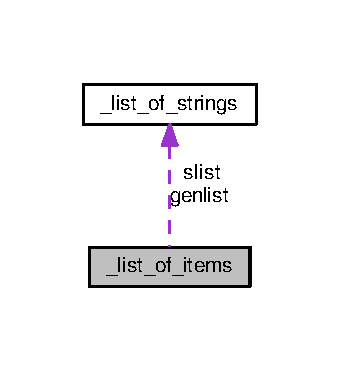
\includegraphics[width=163pt]{struct__list__of__items__coll__graph}
\end{center}
\end{figure}
\subsection*{Public Member Functions}
\begin{DoxyCompactItemize}
\item 
int list\+\_\+getter \hyperlink{struct__list__of__items_a400c71ca049f953c8471b300c64dc1e2}{\+\_\+\+\_\+P} ((struct \hyperlink{struct__list__of__items}{\+\_\+list\+\_\+of\+\_\+items} $\ast$))
\end{DoxyCompactItemize}
\subsection*{Public Attributes}
\begin{DoxyCompactItemize}
\item 
int \hyperlink{struct__list__of__items_a30ef236927b55d94fe6c6fc555c118b4}{flags}
\item 
\hyperlink{externs_8h_a278124bbcc96be39e8b7485a7ddfa038}{S\+T\+R\+I\+N\+G\+L\+I\+ST} $\ast$ \hyperlink{struct__list__of__items_a97a05d10fc76fd2802524c017f6f83b6}{slist}
\item 
\hyperlink{externs_8h_a278124bbcc96be39e8b7485a7ddfa038}{S\+T\+R\+I\+N\+G\+L\+I\+ST} $\ast$ \hyperlink{struct__list__of__items_a8e0d2617812516da3f9dfcc76f5642ea}{genlist}
\item 
int \hyperlink{struct__list__of__items_abb5d60bc72cf10d157f467fa261c61ce}{genindex}
\end{DoxyCompactItemize}


\subsection{Member Function Documentation}
\index{\+\_\+list\+\_\+of\+\_\+items@{\+\_\+list\+\_\+of\+\_\+items}!\+\_\+\+\_\+P@{\+\_\+\+\_\+P}}
\index{\+\_\+\+\_\+P@{\+\_\+\+\_\+P}!\+\_\+list\+\_\+of\+\_\+items@{\+\_\+list\+\_\+of\+\_\+items}}
\subsubsection[{\texorpdfstring{\+\_\+\+\_\+\+P((struct \+\_\+list\+\_\+of\+\_\+items $\ast$))}{__P((struct _list_of_items *))}}]{\setlength{\rightskip}{0pt plus 5cm}int list\+\_\+getter \+\_\+list\+\_\+of\+\_\+items\+::\+\_\+\+\_\+P (
\begin{DoxyParamCaption}
\item[{(struct {\bf \+\_\+list\+\_\+of\+\_\+items} $\ast$)}]{}
\end{DoxyParamCaption}
)}\hypertarget{struct__list__of__items_a400c71ca049f953c8471b300c64dc1e2}{}\label{struct__list__of__items_a400c71ca049f953c8471b300c64dc1e2}


\subsection{Member Data Documentation}
\index{\+\_\+list\+\_\+of\+\_\+items@{\+\_\+list\+\_\+of\+\_\+items}!flags@{flags}}
\index{flags@{flags}!\+\_\+list\+\_\+of\+\_\+items@{\+\_\+list\+\_\+of\+\_\+items}}
\subsubsection[{\texorpdfstring{flags}{flags}}]{\setlength{\rightskip}{0pt plus 5cm}int \+\_\+list\+\_\+of\+\_\+items\+::flags}\hypertarget{struct__list__of__items_a30ef236927b55d94fe6c6fc555c118b4}{}\label{struct__list__of__items_a30ef236927b55d94fe6c6fc555c118b4}
\index{\+\_\+list\+\_\+of\+\_\+items@{\+\_\+list\+\_\+of\+\_\+items}!genindex@{genindex}}
\index{genindex@{genindex}!\+\_\+list\+\_\+of\+\_\+items@{\+\_\+list\+\_\+of\+\_\+items}}
\subsubsection[{\texorpdfstring{genindex}{genindex}}]{\setlength{\rightskip}{0pt plus 5cm}int \+\_\+list\+\_\+of\+\_\+items\+::genindex}\hypertarget{struct__list__of__items_abb5d60bc72cf10d157f467fa261c61ce}{}\label{struct__list__of__items_abb5d60bc72cf10d157f467fa261c61ce}
\index{\+\_\+list\+\_\+of\+\_\+items@{\+\_\+list\+\_\+of\+\_\+items}!genlist@{genlist}}
\index{genlist@{genlist}!\+\_\+list\+\_\+of\+\_\+items@{\+\_\+list\+\_\+of\+\_\+items}}
\subsubsection[{\texorpdfstring{genlist}{genlist}}]{\setlength{\rightskip}{0pt plus 5cm}{\bf S\+T\+R\+I\+N\+G\+L\+I\+ST}$\ast$ \+\_\+list\+\_\+of\+\_\+items\+::genlist}\hypertarget{struct__list__of__items_a8e0d2617812516da3f9dfcc76f5642ea}{}\label{struct__list__of__items_a8e0d2617812516da3f9dfcc76f5642ea}
\index{\+\_\+list\+\_\+of\+\_\+items@{\+\_\+list\+\_\+of\+\_\+items}!slist@{slist}}
\index{slist@{slist}!\+\_\+list\+\_\+of\+\_\+items@{\+\_\+list\+\_\+of\+\_\+items}}
\subsubsection[{\texorpdfstring{slist}{slist}}]{\setlength{\rightskip}{0pt plus 5cm}{\bf S\+T\+R\+I\+N\+G\+L\+I\+ST}$\ast$ \+\_\+list\+\_\+of\+\_\+items\+::slist}\hypertarget{struct__list__of__items_a97a05d10fc76fd2802524c017f6f83b6}{}\label{struct__list__of__items_a97a05d10fc76fd2802524c017f6f83b6}


The documentation for this struct was generated from the following file\+:\begin{DoxyCompactItemize}
\item 
\hyperlink{pcomplete_8h}{pcomplete.\+h}\end{DoxyCompactItemize}

\hypertarget{struct__list__of__strings}{}\section{\+\_\+list\+\_\+of\+\_\+strings Struct Reference}
\label{struct__list__of__strings}\index{\+\_\+list\+\_\+of\+\_\+strings@{\+\_\+list\+\_\+of\+\_\+strings}}


{\ttfamily \#include $<$externs.\+h$>$}

\subsection*{Public Attributes}
\begin{DoxyCompactItemize}
\item 
char $\ast$$\ast$ \hyperlink{struct__list__of__strings_af27314272b184befee95f213b297dc21}{list}
\item 
int \hyperlink{struct__list__of__strings_ad48afe20c96c5b80e7fb6728bb1af3ad}{list\+\_\+size}
\item 
int \hyperlink{struct__list__of__strings_ae3747a3b406d21b7a9fe5ea10531e82a}{list\+\_\+len}
\end{DoxyCompactItemize}


\subsection{Member Data Documentation}
\index{\+\_\+list\+\_\+of\+\_\+strings@{\+\_\+list\+\_\+of\+\_\+strings}!list@{list}}
\index{list@{list}!\+\_\+list\+\_\+of\+\_\+strings@{\+\_\+list\+\_\+of\+\_\+strings}}
\subsubsection[{\texorpdfstring{list}{list}}]{\setlength{\rightskip}{0pt plus 5cm}char$\ast$$\ast$ \+\_\+list\+\_\+of\+\_\+strings\+::list}\hypertarget{struct__list__of__strings_af27314272b184befee95f213b297dc21}{}\label{struct__list__of__strings_af27314272b184befee95f213b297dc21}
\index{\+\_\+list\+\_\+of\+\_\+strings@{\+\_\+list\+\_\+of\+\_\+strings}!list\+\_\+len@{list\+\_\+len}}
\index{list\+\_\+len@{list\+\_\+len}!\+\_\+list\+\_\+of\+\_\+strings@{\+\_\+list\+\_\+of\+\_\+strings}}
\subsubsection[{\texorpdfstring{list\+\_\+len}{list_len}}]{\setlength{\rightskip}{0pt plus 5cm}int \+\_\+list\+\_\+of\+\_\+strings\+::list\+\_\+len}\hypertarget{struct__list__of__strings_ae3747a3b406d21b7a9fe5ea10531e82a}{}\label{struct__list__of__strings_ae3747a3b406d21b7a9fe5ea10531e82a}
\index{\+\_\+list\+\_\+of\+\_\+strings@{\+\_\+list\+\_\+of\+\_\+strings}!list\+\_\+size@{list\+\_\+size}}
\index{list\+\_\+size@{list\+\_\+size}!\+\_\+list\+\_\+of\+\_\+strings@{\+\_\+list\+\_\+of\+\_\+strings}}
\subsubsection[{\texorpdfstring{list\+\_\+size}{list_size}}]{\setlength{\rightskip}{0pt plus 5cm}int \+\_\+list\+\_\+of\+\_\+strings\+::list\+\_\+size}\hypertarget{struct__list__of__strings_ad48afe20c96c5b80e7fb6728bb1af3ad}{}\label{struct__list__of__strings_ad48afe20c96c5b80e7fb6728bb1af3ad}


The documentation for this struct was generated from the following file\+:\begin{DoxyCompactItemize}
\item 
\hyperlink{externs_8h}{externs.\+h}\end{DoxyCompactItemize}

\hypertarget{struct__pathdata}{}\section{\+\_\+pathdata Struct Reference}
\label{struct__pathdata}\index{\+\_\+pathdata@{\+\_\+pathdata}}


{\ttfamily \#include $<$hashcmd.\+h$>$}

\subsection*{Public Attributes}
\begin{DoxyCompactItemize}
\item 
char $\ast$ \hyperlink{struct__pathdata_a986cc5fdc40edc32bcee0da5fa66116e}{path}
\item 
int \hyperlink{struct__pathdata_ab71211e2211c40698401f36c4312e234}{flags}
\end{DoxyCompactItemize}


\subsection{Member Data Documentation}
\index{\+\_\+pathdata@{\+\_\+pathdata}!flags@{flags}}
\index{flags@{flags}!\+\_\+pathdata@{\+\_\+pathdata}}
\subsubsection[{\texorpdfstring{flags}{flags}}]{\setlength{\rightskip}{0pt plus 5cm}int \+\_\+pathdata\+::flags}\hypertarget{struct__pathdata_ab71211e2211c40698401f36c4312e234}{}\label{struct__pathdata_ab71211e2211c40698401f36c4312e234}
\index{\+\_\+pathdata@{\+\_\+pathdata}!path@{path}}
\index{path@{path}!\+\_\+pathdata@{\+\_\+pathdata}}
\subsubsection[{\texorpdfstring{path}{path}}]{\setlength{\rightskip}{0pt plus 5cm}char$\ast$ \+\_\+pathdata\+::path}\hypertarget{struct__pathdata_a986cc5fdc40edc32bcee0da5fa66116e}{}\label{struct__pathdata_a986cc5fdc40edc32bcee0da5fa66116e}


The documentation for this struct was generated from the following file\+:\begin{DoxyCompactItemize}
\item 
\hyperlink{hashcmd_8h}{hashcmd.\+h}\end{DoxyCompactItemize}

\hypertarget{struct__sh__input__line__state__t}{}\section{\+\_\+sh\+\_\+input\+\_\+line\+\_\+state\+\_\+t Struct Reference}
\label{struct__sh__input__line__state__t}\index{\+\_\+sh\+\_\+input\+\_\+line\+\_\+state\+\_\+t@{\+\_\+sh\+\_\+input\+\_\+line\+\_\+state\+\_\+t}}


{\ttfamily \#include $<$shell.\+h$>$}

\subsection*{Public Attributes}
\begin{DoxyCompactItemize}
\item 
char $\ast$ \hyperlink{struct__sh__input__line__state__t_a14ffaf4912c52b6f51062abd212a9dca}{input\+\_\+line}
\item 
size\+\_\+t \hyperlink{struct__sh__input__line__state__t_a626a3b68fc1a7ed86f564ff3163e3fed}{input\+\_\+line\+\_\+index}
\item 
size\+\_\+t \hyperlink{struct__sh__input__line__state__t_adf192ec5f0d04a9b1d49906b03ea6d5c}{input\+\_\+line\+\_\+size}
\item 
size\+\_\+t \hyperlink{struct__sh__input__line__state__t_a6091ac0aaaa9a7866f28b13ec406e6e2}{input\+\_\+line\+\_\+len}
\end{DoxyCompactItemize}


\subsection{Member Data Documentation}
\index{\+\_\+sh\+\_\+input\+\_\+line\+\_\+state\+\_\+t@{\+\_\+sh\+\_\+input\+\_\+line\+\_\+state\+\_\+t}!input\+\_\+line@{input\+\_\+line}}
\index{input\+\_\+line@{input\+\_\+line}!\+\_\+sh\+\_\+input\+\_\+line\+\_\+state\+\_\+t@{\+\_\+sh\+\_\+input\+\_\+line\+\_\+state\+\_\+t}}
\subsubsection[{\texorpdfstring{input\+\_\+line}{input_line}}]{\setlength{\rightskip}{0pt plus 5cm}char$\ast$ \+\_\+sh\+\_\+input\+\_\+line\+\_\+state\+\_\+t\+::input\+\_\+line}\hypertarget{struct__sh__input__line__state__t_a14ffaf4912c52b6f51062abd212a9dca}{}\label{struct__sh__input__line__state__t_a14ffaf4912c52b6f51062abd212a9dca}
\index{\+\_\+sh\+\_\+input\+\_\+line\+\_\+state\+\_\+t@{\+\_\+sh\+\_\+input\+\_\+line\+\_\+state\+\_\+t}!input\+\_\+line\+\_\+index@{input\+\_\+line\+\_\+index}}
\index{input\+\_\+line\+\_\+index@{input\+\_\+line\+\_\+index}!\+\_\+sh\+\_\+input\+\_\+line\+\_\+state\+\_\+t@{\+\_\+sh\+\_\+input\+\_\+line\+\_\+state\+\_\+t}}
\subsubsection[{\texorpdfstring{input\+\_\+line\+\_\+index}{input_line_index}}]{\setlength{\rightskip}{0pt plus 5cm}size\+\_\+t \+\_\+sh\+\_\+input\+\_\+line\+\_\+state\+\_\+t\+::input\+\_\+line\+\_\+index}\hypertarget{struct__sh__input__line__state__t_a626a3b68fc1a7ed86f564ff3163e3fed}{}\label{struct__sh__input__line__state__t_a626a3b68fc1a7ed86f564ff3163e3fed}
\index{\+\_\+sh\+\_\+input\+\_\+line\+\_\+state\+\_\+t@{\+\_\+sh\+\_\+input\+\_\+line\+\_\+state\+\_\+t}!input\+\_\+line\+\_\+len@{input\+\_\+line\+\_\+len}}
\index{input\+\_\+line\+\_\+len@{input\+\_\+line\+\_\+len}!\+\_\+sh\+\_\+input\+\_\+line\+\_\+state\+\_\+t@{\+\_\+sh\+\_\+input\+\_\+line\+\_\+state\+\_\+t}}
\subsubsection[{\texorpdfstring{input\+\_\+line\+\_\+len}{input_line_len}}]{\setlength{\rightskip}{0pt plus 5cm}size\+\_\+t \+\_\+sh\+\_\+input\+\_\+line\+\_\+state\+\_\+t\+::input\+\_\+line\+\_\+len}\hypertarget{struct__sh__input__line__state__t_a6091ac0aaaa9a7866f28b13ec406e6e2}{}\label{struct__sh__input__line__state__t_a6091ac0aaaa9a7866f28b13ec406e6e2}
\index{\+\_\+sh\+\_\+input\+\_\+line\+\_\+state\+\_\+t@{\+\_\+sh\+\_\+input\+\_\+line\+\_\+state\+\_\+t}!input\+\_\+line\+\_\+size@{input\+\_\+line\+\_\+size}}
\index{input\+\_\+line\+\_\+size@{input\+\_\+line\+\_\+size}!\+\_\+sh\+\_\+input\+\_\+line\+\_\+state\+\_\+t@{\+\_\+sh\+\_\+input\+\_\+line\+\_\+state\+\_\+t}}
\subsubsection[{\texorpdfstring{input\+\_\+line\+\_\+size}{input_line_size}}]{\setlength{\rightskip}{0pt plus 5cm}size\+\_\+t \+\_\+sh\+\_\+input\+\_\+line\+\_\+state\+\_\+t\+::input\+\_\+line\+\_\+size}\hypertarget{struct__sh__input__line__state__t_adf192ec5f0d04a9b1d49906b03ea6d5c}{}\label{struct__sh__input__line__state__t_adf192ec5f0d04a9b1d49906b03ea6d5c}


The documentation for this struct was generated from the following file\+:\begin{DoxyCompactItemize}
\item 
\hyperlink{shell_8h}{shell.\+h}\end{DoxyCompactItemize}

\hypertarget{struct__sh__parser__state__t}{}\section{\+\_\+sh\+\_\+parser\+\_\+state\+\_\+t Struct Reference}
\label{struct__sh__parser__state__t}\index{\+\_\+sh\+\_\+parser\+\_\+state\+\_\+t@{\+\_\+sh\+\_\+parser\+\_\+state\+\_\+t}}


{\ttfamily \#include $<$shell.\+h$>$}



Collaboration diagram for \+\_\+sh\+\_\+parser\+\_\+state\+\_\+t\+:
\nopagebreak
\begin{figure}[H]
\begin{center}
\leavevmode
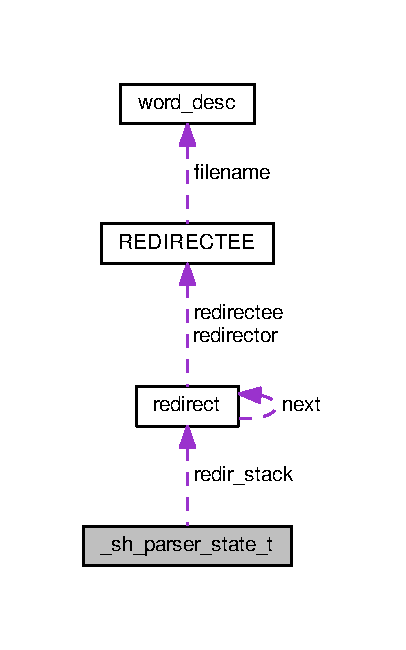
\includegraphics[width=195pt]{struct__sh__parser__state__t__coll__graph}
\end{center}
\end{figure}
\subsection*{Public Attributes}
\begin{DoxyCompactItemize}
\item 
int \hyperlink{struct__sh__parser__state__t_a7b1532dc80c2e47e76927f139141b9f7}{parser\+\_\+state}
\item 
int $\ast$ \hyperlink{struct__sh__parser__state__t_a244829887df0a9f52b2345ca53676bbf}{token\+\_\+state}
\item 
char $\ast$ \hyperlink{struct__sh__parser__state__t_acf66652fab7d2d06b98ba68c55b2e9c6}{token}
\item 
int \hyperlink{struct__sh__parser__state__t_accbc03182193e2ac6620034c01f6558c}{token\+\_\+buffer\+\_\+size}
\item 
int \hyperlink{struct__sh__parser__state__t_a0c76836d520b37268713709048223289}{input\+\_\+line\+\_\+terminator}
\item 
int \hyperlink{struct__sh__parser__state__t_acae44fdc78165351620339ff23ef7250}{eof\+\_\+encountered}
\item 
char $\ast$$\ast$ \hyperlink{struct__sh__parser__state__t_ab1fff8eebe02ce1b436200a0915d7ca1}{prompt\+\_\+string\+\_\+pointer}
\item 
int \hyperlink{struct__sh__parser__state__t_ae2216d09a3cf20acf376c7fa719a92d8}{current\+\_\+command\+\_\+line\+\_\+count}
\item 
int \hyperlink{struct__sh__parser__state__t_a558735699f0b5cc25cef0852e806fc51}{last\+\_\+command\+\_\+exit\+\_\+value}
\item 
sh\+\_\+builtin\+\_\+func\+\_\+t $\ast$ \hyperlink{struct__sh__parser__state__t_a8a85e5f70b6e0dda3f02e4028890988b}{last\+\_\+shell\+\_\+builtin}
\item 
sh\+\_\+builtin\+\_\+func\+\_\+t $\ast$ \hyperlink{struct__sh__parser__state__t_a41bd60fdf09f9d03381abca2a70fcb7f}{this\+\_\+shell\+\_\+builtin}
\item 
int \hyperlink{struct__sh__parser__state__t_a2a78f970e9bd4951b46c7c5608c9df0f}{expand\+\_\+aliases}
\item 
int \hyperlink{struct__sh__parser__state__t_a694b50976966ced6beb057bcff29bb7e}{echo\+\_\+input\+\_\+at\+\_\+read}
\item 
int \hyperlink{struct__sh__parser__state__t_a6836ca188e82d08939fbf24dd4565b1a}{need\+\_\+here\+\_\+doc}
\item 
int \hyperlink{struct__sh__parser__state__t_ae3c18bb0af3a20be094360b307aba4be}{here\+\_\+doc\+\_\+first\+\_\+line}
\item 
\hyperlink{command_8h_adeb9f5d937c92c7923aec48ad5e47d57}{R\+E\+D\+I\+R\+E\+CT} $\ast$ \hyperlink{struct__sh__parser__state__t_ada19fb5dc8d70e07f2c75577e7bf9e9d}{redir\+\_\+stack} \mbox{[}\hyperlink{shell_8h_a8cb36393843e65244395d203958dd6cf}{H\+E\+R\+E\+D\+O\+C\+\_\+\+M\+AX}\mbox{]}
\end{DoxyCompactItemize}


\subsection{Member Data Documentation}
\index{\+\_\+sh\+\_\+parser\+\_\+state\+\_\+t@{\+\_\+sh\+\_\+parser\+\_\+state\+\_\+t}!current\+\_\+command\+\_\+line\+\_\+count@{current\+\_\+command\+\_\+line\+\_\+count}}
\index{current\+\_\+command\+\_\+line\+\_\+count@{current\+\_\+command\+\_\+line\+\_\+count}!\+\_\+sh\+\_\+parser\+\_\+state\+\_\+t@{\+\_\+sh\+\_\+parser\+\_\+state\+\_\+t}}
\subsubsection[{\texorpdfstring{current\+\_\+command\+\_\+line\+\_\+count}{current_command_line_count}}]{\setlength{\rightskip}{0pt plus 5cm}int \+\_\+sh\+\_\+parser\+\_\+state\+\_\+t\+::current\+\_\+command\+\_\+line\+\_\+count}\hypertarget{struct__sh__parser__state__t_ae2216d09a3cf20acf376c7fa719a92d8}{}\label{struct__sh__parser__state__t_ae2216d09a3cf20acf376c7fa719a92d8}
\index{\+\_\+sh\+\_\+parser\+\_\+state\+\_\+t@{\+\_\+sh\+\_\+parser\+\_\+state\+\_\+t}!echo\+\_\+input\+\_\+at\+\_\+read@{echo\+\_\+input\+\_\+at\+\_\+read}}
\index{echo\+\_\+input\+\_\+at\+\_\+read@{echo\+\_\+input\+\_\+at\+\_\+read}!\+\_\+sh\+\_\+parser\+\_\+state\+\_\+t@{\+\_\+sh\+\_\+parser\+\_\+state\+\_\+t}}
\subsubsection[{\texorpdfstring{echo\+\_\+input\+\_\+at\+\_\+read}{echo_input_at_read}}]{\setlength{\rightskip}{0pt plus 5cm}int \+\_\+sh\+\_\+parser\+\_\+state\+\_\+t\+::echo\+\_\+input\+\_\+at\+\_\+read}\hypertarget{struct__sh__parser__state__t_a694b50976966ced6beb057bcff29bb7e}{}\label{struct__sh__parser__state__t_a694b50976966ced6beb057bcff29bb7e}
\index{\+\_\+sh\+\_\+parser\+\_\+state\+\_\+t@{\+\_\+sh\+\_\+parser\+\_\+state\+\_\+t}!eof\+\_\+encountered@{eof\+\_\+encountered}}
\index{eof\+\_\+encountered@{eof\+\_\+encountered}!\+\_\+sh\+\_\+parser\+\_\+state\+\_\+t@{\+\_\+sh\+\_\+parser\+\_\+state\+\_\+t}}
\subsubsection[{\texorpdfstring{eof\+\_\+encountered}{eof_encountered}}]{\setlength{\rightskip}{0pt plus 5cm}int \+\_\+sh\+\_\+parser\+\_\+state\+\_\+t\+::eof\+\_\+encountered}\hypertarget{struct__sh__parser__state__t_acae44fdc78165351620339ff23ef7250}{}\label{struct__sh__parser__state__t_acae44fdc78165351620339ff23ef7250}
\index{\+\_\+sh\+\_\+parser\+\_\+state\+\_\+t@{\+\_\+sh\+\_\+parser\+\_\+state\+\_\+t}!expand\+\_\+aliases@{expand\+\_\+aliases}}
\index{expand\+\_\+aliases@{expand\+\_\+aliases}!\+\_\+sh\+\_\+parser\+\_\+state\+\_\+t@{\+\_\+sh\+\_\+parser\+\_\+state\+\_\+t}}
\subsubsection[{\texorpdfstring{expand\+\_\+aliases}{expand_aliases}}]{\setlength{\rightskip}{0pt plus 5cm}int \+\_\+sh\+\_\+parser\+\_\+state\+\_\+t\+::expand\+\_\+aliases}\hypertarget{struct__sh__parser__state__t_a2a78f970e9bd4951b46c7c5608c9df0f}{}\label{struct__sh__parser__state__t_a2a78f970e9bd4951b46c7c5608c9df0f}
\index{\+\_\+sh\+\_\+parser\+\_\+state\+\_\+t@{\+\_\+sh\+\_\+parser\+\_\+state\+\_\+t}!here\+\_\+doc\+\_\+first\+\_\+line@{here\+\_\+doc\+\_\+first\+\_\+line}}
\index{here\+\_\+doc\+\_\+first\+\_\+line@{here\+\_\+doc\+\_\+first\+\_\+line}!\+\_\+sh\+\_\+parser\+\_\+state\+\_\+t@{\+\_\+sh\+\_\+parser\+\_\+state\+\_\+t}}
\subsubsection[{\texorpdfstring{here\+\_\+doc\+\_\+first\+\_\+line}{here_doc_first_line}}]{\setlength{\rightskip}{0pt plus 5cm}int \+\_\+sh\+\_\+parser\+\_\+state\+\_\+t\+::here\+\_\+doc\+\_\+first\+\_\+line}\hypertarget{struct__sh__parser__state__t_ae3c18bb0af3a20be094360b307aba4be}{}\label{struct__sh__parser__state__t_ae3c18bb0af3a20be094360b307aba4be}
\index{\+\_\+sh\+\_\+parser\+\_\+state\+\_\+t@{\+\_\+sh\+\_\+parser\+\_\+state\+\_\+t}!input\+\_\+line\+\_\+terminator@{input\+\_\+line\+\_\+terminator}}
\index{input\+\_\+line\+\_\+terminator@{input\+\_\+line\+\_\+terminator}!\+\_\+sh\+\_\+parser\+\_\+state\+\_\+t@{\+\_\+sh\+\_\+parser\+\_\+state\+\_\+t}}
\subsubsection[{\texorpdfstring{input\+\_\+line\+\_\+terminator}{input_line_terminator}}]{\setlength{\rightskip}{0pt plus 5cm}int \+\_\+sh\+\_\+parser\+\_\+state\+\_\+t\+::input\+\_\+line\+\_\+terminator}\hypertarget{struct__sh__parser__state__t_a0c76836d520b37268713709048223289}{}\label{struct__sh__parser__state__t_a0c76836d520b37268713709048223289}
\index{\+\_\+sh\+\_\+parser\+\_\+state\+\_\+t@{\+\_\+sh\+\_\+parser\+\_\+state\+\_\+t}!last\+\_\+command\+\_\+exit\+\_\+value@{last\+\_\+command\+\_\+exit\+\_\+value}}
\index{last\+\_\+command\+\_\+exit\+\_\+value@{last\+\_\+command\+\_\+exit\+\_\+value}!\+\_\+sh\+\_\+parser\+\_\+state\+\_\+t@{\+\_\+sh\+\_\+parser\+\_\+state\+\_\+t}}
\subsubsection[{\texorpdfstring{last\+\_\+command\+\_\+exit\+\_\+value}{last_command_exit_value}}]{\setlength{\rightskip}{0pt plus 5cm}int \+\_\+sh\+\_\+parser\+\_\+state\+\_\+t\+::last\+\_\+command\+\_\+exit\+\_\+value}\hypertarget{struct__sh__parser__state__t_a558735699f0b5cc25cef0852e806fc51}{}\label{struct__sh__parser__state__t_a558735699f0b5cc25cef0852e806fc51}
\index{\+\_\+sh\+\_\+parser\+\_\+state\+\_\+t@{\+\_\+sh\+\_\+parser\+\_\+state\+\_\+t}!last\+\_\+shell\+\_\+builtin@{last\+\_\+shell\+\_\+builtin}}
\index{last\+\_\+shell\+\_\+builtin@{last\+\_\+shell\+\_\+builtin}!\+\_\+sh\+\_\+parser\+\_\+state\+\_\+t@{\+\_\+sh\+\_\+parser\+\_\+state\+\_\+t}}
\subsubsection[{\texorpdfstring{last\+\_\+shell\+\_\+builtin}{last_shell_builtin}}]{\setlength{\rightskip}{0pt plus 5cm}sh\+\_\+builtin\+\_\+func\+\_\+t$\ast$ \+\_\+sh\+\_\+parser\+\_\+state\+\_\+t\+::last\+\_\+shell\+\_\+builtin}\hypertarget{struct__sh__parser__state__t_a8a85e5f70b6e0dda3f02e4028890988b}{}\label{struct__sh__parser__state__t_a8a85e5f70b6e0dda3f02e4028890988b}
\index{\+\_\+sh\+\_\+parser\+\_\+state\+\_\+t@{\+\_\+sh\+\_\+parser\+\_\+state\+\_\+t}!need\+\_\+here\+\_\+doc@{need\+\_\+here\+\_\+doc}}
\index{need\+\_\+here\+\_\+doc@{need\+\_\+here\+\_\+doc}!\+\_\+sh\+\_\+parser\+\_\+state\+\_\+t@{\+\_\+sh\+\_\+parser\+\_\+state\+\_\+t}}
\subsubsection[{\texorpdfstring{need\+\_\+here\+\_\+doc}{need_here_doc}}]{\setlength{\rightskip}{0pt plus 5cm}int \+\_\+sh\+\_\+parser\+\_\+state\+\_\+t\+::need\+\_\+here\+\_\+doc}\hypertarget{struct__sh__parser__state__t_a6836ca188e82d08939fbf24dd4565b1a}{}\label{struct__sh__parser__state__t_a6836ca188e82d08939fbf24dd4565b1a}
\index{\+\_\+sh\+\_\+parser\+\_\+state\+\_\+t@{\+\_\+sh\+\_\+parser\+\_\+state\+\_\+t}!parser\+\_\+state@{parser\+\_\+state}}
\index{parser\+\_\+state@{parser\+\_\+state}!\+\_\+sh\+\_\+parser\+\_\+state\+\_\+t@{\+\_\+sh\+\_\+parser\+\_\+state\+\_\+t}}
\subsubsection[{\texorpdfstring{parser\+\_\+state}{parser_state}}]{\setlength{\rightskip}{0pt plus 5cm}int \+\_\+sh\+\_\+parser\+\_\+state\+\_\+t\+::parser\+\_\+state}\hypertarget{struct__sh__parser__state__t_a7b1532dc80c2e47e76927f139141b9f7}{}\label{struct__sh__parser__state__t_a7b1532dc80c2e47e76927f139141b9f7}
\index{\+\_\+sh\+\_\+parser\+\_\+state\+\_\+t@{\+\_\+sh\+\_\+parser\+\_\+state\+\_\+t}!prompt\+\_\+string\+\_\+pointer@{prompt\+\_\+string\+\_\+pointer}}
\index{prompt\+\_\+string\+\_\+pointer@{prompt\+\_\+string\+\_\+pointer}!\+\_\+sh\+\_\+parser\+\_\+state\+\_\+t@{\+\_\+sh\+\_\+parser\+\_\+state\+\_\+t}}
\subsubsection[{\texorpdfstring{prompt\+\_\+string\+\_\+pointer}{prompt_string_pointer}}]{\setlength{\rightskip}{0pt plus 5cm}char$\ast$$\ast$ \+\_\+sh\+\_\+parser\+\_\+state\+\_\+t\+::prompt\+\_\+string\+\_\+pointer}\hypertarget{struct__sh__parser__state__t_ab1fff8eebe02ce1b436200a0915d7ca1}{}\label{struct__sh__parser__state__t_ab1fff8eebe02ce1b436200a0915d7ca1}
\index{\+\_\+sh\+\_\+parser\+\_\+state\+\_\+t@{\+\_\+sh\+\_\+parser\+\_\+state\+\_\+t}!redir\+\_\+stack@{redir\+\_\+stack}}
\index{redir\+\_\+stack@{redir\+\_\+stack}!\+\_\+sh\+\_\+parser\+\_\+state\+\_\+t@{\+\_\+sh\+\_\+parser\+\_\+state\+\_\+t}}
\subsubsection[{\texorpdfstring{redir\+\_\+stack}{redir_stack}}]{\setlength{\rightskip}{0pt plus 5cm}{\bf R\+E\+D\+I\+R\+E\+CT}$\ast$ \+\_\+sh\+\_\+parser\+\_\+state\+\_\+t\+::redir\+\_\+stack\mbox{[}{\bf H\+E\+R\+E\+D\+O\+C\+\_\+\+M\+AX}\mbox{]}}\hypertarget{struct__sh__parser__state__t_ada19fb5dc8d70e07f2c75577e7bf9e9d}{}\label{struct__sh__parser__state__t_ada19fb5dc8d70e07f2c75577e7bf9e9d}
\index{\+\_\+sh\+\_\+parser\+\_\+state\+\_\+t@{\+\_\+sh\+\_\+parser\+\_\+state\+\_\+t}!this\+\_\+shell\+\_\+builtin@{this\+\_\+shell\+\_\+builtin}}
\index{this\+\_\+shell\+\_\+builtin@{this\+\_\+shell\+\_\+builtin}!\+\_\+sh\+\_\+parser\+\_\+state\+\_\+t@{\+\_\+sh\+\_\+parser\+\_\+state\+\_\+t}}
\subsubsection[{\texorpdfstring{this\+\_\+shell\+\_\+builtin}{this_shell_builtin}}]{\setlength{\rightskip}{0pt plus 5cm}sh\+\_\+builtin\+\_\+func\+\_\+t $\ast$ \+\_\+sh\+\_\+parser\+\_\+state\+\_\+t\+::this\+\_\+shell\+\_\+builtin}\hypertarget{struct__sh__parser__state__t_a41bd60fdf09f9d03381abca2a70fcb7f}{}\label{struct__sh__parser__state__t_a41bd60fdf09f9d03381abca2a70fcb7f}
\index{\+\_\+sh\+\_\+parser\+\_\+state\+\_\+t@{\+\_\+sh\+\_\+parser\+\_\+state\+\_\+t}!token@{token}}
\index{token@{token}!\+\_\+sh\+\_\+parser\+\_\+state\+\_\+t@{\+\_\+sh\+\_\+parser\+\_\+state\+\_\+t}}
\subsubsection[{\texorpdfstring{token}{token}}]{\setlength{\rightskip}{0pt plus 5cm}char$\ast$ \+\_\+sh\+\_\+parser\+\_\+state\+\_\+t\+::token}\hypertarget{struct__sh__parser__state__t_acf66652fab7d2d06b98ba68c55b2e9c6}{}\label{struct__sh__parser__state__t_acf66652fab7d2d06b98ba68c55b2e9c6}
\index{\+\_\+sh\+\_\+parser\+\_\+state\+\_\+t@{\+\_\+sh\+\_\+parser\+\_\+state\+\_\+t}!token\+\_\+buffer\+\_\+size@{token\+\_\+buffer\+\_\+size}}
\index{token\+\_\+buffer\+\_\+size@{token\+\_\+buffer\+\_\+size}!\+\_\+sh\+\_\+parser\+\_\+state\+\_\+t@{\+\_\+sh\+\_\+parser\+\_\+state\+\_\+t}}
\subsubsection[{\texorpdfstring{token\+\_\+buffer\+\_\+size}{token_buffer_size}}]{\setlength{\rightskip}{0pt plus 5cm}int \+\_\+sh\+\_\+parser\+\_\+state\+\_\+t\+::token\+\_\+buffer\+\_\+size}\hypertarget{struct__sh__parser__state__t_accbc03182193e2ac6620034c01f6558c}{}\label{struct__sh__parser__state__t_accbc03182193e2ac6620034c01f6558c}
\index{\+\_\+sh\+\_\+parser\+\_\+state\+\_\+t@{\+\_\+sh\+\_\+parser\+\_\+state\+\_\+t}!token\+\_\+state@{token\+\_\+state}}
\index{token\+\_\+state@{token\+\_\+state}!\+\_\+sh\+\_\+parser\+\_\+state\+\_\+t@{\+\_\+sh\+\_\+parser\+\_\+state\+\_\+t}}
\subsubsection[{\texorpdfstring{token\+\_\+state}{token_state}}]{\setlength{\rightskip}{0pt plus 5cm}int$\ast$ \+\_\+sh\+\_\+parser\+\_\+state\+\_\+t\+::token\+\_\+state}\hypertarget{struct__sh__parser__state__t_a244829887df0a9f52b2345ca53676bbf}{}\label{struct__sh__parser__state__t_a244829887df0a9f52b2345ca53676bbf}


The documentation for this struct was generated from the following file\+:\begin{DoxyCompactItemize}
\item 
\hyperlink{shell_8h}{shell.\+h}\end{DoxyCompactItemize}

\hypertarget{union__value}{}\section{\+\_\+value Union Reference}
\label{union__value}\index{\+\_\+value@{\+\_\+value}}


{\ttfamily \#include $<$variables.\+h$>$}



Collaboration diagram for \+\_\+value\+:
\nopagebreak
\begin{figure}[H]
\begin{center}
\leavevmode
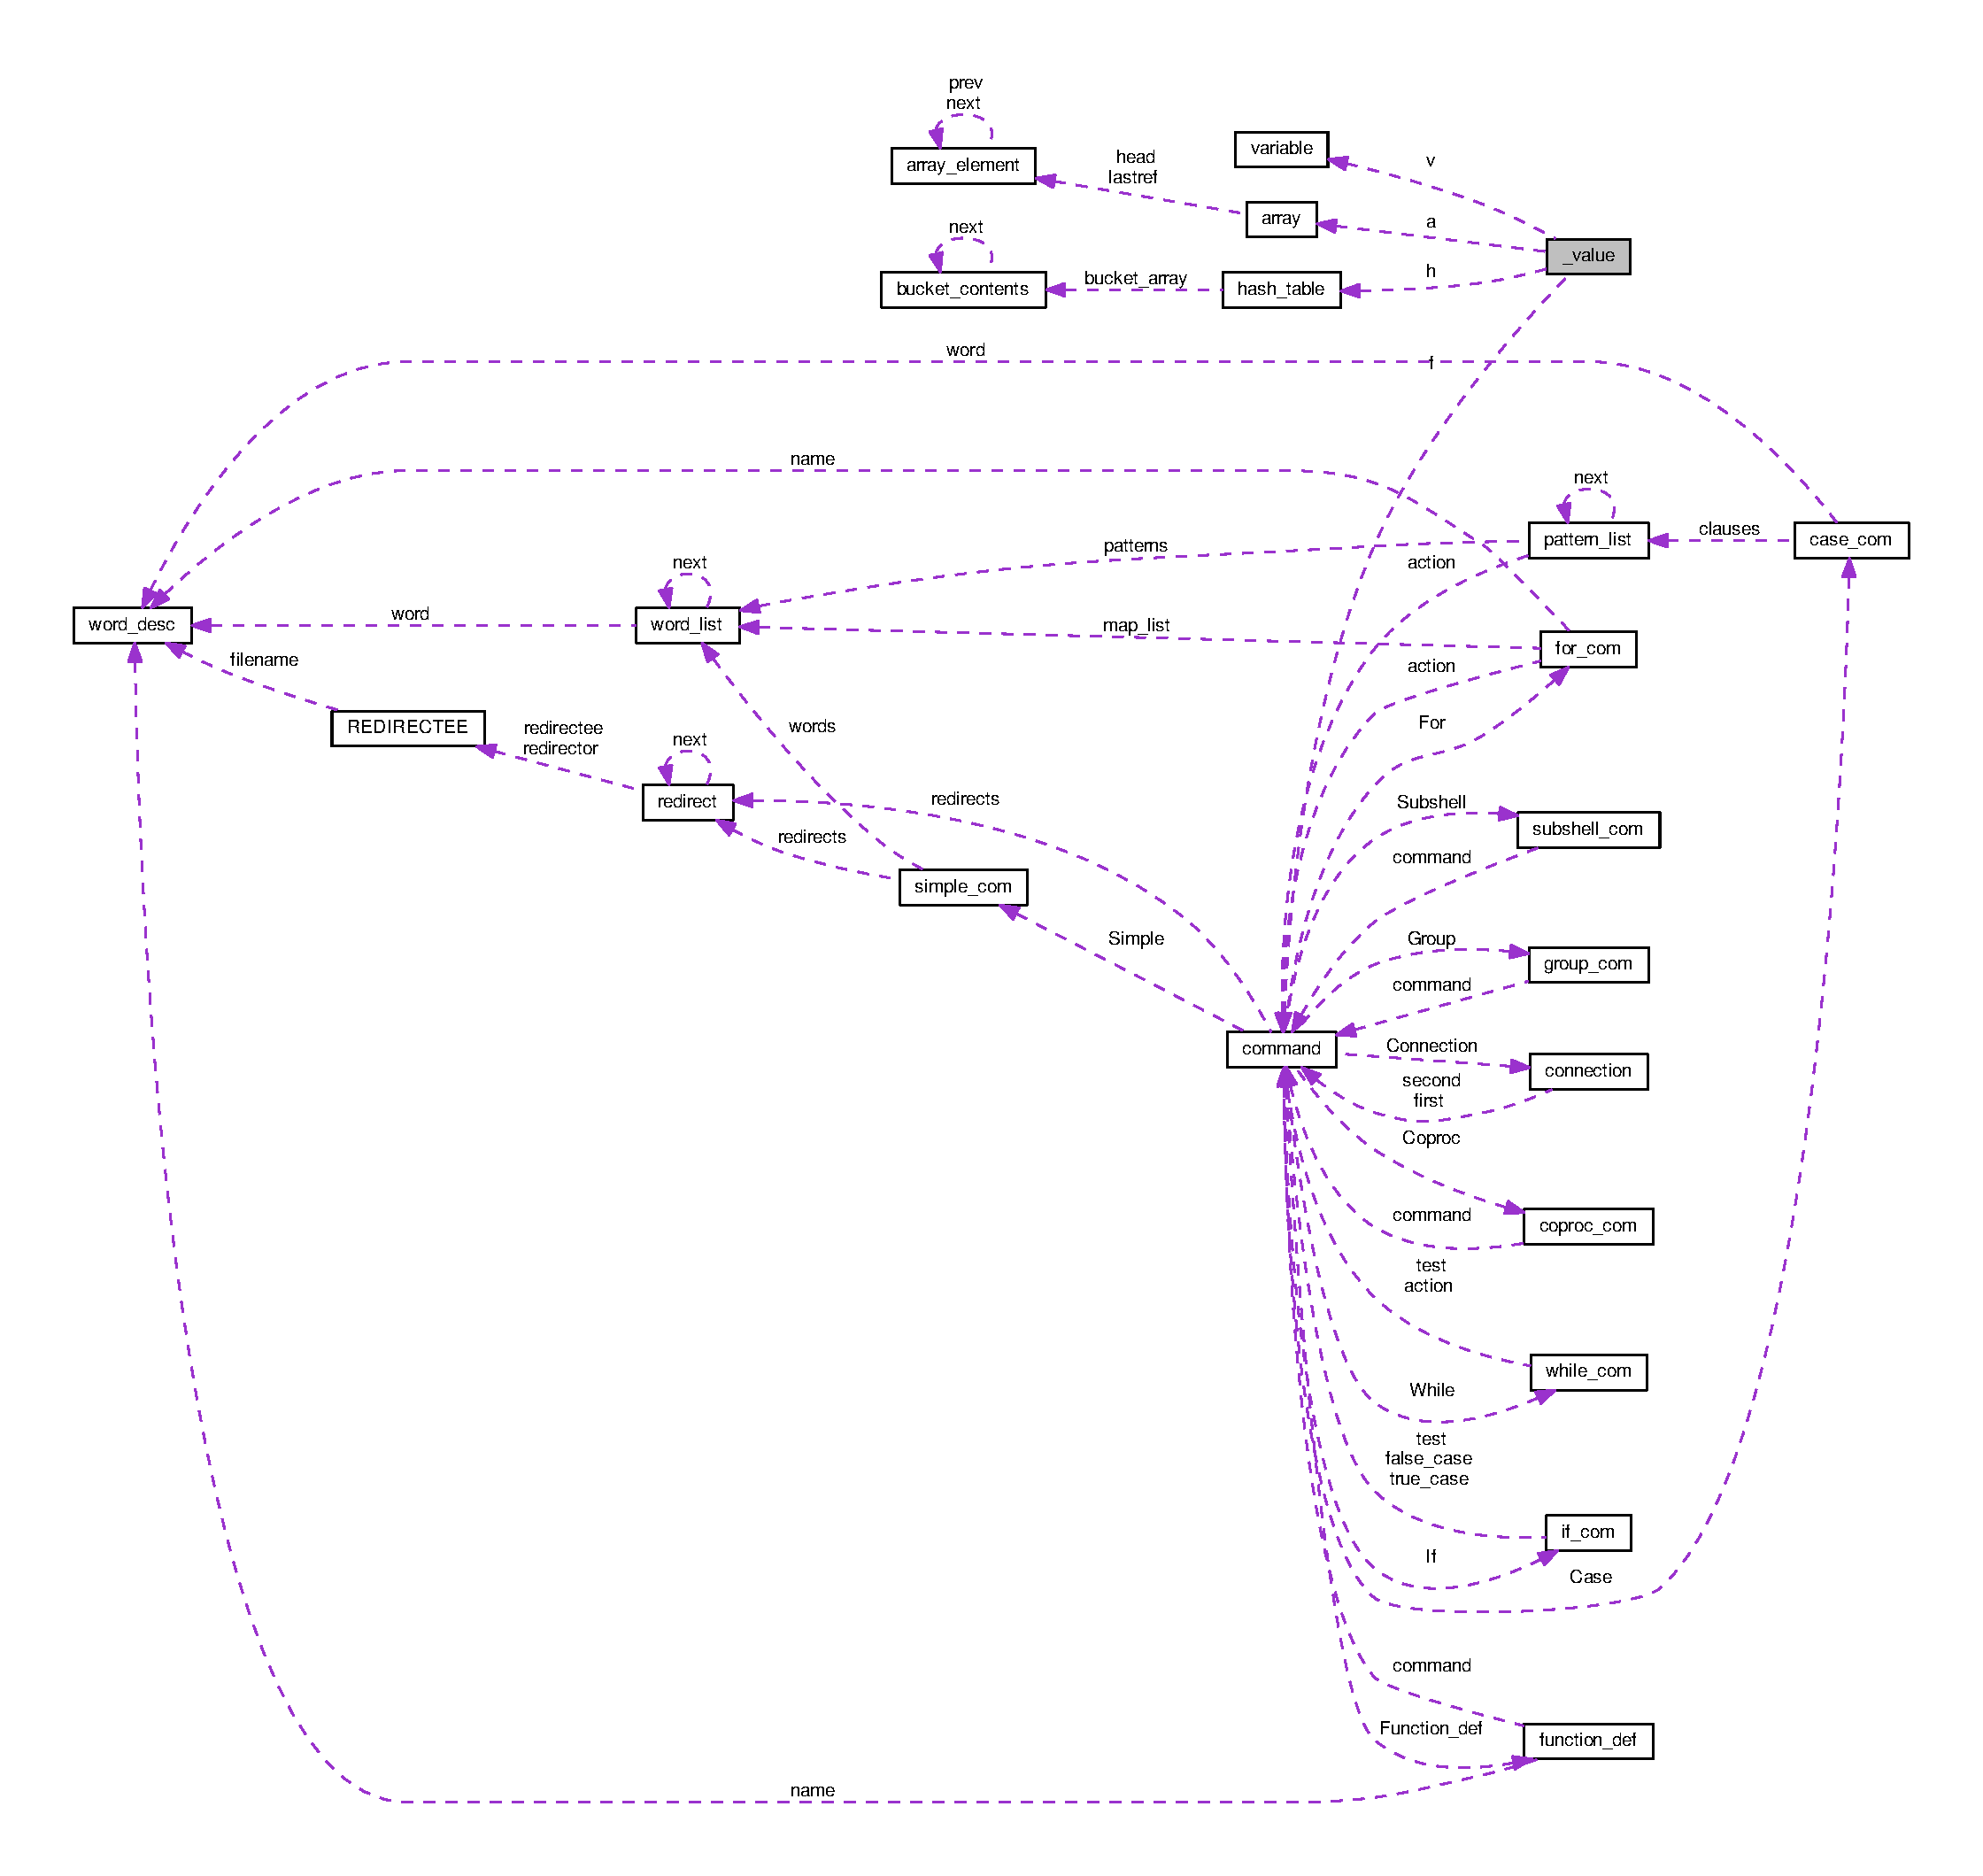
\includegraphics[width=350pt]{union__value__coll__graph}
\end{center}
\end{figure}
\subsection*{Public Attributes}
\begin{DoxyCompactItemize}
\item 
char $\ast$ \hyperlink{union__value_addb4ab2ffbf877c71d8a8c7cb52e6dd4}{s}
\item 
intmax\+\_\+t \hyperlink{union__value_a6263602a37e5879385c667354e1d5820}{i}
\item 
\hyperlink{command_8h_a8c41dec142c299806885773c902c0d87}{C\+O\+M\+M\+A\+ND} $\ast$ \hyperlink{union__value_a032a9c4929695b8c71b036fa9bdc75d2}{f}
\item 
\hyperlink{array_8h_a9c07c3330f66f4018e49ee90e58f0f39}{A\+R\+R\+AY} $\ast$ \hyperlink{union__value_ae67cd4568713fde20e66f04a9eccbe19}{a}
\item 
\hyperlink{hashlib_8h_a8284f9978df160609365484b829527e6}{H\+A\+S\+H\+\_\+\+T\+A\+B\+LE} $\ast$ \hyperlink{union__value_a0ea42897a8199c364092a3d9d72e6252}{h}
\item 
double \hyperlink{union__value_a44934e9648136b3cdc30d12b8b375810}{d}
\item 
struct \hyperlink{structvariable}{variable} $\ast$ \hyperlink{union__value_a81f5f742f41805c8591187b5b0acc0f2}{v}
\item 
void $\ast$ \hyperlink{union__value_a2344cac871c8663a6717092bff1d5950}{opaque}
\end{DoxyCompactItemize}


\subsection{Member Data Documentation}
\index{\+\_\+value@{\+\_\+value}!a@{a}}
\index{a@{a}!\+\_\+value@{\+\_\+value}}
\subsubsection[{\texorpdfstring{a}{a}}]{\setlength{\rightskip}{0pt plus 5cm}{\bf A\+R\+R\+AY}$\ast$ \+\_\+value\+::a}\hypertarget{union__value_ae67cd4568713fde20e66f04a9eccbe19}{}\label{union__value_ae67cd4568713fde20e66f04a9eccbe19}
\index{\+\_\+value@{\+\_\+value}!d@{d}}
\index{d@{d}!\+\_\+value@{\+\_\+value}}
\subsubsection[{\texorpdfstring{d}{d}}]{\setlength{\rightskip}{0pt plus 5cm}double \+\_\+value\+::d}\hypertarget{union__value_a44934e9648136b3cdc30d12b8b375810}{}\label{union__value_a44934e9648136b3cdc30d12b8b375810}
\index{\+\_\+value@{\+\_\+value}!f@{f}}
\index{f@{f}!\+\_\+value@{\+\_\+value}}
\subsubsection[{\texorpdfstring{f}{f}}]{\setlength{\rightskip}{0pt plus 5cm}{\bf C\+O\+M\+M\+A\+ND}$\ast$ \+\_\+value\+::f}\hypertarget{union__value_a032a9c4929695b8c71b036fa9bdc75d2}{}\label{union__value_a032a9c4929695b8c71b036fa9bdc75d2}
\index{\+\_\+value@{\+\_\+value}!h@{h}}
\index{h@{h}!\+\_\+value@{\+\_\+value}}
\subsubsection[{\texorpdfstring{h}{h}}]{\setlength{\rightskip}{0pt plus 5cm}{\bf H\+A\+S\+H\+\_\+\+T\+A\+B\+LE}$\ast$ \+\_\+value\+::h}\hypertarget{union__value_a0ea42897a8199c364092a3d9d72e6252}{}\label{union__value_a0ea42897a8199c364092a3d9d72e6252}
\index{\+\_\+value@{\+\_\+value}!i@{i}}
\index{i@{i}!\+\_\+value@{\+\_\+value}}
\subsubsection[{\texorpdfstring{i}{i}}]{\setlength{\rightskip}{0pt plus 5cm}intmax\+\_\+t \+\_\+value\+::i}\hypertarget{union__value_a6263602a37e5879385c667354e1d5820}{}\label{union__value_a6263602a37e5879385c667354e1d5820}
\index{\+\_\+value@{\+\_\+value}!opaque@{opaque}}
\index{opaque@{opaque}!\+\_\+value@{\+\_\+value}}
\subsubsection[{\texorpdfstring{opaque}{opaque}}]{\setlength{\rightskip}{0pt plus 5cm}void$\ast$ \+\_\+value\+::opaque}\hypertarget{union__value_a2344cac871c8663a6717092bff1d5950}{}\label{union__value_a2344cac871c8663a6717092bff1d5950}
\index{\+\_\+value@{\+\_\+value}!s@{s}}
\index{s@{s}!\+\_\+value@{\+\_\+value}}
\subsubsection[{\texorpdfstring{s}{s}}]{\setlength{\rightskip}{0pt plus 5cm}char$\ast$ \+\_\+value\+::s}\hypertarget{union__value_addb4ab2ffbf877c71d8a8c7cb52e6dd4}{}\label{union__value_addb4ab2ffbf877c71d8a8c7cb52e6dd4}
\index{\+\_\+value@{\+\_\+value}!v@{v}}
\index{v@{v}!\+\_\+value@{\+\_\+value}}
\subsubsection[{\texorpdfstring{v}{v}}]{\setlength{\rightskip}{0pt plus 5cm}struct {\bf variable}$\ast$ \+\_\+value\+::v}\hypertarget{union__value_a81f5f742f41805c8591187b5b0acc0f2}{}\label{union__value_a81f5f742f41805c8591187b5b0acc0f2}


The documentation for this union was generated from the following file\+:\begin{DoxyCompactItemize}
\item 
\hyperlink{variables_8h}{variables.\+h}\end{DoxyCompactItemize}

\hypertarget{struct__vlist}{}\section{\+\_\+vlist Struct Reference}
\label{struct__vlist}\index{\+\_\+vlist@{\+\_\+vlist}}


{\ttfamily \#include $<$variables.\+h$>$}



Collaboration diagram for \+\_\+vlist\+:
\nopagebreak
\begin{figure}[H]
\begin{center}
\leavevmode
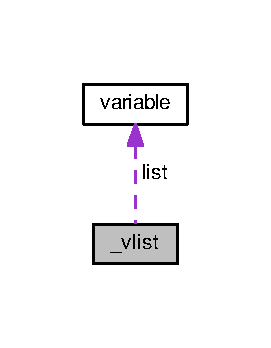
\includegraphics[width=130pt]{struct__vlist__coll__graph}
\end{center}
\end{figure}
\subsection*{Public Attributes}
\begin{DoxyCompactItemize}
\item 
\hyperlink{variables_8h_aba7363ba59b9546110e58106ad60cb50}{S\+H\+E\+L\+L\+\_\+\+V\+AR} $\ast$$\ast$ \hyperlink{struct__vlist_a799b25ce65fe2f50ea530e137b66a433}{list}
\item 
int \hyperlink{struct__vlist_ac99f755431acd1c5d178f3220ac41524}{list\+\_\+size}
\item 
int \hyperlink{struct__vlist_a2e7e3bd943f8651f699c1d724efcb3db}{list\+\_\+len}
\end{DoxyCompactItemize}


\subsection{Member Data Documentation}
\index{\+\_\+vlist@{\+\_\+vlist}!list@{list}}
\index{list@{list}!\+\_\+vlist@{\+\_\+vlist}}
\subsubsection[{\texorpdfstring{list}{list}}]{\setlength{\rightskip}{0pt plus 5cm}{\bf S\+H\+E\+L\+L\+\_\+\+V\+AR}$\ast$$\ast$ \+\_\+vlist\+::list}\hypertarget{struct__vlist_a799b25ce65fe2f50ea530e137b66a433}{}\label{struct__vlist_a799b25ce65fe2f50ea530e137b66a433}
\index{\+\_\+vlist@{\+\_\+vlist}!list\+\_\+len@{list\+\_\+len}}
\index{list\+\_\+len@{list\+\_\+len}!\+\_\+vlist@{\+\_\+vlist}}
\subsubsection[{\texorpdfstring{list\+\_\+len}{list_len}}]{\setlength{\rightskip}{0pt plus 5cm}int \+\_\+vlist\+::list\+\_\+len}\hypertarget{struct__vlist_a2e7e3bd943f8651f699c1d724efcb3db}{}\label{struct__vlist_a2e7e3bd943f8651f699c1d724efcb3db}
\index{\+\_\+vlist@{\+\_\+vlist}!list\+\_\+size@{list\+\_\+size}}
\index{list\+\_\+size@{list\+\_\+size}!\+\_\+vlist@{\+\_\+vlist}}
\subsubsection[{\texorpdfstring{list\+\_\+size}{list_size}}]{\setlength{\rightskip}{0pt plus 5cm}int \+\_\+vlist\+::list\+\_\+size}\hypertarget{struct__vlist_ac99f755431acd1c5d178f3220ac41524}{}\label{struct__vlist_ac99f755431acd1c5d178f3220ac41524}


The documentation for this struct was generated from the following file\+:\begin{DoxyCompactItemize}
\item 
\hyperlink{variables_8h}{variables.\+h}\end{DoxyCompactItemize}

\hypertarget{structalias}{}\section{alias Struct Reference}
\label{structalias}\index{alias@{alias}}


{\ttfamily \#include $<$alias.\+h$>$}

\subsection*{Public Attributes}
\begin{DoxyCompactItemize}
\item 
char $\ast$ \hyperlink{structalias_ad60ea68bfe90ae7f819a50dcf9efb6ef}{name}
\item 
char $\ast$ \hyperlink{structalias_a42c385d758503058c7680ffc8f348823}{value}
\item 
char \hyperlink{structalias_aa08ab0a17e8fb98fe9862e752f37fdf9}{flags}
\end{DoxyCompactItemize}


\subsection{Member Data Documentation}
\index{alias@{alias}!flags@{flags}}
\index{flags@{flags}!alias@{alias}}
\subsubsection[{\texorpdfstring{flags}{flags}}]{\setlength{\rightskip}{0pt plus 5cm}char alias\+::flags}\hypertarget{structalias_aa08ab0a17e8fb98fe9862e752f37fdf9}{}\label{structalias_aa08ab0a17e8fb98fe9862e752f37fdf9}
\index{alias@{alias}!name@{name}}
\index{name@{name}!alias@{alias}}
\subsubsection[{\texorpdfstring{name}{name}}]{\setlength{\rightskip}{0pt plus 5cm}char$\ast$ alias\+::name}\hypertarget{structalias_ad60ea68bfe90ae7f819a50dcf9efb6ef}{}\label{structalias_ad60ea68bfe90ae7f819a50dcf9efb6ef}
\index{alias@{alias}!value@{value}}
\index{value@{value}!alias@{alias}}
\subsubsection[{\texorpdfstring{value}{value}}]{\setlength{\rightskip}{0pt plus 5cm}char$\ast$ alias\+::value}\hypertarget{structalias_a42c385d758503058c7680ffc8f348823}{}\label{structalias_a42c385d758503058c7680ffc8f348823}


The documentation for this struct was generated from the following file\+:\begin{DoxyCompactItemize}
\item 
\hyperlink{alias_8h}{alias.\+h}\end{DoxyCompactItemize}

\hypertarget{structarray}{}\section{array Struct Reference}
\label{structarray}\index{array@{array}}


{\ttfamily \#include $<$array.\+h$>$}



Collaboration diagram for array\+:
\nopagebreak
\begin{figure}[H]
\begin{center}
\leavevmode
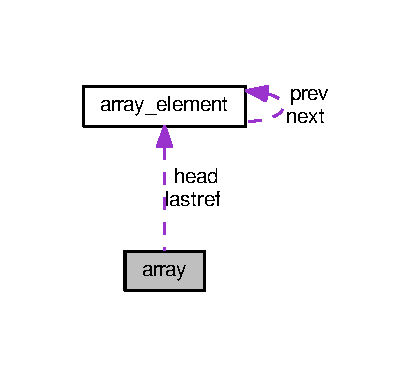
\includegraphics[width=198pt]{structarray__coll__graph}
\end{center}
\end{figure}
\subsection*{Public Attributes}
\begin{DoxyCompactItemize}
\item 
enum \hyperlink{array_8h_abdcaecc1476c2ef209cae471c64c6666}{atype} \hyperlink{structarray_a0af29fc53de2cf89bf3945427930dc0f}{type}
\item 
\hyperlink{array_8h_a3672e3c5b95dde98c9ed75ac7c1e6d60}{arrayind\+\_\+t} \hyperlink{structarray_a943ecba4fe38c813000d0887e7859418}{max\+\_\+index}
\item 
int \hyperlink{structarray_a229c94ec6c46937062a5fd69e488042d}{num\+\_\+elements}
\item 
struct \hyperlink{structarray__element}{array\+\_\+element} $\ast$ \hyperlink{structarray_a1dce002b80f5a241fd5e5efd9ad82494}{lastref}
\item 
struct \hyperlink{structarray__element}{array\+\_\+element} $\ast$ \hyperlink{structarray_ac9efd0fe7a5541bd146bd5481dd851cc}{head}
\end{DoxyCompactItemize}


\subsection{Member Data Documentation}
\index{array@{array}!head@{head}}
\index{head@{head}!array@{array}}
\subsubsection[{\texorpdfstring{head}{head}}]{\setlength{\rightskip}{0pt plus 5cm}struct {\bf array\+\_\+element}$\ast$ array\+::head}\hypertarget{structarray_ac9efd0fe7a5541bd146bd5481dd851cc}{}\label{structarray_ac9efd0fe7a5541bd146bd5481dd851cc}
\index{array@{array}!lastref@{lastref}}
\index{lastref@{lastref}!array@{array}}
\subsubsection[{\texorpdfstring{lastref}{lastref}}]{\setlength{\rightskip}{0pt plus 5cm}struct {\bf array\+\_\+element}$\ast$ array\+::lastref}\hypertarget{structarray_a1dce002b80f5a241fd5e5efd9ad82494}{}\label{structarray_a1dce002b80f5a241fd5e5efd9ad82494}
\index{array@{array}!max\+\_\+index@{max\+\_\+index}}
\index{max\+\_\+index@{max\+\_\+index}!array@{array}}
\subsubsection[{\texorpdfstring{max\+\_\+index}{max_index}}]{\setlength{\rightskip}{0pt plus 5cm}{\bf arrayind\+\_\+t} array\+::max\+\_\+index}\hypertarget{structarray_a943ecba4fe38c813000d0887e7859418}{}\label{structarray_a943ecba4fe38c813000d0887e7859418}
\index{array@{array}!num\+\_\+elements@{num\+\_\+elements}}
\index{num\+\_\+elements@{num\+\_\+elements}!array@{array}}
\subsubsection[{\texorpdfstring{num\+\_\+elements}{num_elements}}]{\setlength{\rightskip}{0pt plus 5cm}int array\+::num\+\_\+elements}\hypertarget{structarray_a229c94ec6c46937062a5fd69e488042d}{}\label{structarray_a229c94ec6c46937062a5fd69e488042d}
\index{array@{array}!type@{type}}
\index{type@{type}!array@{array}}
\subsubsection[{\texorpdfstring{type}{type}}]{\setlength{\rightskip}{0pt plus 5cm}enum {\bf atype} array\+::type}\hypertarget{structarray_a0af29fc53de2cf89bf3945427930dc0f}{}\label{structarray_a0af29fc53de2cf89bf3945427930dc0f}


The documentation for this struct was generated from the following file\+:\begin{DoxyCompactItemize}
\item 
\hyperlink{array_8h}{array.\+h}\end{DoxyCompactItemize}

\hypertarget{structarray__element}{}\section{array\+\_\+element Struct Reference}
\label{structarray__element}\index{array\+\_\+element@{array\+\_\+element}}


{\ttfamily \#include $<$array.\+h$>$}



Collaboration diagram for array\+\_\+element\+:
\nopagebreak
\begin{figure}[H]
\begin{center}
\leavevmode
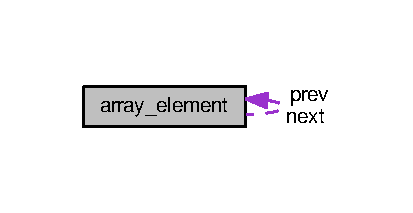
\includegraphics[width=198pt]{structarray__element__coll__graph}
\end{center}
\end{figure}
\subsection*{Public Attributes}
\begin{DoxyCompactItemize}
\item 
\hyperlink{array_8h_a3672e3c5b95dde98c9ed75ac7c1e6d60}{arrayind\+\_\+t} \hyperlink{structarray__element_a5b124be3fa60c35575c578eff8110a2d}{ind}
\item 
char $\ast$ \hyperlink{structarray__element_aa4bea33277d92a610382ad78a1ca765d}{value}
\item 
struct \hyperlink{structarray__element}{array\+\_\+element} $\ast$ \hyperlink{structarray__element_a4da2f65f567163c403ec1bbe61860c0f}{next}
\item 
struct \hyperlink{structarray__element}{array\+\_\+element} $\ast$ \hyperlink{structarray__element_a065d6ae08152f864cf45e662e1a7ffec}{prev}
\end{DoxyCompactItemize}


\subsection{Member Data Documentation}
\index{array\+\_\+element@{array\+\_\+element}!ind@{ind}}
\index{ind@{ind}!array\+\_\+element@{array\+\_\+element}}
\subsubsection[{\texorpdfstring{ind}{ind}}]{\setlength{\rightskip}{0pt plus 5cm}{\bf arrayind\+\_\+t} array\+\_\+element\+::ind}\hypertarget{structarray__element_a5b124be3fa60c35575c578eff8110a2d}{}\label{structarray__element_a5b124be3fa60c35575c578eff8110a2d}
\index{array\+\_\+element@{array\+\_\+element}!next@{next}}
\index{next@{next}!array\+\_\+element@{array\+\_\+element}}
\subsubsection[{\texorpdfstring{next}{next}}]{\setlength{\rightskip}{0pt plus 5cm}struct {\bf array\+\_\+element}$\ast$ array\+\_\+element\+::next}\hypertarget{structarray__element_a4da2f65f567163c403ec1bbe61860c0f}{}\label{structarray__element_a4da2f65f567163c403ec1bbe61860c0f}
\index{array\+\_\+element@{array\+\_\+element}!prev@{prev}}
\index{prev@{prev}!array\+\_\+element@{array\+\_\+element}}
\subsubsection[{\texorpdfstring{prev}{prev}}]{\setlength{\rightskip}{0pt plus 5cm}struct {\bf array\+\_\+element} $\ast$ array\+\_\+element\+::prev}\hypertarget{structarray__element_a065d6ae08152f864cf45e662e1a7ffec}{}\label{structarray__element_a065d6ae08152f864cf45e662e1a7ffec}
\index{array\+\_\+element@{array\+\_\+element}!value@{value}}
\index{value@{value}!array\+\_\+element@{array\+\_\+element}}
\subsubsection[{\texorpdfstring{value}{value}}]{\setlength{\rightskip}{0pt plus 5cm}char$\ast$ array\+\_\+element\+::value}\hypertarget{structarray__element_aa4bea33277d92a610382ad78a1ca765d}{}\label{structarray__element_aa4bea33277d92a610382ad78a1ca765d}


The documentation for this struct was generated from the following file\+:\begin{DoxyCompactItemize}
\item 
\hyperlink{array_8h}{array.\+h}\end{DoxyCompactItemize}

\hypertarget{structBASH__INPUT}{}\section{B\+A\+S\+H\+\_\+\+I\+N\+P\+UT Struct Reference}
\label{structBASH__INPUT}\index{B\+A\+S\+H\+\_\+\+I\+N\+P\+UT@{B\+A\+S\+H\+\_\+\+I\+N\+P\+UT}}


{\ttfamily \#include $<$input.\+h$>$}



Collaboration diagram for B\+A\+S\+H\+\_\+\+I\+N\+P\+UT\+:
\nopagebreak
\begin{figure}[H]
\begin{center}
\leavevmode
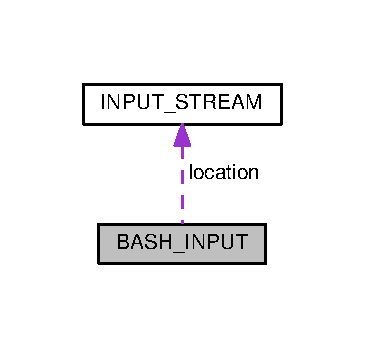
\includegraphics[width=175pt]{structBASH__INPUT__coll__graph}
\end{center}
\end{figure}
\subsection*{Public Attributes}
\begin{DoxyCompactItemize}
\item 
enum \hyperlink{input_8h_a565ef8a9f2a47f27189e6a48b5dc615a}{stream\+\_\+type} \hyperlink{structBASH__INPUT_aa1a38ed3faabc508930dc2405db9bea3}{type}
\item 
char $\ast$ \hyperlink{structBASH__INPUT_ae0a3b3bf98cfa7f6dc598134e6db39d2}{name}
\item 
\hyperlink{unionINPUT__STREAM}{I\+N\+P\+U\+T\+\_\+\+S\+T\+R\+E\+AM} \hyperlink{structBASH__INPUT_a6ea2dbded24d287d37b95deb092da0fd}{location}
\item 
sh\+\_\+cget\+\_\+func\+\_\+t $\ast$ \hyperlink{structBASH__INPUT_aa4da0c40a319c020cf936b97ce82b783}{getter}
\item 
sh\+\_\+cunget\+\_\+func\+\_\+t $\ast$ \hyperlink{structBASH__INPUT_aa5691d540e34f34766b758ded878d07c}{ungetter}
\end{DoxyCompactItemize}


\subsection{Member Data Documentation}
\index{B\+A\+S\+H\+\_\+\+I\+N\+P\+UT@{B\+A\+S\+H\+\_\+\+I\+N\+P\+UT}!getter@{getter}}
\index{getter@{getter}!B\+A\+S\+H\+\_\+\+I\+N\+P\+UT@{B\+A\+S\+H\+\_\+\+I\+N\+P\+UT}}
\subsubsection[{\texorpdfstring{getter}{getter}}]{\setlength{\rightskip}{0pt plus 5cm}sh\+\_\+cget\+\_\+func\+\_\+t$\ast$ B\+A\+S\+H\+\_\+\+I\+N\+P\+U\+T\+::getter}\hypertarget{structBASH__INPUT_aa4da0c40a319c020cf936b97ce82b783}{}\label{structBASH__INPUT_aa4da0c40a319c020cf936b97ce82b783}
\index{B\+A\+S\+H\+\_\+\+I\+N\+P\+UT@{B\+A\+S\+H\+\_\+\+I\+N\+P\+UT}!location@{location}}
\index{location@{location}!B\+A\+S\+H\+\_\+\+I\+N\+P\+UT@{B\+A\+S\+H\+\_\+\+I\+N\+P\+UT}}
\subsubsection[{\texorpdfstring{location}{location}}]{\setlength{\rightskip}{0pt plus 5cm}{\bf I\+N\+P\+U\+T\+\_\+\+S\+T\+R\+E\+AM} B\+A\+S\+H\+\_\+\+I\+N\+P\+U\+T\+::location}\hypertarget{structBASH__INPUT_a6ea2dbded24d287d37b95deb092da0fd}{}\label{structBASH__INPUT_a6ea2dbded24d287d37b95deb092da0fd}
\index{B\+A\+S\+H\+\_\+\+I\+N\+P\+UT@{B\+A\+S\+H\+\_\+\+I\+N\+P\+UT}!name@{name}}
\index{name@{name}!B\+A\+S\+H\+\_\+\+I\+N\+P\+UT@{B\+A\+S\+H\+\_\+\+I\+N\+P\+UT}}
\subsubsection[{\texorpdfstring{name}{name}}]{\setlength{\rightskip}{0pt plus 5cm}char$\ast$ B\+A\+S\+H\+\_\+\+I\+N\+P\+U\+T\+::name}\hypertarget{structBASH__INPUT_ae0a3b3bf98cfa7f6dc598134e6db39d2}{}\label{structBASH__INPUT_ae0a3b3bf98cfa7f6dc598134e6db39d2}
\index{B\+A\+S\+H\+\_\+\+I\+N\+P\+UT@{B\+A\+S\+H\+\_\+\+I\+N\+P\+UT}!type@{type}}
\index{type@{type}!B\+A\+S\+H\+\_\+\+I\+N\+P\+UT@{B\+A\+S\+H\+\_\+\+I\+N\+P\+UT}}
\subsubsection[{\texorpdfstring{type}{type}}]{\setlength{\rightskip}{0pt plus 5cm}enum {\bf stream\+\_\+type} B\+A\+S\+H\+\_\+\+I\+N\+P\+U\+T\+::type}\hypertarget{structBASH__INPUT_aa1a38ed3faabc508930dc2405db9bea3}{}\label{structBASH__INPUT_aa1a38ed3faabc508930dc2405db9bea3}
\index{B\+A\+S\+H\+\_\+\+I\+N\+P\+UT@{B\+A\+S\+H\+\_\+\+I\+N\+P\+UT}!ungetter@{ungetter}}
\index{ungetter@{ungetter}!B\+A\+S\+H\+\_\+\+I\+N\+P\+UT@{B\+A\+S\+H\+\_\+\+I\+N\+P\+UT}}
\subsubsection[{\texorpdfstring{ungetter}{ungetter}}]{\setlength{\rightskip}{0pt plus 5cm}sh\+\_\+cunget\+\_\+func\+\_\+t$\ast$ B\+A\+S\+H\+\_\+\+I\+N\+P\+U\+T\+::ungetter}\hypertarget{structBASH__INPUT_aa5691d540e34f34766b758ded878d07c}{}\label{structBASH__INPUT_aa5691d540e34f34766b758ded878d07c}


The documentation for this struct was generated from the following file\+:\begin{DoxyCompactItemize}
\item 
\hyperlink{input_8h}{input.\+h}\end{DoxyCompactItemize}

\hypertarget{structbgpids}{}\section{bgpids Struct Reference}
\label{structbgpids}\index{bgpids@{bgpids}}


{\ttfamily \#include $<$jobs.\+h$>$}



Collaboration diagram for bgpids\+:
\nopagebreak
\begin{figure}[H]
\begin{center}
\leavevmode
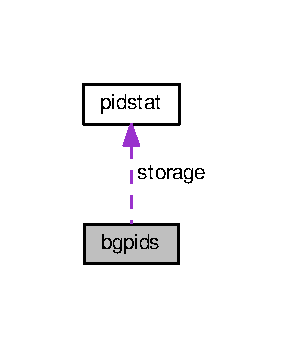
\includegraphics[width=139pt]{structbgpids__coll__graph}
\end{center}
\end{figure}
\subsection*{Public Attributes}
\begin{DoxyCompactItemize}
\item 
struct \hyperlink{structpidstat}{pidstat} $\ast$ \hyperlink{structbgpids_a9e1b9f32d9f6e5db5387b07d9e5440ff}{storage}
\item 
\hyperlink{jobs_8h_a677d6488545fa3193e7cb54647b4ae5c}{ps\+\_\+index\+\_\+t} \hyperlink{structbgpids_adf6139c912fc1e79278110429b95aaee}{head}
\item 
\hyperlink{jobs_8h_a677d6488545fa3193e7cb54647b4ae5c}{ps\+\_\+index\+\_\+t} \hyperlink{structbgpids_a370d36e85fac1b1cf2fdbc18b66903ae}{nalloc}
\item 
int \hyperlink{structbgpids_a3b393c1d3d52cb76efbe24e0fffc2871}{npid}
\end{DoxyCompactItemize}


\subsection{Member Data Documentation}
\index{bgpids@{bgpids}!head@{head}}
\index{head@{head}!bgpids@{bgpids}}
\subsubsection[{\texorpdfstring{head}{head}}]{\setlength{\rightskip}{0pt plus 5cm}{\bf ps\+\_\+index\+\_\+t} bgpids\+::head}\hypertarget{structbgpids_adf6139c912fc1e79278110429b95aaee}{}\label{structbgpids_adf6139c912fc1e79278110429b95aaee}
\index{bgpids@{bgpids}!nalloc@{nalloc}}
\index{nalloc@{nalloc}!bgpids@{bgpids}}
\subsubsection[{\texorpdfstring{nalloc}{nalloc}}]{\setlength{\rightskip}{0pt plus 5cm}{\bf ps\+\_\+index\+\_\+t} bgpids\+::nalloc}\hypertarget{structbgpids_a370d36e85fac1b1cf2fdbc18b66903ae}{}\label{structbgpids_a370d36e85fac1b1cf2fdbc18b66903ae}
\index{bgpids@{bgpids}!npid@{npid}}
\index{npid@{npid}!bgpids@{bgpids}}
\subsubsection[{\texorpdfstring{npid}{npid}}]{\setlength{\rightskip}{0pt plus 5cm}int bgpids\+::npid}\hypertarget{structbgpids_a3b393c1d3d52cb76efbe24e0fffc2871}{}\label{structbgpids_a3b393c1d3d52cb76efbe24e0fffc2871}
\index{bgpids@{bgpids}!storage@{storage}}
\index{storage@{storage}!bgpids@{bgpids}}
\subsubsection[{\texorpdfstring{storage}{storage}}]{\setlength{\rightskip}{0pt plus 5cm}struct {\bf pidstat}$\ast$ bgpids\+::storage}\hypertarget{structbgpids_a9e1b9f32d9f6e5db5387b07d9e5440ff}{}\label{structbgpids_a9e1b9f32d9f6e5db5387b07d9e5440ff}


The documentation for this struct was generated from the following file\+:\begin{DoxyCompactItemize}
\item 
\hyperlink{jobs_8h}{jobs.\+h}\end{DoxyCompactItemize}

\hypertarget{structbucket__contents}{}\section{bucket\+\_\+contents Struct Reference}
\label{structbucket__contents}\index{bucket\+\_\+contents@{bucket\+\_\+contents}}


{\ttfamily \#include $<$hashlib.\+h$>$}



Collaboration diagram for bucket\+\_\+contents\+:
\nopagebreak
\begin{figure}[H]
\begin{center}
\leavevmode
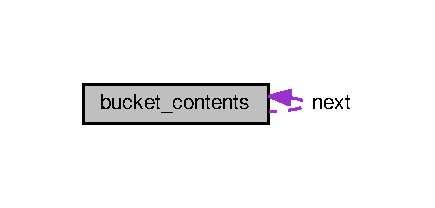
\includegraphics[width=209pt]{structbucket__contents__coll__graph}
\end{center}
\end{figure}
\subsection*{Public Attributes}
\begin{DoxyCompactItemize}
\item 
struct \hyperlink{structbucket__contents}{bucket\+\_\+contents} $\ast$ \hyperlink{structbucket__contents_a626ac20a4ec314e2028fd964ec63551e}{next}
\item 
char $\ast$ \hyperlink{structbucket__contents_a17facbf14d154f264ffb2d80b55a2e45}{key}
\item 
\hyperlink{xmalloc_8h_abbf31fec203727613ea15ba47bb8f344}{P\+T\+R\+\_\+T} \hyperlink{structbucket__contents_a4e30edeb29dde704f0fcf69bc4c73b4c}{data}
\item 
unsigned int \hyperlink{structbucket__contents_a8c8862e218acedb6bf4295849b9bab32}{khash}
\item 
int \hyperlink{structbucket__contents_a6dba923dd1c449e85201c91607a43ce0}{times\+\_\+found}
\end{DoxyCompactItemize}


\subsection{Member Data Documentation}
\index{bucket\+\_\+contents@{bucket\+\_\+contents}!data@{data}}
\index{data@{data}!bucket\+\_\+contents@{bucket\+\_\+contents}}
\subsubsection[{\texorpdfstring{data}{data}}]{\setlength{\rightskip}{0pt plus 5cm}{\bf P\+T\+R\+\_\+T} bucket\+\_\+contents\+::data}\hypertarget{structbucket__contents_a4e30edeb29dde704f0fcf69bc4c73b4c}{}\label{structbucket__contents_a4e30edeb29dde704f0fcf69bc4c73b4c}
\index{bucket\+\_\+contents@{bucket\+\_\+contents}!key@{key}}
\index{key@{key}!bucket\+\_\+contents@{bucket\+\_\+contents}}
\subsubsection[{\texorpdfstring{key}{key}}]{\setlength{\rightskip}{0pt plus 5cm}char$\ast$ bucket\+\_\+contents\+::key}\hypertarget{structbucket__contents_a17facbf14d154f264ffb2d80b55a2e45}{}\label{structbucket__contents_a17facbf14d154f264ffb2d80b55a2e45}
\index{bucket\+\_\+contents@{bucket\+\_\+contents}!khash@{khash}}
\index{khash@{khash}!bucket\+\_\+contents@{bucket\+\_\+contents}}
\subsubsection[{\texorpdfstring{khash}{khash}}]{\setlength{\rightskip}{0pt plus 5cm}unsigned int bucket\+\_\+contents\+::khash}\hypertarget{structbucket__contents_a8c8862e218acedb6bf4295849b9bab32}{}\label{structbucket__contents_a8c8862e218acedb6bf4295849b9bab32}
\index{bucket\+\_\+contents@{bucket\+\_\+contents}!next@{next}}
\index{next@{next}!bucket\+\_\+contents@{bucket\+\_\+contents}}
\subsubsection[{\texorpdfstring{next}{next}}]{\setlength{\rightskip}{0pt plus 5cm}struct {\bf bucket\+\_\+contents}$\ast$ bucket\+\_\+contents\+::next}\hypertarget{structbucket__contents_a626ac20a4ec314e2028fd964ec63551e}{}\label{structbucket__contents_a626ac20a4ec314e2028fd964ec63551e}
\index{bucket\+\_\+contents@{bucket\+\_\+contents}!times\+\_\+found@{times\+\_\+found}}
\index{times\+\_\+found@{times\+\_\+found}!bucket\+\_\+contents@{bucket\+\_\+contents}}
\subsubsection[{\texorpdfstring{times\+\_\+found}{times_found}}]{\setlength{\rightskip}{0pt plus 5cm}int bucket\+\_\+contents\+::times\+\_\+found}\hypertarget{structbucket__contents_a6dba923dd1c449e85201c91607a43ce0}{}\label{structbucket__contents_a6dba923dd1c449e85201c91607a43ce0}


The documentation for this struct was generated from the following file\+:\begin{DoxyCompactItemize}
\item 
\hyperlink{hashlib_8h}{hashlib.\+h}\end{DoxyCompactItemize}

\hypertarget{structbuiltin}{}\section{builtin Struct Reference}
\label{structbuiltin}\index{builtin@{builtin}}


{\ttfamily \#include $<$builtins.\+h$>$}

\subsection*{Public Attributes}
\begin{DoxyCompactItemize}
\item 
char $\ast$ \hyperlink{structbuiltin_a66ae19dbf9a3fec9c0872c66b6bfcba7}{name}
\item 
sh\+\_\+builtin\+\_\+func\+\_\+t $\ast$ \hyperlink{structbuiltin_a221595fc746de4d7d6b4df53bf67d33a}{function}
\item 
int \hyperlink{structbuiltin_a9f583bfe9459f1e181c58a79a0f49a8e}{flags}
\item 
char $\ast$const $\ast$ \hyperlink{structbuiltin_a41b55325fbb47cfc0b9be49cc7510735}{long\+\_\+doc}
\item 
const char $\ast$ \hyperlink{structbuiltin_acd7ac42244b07bafa4fbab01b6318d79}{short\+\_\+doc}
\item 
char $\ast$ \hyperlink{structbuiltin_ac691203d59944ccbe8f0118abdd221e3}{handle}
\end{DoxyCompactItemize}


\subsection{Member Data Documentation}
\index{builtin@{builtin}!flags@{flags}}
\index{flags@{flags}!builtin@{builtin}}
\subsubsection[{\texorpdfstring{flags}{flags}}]{\setlength{\rightskip}{0pt plus 5cm}int builtin\+::flags}\hypertarget{structbuiltin_a9f583bfe9459f1e181c58a79a0f49a8e}{}\label{structbuiltin_a9f583bfe9459f1e181c58a79a0f49a8e}
\index{builtin@{builtin}!function@{function}}
\index{function@{function}!builtin@{builtin}}
\subsubsection[{\texorpdfstring{function}{function}}]{\setlength{\rightskip}{0pt plus 5cm}sh\+\_\+builtin\+\_\+func\+\_\+t$\ast$ builtin\+::function}\hypertarget{structbuiltin_a221595fc746de4d7d6b4df53bf67d33a}{}\label{structbuiltin_a221595fc746de4d7d6b4df53bf67d33a}
\index{builtin@{builtin}!handle@{handle}}
\index{handle@{handle}!builtin@{builtin}}
\subsubsection[{\texorpdfstring{handle}{handle}}]{\setlength{\rightskip}{0pt plus 5cm}char$\ast$ builtin\+::handle}\hypertarget{structbuiltin_ac691203d59944ccbe8f0118abdd221e3}{}\label{structbuiltin_ac691203d59944ccbe8f0118abdd221e3}
\index{builtin@{builtin}!long\+\_\+doc@{long\+\_\+doc}}
\index{long\+\_\+doc@{long\+\_\+doc}!builtin@{builtin}}
\subsubsection[{\texorpdfstring{long\+\_\+doc}{long_doc}}]{\setlength{\rightskip}{0pt plus 5cm}char$\ast$ const$\ast$ builtin\+::long\+\_\+doc}\hypertarget{structbuiltin_a41b55325fbb47cfc0b9be49cc7510735}{}\label{structbuiltin_a41b55325fbb47cfc0b9be49cc7510735}
\index{builtin@{builtin}!name@{name}}
\index{name@{name}!builtin@{builtin}}
\subsubsection[{\texorpdfstring{name}{name}}]{\setlength{\rightskip}{0pt plus 5cm}char$\ast$ builtin\+::name}\hypertarget{structbuiltin_a66ae19dbf9a3fec9c0872c66b6bfcba7}{}\label{structbuiltin_a66ae19dbf9a3fec9c0872c66b6bfcba7}
\index{builtin@{builtin}!short\+\_\+doc@{short\+\_\+doc}}
\index{short\+\_\+doc@{short\+\_\+doc}!builtin@{builtin}}
\subsubsection[{\texorpdfstring{short\+\_\+doc}{short_doc}}]{\setlength{\rightskip}{0pt plus 5cm}const char$\ast$ builtin\+::short\+\_\+doc}\hypertarget{structbuiltin_acd7ac42244b07bafa4fbab01b6318d79}{}\label{structbuiltin_acd7ac42244b07bafa4fbab01b6318d79}


The documentation for this struct was generated from the following file\+:\begin{DoxyCompactItemize}
\item 
\hyperlink{builtins_8h}{builtins.\+h}\end{DoxyCompactItemize}

\hypertarget{structcase__com}{}\section{case\+\_\+com Struct Reference}
\label{structcase__com}\index{case\+\_\+com@{case\+\_\+com}}


{\ttfamily \#include $<$command.\+h$>$}



Collaboration diagram for case\+\_\+com\+:
\nopagebreak
\begin{figure}[H]
\begin{center}
\leavevmode
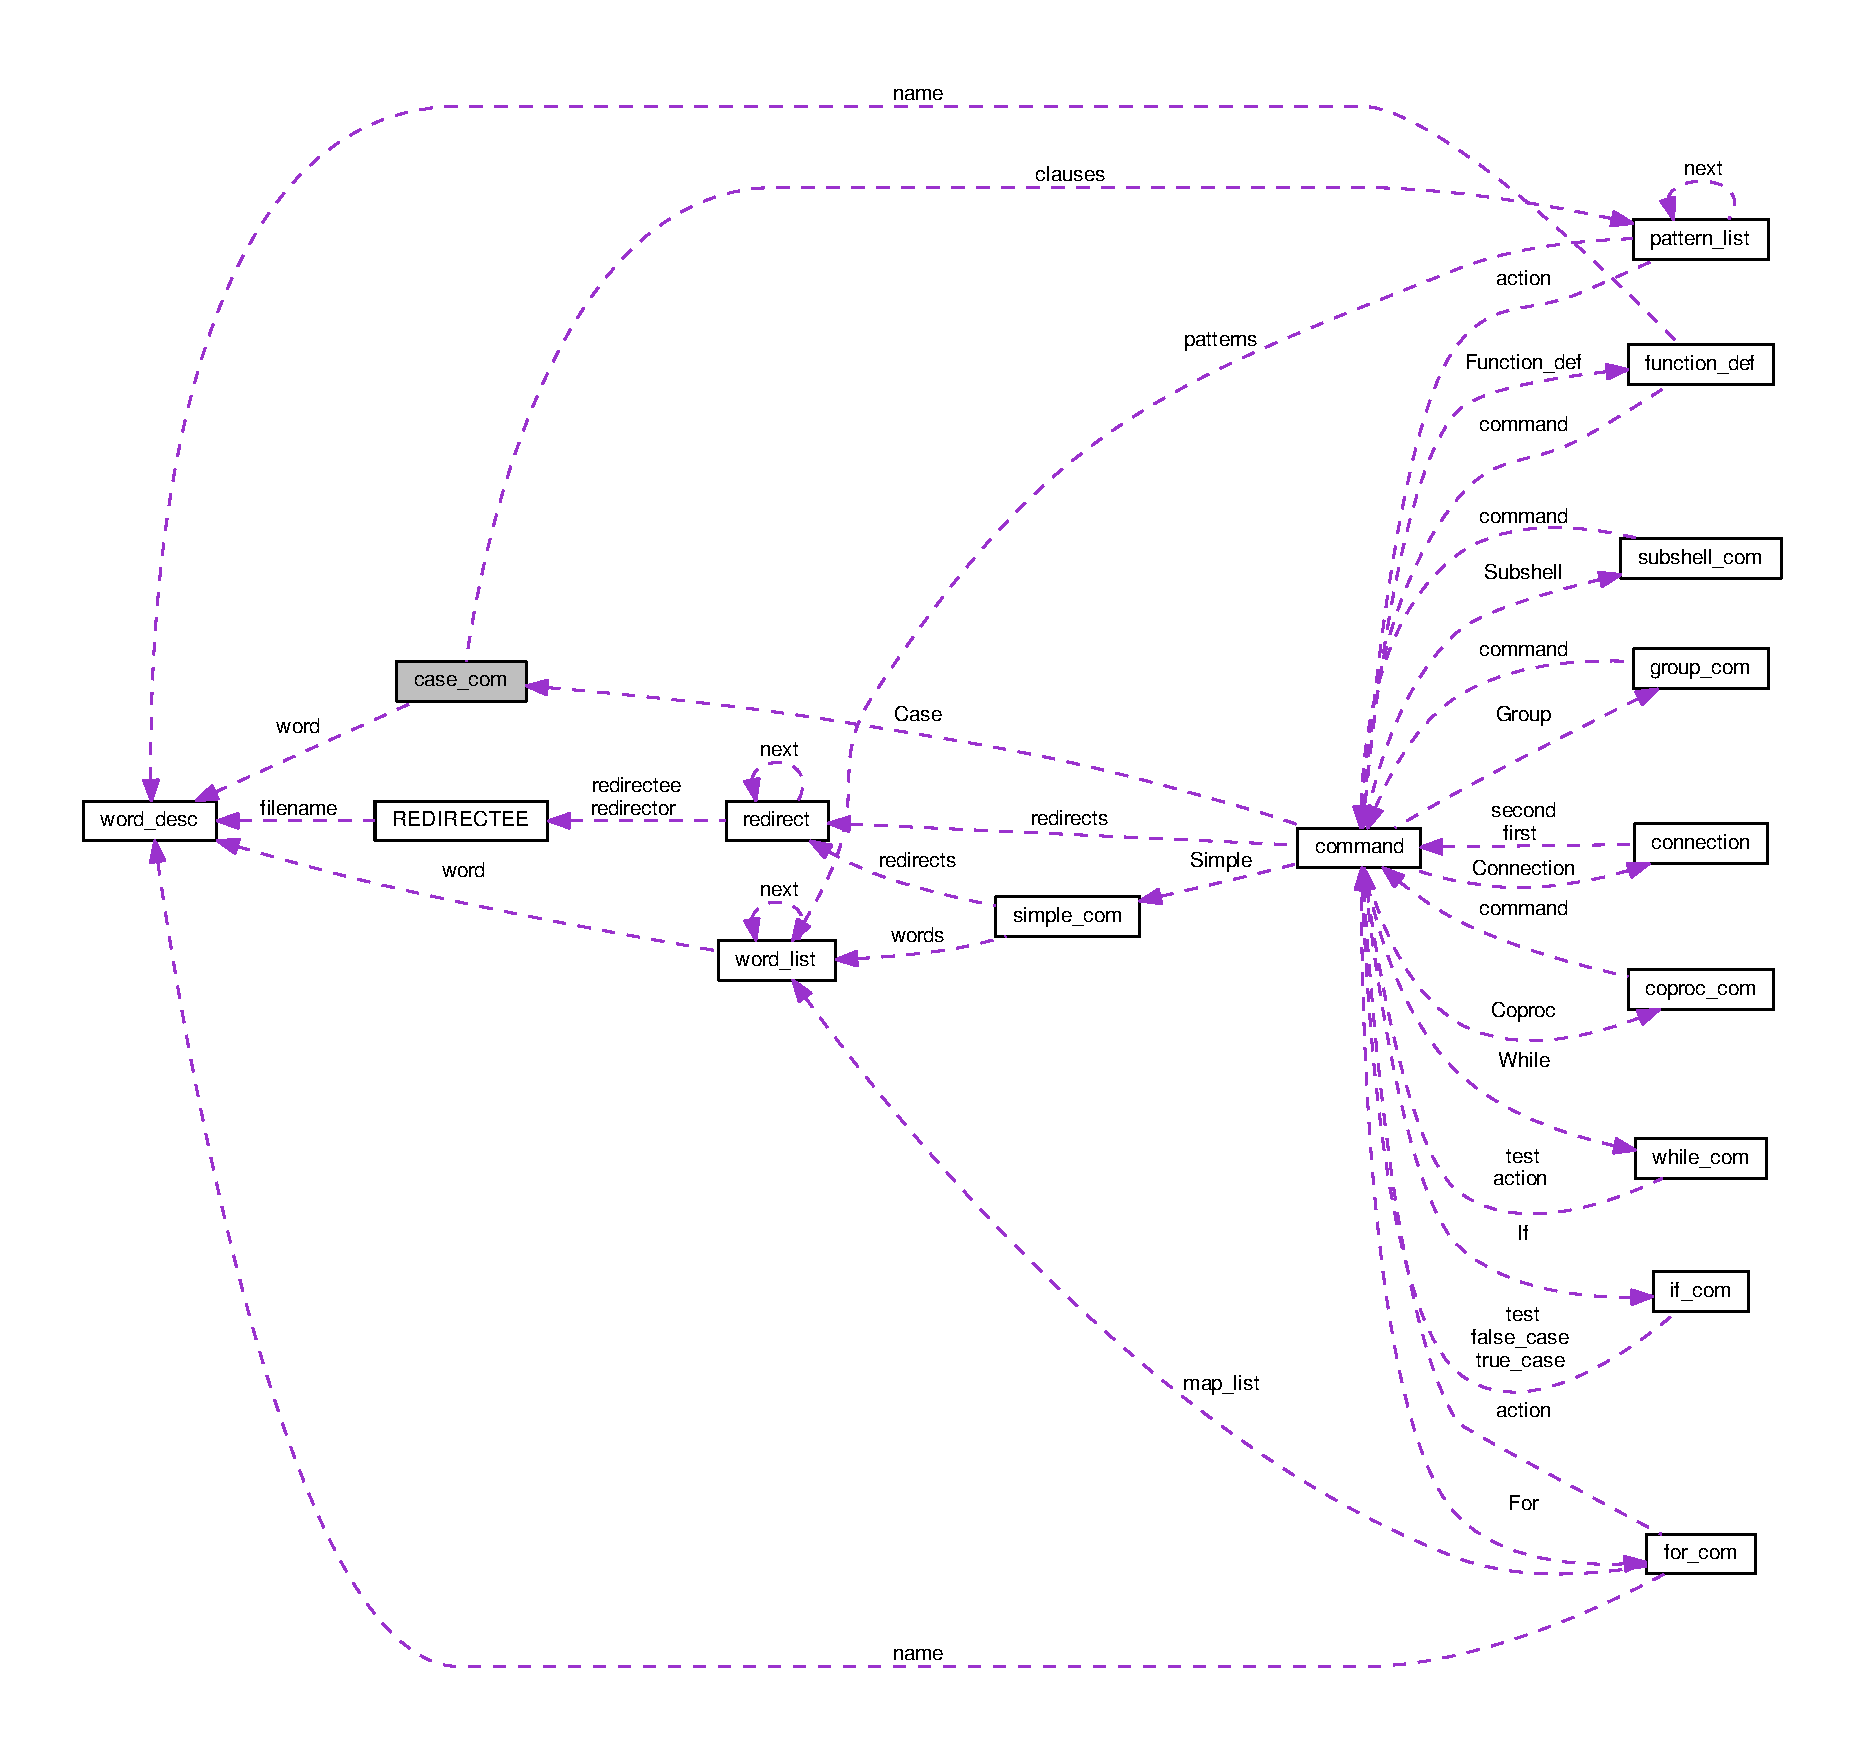
\includegraphics[width=350pt]{structcase__com__coll__graph}
\end{center}
\end{figure}
\subsection*{Public Attributes}
\begin{DoxyCompactItemize}
\item 
int \hyperlink{structcase__com_a7c1331e9e068cc68d7202a5258a9b99f}{flags}
\item 
int \hyperlink{structcase__com_a224481775fc2b0ae54084676a332eaf2}{line}
\item 
\hyperlink{command_8h_a3f0cccf333703e5f6c4168be0db675fa}{W\+O\+R\+D\+\_\+\+D\+E\+SC} $\ast$ \hyperlink{structcase__com_a73c5c1e3d71a7d4615708e5b6afd4e34}{word}
\item 
\hyperlink{command_8h_a05098e88133e048a1acf396288758a9e}{P\+A\+T\+T\+E\+R\+N\+\_\+\+L\+I\+ST} $\ast$ \hyperlink{structcase__com_a68bcee3c7e8750f04e632c0178dbb574}{clauses}
\end{DoxyCompactItemize}


\subsection{Member Data Documentation}
\index{case\+\_\+com@{case\+\_\+com}!clauses@{clauses}}
\index{clauses@{clauses}!case\+\_\+com@{case\+\_\+com}}
\subsubsection[{\texorpdfstring{clauses}{clauses}}]{\setlength{\rightskip}{0pt plus 5cm}{\bf P\+A\+T\+T\+E\+R\+N\+\_\+\+L\+I\+ST}$\ast$ case\+\_\+com\+::clauses}\hypertarget{structcase__com_a68bcee3c7e8750f04e632c0178dbb574}{}\label{structcase__com_a68bcee3c7e8750f04e632c0178dbb574}
\index{case\+\_\+com@{case\+\_\+com}!flags@{flags}}
\index{flags@{flags}!case\+\_\+com@{case\+\_\+com}}
\subsubsection[{\texorpdfstring{flags}{flags}}]{\setlength{\rightskip}{0pt plus 5cm}int case\+\_\+com\+::flags}\hypertarget{structcase__com_a7c1331e9e068cc68d7202a5258a9b99f}{}\label{structcase__com_a7c1331e9e068cc68d7202a5258a9b99f}
\index{case\+\_\+com@{case\+\_\+com}!line@{line}}
\index{line@{line}!case\+\_\+com@{case\+\_\+com}}
\subsubsection[{\texorpdfstring{line}{line}}]{\setlength{\rightskip}{0pt plus 5cm}int case\+\_\+com\+::line}\hypertarget{structcase__com_a224481775fc2b0ae54084676a332eaf2}{}\label{structcase__com_a224481775fc2b0ae54084676a332eaf2}
\index{case\+\_\+com@{case\+\_\+com}!word@{word}}
\index{word@{word}!case\+\_\+com@{case\+\_\+com}}
\subsubsection[{\texorpdfstring{word}{word}}]{\setlength{\rightskip}{0pt plus 5cm}{\bf W\+O\+R\+D\+\_\+\+D\+E\+SC}$\ast$ case\+\_\+com\+::word}\hypertarget{structcase__com_a73c5c1e3d71a7d4615708e5b6afd4e34}{}\label{structcase__com_a73c5c1e3d71a7d4615708e5b6afd4e34}


The documentation for this struct was generated from the following file\+:\begin{DoxyCompactItemize}
\item 
\hyperlink{command_8h}{command.\+h}\end{DoxyCompactItemize}

\hypertarget{structcommand}{}\section{command Struct Reference}
\label{structcommand}\index{command@{command}}


{\ttfamily \#include $<$command.\+h$>$}



Collaboration diagram for command\+:
\nopagebreak
\begin{figure}[H]
\begin{center}
\leavevmode
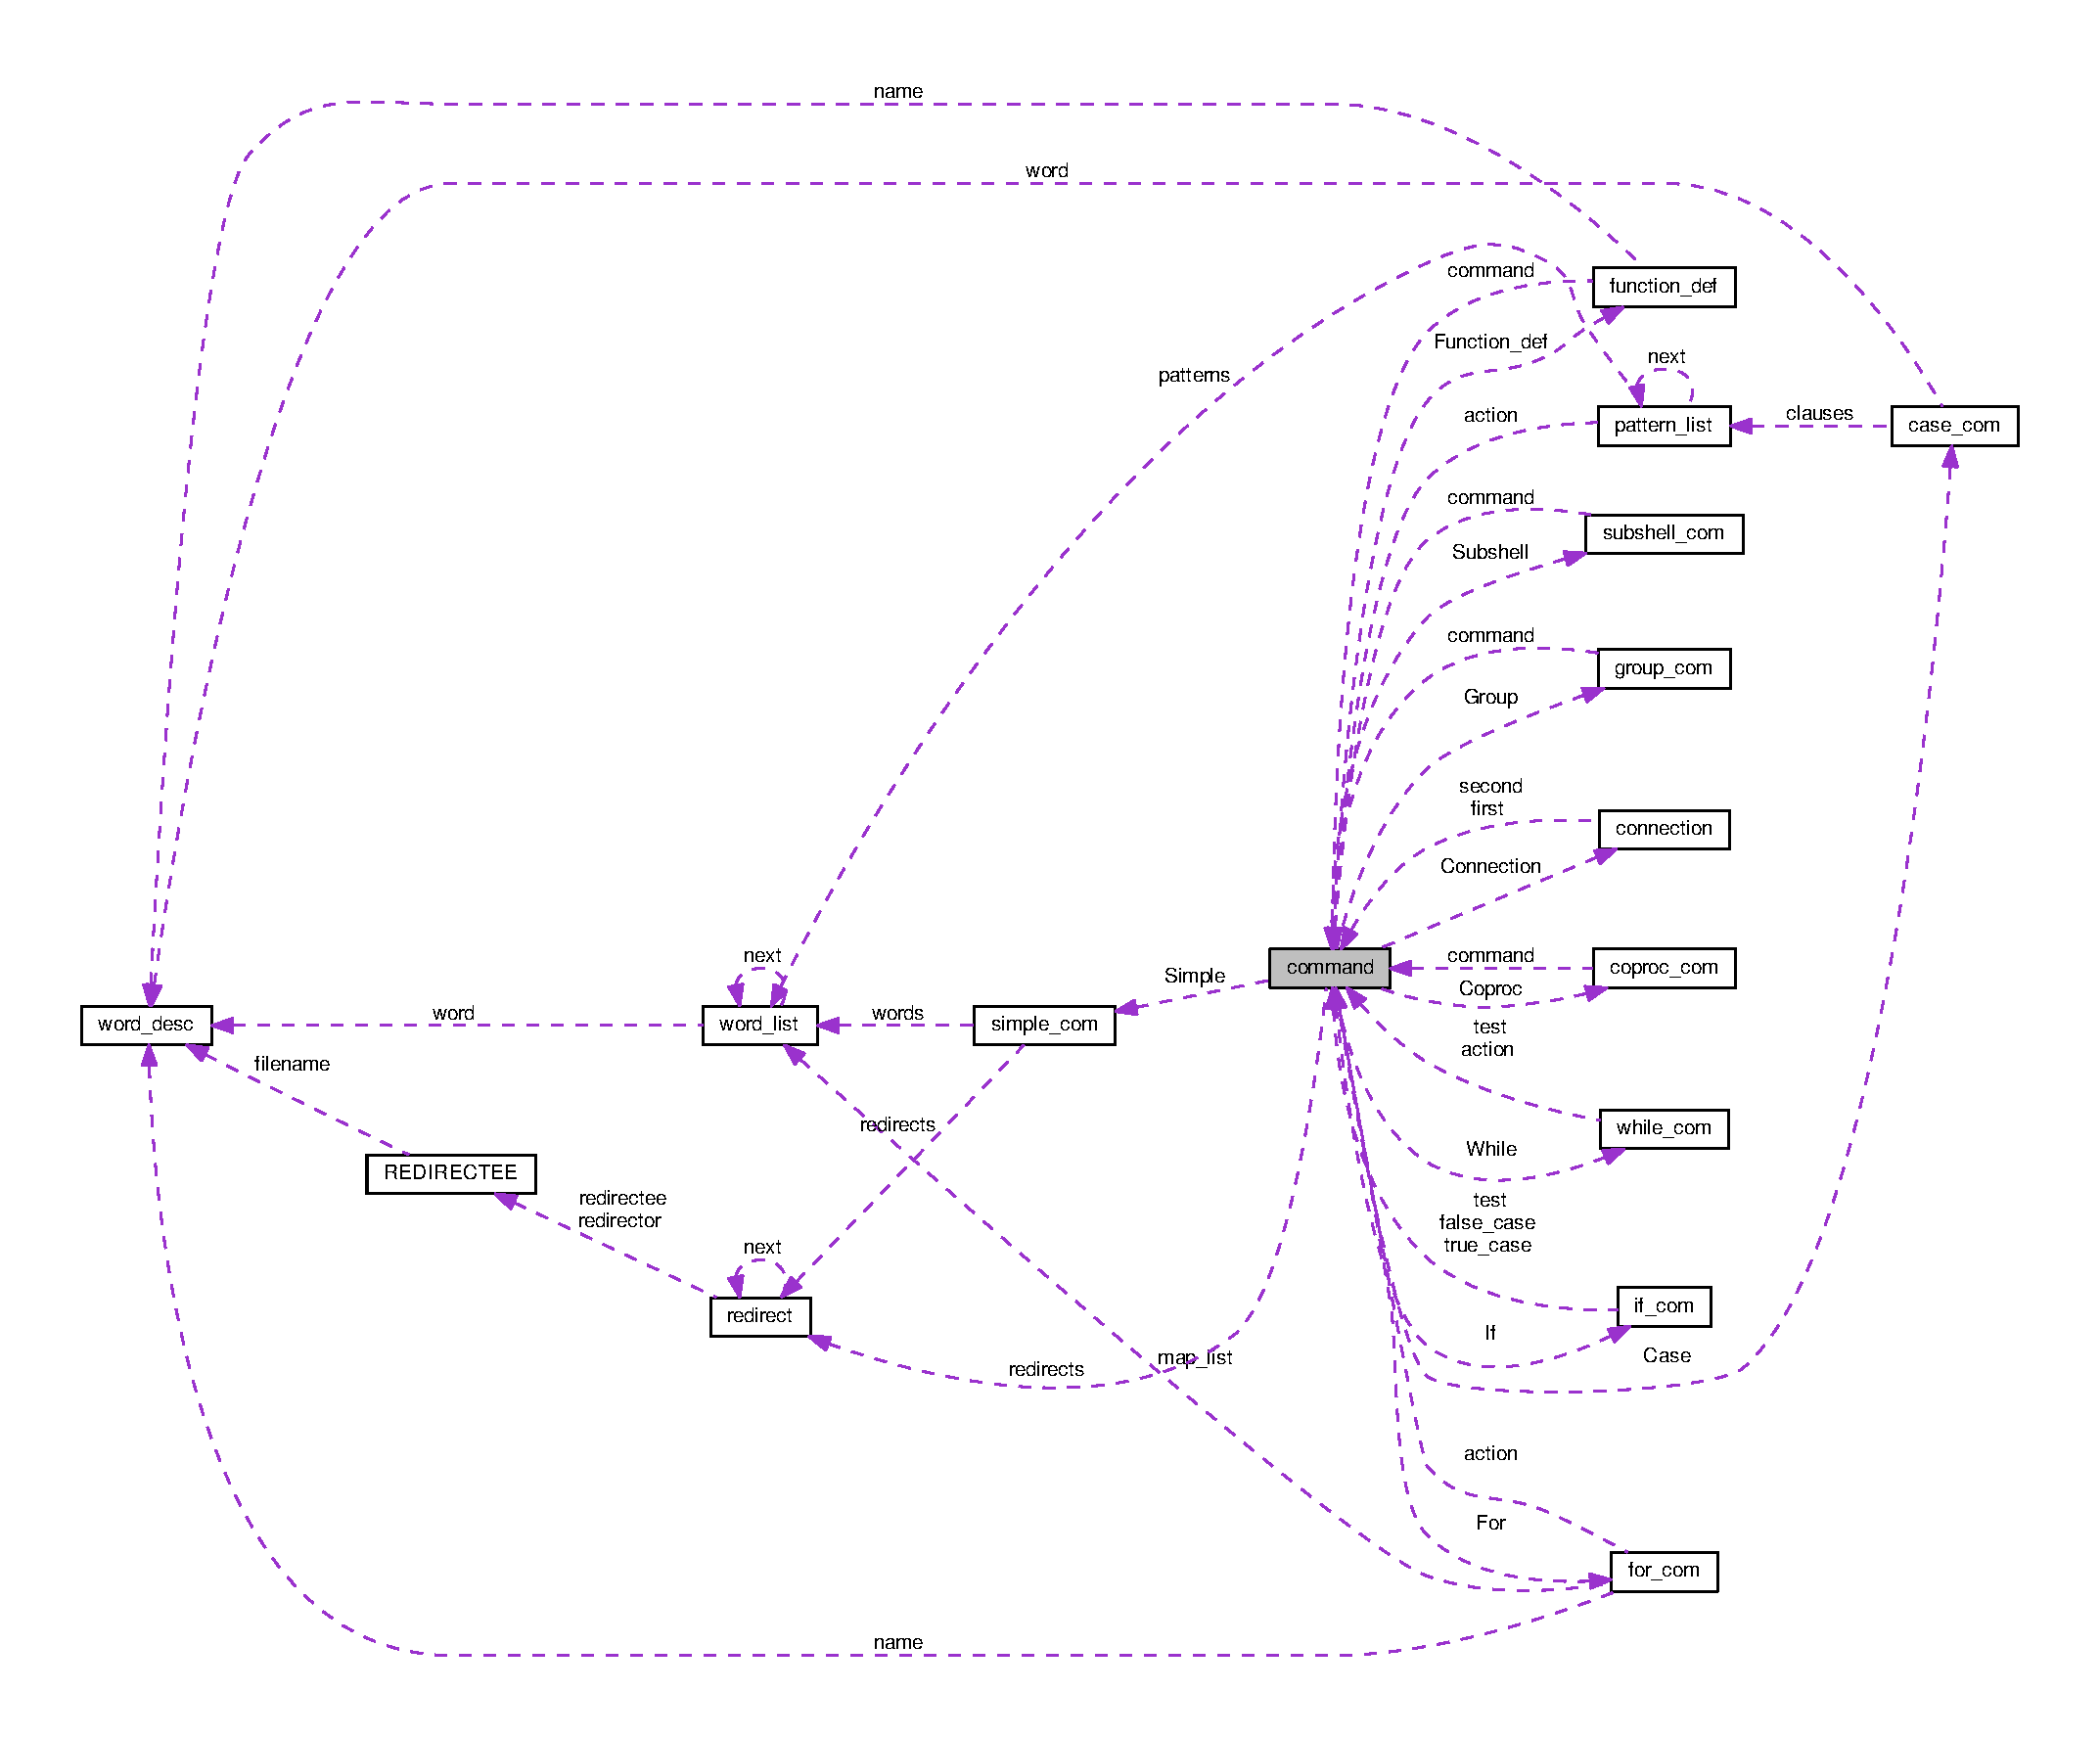
\includegraphics[width=350pt]{structcommand__coll__graph}
\end{center}
\end{figure}
\subsection*{Public Attributes}
\begin{DoxyCompactItemize}
\item 
enum \hyperlink{command_8h_a71e4cb55459005154ad8360914a8e1f4}{command\+\_\+type} \hyperlink{structcommand_adc520136f05efbf94b38913f7d8b1f31}{type}
\item 
int \hyperlink{structcommand_aa901bebf4c7f683f6934e69ad95f2b11}{flags}
\item 
int \hyperlink{structcommand_a35171ddf374dcfc97662a6b3965d2ad0}{line}
\item 
\hyperlink{command_8h_adeb9f5d937c92c7923aec48ad5e47d57}{R\+E\+D\+I\+R\+E\+CT} $\ast$ \hyperlink{structcommand_a5b5efa4854e0319791e28028712fee9a}{redirects}
\item 
\begin{tabbing}
xx\=xx\=xx\=xx\=xx\=xx\=xx\=xx\=xx\=\kill
union \{\\
\>struct \hyperlink{structfor__com}{for\_com} $\ast$ \hyperlink{structcommand_a7b937c91d8eacc73c93c1cf64422dc28}{For}\\
\>struct \hyperlink{structcase__com}{case\_com} $\ast$ \hyperlink{structcommand_a3b14b45192764ae24f9c40edf7aefc94}{Case}\\
\>struct \hyperlink{structwhile__com}{while\_com} $\ast$ \hyperlink{structcommand_a770073860411c3d15cc533862688d035}{While}\\
\>struct \hyperlink{structif__com}{if\_com} $\ast$ \hyperlink{structcommand_a7ebce7bca0b62a919f8ad0157046a58c}{If}\\
\>struct \hyperlink{structconnection}{connection} $\ast$ \hyperlink{structcommand_a2d2ed612574d67c6d3d83892595563f5}{Connection}\\
\>struct \hyperlink{structsimple__com}{simple\_com} $\ast$ \hyperlink{structcommand_ab3ddc136c7f74d323c4bd1afc97a5864}{Simple}\\
\>struct \hyperlink{structfunction__def}{function\_def} $\ast$ \hyperlink{structcommand_a0f27ea57892789c32125560aa6b58372}{Function\_def}\\
\>struct \hyperlink{structgroup__com}{group\_com} $\ast$ \hyperlink{structcommand_a3be5f23cdfe7367575228ab7c8a98c8a}{Group}\\
\>struct \hyperlink{structsubshell__com}{subshell\_com} $\ast$ \hyperlink{structcommand_a31087dc3fce667d2ded99e645149afa6}{Subshell}\\
\>struct \hyperlink{structcoproc__com}{coproc\_com} $\ast$ \hyperlink{structcommand_a2b7939e2744dc3a05722a9982148b219}{Coproc}\\
\} \hyperlink{structcommand_adda5d5d9646a55d8cf1f8b64612af756}{value}\\

\end{tabbing}\end{DoxyCompactItemize}


\subsection{Member Data Documentation}
\index{command@{command}!Case@{Case}}
\index{Case@{Case}!command@{command}}
\subsubsection[{\texorpdfstring{Case}{Case}}]{\setlength{\rightskip}{0pt plus 5cm}struct {\bf case\+\_\+com}$\ast$ command\+::\+Case}\hypertarget{structcommand_a3b14b45192764ae24f9c40edf7aefc94}{}\label{structcommand_a3b14b45192764ae24f9c40edf7aefc94}
\index{command@{command}!Connection@{Connection}}
\index{Connection@{Connection}!command@{command}}
\subsubsection[{\texorpdfstring{Connection}{Connection}}]{\setlength{\rightskip}{0pt plus 5cm}struct {\bf connection}$\ast$ command\+::\+Connection}\hypertarget{structcommand_a2d2ed612574d67c6d3d83892595563f5}{}\label{structcommand_a2d2ed612574d67c6d3d83892595563f5}
\index{command@{command}!Coproc@{Coproc}}
\index{Coproc@{Coproc}!command@{command}}
\subsubsection[{\texorpdfstring{Coproc}{Coproc}}]{\setlength{\rightskip}{0pt plus 5cm}struct {\bf coproc\+\_\+com}$\ast$ command\+::\+Coproc}\hypertarget{structcommand_a2b7939e2744dc3a05722a9982148b219}{}\label{structcommand_a2b7939e2744dc3a05722a9982148b219}
\index{command@{command}!flags@{flags}}
\index{flags@{flags}!command@{command}}
\subsubsection[{\texorpdfstring{flags}{flags}}]{\setlength{\rightskip}{0pt plus 5cm}int command\+::flags}\hypertarget{structcommand_aa901bebf4c7f683f6934e69ad95f2b11}{}\label{structcommand_aa901bebf4c7f683f6934e69ad95f2b11}
\index{command@{command}!For@{For}}
\index{For@{For}!command@{command}}
\subsubsection[{\texorpdfstring{For}{For}}]{\setlength{\rightskip}{0pt plus 5cm}struct {\bf for\+\_\+com}$\ast$ command\+::\+For}\hypertarget{structcommand_a7b937c91d8eacc73c93c1cf64422dc28}{}\label{structcommand_a7b937c91d8eacc73c93c1cf64422dc28}
\index{command@{command}!Function\+\_\+def@{Function\+\_\+def}}
\index{Function\+\_\+def@{Function\+\_\+def}!command@{command}}
\subsubsection[{\texorpdfstring{Function\+\_\+def}{Function_def}}]{\setlength{\rightskip}{0pt plus 5cm}struct {\bf function\+\_\+def}$\ast$ command\+::\+Function\+\_\+def}\hypertarget{structcommand_a0f27ea57892789c32125560aa6b58372}{}\label{structcommand_a0f27ea57892789c32125560aa6b58372}
\index{command@{command}!Group@{Group}}
\index{Group@{Group}!command@{command}}
\subsubsection[{\texorpdfstring{Group}{Group}}]{\setlength{\rightskip}{0pt plus 5cm}struct {\bf group\+\_\+com}$\ast$ command\+::\+Group}\hypertarget{structcommand_a3be5f23cdfe7367575228ab7c8a98c8a}{}\label{structcommand_a3be5f23cdfe7367575228ab7c8a98c8a}
\index{command@{command}!If@{If}}
\index{If@{If}!command@{command}}
\subsubsection[{\texorpdfstring{If}{If}}]{\setlength{\rightskip}{0pt plus 5cm}struct {\bf if\+\_\+com}$\ast$ command\+::\+If}\hypertarget{structcommand_a7ebce7bca0b62a919f8ad0157046a58c}{}\label{structcommand_a7ebce7bca0b62a919f8ad0157046a58c}
\index{command@{command}!line@{line}}
\index{line@{line}!command@{command}}
\subsubsection[{\texorpdfstring{line}{line}}]{\setlength{\rightskip}{0pt plus 5cm}int command\+::line}\hypertarget{structcommand_a35171ddf374dcfc97662a6b3965d2ad0}{}\label{structcommand_a35171ddf374dcfc97662a6b3965d2ad0}
\index{command@{command}!redirects@{redirects}}
\index{redirects@{redirects}!command@{command}}
\subsubsection[{\texorpdfstring{redirects}{redirects}}]{\setlength{\rightskip}{0pt plus 5cm}{\bf R\+E\+D\+I\+R\+E\+CT}$\ast$ command\+::redirects}\hypertarget{structcommand_a5b5efa4854e0319791e28028712fee9a}{}\label{structcommand_a5b5efa4854e0319791e28028712fee9a}
\index{command@{command}!Simple@{Simple}}
\index{Simple@{Simple}!command@{command}}
\subsubsection[{\texorpdfstring{Simple}{Simple}}]{\setlength{\rightskip}{0pt plus 5cm}struct {\bf simple\+\_\+com}$\ast$ command\+::\+Simple}\hypertarget{structcommand_ab3ddc136c7f74d323c4bd1afc97a5864}{}\label{structcommand_ab3ddc136c7f74d323c4bd1afc97a5864}
\index{command@{command}!Subshell@{Subshell}}
\index{Subshell@{Subshell}!command@{command}}
\subsubsection[{\texorpdfstring{Subshell}{Subshell}}]{\setlength{\rightskip}{0pt plus 5cm}struct {\bf subshell\+\_\+com}$\ast$ command\+::\+Subshell}\hypertarget{structcommand_a31087dc3fce667d2ded99e645149afa6}{}\label{structcommand_a31087dc3fce667d2ded99e645149afa6}
\index{command@{command}!type@{type}}
\index{type@{type}!command@{command}}
\subsubsection[{\texorpdfstring{type}{type}}]{\setlength{\rightskip}{0pt plus 5cm}enum {\bf command\+\_\+type} command\+::type}\hypertarget{structcommand_adc520136f05efbf94b38913f7d8b1f31}{}\label{structcommand_adc520136f05efbf94b38913f7d8b1f31}
\index{command@{command}!value@{value}}
\index{value@{value}!command@{command}}
\subsubsection[{\texorpdfstring{value}{value}}]{\setlength{\rightskip}{0pt plus 5cm}union \{ ... \}   command\+::value}\hypertarget{structcommand_adda5d5d9646a55d8cf1f8b64612af756}{}\label{structcommand_adda5d5d9646a55d8cf1f8b64612af756}
\index{command@{command}!While@{While}}
\index{While@{While}!command@{command}}
\subsubsection[{\texorpdfstring{While}{While}}]{\setlength{\rightskip}{0pt plus 5cm}struct {\bf while\+\_\+com}$\ast$ command\+::\+While}\hypertarget{structcommand_a770073860411c3d15cc533862688d035}{}\label{structcommand_a770073860411c3d15cc533862688d035}


The documentation for this struct was generated from the following file\+:\begin{DoxyCompactItemize}
\item 
\hyperlink{command_8h}{command.\+h}\end{DoxyCompactItemize}

\hypertarget{structcompspec}{}\section{compspec Struct Reference}
\label{structcompspec}\index{compspec@{compspec}}


{\ttfamily \#include $<$pcomplete.\+h$>$}

\subsection*{Public Attributes}
\begin{DoxyCompactItemize}
\item 
int \hyperlink{structcompspec_a6b159ff5d4155e6db4cf8d00be5577b1}{refcount}
\item 
unsigned long \hyperlink{structcompspec_a7fde3c9ac7d3323ae168e23a25f4ea70}{actions}
\item 
unsigned long \hyperlink{structcompspec_abb41177107193c72d4e4a729dd9ca3e2}{options}
\item 
char $\ast$ \hyperlink{structcompspec_af2b50da25665b42339ff1706218a8336}{globpat}
\item 
char $\ast$ \hyperlink{structcompspec_aa45815ac115fd9e28a3794181b9a4cf6}{words}
\item 
char $\ast$ \hyperlink{structcompspec_a484aa9fab29856c726e7998f1b176a33}{prefix}
\item 
char $\ast$ \hyperlink{structcompspec_ad4c0b13772afa88fec5024829e608b53}{suffix}
\item 
char $\ast$ \hyperlink{structcompspec_a286bad7bae59e72673a3e06013a710b2}{funcname}
\item 
char $\ast$ \hyperlink{structcompspec_a925612fb509ec4ae1e62478d62e9877a}{command}
\item 
char $\ast$ \hyperlink{structcompspec_abf203174fce2dd17b9ab2e9bd6108389}{lcommand}
\item 
char $\ast$ \hyperlink{structcompspec_ab33895496e7bcf808b84573578099835}{filterpat}
\end{DoxyCompactItemize}


\subsection{Member Data Documentation}
\index{compspec@{compspec}!actions@{actions}}
\index{actions@{actions}!compspec@{compspec}}
\subsubsection[{\texorpdfstring{actions}{actions}}]{\setlength{\rightskip}{0pt plus 5cm}unsigned long compspec\+::actions}\hypertarget{structcompspec_a7fde3c9ac7d3323ae168e23a25f4ea70}{}\label{structcompspec_a7fde3c9ac7d3323ae168e23a25f4ea70}
\index{compspec@{compspec}!command@{command}}
\index{command@{command}!compspec@{compspec}}
\subsubsection[{\texorpdfstring{command}{command}}]{\setlength{\rightskip}{0pt plus 5cm}char$\ast$ compspec\+::command}\hypertarget{structcompspec_a925612fb509ec4ae1e62478d62e9877a}{}\label{structcompspec_a925612fb509ec4ae1e62478d62e9877a}
\index{compspec@{compspec}!filterpat@{filterpat}}
\index{filterpat@{filterpat}!compspec@{compspec}}
\subsubsection[{\texorpdfstring{filterpat}{filterpat}}]{\setlength{\rightskip}{0pt plus 5cm}char$\ast$ compspec\+::filterpat}\hypertarget{structcompspec_ab33895496e7bcf808b84573578099835}{}\label{structcompspec_ab33895496e7bcf808b84573578099835}
\index{compspec@{compspec}!funcname@{funcname}}
\index{funcname@{funcname}!compspec@{compspec}}
\subsubsection[{\texorpdfstring{funcname}{funcname}}]{\setlength{\rightskip}{0pt plus 5cm}char$\ast$ compspec\+::funcname}\hypertarget{structcompspec_a286bad7bae59e72673a3e06013a710b2}{}\label{structcompspec_a286bad7bae59e72673a3e06013a710b2}
\index{compspec@{compspec}!globpat@{globpat}}
\index{globpat@{globpat}!compspec@{compspec}}
\subsubsection[{\texorpdfstring{globpat}{globpat}}]{\setlength{\rightskip}{0pt plus 5cm}char$\ast$ compspec\+::globpat}\hypertarget{structcompspec_af2b50da25665b42339ff1706218a8336}{}\label{structcompspec_af2b50da25665b42339ff1706218a8336}
\index{compspec@{compspec}!lcommand@{lcommand}}
\index{lcommand@{lcommand}!compspec@{compspec}}
\subsubsection[{\texorpdfstring{lcommand}{lcommand}}]{\setlength{\rightskip}{0pt plus 5cm}char$\ast$ compspec\+::lcommand}\hypertarget{structcompspec_abf203174fce2dd17b9ab2e9bd6108389}{}\label{structcompspec_abf203174fce2dd17b9ab2e9bd6108389}
\index{compspec@{compspec}!options@{options}}
\index{options@{options}!compspec@{compspec}}
\subsubsection[{\texorpdfstring{options}{options}}]{\setlength{\rightskip}{0pt plus 5cm}unsigned long compspec\+::options}\hypertarget{structcompspec_abb41177107193c72d4e4a729dd9ca3e2}{}\label{structcompspec_abb41177107193c72d4e4a729dd9ca3e2}
\index{compspec@{compspec}!prefix@{prefix}}
\index{prefix@{prefix}!compspec@{compspec}}
\subsubsection[{\texorpdfstring{prefix}{prefix}}]{\setlength{\rightskip}{0pt plus 5cm}char$\ast$ compspec\+::prefix}\hypertarget{structcompspec_a484aa9fab29856c726e7998f1b176a33}{}\label{structcompspec_a484aa9fab29856c726e7998f1b176a33}
\index{compspec@{compspec}!refcount@{refcount}}
\index{refcount@{refcount}!compspec@{compspec}}
\subsubsection[{\texorpdfstring{refcount}{refcount}}]{\setlength{\rightskip}{0pt plus 5cm}int compspec\+::refcount}\hypertarget{structcompspec_a6b159ff5d4155e6db4cf8d00be5577b1}{}\label{structcompspec_a6b159ff5d4155e6db4cf8d00be5577b1}
\index{compspec@{compspec}!suffix@{suffix}}
\index{suffix@{suffix}!compspec@{compspec}}
\subsubsection[{\texorpdfstring{suffix}{suffix}}]{\setlength{\rightskip}{0pt plus 5cm}char$\ast$ compspec\+::suffix}\hypertarget{structcompspec_ad4c0b13772afa88fec5024829e608b53}{}\label{structcompspec_ad4c0b13772afa88fec5024829e608b53}
\index{compspec@{compspec}!words@{words}}
\index{words@{words}!compspec@{compspec}}
\subsubsection[{\texorpdfstring{words}{words}}]{\setlength{\rightskip}{0pt plus 5cm}char$\ast$ compspec\+::words}\hypertarget{structcompspec_aa45815ac115fd9e28a3794181b9a4cf6}{}\label{structcompspec_aa45815ac115fd9e28a3794181b9a4cf6}


The documentation for this struct was generated from the following file\+:\begin{DoxyCompactItemize}
\item 
\hyperlink{pcomplete_8h}{pcomplete.\+h}\end{DoxyCompactItemize}

\hypertarget{structcond__com}{}\section{cond\+\_\+com Struct Reference}
\label{structcond__com}\index{cond\+\_\+com@{cond\+\_\+com}}


{\ttfamily \#include $<$command.\+h$>$}



Collaboration diagram for cond\+\_\+com\+:
\nopagebreak
\begin{figure}[H]
\begin{center}
\leavevmode
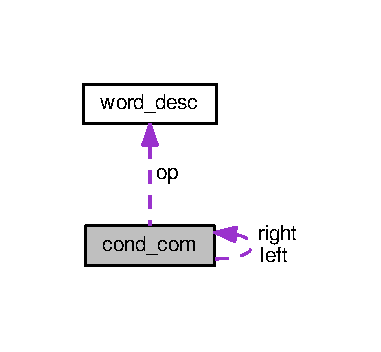
\includegraphics[width=183pt]{structcond__com__coll__graph}
\end{center}
\end{figure}
\subsection*{Public Attributes}
\begin{DoxyCompactItemize}
\item 
int \hyperlink{structcond__com_abe64315eec13089b3dc43c54acb5e6d0}{flags}
\item 
int \hyperlink{structcond__com_a7a36bcce3ca4c65e93c44648091a9a84}{line}
\item 
int \hyperlink{structcond__com_a664011494f9f9386279500a5d9f8674a}{type}
\item 
\hyperlink{command_8h_a3f0cccf333703e5f6c4168be0db675fa}{W\+O\+R\+D\+\_\+\+D\+E\+SC} $\ast$ \hyperlink{structcond__com_a3778220cc80ac673817cb33f796b9484}{op}
\item 
struct \hyperlink{structcond__com}{cond\+\_\+com} $\ast$ \hyperlink{structcond__com_a96d0c77c1c43455170008963a48f1711}{left}
\item 
struct \hyperlink{structcond__com}{cond\+\_\+com} $\ast$ \hyperlink{structcond__com_ad3879e315749f6f1bd363592c2dd9416}{right}
\end{DoxyCompactItemize}


\subsection{Member Data Documentation}
\index{cond\+\_\+com@{cond\+\_\+com}!flags@{flags}}
\index{flags@{flags}!cond\+\_\+com@{cond\+\_\+com}}
\subsubsection[{\texorpdfstring{flags}{flags}}]{\setlength{\rightskip}{0pt plus 5cm}int cond\+\_\+com\+::flags}\hypertarget{structcond__com_abe64315eec13089b3dc43c54acb5e6d0}{}\label{structcond__com_abe64315eec13089b3dc43c54acb5e6d0}
\index{cond\+\_\+com@{cond\+\_\+com}!left@{left}}
\index{left@{left}!cond\+\_\+com@{cond\+\_\+com}}
\subsubsection[{\texorpdfstring{left}{left}}]{\setlength{\rightskip}{0pt plus 5cm}struct {\bf cond\+\_\+com}$\ast$ cond\+\_\+com\+::left}\hypertarget{structcond__com_a96d0c77c1c43455170008963a48f1711}{}\label{structcond__com_a96d0c77c1c43455170008963a48f1711}
\index{cond\+\_\+com@{cond\+\_\+com}!line@{line}}
\index{line@{line}!cond\+\_\+com@{cond\+\_\+com}}
\subsubsection[{\texorpdfstring{line}{line}}]{\setlength{\rightskip}{0pt plus 5cm}int cond\+\_\+com\+::line}\hypertarget{structcond__com_a7a36bcce3ca4c65e93c44648091a9a84}{}\label{structcond__com_a7a36bcce3ca4c65e93c44648091a9a84}
\index{cond\+\_\+com@{cond\+\_\+com}!op@{op}}
\index{op@{op}!cond\+\_\+com@{cond\+\_\+com}}
\subsubsection[{\texorpdfstring{op}{op}}]{\setlength{\rightskip}{0pt plus 5cm}{\bf W\+O\+R\+D\+\_\+\+D\+E\+SC}$\ast$ cond\+\_\+com\+::op}\hypertarget{structcond__com_a3778220cc80ac673817cb33f796b9484}{}\label{structcond__com_a3778220cc80ac673817cb33f796b9484}
\index{cond\+\_\+com@{cond\+\_\+com}!right@{right}}
\index{right@{right}!cond\+\_\+com@{cond\+\_\+com}}
\subsubsection[{\texorpdfstring{right}{right}}]{\setlength{\rightskip}{0pt plus 5cm}struct {\bf cond\+\_\+com} $\ast$ cond\+\_\+com\+::right}\hypertarget{structcond__com_ad3879e315749f6f1bd363592c2dd9416}{}\label{structcond__com_ad3879e315749f6f1bd363592c2dd9416}
\index{cond\+\_\+com@{cond\+\_\+com}!type@{type}}
\index{type@{type}!cond\+\_\+com@{cond\+\_\+com}}
\subsubsection[{\texorpdfstring{type}{type}}]{\setlength{\rightskip}{0pt plus 5cm}int cond\+\_\+com\+::type}\hypertarget{structcond__com_a664011494f9f9386279500a5d9f8674a}{}\label{structcond__com_a664011494f9f9386279500a5d9f8674a}


The documentation for this struct was generated from the following file\+:\begin{DoxyCompactItemize}
\item 
\hyperlink{command_8h}{command.\+h}\end{DoxyCompactItemize}

\hypertarget{structconnection}{}\section{connection Struct Reference}
\label{structconnection}\index{connection@{connection}}


{\ttfamily \#include $<$command.\+h$>$}



Collaboration diagram for connection\+:
\nopagebreak
\begin{figure}[H]
\begin{center}
\leavevmode
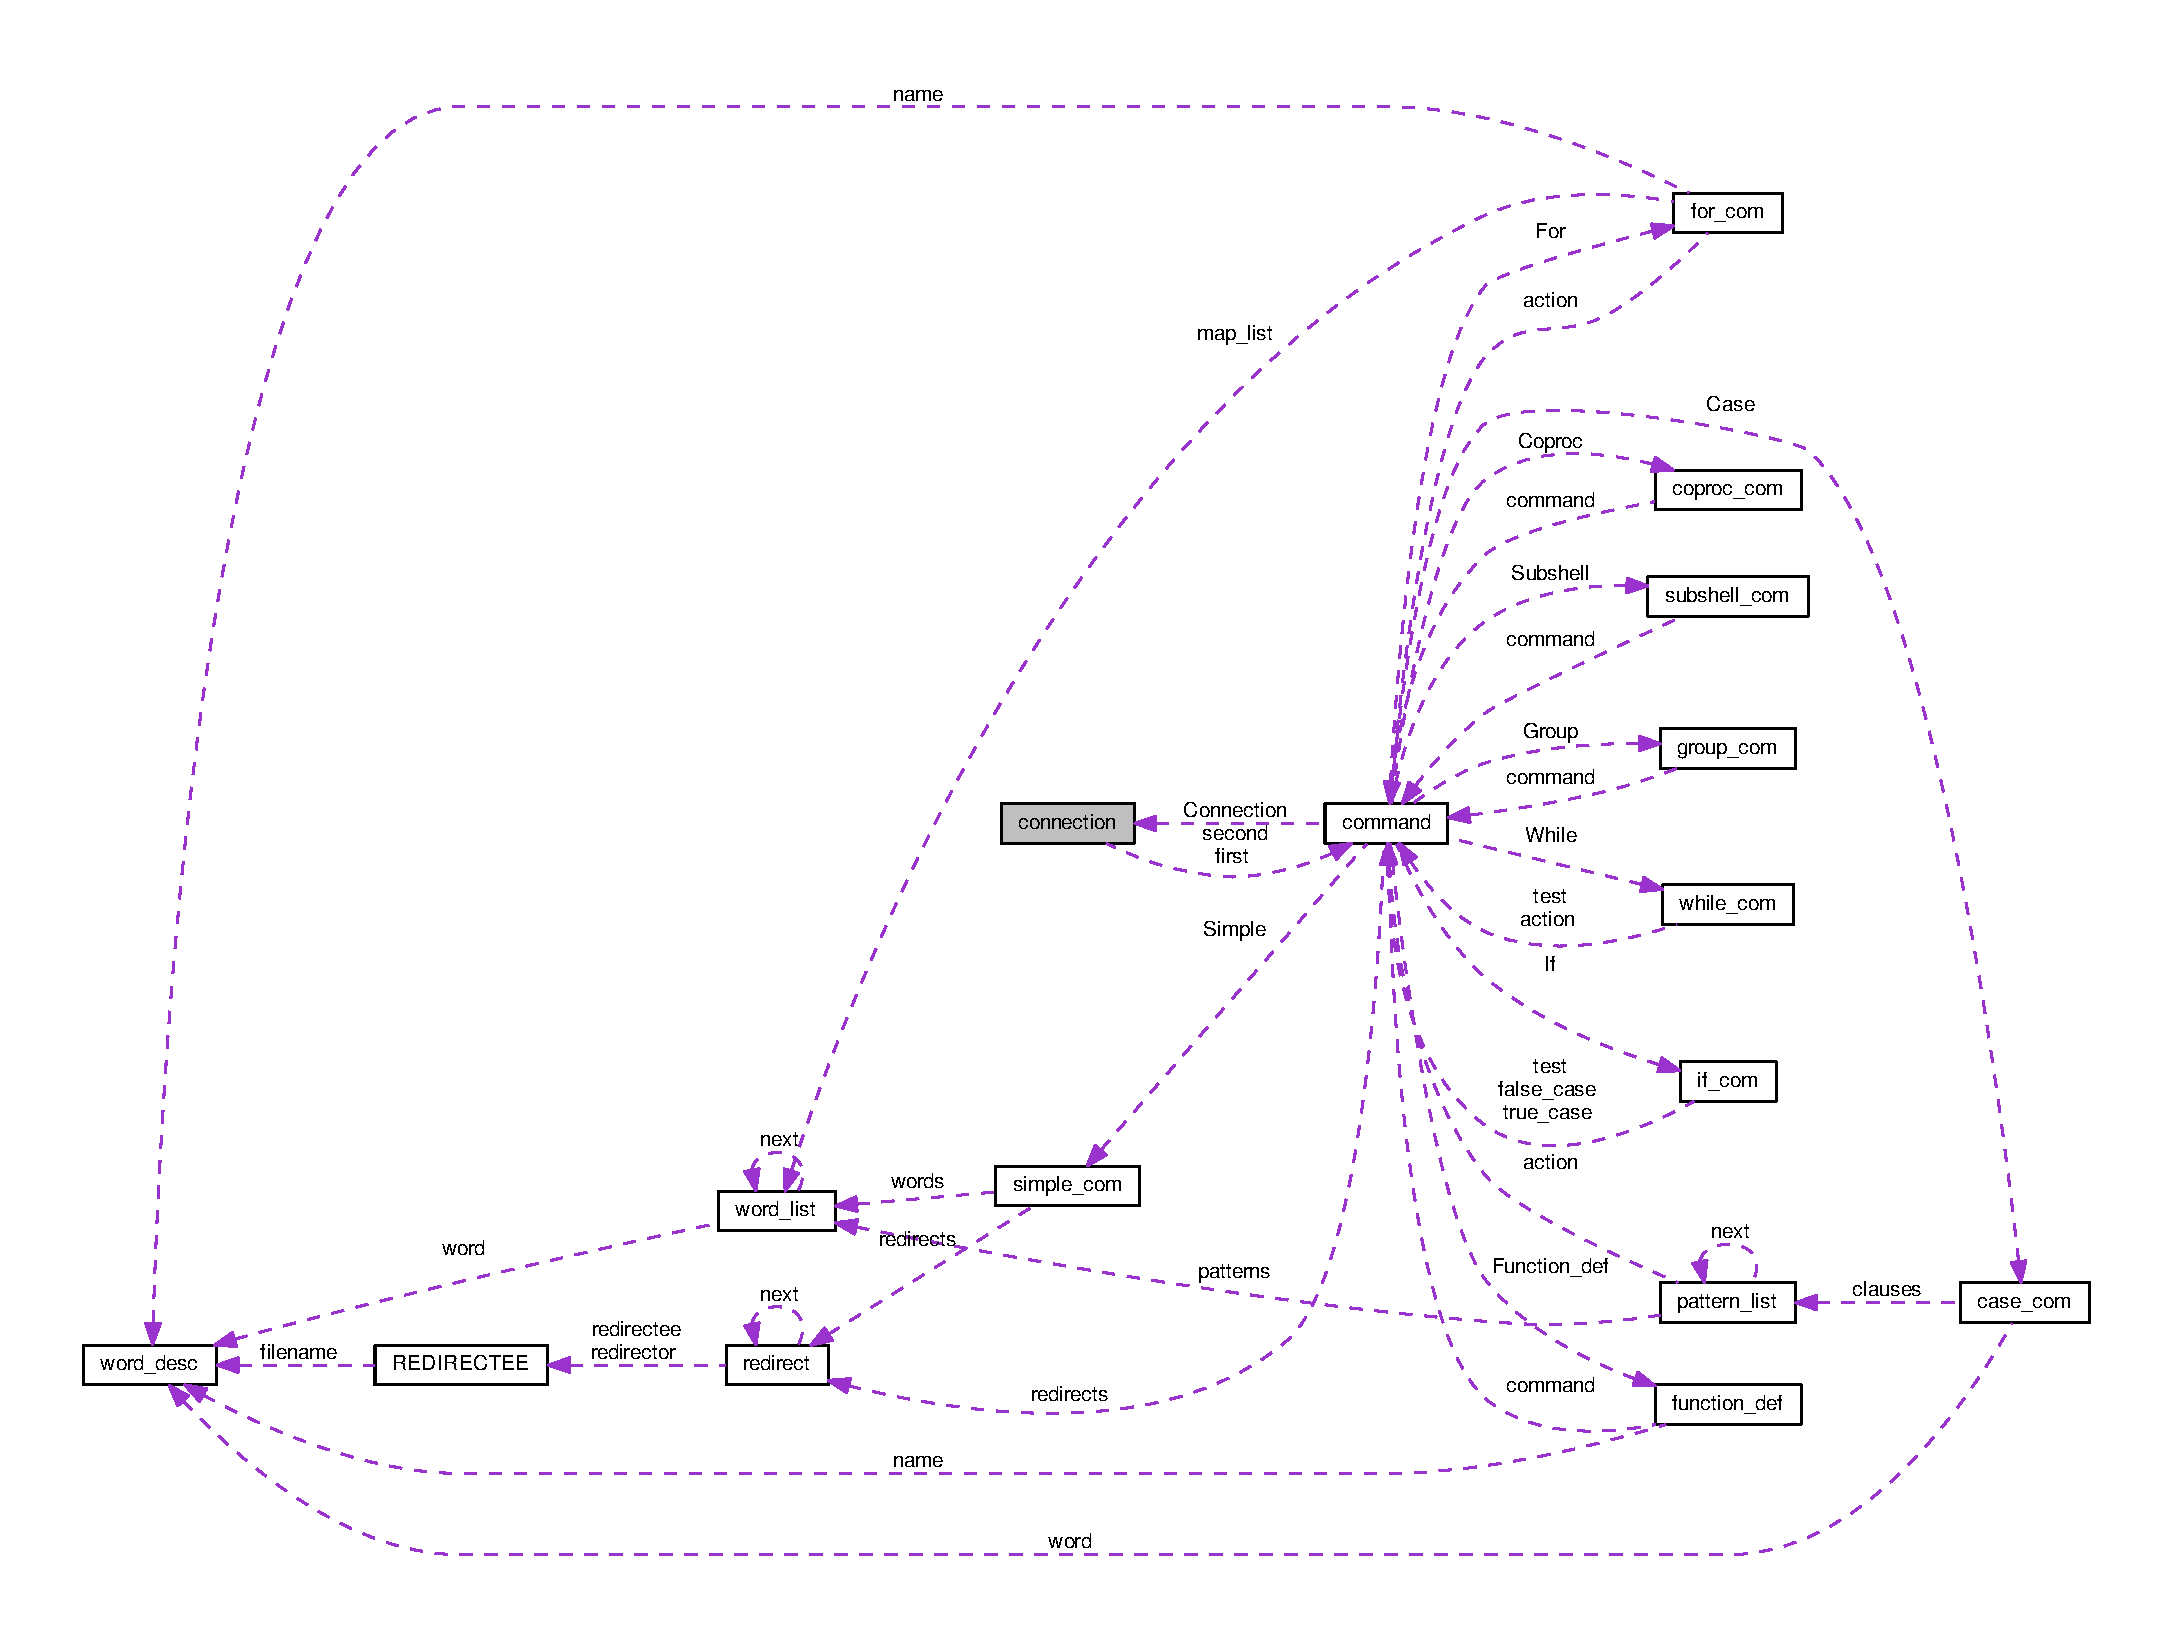
\includegraphics[width=350pt]{structconnection__coll__graph}
\end{center}
\end{figure}
\subsection*{Public Attributes}
\begin{DoxyCompactItemize}
\item 
int \hyperlink{structconnection_a5457e2643b42913b65e75ae6aadc4af6}{ignore}
\item 
\hyperlink{command_8h_a8c41dec142c299806885773c902c0d87}{C\+O\+M\+M\+A\+ND} $\ast$ \hyperlink{structconnection_a63a41b4deafe124ccd4b50c6767c1945}{first}
\item 
\hyperlink{command_8h_a8c41dec142c299806885773c902c0d87}{C\+O\+M\+M\+A\+ND} $\ast$ \hyperlink{structconnection_a3abadad2499f8d84171526134c8a2ce1}{second}
\item 
int \hyperlink{structconnection_a07879bb1744b9d358c5042cd08ef8570}{connector}
\end{DoxyCompactItemize}


\subsection{Member Data Documentation}
\index{connection@{connection}!connector@{connector}}
\index{connector@{connector}!connection@{connection}}
\subsubsection[{\texorpdfstring{connector}{connector}}]{\setlength{\rightskip}{0pt plus 5cm}int connection\+::connector}\hypertarget{structconnection_a07879bb1744b9d358c5042cd08ef8570}{}\label{structconnection_a07879bb1744b9d358c5042cd08ef8570}
\index{connection@{connection}!first@{first}}
\index{first@{first}!connection@{connection}}
\subsubsection[{\texorpdfstring{first}{first}}]{\setlength{\rightskip}{0pt plus 5cm}{\bf C\+O\+M\+M\+A\+ND}$\ast$ connection\+::first}\hypertarget{structconnection_a63a41b4deafe124ccd4b50c6767c1945}{}\label{structconnection_a63a41b4deafe124ccd4b50c6767c1945}
\index{connection@{connection}!ignore@{ignore}}
\index{ignore@{ignore}!connection@{connection}}
\subsubsection[{\texorpdfstring{ignore}{ignore}}]{\setlength{\rightskip}{0pt plus 5cm}int connection\+::ignore}\hypertarget{structconnection_a5457e2643b42913b65e75ae6aadc4af6}{}\label{structconnection_a5457e2643b42913b65e75ae6aadc4af6}
\index{connection@{connection}!second@{second}}
\index{second@{second}!connection@{connection}}
\subsubsection[{\texorpdfstring{second}{second}}]{\setlength{\rightskip}{0pt plus 5cm}{\bf C\+O\+M\+M\+A\+ND}$\ast$ connection\+::second}\hypertarget{structconnection_a3abadad2499f8d84171526134c8a2ce1}{}\label{structconnection_a3abadad2499f8d84171526134c8a2ce1}


The documentation for this struct was generated from the following file\+:\begin{DoxyCompactItemize}
\item 
\hyperlink{command_8h}{command.\+h}\end{DoxyCompactItemize}

\hypertarget{structcoproc}{}\section{coproc Struct Reference}
\label{structcoproc}\index{coproc@{coproc}}


{\ttfamily \#include $<$command.\+h$>$}

\subsection*{Public Attributes}
\begin{DoxyCompactItemize}
\item 
char $\ast$ \hyperlink{structcoproc_aff6c7c0df15a92848d6ec3024515f02b}{c\+\_\+name}
\item 
pid\+\_\+t \hyperlink{structcoproc_a985b501e47aedaebc0116f4f49e9be41}{c\+\_\+pid}
\item 
int \hyperlink{structcoproc_a20617bf930c55d6fd4de603784331545}{c\+\_\+rfd}
\item 
int \hyperlink{structcoproc_a2c12afc95d8231a2627a08351903425c}{c\+\_\+wfd}
\item 
int \hyperlink{structcoproc_a9fb038976ae82a22c7ba1b418285e17b}{c\+\_\+rsave}
\item 
int \hyperlink{structcoproc_a3c0bb857aacc8176f88f20075e902fd6}{c\+\_\+wsave}
\item 
int \hyperlink{structcoproc_afb0ac3c4ec995790bf72cb0ef27854e6}{c\+\_\+flags}
\item 
int \hyperlink{structcoproc_ab742e5285c2dc8e39fd5b6b89c68522e}{c\+\_\+status}
\item 
int \hyperlink{structcoproc_a34bf762bf4fa2b6f79d9ebc12302819a}{c\+\_\+lock}
\end{DoxyCompactItemize}


\subsection{Member Data Documentation}
\index{coproc@{coproc}!c\+\_\+flags@{c\+\_\+flags}}
\index{c\+\_\+flags@{c\+\_\+flags}!coproc@{coproc}}
\subsubsection[{\texorpdfstring{c\+\_\+flags}{c_flags}}]{\setlength{\rightskip}{0pt plus 5cm}int coproc\+::c\+\_\+flags}\hypertarget{structcoproc_afb0ac3c4ec995790bf72cb0ef27854e6}{}\label{structcoproc_afb0ac3c4ec995790bf72cb0ef27854e6}
\index{coproc@{coproc}!c\+\_\+lock@{c\+\_\+lock}}
\index{c\+\_\+lock@{c\+\_\+lock}!coproc@{coproc}}
\subsubsection[{\texorpdfstring{c\+\_\+lock}{c_lock}}]{\setlength{\rightskip}{0pt plus 5cm}int coproc\+::c\+\_\+lock}\hypertarget{structcoproc_a34bf762bf4fa2b6f79d9ebc12302819a}{}\label{structcoproc_a34bf762bf4fa2b6f79d9ebc12302819a}
\index{coproc@{coproc}!c\+\_\+name@{c\+\_\+name}}
\index{c\+\_\+name@{c\+\_\+name}!coproc@{coproc}}
\subsubsection[{\texorpdfstring{c\+\_\+name}{c_name}}]{\setlength{\rightskip}{0pt plus 5cm}char$\ast$ coproc\+::c\+\_\+name}\hypertarget{structcoproc_aff6c7c0df15a92848d6ec3024515f02b}{}\label{structcoproc_aff6c7c0df15a92848d6ec3024515f02b}
\index{coproc@{coproc}!c\+\_\+pid@{c\+\_\+pid}}
\index{c\+\_\+pid@{c\+\_\+pid}!coproc@{coproc}}
\subsubsection[{\texorpdfstring{c\+\_\+pid}{c_pid}}]{\setlength{\rightskip}{0pt plus 5cm}pid\+\_\+t coproc\+::c\+\_\+pid}\hypertarget{structcoproc_a985b501e47aedaebc0116f4f49e9be41}{}\label{structcoproc_a985b501e47aedaebc0116f4f49e9be41}
\index{coproc@{coproc}!c\+\_\+rfd@{c\+\_\+rfd}}
\index{c\+\_\+rfd@{c\+\_\+rfd}!coproc@{coproc}}
\subsubsection[{\texorpdfstring{c\+\_\+rfd}{c_rfd}}]{\setlength{\rightskip}{0pt plus 5cm}int coproc\+::c\+\_\+rfd}\hypertarget{structcoproc_a20617bf930c55d6fd4de603784331545}{}\label{structcoproc_a20617bf930c55d6fd4de603784331545}
\index{coproc@{coproc}!c\+\_\+rsave@{c\+\_\+rsave}}
\index{c\+\_\+rsave@{c\+\_\+rsave}!coproc@{coproc}}
\subsubsection[{\texorpdfstring{c\+\_\+rsave}{c_rsave}}]{\setlength{\rightskip}{0pt plus 5cm}int coproc\+::c\+\_\+rsave}\hypertarget{structcoproc_a9fb038976ae82a22c7ba1b418285e17b}{}\label{structcoproc_a9fb038976ae82a22c7ba1b418285e17b}
\index{coproc@{coproc}!c\+\_\+status@{c\+\_\+status}}
\index{c\+\_\+status@{c\+\_\+status}!coproc@{coproc}}
\subsubsection[{\texorpdfstring{c\+\_\+status}{c_status}}]{\setlength{\rightskip}{0pt plus 5cm}int coproc\+::c\+\_\+status}\hypertarget{structcoproc_ab742e5285c2dc8e39fd5b6b89c68522e}{}\label{structcoproc_ab742e5285c2dc8e39fd5b6b89c68522e}
\index{coproc@{coproc}!c\+\_\+wfd@{c\+\_\+wfd}}
\index{c\+\_\+wfd@{c\+\_\+wfd}!coproc@{coproc}}
\subsubsection[{\texorpdfstring{c\+\_\+wfd}{c_wfd}}]{\setlength{\rightskip}{0pt plus 5cm}int coproc\+::c\+\_\+wfd}\hypertarget{structcoproc_a2c12afc95d8231a2627a08351903425c}{}\label{structcoproc_a2c12afc95d8231a2627a08351903425c}
\index{coproc@{coproc}!c\+\_\+wsave@{c\+\_\+wsave}}
\index{c\+\_\+wsave@{c\+\_\+wsave}!coproc@{coproc}}
\subsubsection[{\texorpdfstring{c\+\_\+wsave}{c_wsave}}]{\setlength{\rightskip}{0pt plus 5cm}int coproc\+::c\+\_\+wsave}\hypertarget{structcoproc_a3c0bb857aacc8176f88f20075e902fd6}{}\label{structcoproc_a3c0bb857aacc8176f88f20075e902fd6}


The documentation for this struct was generated from the following file\+:\begin{DoxyCompactItemize}
\item 
\hyperlink{command_8h}{command.\+h}\end{DoxyCompactItemize}

\hypertarget{structcoproc__com}{}\section{coproc\+\_\+com Struct Reference}
\label{structcoproc__com}\index{coproc\+\_\+com@{coproc\+\_\+com}}


{\ttfamily \#include $<$command.\+h$>$}



Collaboration diagram for coproc\+\_\+com\+:
\nopagebreak
\begin{figure}[H]
\begin{center}
\leavevmode
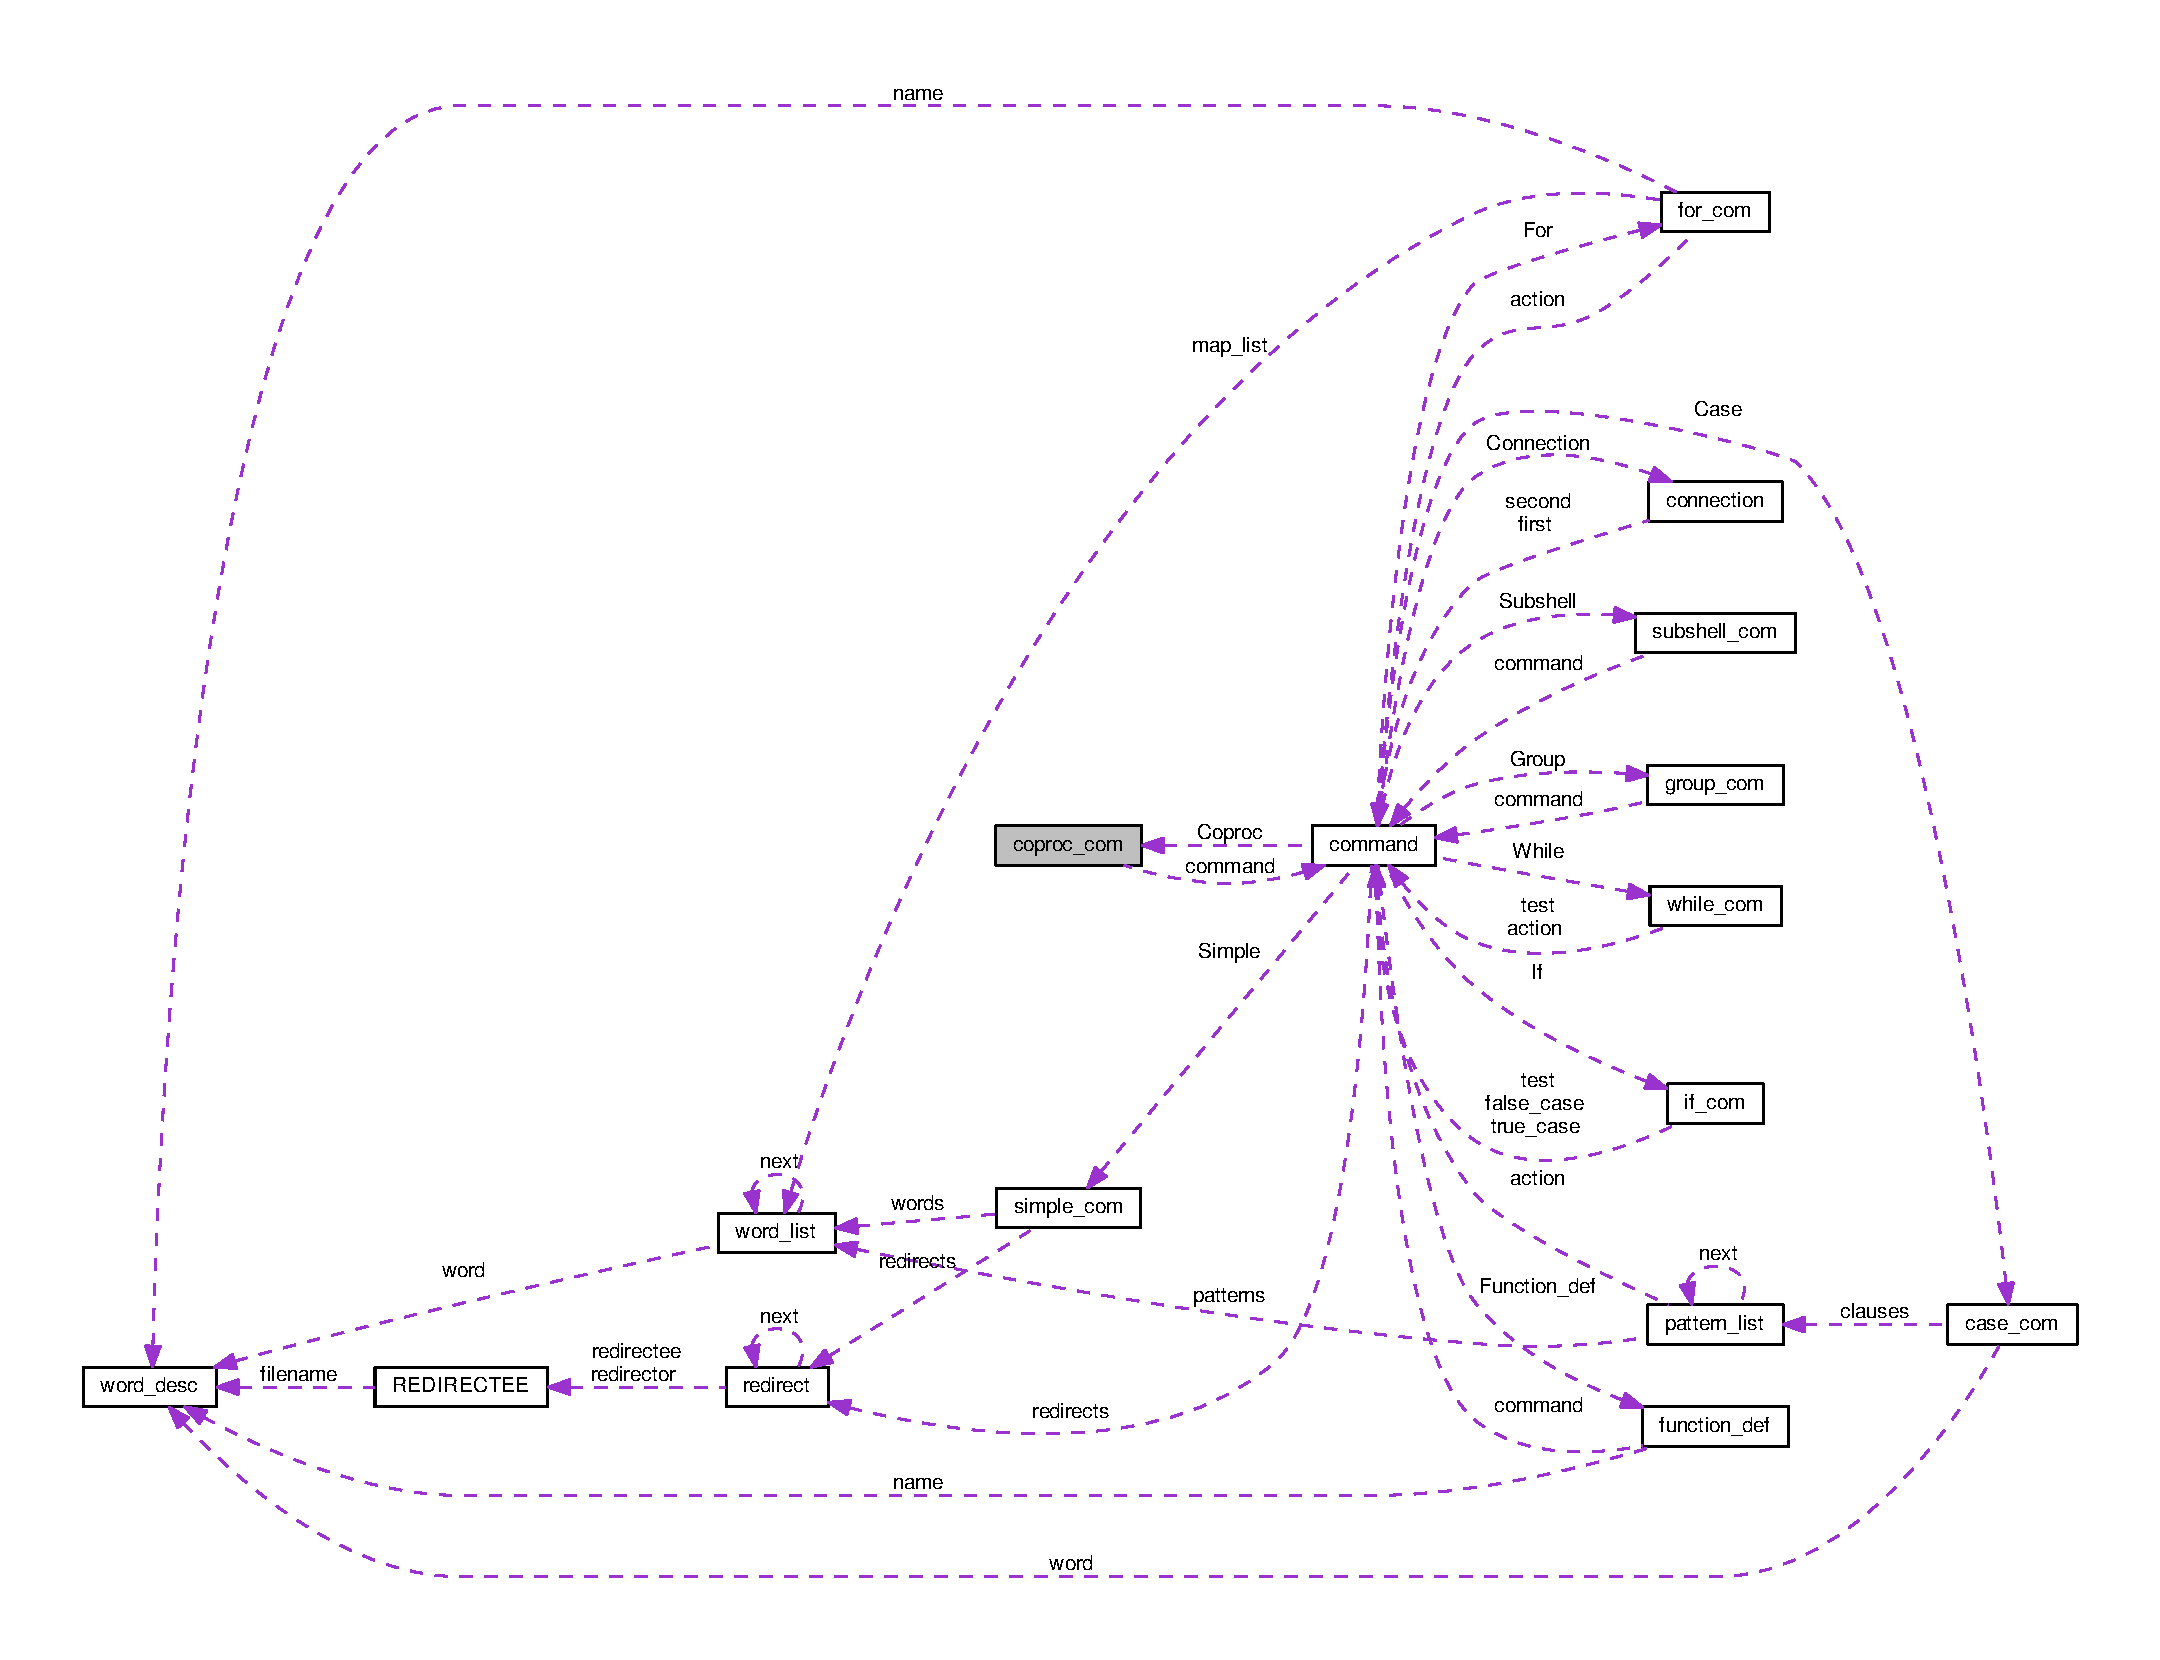
\includegraphics[width=350pt]{structcoproc__com__coll__graph}
\end{center}
\end{figure}
\subsection*{Public Attributes}
\begin{DoxyCompactItemize}
\item 
int \hyperlink{structcoproc__com_a01d4593beb818d1f8b158b482194ad61}{flags}
\item 
char $\ast$ \hyperlink{structcoproc__com_a6d076457d5bc4a12617e68939a1f7afa}{name}
\item 
\hyperlink{command_8h_a8c41dec142c299806885773c902c0d87}{C\+O\+M\+M\+A\+ND} $\ast$ \hyperlink{structcoproc__com_a22bba3feba2226cd96700bbc5502766f}{command}
\end{DoxyCompactItemize}


\subsection{Member Data Documentation}
\index{coproc\+\_\+com@{coproc\+\_\+com}!command@{command}}
\index{command@{command}!coproc\+\_\+com@{coproc\+\_\+com}}
\subsubsection[{\texorpdfstring{command}{command}}]{\setlength{\rightskip}{0pt plus 5cm}{\bf C\+O\+M\+M\+A\+ND}$\ast$ coproc\+\_\+com\+::command}\hypertarget{structcoproc__com_a22bba3feba2226cd96700bbc5502766f}{}\label{structcoproc__com_a22bba3feba2226cd96700bbc5502766f}
\index{coproc\+\_\+com@{coproc\+\_\+com}!flags@{flags}}
\index{flags@{flags}!coproc\+\_\+com@{coproc\+\_\+com}}
\subsubsection[{\texorpdfstring{flags}{flags}}]{\setlength{\rightskip}{0pt plus 5cm}int coproc\+\_\+com\+::flags}\hypertarget{structcoproc__com_a01d4593beb818d1f8b158b482194ad61}{}\label{structcoproc__com_a01d4593beb818d1f8b158b482194ad61}
\index{coproc\+\_\+com@{coproc\+\_\+com}!name@{name}}
\index{name@{name}!coproc\+\_\+com@{coproc\+\_\+com}}
\subsubsection[{\texorpdfstring{name}{name}}]{\setlength{\rightskip}{0pt plus 5cm}char$\ast$ coproc\+\_\+com\+::name}\hypertarget{structcoproc__com_a6d076457d5bc4a12617e68939a1f7afa}{}\label{structcoproc__com_a6d076457d5bc4a12617e68939a1f7afa}


The documentation for this struct was generated from the following file\+:\begin{DoxyCompactItemize}
\item 
\hyperlink{command_8h}{command.\+h}\end{DoxyCompactItemize}

\hypertarget{structcpelement}{}\section{cpelement Struct Reference}
\label{structcpelement}\index{cpelement@{cpelement}}


Collaboration diagram for cpelement\+:
\nopagebreak
\begin{figure}[H]
\begin{center}
\leavevmode
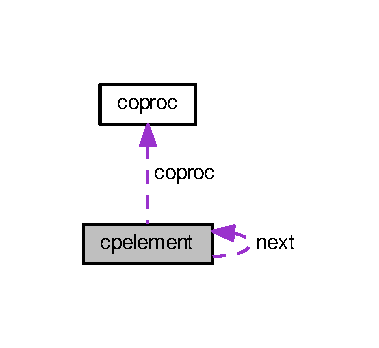
\includegraphics[width=182pt]{structcpelement__coll__graph}
\end{center}
\end{figure}
\subsection*{Public Attributes}
\begin{DoxyCompactItemize}
\item 
struct \hyperlink{structcpelement}{cpelement} $\ast$ \hyperlink{structcpelement_aad9f602c3450059111014c2c7d95e201}{next}
\item 
struct \hyperlink{structcoproc}{coproc} $\ast$ \hyperlink{structcpelement_a7793e7ecb45eab4e88d795af267f4386}{coproc}
\end{DoxyCompactItemize}


\subsection{Member Data Documentation}
\index{cpelement@{cpelement}!coproc@{coproc}}
\index{coproc@{coproc}!cpelement@{cpelement}}
\subsubsection[{\texorpdfstring{coproc}{coproc}}]{\setlength{\rightskip}{0pt plus 5cm}struct {\bf coproc}$\ast$ cpelement\+::coproc}\hypertarget{structcpelement_a7793e7ecb45eab4e88d795af267f4386}{}\label{structcpelement_a7793e7ecb45eab4e88d795af267f4386}
\index{cpelement@{cpelement}!next@{next}}
\index{next@{next}!cpelement@{cpelement}}
\subsubsection[{\texorpdfstring{next}{next}}]{\setlength{\rightskip}{0pt plus 5cm}struct {\bf cpelement}$\ast$ cpelement\+::next}\hypertarget{structcpelement_aad9f602c3450059111014c2c7d95e201}{}\label{structcpelement_aad9f602c3450059111014c2c7d95e201}


The documentation for this struct was generated from the following file\+:\begin{DoxyCompactItemize}
\item 
\hyperlink{execute__cmd_8c}{execute\+\_\+cmd.\+c}\end{DoxyCompactItemize}

\hypertarget{structcplist}{}\section{cplist Struct Reference}
\label{structcplist}\index{cplist@{cplist}}


Collaboration diagram for cplist\+:
\nopagebreak
\begin{figure}[H]
\begin{center}
\leavevmode
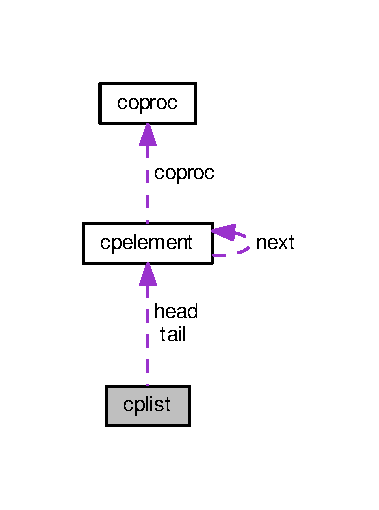
\includegraphics[width=182pt]{structcplist__coll__graph}
\end{center}
\end{figure}
\subsection*{Public Attributes}
\begin{DoxyCompactItemize}
\item 
struct \hyperlink{structcpelement}{cpelement} $\ast$ \hyperlink{structcplist_a0dbec638f97dd68d63b04c47de978763}{head}
\item 
struct \hyperlink{structcpelement}{cpelement} $\ast$ \hyperlink{structcplist_afea07987e8c9d05612ab196a2eac3514}{tail}
\item 
int \hyperlink{structcplist_aafa9e610a74bb2edf40e2f227f03928d}{ncoproc}
\item 
int \hyperlink{structcplist_aa737a27d76b31857c0d7024665731a68}{lock}
\end{DoxyCompactItemize}


\subsection{Member Data Documentation}
\index{cplist@{cplist}!head@{head}}
\index{head@{head}!cplist@{cplist}}
\subsubsection[{\texorpdfstring{head}{head}}]{\setlength{\rightskip}{0pt plus 5cm}struct {\bf cpelement}$\ast$ cplist\+::head}\hypertarget{structcplist_a0dbec638f97dd68d63b04c47de978763}{}\label{structcplist_a0dbec638f97dd68d63b04c47de978763}
\index{cplist@{cplist}!lock@{lock}}
\index{lock@{lock}!cplist@{cplist}}
\subsubsection[{\texorpdfstring{lock}{lock}}]{\setlength{\rightskip}{0pt plus 5cm}int cplist\+::lock}\hypertarget{structcplist_aa737a27d76b31857c0d7024665731a68}{}\label{structcplist_aa737a27d76b31857c0d7024665731a68}
\index{cplist@{cplist}!ncoproc@{ncoproc}}
\index{ncoproc@{ncoproc}!cplist@{cplist}}
\subsubsection[{\texorpdfstring{ncoproc}{ncoproc}}]{\setlength{\rightskip}{0pt plus 5cm}int cplist\+::ncoproc}\hypertarget{structcplist_aafa9e610a74bb2edf40e2f227f03928d}{}\label{structcplist_aafa9e610a74bb2edf40e2f227f03928d}
\index{cplist@{cplist}!tail@{tail}}
\index{tail@{tail}!cplist@{cplist}}
\subsubsection[{\texorpdfstring{tail}{tail}}]{\setlength{\rightskip}{0pt plus 5cm}struct {\bf cpelement}$\ast$ cplist\+::tail}\hypertarget{structcplist_afea07987e8c9d05612ab196a2eac3514}{}\label{structcplist_afea07987e8c9d05612ab196a2eac3514}


The documentation for this struct was generated from the following file\+:\begin{DoxyCompactItemize}
\item 
\hyperlink{execute__cmd_8c}{execute\+\_\+cmd.\+c}\end{DoxyCompactItemize}

\hypertarget{structdstack}{}\section{dstack Struct Reference}
\label{structdstack}\index{dstack@{dstack}}


{\ttfamily \#include $<$parser.\+h$>$}

\subsection*{Public Attributes}
\begin{DoxyCompactItemize}
\item 
char $\ast$ \hyperlink{structdstack_a76e9b09421f3da067f3edb3ba7229bc2}{delimiters}
\item 
int \hyperlink{structdstack_a32fe4eb7d39356859f098b15da622a13}{delimiter\+\_\+depth}
\item 
int \hyperlink{structdstack_a69372e28e3d49e5b0f0d7b806da50f6b}{delimiter\+\_\+space}
\end{DoxyCompactItemize}


\subsection{Member Data Documentation}
\index{dstack@{dstack}!delimiter\+\_\+depth@{delimiter\+\_\+depth}}
\index{delimiter\+\_\+depth@{delimiter\+\_\+depth}!dstack@{dstack}}
\subsubsection[{\texorpdfstring{delimiter\+\_\+depth}{delimiter_depth}}]{\setlength{\rightskip}{0pt plus 5cm}int dstack\+::delimiter\+\_\+depth}\hypertarget{structdstack_a32fe4eb7d39356859f098b15da622a13}{}\label{structdstack_a32fe4eb7d39356859f098b15da622a13}
\index{dstack@{dstack}!delimiter\+\_\+space@{delimiter\+\_\+space}}
\index{delimiter\+\_\+space@{delimiter\+\_\+space}!dstack@{dstack}}
\subsubsection[{\texorpdfstring{delimiter\+\_\+space}{delimiter_space}}]{\setlength{\rightskip}{0pt plus 5cm}int dstack\+::delimiter\+\_\+space}\hypertarget{structdstack_a69372e28e3d49e5b0f0d7b806da50f6b}{}\label{structdstack_a69372e28e3d49e5b0f0d7b806da50f6b}
\index{dstack@{dstack}!delimiters@{delimiters}}
\index{delimiters@{delimiters}!dstack@{dstack}}
\subsubsection[{\texorpdfstring{delimiters}{delimiters}}]{\setlength{\rightskip}{0pt plus 5cm}char$\ast$ dstack\+::delimiters}\hypertarget{structdstack_a76e9b09421f3da067f3edb3ba7229bc2}{}\label{structdstack_a76e9b09421f3da067f3edb3ba7229bc2}


The documentation for this struct was generated from the following file\+:\begin{DoxyCompactItemize}
\item 
\hyperlink{parser_8h}{parser.\+h}\end{DoxyCompactItemize}

\hypertarget{structelement}{}\section{element Struct Reference}
\label{structelement}\index{element@{element}}


{\ttfamily \#include $<$command.\+h$>$}



Collaboration diagram for element\+:
\nopagebreak
\begin{figure}[H]
\begin{center}
\leavevmode
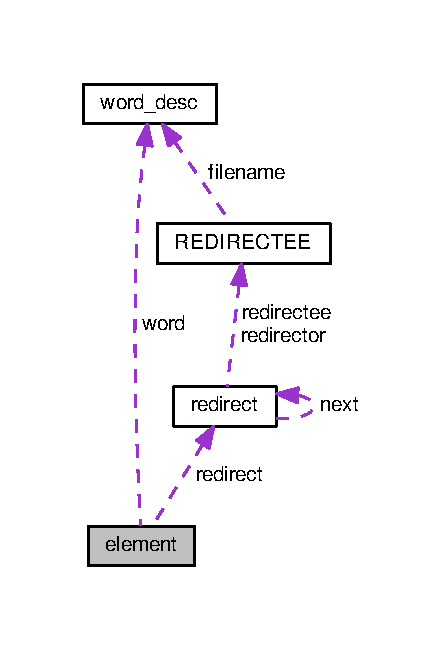
\includegraphics[width=213pt]{structelement__coll__graph}
\end{center}
\end{figure}
\subsection*{Public Attributes}
\begin{DoxyCompactItemize}
\item 
\hyperlink{command_8h_a3f0cccf333703e5f6c4168be0db675fa}{W\+O\+R\+D\+\_\+\+D\+E\+SC} $\ast$ \hyperlink{structelement_a74c8c3c3cf92b8287e450fab71ed2074}{word}
\item 
\hyperlink{command_8h_adeb9f5d937c92c7923aec48ad5e47d57}{R\+E\+D\+I\+R\+E\+CT} $\ast$ \hyperlink{structelement_ad3f13da7e9bdbe54746af382c8b6d9e5}{redirect}
\end{DoxyCompactItemize}


\subsection{Member Data Documentation}
\index{element@{element}!redirect@{redirect}}
\index{redirect@{redirect}!element@{element}}
\subsubsection[{\texorpdfstring{redirect}{redirect}}]{\setlength{\rightskip}{0pt plus 5cm}{\bf R\+E\+D\+I\+R\+E\+CT}$\ast$ element\+::redirect}\hypertarget{structelement_ad3f13da7e9bdbe54746af382c8b6d9e5}{}\label{structelement_ad3f13da7e9bdbe54746af382c8b6d9e5}
\index{element@{element}!word@{word}}
\index{word@{word}!element@{element}}
\subsubsection[{\texorpdfstring{word}{word}}]{\setlength{\rightskip}{0pt plus 5cm}{\bf W\+O\+R\+D\+\_\+\+D\+E\+SC}$\ast$ element\+::word}\hypertarget{structelement_a74c8c3c3cf92b8287e450fab71ed2074}{}\label{structelement_a74c8c3c3cf92b8287e450fab71ed2074}


The documentation for this struct was generated from the following file\+:\begin{DoxyCompactItemize}
\item 
\hyperlink{command_8h}{command.\+h}\end{DoxyCompactItemize}

\hypertarget{structexecstate}{}\section{execstate Struct Reference}
\label{structexecstate}\index{execstate@{execstate}}


{\ttfamily \#include $<$execute\+\_\+cmd.\+h$>$}

\subsection*{Public Attributes}
\begin{DoxyCompactItemize}
\item 
pid\+\_\+t \hyperlink{structexecstate_af6e5f0a8dbfecb8a58b69505a0006841}{pid}
\item 
int \hyperlink{structexecstate_a1396897622963c57e753be7d2cef693c}{subshell\+\_\+env}
\end{DoxyCompactItemize}


\subsection{Member Data Documentation}
\index{execstate@{execstate}!pid@{pid}}
\index{pid@{pid}!execstate@{execstate}}
\subsubsection[{\texorpdfstring{pid}{pid}}]{\setlength{\rightskip}{0pt plus 5cm}pid\+\_\+t execstate\+::pid}\hypertarget{structexecstate_af6e5f0a8dbfecb8a58b69505a0006841}{}\label{structexecstate_af6e5f0a8dbfecb8a58b69505a0006841}
\index{execstate@{execstate}!subshell\+\_\+env@{subshell\+\_\+env}}
\index{subshell\+\_\+env@{subshell\+\_\+env}!execstate@{execstate}}
\subsubsection[{\texorpdfstring{subshell\+\_\+env}{subshell_env}}]{\setlength{\rightskip}{0pt plus 5cm}int execstate\+::subshell\+\_\+env}\hypertarget{structexecstate_a1396897622963c57e753be7d2cef693c}{}\label{structexecstate_a1396897622963c57e753be7d2cef693c}


The documentation for this struct was generated from the following file\+:\begin{DoxyCompactItemize}
\item 
\hyperlink{execute__cmd_8h}{execute\+\_\+cmd.\+h}\end{DoxyCompactItemize}

\hypertarget{structEXPR__CONTEXT}{}\section{E\+X\+P\+R\+\_\+\+C\+O\+N\+T\+E\+XT Struct Reference}
\label{structEXPR__CONTEXT}\index{E\+X\+P\+R\+\_\+\+C\+O\+N\+T\+E\+XT@{E\+X\+P\+R\+\_\+\+C\+O\+N\+T\+E\+XT}}


Collaboration diagram for E\+X\+P\+R\+\_\+\+C\+O\+N\+T\+E\+XT\+:
\nopagebreak
\begin{figure}[H]
\begin{center}
\leavevmode
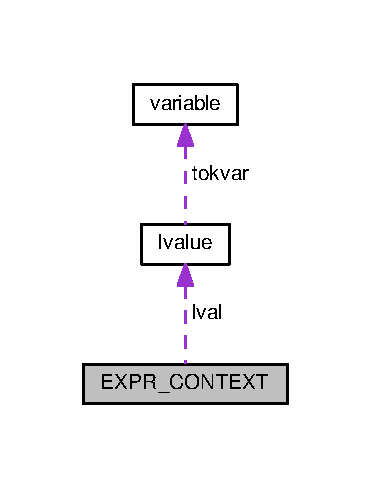
\includegraphics[width=178pt]{structEXPR__CONTEXT__coll__graph}
\end{center}
\end{figure}
\subsection*{Public Attributes}
\begin{DoxyCompactItemize}
\item 
int \hyperlink{structEXPR__CONTEXT_a4d2a3800331cf9f6c553a52a58e2a7ee}{curtok}
\item 
int \hyperlink{structEXPR__CONTEXT_acaf7c6bd8d7c56b7ddc1b8aa10de62fe}{lasttok}
\item 
char $\ast$ \hyperlink{structEXPR__CONTEXT_a708aed9cc491f274bbbeb63f76a2d41f}{expression}
\item 
char $\ast$ \hyperlink{structEXPR__CONTEXT_ab7a73351a352ce4e87d11ca20144ecdf}{tp}
\item 
char $\ast$ \hyperlink{structEXPR__CONTEXT_a69e10a40e10bd2502db453c4d593a464}{lasttp}
\item 
intmax\+\_\+t \hyperlink{structEXPR__CONTEXT_abbae8e63dab085277ea9e730a3b84692}{tokval}
\item 
char $\ast$ \hyperlink{structEXPR__CONTEXT_a5b236994684e80356f71a1aec4f7d0c7}{tokstr}
\item 
int \hyperlink{structEXPR__CONTEXT_a164e4613724fa3f72f3460f58d595e5a}{noeval}
\item 
struct \hyperlink{structlvalue}{lvalue} \hyperlink{structEXPR__CONTEXT_ab497084844b30afe35fbb51b06fb6505}{lval}
\end{DoxyCompactItemize}


\subsection{Member Data Documentation}
\index{E\+X\+P\+R\+\_\+\+C\+O\+N\+T\+E\+XT@{E\+X\+P\+R\+\_\+\+C\+O\+N\+T\+E\+XT}!curtok@{curtok}}
\index{curtok@{curtok}!E\+X\+P\+R\+\_\+\+C\+O\+N\+T\+E\+XT@{E\+X\+P\+R\+\_\+\+C\+O\+N\+T\+E\+XT}}
\subsubsection[{\texorpdfstring{curtok}{curtok}}]{\setlength{\rightskip}{0pt plus 5cm}int E\+X\+P\+R\+\_\+\+C\+O\+N\+T\+E\+X\+T\+::curtok}\hypertarget{structEXPR__CONTEXT_a4d2a3800331cf9f6c553a52a58e2a7ee}{}\label{structEXPR__CONTEXT_a4d2a3800331cf9f6c553a52a58e2a7ee}
\index{E\+X\+P\+R\+\_\+\+C\+O\+N\+T\+E\+XT@{E\+X\+P\+R\+\_\+\+C\+O\+N\+T\+E\+XT}!expression@{expression}}
\index{expression@{expression}!E\+X\+P\+R\+\_\+\+C\+O\+N\+T\+E\+XT@{E\+X\+P\+R\+\_\+\+C\+O\+N\+T\+E\+XT}}
\subsubsection[{\texorpdfstring{expression}{expression}}]{\setlength{\rightskip}{0pt plus 5cm}char$\ast$ E\+X\+P\+R\+\_\+\+C\+O\+N\+T\+E\+X\+T\+::expression}\hypertarget{structEXPR__CONTEXT_a708aed9cc491f274bbbeb63f76a2d41f}{}\label{structEXPR__CONTEXT_a708aed9cc491f274bbbeb63f76a2d41f}
\index{E\+X\+P\+R\+\_\+\+C\+O\+N\+T\+E\+XT@{E\+X\+P\+R\+\_\+\+C\+O\+N\+T\+E\+XT}!lasttok@{lasttok}}
\index{lasttok@{lasttok}!E\+X\+P\+R\+\_\+\+C\+O\+N\+T\+E\+XT@{E\+X\+P\+R\+\_\+\+C\+O\+N\+T\+E\+XT}}
\subsubsection[{\texorpdfstring{lasttok}{lasttok}}]{\setlength{\rightskip}{0pt plus 5cm}int E\+X\+P\+R\+\_\+\+C\+O\+N\+T\+E\+X\+T\+::lasttok}\hypertarget{structEXPR__CONTEXT_acaf7c6bd8d7c56b7ddc1b8aa10de62fe}{}\label{structEXPR__CONTEXT_acaf7c6bd8d7c56b7ddc1b8aa10de62fe}
\index{E\+X\+P\+R\+\_\+\+C\+O\+N\+T\+E\+XT@{E\+X\+P\+R\+\_\+\+C\+O\+N\+T\+E\+XT}!lasttp@{lasttp}}
\index{lasttp@{lasttp}!E\+X\+P\+R\+\_\+\+C\+O\+N\+T\+E\+XT@{E\+X\+P\+R\+\_\+\+C\+O\+N\+T\+E\+XT}}
\subsubsection[{\texorpdfstring{lasttp}{lasttp}}]{\setlength{\rightskip}{0pt plus 5cm}char $\ast$ E\+X\+P\+R\+\_\+\+C\+O\+N\+T\+E\+X\+T\+::lasttp}\hypertarget{structEXPR__CONTEXT_a69e10a40e10bd2502db453c4d593a464}{}\label{structEXPR__CONTEXT_a69e10a40e10bd2502db453c4d593a464}
\index{E\+X\+P\+R\+\_\+\+C\+O\+N\+T\+E\+XT@{E\+X\+P\+R\+\_\+\+C\+O\+N\+T\+E\+XT}!lval@{lval}}
\index{lval@{lval}!E\+X\+P\+R\+\_\+\+C\+O\+N\+T\+E\+XT@{E\+X\+P\+R\+\_\+\+C\+O\+N\+T\+E\+XT}}
\subsubsection[{\texorpdfstring{lval}{lval}}]{\setlength{\rightskip}{0pt plus 5cm}struct {\bf lvalue} E\+X\+P\+R\+\_\+\+C\+O\+N\+T\+E\+X\+T\+::lval}\hypertarget{structEXPR__CONTEXT_ab497084844b30afe35fbb51b06fb6505}{}\label{structEXPR__CONTEXT_ab497084844b30afe35fbb51b06fb6505}
\index{E\+X\+P\+R\+\_\+\+C\+O\+N\+T\+E\+XT@{E\+X\+P\+R\+\_\+\+C\+O\+N\+T\+E\+XT}!noeval@{noeval}}
\index{noeval@{noeval}!E\+X\+P\+R\+\_\+\+C\+O\+N\+T\+E\+XT@{E\+X\+P\+R\+\_\+\+C\+O\+N\+T\+E\+XT}}
\subsubsection[{\texorpdfstring{noeval}{noeval}}]{\setlength{\rightskip}{0pt plus 5cm}int E\+X\+P\+R\+\_\+\+C\+O\+N\+T\+E\+X\+T\+::noeval}\hypertarget{structEXPR__CONTEXT_a164e4613724fa3f72f3460f58d595e5a}{}\label{structEXPR__CONTEXT_a164e4613724fa3f72f3460f58d595e5a}
\index{E\+X\+P\+R\+\_\+\+C\+O\+N\+T\+E\+XT@{E\+X\+P\+R\+\_\+\+C\+O\+N\+T\+E\+XT}!tokstr@{tokstr}}
\index{tokstr@{tokstr}!E\+X\+P\+R\+\_\+\+C\+O\+N\+T\+E\+XT@{E\+X\+P\+R\+\_\+\+C\+O\+N\+T\+E\+XT}}
\subsubsection[{\texorpdfstring{tokstr}{tokstr}}]{\setlength{\rightskip}{0pt plus 5cm}char$\ast$ E\+X\+P\+R\+\_\+\+C\+O\+N\+T\+E\+X\+T\+::tokstr}\hypertarget{structEXPR__CONTEXT_a5b236994684e80356f71a1aec4f7d0c7}{}\label{structEXPR__CONTEXT_a5b236994684e80356f71a1aec4f7d0c7}
\index{E\+X\+P\+R\+\_\+\+C\+O\+N\+T\+E\+XT@{E\+X\+P\+R\+\_\+\+C\+O\+N\+T\+E\+XT}!tokval@{tokval}}
\index{tokval@{tokval}!E\+X\+P\+R\+\_\+\+C\+O\+N\+T\+E\+XT@{E\+X\+P\+R\+\_\+\+C\+O\+N\+T\+E\+XT}}
\subsubsection[{\texorpdfstring{tokval}{tokval}}]{\setlength{\rightskip}{0pt plus 5cm}intmax\+\_\+t E\+X\+P\+R\+\_\+\+C\+O\+N\+T\+E\+X\+T\+::tokval}\hypertarget{structEXPR__CONTEXT_abbae8e63dab085277ea9e730a3b84692}{}\label{structEXPR__CONTEXT_abbae8e63dab085277ea9e730a3b84692}
\index{E\+X\+P\+R\+\_\+\+C\+O\+N\+T\+E\+XT@{E\+X\+P\+R\+\_\+\+C\+O\+N\+T\+E\+XT}!tp@{tp}}
\index{tp@{tp}!E\+X\+P\+R\+\_\+\+C\+O\+N\+T\+E\+XT@{E\+X\+P\+R\+\_\+\+C\+O\+N\+T\+E\+XT}}
\subsubsection[{\texorpdfstring{tp}{tp}}]{\setlength{\rightskip}{0pt plus 5cm}char $\ast$ E\+X\+P\+R\+\_\+\+C\+O\+N\+T\+E\+X\+T\+::tp}\hypertarget{structEXPR__CONTEXT_ab7a73351a352ce4e87d11ca20144ecdf}{}\label{structEXPR__CONTEXT_ab7a73351a352ce4e87d11ca20144ecdf}


The documentation for this struct was generated from the following file\+:\begin{DoxyCompactItemize}
\item 
\hyperlink{expr_8c}{expr.\+c}\end{DoxyCompactItemize}

\hypertarget{structfd__bitmap}{}\section{fd\+\_\+bitmap Struct Reference}
\label{structfd__bitmap}\index{fd\+\_\+bitmap@{fd\+\_\+bitmap}}


{\ttfamily \#include $<$shell.\+h$>$}

\subsection*{Public Attributes}
\begin{DoxyCompactItemize}
\item 
int \hyperlink{structfd__bitmap_a28f1365151408dd4179cb4619df72025}{size}
\item 
char $\ast$ \hyperlink{structfd__bitmap_a2d08a1807d5a362717dc434518e7c7f6}{bitmap}
\end{DoxyCompactItemize}


\subsection{Member Data Documentation}
\index{fd\+\_\+bitmap@{fd\+\_\+bitmap}!bitmap@{bitmap}}
\index{bitmap@{bitmap}!fd\+\_\+bitmap@{fd\+\_\+bitmap}}
\subsubsection[{\texorpdfstring{bitmap}{bitmap}}]{\setlength{\rightskip}{0pt plus 5cm}char$\ast$ fd\+\_\+bitmap\+::bitmap}\hypertarget{structfd__bitmap_a2d08a1807d5a362717dc434518e7c7f6}{}\label{structfd__bitmap_a2d08a1807d5a362717dc434518e7c7f6}
\index{fd\+\_\+bitmap@{fd\+\_\+bitmap}!size@{size}}
\index{size@{size}!fd\+\_\+bitmap@{fd\+\_\+bitmap}}
\subsubsection[{\texorpdfstring{size}{size}}]{\setlength{\rightskip}{0pt plus 5cm}int fd\+\_\+bitmap\+::size}\hypertarget{structfd__bitmap_a28f1365151408dd4179cb4619df72025}{}\label{structfd__bitmap_a28f1365151408dd4179cb4619df72025}


The documentation for this struct was generated from the following file\+:\begin{DoxyCompactItemize}
\item 
\hyperlink{shell_8h}{shell.\+h}\end{DoxyCompactItemize}

\hypertarget{structflags__alist}{}\section{flags\+\_\+alist Struct Reference}
\label{structflags__alist}\index{flags\+\_\+alist@{flags\+\_\+alist}}


{\ttfamily \#include $<$flags.\+h$>$}

\subsection*{Public Attributes}
\begin{DoxyCompactItemize}
\item 
char \hyperlink{structflags__alist_a36e3c464caa116130903e13f2d777664}{name}
\item 
int $\ast$ \hyperlink{structflags__alist_a0389c0a127a69da0296a56a9f3f5aee1}{value}
\end{DoxyCompactItemize}


\subsection{Member Data Documentation}
\index{flags\+\_\+alist@{flags\+\_\+alist}!name@{name}}
\index{name@{name}!flags\+\_\+alist@{flags\+\_\+alist}}
\subsubsection[{\texorpdfstring{name}{name}}]{\setlength{\rightskip}{0pt plus 5cm}char flags\+\_\+alist\+::name}\hypertarget{structflags__alist_a36e3c464caa116130903e13f2d777664}{}\label{structflags__alist_a36e3c464caa116130903e13f2d777664}
\index{flags\+\_\+alist@{flags\+\_\+alist}!value@{value}}
\index{value@{value}!flags\+\_\+alist@{flags\+\_\+alist}}
\subsubsection[{\texorpdfstring{value}{value}}]{\setlength{\rightskip}{0pt plus 5cm}int$\ast$ flags\+\_\+alist\+::value}\hypertarget{structflags__alist_a0389c0a127a69da0296a56a9f3f5aee1}{}\label{structflags__alist_a0389c0a127a69da0296a56a9f3f5aee1}


The documentation for this struct was generated from the following file\+:\begin{DoxyCompactItemize}
\item 
\hyperlink{flags_8h}{flags.\+h}\end{DoxyCompactItemize}

\hypertarget{structfor__com}{}\section{for\+\_\+com Struct Reference}
\label{structfor__com}\index{for\+\_\+com@{for\+\_\+com}}


{\ttfamily \#include $<$command.\+h$>$}



Collaboration diagram for for\+\_\+com\+:
\nopagebreak
\begin{figure}[H]
\begin{center}
\leavevmode
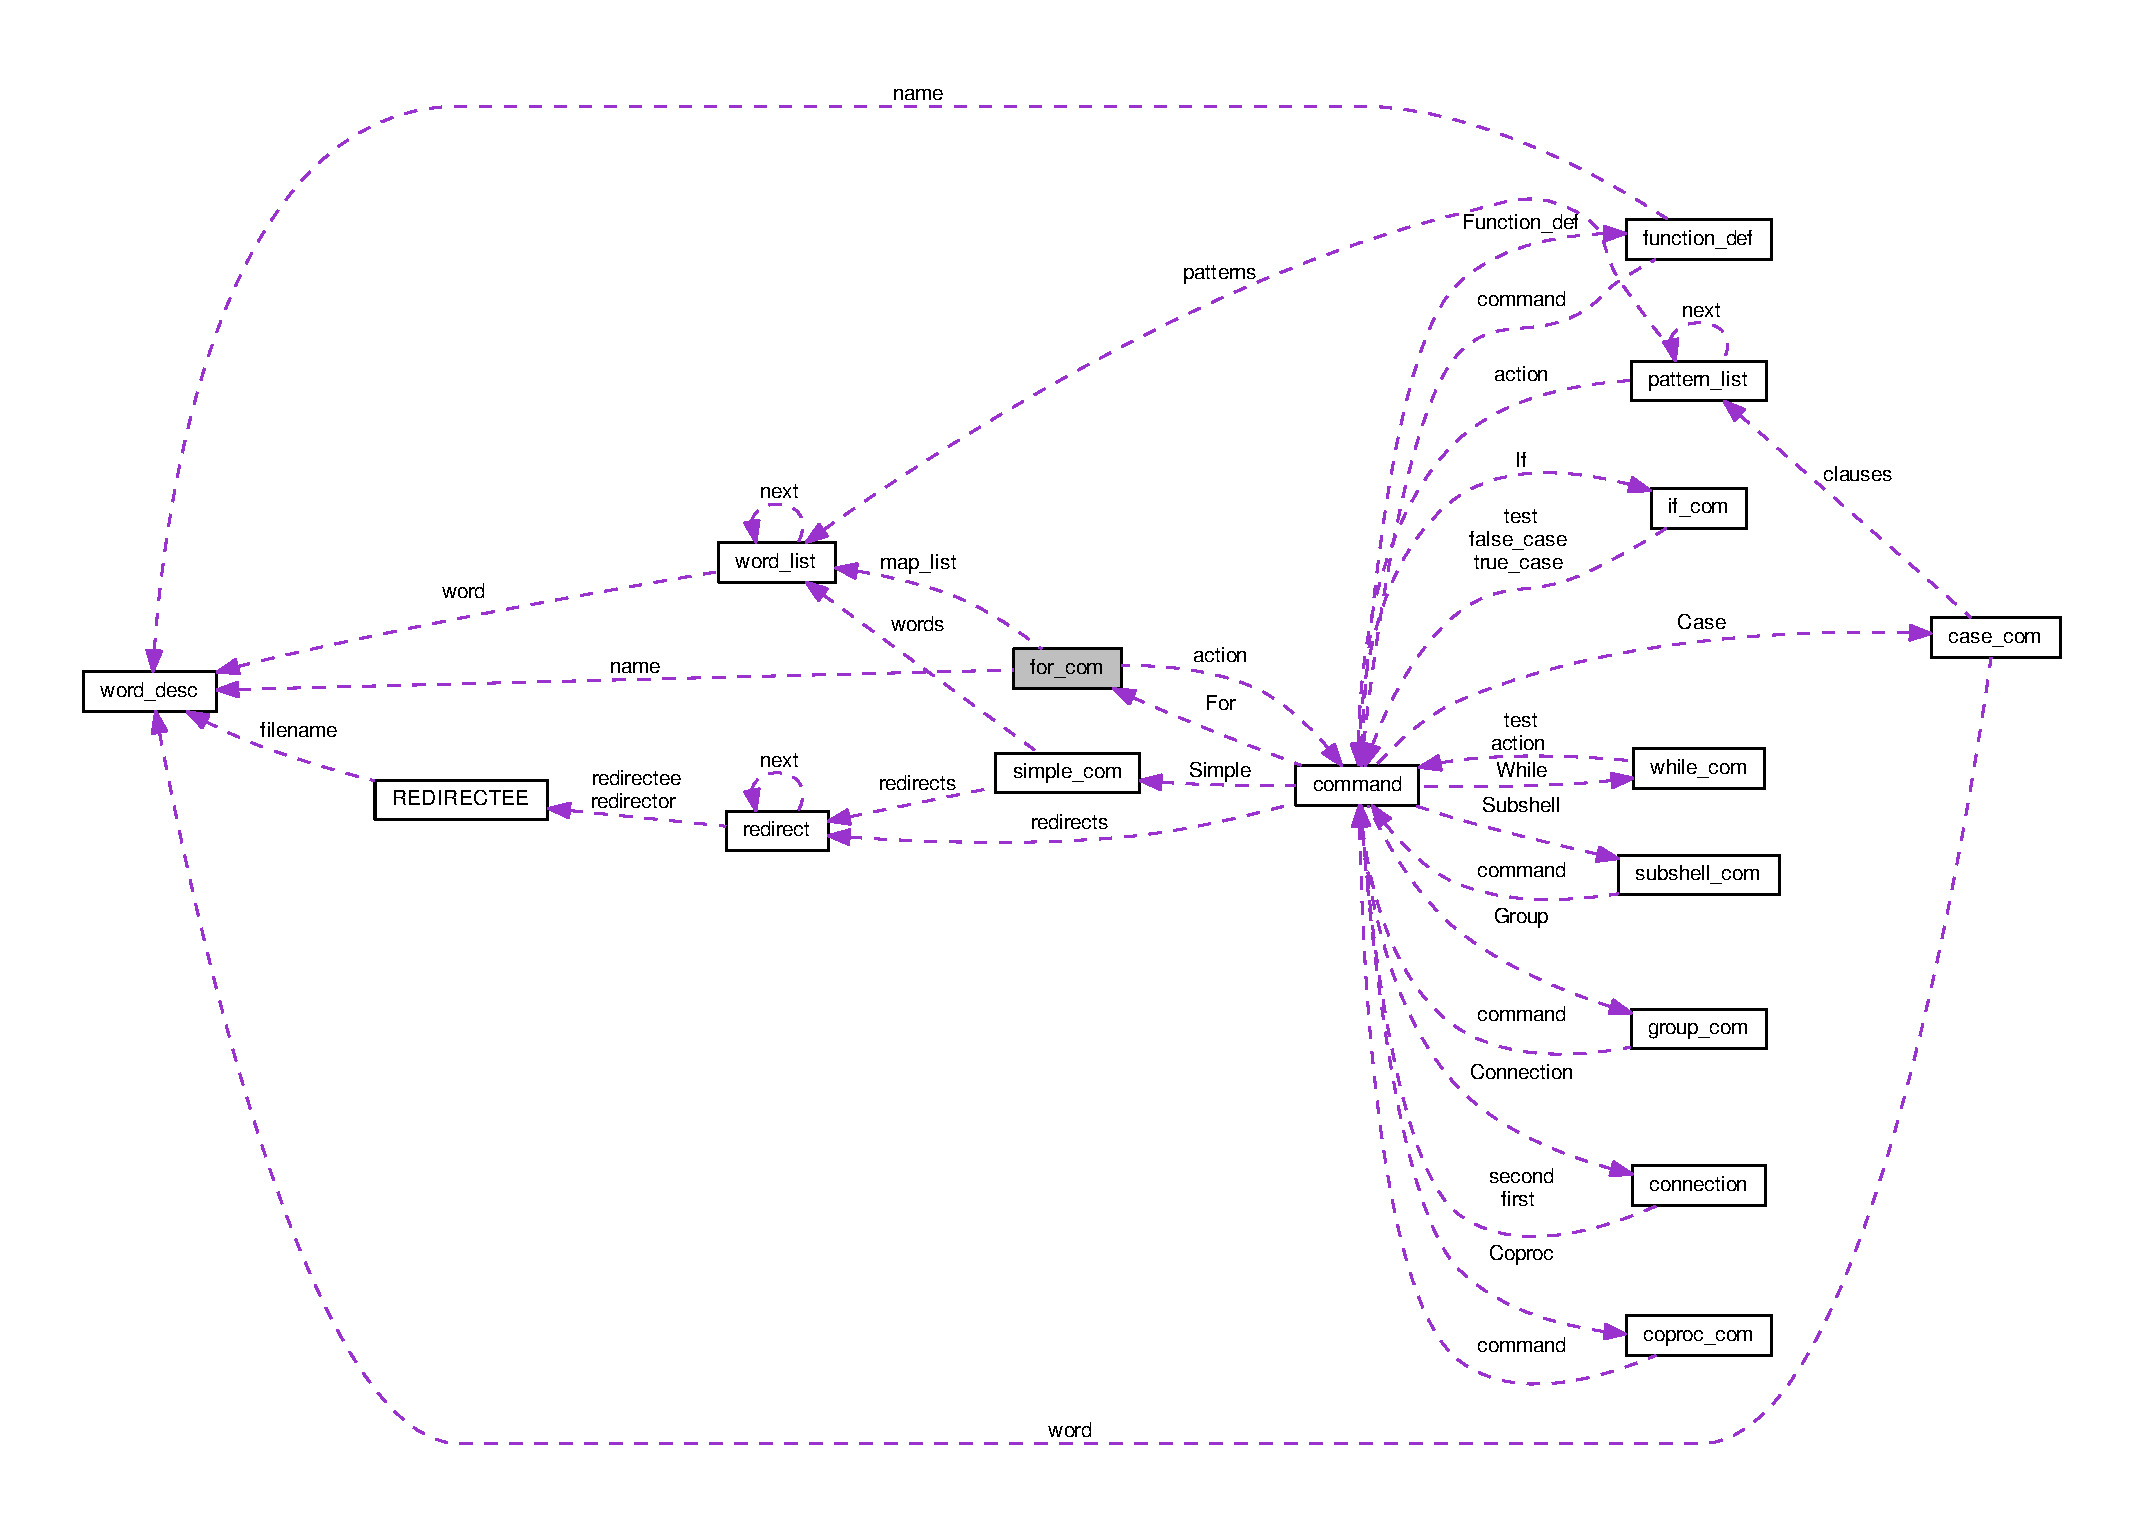
\includegraphics[width=350pt]{structfor__com__coll__graph}
\end{center}
\end{figure}
\subsection*{Public Attributes}
\begin{DoxyCompactItemize}
\item 
int \hyperlink{structfor__com_add9efd6ed9e84a42922fc7c6b273e3b9}{flags}
\item 
int \hyperlink{structfor__com_a268cba692dd4b85d33586df8286dcc6e}{line}
\item 
\hyperlink{command_8h_a3f0cccf333703e5f6c4168be0db675fa}{W\+O\+R\+D\+\_\+\+D\+E\+SC} $\ast$ \hyperlink{structfor__com_a954d92414437178eb2545211a43291db}{name}
\item 
\hyperlink{command_8h_ac42a7b781459884316a1f2ffe79e8a62}{W\+O\+R\+D\+\_\+\+L\+I\+ST} $\ast$ \hyperlink{structfor__com_ae9bc74158b6735a789842cbba12dea60}{map\+\_\+list}
\item 
\hyperlink{command_8h_a8c41dec142c299806885773c902c0d87}{C\+O\+M\+M\+A\+ND} $\ast$ \hyperlink{structfor__com_a8f50a2c1bfc84c589ce327839c5e4805}{action}
\end{DoxyCompactItemize}


\subsection{Member Data Documentation}
\index{for\+\_\+com@{for\+\_\+com}!action@{action}}
\index{action@{action}!for\+\_\+com@{for\+\_\+com}}
\subsubsection[{\texorpdfstring{action}{action}}]{\setlength{\rightskip}{0pt plus 5cm}{\bf C\+O\+M\+M\+A\+ND}$\ast$ for\+\_\+com\+::action}\hypertarget{structfor__com_a8f50a2c1bfc84c589ce327839c5e4805}{}\label{structfor__com_a8f50a2c1bfc84c589ce327839c5e4805}
\index{for\+\_\+com@{for\+\_\+com}!flags@{flags}}
\index{flags@{flags}!for\+\_\+com@{for\+\_\+com}}
\subsubsection[{\texorpdfstring{flags}{flags}}]{\setlength{\rightskip}{0pt plus 5cm}int for\+\_\+com\+::flags}\hypertarget{structfor__com_add9efd6ed9e84a42922fc7c6b273e3b9}{}\label{structfor__com_add9efd6ed9e84a42922fc7c6b273e3b9}
\index{for\+\_\+com@{for\+\_\+com}!line@{line}}
\index{line@{line}!for\+\_\+com@{for\+\_\+com}}
\subsubsection[{\texorpdfstring{line}{line}}]{\setlength{\rightskip}{0pt plus 5cm}int for\+\_\+com\+::line}\hypertarget{structfor__com_a268cba692dd4b85d33586df8286dcc6e}{}\label{structfor__com_a268cba692dd4b85d33586df8286dcc6e}
\index{for\+\_\+com@{for\+\_\+com}!map\+\_\+list@{map\+\_\+list}}
\index{map\+\_\+list@{map\+\_\+list}!for\+\_\+com@{for\+\_\+com}}
\subsubsection[{\texorpdfstring{map\+\_\+list}{map_list}}]{\setlength{\rightskip}{0pt plus 5cm}{\bf W\+O\+R\+D\+\_\+\+L\+I\+ST}$\ast$ for\+\_\+com\+::map\+\_\+list}\hypertarget{structfor__com_ae9bc74158b6735a789842cbba12dea60}{}\label{structfor__com_ae9bc74158b6735a789842cbba12dea60}
\index{for\+\_\+com@{for\+\_\+com}!name@{name}}
\index{name@{name}!for\+\_\+com@{for\+\_\+com}}
\subsubsection[{\texorpdfstring{name}{name}}]{\setlength{\rightskip}{0pt plus 5cm}{\bf W\+O\+R\+D\+\_\+\+D\+E\+SC}$\ast$ for\+\_\+com\+::name}\hypertarget{structfor__com_a954d92414437178eb2545211a43291db}{}\label{structfor__com_a954d92414437178eb2545211a43291db}


The documentation for this struct was generated from the following file\+:\begin{DoxyCompactItemize}
\item 
\hyperlink{command_8h}{command.\+h}\end{DoxyCompactItemize}

\hypertarget{structfunction__def}{}\section{function\+\_\+def Struct Reference}
\label{structfunction__def}\index{function\+\_\+def@{function\+\_\+def}}


{\ttfamily \#include $<$command.\+h$>$}



Collaboration diagram for function\+\_\+def\+:
\nopagebreak
\begin{figure}[H]
\begin{center}
\leavevmode
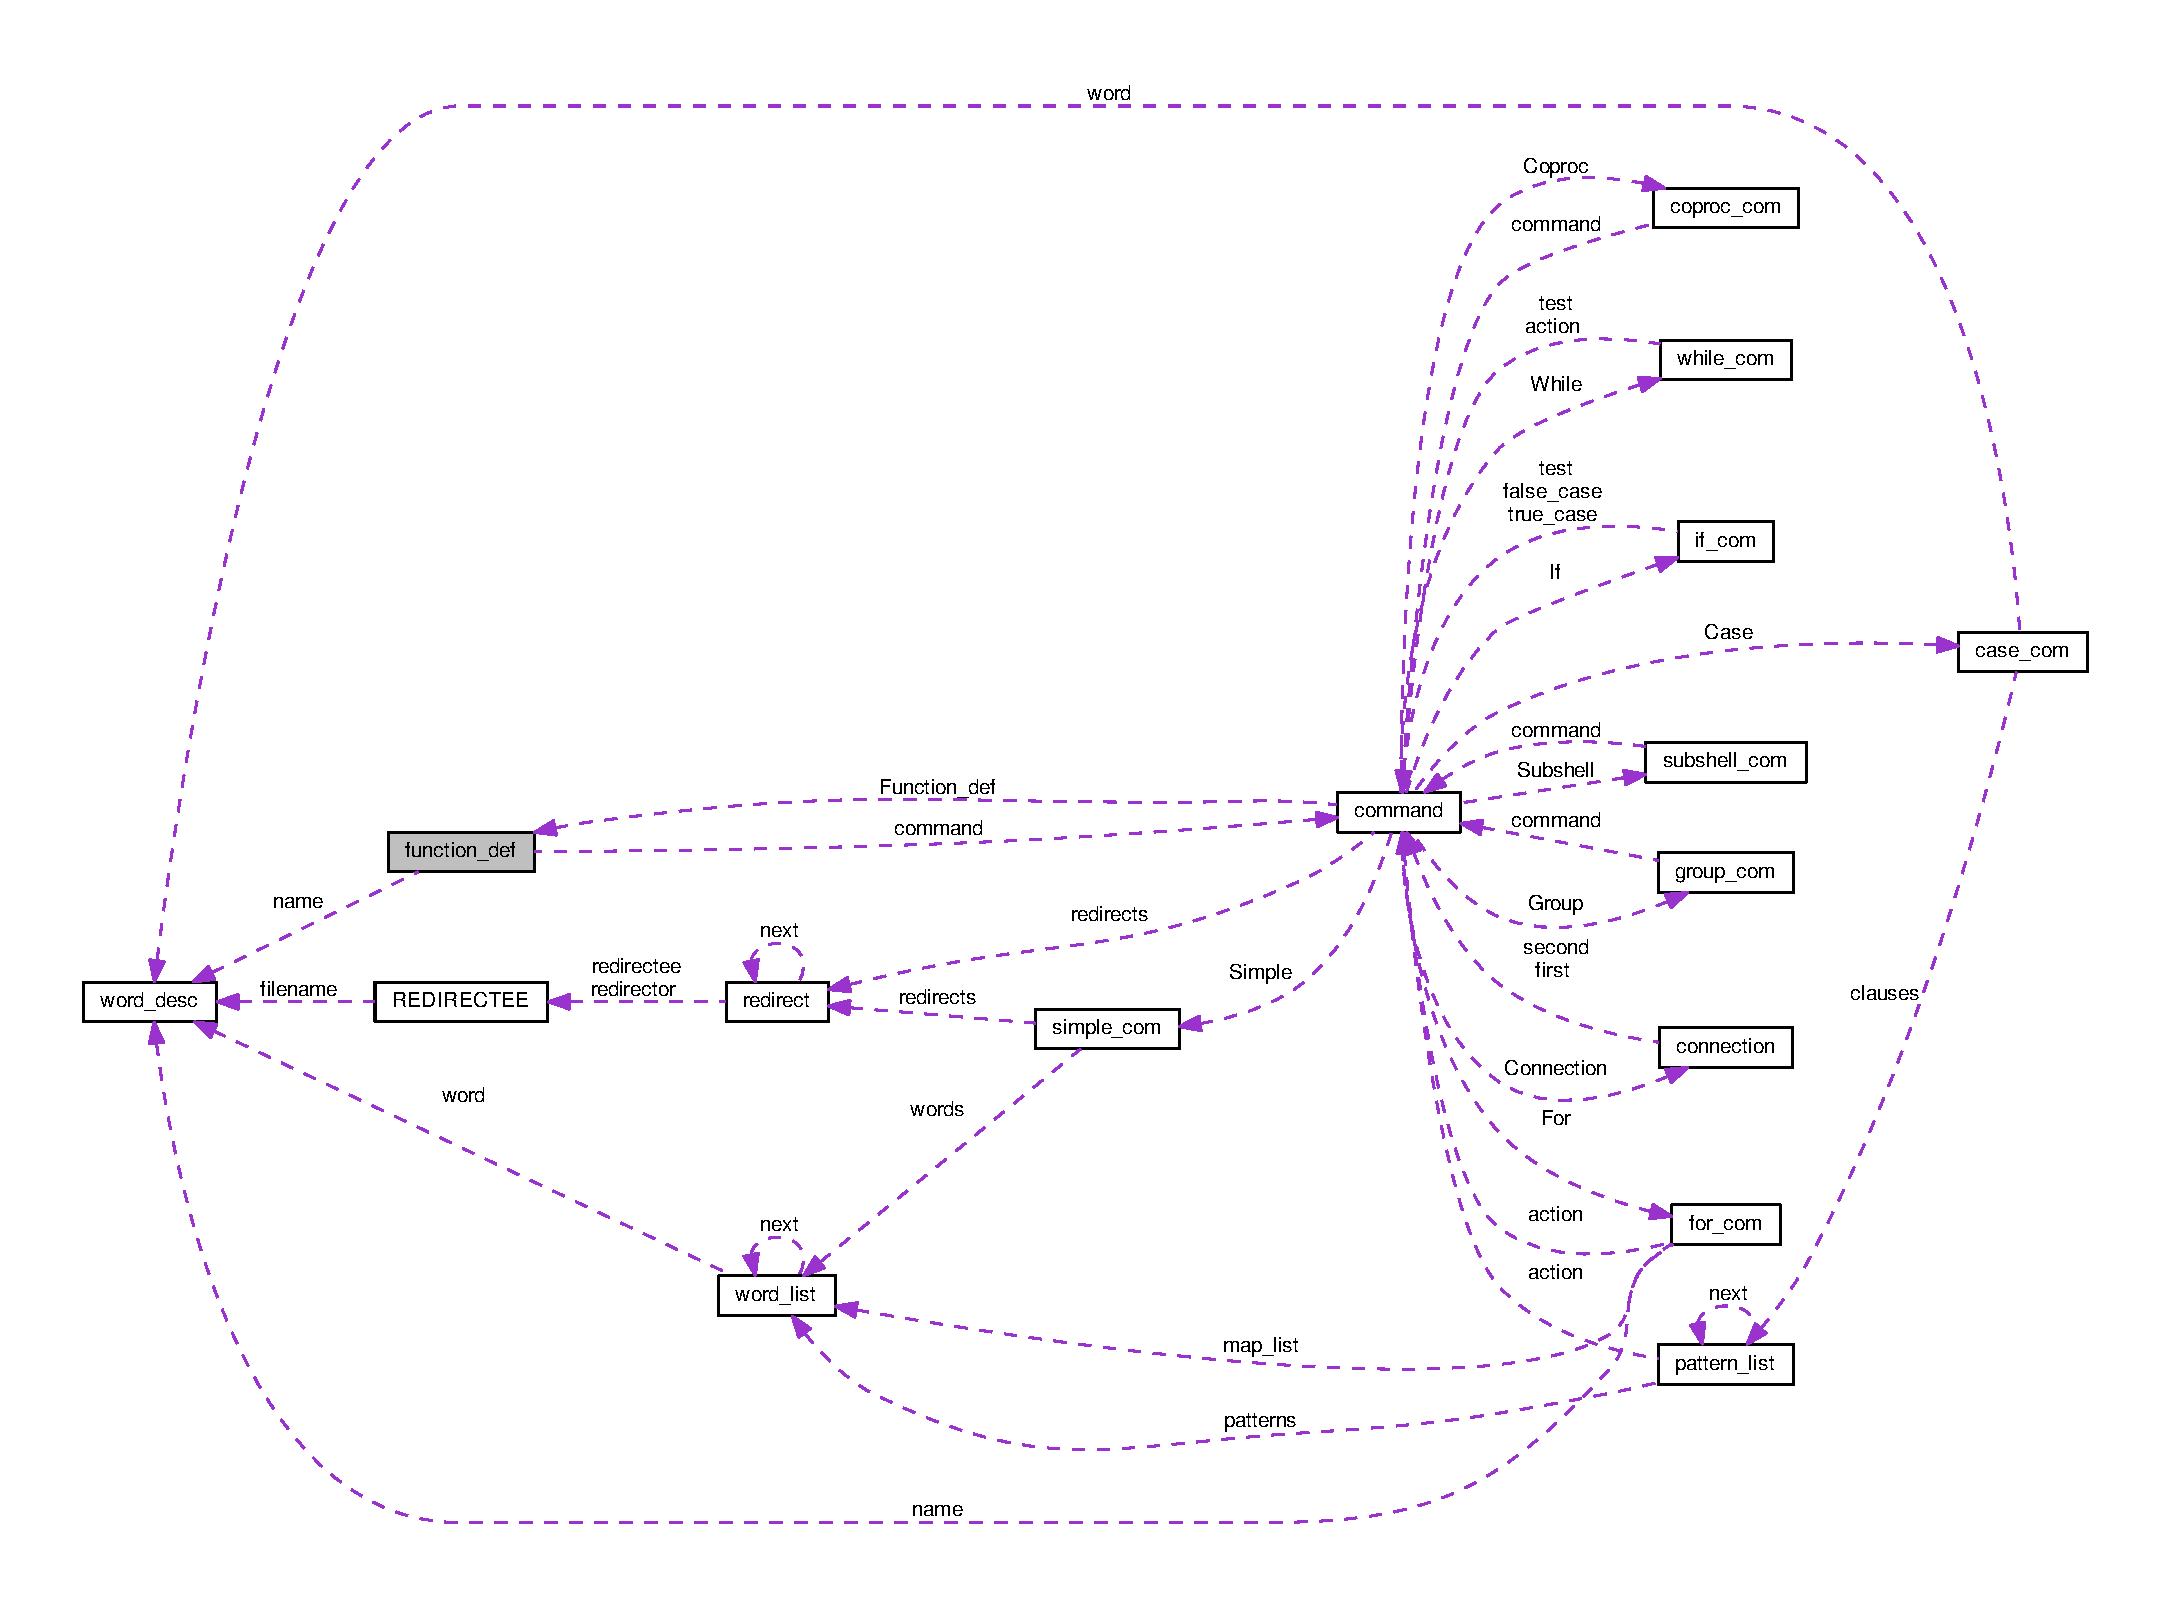
\includegraphics[width=350pt]{structfunction__def__coll__graph}
\end{center}
\end{figure}
\subsection*{Public Attributes}
\begin{DoxyCompactItemize}
\item 
int \hyperlink{structfunction__def_a6301401481265ca9b5282b683b2ba2d4}{flags}
\item 
int \hyperlink{structfunction__def_a522bca5d5ecc615cff04e01de1d19ffc}{line}
\item 
\hyperlink{command_8h_a3f0cccf333703e5f6c4168be0db675fa}{W\+O\+R\+D\+\_\+\+D\+E\+SC} $\ast$ \hyperlink{structfunction__def_a0015166324aa0e5e336c97afcec63059}{name}
\item 
\hyperlink{command_8h_a8c41dec142c299806885773c902c0d87}{C\+O\+M\+M\+A\+ND} $\ast$ \hyperlink{structfunction__def_a1d47a692dd8fb660368206a3218f3fe8}{command}
\item 
char $\ast$ \hyperlink{structfunction__def_ad21801282b94695a306f3864c2bd7376}{source\+\_\+file}
\end{DoxyCompactItemize}


\subsection{Member Data Documentation}
\index{function\+\_\+def@{function\+\_\+def}!command@{command}}
\index{command@{command}!function\+\_\+def@{function\+\_\+def}}
\subsubsection[{\texorpdfstring{command}{command}}]{\setlength{\rightskip}{0pt plus 5cm}{\bf C\+O\+M\+M\+A\+ND}$\ast$ function\+\_\+def\+::command}\hypertarget{structfunction__def_a1d47a692dd8fb660368206a3218f3fe8}{}\label{structfunction__def_a1d47a692dd8fb660368206a3218f3fe8}
\index{function\+\_\+def@{function\+\_\+def}!flags@{flags}}
\index{flags@{flags}!function\+\_\+def@{function\+\_\+def}}
\subsubsection[{\texorpdfstring{flags}{flags}}]{\setlength{\rightskip}{0pt plus 5cm}int function\+\_\+def\+::flags}\hypertarget{structfunction__def_a6301401481265ca9b5282b683b2ba2d4}{}\label{structfunction__def_a6301401481265ca9b5282b683b2ba2d4}
\index{function\+\_\+def@{function\+\_\+def}!line@{line}}
\index{line@{line}!function\+\_\+def@{function\+\_\+def}}
\subsubsection[{\texorpdfstring{line}{line}}]{\setlength{\rightskip}{0pt plus 5cm}int function\+\_\+def\+::line}\hypertarget{structfunction__def_a522bca5d5ecc615cff04e01de1d19ffc}{}\label{structfunction__def_a522bca5d5ecc615cff04e01de1d19ffc}
\index{function\+\_\+def@{function\+\_\+def}!name@{name}}
\index{name@{name}!function\+\_\+def@{function\+\_\+def}}
\subsubsection[{\texorpdfstring{name}{name}}]{\setlength{\rightskip}{0pt plus 5cm}{\bf W\+O\+R\+D\+\_\+\+D\+E\+SC}$\ast$ function\+\_\+def\+::name}\hypertarget{structfunction__def_a0015166324aa0e5e336c97afcec63059}{}\label{structfunction__def_a0015166324aa0e5e336c97afcec63059}
\index{function\+\_\+def@{function\+\_\+def}!source\+\_\+file@{source\+\_\+file}}
\index{source\+\_\+file@{source\+\_\+file}!function\+\_\+def@{function\+\_\+def}}
\subsubsection[{\texorpdfstring{source\+\_\+file}{source_file}}]{\setlength{\rightskip}{0pt plus 5cm}char$\ast$ function\+\_\+def\+::source\+\_\+file}\hypertarget{structfunction__def_ad21801282b94695a306f3864c2bd7376}{}\label{structfunction__def_ad21801282b94695a306f3864c2bd7376}


The documentation for this struct was generated from the following file\+:\begin{DoxyCompactItemize}
\item 
\hyperlink{command_8h}{command.\+h}\end{DoxyCompactItemize}

\hypertarget{structg__list}{}\section{g\+\_\+list Struct Reference}
\label{structg__list}\index{g\+\_\+list@{g\+\_\+list}}


{\ttfamily \#include $<$general.\+h$>$}



Collaboration diagram for g\+\_\+list\+:
\nopagebreak
\begin{figure}[H]
\begin{center}
\leavevmode
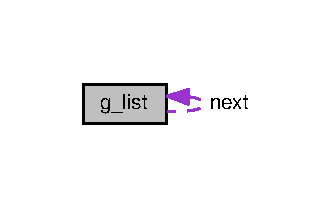
\includegraphics[width=160pt]{structg__list__coll__graph}
\end{center}
\end{figure}
\subsection*{Public Attributes}
\begin{DoxyCompactItemize}
\item 
struct \hyperlink{structg__list}{g\+\_\+list} $\ast$ \hyperlink{structg__list_ada1d543e69873d9bd861eb115dd6b7c2}{next}
\end{DoxyCompactItemize}


\subsection{Member Data Documentation}
\index{g\+\_\+list@{g\+\_\+list}!next@{next}}
\index{next@{next}!g\+\_\+list@{g\+\_\+list}}
\subsubsection[{\texorpdfstring{next}{next}}]{\setlength{\rightskip}{0pt plus 5cm}struct {\bf g\+\_\+list}$\ast$ g\+\_\+list\+::next}\hypertarget{structg__list_ada1d543e69873d9bd861eb115dd6b7c2}{}\label{structg__list_ada1d543e69873d9bd861eb115dd6b7c2}


The documentation for this struct was generated from the following file\+:\begin{DoxyCompactItemize}
\item 
\hyperlink{general_8h}{general.\+h}\end{DoxyCompactItemize}

\hypertarget{structgroup__com}{}\section{group\+\_\+com Struct Reference}
\label{structgroup__com}\index{group\+\_\+com@{group\+\_\+com}}


{\ttfamily \#include $<$command.\+h$>$}



Collaboration diagram for group\+\_\+com\+:
\nopagebreak
\begin{figure}[H]
\begin{center}
\leavevmode
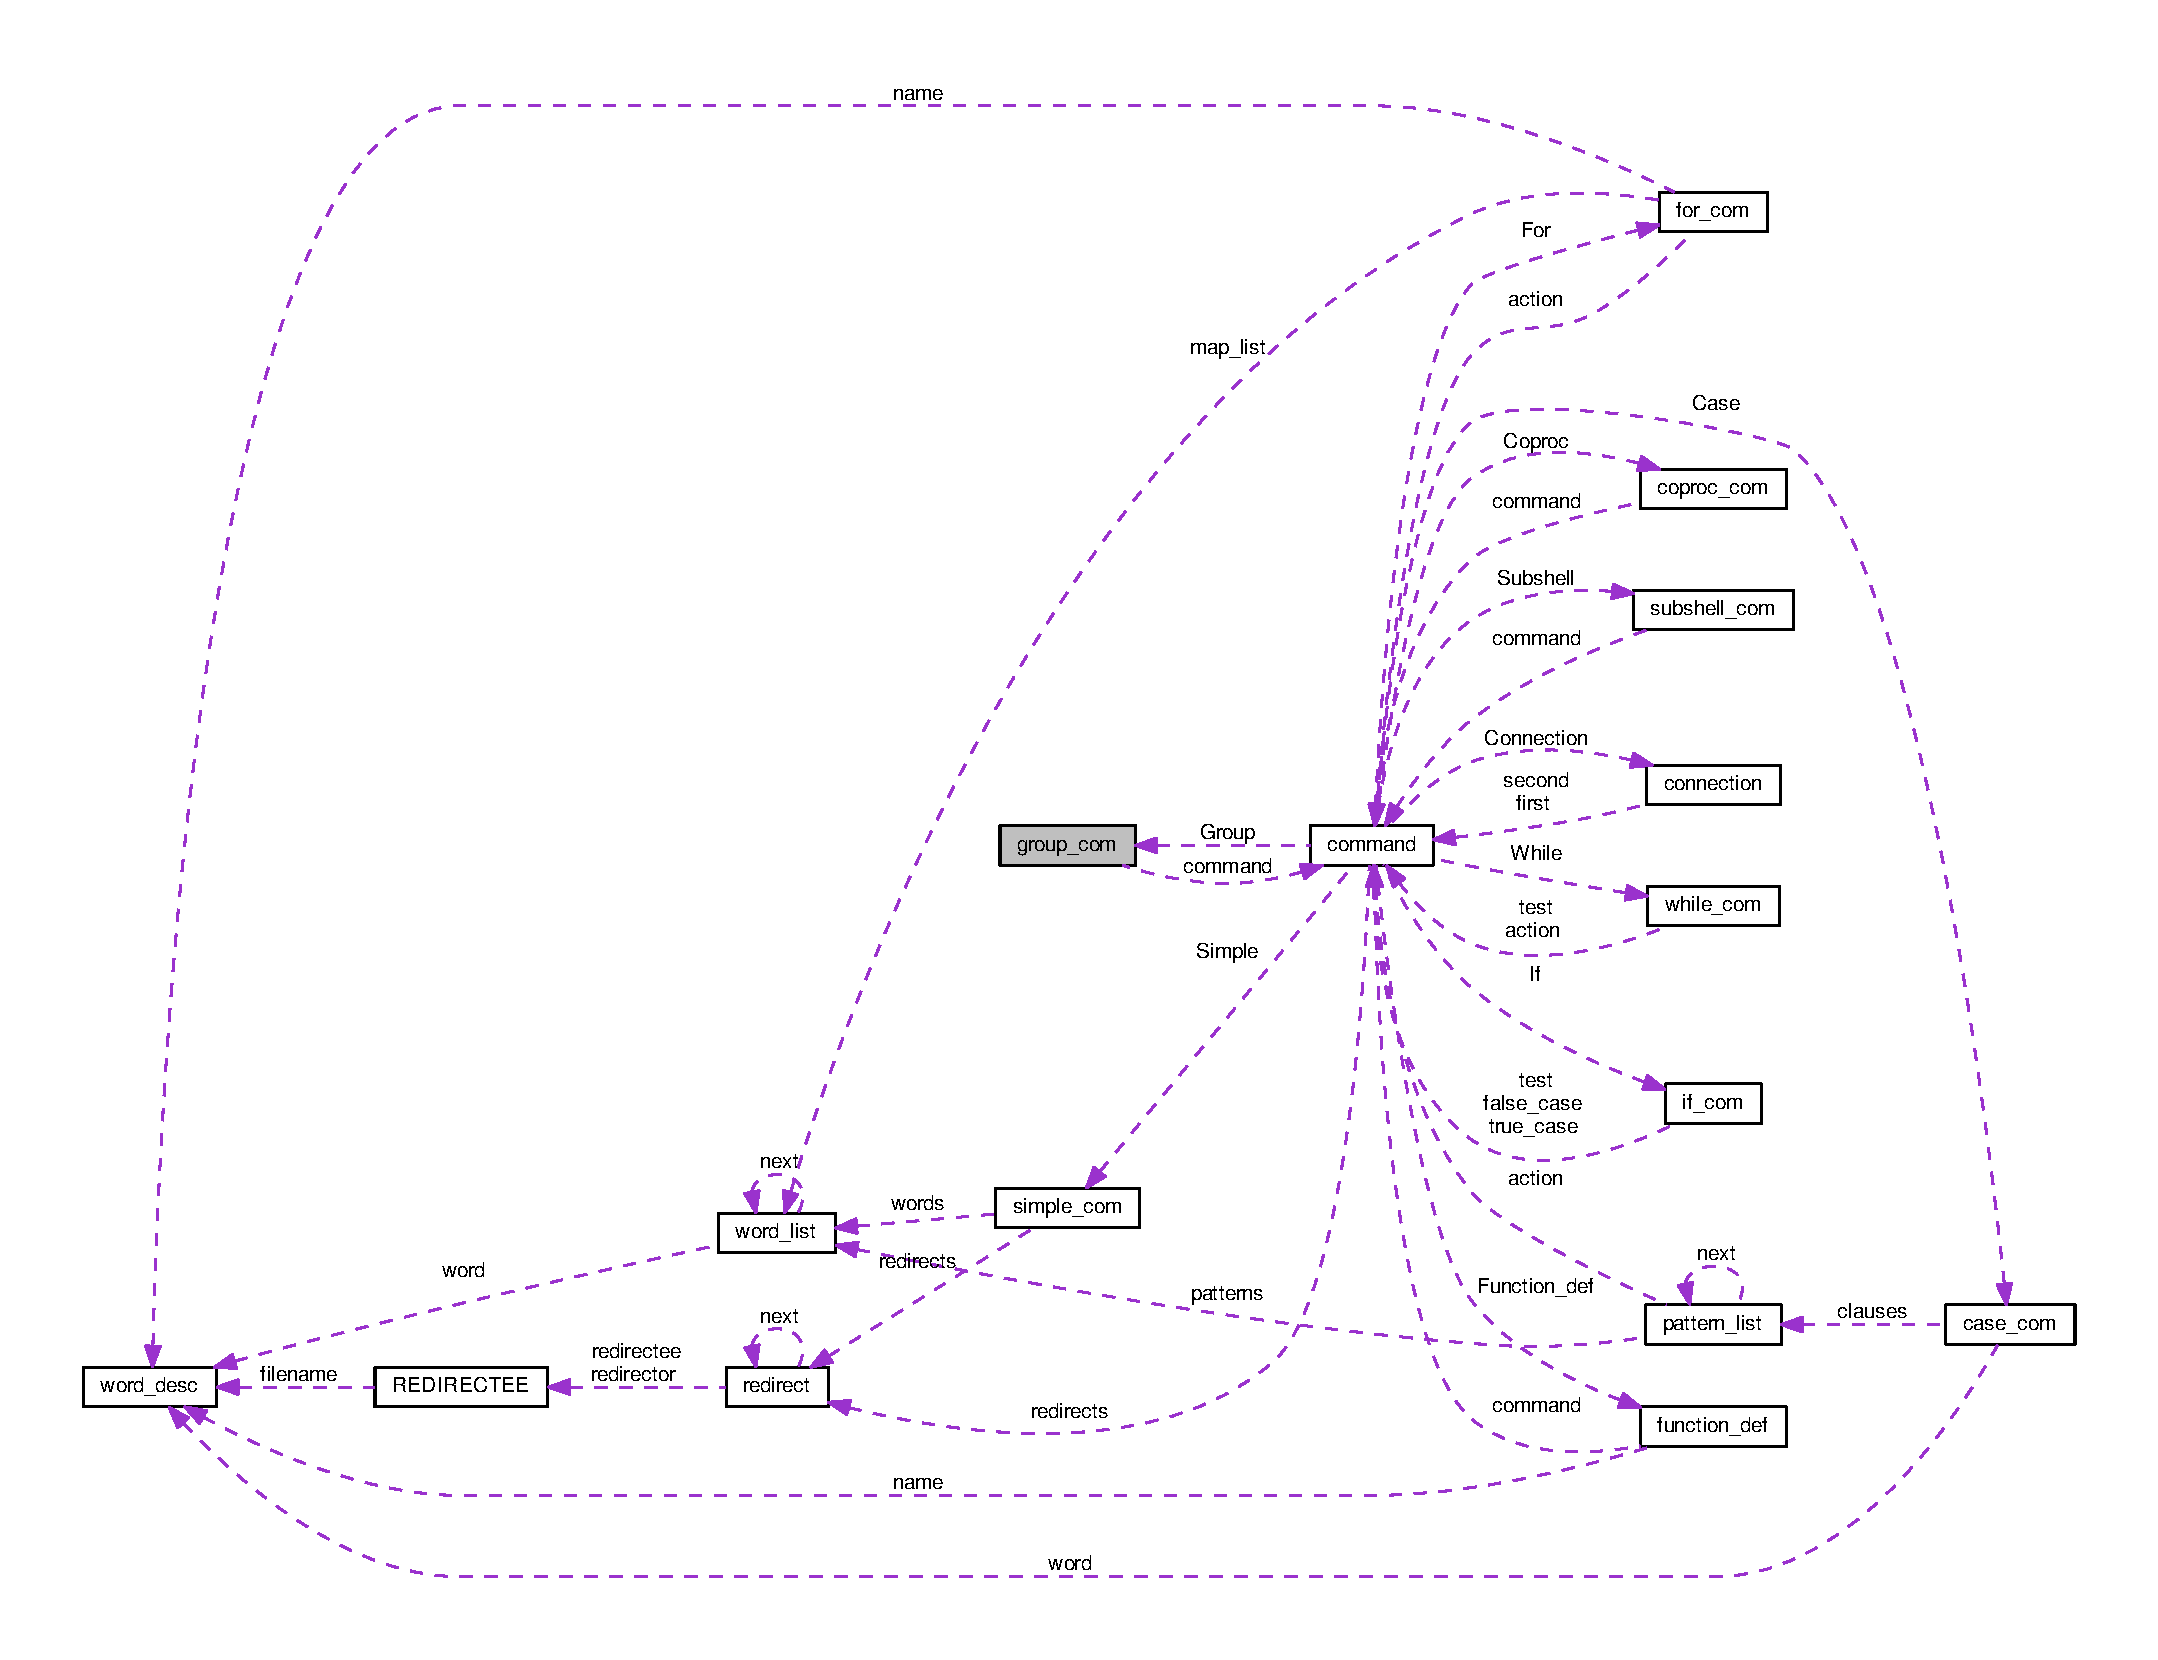
\includegraphics[width=350pt]{structgroup__com__coll__graph}
\end{center}
\end{figure}
\subsection*{Public Attributes}
\begin{DoxyCompactItemize}
\item 
int \hyperlink{structgroup__com_a3715ce6245659a44296cca565fe8d7d9}{ignore}
\item 
\hyperlink{command_8h_a8c41dec142c299806885773c902c0d87}{C\+O\+M\+M\+A\+ND} $\ast$ \hyperlink{structgroup__com_a89f1f5171979c8f337dae8418adc6d7f}{command}
\end{DoxyCompactItemize}


\subsection{Member Data Documentation}
\index{group\+\_\+com@{group\+\_\+com}!command@{command}}
\index{command@{command}!group\+\_\+com@{group\+\_\+com}}
\subsubsection[{\texorpdfstring{command}{command}}]{\setlength{\rightskip}{0pt plus 5cm}{\bf C\+O\+M\+M\+A\+ND}$\ast$ group\+\_\+com\+::command}\hypertarget{structgroup__com_a89f1f5171979c8f337dae8418adc6d7f}{}\label{structgroup__com_a89f1f5171979c8f337dae8418adc6d7f}
\index{group\+\_\+com@{group\+\_\+com}!ignore@{ignore}}
\index{ignore@{ignore}!group\+\_\+com@{group\+\_\+com}}
\subsubsection[{\texorpdfstring{ignore}{ignore}}]{\setlength{\rightskip}{0pt plus 5cm}int group\+\_\+com\+::ignore}\hypertarget{structgroup__com_a3715ce6245659a44296cca565fe8d7d9}{}\label{structgroup__com_a3715ce6245659a44296cca565fe8d7d9}


The documentation for this struct was generated from the following file\+:\begin{DoxyCompactItemize}
\item 
\hyperlink{command_8h}{command.\+h}\end{DoxyCompactItemize}

\hypertarget{structhash__table}{}\section{hash\+\_\+table Struct Reference}
\label{structhash__table}\index{hash\+\_\+table@{hash\+\_\+table}}


{\ttfamily \#include $<$hashlib.\+h$>$}



Collaboration diagram for hash\+\_\+table\+:
\nopagebreak
\begin{figure}[H]
\begin{center}
\leavevmode
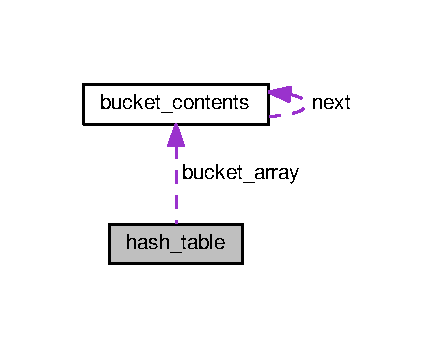
\includegraphics[width=209pt]{structhash__table__coll__graph}
\end{center}
\end{figure}
\subsection*{Public Attributes}
\begin{DoxyCompactItemize}
\item 
\hyperlink{hashlib_8h_aa38d328c0a8fa68156686f7c9d9e6e7f}{B\+U\+C\+K\+E\+T\+\_\+\+C\+O\+N\+T\+E\+N\+TS} $\ast$$\ast$ \hyperlink{structhash__table_a8500015bb5f856d6051a122860e4968a}{bucket\+\_\+array}
\item 
int \hyperlink{structhash__table_aa7de201d163e121b359b32142d261e2f}{nbuckets}
\item 
int \hyperlink{structhash__table_a9e1b774a04e87eb7bef46100c85ec52d}{nentries}
\end{DoxyCompactItemize}


\subsection{Member Data Documentation}
\index{hash\+\_\+table@{hash\+\_\+table}!bucket\+\_\+array@{bucket\+\_\+array}}
\index{bucket\+\_\+array@{bucket\+\_\+array}!hash\+\_\+table@{hash\+\_\+table}}
\subsubsection[{\texorpdfstring{bucket\+\_\+array}{bucket_array}}]{\setlength{\rightskip}{0pt plus 5cm}{\bf B\+U\+C\+K\+E\+T\+\_\+\+C\+O\+N\+T\+E\+N\+TS}$\ast$$\ast$ hash\+\_\+table\+::bucket\+\_\+array}\hypertarget{structhash__table_a8500015bb5f856d6051a122860e4968a}{}\label{structhash__table_a8500015bb5f856d6051a122860e4968a}
\index{hash\+\_\+table@{hash\+\_\+table}!nbuckets@{nbuckets}}
\index{nbuckets@{nbuckets}!hash\+\_\+table@{hash\+\_\+table}}
\subsubsection[{\texorpdfstring{nbuckets}{nbuckets}}]{\setlength{\rightskip}{0pt plus 5cm}int hash\+\_\+table\+::nbuckets}\hypertarget{structhash__table_aa7de201d163e121b359b32142d261e2f}{}\label{structhash__table_aa7de201d163e121b359b32142d261e2f}
\index{hash\+\_\+table@{hash\+\_\+table}!nentries@{nentries}}
\index{nentries@{nentries}!hash\+\_\+table@{hash\+\_\+table}}
\subsubsection[{\texorpdfstring{nentries}{nentries}}]{\setlength{\rightskip}{0pt plus 5cm}int hash\+\_\+table\+::nentries}\hypertarget{structhash__table_a9e1b774a04e87eb7bef46100c85ec52d}{}\label{structhash__table_a9e1b774a04e87eb7bef46100c85ec52d}


The documentation for this struct was generated from the following file\+:\begin{DoxyCompactItemize}
\item 
\hyperlink{hashlib_8h}{hashlib.\+h}\end{DoxyCompactItemize}

\hypertarget{structif__com}{}\section{if\+\_\+com Struct Reference}
\label{structif__com}\index{if\+\_\+com@{if\+\_\+com}}


{\ttfamily \#include $<$command.\+h$>$}



Collaboration diagram for if\+\_\+com\+:
\nopagebreak
\begin{figure}[H]
\begin{center}
\leavevmode
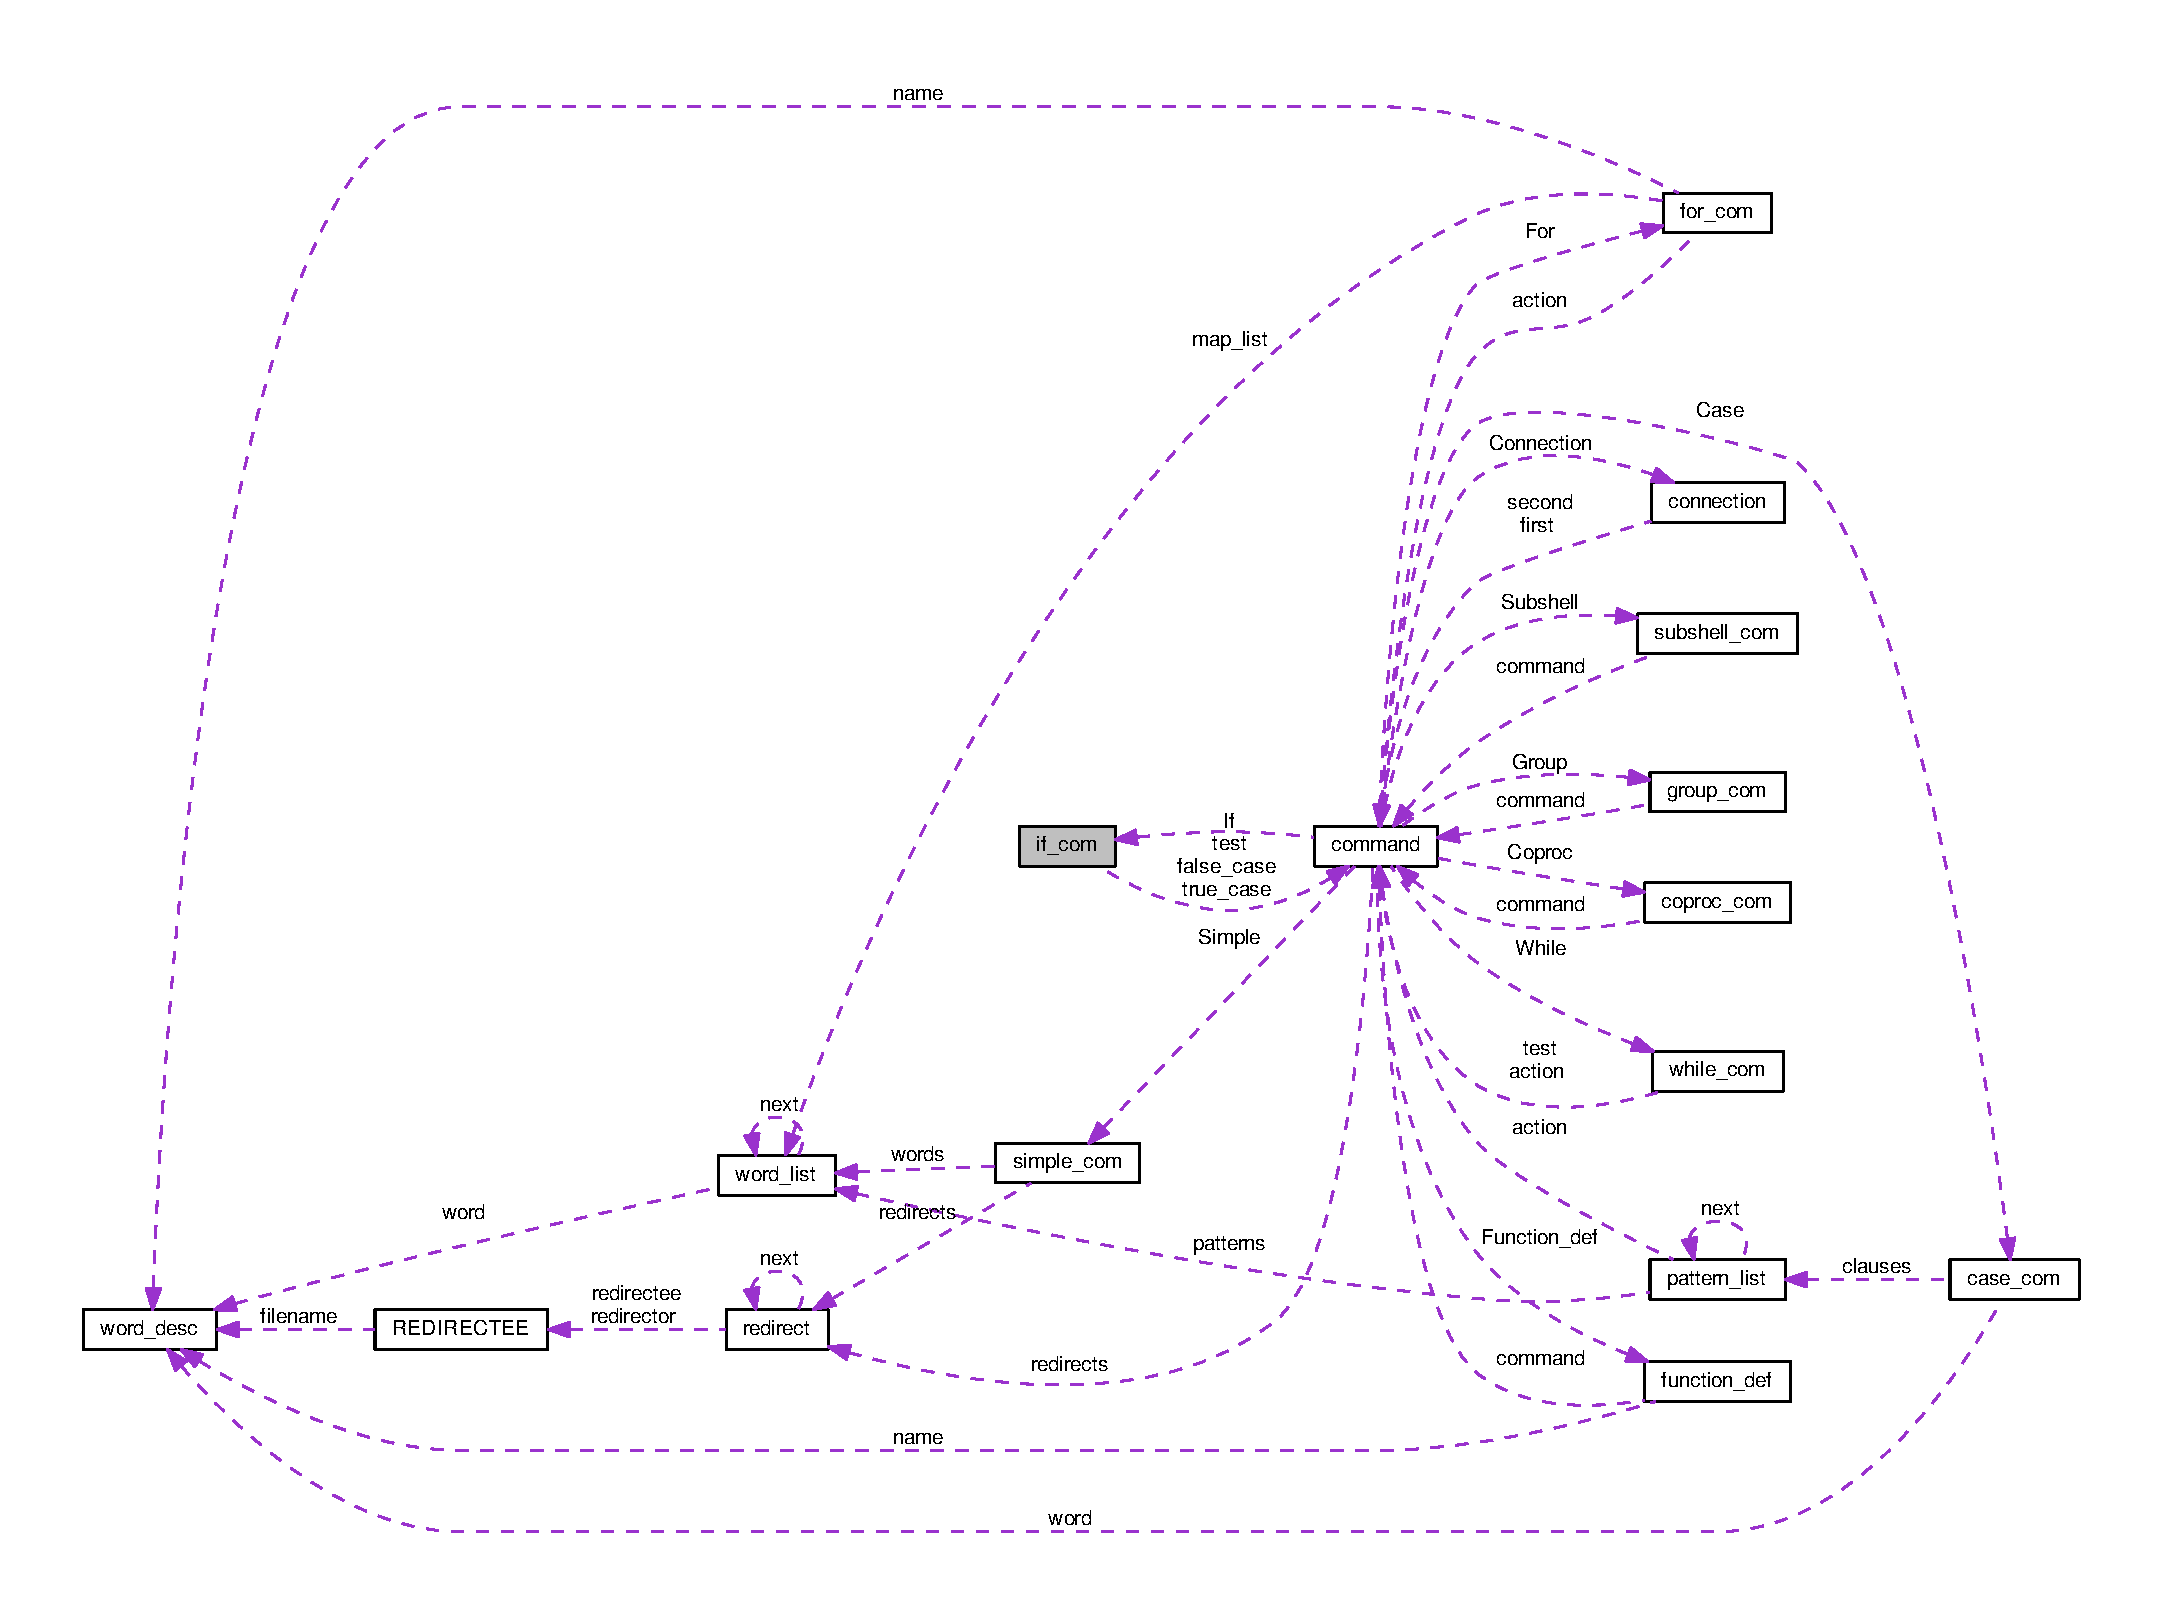
\includegraphics[width=350pt]{structif__com__coll__graph}
\end{center}
\end{figure}
\subsection*{Public Attributes}
\begin{DoxyCompactItemize}
\item 
int \hyperlink{structif__com_a07d76d76b991c3dbabbf5b5c0e123836}{flags}
\item 
\hyperlink{command_8h_a8c41dec142c299806885773c902c0d87}{C\+O\+M\+M\+A\+ND} $\ast$ \hyperlink{structif__com_a28a2dd8a917262a9eaa0c446d1b54fe0}{test}
\item 
\hyperlink{command_8h_a8c41dec142c299806885773c902c0d87}{C\+O\+M\+M\+A\+ND} $\ast$ \hyperlink{structif__com_ae691d759258b18e45dd18591e71dc141}{true\+\_\+case}
\item 
\hyperlink{command_8h_a8c41dec142c299806885773c902c0d87}{C\+O\+M\+M\+A\+ND} $\ast$ \hyperlink{structif__com_ac9f1b317a7c8ff4c750335c571c33a15}{false\+\_\+case}
\end{DoxyCompactItemize}


\subsection{Member Data Documentation}
\index{if\+\_\+com@{if\+\_\+com}!false\+\_\+case@{false\+\_\+case}}
\index{false\+\_\+case@{false\+\_\+case}!if\+\_\+com@{if\+\_\+com}}
\subsubsection[{\texorpdfstring{false\+\_\+case}{false_case}}]{\setlength{\rightskip}{0pt plus 5cm}{\bf C\+O\+M\+M\+A\+ND}$\ast$ if\+\_\+com\+::false\+\_\+case}\hypertarget{structif__com_ac9f1b317a7c8ff4c750335c571c33a15}{}\label{structif__com_ac9f1b317a7c8ff4c750335c571c33a15}
\index{if\+\_\+com@{if\+\_\+com}!flags@{flags}}
\index{flags@{flags}!if\+\_\+com@{if\+\_\+com}}
\subsubsection[{\texorpdfstring{flags}{flags}}]{\setlength{\rightskip}{0pt plus 5cm}int if\+\_\+com\+::flags}\hypertarget{structif__com_a07d76d76b991c3dbabbf5b5c0e123836}{}\label{structif__com_a07d76d76b991c3dbabbf5b5c0e123836}
\index{if\+\_\+com@{if\+\_\+com}!test@{test}}
\index{test@{test}!if\+\_\+com@{if\+\_\+com}}
\subsubsection[{\texorpdfstring{test}{test}}]{\setlength{\rightskip}{0pt plus 5cm}{\bf C\+O\+M\+M\+A\+ND}$\ast$ if\+\_\+com\+::test}\hypertarget{structif__com_a28a2dd8a917262a9eaa0c446d1b54fe0}{}\label{structif__com_a28a2dd8a917262a9eaa0c446d1b54fe0}
\index{if\+\_\+com@{if\+\_\+com}!true\+\_\+case@{true\+\_\+case}}
\index{true\+\_\+case@{true\+\_\+case}!if\+\_\+com@{if\+\_\+com}}
\subsubsection[{\texorpdfstring{true\+\_\+case}{true_case}}]{\setlength{\rightskip}{0pt plus 5cm}{\bf C\+O\+M\+M\+A\+ND}$\ast$ if\+\_\+com\+::true\+\_\+case}\hypertarget{structif__com_ae691d759258b18e45dd18591e71dc141}{}\label{structif__com_ae691d759258b18e45dd18591e71dc141}


The documentation for this struct was generated from the following file\+:\begin{DoxyCompactItemize}
\item 
\hyperlink{command_8h}{command.\+h}\end{DoxyCompactItemize}

\hypertarget{structign}{}\section{ign Struct Reference}
\label{structign}\index{ign@{ign}}


{\ttfamily \#include $<$pathexp.\+h$>$}

\subsection*{Public Attributes}
\begin{DoxyCompactItemize}
\item 
char $\ast$ \hyperlink{structign_a534c8733717c56d8872de43019089ade}{val}
\item 
int \hyperlink{structign_a4f5a326628d04a43015f7e8bb018301b}{len}
\item 
int \hyperlink{structign_a3fdd7e30b97f47f2da8d5f3c8ea35c80}{flags}
\end{DoxyCompactItemize}


\subsection{Member Data Documentation}
\index{ign@{ign}!flags@{flags}}
\index{flags@{flags}!ign@{ign}}
\subsubsection[{\texorpdfstring{flags}{flags}}]{\setlength{\rightskip}{0pt plus 5cm}int ign\+::flags}\hypertarget{structign_a3fdd7e30b97f47f2da8d5f3c8ea35c80}{}\label{structign_a3fdd7e30b97f47f2da8d5f3c8ea35c80}
\index{ign@{ign}!len@{len}}
\index{len@{len}!ign@{ign}}
\subsubsection[{\texorpdfstring{len}{len}}]{\setlength{\rightskip}{0pt plus 5cm}int ign\+::len}\hypertarget{structign_a4f5a326628d04a43015f7e8bb018301b}{}\label{structign_a4f5a326628d04a43015f7e8bb018301b}
\index{ign@{ign}!val@{val}}
\index{val@{val}!ign@{ign}}
\subsubsection[{\texorpdfstring{val}{val}}]{\setlength{\rightskip}{0pt plus 5cm}char$\ast$ ign\+::val}\hypertarget{structign_a534c8733717c56d8872de43019089ade}{}\label{structign_a534c8733717c56d8872de43019089ade}


The documentation for this struct was generated from the following file\+:\begin{DoxyCompactItemize}
\item 
\hyperlink{pathexp_8h}{pathexp.\+h}\end{DoxyCompactItemize}

\hypertarget{structignorevar}{}\section{ignorevar Struct Reference}
\label{structignorevar}\index{ignorevar@{ignorevar}}


{\ttfamily \#include $<$pathexp.\+h$>$}



Collaboration diagram for ignorevar\+:
\nopagebreak
\begin{figure}[H]
\begin{center}
\leavevmode
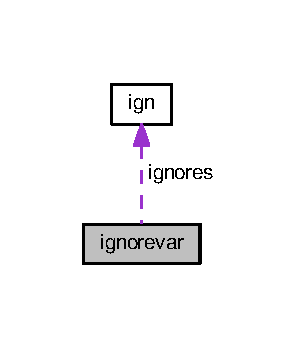
\includegraphics[width=143pt]{structignorevar__coll__graph}
\end{center}
\end{figure}
\subsection*{Public Attributes}
\begin{DoxyCompactItemize}
\item 
char $\ast$ \hyperlink{structignorevar_ab13e47d0a13f6a8664a45472d22fb4c3}{varname}
\item 
struct \hyperlink{structign}{ign} $\ast$ \hyperlink{structignorevar_a4df6df8420b250d65d0fc25f30f60adc}{ignores}
\item 
int \hyperlink{structignorevar_a95a5f4f22d35923944fb9b4c8f0ba209}{num\+\_\+ignores}
\item 
char $\ast$ \hyperlink{structignorevar_a579abbc7ef7ac4a590ae52545bd8b43f}{last\+\_\+ignoreval}
\item 
sh\+\_\+iv\+\_\+item\+\_\+func\+\_\+t $\ast$ \hyperlink{structignorevar_ade27d1004f266495c1229b154f24e1cf}{item\+\_\+func}
\end{DoxyCompactItemize}


\subsection{Member Data Documentation}
\index{ignorevar@{ignorevar}!ignores@{ignores}}
\index{ignores@{ignores}!ignorevar@{ignorevar}}
\subsubsection[{\texorpdfstring{ignores}{ignores}}]{\setlength{\rightskip}{0pt plus 5cm}struct {\bf ign}$\ast$ ignorevar\+::ignores}\hypertarget{structignorevar_a4df6df8420b250d65d0fc25f30f60adc}{}\label{structignorevar_a4df6df8420b250d65d0fc25f30f60adc}
\index{ignorevar@{ignorevar}!item\+\_\+func@{item\+\_\+func}}
\index{item\+\_\+func@{item\+\_\+func}!ignorevar@{ignorevar}}
\subsubsection[{\texorpdfstring{item\+\_\+func}{item_func}}]{\setlength{\rightskip}{0pt plus 5cm}sh\+\_\+iv\+\_\+item\+\_\+func\+\_\+t$\ast$ ignorevar\+::item\+\_\+func}\hypertarget{structignorevar_ade27d1004f266495c1229b154f24e1cf}{}\label{structignorevar_ade27d1004f266495c1229b154f24e1cf}
\index{ignorevar@{ignorevar}!last\+\_\+ignoreval@{last\+\_\+ignoreval}}
\index{last\+\_\+ignoreval@{last\+\_\+ignoreval}!ignorevar@{ignorevar}}
\subsubsection[{\texorpdfstring{last\+\_\+ignoreval}{last_ignoreval}}]{\setlength{\rightskip}{0pt plus 5cm}char$\ast$ ignorevar\+::last\+\_\+ignoreval}\hypertarget{structignorevar_a579abbc7ef7ac4a590ae52545bd8b43f}{}\label{structignorevar_a579abbc7ef7ac4a590ae52545bd8b43f}
\index{ignorevar@{ignorevar}!num\+\_\+ignores@{num\+\_\+ignores}}
\index{num\+\_\+ignores@{num\+\_\+ignores}!ignorevar@{ignorevar}}
\subsubsection[{\texorpdfstring{num\+\_\+ignores}{num_ignores}}]{\setlength{\rightskip}{0pt plus 5cm}int ignorevar\+::num\+\_\+ignores}\hypertarget{structignorevar_a95a5f4f22d35923944fb9b4c8f0ba209}{}\label{structignorevar_a95a5f4f22d35923944fb9b4c8f0ba209}
\index{ignorevar@{ignorevar}!varname@{varname}}
\index{varname@{varname}!ignorevar@{ignorevar}}
\subsubsection[{\texorpdfstring{varname}{varname}}]{\setlength{\rightskip}{0pt plus 5cm}char$\ast$ ignorevar\+::varname}\hypertarget{structignorevar_ab13e47d0a13f6a8664a45472d22fb4c3}{}\label{structignorevar_ab13e47d0a13f6a8664a45472d22fb4c3}


The documentation for this struct was generated from the following file\+:\begin{DoxyCompactItemize}
\item 
\hyperlink{pathexp_8h}{pathexp.\+h}\end{DoxyCompactItemize}

\hypertarget{unionINPUT__STREAM}{}\section{I\+N\+P\+U\+T\+\_\+\+S\+T\+R\+E\+AM Union Reference}
\label{unionINPUT__STREAM}\index{I\+N\+P\+U\+T\+\_\+\+S\+T\+R\+E\+AM@{I\+N\+P\+U\+T\+\_\+\+S\+T\+R\+E\+AM}}


{\ttfamily \#include $<$input.\+h$>$}

\subsection*{Public Attributes}
\begin{DoxyCompactItemize}
\item 
F\+I\+LE $\ast$ \hyperlink{unionINPUT__STREAM_a02312e1206f0dd33c3644d2747d1202e}{file}
\item 
char $\ast$ \hyperlink{unionINPUT__STREAM_a02a1e6b34a44e0b7b56257f1ca176bdb}{string}
\end{DoxyCompactItemize}


\subsection{Member Data Documentation}
\index{I\+N\+P\+U\+T\+\_\+\+S\+T\+R\+E\+AM@{I\+N\+P\+U\+T\+\_\+\+S\+T\+R\+E\+AM}!file@{file}}
\index{file@{file}!I\+N\+P\+U\+T\+\_\+\+S\+T\+R\+E\+AM@{I\+N\+P\+U\+T\+\_\+\+S\+T\+R\+E\+AM}}
\subsubsection[{\texorpdfstring{file}{file}}]{\setlength{\rightskip}{0pt plus 5cm}F\+I\+LE$\ast$ I\+N\+P\+U\+T\+\_\+\+S\+T\+R\+E\+A\+M\+::file}\hypertarget{unionINPUT__STREAM_a02312e1206f0dd33c3644d2747d1202e}{}\label{unionINPUT__STREAM_a02312e1206f0dd33c3644d2747d1202e}
\index{I\+N\+P\+U\+T\+\_\+\+S\+T\+R\+E\+AM@{I\+N\+P\+U\+T\+\_\+\+S\+T\+R\+E\+AM}!string@{string}}
\index{string@{string}!I\+N\+P\+U\+T\+\_\+\+S\+T\+R\+E\+AM@{I\+N\+P\+U\+T\+\_\+\+S\+T\+R\+E\+AM}}
\subsubsection[{\texorpdfstring{string}{string}}]{\setlength{\rightskip}{0pt plus 5cm}char$\ast$ I\+N\+P\+U\+T\+\_\+\+S\+T\+R\+E\+A\+M\+::string}\hypertarget{unionINPUT__STREAM_a02a1e6b34a44e0b7b56257f1ca176bdb}{}\label{unionINPUT__STREAM_a02a1e6b34a44e0b7b56257f1ca176bdb}


The documentation for this union was generated from the following file\+:\begin{DoxyCompactItemize}
\item 
\hyperlink{input_8h}{input.\+h}\end{DoxyCompactItemize}

\hypertarget{structjob}{}\section{job Struct Reference}
\label{structjob}\index{job@{job}}


{\ttfamily \#include $<$jobs.\+h$>$}



Collaboration diagram for job\+:
\nopagebreak
\begin{figure}[H]
\begin{center}
\leavevmode
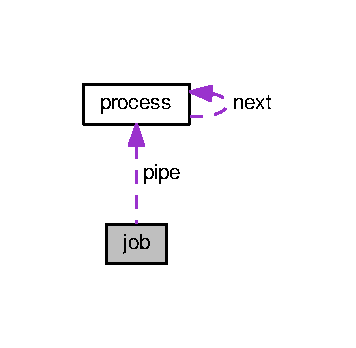
\includegraphics[width=171pt]{structjob__coll__graph}
\end{center}
\end{figure}
\subsection*{Public Attributes}
\begin{DoxyCompactItemize}
\item 
char $\ast$ \hyperlink{structjob_ab27dfab9ba607cb3bbdd2b6f2b4e3efc}{wd}
\item 
\hyperlink{jobs_8h_a98d7f91a8b6b7bc43192267133fe951d}{P\+R\+O\+C\+E\+SS} $\ast$ \hyperlink{structjob_a7e5648df5ec2f0d459900325c2cc5816}{pipe}
\item 
pid\+\_\+t \hyperlink{structjob_a36d8fbcede662cb503c447511b10dabc}{pgrp}
\item 
\hyperlink{jobs_8h_a27f134c9d8392fc50ee339c518707f57}{J\+O\+B\+\_\+\+S\+T\+A\+TE} \hyperlink{structjob_a5bee3de4970de999192f8929f926a4fe}{state}
\item 
int \hyperlink{structjob_af96c169abb39b4b3f9ccce91cb4b17dc}{flags}
\end{DoxyCompactItemize}


\subsection{Member Data Documentation}
\index{job@{job}!flags@{flags}}
\index{flags@{flags}!job@{job}}
\subsubsection[{\texorpdfstring{flags}{flags}}]{\setlength{\rightskip}{0pt plus 5cm}int job\+::flags}\hypertarget{structjob_af96c169abb39b4b3f9ccce91cb4b17dc}{}\label{structjob_af96c169abb39b4b3f9ccce91cb4b17dc}
\index{job@{job}!pgrp@{pgrp}}
\index{pgrp@{pgrp}!job@{job}}
\subsubsection[{\texorpdfstring{pgrp}{pgrp}}]{\setlength{\rightskip}{0pt plus 5cm}pid\+\_\+t job\+::pgrp}\hypertarget{structjob_a36d8fbcede662cb503c447511b10dabc}{}\label{structjob_a36d8fbcede662cb503c447511b10dabc}
\index{job@{job}!pipe@{pipe}}
\index{pipe@{pipe}!job@{job}}
\subsubsection[{\texorpdfstring{pipe}{pipe}}]{\setlength{\rightskip}{0pt plus 5cm}{\bf P\+R\+O\+C\+E\+SS}$\ast$ job\+::pipe}\hypertarget{structjob_a7e5648df5ec2f0d459900325c2cc5816}{}\label{structjob_a7e5648df5ec2f0d459900325c2cc5816}
\index{job@{job}!state@{state}}
\index{state@{state}!job@{job}}
\subsubsection[{\texorpdfstring{state}{state}}]{\setlength{\rightskip}{0pt plus 5cm}{\bf J\+O\+B\+\_\+\+S\+T\+A\+TE} job\+::state}\hypertarget{structjob_a5bee3de4970de999192f8929f926a4fe}{}\label{structjob_a5bee3de4970de999192f8929f926a4fe}
\index{job@{job}!wd@{wd}}
\index{wd@{wd}!job@{job}}
\subsubsection[{\texorpdfstring{wd}{wd}}]{\setlength{\rightskip}{0pt plus 5cm}char$\ast$ job\+::wd}\hypertarget{structjob_ab27dfab9ba607cb3bbdd2b6f2b4e3efc}{}\label{structjob_ab27dfab9ba607cb3bbdd2b6f2b4e3efc}


The documentation for this struct was generated from the following file\+:\begin{DoxyCompactItemize}
\item 
\hyperlink{jobs_8h}{jobs.\+h}\end{DoxyCompactItemize}

\hypertarget{structjobstats}{}\section{jobstats Struct Reference}
\label{structjobstats}\index{jobstats@{jobstats}}


{\ttfamily \#include $<$jobs.\+h$>$}



Collaboration diagram for jobstats\+:
\nopagebreak
\begin{figure}[H]
\begin{center}
\leavevmode
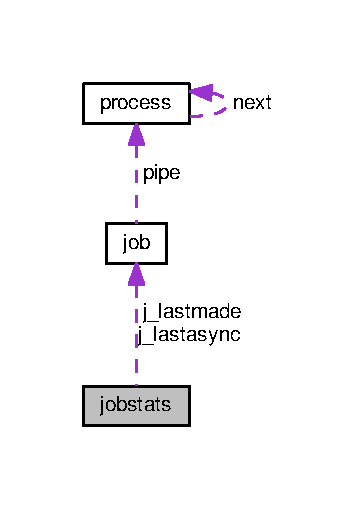
\includegraphics[width=171pt]{structjobstats__coll__graph}
\end{center}
\end{figure}
\subsection*{Public Attributes}
\begin{DoxyCompactItemize}
\item 
long \hyperlink{structjobstats_a3c74d4692759e4d8ec8089acefa23583}{c\+\_\+childmax}
\item 
int \hyperlink{structjobstats_a62da0e16fcd2ac8946942b8502ed3aef}{c\+\_\+living}
\item 
int \hyperlink{structjobstats_a9eba978ad89cdb8068837ea21189d4c9}{c\+\_\+reaped}
\item 
int \hyperlink{structjobstats_a99f41bab1480f94d10a98bddfe502948}{c\+\_\+injobs}
\item 
int \hyperlink{structjobstats_abecf408f2e3333f79205219911e32243}{c\+\_\+totforked}
\item 
int \hyperlink{structjobstats_a7004d60376bd1c7c3885598bc1038603}{c\+\_\+totreaped}
\item 
int \hyperlink{structjobstats_ad107b5818741c0309ebdb7af7318309e}{j\+\_\+jobslots}
\item 
int \hyperlink{structjobstats_ac29ea4e478fa590943c6f7ae902f3a46}{j\+\_\+lastj}
\item 
int \hyperlink{structjobstats_a41979e2d342c40d347381152156fc26d}{j\+\_\+firstj}
\item 
int \hyperlink{structjobstats_a3cd30b59b6ea29dc4d58020e6004d718}{j\+\_\+njobs}
\item 
int \hyperlink{structjobstats_a5c5a5b94e26c657b8caef74571c311ec}{j\+\_\+ndead}
\item 
int \hyperlink{structjobstats_ab72b09f6f206832a608cd245d513cca5}{j\+\_\+current}
\item 
int \hyperlink{structjobstats_a10c9a2fa68d7fed880e9f9c5f2b4d7f8}{j\+\_\+previous}
\item 
\hyperlink{jobs_8h_a9f9c26ac1579020577aabcd357e0c98b}{J\+OB} $\ast$ \hyperlink{structjobstats_ae904f7592ededb2bf0effc72444aab81}{j\+\_\+lastmade}
\item 
\hyperlink{jobs_8h_a9f9c26ac1579020577aabcd357e0c98b}{J\+OB} $\ast$ \hyperlink{structjobstats_aa7884beee2ac8c9f5da5c93ed57988b5}{j\+\_\+lastasync}
\end{DoxyCompactItemize}


\subsection{Member Data Documentation}
\index{jobstats@{jobstats}!c\+\_\+childmax@{c\+\_\+childmax}}
\index{c\+\_\+childmax@{c\+\_\+childmax}!jobstats@{jobstats}}
\subsubsection[{\texorpdfstring{c\+\_\+childmax}{c_childmax}}]{\setlength{\rightskip}{0pt plus 5cm}long jobstats\+::c\+\_\+childmax}\hypertarget{structjobstats_a3c74d4692759e4d8ec8089acefa23583}{}\label{structjobstats_a3c74d4692759e4d8ec8089acefa23583}
\index{jobstats@{jobstats}!c\+\_\+injobs@{c\+\_\+injobs}}
\index{c\+\_\+injobs@{c\+\_\+injobs}!jobstats@{jobstats}}
\subsubsection[{\texorpdfstring{c\+\_\+injobs}{c_injobs}}]{\setlength{\rightskip}{0pt plus 5cm}int jobstats\+::c\+\_\+injobs}\hypertarget{structjobstats_a99f41bab1480f94d10a98bddfe502948}{}\label{structjobstats_a99f41bab1480f94d10a98bddfe502948}
\index{jobstats@{jobstats}!c\+\_\+living@{c\+\_\+living}}
\index{c\+\_\+living@{c\+\_\+living}!jobstats@{jobstats}}
\subsubsection[{\texorpdfstring{c\+\_\+living}{c_living}}]{\setlength{\rightskip}{0pt plus 5cm}int jobstats\+::c\+\_\+living}\hypertarget{structjobstats_a62da0e16fcd2ac8946942b8502ed3aef}{}\label{structjobstats_a62da0e16fcd2ac8946942b8502ed3aef}
\index{jobstats@{jobstats}!c\+\_\+reaped@{c\+\_\+reaped}}
\index{c\+\_\+reaped@{c\+\_\+reaped}!jobstats@{jobstats}}
\subsubsection[{\texorpdfstring{c\+\_\+reaped}{c_reaped}}]{\setlength{\rightskip}{0pt plus 5cm}int jobstats\+::c\+\_\+reaped}\hypertarget{structjobstats_a9eba978ad89cdb8068837ea21189d4c9}{}\label{structjobstats_a9eba978ad89cdb8068837ea21189d4c9}
\index{jobstats@{jobstats}!c\+\_\+totforked@{c\+\_\+totforked}}
\index{c\+\_\+totforked@{c\+\_\+totforked}!jobstats@{jobstats}}
\subsubsection[{\texorpdfstring{c\+\_\+totforked}{c_totforked}}]{\setlength{\rightskip}{0pt plus 5cm}int jobstats\+::c\+\_\+totforked}\hypertarget{structjobstats_abecf408f2e3333f79205219911e32243}{}\label{structjobstats_abecf408f2e3333f79205219911e32243}
\index{jobstats@{jobstats}!c\+\_\+totreaped@{c\+\_\+totreaped}}
\index{c\+\_\+totreaped@{c\+\_\+totreaped}!jobstats@{jobstats}}
\subsubsection[{\texorpdfstring{c\+\_\+totreaped}{c_totreaped}}]{\setlength{\rightskip}{0pt plus 5cm}int jobstats\+::c\+\_\+totreaped}\hypertarget{structjobstats_a7004d60376bd1c7c3885598bc1038603}{}\label{structjobstats_a7004d60376bd1c7c3885598bc1038603}
\index{jobstats@{jobstats}!j\+\_\+current@{j\+\_\+current}}
\index{j\+\_\+current@{j\+\_\+current}!jobstats@{jobstats}}
\subsubsection[{\texorpdfstring{j\+\_\+current}{j_current}}]{\setlength{\rightskip}{0pt plus 5cm}int jobstats\+::j\+\_\+current}\hypertarget{structjobstats_ab72b09f6f206832a608cd245d513cca5}{}\label{structjobstats_ab72b09f6f206832a608cd245d513cca5}
\index{jobstats@{jobstats}!j\+\_\+firstj@{j\+\_\+firstj}}
\index{j\+\_\+firstj@{j\+\_\+firstj}!jobstats@{jobstats}}
\subsubsection[{\texorpdfstring{j\+\_\+firstj}{j_firstj}}]{\setlength{\rightskip}{0pt plus 5cm}int jobstats\+::j\+\_\+firstj}\hypertarget{structjobstats_a41979e2d342c40d347381152156fc26d}{}\label{structjobstats_a41979e2d342c40d347381152156fc26d}
\index{jobstats@{jobstats}!j\+\_\+jobslots@{j\+\_\+jobslots}}
\index{j\+\_\+jobslots@{j\+\_\+jobslots}!jobstats@{jobstats}}
\subsubsection[{\texorpdfstring{j\+\_\+jobslots}{j_jobslots}}]{\setlength{\rightskip}{0pt plus 5cm}int jobstats\+::j\+\_\+jobslots}\hypertarget{structjobstats_ad107b5818741c0309ebdb7af7318309e}{}\label{structjobstats_ad107b5818741c0309ebdb7af7318309e}
\index{jobstats@{jobstats}!j\+\_\+lastasync@{j\+\_\+lastasync}}
\index{j\+\_\+lastasync@{j\+\_\+lastasync}!jobstats@{jobstats}}
\subsubsection[{\texorpdfstring{j\+\_\+lastasync}{j_lastasync}}]{\setlength{\rightskip}{0pt plus 5cm}{\bf J\+OB}$\ast$ jobstats\+::j\+\_\+lastasync}\hypertarget{structjobstats_aa7884beee2ac8c9f5da5c93ed57988b5}{}\label{structjobstats_aa7884beee2ac8c9f5da5c93ed57988b5}
\index{jobstats@{jobstats}!j\+\_\+lastj@{j\+\_\+lastj}}
\index{j\+\_\+lastj@{j\+\_\+lastj}!jobstats@{jobstats}}
\subsubsection[{\texorpdfstring{j\+\_\+lastj}{j_lastj}}]{\setlength{\rightskip}{0pt plus 5cm}int jobstats\+::j\+\_\+lastj}\hypertarget{structjobstats_ac29ea4e478fa590943c6f7ae902f3a46}{}\label{structjobstats_ac29ea4e478fa590943c6f7ae902f3a46}
\index{jobstats@{jobstats}!j\+\_\+lastmade@{j\+\_\+lastmade}}
\index{j\+\_\+lastmade@{j\+\_\+lastmade}!jobstats@{jobstats}}
\subsubsection[{\texorpdfstring{j\+\_\+lastmade}{j_lastmade}}]{\setlength{\rightskip}{0pt plus 5cm}{\bf J\+OB}$\ast$ jobstats\+::j\+\_\+lastmade}\hypertarget{structjobstats_ae904f7592ededb2bf0effc72444aab81}{}\label{structjobstats_ae904f7592ededb2bf0effc72444aab81}
\index{jobstats@{jobstats}!j\+\_\+ndead@{j\+\_\+ndead}}
\index{j\+\_\+ndead@{j\+\_\+ndead}!jobstats@{jobstats}}
\subsubsection[{\texorpdfstring{j\+\_\+ndead}{j_ndead}}]{\setlength{\rightskip}{0pt plus 5cm}int jobstats\+::j\+\_\+ndead}\hypertarget{structjobstats_a5c5a5b94e26c657b8caef74571c311ec}{}\label{structjobstats_a5c5a5b94e26c657b8caef74571c311ec}
\index{jobstats@{jobstats}!j\+\_\+njobs@{j\+\_\+njobs}}
\index{j\+\_\+njobs@{j\+\_\+njobs}!jobstats@{jobstats}}
\subsubsection[{\texorpdfstring{j\+\_\+njobs}{j_njobs}}]{\setlength{\rightskip}{0pt plus 5cm}int jobstats\+::j\+\_\+njobs}\hypertarget{structjobstats_a3cd30b59b6ea29dc4d58020e6004d718}{}\label{structjobstats_a3cd30b59b6ea29dc4d58020e6004d718}
\index{jobstats@{jobstats}!j\+\_\+previous@{j\+\_\+previous}}
\index{j\+\_\+previous@{j\+\_\+previous}!jobstats@{jobstats}}
\subsubsection[{\texorpdfstring{j\+\_\+previous}{j_previous}}]{\setlength{\rightskip}{0pt plus 5cm}int jobstats\+::j\+\_\+previous}\hypertarget{structjobstats_a10c9a2fa68d7fed880e9f9c5f2b4d7f8}{}\label{structjobstats_a10c9a2fa68d7fed880e9f9c5f2b4d7f8}


The documentation for this struct was generated from the following file\+:\begin{DoxyCompactItemize}
\item 
\hyperlink{jobs_8h}{jobs.\+h}\end{DoxyCompactItemize}

\hypertarget{structlvalue}{}\section{lvalue Struct Reference}
\label{structlvalue}\index{lvalue@{lvalue}}


Collaboration diagram for lvalue\+:
\nopagebreak
\begin{figure}[H]
\begin{center}
\leavevmode
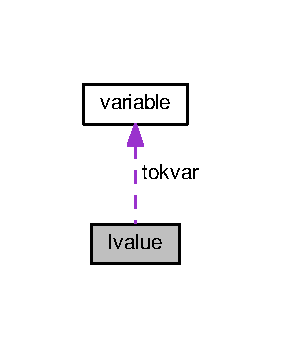
\includegraphics[width=136pt]{structlvalue__coll__graph}
\end{center}
\end{figure}
\subsection*{Public Attributes}
\begin{DoxyCompactItemize}
\item 
char $\ast$ \hyperlink{structlvalue_a69733836b6e89608c3b7f52575f168b6}{tokstr}
\item 
intmax\+\_\+t \hyperlink{structlvalue_a586486707a36587077d5c14c477e8a2a}{tokval}
\item 
\hyperlink{variables_8h_aba7363ba59b9546110e58106ad60cb50}{S\+H\+E\+L\+L\+\_\+\+V\+AR} $\ast$ \hyperlink{structlvalue_a6875190861863191326371f28d09a933}{tokvar}
\item 
intmax\+\_\+t \hyperlink{structlvalue_adc2354fd6009088922174d0b040a4e77}{ind}
\end{DoxyCompactItemize}


\subsection{Member Data Documentation}
\index{lvalue@{lvalue}!ind@{ind}}
\index{ind@{ind}!lvalue@{lvalue}}
\subsubsection[{\texorpdfstring{ind}{ind}}]{\setlength{\rightskip}{0pt plus 5cm}intmax\+\_\+t lvalue\+::ind}\hypertarget{structlvalue_adc2354fd6009088922174d0b040a4e77}{}\label{structlvalue_adc2354fd6009088922174d0b040a4e77}
\index{lvalue@{lvalue}!tokstr@{tokstr}}
\index{tokstr@{tokstr}!lvalue@{lvalue}}
\subsubsection[{\texorpdfstring{tokstr}{tokstr}}]{\setlength{\rightskip}{0pt plus 5cm}char$\ast$ lvalue\+::tokstr}\hypertarget{structlvalue_a69733836b6e89608c3b7f52575f168b6}{}\label{structlvalue_a69733836b6e89608c3b7f52575f168b6}
\index{lvalue@{lvalue}!tokval@{tokval}}
\index{tokval@{tokval}!lvalue@{lvalue}}
\subsubsection[{\texorpdfstring{tokval}{tokval}}]{\setlength{\rightskip}{0pt plus 5cm}intmax\+\_\+t lvalue\+::tokval}\hypertarget{structlvalue_a586486707a36587077d5c14c477e8a2a}{}\label{structlvalue_a586486707a36587077d5c14c477e8a2a}
\index{lvalue@{lvalue}!tokvar@{tokvar}}
\index{tokvar@{tokvar}!lvalue@{lvalue}}
\subsubsection[{\texorpdfstring{tokvar}{tokvar}}]{\setlength{\rightskip}{0pt plus 5cm}{\bf S\+H\+E\+L\+L\+\_\+\+V\+AR}$\ast$ lvalue\+::tokvar}\hypertarget{structlvalue_a6875190861863191326371f28d09a933}{}\label{structlvalue_a6875190861863191326371f28d09a933}


The documentation for this struct was generated from the following file\+:\begin{DoxyCompactItemize}
\item 
\hyperlink{expr_8c}{expr.\+c}\end{DoxyCompactItemize}

\hypertarget{structname__and__function}{}\section{name\+\_\+and\+\_\+function Struct Reference}
\label{structname__and__function}\index{name\+\_\+and\+\_\+function@{name\+\_\+and\+\_\+function}}
\subsection*{Public Attributes}
\begin{DoxyCompactItemize}
\item 
char $\ast$ \hyperlink{structname__and__function_a5a8e9c2c5166f39ec782baf0776fb902}{name}
\item 
sh\+\_\+sv\+\_\+func\+\_\+t $\ast$ \hyperlink{structname__and__function_a4cee9ba9ff7df61954782ef6f0ffddb3}{function}
\end{DoxyCompactItemize}


\subsection{Member Data Documentation}
\index{name\+\_\+and\+\_\+function@{name\+\_\+and\+\_\+function}!function@{function}}
\index{function@{function}!name\+\_\+and\+\_\+function@{name\+\_\+and\+\_\+function}}
\subsubsection[{\texorpdfstring{function}{function}}]{\setlength{\rightskip}{0pt plus 5cm}sh\+\_\+sv\+\_\+func\+\_\+t$\ast$ name\+\_\+and\+\_\+function\+::function}\hypertarget{structname__and__function_a4cee9ba9ff7df61954782ef6f0ffddb3}{}\label{structname__and__function_a4cee9ba9ff7df61954782ef6f0ffddb3}
\index{name\+\_\+and\+\_\+function@{name\+\_\+and\+\_\+function}!name@{name}}
\index{name@{name}!name\+\_\+and\+\_\+function@{name\+\_\+and\+\_\+function}}
\subsubsection[{\texorpdfstring{name}{name}}]{\setlength{\rightskip}{0pt plus 5cm}char$\ast$ name\+\_\+and\+\_\+function\+::name}\hypertarget{structname__and__function_a5a8e9c2c5166f39ec782baf0776fb902}{}\label{structname__and__function_a5a8e9c2c5166f39ec782baf0776fb902}


The documentation for this struct was generated from the following file\+:\begin{DoxyCompactItemize}
\item 
\hyperlink{variables_8c}{variables.\+c}\end{DoxyCompactItemize}

\hypertarget{structpattern__list}{}\section{pattern\+\_\+list Struct Reference}
\label{structpattern__list}\index{pattern\+\_\+list@{pattern\+\_\+list}}


{\ttfamily \#include $<$command.\+h$>$}



Collaboration diagram for pattern\+\_\+list\+:
\nopagebreak
\begin{figure}[H]
\begin{center}
\leavevmode
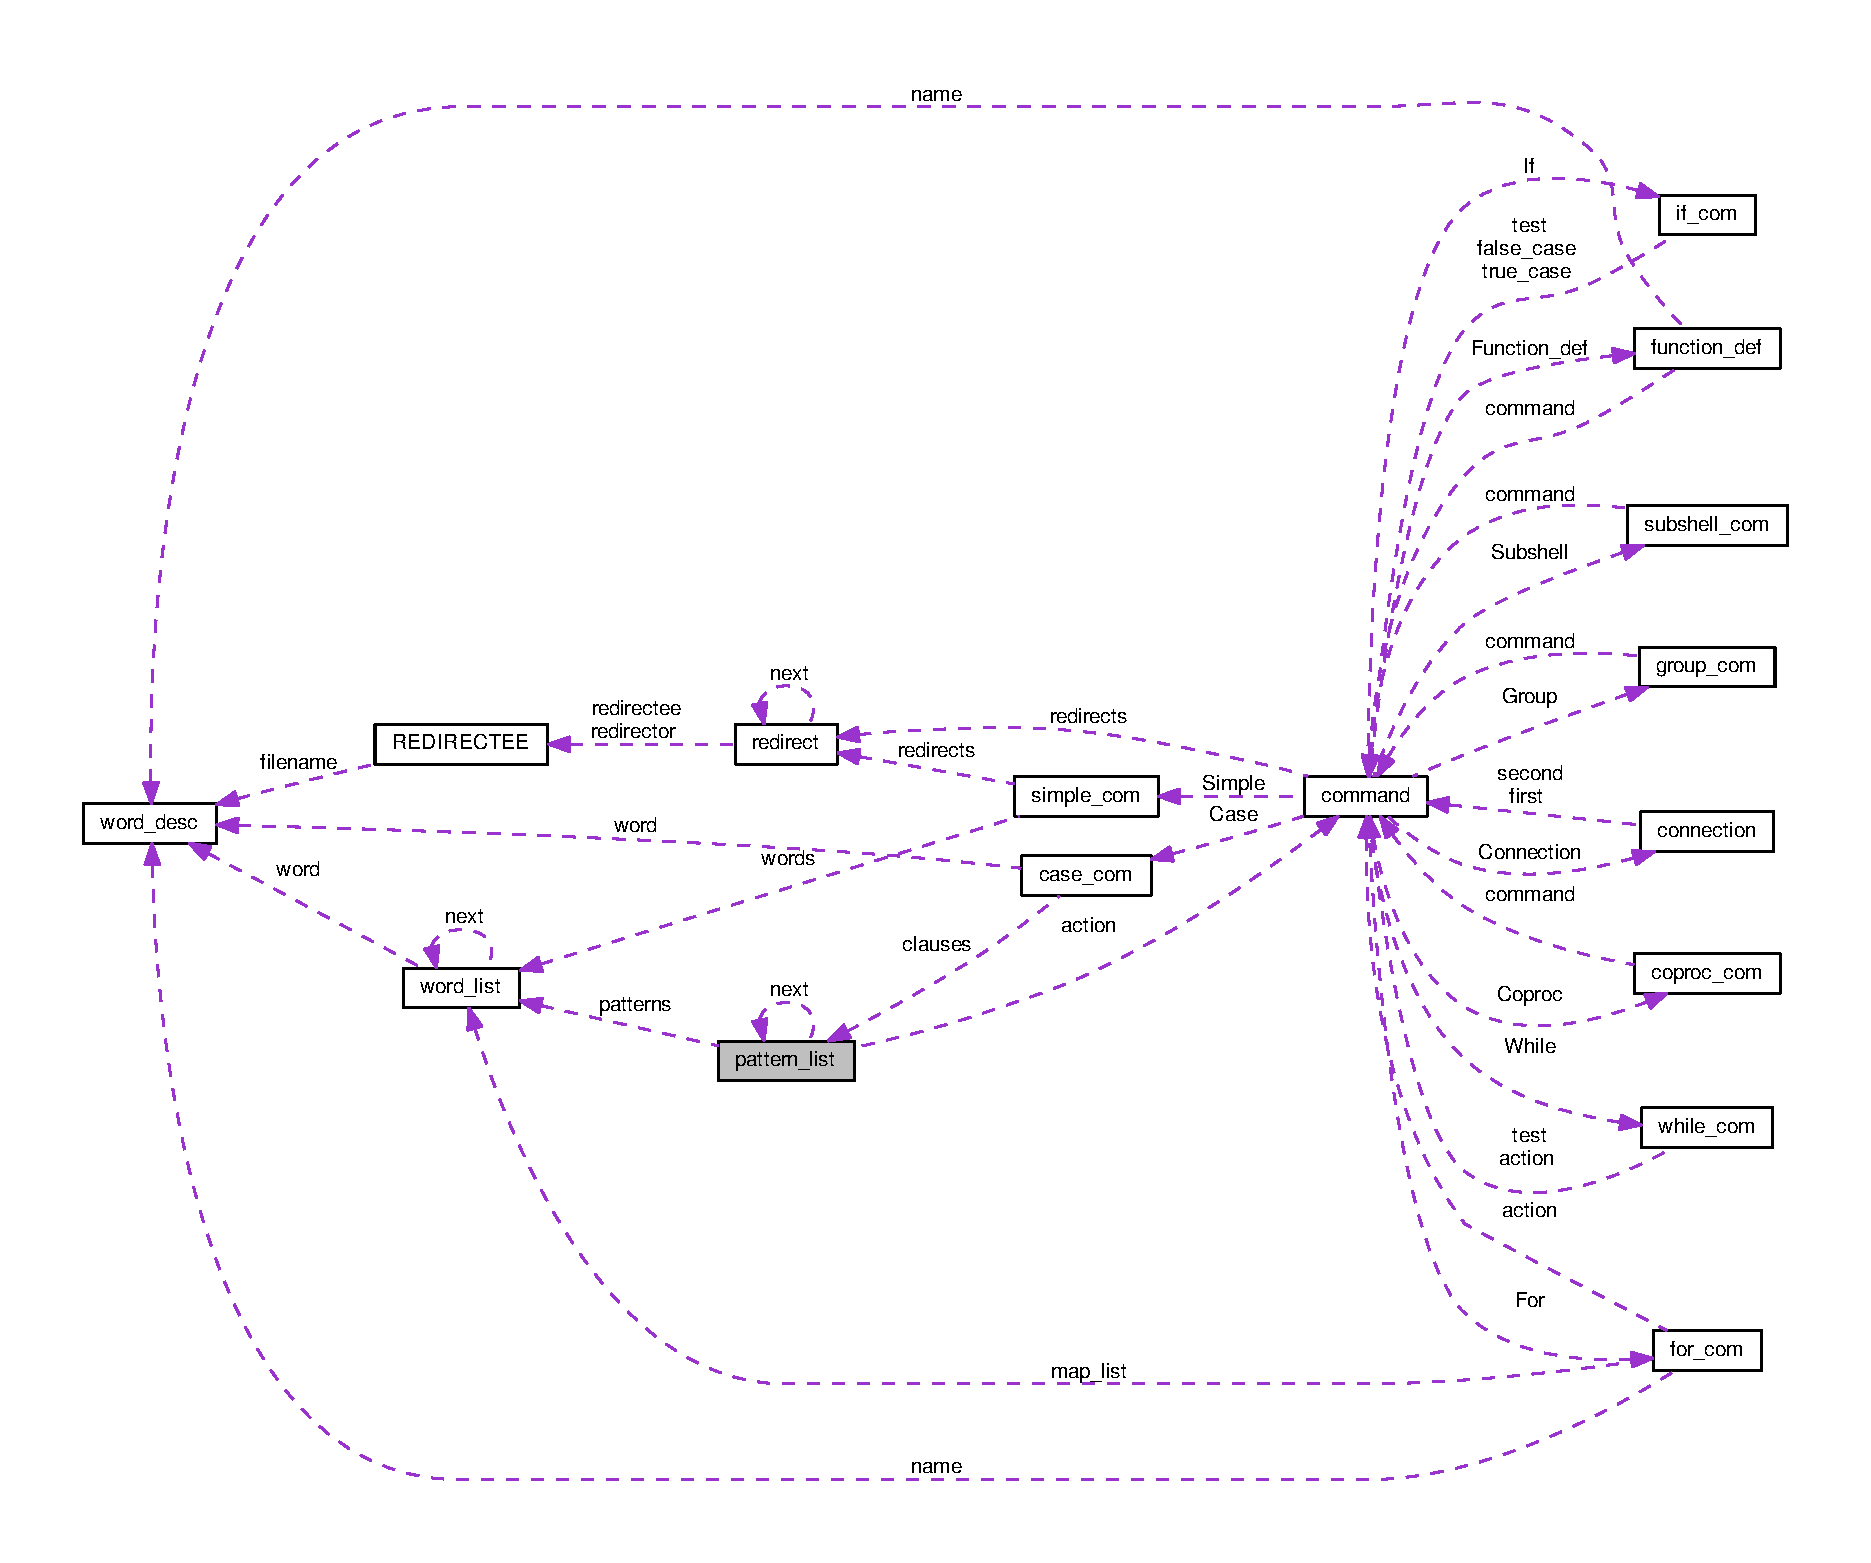
\includegraphics[width=350pt]{structpattern__list__coll__graph}
\end{center}
\end{figure}
\subsection*{Public Attributes}
\begin{DoxyCompactItemize}
\item 
struct \hyperlink{structpattern__list}{pattern\+\_\+list} $\ast$ \hyperlink{structpattern__list_a298ee7f13c0ded6032300588bc4739c6}{next}
\item 
\hyperlink{command_8h_ac42a7b781459884316a1f2ffe79e8a62}{W\+O\+R\+D\+\_\+\+L\+I\+ST} $\ast$ \hyperlink{structpattern__list_a434e80f6704633cfb08dab20c1d28076}{patterns}
\item 
\hyperlink{command_8h_a8c41dec142c299806885773c902c0d87}{C\+O\+M\+M\+A\+ND} $\ast$ \hyperlink{structpattern__list_ae31932a25ce2a1a616aecae649f78045}{action}
\item 
int \hyperlink{structpattern__list_abae207e9054326f960ead31780ccf5ea}{flags}
\end{DoxyCompactItemize}


\subsection{Member Data Documentation}
\index{pattern\+\_\+list@{pattern\+\_\+list}!action@{action}}
\index{action@{action}!pattern\+\_\+list@{pattern\+\_\+list}}
\subsubsection[{\texorpdfstring{action}{action}}]{\setlength{\rightskip}{0pt plus 5cm}{\bf C\+O\+M\+M\+A\+ND}$\ast$ pattern\+\_\+list\+::action}\hypertarget{structpattern__list_ae31932a25ce2a1a616aecae649f78045}{}\label{structpattern__list_ae31932a25ce2a1a616aecae649f78045}
\index{pattern\+\_\+list@{pattern\+\_\+list}!flags@{flags}}
\index{flags@{flags}!pattern\+\_\+list@{pattern\+\_\+list}}
\subsubsection[{\texorpdfstring{flags}{flags}}]{\setlength{\rightskip}{0pt plus 5cm}int pattern\+\_\+list\+::flags}\hypertarget{structpattern__list_abae207e9054326f960ead31780ccf5ea}{}\label{structpattern__list_abae207e9054326f960ead31780ccf5ea}
\index{pattern\+\_\+list@{pattern\+\_\+list}!next@{next}}
\index{next@{next}!pattern\+\_\+list@{pattern\+\_\+list}}
\subsubsection[{\texorpdfstring{next}{next}}]{\setlength{\rightskip}{0pt plus 5cm}struct {\bf pattern\+\_\+list}$\ast$ pattern\+\_\+list\+::next}\hypertarget{structpattern__list_a298ee7f13c0ded6032300588bc4739c6}{}\label{structpattern__list_a298ee7f13c0ded6032300588bc4739c6}
\index{pattern\+\_\+list@{pattern\+\_\+list}!patterns@{patterns}}
\index{patterns@{patterns}!pattern\+\_\+list@{pattern\+\_\+list}}
\subsubsection[{\texorpdfstring{patterns}{patterns}}]{\setlength{\rightskip}{0pt plus 5cm}{\bf W\+O\+R\+D\+\_\+\+L\+I\+ST}$\ast$ pattern\+\_\+list\+::patterns}\hypertarget{structpattern__list_a434e80f6704633cfb08dab20c1d28076}{}\label{structpattern__list_a434e80f6704633cfb08dab20c1d28076}


The documentation for this struct was generated from the following file\+:\begin{DoxyCompactItemize}
\item 
\hyperlink{command_8h}{command.\+h}\end{DoxyCompactItemize}

\hypertarget{structpidstat}{}\section{pidstat Struct Reference}
\label{structpidstat}\index{pidstat@{pidstat}}


{\ttfamily \#include $<$jobs.\+h$>$}

\subsection*{Public Attributes}
\begin{DoxyCompactItemize}
\item 
\hyperlink{jobs_8h_a677d6488545fa3193e7cb54647b4ae5c}{ps\+\_\+index\+\_\+t} \hyperlink{structpidstat_a6848a528a59f93911847b61d0b329ee5}{bucket\+\_\+next}
\item 
\hyperlink{jobs_8h_a677d6488545fa3193e7cb54647b4ae5c}{ps\+\_\+index\+\_\+t} \hyperlink{structpidstat_a5b7cfb7d4d5f30b11eaa92db21ec71a0}{bucket\+\_\+prev}
\item 
pid\+\_\+t \hyperlink{structpidstat_a9720eaa7788ca953a6130f2b8d1d1a23}{pid}
\item 
\hyperlink{config_8h_a843210b77ffdc4d44cf0ec069877735a}{bits16\+\_\+t} \hyperlink{structpidstat_a7feadc8da0ca4c76cd76c3b97274e622}{status}
\end{DoxyCompactItemize}


\subsection{Member Data Documentation}
\index{pidstat@{pidstat}!bucket\+\_\+next@{bucket\+\_\+next}}
\index{bucket\+\_\+next@{bucket\+\_\+next}!pidstat@{pidstat}}
\subsubsection[{\texorpdfstring{bucket\+\_\+next}{bucket_next}}]{\setlength{\rightskip}{0pt plus 5cm}{\bf ps\+\_\+index\+\_\+t} pidstat\+::bucket\+\_\+next}\hypertarget{structpidstat_a6848a528a59f93911847b61d0b329ee5}{}\label{structpidstat_a6848a528a59f93911847b61d0b329ee5}
\index{pidstat@{pidstat}!bucket\+\_\+prev@{bucket\+\_\+prev}}
\index{bucket\+\_\+prev@{bucket\+\_\+prev}!pidstat@{pidstat}}
\subsubsection[{\texorpdfstring{bucket\+\_\+prev}{bucket_prev}}]{\setlength{\rightskip}{0pt plus 5cm}{\bf ps\+\_\+index\+\_\+t} pidstat\+::bucket\+\_\+prev}\hypertarget{structpidstat_a5b7cfb7d4d5f30b11eaa92db21ec71a0}{}\label{structpidstat_a5b7cfb7d4d5f30b11eaa92db21ec71a0}
\index{pidstat@{pidstat}!pid@{pid}}
\index{pid@{pid}!pidstat@{pidstat}}
\subsubsection[{\texorpdfstring{pid}{pid}}]{\setlength{\rightskip}{0pt plus 5cm}pid\+\_\+t pidstat\+::pid}\hypertarget{structpidstat_a9720eaa7788ca953a6130f2b8d1d1a23}{}\label{structpidstat_a9720eaa7788ca953a6130f2b8d1d1a23}
\index{pidstat@{pidstat}!status@{status}}
\index{status@{status}!pidstat@{pidstat}}
\subsubsection[{\texorpdfstring{status}{status}}]{\setlength{\rightskip}{0pt plus 5cm}{\bf bits16\+\_\+t} pidstat\+::status}\hypertarget{structpidstat_a7feadc8da0ca4c76cd76c3b97274e622}{}\label{structpidstat_a7feadc8da0ca4c76cd76c3b97274e622}


The documentation for this struct was generated from the following file\+:\begin{DoxyCompactItemize}
\item 
\hyperlink{jobs_8h}{jobs.\+h}\end{DoxyCompactItemize}

\hypertarget{structpipeline__saver}{}\section{pipeline\+\_\+saver Struct Reference}
\label{structpipeline__saver}\index{pipeline\+\_\+saver@{pipeline\+\_\+saver}}


{\ttfamily \#include $<$jobs.\+h$>$}



Collaboration diagram for pipeline\+\_\+saver\+:
\nopagebreak
\begin{figure}[H]
\begin{center}
\leavevmode
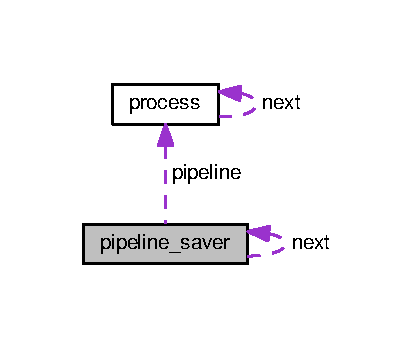
\includegraphics[width=199pt]{structpipeline__saver__coll__graph}
\end{center}
\end{figure}
\subsection*{Public Attributes}
\begin{DoxyCompactItemize}
\item 
struct \hyperlink{structprocess}{process} $\ast$ \hyperlink{structpipeline__saver_a150b4d503a5673894709f96b053de8b2}{pipeline}
\item 
struct \hyperlink{structpipeline__saver}{pipeline\+\_\+saver} $\ast$ \hyperlink{structpipeline__saver_a736199ba9d005768c1a764a5da6a69e6}{next}
\end{DoxyCompactItemize}


\subsection{Member Data Documentation}
\index{pipeline\+\_\+saver@{pipeline\+\_\+saver}!next@{next}}
\index{next@{next}!pipeline\+\_\+saver@{pipeline\+\_\+saver}}
\subsubsection[{\texorpdfstring{next}{next}}]{\setlength{\rightskip}{0pt plus 5cm}struct {\bf pipeline\+\_\+saver}$\ast$ pipeline\+\_\+saver\+::next}\hypertarget{structpipeline__saver_a736199ba9d005768c1a764a5da6a69e6}{}\label{structpipeline__saver_a736199ba9d005768c1a764a5da6a69e6}
\index{pipeline\+\_\+saver@{pipeline\+\_\+saver}!pipeline@{pipeline}}
\index{pipeline@{pipeline}!pipeline\+\_\+saver@{pipeline\+\_\+saver}}
\subsubsection[{\texorpdfstring{pipeline}{pipeline}}]{\setlength{\rightskip}{0pt plus 5cm}struct {\bf process}$\ast$ pipeline\+\_\+saver\+::pipeline}\hypertarget{structpipeline__saver_a150b4d503a5673894709f96b053de8b2}{}\label{structpipeline__saver_a150b4d503a5673894709f96b053de8b2}


The documentation for this struct was generated from the following file\+:\begin{DoxyCompactItemize}
\item 
\hyperlink{jobs_8h}{jobs.\+h}\end{DoxyCompactItemize}

\hypertarget{structproc__status}{}\section{proc\+\_\+status Struct Reference}
\label{structproc__status}\index{proc\+\_\+status@{proc\+\_\+status}}
\subsection*{Public Attributes}
\begin{DoxyCompactItemize}
\item 
pid\+\_\+t \hyperlink{structproc__status_ad94b4a7c73f39bfdf869c300340fb34f}{pid}
\item 
int \hyperlink{structproc__status_aae75801d53e9f1c8667db35cc3cacf11}{status}
\item 
int \hyperlink{structproc__status_a89eac98aa12ef30d327bd03a81635a03}{flags}
\end{DoxyCompactItemize}


\subsection{Member Data Documentation}
\index{proc\+\_\+status@{proc\+\_\+status}!flags@{flags}}
\index{flags@{flags}!proc\+\_\+status@{proc\+\_\+status}}
\subsubsection[{\texorpdfstring{flags}{flags}}]{\setlength{\rightskip}{0pt plus 5cm}int proc\+\_\+status\+::flags}\hypertarget{structproc__status_a89eac98aa12ef30d327bd03a81635a03}{}\label{structproc__status_a89eac98aa12ef30d327bd03a81635a03}
\index{proc\+\_\+status@{proc\+\_\+status}!pid@{pid}}
\index{pid@{pid}!proc\+\_\+status@{proc\+\_\+status}}
\subsubsection[{\texorpdfstring{pid}{pid}}]{\setlength{\rightskip}{0pt plus 5cm}pid\+\_\+t proc\+\_\+status\+::pid}\hypertarget{structproc__status_ad94b4a7c73f39bfdf869c300340fb34f}{}\label{structproc__status_ad94b4a7c73f39bfdf869c300340fb34f}
\index{proc\+\_\+status@{proc\+\_\+status}!status@{status}}
\index{status@{status}!proc\+\_\+status@{proc\+\_\+status}}
\subsubsection[{\texorpdfstring{status}{status}}]{\setlength{\rightskip}{0pt plus 5cm}int proc\+\_\+status\+::status}\hypertarget{structproc__status_aae75801d53e9f1c8667db35cc3cacf11}{}\label{structproc__status_aae75801d53e9f1c8667db35cc3cacf11}


The documentation for this struct was generated from the following file\+:\begin{DoxyCompactItemize}
\item 
\hyperlink{nojobs_8c}{nojobs.\+c}\end{DoxyCompactItemize}

\hypertarget{structprocess}{}\section{process Struct Reference}
\label{structprocess}\index{process@{process}}


{\ttfamily \#include $<$jobs.\+h$>$}



Collaboration diagram for process\+:
\nopagebreak
\begin{figure}[H]
\begin{center}
\leavevmode
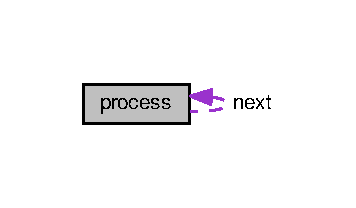
\includegraphics[width=171pt]{structprocess__coll__graph}
\end{center}
\end{figure}
\subsection*{Public Attributes}
\begin{DoxyCompactItemize}
\item 
struct \hyperlink{structprocess}{process} $\ast$ \hyperlink{structprocess_aa714b70ab9ca99fc489de2f70a091b0b}{next}
\item 
pid\+\_\+t \hyperlink{structprocess_ab7b330a89c9b52c5f0c7dedd4f90dfb8}{pid}
\item 
W\+A\+IT \hyperlink{structprocess_ab1cc113f2cf7e94945d01e4366ac1d0c}{status}
\item 
int \hyperlink{structprocess_ada5ec5eaed30b9d88d1cf6f2b27c3470}{running}
\item 
char $\ast$ \hyperlink{structprocess_acf66477c56add129da786ade715a6757}{command}
\end{DoxyCompactItemize}


\subsection{Member Data Documentation}
\index{process@{process}!command@{command}}
\index{command@{command}!process@{process}}
\subsubsection[{\texorpdfstring{command}{command}}]{\setlength{\rightskip}{0pt plus 5cm}char$\ast$ process\+::command}\hypertarget{structprocess_acf66477c56add129da786ade715a6757}{}\label{structprocess_acf66477c56add129da786ade715a6757}
\index{process@{process}!next@{next}}
\index{next@{next}!process@{process}}
\subsubsection[{\texorpdfstring{next}{next}}]{\setlength{\rightskip}{0pt plus 5cm}struct {\bf process}$\ast$ process\+::next}\hypertarget{structprocess_aa714b70ab9ca99fc489de2f70a091b0b}{}\label{structprocess_aa714b70ab9ca99fc489de2f70a091b0b}
\index{process@{process}!pid@{pid}}
\index{pid@{pid}!process@{process}}
\subsubsection[{\texorpdfstring{pid}{pid}}]{\setlength{\rightskip}{0pt plus 5cm}pid\+\_\+t process\+::pid}\hypertarget{structprocess_ab7b330a89c9b52c5f0c7dedd4f90dfb8}{}\label{structprocess_ab7b330a89c9b52c5f0c7dedd4f90dfb8}
\index{process@{process}!running@{running}}
\index{running@{running}!process@{process}}
\subsubsection[{\texorpdfstring{running}{running}}]{\setlength{\rightskip}{0pt plus 5cm}int process\+::running}\hypertarget{structprocess_ada5ec5eaed30b9d88d1cf6f2b27c3470}{}\label{structprocess_ada5ec5eaed30b9d88d1cf6f2b27c3470}
\index{process@{process}!status@{status}}
\index{status@{status}!process@{process}}
\subsubsection[{\texorpdfstring{status}{status}}]{\setlength{\rightskip}{0pt plus 5cm}W\+A\+IT process\+::status}\hypertarget{structprocess_ab1cc113f2cf7e94945d01e4366ac1d0c}{}\label{structprocess_ab1cc113f2cf7e94945d01e4366ac1d0c}


The documentation for this struct was generated from the following file\+:\begin{DoxyCompactItemize}
\item 
\hyperlink{jobs_8h}{jobs.\+h}\end{DoxyCompactItemize}

\hypertarget{structredirect}{}\section{redirect Struct Reference}
\label{structredirect}\index{redirect@{redirect}}


{\ttfamily \#include $<$command.\+h$>$}



Collaboration diagram for redirect\+:
\nopagebreak
\begin{figure}[H]
\begin{center}
\leavevmode
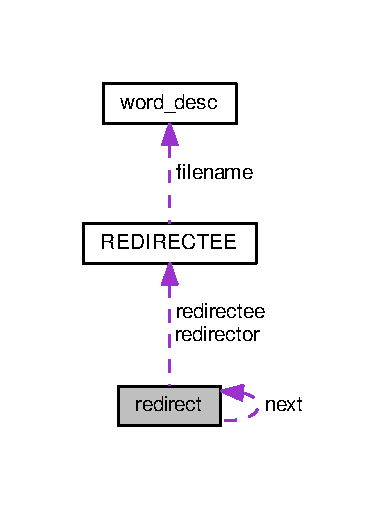
\includegraphics[width=186pt]{structredirect__coll__graph}
\end{center}
\end{figure}
\subsection*{Public Attributes}
\begin{DoxyCompactItemize}
\item 
struct \hyperlink{structredirect}{redirect} $\ast$ \hyperlink{structredirect_ae7bbd7429c76ca31edcdc88e43fd2408}{next}
\item 
\hyperlink{unionREDIRECTEE}{R\+E\+D\+I\+R\+E\+C\+T\+EE} \hyperlink{structredirect_a49cf28da45dc5c4dc890b71904f484fb}{redirector}
\item 
int \hyperlink{structredirect_a0dd66f3dc5607959984565679aca5474}{rflags}
\item 
int \hyperlink{structredirect_a9328e6f00bf0e9d9d08ecacba6374df8}{flags}
\item 
enum \hyperlink{command_8h_a30995e3628b99a0514ed9fdd9843e55d}{r\+\_\+instruction} \hyperlink{structredirect_a81e943ca1372e74ad5ab23a22f9e8beb}{instruction}
\item 
\hyperlink{unionREDIRECTEE}{R\+E\+D\+I\+R\+E\+C\+T\+EE} \hyperlink{structredirect_a484dd470583ad862e00d2d738a9f7e93}{redirectee}
\item 
char $\ast$ \hyperlink{structredirect_a3185120aafa79b4c48824283a3021e63}{here\+\_\+doc\+\_\+eof}
\end{DoxyCompactItemize}


\subsection{Member Data Documentation}
\index{redirect@{redirect}!flags@{flags}}
\index{flags@{flags}!redirect@{redirect}}
\subsubsection[{\texorpdfstring{flags}{flags}}]{\setlength{\rightskip}{0pt plus 5cm}int redirect\+::flags}\hypertarget{structredirect_a9328e6f00bf0e9d9d08ecacba6374df8}{}\label{structredirect_a9328e6f00bf0e9d9d08ecacba6374df8}
\index{redirect@{redirect}!here\+\_\+doc\+\_\+eof@{here\+\_\+doc\+\_\+eof}}
\index{here\+\_\+doc\+\_\+eof@{here\+\_\+doc\+\_\+eof}!redirect@{redirect}}
\subsubsection[{\texorpdfstring{here\+\_\+doc\+\_\+eof}{here_doc_eof}}]{\setlength{\rightskip}{0pt plus 5cm}char$\ast$ redirect\+::here\+\_\+doc\+\_\+eof}\hypertarget{structredirect_a3185120aafa79b4c48824283a3021e63}{}\label{structredirect_a3185120aafa79b4c48824283a3021e63}
\index{redirect@{redirect}!instruction@{instruction}}
\index{instruction@{instruction}!redirect@{redirect}}
\subsubsection[{\texorpdfstring{instruction}{instruction}}]{\setlength{\rightskip}{0pt plus 5cm}enum {\bf r\+\_\+instruction} redirect\+::instruction}\hypertarget{structredirect_a81e943ca1372e74ad5ab23a22f9e8beb}{}\label{structredirect_a81e943ca1372e74ad5ab23a22f9e8beb}
\index{redirect@{redirect}!next@{next}}
\index{next@{next}!redirect@{redirect}}
\subsubsection[{\texorpdfstring{next}{next}}]{\setlength{\rightskip}{0pt plus 5cm}struct {\bf redirect}$\ast$ redirect\+::next}\hypertarget{structredirect_ae7bbd7429c76ca31edcdc88e43fd2408}{}\label{structredirect_ae7bbd7429c76ca31edcdc88e43fd2408}
\index{redirect@{redirect}!redirectee@{redirectee}}
\index{redirectee@{redirectee}!redirect@{redirect}}
\subsubsection[{\texorpdfstring{redirectee}{redirectee}}]{\setlength{\rightskip}{0pt plus 5cm}{\bf R\+E\+D\+I\+R\+E\+C\+T\+EE} redirect\+::redirectee}\hypertarget{structredirect_a484dd470583ad862e00d2d738a9f7e93}{}\label{structredirect_a484dd470583ad862e00d2d738a9f7e93}
\index{redirect@{redirect}!redirector@{redirector}}
\index{redirector@{redirector}!redirect@{redirect}}
\subsubsection[{\texorpdfstring{redirector}{redirector}}]{\setlength{\rightskip}{0pt plus 5cm}{\bf R\+E\+D\+I\+R\+E\+C\+T\+EE} redirect\+::redirector}\hypertarget{structredirect_a49cf28da45dc5c4dc890b71904f484fb}{}\label{structredirect_a49cf28da45dc5c4dc890b71904f484fb}
\index{redirect@{redirect}!rflags@{rflags}}
\index{rflags@{rflags}!redirect@{redirect}}
\subsubsection[{\texorpdfstring{rflags}{rflags}}]{\setlength{\rightskip}{0pt plus 5cm}int redirect\+::rflags}\hypertarget{structredirect_a0dd66f3dc5607959984565679aca5474}{}\label{structredirect_a0dd66f3dc5607959984565679aca5474}


The documentation for this struct was generated from the following file\+:\begin{DoxyCompactItemize}
\item 
\hyperlink{command_8h}{command.\+h}\end{DoxyCompactItemize}

\hypertarget{unionREDIRECTEE}{}\section{R\+E\+D\+I\+R\+E\+C\+T\+EE Union Reference}
\label{unionREDIRECTEE}\index{R\+E\+D\+I\+R\+E\+C\+T\+EE@{R\+E\+D\+I\+R\+E\+C\+T\+EE}}


{\ttfamily \#include $<$command.\+h$>$}



Collaboration diagram for R\+E\+D\+I\+R\+E\+C\+T\+EE\+:
\nopagebreak
\begin{figure}[H]
\begin{center}
\leavevmode
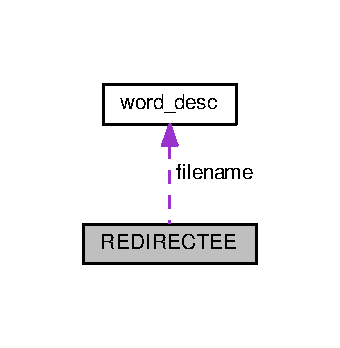
\includegraphics[width=163pt]{unionREDIRECTEE__coll__graph}
\end{center}
\end{figure}
\subsection*{Public Attributes}
\begin{DoxyCompactItemize}
\item 
int \hyperlink{unionREDIRECTEE_a241f08d773699e8d21de269b4644cbbd}{dest}
\item 
\hyperlink{command_8h_a3f0cccf333703e5f6c4168be0db675fa}{W\+O\+R\+D\+\_\+\+D\+E\+SC} $\ast$ \hyperlink{unionREDIRECTEE_a5149629ee488bbd339dd6d7dbe38f212}{filename}
\end{DoxyCompactItemize}


\subsection{Member Data Documentation}
\index{R\+E\+D\+I\+R\+E\+C\+T\+EE@{R\+E\+D\+I\+R\+E\+C\+T\+EE}!dest@{dest}}
\index{dest@{dest}!R\+E\+D\+I\+R\+E\+C\+T\+EE@{R\+E\+D\+I\+R\+E\+C\+T\+EE}}
\subsubsection[{\texorpdfstring{dest}{dest}}]{\setlength{\rightskip}{0pt plus 5cm}int R\+E\+D\+I\+R\+E\+C\+T\+E\+E\+::dest}\hypertarget{unionREDIRECTEE_a241f08d773699e8d21de269b4644cbbd}{}\label{unionREDIRECTEE_a241f08d773699e8d21de269b4644cbbd}
\index{R\+E\+D\+I\+R\+E\+C\+T\+EE@{R\+E\+D\+I\+R\+E\+C\+T\+EE}!filename@{filename}}
\index{filename@{filename}!R\+E\+D\+I\+R\+E\+C\+T\+EE@{R\+E\+D\+I\+R\+E\+C\+T\+EE}}
\subsubsection[{\texorpdfstring{filename}{filename}}]{\setlength{\rightskip}{0pt plus 5cm}{\bf W\+O\+R\+D\+\_\+\+D\+E\+SC}$\ast$ R\+E\+D\+I\+R\+E\+C\+T\+E\+E\+::filename}\hypertarget{unionREDIRECTEE_a5149629ee488bbd339dd6d7dbe38f212}{}\label{unionREDIRECTEE_a5149629ee488bbd339dd6d7dbe38f212}


The documentation for this union was generated from the following file\+:\begin{DoxyCompactItemize}
\item 
\hyperlink{command_8h}{command.\+h}\end{DoxyCompactItemize}

\hypertarget{structsaved__dollar__vars}{}\section{saved\+\_\+dollar\+\_\+vars Struct Reference}
\label{structsaved__dollar__vars}\index{saved\+\_\+dollar\+\_\+vars@{saved\+\_\+dollar\+\_\+vars}}


Collaboration diagram for saved\+\_\+dollar\+\_\+vars\+:
\nopagebreak
\begin{figure}[H]
\begin{center}
\leavevmode
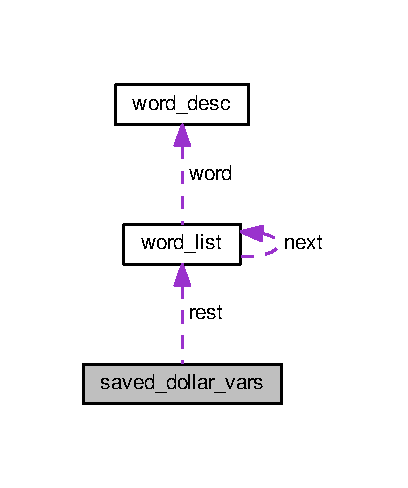
\includegraphics[width=196pt]{structsaved__dollar__vars__coll__graph}
\end{center}
\end{figure}
\subsection*{Public Attributes}
\begin{DoxyCompactItemize}
\item 
char $\ast$$\ast$ \hyperlink{structsaved__dollar__vars_a34da2a52790b0c2d0c5f205188935406}{first\+\_\+ten}
\item 
\hyperlink{command_8h_ac42a7b781459884316a1f2ffe79e8a62}{W\+O\+R\+D\+\_\+\+L\+I\+ST} $\ast$ \hyperlink{structsaved__dollar__vars_a92f46b81a83fba6817445d87ef1f1ba7}{rest}
\end{DoxyCompactItemize}


\subsection{Member Data Documentation}
\index{saved\+\_\+dollar\+\_\+vars@{saved\+\_\+dollar\+\_\+vars}!first\+\_\+ten@{first\+\_\+ten}}
\index{first\+\_\+ten@{first\+\_\+ten}!saved\+\_\+dollar\+\_\+vars@{saved\+\_\+dollar\+\_\+vars}}
\subsubsection[{\texorpdfstring{first\+\_\+ten}{first_ten}}]{\setlength{\rightskip}{0pt plus 5cm}char$\ast$$\ast$ saved\+\_\+dollar\+\_\+vars\+::first\+\_\+ten}\hypertarget{structsaved__dollar__vars_a34da2a52790b0c2d0c5f205188935406}{}\label{structsaved__dollar__vars_a34da2a52790b0c2d0c5f205188935406}
\index{saved\+\_\+dollar\+\_\+vars@{saved\+\_\+dollar\+\_\+vars}!rest@{rest}}
\index{rest@{rest}!saved\+\_\+dollar\+\_\+vars@{saved\+\_\+dollar\+\_\+vars}}
\subsubsection[{\texorpdfstring{rest}{rest}}]{\setlength{\rightskip}{0pt plus 5cm}{\bf W\+O\+R\+D\+\_\+\+L\+I\+ST}$\ast$ saved\+\_\+dollar\+\_\+vars\+::rest}\hypertarget{structsaved__dollar__vars_a92f46b81a83fba6817445d87ef1f1ba7}{}\label{structsaved__dollar__vars_a92f46b81a83fba6817445d87ef1f1ba7}


The documentation for this struct was generated from the following file\+:\begin{DoxyCompactItemize}
\item 
\hyperlink{variables_8c}{variables.\+c}\end{DoxyCompactItemize}

\hypertarget{structSAVED__VAR}{}\section{S\+A\+V\+E\+D\+\_\+\+V\+AR Struct Reference}
\label{structSAVED__VAR}\index{S\+A\+V\+E\+D\+\_\+\+V\+AR@{S\+A\+V\+E\+D\+\_\+\+V\+AR}}
\subsection*{Public Attributes}
\begin{DoxyCompactItemize}
\item 
char $\ast$ \hyperlink{structSAVED__VAR_aaa9de1da489d7268a1c427e99535cc89}{variable}
\item 
int \hyperlink{structSAVED__VAR_a1e2b708a760c32e1c6826b83b3d7e799}{size}
\item 
char \hyperlink{structSAVED__VAR_abce2c6eb701e549ef4e2c3f90d64a780}{desired\+\_\+setting} \mbox{[}1\mbox{]}
\end{DoxyCompactItemize}


\subsection{Member Data Documentation}
\index{S\+A\+V\+E\+D\+\_\+\+V\+AR@{S\+A\+V\+E\+D\+\_\+\+V\+AR}!desired\+\_\+setting@{desired\+\_\+setting}}
\index{desired\+\_\+setting@{desired\+\_\+setting}!S\+A\+V\+E\+D\+\_\+\+V\+AR@{S\+A\+V\+E\+D\+\_\+\+V\+AR}}
\subsubsection[{\texorpdfstring{desired\+\_\+setting}{desired_setting}}]{\setlength{\rightskip}{0pt plus 5cm}char S\+A\+V\+E\+D\+\_\+\+V\+A\+R\+::desired\+\_\+setting\mbox{[}1\mbox{]}}\hypertarget{structSAVED__VAR_abce2c6eb701e549ef4e2c3f90d64a780}{}\label{structSAVED__VAR_abce2c6eb701e549ef4e2c3f90d64a780}
\index{S\+A\+V\+E\+D\+\_\+\+V\+AR@{S\+A\+V\+E\+D\+\_\+\+V\+AR}!size@{size}}
\index{size@{size}!S\+A\+V\+E\+D\+\_\+\+V\+AR@{S\+A\+V\+E\+D\+\_\+\+V\+AR}}
\subsubsection[{\texorpdfstring{size}{size}}]{\setlength{\rightskip}{0pt plus 5cm}int S\+A\+V\+E\+D\+\_\+\+V\+A\+R\+::size}\hypertarget{structSAVED__VAR_a1e2b708a760c32e1c6826b83b3d7e799}{}\label{structSAVED__VAR_a1e2b708a760c32e1c6826b83b3d7e799}
\index{S\+A\+V\+E\+D\+\_\+\+V\+AR@{S\+A\+V\+E\+D\+\_\+\+V\+AR}!variable@{variable}}
\index{variable@{variable}!S\+A\+V\+E\+D\+\_\+\+V\+AR@{S\+A\+V\+E\+D\+\_\+\+V\+AR}}
\subsubsection[{\texorpdfstring{variable}{variable}}]{\setlength{\rightskip}{0pt plus 5cm}char$\ast$ S\+A\+V\+E\+D\+\_\+\+V\+A\+R\+::variable}\hypertarget{structSAVED__VAR_aaa9de1da489d7268a1c427e99535cc89}{}\label{structSAVED__VAR_aaa9de1da489d7268a1c427e99535cc89}


The documentation for this struct was generated from the following file\+:\begin{DoxyCompactItemize}
\item 
\hyperlink{unwind__prot_8c}{unwind\+\_\+prot.\+c}\end{DoxyCompactItemize}

\hypertarget{structsimple__com}{}\section{simple\+\_\+com Struct Reference}
\label{structsimple__com}\index{simple\+\_\+com@{simple\+\_\+com}}


{\ttfamily \#include $<$command.\+h$>$}



Collaboration diagram for simple\+\_\+com\+:
\nopagebreak
\begin{figure}[H]
\begin{center}
\leavevmode
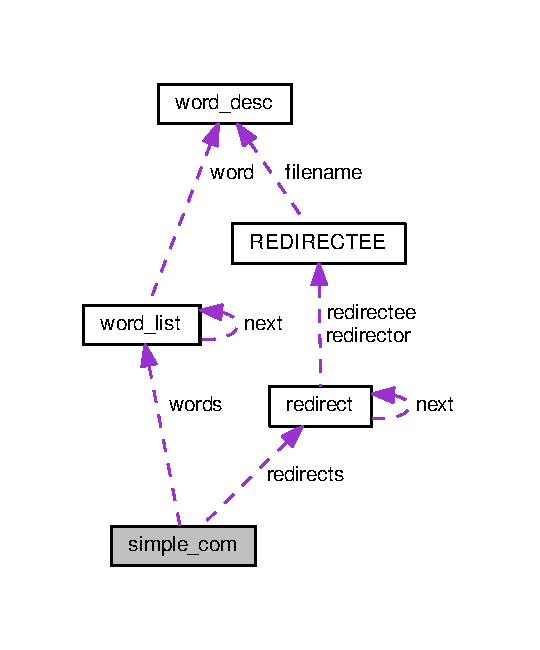
\includegraphics[width=259pt]{structsimple__com__coll__graph}
\end{center}
\end{figure}
\subsection*{Public Attributes}
\begin{DoxyCompactItemize}
\item 
int \hyperlink{structsimple__com_a3681da2bf1196015719c7c529a96bafe}{flags}
\item 
int \hyperlink{structsimple__com_a837f4e2e2eb00604e2eab7a78d32b089}{line}
\item 
\hyperlink{command_8h_ac42a7b781459884316a1f2ffe79e8a62}{W\+O\+R\+D\+\_\+\+L\+I\+ST} $\ast$ \hyperlink{structsimple__com_ae7a7f329e99d6e622ca9a8daef38c155}{words}
\item 
\hyperlink{command_8h_adeb9f5d937c92c7923aec48ad5e47d57}{R\+E\+D\+I\+R\+E\+CT} $\ast$ \hyperlink{structsimple__com_a8a9c45afa462969d01399d063320bd08}{redirects}
\end{DoxyCompactItemize}


\subsection{Member Data Documentation}
\index{simple\+\_\+com@{simple\+\_\+com}!flags@{flags}}
\index{flags@{flags}!simple\+\_\+com@{simple\+\_\+com}}
\subsubsection[{\texorpdfstring{flags}{flags}}]{\setlength{\rightskip}{0pt plus 5cm}int simple\+\_\+com\+::flags}\hypertarget{structsimple__com_a3681da2bf1196015719c7c529a96bafe}{}\label{structsimple__com_a3681da2bf1196015719c7c529a96bafe}
\index{simple\+\_\+com@{simple\+\_\+com}!line@{line}}
\index{line@{line}!simple\+\_\+com@{simple\+\_\+com}}
\subsubsection[{\texorpdfstring{line}{line}}]{\setlength{\rightskip}{0pt plus 5cm}int simple\+\_\+com\+::line}\hypertarget{structsimple__com_a837f4e2e2eb00604e2eab7a78d32b089}{}\label{structsimple__com_a837f4e2e2eb00604e2eab7a78d32b089}
\index{simple\+\_\+com@{simple\+\_\+com}!redirects@{redirects}}
\index{redirects@{redirects}!simple\+\_\+com@{simple\+\_\+com}}
\subsubsection[{\texorpdfstring{redirects}{redirects}}]{\setlength{\rightskip}{0pt plus 5cm}{\bf R\+E\+D\+I\+R\+E\+CT}$\ast$ simple\+\_\+com\+::redirects}\hypertarget{structsimple__com_a8a9c45afa462969d01399d063320bd08}{}\label{structsimple__com_a8a9c45afa462969d01399d063320bd08}
\index{simple\+\_\+com@{simple\+\_\+com}!words@{words}}
\index{words@{words}!simple\+\_\+com@{simple\+\_\+com}}
\subsubsection[{\texorpdfstring{words}{words}}]{\setlength{\rightskip}{0pt plus 5cm}{\bf W\+O\+R\+D\+\_\+\+L\+I\+ST}$\ast$ simple\+\_\+com\+::words}\hypertarget{structsimple__com_ae7a7f329e99d6e622ca9a8daef38c155}{}\label{structsimple__com_ae7a7f329e99d6e622ca9a8daef38c155}


The documentation for this struct was generated from the following file\+:\begin{DoxyCompactItemize}
\item 
\hyperlink{command_8h}{command.\+h}\end{DoxyCompactItemize}

\hypertarget{structstream__saver}{}\section{stream\+\_\+saver Struct Reference}
\label{structstream__saver}\index{stream\+\_\+saver@{stream\+\_\+saver}}


Collaboration diagram for stream\+\_\+saver\+:
\nopagebreak
\begin{figure}[H]
\begin{center}
\leavevmode
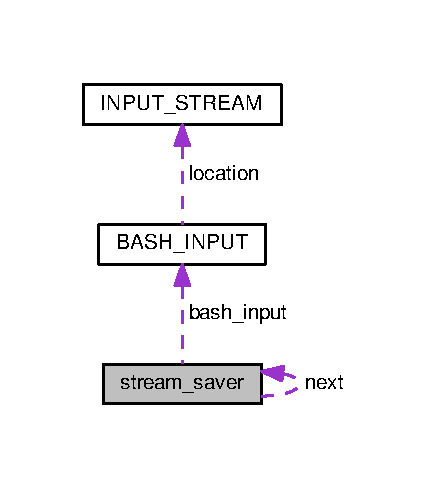
\includegraphics[width=206pt]{structstream__saver__coll__graph}
\end{center}
\end{figure}
\subsection*{Public Attributes}
\begin{DoxyCompactItemize}
\item 
struct \hyperlink{structstream__saver}{stream\+\_\+saver} $\ast$ \hyperlink{structstream__saver_af27ac3238525fc36f8165d8a879c8b68}{next}
\item 
\hyperlink{structBASH__INPUT}{B\+A\+S\+H\+\_\+\+I\+N\+P\+UT} \hyperlink{structstream__saver_a289a85e33c449e20e186233f355629db}{bash\+\_\+input}
\item 
int \hyperlink{structstream__saver_ae65e97941be54e749139a5d4722d96d9}{line}
\item 
B\+U\+F\+F\+E\+R\+E\+D\+\_\+\+S\+T\+R\+E\+AM $\ast$ \hyperlink{structstream__saver_a16ca697c6be794b7b0d4cc1919c057db}{bstream}
\end{DoxyCompactItemize}


\subsection{Member Data Documentation}
\index{stream\+\_\+saver@{stream\+\_\+saver}!bash\+\_\+input@{bash\+\_\+input}}
\index{bash\+\_\+input@{bash\+\_\+input}!stream\+\_\+saver@{stream\+\_\+saver}}
\subsubsection[{\texorpdfstring{bash\+\_\+input}{bash_input}}]{\setlength{\rightskip}{0pt plus 5cm}{\bf B\+A\+S\+H\+\_\+\+I\+N\+P\+UT} stream\+\_\+saver\+::bash\+\_\+input}\hypertarget{structstream__saver_a289a85e33c449e20e186233f355629db}{}\label{structstream__saver_a289a85e33c449e20e186233f355629db}
\index{stream\+\_\+saver@{stream\+\_\+saver}!bstream@{bstream}}
\index{bstream@{bstream}!stream\+\_\+saver@{stream\+\_\+saver}}
\subsubsection[{\texorpdfstring{bstream}{bstream}}]{\setlength{\rightskip}{0pt plus 5cm}B\+U\+F\+F\+E\+R\+E\+D\+\_\+\+S\+T\+R\+E\+AM$\ast$ stream\+\_\+saver\+::bstream}\hypertarget{structstream__saver_a16ca697c6be794b7b0d4cc1919c057db}{}\label{structstream__saver_a16ca697c6be794b7b0d4cc1919c057db}
\index{stream\+\_\+saver@{stream\+\_\+saver}!line@{line}}
\index{line@{line}!stream\+\_\+saver@{stream\+\_\+saver}}
\subsubsection[{\texorpdfstring{line}{line}}]{\setlength{\rightskip}{0pt plus 5cm}int stream\+\_\+saver\+::line}\hypertarget{structstream__saver_ae65e97941be54e749139a5d4722d96d9}{}\label{structstream__saver_ae65e97941be54e749139a5d4722d96d9}
\index{stream\+\_\+saver@{stream\+\_\+saver}!next@{next}}
\index{next@{next}!stream\+\_\+saver@{stream\+\_\+saver}}
\subsubsection[{\texorpdfstring{next}{next}}]{\setlength{\rightskip}{0pt plus 5cm}struct {\bf stream\+\_\+saver}$\ast$ stream\+\_\+saver\+::next}\hypertarget{structstream__saver_af27ac3238525fc36f8165d8a879c8b68}{}\label{structstream__saver_af27ac3238525fc36f8165d8a879c8b68}


The documentation for this struct was generated from the following file\+:\begin{DoxyCompactItemize}
\item 
\hyperlink{y_8tab_8c}{y.\+tab.\+c}\end{DoxyCompactItemize}

\hypertarget{structSTRING__INT__ALIST}{}\section{S\+T\+R\+I\+N\+G\+\_\+\+I\+N\+T\+\_\+\+A\+L\+I\+ST Struct Reference}
\label{structSTRING__INT__ALIST}\index{S\+T\+R\+I\+N\+G\+\_\+\+I\+N\+T\+\_\+\+A\+L\+I\+ST@{S\+T\+R\+I\+N\+G\+\_\+\+I\+N\+T\+\_\+\+A\+L\+I\+ST}}


{\ttfamily \#include $<$general.\+h$>$}

\subsection*{Public Attributes}
\begin{DoxyCompactItemize}
\item 
char $\ast$ \hyperlink{structSTRING__INT__ALIST_a15c2e03465b7de306b6f7f006fdcb8a5}{word}
\item 
int \hyperlink{structSTRING__INT__ALIST_ab1473f1b9d79478a271aa4947ab29b0e}{token}
\end{DoxyCompactItemize}


\subsection{Member Data Documentation}
\index{S\+T\+R\+I\+N\+G\+\_\+\+I\+N\+T\+\_\+\+A\+L\+I\+ST@{S\+T\+R\+I\+N\+G\+\_\+\+I\+N\+T\+\_\+\+A\+L\+I\+ST}!token@{token}}
\index{token@{token}!S\+T\+R\+I\+N\+G\+\_\+\+I\+N\+T\+\_\+\+A\+L\+I\+ST@{S\+T\+R\+I\+N\+G\+\_\+\+I\+N\+T\+\_\+\+A\+L\+I\+ST}}
\subsubsection[{\texorpdfstring{token}{token}}]{\setlength{\rightskip}{0pt plus 5cm}int S\+T\+R\+I\+N\+G\+\_\+\+I\+N\+T\+\_\+\+A\+L\+I\+S\+T\+::token}\hypertarget{structSTRING__INT__ALIST_ab1473f1b9d79478a271aa4947ab29b0e}{}\label{structSTRING__INT__ALIST_ab1473f1b9d79478a271aa4947ab29b0e}
\index{S\+T\+R\+I\+N\+G\+\_\+\+I\+N\+T\+\_\+\+A\+L\+I\+ST@{S\+T\+R\+I\+N\+G\+\_\+\+I\+N\+T\+\_\+\+A\+L\+I\+ST}!word@{word}}
\index{word@{word}!S\+T\+R\+I\+N\+G\+\_\+\+I\+N\+T\+\_\+\+A\+L\+I\+ST@{S\+T\+R\+I\+N\+G\+\_\+\+I\+N\+T\+\_\+\+A\+L\+I\+ST}}
\subsubsection[{\texorpdfstring{word}{word}}]{\setlength{\rightskip}{0pt plus 5cm}char$\ast$ S\+T\+R\+I\+N\+G\+\_\+\+I\+N\+T\+\_\+\+A\+L\+I\+S\+T\+::word}\hypertarget{structSTRING__INT__ALIST_a15c2e03465b7de306b6f7f006fdcb8a5}{}\label{structSTRING__INT__ALIST_a15c2e03465b7de306b6f7f006fdcb8a5}


The documentation for this struct was generated from the following file\+:\begin{DoxyCompactItemize}
\item 
\hyperlink{general_8h}{general.\+h}\end{DoxyCompactItemize}

\hypertarget{structstring__saver}{}\section{string\+\_\+saver Struct Reference}
\label{structstring__saver}\index{string\+\_\+saver@{string\+\_\+saver}}


Collaboration diagram for string\+\_\+saver\+:
\nopagebreak
\begin{figure}[H]
\begin{center}
\leavevmode
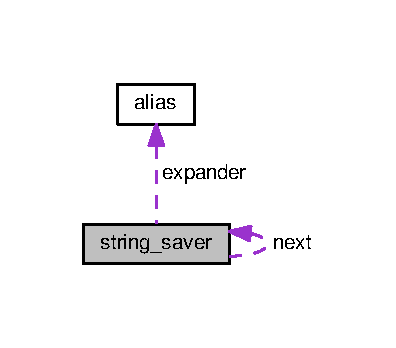
\includegraphics[width=190pt]{structstring__saver__coll__graph}
\end{center}
\end{figure}
\subsection*{Public Attributes}
\begin{DoxyCompactItemize}
\item 
struct \hyperlink{structstring__saver}{string\+\_\+saver} $\ast$ \hyperlink{structstring__saver_a7d78d802062d901feca18c960c95a286}{next}
\item 
int \hyperlink{structstring__saver_a3be05cc2cb341891312765ed8fd024d7}{expand\+\_\+alias}
\item 
char $\ast$ \hyperlink{structstring__saver_a8d76b634850f05cd2de7d3d9dfc489f1}{saved\+\_\+line}
\item 
\hyperlink{alias_8h_a11c6bae002d90e8dad2d17b87ba6cccf}{alias\+\_\+t} $\ast$ \hyperlink{structstring__saver_aa39cdb834c5e9118697e0c532b774ef8}{expander}
\item 
size\+\_\+t \hyperlink{structstring__saver_a86322652dc4c4f9aa6896304a41f8bf0}{saved\+\_\+line\+\_\+size}
\item 
size\+\_\+t \hyperlink{structstring__saver_aeabbc475d86ac4ab300b4b76bf2cbcc3}{saved\+\_\+line\+\_\+index}
\item 
int \hyperlink{structstring__saver_a905ce4a868ffb0d22b49216b8711f65e}{saved\+\_\+line\+\_\+terminator}
\item 
int \hyperlink{structstring__saver_afda7fc1510b844cf3166fbf5383c0c45}{flags}
\end{DoxyCompactItemize}


\subsection{Member Data Documentation}
\index{string\+\_\+saver@{string\+\_\+saver}!expand\+\_\+alias@{expand\+\_\+alias}}
\index{expand\+\_\+alias@{expand\+\_\+alias}!string\+\_\+saver@{string\+\_\+saver}}
\subsubsection[{\texorpdfstring{expand\+\_\+alias}{expand_alias}}]{\setlength{\rightskip}{0pt plus 5cm}int string\+\_\+saver\+::expand\+\_\+alias}\hypertarget{structstring__saver_a3be05cc2cb341891312765ed8fd024d7}{}\label{structstring__saver_a3be05cc2cb341891312765ed8fd024d7}
\index{string\+\_\+saver@{string\+\_\+saver}!expander@{expander}}
\index{expander@{expander}!string\+\_\+saver@{string\+\_\+saver}}
\subsubsection[{\texorpdfstring{expander}{expander}}]{\setlength{\rightskip}{0pt plus 5cm}{\bf alias\+\_\+t}$\ast$ string\+\_\+saver\+::expander}\hypertarget{structstring__saver_aa39cdb834c5e9118697e0c532b774ef8}{}\label{structstring__saver_aa39cdb834c5e9118697e0c532b774ef8}
\index{string\+\_\+saver@{string\+\_\+saver}!flags@{flags}}
\index{flags@{flags}!string\+\_\+saver@{string\+\_\+saver}}
\subsubsection[{\texorpdfstring{flags}{flags}}]{\setlength{\rightskip}{0pt plus 5cm}int string\+\_\+saver\+::flags}\hypertarget{structstring__saver_afda7fc1510b844cf3166fbf5383c0c45}{}\label{structstring__saver_afda7fc1510b844cf3166fbf5383c0c45}
\index{string\+\_\+saver@{string\+\_\+saver}!next@{next}}
\index{next@{next}!string\+\_\+saver@{string\+\_\+saver}}
\subsubsection[{\texorpdfstring{next}{next}}]{\setlength{\rightskip}{0pt plus 5cm}struct {\bf string\+\_\+saver}$\ast$ string\+\_\+saver\+::next}\hypertarget{structstring__saver_a7d78d802062d901feca18c960c95a286}{}\label{structstring__saver_a7d78d802062d901feca18c960c95a286}
\index{string\+\_\+saver@{string\+\_\+saver}!saved\+\_\+line@{saved\+\_\+line}}
\index{saved\+\_\+line@{saved\+\_\+line}!string\+\_\+saver@{string\+\_\+saver}}
\subsubsection[{\texorpdfstring{saved\+\_\+line}{saved_line}}]{\setlength{\rightskip}{0pt plus 5cm}char$\ast$ string\+\_\+saver\+::saved\+\_\+line}\hypertarget{structstring__saver_a8d76b634850f05cd2de7d3d9dfc489f1}{}\label{structstring__saver_a8d76b634850f05cd2de7d3d9dfc489f1}
\index{string\+\_\+saver@{string\+\_\+saver}!saved\+\_\+line\+\_\+index@{saved\+\_\+line\+\_\+index}}
\index{saved\+\_\+line\+\_\+index@{saved\+\_\+line\+\_\+index}!string\+\_\+saver@{string\+\_\+saver}}
\subsubsection[{\texorpdfstring{saved\+\_\+line\+\_\+index}{saved_line_index}}]{\setlength{\rightskip}{0pt plus 5cm}size\+\_\+t string\+\_\+saver\+::saved\+\_\+line\+\_\+index}\hypertarget{structstring__saver_aeabbc475d86ac4ab300b4b76bf2cbcc3}{}\label{structstring__saver_aeabbc475d86ac4ab300b4b76bf2cbcc3}
\index{string\+\_\+saver@{string\+\_\+saver}!saved\+\_\+line\+\_\+size@{saved\+\_\+line\+\_\+size}}
\index{saved\+\_\+line\+\_\+size@{saved\+\_\+line\+\_\+size}!string\+\_\+saver@{string\+\_\+saver}}
\subsubsection[{\texorpdfstring{saved\+\_\+line\+\_\+size}{saved_line_size}}]{\setlength{\rightskip}{0pt plus 5cm}size\+\_\+t string\+\_\+saver\+::saved\+\_\+line\+\_\+size}\hypertarget{structstring__saver_a86322652dc4c4f9aa6896304a41f8bf0}{}\label{structstring__saver_a86322652dc4c4f9aa6896304a41f8bf0}
\index{string\+\_\+saver@{string\+\_\+saver}!saved\+\_\+line\+\_\+terminator@{saved\+\_\+line\+\_\+terminator}}
\index{saved\+\_\+line\+\_\+terminator@{saved\+\_\+line\+\_\+terminator}!string\+\_\+saver@{string\+\_\+saver}}
\subsubsection[{\texorpdfstring{saved\+\_\+line\+\_\+terminator}{saved_line_terminator}}]{\setlength{\rightskip}{0pt plus 5cm}int string\+\_\+saver\+::saved\+\_\+line\+\_\+terminator}\hypertarget{structstring__saver_a905ce4a868ffb0d22b49216b8711f65e}{}\label{structstring__saver_a905ce4a868ffb0d22b49216b8711f65e}


The documentation for this struct was generated from the following file\+:\begin{DoxyCompactItemize}
\item 
\hyperlink{y_8tab_8c}{y.\+tab.\+c}\end{DoxyCompactItemize}

\hypertarget{structsubshell__com}{}\section{subshell\+\_\+com Struct Reference}
\label{structsubshell__com}\index{subshell\+\_\+com@{subshell\+\_\+com}}


{\ttfamily \#include $<$command.\+h$>$}



Collaboration diagram for subshell\+\_\+com\+:
\nopagebreak
\begin{figure}[H]
\begin{center}
\leavevmode
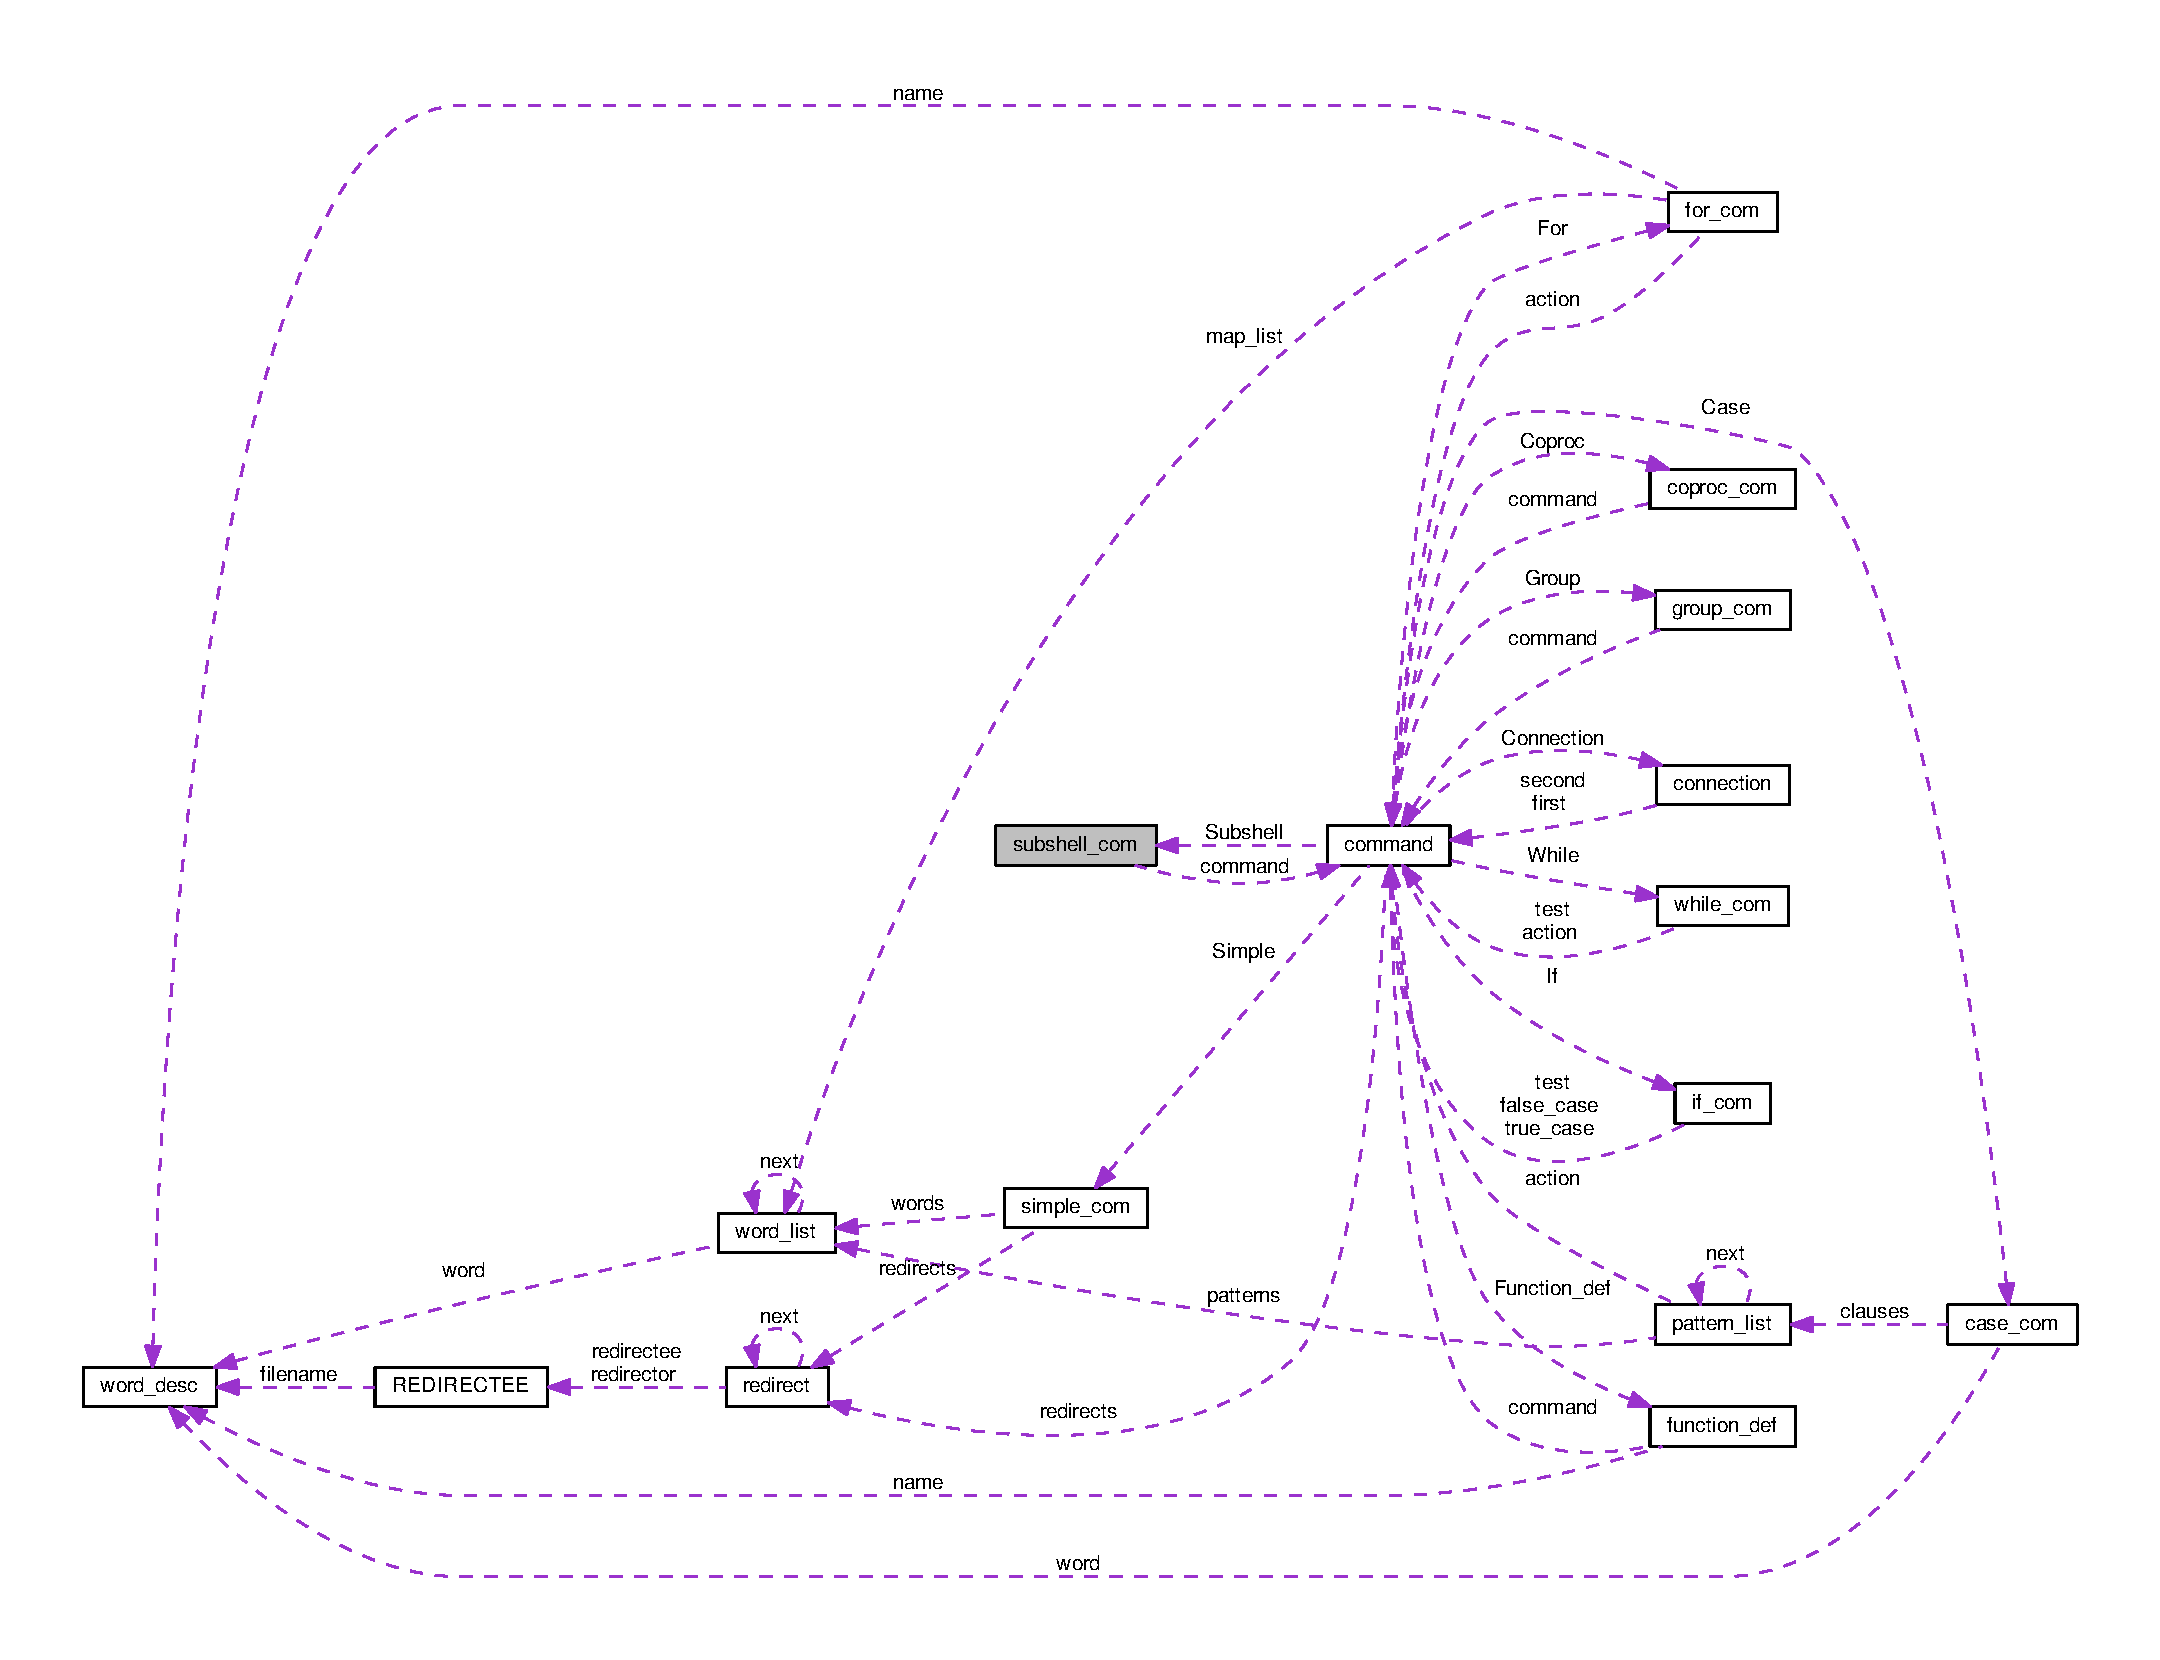
\includegraphics[width=350pt]{structsubshell__com__coll__graph}
\end{center}
\end{figure}
\subsection*{Public Attributes}
\begin{DoxyCompactItemize}
\item 
int \hyperlink{structsubshell__com_a0edd264e3360fbdefe14faf33c66b54f}{flags}
\item 
int \hyperlink{structsubshell__com_a3c67c5a0510a7e48b1a50b80ae58d7dc}{line}
\item 
\hyperlink{command_8h_a8c41dec142c299806885773c902c0d87}{C\+O\+M\+M\+A\+ND} $\ast$ \hyperlink{structsubshell__com_aedbe947202b66c67bc19e14509b6690b}{command}
\end{DoxyCompactItemize}


\subsection{Member Data Documentation}
\index{subshell\+\_\+com@{subshell\+\_\+com}!command@{command}}
\index{command@{command}!subshell\+\_\+com@{subshell\+\_\+com}}
\subsubsection[{\texorpdfstring{command}{command}}]{\setlength{\rightskip}{0pt plus 5cm}{\bf C\+O\+M\+M\+A\+ND}$\ast$ subshell\+\_\+com\+::command}\hypertarget{structsubshell__com_aedbe947202b66c67bc19e14509b6690b}{}\label{structsubshell__com_aedbe947202b66c67bc19e14509b6690b}
\index{subshell\+\_\+com@{subshell\+\_\+com}!flags@{flags}}
\index{flags@{flags}!subshell\+\_\+com@{subshell\+\_\+com}}
\subsubsection[{\texorpdfstring{flags}{flags}}]{\setlength{\rightskip}{0pt plus 5cm}int subshell\+\_\+com\+::flags}\hypertarget{structsubshell__com_a0edd264e3360fbdefe14faf33c66b54f}{}\label{structsubshell__com_a0edd264e3360fbdefe14faf33c66b54f}
\index{subshell\+\_\+com@{subshell\+\_\+com}!line@{line}}
\index{line@{line}!subshell\+\_\+com@{subshell\+\_\+com}}
\subsubsection[{\texorpdfstring{line}{line}}]{\setlength{\rightskip}{0pt plus 5cm}int subshell\+\_\+com\+::line}\hypertarget{structsubshell__com_a3c67c5a0510a7e48b1a50b80ae58d7dc}{}\label{structsubshell__com_a3c67c5a0510a7e48b1a50b80ae58d7dc}


The documentation for this struct was generated from the following file\+:\begin{DoxyCompactItemize}
\item 
\hyperlink{command_8h}{command.\+h}\end{DoxyCompactItemize}

\hypertarget{structtermsig}{}\section{termsig Struct Reference}
\label{structtermsig}\index{termsig@{termsig}}
\subsection*{Public Attributes}
\begin{DoxyCompactItemize}
\item 
int \hyperlink{structtermsig_aa38dcc7e498d80724e4541257c8726e5}{signum}
\item 
Sig\+Handler $\ast$ \hyperlink{structtermsig_acb5d5b0df319b86416c9d680eab43306}{orig\+\_\+handler}
\item 
int \hyperlink{structtermsig_aa2dff43019910caaeed967ae1e8212e4}{orig\+\_\+flags}
\item 
int \hyperlink{structtermsig_abdf0a75a550ac053320410c6e8976afe}{core\+\_\+dump}
\end{DoxyCompactItemize}


\subsection{Member Data Documentation}
\index{termsig@{termsig}!core\+\_\+dump@{core\+\_\+dump}}
\index{core\+\_\+dump@{core\+\_\+dump}!termsig@{termsig}}
\subsubsection[{\texorpdfstring{core\+\_\+dump}{core_dump}}]{\setlength{\rightskip}{0pt plus 5cm}int termsig\+::core\+\_\+dump}\hypertarget{structtermsig_abdf0a75a550ac053320410c6e8976afe}{}\label{structtermsig_abdf0a75a550ac053320410c6e8976afe}
\index{termsig@{termsig}!orig\+\_\+flags@{orig\+\_\+flags}}
\index{orig\+\_\+flags@{orig\+\_\+flags}!termsig@{termsig}}
\subsubsection[{\texorpdfstring{orig\+\_\+flags}{orig_flags}}]{\setlength{\rightskip}{0pt plus 5cm}int termsig\+::orig\+\_\+flags}\hypertarget{structtermsig_aa2dff43019910caaeed967ae1e8212e4}{}\label{structtermsig_aa2dff43019910caaeed967ae1e8212e4}
\index{termsig@{termsig}!orig\+\_\+handler@{orig\+\_\+handler}}
\index{orig\+\_\+handler@{orig\+\_\+handler}!termsig@{termsig}}
\subsubsection[{\texorpdfstring{orig\+\_\+handler}{orig_handler}}]{\setlength{\rightskip}{0pt plus 5cm}Sig\+Handler$\ast$ termsig\+::orig\+\_\+handler}\hypertarget{structtermsig_acb5d5b0df319b86416c9d680eab43306}{}\label{structtermsig_acb5d5b0df319b86416c9d680eab43306}
\index{termsig@{termsig}!signum@{signum}}
\index{signum@{signum}!termsig@{termsig}}
\subsubsection[{\texorpdfstring{signum}{signum}}]{\setlength{\rightskip}{0pt plus 5cm}int termsig\+::signum}\hypertarget{structtermsig_aa38dcc7e498d80724e4541257c8726e5}{}\label{structtermsig_aa38dcc7e498d80724e4541257c8726e5}


The documentation for this struct was generated from the following file\+:\begin{DoxyCompactItemize}
\item 
\hyperlink{sig_8c}{sig.\+c}\end{DoxyCompactItemize}

\hypertarget{structuser__info}{}\section{user\+\_\+info Struct Reference}
\label{structuser__info}\index{user\+\_\+info@{user\+\_\+info}}


{\ttfamily \#include $<$shell.\+h$>$}

\subsection*{Public Attributes}
\begin{DoxyCompactItemize}
\item 
uid\+\_\+t \hyperlink{structuser__info_a336097610439e04eccd63acef69443de}{uid}
\item 
uid\+\_\+t \hyperlink{structuser__info_a2b1ad40af96833f849390bc775e9dd16}{euid}
\item 
gid\+\_\+t \hyperlink{structuser__info_a99413c55942db77ae3cf544bb82f6af7}{gid}
\item 
gid\+\_\+t \hyperlink{structuser__info_a6c019b799f5b6235d8a34a40ea5138d1}{egid}
\item 
char $\ast$ \hyperlink{structuser__info_abecea7d4c564b4b56c985c3e450f9e62}{user\+\_\+name}
\item 
char $\ast$ \hyperlink{structuser__info_a35b196ef8d0bbd4329645dac6d3d48be}{shell}
\item 
char $\ast$ \hyperlink{structuser__info_a862cf8cbf50b91c8b52fdf0fb00c461d}{home\+\_\+dir}
\end{DoxyCompactItemize}


\subsection{Member Data Documentation}
\index{user\+\_\+info@{user\+\_\+info}!egid@{egid}}
\index{egid@{egid}!user\+\_\+info@{user\+\_\+info}}
\subsubsection[{\texorpdfstring{egid}{egid}}]{\setlength{\rightskip}{0pt plus 5cm}gid\+\_\+t user\+\_\+info\+::egid}\hypertarget{structuser__info_a6c019b799f5b6235d8a34a40ea5138d1}{}\label{structuser__info_a6c019b799f5b6235d8a34a40ea5138d1}
\index{user\+\_\+info@{user\+\_\+info}!euid@{euid}}
\index{euid@{euid}!user\+\_\+info@{user\+\_\+info}}
\subsubsection[{\texorpdfstring{euid}{euid}}]{\setlength{\rightskip}{0pt plus 5cm}uid\+\_\+t user\+\_\+info\+::euid}\hypertarget{structuser__info_a2b1ad40af96833f849390bc775e9dd16}{}\label{structuser__info_a2b1ad40af96833f849390bc775e9dd16}
\index{user\+\_\+info@{user\+\_\+info}!gid@{gid}}
\index{gid@{gid}!user\+\_\+info@{user\+\_\+info}}
\subsubsection[{\texorpdfstring{gid}{gid}}]{\setlength{\rightskip}{0pt plus 5cm}gid\+\_\+t user\+\_\+info\+::gid}\hypertarget{structuser__info_a99413c55942db77ae3cf544bb82f6af7}{}\label{structuser__info_a99413c55942db77ae3cf544bb82f6af7}
\index{user\+\_\+info@{user\+\_\+info}!home\+\_\+dir@{home\+\_\+dir}}
\index{home\+\_\+dir@{home\+\_\+dir}!user\+\_\+info@{user\+\_\+info}}
\subsubsection[{\texorpdfstring{home\+\_\+dir}{home_dir}}]{\setlength{\rightskip}{0pt plus 5cm}char$\ast$ user\+\_\+info\+::home\+\_\+dir}\hypertarget{structuser__info_a862cf8cbf50b91c8b52fdf0fb00c461d}{}\label{structuser__info_a862cf8cbf50b91c8b52fdf0fb00c461d}
\index{user\+\_\+info@{user\+\_\+info}!shell@{shell}}
\index{shell@{shell}!user\+\_\+info@{user\+\_\+info}}
\subsubsection[{\texorpdfstring{shell}{shell}}]{\setlength{\rightskip}{0pt plus 5cm}char$\ast$ user\+\_\+info\+::shell}\hypertarget{structuser__info_a35b196ef8d0bbd4329645dac6d3d48be}{}\label{structuser__info_a35b196ef8d0bbd4329645dac6d3d48be}
\index{user\+\_\+info@{user\+\_\+info}!uid@{uid}}
\index{uid@{uid}!user\+\_\+info@{user\+\_\+info}}
\subsubsection[{\texorpdfstring{uid}{uid}}]{\setlength{\rightskip}{0pt plus 5cm}uid\+\_\+t user\+\_\+info\+::uid}\hypertarget{structuser__info_a336097610439e04eccd63acef69443de}{}\label{structuser__info_a336097610439e04eccd63acef69443de}
\index{user\+\_\+info@{user\+\_\+info}!user\+\_\+name@{user\+\_\+name}}
\index{user\+\_\+name@{user\+\_\+name}!user\+\_\+info@{user\+\_\+info}}
\subsubsection[{\texorpdfstring{user\+\_\+name}{user_name}}]{\setlength{\rightskip}{0pt plus 5cm}char$\ast$ user\+\_\+info\+::user\+\_\+name}\hypertarget{structuser__info_abecea7d4c564b4b56c985c3e450f9e62}{}\label{structuser__info_abecea7d4c564b4b56c985c3e450f9e62}


The documentation for this struct was generated from the following file\+:\begin{DoxyCompactItemize}
\item 
\hyperlink{shell_8h}{shell.\+h}\end{DoxyCompactItemize}

\hypertarget{unionuwp}{}\section{uwp Union Reference}
\label{unionuwp}\index{uwp@{uwp}}


Collaboration diagram for uwp\+:
\nopagebreak
\begin{figure}[H]
\begin{center}
\leavevmode
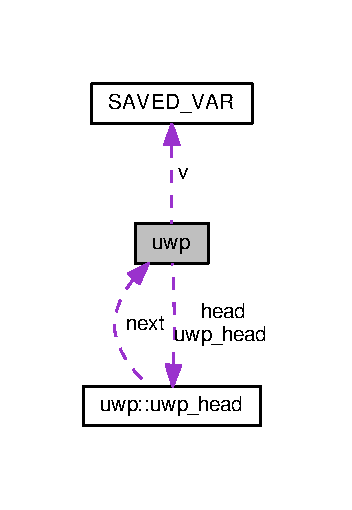
\includegraphics[width=169pt]{unionuwp__coll__graph}
\end{center}
\end{figure}
\subsection*{Classes}
\begin{DoxyCompactItemize}
\item 
struct \hyperlink{structuwp_1_1uwp__head}{uwp\+\_\+head}
\end{DoxyCompactItemize}
\subsection*{Public Attributes}
\begin{DoxyCompactItemize}
\item 
struct \hyperlink{structuwp_1_1uwp__head}{uwp\+::uwp\+\_\+head} \hyperlink{unionuwp_acab4a7765952e1452e4d9035cdacbab5}{head}
\item 
\begin{tabbing}
xx\=xx\=xx\=xx\=xx\=xx\=xx\=xx\=xx\=\kill
struct \{\\
\>struct \hyperlink{structuwp_1_1uwp__head}{uwp\_head} \hyperlink{unionuwp_af1c38672e3b54d0270b807e058a28fd0}{uwp\_head}\\
\>char $\ast$ \hyperlink{unionuwp_a79612c93285a8ff48fa1b6184a5e97eb}{v}\\
\} \hyperlink{unionuwp_a90833ec7b08239c72d8dedfec701fca8}{arg}\\

\end{tabbing}\item 
\begin{tabbing}
xx\=xx\=xx\=xx\=xx\=xx\=xx\=xx\=xx\=\kill
struct \{\\
\>struct \hyperlink{structuwp_1_1uwp__head}{uwp\_head} \hyperlink{unionuwp_af1c38672e3b54d0270b807e058a28fd0}{uwp\_head}\\
\>\hyperlink{structSAVED__VAR}{SAVED\_VAR} \hyperlink{unionuwp_afdb9e38dfd8fb6b7ed4d7f8a7f3d7c11}{v}\\
\} \hyperlink{unionuwp_a0cbb85b5e389ab3d685c0cc51ba5c2bc}{sv}\\

\end{tabbing}\end{DoxyCompactItemize}


\subsection{Member Data Documentation}
\index{uwp@{uwp}!arg@{arg}}
\index{arg@{arg}!uwp@{uwp}}
\subsubsection[{\texorpdfstring{arg}{arg}}]{\setlength{\rightskip}{0pt plus 5cm}struct \{ ... \}   uwp\+::arg}\hypertarget{unionuwp_a90833ec7b08239c72d8dedfec701fca8}{}\label{unionuwp_a90833ec7b08239c72d8dedfec701fca8}
\index{uwp@{uwp}!head@{head}}
\index{head@{head}!uwp@{uwp}}
\subsubsection[{\texorpdfstring{head}{head}}]{\setlength{\rightskip}{0pt plus 5cm}struct {\bf uwp\+::uwp\+\_\+head}  uwp\+::head}\hypertarget{unionuwp_acab4a7765952e1452e4d9035cdacbab5}{}\label{unionuwp_acab4a7765952e1452e4d9035cdacbab5}
\index{uwp@{uwp}!sv@{sv}}
\index{sv@{sv}!uwp@{uwp}}
\subsubsection[{\texorpdfstring{sv}{sv}}]{\setlength{\rightskip}{0pt plus 5cm}struct \{ ... \}   uwp\+::sv}\hypertarget{unionuwp_a0cbb85b5e389ab3d685c0cc51ba5c2bc}{}\label{unionuwp_a0cbb85b5e389ab3d685c0cc51ba5c2bc}
\index{uwp@{uwp}!uwp\+\_\+head@{uwp\+\_\+head}}
\index{uwp\+\_\+head@{uwp\+\_\+head}!uwp@{uwp}}
\subsubsection[{\texorpdfstring{uwp\+\_\+head}{uwp_head}}]{\setlength{\rightskip}{0pt plus 5cm}struct {\bf uwp\+\_\+head} {\bf uwp\+::uwp\+\_\+head}}\hypertarget{unionuwp_af1c38672e3b54d0270b807e058a28fd0}{}\label{unionuwp_af1c38672e3b54d0270b807e058a28fd0}
\index{uwp@{uwp}!v@{v}}
\index{v@{v}!uwp@{uwp}}
\subsubsection[{\texorpdfstring{v}{v}}]{\setlength{\rightskip}{0pt plus 5cm}char$\ast$ uwp\+::v}\hypertarget{unionuwp_a79612c93285a8ff48fa1b6184a5e97eb}{}\label{unionuwp_a79612c93285a8ff48fa1b6184a5e97eb}
\index{uwp@{uwp}!v@{v}}
\index{v@{v}!uwp@{uwp}}
\subsubsection[{\texorpdfstring{v}{v}}]{\setlength{\rightskip}{0pt plus 5cm}{\bf S\+A\+V\+E\+D\+\_\+\+V\+AR} uwp\+::v}\hypertarget{unionuwp_afdb9e38dfd8fb6b7ed4d7f8a7f3d7c11}{}\label{unionuwp_afdb9e38dfd8fb6b7ed4d7f8a7f3d7c11}


The documentation for this union was generated from the following file\+:\begin{DoxyCompactItemize}
\item 
\hyperlink{unwind__prot_8c}{unwind\+\_\+prot.\+c}\end{DoxyCompactItemize}

\hypertarget{structuwp_1_1uwp__head}{}\section{uwp\+:\+:uwp\+\_\+head Struct Reference}
\label{structuwp_1_1uwp__head}\index{uwp\+::uwp\+\_\+head@{uwp\+::uwp\+\_\+head}}


Collaboration diagram for uwp\+:\+:uwp\+\_\+head\+:
\nopagebreak
\begin{figure}[H]
\begin{center}
\leavevmode
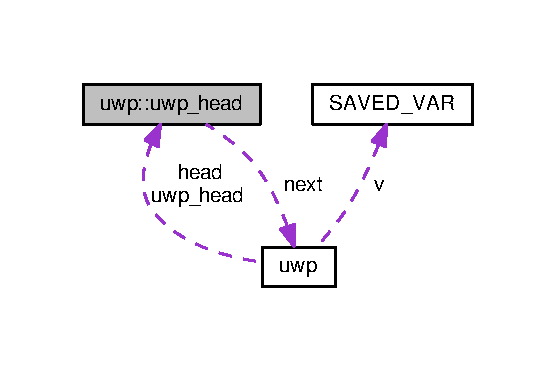
\includegraphics[width=267pt]{structuwp_1_1uwp__head__coll__graph}
\end{center}
\end{figure}
\subsection*{Public Attributes}
\begin{DoxyCompactItemize}
\item 
union \hyperlink{unionuwp}{uwp} $\ast$ \hyperlink{structuwp_1_1uwp__head_ac52194b98a40d4432fcb9fcb0b7f385a}{next}
\item 
\hyperlink{input_8h_a38bf8b007a281c3c96504ad1d2614af4}{Function} $\ast$ \hyperlink{structuwp_1_1uwp__head_a6a361d6a2bd14b7ec7ccfda34b860dac}{cleanup}
\end{DoxyCompactItemize}


\subsection{Member Data Documentation}
\index{uwp\+::uwp\+\_\+head@{uwp\+::uwp\+\_\+head}!cleanup@{cleanup}}
\index{cleanup@{cleanup}!uwp\+::uwp\+\_\+head@{uwp\+::uwp\+\_\+head}}
\subsubsection[{\texorpdfstring{cleanup}{cleanup}}]{\setlength{\rightskip}{0pt plus 5cm}{\bf Function}$\ast$ uwp\+::uwp\+\_\+head\+::cleanup}\hypertarget{structuwp_1_1uwp__head_a6a361d6a2bd14b7ec7ccfda34b860dac}{}\label{structuwp_1_1uwp__head_a6a361d6a2bd14b7ec7ccfda34b860dac}
\index{uwp\+::uwp\+\_\+head@{uwp\+::uwp\+\_\+head}!next@{next}}
\index{next@{next}!uwp\+::uwp\+\_\+head@{uwp\+::uwp\+\_\+head}}
\subsubsection[{\texorpdfstring{next}{next}}]{\setlength{\rightskip}{0pt plus 5cm}union {\bf uwp}$\ast$ uwp\+::uwp\+\_\+head\+::next}\hypertarget{structuwp_1_1uwp__head_ac52194b98a40d4432fcb9fcb0b7f385a}{}\label{structuwp_1_1uwp__head_ac52194b98a40d4432fcb9fcb0b7f385a}


The documentation for this struct was generated from the following file\+:\begin{DoxyCompactItemize}
\item 
\hyperlink{unwind__prot_8c}{unwind\+\_\+prot.\+c}\end{DoxyCompactItemize}

\hypertarget{structvar__context}{}\section{var\+\_\+context Struct Reference}
\label{structvar__context}\index{var\+\_\+context@{var\+\_\+context}}


{\ttfamily \#include $<$variables.\+h$>$}



Collaboration diagram for var\+\_\+context\+:
\nopagebreak
\begin{figure}[H]
\begin{center}
\leavevmode
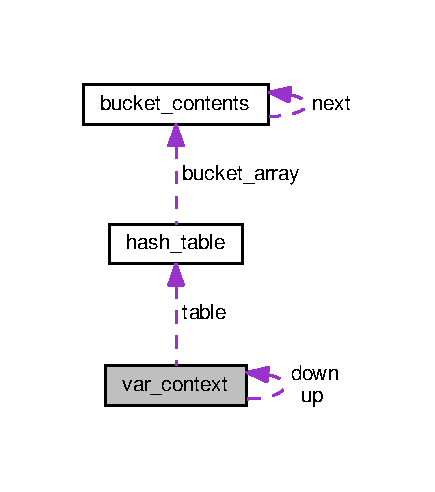
\includegraphics[width=209pt]{structvar__context__coll__graph}
\end{center}
\end{figure}
\subsection*{Public Attributes}
\begin{DoxyCompactItemize}
\item 
char $\ast$ \hyperlink{structvar__context_adf16b336746df59643044d0688a4d593}{name}
\item 
int \hyperlink{structvar__context_a616bf2696f42da3a8d3f8342eaf936fb}{scope}
\item 
int \hyperlink{structvar__context_a9570eb7deb9d92355f507e437f7112c0}{flags}
\item 
struct \hyperlink{structvar__context}{var\+\_\+context} $\ast$ \hyperlink{structvar__context_a69daf990f55d7823ee3ee80ae9ae4b4a}{up}
\item 
struct \hyperlink{structvar__context}{var\+\_\+context} $\ast$ \hyperlink{structvar__context_aec918162dabf8df65cdb881279f43277}{down}
\item 
\hyperlink{hashlib_8h_a8284f9978df160609365484b829527e6}{H\+A\+S\+H\+\_\+\+T\+A\+B\+LE} $\ast$ \hyperlink{structvar__context_ae3392829999a8c3470675cd298d3eb73}{table}
\end{DoxyCompactItemize}


\subsection{Member Data Documentation}
\index{var\+\_\+context@{var\+\_\+context}!down@{down}}
\index{down@{down}!var\+\_\+context@{var\+\_\+context}}
\subsubsection[{\texorpdfstring{down}{down}}]{\setlength{\rightskip}{0pt plus 5cm}struct {\bf var\+\_\+context}$\ast$ var\+\_\+context\+::down}\hypertarget{structvar__context_aec918162dabf8df65cdb881279f43277}{}\label{structvar__context_aec918162dabf8df65cdb881279f43277}
\index{var\+\_\+context@{var\+\_\+context}!flags@{flags}}
\index{flags@{flags}!var\+\_\+context@{var\+\_\+context}}
\subsubsection[{\texorpdfstring{flags}{flags}}]{\setlength{\rightskip}{0pt plus 5cm}int var\+\_\+context\+::flags}\hypertarget{structvar__context_a9570eb7deb9d92355f507e437f7112c0}{}\label{structvar__context_a9570eb7deb9d92355f507e437f7112c0}
\index{var\+\_\+context@{var\+\_\+context}!name@{name}}
\index{name@{name}!var\+\_\+context@{var\+\_\+context}}
\subsubsection[{\texorpdfstring{name}{name}}]{\setlength{\rightskip}{0pt plus 5cm}char$\ast$ var\+\_\+context\+::name}\hypertarget{structvar__context_adf16b336746df59643044d0688a4d593}{}\label{structvar__context_adf16b336746df59643044d0688a4d593}
\index{var\+\_\+context@{var\+\_\+context}!scope@{scope}}
\index{scope@{scope}!var\+\_\+context@{var\+\_\+context}}
\subsubsection[{\texorpdfstring{scope}{scope}}]{\setlength{\rightskip}{0pt plus 5cm}int var\+\_\+context\+::scope}\hypertarget{structvar__context_a616bf2696f42da3a8d3f8342eaf936fb}{}\label{structvar__context_a616bf2696f42da3a8d3f8342eaf936fb}
\index{var\+\_\+context@{var\+\_\+context}!table@{table}}
\index{table@{table}!var\+\_\+context@{var\+\_\+context}}
\subsubsection[{\texorpdfstring{table}{table}}]{\setlength{\rightskip}{0pt plus 5cm}{\bf H\+A\+S\+H\+\_\+\+T\+A\+B\+LE}$\ast$ var\+\_\+context\+::table}\hypertarget{structvar__context_ae3392829999a8c3470675cd298d3eb73}{}\label{structvar__context_ae3392829999a8c3470675cd298d3eb73}
\index{var\+\_\+context@{var\+\_\+context}!up@{up}}
\index{up@{up}!var\+\_\+context@{var\+\_\+context}}
\subsubsection[{\texorpdfstring{up}{up}}]{\setlength{\rightskip}{0pt plus 5cm}struct {\bf var\+\_\+context}$\ast$ var\+\_\+context\+::up}\hypertarget{structvar__context_a69daf990f55d7823ee3ee80ae9ae4b4a}{}\label{structvar__context_a69daf990f55d7823ee3ee80ae9ae4b4a}


The documentation for this struct was generated from the following file\+:\begin{DoxyCompactItemize}
\item 
\hyperlink{variables_8h}{variables.\+h}\end{DoxyCompactItemize}

\hypertarget{structvariable}{}\section{variable Struct Reference}
\label{structvariable}\index{variable@{variable}}


{\ttfamily \#include $<$variables.\+h$>$}

\subsection*{Public Attributes}
\begin{DoxyCompactItemize}
\item 
char $\ast$ \hyperlink{structvariable_a1cd70c44962eefd96c2f97444f004946}{name}
\item 
char $\ast$ \hyperlink{structvariable_a1f8e26d6efb860cfa550220991627bd8}{value}
\item 
char $\ast$ \hyperlink{structvariable_a82a15a94556a4eb824687c5d3fb81eb2}{exportstr}
\item 
sh\+\_\+var\+\_\+value\+\_\+func\+\_\+t $\ast$ \hyperlink{structvariable_a93d9b7d062815920f1de93aee1d154ad}{dynamic\+\_\+value}
\item 
sh\+\_\+var\+\_\+assign\+\_\+func\+\_\+t $\ast$ \hyperlink{structvariable_ab0fef2f63969a5892eda920d9fd16611}{assign\+\_\+func}
\item 
int \hyperlink{structvariable_a32a92c8a80f38048bb2ef8ac0ca2287b}{attributes}
\item 
int \hyperlink{structvariable_a422d2931ad11d1875b0238974ad8f9dd}{context}
\end{DoxyCompactItemize}


\subsection{Member Data Documentation}
\index{variable@{variable}!assign\+\_\+func@{assign\+\_\+func}}
\index{assign\+\_\+func@{assign\+\_\+func}!variable@{variable}}
\subsubsection[{\texorpdfstring{assign\+\_\+func}{assign_func}}]{\setlength{\rightskip}{0pt plus 5cm}sh\+\_\+var\+\_\+assign\+\_\+func\+\_\+t$\ast$ variable\+::assign\+\_\+func}\hypertarget{structvariable_ab0fef2f63969a5892eda920d9fd16611}{}\label{structvariable_ab0fef2f63969a5892eda920d9fd16611}
\index{variable@{variable}!attributes@{attributes}}
\index{attributes@{attributes}!variable@{variable}}
\subsubsection[{\texorpdfstring{attributes}{attributes}}]{\setlength{\rightskip}{0pt plus 5cm}int variable\+::attributes}\hypertarget{structvariable_a32a92c8a80f38048bb2ef8ac0ca2287b}{}\label{structvariable_a32a92c8a80f38048bb2ef8ac0ca2287b}
\index{variable@{variable}!context@{context}}
\index{context@{context}!variable@{variable}}
\subsubsection[{\texorpdfstring{context}{context}}]{\setlength{\rightskip}{0pt plus 5cm}int variable\+::context}\hypertarget{structvariable_a422d2931ad11d1875b0238974ad8f9dd}{}\label{structvariable_a422d2931ad11d1875b0238974ad8f9dd}
\index{variable@{variable}!dynamic\+\_\+value@{dynamic\+\_\+value}}
\index{dynamic\+\_\+value@{dynamic\+\_\+value}!variable@{variable}}
\subsubsection[{\texorpdfstring{dynamic\+\_\+value}{dynamic_value}}]{\setlength{\rightskip}{0pt plus 5cm}sh\+\_\+var\+\_\+value\+\_\+func\+\_\+t$\ast$ variable\+::dynamic\+\_\+value}\hypertarget{structvariable_a93d9b7d062815920f1de93aee1d154ad}{}\label{structvariable_a93d9b7d062815920f1de93aee1d154ad}
\index{variable@{variable}!exportstr@{exportstr}}
\index{exportstr@{exportstr}!variable@{variable}}
\subsubsection[{\texorpdfstring{exportstr}{exportstr}}]{\setlength{\rightskip}{0pt plus 5cm}char$\ast$ variable\+::exportstr}\hypertarget{structvariable_a82a15a94556a4eb824687c5d3fb81eb2}{}\label{structvariable_a82a15a94556a4eb824687c5d3fb81eb2}
\index{variable@{variable}!name@{name}}
\index{name@{name}!variable@{variable}}
\subsubsection[{\texorpdfstring{name}{name}}]{\setlength{\rightskip}{0pt plus 5cm}char$\ast$ variable\+::name}\hypertarget{structvariable_a1cd70c44962eefd96c2f97444f004946}{}\label{structvariable_a1cd70c44962eefd96c2f97444f004946}
\index{variable@{variable}!value@{value}}
\index{value@{value}!variable@{variable}}
\subsubsection[{\texorpdfstring{value}{value}}]{\setlength{\rightskip}{0pt plus 5cm}char$\ast$ variable\+::value}\hypertarget{structvariable_a1f8e26d6efb860cfa550220991627bd8}{}\label{structvariable_a1f8e26d6efb860cfa550220991627bd8}


The documentation for this struct was generated from the following file\+:\begin{DoxyCompactItemize}
\item 
\hyperlink{variables_8h}{variables.\+h}\end{DoxyCompactItemize}

\hypertarget{structwhile__com}{}\section{while\+\_\+com Struct Reference}
\label{structwhile__com}\index{while\+\_\+com@{while\+\_\+com}}


{\ttfamily \#include $<$command.\+h$>$}



Collaboration diagram for while\+\_\+com\+:
\nopagebreak
\begin{figure}[H]
\begin{center}
\leavevmode
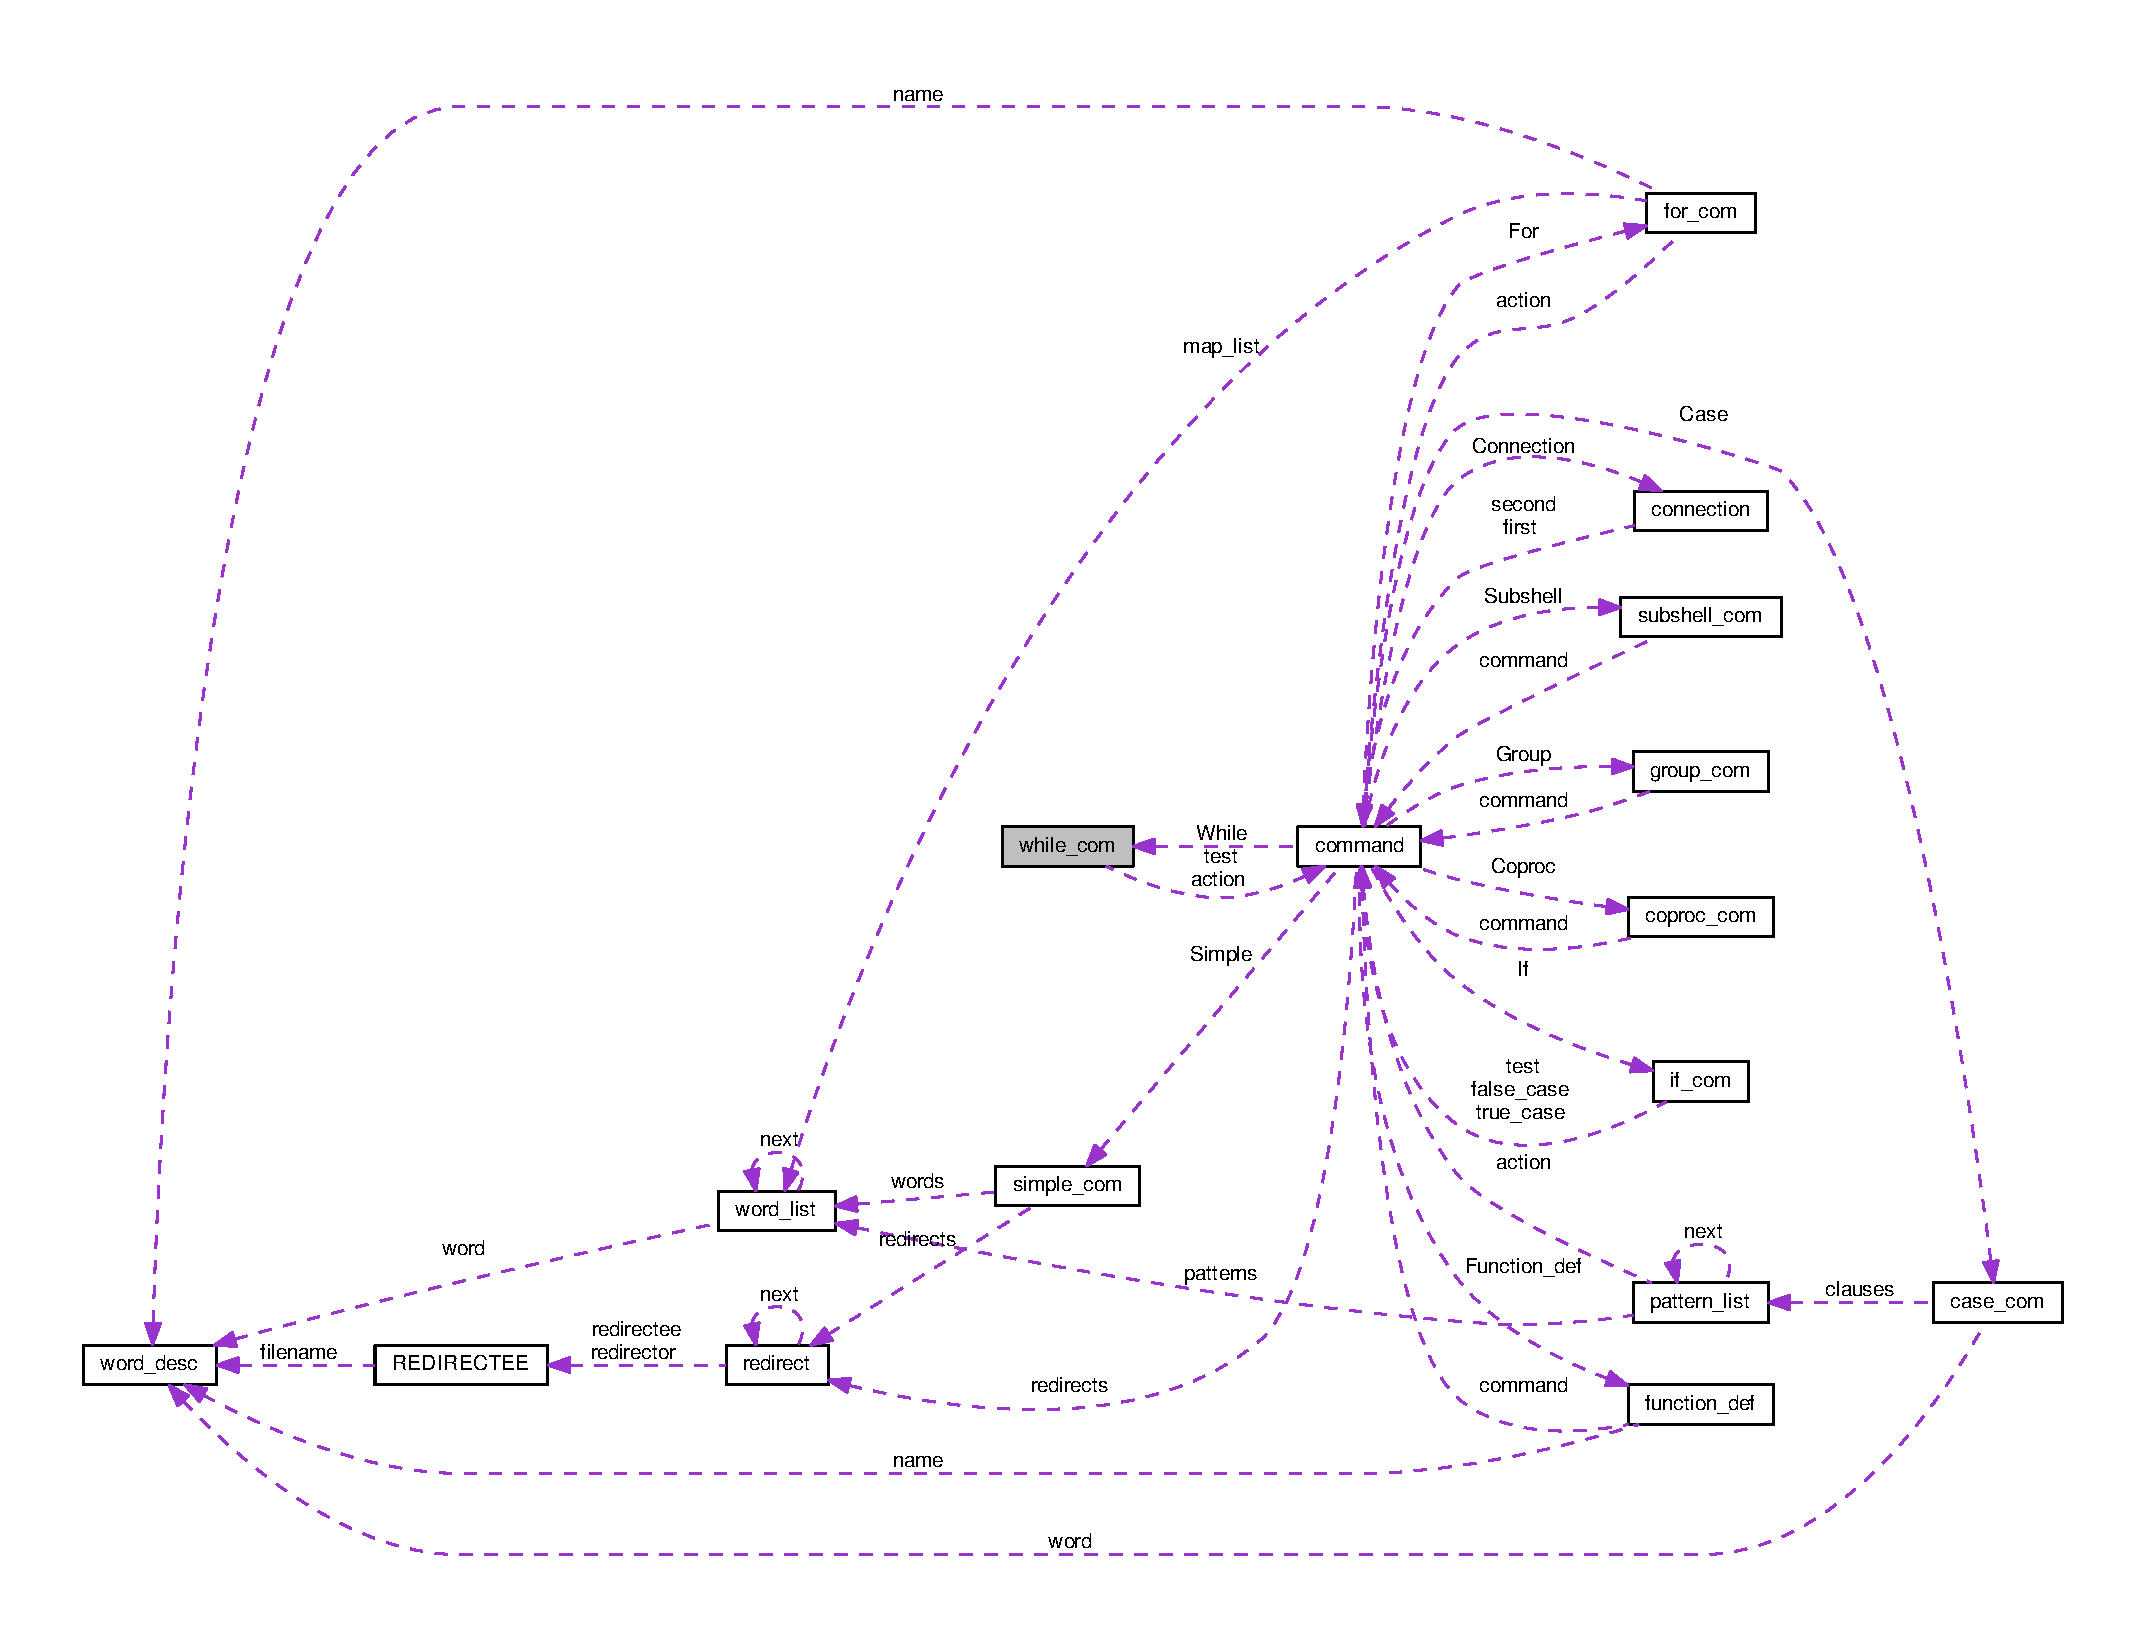
\includegraphics[width=350pt]{structwhile__com__coll__graph}
\end{center}
\end{figure}
\subsection*{Public Attributes}
\begin{DoxyCompactItemize}
\item 
int \hyperlink{structwhile__com_aeee869c9eb263491c5454c3c8c6b098a}{flags}
\item 
\hyperlink{command_8h_a8c41dec142c299806885773c902c0d87}{C\+O\+M\+M\+A\+ND} $\ast$ \hyperlink{structwhile__com_ab695c3ea48e16db8f9e7589fb56366f8}{test}
\item 
\hyperlink{command_8h_a8c41dec142c299806885773c902c0d87}{C\+O\+M\+M\+A\+ND} $\ast$ \hyperlink{structwhile__com_a8eaeeadd6e86e0a0a76144bf29a60b4d}{action}
\end{DoxyCompactItemize}


\subsection{Member Data Documentation}
\index{while\+\_\+com@{while\+\_\+com}!action@{action}}
\index{action@{action}!while\+\_\+com@{while\+\_\+com}}
\subsubsection[{\texorpdfstring{action}{action}}]{\setlength{\rightskip}{0pt plus 5cm}{\bf C\+O\+M\+M\+A\+ND}$\ast$ while\+\_\+com\+::action}\hypertarget{structwhile__com_a8eaeeadd6e86e0a0a76144bf29a60b4d}{}\label{structwhile__com_a8eaeeadd6e86e0a0a76144bf29a60b4d}
\index{while\+\_\+com@{while\+\_\+com}!flags@{flags}}
\index{flags@{flags}!while\+\_\+com@{while\+\_\+com}}
\subsubsection[{\texorpdfstring{flags}{flags}}]{\setlength{\rightskip}{0pt plus 5cm}int while\+\_\+com\+::flags}\hypertarget{structwhile__com_aeee869c9eb263491c5454c3c8c6b098a}{}\label{structwhile__com_aeee869c9eb263491c5454c3c8c6b098a}
\index{while\+\_\+com@{while\+\_\+com}!test@{test}}
\index{test@{test}!while\+\_\+com@{while\+\_\+com}}
\subsubsection[{\texorpdfstring{test}{test}}]{\setlength{\rightskip}{0pt plus 5cm}{\bf C\+O\+M\+M\+A\+ND}$\ast$ while\+\_\+com\+::test}\hypertarget{structwhile__com_ab695c3ea48e16db8f9e7589fb56366f8}{}\label{structwhile__com_ab695c3ea48e16db8f9e7589fb56366f8}


The documentation for this struct was generated from the following file\+:\begin{DoxyCompactItemize}
\item 
\hyperlink{command_8h}{command.\+h}\end{DoxyCompactItemize}

\hypertarget{structword__desc}{}\section{word\+\_\+desc Struct Reference}
\label{structword__desc}\index{word\+\_\+desc@{word\+\_\+desc}}


{\ttfamily \#include $<$command.\+h$>$}

\subsection*{Public Attributes}
\begin{DoxyCompactItemize}
\item 
char $\ast$ \hyperlink{structword__desc_a7fe36c900b18a60a1aeffadf9ae1c01f}{word}
\item 
int \hyperlink{structword__desc_aaf191cb3477717d8b7479fda976063dd}{flags}
\end{DoxyCompactItemize}


\subsection{Member Data Documentation}
\index{word\+\_\+desc@{word\+\_\+desc}!flags@{flags}}
\index{flags@{flags}!word\+\_\+desc@{word\+\_\+desc}}
\subsubsection[{\texorpdfstring{flags}{flags}}]{\setlength{\rightskip}{0pt plus 5cm}int word\+\_\+desc\+::flags}\hypertarget{structword__desc_aaf191cb3477717d8b7479fda976063dd}{}\label{structword__desc_aaf191cb3477717d8b7479fda976063dd}
\index{word\+\_\+desc@{word\+\_\+desc}!word@{word}}
\index{word@{word}!word\+\_\+desc@{word\+\_\+desc}}
\subsubsection[{\texorpdfstring{word}{word}}]{\setlength{\rightskip}{0pt plus 5cm}char$\ast$ word\+\_\+desc\+::word}\hypertarget{structword__desc_a7fe36c900b18a60a1aeffadf9ae1c01f}{}\label{structword__desc_a7fe36c900b18a60a1aeffadf9ae1c01f}


The documentation for this struct was generated from the following file\+:\begin{DoxyCompactItemize}
\item 
\hyperlink{command_8h}{command.\+h}\end{DoxyCompactItemize}

\hypertarget{structword__list}{}\section{word\+\_\+list Struct Reference}
\label{structword__list}\index{word\+\_\+list@{word\+\_\+list}}


{\ttfamily \#include $<$command.\+h$>$}



Collaboration diagram for word\+\_\+list\+:
\nopagebreak
\begin{figure}[H]
\begin{center}
\leavevmode
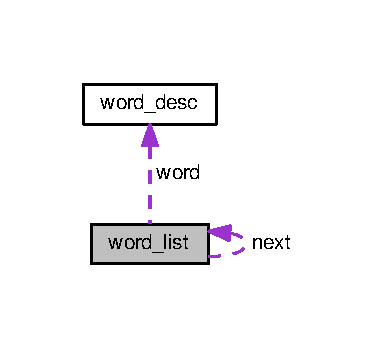
\includegraphics[width=180pt]{structword__list__coll__graph}
\end{center}
\end{figure}
\subsection*{Public Attributes}
\begin{DoxyCompactItemize}
\item 
struct \hyperlink{structword__list}{word\+\_\+list} $\ast$ \hyperlink{structword__list_a73b79d504929eeb584d08f068a046efc}{next}
\item 
\hyperlink{command_8h_a3f0cccf333703e5f6c4168be0db675fa}{W\+O\+R\+D\+\_\+\+D\+E\+SC} $\ast$ \hyperlink{structword__list_ae717a8244fbbcb28ae1debd9da89a0ef}{word}
\end{DoxyCompactItemize}


\subsection{Member Data Documentation}
\index{word\+\_\+list@{word\+\_\+list}!next@{next}}
\index{next@{next}!word\+\_\+list@{word\+\_\+list}}
\subsubsection[{\texorpdfstring{next}{next}}]{\setlength{\rightskip}{0pt plus 5cm}struct {\bf word\+\_\+list}$\ast$ word\+\_\+list\+::next}\hypertarget{structword__list_a73b79d504929eeb584d08f068a046efc}{}\label{structword__list_a73b79d504929eeb584d08f068a046efc}
\index{word\+\_\+list@{word\+\_\+list}!word@{word}}
\index{word@{word}!word\+\_\+list@{word\+\_\+list}}
\subsubsection[{\texorpdfstring{word}{word}}]{\setlength{\rightskip}{0pt plus 5cm}{\bf W\+O\+R\+D\+\_\+\+D\+E\+SC}$\ast$ word\+\_\+list\+::word}\hypertarget{structword__list_ae717a8244fbbcb28ae1debd9da89a0ef}{}\label{structword__list_ae717a8244fbbcb28ae1debd9da89a0ef}


The documentation for this struct was generated from the following file\+:\begin{DoxyCompactItemize}
\item 
\hyperlink{command_8h}{command.\+h}\end{DoxyCompactItemize}

\hypertarget{structwordflag}{}\section{wordflag Struct Reference}
\label{structwordflag}\index{wordflag@{wordflag}}
\subsection*{Public Attributes}
\begin{DoxyCompactItemize}
\item 
int \hyperlink{structwordflag_a7227a5f65db202538c0fd5bb88239c6b}{flag}
\item 
char $\ast$ \hyperlink{structwordflag_a1e15a044d32026bfe98625031b046860}{fstr}
\end{DoxyCompactItemize}


\subsection{Member Data Documentation}
\index{wordflag@{wordflag}!flag@{flag}}
\index{flag@{flag}!wordflag@{wordflag}}
\subsubsection[{\texorpdfstring{flag}{flag}}]{\setlength{\rightskip}{0pt plus 5cm}int wordflag\+::flag}\hypertarget{structwordflag_a7227a5f65db202538c0fd5bb88239c6b}{}\label{structwordflag_a7227a5f65db202538c0fd5bb88239c6b}
\index{wordflag@{wordflag}!fstr@{fstr}}
\index{fstr@{fstr}!wordflag@{wordflag}}
\subsubsection[{\texorpdfstring{fstr}{fstr}}]{\setlength{\rightskip}{0pt plus 5cm}char$\ast$ wordflag\+::fstr}\hypertarget{structwordflag_a1e15a044d32026bfe98625031b046860}{}\label{structwordflag_a1e15a044d32026bfe98625031b046860}


The documentation for this struct was generated from the following file\+:\begin{DoxyCompactItemize}
\item 
\hyperlink{mksyntax_8c}{mksyntax.\+c}\end{DoxyCompactItemize}

\hypertarget{unionyyalloc}{}\section{yyalloc Union Reference}
\label{unionyyalloc}\index{yyalloc@{yyalloc}}


Collaboration diagram for yyalloc\+:
\nopagebreak
\begin{figure}[H]
\begin{center}
\leavevmode
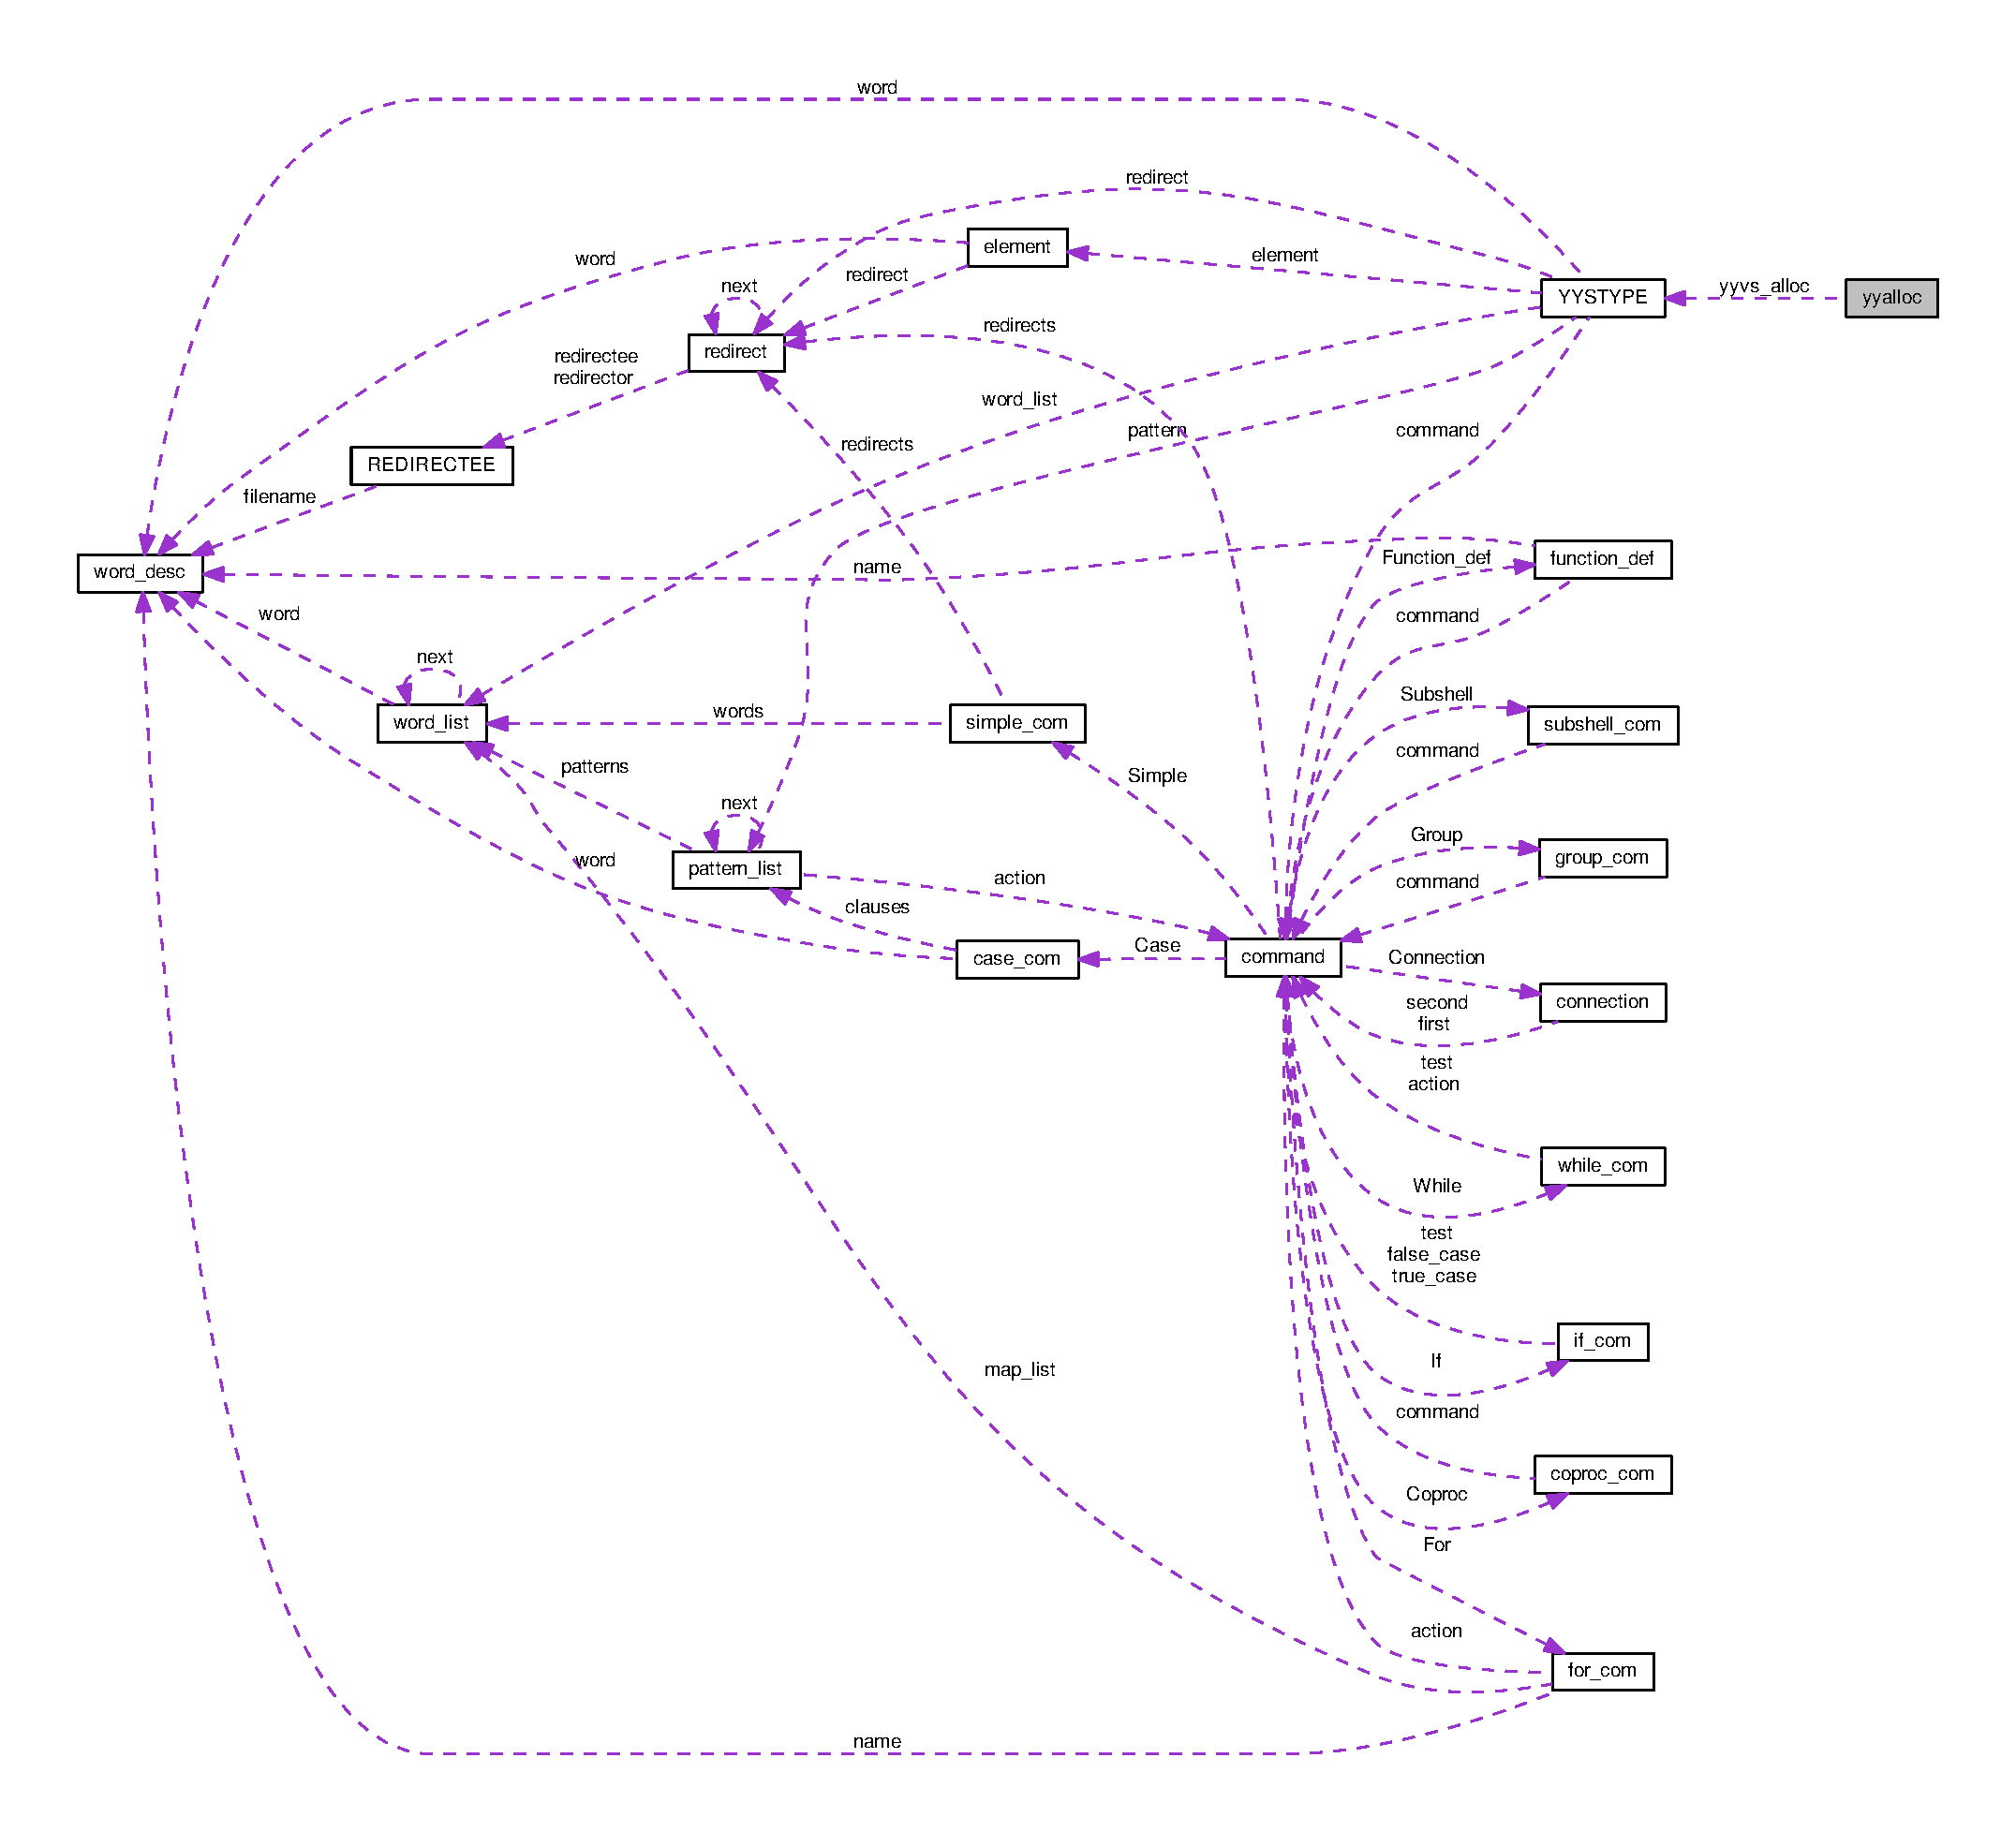
\includegraphics[width=350pt]{unionyyalloc__coll__graph}
\end{center}
\end{figure}
\subsection*{Public Attributes}
\begin{DoxyCompactItemize}
\item 
\hyperlink{y_8tab_8c_ade5b97f0021a4f6c5922ead3744ab297}{yytype\+\_\+int16} \hyperlink{unionyyalloc_a4800e0520a89a4789afa7b5d82197e65}{yyss\+\_\+alloc}
\item 
\hyperlink{unionYYSTYPE}{Y\+Y\+S\+T\+Y\+PE} \hyperlink{unionyyalloc_a9326f4fdc6f737a929444427836d8928}{yyvs\+\_\+alloc}
\end{DoxyCompactItemize}


\subsection{Member Data Documentation}
\index{yyalloc@{yyalloc}!yyss\+\_\+alloc@{yyss\+\_\+alloc}}
\index{yyss\+\_\+alloc@{yyss\+\_\+alloc}!yyalloc@{yyalloc}}
\subsubsection[{\texorpdfstring{yyss\+\_\+alloc}{yyss_alloc}}]{\setlength{\rightskip}{0pt plus 5cm}{\bf yytype\+\_\+int16} yyalloc\+::yyss\+\_\+alloc}\hypertarget{unionyyalloc_a4800e0520a89a4789afa7b5d82197e65}{}\label{unionyyalloc_a4800e0520a89a4789afa7b5d82197e65}
\index{yyalloc@{yyalloc}!yyvs\+\_\+alloc@{yyvs\+\_\+alloc}}
\index{yyvs\+\_\+alloc@{yyvs\+\_\+alloc}!yyalloc@{yyalloc}}
\subsubsection[{\texorpdfstring{yyvs\+\_\+alloc}{yyvs_alloc}}]{\setlength{\rightskip}{0pt plus 5cm}{\bf Y\+Y\+S\+T\+Y\+PE} yyalloc\+::yyvs\+\_\+alloc}\hypertarget{unionyyalloc_a9326f4fdc6f737a929444427836d8928}{}\label{unionyyalloc_a9326f4fdc6f737a929444427836d8928}


The documentation for this union was generated from the following file\+:\begin{DoxyCompactItemize}
\item 
\hyperlink{y_8tab_8c}{y.\+tab.\+c}\end{DoxyCompactItemize}

\hypertarget{unionYYSTYPE}{}\section{Y\+Y\+S\+T\+Y\+PE Union Reference}
\label{unionYYSTYPE}\index{Y\+Y\+S\+T\+Y\+PE@{Y\+Y\+S\+T\+Y\+PE}}


{\ttfamily \#include $<$y.\+tab.\+h$>$}



Collaboration diagram for Y\+Y\+S\+T\+Y\+PE\+:
\nopagebreak
\begin{figure}[H]
\begin{center}
\leavevmode
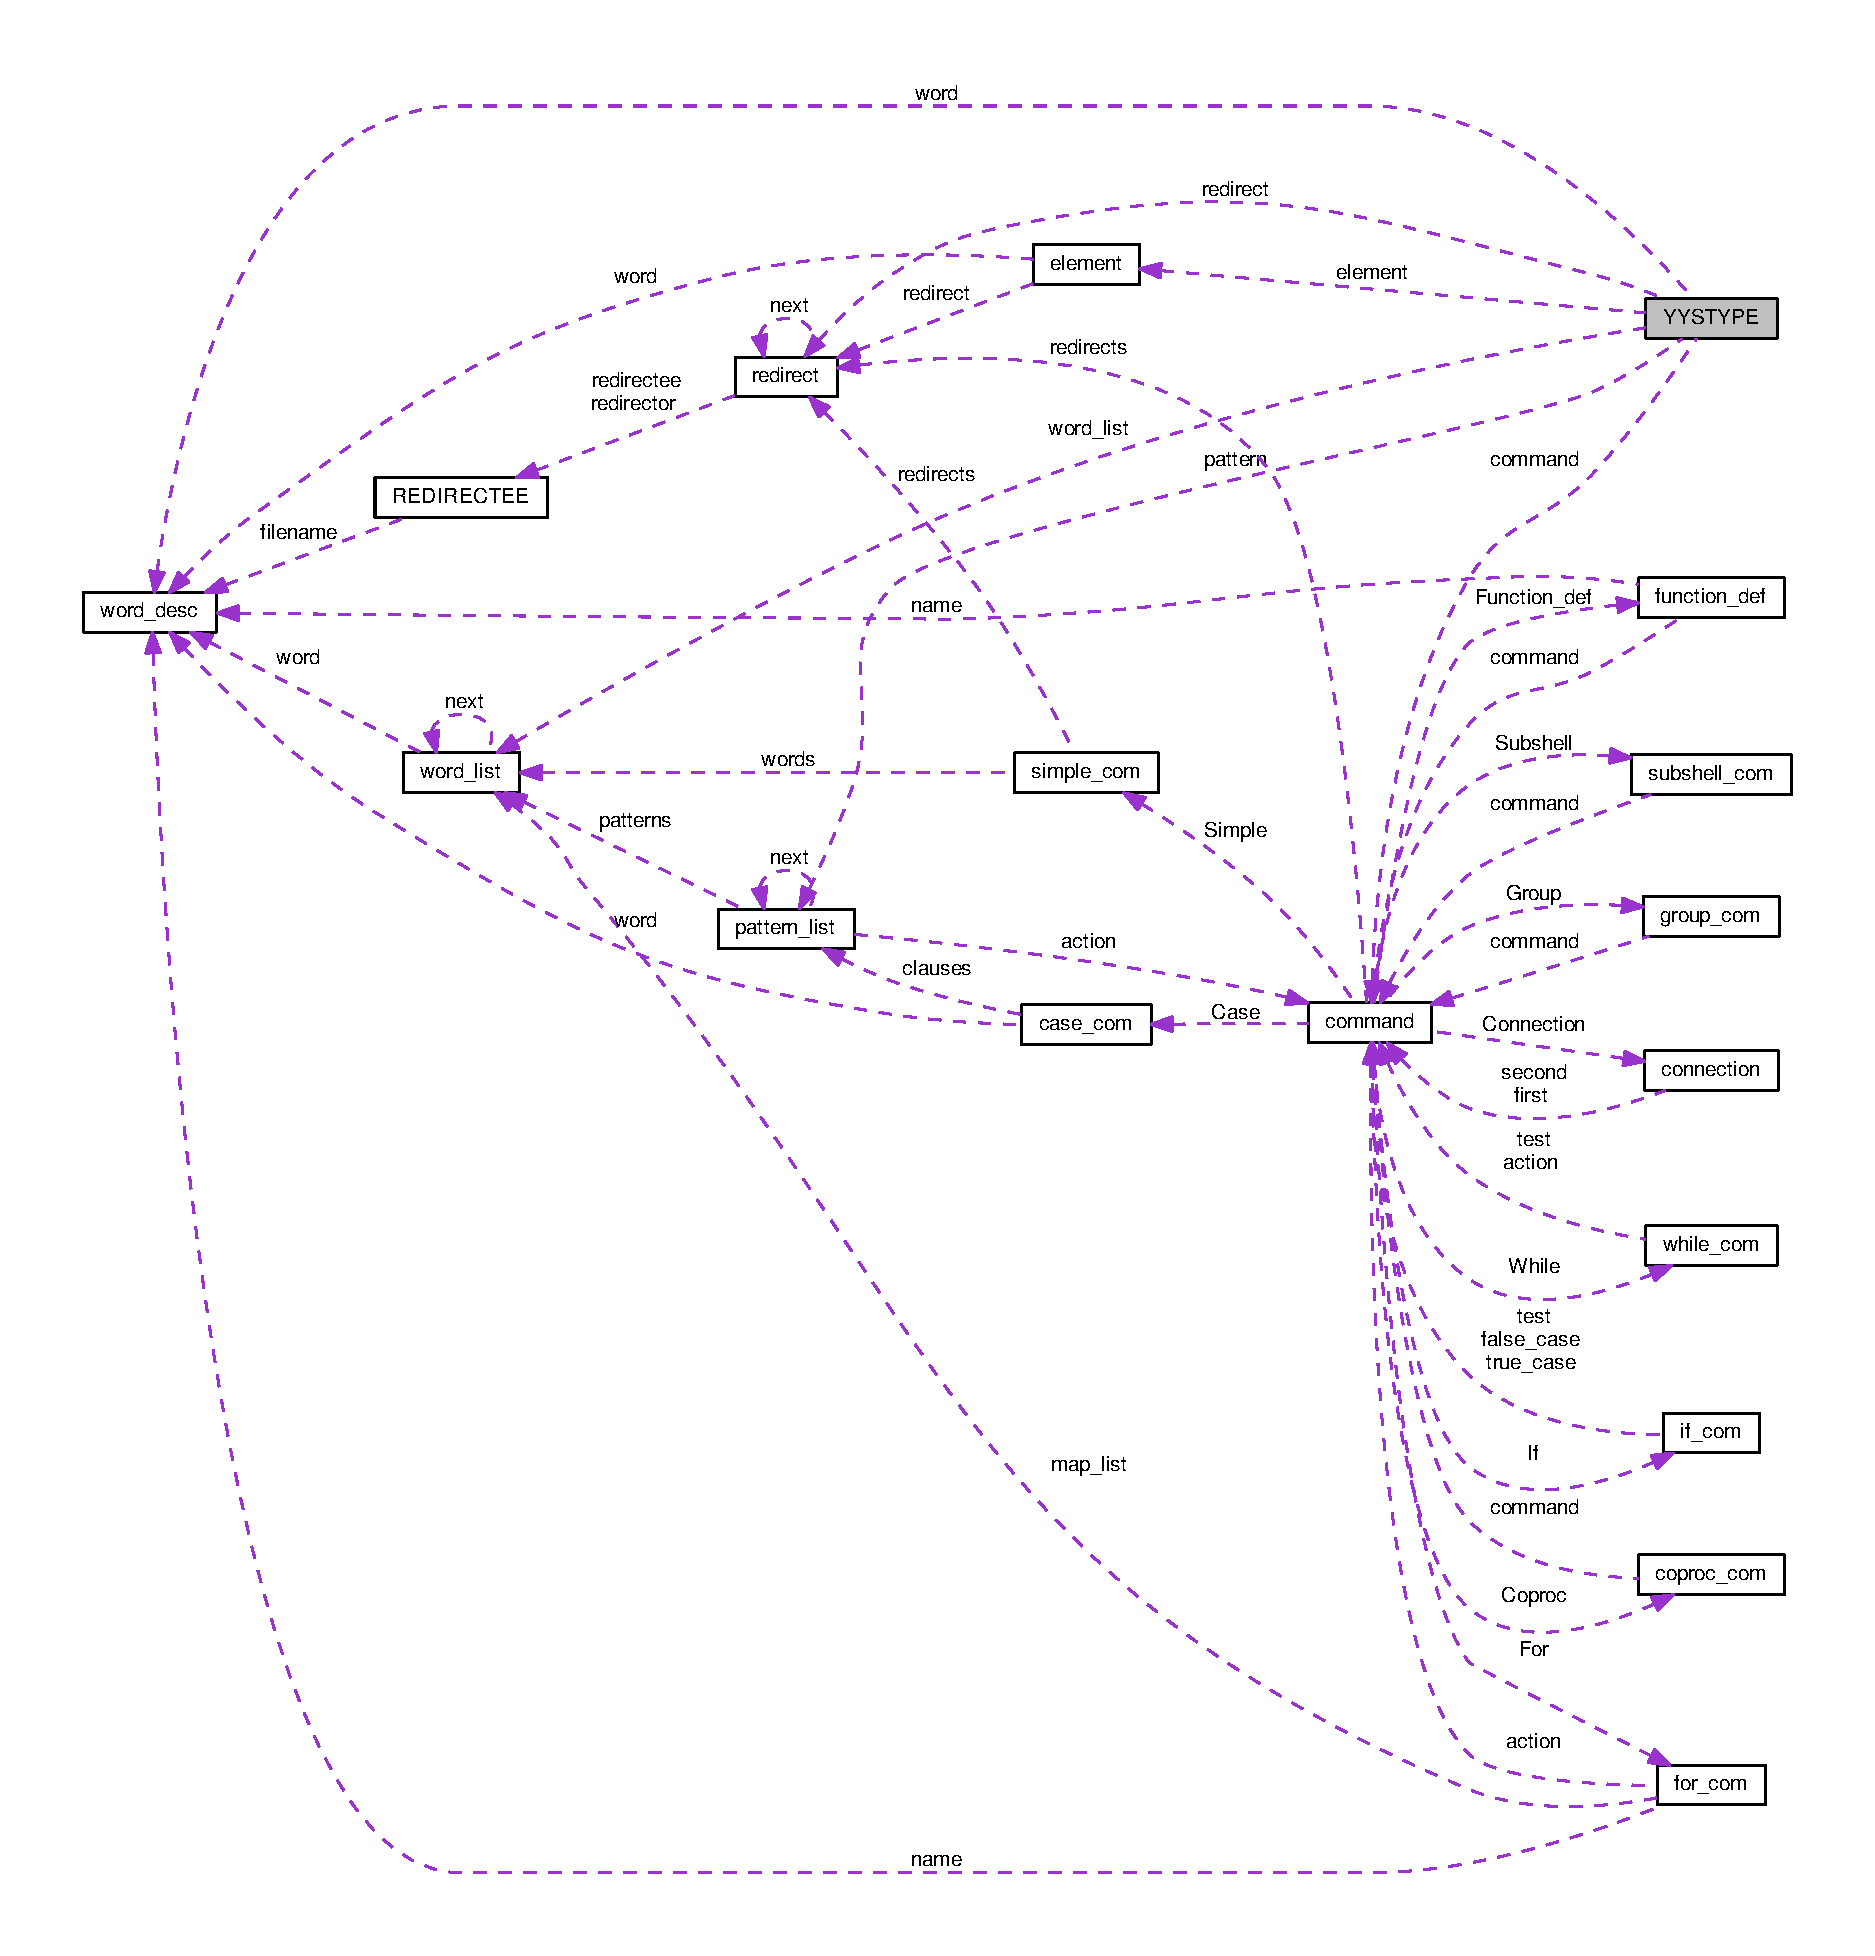
\includegraphics[width=350pt]{unionYYSTYPE__coll__graph}
\end{center}
\end{figure}
\subsection*{Public Attributes}
\begin{DoxyCompactItemize}
\item 
\hyperlink{command_8h_a3f0cccf333703e5f6c4168be0db675fa}{W\+O\+R\+D\+\_\+\+D\+E\+SC} $\ast$ \hyperlink{unionYYSTYPE_a8cc77cd40d569fa92c917c3e11a5e4bb}{word}
\item 
int \hyperlink{unionYYSTYPE_a240bd0051381dcdbd03b9c3764570b93}{number}
\item 
\hyperlink{command_8h_ac42a7b781459884316a1f2ffe79e8a62}{W\+O\+R\+D\+\_\+\+L\+I\+ST} $\ast$ \hyperlink{unionYYSTYPE_aaa247cc53b81b682e2a02cb246fa2e5f}{word\+\_\+list}
\item 
\hyperlink{command_8h_a8c41dec142c299806885773c902c0d87}{C\+O\+M\+M\+A\+ND} $\ast$ \hyperlink{unionYYSTYPE_a79c2ad9baf29ad6f85731c1f27372b8b}{command}
\item 
\hyperlink{command_8h_adeb9f5d937c92c7923aec48ad5e47d57}{R\+E\+D\+I\+R\+E\+CT} $\ast$ \hyperlink{unionYYSTYPE_aa0010a419e6ecb1a506d7ff004462712}{redirect}
\item 
\hyperlink{command_8h_ad98861155f12e470f2a392b7767cbe23}{E\+L\+E\+M\+E\+NT} \hyperlink{unionYYSTYPE_a84a38406ac394e9c45c3d333d1015deb}{element}
\item 
\hyperlink{command_8h_a05098e88133e048a1acf396288758a9e}{P\+A\+T\+T\+E\+R\+N\+\_\+\+L\+I\+ST} $\ast$ \hyperlink{unionYYSTYPE_abf7ad756ffb663853f56047bcfed8a55}{pattern}
\end{DoxyCompactItemize}


\subsection{Member Data Documentation}
\index{Y\+Y\+S\+T\+Y\+PE@{Y\+Y\+S\+T\+Y\+PE}!command@{command}}
\index{command@{command}!Y\+Y\+S\+T\+Y\+PE@{Y\+Y\+S\+T\+Y\+PE}}
\subsubsection[{\texorpdfstring{command}{command}}]{\setlength{\rightskip}{0pt plus 5cm}{\bf C\+O\+M\+M\+A\+ND} $\ast$ Y\+Y\+S\+T\+Y\+P\+E\+::command}\hypertarget{unionYYSTYPE_a79c2ad9baf29ad6f85731c1f27372b8b}{}\label{unionYYSTYPE_a79c2ad9baf29ad6f85731c1f27372b8b}
\index{Y\+Y\+S\+T\+Y\+PE@{Y\+Y\+S\+T\+Y\+PE}!element@{element}}
\index{element@{element}!Y\+Y\+S\+T\+Y\+PE@{Y\+Y\+S\+T\+Y\+PE}}
\subsubsection[{\texorpdfstring{element}{element}}]{\setlength{\rightskip}{0pt plus 5cm}{\bf E\+L\+E\+M\+E\+NT} Y\+Y\+S\+T\+Y\+P\+E\+::element}\hypertarget{unionYYSTYPE_a84a38406ac394e9c45c3d333d1015deb}{}\label{unionYYSTYPE_a84a38406ac394e9c45c3d333d1015deb}
\index{Y\+Y\+S\+T\+Y\+PE@{Y\+Y\+S\+T\+Y\+PE}!number@{number}}
\index{number@{number}!Y\+Y\+S\+T\+Y\+PE@{Y\+Y\+S\+T\+Y\+PE}}
\subsubsection[{\texorpdfstring{number}{number}}]{\setlength{\rightskip}{0pt plus 5cm}int Y\+Y\+S\+T\+Y\+P\+E\+::number}\hypertarget{unionYYSTYPE_a240bd0051381dcdbd03b9c3764570b93}{}\label{unionYYSTYPE_a240bd0051381dcdbd03b9c3764570b93}
\index{Y\+Y\+S\+T\+Y\+PE@{Y\+Y\+S\+T\+Y\+PE}!pattern@{pattern}}
\index{pattern@{pattern}!Y\+Y\+S\+T\+Y\+PE@{Y\+Y\+S\+T\+Y\+PE}}
\subsubsection[{\texorpdfstring{pattern}{pattern}}]{\setlength{\rightskip}{0pt plus 5cm}{\bf P\+A\+T\+T\+E\+R\+N\+\_\+\+L\+I\+ST} $\ast$ Y\+Y\+S\+T\+Y\+P\+E\+::pattern}\hypertarget{unionYYSTYPE_abf7ad756ffb663853f56047bcfed8a55}{}\label{unionYYSTYPE_abf7ad756ffb663853f56047bcfed8a55}
\index{Y\+Y\+S\+T\+Y\+PE@{Y\+Y\+S\+T\+Y\+PE}!redirect@{redirect}}
\index{redirect@{redirect}!Y\+Y\+S\+T\+Y\+PE@{Y\+Y\+S\+T\+Y\+PE}}
\subsubsection[{\texorpdfstring{redirect}{redirect}}]{\setlength{\rightskip}{0pt plus 5cm}{\bf R\+E\+D\+I\+R\+E\+CT} $\ast$ Y\+Y\+S\+T\+Y\+P\+E\+::redirect}\hypertarget{unionYYSTYPE_aa0010a419e6ecb1a506d7ff004462712}{}\label{unionYYSTYPE_aa0010a419e6ecb1a506d7ff004462712}
\index{Y\+Y\+S\+T\+Y\+PE@{Y\+Y\+S\+T\+Y\+PE}!word@{word}}
\index{word@{word}!Y\+Y\+S\+T\+Y\+PE@{Y\+Y\+S\+T\+Y\+PE}}
\subsubsection[{\texorpdfstring{word}{word}}]{\setlength{\rightskip}{0pt plus 5cm}{\bf W\+O\+R\+D\+\_\+\+D\+E\+SC} $\ast$ Y\+Y\+S\+T\+Y\+P\+E\+::word}\hypertarget{unionYYSTYPE_a8cc77cd40d569fa92c917c3e11a5e4bb}{}\label{unionYYSTYPE_a8cc77cd40d569fa92c917c3e11a5e4bb}
\index{Y\+Y\+S\+T\+Y\+PE@{Y\+Y\+S\+T\+Y\+PE}!word\+\_\+list@{word\+\_\+list}}
\index{word\+\_\+list@{word\+\_\+list}!Y\+Y\+S\+T\+Y\+PE@{Y\+Y\+S\+T\+Y\+PE}}
\subsubsection[{\texorpdfstring{word\+\_\+list}{word_list}}]{\setlength{\rightskip}{0pt plus 5cm}{\bf W\+O\+R\+D\+\_\+\+L\+I\+ST} $\ast$ Y\+Y\+S\+T\+Y\+P\+E\+::word\+\_\+list}\hypertarget{unionYYSTYPE_aaa247cc53b81b682e2a02cb246fa2e5f}{}\label{unionYYSTYPE_aaa247cc53b81b682e2a02cb246fa2e5f}


The documentation for this union was generated from the following files\+:\begin{DoxyCompactItemize}
\item 
\hyperlink{y_8tab_8c}{y.\+tab.\+c}\item 
\hyperlink{y_8tab_8h}{y.\+tab.\+h}\end{DoxyCompactItemize}

\chapter{File Documentation}
\hypertarget{alias_8c}{}\section{alias.\+c File Reference}
\label{alias_8c}\index{alias.\+c@{alias.\+c}}
{\ttfamily \#include \char`\"{}config.\+h\char`\"{}}\\*
{\ttfamily \#include $<$unistd.\+h$>$}\\*
{\ttfamily \#include $<$stdio.\+h$>$}\\*
{\ttfamily \#include \char`\"{}chartypes.\+h\char`\"{}}\\*
{\ttfamily \#include \char`\"{}bashansi.\+h\char`\"{}}\\*
{\ttfamily \#include \char`\"{}command.\+h\char`\"{}}\\*
{\ttfamily \#include \char`\"{}general.\+h\char`\"{}}\\*
{\ttfamily \#include \char`\"{}externs.\+h\char`\"{}}\\*
{\ttfamily \#include \char`\"{}alias.\+h\char`\"{}}\\*
{\ttfamily \#include \char`\"{}pcomplete.\+h\char`\"{}}\\*
Include dependency graph for alias.\+c\+:
\nopagebreak
\begin{figure}[H]
\begin{center}
\leavevmode
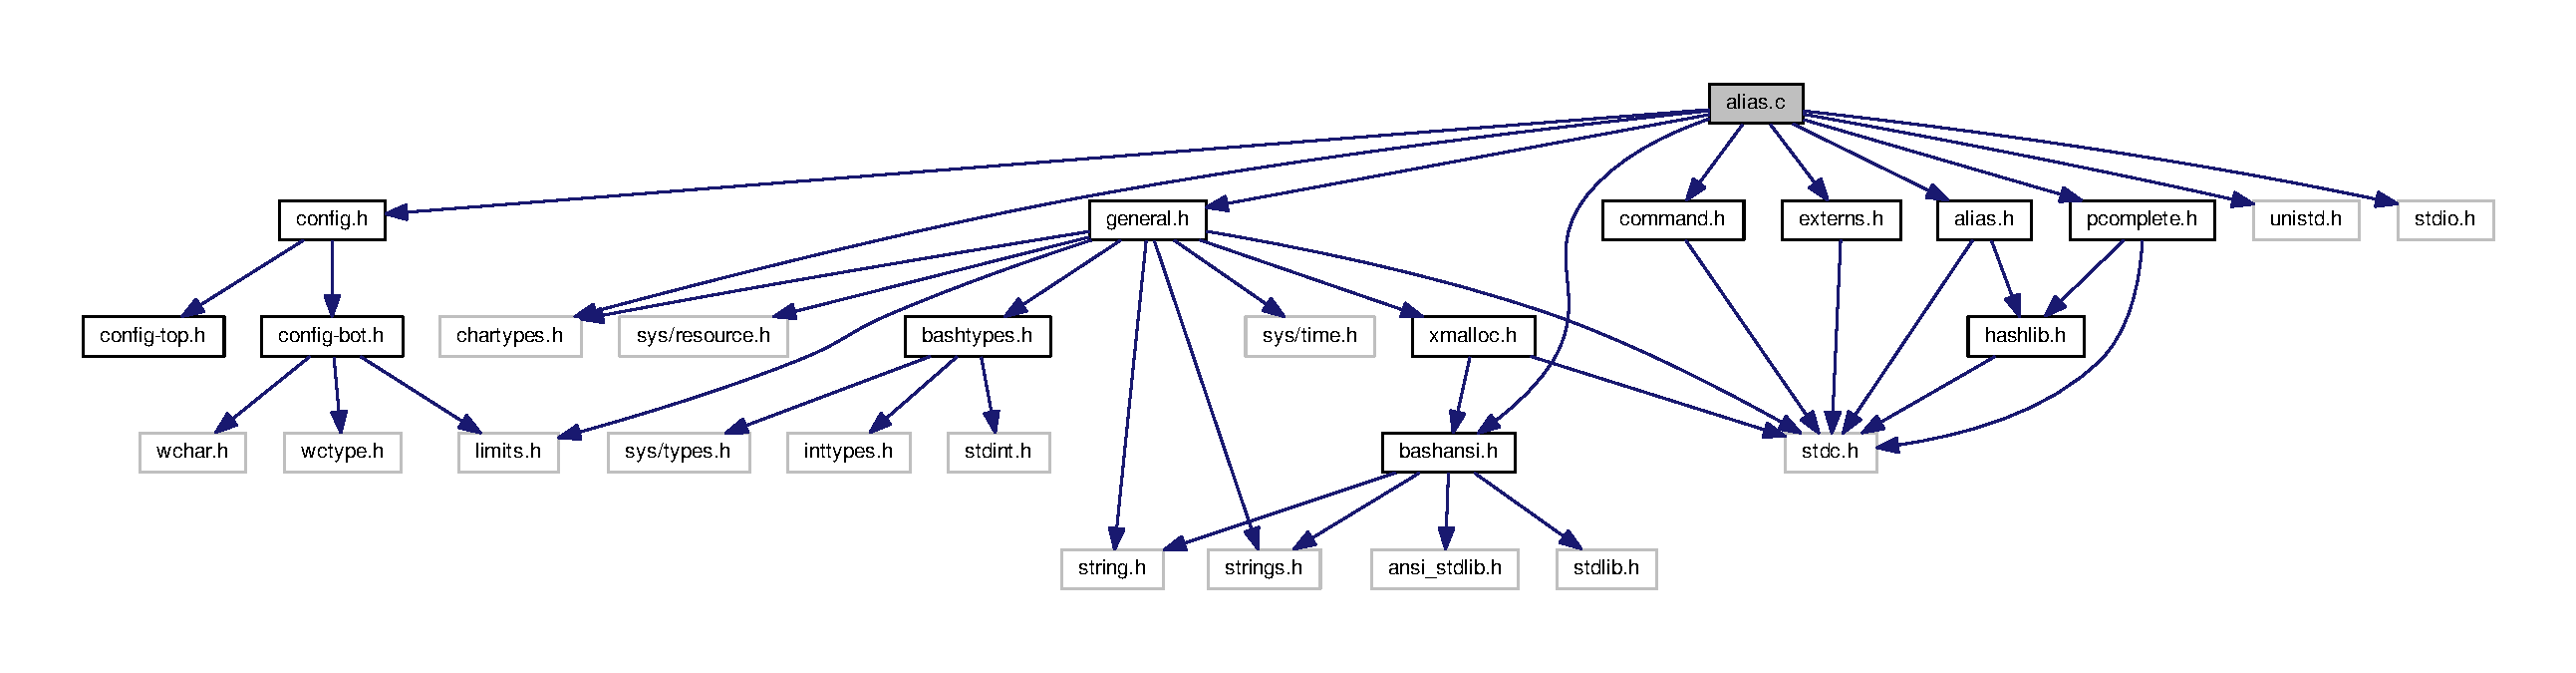
\includegraphics[width=350pt]{alias_8c__incl}
\end{center}
\end{figure}
\subsection*{Macros}
\begin{DoxyCompactItemize}
\item 
\#define \hyperlink{alias_8c_aaafbf2441352c0c74b67d76ee3188b2f}{A\+L\+I\+A\+S\+\_\+\+H\+A\+S\+H\+\_\+\+B\+U\+C\+K\+E\+TS}~64	/$\ast$ must be power of two $\ast$/
\item 
\#define \hyperlink{alias_8c_a58b80486be2d2d41650ba44f653dd40d}{self\+\_\+delimiting}(character)~(\hyperlink{general_8h_ad19cd6cf20c7b79c4ab633cb6247008b}{member} ((character), \char`\"{} \textbackslash{}t\textbackslash{}n\textbackslash{}r;$\vert$\&()\char`\"{}))
\item 
\#define \hyperlink{alias_8c_ae20387673161c6d1d4c6d81a807b9428}{command\+\_\+separator}(character)~(\hyperlink{general_8h_ad19cd6cf20c7b79c4ab633cb6247008b}{member} ((character), \char`\"{}\textbackslash{}r\textbackslash{}n;$\vert$\&(\char`\"{}))
\item 
\#define \hyperlink{alias_8c_abee33fe12ec70c17fc7edb103965a219}{quote\+\_\+char}(c)~(((c) == \textquotesingle{}\textbackslash{}\textquotesingle{}\textquotesingle{}) $\vert$$\vert$ ((c) == \textquotesingle{}\char`\"{}\textquotesingle{}))
\item 
\#define \hyperlink{alias_8c_af9ce72b378a021c3d3a85b031d39234e}{token\+\_\+char}(c)~(!((\hyperlink{general_8h_a6a8878e323ddb4bf57b7c9db293b3fd6}{whitespace} (string\mbox{[}i\mbox{]}) $\vert$$\vert$ \hyperlink{alias_8c_a58b80486be2d2d41650ba44f653dd40d}{self\+\_\+delimiting} (string\mbox{[}i\mbox{]}))))
\end{DoxyCompactItemize}
\subsection*{Typedefs}
\begin{DoxyCompactItemize}
\item 
typedef int sh\+\_\+alias\+\_\+map\+\_\+func\+\_\+t \hyperlink{alias_8c_a1d9b52e521cff2f89e9969e24db28e12}{\+\_\+\+\_\+P}((\hyperlink{alias_8h_a11c6bae002d90e8dad2d17b87ba6cccf}{alias\+\_\+t} $\ast$))
\end{DoxyCompactItemize}
\subsection*{Functions}
\begin{DoxyCompactItemize}
\item 
static void \hyperlink{alias_8c_a7ac17f35a61c8a67b59b90d49f7d2cb2}{free\+\_\+alias\+\_\+data} \hyperlink{alias_8c_a26d7d1db07d8391f6637d913323da97c}{\+\_\+\+\_\+P} ((\hyperlink{xmalloc_8h_abbf31fec203727613ea15ba47bb8f344}{P\+T\+R\+\_\+T}))
\item 
static \hyperlink{alias_8h_a11c6bae002d90e8dad2d17b87ba6cccf}{alias\+\_\+t} $\ast$$\ast$\hyperlink{alias_8c_af985f130f741c28ae25ed838bc41298b}{map\+\_\+over\+\_\+aliases} \hyperlink{alias_8c_acc3f8840729db85f30f12fdfb8ce7369}{\+\_\+\+\_\+P} ((sh\+\_\+alias\+\_\+map\+\_\+func\+\_\+t $\ast$))
\item 
static void \hyperlink{alias_8c_a210d1aabeda51baebeccf42f321c093e}{sort\+\_\+aliases} \hyperlink{alias_8c_a6519d5c5caf00107069a500bfbb2e7a3}{\+\_\+\+\_\+P} ((\hyperlink{alias_8h_a11c6bae002d90e8dad2d17b87ba6cccf}{alias\+\_\+t} $\ast$$\ast$))
\item 
static int \hyperlink{alias_8c_aed85c03661269505e0a3f198aba19bee}{qsort\+\_\+alias\+\_\+compare} \hyperlink{alias_8c_a7a8e05938f8490ff84ca4bbd5a6a7910}{\+\_\+\+\_\+P} ((\hyperlink{alias_8h_a11c6bae002d90e8dad2d17b87ba6cccf}{alias\+\_\+t} $\ast$$\ast$, \hyperlink{alias_8h_a11c6bae002d90e8dad2d17b87ba6cccf}{alias\+\_\+t} $\ast$$\ast$))
\item 
static int \hyperlink{alias_8c_a3fb89598b9584124dc1e9e37dea50758}{skipquotes} \hyperlink{alias_8c_a949052b6b3e323710c7054404a14ee91}{\+\_\+\+\_\+P} ((char $\ast$, int))
\item 
void \hyperlink{alias_8c_abba691c3b75de85b97e7418e5b149d8a}{initialize\+\_\+aliases} ()
\item 
\hyperlink{alias_8h_a11c6bae002d90e8dad2d17b87ba6cccf}{alias\+\_\+t} $\ast$ \hyperlink{alias_8c_a9a85eef7b6f6e69a5921e8da9c471263}{find\+\_\+alias} (char $\ast$\hyperlink{shell_8c_a8f8f80d37794cde9472343e4487ba3eb}{name})
\item 
char $\ast$ \hyperlink{alias_8c_a0e1b176c3d4809e000b7ae095502b853}{get\+\_\+alias\+\_\+value} (char $\ast$\hyperlink{shell_8c_a8f8f80d37794cde9472343e4487ba3eb}{name})
\item 
void \hyperlink{alias_8c_a2a7bb793d1eac9a3cdfe66c7357fd460}{add\+\_\+alias} (char $\ast$\hyperlink{shell_8c_a8f8f80d37794cde9472343e4487ba3eb}{name}, char $\ast$value)
\item 
static void \hyperlink{alias_8c_a7ac17f35a61c8a67b59b90d49f7d2cb2}{free\+\_\+alias\+\_\+data} (\hyperlink{xmalloc_8h_abbf31fec203727613ea15ba47bb8f344}{P\+T\+R\+\_\+T} data)
\item 
int \hyperlink{alias_8c_a95780a0c8ac0b02172f15015bf26b118}{remove\+\_\+alias} (char $\ast$\hyperlink{shell_8c_a8f8f80d37794cde9472343e4487ba3eb}{name})
\item 
void \hyperlink{alias_8c_a7cb21e7339544bfe3a0138d1324d79b1}{delete\+\_\+all\+\_\+aliases} ()
\item 
static \hyperlink{alias_8h_a11c6bae002d90e8dad2d17b87ba6cccf}{alias\+\_\+t} $\ast$$\ast$ \hyperlink{alias_8c_af985f130f741c28ae25ed838bc41298b}{map\+\_\+over\+\_\+aliases} (sh\+\_\+alias\+\_\+map\+\_\+func\+\_\+t $\ast$function)
\item 
static void \hyperlink{alias_8c_a210d1aabeda51baebeccf42f321c093e}{sort\+\_\+aliases} (\hyperlink{alias_8h_a11c6bae002d90e8dad2d17b87ba6cccf}{alias\+\_\+t} $\ast$$\ast$\hyperlink{structarray}{array})
\item 
static int \hyperlink{alias_8c_aed85c03661269505e0a3f198aba19bee}{qsort\+\_\+alias\+\_\+compare} (\hyperlink{alias_8h_a11c6bae002d90e8dad2d17b87ba6cccf}{alias\+\_\+t} $\ast$$\ast$as1, \hyperlink{alias_8h_a11c6bae002d90e8dad2d17b87ba6cccf}{alias\+\_\+t} $\ast$$\ast$as2)
\item 
\hyperlink{alias_8h_a11c6bae002d90e8dad2d17b87ba6cccf}{alias\+\_\+t} $\ast$$\ast$ \hyperlink{alias_8c_a1c0ae8915c6f62822bed3d412e0132e8}{all\+\_\+aliases} ()
\item 
char $\ast$ \hyperlink{alias_8c_ad97f215959c2666980fbe778b91a54e3}{alias\+\_\+expand\+\_\+word} (char $\ast$s)
\item 
static int \hyperlink{alias_8c_a3fb89598b9584124dc1e9e37dea50758}{skipquotes} (char $\ast$string, int start)
\item 
static int \hyperlink{alias_8c_aa688063409ccb7123e9bd4b23455e60a}{skipws} (char $\ast$string, int start)
\item 
static int \hyperlink{alias_8c_a641542c1e16b08c41b0d58cd4ff95d6f}{rd\+\_\+token} (char $\ast$string, int start)
\item 
char $\ast$ \hyperlink{alias_8c_a550e246d1bf1bfca44022977badf71dc}{alias\+\_\+expand} (char $\ast$string)
\end{DoxyCompactItemize}
\subsection*{Variables}
\begin{DoxyCompactItemize}
\item 
int \hyperlink{alias_8c_aafd6878a76ae3351d1d405a7e2236115}{alias\+\_\+expand\+\_\+all} = 0
\item 
\hyperlink{hashlib_8h_a8284f9978df160609365484b829527e6}{H\+A\+S\+H\+\_\+\+T\+A\+B\+LE} $\ast$ \hyperlink{alias_8c_ade59a7845bd91cac464607d4a444cb1f}{aliases} = (\hyperlink{hashlib_8h_a8284f9978df160609365484b829527e6}{H\+A\+S\+H\+\_\+\+T\+A\+B\+LE} $\ast$)\hyperlink{hashlib_8h_a070d2ce7b6bb7e5c05602aa8c308d0c4}{N\+U\+LL}
\item 
static int \hyperlink{alias_8c_a4748d3f8e01bbd519cf6ce5a0f539102}{command\+\_\+word}
\end{DoxyCompactItemize}


\subsection{Macro Definition Documentation}
\index{alias.\+c@{alias.\+c}!A\+L\+I\+A\+S\+\_\+\+H\+A\+S\+H\+\_\+\+B\+U\+C\+K\+E\+TS@{A\+L\+I\+A\+S\+\_\+\+H\+A\+S\+H\+\_\+\+B\+U\+C\+K\+E\+TS}}
\index{A\+L\+I\+A\+S\+\_\+\+H\+A\+S\+H\+\_\+\+B\+U\+C\+K\+E\+TS@{A\+L\+I\+A\+S\+\_\+\+H\+A\+S\+H\+\_\+\+B\+U\+C\+K\+E\+TS}!alias.\+c@{alias.\+c}}
\subsubsection[{\texorpdfstring{A\+L\+I\+A\+S\+\_\+\+H\+A\+S\+H\+\_\+\+B\+U\+C\+K\+E\+TS}{ALIAS_HASH_BUCKETS}}]{\setlength{\rightskip}{0pt plus 5cm}\#define A\+L\+I\+A\+S\+\_\+\+H\+A\+S\+H\+\_\+\+B\+U\+C\+K\+E\+TS~64	/$\ast$ must be power of two $\ast$/}\hypertarget{alias_8c_aaafbf2441352c0c74b67d76ee3188b2f}{}\label{alias_8c_aaafbf2441352c0c74b67d76ee3188b2f}
\index{alias.\+c@{alias.\+c}!command\+\_\+separator@{command\+\_\+separator}}
\index{command\+\_\+separator@{command\+\_\+separator}!alias.\+c@{alias.\+c}}
\subsubsection[{\texorpdfstring{command\+\_\+separator}{command_separator}}]{\setlength{\rightskip}{0pt plus 5cm}\#define command\+\_\+separator(
\begin{DoxyParamCaption}
\item[{}]{character}
\end{DoxyParamCaption}
)~({\bf member} ((character), \char`\"{}\textbackslash{}r\textbackslash{}n;$\vert$\&(\char`\"{}))}\hypertarget{alias_8c_ae20387673161c6d1d4c6d81a807b9428}{}\label{alias_8c_ae20387673161c6d1d4c6d81a807b9428}
\index{alias.\+c@{alias.\+c}!quote\+\_\+char@{quote\+\_\+char}}
\index{quote\+\_\+char@{quote\+\_\+char}!alias.\+c@{alias.\+c}}
\subsubsection[{\texorpdfstring{quote\+\_\+char}{quote_char}}]{\setlength{\rightskip}{0pt plus 5cm}\#define quote\+\_\+char(
\begin{DoxyParamCaption}
\item[{}]{c}
\end{DoxyParamCaption}
)~(((c) == \textquotesingle{}\textbackslash{}\textquotesingle{}\textquotesingle{}) $\vert$$\vert$ ((c) == \textquotesingle{}\char`\"{}\textquotesingle{}))}\hypertarget{alias_8c_abee33fe12ec70c17fc7edb103965a219}{}\label{alias_8c_abee33fe12ec70c17fc7edb103965a219}
\index{alias.\+c@{alias.\+c}!self\+\_\+delimiting@{self\+\_\+delimiting}}
\index{self\+\_\+delimiting@{self\+\_\+delimiting}!alias.\+c@{alias.\+c}}
\subsubsection[{\texorpdfstring{self\+\_\+delimiting}{self_delimiting}}]{\setlength{\rightskip}{0pt plus 5cm}\#define self\+\_\+delimiting(
\begin{DoxyParamCaption}
\item[{}]{character}
\end{DoxyParamCaption}
)~({\bf member} ((character), \char`\"{} \textbackslash{}t\textbackslash{}n\textbackslash{}r;$\vert$\&()\char`\"{}))}\hypertarget{alias_8c_a58b80486be2d2d41650ba44f653dd40d}{}\label{alias_8c_a58b80486be2d2d41650ba44f653dd40d}
\index{alias.\+c@{alias.\+c}!token\+\_\+char@{token\+\_\+char}}
\index{token\+\_\+char@{token\+\_\+char}!alias.\+c@{alias.\+c}}
\subsubsection[{\texorpdfstring{token\+\_\+char}{token_char}}]{\setlength{\rightskip}{0pt plus 5cm}\#define token\+\_\+char(
\begin{DoxyParamCaption}
\item[{}]{c}
\end{DoxyParamCaption}
)~(!(({\bf whitespace} (string\mbox{[}i\mbox{]}) $\vert$$\vert$ {\bf self\+\_\+delimiting} (string\mbox{[}i\mbox{]}))))}\hypertarget{alias_8c_af9ce72b378a021c3d3a85b031d39234e}{}\label{alias_8c_af9ce72b378a021c3d3a85b031d39234e}


\subsection{Typedef Documentation}
\index{alias.\+c@{alias.\+c}!\+\_\+\+\_\+P@{\+\_\+\+\_\+P}}
\index{\+\_\+\+\_\+P@{\+\_\+\+\_\+P}!alias.\+c@{alias.\+c}}
\subsubsection[{\texorpdfstring{\+\_\+\+\_\+P}{__P}}]{\setlength{\rightskip}{0pt plus 5cm}static void {\bf set\+\_\+line\+\_\+mbstate} \+\_\+\+\_\+P (
\begin{DoxyParamCaption}
\item[{({\bf alias\+\_\+t} $\ast$)}]{}
\end{DoxyParamCaption}
)\hspace{0.3cm}{\ttfamily [inline]}}\hypertarget{alias_8c_a1d9b52e521cff2f89e9969e24db28e12}{}\label{alias_8c_a1d9b52e521cff2f89e9969e24db28e12}


\subsection{Function Documentation}
\index{alias.\+c@{alias.\+c}!\+\_\+\+\_\+P@{\+\_\+\+\_\+P}}
\index{\+\_\+\+\_\+P@{\+\_\+\+\_\+P}!alias.\+c@{alias.\+c}}
\subsubsection[{\texorpdfstring{\+\_\+\+\_\+\+P((\+P\+T\+R\+\_\+\+T))}{__P((PTR_T))}}]{\setlength{\rightskip}{0pt plus 5cm}static void {\bf free\+\_\+alias\+\_\+data} \+\_\+\+\_\+P (
\begin{DoxyParamCaption}
\item[{({\bf P\+T\+R\+\_\+T})}]{}
\end{DoxyParamCaption}
)\hspace{0.3cm}{\ttfamily [static]}}\hypertarget{alias_8c_a26d7d1db07d8391f6637d913323da97c}{}\label{alias_8c_a26d7d1db07d8391f6637d913323da97c}
\index{alias.\+c@{alias.\+c}!\+\_\+\+\_\+P@{\+\_\+\+\_\+P}}
\index{\+\_\+\+\_\+P@{\+\_\+\+\_\+P}!alias.\+c@{alias.\+c}}
\subsubsection[{\texorpdfstring{\+\_\+\+\_\+\+P((sh\+\_\+alias\+\_\+map\+\_\+func\+\_\+t $\ast$))}{__P((sh_alias_map_func_t *))}}]{\setlength{\rightskip}{0pt plus 5cm}static {\bf alias\+\_\+t}$\ast$$\ast$ {\bf map\+\_\+over\+\_\+aliases} \+\_\+\+\_\+P (
\begin{DoxyParamCaption}
\item[{(sh\+\_\+alias\+\_\+map\+\_\+func\+\_\+t $\ast$)}]{}
\end{DoxyParamCaption}
)\hspace{0.3cm}{\ttfamily [static]}}\hypertarget{alias_8c_acc3f8840729db85f30f12fdfb8ce7369}{}\label{alias_8c_acc3f8840729db85f30f12fdfb8ce7369}
\index{alias.\+c@{alias.\+c}!\+\_\+\+\_\+P@{\+\_\+\+\_\+P}}
\index{\+\_\+\+\_\+P@{\+\_\+\+\_\+P}!alias.\+c@{alias.\+c}}
\subsubsection[{\texorpdfstring{\+\_\+\+\_\+\+P((alias\+\_\+t $\ast$$\ast$))}{__P((alias_t **))}}]{\setlength{\rightskip}{0pt plus 5cm}static void {\bf sort\+\_\+aliases} \+\_\+\+\_\+P (
\begin{DoxyParamCaption}
\item[{({\bf alias\+\_\+t} $\ast$$\ast$)}]{}
\end{DoxyParamCaption}
)\hspace{0.3cm}{\ttfamily [static]}}\hypertarget{alias_8c_a6519d5c5caf00107069a500bfbb2e7a3}{}\label{alias_8c_a6519d5c5caf00107069a500bfbb2e7a3}
\index{alias.\+c@{alias.\+c}!\+\_\+\+\_\+P@{\+\_\+\+\_\+P}}
\index{\+\_\+\+\_\+P@{\+\_\+\+\_\+P}!alias.\+c@{alias.\+c}}
\subsubsection[{\texorpdfstring{\+\_\+\+\_\+\+P((alias\+\_\+t $\ast$$\ast$, alias\+\_\+t $\ast$$\ast$))}{__P((alias_t **, alias_t **))}}]{\setlength{\rightskip}{0pt plus 5cm}static int {\bf qsort\+\_\+alias\+\_\+compare} \+\_\+\+\_\+P (
\begin{DoxyParamCaption}
\item[{({\bf alias\+\_\+t} $\ast$$\ast$, {\bf alias\+\_\+t} $\ast$$\ast$)}]{}
\end{DoxyParamCaption}
)\hspace{0.3cm}{\ttfamily [static]}}\hypertarget{alias_8c_a7a8e05938f8490ff84ca4bbd5a6a7910}{}\label{alias_8c_a7a8e05938f8490ff84ca4bbd5a6a7910}
\index{alias.\+c@{alias.\+c}!\+\_\+\+\_\+P@{\+\_\+\+\_\+P}}
\index{\+\_\+\+\_\+P@{\+\_\+\+\_\+P}!alias.\+c@{alias.\+c}}
\subsubsection[{\texorpdfstring{\+\_\+\+\_\+\+P((char $\ast$, int))}{__P((char *, int))}}]{\setlength{\rightskip}{0pt plus 5cm}static int {\bf skipquotes} \+\_\+\+\_\+P (
\begin{DoxyParamCaption}
\item[{(char $\ast$, int)}]{}
\end{DoxyParamCaption}
)\hspace{0.3cm}{\ttfamily [static]}}\hypertarget{alias_8c_a949052b6b3e323710c7054404a14ee91}{}\label{alias_8c_a949052b6b3e323710c7054404a14ee91}
\index{alias.\+c@{alias.\+c}!add\+\_\+alias@{add\+\_\+alias}}
\index{add\+\_\+alias@{add\+\_\+alias}!alias.\+c@{alias.\+c}}
\subsubsection[{\texorpdfstring{add\+\_\+alias(char $\ast$name, char $\ast$value)}{add_alias(char *name, char *value)}}]{\setlength{\rightskip}{0pt plus 5cm}void add\+\_\+alias (
\begin{DoxyParamCaption}
\item[{char $\ast$}]{name, }
\item[{char $\ast$}]{value}
\end{DoxyParamCaption}
)}\hypertarget{alias_8c_a2a7bb793d1eac9a3cdfe66c7357fd460}{}\label{alias_8c_a2a7bb793d1eac9a3cdfe66c7357fd460}


Here is the call graph for this function\+:
\nopagebreak
\begin{figure}[H]
\begin{center}
\leavevmode
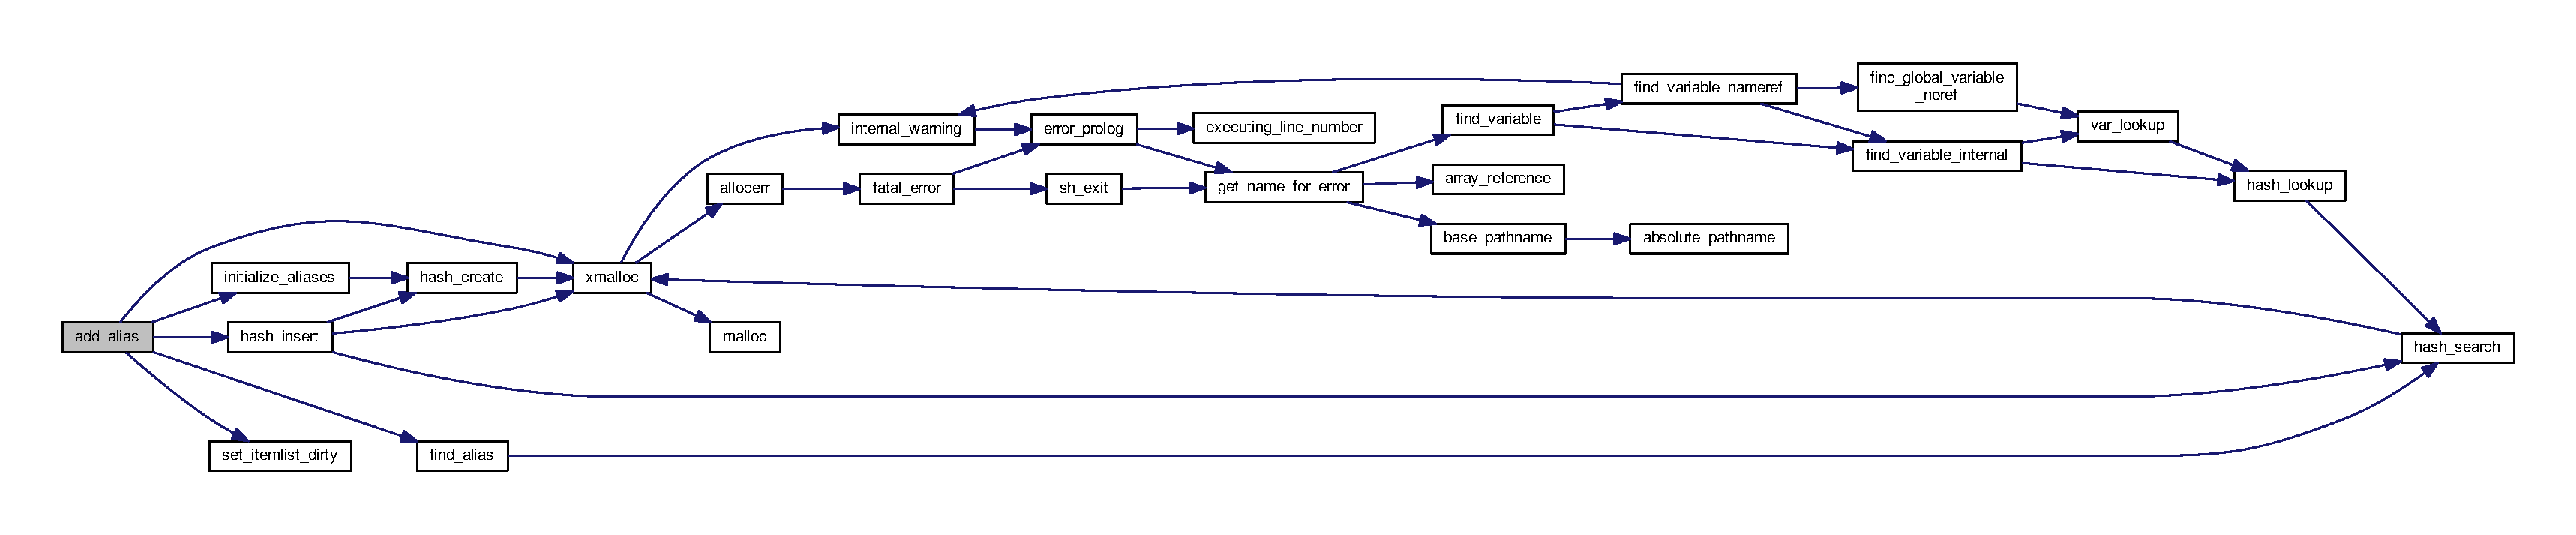
\includegraphics[width=350pt]{alias_8c_a2a7bb793d1eac9a3cdfe66c7357fd460_cgraph}
\end{center}
\end{figure}


\index{alias.\+c@{alias.\+c}!alias\+\_\+expand@{alias\+\_\+expand}}
\index{alias\+\_\+expand@{alias\+\_\+expand}!alias.\+c@{alias.\+c}}
\subsubsection[{\texorpdfstring{alias\+\_\+expand(char $\ast$string)}{alias_expand(char *string)}}]{\setlength{\rightskip}{0pt plus 5cm}char$\ast$ alias\+\_\+expand (
\begin{DoxyParamCaption}
\item[{char $\ast$}]{string}
\end{DoxyParamCaption}
)}\hypertarget{alias_8c_a550e246d1bf1bfca44022977badf71dc}{}\label{alias_8c_a550e246d1bf1bfca44022977badf71dc}


Here is the call graph for this function\+:
\nopagebreak
\begin{figure}[H]
\begin{center}
\leavevmode
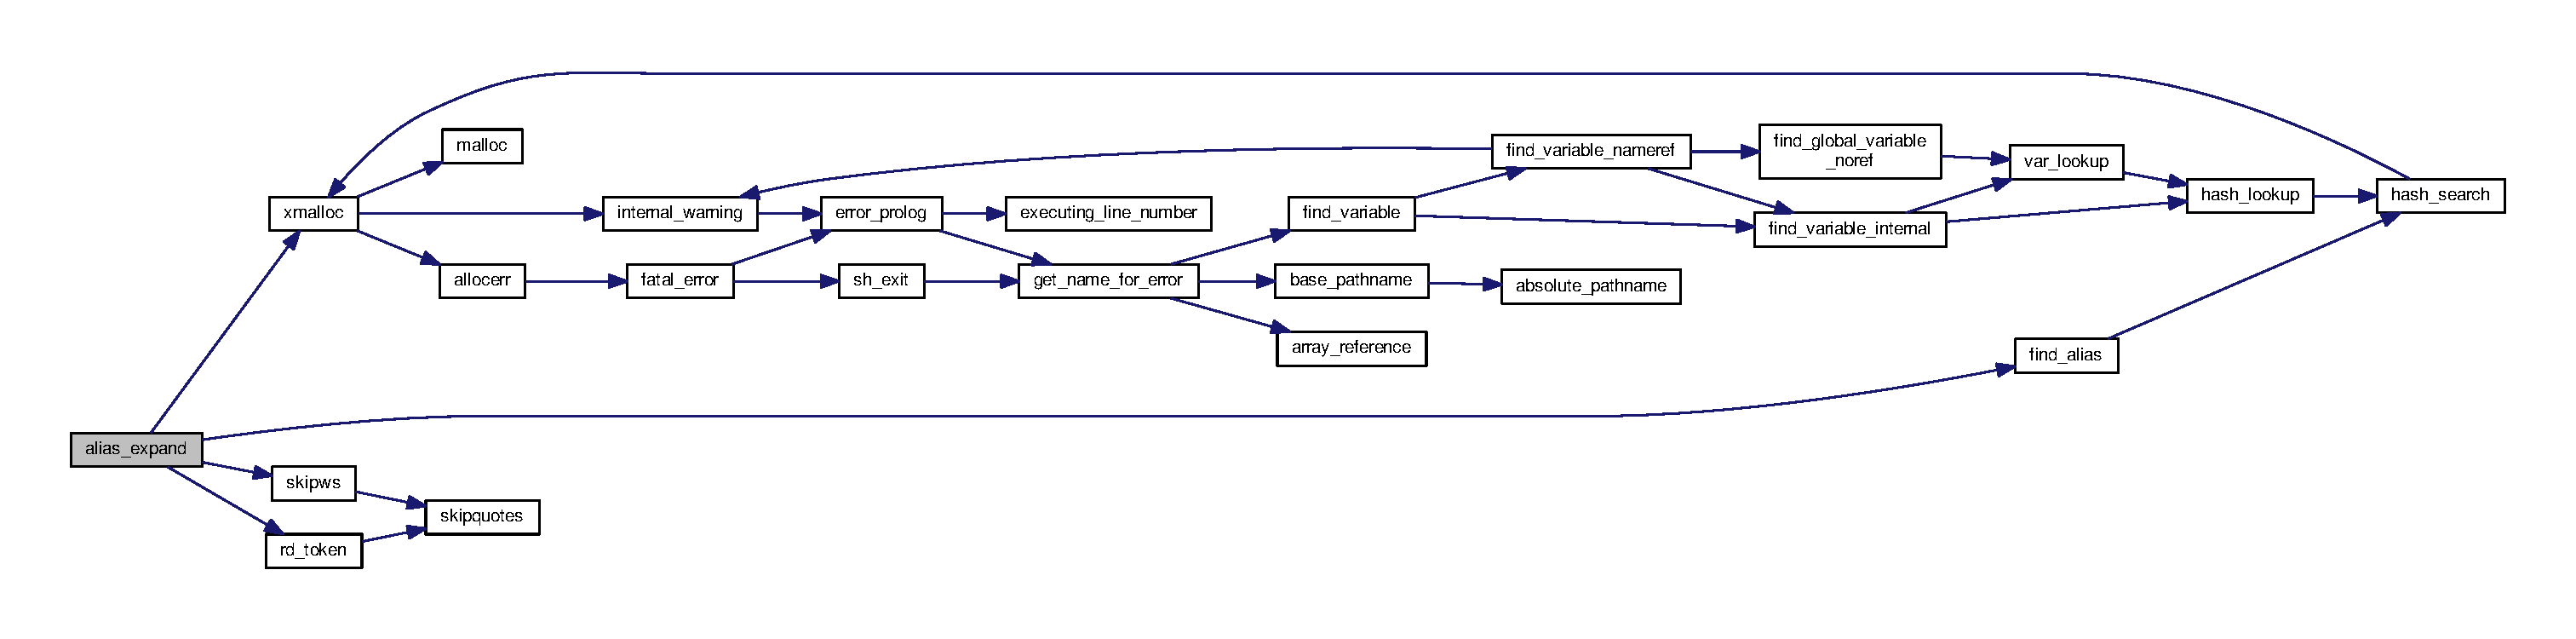
\includegraphics[width=350pt]{alias_8c_a550e246d1bf1bfca44022977badf71dc_cgraph}
\end{center}
\end{figure}


\index{alias.\+c@{alias.\+c}!alias\+\_\+expand\+\_\+word@{alias\+\_\+expand\+\_\+word}}
\index{alias\+\_\+expand\+\_\+word@{alias\+\_\+expand\+\_\+word}!alias.\+c@{alias.\+c}}
\subsubsection[{\texorpdfstring{alias\+\_\+expand\+\_\+word(char $\ast$s)}{alias_expand_word(char *s)}}]{\setlength{\rightskip}{0pt plus 5cm}char$\ast$ alias\+\_\+expand\+\_\+word (
\begin{DoxyParamCaption}
\item[{char $\ast$}]{s}
\end{DoxyParamCaption}
)}\hypertarget{alias_8c_ad97f215959c2666980fbe778b91a54e3}{}\label{alias_8c_ad97f215959c2666980fbe778b91a54e3}


Here is the call graph for this function\+:
\nopagebreak
\begin{figure}[H]
\begin{center}
\leavevmode
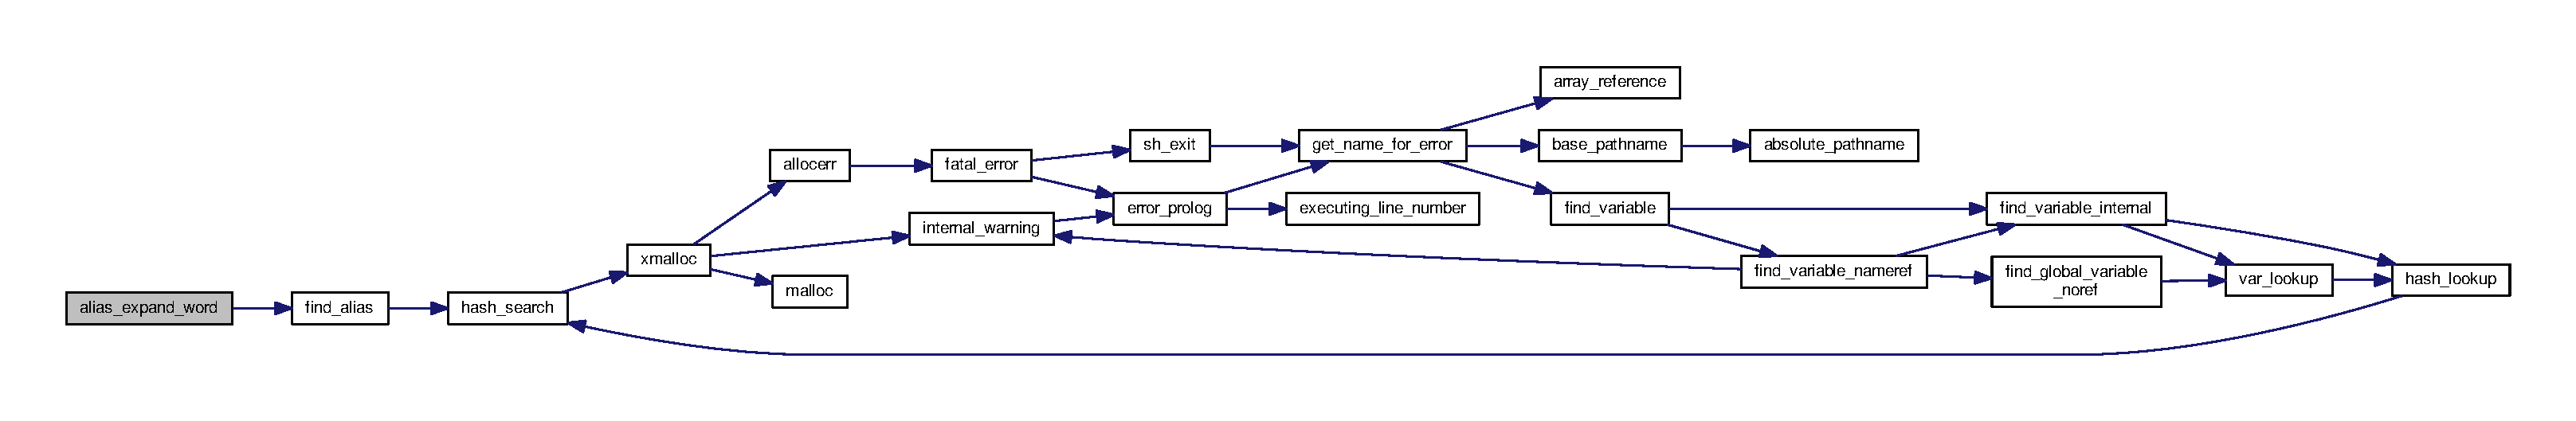
\includegraphics[width=350pt]{alias_8c_ad97f215959c2666980fbe778b91a54e3_cgraph}
\end{center}
\end{figure}


\index{alias.\+c@{alias.\+c}!all\+\_\+aliases@{all\+\_\+aliases}}
\index{all\+\_\+aliases@{all\+\_\+aliases}!alias.\+c@{alias.\+c}}
\subsubsection[{\texorpdfstring{all\+\_\+aliases()}{all_aliases()}}]{\setlength{\rightskip}{0pt plus 5cm}{\bf alias\+\_\+t}$\ast$$\ast$ all\+\_\+aliases (
\begin{DoxyParamCaption}
{}
\end{DoxyParamCaption}
)}\hypertarget{alias_8c_a1c0ae8915c6f62822bed3d412e0132e8}{}\label{alias_8c_a1c0ae8915c6f62822bed3d412e0132e8}


Here is the call graph for this function\+:
\nopagebreak
\begin{figure}[H]
\begin{center}
\leavevmode
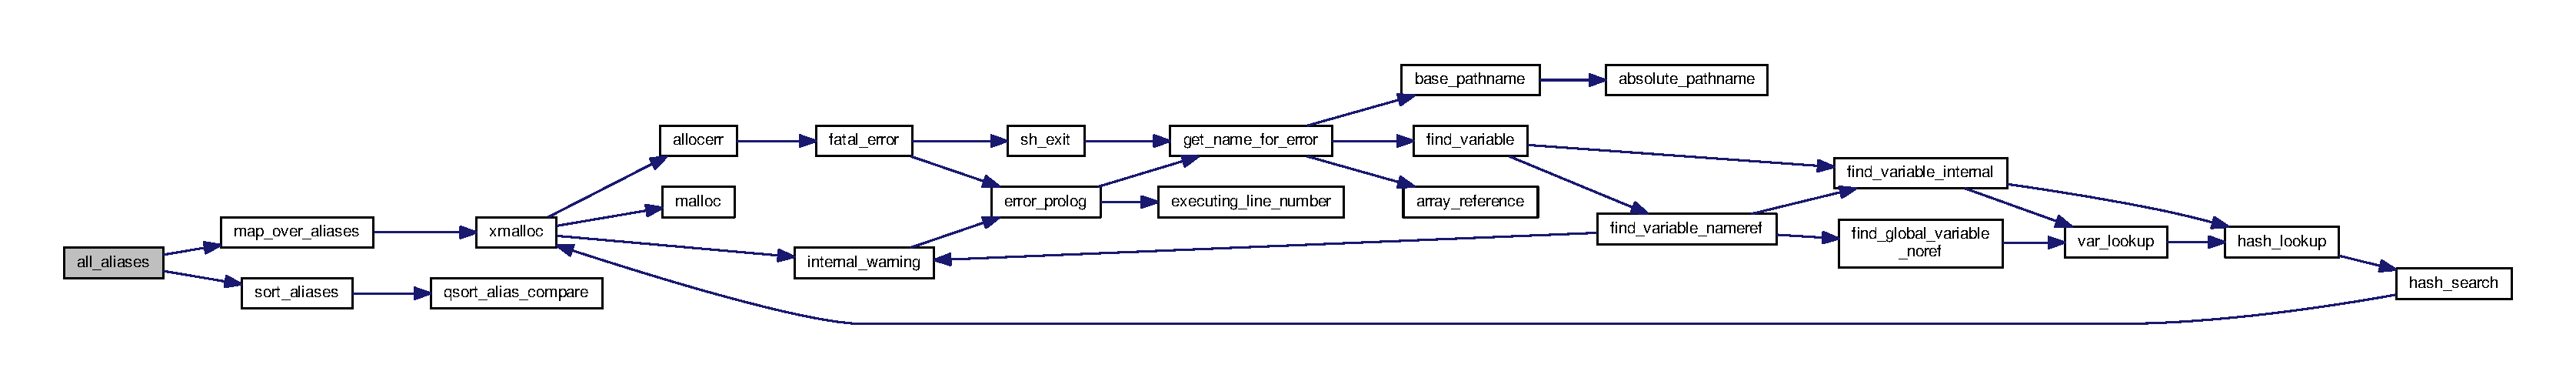
\includegraphics[width=350pt]{alias_8c_a1c0ae8915c6f62822bed3d412e0132e8_cgraph}
\end{center}
\end{figure}


\index{alias.\+c@{alias.\+c}!delete\+\_\+all\+\_\+aliases@{delete\+\_\+all\+\_\+aliases}}
\index{delete\+\_\+all\+\_\+aliases@{delete\+\_\+all\+\_\+aliases}!alias.\+c@{alias.\+c}}
\subsubsection[{\texorpdfstring{delete\+\_\+all\+\_\+aliases()}{delete_all_aliases()}}]{\setlength{\rightskip}{0pt plus 5cm}void delete\+\_\+all\+\_\+aliases (
\begin{DoxyParamCaption}
{}
\end{DoxyParamCaption}
)}\hypertarget{alias_8c_a7cb21e7339544bfe3a0138d1324d79b1}{}\label{alias_8c_a7cb21e7339544bfe3a0138d1324d79b1}


Here is the call graph for this function\+:
\nopagebreak
\begin{figure}[H]
\begin{center}
\leavevmode
\includegraphics[width=350pt]{alias_8c_a7cb21e7339544bfe3a0138d1324d79b1_cgraph}
\end{center}
\end{figure}


\index{alias.\+c@{alias.\+c}!find\+\_\+alias@{find\+\_\+alias}}
\index{find\+\_\+alias@{find\+\_\+alias}!alias.\+c@{alias.\+c}}
\subsubsection[{\texorpdfstring{find\+\_\+alias(char $\ast$name)}{find_alias(char *name)}}]{\setlength{\rightskip}{0pt plus 5cm}{\bf alias\+\_\+t}$\ast$ find\+\_\+alias (
\begin{DoxyParamCaption}
\item[{char $\ast$}]{name}
\end{DoxyParamCaption}
)}\hypertarget{alias_8c_a9a85eef7b6f6e69a5921e8da9c471263}{}\label{alias_8c_a9a85eef7b6f6e69a5921e8da9c471263}


Here is the call graph for this function\+:
\nopagebreak
\begin{figure}[H]
\begin{center}
\leavevmode
\includegraphics[width=350pt]{alias_8c_a9a85eef7b6f6e69a5921e8da9c471263_cgraph}
\end{center}
\end{figure}


\index{alias.\+c@{alias.\+c}!free\+\_\+alias\+\_\+data@{free\+\_\+alias\+\_\+data}}
\index{free\+\_\+alias\+\_\+data@{free\+\_\+alias\+\_\+data}!alias.\+c@{alias.\+c}}
\subsubsection[{\texorpdfstring{free\+\_\+alias\+\_\+data(\+P\+T\+R\+\_\+\+T data)}{free_alias_data(PTR_T data)}}]{\setlength{\rightskip}{0pt plus 5cm}static void free\+\_\+alias\+\_\+data (
\begin{DoxyParamCaption}
\item[{{\bf P\+T\+R\+\_\+T}}]{data}
\end{DoxyParamCaption}
)\hspace{0.3cm}{\ttfamily [static]}}\hypertarget{alias_8c_a7ac17f35a61c8a67b59b90d49f7d2cb2}{}\label{alias_8c_a7ac17f35a61c8a67b59b90d49f7d2cb2}


Here is the call graph for this function\+:
\nopagebreak
\begin{figure}[H]
\begin{center}
\leavevmode
\includegraphics[width=329pt]{alias_8c_a7ac17f35a61c8a67b59b90d49f7d2cb2_cgraph}
\end{center}
\end{figure}


\index{alias.\+c@{alias.\+c}!get\+\_\+alias\+\_\+value@{get\+\_\+alias\+\_\+value}}
\index{get\+\_\+alias\+\_\+value@{get\+\_\+alias\+\_\+value}!alias.\+c@{alias.\+c}}
\subsubsection[{\texorpdfstring{get\+\_\+alias\+\_\+value(char $\ast$name)}{get_alias_value(char *name)}}]{\setlength{\rightskip}{0pt plus 5cm}char$\ast$ get\+\_\+alias\+\_\+value (
\begin{DoxyParamCaption}
\item[{char $\ast$}]{name}
\end{DoxyParamCaption}
)}\hypertarget{alias_8c_a0e1b176c3d4809e000b7ae095502b853}{}\label{alias_8c_a0e1b176c3d4809e000b7ae095502b853}


Here is the call graph for this function\+:
\nopagebreak
\begin{figure}[H]
\begin{center}
\leavevmode
\includegraphics[width=350pt]{alias_8c_a0e1b176c3d4809e000b7ae095502b853_cgraph}
\end{center}
\end{figure}


\index{alias.\+c@{alias.\+c}!initialize\+\_\+aliases@{initialize\+\_\+aliases}}
\index{initialize\+\_\+aliases@{initialize\+\_\+aliases}!alias.\+c@{alias.\+c}}
\subsubsection[{\texorpdfstring{initialize\+\_\+aliases()}{initialize_aliases()}}]{\setlength{\rightskip}{0pt plus 5cm}void initialize\+\_\+aliases (
\begin{DoxyParamCaption}
{}
\end{DoxyParamCaption}
)}\hypertarget{alias_8c_abba691c3b75de85b97e7418e5b149d8a}{}\label{alias_8c_abba691c3b75de85b97e7418e5b149d8a}


Here is the call graph for this function\+:
\nopagebreak
\begin{figure}[H]
\begin{center}
\leavevmode
\includegraphics[width=350pt]{alias_8c_abba691c3b75de85b97e7418e5b149d8a_cgraph}
\end{center}
\end{figure}


\index{alias.\+c@{alias.\+c}!map\+\_\+over\+\_\+aliases@{map\+\_\+over\+\_\+aliases}}
\index{map\+\_\+over\+\_\+aliases@{map\+\_\+over\+\_\+aliases}!alias.\+c@{alias.\+c}}
\subsubsection[{\texorpdfstring{map\+\_\+over\+\_\+aliases(sh\+\_\+alias\+\_\+map\+\_\+func\+\_\+t $\ast$function)}{map_over_aliases(sh_alias_map_func_t *function)}}]{\setlength{\rightskip}{0pt plus 5cm}static {\bf alias\+\_\+t}$\ast$$\ast$ map\+\_\+over\+\_\+aliases (
\begin{DoxyParamCaption}
\item[{sh\+\_\+alias\+\_\+map\+\_\+func\+\_\+t $\ast$}]{function}
\end{DoxyParamCaption}
)\hspace{0.3cm}{\ttfamily [static]}}\hypertarget{alias_8c_af985f130f741c28ae25ed838bc41298b}{}\label{alias_8c_af985f130f741c28ae25ed838bc41298b}


Here is the call graph for this function\+:
\nopagebreak
\begin{figure}[H]
\begin{center}
\leavevmode
\includegraphics[width=350pt]{alias_8c_af985f130f741c28ae25ed838bc41298b_cgraph}
\end{center}
\end{figure}


\index{alias.\+c@{alias.\+c}!qsort\+\_\+alias\+\_\+compare@{qsort\+\_\+alias\+\_\+compare}}
\index{qsort\+\_\+alias\+\_\+compare@{qsort\+\_\+alias\+\_\+compare}!alias.\+c@{alias.\+c}}
\subsubsection[{\texorpdfstring{qsort\+\_\+alias\+\_\+compare(alias\+\_\+t $\ast$$\ast$as1, alias\+\_\+t $\ast$$\ast$as2)}{qsort_alias_compare(alias_t **as1, alias_t **as2)}}]{\setlength{\rightskip}{0pt plus 5cm}static int qsort\+\_\+alias\+\_\+compare (
\begin{DoxyParamCaption}
\item[{{\bf alias\+\_\+t} $\ast$$\ast$}]{as1, }
\item[{{\bf alias\+\_\+t} $\ast$$\ast$}]{as2}
\end{DoxyParamCaption}
)\hspace{0.3cm}{\ttfamily [static]}}\hypertarget{alias_8c_aed85c03661269505e0a3f198aba19bee}{}\label{alias_8c_aed85c03661269505e0a3f198aba19bee}
\index{alias.\+c@{alias.\+c}!rd\+\_\+token@{rd\+\_\+token}}
\index{rd\+\_\+token@{rd\+\_\+token}!alias.\+c@{alias.\+c}}
\subsubsection[{\texorpdfstring{rd\+\_\+token(char $\ast$string, int start)}{rd_token(char *string, int start)}}]{\setlength{\rightskip}{0pt plus 5cm}static int rd\+\_\+token (
\begin{DoxyParamCaption}
\item[{char $\ast$}]{string, }
\item[{int}]{start}
\end{DoxyParamCaption}
)\hspace{0.3cm}{\ttfamily [static]}}\hypertarget{alias_8c_a641542c1e16b08c41b0d58cd4ff95d6f}{}\label{alias_8c_a641542c1e16b08c41b0d58cd4ff95d6f}


Here is the call graph for this function\+:
\nopagebreak
\begin{figure}[H]
\begin{center}
\leavevmode
\includegraphics[width=234pt]{alias_8c_a641542c1e16b08c41b0d58cd4ff95d6f_cgraph}
\end{center}
\end{figure}


\index{alias.\+c@{alias.\+c}!remove\+\_\+alias@{remove\+\_\+alias}}
\index{remove\+\_\+alias@{remove\+\_\+alias}!alias.\+c@{alias.\+c}}
\subsubsection[{\texorpdfstring{remove\+\_\+alias(char $\ast$name)}{remove_alias(char *name)}}]{\setlength{\rightskip}{0pt plus 5cm}int remove\+\_\+alias (
\begin{DoxyParamCaption}
\item[{char $\ast$}]{name}
\end{DoxyParamCaption}
)}\hypertarget{alias_8c_a95780a0c8ac0b02172f15015bf26b118}{}\label{alias_8c_a95780a0c8ac0b02172f15015bf26b118}


Here is the call graph for this function\+:
\nopagebreak
\begin{figure}[H]
\begin{center}
\leavevmode
\includegraphics[width=350pt]{alias_8c_a95780a0c8ac0b02172f15015bf26b118_cgraph}
\end{center}
\end{figure}


\index{alias.\+c@{alias.\+c}!skipquotes@{skipquotes}}
\index{skipquotes@{skipquotes}!alias.\+c@{alias.\+c}}
\subsubsection[{\texorpdfstring{skipquotes(char $\ast$string, int start)}{skipquotes(char *string, int start)}}]{\setlength{\rightskip}{0pt plus 5cm}static int skipquotes (
\begin{DoxyParamCaption}
\item[{char $\ast$}]{string, }
\item[{int}]{start}
\end{DoxyParamCaption}
)\hspace{0.3cm}{\ttfamily [static]}}\hypertarget{alias_8c_a3fb89598b9584124dc1e9e37dea50758}{}\label{alias_8c_a3fb89598b9584124dc1e9e37dea50758}
\index{alias.\+c@{alias.\+c}!skipws@{skipws}}
\index{skipws@{skipws}!alias.\+c@{alias.\+c}}
\subsubsection[{\texorpdfstring{skipws(char $\ast$string, int start)}{skipws(char *string, int start)}}]{\setlength{\rightskip}{0pt plus 5cm}static int skipws (
\begin{DoxyParamCaption}
\item[{char $\ast$}]{string, }
\item[{int}]{start}
\end{DoxyParamCaption}
)\hspace{0.3cm}{\ttfamily [static]}}\hypertarget{alias_8c_aa688063409ccb7123e9bd4b23455e60a}{}\label{alias_8c_aa688063409ccb7123e9bd4b23455e60a}


Here is the call graph for this function\+:
\nopagebreak
\begin{figure}[H]
\begin{center}
\leavevmode
\includegraphics[width=227pt]{alias_8c_aa688063409ccb7123e9bd4b23455e60a_cgraph}
\end{center}
\end{figure}


\index{alias.\+c@{alias.\+c}!sort\+\_\+aliases@{sort\+\_\+aliases}}
\index{sort\+\_\+aliases@{sort\+\_\+aliases}!alias.\+c@{alias.\+c}}
\subsubsection[{\texorpdfstring{sort\+\_\+aliases(alias\+\_\+t $\ast$$\ast$array)}{sort_aliases(alias_t **array)}}]{\setlength{\rightskip}{0pt plus 5cm}static void sort\+\_\+aliases (
\begin{DoxyParamCaption}
\item[{{\bf alias\+\_\+t} $\ast$$\ast$}]{array}
\end{DoxyParamCaption}
)\hspace{0.3cm}{\ttfamily [static]}}\hypertarget{alias_8c_a210d1aabeda51baebeccf42f321c093e}{}\label{alias_8c_a210d1aabeda51baebeccf42f321c093e}


Here is the call graph for this function\+:
\nopagebreak
\begin{figure}[H]
\begin{center}
\leavevmode
\includegraphics[width=292pt]{alias_8c_a210d1aabeda51baebeccf42f321c093e_cgraph}
\end{center}
\end{figure}




\subsection{Variable Documentation}
\index{alias.\+c@{alias.\+c}!alias\+\_\+expand\+\_\+all@{alias\+\_\+expand\+\_\+all}}
\index{alias\+\_\+expand\+\_\+all@{alias\+\_\+expand\+\_\+all}!alias.\+c@{alias.\+c}}
\subsubsection[{\texorpdfstring{alias\+\_\+expand\+\_\+all}{alias_expand_all}}]{\setlength{\rightskip}{0pt plus 5cm}int alias\+\_\+expand\+\_\+all = 0}\hypertarget{alias_8c_aafd6878a76ae3351d1d405a7e2236115}{}\label{alias_8c_aafd6878a76ae3351d1d405a7e2236115}
\index{alias.\+c@{alias.\+c}!aliases@{aliases}}
\index{aliases@{aliases}!alias.\+c@{alias.\+c}}
\subsubsection[{\texorpdfstring{aliases}{aliases}}]{\setlength{\rightskip}{0pt plus 5cm}{\bf H\+A\+S\+H\+\_\+\+T\+A\+B\+LE}$\ast$ aliases = ({\bf H\+A\+S\+H\+\_\+\+T\+A\+B\+LE} $\ast$){\bf N\+U\+LL}}\hypertarget{alias_8c_ade59a7845bd91cac464607d4a444cb1f}{}\label{alias_8c_ade59a7845bd91cac464607d4a444cb1f}
\index{alias.\+c@{alias.\+c}!command\+\_\+word@{command\+\_\+word}}
\index{command\+\_\+word@{command\+\_\+word}!alias.\+c@{alias.\+c}}
\subsubsection[{\texorpdfstring{command\+\_\+word}{command_word}}]{\setlength{\rightskip}{0pt plus 5cm}int command\+\_\+word\hspace{0.3cm}{\ttfamily [static]}}\hypertarget{alias_8c_a4748d3f8e01bbd519cf6ce5a0f539102}{}\label{alias_8c_a4748d3f8e01bbd519cf6ce5a0f539102}

\hypertarget{alias_8h}{}\section{alias.\+h File Reference}
\label{alias_8h}\index{alias.\+h@{alias.\+h}}
{\ttfamily \#include \char`\"{}stdc.\+h\char`\"{}}\\*
{\ttfamily \#include \char`\"{}hashlib.\+h\char`\"{}}\\*
Include dependency graph for alias.\+h\+:
\nopagebreak
\begin{figure}[H]
\begin{center}
\leavevmode
\includegraphics[width=159pt]{alias_8h__incl}
\end{center}
\end{figure}
This graph shows which files directly or indirectly include this file\+:
\nopagebreak
\begin{figure}[H]
\begin{center}
\leavevmode
\includegraphics[width=350pt]{alias_8h__dep__incl}
\end{center}
\end{figure}
\subsection*{Classes}
\begin{DoxyCompactItemize}
\item 
struct \hyperlink{structalias}{alias}
\end{DoxyCompactItemize}
\subsection*{Macros}
\begin{DoxyCompactItemize}
\item 
\#define \hyperlink{alias_8h_a901a0938824aaecfe483a2ec6d91ef4f}{A\+L\+\_\+\+E\+X\+P\+A\+N\+D\+N\+E\+XT}~0x1
\item 
\#define \hyperlink{alias_8h_a9cedb20f3765915a5422dec39545d7ce}{A\+L\+\_\+\+B\+E\+I\+N\+G\+E\+X\+P\+A\+N\+D\+ED}~0x2
\end{DoxyCompactItemize}
\subsection*{Typedefs}
\begin{DoxyCompactItemize}
\item 
typedef struct \hyperlink{structalias}{alias} \hyperlink{alias_8h_a11c6bae002d90e8dad2d17b87ba6cccf}{alias\+\_\+t}
\end{DoxyCompactItemize}
\subsection*{Functions}
\begin{DoxyCompactItemize}
\item 
void \hyperlink{alias_8c_abba691c3b75de85b97e7418e5b149d8a}{initialize\+\_\+aliases} \hyperlink{alias_8h_a91b41f4385eb72cee279d8711abeaf95}{\+\_\+\+\_\+P} ((void))
\item 
\hyperlink{alias_8h_a11c6bae002d90e8dad2d17b87ba6cccf}{alias\+\_\+t} $\ast$\hyperlink{alias_8c_a9a85eef7b6f6e69a5921e8da9c471263}{find\+\_\+alias} \hyperlink{alias_8h_a99e8530fee763420167b9a2fca4a5a51}{\+\_\+\+\_\+P} ((char $\ast$))
\item 
void \hyperlink{alias_8c_a2a7bb793d1eac9a3cdfe66c7357fd460}{add\+\_\+alias} \hyperlink{alias_8h_af55d7e6f3634ebfb409488c0feda5424}{\+\_\+\+\_\+P} ((char $\ast$, char $\ast$))
\item 
void \hyperlink{y_8tab_8c_a9542b0f59806c2ae6fa2dd6982697d88}{clear\+\_\+string\+\_\+list\+\_\+expander} \hyperlink{alias_8h_a8132c1c69d64246bce9524161337a04f}{\+\_\+\+\_\+P} ((\hyperlink{alias_8h_a11c6bae002d90e8dad2d17b87ba6cccf}{alias\+\_\+t} $\ast$))
\end{DoxyCompactItemize}
\subsection*{Variables}
\begin{DoxyCompactItemize}
\item 
\hyperlink{hashlib_8h_a8284f9978df160609365484b829527e6}{H\+A\+S\+H\+\_\+\+T\+A\+B\+LE} $\ast$ \hyperlink{alias_8h_ade59a7845bd91cac464607d4a444cb1f}{aliases}
\end{DoxyCompactItemize}


\subsection{Macro Definition Documentation}
\index{alias.\+h@{alias.\+h}!A\+L\+\_\+\+B\+E\+I\+N\+G\+E\+X\+P\+A\+N\+D\+ED@{A\+L\+\_\+\+B\+E\+I\+N\+G\+E\+X\+P\+A\+N\+D\+ED}}
\index{A\+L\+\_\+\+B\+E\+I\+N\+G\+E\+X\+P\+A\+N\+D\+ED@{A\+L\+\_\+\+B\+E\+I\+N\+G\+E\+X\+P\+A\+N\+D\+ED}!alias.\+h@{alias.\+h}}
\subsubsection[{\texorpdfstring{A\+L\+\_\+\+B\+E\+I\+N\+G\+E\+X\+P\+A\+N\+D\+ED}{AL_BEINGEXPANDED}}]{\setlength{\rightskip}{0pt plus 5cm}\#define A\+L\+\_\+\+B\+E\+I\+N\+G\+E\+X\+P\+A\+N\+D\+ED~0x2}\hypertarget{alias_8h_a9cedb20f3765915a5422dec39545d7ce}{}\label{alias_8h_a9cedb20f3765915a5422dec39545d7ce}
\index{alias.\+h@{alias.\+h}!A\+L\+\_\+\+E\+X\+P\+A\+N\+D\+N\+E\+XT@{A\+L\+\_\+\+E\+X\+P\+A\+N\+D\+N\+E\+XT}}
\index{A\+L\+\_\+\+E\+X\+P\+A\+N\+D\+N\+E\+XT@{A\+L\+\_\+\+E\+X\+P\+A\+N\+D\+N\+E\+XT}!alias.\+h@{alias.\+h}}
\subsubsection[{\texorpdfstring{A\+L\+\_\+\+E\+X\+P\+A\+N\+D\+N\+E\+XT}{AL_EXPANDNEXT}}]{\setlength{\rightskip}{0pt plus 5cm}\#define A\+L\+\_\+\+E\+X\+P\+A\+N\+D\+N\+E\+XT~0x1}\hypertarget{alias_8h_a901a0938824aaecfe483a2ec6d91ef4f}{}\label{alias_8h_a901a0938824aaecfe483a2ec6d91ef4f}


\subsection{Typedef Documentation}
\index{alias.\+h@{alias.\+h}!alias\+\_\+t@{alias\+\_\+t}}
\index{alias\+\_\+t@{alias\+\_\+t}!alias.\+h@{alias.\+h}}
\subsubsection[{\texorpdfstring{alias\+\_\+t}{alias_t}}]{\setlength{\rightskip}{0pt plus 5cm}typedef struct {\bf alias}  {\bf alias\+\_\+t}}\hypertarget{alias_8h_a11c6bae002d90e8dad2d17b87ba6cccf}{}\label{alias_8h_a11c6bae002d90e8dad2d17b87ba6cccf}


\subsection{Function Documentation}
\index{alias.\+h@{alias.\+h}!\+\_\+\+\_\+P@{\+\_\+\+\_\+P}}
\index{\+\_\+\+\_\+P@{\+\_\+\+\_\+P}!alias.\+h@{alias.\+h}}
\subsubsection[{\texorpdfstring{\+\_\+\+\_\+\+P((void))}{__P((void))}}]{\setlength{\rightskip}{0pt plus 5cm}void {\bf initialize\+\_\+aliases} \+\_\+\+\_\+P (
\begin{DoxyParamCaption}
\item[{(void)}]{}
\end{DoxyParamCaption}
)}\hypertarget{alias_8h_a91b41f4385eb72cee279d8711abeaf95}{}\label{alias_8h_a91b41f4385eb72cee279d8711abeaf95}
\index{alias.\+h@{alias.\+h}!\+\_\+\+\_\+P@{\+\_\+\+\_\+P}}
\index{\+\_\+\+\_\+P@{\+\_\+\+\_\+P}!alias.\+h@{alias.\+h}}
\subsubsection[{\texorpdfstring{\+\_\+\+\_\+\+P((char $\ast$))}{__P((char *))}}]{\setlength{\rightskip}{0pt plus 5cm}{\bf alias\+\_\+t}$\ast$ {\bf find\+\_\+alias} \+\_\+\+\_\+P (
\begin{DoxyParamCaption}
\item[{(char $\ast$)}]{}
\end{DoxyParamCaption}
)}\hypertarget{alias_8h_a99e8530fee763420167b9a2fca4a5a51}{}\label{alias_8h_a99e8530fee763420167b9a2fca4a5a51}
\index{alias.\+h@{alias.\+h}!\+\_\+\+\_\+P@{\+\_\+\+\_\+P}}
\index{\+\_\+\+\_\+P@{\+\_\+\+\_\+P}!alias.\+h@{alias.\+h}}
\subsubsection[{\texorpdfstring{\+\_\+\+\_\+\+P((char $\ast$, char $\ast$))}{__P((char *, char *))}}]{\setlength{\rightskip}{0pt plus 5cm}void {\bf add\+\_\+alias} \+\_\+\+\_\+P (
\begin{DoxyParamCaption}
\item[{(char $\ast$, char $\ast$)}]{}
\end{DoxyParamCaption}
)}\hypertarget{alias_8h_af55d7e6f3634ebfb409488c0feda5424}{}\label{alias_8h_af55d7e6f3634ebfb409488c0feda5424}
\index{alias.\+h@{alias.\+h}!\+\_\+\+\_\+P@{\+\_\+\+\_\+P}}
\index{\+\_\+\+\_\+P@{\+\_\+\+\_\+P}!alias.\+h@{alias.\+h}}
\subsubsection[{\texorpdfstring{\+\_\+\+\_\+\+P((alias\+\_\+t $\ast$))}{__P((alias_t *))}}]{\setlength{\rightskip}{0pt plus 5cm}void {\bf clear\+\_\+string\+\_\+list\+\_\+expander} \+\_\+\+\_\+P (
\begin{DoxyParamCaption}
\item[{({\bf alias\+\_\+t} $\ast$)}]{}
\end{DoxyParamCaption}
)}\hypertarget{alias_8h_a8132c1c69d64246bce9524161337a04f}{}\label{alias_8h_a8132c1c69d64246bce9524161337a04f}


\subsection{Variable Documentation}
\index{alias.\+h@{alias.\+h}!aliases@{aliases}}
\index{aliases@{aliases}!alias.\+h@{alias.\+h}}
\subsubsection[{\texorpdfstring{aliases}{aliases}}]{\setlength{\rightskip}{0pt plus 5cm}{\bf H\+A\+S\+H\+\_\+\+T\+A\+B\+LE}$\ast$ aliases}\hypertarget{alias_8h_ade59a7845bd91cac464607d4a444cb1f}{}\label{alias_8h_ade59a7845bd91cac464607d4a444cb1f}

\hypertarget{array_8c}{}\section{array.\+c File Reference}
\label{array_8c}\index{array.\+c@{array.\+c}}
{\ttfamily \#include \char`\"{}config.\+h\char`\"{}}\\*
{\ttfamily \#include $<$unistd.\+h$>$}\\*
{\ttfamily \#include $<$stdio.\+h$>$}\\*
{\ttfamily \#include \char`\"{}bashansi.\+h\char`\"{}}\\*
{\ttfamily \#include \char`\"{}shell.\+h\char`\"{}}\\*
{\ttfamily \#include \char`\"{}array.\+h\char`\"{}}\\*
{\ttfamily \#include \char`\"{}builtins/common.\+h\char`\"{}}\\*
Include dependency graph for array.\+c\+:
\nopagebreak
\begin{figure}[H]
\begin{center}
\leavevmode
\includegraphics[width=350pt]{array_8c__incl}
\end{center}
\end{figure}
\subsection*{Macros}
\begin{DoxyCompactItemize}
\item 
\#define \hyperlink{array_8c_a4a3c796f8bf6dc31f1c1a052df4145eb}{A\+D\+D\+\_\+\+B\+E\+F\+O\+RE}(ae,  new)
\item 
\#define \hyperlink{array_8c_ab57c0718f4bcef7be742f0554c7bfc2a}{A\+D\+D\+\_\+\+A\+F\+T\+ER}(ae,  new)
\item 
\#define \hyperlink{array_8c_aa0a64a1b971ae24be1d7a2e2945ecafe}{I\+S\+\_\+\+L\+A\+S\+T\+R\+EF}(a)~(a-\/$>$lastref)
\item 
\#define \hyperlink{array_8c_a3769addff71da3f650f9c8f46d5f04d7}{L\+A\+S\+T\+R\+E\+F\+\_\+\+S\+T\+A\+RT}(a,  i)
\item 
\#define \hyperlink{array_8c_a37129f67168e2b5cd2ed8c751562693b}{L\+A\+S\+T\+R\+EF}(a)~(a-\/$>$lastref ? a-\/$>$lastref \+: \hyperlink{array_8h_ad6e506d917dcd8e6b3416200b9aad5b6}{element\+\_\+forw}(a-\/$>$head))
\item 
\#define \hyperlink{array_8c_a600324507493434b240eed818d8eeac6}{I\+N\+V\+A\+L\+I\+D\+A\+T\+E\+\_\+\+L\+A\+S\+T\+R\+EF}(a)~a-\/$>$lastref = 0
\item 
\#define \hyperlink{array_8c_a7eb4d3475d221c716df14cf287ebdc0e}{S\+E\+T\+\_\+\+L\+A\+S\+T\+R\+EF}(a,  e)~a-\/$>$lastref = (e)
\item 
\#define \hyperlink{array_8c_af34d0a9af39797be96cf43d021e0ae48}{U\+N\+S\+E\+T\+\_\+\+L\+A\+S\+T\+R\+EF}(a)~a-\/$>$lastref = 0;
\end{DoxyCompactItemize}
\subsection*{Functions}
\begin{DoxyCompactItemize}
\item 
static char $\ast$\hyperlink{array_8c_a4b8b3f4ae87510c78a486088a501d13b}{array\+\_\+to\+\_\+string\+\_\+internal} \hyperlink{array_8c_a94df50746c759f247280d4fe6ce9ac73}{\+\_\+\+\_\+P} ((\hyperlink{array_8h_a51fb33f1fdf682f60b56987e3e514bf2}{A\+R\+R\+A\+Y\+\_\+\+E\+L\+E\+M\+E\+NT} $\ast$, \hyperlink{array_8h_a51fb33f1fdf682f60b56987e3e514bf2}{A\+R\+R\+A\+Y\+\_\+\+E\+L\+E\+M\+E\+NT} $\ast$, char $\ast$, int))
\item 
\hyperlink{array_8h_a9c07c3330f66f4018e49ee90e58f0f39}{A\+R\+R\+AY} $\ast$ \hyperlink{array_8c_acb73d5677f52ea9735b635b5f8e3623a}{array\+\_\+create} ()
\item 
void \hyperlink{array_8c_a05b8194d509714a03fa60edb1c5b63e8}{array\+\_\+flush} (\hyperlink{array_8h_a9c07c3330f66f4018e49ee90e58f0f39}{A\+R\+R\+AY} $\ast$a)
\item 
void \hyperlink{array_8c_a7bfdcd4d6e7fc4a9516a96b0e65cf247}{array\+\_\+dispose} (\hyperlink{array_8h_a9c07c3330f66f4018e49ee90e58f0f39}{A\+R\+R\+AY} $\ast$a)
\item 
\hyperlink{array_8h_a9c07c3330f66f4018e49ee90e58f0f39}{A\+R\+R\+AY} $\ast$ \hyperlink{array_8c_ae0f2ce809cdf22d0d7bb29d166e8f6f6}{array\+\_\+copy} (\hyperlink{array_8h_a9c07c3330f66f4018e49ee90e58f0f39}{A\+R\+R\+AY} $\ast$a)
\item 
\hyperlink{array_8h_a9c07c3330f66f4018e49ee90e58f0f39}{A\+R\+R\+AY} $\ast$ \hyperlink{array_8c_a4651496a06ca9d65a0d24f4e58571d7b}{array\+\_\+slice} (\hyperlink{array_8h_a9c07c3330f66f4018e49ee90e58f0f39}{A\+R\+R\+AY} $\ast$\hyperlink{structarray}{array}, \hyperlink{array_8h_a51fb33f1fdf682f60b56987e3e514bf2}{A\+R\+R\+A\+Y\+\_\+\+E\+L\+E\+M\+E\+NT} $\ast$s, \hyperlink{array_8h_a51fb33f1fdf682f60b56987e3e514bf2}{A\+R\+R\+A\+Y\+\_\+\+E\+L\+E\+M\+E\+NT} $\ast$e)
\item 
void \hyperlink{array_8c_a461d843b094e1bd9222fc1f18c1427d2}{array\+\_\+walk} (\hyperlink{array_8h_a9c07c3330f66f4018e49ee90e58f0f39}{A\+R\+R\+AY} $\ast$a, sh\+\_\+ae\+\_\+map\+\_\+func\+\_\+t $\ast$func, void $\ast$udata)
\item 
\hyperlink{array_8h_a51fb33f1fdf682f60b56987e3e514bf2}{A\+R\+R\+A\+Y\+\_\+\+E\+L\+E\+M\+E\+NT} $\ast$ \hyperlink{array_8c_ae83b41ade25a16c0d12bb193bf5d1926}{array\+\_\+shift} (\hyperlink{array_8h_a9c07c3330f66f4018e49ee90e58f0f39}{A\+R\+R\+AY} $\ast$a, int n, int flags)
\item 
int \hyperlink{array_8c_ad427973cc9f46baeac0f46c1e3100076}{array\+\_\+rshift} (\hyperlink{array_8h_a9c07c3330f66f4018e49ee90e58f0f39}{A\+R\+R\+AY} $\ast$a, int n, char $\ast$s)
\item 
\hyperlink{array_8h_a51fb33f1fdf682f60b56987e3e514bf2}{A\+R\+R\+A\+Y\+\_\+\+E\+L\+E\+M\+E\+NT} $\ast$ \hyperlink{array_8c_a602aed963f1490e88353ba56ef67b112}{array\+\_\+unshift\+\_\+element} (\hyperlink{array_8h_a9c07c3330f66f4018e49ee90e58f0f39}{A\+R\+R\+AY} $\ast$a)
\item 
int \hyperlink{array_8c_a871a33c4be76bf41397b9cd22d39f105}{array\+\_\+shift\+\_\+element} (\hyperlink{array_8h_a9c07c3330f66f4018e49ee90e58f0f39}{A\+R\+R\+AY} $\ast$a, char $\ast$v)
\item 
\hyperlink{array_8h_a9c07c3330f66f4018e49ee90e58f0f39}{A\+R\+R\+AY} $\ast$ \hyperlink{array_8c_a3ebe43b76ff26216b86f4396201597e5}{array\+\_\+quote} (\hyperlink{array_8h_a9c07c3330f66f4018e49ee90e58f0f39}{A\+R\+R\+AY} $\ast$\hyperlink{structarray}{array})
\item 
\hyperlink{array_8h_a9c07c3330f66f4018e49ee90e58f0f39}{A\+R\+R\+AY} $\ast$ \hyperlink{array_8c_a2ee9294bda0347ca613f57f11d773df4}{array\+\_\+quote\+\_\+escapes} (\hyperlink{array_8h_a9c07c3330f66f4018e49ee90e58f0f39}{A\+R\+R\+AY} $\ast$\hyperlink{structarray}{array})
\item 
\hyperlink{array_8h_a9c07c3330f66f4018e49ee90e58f0f39}{A\+R\+R\+AY} $\ast$ \hyperlink{array_8c_acdca09de75fd1a2a9377bd3926fa7dc3}{array\+\_\+dequote} (\hyperlink{array_8h_a9c07c3330f66f4018e49ee90e58f0f39}{A\+R\+R\+AY} $\ast$\hyperlink{structarray}{array})
\item 
\hyperlink{array_8h_a9c07c3330f66f4018e49ee90e58f0f39}{A\+R\+R\+AY} $\ast$ \hyperlink{array_8c_a46ea9a7a3bb767fe4f0160137d3f64ed}{array\+\_\+dequote\+\_\+escapes} (\hyperlink{array_8h_a9c07c3330f66f4018e49ee90e58f0f39}{A\+R\+R\+AY} $\ast$\hyperlink{structarray}{array})
\item 
\hyperlink{array_8h_a9c07c3330f66f4018e49ee90e58f0f39}{A\+R\+R\+AY} $\ast$ \hyperlink{array_8c_a0ff23cb78aec09d851d1c1137e3b5efd}{array\+\_\+remove\+\_\+quoted\+\_\+nulls} (\hyperlink{array_8h_a9c07c3330f66f4018e49ee90e58f0f39}{A\+R\+R\+AY} $\ast$\hyperlink{structarray}{array})
\item 
char $\ast$ \hyperlink{array_8c_aef7a3dc941e5276bdcfb018b6e85d3b0}{array\+\_\+subrange} (\hyperlink{array_8h_a9c07c3330f66f4018e49ee90e58f0f39}{A\+R\+R\+AY} $\ast$a, \hyperlink{array_8h_a3672e3c5b95dde98c9ed75ac7c1e6d60}{arrayind\+\_\+t} start, \hyperlink{array_8h_a3672e3c5b95dde98c9ed75ac7c1e6d60}{arrayind\+\_\+t} nelem, int starsub, int quoted)
\item 
char $\ast$ \hyperlink{array_8c_abc70baa4155daa04156a0ab32f1c1a1a}{array\+\_\+patsub} (\hyperlink{array_8h_a9c07c3330f66f4018e49ee90e58f0f39}{A\+R\+R\+AY} $\ast$a, char $\ast$pat, char $\ast$rep, int mflags)
\item 
char $\ast$ \hyperlink{array_8c_a04ea96348605054b421c89ec2dfd39a8}{array\+\_\+modcase} (\hyperlink{array_8h_a9c07c3330f66f4018e49ee90e58f0f39}{A\+R\+R\+AY} $\ast$a, char $\ast$pat, int modop, int mflags)
\item 
\hyperlink{array_8h_a51fb33f1fdf682f60b56987e3e514bf2}{A\+R\+R\+A\+Y\+\_\+\+E\+L\+E\+M\+E\+NT} $\ast$ \hyperlink{array_8c_abf7afb8d84136bb1c8ba5181499449d8}{array\+\_\+create\+\_\+element} (\hyperlink{array_8h_a3672e3c5b95dde98c9ed75ac7c1e6d60}{arrayind\+\_\+t} indx, char $\ast$value)
\item 
void \hyperlink{array_8c_a8620a01f7a7efdeb205437e112764672}{array\+\_\+dispose\+\_\+element} (\hyperlink{array_8h_a51fb33f1fdf682f60b56987e3e514bf2}{A\+R\+R\+A\+Y\+\_\+\+E\+L\+E\+M\+E\+NT} $\ast$ae)
\item 
int \hyperlink{array_8c_a11ee68ce269a0bd9afbae671037a3a1b}{array\+\_\+insert} (\hyperlink{array_8h_a9c07c3330f66f4018e49ee90e58f0f39}{A\+R\+R\+AY} $\ast$a, \hyperlink{array_8h_a3672e3c5b95dde98c9ed75ac7c1e6d60}{arrayind\+\_\+t} i, char $\ast$v)
\item 
\hyperlink{array_8h_a51fb33f1fdf682f60b56987e3e514bf2}{A\+R\+R\+A\+Y\+\_\+\+E\+L\+E\+M\+E\+NT} $\ast$ \hyperlink{array_8c_abfbcc87b6ab7d93c279df0d331e11705}{array\+\_\+remove} (\hyperlink{array_8h_a9c07c3330f66f4018e49ee90e58f0f39}{A\+R\+R\+AY} $\ast$a, \hyperlink{array_8h_a3672e3c5b95dde98c9ed75ac7c1e6d60}{arrayind\+\_\+t} i)
\item 
char $\ast$ \hyperlink{array_8c_ae293a54980d6266db085aa6449d5c149}{array\+\_\+reference} (\hyperlink{array_8h_a9c07c3330f66f4018e49ee90e58f0f39}{A\+R\+R\+AY} $\ast$a, \hyperlink{array_8h_a3672e3c5b95dde98c9ed75ac7c1e6d60}{arrayind\+\_\+t} i)
\item 
\hyperlink{command_8h_ac42a7b781459884316a1f2ffe79e8a62}{W\+O\+R\+D\+\_\+\+L\+I\+ST} $\ast$ \hyperlink{array_8c_a80da9ce1225ed825f7c30229660d5162}{array\+\_\+to\+\_\+word\+\_\+list} (\hyperlink{array_8h_a9c07c3330f66f4018e49ee90e58f0f39}{A\+R\+R\+AY} $\ast$a)
\item 
\hyperlink{array_8h_a9c07c3330f66f4018e49ee90e58f0f39}{A\+R\+R\+AY} $\ast$ \hyperlink{array_8c_abb6c42d5ccea8a68acb9bd588b9c763a}{array\+\_\+from\+\_\+word\+\_\+list} (\hyperlink{command_8h_ac42a7b781459884316a1f2ffe79e8a62}{W\+O\+R\+D\+\_\+\+L\+I\+ST} $\ast$list)
\item 
\hyperlink{command_8h_ac42a7b781459884316a1f2ffe79e8a62}{W\+O\+R\+D\+\_\+\+L\+I\+ST} $\ast$ \hyperlink{array_8c_ac3ff24555a54e063cb320d5f28e1e63e}{array\+\_\+keys\+\_\+to\+\_\+word\+\_\+list} (\hyperlink{array_8h_a9c07c3330f66f4018e49ee90e58f0f39}{A\+R\+R\+AY} $\ast$a)
\item 
\hyperlink{array_8h_a9c07c3330f66f4018e49ee90e58f0f39}{A\+R\+R\+AY} $\ast$ \hyperlink{array_8c_a5bde1e6c9db4b36aa37d3ae8b14ff868}{array\+\_\+assign\+\_\+list} (\hyperlink{array_8h_a9c07c3330f66f4018e49ee90e58f0f39}{A\+R\+R\+AY} $\ast$\hyperlink{structarray}{array}, \hyperlink{command_8h_ac42a7b781459884316a1f2ffe79e8a62}{W\+O\+R\+D\+\_\+\+L\+I\+ST} $\ast$list)
\item 
char $\ast$$\ast$ \hyperlink{array_8c_aa93de2dd868667170481a504fd49aea6}{array\+\_\+to\+\_\+argv} (\hyperlink{array_8h_a9c07c3330f66f4018e49ee90e58f0f39}{A\+R\+R\+AY} $\ast$a)
\item 
static char $\ast$ \hyperlink{array_8c_a4b8b3f4ae87510c78a486088a501d13b}{array\+\_\+to\+\_\+string\+\_\+internal} (\hyperlink{array_8h_a51fb33f1fdf682f60b56987e3e514bf2}{A\+R\+R\+A\+Y\+\_\+\+E\+L\+E\+M\+E\+NT} $\ast$start, \hyperlink{array_8h_a51fb33f1fdf682f60b56987e3e514bf2}{A\+R\+R\+A\+Y\+\_\+\+E\+L\+E\+M\+E\+NT} $\ast$end, char $\ast$sep, int quoted)
\item 
char $\ast$ \hyperlink{array_8c_aaa611f7ef3e716b1ed8cdf04ff6df3a3}{array\+\_\+to\+\_\+assign} (\hyperlink{array_8h_a9c07c3330f66f4018e49ee90e58f0f39}{A\+R\+R\+AY} $\ast$a, int quoted)
\item 
char $\ast$ \hyperlink{array_8c_ac0d40a836dcfe1074434398df52ac05d}{array\+\_\+to\+\_\+string} (\hyperlink{array_8h_a9c07c3330f66f4018e49ee90e58f0f39}{A\+R\+R\+AY} $\ast$a, char $\ast$sep, int quoted)
\end{DoxyCompactItemize}
\subsection*{Variables}
\begin{DoxyCompactItemize}
\item 
static char $\ast$ \hyperlink{array_8c_a9b78a5285ae5239170dc66f77755fedc}{spacesep} = \char`\"{} \char`\"{}
\end{DoxyCompactItemize}


\subsection{Macro Definition Documentation}
\index{array.\+c@{array.\+c}!A\+D\+D\+\_\+\+A\+F\+T\+ER@{A\+D\+D\+\_\+\+A\+F\+T\+ER}}
\index{A\+D\+D\+\_\+\+A\+F\+T\+ER@{A\+D\+D\+\_\+\+A\+F\+T\+ER}!array.\+c@{array.\+c}}
\subsubsection[{\texorpdfstring{A\+D\+D\+\_\+\+A\+F\+T\+ER}{ADD_AFTER}}]{\setlength{\rightskip}{0pt plus 5cm}\#define A\+D\+D\+\_\+\+A\+F\+T\+ER(
\begin{DoxyParamCaption}
\item[{}]{ae, }
\item[{}]{new}
\end{DoxyParamCaption}
)}\hypertarget{array_8c_ab57c0718f4bcef7be742f0554c7bfc2a}{}\label{array_8c_ab57c0718f4bcef7be742f0554c7bfc2a}
{\bfseries Value\+:}
\begin{DoxyCode}
\textcolor{keywordflow}{do} \{ \(\backslash\)
        ae->next->prev = \textcolor{keyword}{new}; \(\backslash\)
        new->next = ae->next; \(\backslash\)
        new->prev = ae; \(\backslash\)
        ae->next = \textcolor{keyword}{new}; \(\backslash\)
    \} \textcolor{keywordflow}{while} (0)
\end{DoxyCode}
\index{array.\+c@{array.\+c}!A\+D\+D\+\_\+\+B\+E\+F\+O\+RE@{A\+D\+D\+\_\+\+B\+E\+F\+O\+RE}}
\index{A\+D\+D\+\_\+\+B\+E\+F\+O\+RE@{A\+D\+D\+\_\+\+B\+E\+F\+O\+RE}!array.\+c@{array.\+c}}
\subsubsection[{\texorpdfstring{A\+D\+D\+\_\+\+B\+E\+F\+O\+RE}{ADD_BEFORE}}]{\setlength{\rightskip}{0pt plus 5cm}\#define A\+D\+D\+\_\+\+B\+E\+F\+O\+RE(
\begin{DoxyParamCaption}
\item[{}]{ae, }
\item[{}]{new}
\end{DoxyParamCaption}
)}\hypertarget{array_8c_a4a3c796f8bf6dc31f1c1a052df4145eb}{}\label{array_8c_a4a3c796f8bf6dc31f1c1a052df4145eb}
{\bfseries Value\+:}
\begin{DoxyCode}
\textcolor{keywordflow}{do} \{ \(\backslash\)
        ae->prev->next = \textcolor{keyword}{new}; \(\backslash\)
        new->prev = ae->prev; \(\backslash\)
        ae->prev = \textcolor{keyword}{new}; \(\backslash\)
        new->next = ae; \(\backslash\)
    \} \textcolor{keywordflow}{while}(0)
\end{DoxyCode}
\index{array.\+c@{array.\+c}!I\+N\+V\+A\+L\+I\+D\+A\+T\+E\+\_\+\+L\+A\+S\+T\+R\+EF@{I\+N\+V\+A\+L\+I\+D\+A\+T\+E\+\_\+\+L\+A\+S\+T\+R\+EF}}
\index{I\+N\+V\+A\+L\+I\+D\+A\+T\+E\+\_\+\+L\+A\+S\+T\+R\+EF@{I\+N\+V\+A\+L\+I\+D\+A\+T\+E\+\_\+\+L\+A\+S\+T\+R\+EF}!array.\+c@{array.\+c}}
\subsubsection[{\texorpdfstring{I\+N\+V\+A\+L\+I\+D\+A\+T\+E\+\_\+\+L\+A\+S\+T\+R\+EF}{INVALIDATE_LASTREF}}]{\setlength{\rightskip}{0pt plus 5cm}\#define I\+N\+V\+A\+L\+I\+D\+A\+T\+E\+\_\+\+L\+A\+S\+T\+R\+EF(
\begin{DoxyParamCaption}
\item[{}]{a}
\end{DoxyParamCaption}
)~a-\/$>$lastref = 0}\hypertarget{array_8c_a600324507493434b240eed818d8eeac6}{}\label{array_8c_a600324507493434b240eed818d8eeac6}
\index{array.\+c@{array.\+c}!I\+S\+\_\+\+L\+A\+S\+T\+R\+EF@{I\+S\+\_\+\+L\+A\+S\+T\+R\+EF}}
\index{I\+S\+\_\+\+L\+A\+S\+T\+R\+EF@{I\+S\+\_\+\+L\+A\+S\+T\+R\+EF}!array.\+c@{array.\+c}}
\subsubsection[{\texorpdfstring{I\+S\+\_\+\+L\+A\+S\+T\+R\+EF}{IS_LASTREF}}]{\setlength{\rightskip}{0pt plus 5cm}\#define I\+S\+\_\+\+L\+A\+S\+T\+R\+EF(
\begin{DoxyParamCaption}
\item[{}]{a}
\end{DoxyParamCaption}
)~(a-\/$>$lastref)}\hypertarget{array_8c_aa0a64a1b971ae24be1d7a2e2945ecafe}{}\label{array_8c_aa0a64a1b971ae24be1d7a2e2945ecafe}
\index{array.\+c@{array.\+c}!L\+A\+S\+T\+R\+EF@{L\+A\+S\+T\+R\+EF}}
\index{L\+A\+S\+T\+R\+EF@{L\+A\+S\+T\+R\+EF}!array.\+c@{array.\+c}}
\subsubsection[{\texorpdfstring{L\+A\+S\+T\+R\+EF}{LASTREF}}]{\setlength{\rightskip}{0pt plus 5cm}\#define L\+A\+S\+T\+R\+EF(
\begin{DoxyParamCaption}
\item[{}]{a}
\end{DoxyParamCaption}
)~(a-\/$>$lastref ? a-\/$>$lastref \+: {\bf element\+\_\+forw}(a-\/$>$head))}\hypertarget{array_8c_a37129f67168e2b5cd2ed8c751562693b}{}\label{array_8c_a37129f67168e2b5cd2ed8c751562693b}
\index{array.\+c@{array.\+c}!L\+A\+S\+T\+R\+E\+F\+\_\+\+S\+T\+A\+RT@{L\+A\+S\+T\+R\+E\+F\+\_\+\+S\+T\+A\+RT}}
\index{L\+A\+S\+T\+R\+E\+F\+\_\+\+S\+T\+A\+RT@{L\+A\+S\+T\+R\+E\+F\+\_\+\+S\+T\+A\+RT}!array.\+c@{array.\+c}}
\subsubsection[{\texorpdfstring{L\+A\+S\+T\+R\+E\+F\+\_\+\+S\+T\+A\+RT}{LASTREF_START}}]{\setlength{\rightskip}{0pt plus 5cm}\#define L\+A\+S\+T\+R\+E\+F\+\_\+\+S\+T\+A\+RT(
\begin{DoxyParamCaption}
\item[{}]{a, }
\item[{}]{i}
\end{DoxyParamCaption}
)}\hypertarget{array_8c_a3769addff71da3f650f9c8f46d5f04d7}{}\label{array_8c_a3769addff71da3f650f9c8f46d5f04d7}
{\bfseries Value\+:}
\begin{DoxyCode}
(\hyperlink{array_8c_aa0a64a1b971ae24be1d7a2e2945ecafe}{IS\_LASTREF}(a) && i >= \hyperlink{array_8h_a477bc08d604257b9cbca94c7e3d45050}{element\_index}(a->lastref)) ? a->lastref \(\backslash\)
                                  : \hyperlink{array_8h_ad6e506d917dcd8e6b3416200b9aad5b6}{element\_forw}(a->head)
\end{DoxyCode}
\index{array.\+c@{array.\+c}!S\+E\+T\+\_\+\+L\+A\+S\+T\+R\+EF@{S\+E\+T\+\_\+\+L\+A\+S\+T\+R\+EF}}
\index{S\+E\+T\+\_\+\+L\+A\+S\+T\+R\+EF@{S\+E\+T\+\_\+\+L\+A\+S\+T\+R\+EF}!array.\+c@{array.\+c}}
\subsubsection[{\texorpdfstring{S\+E\+T\+\_\+\+L\+A\+S\+T\+R\+EF}{SET_LASTREF}}]{\setlength{\rightskip}{0pt plus 5cm}\#define S\+E\+T\+\_\+\+L\+A\+S\+T\+R\+EF(
\begin{DoxyParamCaption}
\item[{}]{a, }
\item[{}]{e}
\end{DoxyParamCaption}
)~a-\/$>$lastref = (e)}\hypertarget{array_8c_a7eb4d3475d221c716df14cf287ebdc0e}{}\label{array_8c_a7eb4d3475d221c716df14cf287ebdc0e}
\index{array.\+c@{array.\+c}!U\+N\+S\+E\+T\+\_\+\+L\+A\+S\+T\+R\+EF@{U\+N\+S\+E\+T\+\_\+\+L\+A\+S\+T\+R\+EF}}
\index{U\+N\+S\+E\+T\+\_\+\+L\+A\+S\+T\+R\+EF@{U\+N\+S\+E\+T\+\_\+\+L\+A\+S\+T\+R\+EF}!array.\+c@{array.\+c}}
\subsubsection[{\texorpdfstring{U\+N\+S\+E\+T\+\_\+\+L\+A\+S\+T\+R\+EF}{UNSET_LASTREF}}]{\setlength{\rightskip}{0pt plus 5cm}\#define U\+N\+S\+E\+T\+\_\+\+L\+A\+S\+T\+R\+EF(
\begin{DoxyParamCaption}
\item[{}]{a}
\end{DoxyParamCaption}
)~a-\/$>$lastref = 0;}\hypertarget{array_8c_af34d0a9af39797be96cf43d021e0ae48}{}\label{array_8c_af34d0a9af39797be96cf43d021e0ae48}


\subsection{Function Documentation}
\index{array.\+c@{array.\+c}!\+\_\+\+\_\+P@{\+\_\+\+\_\+P}}
\index{\+\_\+\+\_\+P@{\+\_\+\+\_\+P}!array.\+c@{array.\+c}}
\subsubsection[{\texorpdfstring{\+\_\+\+\_\+\+P((\+A\+R\+R\+A\+Y\+\_\+\+E\+L\+E\+M\+E\+N\+T $\ast$, A\+R\+R\+A\+Y\+\_\+\+E\+L\+E\+M\+E\+N\+T $\ast$, char $\ast$, int))}{__P((ARRAY_ELEMENT *, ARRAY_ELEMENT *, char *, int))}}]{\setlength{\rightskip}{0pt plus 5cm}static char$\ast$ {\bf array\+\_\+to\+\_\+string\+\_\+internal} \+\_\+\+\_\+P (
\begin{DoxyParamCaption}
\item[{({\bf A\+R\+R\+A\+Y\+\_\+\+E\+L\+E\+M\+E\+NT} $\ast$, {\bf A\+R\+R\+A\+Y\+\_\+\+E\+L\+E\+M\+E\+NT} $\ast$, char $\ast$, int)}]{}
\end{DoxyParamCaption}
)\hspace{0.3cm}{\ttfamily [static]}}\hypertarget{array_8c_a94df50746c759f247280d4fe6ce9ac73}{}\label{array_8c_a94df50746c759f247280d4fe6ce9ac73}
\index{array.\+c@{array.\+c}!array\+\_\+assign\+\_\+list@{array\+\_\+assign\+\_\+list}}
\index{array\+\_\+assign\+\_\+list@{array\+\_\+assign\+\_\+list}!array.\+c@{array.\+c}}
\subsubsection[{\texorpdfstring{array\+\_\+assign\+\_\+list(\+A\+R\+R\+A\+Y $\ast$array, W\+O\+R\+D\+\_\+\+L\+I\+S\+T $\ast$list)}{array_assign_list(ARRAY *array, WORD_LIST *list)}}]{\setlength{\rightskip}{0pt plus 5cm}{\bf A\+R\+R\+AY}$\ast$ array\+\_\+assign\+\_\+list (
\begin{DoxyParamCaption}
\item[{{\bf A\+R\+R\+AY}	$\ast$}]{array, }
\item[{{\bf W\+O\+R\+D\+\_\+\+L\+I\+ST}	$\ast$}]{list}
\end{DoxyParamCaption}
)}\hypertarget{array_8c_a5bde1e6c9db4b36aa37d3ae8b14ff868}{}\label{array_8c_a5bde1e6c9db4b36aa37d3ae8b14ff868}


Here is the call graph for this function\+:
\nopagebreak
\begin{figure}[H]
\begin{center}
\leavevmode
\includegraphics[width=350pt]{array_8c_a5bde1e6c9db4b36aa37d3ae8b14ff868_cgraph}
\end{center}
\end{figure}


\index{array.\+c@{array.\+c}!array\+\_\+copy@{array\+\_\+copy}}
\index{array\+\_\+copy@{array\+\_\+copy}!array.\+c@{array.\+c}}
\subsubsection[{\texorpdfstring{array\+\_\+copy(\+A\+R\+R\+A\+Y $\ast$a)}{array_copy(ARRAY *a)}}]{\setlength{\rightskip}{0pt plus 5cm}{\bf A\+R\+R\+AY}$\ast$ array\+\_\+copy (
\begin{DoxyParamCaption}
\item[{{\bf A\+R\+R\+AY}	$\ast$}]{a}
\end{DoxyParamCaption}
)}\hypertarget{array_8c_ae0f2ce809cdf22d0d7bb29d166e8f6f6}{}\label{array_8c_ae0f2ce809cdf22d0d7bb29d166e8f6f6}


Here is the call graph for this function\+:
\nopagebreak
\begin{figure}[H]
\begin{center}
\leavevmode
\includegraphics[width=350pt]{array_8c_ae0f2ce809cdf22d0d7bb29d166e8f6f6_cgraph}
\end{center}
\end{figure}


\index{array.\+c@{array.\+c}!array\+\_\+create@{array\+\_\+create}}
\index{array\+\_\+create@{array\+\_\+create}!array.\+c@{array.\+c}}
\subsubsection[{\texorpdfstring{array\+\_\+create()}{array_create()}}]{\setlength{\rightskip}{0pt plus 5cm}{\bf A\+R\+R\+AY}$\ast$ array\+\_\+create (
\begin{DoxyParamCaption}
{}
\end{DoxyParamCaption}
)}\hypertarget{array_8c_acb73d5677f52ea9735b635b5f8e3623a}{}\label{array_8c_acb73d5677f52ea9735b635b5f8e3623a}


Here is the call graph for this function\+:
\nopagebreak
\begin{figure}[H]
\begin{center}
\leavevmode
\includegraphics[width=350pt]{array_8c_acb73d5677f52ea9735b635b5f8e3623a_cgraph}
\end{center}
\end{figure}


\index{array.\+c@{array.\+c}!array\+\_\+create\+\_\+element@{array\+\_\+create\+\_\+element}}
\index{array\+\_\+create\+\_\+element@{array\+\_\+create\+\_\+element}!array.\+c@{array.\+c}}
\subsubsection[{\texorpdfstring{array\+\_\+create\+\_\+element(arrayind\+\_\+t indx, char $\ast$value)}{array_create_element(arrayind_t indx, char *value)}}]{\setlength{\rightskip}{0pt plus 5cm}{\bf A\+R\+R\+A\+Y\+\_\+\+E\+L\+E\+M\+E\+NT}$\ast$ array\+\_\+create\+\_\+element (
\begin{DoxyParamCaption}
\item[{{\bf arrayind\+\_\+t}}]{indx, }
\item[{char	$\ast$}]{value}
\end{DoxyParamCaption}
)}\hypertarget{array_8c_abf7afb8d84136bb1c8ba5181499449d8}{}\label{array_8c_abf7afb8d84136bb1c8ba5181499449d8}


Here is the call graph for this function\+:
\nopagebreak
\begin{figure}[H]
\begin{center}
\leavevmode
\includegraphics[width=350pt]{array_8c_abf7afb8d84136bb1c8ba5181499449d8_cgraph}
\end{center}
\end{figure}


\index{array.\+c@{array.\+c}!array\+\_\+dequote@{array\+\_\+dequote}}
\index{array\+\_\+dequote@{array\+\_\+dequote}!array.\+c@{array.\+c}}
\subsubsection[{\texorpdfstring{array\+\_\+dequote(\+A\+R\+R\+A\+Y $\ast$array)}{array_dequote(ARRAY *array)}}]{\setlength{\rightskip}{0pt plus 5cm}{\bf A\+R\+R\+AY}$\ast$ array\+\_\+dequote (
\begin{DoxyParamCaption}
\item[{{\bf A\+R\+R\+AY}	$\ast$}]{array}
\end{DoxyParamCaption}
)}\hypertarget{array_8c_acdca09de75fd1a2a9377bd3926fa7dc3}{}\label{array_8c_acdca09de75fd1a2a9377bd3926fa7dc3}


Here is the call graph for this function\+:
\nopagebreak
\begin{figure}[H]
\begin{center}
\leavevmode
\includegraphics[width=350pt]{array_8c_acdca09de75fd1a2a9377bd3926fa7dc3_cgraph}
\end{center}
\end{figure}


\index{array.\+c@{array.\+c}!array\+\_\+dequote\+\_\+escapes@{array\+\_\+dequote\+\_\+escapes}}
\index{array\+\_\+dequote\+\_\+escapes@{array\+\_\+dequote\+\_\+escapes}!array.\+c@{array.\+c}}
\subsubsection[{\texorpdfstring{array\+\_\+dequote\+\_\+escapes(\+A\+R\+R\+A\+Y $\ast$array)}{array_dequote_escapes(ARRAY *array)}}]{\setlength{\rightskip}{0pt plus 5cm}{\bf A\+R\+R\+AY}$\ast$ array\+\_\+dequote\+\_\+escapes (
\begin{DoxyParamCaption}
\item[{{\bf A\+R\+R\+AY}	$\ast$}]{array}
\end{DoxyParamCaption}
)}\hypertarget{array_8c_a46ea9a7a3bb767fe4f0160137d3f64ed}{}\label{array_8c_a46ea9a7a3bb767fe4f0160137d3f64ed}


Here is the call graph for this function\+:
\nopagebreak
\begin{figure}[H]
\begin{center}
\leavevmode
\includegraphics[width=350pt]{array_8c_a46ea9a7a3bb767fe4f0160137d3f64ed_cgraph}
\end{center}
\end{figure}


\index{array.\+c@{array.\+c}!array\+\_\+dispose@{array\+\_\+dispose}}
\index{array\+\_\+dispose@{array\+\_\+dispose}!array.\+c@{array.\+c}}
\subsubsection[{\texorpdfstring{array\+\_\+dispose(\+A\+R\+R\+A\+Y $\ast$a)}{array_dispose(ARRAY *a)}}]{\setlength{\rightskip}{0pt plus 5cm}void array\+\_\+dispose (
\begin{DoxyParamCaption}
\item[{{\bf A\+R\+R\+AY}	$\ast$}]{a}
\end{DoxyParamCaption}
)}\hypertarget{array_8c_a7bfdcd4d6e7fc4a9516a96b0e65cf247}{}\label{array_8c_a7bfdcd4d6e7fc4a9516a96b0e65cf247}


Here is the call graph for this function\+:
\nopagebreak
\begin{figure}[H]
\begin{center}
\leavevmode
\includegraphics[width=350pt]{array_8c_a7bfdcd4d6e7fc4a9516a96b0e65cf247_cgraph}
\end{center}
\end{figure}


\index{array.\+c@{array.\+c}!array\+\_\+dispose\+\_\+element@{array\+\_\+dispose\+\_\+element}}
\index{array\+\_\+dispose\+\_\+element@{array\+\_\+dispose\+\_\+element}!array.\+c@{array.\+c}}
\subsubsection[{\texorpdfstring{array\+\_\+dispose\+\_\+element(\+A\+R\+R\+A\+Y\+\_\+\+E\+L\+E\+M\+E\+N\+T $\ast$ae)}{array_dispose_element(ARRAY_ELEMENT *ae)}}]{\setlength{\rightskip}{0pt plus 5cm}void array\+\_\+dispose\+\_\+element (
\begin{DoxyParamCaption}
\item[{{\bf A\+R\+R\+A\+Y\+\_\+\+E\+L\+E\+M\+E\+NT}	$\ast$}]{ae}
\end{DoxyParamCaption}
)}\hypertarget{array_8c_a8620a01f7a7efdeb205437e112764672}{}\label{array_8c_a8620a01f7a7efdeb205437e112764672}
\index{array.\+c@{array.\+c}!array\+\_\+flush@{array\+\_\+flush}}
\index{array\+\_\+flush@{array\+\_\+flush}!array.\+c@{array.\+c}}
\subsubsection[{\texorpdfstring{array\+\_\+flush(\+A\+R\+R\+A\+Y $\ast$a)}{array_flush(ARRAY *a)}}]{\setlength{\rightskip}{0pt plus 5cm}void array\+\_\+flush (
\begin{DoxyParamCaption}
\item[{{\bf A\+R\+R\+AY}	$\ast$}]{a}
\end{DoxyParamCaption}
)}\hypertarget{array_8c_a05b8194d509714a03fa60edb1c5b63e8}{}\label{array_8c_a05b8194d509714a03fa60edb1c5b63e8}


Here is the call graph for this function\+:
\nopagebreak
\begin{figure}[H]
\begin{center}
\leavevmode
\includegraphics[width=298pt]{array_8c_a05b8194d509714a03fa60edb1c5b63e8_cgraph}
\end{center}
\end{figure}


\index{array.\+c@{array.\+c}!array\+\_\+from\+\_\+word\+\_\+list@{array\+\_\+from\+\_\+word\+\_\+list}}
\index{array\+\_\+from\+\_\+word\+\_\+list@{array\+\_\+from\+\_\+word\+\_\+list}!array.\+c@{array.\+c}}
\subsubsection[{\texorpdfstring{array\+\_\+from\+\_\+word\+\_\+list(\+W\+O\+R\+D\+\_\+\+L\+I\+S\+T $\ast$list)}{array_from_word_list(WORD_LIST *list)}}]{\setlength{\rightskip}{0pt plus 5cm}{\bf A\+R\+R\+AY}$\ast$ array\+\_\+from\+\_\+word\+\_\+list (
\begin{DoxyParamCaption}
\item[{{\bf W\+O\+R\+D\+\_\+\+L\+I\+ST}	$\ast$}]{list}
\end{DoxyParamCaption}
)}\hypertarget{array_8c_abb6c42d5ccea8a68acb9bd588b9c763a}{}\label{array_8c_abb6c42d5ccea8a68acb9bd588b9c763a}


Here is the call graph for this function\+:
\nopagebreak
\begin{figure}[H]
\begin{center}
\leavevmode
\includegraphics[width=350pt]{array_8c_abb6c42d5ccea8a68acb9bd588b9c763a_cgraph}
\end{center}
\end{figure}


\index{array.\+c@{array.\+c}!array\+\_\+insert@{array\+\_\+insert}}
\index{array\+\_\+insert@{array\+\_\+insert}!array.\+c@{array.\+c}}
\subsubsection[{\texorpdfstring{array\+\_\+insert(\+A\+R\+R\+A\+Y $\ast$a, arrayind\+\_\+t i, char $\ast$v)}{array_insert(ARRAY *a, arrayind_t i, char *v)}}]{\setlength{\rightskip}{0pt plus 5cm}int array\+\_\+insert (
\begin{DoxyParamCaption}
\item[{{\bf A\+R\+R\+AY}	$\ast$}]{a, }
\item[{{\bf arrayind\+\_\+t}}]{i, }
\item[{char	$\ast$}]{v}
\end{DoxyParamCaption}
)}\hypertarget{array_8c_a11ee68ce269a0bd9afbae671037a3a1b}{}\label{array_8c_a11ee68ce269a0bd9afbae671037a3a1b}


Here is the call graph for this function\+:
\nopagebreak
\begin{figure}[H]
\begin{center}
\leavevmode
\includegraphics[width=350pt]{array_8c_a11ee68ce269a0bd9afbae671037a3a1b_cgraph}
\end{center}
\end{figure}


\index{array.\+c@{array.\+c}!array\+\_\+keys\+\_\+to\+\_\+word\+\_\+list@{array\+\_\+keys\+\_\+to\+\_\+word\+\_\+list}}
\index{array\+\_\+keys\+\_\+to\+\_\+word\+\_\+list@{array\+\_\+keys\+\_\+to\+\_\+word\+\_\+list}!array.\+c@{array.\+c}}
\subsubsection[{\texorpdfstring{array\+\_\+keys\+\_\+to\+\_\+word\+\_\+list(\+A\+R\+R\+A\+Y $\ast$a)}{array_keys_to_word_list(ARRAY *a)}}]{\setlength{\rightskip}{0pt plus 5cm}{\bf W\+O\+R\+D\+\_\+\+L\+I\+ST}$\ast$ array\+\_\+keys\+\_\+to\+\_\+word\+\_\+list (
\begin{DoxyParamCaption}
\item[{{\bf A\+R\+R\+AY}	$\ast$}]{a}
\end{DoxyParamCaption}
)}\hypertarget{array_8c_ac3ff24555a54e063cb320d5f28e1e63e}{}\label{array_8c_ac3ff24555a54e063cb320d5f28e1e63e}


Here is the call graph for this function\+:
\nopagebreak
\begin{figure}[H]
\begin{center}
\leavevmode
\includegraphics[width=350pt]{array_8c_ac3ff24555a54e063cb320d5f28e1e63e_cgraph}
\end{center}
\end{figure}


\index{array.\+c@{array.\+c}!array\+\_\+modcase@{array\+\_\+modcase}}
\index{array\+\_\+modcase@{array\+\_\+modcase}!array.\+c@{array.\+c}}
\subsubsection[{\texorpdfstring{array\+\_\+modcase(\+A\+R\+R\+A\+Y $\ast$a, char $\ast$pat, int modop, int mflags)}{array_modcase(ARRAY *a, char *pat, int modop, int mflags)}}]{\setlength{\rightskip}{0pt plus 5cm}char$\ast$ array\+\_\+modcase (
\begin{DoxyParamCaption}
\item[{{\bf A\+R\+R\+AY}	$\ast$}]{a, }
\item[{char	$\ast$}]{pat, }
\item[{int}]{modop, }
\item[{int}]{mflags}
\end{DoxyParamCaption}
)}\hypertarget{array_8c_a04ea96348605054b421c89ec2dfd39a8}{}\label{array_8c_a04ea96348605054b421c89ec2dfd39a8}


Here is the call graph for this function\+:
\nopagebreak
\begin{figure}[H]
\begin{center}
\leavevmode
\includegraphics[width=350pt]{array_8c_a04ea96348605054b421c89ec2dfd39a8_cgraph}
\end{center}
\end{figure}


\index{array.\+c@{array.\+c}!array\+\_\+patsub@{array\+\_\+patsub}}
\index{array\+\_\+patsub@{array\+\_\+patsub}!array.\+c@{array.\+c}}
\subsubsection[{\texorpdfstring{array\+\_\+patsub(\+A\+R\+R\+A\+Y $\ast$a, char $\ast$pat, char $\ast$rep, int mflags)}{array_patsub(ARRAY *a, char *pat, char *rep, int mflags)}}]{\setlength{\rightskip}{0pt plus 5cm}char$\ast$ array\+\_\+patsub (
\begin{DoxyParamCaption}
\item[{{\bf A\+R\+R\+AY}	$\ast$}]{a, }
\item[{char	$\ast$}]{pat, }
\item[{char $\ast$}]{rep, }
\item[{int}]{mflags}
\end{DoxyParamCaption}
)}\hypertarget{array_8c_abc70baa4155daa04156a0ab32f1c1a1a}{}\label{array_8c_abc70baa4155daa04156a0ab32f1c1a1a}


Here is the call graph for this function\+:
\nopagebreak
\begin{figure}[H]
\begin{center}
\leavevmode
\includegraphics[width=350pt]{array_8c_abc70baa4155daa04156a0ab32f1c1a1a_cgraph}
\end{center}
\end{figure}


\index{array.\+c@{array.\+c}!array\+\_\+quote@{array\+\_\+quote}}
\index{array\+\_\+quote@{array\+\_\+quote}!array.\+c@{array.\+c}}
\subsubsection[{\texorpdfstring{array\+\_\+quote(\+A\+R\+R\+A\+Y $\ast$array)}{array_quote(ARRAY *array)}}]{\setlength{\rightskip}{0pt plus 5cm}{\bf A\+R\+R\+AY}$\ast$ array\+\_\+quote (
\begin{DoxyParamCaption}
\item[{{\bf A\+R\+R\+AY}	$\ast$}]{array}
\end{DoxyParamCaption}
)}\hypertarget{array_8c_a3ebe43b76ff26216b86f4396201597e5}{}\label{array_8c_a3ebe43b76ff26216b86f4396201597e5}


Here is the call graph for this function\+:
\nopagebreak
\begin{figure}[H]
\begin{center}
\leavevmode
\includegraphics[width=350pt]{array_8c_a3ebe43b76ff26216b86f4396201597e5_cgraph}
\end{center}
\end{figure}


\index{array.\+c@{array.\+c}!array\+\_\+quote\+\_\+escapes@{array\+\_\+quote\+\_\+escapes}}
\index{array\+\_\+quote\+\_\+escapes@{array\+\_\+quote\+\_\+escapes}!array.\+c@{array.\+c}}
\subsubsection[{\texorpdfstring{array\+\_\+quote\+\_\+escapes(\+A\+R\+R\+A\+Y $\ast$array)}{array_quote_escapes(ARRAY *array)}}]{\setlength{\rightskip}{0pt plus 5cm}{\bf A\+R\+R\+AY}$\ast$ array\+\_\+quote\+\_\+escapes (
\begin{DoxyParamCaption}
\item[{{\bf A\+R\+R\+AY}	$\ast$}]{array}
\end{DoxyParamCaption}
)}\hypertarget{array_8c_a2ee9294bda0347ca613f57f11d773df4}{}\label{array_8c_a2ee9294bda0347ca613f57f11d773df4}


Here is the call graph for this function\+:
\nopagebreak
\begin{figure}[H]
\begin{center}
\leavevmode
\includegraphics[width=350pt]{array_8c_a2ee9294bda0347ca613f57f11d773df4_cgraph}
\end{center}
\end{figure}


\index{array.\+c@{array.\+c}!array\+\_\+reference@{array\+\_\+reference}}
\index{array\+\_\+reference@{array\+\_\+reference}!array.\+c@{array.\+c}}
\subsubsection[{\texorpdfstring{array\+\_\+reference(\+A\+R\+R\+A\+Y $\ast$a, arrayind\+\_\+t i)}{array_reference(ARRAY *a, arrayind_t i)}}]{\setlength{\rightskip}{0pt plus 5cm}char$\ast$ array\+\_\+reference (
\begin{DoxyParamCaption}
\item[{{\bf A\+R\+R\+AY}	$\ast$}]{a, }
\item[{{\bf arrayind\+\_\+t}}]{i}
\end{DoxyParamCaption}
)}\hypertarget{array_8c_ae293a54980d6266db085aa6449d5c149}{}\label{array_8c_ae293a54980d6266db085aa6449d5c149}
\index{array.\+c@{array.\+c}!array\+\_\+remove@{array\+\_\+remove}}
\index{array\+\_\+remove@{array\+\_\+remove}!array.\+c@{array.\+c}}
\subsubsection[{\texorpdfstring{array\+\_\+remove(\+A\+R\+R\+A\+Y $\ast$a, arrayind\+\_\+t i)}{array_remove(ARRAY *a, arrayind_t i)}}]{\setlength{\rightskip}{0pt plus 5cm}{\bf A\+R\+R\+A\+Y\+\_\+\+E\+L\+E\+M\+E\+NT}$\ast$ array\+\_\+remove (
\begin{DoxyParamCaption}
\item[{{\bf A\+R\+R\+AY}	$\ast$}]{a, }
\item[{{\bf arrayind\+\_\+t}}]{i}
\end{DoxyParamCaption}
)}\hypertarget{array_8c_abfbcc87b6ab7d93c279df0d331e11705}{}\label{array_8c_abfbcc87b6ab7d93c279df0d331e11705}
\index{array.\+c@{array.\+c}!array\+\_\+remove\+\_\+quoted\+\_\+nulls@{array\+\_\+remove\+\_\+quoted\+\_\+nulls}}
\index{array\+\_\+remove\+\_\+quoted\+\_\+nulls@{array\+\_\+remove\+\_\+quoted\+\_\+nulls}!array.\+c@{array.\+c}}
\subsubsection[{\texorpdfstring{array\+\_\+remove\+\_\+quoted\+\_\+nulls(\+A\+R\+R\+A\+Y $\ast$array)}{array_remove_quoted_nulls(ARRAY *array)}}]{\setlength{\rightskip}{0pt plus 5cm}{\bf A\+R\+R\+AY}$\ast$ array\+\_\+remove\+\_\+quoted\+\_\+nulls (
\begin{DoxyParamCaption}
\item[{{\bf A\+R\+R\+AY}	$\ast$}]{array}
\end{DoxyParamCaption}
)}\hypertarget{array_8c_a0ff23cb78aec09d851d1c1137e3b5efd}{}\label{array_8c_a0ff23cb78aec09d851d1c1137e3b5efd}


Here is the call graph for this function\+:
\nopagebreak
\begin{figure}[H]
\begin{center}
\leavevmode
\includegraphics[width=335pt]{array_8c_a0ff23cb78aec09d851d1c1137e3b5efd_cgraph}
\end{center}
\end{figure}


\index{array.\+c@{array.\+c}!array\+\_\+rshift@{array\+\_\+rshift}}
\index{array\+\_\+rshift@{array\+\_\+rshift}!array.\+c@{array.\+c}}
\subsubsection[{\texorpdfstring{array\+\_\+rshift(\+A\+R\+R\+A\+Y $\ast$a, int n, char $\ast$s)}{array_rshift(ARRAY *a, int n, char *s)}}]{\setlength{\rightskip}{0pt plus 5cm}int array\+\_\+rshift (
\begin{DoxyParamCaption}
\item[{{\bf A\+R\+R\+AY}	$\ast$}]{a, }
\item[{int}]{n, }
\item[{char	$\ast$}]{s}
\end{DoxyParamCaption}
)}\hypertarget{array_8c_ad427973cc9f46baeac0f46c1e3100076}{}\label{array_8c_ad427973cc9f46baeac0f46c1e3100076}


Here is the call graph for this function\+:
\nopagebreak
\begin{figure}[H]
\begin{center}
\leavevmode
\includegraphics[width=350pt]{array_8c_ad427973cc9f46baeac0f46c1e3100076_cgraph}
\end{center}
\end{figure}


\index{array.\+c@{array.\+c}!array\+\_\+shift@{array\+\_\+shift}}
\index{array\+\_\+shift@{array\+\_\+shift}!array.\+c@{array.\+c}}
\subsubsection[{\texorpdfstring{array\+\_\+shift(\+A\+R\+R\+A\+Y $\ast$a, int n, int flags)}{array_shift(ARRAY *a, int n, int flags)}}]{\setlength{\rightskip}{0pt plus 5cm}{\bf A\+R\+R\+A\+Y\+\_\+\+E\+L\+E\+M\+E\+NT}$\ast$ array\+\_\+shift (
\begin{DoxyParamCaption}
\item[{{\bf A\+R\+R\+AY}	$\ast$}]{a, }
\item[{int}]{n, }
\item[{int}]{flags}
\end{DoxyParamCaption}
)}\hypertarget{array_8c_ae83b41ade25a16c0d12bb193bf5d1926}{}\label{array_8c_ae83b41ade25a16c0d12bb193bf5d1926}


Here is the call graph for this function\+:
\nopagebreak
\begin{figure}[H]
\begin{center}
\leavevmode
\includegraphics[width=350pt]{array_8c_ae83b41ade25a16c0d12bb193bf5d1926_cgraph}
\end{center}
\end{figure}


\index{array.\+c@{array.\+c}!array\+\_\+shift\+\_\+element@{array\+\_\+shift\+\_\+element}}
\index{array\+\_\+shift\+\_\+element@{array\+\_\+shift\+\_\+element}!array.\+c@{array.\+c}}
\subsubsection[{\texorpdfstring{array\+\_\+shift\+\_\+element(\+A\+R\+R\+A\+Y $\ast$a, char $\ast$v)}{array_shift_element(ARRAY *a, char *v)}}]{\setlength{\rightskip}{0pt plus 5cm}int array\+\_\+shift\+\_\+element (
\begin{DoxyParamCaption}
\item[{{\bf A\+R\+R\+AY}	$\ast$}]{a, }
\item[{char	$\ast$}]{v}
\end{DoxyParamCaption}
)}\hypertarget{array_8c_a871a33c4be76bf41397b9cd22d39f105}{}\label{array_8c_a871a33c4be76bf41397b9cd22d39f105}


Here is the call graph for this function\+:
\nopagebreak
\begin{figure}[H]
\begin{center}
\leavevmode
\includegraphics[width=350pt]{array_8c_a871a33c4be76bf41397b9cd22d39f105_cgraph}
\end{center}
\end{figure}


\index{array.\+c@{array.\+c}!array\+\_\+slice@{array\+\_\+slice}}
\index{array\+\_\+slice@{array\+\_\+slice}!array.\+c@{array.\+c}}
\subsubsection[{\texorpdfstring{array\+\_\+slice(\+A\+R\+R\+A\+Y $\ast$array, A\+R\+R\+A\+Y\+\_\+\+E\+L\+E\+M\+E\+N\+T $\ast$s, A\+R\+R\+A\+Y\+\_\+\+E\+L\+E\+M\+E\+N\+T $\ast$e)}{array_slice(ARRAY *array, ARRAY_ELEMENT *s, ARRAY_ELEMENT *e)}}]{\setlength{\rightskip}{0pt plus 5cm}{\bf A\+R\+R\+AY}$\ast$ array\+\_\+slice (
\begin{DoxyParamCaption}
\item[{{\bf A\+R\+R\+AY}		$\ast$}]{array, }
\item[{{\bf A\+R\+R\+A\+Y\+\_\+\+E\+L\+E\+M\+E\+NT}	$\ast$}]{s, }
\item[{{\bf A\+R\+R\+A\+Y\+\_\+\+E\+L\+E\+M\+E\+NT} $\ast$}]{e}
\end{DoxyParamCaption}
)}\hypertarget{array_8c_a4651496a06ca9d65a0d24f4e58571d7b}{}\label{array_8c_a4651496a06ca9d65a0d24f4e58571d7b}


Here is the call graph for this function\+:
\nopagebreak
\begin{figure}[H]
\begin{center}
\leavevmode
\includegraphics[width=350pt]{array_8c_a4651496a06ca9d65a0d24f4e58571d7b_cgraph}
\end{center}
\end{figure}


\index{array.\+c@{array.\+c}!array\+\_\+subrange@{array\+\_\+subrange}}
\index{array\+\_\+subrange@{array\+\_\+subrange}!array.\+c@{array.\+c}}
\subsubsection[{\texorpdfstring{array\+\_\+subrange(\+A\+R\+R\+A\+Y $\ast$a, arrayind\+\_\+t start, arrayind\+\_\+t nelem, int starsub, int quoted)}{array_subrange(ARRAY *a, arrayind_t start, arrayind_t nelem, int starsub, int quoted)}}]{\setlength{\rightskip}{0pt plus 5cm}char$\ast$ array\+\_\+subrange (
\begin{DoxyParamCaption}
\item[{{\bf A\+R\+R\+AY}	$\ast$}]{a, }
\item[{{\bf arrayind\+\_\+t}}]{start, }
\item[{{\bf arrayind\+\_\+t}}]{nelem, }
\item[{int}]{starsub, }
\item[{int}]{quoted}
\end{DoxyParamCaption}
)}\hypertarget{array_8c_aef7a3dc941e5276bdcfb018b6e85d3b0}{}\label{array_8c_aef7a3dc941e5276bdcfb018b6e85d3b0}


Here is the call graph for this function\+:
\nopagebreak
\begin{figure}[H]
\begin{center}
\leavevmode
\includegraphics[width=350pt]{array_8c_aef7a3dc941e5276bdcfb018b6e85d3b0_cgraph}
\end{center}
\end{figure}


\index{array.\+c@{array.\+c}!array\+\_\+to\+\_\+argv@{array\+\_\+to\+\_\+argv}}
\index{array\+\_\+to\+\_\+argv@{array\+\_\+to\+\_\+argv}!array.\+c@{array.\+c}}
\subsubsection[{\texorpdfstring{array\+\_\+to\+\_\+argv(\+A\+R\+R\+A\+Y $\ast$a)}{array_to_argv(ARRAY *a)}}]{\setlength{\rightskip}{0pt plus 5cm}char$\ast$$\ast$ array\+\_\+to\+\_\+argv (
\begin{DoxyParamCaption}
\item[{{\bf A\+R\+R\+AY}	$\ast$}]{a}
\end{DoxyParamCaption}
)}\hypertarget{array_8c_aa93de2dd868667170481a504fd49aea6}{}\label{array_8c_aa93de2dd868667170481a504fd49aea6}
\index{array.\+c@{array.\+c}!array\+\_\+to\+\_\+assign@{array\+\_\+to\+\_\+assign}}
\index{array\+\_\+to\+\_\+assign@{array\+\_\+to\+\_\+assign}!array.\+c@{array.\+c}}
\subsubsection[{\texorpdfstring{array\+\_\+to\+\_\+assign(\+A\+R\+R\+A\+Y $\ast$a, int quoted)}{array_to_assign(ARRAY *a, int quoted)}}]{\setlength{\rightskip}{0pt plus 5cm}char$\ast$ array\+\_\+to\+\_\+assign (
\begin{DoxyParamCaption}
\item[{{\bf A\+R\+R\+AY}	$\ast$}]{a, }
\item[{int}]{quoted}
\end{DoxyParamCaption}
)}\hypertarget{array_8c_aaa611f7ef3e716b1ed8cdf04ff6df3a3}{}\label{array_8c_aaa611f7ef3e716b1ed8cdf04ff6df3a3}


Here is the call graph for this function\+:
\nopagebreak
\begin{figure}[H]
\begin{center}
\leavevmode
\includegraphics[width=350pt]{array_8c_aaa611f7ef3e716b1ed8cdf04ff6df3a3_cgraph}
\end{center}
\end{figure}


\index{array.\+c@{array.\+c}!array\+\_\+to\+\_\+string@{array\+\_\+to\+\_\+string}}
\index{array\+\_\+to\+\_\+string@{array\+\_\+to\+\_\+string}!array.\+c@{array.\+c}}
\subsubsection[{\texorpdfstring{array\+\_\+to\+\_\+string(\+A\+R\+R\+A\+Y $\ast$a, char $\ast$sep, int quoted)}{array_to_string(ARRAY *a, char *sep, int quoted)}}]{\setlength{\rightskip}{0pt plus 5cm}char$\ast$ array\+\_\+to\+\_\+string (
\begin{DoxyParamCaption}
\item[{{\bf A\+R\+R\+AY}	$\ast$}]{a, }
\item[{char	$\ast$}]{sep, }
\item[{int}]{quoted}
\end{DoxyParamCaption}
)}\hypertarget{array_8c_ac0d40a836dcfe1074434398df52ac05d}{}\label{array_8c_ac0d40a836dcfe1074434398df52ac05d}


Here is the call graph for this function\+:
\nopagebreak
\begin{figure}[H]
\begin{center}
\leavevmode
\includegraphics[width=350pt]{array_8c_ac0d40a836dcfe1074434398df52ac05d_cgraph}
\end{center}
\end{figure}


\index{array.\+c@{array.\+c}!array\+\_\+to\+\_\+string\+\_\+internal@{array\+\_\+to\+\_\+string\+\_\+internal}}
\index{array\+\_\+to\+\_\+string\+\_\+internal@{array\+\_\+to\+\_\+string\+\_\+internal}!array.\+c@{array.\+c}}
\subsubsection[{\texorpdfstring{array\+\_\+to\+\_\+string\+\_\+internal(\+A\+R\+R\+A\+Y\+\_\+\+E\+L\+E\+M\+E\+N\+T $\ast$start, A\+R\+R\+A\+Y\+\_\+\+E\+L\+E\+M\+E\+N\+T $\ast$end, char $\ast$sep, int quoted)}{array_to_string_internal(ARRAY_ELEMENT *start, ARRAY_ELEMENT *end, char *sep, int quoted)}}]{\setlength{\rightskip}{0pt plus 5cm}static char$\ast$ array\+\_\+to\+\_\+string\+\_\+internal (
\begin{DoxyParamCaption}
\item[{{\bf A\+R\+R\+A\+Y\+\_\+\+E\+L\+E\+M\+E\+NT}	$\ast$}]{start, }
\item[{{\bf A\+R\+R\+A\+Y\+\_\+\+E\+L\+E\+M\+E\+NT} $\ast$}]{end, }
\item[{char	$\ast$}]{sep, }
\item[{int}]{quoted}
\end{DoxyParamCaption}
)\hspace{0.3cm}{\ttfamily [static]}}\hypertarget{array_8c_a4b8b3f4ae87510c78a486088a501d13b}{}\label{array_8c_a4b8b3f4ae87510c78a486088a501d13b}


Here is the call graph for this function\+:
\nopagebreak
\begin{figure}[H]
\begin{center}
\leavevmode
\includegraphics[width=350pt]{array_8c_a4b8b3f4ae87510c78a486088a501d13b_cgraph}
\end{center}
\end{figure}


\index{array.\+c@{array.\+c}!array\+\_\+to\+\_\+word\+\_\+list@{array\+\_\+to\+\_\+word\+\_\+list}}
\index{array\+\_\+to\+\_\+word\+\_\+list@{array\+\_\+to\+\_\+word\+\_\+list}!array.\+c@{array.\+c}}
\subsubsection[{\texorpdfstring{array\+\_\+to\+\_\+word\+\_\+list(\+A\+R\+R\+A\+Y $\ast$a)}{array_to_word_list(ARRAY *a)}}]{\setlength{\rightskip}{0pt plus 5cm}{\bf W\+O\+R\+D\+\_\+\+L\+I\+ST}$\ast$ array\+\_\+to\+\_\+word\+\_\+list (
\begin{DoxyParamCaption}
\item[{{\bf A\+R\+R\+AY}	$\ast$}]{a}
\end{DoxyParamCaption}
)}\hypertarget{array_8c_a80da9ce1225ed825f7c30229660d5162}{}\label{array_8c_a80da9ce1225ed825f7c30229660d5162}


Here is the call graph for this function\+:
\nopagebreak
\begin{figure}[H]
\begin{center}
\leavevmode
\includegraphics[width=350pt]{array_8c_a80da9ce1225ed825f7c30229660d5162_cgraph}
\end{center}
\end{figure}


\index{array.\+c@{array.\+c}!array\+\_\+unshift\+\_\+element@{array\+\_\+unshift\+\_\+element}}
\index{array\+\_\+unshift\+\_\+element@{array\+\_\+unshift\+\_\+element}!array.\+c@{array.\+c}}
\subsubsection[{\texorpdfstring{array\+\_\+unshift\+\_\+element(\+A\+R\+R\+A\+Y $\ast$a)}{array_unshift_element(ARRAY *a)}}]{\setlength{\rightskip}{0pt plus 5cm}{\bf A\+R\+R\+A\+Y\+\_\+\+E\+L\+E\+M\+E\+NT}$\ast$ array\+\_\+unshift\+\_\+element (
\begin{DoxyParamCaption}
\item[{{\bf A\+R\+R\+AY}	$\ast$}]{a}
\end{DoxyParamCaption}
)}\hypertarget{array_8c_a602aed963f1490e88353ba56ef67b112}{}\label{array_8c_a602aed963f1490e88353ba56ef67b112}


Here is the call graph for this function\+:
\nopagebreak
\begin{figure}[H]
\begin{center}
\leavevmode
\includegraphics[width=350pt]{array_8c_a602aed963f1490e88353ba56ef67b112_cgraph}
\end{center}
\end{figure}


\index{array.\+c@{array.\+c}!array\+\_\+walk@{array\+\_\+walk}}
\index{array\+\_\+walk@{array\+\_\+walk}!array.\+c@{array.\+c}}
\subsubsection[{\texorpdfstring{array\+\_\+walk(\+A\+R\+R\+A\+Y $\ast$a, sh\+\_\+ae\+\_\+map\+\_\+func\+\_\+t $\ast$func, void $\ast$udata)}{array_walk(ARRAY *a, sh_ae_map_func_t *func, void *udata)}}]{\setlength{\rightskip}{0pt plus 5cm}void array\+\_\+walk (
\begin{DoxyParamCaption}
\item[{{\bf A\+R\+R\+AY}	$\ast$}]{a, }
\item[{sh\+\_\+ae\+\_\+map\+\_\+func\+\_\+t $\ast$}]{func, }
\item[{void	$\ast$}]{udata}
\end{DoxyParamCaption}
)}\hypertarget{array_8c_a461d843b094e1bd9222fc1f18c1427d2}{}\label{array_8c_a461d843b094e1bd9222fc1f18c1427d2}


\subsection{Variable Documentation}
\index{array.\+c@{array.\+c}!spacesep@{spacesep}}
\index{spacesep@{spacesep}!array.\+c@{array.\+c}}
\subsubsection[{\texorpdfstring{spacesep}{spacesep}}]{\setlength{\rightskip}{0pt plus 5cm}char$\ast$ spacesep = \char`\"{} \char`\"{}\hspace{0.3cm}{\ttfamily [static]}}\hypertarget{array_8c_a9b78a5285ae5239170dc66f77755fedc}{}\label{array_8c_a9b78a5285ae5239170dc66f77755fedc}

\hypertarget{array_8h}{}\section{array.\+h File Reference}
\label{array_8h}\index{array.\+h@{array.\+h}}
{\ttfamily \#include \char`\"{}stdc.\+h\char`\"{}}\\*
Include dependency graph for array.\+h\+:
\nopagebreak
\begin{figure}[H]
\begin{center}
\leavevmode
\includegraphics[width=127pt]{array_8h__incl}
\end{center}
\end{figure}
This graph shows which files directly or indirectly include this file\+:
\nopagebreak
\begin{figure}[H]
\begin{center}
\leavevmode
\includegraphics[width=350pt]{array_8h__dep__incl}
\end{center}
\end{figure}
\subsection*{Classes}
\begin{DoxyCompactItemize}
\item 
struct \hyperlink{structarray}{array}
\item 
struct \hyperlink{structarray__element}{array\+\_\+element}
\end{DoxyCompactItemize}
\subsection*{Macros}
\begin{DoxyCompactItemize}
\item 
\#define \hyperlink{array_8h_aecfc4fca873c99f8b1a0fd44da81d09f}{A\+S\+\_\+\+D\+I\+S\+P\+O\+SE}~0x01
\item 
\#define \hyperlink{array_8h_ad24239d2882418b07c41f564d875fa7d}{array\+\_\+num\+\_\+elements}(a)~((a)-\/$>$num\+\_\+elements)
\item 
\#define \hyperlink{array_8h_a57c69ede96b1d0cec6d6ad22e5249d99}{array\+\_\+max\+\_\+index}(a)~((a)-\/$>$max\+\_\+index)
\item 
\#define \hyperlink{array_8h_a9d74c6cd590a2f64e21a76143e65f806}{array\+\_\+first\+\_\+index}(a)~((a)-\/$>$head-\/$>$next-\/$>$ind)
\item 
\#define \hyperlink{array_8h_a43bf2fbd3f97d77bd1b2c557eb1e0dc1}{array\+\_\+head}(a)~((a)-\/$>$head)
\item 
\#define \hyperlink{array_8h_aba660c8c567f33a37fd109ed5c6e3f4e}{array\+\_\+empty}(a)~((a)-\/$>$num\+\_\+elements == 0)
\item 
\#define \hyperlink{array_8h_ab8ad873b16bc1cc9a592bc4a646d589c}{element\+\_\+value}(ae)~((ae)-\/$>$value)
\item 
\#define \hyperlink{array_8h_a477bc08d604257b9cbca94c7e3d45050}{element\+\_\+index}(ae)~((ae)-\/$>$ind)
\item 
\#define \hyperlink{array_8h_ad6e506d917dcd8e6b3416200b9aad5b6}{element\+\_\+forw}(ae)~((ae)-\/$>$next)
\item 
\#define \hyperlink{array_8h_af89f9c9336a006410da48766df4287e6}{element\+\_\+back}(ae)~((ae)-\/$>$prev)
\item 
\#define \hyperlink{array_8h_a3c0394c6c0cfaffa7c0e6a072c36b06d}{set\+\_\+element\+\_\+value}(ae,  val)~((ae)-\/$>$value = (val))
\item 
\#define \hyperlink{array_8h_a15175f1b91d83a82de68418a6c52dd6e}{array\+\_\+push}(a,  v)~do \{ \hyperlink{array_8c_ad427973cc9f46baeac0f46c1e3100076}{array\+\_\+rshift} ((a), 1, (v)); \} while (0)
\item 
\#define \hyperlink{array_8h_ad2cef1191edf0732a7616ef952537941}{array\+\_\+pop}(a)~do \{ \hyperlink{array_8c_a8620a01f7a7efdeb205437e112764672}{array\+\_\+dispose\+\_\+element} (\hyperlink{array_8c_ae83b41ade25a16c0d12bb193bf5d1926}{array\+\_\+shift} ((a), 1, 0)); \} while (0)
\item 
\#define \hyperlink{array_8h_ac63895971d6e787ae2445ec37b7b8b5e}{G\+E\+T\+\_\+\+A\+R\+R\+A\+Y\+\_\+\+F\+R\+O\+M\+\_\+\+V\+AR}(n,  v,  a)
\item 
\#define \hyperlink{array_8h_aab627e5c9e1f3e45a594646cb8126d98}{A\+L\+L\+\_\+\+E\+L\+E\+M\+E\+N\+T\+\_\+\+S\+UB}(c)~((c) == \textquotesingle{}@\textquotesingle{} $\vert$$\vert$ (c) == \textquotesingle{}$\ast$\textquotesingle{})
\end{DoxyCompactItemize}
\subsection*{Typedefs}
\begin{DoxyCompactItemize}
\item 
typedef intmax\+\_\+t \hyperlink{array_8h_a3672e3c5b95dde98c9ed75ac7c1e6d60}{arrayind\+\_\+t}
\item 
typedef struct \hyperlink{structarray}{array} \hyperlink{array_8h_a9c07c3330f66f4018e49ee90e58f0f39}{A\+R\+R\+AY}
\item 
typedef struct \hyperlink{structarray__element}{array\+\_\+element} \hyperlink{array_8h_a51fb33f1fdf682f60b56987e3e514bf2}{A\+R\+R\+A\+Y\+\_\+\+E\+L\+E\+M\+E\+NT}
\item 
typedef int sh\+\_\+ae\+\_\+map\+\_\+func\+\_\+t \hyperlink{array_8h_aa2ba84f0a87f46969ed618ca70b3e815}{\+\_\+\+\_\+P}((\hyperlink{array_8h_a51fb33f1fdf682f60b56987e3e514bf2}{A\+R\+R\+A\+Y\+\_\+\+E\+L\+E\+M\+E\+NT} $\ast$, void $\ast$))
\end{DoxyCompactItemize}
\subsection*{Enumerations}
\begin{DoxyCompactItemize}
\item 
enum \hyperlink{array_8h_abdcaecc1476c2ef209cae471c64c6666}{atype} \{ \hyperlink{array_8h_abdcaecc1476c2ef209cae471c64c6666ab1261ac1490e89208e078835fcc27bf9}{array\+\_\+indexed}, 
\hyperlink{array_8h_abdcaecc1476c2ef209cae471c64c6666a10b66c69474091271dfcb4aa503364c6}{array\+\_\+assoc}
 \}
\end{DoxyCompactItemize}
\subsection*{Functions}
\begin{DoxyCompactItemize}
\item 
\hyperlink{array_8h_a9c07c3330f66f4018e49ee90e58f0f39}{A\+R\+R\+AY} $\ast$\hyperlink{array_8c_acb73d5677f52ea9735b635b5f8e3623a}{array\+\_\+create} \hyperlink{array_8h_a6599e5f9aa3f99f5f446b2e2403db734}{\+\_\+\+\_\+P} ((void))
\item 
void \hyperlink{array_8c_a05b8194d509714a03fa60edb1c5b63e8}{array\+\_\+flush} \hyperlink{array_8h_a218699d76d78a32e10a2311a60134e03}{\+\_\+\+\_\+P} ((\hyperlink{array_8h_a9c07c3330f66f4018e49ee90e58f0f39}{A\+R\+R\+AY} $\ast$))
\item 
\hyperlink{array_8h_a9c07c3330f66f4018e49ee90e58f0f39}{A\+R\+R\+AY} $\ast$\hyperlink{array_8c_a4651496a06ca9d65a0d24f4e58571d7b}{array\+\_\+slice} \hyperlink{array_8h_a964c2362ce019a00b92805ce9d55fd89}{\+\_\+\+\_\+P} ((\hyperlink{array_8h_a9c07c3330f66f4018e49ee90e58f0f39}{A\+R\+R\+AY} $\ast$, \hyperlink{array_8h_a51fb33f1fdf682f60b56987e3e514bf2}{A\+R\+R\+A\+Y\+\_\+\+E\+L\+E\+M\+E\+NT} $\ast$, \hyperlink{array_8h_a51fb33f1fdf682f60b56987e3e514bf2}{A\+R\+R\+A\+Y\+\_\+\+E\+L\+E\+M\+E\+NT} $\ast$))
\item 
void \hyperlink{array_8c_a461d843b094e1bd9222fc1f18c1427d2}{array\+\_\+walk} \hyperlink{array_8h_a5a0a3472c16c51968a76d7e6e11e8378}{\+\_\+\+\_\+P} ((\hyperlink{array_8h_a9c07c3330f66f4018e49ee90e58f0f39}{A\+R\+R\+AY} $\ast$, sh\+\_\+ae\+\_\+map\+\_\+func\+\_\+t $\ast$, void $\ast$))
\item 
\hyperlink{array_8h_a51fb33f1fdf682f60b56987e3e514bf2}{A\+R\+R\+A\+Y\+\_\+\+E\+L\+E\+M\+E\+NT} $\ast$\hyperlink{array_8c_ae83b41ade25a16c0d12bb193bf5d1926}{array\+\_\+shift} \hyperlink{array_8h_a4454fa38005e9df18580172f1da84fb7}{\+\_\+\+\_\+P} ((\hyperlink{array_8h_a9c07c3330f66f4018e49ee90e58f0f39}{A\+R\+R\+AY} $\ast$, int, int))
\item 
int \hyperlink{array_8c_ad427973cc9f46baeac0f46c1e3100076}{array\+\_\+rshift} \hyperlink{array_8h_adb004a21d4a9fac4a132d5c710a7d895}{\+\_\+\+\_\+P} ((\hyperlink{array_8h_a9c07c3330f66f4018e49ee90e58f0f39}{A\+R\+R\+AY} $\ast$, int, char $\ast$))
\item 
int \hyperlink{array_8c_a871a33c4be76bf41397b9cd22d39f105}{array\+\_\+shift\+\_\+element} \hyperlink{array_8h_ad4fe0d8d9544787af3187716c6daa704}{\+\_\+\+\_\+P} ((\hyperlink{array_8h_a9c07c3330f66f4018e49ee90e58f0f39}{A\+R\+R\+AY} $\ast$, char $\ast$))
\item 
char $\ast$\hyperlink{array_8c_aef7a3dc941e5276bdcfb018b6e85d3b0}{array\+\_\+subrange} \hyperlink{array_8h_a131d43bbe25bcdb687cc55553085514e}{\+\_\+\+\_\+P} ((\hyperlink{array_8h_a9c07c3330f66f4018e49ee90e58f0f39}{A\+R\+R\+AY} $\ast$, \hyperlink{array_8h_a3672e3c5b95dde98c9ed75ac7c1e6d60}{arrayind\+\_\+t}, \hyperlink{array_8h_a3672e3c5b95dde98c9ed75ac7c1e6d60}{arrayind\+\_\+t}, int, int))
\item 
char $\ast$\hyperlink{array_8c_abc70baa4155daa04156a0ab32f1c1a1a}{array\+\_\+patsub} \hyperlink{array_8h_a800b5a2f68bafebe38cb5b9dc895a89a}{\+\_\+\+\_\+P} ((\hyperlink{array_8h_a9c07c3330f66f4018e49ee90e58f0f39}{A\+R\+R\+AY} $\ast$, char $\ast$, char $\ast$, int))
\item 
char $\ast$\hyperlink{array_8c_a04ea96348605054b421c89ec2dfd39a8}{array\+\_\+modcase} \hyperlink{array_8h_ac2da0c6c6f24262d0251ccdd45be8656}{\+\_\+\+\_\+P} ((\hyperlink{array_8h_a9c07c3330f66f4018e49ee90e58f0f39}{A\+R\+R\+AY} $\ast$, char $\ast$, int, int))
\item 
\hyperlink{array_8h_a51fb33f1fdf682f60b56987e3e514bf2}{A\+R\+R\+A\+Y\+\_\+\+E\+L\+E\+M\+E\+NT} $\ast$\hyperlink{array_8c_abf7afb8d84136bb1c8ba5181499449d8}{array\+\_\+create\+\_\+element} \hyperlink{array_8h_a5d441228189e16a9aa8d8bc3ba2db83a}{\+\_\+\+\_\+P} ((\hyperlink{array_8h_a3672e3c5b95dde98c9ed75ac7c1e6d60}{arrayind\+\_\+t}, char $\ast$))
\item 
\hyperlink{array_8h_a51fb33f1fdf682f60b56987e3e514bf2}{A\+R\+R\+A\+Y\+\_\+\+E\+L\+E\+M\+E\+NT} $\ast$array\+\_\+copy\+\_\+element \hyperlink{array_8h_a8b0902dcda1e9872a098612af63ccf63}{\+\_\+\+\_\+P} ((\hyperlink{array_8h_a51fb33f1fdf682f60b56987e3e514bf2}{A\+R\+R\+A\+Y\+\_\+\+E\+L\+E\+M\+E\+NT} $\ast$))
\item 
int \hyperlink{array_8c_a11ee68ce269a0bd9afbae671037a3a1b}{array\+\_\+insert} \hyperlink{array_8h_a53fa55477de4c91fadcda9317d9e2ed8}{\+\_\+\+\_\+P} ((\hyperlink{array_8h_a9c07c3330f66f4018e49ee90e58f0f39}{A\+R\+R\+AY} $\ast$, \hyperlink{array_8h_a3672e3c5b95dde98c9ed75ac7c1e6d60}{arrayind\+\_\+t}, char $\ast$))
\item 
\hyperlink{array_8h_a51fb33f1fdf682f60b56987e3e514bf2}{A\+R\+R\+A\+Y\+\_\+\+E\+L\+E\+M\+E\+NT} $\ast$\hyperlink{array_8c_abfbcc87b6ab7d93c279df0d331e11705}{array\+\_\+remove} \hyperlink{array_8h_a9dfbafd54bf4fd48c79aff3c7ff9e0c9}{\+\_\+\+\_\+P} ((\hyperlink{array_8h_a9c07c3330f66f4018e49ee90e58f0f39}{A\+R\+R\+AY} $\ast$, \hyperlink{array_8h_a3672e3c5b95dde98c9ed75ac7c1e6d60}{arrayind\+\_\+t}))
\item 
\hyperlink{array_8h_a9c07c3330f66f4018e49ee90e58f0f39}{A\+R\+R\+AY} $\ast$\hyperlink{array_8c_abb6c42d5ccea8a68acb9bd588b9c763a}{array\+\_\+from\+\_\+word\+\_\+list} \hyperlink{array_8h_aa8c25eaf88b8bcbd3d71c23e8c3a35a2}{\+\_\+\+\_\+P} ((\hyperlink{command_8h_ac42a7b781459884316a1f2ffe79e8a62}{W\+O\+R\+D\+\_\+\+L\+I\+ST} $\ast$))
\item 
\hyperlink{array_8h_a9c07c3330f66f4018e49ee90e58f0f39}{A\+R\+R\+AY} $\ast$\hyperlink{array_8c_a5bde1e6c9db4b36aa37d3ae8b14ff868}{array\+\_\+assign\+\_\+list} \hyperlink{array_8h_a3174d99ecaeae2d552ea34708355464f}{\+\_\+\+\_\+P} ((\hyperlink{array_8h_a9c07c3330f66f4018e49ee90e58f0f39}{A\+R\+R\+AY} $\ast$, \hyperlink{command_8h_ac42a7b781459884316a1f2ffe79e8a62}{W\+O\+R\+D\+\_\+\+L\+I\+ST} $\ast$))
\item 
char $\ast$\hyperlink{array_8c_aaa611f7ef3e716b1ed8cdf04ff6df3a3}{array\+\_\+to\+\_\+assign} \hyperlink{array_8h_a6c4601a3c12808e1c16ede5c915f250c}{\+\_\+\+\_\+P} ((\hyperlink{array_8h_a9c07c3330f66f4018e49ee90e58f0f39}{A\+R\+R\+AY} $\ast$, int))
\item 
char $\ast$\hyperlink{array_8c_ac0d40a836dcfe1074434398df52ac05d}{array\+\_\+to\+\_\+string} \hyperlink{array_8h_ac6a8f6e758d0ff37093b3a2b60b38360}{\+\_\+\+\_\+P} ((\hyperlink{array_8h_a9c07c3330f66f4018e49ee90e58f0f39}{A\+R\+R\+AY} $\ast$, char $\ast$, int))
\item 
\hyperlink{array_8h_a9c07c3330f66f4018e49ee90e58f0f39}{A\+R\+R\+AY} $\ast$array\+\_\+from\+\_\+string \hyperlink{array_8h_a796d1a78fffc6a76016cb4db454ed05f}{\+\_\+\+\_\+P} ((char $\ast$, char $\ast$))
\end{DoxyCompactItemize}


\subsection{Macro Definition Documentation}
\index{array.\+h@{array.\+h}!A\+L\+L\+\_\+\+E\+L\+E\+M\+E\+N\+T\+\_\+\+S\+UB@{A\+L\+L\+\_\+\+E\+L\+E\+M\+E\+N\+T\+\_\+\+S\+UB}}
\index{A\+L\+L\+\_\+\+E\+L\+E\+M\+E\+N\+T\+\_\+\+S\+UB@{A\+L\+L\+\_\+\+E\+L\+E\+M\+E\+N\+T\+\_\+\+S\+UB}!array.\+h@{array.\+h}}
\subsubsection[{\texorpdfstring{A\+L\+L\+\_\+\+E\+L\+E\+M\+E\+N\+T\+\_\+\+S\+UB}{ALL_ELEMENT_SUB}}]{\setlength{\rightskip}{0pt plus 5cm}\#define A\+L\+L\+\_\+\+E\+L\+E\+M\+E\+N\+T\+\_\+\+S\+UB(
\begin{DoxyParamCaption}
\item[{}]{c}
\end{DoxyParamCaption}
)~((c) == \textquotesingle{}@\textquotesingle{} $\vert$$\vert$ (c) == \textquotesingle{}$\ast$\textquotesingle{})}\hypertarget{array_8h_aab627e5c9e1f3e45a594646cb8126d98}{}\label{array_8h_aab627e5c9e1f3e45a594646cb8126d98}
\index{array.\+h@{array.\+h}!array\+\_\+empty@{array\+\_\+empty}}
\index{array\+\_\+empty@{array\+\_\+empty}!array.\+h@{array.\+h}}
\subsubsection[{\texorpdfstring{array\+\_\+empty}{array_empty}}]{\setlength{\rightskip}{0pt plus 5cm}\#define array\+\_\+empty(
\begin{DoxyParamCaption}
\item[{}]{a}
\end{DoxyParamCaption}
)~((a)-\/$>$num\+\_\+elements == 0)}\hypertarget{array_8h_aba660c8c567f33a37fd109ed5c6e3f4e}{}\label{array_8h_aba660c8c567f33a37fd109ed5c6e3f4e}
\index{array.\+h@{array.\+h}!array\+\_\+first\+\_\+index@{array\+\_\+first\+\_\+index}}
\index{array\+\_\+first\+\_\+index@{array\+\_\+first\+\_\+index}!array.\+h@{array.\+h}}
\subsubsection[{\texorpdfstring{array\+\_\+first\+\_\+index}{array_first_index}}]{\setlength{\rightskip}{0pt plus 5cm}\#define array\+\_\+first\+\_\+index(
\begin{DoxyParamCaption}
\item[{}]{a}
\end{DoxyParamCaption}
)~((a)-\/$>$head-\/$>$next-\/$>$ind)}\hypertarget{array_8h_a9d74c6cd590a2f64e21a76143e65f806}{}\label{array_8h_a9d74c6cd590a2f64e21a76143e65f806}
\index{array.\+h@{array.\+h}!array\+\_\+head@{array\+\_\+head}}
\index{array\+\_\+head@{array\+\_\+head}!array.\+h@{array.\+h}}
\subsubsection[{\texorpdfstring{array\+\_\+head}{array_head}}]{\setlength{\rightskip}{0pt plus 5cm}\#define array\+\_\+head(
\begin{DoxyParamCaption}
\item[{}]{a}
\end{DoxyParamCaption}
)~((a)-\/$>$head)}\hypertarget{array_8h_a43bf2fbd3f97d77bd1b2c557eb1e0dc1}{}\label{array_8h_a43bf2fbd3f97d77bd1b2c557eb1e0dc1}
\index{array.\+h@{array.\+h}!array\+\_\+max\+\_\+index@{array\+\_\+max\+\_\+index}}
\index{array\+\_\+max\+\_\+index@{array\+\_\+max\+\_\+index}!array.\+h@{array.\+h}}
\subsubsection[{\texorpdfstring{array\+\_\+max\+\_\+index}{array_max_index}}]{\setlength{\rightskip}{0pt plus 5cm}\#define array\+\_\+max\+\_\+index(
\begin{DoxyParamCaption}
\item[{}]{a}
\end{DoxyParamCaption}
)~((a)-\/$>$max\+\_\+index)}\hypertarget{array_8h_a57c69ede96b1d0cec6d6ad22e5249d99}{}\label{array_8h_a57c69ede96b1d0cec6d6ad22e5249d99}
\index{array.\+h@{array.\+h}!array\+\_\+num\+\_\+elements@{array\+\_\+num\+\_\+elements}}
\index{array\+\_\+num\+\_\+elements@{array\+\_\+num\+\_\+elements}!array.\+h@{array.\+h}}
\subsubsection[{\texorpdfstring{array\+\_\+num\+\_\+elements}{array_num_elements}}]{\setlength{\rightskip}{0pt plus 5cm}\#define array\+\_\+num\+\_\+elements(
\begin{DoxyParamCaption}
\item[{}]{a}
\end{DoxyParamCaption}
)~((a)-\/$>$num\+\_\+elements)}\hypertarget{array_8h_ad24239d2882418b07c41f564d875fa7d}{}\label{array_8h_ad24239d2882418b07c41f564d875fa7d}
\index{array.\+h@{array.\+h}!array\+\_\+pop@{array\+\_\+pop}}
\index{array\+\_\+pop@{array\+\_\+pop}!array.\+h@{array.\+h}}
\subsubsection[{\texorpdfstring{array\+\_\+pop}{array_pop}}]{\setlength{\rightskip}{0pt plus 5cm}\#define array\+\_\+pop(
\begin{DoxyParamCaption}
\item[{}]{a}
\end{DoxyParamCaption}
)~do \{ {\bf array\+\_\+dispose\+\_\+element} ({\bf array\+\_\+shift} ((a), 1, 0)); \} while (0)}\hypertarget{array_8h_ad2cef1191edf0732a7616ef952537941}{}\label{array_8h_ad2cef1191edf0732a7616ef952537941}
\index{array.\+h@{array.\+h}!array\+\_\+push@{array\+\_\+push}}
\index{array\+\_\+push@{array\+\_\+push}!array.\+h@{array.\+h}}
\subsubsection[{\texorpdfstring{array\+\_\+push}{array_push}}]{\setlength{\rightskip}{0pt plus 5cm}\#define array\+\_\+push(
\begin{DoxyParamCaption}
\item[{}]{a, }
\item[{}]{v}
\end{DoxyParamCaption}
)~do \{ {\bf array\+\_\+rshift} ((a), 1, (v)); \} while (0)}\hypertarget{array_8h_a15175f1b91d83a82de68418a6c52dd6e}{}\label{array_8h_a15175f1b91d83a82de68418a6c52dd6e}
\index{array.\+h@{array.\+h}!A\+S\+\_\+\+D\+I\+S\+P\+O\+SE@{A\+S\+\_\+\+D\+I\+S\+P\+O\+SE}}
\index{A\+S\+\_\+\+D\+I\+S\+P\+O\+SE@{A\+S\+\_\+\+D\+I\+S\+P\+O\+SE}!array.\+h@{array.\+h}}
\subsubsection[{\texorpdfstring{A\+S\+\_\+\+D\+I\+S\+P\+O\+SE}{AS_DISPOSE}}]{\setlength{\rightskip}{0pt plus 5cm}\#define A\+S\+\_\+\+D\+I\+S\+P\+O\+SE~0x01}\hypertarget{array_8h_aecfc4fca873c99f8b1a0fd44da81d09f}{}\label{array_8h_aecfc4fca873c99f8b1a0fd44da81d09f}
\index{array.\+h@{array.\+h}!element\+\_\+back@{element\+\_\+back}}
\index{element\+\_\+back@{element\+\_\+back}!array.\+h@{array.\+h}}
\subsubsection[{\texorpdfstring{element\+\_\+back}{element_back}}]{\setlength{\rightskip}{0pt plus 5cm}\#define element\+\_\+back(
\begin{DoxyParamCaption}
\item[{}]{ae}
\end{DoxyParamCaption}
)~((ae)-\/$>$prev)}\hypertarget{array_8h_af89f9c9336a006410da48766df4287e6}{}\label{array_8h_af89f9c9336a006410da48766df4287e6}
\index{array.\+h@{array.\+h}!element\+\_\+forw@{element\+\_\+forw}}
\index{element\+\_\+forw@{element\+\_\+forw}!array.\+h@{array.\+h}}
\subsubsection[{\texorpdfstring{element\+\_\+forw}{element_forw}}]{\setlength{\rightskip}{0pt plus 5cm}\#define element\+\_\+forw(
\begin{DoxyParamCaption}
\item[{}]{ae}
\end{DoxyParamCaption}
)~((ae)-\/$>$next)}\hypertarget{array_8h_ad6e506d917dcd8e6b3416200b9aad5b6}{}\label{array_8h_ad6e506d917dcd8e6b3416200b9aad5b6}
\index{array.\+h@{array.\+h}!element\+\_\+index@{element\+\_\+index}}
\index{element\+\_\+index@{element\+\_\+index}!array.\+h@{array.\+h}}
\subsubsection[{\texorpdfstring{element\+\_\+index}{element_index}}]{\setlength{\rightskip}{0pt plus 5cm}\#define element\+\_\+index(
\begin{DoxyParamCaption}
\item[{}]{ae}
\end{DoxyParamCaption}
)~((ae)-\/$>$ind)}\hypertarget{array_8h_a477bc08d604257b9cbca94c7e3d45050}{}\label{array_8h_a477bc08d604257b9cbca94c7e3d45050}
\index{array.\+h@{array.\+h}!element\+\_\+value@{element\+\_\+value}}
\index{element\+\_\+value@{element\+\_\+value}!array.\+h@{array.\+h}}
\subsubsection[{\texorpdfstring{element\+\_\+value}{element_value}}]{\setlength{\rightskip}{0pt plus 5cm}\#define element\+\_\+value(
\begin{DoxyParamCaption}
\item[{}]{ae}
\end{DoxyParamCaption}
)~((ae)-\/$>$value)}\hypertarget{array_8h_ab8ad873b16bc1cc9a592bc4a646d589c}{}\label{array_8h_ab8ad873b16bc1cc9a592bc4a646d589c}
\index{array.\+h@{array.\+h}!G\+E\+T\+\_\+\+A\+R\+R\+A\+Y\+\_\+\+F\+R\+O\+M\+\_\+\+V\+AR@{G\+E\+T\+\_\+\+A\+R\+R\+A\+Y\+\_\+\+F\+R\+O\+M\+\_\+\+V\+AR}}
\index{G\+E\+T\+\_\+\+A\+R\+R\+A\+Y\+\_\+\+F\+R\+O\+M\+\_\+\+V\+AR@{G\+E\+T\+\_\+\+A\+R\+R\+A\+Y\+\_\+\+F\+R\+O\+M\+\_\+\+V\+AR}!array.\+h@{array.\+h}}
\subsubsection[{\texorpdfstring{G\+E\+T\+\_\+\+A\+R\+R\+A\+Y\+\_\+\+F\+R\+O\+M\+\_\+\+V\+AR}{GET_ARRAY_FROM_VAR}}]{\setlength{\rightskip}{0pt plus 5cm}\#define G\+E\+T\+\_\+\+A\+R\+R\+A\+Y\+\_\+\+F\+R\+O\+M\+\_\+\+V\+AR(
\begin{DoxyParamCaption}
\item[{}]{n, }
\item[{}]{v, }
\item[{}]{a}
\end{DoxyParamCaption}
)}\hypertarget{array_8h_ac63895971d6e787ae2445ec37b7b8b5e}{}\label{array_8h_ac63895971d6e787ae2445ec37b7b8b5e}
{\bfseries Value\+:}
\begin{DoxyCode}
\textcolor{keywordflow}{do} \{ \(\backslash\)
    (v) = \hyperlink{variables_8c_aba8df3eeae83c8b121cc29a8984dfcdc}{find\_variable} (n); \(\backslash\)
    (a) = ((v) && \hyperlink{variables_8h_a967149d83c7cf0dfc245dc9e587b5b05}{array\_p} ((v))) ? \hyperlink{variables_8h_abed7abb1760c67c6c15748dc15811bdf}{array\_cell} (v) : (\hyperlink{structarray}{ARRAY} *)0; \(\backslash\)
  \} \textcolor{keywordflow}{while} (0)
\end{DoxyCode}
\index{array.\+h@{array.\+h}!set\+\_\+element\+\_\+value@{set\+\_\+element\+\_\+value}}
\index{set\+\_\+element\+\_\+value@{set\+\_\+element\+\_\+value}!array.\+h@{array.\+h}}
\subsubsection[{\texorpdfstring{set\+\_\+element\+\_\+value}{set_element_value}}]{\setlength{\rightskip}{0pt plus 5cm}\#define set\+\_\+element\+\_\+value(
\begin{DoxyParamCaption}
\item[{}]{ae, }
\item[{}]{val}
\end{DoxyParamCaption}
)~((ae)-\/$>$value = (val))}\hypertarget{array_8h_a3c0394c6c0cfaffa7c0e6a072c36b06d}{}\label{array_8h_a3c0394c6c0cfaffa7c0e6a072c36b06d}


\subsection{Typedef Documentation}
\index{array.\+h@{array.\+h}!\+\_\+\+\_\+P@{\+\_\+\+\_\+P}}
\index{\+\_\+\+\_\+P@{\+\_\+\+\_\+P}!array.\+h@{array.\+h}}
\subsubsection[{\texorpdfstring{\+\_\+\+\_\+P}{__P}}]{\setlength{\rightskip}{0pt plus 5cm}typedef int sh\+\_\+ae\+\_\+map\+\_\+func\+\_\+t \+\_\+\+\_\+P(({\bf A\+R\+R\+A\+Y\+\_\+\+E\+L\+E\+M\+E\+NT} $\ast$, void $\ast$))}\hypertarget{array_8h_aa2ba84f0a87f46969ed618ca70b3e815}{}\label{array_8h_aa2ba84f0a87f46969ed618ca70b3e815}
\index{array.\+h@{array.\+h}!A\+R\+R\+AY@{A\+R\+R\+AY}}
\index{A\+R\+R\+AY@{A\+R\+R\+AY}!array.\+h@{array.\+h}}
\subsubsection[{\texorpdfstring{A\+R\+R\+AY}{ARRAY}}]{\setlength{\rightskip}{0pt plus 5cm}typedef struct {\bf array}  {\bf A\+R\+R\+AY}}\hypertarget{array_8h_a9c07c3330f66f4018e49ee90e58f0f39}{}\label{array_8h_a9c07c3330f66f4018e49ee90e58f0f39}
\index{array.\+h@{array.\+h}!A\+R\+R\+A\+Y\+\_\+\+E\+L\+E\+M\+E\+NT@{A\+R\+R\+A\+Y\+\_\+\+E\+L\+E\+M\+E\+NT}}
\index{A\+R\+R\+A\+Y\+\_\+\+E\+L\+E\+M\+E\+NT@{A\+R\+R\+A\+Y\+\_\+\+E\+L\+E\+M\+E\+NT}!array.\+h@{array.\+h}}
\subsubsection[{\texorpdfstring{A\+R\+R\+A\+Y\+\_\+\+E\+L\+E\+M\+E\+NT}{ARRAY_ELEMENT}}]{\setlength{\rightskip}{0pt plus 5cm}typedef struct {\bf array\+\_\+element}  {\bf A\+R\+R\+A\+Y\+\_\+\+E\+L\+E\+M\+E\+NT}}\hypertarget{array_8h_a51fb33f1fdf682f60b56987e3e514bf2}{}\label{array_8h_a51fb33f1fdf682f60b56987e3e514bf2}
\index{array.\+h@{array.\+h}!arrayind\+\_\+t@{arrayind\+\_\+t}}
\index{arrayind\+\_\+t@{arrayind\+\_\+t}!array.\+h@{array.\+h}}
\subsubsection[{\texorpdfstring{arrayind\+\_\+t}{arrayind_t}}]{\setlength{\rightskip}{0pt plus 5cm}typedef intmax\+\_\+t {\bf arrayind\+\_\+t}}\hypertarget{array_8h_a3672e3c5b95dde98c9ed75ac7c1e6d60}{}\label{array_8h_a3672e3c5b95dde98c9ed75ac7c1e6d60}


\subsection{Enumeration Type Documentation}
\index{array.\+h@{array.\+h}!atype@{atype}}
\index{atype@{atype}!array.\+h@{array.\+h}}
\subsubsection[{\texorpdfstring{atype}{atype}}]{\setlength{\rightskip}{0pt plus 5cm}enum {\bf atype}}\hypertarget{array_8h_abdcaecc1476c2ef209cae471c64c6666}{}\label{array_8h_abdcaecc1476c2ef209cae471c64c6666}
\begin{Desc}
\item[Enumerator]\par
\begin{description}
\index{array\+\_\+indexed@{array\+\_\+indexed}!array.\+h@{array.\+h}}\index{array.\+h@{array.\+h}!array\+\_\+indexed@{array\+\_\+indexed}}\item[{\em 
array\+\_\+indexed\hypertarget{array_8h_abdcaecc1476c2ef209cae471c64c6666ab1261ac1490e89208e078835fcc27bf9}{}\label{array_8h_abdcaecc1476c2ef209cae471c64c6666ab1261ac1490e89208e078835fcc27bf9}
}]\index{array\+\_\+assoc@{array\+\_\+assoc}!array.\+h@{array.\+h}}\index{array.\+h@{array.\+h}!array\+\_\+assoc@{array\+\_\+assoc}}\item[{\em 
array\+\_\+assoc\hypertarget{array_8h_abdcaecc1476c2ef209cae471c64c6666a10b66c69474091271dfcb4aa503364c6}{}\label{array_8h_abdcaecc1476c2ef209cae471c64c6666a10b66c69474091271dfcb4aa503364c6}
}]\end{description}
\end{Desc}


\subsection{Function Documentation}
\index{array.\+h@{array.\+h}!\+\_\+\+\_\+P@{\+\_\+\+\_\+P}}
\index{\+\_\+\+\_\+P@{\+\_\+\+\_\+P}!array.\+h@{array.\+h}}
\subsubsection[{\texorpdfstring{\+\_\+\+\_\+\+P((void))}{__P((void))}}]{\setlength{\rightskip}{0pt plus 5cm}{\bf A\+R\+R\+AY}$\ast$ {\bf array\+\_\+create} \+\_\+\+\_\+P (
\begin{DoxyParamCaption}
\item[{(void)}]{}
\end{DoxyParamCaption}
)}\hypertarget{array_8h_a6599e5f9aa3f99f5f446b2e2403db734}{}\label{array_8h_a6599e5f9aa3f99f5f446b2e2403db734}
\index{array.\+h@{array.\+h}!\+\_\+\+\_\+P@{\+\_\+\+\_\+P}}
\index{\+\_\+\+\_\+P@{\+\_\+\+\_\+P}!array.\+h@{array.\+h}}
\subsubsection[{\texorpdfstring{\+\_\+\+\_\+\+P((\+A\+R\+R\+A\+Y $\ast$))}{__P((ARRAY *))}}]{\setlength{\rightskip}{0pt plus 5cm}void {\bf array\+\_\+flush} \+\_\+\+\_\+P (
\begin{DoxyParamCaption}
\item[{({\bf A\+R\+R\+AY} $\ast$)}]{}
\end{DoxyParamCaption}
)}\hypertarget{array_8h_a218699d76d78a32e10a2311a60134e03}{}\label{array_8h_a218699d76d78a32e10a2311a60134e03}
\index{array.\+h@{array.\+h}!\+\_\+\+\_\+P@{\+\_\+\+\_\+P}}
\index{\+\_\+\+\_\+P@{\+\_\+\+\_\+P}!array.\+h@{array.\+h}}
\subsubsection[{\texorpdfstring{\+\_\+\+\_\+\+P((\+A\+R\+R\+A\+Y $\ast$, A\+R\+R\+A\+Y\+\_\+\+E\+L\+E\+M\+E\+N\+T $\ast$, A\+R\+R\+A\+Y\+\_\+\+E\+L\+E\+M\+E\+N\+T $\ast$))}{__P((ARRAY *, ARRAY_ELEMENT *, ARRAY_ELEMENT *))}}]{\setlength{\rightskip}{0pt plus 5cm}{\bf A\+R\+R\+AY}$\ast$ {\bf array\+\_\+slice} \+\_\+\+\_\+P (
\begin{DoxyParamCaption}
\item[{({\bf A\+R\+R\+AY} $\ast$, {\bf A\+R\+R\+A\+Y\+\_\+\+E\+L\+E\+M\+E\+NT} $\ast$, {\bf A\+R\+R\+A\+Y\+\_\+\+E\+L\+E\+M\+E\+NT} $\ast$)}]{}
\end{DoxyParamCaption}
)}\hypertarget{array_8h_a964c2362ce019a00b92805ce9d55fd89}{}\label{array_8h_a964c2362ce019a00b92805ce9d55fd89}
\index{array.\+h@{array.\+h}!\+\_\+\+\_\+P@{\+\_\+\+\_\+P}}
\index{\+\_\+\+\_\+P@{\+\_\+\+\_\+P}!array.\+h@{array.\+h}}
\subsubsection[{\texorpdfstring{\+\_\+\+\_\+\+P((\+A\+R\+R\+A\+Y $\ast$, sh\+\_\+ae\+\_\+map\+\_\+func\+\_\+t $\ast$, void $\ast$))}{__P((ARRAY *, sh_ae_map_func_t *, void *))}}]{\setlength{\rightskip}{0pt plus 5cm}void {\bf array\+\_\+walk} \+\_\+\+\_\+P (
\begin{DoxyParamCaption}
\item[{({\bf A\+R\+R\+AY} $\ast$, sh\+\_\+ae\+\_\+map\+\_\+func\+\_\+t $\ast$, void $\ast$)}]{}
\end{DoxyParamCaption}
)}\hypertarget{array_8h_a5a0a3472c16c51968a76d7e6e11e8378}{}\label{array_8h_a5a0a3472c16c51968a76d7e6e11e8378}
\index{array.\+h@{array.\+h}!\+\_\+\+\_\+P@{\+\_\+\+\_\+P}}
\index{\+\_\+\+\_\+P@{\+\_\+\+\_\+P}!array.\+h@{array.\+h}}
\subsubsection[{\texorpdfstring{\+\_\+\+\_\+\+P((\+A\+R\+R\+A\+Y $\ast$, int, int))}{__P((ARRAY *, int, int))}}]{\setlength{\rightskip}{0pt plus 5cm}{\bf A\+R\+R\+A\+Y\+\_\+\+E\+L\+E\+M\+E\+NT}$\ast$ {\bf array\+\_\+shift} \+\_\+\+\_\+P (
\begin{DoxyParamCaption}
\item[{({\bf A\+R\+R\+AY} $\ast$, int, int)}]{}
\end{DoxyParamCaption}
)}\hypertarget{array_8h_a4454fa38005e9df18580172f1da84fb7}{}\label{array_8h_a4454fa38005e9df18580172f1da84fb7}
\index{array.\+h@{array.\+h}!\+\_\+\+\_\+P@{\+\_\+\+\_\+P}}
\index{\+\_\+\+\_\+P@{\+\_\+\+\_\+P}!array.\+h@{array.\+h}}
\subsubsection[{\texorpdfstring{\+\_\+\+\_\+\+P((\+A\+R\+R\+A\+Y $\ast$, int, char $\ast$))}{__P((ARRAY *, int, char *))}}]{\setlength{\rightskip}{0pt plus 5cm}int {\bf array\+\_\+rshift} \+\_\+\+\_\+P (
\begin{DoxyParamCaption}
\item[{({\bf A\+R\+R\+AY} $\ast$, int, char $\ast$)}]{}
\end{DoxyParamCaption}
)}\hypertarget{array_8h_adb004a21d4a9fac4a132d5c710a7d895}{}\label{array_8h_adb004a21d4a9fac4a132d5c710a7d895}
\index{array.\+h@{array.\+h}!\+\_\+\+\_\+P@{\+\_\+\+\_\+P}}
\index{\+\_\+\+\_\+P@{\+\_\+\+\_\+P}!array.\+h@{array.\+h}}
\subsubsection[{\texorpdfstring{\+\_\+\+\_\+\+P((\+A\+R\+R\+A\+Y $\ast$, char $\ast$))}{__P((ARRAY *, char *))}}]{\setlength{\rightskip}{0pt plus 5cm}int {\bf array\+\_\+shift\+\_\+element} \+\_\+\+\_\+P (
\begin{DoxyParamCaption}
\item[{({\bf A\+R\+R\+AY} $\ast$, char $\ast$)}]{}
\end{DoxyParamCaption}
)}\hypertarget{array_8h_ad4fe0d8d9544787af3187716c6daa704}{}\label{array_8h_ad4fe0d8d9544787af3187716c6daa704}
\index{array.\+h@{array.\+h}!\+\_\+\+\_\+P@{\+\_\+\+\_\+P}}
\index{\+\_\+\+\_\+P@{\+\_\+\+\_\+P}!array.\+h@{array.\+h}}
\subsubsection[{\texorpdfstring{\+\_\+\+\_\+\+P((\+A\+R\+R\+A\+Y $\ast$, arrayind\+\_\+t, arrayind\+\_\+t, int, int))}{__P((ARRAY *, arrayind_t, arrayind_t, int, int))}}]{\setlength{\rightskip}{0pt plus 5cm}char$\ast$ {\bf array\+\_\+subrange} \+\_\+\+\_\+P (
\begin{DoxyParamCaption}
\item[{({\bf A\+R\+R\+AY} $\ast$, {\bf arrayind\+\_\+t}, {\bf arrayind\+\_\+t}, int, int)}]{}
\end{DoxyParamCaption}
)}\hypertarget{array_8h_a131d43bbe25bcdb687cc55553085514e}{}\label{array_8h_a131d43bbe25bcdb687cc55553085514e}
\index{array.\+h@{array.\+h}!\+\_\+\+\_\+P@{\+\_\+\+\_\+P}}
\index{\+\_\+\+\_\+P@{\+\_\+\+\_\+P}!array.\+h@{array.\+h}}
\subsubsection[{\texorpdfstring{\+\_\+\+\_\+\+P((\+A\+R\+R\+A\+Y $\ast$, char $\ast$, char $\ast$, int))}{__P((ARRAY *, char *, char *, int))}}]{\setlength{\rightskip}{0pt plus 5cm}char$\ast$ {\bf array\+\_\+patsub} \+\_\+\+\_\+P (
\begin{DoxyParamCaption}
\item[{({\bf A\+R\+R\+AY} $\ast$, char $\ast$, char $\ast$, int)}]{}
\end{DoxyParamCaption}
)}\hypertarget{array_8h_a800b5a2f68bafebe38cb5b9dc895a89a}{}\label{array_8h_a800b5a2f68bafebe38cb5b9dc895a89a}
\index{array.\+h@{array.\+h}!\+\_\+\+\_\+P@{\+\_\+\+\_\+P}}
\index{\+\_\+\+\_\+P@{\+\_\+\+\_\+P}!array.\+h@{array.\+h}}
\subsubsection[{\texorpdfstring{\+\_\+\+\_\+\+P((\+A\+R\+R\+A\+Y $\ast$, char $\ast$, int, int))}{__P((ARRAY *, char *, int, int))}}]{\setlength{\rightskip}{0pt plus 5cm}char$\ast$ {\bf array\+\_\+modcase} \+\_\+\+\_\+P (
\begin{DoxyParamCaption}
\item[{({\bf A\+R\+R\+AY} $\ast$, char $\ast$, int, int)}]{}
\end{DoxyParamCaption}
)}\hypertarget{array_8h_ac2da0c6c6f24262d0251ccdd45be8656}{}\label{array_8h_ac2da0c6c6f24262d0251ccdd45be8656}
\index{array.\+h@{array.\+h}!\+\_\+\+\_\+P@{\+\_\+\+\_\+P}}
\index{\+\_\+\+\_\+P@{\+\_\+\+\_\+P}!array.\+h@{array.\+h}}
\subsubsection[{\texorpdfstring{\+\_\+\+\_\+\+P((arrayind\+\_\+t, char $\ast$))}{__P((arrayind_t, char *))}}]{\setlength{\rightskip}{0pt plus 5cm}{\bf A\+R\+R\+A\+Y\+\_\+\+E\+L\+E\+M\+E\+NT}$\ast$ {\bf array\+\_\+create\+\_\+element} \+\_\+\+\_\+P (
\begin{DoxyParamCaption}
\item[{({\bf arrayind\+\_\+t}, char $\ast$)}]{}
\end{DoxyParamCaption}
)}\hypertarget{array_8h_a5d441228189e16a9aa8d8bc3ba2db83a}{}\label{array_8h_a5d441228189e16a9aa8d8bc3ba2db83a}
\index{array.\+h@{array.\+h}!\+\_\+\+\_\+P@{\+\_\+\+\_\+P}}
\index{\+\_\+\+\_\+P@{\+\_\+\+\_\+P}!array.\+h@{array.\+h}}
\subsubsection[{\texorpdfstring{\+\_\+\+\_\+\+P((\+A\+R\+R\+A\+Y\+\_\+\+E\+L\+E\+M\+E\+N\+T $\ast$))}{__P((ARRAY_ELEMENT *))}}]{\setlength{\rightskip}{0pt plus 5cm}{\bf A\+R\+R\+A\+Y\+\_\+\+E\+L\+E\+M\+E\+NT}$\ast$ array\+\_\+copy\+\_\+element \+\_\+\+\_\+P (
\begin{DoxyParamCaption}
\item[{({\bf A\+R\+R\+A\+Y\+\_\+\+E\+L\+E\+M\+E\+NT} $\ast$)}]{}
\end{DoxyParamCaption}
)}\hypertarget{array_8h_a8b0902dcda1e9872a098612af63ccf63}{}\label{array_8h_a8b0902dcda1e9872a098612af63ccf63}
\index{array.\+h@{array.\+h}!\+\_\+\+\_\+P@{\+\_\+\+\_\+P}}
\index{\+\_\+\+\_\+P@{\+\_\+\+\_\+P}!array.\+h@{array.\+h}}
\subsubsection[{\texorpdfstring{\+\_\+\+\_\+\+P((\+A\+R\+R\+A\+Y $\ast$, arrayind\+\_\+t, char $\ast$))}{__P((ARRAY *, arrayind_t, char *))}}]{\setlength{\rightskip}{0pt plus 5cm}int {\bf array\+\_\+insert} \+\_\+\+\_\+P (
\begin{DoxyParamCaption}
\item[{({\bf A\+R\+R\+AY} $\ast$, {\bf arrayind\+\_\+t}, char $\ast$)}]{}
\end{DoxyParamCaption}
)}\hypertarget{array_8h_a53fa55477de4c91fadcda9317d9e2ed8}{}\label{array_8h_a53fa55477de4c91fadcda9317d9e2ed8}
\index{array.\+h@{array.\+h}!\+\_\+\+\_\+P@{\+\_\+\+\_\+P}}
\index{\+\_\+\+\_\+P@{\+\_\+\+\_\+P}!array.\+h@{array.\+h}}
\subsubsection[{\texorpdfstring{\+\_\+\+\_\+\+P((\+A\+R\+R\+A\+Y $\ast$, arrayind\+\_\+t))}{__P((ARRAY *, arrayind_t))}}]{\setlength{\rightskip}{0pt plus 5cm}{\bf A\+R\+R\+A\+Y\+\_\+\+E\+L\+E\+M\+E\+NT}$\ast$ {\bf array\+\_\+remove} \+\_\+\+\_\+P (
\begin{DoxyParamCaption}
\item[{({\bf A\+R\+R\+AY} $\ast$, {\bf arrayind\+\_\+t})}]{}
\end{DoxyParamCaption}
)}\hypertarget{array_8h_a9dfbafd54bf4fd48c79aff3c7ff9e0c9}{}\label{array_8h_a9dfbafd54bf4fd48c79aff3c7ff9e0c9}
\index{array.\+h@{array.\+h}!\+\_\+\+\_\+P@{\+\_\+\+\_\+P}}
\index{\+\_\+\+\_\+P@{\+\_\+\+\_\+P}!array.\+h@{array.\+h}}
\subsubsection[{\texorpdfstring{\+\_\+\+\_\+\+P((\+W\+O\+R\+D\+\_\+\+L\+I\+S\+T $\ast$))}{__P((WORD_LIST *))}}]{\setlength{\rightskip}{0pt plus 5cm}{\bf A\+R\+R\+AY}$\ast$ {\bf array\+\_\+from\+\_\+word\+\_\+list} \+\_\+\+\_\+P (
\begin{DoxyParamCaption}
\item[{({\bf W\+O\+R\+D\+\_\+\+L\+I\+ST} $\ast$)}]{}
\end{DoxyParamCaption}
)}\hypertarget{array_8h_aa8c25eaf88b8bcbd3d71c23e8c3a35a2}{}\label{array_8h_aa8c25eaf88b8bcbd3d71c23e8c3a35a2}
\index{array.\+h@{array.\+h}!\+\_\+\+\_\+P@{\+\_\+\+\_\+P}}
\index{\+\_\+\+\_\+P@{\+\_\+\+\_\+P}!array.\+h@{array.\+h}}
\subsubsection[{\texorpdfstring{\+\_\+\+\_\+\+P((\+A\+R\+R\+A\+Y $\ast$, W\+O\+R\+D\+\_\+\+L\+I\+S\+T $\ast$))}{__P((ARRAY *, WORD_LIST *))}}]{\setlength{\rightskip}{0pt plus 5cm}{\bf A\+R\+R\+AY}$\ast$ {\bf array\+\_\+assign\+\_\+list} \+\_\+\+\_\+P (
\begin{DoxyParamCaption}
\item[{({\bf A\+R\+R\+AY} $\ast$, {\bf W\+O\+R\+D\+\_\+\+L\+I\+ST} $\ast$)}]{}
\end{DoxyParamCaption}
)}\hypertarget{array_8h_a3174d99ecaeae2d552ea34708355464f}{}\label{array_8h_a3174d99ecaeae2d552ea34708355464f}
\index{array.\+h@{array.\+h}!\+\_\+\+\_\+P@{\+\_\+\+\_\+P}}
\index{\+\_\+\+\_\+P@{\+\_\+\+\_\+P}!array.\+h@{array.\+h}}
\subsubsection[{\texorpdfstring{\+\_\+\+\_\+\+P((\+A\+R\+R\+A\+Y $\ast$, int))}{__P((ARRAY *, int))}}]{\setlength{\rightskip}{0pt plus 5cm}char$\ast$ {\bf array\+\_\+to\+\_\+assign} \+\_\+\+\_\+P (
\begin{DoxyParamCaption}
\item[{({\bf A\+R\+R\+AY} $\ast$, int)}]{}
\end{DoxyParamCaption}
)}\hypertarget{array_8h_a6c4601a3c12808e1c16ede5c915f250c}{}\label{array_8h_a6c4601a3c12808e1c16ede5c915f250c}
\index{array.\+h@{array.\+h}!\+\_\+\+\_\+P@{\+\_\+\+\_\+P}}
\index{\+\_\+\+\_\+P@{\+\_\+\+\_\+P}!array.\+h@{array.\+h}}
\subsubsection[{\texorpdfstring{\+\_\+\+\_\+\+P((\+A\+R\+R\+A\+Y $\ast$, char $\ast$, int))}{__P((ARRAY *, char *, int))}}]{\setlength{\rightskip}{0pt plus 5cm}char$\ast$ {\bf array\+\_\+to\+\_\+string} \+\_\+\+\_\+P (
\begin{DoxyParamCaption}
\item[{({\bf A\+R\+R\+AY} $\ast$, char $\ast$, int)}]{}
\end{DoxyParamCaption}
)}\hypertarget{array_8h_ac6a8f6e758d0ff37093b3a2b60b38360}{}\label{array_8h_ac6a8f6e758d0ff37093b3a2b60b38360}
\index{array.\+h@{array.\+h}!\+\_\+\+\_\+P@{\+\_\+\+\_\+P}}
\index{\+\_\+\+\_\+P@{\+\_\+\+\_\+P}!array.\+h@{array.\+h}}
\subsubsection[{\texorpdfstring{\+\_\+\+\_\+\+P((char $\ast$, char $\ast$))}{__P((char *, char *))}}]{\setlength{\rightskip}{0pt plus 5cm}{\bf A\+R\+R\+AY}$\ast$ array\+\_\+from\+\_\+string \+\_\+\+\_\+P (
\begin{DoxyParamCaption}
\item[{(char $\ast$, char $\ast$)}]{}
\end{DoxyParamCaption}
)}\hypertarget{array_8h_a796d1a78fffc6a76016cb4db454ed05f}{}\label{array_8h_a796d1a78fffc6a76016cb4db454ed05f}

\hypertarget{arrayfunc_8c}{}\section{arrayfunc.\+c File Reference}
\label{arrayfunc_8c}\index{arrayfunc.\+c@{arrayfunc.\+c}}
{\ttfamily \#include \char`\"{}config.\+h\char`\"{}}\\*
{\ttfamily \#include $<$unistd.\+h$>$}\\*
{\ttfamily \#include $<$stdio.\+h$>$}\\*
{\ttfamily \#include \char`\"{}bashintl.\+h\char`\"{}}\\*
{\ttfamily \#include \char`\"{}shell.\+h\char`\"{}}\\*
{\ttfamily \#include \char`\"{}execute\+\_\+cmd.\+h\char`\"{}}\\*
{\ttfamily \#include \char`\"{}pathexp.\+h\char`\"{}}\\*
{\ttfamily \#include \char`\"{}shmbutil.\+h\char`\"{}}\\*
{\ttfamily \#include \char`\"{}builtins/common.\+h\char`\"{}}\\*
Include dependency graph for arrayfunc.\+c\+:
\nopagebreak
\begin{figure}[H]
\begin{center}
\leavevmode
\includegraphics[width=350pt]{arrayfunc_8c__incl}
\end{center}
\end{figure}
\subsection*{Macros}
\begin{DoxyCompactItemize}
\item 
\#define \hyperlink{arrayfunc_8c_a12900871ca7d16a2439c58da4cef3df9}{I\+N\+D\+E\+X\+\_\+\+E\+R\+R\+OR}()
\end{DoxyCompactItemize}
\subsection*{Functions}
\begin{DoxyCompactItemize}
\item 
static \hyperlink{variables_8h_aba7363ba59b9546110e58106ad60cb50}{S\+H\+E\+L\+L\+\_\+\+V\+AR} $\ast$\hyperlink{arrayfunc_8c_aea305d7c5950c3231246239bb59a2891}{bind\+\_\+array\+\_\+var\+\_\+internal} \hyperlink{arrayfunc_8c_ac2b40a7c2c2c36b7aa9d36e83b65bc18}{\+\_\+\+\_\+P} ((\hyperlink{variables_8h_aba7363ba59b9546110e58106ad60cb50}{S\+H\+E\+L\+L\+\_\+\+V\+AR} $\ast$, \hyperlink{array_8h_a3672e3c5b95dde98c9ed75ac7c1e6d60}{arrayind\+\_\+t}, char $\ast$, char $\ast$, int))
\item 
static \hyperlink{variables_8h_aba7363ba59b9546110e58106ad60cb50}{S\+H\+E\+L\+L\+\_\+\+V\+AR} $\ast$\hyperlink{arrayfunc_8c_a9c48aca30fbca646306a523574b2ec69}{assign\+\_\+array\+\_\+element\+\_\+internal} \hyperlink{arrayfunc_8c_ac25b13f720fac49df7760f136622a53a}{\+\_\+\+\_\+P} ((\hyperlink{variables_8h_aba7363ba59b9546110e58106ad60cb50}{S\+H\+E\+L\+L\+\_\+\+V\+AR} $\ast$, char $\ast$, char $\ast$, char $\ast$, int, char $\ast$, int))
\item 
static char $\ast$\hyperlink{arrayfunc_8c_a74a83d5b934cbcd9a6183bb115db53f0}{quote\+\_\+assign} \hyperlink{arrayfunc_8c_abecd046ef75b458bdeea5f66294f9886}{\+\_\+\+\_\+P} ((const char $\ast$))
\item 
static void \hyperlink{arrayfunc_8c_a02041317b76396f3069979d7b4b17dd7}{quote\+\_\+array\+\_\+assignment\+\_\+chars} \hyperlink{arrayfunc_8c_acbdf7231d8beaac0c97d43a56374efec}{\+\_\+\+\_\+P} ((\hyperlink{command_8h_ac42a7b781459884316a1f2ffe79e8a62}{W\+O\+R\+D\+\_\+\+L\+I\+ST} $\ast$))
\item 
static char $\ast$\hyperlink{arrayfunc_8c_a3d7aaf3b0ffe3edd1e651381f2150553}{array\+\_\+value\+\_\+internal} \hyperlink{arrayfunc_8c_a21893ea15ae69696cc324cc52cefec05}{\+\_\+\+\_\+P} ((const char $\ast$, int, int, int $\ast$, \hyperlink{array_8h_a3672e3c5b95dde98c9ed75ac7c1e6d60}{arrayind\+\_\+t} $\ast$))
\item 
\hyperlink{variables_8h_aba7363ba59b9546110e58106ad60cb50}{S\+H\+E\+L\+L\+\_\+\+V\+AR} $\ast$ \hyperlink{arrayfunc_8c_aaacac4ff31bbec70660e8760c170642e}{convert\+\_\+var\+\_\+to\+\_\+array} (\hyperlink{variables_8h_aba7363ba59b9546110e58106ad60cb50}{S\+H\+E\+L\+L\+\_\+\+V\+AR} $\ast$var)
\item 
\hyperlink{variables_8h_aba7363ba59b9546110e58106ad60cb50}{S\+H\+E\+L\+L\+\_\+\+V\+AR} $\ast$ \hyperlink{arrayfunc_8c_ad767b49d642aef63a23ffc4c3f8d5a9c}{convert\+\_\+var\+\_\+to\+\_\+assoc} (\hyperlink{variables_8h_aba7363ba59b9546110e58106ad60cb50}{S\+H\+E\+L\+L\+\_\+\+V\+AR} $\ast$var)
\item 
char $\ast$ \hyperlink{arrayfunc_8c_a0e8deff21b4eccb809ddd46f3897910d}{make\+\_\+array\+\_\+variable\+\_\+value} (\hyperlink{variables_8h_aba7363ba59b9546110e58106ad60cb50}{S\+H\+E\+L\+L\+\_\+\+V\+AR} $\ast$entry, \hyperlink{array_8h_a3672e3c5b95dde98c9ed75ac7c1e6d60}{arrayind\+\_\+t} ind, char $\ast$key, char $\ast$value, int flags)
\item 
static \hyperlink{variables_8h_aba7363ba59b9546110e58106ad60cb50}{S\+H\+E\+L\+L\+\_\+\+V\+AR} $\ast$ \hyperlink{arrayfunc_8c_aea305d7c5950c3231246239bb59a2891}{bind\+\_\+array\+\_\+var\+\_\+internal} (\hyperlink{variables_8h_aba7363ba59b9546110e58106ad60cb50}{S\+H\+E\+L\+L\+\_\+\+V\+AR} $\ast$entry, \hyperlink{array_8h_a3672e3c5b95dde98c9ed75ac7c1e6d60}{arrayind\+\_\+t} ind, char $\ast$key, char $\ast$value, int flags)
\item 
\hyperlink{variables_8h_aba7363ba59b9546110e58106ad60cb50}{S\+H\+E\+L\+L\+\_\+\+V\+AR} $\ast$ \hyperlink{arrayfunc_8c_a6499aaa0ee68e2240387cb08ebb516c6}{bind\+\_\+array\+\_\+variable} (char $\ast$\hyperlink{shell_8c_a8f8f80d37794cde9472343e4487ba3eb}{name}, \hyperlink{array_8h_a3672e3c5b95dde98c9ed75ac7c1e6d60}{arrayind\+\_\+t} ind, char $\ast$value, int flags)
\item 
\hyperlink{variables_8h_aba7363ba59b9546110e58106ad60cb50}{S\+H\+E\+L\+L\+\_\+\+V\+AR} $\ast$ \hyperlink{arrayfunc_8c_afec656b6e125ea1311656e10948e068a}{bind\+\_\+array\+\_\+element} (\hyperlink{variables_8h_aba7363ba59b9546110e58106ad60cb50}{S\+H\+E\+L\+L\+\_\+\+V\+AR} $\ast$entry, \hyperlink{array_8h_a3672e3c5b95dde98c9ed75ac7c1e6d60}{arrayind\+\_\+t} ind, char $\ast$value, int flags)
\item 
\hyperlink{variables_8h_aba7363ba59b9546110e58106ad60cb50}{S\+H\+E\+L\+L\+\_\+\+V\+AR} $\ast$ \hyperlink{arrayfunc_8c_a620a583446102878df3a94f20d7a50ec}{bind\+\_\+assoc\+\_\+variable} (\hyperlink{variables_8h_aba7363ba59b9546110e58106ad60cb50}{S\+H\+E\+L\+L\+\_\+\+V\+AR} $\ast$entry, char $\ast$\hyperlink{shell_8c_a8f8f80d37794cde9472343e4487ba3eb}{name}, char $\ast$key, char $\ast$value, int flags)
\item 
\hyperlink{variables_8h_aba7363ba59b9546110e58106ad60cb50}{S\+H\+E\+L\+L\+\_\+\+V\+AR} $\ast$ \hyperlink{arrayfunc_8c_ab788a04ffc0228695193626ee60bf247}{assign\+\_\+array\+\_\+element} (char $\ast$\hyperlink{shell_8c_a8f8f80d37794cde9472343e4487ba3eb}{name}, char $\ast$value, int flags)
\item 
static \hyperlink{variables_8h_aba7363ba59b9546110e58106ad60cb50}{S\+H\+E\+L\+L\+\_\+\+V\+AR} $\ast$ \hyperlink{arrayfunc_8c_a9c48aca30fbca646306a523574b2ec69}{assign\+\_\+array\+\_\+element\+\_\+internal} (\hyperlink{variables_8h_aba7363ba59b9546110e58106ad60cb50}{S\+H\+E\+L\+L\+\_\+\+V\+AR} $\ast$entry, char $\ast$\hyperlink{shell_8c_a8f8f80d37794cde9472343e4487ba3eb}{name}, char $\ast$vname, char $\ast$sub, int sublen, char $\ast$value, int flags)
\item 
\hyperlink{variables_8h_aba7363ba59b9546110e58106ad60cb50}{S\+H\+E\+L\+L\+\_\+\+V\+AR} $\ast$ \hyperlink{arrayfunc_8c_a8322edd415c2c14d9e9e959dccae0606}{find\+\_\+or\+\_\+make\+\_\+array\+\_\+variable} (char $\ast$\hyperlink{shell_8c_a8f8f80d37794cde9472343e4487ba3eb}{name}, int flags)
\item 
\hyperlink{variables_8h_aba7363ba59b9546110e58106ad60cb50}{S\+H\+E\+L\+L\+\_\+\+V\+AR} $\ast$ \hyperlink{arrayfunc_8c_aace280c387d762ed530f60391e399c29}{assign\+\_\+array\+\_\+from\+\_\+string} (char $\ast$\hyperlink{shell_8c_a8f8f80d37794cde9472343e4487ba3eb}{name}, char $\ast$value, int flags)
\item 
\hyperlink{variables_8h_aba7363ba59b9546110e58106ad60cb50}{S\+H\+E\+L\+L\+\_\+\+V\+AR} $\ast$ \hyperlink{arrayfunc_8c_ad263fee74afcb4d8b26d96c4779516ac}{assign\+\_\+array\+\_\+var\+\_\+from\+\_\+word\+\_\+list} (\hyperlink{variables_8h_aba7363ba59b9546110e58106ad60cb50}{S\+H\+E\+L\+L\+\_\+\+V\+AR} $\ast$var, \hyperlink{command_8h_ac42a7b781459884316a1f2ffe79e8a62}{W\+O\+R\+D\+\_\+\+L\+I\+ST} $\ast$list, int flags)
\item 
\hyperlink{command_8h_ac42a7b781459884316a1f2ffe79e8a62}{W\+O\+R\+D\+\_\+\+L\+I\+ST} $\ast$ \hyperlink{arrayfunc_8c_af09176229d709203885a6129fe5c8951}{expand\+\_\+compound\+\_\+array\+\_\+assignment} (\hyperlink{variables_8h_aba7363ba59b9546110e58106ad60cb50}{S\+H\+E\+L\+L\+\_\+\+V\+AR} $\ast$var, char $\ast$value, int flags)
\item 
void \hyperlink{arrayfunc_8c_a5b35969e4cc894b18901ccb83873e310}{assign\+\_\+compound\+\_\+array\+\_\+list} (\hyperlink{variables_8h_aba7363ba59b9546110e58106ad60cb50}{S\+H\+E\+L\+L\+\_\+\+V\+AR} $\ast$var, \hyperlink{command_8h_ac42a7b781459884316a1f2ffe79e8a62}{W\+O\+R\+D\+\_\+\+L\+I\+ST} $\ast$nlist, int flags)
\item 
\hyperlink{variables_8h_aba7363ba59b9546110e58106ad60cb50}{S\+H\+E\+L\+L\+\_\+\+V\+AR} $\ast$ \hyperlink{arrayfunc_8c_a0a8c73a5291f3f7529f6006e8ab1512a}{assign\+\_\+array\+\_\+var\+\_\+from\+\_\+string} (\hyperlink{variables_8h_aba7363ba59b9546110e58106ad60cb50}{S\+H\+E\+L\+L\+\_\+\+V\+AR} $\ast$var, char $\ast$value, int flags)
\item 
static char $\ast$ \hyperlink{arrayfunc_8c_a74a83d5b934cbcd9a6183bb115db53f0}{quote\+\_\+assign} (char $\ast$string) const
\item 
static void \hyperlink{arrayfunc_8c_a02041317b76396f3069979d7b4b17dd7}{quote\+\_\+array\+\_\+assignment\+\_\+chars} (\hyperlink{command_8h_ac42a7b781459884316a1f2ffe79e8a62}{W\+O\+R\+D\+\_\+\+L\+I\+ST} $\ast$list)
\item 
int \hyperlink{arrayfunc_8c_a7e0b36f5ef5e0dc33efeacb17e9839be}{unbind\+\_\+array\+\_\+element} (\hyperlink{variables_8h_aba7363ba59b9546110e58106ad60cb50}{S\+H\+E\+L\+L\+\_\+\+V\+AR} $\ast$var, char $\ast$sub, int flags)
\item 
void \hyperlink{arrayfunc_8c_a087d1518ceaca786ea640331babe51a8}{print\+\_\+array\+\_\+assignment} (\hyperlink{variables_8h_aba7363ba59b9546110e58106ad60cb50}{S\+H\+E\+L\+L\+\_\+\+V\+AR} $\ast$var, int quoted)
\item 
void \hyperlink{arrayfunc_8c_a215b89fb2adfca23b3289fefa905879d}{print\+\_\+assoc\+\_\+assignment} (\hyperlink{variables_8h_aba7363ba59b9546110e58106ad60cb50}{S\+H\+E\+L\+L\+\_\+\+V\+AR} $\ast$var, int quoted)
\item 
int \hyperlink{arrayfunc_8c_a8577e5e204b8730225d64c87ddde3367}{valid\+\_\+array\+\_\+reference} (char $\ast$\hyperlink{shell_8c_a8f8f80d37794cde9472343e4487ba3eb}{name}, int flags) const
\item 
\hyperlink{array_8h_a3672e3c5b95dde98c9ed75ac7c1e6d60}{arrayind\+\_\+t} \hyperlink{arrayfunc_8c_acee1c09072ca94216d267f92232d9296}{array\+\_\+expand\+\_\+index} (\hyperlink{variables_8h_aba7363ba59b9546110e58106ad60cb50}{S\+H\+E\+L\+L\+\_\+\+V\+AR} $\ast$var, char $\ast$s, int len, int flags)
\item 
char $\ast$ \hyperlink{arrayfunc_8c_a4b6d7a597c1c7e2cbf44e33b70fc819f}{array\+\_\+variable\+\_\+name} (char $\ast$s, int flags, char $\ast$$\ast$subp, int $\ast$lenp) const
\item 
\hyperlink{variables_8h_aba7363ba59b9546110e58106ad60cb50}{S\+H\+E\+L\+L\+\_\+\+V\+AR} $\ast$ \hyperlink{arrayfunc_8c_ad5ef4b9b98a733ab719652fdc37d2c1c}{array\+\_\+variable\+\_\+part} (char $\ast$s, int flags, char $\ast$$\ast$subp, int $\ast$lenp) const
\item 
static char $\ast$ \hyperlink{arrayfunc_8c_a3d7aaf3b0ffe3edd1e651381f2150553}{array\+\_\+value\+\_\+internal} (char $\ast$s, int quoted, int flags, int $\ast$rtype, \hyperlink{array_8h_a3672e3c5b95dde98c9ed75ac7c1e6d60}{arrayind\+\_\+t} $\ast$indp) const
\item 
char $\ast$ \hyperlink{arrayfunc_8c_a1efb1f798e18dedfe791b9e1b158103b}{array\+\_\+value} (char $\ast$s, int quoted, int flags, int $\ast$rtype, \hyperlink{array_8h_a3672e3c5b95dde98c9ed75ac7c1e6d60}{arrayind\+\_\+t} $\ast$indp) const
\item 
char $\ast$ \hyperlink{arrayfunc_8c_a0a70619d8cd4330d2b9446cc83d29f22}{get\+\_\+array\+\_\+value} (char $\ast$s, int flags, int $\ast$rtype, \hyperlink{array_8h_a3672e3c5b95dde98c9ed75ac7c1e6d60}{arrayind\+\_\+t} $\ast$indp) const
\item 
char $\ast$ \hyperlink{arrayfunc_8c_a24407b2e8a4881c6fdff6a00efe50ec8}{array\+\_\+keys} (char $\ast$s, int quoted)
\end{DoxyCompactItemize}
\subsection*{Variables}
\begin{DoxyCompactItemize}
\item 
int \hyperlink{arrayfunc_8c_a4328b19d78402409b2d5d3e4983b2d19}{assoc\+\_\+expand\+\_\+once} = 0
\item 
int \hyperlink{arrayfunc_8c_a4c7043be68acc63383886cb1ebbb995e}{array\+\_\+expand\+\_\+once} = 0
\item 
const char $\ast$const \hyperlink{arrayfunc_8c_ad07db73af4336afc471825c9d2126c16}{bash\+\_\+badsub\+\_\+errmsg} = \hyperlink{bashintl_8h_abdf0847bd8caa2c2247f5d9bc5e12982}{N\+\_\+}(\char`\"{}bad \hyperlink{structarray}{array} subscript\char`\"{})
\end{DoxyCompactItemize}


\subsection{Macro Definition Documentation}
\index{arrayfunc.\+c@{arrayfunc.\+c}!I\+N\+D\+E\+X\+\_\+\+E\+R\+R\+OR@{I\+N\+D\+E\+X\+\_\+\+E\+R\+R\+OR}}
\index{I\+N\+D\+E\+X\+\_\+\+E\+R\+R\+OR@{I\+N\+D\+E\+X\+\_\+\+E\+R\+R\+OR}!arrayfunc.\+c@{arrayfunc.\+c}}
\subsubsection[{\texorpdfstring{I\+N\+D\+E\+X\+\_\+\+E\+R\+R\+OR}{INDEX_ERROR}}]{\setlength{\rightskip}{0pt plus 5cm}\#define I\+N\+D\+E\+X\+\_\+\+E\+R\+R\+OR(
\begin{DoxyParamCaption}
{}
\end{DoxyParamCaption}
)}\hypertarget{arrayfunc_8c_a12900871ca7d16a2439c58da4cef3df9}{}\label{arrayfunc_8c_a12900871ca7d16a2439c58da4cef3df9}
{\bfseries Value\+:}
\begin{DoxyCode}
\textcolor{keywordflow}{do} \(\backslash\)
    \{ \(\backslash\)
      if (var) \hyperlink{error_8c_a4cb2cff2380d3c04960a2efda705b48b}{\(\backslash\)}
\hyperlink{error_8c_a4cb2cff2380d3c04960a2efda705b48b}{    err\_badarraysub} (var->name); \(\backslash\)
      else \(\backslash\)
    \{ \(\backslash\)
      t[-1] = \textcolor{charliteral}{'\(\backslash\)0'}; \hyperlink{error_8c_a4cb2cff2380d3c04960a2efda705b48b}{\(\backslash\)}
\hyperlink{error_8c_a4cb2cff2380d3c04960a2efda705b48b}{      err\_badarraysub} (s); \(\backslash\)
      t[-1] = \textcolor{charliteral}{'['};  \textcolor{comment}{/* ] */}\(\backslash\)
    \} \(\backslash\)
      return ((\textcolor{keywordtype}{char} *)\hyperlink{general_8h_a070d2ce7b6bb7e5c05602aa8c308d0c4}{NULL}); \(\backslash\)
    \} \(\backslash\)
  while (0)
\end{DoxyCode}


\subsection{Function Documentation}
\index{arrayfunc.\+c@{arrayfunc.\+c}!\+\_\+\+\_\+P@{\+\_\+\+\_\+P}}
\index{\+\_\+\+\_\+P@{\+\_\+\+\_\+P}!arrayfunc.\+c@{arrayfunc.\+c}}
\subsubsection[{\texorpdfstring{\+\_\+\+\_\+\+P((\+S\+H\+E\+L\+L\+\_\+\+V\+A\+R $\ast$, arrayind\+\_\+t, char $\ast$, char $\ast$, int))}{__P((SHELL_VAR *, arrayind_t, char *, char *, int))}}]{\setlength{\rightskip}{0pt plus 5cm}static {\bf S\+H\+E\+L\+L\+\_\+\+V\+AR}$\ast$ {\bf bind\+\_\+array\+\_\+var\+\_\+internal} \+\_\+\+\_\+P (
\begin{DoxyParamCaption}
\item[{({\bf S\+H\+E\+L\+L\+\_\+\+V\+AR} $\ast$, {\bf arrayind\+\_\+t}, char $\ast$, char $\ast$, int)}]{}
\end{DoxyParamCaption}
)\hspace{0.3cm}{\ttfamily [static]}}\hypertarget{arrayfunc_8c_ac2b40a7c2c2c36b7aa9d36e83b65bc18}{}\label{arrayfunc_8c_ac2b40a7c2c2c36b7aa9d36e83b65bc18}
\index{arrayfunc.\+c@{arrayfunc.\+c}!\+\_\+\+\_\+P@{\+\_\+\+\_\+P}}
\index{\+\_\+\+\_\+P@{\+\_\+\+\_\+P}!arrayfunc.\+c@{arrayfunc.\+c}}
\subsubsection[{\texorpdfstring{\+\_\+\+\_\+\+P((\+S\+H\+E\+L\+L\+\_\+\+V\+A\+R $\ast$, char $\ast$, char $\ast$, char $\ast$, int, char $\ast$, int))}{__P((SHELL_VAR *, char *, char *, char *, int, char *, int))}}]{\setlength{\rightskip}{0pt plus 5cm}static {\bf S\+H\+E\+L\+L\+\_\+\+V\+AR}$\ast$ {\bf assign\+\_\+array\+\_\+element\+\_\+internal} \+\_\+\+\_\+P (
\begin{DoxyParamCaption}
\item[{({\bf S\+H\+E\+L\+L\+\_\+\+V\+AR} $\ast$, char $\ast$, char $\ast$, char $\ast$, int, char $\ast$, int)}]{}
\end{DoxyParamCaption}
)\hspace{0.3cm}{\ttfamily [static]}}\hypertarget{arrayfunc_8c_ac25b13f720fac49df7760f136622a53a}{}\label{arrayfunc_8c_ac25b13f720fac49df7760f136622a53a}
\index{arrayfunc.\+c@{arrayfunc.\+c}!\+\_\+\+\_\+P@{\+\_\+\+\_\+P}}
\index{\+\_\+\+\_\+P@{\+\_\+\+\_\+P}!arrayfunc.\+c@{arrayfunc.\+c}}
\subsubsection[{\texorpdfstring{\+\_\+\+\_\+\+P((const char $\ast$))}{__P((const char *))}}]{\setlength{\rightskip}{0pt plus 5cm}static char$\ast$ {\bf quote\+\_\+assign} \+\_\+\+\_\+P (
\begin{DoxyParamCaption}
\item[{(const char $\ast$)}]{}
\end{DoxyParamCaption}
)\hspace{0.3cm}{\ttfamily [static]}}\hypertarget{arrayfunc_8c_abecd046ef75b458bdeea5f66294f9886}{}\label{arrayfunc_8c_abecd046ef75b458bdeea5f66294f9886}
\index{arrayfunc.\+c@{arrayfunc.\+c}!\+\_\+\+\_\+P@{\+\_\+\+\_\+P}}
\index{\+\_\+\+\_\+P@{\+\_\+\+\_\+P}!arrayfunc.\+c@{arrayfunc.\+c}}
\subsubsection[{\texorpdfstring{\+\_\+\+\_\+\+P((\+W\+O\+R\+D\+\_\+\+L\+I\+S\+T $\ast$))}{__P((WORD_LIST *))}}]{\setlength{\rightskip}{0pt plus 5cm}static void {\bf quote\+\_\+array\+\_\+assignment\+\_\+chars} \+\_\+\+\_\+P (
\begin{DoxyParamCaption}
\item[{({\bf W\+O\+R\+D\+\_\+\+L\+I\+ST} $\ast$)}]{}
\end{DoxyParamCaption}
)\hspace{0.3cm}{\ttfamily [static]}}\hypertarget{arrayfunc_8c_acbdf7231d8beaac0c97d43a56374efec}{}\label{arrayfunc_8c_acbdf7231d8beaac0c97d43a56374efec}
\index{arrayfunc.\+c@{arrayfunc.\+c}!\+\_\+\+\_\+P@{\+\_\+\+\_\+P}}
\index{\+\_\+\+\_\+P@{\+\_\+\+\_\+P}!arrayfunc.\+c@{arrayfunc.\+c}}
\subsubsection[{\texorpdfstring{\+\_\+\+\_\+\+P((const char $\ast$, int, int, int $\ast$, arrayind\+\_\+t $\ast$))}{__P((const char *, int, int, int *, arrayind_t *))}}]{\setlength{\rightskip}{0pt plus 5cm}static char$\ast$ {\bf array\+\_\+value\+\_\+internal} \+\_\+\+\_\+P (
\begin{DoxyParamCaption}
\item[{(const char $\ast$, int, int, int $\ast$, {\bf arrayind\+\_\+t} $\ast$)}]{}
\end{DoxyParamCaption}
)\hspace{0.3cm}{\ttfamily [static]}}\hypertarget{arrayfunc_8c_a21893ea15ae69696cc324cc52cefec05}{}\label{arrayfunc_8c_a21893ea15ae69696cc324cc52cefec05}
\index{arrayfunc.\+c@{arrayfunc.\+c}!array\+\_\+expand\+\_\+index@{array\+\_\+expand\+\_\+index}}
\index{array\+\_\+expand\+\_\+index@{array\+\_\+expand\+\_\+index}!arrayfunc.\+c@{arrayfunc.\+c}}
\subsubsection[{\texorpdfstring{array\+\_\+expand\+\_\+index(\+S\+H\+E\+L\+L\+\_\+\+V\+A\+R $\ast$var, char $\ast$s, int len, int flags)}{array_expand_index(SHELL_VAR *var, char *s, int len, int flags)}}]{\setlength{\rightskip}{0pt plus 5cm}{\bf arrayind\+\_\+t} array\+\_\+expand\+\_\+index (
\begin{DoxyParamCaption}
\item[{{\bf S\+H\+E\+L\+L\+\_\+\+V\+AR} $\ast$}]{var, }
\item[{char $\ast$}]{s, }
\item[{int}]{len, }
\item[{int}]{flags}
\end{DoxyParamCaption}
)}\hypertarget{arrayfunc_8c_acee1c09072ca94216d267f92232d9296}{}\label{arrayfunc_8c_acee1c09072ca94216d267f92232d9296}


Here is the call graph for this function\+:
\nopagebreak
\begin{figure}[H]
\begin{center}
\leavevmode
\includegraphics[width=350pt]{arrayfunc_8c_acee1c09072ca94216d267f92232d9296_cgraph}
\end{center}
\end{figure}


\index{arrayfunc.\+c@{arrayfunc.\+c}!array\+\_\+keys@{array\+\_\+keys}}
\index{array\+\_\+keys@{array\+\_\+keys}!arrayfunc.\+c@{arrayfunc.\+c}}
\subsubsection[{\texorpdfstring{array\+\_\+keys(char $\ast$s, int quoted)}{array_keys(char *s, int quoted)}}]{\setlength{\rightskip}{0pt plus 5cm}char$\ast$ array\+\_\+keys (
\begin{DoxyParamCaption}
\item[{char $\ast$}]{s, }
\item[{int}]{quoted}
\end{DoxyParamCaption}
)}\hypertarget{arrayfunc_8c_a24407b2e8a4881c6fdff6a00efe50ec8}{}\label{arrayfunc_8c_a24407b2e8a4881c6fdff6a00efe50ec8}


Here is the call graph for this function\+:
\nopagebreak
\begin{figure}[H]
\begin{center}
\leavevmode
\includegraphics[width=350pt]{arrayfunc_8c_a24407b2e8a4881c6fdff6a00efe50ec8_cgraph}
\end{center}
\end{figure}


\index{arrayfunc.\+c@{arrayfunc.\+c}!array\+\_\+value@{array\+\_\+value}}
\index{array\+\_\+value@{array\+\_\+value}!arrayfunc.\+c@{arrayfunc.\+c}}
\subsubsection[{\texorpdfstring{array\+\_\+value(char $\ast$s, int quoted, int flags, int $\ast$rtype, arrayind\+\_\+t $\ast$indp) const}{array_value(char *s, int quoted, int flags, int *rtype, arrayind_t *indp) const}}]{\setlength{\rightskip}{0pt plus 5cm}char$\ast$ array\+\_\+value (
\begin{DoxyParamCaption}
\item[{char $\ast$}]{s, }
\item[{int}]{quoted, }
\item[{int}]{flags, }
\item[{int $\ast$}]{rtype, }
\item[{{\bf arrayind\+\_\+t} $\ast$}]{indp}
\end{DoxyParamCaption}
) const}\hypertarget{arrayfunc_8c_a1efb1f798e18dedfe791b9e1b158103b}{}\label{arrayfunc_8c_a1efb1f798e18dedfe791b9e1b158103b}


Here is the call graph for this function\+:
\nopagebreak
\begin{figure}[H]
\begin{center}
\leavevmode
\includegraphics[width=350pt]{arrayfunc_8c_a1efb1f798e18dedfe791b9e1b158103b_cgraph}
\end{center}
\end{figure}


\index{arrayfunc.\+c@{arrayfunc.\+c}!array\+\_\+value\+\_\+internal@{array\+\_\+value\+\_\+internal}}
\index{array\+\_\+value\+\_\+internal@{array\+\_\+value\+\_\+internal}!arrayfunc.\+c@{arrayfunc.\+c}}
\subsubsection[{\texorpdfstring{array\+\_\+value\+\_\+internal(char $\ast$s, int quoted, int flags, int $\ast$rtype, arrayind\+\_\+t $\ast$indp) const}{array_value_internal(char *s, int quoted, int flags, int *rtype, arrayind_t *indp) const}}]{\setlength{\rightskip}{0pt plus 5cm}static char$\ast$ array\+\_\+value\+\_\+internal (
\begin{DoxyParamCaption}
\item[{char $\ast$}]{s, }
\item[{int}]{quoted, }
\item[{int}]{flags, }
\item[{int $\ast$}]{rtype, }
\item[{{\bf arrayind\+\_\+t} $\ast$}]{indp}
\end{DoxyParamCaption}
) const\hspace{0.3cm}{\ttfamily [static]}}\hypertarget{arrayfunc_8c_a3d7aaf3b0ffe3edd1e651381f2150553}{}\label{arrayfunc_8c_a3d7aaf3b0ffe3edd1e651381f2150553}


Here is the call graph for this function\+:
\nopagebreak
\begin{figure}[H]
\begin{center}
\leavevmode
\includegraphics[width=350pt]{arrayfunc_8c_a3d7aaf3b0ffe3edd1e651381f2150553_cgraph}
\end{center}
\end{figure}


\index{arrayfunc.\+c@{arrayfunc.\+c}!array\+\_\+variable\+\_\+name@{array\+\_\+variable\+\_\+name}}
\index{array\+\_\+variable\+\_\+name@{array\+\_\+variable\+\_\+name}!arrayfunc.\+c@{arrayfunc.\+c}}
\subsubsection[{\texorpdfstring{array\+\_\+variable\+\_\+name(char $\ast$s, int flags, char $\ast$$\ast$subp, int $\ast$lenp) const}{array_variable_name(char *s, int flags, char **subp, int *lenp) const}}]{\setlength{\rightskip}{0pt plus 5cm}char$\ast$ array\+\_\+variable\+\_\+name (
\begin{DoxyParamCaption}
\item[{char $\ast$}]{s, }
\item[{int}]{flags, }
\item[{char $\ast$$\ast$}]{subp, }
\item[{int $\ast$}]{lenp}
\end{DoxyParamCaption}
) const}\hypertarget{arrayfunc_8c_a4b6d7a597c1c7e2cbf44e33b70fc819f}{}\label{arrayfunc_8c_a4b6d7a597c1c7e2cbf44e33b70fc819f}


Here is the call graph for this function\+:
\nopagebreak
\begin{figure}[H]
\begin{center}
\leavevmode
\includegraphics[width=350pt]{arrayfunc_8c_a4b6d7a597c1c7e2cbf44e33b70fc819f_cgraph}
\end{center}
\end{figure}


\index{arrayfunc.\+c@{arrayfunc.\+c}!array\+\_\+variable\+\_\+part@{array\+\_\+variable\+\_\+part}}
\index{array\+\_\+variable\+\_\+part@{array\+\_\+variable\+\_\+part}!arrayfunc.\+c@{arrayfunc.\+c}}
\subsubsection[{\texorpdfstring{array\+\_\+variable\+\_\+part(char $\ast$s, int flags, char $\ast$$\ast$subp, int $\ast$lenp) const}{array_variable_part(char *s, int flags, char **subp, int *lenp) const}}]{\setlength{\rightskip}{0pt plus 5cm}{\bf S\+H\+E\+L\+L\+\_\+\+V\+AR}$\ast$ array\+\_\+variable\+\_\+part (
\begin{DoxyParamCaption}
\item[{char $\ast$}]{s, }
\item[{int}]{flags, }
\item[{char $\ast$$\ast$}]{subp, }
\item[{int $\ast$}]{lenp}
\end{DoxyParamCaption}
) const}\hypertarget{arrayfunc_8c_ad5ef4b9b98a733ab719652fdc37d2c1c}{}\label{arrayfunc_8c_ad5ef4b9b98a733ab719652fdc37d2c1c}


Here is the call graph for this function\+:
\nopagebreak
\begin{figure}[H]
\begin{center}
\leavevmode
\includegraphics[width=350pt]{arrayfunc_8c_ad5ef4b9b98a733ab719652fdc37d2c1c_cgraph}
\end{center}
\end{figure}


\index{arrayfunc.\+c@{arrayfunc.\+c}!assign\+\_\+array\+\_\+element@{assign\+\_\+array\+\_\+element}}
\index{assign\+\_\+array\+\_\+element@{assign\+\_\+array\+\_\+element}!arrayfunc.\+c@{arrayfunc.\+c}}
\subsubsection[{\texorpdfstring{assign\+\_\+array\+\_\+element(char $\ast$name, char $\ast$value, int flags)}{assign_array_element(char *name, char *value, int flags)}}]{\setlength{\rightskip}{0pt plus 5cm}{\bf S\+H\+E\+L\+L\+\_\+\+V\+AR}$\ast$ assign\+\_\+array\+\_\+element (
\begin{DoxyParamCaption}
\item[{char $\ast$}]{name, }
\item[{char $\ast$}]{value, }
\item[{int}]{flags}
\end{DoxyParamCaption}
)}\hypertarget{arrayfunc_8c_ab788a04ffc0228695193626ee60bf247}{}\label{arrayfunc_8c_ab788a04ffc0228695193626ee60bf247}


Here is the call graph for this function\+:
\nopagebreak
\begin{figure}[H]
\begin{center}
\leavevmode
\includegraphics[width=350pt]{arrayfunc_8c_ab788a04ffc0228695193626ee60bf247_cgraph}
\end{center}
\end{figure}


\index{arrayfunc.\+c@{arrayfunc.\+c}!assign\+\_\+array\+\_\+element\+\_\+internal@{assign\+\_\+array\+\_\+element\+\_\+internal}}
\index{assign\+\_\+array\+\_\+element\+\_\+internal@{assign\+\_\+array\+\_\+element\+\_\+internal}!arrayfunc.\+c@{arrayfunc.\+c}}
\subsubsection[{\texorpdfstring{assign\+\_\+array\+\_\+element\+\_\+internal(\+S\+H\+E\+L\+L\+\_\+\+V\+A\+R $\ast$entry, char $\ast$name, char $\ast$vname, char $\ast$sub, int sublen, char $\ast$value, int flags)}{assign_array_element_internal(SHELL_VAR *entry, char *name, char *vname, char *sub, int sublen, char *value, int flags)}}]{\setlength{\rightskip}{0pt plus 5cm}static {\bf S\+H\+E\+L\+L\+\_\+\+V\+AR}$\ast$ assign\+\_\+array\+\_\+element\+\_\+internal (
\begin{DoxyParamCaption}
\item[{{\bf S\+H\+E\+L\+L\+\_\+\+V\+AR} $\ast$}]{entry, }
\item[{char $\ast$}]{name, }
\item[{char $\ast$}]{vname, }
\item[{char $\ast$}]{sub, }
\item[{int}]{sublen, }
\item[{char $\ast$}]{value, }
\item[{int}]{flags}
\end{DoxyParamCaption}
)\hspace{0.3cm}{\ttfamily [static]}}\hypertarget{arrayfunc_8c_a9c48aca30fbca646306a523574b2ec69}{}\label{arrayfunc_8c_a9c48aca30fbca646306a523574b2ec69}


Here is the call graph for this function\+:
\nopagebreak
\begin{figure}[H]
\begin{center}
\leavevmode
\includegraphics[width=350pt]{arrayfunc_8c_a9c48aca30fbca646306a523574b2ec69_cgraph}
\end{center}
\end{figure}


\index{arrayfunc.\+c@{arrayfunc.\+c}!assign\+\_\+array\+\_\+from\+\_\+string@{assign\+\_\+array\+\_\+from\+\_\+string}}
\index{assign\+\_\+array\+\_\+from\+\_\+string@{assign\+\_\+array\+\_\+from\+\_\+string}!arrayfunc.\+c@{arrayfunc.\+c}}
\subsubsection[{\texorpdfstring{assign\+\_\+array\+\_\+from\+\_\+string(char $\ast$name, char $\ast$value, int flags)}{assign_array_from_string(char *name, char *value, int flags)}}]{\setlength{\rightskip}{0pt plus 5cm}{\bf S\+H\+E\+L\+L\+\_\+\+V\+AR}$\ast$ assign\+\_\+array\+\_\+from\+\_\+string (
\begin{DoxyParamCaption}
\item[{char $\ast$}]{name, }
\item[{char $\ast$}]{value, }
\item[{int}]{flags}
\end{DoxyParamCaption}
)}\hypertarget{arrayfunc_8c_aace280c387d762ed530f60391e399c29}{}\label{arrayfunc_8c_aace280c387d762ed530f60391e399c29}


Here is the call graph for this function\+:
\nopagebreak
\begin{figure}[H]
\begin{center}
\leavevmode
\includegraphics[width=350pt]{arrayfunc_8c_aace280c387d762ed530f60391e399c29_cgraph}
\end{center}
\end{figure}


\index{arrayfunc.\+c@{arrayfunc.\+c}!assign\+\_\+array\+\_\+var\+\_\+from\+\_\+string@{assign\+\_\+array\+\_\+var\+\_\+from\+\_\+string}}
\index{assign\+\_\+array\+\_\+var\+\_\+from\+\_\+string@{assign\+\_\+array\+\_\+var\+\_\+from\+\_\+string}!arrayfunc.\+c@{arrayfunc.\+c}}
\subsubsection[{\texorpdfstring{assign\+\_\+array\+\_\+var\+\_\+from\+\_\+string(\+S\+H\+E\+L\+L\+\_\+\+V\+A\+R $\ast$var, char $\ast$value, int flags)}{assign_array_var_from_string(SHELL_VAR *var, char *value, int flags)}}]{\setlength{\rightskip}{0pt plus 5cm}{\bf S\+H\+E\+L\+L\+\_\+\+V\+AR}$\ast$ assign\+\_\+array\+\_\+var\+\_\+from\+\_\+string (
\begin{DoxyParamCaption}
\item[{{\bf S\+H\+E\+L\+L\+\_\+\+V\+AR} $\ast$}]{var, }
\item[{char $\ast$}]{value, }
\item[{int}]{flags}
\end{DoxyParamCaption}
)}\hypertarget{arrayfunc_8c_a0a8c73a5291f3f7529f6006e8ab1512a}{}\label{arrayfunc_8c_a0a8c73a5291f3f7529f6006e8ab1512a}


Here is the call graph for this function\+:
\nopagebreak
\begin{figure}[H]
\begin{center}
\leavevmode
\includegraphics[width=350pt]{arrayfunc_8c_a0a8c73a5291f3f7529f6006e8ab1512a_cgraph}
\end{center}
\end{figure}


\index{arrayfunc.\+c@{arrayfunc.\+c}!assign\+\_\+array\+\_\+var\+\_\+from\+\_\+word\+\_\+list@{assign\+\_\+array\+\_\+var\+\_\+from\+\_\+word\+\_\+list}}
\index{assign\+\_\+array\+\_\+var\+\_\+from\+\_\+word\+\_\+list@{assign\+\_\+array\+\_\+var\+\_\+from\+\_\+word\+\_\+list}!arrayfunc.\+c@{arrayfunc.\+c}}
\subsubsection[{\texorpdfstring{assign\+\_\+array\+\_\+var\+\_\+from\+\_\+word\+\_\+list(\+S\+H\+E\+L\+L\+\_\+\+V\+A\+R $\ast$var, W\+O\+R\+D\+\_\+\+L\+I\+S\+T $\ast$list, int flags)}{assign_array_var_from_word_list(SHELL_VAR *var, WORD_LIST *list, int flags)}}]{\setlength{\rightskip}{0pt plus 5cm}{\bf S\+H\+E\+L\+L\+\_\+\+V\+AR}$\ast$ assign\+\_\+array\+\_\+var\+\_\+from\+\_\+word\+\_\+list (
\begin{DoxyParamCaption}
\item[{{\bf S\+H\+E\+L\+L\+\_\+\+V\+AR} $\ast$}]{var, }
\item[{{\bf W\+O\+R\+D\+\_\+\+L\+I\+ST} $\ast$}]{list, }
\item[{int}]{flags}
\end{DoxyParamCaption}
)}\hypertarget{arrayfunc_8c_ad263fee74afcb4d8b26d96c4779516ac}{}\label{arrayfunc_8c_ad263fee74afcb4d8b26d96c4779516ac}


Here is the call graph for this function\+:
\nopagebreak
\begin{figure}[H]
\begin{center}
\leavevmode
\includegraphics[width=350pt]{arrayfunc_8c_ad263fee74afcb4d8b26d96c4779516ac_cgraph}
\end{center}
\end{figure}


\index{arrayfunc.\+c@{arrayfunc.\+c}!assign\+\_\+compound\+\_\+array\+\_\+list@{assign\+\_\+compound\+\_\+array\+\_\+list}}
\index{assign\+\_\+compound\+\_\+array\+\_\+list@{assign\+\_\+compound\+\_\+array\+\_\+list}!arrayfunc.\+c@{arrayfunc.\+c}}
\subsubsection[{\texorpdfstring{assign\+\_\+compound\+\_\+array\+\_\+list(\+S\+H\+E\+L\+L\+\_\+\+V\+A\+R $\ast$var, W\+O\+R\+D\+\_\+\+L\+I\+S\+T $\ast$nlist, int flags)}{assign_compound_array_list(SHELL_VAR *var, WORD_LIST *nlist, int flags)}}]{\setlength{\rightskip}{0pt plus 5cm}void assign\+\_\+compound\+\_\+array\+\_\+list (
\begin{DoxyParamCaption}
\item[{{\bf S\+H\+E\+L\+L\+\_\+\+V\+AR} $\ast$}]{var, }
\item[{{\bf W\+O\+R\+D\+\_\+\+L\+I\+ST} $\ast$}]{nlist, }
\item[{int}]{flags}
\end{DoxyParamCaption}
)}\hypertarget{arrayfunc_8c_a5b35969e4cc894b18901ccb83873e310}{}\label{arrayfunc_8c_a5b35969e4cc894b18901ccb83873e310}


Here is the call graph for this function\+:
\nopagebreak
\begin{figure}[H]
\begin{center}
\leavevmode
\includegraphics[width=350pt]{arrayfunc_8c_a5b35969e4cc894b18901ccb83873e310_cgraph}
\end{center}
\end{figure}


\index{arrayfunc.\+c@{arrayfunc.\+c}!bind\+\_\+array\+\_\+element@{bind\+\_\+array\+\_\+element}}
\index{bind\+\_\+array\+\_\+element@{bind\+\_\+array\+\_\+element}!arrayfunc.\+c@{arrayfunc.\+c}}
\subsubsection[{\texorpdfstring{bind\+\_\+array\+\_\+element(\+S\+H\+E\+L\+L\+\_\+\+V\+A\+R $\ast$entry, arrayind\+\_\+t ind, char $\ast$value, int flags)}{bind_array_element(SHELL_VAR *entry, arrayind_t ind, char *value, int flags)}}]{\setlength{\rightskip}{0pt plus 5cm}{\bf S\+H\+E\+L\+L\+\_\+\+V\+AR}$\ast$ bind\+\_\+array\+\_\+element (
\begin{DoxyParamCaption}
\item[{{\bf S\+H\+E\+L\+L\+\_\+\+V\+AR} $\ast$}]{entry, }
\item[{{\bf arrayind\+\_\+t}}]{ind, }
\item[{char $\ast$}]{value, }
\item[{int}]{flags}
\end{DoxyParamCaption}
)}\hypertarget{arrayfunc_8c_afec656b6e125ea1311656e10948e068a}{}\label{arrayfunc_8c_afec656b6e125ea1311656e10948e068a}


Here is the call graph for this function\+:
\nopagebreak
\begin{figure}[H]
\begin{center}
\leavevmode
\includegraphics[width=350pt]{arrayfunc_8c_afec656b6e125ea1311656e10948e068a_cgraph}
\end{center}
\end{figure}


\index{arrayfunc.\+c@{arrayfunc.\+c}!bind\+\_\+array\+\_\+var\+\_\+internal@{bind\+\_\+array\+\_\+var\+\_\+internal}}
\index{bind\+\_\+array\+\_\+var\+\_\+internal@{bind\+\_\+array\+\_\+var\+\_\+internal}!arrayfunc.\+c@{arrayfunc.\+c}}
\subsubsection[{\texorpdfstring{bind\+\_\+array\+\_\+var\+\_\+internal(\+S\+H\+E\+L\+L\+\_\+\+V\+A\+R $\ast$entry, arrayind\+\_\+t ind, char $\ast$key, char $\ast$value, int flags)}{bind_array_var_internal(SHELL_VAR *entry, arrayind_t ind, char *key, char *value, int flags)}}]{\setlength{\rightskip}{0pt plus 5cm}static {\bf S\+H\+E\+L\+L\+\_\+\+V\+AR}$\ast$ bind\+\_\+array\+\_\+var\+\_\+internal (
\begin{DoxyParamCaption}
\item[{{\bf S\+H\+E\+L\+L\+\_\+\+V\+AR} $\ast$}]{entry, }
\item[{{\bf arrayind\+\_\+t}}]{ind, }
\item[{char $\ast$}]{key, }
\item[{char $\ast$}]{value, }
\item[{int}]{flags}
\end{DoxyParamCaption}
)\hspace{0.3cm}{\ttfamily [static]}}\hypertarget{arrayfunc_8c_aea305d7c5950c3231246239bb59a2891}{}\label{arrayfunc_8c_aea305d7c5950c3231246239bb59a2891}


Here is the call graph for this function\+:
\nopagebreak
\begin{figure}[H]
\begin{center}
\leavevmode
\includegraphics[width=350pt]{arrayfunc_8c_aea305d7c5950c3231246239bb59a2891_cgraph}
\end{center}
\end{figure}


\index{arrayfunc.\+c@{arrayfunc.\+c}!bind\+\_\+array\+\_\+variable@{bind\+\_\+array\+\_\+variable}}
\index{bind\+\_\+array\+\_\+variable@{bind\+\_\+array\+\_\+variable}!arrayfunc.\+c@{arrayfunc.\+c}}
\subsubsection[{\texorpdfstring{bind\+\_\+array\+\_\+variable(char $\ast$name, arrayind\+\_\+t ind, char $\ast$value, int flags)}{bind_array_variable(char *name, arrayind_t ind, char *value, int flags)}}]{\setlength{\rightskip}{0pt plus 5cm}{\bf S\+H\+E\+L\+L\+\_\+\+V\+AR}$\ast$ bind\+\_\+array\+\_\+variable (
\begin{DoxyParamCaption}
\item[{char $\ast$}]{name, }
\item[{{\bf arrayind\+\_\+t}}]{ind, }
\item[{char $\ast$}]{value, }
\item[{int}]{flags}
\end{DoxyParamCaption}
)}\hypertarget{arrayfunc_8c_a6499aaa0ee68e2240387cb08ebb516c6}{}\label{arrayfunc_8c_a6499aaa0ee68e2240387cb08ebb516c6}


Here is the call graph for this function\+:
\nopagebreak
\begin{figure}[H]
\begin{center}
\leavevmode
\includegraphics[width=350pt]{arrayfunc_8c_a6499aaa0ee68e2240387cb08ebb516c6_cgraph}
\end{center}
\end{figure}


\index{arrayfunc.\+c@{arrayfunc.\+c}!bind\+\_\+assoc\+\_\+variable@{bind\+\_\+assoc\+\_\+variable}}
\index{bind\+\_\+assoc\+\_\+variable@{bind\+\_\+assoc\+\_\+variable}!arrayfunc.\+c@{arrayfunc.\+c}}
\subsubsection[{\texorpdfstring{bind\+\_\+assoc\+\_\+variable(\+S\+H\+E\+L\+L\+\_\+\+V\+A\+R $\ast$entry, char $\ast$name, char $\ast$key, char $\ast$value, int flags)}{bind_assoc_variable(SHELL_VAR *entry, char *name, char *key, char *value, int flags)}}]{\setlength{\rightskip}{0pt plus 5cm}{\bf S\+H\+E\+L\+L\+\_\+\+V\+AR}$\ast$ bind\+\_\+assoc\+\_\+variable (
\begin{DoxyParamCaption}
\item[{{\bf S\+H\+E\+L\+L\+\_\+\+V\+AR} $\ast$}]{entry, }
\item[{char $\ast$}]{name, }
\item[{char $\ast$}]{key, }
\item[{char $\ast$}]{value, }
\item[{int}]{flags}
\end{DoxyParamCaption}
)}\hypertarget{arrayfunc_8c_a620a583446102878df3a94f20d7a50ec}{}\label{arrayfunc_8c_a620a583446102878df3a94f20d7a50ec}


Here is the call graph for this function\+:
\nopagebreak
\begin{figure}[H]
\begin{center}
\leavevmode
\includegraphics[width=350pt]{arrayfunc_8c_a620a583446102878df3a94f20d7a50ec_cgraph}
\end{center}
\end{figure}


\index{arrayfunc.\+c@{arrayfunc.\+c}!convert\+\_\+var\+\_\+to\+\_\+array@{convert\+\_\+var\+\_\+to\+\_\+array}}
\index{convert\+\_\+var\+\_\+to\+\_\+array@{convert\+\_\+var\+\_\+to\+\_\+array}!arrayfunc.\+c@{arrayfunc.\+c}}
\subsubsection[{\texorpdfstring{convert\+\_\+var\+\_\+to\+\_\+array(\+S\+H\+E\+L\+L\+\_\+\+V\+A\+R $\ast$var)}{convert_var_to_array(SHELL_VAR *var)}}]{\setlength{\rightskip}{0pt plus 5cm}{\bf S\+H\+E\+L\+L\+\_\+\+V\+AR}$\ast$ convert\+\_\+var\+\_\+to\+\_\+array (
\begin{DoxyParamCaption}
\item[{{\bf S\+H\+E\+L\+L\+\_\+\+V\+AR} $\ast$}]{var}
\end{DoxyParamCaption}
)}\hypertarget{arrayfunc_8c_aaacac4ff31bbec70660e8760c170642e}{}\label{arrayfunc_8c_aaacac4ff31bbec70660e8760c170642e}


Here is the call graph for this function\+:
\nopagebreak
\begin{figure}[H]
\begin{center}
\leavevmode
\includegraphics[width=350pt]{arrayfunc_8c_aaacac4ff31bbec70660e8760c170642e_cgraph}
\end{center}
\end{figure}


\index{arrayfunc.\+c@{arrayfunc.\+c}!convert\+\_\+var\+\_\+to\+\_\+assoc@{convert\+\_\+var\+\_\+to\+\_\+assoc}}
\index{convert\+\_\+var\+\_\+to\+\_\+assoc@{convert\+\_\+var\+\_\+to\+\_\+assoc}!arrayfunc.\+c@{arrayfunc.\+c}}
\subsubsection[{\texorpdfstring{convert\+\_\+var\+\_\+to\+\_\+assoc(\+S\+H\+E\+L\+L\+\_\+\+V\+A\+R $\ast$var)}{convert_var_to_assoc(SHELL_VAR *var)}}]{\setlength{\rightskip}{0pt plus 5cm}{\bf S\+H\+E\+L\+L\+\_\+\+V\+AR}$\ast$ convert\+\_\+var\+\_\+to\+\_\+assoc (
\begin{DoxyParamCaption}
\item[{{\bf S\+H\+E\+L\+L\+\_\+\+V\+AR} $\ast$}]{var}
\end{DoxyParamCaption}
)}\hypertarget{arrayfunc_8c_ad767b49d642aef63a23ffc4c3f8d5a9c}{}\label{arrayfunc_8c_ad767b49d642aef63a23ffc4c3f8d5a9c}


Here is the call graph for this function\+:
\nopagebreak
\begin{figure}[H]
\begin{center}
\leavevmode
\includegraphics[width=350pt]{arrayfunc_8c_ad767b49d642aef63a23ffc4c3f8d5a9c_cgraph}
\end{center}
\end{figure}


\index{arrayfunc.\+c@{arrayfunc.\+c}!expand\+\_\+compound\+\_\+array\+\_\+assignment@{expand\+\_\+compound\+\_\+array\+\_\+assignment}}
\index{expand\+\_\+compound\+\_\+array\+\_\+assignment@{expand\+\_\+compound\+\_\+array\+\_\+assignment}!arrayfunc.\+c@{arrayfunc.\+c}}
\subsubsection[{\texorpdfstring{expand\+\_\+compound\+\_\+array\+\_\+assignment(\+S\+H\+E\+L\+L\+\_\+\+V\+A\+R $\ast$var, char $\ast$value, int flags)}{expand_compound_array_assignment(SHELL_VAR *var, char *value, int flags)}}]{\setlength{\rightskip}{0pt plus 5cm}{\bf W\+O\+R\+D\+\_\+\+L\+I\+ST}$\ast$ expand\+\_\+compound\+\_\+array\+\_\+assignment (
\begin{DoxyParamCaption}
\item[{{\bf S\+H\+E\+L\+L\+\_\+\+V\+AR} $\ast$}]{var, }
\item[{char $\ast$}]{value, }
\item[{int}]{flags}
\end{DoxyParamCaption}
)}\hypertarget{arrayfunc_8c_af09176229d709203885a6129fe5c8951}{}\label{arrayfunc_8c_af09176229d709203885a6129fe5c8951}


Here is the call graph for this function\+:
\nopagebreak
\begin{figure}[H]
\begin{center}
\leavevmode
\includegraphics[width=350pt]{arrayfunc_8c_af09176229d709203885a6129fe5c8951_cgraph}
\end{center}
\end{figure}


\index{arrayfunc.\+c@{arrayfunc.\+c}!find\+\_\+or\+\_\+make\+\_\+array\+\_\+variable@{find\+\_\+or\+\_\+make\+\_\+array\+\_\+variable}}
\index{find\+\_\+or\+\_\+make\+\_\+array\+\_\+variable@{find\+\_\+or\+\_\+make\+\_\+array\+\_\+variable}!arrayfunc.\+c@{arrayfunc.\+c}}
\subsubsection[{\texorpdfstring{find\+\_\+or\+\_\+make\+\_\+array\+\_\+variable(char $\ast$name, int flags)}{find_or_make_array_variable(char *name, int flags)}}]{\setlength{\rightskip}{0pt plus 5cm}{\bf S\+H\+E\+L\+L\+\_\+\+V\+AR}$\ast$ find\+\_\+or\+\_\+make\+\_\+array\+\_\+variable (
\begin{DoxyParamCaption}
\item[{char $\ast$}]{name, }
\item[{int}]{flags}
\end{DoxyParamCaption}
)}\hypertarget{arrayfunc_8c_a8322edd415c2c14d9e9e959dccae0606}{}\label{arrayfunc_8c_a8322edd415c2c14d9e9e959dccae0606}


Here is the call graph for this function\+:
\nopagebreak
\begin{figure}[H]
\begin{center}
\leavevmode
\includegraphics[width=350pt]{arrayfunc_8c_a8322edd415c2c14d9e9e959dccae0606_cgraph}
\end{center}
\end{figure}


\index{arrayfunc.\+c@{arrayfunc.\+c}!get\+\_\+array\+\_\+value@{get\+\_\+array\+\_\+value}}
\index{get\+\_\+array\+\_\+value@{get\+\_\+array\+\_\+value}!arrayfunc.\+c@{arrayfunc.\+c}}
\subsubsection[{\texorpdfstring{get\+\_\+array\+\_\+value(char $\ast$s, int flags, int $\ast$rtype, arrayind\+\_\+t $\ast$indp) const}{get_array_value(char *s, int flags, int *rtype, arrayind_t *indp) const}}]{\setlength{\rightskip}{0pt plus 5cm}char$\ast$ get\+\_\+array\+\_\+value (
\begin{DoxyParamCaption}
\item[{char $\ast$}]{s, }
\item[{int}]{flags, }
\item[{int $\ast$}]{rtype, }
\item[{{\bf arrayind\+\_\+t} $\ast$}]{indp}
\end{DoxyParamCaption}
) const}\hypertarget{arrayfunc_8c_a0a70619d8cd4330d2b9446cc83d29f22}{}\label{arrayfunc_8c_a0a70619d8cd4330d2b9446cc83d29f22}


Here is the call graph for this function\+:
\nopagebreak
\begin{figure}[H]
\begin{center}
\leavevmode
\includegraphics[width=350pt]{arrayfunc_8c_a0a70619d8cd4330d2b9446cc83d29f22_cgraph}
\end{center}
\end{figure}


\index{arrayfunc.\+c@{arrayfunc.\+c}!make\+\_\+array\+\_\+variable\+\_\+value@{make\+\_\+array\+\_\+variable\+\_\+value}}
\index{make\+\_\+array\+\_\+variable\+\_\+value@{make\+\_\+array\+\_\+variable\+\_\+value}!arrayfunc.\+c@{arrayfunc.\+c}}
\subsubsection[{\texorpdfstring{make\+\_\+array\+\_\+variable\+\_\+value(\+S\+H\+E\+L\+L\+\_\+\+V\+A\+R $\ast$entry, arrayind\+\_\+t ind, char $\ast$key, char $\ast$value, int flags)}{make_array_variable_value(SHELL_VAR *entry, arrayind_t ind, char *key, char *value, int flags)}}]{\setlength{\rightskip}{0pt plus 5cm}char$\ast$ make\+\_\+array\+\_\+variable\+\_\+value (
\begin{DoxyParamCaption}
\item[{{\bf S\+H\+E\+L\+L\+\_\+\+V\+AR} $\ast$}]{entry, }
\item[{{\bf arrayind\+\_\+t}}]{ind, }
\item[{char $\ast$}]{key, }
\item[{char $\ast$}]{value, }
\item[{int}]{flags}
\end{DoxyParamCaption}
)}\hypertarget{arrayfunc_8c_a0e8deff21b4eccb809ddd46f3897910d}{}\label{arrayfunc_8c_a0e8deff21b4eccb809ddd46f3897910d}


Here is the call graph for this function\+:
\nopagebreak
\begin{figure}[H]
\begin{center}
\leavevmode
\includegraphics[width=350pt]{arrayfunc_8c_a0e8deff21b4eccb809ddd46f3897910d_cgraph}
\end{center}
\end{figure}


\index{arrayfunc.\+c@{arrayfunc.\+c}!print\+\_\+array\+\_\+assignment@{print\+\_\+array\+\_\+assignment}}
\index{print\+\_\+array\+\_\+assignment@{print\+\_\+array\+\_\+assignment}!arrayfunc.\+c@{arrayfunc.\+c}}
\subsubsection[{\texorpdfstring{print\+\_\+array\+\_\+assignment(\+S\+H\+E\+L\+L\+\_\+\+V\+A\+R $\ast$var, int quoted)}{print_array_assignment(SHELL_VAR *var, int quoted)}}]{\setlength{\rightskip}{0pt plus 5cm}void print\+\_\+array\+\_\+assignment (
\begin{DoxyParamCaption}
\item[{{\bf S\+H\+E\+L\+L\+\_\+\+V\+AR} $\ast$}]{var, }
\item[{int}]{quoted}
\end{DoxyParamCaption}
)}\hypertarget{arrayfunc_8c_a087d1518ceaca786ea640331babe51a8}{}\label{arrayfunc_8c_a087d1518ceaca786ea640331babe51a8}


Here is the call graph for this function\+:
\nopagebreak
\begin{figure}[H]
\begin{center}
\leavevmode
\includegraphics[width=350pt]{arrayfunc_8c_a087d1518ceaca786ea640331babe51a8_cgraph}
\end{center}
\end{figure}


\index{arrayfunc.\+c@{arrayfunc.\+c}!print\+\_\+assoc\+\_\+assignment@{print\+\_\+assoc\+\_\+assignment}}
\index{print\+\_\+assoc\+\_\+assignment@{print\+\_\+assoc\+\_\+assignment}!arrayfunc.\+c@{arrayfunc.\+c}}
\subsubsection[{\texorpdfstring{print\+\_\+assoc\+\_\+assignment(\+S\+H\+E\+L\+L\+\_\+\+V\+A\+R $\ast$var, int quoted)}{print_assoc_assignment(SHELL_VAR *var, int quoted)}}]{\setlength{\rightskip}{0pt plus 5cm}void print\+\_\+assoc\+\_\+assignment (
\begin{DoxyParamCaption}
\item[{{\bf S\+H\+E\+L\+L\+\_\+\+V\+AR} $\ast$}]{var, }
\item[{int}]{quoted}
\end{DoxyParamCaption}
)}\hypertarget{arrayfunc_8c_a215b89fb2adfca23b3289fefa905879d}{}\label{arrayfunc_8c_a215b89fb2adfca23b3289fefa905879d}


Here is the call graph for this function\+:
\nopagebreak
\begin{figure}[H]
\begin{center}
\leavevmode
\includegraphics[width=350pt]{arrayfunc_8c_a215b89fb2adfca23b3289fefa905879d_cgraph}
\end{center}
\end{figure}


\index{arrayfunc.\+c@{arrayfunc.\+c}!quote\+\_\+array\+\_\+assignment\+\_\+chars@{quote\+\_\+array\+\_\+assignment\+\_\+chars}}
\index{quote\+\_\+array\+\_\+assignment\+\_\+chars@{quote\+\_\+array\+\_\+assignment\+\_\+chars}!arrayfunc.\+c@{arrayfunc.\+c}}
\subsubsection[{\texorpdfstring{quote\+\_\+array\+\_\+assignment\+\_\+chars(\+W\+O\+R\+D\+\_\+\+L\+I\+S\+T $\ast$list)}{quote_array_assignment_chars(WORD_LIST *list)}}]{\setlength{\rightskip}{0pt plus 5cm}static void quote\+\_\+array\+\_\+assignment\+\_\+chars (
\begin{DoxyParamCaption}
\item[{{\bf W\+O\+R\+D\+\_\+\+L\+I\+ST} $\ast$}]{list}
\end{DoxyParamCaption}
)\hspace{0.3cm}{\ttfamily [static]}}\hypertarget{arrayfunc_8c_a02041317b76396f3069979d7b4b17dd7}{}\label{arrayfunc_8c_a02041317b76396f3069979d7b4b17dd7}


Here is the call graph for this function\+:
\nopagebreak
\begin{figure}[H]
\begin{center}
\leavevmode
\includegraphics[width=350pt]{arrayfunc_8c_a02041317b76396f3069979d7b4b17dd7_cgraph}
\end{center}
\end{figure}


\index{arrayfunc.\+c@{arrayfunc.\+c}!quote\+\_\+assign@{quote\+\_\+assign}}
\index{quote\+\_\+assign@{quote\+\_\+assign}!arrayfunc.\+c@{arrayfunc.\+c}}
\subsubsection[{\texorpdfstring{quote\+\_\+assign(char $\ast$string) const}{quote_assign(char *string) const}}]{\setlength{\rightskip}{0pt plus 5cm}static char$\ast$ quote\+\_\+assign (
\begin{DoxyParamCaption}
\item[{char $\ast$}]{string}
\end{DoxyParamCaption}
) const\hspace{0.3cm}{\ttfamily [static]}}\hypertarget{arrayfunc_8c_a74a83d5b934cbcd9a6183bb115db53f0}{}\label{arrayfunc_8c_a74a83d5b934cbcd9a6183bb115db53f0}


Here is the call graph for this function\+:
\nopagebreak
\begin{figure}[H]
\begin{center}
\leavevmode
\includegraphics[width=350pt]{arrayfunc_8c_a74a83d5b934cbcd9a6183bb115db53f0_cgraph}
\end{center}
\end{figure}


\index{arrayfunc.\+c@{arrayfunc.\+c}!unbind\+\_\+array\+\_\+element@{unbind\+\_\+array\+\_\+element}}
\index{unbind\+\_\+array\+\_\+element@{unbind\+\_\+array\+\_\+element}!arrayfunc.\+c@{arrayfunc.\+c}}
\subsubsection[{\texorpdfstring{unbind\+\_\+array\+\_\+element(\+S\+H\+E\+L\+L\+\_\+\+V\+A\+R $\ast$var, char $\ast$sub, int flags)}{unbind_array_element(SHELL_VAR *var, char *sub, int flags)}}]{\setlength{\rightskip}{0pt plus 5cm}int unbind\+\_\+array\+\_\+element (
\begin{DoxyParamCaption}
\item[{{\bf S\+H\+E\+L\+L\+\_\+\+V\+AR} $\ast$}]{var, }
\item[{char $\ast$}]{sub, }
\item[{int}]{flags}
\end{DoxyParamCaption}
)}\hypertarget{arrayfunc_8c_a7e0b36f5ef5e0dc33efeacb17e9839be}{}\label{arrayfunc_8c_a7e0b36f5ef5e0dc33efeacb17e9839be}


Here is the call graph for this function\+:
\nopagebreak
\begin{figure}[H]
\begin{center}
\leavevmode
\includegraphics[width=350pt]{arrayfunc_8c_a7e0b36f5ef5e0dc33efeacb17e9839be_cgraph}
\end{center}
\end{figure}


\index{arrayfunc.\+c@{arrayfunc.\+c}!valid\+\_\+array\+\_\+reference@{valid\+\_\+array\+\_\+reference}}
\index{valid\+\_\+array\+\_\+reference@{valid\+\_\+array\+\_\+reference}!arrayfunc.\+c@{arrayfunc.\+c}}
\subsubsection[{\texorpdfstring{valid\+\_\+array\+\_\+reference(char $\ast$name, int flags) const}{valid_array_reference(char *name, int flags) const}}]{\setlength{\rightskip}{0pt plus 5cm}int valid\+\_\+array\+\_\+reference (
\begin{DoxyParamCaption}
\item[{char $\ast$}]{name, }
\item[{int}]{flags}
\end{DoxyParamCaption}
) const}\hypertarget{arrayfunc_8c_a8577e5e204b8730225d64c87ddde3367}{}\label{arrayfunc_8c_a8577e5e204b8730225d64c87ddde3367}


Here is the call graph for this function\+:
\nopagebreak
\begin{figure}[H]
\begin{center}
\leavevmode
\includegraphics[width=350pt]{arrayfunc_8c_a8577e5e204b8730225d64c87ddde3367_cgraph}
\end{center}
\end{figure}




\subsection{Variable Documentation}
\index{arrayfunc.\+c@{arrayfunc.\+c}!array\+\_\+expand\+\_\+once@{array\+\_\+expand\+\_\+once}}
\index{array\+\_\+expand\+\_\+once@{array\+\_\+expand\+\_\+once}!arrayfunc.\+c@{arrayfunc.\+c}}
\subsubsection[{\texorpdfstring{array\+\_\+expand\+\_\+once}{array_expand_once}}]{\setlength{\rightskip}{0pt plus 5cm}int array\+\_\+expand\+\_\+once = 0}\hypertarget{arrayfunc_8c_a4c7043be68acc63383886cb1ebbb995e}{}\label{arrayfunc_8c_a4c7043be68acc63383886cb1ebbb995e}
\index{arrayfunc.\+c@{arrayfunc.\+c}!assoc\+\_\+expand\+\_\+once@{assoc\+\_\+expand\+\_\+once}}
\index{assoc\+\_\+expand\+\_\+once@{assoc\+\_\+expand\+\_\+once}!arrayfunc.\+c@{arrayfunc.\+c}}
\subsubsection[{\texorpdfstring{assoc\+\_\+expand\+\_\+once}{assoc_expand_once}}]{\setlength{\rightskip}{0pt plus 5cm}int assoc\+\_\+expand\+\_\+once = 0}\hypertarget{arrayfunc_8c_a4328b19d78402409b2d5d3e4983b2d19}{}\label{arrayfunc_8c_a4328b19d78402409b2d5d3e4983b2d19}
\index{arrayfunc.\+c@{arrayfunc.\+c}!bash\+\_\+badsub\+\_\+errmsg@{bash\+\_\+badsub\+\_\+errmsg}}
\index{bash\+\_\+badsub\+\_\+errmsg@{bash\+\_\+badsub\+\_\+errmsg}!arrayfunc.\+c@{arrayfunc.\+c}}
\subsubsection[{\texorpdfstring{bash\+\_\+badsub\+\_\+errmsg}{bash_badsub_errmsg}}]{\setlength{\rightskip}{0pt plus 5cm}const char$\ast$ const bash\+\_\+badsub\+\_\+errmsg = {\bf N\+\_\+}(\char`\"{}bad {\bf array} subscript\char`\"{})}\hypertarget{arrayfunc_8c_ad07db73af4336afc471825c9d2126c16}{}\label{arrayfunc_8c_ad07db73af4336afc471825c9d2126c16}

\hypertarget{arrayfunc_8h}{}\section{arrayfunc.\+h File Reference}
\label{arrayfunc_8h}\index{arrayfunc.\+h@{arrayfunc.\+h}}
This graph shows which files directly or indirectly include this file\+:
\nopagebreak
\begin{figure}[H]
\begin{center}
\leavevmode
\includegraphics[width=350pt]{arrayfunc_8h__dep__incl}
\end{center}
\end{figure}
\subsection*{Macros}
\begin{DoxyCompactItemize}
\item 
\#define \hyperlink{arrayfunc_8h_a173c65a842062d4d0c52cbe9f367b1c5}{A\+V\+\_\+\+A\+L\+L\+O\+W\+A\+LL}~0
\item 
\#define \hyperlink{arrayfunc_8h_a80cb15ccc4b51e086205212fe65f9f45}{A\+V\+\_\+\+Q\+U\+O\+T\+ED}~0
\item 
\#define \hyperlink{arrayfunc_8h_a85b577c81a52fd684302c18c81891737}{A\+V\+\_\+\+U\+S\+E\+I\+ND}~0
\item 
\#define \hyperlink{arrayfunc_8h_a64ca59010af4f5875e9cd294fad5eca8}{A\+V\+\_\+\+A\+S\+S\+I\+G\+N\+R\+HS}~0
\item 
\#define \hyperlink{arrayfunc_8h_aaaf4f8e6b6b9df9087991d205a697230}{V\+A\+\_\+\+O\+N\+E\+W\+O\+RD}~0
\end{DoxyCompactItemize}


\subsection{Macro Definition Documentation}
\index{arrayfunc.\+h@{arrayfunc.\+h}!A\+V\+\_\+\+A\+L\+L\+O\+W\+A\+LL@{A\+V\+\_\+\+A\+L\+L\+O\+W\+A\+LL}}
\index{A\+V\+\_\+\+A\+L\+L\+O\+W\+A\+LL@{A\+V\+\_\+\+A\+L\+L\+O\+W\+A\+LL}!arrayfunc.\+h@{arrayfunc.\+h}}
\subsubsection[{\texorpdfstring{A\+V\+\_\+\+A\+L\+L\+O\+W\+A\+LL}{AV_ALLOWALL}}]{\setlength{\rightskip}{0pt plus 5cm}\#define A\+V\+\_\+\+A\+L\+L\+O\+W\+A\+LL~0}\hypertarget{arrayfunc_8h_a173c65a842062d4d0c52cbe9f367b1c5}{}\label{arrayfunc_8h_a173c65a842062d4d0c52cbe9f367b1c5}
\index{arrayfunc.\+h@{arrayfunc.\+h}!A\+V\+\_\+\+A\+S\+S\+I\+G\+N\+R\+HS@{A\+V\+\_\+\+A\+S\+S\+I\+G\+N\+R\+HS}}
\index{A\+V\+\_\+\+A\+S\+S\+I\+G\+N\+R\+HS@{A\+V\+\_\+\+A\+S\+S\+I\+G\+N\+R\+HS}!arrayfunc.\+h@{arrayfunc.\+h}}
\subsubsection[{\texorpdfstring{A\+V\+\_\+\+A\+S\+S\+I\+G\+N\+R\+HS}{AV_ASSIGNRHS}}]{\setlength{\rightskip}{0pt plus 5cm}\#define A\+V\+\_\+\+A\+S\+S\+I\+G\+N\+R\+HS~0}\hypertarget{arrayfunc_8h_a64ca59010af4f5875e9cd294fad5eca8}{}\label{arrayfunc_8h_a64ca59010af4f5875e9cd294fad5eca8}
\index{arrayfunc.\+h@{arrayfunc.\+h}!A\+V\+\_\+\+Q\+U\+O\+T\+ED@{A\+V\+\_\+\+Q\+U\+O\+T\+ED}}
\index{A\+V\+\_\+\+Q\+U\+O\+T\+ED@{A\+V\+\_\+\+Q\+U\+O\+T\+ED}!arrayfunc.\+h@{arrayfunc.\+h}}
\subsubsection[{\texorpdfstring{A\+V\+\_\+\+Q\+U\+O\+T\+ED}{AV_QUOTED}}]{\setlength{\rightskip}{0pt plus 5cm}\#define A\+V\+\_\+\+Q\+U\+O\+T\+ED~0}\hypertarget{arrayfunc_8h_a80cb15ccc4b51e086205212fe65f9f45}{}\label{arrayfunc_8h_a80cb15ccc4b51e086205212fe65f9f45}
\index{arrayfunc.\+h@{arrayfunc.\+h}!A\+V\+\_\+\+U\+S\+E\+I\+ND@{A\+V\+\_\+\+U\+S\+E\+I\+ND}}
\index{A\+V\+\_\+\+U\+S\+E\+I\+ND@{A\+V\+\_\+\+U\+S\+E\+I\+ND}!arrayfunc.\+h@{arrayfunc.\+h}}
\subsubsection[{\texorpdfstring{A\+V\+\_\+\+U\+S\+E\+I\+ND}{AV_USEIND}}]{\setlength{\rightskip}{0pt plus 5cm}\#define A\+V\+\_\+\+U\+S\+E\+I\+ND~0}\hypertarget{arrayfunc_8h_a85b577c81a52fd684302c18c81891737}{}\label{arrayfunc_8h_a85b577c81a52fd684302c18c81891737}
\index{arrayfunc.\+h@{arrayfunc.\+h}!V\+A\+\_\+\+O\+N\+E\+W\+O\+RD@{V\+A\+\_\+\+O\+N\+E\+W\+O\+RD}}
\index{V\+A\+\_\+\+O\+N\+E\+W\+O\+RD@{V\+A\+\_\+\+O\+N\+E\+W\+O\+RD}!arrayfunc.\+h@{arrayfunc.\+h}}
\subsubsection[{\texorpdfstring{V\+A\+\_\+\+O\+N\+E\+W\+O\+RD}{VA_ONEWORD}}]{\setlength{\rightskip}{0pt plus 5cm}\#define V\+A\+\_\+\+O\+N\+E\+W\+O\+RD~0}\hypertarget{arrayfunc_8h_aaaf4f8e6b6b9df9087991d205a697230}{}\label{arrayfunc_8h_aaaf4f8e6b6b9df9087991d205a697230}

\hypertarget{assoc_8c}{}\section{assoc.\+c File Reference}
\label{assoc_8c}\index{assoc.\+c@{assoc.\+c}}
{\ttfamily \#include \char`\"{}config.\+h\char`\"{}}\\*
{\ttfamily \#include $<$unistd.\+h$>$}\\*
{\ttfamily \#include $<$stdio.\+h$>$}\\*
{\ttfamily \#include \char`\"{}bashansi.\+h\char`\"{}}\\*
{\ttfamily \#include \char`\"{}shell.\+h\char`\"{}}\\*
{\ttfamily \#include \char`\"{}array.\+h\char`\"{}}\\*
{\ttfamily \#include \char`\"{}assoc.\+h\char`\"{}}\\*
{\ttfamily \#include \char`\"{}builtins/common.\+h\char`\"{}}\\*
Include dependency graph for assoc.\+c\+:
\nopagebreak
\begin{figure}[H]
\begin{center}
\leavevmode
\includegraphics[width=350pt]{assoc_8c__incl}
\end{center}
\end{figure}
\subsection*{Functions}
\begin{DoxyCompactItemize}
\item 
static \hyperlink{command_8h_ac42a7b781459884316a1f2ffe79e8a62}{W\+O\+R\+D\+\_\+\+L\+I\+ST} $\ast$\hyperlink{assoc_8c_a2b68e1625ab63104f5b20abba1f1fafc}{assoc\+\_\+to\+\_\+word\+\_\+list\+\_\+internal} \hyperlink{assoc_8c_a6ed29623b4288823c3799eb1d1eb45ea}{\+\_\+\+\_\+P} ((\hyperlink{hashlib_8h_a8284f9978df160609365484b829527e6}{H\+A\+S\+H\+\_\+\+T\+A\+B\+LE} $\ast$, int))
\item 
void \hyperlink{assoc_8c_a918b4864511d0b8326c7dddc6a0d828e}{assoc\+\_\+dispose} (\hyperlink{hashlib_8h_a8284f9978df160609365484b829527e6}{H\+A\+S\+H\+\_\+\+T\+A\+B\+LE} $\ast$hash)
\item 
void \hyperlink{assoc_8c_a109b8ca3e60f1ccdc97438139ec66391}{assoc\+\_\+flush} (\hyperlink{hashlib_8h_a8284f9978df160609365484b829527e6}{H\+A\+S\+H\+\_\+\+T\+A\+B\+LE} $\ast$hash)
\item 
int \hyperlink{assoc_8c_a9366e0b796d32833ab59091678ae009e}{assoc\+\_\+insert} (\hyperlink{hashlib_8h_a8284f9978df160609365484b829527e6}{H\+A\+S\+H\+\_\+\+T\+A\+B\+LE} $\ast$hash, char $\ast$key, char $\ast$value)
\item 
\hyperlink{xmalloc_8h_abbf31fec203727613ea15ba47bb8f344}{P\+T\+R\+\_\+T} \hyperlink{assoc_8c_add76e677768586062b03993edb877116}{assoc\+\_\+replace} (\hyperlink{hashlib_8h_a8284f9978df160609365484b829527e6}{H\+A\+S\+H\+\_\+\+T\+A\+B\+LE} $\ast$hash, char $\ast$key, char $\ast$value)
\item 
void \hyperlink{assoc_8c_a50d1f484dd3441104cf892a44d855819}{assoc\+\_\+remove} (\hyperlink{hashlib_8h_a8284f9978df160609365484b829527e6}{H\+A\+S\+H\+\_\+\+T\+A\+B\+LE} $\ast$hash, char $\ast$string)
\item 
char $\ast$ \hyperlink{assoc_8c_a997a346c185fff67b5d959672a29e870}{assoc\+\_\+reference} (\hyperlink{hashlib_8h_a8284f9978df160609365484b829527e6}{H\+A\+S\+H\+\_\+\+T\+A\+B\+LE} $\ast$hash, char $\ast$string)
\item 
\hyperlink{hashlib_8h_a8284f9978df160609365484b829527e6}{H\+A\+S\+H\+\_\+\+T\+A\+B\+LE} $\ast$ \hyperlink{assoc_8c_a7d51059274281e8b366ebad8b0449855}{assoc\+\_\+quote} (\hyperlink{hashlib_8h_a8284f9978df160609365484b829527e6}{H\+A\+S\+H\+\_\+\+T\+A\+B\+LE} $\ast$h)
\item 
\hyperlink{hashlib_8h_a8284f9978df160609365484b829527e6}{H\+A\+S\+H\+\_\+\+T\+A\+B\+LE} $\ast$ \hyperlink{assoc_8c_a7686f7b646efeedecf726a53ed423dec}{assoc\+\_\+quote\+\_\+escapes} (\hyperlink{hashlib_8h_a8284f9978df160609365484b829527e6}{H\+A\+S\+H\+\_\+\+T\+A\+B\+LE} $\ast$h)
\item 
\hyperlink{hashlib_8h_a8284f9978df160609365484b829527e6}{H\+A\+S\+H\+\_\+\+T\+A\+B\+LE} $\ast$ \hyperlink{assoc_8c_a051efffe1e8b79ac4a9f6f49d79942a0}{assoc\+\_\+dequote} (\hyperlink{hashlib_8h_a8284f9978df160609365484b829527e6}{H\+A\+S\+H\+\_\+\+T\+A\+B\+LE} $\ast$h)
\item 
\hyperlink{hashlib_8h_a8284f9978df160609365484b829527e6}{H\+A\+S\+H\+\_\+\+T\+A\+B\+LE} $\ast$ \hyperlink{assoc_8c_a995b0ca29c640d30887b26fb6af1fa3b}{assoc\+\_\+dequote\+\_\+escapes} (\hyperlink{hashlib_8h_a8284f9978df160609365484b829527e6}{H\+A\+S\+H\+\_\+\+T\+A\+B\+LE} $\ast$h)
\item 
\hyperlink{hashlib_8h_a8284f9978df160609365484b829527e6}{H\+A\+S\+H\+\_\+\+T\+A\+B\+LE} $\ast$ \hyperlink{assoc_8c_a50ba1122397261e7c68ddf03488b2f1b}{assoc\+\_\+remove\+\_\+quoted\+\_\+nulls} (\hyperlink{hashlib_8h_a8284f9978df160609365484b829527e6}{H\+A\+S\+H\+\_\+\+T\+A\+B\+LE} $\ast$h)
\item 
char $\ast$ \hyperlink{assoc_8c_ac573afd10e60804e307a324dd9cda5e5}{assoc\+\_\+subrange} (\hyperlink{hashlib_8h_a8284f9978df160609365484b829527e6}{H\+A\+S\+H\+\_\+\+T\+A\+B\+LE} $\ast$hash, \hyperlink{array_8h_a3672e3c5b95dde98c9ed75ac7c1e6d60}{arrayind\+\_\+t} start, \hyperlink{array_8h_a3672e3c5b95dde98c9ed75ac7c1e6d60}{arrayind\+\_\+t} nelem, int starsub, int quoted)
\item 
char $\ast$ \hyperlink{assoc_8c_a1386d0602e6e2fe49b9f394e50037d06}{assoc\+\_\+patsub} (\hyperlink{hashlib_8h_a8284f9978df160609365484b829527e6}{H\+A\+S\+H\+\_\+\+T\+A\+B\+LE} $\ast$h, char $\ast$pat, char $\ast$rep, int mflags)
\item 
char $\ast$ \hyperlink{assoc_8c_a5e2b68b60a3cfd48b2c9ba4a236c567d}{assoc\+\_\+modcase} (\hyperlink{hashlib_8h_a8284f9978df160609365484b829527e6}{H\+A\+S\+H\+\_\+\+T\+A\+B\+LE} $\ast$h, char $\ast$pat, int modop, int mflags)
\item 
char $\ast$ \hyperlink{assoc_8c_aa54555d5f6c12a58a4ed84a8b43dee9c}{assoc\+\_\+to\+\_\+assign} (\hyperlink{hashlib_8h_a8284f9978df160609365484b829527e6}{H\+A\+S\+H\+\_\+\+T\+A\+B\+LE} $\ast$hash, int quoted)
\item 
static \hyperlink{command_8h_ac42a7b781459884316a1f2ffe79e8a62}{W\+O\+R\+D\+\_\+\+L\+I\+ST} $\ast$ \hyperlink{assoc_8c_a2b68e1625ab63104f5b20abba1f1fafc}{assoc\+\_\+to\+\_\+word\+\_\+list\+\_\+internal} (\hyperlink{hashlib_8h_a8284f9978df160609365484b829527e6}{H\+A\+S\+H\+\_\+\+T\+A\+B\+LE} $\ast$h, int t)
\item 
\hyperlink{command_8h_ac42a7b781459884316a1f2ffe79e8a62}{W\+O\+R\+D\+\_\+\+L\+I\+ST} $\ast$ \hyperlink{assoc_8c_a341075e707ea6ee2fe8368a75e6c27e5}{assoc\+\_\+to\+\_\+word\+\_\+list} (\hyperlink{hashlib_8h_a8284f9978df160609365484b829527e6}{H\+A\+S\+H\+\_\+\+T\+A\+B\+LE} $\ast$h)
\item 
\hyperlink{command_8h_ac42a7b781459884316a1f2ffe79e8a62}{W\+O\+R\+D\+\_\+\+L\+I\+ST} $\ast$ \hyperlink{assoc_8c_a9c3ebe0cb0f55c1b5fdd66ea498ddb5a}{assoc\+\_\+keys\+\_\+to\+\_\+word\+\_\+list} (\hyperlink{hashlib_8h_a8284f9978df160609365484b829527e6}{H\+A\+S\+H\+\_\+\+T\+A\+B\+LE} $\ast$h)
\item 
char $\ast$ \hyperlink{assoc_8c_a7f777cd03b92823ea72d66c7096c0763}{assoc\+\_\+to\+\_\+string} (\hyperlink{hashlib_8h_a8284f9978df160609365484b829527e6}{H\+A\+S\+H\+\_\+\+T\+A\+B\+LE} $\ast$h, char $\ast$sep, int quoted)
\end{DoxyCompactItemize}


\subsection{Function Documentation}
\index{assoc.\+c@{assoc.\+c}!\+\_\+\+\_\+P@{\+\_\+\+\_\+P}}
\index{\+\_\+\+\_\+P@{\+\_\+\+\_\+P}!assoc.\+c@{assoc.\+c}}
\subsubsection[{\texorpdfstring{\+\_\+\+\_\+\+P((\+H\+A\+S\+H\+\_\+\+T\+A\+B\+L\+E $\ast$, int))}{__P((HASH_TABLE *, int))}}]{\setlength{\rightskip}{0pt plus 5cm}static {\bf W\+O\+R\+D\+\_\+\+L\+I\+ST}$\ast$ {\bf assoc\+\_\+to\+\_\+word\+\_\+list\+\_\+internal} \+\_\+\+\_\+P (
\begin{DoxyParamCaption}
\item[{({\bf H\+A\+S\+H\+\_\+\+T\+A\+B\+LE} $\ast$, int)}]{}
\end{DoxyParamCaption}
)\hspace{0.3cm}{\ttfamily [static]}}\hypertarget{assoc_8c_a6ed29623b4288823c3799eb1d1eb45ea}{}\label{assoc_8c_a6ed29623b4288823c3799eb1d1eb45ea}
\index{assoc.\+c@{assoc.\+c}!assoc\+\_\+dequote@{assoc\+\_\+dequote}}
\index{assoc\+\_\+dequote@{assoc\+\_\+dequote}!assoc.\+c@{assoc.\+c}}
\subsubsection[{\texorpdfstring{assoc\+\_\+dequote(\+H\+A\+S\+H\+\_\+\+T\+A\+B\+L\+E $\ast$h)}{assoc_dequote(HASH_TABLE *h)}}]{\setlength{\rightskip}{0pt plus 5cm}{\bf H\+A\+S\+H\+\_\+\+T\+A\+B\+LE}$\ast$ assoc\+\_\+dequote (
\begin{DoxyParamCaption}
\item[{{\bf H\+A\+S\+H\+\_\+\+T\+A\+B\+LE} $\ast$}]{h}
\end{DoxyParamCaption}
)}\hypertarget{assoc_8c_a051efffe1e8b79ac4a9f6f49d79942a0}{}\label{assoc_8c_a051efffe1e8b79ac4a9f6f49d79942a0}


Here is the call graph for this function\+:
\nopagebreak
\begin{figure}[H]
\begin{center}
\leavevmode
\includegraphics[width=350pt]{assoc_8c_a051efffe1e8b79ac4a9f6f49d79942a0_cgraph}
\end{center}
\end{figure}


\index{assoc.\+c@{assoc.\+c}!assoc\+\_\+dequote\+\_\+escapes@{assoc\+\_\+dequote\+\_\+escapes}}
\index{assoc\+\_\+dequote\+\_\+escapes@{assoc\+\_\+dequote\+\_\+escapes}!assoc.\+c@{assoc.\+c}}
\subsubsection[{\texorpdfstring{assoc\+\_\+dequote\+\_\+escapes(\+H\+A\+S\+H\+\_\+\+T\+A\+B\+L\+E $\ast$h)}{assoc_dequote_escapes(HASH_TABLE *h)}}]{\setlength{\rightskip}{0pt plus 5cm}{\bf H\+A\+S\+H\+\_\+\+T\+A\+B\+LE}$\ast$ assoc\+\_\+dequote\+\_\+escapes (
\begin{DoxyParamCaption}
\item[{{\bf H\+A\+S\+H\+\_\+\+T\+A\+B\+LE} $\ast$}]{h}
\end{DoxyParamCaption}
)}\hypertarget{assoc_8c_a995b0ca29c640d30887b26fb6af1fa3b}{}\label{assoc_8c_a995b0ca29c640d30887b26fb6af1fa3b}


Here is the call graph for this function\+:
\nopagebreak
\begin{figure}[H]
\begin{center}
\leavevmode
\includegraphics[width=350pt]{assoc_8c_a995b0ca29c640d30887b26fb6af1fa3b_cgraph}
\end{center}
\end{figure}


\index{assoc.\+c@{assoc.\+c}!assoc\+\_\+dispose@{assoc\+\_\+dispose}}
\index{assoc\+\_\+dispose@{assoc\+\_\+dispose}!assoc.\+c@{assoc.\+c}}
\subsubsection[{\texorpdfstring{assoc\+\_\+dispose(\+H\+A\+S\+H\+\_\+\+T\+A\+B\+L\+E $\ast$hash)}{assoc_dispose(HASH_TABLE *hash)}}]{\setlength{\rightskip}{0pt plus 5cm}void assoc\+\_\+dispose (
\begin{DoxyParamCaption}
\item[{{\bf H\+A\+S\+H\+\_\+\+T\+A\+B\+LE} $\ast$}]{hash}
\end{DoxyParamCaption}
)}\hypertarget{assoc_8c_a918b4864511d0b8326c7dddc6a0d828e}{}\label{assoc_8c_a918b4864511d0b8326c7dddc6a0d828e}


Here is the call graph for this function\+:
\nopagebreak
\begin{figure}[H]
\begin{center}
\leavevmode
\includegraphics[width=275pt]{assoc_8c_a918b4864511d0b8326c7dddc6a0d828e_cgraph}
\end{center}
\end{figure}


\index{assoc.\+c@{assoc.\+c}!assoc\+\_\+flush@{assoc\+\_\+flush}}
\index{assoc\+\_\+flush@{assoc\+\_\+flush}!assoc.\+c@{assoc.\+c}}
\subsubsection[{\texorpdfstring{assoc\+\_\+flush(\+H\+A\+S\+H\+\_\+\+T\+A\+B\+L\+E $\ast$hash)}{assoc_flush(HASH_TABLE *hash)}}]{\setlength{\rightskip}{0pt plus 5cm}void assoc\+\_\+flush (
\begin{DoxyParamCaption}
\item[{{\bf H\+A\+S\+H\+\_\+\+T\+A\+B\+LE} $\ast$}]{hash}
\end{DoxyParamCaption}
)}\hypertarget{assoc_8c_a109b8ca3e60f1ccdc97438139ec66391}{}\label{assoc_8c_a109b8ca3e60f1ccdc97438139ec66391}


Here is the call graph for this function\+:
\nopagebreak
\begin{figure}[H]
\begin{center}
\leavevmode
\includegraphics[width=249pt]{assoc_8c_a109b8ca3e60f1ccdc97438139ec66391_cgraph}
\end{center}
\end{figure}


\index{assoc.\+c@{assoc.\+c}!assoc\+\_\+insert@{assoc\+\_\+insert}}
\index{assoc\+\_\+insert@{assoc\+\_\+insert}!assoc.\+c@{assoc.\+c}}
\subsubsection[{\texorpdfstring{assoc\+\_\+insert(\+H\+A\+S\+H\+\_\+\+T\+A\+B\+L\+E $\ast$hash, char $\ast$key, char $\ast$value)}{assoc_insert(HASH_TABLE *hash, char *key, char *value)}}]{\setlength{\rightskip}{0pt plus 5cm}int assoc\+\_\+insert (
\begin{DoxyParamCaption}
\item[{{\bf H\+A\+S\+H\+\_\+\+T\+A\+B\+LE} $\ast$}]{hash, }
\item[{char $\ast$}]{key, }
\item[{char $\ast$}]{value}
\end{DoxyParamCaption}
)}\hypertarget{assoc_8c_a9366e0b796d32833ab59091678ae009e}{}\label{assoc_8c_a9366e0b796d32833ab59091678ae009e}


Here is the call graph for this function\+:
\nopagebreak
\begin{figure}[H]
\begin{center}
\leavevmode
\includegraphics[width=350pt]{assoc_8c_a9366e0b796d32833ab59091678ae009e_cgraph}
\end{center}
\end{figure}


\index{assoc.\+c@{assoc.\+c}!assoc\+\_\+keys\+\_\+to\+\_\+word\+\_\+list@{assoc\+\_\+keys\+\_\+to\+\_\+word\+\_\+list}}
\index{assoc\+\_\+keys\+\_\+to\+\_\+word\+\_\+list@{assoc\+\_\+keys\+\_\+to\+\_\+word\+\_\+list}!assoc.\+c@{assoc.\+c}}
\subsubsection[{\texorpdfstring{assoc\+\_\+keys\+\_\+to\+\_\+word\+\_\+list(\+H\+A\+S\+H\+\_\+\+T\+A\+B\+L\+E $\ast$h)}{assoc_keys_to_word_list(HASH_TABLE *h)}}]{\setlength{\rightskip}{0pt plus 5cm}{\bf W\+O\+R\+D\+\_\+\+L\+I\+ST}$\ast$ assoc\+\_\+keys\+\_\+to\+\_\+word\+\_\+list (
\begin{DoxyParamCaption}
\item[{{\bf H\+A\+S\+H\+\_\+\+T\+A\+B\+LE} $\ast$}]{h}
\end{DoxyParamCaption}
)}\hypertarget{assoc_8c_a9c3ebe0cb0f55c1b5fdd66ea498ddb5a}{}\label{assoc_8c_a9c3ebe0cb0f55c1b5fdd66ea498ddb5a}


Here is the call graph for this function\+:
\nopagebreak
\begin{figure}[H]
\begin{center}
\leavevmode
\includegraphics[width=350pt]{assoc_8c_a9c3ebe0cb0f55c1b5fdd66ea498ddb5a_cgraph}
\end{center}
\end{figure}


\index{assoc.\+c@{assoc.\+c}!assoc\+\_\+modcase@{assoc\+\_\+modcase}}
\index{assoc\+\_\+modcase@{assoc\+\_\+modcase}!assoc.\+c@{assoc.\+c}}
\subsubsection[{\texorpdfstring{assoc\+\_\+modcase(\+H\+A\+S\+H\+\_\+\+T\+A\+B\+L\+E $\ast$h, char $\ast$pat, int modop, int mflags)}{assoc_modcase(HASH_TABLE *h, char *pat, int modop, int mflags)}}]{\setlength{\rightskip}{0pt plus 5cm}char$\ast$ assoc\+\_\+modcase (
\begin{DoxyParamCaption}
\item[{{\bf H\+A\+S\+H\+\_\+\+T\+A\+B\+LE} $\ast$}]{h, }
\item[{char $\ast$}]{pat, }
\item[{int}]{modop, }
\item[{int}]{mflags}
\end{DoxyParamCaption}
)}\hypertarget{assoc_8c_a5e2b68b60a3cfd48b2c9ba4a236c567d}{}\label{assoc_8c_a5e2b68b60a3cfd48b2c9ba4a236c567d}


Here is the call graph for this function\+:
\nopagebreak
\begin{figure}[H]
\begin{center}
\leavevmode
\includegraphics[width=350pt]{assoc_8c_a5e2b68b60a3cfd48b2c9ba4a236c567d_cgraph}
\end{center}
\end{figure}


\index{assoc.\+c@{assoc.\+c}!assoc\+\_\+patsub@{assoc\+\_\+patsub}}
\index{assoc\+\_\+patsub@{assoc\+\_\+patsub}!assoc.\+c@{assoc.\+c}}
\subsubsection[{\texorpdfstring{assoc\+\_\+patsub(\+H\+A\+S\+H\+\_\+\+T\+A\+B\+L\+E $\ast$h, char $\ast$pat, char $\ast$rep, int mflags)}{assoc_patsub(HASH_TABLE *h, char *pat, char *rep, int mflags)}}]{\setlength{\rightskip}{0pt plus 5cm}char$\ast$ assoc\+\_\+patsub (
\begin{DoxyParamCaption}
\item[{{\bf H\+A\+S\+H\+\_\+\+T\+A\+B\+LE} $\ast$}]{h, }
\item[{char $\ast$}]{pat, }
\item[{char $\ast$}]{rep, }
\item[{int}]{mflags}
\end{DoxyParamCaption}
)}\hypertarget{assoc_8c_a1386d0602e6e2fe49b9f394e50037d06}{}\label{assoc_8c_a1386d0602e6e2fe49b9f394e50037d06}


Here is the call graph for this function\+:
\nopagebreak
\begin{figure}[H]
\begin{center}
\leavevmode
\includegraphics[width=350pt]{assoc_8c_a1386d0602e6e2fe49b9f394e50037d06_cgraph}
\end{center}
\end{figure}


\index{assoc.\+c@{assoc.\+c}!assoc\+\_\+quote@{assoc\+\_\+quote}}
\index{assoc\+\_\+quote@{assoc\+\_\+quote}!assoc.\+c@{assoc.\+c}}
\subsubsection[{\texorpdfstring{assoc\+\_\+quote(\+H\+A\+S\+H\+\_\+\+T\+A\+B\+L\+E $\ast$h)}{assoc_quote(HASH_TABLE *h)}}]{\setlength{\rightskip}{0pt plus 5cm}{\bf H\+A\+S\+H\+\_\+\+T\+A\+B\+LE}$\ast$ assoc\+\_\+quote (
\begin{DoxyParamCaption}
\item[{{\bf H\+A\+S\+H\+\_\+\+T\+A\+B\+LE} $\ast$}]{h}
\end{DoxyParamCaption}
)}\hypertarget{assoc_8c_a7d51059274281e8b366ebad8b0449855}{}\label{assoc_8c_a7d51059274281e8b366ebad8b0449855}


Here is the call graph for this function\+:
\nopagebreak
\begin{figure}[H]
\begin{center}
\leavevmode
\includegraphics[width=350pt]{assoc_8c_a7d51059274281e8b366ebad8b0449855_cgraph}
\end{center}
\end{figure}


\index{assoc.\+c@{assoc.\+c}!assoc\+\_\+quote\+\_\+escapes@{assoc\+\_\+quote\+\_\+escapes}}
\index{assoc\+\_\+quote\+\_\+escapes@{assoc\+\_\+quote\+\_\+escapes}!assoc.\+c@{assoc.\+c}}
\subsubsection[{\texorpdfstring{assoc\+\_\+quote\+\_\+escapes(\+H\+A\+S\+H\+\_\+\+T\+A\+B\+L\+E $\ast$h)}{assoc_quote_escapes(HASH_TABLE *h)}}]{\setlength{\rightskip}{0pt plus 5cm}{\bf H\+A\+S\+H\+\_\+\+T\+A\+B\+LE}$\ast$ assoc\+\_\+quote\+\_\+escapes (
\begin{DoxyParamCaption}
\item[{{\bf H\+A\+S\+H\+\_\+\+T\+A\+B\+LE} $\ast$}]{h}
\end{DoxyParamCaption}
)}\hypertarget{assoc_8c_a7686f7b646efeedecf726a53ed423dec}{}\label{assoc_8c_a7686f7b646efeedecf726a53ed423dec}


Here is the call graph for this function\+:
\nopagebreak
\begin{figure}[H]
\begin{center}
\leavevmode
\includegraphics[width=350pt]{assoc_8c_a7686f7b646efeedecf726a53ed423dec_cgraph}
\end{center}
\end{figure}


\index{assoc.\+c@{assoc.\+c}!assoc\+\_\+reference@{assoc\+\_\+reference}}
\index{assoc\+\_\+reference@{assoc\+\_\+reference}!assoc.\+c@{assoc.\+c}}
\subsubsection[{\texorpdfstring{assoc\+\_\+reference(\+H\+A\+S\+H\+\_\+\+T\+A\+B\+L\+E $\ast$hash, char $\ast$string)}{assoc_reference(HASH_TABLE *hash, char *string)}}]{\setlength{\rightskip}{0pt plus 5cm}char$\ast$ assoc\+\_\+reference (
\begin{DoxyParamCaption}
\item[{{\bf H\+A\+S\+H\+\_\+\+T\+A\+B\+LE} $\ast$}]{hash, }
\item[{char $\ast$}]{string}
\end{DoxyParamCaption}
)}\hypertarget{assoc_8c_a997a346c185fff67b5d959672a29e870}{}\label{assoc_8c_a997a346c185fff67b5d959672a29e870}


Here is the call graph for this function\+:
\nopagebreak
\begin{figure}[H]
\begin{center}
\leavevmode
\includegraphics[width=350pt]{assoc_8c_a997a346c185fff67b5d959672a29e870_cgraph}
\end{center}
\end{figure}


\index{assoc.\+c@{assoc.\+c}!assoc\+\_\+remove@{assoc\+\_\+remove}}
\index{assoc\+\_\+remove@{assoc\+\_\+remove}!assoc.\+c@{assoc.\+c}}
\subsubsection[{\texorpdfstring{assoc\+\_\+remove(\+H\+A\+S\+H\+\_\+\+T\+A\+B\+L\+E $\ast$hash, char $\ast$string)}{assoc_remove(HASH_TABLE *hash, char *string)}}]{\setlength{\rightskip}{0pt plus 5cm}void assoc\+\_\+remove (
\begin{DoxyParamCaption}
\item[{{\bf H\+A\+S\+H\+\_\+\+T\+A\+B\+LE} $\ast$}]{hash, }
\item[{char $\ast$}]{string}
\end{DoxyParamCaption}
)}\hypertarget{assoc_8c_a50d1f484dd3441104cf892a44d855819}{}\label{assoc_8c_a50d1f484dd3441104cf892a44d855819}


Here is the call graph for this function\+:
\nopagebreak
\begin{figure}[H]
\begin{center}
\leavevmode
\includegraphics[width=271pt]{assoc_8c_a50d1f484dd3441104cf892a44d855819_cgraph}
\end{center}
\end{figure}


\index{assoc.\+c@{assoc.\+c}!assoc\+\_\+remove\+\_\+quoted\+\_\+nulls@{assoc\+\_\+remove\+\_\+quoted\+\_\+nulls}}
\index{assoc\+\_\+remove\+\_\+quoted\+\_\+nulls@{assoc\+\_\+remove\+\_\+quoted\+\_\+nulls}!assoc.\+c@{assoc.\+c}}
\subsubsection[{\texorpdfstring{assoc\+\_\+remove\+\_\+quoted\+\_\+nulls(\+H\+A\+S\+H\+\_\+\+T\+A\+B\+L\+E $\ast$h)}{assoc_remove_quoted_nulls(HASH_TABLE *h)}}]{\setlength{\rightskip}{0pt plus 5cm}{\bf H\+A\+S\+H\+\_\+\+T\+A\+B\+LE}$\ast$ assoc\+\_\+remove\+\_\+quoted\+\_\+nulls (
\begin{DoxyParamCaption}
\item[{{\bf H\+A\+S\+H\+\_\+\+T\+A\+B\+LE} $\ast$}]{h}
\end{DoxyParamCaption}
)}\hypertarget{assoc_8c_a50ba1122397261e7c68ddf03488b2f1b}{}\label{assoc_8c_a50ba1122397261e7c68ddf03488b2f1b}


Here is the call graph for this function\+:
\nopagebreak
\begin{figure}[H]
\begin{center}
\leavevmode
\includegraphics[width=340pt]{assoc_8c_a50ba1122397261e7c68ddf03488b2f1b_cgraph}
\end{center}
\end{figure}


\index{assoc.\+c@{assoc.\+c}!assoc\+\_\+replace@{assoc\+\_\+replace}}
\index{assoc\+\_\+replace@{assoc\+\_\+replace}!assoc.\+c@{assoc.\+c}}
\subsubsection[{\texorpdfstring{assoc\+\_\+replace(\+H\+A\+S\+H\+\_\+\+T\+A\+B\+L\+E $\ast$hash, char $\ast$key, char $\ast$value)}{assoc_replace(HASH_TABLE *hash, char *key, char *value)}}]{\setlength{\rightskip}{0pt plus 5cm}{\bf P\+T\+R\+\_\+T} assoc\+\_\+replace (
\begin{DoxyParamCaption}
\item[{{\bf H\+A\+S\+H\+\_\+\+T\+A\+B\+LE} $\ast$}]{hash, }
\item[{char $\ast$}]{key, }
\item[{char $\ast$}]{value}
\end{DoxyParamCaption}
)}\hypertarget{assoc_8c_add76e677768586062b03993edb877116}{}\label{assoc_8c_add76e677768586062b03993edb877116}


Here is the call graph for this function\+:
\nopagebreak
\begin{figure}[H]
\begin{center}
\leavevmode
\includegraphics[width=350pt]{assoc_8c_add76e677768586062b03993edb877116_cgraph}
\end{center}
\end{figure}


\index{assoc.\+c@{assoc.\+c}!assoc\+\_\+subrange@{assoc\+\_\+subrange}}
\index{assoc\+\_\+subrange@{assoc\+\_\+subrange}!assoc.\+c@{assoc.\+c}}
\subsubsection[{\texorpdfstring{assoc\+\_\+subrange(\+H\+A\+S\+H\+\_\+\+T\+A\+B\+L\+E $\ast$hash, arrayind\+\_\+t start, arrayind\+\_\+t nelem, int starsub, int quoted)}{assoc_subrange(HASH_TABLE *hash, arrayind_t start, arrayind_t nelem, int starsub, int quoted)}}]{\setlength{\rightskip}{0pt plus 5cm}char$\ast$ assoc\+\_\+subrange (
\begin{DoxyParamCaption}
\item[{{\bf H\+A\+S\+H\+\_\+\+T\+A\+B\+LE} $\ast$}]{hash, }
\item[{{\bf arrayind\+\_\+t}}]{start, }
\item[{{\bf arrayind\+\_\+t}}]{nelem, }
\item[{int}]{starsub, }
\item[{int}]{quoted}
\end{DoxyParamCaption}
)}\hypertarget{assoc_8c_ac573afd10e60804e307a324dd9cda5e5}{}\label{assoc_8c_ac573afd10e60804e307a324dd9cda5e5}


Here is the call graph for this function\+:
\nopagebreak
\begin{figure}[H]
\begin{center}
\leavevmode
\includegraphics[width=350pt]{assoc_8c_ac573afd10e60804e307a324dd9cda5e5_cgraph}
\end{center}
\end{figure}


\index{assoc.\+c@{assoc.\+c}!assoc\+\_\+to\+\_\+assign@{assoc\+\_\+to\+\_\+assign}}
\index{assoc\+\_\+to\+\_\+assign@{assoc\+\_\+to\+\_\+assign}!assoc.\+c@{assoc.\+c}}
\subsubsection[{\texorpdfstring{assoc\+\_\+to\+\_\+assign(\+H\+A\+S\+H\+\_\+\+T\+A\+B\+L\+E $\ast$hash, int quoted)}{assoc_to_assign(HASH_TABLE *hash, int quoted)}}]{\setlength{\rightskip}{0pt plus 5cm}char$\ast$ assoc\+\_\+to\+\_\+assign (
\begin{DoxyParamCaption}
\item[{{\bf H\+A\+S\+H\+\_\+\+T\+A\+B\+LE} $\ast$}]{hash, }
\item[{int}]{quoted}
\end{DoxyParamCaption}
)}\hypertarget{assoc_8c_aa54555d5f6c12a58a4ed84a8b43dee9c}{}\label{assoc_8c_aa54555d5f6c12a58a4ed84a8b43dee9c}


Here is the call graph for this function\+:
\nopagebreak
\begin{figure}[H]
\begin{center}
\leavevmode
\includegraphics[width=350pt]{assoc_8c_aa54555d5f6c12a58a4ed84a8b43dee9c_cgraph}
\end{center}
\end{figure}


\index{assoc.\+c@{assoc.\+c}!assoc\+\_\+to\+\_\+string@{assoc\+\_\+to\+\_\+string}}
\index{assoc\+\_\+to\+\_\+string@{assoc\+\_\+to\+\_\+string}!assoc.\+c@{assoc.\+c}}
\subsubsection[{\texorpdfstring{assoc\+\_\+to\+\_\+string(\+H\+A\+S\+H\+\_\+\+T\+A\+B\+L\+E $\ast$h, char $\ast$sep, int quoted)}{assoc_to_string(HASH_TABLE *h, char *sep, int quoted)}}]{\setlength{\rightskip}{0pt plus 5cm}char$\ast$ assoc\+\_\+to\+\_\+string (
\begin{DoxyParamCaption}
\item[{{\bf H\+A\+S\+H\+\_\+\+T\+A\+B\+LE} $\ast$}]{h, }
\item[{char $\ast$}]{sep, }
\item[{int}]{quoted}
\end{DoxyParamCaption}
)}\hypertarget{assoc_8c_a7f777cd03b92823ea72d66c7096c0763}{}\label{assoc_8c_a7f777cd03b92823ea72d66c7096c0763}


Here is the call graph for this function\+:
\nopagebreak
\begin{figure}[H]
\begin{center}
\leavevmode
\includegraphics[width=350pt]{assoc_8c_a7f777cd03b92823ea72d66c7096c0763_cgraph}
\end{center}
\end{figure}


\index{assoc.\+c@{assoc.\+c}!assoc\+\_\+to\+\_\+word\+\_\+list@{assoc\+\_\+to\+\_\+word\+\_\+list}}
\index{assoc\+\_\+to\+\_\+word\+\_\+list@{assoc\+\_\+to\+\_\+word\+\_\+list}!assoc.\+c@{assoc.\+c}}
\subsubsection[{\texorpdfstring{assoc\+\_\+to\+\_\+word\+\_\+list(\+H\+A\+S\+H\+\_\+\+T\+A\+B\+L\+E $\ast$h)}{assoc_to_word_list(HASH_TABLE *h)}}]{\setlength{\rightskip}{0pt plus 5cm}{\bf W\+O\+R\+D\+\_\+\+L\+I\+ST}$\ast$ assoc\+\_\+to\+\_\+word\+\_\+list (
\begin{DoxyParamCaption}
\item[{{\bf H\+A\+S\+H\+\_\+\+T\+A\+B\+LE} $\ast$}]{h}
\end{DoxyParamCaption}
)}\hypertarget{assoc_8c_a341075e707ea6ee2fe8368a75e6c27e5}{}\label{assoc_8c_a341075e707ea6ee2fe8368a75e6c27e5}


Here is the call graph for this function\+:
\nopagebreak
\begin{figure}[H]
\begin{center}
\leavevmode
\includegraphics[width=350pt]{assoc_8c_a341075e707ea6ee2fe8368a75e6c27e5_cgraph}
\end{center}
\end{figure}


\index{assoc.\+c@{assoc.\+c}!assoc\+\_\+to\+\_\+word\+\_\+list\+\_\+internal@{assoc\+\_\+to\+\_\+word\+\_\+list\+\_\+internal}}
\index{assoc\+\_\+to\+\_\+word\+\_\+list\+\_\+internal@{assoc\+\_\+to\+\_\+word\+\_\+list\+\_\+internal}!assoc.\+c@{assoc.\+c}}
\subsubsection[{\texorpdfstring{assoc\+\_\+to\+\_\+word\+\_\+list\+\_\+internal(\+H\+A\+S\+H\+\_\+\+T\+A\+B\+L\+E $\ast$h, int t)}{assoc_to_word_list_internal(HASH_TABLE *h, int t)}}]{\setlength{\rightskip}{0pt plus 5cm}static {\bf W\+O\+R\+D\+\_\+\+L\+I\+ST}$\ast$ assoc\+\_\+to\+\_\+word\+\_\+list\+\_\+internal (
\begin{DoxyParamCaption}
\item[{{\bf H\+A\+S\+H\+\_\+\+T\+A\+B\+LE} $\ast$}]{h, }
\item[{int}]{t}
\end{DoxyParamCaption}
)\hspace{0.3cm}{\ttfamily [static]}}\hypertarget{assoc_8c_a2b68e1625ab63104f5b20abba1f1fafc}{}\label{assoc_8c_a2b68e1625ab63104f5b20abba1f1fafc}


Here is the call graph for this function\+:
\nopagebreak
\begin{figure}[H]
\begin{center}
\leavevmode
\includegraphics[width=350pt]{assoc_8c_a2b68e1625ab63104f5b20abba1f1fafc_cgraph}
\end{center}
\end{figure}



\hypertarget{assoc_8h}{}\section{assoc.\+h File Reference}
\label{assoc_8h}\index{assoc.\+h@{assoc.\+h}}
{\ttfamily \#include \char`\"{}stdc.\+h\char`\"{}}\\*
{\ttfamily \#include \char`\"{}hashlib.\+h\char`\"{}}\\*
Include dependency graph for assoc.\+h\+:
\nopagebreak
\begin{figure}[H]
\begin{center}
\leavevmode
\includegraphics[width=162pt]{assoc_8h__incl}
\end{center}
\end{figure}
This graph shows which files directly or indirectly include this file\+:
\nopagebreak
\begin{figure}[H]
\begin{center}
\leavevmode
\includegraphics[width=350pt]{assoc_8h__dep__incl}
\end{center}
\end{figure}
\subsection*{Macros}
\begin{DoxyCompactItemize}
\item 
\#define \hyperlink{assoc_8h_aad0e93c6780cc019b3004ccbb8624d1d}{assoc\+\_\+empty}(h)~((h)-\/$>$nentries == 0)
\item 
\#define \hyperlink{assoc_8h_a1fcc48df7ebd087da46f65cfaa277ae9}{assoc\+\_\+num\+\_\+elements}(h)~((h)-\/$>$nentries)
\item 
\#define \hyperlink{assoc_8h_ad87364749aaa317ff163edbd7f9376be}{assoc\+\_\+create}(n)~(\hyperlink{hashlib_8c_ae0417c2a3a4796a5b004a9874bd95834}{hash\+\_\+create}((n)))
\item 
\#define \hyperlink{assoc_8h_a78bf34aac10174c05052a2b25d7b8ce9}{assoc\+\_\+copy}(h)~(\hyperlink{hashlib_8c_a7603f3f17074019a1acd5d39c8857c12}{hash\+\_\+copy}((h), 0))
\item 
\#define \hyperlink{assoc_8h_a35b389026c05a6c3fd7b3e35ae21df26}{assoc\+\_\+walk}(h,  f)~(\hyperlink{hashlib_8c_ac632ab9c4b8e956a48c8838c479b8cf5}{hash\+\_\+walk}((h), (f))
\end{DoxyCompactItemize}
\subsection*{Functions}
\begin{DoxyCompactItemize}
\item 
void \hyperlink{assoc_8c_a918b4864511d0b8326c7dddc6a0d828e}{assoc\+\_\+dispose} \hyperlink{assoc_8h_af84bdd5edd96b1d783e6762f334a7ab9}{\+\_\+\+\_\+P} ((\hyperlink{hashlib_8h_a8284f9978df160609365484b829527e6}{H\+A\+S\+H\+\_\+\+T\+A\+B\+LE} $\ast$))
\item 
int \hyperlink{assoc_8c_a9366e0b796d32833ab59091678ae009e}{assoc\+\_\+insert} \hyperlink{assoc_8h_a5b90eb84ab500f5aa07aa98d694f41e0}{\+\_\+\+\_\+P} ((\hyperlink{hashlib_8h_a8284f9978df160609365484b829527e6}{H\+A\+S\+H\+\_\+\+T\+A\+B\+LE} $\ast$, char $\ast$, char $\ast$))
\item 
void \hyperlink{assoc_8c_a50d1f484dd3441104cf892a44d855819}{assoc\+\_\+remove} \hyperlink{assoc_8h_a74535585761c40a4c7f2d0ec15422152}{\+\_\+\+\_\+P} ((\hyperlink{hashlib_8h_a8284f9978df160609365484b829527e6}{H\+A\+S\+H\+\_\+\+T\+A\+B\+LE} $\ast$, char $\ast$))
\item 
char $\ast$\hyperlink{assoc_8c_ac573afd10e60804e307a324dd9cda5e5}{assoc\+\_\+subrange} \hyperlink{assoc_8h_ace347ac338197bedb8dfcdce004179f8}{\+\_\+\+\_\+P} ((\hyperlink{hashlib_8h_a8284f9978df160609365484b829527e6}{H\+A\+S\+H\+\_\+\+T\+A\+B\+LE} $\ast$, \hyperlink{array_8h_a3672e3c5b95dde98c9ed75ac7c1e6d60}{arrayind\+\_\+t}, \hyperlink{array_8h_a3672e3c5b95dde98c9ed75ac7c1e6d60}{arrayind\+\_\+t}, int, int))
\item 
char $\ast$\hyperlink{assoc_8c_a1386d0602e6e2fe49b9f394e50037d06}{assoc\+\_\+patsub} \hyperlink{assoc_8h_a721b938e919c6597494edc76218e0e3a}{\+\_\+\+\_\+P} ((\hyperlink{hashlib_8h_a8284f9978df160609365484b829527e6}{H\+A\+S\+H\+\_\+\+T\+A\+B\+LE} $\ast$, char $\ast$, char $\ast$, int))
\item 
char $\ast$\hyperlink{assoc_8c_a5e2b68b60a3cfd48b2c9ba4a236c567d}{assoc\+\_\+modcase} \hyperlink{assoc_8h_a71ecae2fda9d3fac7d76cc55c92af537}{\+\_\+\+\_\+P} ((\hyperlink{hashlib_8h_a8284f9978df160609365484b829527e6}{H\+A\+S\+H\+\_\+\+T\+A\+B\+LE} $\ast$, char $\ast$, int, int))
\item 
char $\ast$\hyperlink{assoc_8c_aa54555d5f6c12a58a4ed84a8b43dee9c}{assoc\+\_\+to\+\_\+assign} \hyperlink{assoc_8h_a98fddb79e35d4c9cea00850735aa25ce}{\+\_\+\+\_\+P} ((\hyperlink{hashlib_8h_a8284f9978df160609365484b829527e6}{H\+A\+S\+H\+\_\+\+T\+A\+B\+LE} $\ast$, int))
\item 
char $\ast$\hyperlink{assoc_8c_a7f777cd03b92823ea72d66c7096c0763}{assoc\+\_\+to\+\_\+string} \hyperlink{assoc_8h_a9fa960e41f29124745cdcf50de80c12a}{\+\_\+\+\_\+P} ((\hyperlink{hashlib_8h_a8284f9978df160609365484b829527e6}{H\+A\+S\+H\+\_\+\+T\+A\+B\+LE} $\ast$, char $\ast$, int))
\end{DoxyCompactItemize}


\subsection{Macro Definition Documentation}
\index{assoc.\+h@{assoc.\+h}!assoc\+\_\+copy@{assoc\+\_\+copy}}
\index{assoc\+\_\+copy@{assoc\+\_\+copy}!assoc.\+h@{assoc.\+h}}
\subsubsection[{\texorpdfstring{assoc\+\_\+copy}{assoc_copy}}]{\setlength{\rightskip}{0pt plus 5cm}\#define assoc\+\_\+copy(
\begin{DoxyParamCaption}
\item[{}]{h}
\end{DoxyParamCaption}
)~({\bf hash\+\_\+copy}((h), 0))}\hypertarget{assoc_8h_a78bf34aac10174c05052a2b25d7b8ce9}{}\label{assoc_8h_a78bf34aac10174c05052a2b25d7b8ce9}
\index{assoc.\+h@{assoc.\+h}!assoc\+\_\+create@{assoc\+\_\+create}}
\index{assoc\+\_\+create@{assoc\+\_\+create}!assoc.\+h@{assoc.\+h}}
\subsubsection[{\texorpdfstring{assoc\+\_\+create}{assoc_create}}]{\setlength{\rightskip}{0pt plus 5cm}\#define assoc\+\_\+create(
\begin{DoxyParamCaption}
\item[{}]{n}
\end{DoxyParamCaption}
)~({\bf hash\+\_\+create}((n)))}\hypertarget{assoc_8h_ad87364749aaa317ff163edbd7f9376be}{}\label{assoc_8h_ad87364749aaa317ff163edbd7f9376be}
\index{assoc.\+h@{assoc.\+h}!assoc\+\_\+empty@{assoc\+\_\+empty}}
\index{assoc\+\_\+empty@{assoc\+\_\+empty}!assoc.\+h@{assoc.\+h}}
\subsubsection[{\texorpdfstring{assoc\+\_\+empty}{assoc_empty}}]{\setlength{\rightskip}{0pt plus 5cm}\#define assoc\+\_\+empty(
\begin{DoxyParamCaption}
\item[{}]{h}
\end{DoxyParamCaption}
)~((h)-\/$>$nentries == 0)}\hypertarget{assoc_8h_aad0e93c6780cc019b3004ccbb8624d1d}{}\label{assoc_8h_aad0e93c6780cc019b3004ccbb8624d1d}
\index{assoc.\+h@{assoc.\+h}!assoc\+\_\+num\+\_\+elements@{assoc\+\_\+num\+\_\+elements}}
\index{assoc\+\_\+num\+\_\+elements@{assoc\+\_\+num\+\_\+elements}!assoc.\+h@{assoc.\+h}}
\subsubsection[{\texorpdfstring{assoc\+\_\+num\+\_\+elements}{assoc_num_elements}}]{\setlength{\rightskip}{0pt plus 5cm}\#define assoc\+\_\+num\+\_\+elements(
\begin{DoxyParamCaption}
\item[{}]{h}
\end{DoxyParamCaption}
)~((h)-\/$>$nentries)}\hypertarget{assoc_8h_a1fcc48df7ebd087da46f65cfaa277ae9}{}\label{assoc_8h_a1fcc48df7ebd087da46f65cfaa277ae9}
\index{assoc.\+h@{assoc.\+h}!assoc\+\_\+walk@{assoc\+\_\+walk}}
\index{assoc\+\_\+walk@{assoc\+\_\+walk}!assoc.\+h@{assoc.\+h}}
\subsubsection[{\texorpdfstring{assoc\+\_\+walk}{assoc_walk}}]{\setlength{\rightskip}{0pt plus 5cm}\#define assoc\+\_\+walk(
\begin{DoxyParamCaption}
\item[{}]{h, }
\item[{}]{f}
\end{DoxyParamCaption}
)~({\bf hash\+\_\+walk}((h), (f))}\hypertarget{assoc_8h_a35b389026c05a6c3fd7b3e35ae21df26}{}\label{assoc_8h_a35b389026c05a6c3fd7b3e35ae21df26}


\subsection{Function Documentation}
\index{assoc.\+h@{assoc.\+h}!\+\_\+\+\_\+P@{\+\_\+\+\_\+P}}
\index{\+\_\+\+\_\+P@{\+\_\+\+\_\+P}!assoc.\+h@{assoc.\+h}}
\subsubsection[{\texorpdfstring{\+\_\+\+\_\+\+P((\+H\+A\+S\+H\+\_\+\+T\+A\+B\+L\+E $\ast$))}{__P((HASH_TABLE *))}}]{\setlength{\rightskip}{0pt plus 5cm}void {\bf assoc\+\_\+dispose} \+\_\+\+\_\+P (
\begin{DoxyParamCaption}
\item[{({\bf H\+A\+S\+H\+\_\+\+T\+A\+B\+LE} $\ast$)}]{}
\end{DoxyParamCaption}
)}\hypertarget{assoc_8h_af84bdd5edd96b1d783e6762f334a7ab9}{}\label{assoc_8h_af84bdd5edd96b1d783e6762f334a7ab9}
\index{assoc.\+h@{assoc.\+h}!\+\_\+\+\_\+P@{\+\_\+\+\_\+P}}
\index{\+\_\+\+\_\+P@{\+\_\+\+\_\+P}!assoc.\+h@{assoc.\+h}}
\subsubsection[{\texorpdfstring{\+\_\+\+\_\+\+P((\+H\+A\+S\+H\+\_\+\+T\+A\+B\+L\+E $\ast$, char $\ast$, char $\ast$))}{__P((HASH_TABLE *, char *, char *))}}]{\setlength{\rightskip}{0pt plus 5cm}int {\bf assoc\+\_\+insert} \+\_\+\+\_\+P (
\begin{DoxyParamCaption}
\item[{({\bf H\+A\+S\+H\+\_\+\+T\+A\+B\+LE} $\ast$, char $\ast$, char $\ast$)}]{}
\end{DoxyParamCaption}
)}\hypertarget{assoc_8h_a5b90eb84ab500f5aa07aa98d694f41e0}{}\label{assoc_8h_a5b90eb84ab500f5aa07aa98d694f41e0}
\index{assoc.\+h@{assoc.\+h}!\+\_\+\+\_\+P@{\+\_\+\+\_\+P}}
\index{\+\_\+\+\_\+P@{\+\_\+\+\_\+P}!assoc.\+h@{assoc.\+h}}
\subsubsection[{\texorpdfstring{\+\_\+\+\_\+\+P((\+H\+A\+S\+H\+\_\+\+T\+A\+B\+L\+E $\ast$, char $\ast$))}{__P((HASH_TABLE *, char *))}}]{\setlength{\rightskip}{0pt plus 5cm}void {\bf assoc\+\_\+remove} \+\_\+\+\_\+P (
\begin{DoxyParamCaption}
\item[{({\bf H\+A\+S\+H\+\_\+\+T\+A\+B\+LE} $\ast$, char $\ast$)}]{}
\end{DoxyParamCaption}
)}\hypertarget{assoc_8h_a74535585761c40a4c7f2d0ec15422152}{}\label{assoc_8h_a74535585761c40a4c7f2d0ec15422152}
\index{assoc.\+h@{assoc.\+h}!\+\_\+\+\_\+P@{\+\_\+\+\_\+P}}
\index{\+\_\+\+\_\+P@{\+\_\+\+\_\+P}!assoc.\+h@{assoc.\+h}}
\subsubsection[{\texorpdfstring{\+\_\+\+\_\+\+P((\+H\+A\+S\+H\+\_\+\+T\+A\+B\+L\+E $\ast$, arrayind\+\_\+t, arrayind\+\_\+t, int, int))}{__P((HASH_TABLE *, arrayind_t, arrayind_t, int, int))}}]{\setlength{\rightskip}{0pt plus 5cm}char$\ast$ {\bf assoc\+\_\+subrange} \+\_\+\+\_\+P (
\begin{DoxyParamCaption}
\item[{({\bf H\+A\+S\+H\+\_\+\+T\+A\+B\+LE} $\ast$, {\bf arrayind\+\_\+t}, {\bf arrayind\+\_\+t}, int, int)}]{}
\end{DoxyParamCaption}
)}\hypertarget{assoc_8h_ace347ac338197bedb8dfcdce004179f8}{}\label{assoc_8h_ace347ac338197bedb8dfcdce004179f8}
\index{assoc.\+h@{assoc.\+h}!\+\_\+\+\_\+P@{\+\_\+\+\_\+P}}
\index{\+\_\+\+\_\+P@{\+\_\+\+\_\+P}!assoc.\+h@{assoc.\+h}}
\subsubsection[{\texorpdfstring{\+\_\+\+\_\+\+P((\+H\+A\+S\+H\+\_\+\+T\+A\+B\+L\+E $\ast$, char $\ast$, char $\ast$, int))}{__P((HASH_TABLE *, char *, char *, int))}}]{\setlength{\rightskip}{0pt plus 5cm}char$\ast$ {\bf assoc\+\_\+patsub} \+\_\+\+\_\+P (
\begin{DoxyParamCaption}
\item[{({\bf H\+A\+S\+H\+\_\+\+T\+A\+B\+LE} $\ast$, char $\ast$, char $\ast$, int)}]{}
\end{DoxyParamCaption}
)}\hypertarget{assoc_8h_a721b938e919c6597494edc76218e0e3a}{}\label{assoc_8h_a721b938e919c6597494edc76218e0e3a}
\index{assoc.\+h@{assoc.\+h}!\+\_\+\+\_\+P@{\+\_\+\+\_\+P}}
\index{\+\_\+\+\_\+P@{\+\_\+\+\_\+P}!assoc.\+h@{assoc.\+h}}
\subsubsection[{\texorpdfstring{\+\_\+\+\_\+\+P((\+H\+A\+S\+H\+\_\+\+T\+A\+B\+L\+E $\ast$, char $\ast$, int, int))}{__P((HASH_TABLE *, char *, int, int))}}]{\setlength{\rightskip}{0pt plus 5cm}char$\ast$ {\bf assoc\+\_\+modcase} \+\_\+\+\_\+P (
\begin{DoxyParamCaption}
\item[{({\bf H\+A\+S\+H\+\_\+\+T\+A\+B\+LE} $\ast$, char $\ast$, int, int)}]{}
\end{DoxyParamCaption}
)}\hypertarget{assoc_8h_a71ecae2fda9d3fac7d76cc55c92af537}{}\label{assoc_8h_a71ecae2fda9d3fac7d76cc55c92af537}
\index{assoc.\+h@{assoc.\+h}!\+\_\+\+\_\+P@{\+\_\+\+\_\+P}}
\index{\+\_\+\+\_\+P@{\+\_\+\+\_\+P}!assoc.\+h@{assoc.\+h}}
\subsubsection[{\texorpdfstring{\+\_\+\+\_\+\+P((\+H\+A\+S\+H\+\_\+\+T\+A\+B\+L\+E $\ast$, int))}{__P((HASH_TABLE *, int))}}]{\setlength{\rightskip}{0pt plus 5cm}char$\ast$ {\bf assoc\+\_\+to\+\_\+assign} \+\_\+\+\_\+P (
\begin{DoxyParamCaption}
\item[{({\bf H\+A\+S\+H\+\_\+\+T\+A\+B\+LE} $\ast$, int)}]{}
\end{DoxyParamCaption}
)}\hypertarget{assoc_8h_a98fddb79e35d4c9cea00850735aa25ce}{}\label{assoc_8h_a98fddb79e35d4c9cea00850735aa25ce}
\index{assoc.\+h@{assoc.\+h}!\+\_\+\+\_\+P@{\+\_\+\+\_\+P}}
\index{\+\_\+\+\_\+P@{\+\_\+\+\_\+P}!assoc.\+h@{assoc.\+h}}
\subsubsection[{\texorpdfstring{\+\_\+\+\_\+\+P((\+H\+A\+S\+H\+\_\+\+T\+A\+B\+L\+E $\ast$, char $\ast$, int))}{__P((HASH_TABLE *, char *, int))}}]{\setlength{\rightskip}{0pt plus 5cm}char$\ast$ {\bf assoc\+\_\+to\+\_\+string} \+\_\+\+\_\+P (
\begin{DoxyParamCaption}
\item[{({\bf H\+A\+S\+H\+\_\+\+T\+A\+B\+LE} $\ast$, char $\ast$, int)}]{}
\end{DoxyParamCaption}
)}\hypertarget{assoc_8h_a9fa960e41f29124745cdcf50de80c12a}{}\label{assoc_8h_a9fa960e41f29124745cdcf50de80c12a}

\hypertarget{bashansi_8h}{}\section{bashansi.\+h File Reference}
\label{bashansi_8h}\index{bashansi.\+h@{bashansi.\+h}}
{\ttfamily \#include $<$string.\+h$>$}\\*
{\ttfamily \#include $<$strings.\+h$>$}\\*
{\ttfamily \#include $<$stdlib.\+h$>$}\\*
{\ttfamily \#include \char`\"{}ansi\+\_\+stdlib.\+h\char`\"{}}\\*
Include dependency graph for bashansi.\+h\+:
\nopagebreak
\begin{figure}[H]
\begin{center}
\leavevmode
\includegraphics[width=350pt]{bashansi_8h__incl}
\end{center}
\end{figure}
This graph shows which files directly or indirectly include this file\+:
\nopagebreak
\begin{figure}[H]
\begin{center}
\leavevmode
\includegraphics[width=350pt]{bashansi_8h__dep__incl}
\end{center}
\end{figure}

\hypertarget{bashhist_8c}{}\section{bashhist.\+c File Reference}
\label{bashhist_8c}\index{bashhist.\+c@{bashhist.\+c}}
{\ttfamily \#include \char`\"{}config.\+h\char`\"{}}\\*
{\ttfamily \#include $<$unistd.\+h$>$}\\*
{\ttfamily \#include \char`\"{}bashtypes.\+h\char`\"{}}\\*
{\ttfamily \#include $<$stdio.\+h$>$}\\*
{\ttfamily \#include $<$errno.\+h$>$}\\*
{\ttfamily \#include \char`\"{}bashansi.\+h\char`\"{}}\\*
{\ttfamily \#include \char`\"{}posixstat.\+h\char`\"{}}\\*
{\ttfamily \#include \char`\"{}filecntl.\+h\char`\"{}}\\*
{\ttfamily \#include \char`\"{}bashintl.\+h\char`\"{}}\\*
{\ttfamily \#include \char`\"{}shell.\+h\char`\"{}}\\*
{\ttfamily \#include \char`\"{}flags.\+h\char`\"{}}\\*
{\ttfamily \#include \char`\"{}parser.\+h\char`\"{}}\\*
{\ttfamily \#include \char`\"{}input.\+h\char`\"{}}\\*
{\ttfamily \#include \char`\"{}pathexp.\+h\char`\"{}}\\*
{\ttfamily \#include \char`\"{}bashhist.\+h\char`\"{}}\\*
{\ttfamily \#include \char`\"{}builtins/common.\+h\char`\"{}}\\*
{\ttfamily \#include $<$readline/history.\+h$>$}\\*
{\ttfamily \#include $<$glob/glob.\+h$>$}\\*
{\ttfamily \#include $<$glob/strmatch.\+h$>$}\\*
{\ttfamily \#include \char`\"{}bashline.\+h\char`\"{}}\\*
Include dependency graph for bashhist.\+c\+:
\nopagebreak
\begin{figure}[H]
\begin{center}
\leavevmode
\includegraphics[width=350pt]{bashhist_8c__incl}
\end{center}
\end{figure}
\subsection*{Macros}
\begin{DoxyCompactItemize}
\item 
\#define \hyperlink{bashhist_8c_af0614af06f514b31caf9b9e6f41e9d0c}{H\+I\+S\+T\+S\+I\+Z\+E\+\_\+\+D\+E\+F\+A\+U\+LT}~\char`\"{}500\char`\"{}
\item 
\#define \hyperlink{bashhist_8c_a51f8a32e57191dc5776b5e611d3676b4}{H\+I\+G\+N\+\_\+\+E\+X\+P\+A\+ND}~0x01
\end{DoxyCompactItemize}
\subsection*{Functions}
\begin{DoxyCompactItemize}
\item 
static int \hyperlink{bashhist_8c_add8853ff8e34371d61547487eca15e4d}{histignore\+\_\+item\+\_\+func} \hyperlink{bashhist_8c_a840786c83d7de0b3d725846ae134413e}{\+\_\+\+\_\+P} ((struct \hyperlink{structign}{ign} $\ast$))
\item 
static int \hyperlink{bashhist_8c_a6f671ca5eeeac085fdf678600fe57498}{check\+\_\+history\+\_\+control} \hyperlink{bashhist_8c_a616ae67702febbae496003cdbb991e50}{\+\_\+\+\_\+P} ((char $\ast$))
\item 
static int \hyperlink{bashhist_8c_aa6e70b583ab05f182c0821569da0b265}{bash\+\_\+history\+\_\+inhibit\+\_\+expansion} \hyperlink{bashhist_8c_af785c9a3225d4fc05f14da0f01be47b4}{\+\_\+\+\_\+P} ((char $\ast$, int))
\item 
static H\+I\+S\+T\+\_\+\+E\+N\+T\+RY $\ast$\hyperlink{bashhist_8c_af7be874e0aca2c2f87f3fcbdf29dc603}{last\+\_\+history\+\_\+entry} \hyperlink{bashhist_8c_a15bfcf74c6fc81d2bb312e31059029b5}{\+\_\+\+\_\+P} ((void))
\item 
static int \hyperlink{bashhist_8c_aa6e70b583ab05f182c0821569da0b265}{bash\+\_\+history\+\_\+inhibit\+\_\+expansion} (char $\ast$string, int i)
\item 
void \hyperlink{bashhist_8c_ab75fc0a6f362bcf42b6953fc1a0c3db5}{bash\+\_\+initialize\+\_\+history} ()
\item 
void \hyperlink{bashhist_8c_a82455377ee4285e9a4dd7e1562894d0c}{bash\+\_\+history\+\_\+reinit} (int interact)
\item 
void \hyperlink{bashhist_8c_ab3594d5820185002f5d73df1b59eedc2}{bash\+\_\+history\+\_\+disable} ()
\item 
void \hyperlink{bashhist_8c_ae99ef2060fb95dd400a03ab15e9d2bc5}{bash\+\_\+history\+\_\+enable} ()
\item 
void \hyperlink{bashhist_8c_a430dfdf5895b99b13d24f0cd542eda06}{load\+\_\+history} ()
\item 
void \hyperlink{bashhist_8c_aba6c3751275e7a705460235ac7b2e3c0}{bash\+\_\+clear\+\_\+history} ()
\item 
int \hyperlink{bashhist_8c_ab562bbc462d31ad2826e7b6ba4df071b}{bash\+\_\+delete\+\_\+histent} (int i)
\item 
int \hyperlink{bashhist_8c_a73a2b2bb5cc2206a1b1b14506a770b03}{bash\+\_\+delete\+\_\+history\+\_\+range} (int first, int last)
\item 
int \hyperlink{bashhist_8c_ad6ceafbf44a210582e290658fbd81551}{bash\+\_\+delete\+\_\+last\+\_\+history} ()
\item 
int \hyperlink{bashhist_8c_a28e5bb73b063f5034dd66f8dce59bb3c}{maybe\+\_\+append\+\_\+history} (char $\ast$filename)
\item 
int \hyperlink{bashhist_8c_a4c824486ed42bb39e13e310896f27be4}{maybe\+\_\+save\+\_\+shell\+\_\+history} ()
\item 
static void \hyperlink{bashhist_8c_add94c42507fd50846abcdb3d696e4828}{re\+\_\+edit} (char $\ast$text)
\item 
static int \hyperlink{bashhist_8c_a6b741b2e9add1e823bf1e9d761770af2}{history\+\_\+expansion\+\_\+p} (char $\ast$line)
\item 
char $\ast$ \hyperlink{bashhist_8c_a4ed75096dc128a1619ca330a832f1efc}{pre\+\_\+process\+\_\+line} (char $\ast$line, int print\+\_\+changes, int addit)
\item 
static int \hyperlink{bashhist_8c_a1c1ff07f69617d0ec22f25598361817b}{shell\+\_\+comment} (char $\ast$line)
\item 
static int \hyperlink{bashhist_8c_a6f671ca5eeeac085fdf678600fe57498}{check\+\_\+history\+\_\+control} (char $\ast$line)
\item 
static void \hyperlink{bashhist_8c_a6b4268a22bbc9c41c28bf7ae35e0a52d}{hc\+\_\+erasedups} (char $\ast$line)
\item 
void \hyperlink{bashhist_8c_a6fea9b5cb018cf2be65d18de3cf4f7ee}{maybe\+\_\+add\+\_\+history} (char $\ast$line)
\item 
int \hyperlink{bashhist_8c_a1422f5c7531932507c4abee6dde956e5}{check\+\_\+add\+\_\+history} (char $\ast$line, int force)
\item 
void \hyperlink{bashhist_8c_a19be022d69200eea7d833a8bd002d492}{bash\+\_\+add\+\_\+history} (char $\ast$line)
\item 
static void \hyperlink{bashhist_8c_ab56c5b185c6d096ec83254d29c6adeec}{really\+\_\+add\+\_\+history} (char $\ast$line)
\item 
int \hyperlink{bashhist_8c_adf42363784e480e680ab66ab63ea58cb}{history\+\_\+number} ()
\item 
static int \hyperlink{bashhist_8c_acb149a1e30c8c416c1607f250ce18039}{should\+\_\+expand} (char $\ast$s)
\item 
static int \hyperlink{bashhist_8c_add8853ff8e34371d61547487eca15e4d}{histignore\+\_\+item\+\_\+func} (struct \hyperlink{structign}{ign} $\ast$\hyperlink{structign}{ign})
\item 
void \hyperlink{bashhist_8c_adcb7f0dbe94ddd317a3646543f04424d}{setup\+\_\+history\+\_\+ignore} (char $\ast$varname)
\item 
static H\+I\+S\+T\+\_\+\+E\+N\+T\+RY $\ast$ \hyperlink{bashhist_8c_af7be874e0aca2c2f87f3fcbdf29dc603}{last\+\_\+history\+\_\+entry} ()
\item 
char $\ast$ \hyperlink{bashhist_8c_a136f061fdc2e43baab31a6e7487fee5e}{last\+\_\+history\+\_\+line} ()
\item 
static char $\ast$ \hyperlink{bashhist_8c_a2455bdd42f33a4932c62ea6834c419c6}{expand\+\_\+histignore\+\_\+pattern} (char $\ast$pat)
\item 
static int \hyperlink{bashhist_8c_ac2688c1964c880a834344d6a76f03c19}{history\+\_\+should\+\_\+ignore} (char $\ast$line)
\end{DoxyCompactItemize}
\subsection*{Variables}
\begin{DoxyCompactItemize}
\item 
int \hyperlink{bashhist_8c_a1eea49e99372ec06c0bb8787b3f28993}{rl\+\_\+done}
\item 
int \hyperlink{bashhist_8c_a0131ea6911d6eaced6d267edc733f30d}{rl\+\_\+dispatching}
\item 
int \hyperlink{bashhist_8c_ad65a8842cc674e3ddf69355898c0ecbf}{errno}
\item 
static struct \hyperlink{structignorevar}{ignorevar} \hyperlink{bashhist_8c_af26a3e6c0ab9d159d797b80390323426}{histignore}
\item 
int \hyperlink{bashhist_8c_a4d4b85d3d35baed065a9ba7091a48587}{remember\+\_\+on\+\_\+history} = 0
\item 
int \hyperlink{bashhist_8c_a700de549bf144f6aad67ec2c0f26ecfb}{enable\+\_\+history\+\_\+list} = 0
\item 
int \hyperlink{bashhist_8c_a245c800288e30b34caa5045bb36070d2}{history\+\_\+lines\+\_\+this\+\_\+session}
\item 
int \hyperlink{bashhist_8c_aec123c6a4a942db338cc617cb53fe7ec}{history\+\_\+lines\+\_\+in\+\_\+file}
\item 
int \hyperlink{bashhist_8c_aeb0be745dc6250fb769d5ab2ee04b4df}{history\+\_\+expansion\+\_\+inhibited}
\item 
int \hyperlink{bashhist_8c_acc7edba3532895892e4532ee9ae88b92}{double\+\_\+quotes\+\_\+inhibit\+\_\+history\+\_\+expansion} = 0
\item 
int \hyperlink{bashhist_8c_a3077e0fae4bacf774f8eb086c87a05dc}{command\+\_\+oriented\+\_\+history} = 1
\item 
int \hyperlink{bashhist_8c_ae4dd58cf329bd700de4e465ce0fde255}{current\+\_\+command\+\_\+first\+\_\+line\+\_\+saved} = 0
\item 
int \hyperlink{bashhist_8c_adca985614062d5db076966e048cb0248}{current\+\_\+command\+\_\+line\+\_\+comment} = 0
\item 
int \hyperlink{bashhist_8c_a7ca25fff1387d553739be759a23d55a8}{literal\+\_\+history}
\item 
int \hyperlink{bashhist_8c_a4687bf6d2633a8ea0fcb0a4dd04d1c4a}{force\+\_\+append\+\_\+history}
\item 
int \hyperlink{bashhist_8c_a773d6ddaa298216f854214e903877adf}{history\+\_\+control}
\item 
int \hyperlink{bashhist_8c_a4386cfc2bda5cf8e119ce5436b061d69}{hist\+\_\+last\+\_\+line\+\_\+added}
\item 
int \hyperlink{bashhist_8c_a657d7d2d7651cc5519a4428e7f060bfb}{hist\+\_\+last\+\_\+line\+\_\+pushed}
\item 
int \hyperlink{bashhist_8c_a36ebfcf746ba23a2acf784d623b86314}{history\+\_\+reediting}
\item 
int \hyperlink{bashhist_8c_acb767cce39cf9b79c6be814f33226eb8}{hist\+\_\+verify}
\item 
int \hyperlink{bashhist_8c_afcc212ec74144bc5b7461b3f036e0175}{dont\+\_\+save\+\_\+function\+\_\+defs}
\end{DoxyCompactItemize}


\subsection{Macro Definition Documentation}
\index{bashhist.\+c@{bashhist.\+c}!H\+I\+G\+N\+\_\+\+E\+X\+P\+A\+ND@{H\+I\+G\+N\+\_\+\+E\+X\+P\+A\+ND}}
\index{H\+I\+G\+N\+\_\+\+E\+X\+P\+A\+ND@{H\+I\+G\+N\+\_\+\+E\+X\+P\+A\+ND}!bashhist.\+c@{bashhist.\+c}}
\subsubsection[{\texorpdfstring{H\+I\+G\+N\+\_\+\+E\+X\+P\+A\+ND}{HIGN_EXPAND}}]{\setlength{\rightskip}{0pt plus 5cm}\#define H\+I\+G\+N\+\_\+\+E\+X\+P\+A\+ND~0x01}\hypertarget{bashhist_8c_a51f8a32e57191dc5776b5e611d3676b4}{}\label{bashhist_8c_a51f8a32e57191dc5776b5e611d3676b4}
\index{bashhist.\+c@{bashhist.\+c}!H\+I\+S\+T\+S\+I\+Z\+E\+\_\+\+D\+E\+F\+A\+U\+LT@{H\+I\+S\+T\+S\+I\+Z\+E\+\_\+\+D\+E\+F\+A\+U\+LT}}
\index{H\+I\+S\+T\+S\+I\+Z\+E\+\_\+\+D\+E\+F\+A\+U\+LT@{H\+I\+S\+T\+S\+I\+Z\+E\+\_\+\+D\+E\+F\+A\+U\+LT}!bashhist.\+c@{bashhist.\+c}}
\subsubsection[{\texorpdfstring{H\+I\+S\+T\+S\+I\+Z\+E\+\_\+\+D\+E\+F\+A\+U\+LT}{HISTSIZE_DEFAULT}}]{\setlength{\rightskip}{0pt plus 5cm}\#define H\+I\+S\+T\+S\+I\+Z\+E\+\_\+\+D\+E\+F\+A\+U\+LT~\char`\"{}500\char`\"{}}\hypertarget{bashhist_8c_af0614af06f514b31caf9b9e6f41e9d0c}{}\label{bashhist_8c_af0614af06f514b31caf9b9e6f41e9d0c}


\subsection{Function Documentation}
\index{bashhist.\+c@{bashhist.\+c}!\+\_\+\+\_\+P@{\+\_\+\+\_\+P}}
\index{\+\_\+\+\_\+P@{\+\_\+\+\_\+P}!bashhist.\+c@{bashhist.\+c}}
\subsubsection[{\texorpdfstring{\+\_\+\+\_\+\+P((struct ign $\ast$))}{__P((struct ign *))}}]{\setlength{\rightskip}{0pt plus 5cm}static int {\bf histignore\+\_\+item\+\_\+func} \+\_\+\+\_\+P (
\begin{DoxyParamCaption}
\item[{(struct {\bf ign} $\ast$)}]{}
\end{DoxyParamCaption}
)\hspace{0.3cm}{\ttfamily [static]}}\hypertarget{bashhist_8c_a840786c83d7de0b3d725846ae134413e}{}\label{bashhist_8c_a840786c83d7de0b3d725846ae134413e}
\index{bashhist.\+c@{bashhist.\+c}!\+\_\+\+\_\+P@{\+\_\+\+\_\+P}}
\index{\+\_\+\+\_\+P@{\+\_\+\+\_\+P}!bashhist.\+c@{bashhist.\+c}}
\subsubsection[{\texorpdfstring{\+\_\+\+\_\+\+P((char $\ast$))}{__P((char *))}}]{\setlength{\rightskip}{0pt plus 5cm}static int {\bf check\+\_\+history\+\_\+control} \+\_\+\+\_\+P (
\begin{DoxyParamCaption}
\item[{(char $\ast$)}]{}
\end{DoxyParamCaption}
)\hspace{0.3cm}{\ttfamily [static]}}\hypertarget{bashhist_8c_a616ae67702febbae496003cdbb991e50}{}\label{bashhist_8c_a616ae67702febbae496003cdbb991e50}
\index{bashhist.\+c@{bashhist.\+c}!\+\_\+\+\_\+P@{\+\_\+\+\_\+P}}
\index{\+\_\+\+\_\+P@{\+\_\+\+\_\+P}!bashhist.\+c@{bashhist.\+c}}
\subsubsection[{\texorpdfstring{\+\_\+\+\_\+\+P((char $\ast$, int))}{__P((char *, int))}}]{\setlength{\rightskip}{0pt plus 5cm}static int {\bf bash\+\_\+history\+\_\+inhibit\+\_\+expansion} \+\_\+\+\_\+P (
\begin{DoxyParamCaption}
\item[{(char $\ast$, int)}]{}
\end{DoxyParamCaption}
)\hspace{0.3cm}{\ttfamily [static]}}\hypertarget{bashhist_8c_af785c9a3225d4fc05f14da0f01be47b4}{}\label{bashhist_8c_af785c9a3225d4fc05f14da0f01be47b4}
\index{bashhist.\+c@{bashhist.\+c}!\+\_\+\+\_\+P@{\+\_\+\+\_\+P}}
\index{\+\_\+\+\_\+P@{\+\_\+\+\_\+P}!bashhist.\+c@{bashhist.\+c}}
\subsubsection[{\texorpdfstring{\+\_\+\+\_\+\+P((void))}{__P((void))}}]{\setlength{\rightskip}{0pt plus 5cm}static H\+I\+S\+T\+\_\+\+E\+N\+T\+RY$\ast$ {\bf last\+\_\+history\+\_\+entry} \+\_\+\+\_\+P (
\begin{DoxyParamCaption}
\item[{(void)}]{}
\end{DoxyParamCaption}
)\hspace{0.3cm}{\ttfamily [static]}}\hypertarget{bashhist_8c_a15bfcf74c6fc81d2bb312e31059029b5}{}\label{bashhist_8c_a15bfcf74c6fc81d2bb312e31059029b5}
\index{bashhist.\+c@{bashhist.\+c}!bash\+\_\+add\+\_\+history@{bash\+\_\+add\+\_\+history}}
\index{bash\+\_\+add\+\_\+history@{bash\+\_\+add\+\_\+history}!bashhist.\+c@{bashhist.\+c}}
\subsubsection[{\texorpdfstring{bash\+\_\+add\+\_\+history(char $\ast$line)}{bash_add_history(char *line)}}]{\setlength{\rightskip}{0pt plus 5cm}void bash\+\_\+add\+\_\+history (
\begin{DoxyParamCaption}
\item[{char $\ast$}]{line}
\end{DoxyParamCaption}
)}\hypertarget{bashhist_8c_a19be022d69200eea7d833a8bd002d492}{}\label{bashhist_8c_a19be022d69200eea7d833a8bd002d492}


Here is the call graph for this function\+:
\nopagebreak
\begin{figure}[H]
\begin{center}
\leavevmode
\includegraphics[width=350pt]{bashhist_8c_a19be022d69200eea7d833a8bd002d492_cgraph}
\end{center}
\end{figure}


\index{bashhist.\+c@{bashhist.\+c}!bash\+\_\+clear\+\_\+history@{bash\+\_\+clear\+\_\+history}}
\index{bash\+\_\+clear\+\_\+history@{bash\+\_\+clear\+\_\+history}!bashhist.\+c@{bashhist.\+c}}
\subsubsection[{\texorpdfstring{bash\+\_\+clear\+\_\+history()}{bash_clear_history()}}]{\setlength{\rightskip}{0pt plus 5cm}void bash\+\_\+clear\+\_\+history (
\begin{DoxyParamCaption}
{}
\end{DoxyParamCaption}
)}\hypertarget{bashhist_8c_aba6c3751275e7a705460235ac7b2e3c0}{}\label{bashhist_8c_aba6c3751275e7a705460235ac7b2e3c0}
\index{bashhist.\+c@{bashhist.\+c}!bash\+\_\+delete\+\_\+histent@{bash\+\_\+delete\+\_\+histent}}
\index{bash\+\_\+delete\+\_\+histent@{bash\+\_\+delete\+\_\+histent}!bashhist.\+c@{bashhist.\+c}}
\subsubsection[{\texorpdfstring{bash\+\_\+delete\+\_\+histent(int i)}{bash_delete_histent(int i)}}]{\setlength{\rightskip}{0pt plus 5cm}int bash\+\_\+delete\+\_\+histent (
\begin{DoxyParamCaption}
\item[{int}]{i}
\end{DoxyParamCaption}
)}\hypertarget{bashhist_8c_ab562bbc462d31ad2826e7b6ba4df071b}{}\label{bashhist_8c_ab562bbc462d31ad2826e7b6ba4df071b}
\index{bashhist.\+c@{bashhist.\+c}!bash\+\_\+delete\+\_\+history\+\_\+range@{bash\+\_\+delete\+\_\+history\+\_\+range}}
\index{bash\+\_\+delete\+\_\+history\+\_\+range@{bash\+\_\+delete\+\_\+history\+\_\+range}!bashhist.\+c@{bashhist.\+c}}
\subsubsection[{\texorpdfstring{bash\+\_\+delete\+\_\+history\+\_\+range(int first, int last)}{bash_delete_history_range(int first, int last)}}]{\setlength{\rightskip}{0pt plus 5cm}int bash\+\_\+delete\+\_\+history\+\_\+range (
\begin{DoxyParamCaption}
\item[{int}]{first, }
\item[{int}]{last}
\end{DoxyParamCaption}
)}\hypertarget{bashhist_8c_a73a2b2bb5cc2206a1b1b14506a770b03}{}\label{bashhist_8c_a73a2b2bb5cc2206a1b1b14506a770b03}
\index{bashhist.\+c@{bashhist.\+c}!bash\+\_\+delete\+\_\+last\+\_\+history@{bash\+\_\+delete\+\_\+last\+\_\+history}}
\index{bash\+\_\+delete\+\_\+last\+\_\+history@{bash\+\_\+delete\+\_\+last\+\_\+history}!bashhist.\+c@{bashhist.\+c}}
\subsubsection[{\texorpdfstring{bash\+\_\+delete\+\_\+last\+\_\+history()}{bash_delete_last_history()}}]{\setlength{\rightskip}{0pt plus 5cm}int bash\+\_\+delete\+\_\+last\+\_\+history (
\begin{DoxyParamCaption}
{}
\end{DoxyParamCaption}
)}\hypertarget{bashhist_8c_ad6ceafbf44a210582e290658fbd81551}{}\label{bashhist_8c_ad6ceafbf44a210582e290658fbd81551}


Here is the call graph for this function\+:
\nopagebreak
\begin{figure}[H]
\begin{center}
\leavevmode
\includegraphics[width=350pt]{bashhist_8c_ad6ceafbf44a210582e290658fbd81551_cgraph}
\end{center}
\end{figure}


\index{bashhist.\+c@{bashhist.\+c}!bash\+\_\+history\+\_\+disable@{bash\+\_\+history\+\_\+disable}}
\index{bash\+\_\+history\+\_\+disable@{bash\+\_\+history\+\_\+disable}!bashhist.\+c@{bashhist.\+c}}
\subsubsection[{\texorpdfstring{bash\+\_\+history\+\_\+disable()}{bash_history_disable()}}]{\setlength{\rightskip}{0pt plus 5cm}void bash\+\_\+history\+\_\+disable (
\begin{DoxyParamCaption}
{}
\end{DoxyParamCaption}
)}\hypertarget{bashhist_8c_ab3594d5820185002f5d73df1b59eedc2}{}\label{bashhist_8c_ab3594d5820185002f5d73df1b59eedc2}
\index{bashhist.\+c@{bashhist.\+c}!bash\+\_\+history\+\_\+enable@{bash\+\_\+history\+\_\+enable}}
\index{bash\+\_\+history\+\_\+enable@{bash\+\_\+history\+\_\+enable}!bashhist.\+c@{bashhist.\+c}}
\subsubsection[{\texorpdfstring{bash\+\_\+history\+\_\+enable()}{bash_history_enable()}}]{\setlength{\rightskip}{0pt plus 5cm}void bash\+\_\+history\+\_\+enable (
\begin{DoxyParamCaption}
{}
\end{DoxyParamCaption}
)}\hypertarget{bashhist_8c_ae99ef2060fb95dd400a03ab15e9d2bc5}{}\label{bashhist_8c_ae99ef2060fb95dd400a03ab15e9d2bc5}


Here is the call graph for this function\+:
\nopagebreak
\begin{figure}[H]
\begin{center}
\leavevmode
\includegraphics[width=350pt]{bashhist_8c_ae99ef2060fb95dd400a03ab15e9d2bc5_cgraph}
\end{center}
\end{figure}


\index{bashhist.\+c@{bashhist.\+c}!bash\+\_\+history\+\_\+inhibit\+\_\+expansion@{bash\+\_\+history\+\_\+inhibit\+\_\+expansion}}
\index{bash\+\_\+history\+\_\+inhibit\+\_\+expansion@{bash\+\_\+history\+\_\+inhibit\+\_\+expansion}!bashhist.\+c@{bashhist.\+c}}
\subsubsection[{\texorpdfstring{bash\+\_\+history\+\_\+inhibit\+\_\+expansion(char $\ast$string, int i)}{bash_history_inhibit_expansion(char *string, int i)}}]{\setlength{\rightskip}{0pt plus 5cm}static int bash\+\_\+history\+\_\+inhibit\+\_\+expansion (
\begin{DoxyParamCaption}
\item[{char $\ast$}]{string, }
\item[{int}]{i}
\end{DoxyParamCaption}
)\hspace{0.3cm}{\ttfamily [static]}}\hypertarget{bashhist_8c_aa6e70b583ab05f182c0821569da0b265}{}\label{bashhist_8c_aa6e70b583ab05f182c0821569da0b265}


Here is the call graph for this function\+:
\nopagebreak
\begin{figure}[H]
\begin{center}
\leavevmode
\includegraphics[width=350pt]{bashhist_8c_aa6e70b583ab05f182c0821569da0b265_cgraph}
\end{center}
\end{figure}


\index{bashhist.\+c@{bashhist.\+c}!bash\+\_\+history\+\_\+reinit@{bash\+\_\+history\+\_\+reinit}}
\index{bash\+\_\+history\+\_\+reinit@{bash\+\_\+history\+\_\+reinit}!bashhist.\+c@{bashhist.\+c}}
\subsubsection[{\texorpdfstring{bash\+\_\+history\+\_\+reinit(int interact)}{bash_history_reinit(int interact)}}]{\setlength{\rightskip}{0pt plus 5cm}void bash\+\_\+history\+\_\+reinit (
\begin{DoxyParamCaption}
\item[{int}]{interact}
\end{DoxyParamCaption}
)}\hypertarget{bashhist_8c_a82455377ee4285e9a4dd7e1562894d0c}{}\label{bashhist_8c_a82455377ee4285e9a4dd7e1562894d0c}


Here is the call graph for this function\+:
\nopagebreak
\begin{figure}[H]
\begin{center}
\leavevmode
\includegraphics[width=350pt]{bashhist_8c_a82455377ee4285e9a4dd7e1562894d0c_cgraph}
\end{center}
\end{figure}


\index{bashhist.\+c@{bashhist.\+c}!bash\+\_\+initialize\+\_\+history@{bash\+\_\+initialize\+\_\+history}}
\index{bash\+\_\+initialize\+\_\+history@{bash\+\_\+initialize\+\_\+history}!bashhist.\+c@{bashhist.\+c}}
\subsubsection[{\texorpdfstring{bash\+\_\+initialize\+\_\+history()}{bash_initialize_history()}}]{\setlength{\rightskip}{0pt plus 5cm}void bash\+\_\+initialize\+\_\+history (
\begin{DoxyParamCaption}
{}
\end{DoxyParamCaption}
)}\hypertarget{bashhist_8c_ab75fc0a6f362bcf42b6953fc1a0c3db5}{}\label{bashhist_8c_ab75fc0a6f362bcf42b6953fc1a0c3db5}


Here is the call graph for this function\+:
\nopagebreak
\begin{figure}[H]
\begin{center}
\leavevmode
\includegraphics[width=350pt]{bashhist_8c_ab75fc0a6f362bcf42b6953fc1a0c3db5_cgraph}
\end{center}
\end{figure}


\index{bashhist.\+c@{bashhist.\+c}!check\+\_\+add\+\_\+history@{check\+\_\+add\+\_\+history}}
\index{check\+\_\+add\+\_\+history@{check\+\_\+add\+\_\+history}!bashhist.\+c@{bashhist.\+c}}
\subsubsection[{\texorpdfstring{check\+\_\+add\+\_\+history(char $\ast$line, int force)}{check_add_history(char *line, int force)}}]{\setlength{\rightskip}{0pt plus 5cm}int check\+\_\+add\+\_\+history (
\begin{DoxyParamCaption}
\item[{char $\ast$}]{line, }
\item[{int}]{force}
\end{DoxyParamCaption}
)}\hypertarget{bashhist_8c_a1422f5c7531932507c4abee6dde956e5}{}\label{bashhist_8c_a1422f5c7531932507c4abee6dde956e5}


Here is the call graph for this function\+:
\nopagebreak
\begin{figure}[H]
\begin{center}
\leavevmode
\includegraphics[width=350pt]{bashhist_8c_a1422f5c7531932507c4abee6dde956e5_cgraph}
\end{center}
\end{figure}


\index{bashhist.\+c@{bashhist.\+c}!check\+\_\+history\+\_\+control@{check\+\_\+history\+\_\+control}}
\index{check\+\_\+history\+\_\+control@{check\+\_\+history\+\_\+control}!bashhist.\+c@{bashhist.\+c}}
\subsubsection[{\texorpdfstring{check\+\_\+history\+\_\+control(char $\ast$line)}{check_history_control(char *line)}}]{\setlength{\rightskip}{0pt plus 5cm}static int check\+\_\+history\+\_\+control (
\begin{DoxyParamCaption}
\item[{char $\ast$}]{line}
\end{DoxyParamCaption}
)\hspace{0.3cm}{\ttfamily [static]}}\hypertarget{bashhist_8c_a6f671ca5eeeac085fdf678600fe57498}{}\label{bashhist_8c_a6f671ca5eeeac085fdf678600fe57498}
\index{bashhist.\+c@{bashhist.\+c}!expand\+\_\+histignore\+\_\+pattern@{expand\+\_\+histignore\+\_\+pattern}}
\index{expand\+\_\+histignore\+\_\+pattern@{expand\+\_\+histignore\+\_\+pattern}!bashhist.\+c@{bashhist.\+c}}
\subsubsection[{\texorpdfstring{expand\+\_\+histignore\+\_\+pattern(char $\ast$pat)}{expand_histignore_pattern(char *pat)}}]{\setlength{\rightskip}{0pt plus 5cm}static char$\ast$ expand\+\_\+histignore\+\_\+pattern (
\begin{DoxyParamCaption}
\item[{char $\ast$}]{pat}
\end{DoxyParamCaption}
)\hspace{0.3cm}{\ttfamily [static]}}\hypertarget{bashhist_8c_a2455bdd42f33a4932c62ea6834c419c6}{}\label{bashhist_8c_a2455bdd42f33a4932c62ea6834c419c6}


Here is the call graph for this function\+:
\nopagebreak
\begin{figure}[H]
\begin{center}
\leavevmode
\includegraphics[width=350pt]{bashhist_8c_a2455bdd42f33a4932c62ea6834c419c6_cgraph}
\end{center}
\end{figure}


\index{bashhist.\+c@{bashhist.\+c}!hc\+\_\+erasedups@{hc\+\_\+erasedups}}
\index{hc\+\_\+erasedups@{hc\+\_\+erasedups}!bashhist.\+c@{bashhist.\+c}}
\subsubsection[{\texorpdfstring{hc\+\_\+erasedups(char $\ast$line)}{hc_erasedups(char *line)}}]{\setlength{\rightskip}{0pt plus 5cm}static void hc\+\_\+erasedups (
\begin{DoxyParamCaption}
\item[{char $\ast$}]{line}
\end{DoxyParamCaption}
)\hspace{0.3cm}{\ttfamily [static]}}\hypertarget{bashhist_8c_a6b4268a22bbc9c41c28bf7ae35e0a52d}{}\label{bashhist_8c_a6b4268a22bbc9c41c28bf7ae35e0a52d}
\index{bashhist.\+c@{bashhist.\+c}!histignore\+\_\+item\+\_\+func@{histignore\+\_\+item\+\_\+func}}
\index{histignore\+\_\+item\+\_\+func@{histignore\+\_\+item\+\_\+func}!bashhist.\+c@{bashhist.\+c}}
\subsubsection[{\texorpdfstring{histignore\+\_\+item\+\_\+func(struct ign $\ast$ign)}{histignore_item_func(struct ign *ign)}}]{\setlength{\rightskip}{0pt plus 5cm}static int histignore\+\_\+item\+\_\+func (
\begin{DoxyParamCaption}
\item[{struct {\bf ign} $\ast$}]{ign}
\end{DoxyParamCaption}
)\hspace{0.3cm}{\ttfamily [static]}}\hypertarget{bashhist_8c_add8853ff8e34371d61547487eca15e4d}{}\label{bashhist_8c_add8853ff8e34371d61547487eca15e4d}


Here is the call graph for this function\+:
\nopagebreak
\begin{figure}[H]
\begin{center}
\leavevmode
\includegraphics[width=305pt]{bashhist_8c_add8853ff8e34371d61547487eca15e4d_cgraph}
\end{center}
\end{figure}


\index{bashhist.\+c@{bashhist.\+c}!history\+\_\+expansion\+\_\+p@{history\+\_\+expansion\+\_\+p}}
\index{history\+\_\+expansion\+\_\+p@{history\+\_\+expansion\+\_\+p}!bashhist.\+c@{bashhist.\+c}}
\subsubsection[{\texorpdfstring{history\+\_\+expansion\+\_\+p(char $\ast$line)}{history_expansion_p(char *line)}}]{\setlength{\rightskip}{0pt plus 5cm}static int history\+\_\+expansion\+\_\+p (
\begin{DoxyParamCaption}
\item[{char $\ast$}]{line}
\end{DoxyParamCaption}
)\hspace{0.3cm}{\ttfamily [static]}}\hypertarget{bashhist_8c_a6b741b2e9add1e823bf1e9d761770af2}{}\label{bashhist_8c_a6b741b2e9add1e823bf1e9d761770af2}
\index{bashhist.\+c@{bashhist.\+c}!history\+\_\+number@{history\+\_\+number}}
\index{history\+\_\+number@{history\+\_\+number}!bashhist.\+c@{bashhist.\+c}}
\subsubsection[{\texorpdfstring{history\+\_\+number()}{history_number()}}]{\setlength{\rightskip}{0pt plus 5cm}int history\+\_\+number (
\begin{DoxyParamCaption}
{}
\end{DoxyParamCaption}
)}\hypertarget{bashhist_8c_adf42363784e480e680ab66ab63ea58cb}{}\label{bashhist_8c_adf42363784e480e680ab66ab63ea58cb}
\index{bashhist.\+c@{bashhist.\+c}!history\+\_\+should\+\_\+ignore@{history\+\_\+should\+\_\+ignore}}
\index{history\+\_\+should\+\_\+ignore@{history\+\_\+should\+\_\+ignore}!bashhist.\+c@{bashhist.\+c}}
\subsubsection[{\texorpdfstring{history\+\_\+should\+\_\+ignore(char $\ast$line)}{history_should_ignore(char *line)}}]{\setlength{\rightskip}{0pt plus 5cm}static int history\+\_\+should\+\_\+ignore (
\begin{DoxyParamCaption}
\item[{char $\ast$}]{line}
\end{DoxyParamCaption}
)\hspace{0.3cm}{\ttfamily [static]}}\hypertarget{bashhist_8c_ac2688c1964c880a834344d6a76f03c19}{}\label{bashhist_8c_ac2688c1964c880a834344d6a76f03c19}


Here is the call graph for this function\+:
\nopagebreak
\begin{figure}[H]
\begin{center}
\leavevmode
\includegraphics[width=350pt]{bashhist_8c_ac2688c1964c880a834344d6a76f03c19_cgraph}
\end{center}
\end{figure}


\index{bashhist.\+c@{bashhist.\+c}!last\+\_\+history\+\_\+entry@{last\+\_\+history\+\_\+entry}}
\index{last\+\_\+history\+\_\+entry@{last\+\_\+history\+\_\+entry}!bashhist.\+c@{bashhist.\+c}}
\subsubsection[{\texorpdfstring{last\+\_\+history\+\_\+entry()}{last_history_entry()}}]{\setlength{\rightskip}{0pt plus 5cm}static H\+I\+S\+T\+\_\+\+E\+N\+T\+RY$\ast$ last\+\_\+history\+\_\+entry (
\begin{DoxyParamCaption}
{}
\end{DoxyParamCaption}
)\hspace{0.3cm}{\ttfamily [static]}}\hypertarget{bashhist_8c_af7be874e0aca2c2f87f3fcbdf29dc603}{}\label{bashhist_8c_af7be874e0aca2c2f87f3fcbdf29dc603}
\index{bashhist.\+c@{bashhist.\+c}!last\+\_\+history\+\_\+line@{last\+\_\+history\+\_\+line}}
\index{last\+\_\+history\+\_\+line@{last\+\_\+history\+\_\+line}!bashhist.\+c@{bashhist.\+c}}
\subsubsection[{\texorpdfstring{last\+\_\+history\+\_\+line()}{last_history_line()}}]{\setlength{\rightskip}{0pt plus 5cm}char$\ast$ last\+\_\+history\+\_\+line (
\begin{DoxyParamCaption}
{}
\end{DoxyParamCaption}
)}\hypertarget{bashhist_8c_a136f061fdc2e43baab31a6e7487fee5e}{}\label{bashhist_8c_a136f061fdc2e43baab31a6e7487fee5e}


Here is the call graph for this function\+:
\nopagebreak
\begin{figure}[H]
\begin{center}
\leavevmode
\includegraphics[width=297pt]{bashhist_8c_a136f061fdc2e43baab31a6e7487fee5e_cgraph}
\end{center}
\end{figure}


\index{bashhist.\+c@{bashhist.\+c}!load\+\_\+history@{load\+\_\+history}}
\index{load\+\_\+history@{load\+\_\+history}!bashhist.\+c@{bashhist.\+c}}
\subsubsection[{\texorpdfstring{load\+\_\+history()}{load_history()}}]{\setlength{\rightskip}{0pt plus 5cm}void load\+\_\+history (
\begin{DoxyParamCaption}
{}
\end{DoxyParamCaption}
)}\hypertarget{bashhist_8c_a430dfdf5895b99b13d24f0cd542eda06}{}\label{bashhist_8c_a430dfdf5895b99b13d24f0cd542eda06}


Here is the call graph for this function\+:
\nopagebreak
\begin{figure}[H]
\begin{center}
\leavevmode
\includegraphics[width=350pt]{bashhist_8c_a430dfdf5895b99b13d24f0cd542eda06_cgraph}
\end{center}
\end{figure}


\index{bashhist.\+c@{bashhist.\+c}!maybe\+\_\+add\+\_\+history@{maybe\+\_\+add\+\_\+history}}
\index{maybe\+\_\+add\+\_\+history@{maybe\+\_\+add\+\_\+history}!bashhist.\+c@{bashhist.\+c}}
\subsubsection[{\texorpdfstring{maybe\+\_\+add\+\_\+history(char $\ast$line)}{maybe_add_history(char *line)}}]{\setlength{\rightskip}{0pt plus 5cm}void maybe\+\_\+add\+\_\+history (
\begin{DoxyParamCaption}
\item[{char $\ast$}]{line}
\end{DoxyParamCaption}
)}\hypertarget{bashhist_8c_a6fea9b5cb018cf2be65d18de3cf4f7ee}{}\label{bashhist_8c_a6fea9b5cb018cf2be65d18de3cf4f7ee}


Here is the call graph for this function\+:
\nopagebreak
\begin{figure}[H]
\begin{center}
\leavevmode
\includegraphics[width=350pt]{bashhist_8c_a6fea9b5cb018cf2be65d18de3cf4f7ee_cgraph}
\end{center}
\end{figure}


\index{bashhist.\+c@{bashhist.\+c}!maybe\+\_\+append\+\_\+history@{maybe\+\_\+append\+\_\+history}}
\index{maybe\+\_\+append\+\_\+history@{maybe\+\_\+append\+\_\+history}!bashhist.\+c@{bashhist.\+c}}
\subsubsection[{\texorpdfstring{maybe\+\_\+append\+\_\+history(char $\ast$filename)}{maybe_append_history(char *filename)}}]{\setlength{\rightskip}{0pt plus 5cm}int maybe\+\_\+append\+\_\+history (
\begin{DoxyParamCaption}
\item[{char $\ast$}]{filename}
\end{DoxyParamCaption}
)}\hypertarget{bashhist_8c_a28e5bb73b063f5034dd66f8dce59bb3c}{}\label{bashhist_8c_a28e5bb73b063f5034dd66f8dce59bb3c}
\index{bashhist.\+c@{bashhist.\+c}!maybe\+\_\+save\+\_\+shell\+\_\+history@{maybe\+\_\+save\+\_\+shell\+\_\+history}}
\index{maybe\+\_\+save\+\_\+shell\+\_\+history@{maybe\+\_\+save\+\_\+shell\+\_\+history}!bashhist.\+c@{bashhist.\+c}}
\subsubsection[{\texorpdfstring{maybe\+\_\+save\+\_\+shell\+\_\+history()}{maybe_save_shell_history()}}]{\setlength{\rightskip}{0pt plus 5cm}int maybe\+\_\+save\+\_\+shell\+\_\+history (
\begin{DoxyParamCaption}
{}
\end{DoxyParamCaption}
)}\hypertarget{bashhist_8c_a4c824486ed42bb39e13e310896f27be4}{}\label{bashhist_8c_a4c824486ed42bb39e13e310896f27be4}


Here is the call graph for this function\+:
\nopagebreak
\begin{figure}[H]
\begin{center}
\leavevmode
\includegraphics[width=350pt]{bashhist_8c_a4c824486ed42bb39e13e310896f27be4_cgraph}
\end{center}
\end{figure}


\index{bashhist.\+c@{bashhist.\+c}!pre\+\_\+process\+\_\+line@{pre\+\_\+process\+\_\+line}}
\index{pre\+\_\+process\+\_\+line@{pre\+\_\+process\+\_\+line}!bashhist.\+c@{bashhist.\+c}}
\subsubsection[{\texorpdfstring{pre\+\_\+process\+\_\+line(char $\ast$line, int print\+\_\+changes, int addit)}{pre_process_line(char *line, int print_changes, int addit)}}]{\setlength{\rightskip}{0pt plus 5cm}char$\ast$ pre\+\_\+process\+\_\+line (
\begin{DoxyParamCaption}
\item[{char $\ast$}]{line, }
\item[{int}]{print\+\_\+changes, }
\item[{int}]{addit}
\end{DoxyParamCaption}
)}\hypertarget{bashhist_8c_a4ed75096dc128a1619ca330a832f1efc}{}\label{bashhist_8c_a4ed75096dc128a1619ca330a832f1efc}


Here is the call graph for this function\+:
\nopagebreak
\begin{figure}[H]
\begin{center}
\leavevmode
\includegraphics[width=350pt]{bashhist_8c_a4ed75096dc128a1619ca330a832f1efc_cgraph}
\end{center}
\end{figure}


\index{bashhist.\+c@{bashhist.\+c}!re\+\_\+edit@{re\+\_\+edit}}
\index{re\+\_\+edit@{re\+\_\+edit}!bashhist.\+c@{bashhist.\+c}}
\subsubsection[{\texorpdfstring{re\+\_\+edit(char $\ast$text)}{re_edit(char *text)}}]{\setlength{\rightskip}{0pt plus 5cm}static void re\+\_\+edit (
\begin{DoxyParamCaption}
\item[{char $\ast$}]{text}
\end{DoxyParamCaption}
)\hspace{0.3cm}{\ttfamily [static]}}\hypertarget{bashhist_8c_add94c42507fd50846abcdb3d696e4828}{}\label{bashhist_8c_add94c42507fd50846abcdb3d696e4828}


Here is the call graph for this function\+:
\nopagebreak
\begin{figure}[H]
\begin{center}
\leavevmode
\includegraphics[width=350pt]{bashhist_8c_add94c42507fd50846abcdb3d696e4828_cgraph}
\end{center}
\end{figure}


\index{bashhist.\+c@{bashhist.\+c}!really\+\_\+add\+\_\+history@{really\+\_\+add\+\_\+history}}
\index{really\+\_\+add\+\_\+history@{really\+\_\+add\+\_\+history}!bashhist.\+c@{bashhist.\+c}}
\subsubsection[{\texorpdfstring{really\+\_\+add\+\_\+history(char $\ast$line)}{really_add_history(char *line)}}]{\setlength{\rightskip}{0pt plus 5cm}static void really\+\_\+add\+\_\+history (
\begin{DoxyParamCaption}
\item[{char $\ast$}]{line}
\end{DoxyParamCaption}
)\hspace{0.3cm}{\ttfamily [static]}}\hypertarget{bashhist_8c_ab56c5b185c6d096ec83254d29c6adeec}{}\label{bashhist_8c_ab56c5b185c6d096ec83254d29c6adeec}
\index{bashhist.\+c@{bashhist.\+c}!setup\+\_\+history\+\_\+ignore@{setup\+\_\+history\+\_\+ignore}}
\index{setup\+\_\+history\+\_\+ignore@{setup\+\_\+history\+\_\+ignore}!bashhist.\+c@{bashhist.\+c}}
\subsubsection[{\texorpdfstring{setup\+\_\+history\+\_\+ignore(char $\ast$varname)}{setup_history_ignore(char *varname)}}]{\setlength{\rightskip}{0pt plus 5cm}void setup\+\_\+history\+\_\+ignore (
\begin{DoxyParamCaption}
\item[{char $\ast$}]{varname}
\end{DoxyParamCaption}
)}\hypertarget{bashhist_8c_adcb7f0dbe94ddd317a3646543f04424d}{}\label{bashhist_8c_adcb7f0dbe94ddd317a3646543f04424d}


Here is the call graph for this function\+:
\nopagebreak
\begin{figure}[H]
\begin{center}
\leavevmode
\includegraphics[width=350pt]{bashhist_8c_adcb7f0dbe94ddd317a3646543f04424d_cgraph}
\end{center}
\end{figure}


\index{bashhist.\+c@{bashhist.\+c}!shell\+\_\+comment@{shell\+\_\+comment}}
\index{shell\+\_\+comment@{shell\+\_\+comment}!bashhist.\+c@{bashhist.\+c}}
\subsubsection[{\texorpdfstring{shell\+\_\+comment(char $\ast$line)}{shell_comment(char *line)}}]{\setlength{\rightskip}{0pt plus 5cm}static int shell\+\_\+comment (
\begin{DoxyParamCaption}
\item[{char $\ast$}]{line}
\end{DoxyParamCaption}
)\hspace{0.3cm}{\ttfamily [static]}}\hypertarget{bashhist_8c_a1c1ff07f69617d0ec22f25598361817b}{}\label{bashhist_8c_a1c1ff07f69617d0ec22f25598361817b}


Here is the call graph for this function\+:
\nopagebreak
\begin{figure}[H]
\begin{center}
\leavevmode
\includegraphics[width=350pt]{bashhist_8c_a1c1ff07f69617d0ec22f25598361817b_cgraph}
\end{center}
\end{figure}


\index{bashhist.\+c@{bashhist.\+c}!should\+\_\+expand@{should\+\_\+expand}}
\index{should\+\_\+expand@{should\+\_\+expand}!bashhist.\+c@{bashhist.\+c}}
\subsubsection[{\texorpdfstring{should\+\_\+expand(char $\ast$s)}{should_expand(char *s)}}]{\setlength{\rightskip}{0pt plus 5cm}static int should\+\_\+expand (
\begin{DoxyParamCaption}
\item[{char $\ast$}]{s}
\end{DoxyParamCaption}
)\hspace{0.3cm}{\ttfamily [static]}}\hypertarget{bashhist_8c_acb149a1e30c8c416c1607f250ce18039}{}\label{bashhist_8c_acb149a1e30c8c416c1607f250ce18039}


\subsection{Variable Documentation}
\index{bashhist.\+c@{bashhist.\+c}!command\+\_\+oriented\+\_\+history@{command\+\_\+oriented\+\_\+history}}
\index{command\+\_\+oriented\+\_\+history@{command\+\_\+oriented\+\_\+history}!bashhist.\+c@{bashhist.\+c}}
\subsubsection[{\texorpdfstring{command\+\_\+oriented\+\_\+history}{command_oriented_history}}]{\setlength{\rightskip}{0pt plus 5cm}int command\+\_\+oriented\+\_\+history = 1}\hypertarget{bashhist_8c_a3077e0fae4bacf774f8eb086c87a05dc}{}\label{bashhist_8c_a3077e0fae4bacf774f8eb086c87a05dc}
\index{bashhist.\+c@{bashhist.\+c}!current\+\_\+command\+\_\+first\+\_\+line\+\_\+saved@{current\+\_\+command\+\_\+first\+\_\+line\+\_\+saved}}
\index{current\+\_\+command\+\_\+first\+\_\+line\+\_\+saved@{current\+\_\+command\+\_\+first\+\_\+line\+\_\+saved}!bashhist.\+c@{bashhist.\+c}}
\subsubsection[{\texorpdfstring{current\+\_\+command\+\_\+first\+\_\+line\+\_\+saved}{current_command_first_line_saved}}]{\setlength{\rightskip}{0pt plus 5cm}int current\+\_\+command\+\_\+first\+\_\+line\+\_\+saved = 0}\hypertarget{bashhist_8c_ae4dd58cf329bd700de4e465ce0fde255}{}\label{bashhist_8c_ae4dd58cf329bd700de4e465ce0fde255}
\index{bashhist.\+c@{bashhist.\+c}!current\+\_\+command\+\_\+line\+\_\+comment@{current\+\_\+command\+\_\+line\+\_\+comment}}
\index{current\+\_\+command\+\_\+line\+\_\+comment@{current\+\_\+command\+\_\+line\+\_\+comment}!bashhist.\+c@{bashhist.\+c}}
\subsubsection[{\texorpdfstring{current\+\_\+command\+\_\+line\+\_\+comment}{current_command_line_comment}}]{\setlength{\rightskip}{0pt plus 5cm}int current\+\_\+command\+\_\+line\+\_\+comment = 0}\hypertarget{bashhist_8c_adca985614062d5db076966e048cb0248}{}\label{bashhist_8c_adca985614062d5db076966e048cb0248}
\index{bashhist.\+c@{bashhist.\+c}!dont\+\_\+save\+\_\+function\+\_\+defs@{dont\+\_\+save\+\_\+function\+\_\+defs}}
\index{dont\+\_\+save\+\_\+function\+\_\+defs@{dont\+\_\+save\+\_\+function\+\_\+defs}!bashhist.\+c@{bashhist.\+c}}
\subsubsection[{\texorpdfstring{dont\+\_\+save\+\_\+function\+\_\+defs}{dont_save_function_defs}}]{\setlength{\rightskip}{0pt plus 5cm}int dont\+\_\+save\+\_\+function\+\_\+defs}\hypertarget{bashhist_8c_afcc212ec74144bc5b7461b3f036e0175}{}\label{bashhist_8c_afcc212ec74144bc5b7461b3f036e0175}
\index{bashhist.\+c@{bashhist.\+c}!double\+\_\+quotes\+\_\+inhibit\+\_\+history\+\_\+expansion@{double\+\_\+quotes\+\_\+inhibit\+\_\+history\+\_\+expansion}}
\index{double\+\_\+quotes\+\_\+inhibit\+\_\+history\+\_\+expansion@{double\+\_\+quotes\+\_\+inhibit\+\_\+history\+\_\+expansion}!bashhist.\+c@{bashhist.\+c}}
\subsubsection[{\texorpdfstring{double\+\_\+quotes\+\_\+inhibit\+\_\+history\+\_\+expansion}{double_quotes_inhibit_history_expansion}}]{\setlength{\rightskip}{0pt plus 5cm}int double\+\_\+quotes\+\_\+inhibit\+\_\+history\+\_\+expansion = 0}\hypertarget{bashhist_8c_acc7edba3532895892e4532ee9ae88b92}{}\label{bashhist_8c_acc7edba3532895892e4532ee9ae88b92}
\index{bashhist.\+c@{bashhist.\+c}!enable\+\_\+history\+\_\+list@{enable\+\_\+history\+\_\+list}}
\index{enable\+\_\+history\+\_\+list@{enable\+\_\+history\+\_\+list}!bashhist.\+c@{bashhist.\+c}}
\subsubsection[{\texorpdfstring{enable\+\_\+history\+\_\+list}{enable_history_list}}]{\setlength{\rightskip}{0pt plus 5cm}int enable\+\_\+history\+\_\+list = 0}\hypertarget{bashhist_8c_a700de549bf144f6aad67ec2c0f26ecfb}{}\label{bashhist_8c_a700de549bf144f6aad67ec2c0f26ecfb}
\index{bashhist.\+c@{bashhist.\+c}!errno@{errno}}
\index{errno@{errno}!bashhist.\+c@{bashhist.\+c}}
\subsubsection[{\texorpdfstring{errno}{errno}}]{\setlength{\rightskip}{0pt plus 5cm}int errno}\hypertarget{bashhist_8c_ad65a8842cc674e3ddf69355898c0ecbf}{}\label{bashhist_8c_ad65a8842cc674e3ddf69355898c0ecbf}
\index{bashhist.\+c@{bashhist.\+c}!force\+\_\+append\+\_\+history@{force\+\_\+append\+\_\+history}}
\index{force\+\_\+append\+\_\+history@{force\+\_\+append\+\_\+history}!bashhist.\+c@{bashhist.\+c}}
\subsubsection[{\texorpdfstring{force\+\_\+append\+\_\+history}{force_append_history}}]{\setlength{\rightskip}{0pt plus 5cm}int force\+\_\+append\+\_\+history}\hypertarget{bashhist_8c_a4687bf6d2633a8ea0fcb0a4dd04d1c4a}{}\label{bashhist_8c_a4687bf6d2633a8ea0fcb0a4dd04d1c4a}
\index{bashhist.\+c@{bashhist.\+c}!hist\+\_\+last\+\_\+line\+\_\+added@{hist\+\_\+last\+\_\+line\+\_\+added}}
\index{hist\+\_\+last\+\_\+line\+\_\+added@{hist\+\_\+last\+\_\+line\+\_\+added}!bashhist.\+c@{bashhist.\+c}}
\subsubsection[{\texorpdfstring{hist\+\_\+last\+\_\+line\+\_\+added}{hist_last_line_added}}]{\setlength{\rightskip}{0pt plus 5cm}int hist\+\_\+last\+\_\+line\+\_\+added}\hypertarget{bashhist_8c_a4386cfc2bda5cf8e119ce5436b061d69}{}\label{bashhist_8c_a4386cfc2bda5cf8e119ce5436b061d69}
\index{bashhist.\+c@{bashhist.\+c}!hist\+\_\+last\+\_\+line\+\_\+pushed@{hist\+\_\+last\+\_\+line\+\_\+pushed}}
\index{hist\+\_\+last\+\_\+line\+\_\+pushed@{hist\+\_\+last\+\_\+line\+\_\+pushed}!bashhist.\+c@{bashhist.\+c}}
\subsubsection[{\texorpdfstring{hist\+\_\+last\+\_\+line\+\_\+pushed}{hist_last_line_pushed}}]{\setlength{\rightskip}{0pt plus 5cm}int hist\+\_\+last\+\_\+line\+\_\+pushed}\hypertarget{bashhist_8c_a657d7d2d7651cc5519a4428e7f060bfb}{}\label{bashhist_8c_a657d7d2d7651cc5519a4428e7f060bfb}
\index{bashhist.\+c@{bashhist.\+c}!hist\+\_\+verify@{hist\+\_\+verify}}
\index{hist\+\_\+verify@{hist\+\_\+verify}!bashhist.\+c@{bashhist.\+c}}
\subsubsection[{\texorpdfstring{hist\+\_\+verify}{hist_verify}}]{\setlength{\rightskip}{0pt plus 5cm}int hist\+\_\+verify}\hypertarget{bashhist_8c_acb767cce39cf9b79c6be814f33226eb8}{}\label{bashhist_8c_acb767cce39cf9b79c6be814f33226eb8}
\index{bashhist.\+c@{bashhist.\+c}!histignore@{histignore}}
\index{histignore@{histignore}!bashhist.\+c@{bashhist.\+c}}
\subsubsection[{\texorpdfstring{histignore}{histignore}}]{\setlength{\rightskip}{0pt plus 5cm}struct {\bf ignorevar} histignore\hspace{0.3cm}{\ttfamily [static]}}\hypertarget{bashhist_8c_af26a3e6c0ab9d159d797b80390323426}{}\label{bashhist_8c_af26a3e6c0ab9d159d797b80390323426}
{\bfseries Initial value\+:}
\begin{DoxyCode}
=
\{
  \textcolor{stringliteral}{"HISTIGNORE"},
  (\textcolor{keyword}{struct }\hyperlink{structign}{ign} *)0,
  0,
  (\textcolor{keywordtype}{char} *)0,
  (sh\_iv\_item\_func\_t *)\hyperlink{bashhist_8c_add8853ff8e34371d61547487eca15e4d}{histignore\_item\_func},
\}
\end{DoxyCode}
\index{bashhist.\+c@{bashhist.\+c}!history\+\_\+control@{history\+\_\+control}}
\index{history\+\_\+control@{history\+\_\+control}!bashhist.\+c@{bashhist.\+c}}
\subsubsection[{\texorpdfstring{history\+\_\+control}{history_control}}]{\setlength{\rightskip}{0pt plus 5cm}int history\+\_\+control}\hypertarget{bashhist_8c_a773d6ddaa298216f854214e903877adf}{}\label{bashhist_8c_a773d6ddaa298216f854214e903877adf}
\index{bashhist.\+c@{bashhist.\+c}!history\+\_\+expansion\+\_\+inhibited@{history\+\_\+expansion\+\_\+inhibited}}
\index{history\+\_\+expansion\+\_\+inhibited@{history\+\_\+expansion\+\_\+inhibited}!bashhist.\+c@{bashhist.\+c}}
\subsubsection[{\texorpdfstring{history\+\_\+expansion\+\_\+inhibited}{history_expansion_inhibited}}]{\setlength{\rightskip}{0pt plus 5cm}int history\+\_\+expansion\+\_\+inhibited}\hypertarget{bashhist_8c_aeb0be745dc6250fb769d5ab2ee04b4df}{}\label{bashhist_8c_aeb0be745dc6250fb769d5ab2ee04b4df}
\index{bashhist.\+c@{bashhist.\+c}!history\+\_\+lines\+\_\+in\+\_\+file@{history\+\_\+lines\+\_\+in\+\_\+file}}
\index{history\+\_\+lines\+\_\+in\+\_\+file@{history\+\_\+lines\+\_\+in\+\_\+file}!bashhist.\+c@{bashhist.\+c}}
\subsubsection[{\texorpdfstring{history\+\_\+lines\+\_\+in\+\_\+file}{history_lines_in_file}}]{\setlength{\rightskip}{0pt plus 5cm}int history\+\_\+lines\+\_\+in\+\_\+file}\hypertarget{bashhist_8c_aec123c6a4a942db338cc617cb53fe7ec}{}\label{bashhist_8c_aec123c6a4a942db338cc617cb53fe7ec}
\index{bashhist.\+c@{bashhist.\+c}!history\+\_\+lines\+\_\+this\+\_\+session@{history\+\_\+lines\+\_\+this\+\_\+session}}
\index{history\+\_\+lines\+\_\+this\+\_\+session@{history\+\_\+lines\+\_\+this\+\_\+session}!bashhist.\+c@{bashhist.\+c}}
\subsubsection[{\texorpdfstring{history\+\_\+lines\+\_\+this\+\_\+session}{history_lines_this_session}}]{\setlength{\rightskip}{0pt plus 5cm}int history\+\_\+lines\+\_\+this\+\_\+session}\hypertarget{bashhist_8c_a245c800288e30b34caa5045bb36070d2}{}\label{bashhist_8c_a245c800288e30b34caa5045bb36070d2}
\index{bashhist.\+c@{bashhist.\+c}!history\+\_\+reediting@{history\+\_\+reediting}}
\index{history\+\_\+reediting@{history\+\_\+reediting}!bashhist.\+c@{bashhist.\+c}}
\subsubsection[{\texorpdfstring{history\+\_\+reediting}{history_reediting}}]{\setlength{\rightskip}{0pt plus 5cm}int history\+\_\+reediting}\hypertarget{bashhist_8c_a36ebfcf746ba23a2acf784d623b86314}{}\label{bashhist_8c_a36ebfcf746ba23a2acf784d623b86314}
\index{bashhist.\+c@{bashhist.\+c}!literal\+\_\+history@{literal\+\_\+history}}
\index{literal\+\_\+history@{literal\+\_\+history}!bashhist.\+c@{bashhist.\+c}}
\subsubsection[{\texorpdfstring{literal\+\_\+history}{literal_history}}]{\setlength{\rightskip}{0pt plus 5cm}int literal\+\_\+history}\hypertarget{bashhist_8c_a7ca25fff1387d553739be759a23d55a8}{}\label{bashhist_8c_a7ca25fff1387d553739be759a23d55a8}
\index{bashhist.\+c@{bashhist.\+c}!remember\+\_\+on\+\_\+history@{remember\+\_\+on\+\_\+history}}
\index{remember\+\_\+on\+\_\+history@{remember\+\_\+on\+\_\+history}!bashhist.\+c@{bashhist.\+c}}
\subsubsection[{\texorpdfstring{remember\+\_\+on\+\_\+history}{remember_on_history}}]{\setlength{\rightskip}{0pt plus 5cm}int remember\+\_\+on\+\_\+history = 0}\hypertarget{bashhist_8c_a4d4b85d3d35baed065a9ba7091a48587}{}\label{bashhist_8c_a4d4b85d3d35baed065a9ba7091a48587}
\index{bashhist.\+c@{bashhist.\+c}!rl\+\_\+dispatching@{rl\+\_\+dispatching}}
\index{rl\+\_\+dispatching@{rl\+\_\+dispatching}!bashhist.\+c@{bashhist.\+c}}
\subsubsection[{\texorpdfstring{rl\+\_\+dispatching}{rl_dispatching}}]{\setlength{\rightskip}{0pt plus 5cm}int rl\+\_\+dispatching}\hypertarget{bashhist_8c_a0131ea6911d6eaced6d267edc733f30d}{}\label{bashhist_8c_a0131ea6911d6eaced6d267edc733f30d}
\index{bashhist.\+c@{bashhist.\+c}!rl\+\_\+done@{rl\+\_\+done}}
\index{rl\+\_\+done@{rl\+\_\+done}!bashhist.\+c@{bashhist.\+c}}
\subsubsection[{\texorpdfstring{rl\+\_\+done}{rl_done}}]{\setlength{\rightskip}{0pt plus 5cm}int rl\+\_\+done}\hypertarget{bashhist_8c_a1eea49e99372ec06c0bb8787b3f28993}{}\label{bashhist_8c_a1eea49e99372ec06c0bb8787b3f28993}

\hypertarget{bashhist_8h}{}\section{bashhist.\+h File Reference}
\label{bashhist_8h}\index{bashhist.\+h@{bashhist.\+h}}
{\ttfamily \#include \char`\"{}stdc.\+h\char`\"{}}\\*
Include dependency graph for bashhist.\+h\+:
\nopagebreak
\begin{figure}[H]
\begin{center}
\leavevmode
\includegraphics[width=142pt]{bashhist_8h__incl}
\end{center}
\end{figure}
This graph shows which files directly or indirectly include this file\+:
\nopagebreak
\begin{figure}[H]
\begin{center}
\leavevmode
\includegraphics[width=350pt]{bashhist_8h__dep__incl}
\end{center}
\end{figure}
\subsection*{Macros}
\begin{DoxyCompactItemize}
\item 
\#define \hyperlink{bashhist_8h_a91fded8f647d79ad2d4338cc74365374}{H\+C\+\_\+\+I\+G\+N\+S\+P\+A\+CE}~0x01
\item 
\#define \hyperlink{bashhist_8h_a0fdbfad33f67eb401dc4656ba80c5ced}{H\+C\+\_\+\+I\+G\+N\+D\+U\+PS}~0x02
\item 
\#define \hyperlink{bashhist_8h_ae8b3c73ada4b5878a9b4c1f1b59a0632}{H\+C\+\_\+\+E\+R\+A\+S\+E\+D\+U\+PS}~0x04
\item 
\#define \hyperlink{bashhist_8h_ae8599514b133497d7bf2e53e548ddebe}{H\+C\+\_\+\+I\+G\+N\+B\+O\+TH}~(\hyperlink{bashhist_8h_a91fded8f647d79ad2d4338cc74365374}{H\+C\+\_\+\+I\+G\+N\+S\+P\+A\+CE}$\vert$\hyperlink{bashhist_8h_a0fdbfad33f67eb401dc4656ba80c5ced}{H\+C\+\_\+\+I\+G\+N\+D\+U\+PS})
\item 
\#define \hyperlink{bashhist_8h_a630ddf8653e9dc70ac765ed521c1e6bd}{H\+I\+S\+T\+E\+X\+P\+A\+N\+D\+\_\+\+D\+E\+F\+A\+U\+LT}~1
\end{DoxyCompactItemize}
\subsection*{Functions}
\begin{DoxyCompactItemize}
\item 
void \hyperlink{bashhist_8c_ab75fc0a6f362bcf42b6953fc1a0c3db5}{bash\+\_\+initialize\+\_\+history} \hyperlink{bashhist_8h_aef93f8f69c985cbcda0f9078088f43f3}{\+\_\+\+\_\+P} ((void))
\item 
void \hyperlink{bashhist_8c_a82455377ee4285e9a4dd7e1562894d0c}{bash\+\_\+history\+\_\+reinit} \hyperlink{bashhist_8h_a6bcd8cb88ac73d7f88a10e2e127f743c}{\+\_\+\+\_\+P} ((int))
\item 
int \hyperlink{bashhist_8c_a73a2b2bb5cc2206a1b1b14506a770b03}{bash\+\_\+delete\+\_\+history\+\_\+range} \hyperlink{bashhist_8h_aae4147085c7edfc60a4a4b249671266e}{\+\_\+\+\_\+P} ((int, int))
\item 
int \hyperlink{bashhist_8c_a28e5bb73b063f5034dd66f8dce59bb3c}{maybe\+\_\+append\+\_\+history} \hyperlink{bashhist_8h_a8787bb6749db1007638362ee6e5fe48d}{\+\_\+\+\_\+P} ((char $\ast$))
\item 
char $\ast$\hyperlink{bashhist_8c_a4ed75096dc128a1619ca330a832f1efc}{pre\+\_\+process\+\_\+line} \hyperlink{bashhist_8h_a764e9d2d018a7b8101f411b4ec3fd7f9}{\+\_\+\+\_\+P} ((char $\ast$, int, int))
\item 
int \hyperlink{bashhist_8c_a1422f5c7531932507c4abee6dde956e5}{check\+\_\+add\+\_\+history} \hyperlink{bashhist_8h_a4b33bae25659bf1fcd9ad1c82fde350b}{\+\_\+\+\_\+P} ((char $\ast$, int))
\end{DoxyCompactItemize}
\subsection*{Variables}
\begin{DoxyCompactItemize}
\item 
int \hyperlink{bashhist_8h_a4d4b85d3d35baed065a9ba7091a48587}{remember\+\_\+on\+\_\+history}
\item 
int \hyperlink{bashhist_8h_a700de549bf144f6aad67ec2c0f26ecfb}{enable\+\_\+history\+\_\+list}
\item 
int \hyperlink{bashhist_8h_a7ca25fff1387d553739be759a23d55a8}{literal\+\_\+history}
\item 
int \hyperlink{bashhist_8h_a4687bf6d2633a8ea0fcb0a4dd04d1c4a}{force\+\_\+append\+\_\+history}
\item 
int \hyperlink{bashhist_8h_a245c800288e30b34caa5045bb36070d2}{history\+\_\+lines\+\_\+this\+\_\+session}
\item 
int \hyperlink{bashhist_8h_aec123c6a4a942db338cc617cb53fe7ec}{history\+\_\+lines\+\_\+in\+\_\+file}
\item 
int \hyperlink{bashhist_8h_ad7ac1c37b8abf7cc510cd05802a9b2f2}{history\+\_\+expansion}
\item 
int \hyperlink{bashhist_8h_a773d6ddaa298216f854214e903877adf}{history\+\_\+control}
\item 
int \hyperlink{bashhist_8h_a3077e0fae4bacf774f8eb086c87a05dc}{command\+\_\+oriented\+\_\+history}
\item 
int \hyperlink{bashhist_8h_ae4dd58cf329bd700de4e465ce0fde255}{current\+\_\+command\+\_\+first\+\_\+line\+\_\+saved}
\item 
int \hyperlink{bashhist_8h_affd9eca068a640614558233bd3dcd0ee}{current\+\_\+command\+\_\+first\+\_\+line\+\_\+comment}
\item 
int \hyperlink{bashhist_8h_a4386cfc2bda5cf8e119ce5436b061d69}{hist\+\_\+last\+\_\+line\+\_\+added}
\item 
int \hyperlink{bashhist_8h_a657d7d2d7651cc5519a4428e7f060bfb}{hist\+\_\+last\+\_\+line\+\_\+pushed}
\item 
int \hyperlink{bashhist_8h_afcc212ec74144bc5b7461b3f036e0175}{dont\+\_\+save\+\_\+function\+\_\+defs}
\end{DoxyCompactItemize}


\subsection{Macro Definition Documentation}
\index{bashhist.\+h@{bashhist.\+h}!H\+C\+\_\+\+E\+R\+A\+S\+E\+D\+U\+PS@{H\+C\+\_\+\+E\+R\+A\+S\+E\+D\+U\+PS}}
\index{H\+C\+\_\+\+E\+R\+A\+S\+E\+D\+U\+PS@{H\+C\+\_\+\+E\+R\+A\+S\+E\+D\+U\+PS}!bashhist.\+h@{bashhist.\+h}}
\subsubsection[{\texorpdfstring{H\+C\+\_\+\+E\+R\+A\+S\+E\+D\+U\+PS}{HC_ERASEDUPS}}]{\setlength{\rightskip}{0pt plus 5cm}\#define H\+C\+\_\+\+E\+R\+A\+S\+E\+D\+U\+PS~0x04}\hypertarget{bashhist_8h_ae8b3c73ada4b5878a9b4c1f1b59a0632}{}\label{bashhist_8h_ae8b3c73ada4b5878a9b4c1f1b59a0632}
\index{bashhist.\+h@{bashhist.\+h}!H\+C\+\_\+\+I\+G\+N\+B\+O\+TH@{H\+C\+\_\+\+I\+G\+N\+B\+O\+TH}}
\index{H\+C\+\_\+\+I\+G\+N\+B\+O\+TH@{H\+C\+\_\+\+I\+G\+N\+B\+O\+TH}!bashhist.\+h@{bashhist.\+h}}
\subsubsection[{\texorpdfstring{H\+C\+\_\+\+I\+G\+N\+B\+O\+TH}{HC_IGNBOTH}}]{\setlength{\rightskip}{0pt plus 5cm}\#define H\+C\+\_\+\+I\+G\+N\+B\+O\+TH~({\bf H\+C\+\_\+\+I\+G\+N\+S\+P\+A\+CE}$\vert${\bf H\+C\+\_\+\+I\+G\+N\+D\+U\+PS})}\hypertarget{bashhist_8h_ae8599514b133497d7bf2e53e548ddebe}{}\label{bashhist_8h_ae8599514b133497d7bf2e53e548ddebe}
\index{bashhist.\+h@{bashhist.\+h}!H\+C\+\_\+\+I\+G\+N\+D\+U\+PS@{H\+C\+\_\+\+I\+G\+N\+D\+U\+PS}}
\index{H\+C\+\_\+\+I\+G\+N\+D\+U\+PS@{H\+C\+\_\+\+I\+G\+N\+D\+U\+PS}!bashhist.\+h@{bashhist.\+h}}
\subsubsection[{\texorpdfstring{H\+C\+\_\+\+I\+G\+N\+D\+U\+PS}{HC_IGNDUPS}}]{\setlength{\rightskip}{0pt plus 5cm}\#define H\+C\+\_\+\+I\+G\+N\+D\+U\+PS~0x02}\hypertarget{bashhist_8h_a0fdbfad33f67eb401dc4656ba80c5ced}{}\label{bashhist_8h_a0fdbfad33f67eb401dc4656ba80c5ced}
\index{bashhist.\+h@{bashhist.\+h}!H\+C\+\_\+\+I\+G\+N\+S\+P\+A\+CE@{H\+C\+\_\+\+I\+G\+N\+S\+P\+A\+CE}}
\index{H\+C\+\_\+\+I\+G\+N\+S\+P\+A\+CE@{H\+C\+\_\+\+I\+G\+N\+S\+P\+A\+CE}!bashhist.\+h@{bashhist.\+h}}
\subsubsection[{\texorpdfstring{H\+C\+\_\+\+I\+G\+N\+S\+P\+A\+CE}{HC_IGNSPACE}}]{\setlength{\rightskip}{0pt plus 5cm}\#define H\+C\+\_\+\+I\+G\+N\+S\+P\+A\+CE~0x01}\hypertarget{bashhist_8h_a91fded8f647d79ad2d4338cc74365374}{}\label{bashhist_8h_a91fded8f647d79ad2d4338cc74365374}
\index{bashhist.\+h@{bashhist.\+h}!H\+I\+S\+T\+E\+X\+P\+A\+N\+D\+\_\+\+D\+E\+F\+A\+U\+LT@{H\+I\+S\+T\+E\+X\+P\+A\+N\+D\+\_\+\+D\+E\+F\+A\+U\+LT}}
\index{H\+I\+S\+T\+E\+X\+P\+A\+N\+D\+\_\+\+D\+E\+F\+A\+U\+LT@{H\+I\+S\+T\+E\+X\+P\+A\+N\+D\+\_\+\+D\+E\+F\+A\+U\+LT}!bashhist.\+h@{bashhist.\+h}}
\subsubsection[{\texorpdfstring{H\+I\+S\+T\+E\+X\+P\+A\+N\+D\+\_\+\+D\+E\+F\+A\+U\+LT}{HISTEXPAND_DEFAULT}}]{\setlength{\rightskip}{0pt plus 5cm}\#define H\+I\+S\+T\+E\+X\+P\+A\+N\+D\+\_\+\+D\+E\+F\+A\+U\+LT~1}\hypertarget{bashhist_8h_a630ddf8653e9dc70ac765ed521c1e6bd}{}\label{bashhist_8h_a630ddf8653e9dc70ac765ed521c1e6bd}


\subsection{Function Documentation}
\index{bashhist.\+h@{bashhist.\+h}!\+\_\+\+\_\+P@{\+\_\+\+\_\+P}}
\index{\+\_\+\+\_\+P@{\+\_\+\+\_\+P}!bashhist.\+h@{bashhist.\+h}}
\subsubsection[{\texorpdfstring{\+\_\+\+\_\+\+P((void))}{__P((void))}}]{\setlength{\rightskip}{0pt plus 5cm}void {\bf bash\+\_\+initialize\+\_\+history} \+\_\+\+\_\+P (
\begin{DoxyParamCaption}
\item[{(void)}]{}
\end{DoxyParamCaption}
)}\hypertarget{bashhist_8h_aef93f8f69c985cbcda0f9078088f43f3}{}\label{bashhist_8h_aef93f8f69c985cbcda0f9078088f43f3}
\index{bashhist.\+h@{bashhist.\+h}!\+\_\+\+\_\+P@{\+\_\+\+\_\+P}}
\index{\+\_\+\+\_\+P@{\+\_\+\+\_\+P}!bashhist.\+h@{bashhist.\+h}}
\subsubsection[{\texorpdfstring{\+\_\+\+\_\+\+P((int))}{__P((int))}}]{\setlength{\rightskip}{0pt plus 5cm}void {\bf bash\+\_\+history\+\_\+reinit} \+\_\+\+\_\+P (
\begin{DoxyParamCaption}
\item[{(int)}]{}
\end{DoxyParamCaption}
)}\hypertarget{bashhist_8h_a6bcd8cb88ac73d7f88a10e2e127f743c}{}\label{bashhist_8h_a6bcd8cb88ac73d7f88a10e2e127f743c}
\index{bashhist.\+h@{bashhist.\+h}!\+\_\+\+\_\+P@{\+\_\+\+\_\+P}}
\index{\+\_\+\+\_\+P@{\+\_\+\+\_\+P}!bashhist.\+h@{bashhist.\+h}}
\subsubsection[{\texorpdfstring{\+\_\+\+\_\+\+P((int, int))}{__P((int, int))}}]{\setlength{\rightskip}{0pt plus 5cm}int {\bf bash\+\_\+delete\+\_\+history\+\_\+range} \+\_\+\+\_\+P (
\begin{DoxyParamCaption}
\item[{(int, int)}]{}
\end{DoxyParamCaption}
)}\hypertarget{bashhist_8h_aae4147085c7edfc60a4a4b249671266e}{}\label{bashhist_8h_aae4147085c7edfc60a4a4b249671266e}
\index{bashhist.\+h@{bashhist.\+h}!\+\_\+\+\_\+P@{\+\_\+\+\_\+P}}
\index{\+\_\+\+\_\+P@{\+\_\+\+\_\+P}!bashhist.\+h@{bashhist.\+h}}
\subsubsection[{\texorpdfstring{\+\_\+\+\_\+\+P((char $\ast$))}{__P((char *))}}]{\setlength{\rightskip}{0pt plus 5cm}int {\bf maybe\+\_\+append\+\_\+history} \+\_\+\+\_\+P (
\begin{DoxyParamCaption}
\item[{(char $\ast$)}]{}
\end{DoxyParamCaption}
)}\hypertarget{bashhist_8h_a8787bb6749db1007638362ee6e5fe48d}{}\label{bashhist_8h_a8787bb6749db1007638362ee6e5fe48d}
\index{bashhist.\+h@{bashhist.\+h}!\+\_\+\+\_\+P@{\+\_\+\+\_\+P}}
\index{\+\_\+\+\_\+P@{\+\_\+\+\_\+P}!bashhist.\+h@{bashhist.\+h}}
\subsubsection[{\texorpdfstring{\+\_\+\+\_\+\+P((char $\ast$, int, int))}{__P((char *, int, int))}}]{\setlength{\rightskip}{0pt plus 5cm}char$\ast$ {\bf pre\+\_\+process\+\_\+line} \+\_\+\+\_\+P (
\begin{DoxyParamCaption}
\item[{(char $\ast$, int, int)}]{}
\end{DoxyParamCaption}
)}\hypertarget{bashhist_8h_a764e9d2d018a7b8101f411b4ec3fd7f9}{}\label{bashhist_8h_a764e9d2d018a7b8101f411b4ec3fd7f9}
\index{bashhist.\+h@{bashhist.\+h}!\+\_\+\+\_\+P@{\+\_\+\+\_\+P}}
\index{\+\_\+\+\_\+P@{\+\_\+\+\_\+P}!bashhist.\+h@{bashhist.\+h}}
\subsubsection[{\texorpdfstring{\+\_\+\+\_\+\+P((char $\ast$, int))}{__P((char *, int))}}]{\setlength{\rightskip}{0pt plus 5cm}int {\bf check\+\_\+add\+\_\+history} \+\_\+\+\_\+P (
\begin{DoxyParamCaption}
\item[{(char $\ast$, int)}]{}
\end{DoxyParamCaption}
)}\hypertarget{bashhist_8h_a4b33bae25659bf1fcd9ad1c82fde350b}{}\label{bashhist_8h_a4b33bae25659bf1fcd9ad1c82fde350b}


\subsection{Variable Documentation}
\index{bashhist.\+h@{bashhist.\+h}!command\+\_\+oriented\+\_\+history@{command\+\_\+oriented\+\_\+history}}
\index{command\+\_\+oriented\+\_\+history@{command\+\_\+oriented\+\_\+history}!bashhist.\+h@{bashhist.\+h}}
\subsubsection[{\texorpdfstring{command\+\_\+oriented\+\_\+history}{command_oriented_history}}]{\setlength{\rightskip}{0pt plus 5cm}int command\+\_\+oriented\+\_\+history}\hypertarget{bashhist_8h_a3077e0fae4bacf774f8eb086c87a05dc}{}\label{bashhist_8h_a3077e0fae4bacf774f8eb086c87a05dc}
\index{bashhist.\+h@{bashhist.\+h}!current\+\_\+command\+\_\+first\+\_\+line\+\_\+comment@{current\+\_\+command\+\_\+first\+\_\+line\+\_\+comment}}
\index{current\+\_\+command\+\_\+first\+\_\+line\+\_\+comment@{current\+\_\+command\+\_\+first\+\_\+line\+\_\+comment}!bashhist.\+h@{bashhist.\+h}}
\subsubsection[{\texorpdfstring{current\+\_\+command\+\_\+first\+\_\+line\+\_\+comment}{current_command_first_line_comment}}]{\setlength{\rightskip}{0pt plus 5cm}int current\+\_\+command\+\_\+first\+\_\+line\+\_\+comment}\hypertarget{bashhist_8h_affd9eca068a640614558233bd3dcd0ee}{}\label{bashhist_8h_affd9eca068a640614558233bd3dcd0ee}
\index{bashhist.\+h@{bashhist.\+h}!current\+\_\+command\+\_\+first\+\_\+line\+\_\+saved@{current\+\_\+command\+\_\+first\+\_\+line\+\_\+saved}}
\index{current\+\_\+command\+\_\+first\+\_\+line\+\_\+saved@{current\+\_\+command\+\_\+first\+\_\+line\+\_\+saved}!bashhist.\+h@{bashhist.\+h}}
\subsubsection[{\texorpdfstring{current\+\_\+command\+\_\+first\+\_\+line\+\_\+saved}{current_command_first_line_saved}}]{\setlength{\rightskip}{0pt plus 5cm}int current\+\_\+command\+\_\+first\+\_\+line\+\_\+saved}\hypertarget{bashhist_8h_ae4dd58cf329bd700de4e465ce0fde255}{}\label{bashhist_8h_ae4dd58cf329bd700de4e465ce0fde255}
\index{bashhist.\+h@{bashhist.\+h}!dont\+\_\+save\+\_\+function\+\_\+defs@{dont\+\_\+save\+\_\+function\+\_\+defs}}
\index{dont\+\_\+save\+\_\+function\+\_\+defs@{dont\+\_\+save\+\_\+function\+\_\+defs}!bashhist.\+h@{bashhist.\+h}}
\subsubsection[{\texorpdfstring{dont\+\_\+save\+\_\+function\+\_\+defs}{dont_save_function_defs}}]{\setlength{\rightskip}{0pt plus 5cm}int dont\+\_\+save\+\_\+function\+\_\+defs}\hypertarget{bashhist_8h_afcc212ec74144bc5b7461b3f036e0175}{}\label{bashhist_8h_afcc212ec74144bc5b7461b3f036e0175}
\index{bashhist.\+h@{bashhist.\+h}!enable\+\_\+history\+\_\+list@{enable\+\_\+history\+\_\+list}}
\index{enable\+\_\+history\+\_\+list@{enable\+\_\+history\+\_\+list}!bashhist.\+h@{bashhist.\+h}}
\subsubsection[{\texorpdfstring{enable\+\_\+history\+\_\+list}{enable_history_list}}]{\setlength{\rightskip}{0pt plus 5cm}int enable\+\_\+history\+\_\+list}\hypertarget{bashhist_8h_a700de549bf144f6aad67ec2c0f26ecfb}{}\label{bashhist_8h_a700de549bf144f6aad67ec2c0f26ecfb}
\index{bashhist.\+h@{bashhist.\+h}!force\+\_\+append\+\_\+history@{force\+\_\+append\+\_\+history}}
\index{force\+\_\+append\+\_\+history@{force\+\_\+append\+\_\+history}!bashhist.\+h@{bashhist.\+h}}
\subsubsection[{\texorpdfstring{force\+\_\+append\+\_\+history}{force_append_history}}]{\setlength{\rightskip}{0pt plus 5cm}int force\+\_\+append\+\_\+history}\hypertarget{bashhist_8h_a4687bf6d2633a8ea0fcb0a4dd04d1c4a}{}\label{bashhist_8h_a4687bf6d2633a8ea0fcb0a4dd04d1c4a}
\index{bashhist.\+h@{bashhist.\+h}!hist\+\_\+last\+\_\+line\+\_\+added@{hist\+\_\+last\+\_\+line\+\_\+added}}
\index{hist\+\_\+last\+\_\+line\+\_\+added@{hist\+\_\+last\+\_\+line\+\_\+added}!bashhist.\+h@{bashhist.\+h}}
\subsubsection[{\texorpdfstring{hist\+\_\+last\+\_\+line\+\_\+added}{hist_last_line_added}}]{\setlength{\rightskip}{0pt plus 5cm}int hist\+\_\+last\+\_\+line\+\_\+added}\hypertarget{bashhist_8h_a4386cfc2bda5cf8e119ce5436b061d69}{}\label{bashhist_8h_a4386cfc2bda5cf8e119ce5436b061d69}
\index{bashhist.\+h@{bashhist.\+h}!hist\+\_\+last\+\_\+line\+\_\+pushed@{hist\+\_\+last\+\_\+line\+\_\+pushed}}
\index{hist\+\_\+last\+\_\+line\+\_\+pushed@{hist\+\_\+last\+\_\+line\+\_\+pushed}!bashhist.\+h@{bashhist.\+h}}
\subsubsection[{\texorpdfstring{hist\+\_\+last\+\_\+line\+\_\+pushed}{hist_last_line_pushed}}]{\setlength{\rightskip}{0pt plus 5cm}int hist\+\_\+last\+\_\+line\+\_\+pushed}\hypertarget{bashhist_8h_a657d7d2d7651cc5519a4428e7f060bfb}{}\label{bashhist_8h_a657d7d2d7651cc5519a4428e7f060bfb}
\index{bashhist.\+h@{bashhist.\+h}!history\+\_\+control@{history\+\_\+control}}
\index{history\+\_\+control@{history\+\_\+control}!bashhist.\+h@{bashhist.\+h}}
\subsubsection[{\texorpdfstring{history\+\_\+control}{history_control}}]{\setlength{\rightskip}{0pt plus 5cm}int history\+\_\+control}\hypertarget{bashhist_8h_a773d6ddaa298216f854214e903877adf}{}\label{bashhist_8h_a773d6ddaa298216f854214e903877adf}
\index{bashhist.\+h@{bashhist.\+h}!history\+\_\+expansion@{history\+\_\+expansion}}
\index{history\+\_\+expansion@{history\+\_\+expansion}!bashhist.\+h@{bashhist.\+h}}
\subsubsection[{\texorpdfstring{history\+\_\+expansion}{history_expansion}}]{\setlength{\rightskip}{0pt plus 5cm}int history\+\_\+expansion}\hypertarget{bashhist_8h_ad7ac1c37b8abf7cc510cd05802a9b2f2}{}\label{bashhist_8h_ad7ac1c37b8abf7cc510cd05802a9b2f2}
\index{bashhist.\+h@{bashhist.\+h}!history\+\_\+lines\+\_\+in\+\_\+file@{history\+\_\+lines\+\_\+in\+\_\+file}}
\index{history\+\_\+lines\+\_\+in\+\_\+file@{history\+\_\+lines\+\_\+in\+\_\+file}!bashhist.\+h@{bashhist.\+h}}
\subsubsection[{\texorpdfstring{history\+\_\+lines\+\_\+in\+\_\+file}{history_lines_in_file}}]{\setlength{\rightskip}{0pt plus 5cm}int history\+\_\+lines\+\_\+in\+\_\+file}\hypertarget{bashhist_8h_aec123c6a4a942db338cc617cb53fe7ec}{}\label{bashhist_8h_aec123c6a4a942db338cc617cb53fe7ec}
\index{bashhist.\+h@{bashhist.\+h}!history\+\_\+lines\+\_\+this\+\_\+session@{history\+\_\+lines\+\_\+this\+\_\+session}}
\index{history\+\_\+lines\+\_\+this\+\_\+session@{history\+\_\+lines\+\_\+this\+\_\+session}!bashhist.\+h@{bashhist.\+h}}
\subsubsection[{\texorpdfstring{history\+\_\+lines\+\_\+this\+\_\+session}{history_lines_this_session}}]{\setlength{\rightskip}{0pt plus 5cm}int history\+\_\+lines\+\_\+this\+\_\+session}\hypertarget{bashhist_8h_a245c800288e30b34caa5045bb36070d2}{}\label{bashhist_8h_a245c800288e30b34caa5045bb36070d2}
\index{bashhist.\+h@{bashhist.\+h}!literal\+\_\+history@{literal\+\_\+history}}
\index{literal\+\_\+history@{literal\+\_\+history}!bashhist.\+h@{bashhist.\+h}}
\subsubsection[{\texorpdfstring{literal\+\_\+history}{literal_history}}]{\setlength{\rightskip}{0pt plus 5cm}int literal\+\_\+history}\hypertarget{bashhist_8h_a7ca25fff1387d553739be759a23d55a8}{}\label{bashhist_8h_a7ca25fff1387d553739be759a23d55a8}
\index{bashhist.\+h@{bashhist.\+h}!remember\+\_\+on\+\_\+history@{remember\+\_\+on\+\_\+history}}
\index{remember\+\_\+on\+\_\+history@{remember\+\_\+on\+\_\+history}!bashhist.\+h@{bashhist.\+h}}
\subsubsection[{\texorpdfstring{remember\+\_\+on\+\_\+history}{remember_on_history}}]{\setlength{\rightskip}{0pt plus 5cm}int remember\+\_\+on\+\_\+history}\hypertarget{bashhist_8h_a4d4b85d3d35baed065a9ba7091a48587}{}\label{bashhist_8h_a4d4b85d3d35baed065a9ba7091a48587}

\hypertarget{bashintl_8h}{}\section{bashintl.\+h File Reference}
\label{bashintl_8h}\index{bashintl.\+h@{bashintl.\+h}}
{\ttfamily \#include \char`\"{}gettext.\+h\char`\"{}}\\*
{\ttfamily \#include $<$locale.\+h$>$}\\*
Include dependency graph for bashintl.\+h\+:
\nopagebreak
\begin{figure}[H]
\begin{center}
\leavevmode
\includegraphics[width=204pt]{bashintl_8h__incl}
\end{center}
\end{figure}
This graph shows which files directly or indirectly include this file\+:
\nopagebreak
\begin{figure}[H]
\begin{center}
\leavevmode
\includegraphics[width=350pt]{bashintl_8h__dep__incl}
\end{center}
\end{figure}
\subsection*{Macros}
\begin{DoxyCompactItemize}
\item 
\#define \hyperlink{bashintl_8h_a86a239addea586602343007a370bf8ad}{\+\_\+}(msgid)~gettext(msgid)
\item 
\#define \hyperlink{bashintl_8h_abdf0847bd8caa2c2247f5d9bc5e12982}{N\+\_\+}(msgid)~msgid
\item 
\#define \hyperlink{bashintl_8h_a6384f9ef0a7d79e493ec5afe4b2e023b}{D\+\_\+}(d,  msgid)~dgettext(d, msgid)
\item 
\#define \hyperlink{bashintl_8h_a1820ab364aed3617361e2c9a852289c1}{P\+\_\+}(m1,  m2,  n)~ngettext(m1, m2, n)
\item 
\#define \hyperlink{bashintl_8h_a1f59a437f49d38679f0b7a30d09bf697}{setlocale}(cat,  loc)
\item 
\#define \hyperlink{bashintl_8h_a3755618c15b8495e6c7044116c067f02}{locale\+\_\+decpoint}()~\textquotesingle{}.\textquotesingle{}
\end{DoxyCompactItemize}


\subsection{Macro Definition Documentation}
\index{bashintl.\+h@{bashintl.\+h}!\+\_\+@{\+\_\+}}
\index{\+\_\+@{\+\_\+}!bashintl.\+h@{bashintl.\+h}}
\subsubsection[{\texorpdfstring{\+\_\+}{_}}]{\setlength{\rightskip}{0pt plus 5cm}\#define \+\_\+(
\begin{DoxyParamCaption}
\item[{}]{msgid}
\end{DoxyParamCaption}
)~gettext(msgid)}\hypertarget{bashintl_8h_a86a239addea586602343007a370bf8ad}{}\label{bashintl_8h_a86a239addea586602343007a370bf8ad}
\index{bashintl.\+h@{bashintl.\+h}!D\+\_\+@{D\+\_\+}}
\index{D\+\_\+@{D\+\_\+}!bashintl.\+h@{bashintl.\+h}}
\subsubsection[{\texorpdfstring{D\+\_\+}{D_}}]{\setlength{\rightskip}{0pt plus 5cm}\#define D\+\_\+(
\begin{DoxyParamCaption}
\item[{}]{d, }
\item[{}]{msgid}
\end{DoxyParamCaption}
)~dgettext(d, msgid)}\hypertarget{bashintl_8h_a6384f9ef0a7d79e493ec5afe4b2e023b}{}\label{bashintl_8h_a6384f9ef0a7d79e493ec5afe4b2e023b}
\index{bashintl.\+h@{bashintl.\+h}!locale\+\_\+decpoint@{locale\+\_\+decpoint}}
\index{locale\+\_\+decpoint@{locale\+\_\+decpoint}!bashintl.\+h@{bashintl.\+h}}
\subsubsection[{\texorpdfstring{locale\+\_\+decpoint}{locale_decpoint}}]{\setlength{\rightskip}{0pt plus 5cm}\#define locale\+\_\+decpoint(
\begin{DoxyParamCaption}
{}
\end{DoxyParamCaption}
)~\textquotesingle{}.\textquotesingle{}}\hypertarget{bashintl_8h_a3755618c15b8495e6c7044116c067f02}{}\label{bashintl_8h_a3755618c15b8495e6c7044116c067f02}
\index{bashintl.\+h@{bashintl.\+h}!N\+\_\+@{N\+\_\+}}
\index{N\+\_\+@{N\+\_\+}!bashintl.\+h@{bashintl.\+h}}
\subsubsection[{\texorpdfstring{N\+\_\+}{N_}}]{\setlength{\rightskip}{0pt plus 5cm}\#define N\+\_\+(
\begin{DoxyParamCaption}
\item[{}]{msgid}
\end{DoxyParamCaption}
)~msgid}\hypertarget{bashintl_8h_abdf0847bd8caa2c2247f5d9bc5e12982}{}\label{bashintl_8h_abdf0847bd8caa2c2247f5d9bc5e12982}
\index{bashintl.\+h@{bashintl.\+h}!P\+\_\+@{P\+\_\+}}
\index{P\+\_\+@{P\+\_\+}!bashintl.\+h@{bashintl.\+h}}
\subsubsection[{\texorpdfstring{P\+\_\+}{P_}}]{\setlength{\rightskip}{0pt plus 5cm}\#define P\+\_\+(
\begin{DoxyParamCaption}
\item[{}]{m1, }
\item[{}]{m2, }
\item[{}]{n}
\end{DoxyParamCaption}
)~ngettext(m1, m2, n)}\hypertarget{bashintl_8h_a1820ab364aed3617361e2c9a852289c1}{}\label{bashintl_8h_a1820ab364aed3617361e2c9a852289c1}
\index{bashintl.\+h@{bashintl.\+h}!setlocale@{setlocale}}
\index{setlocale@{setlocale}!bashintl.\+h@{bashintl.\+h}}
\subsubsection[{\texorpdfstring{setlocale}{setlocale}}]{\setlength{\rightskip}{0pt plus 5cm}\#define setlocale(
\begin{DoxyParamCaption}
\item[{}]{cat, }
\item[{}]{loc}
\end{DoxyParamCaption}
)}\hypertarget{bashintl_8h_a1f59a437f49d38679f0b7a30d09bf697}{}\label{bashintl_8h_a1f59a437f49d38679f0b7a30d09bf697}

\hypertarget{bashjmp_8h}{}\section{bashjmp.\+h File Reference}
\label{bashjmp_8h}\index{bashjmp.\+h@{bashjmp.\+h}}
{\ttfamily \#include \char`\"{}posixjmp.\+h\char`\"{}}\\*
Include dependency graph for bashjmp.\+h\+:
\nopagebreak
\begin{figure}[H]
\begin{center}
\leavevmode
\includegraphics[width=144pt]{bashjmp_8h__incl}
\end{center}
\end{figure}
This graph shows which files directly or indirectly include this file\+:
\nopagebreak
\begin{figure}[H]
\begin{center}
\leavevmode
\includegraphics[width=350pt]{bashjmp_8h__dep__incl}
\end{center}
\end{figure}
\subsection*{Macros}
\begin{DoxyCompactItemize}
\item 
\#define \hyperlink{bashjmp_8h_a2513bc7a5579c1e048ed7dc37f145370}{S\+H\+F\+U\+N\+C\+\_\+\+R\+E\+T\+U\+RN}()~sh\+\_\+longjmp (\hyperlink{execute__cmd_8c_a2d6a7e8dd1530d8ddc57d42d0c689391}{return\+\_\+catch}, 1)
\item 
\#define \hyperlink{bashjmp_8h_a3811bcae9e0465d58b7c35887c987221}{C\+O\+P\+Y\+\_\+\+P\+R\+O\+C\+E\+NV}(old,  save)~\hyperlink{stringlib_8c_aa5e7893a4ac249adea1c687a3318ab61}{xbcopy} ((char $\ast$)old, (char $\ast$)save, sizeof (procenv\+\_\+t));
\item 
\#define \hyperlink{bashjmp_8h_aed4c68ec8b00e58f997182f8d7de9463}{N\+O\+T\+\_\+\+J\+U\+M\+P\+ED}~0	/$\ast$ Not returning from a longjmp. $\ast$/
\item 
\#define \hyperlink{bashjmp_8h_a8bef93d1daf140c7adaa29304f5b8e49}{F\+O\+R\+C\+E\+\_\+\+E\+OF}~1	/$\ast$ We want to stop parsing. $\ast$/
\item 
\#define \hyperlink{bashjmp_8h_adbaca35440ef5d1abf8a0084bf382b8b}{D\+I\+S\+C\+A\+RD}~2	/$\ast$ Discard current command. $\ast$/
\item 
\#define \hyperlink{bashjmp_8h_aa33f61f9f10a8fc3b63f3d4c88bea71a}{E\+X\+I\+T\+P\+R\+OG}~3	/$\ast$ Unconditionally exit the program now. $\ast$/
\item 
\#define \hyperlink{bashjmp_8h_ad4c19ce20bb4767ed705b1e79a72a30e}{E\+R\+R\+E\+X\+IT}~4	/$\ast$ Exit due to error condition $\ast$/
\item 
\#define \hyperlink{bashjmp_8h_ad5075ba0d0ab825cff13f0ae89f405c8}{S\+I\+G\+E\+X\+IT}~5	/$\ast$ Exit due to fatal terminating signal $\ast$/
\end{DoxyCompactItemize}
\subsection*{Variables}
\begin{DoxyCompactItemize}
\item 
procenv\+\_\+t \hyperlink{bashjmp_8h_a047be68a91ac230623785fa32c056bd2}{top\+\_\+level}
\item 
procenv\+\_\+t \hyperlink{bashjmp_8h_a4eea10059ca05ea2aa89b5f7a38e4d5e}{subshell\+\_\+top\+\_\+level}
\item 
procenv\+\_\+t \hyperlink{bashjmp_8h_a2d6a7e8dd1530d8ddc57d42d0c689391}{return\+\_\+catch}
\item 
procenv\+\_\+t \hyperlink{bashjmp_8h_a89d0152483195257de262e224716fcc1}{wait\+\_\+intr\+\_\+buf}
\item 
int \hyperlink{bashjmp_8h_a5899dcf1f64983d1dfc0dee87d846c35}{no\+\_\+longjmp\+\_\+on\+\_\+fatal\+\_\+error}
\end{DoxyCompactItemize}


\subsection{Macro Definition Documentation}
\index{bashjmp.\+h@{bashjmp.\+h}!C\+O\+P\+Y\+\_\+\+P\+R\+O\+C\+E\+NV@{C\+O\+P\+Y\+\_\+\+P\+R\+O\+C\+E\+NV}}
\index{C\+O\+P\+Y\+\_\+\+P\+R\+O\+C\+E\+NV@{C\+O\+P\+Y\+\_\+\+P\+R\+O\+C\+E\+NV}!bashjmp.\+h@{bashjmp.\+h}}
\subsubsection[{\texorpdfstring{C\+O\+P\+Y\+\_\+\+P\+R\+O\+C\+E\+NV}{COPY_PROCENV}}]{\setlength{\rightskip}{0pt plus 5cm}\#define C\+O\+P\+Y\+\_\+\+P\+R\+O\+C\+E\+NV(
\begin{DoxyParamCaption}
\item[{}]{old, }
\item[{}]{save}
\end{DoxyParamCaption}
)~{\bf xbcopy} ((char $\ast$)old, (char $\ast$)save, sizeof (procenv\+\_\+t));}\hypertarget{bashjmp_8h_a3811bcae9e0465d58b7c35887c987221}{}\label{bashjmp_8h_a3811bcae9e0465d58b7c35887c987221}
\index{bashjmp.\+h@{bashjmp.\+h}!D\+I\+S\+C\+A\+RD@{D\+I\+S\+C\+A\+RD}}
\index{D\+I\+S\+C\+A\+RD@{D\+I\+S\+C\+A\+RD}!bashjmp.\+h@{bashjmp.\+h}}
\subsubsection[{\texorpdfstring{D\+I\+S\+C\+A\+RD}{DISCARD}}]{\setlength{\rightskip}{0pt plus 5cm}\#define D\+I\+S\+C\+A\+RD~2	/$\ast$ Discard current command. $\ast$/}\hypertarget{bashjmp_8h_adbaca35440ef5d1abf8a0084bf382b8b}{}\label{bashjmp_8h_adbaca35440ef5d1abf8a0084bf382b8b}
\index{bashjmp.\+h@{bashjmp.\+h}!E\+R\+R\+E\+X\+IT@{E\+R\+R\+E\+X\+IT}}
\index{E\+R\+R\+E\+X\+IT@{E\+R\+R\+E\+X\+IT}!bashjmp.\+h@{bashjmp.\+h}}
\subsubsection[{\texorpdfstring{E\+R\+R\+E\+X\+IT}{ERREXIT}}]{\setlength{\rightskip}{0pt plus 5cm}\#define E\+R\+R\+E\+X\+IT~4	/$\ast$ Exit due to error condition $\ast$/}\hypertarget{bashjmp_8h_ad4c19ce20bb4767ed705b1e79a72a30e}{}\label{bashjmp_8h_ad4c19ce20bb4767ed705b1e79a72a30e}
\index{bashjmp.\+h@{bashjmp.\+h}!E\+X\+I\+T\+P\+R\+OG@{E\+X\+I\+T\+P\+R\+OG}}
\index{E\+X\+I\+T\+P\+R\+OG@{E\+X\+I\+T\+P\+R\+OG}!bashjmp.\+h@{bashjmp.\+h}}
\subsubsection[{\texorpdfstring{E\+X\+I\+T\+P\+R\+OG}{EXITPROG}}]{\setlength{\rightskip}{0pt plus 5cm}\#define E\+X\+I\+T\+P\+R\+OG~3	/$\ast$ Unconditionally exit the program now. $\ast$/}\hypertarget{bashjmp_8h_aa33f61f9f10a8fc3b63f3d4c88bea71a}{}\label{bashjmp_8h_aa33f61f9f10a8fc3b63f3d4c88bea71a}
\index{bashjmp.\+h@{bashjmp.\+h}!F\+O\+R\+C\+E\+\_\+\+E\+OF@{F\+O\+R\+C\+E\+\_\+\+E\+OF}}
\index{F\+O\+R\+C\+E\+\_\+\+E\+OF@{F\+O\+R\+C\+E\+\_\+\+E\+OF}!bashjmp.\+h@{bashjmp.\+h}}
\subsubsection[{\texorpdfstring{F\+O\+R\+C\+E\+\_\+\+E\+OF}{FORCE_EOF}}]{\setlength{\rightskip}{0pt plus 5cm}\#define F\+O\+R\+C\+E\+\_\+\+E\+OF~1	/$\ast$ We want to stop parsing. $\ast$/}\hypertarget{bashjmp_8h_a8bef93d1daf140c7adaa29304f5b8e49}{}\label{bashjmp_8h_a8bef93d1daf140c7adaa29304f5b8e49}
\index{bashjmp.\+h@{bashjmp.\+h}!N\+O\+T\+\_\+\+J\+U\+M\+P\+ED@{N\+O\+T\+\_\+\+J\+U\+M\+P\+ED}}
\index{N\+O\+T\+\_\+\+J\+U\+M\+P\+ED@{N\+O\+T\+\_\+\+J\+U\+M\+P\+ED}!bashjmp.\+h@{bashjmp.\+h}}
\subsubsection[{\texorpdfstring{N\+O\+T\+\_\+\+J\+U\+M\+P\+ED}{NOT_JUMPED}}]{\setlength{\rightskip}{0pt plus 5cm}\#define N\+O\+T\+\_\+\+J\+U\+M\+P\+ED~0	/$\ast$ Not returning from a longjmp. $\ast$/}\hypertarget{bashjmp_8h_aed4c68ec8b00e58f997182f8d7de9463}{}\label{bashjmp_8h_aed4c68ec8b00e58f997182f8d7de9463}
\index{bashjmp.\+h@{bashjmp.\+h}!S\+H\+F\+U\+N\+C\+\_\+\+R\+E\+T\+U\+RN@{S\+H\+F\+U\+N\+C\+\_\+\+R\+E\+T\+U\+RN}}
\index{S\+H\+F\+U\+N\+C\+\_\+\+R\+E\+T\+U\+RN@{S\+H\+F\+U\+N\+C\+\_\+\+R\+E\+T\+U\+RN}!bashjmp.\+h@{bashjmp.\+h}}
\subsubsection[{\texorpdfstring{S\+H\+F\+U\+N\+C\+\_\+\+R\+E\+T\+U\+RN}{SHFUNC_RETURN}}]{\setlength{\rightskip}{0pt plus 5cm}\#define S\+H\+F\+U\+N\+C\+\_\+\+R\+E\+T\+U\+RN(
\begin{DoxyParamCaption}
{}
\end{DoxyParamCaption}
)~sh\+\_\+longjmp ({\bf return\+\_\+catch}, 1)}\hypertarget{bashjmp_8h_a2513bc7a5579c1e048ed7dc37f145370}{}\label{bashjmp_8h_a2513bc7a5579c1e048ed7dc37f145370}
\index{bashjmp.\+h@{bashjmp.\+h}!S\+I\+G\+E\+X\+IT@{S\+I\+G\+E\+X\+IT}}
\index{S\+I\+G\+E\+X\+IT@{S\+I\+G\+E\+X\+IT}!bashjmp.\+h@{bashjmp.\+h}}
\subsubsection[{\texorpdfstring{S\+I\+G\+E\+X\+IT}{SIGEXIT}}]{\setlength{\rightskip}{0pt plus 5cm}\#define S\+I\+G\+E\+X\+IT~5	/$\ast$ Exit due to fatal terminating signal $\ast$/}\hypertarget{bashjmp_8h_ad5075ba0d0ab825cff13f0ae89f405c8}{}\label{bashjmp_8h_ad5075ba0d0ab825cff13f0ae89f405c8}


\subsection{Variable Documentation}
\index{bashjmp.\+h@{bashjmp.\+h}!no\+\_\+longjmp\+\_\+on\+\_\+fatal\+\_\+error@{no\+\_\+longjmp\+\_\+on\+\_\+fatal\+\_\+error}}
\index{no\+\_\+longjmp\+\_\+on\+\_\+fatal\+\_\+error@{no\+\_\+longjmp\+\_\+on\+\_\+fatal\+\_\+error}!bashjmp.\+h@{bashjmp.\+h}}
\subsubsection[{\texorpdfstring{no\+\_\+longjmp\+\_\+on\+\_\+fatal\+\_\+error}{no_longjmp_on_fatal_error}}]{\setlength{\rightskip}{0pt plus 5cm}int no\+\_\+longjmp\+\_\+on\+\_\+fatal\+\_\+error}\hypertarget{bashjmp_8h_a5899dcf1f64983d1dfc0dee87d846c35}{}\label{bashjmp_8h_a5899dcf1f64983d1dfc0dee87d846c35}
\index{bashjmp.\+h@{bashjmp.\+h}!return\+\_\+catch@{return\+\_\+catch}}
\index{return\+\_\+catch@{return\+\_\+catch}!bashjmp.\+h@{bashjmp.\+h}}
\subsubsection[{\texorpdfstring{return\+\_\+catch}{return_catch}}]{\setlength{\rightskip}{0pt plus 5cm}procenv\+\_\+t return\+\_\+catch}\hypertarget{bashjmp_8h_a2d6a7e8dd1530d8ddc57d42d0c689391}{}\label{bashjmp_8h_a2d6a7e8dd1530d8ddc57d42d0c689391}
\index{bashjmp.\+h@{bashjmp.\+h}!subshell\+\_\+top\+\_\+level@{subshell\+\_\+top\+\_\+level}}
\index{subshell\+\_\+top\+\_\+level@{subshell\+\_\+top\+\_\+level}!bashjmp.\+h@{bashjmp.\+h}}
\subsubsection[{\texorpdfstring{subshell\+\_\+top\+\_\+level}{subshell_top_level}}]{\setlength{\rightskip}{0pt plus 5cm}procenv\+\_\+t subshell\+\_\+top\+\_\+level}\hypertarget{bashjmp_8h_a4eea10059ca05ea2aa89b5f7a38e4d5e}{}\label{bashjmp_8h_a4eea10059ca05ea2aa89b5f7a38e4d5e}
\index{bashjmp.\+h@{bashjmp.\+h}!top\+\_\+level@{top\+\_\+level}}
\index{top\+\_\+level@{top\+\_\+level}!bashjmp.\+h@{bashjmp.\+h}}
\subsubsection[{\texorpdfstring{top\+\_\+level}{top_level}}]{\setlength{\rightskip}{0pt plus 5cm}procenv\+\_\+t top\+\_\+level}\hypertarget{bashjmp_8h_a047be68a91ac230623785fa32c056bd2}{}\label{bashjmp_8h_a047be68a91ac230623785fa32c056bd2}
\index{bashjmp.\+h@{bashjmp.\+h}!wait\+\_\+intr\+\_\+buf@{wait\+\_\+intr\+\_\+buf}}
\index{wait\+\_\+intr\+\_\+buf@{wait\+\_\+intr\+\_\+buf}!bashjmp.\+h@{bashjmp.\+h}}
\subsubsection[{\texorpdfstring{wait\+\_\+intr\+\_\+buf}{wait_intr_buf}}]{\setlength{\rightskip}{0pt plus 5cm}procenv\+\_\+t wait\+\_\+intr\+\_\+buf}\hypertarget{bashjmp_8h_a89d0152483195257de262e224716fcc1}{}\label{bashjmp_8h_a89d0152483195257de262e224716fcc1}

\hypertarget{bashline_8c}{}\section{bashline.\+c File Reference}
\label{bashline_8c}\index{bashline.\+c@{bashline.\+c}}
{\ttfamily \#include \char`\"{}config.\+h\char`\"{}}\\*
{\ttfamily \#include \char`\"{}bashtypes.\+h\char`\"{}}\\*
{\ttfamily \#include \char`\"{}posixstat.\+h\char`\"{}}\\*
{\ttfamily \#include $<$unistd.\+h$>$}\\*
{\ttfamily \#include $<$grp.\+h$>$}\\*
{\ttfamily \#include $<$netdb.\+h$>$}\\*
{\ttfamily \#include $<$signal.\+h$>$}\\*
{\ttfamily \#include $<$stdio.\+h$>$}\\*
{\ttfamily \#include \char`\"{}chartypes.\+h\char`\"{}}\\*
{\ttfamily \#include \char`\"{}bashansi.\+h\char`\"{}}\\*
{\ttfamily \#include \char`\"{}bashintl.\+h\char`\"{}}\\*
{\ttfamily \#include \char`\"{}shell.\+h\char`\"{}}\\*
{\ttfamily \#include \char`\"{}input.\+h\char`\"{}}\\*
{\ttfamily \#include \char`\"{}parser.\+h\char`\"{}}\\*
{\ttfamily \#include \char`\"{}builtins.\+h\char`\"{}}\\*
{\ttfamily \#include \char`\"{}bashhist.\+h\char`\"{}}\\*
{\ttfamily \#include \char`\"{}bashline.\+h\char`\"{}}\\*
{\ttfamily \#include \char`\"{}execute\+\_\+cmd.\+h\char`\"{}}\\*
{\ttfamily \#include \char`\"{}findcmd.\+h\char`\"{}}\\*
{\ttfamily \#include \char`\"{}pathexp.\+h\char`\"{}}\\*
{\ttfamily \#include \char`\"{}shmbutil.\+h\char`\"{}}\\*
{\ttfamily \#include \char`\"{}trap.\+h\char`\"{}}\\*
{\ttfamily \#include \char`\"{}flags.\+h\char`\"{}}\\*
{\ttfamily \#include \char`\"{}builtins/common.\+h\char`\"{}}\\*
{\ttfamily \#include $<$readline/rlconf.\+h$>$}\\*
{\ttfamily \#include $<$readline/readline.\+h$>$}\\*
{\ttfamily \#include $<$readline/history.\+h$>$}\\*
{\ttfamily \#include $<$readline/rlmbutil.\+h$>$}\\*
{\ttfamily \#include $<$glob/glob.\+h$>$}\\*
{\ttfamily \#include \char`\"{}alias.\+h\char`\"{}}\\*
{\ttfamily \#include \char`\"{}pcomplete.\+h\char`\"{}}\\*
Include dependency graph for bashline.\+c\+:
\nopagebreak
\begin{figure}[H]
\begin{center}
\leavevmode
\includegraphics[width=350pt]{bashline_8c__incl}
\end{center}
\end{figure}
\subsection*{Macros}
\begin{DoxyCompactItemize}
\item 
\#define \hyperlink{bashline_8c_ac83f281a9c8578cd2380878eebf9409c}{N\+O\+\_\+\+E\+D\+I\+T\+I\+N\+G\+\_\+\+M\+O\+DE}~-\/1
\item 
\#define \hyperlink{bashline_8c_abf799e4aa076fdb112fcdc8a82490d7d}{E\+M\+A\+C\+S\+\_\+\+E\+D\+I\+T\+I\+N\+G\+\_\+\+M\+O\+DE}~1
\item 
\#define \hyperlink{bashline_8c_a81a7b318335f3e3b3bcc450a570de52c}{V\+I\+\_\+\+E\+D\+I\+T\+I\+N\+G\+\_\+\+M\+O\+DE}~0
\item 
\#define \hyperlink{bashline_8c_a482708843d672ae6ffc90ded31e09a9c}{R\+L\+\_\+\+B\+O\+O\+L\+E\+A\+N\+\_\+\+V\+A\+R\+I\+A\+B\+L\+E\+\_\+\+V\+A\+L\+UE}(s)~((s)\mbox{[}0\mbox{]} == \textquotesingle{}o\textquotesingle{} \&\& (s)\mbox{[}1\mbox{]} == \textquotesingle{}n\textquotesingle{} \&\& (s)\mbox{[}2\mbox{]} == \textquotesingle{}\textbackslash{}0\textquotesingle{})
\item 
\#define \hyperlink{bashline_8c_aed1ea8477439192dc45373897e53c677}{S\+P\+E\+C\+I\+F\+I\+C\+\_\+\+C\+O\+M\+P\+L\+E\+T\+I\+O\+N\+\_\+\+F\+U\+N\+C\+T\+I\+O\+NS}
\item 
\#define \hyperlink{bashline_8c_a3fd916b39b0e1ec0253fcbe29ff86b13}{C\+O\+M\+P\+L\+E\+T\+E\+\_\+\+D\+Q\+U\+O\+TE}~1
\item 
\#define \hyperlink{bashline_8c_a151af795142e97159668cb0cf009347a}{C\+O\+M\+P\+L\+E\+T\+E\+\_\+\+S\+Q\+U\+O\+TE}~2
\item 
\#define \hyperlink{bashline_8c_a63e3297cf0a54288382cee1542ae5f91}{C\+O\+M\+P\+L\+E\+T\+E\+\_\+\+B\+S\+Q\+U\+O\+TE}~3
\item 
\#define \hyperlink{bashline_8c_a5946177944ab9c75cdbfb5d746e980d6}{D\+E\+F\+C\+O\+M\+P\+\_\+\+C\+M\+D\+P\+OS}~1
\item 
\#define \hyperlink{bashline_8c_a04b53d3a9fa07e96ca8fec139b817bbc}{cr\+\_\+whitespace}(c)~((c) == \textquotesingle{}\textbackslash{}r\textquotesingle{} $\vert$$\vert$ (c) == \textquotesingle{}\textbackslash{}n\textquotesingle{} $\vert$$\vert$ \hyperlink{general_8h_a6a8878e323ddb4bf57b7c9db293b3fd6}{whitespace}(c))
\item 
\#define \hyperlink{bashline_8c_a4f57cfd350db276dfc5421a8a80e68fb}{H\+I\+S\+T\+O\+R\+Y\+\_\+\+F\+U\+LL}()~(history\+\_\+is\+\_\+stifled () \&\& history\+\_\+length $>$= history\+\_\+max\+\_\+entries)
\item 
\#define \hyperlink{bashline_8c_a18f8b8f85b639c358b41c9ed5888376f}{V\+I\+\_\+\+E\+D\+I\+T\+\_\+\+C\+O\+M\+M\+A\+ND}~\char`\"{}fc -\/e \textbackslash{}\char`\"{}\$\{V\+I\+S\+U\+A\+L\+:-\/\$\{E\+D\+I\+T\+O\+R\+:-\/vi\}\}\textbackslash{}\char`\"{}\char`\"{}
\item 
\#define \hyperlink{bashline_8c_a43ae3b48a38f087929b50f4b80fde11c}{E\+M\+A\+C\+S\+\_\+\+E\+D\+I\+T\+\_\+\+C\+O\+M\+M\+A\+ND}~\char`\"{}fc -\/e \textbackslash{}\char`\"{}\$\{V\+I\+S\+U\+A\+L\+:-\/\$\{E\+D\+I\+T\+O\+R\+:-\/emacs\}\}\textbackslash{}\char`\"{}\char`\"{}
\item 
\#define \hyperlink{bashline_8c_a3eb8d4780456614fcdf5399a0096c289}{P\+O\+S\+I\+X\+\_\+\+V\+I\+\_\+\+E\+D\+I\+T\+\_\+\+C\+O\+M\+M\+A\+ND}~\char`\"{}fc -\/e vi\char`\"{}
\item 
\#define \hyperlink{bashline_8c_acbd9ed4b6106b7c9d08141f7acedeb58}{W\+O\+R\+D\+D\+E\+L\+IM}(c)~(\hyperlink{syntax_8h_aa201a991f08639a9e0e82234e70e03ad}{shellmeta}(c) $\vert$$\vert$ \hyperlink{syntax_8h_a2a73e24361d5f6ae7438b86b6fc15d44}{shellblank}(c))
\item 
\#define \hyperlink{bashline_8c_a8de5d5d82391240280a025220e130e30}{C\+O\+M\+M\+A\+N\+D\+\_\+\+S\+E\+P\+A\+R\+A\+T\+O\+RS}~\char`\"{};$\vert$\&\{(`\char`\"{}
\item 
\#define \hyperlink{bashline_8c_ac2a7ce4cae411c5837ace79b873f540a}{C\+O\+M\+M\+A\+N\+D\+\_\+\+S\+E\+P\+A\+R\+A\+T\+O\+R\+S\+\_\+\+P\+L\+U\+S\+\_\+\+WS}~\char`\"{};$\vert$\&\{(` \textbackslash{}t\char`\"{}
\item 
\#define \hyperlink{bashline_8c_a1d605896d3ebd8c0f5219f97a12f7b25}{C\+M\+D\+\_\+\+I\+S\+\_\+\+D\+IR}(x)~(\hyperlink{general_8c_a6eb6283cbbb0fd5944cead61872fb6e2}{absolute\+\_\+pathname}(x) == 0 \&\& \hyperlink{general_8c_a5f0cb862f9b5675b5f1cd4fce1c24c57}{absolute\+\_\+program}(x) == 0 \&\& $\ast$(x) != \textquotesingle{}$\sim$\textquotesingle{} \&\& \hyperlink{bashline_8c_a4fd40689a7351624be0977cfd29444a3}{test\+\_\+for\+\_\+directory} (x))
\end{DoxyCompactItemize}
\subsection*{Functions}
\begin{DoxyCompactItemize}
\item 
int \hyperlink{bracecomp_8c_ae07b84e958ed6000c04692cafaec5111}{bash\+\_\+brace\+\_\+completion} \hyperlink{bashline_8c_a8cf3725b461ab94213a16fce68ce520f}{\+\_\+\+\_\+P} ((int, int))
\item 
int tputs \hyperlink{bashline_8c_a1998f15bd4256b5d22b9c3e2cbf348d7}{\+\_\+\+\_\+P} ((const char $\ast$string, int nlines, int($\ast$outx)(int)))
\item 
static int \hyperlink{bashline_8c_a84bd0c28a25931e25542fda809814b81}{bash\+\_\+ignore\+\_\+filenames} \hyperlink{bashline_8c_a7abb9ef79b322231fd18e380e052c261}{\+\_\+\+\_\+P} ((char $\ast$$\ast$))
\item 
static char $\ast$\hyperlink{bashline_8c_ada33d8b407a13cb37fe2c1d17b49c2be}{history\+\_\+expand\+\_\+line\+\_\+internal} \hyperlink{bashline_8c_aaebc78f478e6429aa47a1d6851d380ef}{\+\_\+\+\_\+P} ((char $\ast$))
\item 
static char $\ast$\hyperlink{bashline_8c_aceaa913f57ff7d892f13fc3adc594d47}{restore\+\_\+tilde} \hyperlink{bashline_8c_aa4778647aa7a4fe32c715127a7cb019c}{\+\_\+\+\_\+P} ((char $\ast$, char $\ast$))
\item 
static char $\ast$\hyperlink{bashline_8c_a3357b317343c8ca2d1c33a897f07ae4d}{bash\+\_\+filename\+\_\+rewrite\+\_\+hook} \hyperlink{bashline_8c_a1ae0efb2c9a4391bfe3d6b17e47dea5f}{\+\_\+\+\_\+P} ((char $\ast$, int))
\item 
static int \hyperlink{bashline_8c_a267b9f4b06458393534f36a1b50c8648}{bash\+\_\+push\+\_\+line} \hyperlink{bashline_8c_af2f9e1a9f86aa0650d2ce496e51081cd}{\+\_\+\+\_\+P} ((void))
\item 
static int \hyperlink{bashline_8c_ab27a666907e267f9b7a9ed23c13e6bb2}{executable\+\_\+completion} \hyperlink{bashline_8c_a14ec20800898e838a0287e2221bd6f9e}{\+\_\+\+\_\+P} ((const char $\ast$, int))
\item 
static void \hyperlink{bashline_8c_a4c5e43e1be1ca7b79d93677f0b8d89ef}{restore\+\_\+directory\+\_\+hook} \hyperlink{bashline_8c_a93da3b771c8f1ef637d606f00426fa17}{\+\_\+\+\_\+P} ((rl\+\_\+icppfunc\+\_\+t))
\item 
static int \hyperlink{bashline_8c_a32ffdcc88a8caee77d55c804ca3241f2}{check\+\_\+redir} \hyperlink{bashline_8c_a6e63beb5345b7c410d27ebebb7a18198}{\+\_\+\+\_\+P} ((int))
\item 
static char $\ast$$\ast$\hyperlink{bashline_8c_a6e427c36e946051f6662641c40ccdbff}{attempt\+\_\+shell\+\_\+completion} \hyperlink{bashline_8c_af9503c9a005e1fbcadc06ae408ed4def}{\+\_\+\+\_\+P} ((const char $\ast$, int, int))
\item 
static void \hyperlink{bashline_8c_a3e8cde273e6ed26f25e667723bc620e1}{\+\_\+ignore\+\_\+completion\+\_\+names} \hyperlink{bashline_8c_a59b320cf780d1fc9969829c8ba71232f}{\+\_\+\+\_\+P} ((char $\ast$$\ast$, sh\+\_\+ignore\+\_\+func\+\_\+t $\ast$))
\item 
static int \hyperlink{bashline_8c_a7a912c2b320b03ccf28a40718f236ae9}{name\+\_\+is\+\_\+acceptable} \hyperlink{bashline_8c_a872dde97a7c43f661f0ed4b35d84ad70}{\+\_\+\+\_\+P} ((const char $\ast$))
\item 
static char $\ast$\hyperlink{bashline_8c_ade940b0bd66caa6a681f059366211c17}{bash\+\_\+quote\+\_\+filename} \hyperlink{bashline_8c_ac8cfacf5c3bfee5a65e9644a618d7f92}{\+\_\+\+\_\+P} ((char $\ast$, int, char $\ast$))
\item 
static int \hyperlink{bashline_8c_ab73c31c3cf9b6e1d1b8b4563fc4f106d}{isolate\+\_\+sequence} \hyperlink{bashline_8c_a130190ea2fddbd7d382c66e7de68fb6a}{\+\_\+\+\_\+P} ((char $\ast$, int, int, int $\ast$))
\item 
static char $\ast$\hyperlink{bashline_8c_a1e73a130e0afa0ecc4a4f7590f2df953}{find\+\_\+cmd\+\_\+name} \hyperlink{bashline_8c_a3a80df36a261385ea6b92a309b2e1d36}{\+\_\+\+\_\+P} ((int, int $\ast$, int $\ast$))
\item 
static int \hyperlink{bashline_8c_aa8f674f9ff8144f133940589e9090ade}{bash\+\_\+specific\+\_\+completion} \hyperlink{bashline_8c_a9ca19c406450c76fc4367202e4f2bec3}{\+\_\+\+\_\+P} ((int, rl\+\_\+compentry\+\_\+func\+\_\+t $\ast$))
\item 
static int \hyperlink{bashline_8c_a84cfc0004171e49d068ff38f1ba1bb61}{edit\+\_\+and\+\_\+execute\+\_\+command} \hyperlink{bashline_8c_a9a9a7024e0eb7066938e91ef23f9cb2f}{\+\_\+\+\_\+P} ((int, int, int, char $\ast$))
\item 
void \hyperlink{bashline_8c_ae7d93155b5a5ff60983ee20547e4cba0}{posix\+\_\+readline\+\_\+initialize} (int on\+\_\+or\+\_\+off)
\item 
void \hyperlink{bashline_8c_afab6b9fe42cb1b1c36539bcd32a6d39a}{reset\+\_\+completer\+\_\+word\+\_\+break\+\_\+chars} ()
\item 
int \hyperlink{bashline_8c_afbdf9382519c509cafc189ddf7c8371c}{enable\+\_\+hostname\+\_\+completion} (int on\+\_\+or\+\_\+off)
\item 
void \hyperlink{bashline_8c_a4a84b36bf2499d6633a1371ba6d06c46}{initialize\+\_\+readline} ()
\item 
void \hyperlink{bashline_8c_aade584ad50880125f64e2f794ffdc50d}{bashline\+\_\+reinitialize} ()
\item 
void \hyperlink{bashline_8c_af35cbec965e59a9d7472ea26786b1ac7}{bashline\+\_\+set\+\_\+event\+\_\+hook} ()
\item 
void \hyperlink{bashline_8c_acdec59e33b823c81d8da90742678c640}{bashline\+\_\+reset\+\_\+event\+\_\+hook} ()
\item 
void \hyperlink{bashline_8c_a2cc228bbe4d080b0b873e217324afe12}{bashline\+\_\+reset} ()
\item 
static int \hyperlink{bashline_8c_a267b9f4b06458393534f36a1b50c8648}{bash\+\_\+push\+\_\+line} ()
\item 
int \hyperlink{bashline_8c_a14b077ed51af95a906e2de91fb829fd0}{bash\+\_\+re\+\_\+edit} (char $\ast$line)
\item 
static int \hyperlink{bashline_8c_af389e67e8dd5f8a8528694d91c5b3a99}{display\+\_\+shell\+\_\+version} (int count, int c)
\item 
static void \hyperlink{bashline_8c_a157537146d841e13b6225e20b68b1402}{initialize\+\_\+hostname\+\_\+list} ()
\item 
static void \hyperlink{bashline_8c_ad3527c17826cd2f0ec39cb25d5546e85}{add\+\_\+host\+\_\+name} (char $\ast$\hyperlink{shell_8c_a8f8f80d37794cde9472343e4487ba3eb}{name})
\item 
static void \hyperlink{bashline_8c_aa34b7ff8b9c31f301a073abbc1415f25}{snarf\+\_\+hosts\+\_\+from\+\_\+file} (char $\ast$filename)
\item 
char $\ast$$\ast$ \hyperlink{bashline_8c_a7fe126f71ce01ae738ae13fd13b001c9}{get\+\_\+hostname\+\_\+list} ()
\item 
void \hyperlink{bashline_8c_a840ec558ddefd33cc3a55a66b8ff2df8}{clear\+\_\+hostname\+\_\+list} ()
\item 
static char $\ast$$\ast$ \hyperlink{bashline_8c_aa6787cd214060876d4e23379e143fb3d}{hostnames\+\_\+matching} (char $\ast$text)
\item 
static int \hyperlink{bashline_8c_a587484d59802fb750e4f88d026eae67e}{set\+\_\+saved\+\_\+history} ()
\item 
static int \hyperlink{bashline_8c_a074f085fde2464daba35c6e9fc2761ca}{operate\+\_\+and\+\_\+get\+\_\+next} (int count, int c)
\item 
static int \hyperlink{bashline_8c_a84cfc0004171e49d068ff38f1ba1bb61}{edit\+\_\+and\+\_\+execute\+\_\+command} (int count, int c, int editing\+\_\+mode, char $\ast$edit\+\_\+command)
\item 
static int \hyperlink{bashline_8c_a75d1d875dfaa0fceff24d67a4bea4d7a}{emacs\+\_\+edit\+\_\+and\+\_\+execute\+\_\+command} (int count, int c)
\item 
static int \hyperlink{bashline_8c_a6f8045654862af1329c2442c724cf84c}{posix\+\_\+edit\+\_\+macros} (int count, int key)
\item 
static int \hyperlink{bashline_8c_a5f6e8981a81c04d9afde3f70e72886e3}{bash\+\_\+forward\+\_\+shellword} (int count, int key)
\item 
static int \hyperlink{bashline_8c_a6c1f414978aefd6cd77f5555bbb8e5b7}{bash\+\_\+backward\+\_\+shellword} (int count, int key)
\item 
static int \hyperlink{bashline_8c_a5ca4ceb201da869c04fe0e2a9ebc13af}{bash\+\_\+kill\+\_\+shellword} (int count, int key)
\item 
static int \hyperlink{bashline_8c_a6ccc1dffee3d73a462d8831f28df1335}{bash\+\_\+backward\+\_\+kill\+\_\+shellword} (int count, int key)
\item 
static int \hyperlink{bashline_8c_a32ffdcc88a8caee77d55c804ca3241f2}{check\+\_\+redir} (int ti)
\item 
static int \hyperlink{bashline_8c_a9ebb6ea095442b22dccf9ab22c416c10}{find\+\_\+cmd\+\_\+start} (int start)
\item 
static int \hyperlink{bashline_8c_a59b8bff2dcb57ac41f501215bd6daca8}{find\+\_\+cmd\+\_\+end} (int end)
\item 
static char $\ast$ \hyperlink{bashline_8c_a1e73a130e0afa0ecc4a4f7590f2df953}{find\+\_\+cmd\+\_\+name} (int start, int $\ast$sp, int $\ast$ep)
\item 
static char $\ast$ \hyperlink{bashline_8c_abf6e63e8c6817467393fd45f97535d4e}{prog\+\_\+complete\+\_\+return} (char $\ast$text, int matchnum) const
\item 
static int \hyperlink{bashline_8c_a2193e49b3e5c95ad6d9a702a56dec637}{invalid\+\_\+completion} (char $\ast$text, int ind) const
\item 
static char $\ast$$\ast$ \hyperlink{bashline_8c_a6e427c36e946051f6662641c40ccdbff}{attempt\+\_\+shell\+\_\+completion} (char $\ast$text, int start, int end) const
\item 
char $\ast$$\ast$ \hyperlink{bashline_8c_aaac86d73cc4aa1dcfcdc5f9d2377b9cf}{bash\+\_\+default\+\_\+completion} (char $\ast$text, int start, int end, int qc, int compflags) const
\item 
static int \hyperlink{bashline_8c_ad9f5dddfe0651f50f23f1122ecdba643}{bash\+\_\+command\+\_\+name\+\_\+stat\+\_\+hook} (char $\ast$$\ast$\hyperlink{shell_8c_a8f8f80d37794cde9472343e4487ba3eb}{name})
\item 
static int \hyperlink{bashline_8c_ab27a666907e267f9b7a9ed23c13e6bb2}{executable\+\_\+completion} (char $\ast$filename, int searching\+\_\+path) const
\item 
char $\ast$ \hyperlink{bashline_8c_a8d5538b509cca782d25abe3aeec84458}{command\+\_\+word\+\_\+completion\+\_\+function} (char $\ast$hint\+\_\+text, int state) const
\item 
static char $\ast$ \hyperlink{bashline_8c_a8175177017558d90a77a549e4226dc32}{command\+\_\+subst\+\_\+completion\+\_\+function} (char $\ast$text, int state) const
\item 
static char $\ast$ \hyperlink{bashline_8c_a913b5c8b5ef432c2ead47f04e415cc9c}{variable\+\_\+completion\+\_\+function} (char $\ast$text, int state) const
\item 
static char $\ast$ \hyperlink{bashline_8c_a5bace8ad451a7ec47cf386ed39479150}{hostname\+\_\+completion\+\_\+function} (char $\ast$text, int state) const
\item 
char $\ast$ \hyperlink{bashline_8c_a2fdea33ac9ee261180df17165d4eff52}{bash\+\_\+servicename\+\_\+completion\+\_\+function} (char $\ast$text, int state) const
\item 
char $\ast$ \hyperlink{bashline_8c_aa8524f98cd07534dbf25207a52ed621e}{bash\+\_\+groupname\+\_\+completion\+\_\+function} (char $\ast$text, int state) const
\item 
static char $\ast$ \hyperlink{bashline_8c_ada33d8b407a13cb37fe2c1d17b49c2be}{history\+\_\+expand\+\_\+line\+\_\+internal} (char $\ast$line)
\item 
static void \hyperlink{bashline_8c_a86d30fe3906997e4d5ece77edefc5c20}{cleanup\+\_\+expansion\+\_\+error} ()
\item 
static void \hyperlink{bashline_8c_a96b5eb6ca5ebe516c321cf7156227775}{maybe\+\_\+make\+\_\+readline\+\_\+line} (char $\ast$new\+\_\+line)
\item 
static void \hyperlink{bashline_8c_a816ff08a78ee5514ee3998061f853265}{set\+\_\+up\+\_\+new\+\_\+line} (char $\ast$new\+\_\+line)
\item 
static int \hyperlink{bashline_8c_ac0ac1810dc0a4611ac5f4a2d501d6ed9}{alias\+\_\+expand\+\_\+line} (int count, int ignore)
\item 
static int \hyperlink{bashline_8c_a756f1e694e73dd9d43c31a001696238b}{history\+\_\+expand\+\_\+line} (int count, int ignore)
\item 
static int \hyperlink{bashline_8c_a3e37f123a2a708a6b1ac8dfd183f33d2}{tcsh\+\_\+magic\+\_\+space} (int count, int ignore)
\item 
static int \hyperlink{bashline_8c_ae0abb27ac5c9bed1a9af82c7a37c45be}{history\+\_\+and\+\_\+alias\+\_\+expand\+\_\+line} (int count, int ignore)
\item 
static int \hyperlink{bashline_8c_a205768603a77318ef9225fd72938914e}{shell\+\_\+expand\+\_\+line} (int count, int ignore)
\item 
static void \hyperlink{bashline_8c_a3e8cde273e6ed26f25e667723bc620e1}{\+\_\+ignore\+\_\+completion\+\_\+names} (char $\ast$$\ast$names, sh\+\_\+ignore\+\_\+func\+\_\+t $\ast$name\+\_\+func)
\item 
static int \hyperlink{bashline_8c_a7a912c2b320b03ccf28a40718f236ae9}{name\+\_\+is\+\_\+acceptable} (char $\ast$\hyperlink{shell_8c_a8f8f80d37794cde9472343e4487ba3eb}{name}) const
\item 
static int \hyperlink{bashline_8c_a52150d3e8806018ac254db2844a0113f}{filename\+\_\+completion\+\_\+ignore} (char $\ast$$\ast$names)
\item 
static int \hyperlink{bashline_8c_a4fd40689a7351624be0977cfd29444a3}{test\+\_\+for\+\_\+directory} (char $\ast$\hyperlink{shell_8c_a8f8f80d37794cde9472343e4487ba3eb}{name}) const
\item 
static int \hyperlink{bashline_8c_a84bd0c28a25931e25542fda809814b81}{bash\+\_\+ignore\+\_\+filenames} (char $\ast$$\ast$names)
\item 
static int \hyperlink{bashline_8c_a4c5295f85dffd964d684df85e1a872f1}{return\+\_\+zero} (char $\ast$\hyperlink{shell_8c_a8f8f80d37794cde9472343e4487ba3eb}{name}) const
\item 
static int \hyperlink{bashline_8c_a891bdfaa9af1b263e657b4ef09e003cf}{bash\+\_\+ignore\+\_\+everything} (char $\ast$$\ast$names)
\item 
static char $\ast$ \hyperlink{bashline_8c_aceaa913f57ff7d892f13fc3adc594d47}{restore\+\_\+tilde} (char $\ast$val, char $\ast$directory\+\_\+part)
\item 
static char $\ast$ \hyperlink{bashline_8c_a4a30f50ff531f8c30f4e2a8ff1432721}{maybe\+\_\+restore\+\_\+tilde} (char $\ast$val, char $\ast$directory\+\_\+part)
\item 
static void \hyperlink{bashline_8c_a3cf848eca2b02a606c979499ba7b054a}{bash\+\_\+directory\+\_\+expansion} (char $\ast$$\ast$dirname)
\item 
static char $\ast$ \hyperlink{bashline_8c_a3357b317343c8ca2d1c33a897f07ae4d}{bash\+\_\+filename\+\_\+rewrite\+\_\+hook} (char $\ast$fname, int fnlen)
\item 
void \hyperlink{bashline_8c_aaed077930c1c47cb78b87edb763f2ac5}{set\+\_\+directory\+\_\+hook} ()
\item 
static rl\+\_\+icppfunc\+\_\+t $\ast$ \hyperlink{bashline_8c_a40ca89c8622f2cef612edff225721173}{save\+\_\+directory\+\_\+hook} ()
\item 
static void \hyperlink{bashline_8c_a4c5e43e1be1ca7b79d93677f0b8d89ef}{restore\+\_\+directory\+\_\+hook} (rl\+\_\+icppfunc\+\_\+t $\ast$hookf)
\item 
static int \hyperlink{bashline_8c_a31691eb2f7e44d24643418eca160bde5}{directory\+\_\+exists} (char $\ast$dirname, int should\+\_\+dequote) const
\item 
static int \hyperlink{bashline_8c_a224366986c1fd584f0dd9601682bb54b}{bash\+\_\+filename\+\_\+stat\+\_\+hook} (char $\ast$$\ast$dirname)
\item 
static int \hyperlink{bashline_8c_aeffbd0c284d00ef258bb88fe89f31c7a}{bash\+\_\+directory\+\_\+completion\+\_\+hook} (char $\ast$$\ast$dirname)
\item 
static void \hyperlink{bashline_8c_afcbc52249a2791271403b149e31b51b6}{build\+\_\+history\+\_\+completion\+\_\+array} ()
\item 
static char $\ast$ \hyperlink{bashline_8c_aac482f1f86ef4aa33ba4d9924195d747}{history\+\_\+completion\+\_\+generator} (char $\ast$hint\+\_\+text, int state) const
\item 
static int \hyperlink{bashline_8c_aa39452ed7d96cb4158819bd3c11a3880}{dynamic\+\_\+complete\+\_\+history} (int count, int key)
\item 
static int \hyperlink{bashline_8c_a8233e6b837722ec62b4e575a1d31f795}{bash\+\_\+dabbrev\+\_\+expand} (int count, int key)
\item 
static int \hyperlink{bashline_8c_a38f481dd8aa814e23b231b001a669c45}{bash\+\_\+complete\+\_\+username} (int ignore, int ignore2)
\item 
static int \hyperlink{bashline_8c_a8ab13256a9f91fcd44d845b2c1d1616e}{bash\+\_\+possible\+\_\+username\+\_\+completions} (int ignore, int ignore2)
\item 
static int \hyperlink{bashline_8c_a007b2568a741ee31ab49240bf8c10cfa}{bash\+\_\+complete\+\_\+username\+\_\+internal} (int what\+\_\+to\+\_\+do)
\item 
static int \hyperlink{bashline_8c_a1cb356f1d0969d887e180c45e911eda1}{bash\+\_\+complete\+\_\+filename} (int ignore, int ignore2)
\item 
static int \hyperlink{bashline_8c_a912382d845666233c19e8a3086f43c91}{bash\+\_\+possible\+\_\+filename\+\_\+completions} (int ignore, int ignore2)
\item 
static int \hyperlink{bashline_8c_a7f6e415b9567e146137289508d475102}{bash\+\_\+complete\+\_\+filename\+\_\+internal} (int what\+\_\+to\+\_\+do)
\item 
static int \hyperlink{bashline_8c_a355b4b4998a5766ff888fa867a4fbf8c}{bash\+\_\+complete\+\_\+hostname} (int ignore, int ignore2)
\item 
static int \hyperlink{bashline_8c_ab7fea3775bcdd91f438aa30ac35a7be5}{bash\+\_\+possible\+\_\+hostname\+\_\+completions} (int ignore, int ignore2)
\item 
static int \hyperlink{bashline_8c_a990ac27b5fc96161a7a1ffb8b34e3965}{bash\+\_\+complete\+\_\+variable} (int ignore, int ignore2)
\item 
static int \hyperlink{bashline_8c_a513a525a354b4879047d07ab3e3648d3}{bash\+\_\+possible\+\_\+variable\+\_\+completions} (int ignore, int ignore2)
\item 
static int \hyperlink{bashline_8c_a59156ce722bd7d8b77efa5dad78855c2}{bash\+\_\+complete\+\_\+command} (int ignore, int ignore2)
\item 
static int \hyperlink{bashline_8c_a5fb38c86133bd43e8387f39e73420466}{bash\+\_\+possible\+\_\+command\+\_\+completions} (int ignore, int ignore2)
\item 
static int \hyperlink{bashline_8c_ab3d5f4873570aa9d7cfe1678d80d38bd}{bash\+\_\+complete\+\_\+hostname\+\_\+internal} (int what\+\_\+to\+\_\+do)
\item 
static int \hyperlink{bashline_8c_ac7c869248d15cc477d0dc387ac98c205}{bash\+\_\+complete\+\_\+variable\+\_\+internal} (int what\+\_\+to\+\_\+do)
\item 
static int \hyperlink{bashline_8c_a6b05e465f483ad3969661bc9638e3bae}{bash\+\_\+complete\+\_\+command\+\_\+internal} (int what\+\_\+to\+\_\+do)
\item 
static int \hyperlink{bashline_8c_a0b44b874016e70e3589d2fd93fe725fc}{completion\+\_\+glob\+\_\+pattern} (char $\ast$string)
\item 
static char $\ast$ \hyperlink{bashline_8c_a8c4b3b2d2ea4fdc0c95dd721246f6ed6}{glob\+\_\+complete\+\_\+word} (char $\ast$text, int state) const
\item 
static int \hyperlink{bashline_8c_a6f6d9c787f44a810390683d56528fa79}{bash\+\_\+glob\+\_\+completion\+\_\+internal} (int what\+\_\+to\+\_\+do)
\item 
static char $\ast$ \hyperlink{bashline_8c_a7a18f1abc0f7e0606818b3123cbeade2}{bash\+\_\+glob\+\_\+quote\+\_\+filename} (char $\ast$s, int rtype, char $\ast$qcp)
\item 
static int \hyperlink{bashline_8c_ad7bc3ec25d19fbf303cd514fbd9dd065}{bash\+\_\+glob\+\_\+complete\+\_\+word} (int count, int key)
\item 
static int \hyperlink{bashline_8c_af6b39afa7409301e9489a475078d6e1c}{bash\+\_\+glob\+\_\+expand\+\_\+word} (int count, int key)
\item 
static int \hyperlink{bashline_8c_a51e99f46e0bb414d85e6790aee13999f}{bash\+\_\+glob\+\_\+list\+\_\+expansions} (int count, int key)
\item 
static int \hyperlink{bashline_8c_aa8f674f9ff8144f133940589e9090ade}{bash\+\_\+specific\+\_\+completion} (int what\+\_\+to\+\_\+do, rl\+\_\+compentry\+\_\+func\+\_\+t $\ast$generator)
\item 
static char $\ast$ \hyperlink{bashline_8c_a9cc4c896685a24908c0eeeab0eb2eacb}{bash\+\_\+dequote\+\_\+filename} (char $\ast$text, int \hyperlink{alias_8c_abee33fe12ec70c17fc7edb103965a219}{quote\+\_\+char})
\item 
static char $\ast$ \hyperlink{bashline_8c_a40b112adefc953dc91f9c37ca84b151a}{quote\+\_\+word\+\_\+break\+\_\+chars} (char $\ast$text)
\item 
static void \hyperlink{bashline_8c_a8e7868c7f7aa154a2a45c997b8445116}{set\+\_\+filename\+\_\+bstab} (char $\ast$string) const
\item 
static char $\ast$ \hyperlink{bashline_8c_ade940b0bd66caa6a681f059366211c17}{bash\+\_\+quote\+\_\+filename} (char $\ast$s, int rtype, char $\ast$qcp)
\item 
static int \hyperlink{bashline_8c_aa8214b493b119d0846c7671ac8b21c9f}{putx} (int c)
\item 
static int \hyperlink{bashline_8c_ab93ee68792fc0f439f955a71f12ba9c9}{bash\+\_\+execute\+\_\+unix\+\_\+command} (int count, int key)
\item 
int \hyperlink{bashline_8c_aba0ddfe354c3dc6e77abb6307223e943}{print\+\_\+unix\+\_\+command\+\_\+map} ()
\item 
static void \hyperlink{bashline_8c_a24a57e7e2e6b926dc2f84bf91e148d0c}{init\+\_\+unix\+\_\+command\+\_\+map} ()
\item 
static int \hyperlink{bashline_8c_ab73c31c3cf9b6e1d1b8b4563fc4f106d}{isolate\+\_\+sequence} (char $\ast$string, int ind, int need\+\_\+dquote, int $\ast$startp)
\item 
int \hyperlink{bashline_8c_a55e33804273e48b1e7986f4402203c61}{bind\+\_\+keyseq\+\_\+to\+\_\+unix\+\_\+command} (char $\ast$line)
\item 
char $\ast$$\ast$ \hyperlink{bashline_8c_a67132a5a9f7f4c2c281f39d202340148}{bash\+\_\+directory\+\_\+completion\+\_\+matches} (char $\ast$text) const
\item 
char $\ast$ \hyperlink{bashline_8c_afc63375d518c87820ca94935478f520c}{bash\+\_\+dequote\+\_\+text} (char $\ast$text) const
\item 
static int \hyperlink{bashline_8c_adbb35079ca9b06067b131bbb57e20c94}{bash\+\_\+event\+\_\+hook} ()
\end{DoxyCompactItemize}
\subsection*{Variables}
\begin{DoxyCompactItemize}
\item 
static char $\ast$$\ast$ \hyperlink{bashline_8c_a2fae76cee53f3fd27798e016ce620109}{prog\+\_\+complete\+\_\+matches}
\item 
int \hyperlink{bashline_8c_a4e7fa520c5fac785fe4b5e9d9607d3d9}{no\+\_\+symbolic\+\_\+links}
\item 
\hyperlink{structSTRING__INT__ALIST}{S\+T\+R\+I\+N\+G\+\_\+\+I\+N\+T\+\_\+\+A\+L\+I\+ST} \hyperlink{bashline_8c_a61dc7eddb90ab5f8e332f66f1ae0f51b}{word\+\_\+token\+\_\+alist} \mbox{[}$\,$\mbox{]}
\item 
int \hyperlink{bashline_8c_a68a2ddf0bc68427c1fc0da8c1053242b}{bash\+\_\+readline\+\_\+initialized} = 0
\item 
int \hyperlink{bashline_8c_a7c5f3cb423d2c9118957a0085e509da6}{perform\+\_\+hostname\+\_\+completion} = 1
\item 
int \hyperlink{bashline_8c_ad051535bd97883586899593f6c574fe3}{no\+\_\+empty\+\_\+command\+\_\+completion}
\item 
int \hyperlink{bashline_8c_a432c7ae64a81b40587e5915cc49e0fe2}{force\+\_\+fignore} = 1
\item 
int \hyperlink{bashline_8c_a0227da48137b3b6b652228ee21e33145}{dircomplete\+\_\+spelling} = 0
\item 
int \hyperlink{bashline_8c_a1abcf01b5c8c7d4fc8b088dc3f8280b0}{dircomplete\+\_\+expand} = 0
\item 
int \hyperlink{bashline_8c_a12bf3793a56e703b85dc6dabeaa06158}{dircomplete\+\_\+expand\+\_\+relpath} = 0
\item 
int \hyperlink{bashline_8c_aafde51baef0db996c71dae472b62cb21}{complete\+\_\+fullquote} = 1
\item 
static char $\ast$ \hyperlink{bashline_8c_a6d560fdd4f18faa0c73afcca9f7b8f30}{bash\+\_\+completer\+\_\+word\+\_\+break\+\_\+characters} = \char`\"{} \textbackslash{}t\textbackslash{}n\textbackslash{}\char`\"{}\textquotesingle{}@$>$$<$=;$\vert$\&(\+:\char`\"{}
\item 
static char $\ast$ \hyperlink{bashline_8c_ae5f882ac94980592940ceeeeea48b87a}{bash\+\_\+nohostname\+\_\+word\+\_\+break\+\_\+characters} = \char`\"{} \textbackslash{}t\textbackslash{}n\textbackslash{}\char`\"{}\textquotesingle{}$>$$<$=;$\vert$\&(\+:\char`\"{}
\item 
static const char $\ast$ \hyperlink{bashline_8c_ad48c8c3b99e67b581f0346eda28a7d85}{default\+\_\+filename\+\_\+quote\+\_\+characters} = \char`\"{} \textbackslash{}t\textbackslash{}n\textbackslash{}\textbackslash{}\textbackslash{}\char`\"{}\textquotesingle{}@$<$$>$=;$\vert$\&()\#\$`?$\ast$\mbox{[}!\+:\{$\sim$\char`\"{}
\item 
static char $\ast$ \hyperlink{bashline_8c_a561fc6cd628c6efb825c79cd3a03d02c}{custom\+\_\+filename\+\_\+quote\+\_\+characters} = 0
\item 
static char \hyperlink{bashline_8c_a02ec2f69989177310647d1569f221e85}{filename\+\_\+bstab} \mbox{[}256\mbox{]}
\item 
static rl\+\_\+hook\+\_\+func\+\_\+t $\ast$ \hyperlink{bashline_8c_a47f7c5c8007492ea7e9a107a1f219e92}{old\+\_\+rl\+\_\+startup\+\_\+hook} = (rl\+\_\+hook\+\_\+func\+\_\+t $\ast$)\hyperlink{hashlib_8h_a070d2ce7b6bb7e5c05602aa8c308d0c4}{N\+U\+LL}
\item 
static int \hyperlink{bashline_8c_acc3c12c909b5a0e9c65e2732b5cd83fd}{dot\+\_\+in\+\_\+path} = 0
\item 
static int \hyperlink{bashline_8c_a336d07390362e898ec11590a02cb115f}{dabbrev\+\_\+expand\+\_\+active} = 0
\item 
static int \hyperlink{bashline_8c_a5601785b70999616fb2cec1705ae6b02}{completion\+\_\+quoting\+\_\+style} = \hyperlink{bashline_8c_a63e3297cf0a54288382cee1542ae5f91}{C\+O\+M\+P\+L\+E\+T\+E\+\_\+\+B\+S\+Q\+U\+O\+TE}
\item 
static char $\ast$ \hyperlink{bashline_8c_a5c158bd2c121cd9cbfb8445b68a5dda9}{push\+\_\+to\+\_\+readline} = (char $\ast$)\hyperlink{hashlib_8h_a070d2ce7b6bb7e5c05602aa8c308d0c4}{N\+U\+LL}
\item 
static char $\ast$$\ast$ \hyperlink{bashline_8c_a110e2f78bdd7d4f04ecbfbfe928e5350}{hostname\+\_\+list} = (char $\ast$$\ast$)\hyperlink{hashlib_8h_a070d2ce7b6bb7e5c05602aa8c308d0c4}{N\+U\+LL}
\item 
static int \hyperlink{bashline_8c_a5bb503bb95f7415e19ea9376243aaee7}{hostname\+\_\+list\+\_\+size}
\item 
static int \hyperlink{bashline_8c_a637a026a6dc3d0098d39dd7a3dea72e3}{hostname\+\_\+list\+\_\+length}
\item 
int \hyperlink{bashline_8c_a87935ec3fd72750971009a1d97bf253d}{hostname\+\_\+list\+\_\+initialized} = 0
\item 
static int \hyperlink{bashline_8c_ada2a097db7f2d24da890c9e96e52367a}{saved\+\_\+history\+\_\+line\+\_\+to\+\_\+use} = -\/1
\item 
static int \hyperlink{bashline_8c_a00c6281c691ec905591f4bdad7aac288}{last\+\_\+saved\+\_\+history\+\_\+line} = -\/1
\item 
static struct \hyperlink{structignorevar}{ignorevar} \hyperlink{bashline_8c_a82a2c656a8b64ffbf61a34c16a12f3c9}{fignore}
\item 
static char $\ast$$\ast$ \hyperlink{bashline_8c_a03ac3ee7042f6f7734416d8b7c48e785}{history\+\_\+completion\+\_\+array} = (char $\ast$$\ast$)\hyperlink{hashlib_8h_a070d2ce7b6bb7e5c05602aa8c308d0c4}{N\+U\+LL}
\item 
static int \hyperlink{bashline_8c_aa1a3449bb9a9d6789e51191d3984d816}{harry\+\_\+size}
\item 
static int \hyperlink{bashline_8c_a6054bdf3b6e1c00413f2dc6db7a2d850}{harry\+\_\+len}
\item 
static char $\ast$ \hyperlink{bashline_8c_a8afb900c80656baaeed5a4ea49694759}{globtext}
\item 
static char $\ast$ \hyperlink{bashline_8c_ab1c9313a73d95f170d4110a5a9dae2d8}{globorig}
\item 
static Keymap \hyperlink{bashline_8c_a9237ec99f8b1f736cc3adea293416190}{cmd\+\_\+xmap}
\end{DoxyCompactItemize}


\subsection{Macro Definition Documentation}
\index{bashline.\+c@{bashline.\+c}!C\+M\+D\+\_\+\+I\+S\+\_\+\+D\+IR@{C\+M\+D\+\_\+\+I\+S\+\_\+\+D\+IR}}
\index{C\+M\+D\+\_\+\+I\+S\+\_\+\+D\+IR@{C\+M\+D\+\_\+\+I\+S\+\_\+\+D\+IR}!bashline.\+c@{bashline.\+c}}
\subsubsection[{\texorpdfstring{C\+M\+D\+\_\+\+I\+S\+\_\+\+D\+IR}{CMD_IS_DIR}}]{\setlength{\rightskip}{0pt plus 5cm}\#define C\+M\+D\+\_\+\+I\+S\+\_\+\+D\+IR(
\begin{DoxyParamCaption}
\item[{}]{x}
\end{DoxyParamCaption}
)~({\bf absolute\+\_\+pathname}(x) == 0 \&\& {\bf absolute\+\_\+program}(x) == 0 \&\& $\ast$(x) != \textquotesingle{}$\sim$\textquotesingle{} \&\& {\bf test\+\_\+for\+\_\+directory} (x))}\hypertarget{bashline_8c_a1d605896d3ebd8c0f5219f97a12f7b25}{}\label{bashline_8c_a1d605896d3ebd8c0f5219f97a12f7b25}
\index{bashline.\+c@{bashline.\+c}!C\+O\+M\+M\+A\+N\+D\+\_\+\+S\+E\+P\+A\+R\+A\+T\+O\+RS@{C\+O\+M\+M\+A\+N\+D\+\_\+\+S\+E\+P\+A\+R\+A\+T\+O\+RS}}
\index{C\+O\+M\+M\+A\+N\+D\+\_\+\+S\+E\+P\+A\+R\+A\+T\+O\+RS@{C\+O\+M\+M\+A\+N\+D\+\_\+\+S\+E\+P\+A\+R\+A\+T\+O\+RS}!bashline.\+c@{bashline.\+c}}
\subsubsection[{\texorpdfstring{C\+O\+M\+M\+A\+N\+D\+\_\+\+S\+E\+P\+A\+R\+A\+T\+O\+RS}{COMMAND_SEPARATORS}}]{\setlength{\rightskip}{0pt plus 5cm}\#define C\+O\+M\+M\+A\+N\+D\+\_\+\+S\+E\+P\+A\+R\+A\+T\+O\+RS~\char`\"{};$\vert$\&\{(`\char`\"{}}\hypertarget{bashline_8c_a8de5d5d82391240280a025220e130e30}{}\label{bashline_8c_a8de5d5d82391240280a025220e130e30}
\index{bashline.\+c@{bashline.\+c}!C\+O\+M\+M\+A\+N\+D\+\_\+\+S\+E\+P\+A\+R\+A\+T\+O\+R\+S\+\_\+\+P\+L\+U\+S\+\_\+\+WS@{C\+O\+M\+M\+A\+N\+D\+\_\+\+S\+E\+P\+A\+R\+A\+T\+O\+R\+S\+\_\+\+P\+L\+U\+S\+\_\+\+WS}}
\index{C\+O\+M\+M\+A\+N\+D\+\_\+\+S\+E\+P\+A\+R\+A\+T\+O\+R\+S\+\_\+\+P\+L\+U\+S\+\_\+\+WS@{C\+O\+M\+M\+A\+N\+D\+\_\+\+S\+E\+P\+A\+R\+A\+T\+O\+R\+S\+\_\+\+P\+L\+U\+S\+\_\+\+WS}!bashline.\+c@{bashline.\+c}}
\subsubsection[{\texorpdfstring{C\+O\+M\+M\+A\+N\+D\+\_\+\+S\+E\+P\+A\+R\+A\+T\+O\+R\+S\+\_\+\+P\+L\+U\+S\+\_\+\+WS}{COMMAND_SEPARATORS_PLUS_WS}}]{\setlength{\rightskip}{0pt plus 5cm}\#define C\+O\+M\+M\+A\+N\+D\+\_\+\+S\+E\+P\+A\+R\+A\+T\+O\+R\+S\+\_\+\+P\+L\+U\+S\+\_\+\+WS~\char`\"{};$\vert$\&\{(` \textbackslash{}t\char`\"{}}\hypertarget{bashline_8c_ac2a7ce4cae411c5837ace79b873f540a}{}\label{bashline_8c_ac2a7ce4cae411c5837ace79b873f540a}
\index{bashline.\+c@{bashline.\+c}!C\+O\+M\+P\+L\+E\+T\+E\+\_\+\+B\+S\+Q\+U\+O\+TE@{C\+O\+M\+P\+L\+E\+T\+E\+\_\+\+B\+S\+Q\+U\+O\+TE}}
\index{C\+O\+M\+P\+L\+E\+T\+E\+\_\+\+B\+S\+Q\+U\+O\+TE@{C\+O\+M\+P\+L\+E\+T\+E\+\_\+\+B\+S\+Q\+U\+O\+TE}!bashline.\+c@{bashline.\+c}}
\subsubsection[{\texorpdfstring{C\+O\+M\+P\+L\+E\+T\+E\+\_\+\+B\+S\+Q\+U\+O\+TE}{COMPLETE_BSQUOTE}}]{\setlength{\rightskip}{0pt plus 5cm}\#define C\+O\+M\+P\+L\+E\+T\+E\+\_\+\+B\+S\+Q\+U\+O\+TE~3}\hypertarget{bashline_8c_a63e3297cf0a54288382cee1542ae5f91}{}\label{bashline_8c_a63e3297cf0a54288382cee1542ae5f91}
\index{bashline.\+c@{bashline.\+c}!C\+O\+M\+P\+L\+E\+T\+E\+\_\+\+D\+Q\+U\+O\+TE@{C\+O\+M\+P\+L\+E\+T\+E\+\_\+\+D\+Q\+U\+O\+TE}}
\index{C\+O\+M\+P\+L\+E\+T\+E\+\_\+\+D\+Q\+U\+O\+TE@{C\+O\+M\+P\+L\+E\+T\+E\+\_\+\+D\+Q\+U\+O\+TE}!bashline.\+c@{bashline.\+c}}
\subsubsection[{\texorpdfstring{C\+O\+M\+P\+L\+E\+T\+E\+\_\+\+D\+Q\+U\+O\+TE}{COMPLETE_DQUOTE}}]{\setlength{\rightskip}{0pt plus 5cm}\#define C\+O\+M\+P\+L\+E\+T\+E\+\_\+\+D\+Q\+U\+O\+TE~1}\hypertarget{bashline_8c_a3fd916b39b0e1ec0253fcbe29ff86b13}{}\label{bashline_8c_a3fd916b39b0e1ec0253fcbe29ff86b13}
\index{bashline.\+c@{bashline.\+c}!C\+O\+M\+P\+L\+E\+T\+E\+\_\+\+S\+Q\+U\+O\+TE@{C\+O\+M\+P\+L\+E\+T\+E\+\_\+\+S\+Q\+U\+O\+TE}}
\index{C\+O\+M\+P\+L\+E\+T\+E\+\_\+\+S\+Q\+U\+O\+TE@{C\+O\+M\+P\+L\+E\+T\+E\+\_\+\+S\+Q\+U\+O\+TE}!bashline.\+c@{bashline.\+c}}
\subsubsection[{\texorpdfstring{C\+O\+M\+P\+L\+E\+T\+E\+\_\+\+S\+Q\+U\+O\+TE}{COMPLETE_SQUOTE}}]{\setlength{\rightskip}{0pt plus 5cm}\#define C\+O\+M\+P\+L\+E\+T\+E\+\_\+\+S\+Q\+U\+O\+TE~2}\hypertarget{bashline_8c_a151af795142e97159668cb0cf009347a}{}\label{bashline_8c_a151af795142e97159668cb0cf009347a}
\index{bashline.\+c@{bashline.\+c}!cr\+\_\+whitespace@{cr\+\_\+whitespace}}
\index{cr\+\_\+whitespace@{cr\+\_\+whitespace}!bashline.\+c@{bashline.\+c}}
\subsubsection[{\texorpdfstring{cr\+\_\+whitespace}{cr_whitespace}}]{\setlength{\rightskip}{0pt plus 5cm}\#define cr\+\_\+whitespace(
\begin{DoxyParamCaption}
\item[{}]{c}
\end{DoxyParamCaption}
)~((c) == \textquotesingle{}\textbackslash{}r\textquotesingle{} $\vert$$\vert$ (c) == \textquotesingle{}\textbackslash{}n\textquotesingle{} $\vert$$\vert$ {\bf whitespace}(c))}\hypertarget{bashline_8c_a04b53d3a9fa07e96ca8fec139b817bbc}{}\label{bashline_8c_a04b53d3a9fa07e96ca8fec139b817bbc}
\index{bashline.\+c@{bashline.\+c}!D\+E\+F\+C\+O\+M\+P\+\_\+\+C\+M\+D\+P\+OS@{D\+E\+F\+C\+O\+M\+P\+\_\+\+C\+M\+D\+P\+OS}}
\index{D\+E\+F\+C\+O\+M\+P\+\_\+\+C\+M\+D\+P\+OS@{D\+E\+F\+C\+O\+M\+P\+\_\+\+C\+M\+D\+P\+OS}!bashline.\+c@{bashline.\+c}}
\subsubsection[{\texorpdfstring{D\+E\+F\+C\+O\+M\+P\+\_\+\+C\+M\+D\+P\+OS}{DEFCOMP_CMDPOS}}]{\setlength{\rightskip}{0pt plus 5cm}\#define D\+E\+F\+C\+O\+M\+P\+\_\+\+C\+M\+D\+P\+OS~1}\hypertarget{bashline_8c_a5946177944ab9c75cdbfb5d746e980d6}{}\label{bashline_8c_a5946177944ab9c75cdbfb5d746e980d6}
\index{bashline.\+c@{bashline.\+c}!E\+M\+A\+C\+S\+\_\+\+E\+D\+I\+T\+\_\+\+C\+O\+M\+M\+A\+ND@{E\+M\+A\+C\+S\+\_\+\+E\+D\+I\+T\+\_\+\+C\+O\+M\+M\+A\+ND}}
\index{E\+M\+A\+C\+S\+\_\+\+E\+D\+I\+T\+\_\+\+C\+O\+M\+M\+A\+ND@{E\+M\+A\+C\+S\+\_\+\+E\+D\+I\+T\+\_\+\+C\+O\+M\+M\+A\+ND}!bashline.\+c@{bashline.\+c}}
\subsubsection[{\texorpdfstring{E\+M\+A\+C\+S\+\_\+\+E\+D\+I\+T\+\_\+\+C\+O\+M\+M\+A\+ND}{EMACS_EDIT_COMMAND}}]{\setlength{\rightskip}{0pt plus 5cm}\#define E\+M\+A\+C\+S\+\_\+\+E\+D\+I\+T\+\_\+\+C\+O\+M\+M\+A\+ND~\char`\"{}fc -\/e \textbackslash{}\char`\"{}\$\{V\+I\+S\+U\+A\+L\+:-\/\$\{E\+D\+I\+T\+O\+R\+:-\/emacs\}\}\textbackslash{}\char`\"{}\char`\"{}}\hypertarget{bashline_8c_a43ae3b48a38f087929b50f4b80fde11c}{}\label{bashline_8c_a43ae3b48a38f087929b50f4b80fde11c}
\index{bashline.\+c@{bashline.\+c}!E\+M\+A\+C\+S\+\_\+\+E\+D\+I\+T\+I\+N\+G\+\_\+\+M\+O\+DE@{E\+M\+A\+C\+S\+\_\+\+E\+D\+I\+T\+I\+N\+G\+\_\+\+M\+O\+DE}}
\index{E\+M\+A\+C\+S\+\_\+\+E\+D\+I\+T\+I\+N\+G\+\_\+\+M\+O\+DE@{E\+M\+A\+C\+S\+\_\+\+E\+D\+I\+T\+I\+N\+G\+\_\+\+M\+O\+DE}!bashline.\+c@{bashline.\+c}}
\subsubsection[{\texorpdfstring{E\+M\+A\+C\+S\+\_\+\+E\+D\+I\+T\+I\+N\+G\+\_\+\+M\+O\+DE}{EMACS_EDITING_MODE}}]{\setlength{\rightskip}{0pt plus 5cm}\#define E\+M\+A\+C\+S\+\_\+\+E\+D\+I\+T\+I\+N\+G\+\_\+\+M\+O\+DE~1}\hypertarget{bashline_8c_abf799e4aa076fdb112fcdc8a82490d7d}{}\label{bashline_8c_abf799e4aa076fdb112fcdc8a82490d7d}
\index{bashline.\+c@{bashline.\+c}!H\+I\+S\+T\+O\+R\+Y\+\_\+\+F\+U\+LL@{H\+I\+S\+T\+O\+R\+Y\+\_\+\+F\+U\+LL}}
\index{H\+I\+S\+T\+O\+R\+Y\+\_\+\+F\+U\+LL@{H\+I\+S\+T\+O\+R\+Y\+\_\+\+F\+U\+LL}!bashline.\+c@{bashline.\+c}}
\subsubsection[{\texorpdfstring{H\+I\+S\+T\+O\+R\+Y\+\_\+\+F\+U\+LL}{HISTORY_FULL}}]{\setlength{\rightskip}{0pt plus 5cm}\#define H\+I\+S\+T\+O\+R\+Y\+\_\+\+F\+U\+LL(
\begin{DoxyParamCaption}
{}
\end{DoxyParamCaption}
)~(history\+\_\+is\+\_\+stifled () \&\& history\+\_\+length $>$= history\+\_\+max\+\_\+entries)}\hypertarget{bashline_8c_a4f57cfd350db276dfc5421a8a80e68fb}{}\label{bashline_8c_a4f57cfd350db276dfc5421a8a80e68fb}
\index{bashline.\+c@{bashline.\+c}!N\+O\+\_\+\+E\+D\+I\+T\+I\+N\+G\+\_\+\+M\+O\+DE@{N\+O\+\_\+\+E\+D\+I\+T\+I\+N\+G\+\_\+\+M\+O\+DE}}
\index{N\+O\+\_\+\+E\+D\+I\+T\+I\+N\+G\+\_\+\+M\+O\+DE@{N\+O\+\_\+\+E\+D\+I\+T\+I\+N\+G\+\_\+\+M\+O\+DE}!bashline.\+c@{bashline.\+c}}
\subsubsection[{\texorpdfstring{N\+O\+\_\+\+E\+D\+I\+T\+I\+N\+G\+\_\+\+M\+O\+DE}{NO_EDITING_MODE}}]{\setlength{\rightskip}{0pt plus 5cm}\#define N\+O\+\_\+\+E\+D\+I\+T\+I\+N\+G\+\_\+\+M\+O\+DE~-\/1}\hypertarget{bashline_8c_ac83f281a9c8578cd2380878eebf9409c}{}\label{bashline_8c_ac83f281a9c8578cd2380878eebf9409c}
\index{bashline.\+c@{bashline.\+c}!P\+O\+S\+I\+X\+\_\+\+V\+I\+\_\+\+E\+D\+I\+T\+\_\+\+C\+O\+M\+M\+A\+ND@{P\+O\+S\+I\+X\+\_\+\+V\+I\+\_\+\+E\+D\+I\+T\+\_\+\+C\+O\+M\+M\+A\+ND}}
\index{P\+O\+S\+I\+X\+\_\+\+V\+I\+\_\+\+E\+D\+I\+T\+\_\+\+C\+O\+M\+M\+A\+ND@{P\+O\+S\+I\+X\+\_\+\+V\+I\+\_\+\+E\+D\+I\+T\+\_\+\+C\+O\+M\+M\+A\+ND}!bashline.\+c@{bashline.\+c}}
\subsubsection[{\texorpdfstring{P\+O\+S\+I\+X\+\_\+\+V\+I\+\_\+\+E\+D\+I\+T\+\_\+\+C\+O\+M\+M\+A\+ND}{POSIX_VI_EDIT_COMMAND}}]{\setlength{\rightskip}{0pt plus 5cm}\#define P\+O\+S\+I\+X\+\_\+\+V\+I\+\_\+\+E\+D\+I\+T\+\_\+\+C\+O\+M\+M\+A\+ND~\char`\"{}fc -\/e vi\char`\"{}}\hypertarget{bashline_8c_a3eb8d4780456614fcdf5399a0096c289}{}\label{bashline_8c_a3eb8d4780456614fcdf5399a0096c289}
\index{bashline.\+c@{bashline.\+c}!R\+L\+\_\+\+B\+O\+O\+L\+E\+A\+N\+\_\+\+V\+A\+R\+I\+A\+B\+L\+E\+\_\+\+V\+A\+L\+UE@{R\+L\+\_\+\+B\+O\+O\+L\+E\+A\+N\+\_\+\+V\+A\+R\+I\+A\+B\+L\+E\+\_\+\+V\+A\+L\+UE}}
\index{R\+L\+\_\+\+B\+O\+O\+L\+E\+A\+N\+\_\+\+V\+A\+R\+I\+A\+B\+L\+E\+\_\+\+V\+A\+L\+UE@{R\+L\+\_\+\+B\+O\+O\+L\+E\+A\+N\+\_\+\+V\+A\+R\+I\+A\+B\+L\+E\+\_\+\+V\+A\+L\+UE}!bashline.\+c@{bashline.\+c}}
\subsubsection[{\texorpdfstring{R\+L\+\_\+\+B\+O\+O\+L\+E\+A\+N\+\_\+\+V\+A\+R\+I\+A\+B\+L\+E\+\_\+\+V\+A\+L\+UE}{RL_BOOLEAN_VARIABLE_VALUE}}]{\setlength{\rightskip}{0pt plus 5cm}\#define R\+L\+\_\+\+B\+O\+O\+L\+E\+A\+N\+\_\+\+V\+A\+R\+I\+A\+B\+L\+E\+\_\+\+V\+A\+L\+UE(
\begin{DoxyParamCaption}
\item[{}]{s}
\end{DoxyParamCaption}
)~((s)\mbox{[}0\mbox{]} == \textquotesingle{}o\textquotesingle{} \&\& (s)\mbox{[}1\mbox{]} == \textquotesingle{}n\textquotesingle{} \&\& (s)\mbox{[}2\mbox{]} == \textquotesingle{}\textbackslash{}0\textquotesingle{})}\hypertarget{bashline_8c_a482708843d672ae6ffc90ded31e09a9c}{}\label{bashline_8c_a482708843d672ae6ffc90ded31e09a9c}
\index{bashline.\+c@{bashline.\+c}!S\+P\+E\+C\+I\+F\+I\+C\+\_\+\+C\+O\+M\+P\+L\+E\+T\+I\+O\+N\+\_\+\+F\+U\+N\+C\+T\+I\+O\+NS@{S\+P\+E\+C\+I\+F\+I\+C\+\_\+\+C\+O\+M\+P\+L\+E\+T\+I\+O\+N\+\_\+\+F\+U\+N\+C\+T\+I\+O\+NS}}
\index{S\+P\+E\+C\+I\+F\+I\+C\+\_\+\+C\+O\+M\+P\+L\+E\+T\+I\+O\+N\+\_\+\+F\+U\+N\+C\+T\+I\+O\+NS@{S\+P\+E\+C\+I\+F\+I\+C\+\_\+\+C\+O\+M\+P\+L\+E\+T\+I\+O\+N\+\_\+\+F\+U\+N\+C\+T\+I\+O\+NS}!bashline.\+c@{bashline.\+c}}
\subsubsection[{\texorpdfstring{S\+P\+E\+C\+I\+F\+I\+C\+\_\+\+C\+O\+M\+P\+L\+E\+T\+I\+O\+N\+\_\+\+F\+U\+N\+C\+T\+I\+O\+NS}{SPECIFIC_COMPLETION_FUNCTIONS}}]{\setlength{\rightskip}{0pt plus 5cm}\#define S\+P\+E\+C\+I\+F\+I\+C\+\_\+\+C\+O\+M\+P\+L\+E\+T\+I\+O\+N\+\_\+\+F\+U\+N\+C\+T\+I\+O\+NS}\hypertarget{bashline_8c_aed1ea8477439192dc45373897e53c677}{}\label{bashline_8c_aed1ea8477439192dc45373897e53c677}
\index{bashline.\+c@{bashline.\+c}!V\+I\+\_\+\+E\+D\+I\+T\+\_\+\+C\+O\+M\+M\+A\+ND@{V\+I\+\_\+\+E\+D\+I\+T\+\_\+\+C\+O\+M\+M\+A\+ND}}
\index{V\+I\+\_\+\+E\+D\+I\+T\+\_\+\+C\+O\+M\+M\+A\+ND@{V\+I\+\_\+\+E\+D\+I\+T\+\_\+\+C\+O\+M\+M\+A\+ND}!bashline.\+c@{bashline.\+c}}
\subsubsection[{\texorpdfstring{V\+I\+\_\+\+E\+D\+I\+T\+\_\+\+C\+O\+M\+M\+A\+ND}{VI_EDIT_COMMAND}}]{\setlength{\rightskip}{0pt plus 5cm}\#define V\+I\+\_\+\+E\+D\+I\+T\+\_\+\+C\+O\+M\+M\+A\+ND~\char`\"{}fc -\/e \textbackslash{}\char`\"{}\$\{V\+I\+S\+U\+A\+L\+:-\/\$\{E\+D\+I\+T\+O\+R\+:-\/vi\}\}\textbackslash{}\char`\"{}\char`\"{}}\hypertarget{bashline_8c_a18f8b8f85b639c358b41c9ed5888376f}{}\label{bashline_8c_a18f8b8f85b639c358b41c9ed5888376f}
\index{bashline.\+c@{bashline.\+c}!V\+I\+\_\+\+E\+D\+I\+T\+I\+N\+G\+\_\+\+M\+O\+DE@{V\+I\+\_\+\+E\+D\+I\+T\+I\+N\+G\+\_\+\+M\+O\+DE}}
\index{V\+I\+\_\+\+E\+D\+I\+T\+I\+N\+G\+\_\+\+M\+O\+DE@{V\+I\+\_\+\+E\+D\+I\+T\+I\+N\+G\+\_\+\+M\+O\+DE}!bashline.\+c@{bashline.\+c}}
\subsubsection[{\texorpdfstring{V\+I\+\_\+\+E\+D\+I\+T\+I\+N\+G\+\_\+\+M\+O\+DE}{VI_EDITING_MODE}}]{\setlength{\rightskip}{0pt plus 5cm}\#define V\+I\+\_\+\+E\+D\+I\+T\+I\+N\+G\+\_\+\+M\+O\+DE~0}\hypertarget{bashline_8c_a81a7b318335f3e3b3bcc450a570de52c}{}\label{bashline_8c_a81a7b318335f3e3b3bcc450a570de52c}
\index{bashline.\+c@{bashline.\+c}!W\+O\+R\+D\+D\+E\+L\+IM@{W\+O\+R\+D\+D\+E\+L\+IM}}
\index{W\+O\+R\+D\+D\+E\+L\+IM@{W\+O\+R\+D\+D\+E\+L\+IM}!bashline.\+c@{bashline.\+c}}
\subsubsection[{\texorpdfstring{W\+O\+R\+D\+D\+E\+L\+IM}{WORDDELIM}}]{\setlength{\rightskip}{0pt plus 5cm}\#define W\+O\+R\+D\+D\+E\+L\+IM(
\begin{DoxyParamCaption}
\item[{}]{c}
\end{DoxyParamCaption}
)~({\bf shellmeta}(c) $\vert$$\vert$ {\bf shellblank}(c))}\hypertarget{bashline_8c_acbd9ed4b6106b7c9d08141f7acedeb58}{}\label{bashline_8c_acbd9ed4b6106b7c9d08141f7acedeb58}


\subsection{Function Documentation}
\index{bashline.\+c@{bashline.\+c}!\+\_\+\+\_\+P@{\+\_\+\+\_\+P}}
\index{\+\_\+\+\_\+P@{\+\_\+\+\_\+P}!bashline.\+c@{bashline.\+c}}
\subsubsection[{\texorpdfstring{\+\_\+\+\_\+\+P((int, int))}{__P((int, int))}}]{\setlength{\rightskip}{0pt plus 5cm}int {\bf bash\+\_\+brace\+\_\+completion} \+\_\+\+\_\+P (
\begin{DoxyParamCaption}
\item[{(int, int)}]{}
\end{DoxyParamCaption}
)}\hypertarget{bashline_8c_a8cf3725b461ab94213a16fce68ce520f}{}\label{bashline_8c_a8cf3725b461ab94213a16fce68ce520f}
\index{bashline.\+c@{bashline.\+c}!\+\_\+\+\_\+P@{\+\_\+\+\_\+P}}
\index{\+\_\+\+\_\+P@{\+\_\+\+\_\+P}!bashline.\+c@{bashline.\+c}}
\subsubsection[{\texorpdfstring{\+\_\+\+\_\+\+P((const char $\ast$string, int nlines, int($\ast$outx)(int)))}{__P((const char *string, int nlines, int(*outx)(int)))}}]{\setlength{\rightskip}{0pt plus 5cm}int tputs \+\_\+\+\_\+P (
\begin{DoxyParamCaption}
\item[{(const char $\ast$string, int nlines, int($\ast$outx)(int))}]{}
\end{DoxyParamCaption}
)}\hypertarget{bashline_8c_a1998f15bd4256b5d22b9c3e2cbf348d7}{}\label{bashline_8c_a1998f15bd4256b5d22b9c3e2cbf348d7}
\index{bashline.\+c@{bashline.\+c}!\+\_\+\+\_\+P@{\+\_\+\+\_\+P}}
\index{\+\_\+\+\_\+P@{\+\_\+\+\_\+P}!bashline.\+c@{bashline.\+c}}
\subsubsection[{\texorpdfstring{\+\_\+\+\_\+\+P((char $\ast$$\ast$))}{__P((char **))}}]{\setlength{\rightskip}{0pt plus 5cm}static int {\bf bash\+\_\+ignore\+\_\+filenames} \+\_\+\+\_\+P (
\begin{DoxyParamCaption}
\item[{(char $\ast$$\ast$)}]{}
\end{DoxyParamCaption}
)\hspace{0.3cm}{\ttfamily [static]}}\hypertarget{bashline_8c_a7abb9ef79b322231fd18e380e052c261}{}\label{bashline_8c_a7abb9ef79b322231fd18e380e052c261}
\index{bashline.\+c@{bashline.\+c}!\+\_\+\+\_\+P@{\+\_\+\+\_\+P}}
\index{\+\_\+\+\_\+P@{\+\_\+\+\_\+P}!bashline.\+c@{bashline.\+c}}
\subsubsection[{\texorpdfstring{\+\_\+\+\_\+\+P((char $\ast$))}{__P((char *))}}]{\setlength{\rightskip}{0pt plus 5cm}static char$\ast$ {\bf history\+\_\+expand\+\_\+line\+\_\+internal} \+\_\+\+\_\+P (
\begin{DoxyParamCaption}
\item[{(char $\ast$)}]{}
\end{DoxyParamCaption}
)\hspace{0.3cm}{\ttfamily [static]}}\hypertarget{bashline_8c_aaebc78f478e6429aa47a1d6851d380ef}{}\label{bashline_8c_aaebc78f478e6429aa47a1d6851d380ef}
\index{bashline.\+c@{bashline.\+c}!\+\_\+\+\_\+P@{\+\_\+\+\_\+P}}
\index{\+\_\+\+\_\+P@{\+\_\+\+\_\+P}!bashline.\+c@{bashline.\+c}}
\subsubsection[{\texorpdfstring{\+\_\+\+\_\+\+P((char $\ast$, char $\ast$))}{__P((char *, char *))}}]{\setlength{\rightskip}{0pt plus 5cm}static char$\ast$ {\bf restore\+\_\+tilde} \+\_\+\+\_\+P (
\begin{DoxyParamCaption}
\item[{(char $\ast$, char $\ast$)}]{}
\end{DoxyParamCaption}
)\hspace{0.3cm}{\ttfamily [static]}}\hypertarget{bashline_8c_aa4778647aa7a4fe32c715127a7cb019c}{}\label{bashline_8c_aa4778647aa7a4fe32c715127a7cb019c}
\index{bashline.\+c@{bashline.\+c}!\+\_\+\+\_\+P@{\+\_\+\+\_\+P}}
\index{\+\_\+\+\_\+P@{\+\_\+\+\_\+P}!bashline.\+c@{bashline.\+c}}
\subsubsection[{\texorpdfstring{\+\_\+\+\_\+\+P((char $\ast$, int))}{__P((char *, int))}}]{\setlength{\rightskip}{0pt plus 5cm}static char$\ast$ {\bf bash\+\_\+filename\+\_\+rewrite\+\_\+hook} \+\_\+\+\_\+P (
\begin{DoxyParamCaption}
\item[{(char $\ast$, int)}]{}
\end{DoxyParamCaption}
)\hspace{0.3cm}{\ttfamily [static]}}\hypertarget{bashline_8c_a1ae0efb2c9a4391bfe3d6b17e47dea5f}{}\label{bashline_8c_a1ae0efb2c9a4391bfe3d6b17e47dea5f}
\index{bashline.\+c@{bashline.\+c}!\+\_\+\+\_\+P@{\+\_\+\+\_\+P}}
\index{\+\_\+\+\_\+P@{\+\_\+\+\_\+P}!bashline.\+c@{bashline.\+c}}
\subsubsection[{\texorpdfstring{\+\_\+\+\_\+\+P((void))}{__P((void))}}]{\setlength{\rightskip}{0pt plus 5cm}static int {\bf bash\+\_\+push\+\_\+line} \+\_\+\+\_\+P (
\begin{DoxyParamCaption}
\item[{(void)}]{}
\end{DoxyParamCaption}
)\hspace{0.3cm}{\ttfamily [static]}}\hypertarget{bashline_8c_af2f9e1a9f86aa0650d2ce496e51081cd}{}\label{bashline_8c_af2f9e1a9f86aa0650d2ce496e51081cd}
\index{bashline.\+c@{bashline.\+c}!\+\_\+\+\_\+P@{\+\_\+\+\_\+P}}
\index{\+\_\+\+\_\+P@{\+\_\+\+\_\+P}!bashline.\+c@{bashline.\+c}}
\subsubsection[{\texorpdfstring{\+\_\+\+\_\+\+P((const char $\ast$, int))}{__P((const char *, int))}}]{\setlength{\rightskip}{0pt plus 5cm}static int {\bf executable\+\_\+completion} \+\_\+\+\_\+P (
\begin{DoxyParamCaption}
\item[{(const char $\ast$, int)}]{}
\end{DoxyParamCaption}
)\hspace{0.3cm}{\ttfamily [static]}}\hypertarget{bashline_8c_a14ec20800898e838a0287e2221bd6f9e}{}\label{bashline_8c_a14ec20800898e838a0287e2221bd6f9e}
\index{bashline.\+c@{bashline.\+c}!\+\_\+\+\_\+P@{\+\_\+\+\_\+P}}
\index{\+\_\+\+\_\+P@{\+\_\+\+\_\+P}!bashline.\+c@{bashline.\+c}}
\subsubsection[{\texorpdfstring{\+\_\+\+\_\+\+P((rl\+\_\+icppfunc\+\_\+t))}{__P((rl_icppfunc_t))}}]{\setlength{\rightskip}{0pt plus 5cm}static void {\bf restore\+\_\+directory\+\_\+hook} \+\_\+\+\_\+P (
\begin{DoxyParamCaption}
\item[{(rl\+\_\+icppfunc\+\_\+t)}]{}
\end{DoxyParamCaption}
)\hspace{0.3cm}{\ttfamily [static]}}\hypertarget{bashline_8c_a93da3b771c8f1ef637d606f00426fa17}{}\label{bashline_8c_a93da3b771c8f1ef637d606f00426fa17}
\index{bashline.\+c@{bashline.\+c}!\+\_\+\+\_\+P@{\+\_\+\+\_\+P}}
\index{\+\_\+\+\_\+P@{\+\_\+\+\_\+P}!bashline.\+c@{bashline.\+c}}
\subsubsection[{\texorpdfstring{\+\_\+\+\_\+\+P((int))}{__P((int))}}]{\setlength{\rightskip}{0pt plus 5cm}static int {\bf check\+\_\+redir} \+\_\+\+\_\+P (
\begin{DoxyParamCaption}
\item[{(int)}]{}
\end{DoxyParamCaption}
)\hspace{0.3cm}{\ttfamily [static]}}\hypertarget{bashline_8c_a6e63beb5345b7c410d27ebebb7a18198}{}\label{bashline_8c_a6e63beb5345b7c410d27ebebb7a18198}
\index{bashline.\+c@{bashline.\+c}!\+\_\+\+\_\+P@{\+\_\+\+\_\+P}}
\index{\+\_\+\+\_\+P@{\+\_\+\+\_\+P}!bashline.\+c@{bashline.\+c}}
\subsubsection[{\texorpdfstring{\+\_\+\+\_\+\+P((const char $\ast$, int, int))}{__P((const char *, int, int))}}]{\setlength{\rightskip}{0pt plus 5cm}static char$\ast$$\ast$ {\bf attempt\+\_\+shell\+\_\+completion} \+\_\+\+\_\+P (
\begin{DoxyParamCaption}
\item[{(const char $\ast$, int, int)}]{}
\end{DoxyParamCaption}
)\hspace{0.3cm}{\ttfamily [static]}}\hypertarget{bashline_8c_af9503c9a005e1fbcadc06ae408ed4def}{}\label{bashline_8c_af9503c9a005e1fbcadc06ae408ed4def}
\index{bashline.\+c@{bashline.\+c}!\+\_\+\+\_\+P@{\+\_\+\+\_\+P}}
\index{\+\_\+\+\_\+P@{\+\_\+\+\_\+P}!bashline.\+c@{bashline.\+c}}
\subsubsection[{\texorpdfstring{\+\_\+\+\_\+\+P((char $\ast$$\ast$, sh\+\_\+ignore\+\_\+func\+\_\+t $\ast$))}{__P((char **, sh_ignore_func_t *))}}]{\setlength{\rightskip}{0pt plus 5cm}static void {\bf \+\_\+ignore\+\_\+completion\+\_\+names} \+\_\+\+\_\+P (
\begin{DoxyParamCaption}
\item[{(char $\ast$$\ast$, sh\+\_\+ignore\+\_\+func\+\_\+t $\ast$)}]{}
\end{DoxyParamCaption}
)\hspace{0.3cm}{\ttfamily [static]}}\hypertarget{bashline_8c_a59b320cf780d1fc9969829c8ba71232f}{}\label{bashline_8c_a59b320cf780d1fc9969829c8ba71232f}
\index{bashline.\+c@{bashline.\+c}!\+\_\+\+\_\+P@{\+\_\+\+\_\+P}}
\index{\+\_\+\+\_\+P@{\+\_\+\+\_\+P}!bashline.\+c@{bashline.\+c}}
\subsubsection[{\texorpdfstring{\+\_\+\+\_\+\+P((const char $\ast$))}{__P((const char *))}}]{\setlength{\rightskip}{0pt plus 5cm}static int {\bf name\+\_\+is\+\_\+acceptable} \+\_\+\+\_\+P (
\begin{DoxyParamCaption}
\item[{(const char $\ast$)}]{}
\end{DoxyParamCaption}
)\hspace{0.3cm}{\ttfamily [static]}}\hypertarget{bashline_8c_a872dde97a7c43f661f0ed4b35d84ad70}{}\label{bashline_8c_a872dde97a7c43f661f0ed4b35d84ad70}
\index{bashline.\+c@{bashline.\+c}!\+\_\+\+\_\+P@{\+\_\+\+\_\+P}}
\index{\+\_\+\+\_\+P@{\+\_\+\+\_\+P}!bashline.\+c@{bashline.\+c}}
\subsubsection[{\texorpdfstring{\+\_\+\+\_\+\+P((char $\ast$, int, char $\ast$))}{__P((char *, int, char *))}}]{\setlength{\rightskip}{0pt plus 5cm}static char$\ast$ {\bf bash\+\_\+quote\+\_\+filename} \+\_\+\+\_\+P (
\begin{DoxyParamCaption}
\item[{(char $\ast$, int, char $\ast$)}]{}
\end{DoxyParamCaption}
)\hspace{0.3cm}{\ttfamily [static]}}\hypertarget{bashline_8c_ac8cfacf5c3bfee5a65e9644a618d7f92}{}\label{bashline_8c_ac8cfacf5c3bfee5a65e9644a618d7f92}
\index{bashline.\+c@{bashline.\+c}!\+\_\+\+\_\+P@{\+\_\+\+\_\+P}}
\index{\+\_\+\+\_\+P@{\+\_\+\+\_\+P}!bashline.\+c@{bashline.\+c}}
\subsubsection[{\texorpdfstring{\+\_\+\+\_\+\+P((char $\ast$, int, int, int $\ast$))}{__P((char *, int, int, int *))}}]{\setlength{\rightskip}{0pt plus 5cm}static int {\bf isolate\+\_\+sequence} \+\_\+\+\_\+P (
\begin{DoxyParamCaption}
\item[{(char $\ast$, int, int, int $\ast$)}]{}
\end{DoxyParamCaption}
)\hspace{0.3cm}{\ttfamily [static]}}\hypertarget{bashline_8c_a130190ea2fddbd7d382c66e7de68fb6a}{}\label{bashline_8c_a130190ea2fddbd7d382c66e7de68fb6a}
\index{bashline.\+c@{bashline.\+c}!\+\_\+\+\_\+P@{\+\_\+\+\_\+P}}
\index{\+\_\+\+\_\+P@{\+\_\+\+\_\+P}!bashline.\+c@{bashline.\+c}}
\subsubsection[{\texorpdfstring{\+\_\+\+\_\+\+P((int, int $\ast$, int $\ast$))}{__P((int, int *, int *))}}]{\setlength{\rightskip}{0pt plus 5cm}static char$\ast$ {\bf find\+\_\+cmd\+\_\+name} \+\_\+\+\_\+P (
\begin{DoxyParamCaption}
\item[{(int, int $\ast$, int $\ast$)}]{}
\end{DoxyParamCaption}
)\hspace{0.3cm}{\ttfamily [static]}}\hypertarget{bashline_8c_a3a80df36a261385ea6b92a309b2e1d36}{}\label{bashline_8c_a3a80df36a261385ea6b92a309b2e1d36}
\index{bashline.\+c@{bashline.\+c}!\+\_\+\+\_\+P@{\+\_\+\+\_\+P}}
\index{\+\_\+\+\_\+P@{\+\_\+\+\_\+P}!bashline.\+c@{bashline.\+c}}
\subsubsection[{\texorpdfstring{\+\_\+\+\_\+\+P((int, rl\+\_\+compentry\+\_\+func\+\_\+t $\ast$))}{__P((int, rl_compentry_func_t *))}}]{\setlength{\rightskip}{0pt plus 5cm}static int {\bf bash\+\_\+specific\+\_\+completion} \+\_\+\+\_\+P (
\begin{DoxyParamCaption}
\item[{(int, rl\+\_\+compentry\+\_\+func\+\_\+t $\ast$)}]{}
\end{DoxyParamCaption}
)\hspace{0.3cm}{\ttfamily [static]}}\hypertarget{bashline_8c_a9ca19c406450c76fc4367202e4f2bec3}{}\label{bashline_8c_a9ca19c406450c76fc4367202e4f2bec3}
\index{bashline.\+c@{bashline.\+c}!\+\_\+\+\_\+P@{\+\_\+\+\_\+P}}
\index{\+\_\+\+\_\+P@{\+\_\+\+\_\+P}!bashline.\+c@{bashline.\+c}}
\subsubsection[{\texorpdfstring{\+\_\+\+\_\+\+P((int, int, int, char $\ast$))}{__P((int, int, int, char *))}}]{\setlength{\rightskip}{0pt plus 5cm}static int {\bf edit\+\_\+and\+\_\+execute\+\_\+command} \+\_\+\+\_\+P (
\begin{DoxyParamCaption}
\item[{(int, int, int, char $\ast$)}]{}
\end{DoxyParamCaption}
)\hspace{0.3cm}{\ttfamily [static]}}\hypertarget{bashline_8c_a9a9a7024e0eb7066938e91ef23f9cb2f}{}\label{bashline_8c_a9a9a7024e0eb7066938e91ef23f9cb2f}
\index{bashline.\+c@{bashline.\+c}!\+\_\+ignore\+\_\+completion\+\_\+names@{\+\_\+ignore\+\_\+completion\+\_\+names}}
\index{\+\_\+ignore\+\_\+completion\+\_\+names@{\+\_\+ignore\+\_\+completion\+\_\+names}!bashline.\+c@{bashline.\+c}}
\subsubsection[{\texorpdfstring{\+\_\+ignore\+\_\+completion\+\_\+names(char $\ast$$\ast$names, sh\+\_\+ignore\+\_\+func\+\_\+t $\ast$name\+\_\+func)}{_ignore_completion_names(char **names, sh_ignore_func_t *name_func)}}]{\setlength{\rightskip}{0pt plus 5cm}static void \+\_\+ignore\+\_\+completion\+\_\+names (
\begin{DoxyParamCaption}
\item[{char $\ast$$\ast$}]{names, }
\item[{sh\+\_\+ignore\+\_\+func\+\_\+t $\ast$}]{name\+\_\+func}
\end{DoxyParamCaption}
)\hspace{0.3cm}{\ttfamily [static]}}\hypertarget{bashline_8c_a3e8cde273e6ed26f25e667723bc620e1}{}\label{bashline_8c_a3e8cde273e6ed26f25e667723bc620e1}
\index{bashline.\+c@{bashline.\+c}!add\+\_\+host\+\_\+name@{add\+\_\+host\+\_\+name}}
\index{add\+\_\+host\+\_\+name@{add\+\_\+host\+\_\+name}!bashline.\+c@{bashline.\+c}}
\subsubsection[{\texorpdfstring{add\+\_\+host\+\_\+name(char $\ast$name)}{add_host_name(char *name)}}]{\setlength{\rightskip}{0pt plus 5cm}static void add\+\_\+host\+\_\+name (
\begin{DoxyParamCaption}
\item[{char $\ast$}]{name}
\end{DoxyParamCaption}
)\hspace{0.3cm}{\ttfamily [static]}}\hypertarget{bashline_8c_ad3527c17826cd2f0ec39cb25d5546e85}{}\label{bashline_8c_ad3527c17826cd2f0ec39cb25d5546e85}
\index{bashline.\+c@{bashline.\+c}!alias\+\_\+expand\+\_\+line@{alias\+\_\+expand\+\_\+line}}
\index{alias\+\_\+expand\+\_\+line@{alias\+\_\+expand\+\_\+line}!bashline.\+c@{bashline.\+c}}
\subsubsection[{\texorpdfstring{alias\+\_\+expand\+\_\+line(int count, int ignore)}{alias_expand_line(int count, int ignore)}}]{\setlength{\rightskip}{0pt plus 5cm}static int alias\+\_\+expand\+\_\+line (
\begin{DoxyParamCaption}
\item[{int}]{count, }
\item[{int}]{ignore}
\end{DoxyParamCaption}
)\hspace{0.3cm}{\ttfamily [static]}}\hypertarget{bashline_8c_ac0ac1810dc0a4611ac5f4a2d501d6ed9}{}\label{bashline_8c_ac0ac1810dc0a4611ac5f4a2d501d6ed9}


Here is the call graph for this function\+:
\nopagebreak
\begin{figure}[H]
\begin{center}
\leavevmode
\includegraphics[width=350pt]{bashline_8c_ac0ac1810dc0a4611ac5f4a2d501d6ed9_cgraph}
\end{center}
\end{figure}


\index{bashline.\+c@{bashline.\+c}!attempt\+\_\+shell\+\_\+completion@{attempt\+\_\+shell\+\_\+completion}}
\index{attempt\+\_\+shell\+\_\+completion@{attempt\+\_\+shell\+\_\+completion}!bashline.\+c@{bashline.\+c}}
\subsubsection[{\texorpdfstring{attempt\+\_\+shell\+\_\+completion(char $\ast$text, int start, int end) const}{attempt_shell_completion(char *text, int start, int end) const}}]{\setlength{\rightskip}{0pt plus 5cm}static char$\ast$$\ast$ attempt\+\_\+shell\+\_\+completion (
\begin{DoxyParamCaption}
\item[{char $\ast$}]{text, }
\item[{int}]{start, }
\item[{int}]{end}
\end{DoxyParamCaption}
) const\hspace{0.3cm}{\ttfamily [static]}}\hypertarget{bashline_8c_a6e427c36e946051f6662641c40ccdbff}{}\label{bashline_8c_a6e427c36e946051f6662641c40ccdbff}


Here is the call graph for this function\+:
\nopagebreak
\begin{figure}[H]
\begin{center}
\leavevmode
\includegraphics[width=350pt]{bashline_8c_a6e427c36e946051f6662641c40ccdbff_cgraph}
\end{center}
\end{figure}


\index{bashline.\+c@{bashline.\+c}!bash\+\_\+backward\+\_\+kill\+\_\+shellword@{bash\+\_\+backward\+\_\+kill\+\_\+shellword}}
\index{bash\+\_\+backward\+\_\+kill\+\_\+shellword@{bash\+\_\+backward\+\_\+kill\+\_\+shellword}!bashline.\+c@{bashline.\+c}}
\subsubsection[{\texorpdfstring{bash\+\_\+backward\+\_\+kill\+\_\+shellword(int count, int key)}{bash_backward_kill_shellword(int count, int key)}}]{\setlength{\rightskip}{0pt plus 5cm}static int bash\+\_\+backward\+\_\+kill\+\_\+shellword (
\begin{DoxyParamCaption}
\item[{int}]{count, }
\item[{int}]{key}
\end{DoxyParamCaption}
)\hspace{0.3cm}{\ttfamily [static]}}\hypertarget{bashline_8c_a6ccc1dffee3d73a462d8831f28df1335}{}\label{bashline_8c_a6ccc1dffee3d73a462d8831f28df1335}


Here is the call graph for this function\+:
\nopagebreak
\begin{figure}[H]
\begin{center}
\leavevmode
\includegraphics[width=350pt]{bashline_8c_a6ccc1dffee3d73a462d8831f28df1335_cgraph}
\end{center}
\end{figure}


\index{bashline.\+c@{bashline.\+c}!bash\+\_\+backward\+\_\+shellword@{bash\+\_\+backward\+\_\+shellword}}
\index{bash\+\_\+backward\+\_\+shellword@{bash\+\_\+backward\+\_\+shellword}!bashline.\+c@{bashline.\+c}}
\subsubsection[{\texorpdfstring{bash\+\_\+backward\+\_\+shellword(int count, int key)}{bash_backward_shellword(int count, int key)}}]{\setlength{\rightskip}{0pt plus 5cm}static int bash\+\_\+backward\+\_\+shellword (
\begin{DoxyParamCaption}
\item[{int}]{count, }
\item[{int}]{key}
\end{DoxyParamCaption}
)\hspace{0.3cm}{\ttfamily [static]}}\hypertarget{bashline_8c_a6c1f414978aefd6cd77f5555bbb8e5b7}{}\label{bashline_8c_a6c1f414978aefd6cd77f5555bbb8e5b7}


Here is the call graph for this function\+:
\nopagebreak
\begin{figure}[H]
\begin{center}
\leavevmode
\includegraphics[width=350pt]{bashline_8c_a6c1f414978aefd6cd77f5555bbb8e5b7_cgraph}
\end{center}
\end{figure}


\index{bashline.\+c@{bashline.\+c}!bash\+\_\+command\+\_\+name\+\_\+stat\+\_\+hook@{bash\+\_\+command\+\_\+name\+\_\+stat\+\_\+hook}}
\index{bash\+\_\+command\+\_\+name\+\_\+stat\+\_\+hook@{bash\+\_\+command\+\_\+name\+\_\+stat\+\_\+hook}!bashline.\+c@{bashline.\+c}}
\subsubsection[{\texorpdfstring{bash\+\_\+command\+\_\+name\+\_\+stat\+\_\+hook(char $\ast$$\ast$name)}{bash_command_name_stat_hook(char **name)}}]{\setlength{\rightskip}{0pt plus 5cm}static int bash\+\_\+command\+\_\+name\+\_\+stat\+\_\+hook (
\begin{DoxyParamCaption}
\item[{char $\ast$$\ast$}]{name}
\end{DoxyParamCaption}
)\hspace{0.3cm}{\ttfamily [static]}}\hypertarget{bashline_8c_ad9f5dddfe0651f50f23f1122ecdba643}{}\label{bashline_8c_ad9f5dddfe0651f50f23f1122ecdba643}


Here is the call graph for this function\+:
\nopagebreak
\begin{figure}[H]
\begin{center}
\leavevmode
\includegraphics[width=350pt]{bashline_8c_ad9f5dddfe0651f50f23f1122ecdba643_cgraph}
\end{center}
\end{figure}


\index{bashline.\+c@{bashline.\+c}!bash\+\_\+complete\+\_\+command@{bash\+\_\+complete\+\_\+command}}
\index{bash\+\_\+complete\+\_\+command@{bash\+\_\+complete\+\_\+command}!bashline.\+c@{bashline.\+c}}
\subsubsection[{\texorpdfstring{bash\+\_\+complete\+\_\+command(int ignore, int ignore2)}{bash_complete_command(int ignore, int ignore2)}}]{\setlength{\rightskip}{0pt plus 5cm}static int bash\+\_\+complete\+\_\+command (
\begin{DoxyParamCaption}
\item[{int}]{ignore, }
\item[{int}]{ignore2}
\end{DoxyParamCaption}
)\hspace{0.3cm}{\ttfamily [static]}}\hypertarget{bashline_8c_a59156ce722bd7d8b77efa5dad78855c2}{}\label{bashline_8c_a59156ce722bd7d8b77efa5dad78855c2}


Here is the call graph for this function\+:
\nopagebreak
\begin{figure}[H]
\begin{center}
\leavevmode
\includegraphics[width=350pt]{bashline_8c_a59156ce722bd7d8b77efa5dad78855c2_cgraph}
\end{center}
\end{figure}


\index{bashline.\+c@{bashline.\+c}!bash\+\_\+complete\+\_\+command\+\_\+internal@{bash\+\_\+complete\+\_\+command\+\_\+internal}}
\index{bash\+\_\+complete\+\_\+command\+\_\+internal@{bash\+\_\+complete\+\_\+command\+\_\+internal}!bashline.\+c@{bashline.\+c}}
\subsubsection[{\texorpdfstring{bash\+\_\+complete\+\_\+command\+\_\+internal(int what\+\_\+to\+\_\+do)}{bash_complete_command_internal(int what_to_do)}}]{\setlength{\rightskip}{0pt plus 5cm}static int bash\+\_\+complete\+\_\+command\+\_\+internal (
\begin{DoxyParamCaption}
\item[{int}]{what\+\_\+to\+\_\+do}
\end{DoxyParamCaption}
)\hspace{0.3cm}{\ttfamily [static]}}\hypertarget{bashline_8c_a6b05e465f483ad3969661bc9638e3bae}{}\label{bashline_8c_a6b05e465f483ad3969661bc9638e3bae}


Here is the call graph for this function\+:
\nopagebreak
\begin{figure}[H]
\begin{center}
\leavevmode
\includegraphics[width=350pt]{bashline_8c_a6b05e465f483ad3969661bc9638e3bae_cgraph}
\end{center}
\end{figure}


\index{bashline.\+c@{bashline.\+c}!bash\+\_\+complete\+\_\+filename@{bash\+\_\+complete\+\_\+filename}}
\index{bash\+\_\+complete\+\_\+filename@{bash\+\_\+complete\+\_\+filename}!bashline.\+c@{bashline.\+c}}
\subsubsection[{\texorpdfstring{bash\+\_\+complete\+\_\+filename(int ignore, int ignore2)}{bash_complete_filename(int ignore, int ignore2)}}]{\setlength{\rightskip}{0pt plus 5cm}static int bash\+\_\+complete\+\_\+filename (
\begin{DoxyParamCaption}
\item[{int}]{ignore, }
\item[{int}]{ignore2}
\end{DoxyParamCaption}
)\hspace{0.3cm}{\ttfamily [static]}}\hypertarget{bashline_8c_a1cb356f1d0969d887e180c45e911eda1}{}\label{bashline_8c_a1cb356f1d0969d887e180c45e911eda1}


Here is the call graph for this function\+:
\nopagebreak
\begin{figure}[H]
\begin{center}
\leavevmode
\includegraphics[width=350pt]{bashline_8c_a1cb356f1d0969d887e180c45e911eda1_cgraph}
\end{center}
\end{figure}


\index{bashline.\+c@{bashline.\+c}!bash\+\_\+complete\+\_\+filename\+\_\+internal@{bash\+\_\+complete\+\_\+filename\+\_\+internal}}
\index{bash\+\_\+complete\+\_\+filename\+\_\+internal@{bash\+\_\+complete\+\_\+filename\+\_\+internal}!bashline.\+c@{bashline.\+c}}
\subsubsection[{\texorpdfstring{bash\+\_\+complete\+\_\+filename\+\_\+internal(int what\+\_\+to\+\_\+do)}{bash_complete_filename_internal(int what_to_do)}}]{\setlength{\rightskip}{0pt plus 5cm}static int bash\+\_\+complete\+\_\+filename\+\_\+internal (
\begin{DoxyParamCaption}
\item[{int}]{what\+\_\+to\+\_\+do}
\end{DoxyParamCaption}
)\hspace{0.3cm}{\ttfamily [static]}}\hypertarget{bashline_8c_a7f6e415b9567e146137289508d475102}{}\label{bashline_8c_a7f6e415b9567e146137289508d475102}


Here is the call graph for this function\+:
\nopagebreak
\begin{figure}[H]
\begin{center}
\leavevmode
\includegraphics[width=350pt]{bashline_8c_a7f6e415b9567e146137289508d475102_cgraph}
\end{center}
\end{figure}


\index{bashline.\+c@{bashline.\+c}!bash\+\_\+complete\+\_\+hostname@{bash\+\_\+complete\+\_\+hostname}}
\index{bash\+\_\+complete\+\_\+hostname@{bash\+\_\+complete\+\_\+hostname}!bashline.\+c@{bashline.\+c}}
\subsubsection[{\texorpdfstring{bash\+\_\+complete\+\_\+hostname(int ignore, int ignore2)}{bash_complete_hostname(int ignore, int ignore2)}}]{\setlength{\rightskip}{0pt plus 5cm}static int bash\+\_\+complete\+\_\+hostname (
\begin{DoxyParamCaption}
\item[{int}]{ignore, }
\item[{int}]{ignore2}
\end{DoxyParamCaption}
)\hspace{0.3cm}{\ttfamily [static]}}\hypertarget{bashline_8c_a355b4b4998a5766ff888fa867a4fbf8c}{}\label{bashline_8c_a355b4b4998a5766ff888fa867a4fbf8c}


Here is the call graph for this function\+:
\nopagebreak
\begin{figure}[H]
\begin{center}
\leavevmode
\includegraphics[width=350pt]{bashline_8c_a355b4b4998a5766ff888fa867a4fbf8c_cgraph}
\end{center}
\end{figure}


\index{bashline.\+c@{bashline.\+c}!bash\+\_\+complete\+\_\+hostname\+\_\+internal@{bash\+\_\+complete\+\_\+hostname\+\_\+internal}}
\index{bash\+\_\+complete\+\_\+hostname\+\_\+internal@{bash\+\_\+complete\+\_\+hostname\+\_\+internal}!bashline.\+c@{bashline.\+c}}
\subsubsection[{\texorpdfstring{bash\+\_\+complete\+\_\+hostname\+\_\+internal(int what\+\_\+to\+\_\+do)}{bash_complete_hostname_internal(int what_to_do)}}]{\setlength{\rightskip}{0pt plus 5cm}static int bash\+\_\+complete\+\_\+hostname\+\_\+internal (
\begin{DoxyParamCaption}
\item[{int}]{what\+\_\+to\+\_\+do}
\end{DoxyParamCaption}
)\hspace{0.3cm}{\ttfamily [static]}}\hypertarget{bashline_8c_ab3d5f4873570aa9d7cfe1678d80d38bd}{}\label{bashline_8c_ab3d5f4873570aa9d7cfe1678d80d38bd}


Here is the call graph for this function\+:
\nopagebreak
\begin{figure}[H]
\begin{center}
\leavevmode
\includegraphics[width=350pt]{bashline_8c_ab3d5f4873570aa9d7cfe1678d80d38bd_cgraph}
\end{center}
\end{figure}


\index{bashline.\+c@{bashline.\+c}!bash\+\_\+complete\+\_\+username@{bash\+\_\+complete\+\_\+username}}
\index{bash\+\_\+complete\+\_\+username@{bash\+\_\+complete\+\_\+username}!bashline.\+c@{bashline.\+c}}
\subsubsection[{\texorpdfstring{bash\+\_\+complete\+\_\+username(int ignore, int ignore2)}{bash_complete_username(int ignore, int ignore2)}}]{\setlength{\rightskip}{0pt plus 5cm}static int bash\+\_\+complete\+\_\+username (
\begin{DoxyParamCaption}
\item[{int}]{ignore, }
\item[{int}]{ignore2}
\end{DoxyParamCaption}
)\hspace{0.3cm}{\ttfamily [static]}}\hypertarget{bashline_8c_a38f481dd8aa814e23b231b001a669c45}{}\label{bashline_8c_a38f481dd8aa814e23b231b001a669c45}


Here is the call graph for this function\+:
\nopagebreak
\begin{figure}[H]
\begin{center}
\leavevmode
\includegraphics[width=350pt]{bashline_8c_a38f481dd8aa814e23b231b001a669c45_cgraph}
\end{center}
\end{figure}


\index{bashline.\+c@{bashline.\+c}!bash\+\_\+complete\+\_\+username\+\_\+internal@{bash\+\_\+complete\+\_\+username\+\_\+internal}}
\index{bash\+\_\+complete\+\_\+username\+\_\+internal@{bash\+\_\+complete\+\_\+username\+\_\+internal}!bashline.\+c@{bashline.\+c}}
\subsubsection[{\texorpdfstring{bash\+\_\+complete\+\_\+username\+\_\+internal(int what\+\_\+to\+\_\+do)}{bash_complete_username_internal(int what_to_do)}}]{\setlength{\rightskip}{0pt plus 5cm}static int bash\+\_\+complete\+\_\+username\+\_\+internal (
\begin{DoxyParamCaption}
\item[{int}]{what\+\_\+to\+\_\+do}
\end{DoxyParamCaption}
)\hspace{0.3cm}{\ttfamily [static]}}\hypertarget{bashline_8c_a007b2568a741ee31ab49240bf8c10cfa}{}\label{bashline_8c_a007b2568a741ee31ab49240bf8c10cfa}


Here is the call graph for this function\+:
\nopagebreak
\begin{figure}[H]
\begin{center}
\leavevmode
\includegraphics[width=350pt]{bashline_8c_a007b2568a741ee31ab49240bf8c10cfa_cgraph}
\end{center}
\end{figure}


\index{bashline.\+c@{bashline.\+c}!bash\+\_\+complete\+\_\+variable@{bash\+\_\+complete\+\_\+variable}}
\index{bash\+\_\+complete\+\_\+variable@{bash\+\_\+complete\+\_\+variable}!bashline.\+c@{bashline.\+c}}
\subsubsection[{\texorpdfstring{bash\+\_\+complete\+\_\+variable(int ignore, int ignore2)}{bash_complete_variable(int ignore, int ignore2)}}]{\setlength{\rightskip}{0pt plus 5cm}static int bash\+\_\+complete\+\_\+variable (
\begin{DoxyParamCaption}
\item[{int}]{ignore, }
\item[{int}]{ignore2}
\end{DoxyParamCaption}
)\hspace{0.3cm}{\ttfamily [static]}}\hypertarget{bashline_8c_a990ac27b5fc96161a7a1ffb8b34e3965}{}\label{bashline_8c_a990ac27b5fc96161a7a1ffb8b34e3965}


Here is the call graph for this function\+:
\nopagebreak
\begin{figure}[H]
\begin{center}
\leavevmode
\includegraphics[width=350pt]{bashline_8c_a990ac27b5fc96161a7a1ffb8b34e3965_cgraph}
\end{center}
\end{figure}


\index{bashline.\+c@{bashline.\+c}!bash\+\_\+complete\+\_\+variable\+\_\+internal@{bash\+\_\+complete\+\_\+variable\+\_\+internal}}
\index{bash\+\_\+complete\+\_\+variable\+\_\+internal@{bash\+\_\+complete\+\_\+variable\+\_\+internal}!bashline.\+c@{bashline.\+c}}
\subsubsection[{\texorpdfstring{bash\+\_\+complete\+\_\+variable\+\_\+internal(int what\+\_\+to\+\_\+do)}{bash_complete_variable_internal(int what_to_do)}}]{\setlength{\rightskip}{0pt plus 5cm}static int bash\+\_\+complete\+\_\+variable\+\_\+internal (
\begin{DoxyParamCaption}
\item[{int}]{what\+\_\+to\+\_\+do}
\end{DoxyParamCaption}
)\hspace{0.3cm}{\ttfamily [static]}}\hypertarget{bashline_8c_ac7c869248d15cc477d0dc387ac98c205}{}\label{bashline_8c_ac7c869248d15cc477d0dc387ac98c205}


Here is the call graph for this function\+:
\nopagebreak
\begin{figure}[H]
\begin{center}
\leavevmode
\includegraphics[width=350pt]{bashline_8c_ac7c869248d15cc477d0dc387ac98c205_cgraph}
\end{center}
\end{figure}


\index{bashline.\+c@{bashline.\+c}!bash\+\_\+dabbrev\+\_\+expand@{bash\+\_\+dabbrev\+\_\+expand}}
\index{bash\+\_\+dabbrev\+\_\+expand@{bash\+\_\+dabbrev\+\_\+expand}!bashline.\+c@{bashline.\+c}}
\subsubsection[{\texorpdfstring{bash\+\_\+dabbrev\+\_\+expand(int count, int key)}{bash_dabbrev_expand(int count, int key)}}]{\setlength{\rightskip}{0pt plus 5cm}static int bash\+\_\+dabbrev\+\_\+expand (
\begin{DoxyParamCaption}
\item[{int}]{count, }
\item[{int}]{key}
\end{DoxyParamCaption}
)\hspace{0.3cm}{\ttfamily [static]}}\hypertarget{bashline_8c_a8233e6b837722ec62b4e575a1d31f795}{}\label{bashline_8c_a8233e6b837722ec62b4e575a1d31f795}


Here is the call graph for this function\+:
\nopagebreak
\begin{figure}[H]
\begin{center}
\leavevmode
\includegraphics[width=350pt]{bashline_8c_a8233e6b837722ec62b4e575a1d31f795_cgraph}
\end{center}
\end{figure}


\index{bashline.\+c@{bashline.\+c}!bash\+\_\+default\+\_\+completion@{bash\+\_\+default\+\_\+completion}}
\index{bash\+\_\+default\+\_\+completion@{bash\+\_\+default\+\_\+completion}!bashline.\+c@{bashline.\+c}}
\subsubsection[{\texorpdfstring{bash\+\_\+default\+\_\+completion(char $\ast$text, int start, int end, int qc, int compflags) const}{bash_default_completion(char *text, int start, int end, int qc, int compflags) const}}]{\setlength{\rightskip}{0pt plus 5cm}char$\ast$$\ast$ bash\+\_\+default\+\_\+completion (
\begin{DoxyParamCaption}
\item[{char $\ast$}]{text, }
\item[{int}]{start, }
\item[{int}]{end, }
\item[{int}]{qc, }
\item[{int}]{compflags}
\end{DoxyParamCaption}
) const}\hypertarget{bashline_8c_aaac86d73cc4aa1dcfcdc5f9d2377b9cf}{}\label{bashline_8c_aaac86d73cc4aa1dcfcdc5f9d2377b9cf}


Here is the call graph for this function\+:
\nopagebreak
\begin{figure}[H]
\begin{center}
\leavevmode
\includegraphics[width=350pt]{bashline_8c_aaac86d73cc4aa1dcfcdc5f9d2377b9cf_cgraph}
\end{center}
\end{figure}


\index{bashline.\+c@{bashline.\+c}!bash\+\_\+dequote\+\_\+filename@{bash\+\_\+dequote\+\_\+filename}}
\index{bash\+\_\+dequote\+\_\+filename@{bash\+\_\+dequote\+\_\+filename}!bashline.\+c@{bashline.\+c}}
\subsubsection[{\texorpdfstring{bash\+\_\+dequote\+\_\+filename(char $\ast$text, int quote\+\_\+char)}{bash_dequote_filename(char *text, int quote_char)}}]{\setlength{\rightskip}{0pt plus 5cm}static char$\ast$ bash\+\_\+dequote\+\_\+filename (
\begin{DoxyParamCaption}
\item[{char $\ast$}]{text, }
\item[{int}]{quote\+\_\+char}
\end{DoxyParamCaption}
)\hspace{0.3cm}{\ttfamily [static]}}\hypertarget{bashline_8c_a9cc4c896685a24908c0eeeab0eb2eacb}{}\label{bashline_8c_a9cc4c896685a24908c0eeeab0eb2eacb}


Here is the call graph for this function\+:
\nopagebreak
\begin{figure}[H]
\begin{center}
\leavevmode
\includegraphics[width=350pt]{bashline_8c_a9cc4c896685a24908c0eeeab0eb2eacb_cgraph}
\end{center}
\end{figure}


\index{bashline.\+c@{bashline.\+c}!bash\+\_\+dequote\+\_\+text@{bash\+\_\+dequote\+\_\+text}}
\index{bash\+\_\+dequote\+\_\+text@{bash\+\_\+dequote\+\_\+text}!bashline.\+c@{bashline.\+c}}
\subsubsection[{\texorpdfstring{bash\+\_\+dequote\+\_\+text(char $\ast$text) const}{bash_dequote_text(char *text) const}}]{\setlength{\rightskip}{0pt plus 5cm}char$\ast$ bash\+\_\+dequote\+\_\+text (
\begin{DoxyParamCaption}
\item[{char $\ast$}]{text}
\end{DoxyParamCaption}
) const}\hypertarget{bashline_8c_afc63375d518c87820ca94935478f520c}{}\label{bashline_8c_afc63375d518c87820ca94935478f520c}


Here is the call graph for this function\+:
\nopagebreak
\begin{figure}[H]
\begin{center}
\leavevmode
\includegraphics[width=350pt]{bashline_8c_afc63375d518c87820ca94935478f520c_cgraph}
\end{center}
\end{figure}


\index{bashline.\+c@{bashline.\+c}!bash\+\_\+directory\+\_\+completion\+\_\+hook@{bash\+\_\+directory\+\_\+completion\+\_\+hook}}
\index{bash\+\_\+directory\+\_\+completion\+\_\+hook@{bash\+\_\+directory\+\_\+completion\+\_\+hook}!bashline.\+c@{bashline.\+c}}
\subsubsection[{\texorpdfstring{bash\+\_\+directory\+\_\+completion\+\_\+hook(char $\ast$$\ast$dirname)}{bash_directory_completion_hook(char **dirname)}}]{\setlength{\rightskip}{0pt plus 5cm}static int bash\+\_\+directory\+\_\+completion\+\_\+hook (
\begin{DoxyParamCaption}
\item[{char $\ast$$\ast$}]{dirname}
\end{DoxyParamCaption}
)\hspace{0.3cm}{\ttfamily [static]}}\hypertarget{bashline_8c_aeffbd0c284d00ef258bb88fe89f31c7a}{}\label{bashline_8c_aeffbd0c284d00ef258bb88fe89f31c7a}


Here is the call graph for this function\+:
\nopagebreak
\begin{figure}[H]
\begin{center}
\leavevmode
\includegraphics[width=350pt]{bashline_8c_aeffbd0c284d00ef258bb88fe89f31c7a_cgraph}
\end{center}
\end{figure}


\index{bashline.\+c@{bashline.\+c}!bash\+\_\+directory\+\_\+completion\+\_\+matches@{bash\+\_\+directory\+\_\+completion\+\_\+matches}}
\index{bash\+\_\+directory\+\_\+completion\+\_\+matches@{bash\+\_\+directory\+\_\+completion\+\_\+matches}!bashline.\+c@{bashline.\+c}}
\subsubsection[{\texorpdfstring{bash\+\_\+directory\+\_\+completion\+\_\+matches(char $\ast$text) const}{bash_directory_completion_matches(char *text) const}}]{\setlength{\rightskip}{0pt plus 5cm}char$\ast$$\ast$ bash\+\_\+directory\+\_\+completion\+\_\+matches (
\begin{DoxyParamCaption}
\item[{char $\ast$}]{text}
\end{DoxyParamCaption}
) const}\hypertarget{bashline_8c_a67132a5a9f7f4c2c281f39d202340148}{}\label{bashline_8c_a67132a5a9f7f4c2c281f39d202340148}


Here is the call graph for this function\+:
\nopagebreak
\begin{figure}[H]
\begin{center}
\leavevmode
\includegraphics[width=350pt]{bashline_8c_a67132a5a9f7f4c2c281f39d202340148_cgraph}
\end{center}
\end{figure}


\index{bashline.\+c@{bashline.\+c}!bash\+\_\+directory\+\_\+expansion@{bash\+\_\+directory\+\_\+expansion}}
\index{bash\+\_\+directory\+\_\+expansion@{bash\+\_\+directory\+\_\+expansion}!bashline.\+c@{bashline.\+c}}
\subsubsection[{\texorpdfstring{bash\+\_\+directory\+\_\+expansion(char $\ast$$\ast$dirname)}{bash_directory_expansion(char **dirname)}}]{\setlength{\rightskip}{0pt plus 5cm}static void bash\+\_\+directory\+\_\+expansion (
\begin{DoxyParamCaption}
\item[{char $\ast$$\ast$}]{dirname}
\end{DoxyParamCaption}
)\hspace{0.3cm}{\ttfamily [static]}}\hypertarget{bashline_8c_a3cf848eca2b02a606c979499ba7b054a}{}\label{bashline_8c_a3cf848eca2b02a606c979499ba7b054a}


Here is the call graph for this function\+:
\nopagebreak
\begin{figure}[H]
\begin{center}
\leavevmode
\includegraphics[width=350pt]{bashline_8c_a3cf848eca2b02a606c979499ba7b054a_cgraph}
\end{center}
\end{figure}


\index{bashline.\+c@{bashline.\+c}!bash\+\_\+event\+\_\+hook@{bash\+\_\+event\+\_\+hook}}
\index{bash\+\_\+event\+\_\+hook@{bash\+\_\+event\+\_\+hook}!bashline.\+c@{bashline.\+c}}
\subsubsection[{\texorpdfstring{bash\+\_\+event\+\_\+hook()}{bash_event_hook()}}]{\setlength{\rightskip}{0pt plus 5cm}static int bash\+\_\+event\+\_\+hook (
\begin{DoxyParamCaption}
{}
\end{DoxyParamCaption}
)\hspace{0.3cm}{\ttfamily [static]}}\hypertarget{bashline_8c_adbb35079ca9b06067b131bbb57e20c94}{}\label{bashline_8c_adbb35079ca9b06067b131bbb57e20c94}


Here is the call graph for this function\+:
\nopagebreak
\begin{figure}[H]
\begin{center}
\leavevmode
\includegraphics[width=350pt]{bashline_8c_adbb35079ca9b06067b131bbb57e20c94_cgraph}
\end{center}
\end{figure}


\index{bashline.\+c@{bashline.\+c}!bash\+\_\+execute\+\_\+unix\+\_\+command@{bash\+\_\+execute\+\_\+unix\+\_\+command}}
\index{bash\+\_\+execute\+\_\+unix\+\_\+command@{bash\+\_\+execute\+\_\+unix\+\_\+command}!bashline.\+c@{bashline.\+c}}
\subsubsection[{\texorpdfstring{bash\+\_\+execute\+\_\+unix\+\_\+command(int count, int key)}{bash_execute_unix_command(int count, int key)}}]{\setlength{\rightskip}{0pt plus 5cm}static int bash\+\_\+execute\+\_\+unix\+\_\+command (
\begin{DoxyParamCaption}
\item[{int}]{count, }
\item[{int}]{key}
\end{DoxyParamCaption}
)\hspace{0.3cm}{\ttfamily [static]}}\hypertarget{bashline_8c_ab93ee68792fc0f439f955a71f12ba9c9}{}\label{bashline_8c_ab93ee68792fc0f439f955a71f12ba9c9}


Here is the call graph for this function\+:
\nopagebreak
\begin{figure}[H]
\begin{center}
\leavevmode
\includegraphics[width=350pt]{bashline_8c_ab93ee68792fc0f439f955a71f12ba9c9_cgraph}
\end{center}
\end{figure}


\index{bashline.\+c@{bashline.\+c}!bash\+\_\+filename\+\_\+rewrite\+\_\+hook@{bash\+\_\+filename\+\_\+rewrite\+\_\+hook}}
\index{bash\+\_\+filename\+\_\+rewrite\+\_\+hook@{bash\+\_\+filename\+\_\+rewrite\+\_\+hook}!bashline.\+c@{bashline.\+c}}
\subsubsection[{\texorpdfstring{bash\+\_\+filename\+\_\+rewrite\+\_\+hook(char $\ast$fname, int fnlen)}{bash_filename_rewrite_hook(char *fname, int fnlen)}}]{\setlength{\rightskip}{0pt plus 5cm}static char$\ast$ bash\+\_\+filename\+\_\+rewrite\+\_\+hook (
\begin{DoxyParamCaption}
\item[{char $\ast$}]{fname, }
\item[{int}]{fnlen}
\end{DoxyParamCaption}
)\hspace{0.3cm}{\ttfamily [static]}}\hypertarget{bashline_8c_a3357b317343c8ca2d1c33a897f07ae4d}{}\label{bashline_8c_a3357b317343c8ca2d1c33a897f07ae4d}
\index{bashline.\+c@{bashline.\+c}!bash\+\_\+filename\+\_\+stat\+\_\+hook@{bash\+\_\+filename\+\_\+stat\+\_\+hook}}
\index{bash\+\_\+filename\+\_\+stat\+\_\+hook@{bash\+\_\+filename\+\_\+stat\+\_\+hook}!bashline.\+c@{bashline.\+c}}
\subsubsection[{\texorpdfstring{bash\+\_\+filename\+\_\+stat\+\_\+hook(char $\ast$$\ast$dirname)}{bash_filename_stat_hook(char **dirname)}}]{\setlength{\rightskip}{0pt plus 5cm}static int bash\+\_\+filename\+\_\+stat\+\_\+hook (
\begin{DoxyParamCaption}
\item[{char $\ast$$\ast$}]{dirname}
\end{DoxyParamCaption}
)\hspace{0.3cm}{\ttfamily [static]}}\hypertarget{bashline_8c_a224366986c1fd584f0dd9601682bb54b}{}\label{bashline_8c_a224366986c1fd584f0dd9601682bb54b}


Here is the call graph for this function\+:
\nopagebreak
\begin{figure}[H]
\begin{center}
\leavevmode
\includegraphics[width=350pt]{bashline_8c_a224366986c1fd584f0dd9601682bb54b_cgraph}
\end{center}
\end{figure}


\index{bashline.\+c@{bashline.\+c}!bash\+\_\+forward\+\_\+shellword@{bash\+\_\+forward\+\_\+shellword}}
\index{bash\+\_\+forward\+\_\+shellword@{bash\+\_\+forward\+\_\+shellword}!bashline.\+c@{bashline.\+c}}
\subsubsection[{\texorpdfstring{bash\+\_\+forward\+\_\+shellword(int count, int key)}{bash_forward_shellword(int count, int key)}}]{\setlength{\rightskip}{0pt plus 5cm}static int bash\+\_\+forward\+\_\+shellword (
\begin{DoxyParamCaption}
\item[{int}]{count, }
\item[{int}]{key}
\end{DoxyParamCaption}
)\hspace{0.3cm}{\ttfamily [static]}}\hypertarget{bashline_8c_a5f6e8981a81c04d9afde3f70e72886e3}{}\label{bashline_8c_a5f6e8981a81c04d9afde3f70e72886e3}


Here is the call graph for this function\+:
\nopagebreak
\begin{figure}[H]
\begin{center}
\leavevmode
\includegraphics[width=350pt]{bashline_8c_a5f6e8981a81c04d9afde3f70e72886e3_cgraph}
\end{center}
\end{figure}


\index{bashline.\+c@{bashline.\+c}!bash\+\_\+glob\+\_\+complete\+\_\+word@{bash\+\_\+glob\+\_\+complete\+\_\+word}}
\index{bash\+\_\+glob\+\_\+complete\+\_\+word@{bash\+\_\+glob\+\_\+complete\+\_\+word}!bashline.\+c@{bashline.\+c}}
\subsubsection[{\texorpdfstring{bash\+\_\+glob\+\_\+complete\+\_\+word(int count, int key)}{bash_glob_complete_word(int count, int key)}}]{\setlength{\rightskip}{0pt plus 5cm}static int bash\+\_\+glob\+\_\+complete\+\_\+word (
\begin{DoxyParamCaption}
\item[{int}]{count, }
\item[{int}]{key}
\end{DoxyParamCaption}
)\hspace{0.3cm}{\ttfamily [static]}}\hypertarget{bashline_8c_ad7bc3ec25d19fbf303cd514fbd9dd065}{}\label{bashline_8c_ad7bc3ec25d19fbf303cd514fbd9dd065}


Here is the call graph for this function\+:
\nopagebreak
\begin{figure}[H]
\begin{center}
\leavevmode
\includegraphics[width=350pt]{bashline_8c_ad7bc3ec25d19fbf303cd514fbd9dd065_cgraph}
\end{center}
\end{figure}


\index{bashline.\+c@{bashline.\+c}!bash\+\_\+glob\+\_\+completion\+\_\+internal@{bash\+\_\+glob\+\_\+completion\+\_\+internal}}
\index{bash\+\_\+glob\+\_\+completion\+\_\+internal@{bash\+\_\+glob\+\_\+completion\+\_\+internal}!bashline.\+c@{bashline.\+c}}
\subsubsection[{\texorpdfstring{bash\+\_\+glob\+\_\+completion\+\_\+internal(int what\+\_\+to\+\_\+do)}{bash_glob_completion_internal(int what_to_do)}}]{\setlength{\rightskip}{0pt plus 5cm}static int bash\+\_\+glob\+\_\+completion\+\_\+internal (
\begin{DoxyParamCaption}
\item[{int}]{what\+\_\+to\+\_\+do}
\end{DoxyParamCaption}
)\hspace{0.3cm}{\ttfamily [static]}}\hypertarget{bashline_8c_a6f6d9c787f44a810390683d56528fa79}{}\label{bashline_8c_a6f6d9c787f44a810390683d56528fa79}


Here is the call graph for this function\+:
\nopagebreak
\begin{figure}[H]
\begin{center}
\leavevmode
\includegraphics[width=350pt]{bashline_8c_a6f6d9c787f44a810390683d56528fa79_cgraph}
\end{center}
\end{figure}


\index{bashline.\+c@{bashline.\+c}!bash\+\_\+glob\+\_\+expand\+\_\+word@{bash\+\_\+glob\+\_\+expand\+\_\+word}}
\index{bash\+\_\+glob\+\_\+expand\+\_\+word@{bash\+\_\+glob\+\_\+expand\+\_\+word}!bashline.\+c@{bashline.\+c}}
\subsubsection[{\texorpdfstring{bash\+\_\+glob\+\_\+expand\+\_\+word(int count, int key)}{bash_glob_expand_word(int count, int key)}}]{\setlength{\rightskip}{0pt plus 5cm}static int bash\+\_\+glob\+\_\+expand\+\_\+word (
\begin{DoxyParamCaption}
\item[{int}]{count, }
\item[{int}]{key}
\end{DoxyParamCaption}
)\hspace{0.3cm}{\ttfamily [static]}}\hypertarget{bashline_8c_af6b39afa7409301e9489a475078d6e1c}{}\label{bashline_8c_af6b39afa7409301e9489a475078d6e1c}


Here is the call graph for this function\+:
\nopagebreak
\begin{figure}[H]
\begin{center}
\leavevmode
\includegraphics[width=350pt]{bashline_8c_af6b39afa7409301e9489a475078d6e1c_cgraph}
\end{center}
\end{figure}


\index{bashline.\+c@{bashline.\+c}!bash\+\_\+glob\+\_\+list\+\_\+expansions@{bash\+\_\+glob\+\_\+list\+\_\+expansions}}
\index{bash\+\_\+glob\+\_\+list\+\_\+expansions@{bash\+\_\+glob\+\_\+list\+\_\+expansions}!bashline.\+c@{bashline.\+c}}
\subsubsection[{\texorpdfstring{bash\+\_\+glob\+\_\+list\+\_\+expansions(int count, int key)}{bash_glob_list_expansions(int count, int key)}}]{\setlength{\rightskip}{0pt plus 5cm}static int bash\+\_\+glob\+\_\+list\+\_\+expansions (
\begin{DoxyParamCaption}
\item[{int}]{count, }
\item[{int}]{key}
\end{DoxyParamCaption}
)\hspace{0.3cm}{\ttfamily [static]}}\hypertarget{bashline_8c_a51e99f46e0bb414d85e6790aee13999f}{}\label{bashline_8c_a51e99f46e0bb414d85e6790aee13999f}


Here is the call graph for this function\+:
\nopagebreak
\begin{figure}[H]
\begin{center}
\leavevmode
\includegraphics[width=350pt]{bashline_8c_a51e99f46e0bb414d85e6790aee13999f_cgraph}
\end{center}
\end{figure}


\index{bashline.\+c@{bashline.\+c}!bash\+\_\+glob\+\_\+quote\+\_\+filename@{bash\+\_\+glob\+\_\+quote\+\_\+filename}}
\index{bash\+\_\+glob\+\_\+quote\+\_\+filename@{bash\+\_\+glob\+\_\+quote\+\_\+filename}!bashline.\+c@{bashline.\+c}}
\subsubsection[{\texorpdfstring{bash\+\_\+glob\+\_\+quote\+\_\+filename(char $\ast$s, int rtype, char $\ast$qcp)}{bash_glob_quote_filename(char *s, int rtype, char *qcp)}}]{\setlength{\rightskip}{0pt plus 5cm}static char$\ast$ bash\+\_\+glob\+\_\+quote\+\_\+filename (
\begin{DoxyParamCaption}
\item[{char $\ast$}]{s, }
\item[{int}]{rtype, }
\item[{char $\ast$}]{qcp}
\end{DoxyParamCaption}
)\hspace{0.3cm}{\ttfamily [static]}}\hypertarget{bashline_8c_a7a18f1abc0f7e0606818b3123cbeade2}{}\label{bashline_8c_a7a18f1abc0f7e0606818b3123cbeade2}


Here is the call graph for this function\+:
\nopagebreak
\begin{figure}[H]
\begin{center}
\leavevmode
\includegraphics[width=350pt]{bashline_8c_a7a18f1abc0f7e0606818b3123cbeade2_cgraph}
\end{center}
\end{figure}


\index{bashline.\+c@{bashline.\+c}!bash\+\_\+groupname\+\_\+completion\+\_\+function@{bash\+\_\+groupname\+\_\+completion\+\_\+function}}
\index{bash\+\_\+groupname\+\_\+completion\+\_\+function@{bash\+\_\+groupname\+\_\+completion\+\_\+function}!bashline.\+c@{bashline.\+c}}
\subsubsection[{\texorpdfstring{bash\+\_\+groupname\+\_\+completion\+\_\+function(char $\ast$text, int state) const}{bash_groupname_completion_function(char *text, int state) const}}]{\setlength{\rightskip}{0pt plus 5cm}char$\ast$ bash\+\_\+groupname\+\_\+completion\+\_\+function (
\begin{DoxyParamCaption}
\item[{char $\ast$}]{text, }
\item[{int}]{state}
\end{DoxyParamCaption}
) const}\hypertarget{bashline_8c_aa8524f98cd07534dbf25207a52ed621e}{}\label{bashline_8c_aa8524f98cd07534dbf25207a52ed621e}
\index{bashline.\+c@{bashline.\+c}!bash\+\_\+ignore\+\_\+everything@{bash\+\_\+ignore\+\_\+everything}}
\index{bash\+\_\+ignore\+\_\+everything@{bash\+\_\+ignore\+\_\+everything}!bashline.\+c@{bashline.\+c}}
\subsubsection[{\texorpdfstring{bash\+\_\+ignore\+\_\+everything(char $\ast$$\ast$names)}{bash_ignore_everything(char **names)}}]{\setlength{\rightskip}{0pt plus 5cm}static int bash\+\_\+ignore\+\_\+everything (
\begin{DoxyParamCaption}
\item[{char $\ast$$\ast$}]{names}
\end{DoxyParamCaption}
)\hspace{0.3cm}{\ttfamily [static]}}\hypertarget{bashline_8c_a891bdfaa9af1b263e657b4ef09e003cf}{}\label{bashline_8c_a891bdfaa9af1b263e657b4ef09e003cf}


Here is the call graph for this function\+:
\nopagebreak
\begin{figure}[H]
\begin{center}
\leavevmode
\includegraphics[width=336pt]{bashline_8c_a891bdfaa9af1b263e657b4ef09e003cf_cgraph}
\end{center}
\end{figure}


\index{bashline.\+c@{bashline.\+c}!bash\+\_\+ignore\+\_\+filenames@{bash\+\_\+ignore\+\_\+filenames}}
\index{bash\+\_\+ignore\+\_\+filenames@{bash\+\_\+ignore\+\_\+filenames}!bashline.\+c@{bashline.\+c}}
\subsubsection[{\texorpdfstring{bash\+\_\+ignore\+\_\+filenames(char $\ast$$\ast$names)}{bash_ignore_filenames(char **names)}}]{\setlength{\rightskip}{0pt plus 5cm}static int bash\+\_\+ignore\+\_\+filenames (
\begin{DoxyParamCaption}
\item[{char $\ast$$\ast$}]{names}
\end{DoxyParamCaption}
)\hspace{0.3cm}{\ttfamily [static]}}\hypertarget{bashline_8c_a84bd0c28a25931e25542fda809814b81}{}\label{bashline_8c_a84bd0c28a25931e25542fda809814b81}


Here is the call graph for this function\+:
\nopagebreak
\begin{figure}[H]
\begin{center}
\leavevmode
\includegraphics[width=350pt]{bashline_8c_a84bd0c28a25931e25542fda809814b81_cgraph}
\end{center}
\end{figure}


\index{bashline.\+c@{bashline.\+c}!bash\+\_\+kill\+\_\+shellword@{bash\+\_\+kill\+\_\+shellword}}
\index{bash\+\_\+kill\+\_\+shellword@{bash\+\_\+kill\+\_\+shellword}!bashline.\+c@{bashline.\+c}}
\subsubsection[{\texorpdfstring{bash\+\_\+kill\+\_\+shellword(int count, int key)}{bash_kill_shellword(int count, int key)}}]{\setlength{\rightskip}{0pt plus 5cm}static int bash\+\_\+kill\+\_\+shellword (
\begin{DoxyParamCaption}
\item[{int}]{count, }
\item[{int}]{key}
\end{DoxyParamCaption}
)\hspace{0.3cm}{\ttfamily [static]}}\hypertarget{bashline_8c_a5ca4ceb201da869c04fe0e2a9ebc13af}{}\label{bashline_8c_a5ca4ceb201da869c04fe0e2a9ebc13af}


Here is the call graph for this function\+:
\nopagebreak
\begin{figure}[H]
\begin{center}
\leavevmode
\includegraphics[width=350pt]{bashline_8c_a5ca4ceb201da869c04fe0e2a9ebc13af_cgraph}
\end{center}
\end{figure}


\index{bashline.\+c@{bashline.\+c}!bash\+\_\+possible\+\_\+command\+\_\+completions@{bash\+\_\+possible\+\_\+command\+\_\+completions}}
\index{bash\+\_\+possible\+\_\+command\+\_\+completions@{bash\+\_\+possible\+\_\+command\+\_\+completions}!bashline.\+c@{bashline.\+c}}
\subsubsection[{\texorpdfstring{bash\+\_\+possible\+\_\+command\+\_\+completions(int ignore, int ignore2)}{bash_possible_command_completions(int ignore, int ignore2)}}]{\setlength{\rightskip}{0pt plus 5cm}static int bash\+\_\+possible\+\_\+command\+\_\+completions (
\begin{DoxyParamCaption}
\item[{int}]{ignore, }
\item[{int}]{ignore2}
\end{DoxyParamCaption}
)\hspace{0.3cm}{\ttfamily [static]}}\hypertarget{bashline_8c_a5fb38c86133bd43e8387f39e73420466}{}\label{bashline_8c_a5fb38c86133bd43e8387f39e73420466}


Here is the call graph for this function\+:
\nopagebreak
\begin{figure}[H]
\begin{center}
\leavevmode
\includegraphics[width=350pt]{bashline_8c_a5fb38c86133bd43e8387f39e73420466_cgraph}
\end{center}
\end{figure}


\index{bashline.\+c@{bashline.\+c}!bash\+\_\+possible\+\_\+filename\+\_\+completions@{bash\+\_\+possible\+\_\+filename\+\_\+completions}}
\index{bash\+\_\+possible\+\_\+filename\+\_\+completions@{bash\+\_\+possible\+\_\+filename\+\_\+completions}!bashline.\+c@{bashline.\+c}}
\subsubsection[{\texorpdfstring{bash\+\_\+possible\+\_\+filename\+\_\+completions(int ignore, int ignore2)}{bash_possible_filename_completions(int ignore, int ignore2)}}]{\setlength{\rightskip}{0pt plus 5cm}static int bash\+\_\+possible\+\_\+filename\+\_\+completions (
\begin{DoxyParamCaption}
\item[{int}]{ignore, }
\item[{int}]{ignore2}
\end{DoxyParamCaption}
)\hspace{0.3cm}{\ttfamily [static]}}\hypertarget{bashline_8c_a912382d845666233c19e8a3086f43c91}{}\label{bashline_8c_a912382d845666233c19e8a3086f43c91}


Here is the call graph for this function\+:
\nopagebreak
\begin{figure}[H]
\begin{center}
\leavevmode
\includegraphics[width=350pt]{bashline_8c_a912382d845666233c19e8a3086f43c91_cgraph}
\end{center}
\end{figure}


\index{bashline.\+c@{bashline.\+c}!bash\+\_\+possible\+\_\+hostname\+\_\+completions@{bash\+\_\+possible\+\_\+hostname\+\_\+completions}}
\index{bash\+\_\+possible\+\_\+hostname\+\_\+completions@{bash\+\_\+possible\+\_\+hostname\+\_\+completions}!bashline.\+c@{bashline.\+c}}
\subsubsection[{\texorpdfstring{bash\+\_\+possible\+\_\+hostname\+\_\+completions(int ignore, int ignore2)}{bash_possible_hostname_completions(int ignore, int ignore2)}}]{\setlength{\rightskip}{0pt plus 5cm}static int bash\+\_\+possible\+\_\+hostname\+\_\+completions (
\begin{DoxyParamCaption}
\item[{int}]{ignore, }
\item[{int}]{ignore2}
\end{DoxyParamCaption}
)\hspace{0.3cm}{\ttfamily [static]}}\hypertarget{bashline_8c_ab7fea3775bcdd91f438aa30ac35a7be5}{}\label{bashline_8c_ab7fea3775bcdd91f438aa30ac35a7be5}


Here is the call graph for this function\+:
\nopagebreak
\begin{figure}[H]
\begin{center}
\leavevmode
\includegraphics[width=350pt]{bashline_8c_ab7fea3775bcdd91f438aa30ac35a7be5_cgraph}
\end{center}
\end{figure}


\index{bashline.\+c@{bashline.\+c}!bash\+\_\+possible\+\_\+username\+\_\+completions@{bash\+\_\+possible\+\_\+username\+\_\+completions}}
\index{bash\+\_\+possible\+\_\+username\+\_\+completions@{bash\+\_\+possible\+\_\+username\+\_\+completions}!bashline.\+c@{bashline.\+c}}
\subsubsection[{\texorpdfstring{bash\+\_\+possible\+\_\+username\+\_\+completions(int ignore, int ignore2)}{bash_possible_username_completions(int ignore, int ignore2)}}]{\setlength{\rightskip}{0pt plus 5cm}static int bash\+\_\+possible\+\_\+username\+\_\+completions (
\begin{DoxyParamCaption}
\item[{int}]{ignore, }
\item[{int}]{ignore2}
\end{DoxyParamCaption}
)\hspace{0.3cm}{\ttfamily [static]}}\hypertarget{bashline_8c_a8ab13256a9f91fcd44d845b2c1d1616e}{}\label{bashline_8c_a8ab13256a9f91fcd44d845b2c1d1616e}


Here is the call graph for this function\+:
\nopagebreak
\begin{figure}[H]
\begin{center}
\leavevmode
\includegraphics[width=350pt]{bashline_8c_a8ab13256a9f91fcd44d845b2c1d1616e_cgraph}
\end{center}
\end{figure}


\index{bashline.\+c@{bashline.\+c}!bash\+\_\+possible\+\_\+variable\+\_\+completions@{bash\+\_\+possible\+\_\+variable\+\_\+completions}}
\index{bash\+\_\+possible\+\_\+variable\+\_\+completions@{bash\+\_\+possible\+\_\+variable\+\_\+completions}!bashline.\+c@{bashline.\+c}}
\subsubsection[{\texorpdfstring{bash\+\_\+possible\+\_\+variable\+\_\+completions(int ignore, int ignore2)}{bash_possible_variable_completions(int ignore, int ignore2)}}]{\setlength{\rightskip}{0pt plus 5cm}static int bash\+\_\+possible\+\_\+variable\+\_\+completions (
\begin{DoxyParamCaption}
\item[{int}]{ignore, }
\item[{int}]{ignore2}
\end{DoxyParamCaption}
)\hspace{0.3cm}{\ttfamily [static]}}\hypertarget{bashline_8c_a513a525a354b4879047d07ab3e3648d3}{}\label{bashline_8c_a513a525a354b4879047d07ab3e3648d3}


Here is the call graph for this function\+:
\nopagebreak
\begin{figure}[H]
\begin{center}
\leavevmode
\includegraphics[width=350pt]{bashline_8c_a513a525a354b4879047d07ab3e3648d3_cgraph}
\end{center}
\end{figure}


\index{bashline.\+c@{bashline.\+c}!bash\+\_\+push\+\_\+line@{bash\+\_\+push\+\_\+line}}
\index{bash\+\_\+push\+\_\+line@{bash\+\_\+push\+\_\+line}!bashline.\+c@{bashline.\+c}}
\subsubsection[{\texorpdfstring{bash\+\_\+push\+\_\+line()}{bash_push_line()}}]{\setlength{\rightskip}{0pt plus 5cm}static int bash\+\_\+push\+\_\+line (
\begin{DoxyParamCaption}
{}
\end{DoxyParamCaption}
)\hspace{0.3cm}{\ttfamily [static]}}\hypertarget{bashline_8c_a267b9f4b06458393534f36a1b50c8648}{}\label{bashline_8c_a267b9f4b06458393534f36a1b50c8648}
\index{bashline.\+c@{bashline.\+c}!bash\+\_\+quote\+\_\+filename@{bash\+\_\+quote\+\_\+filename}}
\index{bash\+\_\+quote\+\_\+filename@{bash\+\_\+quote\+\_\+filename}!bashline.\+c@{bashline.\+c}}
\subsubsection[{\texorpdfstring{bash\+\_\+quote\+\_\+filename(char $\ast$s, int rtype, char $\ast$qcp)}{bash_quote_filename(char *s, int rtype, char *qcp)}}]{\setlength{\rightskip}{0pt plus 5cm}static char$\ast$ bash\+\_\+quote\+\_\+filename (
\begin{DoxyParamCaption}
\item[{char $\ast$}]{s, }
\item[{int}]{rtype, }
\item[{char $\ast$}]{qcp}
\end{DoxyParamCaption}
)\hspace{0.3cm}{\ttfamily [static]}}\hypertarget{bashline_8c_ade940b0bd66caa6a681f059366211c17}{}\label{bashline_8c_ade940b0bd66caa6a681f059366211c17}


Here is the call graph for this function\+:
\nopagebreak
\begin{figure}[H]
\begin{center}
\leavevmode
\includegraphics[width=350pt]{bashline_8c_ade940b0bd66caa6a681f059366211c17_cgraph}
\end{center}
\end{figure}


\index{bashline.\+c@{bashline.\+c}!bash\+\_\+re\+\_\+edit@{bash\+\_\+re\+\_\+edit}}
\index{bash\+\_\+re\+\_\+edit@{bash\+\_\+re\+\_\+edit}!bashline.\+c@{bashline.\+c}}
\subsubsection[{\texorpdfstring{bash\+\_\+re\+\_\+edit(char $\ast$line)}{bash_re_edit(char *line)}}]{\setlength{\rightskip}{0pt plus 5cm}int bash\+\_\+re\+\_\+edit (
\begin{DoxyParamCaption}
\item[{char $\ast$}]{line}
\end{DoxyParamCaption}
)}\hypertarget{bashline_8c_a14b077ed51af95a906e2de91fb829fd0}{}\label{bashline_8c_a14b077ed51af95a906e2de91fb829fd0}


Here is the call graph for this function\+:
\nopagebreak
\begin{figure}[H]
\begin{center}
\leavevmode
\includegraphics[width=272pt]{bashline_8c_a14b077ed51af95a906e2de91fb829fd0_cgraph}
\end{center}
\end{figure}


\index{bashline.\+c@{bashline.\+c}!bash\+\_\+servicename\+\_\+completion\+\_\+function@{bash\+\_\+servicename\+\_\+completion\+\_\+function}}
\index{bash\+\_\+servicename\+\_\+completion\+\_\+function@{bash\+\_\+servicename\+\_\+completion\+\_\+function}!bashline.\+c@{bashline.\+c}}
\subsubsection[{\texorpdfstring{bash\+\_\+servicename\+\_\+completion\+\_\+function(char $\ast$text, int state) const}{bash_servicename_completion_function(char *text, int state) const}}]{\setlength{\rightskip}{0pt plus 5cm}char$\ast$ bash\+\_\+servicename\+\_\+completion\+\_\+function (
\begin{DoxyParamCaption}
\item[{char $\ast$}]{text, }
\item[{int}]{state}
\end{DoxyParamCaption}
) const}\hypertarget{bashline_8c_a2fdea33ac9ee261180df17165d4eff52}{}\label{bashline_8c_a2fdea33ac9ee261180df17165d4eff52}
\index{bashline.\+c@{bashline.\+c}!bash\+\_\+specific\+\_\+completion@{bash\+\_\+specific\+\_\+completion}}
\index{bash\+\_\+specific\+\_\+completion@{bash\+\_\+specific\+\_\+completion}!bashline.\+c@{bashline.\+c}}
\subsubsection[{\texorpdfstring{bash\+\_\+specific\+\_\+completion(int what\+\_\+to\+\_\+do, rl\+\_\+compentry\+\_\+func\+\_\+t $\ast$generator)}{bash_specific_completion(int what_to_do, rl_compentry_func_t *generator)}}]{\setlength{\rightskip}{0pt plus 5cm}static int bash\+\_\+specific\+\_\+completion (
\begin{DoxyParamCaption}
\item[{int}]{what\+\_\+to\+\_\+do, }
\item[{rl\+\_\+compentry\+\_\+func\+\_\+t $\ast$}]{generator}
\end{DoxyParamCaption}
)\hspace{0.3cm}{\ttfamily [static]}}\hypertarget{bashline_8c_aa8f674f9ff8144f133940589e9090ade}{}\label{bashline_8c_aa8f674f9ff8144f133940589e9090ade}


Here is the call graph for this function\+:
\nopagebreak
\begin{figure}[H]
\begin{center}
\leavevmode
\includegraphics[width=350pt]{bashline_8c_aa8f674f9ff8144f133940589e9090ade_cgraph}
\end{center}
\end{figure}


\index{bashline.\+c@{bashline.\+c}!bashline\+\_\+reinitialize@{bashline\+\_\+reinitialize}}
\index{bashline\+\_\+reinitialize@{bashline\+\_\+reinitialize}!bashline.\+c@{bashline.\+c}}
\subsubsection[{\texorpdfstring{bashline\+\_\+reinitialize()}{bashline_reinitialize()}}]{\setlength{\rightskip}{0pt plus 5cm}void bashline\+\_\+reinitialize (
\begin{DoxyParamCaption}
{}
\end{DoxyParamCaption}
)}\hypertarget{bashline_8c_aade584ad50880125f64e2f794ffdc50d}{}\label{bashline_8c_aade584ad50880125f64e2f794ffdc50d}
\index{bashline.\+c@{bashline.\+c}!bashline\+\_\+reset@{bashline\+\_\+reset}}
\index{bashline\+\_\+reset@{bashline\+\_\+reset}!bashline.\+c@{bashline.\+c}}
\subsubsection[{\texorpdfstring{bashline\+\_\+reset()}{bashline_reset()}}]{\setlength{\rightskip}{0pt plus 5cm}void bashline\+\_\+reset (
\begin{DoxyParamCaption}
{}
\end{DoxyParamCaption}
)}\hypertarget{bashline_8c_a2cc228bbe4d080b0b873e217324afe12}{}\label{bashline_8c_a2cc228bbe4d080b0b873e217324afe12}


Here is the call graph for this function\+:
\nopagebreak
\begin{figure}[H]
\begin{center}
\leavevmode
\includegraphics[width=350pt]{bashline_8c_a2cc228bbe4d080b0b873e217324afe12_cgraph}
\end{center}
\end{figure}


\index{bashline.\+c@{bashline.\+c}!bashline\+\_\+reset\+\_\+event\+\_\+hook@{bashline\+\_\+reset\+\_\+event\+\_\+hook}}
\index{bashline\+\_\+reset\+\_\+event\+\_\+hook@{bashline\+\_\+reset\+\_\+event\+\_\+hook}!bashline.\+c@{bashline.\+c}}
\subsubsection[{\texorpdfstring{bashline\+\_\+reset\+\_\+event\+\_\+hook()}{bashline_reset_event_hook()}}]{\setlength{\rightskip}{0pt plus 5cm}void bashline\+\_\+reset\+\_\+event\+\_\+hook (
\begin{DoxyParamCaption}
{}
\end{DoxyParamCaption}
)}\hypertarget{bashline_8c_acdec59e33b823c81d8da90742678c640}{}\label{bashline_8c_acdec59e33b823c81d8da90742678c640}
\index{bashline.\+c@{bashline.\+c}!bashline\+\_\+set\+\_\+event\+\_\+hook@{bashline\+\_\+set\+\_\+event\+\_\+hook}}
\index{bashline\+\_\+set\+\_\+event\+\_\+hook@{bashline\+\_\+set\+\_\+event\+\_\+hook}!bashline.\+c@{bashline.\+c}}
\subsubsection[{\texorpdfstring{bashline\+\_\+set\+\_\+event\+\_\+hook()}{bashline_set_event_hook()}}]{\setlength{\rightskip}{0pt plus 5cm}void bashline\+\_\+set\+\_\+event\+\_\+hook (
\begin{DoxyParamCaption}
{}
\end{DoxyParamCaption}
)}\hypertarget{bashline_8c_af35cbec965e59a9d7472ea26786b1ac7}{}\label{bashline_8c_af35cbec965e59a9d7472ea26786b1ac7}


Here is the call graph for this function\+:
\nopagebreak
\begin{figure}[H]
\begin{center}
\leavevmode
\includegraphics[width=350pt]{bashline_8c_af35cbec965e59a9d7472ea26786b1ac7_cgraph}
\end{center}
\end{figure}


\index{bashline.\+c@{bashline.\+c}!bind\+\_\+keyseq\+\_\+to\+\_\+unix\+\_\+command@{bind\+\_\+keyseq\+\_\+to\+\_\+unix\+\_\+command}}
\index{bind\+\_\+keyseq\+\_\+to\+\_\+unix\+\_\+command@{bind\+\_\+keyseq\+\_\+to\+\_\+unix\+\_\+command}!bashline.\+c@{bashline.\+c}}
\subsubsection[{\texorpdfstring{bind\+\_\+keyseq\+\_\+to\+\_\+unix\+\_\+command(char $\ast$line)}{bind_keyseq_to_unix_command(char *line)}}]{\setlength{\rightskip}{0pt plus 5cm}int bind\+\_\+keyseq\+\_\+to\+\_\+unix\+\_\+command (
\begin{DoxyParamCaption}
\item[{char $\ast$}]{line}
\end{DoxyParamCaption}
)}\hypertarget{bashline_8c_a55e33804273e48b1e7986f4402203c61}{}\label{bashline_8c_a55e33804273e48b1e7986f4402203c61}


Here is the call graph for this function\+:
\nopagebreak
\begin{figure}[H]
\begin{center}
\leavevmode
\includegraphics[width=350pt]{bashline_8c_a55e33804273e48b1e7986f4402203c61_cgraph}
\end{center}
\end{figure}


\index{bashline.\+c@{bashline.\+c}!build\+\_\+history\+\_\+completion\+\_\+array@{build\+\_\+history\+\_\+completion\+\_\+array}}
\index{build\+\_\+history\+\_\+completion\+\_\+array@{build\+\_\+history\+\_\+completion\+\_\+array}!bashline.\+c@{bashline.\+c}}
\subsubsection[{\texorpdfstring{build\+\_\+history\+\_\+completion\+\_\+array()}{build_history_completion_array()}}]{\setlength{\rightskip}{0pt plus 5cm}static void build\+\_\+history\+\_\+completion\+\_\+array (
\begin{DoxyParamCaption}
{}
\end{DoxyParamCaption}
)\hspace{0.3cm}{\ttfamily [static]}}\hypertarget{bashline_8c_afcbc52249a2791271403b149e31b51b6}{}\label{bashline_8c_afcbc52249a2791271403b149e31b51b6}
\index{bashline.\+c@{bashline.\+c}!check\+\_\+redir@{check\+\_\+redir}}
\index{check\+\_\+redir@{check\+\_\+redir}!bashline.\+c@{bashline.\+c}}
\subsubsection[{\texorpdfstring{check\+\_\+redir(int ti)}{check_redir(int ti)}}]{\setlength{\rightskip}{0pt plus 5cm}static int check\+\_\+redir (
\begin{DoxyParamCaption}
\item[{int}]{ti}
\end{DoxyParamCaption}
)\hspace{0.3cm}{\ttfamily [static]}}\hypertarget{bashline_8c_a32ffdcc88a8caee77d55c804ca3241f2}{}\label{bashline_8c_a32ffdcc88a8caee77d55c804ca3241f2}


Here is the call graph for this function\+:
\nopagebreak
\begin{figure}[H]
\begin{center}
\leavevmode
\includegraphics[width=350pt]{bashline_8c_a32ffdcc88a8caee77d55c804ca3241f2_cgraph}
\end{center}
\end{figure}


\index{bashline.\+c@{bashline.\+c}!cleanup\+\_\+expansion\+\_\+error@{cleanup\+\_\+expansion\+\_\+error}}
\index{cleanup\+\_\+expansion\+\_\+error@{cleanup\+\_\+expansion\+\_\+error}!bashline.\+c@{bashline.\+c}}
\subsubsection[{\texorpdfstring{cleanup\+\_\+expansion\+\_\+error()}{cleanup_expansion_error()}}]{\setlength{\rightskip}{0pt plus 5cm}static void cleanup\+\_\+expansion\+\_\+error (
\begin{DoxyParamCaption}
{}
\end{DoxyParamCaption}
)\hspace{0.3cm}{\ttfamily [static]}}\hypertarget{bashline_8c_a86d30fe3906997e4d5ece77edefc5c20}{}\label{bashline_8c_a86d30fe3906997e4d5ece77edefc5c20}


Here is the call graph for this function\+:
\nopagebreak
\begin{figure}[H]
\begin{center}
\leavevmode
\includegraphics[width=350pt]{bashline_8c_a86d30fe3906997e4d5ece77edefc5c20_cgraph}
\end{center}
\end{figure}


\index{bashline.\+c@{bashline.\+c}!clear\+\_\+hostname\+\_\+list@{clear\+\_\+hostname\+\_\+list}}
\index{clear\+\_\+hostname\+\_\+list@{clear\+\_\+hostname\+\_\+list}!bashline.\+c@{bashline.\+c}}
\subsubsection[{\texorpdfstring{clear\+\_\+hostname\+\_\+list()}{clear_hostname_list()}}]{\setlength{\rightskip}{0pt plus 5cm}void clear\+\_\+hostname\+\_\+list (
\begin{DoxyParamCaption}
{}
\end{DoxyParamCaption}
)}\hypertarget{bashline_8c_a840ec558ddefd33cc3a55a66b8ff2df8}{}\label{bashline_8c_a840ec558ddefd33cc3a55a66b8ff2df8}
\index{bashline.\+c@{bashline.\+c}!command\+\_\+subst\+\_\+completion\+\_\+function@{command\+\_\+subst\+\_\+completion\+\_\+function}}
\index{command\+\_\+subst\+\_\+completion\+\_\+function@{command\+\_\+subst\+\_\+completion\+\_\+function}!bashline.\+c@{bashline.\+c}}
\subsubsection[{\texorpdfstring{command\+\_\+subst\+\_\+completion\+\_\+function(char $\ast$text, int state) const}{command_subst_completion_function(char *text, int state) const}}]{\setlength{\rightskip}{0pt plus 5cm}static char$\ast$ command\+\_\+subst\+\_\+completion\+\_\+function (
\begin{DoxyParamCaption}
\item[{char $\ast$}]{text, }
\item[{int}]{state}
\end{DoxyParamCaption}
) const\hspace{0.3cm}{\ttfamily [static]}}\hypertarget{bashline_8c_a8175177017558d90a77a549e4226dc32}{}\label{bashline_8c_a8175177017558d90a77a549e4226dc32}


Here is the call graph for this function\+:
\nopagebreak
\begin{figure}[H]
\begin{center}
\leavevmode
\includegraphics[width=350pt]{bashline_8c_a8175177017558d90a77a549e4226dc32_cgraph}
\end{center}
\end{figure}


\index{bashline.\+c@{bashline.\+c}!command\+\_\+word\+\_\+completion\+\_\+function@{command\+\_\+word\+\_\+completion\+\_\+function}}
\index{command\+\_\+word\+\_\+completion\+\_\+function@{command\+\_\+word\+\_\+completion\+\_\+function}!bashline.\+c@{bashline.\+c}}
\subsubsection[{\texorpdfstring{command\+\_\+word\+\_\+completion\+\_\+function(char $\ast$hint\+\_\+text, int state) const}{command_word_completion_function(char *hint_text, int state) const}}]{\setlength{\rightskip}{0pt plus 5cm}char$\ast$ command\+\_\+word\+\_\+completion\+\_\+function (
\begin{DoxyParamCaption}
\item[{char $\ast$}]{hint\+\_\+text, }
\item[{int}]{state}
\end{DoxyParamCaption}
) const}\hypertarget{bashline_8c_a8d5538b509cca782d25abe3aeec84458}{}\label{bashline_8c_a8d5538b509cca782d25abe3aeec84458}


Here is the call graph for this function\+:
\nopagebreak
\begin{figure}[H]
\begin{center}
\leavevmode
\includegraphics[width=350pt]{bashline_8c_a8d5538b509cca782d25abe3aeec84458_cgraph}
\end{center}
\end{figure}


\index{bashline.\+c@{bashline.\+c}!completion\+\_\+glob\+\_\+pattern@{completion\+\_\+glob\+\_\+pattern}}
\index{completion\+\_\+glob\+\_\+pattern@{completion\+\_\+glob\+\_\+pattern}!bashline.\+c@{bashline.\+c}}
\subsubsection[{\texorpdfstring{completion\+\_\+glob\+\_\+pattern(char $\ast$string)}{completion_glob_pattern(char *string)}}]{\setlength{\rightskip}{0pt plus 5cm}static int completion\+\_\+glob\+\_\+pattern (
\begin{DoxyParamCaption}
\item[{char $\ast$}]{string}
\end{DoxyParamCaption}
)\hspace{0.3cm}{\ttfamily [static]}}\hypertarget{bashline_8c_a0b44b874016e70e3589d2fd93fe725fc}{}\label{bashline_8c_a0b44b874016e70e3589d2fd93fe725fc}
\index{bashline.\+c@{bashline.\+c}!directory\+\_\+exists@{directory\+\_\+exists}}
\index{directory\+\_\+exists@{directory\+\_\+exists}!bashline.\+c@{bashline.\+c}}
\subsubsection[{\texorpdfstring{directory\+\_\+exists(char $\ast$dirname, int should\+\_\+dequote) const}{directory_exists(char *dirname, int should_dequote) const}}]{\setlength{\rightskip}{0pt plus 5cm}static int directory\+\_\+exists (
\begin{DoxyParamCaption}
\item[{char $\ast$}]{dirname, }
\item[{int}]{should\+\_\+dequote}
\end{DoxyParamCaption}
) const\hspace{0.3cm}{\ttfamily [static]}}\hypertarget{bashline_8c_a31691eb2f7e44d24643418eca160bde5}{}\label{bashline_8c_a31691eb2f7e44d24643418eca160bde5}


Here is the call graph for this function\+:
\nopagebreak
\begin{figure}[H]
\begin{center}
\leavevmode
\includegraphics[width=350pt]{bashline_8c_a31691eb2f7e44d24643418eca160bde5_cgraph}
\end{center}
\end{figure}


\index{bashline.\+c@{bashline.\+c}!display\+\_\+shell\+\_\+version@{display\+\_\+shell\+\_\+version}}
\index{display\+\_\+shell\+\_\+version@{display\+\_\+shell\+\_\+version}!bashline.\+c@{bashline.\+c}}
\subsubsection[{\texorpdfstring{display\+\_\+shell\+\_\+version(int count, int c)}{display_shell_version(int count, int c)}}]{\setlength{\rightskip}{0pt plus 5cm}static int display\+\_\+shell\+\_\+version (
\begin{DoxyParamCaption}
\item[{int}]{count, }
\item[{int}]{c}
\end{DoxyParamCaption}
)\hspace{0.3cm}{\ttfamily [static]}}\hypertarget{bashline_8c_af389e67e8dd5f8a8528694d91c5b3a99}{}\label{bashline_8c_af389e67e8dd5f8a8528694d91c5b3a99}


Here is the call graph for this function\+:
\nopagebreak
\begin{figure}[H]
\begin{center}
\leavevmode
\includegraphics[width=350pt]{bashline_8c_af389e67e8dd5f8a8528694d91c5b3a99_cgraph}
\end{center}
\end{figure}


\index{bashline.\+c@{bashline.\+c}!dynamic\+\_\+complete\+\_\+history@{dynamic\+\_\+complete\+\_\+history}}
\index{dynamic\+\_\+complete\+\_\+history@{dynamic\+\_\+complete\+\_\+history}!bashline.\+c@{bashline.\+c}}
\subsubsection[{\texorpdfstring{dynamic\+\_\+complete\+\_\+history(int count, int key)}{dynamic_complete_history(int count, int key)}}]{\setlength{\rightskip}{0pt plus 5cm}static int dynamic\+\_\+complete\+\_\+history (
\begin{DoxyParamCaption}
\item[{int}]{count, }
\item[{int}]{key}
\end{DoxyParamCaption}
)\hspace{0.3cm}{\ttfamily [static]}}\hypertarget{bashline_8c_aa39452ed7d96cb4158819bd3c11a3880}{}\label{bashline_8c_aa39452ed7d96cb4158819bd3c11a3880}


Here is the call graph for this function\+:
\nopagebreak
\begin{figure}[H]
\begin{center}
\leavevmode
\includegraphics[width=350pt]{bashline_8c_aa39452ed7d96cb4158819bd3c11a3880_cgraph}
\end{center}
\end{figure}


\index{bashline.\+c@{bashline.\+c}!edit\+\_\+and\+\_\+execute\+\_\+command@{edit\+\_\+and\+\_\+execute\+\_\+command}}
\index{edit\+\_\+and\+\_\+execute\+\_\+command@{edit\+\_\+and\+\_\+execute\+\_\+command}!bashline.\+c@{bashline.\+c}}
\subsubsection[{\texorpdfstring{edit\+\_\+and\+\_\+execute\+\_\+command(int count, int c, int editing\+\_\+mode, char $\ast$edit\+\_\+command)}{edit_and_execute_command(int count, int c, int editing_mode, char *edit_command)}}]{\setlength{\rightskip}{0pt plus 5cm}static int edit\+\_\+and\+\_\+execute\+\_\+command (
\begin{DoxyParamCaption}
\item[{int}]{count, }
\item[{int}]{c, }
\item[{int}]{editing\+\_\+mode, }
\item[{char $\ast$}]{edit\+\_\+command}
\end{DoxyParamCaption}
)\hspace{0.3cm}{\ttfamily [static]}}\hypertarget{bashline_8c_a84cfc0004171e49d068ff38f1ba1bb61}{}\label{bashline_8c_a84cfc0004171e49d068ff38f1ba1bb61}


Here is the call graph for this function\+:
\nopagebreak
\begin{figure}[H]
\begin{center}
\leavevmode
\includegraphics[width=350pt]{bashline_8c_a84cfc0004171e49d068ff38f1ba1bb61_cgraph}
\end{center}
\end{figure}


\index{bashline.\+c@{bashline.\+c}!emacs\+\_\+edit\+\_\+and\+\_\+execute\+\_\+command@{emacs\+\_\+edit\+\_\+and\+\_\+execute\+\_\+command}}
\index{emacs\+\_\+edit\+\_\+and\+\_\+execute\+\_\+command@{emacs\+\_\+edit\+\_\+and\+\_\+execute\+\_\+command}!bashline.\+c@{bashline.\+c}}
\subsubsection[{\texorpdfstring{emacs\+\_\+edit\+\_\+and\+\_\+execute\+\_\+command(int count, int c)}{emacs_edit_and_execute_command(int count, int c)}}]{\setlength{\rightskip}{0pt plus 5cm}static int emacs\+\_\+edit\+\_\+and\+\_\+execute\+\_\+command (
\begin{DoxyParamCaption}
\item[{int}]{count, }
\item[{int}]{c}
\end{DoxyParamCaption}
)\hspace{0.3cm}{\ttfamily [static]}}\hypertarget{bashline_8c_a75d1d875dfaa0fceff24d67a4bea4d7a}{}\label{bashline_8c_a75d1d875dfaa0fceff24d67a4bea4d7a}


Here is the call graph for this function\+:
\nopagebreak
\begin{figure}[H]
\begin{center}
\leavevmode
\includegraphics[width=350pt]{bashline_8c_a75d1d875dfaa0fceff24d67a4bea4d7a_cgraph}
\end{center}
\end{figure}


\index{bashline.\+c@{bashline.\+c}!enable\+\_\+hostname\+\_\+completion@{enable\+\_\+hostname\+\_\+completion}}
\index{enable\+\_\+hostname\+\_\+completion@{enable\+\_\+hostname\+\_\+completion}!bashline.\+c@{bashline.\+c}}
\subsubsection[{\texorpdfstring{enable\+\_\+hostname\+\_\+completion(int on\+\_\+or\+\_\+off)}{enable_hostname_completion(int on_or_off)}}]{\setlength{\rightskip}{0pt plus 5cm}int enable\+\_\+hostname\+\_\+completion (
\begin{DoxyParamCaption}
\item[{int}]{on\+\_\+or\+\_\+off}
\end{DoxyParamCaption}
)}\hypertarget{bashline_8c_afbdf9382519c509cafc189ddf7c8371c}{}\label{bashline_8c_afbdf9382519c509cafc189ddf7c8371c}


Here is the call graph for this function\+:
\nopagebreak
\begin{figure}[H]
\begin{center}
\leavevmode
\includegraphics[width=350pt]{bashline_8c_afbdf9382519c509cafc189ddf7c8371c_cgraph}
\end{center}
\end{figure}


\index{bashline.\+c@{bashline.\+c}!executable\+\_\+completion@{executable\+\_\+completion}}
\index{executable\+\_\+completion@{executable\+\_\+completion}!bashline.\+c@{bashline.\+c}}
\subsubsection[{\texorpdfstring{executable\+\_\+completion(char $\ast$filename, int searching\+\_\+path) const}{executable_completion(char *filename, int searching_path) const}}]{\setlength{\rightskip}{0pt plus 5cm}static int executable\+\_\+completion (
\begin{DoxyParamCaption}
\item[{char $\ast$}]{filename, }
\item[{int}]{searching\+\_\+path}
\end{DoxyParamCaption}
) const\hspace{0.3cm}{\ttfamily [static]}}\hypertarget{bashline_8c_ab27a666907e267f9b7a9ed23c13e6bb2}{}\label{bashline_8c_ab27a666907e267f9b7a9ed23c13e6bb2}


Here is the call graph for this function\+:
\nopagebreak
\begin{figure}[H]
\begin{center}
\leavevmode
\includegraphics[width=350pt]{bashline_8c_ab27a666907e267f9b7a9ed23c13e6bb2_cgraph}
\end{center}
\end{figure}


\index{bashline.\+c@{bashline.\+c}!filename\+\_\+completion\+\_\+ignore@{filename\+\_\+completion\+\_\+ignore}}
\index{filename\+\_\+completion\+\_\+ignore@{filename\+\_\+completion\+\_\+ignore}!bashline.\+c@{bashline.\+c}}
\subsubsection[{\texorpdfstring{filename\+\_\+completion\+\_\+ignore(char $\ast$$\ast$names)}{filename_completion_ignore(char **names)}}]{\setlength{\rightskip}{0pt plus 5cm}static int filename\+\_\+completion\+\_\+ignore (
\begin{DoxyParamCaption}
\item[{char $\ast$$\ast$}]{names}
\end{DoxyParamCaption}
)\hspace{0.3cm}{\ttfamily [static]}}\hypertarget{bashline_8c_a52150d3e8806018ac254db2844a0113f}{}\label{bashline_8c_a52150d3e8806018ac254db2844a0113f}


Here is the call graph for this function\+:
\nopagebreak
\begin{figure}[H]
\begin{center}
\leavevmode
\includegraphics[width=350pt]{bashline_8c_a52150d3e8806018ac254db2844a0113f_cgraph}
\end{center}
\end{figure}


\index{bashline.\+c@{bashline.\+c}!find\+\_\+cmd\+\_\+end@{find\+\_\+cmd\+\_\+end}}
\index{find\+\_\+cmd\+\_\+end@{find\+\_\+cmd\+\_\+end}!bashline.\+c@{bashline.\+c}}
\subsubsection[{\texorpdfstring{find\+\_\+cmd\+\_\+end(int end)}{find_cmd_end(int end)}}]{\setlength{\rightskip}{0pt plus 5cm}static int find\+\_\+cmd\+\_\+end (
\begin{DoxyParamCaption}
\item[{int}]{end}
\end{DoxyParamCaption}
)\hspace{0.3cm}{\ttfamily [static]}}\hypertarget{bashline_8c_a59b8bff2dcb57ac41f501215bd6daca8}{}\label{bashline_8c_a59b8bff2dcb57ac41f501215bd6daca8}


Here is the call graph for this function\+:
\nopagebreak
\begin{figure}[H]
\begin{center}
\leavevmode
\includegraphics[width=350pt]{bashline_8c_a59b8bff2dcb57ac41f501215bd6daca8_cgraph}
\end{center}
\end{figure}


\index{bashline.\+c@{bashline.\+c}!find\+\_\+cmd\+\_\+name@{find\+\_\+cmd\+\_\+name}}
\index{find\+\_\+cmd\+\_\+name@{find\+\_\+cmd\+\_\+name}!bashline.\+c@{bashline.\+c}}
\subsubsection[{\texorpdfstring{find\+\_\+cmd\+\_\+name(int start, int $\ast$sp, int $\ast$ep)}{find_cmd_name(int start, int *sp, int *ep)}}]{\setlength{\rightskip}{0pt plus 5cm}static char$\ast$ find\+\_\+cmd\+\_\+name (
\begin{DoxyParamCaption}
\item[{int}]{start, }
\item[{int $\ast$}]{sp, }
\item[{int $\ast$}]{ep}
\end{DoxyParamCaption}
)\hspace{0.3cm}{\ttfamily [static]}}\hypertarget{bashline_8c_a1e73a130e0afa0ecc4a4f7590f2df953}{}\label{bashline_8c_a1e73a130e0afa0ecc4a4f7590f2df953}


Here is the call graph for this function\+:
\nopagebreak
\begin{figure}[H]
\begin{center}
\leavevmode
\includegraphics[width=350pt]{bashline_8c_a1e73a130e0afa0ecc4a4f7590f2df953_cgraph}
\end{center}
\end{figure}


\index{bashline.\+c@{bashline.\+c}!find\+\_\+cmd\+\_\+start@{find\+\_\+cmd\+\_\+start}}
\index{find\+\_\+cmd\+\_\+start@{find\+\_\+cmd\+\_\+start}!bashline.\+c@{bashline.\+c}}
\subsubsection[{\texorpdfstring{find\+\_\+cmd\+\_\+start(int start)}{find_cmd_start(int start)}}]{\setlength{\rightskip}{0pt plus 5cm}static int find\+\_\+cmd\+\_\+start (
\begin{DoxyParamCaption}
\item[{int}]{start}
\end{DoxyParamCaption}
)\hspace{0.3cm}{\ttfamily [static]}}\hypertarget{bashline_8c_a9ebb6ea095442b22dccf9ab22c416c10}{}\label{bashline_8c_a9ebb6ea095442b22dccf9ab22c416c10}


Here is the call graph for this function\+:
\nopagebreak
\begin{figure}[H]
\begin{center}
\leavevmode
\includegraphics[width=350pt]{bashline_8c_a9ebb6ea095442b22dccf9ab22c416c10_cgraph}
\end{center}
\end{figure}


\index{bashline.\+c@{bashline.\+c}!get\+\_\+hostname\+\_\+list@{get\+\_\+hostname\+\_\+list}}
\index{get\+\_\+hostname\+\_\+list@{get\+\_\+hostname\+\_\+list}!bashline.\+c@{bashline.\+c}}
\subsubsection[{\texorpdfstring{get\+\_\+hostname\+\_\+list()}{get_hostname_list()}}]{\setlength{\rightskip}{0pt plus 5cm}char$\ast$$\ast$ get\+\_\+hostname\+\_\+list (
\begin{DoxyParamCaption}
{}
\end{DoxyParamCaption}
)}\hypertarget{bashline_8c_a7fe126f71ce01ae738ae13fd13b001c9}{}\label{bashline_8c_a7fe126f71ce01ae738ae13fd13b001c9}


Here is the call graph for this function\+:
\nopagebreak
\begin{figure}[H]
\begin{center}
\leavevmode
\includegraphics[width=350pt]{bashline_8c_a7fe126f71ce01ae738ae13fd13b001c9_cgraph}
\end{center}
\end{figure}


\index{bashline.\+c@{bashline.\+c}!glob\+\_\+complete\+\_\+word@{glob\+\_\+complete\+\_\+word}}
\index{glob\+\_\+complete\+\_\+word@{glob\+\_\+complete\+\_\+word}!bashline.\+c@{bashline.\+c}}
\subsubsection[{\texorpdfstring{glob\+\_\+complete\+\_\+word(char $\ast$text, int state) const}{glob_complete_word(char *text, int state) const}}]{\setlength{\rightskip}{0pt plus 5cm}static char$\ast$ glob\+\_\+complete\+\_\+word (
\begin{DoxyParamCaption}
\item[{char $\ast$}]{text, }
\item[{int}]{state}
\end{DoxyParamCaption}
) const\hspace{0.3cm}{\ttfamily [static]}}\hypertarget{bashline_8c_a8c4b3b2d2ea4fdc0c95dd721246f6ed6}{}\label{bashline_8c_a8c4b3b2d2ea4fdc0c95dd721246f6ed6}


Here is the call graph for this function\+:
\nopagebreak
\begin{figure}[H]
\begin{center}
\leavevmode
\includegraphics[width=350pt]{bashline_8c_a8c4b3b2d2ea4fdc0c95dd721246f6ed6_cgraph}
\end{center}
\end{figure}


\index{bashline.\+c@{bashline.\+c}!history\+\_\+and\+\_\+alias\+\_\+expand\+\_\+line@{history\+\_\+and\+\_\+alias\+\_\+expand\+\_\+line}}
\index{history\+\_\+and\+\_\+alias\+\_\+expand\+\_\+line@{history\+\_\+and\+\_\+alias\+\_\+expand\+\_\+line}!bashline.\+c@{bashline.\+c}}
\subsubsection[{\texorpdfstring{history\+\_\+and\+\_\+alias\+\_\+expand\+\_\+line(int count, int ignore)}{history_and_alias_expand_line(int count, int ignore)}}]{\setlength{\rightskip}{0pt plus 5cm}static int history\+\_\+and\+\_\+alias\+\_\+expand\+\_\+line (
\begin{DoxyParamCaption}
\item[{int}]{count, }
\item[{int}]{ignore}
\end{DoxyParamCaption}
)\hspace{0.3cm}{\ttfamily [static]}}\hypertarget{bashline_8c_ae0abb27ac5c9bed1a9af82c7a37c45be}{}\label{bashline_8c_ae0abb27ac5c9bed1a9af82c7a37c45be}


Here is the call graph for this function\+:
\nopagebreak
\begin{figure}[H]
\begin{center}
\leavevmode
\includegraphics[width=350pt]{bashline_8c_ae0abb27ac5c9bed1a9af82c7a37c45be_cgraph}
\end{center}
\end{figure}


\index{bashline.\+c@{bashline.\+c}!history\+\_\+completion\+\_\+generator@{history\+\_\+completion\+\_\+generator}}
\index{history\+\_\+completion\+\_\+generator@{history\+\_\+completion\+\_\+generator}!bashline.\+c@{bashline.\+c}}
\subsubsection[{\texorpdfstring{history\+\_\+completion\+\_\+generator(char $\ast$hint\+\_\+text, int state) const}{history_completion_generator(char *hint_text, int state) const}}]{\setlength{\rightskip}{0pt plus 5cm}static char$\ast$ history\+\_\+completion\+\_\+generator (
\begin{DoxyParamCaption}
\item[{char $\ast$}]{hint\+\_\+text, }
\item[{int}]{state}
\end{DoxyParamCaption}
) const\hspace{0.3cm}{\ttfamily [static]}}\hypertarget{bashline_8c_aac482f1f86ef4aa33ba4d9924195d747}{}\label{bashline_8c_aac482f1f86ef4aa33ba4d9924195d747}


Here is the call graph for this function\+:
\nopagebreak
\begin{figure}[H]
\begin{center}
\leavevmode
\includegraphics[width=338pt]{bashline_8c_aac482f1f86ef4aa33ba4d9924195d747_cgraph}
\end{center}
\end{figure}


\index{bashline.\+c@{bashline.\+c}!history\+\_\+expand\+\_\+line@{history\+\_\+expand\+\_\+line}}
\index{history\+\_\+expand\+\_\+line@{history\+\_\+expand\+\_\+line}!bashline.\+c@{bashline.\+c}}
\subsubsection[{\texorpdfstring{history\+\_\+expand\+\_\+line(int count, int ignore)}{history_expand_line(int count, int ignore)}}]{\setlength{\rightskip}{0pt plus 5cm}static int history\+\_\+expand\+\_\+line (
\begin{DoxyParamCaption}
\item[{int}]{count, }
\item[{int}]{ignore}
\end{DoxyParamCaption}
)\hspace{0.3cm}{\ttfamily [static]}}\hypertarget{bashline_8c_a756f1e694e73dd9d43c31a001696238b}{}\label{bashline_8c_a756f1e694e73dd9d43c31a001696238b}


Here is the call graph for this function\+:
\nopagebreak
\begin{figure}[H]
\begin{center}
\leavevmode
\includegraphics[width=350pt]{bashline_8c_a756f1e694e73dd9d43c31a001696238b_cgraph}
\end{center}
\end{figure}


\index{bashline.\+c@{bashline.\+c}!history\+\_\+expand\+\_\+line\+\_\+internal@{history\+\_\+expand\+\_\+line\+\_\+internal}}
\index{history\+\_\+expand\+\_\+line\+\_\+internal@{history\+\_\+expand\+\_\+line\+\_\+internal}!bashline.\+c@{bashline.\+c}}
\subsubsection[{\texorpdfstring{history\+\_\+expand\+\_\+line\+\_\+internal(char $\ast$line)}{history_expand_line_internal(char *line)}}]{\setlength{\rightskip}{0pt plus 5cm}static char$\ast$ history\+\_\+expand\+\_\+line\+\_\+internal (
\begin{DoxyParamCaption}
\item[{char $\ast$}]{line}
\end{DoxyParamCaption}
)\hspace{0.3cm}{\ttfamily [static]}}\hypertarget{bashline_8c_ada33d8b407a13cb37fe2c1d17b49c2be}{}\label{bashline_8c_ada33d8b407a13cb37fe2c1d17b49c2be}


Here is the call graph for this function\+:
\nopagebreak
\begin{figure}[H]
\begin{center}
\leavevmode
\includegraphics[width=350pt]{bashline_8c_ada33d8b407a13cb37fe2c1d17b49c2be_cgraph}
\end{center}
\end{figure}


\index{bashline.\+c@{bashline.\+c}!hostname\+\_\+completion\+\_\+function@{hostname\+\_\+completion\+\_\+function}}
\index{hostname\+\_\+completion\+\_\+function@{hostname\+\_\+completion\+\_\+function}!bashline.\+c@{bashline.\+c}}
\subsubsection[{\texorpdfstring{hostname\+\_\+completion\+\_\+function(char $\ast$text, int state) const}{hostname_completion_function(char *text, int state) const}}]{\setlength{\rightskip}{0pt plus 5cm}static char$\ast$ hostname\+\_\+completion\+\_\+function (
\begin{DoxyParamCaption}
\item[{char $\ast$}]{text, }
\item[{int}]{state}
\end{DoxyParamCaption}
) const\hspace{0.3cm}{\ttfamily [static]}}\hypertarget{bashline_8c_a5bace8ad451a7ec47cf386ed39479150}{}\label{bashline_8c_a5bace8ad451a7ec47cf386ed39479150}


Here is the call graph for this function\+:
\nopagebreak
\begin{figure}[H]
\begin{center}
\leavevmode
\includegraphics[width=350pt]{bashline_8c_a5bace8ad451a7ec47cf386ed39479150_cgraph}
\end{center}
\end{figure}


\index{bashline.\+c@{bashline.\+c}!hostnames\+\_\+matching@{hostnames\+\_\+matching}}
\index{hostnames\+\_\+matching@{hostnames\+\_\+matching}!bashline.\+c@{bashline.\+c}}
\subsubsection[{\texorpdfstring{hostnames\+\_\+matching(char $\ast$text)}{hostnames_matching(char *text)}}]{\setlength{\rightskip}{0pt plus 5cm}static char$\ast$$\ast$ hostnames\+\_\+matching (
\begin{DoxyParamCaption}
\item[{char $\ast$}]{text}
\end{DoxyParamCaption}
)\hspace{0.3cm}{\ttfamily [static]}}\hypertarget{bashline_8c_aa6787cd214060876d4e23379e143fb3d}{}\label{bashline_8c_aa6787cd214060876d4e23379e143fb3d}


Here is the call graph for this function\+:
\nopagebreak
\begin{figure}[H]
\begin{center}
\leavevmode
\includegraphics[width=350pt]{bashline_8c_aa6787cd214060876d4e23379e143fb3d_cgraph}
\end{center}
\end{figure}


\index{bashline.\+c@{bashline.\+c}!init\+\_\+unix\+\_\+command\+\_\+map@{init\+\_\+unix\+\_\+command\+\_\+map}}
\index{init\+\_\+unix\+\_\+command\+\_\+map@{init\+\_\+unix\+\_\+command\+\_\+map}!bashline.\+c@{bashline.\+c}}
\subsubsection[{\texorpdfstring{init\+\_\+unix\+\_\+command\+\_\+map()}{init_unix_command_map()}}]{\setlength{\rightskip}{0pt plus 5cm}static void init\+\_\+unix\+\_\+command\+\_\+map (
\begin{DoxyParamCaption}
{}
\end{DoxyParamCaption}
)\hspace{0.3cm}{\ttfamily [static]}}\hypertarget{bashline_8c_a24a57e7e2e6b926dc2f84bf91e148d0c}{}\label{bashline_8c_a24a57e7e2e6b926dc2f84bf91e148d0c}
\index{bashline.\+c@{bashline.\+c}!initialize\+\_\+hostname\+\_\+list@{initialize\+\_\+hostname\+\_\+list}}
\index{initialize\+\_\+hostname\+\_\+list@{initialize\+\_\+hostname\+\_\+list}!bashline.\+c@{bashline.\+c}}
\subsubsection[{\texorpdfstring{initialize\+\_\+hostname\+\_\+list()}{initialize_hostname_list()}}]{\setlength{\rightskip}{0pt plus 5cm}static void initialize\+\_\+hostname\+\_\+list (
\begin{DoxyParamCaption}
{}
\end{DoxyParamCaption}
)\hspace{0.3cm}{\ttfamily [static]}}\hypertarget{bashline_8c_a157537146d841e13b6225e20b68b1402}{}\label{bashline_8c_a157537146d841e13b6225e20b68b1402}


Here is the call graph for this function\+:
\nopagebreak
\begin{figure}[H]
\begin{center}
\leavevmode
\includegraphics[width=350pt]{bashline_8c_a157537146d841e13b6225e20b68b1402_cgraph}
\end{center}
\end{figure}


\index{bashline.\+c@{bashline.\+c}!initialize\+\_\+readline@{initialize\+\_\+readline}}
\index{initialize\+\_\+readline@{initialize\+\_\+readline}!bashline.\+c@{bashline.\+c}}
\subsubsection[{\texorpdfstring{initialize\+\_\+readline()}{initialize_readline()}}]{\setlength{\rightskip}{0pt plus 5cm}void initialize\+\_\+readline (
\begin{DoxyParamCaption}
{}
\end{DoxyParamCaption}
)}\hypertarget{bashline_8c_a4a84b36bf2499d6633a1371ba6d06c46}{}\label{bashline_8c_a4a84b36bf2499d6633a1371ba6d06c46}


Here is the call graph for this function\+:
\nopagebreak
\begin{figure}[H]
\begin{center}
\leavevmode
\includegraphics[height=550pt]{bashline_8c_a4a84b36bf2499d6633a1371ba6d06c46_cgraph}
\end{center}
\end{figure}


\index{bashline.\+c@{bashline.\+c}!invalid\+\_\+completion@{invalid\+\_\+completion}}
\index{invalid\+\_\+completion@{invalid\+\_\+completion}!bashline.\+c@{bashline.\+c}}
\subsubsection[{\texorpdfstring{invalid\+\_\+completion(char $\ast$text, int ind) const}{invalid_completion(char *text, int ind) const}}]{\setlength{\rightskip}{0pt plus 5cm}static int invalid\+\_\+completion (
\begin{DoxyParamCaption}
\item[{char $\ast$}]{text, }
\item[{int}]{ind}
\end{DoxyParamCaption}
) const\hspace{0.3cm}{\ttfamily [static]}}\hypertarget{bashline_8c_a2193e49b3e5c95ad6d9a702a56dec637}{}\label{bashline_8c_a2193e49b3e5c95ad6d9a702a56dec637}
\index{bashline.\+c@{bashline.\+c}!isolate\+\_\+sequence@{isolate\+\_\+sequence}}
\index{isolate\+\_\+sequence@{isolate\+\_\+sequence}!bashline.\+c@{bashline.\+c}}
\subsubsection[{\texorpdfstring{isolate\+\_\+sequence(char $\ast$string, int ind, int need\+\_\+dquote, int $\ast$startp)}{isolate_sequence(char *string, int ind, int need_dquote, int *startp)}}]{\setlength{\rightskip}{0pt plus 5cm}static int isolate\+\_\+sequence (
\begin{DoxyParamCaption}
\item[{char $\ast$}]{string, }
\item[{int}]{ind, }
\item[{int}]{need\+\_\+dquote, }
\item[{int $\ast$}]{startp}
\end{DoxyParamCaption}
)\hspace{0.3cm}{\ttfamily [static]}}\hypertarget{bashline_8c_ab73c31c3cf9b6e1d1b8b4563fc4f106d}{}\label{bashline_8c_ab73c31c3cf9b6e1d1b8b4563fc4f106d}
\index{bashline.\+c@{bashline.\+c}!maybe\+\_\+make\+\_\+readline\+\_\+line@{maybe\+\_\+make\+\_\+readline\+\_\+line}}
\index{maybe\+\_\+make\+\_\+readline\+\_\+line@{maybe\+\_\+make\+\_\+readline\+\_\+line}!bashline.\+c@{bashline.\+c}}
\subsubsection[{\texorpdfstring{maybe\+\_\+make\+\_\+readline\+\_\+line(char $\ast$new\+\_\+line)}{maybe_make_readline_line(char *new_line)}}]{\setlength{\rightskip}{0pt plus 5cm}static void maybe\+\_\+make\+\_\+readline\+\_\+line (
\begin{DoxyParamCaption}
\item[{char $\ast$}]{new\+\_\+line}
\end{DoxyParamCaption}
)\hspace{0.3cm}{\ttfamily [static]}}\hypertarget{bashline_8c_a96b5eb6ca5ebe516c321cf7156227775}{}\label{bashline_8c_a96b5eb6ca5ebe516c321cf7156227775}
\index{bashline.\+c@{bashline.\+c}!maybe\+\_\+restore\+\_\+tilde@{maybe\+\_\+restore\+\_\+tilde}}
\index{maybe\+\_\+restore\+\_\+tilde@{maybe\+\_\+restore\+\_\+tilde}!bashline.\+c@{bashline.\+c}}
\subsubsection[{\texorpdfstring{maybe\+\_\+restore\+\_\+tilde(char $\ast$val, char $\ast$directory\+\_\+part)}{maybe_restore_tilde(char *val, char *directory_part)}}]{\setlength{\rightskip}{0pt plus 5cm}static char$\ast$ maybe\+\_\+restore\+\_\+tilde (
\begin{DoxyParamCaption}
\item[{char $\ast$}]{val, }
\item[{char $\ast$}]{directory\+\_\+part}
\end{DoxyParamCaption}
)\hspace{0.3cm}{\ttfamily [static]}}\hypertarget{bashline_8c_a4a30f50ff531f8c30f4e2a8ff1432721}{}\label{bashline_8c_a4a30f50ff531f8c30f4e2a8ff1432721}


Here is the call graph for this function\+:
\nopagebreak
\begin{figure}[H]
\begin{center}
\leavevmode
\includegraphics[width=350pt]{bashline_8c_a4a30f50ff531f8c30f4e2a8ff1432721_cgraph}
\end{center}
\end{figure}


\index{bashline.\+c@{bashline.\+c}!name\+\_\+is\+\_\+acceptable@{name\+\_\+is\+\_\+acceptable}}
\index{name\+\_\+is\+\_\+acceptable@{name\+\_\+is\+\_\+acceptable}!bashline.\+c@{bashline.\+c}}
\subsubsection[{\texorpdfstring{name\+\_\+is\+\_\+acceptable(char $\ast$name) const}{name_is_acceptable(char *name) const}}]{\setlength{\rightskip}{0pt plus 5cm}static int name\+\_\+is\+\_\+acceptable (
\begin{DoxyParamCaption}
\item[{char $\ast$}]{name}
\end{DoxyParamCaption}
) const\hspace{0.3cm}{\ttfamily [static]}}\hypertarget{bashline_8c_a7a912c2b320b03ccf28a40718f236ae9}{}\label{bashline_8c_a7a912c2b320b03ccf28a40718f236ae9}
\index{bashline.\+c@{bashline.\+c}!operate\+\_\+and\+\_\+get\+\_\+next@{operate\+\_\+and\+\_\+get\+\_\+next}}
\index{operate\+\_\+and\+\_\+get\+\_\+next@{operate\+\_\+and\+\_\+get\+\_\+next}!bashline.\+c@{bashline.\+c}}
\subsubsection[{\texorpdfstring{operate\+\_\+and\+\_\+get\+\_\+next(int count, int c)}{operate_and_get_next(int count, int c)}}]{\setlength{\rightskip}{0pt plus 5cm}static int operate\+\_\+and\+\_\+get\+\_\+next (
\begin{DoxyParamCaption}
\item[{int}]{count, }
\item[{int}]{c}
\end{DoxyParamCaption}
)\hspace{0.3cm}{\ttfamily [static]}}\hypertarget{bashline_8c_a074f085fde2464daba35c6e9fc2761ca}{}\label{bashline_8c_a074f085fde2464daba35c6e9fc2761ca}


Here is the call graph for this function\+:
\nopagebreak
\begin{figure}[H]
\begin{center}
\leavevmode
\includegraphics[width=325pt]{bashline_8c_a074f085fde2464daba35c6e9fc2761ca_cgraph}
\end{center}
\end{figure}


\index{bashline.\+c@{bashline.\+c}!posix\+\_\+edit\+\_\+macros@{posix\+\_\+edit\+\_\+macros}}
\index{posix\+\_\+edit\+\_\+macros@{posix\+\_\+edit\+\_\+macros}!bashline.\+c@{bashline.\+c}}
\subsubsection[{\texorpdfstring{posix\+\_\+edit\+\_\+macros(int count, int key)}{posix_edit_macros(int count, int key)}}]{\setlength{\rightskip}{0pt plus 5cm}static int posix\+\_\+edit\+\_\+macros (
\begin{DoxyParamCaption}
\item[{int}]{count, }
\item[{int}]{key}
\end{DoxyParamCaption}
)\hspace{0.3cm}{\ttfamily [static]}}\hypertarget{bashline_8c_a6f8045654862af1329c2442c724cf84c}{}\label{bashline_8c_a6f8045654862af1329c2442c724cf84c}


Here is the call graph for this function\+:
\nopagebreak
\begin{figure}[H]
\begin{center}
\leavevmode
\includegraphics[width=350pt]{bashline_8c_a6f8045654862af1329c2442c724cf84c_cgraph}
\end{center}
\end{figure}


\index{bashline.\+c@{bashline.\+c}!posix\+\_\+readline\+\_\+initialize@{posix\+\_\+readline\+\_\+initialize}}
\index{posix\+\_\+readline\+\_\+initialize@{posix\+\_\+readline\+\_\+initialize}!bashline.\+c@{bashline.\+c}}
\subsubsection[{\texorpdfstring{posix\+\_\+readline\+\_\+initialize(int on\+\_\+or\+\_\+off)}{posix_readline_initialize(int on_or_off)}}]{\setlength{\rightskip}{0pt plus 5cm}void posix\+\_\+readline\+\_\+initialize (
\begin{DoxyParamCaption}
\item[{int}]{on\+\_\+or\+\_\+off}
\end{DoxyParamCaption}
)}\hypertarget{bashline_8c_ae7d93155b5a5ff60983ee20547e4cba0}{}\label{bashline_8c_ae7d93155b5a5ff60983ee20547e4cba0}
\index{bashline.\+c@{bashline.\+c}!print\+\_\+unix\+\_\+command\+\_\+map@{print\+\_\+unix\+\_\+command\+\_\+map}}
\index{print\+\_\+unix\+\_\+command\+\_\+map@{print\+\_\+unix\+\_\+command\+\_\+map}!bashline.\+c@{bashline.\+c}}
\subsubsection[{\texorpdfstring{print\+\_\+unix\+\_\+command\+\_\+map()}{print_unix_command_map()}}]{\setlength{\rightskip}{0pt plus 5cm}int print\+\_\+unix\+\_\+command\+\_\+map (
\begin{DoxyParamCaption}
{}
\end{DoxyParamCaption}
)}\hypertarget{bashline_8c_aba0ddfe354c3dc6e77abb6307223e943}{}\label{bashline_8c_aba0ddfe354c3dc6e77abb6307223e943}
\index{bashline.\+c@{bashline.\+c}!prog\+\_\+complete\+\_\+return@{prog\+\_\+complete\+\_\+return}}
\index{prog\+\_\+complete\+\_\+return@{prog\+\_\+complete\+\_\+return}!bashline.\+c@{bashline.\+c}}
\subsubsection[{\texorpdfstring{prog\+\_\+complete\+\_\+return(char $\ast$text, int matchnum) const}{prog_complete_return(char *text, int matchnum) const}}]{\setlength{\rightskip}{0pt plus 5cm}static char$\ast$ prog\+\_\+complete\+\_\+return (
\begin{DoxyParamCaption}
\item[{char $\ast$}]{text, }
\item[{int}]{matchnum}
\end{DoxyParamCaption}
) const\hspace{0.3cm}{\ttfamily [static]}}\hypertarget{bashline_8c_abf6e63e8c6817467393fd45f97535d4e}{}\label{bashline_8c_abf6e63e8c6817467393fd45f97535d4e}
\index{bashline.\+c@{bashline.\+c}!putx@{putx}}
\index{putx@{putx}!bashline.\+c@{bashline.\+c}}
\subsubsection[{\texorpdfstring{putx(int c)}{putx(int c)}}]{\setlength{\rightskip}{0pt plus 5cm}static int putx (
\begin{DoxyParamCaption}
\item[{int}]{c}
\end{DoxyParamCaption}
)\hspace{0.3cm}{\ttfamily [static]}}\hypertarget{bashline_8c_aa8214b493b119d0846c7671ac8b21c9f}{}\label{bashline_8c_aa8214b493b119d0846c7671ac8b21c9f}
\index{bashline.\+c@{bashline.\+c}!quote\+\_\+word\+\_\+break\+\_\+chars@{quote\+\_\+word\+\_\+break\+\_\+chars}}
\index{quote\+\_\+word\+\_\+break\+\_\+chars@{quote\+\_\+word\+\_\+break\+\_\+chars}!bashline.\+c@{bashline.\+c}}
\subsubsection[{\texorpdfstring{quote\+\_\+word\+\_\+break\+\_\+chars(char $\ast$text)}{quote_word_break_chars(char *text)}}]{\setlength{\rightskip}{0pt plus 5cm}static char$\ast$ quote\+\_\+word\+\_\+break\+\_\+chars (
\begin{DoxyParamCaption}
\item[{char $\ast$}]{text}
\end{DoxyParamCaption}
)\hspace{0.3cm}{\ttfamily [static]}}\hypertarget{bashline_8c_a40b112adefc953dc91f9c37ca84b151a}{}\label{bashline_8c_a40b112adefc953dc91f9c37ca84b151a}


Here is the call graph for this function\+:
\nopagebreak
\begin{figure}[H]
\begin{center}
\leavevmode
\includegraphics[width=350pt]{bashline_8c_a40b112adefc953dc91f9c37ca84b151a_cgraph}
\end{center}
\end{figure}


\index{bashline.\+c@{bashline.\+c}!reset\+\_\+completer\+\_\+word\+\_\+break\+\_\+chars@{reset\+\_\+completer\+\_\+word\+\_\+break\+\_\+chars}}
\index{reset\+\_\+completer\+\_\+word\+\_\+break\+\_\+chars@{reset\+\_\+completer\+\_\+word\+\_\+break\+\_\+chars}!bashline.\+c@{bashline.\+c}}
\subsubsection[{\texorpdfstring{reset\+\_\+completer\+\_\+word\+\_\+break\+\_\+chars()}{reset_completer_word_break_chars()}}]{\setlength{\rightskip}{0pt plus 5cm}void reset\+\_\+completer\+\_\+word\+\_\+break\+\_\+chars (
\begin{DoxyParamCaption}
{}
\end{DoxyParamCaption}
)}\hypertarget{bashline_8c_afab6b9fe42cb1b1c36539bcd32a6d39a}{}\label{bashline_8c_afab6b9fe42cb1b1c36539bcd32a6d39a}
\index{bashline.\+c@{bashline.\+c}!restore\+\_\+directory\+\_\+hook@{restore\+\_\+directory\+\_\+hook}}
\index{restore\+\_\+directory\+\_\+hook@{restore\+\_\+directory\+\_\+hook}!bashline.\+c@{bashline.\+c}}
\subsubsection[{\texorpdfstring{restore\+\_\+directory\+\_\+hook(rl\+\_\+icppfunc\+\_\+t $\ast$hookf)}{restore_directory_hook(rl_icppfunc_t *hookf)}}]{\setlength{\rightskip}{0pt plus 5cm}static void restore\+\_\+directory\+\_\+hook (
\begin{DoxyParamCaption}
\item[{rl\+\_\+icppfunc\+\_\+t $\ast$}]{hookf}
\end{DoxyParamCaption}
)\hspace{0.3cm}{\ttfamily [static]}}\hypertarget{bashline_8c_a4c5e43e1be1ca7b79d93677f0b8d89ef}{}\label{bashline_8c_a4c5e43e1be1ca7b79d93677f0b8d89ef}
\index{bashline.\+c@{bashline.\+c}!restore\+\_\+tilde@{restore\+\_\+tilde}}
\index{restore\+\_\+tilde@{restore\+\_\+tilde}!bashline.\+c@{bashline.\+c}}
\subsubsection[{\texorpdfstring{restore\+\_\+tilde(char $\ast$val, char $\ast$directory\+\_\+part)}{restore_tilde(char *val, char *directory_part)}}]{\setlength{\rightskip}{0pt plus 5cm}static char$\ast$ restore\+\_\+tilde (
\begin{DoxyParamCaption}
\item[{char $\ast$}]{val, }
\item[{char $\ast$}]{directory\+\_\+part}
\end{DoxyParamCaption}
)\hspace{0.3cm}{\ttfamily [static]}}\hypertarget{bashline_8c_aceaa913f57ff7d892f13fc3adc594d47}{}\label{bashline_8c_aceaa913f57ff7d892f13fc3adc594d47}


Here is the call graph for this function\+:
\nopagebreak
\begin{figure}[H]
\begin{center}
\leavevmode
\includegraphics[width=350pt]{bashline_8c_aceaa913f57ff7d892f13fc3adc594d47_cgraph}
\end{center}
\end{figure}


\index{bashline.\+c@{bashline.\+c}!return\+\_\+zero@{return\+\_\+zero}}
\index{return\+\_\+zero@{return\+\_\+zero}!bashline.\+c@{bashline.\+c}}
\subsubsection[{\texorpdfstring{return\+\_\+zero(char $\ast$name) const}{return_zero(char *name) const}}]{\setlength{\rightskip}{0pt plus 5cm}static int return\+\_\+zero (
\begin{DoxyParamCaption}
\item[{char $\ast$}]{name}
\end{DoxyParamCaption}
) const\hspace{0.3cm}{\ttfamily [static]}}\hypertarget{bashline_8c_a4c5295f85dffd964d684df85e1a872f1}{}\label{bashline_8c_a4c5295f85dffd964d684df85e1a872f1}
\index{bashline.\+c@{bashline.\+c}!save\+\_\+directory\+\_\+hook@{save\+\_\+directory\+\_\+hook}}
\index{save\+\_\+directory\+\_\+hook@{save\+\_\+directory\+\_\+hook}!bashline.\+c@{bashline.\+c}}
\subsubsection[{\texorpdfstring{save\+\_\+directory\+\_\+hook()}{save_directory_hook()}}]{\setlength{\rightskip}{0pt plus 5cm}static rl\+\_\+icppfunc\+\_\+t$\ast$ save\+\_\+directory\+\_\+hook (
\begin{DoxyParamCaption}
{}
\end{DoxyParamCaption}
)\hspace{0.3cm}{\ttfamily [static]}}\hypertarget{bashline_8c_a40ca89c8622f2cef612edff225721173}{}\label{bashline_8c_a40ca89c8622f2cef612edff225721173}
\index{bashline.\+c@{bashline.\+c}!set\+\_\+directory\+\_\+hook@{set\+\_\+directory\+\_\+hook}}
\index{set\+\_\+directory\+\_\+hook@{set\+\_\+directory\+\_\+hook}!bashline.\+c@{bashline.\+c}}
\subsubsection[{\texorpdfstring{set\+\_\+directory\+\_\+hook()}{set_directory_hook()}}]{\setlength{\rightskip}{0pt plus 5cm}void set\+\_\+directory\+\_\+hook (
\begin{DoxyParamCaption}
{}
\end{DoxyParamCaption}
)}\hypertarget{bashline_8c_aaed077930c1c47cb78b87edb763f2ac5}{}\label{bashline_8c_aaed077930c1c47cb78b87edb763f2ac5}


Here is the call graph for this function\+:
\nopagebreak
\begin{figure}[H]
\begin{center}
\leavevmode
\includegraphics[width=350pt]{bashline_8c_aaed077930c1c47cb78b87edb763f2ac5_cgraph}
\end{center}
\end{figure}


\index{bashline.\+c@{bashline.\+c}!set\+\_\+filename\+\_\+bstab@{set\+\_\+filename\+\_\+bstab}}
\index{set\+\_\+filename\+\_\+bstab@{set\+\_\+filename\+\_\+bstab}!bashline.\+c@{bashline.\+c}}
\subsubsection[{\texorpdfstring{set\+\_\+filename\+\_\+bstab(char $\ast$string) const}{set_filename_bstab(char *string) const}}]{\setlength{\rightskip}{0pt plus 5cm}static void set\+\_\+filename\+\_\+bstab (
\begin{DoxyParamCaption}
\item[{char $\ast$}]{string}
\end{DoxyParamCaption}
) const\hspace{0.3cm}{\ttfamily [static]}}\hypertarget{bashline_8c_a8e7868c7f7aa154a2a45c997b8445116}{}\label{bashline_8c_a8e7868c7f7aa154a2a45c997b8445116}
\index{bashline.\+c@{bashline.\+c}!set\+\_\+saved\+\_\+history@{set\+\_\+saved\+\_\+history}}
\index{set\+\_\+saved\+\_\+history@{set\+\_\+saved\+\_\+history}!bashline.\+c@{bashline.\+c}}
\subsubsection[{\texorpdfstring{set\+\_\+saved\+\_\+history()}{set_saved_history()}}]{\setlength{\rightskip}{0pt plus 5cm}static int set\+\_\+saved\+\_\+history (
\begin{DoxyParamCaption}
{}
\end{DoxyParamCaption}
)\hspace{0.3cm}{\ttfamily [static]}}\hypertarget{bashline_8c_a587484d59802fb750e4f88d026eae67e}{}\label{bashline_8c_a587484d59802fb750e4f88d026eae67e}
\index{bashline.\+c@{bashline.\+c}!set\+\_\+up\+\_\+new\+\_\+line@{set\+\_\+up\+\_\+new\+\_\+line}}
\index{set\+\_\+up\+\_\+new\+\_\+line@{set\+\_\+up\+\_\+new\+\_\+line}!bashline.\+c@{bashline.\+c}}
\subsubsection[{\texorpdfstring{set\+\_\+up\+\_\+new\+\_\+line(char $\ast$new\+\_\+line)}{set_up_new_line(char *new_line)}}]{\setlength{\rightskip}{0pt plus 5cm}static void set\+\_\+up\+\_\+new\+\_\+line (
\begin{DoxyParamCaption}
\item[{char $\ast$}]{new\+\_\+line}
\end{DoxyParamCaption}
)\hspace{0.3cm}{\ttfamily [static]}}\hypertarget{bashline_8c_a816ff08a78ee5514ee3998061f853265}{}\label{bashline_8c_a816ff08a78ee5514ee3998061f853265}


Here is the call graph for this function\+:
\nopagebreak
\begin{figure}[H]
\begin{center}
\leavevmode
\includegraphics[width=339pt]{bashline_8c_a816ff08a78ee5514ee3998061f853265_cgraph}
\end{center}
\end{figure}


\index{bashline.\+c@{bashline.\+c}!shell\+\_\+expand\+\_\+line@{shell\+\_\+expand\+\_\+line}}
\index{shell\+\_\+expand\+\_\+line@{shell\+\_\+expand\+\_\+line}!bashline.\+c@{bashline.\+c}}
\subsubsection[{\texorpdfstring{shell\+\_\+expand\+\_\+line(int count, int ignore)}{shell_expand_line(int count, int ignore)}}]{\setlength{\rightskip}{0pt plus 5cm}static int shell\+\_\+expand\+\_\+line (
\begin{DoxyParamCaption}
\item[{int}]{count, }
\item[{int}]{ignore}
\end{DoxyParamCaption}
)\hspace{0.3cm}{\ttfamily [static]}}\hypertarget{bashline_8c_a205768603a77318ef9225fd72938914e}{}\label{bashline_8c_a205768603a77318ef9225fd72938914e}


Here is the call graph for this function\+:
\nopagebreak
\begin{figure}[H]
\begin{center}
\leavevmode
\includegraphics[width=350pt]{bashline_8c_a205768603a77318ef9225fd72938914e_cgraph}
\end{center}
\end{figure}


\index{bashline.\+c@{bashline.\+c}!snarf\+\_\+hosts\+\_\+from\+\_\+file@{snarf\+\_\+hosts\+\_\+from\+\_\+file}}
\index{snarf\+\_\+hosts\+\_\+from\+\_\+file@{snarf\+\_\+hosts\+\_\+from\+\_\+file}!bashline.\+c@{bashline.\+c}}
\subsubsection[{\texorpdfstring{snarf\+\_\+hosts\+\_\+from\+\_\+file(char $\ast$filename)}{snarf_hosts_from_file(char *filename)}}]{\setlength{\rightskip}{0pt plus 5cm}static void snarf\+\_\+hosts\+\_\+from\+\_\+file (
\begin{DoxyParamCaption}
\item[{char $\ast$}]{filename}
\end{DoxyParamCaption}
)\hspace{0.3cm}{\ttfamily [static]}}\hypertarget{bashline_8c_aa34b7ff8b9c31f301a073abbc1415f25}{}\label{bashline_8c_aa34b7ff8b9c31f301a073abbc1415f25}


Here is the call graph for this function\+:
\nopagebreak
\begin{figure}[H]
\begin{center}
\leavevmode
\includegraphics[width=312pt]{bashline_8c_aa34b7ff8b9c31f301a073abbc1415f25_cgraph}
\end{center}
\end{figure}


\index{bashline.\+c@{bashline.\+c}!tcsh\+\_\+magic\+\_\+space@{tcsh\+\_\+magic\+\_\+space}}
\index{tcsh\+\_\+magic\+\_\+space@{tcsh\+\_\+magic\+\_\+space}!bashline.\+c@{bashline.\+c}}
\subsubsection[{\texorpdfstring{tcsh\+\_\+magic\+\_\+space(int count, int ignore)}{tcsh_magic_space(int count, int ignore)}}]{\setlength{\rightskip}{0pt plus 5cm}static int tcsh\+\_\+magic\+\_\+space (
\begin{DoxyParamCaption}
\item[{int}]{count, }
\item[{int}]{ignore}
\end{DoxyParamCaption}
)\hspace{0.3cm}{\ttfamily [static]}}\hypertarget{bashline_8c_a3e37f123a2a708a6b1ac8dfd183f33d2}{}\label{bashline_8c_a3e37f123a2a708a6b1ac8dfd183f33d2}


Here is the call graph for this function\+:
\nopagebreak
\begin{figure}[H]
\begin{center}
\leavevmode
\includegraphics[width=350pt]{bashline_8c_a3e37f123a2a708a6b1ac8dfd183f33d2_cgraph}
\end{center}
\end{figure}


\index{bashline.\+c@{bashline.\+c}!test\+\_\+for\+\_\+directory@{test\+\_\+for\+\_\+directory}}
\index{test\+\_\+for\+\_\+directory@{test\+\_\+for\+\_\+directory}!bashline.\+c@{bashline.\+c}}
\subsubsection[{\texorpdfstring{test\+\_\+for\+\_\+directory(char $\ast$name) const}{test_for_directory(char *name) const}}]{\setlength{\rightskip}{0pt plus 5cm}static int test\+\_\+for\+\_\+directory (
\begin{DoxyParamCaption}
\item[{char $\ast$}]{name}
\end{DoxyParamCaption}
) const\hspace{0.3cm}{\ttfamily [static]}}\hypertarget{bashline_8c_a4fd40689a7351624be0977cfd29444a3}{}\label{bashline_8c_a4fd40689a7351624be0977cfd29444a3}


Here is the call graph for this function\+:
\nopagebreak
\begin{figure}[H]
\begin{center}
\leavevmode
\includegraphics[width=350pt]{bashline_8c_a4fd40689a7351624be0977cfd29444a3_cgraph}
\end{center}
\end{figure}


\index{bashline.\+c@{bashline.\+c}!variable\+\_\+completion\+\_\+function@{variable\+\_\+completion\+\_\+function}}
\index{variable\+\_\+completion\+\_\+function@{variable\+\_\+completion\+\_\+function}!bashline.\+c@{bashline.\+c}}
\subsubsection[{\texorpdfstring{variable\+\_\+completion\+\_\+function(char $\ast$text, int state) const}{variable_completion_function(char *text, int state) const}}]{\setlength{\rightskip}{0pt plus 5cm}static char$\ast$ variable\+\_\+completion\+\_\+function (
\begin{DoxyParamCaption}
\item[{char $\ast$}]{text, }
\item[{int}]{state}
\end{DoxyParamCaption}
) const\hspace{0.3cm}{\ttfamily [static]}}\hypertarget{bashline_8c_a913b5c8b5ef432c2ead47f04e415cc9c}{}\label{bashline_8c_a913b5c8b5ef432c2ead47f04e415cc9c}


Here is the call graph for this function\+:
\nopagebreak
\begin{figure}[H]
\begin{center}
\leavevmode
\includegraphics[width=350pt]{bashline_8c_a913b5c8b5ef432c2ead47f04e415cc9c_cgraph}
\end{center}
\end{figure}




\subsection{Variable Documentation}
\index{bashline.\+c@{bashline.\+c}!bash\+\_\+completer\+\_\+word\+\_\+break\+\_\+characters@{bash\+\_\+completer\+\_\+word\+\_\+break\+\_\+characters}}
\index{bash\+\_\+completer\+\_\+word\+\_\+break\+\_\+characters@{bash\+\_\+completer\+\_\+word\+\_\+break\+\_\+characters}!bashline.\+c@{bashline.\+c}}
\subsubsection[{\texorpdfstring{bash\+\_\+completer\+\_\+word\+\_\+break\+\_\+characters}{bash_completer_word_break_characters}}]{\setlength{\rightskip}{0pt plus 5cm}char$\ast$ bash\+\_\+completer\+\_\+word\+\_\+break\+\_\+characters = \char`\"{} \textbackslash{}t\textbackslash{}n\textbackslash{}\char`\"{}\textquotesingle{}@$>$$<$=;$\vert$\&(\+:\char`\"{}\hspace{0.3cm}{\ttfamily [static]}}\hypertarget{bashline_8c_a6d560fdd4f18faa0c73afcca9f7b8f30}{}\label{bashline_8c_a6d560fdd4f18faa0c73afcca9f7b8f30}
\index{bashline.\+c@{bashline.\+c}!bash\+\_\+nohostname\+\_\+word\+\_\+break\+\_\+characters@{bash\+\_\+nohostname\+\_\+word\+\_\+break\+\_\+characters}}
\index{bash\+\_\+nohostname\+\_\+word\+\_\+break\+\_\+characters@{bash\+\_\+nohostname\+\_\+word\+\_\+break\+\_\+characters}!bashline.\+c@{bashline.\+c}}
\subsubsection[{\texorpdfstring{bash\+\_\+nohostname\+\_\+word\+\_\+break\+\_\+characters}{bash_nohostname_word_break_characters}}]{\setlength{\rightskip}{0pt plus 5cm}char$\ast$ bash\+\_\+nohostname\+\_\+word\+\_\+break\+\_\+characters = \char`\"{} \textbackslash{}t\textbackslash{}n\textbackslash{}\char`\"{}\textquotesingle{}$>$$<$=;$\vert$\&(\+:\char`\"{}\hspace{0.3cm}{\ttfamily [static]}}\hypertarget{bashline_8c_ae5f882ac94980592940ceeeeea48b87a}{}\label{bashline_8c_ae5f882ac94980592940ceeeeea48b87a}
\index{bashline.\+c@{bashline.\+c}!bash\+\_\+readline\+\_\+initialized@{bash\+\_\+readline\+\_\+initialized}}
\index{bash\+\_\+readline\+\_\+initialized@{bash\+\_\+readline\+\_\+initialized}!bashline.\+c@{bashline.\+c}}
\subsubsection[{\texorpdfstring{bash\+\_\+readline\+\_\+initialized}{bash_readline_initialized}}]{\setlength{\rightskip}{0pt plus 5cm}int bash\+\_\+readline\+\_\+initialized = 0}\hypertarget{bashline_8c_a68a2ddf0bc68427c1fc0da8c1053242b}{}\label{bashline_8c_a68a2ddf0bc68427c1fc0da8c1053242b}
\index{bashline.\+c@{bashline.\+c}!cmd\+\_\+xmap@{cmd\+\_\+xmap}}
\index{cmd\+\_\+xmap@{cmd\+\_\+xmap}!bashline.\+c@{bashline.\+c}}
\subsubsection[{\texorpdfstring{cmd\+\_\+xmap}{cmd_xmap}}]{\setlength{\rightskip}{0pt plus 5cm}Keymap cmd\+\_\+xmap\hspace{0.3cm}{\ttfamily [static]}}\hypertarget{bashline_8c_a9237ec99f8b1f736cc3adea293416190}{}\label{bashline_8c_a9237ec99f8b1f736cc3adea293416190}
\index{bashline.\+c@{bashline.\+c}!complete\+\_\+fullquote@{complete\+\_\+fullquote}}
\index{complete\+\_\+fullquote@{complete\+\_\+fullquote}!bashline.\+c@{bashline.\+c}}
\subsubsection[{\texorpdfstring{complete\+\_\+fullquote}{complete_fullquote}}]{\setlength{\rightskip}{0pt plus 5cm}int complete\+\_\+fullquote = 1}\hypertarget{bashline_8c_aafde51baef0db996c71dae472b62cb21}{}\label{bashline_8c_aafde51baef0db996c71dae472b62cb21}
\index{bashline.\+c@{bashline.\+c}!completion\+\_\+quoting\+\_\+style@{completion\+\_\+quoting\+\_\+style}}
\index{completion\+\_\+quoting\+\_\+style@{completion\+\_\+quoting\+\_\+style}!bashline.\+c@{bashline.\+c}}
\subsubsection[{\texorpdfstring{completion\+\_\+quoting\+\_\+style}{completion_quoting_style}}]{\setlength{\rightskip}{0pt plus 5cm}int completion\+\_\+quoting\+\_\+style = {\bf C\+O\+M\+P\+L\+E\+T\+E\+\_\+\+B\+S\+Q\+U\+O\+TE}\hspace{0.3cm}{\ttfamily [static]}}\hypertarget{bashline_8c_a5601785b70999616fb2cec1705ae6b02}{}\label{bashline_8c_a5601785b70999616fb2cec1705ae6b02}
\index{bashline.\+c@{bashline.\+c}!custom\+\_\+filename\+\_\+quote\+\_\+characters@{custom\+\_\+filename\+\_\+quote\+\_\+characters}}
\index{custom\+\_\+filename\+\_\+quote\+\_\+characters@{custom\+\_\+filename\+\_\+quote\+\_\+characters}!bashline.\+c@{bashline.\+c}}
\subsubsection[{\texorpdfstring{custom\+\_\+filename\+\_\+quote\+\_\+characters}{custom_filename_quote_characters}}]{\setlength{\rightskip}{0pt plus 5cm}char$\ast$ custom\+\_\+filename\+\_\+quote\+\_\+characters = 0\hspace{0.3cm}{\ttfamily [static]}}\hypertarget{bashline_8c_a561fc6cd628c6efb825c79cd3a03d02c}{}\label{bashline_8c_a561fc6cd628c6efb825c79cd3a03d02c}
\index{bashline.\+c@{bashline.\+c}!dabbrev\+\_\+expand\+\_\+active@{dabbrev\+\_\+expand\+\_\+active}}
\index{dabbrev\+\_\+expand\+\_\+active@{dabbrev\+\_\+expand\+\_\+active}!bashline.\+c@{bashline.\+c}}
\subsubsection[{\texorpdfstring{dabbrev\+\_\+expand\+\_\+active}{dabbrev_expand_active}}]{\setlength{\rightskip}{0pt plus 5cm}int dabbrev\+\_\+expand\+\_\+active = 0\hspace{0.3cm}{\ttfamily [static]}}\hypertarget{bashline_8c_a336d07390362e898ec11590a02cb115f}{}\label{bashline_8c_a336d07390362e898ec11590a02cb115f}
\index{bashline.\+c@{bashline.\+c}!default\+\_\+filename\+\_\+quote\+\_\+characters@{default\+\_\+filename\+\_\+quote\+\_\+characters}}
\index{default\+\_\+filename\+\_\+quote\+\_\+characters@{default\+\_\+filename\+\_\+quote\+\_\+characters}!bashline.\+c@{bashline.\+c}}
\subsubsection[{\texorpdfstring{default\+\_\+filename\+\_\+quote\+\_\+characters}{default_filename_quote_characters}}]{\setlength{\rightskip}{0pt plus 5cm}const char$\ast$ default\+\_\+filename\+\_\+quote\+\_\+characters = \char`\"{} \textbackslash{}t\textbackslash{}n\textbackslash{}\textbackslash{}\textbackslash{}\char`\"{}\textquotesingle{}@$<$$>$=;$\vert$\&()\#\$`?$\ast$\mbox{[}!\+:\{$\sim$\char`\"{}\hspace{0.3cm}{\ttfamily [static]}}\hypertarget{bashline_8c_ad48c8c3b99e67b581f0346eda28a7d85}{}\label{bashline_8c_ad48c8c3b99e67b581f0346eda28a7d85}
\index{bashline.\+c@{bashline.\+c}!dircomplete\+\_\+expand@{dircomplete\+\_\+expand}}
\index{dircomplete\+\_\+expand@{dircomplete\+\_\+expand}!bashline.\+c@{bashline.\+c}}
\subsubsection[{\texorpdfstring{dircomplete\+\_\+expand}{dircomplete_expand}}]{\setlength{\rightskip}{0pt plus 5cm}int dircomplete\+\_\+expand = 0}\hypertarget{bashline_8c_a1abcf01b5c8c7d4fc8b088dc3f8280b0}{}\label{bashline_8c_a1abcf01b5c8c7d4fc8b088dc3f8280b0}
\index{bashline.\+c@{bashline.\+c}!dircomplete\+\_\+expand\+\_\+relpath@{dircomplete\+\_\+expand\+\_\+relpath}}
\index{dircomplete\+\_\+expand\+\_\+relpath@{dircomplete\+\_\+expand\+\_\+relpath}!bashline.\+c@{bashline.\+c}}
\subsubsection[{\texorpdfstring{dircomplete\+\_\+expand\+\_\+relpath}{dircomplete_expand_relpath}}]{\setlength{\rightskip}{0pt plus 5cm}int dircomplete\+\_\+expand\+\_\+relpath = 0}\hypertarget{bashline_8c_a12bf3793a56e703b85dc6dabeaa06158}{}\label{bashline_8c_a12bf3793a56e703b85dc6dabeaa06158}
\index{bashline.\+c@{bashline.\+c}!dircomplete\+\_\+spelling@{dircomplete\+\_\+spelling}}
\index{dircomplete\+\_\+spelling@{dircomplete\+\_\+spelling}!bashline.\+c@{bashline.\+c}}
\subsubsection[{\texorpdfstring{dircomplete\+\_\+spelling}{dircomplete_spelling}}]{\setlength{\rightskip}{0pt plus 5cm}int dircomplete\+\_\+spelling = 0}\hypertarget{bashline_8c_a0227da48137b3b6b652228ee21e33145}{}\label{bashline_8c_a0227da48137b3b6b652228ee21e33145}
\index{bashline.\+c@{bashline.\+c}!dot\+\_\+in\+\_\+path@{dot\+\_\+in\+\_\+path}}
\index{dot\+\_\+in\+\_\+path@{dot\+\_\+in\+\_\+path}!bashline.\+c@{bashline.\+c}}
\subsubsection[{\texorpdfstring{dot\+\_\+in\+\_\+path}{dot_in_path}}]{\setlength{\rightskip}{0pt plus 5cm}int dot\+\_\+in\+\_\+path = 0\hspace{0.3cm}{\ttfamily [static]}}\hypertarget{bashline_8c_acc3c12c909b5a0e9c65e2732b5cd83fd}{}\label{bashline_8c_acc3c12c909b5a0e9c65e2732b5cd83fd}
\index{bashline.\+c@{bashline.\+c}!fignore@{fignore}}
\index{fignore@{fignore}!bashline.\+c@{bashline.\+c}}
\subsubsection[{\texorpdfstring{fignore}{fignore}}]{\setlength{\rightskip}{0pt plus 5cm}struct {\bf ignorevar} fignore\hspace{0.3cm}{\ttfamily [static]}}\hypertarget{bashline_8c_a82a2c656a8b64ffbf61a34c16a12f3c9}{}\label{bashline_8c_a82a2c656a8b64ffbf61a34c16a12f3c9}
{\bfseries Initial value\+:}
\begin{DoxyCode}
=
\{
  \textcolor{stringliteral}{"FIGNORE"},
  (\textcolor{keyword}{struct }\hyperlink{structign}{ign} *)0,
  0,
  (\textcolor{keywordtype}{char} *)0,
  (sh\_iv\_item\_func\_t *) 0,
\}
\end{DoxyCode}
\index{bashline.\+c@{bashline.\+c}!filename\+\_\+bstab@{filename\+\_\+bstab}}
\index{filename\+\_\+bstab@{filename\+\_\+bstab}!bashline.\+c@{bashline.\+c}}
\subsubsection[{\texorpdfstring{filename\+\_\+bstab}{filename_bstab}}]{\setlength{\rightskip}{0pt plus 5cm}char filename\+\_\+bstab\mbox{[}256\mbox{]}\hspace{0.3cm}{\ttfamily [static]}}\hypertarget{bashline_8c_a02ec2f69989177310647d1569f221e85}{}\label{bashline_8c_a02ec2f69989177310647d1569f221e85}
\index{bashline.\+c@{bashline.\+c}!force\+\_\+fignore@{force\+\_\+fignore}}
\index{force\+\_\+fignore@{force\+\_\+fignore}!bashline.\+c@{bashline.\+c}}
\subsubsection[{\texorpdfstring{force\+\_\+fignore}{force_fignore}}]{\setlength{\rightskip}{0pt plus 5cm}int force\+\_\+fignore = 1}\hypertarget{bashline_8c_a432c7ae64a81b40587e5915cc49e0fe2}{}\label{bashline_8c_a432c7ae64a81b40587e5915cc49e0fe2}
\index{bashline.\+c@{bashline.\+c}!globorig@{globorig}}
\index{globorig@{globorig}!bashline.\+c@{bashline.\+c}}
\subsubsection[{\texorpdfstring{globorig}{globorig}}]{\setlength{\rightskip}{0pt plus 5cm}char$\ast$ globorig\hspace{0.3cm}{\ttfamily [static]}}\hypertarget{bashline_8c_ab1c9313a73d95f170d4110a5a9dae2d8}{}\label{bashline_8c_ab1c9313a73d95f170d4110a5a9dae2d8}
\index{bashline.\+c@{bashline.\+c}!globtext@{globtext}}
\index{globtext@{globtext}!bashline.\+c@{bashline.\+c}}
\subsubsection[{\texorpdfstring{globtext}{globtext}}]{\setlength{\rightskip}{0pt plus 5cm}char$\ast$ globtext\hspace{0.3cm}{\ttfamily [static]}}\hypertarget{bashline_8c_a8afb900c80656baaeed5a4ea49694759}{}\label{bashline_8c_a8afb900c80656baaeed5a4ea49694759}
\index{bashline.\+c@{bashline.\+c}!harry\+\_\+len@{harry\+\_\+len}}
\index{harry\+\_\+len@{harry\+\_\+len}!bashline.\+c@{bashline.\+c}}
\subsubsection[{\texorpdfstring{harry\+\_\+len}{harry_len}}]{\setlength{\rightskip}{0pt plus 5cm}int harry\+\_\+len\hspace{0.3cm}{\ttfamily [static]}}\hypertarget{bashline_8c_a6054bdf3b6e1c00413f2dc6db7a2d850}{}\label{bashline_8c_a6054bdf3b6e1c00413f2dc6db7a2d850}
\index{bashline.\+c@{bashline.\+c}!harry\+\_\+size@{harry\+\_\+size}}
\index{harry\+\_\+size@{harry\+\_\+size}!bashline.\+c@{bashline.\+c}}
\subsubsection[{\texorpdfstring{harry\+\_\+size}{harry_size}}]{\setlength{\rightskip}{0pt plus 5cm}int harry\+\_\+size\hspace{0.3cm}{\ttfamily [static]}}\hypertarget{bashline_8c_aa1a3449bb9a9d6789e51191d3984d816}{}\label{bashline_8c_aa1a3449bb9a9d6789e51191d3984d816}
\index{bashline.\+c@{bashline.\+c}!history\+\_\+completion\+\_\+array@{history\+\_\+completion\+\_\+array}}
\index{history\+\_\+completion\+\_\+array@{history\+\_\+completion\+\_\+array}!bashline.\+c@{bashline.\+c}}
\subsubsection[{\texorpdfstring{history\+\_\+completion\+\_\+array}{history_completion_array}}]{\setlength{\rightskip}{0pt plus 5cm}char$\ast$$\ast$ history\+\_\+completion\+\_\+array = (char $\ast$$\ast$){\bf N\+U\+LL}\hspace{0.3cm}{\ttfamily [static]}}\hypertarget{bashline_8c_a03ac3ee7042f6f7734416d8b7c48e785}{}\label{bashline_8c_a03ac3ee7042f6f7734416d8b7c48e785}
\index{bashline.\+c@{bashline.\+c}!hostname\+\_\+list@{hostname\+\_\+list}}
\index{hostname\+\_\+list@{hostname\+\_\+list}!bashline.\+c@{bashline.\+c}}
\subsubsection[{\texorpdfstring{hostname\+\_\+list}{hostname_list}}]{\setlength{\rightskip}{0pt plus 5cm}char$\ast$$\ast$ hostname\+\_\+list = (char $\ast$$\ast$){\bf N\+U\+LL}\hspace{0.3cm}{\ttfamily [static]}}\hypertarget{bashline_8c_a110e2f78bdd7d4f04ecbfbfe928e5350}{}\label{bashline_8c_a110e2f78bdd7d4f04ecbfbfe928e5350}
\index{bashline.\+c@{bashline.\+c}!hostname\+\_\+list\+\_\+initialized@{hostname\+\_\+list\+\_\+initialized}}
\index{hostname\+\_\+list\+\_\+initialized@{hostname\+\_\+list\+\_\+initialized}!bashline.\+c@{bashline.\+c}}
\subsubsection[{\texorpdfstring{hostname\+\_\+list\+\_\+initialized}{hostname_list_initialized}}]{\setlength{\rightskip}{0pt plus 5cm}int hostname\+\_\+list\+\_\+initialized = 0}\hypertarget{bashline_8c_a87935ec3fd72750971009a1d97bf253d}{}\label{bashline_8c_a87935ec3fd72750971009a1d97bf253d}
\index{bashline.\+c@{bashline.\+c}!hostname\+\_\+list\+\_\+length@{hostname\+\_\+list\+\_\+length}}
\index{hostname\+\_\+list\+\_\+length@{hostname\+\_\+list\+\_\+length}!bashline.\+c@{bashline.\+c}}
\subsubsection[{\texorpdfstring{hostname\+\_\+list\+\_\+length}{hostname_list_length}}]{\setlength{\rightskip}{0pt plus 5cm}int hostname\+\_\+list\+\_\+length\hspace{0.3cm}{\ttfamily [static]}}\hypertarget{bashline_8c_a637a026a6dc3d0098d39dd7a3dea72e3}{}\label{bashline_8c_a637a026a6dc3d0098d39dd7a3dea72e3}
\index{bashline.\+c@{bashline.\+c}!hostname\+\_\+list\+\_\+size@{hostname\+\_\+list\+\_\+size}}
\index{hostname\+\_\+list\+\_\+size@{hostname\+\_\+list\+\_\+size}!bashline.\+c@{bashline.\+c}}
\subsubsection[{\texorpdfstring{hostname\+\_\+list\+\_\+size}{hostname_list_size}}]{\setlength{\rightskip}{0pt plus 5cm}int hostname\+\_\+list\+\_\+size\hspace{0.3cm}{\ttfamily [static]}}\hypertarget{bashline_8c_a5bb503bb95f7415e19ea9376243aaee7}{}\label{bashline_8c_a5bb503bb95f7415e19ea9376243aaee7}
\index{bashline.\+c@{bashline.\+c}!last\+\_\+saved\+\_\+history\+\_\+line@{last\+\_\+saved\+\_\+history\+\_\+line}}
\index{last\+\_\+saved\+\_\+history\+\_\+line@{last\+\_\+saved\+\_\+history\+\_\+line}!bashline.\+c@{bashline.\+c}}
\subsubsection[{\texorpdfstring{last\+\_\+saved\+\_\+history\+\_\+line}{last_saved_history_line}}]{\setlength{\rightskip}{0pt plus 5cm}int last\+\_\+saved\+\_\+history\+\_\+line = -\/1\hspace{0.3cm}{\ttfamily [static]}}\hypertarget{bashline_8c_a00c6281c691ec905591f4bdad7aac288}{}\label{bashline_8c_a00c6281c691ec905591f4bdad7aac288}
\index{bashline.\+c@{bashline.\+c}!no\+\_\+empty\+\_\+command\+\_\+completion@{no\+\_\+empty\+\_\+command\+\_\+completion}}
\index{no\+\_\+empty\+\_\+command\+\_\+completion@{no\+\_\+empty\+\_\+command\+\_\+completion}!bashline.\+c@{bashline.\+c}}
\subsubsection[{\texorpdfstring{no\+\_\+empty\+\_\+command\+\_\+completion}{no_empty_command_completion}}]{\setlength{\rightskip}{0pt plus 5cm}int no\+\_\+empty\+\_\+command\+\_\+completion}\hypertarget{bashline_8c_ad051535bd97883586899593f6c574fe3}{}\label{bashline_8c_ad051535bd97883586899593f6c574fe3}
\index{bashline.\+c@{bashline.\+c}!no\+\_\+symbolic\+\_\+links@{no\+\_\+symbolic\+\_\+links}}
\index{no\+\_\+symbolic\+\_\+links@{no\+\_\+symbolic\+\_\+links}!bashline.\+c@{bashline.\+c}}
\subsubsection[{\texorpdfstring{no\+\_\+symbolic\+\_\+links}{no_symbolic_links}}]{\setlength{\rightskip}{0pt plus 5cm}int no\+\_\+symbolic\+\_\+links}\hypertarget{bashline_8c_a4e7fa520c5fac785fe4b5e9d9607d3d9}{}\label{bashline_8c_a4e7fa520c5fac785fe4b5e9d9607d3d9}
\index{bashline.\+c@{bashline.\+c}!old\+\_\+rl\+\_\+startup\+\_\+hook@{old\+\_\+rl\+\_\+startup\+\_\+hook}}
\index{old\+\_\+rl\+\_\+startup\+\_\+hook@{old\+\_\+rl\+\_\+startup\+\_\+hook}!bashline.\+c@{bashline.\+c}}
\subsubsection[{\texorpdfstring{old\+\_\+rl\+\_\+startup\+\_\+hook}{old_rl_startup_hook}}]{\setlength{\rightskip}{0pt plus 5cm}rl\+\_\+hook\+\_\+func\+\_\+t$\ast$ old\+\_\+rl\+\_\+startup\+\_\+hook = (rl\+\_\+hook\+\_\+func\+\_\+t $\ast$){\bf N\+U\+LL}\hspace{0.3cm}{\ttfamily [static]}}\hypertarget{bashline_8c_a47f7c5c8007492ea7e9a107a1f219e92}{}\label{bashline_8c_a47f7c5c8007492ea7e9a107a1f219e92}
\index{bashline.\+c@{bashline.\+c}!perform\+\_\+hostname\+\_\+completion@{perform\+\_\+hostname\+\_\+completion}}
\index{perform\+\_\+hostname\+\_\+completion@{perform\+\_\+hostname\+\_\+completion}!bashline.\+c@{bashline.\+c}}
\subsubsection[{\texorpdfstring{perform\+\_\+hostname\+\_\+completion}{perform_hostname_completion}}]{\setlength{\rightskip}{0pt plus 5cm}int perform\+\_\+hostname\+\_\+completion = 1}\hypertarget{bashline_8c_a7c5f3cb423d2c9118957a0085e509da6}{}\label{bashline_8c_a7c5f3cb423d2c9118957a0085e509da6}
\index{bashline.\+c@{bashline.\+c}!prog\+\_\+complete\+\_\+matches@{prog\+\_\+complete\+\_\+matches}}
\index{prog\+\_\+complete\+\_\+matches@{prog\+\_\+complete\+\_\+matches}!bashline.\+c@{bashline.\+c}}
\subsubsection[{\texorpdfstring{prog\+\_\+complete\+\_\+matches}{prog_complete_matches}}]{\setlength{\rightskip}{0pt plus 5cm}char$\ast$$\ast$ prog\+\_\+complete\+\_\+matches\hspace{0.3cm}{\ttfamily [static]}}\hypertarget{bashline_8c_a2fae76cee53f3fd27798e016ce620109}{}\label{bashline_8c_a2fae76cee53f3fd27798e016ce620109}
\index{bashline.\+c@{bashline.\+c}!push\+\_\+to\+\_\+readline@{push\+\_\+to\+\_\+readline}}
\index{push\+\_\+to\+\_\+readline@{push\+\_\+to\+\_\+readline}!bashline.\+c@{bashline.\+c}}
\subsubsection[{\texorpdfstring{push\+\_\+to\+\_\+readline}{push_to_readline}}]{\setlength{\rightskip}{0pt plus 5cm}char$\ast$ push\+\_\+to\+\_\+readline = (char $\ast$){\bf N\+U\+LL}\hspace{0.3cm}{\ttfamily [static]}}\hypertarget{bashline_8c_a5c158bd2c121cd9cbfb8445b68a5dda9}{}\label{bashline_8c_a5c158bd2c121cd9cbfb8445b68a5dda9}
\index{bashline.\+c@{bashline.\+c}!saved\+\_\+history\+\_\+line\+\_\+to\+\_\+use@{saved\+\_\+history\+\_\+line\+\_\+to\+\_\+use}}
\index{saved\+\_\+history\+\_\+line\+\_\+to\+\_\+use@{saved\+\_\+history\+\_\+line\+\_\+to\+\_\+use}!bashline.\+c@{bashline.\+c}}
\subsubsection[{\texorpdfstring{saved\+\_\+history\+\_\+line\+\_\+to\+\_\+use}{saved_history_line_to_use}}]{\setlength{\rightskip}{0pt plus 5cm}int saved\+\_\+history\+\_\+line\+\_\+to\+\_\+use = -\/1\hspace{0.3cm}{\ttfamily [static]}}\hypertarget{bashline_8c_ada2a097db7f2d24da890c9e96e52367a}{}\label{bashline_8c_ada2a097db7f2d24da890c9e96e52367a}
\index{bashline.\+c@{bashline.\+c}!word\+\_\+token\+\_\+alist@{word\+\_\+token\+\_\+alist}}
\index{word\+\_\+token\+\_\+alist@{word\+\_\+token\+\_\+alist}!bashline.\+c@{bashline.\+c}}
\subsubsection[{\texorpdfstring{word\+\_\+token\+\_\+alist}{word_token_alist}}]{\setlength{\rightskip}{0pt plus 5cm}{\bf S\+T\+R\+I\+N\+G\+\_\+\+I\+N\+T\+\_\+\+A\+L\+I\+ST} word\+\_\+token\+\_\+alist\mbox{[}$\,$\mbox{]}}\hypertarget{bashline_8c_a61dc7eddb90ab5f8e332f66f1ae0f51b}{}\label{bashline_8c_a61dc7eddb90ab5f8e332f66f1ae0f51b}

\hypertarget{bashline_8h}{}\section{bashline.\+h File Reference}
\label{bashline_8h}\index{bashline.\+h@{bashline.\+h}}
{\ttfamily \#include \char`\"{}stdc.\+h\char`\"{}}\\*
Include dependency graph for bashline.\+h\+:
\nopagebreak
\begin{figure}[H]
\begin{center}
\leavevmode
\includegraphics[width=141pt]{bashline_8h__incl}
\end{center}
\end{figure}
This graph shows which files directly or indirectly include this file\+:
\nopagebreak
\begin{figure}[H]
\begin{center}
\leavevmode
\includegraphics[width=350pt]{bashline_8h__dep__incl}
\end{center}
\end{figure}
\subsection*{Functions}
\begin{DoxyCompactItemize}
\item 
void \hyperlink{bashline_8c_ae7d93155b5a5ff60983ee20547e4cba0}{posix\+\_\+readline\+\_\+initialize} \hyperlink{bashline_8h_afadc4af339961e1cef04ede8c5f275f5}{\+\_\+\+\_\+P} ((int))
\item 
void \hyperlink{bashline_8c_afab6b9fe42cb1b1c36539bcd32a6d39a}{reset\+\_\+completer\+\_\+word\+\_\+break\+\_\+chars} \hyperlink{bashline_8h_ac004938ad2b1efbb8084f728379a8d0c}{\+\_\+\+\_\+P} ((void))
\item 
int \hyperlink{bashline_8c_a14b077ed51af95a906e2de91fb829fd0}{bash\+\_\+re\+\_\+edit} \hyperlink{bashline_8h_a43950236038cdda7172189e68db96b41}{\+\_\+\+\_\+P} ((char $\ast$))
\item 
char $\ast$$\ast$\hyperlink{bashline_8c_aaac86d73cc4aa1dcfcdc5f9d2377b9cf}{bash\+\_\+default\+\_\+completion} \hyperlink{bashline_8h_a314ea66dfa64699518773c61757b6aa5}{\+\_\+\+\_\+P} ((const char $\ast$, int, int, int, int))
\item 
char $\ast$\hyperlink{bashline_8c_a8d5538b509cca782d25abe3aeec84458}{command\+\_\+word\+\_\+completion\+\_\+function} \hyperlink{bashline_8h_a9e09d67dce7de5ad595ea285a3e4fe2b}{\+\_\+\+\_\+P} ((const char $\ast$, int))
\item 
char $\ast$$\ast$\hyperlink{bashline_8c_a67132a5a9f7f4c2c281f39d202340148}{bash\+\_\+directory\+\_\+completion\+\_\+matches} \hyperlink{bashline_8h_a94ecb15f7f3b878652eadad2f5e9575b}{\+\_\+\+\_\+P} ((const char $\ast$))
\end{DoxyCompactItemize}
\subsection*{Variables}
\begin{DoxyCompactItemize}
\item 
int \hyperlink{bashline_8h_a68a2ddf0bc68427c1fc0da8c1053242b}{bash\+\_\+readline\+\_\+initialized}
\item 
int \hyperlink{bashline_8h_a87935ec3fd72750971009a1d97bf253d}{hostname\+\_\+list\+\_\+initialized}
\item 
int \hyperlink{bashline_8h_a7c5f3cb423d2c9118957a0085e509da6}{perform\+\_\+hostname\+\_\+completion}
\item 
int \hyperlink{bashline_8h_ad051535bd97883586899593f6c574fe3}{no\+\_\+empty\+\_\+command\+\_\+completion}
\item 
int \hyperlink{bashline_8h_a432c7ae64a81b40587e5915cc49e0fe2}{force\+\_\+fignore}
\item 
int \hyperlink{bashline_8h_a0227da48137b3b6b652228ee21e33145}{dircomplete\+\_\+spelling}
\item 
int \hyperlink{bashline_8h_a1abcf01b5c8c7d4fc8b088dc3f8280b0}{dircomplete\+\_\+expand}
\item 
int \hyperlink{bashline_8h_a12bf3793a56e703b85dc6dabeaa06158}{dircomplete\+\_\+expand\+\_\+relpath}
\item 
int \hyperlink{bashline_8h_aafde51baef0db996c71dae472b62cb21}{complete\+\_\+fullquote}
\end{DoxyCompactItemize}


\subsection{Function Documentation}
\index{bashline.\+h@{bashline.\+h}!\+\_\+\+\_\+P@{\+\_\+\+\_\+P}}
\index{\+\_\+\+\_\+P@{\+\_\+\+\_\+P}!bashline.\+h@{bashline.\+h}}
\subsubsection[{\texorpdfstring{\+\_\+\+\_\+\+P((int))}{__P((int))}}]{\setlength{\rightskip}{0pt plus 5cm}void {\bf posix\+\_\+readline\+\_\+initialize} \+\_\+\+\_\+P (
\begin{DoxyParamCaption}
\item[{(int)}]{}
\end{DoxyParamCaption}
)}\hypertarget{bashline_8h_afadc4af339961e1cef04ede8c5f275f5}{}\label{bashline_8h_afadc4af339961e1cef04ede8c5f275f5}
\index{bashline.\+h@{bashline.\+h}!\+\_\+\+\_\+P@{\+\_\+\+\_\+P}}
\index{\+\_\+\+\_\+P@{\+\_\+\+\_\+P}!bashline.\+h@{bashline.\+h}}
\subsubsection[{\texorpdfstring{\+\_\+\+\_\+\+P((void))}{__P((void))}}]{\setlength{\rightskip}{0pt plus 5cm}void {\bf reset\+\_\+completer\+\_\+word\+\_\+break\+\_\+chars} \+\_\+\+\_\+P (
\begin{DoxyParamCaption}
\item[{(void)}]{}
\end{DoxyParamCaption}
)}\hypertarget{bashline_8h_ac004938ad2b1efbb8084f728379a8d0c}{}\label{bashline_8h_ac004938ad2b1efbb8084f728379a8d0c}
\index{bashline.\+h@{bashline.\+h}!\+\_\+\+\_\+P@{\+\_\+\+\_\+P}}
\index{\+\_\+\+\_\+P@{\+\_\+\+\_\+P}!bashline.\+h@{bashline.\+h}}
\subsubsection[{\texorpdfstring{\+\_\+\+\_\+\+P((char $\ast$))}{__P((char *))}}]{\setlength{\rightskip}{0pt plus 5cm}int {\bf bash\+\_\+re\+\_\+edit} \+\_\+\+\_\+P (
\begin{DoxyParamCaption}
\item[{(char $\ast$)}]{}
\end{DoxyParamCaption}
)}\hypertarget{bashline_8h_a43950236038cdda7172189e68db96b41}{}\label{bashline_8h_a43950236038cdda7172189e68db96b41}
\index{bashline.\+h@{bashline.\+h}!\+\_\+\+\_\+P@{\+\_\+\+\_\+P}}
\index{\+\_\+\+\_\+P@{\+\_\+\+\_\+P}!bashline.\+h@{bashline.\+h}}
\subsubsection[{\texorpdfstring{\+\_\+\+\_\+\+P((const char $\ast$, int, int, int, int))}{__P((const char *, int, int, int, int))}}]{\setlength{\rightskip}{0pt plus 5cm}char$\ast$$\ast$ {\bf bash\+\_\+default\+\_\+completion} \+\_\+\+\_\+P (
\begin{DoxyParamCaption}
\item[{(const char $\ast$, int, int, int, int)}]{}
\end{DoxyParamCaption}
)}\hypertarget{bashline_8h_a314ea66dfa64699518773c61757b6aa5}{}\label{bashline_8h_a314ea66dfa64699518773c61757b6aa5}
\index{bashline.\+h@{bashline.\+h}!\+\_\+\+\_\+P@{\+\_\+\+\_\+P}}
\index{\+\_\+\+\_\+P@{\+\_\+\+\_\+P}!bashline.\+h@{bashline.\+h}}
\subsubsection[{\texorpdfstring{\+\_\+\+\_\+\+P((const char $\ast$, int))}{__P((const char *, int))}}]{\setlength{\rightskip}{0pt plus 5cm}char$\ast$ {\bf command\+\_\+word\+\_\+completion\+\_\+function} \+\_\+\+\_\+P (
\begin{DoxyParamCaption}
\item[{(const char $\ast$, int)}]{}
\end{DoxyParamCaption}
)}\hypertarget{bashline_8h_a9e09d67dce7de5ad595ea285a3e4fe2b}{}\label{bashline_8h_a9e09d67dce7de5ad595ea285a3e4fe2b}
\index{bashline.\+h@{bashline.\+h}!\+\_\+\+\_\+P@{\+\_\+\+\_\+P}}
\index{\+\_\+\+\_\+P@{\+\_\+\+\_\+P}!bashline.\+h@{bashline.\+h}}
\subsubsection[{\texorpdfstring{\+\_\+\+\_\+\+P((const char $\ast$))}{__P((const char *))}}]{\setlength{\rightskip}{0pt plus 5cm}char$\ast$$\ast$ {\bf bash\+\_\+directory\+\_\+completion\+\_\+matches} \+\_\+\+\_\+P (
\begin{DoxyParamCaption}
\item[{(const char $\ast$)}]{}
\end{DoxyParamCaption}
)}\hypertarget{bashline_8h_a94ecb15f7f3b878652eadad2f5e9575b}{}\label{bashline_8h_a94ecb15f7f3b878652eadad2f5e9575b}


\subsection{Variable Documentation}
\index{bashline.\+h@{bashline.\+h}!bash\+\_\+readline\+\_\+initialized@{bash\+\_\+readline\+\_\+initialized}}
\index{bash\+\_\+readline\+\_\+initialized@{bash\+\_\+readline\+\_\+initialized}!bashline.\+h@{bashline.\+h}}
\subsubsection[{\texorpdfstring{bash\+\_\+readline\+\_\+initialized}{bash_readline_initialized}}]{\setlength{\rightskip}{0pt plus 5cm}int bash\+\_\+readline\+\_\+initialized}\hypertarget{bashline_8h_a68a2ddf0bc68427c1fc0da8c1053242b}{}\label{bashline_8h_a68a2ddf0bc68427c1fc0da8c1053242b}
\index{bashline.\+h@{bashline.\+h}!complete\+\_\+fullquote@{complete\+\_\+fullquote}}
\index{complete\+\_\+fullquote@{complete\+\_\+fullquote}!bashline.\+h@{bashline.\+h}}
\subsubsection[{\texorpdfstring{complete\+\_\+fullquote}{complete_fullquote}}]{\setlength{\rightskip}{0pt plus 5cm}int complete\+\_\+fullquote}\hypertarget{bashline_8h_aafde51baef0db996c71dae472b62cb21}{}\label{bashline_8h_aafde51baef0db996c71dae472b62cb21}
\index{bashline.\+h@{bashline.\+h}!dircomplete\+\_\+expand@{dircomplete\+\_\+expand}}
\index{dircomplete\+\_\+expand@{dircomplete\+\_\+expand}!bashline.\+h@{bashline.\+h}}
\subsubsection[{\texorpdfstring{dircomplete\+\_\+expand}{dircomplete_expand}}]{\setlength{\rightskip}{0pt plus 5cm}int dircomplete\+\_\+expand}\hypertarget{bashline_8h_a1abcf01b5c8c7d4fc8b088dc3f8280b0}{}\label{bashline_8h_a1abcf01b5c8c7d4fc8b088dc3f8280b0}
\index{bashline.\+h@{bashline.\+h}!dircomplete\+\_\+expand\+\_\+relpath@{dircomplete\+\_\+expand\+\_\+relpath}}
\index{dircomplete\+\_\+expand\+\_\+relpath@{dircomplete\+\_\+expand\+\_\+relpath}!bashline.\+h@{bashline.\+h}}
\subsubsection[{\texorpdfstring{dircomplete\+\_\+expand\+\_\+relpath}{dircomplete_expand_relpath}}]{\setlength{\rightskip}{0pt plus 5cm}int dircomplete\+\_\+expand\+\_\+relpath}\hypertarget{bashline_8h_a12bf3793a56e703b85dc6dabeaa06158}{}\label{bashline_8h_a12bf3793a56e703b85dc6dabeaa06158}
\index{bashline.\+h@{bashline.\+h}!dircomplete\+\_\+spelling@{dircomplete\+\_\+spelling}}
\index{dircomplete\+\_\+spelling@{dircomplete\+\_\+spelling}!bashline.\+h@{bashline.\+h}}
\subsubsection[{\texorpdfstring{dircomplete\+\_\+spelling}{dircomplete_spelling}}]{\setlength{\rightskip}{0pt plus 5cm}int dircomplete\+\_\+spelling}\hypertarget{bashline_8h_a0227da48137b3b6b652228ee21e33145}{}\label{bashline_8h_a0227da48137b3b6b652228ee21e33145}
\index{bashline.\+h@{bashline.\+h}!force\+\_\+fignore@{force\+\_\+fignore}}
\index{force\+\_\+fignore@{force\+\_\+fignore}!bashline.\+h@{bashline.\+h}}
\subsubsection[{\texorpdfstring{force\+\_\+fignore}{force_fignore}}]{\setlength{\rightskip}{0pt plus 5cm}int force\+\_\+fignore}\hypertarget{bashline_8h_a432c7ae64a81b40587e5915cc49e0fe2}{}\label{bashline_8h_a432c7ae64a81b40587e5915cc49e0fe2}
\index{bashline.\+h@{bashline.\+h}!hostname\+\_\+list\+\_\+initialized@{hostname\+\_\+list\+\_\+initialized}}
\index{hostname\+\_\+list\+\_\+initialized@{hostname\+\_\+list\+\_\+initialized}!bashline.\+h@{bashline.\+h}}
\subsubsection[{\texorpdfstring{hostname\+\_\+list\+\_\+initialized}{hostname_list_initialized}}]{\setlength{\rightskip}{0pt plus 5cm}int hostname\+\_\+list\+\_\+initialized}\hypertarget{bashline_8h_a87935ec3fd72750971009a1d97bf253d}{}\label{bashline_8h_a87935ec3fd72750971009a1d97bf253d}
\index{bashline.\+h@{bashline.\+h}!no\+\_\+empty\+\_\+command\+\_\+completion@{no\+\_\+empty\+\_\+command\+\_\+completion}}
\index{no\+\_\+empty\+\_\+command\+\_\+completion@{no\+\_\+empty\+\_\+command\+\_\+completion}!bashline.\+h@{bashline.\+h}}
\subsubsection[{\texorpdfstring{no\+\_\+empty\+\_\+command\+\_\+completion}{no_empty_command_completion}}]{\setlength{\rightskip}{0pt plus 5cm}int no\+\_\+empty\+\_\+command\+\_\+completion}\hypertarget{bashline_8h_ad051535bd97883586899593f6c574fe3}{}\label{bashline_8h_ad051535bd97883586899593f6c574fe3}
\index{bashline.\+h@{bashline.\+h}!perform\+\_\+hostname\+\_\+completion@{perform\+\_\+hostname\+\_\+completion}}
\index{perform\+\_\+hostname\+\_\+completion@{perform\+\_\+hostname\+\_\+completion}!bashline.\+h@{bashline.\+h}}
\subsubsection[{\texorpdfstring{perform\+\_\+hostname\+\_\+completion}{perform_hostname_completion}}]{\setlength{\rightskip}{0pt plus 5cm}int perform\+\_\+hostname\+\_\+completion}\hypertarget{bashline_8h_a7c5f3cb423d2c9118957a0085e509da6}{}\label{bashline_8h_a7c5f3cb423d2c9118957a0085e509da6}

\hypertarget{bashtypes_8h}{}\section{bashtypes.\+h File Reference}
\label{bashtypes_8h}\index{bashtypes.\+h@{bashtypes.\+h}}
{\ttfamily \#include $<$sys/types.\+h$>$}\\*
{\ttfamily \#include $<$inttypes.\+h$>$}\\*
{\ttfamily \#include $<$stdint.\+h$>$}\\*
Include dependency graph for bashtypes.\+h\+:
\nopagebreak
\begin{figure}[H]
\begin{center}
\leavevmode
\includegraphics[width=293pt]{bashtypes_8h__incl}
\end{center}
\end{figure}
This graph shows which files directly or indirectly include this file\+:
\nopagebreak
\begin{figure}[H]
\begin{center}
\leavevmode
\includegraphics[width=350pt]{bashtypes_8h__dep__incl}
\end{center}
\end{figure}

\hypertarget{bracecomp_8c}{}\section{bracecomp.\+c File Reference}
\label{bracecomp_8c}\index{bracecomp.\+c@{bracecomp.\+c}}
{\ttfamily \#include \char`\"{}config.\+h\char`\"{}}\\*
{\ttfamily \#include $<$stdio.\+h$>$}\\*
{\ttfamily \#include $<$unistd.\+h$>$}\\*
{\ttfamily \#include \char`\"{}bashansi.\+h\char`\"{}}\\*
{\ttfamily \#include \char`\"{}shmbutil.\+h\char`\"{}}\\*
{\ttfamily \#include \char`\"{}shell.\+h\char`\"{}}\\*
{\ttfamily \#include $<$readline/readline.\+h$>$}\\*
Include dependency graph for bracecomp.\+c\+:
\nopagebreak
\begin{figure}[H]
\begin{center}
\leavevmode
\includegraphics[width=350pt]{bracecomp_8c__incl}
\end{center}
\end{figure}
\subsection*{Functions}
\begin{DoxyCompactItemize}
\item 
static int \hyperlink{bracecomp_8c_aac165963fc12ab23b440c4307e58aa62}{\+\_\+strcompare} \hyperlink{bracecomp_8c_afdad91b13f5c5a924fbfec6c627c2f05}{\+\_\+\+\_\+P} ((char $\ast$$\ast$, char $\ast$$\ast$))
\item 
static int \hyperlink{bracecomp_8c_a17957e753c63b60cf51ea3b4108c1ec7}{string\+\_\+gcd} (char $\ast$s1, char $\ast$s2)
\item 
static char $\ast$ \hyperlink{bracecomp_8c_ac65c346e980864c3e8dcf840634bf290}{really\+\_\+munge\+\_\+braces} (char $\ast$$\ast$\hyperlink{structarray}{array}, int real\+\_\+start, int real\+\_\+end, int gcd\+\_\+zero)
\item 
static int \hyperlink{bracecomp_8c_aac165963fc12ab23b440c4307e58aa62}{\+\_\+strcompare} (char $\ast$$\ast$s1, char $\ast$$\ast$s2)
\item 
static int \hyperlink{bracecomp_8c_af41da27d543ebdc99d2c392885e1f30d}{hack\+\_\+braces\+\_\+completion} (char $\ast$$\ast$names)
\item 
int \hyperlink{bracecomp_8c_ae07b84e958ed6000c04692cafaec5111}{bash\+\_\+brace\+\_\+completion} (int count, int ignore)
\end{DoxyCompactItemize}


\subsection{Function Documentation}
\index{bracecomp.\+c@{bracecomp.\+c}!\+\_\+\+\_\+P@{\+\_\+\+\_\+P}}
\index{\+\_\+\+\_\+P@{\+\_\+\+\_\+P}!bracecomp.\+c@{bracecomp.\+c}}
\subsubsection[{\texorpdfstring{\+\_\+\+\_\+\+P((char $\ast$$\ast$, char $\ast$$\ast$))}{__P((char **, char **))}}]{\setlength{\rightskip}{0pt plus 5cm}static int {\bf \+\_\+strcompare} \+\_\+\+\_\+P (
\begin{DoxyParamCaption}
\item[{(char $\ast$$\ast$, char $\ast$$\ast$)}]{}
\end{DoxyParamCaption}
)\hspace{0.3cm}{\ttfamily [static]}}\hypertarget{bracecomp_8c_afdad91b13f5c5a924fbfec6c627c2f05}{}\label{bracecomp_8c_afdad91b13f5c5a924fbfec6c627c2f05}
\index{bracecomp.\+c@{bracecomp.\+c}!\+\_\+strcompare@{\+\_\+strcompare}}
\index{\+\_\+strcompare@{\+\_\+strcompare}!bracecomp.\+c@{bracecomp.\+c}}
\subsubsection[{\texorpdfstring{\+\_\+strcompare(char $\ast$$\ast$s1, char $\ast$$\ast$s2)}{_strcompare(char **s1, char **s2)}}]{\setlength{\rightskip}{0pt plus 5cm}static int \+\_\+strcompare (
\begin{DoxyParamCaption}
\item[{char $\ast$$\ast$}]{s1, }
\item[{char $\ast$$\ast$}]{s2}
\end{DoxyParamCaption}
)\hspace{0.3cm}{\ttfamily [static]}}\hypertarget{bracecomp_8c_aac165963fc12ab23b440c4307e58aa62}{}\label{bracecomp_8c_aac165963fc12ab23b440c4307e58aa62}
\index{bracecomp.\+c@{bracecomp.\+c}!bash\+\_\+brace\+\_\+completion@{bash\+\_\+brace\+\_\+completion}}
\index{bash\+\_\+brace\+\_\+completion@{bash\+\_\+brace\+\_\+completion}!bracecomp.\+c@{bracecomp.\+c}}
\subsubsection[{\texorpdfstring{bash\+\_\+brace\+\_\+completion(int count, int ignore)}{bash_brace_completion(int count, int ignore)}}]{\setlength{\rightskip}{0pt plus 5cm}int bash\+\_\+brace\+\_\+completion (
\begin{DoxyParamCaption}
\item[{int}]{count, }
\item[{int}]{ignore}
\end{DoxyParamCaption}
)}\hypertarget{bracecomp_8c_ae07b84e958ed6000c04692cafaec5111}{}\label{bracecomp_8c_ae07b84e958ed6000c04692cafaec5111}


Here is the call graph for this function\+:
\nopagebreak
\begin{figure}[H]
\begin{center}
\leavevmode
\includegraphics[width=350pt]{bracecomp_8c_ae07b84e958ed6000c04692cafaec5111_cgraph}
\end{center}
\end{figure}


\index{bracecomp.\+c@{bracecomp.\+c}!hack\+\_\+braces\+\_\+completion@{hack\+\_\+braces\+\_\+completion}}
\index{hack\+\_\+braces\+\_\+completion@{hack\+\_\+braces\+\_\+completion}!bracecomp.\+c@{bracecomp.\+c}}
\subsubsection[{\texorpdfstring{hack\+\_\+braces\+\_\+completion(char $\ast$$\ast$names)}{hack_braces_completion(char **names)}}]{\setlength{\rightskip}{0pt plus 5cm}static int hack\+\_\+braces\+\_\+completion (
\begin{DoxyParamCaption}
\item[{char $\ast$$\ast$}]{names}
\end{DoxyParamCaption}
)\hspace{0.3cm}{\ttfamily [static]}}\hypertarget{bracecomp_8c_af41da27d543ebdc99d2c392885e1f30d}{}\label{bracecomp_8c_af41da27d543ebdc99d2c392885e1f30d}


Here is the call graph for this function\+:
\nopagebreak
\begin{figure}[H]
\begin{center}
\leavevmode
\includegraphics[width=350pt]{bracecomp_8c_af41da27d543ebdc99d2c392885e1f30d_cgraph}
\end{center}
\end{figure}


\index{bracecomp.\+c@{bracecomp.\+c}!really\+\_\+munge\+\_\+braces@{really\+\_\+munge\+\_\+braces}}
\index{really\+\_\+munge\+\_\+braces@{really\+\_\+munge\+\_\+braces}!bracecomp.\+c@{bracecomp.\+c}}
\subsubsection[{\texorpdfstring{really\+\_\+munge\+\_\+braces(char $\ast$$\ast$array, int real\+\_\+start, int real\+\_\+end, int gcd\+\_\+zero)}{really_munge_braces(char **array, int real_start, int real_end, int gcd_zero)}}]{\setlength{\rightskip}{0pt plus 5cm}static char$\ast$ really\+\_\+munge\+\_\+braces (
\begin{DoxyParamCaption}
\item[{char $\ast$$\ast$}]{array, }
\item[{int}]{real\+\_\+start, }
\item[{int}]{real\+\_\+end, }
\item[{int}]{gcd\+\_\+zero}
\end{DoxyParamCaption}
)\hspace{0.3cm}{\ttfamily [static]}}\hypertarget{bracecomp_8c_ac65c346e980864c3e8dcf840634bf290}{}\label{bracecomp_8c_ac65c346e980864c3e8dcf840634bf290}


Here is the call graph for this function\+:
\nopagebreak
\begin{figure}[H]
\begin{center}
\leavevmode
\includegraphics[width=350pt]{bracecomp_8c_ac65c346e980864c3e8dcf840634bf290_cgraph}
\end{center}
\end{figure}


\index{bracecomp.\+c@{bracecomp.\+c}!string\+\_\+gcd@{string\+\_\+gcd}}
\index{string\+\_\+gcd@{string\+\_\+gcd}!bracecomp.\+c@{bracecomp.\+c}}
\subsubsection[{\texorpdfstring{string\+\_\+gcd(char $\ast$s1, char $\ast$s2)}{string_gcd(char *s1, char *s2)}}]{\setlength{\rightskip}{0pt plus 5cm}static int string\+\_\+gcd (
\begin{DoxyParamCaption}
\item[{char $\ast$}]{s1, }
\item[{char $\ast$}]{s2}
\end{DoxyParamCaption}
)\hspace{0.3cm}{\ttfamily [static]}}\hypertarget{bracecomp_8c_a17957e753c63b60cf51ea3b4108c1ec7}{}\label{bracecomp_8c_a17957e753c63b60cf51ea3b4108c1ec7}

\hypertarget{braces_8c}{}\section{braces.\+c File Reference}
\label{braces_8c}\index{braces.\+c@{braces.\+c}}
{\ttfamily \#include \char`\"{}config.\+h\char`\"{}}\\*
{\ttfamily \#include $<$unistd.\+h$>$}\\*
{\ttfamily \#include $<$errno.\+h$>$}\\*
{\ttfamily \#include \char`\"{}bashansi.\+h\char`\"{}}\\*
{\ttfamily \#include \char`\"{}bashintl.\+h\char`\"{}}\\*
{\ttfamily \#include \char`\"{}typemax.\+h\char`\"{}}\\*
{\ttfamily \#include \char`\"{}general.\+h\char`\"{}}\\*
{\ttfamily \#include \char`\"{}shmbutil.\+h\char`\"{}}\\*
{\ttfamily \#include \char`\"{}chartypes.\+h\char`\"{}}\\*
Include dependency graph for braces.\+c\+:
\nopagebreak
\begin{figure}[H]
\begin{center}
\leavevmode
\includegraphics[width=350pt]{braces_8c__incl}
\end{center}
\end{figure}
\subsection*{Macros}
\begin{DoxyCompactItemize}
\item 
\#define \hyperlink{braces_8c_ab9313e52cefbd697271069d8a96d4158}{brace\+\_\+whitespace}(c)~(!(c) $\vert$$\vert$ (c) == \textquotesingle{} \textquotesingle{} $\vert$$\vert$ (c) == \textquotesingle{}\textbackslash{}t\textquotesingle{} $\vert$$\vert$ (c) == \textquotesingle{}\textbackslash{}n\textquotesingle{})
\item 
\#define \hyperlink{braces_8c_a8b58f040eca80f30bfc6e554fd798223}{B\+R\+A\+C\+E\+\_\+\+S\+E\+Q\+\_\+\+S\+P\+E\+C\+I\+F\+I\+ER}~\char`\"{}..\char`\"{}
\item 
\#define \hyperlink{braces_8c_a485a5fb6e4ce93c17472aa0888c4d23a}{S\+T\+\_\+\+B\+AD}~0
\item 
\#define \hyperlink{braces_8c_a68bb850cf9dd4261573049c61c7316f8}{S\+T\+\_\+\+I\+NT}~1
\item 
\#define \hyperlink{braces_8c_a400ace30313dfbb04146d96f1ddf5191}{S\+T\+\_\+\+C\+H\+AR}~2
\item 
\#define \hyperlink{braces_8c_aebca3365c0648cac1f24175e326808fd}{S\+T\+\_\+\+Z\+I\+NT}~3
\item 
\#define \hyperlink{braces_8c_ae1a35ff08bae57ad1b3b00bb2bf1fcae}{sh\+\_\+imaxabs}(x)~(((x) $>$= 0) ? (x) \+: -\/(x))
\item 
\#define \hyperlink{braces_8c_a265327f58022648de0c808fbaab775ec}{A\+D\+D\+O\+V\+E\+R\+F\+L\+OW}(a,  b,  minv,  maxv)
\item 
\#define \hyperlink{braces_8c_abe3bdf2928b8bbc8178ab4c983333496}{S\+U\+B\+O\+V\+E\+R\+F\+L\+OW}(a,  b,  minv,  maxv)
\end{DoxyCompactItemize}
\subsection*{Functions}
\begin{DoxyCompactItemize}
\item 
int asprintf \hyperlink{braces_8c_a52ee5f5be41eea80c7fe978b4ed3004e}{\+\_\+\+\_\+P} ((char $\ast$$\ast$, const char $\ast$,...))
\item 
static char $\ast$$\ast$ \hyperlink{braces_8c_ac3f51a197896a1b80a041c12fd755175}{expand\+\_\+amble} (char $\ast$text, size\+\_\+t tlen, int flags)
\item 
static char $\ast$$\ast$ \hyperlink{braces_8c_ab84b7a32d8a479f303609d3386bbc290}{mkseq} (intmax\+\_\+t start, intmax\+\_\+t end, intmax\+\_\+t incr, int \hyperlink{shell_8c_ac765329451135abec74c45e1897abf26}{type}, int width)
\item 
static char $\ast$$\ast$ \hyperlink{braces_8c_a2ed3b7d53aca9bd84d5b46056e5a899c}{expand\+\_\+seqterm} (char $\ast$text, size\+\_\+t tlen)
\item 
static int \hyperlink{braces_8c_a322dbb1dcc556ceca6b42979dd287169}{brace\+\_\+gobbler} (char $\ast$text, size\+\_\+t tlen, int $\ast$indx, int satisfy)
\item 
static char $\ast$$\ast$ \hyperlink{braces_8c_a3fe635ed400413279476d182ade27f7a}{array\+\_\+concat} (char $\ast$$\ast$arr1, char $\ast$$\ast$arr2)
\end{DoxyCompactItemize}
\subsection*{Variables}
\begin{DoxyCompactItemize}
\item 
int \hyperlink{braces_8c_ad65a8842cc674e3ddf69355898c0ecbf}{errno}
\end{DoxyCompactItemize}


\subsection{Macro Definition Documentation}
\index{braces.\+c@{braces.\+c}!A\+D\+D\+O\+V\+E\+R\+F\+L\+OW@{A\+D\+D\+O\+V\+E\+R\+F\+L\+OW}}
\index{A\+D\+D\+O\+V\+E\+R\+F\+L\+OW@{A\+D\+D\+O\+V\+E\+R\+F\+L\+OW}!braces.\+c@{braces.\+c}}
\subsubsection[{\texorpdfstring{A\+D\+D\+O\+V\+E\+R\+F\+L\+OW}{ADDOVERFLOW}}]{\setlength{\rightskip}{0pt plus 5cm}\#define A\+D\+D\+O\+V\+E\+R\+F\+L\+OW(
\begin{DoxyParamCaption}
\item[{}]{a, }
\item[{}]{b, }
\item[{}]{minv, }
\item[{}]{maxv}
\end{DoxyParamCaption}
)}\hypertarget{braces_8c_a265327f58022648de0c808fbaab775ec}{}\label{braces_8c_a265327f58022648de0c808fbaab775ec}
{\bfseries Value\+:}
\begin{DoxyCode}
((((a) > 0) && ((b) > ((maxv) - (a)))) || \(\backslash\)
     (((a) < 0) && ((b) < ((minv) - (a)))))
\end{DoxyCode}
\index{braces.\+c@{braces.\+c}!B\+R\+A\+C\+E\+\_\+\+S\+E\+Q\+\_\+\+S\+P\+E\+C\+I\+F\+I\+ER@{B\+R\+A\+C\+E\+\_\+\+S\+E\+Q\+\_\+\+S\+P\+E\+C\+I\+F\+I\+ER}}
\index{B\+R\+A\+C\+E\+\_\+\+S\+E\+Q\+\_\+\+S\+P\+E\+C\+I\+F\+I\+ER@{B\+R\+A\+C\+E\+\_\+\+S\+E\+Q\+\_\+\+S\+P\+E\+C\+I\+F\+I\+ER}!braces.\+c@{braces.\+c}}
\subsubsection[{\texorpdfstring{B\+R\+A\+C\+E\+\_\+\+S\+E\+Q\+\_\+\+S\+P\+E\+C\+I\+F\+I\+ER}{BRACE_SEQ_SPECIFIER}}]{\setlength{\rightskip}{0pt plus 5cm}\#define B\+R\+A\+C\+E\+\_\+\+S\+E\+Q\+\_\+\+S\+P\+E\+C\+I\+F\+I\+ER~\char`\"{}..\char`\"{}}\hypertarget{braces_8c_a8b58f040eca80f30bfc6e554fd798223}{}\label{braces_8c_a8b58f040eca80f30bfc6e554fd798223}
\index{braces.\+c@{braces.\+c}!brace\+\_\+whitespace@{brace\+\_\+whitespace}}
\index{brace\+\_\+whitespace@{brace\+\_\+whitespace}!braces.\+c@{braces.\+c}}
\subsubsection[{\texorpdfstring{brace\+\_\+whitespace}{brace_whitespace}}]{\setlength{\rightskip}{0pt plus 5cm}\#define brace\+\_\+whitespace(
\begin{DoxyParamCaption}
\item[{}]{c}
\end{DoxyParamCaption}
)~(!(c) $\vert$$\vert$ (c) == \textquotesingle{} \textquotesingle{} $\vert$$\vert$ (c) == \textquotesingle{}\textbackslash{}t\textquotesingle{} $\vert$$\vert$ (c) == \textquotesingle{}\textbackslash{}n\textquotesingle{})}\hypertarget{braces_8c_ab9313e52cefbd697271069d8a96d4158}{}\label{braces_8c_ab9313e52cefbd697271069d8a96d4158}
\index{braces.\+c@{braces.\+c}!sh\+\_\+imaxabs@{sh\+\_\+imaxabs}}
\index{sh\+\_\+imaxabs@{sh\+\_\+imaxabs}!braces.\+c@{braces.\+c}}
\subsubsection[{\texorpdfstring{sh\+\_\+imaxabs}{sh_imaxabs}}]{\setlength{\rightskip}{0pt plus 5cm}\#define sh\+\_\+imaxabs(
\begin{DoxyParamCaption}
\item[{}]{x}
\end{DoxyParamCaption}
)~(((x) $>$= 0) ? (x) \+: -\/(x))}\hypertarget{braces_8c_ae1a35ff08bae57ad1b3b00bb2bf1fcae}{}\label{braces_8c_ae1a35ff08bae57ad1b3b00bb2bf1fcae}
\index{braces.\+c@{braces.\+c}!S\+T\+\_\+\+B\+AD@{S\+T\+\_\+\+B\+AD}}
\index{S\+T\+\_\+\+B\+AD@{S\+T\+\_\+\+B\+AD}!braces.\+c@{braces.\+c}}
\subsubsection[{\texorpdfstring{S\+T\+\_\+\+B\+AD}{ST_BAD}}]{\setlength{\rightskip}{0pt plus 5cm}\#define S\+T\+\_\+\+B\+AD~0}\hypertarget{braces_8c_a485a5fb6e4ce93c17472aa0888c4d23a}{}\label{braces_8c_a485a5fb6e4ce93c17472aa0888c4d23a}
\index{braces.\+c@{braces.\+c}!S\+T\+\_\+\+C\+H\+AR@{S\+T\+\_\+\+C\+H\+AR}}
\index{S\+T\+\_\+\+C\+H\+AR@{S\+T\+\_\+\+C\+H\+AR}!braces.\+c@{braces.\+c}}
\subsubsection[{\texorpdfstring{S\+T\+\_\+\+C\+H\+AR}{ST_CHAR}}]{\setlength{\rightskip}{0pt plus 5cm}\#define S\+T\+\_\+\+C\+H\+AR~2}\hypertarget{braces_8c_a400ace30313dfbb04146d96f1ddf5191}{}\label{braces_8c_a400ace30313dfbb04146d96f1ddf5191}
\index{braces.\+c@{braces.\+c}!S\+T\+\_\+\+I\+NT@{S\+T\+\_\+\+I\+NT}}
\index{S\+T\+\_\+\+I\+NT@{S\+T\+\_\+\+I\+NT}!braces.\+c@{braces.\+c}}
\subsubsection[{\texorpdfstring{S\+T\+\_\+\+I\+NT}{ST_INT}}]{\setlength{\rightskip}{0pt plus 5cm}\#define S\+T\+\_\+\+I\+NT~1}\hypertarget{braces_8c_a68bb850cf9dd4261573049c61c7316f8}{}\label{braces_8c_a68bb850cf9dd4261573049c61c7316f8}
\index{braces.\+c@{braces.\+c}!S\+T\+\_\+\+Z\+I\+NT@{S\+T\+\_\+\+Z\+I\+NT}}
\index{S\+T\+\_\+\+Z\+I\+NT@{S\+T\+\_\+\+Z\+I\+NT}!braces.\+c@{braces.\+c}}
\subsubsection[{\texorpdfstring{S\+T\+\_\+\+Z\+I\+NT}{ST_ZINT}}]{\setlength{\rightskip}{0pt plus 5cm}\#define S\+T\+\_\+\+Z\+I\+NT~3}\hypertarget{braces_8c_aebca3365c0648cac1f24175e326808fd}{}\label{braces_8c_aebca3365c0648cac1f24175e326808fd}
\index{braces.\+c@{braces.\+c}!S\+U\+B\+O\+V\+E\+R\+F\+L\+OW@{S\+U\+B\+O\+V\+E\+R\+F\+L\+OW}}
\index{S\+U\+B\+O\+V\+E\+R\+F\+L\+OW@{S\+U\+B\+O\+V\+E\+R\+F\+L\+OW}!braces.\+c@{braces.\+c}}
\subsubsection[{\texorpdfstring{S\+U\+B\+O\+V\+E\+R\+F\+L\+OW}{SUBOVERFLOW}}]{\setlength{\rightskip}{0pt plus 5cm}\#define S\+U\+B\+O\+V\+E\+R\+F\+L\+OW(
\begin{DoxyParamCaption}
\item[{}]{a, }
\item[{}]{b, }
\item[{}]{minv, }
\item[{}]{maxv}
\end{DoxyParamCaption}
)}\hypertarget{braces_8c_abe3bdf2928b8bbc8178ab4c983333496}{}\label{braces_8c_abe3bdf2928b8bbc8178ab4c983333496}
{\bfseries Value\+:}
\begin{DoxyCode}
((((b) > 0) && ((a) < ((minv) + (b)))) || \(\backslash\)
     (((b) < 0) && ((a) > ((maxv) + (b)))))
\end{DoxyCode}


\subsection{Function Documentation}
\index{braces.\+c@{braces.\+c}!\+\_\+\+\_\+P@{\+\_\+\+\_\+P}}
\index{\+\_\+\+\_\+P@{\+\_\+\+\_\+P}!braces.\+c@{braces.\+c}}
\subsubsection[{\texorpdfstring{\+\_\+\+\_\+\+P((char $\ast$$\ast$, const char $\ast$,...))}{__P((char **, const char *,...))}}]{\setlength{\rightskip}{0pt plus 5cm}int asprintf \+\_\+\+\_\+P (
\begin{DoxyParamCaption}
\item[{(char $\ast$$\ast$, const char $\ast$,...)}]{}
\end{DoxyParamCaption}
)}\hypertarget{braces_8c_a52ee5f5be41eea80c7fe978b4ed3004e}{}\label{braces_8c_a52ee5f5be41eea80c7fe978b4ed3004e}
\index{braces.\+c@{braces.\+c}!array\+\_\+concat@{array\+\_\+concat}}
\index{array\+\_\+concat@{array\+\_\+concat}!braces.\+c@{braces.\+c}}
\subsubsection[{\texorpdfstring{array\+\_\+concat(char $\ast$$\ast$arr1, char $\ast$$\ast$arr2)}{array_concat(char **arr1, char **arr2)}}]{\setlength{\rightskip}{0pt plus 5cm}static char$\ast$$\ast$ array\+\_\+concat (
\begin{DoxyParamCaption}
\item[{char $\ast$$\ast$}]{arr1, }
\item[{char $\ast$$\ast$}]{arr2}
\end{DoxyParamCaption}
)\hspace{0.3cm}{\ttfamily [static]}}\hypertarget{braces_8c_a3fe635ed400413279476d182ade27f7a}{}\label{braces_8c_a3fe635ed400413279476d182ade27f7a}


Here is the call graph for this function\+:
\nopagebreak
\begin{figure}[H]
\begin{center}
\leavevmode
\includegraphics[width=350pt]{braces_8c_a3fe635ed400413279476d182ade27f7a_cgraph}
\end{center}
\end{figure}


\index{braces.\+c@{braces.\+c}!brace\+\_\+gobbler@{brace\+\_\+gobbler}}
\index{brace\+\_\+gobbler@{brace\+\_\+gobbler}!braces.\+c@{braces.\+c}}
\subsubsection[{\texorpdfstring{brace\+\_\+gobbler(char $\ast$text, size\+\_\+t tlen, int $\ast$indx, int satisfy)}{brace_gobbler(char *text, size_t tlen, int *indx, int satisfy)}}]{\setlength{\rightskip}{0pt plus 5cm}static int brace\+\_\+gobbler (
\begin{DoxyParamCaption}
\item[{char $\ast$}]{text, }
\item[{size\+\_\+t}]{tlen, }
\item[{int $\ast$}]{indx, }
\item[{int}]{satisfy}
\end{DoxyParamCaption}
)\hspace{0.3cm}{\ttfamily [static]}}\hypertarget{braces_8c_a322dbb1dcc556ceca6b42979dd287169}{}\label{braces_8c_a322dbb1dcc556ceca6b42979dd287169}


Here is the call graph for this function\+:
\nopagebreak
\begin{figure}[H]
\begin{center}
\leavevmode
\includegraphics[width=350pt]{braces_8c_a322dbb1dcc556ceca6b42979dd287169_cgraph}
\end{center}
\end{figure}


\index{braces.\+c@{braces.\+c}!expand\+\_\+amble@{expand\+\_\+amble}}
\index{expand\+\_\+amble@{expand\+\_\+amble}!braces.\+c@{braces.\+c}}
\subsubsection[{\texorpdfstring{expand\+\_\+amble(char $\ast$text, size\+\_\+t tlen, int flags)}{expand_amble(char *text, size_t tlen, int flags)}}]{\setlength{\rightskip}{0pt plus 5cm}static char$\ast$$\ast$ expand\+\_\+amble (
\begin{DoxyParamCaption}
\item[{char $\ast$}]{text, }
\item[{size\+\_\+t}]{tlen, }
\item[{int}]{flags}
\end{DoxyParamCaption}
)\hspace{0.3cm}{\ttfamily [static]}}\hypertarget{braces_8c_ac3f51a197896a1b80a041c12fd755175}{}\label{braces_8c_ac3f51a197896a1b80a041c12fd755175}


Here is the call graph for this function\+:
\nopagebreak
\begin{figure}[H]
\begin{center}
\leavevmode
\includegraphics[width=350pt]{braces_8c_ac3f51a197896a1b80a041c12fd755175_cgraph}
\end{center}
\end{figure}


\index{braces.\+c@{braces.\+c}!expand\+\_\+seqterm@{expand\+\_\+seqterm}}
\index{expand\+\_\+seqterm@{expand\+\_\+seqterm}!braces.\+c@{braces.\+c}}
\subsubsection[{\texorpdfstring{expand\+\_\+seqterm(char $\ast$text, size\+\_\+t tlen)}{expand_seqterm(char *text, size_t tlen)}}]{\setlength{\rightskip}{0pt plus 5cm}static char$\ast$$\ast$ expand\+\_\+seqterm (
\begin{DoxyParamCaption}
\item[{char $\ast$}]{text, }
\item[{size\+\_\+t}]{tlen}
\end{DoxyParamCaption}
)\hspace{0.3cm}{\ttfamily [static]}}\hypertarget{braces_8c_a2ed3b7d53aca9bd84d5b46056e5a899c}{}\label{braces_8c_a2ed3b7d53aca9bd84d5b46056e5a899c}


Here is the call graph for this function\+:
\nopagebreak
\begin{figure}[H]
\begin{center}
\leavevmode
\includegraphics[width=350pt]{braces_8c_a2ed3b7d53aca9bd84d5b46056e5a899c_cgraph}
\end{center}
\end{figure}


\index{braces.\+c@{braces.\+c}!mkseq@{mkseq}}
\index{mkseq@{mkseq}!braces.\+c@{braces.\+c}}
\subsubsection[{\texorpdfstring{mkseq(intmax\+\_\+t start, intmax\+\_\+t end, intmax\+\_\+t incr, int type, int width)}{mkseq(intmax_t start, intmax_t end, intmax_t incr, int type, int width)}}]{\setlength{\rightskip}{0pt plus 5cm}static char$\ast$$\ast$ mkseq (
\begin{DoxyParamCaption}
\item[{intmax\+\_\+t}]{start, }
\item[{intmax\+\_\+t}]{end, }
\item[{intmax\+\_\+t}]{incr, }
\item[{int}]{type, }
\item[{int}]{width}
\end{DoxyParamCaption}
)\hspace{0.3cm}{\ttfamily [static]}}\hypertarget{braces_8c_ab84b7a32d8a479f303609d3386bbc290}{}\label{braces_8c_ab84b7a32d8a479f303609d3386bbc290}


Here is the call graph for this function\+:
\nopagebreak
\begin{figure}[H]
\begin{center}
\leavevmode
\includegraphics[width=350pt]{braces_8c_ab84b7a32d8a479f303609d3386bbc290_cgraph}
\end{center}
\end{figure}




\subsection{Variable Documentation}
\index{braces.\+c@{braces.\+c}!errno@{errno}}
\index{errno@{errno}!braces.\+c@{braces.\+c}}
\subsubsection[{\texorpdfstring{errno}{errno}}]{\setlength{\rightskip}{0pt plus 5cm}int errno}\hypertarget{braces_8c_ad65a8842cc674e3ddf69355898c0ecbf}{}\label{braces_8c_ad65a8842cc674e3ddf69355898c0ecbf}

\hypertarget{builtins_8h}{}\section{builtins.\+h File Reference}
\label{builtins_8h}\index{builtins.\+h@{builtins.\+h}}
{\ttfamily \#include \char`\"{}config.\+h\char`\"{}}\\*
{\ttfamily \#include $<$unistd.\+h$>$}\\*
{\ttfamily \#include \char`\"{}command.\+h\char`\"{}}\\*
{\ttfamily \#include \char`\"{}general.\+h\char`\"{}}\\*
{\ttfamily \#include \char`\"{}alias.\+h\char`\"{}}\\*
Include dependency graph for builtins.\+h\+:
\nopagebreak
\begin{figure}[H]
\begin{center}
\leavevmode
\includegraphics[width=350pt]{builtins_8h__incl}
\end{center}
\end{figure}
This graph shows which files directly or indirectly include this file\+:
\nopagebreak
\begin{figure}[H]
\begin{center}
\leavevmode
\includegraphics[width=350pt]{builtins_8h__dep__incl}
\end{center}
\end{figure}
\subsection*{Classes}
\begin{DoxyCompactItemize}
\item 
struct \hyperlink{structbuiltin}{builtin}
\end{DoxyCompactItemize}
\subsection*{Macros}
\begin{DoxyCompactItemize}
\item 
\#define \hyperlink{builtins_8h_a2b8d646fca42cd9ac1072cff88785fde}{B\+U\+I\+L\+T\+I\+N\+\_\+\+E\+N\+A\+B\+L\+ED}~0x01	/$\ast$ This builtin is enabled. $\ast$/
\item 
\#define \hyperlink{builtins_8h_ae9905fe2cda99fa544c6483e1b8c9609}{B\+U\+I\+L\+T\+I\+N\+\_\+\+D\+E\+L\+E\+T\+ED}~0x02	/$\ast$ This has been deleted with enable -\/d. $\ast$/
\item 
\#define \hyperlink{builtins_8h_aad45d542b92e629f33eb2618c60466b6}{S\+T\+A\+T\+I\+C\+\_\+\+B\+U\+I\+L\+T\+IN}~0x04	/$\ast$ This builtin is not dynamically loaded. $\ast$/
\item 
\#define \hyperlink{builtins_8h_a1825fbd81b5546bc10820302a69e0eb8}{S\+P\+E\+C\+I\+A\+L\+\_\+\+B\+U\+I\+L\+T\+IN}~0x08	/$\ast$ This is a Posix `special\textquotesingle{} builtin. $\ast$/
\item 
\#define \hyperlink{builtins_8h_ae70f9097f113b1c52cabc5871556175f}{A\+S\+S\+I\+G\+N\+M\+E\+N\+T\+\_\+\+B\+U\+I\+L\+T\+IN}~0x10	/$\ast$ This builtin takes assignment statements. $\ast$/
\item 
\#define \hyperlink{builtins_8h_a0d0631203f7697a2fecec5332b0f42af}{P\+O\+S\+I\+X\+\_\+\+B\+U\+I\+L\+T\+IN}~0x20	/$\ast$ This builtins is special in the Posix command search order. $\ast$/
\item 
\#define \hyperlink{builtins_8h_aac5a22df46a699341bc515c63d821f2a}{L\+O\+C\+A\+L\+V\+A\+R\+\_\+\+B\+U\+I\+L\+T\+IN}~0x40	/$\ast$ This builtin creates local variables $\ast$/
\item 
\#define \hyperlink{builtins_8h_ab2c7364ba0b516b66903ab36ab82b53d}{B\+A\+S\+E\+\_\+\+I\+N\+D\+E\+NT}~4
\end{DoxyCompactItemize}
\subsection*{Variables}
\begin{DoxyCompactItemize}
\item 
int \hyperlink{builtins_8h_a1d529ca22c9ebad7b80e0ed81aece9f1}{num\+\_\+shell\+\_\+builtins}
\item 
struct \hyperlink{structbuiltin}{builtin} \hyperlink{builtins_8h_ace745a9943e74f96d31aa19d3a20e152}{static\+\_\+shell\+\_\+builtins} \mbox{[}$\,$\mbox{]}
\item 
struct \hyperlink{structbuiltin}{builtin} $\ast$ \hyperlink{builtins_8h_a56ec2002d9a71ef076568f00680b50ed}{shell\+\_\+builtins}
\item 
struct \hyperlink{structbuiltin}{builtin} $\ast$ \hyperlink{builtins_8h_a96777d95974f758cb63fd18e91c543f5}{current\+\_\+builtin}
\end{DoxyCompactItemize}


\subsection{Macro Definition Documentation}
\index{builtins.\+h@{builtins.\+h}!A\+S\+S\+I\+G\+N\+M\+E\+N\+T\+\_\+\+B\+U\+I\+L\+T\+IN@{A\+S\+S\+I\+G\+N\+M\+E\+N\+T\+\_\+\+B\+U\+I\+L\+T\+IN}}
\index{A\+S\+S\+I\+G\+N\+M\+E\+N\+T\+\_\+\+B\+U\+I\+L\+T\+IN@{A\+S\+S\+I\+G\+N\+M\+E\+N\+T\+\_\+\+B\+U\+I\+L\+T\+IN}!builtins.\+h@{builtins.\+h}}
\subsubsection[{\texorpdfstring{A\+S\+S\+I\+G\+N\+M\+E\+N\+T\+\_\+\+B\+U\+I\+L\+T\+IN}{ASSIGNMENT_BUILTIN}}]{\setlength{\rightskip}{0pt plus 5cm}\#define A\+S\+S\+I\+G\+N\+M\+E\+N\+T\+\_\+\+B\+U\+I\+L\+T\+IN~0x10	/$\ast$ This builtin takes assignment statements. $\ast$/}\hypertarget{builtins_8h_ae70f9097f113b1c52cabc5871556175f}{}\label{builtins_8h_ae70f9097f113b1c52cabc5871556175f}
\index{builtins.\+h@{builtins.\+h}!B\+A\+S\+E\+\_\+\+I\+N\+D\+E\+NT@{B\+A\+S\+E\+\_\+\+I\+N\+D\+E\+NT}}
\index{B\+A\+S\+E\+\_\+\+I\+N\+D\+E\+NT@{B\+A\+S\+E\+\_\+\+I\+N\+D\+E\+NT}!builtins.\+h@{builtins.\+h}}
\subsubsection[{\texorpdfstring{B\+A\+S\+E\+\_\+\+I\+N\+D\+E\+NT}{BASE_INDENT}}]{\setlength{\rightskip}{0pt plus 5cm}\#define B\+A\+S\+E\+\_\+\+I\+N\+D\+E\+NT~4}\hypertarget{builtins_8h_ab2c7364ba0b516b66903ab36ab82b53d}{}\label{builtins_8h_ab2c7364ba0b516b66903ab36ab82b53d}
\index{builtins.\+h@{builtins.\+h}!B\+U\+I\+L\+T\+I\+N\+\_\+\+D\+E\+L\+E\+T\+ED@{B\+U\+I\+L\+T\+I\+N\+\_\+\+D\+E\+L\+E\+T\+ED}}
\index{B\+U\+I\+L\+T\+I\+N\+\_\+\+D\+E\+L\+E\+T\+ED@{B\+U\+I\+L\+T\+I\+N\+\_\+\+D\+E\+L\+E\+T\+ED}!builtins.\+h@{builtins.\+h}}
\subsubsection[{\texorpdfstring{B\+U\+I\+L\+T\+I\+N\+\_\+\+D\+E\+L\+E\+T\+ED}{BUILTIN_DELETED}}]{\setlength{\rightskip}{0pt plus 5cm}\#define B\+U\+I\+L\+T\+I\+N\+\_\+\+D\+E\+L\+E\+T\+ED~0x02	/$\ast$ This has been deleted with enable -\/d. $\ast$/}\hypertarget{builtins_8h_ae9905fe2cda99fa544c6483e1b8c9609}{}\label{builtins_8h_ae9905fe2cda99fa544c6483e1b8c9609}
\index{builtins.\+h@{builtins.\+h}!B\+U\+I\+L\+T\+I\+N\+\_\+\+E\+N\+A\+B\+L\+ED@{B\+U\+I\+L\+T\+I\+N\+\_\+\+E\+N\+A\+B\+L\+ED}}
\index{B\+U\+I\+L\+T\+I\+N\+\_\+\+E\+N\+A\+B\+L\+ED@{B\+U\+I\+L\+T\+I\+N\+\_\+\+E\+N\+A\+B\+L\+ED}!builtins.\+h@{builtins.\+h}}
\subsubsection[{\texorpdfstring{B\+U\+I\+L\+T\+I\+N\+\_\+\+E\+N\+A\+B\+L\+ED}{BUILTIN_ENABLED}}]{\setlength{\rightskip}{0pt plus 5cm}\#define B\+U\+I\+L\+T\+I\+N\+\_\+\+E\+N\+A\+B\+L\+ED~0x01	/$\ast$ This builtin is enabled. $\ast$/}\hypertarget{builtins_8h_a2b8d646fca42cd9ac1072cff88785fde}{}\label{builtins_8h_a2b8d646fca42cd9ac1072cff88785fde}
\index{builtins.\+h@{builtins.\+h}!L\+O\+C\+A\+L\+V\+A\+R\+\_\+\+B\+U\+I\+L\+T\+IN@{L\+O\+C\+A\+L\+V\+A\+R\+\_\+\+B\+U\+I\+L\+T\+IN}}
\index{L\+O\+C\+A\+L\+V\+A\+R\+\_\+\+B\+U\+I\+L\+T\+IN@{L\+O\+C\+A\+L\+V\+A\+R\+\_\+\+B\+U\+I\+L\+T\+IN}!builtins.\+h@{builtins.\+h}}
\subsubsection[{\texorpdfstring{L\+O\+C\+A\+L\+V\+A\+R\+\_\+\+B\+U\+I\+L\+T\+IN}{LOCALVAR_BUILTIN}}]{\setlength{\rightskip}{0pt plus 5cm}\#define L\+O\+C\+A\+L\+V\+A\+R\+\_\+\+B\+U\+I\+L\+T\+IN~0x40	/$\ast$ This builtin creates local variables $\ast$/}\hypertarget{builtins_8h_aac5a22df46a699341bc515c63d821f2a}{}\label{builtins_8h_aac5a22df46a699341bc515c63d821f2a}
\index{builtins.\+h@{builtins.\+h}!P\+O\+S\+I\+X\+\_\+\+B\+U\+I\+L\+T\+IN@{P\+O\+S\+I\+X\+\_\+\+B\+U\+I\+L\+T\+IN}}
\index{P\+O\+S\+I\+X\+\_\+\+B\+U\+I\+L\+T\+IN@{P\+O\+S\+I\+X\+\_\+\+B\+U\+I\+L\+T\+IN}!builtins.\+h@{builtins.\+h}}
\subsubsection[{\texorpdfstring{P\+O\+S\+I\+X\+\_\+\+B\+U\+I\+L\+T\+IN}{POSIX_BUILTIN}}]{\setlength{\rightskip}{0pt plus 5cm}\#define P\+O\+S\+I\+X\+\_\+\+B\+U\+I\+L\+T\+IN~0x20	/$\ast$ This builtins is special in the Posix command search order. $\ast$/}\hypertarget{builtins_8h_a0d0631203f7697a2fecec5332b0f42af}{}\label{builtins_8h_a0d0631203f7697a2fecec5332b0f42af}
\index{builtins.\+h@{builtins.\+h}!S\+P\+E\+C\+I\+A\+L\+\_\+\+B\+U\+I\+L\+T\+IN@{S\+P\+E\+C\+I\+A\+L\+\_\+\+B\+U\+I\+L\+T\+IN}}
\index{S\+P\+E\+C\+I\+A\+L\+\_\+\+B\+U\+I\+L\+T\+IN@{S\+P\+E\+C\+I\+A\+L\+\_\+\+B\+U\+I\+L\+T\+IN}!builtins.\+h@{builtins.\+h}}
\subsubsection[{\texorpdfstring{S\+P\+E\+C\+I\+A\+L\+\_\+\+B\+U\+I\+L\+T\+IN}{SPECIAL_BUILTIN}}]{\setlength{\rightskip}{0pt plus 5cm}\#define S\+P\+E\+C\+I\+A\+L\+\_\+\+B\+U\+I\+L\+T\+IN~0x08	/$\ast$ This is a Posix `special\textquotesingle{} builtin. $\ast$/}\hypertarget{builtins_8h_a1825fbd81b5546bc10820302a69e0eb8}{}\label{builtins_8h_a1825fbd81b5546bc10820302a69e0eb8}
\index{builtins.\+h@{builtins.\+h}!S\+T\+A\+T\+I\+C\+\_\+\+B\+U\+I\+L\+T\+IN@{S\+T\+A\+T\+I\+C\+\_\+\+B\+U\+I\+L\+T\+IN}}
\index{S\+T\+A\+T\+I\+C\+\_\+\+B\+U\+I\+L\+T\+IN@{S\+T\+A\+T\+I\+C\+\_\+\+B\+U\+I\+L\+T\+IN}!builtins.\+h@{builtins.\+h}}
\subsubsection[{\texorpdfstring{S\+T\+A\+T\+I\+C\+\_\+\+B\+U\+I\+L\+T\+IN}{STATIC_BUILTIN}}]{\setlength{\rightskip}{0pt plus 5cm}\#define S\+T\+A\+T\+I\+C\+\_\+\+B\+U\+I\+L\+T\+IN~0x04	/$\ast$ This builtin is not dynamically loaded. $\ast$/}\hypertarget{builtins_8h_aad45d542b92e629f33eb2618c60466b6}{}\label{builtins_8h_aad45d542b92e629f33eb2618c60466b6}


\subsection{Variable Documentation}
\index{builtins.\+h@{builtins.\+h}!current\+\_\+builtin@{current\+\_\+builtin}}
\index{current\+\_\+builtin@{current\+\_\+builtin}!builtins.\+h@{builtins.\+h}}
\subsubsection[{\texorpdfstring{current\+\_\+builtin}{current_builtin}}]{\setlength{\rightskip}{0pt plus 5cm}struct {\bf builtin}$\ast$ current\+\_\+builtin}\hypertarget{builtins_8h_a96777d95974f758cb63fd18e91c543f5}{}\label{builtins_8h_a96777d95974f758cb63fd18e91c543f5}
\index{builtins.\+h@{builtins.\+h}!num\+\_\+shell\+\_\+builtins@{num\+\_\+shell\+\_\+builtins}}
\index{num\+\_\+shell\+\_\+builtins@{num\+\_\+shell\+\_\+builtins}!builtins.\+h@{builtins.\+h}}
\subsubsection[{\texorpdfstring{num\+\_\+shell\+\_\+builtins}{num_shell_builtins}}]{\setlength{\rightskip}{0pt plus 5cm}int num\+\_\+shell\+\_\+builtins}\hypertarget{builtins_8h_a1d529ca22c9ebad7b80e0ed81aece9f1}{}\label{builtins_8h_a1d529ca22c9ebad7b80e0ed81aece9f1}
\index{builtins.\+h@{builtins.\+h}!shell\+\_\+builtins@{shell\+\_\+builtins}}
\index{shell\+\_\+builtins@{shell\+\_\+builtins}!builtins.\+h@{builtins.\+h}}
\subsubsection[{\texorpdfstring{shell\+\_\+builtins}{shell_builtins}}]{\setlength{\rightskip}{0pt plus 5cm}struct {\bf builtin}$\ast$ shell\+\_\+builtins}\hypertarget{builtins_8h_a56ec2002d9a71ef076568f00680b50ed}{}\label{builtins_8h_a56ec2002d9a71ef076568f00680b50ed}
\index{builtins.\+h@{builtins.\+h}!static\+\_\+shell\+\_\+builtins@{static\+\_\+shell\+\_\+builtins}}
\index{static\+\_\+shell\+\_\+builtins@{static\+\_\+shell\+\_\+builtins}!builtins.\+h@{builtins.\+h}}
\subsubsection[{\texorpdfstring{static\+\_\+shell\+\_\+builtins}{static_shell_builtins}}]{\setlength{\rightskip}{0pt plus 5cm}struct {\bf builtin} static\+\_\+shell\+\_\+builtins\mbox{[}$\,$\mbox{]}}\hypertarget{builtins_8h_ace745a9943e74f96d31aa19d3a20e152}{}\label{builtins_8h_ace745a9943e74f96d31aa19d3a20e152}

\hypertarget{command_8h}{}\section{command.\+h File Reference}
\label{command_8h}\index{command.\+h@{command.\+h}}
{\ttfamily \#include \char`\"{}stdc.\+h\char`\"{}}\\*
Include dependency graph for command.\+h\+:
\nopagebreak
\begin{figure}[H]
\begin{center}
\leavevmode
\includegraphics[width=148pt]{command_8h__incl}
\end{center}
\end{figure}
This graph shows which files directly or indirectly include this file\+:
\nopagebreak
\begin{figure}[H]
\begin{center}
\leavevmode
\includegraphics[width=350pt]{command_8h__dep__incl}
\end{center}
\end{figure}
\subsection*{Classes}
\begin{DoxyCompactItemize}
\item 
struct \hyperlink{structword__desc}{word\+\_\+desc}
\item 
struct \hyperlink{structword__list}{word\+\_\+list}
\item 
union \hyperlink{unionREDIRECTEE}{R\+E\+D\+I\+R\+E\+C\+T\+EE}
\item 
struct \hyperlink{structredirect}{redirect}
\item 
struct \hyperlink{structelement}{element}
\item 
struct \hyperlink{structcommand}{command}
\item 
struct \hyperlink{structconnection}{connection}
\item 
struct \hyperlink{structpattern__list}{pattern\+\_\+list}
\item 
struct \hyperlink{structcase__com}{case\+\_\+com}
\item 
struct \hyperlink{structfor__com}{for\+\_\+com}
\item 
struct \hyperlink{structif__com}{if\+\_\+com}
\item 
struct \hyperlink{structwhile__com}{while\+\_\+com}
\item 
struct \hyperlink{structcond__com}{cond\+\_\+com}
\item 
struct \hyperlink{structsimple__com}{simple\+\_\+com}
\item 
struct \hyperlink{structfunction__def}{function\+\_\+def}
\item 
struct \hyperlink{structgroup__com}{group\+\_\+com}
\item 
struct \hyperlink{structsubshell__com}{subshell\+\_\+com}
\item 
struct \hyperlink{structcoproc}{coproc}
\item 
struct \hyperlink{structcoproc__com}{coproc\+\_\+com}
\end{DoxyCompactItemize}
\subsection*{Macros}
\begin{DoxyCompactItemize}
\item 
\#define \hyperlink{command_8h_aeb193d7a3c699fc4688fe85b70f842f6}{R\+E\+D\+I\+R\+\_\+\+V\+A\+R\+A\+S\+S\+I\+GN}~0x01
\item 
\#define \hyperlink{command_8h_a2e7def3c711f2f7816246bffcab00116}{A\+M\+B\+I\+G\+U\+O\+U\+S\+\_\+\+R\+E\+D\+I\+R\+E\+CT}~-\/1
\item 
\#define \hyperlink{command_8h_a8c9f73d7aa8eabcae431cabfa8269690}{N\+O\+C\+L\+O\+B\+B\+E\+R\+\_\+\+R\+E\+D\+I\+R\+E\+CT}~-\/2
\item 
\#define \hyperlink{command_8h_a14ca562fa2cc0f4d9beac9d953ecb66d}{R\+E\+S\+T\+R\+I\+C\+T\+E\+D\+\_\+\+R\+E\+D\+I\+R\+E\+CT}~-\/3	/$\ast$ can only happen in \hyperlink{flags_8c_aac4a9e2f668b5aa59f6f9870b47a9905}{restricted} shells. $\ast$/
\item 
\#define \hyperlink{command_8h_ab69e7d3526bfb38ef9254878195cdc31}{H\+E\+R\+E\+D\+O\+C\+\_\+\+R\+E\+D\+I\+R\+E\+CT}~-\/4  /$\ast$ here-\/doc temp file can\textquotesingle{}t be created $\ast$/
\item 
\#define \hyperlink{command_8h_a0938a3c2e1571a9de7bac4614856425e}{B\+A\+D\+V\+A\+R\+\_\+\+R\+E\+D\+I\+R\+E\+CT}~-\/5  /$\ast$ something wrong with \{varname\}\hyperlink{y_8tab_8c_a37cab0766979dccd60d3f89f0e2c2c8c}{redir} $\ast$/
\item 
\#define \hyperlink{command_8h_aa11224c9ee989eb52528f5c46069850a}{C\+L\+O\+B\+B\+E\+R\+I\+N\+G\+\_\+\+R\+E\+D\+I\+R\+E\+CT}(ri)~(ri == \hyperlink{command_8h_a30995e3628b99a0514ed9fdd9843e55da2c69229c3578e06a1d65505386741077}{r\+\_\+output\+\_\+direction} $\vert$$\vert$ ri == \hyperlink{command_8h_a30995e3628b99a0514ed9fdd9843e55daa0c75652231141c973727b2395f455b1}{r\+\_\+err\+\_\+and\+\_\+out})
\item 
\#define \hyperlink{command_8h_a72aba3a31f4c68b55380ffedefb496f7}{O\+U\+T\+P\+U\+T\+\_\+\+R\+E\+D\+I\+R\+E\+CT}(ri)~(ri == \hyperlink{command_8h_a30995e3628b99a0514ed9fdd9843e55da2c69229c3578e06a1d65505386741077}{r\+\_\+output\+\_\+direction} $\vert$$\vert$ ri == \hyperlink{command_8h_a30995e3628b99a0514ed9fdd9843e55da9678fd1dc74794c90ff05cbc87028723}{r\+\_\+input\+\_\+output} $\vert$$\vert$ ri == \hyperlink{command_8h_a30995e3628b99a0514ed9fdd9843e55daa0c75652231141c973727b2395f455b1}{r\+\_\+err\+\_\+and\+\_\+out} $\vert$$\vert$ ri == \hyperlink{command_8h_a30995e3628b99a0514ed9fdd9843e55dacc481932ed1e82e2bfbf1afd394f056c}{r\+\_\+append\+\_\+err\+\_\+and\+\_\+out})
\item 
\#define \hyperlink{command_8h_a77a5a677b045bde12c0cecb4347ec1e7}{I\+N\+P\+U\+T\+\_\+\+R\+E\+D\+I\+R\+E\+CT}(ri)~(ri == \hyperlink{command_8h_a30995e3628b99a0514ed9fdd9843e55da2692c773b18ff643634cdca169dae8d8}{r\+\_\+input\+\_\+direction} $\vert$$\vert$ ri == \hyperlink{command_8h_a30995e3628b99a0514ed9fdd9843e55dacb9e022ddb1386971e5616fbe312b7c2}{r\+\_\+inputa\+\_\+direction} $\vert$$\vert$ ri == \hyperlink{command_8h_a30995e3628b99a0514ed9fdd9843e55da9678fd1dc74794c90ff05cbc87028723}{r\+\_\+input\+\_\+output})
\item 
\#define \hyperlink{command_8h_aefb426df9142aa359ba636084b0e7b95}{W\+R\+I\+T\+E\+\_\+\+R\+E\+D\+I\+R\+E\+CT}(ri)
\item 
\#define \hyperlink{command_8h_a6a55dfa841fd7fad2ad111066150c383}{T\+R\+A\+N\+S\+L\+A\+T\+E\+\_\+\+R\+E\+D\+I\+R\+E\+CT}(ri)
\item 
\#define \hyperlink{command_8h_ac2b7d1775cfa13dc957b7e89cbdc5c79}{W\+\_\+\+H\+A\+S\+D\+O\+L\+L\+AR}~0x000001	/$\ast$ Dollar sign present. $\ast$/
\item 
\#define \hyperlink{command_8h_aeaff821980f0c3b0e991cd793a9f1ff2}{W\+\_\+\+Q\+U\+O\+T\+ED}~0x000002	/$\ast$ Some form of quote character is present. $\ast$/
\item 
\#define \hyperlink{command_8h_af2e8d0ab8ebc8b5e53c931576981e376}{W\+\_\+\+A\+S\+S\+I\+G\+N\+M\+E\+NT}~0x000004	/$\ast$ This word is a variable assignment. $\ast$/
\item 
\#define \hyperlink{command_8h_aa2dc72d898e20f06df525709f278cc5a}{W\+\_\+\+S\+P\+L\+I\+T\+S\+P\+A\+CE}~0x000008	/$\ast$ Split this word on \char`\"{} \char`\"{} regardless of I\+F\+S $\ast$/
\item 
\#define \hyperlink{command_8h_a4c5fbbe2909f93d42fad2d5fda2e93a0}{W\+\_\+\+N\+O\+S\+P\+L\+IT}~0x000010	/$\ast$ Do not perform word splitting on this word because ifs is empty string. $\ast$/
\item 
\#define \hyperlink{command_8h_a5b082468bd78a9d4cb6447bf0702d1a3}{W\+\_\+\+N\+O\+G\+L\+OB}~0x000020	/$\ast$ Do not perform globbing on this word. $\ast$/
\item 
\#define \hyperlink{command_8h_ab9bb003fcbcf4e03daa619913a8344ec}{W\+\_\+\+N\+O\+S\+P\+L\+I\+T2}~0x000040	/$\ast$ Don\textquotesingle{}t split word except for \$@ expansion (using spaces) because context does not allow it. $\ast$/
\item 
\#define \hyperlink{command_8h_a0e1cff89ea608dfe940ce589122d9e94}{W\+\_\+\+T\+I\+L\+D\+E\+E\+XP}~0x000080	/$\ast$ Tilde expand this assignment word $\ast$/
\item 
\#define \hyperlink{command_8h_a03cb47d103a7c09e3a0f5d80fac0e52b}{W\+\_\+\+D\+O\+L\+L\+A\+R\+AT}~0x000100	/$\ast$ \$@ and its special handling $\ast$/
\item 
\#define \hyperlink{command_8h_a9064b75cd40d783149d844ede671c10f}{W\+\_\+\+D\+O\+L\+L\+A\+R\+S\+T\+AR}~0x000200	/$\ast$ \$$\ast$ and its special handling $\ast$/
\item 
\#define \hyperlink{command_8h_a3a631ce89bdf6cbfdaf61e9ba8724e6c}{W\+\_\+\+N\+O\+C\+O\+M\+S\+UB}~0x000400	/$\ast$ Don\textquotesingle{}t perform command substitution on this word $\ast$/
\item 
\#define \hyperlink{command_8h_a6469febdc021d8e49dc9e337cf803459}{W\+\_\+\+A\+S\+S\+I\+G\+N\+R\+HS}~0x000800	/$\ast$ Word is rhs of an assignment statement $\ast$/
\item 
\#define \hyperlink{command_8h_ac84c9fea401843556ddb98e7c27344ba}{W\+\_\+\+N\+O\+T\+I\+L\+DE}~0x001000	/$\ast$ Don\textquotesingle{}t perform tilde expansion on this word $\ast$/
\item 
\#define \hyperlink{command_8h_a6a503ea9140b7ba880938cfcf4e0b6f9}{W\+\_\+\+I\+T\+I\+L\+DE}~0x002000	/$\ast$ Internal flag for word expansion $\ast$/
\item 
\#define \hyperlink{command_8h_a7735f299a348d04ce4ca39389d6abf20}{W\+\_\+\+N\+O\+E\+X\+P\+A\+ND}~0x004000	/$\ast$ Don\textquotesingle{}t expand at all -\/-\/ do quote removal $\ast$/
\item 
\#define \hyperlink{command_8h_aec55fb1d59eccbf09b04dd40d1b5a0fd}{W\+\_\+\+C\+O\+M\+P\+A\+S\+S\+I\+GN}~0x008000	/$\ast$ Compound assignment $\ast$/
\item 
\#define \hyperlink{command_8h_ab599af35fc2f41cb142fad1c4906d5b4}{W\+\_\+\+A\+S\+S\+N\+B\+L\+T\+IN}~0x010000	/$\ast$ word is a builtin command that takes assignments $\ast$/
\item 
\#define \hyperlink{command_8h_a27827a9c9d9fa0c27da3192732febc34}{W\+\_\+\+A\+S\+S\+I\+G\+N\+A\+RG}~0x020000	/$\ast$ word is assignment argument to command $\ast$/
\item 
\#define \hyperlink{command_8h_a7f2d596fb9a11ee8827802f17378d6c0}{W\+\_\+\+H\+A\+S\+Q\+U\+O\+T\+E\+D\+N\+U\+LL}~0x040000	/$\ast$ word contains a quoted null character $\ast$/
\item 
\#define \hyperlink{command_8h_a3314c024ea58c967acaa0db45f01bcc5}{W\+\_\+\+D\+Q\+U\+O\+TE}~0x080000	/$\ast$ word should be treated as if double-\/quoted $\ast$/
\item 
\#define \hyperlink{command_8h_ab04c950186c3cc792a1b1347d1655ff3}{W\+\_\+\+N\+O\+P\+R\+O\+C\+S\+UB}~0x100000	/$\ast$ don\textquotesingle{}t perform process substitution $\ast$/
\item 
\#define \hyperlink{command_8h_abd73c980d6a490bc095b724387821c0b}{W\+\_\+\+S\+A\+W\+Q\+U\+O\+T\+E\+D\+N\+U\+LL}~0x200000	/$\ast$ word contained a quoted null that was removed $\ast$/
\item 
\#define \hyperlink{command_8h_abaa65a0967a7f23d937b93ddac7c7a61}{W\+\_\+\+A\+S\+S\+I\+G\+N\+A\+S\+S\+OC}~0x400000	/$\ast$ word looks like associative array assignment $\ast$/
\item 
\#define \hyperlink{command_8h_aace1f35eb92bd698ceedef24f46db38d}{W\+\_\+\+A\+S\+S\+I\+G\+N\+A\+R\+R\+AY}~0x800000	/$\ast$ word looks like a compound indexed array assignment $\ast$/
\item 
\#define \hyperlink{command_8h_affa7cf6dfbf57425433e7751af9cb966}{W\+\_\+\+A\+R\+R\+A\+Y\+I\+ND}~0x1000000	/$\ast$ word is an array index being expanded $\ast$/
\item 
\#define \hyperlink{command_8h_a6dfcb3d9a4a25c61c48afcae84b1618e}{W\+\_\+\+A\+S\+S\+N\+G\+L\+O\+B\+AL}~0x2000000	/$\ast$ word is a global assignment to declare (declare/typeset -\/g) $\ast$/
\item 
\#define \hyperlink{command_8h_a111e22b177e688ade25edf3a1111292b}{W\+\_\+\+N\+O\+B\+R\+A\+CE}~0x4000000	/$\ast$ Don\textquotesingle{}t perform brace expansion $\ast$/
\item 
\#define \hyperlink{command_8h_ae9e11e696c210b9ac3978d122cdffcc3}{W\+\_\+\+C\+O\+M\+P\+L\+E\+TE}~0x8000000	/$\ast$ word is being expanded for completion $\ast$/
\item 
\#define \hyperlink{command_8h_a852301eab3bb50b3761ee3ba989b817e}{W\+\_\+\+C\+H\+K\+L\+O\+C\+AL}~0x10000000	/$\ast$ check for local vars on assignment $\ast$/
\item 
\#define \hyperlink{command_8h_ae1cbb46da717e4b7d398993f0f4720cb}{W\+\_\+\+N\+O\+A\+S\+S\+N\+T\+I\+L\+DE}~0x20000000	/$\ast$ don\textquotesingle{}t do tilde expansion like an assignment statement $\ast$/
\item 
\#define \hyperlink{command_8h_a9a762d22376d45d7a8adb7abc721b1a4}{P\+F\+\_\+\+N\+O\+C\+O\+M\+S\+UB}~0x01	/$\ast$ Do not perform command substitution $\ast$/
\item 
\#define \hyperlink{command_8h_a62c229b62dd33e891bec27d12320dc41}{P\+F\+\_\+\+I\+G\+N\+U\+N\+B\+O\+U\+ND}~0x02	/$\ast$ ignore unbound vars even if -\/u set $\ast$/
\item 
\#define \hyperlink{command_8h_ab1df02cee4e8a7f5cc25730c13e41a65}{P\+F\+\_\+\+N\+O\+S\+P\+L\+I\+T2}~0x04	/$\ast$ same as W\+\_\+\+N\+O\+S\+P\+L\+I\+T2 $\ast$/
\item 
\#define \hyperlink{command_8h_a9fdc12d2acee2ab43919e08d54a205ef}{P\+F\+\_\+\+A\+S\+S\+I\+G\+N\+R\+HS}~0x08	/$\ast$ same as W\+\_\+\+A\+S\+S\+I\+G\+N\+R\+H\+S $\ast$/
\item 
\#define \hyperlink{command_8h_a9cab3656706831f1a3fb7a4efb8bdfe7}{P\+F\+\_\+\+C\+O\+M\+P\+L\+E\+TE}~0x10	/$\ast$ same as W\+\_\+\+C\+O\+M\+P\+L\+E\+T\+E, sets S\+X\+\_\+\+C\+O\+M\+P\+L\+E\+T\+E $\ast$/
\item 
\#define \hyperlink{command_8h_abd94aff81c34160c8185303ebe67c539}{S\+U\+B\+S\+H\+E\+L\+L\+\_\+\+A\+S\+Y\+NC}~0x01	/$\ast$ subshell caused by `command \&\textquotesingle{} $\ast$/
\item 
\#define \hyperlink{command_8h_a099d95cd805bc361bdfe3434fc3df1a8}{S\+U\+B\+S\+H\+E\+L\+L\+\_\+\+P\+A\+R\+EN}~0x02	/$\ast$ subshell caused by ( ... ) $\ast$/
\item 
\#define \hyperlink{command_8h_acaecc6b5540a23a9d1d411add740147a}{S\+U\+B\+S\+H\+E\+L\+L\+\_\+\+C\+O\+M\+S\+UB}~0x04	/$\ast$ subshell caused by `command` or \$(command) $\ast$/
\item 
\#define \hyperlink{command_8h_a41bcaa6d0d3a62c211c35e54638a382f}{S\+U\+B\+S\+H\+E\+L\+L\+\_\+\+F\+O\+RK}~0x08	/$\ast$ subshell caused by executing a disk command $\ast$/
\item 
\#define \hyperlink{command_8h_a1f4bab590838fd1ce5e0e8a4ba0c6f0b}{S\+U\+B\+S\+H\+E\+L\+L\+\_\+\+P\+I\+PE}~0x10	/$\ast$ subshell from a pipeline element $\ast$/
\item 
\#define \hyperlink{command_8h_a30ebb68f2ed5c431f8ed7be204e7cf6d}{S\+U\+B\+S\+H\+E\+L\+L\+\_\+\+P\+R\+O\+C\+S\+UB}~0x20	/$\ast$ subshell caused by $<$(command) or $>$(command) $\ast$/
\item 
\#define \hyperlink{command_8h_af3e3f0228854b49f9a1473927086896b}{S\+U\+B\+S\+H\+E\+L\+L\+\_\+\+C\+O\+P\+R\+OC}~0x40	/$\ast$ subshell from a coproc pipeline $\ast$/
\item 
\#define \hyperlink{command_8h_a293321462a0aa4e566ee3d432374bd5f}{S\+U\+B\+S\+H\+E\+L\+L\+\_\+\+R\+E\+S\+E\+T\+T\+R\+AP}~0x80	/$\ast$ subshell needs to reset trap strings on first call to trap $\ast$/
\item 
\#define \hyperlink{command_8h_a0806649401c3bb4c89bb431d3f3f5a99}{C\+M\+D\+\_\+\+W\+A\+N\+T\+\_\+\+S\+U\+B\+S\+H\+E\+LL}~0x01	/$\ast$ User wants a subshell\+: ( command ) $\ast$/
\item 
\#define \hyperlink{command_8h_ac81077f23150b67ec83919478361f017}{C\+M\+D\+\_\+\+F\+O\+R\+C\+E\+\_\+\+S\+U\+B\+S\+H\+E\+LL}~0x02	/$\ast$ Shell needs to force a subshell. $\ast$/
\item 
\#define \hyperlink{command_8h_a580b06894a4aec29dcbcd920f8b65bd9}{C\+M\+D\+\_\+\+I\+N\+V\+E\+R\+T\+\_\+\+R\+E\+T\+U\+RN}~0x04	/$\ast$ Invert the exit value. $\ast$/
\item 
\#define \hyperlink{command_8h_affea08650ec3a3c97110c6a216a41b34}{C\+M\+D\+\_\+\+I\+G\+N\+O\+R\+E\+\_\+\+R\+E\+T\+U\+RN}~0x08	/$\ast$ Ignore the exit value.  For set -\/e. $\ast$/
\item 
\#define \hyperlink{command_8h_aff3dd0768a86c52f722064766eda4724}{C\+M\+D\+\_\+\+N\+O\+\_\+\+F\+U\+N\+C\+T\+I\+O\+NS}~0x10 /$\ast$ Ignore functions during command lookup. $\ast$/
\item 
\#define \hyperlink{command_8h_a177ba2ebb0aea0441c83c39643ff5181}{C\+M\+D\+\_\+\+I\+N\+H\+I\+B\+I\+T\+\_\+\+E\+X\+P\+A\+N\+S\+I\+ON}~0x20 /$\ast$ Do not expand the command words. $\ast$/
\item 
\#define \hyperlink{command_8h_ae7c225776eecb2f1a0b4de5ac1f6eff3}{C\+M\+D\+\_\+\+N\+O\+\_\+\+F\+O\+RK}~0x40	/$\ast$ Don\textquotesingle{}t fork; just call execve $\ast$/
\item 
\#define \hyperlink{command_8h_a188d6b1f7afac2ff9204793f8caeea6e}{C\+M\+D\+\_\+\+T\+I\+M\+E\+\_\+\+P\+I\+P\+E\+L\+I\+NE}~0x80 /$\ast$ Time a pipeline $\ast$/
\item 
\#define \hyperlink{command_8h_ab7af131e28fe7685d0590ebbfff920f5}{C\+M\+D\+\_\+\+T\+I\+M\+E\+\_\+\+P\+O\+S\+IX}~0x100 /$\ast$ time -\/p; use P\+O\+S\+I\+X.\+2 time output spec. $\ast$/
\item 
\#define \hyperlink{command_8h_a84143f106fb0e7e4470389a550d8eff3}{C\+M\+D\+\_\+\+A\+M\+P\+E\+R\+S\+A\+ND}~0x200 /$\ast$ command \& $\ast$/
\item 
\#define \hyperlink{command_8h_a8df5f451751609f16a376892ad22d746}{C\+M\+D\+\_\+\+S\+T\+D\+I\+N\+\_\+\+R\+E\+D\+IR}~0x400 /$\ast$ async command needs implicit $<$/dev/null $\ast$/
\item 
\#define \hyperlink{command_8h_a4577eeffb11f0901b14c4d82852eed26}{C\+M\+D\+\_\+\+C\+O\+M\+M\+A\+N\+D\+\_\+\+B\+U\+I\+L\+T\+IN}~0x0800 /$\ast$ command executed by `command\textquotesingle{} builtin $\ast$/
\item 
\#define \hyperlink{command_8h_a2cc0bbce38aefc79effdfa483c4c98c7}{C\+M\+D\+\_\+\+C\+O\+P\+R\+O\+C\+\_\+\+S\+U\+B\+S\+H\+E\+LL}~0x1000
\item 
\#define \hyperlink{command_8h_a329fad0b9806a27d1fe3568547f92180}{C\+M\+D\+\_\+\+L\+A\+S\+T\+P\+I\+PE}~0x2000
\item 
\#define \hyperlink{command_8h_ab35c5ac23f228be18acfc99fdbac9077}{C\+M\+D\+\_\+\+S\+T\+D\+P\+A\+TH}~0x4000	/$\ast$ use standard path for command lookup $\ast$/
\item 
\#define \hyperlink{command_8h_a78b79388ea30a60ab8207d517c1d18c3}{C\+M\+D\+\_\+\+T\+R\+Y\+\_\+\+O\+P\+T\+I\+M\+I\+Z\+I\+NG}~0x8000	/$\ast$ try to optimize this simple command $\ast$/
\item 
\#define \hyperlink{command_8h_adf2737085ad5882519bda0ed989f8a60}{C\+A\+S\+E\+P\+A\+T\+\_\+\+F\+A\+L\+L\+T\+H\+R\+O\+U\+GH}~0x01
\item 
\#define \hyperlink{command_8h_a990e7acfa04422690478a375bd571ba0}{C\+A\+S\+E\+P\+A\+T\+\_\+\+T\+E\+S\+T\+N\+E\+XT}~0x02
\item 
\#define \hyperlink{command_8h_acb04d1a39efe075514c3db25081a6a29}{C\+O\+N\+D\+\_\+\+A\+ND}~1
\item 
\#define \hyperlink{command_8h_a492083d124f5c7ab21333ca4874d5ad0}{C\+O\+N\+D\+\_\+\+OR}~2
\item 
\#define \hyperlink{command_8h_a922bbc28525403f01e0a092a90f33f0f}{C\+O\+N\+D\+\_\+\+U\+N\+A\+RY}~3
\item 
\#define \hyperlink{command_8h_a4a6baeb58d76450ff3d235cd592bd4ec}{C\+O\+N\+D\+\_\+\+B\+I\+N\+A\+RY}~4
\item 
\#define \hyperlink{command_8h_a088ec6c0df71936622b026347b5ea766}{C\+O\+N\+D\+\_\+\+T\+E\+RM}~5
\item 
\#define \hyperlink{command_8h_aa891c8cec866e9738888f46bc26d4172}{C\+O\+N\+D\+\_\+\+E\+X\+PR}~6
\item 
\#define \hyperlink{command_8h_a672ffd2d8ac7851801ca7bf91749431c}{C\+O\+P\+R\+O\+C\+\_\+\+R\+U\+N\+N\+I\+NG}~0x01
\item 
\#define \hyperlink{command_8h_a8593f501faea91cac1d23020c5124b50}{C\+O\+P\+R\+O\+C\+\_\+\+D\+E\+AD}~0x02
\item 
\#define \hyperlink{command_8h_a8297cc1e3343ae709026724d63772235}{C\+M\+D\+E\+R\+R\+\_\+\+D\+E\+F\+A\+U\+LT}~0
\item 
\#define \hyperlink{command_8h_a67b74c35b4f3ff70a02c6172323c1ac6}{C\+M\+D\+E\+R\+R\+\_\+\+B\+A\+D\+T\+Y\+PE}~1
\item 
\#define \hyperlink{command_8h_aaba18b62fee2388c8159048f35233147}{C\+M\+D\+E\+R\+R\+\_\+\+B\+A\+D\+C\+O\+NN}~2
\item 
\#define \hyperlink{command_8h_aa010901aecffe22f7d71610d9975de34}{C\+M\+D\+E\+R\+R\+\_\+\+B\+A\+D\+J\+U\+MP}~3
\item 
\#define \hyperlink{command_8h_a95a8cfaac9547f1a3851dbacad6631fb}{C\+M\+D\+E\+R\+R\+\_\+\+L\+A\+ST}~3
\end{DoxyCompactItemize}
\subsection*{Typedefs}
\begin{DoxyCompactItemize}
\item 
typedef struct \hyperlink{structword__desc}{word\+\_\+desc} \hyperlink{command_8h_a3f0cccf333703e5f6c4168be0db675fa}{W\+O\+R\+D\+\_\+\+D\+E\+SC}
\item 
typedef struct \hyperlink{structword__list}{word\+\_\+list} \hyperlink{command_8h_ac42a7b781459884316a1f2ffe79e8a62}{W\+O\+R\+D\+\_\+\+L\+I\+ST}
\item 
typedef struct \hyperlink{structredirect}{redirect} \hyperlink{command_8h_adeb9f5d937c92c7923aec48ad5e47d57}{R\+E\+D\+I\+R\+E\+CT}
\item 
typedef struct \hyperlink{structelement}{element} \hyperlink{command_8h_ad98861155f12e470f2a392b7767cbe23}{E\+L\+E\+M\+E\+NT}
\item 
typedef struct \hyperlink{structcommand}{command} \hyperlink{command_8h_a8c41dec142c299806885773c902c0d87}{C\+O\+M\+M\+A\+ND}
\item 
typedef struct \hyperlink{structconnection}{connection} \hyperlink{command_8h_a34e34bdf67ba6b978c0c85018d08b452}{C\+O\+N\+N\+E\+C\+T\+I\+ON}
\item 
typedef struct \hyperlink{structpattern__list}{pattern\+\_\+list} \hyperlink{command_8h_a05098e88133e048a1acf396288758a9e}{P\+A\+T\+T\+E\+R\+N\+\_\+\+L\+I\+ST}
\item 
typedef struct \hyperlink{structcase__com}{case\+\_\+com} \hyperlink{command_8h_ae78fe81043e2cc981b6a0ba07c970358}{C\+A\+S\+E\+\_\+\+C\+OM}
\item 
typedef struct \hyperlink{structfor__com}{for\+\_\+com} \hyperlink{command_8h_a60c74cb6066b6f55517b5364b5ce2ae6}{F\+O\+R\+\_\+\+C\+OM}
\item 
typedef struct \hyperlink{structif__com}{if\+\_\+com} \hyperlink{command_8h_ad4ea9ec325de49bd9ca4b20b75a8729f}{I\+F\+\_\+\+C\+OM}
\item 
typedef struct \hyperlink{structwhile__com}{while\+\_\+com} \hyperlink{command_8h_a1564494fa7eadc120c09d53091e7a372}{W\+H\+I\+L\+E\+\_\+\+C\+OM}
\item 
typedef struct \hyperlink{structcond__com}{cond\+\_\+com} \hyperlink{command_8h_acfd591313c8c77c4f1fa185e5caf79c7}{C\+O\+N\+D\+\_\+\+C\+OM}
\item 
typedef struct \hyperlink{structsimple__com}{simple\+\_\+com} \hyperlink{command_8h_a9e5765af5d6e27f63eb9e9faeccc6404}{S\+I\+M\+P\+L\+E\+\_\+\+C\+OM}
\item 
typedef struct \hyperlink{structfunction__def}{function\+\_\+def} \hyperlink{command_8h_afcca6733a6618ea69dc7bcbedc9b96f1}{F\+U\+N\+C\+T\+I\+O\+N\+\_\+\+D\+EF}
\item 
typedef struct \hyperlink{structgroup__com}{group\+\_\+com} \hyperlink{command_8h_a9b146a7f540f0d6fbd9d0217f8ab9f98}{G\+R\+O\+U\+P\+\_\+\+C\+OM}
\item 
typedef struct \hyperlink{structsubshell__com}{subshell\+\_\+com} \hyperlink{command_8h_adc49f70ae0784d556fbf7fab41e4f642}{S\+U\+B\+S\+H\+E\+L\+L\+\_\+\+C\+OM}
\item 
typedef struct \hyperlink{structcoproc}{coproc} \hyperlink{command_8h_a5f641f10198dcdbb65b316c692f3fd1a}{Coproc}
\item 
typedef struct \hyperlink{structcoproc__com}{coproc\+\_\+com} \hyperlink{command_8h_a05386ce05906df99a9c80e0738481dd9}{C\+O\+P\+R\+O\+C\+\_\+\+C\+OM}
\end{DoxyCompactItemize}
\subsection*{Enumerations}
\begin{DoxyCompactItemize}
\item 
enum \hyperlink{command_8h_a30995e3628b99a0514ed9fdd9843e55d}{r\+\_\+instruction} \{ \\*
\hyperlink{command_8h_a30995e3628b99a0514ed9fdd9843e55da2c69229c3578e06a1d65505386741077}{r\+\_\+output\+\_\+direction}, 
\hyperlink{command_8h_a30995e3628b99a0514ed9fdd9843e55da2692c773b18ff643634cdca169dae8d8}{r\+\_\+input\+\_\+direction}, 
\hyperlink{command_8h_a30995e3628b99a0514ed9fdd9843e55dacb9e022ddb1386971e5616fbe312b7c2}{r\+\_\+inputa\+\_\+direction}, 
\hyperlink{command_8h_a30995e3628b99a0514ed9fdd9843e55dabdf14fbf47ea4511d7d86f4c6265d59a}{r\+\_\+appending\+\_\+to}, 
\\*
\hyperlink{command_8h_a30995e3628b99a0514ed9fdd9843e55dad6ac8401fce129fd7a87abbd1e607cae}{r\+\_\+reading\+\_\+until}, 
\hyperlink{command_8h_a30995e3628b99a0514ed9fdd9843e55da2b4bada230697dabd5241c62a9ab9c19}{r\+\_\+reading\+\_\+string}, 
\hyperlink{command_8h_a30995e3628b99a0514ed9fdd9843e55da37dbd5b8931579801f7f21e7e17fde80}{r\+\_\+duplicating\+\_\+input}, 
\hyperlink{command_8h_a30995e3628b99a0514ed9fdd9843e55da5184a718fb36d51c96164d48ff361880}{r\+\_\+duplicating\+\_\+output}, 
\\*
\hyperlink{command_8h_a30995e3628b99a0514ed9fdd9843e55da9112f830d7972fd884b2fde6a9678ece}{r\+\_\+deblank\+\_\+reading\+\_\+until}, 
\hyperlink{command_8h_a30995e3628b99a0514ed9fdd9843e55da1a8b78fedef80651df23168d82de702f}{r\+\_\+close\+\_\+this}, 
\hyperlink{command_8h_a30995e3628b99a0514ed9fdd9843e55daa0c75652231141c973727b2395f455b1}{r\+\_\+err\+\_\+and\+\_\+out}, 
\hyperlink{command_8h_a30995e3628b99a0514ed9fdd9843e55da9678fd1dc74794c90ff05cbc87028723}{r\+\_\+input\+\_\+output}, 
\\*
\hyperlink{command_8h_a30995e3628b99a0514ed9fdd9843e55da9aaae513103312f652c3db6547a1ae51}{r\+\_\+output\+\_\+force}, 
\hyperlink{command_8h_a30995e3628b99a0514ed9fdd9843e55da0d7bbe18befbbfb357b2da2fe3291b92}{r\+\_\+duplicating\+\_\+input\+\_\+word}, 
\hyperlink{command_8h_a30995e3628b99a0514ed9fdd9843e55da4805d3919a0c259834e8f759d92b39ca}{r\+\_\+duplicating\+\_\+output\+\_\+word}, 
\hyperlink{command_8h_a30995e3628b99a0514ed9fdd9843e55da7e6b370bfc294c10763c41fa49d871b1}{r\+\_\+move\+\_\+input}, 
\\*
\hyperlink{command_8h_a30995e3628b99a0514ed9fdd9843e55da44d4c409356338b255cd96f03bf4d89f}{r\+\_\+move\+\_\+output}, 
\hyperlink{command_8h_a30995e3628b99a0514ed9fdd9843e55daaee0d3f7dfd8724a9e45f5481f504514}{r\+\_\+move\+\_\+input\+\_\+word}, 
\hyperlink{command_8h_a30995e3628b99a0514ed9fdd9843e55dada6da3f73b9c1c256e6db43bd852c562}{r\+\_\+move\+\_\+output\+\_\+word}, 
\hyperlink{command_8h_a30995e3628b99a0514ed9fdd9843e55dacc481932ed1e82e2bfbf1afd394f056c}{r\+\_\+append\+\_\+err\+\_\+and\+\_\+out}
 \}
\item 
enum \hyperlink{command_8h_a71e4cb55459005154ad8360914a8e1f4}{command\+\_\+type} \{ \\*
\hyperlink{command_8h_a71e4cb55459005154ad8360914a8e1f4ad251e86bb9c320dd7686e4fb619864fb}{cm\+\_\+for}, 
\hyperlink{command_8h_a71e4cb55459005154ad8360914a8e1f4a231ab4a34926d8540dd6645d28e046b3}{cm\+\_\+case}, 
\hyperlink{command_8h_a71e4cb55459005154ad8360914a8e1f4aa5a171679a4afeedbf5656842c28d7d6}{cm\+\_\+while}, 
\hyperlink{command_8h_a71e4cb55459005154ad8360914a8e1f4afb9898b99c8da429d239cd0264af4718}{cm\+\_\+if}, 
\\*
\hyperlink{command_8h_a71e4cb55459005154ad8360914a8e1f4a6b95c578a76edef96b78363613c03424}{cm\+\_\+simple}, 
\hyperlink{command_8h_a71e4cb55459005154ad8360914a8e1f4ade005cb6c786196a2c4387b06649afa6}{cm\+\_\+select}, 
\hyperlink{command_8h_a71e4cb55459005154ad8360914a8e1f4a45d0af40ea3834a6294f236d061dbf85}{cm\+\_\+connection}, 
\hyperlink{command_8h_a71e4cb55459005154ad8360914a8e1f4af738c7876da438b4b0ccd9ba3e6e37f2}{cm\+\_\+function\+\_\+def}, 
\\*
\hyperlink{command_8h_a71e4cb55459005154ad8360914a8e1f4ad3bc32e998505a5d85220f89a3946c43}{cm\+\_\+until}, 
\hyperlink{command_8h_a71e4cb55459005154ad8360914a8e1f4af707d29bf49d39c31aa013337e179614}{cm\+\_\+group}, 
\hyperlink{command_8h_a71e4cb55459005154ad8360914a8e1f4afbe09c28d0b774c3f618235f135e725e}{cm\+\_\+arith}, 
\hyperlink{command_8h_a71e4cb55459005154ad8360914a8e1f4a34e63fa25a73c47ca9c1e3c4675b4cb0}{cm\+\_\+cond}, 
\\*
\hyperlink{command_8h_a71e4cb55459005154ad8360914a8e1f4a9cda2772dfb914a28f9fd15f0827f5b9}{cm\+\_\+arith\+\_\+for}, 
\hyperlink{command_8h_a71e4cb55459005154ad8360914a8e1f4a3a10db8d17c0c9e4d5b345e51cc54f91}{cm\+\_\+subshell}, 
\hyperlink{command_8h_a71e4cb55459005154ad8360914a8e1f4a41cbb56c2bbc34560ab03d87c7156846}{cm\+\_\+coproc}
 \}
\end{DoxyCompactItemize}
\subsection*{Functions}
\begin{DoxyCompactItemize}
\item 
\hyperlink{command_8h_afcca6733a6618ea69dc7bcbedc9b96f1}{F\+U\+N\+C\+T\+I\+O\+N\+\_\+\+D\+EF} $\ast$\hyperlink{copy__cmd_8c_ac6a4c2b66b50d6f6d7c2261b0eb6a2c1}{copy\+\_\+function\+\_\+def\+\_\+contents} \hyperlink{command_8h_a98ee9b6cc1ca3837bea6dfcc9bd515f8}{\+\_\+\+\_\+P} ((\hyperlink{command_8h_afcca6733a6618ea69dc7bcbedc9b96f1}{F\+U\+N\+C\+T\+I\+O\+N\+\_\+\+D\+EF} $\ast$, \hyperlink{command_8h_afcca6733a6618ea69dc7bcbedc9b96f1}{F\+U\+N\+C\+T\+I\+O\+N\+\_\+\+D\+EF} $\ast$))
\item 
\hyperlink{command_8h_afcca6733a6618ea69dc7bcbedc9b96f1}{F\+U\+N\+C\+T\+I\+O\+N\+\_\+\+D\+EF} $\ast$\hyperlink{copy__cmd_8c_a6a174f7214aa54161c9b117f17cde82f}{copy\+\_\+function\+\_\+def} \hyperlink{command_8h_a7728d15074fce25228c30d727dd3473b}{\+\_\+\+\_\+P} ((\hyperlink{command_8h_afcca6733a6618ea69dc7bcbedc9b96f1}{F\+U\+N\+C\+T\+I\+O\+N\+\_\+\+D\+EF} $\ast$))
\item 
\hyperlink{command_8h_a3f0cccf333703e5f6c4168be0db675fa}{W\+O\+R\+D\+\_\+\+D\+E\+SC} $\ast$\hyperlink{copy__cmd_8c_aeac551e6a371c4df6da2adbd2b30ba77}{copy\+\_\+word} \hyperlink{command_8h_a82321ae5b1c9383c6f9ba07455a286a2}{\+\_\+\+\_\+P} ((\hyperlink{command_8h_a3f0cccf333703e5f6c4168be0db675fa}{W\+O\+R\+D\+\_\+\+D\+E\+SC} $\ast$))
\item 
\hyperlink{command_8h_ac42a7b781459884316a1f2ffe79e8a62}{W\+O\+R\+D\+\_\+\+L\+I\+ST} $\ast$\hyperlink{copy__cmd_8c_a679eaec692763387c9c73afb6b298440}{copy\+\_\+word\+\_\+list} \hyperlink{command_8h_a97e5abe67f2e5964e51b730ed9f349fd}{\+\_\+\+\_\+P} ((\hyperlink{command_8h_ac42a7b781459884316a1f2ffe79e8a62}{W\+O\+R\+D\+\_\+\+L\+I\+ST} $\ast$))
\item 
\hyperlink{command_8h_adeb9f5d937c92c7923aec48ad5e47d57}{R\+E\+D\+I\+R\+E\+CT} $\ast$\hyperlink{copy__cmd_8c_a5b3a869ad2828cf1d6b4a2fedef5e33b}{copy\+\_\+redirect} \hyperlink{command_8h_a5b9efaa219f19a763d9810ae7cbec265}{\+\_\+\+\_\+P} ((\hyperlink{command_8h_adeb9f5d937c92c7923aec48ad5e47d57}{R\+E\+D\+I\+R\+E\+CT} $\ast$))
\item 
\hyperlink{command_8h_a8c41dec142c299806885773c902c0d87}{C\+O\+M\+M\+A\+ND} $\ast$\hyperlink{copy__cmd_8c_a916f9421aca91f12372c68f0f1c38d56}{copy\+\_\+command} \hyperlink{command_8h_ae939b9b513ab404fe513cb5c9256afbf}{\+\_\+\+\_\+P} ((\hyperlink{command_8h_a8c41dec142c299806885773c902c0d87}{C\+O\+M\+M\+A\+ND} $\ast$))
\end{DoxyCompactItemize}
\subsection*{Variables}
\begin{DoxyCompactItemize}
\item 
\hyperlink{command_8h_a8c41dec142c299806885773c902c0d87}{C\+O\+M\+M\+A\+ND} $\ast$ \hyperlink{command_8h_aad10387cf2b3a5e282a7e54e1605e7fc}{global\+\_\+command}
\item 
\hyperlink{command_8h_a5f641f10198dcdbb65b316c692f3fd1a}{Coproc} \hyperlink{command_8h_a510ca1a742b05c210803a73b9b7719c7}{sh\+\_\+coproc}
\end{DoxyCompactItemize}


\subsection{Macro Definition Documentation}
\index{command.\+h@{command.\+h}!A\+M\+B\+I\+G\+U\+O\+U\+S\+\_\+\+R\+E\+D\+I\+R\+E\+CT@{A\+M\+B\+I\+G\+U\+O\+U\+S\+\_\+\+R\+E\+D\+I\+R\+E\+CT}}
\index{A\+M\+B\+I\+G\+U\+O\+U\+S\+\_\+\+R\+E\+D\+I\+R\+E\+CT@{A\+M\+B\+I\+G\+U\+O\+U\+S\+\_\+\+R\+E\+D\+I\+R\+E\+CT}!command.\+h@{command.\+h}}
\subsubsection[{\texorpdfstring{A\+M\+B\+I\+G\+U\+O\+U\+S\+\_\+\+R\+E\+D\+I\+R\+E\+CT}{AMBIGUOUS_REDIRECT}}]{\setlength{\rightskip}{0pt plus 5cm}\#define A\+M\+B\+I\+G\+U\+O\+U\+S\+\_\+\+R\+E\+D\+I\+R\+E\+CT~-\/1}\hypertarget{command_8h_a2e7def3c711f2f7816246bffcab00116}{}\label{command_8h_a2e7def3c711f2f7816246bffcab00116}
\index{command.\+h@{command.\+h}!B\+A\+D\+V\+A\+R\+\_\+\+R\+E\+D\+I\+R\+E\+CT@{B\+A\+D\+V\+A\+R\+\_\+\+R\+E\+D\+I\+R\+E\+CT}}
\index{B\+A\+D\+V\+A\+R\+\_\+\+R\+E\+D\+I\+R\+E\+CT@{B\+A\+D\+V\+A\+R\+\_\+\+R\+E\+D\+I\+R\+E\+CT}!command.\+h@{command.\+h}}
\subsubsection[{\texorpdfstring{B\+A\+D\+V\+A\+R\+\_\+\+R\+E\+D\+I\+R\+E\+CT}{BADVAR_REDIRECT}}]{\setlength{\rightskip}{0pt plus 5cm}\#define B\+A\+D\+V\+A\+R\+\_\+\+R\+E\+D\+I\+R\+E\+CT~-\/5  /$\ast$ something wrong with \{varname\}{\bf redir} $\ast$/}\hypertarget{command_8h_a0938a3c2e1571a9de7bac4614856425e}{}\label{command_8h_a0938a3c2e1571a9de7bac4614856425e}
\index{command.\+h@{command.\+h}!C\+A\+S\+E\+P\+A\+T\+\_\+\+F\+A\+L\+L\+T\+H\+R\+O\+U\+GH@{C\+A\+S\+E\+P\+A\+T\+\_\+\+F\+A\+L\+L\+T\+H\+R\+O\+U\+GH}}
\index{C\+A\+S\+E\+P\+A\+T\+\_\+\+F\+A\+L\+L\+T\+H\+R\+O\+U\+GH@{C\+A\+S\+E\+P\+A\+T\+\_\+\+F\+A\+L\+L\+T\+H\+R\+O\+U\+GH}!command.\+h@{command.\+h}}
\subsubsection[{\texorpdfstring{C\+A\+S\+E\+P\+A\+T\+\_\+\+F\+A\+L\+L\+T\+H\+R\+O\+U\+GH}{CASEPAT_FALLTHROUGH}}]{\setlength{\rightskip}{0pt plus 5cm}\#define C\+A\+S\+E\+P\+A\+T\+\_\+\+F\+A\+L\+L\+T\+H\+R\+O\+U\+GH~0x01}\hypertarget{command_8h_adf2737085ad5882519bda0ed989f8a60}{}\label{command_8h_adf2737085ad5882519bda0ed989f8a60}
\index{command.\+h@{command.\+h}!C\+A\+S\+E\+P\+A\+T\+\_\+\+T\+E\+S\+T\+N\+E\+XT@{C\+A\+S\+E\+P\+A\+T\+\_\+\+T\+E\+S\+T\+N\+E\+XT}}
\index{C\+A\+S\+E\+P\+A\+T\+\_\+\+T\+E\+S\+T\+N\+E\+XT@{C\+A\+S\+E\+P\+A\+T\+\_\+\+T\+E\+S\+T\+N\+E\+XT}!command.\+h@{command.\+h}}
\subsubsection[{\texorpdfstring{C\+A\+S\+E\+P\+A\+T\+\_\+\+T\+E\+S\+T\+N\+E\+XT}{CASEPAT_TESTNEXT}}]{\setlength{\rightskip}{0pt plus 5cm}\#define C\+A\+S\+E\+P\+A\+T\+\_\+\+T\+E\+S\+T\+N\+E\+XT~0x02}\hypertarget{command_8h_a990e7acfa04422690478a375bd571ba0}{}\label{command_8h_a990e7acfa04422690478a375bd571ba0}
\index{command.\+h@{command.\+h}!C\+L\+O\+B\+B\+E\+R\+I\+N\+G\+\_\+\+R\+E\+D\+I\+R\+E\+CT@{C\+L\+O\+B\+B\+E\+R\+I\+N\+G\+\_\+\+R\+E\+D\+I\+R\+E\+CT}}
\index{C\+L\+O\+B\+B\+E\+R\+I\+N\+G\+\_\+\+R\+E\+D\+I\+R\+E\+CT@{C\+L\+O\+B\+B\+E\+R\+I\+N\+G\+\_\+\+R\+E\+D\+I\+R\+E\+CT}!command.\+h@{command.\+h}}
\subsubsection[{\texorpdfstring{C\+L\+O\+B\+B\+E\+R\+I\+N\+G\+\_\+\+R\+E\+D\+I\+R\+E\+CT}{CLOBBERING_REDIRECT}}]{\setlength{\rightskip}{0pt plus 5cm}\#define C\+L\+O\+B\+B\+E\+R\+I\+N\+G\+\_\+\+R\+E\+D\+I\+R\+E\+CT(
\begin{DoxyParamCaption}
\item[{}]{ri}
\end{DoxyParamCaption}
)~(ri == {\bf r\+\_\+output\+\_\+direction} $\vert$$\vert$ ri == {\bf r\+\_\+err\+\_\+and\+\_\+out})}\hypertarget{command_8h_aa11224c9ee989eb52528f5c46069850a}{}\label{command_8h_aa11224c9ee989eb52528f5c46069850a}
\index{command.\+h@{command.\+h}!C\+M\+D\+\_\+\+A\+M\+P\+E\+R\+S\+A\+ND@{C\+M\+D\+\_\+\+A\+M\+P\+E\+R\+S\+A\+ND}}
\index{C\+M\+D\+\_\+\+A\+M\+P\+E\+R\+S\+A\+ND@{C\+M\+D\+\_\+\+A\+M\+P\+E\+R\+S\+A\+ND}!command.\+h@{command.\+h}}
\subsubsection[{\texorpdfstring{C\+M\+D\+\_\+\+A\+M\+P\+E\+R\+S\+A\+ND}{CMD_AMPERSAND}}]{\setlength{\rightskip}{0pt plus 5cm}\#define C\+M\+D\+\_\+\+A\+M\+P\+E\+R\+S\+A\+ND~0x200 /$\ast$ command \& $\ast$/}\hypertarget{command_8h_a84143f106fb0e7e4470389a550d8eff3}{}\label{command_8h_a84143f106fb0e7e4470389a550d8eff3}
\index{command.\+h@{command.\+h}!C\+M\+D\+\_\+\+C\+O\+M\+M\+A\+N\+D\+\_\+\+B\+U\+I\+L\+T\+IN@{C\+M\+D\+\_\+\+C\+O\+M\+M\+A\+N\+D\+\_\+\+B\+U\+I\+L\+T\+IN}}
\index{C\+M\+D\+\_\+\+C\+O\+M\+M\+A\+N\+D\+\_\+\+B\+U\+I\+L\+T\+IN@{C\+M\+D\+\_\+\+C\+O\+M\+M\+A\+N\+D\+\_\+\+B\+U\+I\+L\+T\+IN}!command.\+h@{command.\+h}}
\subsubsection[{\texorpdfstring{C\+M\+D\+\_\+\+C\+O\+M\+M\+A\+N\+D\+\_\+\+B\+U\+I\+L\+T\+IN}{CMD_COMMAND_BUILTIN}}]{\setlength{\rightskip}{0pt plus 5cm}\#define C\+M\+D\+\_\+\+C\+O\+M\+M\+A\+N\+D\+\_\+\+B\+U\+I\+L\+T\+IN~0x0800 /$\ast$ command executed by `command\textquotesingle{} builtin $\ast$/}\hypertarget{command_8h_a4577eeffb11f0901b14c4d82852eed26}{}\label{command_8h_a4577eeffb11f0901b14c4d82852eed26}
\index{command.\+h@{command.\+h}!C\+M\+D\+\_\+\+C\+O\+P\+R\+O\+C\+\_\+\+S\+U\+B\+S\+H\+E\+LL@{C\+M\+D\+\_\+\+C\+O\+P\+R\+O\+C\+\_\+\+S\+U\+B\+S\+H\+E\+LL}}
\index{C\+M\+D\+\_\+\+C\+O\+P\+R\+O\+C\+\_\+\+S\+U\+B\+S\+H\+E\+LL@{C\+M\+D\+\_\+\+C\+O\+P\+R\+O\+C\+\_\+\+S\+U\+B\+S\+H\+E\+LL}!command.\+h@{command.\+h}}
\subsubsection[{\texorpdfstring{C\+M\+D\+\_\+\+C\+O\+P\+R\+O\+C\+\_\+\+S\+U\+B\+S\+H\+E\+LL}{CMD_COPROC_SUBSHELL}}]{\setlength{\rightskip}{0pt plus 5cm}\#define C\+M\+D\+\_\+\+C\+O\+P\+R\+O\+C\+\_\+\+S\+U\+B\+S\+H\+E\+LL~0x1000}\hypertarget{command_8h_a2cc0bbce38aefc79effdfa483c4c98c7}{}\label{command_8h_a2cc0bbce38aefc79effdfa483c4c98c7}
\index{command.\+h@{command.\+h}!C\+M\+D\+\_\+\+F\+O\+R\+C\+E\+\_\+\+S\+U\+B\+S\+H\+E\+LL@{C\+M\+D\+\_\+\+F\+O\+R\+C\+E\+\_\+\+S\+U\+B\+S\+H\+E\+LL}}
\index{C\+M\+D\+\_\+\+F\+O\+R\+C\+E\+\_\+\+S\+U\+B\+S\+H\+E\+LL@{C\+M\+D\+\_\+\+F\+O\+R\+C\+E\+\_\+\+S\+U\+B\+S\+H\+E\+LL}!command.\+h@{command.\+h}}
\subsubsection[{\texorpdfstring{C\+M\+D\+\_\+\+F\+O\+R\+C\+E\+\_\+\+S\+U\+B\+S\+H\+E\+LL}{CMD_FORCE_SUBSHELL}}]{\setlength{\rightskip}{0pt plus 5cm}\#define C\+M\+D\+\_\+\+F\+O\+R\+C\+E\+\_\+\+S\+U\+B\+S\+H\+E\+LL~0x02	/$\ast$ Shell needs to force a subshell. $\ast$/}\hypertarget{command_8h_ac81077f23150b67ec83919478361f017}{}\label{command_8h_ac81077f23150b67ec83919478361f017}
\index{command.\+h@{command.\+h}!C\+M\+D\+\_\+\+I\+G\+N\+O\+R\+E\+\_\+\+R\+E\+T\+U\+RN@{C\+M\+D\+\_\+\+I\+G\+N\+O\+R\+E\+\_\+\+R\+E\+T\+U\+RN}}
\index{C\+M\+D\+\_\+\+I\+G\+N\+O\+R\+E\+\_\+\+R\+E\+T\+U\+RN@{C\+M\+D\+\_\+\+I\+G\+N\+O\+R\+E\+\_\+\+R\+E\+T\+U\+RN}!command.\+h@{command.\+h}}
\subsubsection[{\texorpdfstring{C\+M\+D\+\_\+\+I\+G\+N\+O\+R\+E\+\_\+\+R\+E\+T\+U\+RN}{CMD_IGNORE_RETURN}}]{\setlength{\rightskip}{0pt plus 5cm}\#define C\+M\+D\+\_\+\+I\+G\+N\+O\+R\+E\+\_\+\+R\+E\+T\+U\+RN~0x08	/$\ast$ Ignore the exit value.  For set -\/e. $\ast$/}\hypertarget{command_8h_affea08650ec3a3c97110c6a216a41b34}{}\label{command_8h_affea08650ec3a3c97110c6a216a41b34}
\index{command.\+h@{command.\+h}!C\+M\+D\+\_\+\+I\+N\+H\+I\+B\+I\+T\+\_\+\+E\+X\+P\+A\+N\+S\+I\+ON@{C\+M\+D\+\_\+\+I\+N\+H\+I\+B\+I\+T\+\_\+\+E\+X\+P\+A\+N\+S\+I\+ON}}
\index{C\+M\+D\+\_\+\+I\+N\+H\+I\+B\+I\+T\+\_\+\+E\+X\+P\+A\+N\+S\+I\+ON@{C\+M\+D\+\_\+\+I\+N\+H\+I\+B\+I\+T\+\_\+\+E\+X\+P\+A\+N\+S\+I\+ON}!command.\+h@{command.\+h}}
\subsubsection[{\texorpdfstring{C\+M\+D\+\_\+\+I\+N\+H\+I\+B\+I\+T\+\_\+\+E\+X\+P\+A\+N\+S\+I\+ON}{CMD_INHIBIT_EXPANSION}}]{\setlength{\rightskip}{0pt plus 5cm}\#define C\+M\+D\+\_\+\+I\+N\+H\+I\+B\+I\+T\+\_\+\+E\+X\+P\+A\+N\+S\+I\+ON~0x20 /$\ast$ Do not expand the command words. $\ast$/}\hypertarget{command_8h_a177ba2ebb0aea0441c83c39643ff5181}{}\label{command_8h_a177ba2ebb0aea0441c83c39643ff5181}
\index{command.\+h@{command.\+h}!C\+M\+D\+\_\+\+I\+N\+V\+E\+R\+T\+\_\+\+R\+E\+T\+U\+RN@{C\+M\+D\+\_\+\+I\+N\+V\+E\+R\+T\+\_\+\+R\+E\+T\+U\+RN}}
\index{C\+M\+D\+\_\+\+I\+N\+V\+E\+R\+T\+\_\+\+R\+E\+T\+U\+RN@{C\+M\+D\+\_\+\+I\+N\+V\+E\+R\+T\+\_\+\+R\+E\+T\+U\+RN}!command.\+h@{command.\+h}}
\subsubsection[{\texorpdfstring{C\+M\+D\+\_\+\+I\+N\+V\+E\+R\+T\+\_\+\+R\+E\+T\+U\+RN}{CMD_INVERT_RETURN}}]{\setlength{\rightskip}{0pt plus 5cm}\#define C\+M\+D\+\_\+\+I\+N\+V\+E\+R\+T\+\_\+\+R\+E\+T\+U\+RN~0x04	/$\ast$ Invert the exit value. $\ast$/}\hypertarget{command_8h_a580b06894a4aec29dcbcd920f8b65bd9}{}\label{command_8h_a580b06894a4aec29dcbcd920f8b65bd9}
\index{command.\+h@{command.\+h}!C\+M\+D\+\_\+\+L\+A\+S\+T\+P\+I\+PE@{C\+M\+D\+\_\+\+L\+A\+S\+T\+P\+I\+PE}}
\index{C\+M\+D\+\_\+\+L\+A\+S\+T\+P\+I\+PE@{C\+M\+D\+\_\+\+L\+A\+S\+T\+P\+I\+PE}!command.\+h@{command.\+h}}
\subsubsection[{\texorpdfstring{C\+M\+D\+\_\+\+L\+A\+S\+T\+P\+I\+PE}{CMD_LASTPIPE}}]{\setlength{\rightskip}{0pt plus 5cm}\#define C\+M\+D\+\_\+\+L\+A\+S\+T\+P\+I\+PE~0x2000}\hypertarget{command_8h_a329fad0b9806a27d1fe3568547f92180}{}\label{command_8h_a329fad0b9806a27d1fe3568547f92180}
\index{command.\+h@{command.\+h}!C\+M\+D\+\_\+\+N\+O\+\_\+\+F\+O\+RK@{C\+M\+D\+\_\+\+N\+O\+\_\+\+F\+O\+RK}}
\index{C\+M\+D\+\_\+\+N\+O\+\_\+\+F\+O\+RK@{C\+M\+D\+\_\+\+N\+O\+\_\+\+F\+O\+RK}!command.\+h@{command.\+h}}
\subsubsection[{\texorpdfstring{C\+M\+D\+\_\+\+N\+O\+\_\+\+F\+O\+RK}{CMD_NO_FORK}}]{\setlength{\rightskip}{0pt plus 5cm}\#define C\+M\+D\+\_\+\+N\+O\+\_\+\+F\+O\+RK~0x40	/$\ast$ Don\textquotesingle{}t fork; just call execve $\ast$/}\hypertarget{command_8h_ae7c225776eecb2f1a0b4de5ac1f6eff3}{}\label{command_8h_ae7c225776eecb2f1a0b4de5ac1f6eff3}
\index{command.\+h@{command.\+h}!C\+M\+D\+\_\+\+N\+O\+\_\+\+F\+U\+N\+C\+T\+I\+O\+NS@{C\+M\+D\+\_\+\+N\+O\+\_\+\+F\+U\+N\+C\+T\+I\+O\+NS}}
\index{C\+M\+D\+\_\+\+N\+O\+\_\+\+F\+U\+N\+C\+T\+I\+O\+NS@{C\+M\+D\+\_\+\+N\+O\+\_\+\+F\+U\+N\+C\+T\+I\+O\+NS}!command.\+h@{command.\+h}}
\subsubsection[{\texorpdfstring{C\+M\+D\+\_\+\+N\+O\+\_\+\+F\+U\+N\+C\+T\+I\+O\+NS}{CMD_NO_FUNCTIONS}}]{\setlength{\rightskip}{0pt plus 5cm}\#define C\+M\+D\+\_\+\+N\+O\+\_\+\+F\+U\+N\+C\+T\+I\+O\+NS~0x10 /$\ast$ Ignore functions during command lookup. $\ast$/}\hypertarget{command_8h_aff3dd0768a86c52f722064766eda4724}{}\label{command_8h_aff3dd0768a86c52f722064766eda4724}
\index{command.\+h@{command.\+h}!C\+M\+D\+\_\+\+S\+T\+D\+I\+N\+\_\+\+R\+E\+D\+IR@{C\+M\+D\+\_\+\+S\+T\+D\+I\+N\+\_\+\+R\+E\+D\+IR}}
\index{C\+M\+D\+\_\+\+S\+T\+D\+I\+N\+\_\+\+R\+E\+D\+IR@{C\+M\+D\+\_\+\+S\+T\+D\+I\+N\+\_\+\+R\+E\+D\+IR}!command.\+h@{command.\+h}}
\subsubsection[{\texorpdfstring{C\+M\+D\+\_\+\+S\+T\+D\+I\+N\+\_\+\+R\+E\+D\+IR}{CMD_STDIN_REDIR}}]{\setlength{\rightskip}{0pt plus 5cm}\#define C\+M\+D\+\_\+\+S\+T\+D\+I\+N\+\_\+\+R\+E\+D\+IR~0x400 /$\ast$ async command needs implicit $<$/dev/null $\ast$/}\hypertarget{command_8h_a8df5f451751609f16a376892ad22d746}{}\label{command_8h_a8df5f451751609f16a376892ad22d746}
\index{command.\+h@{command.\+h}!C\+M\+D\+\_\+\+S\+T\+D\+P\+A\+TH@{C\+M\+D\+\_\+\+S\+T\+D\+P\+A\+TH}}
\index{C\+M\+D\+\_\+\+S\+T\+D\+P\+A\+TH@{C\+M\+D\+\_\+\+S\+T\+D\+P\+A\+TH}!command.\+h@{command.\+h}}
\subsubsection[{\texorpdfstring{C\+M\+D\+\_\+\+S\+T\+D\+P\+A\+TH}{CMD_STDPATH}}]{\setlength{\rightskip}{0pt plus 5cm}\#define C\+M\+D\+\_\+\+S\+T\+D\+P\+A\+TH~0x4000	/$\ast$ use standard path for command lookup $\ast$/}\hypertarget{command_8h_ab35c5ac23f228be18acfc99fdbac9077}{}\label{command_8h_ab35c5ac23f228be18acfc99fdbac9077}
\index{command.\+h@{command.\+h}!C\+M\+D\+\_\+\+T\+I\+M\+E\+\_\+\+P\+I\+P\+E\+L\+I\+NE@{C\+M\+D\+\_\+\+T\+I\+M\+E\+\_\+\+P\+I\+P\+E\+L\+I\+NE}}
\index{C\+M\+D\+\_\+\+T\+I\+M\+E\+\_\+\+P\+I\+P\+E\+L\+I\+NE@{C\+M\+D\+\_\+\+T\+I\+M\+E\+\_\+\+P\+I\+P\+E\+L\+I\+NE}!command.\+h@{command.\+h}}
\subsubsection[{\texorpdfstring{C\+M\+D\+\_\+\+T\+I\+M\+E\+\_\+\+P\+I\+P\+E\+L\+I\+NE}{CMD_TIME_PIPELINE}}]{\setlength{\rightskip}{0pt plus 5cm}\#define C\+M\+D\+\_\+\+T\+I\+M\+E\+\_\+\+P\+I\+P\+E\+L\+I\+NE~0x80 /$\ast$ Time a pipeline $\ast$/}\hypertarget{command_8h_a188d6b1f7afac2ff9204793f8caeea6e}{}\label{command_8h_a188d6b1f7afac2ff9204793f8caeea6e}
\index{command.\+h@{command.\+h}!C\+M\+D\+\_\+\+T\+I\+M\+E\+\_\+\+P\+O\+S\+IX@{C\+M\+D\+\_\+\+T\+I\+M\+E\+\_\+\+P\+O\+S\+IX}}
\index{C\+M\+D\+\_\+\+T\+I\+M\+E\+\_\+\+P\+O\+S\+IX@{C\+M\+D\+\_\+\+T\+I\+M\+E\+\_\+\+P\+O\+S\+IX}!command.\+h@{command.\+h}}
\subsubsection[{\texorpdfstring{C\+M\+D\+\_\+\+T\+I\+M\+E\+\_\+\+P\+O\+S\+IX}{CMD_TIME_POSIX}}]{\setlength{\rightskip}{0pt plus 5cm}\#define C\+M\+D\+\_\+\+T\+I\+M\+E\+\_\+\+P\+O\+S\+IX~0x100 /$\ast$ time -\/p; use P\+O\+S\+I\+X.\+2 time output spec. $\ast$/}\hypertarget{command_8h_ab7af131e28fe7685d0590ebbfff920f5}{}\label{command_8h_ab7af131e28fe7685d0590ebbfff920f5}
\index{command.\+h@{command.\+h}!C\+M\+D\+\_\+\+T\+R\+Y\+\_\+\+O\+P\+T\+I\+M\+I\+Z\+I\+NG@{C\+M\+D\+\_\+\+T\+R\+Y\+\_\+\+O\+P\+T\+I\+M\+I\+Z\+I\+NG}}
\index{C\+M\+D\+\_\+\+T\+R\+Y\+\_\+\+O\+P\+T\+I\+M\+I\+Z\+I\+NG@{C\+M\+D\+\_\+\+T\+R\+Y\+\_\+\+O\+P\+T\+I\+M\+I\+Z\+I\+NG}!command.\+h@{command.\+h}}
\subsubsection[{\texorpdfstring{C\+M\+D\+\_\+\+T\+R\+Y\+\_\+\+O\+P\+T\+I\+M\+I\+Z\+I\+NG}{CMD_TRY_OPTIMIZING}}]{\setlength{\rightskip}{0pt plus 5cm}\#define C\+M\+D\+\_\+\+T\+R\+Y\+\_\+\+O\+P\+T\+I\+M\+I\+Z\+I\+NG~0x8000	/$\ast$ try to optimize this simple command $\ast$/}\hypertarget{command_8h_a78b79388ea30a60ab8207d517c1d18c3}{}\label{command_8h_a78b79388ea30a60ab8207d517c1d18c3}
\index{command.\+h@{command.\+h}!C\+M\+D\+\_\+\+W\+A\+N\+T\+\_\+\+S\+U\+B\+S\+H\+E\+LL@{C\+M\+D\+\_\+\+W\+A\+N\+T\+\_\+\+S\+U\+B\+S\+H\+E\+LL}}
\index{C\+M\+D\+\_\+\+W\+A\+N\+T\+\_\+\+S\+U\+B\+S\+H\+E\+LL@{C\+M\+D\+\_\+\+W\+A\+N\+T\+\_\+\+S\+U\+B\+S\+H\+E\+LL}!command.\+h@{command.\+h}}
\subsubsection[{\texorpdfstring{C\+M\+D\+\_\+\+W\+A\+N\+T\+\_\+\+S\+U\+B\+S\+H\+E\+LL}{CMD_WANT_SUBSHELL}}]{\setlength{\rightskip}{0pt plus 5cm}\#define C\+M\+D\+\_\+\+W\+A\+N\+T\+\_\+\+S\+U\+B\+S\+H\+E\+LL~0x01	/$\ast$ User wants a subshell\+: ( command ) $\ast$/}\hypertarget{command_8h_a0806649401c3bb4c89bb431d3f3f5a99}{}\label{command_8h_a0806649401c3bb4c89bb431d3f3f5a99}
\index{command.\+h@{command.\+h}!C\+M\+D\+E\+R\+R\+\_\+\+B\+A\+D\+C\+O\+NN@{C\+M\+D\+E\+R\+R\+\_\+\+B\+A\+D\+C\+O\+NN}}
\index{C\+M\+D\+E\+R\+R\+\_\+\+B\+A\+D\+C\+O\+NN@{C\+M\+D\+E\+R\+R\+\_\+\+B\+A\+D\+C\+O\+NN}!command.\+h@{command.\+h}}
\subsubsection[{\texorpdfstring{C\+M\+D\+E\+R\+R\+\_\+\+B\+A\+D\+C\+O\+NN}{CMDERR_BADCONN}}]{\setlength{\rightskip}{0pt plus 5cm}\#define C\+M\+D\+E\+R\+R\+\_\+\+B\+A\+D\+C\+O\+NN~2}\hypertarget{command_8h_aaba18b62fee2388c8159048f35233147}{}\label{command_8h_aaba18b62fee2388c8159048f35233147}
\index{command.\+h@{command.\+h}!C\+M\+D\+E\+R\+R\+\_\+\+B\+A\+D\+J\+U\+MP@{C\+M\+D\+E\+R\+R\+\_\+\+B\+A\+D\+J\+U\+MP}}
\index{C\+M\+D\+E\+R\+R\+\_\+\+B\+A\+D\+J\+U\+MP@{C\+M\+D\+E\+R\+R\+\_\+\+B\+A\+D\+J\+U\+MP}!command.\+h@{command.\+h}}
\subsubsection[{\texorpdfstring{C\+M\+D\+E\+R\+R\+\_\+\+B\+A\+D\+J\+U\+MP}{CMDERR_BADJUMP}}]{\setlength{\rightskip}{0pt plus 5cm}\#define C\+M\+D\+E\+R\+R\+\_\+\+B\+A\+D\+J\+U\+MP~3}\hypertarget{command_8h_aa010901aecffe22f7d71610d9975de34}{}\label{command_8h_aa010901aecffe22f7d71610d9975de34}
\index{command.\+h@{command.\+h}!C\+M\+D\+E\+R\+R\+\_\+\+B\+A\+D\+T\+Y\+PE@{C\+M\+D\+E\+R\+R\+\_\+\+B\+A\+D\+T\+Y\+PE}}
\index{C\+M\+D\+E\+R\+R\+\_\+\+B\+A\+D\+T\+Y\+PE@{C\+M\+D\+E\+R\+R\+\_\+\+B\+A\+D\+T\+Y\+PE}!command.\+h@{command.\+h}}
\subsubsection[{\texorpdfstring{C\+M\+D\+E\+R\+R\+\_\+\+B\+A\+D\+T\+Y\+PE}{CMDERR_BADTYPE}}]{\setlength{\rightskip}{0pt plus 5cm}\#define C\+M\+D\+E\+R\+R\+\_\+\+B\+A\+D\+T\+Y\+PE~1}\hypertarget{command_8h_a67b74c35b4f3ff70a02c6172323c1ac6}{}\label{command_8h_a67b74c35b4f3ff70a02c6172323c1ac6}
\index{command.\+h@{command.\+h}!C\+M\+D\+E\+R\+R\+\_\+\+D\+E\+F\+A\+U\+LT@{C\+M\+D\+E\+R\+R\+\_\+\+D\+E\+F\+A\+U\+LT}}
\index{C\+M\+D\+E\+R\+R\+\_\+\+D\+E\+F\+A\+U\+LT@{C\+M\+D\+E\+R\+R\+\_\+\+D\+E\+F\+A\+U\+LT}!command.\+h@{command.\+h}}
\subsubsection[{\texorpdfstring{C\+M\+D\+E\+R\+R\+\_\+\+D\+E\+F\+A\+U\+LT}{CMDERR_DEFAULT}}]{\setlength{\rightskip}{0pt plus 5cm}\#define C\+M\+D\+E\+R\+R\+\_\+\+D\+E\+F\+A\+U\+LT~0}\hypertarget{command_8h_a8297cc1e3343ae709026724d63772235}{}\label{command_8h_a8297cc1e3343ae709026724d63772235}
\index{command.\+h@{command.\+h}!C\+M\+D\+E\+R\+R\+\_\+\+L\+A\+ST@{C\+M\+D\+E\+R\+R\+\_\+\+L\+A\+ST}}
\index{C\+M\+D\+E\+R\+R\+\_\+\+L\+A\+ST@{C\+M\+D\+E\+R\+R\+\_\+\+L\+A\+ST}!command.\+h@{command.\+h}}
\subsubsection[{\texorpdfstring{C\+M\+D\+E\+R\+R\+\_\+\+L\+A\+ST}{CMDERR_LAST}}]{\setlength{\rightskip}{0pt plus 5cm}\#define C\+M\+D\+E\+R\+R\+\_\+\+L\+A\+ST~3}\hypertarget{command_8h_a95a8cfaac9547f1a3851dbacad6631fb}{}\label{command_8h_a95a8cfaac9547f1a3851dbacad6631fb}
\index{command.\+h@{command.\+h}!C\+O\+N\+D\+\_\+\+A\+ND@{C\+O\+N\+D\+\_\+\+A\+ND}}
\index{C\+O\+N\+D\+\_\+\+A\+ND@{C\+O\+N\+D\+\_\+\+A\+ND}!command.\+h@{command.\+h}}
\subsubsection[{\texorpdfstring{C\+O\+N\+D\+\_\+\+A\+ND}{COND_AND}}]{\setlength{\rightskip}{0pt plus 5cm}\#define C\+O\+N\+D\+\_\+\+A\+ND~1}\hypertarget{command_8h_acb04d1a39efe075514c3db25081a6a29}{}\label{command_8h_acb04d1a39efe075514c3db25081a6a29}
\index{command.\+h@{command.\+h}!C\+O\+N\+D\+\_\+\+B\+I\+N\+A\+RY@{C\+O\+N\+D\+\_\+\+B\+I\+N\+A\+RY}}
\index{C\+O\+N\+D\+\_\+\+B\+I\+N\+A\+RY@{C\+O\+N\+D\+\_\+\+B\+I\+N\+A\+RY}!command.\+h@{command.\+h}}
\subsubsection[{\texorpdfstring{C\+O\+N\+D\+\_\+\+B\+I\+N\+A\+RY}{COND_BINARY}}]{\setlength{\rightskip}{0pt plus 5cm}\#define C\+O\+N\+D\+\_\+\+B\+I\+N\+A\+RY~4}\hypertarget{command_8h_a4a6baeb58d76450ff3d235cd592bd4ec}{}\label{command_8h_a4a6baeb58d76450ff3d235cd592bd4ec}
\index{command.\+h@{command.\+h}!C\+O\+N\+D\+\_\+\+E\+X\+PR@{C\+O\+N\+D\+\_\+\+E\+X\+PR}}
\index{C\+O\+N\+D\+\_\+\+E\+X\+PR@{C\+O\+N\+D\+\_\+\+E\+X\+PR}!command.\+h@{command.\+h}}
\subsubsection[{\texorpdfstring{C\+O\+N\+D\+\_\+\+E\+X\+PR}{COND_EXPR}}]{\setlength{\rightskip}{0pt plus 5cm}\#define C\+O\+N\+D\+\_\+\+E\+X\+PR~6}\hypertarget{command_8h_aa891c8cec866e9738888f46bc26d4172}{}\label{command_8h_aa891c8cec866e9738888f46bc26d4172}
\index{command.\+h@{command.\+h}!C\+O\+N\+D\+\_\+\+OR@{C\+O\+N\+D\+\_\+\+OR}}
\index{C\+O\+N\+D\+\_\+\+OR@{C\+O\+N\+D\+\_\+\+OR}!command.\+h@{command.\+h}}
\subsubsection[{\texorpdfstring{C\+O\+N\+D\+\_\+\+OR}{COND_OR}}]{\setlength{\rightskip}{0pt plus 5cm}\#define C\+O\+N\+D\+\_\+\+OR~2}\hypertarget{command_8h_a492083d124f5c7ab21333ca4874d5ad0}{}\label{command_8h_a492083d124f5c7ab21333ca4874d5ad0}
\index{command.\+h@{command.\+h}!C\+O\+N\+D\+\_\+\+T\+E\+RM@{C\+O\+N\+D\+\_\+\+T\+E\+RM}}
\index{C\+O\+N\+D\+\_\+\+T\+E\+RM@{C\+O\+N\+D\+\_\+\+T\+E\+RM}!command.\+h@{command.\+h}}
\subsubsection[{\texorpdfstring{C\+O\+N\+D\+\_\+\+T\+E\+RM}{COND_TERM}}]{\setlength{\rightskip}{0pt plus 5cm}\#define C\+O\+N\+D\+\_\+\+T\+E\+RM~5}\hypertarget{command_8h_a088ec6c0df71936622b026347b5ea766}{}\label{command_8h_a088ec6c0df71936622b026347b5ea766}
\index{command.\+h@{command.\+h}!C\+O\+N\+D\+\_\+\+U\+N\+A\+RY@{C\+O\+N\+D\+\_\+\+U\+N\+A\+RY}}
\index{C\+O\+N\+D\+\_\+\+U\+N\+A\+RY@{C\+O\+N\+D\+\_\+\+U\+N\+A\+RY}!command.\+h@{command.\+h}}
\subsubsection[{\texorpdfstring{C\+O\+N\+D\+\_\+\+U\+N\+A\+RY}{COND_UNARY}}]{\setlength{\rightskip}{0pt plus 5cm}\#define C\+O\+N\+D\+\_\+\+U\+N\+A\+RY~3}\hypertarget{command_8h_a922bbc28525403f01e0a092a90f33f0f}{}\label{command_8h_a922bbc28525403f01e0a092a90f33f0f}
\index{command.\+h@{command.\+h}!C\+O\+P\+R\+O\+C\+\_\+\+D\+E\+AD@{C\+O\+P\+R\+O\+C\+\_\+\+D\+E\+AD}}
\index{C\+O\+P\+R\+O\+C\+\_\+\+D\+E\+AD@{C\+O\+P\+R\+O\+C\+\_\+\+D\+E\+AD}!command.\+h@{command.\+h}}
\subsubsection[{\texorpdfstring{C\+O\+P\+R\+O\+C\+\_\+\+D\+E\+AD}{COPROC_DEAD}}]{\setlength{\rightskip}{0pt plus 5cm}\#define C\+O\+P\+R\+O\+C\+\_\+\+D\+E\+AD~0x02}\hypertarget{command_8h_a8593f501faea91cac1d23020c5124b50}{}\label{command_8h_a8593f501faea91cac1d23020c5124b50}
\index{command.\+h@{command.\+h}!C\+O\+P\+R\+O\+C\+\_\+\+R\+U\+N\+N\+I\+NG@{C\+O\+P\+R\+O\+C\+\_\+\+R\+U\+N\+N\+I\+NG}}
\index{C\+O\+P\+R\+O\+C\+\_\+\+R\+U\+N\+N\+I\+NG@{C\+O\+P\+R\+O\+C\+\_\+\+R\+U\+N\+N\+I\+NG}!command.\+h@{command.\+h}}
\subsubsection[{\texorpdfstring{C\+O\+P\+R\+O\+C\+\_\+\+R\+U\+N\+N\+I\+NG}{COPROC_RUNNING}}]{\setlength{\rightskip}{0pt plus 5cm}\#define C\+O\+P\+R\+O\+C\+\_\+\+R\+U\+N\+N\+I\+NG~0x01}\hypertarget{command_8h_a672ffd2d8ac7851801ca7bf91749431c}{}\label{command_8h_a672ffd2d8ac7851801ca7bf91749431c}
\index{command.\+h@{command.\+h}!H\+E\+R\+E\+D\+O\+C\+\_\+\+R\+E\+D\+I\+R\+E\+CT@{H\+E\+R\+E\+D\+O\+C\+\_\+\+R\+E\+D\+I\+R\+E\+CT}}
\index{H\+E\+R\+E\+D\+O\+C\+\_\+\+R\+E\+D\+I\+R\+E\+CT@{H\+E\+R\+E\+D\+O\+C\+\_\+\+R\+E\+D\+I\+R\+E\+CT}!command.\+h@{command.\+h}}
\subsubsection[{\texorpdfstring{H\+E\+R\+E\+D\+O\+C\+\_\+\+R\+E\+D\+I\+R\+E\+CT}{HEREDOC_REDIRECT}}]{\setlength{\rightskip}{0pt plus 5cm}\#define H\+E\+R\+E\+D\+O\+C\+\_\+\+R\+E\+D\+I\+R\+E\+CT~-\/4  /$\ast$ here-\/doc temp file can\textquotesingle{}t be created $\ast$/}\hypertarget{command_8h_ab69e7d3526bfb38ef9254878195cdc31}{}\label{command_8h_ab69e7d3526bfb38ef9254878195cdc31}
\index{command.\+h@{command.\+h}!I\+N\+P\+U\+T\+\_\+\+R\+E\+D\+I\+R\+E\+CT@{I\+N\+P\+U\+T\+\_\+\+R\+E\+D\+I\+R\+E\+CT}}
\index{I\+N\+P\+U\+T\+\_\+\+R\+E\+D\+I\+R\+E\+CT@{I\+N\+P\+U\+T\+\_\+\+R\+E\+D\+I\+R\+E\+CT}!command.\+h@{command.\+h}}
\subsubsection[{\texorpdfstring{I\+N\+P\+U\+T\+\_\+\+R\+E\+D\+I\+R\+E\+CT}{INPUT_REDIRECT}}]{\setlength{\rightskip}{0pt plus 5cm}\#define I\+N\+P\+U\+T\+\_\+\+R\+E\+D\+I\+R\+E\+CT(
\begin{DoxyParamCaption}
\item[{}]{ri}
\end{DoxyParamCaption}
)~(ri == {\bf r\+\_\+input\+\_\+direction} $\vert$$\vert$ ri == {\bf r\+\_\+inputa\+\_\+direction} $\vert$$\vert$ ri == {\bf r\+\_\+input\+\_\+output})}\hypertarget{command_8h_a77a5a677b045bde12c0cecb4347ec1e7}{}\label{command_8h_a77a5a677b045bde12c0cecb4347ec1e7}
\index{command.\+h@{command.\+h}!N\+O\+C\+L\+O\+B\+B\+E\+R\+\_\+\+R\+E\+D\+I\+R\+E\+CT@{N\+O\+C\+L\+O\+B\+B\+E\+R\+\_\+\+R\+E\+D\+I\+R\+E\+CT}}
\index{N\+O\+C\+L\+O\+B\+B\+E\+R\+\_\+\+R\+E\+D\+I\+R\+E\+CT@{N\+O\+C\+L\+O\+B\+B\+E\+R\+\_\+\+R\+E\+D\+I\+R\+E\+CT}!command.\+h@{command.\+h}}
\subsubsection[{\texorpdfstring{N\+O\+C\+L\+O\+B\+B\+E\+R\+\_\+\+R\+E\+D\+I\+R\+E\+CT}{NOCLOBBER_REDIRECT}}]{\setlength{\rightskip}{0pt plus 5cm}\#define N\+O\+C\+L\+O\+B\+B\+E\+R\+\_\+\+R\+E\+D\+I\+R\+E\+CT~-\/2}\hypertarget{command_8h_a8c9f73d7aa8eabcae431cabfa8269690}{}\label{command_8h_a8c9f73d7aa8eabcae431cabfa8269690}
\index{command.\+h@{command.\+h}!O\+U\+T\+P\+U\+T\+\_\+\+R\+E\+D\+I\+R\+E\+CT@{O\+U\+T\+P\+U\+T\+\_\+\+R\+E\+D\+I\+R\+E\+CT}}
\index{O\+U\+T\+P\+U\+T\+\_\+\+R\+E\+D\+I\+R\+E\+CT@{O\+U\+T\+P\+U\+T\+\_\+\+R\+E\+D\+I\+R\+E\+CT}!command.\+h@{command.\+h}}
\subsubsection[{\texorpdfstring{O\+U\+T\+P\+U\+T\+\_\+\+R\+E\+D\+I\+R\+E\+CT}{OUTPUT_REDIRECT}}]{\setlength{\rightskip}{0pt plus 5cm}\#define O\+U\+T\+P\+U\+T\+\_\+\+R\+E\+D\+I\+R\+E\+CT(
\begin{DoxyParamCaption}
\item[{}]{ri}
\end{DoxyParamCaption}
)~(ri == {\bf r\+\_\+output\+\_\+direction} $\vert$$\vert$ ri == {\bf r\+\_\+input\+\_\+output} $\vert$$\vert$ ri == {\bf r\+\_\+err\+\_\+and\+\_\+out} $\vert$$\vert$ ri == {\bf r\+\_\+append\+\_\+err\+\_\+and\+\_\+out})}\hypertarget{command_8h_a72aba3a31f4c68b55380ffedefb496f7}{}\label{command_8h_a72aba3a31f4c68b55380ffedefb496f7}
\index{command.\+h@{command.\+h}!P\+F\+\_\+\+A\+S\+S\+I\+G\+N\+R\+HS@{P\+F\+\_\+\+A\+S\+S\+I\+G\+N\+R\+HS}}
\index{P\+F\+\_\+\+A\+S\+S\+I\+G\+N\+R\+HS@{P\+F\+\_\+\+A\+S\+S\+I\+G\+N\+R\+HS}!command.\+h@{command.\+h}}
\subsubsection[{\texorpdfstring{P\+F\+\_\+\+A\+S\+S\+I\+G\+N\+R\+HS}{PF_ASSIGNRHS}}]{\setlength{\rightskip}{0pt plus 5cm}\#define P\+F\+\_\+\+A\+S\+S\+I\+G\+N\+R\+HS~0x08	/$\ast$ same as W\+\_\+\+A\+S\+S\+I\+G\+N\+R\+H\+S $\ast$/}\hypertarget{command_8h_a9fdc12d2acee2ab43919e08d54a205ef}{}\label{command_8h_a9fdc12d2acee2ab43919e08d54a205ef}
\index{command.\+h@{command.\+h}!P\+F\+\_\+\+C\+O\+M\+P\+L\+E\+TE@{P\+F\+\_\+\+C\+O\+M\+P\+L\+E\+TE}}
\index{P\+F\+\_\+\+C\+O\+M\+P\+L\+E\+TE@{P\+F\+\_\+\+C\+O\+M\+P\+L\+E\+TE}!command.\+h@{command.\+h}}
\subsubsection[{\texorpdfstring{P\+F\+\_\+\+C\+O\+M\+P\+L\+E\+TE}{PF_COMPLETE}}]{\setlength{\rightskip}{0pt plus 5cm}\#define P\+F\+\_\+\+C\+O\+M\+P\+L\+E\+TE~0x10	/$\ast$ same as W\+\_\+\+C\+O\+M\+P\+L\+E\+T\+E, sets S\+X\+\_\+\+C\+O\+M\+P\+L\+E\+T\+E $\ast$/}\hypertarget{command_8h_a9cab3656706831f1a3fb7a4efb8bdfe7}{}\label{command_8h_a9cab3656706831f1a3fb7a4efb8bdfe7}
\index{command.\+h@{command.\+h}!P\+F\+\_\+\+I\+G\+N\+U\+N\+B\+O\+U\+ND@{P\+F\+\_\+\+I\+G\+N\+U\+N\+B\+O\+U\+ND}}
\index{P\+F\+\_\+\+I\+G\+N\+U\+N\+B\+O\+U\+ND@{P\+F\+\_\+\+I\+G\+N\+U\+N\+B\+O\+U\+ND}!command.\+h@{command.\+h}}
\subsubsection[{\texorpdfstring{P\+F\+\_\+\+I\+G\+N\+U\+N\+B\+O\+U\+ND}{PF_IGNUNBOUND}}]{\setlength{\rightskip}{0pt plus 5cm}\#define P\+F\+\_\+\+I\+G\+N\+U\+N\+B\+O\+U\+ND~0x02	/$\ast$ ignore unbound vars even if -\/u set $\ast$/}\hypertarget{command_8h_a62c229b62dd33e891bec27d12320dc41}{}\label{command_8h_a62c229b62dd33e891bec27d12320dc41}
\index{command.\+h@{command.\+h}!P\+F\+\_\+\+N\+O\+C\+O\+M\+S\+UB@{P\+F\+\_\+\+N\+O\+C\+O\+M\+S\+UB}}
\index{P\+F\+\_\+\+N\+O\+C\+O\+M\+S\+UB@{P\+F\+\_\+\+N\+O\+C\+O\+M\+S\+UB}!command.\+h@{command.\+h}}
\subsubsection[{\texorpdfstring{P\+F\+\_\+\+N\+O\+C\+O\+M\+S\+UB}{PF_NOCOMSUB}}]{\setlength{\rightskip}{0pt plus 5cm}\#define P\+F\+\_\+\+N\+O\+C\+O\+M\+S\+UB~0x01	/$\ast$ Do not perform command substitution $\ast$/}\hypertarget{command_8h_a9a762d22376d45d7a8adb7abc721b1a4}{}\label{command_8h_a9a762d22376d45d7a8adb7abc721b1a4}
\index{command.\+h@{command.\+h}!P\+F\+\_\+\+N\+O\+S\+P\+L\+I\+T2@{P\+F\+\_\+\+N\+O\+S\+P\+L\+I\+T2}}
\index{P\+F\+\_\+\+N\+O\+S\+P\+L\+I\+T2@{P\+F\+\_\+\+N\+O\+S\+P\+L\+I\+T2}!command.\+h@{command.\+h}}
\subsubsection[{\texorpdfstring{P\+F\+\_\+\+N\+O\+S\+P\+L\+I\+T2}{PF_NOSPLIT2}}]{\setlength{\rightskip}{0pt plus 5cm}\#define P\+F\+\_\+\+N\+O\+S\+P\+L\+I\+T2~0x04	/$\ast$ same as W\+\_\+\+N\+O\+S\+P\+L\+I\+T2 $\ast$/}\hypertarget{command_8h_ab1df02cee4e8a7f5cc25730c13e41a65}{}\label{command_8h_ab1df02cee4e8a7f5cc25730c13e41a65}
\index{command.\+h@{command.\+h}!R\+E\+D\+I\+R\+\_\+\+V\+A\+R\+A\+S\+S\+I\+GN@{R\+E\+D\+I\+R\+\_\+\+V\+A\+R\+A\+S\+S\+I\+GN}}
\index{R\+E\+D\+I\+R\+\_\+\+V\+A\+R\+A\+S\+S\+I\+GN@{R\+E\+D\+I\+R\+\_\+\+V\+A\+R\+A\+S\+S\+I\+GN}!command.\+h@{command.\+h}}
\subsubsection[{\texorpdfstring{R\+E\+D\+I\+R\+\_\+\+V\+A\+R\+A\+S\+S\+I\+GN}{REDIR_VARASSIGN}}]{\setlength{\rightskip}{0pt plus 5cm}\#define R\+E\+D\+I\+R\+\_\+\+V\+A\+R\+A\+S\+S\+I\+GN~0x01}\hypertarget{command_8h_aeb193d7a3c699fc4688fe85b70f842f6}{}\label{command_8h_aeb193d7a3c699fc4688fe85b70f842f6}
\index{command.\+h@{command.\+h}!R\+E\+S\+T\+R\+I\+C\+T\+E\+D\+\_\+\+R\+E\+D\+I\+R\+E\+CT@{R\+E\+S\+T\+R\+I\+C\+T\+E\+D\+\_\+\+R\+E\+D\+I\+R\+E\+CT}}
\index{R\+E\+S\+T\+R\+I\+C\+T\+E\+D\+\_\+\+R\+E\+D\+I\+R\+E\+CT@{R\+E\+S\+T\+R\+I\+C\+T\+E\+D\+\_\+\+R\+E\+D\+I\+R\+E\+CT}!command.\+h@{command.\+h}}
\subsubsection[{\texorpdfstring{R\+E\+S\+T\+R\+I\+C\+T\+E\+D\+\_\+\+R\+E\+D\+I\+R\+E\+CT}{RESTRICTED_REDIRECT}}]{\setlength{\rightskip}{0pt plus 5cm}\#define R\+E\+S\+T\+R\+I\+C\+T\+E\+D\+\_\+\+R\+E\+D\+I\+R\+E\+CT~-\/3	/$\ast$ can only happen in {\bf restricted} shells. $\ast$/}\hypertarget{command_8h_a14ca562fa2cc0f4d9beac9d953ecb66d}{}\label{command_8h_a14ca562fa2cc0f4d9beac9d953ecb66d}
\index{command.\+h@{command.\+h}!S\+U\+B\+S\+H\+E\+L\+L\+\_\+\+A\+S\+Y\+NC@{S\+U\+B\+S\+H\+E\+L\+L\+\_\+\+A\+S\+Y\+NC}}
\index{S\+U\+B\+S\+H\+E\+L\+L\+\_\+\+A\+S\+Y\+NC@{S\+U\+B\+S\+H\+E\+L\+L\+\_\+\+A\+S\+Y\+NC}!command.\+h@{command.\+h}}
\subsubsection[{\texorpdfstring{S\+U\+B\+S\+H\+E\+L\+L\+\_\+\+A\+S\+Y\+NC}{SUBSHELL_ASYNC}}]{\setlength{\rightskip}{0pt plus 5cm}\#define S\+U\+B\+S\+H\+E\+L\+L\+\_\+\+A\+S\+Y\+NC~0x01	/$\ast$ subshell caused by `command \&\textquotesingle{} $\ast$/}\hypertarget{command_8h_abd94aff81c34160c8185303ebe67c539}{}\label{command_8h_abd94aff81c34160c8185303ebe67c539}
\index{command.\+h@{command.\+h}!S\+U\+B\+S\+H\+E\+L\+L\+\_\+\+C\+O\+M\+S\+UB@{S\+U\+B\+S\+H\+E\+L\+L\+\_\+\+C\+O\+M\+S\+UB}}
\index{S\+U\+B\+S\+H\+E\+L\+L\+\_\+\+C\+O\+M\+S\+UB@{S\+U\+B\+S\+H\+E\+L\+L\+\_\+\+C\+O\+M\+S\+UB}!command.\+h@{command.\+h}}
\subsubsection[{\texorpdfstring{S\+U\+B\+S\+H\+E\+L\+L\+\_\+\+C\+O\+M\+S\+UB}{SUBSHELL_COMSUB}}]{\setlength{\rightskip}{0pt plus 5cm}\#define S\+U\+B\+S\+H\+E\+L\+L\+\_\+\+C\+O\+M\+S\+UB~0x04	/$\ast$ subshell caused by `command` or \$(command) $\ast$/}\hypertarget{command_8h_acaecc6b5540a23a9d1d411add740147a}{}\label{command_8h_acaecc6b5540a23a9d1d411add740147a}
\index{command.\+h@{command.\+h}!S\+U\+B\+S\+H\+E\+L\+L\+\_\+\+C\+O\+P\+R\+OC@{S\+U\+B\+S\+H\+E\+L\+L\+\_\+\+C\+O\+P\+R\+OC}}
\index{S\+U\+B\+S\+H\+E\+L\+L\+\_\+\+C\+O\+P\+R\+OC@{S\+U\+B\+S\+H\+E\+L\+L\+\_\+\+C\+O\+P\+R\+OC}!command.\+h@{command.\+h}}
\subsubsection[{\texorpdfstring{S\+U\+B\+S\+H\+E\+L\+L\+\_\+\+C\+O\+P\+R\+OC}{SUBSHELL_COPROC}}]{\setlength{\rightskip}{0pt plus 5cm}\#define S\+U\+B\+S\+H\+E\+L\+L\+\_\+\+C\+O\+P\+R\+OC~0x40	/$\ast$ subshell from a coproc pipeline $\ast$/}\hypertarget{command_8h_af3e3f0228854b49f9a1473927086896b}{}\label{command_8h_af3e3f0228854b49f9a1473927086896b}
\index{command.\+h@{command.\+h}!S\+U\+B\+S\+H\+E\+L\+L\+\_\+\+F\+O\+RK@{S\+U\+B\+S\+H\+E\+L\+L\+\_\+\+F\+O\+RK}}
\index{S\+U\+B\+S\+H\+E\+L\+L\+\_\+\+F\+O\+RK@{S\+U\+B\+S\+H\+E\+L\+L\+\_\+\+F\+O\+RK}!command.\+h@{command.\+h}}
\subsubsection[{\texorpdfstring{S\+U\+B\+S\+H\+E\+L\+L\+\_\+\+F\+O\+RK}{SUBSHELL_FORK}}]{\setlength{\rightskip}{0pt plus 5cm}\#define S\+U\+B\+S\+H\+E\+L\+L\+\_\+\+F\+O\+RK~0x08	/$\ast$ subshell caused by executing a disk command $\ast$/}\hypertarget{command_8h_a41bcaa6d0d3a62c211c35e54638a382f}{}\label{command_8h_a41bcaa6d0d3a62c211c35e54638a382f}
\index{command.\+h@{command.\+h}!S\+U\+B\+S\+H\+E\+L\+L\+\_\+\+P\+A\+R\+EN@{S\+U\+B\+S\+H\+E\+L\+L\+\_\+\+P\+A\+R\+EN}}
\index{S\+U\+B\+S\+H\+E\+L\+L\+\_\+\+P\+A\+R\+EN@{S\+U\+B\+S\+H\+E\+L\+L\+\_\+\+P\+A\+R\+EN}!command.\+h@{command.\+h}}
\subsubsection[{\texorpdfstring{S\+U\+B\+S\+H\+E\+L\+L\+\_\+\+P\+A\+R\+EN}{SUBSHELL_PAREN}}]{\setlength{\rightskip}{0pt plus 5cm}\#define S\+U\+B\+S\+H\+E\+L\+L\+\_\+\+P\+A\+R\+EN~0x02	/$\ast$ subshell caused by ( ... ) $\ast$/}\hypertarget{command_8h_a099d95cd805bc361bdfe3434fc3df1a8}{}\label{command_8h_a099d95cd805bc361bdfe3434fc3df1a8}
\index{command.\+h@{command.\+h}!S\+U\+B\+S\+H\+E\+L\+L\+\_\+\+P\+I\+PE@{S\+U\+B\+S\+H\+E\+L\+L\+\_\+\+P\+I\+PE}}
\index{S\+U\+B\+S\+H\+E\+L\+L\+\_\+\+P\+I\+PE@{S\+U\+B\+S\+H\+E\+L\+L\+\_\+\+P\+I\+PE}!command.\+h@{command.\+h}}
\subsubsection[{\texorpdfstring{S\+U\+B\+S\+H\+E\+L\+L\+\_\+\+P\+I\+PE}{SUBSHELL_PIPE}}]{\setlength{\rightskip}{0pt plus 5cm}\#define S\+U\+B\+S\+H\+E\+L\+L\+\_\+\+P\+I\+PE~0x10	/$\ast$ subshell from a pipeline element $\ast$/}\hypertarget{command_8h_a1f4bab590838fd1ce5e0e8a4ba0c6f0b}{}\label{command_8h_a1f4bab590838fd1ce5e0e8a4ba0c6f0b}
\index{command.\+h@{command.\+h}!S\+U\+B\+S\+H\+E\+L\+L\+\_\+\+P\+R\+O\+C\+S\+UB@{S\+U\+B\+S\+H\+E\+L\+L\+\_\+\+P\+R\+O\+C\+S\+UB}}
\index{S\+U\+B\+S\+H\+E\+L\+L\+\_\+\+P\+R\+O\+C\+S\+UB@{S\+U\+B\+S\+H\+E\+L\+L\+\_\+\+P\+R\+O\+C\+S\+UB}!command.\+h@{command.\+h}}
\subsubsection[{\texorpdfstring{S\+U\+B\+S\+H\+E\+L\+L\+\_\+\+P\+R\+O\+C\+S\+UB}{SUBSHELL_PROCSUB}}]{\setlength{\rightskip}{0pt plus 5cm}\#define S\+U\+B\+S\+H\+E\+L\+L\+\_\+\+P\+R\+O\+C\+S\+UB~0x20	/$\ast$ subshell caused by $<$(command) or $>$(command) $\ast$/}\hypertarget{command_8h_a30ebb68f2ed5c431f8ed7be204e7cf6d}{}\label{command_8h_a30ebb68f2ed5c431f8ed7be204e7cf6d}
\index{command.\+h@{command.\+h}!S\+U\+B\+S\+H\+E\+L\+L\+\_\+\+R\+E\+S\+E\+T\+T\+R\+AP@{S\+U\+B\+S\+H\+E\+L\+L\+\_\+\+R\+E\+S\+E\+T\+T\+R\+AP}}
\index{S\+U\+B\+S\+H\+E\+L\+L\+\_\+\+R\+E\+S\+E\+T\+T\+R\+AP@{S\+U\+B\+S\+H\+E\+L\+L\+\_\+\+R\+E\+S\+E\+T\+T\+R\+AP}!command.\+h@{command.\+h}}
\subsubsection[{\texorpdfstring{S\+U\+B\+S\+H\+E\+L\+L\+\_\+\+R\+E\+S\+E\+T\+T\+R\+AP}{SUBSHELL_RESETTRAP}}]{\setlength{\rightskip}{0pt plus 5cm}\#define S\+U\+B\+S\+H\+E\+L\+L\+\_\+\+R\+E\+S\+E\+T\+T\+R\+AP~0x80	/$\ast$ subshell needs to reset trap strings on first call to trap $\ast$/}\hypertarget{command_8h_a293321462a0aa4e566ee3d432374bd5f}{}\label{command_8h_a293321462a0aa4e566ee3d432374bd5f}
\index{command.\+h@{command.\+h}!T\+R\+A\+N\+S\+L\+A\+T\+E\+\_\+\+R\+E\+D\+I\+R\+E\+CT@{T\+R\+A\+N\+S\+L\+A\+T\+E\+\_\+\+R\+E\+D\+I\+R\+E\+CT}}
\index{T\+R\+A\+N\+S\+L\+A\+T\+E\+\_\+\+R\+E\+D\+I\+R\+E\+CT@{T\+R\+A\+N\+S\+L\+A\+T\+E\+\_\+\+R\+E\+D\+I\+R\+E\+CT}!command.\+h@{command.\+h}}
\subsubsection[{\texorpdfstring{T\+R\+A\+N\+S\+L\+A\+T\+E\+\_\+\+R\+E\+D\+I\+R\+E\+CT}{TRANSLATE_REDIRECT}}]{\setlength{\rightskip}{0pt plus 5cm}\#define T\+R\+A\+N\+S\+L\+A\+T\+E\+\_\+\+R\+E\+D\+I\+R\+E\+CT(
\begin{DoxyParamCaption}
\item[{}]{ri}
\end{DoxyParamCaption}
)}\hypertarget{command_8h_a6a55dfa841fd7fad2ad111066150c383}{}\label{command_8h_a6a55dfa841fd7fad2ad111066150c383}
{\bfseries Value\+:}
\begin{DoxyCode}
(ri == \hyperlink{command_8h_a30995e3628b99a0514ed9fdd9843e55da0d7bbe18befbbfb357b2da2fe3291b92}{r\_duplicating\_input\_word} || ri == 
      \hyperlink{command_8h_a30995e3628b99a0514ed9fdd9843e55da4805d3919a0c259834e8f759d92b39ca}{r\_duplicating\_output\_word} || \(\backslash\)
   ri == \hyperlink{command_8h_a30995e3628b99a0514ed9fdd9843e55daaee0d3f7dfd8724a9e45f5481f504514}{r\_move\_input\_word} || ri == \hyperlink{command_8h_a30995e3628b99a0514ed9fdd9843e55dada6da3f73b9c1c256e6db43bd852c562}{r\_move\_output\_word})
\end{DoxyCode}
\index{command.\+h@{command.\+h}!W\+\_\+\+A\+R\+R\+A\+Y\+I\+ND@{W\+\_\+\+A\+R\+R\+A\+Y\+I\+ND}}
\index{W\+\_\+\+A\+R\+R\+A\+Y\+I\+ND@{W\+\_\+\+A\+R\+R\+A\+Y\+I\+ND}!command.\+h@{command.\+h}}
\subsubsection[{\texorpdfstring{W\+\_\+\+A\+R\+R\+A\+Y\+I\+ND}{W_ARRAYIND}}]{\setlength{\rightskip}{0pt plus 5cm}\#define W\+\_\+\+A\+R\+R\+A\+Y\+I\+ND~0x1000000	/$\ast$ word is an array index being expanded $\ast$/}\hypertarget{command_8h_affa7cf6dfbf57425433e7751af9cb966}{}\label{command_8h_affa7cf6dfbf57425433e7751af9cb966}
\index{command.\+h@{command.\+h}!W\+\_\+\+A\+S\+S\+I\+G\+N\+A\+RG@{W\+\_\+\+A\+S\+S\+I\+G\+N\+A\+RG}}
\index{W\+\_\+\+A\+S\+S\+I\+G\+N\+A\+RG@{W\+\_\+\+A\+S\+S\+I\+G\+N\+A\+RG}!command.\+h@{command.\+h}}
\subsubsection[{\texorpdfstring{W\+\_\+\+A\+S\+S\+I\+G\+N\+A\+RG}{W_ASSIGNARG}}]{\setlength{\rightskip}{0pt plus 5cm}\#define W\+\_\+\+A\+S\+S\+I\+G\+N\+A\+RG~0x020000	/$\ast$ word is assignment argument to command $\ast$/}\hypertarget{command_8h_a27827a9c9d9fa0c27da3192732febc34}{}\label{command_8h_a27827a9c9d9fa0c27da3192732febc34}
\index{command.\+h@{command.\+h}!W\+\_\+\+A\+S\+S\+I\+G\+N\+A\+R\+R\+AY@{W\+\_\+\+A\+S\+S\+I\+G\+N\+A\+R\+R\+AY}}
\index{W\+\_\+\+A\+S\+S\+I\+G\+N\+A\+R\+R\+AY@{W\+\_\+\+A\+S\+S\+I\+G\+N\+A\+R\+R\+AY}!command.\+h@{command.\+h}}
\subsubsection[{\texorpdfstring{W\+\_\+\+A\+S\+S\+I\+G\+N\+A\+R\+R\+AY}{W_ASSIGNARRAY}}]{\setlength{\rightskip}{0pt plus 5cm}\#define W\+\_\+\+A\+S\+S\+I\+G\+N\+A\+R\+R\+AY~0x800000	/$\ast$ word looks like a compound indexed array assignment $\ast$/}\hypertarget{command_8h_aace1f35eb92bd698ceedef24f46db38d}{}\label{command_8h_aace1f35eb92bd698ceedef24f46db38d}
\index{command.\+h@{command.\+h}!W\+\_\+\+A\+S\+S\+I\+G\+N\+A\+S\+S\+OC@{W\+\_\+\+A\+S\+S\+I\+G\+N\+A\+S\+S\+OC}}
\index{W\+\_\+\+A\+S\+S\+I\+G\+N\+A\+S\+S\+OC@{W\+\_\+\+A\+S\+S\+I\+G\+N\+A\+S\+S\+OC}!command.\+h@{command.\+h}}
\subsubsection[{\texorpdfstring{W\+\_\+\+A\+S\+S\+I\+G\+N\+A\+S\+S\+OC}{W_ASSIGNASSOC}}]{\setlength{\rightskip}{0pt plus 5cm}\#define W\+\_\+\+A\+S\+S\+I\+G\+N\+A\+S\+S\+OC~0x400000	/$\ast$ word looks like associative array assignment $\ast$/}\hypertarget{command_8h_abaa65a0967a7f23d937b93ddac7c7a61}{}\label{command_8h_abaa65a0967a7f23d937b93ddac7c7a61}
\index{command.\+h@{command.\+h}!W\+\_\+\+A\+S\+S\+I\+G\+N\+M\+E\+NT@{W\+\_\+\+A\+S\+S\+I\+G\+N\+M\+E\+NT}}
\index{W\+\_\+\+A\+S\+S\+I\+G\+N\+M\+E\+NT@{W\+\_\+\+A\+S\+S\+I\+G\+N\+M\+E\+NT}!command.\+h@{command.\+h}}
\subsubsection[{\texorpdfstring{W\+\_\+\+A\+S\+S\+I\+G\+N\+M\+E\+NT}{W_ASSIGNMENT}}]{\setlength{\rightskip}{0pt plus 5cm}\#define W\+\_\+\+A\+S\+S\+I\+G\+N\+M\+E\+NT~0x000004	/$\ast$ This word is a variable assignment. $\ast$/}\hypertarget{command_8h_af2e8d0ab8ebc8b5e53c931576981e376}{}\label{command_8h_af2e8d0ab8ebc8b5e53c931576981e376}
\index{command.\+h@{command.\+h}!W\+\_\+\+A\+S\+S\+I\+G\+N\+R\+HS@{W\+\_\+\+A\+S\+S\+I\+G\+N\+R\+HS}}
\index{W\+\_\+\+A\+S\+S\+I\+G\+N\+R\+HS@{W\+\_\+\+A\+S\+S\+I\+G\+N\+R\+HS}!command.\+h@{command.\+h}}
\subsubsection[{\texorpdfstring{W\+\_\+\+A\+S\+S\+I\+G\+N\+R\+HS}{W_ASSIGNRHS}}]{\setlength{\rightskip}{0pt plus 5cm}\#define W\+\_\+\+A\+S\+S\+I\+G\+N\+R\+HS~0x000800	/$\ast$ Word is rhs of an assignment statement $\ast$/}\hypertarget{command_8h_a6469febdc021d8e49dc9e337cf803459}{}\label{command_8h_a6469febdc021d8e49dc9e337cf803459}
\index{command.\+h@{command.\+h}!W\+\_\+\+A\+S\+S\+N\+B\+L\+T\+IN@{W\+\_\+\+A\+S\+S\+N\+B\+L\+T\+IN}}
\index{W\+\_\+\+A\+S\+S\+N\+B\+L\+T\+IN@{W\+\_\+\+A\+S\+S\+N\+B\+L\+T\+IN}!command.\+h@{command.\+h}}
\subsubsection[{\texorpdfstring{W\+\_\+\+A\+S\+S\+N\+B\+L\+T\+IN}{W_ASSNBLTIN}}]{\setlength{\rightskip}{0pt plus 5cm}\#define W\+\_\+\+A\+S\+S\+N\+B\+L\+T\+IN~0x010000	/$\ast$ word is a builtin command that takes assignments $\ast$/}\hypertarget{command_8h_ab599af35fc2f41cb142fad1c4906d5b4}{}\label{command_8h_ab599af35fc2f41cb142fad1c4906d5b4}
\index{command.\+h@{command.\+h}!W\+\_\+\+A\+S\+S\+N\+G\+L\+O\+B\+AL@{W\+\_\+\+A\+S\+S\+N\+G\+L\+O\+B\+AL}}
\index{W\+\_\+\+A\+S\+S\+N\+G\+L\+O\+B\+AL@{W\+\_\+\+A\+S\+S\+N\+G\+L\+O\+B\+AL}!command.\+h@{command.\+h}}
\subsubsection[{\texorpdfstring{W\+\_\+\+A\+S\+S\+N\+G\+L\+O\+B\+AL}{W_ASSNGLOBAL}}]{\setlength{\rightskip}{0pt plus 5cm}\#define W\+\_\+\+A\+S\+S\+N\+G\+L\+O\+B\+AL~0x2000000	/$\ast$ word is a global assignment to declare (declare/typeset -\/g) $\ast$/}\hypertarget{command_8h_a6dfcb3d9a4a25c61c48afcae84b1618e}{}\label{command_8h_a6dfcb3d9a4a25c61c48afcae84b1618e}
\index{command.\+h@{command.\+h}!W\+\_\+\+C\+H\+K\+L\+O\+C\+AL@{W\+\_\+\+C\+H\+K\+L\+O\+C\+AL}}
\index{W\+\_\+\+C\+H\+K\+L\+O\+C\+AL@{W\+\_\+\+C\+H\+K\+L\+O\+C\+AL}!command.\+h@{command.\+h}}
\subsubsection[{\texorpdfstring{W\+\_\+\+C\+H\+K\+L\+O\+C\+AL}{W_CHKLOCAL}}]{\setlength{\rightskip}{0pt plus 5cm}\#define W\+\_\+\+C\+H\+K\+L\+O\+C\+AL~0x10000000	/$\ast$ check for local vars on assignment $\ast$/}\hypertarget{command_8h_a852301eab3bb50b3761ee3ba989b817e}{}\label{command_8h_a852301eab3bb50b3761ee3ba989b817e}
\index{command.\+h@{command.\+h}!W\+\_\+\+C\+O\+M\+P\+A\+S\+S\+I\+GN@{W\+\_\+\+C\+O\+M\+P\+A\+S\+S\+I\+GN}}
\index{W\+\_\+\+C\+O\+M\+P\+A\+S\+S\+I\+GN@{W\+\_\+\+C\+O\+M\+P\+A\+S\+S\+I\+GN}!command.\+h@{command.\+h}}
\subsubsection[{\texorpdfstring{W\+\_\+\+C\+O\+M\+P\+A\+S\+S\+I\+GN}{W_COMPASSIGN}}]{\setlength{\rightskip}{0pt plus 5cm}\#define W\+\_\+\+C\+O\+M\+P\+A\+S\+S\+I\+GN~0x008000	/$\ast$ Compound assignment $\ast$/}\hypertarget{command_8h_aec55fb1d59eccbf09b04dd40d1b5a0fd}{}\label{command_8h_aec55fb1d59eccbf09b04dd40d1b5a0fd}
\index{command.\+h@{command.\+h}!W\+\_\+\+C\+O\+M\+P\+L\+E\+TE@{W\+\_\+\+C\+O\+M\+P\+L\+E\+TE}}
\index{W\+\_\+\+C\+O\+M\+P\+L\+E\+TE@{W\+\_\+\+C\+O\+M\+P\+L\+E\+TE}!command.\+h@{command.\+h}}
\subsubsection[{\texorpdfstring{W\+\_\+\+C\+O\+M\+P\+L\+E\+TE}{W_COMPLETE}}]{\setlength{\rightskip}{0pt plus 5cm}\#define W\+\_\+\+C\+O\+M\+P\+L\+E\+TE~0x8000000	/$\ast$ word is being expanded for completion $\ast$/}\hypertarget{command_8h_ae9e11e696c210b9ac3978d122cdffcc3}{}\label{command_8h_ae9e11e696c210b9ac3978d122cdffcc3}
\index{command.\+h@{command.\+h}!W\+\_\+\+D\+O\+L\+L\+A\+R\+AT@{W\+\_\+\+D\+O\+L\+L\+A\+R\+AT}}
\index{W\+\_\+\+D\+O\+L\+L\+A\+R\+AT@{W\+\_\+\+D\+O\+L\+L\+A\+R\+AT}!command.\+h@{command.\+h}}
\subsubsection[{\texorpdfstring{W\+\_\+\+D\+O\+L\+L\+A\+R\+AT}{W_DOLLARAT}}]{\setlength{\rightskip}{0pt plus 5cm}\#define W\+\_\+\+D\+O\+L\+L\+A\+R\+AT~0x000100	/$\ast$ \$@ and its special handling $\ast$/}\hypertarget{command_8h_a03cb47d103a7c09e3a0f5d80fac0e52b}{}\label{command_8h_a03cb47d103a7c09e3a0f5d80fac0e52b}
\index{command.\+h@{command.\+h}!W\+\_\+\+D\+O\+L\+L\+A\+R\+S\+T\+AR@{W\+\_\+\+D\+O\+L\+L\+A\+R\+S\+T\+AR}}
\index{W\+\_\+\+D\+O\+L\+L\+A\+R\+S\+T\+AR@{W\+\_\+\+D\+O\+L\+L\+A\+R\+S\+T\+AR}!command.\+h@{command.\+h}}
\subsubsection[{\texorpdfstring{W\+\_\+\+D\+O\+L\+L\+A\+R\+S\+T\+AR}{W_DOLLARSTAR}}]{\setlength{\rightskip}{0pt plus 5cm}\#define W\+\_\+\+D\+O\+L\+L\+A\+R\+S\+T\+AR~0x000200	/$\ast$ \$$\ast$ and its special handling $\ast$/}\hypertarget{command_8h_a9064b75cd40d783149d844ede671c10f}{}\label{command_8h_a9064b75cd40d783149d844ede671c10f}
\index{command.\+h@{command.\+h}!W\+\_\+\+D\+Q\+U\+O\+TE@{W\+\_\+\+D\+Q\+U\+O\+TE}}
\index{W\+\_\+\+D\+Q\+U\+O\+TE@{W\+\_\+\+D\+Q\+U\+O\+TE}!command.\+h@{command.\+h}}
\subsubsection[{\texorpdfstring{W\+\_\+\+D\+Q\+U\+O\+TE}{W_DQUOTE}}]{\setlength{\rightskip}{0pt plus 5cm}\#define W\+\_\+\+D\+Q\+U\+O\+TE~0x080000	/$\ast$ word should be treated as if double-\/quoted $\ast$/}\hypertarget{command_8h_a3314c024ea58c967acaa0db45f01bcc5}{}\label{command_8h_a3314c024ea58c967acaa0db45f01bcc5}
\index{command.\+h@{command.\+h}!W\+\_\+\+H\+A\+S\+D\+O\+L\+L\+AR@{W\+\_\+\+H\+A\+S\+D\+O\+L\+L\+AR}}
\index{W\+\_\+\+H\+A\+S\+D\+O\+L\+L\+AR@{W\+\_\+\+H\+A\+S\+D\+O\+L\+L\+AR}!command.\+h@{command.\+h}}
\subsubsection[{\texorpdfstring{W\+\_\+\+H\+A\+S\+D\+O\+L\+L\+AR}{W_HASDOLLAR}}]{\setlength{\rightskip}{0pt plus 5cm}\#define W\+\_\+\+H\+A\+S\+D\+O\+L\+L\+AR~0x000001	/$\ast$ Dollar sign present. $\ast$/}\hypertarget{command_8h_ac2b7d1775cfa13dc957b7e89cbdc5c79}{}\label{command_8h_ac2b7d1775cfa13dc957b7e89cbdc5c79}
\index{command.\+h@{command.\+h}!W\+\_\+\+H\+A\+S\+Q\+U\+O\+T\+E\+D\+N\+U\+LL@{W\+\_\+\+H\+A\+S\+Q\+U\+O\+T\+E\+D\+N\+U\+LL}}
\index{W\+\_\+\+H\+A\+S\+Q\+U\+O\+T\+E\+D\+N\+U\+LL@{W\+\_\+\+H\+A\+S\+Q\+U\+O\+T\+E\+D\+N\+U\+LL}!command.\+h@{command.\+h}}
\subsubsection[{\texorpdfstring{W\+\_\+\+H\+A\+S\+Q\+U\+O\+T\+E\+D\+N\+U\+LL}{W_HASQUOTEDNULL}}]{\setlength{\rightskip}{0pt plus 5cm}\#define W\+\_\+\+H\+A\+S\+Q\+U\+O\+T\+E\+D\+N\+U\+LL~0x040000	/$\ast$ word contains a quoted null character $\ast$/}\hypertarget{command_8h_a7f2d596fb9a11ee8827802f17378d6c0}{}\label{command_8h_a7f2d596fb9a11ee8827802f17378d6c0}
\index{command.\+h@{command.\+h}!W\+\_\+\+I\+T\+I\+L\+DE@{W\+\_\+\+I\+T\+I\+L\+DE}}
\index{W\+\_\+\+I\+T\+I\+L\+DE@{W\+\_\+\+I\+T\+I\+L\+DE}!command.\+h@{command.\+h}}
\subsubsection[{\texorpdfstring{W\+\_\+\+I\+T\+I\+L\+DE}{W_ITILDE}}]{\setlength{\rightskip}{0pt plus 5cm}\#define W\+\_\+\+I\+T\+I\+L\+DE~0x002000	/$\ast$ Internal flag for word expansion $\ast$/}\hypertarget{command_8h_a6a503ea9140b7ba880938cfcf4e0b6f9}{}\label{command_8h_a6a503ea9140b7ba880938cfcf4e0b6f9}
\index{command.\+h@{command.\+h}!W\+\_\+\+N\+O\+A\+S\+S\+N\+T\+I\+L\+DE@{W\+\_\+\+N\+O\+A\+S\+S\+N\+T\+I\+L\+DE}}
\index{W\+\_\+\+N\+O\+A\+S\+S\+N\+T\+I\+L\+DE@{W\+\_\+\+N\+O\+A\+S\+S\+N\+T\+I\+L\+DE}!command.\+h@{command.\+h}}
\subsubsection[{\texorpdfstring{W\+\_\+\+N\+O\+A\+S\+S\+N\+T\+I\+L\+DE}{W_NOASSNTILDE}}]{\setlength{\rightskip}{0pt plus 5cm}\#define W\+\_\+\+N\+O\+A\+S\+S\+N\+T\+I\+L\+DE~0x20000000	/$\ast$ don\textquotesingle{}t do tilde expansion like an assignment statement $\ast$/}\hypertarget{command_8h_ae1cbb46da717e4b7d398993f0f4720cb}{}\label{command_8h_ae1cbb46da717e4b7d398993f0f4720cb}
\index{command.\+h@{command.\+h}!W\+\_\+\+N\+O\+B\+R\+A\+CE@{W\+\_\+\+N\+O\+B\+R\+A\+CE}}
\index{W\+\_\+\+N\+O\+B\+R\+A\+CE@{W\+\_\+\+N\+O\+B\+R\+A\+CE}!command.\+h@{command.\+h}}
\subsubsection[{\texorpdfstring{W\+\_\+\+N\+O\+B\+R\+A\+CE}{W_NOBRACE}}]{\setlength{\rightskip}{0pt plus 5cm}\#define W\+\_\+\+N\+O\+B\+R\+A\+CE~0x4000000	/$\ast$ Don\textquotesingle{}t perform brace expansion $\ast$/}\hypertarget{command_8h_a111e22b177e688ade25edf3a1111292b}{}\label{command_8h_a111e22b177e688ade25edf3a1111292b}
\index{command.\+h@{command.\+h}!W\+\_\+\+N\+O\+C\+O\+M\+S\+UB@{W\+\_\+\+N\+O\+C\+O\+M\+S\+UB}}
\index{W\+\_\+\+N\+O\+C\+O\+M\+S\+UB@{W\+\_\+\+N\+O\+C\+O\+M\+S\+UB}!command.\+h@{command.\+h}}
\subsubsection[{\texorpdfstring{W\+\_\+\+N\+O\+C\+O\+M\+S\+UB}{W_NOCOMSUB}}]{\setlength{\rightskip}{0pt plus 5cm}\#define W\+\_\+\+N\+O\+C\+O\+M\+S\+UB~0x000400	/$\ast$ Don\textquotesingle{}t perform command substitution on this word $\ast$/}\hypertarget{command_8h_a3a631ce89bdf6cbfdaf61e9ba8724e6c}{}\label{command_8h_a3a631ce89bdf6cbfdaf61e9ba8724e6c}
\index{command.\+h@{command.\+h}!W\+\_\+\+N\+O\+E\+X\+P\+A\+ND@{W\+\_\+\+N\+O\+E\+X\+P\+A\+ND}}
\index{W\+\_\+\+N\+O\+E\+X\+P\+A\+ND@{W\+\_\+\+N\+O\+E\+X\+P\+A\+ND}!command.\+h@{command.\+h}}
\subsubsection[{\texorpdfstring{W\+\_\+\+N\+O\+E\+X\+P\+A\+ND}{W_NOEXPAND}}]{\setlength{\rightskip}{0pt plus 5cm}\#define W\+\_\+\+N\+O\+E\+X\+P\+A\+ND~0x004000	/$\ast$ Don\textquotesingle{}t expand at all -\/-\/ do quote removal $\ast$/}\hypertarget{command_8h_a7735f299a348d04ce4ca39389d6abf20}{}\label{command_8h_a7735f299a348d04ce4ca39389d6abf20}
\index{command.\+h@{command.\+h}!W\+\_\+\+N\+O\+G\+L\+OB@{W\+\_\+\+N\+O\+G\+L\+OB}}
\index{W\+\_\+\+N\+O\+G\+L\+OB@{W\+\_\+\+N\+O\+G\+L\+OB}!command.\+h@{command.\+h}}
\subsubsection[{\texorpdfstring{W\+\_\+\+N\+O\+G\+L\+OB}{W_NOGLOB}}]{\setlength{\rightskip}{0pt plus 5cm}\#define W\+\_\+\+N\+O\+G\+L\+OB~0x000020	/$\ast$ Do not perform globbing on this word. $\ast$/}\hypertarget{command_8h_a5b082468bd78a9d4cb6447bf0702d1a3}{}\label{command_8h_a5b082468bd78a9d4cb6447bf0702d1a3}
\index{command.\+h@{command.\+h}!W\+\_\+\+N\+O\+P\+R\+O\+C\+S\+UB@{W\+\_\+\+N\+O\+P\+R\+O\+C\+S\+UB}}
\index{W\+\_\+\+N\+O\+P\+R\+O\+C\+S\+UB@{W\+\_\+\+N\+O\+P\+R\+O\+C\+S\+UB}!command.\+h@{command.\+h}}
\subsubsection[{\texorpdfstring{W\+\_\+\+N\+O\+P\+R\+O\+C\+S\+UB}{W_NOPROCSUB}}]{\setlength{\rightskip}{0pt plus 5cm}\#define W\+\_\+\+N\+O\+P\+R\+O\+C\+S\+UB~0x100000	/$\ast$ don\textquotesingle{}t perform process substitution $\ast$/}\hypertarget{command_8h_ab04c950186c3cc792a1b1347d1655ff3}{}\label{command_8h_ab04c950186c3cc792a1b1347d1655ff3}
\index{command.\+h@{command.\+h}!W\+\_\+\+N\+O\+S\+P\+L\+IT@{W\+\_\+\+N\+O\+S\+P\+L\+IT}}
\index{W\+\_\+\+N\+O\+S\+P\+L\+IT@{W\+\_\+\+N\+O\+S\+P\+L\+IT}!command.\+h@{command.\+h}}
\subsubsection[{\texorpdfstring{W\+\_\+\+N\+O\+S\+P\+L\+IT}{W_NOSPLIT}}]{\setlength{\rightskip}{0pt plus 5cm}\#define W\+\_\+\+N\+O\+S\+P\+L\+IT~0x000010	/$\ast$ Do not perform word splitting on this word because ifs is empty string. $\ast$/}\hypertarget{command_8h_a4c5fbbe2909f93d42fad2d5fda2e93a0}{}\label{command_8h_a4c5fbbe2909f93d42fad2d5fda2e93a0}
\index{command.\+h@{command.\+h}!W\+\_\+\+N\+O\+S\+P\+L\+I\+T2@{W\+\_\+\+N\+O\+S\+P\+L\+I\+T2}}
\index{W\+\_\+\+N\+O\+S\+P\+L\+I\+T2@{W\+\_\+\+N\+O\+S\+P\+L\+I\+T2}!command.\+h@{command.\+h}}
\subsubsection[{\texorpdfstring{W\+\_\+\+N\+O\+S\+P\+L\+I\+T2}{W_NOSPLIT2}}]{\setlength{\rightskip}{0pt plus 5cm}\#define W\+\_\+\+N\+O\+S\+P\+L\+I\+T2~0x000040	/$\ast$ Don\textquotesingle{}t split word except for \$@ expansion (using spaces) because context does not allow it. $\ast$/}\hypertarget{command_8h_ab9bb003fcbcf4e03daa619913a8344ec}{}\label{command_8h_ab9bb003fcbcf4e03daa619913a8344ec}
\index{command.\+h@{command.\+h}!W\+\_\+\+N\+O\+T\+I\+L\+DE@{W\+\_\+\+N\+O\+T\+I\+L\+DE}}
\index{W\+\_\+\+N\+O\+T\+I\+L\+DE@{W\+\_\+\+N\+O\+T\+I\+L\+DE}!command.\+h@{command.\+h}}
\subsubsection[{\texorpdfstring{W\+\_\+\+N\+O\+T\+I\+L\+DE}{W_NOTILDE}}]{\setlength{\rightskip}{0pt plus 5cm}\#define W\+\_\+\+N\+O\+T\+I\+L\+DE~0x001000	/$\ast$ Don\textquotesingle{}t perform tilde expansion on this word $\ast$/}\hypertarget{command_8h_ac84c9fea401843556ddb98e7c27344ba}{}\label{command_8h_ac84c9fea401843556ddb98e7c27344ba}
\index{command.\+h@{command.\+h}!W\+\_\+\+Q\+U\+O\+T\+ED@{W\+\_\+\+Q\+U\+O\+T\+ED}}
\index{W\+\_\+\+Q\+U\+O\+T\+ED@{W\+\_\+\+Q\+U\+O\+T\+ED}!command.\+h@{command.\+h}}
\subsubsection[{\texorpdfstring{W\+\_\+\+Q\+U\+O\+T\+ED}{W_QUOTED}}]{\setlength{\rightskip}{0pt plus 5cm}\#define W\+\_\+\+Q\+U\+O\+T\+ED~0x000002	/$\ast$ Some form of quote character is present. $\ast$/}\hypertarget{command_8h_aeaff821980f0c3b0e991cd793a9f1ff2}{}\label{command_8h_aeaff821980f0c3b0e991cd793a9f1ff2}
\index{command.\+h@{command.\+h}!W\+\_\+\+S\+A\+W\+Q\+U\+O\+T\+E\+D\+N\+U\+LL@{W\+\_\+\+S\+A\+W\+Q\+U\+O\+T\+E\+D\+N\+U\+LL}}
\index{W\+\_\+\+S\+A\+W\+Q\+U\+O\+T\+E\+D\+N\+U\+LL@{W\+\_\+\+S\+A\+W\+Q\+U\+O\+T\+E\+D\+N\+U\+LL}!command.\+h@{command.\+h}}
\subsubsection[{\texorpdfstring{W\+\_\+\+S\+A\+W\+Q\+U\+O\+T\+E\+D\+N\+U\+LL}{W_SAWQUOTEDNULL}}]{\setlength{\rightskip}{0pt plus 5cm}\#define W\+\_\+\+S\+A\+W\+Q\+U\+O\+T\+E\+D\+N\+U\+LL~0x200000	/$\ast$ word contained a quoted null that was removed $\ast$/}\hypertarget{command_8h_abd73c980d6a490bc095b724387821c0b}{}\label{command_8h_abd73c980d6a490bc095b724387821c0b}
\index{command.\+h@{command.\+h}!W\+\_\+\+S\+P\+L\+I\+T\+S\+P\+A\+CE@{W\+\_\+\+S\+P\+L\+I\+T\+S\+P\+A\+CE}}
\index{W\+\_\+\+S\+P\+L\+I\+T\+S\+P\+A\+CE@{W\+\_\+\+S\+P\+L\+I\+T\+S\+P\+A\+CE}!command.\+h@{command.\+h}}
\subsubsection[{\texorpdfstring{W\+\_\+\+S\+P\+L\+I\+T\+S\+P\+A\+CE}{W_SPLITSPACE}}]{\setlength{\rightskip}{0pt plus 5cm}\#define W\+\_\+\+S\+P\+L\+I\+T\+S\+P\+A\+CE~0x000008	/$\ast$ Split this word on \char`\"{} \char`\"{} regardless of I\+F\+S $\ast$/}\hypertarget{command_8h_aa2dc72d898e20f06df525709f278cc5a}{}\label{command_8h_aa2dc72d898e20f06df525709f278cc5a}
\index{command.\+h@{command.\+h}!W\+\_\+\+T\+I\+L\+D\+E\+E\+XP@{W\+\_\+\+T\+I\+L\+D\+E\+E\+XP}}
\index{W\+\_\+\+T\+I\+L\+D\+E\+E\+XP@{W\+\_\+\+T\+I\+L\+D\+E\+E\+XP}!command.\+h@{command.\+h}}
\subsubsection[{\texorpdfstring{W\+\_\+\+T\+I\+L\+D\+E\+E\+XP}{W_TILDEEXP}}]{\setlength{\rightskip}{0pt plus 5cm}\#define W\+\_\+\+T\+I\+L\+D\+E\+E\+XP~0x000080	/$\ast$ Tilde expand this assignment word $\ast$/}\hypertarget{command_8h_a0e1cff89ea608dfe940ce589122d9e94}{}\label{command_8h_a0e1cff89ea608dfe940ce589122d9e94}
\index{command.\+h@{command.\+h}!W\+R\+I\+T\+E\+\_\+\+R\+E\+D\+I\+R\+E\+CT@{W\+R\+I\+T\+E\+\_\+\+R\+E\+D\+I\+R\+E\+CT}}
\index{W\+R\+I\+T\+E\+\_\+\+R\+E\+D\+I\+R\+E\+CT@{W\+R\+I\+T\+E\+\_\+\+R\+E\+D\+I\+R\+E\+CT}!command.\+h@{command.\+h}}
\subsubsection[{\texorpdfstring{W\+R\+I\+T\+E\+\_\+\+R\+E\+D\+I\+R\+E\+CT}{WRITE_REDIRECT}}]{\setlength{\rightskip}{0pt plus 5cm}\#define W\+R\+I\+T\+E\+\_\+\+R\+E\+D\+I\+R\+E\+CT(
\begin{DoxyParamCaption}
\item[{}]{ri}
\end{DoxyParamCaption}
)}\hypertarget{command_8h_aefb426df9142aa359ba636084b0e7b95}{}\label{command_8h_aefb426df9142aa359ba636084b0e7b95}
{\bfseries Value\+:}
\begin{DoxyCode}
(ri == \hyperlink{command_8h_a30995e3628b99a0514ed9fdd9843e55da2c69229c3578e06a1d65505386741077}{r\_output\_direction} || \(\backslash\)
    ri == \hyperlink{command_8h_a30995e3628b99a0514ed9fdd9843e55da9678fd1dc74794c90ff05cbc87028723}{r\_input\_output} || \(\backslash\)
    ri == \hyperlink{command_8h_a30995e3628b99a0514ed9fdd9843e55daa0c75652231141c973727b2395f455b1}{r\_err\_and\_out} || \(\backslash\)
    ri == \hyperlink{command_8h_a30995e3628b99a0514ed9fdd9843e55dabdf14fbf47ea4511d7d86f4c6265d59a}{r\_appending\_to} || \(\backslash\)
    ri == \hyperlink{command_8h_a30995e3628b99a0514ed9fdd9843e55dacc481932ed1e82e2bfbf1afd394f056c}{r\_append\_err\_and\_out} || \(\backslash\)
    ri == \hyperlink{command_8h_a30995e3628b99a0514ed9fdd9843e55da9aaae513103312f652c3db6547a1ae51}{r\_output\_force})
\end{DoxyCode}


\subsection{Typedef Documentation}
\index{command.\+h@{command.\+h}!C\+A\+S\+E\+\_\+\+C\+OM@{C\+A\+S\+E\+\_\+\+C\+OM}}
\index{C\+A\+S\+E\+\_\+\+C\+OM@{C\+A\+S\+E\+\_\+\+C\+OM}!command.\+h@{command.\+h}}
\subsubsection[{\texorpdfstring{C\+A\+S\+E\+\_\+\+C\+OM}{CASE_COM}}]{\setlength{\rightskip}{0pt plus 5cm}typedef struct {\bf case\+\_\+com}  {\bf C\+A\+S\+E\+\_\+\+C\+OM}}\hypertarget{command_8h_ae78fe81043e2cc981b6a0ba07c970358}{}\label{command_8h_ae78fe81043e2cc981b6a0ba07c970358}
\index{command.\+h@{command.\+h}!C\+O\+M\+M\+A\+ND@{C\+O\+M\+M\+A\+ND}}
\index{C\+O\+M\+M\+A\+ND@{C\+O\+M\+M\+A\+ND}!command.\+h@{command.\+h}}
\subsubsection[{\texorpdfstring{C\+O\+M\+M\+A\+ND}{COMMAND}}]{\setlength{\rightskip}{0pt plus 5cm}typedef struct {\bf command}  {\bf C\+O\+M\+M\+A\+ND}}\hypertarget{command_8h_a8c41dec142c299806885773c902c0d87}{}\label{command_8h_a8c41dec142c299806885773c902c0d87}
\index{command.\+h@{command.\+h}!C\+O\+N\+D\+\_\+\+C\+OM@{C\+O\+N\+D\+\_\+\+C\+OM}}
\index{C\+O\+N\+D\+\_\+\+C\+OM@{C\+O\+N\+D\+\_\+\+C\+OM}!command.\+h@{command.\+h}}
\subsubsection[{\texorpdfstring{C\+O\+N\+D\+\_\+\+C\+OM}{COND_COM}}]{\setlength{\rightskip}{0pt plus 5cm}typedef struct {\bf cond\+\_\+com}  {\bf C\+O\+N\+D\+\_\+\+C\+OM}}\hypertarget{command_8h_acfd591313c8c77c4f1fa185e5caf79c7}{}\label{command_8h_acfd591313c8c77c4f1fa185e5caf79c7}
\index{command.\+h@{command.\+h}!C\+O\+N\+N\+E\+C\+T\+I\+ON@{C\+O\+N\+N\+E\+C\+T\+I\+ON}}
\index{C\+O\+N\+N\+E\+C\+T\+I\+ON@{C\+O\+N\+N\+E\+C\+T\+I\+ON}!command.\+h@{command.\+h}}
\subsubsection[{\texorpdfstring{C\+O\+N\+N\+E\+C\+T\+I\+ON}{CONNECTION}}]{\setlength{\rightskip}{0pt plus 5cm}typedef struct {\bf connection}  {\bf C\+O\+N\+N\+E\+C\+T\+I\+ON}}\hypertarget{command_8h_a34e34bdf67ba6b978c0c85018d08b452}{}\label{command_8h_a34e34bdf67ba6b978c0c85018d08b452}
\index{command.\+h@{command.\+h}!Coproc@{Coproc}}
\index{Coproc@{Coproc}!command.\+h@{command.\+h}}
\subsubsection[{\texorpdfstring{Coproc}{Coproc}}]{\setlength{\rightskip}{0pt plus 5cm}typedef struct {\bf coproc}  {\bf Coproc}}\hypertarget{command_8h_a5f641f10198dcdbb65b316c692f3fd1a}{}\label{command_8h_a5f641f10198dcdbb65b316c692f3fd1a}
\index{command.\+h@{command.\+h}!C\+O\+P\+R\+O\+C\+\_\+\+C\+OM@{C\+O\+P\+R\+O\+C\+\_\+\+C\+OM}}
\index{C\+O\+P\+R\+O\+C\+\_\+\+C\+OM@{C\+O\+P\+R\+O\+C\+\_\+\+C\+OM}!command.\+h@{command.\+h}}
\subsubsection[{\texorpdfstring{C\+O\+P\+R\+O\+C\+\_\+\+C\+OM}{COPROC_COM}}]{\setlength{\rightskip}{0pt plus 5cm}typedef struct {\bf coproc\+\_\+com}  {\bf C\+O\+P\+R\+O\+C\+\_\+\+C\+OM}}\hypertarget{command_8h_a05386ce05906df99a9c80e0738481dd9}{}\label{command_8h_a05386ce05906df99a9c80e0738481dd9}
\index{command.\+h@{command.\+h}!E\+L\+E\+M\+E\+NT@{E\+L\+E\+M\+E\+NT}}
\index{E\+L\+E\+M\+E\+NT@{E\+L\+E\+M\+E\+NT}!command.\+h@{command.\+h}}
\subsubsection[{\texorpdfstring{E\+L\+E\+M\+E\+NT}{ELEMENT}}]{\setlength{\rightskip}{0pt plus 5cm}typedef struct {\bf element}  {\bf E\+L\+E\+M\+E\+NT}}\hypertarget{command_8h_ad98861155f12e470f2a392b7767cbe23}{}\label{command_8h_ad98861155f12e470f2a392b7767cbe23}
\index{command.\+h@{command.\+h}!F\+O\+R\+\_\+\+C\+OM@{F\+O\+R\+\_\+\+C\+OM}}
\index{F\+O\+R\+\_\+\+C\+OM@{F\+O\+R\+\_\+\+C\+OM}!command.\+h@{command.\+h}}
\subsubsection[{\texorpdfstring{F\+O\+R\+\_\+\+C\+OM}{FOR_COM}}]{\setlength{\rightskip}{0pt plus 5cm}typedef struct {\bf for\+\_\+com}  {\bf F\+O\+R\+\_\+\+C\+OM}}\hypertarget{command_8h_a60c74cb6066b6f55517b5364b5ce2ae6}{}\label{command_8h_a60c74cb6066b6f55517b5364b5ce2ae6}
\index{command.\+h@{command.\+h}!F\+U\+N\+C\+T\+I\+O\+N\+\_\+\+D\+EF@{F\+U\+N\+C\+T\+I\+O\+N\+\_\+\+D\+EF}}
\index{F\+U\+N\+C\+T\+I\+O\+N\+\_\+\+D\+EF@{F\+U\+N\+C\+T\+I\+O\+N\+\_\+\+D\+EF}!command.\+h@{command.\+h}}
\subsubsection[{\texorpdfstring{F\+U\+N\+C\+T\+I\+O\+N\+\_\+\+D\+EF}{FUNCTION_DEF}}]{\setlength{\rightskip}{0pt plus 5cm}typedef struct {\bf function\+\_\+def}  {\bf F\+U\+N\+C\+T\+I\+O\+N\+\_\+\+D\+EF}}\hypertarget{command_8h_afcca6733a6618ea69dc7bcbedc9b96f1}{}\label{command_8h_afcca6733a6618ea69dc7bcbedc9b96f1}
\index{command.\+h@{command.\+h}!G\+R\+O\+U\+P\+\_\+\+C\+OM@{G\+R\+O\+U\+P\+\_\+\+C\+OM}}
\index{G\+R\+O\+U\+P\+\_\+\+C\+OM@{G\+R\+O\+U\+P\+\_\+\+C\+OM}!command.\+h@{command.\+h}}
\subsubsection[{\texorpdfstring{G\+R\+O\+U\+P\+\_\+\+C\+OM}{GROUP_COM}}]{\setlength{\rightskip}{0pt plus 5cm}typedef struct {\bf group\+\_\+com}  {\bf G\+R\+O\+U\+P\+\_\+\+C\+OM}}\hypertarget{command_8h_a9b146a7f540f0d6fbd9d0217f8ab9f98}{}\label{command_8h_a9b146a7f540f0d6fbd9d0217f8ab9f98}
\index{command.\+h@{command.\+h}!I\+F\+\_\+\+C\+OM@{I\+F\+\_\+\+C\+OM}}
\index{I\+F\+\_\+\+C\+OM@{I\+F\+\_\+\+C\+OM}!command.\+h@{command.\+h}}
\subsubsection[{\texorpdfstring{I\+F\+\_\+\+C\+OM}{IF_COM}}]{\setlength{\rightskip}{0pt plus 5cm}typedef struct {\bf if\+\_\+com}  {\bf I\+F\+\_\+\+C\+OM}}\hypertarget{command_8h_ad4ea9ec325de49bd9ca4b20b75a8729f}{}\label{command_8h_ad4ea9ec325de49bd9ca4b20b75a8729f}
\index{command.\+h@{command.\+h}!P\+A\+T\+T\+E\+R\+N\+\_\+\+L\+I\+ST@{P\+A\+T\+T\+E\+R\+N\+\_\+\+L\+I\+ST}}
\index{P\+A\+T\+T\+E\+R\+N\+\_\+\+L\+I\+ST@{P\+A\+T\+T\+E\+R\+N\+\_\+\+L\+I\+ST}!command.\+h@{command.\+h}}
\subsubsection[{\texorpdfstring{P\+A\+T\+T\+E\+R\+N\+\_\+\+L\+I\+ST}{PATTERN_LIST}}]{\setlength{\rightskip}{0pt plus 5cm}typedef struct {\bf pattern\+\_\+list}  {\bf P\+A\+T\+T\+E\+R\+N\+\_\+\+L\+I\+ST}}\hypertarget{command_8h_a05098e88133e048a1acf396288758a9e}{}\label{command_8h_a05098e88133e048a1acf396288758a9e}
\index{command.\+h@{command.\+h}!R\+E\+D\+I\+R\+E\+CT@{R\+E\+D\+I\+R\+E\+CT}}
\index{R\+E\+D\+I\+R\+E\+CT@{R\+E\+D\+I\+R\+E\+CT}!command.\+h@{command.\+h}}
\subsubsection[{\texorpdfstring{R\+E\+D\+I\+R\+E\+CT}{REDIRECT}}]{\setlength{\rightskip}{0pt plus 5cm}typedef struct {\bf redirect}  {\bf R\+E\+D\+I\+R\+E\+CT}}\hypertarget{command_8h_adeb9f5d937c92c7923aec48ad5e47d57}{}\label{command_8h_adeb9f5d937c92c7923aec48ad5e47d57}
\index{command.\+h@{command.\+h}!S\+I\+M\+P\+L\+E\+\_\+\+C\+OM@{S\+I\+M\+P\+L\+E\+\_\+\+C\+OM}}
\index{S\+I\+M\+P\+L\+E\+\_\+\+C\+OM@{S\+I\+M\+P\+L\+E\+\_\+\+C\+OM}!command.\+h@{command.\+h}}
\subsubsection[{\texorpdfstring{S\+I\+M\+P\+L\+E\+\_\+\+C\+OM}{SIMPLE_COM}}]{\setlength{\rightskip}{0pt plus 5cm}typedef struct {\bf simple\+\_\+com}  {\bf S\+I\+M\+P\+L\+E\+\_\+\+C\+OM}}\hypertarget{command_8h_a9e5765af5d6e27f63eb9e9faeccc6404}{}\label{command_8h_a9e5765af5d6e27f63eb9e9faeccc6404}
\index{command.\+h@{command.\+h}!S\+U\+B\+S\+H\+E\+L\+L\+\_\+\+C\+OM@{S\+U\+B\+S\+H\+E\+L\+L\+\_\+\+C\+OM}}
\index{S\+U\+B\+S\+H\+E\+L\+L\+\_\+\+C\+OM@{S\+U\+B\+S\+H\+E\+L\+L\+\_\+\+C\+OM}!command.\+h@{command.\+h}}
\subsubsection[{\texorpdfstring{S\+U\+B\+S\+H\+E\+L\+L\+\_\+\+C\+OM}{SUBSHELL_COM}}]{\setlength{\rightskip}{0pt plus 5cm}typedef struct {\bf subshell\+\_\+com}  {\bf S\+U\+B\+S\+H\+E\+L\+L\+\_\+\+C\+OM}}\hypertarget{command_8h_adc49f70ae0784d556fbf7fab41e4f642}{}\label{command_8h_adc49f70ae0784d556fbf7fab41e4f642}
\index{command.\+h@{command.\+h}!W\+H\+I\+L\+E\+\_\+\+C\+OM@{W\+H\+I\+L\+E\+\_\+\+C\+OM}}
\index{W\+H\+I\+L\+E\+\_\+\+C\+OM@{W\+H\+I\+L\+E\+\_\+\+C\+OM}!command.\+h@{command.\+h}}
\subsubsection[{\texorpdfstring{W\+H\+I\+L\+E\+\_\+\+C\+OM}{WHILE_COM}}]{\setlength{\rightskip}{0pt plus 5cm}typedef struct {\bf while\+\_\+com}  {\bf W\+H\+I\+L\+E\+\_\+\+C\+OM}}\hypertarget{command_8h_a1564494fa7eadc120c09d53091e7a372}{}\label{command_8h_a1564494fa7eadc120c09d53091e7a372}
\index{command.\+h@{command.\+h}!W\+O\+R\+D\+\_\+\+D\+E\+SC@{W\+O\+R\+D\+\_\+\+D\+E\+SC}}
\index{W\+O\+R\+D\+\_\+\+D\+E\+SC@{W\+O\+R\+D\+\_\+\+D\+E\+SC}!command.\+h@{command.\+h}}
\subsubsection[{\texorpdfstring{W\+O\+R\+D\+\_\+\+D\+E\+SC}{WORD_DESC}}]{\setlength{\rightskip}{0pt plus 5cm}typedef struct {\bf word\+\_\+desc}  {\bf W\+O\+R\+D\+\_\+\+D\+E\+SC}}\hypertarget{command_8h_a3f0cccf333703e5f6c4168be0db675fa}{}\label{command_8h_a3f0cccf333703e5f6c4168be0db675fa}
\index{command.\+h@{command.\+h}!W\+O\+R\+D\+\_\+\+L\+I\+ST@{W\+O\+R\+D\+\_\+\+L\+I\+ST}}
\index{W\+O\+R\+D\+\_\+\+L\+I\+ST@{W\+O\+R\+D\+\_\+\+L\+I\+ST}!command.\+h@{command.\+h}}
\subsubsection[{\texorpdfstring{W\+O\+R\+D\+\_\+\+L\+I\+ST}{WORD_LIST}}]{\setlength{\rightskip}{0pt plus 5cm}typedef struct {\bf word\+\_\+list}  {\bf W\+O\+R\+D\+\_\+\+L\+I\+ST}}\hypertarget{command_8h_ac42a7b781459884316a1f2ffe79e8a62}{}\label{command_8h_ac42a7b781459884316a1f2ffe79e8a62}


\subsection{Enumeration Type Documentation}
\index{command.\+h@{command.\+h}!command\+\_\+type@{command\+\_\+type}}
\index{command\+\_\+type@{command\+\_\+type}!command.\+h@{command.\+h}}
\subsubsection[{\texorpdfstring{command\+\_\+type}{command_type}}]{\setlength{\rightskip}{0pt plus 5cm}enum {\bf command\+\_\+type}}\hypertarget{command_8h_a71e4cb55459005154ad8360914a8e1f4}{}\label{command_8h_a71e4cb55459005154ad8360914a8e1f4}
\begin{Desc}
\item[Enumerator]\par
\begin{description}
\index{cm\+\_\+for@{cm\+\_\+for}!command.\+h@{command.\+h}}\index{command.\+h@{command.\+h}!cm\+\_\+for@{cm\+\_\+for}}\item[{\em 
cm\+\_\+for\hypertarget{command_8h_a71e4cb55459005154ad8360914a8e1f4ad251e86bb9c320dd7686e4fb619864fb}{}\label{command_8h_a71e4cb55459005154ad8360914a8e1f4ad251e86bb9c320dd7686e4fb619864fb}
}]\index{cm\+\_\+case@{cm\+\_\+case}!command.\+h@{command.\+h}}\index{command.\+h@{command.\+h}!cm\+\_\+case@{cm\+\_\+case}}\item[{\em 
cm\+\_\+case\hypertarget{command_8h_a71e4cb55459005154ad8360914a8e1f4a231ab4a34926d8540dd6645d28e046b3}{}\label{command_8h_a71e4cb55459005154ad8360914a8e1f4a231ab4a34926d8540dd6645d28e046b3}
}]\index{cm\+\_\+while@{cm\+\_\+while}!command.\+h@{command.\+h}}\index{command.\+h@{command.\+h}!cm\+\_\+while@{cm\+\_\+while}}\item[{\em 
cm\+\_\+while\hypertarget{command_8h_a71e4cb55459005154ad8360914a8e1f4aa5a171679a4afeedbf5656842c28d7d6}{}\label{command_8h_a71e4cb55459005154ad8360914a8e1f4aa5a171679a4afeedbf5656842c28d7d6}
}]\index{cm\+\_\+if@{cm\+\_\+if}!command.\+h@{command.\+h}}\index{command.\+h@{command.\+h}!cm\+\_\+if@{cm\+\_\+if}}\item[{\em 
cm\+\_\+if\hypertarget{command_8h_a71e4cb55459005154ad8360914a8e1f4afb9898b99c8da429d239cd0264af4718}{}\label{command_8h_a71e4cb55459005154ad8360914a8e1f4afb9898b99c8da429d239cd0264af4718}
}]\index{cm\+\_\+simple@{cm\+\_\+simple}!command.\+h@{command.\+h}}\index{command.\+h@{command.\+h}!cm\+\_\+simple@{cm\+\_\+simple}}\item[{\em 
cm\+\_\+simple\hypertarget{command_8h_a71e4cb55459005154ad8360914a8e1f4a6b95c578a76edef96b78363613c03424}{}\label{command_8h_a71e4cb55459005154ad8360914a8e1f4a6b95c578a76edef96b78363613c03424}
}]\index{cm\+\_\+select@{cm\+\_\+select}!command.\+h@{command.\+h}}\index{command.\+h@{command.\+h}!cm\+\_\+select@{cm\+\_\+select}}\item[{\em 
cm\+\_\+select\hypertarget{command_8h_a71e4cb55459005154ad8360914a8e1f4ade005cb6c786196a2c4387b06649afa6}{}\label{command_8h_a71e4cb55459005154ad8360914a8e1f4ade005cb6c786196a2c4387b06649afa6}
}]\index{cm\+\_\+connection@{cm\+\_\+connection}!command.\+h@{command.\+h}}\index{command.\+h@{command.\+h}!cm\+\_\+connection@{cm\+\_\+connection}}\item[{\em 
cm\+\_\+connection\hypertarget{command_8h_a71e4cb55459005154ad8360914a8e1f4a45d0af40ea3834a6294f236d061dbf85}{}\label{command_8h_a71e4cb55459005154ad8360914a8e1f4a45d0af40ea3834a6294f236d061dbf85}
}]\index{cm\+\_\+function\+\_\+def@{cm\+\_\+function\+\_\+def}!command.\+h@{command.\+h}}\index{command.\+h@{command.\+h}!cm\+\_\+function\+\_\+def@{cm\+\_\+function\+\_\+def}}\item[{\em 
cm\+\_\+function\+\_\+def\hypertarget{command_8h_a71e4cb55459005154ad8360914a8e1f4af738c7876da438b4b0ccd9ba3e6e37f2}{}\label{command_8h_a71e4cb55459005154ad8360914a8e1f4af738c7876da438b4b0ccd9ba3e6e37f2}
}]\index{cm\+\_\+until@{cm\+\_\+until}!command.\+h@{command.\+h}}\index{command.\+h@{command.\+h}!cm\+\_\+until@{cm\+\_\+until}}\item[{\em 
cm\+\_\+until\hypertarget{command_8h_a71e4cb55459005154ad8360914a8e1f4ad3bc32e998505a5d85220f89a3946c43}{}\label{command_8h_a71e4cb55459005154ad8360914a8e1f4ad3bc32e998505a5d85220f89a3946c43}
}]\index{cm\+\_\+group@{cm\+\_\+group}!command.\+h@{command.\+h}}\index{command.\+h@{command.\+h}!cm\+\_\+group@{cm\+\_\+group}}\item[{\em 
cm\+\_\+group\hypertarget{command_8h_a71e4cb55459005154ad8360914a8e1f4af707d29bf49d39c31aa013337e179614}{}\label{command_8h_a71e4cb55459005154ad8360914a8e1f4af707d29bf49d39c31aa013337e179614}
}]\index{cm\+\_\+arith@{cm\+\_\+arith}!command.\+h@{command.\+h}}\index{command.\+h@{command.\+h}!cm\+\_\+arith@{cm\+\_\+arith}}\item[{\em 
cm\+\_\+arith\hypertarget{command_8h_a71e4cb55459005154ad8360914a8e1f4afbe09c28d0b774c3f618235f135e725e}{}\label{command_8h_a71e4cb55459005154ad8360914a8e1f4afbe09c28d0b774c3f618235f135e725e}
}]\index{cm\+\_\+cond@{cm\+\_\+cond}!command.\+h@{command.\+h}}\index{command.\+h@{command.\+h}!cm\+\_\+cond@{cm\+\_\+cond}}\item[{\em 
cm\+\_\+cond\hypertarget{command_8h_a71e4cb55459005154ad8360914a8e1f4a34e63fa25a73c47ca9c1e3c4675b4cb0}{}\label{command_8h_a71e4cb55459005154ad8360914a8e1f4a34e63fa25a73c47ca9c1e3c4675b4cb0}
}]\index{cm\+\_\+arith\+\_\+for@{cm\+\_\+arith\+\_\+for}!command.\+h@{command.\+h}}\index{command.\+h@{command.\+h}!cm\+\_\+arith\+\_\+for@{cm\+\_\+arith\+\_\+for}}\item[{\em 
cm\+\_\+arith\+\_\+for\hypertarget{command_8h_a71e4cb55459005154ad8360914a8e1f4a9cda2772dfb914a28f9fd15f0827f5b9}{}\label{command_8h_a71e4cb55459005154ad8360914a8e1f4a9cda2772dfb914a28f9fd15f0827f5b9}
}]\index{cm\+\_\+subshell@{cm\+\_\+subshell}!command.\+h@{command.\+h}}\index{command.\+h@{command.\+h}!cm\+\_\+subshell@{cm\+\_\+subshell}}\item[{\em 
cm\+\_\+subshell\hypertarget{command_8h_a71e4cb55459005154ad8360914a8e1f4a3a10db8d17c0c9e4d5b345e51cc54f91}{}\label{command_8h_a71e4cb55459005154ad8360914a8e1f4a3a10db8d17c0c9e4d5b345e51cc54f91}
}]\index{cm\+\_\+coproc@{cm\+\_\+coproc}!command.\+h@{command.\+h}}\index{command.\+h@{command.\+h}!cm\+\_\+coproc@{cm\+\_\+coproc}}\item[{\em 
cm\+\_\+coproc\hypertarget{command_8h_a71e4cb55459005154ad8360914a8e1f4a41cbb56c2bbc34560ab03d87c7156846}{}\label{command_8h_a71e4cb55459005154ad8360914a8e1f4a41cbb56c2bbc34560ab03d87c7156846}
}]\end{description}
\end{Desc}
\index{command.\+h@{command.\+h}!r\+\_\+instruction@{r\+\_\+instruction}}
\index{r\+\_\+instruction@{r\+\_\+instruction}!command.\+h@{command.\+h}}
\subsubsection[{\texorpdfstring{r\+\_\+instruction}{r_instruction}}]{\setlength{\rightskip}{0pt plus 5cm}enum {\bf r\+\_\+instruction}}\hypertarget{command_8h_a30995e3628b99a0514ed9fdd9843e55d}{}\label{command_8h_a30995e3628b99a0514ed9fdd9843e55d}
\begin{Desc}
\item[Enumerator]\par
\begin{description}
\index{r\+\_\+output\+\_\+direction@{r\+\_\+output\+\_\+direction}!command.\+h@{command.\+h}}\index{command.\+h@{command.\+h}!r\+\_\+output\+\_\+direction@{r\+\_\+output\+\_\+direction}}\item[{\em 
r\+\_\+output\+\_\+direction\hypertarget{command_8h_a30995e3628b99a0514ed9fdd9843e55da2c69229c3578e06a1d65505386741077}{}\label{command_8h_a30995e3628b99a0514ed9fdd9843e55da2c69229c3578e06a1d65505386741077}
}]\index{r\+\_\+input\+\_\+direction@{r\+\_\+input\+\_\+direction}!command.\+h@{command.\+h}}\index{command.\+h@{command.\+h}!r\+\_\+input\+\_\+direction@{r\+\_\+input\+\_\+direction}}\item[{\em 
r\+\_\+input\+\_\+direction\hypertarget{command_8h_a30995e3628b99a0514ed9fdd9843e55da2692c773b18ff643634cdca169dae8d8}{}\label{command_8h_a30995e3628b99a0514ed9fdd9843e55da2692c773b18ff643634cdca169dae8d8}
}]\index{r\+\_\+inputa\+\_\+direction@{r\+\_\+inputa\+\_\+direction}!command.\+h@{command.\+h}}\index{command.\+h@{command.\+h}!r\+\_\+inputa\+\_\+direction@{r\+\_\+inputa\+\_\+direction}}\item[{\em 
r\+\_\+inputa\+\_\+direction\hypertarget{command_8h_a30995e3628b99a0514ed9fdd9843e55dacb9e022ddb1386971e5616fbe312b7c2}{}\label{command_8h_a30995e3628b99a0514ed9fdd9843e55dacb9e022ddb1386971e5616fbe312b7c2}
}]\index{r\+\_\+appending\+\_\+to@{r\+\_\+appending\+\_\+to}!command.\+h@{command.\+h}}\index{command.\+h@{command.\+h}!r\+\_\+appending\+\_\+to@{r\+\_\+appending\+\_\+to}}\item[{\em 
r\+\_\+appending\+\_\+to\hypertarget{command_8h_a30995e3628b99a0514ed9fdd9843e55dabdf14fbf47ea4511d7d86f4c6265d59a}{}\label{command_8h_a30995e3628b99a0514ed9fdd9843e55dabdf14fbf47ea4511d7d86f4c6265d59a}
}]\index{r\+\_\+reading\+\_\+until@{r\+\_\+reading\+\_\+until}!command.\+h@{command.\+h}}\index{command.\+h@{command.\+h}!r\+\_\+reading\+\_\+until@{r\+\_\+reading\+\_\+until}}\item[{\em 
r\+\_\+reading\+\_\+until\hypertarget{command_8h_a30995e3628b99a0514ed9fdd9843e55dad6ac8401fce129fd7a87abbd1e607cae}{}\label{command_8h_a30995e3628b99a0514ed9fdd9843e55dad6ac8401fce129fd7a87abbd1e607cae}
}]\index{r\+\_\+reading\+\_\+string@{r\+\_\+reading\+\_\+string}!command.\+h@{command.\+h}}\index{command.\+h@{command.\+h}!r\+\_\+reading\+\_\+string@{r\+\_\+reading\+\_\+string}}\item[{\em 
r\+\_\+reading\+\_\+string\hypertarget{command_8h_a30995e3628b99a0514ed9fdd9843e55da2b4bada230697dabd5241c62a9ab9c19}{}\label{command_8h_a30995e3628b99a0514ed9fdd9843e55da2b4bada230697dabd5241c62a9ab9c19}
}]\index{r\+\_\+duplicating\+\_\+input@{r\+\_\+duplicating\+\_\+input}!command.\+h@{command.\+h}}\index{command.\+h@{command.\+h}!r\+\_\+duplicating\+\_\+input@{r\+\_\+duplicating\+\_\+input}}\item[{\em 
r\+\_\+duplicating\+\_\+input\hypertarget{command_8h_a30995e3628b99a0514ed9fdd9843e55da37dbd5b8931579801f7f21e7e17fde80}{}\label{command_8h_a30995e3628b99a0514ed9fdd9843e55da37dbd5b8931579801f7f21e7e17fde80}
}]\index{r\+\_\+duplicating\+\_\+output@{r\+\_\+duplicating\+\_\+output}!command.\+h@{command.\+h}}\index{command.\+h@{command.\+h}!r\+\_\+duplicating\+\_\+output@{r\+\_\+duplicating\+\_\+output}}\item[{\em 
r\+\_\+duplicating\+\_\+output\hypertarget{command_8h_a30995e3628b99a0514ed9fdd9843e55da5184a718fb36d51c96164d48ff361880}{}\label{command_8h_a30995e3628b99a0514ed9fdd9843e55da5184a718fb36d51c96164d48ff361880}
}]\index{r\+\_\+deblank\+\_\+reading\+\_\+until@{r\+\_\+deblank\+\_\+reading\+\_\+until}!command.\+h@{command.\+h}}\index{command.\+h@{command.\+h}!r\+\_\+deblank\+\_\+reading\+\_\+until@{r\+\_\+deblank\+\_\+reading\+\_\+until}}\item[{\em 
r\+\_\+deblank\+\_\+reading\+\_\+until\hypertarget{command_8h_a30995e3628b99a0514ed9fdd9843e55da9112f830d7972fd884b2fde6a9678ece}{}\label{command_8h_a30995e3628b99a0514ed9fdd9843e55da9112f830d7972fd884b2fde6a9678ece}
}]\index{r\+\_\+close\+\_\+this@{r\+\_\+close\+\_\+this}!command.\+h@{command.\+h}}\index{command.\+h@{command.\+h}!r\+\_\+close\+\_\+this@{r\+\_\+close\+\_\+this}}\item[{\em 
r\+\_\+close\+\_\+this\hypertarget{command_8h_a30995e3628b99a0514ed9fdd9843e55da1a8b78fedef80651df23168d82de702f}{}\label{command_8h_a30995e3628b99a0514ed9fdd9843e55da1a8b78fedef80651df23168d82de702f}
}]\index{r\+\_\+err\+\_\+and\+\_\+out@{r\+\_\+err\+\_\+and\+\_\+out}!command.\+h@{command.\+h}}\index{command.\+h@{command.\+h}!r\+\_\+err\+\_\+and\+\_\+out@{r\+\_\+err\+\_\+and\+\_\+out}}\item[{\em 
r\+\_\+err\+\_\+and\+\_\+out\hypertarget{command_8h_a30995e3628b99a0514ed9fdd9843e55daa0c75652231141c973727b2395f455b1}{}\label{command_8h_a30995e3628b99a0514ed9fdd9843e55daa0c75652231141c973727b2395f455b1}
}]\index{r\+\_\+input\+\_\+output@{r\+\_\+input\+\_\+output}!command.\+h@{command.\+h}}\index{command.\+h@{command.\+h}!r\+\_\+input\+\_\+output@{r\+\_\+input\+\_\+output}}\item[{\em 
r\+\_\+input\+\_\+output\hypertarget{command_8h_a30995e3628b99a0514ed9fdd9843e55da9678fd1dc74794c90ff05cbc87028723}{}\label{command_8h_a30995e3628b99a0514ed9fdd9843e55da9678fd1dc74794c90ff05cbc87028723}
}]\index{r\+\_\+output\+\_\+force@{r\+\_\+output\+\_\+force}!command.\+h@{command.\+h}}\index{command.\+h@{command.\+h}!r\+\_\+output\+\_\+force@{r\+\_\+output\+\_\+force}}\item[{\em 
r\+\_\+output\+\_\+force\hypertarget{command_8h_a30995e3628b99a0514ed9fdd9843e55da9aaae513103312f652c3db6547a1ae51}{}\label{command_8h_a30995e3628b99a0514ed9fdd9843e55da9aaae513103312f652c3db6547a1ae51}
}]\index{r\+\_\+duplicating\+\_\+input\+\_\+word@{r\+\_\+duplicating\+\_\+input\+\_\+word}!command.\+h@{command.\+h}}\index{command.\+h@{command.\+h}!r\+\_\+duplicating\+\_\+input\+\_\+word@{r\+\_\+duplicating\+\_\+input\+\_\+word}}\item[{\em 
r\+\_\+duplicating\+\_\+input\+\_\+word\hypertarget{command_8h_a30995e3628b99a0514ed9fdd9843e55da0d7bbe18befbbfb357b2da2fe3291b92}{}\label{command_8h_a30995e3628b99a0514ed9fdd9843e55da0d7bbe18befbbfb357b2da2fe3291b92}
}]\index{r\+\_\+duplicating\+\_\+output\+\_\+word@{r\+\_\+duplicating\+\_\+output\+\_\+word}!command.\+h@{command.\+h}}\index{command.\+h@{command.\+h}!r\+\_\+duplicating\+\_\+output\+\_\+word@{r\+\_\+duplicating\+\_\+output\+\_\+word}}\item[{\em 
r\+\_\+duplicating\+\_\+output\+\_\+word\hypertarget{command_8h_a30995e3628b99a0514ed9fdd9843e55da4805d3919a0c259834e8f759d92b39ca}{}\label{command_8h_a30995e3628b99a0514ed9fdd9843e55da4805d3919a0c259834e8f759d92b39ca}
}]\index{r\+\_\+move\+\_\+input@{r\+\_\+move\+\_\+input}!command.\+h@{command.\+h}}\index{command.\+h@{command.\+h}!r\+\_\+move\+\_\+input@{r\+\_\+move\+\_\+input}}\item[{\em 
r\+\_\+move\+\_\+input\hypertarget{command_8h_a30995e3628b99a0514ed9fdd9843e55da7e6b370bfc294c10763c41fa49d871b1}{}\label{command_8h_a30995e3628b99a0514ed9fdd9843e55da7e6b370bfc294c10763c41fa49d871b1}
}]\index{r\+\_\+move\+\_\+output@{r\+\_\+move\+\_\+output}!command.\+h@{command.\+h}}\index{command.\+h@{command.\+h}!r\+\_\+move\+\_\+output@{r\+\_\+move\+\_\+output}}\item[{\em 
r\+\_\+move\+\_\+output\hypertarget{command_8h_a30995e3628b99a0514ed9fdd9843e55da44d4c409356338b255cd96f03bf4d89f}{}\label{command_8h_a30995e3628b99a0514ed9fdd9843e55da44d4c409356338b255cd96f03bf4d89f}
}]\index{r\+\_\+move\+\_\+input\+\_\+word@{r\+\_\+move\+\_\+input\+\_\+word}!command.\+h@{command.\+h}}\index{command.\+h@{command.\+h}!r\+\_\+move\+\_\+input\+\_\+word@{r\+\_\+move\+\_\+input\+\_\+word}}\item[{\em 
r\+\_\+move\+\_\+input\+\_\+word\hypertarget{command_8h_a30995e3628b99a0514ed9fdd9843e55daaee0d3f7dfd8724a9e45f5481f504514}{}\label{command_8h_a30995e3628b99a0514ed9fdd9843e55daaee0d3f7dfd8724a9e45f5481f504514}
}]\index{r\+\_\+move\+\_\+output\+\_\+word@{r\+\_\+move\+\_\+output\+\_\+word}!command.\+h@{command.\+h}}\index{command.\+h@{command.\+h}!r\+\_\+move\+\_\+output\+\_\+word@{r\+\_\+move\+\_\+output\+\_\+word}}\item[{\em 
r\+\_\+move\+\_\+output\+\_\+word\hypertarget{command_8h_a30995e3628b99a0514ed9fdd9843e55dada6da3f73b9c1c256e6db43bd852c562}{}\label{command_8h_a30995e3628b99a0514ed9fdd9843e55dada6da3f73b9c1c256e6db43bd852c562}
}]\index{r\+\_\+append\+\_\+err\+\_\+and\+\_\+out@{r\+\_\+append\+\_\+err\+\_\+and\+\_\+out}!command.\+h@{command.\+h}}\index{command.\+h@{command.\+h}!r\+\_\+append\+\_\+err\+\_\+and\+\_\+out@{r\+\_\+append\+\_\+err\+\_\+and\+\_\+out}}\item[{\em 
r\+\_\+append\+\_\+err\+\_\+and\+\_\+out\hypertarget{command_8h_a30995e3628b99a0514ed9fdd9843e55dacc481932ed1e82e2bfbf1afd394f056c}{}\label{command_8h_a30995e3628b99a0514ed9fdd9843e55dacc481932ed1e82e2bfbf1afd394f056c}
}]\end{description}
\end{Desc}


\subsection{Function Documentation}
\index{command.\+h@{command.\+h}!\+\_\+\+\_\+P@{\+\_\+\+\_\+P}}
\index{\+\_\+\+\_\+P@{\+\_\+\+\_\+P}!command.\+h@{command.\+h}}
\subsubsection[{\texorpdfstring{\+\_\+\+\_\+\+P((\+F\+U\+N\+C\+T\+I\+O\+N\+\_\+\+D\+E\+F $\ast$, F\+U\+N\+C\+T\+I\+O\+N\+\_\+\+D\+E\+F $\ast$))}{__P((FUNCTION_DEF *, FUNCTION_DEF *))}}]{\setlength{\rightskip}{0pt plus 5cm}{\bf F\+U\+N\+C\+T\+I\+O\+N\+\_\+\+D\+EF}$\ast$ {\bf copy\+\_\+function\+\_\+def\+\_\+contents} \+\_\+\+\_\+P (
\begin{DoxyParamCaption}
\item[{({\bf F\+U\+N\+C\+T\+I\+O\+N\+\_\+\+D\+EF} $\ast$, {\bf F\+U\+N\+C\+T\+I\+O\+N\+\_\+\+D\+EF} $\ast$)}]{}
\end{DoxyParamCaption}
)}\hypertarget{command_8h_a98ee9b6cc1ca3837bea6dfcc9bd515f8}{}\label{command_8h_a98ee9b6cc1ca3837bea6dfcc9bd515f8}
\index{command.\+h@{command.\+h}!\+\_\+\+\_\+P@{\+\_\+\+\_\+P}}
\index{\+\_\+\+\_\+P@{\+\_\+\+\_\+P}!command.\+h@{command.\+h}}
\subsubsection[{\texorpdfstring{\+\_\+\+\_\+\+P((\+F\+U\+N\+C\+T\+I\+O\+N\+\_\+\+D\+E\+F $\ast$))}{__P((FUNCTION_DEF *))}}]{\setlength{\rightskip}{0pt plus 5cm}{\bf F\+U\+N\+C\+T\+I\+O\+N\+\_\+\+D\+EF}$\ast$ {\bf copy\+\_\+function\+\_\+def} \+\_\+\+\_\+P (
\begin{DoxyParamCaption}
\item[{({\bf F\+U\+N\+C\+T\+I\+O\+N\+\_\+\+D\+EF} $\ast$)}]{}
\end{DoxyParamCaption}
)}\hypertarget{command_8h_a7728d15074fce25228c30d727dd3473b}{}\label{command_8h_a7728d15074fce25228c30d727dd3473b}
\index{command.\+h@{command.\+h}!\+\_\+\+\_\+P@{\+\_\+\+\_\+P}}
\index{\+\_\+\+\_\+P@{\+\_\+\+\_\+P}!command.\+h@{command.\+h}}
\subsubsection[{\texorpdfstring{\+\_\+\+\_\+\+P((\+W\+O\+R\+D\+\_\+\+D\+E\+S\+C $\ast$))}{__P((WORD_DESC *))}}]{\setlength{\rightskip}{0pt plus 5cm}{\bf W\+O\+R\+D\+\_\+\+D\+E\+SC}$\ast$ {\bf copy\+\_\+word} \+\_\+\+\_\+P (
\begin{DoxyParamCaption}
\item[{({\bf W\+O\+R\+D\+\_\+\+D\+E\+SC} $\ast$)}]{}
\end{DoxyParamCaption}
)}\hypertarget{command_8h_a82321ae5b1c9383c6f9ba07455a286a2}{}\label{command_8h_a82321ae5b1c9383c6f9ba07455a286a2}
\index{command.\+h@{command.\+h}!\+\_\+\+\_\+P@{\+\_\+\+\_\+P}}
\index{\+\_\+\+\_\+P@{\+\_\+\+\_\+P}!command.\+h@{command.\+h}}
\subsubsection[{\texorpdfstring{\+\_\+\+\_\+\+P((\+W\+O\+R\+D\+\_\+\+L\+I\+S\+T $\ast$))}{__P((WORD_LIST *))}}]{\setlength{\rightskip}{0pt plus 5cm}{\bf W\+O\+R\+D\+\_\+\+L\+I\+ST}$\ast$ {\bf copy\+\_\+word\+\_\+list} \+\_\+\+\_\+P (
\begin{DoxyParamCaption}
\item[{({\bf W\+O\+R\+D\+\_\+\+L\+I\+ST} $\ast$)}]{}
\end{DoxyParamCaption}
)}\hypertarget{command_8h_a97e5abe67f2e5964e51b730ed9f349fd}{}\label{command_8h_a97e5abe67f2e5964e51b730ed9f349fd}
\index{command.\+h@{command.\+h}!\+\_\+\+\_\+P@{\+\_\+\+\_\+P}}
\index{\+\_\+\+\_\+P@{\+\_\+\+\_\+P}!command.\+h@{command.\+h}}
\subsubsection[{\texorpdfstring{\+\_\+\+\_\+\+P((\+R\+E\+D\+I\+R\+E\+C\+T $\ast$))}{__P((REDIRECT *))}}]{\setlength{\rightskip}{0pt plus 5cm}{\bf R\+E\+D\+I\+R\+E\+CT}$\ast$ {\bf copy\+\_\+redirect} \+\_\+\+\_\+P (
\begin{DoxyParamCaption}
\item[{({\bf R\+E\+D\+I\+R\+E\+CT} $\ast$)}]{}
\end{DoxyParamCaption}
)}\hypertarget{command_8h_a5b9efaa219f19a763d9810ae7cbec265}{}\label{command_8h_a5b9efaa219f19a763d9810ae7cbec265}
\index{command.\+h@{command.\+h}!\+\_\+\+\_\+P@{\+\_\+\+\_\+P}}
\index{\+\_\+\+\_\+P@{\+\_\+\+\_\+P}!command.\+h@{command.\+h}}
\subsubsection[{\texorpdfstring{\+\_\+\+\_\+\+P((\+C\+O\+M\+M\+A\+N\+D $\ast$))}{__P((COMMAND *))}}]{\setlength{\rightskip}{0pt plus 5cm}{\bf C\+O\+M\+M\+A\+ND}$\ast$ {\bf copy\+\_\+command} \+\_\+\+\_\+P (
\begin{DoxyParamCaption}
\item[{({\bf C\+O\+M\+M\+A\+ND} $\ast$)}]{}
\end{DoxyParamCaption}
)}\hypertarget{command_8h_ae939b9b513ab404fe513cb5c9256afbf}{}\label{command_8h_ae939b9b513ab404fe513cb5c9256afbf}


\subsection{Variable Documentation}
\index{command.\+h@{command.\+h}!global\+\_\+command@{global\+\_\+command}}
\index{global\+\_\+command@{global\+\_\+command}!command.\+h@{command.\+h}}
\subsubsection[{\texorpdfstring{global\+\_\+command}{global_command}}]{\setlength{\rightskip}{0pt plus 5cm}{\bf C\+O\+M\+M\+A\+ND}$\ast$ global\+\_\+command}\hypertarget{command_8h_aad10387cf2b3a5e282a7e54e1605e7fc}{}\label{command_8h_aad10387cf2b3a5e282a7e54e1605e7fc}
\index{command.\+h@{command.\+h}!sh\+\_\+coproc@{sh\+\_\+coproc}}
\index{sh\+\_\+coproc@{sh\+\_\+coproc}!command.\+h@{command.\+h}}
\subsubsection[{\texorpdfstring{sh\+\_\+coproc}{sh_coproc}}]{\setlength{\rightskip}{0pt plus 5cm}{\bf Coproc} sh\+\_\+coproc}\hypertarget{command_8h_a510ca1a742b05c210803a73b9b7719c7}{}\label{command_8h_a510ca1a742b05c210803a73b9b7719c7}

\hypertarget{config-bot_8h}{}\section{config-\/bot.h File Reference}
\label{config-bot_8h}\index{config-\/bot.\+h@{config-\/bot.\+h}}
{\ttfamily \#include $<$wchar.\+h$>$}\\*
{\ttfamily \#include $<$wctype.\+h$>$}\\*
{\ttfamily \#include $<$limits.\+h$>$}\\*
Include dependency graph for config-\/bot.h\+:
\nopagebreak
\begin{figure}[H]
\begin{center}
\leavevmode
\includegraphics[width=272pt]{config-bot_8h__incl}
\end{center}
\end{figure}
This graph shows which files directly or indirectly include this file\+:
\nopagebreak
\begin{figure}[H]
\begin{center}
\leavevmode
\includegraphics[width=350pt]{config-bot_8h__dep__incl}
\end{center}
\end{figure}
\subsection*{Macros}
\begin{DoxyCompactItemize}
\item 
\#define \hyperlink{config-bot_8h_adfdae13dec70a63e589f32ffcfc34cc7}{H\+A\+V\+E\+\_\+\+B\+S\+D\+\_\+\+P\+G\+RP}
\item 
\#define \hyperlink{config-bot_8h_a7e48877f31ee71d9caa6e6e2e8e36a47}{T\+E\+R\+M\+I\+O\+S\+\_\+\+M\+I\+S\+S\+I\+NG}
\item 
\#define \hyperlink{config-bot_8h_a5bbc7fdbf76c507888114ff136f5e313}{P\+P\+R\+O\+M\+PT}~\char`\"{}\$ \char`\"{}
\end{DoxyCompactItemize}


\subsection{Macro Definition Documentation}
\index{config-\/bot.\+h@{config-\/bot.\+h}!H\+A\+V\+E\+\_\+\+B\+S\+D\+\_\+\+P\+G\+RP@{H\+A\+V\+E\+\_\+\+B\+S\+D\+\_\+\+P\+G\+RP}}
\index{H\+A\+V\+E\+\_\+\+B\+S\+D\+\_\+\+P\+G\+RP@{H\+A\+V\+E\+\_\+\+B\+S\+D\+\_\+\+P\+G\+RP}!config-\/bot.\+h@{config-\/bot.\+h}}
\subsubsection[{\texorpdfstring{H\+A\+V\+E\+\_\+\+B\+S\+D\+\_\+\+P\+G\+RP}{HAVE_BSD_PGRP}}]{\setlength{\rightskip}{0pt plus 5cm}\#define H\+A\+V\+E\+\_\+\+B\+S\+D\+\_\+\+P\+G\+RP}\hypertarget{config-bot_8h_adfdae13dec70a63e589f32ffcfc34cc7}{}\label{config-bot_8h_adfdae13dec70a63e589f32ffcfc34cc7}
\index{config-\/bot.\+h@{config-\/bot.\+h}!P\+P\+R\+O\+M\+PT@{P\+P\+R\+O\+M\+PT}}
\index{P\+P\+R\+O\+M\+PT@{P\+P\+R\+O\+M\+PT}!config-\/bot.\+h@{config-\/bot.\+h}}
\subsubsection[{\texorpdfstring{P\+P\+R\+O\+M\+PT}{PPROMPT}}]{\setlength{\rightskip}{0pt plus 5cm}\#define P\+P\+R\+O\+M\+PT~\char`\"{}\$ \char`\"{}}\hypertarget{config-bot_8h_a5bbc7fdbf76c507888114ff136f5e313}{}\label{config-bot_8h_a5bbc7fdbf76c507888114ff136f5e313}
\index{config-\/bot.\+h@{config-\/bot.\+h}!T\+E\+R\+M\+I\+O\+S\+\_\+\+M\+I\+S\+S\+I\+NG@{T\+E\+R\+M\+I\+O\+S\+\_\+\+M\+I\+S\+S\+I\+NG}}
\index{T\+E\+R\+M\+I\+O\+S\+\_\+\+M\+I\+S\+S\+I\+NG@{T\+E\+R\+M\+I\+O\+S\+\_\+\+M\+I\+S\+S\+I\+NG}!config-\/bot.\+h@{config-\/bot.\+h}}
\subsubsection[{\texorpdfstring{T\+E\+R\+M\+I\+O\+S\+\_\+\+M\+I\+S\+S\+I\+NG}{TERMIOS_MISSING}}]{\setlength{\rightskip}{0pt plus 5cm}\#define T\+E\+R\+M\+I\+O\+S\+\_\+\+M\+I\+S\+S\+I\+NG}\hypertarget{config-bot_8h_a7e48877f31ee71d9caa6e6e2e8e36a47}{}\label{config-bot_8h_a7e48877f31ee71d9caa6e6e2e8e36a47}

\hypertarget{config-top_8h}{}\section{config-\/top.h File Reference}
\label{config-top_8h}\index{config-\/top.\+h@{config-\/top.\+h}}
This graph shows which files directly or indirectly include this file\+:
\nopagebreak
\begin{figure}[H]
\begin{center}
\leavevmode
\includegraphics[width=350pt]{config-top_8h__dep__incl}
\end{center}
\end{figure}
\subsection*{Macros}
\begin{DoxyCompactItemize}
\item 
\#define \hyperlink{config-top_8h_aee01ce4ffc71909f8af138267dce18b1}{C\+O\+N\+T\+I\+N\+U\+E\+\_\+\+A\+F\+T\+E\+R\+\_\+\+K\+I\+L\+L\+\_\+\+E\+R\+R\+OR}
\item 
\#define \hyperlink{config-top_8h_a9d763abc86e456a73acea0769e3e206a}{B\+R\+E\+A\+K\+\_\+\+C\+O\+M\+P\+L\+A\+I\+NS}
\item 
\#define \hyperlink{config-top_8h_a84e185c4058dd70e0f53246e5d726e73}{C\+D\+\_\+\+C\+O\+M\+P\+L\+A\+I\+NS}
\item 
\#define \hyperlink{config-top_8h_ab78c0e7855f1fb055d8213dfe60fbf03}{B\+U\+F\+F\+E\+R\+E\+D\+\_\+\+I\+N\+P\+UT}
\item 
\#define \hyperlink{config-top_8h_aeac901402270f5fc2488edc7f31cef35}{O\+N\+E\+S\+H\+OT}
\item 
\#define \hyperlink{config-top_8h_a7fbe321ade03be4d141ba882afd2798a}{V9\+\_\+\+E\+C\+HO}
\item 
\#define \hyperlink{config-top_8h_ae3449100160af1ce5f722b64493ffaf1}{D\+O\+N\+T\+\_\+\+R\+E\+P\+O\+R\+T\+\_\+\+S\+I\+G\+P\+I\+PE}
\item 
\#define \hyperlink{config-top_8h_a0884281f613019ce59b393945db49ac2}{D\+O\+N\+T\+\_\+\+R\+E\+P\+O\+R\+T\+\_\+\+S\+I\+G\+T\+E\+RM}
\item 
\#define \hyperlink{config-top_8h_acc61a569fd63c4a973bc4ce7ca19d875}{D\+E\+F\+A\+U\+L\+T\+\_\+\+P\+A\+T\+H\+\_\+\+V\+A\+L\+UE}~\char`\"{}/usr/local/bin\+:/usr/local/sbin\+:/usr/bin\+:/usr/sbin\+:/bin\+:/sbin\+:.\char`\"{}
\item 
\#define \hyperlink{config-top_8h_a6bb8777fb623e7aa3a29a32bf5acff76}{S\+T\+A\+N\+D\+A\+R\+D\+\_\+\+U\+T\+I\+L\+S\+\_\+\+P\+A\+TH}~\char`\"{}/bin\+:/usr/bin\+:/sbin\+:/usr/sbin\+:/etc\+:/usr/etc\char`\"{}
\item 
\#define \hyperlink{config-top_8h_a5bbc7fdbf76c507888114ff136f5e313}{P\+P\+R\+O\+M\+PT}~\char`\"{}\textbackslash{}\textbackslash{}s-\/\textbackslash{}\textbackslash{}v\textbackslash{}\textbackslash{}\$ \char`\"{}
\item 
\#define \hyperlink{config-top_8h_a06580247d1207158b6351b7637e6cb80}{S\+P\+R\+O\+M\+PT}~\char`\"{}$>$ \char`\"{}
\item 
\#define \hyperlink{config-top_8h_ae04e0835e5f1b886eda23564f2091f62}{K\+S\+H\+\_\+\+C\+O\+M\+P\+A\+T\+I\+B\+L\+E\+\_\+\+S\+E\+L\+E\+CT}
\item 
\#define \hyperlink{config-top_8h_ac5356018ba5511948c1ffa47982abd7c}{D\+E\+F\+A\+U\+L\+T\+\_\+\+B\+A\+S\+H\+RC}~\char`\"{}$\sim$/.bashrc\char`\"{}
\item 
\#define \hyperlink{config-top_8h_a09dd888107904e50bb7de392b9f3e09c}{C\+A\+S\+E\+M\+O\+D\+\_\+\+C\+A\+P\+C\+A\+SE}
\item 
\#define \hyperlink{config-top_8h_a3c5a0eebff8d0ea0d8e669d401ec53b4}{M\+U\+L\+T\+I\+P\+L\+E\+\_\+\+C\+O\+P\+R\+O\+CS}~0
\item 
\#define \hyperlink{config-top_8h_a533e5612b0a36f3dde51f89fb40c87f0}{C\+H\+E\+C\+K\+W\+I\+N\+S\+I\+Z\+E\+\_\+\+D\+E\+F\+A\+U\+LT}~1
\item 
\#define \hyperlink{config-top_8h_a62ce9562c5afc6f8617a25673239f3db}{O\+P\+T\+I\+M\+I\+Z\+E\+\_\+\+S\+E\+Q\+U\+E\+N\+T\+I\+A\+L\+\_\+\+A\+R\+R\+A\+Y\+\_\+\+A\+S\+S\+I\+G\+N\+M\+E\+NT}~1
\item 
\#define \hyperlink{config-top_8h_a0215ebc13592f64b00cb311db6b0f6f4}{C\+H\+E\+C\+K\+H\+A\+S\+H\+\_\+\+D\+E\+F\+A\+U\+LT}~0
\item 
\#define \hyperlink{config-top_8h_a2f96397cc723fb96bcc3c21505bb97e4}{E\+V\+A\+L\+N\+E\+S\+T\+\_\+\+M\+AX}~0
\item 
\#define \hyperlink{config-top_8h_af2d241a622bd7d59c289bcbf8451a6df}{S\+O\+U\+R\+C\+E\+N\+E\+S\+T\+\_\+\+M\+AX}~0
\item 
\#define \hyperlink{config-top_8h_a0b3e8c86db82daecd0ca180443da5605}{U\+S\+E\+\_\+\+M\+K\+T\+E\+MP}
\item 
\#define \hyperlink{config-top_8h_a4e70124cb31024337915114c87bf16a6}{U\+S\+E\+\_\+\+M\+K\+S\+T\+E\+MP}
\item 
\#define \hyperlink{config-top_8h_a99615699ac585d66f0fd356a6ba29128}{O\+L\+D\+P\+W\+D\+\_\+\+C\+H\+E\+C\+K\+\_\+\+D\+I\+R\+E\+C\+T\+O\+RY}~1
\item 
\#define \hyperlink{config-top_8h_a630ddf8653e9dc70ac765ed521c1e6bd}{H\+I\+S\+T\+E\+X\+P\+A\+N\+D\+\_\+\+D\+E\+F\+A\+U\+LT}~1
\end{DoxyCompactItemize}


\subsection{Macro Definition Documentation}
\index{config-\/top.\+h@{config-\/top.\+h}!B\+R\+E\+A\+K\+\_\+\+C\+O\+M\+P\+L\+A\+I\+NS@{B\+R\+E\+A\+K\+\_\+\+C\+O\+M\+P\+L\+A\+I\+NS}}
\index{B\+R\+E\+A\+K\+\_\+\+C\+O\+M\+P\+L\+A\+I\+NS@{B\+R\+E\+A\+K\+\_\+\+C\+O\+M\+P\+L\+A\+I\+NS}!config-\/top.\+h@{config-\/top.\+h}}
\subsubsection[{\texorpdfstring{B\+R\+E\+A\+K\+\_\+\+C\+O\+M\+P\+L\+A\+I\+NS}{BREAK_COMPLAINS}}]{\setlength{\rightskip}{0pt plus 5cm}\#define B\+R\+E\+A\+K\+\_\+\+C\+O\+M\+P\+L\+A\+I\+NS}\hypertarget{config-top_8h_a9d763abc86e456a73acea0769e3e206a}{}\label{config-top_8h_a9d763abc86e456a73acea0769e3e206a}
\index{config-\/top.\+h@{config-\/top.\+h}!B\+U\+F\+F\+E\+R\+E\+D\+\_\+\+I\+N\+P\+UT@{B\+U\+F\+F\+E\+R\+E\+D\+\_\+\+I\+N\+P\+UT}}
\index{B\+U\+F\+F\+E\+R\+E\+D\+\_\+\+I\+N\+P\+UT@{B\+U\+F\+F\+E\+R\+E\+D\+\_\+\+I\+N\+P\+UT}!config-\/top.\+h@{config-\/top.\+h}}
\subsubsection[{\texorpdfstring{B\+U\+F\+F\+E\+R\+E\+D\+\_\+\+I\+N\+P\+UT}{BUFFERED_INPUT}}]{\setlength{\rightskip}{0pt plus 5cm}\#define B\+U\+F\+F\+E\+R\+E\+D\+\_\+\+I\+N\+P\+UT}\hypertarget{config-top_8h_ab78c0e7855f1fb055d8213dfe60fbf03}{}\label{config-top_8h_ab78c0e7855f1fb055d8213dfe60fbf03}
\index{config-\/top.\+h@{config-\/top.\+h}!C\+A\+S\+E\+M\+O\+D\+\_\+\+C\+A\+P\+C\+A\+SE@{C\+A\+S\+E\+M\+O\+D\+\_\+\+C\+A\+P\+C\+A\+SE}}
\index{C\+A\+S\+E\+M\+O\+D\+\_\+\+C\+A\+P\+C\+A\+SE@{C\+A\+S\+E\+M\+O\+D\+\_\+\+C\+A\+P\+C\+A\+SE}!config-\/top.\+h@{config-\/top.\+h}}
\subsubsection[{\texorpdfstring{C\+A\+S\+E\+M\+O\+D\+\_\+\+C\+A\+P\+C\+A\+SE}{CASEMOD_CAPCASE}}]{\setlength{\rightskip}{0pt plus 5cm}\#define C\+A\+S\+E\+M\+O\+D\+\_\+\+C\+A\+P\+C\+A\+SE}\hypertarget{config-top_8h_a09dd888107904e50bb7de392b9f3e09c}{}\label{config-top_8h_a09dd888107904e50bb7de392b9f3e09c}
\index{config-\/top.\+h@{config-\/top.\+h}!C\+D\+\_\+\+C\+O\+M\+P\+L\+A\+I\+NS@{C\+D\+\_\+\+C\+O\+M\+P\+L\+A\+I\+NS}}
\index{C\+D\+\_\+\+C\+O\+M\+P\+L\+A\+I\+NS@{C\+D\+\_\+\+C\+O\+M\+P\+L\+A\+I\+NS}!config-\/top.\+h@{config-\/top.\+h}}
\subsubsection[{\texorpdfstring{C\+D\+\_\+\+C\+O\+M\+P\+L\+A\+I\+NS}{CD_COMPLAINS}}]{\setlength{\rightskip}{0pt plus 5cm}\#define C\+D\+\_\+\+C\+O\+M\+P\+L\+A\+I\+NS}\hypertarget{config-top_8h_a84e185c4058dd70e0f53246e5d726e73}{}\label{config-top_8h_a84e185c4058dd70e0f53246e5d726e73}
\index{config-\/top.\+h@{config-\/top.\+h}!C\+H\+E\+C\+K\+H\+A\+S\+H\+\_\+\+D\+E\+F\+A\+U\+LT@{C\+H\+E\+C\+K\+H\+A\+S\+H\+\_\+\+D\+E\+F\+A\+U\+LT}}
\index{C\+H\+E\+C\+K\+H\+A\+S\+H\+\_\+\+D\+E\+F\+A\+U\+LT@{C\+H\+E\+C\+K\+H\+A\+S\+H\+\_\+\+D\+E\+F\+A\+U\+LT}!config-\/top.\+h@{config-\/top.\+h}}
\subsubsection[{\texorpdfstring{C\+H\+E\+C\+K\+H\+A\+S\+H\+\_\+\+D\+E\+F\+A\+U\+LT}{CHECKHASH_DEFAULT}}]{\setlength{\rightskip}{0pt plus 5cm}\#define C\+H\+E\+C\+K\+H\+A\+S\+H\+\_\+\+D\+E\+F\+A\+U\+LT~0}\hypertarget{config-top_8h_a0215ebc13592f64b00cb311db6b0f6f4}{}\label{config-top_8h_a0215ebc13592f64b00cb311db6b0f6f4}
\index{config-\/top.\+h@{config-\/top.\+h}!C\+H\+E\+C\+K\+W\+I\+N\+S\+I\+Z\+E\+\_\+\+D\+E\+F\+A\+U\+LT@{C\+H\+E\+C\+K\+W\+I\+N\+S\+I\+Z\+E\+\_\+\+D\+E\+F\+A\+U\+LT}}
\index{C\+H\+E\+C\+K\+W\+I\+N\+S\+I\+Z\+E\+\_\+\+D\+E\+F\+A\+U\+LT@{C\+H\+E\+C\+K\+W\+I\+N\+S\+I\+Z\+E\+\_\+\+D\+E\+F\+A\+U\+LT}!config-\/top.\+h@{config-\/top.\+h}}
\subsubsection[{\texorpdfstring{C\+H\+E\+C\+K\+W\+I\+N\+S\+I\+Z\+E\+\_\+\+D\+E\+F\+A\+U\+LT}{CHECKWINSIZE_DEFAULT}}]{\setlength{\rightskip}{0pt plus 5cm}\#define C\+H\+E\+C\+K\+W\+I\+N\+S\+I\+Z\+E\+\_\+\+D\+E\+F\+A\+U\+LT~1}\hypertarget{config-top_8h_a533e5612b0a36f3dde51f89fb40c87f0}{}\label{config-top_8h_a533e5612b0a36f3dde51f89fb40c87f0}
\index{config-\/top.\+h@{config-\/top.\+h}!C\+O\+N\+T\+I\+N\+U\+E\+\_\+\+A\+F\+T\+E\+R\+\_\+\+K\+I\+L\+L\+\_\+\+E\+R\+R\+OR@{C\+O\+N\+T\+I\+N\+U\+E\+\_\+\+A\+F\+T\+E\+R\+\_\+\+K\+I\+L\+L\+\_\+\+E\+R\+R\+OR}}
\index{C\+O\+N\+T\+I\+N\+U\+E\+\_\+\+A\+F\+T\+E\+R\+\_\+\+K\+I\+L\+L\+\_\+\+E\+R\+R\+OR@{C\+O\+N\+T\+I\+N\+U\+E\+\_\+\+A\+F\+T\+E\+R\+\_\+\+K\+I\+L\+L\+\_\+\+E\+R\+R\+OR}!config-\/top.\+h@{config-\/top.\+h}}
\subsubsection[{\texorpdfstring{C\+O\+N\+T\+I\+N\+U\+E\+\_\+\+A\+F\+T\+E\+R\+\_\+\+K\+I\+L\+L\+\_\+\+E\+R\+R\+OR}{CONTINUE_AFTER_KILL_ERROR}}]{\setlength{\rightskip}{0pt plus 5cm}\#define C\+O\+N\+T\+I\+N\+U\+E\+\_\+\+A\+F\+T\+E\+R\+\_\+\+K\+I\+L\+L\+\_\+\+E\+R\+R\+OR}\hypertarget{config-top_8h_aee01ce4ffc71909f8af138267dce18b1}{}\label{config-top_8h_aee01ce4ffc71909f8af138267dce18b1}
\index{config-\/top.\+h@{config-\/top.\+h}!D\+E\+F\+A\+U\+L\+T\+\_\+\+B\+A\+S\+H\+RC@{D\+E\+F\+A\+U\+L\+T\+\_\+\+B\+A\+S\+H\+RC}}
\index{D\+E\+F\+A\+U\+L\+T\+\_\+\+B\+A\+S\+H\+RC@{D\+E\+F\+A\+U\+L\+T\+\_\+\+B\+A\+S\+H\+RC}!config-\/top.\+h@{config-\/top.\+h}}
\subsubsection[{\texorpdfstring{D\+E\+F\+A\+U\+L\+T\+\_\+\+B\+A\+S\+H\+RC}{DEFAULT_BASHRC}}]{\setlength{\rightskip}{0pt plus 5cm}\#define D\+E\+F\+A\+U\+L\+T\+\_\+\+B\+A\+S\+H\+RC~\char`\"{}$\sim$/.bashrc\char`\"{}}\hypertarget{config-top_8h_ac5356018ba5511948c1ffa47982abd7c}{}\label{config-top_8h_ac5356018ba5511948c1ffa47982abd7c}
\index{config-\/top.\+h@{config-\/top.\+h}!D\+E\+F\+A\+U\+L\+T\+\_\+\+P\+A\+T\+H\+\_\+\+V\+A\+L\+UE@{D\+E\+F\+A\+U\+L\+T\+\_\+\+P\+A\+T\+H\+\_\+\+V\+A\+L\+UE}}
\index{D\+E\+F\+A\+U\+L\+T\+\_\+\+P\+A\+T\+H\+\_\+\+V\+A\+L\+UE@{D\+E\+F\+A\+U\+L\+T\+\_\+\+P\+A\+T\+H\+\_\+\+V\+A\+L\+UE}!config-\/top.\+h@{config-\/top.\+h}}
\subsubsection[{\texorpdfstring{D\+E\+F\+A\+U\+L\+T\+\_\+\+P\+A\+T\+H\+\_\+\+V\+A\+L\+UE}{DEFAULT_PATH_VALUE}}]{\setlength{\rightskip}{0pt plus 5cm}\#define D\+E\+F\+A\+U\+L\+T\+\_\+\+P\+A\+T\+H\+\_\+\+V\+A\+L\+UE~\char`\"{}/usr/local/bin\+:/usr/local/sbin\+:/usr/bin\+:/usr/sbin\+:/bin\+:/sbin\+:.\char`\"{}}\hypertarget{config-top_8h_acc61a569fd63c4a973bc4ce7ca19d875}{}\label{config-top_8h_acc61a569fd63c4a973bc4ce7ca19d875}
\index{config-\/top.\+h@{config-\/top.\+h}!D\+O\+N\+T\+\_\+\+R\+E\+P\+O\+R\+T\+\_\+\+S\+I\+G\+P\+I\+PE@{D\+O\+N\+T\+\_\+\+R\+E\+P\+O\+R\+T\+\_\+\+S\+I\+G\+P\+I\+PE}}
\index{D\+O\+N\+T\+\_\+\+R\+E\+P\+O\+R\+T\+\_\+\+S\+I\+G\+P\+I\+PE@{D\+O\+N\+T\+\_\+\+R\+E\+P\+O\+R\+T\+\_\+\+S\+I\+G\+P\+I\+PE}!config-\/top.\+h@{config-\/top.\+h}}
\subsubsection[{\texorpdfstring{D\+O\+N\+T\+\_\+\+R\+E\+P\+O\+R\+T\+\_\+\+S\+I\+G\+P\+I\+PE}{DONT_REPORT_SIGPIPE}}]{\setlength{\rightskip}{0pt plus 5cm}\#define D\+O\+N\+T\+\_\+\+R\+E\+P\+O\+R\+T\+\_\+\+S\+I\+G\+P\+I\+PE}\hypertarget{config-top_8h_ae3449100160af1ce5f722b64493ffaf1}{}\label{config-top_8h_ae3449100160af1ce5f722b64493ffaf1}
\index{config-\/top.\+h@{config-\/top.\+h}!D\+O\+N\+T\+\_\+\+R\+E\+P\+O\+R\+T\+\_\+\+S\+I\+G\+T\+E\+RM@{D\+O\+N\+T\+\_\+\+R\+E\+P\+O\+R\+T\+\_\+\+S\+I\+G\+T\+E\+RM}}
\index{D\+O\+N\+T\+\_\+\+R\+E\+P\+O\+R\+T\+\_\+\+S\+I\+G\+T\+E\+RM@{D\+O\+N\+T\+\_\+\+R\+E\+P\+O\+R\+T\+\_\+\+S\+I\+G\+T\+E\+RM}!config-\/top.\+h@{config-\/top.\+h}}
\subsubsection[{\texorpdfstring{D\+O\+N\+T\+\_\+\+R\+E\+P\+O\+R\+T\+\_\+\+S\+I\+G\+T\+E\+RM}{DONT_REPORT_SIGTERM}}]{\setlength{\rightskip}{0pt plus 5cm}\#define D\+O\+N\+T\+\_\+\+R\+E\+P\+O\+R\+T\+\_\+\+S\+I\+G\+T\+E\+RM}\hypertarget{config-top_8h_a0884281f613019ce59b393945db49ac2}{}\label{config-top_8h_a0884281f613019ce59b393945db49ac2}
\index{config-\/top.\+h@{config-\/top.\+h}!E\+V\+A\+L\+N\+E\+S\+T\+\_\+\+M\+AX@{E\+V\+A\+L\+N\+E\+S\+T\+\_\+\+M\+AX}}
\index{E\+V\+A\+L\+N\+E\+S\+T\+\_\+\+M\+AX@{E\+V\+A\+L\+N\+E\+S\+T\+\_\+\+M\+AX}!config-\/top.\+h@{config-\/top.\+h}}
\subsubsection[{\texorpdfstring{E\+V\+A\+L\+N\+E\+S\+T\+\_\+\+M\+AX}{EVALNEST_MAX}}]{\setlength{\rightskip}{0pt plus 5cm}\#define E\+V\+A\+L\+N\+E\+S\+T\+\_\+\+M\+AX~0}\hypertarget{config-top_8h_a2f96397cc723fb96bcc3c21505bb97e4}{}\label{config-top_8h_a2f96397cc723fb96bcc3c21505bb97e4}
\index{config-\/top.\+h@{config-\/top.\+h}!H\+I\+S\+T\+E\+X\+P\+A\+N\+D\+\_\+\+D\+E\+F\+A\+U\+LT@{H\+I\+S\+T\+E\+X\+P\+A\+N\+D\+\_\+\+D\+E\+F\+A\+U\+LT}}
\index{H\+I\+S\+T\+E\+X\+P\+A\+N\+D\+\_\+\+D\+E\+F\+A\+U\+LT@{H\+I\+S\+T\+E\+X\+P\+A\+N\+D\+\_\+\+D\+E\+F\+A\+U\+LT}!config-\/top.\+h@{config-\/top.\+h}}
\subsubsection[{\texorpdfstring{H\+I\+S\+T\+E\+X\+P\+A\+N\+D\+\_\+\+D\+E\+F\+A\+U\+LT}{HISTEXPAND_DEFAULT}}]{\setlength{\rightskip}{0pt plus 5cm}\#define H\+I\+S\+T\+E\+X\+P\+A\+N\+D\+\_\+\+D\+E\+F\+A\+U\+LT~1}\hypertarget{config-top_8h_a630ddf8653e9dc70ac765ed521c1e6bd}{}\label{config-top_8h_a630ddf8653e9dc70ac765ed521c1e6bd}
\index{config-\/top.\+h@{config-\/top.\+h}!K\+S\+H\+\_\+\+C\+O\+M\+P\+A\+T\+I\+B\+L\+E\+\_\+\+S\+E\+L\+E\+CT@{K\+S\+H\+\_\+\+C\+O\+M\+P\+A\+T\+I\+B\+L\+E\+\_\+\+S\+E\+L\+E\+CT}}
\index{K\+S\+H\+\_\+\+C\+O\+M\+P\+A\+T\+I\+B\+L\+E\+\_\+\+S\+E\+L\+E\+CT@{K\+S\+H\+\_\+\+C\+O\+M\+P\+A\+T\+I\+B\+L\+E\+\_\+\+S\+E\+L\+E\+CT}!config-\/top.\+h@{config-\/top.\+h}}
\subsubsection[{\texorpdfstring{K\+S\+H\+\_\+\+C\+O\+M\+P\+A\+T\+I\+B\+L\+E\+\_\+\+S\+E\+L\+E\+CT}{KSH_COMPATIBLE_SELECT}}]{\setlength{\rightskip}{0pt plus 5cm}\#define K\+S\+H\+\_\+\+C\+O\+M\+P\+A\+T\+I\+B\+L\+E\+\_\+\+S\+E\+L\+E\+CT}\hypertarget{config-top_8h_ae04e0835e5f1b886eda23564f2091f62}{}\label{config-top_8h_ae04e0835e5f1b886eda23564f2091f62}
\index{config-\/top.\+h@{config-\/top.\+h}!M\+U\+L\+T\+I\+P\+L\+E\+\_\+\+C\+O\+P\+R\+O\+CS@{M\+U\+L\+T\+I\+P\+L\+E\+\_\+\+C\+O\+P\+R\+O\+CS}}
\index{M\+U\+L\+T\+I\+P\+L\+E\+\_\+\+C\+O\+P\+R\+O\+CS@{M\+U\+L\+T\+I\+P\+L\+E\+\_\+\+C\+O\+P\+R\+O\+CS}!config-\/top.\+h@{config-\/top.\+h}}
\subsubsection[{\texorpdfstring{M\+U\+L\+T\+I\+P\+L\+E\+\_\+\+C\+O\+P\+R\+O\+CS}{MULTIPLE_COPROCS}}]{\setlength{\rightskip}{0pt plus 5cm}\#define M\+U\+L\+T\+I\+P\+L\+E\+\_\+\+C\+O\+P\+R\+O\+CS~0}\hypertarget{config-top_8h_a3c5a0eebff8d0ea0d8e669d401ec53b4}{}\label{config-top_8h_a3c5a0eebff8d0ea0d8e669d401ec53b4}
\index{config-\/top.\+h@{config-\/top.\+h}!O\+L\+D\+P\+W\+D\+\_\+\+C\+H\+E\+C\+K\+\_\+\+D\+I\+R\+E\+C\+T\+O\+RY@{O\+L\+D\+P\+W\+D\+\_\+\+C\+H\+E\+C\+K\+\_\+\+D\+I\+R\+E\+C\+T\+O\+RY}}
\index{O\+L\+D\+P\+W\+D\+\_\+\+C\+H\+E\+C\+K\+\_\+\+D\+I\+R\+E\+C\+T\+O\+RY@{O\+L\+D\+P\+W\+D\+\_\+\+C\+H\+E\+C\+K\+\_\+\+D\+I\+R\+E\+C\+T\+O\+RY}!config-\/top.\+h@{config-\/top.\+h}}
\subsubsection[{\texorpdfstring{O\+L\+D\+P\+W\+D\+\_\+\+C\+H\+E\+C\+K\+\_\+\+D\+I\+R\+E\+C\+T\+O\+RY}{OLDPWD_CHECK_DIRECTORY}}]{\setlength{\rightskip}{0pt plus 5cm}\#define O\+L\+D\+P\+W\+D\+\_\+\+C\+H\+E\+C\+K\+\_\+\+D\+I\+R\+E\+C\+T\+O\+RY~1}\hypertarget{config-top_8h_a99615699ac585d66f0fd356a6ba29128}{}\label{config-top_8h_a99615699ac585d66f0fd356a6ba29128}
\index{config-\/top.\+h@{config-\/top.\+h}!O\+N\+E\+S\+H\+OT@{O\+N\+E\+S\+H\+OT}}
\index{O\+N\+E\+S\+H\+OT@{O\+N\+E\+S\+H\+OT}!config-\/top.\+h@{config-\/top.\+h}}
\subsubsection[{\texorpdfstring{O\+N\+E\+S\+H\+OT}{ONESHOT}}]{\setlength{\rightskip}{0pt plus 5cm}\#define O\+N\+E\+S\+H\+OT}\hypertarget{config-top_8h_aeac901402270f5fc2488edc7f31cef35}{}\label{config-top_8h_aeac901402270f5fc2488edc7f31cef35}
\index{config-\/top.\+h@{config-\/top.\+h}!O\+P\+T\+I\+M\+I\+Z\+E\+\_\+\+S\+E\+Q\+U\+E\+N\+T\+I\+A\+L\+\_\+\+A\+R\+R\+A\+Y\+\_\+\+A\+S\+S\+I\+G\+N\+M\+E\+NT@{O\+P\+T\+I\+M\+I\+Z\+E\+\_\+\+S\+E\+Q\+U\+E\+N\+T\+I\+A\+L\+\_\+\+A\+R\+R\+A\+Y\+\_\+\+A\+S\+S\+I\+G\+N\+M\+E\+NT}}
\index{O\+P\+T\+I\+M\+I\+Z\+E\+\_\+\+S\+E\+Q\+U\+E\+N\+T\+I\+A\+L\+\_\+\+A\+R\+R\+A\+Y\+\_\+\+A\+S\+S\+I\+G\+N\+M\+E\+NT@{O\+P\+T\+I\+M\+I\+Z\+E\+\_\+\+S\+E\+Q\+U\+E\+N\+T\+I\+A\+L\+\_\+\+A\+R\+R\+A\+Y\+\_\+\+A\+S\+S\+I\+G\+N\+M\+E\+NT}!config-\/top.\+h@{config-\/top.\+h}}
\subsubsection[{\texorpdfstring{O\+P\+T\+I\+M\+I\+Z\+E\+\_\+\+S\+E\+Q\+U\+E\+N\+T\+I\+A\+L\+\_\+\+A\+R\+R\+A\+Y\+\_\+\+A\+S\+S\+I\+G\+N\+M\+E\+NT}{OPTIMIZE_SEQUENTIAL_ARRAY_ASSIGNMENT}}]{\setlength{\rightskip}{0pt plus 5cm}\#define O\+P\+T\+I\+M\+I\+Z\+E\+\_\+\+S\+E\+Q\+U\+E\+N\+T\+I\+A\+L\+\_\+\+A\+R\+R\+A\+Y\+\_\+\+A\+S\+S\+I\+G\+N\+M\+E\+NT~1}\hypertarget{config-top_8h_a62ce9562c5afc6f8617a25673239f3db}{}\label{config-top_8h_a62ce9562c5afc6f8617a25673239f3db}
\index{config-\/top.\+h@{config-\/top.\+h}!P\+P\+R\+O\+M\+PT@{P\+P\+R\+O\+M\+PT}}
\index{P\+P\+R\+O\+M\+PT@{P\+P\+R\+O\+M\+PT}!config-\/top.\+h@{config-\/top.\+h}}
\subsubsection[{\texorpdfstring{P\+P\+R\+O\+M\+PT}{PPROMPT}}]{\setlength{\rightskip}{0pt plus 5cm}\#define P\+P\+R\+O\+M\+PT~\char`\"{}\textbackslash{}\textbackslash{}s-\/\textbackslash{}\textbackslash{}v\textbackslash{}\textbackslash{}\$ \char`\"{}}\hypertarget{config-top_8h_a5bbc7fdbf76c507888114ff136f5e313}{}\label{config-top_8h_a5bbc7fdbf76c507888114ff136f5e313}
\index{config-\/top.\+h@{config-\/top.\+h}!S\+O\+U\+R\+C\+E\+N\+E\+S\+T\+\_\+\+M\+AX@{S\+O\+U\+R\+C\+E\+N\+E\+S\+T\+\_\+\+M\+AX}}
\index{S\+O\+U\+R\+C\+E\+N\+E\+S\+T\+\_\+\+M\+AX@{S\+O\+U\+R\+C\+E\+N\+E\+S\+T\+\_\+\+M\+AX}!config-\/top.\+h@{config-\/top.\+h}}
\subsubsection[{\texorpdfstring{S\+O\+U\+R\+C\+E\+N\+E\+S\+T\+\_\+\+M\+AX}{SOURCENEST_MAX}}]{\setlength{\rightskip}{0pt plus 5cm}\#define S\+O\+U\+R\+C\+E\+N\+E\+S\+T\+\_\+\+M\+AX~0}\hypertarget{config-top_8h_af2d241a622bd7d59c289bcbf8451a6df}{}\label{config-top_8h_af2d241a622bd7d59c289bcbf8451a6df}
\index{config-\/top.\+h@{config-\/top.\+h}!S\+P\+R\+O\+M\+PT@{S\+P\+R\+O\+M\+PT}}
\index{S\+P\+R\+O\+M\+PT@{S\+P\+R\+O\+M\+PT}!config-\/top.\+h@{config-\/top.\+h}}
\subsubsection[{\texorpdfstring{S\+P\+R\+O\+M\+PT}{SPROMPT}}]{\setlength{\rightskip}{0pt plus 5cm}\#define S\+P\+R\+O\+M\+PT~\char`\"{}$>$ \char`\"{}}\hypertarget{config-top_8h_a06580247d1207158b6351b7637e6cb80}{}\label{config-top_8h_a06580247d1207158b6351b7637e6cb80}
\index{config-\/top.\+h@{config-\/top.\+h}!S\+T\+A\+N\+D\+A\+R\+D\+\_\+\+U\+T\+I\+L\+S\+\_\+\+P\+A\+TH@{S\+T\+A\+N\+D\+A\+R\+D\+\_\+\+U\+T\+I\+L\+S\+\_\+\+P\+A\+TH}}
\index{S\+T\+A\+N\+D\+A\+R\+D\+\_\+\+U\+T\+I\+L\+S\+\_\+\+P\+A\+TH@{S\+T\+A\+N\+D\+A\+R\+D\+\_\+\+U\+T\+I\+L\+S\+\_\+\+P\+A\+TH}!config-\/top.\+h@{config-\/top.\+h}}
\subsubsection[{\texorpdfstring{S\+T\+A\+N\+D\+A\+R\+D\+\_\+\+U\+T\+I\+L\+S\+\_\+\+P\+A\+TH}{STANDARD_UTILS_PATH}}]{\setlength{\rightskip}{0pt plus 5cm}\#define S\+T\+A\+N\+D\+A\+R\+D\+\_\+\+U\+T\+I\+L\+S\+\_\+\+P\+A\+TH~\char`\"{}/bin\+:/usr/bin\+:/sbin\+:/usr/sbin\+:/etc\+:/usr/etc\char`\"{}}\hypertarget{config-top_8h_a6bb8777fb623e7aa3a29a32bf5acff76}{}\label{config-top_8h_a6bb8777fb623e7aa3a29a32bf5acff76}
\index{config-\/top.\+h@{config-\/top.\+h}!U\+S\+E\+\_\+\+M\+K\+S\+T\+E\+MP@{U\+S\+E\+\_\+\+M\+K\+S\+T\+E\+MP}}
\index{U\+S\+E\+\_\+\+M\+K\+S\+T\+E\+MP@{U\+S\+E\+\_\+\+M\+K\+S\+T\+E\+MP}!config-\/top.\+h@{config-\/top.\+h}}
\subsubsection[{\texorpdfstring{U\+S\+E\+\_\+\+M\+K\+S\+T\+E\+MP}{USE_MKSTEMP}}]{\setlength{\rightskip}{0pt plus 5cm}\#define U\+S\+E\+\_\+\+M\+K\+S\+T\+E\+MP}\hypertarget{config-top_8h_a4e70124cb31024337915114c87bf16a6}{}\label{config-top_8h_a4e70124cb31024337915114c87bf16a6}
\index{config-\/top.\+h@{config-\/top.\+h}!U\+S\+E\+\_\+\+M\+K\+T\+E\+MP@{U\+S\+E\+\_\+\+M\+K\+T\+E\+MP}}
\index{U\+S\+E\+\_\+\+M\+K\+T\+E\+MP@{U\+S\+E\+\_\+\+M\+K\+T\+E\+MP}!config-\/top.\+h@{config-\/top.\+h}}
\subsubsection[{\texorpdfstring{U\+S\+E\+\_\+\+M\+K\+T\+E\+MP}{USE_MKTEMP}}]{\setlength{\rightskip}{0pt plus 5cm}\#define U\+S\+E\+\_\+\+M\+K\+T\+E\+MP}\hypertarget{config-top_8h_a0b3e8c86db82daecd0ca180443da5605}{}\label{config-top_8h_a0b3e8c86db82daecd0ca180443da5605}
\index{config-\/top.\+h@{config-\/top.\+h}!V9\+\_\+\+E\+C\+HO@{V9\+\_\+\+E\+C\+HO}}
\index{V9\+\_\+\+E\+C\+HO@{V9\+\_\+\+E\+C\+HO}!config-\/top.\+h@{config-\/top.\+h}}
\subsubsection[{\texorpdfstring{V9\+\_\+\+E\+C\+HO}{V9_ECHO}}]{\setlength{\rightskip}{0pt plus 5cm}\#define V9\+\_\+\+E\+C\+HO}\hypertarget{config-top_8h_a7fbe321ade03be4d141ba882afd2798a}{}\label{config-top_8h_a7fbe321ade03be4d141ba882afd2798a}

\hypertarget{config_8h}{}\section{config.\+h File Reference}
\label{config_8h}\index{config.\+h@{config.\+h}}
{\ttfamily \#include \char`\"{}config-\/top.\+h\char`\"{}}\\*
{\ttfamily \#include \char`\"{}config-\/bot.\+h\char`\"{}}\\*
Include dependency graph for config.\+h\+:
\nopagebreak
\begin{figure}[H]
\begin{center}
\leavevmode
\includegraphics[width=294pt]{config_8h__incl}
\end{center}
\end{figure}
This graph shows which files directly or indirectly include this file\+:
\nopagebreak
\begin{figure}[H]
\begin{center}
\leavevmode
\includegraphics[width=350pt]{config_8h__dep__incl}
\end{center}
\end{figure}
\subsection*{Macros}
\begin{DoxyCompactItemize}
\item 
\#define \hyperlink{config_8h_ab27cf1abd092548f1c51632e6ae35a37}{\+\_\+\+\_\+\+E\+X\+T\+E\+N\+S\+I\+O\+N\+S\+\_\+\+\_\+}~1
\item 
\#define \hyperlink{config_8h_a6a4f67fdf3f14cde3b17d2465bf9ebb9}{\+\_\+\+A\+L\+L\+\_\+\+S\+O\+U\+R\+CE}~1
\item 
\#define \hyperlink{config_8h_a369266c24eacffb87046522897a570d5}{\+\_\+\+G\+N\+U\+\_\+\+S\+O\+U\+R\+CE}~1
\item 
\#define \hyperlink{config_8h_ad44924736167f82a10ae2891fc98a608}{\+\_\+\+P\+O\+S\+I\+X\+\_\+\+P\+T\+H\+R\+E\+A\+D\+\_\+\+S\+E\+M\+A\+N\+T\+I\+CS}~1
\item 
\#define \hyperlink{config_8h_aca41d2cbf86c3393115fc92f87289dff}{\+\_\+\+T\+A\+N\+D\+E\+M\+\_\+\+S\+O\+U\+R\+CE}~1
\item 
\#define \hyperlink{config_8h_a269c1e0885692e87674545bd2983a6c2}{J\+O\+B\+\_\+\+C\+O\+N\+T\+R\+OL}~1
\item 
\#define \hyperlink{config_8h_adf9402a5feb214522faa2cacb0a27403}{A\+L\+I\+AS}~1
\item 
\#define \hyperlink{config_8h_a776c301e1ce9d8742aa2069c6d6ebd9f}{P\+U\+S\+H\+D\+\_\+\+A\+N\+D\+\_\+\+P\+O\+PD}~1
\item 
\#define \hyperlink{config_8h_a81743edce5b2b3f3dd3a2ed6eb10db58}{B\+R\+A\+C\+E\+\_\+\+E\+X\+P\+A\+N\+S\+I\+ON}~1
\item 
\#define \hyperlink{config_8h_a80ee265383238cdb7bf5d0e0d34238a1}{R\+E\+A\+D\+L\+I\+NE}~1
\item 
\#define \hyperlink{config_8h_a651e464eb4780c43812030b56ffbf382}{B\+A\+N\+G\+\_\+\+H\+I\+S\+T\+O\+RY}~1
\item 
\#define \hyperlink{config_8h_a8a4c48612df951af1b7f066b47950b2f}{H\+I\+S\+T\+O\+RY}~1
\item 
\#define \hyperlink{config_8h_a99389089fb7408b055f88c30f249cc65}{B\+R\+A\+C\+E\+\_\+\+C\+O\+M\+P\+L\+E\+T\+I\+ON}
\item 
\#define \hyperlink{config_8h_a15d6b1f6b41c0f2adf332471983f8ae3}{H\+E\+L\+P\+\_\+\+B\+U\+I\+L\+T\+IN}~1
\item 
\#define \hyperlink{config_8h_ad06a7ec97130a4b238866531d1e8e6ba}{R\+E\+S\+T\+R\+I\+C\+T\+E\+D\+\_\+\+S\+H\+E\+LL}~1
\item 
\#define \hyperlink{config_8h_a99c233f93324651ab6b9c631f98a5c77}{P\+R\+O\+C\+E\+S\+S\+\_\+\+S\+U\+B\+S\+T\+I\+T\+U\+T\+I\+ON}~1
\item 
\#define \hyperlink{config_8h_afd210833aae54cb9db89890561ca9860}{P\+R\+O\+M\+P\+T\+\_\+\+S\+T\+R\+I\+N\+G\+\_\+\+D\+E\+C\+O\+DE}~1
\item 
\#define \hyperlink{config_8h_a4e602aef0e719cb4789e1a552fd03821}{S\+E\+L\+E\+C\+T\+\_\+\+C\+O\+M\+M\+A\+ND}~1
\item 
\#define \hyperlink{config_8h_ae831ce2138c8fd8d65a70000cf098ef0}{C\+O\+M\+M\+A\+N\+D\+\_\+\+T\+I\+M\+I\+NG}~1
\item 
\#define \hyperlink{config_8h_a63bce4d59554b0eacb12130a83cd931e}{A\+R\+R\+A\+Y\+\_\+\+V\+A\+RS}~1
\item 
\#define \hyperlink{config_8h_ad1c69aeaaf030514275c1e3940c78004}{D\+P\+A\+R\+E\+N\+\_\+\+A\+R\+I\+T\+H\+M\+E\+T\+IC}~1
\item 
\#define \hyperlink{config_8h_ac5f2fdd95163c04febb6be0c96cfc507}{E\+X\+T\+E\+N\+D\+E\+D\+\_\+\+G\+L\+OB}~1
\item 
\#define \hyperlink{config_8h_a6e72d34088cb0796fa2e7b15082ddf9b}{E\+X\+T\+G\+L\+O\+B\+\_\+\+D\+E\+F\+A\+U\+LT}~0
\item 
\#define \hyperlink{config_8h_a8065d16be9c7bfd5b3eccd96e56287ab}{C\+O\+N\+D\+\_\+\+C\+O\+M\+M\+A\+ND}~1
\item 
\#define \hyperlink{config_8h_a916ff548f80453f5733da733a25cb93d}{C\+O\+N\+D\+\_\+\+R\+E\+G\+E\+XP}~1
\item 
\#define \hyperlink{config_8h_ad9e65f6d07b169b6c1bb39fc3b67919c}{C\+O\+P\+R\+O\+C\+E\+S\+S\+\_\+\+S\+U\+P\+P\+O\+RT}~1
\item 
\#define \hyperlink{config_8h_a16de851111c74c1eddd966fe4ca6cc6c}{A\+R\+I\+T\+H\+\_\+\+F\+O\+R\+\_\+\+C\+O\+M\+M\+A\+ND}~1
\item 
\#define \hyperlink{config_8h_ac4f4df9c582ef13d9f3a979cf72771f5}{N\+E\+T\+W\+O\+R\+K\+\_\+\+R\+E\+D\+I\+R\+E\+C\+T\+I\+O\+NS}~1
\item 
\#define \hyperlink{config_8h_a78051fc39c0a0da9e4bfd0dfa2381f96}{P\+R\+O\+G\+R\+A\+M\+M\+A\+B\+L\+E\+\_\+\+C\+O\+M\+P\+L\+E\+T\+I\+ON}~1
\item 
\#define \hyperlink{config_8h_a1a79d68958390ef0582f82cd2272a3a1}{D\+E\+B\+U\+G\+G\+ER}~1
\item 
\#define \hyperlink{config_8h_a23fd9a6fd2ed07e389d43ee973191069}{M\+E\+M\+S\+C\+R\+A\+M\+B\+LE}~1
\item 
\#define \hyperlink{config_8h_a254a3e20be92a0afc929c8c2801dc07a}{C\+A\+S\+E\+M\+O\+D\+\_\+\+A\+T\+T\+RS}~1
\item 
\#define \hyperlink{config_8h_a3f48ce1dfaa64d10df14292051ba634d}{C\+A\+S\+E\+M\+O\+D\+\_\+\+E\+X\+P\+A\+N\+S\+I\+O\+NS}~1
\item 
\#define \hyperlink{config_8h_a422da93a701f9c05753a68f2532c8b3b}{G\+L\+O\+B\+A\+S\+C\+I\+I\+\_\+\+D\+E\+F\+A\+U\+LT}~1
\item 
\#define \hyperlink{config_8h_a3884d9350c066b46bac6615ae93ced2a}{F\+U\+N\+C\+T\+I\+O\+N\+\_\+\+I\+M\+P\+O\+RT}~1
\item 
\#define \hyperlink{config_8h_a7cc70673e1bfa2cbbc58f1733a8aa344}{E\+N\+A\+B\+L\+E\+\_\+\+N\+LS}~1
\item 
\#define \hyperlink{config_8h_a080abdcb9c02438f1cd2bb707af25af8}{restrict}~\+\_\+\+\_\+restrict
\item 
\#define \hyperlink{config_8h_abb82c8644f16cc7f00d6b337f96fd47a}{H\+A\+V\+E\+\_\+\+S\+T\+R\+I\+N\+G\+I\+ZE}~1
\item 
\#define \hyperlink{config_8h_afd9e56d00ff7bdb2c6d88abfc58e9433}{H\+A\+V\+E\+\_\+\+L\+O\+N\+G\+\_\+\+D\+O\+U\+B\+LE}~1
\item 
\#define \hyperlink{config_8h_a7e2cf9354efc52038a254ceebb3d8566}{P\+R\+O\+T\+O\+T\+Y\+P\+ES}~1
\item 
\#define \hyperlink{config_8h_a15fa5d342949e0b36f074172556ca67c}{\+\_\+\+\_\+\+P\+R\+O\+T\+O\+T\+Y\+P\+ES}~1
\item 
\#define \hyperlink{config_8h_a80741c824c30fcd1d2a8787dfa92338a}{H\+A\+V\+E\+\_\+\+L\+O\+N\+G\+\_\+\+L\+O\+NG}~1
\item 
\#define \hyperlink{config_8h_aafa2c85ec893e45e395d439aa9e797d7}{H\+A\+V\+E\+\_\+\+U\+N\+S\+I\+G\+N\+E\+D\+\_\+\+L\+O\+N\+G\+\_\+\+L\+O\+NG}~1
\item 
\#define \hyperlink{config_8h_a44184cf844a916eee78598ab35fc966b}{S\+I\+Z\+E\+O\+F\+\_\+\+I\+NT}~4
\item 
\#define \hyperlink{config_8h_a22aece5d034fd9040a3d01c3797fdfe7}{S\+I\+Z\+E\+O\+F\+\_\+\+L\+O\+NG}~8
\item 
\#define \hyperlink{config_8h_a58e512576a8aeebaef86046d3e5d7d36}{S\+I\+Z\+E\+O\+F\+\_\+\+C\+H\+A\+R\+\_\+P}~8
\item 
\#define \hyperlink{config_8h_a8409aaaf865dc14179cbe2a63bffbc7f}{S\+I\+Z\+E\+O\+F\+\_\+\+D\+O\+U\+B\+LE}~8
\item 
\#define \hyperlink{config_8h_a569ae589c64ff30be89df420e2efdadf}{S\+I\+Z\+E\+O\+F\+\_\+\+I\+N\+T\+M\+A\+X\+\_\+T}~8
\item 
\#define \hyperlink{config_8h_acd1ddb89a6f7f17d1c152499173c3eef}{S\+I\+Z\+E\+O\+F\+\_\+\+L\+O\+N\+G\+\_\+\+L\+O\+NG}~8
\item 
\#define \hyperlink{config_8h_a4ab7aafe170715cce87d8ec569903a80}{S\+I\+Z\+E\+O\+F\+\_\+\+W\+C\+H\+A\+R\+\_\+T}~4
\item 
\#define \hyperlink{config_8h_aef56ecf81e88bac9dd7f8de0d0014b08}{D\+E\+F\+A\+U\+L\+T\+\_\+\+M\+A\+I\+L\+\_\+\+D\+I\+R\+E\+C\+T\+O\+RY}~\char`\"{}/var/mail\char`\"{}
\item 
\#define \hyperlink{config_8h_a369266c24eacffb87046522897a570d5}{\+\_\+\+G\+N\+U\+\_\+\+S\+O\+U\+R\+CE}~1
\item 
\#define \hyperlink{config_8h_a550e5c272cc3cf3814651721167dcd23}{S\+T\+D\+C\+\_\+\+H\+E\+A\+D\+E\+RS}~1
\item 
\#define \hyperlink{config_8h_a47c6d7eb183caed4e652abd2c2a0c4ba}{U\+S\+I\+N\+G\+\_\+\+B\+A\+S\+H\+\_\+\+M\+A\+L\+L\+OC}~1
\item 
\#define \hyperlink{config_8h_aaf5250164f8a3c52b7820317aee7d9ce}{H\+A\+V\+E\+\_\+\+A\+L\+L\+O\+CA}~1
\item 
\#define \hyperlink{config_8h_a277c3d138498b9267fe43589b6b7d91e}{H\+A\+V\+E\+\_\+\+A\+L\+L\+O\+C\+A\+\_\+H}~1
\item 
\#define \hyperlink{config_8h_a843210b77ffdc4d44cf0ec069877735a}{bits16\+\_\+t}~short
\item 
\#define \hyperlink{config_8h_a5895661c993a65b7c7c4e56eeb0146ef}{u\+\_\+bits16\+\_\+t}~unsigned short
\item 
\#define \hyperlink{config_8h_aec39c88095edc1d5268d3c74cbb9cd1c}{bits32\+\_\+t}~int
\item 
\#define \hyperlink{config_8h_a5dae25b16209d477844c542b7aaae0b9}{u\+\_\+bits32\+\_\+t}~unsigned int
\item 
\#define \hyperlink{config_8h_a40a3cf5c3052d162c196834f759d9c6a}{bits64\+\_\+t}~char $\ast$
\item 
\#define \hyperlink{config_8h_a7ef6042df799c0920b458fc86a2552da}{H\+A\+V\+E\+\_\+\+M\+B\+S\+T\+A\+T\+E\+\_\+T}~1
\item 
\#define \hyperlink{config_8h_aaf95ad9c19b7e6f58f76e7b14c43192e}{H\+A\+V\+E\+\_\+\+Q\+U\+A\+D\+\_\+T}~1
\item 
\#define \hyperlink{config_8h_ac3ff1994edf58dc9c6e80ab9ae7275df}{H\+A\+V\+E\+\_\+\+W\+C\+H\+A\+R\+\_\+T}~1
\item 
\#define \hyperlink{config_8h_a5c9864ce2cacbf9fb5e9d405d2a2f2ec}{H\+A\+V\+E\+\_\+\+W\+C\+T\+Y\+P\+E\+\_\+T}~1
\item 
\#define \hyperlink{config_8h_a99fd59335fa6777fb47a982d5a84fc8f}{H\+A\+V\+E\+\_\+\+W\+I\+N\+T\+\_\+T}~1
\item 
\#define \hyperlink{config_8h_a2cf48f04356c1d108368999bc7430616}{R\+L\+I\+M\+T\+Y\+PE}~rlim\+\_\+t
\item 
\#define \hyperlink{config_8h_ac75dbc8dcc2cee999977cc1758935079}{G\+E\+T\+G\+R\+O\+U\+P\+S\+\_\+T}~gid\+\_\+t
\item 
\#define \hyperlink{config_8h_ae43e2d379c563842e69ab2e6aa26921c}{H\+A\+V\+E\+\_\+\+D\+E\+C\+L\+\_\+\+S\+Y\+S\+\_\+\+S\+I\+G\+L\+I\+ST}~1
\item 
\#define \hyperlink{config_8h_a5f23b2986141f444d48d0c826a437081}{U\+N\+D\+E\+R\+\_\+\+S\+Y\+S\+\_\+\+S\+I\+G\+L\+I\+S\+T\+\_\+\+D\+E\+C\+L\+A\+R\+ED}~1
\item 
\#define \hyperlink{config_8h_afe51c40613b342f388cd6e9fe4770d53}{H\+A\+V\+E\+\_\+\+S\+Y\+S\+\_\+\+S\+I\+G\+L\+I\+ST}~1
\item 
\#define \hyperlink{config_8h_a5122c870c38ba0f36e57470494ba9149}{H\+A\+V\+E\+\_\+\+U\+N\+D\+E\+R\+\_\+\+S\+Y\+S\+\_\+\+S\+I\+G\+L\+I\+ST}~1
\item 
\#define \hyperlink{config_8h_ae7d07a9862aa153dbdafc6eb1e96d2d3}{H\+A\+V\+E\+\_\+\+S\+Y\+S\+\_\+\+E\+R\+R\+L\+I\+ST}~1
\item 
\#define \hyperlink{config_8h_a8aeceb6f9bdaafcb93378872cfdc17c0}{H\+A\+V\+E\+\_\+\+S\+T\+R\+U\+C\+T\+\_\+\+D\+I\+R\+E\+N\+T\+\_\+\+D\+\_\+\+I\+NO}~1
\item 
\#define \hyperlink{config_8h_add88d2a056b508c2023a063657ec0331}{H\+A\+V\+E\+\_\+\+S\+T\+R\+U\+C\+T\+\_\+\+D\+I\+R\+E\+N\+T\+\_\+\+D\+\_\+\+F\+I\+L\+E\+NO}~1
\item 
\#define \hyperlink{config_8h_a2fb3cf3095d33467e25b8593cc7b46f7}{F\+I\+O\+N\+R\+E\+A\+D\+\_\+\+I\+N\+\_\+\+S\+Y\+S\+\_\+\+I\+O\+C\+TL}~1
\item 
\#define \hyperlink{config_8h_ad41c1a9b230ef8fd8910a3d4e01fee6c}{G\+W\+I\+N\+S\+Z\+\_\+\+I\+N\+\_\+\+S\+Y\+S\+\_\+\+I\+O\+C\+TL}~1
\item 
\#define \hyperlink{config_8h_a835ae519f072ea979d5693b49c34d7c7}{S\+T\+R\+U\+C\+T\+\_\+\+W\+I\+N\+S\+I\+Z\+E\+\_\+\+I\+N\+\_\+\+S\+Y\+S\+\_\+\+I\+O\+C\+TL}~1
\item 
\#define \hyperlink{config_8h_a9804598cbb648f51b051a825592331b1}{T\+E\+R\+M\+I\+O\+S\+\_\+\+L\+D\+I\+SC}~1
\item 
\#define \hyperlink{config_8h_aeb96d90cd36a05e0b711facf1e06bf79}{T\+E\+R\+M\+I\+O\+\_\+\+L\+D\+I\+SC}~1
\item 
\#define \hyperlink{config_8h_a6c55a575c047964f4524cc448826edcf}{H\+A\+V\+E\+\_\+\+S\+T\+R\+U\+C\+T\+\_\+\+S\+T\+A\+T\+\_\+\+S\+T\+\_\+\+B\+L\+O\+C\+KS}~1
\item 
\#define \hyperlink{config_8h_a89f25596a3387dad75cee01fb3fc2503}{H\+A\+V\+E\+\_\+\+S\+T\+R\+U\+C\+T\+\_\+\+T\+M\+\_\+\+T\+M\+\_\+\+Z\+O\+NE}~1
\item 
\#define \hyperlink{config_8h_a9476f7f80f78141e7623ed657ae9e63c}{H\+A\+V\+E\+\_\+\+T\+M\+\_\+\+Z\+O\+NE}~1
\item 
\#define \hyperlink{config_8h_a7d815f31b72f4adb117a45d2c0880056}{H\+A\+V\+E\+\_\+\+T\+I\+M\+E\+V\+AL}~1
\item 
\#define \hyperlink{config_8h_a8d4340b145d96a75ef49091137e94281}{H\+A\+V\+E\+\_\+\+S\+T\+R\+U\+C\+T\+\_\+\+T\+I\+M\+E\+Z\+O\+NE}~1
\item 
\#define \hyperlink{config_8h_ae13eb9eae20b4e292563c804c02be28e}{W\+E\+X\+I\+T\+S\+T\+A\+T\+U\+S\+\_\+\+O\+F\+F\+S\+ET}~8
\item 
\#define \hyperlink{config_8h_a9bed4a5724ac5d5ff76fbe36f0851323}{H\+A\+V\+E\+\_\+\+S\+T\+R\+U\+C\+T\+\_\+\+T\+I\+M\+E\+S\+P\+EC}~1
\item 
\#define \hyperlink{config_8h_a8c8fb962f0f1ec0aad5b48681eaf9157}{T\+I\+M\+E\+\_\+\+H\+\_\+\+D\+E\+F\+I\+N\+E\+S\+\_\+\+S\+T\+R\+U\+C\+T\+\_\+\+T\+I\+M\+E\+S\+P\+EC}~1
\item 
\#define \hyperlink{config_8h_a540e1ddf0d62032529becf8824796643}{H\+A\+V\+E\+\_\+\+S\+T\+R\+U\+C\+T\+\_\+\+S\+T\+A\+T\+\_\+\+S\+T\+\_\+\+A\+T\+I\+M\+\_\+\+T\+V\+\_\+\+N\+S\+EC}~1
\item 
\#define \hyperlink{config_8h_a65b8c91c99c58394e1b0a03c4e0dc12d}{T\+Y\+P\+E\+O\+F\+\_\+\+S\+T\+R\+U\+C\+T\+\_\+\+S\+T\+A\+T\+\_\+\+S\+T\+\_\+\+A\+T\+I\+M\+\_\+\+I\+S\+\_\+\+S\+T\+R\+U\+C\+T\+\_\+\+T\+I\+M\+E\+S\+P\+EC}~1
\item 
\#define \hyperlink{config_8h_a803d9a097a256370f60e82e7856526da}{H\+A\+V\+E\+\_\+\+G\+E\+T\+P\+W\+\_\+\+D\+E\+C\+LS}~1
\item 
\#define \hyperlink{config_8h_ae669bfacee884913bcc1ec33dcd61926}{H\+A\+V\+E\+\_\+\+D\+E\+C\+L\+\_\+\+A\+U\+D\+I\+T\+\_\+\+U\+S\+E\+R\+\_\+\+T\+TY}~1
\item 
\#define \hyperlink{config_8h_a6193fc1e41e5baf7adf9f905ee665a2f}{H\+A\+V\+E\+\_\+\+D\+E\+C\+L\+\_\+\+C\+O\+N\+F\+S\+TR}~1
\item 
\#define \hyperlink{config_8h_a37b540803b221e7551cd3545116cd839}{H\+A\+V\+E\+\_\+\+D\+E\+C\+L\+\_\+\+P\+R\+I\+N\+TF}~1
\item 
\#define \hyperlink{config_8h_a0d6beb67ff47198ed3600d5303aef660}{H\+A\+V\+E\+\_\+\+D\+E\+C\+L\+\_\+\+S\+B\+RK}~1
\item 
\#define \hyperlink{config_8h_a05ccefbfa98c7aa29778bb63bb658e1f}{H\+A\+V\+E\+\_\+\+D\+E\+C\+L\+\_\+\+S\+T\+R\+C\+PY}~1
\item 
\#define \hyperlink{config_8h_a717a687f75767f45ebdb9aab69c3936a}{H\+A\+V\+E\+\_\+\+D\+E\+C\+L\+\_\+\+S\+T\+R\+S\+I\+G\+N\+AL}~1
\item 
\#define \hyperlink{config_8h_aebe4d87d7b226137d4460d3052c6fa68}{H\+A\+V\+E\+\_\+\+D\+E\+C\+L\+\_\+\+S\+T\+R\+T\+O\+LD}~1
\item 
\#define \hyperlink{config_8h_a8aeae4e47033d06a7c28f38214a88e0b}{H\+A\+V\+E\+\_\+\+D\+E\+C\+L\+\_\+\+S\+T\+R\+T\+O\+I\+M\+AX}~1
\item 
\#define \hyperlink{config_8h_ac3774b65880fb4915cbe3e14752b755d}{H\+A\+V\+E\+\_\+\+D\+E\+C\+L\+\_\+\+S\+T\+R\+T\+OL}~1
\item 
\#define \hyperlink{config_8h_a14ca72894c711768e9708fbceceee0f6}{H\+A\+V\+E\+\_\+\+D\+E\+C\+L\+\_\+\+S\+T\+R\+T\+O\+LL}~1
\item 
\#define \hyperlink{config_8h_a1f17419e3b978379a00937520b5f406c}{H\+A\+V\+E\+\_\+\+D\+E\+C\+L\+\_\+\+S\+T\+R\+T\+O\+UL}~1
\item 
\#define \hyperlink{config_8h_a5a251aff9ada7762d1df67a32651e697}{H\+A\+V\+E\+\_\+\+D\+E\+C\+L\+\_\+\+S\+T\+R\+T\+O\+U\+LL}~1
\item 
\#define \hyperlink{config_8h_ad5ab33cb6de201b5ca34162f6e1dcd6a}{H\+A\+V\+E\+\_\+\+D\+E\+C\+L\+\_\+\+S\+T\+R\+T\+O\+U\+M\+AX}~1
\item 
\#define \hyperlink{config_8h_af1d2ecdac6312ace3163b79d65c87196}{G\+E\+T\+P\+G\+R\+P\+\_\+\+V\+O\+ID}~1
\item 
\#define \hyperlink{config_8h_a9d21756377497093ee56880273cdf704}{P\+G\+R\+P\+\_\+\+P\+I\+PE}~1
\item 
\#define \hyperlink{config_8h_aecf435f05d3336632a447911c216f092}{U\+L\+I\+M\+I\+T\+\_\+\+M\+A\+X\+F\+DS}~1
\item 
\#define \hyperlink{config_8h_a26b86c5056c1d9b6af085de392c3ac01}{C\+A\+N\+\_\+\+R\+E\+D\+E\+F\+I\+N\+E\+\_\+\+G\+E\+T\+E\+NV}~1
\item 
\#define \hyperlink{config_8h_a6495e04946a047e995041968a2afca41}{H\+A\+V\+E\+\_\+\+S\+T\+D\+\_\+\+P\+U\+T\+E\+NV}~1
\item 
\#define \hyperlink{config_8h_ad1d1969e733bf1a1e46df0ea482bce5d}{H\+A\+V\+E\+\_\+\+S\+T\+D\+\_\+\+U\+N\+S\+E\+T\+E\+NV}~1
\item 
\#define \hyperlink{config_8h_ad125babd65cad83e167f5d26596294a9}{H\+A\+V\+E\+\_\+\+P\+R\+I\+N\+T\+F\+\_\+\+A\+\_\+\+F\+O\+R\+M\+AT}~1
\item 
\#define \hyperlink{config_8h_aa6ac9015e081885c7f9f780bc4b05ca6}{H\+A\+V\+E\+\_\+\+L\+A\+N\+G\+I\+N\+F\+O\+\_\+\+C\+O\+D\+E\+S\+ET}~1
\item 
\#define \hyperlink{config_8h_a26917bcc5aef8fda7afab59b5a85eb0d}{H\+A\+V\+E\+\_\+\+H\+A\+S\+H\+\_\+\+B\+A\+N\+G\+\_\+\+E\+X\+EC}~1
\item 
\#define \hyperlink{config_8h_acd0db5403ab80635814460ae1e99822c}{H\+A\+V\+E\+\_\+\+D\+E\+V\+\_\+\+FD}~1
\item 
\#define \hyperlink{config_8h_a031e405077a475ca789f91a86b0ca9ed}{D\+E\+V\+\_\+\+F\+D\+\_\+\+P\+R\+E\+F\+IX}~\char`\"{}/dev/fd/\char`\"{}
\item 
\#define \hyperlink{config_8h_a9484e122f410c85abcfda8b4c526c116}{H\+A\+V\+E\+\_\+\+D\+E\+V\+\_\+\+S\+T\+D\+IN}~1
\item 
\#define \hyperlink{config_8h_a6a74c8cf135bdbe2216980041d0d74fa}{I\+C\+O\+N\+V\+\_\+\+C\+O\+N\+ST}
\item 
\#define \hyperlink{config_8h_adbe5dcee9c146b338794974137c55e70}{R\+E\+T\+S\+I\+G\+T\+Y\+PE}~void
\item 
\#define \hyperlink{config_8h_ae8a37fa6c27ec6bf124faa70fcd848c5}{V\+O\+I\+D\+\_\+\+S\+I\+G\+H\+A\+N\+D\+L\+ER}~1
\item 
\#define \hyperlink{config_8h_aa8eb4f78c0e168df77d432e31c37a548}{H\+A\+V\+E\+\_\+\+P\+O\+S\+I\+X\+\_\+\+S\+I\+G\+N\+A\+LS}~1
\item 
\#define \hyperlink{config_8h_a08935f8da6105b08780306b7485c6de9}{H\+A\+V\+E\+\_\+\+A\+S\+P\+R\+I\+N\+TF}~1
\item 
\#define \hyperlink{config_8h_aedb06b9a9fb649d9218d46247085c02c}{H\+A\+V\+E\+\_\+\+B\+C\+O\+PY}~1
\item 
\#define \hyperlink{config_8h_ab7d125f3582382d5211ae2a88cccfe1e}{H\+A\+V\+E\+\_\+\+B\+Z\+E\+RO}~1
\item 
\#define \hyperlink{config_8h_a0dcc893c1e4b1319bd81953d748eccd6}{H\+A\+V\+E\+\_\+\+C\+H\+O\+WN}~1
\item 
\#define \hyperlink{config_8h_ac8b9e7a064b7f8fa97bbe5e9dd3277ee}{H\+A\+V\+E\+\_\+\+C\+O\+N\+F\+S\+TR}~1
\item 
\#define \hyperlink{config_8h_a300ce299cabc8379a17ca29239c12e40}{H\+A\+V\+E\+\_\+\+D\+L\+C\+L\+O\+SE}~1
\item 
\#define \hyperlink{config_8h_aa529e9cf346b2519fcbc5f9e02815cf3}{H\+A\+V\+E\+\_\+\+D\+L\+O\+P\+EN}~1
\item 
\#define \hyperlink{config_8h_aa5c24066685f695abd53281584618dd6}{H\+A\+V\+E\+\_\+\+D\+L\+S\+YM}~1
\item 
\#define \hyperlink{config_8h_aa2d6425f9afd7810eaa7ac9d64585452}{H\+A\+V\+E\+\_\+\+D\+P\+R\+I\+N\+TF}~1
\item 
\#define \hyperlink{config_8h_a2878546c1ea52be9a5b1859c7bc92ae5}{H\+A\+V\+E\+\_\+\+D\+U\+P2}~1
\item 
\#define \hyperlink{config_8h_a21ec84127f0a4bdefdf0833307c58964}{H\+A\+V\+E\+\_\+\+E\+A\+C\+C\+E\+SS}~1
\item 
\#define \hyperlink{config_8h_aeca04a42cbcf999fcafeadf3f0894e19}{H\+A\+V\+E\+\_\+\+F\+A\+C\+C\+E\+S\+S\+AT}~1
\item 
\#define \hyperlink{config_8h_ab53dd6545477520d29f820298445a440}{H\+A\+V\+E\+\_\+\+F\+C\+N\+TL}~1
\item 
\#define \hyperlink{config_8h_a2d4d865f849bcdabec667ecf21a13208}{H\+A\+V\+E\+\_\+\+F\+N\+M\+A\+T\+CH}~1
\item 
\#define \hyperlink{config_8h_a5ed2a5d3e726df56191b5096faa8382b}{F\+N\+M\+A\+T\+C\+H\+\_\+\+E\+Q\+U\+I\+V\+\_\+\+F\+A\+L\+L\+B\+A\+CK}~0
\item 
\#define \hyperlink{config_8h_ad25dd97ccd93f3f974e57ab3aab93ccd}{H\+A\+V\+E\+\_\+\+\_\+\+\_\+\+F\+P\+U\+R\+GE}~1
\item 
\#define \hyperlink{config_8h_afcec2a4e38135699cf9b420a1710e146}{H\+A\+V\+E\+\_\+\+D\+E\+C\+L\+\_\+\+F\+P\+U\+R\+GE}~0
\item 
\#define \hyperlink{config_8h_ac62dbbadb76e297fbc6978df3fc0e38d}{H\+A\+V\+E\+\_\+\+G\+E\+T\+A\+D\+D\+R\+I\+N\+FO}~1
\item 
\#define \hyperlink{config_8h_a88f2f3e38594f0902031b6c14c75c399}{H\+A\+V\+E\+\_\+\+G\+E\+T\+C\+WD}~1
\item 
\#define \hyperlink{config_8h_a104f072fbb58ddc6bc56b2c7a78e14f1}{H\+A\+V\+E\+\_\+\+G\+E\+T\+D\+T\+A\+B\+L\+E\+S\+I\+ZE}~1
\item 
\#define \hyperlink{config_8h_a250e217b90b6ac2008964771dd7656bc}{H\+A\+V\+E\+\_\+\+G\+E\+T\+G\+R\+O\+U\+PS}~1
\item 
\#define \hyperlink{config_8h_a50e9b0f3f2fb4bcbbb1d5f794a1e35f3}{H\+A\+V\+E\+\_\+\+G\+E\+T\+H\+O\+S\+T\+B\+Y\+N\+A\+ME}~1
\item 
\#define \hyperlink{config_8h_ac0b94ec7b234d12081fda3f601aa01b5}{H\+A\+V\+E\+\_\+\+G\+E\+T\+H\+O\+S\+T\+N\+A\+ME}~1
\item 
\#define \hyperlink{config_8h_add281e88fe03de68eb6833a0f7832cbc}{H\+A\+V\+E\+\_\+\+G\+E\+T\+P\+A\+G\+E\+S\+I\+ZE}~1
\item 
\#define \hyperlink{config_8h_ade20b38d36898be950c0a596b492c019}{H\+A\+V\+E\+\_\+\+G\+E\+T\+P\+E\+E\+R\+N\+A\+ME}~1
\item 
\#define \hyperlink{config_8h_a6b37c423fc892c5741ed43e562e7c92d}{H\+A\+V\+E\+\_\+\+G\+E\+T\+P\+W\+E\+NT}~1
\item 
\#define \hyperlink{config_8h_af7bb3c6741f3c7797270c1823b1c5958}{H\+A\+V\+E\+\_\+\+G\+E\+T\+P\+W\+N\+AM}~1
\item 
\#define \hyperlink{config_8h_abd0bc484578d95a3e89d9e1008caf11b}{H\+A\+V\+E\+\_\+\+G\+E\+T\+P\+W\+U\+ID}~1
\item 
\#define \hyperlink{config_8h_a30a57d379e02246aa63b4d32e683ec53}{H\+A\+V\+E\+\_\+\+G\+E\+T\+R\+L\+I\+M\+IT}~1
\item 
\#define \hyperlink{config_8h_a8718b77508e17b80b18c7719f7b6575b}{H\+A\+V\+E\+\_\+\+G\+E\+T\+R\+U\+S\+A\+GE}~1
\item 
\#define \hyperlink{config_8h_abc4283e6103f57bc2d346de1c5196dd6}{H\+A\+V\+E\+\_\+\+G\+E\+T\+S\+E\+R\+V\+B\+Y\+N\+A\+ME}~1
\item 
\#define \hyperlink{config_8h_a057b96a5b21539fd22dba060abf18a27}{H\+A\+V\+E\+\_\+\+G\+E\+T\+S\+E\+R\+V\+E\+NT}~1
\item 
\#define \hyperlink{config_8h_a32e7ff1da5763e68f44097cb23826415}{H\+A\+V\+E\+\_\+\+G\+E\+T\+T\+I\+M\+E\+O\+F\+D\+AY}~1
\item 
\#define \hyperlink{config_8h_ab60b60ba255fd3b42f5a28a6d5e37e4a}{H\+A\+V\+E\+\_\+\+I\+C\+O\+NV}~1
\item 
\#define \hyperlink{config_8h_a2530377c92aa43fe2161044abd3cf0b9}{H\+A\+V\+E\+\_\+\+I\+M\+A\+X\+D\+IV}~1
\item 
\#define \hyperlink{config_8h_ad719da5884fb483b57d9d1ccdea9ec10}{H\+A\+V\+E\+\_\+\+I\+N\+E\+T\+\_\+\+A\+T\+ON}~1
\item 
\#define \hyperlink{config_8h_a7ed84328487cc4d13c1a422d6d44d28c}{H\+A\+V\+E\+\_\+\+I\+S\+A\+S\+C\+II}~1
\item 
\#define \hyperlink{config_8h_a95e96283574b8b96b6cd1659f9788307}{H\+A\+V\+E\+\_\+\+I\+S\+B\+L\+A\+NK}~1
\item 
\#define \hyperlink{config_8h_a073fef34302e305639974a5618c13bfb}{H\+A\+V\+E\+\_\+\+I\+S\+G\+R\+A\+PH}~1
\item 
\#define \hyperlink{config_8h_a6112e8c81814a3cad5ba32dbaf1d30eb}{H\+A\+V\+E\+\_\+\+I\+S\+P\+R\+I\+NT}~1
\item 
\#define \hyperlink{config_8h_a5b6563c53dc3c49cd6817ba98e32d808}{H\+A\+V\+E\+\_\+\+I\+S\+S\+P\+A\+CE}~1
\item 
\#define \hyperlink{config_8h_a0a8db5fe25de47488fabde14a8191f53}{H\+A\+V\+E\+\_\+\+I\+S\+W\+C\+T\+Y\+PE}~1
\item 
\#define \hyperlink{config_8h_af76616eb141832e0bd160dedf37a6dcd}{H\+A\+V\+E\+\_\+\+I\+S\+W\+L\+O\+W\+ER}~1
\item 
\#define \hyperlink{config_8h_a3bf9c9c6d35c5d0948b7fed2da8f6291}{H\+A\+V\+E\+\_\+\+I\+S\+W\+U\+P\+P\+ER}~1
\item 
\#define \hyperlink{config_8h_ac6478e9a5235b54516976c193404ca06}{H\+A\+V\+E\+\_\+\+I\+S\+X\+D\+I\+G\+IT}~1
\item 
\#define \hyperlink{config_8h_a869abb69fade50ff6a0853167c8bc5f7}{H\+A\+V\+E\+\_\+\+K\+I\+LL}~1
\item 
\#define \hyperlink{config_8h_ad964f4125331c13ec9f2ebd6d22ac938}{H\+A\+V\+E\+\_\+\+K\+I\+L\+L\+PG}~1
\item 
\#define \hyperlink{config_8h_ab2fe343f30dfe217154d562f4ea03a54}{H\+A\+V\+E\+\_\+\+L\+S\+T\+AT}~1
\item 
\#define \hyperlink{config_8h_aa459989c8d66eb893b14d60e116bc273}{H\+A\+V\+E\+\_\+\+M\+B\+R\+L\+EN}~1
\item 
\#define \hyperlink{config_8h_abb5cb68d209e621972395c1c71bc1d98}{H\+A\+V\+E\+\_\+\+M\+B\+R\+T\+O\+WC}~1
\item 
\#define \hyperlink{config_8h_a3b79e0eed20370424e68443426eca30d}{H\+A\+V\+E\+\_\+\+M\+B\+S\+N\+R\+T\+O\+W\+CS}~1
\item 
\#define \hyperlink{config_8h_ae58e957710f1a4299901cf8ced34baee}{H\+A\+V\+E\+\_\+\+M\+B\+S\+R\+T\+O\+W\+CS}~1
\item 
\#define \hyperlink{config_8h_a7b300f836d3d79d0d9b0039a6b842ded}{H\+A\+V\+E\+\_\+\+M\+E\+M\+M\+O\+VE}~1
\item 
\#define \hyperlink{config_8h_a3df52e9809253860c385be6f3a160607}{H\+A\+V\+E\+\_\+\+M\+E\+M\+S\+ET}~1
\item 
\#define \hyperlink{config_8h_aa6f250b72bc76a8e4601362d9819f883}{H\+A\+V\+E\+\_\+\+M\+K\+F\+I\+FO}~1
\item 
\#define \hyperlink{config_8h_a16c4f395f7b7bb5d5b18c132ef84fb5e}{H\+A\+V\+E\+\_\+\+M\+K\+S\+T\+E\+MP}~1
\item 
\#define \hyperlink{config_8h_a8d8dff4006b8ae9a363d2455123e041d}{H\+A\+V\+E\+\_\+\+P\+A\+T\+H\+C\+O\+NF}~1
\item 
\#define \hyperlink{config_8h_a689cd576587a1143667cb3f70dec9df7}{H\+A\+V\+E\+\_\+\+P\+S\+E\+L\+E\+CT}~1
\item 
\#define \hyperlink{config_8h_a2019f6c8defc179ec7b26b5cea18f27f}{H\+A\+V\+E\+\_\+\+P\+U\+T\+E\+NV}~1
\item 
\#define \hyperlink{config_8h_a49ce14f1a5f4573ecb675e15e0217023}{H\+A\+V\+E\+\_\+\+R\+A\+I\+SE}~1
\item 
\#define \hyperlink{config_8h_a635a22df95c3b9f98ab0c4961292d027}{H\+A\+V\+E\+\_\+\+R\+A\+N\+D\+OM}~1
\item 
\#define \hyperlink{config_8h_ad4cf4c31c2dfcd70f0af296d53422e50}{H\+A\+V\+E\+\_\+\+R\+E\+A\+D\+L\+I\+NK}~1
\item 
\#define \hyperlink{config_8h_a4524e47c3ee7837bfe9b2d11c9e0087f}{H\+A\+V\+E\+\_\+\+R\+E\+G\+C\+O\+MP}~1
\item 
\#define \hyperlink{config_8h_acb246f90ba3ba2d85bc71a0d9ec97158}{H\+A\+V\+E\+\_\+\+R\+E\+G\+E\+X\+EC}~1
\item 
\#define \hyperlink{config_8h_a54f684789cda1708c96212cf15ec5911}{H\+A\+V\+E\+\_\+\+R\+E\+N\+A\+ME}~1
\item 
\#define \hyperlink{config_8h_aabfbf4d2d2a21d1849901b698ce51bcb}{H\+A\+V\+E\+\_\+\+S\+B\+RK}~1
\item 
\#define \hyperlink{config_8h_aee3a7313d861afa18971031528fd0cd5}{H\+A\+V\+E\+\_\+\+S\+E\+L\+E\+CT}~1
\item 
\#define \hyperlink{config_8h_a4d775103dbaf3364eaf0f99dd6c22cca}{H\+A\+V\+E\+\_\+\+S\+E\+T\+E\+NV}~1
\item 
\#define \hyperlink{config_8h_af95a071ced79ea8ea90cc4cc349cd7da}{H\+A\+V\+E\+\_\+\+S\+E\+T\+I\+T\+I\+M\+ER}~1
\item 
\#define \hyperlink{config_8h_ad3f88c790cb4705b4a47117067aac965}{H\+A\+V\+E\+\_\+\+S\+E\+T\+L\+I\+N\+E\+B\+UF}~1
\item 
\#define \hyperlink{config_8h_a35914b3b3c7631b3df4458683f225093}{H\+A\+V\+E\+\_\+\+S\+E\+T\+L\+O\+C\+A\+LE}~1
\item 
\#define \hyperlink{config_8h_a499ad0562c061713eb33ada6ea3a1ef1}{H\+A\+V\+E\+\_\+\+D\+E\+C\+L\+\_\+\+S\+E\+T\+R\+E\+G\+ID}~1
\item 
\#define \hyperlink{config_8h_a8b6e12b37d23c7b0366284b4dbbfba70}{H\+A\+V\+E\+\_\+\+S\+E\+T\+V\+B\+UF}~1
\item 
\#define \hyperlink{config_8h_a9328dbbf877ab625c98367d7efa566ce}{H\+A\+V\+E\+\_\+\+S\+I\+G\+I\+N\+T\+E\+R\+R\+U\+PT}~1
\item 
\#define \hyperlink{config_8h_ac3aa464796cbf974588ca472b7cd2725}{H\+A\+V\+E\+\_\+\+P\+O\+S\+I\+X\+\_\+\+S\+I\+G\+S\+E\+T\+J\+MP}~1
\item 
\#define \hyperlink{config_8h_a040bd9182ad5ba7261448993c38565ea}{H\+A\+V\+E\+\_\+\+S\+N\+P\+R\+I\+N\+TF}~1
\item 
\#define \hyperlink{config_8h_a1569275063253ce85180e755a82e536d}{H\+A\+V\+E\+\_\+\+S\+T\+R\+C\+A\+S\+E\+C\+MP}~1
\item 
\#define \hyperlink{config_8h_a6baebb64d05ae3db393a7e1277d4f2d6}{H\+A\+V\+E\+\_\+\+S\+T\+R\+C\+A\+S\+E\+S\+TR}~1
\item 
\#define \hyperlink{config_8h_a37eb0020e42f0ebb6cba24c2888cc48b}{H\+A\+V\+E\+\_\+\+S\+T\+R\+C\+HR}~1
\item 
\#define \hyperlink{config_8h_a5296bf0496b1ea713b6ada8b1792361d}{H\+A\+V\+E\+\_\+\+S\+T\+R\+C\+H\+R\+N\+UL}~1
\item 
\#define \hyperlink{config_8h_ac73edf9fd27ca6fae96d670fa8ab6742}{H\+A\+V\+E\+\_\+\+S\+T\+R\+C\+O\+LL}~1
\item 
\#define \hyperlink{config_8h_a992653625041edef146772df96f7bca9}{H\+A\+V\+E\+\_\+\+S\+T\+R\+E\+R\+R\+OR}~1
\item 
\#define \hyperlink{config_8h_a6b330b2b5b42f73953ceab4f33e76baa}{H\+A\+V\+E\+\_\+\+S\+T\+R\+F\+T\+I\+ME}~1
\item 
\#define \hyperlink{config_8h_a9bee6d8db098b2230690f8e8db9ffb74}{H\+A\+V\+E\+\_\+\+S\+T\+R\+N\+L\+EN}~1
\item 
\#define \hyperlink{config_8h_a0303d495acf6b63ce28b3c707b6a70d3}{H\+A\+V\+E\+\_\+\+S\+T\+R\+P\+B\+RK}~1
\item 
\#define \hyperlink{config_8h_a348655482f599e61eeead7304ad0d52d}{H\+A\+V\+E\+\_\+\+S\+T\+R\+S\+TR}~1
\item 
\#define \hyperlink{config_8h_a92e0bbc47c045d402b0fda83fb8fb9e7}{H\+A\+V\+E\+\_\+\+S\+T\+R\+T\+OD}~1
\item 
\#define \hyperlink{config_8h_a0a8dd1b929d22f01d718c23c7f046e29}{H\+A\+V\+E\+\_\+\+S\+T\+R\+T\+O\+I\+M\+AX}~1
\item 
\#define \hyperlink{config_8h_adca0e8e7c3827189abcd6ceae6f60c32}{H\+A\+V\+E\+\_\+\+S\+T\+R\+T\+OL}~1
\item 
\#define \hyperlink{config_8h_ad7c2edb2365c947f4bff624c7be9f890}{H\+A\+V\+E\+\_\+\+S\+T\+R\+T\+O\+LL}~1
\item 
\#define \hyperlink{config_8h_a0f08977476bc5b181092cf8b3ddaf368}{H\+A\+V\+E\+\_\+\+S\+T\+R\+T\+O\+UL}~1
\item 
\#define \hyperlink{config_8h_a5d1948f54475325c483e4e487435c543}{H\+A\+V\+E\+\_\+\+S\+T\+R\+T\+O\+U\+LL}~1
\item 
\#define \hyperlink{config_8h_aaa3f5acf20fad5adb501f771b3afdc28}{H\+A\+V\+E\+\_\+\+S\+T\+R\+T\+O\+U\+M\+AX}~1
\item 
\#define \hyperlink{config_8h_a71c3997e1178667c56acc73eaea7f2eb}{H\+A\+V\+E\+\_\+\+S\+T\+R\+S\+I\+G\+N\+AL}~1
\item 
\#define \hyperlink{config_8h_ad76c46a2d87e56f7f1098ee68544bcc5}{H\+A\+V\+E\+\_\+\+S\+Y\+S\+C\+O\+NF}~1
\item 
\#define \hyperlink{config_8h_a21cfcf97bb98239cb9fa5b0317714340}{H\+A\+V\+E\+\_\+\+S\+Y\+S\+L\+OG}~1
\item 
\#define \hyperlink{config_8h_ad500d0414b670558a08548fab04f6b6f}{H\+A\+V\+E\+\_\+\+T\+C\+G\+E\+T\+A\+T\+TR}~1
\item 
\#define \hyperlink{config_8h_acd0cf6e7b9ef87d9a62259328384afce}{H\+A\+V\+E\+\_\+\+T\+C\+G\+E\+T\+P\+G\+RP}~1
\item 
\#define \hyperlink{config_8h_af1cd635919d561e59eba26c954e4e56f}{H\+A\+V\+E\+\_\+\+T\+I\+M\+ES}~1
\item 
\#define \hyperlink{config_8h_a53df967f8cf61549ddb99b0c21659f30}{H\+A\+V\+E\+\_\+\+T\+O\+W\+L\+O\+W\+ER}~1
\item 
\#define \hyperlink{config_8h_aba0e910a4772090f805d85474234d938}{H\+A\+V\+E\+\_\+\+T\+O\+W\+U\+P\+P\+ER}~1
\item 
\#define \hyperlink{config_8h_a346ecbde0fa493d34248d40b44f6a042}{H\+A\+V\+E\+\_\+\+T\+T\+Y\+N\+A\+ME}~1
\item 
\#define \hyperlink{config_8h_a25e9b8755c2164550abe5f2b4b336af9}{H\+A\+V\+E\+\_\+\+T\+Z\+S\+ET}~1
\item 
\#define \hyperlink{config_8h_ab2657113ad32ecf6d44c9f6aa1f66bb8}{H\+A\+V\+E\+\_\+\+U\+L\+I\+M\+IT}~1
\item 
\#define \hyperlink{config_8h_a44ab84a5072e8fcd050357d96669205f}{H\+A\+V\+E\+\_\+\+U\+N\+A\+ME}~1
\item 
\#define \hyperlink{config_8h_af187d71ae8983ddad9530d5c031f48fe}{H\+A\+V\+E\+\_\+\+U\+N\+S\+E\+T\+E\+NV}~1
\item 
\#define \hyperlink{config_8h_a4fe6a935417fff94aee592b4e7823041}{H\+A\+V\+E\+\_\+\+V\+A\+S\+P\+R\+I\+N\+TF}~1
\item 
\#define \hyperlink{config_8h_a11e8ffa0e0ee1d52812402f2eac05fa7}{H\+A\+V\+E\+\_\+\+V\+P\+R\+I\+N\+TF}~1
\item 
\#define \hyperlink{config_8h_a4ac6a60cb19181437136206238f16497}{H\+A\+V\+E\+\_\+\+V\+S\+N\+P\+R\+I\+N\+TF}~1
\item 
\#define \hyperlink{config_8h_a9196ec9c05152e1058c8a20a5ffd3f1a}{H\+A\+V\+E\+\_\+\+W\+A\+I\+T\+P\+ID}~1
\item 
\#define \hyperlink{config_8h_a63153b5f1348581d96899026db35df0d}{H\+A\+V\+E\+\_\+\+W\+A\+I\+T3}~1
\item 
\#define \hyperlink{config_8h_aa443fb8e957a655791a48642d9be6e9a}{H\+A\+V\+E\+\_\+\+W\+C\+R\+T\+O\+MB}~1
\item 
\#define \hyperlink{config_8h_a8f6441f270773afe389da2cb50d81e94}{H\+A\+V\+E\+\_\+\+W\+C\+S\+C\+O\+LL}~1
\item 
\#define \hyperlink{config_8h_a0fa34b01dcf87a021dd5f4b3ec330703}{H\+A\+V\+E\+\_\+\+W\+C\+S\+D\+UP}~1
\item 
\#define \hyperlink{config_8h_aed94065cd2c9a8aa9eb359fbc0b20697}{H\+A\+V\+E\+\_\+\+W\+C\+T\+Y\+PE}~1
\item 
\#define \hyperlink{config_8h_a72be62742a55fc0a13c322de37380b84}{H\+A\+V\+E\+\_\+\+W\+C\+S\+W\+I\+D\+TH}~1
\item 
\#define \hyperlink{config_8h_a78d9ed5c8fe791f855992ae93d4a997b}{H\+A\+V\+E\+\_\+\+W\+C\+W\+I\+D\+TH}~1
\item 
\#define \hyperlink{config_8h_a7d1a71461e07569d0c9003da24c30a59}{H\+A\+V\+E\+\_\+\+A\+R\+P\+A\+\_\+\+I\+N\+E\+T\+\_\+H}~1
\item 
\#define \hyperlink{config_8h_af9fbe15f58004c91c2d8b1fbaf91c1a3}{H\+A\+V\+E\+\_\+\+D\+I\+R\+E\+N\+T\+\_\+H}~1
\item 
\#define \hyperlink{config_8h_a0ee1617ff2f6885ef384a3dd46f9b9d7}{H\+A\+V\+E\+\_\+\+D\+L\+F\+C\+N\+\_\+H}~1
\item 
\#define \hyperlink{config_8h_a0078305916c05ff8258653f249a89252}{H\+A\+V\+E\+\_\+\+G\+R\+P\+\_\+H}~1
\item 
\#define \hyperlink{config_8h_ab90a030ff2790ebdc176660a6dd2a478}{H\+A\+V\+E\+\_\+\+I\+N\+T\+T\+Y\+P\+E\+S\+\_\+H}~1
\item 
\#define \hyperlink{config_8h_ab0f1e17470f1b95d761abe12c705ffe8}{H\+A\+V\+E\+\_\+\+L\+A\+N\+G\+I\+N\+F\+O\+\_\+H}~1
\item 
\#define \hyperlink{config_8h_ac70f0930238c8d095d7cc2ee8b522c77}{H\+A\+V\+E\+\_\+\+L\+I\+M\+I\+T\+S\+\_\+H}~1
\item 
\#define \hyperlink{config_8h_aec3873a23961f50c1d92c8f75a50bd40}{H\+A\+V\+E\+\_\+\+L\+O\+C\+A\+L\+E\+\_\+H}~1
\item 
\#define \hyperlink{config_8h_a9fe2d1d4726a6b846483a2276866dc6e}{H\+A\+V\+E\+\_\+\+N\+E\+T\+D\+B\+\_\+H}~1
\item 
\#define \hyperlink{config_8h_a0938658b988a082864efcee2d1b2bfd2}{H\+A\+V\+E\+\_\+\+N\+E\+T\+I\+N\+E\+T\+\_\+\+I\+N\+\_\+H}~1
\item 
\#define \hyperlink{config_8h_a21a37fa1a02a6705700c685bdef58a8f}{H\+A\+V\+E\+\_\+\+P\+W\+D\+\_\+H}~1
\item 
\#define \hyperlink{config_8h_a1e1157647a73b72648b3270310aee117}{H\+A\+V\+E\+\_\+\+R\+E\+G\+E\+X\+\_\+H}~1
\item 
\#define \hyperlink{config_8h_a9e0e434ec1a6ddbd97db12b5a32905e0}{H\+A\+V\+E\+\_\+\+S\+T\+D\+L\+I\+B\+\_\+H}~1
\item 
\#define \hyperlink{config_8h_a3a3f8c7f8da8cac799fb620a2dbf2b15}{H\+A\+V\+E\+\_\+\+S\+T\+D\+A\+R\+G\+\_\+H}~1
\item 
\#define \hyperlink{config_8h_ad4c234dd1625255dc626a15886306e7d}{H\+A\+V\+E\+\_\+\+S\+T\+R\+I\+N\+G\+\_\+H}~1
\item 
\#define \hyperlink{config_8h_a405d10d46190bcb0320524c54eafc850}{H\+A\+V\+E\+\_\+\+S\+T\+R\+I\+N\+G\+S\+\_\+H}~1
\item 
\#define \hyperlink{config_8h_ae93a78f9d076138897af441c9f86f285}{H\+A\+V\+E\+\_\+\+M\+E\+M\+O\+R\+Y\+\_\+H}~1
\item 
\#define \hyperlink{config_8h_a8c3fa1b2f1be8c6f6929548c548cf50a}{H\+A\+V\+E\+\_\+\+S\+T\+D\+B\+O\+O\+L\+\_\+H}~1
\item 
\#define \hyperlink{config_8h_a0e6b9a04ae66b7846715e51a0a2dccff}{H\+A\+V\+E\+\_\+\+S\+T\+D\+D\+E\+F\+\_\+H}~1
\item 
\#define \hyperlink{config_8h_ab6cd6d1c63c1e26ea2d4537b77148354}{H\+A\+V\+E\+\_\+\+S\+T\+D\+I\+N\+T\+\_\+H}~1
\item 
\#define \hyperlink{config_8h_a695d4e005378df4a1f286cb3d0f4b333}{H\+A\+V\+E\+\_\+\+S\+Y\+S\+L\+O\+G\+\_\+H}~1
\item 
\#define \hyperlink{config_8h_a96fa932920642690a24896d503f46902}{H\+A\+V\+E\+\_\+\+S\+Y\+S\+\_\+\+F\+I\+L\+E\+\_\+H}~1
\item 
\#define \hyperlink{config_8h_a3c53bc046c95078b26f13b3cfecdf210}{H\+A\+V\+E\+\_\+\+S\+Y\+S\+\_\+\+I\+O\+C\+T\+L\+\_\+H}~1
\item 
\#define \hyperlink{config_8h_a5d13b039fdef14862b5e82d9450dbcbc}{H\+A\+V\+E\+\_\+\+S\+Y\+S\+\_\+\+M\+M\+A\+N\+\_\+H}~1
\item 
\#define \hyperlink{config_8h_a05aa9fc25e1231d8eb347390558e4e22}{H\+A\+V\+E\+\_\+\+S\+Y\+S\+\_\+\+P\+A\+R\+A\+M\+\_\+H}~1
\item 
\#define \hyperlink{config_8h_a6e7be09e66bc8d1260031bde86fef17b}{H\+A\+V\+E\+\_\+\+S\+Y\+S\+\_\+\+R\+E\+S\+O\+U\+R\+C\+E\+\_\+H}~1
\item 
\#define \hyperlink{config_8h_a927b0f172f6c47a024166a841f261bb7}{H\+A\+V\+E\+\_\+\+S\+Y\+S\+\_\+\+S\+E\+L\+E\+C\+T\+\_\+H}~1
\item 
\#define \hyperlink{config_8h_afb96c2bc08ebf33cca68c714f624a58d}{H\+A\+V\+E\+\_\+\+S\+Y\+S\+\_\+\+S\+O\+C\+K\+E\+T\+\_\+H}~1
\item 
\#define \hyperlink{config_8h_ace156430ba007d19b4348a950d0c692b}{H\+A\+V\+E\+\_\+\+S\+Y\+S\+\_\+\+S\+T\+A\+T\+\_\+H}~1
\item 
\#define \hyperlink{config_8h_a2aae46056558e9d6fef6380f9678ffe3}{H\+A\+V\+E\+\_\+\+S\+Y\+S\+\_\+\+T\+I\+M\+E\+\_\+H}~1
\item 
\#define \hyperlink{config_8h_a2b44ef64cf38e064ef11e11f35271380}{T\+I\+M\+E\+\_\+\+W\+I\+T\+H\+\_\+\+S\+Y\+S\+\_\+\+T\+I\+ME}~1
\item 
\#define \hyperlink{config_8h_ad85bd32bc2d09043701741f39ac6b5bf}{H\+A\+V\+E\+\_\+\+S\+Y\+S\+\_\+\+T\+I\+M\+E\+S\+\_\+H}~1
\item 
\#define \hyperlink{config_8h_a69dc70bea5d1f8bd2be9740e974fa666}{H\+A\+V\+E\+\_\+\+S\+Y\+S\+\_\+\+T\+Y\+P\+E\+S\+\_\+H}~1
\item 
\#define \hyperlink{config_8h_af249315f5939884ce5b4585ca81a1e39}{H\+A\+V\+E\+\_\+\+S\+Y\+S\+\_\+\+W\+A\+I\+T\+\_\+H}~1
\item 
\#define \hyperlink{config_8h_a5b0b0f896784a98cf1166e25a99fd8e8}{H\+A\+V\+E\+\_\+\+T\+E\+R\+M\+C\+A\+P\+\_\+H}~1
\item 
\#define \hyperlink{config_8h_a5d232ac0ea4bc728dbabee1bd0e66f4a}{H\+A\+V\+E\+\_\+\+T\+E\+R\+M\+I\+O\+\_\+H}~1
\item 
\#define \hyperlink{config_8h_a55e62c01f41f9c5850dfce5f89a6bb98}{H\+A\+V\+E\+\_\+\+T\+E\+R\+M\+I\+O\+S\+\_\+H}~1
\item 
\#define \hyperlink{config_8h_a303dc25eccd969831bfda3e478452e81}{H\+A\+V\+E\+\_\+\+U\+L\+I\+M\+I\+T\+\_\+H}~1
\item 
\#define \hyperlink{config_8h_a219b06937831d0da94d801ab13987639}{H\+A\+V\+E\+\_\+\+U\+N\+I\+S\+T\+D\+\_\+H}~1
\item 
\#define \hyperlink{config_8h_a711b6ab6efcaffc5b8f2d274e6a483ff}{H\+A\+V\+E\+\_\+\+W\+C\+H\+A\+R\+\_\+H}~1
\item 
\#define \hyperlink{config_8h_ab5544b8be3b4208538ab47aed7fcd36e}{H\+A\+V\+E\+\_\+\+W\+C\+T\+Y\+P\+E\+\_\+H}~1
\item 
\#define \hyperlink{config_8h_a2a94a915864f604ddd00fb9272c8c0f4}{H\+A\+V\+E\+\_\+\+L\+I\+B\+DL}~1
\item 
\#define \hyperlink{config_8h_abfb523aa976ec5934859fee7c06b1435}{H\+A\+V\+E\+\_\+\+A\+R\+G\+Z\+\_\+H}~1
\item 
\#define \hyperlink{config_8h_ae655a511fd230d2fd6b99ff2801df201}{H\+A\+V\+E\+\_\+\+E\+R\+R\+N\+O\+\_\+H}~1
\item 
\#define \hyperlink{config_8h_a765d75020849aa0a9b6becd9a5b7a193}{H\+A\+V\+E\+\_\+\+F\+C\+N\+T\+L\+\_\+H}~1
\item 
\#define \hyperlink{config_8h_a7981d8bf53b0cb48f41ab0e4ddb7c629}{H\+A\+V\+E\+\_\+\+M\+A\+L\+L\+O\+C\+\_\+H}~1
\item 
\#define \hyperlink{config_8h_af38cb4c9d7a14fc85f61ab2e21f852ea}{H\+A\+V\+E\+\_\+\+S\+T\+D\+I\+O\+\_\+\+E\+X\+T\+\_\+H}~1
\item 
\#define \hyperlink{config_8h_acc7d833fd02af49a7557f004021382ae}{H\+A\+V\+E\+\_\+\+D\+C\+G\+E\+T\+T\+E\+XT}~1
\item 
\#define \hyperlink{config_8h_a17d886301e5331c49e80beb631b33e7c}{H\+A\+V\+E\+\_\+\+L\+O\+C\+A\+L\+E\+C\+O\+NV}~1
\item 
\#define \hyperlink{config_8h_ab5f105daecbe5a8a80b13d1b222c9864}{H\+A\+V\+E\+\_\+\+M\+E\+M\+P\+C\+PY}~1
\item 
\#define \hyperlink{config_8h_ac24e9c0562704d17896d14869e748fcc}{H\+A\+V\+E\+\_\+\+M\+M\+AP}~1
\item 
\#define \hyperlink{config_8h_a4a3ec5cb9c1f5dc2638cb96342dc3d51}{H\+A\+V\+E\+\_\+\+M\+R\+E\+M\+AP}~1
\item 
\#define \hyperlink{config_8h_a3ba423ccb9d3c55e1d6f437ddc169eb5}{H\+A\+V\+E\+\_\+\+M\+U\+N\+M\+AP}~1
\item 
\#define \hyperlink{config_8h_a7e697634fdb6e39958208611cac1c080}{H\+A\+V\+E\+\_\+\+S\+T\+P\+C\+PY}~1
\item 
\#define \hyperlink{config_8h_aaf6047655e9519cc5553c737a8965fa2}{H\+A\+V\+E\+\_\+\+S\+T\+R\+C\+S\+PN}~1
\item 
\#define \hyperlink{config_8h_a41b838eb3b86a0ebbd0981e92a759c0f}{H\+A\+V\+E\+\_\+\+S\+T\+R\+D\+UP}~1
\item 
\#define \hyperlink{config_8h_a5fd363590eb91e48ef6d959e7e5712e4}{H\+A\+V\+E\+\_\+\+\_\+\+\_\+\+A\+R\+G\+Z\+\_\+\+C\+O\+U\+NT}~1
\item 
\#define \hyperlink{config_8h_ae3e6739758aacd9bac52113e4e3b8eed}{H\+A\+V\+E\+\_\+\+\_\+\+\_\+\+A\+R\+G\+Z\+\_\+\+N\+E\+XT}~1
\item 
\#define \hyperlink{config_8h_abb5d74170e40af2db87697c7eadb8c6b}{H\+A\+V\+E\+\_\+\+\_\+\+\_\+\+A\+R\+G\+Z\+\_\+\+S\+T\+R\+I\+N\+G\+I\+FY}~1
\end{DoxyCompactItemize}


\subsection{Macro Definition Documentation}
\index{config.\+h@{config.\+h}!\+\_\+\+\_\+\+E\+X\+T\+E\+N\+S\+I\+O\+N\+S\+\_\+\+\_\+@{\+\_\+\+\_\+\+E\+X\+T\+E\+N\+S\+I\+O\+N\+S\+\_\+\+\_\+}}
\index{\+\_\+\+\_\+\+E\+X\+T\+E\+N\+S\+I\+O\+N\+S\+\_\+\+\_\+@{\+\_\+\+\_\+\+E\+X\+T\+E\+N\+S\+I\+O\+N\+S\+\_\+\+\_\+}!config.\+h@{config.\+h}}
\subsubsection[{\texorpdfstring{\+\_\+\+\_\+\+E\+X\+T\+E\+N\+S\+I\+O\+N\+S\+\_\+\+\_\+}{__EXTENSIONS__}}]{\setlength{\rightskip}{0pt plus 5cm}\#define \+\_\+\+\_\+\+E\+X\+T\+E\+N\+S\+I\+O\+N\+S\+\_\+\+\_\+~1}\hypertarget{config_8h_ab27cf1abd092548f1c51632e6ae35a37}{}\label{config_8h_ab27cf1abd092548f1c51632e6ae35a37}
\index{config.\+h@{config.\+h}!\+\_\+\+\_\+\+P\+R\+O\+T\+O\+T\+Y\+P\+ES@{\+\_\+\+\_\+\+P\+R\+O\+T\+O\+T\+Y\+P\+ES}}
\index{\+\_\+\+\_\+\+P\+R\+O\+T\+O\+T\+Y\+P\+ES@{\+\_\+\+\_\+\+P\+R\+O\+T\+O\+T\+Y\+P\+ES}!config.\+h@{config.\+h}}
\subsubsection[{\texorpdfstring{\+\_\+\+\_\+\+P\+R\+O\+T\+O\+T\+Y\+P\+ES}{__PROTOTYPES}}]{\setlength{\rightskip}{0pt plus 5cm}\#define \+\_\+\+\_\+\+P\+R\+O\+T\+O\+T\+Y\+P\+ES~1}\hypertarget{config_8h_a15fa5d342949e0b36f074172556ca67c}{}\label{config_8h_a15fa5d342949e0b36f074172556ca67c}
\index{config.\+h@{config.\+h}!\+\_\+\+A\+L\+L\+\_\+\+S\+O\+U\+R\+CE@{\+\_\+\+A\+L\+L\+\_\+\+S\+O\+U\+R\+CE}}
\index{\+\_\+\+A\+L\+L\+\_\+\+S\+O\+U\+R\+CE@{\+\_\+\+A\+L\+L\+\_\+\+S\+O\+U\+R\+CE}!config.\+h@{config.\+h}}
\subsubsection[{\texorpdfstring{\+\_\+\+A\+L\+L\+\_\+\+S\+O\+U\+R\+CE}{_ALL_SOURCE}}]{\setlength{\rightskip}{0pt plus 5cm}\#define \+\_\+\+A\+L\+L\+\_\+\+S\+O\+U\+R\+CE~1}\hypertarget{config_8h_a6a4f67fdf3f14cde3b17d2465bf9ebb9}{}\label{config_8h_a6a4f67fdf3f14cde3b17d2465bf9ebb9}
\index{config.\+h@{config.\+h}!\+\_\+\+G\+N\+U\+\_\+\+S\+O\+U\+R\+CE@{\+\_\+\+G\+N\+U\+\_\+\+S\+O\+U\+R\+CE}}
\index{\+\_\+\+G\+N\+U\+\_\+\+S\+O\+U\+R\+CE@{\+\_\+\+G\+N\+U\+\_\+\+S\+O\+U\+R\+CE}!config.\+h@{config.\+h}}
\subsubsection[{\texorpdfstring{\+\_\+\+G\+N\+U\+\_\+\+S\+O\+U\+R\+CE}{_GNU_SOURCE}}]{\setlength{\rightskip}{0pt plus 5cm}\#define \+\_\+\+G\+N\+U\+\_\+\+S\+O\+U\+R\+CE~1}\hypertarget{config_8h_a369266c24eacffb87046522897a570d5}{}\label{config_8h_a369266c24eacffb87046522897a570d5}
\index{config.\+h@{config.\+h}!\+\_\+\+G\+N\+U\+\_\+\+S\+O\+U\+R\+CE@{\+\_\+\+G\+N\+U\+\_\+\+S\+O\+U\+R\+CE}}
\index{\+\_\+\+G\+N\+U\+\_\+\+S\+O\+U\+R\+CE@{\+\_\+\+G\+N\+U\+\_\+\+S\+O\+U\+R\+CE}!config.\+h@{config.\+h}}
\subsubsection[{\texorpdfstring{\+\_\+\+G\+N\+U\+\_\+\+S\+O\+U\+R\+CE}{_GNU_SOURCE}}]{\setlength{\rightskip}{0pt plus 5cm}\#define \+\_\+\+G\+N\+U\+\_\+\+S\+O\+U\+R\+CE~1}\hypertarget{config_8h_a369266c24eacffb87046522897a570d5}{}\label{config_8h_a369266c24eacffb87046522897a570d5}
\index{config.\+h@{config.\+h}!\+\_\+\+P\+O\+S\+I\+X\+\_\+\+P\+T\+H\+R\+E\+A\+D\+\_\+\+S\+E\+M\+A\+N\+T\+I\+CS@{\+\_\+\+P\+O\+S\+I\+X\+\_\+\+P\+T\+H\+R\+E\+A\+D\+\_\+\+S\+E\+M\+A\+N\+T\+I\+CS}}
\index{\+\_\+\+P\+O\+S\+I\+X\+\_\+\+P\+T\+H\+R\+E\+A\+D\+\_\+\+S\+E\+M\+A\+N\+T\+I\+CS@{\+\_\+\+P\+O\+S\+I\+X\+\_\+\+P\+T\+H\+R\+E\+A\+D\+\_\+\+S\+E\+M\+A\+N\+T\+I\+CS}!config.\+h@{config.\+h}}
\subsubsection[{\texorpdfstring{\+\_\+\+P\+O\+S\+I\+X\+\_\+\+P\+T\+H\+R\+E\+A\+D\+\_\+\+S\+E\+M\+A\+N\+T\+I\+CS}{_POSIX_PTHREAD_SEMANTICS}}]{\setlength{\rightskip}{0pt plus 5cm}\#define \+\_\+\+P\+O\+S\+I\+X\+\_\+\+P\+T\+H\+R\+E\+A\+D\+\_\+\+S\+E\+M\+A\+N\+T\+I\+CS~1}\hypertarget{config_8h_ad44924736167f82a10ae2891fc98a608}{}\label{config_8h_ad44924736167f82a10ae2891fc98a608}
\index{config.\+h@{config.\+h}!\+\_\+\+T\+A\+N\+D\+E\+M\+\_\+\+S\+O\+U\+R\+CE@{\+\_\+\+T\+A\+N\+D\+E\+M\+\_\+\+S\+O\+U\+R\+CE}}
\index{\+\_\+\+T\+A\+N\+D\+E\+M\+\_\+\+S\+O\+U\+R\+CE@{\+\_\+\+T\+A\+N\+D\+E\+M\+\_\+\+S\+O\+U\+R\+CE}!config.\+h@{config.\+h}}
\subsubsection[{\texorpdfstring{\+\_\+\+T\+A\+N\+D\+E\+M\+\_\+\+S\+O\+U\+R\+CE}{_TANDEM_SOURCE}}]{\setlength{\rightskip}{0pt plus 5cm}\#define \+\_\+\+T\+A\+N\+D\+E\+M\+\_\+\+S\+O\+U\+R\+CE~1}\hypertarget{config_8h_aca41d2cbf86c3393115fc92f87289dff}{}\label{config_8h_aca41d2cbf86c3393115fc92f87289dff}
\index{config.\+h@{config.\+h}!A\+L\+I\+AS@{A\+L\+I\+AS}}
\index{A\+L\+I\+AS@{A\+L\+I\+AS}!config.\+h@{config.\+h}}
\subsubsection[{\texorpdfstring{A\+L\+I\+AS}{ALIAS}}]{\setlength{\rightskip}{0pt plus 5cm}\#define A\+L\+I\+AS~1}\hypertarget{config_8h_adf9402a5feb214522faa2cacb0a27403}{}\label{config_8h_adf9402a5feb214522faa2cacb0a27403}
\index{config.\+h@{config.\+h}!A\+R\+I\+T\+H\+\_\+\+F\+O\+R\+\_\+\+C\+O\+M\+M\+A\+ND@{A\+R\+I\+T\+H\+\_\+\+F\+O\+R\+\_\+\+C\+O\+M\+M\+A\+ND}}
\index{A\+R\+I\+T\+H\+\_\+\+F\+O\+R\+\_\+\+C\+O\+M\+M\+A\+ND@{A\+R\+I\+T\+H\+\_\+\+F\+O\+R\+\_\+\+C\+O\+M\+M\+A\+ND}!config.\+h@{config.\+h}}
\subsubsection[{\texorpdfstring{A\+R\+I\+T\+H\+\_\+\+F\+O\+R\+\_\+\+C\+O\+M\+M\+A\+ND}{ARITH_FOR_COMMAND}}]{\setlength{\rightskip}{0pt plus 5cm}\#define A\+R\+I\+T\+H\+\_\+\+F\+O\+R\+\_\+\+C\+O\+M\+M\+A\+ND~1}\hypertarget{config_8h_a16de851111c74c1eddd966fe4ca6cc6c}{}\label{config_8h_a16de851111c74c1eddd966fe4ca6cc6c}
\index{config.\+h@{config.\+h}!A\+R\+R\+A\+Y\+\_\+\+V\+A\+RS@{A\+R\+R\+A\+Y\+\_\+\+V\+A\+RS}}
\index{A\+R\+R\+A\+Y\+\_\+\+V\+A\+RS@{A\+R\+R\+A\+Y\+\_\+\+V\+A\+RS}!config.\+h@{config.\+h}}
\subsubsection[{\texorpdfstring{A\+R\+R\+A\+Y\+\_\+\+V\+A\+RS}{ARRAY_VARS}}]{\setlength{\rightskip}{0pt plus 5cm}\#define A\+R\+R\+A\+Y\+\_\+\+V\+A\+RS~1}\hypertarget{config_8h_a63bce4d59554b0eacb12130a83cd931e}{}\label{config_8h_a63bce4d59554b0eacb12130a83cd931e}
\index{config.\+h@{config.\+h}!B\+A\+N\+G\+\_\+\+H\+I\+S\+T\+O\+RY@{B\+A\+N\+G\+\_\+\+H\+I\+S\+T\+O\+RY}}
\index{B\+A\+N\+G\+\_\+\+H\+I\+S\+T\+O\+RY@{B\+A\+N\+G\+\_\+\+H\+I\+S\+T\+O\+RY}!config.\+h@{config.\+h}}
\subsubsection[{\texorpdfstring{B\+A\+N\+G\+\_\+\+H\+I\+S\+T\+O\+RY}{BANG_HISTORY}}]{\setlength{\rightskip}{0pt plus 5cm}\#define B\+A\+N\+G\+\_\+\+H\+I\+S\+T\+O\+RY~1}\hypertarget{config_8h_a651e464eb4780c43812030b56ffbf382}{}\label{config_8h_a651e464eb4780c43812030b56ffbf382}
\index{config.\+h@{config.\+h}!bits16\+\_\+t@{bits16\+\_\+t}}
\index{bits16\+\_\+t@{bits16\+\_\+t}!config.\+h@{config.\+h}}
\subsubsection[{\texorpdfstring{bits16\+\_\+t}{bits16_t}}]{\setlength{\rightskip}{0pt plus 5cm}\#define bits16\+\_\+t~short}\hypertarget{config_8h_a843210b77ffdc4d44cf0ec069877735a}{}\label{config_8h_a843210b77ffdc4d44cf0ec069877735a}
\index{config.\+h@{config.\+h}!bits32\+\_\+t@{bits32\+\_\+t}}
\index{bits32\+\_\+t@{bits32\+\_\+t}!config.\+h@{config.\+h}}
\subsubsection[{\texorpdfstring{bits32\+\_\+t}{bits32_t}}]{\setlength{\rightskip}{0pt plus 5cm}\#define bits32\+\_\+t~int}\hypertarget{config_8h_aec39c88095edc1d5268d3c74cbb9cd1c}{}\label{config_8h_aec39c88095edc1d5268d3c74cbb9cd1c}
\index{config.\+h@{config.\+h}!bits64\+\_\+t@{bits64\+\_\+t}}
\index{bits64\+\_\+t@{bits64\+\_\+t}!config.\+h@{config.\+h}}
\subsubsection[{\texorpdfstring{bits64\+\_\+t}{bits64_t}}]{\setlength{\rightskip}{0pt plus 5cm}\#define bits64\+\_\+t~char $\ast$}\hypertarget{config_8h_a40a3cf5c3052d162c196834f759d9c6a}{}\label{config_8h_a40a3cf5c3052d162c196834f759d9c6a}
\index{config.\+h@{config.\+h}!B\+R\+A\+C\+E\+\_\+\+C\+O\+M\+P\+L\+E\+T\+I\+ON@{B\+R\+A\+C\+E\+\_\+\+C\+O\+M\+P\+L\+E\+T\+I\+ON}}
\index{B\+R\+A\+C\+E\+\_\+\+C\+O\+M\+P\+L\+E\+T\+I\+ON@{B\+R\+A\+C\+E\+\_\+\+C\+O\+M\+P\+L\+E\+T\+I\+ON}!config.\+h@{config.\+h}}
\subsubsection[{\texorpdfstring{B\+R\+A\+C\+E\+\_\+\+C\+O\+M\+P\+L\+E\+T\+I\+ON}{BRACE_COMPLETION}}]{\setlength{\rightskip}{0pt plus 5cm}\#define B\+R\+A\+C\+E\+\_\+\+C\+O\+M\+P\+L\+E\+T\+I\+ON}\hypertarget{config_8h_a99389089fb7408b055f88c30f249cc65}{}\label{config_8h_a99389089fb7408b055f88c30f249cc65}
\index{config.\+h@{config.\+h}!B\+R\+A\+C\+E\+\_\+\+E\+X\+P\+A\+N\+S\+I\+ON@{B\+R\+A\+C\+E\+\_\+\+E\+X\+P\+A\+N\+S\+I\+ON}}
\index{B\+R\+A\+C\+E\+\_\+\+E\+X\+P\+A\+N\+S\+I\+ON@{B\+R\+A\+C\+E\+\_\+\+E\+X\+P\+A\+N\+S\+I\+ON}!config.\+h@{config.\+h}}
\subsubsection[{\texorpdfstring{B\+R\+A\+C\+E\+\_\+\+E\+X\+P\+A\+N\+S\+I\+ON}{BRACE_EXPANSION}}]{\setlength{\rightskip}{0pt plus 5cm}\#define B\+R\+A\+C\+E\+\_\+\+E\+X\+P\+A\+N\+S\+I\+ON~1}\hypertarget{config_8h_a81743edce5b2b3f3dd3a2ed6eb10db58}{}\label{config_8h_a81743edce5b2b3f3dd3a2ed6eb10db58}
\index{config.\+h@{config.\+h}!C\+A\+N\+\_\+\+R\+E\+D\+E\+F\+I\+N\+E\+\_\+\+G\+E\+T\+E\+NV@{C\+A\+N\+\_\+\+R\+E\+D\+E\+F\+I\+N\+E\+\_\+\+G\+E\+T\+E\+NV}}
\index{C\+A\+N\+\_\+\+R\+E\+D\+E\+F\+I\+N\+E\+\_\+\+G\+E\+T\+E\+NV@{C\+A\+N\+\_\+\+R\+E\+D\+E\+F\+I\+N\+E\+\_\+\+G\+E\+T\+E\+NV}!config.\+h@{config.\+h}}
\subsubsection[{\texorpdfstring{C\+A\+N\+\_\+\+R\+E\+D\+E\+F\+I\+N\+E\+\_\+\+G\+E\+T\+E\+NV}{CAN_REDEFINE_GETENV}}]{\setlength{\rightskip}{0pt plus 5cm}\#define C\+A\+N\+\_\+\+R\+E\+D\+E\+F\+I\+N\+E\+\_\+\+G\+E\+T\+E\+NV~1}\hypertarget{config_8h_a26b86c5056c1d9b6af085de392c3ac01}{}\label{config_8h_a26b86c5056c1d9b6af085de392c3ac01}
\index{config.\+h@{config.\+h}!C\+A\+S\+E\+M\+O\+D\+\_\+\+A\+T\+T\+RS@{C\+A\+S\+E\+M\+O\+D\+\_\+\+A\+T\+T\+RS}}
\index{C\+A\+S\+E\+M\+O\+D\+\_\+\+A\+T\+T\+RS@{C\+A\+S\+E\+M\+O\+D\+\_\+\+A\+T\+T\+RS}!config.\+h@{config.\+h}}
\subsubsection[{\texorpdfstring{C\+A\+S\+E\+M\+O\+D\+\_\+\+A\+T\+T\+RS}{CASEMOD_ATTRS}}]{\setlength{\rightskip}{0pt plus 5cm}\#define C\+A\+S\+E\+M\+O\+D\+\_\+\+A\+T\+T\+RS~1}\hypertarget{config_8h_a254a3e20be92a0afc929c8c2801dc07a}{}\label{config_8h_a254a3e20be92a0afc929c8c2801dc07a}
\index{config.\+h@{config.\+h}!C\+A\+S\+E\+M\+O\+D\+\_\+\+E\+X\+P\+A\+N\+S\+I\+O\+NS@{C\+A\+S\+E\+M\+O\+D\+\_\+\+E\+X\+P\+A\+N\+S\+I\+O\+NS}}
\index{C\+A\+S\+E\+M\+O\+D\+\_\+\+E\+X\+P\+A\+N\+S\+I\+O\+NS@{C\+A\+S\+E\+M\+O\+D\+\_\+\+E\+X\+P\+A\+N\+S\+I\+O\+NS}!config.\+h@{config.\+h}}
\subsubsection[{\texorpdfstring{C\+A\+S\+E\+M\+O\+D\+\_\+\+E\+X\+P\+A\+N\+S\+I\+O\+NS}{CASEMOD_EXPANSIONS}}]{\setlength{\rightskip}{0pt plus 5cm}\#define C\+A\+S\+E\+M\+O\+D\+\_\+\+E\+X\+P\+A\+N\+S\+I\+O\+NS~1}\hypertarget{config_8h_a3f48ce1dfaa64d10df14292051ba634d}{}\label{config_8h_a3f48ce1dfaa64d10df14292051ba634d}
\index{config.\+h@{config.\+h}!C\+O\+M\+M\+A\+N\+D\+\_\+\+T\+I\+M\+I\+NG@{C\+O\+M\+M\+A\+N\+D\+\_\+\+T\+I\+M\+I\+NG}}
\index{C\+O\+M\+M\+A\+N\+D\+\_\+\+T\+I\+M\+I\+NG@{C\+O\+M\+M\+A\+N\+D\+\_\+\+T\+I\+M\+I\+NG}!config.\+h@{config.\+h}}
\subsubsection[{\texorpdfstring{C\+O\+M\+M\+A\+N\+D\+\_\+\+T\+I\+M\+I\+NG}{COMMAND_TIMING}}]{\setlength{\rightskip}{0pt plus 5cm}\#define C\+O\+M\+M\+A\+N\+D\+\_\+\+T\+I\+M\+I\+NG~1}\hypertarget{config_8h_ae831ce2138c8fd8d65a70000cf098ef0}{}\label{config_8h_ae831ce2138c8fd8d65a70000cf098ef0}
\index{config.\+h@{config.\+h}!C\+O\+N\+D\+\_\+\+C\+O\+M\+M\+A\+ND@{C\+O\+N\+D\+\_\+\+C\+O\+M\+M\+A\+ND}}
\index{C\+O\+N\+D\+\_\+\+C\+O\+M\+M\+A\+ND@{C\+O\+N\+D\+\_\+\+C\+O\+M\+M\+A\+ND}!config.\+h@{config.\+h}}
\subsubsection[{\texorpdfstring{C\+O\+N\+D\+\_\+\+C\+O\+M\+M\+A\+ND}{COND_COMMAND}}]{\setlength{\rightskip}{0pt plus 5cm}\#define C\+O\+N\+D\+\_\+\+C\+O\+M\+M\+A\+ND~1}\hypertarget{config_8h_a8065d16be9c7bfd5b3eccd96e56287ab}{}\label{config_8h_a8065d16be9c7bfd5b3eccd96e56287ab}
\index{config.\+h@{config.\+h}!C\+O\+N\+D\+\_\+\+R\+E\+G\+E\+XP@{C\+O\+N\+D\+\_\+\+R\+E\+G\+E\+XP}}
\index{C\+O\+N\+D\+\_\+\+R\+E\+G\+E\+XP@{C\+O\+N\+D\+\_\+\+R\+E\+G\+E\+XP}!config.\+h@{config.\+h}}
\subsubsection[{\texorpdfstring{C\+O\+N\+D\+\_\+\+R\+E\+G\+E\+XP}{COND_REGEXP}}]{\setlength{\rightskip}{0pt plus 5cm}\#define C\+O\+N\+D\+\_\+\+R\+E\+G\+E\+XP~1}\hypertarget{config_8h_a916ff548f80453f5733da733a25cb93d}{}\label{config_8h_a916ff548f80453f5733da733a25cb93d}
\index{config.\+h@{config.\+h}!C\+O\+P\+R\+O\+C\+E\+S\+S\+\_\+\+S\+U\+P\+P\+O\+RT@{C\+O\+P\+R\+O\+C\+E\+S\+S\+\_\+\+S\+U\+P\+P\+O\+RT}}
\index{C\+O\+P\+R\+O\+C\+E\+S\+S\+\_\+\+S\+U\+P\+P\+O\+RT@{C\+O\+P\+R\+O\+C\+E\+S\+S\+\_\+\+S\+U\+P\+P\+O\+RT}!config.\+h@{config.\+h}}
\subsubsection[{\texorpdfstring{C\+O\+P\+R\+O\+C\+E\+S\+S\+\_\+\+S\+U\+P\+P\+O\+RT}{COPROCESS_SUPPORT}}]{\setlength{\rightskip}{0pt plus 5cm}\#define C\+O\+P\+R\+O\+C\+E\+S\+S\+\_\+\+S\+U\+P\+P\+O\+RT~1}\hypertarget{config_8h_ad9e65f6d07b169b6c1bb39fc3b67919c}{}\label{config_8h_ad9e65f6d07b169b6c1bb39fc3b67919c}
\index{config.\+h@{config.\+h}!D\+E\+B\+U\+G\+G\+ER@{D\+E\+B\+U\+G\+G\+ER}}
\index{D\+E\+B\+U\+G\+G\+ER@{D\+E\+B\+U\+G\+G\+ER}!config.\+h@{config.\+h}}
\subsubsection[{\texorpdfstring{D\+E\+B\+U\+G\+G\+ER}{DEBUGGER}}]{\setlength{\rightskip}{0pt plus 5cm}\#define D\+E\+B\+U\+G\+G\+ER~1}\hypertarget{config_8h_a1a79d68958390ef0582f82cd2272a3a1}{}\label{config_8h_a1a79d68958390ef0582f82cd2272a3a1}
\index{config.\+h@{config.\+h}!D\+E\+F\+A\+U\+L\+T\+\_\+\+M\+A\+I\+L\+\_\+\+D\+I\+R\+E\+C\+T\+O\+RY@{D\+E\+F\+A\+U\+L\+T\+\_\+\+M\+A\+I\+L\+\_\+\+D\+I\+R\+E\+C\+T\+O\+RY}}
\index{D\+E\+F\+A\+U\+L\+T\+\_\+\+M\+A\+I\+L\+\_\+\+D\+I\+R\+E\+C\+T\+O\+RY@{D\+E\+F\+A\+U\+L\+T\+\_\+\+M\+A\+I\+L\+\_\+\+D\+I\+R\+E\+C\+T\+O\+RY}!config.\+h@{config.\+h}}
\subsubsection[{\texorpdfstring{D\+E\+F\+A\+U\+L\+T\+\_\+\+M\+A\+I\+L\+\_\+\+D\+I\+R\+E\+C\+T\+O\+RY}{DEFAULT_MAIL_DIRECTORY}}]{\setlength{\rightskip}{0pt plus 5cm}\#define D\+E\+F\+A\+U\+L\+T\+\_\+\+M\+A\+I\+L\+\_\+\+D\+I\+R\+E\+C\+T\+O\+RY~\char`\"{}/var/mail\char`\"{}}\hypertarget{config_8h_aef56ecf81e88bac9dd7f8de0d0014b08}{}\label{config_8h_aef56ecf81e88bac9dd7f8de0d0014b08}
\index{config.\+h@{config.\+h}!D\+E\+V\+\_\+\+F\+D\+\_\+\+P\+R\+E\+F\+IX@{D\+E\+V\+\_\+\+F\+D\+\_\+\+P\+R\+E\+F\+IX}}
\index{D\+E\+V\+\_\+\+F\+D\+\_\+\+P\+R\+E\+F\+IX@{D\+E\+V\+\_\+\+F\+D\+\_\+\+P\+R\+E\+F\+IX}!config.\+h@{config.\+h}}
\subsubsection[{\texorpdfstring{D\+E\+V\+\_\+\+F\+D\+\_\+\+P\+R\+E\+F\+IX}{DEV_FD_PREFIX}}]{\setlength{\rightskip}{0pt plus 5cm}\#define D\+E\+V\+\_\+\+F\+D\+\_\+\+P\+R\+E\+F\+IX~\char`\"{}/dev/fd/\char`\"{}}\hypertarget{config_8h_a031e405077a475ca789f91a86b0ca9ed}{}\label{config_8h_a031e405077a475ca789f91a86b0ca9ed}
\index{config.\+h@{config.\+h}!D\+P\+A\+R\+E\+N\+\_\+\+A\+R\+I\+T\+H\+M\+E\+T\+IC@{D\+P\+A\+R\+E\+N\+\_\+\+A\+R\+I\+T\+H\+M\+E\+T\+IC}}
\index{D\+P\+A\+R\+E\+N\+\_\+\+A\+R\+I\+T\+H\+M\+E\+T\+IC@{D\+P\+A\+R\+E\+N\+\_\+\+A\+R\+I\+T\+H\+M\+E\+T\+IC}!config.\+h@{config.\+h}}
\subsubsection[{\texorpdfstring{D\+P\+A\+R\+E\+N\+\_\+\+A\+R\+I\+T\+H\+M\+E\+T\+IC}{DPAREN_ARITHMETIC}}]{\setlength{\rightskip}{0pt plus 5cm}\#define D\+P\+A\+R\+E\+N\+\_\+\+A\+R\+I\+T\+H\+M\+E\+T\+IC~1}\hypertarget{config_8h_ad1c69aeaaf030514275c1e3940c78004}{}\label{config_8h_ad1c69aeaaf030514275c1e3940c78004}
\index{config.\+h@{config.\+h}!E\+N\+A\+B\+L\+E\+\_\+\+N\+LS@{E\+N\+A\+B\+L\+E\+\_\+\+N\+LS}}
\index{E\+N\+A\+B\+L\+E\+\_\+\+N\+LS@{E\+N\+A\+B\+L\+E\+\_\+\+N\+LS}!config.\+h@{config.\+h}}
\subsubsection[{\texorpdfstring{E\+N\+A\+B\+L\+E\+\_\+\+N\+LS}{ENABLE_NLS}}]{\setlength{\rightskip}{0pt plus 5cm}\#define E\+N\+A\+B\+L\+E\+\_\+\+N\+LS~1}\hypertarget{config_8h_a7cc70673e1bfa2cbbc58f1733a8aa344}{}\label{config_8h_a7cc70673e1bfa2cbbc58f1733a8aa344}
\index{config.\+h@{config.\+h}!E\+X\+T\+E\+N\+D\+E\+D\+\_\+\+G\+L\+OB@{E\+X\+T\+E\+N\+D\+E\+D\+\_\+\+G\+L\+OB}}
\index{E\+X\+T\+E\+N\+D\+E\+D\+\_\+\+G\+L\+OB@{E\+X\+T\+E\+N\+D\+E\+D\+\_\+\+G\+L\+OB}!config.\+h@{config.\+h}}
\subsubsection[{\texorpdfstring{E\+X\+T\+E\+N\+D\+E\+D\+\_\+\+G\+L\+OB}{EXTENDED_GLOB}}]{\setlength{\rightskip}{0pt plus 5cm}\#define E\+X\+T\+E\+N\+D\+E\+D\+\_\+\+G\+L\+OB~1}\hypertarget{config_8h_ac5f2fdd95163c04febb6be0c96cfc507}{}\label{config_8h_ac5f2fdd95163c04febb6be0c96cfc507}
\index{config.\+h@{config.\+h}!E\+X\+T\+G\+L\+O\+B\+\_\+\+D\+E\+F\+A\+U\+LT@{E\+X\+T\+G\+L\+O\+B\+\_\+\+D\+E\+F\+A\+U\+LT}}
\index{E\+X\+T\+G\+L\+O\+B\+\_\+\+D\+E\+F\+A\+U\+LT@{E\+X\+T\+G\+L\+O\+B\+\_\+\+D\+E\+F\+A\+U\+LT}!config.\+h@{config.\+h}}
\subsubsection[{\texorpdfstring{E\+X\+T\+G\+L\+O\+B\+\_\+\+D\+E\+F\+A\+U\+LT}{EXTGLOB_DEFAULT}}]{\setlength{\rightskip}{0pt plus 5cm}\#define E\+X\+T\+G\+L\+O\+B\+\_\+\+D\+E\+F\+A\+U\+LT~0}\hypertarget{config_8h_a6e72d34088cb0796fa2e7b15082ddf9b}{}\label{config_8h_a6e72d34088cb0796fa2e7b15082ddf9b}
\index{config.\+h@{config.\+h}!F\+I\+O\+N\+R\+E\+A\+D\+\_\+\+I\+N\+\_\+\+S\+Y\+S\+\_\+\+I\+O\+C\+TL@{F\+I\+O\+N\+R\+E\+A\+D\+\_\+\+I\+N\+\_\+\+S\+Y\+S\+\_\+\+I\+O\+C\+TL}}
\index{F\+I\+O\+N\+R\+E\+A\+D\+\_\+\+I\+N\+\_\+\+S\+Y\+S\+\_\+\+I\+O\+C\+TL@{F\+I\+O\+N\+R\+E\+A\+D\+\_\+\+I\+N\+\_\+\+S\+Y\+S\+\_\+\+I\+O\+C\+TL}!config.\+h@{config.\+h}}
\subsubsection[{\texorpdfstring{F\+I\+O\+N\+R\+E\+A\+D\+\_\+\+I\+N\+\_\+\+S\+Y\+S\+\_\+\+I\+O\+C\+TL}{FIONREAD_IN_SYS_IOCTL}}]{\setlength{\rightskip}{0pt plus 5cm}\#define F\+I\+O\+N\+R\+E\+A\+D\+\_\+\+I\+N\+\_\+\+S\+Y\+S\+\_\+\+I\+O\+C\+TL~1}\hypertarget{config_8h_a2fb3cf3095d33467e25b8593cc7b46f7}{}\label{config_8h_a2fb3cf3095d33467e25b8593cc7b46f7}
\index{config.\+h@{config.\+h}!F\+N\+M\+A\+T\+C\+H\+\_\+\+E\+Q\+U\+I\+V\+\_\+\+F\+A\+L\+L\+B\+A\+CK@{F\+N\+M\+A\+T\+C\+H\+\_\+\+E\+Q\+U\+I\+V\+\_\+\+F\+A\+L\+L\+B\+A\+CK}}
\index{F\+N\+M\+A\+T\+C\+H\+\_\+\+E\+Q\+U\+I\+V\+\_\+\+F\+A\+L\+L\+B\+A\+CK@{F\+N\+M\+A\+T\+C\+H\+\_\+\+E\+Q\+U\+I\+V\+\_\+\+F\+A\+L\+L\+B\+A\+CK}!config.\+h@{config.\+h}}
\subsubsection[{\texorpdfstring{F\+N\+M\+A\+T\+C\+H\+\_\+\+E\+Q\+U\+I\+V\+\_\+\+F\+A\+L\+L\+B\+A\+CK}{FNMATCH_EQUIV_FALLBACK}}]{\setlength{\rightskip}{0pt plus 5cm}\#define F\+N\+M\+A\+T\+C\+H\+\_\+\+E\+Q\+U\+I\+V\+\_\+\+F\+A\+L\+L\+B\+A\+CK~0}\hypertarget{config_8h_a5ed2a5d3e726df56191b5096faa8382b}{}\label{config_8h_a5ed2a5d3e726df56191b5096faa8382b}
\index{config.\+h@{config.\+h}!F\+U\+N\+C\+T\+I\+O\+N\+\_\+\+I\+M\+P\+O\+RT@{F\+U\+N\+C\+T\+I\+O\+N\+\_\+\+I\+M\+P\+O\+RT}}
\index{F\+U\+N\+C\+T\+I\+O\+N\+\_\+\+I\+M\+P\+O\+RT@{F\+U\+N\+C\+T\+I\+O\+N\+\_\+\+I\+M\+P\+O\+RT}!config.\+h@{config.\+h}}
\subsubsection[{\texorpdfstring{F\+U\+N\+C\+T\+I\+O\+N\+\_\+\+I\+M\+P\+O\+RT}{FUNCTION_IMPORT}}]{\setlength{\rightskip}{0pt plus 5cm}\#define F\+U\+N\+C\+T\+I\+O\+N\+\_\+\+I\+M\+P\+O\+RT~1}\hypertarget{config_8h_a3884d9350c066b46bac6615ae93ced2a}{}\label{config_8h_a3884d9350c066b46bac6615ae93ced2a}
\index{config.\+h@{config.\+h}!G\+E\+T\+G\+R\+O\+U\+P\+S\+\_\+T@{G\+E\+T\+G\+R\+O\+U\+P\+S\+\_\+T}}
\index{G\+E\+T\+G\+R\+O\+U\+P\+S\+\_\+T@{G\+E\+T\+G\+R\+O\+U\+P\+S\+\_\+T}!config.\+h@{config.\+h}}
\subsubsection[{\texorpdfstring{G\+E\+T\+G\+R\+O\+U\+P\+S\+\_\+T}{GETGROUPS_T}}]{\setlength{\rightskip}{0pt plus 5cm}\#define G\+E\+T\+G\+R\+O\+U\+P\+S\+\_\+T~gid\+\_\+t}\hypertarget{config_8h_ac75dbc8dcc2cee999977cc1758935079}{}\label{config_8h_ac75dbc8dcc2cee999977cc1758935079}
\index{config.\+h@{config.\+h}!G\+E\+T\+P\+G\+R\+P\+\_\+\+V\+O\+ID@{G\+E\+T\+P\+G\+R\+P\+\_\+\+V\+O\+ID}}
\index{G\+E\+T\+P\+G\+R\+P\+\_\+\+V\+O\+ID@{G\+E\+T\+P\+G\+R\+P\+\_\+\+V\+O\+ID}!config.\+h@{config.\+h}}
\subsubsection[{\texorpdfstring{G\+E\+T\+P\+G\+R\+P\+\_\+\+V\+O\+ID}{GETPGRP_VOID}}]{\setlength{\rightskip}{0pt plus 5cm}\#define G\+E\+T\+P\+G\+R\+P\+\_\+\+V\+O\+ID~1}\hypertarget{config_8h_af1d2ecdac6312ace3163b79d65c87196}{}\label{config_8h_af1d2ecdac6312ace3163b79d65c87196}
\index{config.\+h@{config.\+h}!G\+L\+O\+B\+A\+S\+C\+I\+I\+\_\+\+D\+E\+F\+A\+U\+LT@{G\+L\+O\+B\+A\+S\+C\+I\+I\+\_\+\+D\+E\+F\+A\+U\+LT}}
\index{G\+L\+O\+B\+A\+S\+C\+I\+I\+\_\+\+D\+E\+F\+A\+U\+LT@{G\+L\+O\+B\+A\+S\+C\+I\+I\+\_\+\+D\+E\+F\+A\+U\+LT}!config.\+h@{config.\+h}}
\subsubsection[{\texorpdfstring{G\+L\+O\+B\+A\+S\+C\+I\+I\+\_\+\+D\+E\+F\+A\+U\+LT}{GLOBASCII_DEFAULT}}]{\setlength{\rightskip}{0pt plus 5cm}\#define G\+L\+O\+B\+A\+S\+C\+I\+I\+\_\+\+D\+E\+F\+A\+U\+LT~1}\hypertarget{config_8h_a422da93a701f9c05753a68f2532c8b3b}{}\label{config_8h_a422da93a701f9c05753a68f2532c8b3b}
\index{config.\+h@{config.\+h}!G\+W\+I\+N\+S\+Z\+\_\+\+I\+N\+\_\+\+S\+Y\+S\+\_\+\+I\+O\+C\+TL@{G\+W\+I\+N\+S\+Z\+\_\+\+I\+N\+\_\+\+S\+Y\+S\+\_\+\+I\+O\+C\+TL}}
\index{G\+W\+I\+N\+S\+Z\+\_\+\+I\+N\+\_\+\+S\+Y\+S\+\_\+\+I\+O\+C\+TL@{G\+W\+I\+N\+S\+Z\+\_\+\+I\+N\+\_\+\+S\+Y\+S\+\_\+\+I\+O\+C\+TL}!config.\+h@{config.\+h}}
\subsubsection[{\texorpdfstring{G\+W\+I\+N\+S\+Z\+\_\+\+I\+N\+\_\+\+S\+Y\+S\+\_\+\+I\+O\+C\+TL}{GWINSZ_IN_SYS_IOCTL}}]{\setlength{\rightskip}{0pt plus 5cm}\#define G\+W\+I\+N\+S\+Z\+\_\+\+I\+N\+\_\+\+S\+Y\+S\+\_\+\+I\+O\+C\+TL~1}\hypertarget{config_8h_ad41c1a9b230ef8fd8910a3d4e01fee6c}{}\label{config_8h_ad41c1a9b230ef8fd8910a3d4e01fee6c}
\index{config.\+h@{config.\+h}!H\+A\+V\+E\+\_\+\+\_\+\+\_\+\+A\+R\+G\+Z\+\_\+\+C\+O\+U\+NT@{H\+A\+V\+E\+\_\+\+\_\+\+\_\+\+A\+R\+G\+Z\+\_\+\+C\+O\+U\+NT}}
\index{H\+A\+V\+E\+\_\+\+\_\+\+\_\+\+A\+R\+G\+Z\+\_\+\+C\+O\+U\+NT@{H\+A\+V\+E\+\_\+\+\_\+\+\_\+\+A\+R\+G\+Z\+\_\+\+C\+O\+U\+NT}!config.\+h@{config.\+h}}
\subsubsection[{\texorpdfstring{H\+A\+V\+E\+\_\+\+\_\+\+\_\+\+A\+R\+G\+Z\+\_\+\+C\+O\+U\+NT}{HAVE___ARGZ_COUNT}}]{\setlength{\rightskip}{0pt plus 5cm}\#define H\+A\+V\+E\+\_\+\+\_\+\+\_\+\+A\+R\+G\+Z\+\_\+\+C\+O\+U\+NT~1}\hypertarget{config_8h_a5fd363590eb91e48ef6d959e7e5712e4}{}\label{config_8h_a5fd363590eb91e48ef6d959e7e5712e4}
\index{config.\+h@{config.\+h}!H\+A\+V\+E\+\_\+\+\_\+\+\_\+\+A\+R\+G\+Z\+\_\+\+N\+E\+XT@{H\+A\+V\+E\+\_\+\+\_\+\+\_\+\+A\+R\+G\+Z\+\_\+\+N\+E\+XT}}
\index{H\+A\+V\+E\+\_\+\+\_\+\+\_\+\+A\+R\+G\+Z\+\_\+\+N\+E\+XT@{H\+A\+V\+E\+\_\+\+\_\+\+\_\+\+A\+R\+G\+Z\+\_\+\+N\+E\+XT}!config.\+h@{config.\+h}}
\subsubsection[{\texorpdfstring{H\+A\+V\+E\+\_\+\+\_\+\+\_\+\+A\+R\+G\+Z\+\_\+\+N\+E\+XT}{HAVE___ARGZ_NEXT}}]{\setlength{\rightskip}{0pt plus 5cm}\#define H\+A\+V\+E\+\_\+\+\_\+\+\_\+\+A\+R\+G\+Z\+\_\+\+N\+E\+XT~1}\hypertarget{config_8h_ae3e6739758aacd9bac52113e4e3b8eed}{}\label{config_8h_ae3e6739758aacd9bac52113e4e3b8eed}
\index{config.\+h@{config.\+h}!H\+A\+V\+E\+\_\+\+\_\+\+\_\+\+A\+R\+G\+Z\+\_\+\+S\+T\+R\+I\+N\+G\+I\+FY@{H\+A\+V\+E\+\_\+\+\_\+\+\_\+\+A\+R\+G\+Z\+\_\+\+S\+T\+R\+I\+N\+G\+I\+FY}}
\index{H\+A\+V\+E\+\_\+\+\_\+\+\_\+\+A\+R\+G\+Z\+\_\+\+S\+T\+R\+I\+N\+G\+I\+FY@{H\+A\+V\+E\+\_\+\+\_\+\+\_\+\+A\+R\+G\+Z\+\_\+\+S\+T\+R\+I\+N\+G\+I\+FY}!config.\+h@{config.\+h}}
\subsubsection[{\texorpdfstring{H\+A\+V\+E\+\_\+\+\_\+\+\_\+\+A\+R\+G\+Z\+\_\+\+S\+T\+R\+I\+N\+G\+I\+FY}{HAVE___ARGZ_STRINGIFY}}]{\setlength{\rightskip}{0pt plus 5cm}\#define H\+A\+V\+E\+\_\+\+\_\+\+\_\+\+A\+R\+G\+Z\+\_\+\+S\+T\+R\+I\+N\+G\+I\+FY~1}\hypertarget{config_8h_abb5d74170e40af2db87697c7eadb8c6b}{}\label{config_8h_abb5d74170e40af2db87697c7eadb8c6b}
\index{config.\+h@{config.\+h}!H\+A\+V\+E\+\_\+\+\_\+\+\_\+\+F\+P\+U\+R\+GE@{H\+A\+V\+E\+\_\+\+\_\+\+\_\+\+F\+P\+U\+R\+GE}}
\index{H\+A\+V\+E\+\_\+\+\_\+\+\_\+\+F\+P\+U\+R\+GE@{H\+A\+V\+E\+\_\+\+\_\+\+\_\+\+F\+P\+U\+R\+GE}!config.\+h@{config.\+h}}
\subsubsection[{\texorpdfstring{H\+A\+V\+E\+\_\+\+\_\+\+\_\+\+F\+P\+U\+R\+GE}{HAVE___FPURGE}}]{\setlength{\rightskip}{0pt plus 5cm}\#define H\+A\+V\+E\+\_\+\+\_\+\+\_\+\+F\+P\+U\+R\+GE~1}\hypertarget{config_8h_ad25dd97ccd93f3f974e57ab3aab93ccd}{}\label{config_8h_ad25dd97ccd93f3f974e57ab3aab93ccd}
\index{config.\+h@{config.\+h}!H\+A\+V\+E\+\_\+\+A\+L\+L\+O\+CA@{H\+A\+V\+E\+\_\+\+A\+L\+L\+O\+CA}}
\index{H\+A\+V\+E\+\_\+\+A\+L\+L\+O\+CA@{H\+A\+V\+E\+\_\+\+A\+L\+L\+O\+CA}!config.\+h@{config.\+h}}
\subsubsection[{\texorpdfstring{H\+A\+V\+E\+\_\+\+A\+L\+L\+O\+CA}{HAVE_ALLOCA}}]{\setlength{\rightskip}{0pt plus 5cm}\#define H\+A\+V\+E\+\_\+\+A\+L\+L\+O\+CA~1}\hypertarget{config_8h_aaf5250164f8a3c52b7820317aee7d9ce}{}\label{config_8h_aaf5250164f8a3c52b7820317aee7d9ce}
\index{config.\+h@{config.\+h}!H\+A\+V\+E\+\_\+\+A\+L\+L\+O\+C\+A\+\_\+H@{H\+A\+V\+E\+\_\+\+A\+L\+L\+O\+C\+A\+\_\+H}}
\index{H\+A\+V\+E\+\_\+\+A\+L\+L\+O\+C\+A\+\_\+H@{H\+A\+V\+E\+\_\+\+A\+L\+L\+O\+C\+A\+\_\+H}!config.\+h@{config.\+h}}
\subsubsection[{\texorpdfstring{H\+A\+V\+E\+\_\+\+A\+L\+L\+O\+C\+A\+\_\+H}{HAVE_ALLOCA_H}}]{\setlength{\rightskip}{0pt plus 5cm}\#define H\+A\+V\+E\+\_\+\+A\+L\+L\+O\+C\+A\+\_\+H~1}\hypertarget{config_8h_a277c3d138498b9267fe43589b6b7d91e}{}\label{config_8h_a277c3d138498b9267fe43589b6b7d91e}
\index{config.\+h@{config.\+h}!H\+A\+V\+E\+\_\+\+A\+R\+G\+Z\+\_\+H@{H\+A\+V\+E\+\_\+\+A\+R\+G\+Z\+\_\+H}}
\index{H\+A\+V\+E\+\_\+\+A\+R\+G\+Z\+\_\+H@{H\+A\+V\+E\+\_\+\+A\+R\+G\+Z\+\_\+H}!config.\+h@{config.\+h}}
\subsubsection[{\texorpdfstring{H\+A\+V\+E\+\_\+\+A\+R\+G\+Z\+\_\+H}{HAVE_ARGZ_H}}]{\setlength{\rightskip}{0pt plus 5cm}\#define H\+A\+V\+E\+\_\+\+A\+R\+G\+Z\+\_\+H~1}\hypertarget{config_8h_abfb523aa976ec5934859fee7c06b1435}{}\label{config_8h_abfb523aa976ec5934859fee7c06b1435}
\index{config.\+h@{config.\+h}!H\+A\+V\+E\+\_\+\+A\+R\+P\+A\+\_\+\+I\+N\+E\+T\+\_\+H@{H\+A\+V\+E\+\_\+\+A\+R\+P\+A\+\_\+\+I\+N\+E\+T\+\_\+H}}
\index{H\+A\+V\+E\+\_\+\+A\+R\+P\+A\+\_\+\+I\+N\+E\+T\+\_\+H@{H\+A\+V\+E\+\_\+\+A\+R\+P\+A\+\_\+\+I\+N\+E\+T\+\_\+H}!config.\+h@{config.\+h}}
\subsubsection[{\texorpdfstring{H\+A\+V\+E\+\_\+\+A\+R\+P\+A\+\_\+\+I\+N\+E\+T\+\_\+H}{HAVE_ARPA_INET_H}}]{\setlength{\rightskip}{0pt plus 5cm}\#define H\+A\+V\+E\+\_\+\+A\+R\+P\+A\+\_\+\+I\+N\+E\+T\+\_\+H~1}\hypertarget{config_8h_a7d1a71461e07569d0c9003da24c30a59}{}\label{config_8h_a7d1a71461e07569d0c9003da24c30a59}
\index{config.\+h@{config.\+h}!H\+A\+V\+E\+\_\+\+A\+S\+P\+R\+I\+N\+TF@{H\+A\+V\+E\+\_\+\+A\+S\+P\+R\+I\+N\+TF}}
\index{H\+A\+V\+E\+\_\+\+A\+S\+P\+R\+I\+N\+TF@{H\+A\+V\+E\+\_\+\+A\+S\+P\+R\+I\+N\+TF}!config.\+h@{config.\+h}}
\subsubsection[{\texorpdfstring{H\+A\+V\+E\+\_\+\+A\+S\+P\+R\+I\+N\+TF}{HAVE_ASPRINTF}}]{\setlength{\rightskip}{0pt plus 5cm}\#define H\+A\+V\+E\+\_\+\+A\+S\+P\+R\+I\+N\+TF~1}\hypertarget{config_8h_a08935f8da6105b08780306b7485c6de9}{}\label{config_8h_a08935f8da6105b08780306b7485c6de9}
\index{config.\+h@{config.\+h}!H\+A\+V\+E\+\_\+\+B\+C\+O\+PY@{H\+A\+V\+E\+\_\+\+B\+C\+O\+PY}}
\index{H\+A\+V\+E\+\_\+\+B\+C\+O\+PY@{H\+A\+V\+E\+\_\+\+B\+C\+O\+PY}!config.\+h@{config.\+h}}
\subsubsection[{\texorpdfstring{H\+A\+V\+E\+\_\+\+B\+C\+O\+PY}{HAVE_BCOPY}}]{\setlength{\rightskip}{0pt plus 5cm}\#define H\+A\+V\+E\+\_\+\+B\+C\+O\+PY~1}\hypertarget{config_8h_aedb06b9a9fb649d9218d46247085c02c}{}\label{config_8h_aedb06b9a9fb649d9218d46247085c02c}
\index{config.\+h@{config.\+h}!H\+A\+V\+E\+\_\+\+B\+Z\+E\+RO@{H\+A\+V\+E\+\_\+\+B\+Z\+E\+RO}}
\index{H\+A\+V\+E\+\_\+\+B\+Z\+E\+RO@{H\+A\+V\+E\+\_\+\+B\+Z\+E\+RO}!config.\+h@{config.\+h}}
\subsubsection[{\texorpdfstring{H\+A\+V\+E\+\_\+\+B\+Z\+E\+RO}{HAVE_BZERO}}]{\setlength{\rightskip}{0pt plus 5cm}\#define H\+A\+V\+E\+\_\+\+B\+Z\+E\+RO~1}\hypertarget{config_8h_ab7d125f3582382d5211ae2a88cccfe1e}{}\label{config_8h_ab7d125f3582382d5211ae2a88cccfe1e}
\index{config.\+h@{config.\+h}!H\+A\+V\+E\+\_\+\+C\+H\+O\+WN@{H\+A\+V\+E\+\_\+\+C\+H\+O\+WN}}
\index{H\+A\+V\+E\+\_\+\+C\+H\+O\+WN@{H\+A\+V\+E\+\_\+\+C\+H\+O\+WN}!config.\+h@{config.\+h}}
\subsubsection[{\texorpdfstring{H\+A\+V\+E\+\_\+\+C\+H\+O\+WN}{HAVE_CHOWN}}]{\setlength{\rightskip}{0pt plus 5cm}\#define H\+A\+V\+E\+\_\+\+C\+H\+O\+WN~1}\hypertarget{config_8h_a0dcc893c1e4b1319bd81953d748eccd6}{}\label{config_8h_a0dcc893c1e4b1319bd81953d748eccd6}
\index{config.\+h@{config.\+h}!H\+A\+V\+E\+\_\+\+C\+O\+N\+F\+S\+TR@{H\+A\+V\+E\+\_\+\+C\+O\+N\+F\+S\+TR}}
\index{H\+A\+V\+E\+\_\+\+C\+O\+N\+F\+S\+TR@{H\+A\+V\+E\+\_\+\+C\+O\+N\+F\+S\+TR}!config.\+h@{config.\+h}}
\subsubsection[{\texorpdfstring{H\+A\+V\+E\+\_\+\+C\+O\+N\+F\+S\+TR}{HAVE_CONFSTR}}]{\setlength{\rightskip}{0pt plus 5cm}\#define H\+A\+V\+E\+\_\+\+C\+O\+N\+F\+S\+TR~1}\hypertarget{config_8h_ac8b9e7a064b7f8fa97bbe5e9dd3277ee}{}\label{config_8h_ac8b9e7a064b7f8fa97bbe5e9dd3277ee}
\index{config.\+h@{config.\+h}!H\+A\+V\+E\+\_\+\+D\+C\+G\+E\+T\+T\+E\+XT@{H\+A\+V\+E\+\_\+\+D\+C\+G\+E\+T\+T\+E\+XT}}
\index{H\+A\+V\+E\+\_\+\+D\+C\+G\+E\+T\+T\+E\+XT@{H\+A\+V\+E\+\_\+\+D\+C\+G\+E\+T\+T\+E\+XT}!config.\+h@{config.\+h}}
\subsubsection[{\texorpdfstring{H\+A\+V\+E\+\_\+\+D\+C\+G\+E\+T\+T\+E\+XT}{HAVE_DCGETTEXT}}]{\setlength{\rightskip}{0pt plus 5cm}\#define H\+A\+V\+E\+\_\+\+D\+C\+G\+E\+T\+T\+E\+XT~1}\hypertarget{config_8h_acc7d833fd02af49a7557f004021382ae}{}\label{config_8h_acc7d833fd02af49a7557f004021382ae}
\index{config.\+h@{config.\+h}!H\+A\+V\+E\+\_\+\+D\+E\+C\+L\+\_\+\+A\+U\+D\+I\+T\+\_\+\+U\+S\+E\+R\+\_\+\+T\+TY@{H\+A\+V\+E\+\_\+\+D\+E\+C\+L\+\_\+\+A\+U\+D\+I\+T\+\_\+\+U\+S\+E\+R\+\_\+\+T\+TY}}
\index{H\+A\+V\+E\+\_\+\+D\+E\+C\+L\+\_\+\+A\+U\+D\+I\+T\+\_\+\+U\+S\+E\+R\+\_\+\+T\+TY@{H\+A\+V\+E\+\_\+\+D\+E\+C\+L\+\_\+\+A\+U\+D\+I\+T\+\_\+\+U\+S\+E\+R\+\_\+\+T\+TY}!config.\+h@{config.\+h}}
\subsubsection[{\texorpdfstring{H\+A\+V\+E\+\_\+\+D\+E\+C\+L\+\_\+\+A\+U\+D\+I\+T\+\_\+\+U\+S\+E\+R\+\_\+\+T\+TY}{HAVE_DECL_AUDIT_USER_TTY}}]{\setlength{\rightskip}{0pt plus 5cm}\#define H\+A\+V\+E\+\_\+\+D\+E\+C\+L\+\_\+\+A\+U\+D\+I\+T\+\_\+\+U\+S\+E\+R\+\_\+\+T\+TY~1}\hypertarget{config_8h_ae669bfacee884913bcc1ec33dcd61926}{}\label{config_8h_ae669bfacee884913bcc1ec33dcd61926}
\index{config.\+h@{config.\+h}!H\+A\+V\+E\+\_\+\+D\+E\+C\+L\+\_\+\+C\+O\+N\+F\+S\+TR@{H\+A\+V\+E\+\_\+\+D\+E\+C\+L\+\_\+\+C\+O\+N\+F\+S\+TR}}
\index{H\+A\+V\+E\+\_\+\+D\+E\+C\+L\+\_\+\+C\+O\+N\+F\+S\+TR@{H\+A\+V\+E\+\_\+\+D\+E\+C\+L\+\_\+\+C\+O\+N\+F\+S\+TR}!config.\+h@{config.\+h}}
\subsubsection[{\texorpdfstring{H\+A\+V\+E\+\_\+\+D\+E\+C\+L\+\_\+\+C\+O\+N\+F\+S\+TR}{HAVE_DECL_CONFSTR}}]{\setlength{\rightskip}{0pt plus 5cm}\#define H\+A\+V\+E\+\_\+\+D\+E\+C\+L\+\_\+\+C\+O\+N\+F\+S\+TR~1}\hypertarget{config_8h_a6193fc1e41e5baf7adf9f905ee665a2f}{}\label{config_8h_a6193fc1e41e5baf7adf9f905ee665a2f}
\index{config.\+h@{config.\+h}!H\+A\+V\+E\+\_\+\+D\+E\+C\+L\+\_\+\+F\+P\+U\+R\+GE@{H\+A\+V\+E\+\_\+\+D\+E\+C\+L\+\_\+\+F\+P\+U\+R\+GE}}
\index{H\+A\+V\+E\+\_\+\+D\+E\+C\+L\+\_\+\+F\+P\+U\+R\+GE@{H\+A\+V\+E\+\_\+\+D\+E\+C\+L\+\_\+\+F\+P\+U\+R\+GE}!config.\+h@{config.\+h}}
\subsubsection[{\texorpdfstring{H\+A\+V\+E\+\_\+\+D\+E\+C\+L\+\_\+\+F\+P\+U\+R\+GE}{HAVE_DECL_FPURGE}}]{\setlength{\rightskip}{0pt plus 5cm}\#define H\+A\+V\+E\+\_\+\+D\+E\+C\+L\+\_\+\+F\+P\+U\+R\+GE~0}\hypertarget{config_8h_afcec2a4e38135699cf9b420a1710e146}{}\label{config_8h_afcec2a4e38135699cf9b420a1710e146}
\index{config.\+h@{config.\+h}!H\+A\+V\+E\+\_\+\+D\+E\+C\+L\+\_\+\+P\+R\+I\+N\+TF@{H\+A\+V\+E\+\_\+\+D\+E\+C\+L\+\_\+\+P\+R\+I\+N\+TF}}
\index{H\+A\+V\+E\+\_\+\+D\+E\+C\+L\+\_\+\+P\+R\+I\+N\+TF@{H\+A\+V\+E\+\_\+\+D\+E\+C\+L\+\_\+\+P\+R\+I\+N\+TF}!config.\+h@{config.\+h}}
\subsubsection[{\texorpdfstring{H\+A\+V\+E\+\_\+\+D\+E\+C\+L\+\_\+\+P\+R\+I\+N\+TF}{HAVE_DECL_PRINTF}}]{\setlength{\rightskip}{0pt plus 5cm}\#define H\+A\+V\+E\+\_\+\+D\+E\+C\+L\+\_\+\+P\+R\+I\+N\+TF~1}\hypertarget{config_8h_a37b540803b221e7551cd3545116cd839}{}\label{config_8h_a37b540803b221e7551cd3545116cd839}
\index{config.\+h@{config.\+h}!H\+A\+V\+E\+\_\+\+D\+E\+C\+L\+\_\+\+S\+B\+RK@{H\+A\+V\+E\+\_\+\+D\+E\+C\+L\+\_\+\+S\+B\+RK}}
\index{H\+A\+V\+E\+\_\+\+D\+E\+C\+L\+\_\+\+S\+B\+RK@{H\+A\+V\+E\+\_\+\+D\+E\+C\+L\+\_\+\+S\+B\+RK}!config.\+h@{config.\+h}}
\subsubsection[{\texorpdfstring{H\+A\+V\+E\+\_\+\+D\+E\+C\+L\+\_\+\+S\+B\+RK}{HAVE_DECL_SBRK}}]{\setlength{\rightskip}{0pt plus 5cm}\#define H\+A\+V\+E\+\_\+\+D\+E\+C\+L\+\_\+\+S\+B\+RK~1}\hypertarget{config_8h_a0d6beb67ff47198ed3600d5303aef660}{}\label{config_8h_a0d6beb67ff47198ed3600d5303aef660}
\index{config.\+h@{config.\+h}!H\+A\+V\+E\+\_\+\+D\+E\+C\+L\+\_\+\+S\+E\+T\+R\+E\+G\+ID@{H\+A\+V\+E\+\_\+\+D\+E\+C\+L\+\_\+\+S\+E\+T\+R\+E\+G\+ID}}
\index{H\+A\+V\+E\+\_\+\+D\+E\+C\+L\+\_\+\+S\+E\+T\+R\+E\+G\+ID@{H\+A\+V\+E\+\_\+\+D\+E\+C\+L\+\_\+\+S\+E\+T\+R\+E\+G\+ID}!config.\+h@{config.\+h}}
\subsubsection[{\texorpdfstring{H\+A\+V\+E\+\_\+\+D\+E\+C\+L\+\_\+\+S\+E\+T\+R\+E\+G\+ID}{HAVE_DECL_SETREGID}}]{\setlength{\rightskip}{0pt plus 5cm}\#define H\+A\+V\+E\+\_\+\+D\+E\+C\+L\+\_\+\+S\+E\+T\+R\+E\+G\+ID~1}\hypertarget{config_8h_a499ad0562c061713eb33ada6ea3a1ef1}{}\label{config_8h_a499ad0562c061713eb33ada6ea3a1ef1}
\index{config.\+h@{config.\+h}!H\+A\+V\+E\+\_\+\+D\+E\+C\+L\+\_\+\+S\+T\+R\+C\+PY@{H\+A\+V\+E\+\_\+\+D\+E\+C\+L\+\_\+\+S\+T\+R\+C\+PY}}
\index{H\+A\+V\+E\+\_\+\+D\+E\+C\+L\+\_\+\+S\+T\+R\+C\+PY@{H\+A\+V\+E\+\_\+\+D\+E\+C\+L\+\_\+\+S\+T\+R\+C\+PY}!config.\+h@{config.\+h}}
\subsubsection[{\texorpdfstring{H\+A\+V\+E\+\_\+\+D\+E\+C\+L\+\_\+\+S\+T\+R\+C\+PY}{HAVE_DECL_STRCPY}}]{\setlength{\rightskip}{0pt plus 5cm}\#define H\+A\+V\+E\+\_\+\+D\+E\+C\+L\+\_\+\+S\+T\+R\+C\+PY~1}\hypertarget{config_8h_a05ccefbfa98c7aa29778bb63bb658e1f}{}\label{config_8h_a05ccefbfa98c7aa29778bb63bb658e1f}
\index{config.\+h@{config.\+h}!H\+A\+V\+E\+\_\+\+D\+E\+C\+L\+\_\+\+S\+T\+R\+S\+I\+G\+N\+AL@{H\+A\+V\+E\+\_\+\+D\+E\+C\+L\+\_\+\+S\+T\+R\+S\+I\+G\+N\+AL}}
\index{H\+A\+V\+E\+\_\+\+D\+E\+C\+L\+\_\+\+S\+T\+R\+S\+I\+G\+N\+AL@{H\+A\+V\+E\+\_\+\+D\+E\+C\+L\+\_\+\+S\+T\+R\+S\+I\+G\+N\+AL}!config.\+h@{config.\+h}}
\subsubsection[{\texorpdfstring{H\+A\+V\+E\+\_\+\+D\+E\+C\+L\+\_\+\+S\+T\+R\+S\+I\+G\+N\+AL}{HAVE_DECL_STRSIGNAL}}]{\setlength{\rightskip}{0pt plus 5cm}\#define H\+A\+V\+E\+\_\+\+D\+E\+C\+L\+\_\+\+S\+T\+R\+S\+I\+G\+N\+AL~1}\hypertarget{config_8h_a717a687f75767f45ebdb9aab69c3936a}{}\label{config_8h_a717a687f75767f45ebdb9aab69c3936a}
\index{config.\+h@{config.\+h}!H\+A\+V\+E\+\_\+\+D\+E\+C\+L\+\_\+\+S\+T\+R\+T\+O\+I\+M\+AX@{H\+A\+V\+E\+\_\+\+D\+E\+C\+L\+\_\+\+S\+T\+R\+T\+O\+I\+M\+AX}}
\index{H\+A\+V\+E\+\_\+\+D\+E\+C\+L\+\_\+\+S\+T\+R\+T\+O\+I\+M\+AX@{H\+A\+V\+E\+\_\+\+D\+E\+C\+L\+\_\+\+S\+T\+R\+T\+O\+I\+M\+AX}!config.\+h@{config.\+h}}
\subsubsection[{\texorpdfstring{H\+A\+V\+E\+\_\+\+D\+E\+C\+L\+\_\+\+S\+T\+R\+T\+O\+I\+M\+AX}{HAVE_DECL_STRTOIMAX}}]{\setlength{\rightskip}{0pt plus 5cm}\#define H\+A\+V\+E\+\_\+\+D\+E\+C\+L\+\_\+\+S\+T\+R\+T\+O\+I\+M\+AX~1}\hypertarget{config_8h_a8aeae4e47033d06a7c28f38214a88e0b}{}\label{config_8h_a8aeae4e47033d06a7c28f38214a88e0b}
\index{config.\+h@{config.\+h}!H\+A\+V\+E\+\_\+\+D\+E\+C\+L\+\_\+\+S\+T\+R\+T\+OL@{H\+A\+V\+E\+\_\+\+D\+E\+C\+L\+\_\+\+S\+T\+R\+T\+OL}}
\index{H\+A\+V\+E\+\_\+\+D\+E\+C\+L\+\_\+\+S\+T\+R\+T\+OL@{H\+A\+V\+E\+\_\+\+D\+E\+C\+L\+\_\+\+S\+T\+R\+T\+OL}!config.\+h@{config.\+h}}
\subsubsection[{\texorpdfstring{H\+A\+V\+E\+\_\+\+D\+E\+C\+L\+\_\+\+S\+T\+R\+T\+OL}{HAVE_DECL_STRTOL}}]{\setlength{\rightskip}{0pt plus 5cm}\#define H\+A\+V\+E\+\_\+\+D\+E\+C\+L\+\_\+\+S\+T\+R\+T\+OL~1}\hypertarget{config_8h_ac3774b65880fb4915cbe3e14752b755d}{}\label{config_8h_ac3774b65880fb4915cbe3e14752b755d}
\index{config.\+h@{config.\+h}!H\+A\+V\+E\+\_\+\+D\+E\+C\+L\+\_\+\+S\+T\+R\+T\+O\+LD@{H\+A\+V\+E\+\_\+\+D\+E\+C\+L\+\_\+\+S\+T\+R\+T\+O\+LD}}
\index{H\+A\+V\+E\+\_\+\+D\+E\+C\+L\+\_\+\+S\+T\+R\+T\+O\+LD@{H\+A\+V\+E\+\_\+\+D\+E\+C\+L\+\_\+\+S\+T\+R\+T\+O\+LD}!config.\+h@{config.\+h}}
\subsubsection[{\texorpdfstring{H\+A\+V\+E\+\_\+\+D\+E\+C\+L\+\_\+\+S\+T\+R\+T\+O\+LD}{HAVE_DECL_STRTOLD}}]{\setlength{\rightskip}{0pt plus 5cm}\#define H\+A\+V\+E\+\_\+\+D\+E\+C\+L\+\_\+\+S\+T\+R\+T\+O\+LD~1}\hypertarget{config_8h_aebe4d87d7b226137d4460d3052c6fa68}{}\label{config_8h_aebe4d87d7b226137d4460d3052c6fa68}
\index{config.\+h@{config.\+h}!H\+A\+V\+E\+\_\+\+D\+E\+C\+L\+\_\+\+S\+T\+R\+T\+O\+LL@{H\+A\+V\+E\+\_\+\+D\+E\+C\+L\+\_\+\+S\+T\+R\+T\+O\+LL}}
\index{H\+A\+V\+E\+\_\+\+D\+E\+C\+L\+\_\+\+S\+T\+R\+T\+O\+LL@{H\+A\+V\+E\+\_\+\+D\+E\+C\+L\+\_\+\+S\+T\+R\+T\+O\+LL}!config.\+h@{config.\+h}}
\subsubsection[{\texorpdfstring{H\+A\+V\+E\+\_\+\+D\+E\+C\+L\+\_\+\+S\+T\+R\+T\+O\+LL}{HAVE_DECL_STRTOLL}}]{\setlength{\rightskip}{0pt plus 5cm}\#define H\+A\+V\+E\+\_\+\+D\+E\+C\+L\+\_\+\+S\+T\+R\+T\+O\+LL~1}\hypertarget{config_8h_a14ca72894c711768e9708fbceceee0f6}{}\label{config_8h_a14ca72894c711768e9708fbceceee0f6}
\index{config.\+h@{config.\+h}!H\+A\+V\+E\+\_\+\+D\+E\+C\+L\+\_\+\+S\+T\+R\+T\+O\+UL@{H\+A\+V\+E\+\_\+\+D\+E\+C\+L\+\_\+\+S\+T\+R\+T\+O\+UL}}
\index{H\+A\+V\+E\+\_\+\+D\+E\+C\+L\+\_\+\+S\+T\+R\+T\+O\+UL@{H\+A\+V\+E\+\_\+\+D\+E\+C\+L\+\_\+\+S\+T\+R\+T\+O\+UL}!config.\+h@{config.\+h}}
\subsubsection[{\texorpdfstring{H\+A\+V\+E\+\_\+\+D\+E\+C\+L\+\_\+\+S\+T\+R\+T\+O\+UL}{HAVE_DECL_STRTOUL}}]{\setlength{\rightskip}{0pt plus 5cm}\#define H\+A\+V\+E\+\_\+\+D\+E\+C\+L\+\_\+\+S\+T\+R\+T\+O\+UL~1}\hypertarget{config_8h_a1f17419e3b978379a00937520b5f406c}{}\label{config_8h_a1f17419e3b978379a00937520b5f406c}
\index{config.\+h@{config.\+h}!H\+A\+V\+E\+\_\+\+D\+E\+C\+L\+\_\+\+S\+T\+R\+T\+O\+U\+LL@{H\+A\+V\+E\+\_\+\+D\+E\+C\+L\+\_\+\+S\+T\+R\+T\+O\+U\+LL}}
\index{H\+A\+V\+E\+\_\+\+D\+E\+C\+L\+\_\+\+S\+T\+R\+T\+O\+U\+LL@{H\+A\+V\+E\+\_\+\+D\+E\+C\+L\+\_\+\+S\+T\+R\+T\+O\+U\+LL}!config.\+h@{config.\+h}}
\subsubsection[{\texorpdfstring{H\+A\+V\+E\+\_\+\+D\+E\+C\+L\+\_\+\+S\+T\+R\+T\+O\+U\+LL}{HAVE_DECL_STRTOULL}}]{\setlength{\rightskip}{0pt plus 5cm}\#define H\+A\+V\+E\+\_\+\+D\+E\+C\+L\+\_\+\+S\+T\+R\+T\+O\+U\+LL~1}\hypertarget{config_8h_a5a251aff9ada7762d1df67a32651e697}{}\label{config_8h_a5a251aff9ada7762d1df67a32651e697}
\index{config.\+h@{config.\+h}!H\+A\+V\+E\+\_\+\+D\+E\+C\+L\+\_\+\+S\+T\+R\+T\+O\+U\+M\+AX@{H\+A\+V\+E\+\_\+\+D\+E\+C\+L\+\_\+\+S\+T\+R\+T\+O\+U\+M\+AX}}
\index{H\+A\+V\+E\+\_\+\+D\+E\+C\+L\+\_\+\+S\+T\+R\+T\+O\+U\+M\+AX@{H\+A\+V\+E\+\_\+\+D\+E\+C\+L\+\_\+\+S\+T\+R\+T\+O\+U\+M\+AX}!config.\+h@{config.\+h}}
\subsubsection[{\texorpdfstring{H\+A\+V\+E\+\_\+\+D\+E\+C\+L\+\_\+\+S\+T\+R\+T\+O\+U\+M\+AX}{HAVE_DECL_STRTOUMAX}}]{\setlength{\rightskip}{0pt plus 5cm}\#define H\+A\+V\+E\+\_\+\+D\+E\+C\+L\+\_\+\+S\+T\+R\+T\+O\+U\+M\+AX~1}\hypertarget{config_8h_ad5ab33cb6de201b5ca34162f6e1dcd6a}{}\label{config_8h_ad5ab33cb6de201b5ca34162f6e1dcd6a}
\index{config.\+h@{config.\+h}!H\+A\+V\+E\+\_\+\+D\+E\+C\+L\+\_\+\+S\+Y\+S\+\_\+\+S\+I\+G\+L\+I\+ST@{H\+A\+V\+E\+\_\+\+D\+E\+C\+L\+\_\+\+S\+Y\+S\+\_\+\+S\+I\+G\+L\+I\+ST}}
\index{H\+A\+V\+E\+\_\+\+D\+E\+C\+L\+\_\+\+S\+Y\+S\+\_\+\+S\+I\+G\+L\+I\+ST@{H\+A\+V\+E\+\_\+\+D\+E\+C\+L\+\_\+\+S\+Y\+S\+\_\+\+S\+I\+G\+L\+I\+ST}!config.\+h@{config.\+h}}
\subsubsection[{\texorpdfstring{H\+A\+V\+E\+\_\+\+D\+E\+C\+L\+\_\+\+S\+Y\+S\+\_\+\+S\+I\+G\+L\+I\+ST}{HAVE_DECL_SYS_SIGLIST}}]{\setlength{\rightskip}{0pt plus 5cm}\#define H\+A\+V\+E\+\_\+\+D\+E\+C\+L\+\_\+\+S\+Y\+S\+\_\+\+S\+I\+G\+L\+I\+ST~1}\hypertarget{config_8h_ae43e2d379c563842e69ab2e6aa26921c}{}\label{config_8h_ae43e2d379c563842e69ab2e6aa26921c}
\index{config.\+h@{config.\+h}!H\+A\+V\+E\+\_\+\+D\+E\+V\+\_\+\+FD@{H\+A\+V\+E\+\_\+\+D\+E\+V\+\_\+\+FD}}
\index{H\+A\+V\+E\+\_\+\+D\+E\+V\+\_\+\+FD@{H\+A\+V\+E\+\_\+\+D\+E\+V\+\_\+\+FD}!config.\+h@{config.\+h}}
\subsubsection[{\texorpdfstring{H\+A\+V\+E\+\_\+\+D\+E\+V\+\_\+\+FD}{HAVE_DEV_FD}}]{\setlength{\rightskip}{0pt plus 5cm}\#define H\+A\+V\+E\+\_\+\+D\+E\+V\+\_\+\+FD~1}\hypertarget{config_8h_acd0db5403ab80635814460ae1e99822c}{}\label{config_8h_acd0db5403ab80635814460ae1e99822c}
\index{config.\+h@{config.\+h}!H\+A\+V\+E\+\_\+\+D\+E\+V\+\_\+\+S\+T\+D\+IN@{H\+A\+V\+E\+\_\+\+D\+E\+V\+\_\+\+S\+T\+D\+IN}}
\index{H\+A\+V\+E\+\_\+\+D\+E\+V\+\_\+\+S\+T\+D\+IN@{H\+A\+V\+E\+\_\+\+D\+E\+V\+\_\+\+S\+T\+D\+IN}!config.\+h@{config.\+h}}
\subsubsection[{\texorpdfstring{H\+A\+V\+E\+\_\+\+D\+E\+V\+\_\+\+S\+T\+D\+IN}{HAVE_DEV_STDIN}}]{\setlength{\rightskip}{0pt plus 5cm}\#define H\+A\+V\+E\+\_\+\+D\+E\+V\+\_\+\+S\+T\+D\+IN~1}\hypertarget{config_8h_a9484e122f410c85abcfda8b4c526c116}{}\label{config_8h_a9484e122f410c85abcfda8b4c526c116}
\index{config.\+h@{config.\+h}!H\+A\+V\+E\+\_\+\+D\+I\+R\+E\+N\+T\+\_\+H@{H\+A\+V\+E\+\_\+\+D\+I\+R\+E\+N\+T\+\_\+H}}
\index{H\+A\+V\+E\+\_\+\+D\+I\+R\+E\+N\+T\+\_\+H@{H\+A\+V\+E\+\_\+\+D\+I\+R\+E\+N\+T\+\_\+H}!config.\+h@{config.\+h}}
\subsubsection[{\texorpdfstring{H\+A\+V\+E\+\_\+\+D\+I\+R\+E\+N\+T\+\_\+H}{HAVE_DIRENT_H}}]{\setlength{\rightskip}{0pt plus 5cm}\#define H\+A\+V\+E\+\_\+\+D\+I\+R\+E\+N\+T\+\_\+H~1}\hypertarget{config_8h_af9fbe15f58004c91c2d8b1fbaf91c1a3}{}\label{config_8h_af9fbe15f58004c91c2d8b1fbaf91c1a3}
\index{config.\+h@{config.\+h}!H\+A\+V\+E\+\_\+\+D\+L\+C\+L\+O\+SE@{H\+A\+V\+E\+\_\+\+D\+L\+C\+L\+O\+SE}}
\index{H\+A\+V\+E\+\_\+\+D\+L\+C\+L\+O\+SE@{H\+A\+V\+E\+\_\+\+D\+L\+C\+L\+O\+SE}!config.\+h@{config.\+h}}
\subsubsection[{\texorpdfstring{H\+A\+V\+E\+\_\+\+D\+L\+C\+L\+O\+SE}{HAVE_DLCLOSE}}]{\setlength{\rightskip}{0pt plus 5cm}\#define H\+A\+V\+E\+\_\+\+D\+L\+C\+L\+O\+SE~1}\hypertarget{config_8h_a300ce299cabc8379a17ca29239c12e40}{}\label{config_8h_a300ce299cabc8379a17ca29239c12e40}
\index{config.\+h@{config.\+h}!H\+A\+V\+E\+\_\+\+D\+L\+F\+C\+N\+\_\+H@{H\+A\+V\+E\+\_\+\+D\+L\+F\+C\+N\+\_\+H}}
\index{H\+A\+V\+E\+\_\+\+D\+L\+F\+C\+N\+\_\+H@{H\+A\+V\+E\+\_\+\+D\+L\+F\+C\+N\+\_\+H}!config.\+h@{config.\+h}}
\subsubsection[{\texorpdfstring{H\+A\+V\+E\+\_\+\+D\+L\+F\+C\+N\+\_\+H}{HAVE_DLFCN_H}}]{\setlength{\rightskip}{0pt plus 5cm}\#define H\+A\+V\+E\+\_\+\+D\+L\+F\+C\+N\+\_\+H~1}\hypertarget{config_8h_a0ee1617ff2f6885ef384a3dd46f9b9d7}{}\label{config_8h_a0ee1617ff2f6885ef384a3dd46f9b9d7}
\index{config.\+h@{config.\+h}!H\+A\+V\+E\+\_\+\+D\+L\+O\+P\+EN@{H\+A\+V\+E\+\_\+\+D\+L\+O\+P\+EN}}
\index{H\+A\+V\+E\+\_\+\+D\+L\+O\+P\+EN@{H\+A\+V\+E\+\_\+\+D\+L\+O\+P\+EN}!config.\+h@{config.\+h}}
\subsubsection[{\texorpdfstring{H\+A\+V\+E\+\_\+\+D\+L\+O\+P\+EN}{HAVE_DLOPEN}}]{\setlength{\rightskip}{0pt plus 5cm}\#define H\+A\+V\+E\+\_\+\+D\+L\+O\+P\+EN~1}\hypertarget{config_8h_aa529e9cf346b2519fcbc5f9e02815cf3}{}\label{config_8h_aa529e9cf346b2519fcbc5f9e02815cf3}
\index{config.\+h@{config.\+h}!H\+A\+V\+E\+\_\+\+D\+L\+S\+YM@{H\+A\+V\+E\+\_\+\+D\+L\+S\+YM}}
\index{H\+A\+V\+E\+\_\+\+D\+L\+S\+YM@{H\+A\+V\+E\+\_\+\+D\+L\+S\+YM}!config.\+h@{config.\+h}}
\subsubsection[{\texorpdfstring{H\+A\+V\+E\+\_\+\+D\+L\+S\+YM}{HAVE_DLSYM}}]{\setlength{\rightskip}{0pt plus 5cm}\#define H\+A\+V\+E\+\_\+\+D\+L\+S\+YM~1}\hypertarget{config_8h_aa5c24066685f695abd53281584618dd6}{}\label{config_8h_aa5c24066685f695abd53281584618dd6}
\index{config.\+h@{config.\+h}!H\+A\+V\+E\+\_\+\+D\+P\+R\+I\+N\+TF@{H\+A\+V\+E\+\_\+\+D\+P\+R\+I\+N\+TF}}
\index{H\+A\+V\+E\+\_\+\+D\+P\+R\+I\+N\+TF@{H\+A\+V\+E\+\_\+\+D\+P\+R\+I\+N\+TF}!config.\+h@{config.\+h}}
\subsubsection[{\texorpdfstring{H\+A\+V\+E\+\_\+\+D\+P\+R\+I\+N\+TF}{HAVE_DPRINTF}}]{\setlength{\rightskip}{0pt plus 5cm}\#define H\+A\+V\+E\+\_\+\+D\+P\+R\+I\+N\+TF~1}\hypertarget{config_8h_aa2d6425f9afd7810eaa7ac9d64585452}{}\label{config_8h_aa2d6425f9afd7810eaa7ac9d64585452}
\index{config.\+h@{config.\+h}!H\+A\+V\+E\+\_\+\+D\+U\+P2@{H\+A\+V\+E\+\_\+\+D\+U\+P2}}
\index{H\+A\+V\+E\+\_\+\+D\+U\+P2@{H\+A\+V\+E\+\_\+\+D\+U\+P2}!config.\+h@{config.\+h}}
\subsubsection[{\texorpdfstring{H\+A\+V\+E\+\_\+\+D\+U\+P2}{HAVE_DUP2}}]{\setlength{\rightskip}{0pt plus 5cm}\#define H\+A\+V\+E\+\_\+\+D\+U\+P2~1}\hypertarget{config_8h_a2878546c1ea52be9a5b1859c7bc92ae5}{}\label{config_8h_a2878546c1ea52be9a5b1859c7bc92ae5}
\index{config.\+h@{config.\+h}!H\+A\+V\+E\+\_\+\+E\+A\+C\+C\+E\+SS@{H\+A\+V\+E\+\_\+\+E\+A\+C\+C\+E\+SS}}
\index{H\+A\+V\+E\+\_\+\+E\+A\+C\+C\+E\+SS@{H\+A\+V\+E\+\_\+\+E\+A\+C\+C\+E\+SS}!config.\+h@{config.\+h}}
\subsubsection[{\texorpdfstring{H\+A\+V\+E\+\_\+\+E\+A\+C\+C\+E\+SS}{HAVE_EACCESS}}]{\setlength{\rightskip}{0pt plus 5cm}\#define H\+A\+V\+E\+\_\+\+E\+A\+C\+C\+E\+SS~1}\hypertarget{config_8h_a21ec84127f0a4bdefdf0833307c58964}{}\label{config_8h_a21ec84127f0a4bdefdf0833307c58964}
\index{config.\+h@{config.\+h}!H\+A\+V\+E\+\_\+\+E\+R\+R\+N\+O\+\_\+H@{H\+A\+V\+E\+\_\+\+E\+R\+R\+N\+O\+\_\+H}}
\index{H\+A\+V\+E\+\_\+\+E\+R\+R\+N\+O\+\_\+H@{H\+A\+V\+E\+\_\+\+E\+R\+R\+N\+O\+\_\+H}!config.\+h@{config.\+h}}
\subsubsection[{\texorpdfstring{H\+A\+V\+E\+\_\+\+E\+R\+R\+N\+O\+\_\+H}{HAVE_ERRNO_H}}]{\setlength{\rightskip}{0pt plus 5cm}\#define H\+A\+V\+E\+\_\+\+E\+R\+R\+N\+O\+\_\+H~1}\hypertarget{config_8h_ae655a511fd230d2fd6b99ff2801df201}{}\label{config_8h_ae655a511fd230d2fd6b99ff2801df201}
\index{config.\+h@{config.\+h}!H\+A\+V\+E\+\_\+\+F\+A\+C\+C\+E\+S\+S\+AT@{H\+A\+V\+E\+\_\+\+F\+A\+C\+C\+E\+S\+S\+AT}}
\index{H\+A\+V\+E\+\_\+\+F\+A\+C\+C\+E\+S\+S\+AT@{H\+A\+V\+E\+\_\+\+F\+A\+C\+C\+E\+S\+S\+AT}!config.\+h@{config.\+h}}
\subsubsection[{\texorpdfstring{H\+A\+V\+E\+\_\+\+F\+A\+C\+C\+E\+S\+S\+AT}{HAVE_FACCESSAT}}]{\setlength{\rightskip}{0pt plus 5cm}\#define H\+A\+V\+E\+\_\+\+F\+A\+C\+C\+E\+S\+S\+AT~1}\hypertarget{config_8h_aeca04a42cbcf999fcafeadf3f0894e19}{}\label{config_8h_aeca04a42cbcf999fcafeadf3f0894e19}
\index{config.\+h@{config.\+h}!H\+A\+V\+E\+\_\+\+F\+C\+N\+TL@{H\+A\+V\+E\+\_\+\+F\+C\+N\+TL}}
\index{H\+A\+V\+E\+\_\+\+F\+C\+N\+TL@{H\+A\+V\+E\+\_\+\+F\+C\+N\+TL}!config.\+h@{config.\+h}}
\subsubsection[{\texorpdfstring{H\+A\+V\+E\+\_\+\+F\+C\+N\+TL}{HAVE_FCNTL}}]{\setlength{\rightskip}{0pt plus 5cm}\#define H\+A\+V\+E\+\_\+\+F\+C\+N\+TL~1}\hypertarget{config_8h_ab53dd6545477520d29f820298445a440}{}\label{config_8h_ab53dd6545477520d29f820298445a440}
\index{config.\+h@{config.\+h}!H\+A\+V\+E\+\_\+\+F\+C\+N\+T\+L\+\_\+H@{H\+A\+V\+E\+\_\+\+F\+C\+N\+T\+L\+\_\+H}}
\index{H\+A\+V\+E\+\_\+\+F\+C\+N\+T\+L\+\_\+H@{H\+A\+V\+E\+\_\+\+F\+C\+N\+T\+L\+\_\+H}!config.\+h@{config.\+h}}
\subsubsection[{\texorpdfstring{H\+A\+V\+E\+\_\+\+F\+C\+N\+T\+L\+\_\+H}{HAVE_FCNTL_H}}]{\setlength{\rightskip}{0pt plus 5cm}\#define H\+A\+V\+E\+\_\+\+F\+C\+N\+T\+L\+\_\+H~1}\hypertarget{config_8h_a765d75020849aa0a9b6becd9a5b7a193}{}\label{config_8h_a765d75020849aa0a9b6becd9a5b7a193}
\index{config.\+h@{config.\+h}!H\+A\+V\+E\+\_\+\+F\+N\+M\+A\+T\+CH@{H\+A\+V\+E\+\_\+\+F\+N\+M\+A\+T\+CH}}
\index{H\+A\+V\+E\+\_\+\+F\+N\+M\+A\+T\+CH@{H\+A\+V\+E\+\_\+\+F\+N\+M\+A\+T\+CH}!config.\+h@{config.\+h}}
\subsubsection[{\texorpdfstring{H\+A\+V\+E\+\_\+\+F\+N\+M\+A\+T\+CH}{HAVE_FNMATCH}}]{\setlength{\rightskip}{0pt plus 5cm}\#define H\+A\+V\+E\+\_\+\+F\+N\+M\+A\+T\+CH~1}\hypertarget{config_8h_a2d4d865f849bcdabec667ecf21a13208}{}\label{config_8h_a2d4d865f849bcdabec667ecf21a13208}
\index{config.\+h@{config.\+h}!H\+A\+V\+E\+\_\+\+G\+E\+T\+A\+D\+D\+R\+I\+N\+FO@{H\+A\+V\+E\+\_\+\+G\+E\+T\+A\+D\+D\+R\+I\+N\+FO}}
\index{H\+A\+V\+E\+\_\+\+G\+E\+T\+A\+D\+D\+R\+I\+N\+FO@{H\+A\+V\+E\+\_\+\+G\+E\+T\+A\+D\+D\+R\+I\+N\+FO}!config.\+h@{config.\+h}}
\subsubsection[{\texorpdfstring{H\+A\+V\+E\+\_\+\+G\+E\+T\+A\+D\+D\+R\+I\+N\+FO}{HAVE_GETADDRINFO}}]{\setlength{\rightskip}{0pt plus 5cm}\#define H\+A\+V\+E\+\_\+\+G\+E\+T\+A\+D\+D\+R\+I\+N\+FO~1}\hypertarget{config_8h_ac62dbbadb76e297fbc6978df3fc0e38d}{}\label{config_8h_ac62dbbadb76e297fbc6978df3fc0e38d}
\index{config.\+h@{config.\+h}!H\+A\+V\+E\+\_\+\+G\+E\+T\+C\+WD@{H\+A\+V\+E\+\_\+\+G\+E\+T\+C\+WD}}
\index{H\+A\+V\+E\+\_\+\+G\+E\+T\+C\+WD@{H\+A\+V\+E\+\_\+\+G\+E\+T\+C\+WD}!config.\+h@{config.\+h}}
\subsubsection[{\texorpdfstring{H\+A\+V\+E\+\_\+\+G\+E\+T\+C\+WD}{HAVE_GETCWD}}]{\setlength{\rightskip}{0pt plus 5cm}\#define H\+A\+V\+E\+\_\+\+G\+E\+T\+C\+WD~1}\hypertarget{config_8h_a88f2f3e38594f0902031b6c14c75c399}{}\label{config_8h_a88f2f3e38594f0902031b6c14c75c399}
\index{config.\+h@{config.\+h}!H\+A\+V\+E\+\_\+\+G\+E\+T\+D\+T\+A\+B\+L\+E\+S\+I\+ZE@{H\+A\+V\+E\+\_\+\+G\+E\+T\+D\+T\+A\+B\+L\+E\+S\+I\+ZE}}
\index{H\+A\+V\+E\+\_\+\+G\+E\+T\+D\+T\+A\+B\+L\+E\+S\+I\+ZE@{H\+A\+V\+E\+\_\+\+G\+E\+T\+D\+T\+A\+B\+L\+E\+S\+I\+ZE}!config.\+h@{config.\+h}}
\subsubsection[{\texorpdfstring{H\+A\+V\+E\+\_\+\+G\+E\+T\+D\+T\+A\+B\+L\+E\+S\+I\+ZE}{HAVE_GETDTABLESIZE}}]{\setlength{\rightskip}{0pt plus 5cm}\#define H\+A\+V\+E\+\_\+\+G\+E\+T\+D\+T\+A\+B\+L\+E\+S\+I\+ZE~1}\hypertarget{config_8h_a104f072fbb58ddc6bc56b2c7a78e14f1}{}\label{config_8h_a104f072fbb58ddc6bc56b2c7a78e14f1}
\index{config.\+h@{config.\+h}!H\+A\+V\+E\+\_\+\+G\+E\+T\+G\+R\+O\+U\+PS@{H\+A\+V\+E\+\_\+\+G\+E\+T\+G\+R\+O\+U\+PS}}
\index{H\+A\+V\+E\+\_\+\+G\+E\+T\+G\+R\+O\+U\+PS@{H\+A\+V\+E\+\_\+\+G\+E\+T\+G\+R\+O\+U\+PS}!config.\+h@{config.\+h}}
\subsubsection[{\texorpdfstring{H\+A\+V\+E\+\_\+\+G\+E\+T\+G\+R\+O\+U\+PS}{HAVE_GETGROUPS}}]{\setlength{\rightskip}{0pt plus 5cm}\#define H\+A\+V\+E\+\_\+\+G\+E\+T\+G\+R\+O\+U\+PS~1}\hypertarget{config_8h_a250e217b90b6ac2008964771dd7656bc}{}\label{config_8h_a250e217b90b6ac2008964771dd7656bc}
\index{config.\+h@{config.\+h}!H\+A\+V\+E\+\_\+\+G\+E\+T\+H\+O\+S\+T\+B\+Y\+N\+A\+ME@{H\+A\+V\+E\+\_\+\+G\+E\+T\+H\+O\+S\+T\+B\+Y\+N\+A\+ME}}
\index{H\+A\+V\+E\+\_\+\+G\+E\+T\+H\+O\+S\+T\+B\+Y\+N\+A\+ME@{H\+A\+V\+E\+\_\+\+G\+E\+T\+H\+O\+S\+T\+B\+Y\+N\+A\+ME}!config.\+h@{config.\+h}}
\subsubsection[{\texorpdfstring{H\+A\+V\+E\+\_\+\+G\+E\+T\+H\+O\+S\+T\+B\+Y\+N\+A\+ME}{HAVE_GETHOSTBYNAME}}]{\setlength{\rightskip}{0pt plus 5cm}\#define H\+A\+V\+E\+\_\+\+G\+E\+T\+H\+O\+S\+T\+B\+Y\+N\+A\+ME~1}\hypertarget{config_8h_a50e9b0f3f2fb4bcbbb1d5f794a1e35f3}{}\label{config_8h_a50e9b0f3f2fb4bcbbb1d5f794a1e35f3}
\index{config.\+h@{config.\+h}!H\+A\+V\+E\+\_\+\+G\+E\+T\+H\+O\+S\+T\+N\+A\+ME@{H\+A\+V\+E\+\_\+\+G\+E\+T\+H\+O\+S\+T\+N\+A\+ME}}
\index{H\+A\+V\+E\+\_\+\+G\+E\+T\+H\+O\+S\+T\+N\+A\+ME@{H\+A\+V\+E\+\_\+\+G\+E\+T\+H\+O\+S\+T\+N\+A\+ME}!config.\+h@{config.\+h}}
\subsubsection[{\texorpdfstring{H\+A\+V\+E\+\_\+\+G\+E\+T\+H\+O\+S\+T\+N\+A\+ME}{HAVE_GETHOSTNAME}}]{\setlength{\rightskip}{0pt plus 5cm}\#define H\+A\+V\+E\+\_\+\+G\+E\+T\+H\+O\+S\+T\+N\+A\+ME~1}\hypertarget{config_8h_ac0b94ec7b234d12081fda3f601aa01b5}{}\label{config_8h_ac0b94ec7b234d12081fda3f601aa01b5}
\index{config.\+h@{config.\+h}!H\+A\+V\+E\+\_\+\+G\+E\+T\+P\+A\+G\+E\+S\+I\+ZE@{H\+A\+V\+E\+\_\+\+G\+E\+T\+P\+A\+G\+E\+S\+I\+ZE}}
\index{H\+A\+V\+E\+\_\+\+G\+E\+T\+P\+A\+G\+E\+S\+I\+ZE@{H\+A\+V\+E\+\_\+\+G\+E\+T\+P\+A\+G\+E\+S\+I\+ZE}!config.\+h@{config.\+h}}
\subsubsection[{\texorpdfstring{H\+A\+V\+E\+\_\+\+G\+E\+T\+P\+A\+G\+E\+S\+I\+ZE}{HAVE_GETPAGESIZE}}]{\setlength{\rightskip}{0pt plus 5cm}\#define H\+A\+V\+E\+\_\+\+G\+E\+T\+P\+A\+G\+E\+S\+I\+ZE~1}\hypertarget{config_8h_add281e88fe03de68eb6833a0f7832cbc}{}\label{config_8h_add281e88fe03de68eb6833a0f7832cbc}
\index{config.\+h@{config.\+h}!H\+A\+V\+E\+\_\+\+G\+E\+T\+P\+E\+E\+R\+N\+A\+ME@{H\+A\+V\+E\+\_\+\+G\+E\+T\+P\+E\+E\+R\+N\+A\+ME}}
\index{H\+A\+V\+E\+\_\+\+G\+E\+T\+P\+E\+E\+R\+N\+A\+ME@{H\+A\+V\+E\+\_\+\+G\+E\+T\+P\+E\+E\+R\+N\+A\+ME}!config.\+h@{config.\+h}}
\subsubsection[{\texorpdfstring{H\+A\+V\+E\+\_\+\+G\+E\+T\+P\+E\+E\+R\+N\+A\+ME}{HAVE_GETPEERNAME}}]{\setlength{\rightskip}{0pt plus 5cm}\#define H\+A\+V\+E\+\_\+\+G\+E\+T\+P\+E\+E\+R\+N\+A\+ME~1}\hypertarget{config_8h_ade20b38d36898be950c0a596b492c019}{}\label{config_8h_ade20b38d36898be950c0a596b492c019}
\index{config.\+h@{config.\+h}!H\+A\+V\+E\+\_\+\+G\+E\+T\+P\+W\+\_\+\+D\+E\+C\+LS@{H\+A\+V\+E\+\_\+\+G\+E\+T\+P\+W\+\_\+\+D\+E\+C\+LS}}
\index{H\+A\+V\+E\+\_\+\+G\+E\+T\+P\+W\+\_\+\+D\+E\+C\+LS@{H\+A\+V\+E\+\_\+\+G\+E\+T\+P\+W\+\_\+\+D\+E\+C\+LS}!config.\+h@{config.\+h}}
\subsubsection[{\texorpdfstring{H\+A\+V\+E\+\_\+\+G\+E\+T\+P\+W\+\_\+\+D\+E\+C\+LS}{HAVE_GETPW_DECLS}}]{\setlength{\rightskip}{0pt plus 5cm}\#define H\+A\+V\+E\+\_\+\+G\+E\+T\+P\+W\+\_\+\+D\+E\+C\+LS~1}\hypertarget{config_8h_a803d9a097a256370f60e82e7856526da}{}\label{config_8h_a803d9a097a256370f60e82e7856526da}
\index{config.\+h@{config.\+h}!H\+A\+V\+E\+\_\+\+G\+E\+T\+P\+W\+E\+NT@{H\+A\+V\+E\+\_\+\+G\+E\+T\+P\+W\+E\+NT}}
\index{H\+A\+V\+E\+\_\+\+G\+E\+T\+P\+W\+E\+NT@{H\+A\+V\+E\+\_\+\+G\+E\+T\+P\+W\+E\+NT}!config.\+h@{config.\+h}}
\subsubsection[{\texorpdfstring{H\+A\+V\+E\+\_\+\+G\+E\+T\+P\+W\+E\+NT}{HAVE_GETPWENT}}]{\setlength{\rightskip}{0pt plus 5cm}\#define H\+A\+V\+E\+\_\+\+G\+E\+T\+P\+W\+E\+NT~1}\hypertarget{config_8h_a6b37c423fc892c5741ed43e562e7c92d}{}\label{config_8h_a6b37c423fc892c5741ed43e562e7c92d}
\index{config.\+h@{config.\+h}!H\+A\+V\+E\+\_\+\+G\+E\+T\+P\+W\+N\+AM@{H\+A\+V\+E\+\_\+\+G\+E\+T\+P\+W\+N\+AM}}
\index{H\+A\+V\+E\+\_\+\+G\+E\+T\+P\+W\+N\+AM@{H\+A\+V\+E\+\_\+\+G\+E\+T\+P\+W\+N\+AM}!config.\+h@{config.\+h}}
\subsubsection[{\texorpdfstring{H\+A\+V\+E\+\_\+\+G\+E\+T\+P\+W\+N\+AM}{HAVE_GETPWNAM}}]{\setlength{\rightskip}{0pt plus 5cm}\#define H\+A\+V\+E\+\_\+\+G\+E\+T\+P\+W\+N\+AM~1}\hypertarget{config_8h_af7bb3c6741f3c7797270c1823b1c5958}{}\label{config_8h_af7bb3c6741f3c7797270c1823b1c5958}
\index{config.\+h@{config.\+h}!H\+A\+V\+E\+\_\+\+G\+E\+T\+P\+W\+U\+ID@{H\+A\+V\+E\+\_\+\+G\+E\+T\+P\+W\+U\+ID}}
\index{H\+A\+V\+E\+\_\+\+G\+E\+T\+P\+W\+U\+ID@{H\+A\+V\+E\+\_\+\+G\+E\+T\+P\+W\+U\+ID}!config.\+h@{config.\+h}}
\subsubsection[{\texorpdfstring{H\+A\+V\+E\+\_\+\+G\+E\+T\+P\+W\+U\+ID}{HAVE_GETPWUID}}]{\setlength{\rightskip}{0pt plus 5cm}\#define H\+A\+V\+E\+\_\+\+G\+E\+T\+P\+W\+U\+ID~1}\hypertarget{config_8h_abd0bc484578d95a3e89d9e1008caf11b}{}\label{config_8h_abd0bc484578d95a3e89d9e1008caf11b}
\index{config.\+h@{config.\+h}!H\+A\+V\+E\+\_\+\+G\+E\+T\+R\+L\+I\+M\+IT@{H\+A\+V\+E\+\_\+\+G\+E\+T\+R\+L\+I\+M\+IT}}
\index{H\+A\+V\+E\+\_\+\+G\+E\+T\+R\+L\+I\+M\+IT@{H\+A\+V\+E\+\_\+\+G\+E\+T\+R\+L\+I\+M\+IT}!config.\+h@{config.\+h}}
\subsubsection[{\texorpdfstring{H\+A\+V\+E\+\_\+\+G\+E\+T\+R\+L\+I\+M\+IT}{HAVE_GETRLIMIT}}]{\setlength{\rightskip}{0pt plus 5cm}\#define H\+A\+V\+E\+\_\+\+G\+E\+T\+R\+L\+I\+M\+IT~1}\hypertarget{config_8h_a30a57d379e02246aa63b4d32e683ec53}{}\label{config_8h_a30a57d379e02246aa63b4d32e683ec53}
\index{config.\+h@{config.\+h}!H\+A\+V\+E\+\_\+\+G\+E\+T\+R\+U\+S\+A\+GE@{H\+A\+V\+E\+\_\+\+G\+E\+T\+R\+U\+S\+A\+GE}}
\index{H\+A\+V\+E\+\_\+\+G\+E\+T\+R\+U\+S\+A\+GE@{H\+A\+V\+E\+\_\+\+G\+E\+T\+R\+U\+S\+A\+GE}!config.\+h@{config.\+h}}
\subsubsection[{\texorpdfstring{H\+A\+V\+E\+\_\+\+G\+E\+T\+R\+U\+S\+A\+GE}{HAVE_GETRUSAGE}}]{\setlength{\rightskip}{0pt plus 5cm}\#define H\+A\+V\+E\+\_\+\+G\+E\+T\+R\+U\+S\+A\+GE~1}\hypertarget{config_8h_a8718b77508e17b80b18c7719f7b6575b}{}\label{config_8h_a8718b77508e17b80b18c7719f7b6575b}
\index{config.\+h@{config.\+h}!H\+A\+V\+E\+\_\+\+G\+E\+T\+S\+E\+R\+V\+B\+Y\+N\+A\+ME@{H\+A\+V\+E\+\_\+\+G\+E\+T\+S\+E\+R\+V\+B\+Y\+N\+A\+ME}}
\index{H\+A\+V\+E\+\_\+\+G\+E\+T\+S\+E\+R\+V\+B\+Y\+N\+A\+ME@{H\+A\+V\+E\+\_\+\+G\+E\+T\+S\+E\+R\+V\+B\+Y\+N\+A\+ME}!config.\+h@{config.\+h}}
\subsubsection[{\texorpdfstring{H\+A\+V\+E\+\_\+\+G\+E\+T\+S\+E\+R\+V\+B\+Y\+N\+A\+ME}{HAVE_GETSERVBYNAME}}]{\setlength{\rightskip}{0pt plus 5cm}\#define H\+A\+V\+E\+\_\+\+G\+E\+T\+S\+E\+R\+V\+B\+Y\+N\+A\+ME~1}\hypertarget{config_8h_abc4283e6103f57bc2d346de1c5196dd6}{}\label{config_8h_abc4283e6103f57bc2d346de1c5196dd6}
\index{config.\+h@{config.\+h}!H\+A\+V\+E\+\_\+\+G\+E\+T\+S\+E\+R\+V\+E\+NT@{H\+A\+V\+E\+\_\+\+G\+E\+T\+S\+E\+R\+V\+E\+NT}}
\index{H\+A\+V\+E\+\_\+\+G\+E\+T\+S\+E\+R\+V\+E\+NT@{H\+A\+V\+E\+\_\+\+G\+E\+T\+S\+E\+R\+V\+E\+NT}!config.\+h@{config.\+h}}
\subsubsection[{\texorpdfstring{H\+A\+V\+E\+\_\+\+G\+E\+T\+S\+E\+R\+V\+E\+NT}{HAVE_GETSERVENT}}]{\setlength{\rightskip}{0pt plus 5cm}\#define H\+A\+V\+E\+\_\+\+G\+E\+T\+S\+E\+R\+V\+E\+NT~1}\hypertarget{config_8h_a057b96a5b21539fd22dba060abf18a27}{}\label{config_8h_a057b96a5b21539fd22dba060abf18a27}
\index{config.\+h@{config.\+h}!H\+A\+V\+E\+\_\+\+G\+E\+T\+T\+I\+M\+E\+O\+F\+D\+AY@{H\+A\+V\+E\+\_\+\+G\+E\+T\+T\+I\+M\+E\+O\+F\+D\+AY}}
\index{H\+A\+V\+E\+\_\+\+G\+E\+T\+T\+I\+M\+E\+O\+F\+D\+AY@{H\+A\+V\+E\+\_\+\+G\+E\+T\+T\+I\+M\+E\+O\+F\+D\+AY}!config.\+h@{config.\+h}}
\subsubsection[{\texorpdfstring{H\+A\+V\+E\+\_\+\+G\+E\+T\+T\+I\+M\+E\+O\+F\+D\+AY}{HAVE_GETTIMEOFDAY}}]{\setlength{\rightskip}{0pt plus 5cm}\#define H\+A\+V\+E\+\_\+\+G\+E\+T\+T\+I\+M\+E\+O\+F\+D\+AY~1}\hypertarget{config_8h_a32e7ff1da5763e68f44097cb23826415}{}\label{config_8h_a32e7ff1da5763e68f44097cb23826415}
\index{config.\+h@{config.\+h}!H\+A\+V\+E\+\_\+\+G\+R\+P\+\_\+H@{H\+A\+V\+E\+\_\+\+G\+R\+P\+\_\+H}}
\index{H\+A\+V\+E\+\_\+\+G\+R\+P\+\_\+H@{H\+A\+V\+E\+\_\+\+G\+R\+P\+\_\+H}!config.\+h@{config.\+h}}
\subsubsection[{\texorpdfstring{H\+A\+V\+E\+\_\+\+G\+R\+P\+\_\+H}{HAVE_GRP_H}}]{\setlength{\rightskip}{0pt plus 5cm}\#define H\+A\+V\+E\+\_\+\+G\+R\+P\+\_\+H~1}\hypertarget{config_8h_a0078305916c05ff8258653f249a89252}{}\label{config_8h_a0078305916c05ff8258653f249a89252}
\index{config.\+h@{config.\+h}!H\+A\+V\+E\+\_\+\+H\+A\+S\+H\+\_\+\+B\+A\+N\+G\+\_\+\+E\+X\+EC@{H\+A\+V\+E\+\_\+\+H\+A\+S\+H\+\_\+\+B\+A\+N\+G\+\_\+\+E\+X\+EC}}
\index{H\+A\+V\+E\+\_\+\+H\+A\+S\+H\+\_\+\+B\+A\+N\+G\+\_\+\+E\+X\+EC@{H\+A\+V\+E\+\_\+\+H\+A\+S\+H\+\_\+\+B\+A\+N\+G\+\_\+\+E\+X\+EC}!config.\+h@{config.\+h}}
\subsubsection[{\texorpdfstring{H\+A\+V\+E\+\_\+\+H\+A\+S\+H\+\_\+\+B\+A\+N\+G\+\_\+\+E\+X\+EC}{HAVE_HASH_BANG_EXEC}}]{\setlength{\rightskip}{0pt plus 5cm}\#define H\+A\+V\+E\+\_\+\+H\+A\+S\+H\+\_\+\+B\+A\+N\+G\+\_\+\+E\+X\+EC~1}\hypertarget{config_8h_a26917bcc5aef8fda7afab59b5a85eb0d}{}\label{config_8h_a26917bcc5aef8fda7afab59b5a85eb0d}
\index{config.\+h@{config.\+h}!H\+A\+V\+E\+\_\+\+I\+C\+O\+NV@{H\+A\+V\+E\+\_\+\+I\+C\+O\+NV}}
\index{H\+A\+V\+E\+\_\+\+I\+C\+O\+NV@{H\+A\+V\+E\+\_\+\+I\+C\+O\+NV}!config.\+h@{config.\+h}}
\subsubsection[{\texorpdfstring{H\+A\+V\+E\+\_\+\+I\+C\+O\+NV}{HAVE_ICONV}}]{\setlength{\rightskip}{0pt plus 5cm}\#define H\+A\+V\+E\+\_\+\+I\+C\+O\+NV~1}\hypertarget{config_8h_ab60b60ba255fd3b42f5a28a6d5e37e4a}{}\label{config_8h_ab60b60ba255fd3b42f5a28a6d5e37e4a}
\index{config.\+h@{config.\+h}!H\+A\+V\+E\+\_\+\+I\+M\+A\+X\+D\+IV@{H\+A\+V\+E\+\_\+\+I\+M\+A\+X\+D\+IV}}
\index{H\+A\+V\+E\+\_\+\+I\+M\+A\+X\+D\+IV@{H\+A\+V\+E\+\_\+\+I\+M\+A\+X\+D\+IV}!config.\+h@{config.\+h}}
\subsubsection[{\texorpdfstring{H\+A\+V\+E\+\_\+\+I\+M\+A\+X\+D\+IV}{HAVE_IMAXDIV}}]{\setlength{\rightskip}{0pt plus 5cm}\#define H\+A\+V\+E\+\_\+\+I\+M\+A\+X\+D\+IV~1}\hypertarget{config_8h_a2530377c92aa43fe2161044abd3cf0b9}{}\label{config_8h_a2530377c92aa43fe2161044abd3cf0b9}
\index{config.\+h@{config.\+h}!H\+A\+V\+E\+\_\+\+I\+N\+E\+T\+\_\+\+A\+T\+ON@{H\+A\+V\+E\+\_\+\+I\+N\+E\+T\+\_\+\+A\+T\+ON}}
\index{H\+A\+V\+E\+\_\+\+I\+N\+E\+T\+\_\+\+A\+T\+ON@{H\+A\+V\+E\+\_\+\+I\+N\+E\+T\+\_\+\+A\+T\+ON}!config.\+h@{config.\+h}}
\subsubsection[{\texorpdfstring{H\+A\+V\+E\+\_\+\+I\+N\+E\+T\+\_\+\+A\+T\+ON}{HAVE_INET_ATON}}]{\setlength{\rightskip}{0pt plus 5cm}\#define H\+A\+V\+E\+\_\+\+I\+N\+E\+T\+\_\+\+A\+T\+ON~1}\hypertarget{config_8h_ad719da5884fb483b57d9d1ccdea9ec10}{}\label{config_8h_ad719da5884fb483b57d9d1ccdea9ec10}
\index{config.\+h@{config.\+h}!H\+A\+V\+E\+\_\+\+I\+N\+T\+T\+Y\+P\+E\+S\+\_\+H@{H\+A\+V\+E\+\_\+\+I\+N\+T\+T\+Y\+P\+E\+S\+\_\+H}}
\index{H\+A\+V\+E\+\_\+\+I\+N\+T\+T\+Y\+P\+E\+S\+\_\+H@{H\+A\+V\+E\+\_\+\+I\+N\+T\+T\+Y\+P\+E\+S\+\_\+H}!config.\+h@{config.\+h}}
\subsubsection[{\texorpdfstring{H\+A\+V\+E\+\_\+\+I\+N\+T\+T\+Y\+P\+E\+S\+\_\+H}{HAVE_INTTYPES_H}}]{\setlength{\rightskip}{0pt plus 5cm}\#define H\+A\+V\+E\+\_\+\+I\+N\+T\+T\+Y\+P\+E\+S\+\_\+H~1}\hypertarget{config_8h_ab90a030ff2790ebdc176660a6dd2a478}{}\label{config_8h_ab90a030ff2790ebdc176660a6dd2a478}
\index{config.\+h@{config.\+h}!H\+A\+V\+E\+\_\+\+I\+S\+A\+S\+C\+II@{H\+A\+V\+E\+\_\+\+I\+S\+A\+S\+C\+II}}
\index{H\+A\+V\+E\+\_\+\+I\+S\+A\+S\+C\+II@{H\+A\+V\+E\+\_\+\+I\+S\+A\+S\+C\+II}!config.\+h@{config.\+h}}
\subsubsection[{\texorpdfstring{H\+A\+V\+E\+\_\+\+I\+S\+A\+S\+C\+II}{HAVE_ISASCII}}]{\setlength{\rightskip}{0pt plus 5cm}\#define H\+A\+V\+E\+\_\+\+I\+S\+A\+S\+C\+II~1}\hypertarget{config_8h_a7ed84328487cc4d13c1a422d6d44d28c}{}\label{config_8h_a7ed84328487cc4d13c1a422d6d44d28c}
\index{config.\+h@{config.\+h}!H\+A\+V\+E\+\_\+\+I\+S\+B\+L\+A\+NK@{H\+A\+V\+E\+\_\+\+I\+S\+B\+L\+A\+NK}}
\index{H\+A\+V\+E\+\_\+\+I\+S\+B\+L\+A\+NK@{H\+A\+V\+E\+\_\+\+I\+S\+B\+L\+A\+NK}!config.\+h@{config.\+h}}
\subsubsection[{\texorpdfstring{H\+A\+V\+E\+\_\+\+I\+S\+B\+L\+A\+NK}{HAVE_ISBLANK}}]{\setlength{\rightskip}{0pt plus 5cm}\#define H\+A\+V\+E\+\_\+\+I\+S\+B\+L\+A\+NK~1}\hypertarget{config_8h_a95e96283574b8b96b6cd1659f9788307}{}\label{config_8h_a95e96283574b8b96b6cd1659f9788307}
\index{config.\+h@{config.\+h}!H\+A\+V\+E\+\_\+\+I\+S\+G\+R\+A\+PH@{H\+A\+V\+E\+\_\+\+I\+S\+G\+R\+A\+PH}}
\index{H\+A\+V\+E\+\_\+\+I\+S\+G\+R\+A\+PH@{H\+A\+V\+E\+\_\+\+I\+S\+G\+R\+A\+PH}!config.\+h@{config.\+h}}
\subsubsection[{\texorpdfstring{H\+A\+V\+E\+\_\+\+I\+S\+G\+R\+A\+PH}{HAVE_ISGRAPH}}]{\setlength{\rightskip}{0pt plus 5cm}\#define H\+A\+V\+E\+\_\+\+I\+S\+G\+R\+A\+PH~1}\hypertarget{config_8h_a073fef34302e305639974a5618c13bfb}{}\label{config_8h_a073fef34302e305639974a5618c13bfb}
\index{config.\+h@{config.\+h}!H\+A\+V\+E\+\_\+\+I\+S\+P\+R\+I\+NT@{H\+A\+V\+E\+\_\+\+I\+S\+P\+R\+I\+NT}}
\index{H\+A\+V\+E\+\_\+\+I\+S\+P\+R\+I\+NT@{H\+A\+V\+E\+\_\+\+I\+S\+P\+R\+I\+NT}!config.\+h@{config.\+h}}
\subsubsection[{\texorpdfstring{H\+A\+V\+E\+\_\+\+I\+S\+P\+R\+I\+NT}{HAVE_ISPRINT}}]{\setlength{\rightskip}{0pt plus 5cm}\#define H\+A\+V\+E\+\_\+\+I\+S\+P\+R\+I\+NT~1}\hypertarget{config_8h_a6112e8c81814a3cad5ba32dbaf1d30eb}{}\label{config_8h_a6112e8c81814a3cad5ba32dbaf1d30eb}
\index{config.\+h@{config.\+h}!H\+A\+V\+E\+\_\+\+I\+S\+S\+P\+A\+CE@{H\+A\+V\+E\+\_\+\+I\+S\+S\+P\+A\+CE}}
\index{H\+A\+V\+E\+\_\+\+I\+S\+S\+P\+A\+CE@{H\+A\+V\+E\+\_\+\+I\+S\+S\+P\+A\+CE}!config.\+h@{config.\+h}}
\subsubsection[{\texorpdfstring{H\+A\+V\+E\+\_\+\+I\+S\+S\+P\+A\+CE}{HAVE_ISSPACE}}]{\setlength{\rightskip}{0pt plus 5cm}\#define H\+A\+V\+E\+\_\+\+I\+S\+S\+P\+A\+CE~1}\hypertarget{config_8h_a5b6563c53dc3c49cd6817ba98e32d808}{}\label{config_8h_a5b6563c53dc3c49cd6817ba98e32d808}
\index{config.\+h@{config.\+h}!H\+A\+V\+E\+\_\+\+I\+S\+W\+C\+T\+Y\+PE@{H\+A\+V\+E\+\_\+\+I\+S\+W\+C\+T\+Y\+PE}}
\index{H\+A\+V\+E\+\_\+\+I\+S\+W\+C\+T\+Y\+PE@{H\+A\+V\+E\+\_\+\+I\+S\+W\+C\+T\+Y\+PE}!config.\+h@{config.\+h}}
\subsubsection[{\texorpdfstring{H\+A\+V\+E\+\_\+\+I\+S\+W\+C\+T\+Y\+PE}{HAVE_ISWCTYPE}}]{\setlength{\rightskip}{0pt plus 5cm}\#define H\+A\+V\+E\+\_\+\+I\+S\+W\+C\+T\+Y\+PE~1}\hypertarget{config_8h_a0a8db5fe25de47488fabde14a8191f53}{}\label{config_8h_a0a8db5fe25de47488fabde14a8191f53}
\index{config.\+h@{config.\+h}!H\+A\+V\+E\+\_\+\+I\+S\+W\+L\+O\+W\+ER@{H\+A\+V\+E\+\_\+\+I\+S\+W\+L\+O\+W\+ER}}
\index{H\+A\+V\+E\+\_\+\+I\+S\+W\+L\+O\+W\+ER@{H\+A\+V\+E\+\_\+\+I\+S\+W\+L\+O\+W\+ER}!config.\+h@{config.\+h}}
\subsubsection[{\texorpdfstring{H\+A\+V\+E\+\_\+\+I\+S\+W\+L\+O\+W\+ER}{HAVE_ISWLOWER}}]{\setlength{\rightskip}{0pt plus 5cm}\#define H\+A\+V\+E\+\_\+\+I\+S\+W\+L\+O\+W\+ER~1}\hypertarget{config_8h_af76616eb141832e0bd160dedf37a6dcd}{}\label{config_8h_af76616eb141832e0bd160dedf37a6dcd}
\index{config.\+h@{config.\+h}!H\+A\+V\+E\+\_\+\+I\+S\+W\+U\+P\+P\+ER@{H\+A\+V\+E\+\_\+\+I\+S\+W\+U\+P\+P\+ER}}
\index{H\+A\+V\+E\+\_\+\+I\+S\+W\+U\+P\+P\+ER@{H\+A\+V\+E\+\_\+\+I\+S\+W\+U\+P\+P\+ER}!config.\+h@{config.\+h}}
\subsubsection[{\texorpdfstring{H\+A\+V\+E\+\_\+\+I\+S\+W\+U\+P\+P\+ER}{HAVE_ISWUPPER}}]{\setlength{\rightskip}{0pt plus 5cm}\#define H\+A\+V\+E\+\_\+\+I\+S\+W\+U\+P\+P\+ER~1}\hypertarget{config_8h_a3bf9c9c6d35c5d0948b7fed2da8f6291}{}\label{config_8h_a3bf9c9c6d35c5d0948b7fed2da8f6291}
\index{config.\+h@{config.\+h}!H\+A\+V\+E\+\_\+\+I\+S\+X\+D\+I\+G\+IT@{H\+A\+V\+E\+\_\+\+I\+S\+X\+D\+I\+G\+IT}}
\index{H\+A\+V\+E\+\_\+\+I\+S\+X\+D\+I\+G\+IT@{H\+A\+V\+E\+\_\+\+I\+S\+X\+D\+I\+G\+IT}!config.\+h@{config.\+h}}
\subsubsection[{\texorpdfstring{H\+A\+V\+E\+\_\+\+I\+S\+X\+D\+I\+G\+IT}{HAVE_ISXDIGIT}}]{\setlength{\rightskip}{0pt plus 5cm}\#define H\+A\+V\+E\+\_\+\+I\+S\+X\+D\+I\+G\+IT~1}\hypertarget{config_8h_ac6478e9a5235b54516976c193404ca06}{}\label{config_8h_ac6478e9a5235b54516976c193404ca06}
\index{config.\+h@{config.\+h}!H\+A\+V\+E\+\_\+\+K\+I\+LL@{H\+A\+V\+E\+\_\+\+K\+I\+LL}}
\index{H\+A\+V\+E\+\_\+\+K\+I\+LL@{H\+A\+V\+E\+\_\+\+K\+I\+LL}!config.\+h@{config.\+h}}
\subsubsection[{\texorpdfstring{H\+A\+V\+E\+\_\+\+K\+I\+LL}{HAVE_KILL}}]{\setlength{\rightskip}{0pt plus 5cm}\#define H\+A\+V\+E\+\_\+\+K\+I\+LL~1}\hypertarget{config_8h_a869abb69fade50ff6a0853167c8bc5f7}{}\label{config_8h_a869abb69fade50ff6a0853167c8bc5f7}
\index{config.\+h@{config.\+h}!H\+A\+V\+E\+\_\+\+K\+I\+L\+L\+PG@{H\+A\+V\+E\+\_\+\+K\+I\+L\+L\+PG}}
\index{H\+A\+V\+E\+\_\+\+K\+I\+L\+L\+PG@{H\+A\+V\+E\+\_\+\+K\+I\+L\+L\+PG}!config.\+h@{config.\+h}}
\subsubsection[{\texorpdfstring{H\+A\+V\+E\+\_\+\+K\+I\+L\+L\+PG}{HAVE_KILLPG}}]{\setlength{\rightskip}{0pt plus 5cm}\#define H\+A\+V\+E\+\_\+\+K\+I\+L\+L\+PG~1}\hypertarget{config_8h_ad964f4125331c13ec9f2ebd6d22ac938}{}\label{config_8h_ad964f4125331c13ec9f2ebd6d22ac938}
\index{config.\+h@{config.\+h}!H\+A\+V\+E\+\_\+\+L\+A\+N\+G\+I\+N\+F\+O\+\_\+\+C\+O\+D\+E\+S\+ET@{H\+A\+V\+E\+\_\+\+L\+A\+N\+G\+I\+N\+F\+O\+\_\+\+C\+O\+D\+E\+S\+ET}}
\index{H\+A\+V\+E\+\_\+\+L\+A\+N\+G\+I\+N\+F\+O\+\_\+\+C\+O\+D\+E\+S\+ET@{H\+A\+V\+E\+\_\+\+L\+A\+N\+G\+I\+N\+F\+O\+\_\+\+C\+O\+D\+E\+S\+ET}!config.\+h@{config.\+h}}
\subsubsection[{\texorpdfstring{H\+A\+V\+E\+\_\+\+L\+A\+N\+G\+I\+N\+F\+O\+\_\+\+C\+O\+D\+E\+S\+ET}{HAVE_LANGINFO_CODESET}}]{\setlength{\rightskip}{0pt plus 5cm}\#define H\+A\+V\+E\+\_\+\+L\+A\+N\+G\+I\+N\+F\+O\+\_\+\+C\+O\+D\+E\+S\+ET~1}\hypertarget{config_8h_aa6ac9015e081885c7f9f780bc4b05ca6}{}\label{config_8h_aa6ac9015e081885c7f9f780bc4b05ca6}
\index{config.\+h@{config.\+h}!H\+A\+V\+E\+\_\+\+L\+A\+N\+G\+I\+N\+F\+O\+\_\+H@{H\+A\+V\+E\+\_\+\+L\+A\+N\+G\+I\+N\+F\+O\+\_\+H}}
\index{H\+A\+V\+E\+\_\+\+L\+A\+N\+G\+I\+N\+F\+O\+\_\+H@{H\+A\+V\+E\+\_\+\+L\+A\+N\+G\+I\+N\+F\+O\+\_\+H}!config.\+h@{config.\+h}}
\subsubsection[{\texorpdfstring{H\+A\+V\+E\+\_\+\+L\+A\+N\+G\+I\+N\+F\+O\+\_\+H}{HAVE_LANGINFO_H}}]{\setlength{\rightskip}{0pt plus 5cm}\#define H\+A\+V\+E\+\_\+\+L\+A\+N\+G\+I\+N\+F\+O\+\_\+H~1}\hypertarget{config_8h_ab0f1e17470f1b95d761abe12c705ffe8}{}\label{config_8h_ab0f1e17470f1b95d761abe12c705ffe8}
\index{config.\+h@{config.\+h}!H\+A\+V\+E\+\_\+\+L\+I\+B\+DL@{H\+A\+V\+E\+\_\+\+L\+I\+B\+DL}}
\index{H\+A\+V\+E\+\_\+\+L\+I\+B\+DL@{H\+A\+V\+E\+\_\+\+L\+I\+B\+DL}!config.\+h@{config.\+h}}
\subsubsection[{\texorpdfstring{H\+A\+V\+E\+\_\+\+L\+I\+B\+DL}{HAVE_LIBDL}}]{\setlength{\rightskip}{0pt plus 5cm}\#define H\+A\+V\+E\+\_\+\+L\+I\+B\+DL~1}\hypertarget{config_8h_a2a94a915864f604ddd00fb9272c8c0f4}{}\label{config_8h_a2a94a915864f604ddd00fb9272c8c0f4}
\index{config.\+h@{config.\+h}!H\+A\+V\+E\+\_\+\+L\+I\+M\+I\+T\+S\+\_\+H@{H\+A\+V\+E\+\_\+\+L\+I\+M\+I\+T\+S\+\_\+H}}
\index{H\+A\+V\+E\+\_\+\+L\+I\+M\+I\+T\+S\+\_\+H@{H\+A\+V\+E\+\_\+\+L\+I\+M\+I\+T\+S\+\_\+H}!config.\+h@{config.\+h}}
\subsubsection[{\texorpdfstring{H\+A\+V\+E\+\_\+\+L\+I\+M\+I\+T\+S\+\_\+H}{HAVE_LIMITS_H}}]{\setlength{\rightskip}{0pt plus 5cm}\#define H\+A\+V\+E\+\_\+\+L\+I\+M\+I\+T\+S\+\_\+H~1}\hypertarget{config_8h_ac70f0930238c8d095d7cc2ee8b522c77}{}\label{config_8h_ac70f0930238c8d095d7cc2ee8b522c77}
\index{config.\+h@{config.\+h}!H\+A\+V\+E\+\_\+\+L\+O\+C\+A\+L\+E\+\_\+H@{H\+A\+V\+E\+\_\+\+L\+O\+C\+A\+L\+E\+\_\+H}}
\index{H\+A\+V\+E\+\_\+\+L\+O\+C\+A\+L\+E\+\_\+H@{H\+A\+V\+E\+\_\+\+L\+O\+C\+A\+L\+E\+\_\+H}!config.\+h@{config.\+h}}
\subsubsection[{\texorpdfstring{H\+A\+V\+E\+\_\+\+L\+O\+C\+A\+L\+E\+\_\+H}{HAVE_LOCALE_H}}]{\setlength{\rightskip}{0pt plus 5cm}\#define H\+A\+V\+E\+\_\+\+L\+O\+C\+A\+L\+E\+\_\+H~1}\hypertarget{config_8h_aec3873a23961f50c1d92c8f75a50bd40}{}\label{config_8h_aec3873a23961f50c1d92c8f75a50bd40}
\index{config.\+h@{config.\+h}!H\+A\+V\+E\+\_\+\+L\+O\+C\+A\+L\+E\+C\+O\+NV@{H\+A\+V\+E\+\_\+\+L\+O\+C\+A\+L\+E\+C\+O\+NV}}
\index{H\+A\+V\+E\+\_\+\+L\+O\+C\+A\+L\+E\+C\+O\+NV@{H\+A\+V\+E\+\_\+\+L\+O\+C\+A\+L\+E\+C\+O\+NV}!config.\+h@{config.\+h}}
\subsubsection[{\texorpdfstring{H\+A\+V\+E\+\_\+\+L\+O\+C\+A\+L\+E\+C\+O\+NV}{HAVE_LOCALECONV}}]{\setlength{\rightskip}{0pt plus 5cm}\#define H\+A\+V\+E\+\_\+\+L\+O\+C\+A\+L\+E\+C\+O\+NV~1}\hypertarget{config_8h_a17d886301e5331c49e80beb631b33e7c}{}\label{config_8h_a17d886301e5331c49e80beb631b33e7c}
\index{config.\+h@{config.\+h}!H\+A\+V\+E\+\_\+\+L\+O\+N\+G\+\_\+\+D\+O\+U\+B\+LE@{H\+A\+V\+E\+\_\+\+L\+O\+N\+G\+\_\+\+D\+O\+U\+B\+LE}}
\index{H\+A\+V\+E\+\_\+\+L\+O\+N\+G\+\_\+\+D\+O\+U\+B\+LE@{H\+A\+V\+E\+\_\+\+L\+O\+N\+G\+\_\+\+D\+O\+U\+B\+LE}!config.\+h@{config.\+h}}
\subsubsection[{\texorpdfstring{H\+A\+V\+E\+\_\+\+L\+O\+N\+G\+\_\+\+D\+O\+U\+B\+LE}{HAVE_LONG_DOUBLE}}]{\setlength{\rightskip}{0pt plus 5cm}\#define H\+A\+V\+E\+\_\+\+L\+O\+N\+G\+\_\+\+D\+O\+U\+B\+LE~1}\hypertarget{config_8h_afd9e56d00ff7bdb2c6d88abfc58e9433}{}\label{config_8h_afd9e56d00ff7bdb2c6d88abfc58e9433}
\index{config.\+h@{config.\+h}!H\+A\+V\+E\+\_\+\+L\+O\+N\+G\+\_\+\+L\+O\+NG@{H\+A\+V\+E\+\_\+\+L\+O\+N\+G\+\_\+\+L\+O\+NG}}
\index{H\+A\+V\+E\+\_\+\+L\+O\+N\+G\+\_\+\+L\+O\+NG@{H\+A\+V\+E\+\_\+\+L\+O\+N\+G\+\_\+\+L\+O\+NG}!config.\+h@{config.\+h}}
\subsubsection[{\texorpdfstring{H\+A\+V\+E\+\_\+\+L\+O\+N\+G\+\_\+\+L\+O\+NG}{HAVE_LONG_LONG}}]{\setlength{\rightskip}{0pt plus 5cm}\#define H\+A\+V\+E\+\_\+\+L\+O\+N\+G\+\_\+\+L\+O\+NG~1}\hypertarget{config_8h_a80741c824c30fcd1d2a8787dfa92338a}{}\label{config_8h_a80741c824c30fcd1d2a8787dfa92338a}
\index{config.\+h@{config.\+h}!H\+A\+V\+E\+\_\+\+L\+S\+T\+AT@{H\+A\+V\+E\+\_\+\+L\+S\+T\+AT}}
\index{H\+A\+V\+E\+\_\+\+L\+S\+T\+AT@{H\+A\+V\+E\+\_\+\+L\+S\+T\+AT}!config.\+h@{config.\+h}}
\subsubsection[{\texorpdfstring{H\+A\+V\+E\+\_\+\+L\+S\+T\+AT}{HAVE_LSTAT}}]{\setlength{\rightskip}{0pt plus 5cm}\#define H\+A\+V\+E\+\_\+\+L\+S\+T\+AT~1}\hypertarget{config_8h_ab2fe343f30dfe217154d562f4ea03a54}{}\label{config_8h_ab2fe343f30dfe217154d562f4ea03a54}
\index{config.\+h@{config.\+h}!H\+A\+V\+E\+\_\+\+M\+A\+L\+L\+O\+C\+\_\+H@{H\+A\+V\+E\+\_\+\+M\+A\+L\+L\+O\+C\+\_\+H}}
\index{H\+A\+V\+E\+\_\+\+M\+A\+L\+L\+O\+C\+\_\+H@{H\+A\+V\+E\+\_\+\+M\+A\+L\+L\+O\+C\+\_\+H}!config.\+h@{config.\+h}}
\subsubsection[{\texorpdfstring{H\+A\+V\+E\+\_\+\+M\+A\+L\+L\+O\+C\+\_\+H}{HAVE_MALLOC_H}}]{\setlength{\rightskip}{0pt plus 5cm}\#define H\+A\+V\+E\+\_\+\+M\+A\+L\+L\+O\+C\+\_\+H~1}\hypertarget{config_8h_a7981d8bf53b0cb48f41ab0e4ddb7c629}{}\label{config_8h_a7981d8bf53b0cb48f41ab0e4ddb7c629}
\index{config.\+h@{config.\+h}!H\+A\+V\+E\+\_\+\+M\+B\+R\+L\+EN@{H\+A\+V\+E\+\_\+\+M\+B\+R\+L\+EN}}
\index{H\+A\+V\+E\+\_\+\+M\+B\+R\+L\+EN@{H\+A\+V\+E\+\_\+\+M\+B\+R\+L\+EN}!config.\+h@{config.\+h}}
\subsubsection[{\texorpdfstring{H\+A\+V\+E\+\_\+\+M\+B\+R\+L\+EN}{HAVE_MBRLEN}}]{\setlength{\rightskip}{0pt plus 5cm}\#define H\+A\+V\+E\+\_\+\+M\+B\+R\+L\+EN~1}\hypertarget{config_8h_aa459989c8d66eb893b14d60e116bc273}{}\label{config_8h_aa459989c8d66eb893b14d60e116bc273}
\index{config.\+h@{config.\+h}!H\+A\+V\+E\+\_\+\+M\+B\+R\+T\+O\+WC@{H\+A\+V\+E\+\_\+\+M\+B\+R\+T\+O\+WC}}
\index{H\+A\+V\+E\+\_\+\+M\+B\+R\+T\+O\+WC@{H\+A\+V\+E\+\_\+\+M\+B\+R\+T\+O\+WC}!config.\+h@{config.\+h}}
\subsubsection[{\texorpdfstring{H\+A\+V\+E\+\_\+\+M\+B\+R\+T\+O\+WC}{HAVE_MBRTOWC}}]{\setlength{\rightskip}{0pt plus 5cm}\#define H\+A\+V\+E\+\_\+\+M\+B\+R\+T\+O\+WC~1}\hypertarget{config_8h_abb5cb68d209e621972395c1c71bc1d98}{}\label{config_8h_abb5cb68d209e621972395c1c71bc1d98}
\index{config.\+h@{config.\+h}!H\+A\+V\+E\+\_\+\+M\+B\+S\+N\+R\+T\+O\+W\+CS@{H\+A\+V\+E\+\_\+\+M\+B\+S\+N\+R\+T\+O\+W\+CS}}
\index{H\+A\+V\+E\+\_\+\+M\+B\+S\+N\+R\+T\+O\+W\+CS@{H\+A\+V\+E\+\_\+\+M\+B\+S\+N\+R\+T\+O\+W\+CS}!config.\+h@{config.\+h}}
\subsubsection[{\texorpdfstring{H\+A\+V\+E\+\_\+\+M\+B\+S\+N\+R\+T\+O\+W\+CS}{HAVE_MBSNRTOWCS}}]{\setlength{\rightskip}{0pt plus 5cm}\#define H\+A\+V\+E\+\_\+\+M\+B\+S\+N\+R\+T\+O\+W\+CS~1}\hypertarget{config_8h_a3b79e0eed20370424e68443426eca30d}{}\label{config_8h_a3b79e0eed20370424e68443426eca30d}
\index{config.\+h@{config.\+h}!H\+A\+V\+E\+\_\+\+M\+B\+S\+R\+T\+O\+W\+CS@{H\+A\+V\+E\+\_\+\+M\+B\+S\+R\+T\+O\+W\+CS}}
\index{H\+A\+V\+E\+\_\+\+M\+B\+S\+R\+T\+O\+W\+CS@{H\+A\+V\+E\+\_\+\+M\+B\+S\+R\+T\+O\+W\+CS}!config.\+h@{config.\+h}}
\subsubsection[{\texorpdfstring{H\+A\+V\+E\+\_\+\+M\+B\+S\+R\+T\+O\+W\+CS}{HAVE_MBSRTOWCS}}]{\setlength{\rightskip}{0pt plus 5cm}\#define H\+A\+V\+E\+\_\+\+M\+B\+S\+R\+T\+O\+W\+CS~1}\hypertarget{config_8h_ae58e957710f1a4299901cf8ced34baee}{}\label{config_8h_ae58e957710f1a4299901cf8ced34baee}
\index{config.\+h@{config.\+h}!H\+A\+V\+E\+\_\+\+M\+B\+S\+T\+A\+T\+E\+\_\+T@{H\+A\+V\+E\+\_\+\+M\+B\+S\+T\+A\+T\+E\+\_\+T}}
\index{H\+A\+V\+E\+\_\+\+M\+B\+S\+T\+A\+T\+E\+\_\+T@{H\+A\+V\+E\+\_\+\+M\+B\+S\+T\+A\+T\+E\+\_\+T}!config.\+h@{config.\+h}}
\subsubsection[{\texorpdfstring{H\+A\+V\+E\+\_\+\+M\+B\+S\+T\+A\+T\+E\+\_\+T}{HAVE_MBSTATE_T}}]{\setlength{\rightskip}{0pt plus 5cm}\#define H\+A\+V\+E\+\_\+\+M\+B\+S\+T\+A\+T\+E\+\_\+T~1}\hypertarget{config_8h_a7ef6042df799c0920b458fc86a2552da}{}\label{config_8h_a7ef6042df799c0920b458fc86a2552da}
\index{config.\+h@{config.\+h}!H\+A\+V\+E\+\_\+\+M\+E\+M\+M\+O\+VE@{H\+A\+V\+E\+\_\+\+M\+E\+M\+M\+O\+VE}}
\index{H\+A\+V\+E\+\_\+\+M\+E\+M\+M\+O\+VE@{H\+A\+V\+E\+\_\+\+M\+E\+M\+M\+O\+VE}!config.\+h@{config.\+h}}
\subsubsection[{\texorpdfstring{H\+A\+V\+E\+\_\+\+M\+E\+M\+M\+O\+VE}{HAVE_MEMMOVE}}]{\setlength{\rightskip}{0pt plus 5cm}\#define H\+A\+V\+E\+\_\+\+M\+E\+M\+M\+O\+VE~1}\hypertarget{config_8h_a7b300f836d3d79d0d9b0039a6b842ded}{}\label{config_8h_a7b300f836d3d79d0d9b0039a6b842ded}
\index{config.\+h@{config.\+h}!H\+A\+V\+E\+\_\+\+M\+E\+M\+O\+R\+Y\+\_\+H@{H\+A\+V\+E\+\_\+\+M\+E\+M\+O\+R\+Y\+\_\+H}}
\index{H\+A\+V\+E\+\_\+\+M\+E\+M\+O\+R\+Y\+\_\+H@{H\+A\+V\+E\+\_\+\+M\+E\+M\+O\+R\+Y\+\_\+H}!config.\+h@{config.\+h}}
\subsubsection[{\texorpdfstring{H\+A\+V\+E\+\_\+\+M\+E\+M\+O\+R\+Y\+\_\+H}{HAVE_MEMORY_H}}]{\setlength{\rightskip}{0pt plus 5cm}\#define H\+A\+V\+E\+\_\+\+M\+E\+M\+O\+R\+Y\+\_\+H~1}\hypertarget{config_8h_ae93a78f9d076138897af441c9f86f285}{}\label{config_8h_ae93a78f9d076138897af441c9f86f285}
\index{config.\+h@{config.\+h}!H\+A\+V\+E\+\_\+\+M\+E\+M\+P\+C\+PY@{H\+A\+V\+E\+\_\+\+M\+E\+M\+P\+C\+PY}}
\index{H\+A\+V\+E\+\_\+\+M\+E\+M\+P\+C\+PY@{H\+A\+V\+E\+\_\+\+M\+E\+M\+P\+C\+PY}!config.\+h@{config.\+h}}
\subsubsection[{\texorpdfstring{H\+A\+V\+E\+\_\+\+M\+E\+M\+P\+C\+PY}{HAVE_MEMPCPY}}]{\setlength{\rightskip}{0pt plus 5cm}\#define H\+A\+V\+E\+\_\+\+M\+E\+M\+P\+C\+PY~1}\hypertarget{config_8h_ab5f105daecbe5a8a80b13d1b222c9864}{}\label{config_8h_ab5f105daecbe5a8a80b13d1b222c9864}
\index{config.\+h@{config.\+h}!H\+A\+V\+E\+\_\+\+M\+E\+M\+S\+ET@{H\+A\+V\+E\+\_\+\+M\+E\+M\+S\+ET}}
\index{H\+A\+V\+E\+\_\+\+M\+E\+M\+S\+ET@{H\+A\+V\+E\+\_\+\+M\+E\+M\+S\+ET}!config.\+h@{config.\+h}}
\subsubsection[{\texorpdfstring{H\+A\+V\+E\+\_\+\+M\+E\+M\+S\+ET}{HAVE_MEMSET}}]{\setlength{\rightskip}{0pt plus 5cm}\#define H\+A\+V\+E\+\_\+\+M\+E\+M\+S\+ET~1}\hypertarget{config_8h_a3df52e9809253860c385be6f3a160607}{}\label{config_8h_a3df52e9809253860c385be6f3a160607}
\index{config.\+h@{config.\+h}!H\+A\+V\+E\+\_\+\+M\+K\+F\+I\+FO@{H\+A\+V\+E\+\_\+\+M\+K\+F\+I\+FO}}
\index{H\+A\+V\+E\+\_\+\+M\+K\+F\+I\+FO@{H\+A\+V\+E\+\_\+\+M\+K\+F\+I\+FO}!config.\+h@{config.\+h}}
\subsubsection[{\texorpdfstring{H\+A\+V\+E\+\_\+\+M\+K\+F\+I\+FO}{HAVE_MKFIFO}}]{\setlength{\rightskip}{0pt plus 5cm}\#define H\+A\+V\+E\+\_\+\+M\+K\+F\+I\+FO~1}\hypertarget{config_8h_aa6f250b72bc76a8e4601362d9819f883}{}\label{config_8h_aa6f250b72bc76a8e4601362d9819f883}
\index{config.\+h@{config.\+h}!H\+A\+V\+E\+\_\+\+M\+K\+S\+T\+E\+MP@{H\+A\+V\+E\+\_\+\+M\+K\+S\+T\+E\+MP}}
\index{H\+A\+V\+E\+\_\+\+M\+K\+S\+T\+E\+MP@{H\+A\+V\+E\+\_\+\+M\+K\+S\+T\+E\+MP}!config.\+h@{config.\+h}}
\subsubsection[{\texorpdfstring{H\+A\+V\+E\+\_\+\+M\+K\+S\+T\+E\+MP}{HAVE_MKSTEMP}}]{\setlength{\rightskip}{0pt plus 5cm}\#define H\+A\+V\+E\+\_\+\+M\+K\+S\+T\+E\+MP~1}\hypertarget{config_8h_a16c4f395f7b7bb5d5b18c132ef84fb5e}{}\label{config_8h_a16c4f395f7b7bb5d5b18c132ef84fb5e}
\index{config.\+h@{config.\+h}!H\+A\+V\+E\+\_\+\+M\+M\+AP@{H\+A\+V\+E\+\_\+\+M\+M\+AP}}
\index{H\+A\+V\+E\+\_\+\+M\+M\+AP@{H\+A\+V\+E\+\_\+\+M\+M\+AP}!config.\+h@{config.\+h}}
\subsubsection[{\texorpdfstring{H\+A\+V\+E\+\_\+\+M\+M\+AP}{HAVE_MMAP}}]{\setlength{\rightskip}{0pt plus 5cm}\#define H\+A\+V\+E\+\_\+\+M\+M\+AP~1}\hypertarget{config_8h_ac24e9c0562704d17896d14869e748fcc}{}\label{config_8h_ac24e9c0562704d17896d14869e748fcc}
\index{config.\+h@{config.\+h}!H\+A\+V\+E\+\_\+\+M\+R\+E\+M\+AP@{H\+A\+V\+E\+\_\+\+M\+R\+E\+M\+AP}}
\index{H\+A\+V\+E\+\_\+\+M\+R\+E\+M\+AP@{H\+A\+V\+E\+\_\+\+M\+R\+E\+M\+AP}!config.\+h@{config.\+h}}
\subsubsection[{\texorpdfstring{H\+A\+V\+E\+\_\+\+M\+R\+E\+M\+AP}{HAVE_MREMAP}}]{\setlength{\rightskip}{0pt plus 5cm}\#define H\+A\+V\+E\+\_\+\+M\+R\+E\+M\+AP~1}\hypertarget{config_8h_a4a3ec5cb9c1f5dc2638cb96342dc3d51}{}\label{config_8h_a4a3ec5cb9c1f5dc2638cb96342dc3d51}
\index{config.\+h@{config.\+h}!H\+A\+V\+E\+\_\+\+M\+U\+N\+M\+AP@{H\+A\+V\+E\+\_\+\+M\+U\+N\+M\+AP}}
\index{H\+A\+V\+E\+\_\+\+M\+U\+N\+M\+AP@{H\+A\+V\+E\+\_\+\+M\+U\+N\+M\+AP}!config.\+h@{config.\+h}}
\subsubsection[{\texorpdfstring{H\+A\+V\+E\+\_\+\+M\+U\+N\+M\+AP}{HAVE_MUNMAP}}]{\setlength{\rightskip}{0pt plus 5cm}\#define H\+A\+V\+E\+\_\+\+M\+U\+N\+M\+AP~1}\hypertarget{config_8h_a3ba423ccb9d3c55e1d6f437ddc169eb5}{}\label{config_8h_a3ba423ccb9d3c55e1d6f437ddc169eb5}
\index{config.\+h@{config.\+h}!H\+A\+V\+E\+\_\+\+N\+E\+T\+D\+B\+\_\+H@{H\+A\+V\+E\+\_\+\+N\+E\+T\+D\+B\+\_\+H}}
\index{H\+A\+V\+E\+\_\+\+N\+E\+T\+D\+B\+\_\+H@{H\+A\+V\+E\+\_\+\+N\+E\+T\+D\+B\+\_\+H}!config.\+h@{config.\+h}}
\subsubsection[{\texorpdfstring{H\+A\+V\+E\+\_\+\+N\+E\+T\+D\+B\+\_\+H}{HAVE_NETDB_H}}]{\setlength{\rightskip}{0pt plus 5cm}\#define H\+A\+V\+E\+\_\+\+N\+E\+T\+D\+B\+\_\+H~1}\hypertarget{config_8h_a9fe2d1d4726a6b846483a2276866dc6e}{}\label{config_8h_a9fe2d1d4726a6b846483a2276866dc6e}
\index{config.\+h@{config.\+h}!H\+A\+V\+E\+\_\+\+N\+E\+T\+I\+N\+E\+T\+\_\+\+I\+N\+\_\+H@{H\+A\+V\+E\+\_\+\+N\+E\+T\+I\+N\+E\+T\+\_\+\+I\+N\+\_\+H}}
\index{H\+A\+V\+E\+\_\+\+N\+E\+T\+I\+N\+E\+T\+\_\+\+I\+N\+\_\+H@{H\+A\+V\+E\+\_\+\+N\+E\+T\+I\+N\+E\+T\+\_\+\+I\+N\+\_\+H}!config.\+h@{config.\+h}}
\subsubsection[{\texorpdfstring{H\+A\+V\+E\+\_\+\+N\+E\+T\+I\+N\+E\+T\+\_\+\+I\+N\+\_\+H}{HAVE_NETINET_IN_H}}]{\setlength{\rightskip}{0pt plus 5cm}\#define H\+A\+V\+E\+\_\+\+N\+E\+T\+I\+N\+E\+T\+\_\+\+I\+N\+\_\+H~1}\hypertarget{config_8h_a0938658b988a082864efcee2d1b2bfd2}{}\label{config_8h_a0938658b988a082864efcee2d1b2bfd2}
\index{config.\+h@{config.\+h}!H\+A\+V\+E\+\_\+\+P\+A\+T\+H\+C\+O\+NF@{H\+A\+V\+E\+\_\+\+P\+A\+T\+H\+C\+O\+NF}}
\index{H\+A\+V\+E\+\_\+\+P\+A\+T\+H\+C\+O\+NF@{H\+A\+V\+E\+\_\+\+P\+A\+T\+H\+C\+O\+NF}!config.\+h@{config.\+h}}
\subsubsection[{\texorpdfstring{H\+A\+V\+E\+\_\+\+P\+A\+T\+H\+C\+O\+NF}{HAVE_PATHCONF}}]{\setlength{\rightskip}{0pt plus 5cm}\#define H\+A\+V\+E\+\_\+\+P\+A\+T\+H\+C\+O\+NF~1}\hypertarget{config_8h_a8d8dff4006b8ae9a363d2455123e041d}{}\label{config_8h_a8d8dff4006b8ae9a363d2455123e041d}
\index{config.\+h@{config.\+h}!H\+A\+V\+E\+\_\+\+P\+O\+S\+I\+X\+\_\+\+S\+I\+G\+N\+A\+LS@{H\+A\+V\+E\+\_\+\+P\+O\+S\+I\+X\+\_\+\+S\+I\+G\+N\+A\+LS}}
\index{H\+A\+V\+E\+\_\+\+P\+O\+S\+I\+X\+\_\+\+S\+I\+G\+N\+A\+LS@{H\+A\+V\+E\+\_\+\+P\+O\+S\+I\+X\+\_\+\+S\+I\+G\+N\+A\+LS}!config.\+h@{config.\+h}}
\subsubsection[{\texorpdfstring{H\+A\+V\+E\+\_\+\+P\+O\+S\+I\+X\+\_\+\+S\+I\+G\+N\+A\+LS}{HAVE_POSIX_SIGNALS}}]{\setlength{\rightskip}{0pt plus 5cm}\#define H\+A\+V\+E\+\_\+\+P\+O\+S\+I\+X\+\_\+\+S\+I\+G\+N\+A\+LS~1}\hypertarget{config_8h_aa8eb4f78c0e168df77d432e31c37a548}{}\label{config_8h_aa8eb4f78c0e168df77d432e31c37a548}
\index{config.\+h@{config.\+h}!H\+A\+V\+E\+\_\+\+P\+O\+S\+I\+X\+\_\+\+S\+I\+G\+S\+E\+T\+J\+MP@{H\+A\+V\+E\+\_\+\+P\+O\+S\+I\+X\+\_\+\+S\+I\+G\+S\+E\+T\+J\+MP}}
\index{H\+A\+V\+E\+\_\+\+P\+O\+S\+I\+X\+\_\+\+S\+I\+G\+S\+E\+T\+J\+MP@{H\+A\+V\+E\+\_\+\+P\+O\+S\+I\+X\+\_\+\+S\+I\+G\+S\+E\+T\+J\+MP}!config.\+h@{config.\+h}}
\subsubsection[{\texorpdfstring{H\+A\+V\+E\+\_\+\+P\+O\+S\+I\+X\+\_\+\+S\+I\+G\+S\+E\+T\+J\+MP}{HAVE_POSIX_SIGSETJMP}}]{\setlength{\rightskip}{0pt plus 5cm}\#define H\+A\+V\+E\+\_\+\+P\+O\+S\+I\+X\+\_\+\+S\+I\+G\+S\+E\+T\+J\+MP~1}\hypertarget{config_8h_ac3aa464796cbf974588ca472b7cd2725}{}\label{config_8h_ac3aa464796cbf974588ca472b7cd2725}
\index{config.\+h@{config.\+h}!H\+A\+V\+E\+\_\+\+P\+R\+I\+N\+T\+F\+\_\+\+A\+\_\+\+F\+O\+R\+M\+AT@{H\+A\+V\+E\+\_\+\+P\+R\+I\+N\+T\+F\+\_\+\+A\+\_\+\+F\+O\+R\+M\+AT}}
\index{H\+A\+V\+E\+\_\+\+P\+R\+I\+N\+T\+F\+\_\+\+A\+\_\+\+F\+O\+R\+M\+AT@{H\+A\+V\+E\+\_\+\+P\+R\+I\+N\+T\+F\+\_\+\+A\+\_\+\+F\+O\+R\+M\+AT}!config.\+h@{config.\+h}}
\subsubsection[{\texorpdfstring{H\+A\+V\+E\+\_\+\+P\+R\+I\+N\+T\+F\+\_\+\+A\+\_\+\+F\+O\+R\+M\+AT}{HAVE_PRINTF_A_FORMAT}}]{\setlength{\rightskip}{0pt plus 5cm}\#define H\+A\+V\+E\+\_\+\+P\+R\+I\+N\+T\+F\+\_\+\+A\+\_\+\+F\+O\+R\+M\+AT~1}\hypertarget{config_8h_ad125babd65cad83e167f5d26596294a9}{}\label{config_8h_ad125babd65cad83e167f5d26596294a9}
\index{config.\+h@{config.\+h}!H\+A\+V\+E\+\_\+\+P\+S\+E\+L\+E\+CT@{H\+A\+V\+E\+\_\+\+P\+S\+E\+L\+E\+CT}}
\index{H\+A\+V\+E\+\_\+\+P\+S\+E\+L\+E\+CT@{H\+A\+V\+E\+\_\+\+P\+S\+E\+L\+E\+CT}!config.\+h@{config.\+h}}
\subsubsection[{\texorpdfstring{H\+A\+V\+E\+\_\+\+P\+S\+E\+L\+E\+CT}{HAVE_PSELECT}}]{\setlength{\rightskip}{0pt plus 5cm}\#define H\+A\+V\+E\+\_\+\+P\+S\+E\+L\+E\+CT~1}\hypertarget{config_8h_a689cd576587a1143667cb3f70dec9df7}{}\label{config_8h_a689cd576587a1143667cb3f70dec9df7}
\index{config.\+h@{config.\+h}!H\+A\+V\+E\+\_\+\+P\+U\+T\+E\+NV@{H\+A\+V\+E\+\_\+\+P\+U\+T\+E\+NV}}
\index{H\+A\+V\+E\+\_\+\+P\+U\+T\+E\+NV@{H\+A\+V\+E\+\_\+\+P\+U\+T\+E\+NV}!config.\+h@{config.\+h}}
\subsubsection[{\texorpdfstring{H\+A\+V\+E\+\_\+\+P\+U\+T\+E\+NV}{HAVE_PUTENV}}]{\setlength{\rightskip}{0pt plus 5cm}\#define H\+A\+V\+E\+\_\+\+P\+U\+T\+E\+NV~1}\hypertarget{config_8h_a2019f6c8defc179ec7b26b5cea18f27f}{}\label{config_8h_a2019f6c8defc179ec7b26b5cea18f27f}
\index{config.\+h@{config.\+h}!H\+A\+V\+E\+\_\+\+P\+W\+D\+\_\+H@{H\+A\+V\+E\+\_\+\+P\+W\+D\+\_\+H}}
\index{H\+A\+V\+E\+\_\+\+P\+W\+D\+\_\+H@{H\+A\+V\+E\+\_\+\+P\+W\+D\+\_\+H}!config.\+h@{config.\+h}}
\subsubsection[{\texorpdfstring{H\+A\+V\+E\+\_\+\+P\+W\+D\+\_\+H}{HAVE_PWD_H}}]{\setlength{\rightskip}{0pt plus 5cm}\#define H\+A\+V\+E\+\_\+\+P\+W\+D\+\_\+H~1}\hypertarget{config_8h_a21a37fa1a02a6705700c685bdef58a8f}{}\label{config_8h_a21a37fa1a02a6705700c685bdef58a8f}
\index{config.\+h@{config.\+h}!H\+A\+V\+E\+\_\+\+Q\+U\+A\+D\+\_\+T@{H\+A\+V\+E\+\_\+\+Q\+U\+A\+D\+\_\+T}}
\index{H\+A\+V\+E\+\_\+\+Q\+U\+A\+D\+\_\+T@{H\+A\+V\+E\+\_\+\+Q\+U\+A\+D\+\_\+T}!config.\+h@{config.\+h}}
\subsubsection[{\texorpdfstring{H\+A\+V\+E\+\_\+\+Q\+U\+A\+D\+\_\+T}{HAVE_QUAD_T}}]{\setlength{\rightskip}{0pt plus 5cm}\#define H\+A\+V\+E\+\_\+\+Q\+U\+A\+D\+\_\+T~1}\hypertarget{config_8h_aaf95ad9c19b7e6f58f76e7b14c43192e}{}\label{config_8h_aaf95ad9c19b7e6f58f76e7b14c43192e}
\index{config.\+h@{config.\+h}!H\+A\+V\+E\+\_\+\+R\+A\+I\+SE@{H\+A\+V\+E\+\_\+\+R\+A\+I\+SE}}
\index{H\+A\+V\+E\+\_\+\+R\+A\+I\+SE@{H\+A\+V\+E\+\_\+\+R\+A\+I\+SE}!config.\+h@{config.\+h}}
\subsubsection[{\texorpdfstring{H\+A\+V\+E\+\_\+\+R\+A\+I\+SE}{HAVE_RAISE}}]{\setlength{\rightskip}{0pt plus 5cm}\#define H\+A\+V\+E\+\_\+\+R\+A\+I\+SE~1}\hypertarget{config_8h_a49ce14f1a5f4573ecb675e15e0217023}{}\label{config_8h_a49ce14f1a5f4573ecb675e15e0217023}
\index{config.\+h@{config.\+h}!H\+A\+V\+E\+\_\+\+R\+A\+N\+D\+OM@{H\+A\+V\+E\+\_\+\+R\+A\+N\+D\+OM}}
\index{H\+A\+V\+E\+\_\+\+R\+A\+N\+D\+OM@{H\+A\+V\+E\+\_\+\+R\+A\+N\+D\+OM}!config.\+h@{config.\+h}}
\subsubsection[{\texorpdfstring{H\+A\+V\+E\+\_\+\+R\+A\+N\+D\+OM}{HAVE_RANDOM}}]{\setlength{\rightskip}{0pt plus 5cm}\#define H\+A\+V\+E\+\_\+\+R\+A\+N\+D\+OM~1}\hypertarget{config_8h_a635a22df95c3b9f98ab0c4961292d027}{}\label{config_8h_a635a22df95c3b9f98ab0c4961292d027}
\index{config.\+h@{config.\+h}!H\+A\+V\+E\+\_\+\+R\+E\+A\+D\+L\+I\+NK@{H\+A\+V\+E\+\_\+\+R\+E\+A\+D\+L\+I\+NK}}
\index{H\+A\+V\+E\+\_\+\+R\+E\+A\+D\+L\+I\+NK@{H\+A\+V\+E\+\_\+\+R\+E\+A\+D\+L\+I\+NK}!config.\+h@{config.\+h}}
\subsubsection[{\texorpdfstring{H\+A\+V\+E\+\_\+\+R\+E\+A\+D\+L\+I\+NK}{HAVE_READLINK}}]{\setlength{\rightskip}{0pt plus 5cm}\#define H\+A\+V\+E\+\_\+\+R\+E\+A\+D\+L\+I\+NK~1}\hypertarget{config_8h_ad4cf4c31c2dfcd70f0af296d53422e50}{}\label{config_8h_ad4cf4c31c2dfcd70f0af296d53422e50}
\index{config.\+h@{config.\+h}!H\+A\+V\+E\+\_\+\+R\+E\+G\+C\+O\+MP@{H\+A\+V\+E\+\_\+\+R\+E\+G\+C\+O\+MP}}
\index{H\+A\+V\+E\+\_\+\+R\+E\+G\+C\+O\+MP@{H\+A\+V\+E\+\_\+\+R\+E\+G\+C\+O\+MP}!config.\+h@{config.\+h}}
\subsubsection[{\texorpdfstring{H\+A\+V\+E\+\_\+\+R\+E\+G\+C\+O\+MP}{HAVE_REGCOMP}}]{\setlength{\rightskip}{0pt plus 5cm}\#define H\+A\+V\+E\+\_\+\+R\+E\+G\+C\+O\+MP~1}\hypertarget{config_8h_a4524e47c3ee7837bfe9b2d11c9e0087f}{}\label{config_8h_a4524e47c3ee7837bfe9b2d11c9e0087f}
\index{config.\+h@{config.\+h}!H\+A\+V\+E\+\_\+\+R\+E\+G\+E\+X\+\_\+H@{H\+A\+V\+E\+\_\+\+R\+E\+G\+E\+X\+\_\+H}}
\index{H\+A\+V\+E\+\_\+\+R\+E\+G\+E\+X\+\_\+H@{H\+A\+V\+E\+\_\+\+R\+E\+G\+E\+X\+\_\+H}!config.\+h@{config.\+h}}
\subsubsection[{\texorpdfstring{H\+A\+V\+E\+\_\+\+R\+E\+G\+E\+X\+\_\+H}{HAVE_REGEX_H}}]{\setlength{\rightskip}{0pt plus 5cm}\#define H\+A\+V\+E\+\_\+\+R\+E\+G\+E\+X\+\_\+H~1}\hypertarget{config_8h_a1e1157647a73b72648b3270310aee117}{}\label{config_8h_a1e1157647a73b72648b3270310aee117}
\index{config.\+h@{config.\+h}!H\+A\+V\+E\+\_\+\+R\+E\+G\+E\+X\+EC@{H\+A\+V\+E\+\_\+\+R\+E\+G\+E\+X\+EC}}
\index{H\+A\+V\+E\+\_\+\+R\+E\+G\+E\+X\+EC@{H\+A\+V\+E\+\_\+\+R\+E\+G\+E\+X\+EC}!config.\+h@{config.\+h}}
\subsubsection[{\texorpdfstring{H\+A\+V\+E\+\_\+\+R\+E\+G\+E\+X\+EC}{HAVE_REGEXEC}}]{\setlength{\rightskip}{0pt plus 5cm}\#define H\+A\+V\+E\+\_\+\+R\+E\+G\+E\+X\+EC~1}\hypertarget{config_8h_acb246f90ba3ba2d85bc71a0d9ec97158}{}\label{config_8h_acb246f90ba3ba2d85bc71a0d9ec97158}
\index{config.\+h@{config.\+h}!H\+A\+V\+E\+\_\+\+R\+E\+N\+A\+ME@{H\+A\+V\+E\+\_\+\+R\+E\+N\+A\+ME}}
\index{H\+A\+V\+E\+\_\+\+R\+E\+N\+A\+ME@{H\+A\+V\+E\+\_\+\+R\+E\+N\+A\+ME}!config.\+h@{config.\+h}}
\subsubsection[{\texorpdfstring{H\+A\+V\+E\+\_\+\+R\+E\+N\+A\+ME}{HAVE_RENAME}}]{\setlength{\rightskip}{0pt plus 5cm}\#define H\+A\+V\+E\+\_\+\+R\+E\+N\+A\+ME~1}\hypertarget{config_8h_a54f684789cda1708c96212cf15ec5911}{}\label{config_8h_a54f684789cda1708c96212cf15ec5911}
\index{config.\+h@{config.\+h}!H\+A\+V\+E\+\_\+\+S\+B\+RK@{H\+A\+V\+E\+\_\+\+S\+B\+RK}}
\index{H\+A\+V\+E\+\_\+\+S\+B\+RK@{H\+A\+V\+E\+\_\+\+S\+B\+RK}!config.\+h@{config.\+h}}
\subsubsection[{\texorpdfstring{H\+A\+V\+E\+\_\+\+S\+B\+RK}{HAVE_SBRK}}]{\setlength{\rightskip}{0pt plus 5cm}\#define H\+A\+V\+E\+\_\+\+S\+B\+RK~1}\hypertarget{config_8h_aabfbf4d2d2a21d1849901b698ce51bcb}{}\label{config_8h_aabfbf4d2d2a21d1849901b698ce51bcb}
\index{config.\+h@{config.\+h}!H\+A\+V\+E\+\_\+\+S\+E\+L\+E\+CT@{H\+A\+V\+E\+\_\+\+S\+E\+L\+E\+CT}}
\index{H\+A\+V\+E\+\_\+\+S\+E\+L\+E\+CT@{H\+A\+V\+E\+\_\+\+S\+E\+L\+E\+CT}!config.\+h@{config.\+h}}
\subsubsection[{\texorpdfstring{H\+A\+V\+E\+\_\+\+S\+E\+L\+E\+CT}{HAVE_SELECT}}]{\setlength{\rightskip}{0pt plus 5cm}\#define H\+A\+V\+E\+\_\+\+S\+E\+L\+E\+CT~1}\hypertarget{config_8h_aee3a7313d861afa18971031528fd0cd5}{}\label{config_8h_aee3a7313d861afa18971031528fd0cd5}
\index{config.\+h@{config.\+h}!H\+A\+V\+E\+\_\+\+S\+E\+T\+E\+NV@{H\+A\+V\+E\+\_\+\+S\+E\+T\+E\+NV}}
\index{H\+A\+V\+E\+\_\+\+S\+E\+T\+E\+NV@{H\+A\+V\+E\+\_\+\+S\+E\+T\+E\+NV}!config.\+h@{config.\+h}}
\subsubsection[{\texorpdfstring{H\+A\+V\+E\+\_\+\+S\+E\+T\+E\+NV}{HAVE_SETENV}}]{\setlength{\rightskip}{0pt plus 5cm}\#define H\+A\+V\+E\+\_\+\+S\+E\+T\+E\+NV~1}\hypertarget{config_8h_a4d775103dbaf3364eaf0f99dd6c22cca}{}\label{config_8h_a4d775103dbaf3364eaf0f99dd6c22cca}
\index{config.\+h@{config.\+h}!H\+A\+V\+E\+\_\+\+S\+E\+T\+I\+T\+I\+M\+ER@{H\+A\+V\+E\+\_\+\+S\+E\+T\+I\+T\+I\+M\+ER}}
\index{H\+A\+V\+E\+\_\+\+S\+E\+T\+I\+T\+I\+M\+ER@{H\+A\+V\+E\+\_\+\+S\+E\+T\+I\+T\+I\+M\+ER}!config.\+h@{config.\+h}}
\subsubsection[{\texorpdfstring{H\+A\+V\+E\+\_\+\+S\+E\+T\+I\+T\+I\+M\+ER}{HAVE_SETITIMER}}]{\setlength{\rightskip}{0pt plus 5cm}\#define H\+A\+V\+E\+\_\+\+S\+E\+T\+I\+T\+I\+M\+ER~1}\hypertarget{config_8h_af95a071ced79ea8ea90cc4cc349cd7da}{}\label{config_8h_af95a071ced79ea8ea90cc4cc349cd7da}
\index{config.\+h@{config.\+h}!H\+A\+V\+E\+\_\+\+S\+E\+T\+L\+I\+N\+E\+B\+UF@{H\+A\+V\+E\+\_\+\+S\+E\+T\+L\+I\+N\+E\+B\+UF}}
\index{H\+A\+V\+E\+\_\+\+S\+E\+T\+L\+I\+N\+E\+B\+UF@{H\+A\+V\+E\+\_\+\+S\+E\+T\+L\+I\+N\+E\+B\+UF}!config.\+h@{config.\+h}}
\subsubsection[{\texorpdfstring{H\+A\+V\+E\+\_\+\+S\+E\+T\+L\+I\+N\+E\+B\+UF}{HAVE_SETLINEBUF}}]{\setlength{\rightskip}{0pt plus 5cm}\#define H\+A\+V\+E\+\_\+\+S\+E\+T\+L\+I\+N\+E\+B\+UF~1}\hypertarget{config_8h_ad3f88c790cb4705b4a47117067aac965}{}\label{config_8h_ad3f88c790cb4705b4a47117067aac965}
\index{config.\+h@{config.\+h}!H\+A\+V\+E\+\_\+\+S\+E\+T\+L\+O\+C\+A\+LE@{H\+A\+V\+E\+\_\+\+S\+E\+T\+L\+O\+C\+A\+LE}}
\index{H\+A\+V\+E\+\_\+\+S\+E\+T\+L\+O\+C\+A\+LE@{H\+A\+V\+E\+\_\+\+S\+E\+T\+L\+O\+C\+A\+LE}!config.\+h@{config.\+h}}
\subsubsection[{\texorpdfstring{H\+A\+V\+E\+\_\+\+S\+E\+T\+L\+O\+C\+A\+LE}{HAVE_SETLOCALE}}]{\setlength{\rightskip}{0pt plus 5cm}\#define H\+A\+V\+E\+\_\+\+S\+E\+T\+L\+O\+C\+A\+LE~1}\hypertarget{config_8h_a35914b3b3c7631b3df4458683f225093}{}\label{config_8h_a35914b3b3c7631b3df4458683f225093}
\index{config.\+h@{config.\+h}!H\+A\+V\+E\+\_\+\+S\+E\+T\+V\+B\+UF@{H\+A\+V\+E\+\_\+\+S\+E\+T\+V\+B\+UF}}
\index{H\+A\+V\+E\+\_\+\+S\+E\+T\+V\+B\+UF@{H\+A\+V\+E\+\_\+\+S\+E\+T\+V\+B\+UF}!config.\+h@{config.\+h}}
\subsubsection[{\texorpdfstring{H\+A\+V\+E\+\_\+\+S\+E\+T\+V\+B\+UF}{HAVE_SETVBUF}}]{\setlength{\rightskip}{0pt plus 5cm}\#define H\+A\+V\+E\+\_\+\+S\+E\+T\+V\+B\+UF~1}\hypertarget{config_8h_a8b6e12b37d23c7b0366284b4dbbfba70}{}\label{config_8h_a8b6e12b37d23c7b0366284b4dbbfba70}
\index{config.\+h@{config.\+h}!H\+A\+V\+E\+\_\+\+S\+I\+G\+I\+N\+T\+E\+R\+R\+U\+PT@{H\+A\+V\+E\+\_\+\+S\+I\+G\+I\+N\+T\+E\+R\+R\+U\+PT}}
\index{H\+A\+V\+E\+\_\+\+S\+I\+G\+I\+N\+T\+E\+R\+R\+U\+PT@{H\+A\+V\+E\+\_\+\+S\+I\+G\+I\+N\+T\+E\+R\+R\+U\+PT}!config.\+h@{config.\+h}}
\subsubsection[{\texorpdfstring{H\+A\+V\+E\+\_\+\+S\+I\+G\+I\+N\+T\+E\+R\+R\+U\+PT}{HAVE_SIGINTERRUPT}}]{\setlength{\rightskip}{0pt plus 5cm}\#define H\+A\+V\+E\+\_\+\+S\+I\+G\+I\+N\+T\+E\+R\+R\+U\+PT~1}\hypertarget{config_8h_a9328dbbf877ab625c98367d7efa566ce}{}\label{config_8h_a9328dbbf877ab625c98367d7efa566ce}
\index{config.\+h@{config.\+h}!H\+A\+V\+E\+\_\+\+S\+N\+P\+R\+I\+N\+TF@{H\+A\+V\+E\+\_\+\+S\+N\+P\+R\+I\+N\+TF}}
\index{H\+A\+V\+E\+\_\+\+S\+N\+P\+R\+I\+N\+TF@{H\+A\+V\+E\+\_\+\+S\+N\+P\+R\+I\+N\+TF}!config.\+h@{config.\+h}}
\subsubsection[{\texorpdfstring{H\+A\+V\+E\+\_\+\+S\+N\+P\+R\+I\+N\+TF}{HAVE_SNPRINTF}}]{\setlength{\rightskip}{0pt plus 5cm}\#define H\+A\+V\+E\+\_\+\+S\+N\+P\+R\+I\+N\+TF~1}\hypertarget{config_8h_a040bd9182ad5ba7261448993c38565ea}{}\label{config_8h_a040bd9182ad5ba7261448993c38565ea}
\index{config.\+h@{config.\+h}!H\+A\+V\+E\+\_\+\+S\+T\+D\+\_\+\+P\+U\+T\+E\+NV@{H\+A\+V\+E\+\_\+\+S\+T\+D\+\_\+\+P\+U\+T\+E\+NV}}
\index{H\+A\+V\+E\+\_\+\+S\+T\+D\+\_\+\+P\+U\+T\+E\+NV@{H\+A\+V\+E\+\_\+\+S\+T\+D\+\_\+\+P\+U\+T\+E\+NV}!config.\+h@{config.\+h}}
\subsubsection[{\texorpdfstring{H\+A\+V\+E\+\_\+\+S\+T\+D\+\_\+\+P\+U\+T\+E\+NV}{HAVE_STD_PUTENV}}]{\setlength{\rightskip}{0pt plus 5cm}\#define H\+A\+V\+E\+\_\+\+S\+T\+D\+\_\+\+P\+U\+T\+E\+NV~1}\hypertarget{config_8h_a6495e04946a047e995041968a2afca41}{}\label{config_8h_a6495e04946a047e995041968a2afca41}
\index{config.\+h@{config.\+h}!H\+A\+V\+E\+\_\+\+S\+T\+D\+\_\+\+U\+N\+S\+E\+T\+E\+NV@{H\+A\+V\+E\+\_\+\+S\+T\+D\+\_\+\+U\+N\+S\+E\+T\+E\+NV}}
\index{H\+A\+V\+E\+\_\+\+S\+T\+D\+\_\+\+U\+N\+S\+E\+T\+E\+NV@{H\+A\+V\+E\+\_\+\+S\+T\+D\+\_\+\+U\+N\+S\+E\+T\+E\+NV}!config.\+h@{config.\+h}}
\subsubsection[{\texorpdfstring{H\+A\+V\+E\+\_\+\+S\+T\+D\+\_\+\+U\+N\+S\+E\+T\+E\+NV}{HAVE_STD_UNSETENV}}]{\setlength{\rightskip}{0pt plus 5cm}\#define H\+A\+V\+E\+\_\+\+S\+T\+D\+\_\+\+U\+N\+S\+E\+T\+E\+NV~1}\hypertarget{config_8h_ad1d1969e733bf1a1e46df0ea482bce5d}{}\label{config_8h_ad1d1969e733bf1a1e46df0ea482bce5d}
\index{config.\+h@{config.\+h}!H\+A\+V\+E\+\_\+\+S\+T\+D\+A\+R\+G\+\_\+H@{H\+A\+V\+E\+\_\+\+S\+T\+D\+A\+R\+G\+\_\+H}}
\index{H\+A\+V\+E\+\_\+\+S\+T\+D\+A\+R\+G\+\_\+H@{H\+A\+V\+E\+\_\+\+S\+T\+D\+A\+R\+G\+\_\+H}!config.\+h@{config.\+h}}
\subsubsection[{\texorpdfstring{H\+A\+V\+E\+\_\+\+S\+T\+D\+A\+R\+G\+\_\+H}{HAVE_STDARG_H}}]{\setlength{\rightskip}{0pt plus 5cm}\#define H\+A\+V\+E\+\_\+\+S\+T\+D\+A\+R\+G\+\_\+H~1}\hypertarget{config_8h_a3a3f8c7f8da8cac799fb620a2dbf2b15}{}\label{config_8h_a3a3f8c7f8da8cac799fb620a2dbf2b15}
\index{config.\+h@{config.\+h}!H\+A\+V\+E\+\_\+\+S\+T\+D\+B\+O\+O\+L\+\_\+H@{H\+A\+V\+E\+\_\+\+S\+T\+D\+B\+O\+O\+L\+\_\+H}}
\index{H\+A\+V\+E\+\_\+\+S\+T\+D\+B\+O\+O\+L\+\_\+H@{H\+A\+V\+E\+\_\+\+S\+T\+D\+B\+O\+O\+L\+\_\+H}!config.\+h@{config.\+h}}
\subsubsection[{\texorpdfstring{H\+A\+V\+E\+\_\+\+S\+T\+D\+B\+O\+O\+L\+\_\+H}{HAVE_STDBOOL_H}}]{\setlength{\rightskip}{0pt plus 5cm}\#define H\+A\+V\+E\+\_\+\+S\+T\+D\+B\+O\+O\+L\+\_\+H~1}\hypertarget{config_8h_a8c3fa1b2f1be8c6f6929548c548cf50a}{}\label{config_8h_a8c3fa1b2f1be8c6f6929548c548cf50a}
\index{config.\+h@{config.\+h}!H\+A\+V\+E\+\_\+\+S\+T\+D\+D\+E\+F\+\_\+H@{H\+A\+V\+E\+\_\+\+S\+T\+D\+D\+E\+F\+\_\+H}}
\index{H\+A\+V\+E\+\_\+\+S\+T\+D\+D\+E\+F\+\_\+H@{H\+A\+V\+E\+\_\+\+S\+T\+D\+D\+E\+F\+\_\+H}!config.\+h@{config.\+h}}
\subsubsection[{\texorpdfstring{H\+A\+V\+E\+\_\+\+S\+T\+D\+D\+E\+F\+\_\+H}{HAVE_STDDEF_H}}]{\setlength{\rightskip}{0pt plus 5cm}\#define H\+A\+V\+E\+\_\+\+S\+T\+D\+D\+E\+F\+\_\+H~1}\hypertarget{config_8h_a0e6b9a04ae66b7846715e51a0a2dccff}{}\label{config_8h_a0e6b9a04ae66b7846715e51a0a2dccff}
\index{config.\+h@{config.\+h}!H\+A\+V\+E\+\_\+\+S\+T\+D\+I\+N\+T\+\_\+H@{H\+A\+V\+E\+\_\+\+S\+T\+D\+I\+N\+T\+\_\+H}}
\index{H\+A\+V\+E\+\_\+\+S\+T\+D\+I\+N\+T\+\_\+H@{H\+A\+V\+E\+\_\+\+S\+T\+D\+I\+N\+T\+\_\+H}!config.\+h@{config.\+h}}
\subsubsection[{\texorpdfstring{H\+A\+V\+E\+\_\+\+S\+T\+D\+I\+N\+T\+\_\+H}{HAVE_STDINT_H}}]{\setlength{\rightskip}{0pt plus 5cm}\#define H\+A\+V\+E\+\_\+\+S\+T\+D\+I\+N\+T\+\_\+H~1}\hypertarget{config_8h_ab6cd6d1c63c1e26ea2d4537b77148354}{}\label{config_8h_ab6cd6d1c63c1e26ea2d4537b77148354}
\index{config.\+h@{config.\+h}!H\+A\+V\+E\+\_\+\+S\+T\+D\+I\+O\+\_\+\+E\+X\+T\+\_\+H@{H\+A\+V\+E\+\_\+\+S\+T\+D\+I\+O\+\_\+\+E\+X\+T\+\_\+H}}
\index{H\+A\+V\+E\+\_\+\+S\+T\+D\+I\+O\+\_\+\+E\+X\+T\+\_\+H@{H\+A\+V\+E\+\_\+\+S\+T\+D\+I\+O\+\_\+\+E\+X\+T\+\_\+H}!config.\+h@{config.\+h}}
\subsubsection[{\texorpdfstring{H\+A\+V\+E\+\_\+\+S\+T\+D\+I\+O\+\_\+\+E\+X\+T\+\_\+H}{HAVE_STDIO_EXT_H}}]{\setlength{\rightskip}{0pt plus 5cm}\#define H\+A\+V\+E\+\_\+\+S\+T\+D\+I\+O\+\_\+\+E\+X\+T\+\_\+H~1}\hypertarget{config_8h_af38cb4c9d7a14fc85f61ab2e21f852ea}{}\label{config_8h_af38cb4c9d7a14fc85f61ab2e21f852ea}
\index{config.\+h@{config.\+h}!H\+A\+V\+E\+\_\+\+S\+T\+D\+L\+I\+B\+\_\+H@{H\+A\+V\+E\+\_\+\+S\+T\+D\+L\+I\+B\+\_\+H}}
\index{H\+A\+V\+E\+\_\+\+S\+T\+D\+L\+I\+B\+\_\+H@{H\+A\+V\+E\+\_\+\+S\+T\+D\+L\+I\+B\+\_\+H}!config.\+h@{config.\+h}}
\subsubsection[{\texorpdfstring{H\+A\+V\+E\+\_\+\+S\+T\+D\+L\+I\+B\+\_\+H}{HAVE_STDLIB_H}}]{\setlength{\rightskip}{0pt plus 5cm}\#define H\+A\+V\+E\+\_\+\+S\+T\+D\+L\+I\+B\+\_\+H~1}\hypertarget{config_8h_a9e0e434ec1a6ddbd97db12b5a32905e0}{}\label{config_8h_a9e0e434ec1a6ddbd97db12b5a32905e0}
\index{config.\+h@{config.\+h}!H\+A\+V\+E\+\_\+\+S\+T\+P\+C\+PY@{H\+A\+V\+E\+\_\+\+S\+T\+P\+C\+PY}}
\index{H\+A\+V\+E\+\_\+\+S\+T\+P\+C\+PY@{H\+A\+V\+E\+\_\+\+S\+T\+P\+C\+PY}!config.\+h@{config.\+h}}
\subsubsection[{\texorpdfstring{H\+A\+V\+E\+\_\+\+S\+T\+P\+C\+PY}{HAVE_STPCPY}}]{\setlength{\rightskip}{0pt plus 5cm}\#define H\+A\+V\+E\+\_\+\+S\+T\+P\+C\+PY~1}\hypertarget{config_8h_a7e697634fdb6e39958208611cac1c080}{}\label{config_8h_a7e697634fdb6e39958208611cac1c080}
\index{config.\+h@{config.\+h}!H\+A\+V\+E\+\_\+\+S\+T\+R\+C\+A\+S\+E\+C\+MP@{H\+A\+V\+E\+\_\+\+S\+T\+R\+C\+A\+S\+E\+C\+MP}}
\index{H\+A\+V\+E\+\_\+\+S\+T\+R\+C\+A\+S\+E\+C\+MP@{H\+A\+V\+E\+\_\+\+S\+T\+R\+C\+A\+S\+E\+C\+MP}!config.\+h@{config.\+h}}
\subsubsection[{\texorpdfstring{H\+A\+V\+E\+\_\+\+S\+T\+R\+C\+A\+S\+E\+C\+MP}{HAVE_STRCASECMP}}]{\setlength{\rightskip}{0pt plus 5cm}\#define H\+A\+V\+E\+\_\+\+S\+T\+R\+C\+A\+S\+E\+C\+MP~1}\hypertarget{config_8h_a1569275063253ce85180e755a82e536d}{}\label{config_8h_a1569275063253ce85180e755a82e536d}
\index{config.\+h@{config.\+h}!H\+A\+V\+E\+\_\+\+S\+T\+R\+C\+A\+S\+E\+S\+TR@{H\+A\+V\+E\+\_\+\+S\+T\+R\+C\+A\+S\+E\+S\+TR}}
\index{H\+A\+V\+E\+\_\+\+S\+T\+R\+C\+A\+S\+E\+S\+TR@{H\+A\+V\+E\+\_\+\+S\+T\+R\+C\+A\+S\+E\+S\+TR}!config.\+h@{config.\+h}}
\subsubsection[{\texorpdfstring{H\+A\+V\+E\+\_\+\+S\+T\+R\+C\+A\+S\+E\+S\+TR}{HAVE_STRCASESTR}}]{\setlength{\rightskip}{0pt plus 5cm}\#define H\+A\+V\+E\+\_\+\+S\+T\+R\+C\+A\+S\+E\+S\+TR~1}\hypertarget{config_8h_a6baebb64d05ae3db393a7e1277d4f2d6}{}\label{config_8h_a6baebb64d05ae3db393a7e1277d4f2d6}
\index{config.\+h@{config.\+h}!H\+A\+V\+E\+\_\+\+S\+T\+R\+C\+HR@{H\+A\+V\+E\+\_\+\+S\+T\+R\+C\+HR}}
\index{H\+A\+V\+E\+\_\+\+S\+T\+R\+C\+HR@{H\+A\+V\+E\+\_\+\+S\+T\+R\+C\+HR}!config.\+h@{config.\+h}}
\subsubsection[{\texorpdfstring{H\+A\+V\+E\+\_\+\+S\+T\+R\+C\+HR}{HAVE_STRCHR}}]{\setlength{\rightskip}{0pt plus 5cm}\#define H\+A\+V\+E\+\_\+\+S\+T\+R\+C\+HR~1}\hypertarget{config_8h_a37eb0020e42f0ebb6cba24c2888cc48b}{}\label{config_8h_a37eb0020e42f0ebb6cba24c2888cc48b}
\index{config.\+h@{config.\+h}!H\+A\+V\+E\+\_\+\+S\+T\+R\+C\+H\+R\+N\+UL@{H\+A\+V\+E\+\_\+\+S\+T\+R\+C\+H\+R\+N\+UL}}
\index{H\+A\+V\+E\+\_\+\+S\+T\+R\+C\+H\+R\+N\+UL@{H\+A\+V\+E\+\_\+\+S\+T\+R\+C\+H\+R\+N\+UL}!config.\+h@{config.\+h}}
\subsubsection[{\texorpdfstring{H\+A\+V\+E\+\_\+\+S\+T\+R\+C\+H\+R\+N\+UL}{HAVE_STRCHRNUL}}]{\setlength{\rightskip}{0pt plus 5cm}\#define H\+A\+V\+E\+\_\+\+S\+T\+R\+C\+H\+R\+N\+UL~1}\hypertarget{config_8h_a5296bf0496b1ea713b6ada8b1792361d}{}\label{config_8h_a5296bf0496b1ea713b6ada8b1792361d}
\index{config.\+h@{config.\+h}!H\+A\+V\+E\+\_\+\+S\+T\+R\+C\+O\+LL@{H\+A\+V\+E\+\_\+\+S\+T\+R\+C\+O\+LL}}
\index{H\+A\+V\+E\+\_\+\+S\+T\+R\+C\+O\+LL@{H\+A\+V\+E\+\_\+\+S\+T\+R\+C\+O\+LL}!config.\+h@{config.\+h}}
\subsubsection[{\texorpdfstring{H\+A\+V\+E\+\_\+\+S\+T\+R\+C\+O\+LL}{HAVE_STRCOLL}}]{\setlength{\rightskip}{0pt plus 5cm}\#define H\+A\+V\+E\+\_\+\+S\+T\+R\+C\+O\+LL~1}\hypertarget{config_8h_ac73edf9fd27ca6fae96d670fa8ab6742}{}\label{config_8h_ac73edf9fd27ca6fae96d670fa8ab6742}
\index{config.\+h@{config.\+h}!H\+A\+V\+E\+\_\+\+S\+T\+R\+C\+S\+PN@{H\+A\+V\+E\+\_\+\+S\+T\+R\+C\+S\+PN}}
\index{H\+A\+V\+E\+\_\+\+S\+T\+R\+C\+S\+PN@{H\+A\+V\+E\+\_\+\+S\+T\+R\+C\+S\+PN}!config.\+h@{config.\+h}}
\subsubsection[{\texorpdfstring{H\+A\+V\+E\+\_\+\+S\+T\+R\+C\+S\+PN}{HAVE_STRCSPN}}]{\setlength{\rightskip}{0pt plus 5cm}\#define H\+A\+V\+E\+\_\+\+S\+T\+R\+C\+S\+PN~1}\hypertarget{config_8h_aaf6047655e9519cc5553c737a8965fa2}{}\label{config_8h_aaf6047655e9519cc5553c737a8965fa2}
\index{config.\+h@{config.\+h}!H\+A\+V\+E\+\_\+\+S\+T\+R\+D\+UP@{H\+A\+V\+E\+\_\+\+S\+T\+R\+D\+UP}}
\index{H\+A\+V\+E\+\_\+\+S\+T\+R\+D\+UP@{H\+A\+V\+E\+\_\+\+S\+T\+R\+D\+UP}!config.\+h@{config.\+h}}
\subsubsection[{\texorpdfstring{H\+A\+V\+E\+\_\+\+S\+T\+R\+D\+UP}{HAVE_STRDUP}}]{\setlength{\rightskip}{0pt plus 5cm}\#define H\+A\+V\+E\+\_\+\+S\+T\+R\+D\+UP~1}\hypertarget{config_8h_a41b838eb3b86a0ebbd0981e92a759c0f}{}\label{config_8h_a41b838eb3b86a0ebbd0981e92a759c0f}
\index{config.\+h@{config.\+h}!H\+A\+V\+E\+\_\+\+S\+T\+R\+E\+R\+R\+OR@{H\+A\+V\+E\+\_\+\+S\+T\+R\+E\+R\+R\+OR}}
\index{H\+A\+V\+E\+\_\+\+S\+T\+R\+E\+R\+R\+OR@{H\+A\+V\+E\+\_\+\+S\+T\+R\+E\+R\+R\+OR}!config.\+h@{config.\+h}}
\subsubsection[{\texorpdfstring{H\+A\+V\+E\+\_\+\+S\+T\+R\+E\+R\+R\+OR}{HAVE_STRERROR}}]{\setlength{\rightskip}{0pt plus 5cm}\#define H\+A\+V\+E\+\_\+\+S\+T\+R\+E\+R\+R\+OR~1}\hypertarget{config_8h_a992653625041edef146772df96f7bca9}{}\label{config_8h_a992653625041edef146772df96f7bca9}
\index{config.\+h@{config.\+h}!H\+A\+V\+E\+\_\+\+S\+T\+R\+F\+T\+I\+ME@{H\+A\+V\+E\+\_\+\+S\+T\+R\+F\+T\+I\+ME}}
\index{H\+A\+V\+E\+\_\+\+S\+T\+R\+F\+T\+I\+ME@{H\+A\+V\+E\+\_\+\+S\+T\+R\+F\+T\+I\+ME}!config.\+h@{config.\+h}}
\subsubsection[{\texorpdfstring{H\+A\+V\+E\+\_\+\+S\+T\+R\+F\+T\+I\+ME}{HAVE_STRFTIME}}]{\setlength{\rightskip}{0pt plus 5cm}\#define H\+A\+V\+E\+\_\+\+S\+T\+R\+F\+T\+I\+ME~1}\hypertarget{config_8h_a6b330b2b5b42f73953ceab4f33e76baa}{}\label{config_8h_a6b330b2b5b42f73953ceab4f33e76baa}
\index{config.\+h@{config.\+h}!H\+A\+V\+E\+\_\+\+S\+T\+R\+I\+N\+G\+\_\+H@{H\+A\+V\+E\+\_\+\+S\+T\+R\+I\+N\+G\+\_\+H}}
\index{H\+A\+V\+E\+\_\+\+S\+T\+R\+I\+N\+G\+\_\+H@{H\+A\+V\+E\+\_\+\+S\+T\+R\+I\+N\+G\+\_\+H}!config.\+h@{config.\+h}}
\subsubsection[{\texorpdfstring{H\+A\+V\+E\+\_\+\+S\+T\+R\+I\+N\+G\+\_\+H}{HAVE_STRING_H}}]{\setlength{\rightskip}{0pt plus 5cm}\#define H\+A\+V\+E\+\_\+\+S\+T\+R\+I\+N\+G\+\_\+H~1}\hypertarget{config_8h_ad4c234dd1625255dc626a15886306e7d}{}\label{config_8h_ad4c234dd1625255dc626a15886306e7d}
\index{config.\+h@{config.\+h}!H\+A\+V\+E\+\_\+\+S\+T\+R\+I\+N\+G\+I\+ZE@{H\+A\+V\+E\+\_\+\+S\+T\+R\+I\+N\+G\+I\+ZE}}
\index{H\+A\+V\+E\+\_\+\+S\+T\+R\+I\+N\+G\+I\+ZE@{H\+A\+V\+E\+\_\+\+S\+T\+R\+I\+N\+G\+I\+ZE}!config.\+h@{config.\+h}}
\subsubsection[{\texorpdfstring{H\+A\+V\+E\+\_\+\+S\+T\+R\+I\+N\+G\+I\+ZE}{HAVE_STRINGIZE}}]{\setlength{\rightskip}{0pt plus 5cm}\#define H\+A\+V\+E\+\_\+\+S\+T\+R\+I\+N\+G\+I\+ZE~1}\hypertarget{config_8h_abb82c8644f16cc7f00d6b337f96fd47a}{}\label{config_8h_abb82c8644f16cc7f00d6b337f96fd47a}
\index{config.\+h@{config.\+h}!H\+A\+V\+E\+\_\+\+S\+T\+R\+I\+N\+G\+S\+\_\+H@{H\+A\+V\+E\+\_\+\+S\+T\+R\+I\+N\+G\+S\+\_\+H}}
\index{H\+A\+V\+E\+\_\+\+S\+T\+R\+I\+N\+G\+S\+\_\+H@{H\+A\+V\+E\+\_\+\+S\+T\+R\+I\+N\+G\+S\+\_\+H}!config.\+h@{config.\+h}}
\subsubsection[{\texorpdfstring{H\+A\+V\+E\+\_\+\+S\+T\+R\+I\+N\+G\+S\+\_\+H}{HAVE_STRINGS_H}}]{\setlength{\rightskip}{0pt plus 5cm}\#define H\+A\+V\+E\+\_\+\+S\+T\+R\+I\+N\+G\+S\+\_\+H~1}\hypertarget{config_8h_a405d10d46190bcb0320524c54eafc850}{}\label{config_8h_a405d10d46190bcb0320524c54eafc850}
\index{config.\+h@{config.\+h}!H\+A\+V\+E\+\_\+\+S\+T\+R\+N\+L\+EN@{H\+A\+V\+E\+\_\+\+S\+T\+R\+N\+L\+EN}}
\index{H\+A\+V\+E\+\_\+\+S\+T\+R\+N\+L\+EN@{H\+A\+V\+E\+\_\+\+S\+T\+R\+N\+L\+EN}!config.\+h@{config.\+h}}
\subsubsection[{\texorpdfstring{H\+A\+V\+E\+\_\+\+S\+T\+R\+N\+L\+EN}{HAVE_STRNLEN}}]{\setlength{\rightskip}{0pt plus 5cm}\#define H\+A\+V\+E\+\_\+\+S\+T\+R\+N\+L\+EN~1}\hypertarget{config_8h_a9bee6d8db098b2230690f8e8db9ffb74}{}\label{config_8h_a9bee6d8db098b2230690f8e8db9ffb74}
\index{config.\+h@{config.\+h}!H\+A\+V\+E\+\_\+\+S\+T\+R\+P\+B\+RK@{H\+A\+V\+E\+\_\+\+S\+T\+R\+P\+B\+RK}}
\index{H\+A\+V\+E\+\_\+\+S\+T\+R\+P\+B\+RK@{H\+A\+V\+E\+\_\+\+S\+T\+R\+P\+B\+RK}!config.\+h@{config.\+h}}
\subsubsection[{\texorpdfstring{H\+A\+V\+E\+\_\+\+S\+T\+R\+P\+B\+RK}{HAVE_STRPBRK}}]{\setlength{\rightskip}{0pt plus 5cm}\#define H\+A\+V\+E\+\_\+\+S\+T\+R\+P\+B\+RK~1}\hypertarget{config_8h_a0303d495acf6b63ce28b3c707b6a70d3}{}\label{config_8h_a0303d495acf6b63ce28b3c707b6a70d3}
\index{config.\+h@{config.\+h}!H\+A\+V\+E\+\_\+\+S\+T\+R\+S\+I\+G\+N\+AL@{H\+A\+V\+E\+\_\+\+S\+T\+R\+S\+I\+G\+N\+AL}}
\index{H\+A\+V\+E\+\_\+\+S\+T\+R\+S\+I\+G\+N\+AL@{H\+A\+V\+E\+\_\+\+S\+T\+R\+S\+I\+G\+N\+AL}!config.\+h@{config.\+h}}
\subsubsection[{\texorpdfstring{H\+A\+V\+E\+\_\+\+S\+T\+R\+S\+I\+G\+N\+AL}{HAVE_STRSIGNAL}}]{\setlength{\rightskip}{0pt plus 5cm}\#define H\+A\+V\+E\+\_\+\+S\+T\+R\+S\+I\+G\+N\+AL~1}\hypertarget{config_8h_a71c3997e1178667c56acc73eaea7f2eb}{}\label{config_8h_a71c3997e1178667c56acc73eaea7f2eb}
\index{config.\+h@{config.\+h}!H\+A\+V\+E\+\_\+\+S\+T\+R\+S\+TR@{H\+A\+V\+E\+\_\+\+S\+T\+R\+S\+TR}}
\index{H\+A\+V\+E\+\_\+\+S\+T\+R\+S\+TR@{H\+A\+V\+E\+\_\+\+S\+T\+R\+S\+TR}!config.\+h@{config.\+h}}
\subsubsection[{\texorpdfstring{H\+A\+V\+E\+\_\+\+S\+T\+R\+S\+TR}{HAVE_STRSTR}}]{\setlength{\rightskip}{0pt plus 5cm}\#define H\+A\+V\+E\+\_\+\+S\+T\+R\+S\+TR~1}\hypertarget{config_8h_a348655482f599e61eeead7304ad0d52d}{}\label{config_8h_a348655482f599e61eeead7304ad0d52d}
\index{config.\+h@{config.\+h}!H\+A\+V\+E\+\_\+\+S\+T\+R\+T\+OD@{H\+A\+V\+E\+\_\+\+S\+T\+R\+T\+OD}}
\index{H\+A\+V\+E\+\_\+\+S\+T\+R\+T\+OD@{H\+A\+V\+E\+\_\+\+S\+T\+R\+T\+OD}!config.\+h@{config.\+h}}
\subsubsection[{\texorpdfstring{H\+A\+V\+E\+\_\+\+S\+T\+R\+T\+OD}{HAVE_STRTOD}}]{\setlength{\rightskip}{0pt plus 5cm}\#define H\+A\+V\+E\+\_\+\+S\+T\+R\+T\+OD~1}\hypertarget{config_8h_a92e0bbc47c045d402b0fda83fb8fb9e7}{}\label{config_8h_a92e0bbc47c045d402b0fda83fb8fb9e7}
\index{config.\+h@{config.\+h}!H\+A\+V\+E\+\_\+\+S\+T\+R\+T\+O\+I\+M\+AX@{H\+A\+V\+E\+\_\+\+S\+T\+R\+T\+O\+I\+M\+AX}}
\index{H\+A\+V\+E\+\_\+\+S\+T\+R\+T\+O\+I\+M\+AX@{H\+A\+V\+E\+\_\+\+S\+T\+R\+T\+O\+I\+M\+AX}!config.\+h@{config.\+h}}
\subsubsection[{\texorpdfstring{H\+A\+V\+E\+\_\+\+S\+T\+R\+T\+O\+I\+M\+AX}{HAVE_STRTOIMAX}}]{\setlength{\rightskip}{0pt plus 5cm}\#define H\+A\+V\+E\+\_\+\+S\+T\+R\+T\+O\+I\+M\+AX~1}\hypertarget{config_8h_a0a8dd1b929d22f01d718c23c7f046e29}{}\label{config_8h_a0a8dd1b929d22f01d718c23c7f046e29}
\index{config.\+h@{config.\+h}!H\+A\+V\+E\+\_\+\+S\+T\+R\+T\+OL@{H\+A\+V\+E\+\_\+\+S\+T\+R\+T\+OL}}
\index{H\+A\+V\+E\+\_\+\+S\+T\+R\+T\+OL@{H\+A\+V\+E\+\_\+\+S\+T\+R\+T\+OL}!config.\+h@{config.\+h}}
\subsubsection[{\texorpdfstring{H\+A\+V\+E\+\_\+\+S\+T\+R\+T\+OL}{HAVE_STRTOL}}]{\setlength{\rightskip}{0pt plus 5cm}\#define H\+A\+V\+E\+\_\+\+S\+T\+R\+T\+OL~1}\hypertarget{config_8h_adca0e8e7c3827189abcd6ceae6f60c32}{}\label{config_8h_adca0e8e7c3827189abcd6ceae6f60c32}
\index{config.\+h@{config.\+h}!H\+A\+V\+E\+\_\+\+S\+T\+R\+T\+O\+LL@{H\+A\+V\+E\+\_\+\+S\+T\+R\+T\+O\+LL}}
\index{H\+A\+V\+E\+\_\+\+S\+T\+R\+T\+O\+LL@{H\+A\+V\+E\+\_\+\+S\+T\+R\+T\+O\+LL}!config.\+h@{config.\+h}}
\subsubsection[{\texorpdfstring{H\+A\+V\+E\+\_\+\+S\+T\+R\+T\+O\+LL}{HAVE_STRTOLL}}]{\setlength{\rightskip}{0pt plus 5cm}\#define H\+A\+V\+E\+\_\+\+S\+T\+R\+T\+O\+LL~1}\hypertarget{config_8h_ad7c2edb2365c947f4bff624c7be9f890}{}\label{config_8h_ad7c2edb2365c947f4bff624c7be9f890}
\index{config.\+h@{config.\+h}!H\+A\+V\+E\+\_\+\+S\+T\+R\+T\+O\+UL@{H\+A\+V\+E\+\_\+\+S\+T\+R\+T\+O\+UL}}
\index{H\+A\+V\+E\+\_\+\+S\+T\+R\+T\+O\+UL@{H\+A\+V\+E\+\_\+\+S\+T\+R\+T\+O\+UL}!config.\+h@{config.\+h}}
\subsubsection[{\texorpdfstring{H\+A\+V\+E\+\_\+\+S\+T\+R\+T\+O\+UL}{HAVE_STRTOUL}}]{\setlength{\rightskip}{0pt plus 5cm}\#define H\+A\+V\+E\+\_\+\+S\+T\+R\+T\+O\+UL~1}\hypertarget{config_8h_a0f08977476bc5b181092cf8b3ddaf368}{}\label{config_8h_a0f08977476bc5b181092cf8b3ddaf368}
\index{config.\+h@{config.\+h}!H\+A\+V\+E\+\_\+\+S\+T\+R\+T\+O\+U\+LL@{H\+A\+V\+E\+\_\+\+S\+T\+R\+T\+O\+U\+LL}}
\index{H\+A\+V\+E\+\_\+\+S\+T\+R\+T\+O\+U\+LL@{H\+A\+V\+E\+\_\+\+S\+T\+R\+T\+O\+U\+LL}!config.\+h@{config.\+h}}
\subsubsection[{\texorpdfstring{H\+A\+V\+E\+\_\+\+S\+T\+R\+T\+O\+U\+LL}{HAVE_STRTOULL}}]{\setlength{\rightskip}{0pt plus 5cm}\#define H\+A\+V\+E\+\_\+\+S\+T\+R\+T\+O\+U\+LL~1}\hypertarget{config_8h_a5d1948f54475325c483e4e487435c543}{}\label{config_8h_a5d1948f54475325c483e4e487435c543}
\index{config.\+h@{config.\+h}!H\+A\+V\+E\+\_\+\+S\+T\+R\+T\+O\+U\+M\+AX@{H\+A\+V\+E\+\_\+\+S\+T\+R\+T\+O\+U\+M\+AX}}
\index{H\+A\+V\+E\+\_\+\+S\+T\+R\+T\+O\+U\+M\+AX@{H\+A\+V\+E\+\_\+\+S\+T\+R\+T\+O\+U\+M\+AX}!config.\+h@{config.\+h}}
\subsubsection[{\texorpdfstring{H\+A\+V\+E\+\_\+\+S\+T\+R\+T\+O\+U\+M\+AX}{HAVE_STRTOUMAX}}]{\setlength{\rightskip}{0pt plus 5cm}\#define H\+A\+V\+E\+\_\+\+S\+T\+R\+T\+O\+U\+M\+AX~1}\hypertarget{config_8h_aaa3f5acf20fad5adb501f771b3afdc28}{}\label{config_8h_aaa3f5acf20fad5adb501f771b3afdc28}
\index{config.\+h@{config.\+h}!H\+A\+V\+E\+\_\+\+S\+T\+R\+U\+C\+T\+\_\+\+D\+I\+R\+E\+N\+T\+\_\+\+D\+\_\+\+F\+I\+L\+E\+NO@{H\+A\+V\+E\+\_\+\+S\+T\+R\+U\+C\+T\+\_\+\+D\+I\+R\+E\+N\+T\+\_\+\+D\+\_\+\+F\+I\+L\+E\+NO}}
\index{H\+A\+V\+E\+\_\+\+S\+T\+R\+U\+C\+T\+\_\+\+D\+I\+R\+E\+N\+T\+\_\+\+D\+\_\+\+F\+I\+L\+E\+NO@{H\+A\+V\+E\+\_\+\+S\+T\+R\+U\+C\+T\+\_\+\+D\+I\+R\+E\+N\+T\+\_\+\+D\+\_\+\+F\+I\+L\+E\+NO}!config.\+h@{config.\+h}}
\subsubsection[{\texorpdfstring{H\+A\+V\+E\+\_\+\+S\+T\+R\+U\+C\+T\+\_\+\+D\+I\+R\+E\+N\+T\+\_\+\+D\+\_\+\+F\+I\+L\+E\+NO}{HAVE_STRUCT_DIRENT_D_FILENO}}]{\setlength{\rightskip}{0pt plus 5cm}\#define H\+A\+V\+E\+\_\+\+S\+T\+R\+U\+C\+T\+\_\+\+D\+I\+R\+E\+N\+T\+\_\+\+D\+\_\+\+F\+I\+L\+E\+NO~1}\hypertarget{config_8h_add88d2a056b508c2023a063657ec0331}{}\label{config_8h_add88d2a056b508c2023a063657ec0331}
\index{config.\+h@{config.\+h}!H\+A\+V\+E\+\_\+\+S\+T\+R\+U\+C\+T\+\_\+\+D\+I\+R\+E\+N\+T\+\_\+\+D\+\_\+\+I\+NO@{H\+A\+V\+E\+\_\+\+S\+T\+R\+U\+C\+T\+\_\+\+D\+I\+R\+E\+N\+T\+\_\+\+D\+\_\+\+I\+NO}}
\index{H\+A\+V\+E\+\_\+\+S\+T\+R\+U\+C\+T\+\_\+\+D\+I\+R\+E\+N\+T\+\_\+\+D\+\_\+\+I\+NO@{H\+A\+V\+E\+\_\+\+S\+T\+R\+U\+C\+T\+\_\+\+D\+I\+R\+E\+N\+T\+\_\+\+D\+\_\+\+I\+NO}!config.\+h@{config.\+h}}
\subsubsection[{\texorpdfstring{H\+A\+V\+E\+\_\+\+S\+T\+R\+U\+C\+T\+\_\+\+D\+I\+R\+E\+N\+T\+\_\+\+D\+\_\+\+I\+NO}{HAVE_STRUCT_DIRENT_D_INO}}]{\setlength{\rightskip}{0pt plus 5cm}\#define H\+A\+V\+E\+\_\+\+S\+T\+R\+U\+C\+T\+\_\+\+D\+I\+R\+E\+N\+T\+\_\+\+D\+\_\+\+I\+NO~1}\hypertarget{config_8h_a8aeceb6f9bdaafcb93378872cfdc17c0}{}\label{config_8h_a8aeceb6f9bdaafcb93378872cfdc17c0}
\index{config.\+h@{config.\+h}!H\+A\+V\+E\+\_\+\+S\+T\+R\+U\+C\+T\+\_\+\+S\+T\+A\+T\+\_\+\+S\+T\+\_\+\+A\+T\+I\+M\+\_\+\+T\+V\+\_\+\+N\+S\+EC@{H\+A\+V\+E\+\_\+\+S\+T\+R\+U\+C\+T\+\_\+\+S\+T\+A\+T\+\_\+\+S\+T\+\_\+\+A\+T\+I\+M\+\_\+\+T\+V\+\_\+\+N\+S\+EC}}
\index{H\+A\+V\+E\+\_\+\+S\+T\+R\+U\+C\+T\+\_\+\+S\+T\+A\+T\+\_\+\+S\+T\+\_\+\+A\+T\+I\+M\+\_\+\+T\+V\+\_\+\+N\+S\+EC@{H\+A\+V\+E\+\_\+\+S\+T\+R\+U\+C\+T\+\_\+\+S\+T\+A\+T\+\_\+\+S\+T\+\_\+\+A\+T\+I\+M\+\_\+\+T\+V\+\_\+\+N\+S\+EC}!config.\+h@{config.\+h}}
\subsubsection[{\texorpdfstring{H\+A\+V\+E\+\_\+\+S\+T\+R\+U\+C\+T\+\_\+\+S\+T\+A\+T\+\_\+\+S\+T\+\_\+\+A\+T\+I\+M\+\_\+\+T\+V\+\_\+\+N\+S\+EC}{HAVE_STRUCT_STAT_ST_ATIM_TV_NSEC}}]{\setlength{\rightskip}{0pt plus 5cm}\#define H\+A\+V\+E\+\_\+\+S\+T\+R\+U\+C\+T\+\_\+\+S\+T\+A\+T\+\_\+\+S\+T\+\_\+\+A\+T\+I\+M\+\_\+\+T\+V\+\_\+\+N\+S\+EC~1}\hypertarget{config_8h_a540e1ddf0d62032529becf8824796643}{}\label{config_8h_a540e1ddf0d62032529becf8824796643}
\index{config.\+h@{config.\+h}!H\+A\+V\+E\+\_\+\+S\+T\+R\+U\+C\+T\+\_\+\+S\+T\+A\+T\+\_\+\+S\+T\+\_\+\+B\+L\+O\+C\+KS@{H\+A\+V\+E\+\_\+\+S\+T\+R\+U\+C\+T\+\_\+\+S\+T\+A\+T\+\_\+\+S\+T\+\_\+\+B\+L\+O\+C\+KS}}
\index{H\+A\+V\+E\+\_\+\+S\+T\+R\+U\+C\+T\+\_\+\+S\+T\+A\+T\+\_\+\+S\+T\+\_\+\+B\+L\+O\+C\+KS@{H\+A\+V\+E\+\_\+\+S\+T\+R\+U\+C\+T\+\_\+\+S\+T\+A\+T\+\_\+\+S\+T\+\_\+\+B\+L\+O\+C\+KS}!config.\+h@{config.\+h}}
\subsubsection[{\texorpdfstring{H\+A\+V\+E\+\_\+\+S\+T\+R\+U\+C\+T\+\_\+\+S\+T\+A\+T\+\_\+\+S\+T\+\_\+\+B\+L\+O\+C\+KS}{HAVE_STRUCT_STAT_ST_BLOCKS}}]{\setlength{\rightskip}{0pt plus 5cm}\#define H\+A\+V\+E\+\_\+\+S\+T\+R\+U\+C\+T\+\_\+\+S\+T\+A\+T\+\_\+\+S\+T\+\_\+\+B\+L\+O\+C\+KS~1}\hypertarget{config_8h_a6c55a575c047964f4524cc448826edcf}{}\label{config_8h_a6c55a575c047964f4524cc448826edcf}
\index{config.\+h@{config.\+h}!H\+A\+V\+E\+\_\+\+S\+T\+R\+U\+C\+T\+\_\+\+T\+I\+M\+E\+S\+P\+EC@{H\+A\+V\+E\+\_\+\+S\+T\+R\+U\+C\+T\+\_\+\+T\+I\+M\+E\+S\+P\+EC}}
\index{H\+A\+V\+E\+\_\+\+S\+T\+R\+U\+C\+T\+\_\+\+T\+I\+M\+E\+S\+P\+EC@{H\+A\+V\+E\+\_\+\+S\+T\+R\+U\+C\+T\+\_\+\+T\+I\+M\+E\+S\+P\+EC}!config.\+h@{config.\+h}}
\subsubsection[{\texorpdfstring{H\+A\+V\+E\+\_\+\+S\+T\+R\+U\+C\+T\+\_\+\+T\+I\+M\+E\+S\+P\+EC}{HAVE_STRUCT_TIMESPEC}}]{\setlength{\rightskip}{0pt plus 5cm}\#define H\+A\+V\+E\+\_\+\+S\+T\+R\+U\+C\+T\+\_\+\+T\+I\+M\+E\+S\+P\+EC~1}\hypertarget{config_8h_a9bed4a5724ac5d5ff76fbe36f0851323}{}\label{config_8h_a9bed4a5724ac5d5ff76fbe36f0851323}
\index{config.\+h@{config.\+h}!H\+A\+V\+E\+\_\+\+S\+T\+R\+U\+C\+T\+\_\+\+T\+I\+M\+E\+Z\+O\+NE@{H\+A\+V\+E\+\_\+\+S\+T\+R\+U\+C\+T\+\_\+\+T\+I\+M\+E\+Z\+O\+NE}}
\index{H\+A\+V\+E\+\_\+\+S\+T\+R\+U\+C\+T\+\_\+\+T\+I\+M\+E\+Z\+O\+NE@{H\+A\+V\+E\+\_\+\+S\+T\+R\+U\+C\+T\+\_\+\+T\+I\+M\+E\+Z\+O\+NE}!config.\+h@{config.\+h}}
\subsubsection[{\texorpdfstring{H\+A\+V\+E\+\_\+\+S\+T\+R\+U\+C\+T\+\_\+\+T\+I\+M\+E\+Z\+O\+NE}{HAVE_STRUCT_TIMEZONE}}]{\setlength{\rightskip}{0pt plus 5cm}\#define H\+A\+V\+E\+\_\+\+S\+T\+R\+U\+C\+T\+\_\+\+T\+I\+M\+E\+Z\+O\+NE~1}\hypertarget{config_8h_a8d4340b145d96a75ef49091137e94281}{}\label{config_8h_a8d4340b145d96a75ef49091137e94281}
\index{config.\+h@{config.\+h}!H\+A\+V\+E\+\_\+\+S\+T\+R\+U\+C\+T\+\_\+\+T\+M\+\_\+\+T\+M\+\_\+\+Z\+O\+NE@{H\+A\+V\+E\+\_\+\+S\+T\+R\+U\+C\+T\+\_\+\+T\+M\+\_\+\+T\+M\+\_\+\+Z\+O\+NE}}
\index{H\+A\+V\+E\+\_\+\+S\+T\+R\+U\+C\+T\+\_\+\+T\+M\+\_\+\+T\+M\+\_\+\+Z\+O\+NE@{H\+A\+V\+E\+\_\+\+S\+T\+R\+U\+C\+T\+\_\+\+T\+M\+\_\+\+T\+M\+\_\+\+Z\+O\+NE}!config.\+h@{config.\+h}}
\subsubsection[{\texorpdfstring{H\+A\+V\+E\+\_\+\+S\+T\+R\+U\+C\+T\+\_\+\+T\+M\+\_\+\+T\+M\+\_\+\+Z\+O\+NE}{HAVE_STRUCT_TM_TM_ZONE}}]{\setlength{\rightskip}{0pt plus 5cm}\#define H\+A\+V\+E\+\_\+\+S\+T\+R\+U\+C\+T\+\_\+\+T\+M\+\_\+\+T\+M\+\_\+\+Z\+O\+NE~1}\hypertarget{config_8h_a89f25596a3387dad75cee01fb3fc2503}{}\label{config_8h_a89f25596a3387dad75cee01fb3fc2503}
\index{config.\+h@{config.\+h}!H\+A\+V\+E\+\_\+\+S\+Y\+S\+\_\+\+E\+R\+R\+L\+I\+ST@{H\+A\+V\+E\+\_\+\+S\+Y\+S\+\_\+\+E\+R\+R\+L\+I\+ST}}
\index{H\+A\+V\+E\+\_\+\+S\+Y\+S\+\_\+\+E\+R\+R\+L\+I\+ST@{H\+A\+V\+E\+\_\+\+S\+Y\+S\+\_\+\+E\+R\+R\+L\+I\+ST}!config.\+h@{config.\+h}}
\subsubsection[{\texorpdfstring{H\+A\+V\+E\+\_\+\+S\+Y\+S\+\_\+\+E\+R\+R\+L\+I\+ST}{HAVE_SYS_ERRLIST}}]{\setlength{\rightskip}{0pt plus 5cm}\#define H\+A\+V\+E\+\_\+\+S\+Y\+S\+\_\+\+E\+R\+R\+L\+I\+ST~1}\hypertarget{config_8h_ae7d07a9862aa153dbdafc6eb1e96d2d3}{}\label{config_8h_ae7d07a9862aa153dbdafc6eb1e96d2d3}
\index{config.\+h@{config.\+h}!H\+A\+V\+E\+\_\+\+S\+Y\+S\+\_\+\+F\+I\+L\+E\+\_\+H@{H\+A\+V\+E\+\_\+\+S\+Y\+S\+\_\+\+F\+I\+L\+E\+\_\+H}}
\index{H\+A\+V\+E\+\_\+\+S\+Y\+S\+\_\+\+F\+I\+L\+E\+\_\+H@{H\+A\+V\+E\+\_\+\+S\+Y\+S\+\_\+\+F\+I\+L\+E\+\_\+H}!config.\+h@{config.\+h}}
\subsubsection[{\texorpdfstring{H\+A\+V\+E\+\_\+\+S\+Y\+S\+\_\+\+F\+I\+L\+E\+\_\+H}{HAVE_SYS_FILE_H}}]{\setlength{\rightskip}{0pt plus 5cm}\#define H\+A\+V\+E\+\_\+\+S\+Y\+S\+\_\+\+F\+I\+L\+E\+\_\+H~1}\hypertarget{config_8h_a96fa932920642690a24896d503f46902}{}\label{config_8h_a96fa932920642690a24896d503f46902}
\index{config.\+h@{config.\+h}!H\+A\+V\+E\+\_\+\+S\+Y\+S\+\_\+\+I\+O\+C\+T\+L\+\_\+H@{H\+A\+V\+E\+\_\+\+S\+Y\+S\+\_\+\+I\+O\+C\+T\+L\+\_\+H}}
\index{H\+A\+V\+E\+\_\+\+S\+Y\+S\+\_\+\+I\+O\+C\+T\+L\+\_\+H@{H\+A\+V\+E\+\_\+\+S\+Y\+S\+\_\+\+I\+O\+C\+T\+L\+\_\+H}!config.\+h@{config.\+h}}
\subsubsection[{\texorpdfstring{H\+A\+V\+E\+\_\+\+S\+Y\+S\+\_\+\+I\+O\+C\+T\+L\+\_\+H}{HAVE_SYS_IOCTL_H}}]{\setlength{\rightskip}{0pt plus 5cm}\#define H\+A\+V\+E\+\_\+\+S\+Y\+S\+\_\+\+I\+O\+C\+T\+L\+\_\+H~1}\hypertarget{config_8h_a3c53bc046c95078b26f13b3cfecdf210}{}\label{config_8h_a3c53bc046c95078b26f13b3cfecdf210}
\index{config.\+h@{config.\+h}!H\+A\+V\+E\+\_\+\+S\+Y\+S\+\_\+\+M\+M\+A\+N\+\_\+H@{H\+A\+V\+E\+\_\+\+S\+Y\+S\+\_\+\+M\+M\+A\+N\+\_\+H}}
\index{H\+A\+V\+E\+\_\+\+S\+Y\+S\+\_\+\+M\+M\+A\+N\+\_\+H@{H\+A\+V\+E\+\_\+\+S\+Y\+S\+\_\+\+M\+M\+A\+N\+\_\+H}!config.\+h@{config.\+h}}
\subsubsection[{\texorpdfstring{H\+A\+V\+E\+\_\+\+S\+Y\+S\+\_\+\+M\+M\+A\+N\+\_\+H}{HAVE_SYS_MMAN_H}}]{\setlength{\rightskip}{0pt plus 5cm}\#define H\+A\+V\+E\+\_\+\+S\+Y\+S\+\_\+\+M\+M\+A\+N\+\_\+H~1}\hypertarget{config_8h_a5d13b039fdef14862b5e82d9450dbcbc}{}\label{config_8h_a5d13b039fdef14862b5e82d9450dbcbc}
\index{config.\+h@{config.\+h}!H\+A\+V\+E\+\_\+\+S\+Y\+S\+\_\+\+P\+A\+R\+A\+M\+\_\+H@{H\+A\+V\+E\+\_\+\+S\+Y\+S\+\_\+\+P\+A\+R\+A\+M\+\_\+H}}
\index{H\+A\+V\+E\+\_\+\+S\+Y\+S\+\_\+\+P\+A\+R\+A\+M\+\_\+H@{H\+A\+V\+E\+\_\+\+S\+Y\+S\+\_\+\+P\+A\+R\+A\+M\+\_\+H}!config.\+h@{config.\+h}}
\subsubsection[{\texorpdfstring{H\+A\+V\+E\+\_\+\+S\+Y\+S\+\_\+\+P\+A\+R\+A\+M\+\_\+H}{HAVE_SYS_PARAM_H}}]{\setlength{\rightskip}{0pt plus 5cm}\#define H\+A\+V\+E\+\_\+\+S\+Y\+S\+\_\+\+P\+A\+R\+A\+M\+\_\+H~1}\hypertarget{config_8h_a05aa9fc25e1231d8eb347390558e4e22}{}\label{config_8h_a05aa9fc25e1231d8eb347390558e4e22}
\index{config.\+h@{config.\+h}!H\+A\+V\+E\+\_\+\+S\+Y\+S\+\_\+\+R\+E\+S\+O\+U\+R\+C\+E\+\_\+H@{H\+A\+V\+E\+\_\+\+S\+Y\+S\+\_\+\+R\+E\+S\+O\+U\+R\+C\+E\+\_\+H}}
\index{H\+A\+V\+E\+\_\+\+S\+Y\+S\+\_\+\+R\+E\+S\+O\+U\+R\+C\+E\+\_\+H@{H\+A\+V\+E\+\_\+\+S\+Y\+S\+\_\+\+R\+E\+S\+O\+U\+R\+C\+E\+\_\+H}!config.\+h@{config.\+h}}
\subsubsection[{\texorpdfstring{H\+A\+V\+E\+\_\+\+S\+Y\+S\+\_\+\+R\+E\+S\+O\+U\+R\+C\+E\+\_\+H}{HAVE_SYS_RESOURCE_H}}]{\setlength{\rightskip}{0pt plus 5cm}\#define H\+A\+V\+E\+\_\+\+S\+Y\+S\+\_\+\+R\+E\+S\+O\+U\+R\+C\+E\+\_\+H~1}\hypertarget{config_8h_a6e7be09e66bc8d1260031bde86fef17b}{}\label{config_8h_a6e7be09e66bc8d1260031bde86fef17b}
\index{config.\+h@{config.\+h}!H\+A\+V\+E\+\_\+\+S\+Y\+S\+\_\+\+S\+E\+L\+E\+C\+T\+\_\+H@{H\+A\+V\+E\+\_\+\+S\+Y\+S\+\_\+\+S\+E\+L\+E\+C\+T\+\_\+H}}
\index{H\+A\+V\+E\+\_\+\+S\+Y\+S\+\_\+\+S\+E\+L\+E\+C\+T\+\_\+H@{H\+A\+V\+E\+\_\+\+S\+Y\+S\+\_\+\+S\+E\+L\+E\+C\+T\+\_\+H}!config.\+h@{config.\+h}}
\subsubsection[{\texorpdfstring{H\+A\+V\+E\+\_\+\+S\+Y\+S\+\_\+\+S\+E\+L\+E\+C\+T\+\_\+H}{HAVE_SYS_SELECT_H}}]{\setlength{\rightskip}{0pt plus 5cm}\#define H\+A\+V\+E\+\_\+\+S\+Y\+S\+\_\+\+S\+E\+L\+E\+C\+T\+\_\+H~1}\hypertarget{config_8h_a927b0f172f6c47a024166a841f261bb7}{}\label{config_8h_a927b0f172f6c47a024166a841f261bb7}
\index{config.\+h@{config.\+h}!H\+A\+V\+E\+\_\+\+S\+Y\+S\+\_\+\+S\+I\+G\+L\+I\+ST@{H\+A\+V\+E\+\_\+\+S\+Y\+S\+\_\+\+S\+I\+G\+L\+I\+ST}}
\index{H\+A\+V\+E\+\_\+\+S\+Y\+S\+\_\+\+S\+I\+G\+L\+I\+ST@{H\+A\+V\+E\+\_\+\+S\+Y\+S\+\_\+\+S\+I\+G\+L\+I\+ST}!config.\+h@{config.\+h}}
\subsubsection[{\texorpdfstring{H\+A\+V\+E\+\_\+\+S\+Y\+S\+\_\+\+S\+I\+G\+L\+I\+ST}{HAVE_SYS_SIGLIST}}]{\setlength{\rightskip}{0pt plus 5cm}\#define H\+A\+V\+E\+\_\+\+S\+Y\+S\+\_\+\+S\+I\+G\+L\+I\+ST~1}\hypertarget{config_8h_afe51c40613b342f388cd6e9fe4770d53}{}\label{config_8h_afe51c40613b342f388cd6e9fe4770d53}
\index{config.\+h@{config.\+h}!H\+A\+V\+E\+\_\+\+S\+Y\+S\+\_\+\+S\+O\+C\+K\+E\+T\+\_\+H@{H\+A\+V\+E\+\_\+\+S\+Y\+S\+\_\+\+S\+O\+C\+K\+E\+T\+\_\+H}}
\index{H\+A\+V\+E\+\_\+\+S\+Y\+S\+\_\+\+S\+O\+C\+K\+E\+T\+\_\+H@{H\+A\+V\+E\+\_\+\+S\+Y\+S\+\_\+\+S\+O\+C\+K\+E\+T\+\_\+H}!config.\+h@{config.\+h}}
\subsubsection[{\texorpdfstring{H\+A\+V\+E\+\_\+\+S\+Y\+S\+\_\+\+S\+O\+C\+K\+E\+T\+\_\+H}{HAVE_SYS_SOCKET_H}}]{\setlength{\rightskip}{0pt plus 5cm}\#define H\+A\+V\+E\+\_\+\+S\+Y\+S\+\_\+\+S\+O\+C\+K\+E\+T\+\_\+H~1}\hypertarget{config_8h_afb96c2bc08ebf33cca68c714f624a58d}{}\label{config_8h_afb96c2bc08ebf33cca68c714f624a58d}
\index{config.\+h@{config.\+h}!H\+A\+V\+E\+\_\+\+S\+Y\+S\+\_\+\+S\+T\+A\+T\+\_\+H@{H\+A\+V\+E\+\_\+\+S\+Y\+S\+\_\+\+S\+T\+A\+T\+\_\+H}}
\index{H\+A\+V\+E\+\_\+\+S\+Y\+S\+\_\+\+S\+T\+A\+T\+\_\+H@{H\+A\+V\+E\+\_\+\+S\+Y\+S\+\_\+\+S\+T\+A\+T\+\_\+H}!config.\+h@{config.\+h}}
\subsubsection[{\texorpdfstring{H\+A\+V\+E\+\_\+\+S\+Y\+S\+\_\+\+S\+T\+A\+T\+\_\+H}{HAVE_SYS_STAT_H}}]{\setlength{\rightskip}{0pt plus 5cm}\#define H\+A\+V\+E\+\_\+\+S\+Y\+S\+\_\+\+S\+T\+A\+T\+\_\+H~1}\hypertarget{config_8h_ace156430ba007d19b4348a950d0c692b}{}\label{config_8h_ace156430ba007d19b4348a950d0c692b}
\index{config.\+h@{config.\+h}!H\+A\+V\+E\+\_\+\+S\+Y\+S\+\_\+\+T\+I\+M\+E\+\_\+H@{H\+A\+V\+E\+\_\+\+S\+Y\+S\+\_\+\+T\+I\+M\+E\+\_\+H}}
\index{H\+A\+V\+E\+\_\+\+S\+Y\+S\+\_\+\+T\+I\+M\+E\+\_\+H@{H\+A\+V\+E\+\_\+\+S\+Y\+S\+\_\+\+T\+I\+M\+E\+\_\+H}!config.\+h@{config.\+h}}
\subsubsection[{\texorpdfstring{H\+A\+V\+E\+\_\+\+S\+Y\+S\+\_\+\+T\+I\+M\+E\+\_\+H}{HAVE_SYS_TIME_H}}]{\setlength{\rightskip}{0pt plus 5cm}\#define H\+A\+V\+E\+\_\+\+S\+Y\+S\+\_\+\+T\+I\+M\+E\+\_\+H~1}\hypertarget{config_8h_a2aae46056558e9d6fef6380f9678ffe3}{}\label{config_8h_a2aae46056558e9d6fef6380f9678ffe3}
\index{config.\+h@{config.\+h}!H\+A\+V\+E\+\_\+\+S\+Y\+S\+\_\+\+T\+I\+M\+E\+S\+\_\+H@{H\+A\+V\+E\+\_\+\+S\+Y\+S\+\_\+\+T\+I\+M\+E\+S\+\_\+H}}
\index{H\+A\+V\+E\+\_\+\+S\+Y\+S\+\_\+\+T\+I\+M\+E\+S\+\_\+H@{H\+A\+V\+E\+\_\+\+S\+Y\+S\+\_\+\+T\+I\+M\+E\+S\+\_\+H}!config.\+h@{config.\+h}}
\subsubsection[{\texorpdfstring{H\+A\+V\+E\+\_\+\+S\+Y\+S\+\_\+\+T\+I\+M\+E\+S\+\_\+H}{HAVE_SYS_TIMES_H}}]{\setlength{\rightskip}{0pt plus 5cm}\#define H\+A\+V\+E\+\_\+\+S\+Y\+S\+\_\+\+T\+I\+M\+E\+S\+\_\+H~1}\hypertarget{config_8h_ad85bd32bc2d09043701741f39ac6b5bf}{}\label{config_8h_ad85bd32bc2d09043701741f39ac6b5bf}
\index{config.\+h@{config.\+h}!H\+A\+V\+E\+\_\+\+S\+Y\+S\+\_\+\+T\+Y\+P\+E\+S\+\_\+H@{H\+A\+V\+E\+\_\+\+S\+Y\+S\+\_\+\+T\+Y\+P\+E\+S\+\_\+H}}
\index{H\+A\+V\+E\+\_\+\+S\+Y\+S\+\_\+\+T\+Y\+P\+E\+S\+\_\+H@{H\+A\+V\+E\+\_\+\+S\+Y\+S\+\_\+\+T\+Y\+P\+E\+S\+\_\+H}!config.\+h@{config.\+h}}
\subsubsection[{\texorpdfstring{H\+A\+V\+E\+\_\+\+S\+Y\+S\+\_\+\+T\+Y\+P\+E\+S\+\_\+H}{HAVE_SYS_TYPES_H}}]{\setlength{\rightskip}{0pt plus 5cm}\#define H\+A\+V\+E\+\_\+\+S\+Y\+S\+\_\+\+T\+Y\+P\+E\+S\+\_\+H~1}\hypertarget{config_8h_a69dc70bea5d1f8bd2be9740e974fa666}{}\label{config_8h_a69dc70bea5d1f8bd2be9740e974fa666}
\index{config.\+h@{config.\+h}!H\+A\+V\+E\+\_\+\+S\+Y\+S\+\_\+\+W\+A\+I\+T\+\_\+H@{H\+A\+V\+E\+\_\+\+S\+Y\+S\+\_\+\+W\+A\+I\+T\+\_\+H}}
\index{H\+A\+V\+E\+\_\+\+S\+Y\+S\+\_\+\+W\+A\+I\+T\+\_\+H@{H\+A\+V\+E\+\_\+\+S\+Y\+S\+\_\+\+W\+A\+I\+T\+\_\+H}!config.\+h@{config.\+h}}
\subsubsection[{\texorpdfstring{H\+A\+V\+E\+\_\+\+S\+Y\+S\+\_\+\+W\+A\+I\+T\+\_\+H}{HAVE_SYS_WAIT_H}}]{\setlength{\rightskip}{0pt plus 5cm}\#define H\+A\+V\+E\+\_\+\+S\+Y\+S\+\_\+\+W\+A\+I\+T\+\_\+H~1}\hypertarget{config_8h_af249315f5939884ce5b4585ca81a1e39}{}\label{config_8h_af249315f5939884ce5b4585ca81a1e39}
\index{config.\+h@{config.\+h}!H\+A\+V\+E\+\_\+\+S\+Y\+S\+C\+O\+NF@{H\+A\+V\+E\+\_\+\+S\+Y\+S\+C\+O\+NF}}
\index{H\+A\+V\+E\+\_\+\+S\+Y\+S\+C\+O\+NF@{H\+A\+V\+E\+\_\+\+S\+Y\+S\+C\+O\+NF}!config.\+h@{config.\+h}}
\subsubsection[{\texorpdfstring{H\+A\+V\+E\+\_\+\+S\+Y\+S\+C\+O\+NF}{HAVE_SYSCONF}}]{\setlength{\rightskip}{0pt plus 5cm}\#define H\+A\+V\+E\+\_\+\+S\+Y\+S\+C\+O\+NF~1}\hypertarget{config_8h_ad76c46a2d87e56f7f1098ee68544bcc5}{}\label{config_8h_ad76c46a2d87e56f7f1098ee68544bcc5}
\index{config.\+h@{config.\+h}!H\+A\+V\+E\+\_\+\+S\+Y\+S\+L\+OG@{H\+A\+V\+E\+\_\+\+S\+Y\+S\+L\+OG}}
\index{H\+A\+V\+E\+\_\+\+S\+Y\+S\+L\+OG@{H\+A\+V\+E\+\_\+\+S\+Y\+S\+L\+OG}!config.\+h@{config.\+h}}
\subsubsection[{\texorpdfstring{H\+A\+V\+E\+\_\+\+S\+Y\+S\+L\+OG}{HAVE_SYSLOG}}]{\setlength{\rightskip}{0pt plus 5cm}\#define H\+A\+V\+E\+\_\+\+S\+Y\+S\+L\+OG~1}\hypertarget{config_8h_a21cfcf97bb98239cb9fa5b0317714340}{}\label{config_8h_a21cfcf97bb98239cb9fa5b0317714340}
\index{config.\+h@{config.\+h}!H\+A\+V\+E\+\_\+\+S\+Y\+S\+L\+O\+G\+\_\+H@{H\+A\+V\+E\+\_\+\+S\+Y\+S\+L\+O\+G\+\_\+H}}
\index{H\+A\+V\+E\+\_\+\+S\+Y\+S\+L\+O\+G\+\_\+H@{H\+A\+V\+E\+\_\+\+S\+Y\+S\+L\+O\+G\+\_\+H}!config.\+h@{config.\+h}}
\subsubsection[{\texorpdfstring{H\+A\+V\+E\+\_\+\+S\+Y\+S\+L\+O\+G\+\_\+H}{HAVE_SYSLOG_H}}]{\setlength{\rightskip}{0pt plus 5cm}\#define H\+A\+V\+E\+\_\+\+S\+Y\+S\+L\+O\+G\+\_\+H~1}\hypertarget{config_8h_a695d4e005378df4a1f286cb3d0f4b333}{}\label{config_8h_a695d4e005378df4a1f286cb3d0f4b333}
\index{config.\+h@{config.\+h}!H\+A\+V\+E\+\_\+\+T\+C\+G\+E\+T\+A\+T\+TR@{H\+A\+V\+E\+\_\+\+T\+C\+G\+E\+T\+A\+T\+TR}}
\index{H\+A\+V\+E\+\_\+\+T\+C\+G\+E\+T\+A\+T\+TR@{H\+A\+V\+E\+\_\+\+T\+C\+G\+E\+T\+A\+T\+TR}!config.\+h@{config.\+h}}
\subsubsection[{\texorpdfstring{H\+A\+V\+E\+\_\+\+T\+C\+G\+E\+T\+A\+T\+TR}{HAVE_TCGETATTR}}]{\setlength{\rightskip}{0pt plus 5cm}\#define H\+A\+V\+E\+\_\+\+T\+C\+G\+E\+T\+A\+T\+TR~1}\hypertarget{config_8h_ad500d0414b670558a08548fab04f6b6f}{}\label{config_8h_ad500d0414b670558a08548fab04f6b6f}
\index{config.\+h@{config.\+h}!H\+A\+V\+E\+\_\+\+T\+C\+G\+E\+T\+P\+G\+RP@{H\+A\+V\+E\+\_\+\+T\+C\+G\+E\+T\+P\+G\+RP}}
\index{H\+A\+V\+E\+\_\+\+T\+C\+G\+E\+T\+P\+G\+RP@{H\+A\+V\+E\+\_\+\+T\+C\+G\+E\+T\+P\+G\+RP}!config.\+h@{config.\+h}}
\subsubsection[{\texorpdfstring{H\+A\+V\+E\+\_\+\+T\+C\+G\+E\+T\+P\+G\+RP}{HAVE_TCGETPGRP}}]{\setlength{\rightskip}{0pt plus 5cm}\#define H\+A\+V\+E\+\_\+\+T\+C\+G\+E\+T\+P\+G\+RP~1}\hypertarget{config_8h_acd0cf6e7b9ef87d9a62259328384afce}{}\label{config_8h_acd0cf6e7b9ef87d9a62259328384afce}
\index{config.\+h@{config.\+h}!H\+A\+V\+E\+\_\+\+T\+E\+R\+M\+C\+A\+P\+\_\+H@{H\+A\+V\+E\+\_\+\+T\+E\+R\+M\+C\+A\+P\+\_\+H}}
\index{H\+A\+V\+E\+\_\+\+T\+E\+R\+M\+C\+A\+P\+\_\+H@{H\+A\+V\+E\+\_\+\+T\+E\+R\+M\+C\+A\+P\+\_\+H}!config.\+h@{config.\+h}}
\subsubsection[{\texorpdfstring{H\+A\+V\+E\+\_\+\+T\+E\+R\+M\+C\+A\+P\+\_\+H}{HAVE_TERMCAP_H}}]{\setlength{\rightskip}{0pt plus 5cm}\#define H\+A\+V\+E\+\_\+\+T\+E\+R\+M\+C\+A\+P\+\_\+H~1}\hypertarget{config_8h_a5b0b0f896784a98cf1166e25a99fd8e8}{}\label{config_8h_a5b0b0f896784a98cf1166e25a99fd8e8}
\index{config.\+h@{config.\+h}!H\+A\+V\+E\+\_\+\+T\+E\+R\+M\+I\+O\+\_\+H@{H\+A\+V\+E\+\_\+\+T\+E\+R\+M\+I\+O\+\_\+H}}
\index{H\+A\+V\+E\+\_\+\+T\+E\+R\+M\+I\+O\+\_\+H@{H\+A\+V\+E\+\_\+\+T\+E\+R\+M\+I\+O\+\_\+H}!config.\+h@{config.\+h}}
\subsubsection[{\texorpdfstring{H\+A\+V\+E\+\_\+\+T\+E\+R\+M\+I\+O\+\_\+H}{HAVE_TERMIO_H}}]{\setlength{\rightskip}{0pt plus 5cm}\#define H\+A\+V\+E\+\_\+\+T\+E\+R\+M\+I\+O\+\_\+H~1}\hypertarget{config_8h_a5d232ac0ea4bc728dbabee1bd0e66f4a}{}\label{config_8h_a5d232ac0ea4bc728dbabee1bd0e66f4a}
\index{config.\+h@{config.\+h}!H\+A\+V\+E\+\_\+\+T\+E\+R\+M\+I\+O\+S\+\_\+H@{H\+A\+V\+E\+\_\+\+T\+E\+R\+M\+I\+O\+S\+\_\+H}}
\index{H\+A\+V\+E\+\_\+\+T\+E\+R\+M\+I\+O\+S\+\_\+H@{H\+A\+V\+E\+\_\+\+T\+E\+R\+M\+I\+O\+S\+\_\+H}!config.\+h@{config.\+h}}
\subsubsection[{\texorpdfstring{H\+A\+V\+E\+\_\+\+T\+E\+R\+M\+I\+O\+S\+\_\+H}{HAVE_TERMIOS_H}}]{\setlength{\rightskip}{0pt plus 5cm}\#define H\+A\+V\+E\+\_\+\+T\+E\+R\+M\+I\+O\+S\+\_\+H~1}\hypertarget{config_8h_a55e62c01f41f9c5850dfce5f89a6bb98}{}\label{config_8h_a55e62c01f41f9c5850dfce5f89a6bb98}
\index{config.\+h@{config.\+h}!H\+A\+V\+E\+\_\+\+T\+I\+M\+ES@{H\+A\+V\+E\+\_\+\+T\+I\+M\+ES}}
\index{H\+A\+V\+E\+\_\+\+T\+I\+M\+ES@{H\+A\+V\+E\+\_\+\+T\+I\+M\+ES}!config.\+h@{config.\+h}}
\subsubsection[{\texorpdfstring{H\+A\+V\+E\+\_\+\+T\+I\+M\+ES}{HAVE_TIMES}}]{\setlength{\rightskip}{0pt plus 5cm}\#define H\+A\+V\+E\+\_\+\+T\+I\+M\+ES~1}\hypertarget{config_8h_af1cd635919d561e59eba26c954e4e56f}{}\label{config_8h_af1cd635919d561e59eba26c954e4e56f}
\index{config.\+h@{config.\+h}!H\+A\+V\+E\+\_\+\+T\+I\+M\+E\+V\+AL@{H\+A\+V\+E\+\_\+\+T\+I\+M\+E\+V\+AL}}
\index{H\+A\+V\+E\+\_\+\+T\+I\+M\+E\+V\+AL@{H\+A\+V\+E\+\_\+\+T\+I\+M\+E\+V\+AL}!config.\+h@{config.\+h}}
\subsubsection[{\texorpdfstring{H\+A\+V\+E\+\_\+\+T\+I\+M\+E\+V\+AL}{HAVE_TIMEVAL}}]{\setlength{\rightskip}{0pt plus 5cm}\#define H\+A\+V\+E\+\_\+\+T\+I\+M\+E\+V\+AL~1}\hypertarget{config_8h_a7d815f31b72f4adb117a45d2c0880056}{}\label{config_8h_a7d815f31b72f4adb117a45d2c0880056}
\index{config.\+h@{config.\+h}!H\+A\+V\+E\+\_\+\+T\+M\+\_\+\+Z\+O\+NE@{H\+A\+V\+E\+\_\+\+T\+M\+\_\+\+Z\+O\+NE}}
\index{H\+A\+V\+E\+\_\+\+T\+M\+\_\+\+Z\+O\+NE@{H\+A\+V\+E\+\_\+\+T\+M\+\_\+\+Z\+O\+NE}!config.\+h@{config.\+h}}
\subsubsection[{\texorpdfstring{H\+A\+V\+E\+\_\+\+T\+M\+\_\+\+Z\+O\+NE}{HAVE_TM_ZONE}}]{\setlength{\rightskip}{0pt plus 5cm}\#define H\+A\+V\+E\+\_\+\+T\+M\+\_\+\+Z\+O\+NE~1}\hypertarget{config_8h_a9476f7f80f78141e7623ed657ae9e63c}{}\label{config_8h_a9476f7f80f78141e7623ed657ae9e63c}
\index{config.\+h@{config.\+h}!H\+A\+V\+E\+\_\+\+T\+O\+W\+L\+O\+W\+ER@{H\+A\+V\+E\+\_\+\+T\+O\+W\+L\+O\+W\+ER}}
\index{H\+A\+V\+E\+\_\+\+T\+O\+W\+L\+O\+W\+ER@{H\+A\+V\+E\+\_\+\+T\+O\+W\+L\+O\+W\+ER}!config.\+h@{config.\+h}}
\subsubsection[{\texorpdfstring{H\+A\+V\+E\+\_\+\+T\+O\+W\+L\+O\+W\+ER}{HAVE_TOWLOWER}}]{\setlength{\rightskip}{0pt plus 5cm}\#define H\+A\+V\+E\+\_\+\+T\+O\+W\+L\+O\+W\+ER~1}\hypertarget{config_8h_a53df967f8cf61549ddb99b0c21659f30}{}\label{config_8h_a53df967f8cf61549ddb99b0c21659f30}
\index{config.\+h@{config.\+h}!H\+A\+V\+E\+\_\+\+T\+O\+W\+U\+P\+P\+ER@{H\+A\+V\+E\+\_\+\+T\+O\+W\+U\+P\+P\+ER}}
\index{H\+A\+V\+E\+\_\+\+T\+O\+W\+U\+P\+P\+ER@{H\+A\+V\+E\+\_\+\+T\+O\+W\+U\+P\+P\+ER}!config.\+h@{config.\+h}}
\subsubsection[{\texorpdfstring{H\+A\+V\+E\+\_\+\+T\+O\+W\+U\+P\+P\+ER}{HAVE_TOWUPPER}}]{\setlength{\rightskip}{0pt plus 5cm}\#define H\+A\+V\+E\+\_\+\+T\+O\+W\+U\+P\+P\+ER~1}\hypertarget{config_8h_aba0e910a4772090f805d85474234d938}{}\label{config_8h_aba0e910a4772090f805d85474234d938}
\index{config.\+h@{config.\+h}!H\+A\+V\+E\+\_\+\+T\+T\+Y\+N\+A\+ME@{H\+A\+V\+E\+\_\+\+T\+T\+Y\+N\+A\+ME}}
\index{H\+A\+V\+E\+\_\+\+T\+T\+Y\+N\+A\+ME@{H\+A\+V\+E\+\_\+\+T\+T\+Y\+N\+A\+ME}!config.\+h@{config.\+h}}
\subsubsection[{\texorpdfstring{H\+A\+V\+E\+\_\+\+T\+T\+Y\+N\+A\+ME}{HAVE_TTYNAME}}]{\setlength{\rightskip}{0pt plus 5cm}\#define H\+A\+V\+E\+\_\+\+T\+T\+Y\+N\+A\+ME~1}\hypertarget{config_8h_a346ecbde0fa493d34248d40b44f6a042}{}\label{config_8h_a346ecbde0fa493d34248d40b44f6a042}
\index{config.\+h@{config.\+h}!H\+A\+V\+E\+\_\+\+T\+Z\+S\+ET@{H\+A\+V\+E\+\_\+\+T\+Z\+S\+ET}}
\index{H\+A\+V\+E\+\_\+\+T\+Z\+S\+ET@{H\+A\+V\+E\+\_\+\+T\+Z\+S\+ET}!config.\+h@{config.\+h}}
\subsubsection[{\texorpdfstring{H\+A\+V\+E\+\_\+\+T\+Z\+S\+ET}{HAVE_TZSET}}]{\setlength{\rightskip}{0pt plus 5cm}\#define H\+A\+V\+E\+\_\+\+T\+Z\+S\+ET~1}\hypertarget{config_8h_a25e9b8755c2164550abe5f2b4b336af9}{}\label{config_8h_a25e9b8755c2164550abe5f2b4b336af9}
\index{config.\+h@{config.\+h}!H\+A\+V\+E\+\_\+\+U\+L\+I\+M\+IT@{H\+A\+V\+E\+\_\+\+U\+L\+I\+M\+IT}}
\index{H\+A\+V\+E\+\_\+\+U\+L\+I\+M\+IT@{H\+A\+V\+E\+\_\+\+U\+L\+I\+M\+IT}!config.\+h@{config.\+h}}
\subsubsection[{\texorpdfstring{H\+A\+V\+E\+\_\+\+U\+L\+I\+M\+IT}{HAVE_ULIMIT}}]{\setlength{\rightskip}{0pt plus 5cm}\#define H\+A\+V\+E\+\_\+\+U\+L\+I\+M\+IT~1}\hypertarget{config_8h_ab2657113ad32ecf6d44c9f6aa1f66bb8}{}\label{config_8h_ab2657113ad32ecf6d44c9f6aa1f66bb8}
\index{config.\+h@{config.\+h}!H\+A\+V\+E\+\_\+\+U\+L\+I\+M\+I\+T\+\_\+H@{H\+A\+V\+E\+\_\+\+U\+L\+I\+M\+I\+T\+\_\+H}}
\index{H\+A\+V\+E\+\_\+\+U\+L\+I\+M\+I\+T\+\_\+H@{H\+A\+V\+E\+\_\+\+U\+L\+I\+M\+I\+T\+\_\+H}!config.\+h@{config.\+h}}
\subsubsection[{\texorpdfstring{H\+A\+V\+E\+\_\+\+U\+L\+I\+M\+I\+T\+\_\+H}{HAVE_ULIMIT_H}}]{\setlength{\rightskip}{0pt plus 5cm}\#define H\+A\+V\+E\+\_\+\+U\+L\+I\+M\+I\+T\+\_\+H~1}\hypertarget{config_8h_a303dc25eccd969831bfda3e478452e81}{}\label{config_8h_a303dc25eccd969831bfda3e478452e81}
\index{config.\+h@{config.\+h}!H\+A\+V\+E\+\_\+\+U\+N\+A\+ME@{H\+A\+V\+E\+\_\+\+U\+N\+A\+ME}}
\index{H\+A\+V\+E\+\_\+\+U\+N\+A\+ME@{H\+A\+V\+E\+\_\+\+U\+N\+A\+ME}!config.\+h@{config.\+h}}
\subsubsection[{\texorpdfstring{H\+A\+V\+E\+\_\+\+U\+N\+A\+ME}{HAVE_UNAME}}]{\setlength{\rightskip}{0pt plus 5cm}\#define H\+A\+V\+E\+\_\+\+U\+N\+A\+ME~1}\hypertarget{config_8h_a44ab84a5072e8fcd050357d96669205f}{}\label{config_8h_a44ab84a5072e8fcd050357d96669205f}
\index{config.\+h@{config.\+h}!H\+A\+V\+E\+\_\+\+U\+N\+D\+E\+R\+\_\+\+S\+Y\+S\+\_\+\+S\+I\+G\+L\+I\+ST@{H\+A\+V\+E\+\_\+\+U\+N\+D\+E\+R\+\_\+\+S\+Y\+S\+\_\+\+S\+I\+G\+L\+I\+ST}}
\index{H\+A\+V\+E\+\_\+\+U\+N\+D\+E\+R\+\_\+\+S\+Y\+S\+\_\+\+S\+I\+G\+L\+I\+ST@{H\+A\+V\+E\+\_\+\+U\+N\+D\+E\+R\+\_\+\+S\+Y\+S\+\_\+\+S\+I\+G\+L\+I\+ST}!config.\+h@{config.\+h}}
\subsubsection[{\texorpdfstring{H\+A\+V\+E\+\_\+\+U\+N\+D\+E\+R\+\_\+\+S\+Y\+S\+\_\+\+S\+I\+G\+L\+I\+ST}{HAVE_UNDER_SYS_SIGLIST}}]{\setlength{\rightskip}{0pt plus 5cm}\#define H\+A\+V\+E\+\_\+\+U\+N\+D\+E\+R\+\_\+\+S\+Y\+S\+\_\+\+S\+I\+G\+L\+I\+ST~1}\hypertarget{config_8h_a5122c870c38ba0f36e57470494ba9149}{}\label{config_8h_a5122c870c38ba0f36e57470494ba9149}
\index{config.\+h@{config.\+h}!H\+A\+V\+E\+\_\+\+U\+N\+I\+S\+T\+D\+\_\+H@{H\+A\+V\+E\+\_\+\+U\+N\+I\+S\+T\+D\+\_\+H}}
\index{H\+A\+V\+E\+\_\+\+U\+N\+I\+S\+T\+D\+\_\+H@{H\+A\+V\+E\+\_\+\+U\+N\+I\+S\+T\+D\+\_\+H}!config.\+h@{config.\+h}}
\subsubsection[{\texorpdfstring{H\+A\+V\+E\+\_\+\+U\+N\+I\+S\+T\+D\+\_\+H}{HAVE_UNISTD_H}}]{\setlength{\rightskip}{0pt plus 5cm}\#define H\+A\+V\+E\+\_\+\+U\+N\+I\+S\+T\+D\+\_\+H~1}\hypertarget{config_8h_a219b06937831d0da94d801ab13987639}{}\label{config_8h_a219b06937831d0da94d801ab13987639}
\index{config.\+h@{config.\+h}!H\+A\+V\+E\+\_\+\+U\+N\+S\+E\+T\+E\+NV@{H\+A\+V\+E\+\_\+\+U\+N\+S\+E\+T\+E\+NV}}
\index{H\+A\+V\+E\+\_\+\+U\+N\+S\+E\+T\+E\+NV@{H\+A\+V\+E\+\_\+\+U\+N\+S\+E\+T\+E\+NV}!config.\+h@{config.\+h}}
\subsubsection[{\texorpdfstring{H\+A\+V\+E\+\_\+\+U\+N\+S\+E\+T\+E\+NV}{HAVE_UNSETENV}}]{\setlength{\rightskip}{0pt plus 5cm}\#define H\+A\+V\+E\+\_\+\+U\+N\+S\+E\+T\+E\+NV~1}\hypertarget{config_8h_af187d71ae8983ddad9530d5c031f48fe}{}\label{config_8h_af187d71ae8983ddad9530d5c031f48fe}
\index{config.\+h@{config.\+h}!H\+A\+V\+E\+\_\+\+U\+N\+S\+I\+G\+N\+E\+D\+\_\+\+L\+O\+N\+G\+\_\+\+L\+O\+NG@{H\+A\+V\+E\+\_\+\+U\+N\+S\+I\+G\+N\+E\+D\+\_\+\+L\+O\+N\+G\+\_\+\+L\+O\+NG}}
\index{H\+A\+V\+E\+\_\+\+U\+N\+S\+I\+G\+N\+E\+D\+\_\+\+L\+O\+N\+G\+\_\+\+L\+O\+NG@{H\+A\+V\+E\+\_\+\+U\+N\+S\+I\+G\+N\+E\+D\+\_\+\+L\+O\+N\+G\+\_\+\+L\+O\+NG}!config.\+h@{config.\+h}}
\subsubsection[{\texorpdfstring{H\+A\+V\+E\+\_\+\+U\+N\+S\+I\+G\+N\+E\+D\+\_\+\+L\+O\+N\+G\+\_\+\+L\+O\+NG}{HAVE_UNSIGNED_LONG_LONG}}]{\setlength{\rightskip}{0pt plus 5cm}\#define H\+A\+V\+E\+\_\+\+U\+N\+S\+I\+G\+N\+E\+D\+\_\+\+L\+O\+N\+G\+\_\+\+L\+O\+NG~1}\hypertarget{config_8h_aafa2c85ec893e45e395d439aa9e797d7}{}\label{config_8h_aafa2c85ec893e45e395d439aa9e797d7}
\index{config.\+h@{config.\+h}!H\+A\+V\+E\+\_\+\+V\+A\+S\+P\+R\+I\+N\+TF@{H\+A\+V\+E\+\_\+\+V\+A\+S\+P\+R\+I\+N\+TF}}
\index{H\+A\+V\+E\+\_\+\+V\+A\+S\+P\+R\+I\+N\+TF@{H\+A\+V\+E\+\_\+\+V\+A\+S\+P\+R\+I\+N\+TF}!config.\+h@{config.\+h}}
\subsubsection[{\texorpdfstring{H\+A\+V\+E\+\_\+\+V\+A\+S\+P\+R\+I\+N\+TF}{HAVE_VASPRINTF}}]{\setlength{\rightskip}{0pt plus 5cm}\#define H\+A\+V\+E\+\_\+\+V\+A\+S\+P\+R\+I\+N\+TF~1}\hypertarget{config_8h_a4fe6a935417fff94aee592b4e7823041}{}\label{config_8h_a4fe6a935417fff94aee592b4e7823041}
\index{config.\+h@{config.\+h}!H\+A\+V\+E\+\_\+\+V\+P\+R\+I\+N\+TF@{H\+A\+V\+E\+\_\+\+V\+P\+R\+I\+N\+TF}}
\index{H\+A\+V\+E\+\_\+\+V\+P\+R\+I\+N\+TF@{H\+A\+V\+E\+\_\+\+V\+P\+R\+I\+N\+TF}!config.\+h@{config.\+h}}
\subsubsection[{\texorpdfstring{H\+A\+V\+E\+\_\+\+V\+P\+R\+I\+N\+TF}{HAVE_VPRINTF}}]{\setlength{\rightskip}{0pt plus 5cm}\#define H\+A\+V\+E\+\_\+\+V\+P\+R\+I\+N\+TF~1}\hypertarget{config_8h_a11e8ffa0e0ee1d52812402f2eac05fa7}{}\label{config_8h_a11e8ffa0e0ee1d52812402f2eac05fa7}
\index{config.\+h@{config.\+h}!H\+A\+V\+E\+\_\+\+V\+S\+N\+P\+R\+I\+N\+TF@{H\+A\+V\+E\+\_\+\+V\+S\+N\+P\+R\+I\+N\+TF}}
\index{H\+A\+V\+E\+\_\+\+V\+S\+N\+P\+R\+I\+N\+TF@{H\+A\+V\+E\+\_\+\+V\+S\+N\+P\+R\+I\+N\+TF}!config.\+h@{config.\+h}}
\subsubsection[{\texorpdfstring{H\+A\+V\+E\+\_\+\+V\+S\+N\+P\+R\+I\+N\+TF}{HAVE_VSNPRINTF}}]{\setlength{\rightskip}{0pt plus 5cm}\#define H\+A\+V\+E\+\_\+\+V\+S\+N\+P\+R\+I\+N\+TF~1}\hypertarget{config_8h_a4ac6a60cb19181437136206238f16497}{}\label{config_8h_a4ac6a60cb19181437136206238f16497}
\index{config.\+h@{config.\+h}!H\+A\+V\+E\+\_\+\+W\+A\+I\+T3@{H\+A\+V\+E\+\_\+\+W\+A\+I\+T3}}
\index{H\+A\+V\+E\+\_\+\+W\+A\+I\+T3@{H\+A\+V\+E\+\_\+\+W\+A\+I\+T3}!config.\+h@{config.\+h}}
\subsubsection[{\texorpdfstring{H\+A\+V\+E\+\_\+\+W\+A\+I\+T3}{HAVE_WAIT3}}]{\setlength{\rightskip}{0pt plus 5cm}\#define H\+A\+V\+E\+\_\+\+W\+A\+I\+T3~1}\hypertarget{config_8h_a63153b5f1348581d96899026db35df0d}{}\label{config_8h_a63153b5f1348581d96899026db35df0d}
\index{config.\+h@{config.\+h}!H\+A\+V\+E\+\_\+\+W\+A\+I\+T\+P\+ID@{H\+A\+V\+E\+\_\+\+W\+A\+I\+T\+P\+ID}}
\index{H\+A\+V\+E\+\_\+\+W\+A\+I\+T\+P\+ID@{H\+A\+V\+E\+\_\+\+W\+A\+I\+T\+P\+ID}!config.\+h@{config.\+h}}
\subsubsection[{\texorpdfstring{H\+A\+V\+E\+\_\+\+W\+A\+I\+T\+P\+ID}{HAVE_WAITPID}}]{\setlength{\rightskip}{0pt plus 5cm}\#define H\+A\+V\+E\+\_\+\+W\+A\+I\+T\+P\+ID~1}\hypertarget{config_8h_a9196ec9c05152e1058c8a20a5ffd3f1a}{}\label{config_8h_a9196ec9c05152e1058c8a20a5ffd3f1a}
\index{config.\+h@{config.\+h}!H\+A\+V\+E\+\_\+\+W\+C\+H\+A\+R\+\_\+H@{H\+A\+V\+E\+\_\+\+W\+C\+H\+A\+R\+\_\+H}}
\index{H\+A\+V\+E\+\_\+\+W\+C\+H\+A\+R\+\_\+H@{H\+A\+V\+E\+\_\+\+W\+C\+H\+A\+R\+\_\+H}!config.\+h@{config.\+h}}
\subsubsection[{\texorpdfstring{H\+A\+V\+E\+\_\+\+W\+C\+H\+A\+R\+\_\+H}{HAVE_WCHAR_H}}]{\setlength{\rightskip}{0pt plus 5cm}\#define H\+A\+V\+E\+\_\+\+W\+C\+H\+A\+R\+\_\+H~1}\hypertarget{config_8h_a711b6ab6efcaffc5b8f2d274e6a483ff}{}\label{config_8h_a711b6ab6efcaffc5b8f2d274e6a483ff}
\index{config.\+h@{config.\+h}!H\+A\+V\+E\+\_\+\+W\+C\+H\+A\+R\+\_\+T@{H\+A\+V\+E\+\_\+\+W\+C\+H\+A\+R\+\_\+T}}
\index{H\+A\+V\+E\+\_\+\+W\+C\+H\+A\+R\+\_\+T@{H\+A\+V\+E\+\_\+\+W\+C\+H\+A\+R\+\_\+T}!config.\+h@{config.\+h}}
\subsubsection[{\texorpdfstring{H\+A\+V\+E\+\_\+\+W\+C\+H\+A\+R\+\_\+T}{HAVE_WCHAR_T}}]{\setlength{\rightskip}{0pt plus 5cm}\#define H\+A\+V\+E\+\_\+\+W\+C\+H\+A\+R\+\_\+T~1}\hypertarget{config_8h_ac3ff1994edf58dc9c6e80ab9ae7275df}{}\label{config_8h_ac3ff1994edf58dc9c6e80ab9ae7275df}
\index{config.\+h@{config.\+h}!H\+A\+V\+E\+\_\+\+W\+C\+R\+T\+O\+MB@{H\+A\+V\+E\+\_\+\+W\+C\+R\+T\+O\+MB}}
\index{H\+A\+V\+E\+\_\+\+W\+C\+R\+T\+O\+MB@{H\+A\+V\+E\+\_\+\+W\+C\+R\+T\+O\+MB}!config.\+h@{config.\+h}}
\subsubsection[{\texorpdfstring{H\+A\+V\+E\+\_\+\+W\+C\+R\+T\+O\+MB}{HAVE_WCRTOMB}}]{\setlength{\rightskip}{0pt plus 5cm}\#define H\+A\+V\+E\+\_\+\+W\+C\+R\+T\+O\+MB~1}\hypertarget{config_8h_aa443fb8e957a655791a48642d9be6e9a}{}\label{config_8h_aa443fb8e957a655791a48642d9be6e9a}
\index{config.\+h@{config.\+h}!H\+A\+V\+E\+\_\+\+W\+C\+S\+C\+O\+LL@{H\+A\+V\+E\+\_\+\+W\+C\+S\+C\+O\+LL}}
\index{H\+A\+V\+E\+\_\+\+W\+C\+S\+C\+O\+LL@{H\+A\+V\+E\+\_\+\+W\+C\+S\+C\+O\+LL}!config.\+h@{config.\+h}}
\subsubsection[{\texorpdfstring{H\+A\+V\+E\+\_\+\+W\+C\+S\+C\+O\+LL}{HAVE_WCSCOLL}}]{\setlength{\rightskip}{0pt plus 5cm}\#define H\+A\+V\+E\+\_\+\+W\+C\+S\+C\+O\+LL~1}\hypertarget{config_8h_a8f6441f270773afe389da2cb50d81e94}{}\label{config_8h_a8f6441f270773afe389da2cb50d81e94}
\index{config.\+h@{config.\+h}!H\+A\+V\+E\+\_\+\+W\+C\+S\+D\+UP@{H\+A\+V\+E\+\_\+\+W\+C\+S\+D\+UP}}
\index{H\+A\+V\+E\+\_\+\+W\+C\+S\+D\+UP@{H\+A\+V\+E\+\_\+\+W\+C\+S\+D\+UP}!config.\+h@{config.\+h}}
\subsubsection[{\texorpdfstring{H\+A\+V\+E\+\_\+\+W\+C\+S\+D\+UP}{HAVE_WCSDUP}}]{\setlength{\rightskip}{0pt plus 5cm}\#define H\+A\+V\+E\+\_\+\+W\+C\+S\+D\+UP~1}\hypertarget{config_8h_a0fa34b01dcf87a021dd5f4b3ec330703}{}\label{config_8h_a0fa34b01dcf87a021dd5f4b3ec330703}
\index{config.\+h@{config.\+h}!H\+A\+V\+E\+\_\+\+W\+C\+S\+W\+I\+D\+TH@{H\+A\+V\+E\+\_\+\+W\+C\+S\+W\+I\+D\+TH}}
\index{H\+A\+V\+E\+\_\+\+W\+C\+S\+W\+I\+D\+TH@{H\+A\+V\+E\+\_\+\+W\+C\+S\+W\+I\+D\+TH}!config.\+h@{config.\+h}}
\subsubsection[{\texorpdfstring{H\+A\+V\+E\+\_\+\+W\+C\+S\+W\+I\+D\+TH}{HAVE_WCSWIDTH}}]{\setlength{\rightskip}{0pt plus 5cm}\#define H\+A\+V\+E\+\_\+\+W\+C\+S\+W\+I\+D\+TH~1}\hypertarget{config_8h_a72be62742a55fc0a13c322de37380b84}{}\label{config_8h_a72be62742a55fc0a13c322de37380b84}
\index{config.\+h@{config.\+h}!H\+A\+V\+E\+\_\+\+W\+C\+T\+Y\+PE@{H\+A\+V\+E\+\_\+\+W\+C\+T\+Y\+PE}}
\index{H\+A\+V\+E\+\_\+\+W\+C\+T\+Y\+PE@{H\+A\+V\+E\+\_\+\+W\+C\+T\+Y\+PE}!config.\+h@{config.\+h}}
\subsubsection[{\texorpdfstring{H\+A\+V\+E\+\_\+\+W\+C\+T\+Y\+PE}{HAVE_WCTYPE}}]{\setlength{\rightskip}{0pt plus 5cm}\#define H\+A\+V\+E\+\_\+\+W\+C\+T\+Y\+PE~1}\hypertarget{config_8h_aed94065cd2c9a8aa9eb359fbc0b20697}{}\label{config_8h_aed94065cd2c9a8aa9eb359fbc0b20697}
\index{config.\+h@{config.\+h}!H\+A\+V\+E\+\_\+\+W\+C\+T\+Y\+P\+E\+\_\+H@{H\+A\+V\+E\+\_\+\+W\+C\+T\+Y\+P\+E\+\_\+H}}
\index{H\+A\+V\+E\+\_\+\+W\+C\+T\+Y\+P\+E\+\_\+H@{H\+A\+V\+E\+\_\+\+W\+C\+T\+Y\+P\+E\+\_\+H}!config.\+h@{config.\+h}}
\subsubsection[{\texorpdfstring{H\+A\+V\+E\+\_\+\+W\+C\+T\+Y\+P\+E\+\_\+H}{HAVE_WCTYPE_H}}]{\setlength{\rightskip}{0pt plus 5cm}\#define H\+A\+V\+E\+\_\+\+W\+C\+T\+Y\+P\+E\+\_\+H~1}\hypertarget{config_8h_ab5544b8be3b4208538ab47aed7fcd36e}{}\label{config_8h_ab5544b8be3b4208538ab47aed7fcd36e}
\index{config.\+h@{config.\+h}!H\+A\+V\+E\+\_\+\+W\+C\+T\+Y\+P\+E\+\_\+T@{H\+A\+V\+E\+\_\+\+W\+C\+T\+Y\+P\+E\+\_\+T}}
\index{H\+A\+V\+E\+\_\+\+W\+C\+T\+Y\+P\+E\+\_\+T@{H\+A\+V\+E\+\_\+\+W\+C\+T\+Y\+P\+E\+\_\+T}!config.\+h@{config.\+h}}
\subsubsection[{\texorpdfstring{H\+A\+V\+E\+\_\+\+W\+C\+T\+Y\+P\+E\+\_\+T}{HAVE_WCTYPE_T}}]{\setlength{\rightskip}{0pt plus 5cm}\#define H\+A\+V\+E\+\_\+\+W\+C\+T\+Y\+P\+E\+\_\+T~1}\hypertarget{config_8h_a5c9864ce2cacbf9fb5e9d405d2a2f2ec}{}\label{config_8h_a5c9864ce2cacbf9fb5e9d405d2a2f2ec}
\index{config.\+h@{config.\+h}!H\+A\+V\+E\+\_\+\+W\+C\+W\+I\+D\+TH@{H\+A\+V\+E\+\_\+\+W\+C\+W\+I\+D\+TH}}
\index{H\+A\+V\+E\+\_\+\+W\+C\+W\+I\+D\+TH@{H\+A\+V\+E\+\_\+\+W\+C\+W\+I\+D\+TH}!config.\+h@{config.\+h}}
\subsubsection[{\texorpdfstring{H\+A\+V\+E\+\_\+\+W\+C\+W\+I\+D\+TH}{HAVE_WCWIDTH}}]{\setlength{\rightskip}{0pt plus 5cm}\#define H\+A\+V\+E\+\_\+\+W\+C\+W\+I\+D\+TH~1}\hypertarget{config_8h_a78d9ed5c8fe791f855992ae93d4a997b}{}\label{config_8h_a78d9ed5c8fe791f855992ae93d4a997b}
\index{config.\+h@{config.\+h}!H\+A\+V\+E\+\_\+\+W\+I\+N\+T\+\_\+T@{H\+A\+V\+E\+\_\+\+W\+I\+N\+T\+\_\+T}}
\index{H\+A\+V\+E\+\_\+\+W\+I\+N\+T\+\_\+T@{H\+A\+V\+E\+\_\+\+W\+I\+N\+T\+\_\+T}!config.\+h@{config.\+h}}
\subsubsection[{\texorpdfstring{H\+A\+V\+E\+\_\+\+W\+I\+N\+T\+\_\+T}{HAVE_WINT_T}}]{\setlength{\rightskip}{0pt plus 5cm}\#define H\+A\+V\+E\+\_\+\+W\+I\+N\+T\+\_\+T~1}\hypertarget{config_8h_a99fd59335fa6777fb47a982d5a84fc8f}{}\label{config_8h_a99fd59335fa6777fb47a982d5a84fc8f}
\index{config.\+h@{config.\+h}!H\+E\+L\+P\+\_\+\+B\+U\+I\+L\+T\+IN@{H\+E\+L\+P\+\_\+\+B\+U\+I\+L\+T\+IN}}
\index{H\+E\+L\+P\+\_\+\+B\+U\+I\+L\+T\+IN@{H\+E\+L\+P\+\_\+\+B\+U\+I\+L\+T\+IN}!config.\+h@{config.\+h}}
\subsubsection[{\texorpdfstring{H\+E\+L\+P\+\_\+\+B\+U\+I\+L\+T\+IN}{HELP_BUILTIN}}]{\setlength{\rightskip}{0pt plus 5cm}\#define H\+E\+L\+P\+\_\+\+B\+U\+I\+L\+T\+IN~1}\hypertarget{config_8h_a15d6b1f6b41c0f2adf332471983f8ae3}{}\label{config_8h_a15d6b1f6b41c0f2adf332471983f8ae3}
\index{config.\+h@{config.\+h}!H\+I\+S\+T\+O\+RY@{H\+I\+S\+T\+O\+RY}}
\index{H\+I\+S\+T\+O\+RY@{H\+I\+S\+T\+O\+RY}!config.\+h@{config.\+h}}
\subsubsection[{\texorpdfstring{H\+I\+S\+T\+O\+RY}{HISTORY}}]{\setlength{\rightskip}{0pt plus 5cm}\#define H\+I\+S\+T\+O\+RY~1}\hypertarget{config_8h_a8a4c48612df951af1b7f066b47950b2f}{}\label{config_8h_a8a4c48612df951af1b7f066b47950b2f}
\index{config.\+h@{config.\+h}!I\+C\+O\+N\+V\+\_\+\+C\+O\+N\+ST@{I\+C\+O\+N\+V\+\_\+\+C\+O\+N\+ST}}
\index{I\+C\+O\+N\+V\+\_\+\+C\+O\+N\+ST@{I\+C\+O\+N\+V\+\_\+\+C\+O\+N\+ST}!config.\+h@{config.\+h}}
\subsubsection[{\texorpdfstring{I\+C\+O\+N\+V\+\_\+\+C\+O\+N\+ST}{ICONV_CONST}}]{\setlength{\rightskip}{0pt plus 5cm}\#define I\+C\+O\+N\+V\+\_\+\+C\+O\+N\+ST}\hypertarget{config_8h_a6a74c8cf135bdbe2216980041d0d74fa}{}\label{config_8h_a6a74c8cf135bdbe2216980041d0d74fa}
\index{config.\+h@{config.\+h}!J\+O\+B\+\_\+\+C\+O\+N\+T\+R\+OL@{J\+O\+B\+\_\+\+C\+O\+N\+T\+R\+OL}}
\index{J\+O\+B\+\_\+\+C\+O\+N\+T\+R\+OL@{J\+O\+B\+\_\+\+C\+O\+N\+T\+R\+OL}!config.\+h@{config.\+h}}
\subsubsection[{\texorpdfstring{J\+O\+B\+\_\+\+C\+O\+N\+T\+R\+OL}{JOB_CONTROL}}]{\setlength{\rightskip}{0pt plus 5cm}\#define J\+O\+B\+\_\+\+C\+O\+N\+T\+R\+OL~1}\hypertarget{config_8h_a269c1e0885692e87674545bd2983a6c2}{}\label{config_8h_a269c1e0885692e87674545bd2983a6c2}
\index{config.\+h@{config.\+h}!M\+E\+M\+S\+C\+R\+A\+M\+B\+LE@{M\+E\+M\+S\+C\+R\+A\+M\+B\+LE}}
\index{M\+E\+M\+S\+C\+R\+A\+M\+B\+LE@{M\+E\+M\+S\+C\+R\+A\+M\+B\+LE}!config.\+h@{config.\+h}}
\subsubsection[{\texorpdfstring{M\+E\+M\+S\+C\+R\+A\+M\+B\+LE}{MEMSCRAMBLE}}]{\setlength{\rightskip}{0pt plus 5cm}\#define M\+E\+M\+S\+C\+R\+A\+M\+B\+LE~1}\hypertarget{config_8h_a23fd9a6fd2ed07e389d43ee973191069}{}\label{config_8h_a23fd9a6fd2ed07e389d43ee973191069}
\index{config.\+h@{config.\+h}!N\+E\+T\+W\+O\+R\+K\+\_\+\+R\+E\+D\+I\+R\+E\+C\+T\+I\+O\+NS@{N\+E\+T\+W\+O\+R\+K\+\_\+\+R\+E\+D\+I\+R\+E\+C\+T\+I\+O\+NS}}
\index{N\+E\+T\+W\+O\+R\+K\+\_\+\+R\+E\+D\+I\+R\+E\+C\+T\+I\+O\+NS@{N\+E\+T\+W\+O\+R\+K\+\_\+\+R\+E\+D\+I\+R\+E\+C\+T\+I\+O\+NS}!config.\+h@{config.\+h}}
\subsubsection[{\texorpdfstring{N\+E\+T\+W\+O\+R\+K\+\_\+\+R\+E\+D\+I\+R\+E\+C\+T\+I\+O\+NS}{NETWORK_REDIRECTIONS}}]{\setlength{\rightskip}{0pt plus 5cm}\#define N\+E\+T\+W\+O\+R\+K\+\_\+\+R\+E\+D\+I\+R\+E\+C\+T\+I\+O\+NS~1}\hypertarget{config_8h_ac4f4df9c582ef13d9f3a979cf72771f5}{}\label{config_8h_ac4f4df9c582ef13d9f3a979cf72771f5}
\index{config.\+h@{config.\+h}!P\+G\+R\+P\+\_\+\+P\+I\+PE@{P\+G\+R\+P\+\_\+\+P\+I\+PE}}
\index{P\+G\+R\+P\+\_\+\+P\+I\+PE@{P\+G\+R\+P\+\_\+\+P\+I\+PE}!config.\+h@{config.\+h}}
\subsubsection[{\texorpdfstring{P\+G\+R\+P\+\_\+\+P\+I\+PE}{PGRP_PIPE}}]{\setlength{\rightskip}{0pt plus 5cm}\#define P\+G\+R\+P\+\_\+\+P\+I\+PE~1}\hypertarget{config_8h_a9d21756377497093ee56880273cdf704}{}\label{config_8h_a9d21756377497093ee56880273cdf704}
\index{config.\+h@{config.\+h}!P\+R\+O\+C\+E\+S\+S\+\_\+\+S\+U\+B\+S\+T\+I\+T\+U\+T\+I\+ON@{P\+R\+O\+C\+E\+S\+S\+\_\+\+S\+U\+B\+S\+T\+I\+T\+U\+T\+I\+ON}}
\index{P\+R\+O\+C\+E\+S\+S\+\_\+\+S\+U\+B\+S\+T\+I\+T\+U\+T\+I\+ON@{P\+R\+O\+C\+E\+S\+S\+\_\+\+S\+U\+B\+S\+T\+I\+T\+U\+T\+I\+ON}!config.\+h@{config.\+h}}
\subsubsection[{\texorpdfstring{P\+R\+O\+C\+E\+S\+S\+\_\+\+S\+U\+B\+S\+T\+I\+T\+U\+T\+I\+ON}{PROCESS_SUBSTITUTION}}]{\setlength{\rightskip}{0pt plus 5cm}\#define P\+R\+O\+C\+E\+S\+S\+\_\+\+S\+U\+B\+S\+T\+I\+T\+U\+T\+I\+ON~1}\hypertarget{config_8h_a99c233f93324651ab6b9c631f98a5c77}{}\label{config_8h_a99c233f93324651ab6b9c631f98a5c77}
\index{config.\+h@{config.\+h}!P\+R\+O\+G\+R\+A\+M\+M\+A\+B\+L\+E\+\_\+\+C\+O\+M\+P\+L\+E\+T\+I\+ON@{P\+R\+O\+G\+R\+A\+M\+M\+A\+B\+L\+E\+\_\+\+C\+O\+M\+P\+L\+E\+T\+I\+ON}}
\index{P\+R\+O\+G\+R\+A\+M\+M\+A\+B\+L\+E\+\_\+\+C\+O\+M\+P\+L\+E\+T\+I\+ON@{P\+R\+O\+G\+R\+A\+M\+M\+A\+B\+L\+E\+\_\+\+C\+O\+M\+P\+L\+E\+T\+I\+ON}!config.\+h@{config.\+h}}
\subsubsection[{\texorpdfstring{P\+R\+O\+G\+R\+A\+M\+M\+A\+B\+L\+E\+\_\+\+C\+O\+M\+P\+L\+E\+T\+I\+ON}{PROGRAMMABLE_COMPLETION}}]{\setlength{\rightskip}{0pt plus 5cm}\#define P\+R\+O\+G\+R\+A\+M\+M\+A\+B\+L\+E\+\_\+\+C\+O\+M\+P\+L\+E\+T\+I\+ON~1}\hypertarget{config_8h_a78051fc39c0a0da9e4bfd0dfa2381f96}{}\label{config_8h_a78051fc39c0a0da9e4bfd0dfa2381f96}
\index{config.\+h@{config.\+h}!P\+R\+O\+M\+P\+T\+\_\+\+S\+T\+R\+I\+N\+G\+\_\+\+D\+E\+C\+O\+DE@{P\+R\+O\+M\+P\+T\+\_\+\+S\+T\+R\+I\+N\+G\+\_\+\+D\+E\+C\+O\+DE}}
\index{P\+R\+O\+M\+P\+T\+\_\+\+S\+T\+R\+I\+N\+G\+\_\+\+D\+E\+C\+O\+DE@{P\+R\+O\+M\+P\+T\+\_\+\+S\+T\+R\+I\+N\+G\+\_\+\+D\+E\+C\+O\+DE}!config.\+h@{config.\+h}}
\subsubsection[{\texorpdfstring{P\+R\+O\+M\+P\+T\+\_\+\+S\+T\+R\+I\+N\+G\+\_\+\+D\+E\+C\+O\+DE}{PROMPT_STRING_DECODE}}]{\setlength{\rightskip}{0pt plus 5cm}\#define P\+R\+O\+M\+P\+T\+\_\+\+S\+T\+R\+I\+N\+G\+\_\+\+D\+E\+C\+O\+DE~1}\hypertarget{config_8h_afd210833aae54cb9db89890561ca9860}{}\label{config_8h_afd210833aae54cb9db89890561ca9860}
\index{config.\+h@{config.\+h}!P\+R\+O\+T\+O\+T\+Y\+P\+ES@{P\+R\+O\+T\+O\+T\+Y\+P\+ES}}
\index{P\+R\+O\+T\+O\+T\+Y\+P\+ES@{P\+R\+O\+T\+O\+T\+Y\+P\+ES}!config.\+h@{config.\+h}}
\subsubsection[{\texorpdfstring{P\+R\+O\+T\+O\+T\+Y\+P\+ES}{PROTOTYPES}}]{\setlength{\rightskip}{0pt plus 5cm}\#define P\+R\+O\+T\+O\+T\+Y\+P\+ES~1}\hypertarget{config_8h_a7e2cf9354efc52038a254ceebb3d8566}{}\label{config_8h_a7e2cf9354efc52038a254ceebb3d8566}
\index{config.\+h@{config.\+h}!P\+U\+S\+H\+D\+\_\+\+A\+N\+D\+\_\+\+P\+O\+PD@{P\+U\+S\+H\+D\+\_\+\+A\+N\+D\+\_\+\+P\+O\+PD}}
\index{P\+U\+S\+H\+D\+\_\+\+A\+N\+D\+\_\+\+P\+O\+PD@{P\+U\+S\+H\+D\+\_\+\+A\+N\+D\+\_\+\+P\+O\+PD}!config.\+h@{config.\+h}}
\subsubsection[{\texorpdfstring{P\+U\+S\+H\+D\+\_\+\+A\+N\+D\+\_\+\+P\+O\+PD}{PUSHD_AND_POPD}}]{\setlength{\rightskip}{0pt plus 5cm}\#define P\+U\+S\+H\+D\+\_\+\+A\+N\+D\+\_\+\+P\+O\+PD~1}\hypertarget{config_8h_a776c301e1ce9d8742aa2069c6d6ebd9f}{}\label{config_8h_a776c301e1ce9d8742aa2069c6d6ebd9f}
\index{config.\+h@{config.\+h}!R\+E\+A\+D\+L\+I\+NE@{R\+E\+A\+D\+L\+I\+NE}}
\index{R\+E\+A\+D\+L\+I\+NE@{R\+E\+A\+D\+L\+I\+NE}!config.\+h@{config.\+h}}
\subsubsection[{\texorpdfstring{R\+E\+A\+D\+L\+I\+NE}{READLINE}}]{\setlength{\rightskip}{0pt plus 5cm}\#define R\+E\+A\+D\+L\+I\+NE~1}\hypertarget{config_8h_a80ee265383238cdb7bf5d0e0d34238a1}{}\label{config_8h_a80ee265383238cdb7bf5d0e0d34238a1}
\index{config.\+h@{config.\+h}!restrict@{restrict}}
\index{restrict@{restrict}!config.\+h@{config.\+h}}
\subsubsection[{\texorpdfstring{restrict}{restrict}}]{\setlength{\rightskip}{0pt plus 5cm}\#define restrict~\+\_\+\+\_\+restrict}\hypertarget{config_8h_a080abdcb9c02438f1cd2bb707af25af8}{}\label{config_8h_a080abdcb9c02438f1cd2bb707af25af8}
\index{config.\+h@{config.\+h}!R\+E\+S\+T\+R\+I\+C\+T\+E\+D\+\_\+\+S\+H\+E\+LL@{R\+E\+S\+T\+R\+I\+C\+T\+E\+D\+\_\+\+S\+H\+E\+LL}}
\index{R\+E\+S\+T\+R\+I\+C\+T\+E\+D\+\_\+\+S\+H\+E\+LL@{R\+E\+S\+T\+R\+I\+C\+T\+E\+D\+\_\+\+S\+H\+E\+LL}!config.\+h@{config.\+h}}
\subsubsection[{\texorpdfstring{R\+E\+S\+T\+R\+I\+C\+T\+E\+D\+\_\+\+S\+H\+E\+LL}{RESTRICTED_SHELL}}]{\setlength{\rightskip}{0pt plus 5cm}\#define R\+E\+S\+T\+R\+I\+C\+T\+E\+D\+\_\+\+S\+H\+E\+LL~1}\hypertarget{config_8h_ad06a7ec97130a4b238866531d1e8e6ba}{}\label{config_8h_ad06a7ec97130a4b238866531d1e8e6ba}
\index{config.\+h@{config.\+h}!R\+E\+T\+S\+I\+G\+T\+Y\+PE@{R\+E\+T\+S\+I\+G\+T\+Y\+PE}}
\index{R\+E\+T\+S\+I\+G\+T\+Y\+PE@{R\+E\+T\+S\+I\+G\+T\+Y\+PE}!config.\+h@{config.\+h}}
\subsubsection[{\texorpdfstring{R\+E\+T\+S\+I\+G\+T\+Y\+PE}{RETSIGTYPE}}]{\setlength{\rightskip}{0pt plus 5cm}\#define R\+E\+T\+S\+I\+G\+T\+Y\+PE~void}\hypertarget{config_8h_adbe5dcee9c146b338794974137c55e70}{}\label{config_8h_adbe5dcee9c146b338794974137c55e70}
\index{config.\+h@{config.\+h}!R\+L\+I\+M\+T\+Y\+PE@{R\+L\+I\+M\+T\+Y\+PE}}
\index{R\+L\+I\+M\+T\+Y\+PE@{R\+L\+I\+M\+T\+Y\+PE}!config.\+h@{config.\+h}}
\subsubsection[{\texorpdfstring{R\+L\+I\+M\+T\+Y\+PE}{RLIMTYPE}}]{\setlength{\rightskip}{0pt plus 5cm}\#define R\+L\+I\+M\+T\+Y\+PE~rlim\+\_\+t}\hypertarget{config_8h_a2cf48f04356c1d108368999bc7430616}{}\label{config_8h_a2cf48f04356c1d108368999bc7430616}
\index{config.\+h@{config.\+h}!S\+E\+L\+E\+C\+T\+\_\+\+C\+O\+M\+M\+A\+ND@{S\+E\+L\+E\+C\+T\+\_\+\+C\+O\+M\+M\+A\+ND}}
\index{S\+E\+L\+E\+C\+T\+\_\+\+C\+O\+M\+M\+A\+ND@{S\+E\+L\+E\+C\+T\+\_\+\+C\+O\+M\+M\+A\+ND}!config.\+h@{config.\+h}}
\subsubsection[{\texorpdfstring{S\+E\+L\+E\+C\+T\+\_\+\+C\+O\+M\+M\+A\+ND}{SELECT_COMMAND}}]{\setlength{\rightskip}{0pt plus 5cm}\#define S\+E\+L\+E\+C\+T\+\_\+\+C\+O\+M\+M\+A\+ND~1}\hypertarget{config_8h_a4e602aef0e719cb4789e1a552fd03821}{}\label{config_8h_a4e602aef0e719cb4789e1a552fd03821}
\index{config.\+h@{config.\+h}!S\+I\+Z\+E\+O\+F\+\_\+\+C\+H\+A\+R\+\_\+P@{S\+I\+Z\+E\+O\+F\+\_\+\+C\+H\+A\+R\+\_\+P}}
\index{S\+I\+Z\+E\+O\+F\+\_\+\+C\+H\+A\+R\+\_\+P@{S\+I\+Z\+E\+O\+F\+\_\+\+C\+H\+A\+R\+\_\+P}!config.\+h@{config.\+h}}
\subsubsection[{\texorpdfstring{S\+I\+Z\+E\+O\+F\+\_\+\+C\+H\+A\+R\+\_\+P}{SIZEOF_CHAR_P}}]{\setlength{\rightskip}{0pt plus 5cm}\#define S\+I\+Z\+E\+O\+F\+\_\+\+C\+H\+A\+R\+\_\+P~8}\hypertarget{config_8h_a58e512576a8aeebaef86046d3e5d7d36}{}\label{config_8h_a58e512576a8aeebaef86046d3e5d7d36}
\index{config.\+h@{config.\+h}!S\+I\+Z\+E\+O\+F\+\_\+\+D\+O\+U\+B\+LE@{S\+I\+Z\+E\+O\+F\+\_\+\+D\+O\+U\+B\+LE}}
\index{S\+I\+Z\+E\+O\+F\+\_\+\+D\+O\+U\+B\+LE@{S\+I\+Z\+E\+O\+F\+\_\+\+D\+O\+U\+B\+LE}!config.\+h@{config.\+h}}
\subsubsection[{\texorpdfstring{S\+I\+Z\+E\+O\+F\+\_\+\+D\+O\+U\+B\+LE}{SIZEOF_DOUBLE}}]{\setlength{\rightskip}{0pt plus 5cm}\#define S\+I\+Z\+E\+O\+F\+\_\+\+D\+O\+U\+B\+LE~8}\hypertarget{config_8h_a8409aaaf865dc14179cbe2a63bffbc7f}{}\label{config_8h_a8409aaaf865dc14179cbe2a63bffbc7f}
\index{config.\+h@{config.\+h}!S\+I\+Z\+E\+O\+F\+\_\+\+I\+NT@{S\+I\+Z\+E\+O\+F\+\_\+\+I\+NT}}
\index{S\+I\+Z\+E\+O\+F\+\_\+\+I\+NT@{S\+I\+Z\+E\+O\+F\+\_\+\+I\+NT}!config.\+h@{config.\+h}}
\subsubsection[{\texorpdfstring{S\+I\+Z\+E\+O\+F\+\_\+\+I\+NT}{SIZEOF_INT}}]{\setlength{\rightskip}{0pt plus 5cm}\#define S\+I\+Z\+E\+O\+F\+\_\+\+I\+NT~4}\hypertarget{config_8h_a44184cf844a916eee78598ab35fc966b}{}\label{config_8h_a44184cf844a916eee78598ab35fc966b}
\index{config.\+h@{config.\+h}!S\+I\+Z\+E\+O\+F\+\_\+\+I\+N\+T\+M\+A\+X\+\_\+T@{S\+I\+Z\+E\+O\+F\+\_\+\+I\+N\+T\+M\+A\+X\+\_\+T}}
\index{S\+I\+Z\+E\+O\+F\+\_\+\+I\+N\+T\+M\+A\+X\+\_\+T@{S\+I\+Z\+E\+O\+F\+\_\+\+I\+N\+T\+M\+A\+X\+\_\+T}!config.\+h@{config.\+h}}
\subsubsection[{\texorpdfstring{S\+I\+Z\+E\+O\+F\+\_\+\+I\+N\+T\+M\+A\+X\+\_\+T}{SIZEOF_INTMAX_T}}]{\setlength{\rightskip}{0pt plus 5cm}\#define S\+I\+Z\+E\+O\+F\+\_\+\+I\+N\+T\+M\+A\+X\+\_\+T~8}\hypertarget{config_8h_a569ae589c64ff30be89df420e2efdadf}{}\label{config_8h_a569ae589c64ff30be89df420e2efdadf}
\index{config.\+h@{config.\+h}!S\+I\+Z\+E\+O\+F\+\_\+\+L\+O\+NG@{S\+I\+Z\+E\+O\+F\+\_\+\+L\+O\+NG}}
\index{S\+I\+Z\+E\+O\+F\+\_\+\+L\+O\+NG@{S\+I\+Z\+E\+O\+F\+\_\+\+L\+O\+NG}!config.\+h@{config.\+h}}
\subsubsection[{\texorpdfstring{S\+I\+Z\+E\+O\+F\+\_\+\+L\+O\+NG}{SIZEOF_LONG}}]{\setlength{\rightskip}{0pt plus 5cm}\#define S\+I\+Z\+E\+O\+F\+\_\+\+L\+O\+NG~8}\hypertarget{config_8h_a22aece5d034fd9040a3d01c3797fdfe7}{}\label{config_8h_a22aece5d034fd9040a3d01c3797fdfe7}
\index{config.\+h@{config.\+h}!S\+I\+Z\+E\+O\+F\+\_\+\+L\+O\+N\+G\+\_\+\+L\+O\+NG@{S\+I\+Z\+E\+O\+F\+\_\+\+L\+O\+N\+G\+\_\+\+L\+O\+NG}}
\index{S\+I\+Z\+E\+O\+F\+\_\+\+L\+O\+N\+G\+\_\+\+L\+O\+NG@{S\+I\+Z\+E\+O\+F\+\_\+\+L\+O\+N\+G\+\_\+\+L\+O\+NG}!config.\+h@{config.\+h}}
\subsubsection[{\texorpdfstring{S\+I\+Z\+E\+O\+F\+\_\+\+L\+O\+N\+G\+\_\+\+L\+O\+NG}{SIZEOF_LONG_LONG}}]{\setlength{\rightskip}{0pt plus 5cm}\#define S\+I\+Z\+E\+O\+F\+\_\+\+L\+O\+N\+G\+\_\+\+L\+O\+NG~8}\hypertarget{config_8h_acd1ddb89a6f7f17d1c152499173c3eef}{}\label{config_8h_acd1ddb89a6f7f17d1c152499173c3eef}
\index{config.\+h@{config.\+h}!S\+I\+Z\+E\+O\+F\+\_\+\+W\+C\+H\+A\+R\+\_\+T@{S\+I\+Z\+E\+O\+F\+\_\+\+W\+C\+H\+A\+R\+\_\+T}}
\index{S\+I\+Z\+E\+O\+F\+\_\+\+W\+C\+H\+A\+R\+\_\+T@{S\+I\+Z\+E\+O\+F\+\_\+\+W\+C\+H\+A\+R\+\_\+T}!config.\+h@{config.\+h}}
\subsubsection[{\texorpdfstring{S\+I\+Z\+E\+O\+F\+\_\+\+W\+C\+H\+A\+R\+\_\+T}{SIZEOF_WCHAR_T}}]{\setlength{\rightskip}{0pt plus 5cm}\#define S\+I\+Z\+E\+O\+F\+\_\+\+W\+C\+H\+A\+R\+\_\+T~4}\hypertarget{config_8h_a4ab7aafe170715cce87d8ec569903a80}{}\label{config_8h_a4ab7aafe170715cce87d8ec569903a80}
\index{config.\+h@{config.\+h}!S\+T\+D\+C\+\_\+\+H\+E\+A\+D\+E\+RS@{S\+T\+D\+C\+\_\+\+H\+E\+A\+D\+E\+RS}}
\index{S\+T\+D\+C\+\_\+\+H\+E\+A\+D\+E\+RS@{S\+T\+D\+C\+\_\+\+H\+E\+A\+D\+E\+RS}!config.\+h@{config.\+h}}
\subsubsection[{\texorpdfstring{S\+T\+D\+C\+\_\+\+H\+E\+A\+D\+E\+RS}{STDC_HEADERS}}]{\setlength{\rightskip}{0pt plus 5cm}\#define S\+T\+D\+C\+\_\+\+H\+E\+A\+D\+E\+RS~1}\hypertarget{config_8h_a550e5c272cc3cf3814651721167dcd23}{}\label{config_8h_a550e5c272cc3cf3814651721167dcd23}
\index{config.\+h@{config.\+h}!S\+T\+R\+U\+C\+T\+\_\+\+W\+I\+N\+S\+I\+Z\+E\+\_\+\+I\+N\+\_\+\+S\+Y\+S\+\_\+\+I\+O\+C\+TL@{S\+T\+R\+U\+C\+T\+\_\+\+W\+I\+N\+S\+I\+Z\+E\+\_\+\+I\+N\+\_\+\+S\+Y\+S\+\_\+\+I\+O\+C\+TL}}
\index{S\+T\+R\+U\+C\+T\+\_\+\+W\+I\+N\+S\+I\+Z\+E\+\_\+\+I\+N\+\_\+\+S\+Y\+S\+\_\+\+I\+O\+C\+TL@{S\+T\+R\+U\+C\+T\+\_\+\+W\+I\+N\+S\+I\+Z\+E\+\_\+\+I\+N\+\_\+\+S\+Y\+S\+\_\+\+I\+O\+C\+TL}!config.\+h@{config.\+h}}
\subsubsection[{\texorpdfstring{S\+T\+R\+U\+C\+T\+\_\+\+W\+I\+N\+S\+I\+Z\+E\+\_\+\+I\+N\+\_\+\+S\+Y\+S\+\_\+\+I\+O\+C\+TL}{STRUCT_WINSIZE_IN_SYS_IOCTL}}]{\setlength{\rightskip}{0pt plus 5cm}\#define S\+T\+R\+U\+C\+T\+\_\+\+W\+I\+N\+S\+I\+Z\+E\+\_\+\+I\+N\+\_\+\+S\+Y\+S\+\_\+\+I\+O\+C\+TL~1}\hypertarget{config_8h_a835ae519f072ea979d5693b49c34d7c7}{}\label{config_8h_a835ae519f072ea979d5693b49c34d7c7}
\index{config.\+h@{config.\+h}!T\+E\+R\+M\+I\+O\+\_\+\+L\+D\+I\+SC@{T\+E\+R\+M\+I\+O\+\_\+\+L\+D\+I\+SC}}
\index{T\+E\+R\+M\+I\+O\+\_\+\+L\+D\+I\+SC@{T\+E\+R\+M\+I\+O\+\_\+\+L\+D\+I\+SC}!config.\+h@{config.\+h}}
\subsubsection[{\texorpdfstring{T\+E\+R\+M\+I\+O\+\_\+\+L\+D\+I\+SC}{TERMIO_LDISC}}]{\setlength{\rightskip}{0pt plus 5cm}\#define T\+E\+R\+M\+I\+O\+\_\+\+L\+D\+I\+SC~1}\hypertarget{config_8h_aeb96d90cd36a05e0b711facf1e06bf79}{}\label{config_8h_aeb96d90cd36a05e0b711facf1e06bf79}
\index{config.\+h@{config.\+h}!T\+E\+R\+M\+I\+O\+S\+\_\+\+L\+D\+I\+SC@{T\+E\+R\+M\+I\+O\+S\+\_\+\+L\+D\+I\+SC}}
\index{T\+E\+R\+M\+I\+O\+S\+\_\+\+L\+D\+I\+SC@{T\+E\+R\+M\+I\+O\+S\+\_\+\+L\+D\+I\+SC}!config.\+h@{config.\+h}}
\subsubsection[{\texorpdfstring{T\+E\+R\+M\+I\+O\+S\+\_\+\+L\+D\+I\+SC}{TERMIOS_LDISC}}]{\setlength{\rightskip}{0pt plus 5cm}\#define T\+E\+R\+M\+I\+O\+S\+\_\+\+L\+D\+I\+SC~1}\hypertarget{config_8h_a9804598cbb648f51b051a825592331b1}{}\label{config_8h_a9804598cbb648f51b051a825592331b1}
\index{config.\+h@{config.\+h}!T\+I\+M\+E\+\_\+\+H\+\_\+\+D\+E\+F\+I\+N\+E\+S\+\_\+\+S\+T\+R\+U\+C\+T\+\_\+\+T\+I\+M\+E\+S\+P\+EC@{T\+I\+M\+E\+\_\+\+H\+\_\+\+D\+E\+F\+I\+N\+E\+S\+\_\+\+S\+T\+R\+U\+C\+T\+\_\+\+T\+I\+M\+E\+S\+P\+EC}}
\index{T\+I\+M\+E\+\_\+\+H\+\_\+\+D\+E\+F\+I\+N\+E\+S\+\_\+\+S\+T\+R\+U\+C\+T\+\_\+\+T\+I\+M\+E\+S\+P\+EC@{T\+I\+M\+E\+\_\+\+H\+\_\+\+D\+E\+F\+I\+N\+E\+S\+\_\+\+S\+T\+R\+U\+C\+T\+\_\+\+T\+I\+M\+E\+S\+P\+EC}!config.\+h@{config.\+h}}
\subsubsection[{\texorpdfstring{T\+I\+M\+E\+\_\+\+H\+\_\+\+D\+E\+F\+I\+N\+E\+S\+\_\+\+S\+T\+R\+U\+C\+T\+\_\+\+T\+I\+M\+E\+S\+P\+EC}{TIME_H_DEFINES_STRUCT_TIMESPEC}}]{\setlength{\rightskip}{0pt plus 5cm}\#define T\+I\+M\+E\+\_\+\+H\+\_\+\+D\+E\+F\+I\+N\+E\+S\+\_\+\+S\+T\+R\+U\+C\+T\+\_\+\+T\+I\+M\+E\+S\+P\+EC~1}\hypertarget{config_8h_a8c8fb962f0f1ec0aad5b48681eaf9157}{}\label{config_8h_a8c8fb962f0f1ec0aad5b48681eaf9157}
\index{config.\+h@{config.\+h}!T\+I\+M\+E\+\_\+\+W\+I\+T\+H\+\_\+\+S\+Y\+S\+\_\+\+T\+I\+ME@{T\+I\+M\+E\+\_\+\+W\+I\+T\+H\+\_\+\+S\+Y\+S\+\_\+\+T\+I\+ME}}
\index{T\+I\+M\+E\+\_\+\+W\+I\+T\+H\+\_\+\+S\+Y\+S\+\_\+\+T\+I\+ME@{T\+I\+M\+E\+\_\+\+W\+I\+T\+H\+\_\+\+S\+Y\+S\+\_\+\+T\+I\+ME}!config.\+h@{config.\+h}}
\subsubsection[{\texorpdfstring{T\+I\+M\+E\+\_\+\+W\+I\+T\+H\+\_\+\+S\+Y\+S\+\_\+\+T\+I\+ME}{TIME_WITH_SYS_TIME}}]{\setlength{\rightskip}{0pt plus 5cm}\#define T\+I\+M\+E\+\_\+\+W\+I\+T\+H\+\_\+\+S\+Y\+S\+\_\+\+T\+I\+ME~1}\hypertarget{config_8h_a2b44ef64cf38e064ef11e11f35271380}{}\label{config_8h_a2b44ef64cf38e064ef11e11f35271380}
\index{config.\+h@{config.\+h}!T\+Y\+P\+E\+O\+F\+\_\+\+S\+T\+R\+U\+C\+T\+\_\+\+S\+T\+A\+T\+\_\+\+S\+T\+\_\+\+A\+T\+I\+M\+\_\+\+I\+S\+\_\+\+S\+T\+R\+U\+C\+T\+\_\+\+T\+I\+M\+E\+S\+P\+EC@{T\+Y\+P\+E\+O\+F\+\_\+\+S\+T\+R\+U\+C\+T\+\_\+\+S\+T\+A\+T\+\_\+\+S\+T\+\_\+\+A\+T\+I\+M\+\_\+\+I\+S\+\_\+\+S\+T\+R\+U\+C\+T\+\_\+\+T\+I\+M\+E\+S\+P\+EC}}
\index{T\+Y\+P\+E\+O\+F\+\_\+\+S\+T\+R\+U\+C\+T\+\_\+\+S\+T\+A\+T\+\_\+\+S\+T\+\_\+\+A\+T\+I\+M\+\_\+\+I\+S\+\_\+\+S\+T\+R\+U\+C\+T\+\_\+\+T\+I\+M\+E\+S\+P\+EC@{T\+Y\+P\+E\+O\+F\+\_\+\+S\+T\+R\+U\+C\+T\+\_\+\+S\+T\+A\+T\+\_\+\+S\+T\+\_\+\+A\+T\+I\+M\+\_\+\+I\+S\+\_\+\+S\+T\+R\+U\+C\+T\+\_\+\+T\+I\+M\+E\+S\+P\+EC}!config.\+h@{config.\+h}}
\subsubsection[{\texorpdfstring{T\+Y\+P\+E\+O\+F\+\_\+\+S\+T\+R\+U\+C\+T\+\_\+\+S\+T\+A\+T\+\_\+\+S\+T\+\_\+\+A\+T\+I\+M\+\_\+\+I\+S\+\_\+\+S\+T\+R\+U\+C\+T\+\_\+\+T\+I\+M\+E\+S\+P\+EC}{TYPEOF_STRUCT_STAT_ST_ATIM_IS_STRUCT_TIMESPEC}}]{\setlength{\rightskip}{0pt plus 5cm}\#define T\+Y\+P\+E\+O\+F\+\_\+\+S\+T\+R\+U\+C\+T\+\_\+\+S\+T\+A\+T\+\_\+\+S\+T\+\_\+\+A\+T\+I\+M\+\_\+\+I\+S\+\_\+\+S\+T\+R\+U\+C\+T\+\_\+\+T\+I\+M\+E\+S\+P\+EC~1}\hypertarget{config_8h_a65b8c91c99c58394e1b0a03c4e0dc12d}{}\label{config_8h_a65b8c91c99c58394e1b0a03c4e0dc12d}
\index{config.\+h@{config.\+h}!u\+\_\+bits16\+\_\+t@{u\+\_\+bits16\+\_\+t}}
\index{u\+\_\+bits16\+\_\+t@{u\+\_\+bits16\+\_\+t}!config.\+h@{config.\+h}}
\subsubsection[{\texorpdfstring{u\+\_\+bits16\+\_\+t}{u_bits16_t}}]{\setlength{\rightskip}{0pt plus 5cm}\#define u\+\_\+bits16\+\_\+t~unsigned short}\hypertarget{config_8h_a5895661c993a65b7c7c4e56eeb0146ef}{}\label{config_8h_a5895661c993a65b7c7c4e56eeb0146ef}
\index{config.\+h@{config.\+h}!u\+\_\+bits32\+\_\+t@{u\+\_\+bits32\+\_\+t}}
\index{u\+\_\+bits32\+\_\+t@{u\+\_\+bits32\+\_\+t}!config.\+h@{config.\+h}}
\subsubsection[{\texorpdfstring{u\+\_\+bits32\+\_\+t}{u_bits32_t}}]{\setlength{\rightskip}{0pt plus 5cm}\#define u\+\_\+bits32\+\_\+t~unsigned int}\hypertarget{config_8h_a5dae25b16209d477844c542b7aaae0b9}{}\label{config_8h_a5dae25b16209d477844c542b7aaae0b9}
\index{config.\+h@{config.\+h}!U\+L\+I\+M\+I\+T\+\_\+\+M\+A\+X\+F\+DS@{U\+L\+I\+M\+I\+T\+\_\+\+M\+A\+X\+F\+DS}}
\index{U\+L\+I\+M\+I\+T\+\_\+\+M\+A\+X\+F\+DS@{U\+L\+I\+M\+I\+T\+\_\+\+M\+A\+X\+F\+DS}!config.\+h@{config.\+h}}
\subsubsection[{\texorpdfstring{U\+L\+I\+M\+I\+T\+\_\+\+M\+A\+X\+F\+DS}{ULIMIT_MAXFDS}}]{\setlength{\rightskip}{0pt plus 5cm}\#define U\+L\+I\+M\+I\+T\+\_\+\+M\+A\+X\+F\+DS~1}\hypertarget{config_8h_aecf435f05d3336632a447911c216f092}{}\label{config_8h_aecf435f05d3336632a447911c216f092}
\index{config.\+h@{config.\+h}!U\+N\+D\+E\+R\+\_\+\+S\+Y\+S\+\_\+\+S\+I\+G\+L\+I\+S\+T\+\_\+\+D\+E\+C\+L\+A\+R\+ED@{U\+N\+D\+E\+R\+\_\+\+S\+Y\+S\+\_\+\+S\+I\+G\+L\+I\+S\+T\+\_\+\+D\+E\+C\+L\+A\+R\+ED}}
\index{U\+N\+D\+E\+R\+\_\+\+S\+Y\+S\+\_\+\+S\+I\+G\+L\+I\+S\+T\+\_\+\+D\+E\+C\+L\+A\+R\+ED@{U\+N\+D\+E\+R\+\_\+\+S\+Y\+S\+\_\+\+S\+I\+G\+L\+I\+S\+T\+\_\+\+D\+E\+C\+L\+A\+R\+ED}!config.\+h@{config.\+h}}
\subsubsection[{\texorpdfstring{U\+N\+D\+E\+R\+\_\+\+S\+Y\+S\+\_\+\+S\+I\+G\+L\+I\+S\+T\+\_\+\+D\+E\+C\+L\+A\+R\+ED}{UNDER_SYS_SIGLIST_DECLARED}}]{\setlength{\rightskip}{0pt plus 5cm}\#define U\+N\+D\+E\+R\+\_\+\+S\+Y\+S\+\_\+\+S\+I\+G\+L\+I\+S\+T\+\_\+\+D\+E\+C\+L\+A\+R\+ED~1}\hypertarget{config_8h_a5f23b2986141f444d48d0c826a437081}{}\label{config_8h_a5f23b2986141f444d48d0c826a437081}
\index{config.\+h@{config.\+h}!U\+S\+I\+N\+G\+\_\+\+B\+A\+S\+H\+\_\+\+M\+A\+L\+L\+OC@{U\+S\+I\+N\+G\+\_\+\+B\+A\+S\+H\+\_\+\+M\+A\+L\+L\+OC}}
\index{U\+S\+I\+N\+G\+\_\+\+B\+A\+S\+H\+\_\+\+M\+A\+L\+L\+OC@{U\+S\+I\+N\+G\+\_\+\+B\+A\+S\+H\+\_\+\+M\+A\+L\+L\+OC}!config.\+h@{config.\+h}}
\subsubsection[{\texorpdfstring{U\+S\+I\+N\+G\+\_\+\+B\+A\+S\+H\+\_\+\+M\+A\+L\+L\+OC}{USING_BASH_MALLOC}}]{\setlength{\rightskip}{0pt plus 5cm}\#define U\+S\+I\+N\+G\+\_\+\+B\+A\+S\+H\+\_\+\+M\+A\+L\+L\+OC~1}\hypertarget{config_8h_a47c6d7eb183caed4e652abd2c2a0c4ba}{}\label{config_8h_a47c6d7eb183caed4e652abd2c2a0c4ba}
\index{config.\+h@{config.\+h}!V\+O\+I\+D\+\_\+\+S\+I\+G\+H\+A\+N\+D\+L\+ER@{V\+O\+I\+D\+\_\+\+S\+I\+G\+H\+A\+N\+D\+L\+ER}}
\index{V\+O\+I\+D\+\_\+\+S\+I\+G\+H\+A\+N\+D\+L\+ER@{V\+O\+I\+D\+\_\+\+S\+I\+G\+H\+A\+N\+D\+L\+ER}!config.\+h@{config.\+h}}
\subsubsection[{\texorpdfstring{V\+O\+I\+D\+\_\+\+S\+I\+G\+H\+A\+N\+D\+L\+ER}{VOID_SIGHANDLER}}]{\setlength{\rightskip}{0pt plus 5cm}\#define V\+O\+I\+D\+\_\+\+S\+I\+G\+H\+A\+N\+D\+L\+ER~1}\hypertarget{config_8h_ae8a37fa6c27ec6bf124faa70fcd848c5}{}\label{config_8h_ae8a37fa6c27ec6bf124faa70fcd848c5}
\index{config.\+h@{config.\+h}!W\+E\+X\+I\+T\+S\+T\+A\+T\+U\+S\+\_\+\+O\+F\+F\+S\+ET@{W\+E\+X\+I\+T\+S\+T\+A\+T\+U\+S\+\_\+\+O\+F\+F\+S\+ET}}
\index{W\+E\+X\+I\+T\+S\+T\+A\+T\+U\+S\+\_\+\+O\+F\+F\+S\+ET@{W\+E\+X\+I\+T\+S\+T\+A\+T\+U\+S\+\_\+\+O\+F\+F\+S\+ET}!config.\+h@{config.\+h}}
\subsubsection[{\texorpdfstring{W\+E\+X\+I\+T\+S\+T\+A\+T\+U\+S\+\_\+\+O\+F\+F\+S\+ET}{WEXITSTATUS_OFFSET}}]{\setlength{\rightskip}{0pt plus 5cm}\#define W\+E\+X\+I\+T\+S\+T\+A\+T\+U\+S\+\_\+\+O\+F\+F\+S\+ET~8}\hypertarget{config_8h_ae13eb9eae20b4e292563c804c02be28e}{}\label{config_8h_ae13eb9eae20b4e292563c804c02be28e}

\hypertarget{conftypes_8h}{}\section{conftypes.\+h File Reference}
\label{conftypes_8h}\index{conftypes.\+h@{conftypes.\+h}}
This graph shows which files directly or indirectly include this file\+:
\nopagebreak
\begin{figure}[H]
\begin{center}
\leavevmode
\includegraphics[width=350pt]{conftypes_8h__dep__incl}
\end{center}
\end{figure}
\subsection*{Macros}
\begin{DoxyCompactItemize}
\item 
\#define \hyperlink{conftypes_8h_a61e9c80e915f2577839ded1dcfa8abcb}{H\+O\+S\+T\+T\+Y\+PE}~C\+O\+N\+F\+\_\+\+H\+O\+S\+T\+T\+Y\+PE
\item 
\#define \hyperlink{conftypes_8h_a36ee7c77aee2ea241f3f8d7a2e162418}{O\+S\+T\+Y\+PE}~C\+O\+N\+F\+\_\+\+O\+S\+T\+Y\+PE
\item 
\#define \hyperlink{conftypes_8h_a7438c089c8ae78a8f0882159b5d14716}{M\+A\+C\+H\+T\+Y\+PE}~C\+O\+N\+F\+\_\+\+M\+A\+C\+H\+T\+Y\+PE
\end{DoxyCompactItemize}


\subsection{Macro Definition Documentation}
\index{conftypes.\+h@{conftypes.\+h}!H\+O\+S\+T\+T\+Y\+PE@{H\+O\+S\+T\+T\+Y\+PE}}
\index{H\+O\+S\+T\+T\+Y\+PE@{H\+O\+S\+T\+T\+Y\+PE}!conftypes.\+h@{conftypes.\+h}}
\subsubsection[{\texorpdfstring{H\+O\+S\+T\+T\+Y\+PE}{HOSTTYPE}}]{\setlength{\rightskip}{0pt plus 5cm}\#define H\+O\+S\+T\+T\+Y\+PE~C\+O\+N\+F\+\_\+\+H\+O\+S\+T\+T\+Y\+PE}\hypertarget{conftypes_8h_a61e9c80e915f2577839ded1dcfa8abcb}{}\label{conftypes_8h_a61e9c80e915f2577839ded1dcfa8abcb}
\index{conftypes.\+h@{conftypes.\+h}!M\+A\+C\+H\+T\+Y\+PE@{M\+A\+C\+H\+T\+Y\+PE}}
\index{M\+A\+C\+H\+T\+Y\+PE@{M\+A\+C\+H\+T\+Y\+PE}!conftypes.\+h@{conftypes.\+h}}
\subsubsection[{\texorpdfstring{M\+A\+C\+H\+T\+Y\+PE}{MACHTYPE}}]{\setlength{\rightskip}{0pt plus 5cm}\#define M\+A\+C\+H\+T\+Y\+PE~C\+O\+N\+F\+\_\+\+M\+A\+C\+H\+T\+Y\+PE}\hypertarget{conftypes_8h_a7438c089c8ae78a8f0882159b5d14716}{}\label{conftypes_8h_a7438c089c8ae78a8f0882159b5d14716}
\index{conftypes.\+h@{conftypes.\+h}!O\+S\+T\+Y\+PE@{O\+S\+T\+Y\+PE}}
\index{O\+S\+T\+Y\+PE@{O\+S\+T\+Y\+PE}!conftypes.\+h@{conftypes.\+h}}
\subsubsection[{\texorpdfstring{O\+S\+T\+Y\+PE}{OSTYPE}}]{\setlength{\rightskip}{0pt plus 5cm}\#define O\+S\+T\+Y\+PE~C\+O\+N\+F\+\_\+\+O\+S\+T\+Y\+PE}\hypertarget{conftypes_8h_a36ee7c77aee2ea241f3f8d7a2e162418}{}\label{conftypes_8h_a36ee7c77aee2ea241f3f8d7a2e162418}

\hypertarget{copy__cmd_8c}{}\section{copy\+\_\+cmd.\+c File Reference}
\label{copy__cmd_8c}\index{copy\+\_\+cmd.\+c@{copy\+\_\+cmd.\+c}}
{\ttfamily \#include \char`\"{}config.\+h\char`\"{}}\\*
{\ttfamily \#include \char`\"{}bashtypes.\+h\char`\"{}}\\*
{\ttfamily \#include $<$unistd.\+h$>$}\\*
{\ttfamily \#include $<$stdio.\+h$>$}\\*
{\ttfamily \#include \char`\"{}shell.\+h\char`\"{}}\\*
Include dependency graph for copy\+\_\+cmd.\+c\+:
\nopagebreak
\begin{figure}[H]
\begin{center}
\leavevmode
\includegraphics[width=350pt]{copy__cmd_8c__incl}
\end{center}
\end{figure}
\subsection*{Functions}
\begin{DoxyCompactItemize}
\item 
static \hyperlink{command_8h_a05098e88133e048a1acf396288758a9e}{P\+A\+T\+T\+E\+R\+N\+\_\+\+L\+I\+ST} $\ast$\hyperlink{copy__cmd_8c_a542debaea11b61a314c802882471091b}{copy\+\_\+case\+\_\+clause} \hyperlink{copy__cmd_8c_a8bdeb2fc161b4521789bef9ccc951f68}{\+\_\+\+\_\+P} ((\hyperlink{command_8h_a05098e88133e048a1acf396288758a9e}{P\+A\+T\+T\+E\+R\+N\+\_\+\+L\+I\+ST} $\ast$))
\item 
static \hyperlink{command_8h_a60c74cb6066b6f55517b5364b5ce2ae6}{F\+O\+R\+\_\+\+C\+OM} $\ast$\hyperlink{copy__cmd_8c_a8ed4494f8c1ccffa2323c4cfc19a670a}{copy\+\_\+for\+\_\+command} \hyperlink{copy__cmd_8c_ae447be137edfa4466d8f466d6acccd1c}{\+\_\+\+\_\+P} ((\hyperlink{command_8h_a60c74cb6066b6f55517b5364b5ce2ae6}{F\+O\+R\+\_\+\+C\+OM} $\ast$))
\item 
static A\+R\+I\+T\+H\+\_\+\+F\+O\+R\+\_\+\+C\+OM $\ast$\hyperlink{copy__cmd_8c_abeaf9145c85b502bfccd1bfcc44433fc}{copy\+\_\+arith\+\_\+for\+\_\+command} \hyperlink{copy__cmd_8c_a985bec3c57192a74aaccedaeca80aab2}{\+\_\+\+\_\+P} ((A\+R\+I\+T\+H\+\_\+\+F\+O\+R\+\_\+\+C\+OM $\ast$))
\item 
static \hyperlink{command_8h_a9b146a7f540f0d6fbd9d0217f8ab9f98}{G\+R\+O\+U\+P\+\_\+\+C\+OM} $\ast$\hyperlink{copy__cmd_8c_a475540d2337a3708ad9f47978d8824e1}{copy\+\_\+group\+\_\+command} \hyperlink{copy__cmd_8c_af618f685708cc8090bd9c484c354bc0b}{\+\_\+\+\_\+P} ((\hyperlink{command_8h_a9b146a7f540f0d6fbd9d0217f8ab9f98}{G\+R\+O\+U\+P\+\_\+\+C\+OM} $\ast$))
\item 
static \hyperlink{command_8h_adc49f70ae0784d556fbf7fab41e4f642}{S\+U\+B\+S\+H\+E\+L\+L\+\_\+\+C\+OM} $\ast$\hyperlink{copy__cmd_8c_a8e18f858739ab2eff7018bcfbb18b713}{copy\+\_\+subshell\+\_\+command} \hyperlink{copy__cmd_8c_a74930741e19812ced60a4388ab8fdacb}{\+\_\+\+\_\+P} ((\hyperlink{command_8h_adc49f70ae0784d556fbf7fab41e4f642}{S\+U\+B\+S\+H\+E\+L\+L\+\_\+\+C\+OM} $\ast$))
\item 
static \hyperlink{command_8h_a05386ce05906df99a9c80e0738481dd9}{C\+O\+P\+R\+O\+C\+\_\+\+C\+OM} $\ast$\hyperlink{copy__cmd_8c_a2818c175336c6dfa5ffcbd917e8fd05a}{copy\+\_\+coproc\+\_\+command} \hyperlink{copy__cmd_8c_ab5aa88e40a4285c89d1e7ca546052b70}{\+\_\+\+\_\+P} ((\hyperlink{command_8h_a05386ce05906df99a9c80e0738481dd9}{C\+O\+P\+R\+O\+C\+\_\+\+C\+OM} $\ast$))
\item 
static \hyperlink{command_8h_ae78fe81043e2cc981b6a0ba07c970358}{C\+A\+S\+E\+\_\+\+C\+OM} $\ast$\hyperlink{copy__cmd_8c_a6d0b66461afe9ff30a0d4670a4777dd0}{copy\+\_\+case\+\_\+command} \hyperlink{copy__cmd_8c_a39b0f0b78805274177acd68000718e83}{\+\_\+\+\_\+P} ((\hyperlink{command_8h_ae78fe81043e2cc981b6a0ba07c970358}{C\+A\+S\+E\+\_\+\+C\+OM} $\ast$))
\item 
static \hyperlink{command_8h_a1564494fa7eadc120c09d53091e7a372}{W\+H\+I\+L\+E\+\_\+\+C\+OM} $\ast$\hyperlink{copy__cmd_8c_ad11b2724845e6bab7a2c59418d007f60}{copy\+\_\+while\+\_\+command} \hyperlink{copy__cmd_8c_a4be2d4784f1edad3b98a7135b1cc68ac}{\+\_\+\+\_\+P} ((\hyperlink{command_8h_a1564494fa7eadc120c09d53091e7a372}{W\+H\+I\+L\+E\+\_\+\+C\+OM} $\ast$))
\item 
static \hyperlink{command_8h_ad4ea9ec325de49bd9ca4b20b75a8729f}{I\+F\+\_\+\+C\+OM} $\ast$\hyperlink{copy__cmd_8c_ab33d40f8974251d50db9402584a61e0f}{copy\+\_\+if\+\_\+command} \hyperlink{copy__cmd_8c_a60892e8d73c42b6739c9f56848991de9}{\+\_\+\+\_\+P} ((\hyperlink{command_8h_ad4ea9ec325de49bd9ca4b20b75a8729f}{I\+F\+\_\+\+C\+OM} $\ast$))
\item 
static A\+R\+I\+T\+H\+\_\+\+C\+OM $\ast$\hyperlink{copy__cmd_8c_aa54a31d469aceb6ab2b20702b2eff569}{copy\+\_\+arith\+\_\+command} \hyperlink{copy__cmd_8c_adb2ddb41af8566c7a428d6cd93f6650d}{\+\_\+\+\_\+P} ((A\+R\+I\+T\+H\+\_\+\+C\+OM $\ast$))
\item 
static \hyperlink{command_8h_acfd591313c8c77c4f1fa185e5caf79c7}{C\+O\+N\+D\+\_\+\+C\+OM} $\ast$\hyperlink{copy__cmd_8c_a56792bda2342471b9530967fa5cb354f}{copy\+\_\+cond\+\_\+command} \hyperlink{copy__cmd_8c_ad8b540bbc19a95ec20bdeaae465cdeb9}{\+\_\+\+\_\+P} ((\hyperlink{command_8h_acfd591313c8c77c4f1fa185e5caf79c7}{C\+O\+N\+D\+\_\+\+C\+OM} $\ast$))
\item 
static \hyperlink{command_8h_a9e5765af5d6e27f63eb9e9faeccc6404}{S\+I\+M\+P\+L\+E\+\_\+\+C\+OM} $\ast$\hyperlink{copy__cmd_8c_ae4db560d510ad246c4cd8601ddd1bad7}{copy\+\_\+simple\+\_\+command} \hyperlink{copy__cmd_8c_abfe9a38e94811720df1e668c9ca35350}{\+\_\+\+\_\+P} ((\hyperlink{command_8h_a9e5765af5d6e27f63eb9e9faeccc6404}{S\+I\+M\+P\+L\+E\+\_\+\+C\+OM} $\ast$))
\item 
\hyperlink{command_8h_a3f0cccf333703e5f6c4168be0db675fa}{W\+O\+R\+D\+\_\+\+D\+E\+SC} $\ast$ \hyperlink{copy__cmd_8c_aeac551e6a371c4df6da2adbd2b30ba77}{copy\+\_\+word} (\hyperlink{command_8h_a3f0cccf333703e5f6c4168be0db675fa}{W\+O\+R\+D\+\_\+\+D\+E\+SC} $\ast$w)
\item 
\hyperlink{command_8h_ac42a7b781459884316a1f2ffe79e8a62}{W\+O\+R\+D\+\_\+\+L\+I\+ST} $\ast$ \hyperlink{copy__cmd_8c_a679eaec692763387c9c73afb6b298440}{copy\+\_\+word\+\_\+list} (\hyperlink{command_8h_ac42a7b781459884316a1f2ffe79e8a62}{W\+O\+R\+D\+\_\+\+L\+I\+ST} $\ast$list)
\item 
static \hyperlink{command_8h_a05098e88133e048a1acf396288758a9e}{P\+A\+T\+T\+E\+R\+N\+\_\+\+L\+I\+ST} $\ast$ \hyperlink{copy__cmd_8c_a542debaea11b61a314c802882471091b}{copy\+\_\+case\+\_\+clause} (\hyperlink{command_8h_a05098e88133e048a1acf396288758a9e}{P\+A\+T\+T\+E\+R\+N\+\_\+\+L\+I\+ST} $\ast$clause)
\item 
static \hyperlink{command_8h_a05098e88133e048a1acf396288758a9e}{P\+A\+T\+T\+E\+R\+N\+\_\+\+L\+I\+ST} $\ast$ \hyperlink{copy__cmd_8c_ade9ee80b5f567427e2f2fc6e276fc287}{copy\+\_\+case\+\_\+clauses} (\hyperlink{command_8h_a05098e88133e048a1acf396288758a9e}{P\+A\+T\+T\+E\+R\+N\+\_\+\+L\+I\+ST} $\ast$clauses)
\item 
\hyperlink{command_8h_adeb9f5d937c92c7923aec48ad5e47d57}{R\+E\+D\+I\+R\+E\+CT} $\ast$ \hyperlink{copy__cmd_8c_a5b3a869ad2828cf1d6b4a2fedef5e33b}{copy\+\_\+redirect} (\hyperlink{command_8h_adeb9f5d937c92c7923aec48ad5e47d57}{R\+E\+D\+I\+R\+E\+CT} $\ast$\hyperlink{structredirect}{redirect})
\item 
\hyperlink{command_8h_adeb9f5d937c92c7923aec48ad5e47d57}{R\+E\+D\+I\+R\+E\+CT} $\ast$ \hyperlink{copy__cmd_8c_a2b7473d6474fb9576ec51c4efa27bb54}{copy\+\_\+redirects} (\hyperlink{command_8h_adeb9f5d937c92c7923aec48ad5e47d57}{R\+E\+D\+I\+R\+E\+CT} $\ast$list)
\item 
static \hyperlink{command_8h_a60c74cb6066b6f55517b5364b5ce2ae6}{F\+O\+R\+\_\+\+C\+OM} $\ast$ \hyperlink{copy__cmd_8c_a8ed4494f8c1ccffa2323c4cfc19a670a}{copy\+\_\+for\+\_\+command} (\hyperlink{command_8h_a60c74cb6066b6f55517b5364b5ce2ae6}{F\+O\+R\+\_\+\+C\+OM} $\ast$com)
\item 
static A\+R\+I\+T\+H\+\_\+\+F\+O\+R\+\_\+\+C\+OM $\ast$ \hyperlink{copy__cmd_8c_abeaf9145c85b502bfccd1bfcc44433fc}{copy\+\_\+arith\+\_\+for\+\_\+command} (A\+R\+I\+T\+H\+\_\+\+F\+O\+R\+\_\+\+C\+OM $\ast$com)
\item 
static \hyperlink{command_8h_a9b146a7f540f0d6fbd9d0217f8ab9f98}{G\+R\+O\+U\+P\+\_\+\+C\+OM} $\ast$ \hyperlink{copy__cmd_8c_a475540d2337a3708ad9f47978d8824e1}{copy\+\_\+group\+\_\+command} (\hyperlink{command_8h_a9b146a7f540f0d6fbd9d0217f8ab9f98}{G\+R\+O\+U\+P\+\_\+\+C\+OM} $\ast$com)
\item 
static \hyperlink{command_8h_adc49f70ae0784d556fbf7fab41e4f642}{S\+U\+B\+S\+H\+E\+L\+L\+\_\+\+C\+OM} $\ast$ \hyperlink{copy__cmd_8c_a8e18f858739ab2eff7018bcfbb18b713}{copy\+\_\+subshell\+\_\+command} (\hyperlink{command_8h_adc49f70ae0784d556fbf7fab41e4f642}{S\+U\+B\+S\+H\+E\+L\+L\+\_\+\+C\+OM} $\ast$com)
\item 
static \hyperlink{command_8h_a05386ce05906df99a9c80e0738481dd9}{C\+O\+P\+R\+O\+C\+\_\+\+C\+OM} $\ast$ \hyperlink{copy__cmd_8c_a2818c175336c6dfa5ffcbd917e8fd05a}{copy\+\_\+coproc\+\_\+command} (\hyperlink{command_8h_a05386ce05906df99a9c80e0738481dd9}{C\+O\+P\+R\+O\+C\+\_\+\+C\+OM} $\ast$com)
\item 
static \hyperlink{command_8h_ae78fe81043e2cc981b6a0ba07c970358}{C\+A\+S\+E\+\_\+\+C\+OM} $\ast$ \hyperlink{copy__cmd_8c_a6d0b66461afe9ff30a0d4670a4777dd0}{copy\+\_\+case\+\_\+command} (\hyperlink{command_8h_ae78fe81043e2cc981b6a0ba07c970358}{C\+A\+S\+E\+\_\+\+C\+OM} $\ast$com)
\item 
static \hyperlink{command_8h_a1564494fa7eadc120c09d53091e7a372}{W\+H\+I\+L\+E\+\_\+\+C\+OM} $\ast$ \hyperlink{copy__cmd_8c_ad11b2724845e6bab7a2c59418d007f60}{copy\+\_\+while\+\_\+command} (\hyperlink{command_8h_a1564494fa7eadc120c09d53091e7a372}{W\+H\+I\+L\+E\+\_\+\+C\+OM} $\ast$com)
\item 
static \hyperlink{command_8h_ad4ea9ec325de49bd9ca4b20b75a8729f}{I\+F\+\_\+\+C\+OM} $\ast$ \hyperlink{copy__cmd_8c_ab33d40f8974251d50db9402584a61e0f}{copy\+\_\+if\+\_\+command} (\hyperlink{command_8h_ad4ea9ec325de49bd9ca4b20b75a8729f}{I\+F\+\_\+\+C\+OM} $\ast$com)
\item 
static A\+R\+I\+T\+H\+\_\+\+C\+OM $\ast$ \hyperlink{copy__cmd_8c_aa54a31d469aceb6ab2b20702b2eff569}{copy\+\_\+arith\+\_\+command} (A\+R\+I\+T\+H\+\_\+\+C\+OM $\ast$com)
\item 
static \hyperlink{command_8h_acfd591313c8c77c4f1fa185e5caf79c7}{C\+O\+N\+D\+\_\+\+C\+OM} $\ast$ \hyperlink{copy__cmd_8c_a56792bda2342471b9530967fa5cb354f}{copy\+\_\+cond\+\_\+command} (\hyperlink{command_8h_acfd591313c8c77c4f1fa185e5caf79c7}{C\+O\+N\+D\+\_\+\+C\+OM} $\ast$com)
\item 
static \hyperlink{command_8h_a9e5765af5d6e27f63eb9e9faeccc6404}{S\+I\+M\+P\+L\+E\+\_\+\+C\+OM} $\ast$ \hyperlink{copy__cmd_8c_ae4db560d510ad246c4cd8601ddd1bad7}{copy\+\_\+simple\+\_\+command} (\hyperlink{command_8h_a9e5765af5d6e27f63eb9e9faeccc6404}{S\+I\+M\+P\+L\+E\+\_\+\+C\+OM} $\ast$com)
\item 
\hyperlink{command_8h_afcca6733a6618ea69dc7bcbedc9b96f1}{F\+U\+N\+C\+T\+I\+O\+N\+\_\+\+D\+EF} $\ast$ \hyperlink{copy__cmd_8c_ac6a4c2b66b50d6f6d7c2261b0eb6a2c1}{copy\+\_\+function\+\_\+def\+\_\+contents} (\hyperlink{command_8h_afcca6733a6618ea69dc7bcbedc9b96f1}{F\+U\+N\+C\+T\+I\+O\+N\+\_\+\+D\+EF} $\ast$old, \hyperlink{command_8h_afcca6733a6618ea69dc7bcbedc9b96f1}{F\+U\+N\+C\+T\+I\+O\+N\+\_\+\+D\+EF} $\ast$new\+\_\+def)
\item 
\hyperlink{command_8h_afcca6733a6618ea69dc7bcbedc9b96f1}{F\+U\+N\+C\+T\+I\+O\+N\+\_\+\+D\+EF} $\ast$ \hyperlink{copy__cmd_8c_a6a174f7214aa54161c9b117f17cde82f}{copy\+\_\+function\+\_\+def} (\hyperlink{command_8h_afcca6733a6618ea69dc7bcbedc9b96f1}{F\+U\+N\+C\+T\+I\+O\+N\+\_\+\+D\+EF} $\ast$com)
\item 
\hyperlink{command_8h_a8c41dec142c299806885773c902c0d87}{C\+O\+M\+M\+A\+ND} $\ast$ \hyperlink{copy__cmd_8c_a916f9421aca91f12372c68f0f1c38d56}{copy\+\_\+command} (\hyperlink{command_8h_a8c41dec142c299806885773c902c0d87}{C\+O\+M\+M\+A\+ND} $\ast$\hyperlink{structcommand}{command})
\end{DoxyCompactItemize}


\subsection{Function Documentation}
\index{copy\+\_\+cmd.\+c@{copy\+\_\+cmd.\+c}!\+\_\+\+\_\+P@{\+\_\+\+\_\+P}}
\index{\+\_\+\+\_\+P@{\+\_\+\+\_\+P}!copy\+\_\+cmd.\+c@{copy\+\_\+cmd.\+c}}
\subsubsection[{\texorpdfstring{\+\_\+\+\_\+\+P((\+P\+A\+T\+T\+E\+R\+N\+\_\+\+L\+I\+S\+T $\ast$))}{__P((PATTERN_LIST *))}}]{\setlength{\rightskip}{0pt plus 5cm}static {\bf P\+A\+T\+T\+E\+R\+N\+\_\+\+L\+I\+ST}$\ast$ {\bf copy\+\_\+case\+\_\+clause} \+\_\+\+\_\+P (
\begin{DoxyParamCaption}
\item[{({\bf P\+A\+T\+T\+E\+R\+N\+\_\+\+L\+I\+ST} $\ast$)}]{}
\end{DoxyParamCaption}
)\hspace{0.3cm}{\ttfamily [static]}}\hypertarget{copy__cmd_8c_a8bdeb2fc161b4521789bef9ccc951f68}{}\label{copy__cmd_8c_a8bdeb2fc161b4521789bef9ccc951f68}
\index{copy\+\_\+cmd.\+c@{copy\+\_\+cmd.\+c}!\+\_\+\+\_\+P@{\+\_\+\+\_\+P}}
\index{\+\_\+\+\_\+P@{\+\_\+\+\_\+P}!copy\+\_\+cmd.\+c@{copy\+\_\+cmd.\+c}}
\subsubsection[{\texorpdfstring{\+\_\+\+\_\+\+P((\+F\+O\+R\+\_\+\+C\+O\+M $\ast$))}{__P((FOR_COM *))}}]{\setlength{\rightskip}{0pt plus 5cm}static {\bf F\+O\+R\+\_\+\+C\+OM}$\ast$ {\bf copy\+\_\+for\+\_\+command} \+\_\+\+\_\+P (
\begin{DoxyParamCaption}
\item[{({\bf F\+O\+R\+\_\+\+C\+OM} $\ast$)}]{}
\end{DoxyParamCaption}
)\hspace{0.3cm}{\ttfamily [static]}}\hypertarget{copy__cmd_8c_ae447be137edfa4466d8f466d6acccd1c}{}\label{copy__cmd_8c_ae447be137edfa4466d8f466d6acccd1c}
\index{copy\+\_\+cmd.\+c@{copy\+\_\+cmd.\+c}!\+\_\+\+\_\+P@{\+\_\+\+\_\+P}}
\index{\+\_\+\+\_\+P@{\+\_\+\+\_\+P}!copy\+\_\+cmd.\+c@{copy\+\_\+cmd.\+c}}
\subsubsection[{\texorpdfstring{\+\_\+\+\_\+\+P((\+A\+R\+I\+T\+H\+\_\+\+F\+O\+R\+\_\+\+C\+O\+M $\ast$))}{__P((ARITH_FOR_COM *))}}]{\setlength{\rightskip}{0pt plus 5cm}static A\+R\+I\+T\+H\+\_\+\+F\+O\+R\+\_\+\+C\+OM$\ast$ {\bf copy\+\_\+arith\+\_\+for\+\_\+command} \+\_\+\+\_\+P (
\begin{DoxyParamCaption}
\item[{(A\+R\+I\+T\+H\+\_\+\+F\+O\+R\+\_\+\+C\+OM $\ast$)}]{}
\end{DoxyParamCaption}
)\hspace{0.3cm}{\ttfamily [static]}}\hypertarget{copy__cmd_8c_a985bec3c57192a74aaccedaeca80aab2}{}\label{copy__cmd_8c_a985bec3c57192a74aaccedaeca80aab2}
\index{copy\+\_\+cmd.\+c@{copy\+\_\+cmd.\+c}!\+\_\+\+\_\+P@{\+\_\+\+\_\+P}}
\index{\+\_\+\+\_\+P@{\+\_\+\+\_\+P}!copy\+\_\+cmd.\+c@{copy\+\_\+cmd.\+c}}
\subsubsection[{\texorpdfstring{\+\_\+\+\_\+\+P((\+G\+R\+O\+U\+P\+\_\+\+C\+O\+M $\ast$))}{__P((GROUP_COM *))}}]{\setlength{\rightskip}{0pt plus 5cm}static {\bf G\+R\+O\+U\+P\+\_\+\+C\+OM}$\ast$ {\bf copy\+\_\+group\+\_\+command} \+\_\+\+\_\+P (
\begin{DoxyParamCaption}
\item[{({\bf G\+R\+O\+U\+P\+\_\+\+C\+OM} $\ast$)}]{}
\end{DoxyParamCaption}
)\hspace{0.3cm}{\ttfamily [static]}}\hypertarget{copy__cmd_8c_af618f685708cc8090bd9c484c354bc0b}{}\label{copy__cmd_8c_af618f685708cc8090bd9c484c354bc0b}
\index{copy\+\_\+cmd.\+c@{copy\+\_\+cmd.\+c}!\+\_\+\+\_\+P@{\+\_\+\+\_\+P}}
\index{\+\_\+\+\_\+P@{\+\_\+\+\_\+P}!copy\+\_\+cmd.\+c@{copy\+\_\+cmd.\+c}}
\subsubsection[{\texorpdfstring{\+\_\+\+\_\+\+P((\+S\+U\+B\+S\+H\+E\+L\+L\+\_\+\+C\+O\+M $\ast$))}{__P((SUBSHELL_COM *))}}]{\setlength{\rightskip}{0pt plus 5cm}static {\bf S\+U\+B\+S\+H\+E\+L\+L\+\_\+\+C\+OM}$\ast$ {\bf copy\+\_\+subshell\+\_\+command} \+\_\+\+\_\+P (
\begin{DoxyParamCaption}
\item[{({\bf S\+U\+B\+S\+H\+E\+L\+L\+\_\+\+C\+OM} $\ast$)}]{}
\end{DoxyParamCaption}
)\hspace{0.3cm}{\ttfamily [static]}}\hypertarget{copy__cmd_8c_a74930741e19812ced60a4388ab8fdacb}{}\label{copy__cmd_8c_a74930741e19812ced60a4388ab8fdacb}
\index{copy\+\_\+cmd.\+c@{copy\+\_\+cmd.\+c}!\+\_\+\+\_\+P@{\+\_\+\+\_\+P}}
\index{\+\_\+\+\_\+P@{\+\_\+\+\_\+P}!copy\+\_\+cmd.\+c@{copy\+\_\+cmd.\+c}}
\subsubsection[{\texorpdfstring{\+\_\+\+\_\+\+P((\+C\+O\+P\+R\+O\+C\+\_\+\+C\+O\+M $\ast$))}{__P((COPROC_COM *))}}]{\setlength{\rightskip}{0pt plus 5cm}static {\bf C\+O\+P\+R\+O\+C\+\_\+\+C\+OM}$\ast$ {\bf copy\+\_\+coproc\+\_\+command} \+\_\+\+\_\+P (
\begin{DoxyParamCaption}
\item[{({\bf C\+O\+P\+R\+O\+C\+\_\+\+C\+OM} $\ast$)}]{}
\end{DoxyParamCaption}
)\hspace{0.3cm}{\ttfamily [static]}}\hypertarget{copy__cmd_8c_ab5aa88e40a4285c89d1e7ca546052b70}{}\label{copy__cmd_8c_ab5aa88e40a4285c89d1e7ca546052b70}
\index{copy\+\_\+cmd.\+c@{copy\+\_\+cmd.\+c}!\+\_\+\+\_\+P@{\+\_\+\+\_\+P}}
\index{\+\_\+\+\_\+P@{\+\_\+\+\_\+P}!copy\+\_\+cmd.\+c@{copy\+\_\+cmd.\+c}}
\subsubsection[{\texorpdfstring{\+\_\+\+\_\+\+P((\+C\+A\+S\+E\+\_\+\+C\+O\+M $\ast$))}{__P((CASE_COM *))}}]{\setlength{\rightskip}{0pt plus 5cm}static {\bf C\+A\+S\+E\+\_\+\+C\+OM}$\ast$ {\bf copy\+\_\+case\+\_\+command} \+\_\+\+\_\+P (
\begin{DoxyParamCaption}
\item[{({\bf C\+A\+S\+E\+\_\+\+C\+OM} $\ast$)}]{}
\end{DoxyParamCaption}
)\hspace{0.3cm}{\ttfamily [static]}}\hypertarget{copy__cmd_8c_a39b0f0b78805274177acd68000718e83}{}\label{copy__cmd_8c_a39b0f0b78805274177acd68000718e83}
\index{copy\+\_\+cmd.\+c@{copy\+\_\+cmd.\+c}!\+\_\+\+\_\+P@{\+\_\+\+\_\+P}}
\index{\+\_\+\+\_\+P@{\+\_\+\+\_\+P}!copy\+\_\+cmd.\+c@{copy\+\_\+cmd.\+c}}
\subsubsection[{\texorpdfstring{\+\_\+\+\_\+\+P((\+W\+H\+I\+L\+E\+\_\+\+C\+O\+M $\ast$))}{__P((WHILE_COM *))}}]{\setlength{\rightskip}{0pt plus 5cm}static {\bf W\+H\+I\+L\+E\+\_\+\+C\+OM}$\ast$ {\bf copy\+\_\+while\+\_\+command} \+\_\+\+\_\+P (
\begin{DoxyParamCaption}
\item[{({\bf W\+H\+I\+L\+E\+\_\+\+C\+OM} $\ast$)}]{}
\end{DoxyParamCaption}
)\hspace{0.3cm}{\ttfamily [static]}}\hypertarget{copy__cmd_8c_a4be2d4784f1edad3b98a7135b1cc68ac}{}\label{copy__cmd_8c_a4be2d4784f1edad3b98a7135b1cc68ac}
\index{copy\+\_\+cmd.\+c@{copy\+\_\+cmd.\+c}!\+\_\+\+\_\+P@{\+\_\+\+\_\+P}}
\index{\+\_\+\+\_\+P@{\+\_\+\+\_\+P}!copy\+\_\+cmd.\+c@{copy\+\_\+cmd.\+c}}
\subsubsection[{\texorpdfstring{\+\_\+\+\_\+\+P((\+I\+F\+\_\+\+C\+O\+M $\ast$))}{__P((IF_COM *))}}]{\setlength{\rightskip}{0pt plus 5cm}static {\bf I\+F\+\_\+\+C\+OM}$\ast$ {\bf copy\+\_\+if\+\_\+command} \+\_\+\+\_\+P (
\begin{DoxyParamCaption}
\item[{({\bf I\+F\+\_\+\+C\+OM} $\ast$)}]{}
\end{DoxyParamCaption}
)\hspace{0.3cm}{\ttfamily [static]}}\hypertarget{copy__cmd_8c_a60892e8d73c42b6739c9f56848991de9}{}\label{copy__cmd_8c_a60892e8d73c42b6739c9f56848991de9}
\index{copy\+\_\+cmd.\+c@{copy\+\_\+cmd.\+c}!\+\_\+\+\_\+P@{\+\_\+\+\_\+P}}
\index{\+\_\+\+\_\+P@{\+\_\+\+\_\+P}!copy\+\_\+cmd.\+c@{copy\+\_\+cmd.\+c}}
\subsubsection[{\texorpdfstring{\+\_\+\+\_\+\+P((\+A\+R\+I\+T\+H\+\_\+\+C\+O\+M $\ast$))}{__P((ARITH_COM *))}}]{\setlength{\rightskip}{0pt plus 5cm}static A\+R\+I\+T\+H\+\_\+\+C\+OM$\ast$ {\bf copy\+\_\+arith\+\_\+command} \+\_\+\+\_\+P (
\begin{DoxyParamCaption}
\item[{(A\+R\+I\+T\+H\+\_\+\+C\+OM $\ast$)}]{}
\end{DoxyParamCaption}
)\hspace{0.3cm}{\ttfamily [static]}}\hypertarget{copy__cmd_8c_adb2ddb41af8566c7a428d6cd93f6650d}{}\label{copy__cmd_8c_adb2ddb41af8566c7a428d6cd93f6650d}
\index{copy\+\_\+cmd.\+c@{copy\+\_\+cmd.\+c}!\+\_\+\+\_\+P@{\+\_\+\+\_\+P}}
\index{\+\_\+\+\_\+P@{\+\_\+\+\_\+P}!copy\+\_\+cmd.\+c@{copy\+\_\+cmd.\+c}}
\subsubsection[{\texorpdfstring{\+\_\+\+\_\+\+P((\+C\+O\+N\+D\+\_\+\+C\+O\+M $\ast$))}{__P((COND_COM *))}}]{\setlength{\rightskip}{0pt plus 5cm}static {\bf C\+O\+N\+D\+\_\+\+C\+OM}$\ast$ {\bf copy\+\_\+cond\+\_\+command} \+\_\+\+\_\+P (
\begin{DoxyParamCaption}
\item[{({\bf C\+O\+N\+D\+\_\+\+C\+OM} $\ast$)}]{}
\end{DoxyParamCaption}
)\hspace{0.3cm}{\ttfamily [static]}}\hypertarget{copy__cmd_8c_ad8b540bbc19a95ec20bdeaae465cdeb9}{}\label{copy__cmd_8c_ad8b540bbc19a95ec20bdeaae465cdeb9}
\index{copy\+\_\+cmd.\+c@{copy\+\_\+cmd.\+c}!\+\_\+\+\_\+P@{\+\_\+\+\_\+P}}
\index{\+\_\+\+\_\+P@{\+\_\+\+\_\+P}!copy\+\_\+cmd.\+c@{copy\+\_\+cmd.\+c}}
\subsubsection[{\texorpdfstring{\+\_\+\+\_\+\+P((\+S\+I\+M\+P\+L\+E\+\_\+\+C\+O\+M $\ast$))}{__P((SIMPLE_COM *))}}]{\setlength{\rightskip}{0pt plus 5cm}static {\bf S\+I\+M\+P\+L\+E\+\_\+\+C\+OM}$\ast$ {\bf copy\+\_\+simple\+\_\+command} \+\_\+\+\_\+P (
\begin{DoxyParamCaption}
\item[{({\bf S\+I\+M\+P\+L\+E\+\_\+\+C\+OM} $\ast$)}]{}
\end{DoxyParamCaption}
)\hspace{0.3cm}{\ttfamily [static]}}\hypertarget{copy__cmd_8c_abfe9a38e94811720df1e668c9ca35350}{}\label{copy__cmd_8c_abfe9a38e94811720df1e668c9ca35350}
\index{copy\+\_\+cmd.\+c@{copy\+\_\+cmd.\+c}!copy\+\_\+arith\+\_\+command@{copy\+\_\+arith\+\_\+command}}
\index{copy\+\_\+arith\+\_\+command@{copy\+\_\+arith\+\_\+command}!copy\+\_\+cmd.\+c@{copy\+\_\+cmd.\+c}}
\subsubsection[{\texorpdfstring{copy\+\_\+arith\+\_\+command(\+A\+R\+I\+T\+H\+\_\+\+C\+O\+M $\ast$com)}{copy_arith_command(ARITH_COM *com)}}]{\setlength{\rightskip}{0pt plus 5cm}static A\+R\+I\+T\+H\+\_\+\+C\+OM$\ast$ copy\+\_\+arith\+\_\+command (
\begin{DoxyParamCaption}
\item[{A\+R\+I\+T\+H\+\_\+\+C\+OM $\ast$}]{com}
\end{DoxyParamCaption}
)\hspace{0.3cm}{\ttfamily [static]}}\hypertarget{copy__cmd_8c_aa54a31d469aceb6ab2b20702b2eff569}{}\label{copy__cmd_8c_aa54a31d469aceb6ab2b20702b2eff569}


Here is the call graph for this function\+:
\nopagebreak
\begin{figure}[H]
\begin{center}
\leavevmode
\includegraphics[width=350pt]{copy__cmd_8c_aa54a31d469aceb6ab2b20702b2eff569_cgraph}
\end{center}
\end{figure}


\index{copy\+\_\+cmd.\+c@{copy\+\_\+cmd.\+c}!copy\+\_\+arith\+\_\+for\+\_\+command@{copy\+\_\+arith\+\_\+for\+\_\+command}}
\index{copy\+\_\+arith\+\_\+for\+\_\+command@{copy\+\_\+arith\+\_\+for\+\_\+command}!copy\+\_\+cmd.\+c@{copy\+\_\+cmd.\+c}}
\subsubsection[{\texorpdfstring{copy\+\_\+arith\+\_\+for\+\_\+command(\+A\+R\+I\+T\+H\+\_\+\+F\+O\+R\+\_\+\+C\+O\+M $\ast$com)}{copy_arith_for_command(ARITH_FOR_COM *com)}}]{\setlength{\rightskip}{0pt plus 5cm}static A\+R\+I\+T\+H\+\_\+\+F\+O\+R\+\_\+\+C\+OM$\ast$ copy\+\_\+arith\+\_\+for\+\_\+command (
\begin{DoxyParamCaption}
\item[{A\+R\+I\+T\+H\+\_\+\+F\+O\+R\+\_\+\+C\+OM $\ast$}]{com}
\end{DoxyParamCaption}
)\hspace{0.3cm}{\ttfamily [static]}}\hypertarget{copy__cmd_8c_abeaf9145c85b502bfccd1bfcc44433fc}{}\label{copy__cmd_8c_abeaf9145c85b502bfccd1bfcc44433fc}


Here is the call graph for this function\+:
\nopagebreak
\begin{figure}[H]
\begin{center}
\leavevmode
\includegraphics[width=350pt]{copy__cmd_8c_abeaf9145c85b502bfccd1bfcc44433fc_cgraph}
\end{center}
\end{figure}


\index{copy\+\_\+cmd.\+c@{copy\+\_\+cmd.\+c}!copy\+\_\+case\+\_\+clause@{copy\+\_\+case\+\_\+clause}}
\index{copy\+\_\+case\+\_\+clause@{copy\+\_\+case\+\_\+clause}!copy\+\_\+cmd.\+c@{copy\+\_\+cmd.\+c}}
\subsubsection[{\texorpdfstring{copy\+\_\+case\+\_\+clause(\+P\+A\+T\+T\+E\+R\+N\+\_\+\+L\+I\+S\+T $\ast$clause)}{copy_case_clause(PATTERN_LIST *clause)}}]{\setlength{\rightskip}{0pt plus 5cm}static {\bf P\+A\+T\+T\+E\+R\+N\+\_\+\+L\+I\+ST}$\ast$ copy\+\_\+case\+\_\+clause (
\begin{DoxyParamCaption}
\item[{{\bf P\+A\+T\+T\+E\+R\+N\+\_\+\+L\+I\+ST} $\ast$}]{clause}
\end{DoxyParamCaption}
)\hspace{0.3cm}{\ttfamily [static]}}\hypertarget{copy__cmd_8c_a542debaea11b61a314c802882471091b}{}\label{copy__cmd_8c_a542debaea11b61a314c802882471091b}


Here is the call graph for this function\+:
\nopagebreak
\begin{figure}[H]
\begin{center}
\leavevmode
\includegraphics[width=350pt]{copy__cmd_8c_a542debaea11b61a314c802882471091b_cgraph}
\end{center}
\end{figure}


\index{copy\+\_\+cmd.\+c@{copy\+\_\+cmd.\+c}!copy\+\_\+case\+\_\+clauses@{copy\+\_\+case\+\_\+clauses}}
\index{copy\+\_\+case\+\_\+clauses@{copy\+\_\+case\+\_\+clauses}!copy\+\_\+cmd.\+c@{copy\+\_\+cmd.\+c}}
\subsubsection[{\texorpdfstring{copy\+\_\+case\+\_\+clauses(\+P\+A\+T\+T\+E\+R\+N\+\_\+\+L\+I\+S\+T $\ast$clauses)}{copy_case_clauses(PATTERN_LIST *clauses)}}]{\setlength{\rightskip}{0pt plus 5cm}static {\bf P\+A\+T\+T\+E\+R\+N\+\_\+\+L\+I\+ST}$\ast$ copy\+\_\+case\+\_\+clauses (
\begin{DoxyParamCaption}
\item[{{\bf P\+A\+T\+T\+E\+R\+N\+\_\+\+L\+I\+ST} $\ast$}]{clauses}
\end{DoxyParamCaption}
)\hspace{0.3cm}{\ttfamily [static]}}\hypertarget{copy__cmd_8c_ade9ee80b5f567427e2f2fc6e276fc287}{}\label{copy__cmd_8c_ade9ee80b5f567427e2f2fc6e276fc287}


Here is the call graph for this function\+:
\nopagebreak
\begin{figure}[H]
\begin{center}
\leavevmode
\includegraphics[width=350pt]{copy__cmd_8c_ade9ee80b5f567427e2f2fc6e276fc287_cgraph}
\end{center}
\end{figure}


\index{copy\+\_\+cmd.\+c@{copy\+\_\+cmd.\+c}!copy\+\_\+case\+\_\+command@{copy\+\_\+case\+\_\+command}}
\index{copy\+\_\+case\+\_\+command@{copy\+\_\+case\+\_\+command}!copy\+\_\+cmd.\+c@{copy\+\_\+cmd.\+c}}
\subsubsection[{\texorpdfstring{copy\+\_\+case\+\_\+command(\+C\+A\+S\+E\+\_\+\+C\+O\+M $\ast$com)}{copy_case_command(CASE_COM *com)}}]{\setlength{\rightskip}{0pt plus 5cm}static {\bf C\+A\+S\+E\+\_\+\+C\+OM}$\ast$ copy\+\_\+case\+\_\+command (
\begin{DoxyParamCaption}
\item[{{\bf C\+A\+S\+E\+\_\+\+C\+OM} $\ast$}]{com}
\end{DoxyParamCaption}
)\hspace{0.3cm}{\ttfamily [static]}}\hypertarget{copy__cmd_8c_a6d0b66461afe9ff30a0d4670a4777dd0}{}\label{copy__cmd_8c_a6d0b66461afe9ff30a0d4670a4777dd0}


Here is the call graph for this function\+:
\nopagebreak
\begin{figure}[H]
\begin{center}
\leavevmode
\includegraphics[width=350pt]{copy__cmd_8c_a6d0b66461afe9ff30a0d4670a4777dd0_cgraph}
\end{center}
\end{figure}


\index{copy\+\_\+cmd.\+c@{copy\+\_\+cmd.\+c}!copy\+\_\+command@{copy\+\_\+command}}
\index{copy\+\_\+command@{copy\+\_\+command}!copy\+\_\+cmd.\+c@{copy\+\_\+cmd.\+c}}
\subsubsection[{\texorpdfstring{copy\+\_\+command(\+C\+O\+M\+M\+A\+N\+D $\ast$command)}{copy_command(COMMAND *command)}}]{\setlength{\rightskip}{0pt plus 5cm}{\bf C\+O\+M\+M\+A\+ND}$\ast$ copy\+\_\+command (
\begin{DoxyParamCaption}
\item[{{\bf C\+O\+M\+M\+A\+ND} $\ast$}]{command}
\end{DoxyParamCaption}
)}\hypertarget{copy__cmd_8c_a916f9421aca91f12372c68f0f1c38d56}{}\label{copy__cmd_8c_a916f9421aca91f12372c68f0f1c38d56}


Here is the call graph for this function\+:
\nopagebreak
\begin{figure}[H]
\begin{center}
\leavevmode
\includegraphics[width=350pt]{copy__cmd_8c_a916f9421aca91f12372c68f0f1c38d56_cgraph}
\end{center}
\end{figure}


\index{copy\+\_\+cmd.\+c@{copy\+\_\+cmd.\+c}!copy\+\_\+cond\+\_\+command@{copy\+\_\+cond\+\_\+command}}
\index{copy\+\_\+cond\+\_\+command@{copy\+\_\+cond\+\_\+command}!copy\+\_\+cmd.\+c@{copy\+\_\+cmd.\+c}}
\subsubsection[{\texorpdfstring{copy\+\_\+cond\+\_\+command(\+C\+O\+N\+D\+\_\+\+C\+O\+M $\ast$com)}{copy_cond_command(COND_COM *com)}}]{\setlength{\rightskip}{0pt plus 5cm}static {\bf C\+O\+N\+D\+\_\+\+C\+OM}$\ast$ copy\+\_\+cond\+\_\+command (
\begin{DoxyParamCaption}
\item[{{\bf C\+O\+N\+D\+\_\+\+C\+OM} $\ast$}]{com}
\end{DoxyParamCaption}
)\hspace{0.3cm}{\ttfamily [static]}}\hypertarget{copy__cmd_8c_a56792bda2342471b9530967fa5cb354f}{}\label{copy__cmd_8c_a56792bda2342471b9530967fa5cb354f}


Here is the call graph for this function\+:
\nopagebreak
\begin{figure}[H]
\begin{center}
\leavevmode
\includegraphics[width=350pt]{copy__cmd_8c_a56792bda2342471b9530967fa5cb354f_cgraph}
\end{center}
\end{figure}


\index{copy\+\_\+cmd.\+c@{copy\+\_\+cmd.\+c}!copy\+\_\+coproc\+\_\+command@{copy\+\_\+coproc\+\_\+command}}
\index{copy\+\_\+coproc\+\_\+command@{copy\+\_\+coproc\+\_\+command}!copy\+\_\+cmd.\+c@{copy\+\_\+cmd.\+c}}
\subsubsection[{\texorpdfstring{copy\+\_\+coproc\+\_\+command(\+C\+O\+P\+R\+O\+C\+\_\+\+C\+O\+M $\ast$com)}{copy_coproc_command(COPROC_COM *com)}}]{\setlength{\rightskip}{0pt plus 5cm}static {\bf C\+O\+P\+R\+O\+C\+\_\+\+C\+OM}$\ast$ copy\+\_\+coproc\+\_\+command (
\begin{DoxyParamCaption}
\item[{{\bf C\+O\+P\+R\+O\+C\+\_\+\+C\+OM} $\ast$}]{com}
\end{DoxyParamCaption}
)\hspace{0.3cm}{\ttfamily [static]}}\hypertarget{copy__cmd_8c_a2818c175336c6dfa5ffcbd917e8fd05a}{}\label{copy__cmd_8c_a2818c175336c6dfa5ffcbd917e8fd05a}


Here is the call graph for this function\+:
\nopagebreak
\begin{figure}[H]
\begin{center}
\leavevmode
\includegraphics[width=350pt]{copy__cmd_8c_a2818c175336c6dfa5ffcbd917e8fd05a_cgraph}
\end{center}
\end{figure}


\index{copy\+\_\+cmd.\+c@{copy\+\_\+cmd.\+c}!copy\+\_\+for\+\_\+command@{copy\+\_\+for\+\_\+command}}
\index{copy\+\_\+for\+\_\+command@{copy\+\_\+for\+\_\+command}!copy\+\_\+cmd.\+c@{copy\+\_\+cmd.\+c}}
\subsubsection[{\texorpdfstring{copy\+\_\+for\+\_\+command(\+F\+O\+R\+\_\+\+C\+O\+M $\ast$com)}{copy_for_command(FOR_COM *com)}}]{\setlength{\rightskip}{0pt plus 5cm}static {\bf F\+O\+R\+\_\+\+C\+OM}$\ast$ copy\+\_\+for\+\_\+command (
\begin{DoxyParamCaption}
\item[{{\bf F\+O\+R\+\_\+\+C\+OM} $\ast$}]{com}
\end{DoxyParamCaption}
)\hspace{0.3cm}{\ttfamily [static]}}\hypertarget{copy__cmd_8c_a8ed4494f8c1ccffa2323c4cfc19a670a}{}\label{copy__cmd_8c_a8ed4494f8c1ccffa2323c4cfc19a670a}


Here is the call graph for this function\+:
\nopagebreak
\begin{figure}[H]
\begin{center}
\leavevmode
\includegraphics[width=350pt]{copy__cmd_8c_a8ed4494f8c1ccffa2323c4cfc19a670a_cgraph}
\end{center}
\end{figure}


\index{copy\+\_\+cmd.\+c@{copy\+\_\+cmd.\+c}!copy\+\_\+function\+\_\+def@{copy\+\_\+function\+\_\+def}}
\index{copy\+\_\+function\+\_\+def@{copy\+\_\+function\+\_\+def}!copy\+\_\+cmd.\+c@{copy\+\_\+cmd.\+c}}
\subsubsection[{\texorpdfstring{copy\+\_\+function\+\_\+def(\+F\+U\+N\+C\+T\+I\+O\+N\+\_\+\+D\+E\+F $\ast$com)}{copy_function_def(FUNCTION_DEF *com)}}]{\setlength{\rightskip}{0pt plus 5cm}{\bf F\+U\+N\+C\+T\+I\+O\+N\+\_\+\+D\+EF}$\ast$ copy\+\_\+function\+\_\+def (
\begin{DoxyParamCaption}
\item[{{\bf F\+U\+N\+C\+T\+I\+O\+N\+\_\+\+D\+EF} $\ast$}]{com}
\end{DoxyParamCaption}
)}\hypertarget{copy__cmd_8c_a6a174f7214aa54161c9b117f17cde82f}{}\label{copy__cmd_8c_a6a174f7214aa54161c9b117f17cde82f}


Here is the call graph for this function\+:
\nopagebreak
\begin{figure}[H]
\begin{center}
\leavevmode
\includegraphics[width=350pt]{copy__cmd_8c_a6a174f7214aa54161c9b117f17cde82f_cgraph}
\end{center}
\end{figure}


\index{copy\+\_\+cmd.\+c@{copy\+\_\+cmd.\+c}!copy\+\_\+function\+\_\+def\+\_\+contents@{copy\+\_\+function\+\_\+def\+\_\+contents}}
\index{copy\+\_\+function\+\_\+def\+\_\+contents@{copy\+\_\+function\+\_\+def\+\_\+contents}!copy\+\_\+cmd.\+c@{copy\+\_\+cmd.\+c}}
\subsubsection[{\texorpdfstring{copy\+\_\+function\+\_\+def\+\_\+contents(\+F\+U\+N\+C\+T\+I\+O\+N\+\_\+\+D\+E\+F $\ast$old, F\+U\+N\+C\+T\+I\+O\+N\+\_\+\+D\+E\+F $\ast$new\+\_\+def)}{copy_function_def_contents(FUNCTION_DEF *old, FUNCTION_DEF *new_def)}}]{\setlength{\rightskip}{0pt plus 5cm}{\bf F\+U\+N\+C\+T\+I\+O\+N\+\_\+\+D\+EF}$\ast$ copy\+\_\+function\+\_\+def\+\_\+contents (
\begin{DoxyParamCaption}
\item[{{\bf F\+U\+N\+C\+T\+I\+O\+N\+\_\+\+D\+EF} $\ast$}]{old, }
\item[{{\bf F\+U\+N\+C\+T\+I\+O\+N\+\_\+\+D\+EF} $\ast$}]{new\+\_\+def}
\end{DoxyParamCaption}
)}\hypertarget{copy__cmd_8c_ac6a4c2b66b50d6f6d7c2261b0eb6a2c1}{}\label{copy__cmd_8c_ac6a4c2b66b50d6f6d7c2261b0eb6a2c1}


Here is the call graph for this function\+:
\nopagebreak
\begin{figure}[H]
\begin{center}
\leavevmode
\includegraphics[width=350pt]{copy__cmd_8c_ac6a4c2b66b50d6f6d7c2261b0eb6a2c1_cgraph}
\end{center}
\end{figure}


\index{copy\+\_\+cmd.\+c@{copy\+\_\+cmd.\+c}!copy\+\_\+group\+\_\+command@{copy\+\_\+group\+\_\+command}}
\index{copy\+\_\+group\+\_\+command@{copy\+\_\+group\+\_\+command}!copy\+\_\+cmd.\+c@{copy\+\_\+cmd.\+c}}
\subsubsection[{\texorpdfstring{copy\+\_\+group\+\_\+command(\+G\+R\+O\+U\+P\+\_\+\+C\+O\+M $\ast$com)}{copy_group_command(GROUP_COM *com)}}]{\setlength{\rightskip}{0pt plus 5cm}static {\bf G\+R\+O\+U\+P\+\_\+\+C\+OM}$\ast$ copy\+\_\+group\+\_\+command (
\begin{DoxyParamCaption}
\item[{{\bf G\+R\+O\+U\+P\+\_\+\+C\+OM} $\ast$}]{com}
\end{DoxyParamCaption}
)\hspace{0.3cm}{\ttfamily [static]}}\hypertarget{copy__cmd_8c_a475540d2337a3708ad9f47978d8824e1}{}\label{copy__cmd_8c_a475540d2337a3708ad9f47978d8824e1}


Here is the call graph for this function\+:
\nopagebreak
\begin{figure}[H]
\begin{center}
\leavevmode
\includegraphics[width=350pt]{copy__cmd_8c_a475540d2337a3708ad9f47978d8824e1_cgraph}
\end{center}
\end{figure}


\index{copy\+\_\+cmd.\+c@{copy\+\_\+cmd.\+c}!copy\+\_\+if\+\_\+command@{copy\+\_\+if\+\_\+command}}
\index{copy\+\_\+if\+\_\+command@{copy\+\_\+if\+\_\+command}!copy\+\_\+cmd.\+c@{copy\+\_\+cmd.\+c}}
\subsubsection[{\texorpdfstring{copy\+\_\+if\+\_\+command(\+I\+F\+\_\+\+C\+O\+M $\ast$com)}{copy_if_command(IF_COM *com)}}]{\setlength{\rightskip}{0pt plus 5cm}static {\bf I\+F\+\_\+\+C\+OM}$\ast$ copy\+\_\+if\+\_\+command (
\begin{DoxyParamCaption}
\item[{{\bf I\+F\+\_\+\+C\+OM} $\ast$}]{com}
\end{DoxyParamCaption}
)\hspace{0.3cm}{\ttfamily [static]}}\hypertarget{copy__cmd_8c_ab33d40f8974251d50db9402584a61e0f}{}\label{copy__cmd_8c_ab33d40f8974251d50db9402584a61e0f}


Here is the call graph for this function\+:
\nopagebreak
\begin{figure}[H]
\begin{center}
\leavevmode
\includegraphics[width=350pt]{copy__cmd_8c_ab33d40f8974251d50db9402584a61e0f_cgraph}
\end{center}
\end{figure}


\index{copy\+\_\+cmd.\+c@{copy\+\_\+cmd.\+c}!copy\+\_\+redirect@{copy\+\_\+redirect}}
\index{copy\+\_\+redirect@{copy\+\_\+redirect}!copy\+\_\+cmd.\+c@{copy\+\_\+cmd.\+c}}
\subsubsection[{\texorpdfstring{copy\+\_\+redirect(\+R\+E\+D\+I\+R\+E\+C\+T $\ast$redirect)}{copy_redirect(REDIRECT *redirect)}}]{\setlength{\rightskip}{0pt plus 5cm}{\bf R\+E\+D\+I\+R\+E\+CT}$\ast$ copy\+\_\+redirect (
\begin{DoxyParamCaption}
\item[{{\bf R\+E\+D\+I\+R\+E\+CT} $\ast$}]{redirect}
\end{DoxyParamCaption}
)}\hypertarget{copy__cmd_8c_a5b3a869ad2828cf1d6b4a2fedef5e33b}{}\label{copy__cmd_8c_a5b3a869ad2828cf1d6b4a2fedef5e33b}


Here is the call graph for this function\+:
\nopagebreak
\begin{figure}[H]
\begin{center}
\leavevmode
\includegraphics[width=350pt]{copy__cmd_8c_a5b3a869ad2828cf1d6b4a2fedef5e33b_cgraph}
\end{center}
\end{figure}


\index{copy\+\_\+cmd.\+c@{copy\+\_\+cmd.\+c}!copy\+\_\+redirects@{copy\+\_\+redirects}}
\index{copy\+\_\+redirects@{copy\+\_\+redirects}!copy\+\_\+cmd.\+c@{copy\+\_\+cmd.\+c}}
\subsubsection[{\texorpdfstring{copy\+\_\+redirects(\+R\+E\+D\+I\+R\+E\+C\+T $\ast$list)}{copy_redirects(REDIRECT *list)}}]{\setlength{\rightskip}{0pt plus 5cm}{\bf R\+E\+D\+I\+R\+E\+CT}$\ast$ copy\+\_\+redirects (
\begin{DoxyParamCaption}
\item[{{\bf R\+E\+D\+I\+R\+E\+CT} $\ast$}]{list}
\end{DoxyParamCaption}
)}\hypertarget{copy__cmd_8c_a2b7473d6474fb9576ec51c4efa27bb54}{}\label{copy__cmd_8c_a2b7473d6474fb9576ec51c4efa27bb54}


Here is the call graph for this function\+:
\nopagebreak
\begin{figure}[H]
\begin{center}
\leavevmode
\includegraphics[width=350pt]{copy__cmd_8c_a2b7473d6474fb9576ec51c4efa27bb54_cgraph}
\end{center}
\end{figure}


\index{copy\+\_\+cmd.\+c@{copy\+\_\+cmd.\+c}!copy\+\_\+simple\+\_\+command@{copy\+\_\+simple\+\_\+command}}
\index{copy\+\_\+simple\+\_\+command@{copy\+\_\+simple\+\_\+command}!copy\+\_\+cmd.\+c@{copy\+\_\+cmd.\+c}}
\subsubsection[{\texorpdfstring{copy\+\_\+simple\+\_\+command(\+S\+I\+M\+P\+L\+E\+\_\+\+C\+O\+M $\ast$com)}{copy_simple_command(SIMPLE_COM *com)}}]{\setlength{\rightskip}{0pt plus 5cm}static {\bf S\+I\+M\+P\+L\+E\+\_\+\+C\+OM}$\ast$ copy\+\_\+simple\+\_\+command (
\begin{DoxyParamCaption}
\item[{{\bf S\+I\+M\+P\+L\+E\+\_\+\+C\+OM} $\ast$}]{com}
\end{DoxyParamCaption}
)\hspace{0.3cm}{\ttfamily [static]}}\hypertarget{copy__cmd_8c_ae4db560d510ad246c4cd8601ddd1bad7}{}\label{copy__cmd_8c_ae4db560d510ad246c4cd8601ddd1bad7}


Here is the call graph for this function\+:
\nopagebreak
\begin{figure}[H]
\begin{center}
\leavevmode
\includegraphics[width=350pt]{copy__cmd_8c_ae4db560d510ad246c4cd8601ddd1bad7_cgraph}
\end{center}
\end{figure}


\index{copy\+\_\+cmd.\+c@{copy\+\_\+cmd.\+c}!copy\+\_\+subshell\+\_\+command@{copy\+\_\+subshell\+\_\+command}}
\index{copy\+\_\+subshell\+\_\+command@{copy\+\_\+subshell\+\_\+command}!copy\+\_\+cmd.\+c@{copy\+\_\+cmd.\+c}}
\subsubsection[{\texorpdfstring{copy\+\_\+subshell\+\_\+command(\+S\+U\+B\+S\+H\+E\+L\+L\+\_\+\+C\+O\+M $\ast$com)}{copy_subshell_command(SUBSHELL_COM *com)}}]{\setlength{\rightskip}{0pt plus 5cm}static {\bf S\+U\+B\+S\+H\+E\+L\+L\+\_\+\+C\+OM}$\ast$ copy\+\_\+subshell\+\_\+command (
\begin{DoxyParamCaption}
\item[{{\bf S\+U\+B\+S\+H\+E\+L\+L\+\_\+\+C\+OM} $\ast$}]{com}
\end{DoxyParamCaption}
)\hspace{0.3cm}{\ttfamily [static]}}\hypertarget{copy__cmd_8c_a8e18f858739ab2eff7018bcfbb18b713}{}\label{copy__cmd_8c_a8e18f858739ab2eff7018bcfbb18b713}


Here is the call graph for this function\+:
\nopagebreak
\begin{figure}[H]
\begin{center}
\leavevmode
\includegraphics[width=350pt]{copy__cmd_8c_a8e18f858739ab2eff7018bcfbb18b713_cgraph}
\end{center}
\end{figure}


\index{copy\+\_\+cmd.\+c@{copy\+\_\+cmd.\+c}!copy\+\_\+while\+\_\+command@{copy\+\_\+while\+\_\+command}}
\index{copy\+\_\+while\+\_\+command@{copy\+\_\+while\+\_\+command}!copy\+\_\+cmd.\+c@{copy\+\_\+cmd.\+c}}
\subsubsection[{\texorpdfstring{copy\+\_\+while\+\_\+command(\+W\+H\+I\+L\+E\+\_\+\+C\+O\+M $\ast$com)}{copy_while_command(WHILE_COM *com)}}]{\setlength{\rightskip}{0pt plus 5cm}static {\bf W\+H\+I\+L\+E\+\_\+\+C\+OM}$\ast$ copy\+\_\+while\+\_\+command (
\begin{DoxyParamCaption}
\item[{{\bf W\+H\+I\+L\+E\+\_\+\+C\+OM} $\ast$}]{com}
\end{DoxyParamCaption}
)\hspace{0.3cm}{\ttfamily [static]}}\hypertarget{copy__cmd_8c_ad11b2724845e6bab7a2c59418d007f60}{}\label{copy__cmd_8c_ad11b2724845e6bab7a2c59418d007f60}


Here is the call graph for this function\+:
\nopagebreak
\begin{figure}[H]
\begin{center}
\leavevmode
\includegraphics[width=350pt]{copy__cmd_8c_ad11b2724845e6bab7a2c59418d007f60_cgraph}
\end{center}
\end{figure}


\index{copy\+\_\+cmd.\+c@{copy\+\_\+cmd.\+c}!copy\+\_\+word@{copy\+\_\+word}}
\index{copy\+\_\+word@{copy\+\_\+word}!copy\+\_\+cmd.\+c@{copy\+\_\+cmd.\+c}}
\subsubsection[{\texorpdfstring{copy\+\_\+word(\+W\+O\+R\+D\+\_\+\+D\+E\+S\+C $\ast$w)}{copy_word(WORD_DESC *w)}}]{\setlength{\rightskip}{0pt plus 5cm}{\bf W\+O\+R\+D\+\_\+\+D\+E\+SC}$\ast$ copy\+\_\+word (
\begin{DoxyParamCaption}
\item[{{\bf W\+O\+R\+D\+\_\+\+D\+E\+SC} $\ast$}]{w}
\end{DoxyParamCaption}
)}\hypertarget{copy__cmd_8c_aeac551e6a371c4df6da2adbd2b30ba77}{}\label{copy__cmd_8c_aeac551e6a371c4df6da2adbd2b30ba77}


Here is the call graph for this function\+:
\nopagebreak
\begin{figure}[H]
\begin{center}
\leavevmode
\includegraphics[width=350pt]{copy__cmd_8c_aeac551e6a371c4df6da2adbd2b30ba77_cgraph}
\end{center}
\end{figure}


\index{copy\+\_\+cmd.\+c@{copy\+\_\+cmd.\+c}!copy\+\_\+word\+\_\+list@{copy\+\_\+word\+\_\+list}}
\index{copy\+\_\+word\+\_\+list@{copy\+\_\+word\+\_\+list}!copy\+\_\+cmd.\+c@{copy\+\_\+cmd.\+c}}
\subsubsection[{\texorpdfstring{copy\+\_\+word\+\_\+list(\+W\+O\+R\+D\+\_\+\+L\+I\+S\+T $\ast$list)}{copy_word_list(WORD_LIST *list)}}]{\setlength{\rightskip}{0pt plus 5cm}{\bf W\+O\+R\+D\+\_\+\+L\+I\+ST}$\ast$ copy\+\_\+word\+\_\+list (
\begin{DoxyParamCaption}
\item[{{\bf W\+O\+R\+D\+\_\+\+L\+I\+ST} $\ast$}]{list}
\end{DoxyParamCaption}
)}\hypertarget{copy__cmd_8c_a679eaec692763387c9c73afb6b298440}{}\label{copy__cmd_8c_a679eaec692763387c9c73afb6b298440}


Here is the call graph for this function\+:
\nopagebreak
\begin{figure}[H]
\begin{center}
\leavevmode
\includegraphics[width=350pt]{copy__cmd_8c_a679eaec692763387c9c73afb6b298440_cgraph}
\end{center}
\end{figure}



\hypertarget{dispose__cmd_8c}{}\section{dispose\+\_\+cmd.\+c File Reference}
\label{dispose__cmd_8c}\index{dispose\+\_\+cmd.\+c@{dispose\+\_\+cmd.\+c}}
{\ttfamily \#include \char`\"{}config.\+h\char`\"{}}\\*
{\ttfamily \#include \char`\"{}bashtypes.\+h\char`\"{}}\\*
{\ttfamily \#include $<$unistd.\+h$>$}\\*
{\ttfamily \#include \char`\"{}bashansi.\+h\char`\"{}}\\*
{\ttfamily \#include \char`\"{}shell.\+h\char`\"{}}\\*
Include dependency graph for dispose\+\_\+cmd.\+c\+:
\nopagebreak
\begin{figure}[H]
\begin{center}
\leavevmode
\includegraphics[width=350pt]{dispose__cmd_8c__incl}
\end{center}
\end{figure}
\subsection*{Functions}
\begin{DoxyCompactItemize}
\item 
void \hyperlink{dispose__cmd_8c_a009e2d6264a3beacfbccca0830142d17}{dispose\+\_\+command} (\hyperlink{command_8h_a8c41dec142c299806885773c902c0d87}{C\+O\+M\+M\+A\+ND} $\ast$\hyperlink{structcommand}{command})
\item 
void \hyperlink{dispose__cmd_8c_a187463a2a0f9e7ab05dd49582324b1d9}{dispose\+\_\+cond\+\_\+node} (\hyperlink{command_8h_acfd591313c8c77c4f1fa185e5caf79c7}{C\+O\+N\+D\+\_\+\+C\+OM} $\ast$cond)
\item 
void \hyperlink{dispose__cmd_8c_aad929e4828ebb0e73aaa0aca07e6d319}{dispose\+\_\+function\+\_\+def\+\_\+contents} (\hyperlink{command_8h_afcca6733a6618ea69dc7bcbedc9b96f1}{F\+U\+N\+C\+T\+I\+O\+N\+\_\+\+D\+EF} $\ast$c)
\item 
void \hyperlink{dispose__cmd_8c_afdf690738348161030cf29abcf1624b8}{dispose\+\_\+function\+\_\+def} (\hyperlink{command_8h_afcca6733a6618ea69dc7bcbedc9b96f1}{F\+U\+N\+C\+T\+I\+O\+N\+\_\+\+D\+EF} $\ast$c)
\item 
void \hyperlink{dispose__cmd_8c_ae50614881b216f9cc6aad5008c767a8a}{dispose\+\_\+word} (\hyperlink{command_8h_a3f0cccf333703e5f6c4168be0db675fa}{W\+O\+R\+D\+\_\+\+D\+E\+SC} $\ast$w)
\item 
void \hyperlink{dispose__cmd_8c_aefe6d639b3a7181c5a7e4e1245d829fa}{dispose\+\_\+word\+\_\+desc} (\hyperlink{command_8h_a3f0cccf333703e5f6c4168be0db675fa}{W\+O\+R\+D\+\_\+\+D\+E\+SC} $\ast$w)
\item 
void \hyperlink{dispose__cmd_8c_a37005e70ed048a2e49b0b14112101f2f}{dispose\+\_\+words} (\hyperlink{command_8h_ac42a7b781459884316a1f2ffe79e8a62}{W\+O\+R\+D\+\_\+\+L\+I\+ST} $\ast$list)
\item 
void \hyperlink{dispose__cmd_8c_a6f4d35961973569c5a1e749855477221}{dispose\+\_\+redirects} (\hyperlink{command_8h_adeb9f5d937c92c7923aec48ad5e47d57}{R\+E\+D\+I\+R\+E\+CT} $\ast$list)
\end{DoxyCompactItemize}
\subsection*{Variables}
\begin{DoxyCompactItemize}
\item 
sh\+\_\+obj\+\_\+cache\+\_\+t \hyperlink{dispose__cmd_8c_a61b1285c7ee225324e6e4e31eff10c28}{wdcache}
\item 
sh\+\_\+obj\+\_\+cache\+\_\+t \hyperlink{dispose__cmd_8c_a3ac1b6aa061af7fd85a0181229cb24a2}{wlcache}
\end{DoxyCompactItemize}


\subsection{Function Documentation}
\index{dispose\+\_\+cmd.\+c@{dispose\+\_\+cmd.\+c}!dispose\+\_\+command@{dispose\+\_\+command}}
\index{dispose\+\_\+command@{dispose\+\_\+command}!dispose\+\_\+cmd.\+c@{dispose\+\_\+cmd.\+c}}
\subsubsection[{\texorpdfstring{dispose\+\_\+command(\+C\+O\+M\+M\+A\+N\+D $\ast$command)}{dispose_command(COMMAND *command)}}]{\setlength{\rightskip}{0pt plus 5cm}void dispose\+\_\+command (
\begin{DoxyParamCaption}
\item[{{\bf C\+O\+M\+M\+A\+ND} $\ast$}]{command}
\end{DoxyParamCaption}
)}\hypertarget{dispose__cmd_8c_a009e2d6264a3beacfbccca0830142d17}{}\label{dispose__cmd_8c_a009e2d6264a3beacfbccca0830142d17}


Here is the call graph for this function\+:
\nopagebreak
\begin{figure}[H]
\begin{center}
\leavevmode
\includegraphics[width=350pt]{dispose__cmd_8c_a009e2d6264a3beacfbccca0830142d17_cgraph}
\end{center}
\end{figure}


\index{dispose\+\_\+cmd.\+c@{dispose\+\_\+cmd.\+c}!dispose\+\_\+cond\+\_\+node@{dispose\+\_\+cond\+\_\+node}}
\index{dispose\+\_\+cond\+\_\+node@{dispose\+\_\+cond\+\_\+node}!dispose\+\_\+cmd.\+c@{dispose\+\_\+cmd.\+c}}
\subsubsection[{\texorpdfstring{dispose\+\_\+cond\+\_\+node(\+C\+O\+N\+D\+\_\+\+C\+O\+M $\ast$cond)}{dispose_cond_node(COND_COM *cond)}}]{\setlength{\rightskip}{0pt plus 5cm}void dispose\+\_\+cond\+\_\+node (
\begin{DoxyParamCaption}
\item[{{\bf C\+O\+N\+D\+\_\+\+C\+OM} $\ast$}]{cond}
\end{DoxyParamCaption}
)}\hypertarget{dispose__cmd_8c_a187463a2a0f9e7ab05dd49582324b1d9}{}\label{dispose__cmd_8c_a187463a2a0f9e7ab05dd49582324b1d9}


Here is the call graph for this function\+:
\nopagebreak
\begin{figure}[H]
\begin{center}
\leavevmode
\includegraphics[width=296pt]{dispose__cmd_8c_a187463a2a0f9e7ab05dd49582324b1d9_cgraph}
\end{center}
\end{figure}


\index{dispose\+\_\+cmd.\+c@{dispose\+\_\+cmd.\+c}!dispose\+\_\+function\+\_\+def@{dispose\+\_\+function\+\_\+def}}
\index{dispose\+\_\+function\+\_\+def@{dispose\+\_\+function\+\_\+def}!dispose\+\_\+cmd.\+c@{dispose\+\_\+cmd.\+c}}
\subsubsection[{\texorpdfstring{dispose\+\_\+function\+\_\+def(\+F\+U\+N\+C\+T\+I\+O\+N\+\_\+\+D\+E\+F $\ast$c)}{dispose_function_def(FUNCTION_DEF *c)}}]{\setlength{\rightskip}{0pt plus 5cm}void dispose\+\_\+function\+\_\+def (
\begin{DoxyParamCaption}
\item[{{\bf F\+U\+N\+C\+T\+I\+O\+N\+\_\+\+D\+EF} $\ast$}]{c}
\end{DoxyParamCaption}
)}\hypertarget{dispose__cmd_8c_afdf690738348161030cf29abcf1624b8}{}\label{dispose__cmd_8c_afdf690738348161030cf29abcf1624b8}


Here is the call graph for this function\+:
\nopagebreak
\begin{figure}[H]
\begin{center}
\leavevmode
\includegraphics[width=350pt]{dispose__cmd_8c_afdf690738348161030cf29abcf1624b8_cgraph}
\end{center}
\end{figure}


\index{dispose\+\_\+cmd.\+c@{dispose\+\_\+cmd.\+c}!dispose\+\_\+function\+\_\+def\+\_\+contents@{dispose\+\_\+function\+\_\+def\+\_\+contents}}
\index{dispose\+\_\+function\+\_\+def\+\_\+contents@{dispose\+\_\+function\+\_\+def\+\_\+contents}!dispose\+\_\+cmd.\+c@{dispose\+\_\+cmd.\+c}}
\subsubsection[{\texorpdfstring{dispose\+\_\+function\+\_\+def\+\_\+contents(\+F\+U\+N\+C\+T\+I\+O\+N\+\_\+\+D\+E\+F $\ast$c)}{dispose_function_def_contents(FUNCTION_DEF *c)}}]{\setlength{\rightskip}{0pt plus 5cm}void dispose\+\_\+function\+\_\+def\+\_\+contents (
\begin{DoxyParamCaption}
\item[{{\bf F\+U\+N\+C\+T\+I\+O\+N\+\_\+\+D\+EF} $\ast$}]{c}
\end{DoxyParamCaption}
)}\hypertarget{dispose__cmd_8c_aad929e4828ebb0e73aaa0aca07e6d319}{}\label{dispose__cmd_8c_aad929e4828ebb0e73aaa0aca07e6d319}


Here is the call graph for this function\+:
\nopagebreak
\begin{figure}[H]
\begin{center}
\leavevmode
\includegraphics[width=350pt]{dispose__cmd_8c_aad929e4828ebb0e73aaa0aca07e6d319_cgraph}
\end{center}
\end{figure}


\index{dispose\+\_\+cmd.\+c@{dispose\+\_\+cmd.\+c}!dispose\+\_\+redirects@{dispose\+\_\+redirects}}
\index{dispose\+\_\+redirects@{dispose\+\_\+redirects}!dispose\+\_\+cmd.\+c@{dispose\+\_\+cmd.\+c}}
\subsubsection[{\texorpdfstring{dispose\+\_\+redirects(\+R\+E\+D\+I\+R\+E\+C\+T $\ast$list)}{dispose_redirects(REDIRECT *list)}}]{\setlength{\rightskip}{0pt plus 5cm}void dispose\+\_\+redirects (
\begin{DoxyParamCaption}
\item[{{\bf R\+E\+D\+I\+R\+E\+CT} $\ast$}]{list}
\end{DoxyParamCaption}
)}\hypertarget{dispose__cmd_8c_a6f4d35961973569c5a1e749855477221}{}\label{dispose__cmd_8c_a6f4d35961973569c5a1e749855477221}


Here is the call graph for this function\+:
\nopagebreak
\begin{figure}[H]
\begin{center}
\leavevmode
\includegraphics[width=286pt]{dispose__cmd_8c_a6f4d35961973569c5a1e749855477221_cgraph}
\end{center}
\end{figure}


\index{dispose\+\_\+cmd.\+c@{dispose\+\_\+cmd.\+c}!dispose\+\_\+word@{dispose\+\_\+word}}
\index{dispose\+\_\+word@{dispose\+\_\+word}!dispose\+\_\+cmd.\+c@{dispose\+\_\+cmd.\+c}}
\subsubsection[{\texorpdfstring{dispose\+\_\+word(\+W\+O\+R\+D\+\_\+\+D\+E\+S\+C $\ast$w)}{dispose_word(WORD_DESC *w)}}]{\setlength{\rightskip}{0pt plus 5cm}void dispose\+\_\+word (
\begin{DoxyParamCaption}
\item[{{\bf W\+O\+R\+D\+\_\+\+D\+E\+SC} $\ast$}]{w}
\end{DoxyParamCaption}
)}\hypertarget{dispose__cmd_8c_ae50614881b216f9cc6aad5008c767a8a}{}\label{dispose__cmd_8c_ae50614881b216f9cc6aad5008c767a8a}
\index{dispose\+\_\+cmd.\+c@{dispose\+\_\+cmd.\+c}!dispose\+\_\+word\+\_\+desc@{dispose\+\_\+word\+\_\+desc}}
\index{dispose\+\_\+word\+\_\+desc@{dispose\+\_\+word\+\_\+desc}!dispose\+\_\+cmd.\+c@{dispose\+\_\+cmd.\+c}}
\subsubsection[{\texorpdfstring{dispose\+\_\+word\+\_\+desc(\+W\+O\+R\+D\+\_\+\+D\+E\+S\+C $\ast$w)}{dispose_word_desc(WORD_DESC *w)}}]{\setlength{\rightskip}{0pt plus 5cm}void dispose\+\_\+word\+\_\+desc (
\begin{DoxyParamCaption}
\item[{{\bf W\+O\+R\+D\+\_\+\+D\+E\+SC} $\ast$}]{w}
\end{DoxyParamCaption}
)}\hypertarget{dispose__cmd_8c_aefe6d639b3a7181c5a7e4e1245d829fa}{}\label{dispose__cmd_8c_aefe6d639b3a7181c5a7e4e1245d829fa}
\index{dispose\+\_\+cmd.\+c@{dispose\+\_\+cmd.\+c}!dispose\+\_\+words@{dispose\+\_\+words}}
\index{dispose\+\_\+words@{dispose\+\_\+words}!dispose\+\_\+cmd.\+c@{dispose\+\_\+cmd.\+c}}
\subsubsection[{\texorpdfstring{dispose\+\_\+words(\+W\+O\+R\+D\+\_\+\+L\+I\+S\+T $\ast$list)}{dispose_words(WORD_LIST *list)}}]{\setlength{\rightskip}{0pt plus 5cm}void dispose\+\_\+words (
\begin{DoxyParamCaption}
\item[{{\bf W\+O\+R\+D\+\_\+\+L\+I\+ST} $\ast$}]{list}
\end{DoxyParamCaption}
)}\hypertarget{dispose__cmd_8c_a37005e70ed048a2e49b0b14112101f2f}{}\label{dispose__cmd_8c_a37005e70ed048a2e49b0b14112101f2f}


Here is the call graph for this function\+:
\nopagebreak
\begin{figure}[H]
\begin{center}
\leavevmode
\includegraphics[width=275pt]{dispose__cmd_8c_a37005e70ed048a2e49b0b14112101f2f_cgraph}
\end{center}
\end{figure}




\subsection{Variable Documentation}
\index{dispose\+\_\+cmd.\+c@{dispose\+\_\+cmd.\+c}!wdcache@{wdcache}}
\index{wdcache@{wdcache}!dispose\+\_\+cmd.\+c@{dispose\+\_\+cmd.\+c}}
\subsubsection[{\texorpdfstring{wdcache}{wdcache}}]{\setlength{\rightskip}{0pt plus 5cm}sh\+\_\+obj\+\_\+cache\+\_\+t wdcache}\hypertarget{dispose__cmd_8c_a61b1285c7ee225324e6e4e31eff10c28}{}\label{dispose__cmd_8c_a61b1285c7ee225324e6e4e31eff10c28}
\index{dispose\+\_\+cmd.\+c@{dispose\+\_\+cmd.\+c}!wlcache@{wlcache}}
\index{wlcache@{wlcache}!dispose\+\_\+cmd.\+c@{dispose\+\_\+cmd.\+c}}
\subsubsection[{\texorpdfstring{wlcache}{wlcache}}]{\setlength{\rightskip}{0pt plus 5cm}sh\+\_\+obj\+\_\+cache\+\_\+t wlcache}\hypertarget{dispose__cmd_8c_a3ac1b6aa061af7fd85a0181229cb24a2}{}\label{dispose__cmd_8c_a3ac1b6aa061af7fd85a0181229cb24a2}

\hypertarget{dispose__cmd_8h}{}\section{dispose\+\_\+cmd.\+h File Reference}
\label{dispose__cmd_8h}\index{dispose\+\_\+cmd.\+h@{dispose\+\_\+cmd.\+h}}
{\ttfamily \#include \char`\"{}stdc.\+h\char`\"{}}\\*
Include dependency graph for dispose\+\_\+cmd.\+h\+:
\nopagebreak
\begin{figure}[H]
\begin{center}
\leavevmode
\includegraphics[width=163pt]{dispose__cmd_8h__incl}
\end{center}
\end{figure}
This graph shows which files directly or indirectly include this file\+:
\nopagebreak
\begin{figure}[H]
\begin{center}
\leavevmode
\includegraphics[width=350pt]{dispose__cmd_8h__dep__incl}
\end{center}
\end{figure}
\subsection*{Functions}
\begin{DoxyCompactItemize}
\item 
void \hyperlink{dispose__cmd_8c_a009e2d6264a3beacfbccca0830142d17}{dispose\+\_\+command} \hyperlink{dispose__cmd_8h_a4d08b36b17512791575e91192e1ce2da}{\+\_\+\+\_\+P} ((\hyperlink{command_8h_a8c41dec142c299806885773c902c0d87}{C\+O\+M\+M\+A\+ND} $\ast$))
\item 
void \hyperlink{dispose__cmd_8c_aefe6d639b3a7181c5a7e4e1245d829fa}{dispose\+\_\+word\+\_\+desc} \hyperlink{dispose__cmd_8h_ab2047a7c21e271dcde5b63fa34486200}{\+\_\+\+\_\+P} ((\hyperlink{command_8h_a3f0cccf333703e5f6c4168be0db675fa}{W\+O\+R\+D\+\_\+\+D\+E\+SC} $\ast$))
\item 
void \hyperlink{dispose__cmd_8c_a37005e70ed048a2e49b0b14112101f2f}{dispose\+\_\+words} \hyperlink{dispose__cmd_8h_aa7632ff02b3391bee6e9752aa2990413}{\+\_\+\+\_\+P} ((\hyperlink{command_8h_ac42a7b781459884316a1f2ffe79e8a62}{W\+O\+R\+D\+\_\+\+L\+I\+ST} $\ast$))
\item 
void dispose\+\_\+word\+\_\+array \hyperlink{dispose__cmd_8h_a7c00b5f4e85fa948cb40e7f3daffca2a}{\+\_\+\+\_\+P} ((char $\ast$$\ast$))
\item 
void \hyperlink{dispose__cmd_8c_a6f4d35961973569c5a1e749855477221}{dispose\+\_\+redirects} \hyperlink{dispose__cmd_8h_ab5d13b92b3ae9a63c75fce52f2857f1e}{\+\_\+\+\_\+P} ((\hyperlink{command_8h_adeb9f5d937c92c7923aec48ad5e47d57}{R\+E\+D\+I\+R\+E\+CT} $\ast$))
\item 
void \hyperlink{dispose__cmd_8c_aad929e4828ebb0e73aaa0aca07e6d319}{dispose\+\_\+function\+\_\+def\+\_\+contents} \hyperlink{dispose__cmd_8h_a26250b180f6f57f09ce251040c372e6b}{\+\_\+\+\_\+P} ((\hyperlink{command_8h_afcca6733a6618ea69dc7bcbedc9b96f1}{F\+U\+N\+C\+T\+I\+O\+N\+\_\+\+D\+EF} $\ast$))
\end{DoxyCompactItemize}


\subsection{Function Documentation}
\index{dispose\+\_\+cmd.\+h@{dispose\+\_\+cmd.\+h}!\+\_\+\+\_\+P@{\+\_\+\+\_\+P}}
\index{\+\_\+\+\_\+P@{\+\_\+\+\_\+P}!dispose\+\_\+cmd.\+h@{dispose\+\_\+cmd.\+h}}
\subsubsection[{\texorpdfstring{\+\_\+\+\_\+\+P((\+C\+O\+M\+M\+A\+N\+D $\ast$))}{__P((COMMAND *))}}]{\setlength{\rightskip}{0pt plus 5cm}void {\bf dispose\+\_\+command} \+\_\+\+\_\+P (
\begin{DoxyParamCaption}
\item[{({\bf C\+O\+M\+M\+A\+ND} $\ast$)}]{}
\end{DoxyParamCaption}
)}\hypertarget{dispose__cmd_8h_a4d08b36b17512791575e91192e1ce2da}{}\label{dispose__cmd_8h_a4d08b36b17512791575e91192e1ce2da}
\index{dispose\+\_\+cmd.\+h@{dispose\+\_\+cmd.\+h}!\+\_\+\+\_\+P@{\+\_\+\+\_\+P}}
\index{\+\_\+\+\_\+P@{\+\_\+\+\_\+P}!dispose\+\_\+cmd.\+h@{dispose\+\_\+cmd.\+h}}
\subsubsection[{\texorpdfstring{\+\_\+\+\_\+\+P((\+W\+O\+R\+D\+\_\+\+D\+E\+S\+C $\ast$))}{__P((WORD_DESC *))}}]{\setlength{\rightskip}{0pt plus 5cm}void {\bf dispose\+\_\+word\+\_\+desc} \+\_\+\+\_\+P (
\begin{DoxyParamCaption}
\item[{({\bf W\+O\+R\+D\+\_\+\+D\+E\+SC} $\ast$)}]{}
\end{DoxyParamCaption}
)}\hypertarget{dispose__cmd_8h_ab2047a7c21e271dcde5b63fa34486200}{}\label{dispose__cmd_8h_ab2047a7c21e271dcde5b63fa34486200}
\index{dispose\+\_\+cmd.\+h@{dispose\+\_\+cmd.\+h}!\+\_\+\+\_\+P@{\+\_\+\+\_\+P}}
\index{\+\_\+\+\_\+P@{\+\_\+\+\_\+P}!dispose\+\_\+cmd.\+h@{dispose\+\_\+cmd.\+h}}
\subsubsection[{\texorpdfstring{\+\_\+\+\_\+\+P((\+W\+O\+R\+D\+\_\+\+L\+I\+S\+T $\ast$))}{__P((WORD_LIST *))}}]{\setlength{\rightskip}{0pt plus 5cm}void {\bf dispose\+\_\+words} \+\_\+\+\_\+P (
\begin{DoxyParamCaption}
\item[{({\bf W\+O\+R\+D\+\_\+\+L\+I\+ST} $\ast$)}]{}
\end{DoxyParamCaption}
)}\hypertarget{dispose__cmd_8h_aa7632ff02b3391bee6e9752aa2990413}{}\label{dispose__cmd_8h_aa7632ff02b3391bee6e9752aa2990413}
\index{dispose\+\_\+cmd.\+h@{dispose\+\_\+cmd.\+h}!\+\_\+\+\_\+P@{\+\_\+\+\_\+P}}
\index{\+\_\+\+\_\+P@{\+\_\+\+\_\+P}!dispose\+\_\+cmd.\+h@{dispose\+\_\+cmd.\+h}}
\subsubsection[{\texorpdfstring{\+\_\+\+\_\+\+P((char $\ast$$\ast$))}{__P((char **))}}]{\setlength{\rightskip}{0pt plus 5cm}void dispose\+\_\+word\+\_\+array \+\_\+\+\_\+P (
\begin{DoxyParamCaption}
\item[{(char $\ast$$\ast$)}]{}
\end{DoxyParamCaption}
)}\hypertarget{dispose__cmd_8h_a7c00b5f4e85fa948cb40e7f3daffca2a}{}\label{dispose__cmd_8h_a7c00b5f4e85fa948cb40e7f3daffca2a}
\index{dispose\+\_\+cmd.\+h@{dispose\+\_\+cmd.\+h}!\+\_\+\+\_\+P@{\+\_\+\+\_\+P}}
\index{\+\_\+\+\_\+P@{\+\_\+\+\_\+P}!dispose\+\_\+cmd.\+h@{dispose\+\_\+cmd.\+h}}
\subsubsection[{\texorpdfstring{\+\_\+\+\_\+\+P((\+R\+E\+D\+I\+R\+E\+C\+T $\ast$))}{__P((REDIRECT *))}}]{\setlength{\rightskip}{0pt plus 5cm}void {\bf dispose\+\_\+redirects} \+\_\+\+\_\+P (
\begin{DoxyParamCaption}
\item[{({\bf R\+E\+D\+I\+R\+E\+CT} $\ast$)}]{}
\end{DoxyParamCaption}
)}\hypertarget{dispose__cmd_8h_ab5d13b92b3ae9a63c75fce52f2857f1e}{}\label{dispose__cmd_8h_ab5d13b92b3ae9a63c75fce52f2857f1e}
\index{dispose\+\_\+cmd.\+h@{dispose\+\_\+cmd.\+h}!\+\_\+\+\_\+P@{\+\_\+\+\_\+P}}
\index{\+\_\+\+\_\+P@{\+\_\+\+\_\+P}!dispose\+\_\+cmd.\+h@{dispose\+\_\+cmd.\+h}}
\subsubsection[{\texorpdfstring{\+\_\+\+\_\+\+P((\+F\+U\+N\+C\+T\+I\+O\+N\+\_\+\+D\+E\+F $\ast$))}{__P((FUNCTION_DEF *))}}]{\setlength{\rightskip}{0pt plus 5cm}void {\bf dispose\+\_\+function\+\_\+def\+\_\+contents} \+\_\+\+\_\+P (
\begin{DoxyParamCaption}
\item[{({\bf F\+U\+N\+C\+T\+I\+O\+N\+\_\+\+D\+EF} $\ast$)}]{}
\end{DoxyParamCaption}
)}\hypertarget{dispose__cmd_8h_a26250b180f6f57f09ce251040c372e6b}{}\label{dispose__cmd_8h_a26250b180f6f57f09ce251040c372e6b}

\hypertarget{error_8c}{}\section{error.\+c File Reference}
\label{error_8c}\index{error.\+c@{error.\+c}}
{\ttfamily \#include \char`\"{}config.\+h\char`\"{}}\\*
{\ttfamily \#include \char`\"{}bashtypes.\+h\char`\"{}}\\*
{\ttfamily \#include $<$fcntl.\+h$>$}\\*
{\ttfamily \#include $<$unistd.\+h$>$}\\*
{\ttfamily \#include $<$stdarg.\+h$>$}\\*
{\ttfamily \#include $<$stdio.\+h$>$}\\*
{\ttfamily \#include $<$errno.\+h$>$}\\*
{\ttfamily \#include \char`\"{}bashansi.\+h\char`\"{}}\\*
{\ttfamily \#include \char`\"{}bashintl.\+h\char`\"{}}\\*
{\ttfamily \#include \char`\"{}shell.\+h\char`\"{}}\\*
{\ttfamily \#include \char`\"{}execute\+\_\+cmd.\+h\char`\"{}}\\*
{\ttfamily \#include \char`\"{}flags.\+h\char`\"{}}\\*
{\ttfamily \#include \char`\"{}input.\+h\char`\"{}}\\*
{\ttfamily \#include \char`\"{}bashhist.\+h\char`\"{}}\\*
Include dependency graph for error.\+c\+:
\nopagebreak
\begin{figure}[H]
\begin{center}
\leavevmode
\includegraphics[width=350pt]{error_8c__incl}
\end{center}
\end{figure}
\subsection*{Macros}
\begin{DoxyCompactItemize}
\item 
\#define \hyperlink{error_8c_a76b5f8bf194cc0a484ace6c5836c04c3}{M\+A\+I\+N\+T\+A\+I\+N\+ER}~\char`\"{}bash-\/maintainers@gnu.\+org\char`\"{}
\end{DoxyCompactItemize}
\subsection*{Functions}
\begin{DoxyCompactItemize}
\item 
int \hyperlink{execute__cmd_8c_a7563559124a946dd934650e169c80175}{executing\+\_\+line\+\_\+number} \hyperlink{error_8c_adba9e300f1344b0e8e9c94d2bdb9357f}{\+\_\+\+\_\+P} ((void))
\item 
int \hyperlink{nojobs_8c_a8db3c891f1a77a1b3412544323ae6eb4}{give\+\_\+terminal\+\_\+to} \hyperlink{error_8c_a981548ca3a1c4c77b4f70432f7705910}{\+\_\+\+\_\+P} ((pid\+\_\+t, int))
\item 
static void \hyperlink{error_8c_a17bd449db2707a09ee42c9298f083dea}{error\+\_\+prolog} \hyperlink{error_8c_af88283197f43972643460981ec500369}{\+\_\+\+\_\+P} ((int))
\item 
static void \hyperlink{error_8c_a17bd449db2707a09ee42c9298f083dea}{error\+\_\+prolog} (int print\+\_\+lineno)
\item 
char $\ast$ \hyperlink{error_8c_a1944bd401c24a434a321990f648b8b3c}{get\+\_\+name\+\_\+for\+\_\+error} ()
\item 
void \hyperlink{error_8c_a96de0f50da1b241b53ae23313ef97769}{file\+\_\+error} (char $\ast$filename) const
\item 
void \hyperlink{error_8c_ac80cd7a7bf6abf1bd423b4df43335251}{programming\+\_\+error} (const char $\ast$format,...)
\item 
void \hyperlink{error_8c_a45a6cf08011a8f7d60e432e8695fb615}{report\+\_\+error} (const char $\ast$format,...)
\item 
void \hyperlink{error_8c_aac4af98c0659128bd91aa86217f541d1}{fatal\+\_\+error} (const char $\ast$format,...)
\item 
void \hyperlink{error_8c_afaa2977599f2e816220e72d1ca5a0af9}{internal\+\_\+error} (const char $\ast$format,...)
\item 
void \hyperlink{error_8c_a7a6e82735fe74b8e47d43f4f4ddca080}{internal\+\_\+warning} (const char $\ast$format,...)
\item 
void \hyperlink{error_8c_a1dfe7923d03aa1153a1366f6bec3926d}{internal\+\_\+inform} (const char $\ast$format,...)
\item 
void \hyperlink{error_8c_ae8a9b9f67af9617a712e5772717de46e}{sys\+\_\+error} (const char $\ast$format,...)
\item 
void \hyperlink{error_8c_afc94295c400ef84b9e503fbe23878006}{parser\+\_\+error} (int lineno, const char $\ast$format,...)
\item 
void \hyperlink{error_8c_a4e69efbf913fafcef50983aa55cf6559}{command\+\_\+error} (char $\ast$func, int code, int e, int flags) const
\item 
char $\ast$ \hyperlink{error_8c_aae0a4e84aae5cdb2ff52077458f5f799}{command\+\_\+errstr} (int code)
\item 
void \hyperlink{error_8c_a4cb2cff2380d3c04960a2efda705b48b}{err\+\_\+badarraysub} (char $\ast$s) const
\item 
void \hyperlink{error_8c_aaef64e57d4c82763da44c0d6e2d579a9}{err\+\_\+unboundvar} (char $\ast$s) const
\item 
void \hyperlink{error_8c_ae49eda7258a16e84193cb09241e06816}{err\+\_\+readonly} (char $\ast$s) const
\end{DoxyCompactItemize}
\subsection*{Variables}
\begin{DoxyCompactItemize}
\item 
int \hyperlink{error_8c_ad65a8842cc674e3ddf69355898c0ecbf}{errno}
\item 
pid\+\_\+t \hyperlink{error_8c_a12352dc576f1c23274468beca1ccf916}{shell\+\_\+pgrp}
\item 
const char $\ast$const \hyperlink{error_8c_ad07db73af4336afc471825c9d2126c16}{bash\+\_\+badsub\+\_\+errmsg}
\item 
const char $\ast$const \hyperlink{error_8c_a6a9b288d51244bee9fc7d7d413ff4065}{the\+\_\+current\+\_\+maintainer} = \hyperlink{error_8c_a76b5f8bf194cc0a484ace6c5836c04c3}{M\+A\+I\+N\+T\+A\+I\+N\+ER}
\item 
int \hyperlink{error_8c_a144f1595865b77904c64f1629267a358}{gnu\+\_\+error\+\_\+format} = 0
\item 
static const char $\ast$const \hyperlink{error_8c_af593fae754d95e5c07508287e1346987}{cmd\+\_\+error\+\_\+table} \mbox{[}$\,$\mbox{]}
\end{DoxyCompactItemize}


\subsection{Macro Definition Documentation}
\index{error.\+c@{error.\+c}!M\+A\+I\+N\+T\+A\+I\+N\+ER@{M\+A\+I\+N\+T\+A\+I\+N\+ER}}
\index{M\+A\+I\+N\+T\+A\+I\+N\+ER@{M\+A\+I\+N\+T\+A\+I\+N\+ER}!error.\+c@{error.\+c}}
\subsubsection[{\texorpdfstring{M\+A\+I\+N\+T\+A\+I\+N\+ER}{MAINTAINER}}]{\setlength{\rightskip}{0pt plus 5cm}\#define M\+A\+I\+N\+T\+A\+I\+N\+ER~\char`\"{}bash-\/maintainers@gnu.\+org\char`\"{}}\hypertarget{error_8c_a76b5f8bf194cc0a484ace6c5836c04c3}{}\label{error_8c_a76b5f8bf194cc0a484ace6c5836c04c3}


\subsection{Function Documentation}
\index{error.\+c@{error.\+c}!\+\_\+\+\_\+P@{\+\_\+\+\_\+P}}
\index{\+\_\+\+\_\+P@{\+\_\+\+\_\+P}!error.\+c@{error.\+c}}
\subsubsection[{\texorpdfstring{\+\_\+\+\_\+\+P((void))}{__P((void))}}]{\setlength{\rightskip}{0pt plus 5cm}int {\bf executing\+\_\+line\+\_\+number} \+\_\+\+\_\+P (
\begin{DoxyParamCaption}
\item[{(void)}]{}
\end{DoxyParamCaption}
)}\hypertarget{error_8c_adba9e300f1344b0e8e9c94d2bdb9357f}{}\label{error_8c_adba9e300f1344b0e8e9c94d2bdb9357f}
\index{error.\+c@{error.\+c}!\+\_\+\+\_\+P@{\+\_\+\+\_\+P}}
\index{\+\_\+\+\_\+P@{\+\_\+\+\_\+P}!error.\+c@{error.\+c}}
\subsubsection[{\texorpdfstring{\+\_\+\+\_\+\+P((pid\+\_\+t, int))}{__P((pid_t, int))}}]{\setlength{\rightskip}{0pt plus 5cm}int {\bf give\+\_\+terminal\+\_\+to} \+\_\+\+\_\+P (
\begin{DoxyParamCaption}
\item[{(pid\+\_\+t, int)}]{}
\end{DoxyParamCaption}
)}\hypertarget{error_8c_a981548ca3a1c4c77b4f70432f7705910}{}\label{error_8c_a981548ca3a1c4c77b4f70432f7705910}
\index{error.\+c@{error.\+c}!\+\_\+\+\_\+P@{\+\_\+\+\_\+P}}
\index{\+\_\+\+\_\+P@{\+\_\+\+\_\+P}!error.\+c@{error.\+c}}
\subsubsection[{\texorpdfstring{\+\_\+\+\_\+\+P((int))}{__P((int))}}]{\setlength{\rightskip}{0pt plus 5cm}static void {\bf error\+\_\+prolog} \+\_\+\+\_\+P (
\begin{DoxyParamCaption}
\item[{(int)}]{}
\end{DoxyParamCaption}
)\hspace{0.3cm}{\ttfamily [static]}}\hypertarget{error_8c_af88283197f43972643460981ec500369}{}\label{error_8c_af88283197f43972643460981ec500369}
\index{error.\+c@{error.\+c}!command\+\_\+error@{command\+\_\+error}}
\index{command\+\_\+error@{command\+\_\+error}!error.\+c@{error.\+c}}
\subsubsection[{\texorpdfstring{command\+\_\+error(char $\ast$func, int code, int e, int flags) const}{command_error(char *func, int code, int e, int flags) const}}]{\setlength{\rightskip}{0pt plus 5cm}void command\+\_\+error (
\begin{DoxyParamCaption}
\item[{char $\ast$}]{func, }
\item[{int}]{code, }
\item[{int}]{e, }
\item[{int}]{flags}
\end{DoxyParamCaption}
) const}\hypertarget{error_8c_a4e69efbf913fafcef50983aa55cf6559}{}\label{error_8c_a4e69efbf913fafcef50983aa55cf6559}


Here is the call graph for this function\+:
\nopagebreak
\begin{figure}[H]
\begin{center}
\leavevmode
\includegraphics[width=350pt]{error_8c_a4e69efbf913fafcef50983aa55cf6559_cgraph}
\end{center}
\end{figure}


\index{error.\+c@{error.\+c}!command\+\_\+errstr@{command\+\_\+errstr}}
\index{command\+\_\+errstr@{command\+\_\+errstr}!error.\+c@{error.\+c}}
\subsubsection[{\texorpdfstring{command\+\_\+errstr(int code)}{command_errstr(int code)}}]{\setlength{\rightskip}{0pt plus 5cm}char$\ast$ command\+\_\+errstr (
\begin{DoxyParamCaption}
\item[{int}]{code}
\end{DoxyParamCaption}
)}\hypertarget{error_8c_aae0a4e84aae5cdb2ff52077458f5f799}{}\label{error_8c_aae0a4e84aae5cdb2ff52077458f5f799}
\index{error.\+c@{error.\+c}!err\+\_\+badarraysub@{err\+\_\+badarraysub}}
\index{err\+\_\+badarraysub@{err\+\_\+badarraysub}!error.\+c@{error.\+c}}
\subsubsection[{\texorpdfstring{err\+\_\+badarraysub(char $\ast$s) const}{err_badarraysub(char *s) const}}]{\setlength{\rightskip}{0pt plus 5cm}void err\+\_\+badarraysub (
\begin{DoxyParamCaption}
\item[{char $\ast$}]{s}
\end{DoxyParamCaption}
) const}\hypertarget{error_8c_a4cb2cff2380d3c04960a2efda705b48b}{}\label{error_8c_a4cb2cff2380d3c04960a2efda705b48b}


Here is the call graph for this function\+:
\nopagebreak
\begin{figure}[H]
\begin{center}
\leavevmode
\includegraphics[width=350pt]{error_8c_a4cb2cff2380d3c04960a2efda705b48b_cgraph}
\end{center}
\end{figure}


\index{error.\+c@{error.\+c}!err\+\_\+readonly@{err\+\_\+readonly}}
\index{err\+\_\+readonly@{err\+\_\+readonly}!error.\+c@{error.\+c}}
\subsubsection[{\texorpdfstring{err\+\_\+readonly(char $\ast$s) const}{err_readonly(char *s) const}}]{\setlength{\rightskip}{0pt plus 5cm}void err\+\_\+readonly (
\begin{DoxyParamCaption}
\item[{char $\ast$}]{s}
\end{DoxyParamCaption}
) const}\hypertarget{error_8c_ae49eda7258a16e84193cb09241e06816}{}\label{error_8c_ae49eda7258a16e84193cb09241e06816}


Here is the call graph for this function\+:
\nopagebreak
\begin{figure}[H]
\begin{center}
\leavevmode
\includegraphics[width=350pt]{error_8c_ae49eda7258a16e84193cb09241e06816_cgraph}
\end{center}
\end{figure}


\index{error.\+c@{error.\+c}!err\+\_\+unboundvar@{err\+\_\+unboundvar}}
\index{err\+\_\+unboundvar@{err\+\_\+unboundvar}!error.\+c@{error.\+c}}
\subsubsection[{\texorpdfstring{err\+\_\+unboundvar(char $\ast$s) const}{err_unboundvar(char *s) const}}]{\setlength{\rightskip}{0pt plus 5cm}void err\+\_\+unboundvar (
\begin{DoxyParamCaption}
\item[{char $\ast$}]{s}
\end{DoxyParamCaption}
) const}\hypertarget{error_8c_aaef64e57d4c82763da44c0d6e2d579a9}{}\label{error_8c_aaef64e57d4c82763da44c0d6e2d579a9}


Here is the call graph for this function\+:
\nopagebreak
\begin{figure}[H]
\begin{center}
\leavevmode
\includegraphics[width=350pt]{error_8c_aaef64e57d4c82763da44c0d6e2d579a9_cgraph}
\end{center}
\end{figure}


\index{error.\+c@{error.\+c}!error\+\_\+prolog@{error\+\_\+prolog}}
\index{error\+\_\+prolog@{error\+\_\+prolog}!error.\+c@{error.\+c}}
\subsubsection[{\texorpdfstring{error\+\_\+prolog(int print\+\_\+lineno)}{error_prolog(int print_lineno)}}]{\setlength{\rightskip}{0pt plus 5cm}static void error\+\_\+prolog (
\begin{DoxyParamCaption}
\item[{int}]{print\+\_\+lineno}
\end{DoxyParamCaption}
)\hspace{0.3cm}{\ttfamily [static]}}\hypertarget{error_8c_a17bd449db2707a09ee42c9298f083dea}{}\label{error_8c_a17bd449db2707a09ee42c9298f083dea}


Here is the call graph for this function\+:
\nopagebreak
\begin{figure}[H]
\begin{center}
\leavevmode
\includegraphics[width=350pt]{error_8c_a17bd449db2707a09ee42c9298f083dea_cgraph}
\end{center}
\end{figure}


\index{error.\+c@{error.\+c}!fatal\+\_\+error@{fatal\+\_\+error}}
\index{fatal\+\_\+error@{fatal\+\_\+error}!error.\+c@{error.\+c}}
\subsubsection[{\texorpdfstring{fatal\+\_\+error(const char $\ast$format,...)}{fatal_error(const char *format,...)}}]{\setlength{\rightskip}{0pt plus 5cm}void fatal\+\_\+error (
\begin{DoxyParamCaption}
\item[{const char $\ast$}]{format, }
\item[{}]{...}
\end{DoxyParamCaption}
)}\hypertarget{error_8c_aac4af98c0659128bd91aa86217f541d1}{}\label{error_8c_aac4af98c0659128bd91aa86217f541d1}


Here is the call graph for this function\+:
\nopagebreak
\begin{figure}[H]
\begin{center}
\leavevmode
\includegraphics[width=350pt]{error_8c_aac4af98c0659128bd91aa86217f541d1_cgraph}
\end{center}
\end{figure}


\index{error.\+c@{error.\+c}!file\+\_\+error@{file\+\_\+error}}
\index{file\+\_\+error@{file\+\_\+error}!error.\+c@{error.\+c}}
\subsubsection[{\texorpdfstring{file\+\_\+error(char $\ast$filename) const}{file_error(char *filename) const}}]{\setlength{\rightskip}{0pt plus 5cm}void file\+\_\+error (
\begin{DoxyParamCaption}
\item[{char $\ast$}]{filename}
\end{DoxyParamCaption}
) const}\hypertarget{error_8c_a96de0f50da1b241b53ae23313ef97769}{}\label{error_8c_a96de0f50da1b241b53ae23313ef97769}


Here is the call graph for this function\+:
\nopagebreak
\begin{figure}[H]
\begin{center}
\leavevmode
\includegraphics[width=350pt]{error_8c_a96de0f50da1b241b53ae23313ef97769_cgraph}
\end{center}
\end{figure}


\index{error.\+c@{error.\+c}!get\+\_\+name\+\_\+for\+\_\+error@{get\+\_\+name\+\_\+for\+\_\+error}}
\index{get\+\_\+name\+\_\+for\+\_\+error@{get\+\_\+name\+\_\+for\+\_\+error}!error.\+c@{error.\+c}}
\subsubsection[{\texorpdfstring{get\+\_\+name\+\_\+for\+\_\+error()}{get_name_for_error()}}]{\setlength{\rightskip}{0pt plus 5cm}char$\ast$ get\+\_\+name\+\_\+for\+\_\+error (
\begin{DoxyParamCaption}
{}
\end{DoxyParamCaption}
)}\hypertarget{error_8c_a1944bd401c24a434a321990f648b8b3c}{}\label{error_8c_a1944bd401c24a434a321990f648b8b3c}


Here is the call graph for this function\+:
\nopagebreak
\begin{figure}[H]
\begin{center}
\leavevmode
\includegraphics[width=350pt]{error_8c_a1944bd401c24a434a321990f648b8b3c_cgraph}
\end{center}
\end{figure}


\index{error.\+c@{error.\+c}!internal\+\_\+error@{internal\+\_\+error}}
\index{internal\+\_\+error@{internal\+\_\+error}!error.\+c@{error.\+c}}
\subsubsection[{\texorpdfstring{internal\+\_\+error(const char $\ast$format,...)}{internal_error(const char *format,...)}}]{\setlength{\rightskip}{0pt plus 5cm}void internal\+\_\+error (
\begin{DoxyParamCaption}
\item[{const char $\ast$}]{format, }
\item[{}]{...}
\end{DoxyParamCaption}
)}\hypertarget{error_8c_afaa2977599f2e816220e72d1ca5a0af9}{}\label{error_8c_afaa2977599f2e816220e72d1ca5a0af9}


Here is the call graph for this function\+:
\nopagebreak
\begin{figure}[H]
\begin{center}
\leavevmode
\includegraphics[width=350pt]{error_8c_afaa2977599f2e816220e72d1ca5a0af9_cgraph}
\end{center}
\end{figure}


\index{error.\+c@{error.\+c}!internal\+\_\+inform@{internal\+\_\+inform}}
\index{internal\+\_\+inform@{internal\+\_\+inform}!error.\+c@{error.\+c}}
\subsubsection[{\texorpdfstring{internal\+\_\+inform(const char $\ast$format,...)}{internal_inform(const char *format,...)}}]{\setlength{\rightskip}{0pt plus 5cm}void internal\+\_\+inform (
\begin{DoxyParamCaption}
\item[{const char $\ast$}]{format, }
\item[{}]{...}
\end{DoxyParamCaption}
)}\hypertarget{error_8c_a1dfe7923d03aa1153a1366f6bec3926d}{}\label{error_8c_a1dfe7923d03aa1153a1366f6bec3926d}


Here is the call graph for this function\+:
\nopagebreak
\begin{figure}[H]
\begin{center}
\leavevmode
\includegraphics[width=350pt]{error_8c_a1dfe7923d03aa1153a1366f6bec3926d_cgraph}
\end{center}
\end{figure}


\index{error.\+c@{error.\+c}!internal\+\_\+warning@{internal\+\_\+warning}}
\index{internal\+\_\+warning@{internal\+\_\+warning}!error.\+c@{error.\+c}}
\subsubsection[{\texorpdfstring{internal\+\_\+warning(const char $\ast$format,...)}{internal_warning(const char *format,...)}}]{\setlength{\rightskip}{0pt plus 5cm}void internal\+\_\+warning (
\begin{DoxyParamCaption}
\item[{const char $\ast$}]{format, }
\item[{}]{...}
\end{DoxyParamCaption}
)}\hypertarget{error_8c_a7a6e82735fe74b8e47d43f4f4ddca080}{}\label{error_8c_a7a6e82735fe74b8e47d43f4f4ddca080}


Here is the call graph for this function\+:
\nopagebreak
\begin{figure}[H]
\begin{center}
\leavevmode
\includegraphics[width=350pt]{error_8c_a7a6e82735fe74b8e47d43f4f4ddca080_cgraph}
\end{center}
\end{figure}


\index{error.\+c@{error.\+c}!parser\+\_\+error@{parser\+\_\+error}}
\index{parser\+\_\+error@{parser\+\_\+error}!error.\+c@{error.\+c}}
\subsubsection[{\texorpdfstring{parser\+\_\+error(int lineno, const char $\ast$format,...)}{parser_error(int lineno, const char *format,...)}}]{\setlength{\rightskip}{0pt plus 5cm}void parser\+\_\+error (
\begin{DoxyParamCaption}
\item[{int}]{lineno, }
\item[{const char $\ast$}]{format, }
\item[{}]{...}
\end{DoxyParamCaption}
)}\hypertarget{error_8c_afc94295c400ef84b9e503fbe23878006}{}\label{error_8c_afc94295c400ef84b9e503fbe23878006}


Here is the call graph for this function\+:
\nopagebreak
\begin{figure}[H]
\begin{center}
\leavevmode
\includegraphics[width=350pt]{error_8c_afc94295c400ef84b9e503fbe23878006_cgraph}
\end{center}
\end{figure}


\index{error.\+c@{error.\+c}!programming\+\_\+error@{programming\+\_\+error}}
\index{programming\+\_\+error@{programming\+\_\+error}!error.\+c@{error.\+c}}
\subsubsection[{\texorpdfstring{programming\+\_\+error(const char $\ast$format,...)}{programming_error(const char *format,...)}}]{\setlength{\rightskip}{0pt plus 5cm}void programming\+\_\+error (
\begin{DoxyParamCaption}
\item[{const char $\ast$}]{format, }
\item[{}]{...}
\end{DoxyParamCaption}
)}\hypertarget{error_8c_ac80cd7a7bf6abf1bd423b4df43335251}{}\label{error_8c_ac80cd7a7bf6abf1bd423b4df43335251}


Here is the call graph for this function\+:
\nopagebreak
\begin{figure}[H]
\begin{center}
\leavevmode
\includegraphics[width=350pt]{error_8c_ac80cd7a7bf6abf1bd423b4df43335251_cgraph}
\end{center}
\end{figure}


\index{error.\+c@{error.\+c}!report\+\_\+error@{report\+\_\+error}}
\index{report\+\_\+error@{report\+\_\+error}!error.\+c@{error.\+c}}
\subsubsection[{\texorpdfstring{report\+\_\+error(const char $\ast$format,...)}{report_error(const char *format,...)}}]{\setlength{\rightskip}{0pt plus 5cm}void report\+\_\+error (
\begin{DoxyParamCaption}
\item[{const char $\ast$}]{format, }
\item[{}]{...}
\end{DoxyParamCaption}
)}\hypertarget{error_8c_a45a6cf08011a8f7d60e432e8695fb615}{}\label{error_8c_a45a6cf08011a8f7d60e432e8695fb615}


Here is the call graph for this function\+:
\nopagebreak
\begin{figure}[H]
\begin{center}
\leavevmode
\includegraphics[width=350pt]{error_8c_a45a6cf08011a8f7d60e432e8695fb615_cgraph}
\end{center}
\end{figure}


\index{error.\+c@{error.\+c}!sys\+\_\+error@{sys\+\_\+error}}
\index{sys\+\_\+error@{sys\+\_\+error}!error.\+c@{error.\+c}}
\subsubsection[{\texorpdfstring{sys\+\_\+error(const char $\ast$format,...)}{sys_error(const char *format,...)}}]{\setlength{\rightskip}{0pt plus 5cm}void sys\+\_\+error (
\begin{DoxyParamCaption}
\item[{const char $\ast$}]{format, }
\item[{}]{...}
\end{DoxyParamCaption}
)}\hypertarget{error_8c_ae8a9b9f67af9617a712e5772717de46e}{}\label{error_8c_ae8a9b9f67af9617a712e5772717de46e}


Here is the call graph for this function\+:
\nopagebreak
\begin{figure}[H]
\begin{center}
\leavevmode
\includegraphics[width=350pt]{error_8c_ae8a9b9f67af9617a712e5772717de46e_cgraph}
\end{center}
\end{figure}




\subsection{Variable Documentation}
\index{error.\+c@{error.\+c}!bash\+\_\+badsub\+\_\+errmsg@{bash\+\_\+badsub\+\_\+errmsg}}
\index{bash\+\_\+badsub\+\_\+errmsg@{bash\+\_\+badsub\+\_\+errmsg}!error.\+c@{error.\+c}}
\subsubsection[{\texorpdfstring{bash\+\_\+badsub\+\_\+errmsg}{bash_badsub_errmsg}}]{\setlength{\rightskip}{0pt plus 5cm}const char$\ast$ const bash\+\_\+badsub\+\_\+errmsg}\hypertarget{error_8c_ad07db73af4336afc471825c9d2126c16}{}\label{error_8c_ad07db73af4336afc471825c9d2126c16}
\index{error.\+c@{error.\+c}!cmd\+\_\+error\+\_\+table@{cmd\+\_\+error\+\_\+table}}
\index{cmd\+\_\+error\+\_\+table@{cmd\+\_\+error\+\_\+table}!error.\+c@{error.\+c}}
\subsubsection[{\texorpdfstring{cmd\+\_\+error\+\_\+table}{cmd_error_table}}]{\setlength{\rightskip}{0pt plus 5cm}const char$\ast$ const cmd\+\_\+error\+\_\+table\mbox{[}$\,$\mbox{]}\hspace{0.3cm}{\ttfamily [static]}}\hypertarget{error_8c_af593fae754d95e5c07508287e1346987}{}\label{error_8c_af593fae754d95e5c07508287e1346987}
{\bfseries Initial value\+:}
\begin{DoxyCode}
= \{
    \hyperlink{bashintl_8h_abdf0847bd8caa2c2247f5d9bc5e12982}{N\_}(\textcolor{stringliteral}{"unknown command error"}),  
    \hyperlink{bashintl_8h_abdf0847bd8caa2c2247f5d9bc5e12982}{N\_}(\textcolor{stringliteral}{"bad command type"}),       
    \hyperlink{bashintl_8h_abdf0847bd8caa2c2247f5d9bc5e12982}{N\_}(\textcolor{stringliteral}{"bad connector"}),      
    \hyperlink{bashintl_8h_abdf0847bd8caa2c2247f5d9bc5e12982}{N\_}(\textcolor{stringliteral}{"bad jump"}),           
    0
\}
\end{DoxyCode}
\index{error.\+c@{error.\+c}!errno@{errno}}
\index{errno@{errno}!error.\+c@{error.\+c}}
\subsubsection[{\texorpdfstring{errno}{errno}}]{\setlength{\rightskip}{0pt plus 5cm}int errno}\hypertarget{error_8c_ad65a8842cc674e3ddf69355898c0ecbf}{}\label{error_8c_ad65a8842cc674e3ddf69355898c0ecbf}
\index{error.\+c@{error.\+c}!gnu\+\_\+error\+\_\+format@{gnu\+\_\+error\+\_\+format}}
\index{gnu\+\_\+error\+\_\+format@{gnu\+\_\+error\+\_\+format}!error.\+c@{error.\+c}}
\subsubsection[{\texorpdfstring{gnu\+\_\+error\+\_\+format}{gnu_error_format}}]{\setlength{\rightskip}{0pt plus 5cm}int gnu\+\_\+error\+\_\+format = 0}\hypertarget{error_8c_a144f1595865b77904c64f1629267a358}{}\label{error_8c_a144f1595865b77904c64f1629267a358}
\index{error.\+c@{error.\+c}!shell\+\_\+pgrp@{shell\+\_\+pgrp}}
\index{shell\+\_\+pgrp@{shell\+\_\+pgrp}!error.\+c@{error.\+c}}
\subsubsection[{\texorpdfstring{shell\+\_\+pgrp}{shell_pgrp}}]{\setlength{\rightskip}{0pt plus 5cm}pid\+\_\+t shell\+\_\+pgrp}\hypertarget{error_8c_a12352dc576f1c23274468beca1ccf916}{}\label{error_8c_a12352dc576f1c23274468beca1ccf916}
\index{error.\+c@{error.\+c}!the\+\_\+current\+\_\+maintainer@{the\+\_\+current\+\_\+maintainer}}
\index{the\+\_\+current\+\_\+maintainer@{the\+\_\+current\+\_\+maintainer}!error.\+c@{error.\+c}}
\subsubsection[{\texorpdfstring{the\+\_\+current\+\_\+maintainer}{the_current_maintainer}}]{\setlength{\rightskip}{0pt plus 5cm}const char$\ast$ const the\+\_\+current\+\_\+maintainer = {\bf M\+A\+I\+N\+T\+A\+I\+N\+ER}}\hypertarget{error_8c_a6a9b288d51244bee9fc7d7d413ff4065}{}\label{error_8c_a6a9b288d51244bee9fc7d7d413ff4065}

\hypertarget{error_8h}{}\section{error.\+h File Reference}
\label{error_8h}\index{error.\+h@{error.\+h}}
{\ttfamily \#include \char`\"{}stdc.\+h\char`\"{}}\\*
Include dependency graph for error.\+h\+:
\nopagebreak
\begin{figure}[H]
\begin{center}
\leavevmode
\includegraphics[width=124pt]{error_8h__incl}
\end{center}
\end{figure}
This graph shows which files directly or indirectly include this file\+:
\nopagebreak
\begin{figure}[H]
\begin{center}
\leavevmode
\includegraphics[width=350pt]{error_8h__dep__incl}
\end{center}
\end{figure}
\subsection*{Functions}
\begin{DoxyCompactItemize}
\item 
char $\ast$\hyperlink{error_8c_a1944bd401c24a434a321990f648b8b3c}{get\+\_\+name\+\_\+for\+\_\+error} \hyperlink{error_8h_a27cb426ff671e6d06138e06b38acc257}{\+\_\+\+\_\+P} ((void))
\item 
void \hyperlink{error_8c_a96de0f50da1b241b53ae23313ef97769}{file\+\_\+error} \hyperlink{error_8h_a126f2f51067e39962eaae7667c41d9e3}{\+\_\+\+\_\+P} ((const char $\ast$))
\item 
void \hyperlink{error_8c_ac80cd7a7bf6abf1bd423b4df43335251}{programming\+\_\+error} \hyperlink{error_8h_a38850cf9969ef92179158b221263e186}{\+\_\+\+\_\+P} ((const char $\ast$,...)) \+\_\+\+\_\+attribute\+\_\+\+\_\+((\+\_\+\+\_\+format\+\_\+\+\_\+(printf
\item 
void \hyperlink{error_8c_ac80cd7a7bf6abf1bd423b4df43335251}{programming\+\_\+error} void \hyperlink{error_8c_a45a6cf08011a8f7d60e432e8695fb615}{report\+\_\+error} void \hyperlink{error_8c_afc94295c400ef84b9e503fbe23878006}{parser\+\_\+error} \hyperlink{error_8h_ae04b6301f14585bf476d17a8de27f7f8}{\+\_\+\+\_\+P} ((int, const char $\ast$,...)) \+\_\+\+\_\+attribute\+\_\+\+\_\+((\+\_\+\+\_\+format\+\_\+\+\_\+(printf
\item 
void itrace void trace void \hyperlink{error_8c_a4e69efbf913fafcef50983aa55cf6559}{command\+\_\+error} \hyperlink{error_8h_ad6a6c2948c56277f0a3126fd041df657}{\+\_\+\+\_\+P} ((const char $\ast$, int, int, int))
\item 
char $\ast$\hyperlink{error_8c_aae0a4e84aae5cdb2ff52077458f5f799}{command\+\_\+errstr} \hyperlink{error_8h_a485e32ca2587a3a7473fe44881281fe4}{\+\_\+\+\_\+P} ((int))
\end{DoxyCompactItemize}


\subsection{Function Documentation}
\index{error.\+h@{error.\+h}!\+\_\+\+\_\+P@{\+\_\+\+\_\+P}}
\index{\+\_\+\+\_\+P@{\+\_\+\+\_\+P}!error.\+h@{error.\+h}}
\subsubsection[{\texorpdfstring{\+\_\+\+\_\+\+P((void))}{__P((void))}}]{\setlength{\rightskip}{0pt plus 5cm}char$\ast$ {\bf get\+\_\+name\+\_\+for\+\_\+error} \+\_\+\+\_\+P (
\begin{DoxyParamCaption}
\item[{(void)}]{}
\end{DoxyParamCaption}
)}\hypertarget{error_8h_a27cb426ff671e6d06138e06b38acc257}{}\label{error_8h_a27cb426ff671e6d06138e06b38acc257}
\index{error.\+h@{error.\+h}!\+\_\+\+\_\+P@{\+\_\+\+\_\+P}}
\index{\+\_\+\+\_\+P@{\+\_\+\+\_\+P}!error.\+h@{error.\+h}}
\subsubsection[{\texorpdfstring{\+\_\+\+\_\+\+P((const char $\ast$))}{__P((const char *))}}]{\setlength{\rightskip}{0pt plus 5cm}void {\bf file\+\_\+error} \+\_\+\+\_\+P (
\begin{DoxyParamCaption}
\item[{(const char $\ast$)}]{}
\end{DoxyParamCaption}
)}\hypertarget{error_8h_a126f2f51067e39962eaae7667c41d9e3}{}\label{error_8h_a126f2f51067e39962eaae7667c41d9e3}
\index{error.\+h@{error.\+h}!\+\_\+\+\_\+P@{\+\_\+\+\_\+P}}
\index{\+\_\+\+\_\+P@{\+\_\+\+\_\+P}!error.\+h@{error.\+h}}
\subsubsection[{\texorpdfstring{\+\_\+\+\_\+\+P((const char $\ast$,...)) \+\_\+\+\_\+attribute\+\_\+\+\_\+((\+\_\+\+\_\+format\+\_\+\+\_\+(printf}{__P((const char *,...)) __attribute__((__format__(printf}}]{\setlength{\rightskip}{0pt plus 5cm}void {\bf programming\+\_\+error} \+\_\+\+\_\+P (
\begin{DoxyParamCaption}
\item[{(const char $\ast$,...)}]{}
\end{DoxyParamCaption}
)}\hypertarget{error_8h_a38850cf9969ef92179158b221263e186}{}\label{error_8h_a38850cf9969ef92179158b221263e186}
\index{error.\+h@{error.\+h}!\+\_\+\+\_\+P@{\+\_\+\+\_\+P}}
\index{\+\_\+\+\_\+P@{\+\_\+\+\_\+P}!error.\+h@{error.\+h}}
\subsubsection[{\texorpdfstring{\+\_\+\+\_\+\+P((int, const char $\ast$,...)) \+\_\+\+\_\+attribute\+\_\+\+\_\+((\+\_\+\+\_\+format\+\_\+\+\_\+(printf}{__P((int, const char *,...)) __attribute__((__format__(printf}}]{\setlength{\rightskip}{0pt plus 5cm}void {\bf programming\+\_\+error} void {\bf report\+\_\+error} void {\bf parser\+\_\+error} \+\_\+\+\_\+P (
\begin{DoxyParamCaption}
\item[{(int, const char $\ast$,...)}]{}
\end{DoxyParamCaption}
)}\hypertarget{error_8h_ae04b6301f14585bf476d17a8de27f7f8}{}\label{error_8h_ae04b6301f14585bf476d17a8de27f7f8}
\index{error.\+h@{error.\+h}!\+\_\+\+\_\+P@{\+\_\+\+\_\+P}}
\index{\+\_\+\+\_\+P@{\+\_\+\+\_\+P}!error.\+h@{error.\+h}}
\subsubsection[{\texorpdfstring{\+\_\+\+\_\+\+P((const char $\ast$, int, int, int))}{__P((const char *, int, int, int))}}]{\setlength{\rightskip}{0pt plus 5cm}void itrace void trace void {\bf command\+\_\+error} \+\_\+\+\_\+P (
\begin{DoxyParamCaption}
\item[{(const char $\ast$, int, int, int)}]{}
\end{DoxyParamCaption}
)}\hypertarget{error_8h_ad6a6c2948c56277f0a3126fd041df657}{}\label{error_8h_ad6a6c2948c56277f0a3126fd041df657}
\index{error.\+h@{error.\+h}!\+\_\+\+\_\+P@{\+\_\+\+\_\+P}}
\index{\+\_\+\+\_\+P@{\+\_\+\+\_\+P}!error.\+h@{error.\+h}}
\subsubsection[{\texorpdfstring{\+\_\+\+\_\+\+P((int))}{__P((int))}}]{\setlength{\rightskip}{0pt plus 5cm}char$\ast$ {\bf command\+\_\+errstr} \+\_\+\+\_\+P (
\begin{DoxyParamCaption}
\item[{(int)}]{}
\end{DoxyParamCaption}
)}\hypertarget{error_8h_a485e32ca2587a3a7473fe44881281fe4}{}\label{error_8h_a485e32ca2587a3a7473fe44881281fe4}

\hypertarget{eval_8c}{}\section{eval.\+c File Reference}
\label{eval_8c}\index{eval.\+c@{eval.\+c}}
{\ttfamily \#include \char`\"{}config.\+h\char`\"{}}\\*
{\ttfamily \#include $<$unistd.\+h$>$}\\*
{\ttfamily \#include \char`\"{}bashansi.\+h\char`\"{}}\\*
{\ttfamily \#include $<$stdio.\+h$>$}\\*
{\ttfamily \#include $<$signal.\+h$>$}\\*
{\ttfamily \#include \char`\"{}bashintl.\+h\char`\"{}}\\*
{\ttfamily \#include \char`\"{}flags.\+h\char`\"{}}\\*
{\ttfamily \#include \char`\"{}parser.\+h\char`\"{}}\\*
{\ttfamily \#include \char`\"{}shell.\+h\char`\"{}}\\*
{\ttfamily \#include \char`\"{}trap.\+h\char`\"{}}\\*
{\ttfamily \#include \char`\"{}builtins/common.\+h\char`\"{}}\\*
{\ttfamily \#include \char`\"{}execute\+\_\+cmd.\+h\char`\"{}}\\*
{\ttfamily \#include \char`\"{}input.\+h\char`\"{}}\\*
{\ttfamily \#include \char`\"{}bashhist.\+h\char`\"{}}\\*
Include dependency graph for eval.\+c\+:
\nopagebreak
\begin{figure}[H]
\begin{center}
\leavevmode
\includegraphics[width=350pt]{eval_8c__incl}
\end{center}
\end{figure}
\subsection*{Functions}
\begin{DoxyCompactItemize}
\item 
static void \hyperlink{eval_8c_af73466fc9bb7c8b48c151256c573d32b}{send\+\_\+pwd\+\_\+to\+\_\+eterm} \hyperlink{eval_8c_aaa47cad9b3b357883365f8688c017239}{\+\_\+\+\_\+P} ((void))
\item 
static \hyperlink{sig_8h_a09fccaf2f4ae9265e0535220e9447dce}{sighandler} \hyperlink{eval_8c_a787a256b39640e12cd72832bc12c9027}{alrm\+\_\+catcher} \hyperlink{eval_8c_ad3a36f6d6cb1f7efc16765d563ea79f7}{\+\_\+\+\_\+P} ((int))
\item 
int \hyperlink{eval_8c_ae43afb0f02ffb0c1a74bc6ea3a94f2dd}{reader\+\_\+loop} ()
\item 
int \hyperlink{eval_8c_a13ad6abb4025dc15f864bf9a4cd8834c}{pretty\+\_\+print\+\_\+loop} ()
\item 
static \hyperlink{sig_8h_a09fccaf2f4ae9265e0535220e9447dce}{sighandler} \hyperlink{eval_8c_a787a256b39640e12cd72832bc12c9027}{alrm\+\_\+catcher} (int i)
\item 
static void \hyperlink{eval_8c_af73466fc9bb7c8b48c151256c573d32b}{send\+\_\+pwd\+\_\+to\+\_\+eterm} ()
\item 
static void \hyperlink{eval_8c_addce3b6a778231b47480ac77ef391b4d}{execute\+\_\+prompt\+\_\+command} ()
\item 
int \hyperlink{eval_8c_aa4d204c0f3d5a003614f0f97f33dc68f}{parse\+\_\+command} ()
\item 
int \hyperlink{eval_8c_a191f693141f019761fc7f7c1e752345d}{read\+\_\+command} ()
\end{DoxyCompactItemize}
\subsection*{Variables}
\begin{DoxyCompactItemize}
\item 
sigset\+\_\+t \hyperlink{eval_8c_a4423f1b40bab1e30781e832c6cad1e00}{top\+\_\+level\+\_\+mask}
\end{DoxyCompactItemize}


\subsection{Function Documentation}
\index{eval.\+c@{eval.\+c}!\+\_\+\+\_\+P@{\+\_\+\+\_\+P}}
\index{\+\_\+\+\_\+P@{\+\_\+\+\_\+P}!eval.\+c@{eval.\+c}}
\subsubsection[{\texorpdfstring{\+\_\+\+\_\+\+P((void))}{__P((void))}}]{\setlength{\rightskip}{0pt plus 5cm}static void {\bf send\+\_\+pwd\+\_\+to\+\_\+eterm} \+\_\+\+\_\+P (
\begin{DoxyParamCaption}
\item[{(void)}]{}
\end{DoxyParamCaption}
)\hspace{0.3cm}{\ttfamily [static]}}\hypertarget{eval_8c_aaa47cad9b3b357883365f8688c017239}{}\label{eval_8c_aaa47cad9b3b357883365f8688c017239}
\index{eval.\+c@{eval.\+c}!\+\_\+\+\_\+P@{\+\_\+\+\_\+P}}
\index{\+\_\+\+\_\+P@{\+\_\+\+\_\+P}!eval.\+c@{eval.\+c}}
\subsubsection[{\texorpdfstring{\+\_\+\+\_\+\+P((int))}{__P((int))}}]{\setlength{\rightskip}{0pt plus 5cm}static {\bf sighandler} {\bf alrm\+\_\+catcher} \+\_\+\+\_\+P (
\begin{DoxyParamCaption}
\item[{(int)}]{}
\end{DoxyParamCaption}
)\hspace{0.3cm}{\ttfamily [static]}}\hypertarget{eval_8c_ad3a36f6d6cb1f7efc16765d563ea79f7}{}\label{eval_8c_ad3a36f6d6cb1f7efc16765d563ea79f7}
\index{eval.\+c@{eval.\+c}!alrm\+\_\+catcher@{alrm\+\_\+catcher}}
\index{alrm\+\_\+catcher@{alrm\+\_\+catcher}!eval.\+c@{eval.\+c}}
\subsubsection[{\texorpdfstring{alrm\+\_\+catcher(int i)}{alrm_catcher(int i)}}]{\setlength{\rightskip}{0pt plus 5cm}static {\bf sighandler} alrm\+\_\+catcher (
\begin{DoxyParamCaption}
\item[{int}]{i}
\end{DoxyParamCaption}
)\hspace{0.3cm}{\ttfamily [static]}}\hypertarget{eval_8c_a787a256b39640e12cd72832bc12c9027}{}\label{eval_8c_a787a256b39640e12cd72832bc12c9027}


Here is the call graph for this function\+:
\nopagebreak
\begin{figure}[H]
\begin{center}
\leavevmode
\includegraphics[width=284pt]{eval_8c_a787a256b39640e12cd72832bc12c9027_cgraph}
\end{center}
\end{figure}


\index{eval.\+c@{eval.\+c}!execute\+\_\+prompt\+\_\+command@{execute\+\_\+prompt\+\_\+command}}
\index{execute\+\_\+prompt\+\_\+command@{execute\+\_\+prompt\+\_\+command}!eval.\+c@{eval.\+c}}
\subsubsection[{\texorpdfstring{execute\+\_\+prompt\+\_\+command()}{execute_prompt_command()}}]{\setlength{\rightskip}{0pt plus 5cm}static void execute\+\_\+prompt\+\_\+command (
\begin{DoxyParamCaption}
{}
\end{DoxyParamCaption}
)\hspace{0.3cm}{\ttfamily [static]}}\hypertarget{eval_8c_addce3b6a778231b47480ac77ef391b4d}{}\label{eval_8c_addce3b6a778231b47480ac77ef391b4d}


Here is the call graph for this function\+:
\nopagebreak
\begin{figure}[H]
\begin{center}
\leavevmode
\includegraphics[width=350pt]{eval_8c_addce3b6a778231b47480ac77ef391b4d_cgraph}
\end{center}
\end{figure}


\index{eval.\+c@{eval.\+c}!parse\+\_\+command@{parse\+\_\+command}}
\index{parse\+\_\+command@{parse\+\_\+command}!eval.\+c@{eval.\+c}}
\subsubsection[{\texorpdfstring{parse\+\_\+command()}{parse_command()}}]{\setlength{\rightskip}{0pt plus 5cm}int parse\+\_\+command (
\begin{DoxyParamCaption}
{}
\end{DoxyParamCaption}
)}\hypertarget{eval_8c_aa4d204c0f3d5a003614f0f97f33dc68f}{}\label{eval_8c_aa4d204c0f3d5a003614f0f97f33dc68f}


Here is the call graph for this function\+:
\nopagebreak
\begin{figure}[H]
\begin{center}
\leavevmode
\includegraphics[width=350pt]{eval_8c_aa4d204c0f3d5a003614f0f97f33dc68f_cgraph}
\end{center}
\end{figure}


\index{eval.\+c@{eval.\+c}!pretty\+\_\+print\+\_\+loop@{pretty\+\_\+print\+\_\+loop}}
\index{pretty\+\_\+print\+\_\+loop@{pretty\+\_\+print\+\_\+loop}!eval.\+c@{eval.\+c}}
\subsubsection[{\texorpdfstring{pretty\+\_\+print\+\_\+loop()}{pretty_print_loop()}}]{\setlength{\rightskip}{0pt plus 5cm}int pretty\+\_\+print\+\_\+loop (
\begin{DoxyParamCaption}
{}
\end{DoxyParamCaption}
)}\hypertarget{eval_8c_a13ad6abb4025dc15f864bf9a4cd8834c}{}\label{eval_8c_a13ad6abb4025dc15f864bf9a4cd8834c}


Here is the call graph for this function\+:
\nopagebreak
\begin{figure}[H]
\begin{center}
\leavevmode
\includegraphics[width=350pt]{eval_8c_a13ad6abb4025dc15f864bf9a4cd8834c_cgraph}
\end{center}
\end{figure}


\index{eval.\+c@{eval.\+c}!read\+\_\+command@{read\+\_\+command}}
\index{read\+\_\+command@{read\+\_\+command}!eval.\+c@{eval.\+c}}
\subsubsection[{\texorpdfstring{read\+\_\+command()}{read_command()}}]{\setlength{\rightskip}{0pt plus 5cm}int read\+\_\+command (
\begin{DoxyParamCaption}
{}
\end{DoxyParamCaption}
)}\hypertarget{eval_8c_a191f693141f019761fc7f7c1e752345d}{}\label{eval_8c_a191f693141f019761fc7f7c1e752345d}


Here is the call graph for this function\+:
\nopagebreak
\begin{figure}[H]
\begin{center}
\leavevmode
\includegraphics[width=350pt]{eval_8c_a191f693141f019761fc7f7c1e752345d_cgraph}
\end{center}
\end{figure}


\index{eval.\+c@{eval.\+c}!reader\+\_\+loop@{reader\+\_\+loop}}
\index{reader\+\_\+loop@{reader\+\_\+loop}!eval.\+c@{eval.\+c}}
\subsubsection[{\texorpdfstring{reader\+\_\+loop()}{reader_loop()}}]{\setlength{\rightskip}{0pt plus 5cm}int reader\+\_\+loop (
\begin{DoxyParamCaption}
{}
\end{DoxyParamCaption}
)}\hypertarget{eval_8c_ae43afb0f02ffb0c1a74bc6ea3a94f2dd}{}\label{eval_8c_ae43afb0f02ffb0c1a74bc6ea3a94f2dd}


Here is the call graph for this function\+:
\nopagebreak
\begin{figure}[H]
\begin{center}
\leavevmode
\includegraphics[height=550pt]{eval_8c_ae43afb0f02ffb0c1a74bc6ea3a94f2dd_cgraph}
\end{center}
\end{figure}


\index{eval.\+c@{eval.\+c}!send\+\_\+pwd\+\_\+to\+\_\+eterm@{send\+\_\+pwd\+\_\+to\+\_\+eterm}}
\index{send\+\_\+pwd\+\_\+to\+\_\+eterm@{send\+\_\+pwd\+\_\+to\+\_\+eterm}!eval.\+c@{eval.\+c}}
\subsubsection[{\texorpdfstring{send\+\_\+pwd\+\_\+to\+\_\+eterm()}{send_pwd_to_eterm()}}]{\setlength{\rightskip}{0pt plus 5cm}static void send\+\_\+pwd\+\_\+to\+\_\+eterm (
\begin{DoxyParamCaption}
{}
\end{DoxyParamCaption}
)\hspace{0.3cm}{\ttfamily [static]}}\hypertarget{eval_8c_af73466fc9bb7c8b48c151256c573d32b}{}\label{eval_8c_af73466fc9bb7c8b48c151256c573d32b}


Here is the call graph for this function\+:
\nopagebreak
\begin{figure}[H]
\begin{center}
\leavevmode
\includegraphics[width=350pt]{eval_8c_af73466fc9bb7c8b48c151256c573d32b_cgraph}
\end{center}
\end{figure}




\subsection{Variable Documentation}
\index{eval.\+c@{eval.\+c}!top\+\_\+level\+\_\+mask@{top\+\_\+level\+\_\+mask}}
\index{top\+\_\+level\+\_\+mask@{top\+\_\+level\+\_\+mask}!eval.\+c@{eval.\+c}}
\subsubsection[{\texorpdfstring{top\+\_\+level\+\_\+mask}{top_level_mask}}]{\setlength{\rightskip}{0pt plus 5cm}sigset\+\_\+t top\+\_\+level\+\_\+mask}\hypertarget{eval_8c_a4423f1b40bab1e30781e832c6cad1e00}{}\label{eval_8c_a4423f1b40bab1e30781e832c6cad1e00}

\hypertarget{execute__cmd_8c}{}\section{execute\+\_\+cmd.\+c File Reference}
\label{execute__cmd_8c}\index{execute\+\_\+cmd.\+c@{execute\+\_\+cmd.\+c}}
{\ttfamily \#include \char`\"{}config.\+h\char`\"{}}\\*
{\ttfamily \#include $<$stdio.\+h$>$}\\*
{\ttfamily \#include \char`\"{}chartypes.\+h\char`\"{}}\\*
{\ttfamily \#include \char`\"{}bashtypes.\+h\char`\"{}}\\*
{\ttfamily \#include $<$sys/file.\+h$>$}\\*
{\ttfamily \#include \char`\"{}filecntl.\+h\char`\"{}}\\*
{\ttfamily \#include \char`\"{}posixstat.\+h\char`\"{}}\\*
{\ttfamily \#include $<$signal.\+h$>$}\\*
{\ttfamily \#include $<$sys/param.\+h$>$}\\*
{\ttfamily \#include $<$unistd.\+h$>$}\\*
{\ttfamily \#include \char`\"{}posixtime.\+h\char`\"{}}\\*
{\ttfamily \#include $<$sys/times.\+h$>$}\\*
{\ttfamily \#include $<$errno.\+h$>$}\\*
{\ttfamily \#include \char`\"{}bashansi.\+h\char`\"{}}\\*
{\ttfamily \#include \char`\"{}bashintl.\+h\char`\"{}}\\*
{\ttfamily \#include \char`\"{}memalloc.\+h\char`\"{}}\\*
{\ttfamily \#include \char`\"{}shell.\+h\char`\"{}}\\*
{\ttfamily \#include $<$y.\+tab.\+h$>$}\\*
{\ttfamily \#include \char`\"{}parser.\+h\char`\"{}}\\*
{\ttfamily \#include \char`\"{}flags.\+h\char`\"{}}\\*
{\ttfamily \#include \char`\"{}builtins.\+h\char`\"{}}\\*
{\ttfamily \#include \char`\"{}hashlib.\+h\char`\"{}}\\*
{\ttfamily \#include \char`\"{}jobs.\+h\char`\"{}}\\*
{\ttfamily \#include \char`\"{}execute\+\_\+cmd.\+h\char`\"{}}\\*
{\ttfamily \#include \char`\"{}findcmd.\+h\char`\"{}}\\*
{\ttfamily \#include \char`\"{}redir.\+h\char`\"{}}\\*
{\ttfamily \#include \char`\"{}trap.\+h\char`\"{}}\\*
{\ttfamily \#include \char`\"{}pathexp.\+h\char`\"{}}\\*
{\ttfamily \#include \char`\"{}hashcmd.\+h\char`\"{}}\\*
{\ttfamily \#include \char`\"{}test.\+h\char`\"{}}\\*
{\ttfamily \#include \char`\"{}builtins/common.\+h\char`\"{}}\\*
{\ttfamily \#include \char`\"{}builtins/builtext.\+h\char`\"{}}\\*
{\ttfamily \#include \char`\"{}builtins/getopt.\+h\char`\"{}}\\*
{\ttfamily \#include $<$glob/strmatch.\+h$>$}\\*
{\ttfamily \#include $<$tilde/tilde.\+h$>$}\\*
{\ttfamily \#include \char`\"{}input.\+h\char`\"{}}\\*
{\ttfamily \#include \char`\"{}alias.\+h\char`\"{}}\\*
{\ttfamily \#include \char`\"{}bashhist.\+h\char`\"{}}\\*
Include dependency graph for execute\+\_\+cmd.\+c\+:
\nopagebreak
\begin{figure}[H]
\begin{center}
\leavevmode
\includegraphics[width=350pt]{execute__cmd_8c__incl}
\end{center}
\end{figure}
\subsection*{Classes}
\begin{DoxyCompactItemize}
\item 
struct \hyperlink{structcpelement}{cpelement}
\item 
struct \hyperlink{structcplist}{cplist}
\end{DoxyCompactItemize}
\subsection*{Macros}
\begin{DoxyCompactItemize}
\item 
\#define \hyperlink{execute__cmd_8c_adc04909eb64561a92cc48f9e01e081b9}{N\+E\+E\+D\+\_\+\+F\+P\+U\+R\+G\+E\+\_\+\+D\+E\+CL}
\item 
\#define \hyperlink{execute__cmd_8c_aff7f8a309f07909be324fa40ec37308f}{N\+E\+E\+D\+\_\+\+S\+H\+\_\+\+S\+E\+T\+L\+I\+N\+E\+B\+U\+F\+\_\+\+D\+E\+CL}
\item 
\#define \hyperlink{execute__cmd_8c_a142381c77da2e39d79b831123613a416}{F\+D\+\_\+\+B\+I\+T\+M\+A\+P\+\_\+\+D\+E\+F\+A\+U\+L\+T\+\_\+\+S\+I\+ZE}~32
\item 
\#define \hyperlink{execute__cmd_8c_a7ba18858170ef2bb4c8d58006a5e0f2f}{D\+E\+S\+C\+R\+I\+B\+E\+\_\+\+P\+ID}(pid)~do \{ if (\hyperlink{shell_8h_aeb39d5d8ddd4957f1b01720fa0e37e36}{interactive}) \hyperlink{nojobs_8c_a6e05c5efdbabb700ce1f089aa2208017}{describe\+\_\+pid} (pid); \} while (0)
\item 
\#define \hyperlink{execute__cmd_8c_a7287c9a8d5569aae3cefd99d6274dd76}{P\+O\+S\+I\+X\+\_\+\+T\+I\+M\+E\+F\+O\+R\+M\+AT}~\char`\"{}real \%2\+R\textbackslash{}nuser \%2\+U\textbackslash{}nsys \%2\+S\char`\"{}
\item 
\#define \hyperlink{execute__cmd_8c_a255dbefcc0abe50f26d577193d118f0c}{B\+A\+S\+H\+\_\+\+T\+I\+M\+E\+F\+O\+R\+M\+AT}~\char`\"{}\textbackslash{}nreal\textbackslash{}t\%3l\+R\textbackslash{}nuser\textbackslash{}t\%3l\+U\textbackslash{}nsys\textbackslash{}t\%3l\+S\char`\"{}
\item 
\#define \hyperlink{execute__cmd_8c_ac6fc253892fc72a09021e0befb94d4e7}{C\+O\+P\+R\+O\+C\+\_\+\+M\+AX}~16
\item 
\#define \hyperlink{execute__cmd_8c_ae45a8e69a3aecf54e8b3d0891e7d75f7}{R\+E\+AP}()
\item 
\#define \hyperlink{execute__cmd_8c_a2d58c8277007097f0d1a8ea3cd7b712c}{R\+P\+\_\+\+S\+P\+A\+CE}~\char`\"{}) \char`\"{}
\item 
\#define \hyperlink{execute__cmd_8c_a47273cf769c63a5022b6160e8ed476bd}{R\+P\+\_\+\+S\+P\+A\+C\+E\+\_\+\+L\+EN}~2
\item 
\#define \hyperlink{execute__cmd_8c_a392ea637aa64da8e96eb4665b1fa4bc8}{N\+U\+M\+B\+E\+R\+\_\+\+L\+EN}(s)
\item 
\#define \hyperlink{execute__cmd_8c_af79434866afb45551794bd877da9923b}{E\+X\+I\+T\+\_\+\+C\+A\+SE}()~goto exit\+\_\+case\+\_\+command
\item 
\#define \hyperlink{execute__cmd_8c_ad5b425bd47877e0e5190905814b3bba2}{C\+M\+D\+\_\+\+W\+H\+I\+LE}~0
\item 
\#define \hyperlink{execute__cmd_8c_ae9478e49b5a775e5e2c3e3bcdd1f7ec2}{C\+M\+D\+\_\+\+U\+N\+T\+IL}~1
\item 
\#define \hyperlink{execute__cmd_8c_aa0c3290203cecf38723608bd7b028829}{N\+O\+T\+F\+O\+U\+N\+D\+\_\+\+H\+O\+OK}~\char`\"{}command\+\_\+not\+\_\+found\+\_\+handle\char`\"{}
\item 
\#define \hyperlink{execute__cmd_8c_a6d1cbe37a0a7b55c36778eae17531c48}{S\+T\+R\+I\+N\+G\+C\+H\+AR}(ind)~(ind $<$ sample\+\_\+len \&\& !\hyperlink{general_8h_a6a8878e323ddb4bf57b7c9db293b3fd6}{whitespace} (sample\mbox{[}ind\mbox{]}) \&\& sample\mbox{[}ind\mbox{]} != \textquotesingle{}\textbackslash{}n\textquotesingle{})
\item 
\#define \hyperlink{execute__cmd_8c_a28b62775289c02ab457a9407a6bf244d}{W\+H\+I\+T\+E\+C\+H\+AR}(ind)~(ind $<$ sample\+\_\+len \&\& \hyperlink{general_8h_a6a8878e323ddb4bf57b7c9db293b3fd6}{whitespace} (sample\mbox{[}ind\mbox{]}))
\item 
\#define \hyperlink{execute__cmd_8c_a7865196471aa6c7ee305f87a40d4e7bc}{S\+E\+T\+O\+S\+T\+Y\+PE}(x)
\item 
\#define \hyperlink{execute__cmd_8c_abe17dce0ed8a1d2217878ab4e58f20ea}{H\+A\+S\+H\+\_\+\+B\+A\+N\+G\+\_\+\+B\+U\+F\+S\+IZ}~128
\item 
\#define \hyperlink{execute__cmd_8c_a8d991d95852f9c93eb16ba6f570a8b57}{R\+E\+A\+D\+\_\+\+S\+A\+M\+P\+L\+E\+\_\+\+B\+UF}(file,  buf,  len)
\end{DoxyCompactItemize}
\subsection*{Typedefs}
\begin{DoxyCompactItemize}
\item 
typedef struct \hyperlink{structcpelement}{cpelement} \hyperlink{execute__cmd_8c_ab9271a8e05d5c10bc0468a341c361b37}{cpelement\+\_\+t}
\item 
typedef struct \hyperlink{structcplist}{cplist} \hyperlink{execute__cmd_8c_a977da3bf722390e2a5daa03db1c539b8}{cplist\+\_\+t}
\end{DoxyCompactItemize}
\subsection*{Functions}
\begin{DoxyCompactItemize}
\item 
int close \hyperlink{execute__cmd_8c_a6cbd19d838471887b95ac17b279302a9}{\+\_\+\+\_\+P} ((int))
\item 
static void \hyperlink{execute__cmd_8c_a8160fde58a3713edb578714611bb192b}{close\+\_\+pipes} \hyperlink{execute__cmd_8c_a69c2b29851299c78ebe66ee2a37ce75c}{\+\_\+\+\_\+P} ((int, int))
\item 
static void \hyperlink{execute__cmd_8c_ae593000921ec0a7ac666211486fbb0d3}{bind\+\_\+lastarg} \hyperlink{execute__cmd_8c_a965a883ebd219617159c77fa40a6b8e5}{\+\_\+\+\_\+P} ((char $\ast$))
\item 
static int \hyperlink{execute__cmd_8c_a55109f0a4ce17f03ea7970001d89439c}{shell\+\_\+control\+\_\+structure} \hyperlink{execute__cmd_8c_a22d9c0956303063dd484f6600a7701db}{\+\_\+\+\_\+P} ((enum \hyperlink{command_8h_a71e4cb55459005154ad8360914a8e1f4}{command\+\_\+type}))
\item 
static void \hyperlink{execute__cmd_8c_a68213e3ab937aa4423c054f20000f89f}{cleanup\+\_\+redirects} \hyperlink{execute__cmd_8c_ad7df85e32f79c4a97b193bc8845655f5}{\+\_\+\+\_\+P} ((\hyperlink{command_8h_adeb9f5d937c92c7923aec48ad5e47d57}{R\+E\+D\+I\+R\+E\+CT} $\ast$))
\item 
static int \hyperlink{execute__cmd_8c_a8fb37f92d176ec6c4d4acf76aeb92efd}{restore\+\_\+signal\+\_\+mask} \hyperlink{execute__cmd_8c_ab8a9586e82303f6016e1799a5ff8363e}{\+\_\+\+\_\+P} ((sigset\+\_\+t $\ast$))
\item 
static void \hyperlink{execute__cmd_8c_abeb2ef25d1781ef1d62ff3bec8d81eac}{async\+\_\+redirect\+\_\+stdin} \hyperlink{execute__cmd_8c_ad233bb54a29453d8392e65307919cd96}{\+\_\+\+\_\+P} ((void))
\item 
static int \hyperlink{execute__cmd_8c_a1ea07c2656f94637a84ca553f3c72d59}{execute\+\_\+for\+\_\+command} \hyperlink{execute__cmd_8c_a83ff989b92c925c2e6db13b74a44c856}{\+\_\+\+\_\+P} ((\hyperlink{command_8h_a60c74cb6066b6f55517b5364b5ce2ae6}{F\+O\+R\+\_\+\+C\+OM} $\ast$))
\item 
static int \hyperlink{execute__cmd_8c_af75a7ad5bb5cc15db11bc70c4ee29d37}{displen} \hyperlink{execute__cmd_8c_aa8bdb40146999ecbcf262664060fd686}{\+\_\+\+\_\+P} ((const char $\ast$))
\item 
static int \hyperlink{execute__cmd_8c_a0cebf4976579b9a4d8fb2bea7865edcf}{print\+\_\+index\+\_\+and\+\_\+element} \hyperlink{execute__cmd_8c_a41bb89cfbf1cf8f186784643e63ace85}{\+\_\+\+\_\+P} ((int, int, \hyperlink{command_8h_ac42a7b781459884316a1f2ffe79e8a62}{W\+O\+R\+D\+\_\+\+L\+I\+ST} $\ast$))
\item 
static void \hyperlink{execute__cmd_8c_a590299c4344dcb5dd406711bd7f40205}{print\+\_\+select\+\_\+list} \hyperlink{execute__cmd_8c_a391ef1575577a3191bb53e9ddcd8978e}{\+\_\+\+\_\+P} ((\hyperlink{command_8h_ac42a7b781459884316a1f2ffe79e8a62}{W\+O\+R\+D\+\_\+\+L\+I\+ST} $\ast$, int, int, int))
\item 
static char $\ast$\hyperlink{execute__cmd_8c_a65e7d21a9f2224ee27c2c8aeefc71404}{select\+\_\+query} \hyperlink{execute__cmd_8c_a0d379c56d61d14dcc461d314070b05b5}{\+\_\+\+\_\+P} ((\hyperlink{command_8h_ac42a7b781459884316a1f2ffe79e8a62}{W\+O\+R\+D\+\_\+\+L\+I\+ST} $\ast$, int, char $\ast$, int))
\item 
static int \hyperlink{execute__cmd_8c_a485926173a180863174745e946b72d07}{execute\+\_\+select\+\_\+command} \hyperlink{execute__cmd_8c_aeed953ba310c0a74ab96c1695a9e3b34}{\+\_\+\+\_\+P} ((S\+E\+L\+E\+C\+T\+\_\+\+C\+OM $\ast$))
\item 
static int \hyperlink{execute__cmd_8c_a1ee84f00674afdc3e877a6d346758d92}{execute\+\_\+arith\+\_\+command} \hyperlink{execute__cmd_8c_a83a1a5a0ac9ac41d917357feeead6e9c}{\+\_\+\+\_\+P} ((A\+R\+I\+T\+H\+\_\+\+C\+OM $\ast$))
\item 
static int \hyperlink{execute__cmd_8c_af7fa42125854b5dab6dc14d69e5822db}{execute\+\_\+cond\+\_\+node} \hyperlink{execute__cmd_8c_a6f20f114efbd6c97ad0d4389f23c229b}{\+\_\+\+\_\+P} ((\hyperlink{command_8h_acfd591313c8c77c4f1fa185e5caf79c7}{C\+O\+N\+D\+\_\+\+C\+OM} $\ast$))
\item 
static int \hyperlink{execute__cmd_8c_ae22c3171257628571ddf52ee235e4ea8}{mkfmt} \hyperlink{execute__cmd_8c_adebf272ec22ab05c03396b6808790dd5}{\+\_\+\+\_\+P} ((char $\ast$, int, int, time\+\_\+t, int))
\item 
static void \hyperlink{execute__cmd_8c_a855dff8f94e55532f496c479efb311de}{print\+\_\+formatted\+\_\+time} \hyperlink{execute__cmd_8c_abe87be731f2b76ffc95a636a3c4e693a}{\+\_\+\+\_\+P} ((F\+I\+LE $\ast$, char $\ast$, time\+\_\+t, int, time\+\_\+t, int, time\+\_\+t, int, int))
\item 
static int \hyperlink{execute__cmd_8c_a1e5ac48cbe36d75b7165c026c6d5cfb0}{time\+\_\+command} \hyperlink{execute__cmd_8c_a7f7e5c7cdcc675d7bc13147a9edd39fa}{\+\_\+\+\_\+P} ((\hyperlink{command_8h_a8c41dec142c299806885773c902c0d87}{C\+O\+M\+M\+A\+ND} $\ast$, int, int, int, struct \hyperlink{structfd__bitmap}{fd\+\_\+bitmap} $\ast$))
\item 
static intmax\+\_\+t \hyperlink{execute__cmd_8c_a284e90e09aa6e72d219b5958dcedbab2}{eval\+\_\+arith\+\_\+for\+\_\+expr} \hyperlink{execute__cmd_8c_ac951f439e5fffe6345e0a9fd370a3136}{\+\_\+\+\_\+P} ((\hyperlink{command_8h_ac42a7b781459884316a1f2ffe79e8a62}{W\+O\+R\+D\+\_\+\+L\+I\+ST} $\ast$, int $\ast$))
\item 
static int \hyperlink{execute__cmd_8c_a884e87cfbc3b303bf260d413f8b20aa7}{execute\+\_\+arith\+\_\+for\+\_\+command} \hyperlink{execute__cmd_8c_a1d2bb5537c879022bfb4ed0a896feb82}{\+\_\+\+\_\+P} ((A\+R\+I\+T\+H\+\_\+\+F\+O\+R\+\_\+\+C\+OM $\ast$))
\item 
static int \hyperlink{execute__cmd_8c_a1b78adc753a1670b054538cc406ad3b1}{execute\+\_\+case\+\_\+command} \hyperlink{execute__cmd_8c_a5a130ec91c01746e8deb4d4a382f6bba}{\+\_\+\+\_\+P} ((\hyperlink{command_8h_ae78fe81043e2cc981b6a0ba07c970358}{C\+A\+S\+E\+\_\+\+C\+OM} $\ast$))
\item 
static int \hyperlink{execute__cmd_8c_a1a89a5fd9e7cb88f06f7fe13b6481b8a}{execute\+\_\+while\+\_\+command} \hyperlink{execute__cmd_8c_a6aa0e4a5e8ada26cc71e50699637407a}{\+\_\+\+\_\+P} ((\hyperlink{command_8h_a1564494fa7eadc120c09d53091e7a372}{W\+H\+I\+L\+E\+\_\+\+C\+OM} $\ast$))
\item 
static int \hyperlink{execute__cmd_8c_ae5db17c1f897283efba4c21fc23c98de}{execute\+\_\+while\+\_\+or\+\_\+until} \hyperlink{execute__cmd_8c_aa432b78a20901b923fdf892ce13cc330}{\+\_\+\+\_\+P} ((\hyperlink{command_8h_a1564494fa7eadc120c09d53091e7a372}{W\+H\+I\+L\+E\+\_\+\+C\+OM} $\ast$, int))
\item 
static int \hyperlink{execute__cmd_8c_abf91aaf22393f5f948518ea7ce93b5dd}{execute\+\_\+if\+\_\+command} \hyperlink{execute__cmd_8c_abe76e38fa04ec2c863f67cb1d787bc65}{\+\_\+\+\_\+P} ((\hyperlink{command_8h_ad4ea9ec325de49bd9ca4b20b75a8729f}{I\+F\+\_\+\+C\+OM} $\ast$))
\item 
static int \hyperlink{execute__cmd_8c_a2ade75d1995aafc98bc9b3cbbca58b78}{execute\+\_\+null\+\_\+command} \hyperlink{execute__cmd_8c_a24f5e5b3537c4bafbcc7ec304d27acc5}{\+\_\+\+\_\+P} ((\hyperlink{command_8h_adeb9f5d937c92c7923aec48ad5e47d57}{R\+E\+D\+I\+R\+E\+CT} $\ast$, int, int, int))
\item 
static void \hyperlink{execute__cmd_8c_a60b1ff1ecb7c0d67e4f17864c7ce6d07}{fix\+\_\+assignment\+\_\+words} \hyperlink{execute__cmd_8c_a98730b7db9ebb53af989bbf7dd5d6956}{\+\_\+\+\_\+P} ((\hyperlink{command_8h_ac42a7b781459884316a1f2ffe79e8a62}{W\+O\+R\+D\+\_\+\+L\+I\+ST} $\ast$))
\item 
static int \hyperlink{execute__cmd_8c_ab8ab537a7847b1547b676333d29ef22a}{execute\+\_\+simple\+\_\+command} \hyperlink{execute__cmd_8c_a6009a3717fd5cbaaa8b1d888a7bc9ccf}{\+\_\+\+\_\+P} ((\hyperlink{command_8h_a9e5765af5d6e27f63eb9e9faeccc6404}{S\+I\+M\+P\+L\+E\+\_\+\+C\+OM} $\ast$, int, int, int, struct \hyperlink{structfd__bitmap}{fd\+\_\+bitmap} $\ast$))
\item 
static int \hyperlink{execute__cmd_8c_aa0e64220250a72b894c4015a2b11b263}{execute\+\_\+builtin} \hyperlink{execute__cmd_8c_af3d17912b160ac8d03def36dc5f671c6}{\+\_\+\+\_\+P} ((sh\+\_\+builtin\+\_\+func\+\_\+t $\ast$, \hyperlink{command_8h_ac42a7b781459884316a1f2ffe79e8a62}{W\+O\+R\+D\+\_\+\+L\+I\+ST} $\ast$, int, int))
\item 
static int \hyperlink{execute__cmd_8c_a1615d23838a7e86caac9c44a3d9ed5c1}{execute\+\_\+function} \hyperlink{execute__cmd_8c_abe4f77dc5dcebb3945bbd377b31f8de3}{\+\_\+\+\_\+P} ((\hyperlink{variables_8h_aba7363ba59b9546110e58106ad60cb50}{S\+H\+E\+L\+L\+\_\+\+V\+AR} $\ast$, \hyperlink{command_8h_ac42a7b781459884316a1f2ffe79e8a62}{W\+O\+R\+D\+\_\+\+L\+I\+ST} $\ast$, int, struct \hyperlink{structfd__bitmap}{fd\+\_\+bitmap} $\ast$, int, int))
\item 
static int \hyperlink{execute__cmd_8c_ab4f52fcbf43f98c10b0d186d0a0c6275}{execute\+\_\+builtin\+\_\+or\+\_\+function} \hyperlink{execute__cmd_8c_a07b89160cb1ef9328baef8edf6a03d08}{\+\_\+\+\_\+P} ((\hyperlink{command_8h_ac42a7b781459884316a1f2ffe79e8a62}{W\+O\+R\+D\+\_\+\+L\+I\+ST} $\ast$, sh\+\_\+builtin\+\_\+func\+\_\+t $\ast$, \hyperlink{variables_8h_aba7363ba59b9546110e58106ad60cb50}{S\+H\+E\+L\+L\+\_\+\+V\+AR} $\ast$, \hyperlink{command_8h_adeb9f5d937c92c7923aec48ad5e47d57}{R\+E\+D\+I\+R\+E\+CT} $\ast$, struct \hyperlink{structfd__bitmap}{fd\+\_\+bitmap} $\ast$, int))
\item 
static void \hyperlink{execute__cmd_8c_ab60bb6183b48b4a619b88771cd46addb}{execute\+\_\+subshell\+\_\+builtin\+\_\+or\+\_\+function} \hyperlink{execute__cmd_8c_a883e3536e1d404e9399c8eea72b7db6a}{\+\_\+\+\_\+P} ((\hyperlink{command_8h_ac42a7b781459884316a1f2ffe79e8a62}{W\+O\+R\+D\+\_\+\+L\+I\+ST} $\ast$, \hyperlink{command_8h_adeb9f5d937c92c7923aec48ad5e47d57}{R\+E\+D\+I\+R\+E\+CT} $\ast$, sh\+\_\+builtin\+\_\+func\+\_\+t $\ast$, \hyperlink{variables_8h_aba7363ba59b9546110e58106ad60cb50}{S\+H\+E\+L\+L\+\_\+\+V\+AR} $\ast$, int, int, int, struct \hyperlink{structfd__bitmap}{fd\+\_\+bitmap} $\ast$, int))
\item 
static int \hyperlink{execute__cmd_8c_ac853bac06b7bf70a7fbdd252471a7feb}{execute\+\_\+disk\+\_\+command} \hyperlink{execute__cmd_8c_ac0efa9ed25d8a969447c26df4bb4ba55}{\+\_\+\+\_\+P} ((\hyperlink{command_8h_ac42a7b781459884316a1f2ffe79e8a62}{W\+O\+R\+D\+\_\+\+L\+I\+ST} $\ast$, \hyperlink{command_8h_adeb9f5d937c92c7923aec48ad5e47d57}{R\+E\+D\+I\+R\+E\+CT} $\ast$, char $\ast$, int, int, int, struct \hyperlink{structfd__bitmap}{fd\+\_\+bitmap} $\ast$, int))
\item 
static char $\ast$\hyperlink{execute__cmd_8c_a8b065c1edf88fcbfee0a98f4bd1e7a01}{getinterp} \hyperlink{execute__cmd_8c_af80e2863e35e5590d9fd99edf3458d10}{\+\_\+\+\_\+P} ((char $\ast$, int, int $\ast$))
\item 
static void \hyperlink{execute__cmd_8c_ad0b5e2496aa2e2aca7a180de203f7cfd}{coproc\+\_\+setstatus} \hyperlink{execute__cmd_8c_afbeed1b3f645275b6ac26fe00ccf7796}{\+\_\+\+\_\+P} ((struct \hyperlink{structcoproc}{coproc} $\ast$, int))
\item 
static int \hyperlink{execute__cmd_8c_abf724a8d3232bcbb9fb2e30c01d845d9}{execute\+\_\+coproc} \hyperlink{execute__cmd_8c_a284f5c4bfd6e0d4bfbfb6f6a02db0150}{\+\_\+\+\_\+P} ((\hyperlink{command_8h_a8c41dec142c299806885773c902c0d87}{C\+O\+M\+M\+A\+ND} $\ast$, int, int, struct \hyperlink{structfd__bitmap}{fd\+\_\+bitmap} $\ast$))
\item 
static int \hyperlink{execute__cmd_8c_ac055e258f77a21adda573446948fd301}{execute\+\_\+intern\+\_\+function} \hyperlink{execute__cmd_8c_a9c685b93077a9b3a3b82d5069237d994}{\+\_\+\+\_\+P} ((\hyperlink{command_8h_a3f0cccf333703e5f6c4168be0db675fa}{W\+O\+R\+D\+\_\+\+D\+E\+SC} $\ast$, \hyperlink{command_8h_afcca6733a6618ea69dc7bcbedc9b96f1}{F\+U\+N\+C\+T\+I\+O\+N\+\_\+\+D\+EF} $\ast$))
\item 
struct \hyperlink{structfd__bitmap}{fd\+\_\+bitmap} $\ast$ \hyperlink{execute__cmd_8c_a669e55863f9f092fd1890cd55fe270a3}{new\+\_\+fd\+\_\+bitmap} (int size)
\item 
void \hyperlink{execute__cmd_8c_a005a2ab83cc8e602e9cab28b32f71295}{dispose\+\_\+fd\+\_\+bitmap} (struct \hyperlink{structfd__bitmap}{fd\+\_\+bitmap} $\ast$fdbp)
\item 
void \hyperlink{execute__cmd_8c_ab3931fec983d0c379daa238a8438b8ff}{close\+\_\+fd\+\_\+bitmap} (struct \hyperlink{structfd__bitmap}{fd\+\_\+bitmap} $\ast$fdbp)
\item 
int \hyperlink{execute__cmd_8c_a7563559124a946dd934650e169c80175}{executing\+\_\+line\+\_\+number} ()
\item 
int \hyperlink{execute__cmd_8c_af9618a372612bc0e669e3041908d779d}{execute\+\_\+command} (\hyperlink{command_8h_a8c41dec142c299806885773c902c0d87}{C\+O\+M\+M\+A\+ND} $\ast$\hyperlink{structcommand}{command})
\item 
static int \hyperlink{execute__cmd_8c_a55109f0a4ce17f03ea7970001d89439c}{shell\+\_\+control\+\_\+structure} (enum \hyperlink{command_8h_a71e4cb55459005154ad8360914a8e1f4}{command\+\_\+type} \hyperlink{shell_8c_ac765329451135abec74c45e1897abf26}{type})
\item 
static void \hyperlink{execute__cmd_8c_a68213e3ab937aa4423c054f20000f89f}{cleanup\+\_\+redirects} (\hyperlink{command_8h_adeb9f5d937c92c7923aec48ad5e47d57}{R\+E\+D\+I\+R\+E\+CT} $\ast$list)
\item 
void \hyperlink{execute__cmd_8c_ab1423352d10fc4c84778b0fe96924a1f}{undo\+\_\+partial\+\_\+redirects} ()
\item 
void \hyperlink{execute__cmd_8c_a797afa3cbb061d676b2fbe714198933b}{dispose\+\_\+exec\+\_\+redirects} ()
\item 
void \hyperlink{execute__cmd_8c_a3df6fc556bfe592effef8170d9a4f54b}{dispose\+\_\+partial\+\_\+redirects} ()
\item 
static int \hyperlink{execute__cmd_8c_a8fb37f92d176ec6c4d4acf76aeb92efd}{restore\+\_\+signal\+\_\+mask} (sigset\+\_\+t $\ast$set)
\item 
static void \hyperlink{execute__cmd_8c_abeb2ef25d1781ef1d62ff3bec8d81eac}{async\+\_\+redirect\+\_\+stdin} ()
\item 
int \hyperlink{execute__cmd_8c_ac9d4ba2854a0597581d9988d45b26a79}{execute\+\_\+command\+\_\+internal} (\hyperlink{command_8h_a8c41dec142c299806885773c902c0d87}{C\+O\+M\+M\+A\+ND} $\ast$\hyperlink{structcommand}{command}, int asynchronous, int pipe\+\_\+in, int pipe\+\_\+out, struct \hyperlink{structfd__bitmap}{fd\+\_\+bitmap} $\ast$fds\+\_\+to\+\_\+close)
\item 
struct timeval $\ast$difftimeval \hyperlink{execute__cmd_8c_a14f12a2673a161b425e00184c474352f}{\+\_\+\+\_\+P} ((struct timeval $\ast$, struct timeval $\ast$, struct timeval $\ast$))
\item 
static int \hyperlink{execute__cmd_8c_ae22c3171257628571ddf52ee235e4ea8}{mkfmt} (char $\ast$buf, int prec, int lng, time\+\_\+t sec, int sec\+\_\+fraction)
\item 
static void \hyperlink{execute__cmd_8c_a855dff8f94e55532f496c479efb311de}{print\+\_\+formatted\+\_\+time} (F\+I\+LE $\ast$fp, char $\ast$format, time\+\_\+t rs, int rsf, time\+\_\+t us, int usf, time\+\_\+t ss, int ssf, int cpu)
\item 
static int \hyperlink{execute__cmd_8c_a1e5ac48cbe36d75b7165c026c6d5cfb0}{time\+\_\+command} (\hyperlink{command_8h_a8c41dec142c299806885773c902c0d87}{C\+O\+M\+M\+A\+ND} $\ast$\hyperlink{structcommand}{command}, int asynchronous, int pipe\+\_\+in, int pipe\+\_\+out, struct \hyperlink{structfd__bitmap}{fd\+\_\+bitmap} $\ast$fds\+\_\+to\+\_\+close)
\item 
static int \hyperlink{execute__cmd_8c_a656846364a94ef47095c18ab2efe9cc9}{execute\+\_\+in\+\_\+subshell} (\hyperlink{command_8h_a8c41dec142c299806885773c902c0d87}{C\+O\+M\+M\+A\+ND} $\ast$\hyperlink{structcommand}{command}, int asynchronous, int pipe\+\_\+in, int pipe\+\_\+out, struct \hyperlink{structfd__bitmap}{fd\+\_\+bitmap} $\ast$fds\+\_\+to\+\_\+close)
\item 
static struct \hyperlink{structcpelement}{cpelement} $\ast$\hyperlink{execute__cmd_8c_ac01d9fad37a54937a3aa19cf89d20fac}{cpe\+\_\+alloc} \hyperlink{execute__cmd_8c_a1acb942d08f6dbb61658bac008b27a83}{\+\_\+\+\_\+P} ((struct \hyperlink{structcoproc}{coproc} $\ast$))
\item 
static void \hyperlink{execute__cmd_8c_ac8bdff930c4963f75c87acee4910b86a}{cpe\+\_\+dispose} \hyperlink{execute__cmd_8c_a9fba0690bff7a9c3c2276cbab86ab854}{\+\_\+\+\_\+P} ((struct \hyperlink{structcpelement}{cpelement} $\ast$))
\item 
static struct \hyperlink{structcpelement}{cpelement} $\ast$\hyperlink{execute__cmd_8c_a5c3d83889e1088092330ddf3fc3a1743}{cpl\+\_\+delete} \hyperlink{execute__cmd_8c_a907d8ea431a1d0c68d5eb36c0b960928}{\+\_\+\+\_\+P} ((pid\+\_\+t))
\item 
static struct \hyperlink{structcpelement}{cpelement} $\ast$ \hyperlink{execute__cmd_8c_ac01d9fad37a54937a3aa19cf89d20fac}{cpe\+\_\+alloc} (\hyperlink{command_8h_a5f641f10198dcdbb65b316c692f3fd1a}{Coproc} $\ast$cp)
\item 
static void \hyperlink{execute__cmd_8c_ac8bdff930c4963f75c87acee4910b86a}{cpe\+\_\+dispose} (struct \hyperlink{structcpelement}{cpelement} $\ast$cpe)
\item 
static struct \hyperlink{structcpelement}{cpelement} $\ast$ \hyperlink{execute__cmd_8c_a28883ea3b2ec1fd95281968df63791d8}{cpl\+\_\+add} (\hyperlink{command_8h_a5f641f10198dcdbb65b316c692f3fd1a}{Coproc} $\ast$cp)
\item 
static struct \hyperlink{structcpelement}{cpelement} $\ast$ \hyperlink{execute__cmd_8c_a5c3d83889e1088092330ddf3fc3a1743}{cpl\+\_\+delete} (pid\+\_\+t pid)
\item 
static void \hyperlink{execute__cmd_8c_a4698d8884d722fd3459cd61ab74e330a}{cpl\+\_\+reap} ()
\item 
static void \hyperlink{execute__cmd_8c_a526b515505745bc92eea39283f7da4bb}{cpl\+\_\+flush} ()
\item 
static void \hyperlink{execute__cmd_8c_a726a08c91b5740bc6e0ab7489c3d934f}{cpl\+\_\+closeall} ()
\item 
static void \hyperlink{execute__cmd_8c_ac820f9d06fbbfb4554d5509e842dcc52}{cpl\+\_\+fdchk} (int fd)
\item 
static struct \hyperlink{structcpelement}{cpelement} $\ast$ \hyperlink{execute__cmd_8c_a90d8701a279cacae09a0dc252736f04b}{cpl\+\_\+search} (pid\+\_\+t pid)
\item 
static struct \hyperlink{structcpelement}{cpelement} $\ast$ \hyperlink{execute__cmd_8c_a3792021b7e82e33e59c078207a40f8d9}{cpl\+\_\+searchbyname} (char $\ast$\hyperlink{shell_8c_a8f8f80d37794cde9472343e4487ba3eb}{name}) const
\item 
static pid\+\_\+t \hyperlink{execute__cmd_8c_a473aa56169c4ea06687929466cadc6f8}{cpl\+\_\+firstactive} ()
\item 
struct \hyperlink{structcoproc}{coproc} $\ast$ \hyperlink{execute__cmd_8c_a978cfd1b98650b8b05983d4aa93ecada}{getcoprocbypid} (pid\+\_\+t pid)
\item 
struct \hyperlink{structcoproc}{coproc} $\ast$ \hyperlink{execute__cmd_8c_a673854b6beff7bec83446bd141f6f788}{getcoprocbyname} (char $\ast$\hyperlink{shell_8c_a8f8f80d37794cde9472343e4487ba3eb}{name}) const
\item 
void \hyperlink{execute__cmd_8c_adbddc408e55b6699ceaa80070833d977}{coproc\+\_\+init} (struct \hyperlink{structcoproc}{coproc} $\ast$cp)
\item 
struct \hyperlink{structcoproc}{coproc} $\ast$ \hyperlink{execute__cmd_8c_aeb867ced598dd7ef15ef618e40583290}{coproc\+\_\+alloc} (char $\ast$\hyperlink{shell_8c_a8f8f80d37794cde9472343e4487ba3eb}{name}, pid\+\_\+t pid)
\item 
static void \hyperlink{execute__cmd_8c_af2bb6156682496b0c4faa21261097d05}{coproc\+\_\+free} (struct \hyperlink{structcoproc}{coproc} $\ast$cp)
\item 
void \hyperlink{execute__cmd_8c_a3a06dfe726f7aecaae7cbcf537f41b7a}{coproc\+\_\+dispose} (struct \hyperlink{structcoproc}{coproc} $\ast$cp)
\item 
void \hyperlink{execute__cmd_8c_a40520cb01ad4393fbf1d415645a59cb9}{coproc\+\_\+flush} ()
\item 
void \hyperlink{execute__cmd_8c_a9ede38e87cfcadb4514fc56fd9ee9294}{coproc\+\_\+close} (struct \hyperlink{structcoproc}{coproc} $\ast$cp)
\item 
void \hyperlink{execute__cmd_8c_a850fd01937d92d85209bb84226f57b32}{coproc\+\_\+closeall} ()
\item 
void \hyperlink{execute__cmd_8c_a8f5b9ce833a37f37a8f7570d727bee49}{coproc\+\_\+reap} ()
\item 
void \hyperlink{execute__cmd_8c_a9f8821962675ed2767dd5b471cb46a3b}{coproc\+\_\+rclose} (struct \hyperlink{structcoproc}{coproc} $\ast$cp, int fd)
\item 
void \hyperlink{execute__cmd_8c_a1dae6587ccd6668bdf6681acfd4c548f}{coproc\+\_\+wclose} (struct \hyperlink{structcoproc}{coproc} $\ast$cp, int fd)
\item 
void \hyperlink{execute__cmd_8c_ac34d32139cde706f3a8ba128f046ce2c}{coproc\+\_\+checkfd} (struct \hyperlink{structcoproc}{coproc} $\ast$cp, int fd)
\item 
void \hyperlink{execute__cmd_8c_a532eac8e78404d46733acb2891d2678e}{coproc\+\_\+fdchk} (int fd)
\item 
void \hyperlink{execute__cmd_8c_abd491366aa0f9fc79d0a0debc8acb94c}{coproc\+\_\+fdclose} (struct \hyperlink{structcoproc}{coproc} $\ast$cp, int fd)
\item 
void \hyperlink{execute__cmd_8c_aab6f051f4a3ee689a42e911e886c3b6a}{coproc\+\_\+fdsave} (struct \hyperlink{structcoproc}{coproc} $\ast$cp)
\item 
void \hyperlink{execute__cmd_8c_a63b65e6dcf8c87836c3fa2adfda9f135}{coproc\+\_\+fdrestore} (struct \hyperlink{structcoproc}{coproc} $\ast$cp)
\item 
static void \hyperlink{execute__cmd_8c_ad0b5e2496aa2e2aca7a180de203f7cfd}{coproc\+\_\+setstatus} (struct \hyperlink{structcoproc}{coproc} $\ast$cp, int status)
\item 
void \hyperlink{execute__cmd_8c_ab8a9717c5329848f34cfceedf11673f8}{coproc\+\_\+pidchk} (pid\+\_\+t pid, int status)
\item 
pid\+\_\+t \hyperlink{execute__cmd_8c_a9126c2422817f094193329fcadfe5dc9}{coproc\+\_\+active} ()
\item 
void \hyperlink{execute__cmd_8c_affa78afc8eef6be8069984063205f2e0}{coproc\+\_\+setvars} (struct \hyperlink{structcoproc}{coproc} $\ast$cp)
\item 
void \hyperlink{execute__cmd_8c_addb06fbf6b48374daa1acb6c2527a73c}{coproc\+\_\+unsetvars} (struct \hyperlink{structcoproc}{coproc} $\ast$cp)
\item 
static int \hyperlink{execute__cmd_8c_abf724a8d3232bcbb9fb2e30c01d845d9}{execute\+\_\+coproc} (\hyperlink{command_8h_a8c41dec142c299806885773c902c0d87}{C\+O\+M\+M\+A\+ND} $\ast$\hyperlink{structcommand}{command}, int pipe\+\_\+in, int pipe\+\_\+out, struct \hyperlink{structfd__bitmap}{fd\+\_\+bitmap} $\ast$fds\+\_\+to\+\_\+close)
\item 
static void \hyperlink{execute__cmd_8c_a2e248a2e5214a944f7df71f6e1389180}{restore\+\_\+stdin} (int s)
\item 
static void \hyperlink{execute__cmd_8c_a857fe5d256aa1929b79deaedcb876a3a}{lastpipe\+\_\+cleanup} (int s)
\item 
static int \hyperlink{execute__cmd_8c_a094e75199b514c6b0304f951c0bbfff2}{execute\+\_\+pipeline} (\hyperlink{command_8h_a8c41dec142c299806885773c902c0d87}{C\+O\+M\+M\+A\+ND} $\ast$\hyperlink{structcommand}{command}, int asynchronous, int pipe\+\_\+in, int pipe\+\_\+out, struct \hyperlink{structfd__bitmap}{fd\+\_\+bitmap} $\ast$fds\+\_\+to\+\_\+close)
\item 
static int \hyperlink{execute__cmd_8c_aee632ef152670f7b54750371e4a131aa}{execute\+\_\+connection} (\hyperlink{command_8h_a8c41dec142c299806885773c902c0d87}{C\+O\+M\+M\+A\+ND} $\ast$\hyperlink{structcommand}{command}, int asynchronous, int pipe\+\_\+in, int pipe\+\_\+out, struct \hyperlink{structfd__bitmap}{fd\+\_\+bitmap} $\ast$fds\+\_\+to\+\_\+close)
\item 
static int \hyperlink{execute__cmd_8c_a1ea07c2656f94637a84ca553f3c72d59}{execute\+\_\+for\+\_\+command} (\hyperlink{command_8h_a60c74cb6066b6f55517b5364b5ce2ae6}{F\+O\+R\+\_\+\+C\+OM} $\ast$for\+\_\+command)
\item 
static intmax\+\_\+t \hyperlink{execute__cmd_8c_a284e90e09aa6e72d219b5958dcedbab2}{eval\+\_\+arith\+\_\+for\+\_\+expr} (\hyperlink{command_8h_ac42a7b781459884316a1f2ffe79e8a62}{W\+O\+R\+D\+\_\+\+L\+I\+ST} $\ast$l, int $\ast$okp)
\item 
static int \hyperlink{execute__cmd_8c_a884e87cfbc3b303bf260d413f8b20aa7}{execute\+\_\+arith\+\_\+for\+\_\+command} (A\+R\+I\+T\+H\+\_\+\+F\+O\+R\+\_\+\+C\+OM $\ast$arith\+\_\+for\+\_\+command)
\item 
static int \hyperlink{execute__cmd_8c_af75a7ad5bb5cc15db11bc70c4ee29d37}{displen} (char $\ast$s) const
\item 
static int \hyperlink{execute__cmd_8c_a0cebf4976579b9a4d8fb2bea7865edcf}{print\+\_\+index\+\_\+and\+\_\+element} (int len, int ind, \hyperlink{command_8h_ac42a7b781459884316a1f2ffe79e8a62}{W\+O\+R\+D\+\_\+\+L\+I\+ST} $\ast$list)
\item 
static void \hyperlink{execute__cmd_8c_aefa7f8118d4a273c57b4b993ece1de87}{indent} (int from, int to)
\item 
static void \hyperlink{execute__cmd_8c_a590299c4344dcb5dd406711bd7f40205}{print\+\_\+select\+\_\+list} (\hyperlink{command_8h_ac42a7b781459884316a1f2ffe79e8a62}{W\+O\+R\+D\+\_\+\+L\+I\+ST} $\ast$list, int list\+\_\+len, int max\+\_\+elem\+\_\+len, int indices\+\_\+len)
\item 
static char $\ast$ \hyperlink{execute__cmd_8c_a65e7d21a9f2224ee27c2c8aeefc71404}{select\+\_\+query} (\hyperlink{command_8h_ac42a7b781459884316a1f2ffe79e8a62}{W\+O\+R\+D\+\_\+\+L\+I\+ST} $\ast$list, int list\+\_\+len, char $\ast$prompt, int print\+\_\+menu)
\item 
static int \hyperlink{execute__cmd_8c_a485926173a180863174745e946b72d07}{execute\+\_\+select\+\_\+command} (S\+E\+L\+E\+C\+T\+\_\+\+C\+OM $\ast$select\+\_\+command)
\item 
static int \hyperlink{execute__cmd_8c_a1b78adc753a1670b054538cc406ad3b1}{execute\+\_\+case\+\_\+command} (\hyperlink{command_8h_ae78fe81043e2cc981b6a0ba07c970358}{C\+A\+S\+E\+\_\+\+C\+OM} $\ast$case\+\_\+command)
\item 
static int \hyperlink{execute__cmd_8c_a1a89a5fd9e7cb88f06f7fe13b6481b8a}{execute\+\_\+while\+\_\+command} (\hyperlink{command_8h_a1564494fa7eadc120c09d53091e7a372}{W\+H\+I\+L\+E\+\_\+\+C\+OM} $\ast$while\+\_\+command)
\item 
static int \hyperlink{execute__cmd_8c_a722b1231a1e03bf79f41a79f04d8ac48}{execute\+\_\+until\+\_\+command} (\hyperlink{command_8h_a1564494fa7eadc120c09d53091e7a372}{W\+H\+I\+L\+E\+\_\+\+C\+OM} $\ast$while\+\_\+command)
\item 
static int \hyperlink{execute__cmd_8c_ae5db17c1f897283efba4c21fc23c98de}{execute\+\_\+while\+\_\+or\+\_\+until} (\hyperlink{command_8h_a1564494fa7eadc120c09d53091e7a372}{W\+H\+I\+L\+E\+\_\+\+C\+OM} $\ast$while\+\_\+command, int \hyperlink{shell_8c_ac765329451135abec74c45e1897abf26}{type})
\item 
static int \hyperlink{execute__cmd_8c_abf91aaf22393f5f948518ea7ce93b5dd}{execute\+\_\+if\+\_\+command} (\hyperlink{command_8h_ad4ea9ec325de49bd9ca4b20b75a8729f}{I\+F\+\_\+\+C\+OM} $\ast$if\+\_\+command)
\item 
static int \hyperlink{execute__cmd_8c_a1ee84f00674afdc3e877a6d346758d92}{execute\+\_\+arith\+\_\+command} (A\+R\+I\+T\+H\+\_\+\+C\+OM $\ast$arith\+\_\+command)
\item 
static int \hyperlink{execute__cmd_8c_af7fa42125854b5dab6dc14d69e5822db}{execute\+\_\+cond\+\_\+node} (\hyperlink{command_8h_acfd591313c8c77c4f1fa185e5caf79c7}{C\+O\+N\+D\+\_\+\+C\+OM} $\ast$cond)
\item 
static int \hyperlink{execute__cmd_8c_a6fc5c674aa8e520d11dcb826c8edacdd}{execute\+\_\+cond\+\_\+command} (\hyperlink{command_8h_acfd591313c8c77c4f1fa185e5caf79c7}{C\+O\+N\+D\+\_\+\+C\+OM} $\ast$cond\+\_\+command)
\item 
static void \hyperlink{execute__cmd_8c_ae593000921ec0a7ac666211486fbb0d3}{bind\+\_\+lastarg} (char $\ast$arg)
\item 
static int \hyperlink{execute__cmd_8c_a2ade75d1995aafc98bc9b3cbbca58b78}{execute\+\_\+null\+\_\+command} (\hyperlink{command_8h_adeb9f5d937c92c7923aec48ad5e47d57}{R\+E\+D\+I\+R\+E\+CT} $\ast$redirects, int pipe\+\_\+in, int pipe\+\_\+out, int async)
\item 
static void \hyperlink{execute__cmd_8c_a60b1ff1ecb7c0d67e4f17864c7ce6d07}{fix\+\_\+assignment\+\_\+words} (\hyperlink{command_8h_ac42a7b781459884316a1f2ffe79e8a62}{W\+O\+R\+D\+\_\+\+L\+I\+ST} $\ast$words)
\item 
static int \hyperlink{execute__cmd_8c_a5b750f02ecdf501655a322814af736f5}{is\+\_\+dirname} (char $\ast$pathname)
\item 
static int \hyperlink{execute__cmd_8c_ab8ab537a7847b1547b676333d29ef22a}{execute\+\_\+simple\+\_\+command} (\hyperlink{command_8h_a9e5765af5d6e27f63eb9e9faeccc6404}{S\+I\+M\+P\+L\+E\+\_\+\+C\+OM} $\ast$simple\+\_\+command, int pipe\+\_\+in, int pipe\+\_\+out, int async, struct \hyperlink{structfd__bitmap}{fd\+\_\+bitmap} $\ast$fds\+\_\+to\+\_\+close)
\item 
static int \hyperlink{execute__cmd_8c_abfde83c7c9b6b0f3c316e1618323be82}{builtin\+\_\+status} (int result)
\item 
static int \hyperlink{execute__cmd_8c_aa0e64220250a72b894c4015a2b11b263}{execute\+\_\+builtin} (sh\+\_\+builtin\+\_\+func\+\_\+t $\ast$\hyperlink{structbuiltin}{builtin}, \hyperlink{command_8h_ac42a7b781459884316a1f2ffe79e8a62}{W\+O\+R\+D\+\_\+\+L\+I\+ST} $\ast$words, int flags, int subshell)
\item 
static void \hyperlink{execute__cmd_8c_af47f95faa612f212522c5ba4f8027e49}{maybe\+\_\+restore\+\_\+getopt\+\_\+state} (sh\+\_\+getopt\+\_\+state\+\_\+t $\ast$gs)
\item 
void \hyperlink{execute__cmd_8c_af044fa9bb172d39db7a43a9c684af0b0}{restore\+\_\+funcarray\+\_\+state} (struct func\+\_\+array\+\_\+state $\ast$fa)
\item 
static int \hyperlink{execute__cmd_8c_a1615d23838a7e86caac9c44a3d9ed5c1}{execute\+\_\+function} (\hyperlink{variables_8h_aba7363ba59b9546110e58106ad60cb50}{S\+H\+E\+L\+L\+\_\+\+V\+AR} $\ast$var, \hyperlink{command_8h_ac42a7b781459884316a1f2ffe79e8a62}{W\+O\+R\+D\+\_\+\+L\+I\+ST} $\ast$words, int flags, struct \hyperlink{structfd__bitmap}{fd\+\_\+bitmap} $\ast$fds\+\_\+to\+\_\+close, int async, int subshell)
\item 
int \hyperlink{execute__cmd_8c_a70f9f43739b1acd7d295c15af55574af}{execute\+\_\+shell\+\_\+function} (\hyperlink{variables_8h_aba7363ba59b9546110e58106ad60cb50}{S\+H\+E\+L\+L\+\_\+\+V\+AR} $\ast$var, \hyperlink{command_8h_ac42a7b781459884316a1f2ffe79e8a62}{W\+O\+R\+D\+\_\+\+L\+I\+ST} $\ast$words)
\item 
static void \hyperlink{execute__cmd_8c_ab60bb6183b48b4a619b88771cd46addb}{execute\+\_\+subshell\+\_\+builtin\+\_\+or\+\_\+function} (\hyperlink{command_8h_ac42a7b781459884316a1f2ffe79e8a62}{W\+O\+R\+D\+\_\+\+L\+I\+ST} $\ast$words, \hyperlink{command_8h_adeb9f5d937c92c7923aec48ad5e47d57}{R\+E\+D\+I\+R\+E\+CT} $\ast$redirects, sh\+\_\+builtin\+\_\+func\+\_\+t $\ast$\hyperlink{structbuiltin}{builtin}, \hyperlink{variables_8h_aba7363ba59b9546110e58106ad60cb50}{S\+H\+E\+L\+L\+\_\+\+V\+AR} $\ast$var, int pipe\+\_\+in, int pipe\+\_\+out, int async, struct \hyperlink{structfd__bitmap}{fd\+\_\+bitmap} $\ast$fds\+\_\+to\+\_\+close, int flags)
\item 
static int \hyperlink{execute__cmd_8c_ab4f52fcbf43f98c10b0d186d0a0c6275}{execute\+\_\+builtin\+\_\+or\+\_\+function} (\hyperlink{command_8h_ac42a7b781459884316a1f2ffe79e8a62}{W\+O\+R\+D\+\_\+\+L\+I\+ST} $\ast$words, sh\+\_\+builtin\+\_\+func\+\_\+t $\ast$\hyperlink{structbuiltin}{builtin}, \hyperlink{variables_8h_aba7363ba59b9546110e58106ad60cb50}{S\+H\+E\+L\+L\+\_\+\+V\+AR} $\ast$var, \hyperlink{command_8h_adeb9f5d937c92c7923aec48ad5e47d57}{R\+E\+D\+I\+R\+E\+CT} $\ast$redirects, struct \hyperlink{structfd__bitmap}{fd\+\_\+bitmap} $\ast$fds\+\_\+to\+\_\+close, int flags)
\item 
void \hyperlink{execute__cmd_8c_a5ed5536c849572c51821ec199b9852ff}{setup\+\_\+async\+\_\+signals} ()
\item 
static int \hyperlink{execute__cmd_8c_ac853bac06b7bf70a7fbdd252471a7feb}{execute\+\_\+disk\+\_\+command} (\hyperlink{command_8h_ac42a7b781459884316a1f2ffe79e8a62}{W\+O\+R\+D\+\_\+\+L\+I\+ST} $\ast$words, \hyperlink{command_8h_adeb9f5d937c92c7923aec48ad5e47d57}{R\+E\+D\+I\+R\+E\+CT} $\ast$redirects, char $\ast$command\+\_\+line, int pipe\+\_\+in, int pipe\+\_\+out, int async, struct \hyperlink{structfd__bitmap}{fd\+\_\+bitmap} $\ast$fds\+\_\+to\+\_\+close, int cmdflags)
\item 
static char $\ast$ \hyperlink{execute__cmd_8c_a8b065c1edf88fcbfee0a98f4bd1e7a01}{getinterp} (char $\ast$sample, int sample\+\_\+len, int $\ast$endp)
\item 
static void \hyperlink{execute__cmd_8c_ae53493fb624a51ac814ac63b29e077bc}{initialize\+\_\+subshell} ()
\item 
int \hyperlink{execute__cmd_8c_a0693bee68fcde1ddccb03d269b266187}{shell\+\_\+execve} (char $\ast$\hyperlink{structcommand}{command}, char $\ast$$\ast$args, char $\ast$$\ast$env)
\item 
static int \hyperlink{execute__cmd_8c_ac055e258f77a21adda573446948fd301}{execute\+\_\+intern\+\_\+function} (\hyperlink{command_8h_a3f0cccf333703e5f6c4168be0db675fa}{W\+O\+R\+D\+\_\+\+D\+E\+SC} $\ast$\hyperlink{shell_8c_a8f8f80d37794cde9472343e4487ba3eb}{name}, \hyperlink{command_8h_afcca6733a6618ea69dc7bcbedc9b96f1}{F\+U\+N\+C\+T\+I\+O\+N\+\_\+\+D\+EF} $\ast$funcdef)
\item 
static void \hyperlink{execute__cmd_8c_a8160fde58a3713edb578714611bb192b}{close\+\_\+pipes} (int in, int out)
\item 
static void \hyperlink{execute__cmd_8c_a12425181a2ee46789411dd422443406d}{dup\+\_\+error} (int oldd, int newd)
\item 
static void \hyperlink{execute__cmd_8c_ac019991c9bd079990f1f720d21dabe7b}{do\+\_\+piping} (int pipe\+\_\+in, int pipe\+\_\+out)
\end{DoxyCompactItemize}
\subsection*{Variables}
\begin{DoxyCompactItemize}
\item 
int \hyperlink{execute__cmd_8c_ad65a8842cc674e3ddf69355898c0ecbf}{errno}
\item 
int \hyperlink{execute__cmd_8c_a8ae2084fe2fa2b0677f27fd23b86a423}{command\+\_\+string\+\_\+index}
\item 
char $\ast$ \hyperlink{execute__cmd_8c_a65d53dc7e574c97d7ab5e3fb379e0ec5}{the\+\_\+printed\+\_\+command}
\item 
time\+\_\+t \hyperlink{execute__cmd_8c_a921ecdc742149cd1e3f93520f8fbd371}{shell\+\_\+start\+\_\+time}
\item 
int \hyperlink{execute__cmd_8c_adbcf768dde8fc18d3e314d07adcdb537}{stdin\+\_\+redir}
\item 
char $\ast$ \hyperlink{execute__cmd_8c_a39f95ee9cfa8c6c082c06fddb31e4461}{this\+\_\+command\+\_\+name}
\item 
char $\ast$ \hyperlink{execute__cmd_8c_a596561c3c5cb0a51e766b3b9ae86d913}{the\+\_\+printed\+\_\+command\+\_\+except\+\_\+trap}
\item 
int \hyperlink{execute__cmd_8c_add8e674e588c6cff9adb9177e416dc09}{return\+\_\+catch\+\_\+flag}
\item 
int \hyperlink{execute__cmd_8c_afe3eeaca94d517df5e3f8644b5dd92c8}{return\+\_\+catch\+\_\+value}
\item 
procenv\+\_\+t \hyperlink{execute__cmd_8c_a2d6a7e8dd1530d8ddc57d42d0c689391}{return\+\_\+catch}
\item 
volatile int \hyperlink{execute__cmd_8c_a983b0107b49076599659aa750b14413e}{last\+\_\+command\+\_\+exit\+\_\+value}
\item 
int \hyperlink{execute__cmd_8c_a5719fe068e6db753bf1dbb3832cbac22}{last\+\_\+command\+\_\+exit\+\_\+signal}
\item 
int \hyperlink{execute__cmd_8c_a8fd93fac39713beb94eed7b21c9c7add}{builtin\+\_\+ignoring\+\_\+errexit} = 0
\item 
\hyperlink{command_8h_adeb9f5d937c92c7923aec48ad5e47d57}{R\+E\+D\+I\+R\+E\+CT} $\ast$ \hyperlink{execute__cmd_8c_a1177879a8936c5acba5bb2598ff57d8c}{redirection\+\_\+undo\+\_\+list} = (\hyperlink{command_8h_adeb9f5d937c92c7923aec48ad5e47d57}{R\+E\+D\+I\+R\+E\+CT} $\ast$)\hyperlink{hashlib_8h_a070d2ce7b6bb7e5c05602aa8c308d0c4}{N\+U\+LL}
\item 
\hyperlink{command_8h_adeb9f5d937c92c7923aec48ad5e47d57}{R\+E\+D\+I\+R\+E\+CT} $\ast$ \hyperlink{execute__cmd_8c_a3f8893369f0a245f96a82f8136dcf2fb}{exec\+\_\+redirection\+\_\+undo\+\_\+list} = (\hyperlink{command_8h_adeb9f5d937c92c7923aec48ad5e47d57}{R\+E\+D\+I\+R\+E\+CT} $\ast$)\hyperlink{hashlib_8h_a070d2ce7b6bb7e5c05602aa8c308d0c4}{N\+U\+LL}
\item 
int \hyperlink{execute__cmd_8c_a45e5b34044beedf4b9dbbcca9d3021e1}{executing\+\_\+builtin} = 0
\item 
int \hyperlink{execute__cmd_8c_a2cb744acc87fb33a861757a23f06535f}{executing\+\_\+list} = 0
\item 
int \hyperlink{execute__cmd_8c_aad9f5b507ca60fbc973c3a72eb893f69}{comsub\+\_\+ignore\+\_\+return} = 0
\item 
int \hyperlink{execute__cmd_8c_aacb323e3f246975470615959c2d8572e}{subshell\+\_\+environment}
\item 
int \hyperlink{execute__cmd_8c_a3c800265c671320a6dae122fd649438a}{subshell\+\_\+level} = 0
\item 
\hyperlink{variables_8h_aba7363ba59b9546110e58106ad60cb50}{S\+H\+E\+L\+L\+\_\+\+V\+AR} $\ast$ \hyperlink{execute__cmd_8c_ab2d3023f49ce851dcede46603b86f1c3}{this\+\_\+shell\+\_\+function}
\item 
int \hyperlink{execute__cmd_8c_aca9257653043e30c345c3931fa66d934}{match\+\_\+ignore\+\_\+case} = 0
\item 
int \hyperlink{execute__cmd_8c_aa9b5fa951b8a300744e59741641c3aa9}{executing\+\_\+command\+\_\+builtin} = 0
\item 
struct stat \hyperlink{execute__cmd_8c_aefc9c88cc812820c1ae86c5fbb2ca30a}{SB}
\item 
static int \hyperlink{execute__cmd_8c_ad25b9d747d1c83b28178d77f0e76c426}{special\+\_\+builtin\+\_\+failed}
\item 
static \hyperlink{command_8h_a8c41dec142c299806885773c902c0d87}{C\+O\+M\+M\+A\+ND} $\ast$ \hyperlink{execute__cmd_8c_a3111e1fc07a47402da20e5b3ff2e12d3}{currently\+\_\+executing\+\_\+command}
\item 
static int \hyperlink{execute__cmd_8c_ab44ee516a50d5f65c135f861c60f2418}{function\+\_\+line\+\_\+number}
\item 
static int \hyperlink{execute__cmd_8c_acde9e3253ae6bd49b5d1f8f8d080f5d6}{showing\+\_\+function\+\_\+line}
\item 
static int \hyperlink{execute__cmd_8c_aa9143a9845e3b621d0818b1d27bee456}{connection\+\_\+count}
\item 
int \hyperlink{execute__cmd_8c_ac29b5ce6cbc8a6038ebb54d18eb18a50}{line\+\_\+number\+\_\+for\+\_\+err\+\_\+trap}
\item 
int \hyperlink{execute__cmd_8c_a952ab702247ed8378bc80f9e85e14ad6}{funcnest} = 0
\item 
int \hyperlink{execute__cmd_8c_a7956dbdb6364822323c7c5c149b929a9}{funcnest\+\_\+max} = 0
\item 
int \hyperlink{execute__cmd_8c_a8892e0542b9dc46c7b64afc9f21e9d7f}{evalnest} = 0
\item 
int \hyperlink{execute__cmd_8c_a6f498e828b8666a02fb1b4d01f520495}{evalnest\+\_\+max} = \hyperlink{config-top_8h_a2f96397cc723fb96bcc3c21505bb97e4}{E\+V\+A\+L\+N\+E\+S\+T\+\_\+\+M\+AX}
\item 
int \hyperlink{execute__cmd_8c_a47764b3fceed5c7ecb914ad54693ef92}{sourcenest} = 0
\item 
int \hyperlink{execute__cmd_8c_a57b0824f89ac7bc453201380bf956d80}{sourcenest\+\_\+max} = \hyperlink{config-top_8h_af2d241a622bd7d59c289bcbf8451a6df}{S\+O\+U\+R\+C\+E\+N\+E\+S\+T\+\_\+\+M\+AX}
\item 
volatile int \hyperlink{execute__cmd_8c_ac5ec072930036cec70df45194de4395e}{from\+\_\+return\+\_\+trap} = 0
\item 
int \hyperlink{execute__cmd_8c_a6536e5a29d4abdda3566dba8d589074c}{lastpipe\+\_\+opt} = 0
\item 
struct \hyperlink{structfd__bitmap}{fd\+\_\+bitmap} $\ast$ \hyperlink{execute__cmd_8c_a0894ddd8e579b51a079a98fd212e389f}{current\+\_\+fds\+\_\+to\+\_\+close} = (struct \hyperlink{structfd__bitmap}{fd\+\_\+bitmap} $\ast$)\hyperlink{hashlib_8h_a070d2ce7b6bb7e5c05602aa8c308d0c4}{N\+U\+LL}
\item 
static const int \hyperlink{execute__cmd_8c_aa185a57b32495752fd55831ee318c5cb}{precs} \mbox{[}$\,$\mbox{]} = \{ 0, 100, 10, 1 \}
\item 
\hyperlink{command_8h_a5f641f10198dcdbb65b316c692f3fd1a}{Coproc} \hyperlink{execute__cmd_8c_a510ca1a742b05c210803a73b9b7719c7}{sh\+\_\+coproc} = \{ 0, \hyperlink{jobs_8h_ad40327c746e8ef715109d9b9257eb991}{N\+O\+\_\+\+P\+ID}, -\/1, -\/1, 0, 0, 0, 0, 0 \}
\item 
\hyperlink{execute__cmd_8c_a977da3bf722390e2a5daa03db1c539b8}{cplist\+\_\+t} \hyperlink{execute__cmd_8c_a06fe9c41b0b0c94a5ca6c0adf46f4154}{coproc\+\_\+list} = \{0, 0, 0\}
\item 
static int \hyperlink{execute__cmd_8c_ac2f22035276e0d4b82604de27d056fcd}{L\+I\+N\+ES}
\item 
static int \hyperlink{execute__cmd_8c_a501d833d181ad18f6ce61fef519a4ca0}{C\+O\+LS}
\item 
static int \hyperlink{execute__cmd_8c_a148f69d27122888cf958f4aa979bbe95}{tabsize}
\item 
static char $\ast$const \hyperlink{execute__cmd_8c_acdb64b94a6e9b20c90efca9ecb457768}{nullstr} = \char`\"{}\char`\"{}
\end{DoxyCompactItemize}


\subsection{Macro Definition Documentation}
\index{execute\+\_\+cmd.\+c@{execute\+\_\+cmd.\+c}!B\+A\+S\+H\+\_\+\+T\+I\+M\+E\+F\+O\+R\+M\+AT@{B\+A\+S\+H\+\_\+\+T\+I\+M\+E\+F\+O\+R\+M\+AT}}
\index{B\+A\+S\+H\+\_\+\+T\+I\+M\+E\+F\+O\+R\+M\+AT@{B\+A\+S\+H\+\_\+\+T\+I\+M\+E\+F\+O\+R\+M\+AT}!execute\+\_\+cmd.\+c@{execute\+\_\+cmd.\+c}}
\subsubsection[{\texorpdfstring{B\+A\+S\+H\+\_\+\+T\+I\+M\+E\+F\+O\+R\+M\+AT}{BASH_TIMEFORMAT}}]{\setlength{\rightskip}{0pt plus 5cm}\#define B\+A\+S\+H\+\_\+\+T\+I\+M\+E\+F\+O\+R\+M\+AT~\char`\"{}\textbackslash{}nreal\textbackslash{}t\%3l\+R\textbackslash{}nuser\textbackslash{}t\%3l\+U\textbackslash{}nsys\textbackslash{}t\%3l\+S\char`\"{}}\hypertarget{execute__cmd_8c_a255dbefcc0abe50f26d577193d118f0c}{}\label{execute__cmd_8c_a255dbefcc0abe50f26d577193d118f0c}
\index{execute\+\_\+cmd.\+c@{execute\+\_\+cmd.\+c}!C\+M\+D\+\_\+\+U\+N\+T\+IL@{C\+M\+D\+\_\+\+U\+N\+T\+IL}}
\index{C\+M\+D\+\_\+\+U\+N\+T\+IL@{C\+M\+D\+\_\+\+U\+N\+T\+IL}!execute\+\_\+cmd.\+c@{execute\+\_\+cmd.\+c}}
\subsubsection[{\texorpdfstring{C\+M\+D\+\_\+\+U\+N\+T\+IL}{CMD_UNTIL}}]{\setlength{\rightskip}{0pt plus 5cm}\#define C\+M\+D\+\_\+\+U\+N\+T\+IL~1}\hypertarget{execute__cmd_8c_ae9478e49b5a775e5e2c3e3bcdd1f7ec2}{}\label{execute__cmd_8c_ae9478e49b5a775e5e2c3e3bcdd1f7ec2}
\index{execute\+\_\+cmd.\+c@{execute\+\_\+cmd.\+c}!C\+M\+D\+\_\+\+W\+H\+I\+LE@{C\+M\+D\+\_\+\+W\+H\+I\+LE}}
\index{C\+M\+D\+\_\+\+W\+H\+I\+LE@{C\+M\+D\+\_\+\+W\+H\+I\+LE}!execute\+\_\+cmd.\+c@{execute\+\_\+cmd.\+c}}
\subsubsection[{\texorpdfstring{C\+M\+D\+\_\+\+W\+H\+I\+LE}{CMD_WHILE}}]{\setlength{\rightskip}{0pt plus 5cm}\#define C\+M\+D\+\_\+\+W\+H\+I\+LE~0}\hypertarget{execute__cmd_8c_ad5b425bd47877e0e5190905814b3bba2}{}\label{execute__cmd_8c_ad5b425bd47877e0e5190905814b3bba2}
\index{execute\+\_\+cmd.\+c@{execute\+\_\+cmd.\+c}!C\+O\+P\+R\+O\+C\+\_\+\+M\+AX@{C\+O\+P\+R\+O\+C\+\_\+\+M\+AX}}
\index{C\+O\+P\+R\+O\+C\+\_\+\+M\+AX@{C\+O\+P\+R\+O\+C\+\_\+\+M\+AX}!execute\+\_\+cmd.\+c@{execute\+\_\+cmd.\+c}}
\subsubsection[{\texorpdfstring{C\+O\+P\+R\+O\+C\+\_\+\+M\+AX}{COPROC_MAX}}]{\setlength{\rightskip}{0pt plus 5cm}\#define C\+O\+P\+R\+O\+C\+\_\+\+M\+AX~16}\hypertarget{execute__cmd_8c_ac6fc253892fc72a09021e0befb94d4e7}{}\label{execute__cmd_8c_ac6fc253892fc72a09021e0befb94d4e7}
\index{execute\+\_\+cmd.\+c@{execute\+\_\+cmd.\+c}!D\+E\+S\+C\+R\+I\+B\+E\+\_\+\+P\+ID@{D\+E\+S\+C\+R\+I\+B\+E\+\_\+\+P\+ID}}
\index{D\+E\+S\+C\+R\+I\+B\+E\+\_\+\+P\+ID@{D\+E\+S\+C\+R\+I\+B\+E\+\_\+\+P\+ID}!execute\+\_\+cmd.\+c@{execute\+\_\+cmd.\+c}}
\subsubsection[{\texorpdfstring{D\+E\+S\+C\+R\+I\+B\+E\+\_\+\+P\+ID}{DESCRIBE_PID}}]{\setlength{\rightskip}{0pt plus 5cm}\#define D\+E\+S\+C\+R\+I\+B\+E\+\_\+\+P\+ID(
\begin{DoxyParamCaption}
\item[{}]{pid}
\end{DoxyParamCaption}
)~do \{ if ({\bf interactive}) {\bf describe\+\_\+pid} (pid); \} while (0)}\hypertarget{execute__cmd_8c_a7ba18858170ef2bb4c8d58006a5e0f2f}{}\label{execute__cmd_8c_a7ba18858170ef2bb4c8d58006a5e0f2f}
\index{execute\+\_\+cmd.\+c@{execute\+\_\+cmd.\+c}!E\+X\+I\+T\+\_\+\+C\+A\+SE@{E\+X\+I\+T\+\_\+\+C\+A\+SE}}
\index{E\+X\+I\+T\+\_\+\+C\+A\+SE@{E\+X\+I\+T\+\_\+\+C\+A\+SE}!execute\+\_\+cmd.\+c@{execute\+\_\+cmd.\+c}}
\subsubsection[{\texorpdfstring{E\+X\+I\+T\+\_\+\+C\+A\+SE}{EXIT_CASE}}]{\setlength{\rightskip}{0pt plus 5cm}\#define E\+X\+I\+T\+\_\+\+C\+A\+SE(
\begin{DoxyParamCaption}
{}
\end{DoxyParamCaption}
)~goto exit\+\_\+case\+\_\+command}\hypertarget{execute__cmd_8c_af79434866afb45551794bd877da9923b}{}\label{execute__cmd_8c_af79434866afb45551794bd877da9923b}
\index{execute\+\_\+cmd.\+c@{execute\+\_\+cmd.\+c}!F\+D\+\_\+\+B\+I\+T\+M\+A\+P\+\_\+\+D\+E\+F\+A\+U\+L\+T\+\_\+\+S\+I\+ZE@{F\+D\+\_\+\+B\+I\+T\+M\+A\+P\+\_\+\+D\+E\+F\+A\+U\+L\+T\+\_\+\+S\+I\+ZE}}
\index{F\+D\+\_\+\+B\+I\+T\+M\+A\+P\+\_\+\+D\+E\+F\+A\+U\+L\+T\+\_\+\+S\+I\+ZE@{F\+D\+\_\+\+B\+I\+T\+M\+A\+P\+\_\+\+D\+E\+F\+A\+U\+L\+T\+\_\+\+S\+I\+ZE}!execute\+\_\+cmd.\+c@{execute\+\_\+cmd.\+c}}
\subsubsection[{\texorpdfstring{F\+D\+\_\+\+B\+I\+T\+M\+A\+P\+\_\+\+D\+E\+F\+A\+U\+L\+T\+\_\+\+S\+I\+ZE}{FD_BITMAP_DEFAULT_SIZE}}]{\setlength{\rightskip}{0pt plus 5cm}\#define F\+D\+\_\+\+B\+I\+T\+M\+A\+P\+\_\+\+D\+E\+F\+A\+U\+L\+T\+\_\+\+S\+I\+ZE~32}\hypertarget{execute__cmd_8c_a142381c77da2e39d79b831123613a416}{}\label{execute__cmd_8c_a142381c77da2e39d79b831123613a416}
\index{execute\+\_\+cmd.\+c@{execute\+\_\+cmd.\+c}!H\+A\+S\+H\+\_\+\+B\+A\+N\+G\+\_\+\+B\+U\+F\+S\+IZ@{H\+A\+S\+H\+\_\+\+B\+A\+N\+G\+\_\+\+B\+U\+F\+S\+IZ}}
\index{H\+A\+S\+H\+\_\+\+B\+A\+N\+G\+\_\+\+B\+U\+F\+S\+IZ@{H\+A\+S\+H\+\_\+\+B\+A\+N\+G\+\_\+\+B\+U\+F\+S\+IZ}!execute\+\_\+cmd.\+c@{execute\+\_\+cmd.\+c}}
\subsubsection[{\texorpdfstring{H\+A\+S\+H\+\_\+\+B\+A\+N\+G\+\_\+\+B\+U\+F\+S\+IZ}{HASH_BANG_BUFSIZ}}]{\setlength{\rightskip}{0pt plus 5cm}\#define H\+A\+S\+H\+\_\+\+B\+A\+N\+G\+\_\+\+B\+U\+F\+S\+IZ~128}\hypertarget{execute__cmd_8c_abe17dce0ed8a1d2217878ab4e58f20ea}{}\label{execute__cmd_8c_abe17dce0ed8a1d2217878ab4e58f20ea}
\index{execute\+\_\+cmd.\+c@{execute\+\_\+cmd.\+c}!N\+E\+E\+D\+\_\+\+F\+P\+U\+R\+G\+E\+\_\+\+D\+E\+CL@{N\+E\+E\+D\+\_\+\+F\+P\+U\+R\+G\+E\+\_\+\+D\+E\+CL}}
\index{N\+E\+E\+D\+\_\+\+F\+P\+U\+R\+G\+E\+\_\+\+D\+E\+CL@{N\+E\+E\+D\+\_\+\+F\+P\+U\+R\+G\+E\+\_\+\+D\+E\+CL}!execute\+\_\+cmd.\+c@{execute\+\_\+cmd.\+c}}
\subsubsection[{\texorpdfstring{N\+E\+E\+D\+\_\+\+F\+P\+U\+R\+G\+E\+\_\+\+D\+E\+CL}{NEED_FPURGE_DECL}}]{\setlength{\rightskip}{0pt plus 5cm}\#define N\+E\+E\+D\+\_\+\+F\+P\+U\+R\+G\+E\+\_\+\+D\+E\+CL}\hypertarget{execute__cmd_8c_adc04909eb64561a92cc48f9e01e081b9}{}\label{execute__cmd_8c_adc04909eb64561a92cc48f9e01e081b9}
\index{execute\+\_\+cmd.\+c@{execute\+\_\+cmd.\+c}!N\+E\+E\+D\+\_\+\+S\+H\+\_\+\+S\+E\+T\+L\+I\+N\+E\+B\+U\+F\+\_\+\+D\+E\+CL@{N\+E\+E\+D\+\_\+\+S\+H\+\_\+\+S\+E\+T\+L\+I\+N\+E\+B\+U\+F\+\_\+\+D\+E\+CL}}
\index{N\+E\+E\+D\+\_\+\+S\+H\+\_\+\+S\+E\+T\+L\+I\+N\+E\+B\+U\+F\+\_\+\+D\+E\+CL@{N\+E\+E\+D\+\_\+\+S\+H\+\_\+\+S\+E\+T\+L\+I\+N\+E\+B\+U\+F\+\_\+\+D\+E\+CL}!execute\+\_\+cmd.\+c@{execute\+\_\+cmd.\+c}}
\subsubsection[{\texorpdfstring{N\+E\+E\+D\+\_\+\+S\+H\+\_\+\+S\+E\+T\+L\+I\+N\+E\+B\+U\+F\+\_\+\+D\+E\+CL}{NEED_SH_SETLINEBUF_DECL}}]{\setlength{\rightskip}{0pt plus 5cm}\#define N\+E\+E\+D\+\_\+\+S\+H\+\_\+\+S\+E\+T\+L\+I\+N\+E\+B\+U\+F\+\_\+\+D\+E\+CL}\hypertarget{execute__cmd_8c_aff7f8a309f07909be324fa40ec37308f}{}\label{execute__cmd_8c_aff7f8a309f07909be324fa40ec37308f}
\index{execute\+\_\+cmd.\+c@{execute\+\_\+cmd.\+c}!N\+O\+T\+F\+O\+U\+N\+D\+\_\+\+H\+O\+OK@{N\+O\+T\+F\+O\+U\+N\+D\+\_\+\+H\+O\+OK}}
\index{N\+O\+T\+F\+O\+U\+N\+D\+\_\+\+H\+O\+OK@{N\+O\+T\+F\+O\+U\+N\+D\+\_\+\+H\+O\+OK}!execute\+\_\+cmd.\+c@{execute\+\_\+cmd.\+c}}
\subsubsection[{\texorpdfstring{N\+O\+T\+F\+O\+U\+N\+D\+\_\+\+H\+O\+OK}{NOTFOUND_HOOK}}]{\setlength{\rightskip}{0pt plus 5cm}\#define N\+O\+T\+F\+O\+U\+N\+D\+\_\+\+H\+O\+OK~\char`\"{}command\+\_\+not\+\_\+found\+\_\+handle\char`\"{}}\hypertarget{execute__cmd_8c_aa0c3290203cecf38723608bd7b028829}{}\label{execute__cmd_8c_aa0c3290203cecf38723608bd7b028829}
\index{execute\+\_\+cmd.\+c@{execute\+\_\+cmd.\+c}!N\+U\+M\+B\+E\+R\+\_\+\+L\+EN@{N\+U\+M\+B\+E\+R\+\_\+\+L\+EN}}
\index{N\+U\+M\+B\+E\+R\+\_\+\+L\+EN@{N\+U\+M\+B\+E\+R\+\_\+\+L\+EN}!execute\+\_\+cmd.\+c@{execute\+\_\+cmd.\+c}}
\subsubsection[{\texorpdfstring{N\+U\+M\+B\+E\+R\+\_\+\+L\+EN}{NUMBER_LEN}}]{\setlength{\rightskip}{0pt plus 5cm}\#define N\+U\+M\+B\+E\+R\+\_\+\+L\+EN(
\begin{DoxyParamCaption}
\item[{}]{s}
\end{DoxyParamCaption}
)}\hypertarget{execute__cmd_8c_a392ea637aa64da8e96eb4665b1fa4bc8}{}\label{execute__cmd_8c_a392ea637aa64da8e96eb4665b1fa4bc8}
{\bfseries Value\+:}
\begin{DoxyCode}
((s < 10) ? 1 \(\backslash\)
      : ((s < 100) ? 2 \(\backslash\)
              : ((s < 1000) ? 3 \(\backslash\)
                   : ((s < 10000) ? 4 \(\backslash\)
                         : ((s < 100000) ? 5 \(\backslash\)
                                : 6)))))
\end{DoxyCode}
\index{execute\+\_\+cmd.\+c@{execute\+\_\+cmd.\+c}!P\+O\+S\+I\+X\+\_\+\+T\+I\+M\+E\+F\+O\+R\+M\+AT@{P\+O\+S\+I\+X\+\_\+\+T\+I\+M\+E\+F\+O\+R\+M\+AT}}
\index{P\+O\+S\+I\+X\+\_\+\+T\+I\+M\+E\+F\+O\+R\+M\+AT@{P\+O\+S\+I\+X\+\_\+\+T\+I\+M\+E\+F\+O\+R\+M\+AT}!execute\+\_\+cmd.\+c@{execute\+\_\+cmd.\+c}}
\subsubsection[{\texorpdfstring{P\+O\+S\+I\+X\+\_\+\+T\+I\+M\+E\+F\+O\+R\+M\+AT}{POSIX_TIMEFORMAT}}]{\setlength{\rightskip}{0pt plus 5cm}\#define P\+O\+S\+I\+X\+\_\+\+T\+I\+M\+E\+F\+O\+R\+M\+AT~\char`\"{}real \%2\+R\textbackslash{}nuser \%2\+U\textbackslash{}nsys \%2\+S\char`\"{}}\hypertarget{execute__cmd_8c_a7287c9a8d5569aae3cefd99d6274dd76}{}\label{execute__cmd_8c_a7287c9a8d5569aae3cefd99d6274dd76}
\index{execute\+\_\+cmd.\+c@{execute\+\_\+cmd.\+c}!R\+E\+A\+D\+\_\+\+S\+A\+M\+P\+L\+E\+\_\+\+B\+UF@{R\+E\+A\+D\+\_\+\+S\+A\+M\+P\+L\+E\+\_\+\+B\+UF}}
\index{R\+E\+A\+D\+\_\+\+S\+A\+M\+P\+L\+E\+\_\+\+B\+UF@{R\+E\+A\+D\+\_\+\+S\+A\+M\+P\+L\+E\+\_\+\+B\+UF}!execute\+\_\+cmd.\+c@{execute\+\_\+cmd.\+c}}
\subsubsection[{\texorpdfstring{R\+E\+A\+D\+\_\+\+S\+A\+M\+P\+L\+E\+\_\+\+B\+UF}{READ_SAMPLE_BUF}}]{\setlength{\rightskip}{0pt plus 5cm}\#define R\+E\+A\+D\+\_\+\+S\+A\+M\+P\+L\+E\+\_\+\+B\+UF(
\begin{DoxyParamCaption}
\item[{}]{file, }
\item[{}]{buf, }
\item[{}]{len}
\end{DoxyParamCaption}
)}\hypertarget{execute__cmd_8c_a8d991d95852f9c93eb16ba6f570a8b57}{}\label{execute__cmd_8c_a8d991d95852f9c93eb16ba6f570a8b57}
{\bfseries Value\+:}
\begin{DoxyCode}
\textcolor{keywordflow}{do} \(\backslash\)
    \{ \(\backslash\)
      fd = open(file, O\_RDONLY); \(\backslash\)
      if (fd >= 0) \(\backslash\)
    \{ \hyperlink{structign_a4f5a326628d04a43015f7e8bb018301b}{\(\backslash\)}
\hyperlink{structign_a4f5a326628d04a43015f7e8bb018301b}{      len} = read (fd, buf, \hyperlink{execute__cmd_8c_abe17dce0ed8a1d2217878ab4e58f20ea}{HASH\_BANG\_BUFSIZ}); \(\backslash\)
      close (fd); \(\backslash\)
    \} \(\backslash\)
      else \(\backslash\)
    len = -1; \(\backslash\)
    \} \(\backslash\)
  while (0)
\end{DoxyCode}
\index{execute\+\_\+cmd.\+c@{execute\+\_\+cmd.\+c}!R\+E\+AP@{R\+E\+AP}}
\index{R\+E\+AP@{R\+E\+AP}!execute\+\_\+cmd.\+c@{execute\+\_\+cmd.\+c}}
\subsubsection[{\texorpdfstring{R\+E\+AP}{REAP}}]{\setlength{\rightskip}{0pt plus 5cm}\#define R\+E\+AP(
\begin{DoxyParamCaption}
{}
\end{DoxyParamCaption}
)}\hypertarget{execute__cmd_8c_ae45a8e69a3aecf54e8b3d0891e7d75f7}{}\label{execute__cmd_8c_ae45a8e69a3aecf54e8b3d0891e7d75f7}
{\bfseries Value\+:}
\begin{DoxyCode}
\textcolor{keywordflow}{do} \(\backslash\)
    \{ \(\backslash\)
      if (\hyperlink{jobs_8c_a3002cbcd4a652dec2c5cef5ff3da446f}{job\_control} == 0 || \hyperlink{shell_8c_ae2c20c1668999fe88f089ad20436f425}{interactive\_shell} == 0) 
      \hyperlink{jobs_8c_a8113aecd5926c83f5bec94aaded2476a}{\(\backslash\)}
\hyperlink{jobs_8c_a8113aecd5926c83f5bec94aaded2476a}{    reap\_dead\_jobs} (); \(\backslash\)
    \} \(\backslash\)
  while (0)
\end{DoxyCode}
\index{execute\+\_\+cmd.\+c@{execute\+\_\+cmd.\+c}!R\+P\+\_\+\+S\+P\+A\+CE@{R\+P\+\_\+\+S\+P\+A\+CE}}
\index{R\+P\+\_\+\+S\+P\+A\+CE@{R\+P\+\_\+\+S\+P\+A\+CE}!execute\+\_\+cmd.\+c@{execute\+\_\+cmd.\+c}}
\subsubsection[{\texorpdfstring{R\+P\+\_\+\+S\+P\+A\+CE}{RP_SPACE}}]{\setlength{\rightskip}{0pt plus 5cm}\#define R\+P\+\_\+\+S\+P\+A\+CE~\char`\"{}) \char`\"{}}\hypertarget{execute__cmd_8c_a2d58c8277007097f0d1a8ea3cd7b712c}{}\label{execute__cmd_8c_a2d58c8277007097f0d1a8ea3cd7b712c}
\index{execute\+\_\+cmd.\+c@{execute\+\_\+cmd.\+c}!R\+P\+\_\+\+S\+P\+A\+C\+E\+\_\+\+L\+EN@{R\+P\+\_\+\+S\+P\+A\+C\+E\+\_\+\+L\+EN}}
\index{R\+P\+\_\+\+S\+P\+A\+C\+E\+\_\+\+L\+EN@{R\+P\+\_\+\+S\+P\+A\+C\+E\+\_\+\+L\+EN}!execute\+\_\+cmd.\+c@{execute\+\_\+cmd.\+c}}
\subsubsection[{\texorpdfstring{R\+P\+\_\+\+S\+P\+A\+C\+E\+\_\+\+L\+EN}{RP_SPACE_LEN}}]{\setlength{\rightskip}{0pt plus 5cm}\#define R\+P\+\_\+\+S\+P\+A\+C\+E\+\_\+\+L\+EN~2}\hypertarget{execute__cmd_8c_a47273cf769c63a5022b6160e8ed476bd}{}\label{execute__cmd_8c_a47273cf769c63a5022b6160e8ed476bd}
\index{execute\+\_\+cmd.\+c@{execute\+\_\+cmd.\+c}!S\+E\+T\+O\+S\+T\+Y\+PE@{S\+E\+T\+O\+S\+T\+Y\+PE}}
\index{S\+E\+T\+O\+S\+T\+Y\+PE@{S\+E\+T\+O\+S\+T\+Y\+PE}!execute\+\_\+cmd.\+c@{execute\+\_\+cmd.\+c}}
\subsubsection[{\texorpdfstring{S\+E\+T\+O\+S\+T\+Y\+PE}{SETOSTYPE}}]{\setlength{\rightskip}{0pt plus 5cm}\#define S\+E\+T\+O\+S\+T\+Y\+PE(
\begin{DoxyParamCaption}
\item[{}]{x}
\end{DoxyParamCaption}
)}\hypertarget{execute__cmd_8c_a7865196471aa6c7ee305f87a40d4e7bc}{}\label{execute__cmd_8c_a7865196471aa6c7ee305f87a40d4e7bc}
\index{execute\+\_\+cmd.\+c@{execute\+\_\+cmd.\+c}!S\+T\+R\+I\+N\+G\+C\+H\+AR@{S\+T\+R\+I\+N\+G\+C\+H\+AR}}
\index{S\+T\+R\+I\+N\+G\+C\+H\+AR@{S\+T\+R\+I\+N\+G\+C\+H\+AR}!execute\+\_\+cmd.\+c@{execute\+\_\+cmd.\+c}}
\subsubsection[{\texorpdfstring{S\+T\+R\+I\+N\+G\+C\+H\+AR}{STRINGCHAR}}]{\setlength{\rightskip}{0pt plus 5cm}\#define S\+T\+R\+I\+N\+G\+C\+H\+AR(
\begin{DoxyParamCaption}
\item[{}]{ind}
\end{DoxyParamCaption}
)~(ind $<$ sample\+\_\+len \&\& !{\bf whitespace} (sample\mbox{[}ind\mbox{]}) \&\& sample\mbox{[}ind\mbox{]} != \textquotesingle{}\textbackslash{}n\textquotesingle{})}\hypertarget{execute__cmd_8c_a6d1cbe37a0a7b55c36778eae17531c48}{}\label{execute__cmd_8c_a6d1cbe37a0a7b55c36778eae17531c48}
\index{execute\+\_\+cmd.\+c@{execute\+\_\+cmd.\+c}!W\+H\+I\+T\+E\+C\+H\+AR@{W\+H\+I\+T\+E\+C\+H\+AR}}
\index{W\+H\+I\+T\+E\+C\+H\+AR@{W\+H\+I\+T\+E\+C\+H\+AR}!execute\+\_\+cmd.\+c@{execute\+\_\+cmd.\+c}}
\subsubsection[{\texorpdfstring{W\+H\+I\+T\+E\+C\+H\+AR}{WHITECHAR}}]{\setlength{\rightskip}{0pt plus 5cm}\#define W\+H\+I\+T\+E\+C\+H\+AR(
\begin{DoxyParamCaption}
\item[{}]{ind}
\end{DoxyParamCaption}
)~(ind $<$ sample\+\_\+len \&\& {\bf whitespace} (sample\mbox{[}ind\mbox{]}))}\hypertarget{execute__cmd_8c_a28b62775289c02ab457a9407a6bf244d}{}\label{execute__cmd_8c_a28b62775289c02ab457a9407a6bf244d}


\subsection{Typedef Documentation}
\index{execute\+\_\+cmd.\+c@{execute\+\_\+cmd.\+c}!cpelement\+\_\+t@{cpelement\+\_\+t}}
\index{cpelement\+\_\+t@{cpelement\+\_\+t}!execute\+\_\+cmd.\+c@{execute\+\_\+cmd.\+c}}
\subsubsection[{\texorpdfstring{cpelement\+\_\+t}{cpelement_t}}]{\setlength{\rightskip}{0pt plus 5cm}typedef struct {\bf cpelement}
 {\bf cpelement\+\_\+t}}\hypertarget{execute__cmd_8c_ab9271a8e05d5c10bc0468a341c361b37}{}\label{execute__cmd_8c_ab9271a8e05d5c10bc0468a341c361b37}
\index{execute\+\_\+cmd.\+c@{execute\+\_\+cmd.\+c}!cplist\+\_\+t@{cplist\+\_\+t}}
\index{cplist\+\_\+t@{cplist\+\_\+t}!execute\+\_\+cmd.\+c@{execute\+\_\+cmd.\+c}}
\subsubsection[{\texorpdfstring{cplist\+\_\+t}{cplist_t}}]{\setlength{\rightskip}{0pt plus 5cm}typedef struct {\bf cplist}
 {\bf cplist\+\_\+t}}\hypertarget{execute__cmd_8c_a977da3bf722390e2a5daa03db1c539b8}{}\label{execute__cmd_8c_a977da3bf722390e2a5daa03db1c539b8}


\subsection{Function Documentation}
\index{execute\+\_\+cmd.\+c@{execute\+\_\+cmd.\+c}!\+\_\+\+\_\+P@{\+\_\+\+\_\+P}}
\index{\+\_\+\+\_\+P@{\+\_\+\+\_\+P}!execute\+\_\+cmd.\+c@{execute\+\_\+cmd.\+c}}
\subsubsection[{\texorpdfstring{\+\_\+\+\_\+\+P((int))}{__P((int))}}]{\setlength{\rightskip}{0pt plus 5cm}int close \+\_\+\+\_\+P (
\begin{DoxyParamCaption}
\item[{(int)}]{}
\end{DoxyParamCaption}
)}\hypertarget{execute__cmd_8c_a6cbd19d838471887b95ac17b279302a9}{}\label{execute__cmd_8c_a6cbd19d838471887b95ac17b279302a9}
\index{execute\+\_\+cmd.\+c@{execute\+\_\+cmd.\+c}!\+\_\+\+\_\+P@{\+\_\+\+\_\+P}}
\index{\+\_\+\+\_\+P@{\+\_\+\+\_\+P}!execute\+\_\+cmd.\+c@{execute\+\_\+cmd.\+c}}
\subsubsection[{\texorpdfstring{\+\_\+\+\_\+\+P((int, int))}{__P((int, int))}}]{\setlength{\rightskip}{0pt plus 5cm}static void {\bf close\+\_\+pipes} \+\_\+\+\_\+P (
\begin{DoxyParamCaption}
\item[{(int, int)}]{}
\end{DoxyParamCaption}
)\hspace{0.3cm}{\ttfamily [static]}}\hypertarget{execute__cmd_8c_a69c2b29851299c78ebe66ee2a37ce75c}{}\label{execute__cmd_8c_a69c2b29851299c78ebe66ee2a37ce75c}
\index{execute\+\_\+cmd.\+c@{execute\+\_\+cmd.\+c}!\+\_\+\+\_\+P@{\+\_\+\+\_\+P}}
\index{\+\_\+\+\_\+P@{\+\_\+\+\_\+P}!execute\+\_\+cmd.\+c@{execute\+\_\+cmd.\+c}}
\subsubsection[{\texorpdfstring{\+\_\+\+\_\+\+P((char $\ast$))}{__P((char *))}}]{\setlength{\rightskip}{0pt plus 5cm}static void {\bf bind\+\_\+lastarg} \+\_\+\+\_\+P (
\begin{DoxyParamCaption}
\item[{(char $\ast$)}]{}
\end{DoxyParamCaption}
)\hspace{0.3cm}{\ttfamily [static]}}\hypertarget{execute__cmd_8c_a965a883ebd219617159c77fa40a6b8e5}{}\label{execute__cmd_8c_a965a883ebd219617159c77fa40a6b8e5}
\index{execute\+\_\+cmd.\+c@{execute\+\_\+cmd.\+c}!\+\_\+\+\_\+P@{\+\_\+\+\_\+P}}
\index{\+\_\+\+\_\+P@{\+\_\+\+\_\+P}!execute\+\_\+cmd.\+c@{execute\+\_\+cmd.\+c}}
\subsubsection[{\texorpdfstring{\+\_\+\+\_\+\+P((enum command\+\_\+type))}{__P((enum command_type))}}]{\setlength{\rightskip}{0pt plus 5cm}static int {\bf shell\+\_\+control\+\_\+structure} \+\_\+\+\_\+P (
\begin{DoxyParamCaption}
\item[{(enum {\bf command\+\_\+type})}]{}
\end{DoxyParamCaption}
)\hspace{0.3cm}{\ttfamily [static]}}\hypertarget{execute__cmd_8c_a22d9c0956303063dd484f6600a7701db}{}\label{execute__cmd_8c_a22d9c0956303063dd484f6600a7701db}
\index{execute\+\_\+cmd.\+c@{execute\+\_\+cmd.\+c}!\+\_\+\+\_\+P@{\+\_\+\+\_\+P}}
\index{\+\_\+\+\_\+P@{\+\_\+\+\_\+P}!execute\+\_\+cmd.\+c@{execute\+\_\+cmd.\+c}}
\subsubsection[{\texorpdfstring{\+\_\+\+\_\+\+P((\+R\+E\+D\+I\+R\+E\+C\+T $\ast$))}{__P((REDIRECT *))}}]{\setlength{\rightskip}{0pt plus 5cm}static void {\bf cleanup\+\_\+redirects} \+\_\+\+\_\+P (
\begin{DoxyParamCaption}
\item[{({\bf R\+E\+D\+I\+R\+E\+CT} $\ast$)}]{}
\end{DoxyParamCaption}
)\hspace{0.3cm}{\ttfamily [static]}}\hypertarget{execute__cmd_8c_ad7df85e32f79c4a97b193bc8845655f5}{}\label{execute__cmd_8c_ad7df85e32f79c4a97b193bc8845655f5}
\index{execute\+\_\+cmd.\+c@{execute\+\_\+cmd.\+c}!\+\_\+\+\_\+P@{\+\_\+\+\_\+P}}
\index{\+\_\+\+\_\+P@{\+\_\+\+\_\+P}!execute\+\_\+cmd.\+c@{execute\+\_\+cmd.\+c}}
\subsubsection[{\texorpdfstring{\+\_\+\+\_\+\+P((sigset\+\_\+t $\ast$))}{__P((sigset_t *))}}]{\setlength{\rightskip}{0pt plus 5cm}static int {\bf restore\+\_\+signal\+\_\+mask} \+\_\+\+\_\+P (
\begin{DoxyParamCaption}
\item[{(sigset\+\_\+t $\ast$)}]{}
\end{DoxyParamCaption}
)\hspace{0.3cm}{\ttfamily [static]}}\hypertarget{execute__cmd_8c_ab8a9586e82303f6016e1799a5ff8363e}{}\label{execute__cmd_8c_ab8a9586e82303f6016e1799a5ff8363e}
\index{execute\+\_\+cmd.\+c@{execute\+\_\+cmd.\+c}!\+\_\+\+\_\+P@{\+\_\+\+\_\+P}}
\index{\+\_\+\+\_\+P@{\+\_\+\+\_\+P}!execute\+\_\+cmd.\+c@{execute\+\_\+cmd.\+c}}
\subsubsection[{\texorpdfstring{\+\_\+\+\_\+\+P((void))}{__P((void))}}]{\setlength{\rightskip}{0pt plus 5cm}static void {\bf async\+\_\+redirect\+\_\+stdin} \+\_\+\+\_\+P (
\begin{DoxyParamCaption}
\item[{(void)}]{}
\end{DoxyParamCaption}
)\hspace{0.3cm}{\ttfamily [static]}}\hypertarget{execute__cmd_8c_ad233bb54a29453d8392e65307919cd96}{}\label{execute__cmd_8c_ad233bb54a29453d8392e65307919cd96}
\index{execute\+\_\+cmd.\+c@{execute\+\_\+cmd.\+c}!\+\_\+\+\_\+P@{\+\_\+\+\_\+P}}
\index{\+\_\+\+\_\+P@{\+\_\+\+\_\+P}!execute\+\_\+cmd.\+c@{execute\+\_\+cmd.\+c}}
\subsubsection[{\texorpdfstring{\+\_\+\+\_\+\+P((\+F\+O\+R\+\_\+\+C\+O\+M $\ast$))}{__P((FOR_COM *))}}]{\setlength{\rightskip}{0pt plus 5cm}static int {\bf execute\+\_\+for\+\_\+command} \+\_\+\+\_\+P (
\begin{DoxyParamCaption}
\item[{({\bf F\+O\+R\+\_\+\+C\+OM} $\ast$)}]{}
\end{DoxyParamCaption}
)\hspace{0.3cm}{\ttfamily [static]}}\hypertarget{execute__cmd_8c_a83ff989b92c925c2e6db13b74a44c856}{}\label{execute__cmd_8c_a83ff989b92c925c2e6db13b74a44c856}
\index{execute\+\_\+cmd.\+c@{execute\+\_\+cmd.\+c}!\+\_\+\+\_\+P@{\+\_\+\+\_\+P}}
\index{\+\_\+\+\_\+P@{\+\_\+\+\_\+P}!execute\+\_\+cmd.\+c@{execute\+\_\+cmd.\+c}}
\subsubsection[{\texorpdfstring{\+\_\+\+\_\+\+P((const char $\ast$))}{__P((const char *))}}]{\setlength{\rightskip}{0pt plus 5cm}static int {\bf displen} \+\_\+\+\_\+P (
\begin{DoxyParamCaption}
\item[{(const char $\ast$)}]{}
\end{DoxyParamCaption}
)\hspace{0.3cm}{\ttfamily [static]}}\hypertarget{execute__cmd_8c_aa8bdb40146999ecbcf262664060fd686}{}\label{execute__cmd_8c_aa8bdb40146999ecbcf262664060fd686}
\index{execute\+\_\+cmd.\+c@{execute\+\_\+cmd.\+c}!\+\_\+\+\_\+P@{\+\_\+\+\_\+P}}
\index{\+\_\+\+\_\+P@{\+\_\+\+\_\+P}!execute\+\_\+cmd.\+c@{execute\+\_\+cmd.\+c}}
\subsubsection[{\texorpdfstring{\+\_\+\+\_\+\+P((int, int, W\+O\+R\+D\+\_\+\+L\+I\+S\+T $\ast$))}{__P((int, int, WORD_LIST *))}}]{\setlength{\rightskip}{0pt plus 5cm}static int {\bf print\+\_\+index\+\_\+and\+\_\+element} \+\_\+\+\_\+P (
\begin{DoxyParamCaption}
\item[{(int, int, {\bf W\+O\+R\+D\+\_\+\+L\+I\+ST} $\ast$)}]{}
\end{DoxyParamCaption}
)\hspace{0.3cm}{\ttfamily [static]}}\hypertarget{execute__cmd_8c_a41bb89cfbf1cf8f186784643e63ace85}{}\label{execute__cmd_8c_a41bb89cfbf1cf8f186784643e63ace85}
\index{execute\+\_\+cmd.\+c@{execute\+\_\+cmd.\+c}!\+\_\+\+\_\+P@{\+\_\+\+\_\+P}}
\index{\+\_\+\+\_\+P@{\+\_\+\+\_\+P}!execute\+\_\+cmd.\+c@{execute\+\_\+cmd.\+c}}
\subsubsection[{\texorpdfstring{\+\_\+\+\_\+\+P((\+W\+O\+R\+D\+\_\+\+L\+I\+S\+T $\ast$, int, int, int))}{__P((WORD_LIST *, int, int, int))}}]{\setlength{\rightskip}{0pt plus 5cm}static void {\bf print\+\_\+select\+\_\+list} \+\_\+\+\_\+P (
\begin{DoxyParamCaption}
\item[{({\bf W\+O\+R\+D\+\_\+\+L\+I\+ST} $\ast$, int, int, int)}]{}
\end{DoxyParamCaption}
)\hspace{0.3cm}{\ttfamily [static]}}\hypertarget{execute__cmd_8c_a391ef1575577a3191bb53e9ddcd8978e}{}\label{execute__cmd_8c_a391ef1575577a3191bb53e9ddcd8978e}
\index{execute\+\_\+cmd.\+c@{execute\+\_\+cmd.\+c}!\+\_\+\+\_\+P@{\+\_\+\+\_\+P}}
\index{\+\_\+\+\_\+P@{\+\_\+\+\_\+P}!execute\+\_\+cmd.\+c@{execute\+\_\+cmd.\+c}}
\subsubsection[{\texorpdfstring{\+\_\+\+\_\+\+P((\+W\+O\+R\+D\+\_\+\+L\+I\+S\+T $\ast$, int, char $\ast$, int))}{__P((WORD_LIST *, int, char *, int))}}]{\setlength{\rightskip}{0pt plus 5cm}static char$\ast$ {\bf select\+\_\+query} \+\_\+\+\_\+P (
\begin{DoxyParamCaption}
\item[{({\bf W\+O\+R\+D\+\_\+\+L\+I\+ST} $\ast$, int, char $\ast$, int)}]{}
\end{DoxyParamCaption}
)\hspace{0.3cm}{\ttfamily [static]}}\hypertarget{execute__cmd_8c_a0d379c56d61d14dcc461d314070b05b5}{}\label{execute__cmd_8c_a0d379c56d61d14dcc461d314070b05b5}
\index{execute\+\_\+cmd.\+c@{execute\+\_\+cmd.\+c}!\+\_\+\+\_\+P@{\+\_\+\+\_\+P}}
\index{\+\_\+\+\_\+P@{\+\_\+\+\_\+P}!execute\+\_\+cmd.\+c@{execute\+\_\+cmd.\+c}}
\subsubsection[{\texorpdfstring{\+\_\+\+\_\+\+P((\+S\+E\+L\+E\+C\+T\+\_\+\+C\+O\+M $\ast$))}{__P((SELECT_COM *))}}]{\setlength{\rightskip}{0pt plus 5cm}static int {\bf execute\+\_\+select\+\_\+command} \+\_\+\+\_\+P (
\begin{DoxyParamCaption}
\item[{(S\+E\+L\+E\+C\+T\+\_\+\+C\+OM $\ast$)}]{}
\end{DoxyParamCaption}
)\hspace{0.3cm}{\ttfamily [static]}}\hypertarget{execute__cmd_8c_aeed953ba310c0a74ab96c1695a9e3b34}{}\label{execute__cmd_8c_aeed953ba310c0a74ab96c1695a9e3b34}
\index{execute\+\_\+cmd.\+c@{execute\+\_\+cmd.\+c}!\+\_\+\+\_\+P@{\+\_\+\+\_\+P}}
\index{\+\_\+\+\_\+P@{\+\_\+\+\_\+P}!execute\+\_\+cmd.\+c@{execute\+\_\+cmd.\+c}}
\subsubsection[{\texorpdfstring{\+\_\+\+\_\+\+P((\+A\+R\+I\+T\+H\+\_\+\+C\+O\+M $\ast$))}{__P((ARITH_COM *))}}]{\setlength{\rightskip}{0pt plus 5cm}static int {\bf execute\+\_\+arith\+\_\+command} \+\_\+\+\_\+P (
\begin{DoxyParamCaption}
\item[{(A\+R\+I\+T\+H\+\_\+\+C\+OM $\ast$)}]{}
\end{DoxyParamCaption}
)\hspace{0.3cm}{\ttfamily [static]}}\hypertarget{execute__cmd_8c_a83a1a5a0ac9ac41d917357feeead6e9c}{}\label{execute__cmd_8c_a83a1a5a0ac9ac41d917357feeead6e9c}
\index{execute\+\_\+cmd.\+c@{execute\+\_\+cmd.\+c}!\+\_\+\+\_\+P@{\+\_\+\+\_\+P}}
\index{\+\_\+\+\_\+P@{\+\_\+\+\_\+P}!execute\+\_\+cmd.\+c@{execute\+\_\+cmd.\+c}}
\subsubsection[{\texorpdfstring{\+\_\+\+\_\+\+P((\+C\+O\+N\+D\+\_\+\+C\+O\+M $\ast$))}{__P((COND_COM *))}}]{\setlength{\rightskip}{0pt plus 5cm}static int {\bf execute\+\_\+cond\+\_\+node} \+\_\+\+\_\+P (
\begin{DoxyParamCaption}
\item[{({\bf C\+O\+N\+D\+\_\+\+C\+OM} $\ast$)}]{}
\end{DoxyParamCaption}
)\hspace{0.3cm}{\ttfamily [static]}}\hypertarget{execute__cmd_8c_a6f20f114efbd6c97ad0d4389f23c229b}{}\label{execute__cmd_8c_a6f20f114efbd6c97ad0d4389f23c229b}
\index{execute\+\_\+cmd.\+c@{execute\+\_\+cmd.\+c}!\+\_\+\+\_\+P@{\+\_\+\+\_\+P}}
\index{\+\_\+\+\_\+P@{\+\_\+\+\_\+P}!execute\+\_\+cmd.\+c@{execute\+\_\+cmd.\+c}}
\subsubsection[{\texorpdfstring{\+\_\+\+\_\+\+P((char $\ast$, int, int, time\+\_\+t, int))}{__P((char *, int, int, time_t, int))}}]{\setlength{\rightskip}{0pt plus 5cm}static int {\bf mkfmt} \+\_\+\+\_\+P (
\begin{DoxyParamCaption}
\item[{(char $\ast$, int, int, time\+\_\+t, int)}]{}
\end{DoxyParamCaption}
)\hspace{0.3cm}{\ttfamily [static]}}\hypertarget{execute__cmd_8c_adebf272ec22ab05c03396b6808790dd5}{}\label{execute__cmd_8c_adebf272ec22ab05c03396b6808790dd5}
\index{execute\+\_\+cmd.\+c@{execute\+\_\+cmd.\+c}!\+\_\+\+\_\+P@{\+\_\+\+\_\+P}}
\index{\+\_\+\+\_\+P@{\+\_\+\+\_\+P}!execute\+\_\+cmd.\+c@{execute\+\_\+cmd.\+c}}
\subsubsection[{\texorpdfstring{\+\_\+\+\_\+\+P((\+F\+I\+L\+E $\ast$, char $\ast$, time\+\_\+t, int, time\+\_\+t, int, time\+\_\+t, int, int))}{__P((FILE *, char *, time_t, int, time_t, int, time_t, int, int))}}]{\setlength{\rightskip}{0pt plus 5cm}static void {\bf print\+\_\+formatted\+\_\+time} \+\_\+\+\_\+P (
\begin{DoxyParamCaption}
\item[{(F\+I\+LE $\ast$, char $\ast$, time\+\_\+t, int, time\+\_\+t, int, time\+\_\+t, int, int)}]{}
\end{DoxyParamCaption}
)\hspace{0.3cm}{\ttfamily [static]}}\hypertarget{execute__cmd_8c_abe87be731f2b76ffc95a636a3c4e693a}{}\label{execute__cmd_8c_abe87be731f2b76ffc95a636a3c4e693a}
\index{execute\+\_\+cmd.\+c@{execute\+\_\+cmd.\+c}!\+\_\+\+\_\+P@{\+\_\+\+\_\+P}}
\index{\+\_\+\+\_\+P@{\+\_\+\+\_\+P}!execute\+\_\+cmd.\+c@{execute\+\_\+cmd.\+c}}
\subsubsection[{\texorpdfstring{\+\_\+\+\_\+\+P((\+C\+O\+M\+M\+A\+N\+D $\ast$, int, int, int, struct fd\+\_\+bitmap $\ast$))}{__P((COMMAND *, int, int, int, struct fd_bitmap *))}}]{\setlength{\rightskip}{0pt plus 5cm}static int {\bf time\+\_\+command} \+\_\+\+\_\+P (
\begin{DoxyParamCaption}
\item[{({\bf C\+O\+M\+M\+A\+ND} $\ast$, int, int, int, struct {\bf fd\+\_\+bitmap} $\ast$)}]{}
\end{DoxyParamCaption}
)\hspace{0.3cm}{\ttfamily [static]}}\hypertarget{execute__cmd_8c_a7f7e5c7cdcc675d7bc13147a9edd39fa}{}\label{execute__cmd_8c_a7f7e5c7cdcc675d7bc13147a9edd39fa}
\index{execute\+\_\+cmd.\+c@{execute\+\_\+cmd.\+c}!\+\_\+\+\_\+P@{\+\_\+\+\_\+P}}
\index{\+\_\+\+\_\+P@{\+\_\+\+\_\+P}!execute\+\_\+cmd.\+c@{execute\+\_\+cmd.\+c}}
\subsubsection[{\texorpdfstring{\+\_\+\+\_\+\+P((\+W\+O\+R\+D\+\_\+\+L\+I\+S\+T $\ast$, int $\ast$))}{__P((WORD_LIST *, int *))}}]{\setlength{\rightskip}{0pt plus 5cm}static intmax\+\_\+t {\bf eval\+\_\+arith\+\_\+for\+\_\+expr} \+\_\+\+\_\+P (
\begin{DoxyParamCaption}
\item[{({\bf W\+O\+R\+D\+\_\+\+L\+I\+ST} $\ast$, int $\ast$)}]{}
\end{DoxyParamCaption}
)\hspace{0.3cm}{\ttfamily [static]}}\hypertarget{execute__cmd_8c_ac951f439e5fffe6345e0a9fd370a3136}{}\label{execute__cmd_8c_ac951f439e5fffe6345e0a9fd370a3136}
\index{execute\+\_\+cmd.\+c@{execute\+\_\+cmd.\+c}!\+\_\+\+\_\+P@{\+\_\+\+\_\+P}}
\index{\+\_\+\+\_\+P@{\+\_\+\+\_\+P}!execute\+\_\+cmd.\+c@{execute\+\_\+cmd.\+c}}
\subsubsection[{\texorpdfstring{\+\_\+\+\_\+\+P((\+A\+R\+I\+T\+H\+\_\+\+F\+O\+R\+\_\+\+C\+O\+M $\ast$))}{__P((ARITH_FOR_COM *))}}]{\setlength{\rightskip}{0pt plus 5cm}static int {\bf execute\+\_\+arith\+\_\+for\+\_\+command} \+\_\+\+\_\+P (
\begin{DoxyParamCaption}
\item[{(A\+R\+I\+T\+H\+\_\+\+F\+O\+R\+\_\+\+C\+OM $\ast$)}]{}
\end{DoxyParamCaption}
)\hspace{0.3cm}{\ttfamily [static]}}\hypertarget{execute__cmd_8c_a1d2bb5537c879022bfb4ed0a896feb82}{}\label{execute__cmd_8c_a1d2bb5537c879022bfb4ed0a896feb82}
\index{execute\+\_\+cmd.\+c@{execute\+\_\+cmd.\+c}!\+\_\+\+\_\+P@{\+\_\+\+\_\+P}}
\index{\+\_\+\+\_\+P@{\+\_\+\+\_\+P}!execute\+\_\+cmd.\+c@{execute\+\_\+cmd.\+c}}
\subsubsection[{\texorpdfstring{\+\_\+\+\_\+\+P((\+C\+A\+S\+E\+\_\+\+C\+O\+M $\ast$))}{__P((CASE_COM *))}}]{\setlength{\rightskip}{0pt plus 5cm}static int {\bf execute\+\_\+case\+\_\+command} \+\_\+\+\_\+P (
\begin{DoxyParamCaption}
\item[{({\bf C\+A\+S\+E\+\_\+\+C\+OM} $\ast$)}]{}
\end{DoxyParamCaption}
)\hspace{0.3cm}{\ttfamily [static]}}\hypertarget{execute__cmd_8c_a5a130ec91c01746e8deb4d4a382f6bba}{}\label{execute__cmd_8c_a5a130ec91c01746e8deb4d4a382f6bba}
\index{execute\+\_\+cmd.\+c@{execute\+\_\+cmd.\+c}!\+\_\+\+\_\+P@{\+\_\+\+\_\+P}}
\index{\+\_\+\+\_\+P@{\+\_\+\+\_\+P}!execute\+\_\+cmd.\+c@{execute\+\_\+cmd.\+c}}
\subsubsection[{\texorpdfstring{\+\_\+\+\_\+\+P((\+W\+H\+I\+L\+E\+\_\+\+C\+O\+M $\ast$))}{__P((WHILE_COM *))}}]{\setlength{\rightskip}{0pt plus 5cm}static int {\bf execute\+\_\+while\+\_\+command} \+\_\+\+\_\+P (
\begin{DoxyParamCaption}
\item[{({\bf W\+H\+I\+L\+E\+\_\+\+C\+OM} $\ast$)}]{}
\end{DoxyParamCaption}
)\hspace{0.3cm}{\ttfamily [static]}}\hypertarget{execute__cmd_8c_a6aa0e4a5e8ada26cc71e50699637407a}{}\label{execute__cmd_8c_a6aa0e4a5e8ada26cc71e50699637407a}
\index{execute\+\_\+cmd.\+c@{execute\+\_\+cmd.\+c}!\+\_\+\+\_\+P@{\+\_\+\+\_\+P}}
\index{\+\_\+\+\_\+P@{\+\_\+\+\_\+P}!execute\+\_\+cmd.\+c@{execute\+\_\+cmd.\+c}}
\subsubsection[{\texorpdfstring{\+\_\+\+\_\+\+P((\+W\+H\+I\+L\+E\+\_\+\+C\+O\+M $\ast$, int))}{__P((WHILE_COM *, int))}}]{\setlength{\rightskip}{0pt plus 5cm}static int {\bf execute\+\_\+while\+\_\+or\+\_\+until} \+\_\+\+\_\+P (
\begin{DoxyParamCaption}
\item[{({\bf W\+H\+I\+L\+E\+\_\+\+C\+OM} $\ast$, int)}]{}
\end{DoxyParamCaption}
)\hspace{0.3cm}{\ttfamily [static]}}\hypertarget{execute__cmd_8c_aa432b78a20901b923fdf892ce13cc330}{}\label{execute__cmd_8c_aa432b78a20901b923fdf892ce13cc330}
\index{execute\+\_\+cmd.\+c@{execute\+\_\+cmd.\+c}!\+\_\+\+\_\+P@{\+\_\+\+\_\+P}}
\index{\+\_\+\+\_\+P@{\+\_\+\+\_\+P}!execute\+\_\+cmd.\+c@{execute\+\_\+cmd.\+c}}
\subsubsection[{\texorpdfstring{\+\_\+\+\_\+\+P((\+I\+F\+\_\+\+C\+O\+M $\ast$))}{__P((IF_COM *))}}]{\setlength{\rightskip}{0pt plus 5cm}static int {\bf execute\+\_\+if\+\_\+command} \+\_\+\+\_\+P (
\begin{DoxyParamCaption}
\item[{({\bf I\+F\+\_\+\+C\+OM} $\ast$)}]{}
\end{DoxyParamCaption}
)\hspace{0.3cm}{\ttfamily [static]}}\hypertarget{execute__cmd_8c_abe76e38fa04ec2c863f67cb1d787bc65}{}\label{execute__cmd_8c_abe76e38fa04ec2c863f67cb1d787bc65}
\index{execute\+\_\+cmd.\+c@{execute\+\_\+cmd.\+c}!\+\_\+\+\_\+P@{\+\_\+\+\_\+P}}
\index{\+\_\+\+\_\+P@{\+\_\+\+\_\+P}!execute\+\_\+cmd.\+c@{execute\+\_\+cmd.\+c}}
\subsubsection[{\texorpdfstring{\+\_\+\+\_\+\+P((\+R\+E\+D\+I\+R\+E\+C\+T $\ast$, int, int, int))}{__P((REDIRECT *, int, int, int))}}]{\setlength{\rightskip}{0pt plus 5cm}static int {\bf execute\+\_\+null\+\_\+command} \+\_\+\+\_\+P (
\begin{DoxyParamCaption}
\item[{({\bf R\+E\+D\+I\+R\+E\+CT} $\ast$, int, int, int)}]{}
\end{DoxyParamCaption}
)\hspace{0.3cm}{\ttfamily [static]}}\hypertarget{execute__cmd_8c_a24f5e5b3537c4bafbcc7ec304d27acc5}{}\label{execute__cmd_8c_a24f5e5b3537c4bafbcc7ec304d27acc5}
\index{execute\+\_\+cmd.\+c@{execute\+\_\+cmd.\+c}!\+\_\+\+\_\+P@{\+\_\+\+\_\+P}}
\index{\+\_\+\+\_\+P@{\+\_\+\+\_\+P}!execute\+\_\+cmd.\+c@{execute\+\_\+cmd.\+c}}
\subsubsection[{\texorpdfstring{\+\_\+\+\_\+\+P((\+W\+O\+R\+D\+\_\+\+L\+I\+S\+T $\ast$))}{__P((WORD_LIST *))}}]{\setlength{\rightskip}{0pt plus 5cm}static void {\bf fix\+\_\+assignment\+\_\+words} \+\_\+\+\_\+P (
\begin{DoxyParamCaption}
\item[{({\bf W\+O\+R\+D\+\_\+\+L\+I\+ST} $\ast$)}]{}
\end{DoxyParamCaption}
)\hspace{0.3cm}{\ttfamily [static]}}\hypertarget{execute__cmd_8c_a98730b7db9ebb53af989bbf7dd5d6956}{}\label{execute__cmd_8c_a98730b7db9ebb53af989bbf7dd5d6956}
\index{execute\+\_\+cmd.\+c@{execute\+\_\+cmd.\+c}!\+\_\+\+\_\+P@{\+\_\+\+\_\+P}}
\index{\+\_\+\+\_\+P@{\+\_\+\+\_\+P}!execute\+\_\+cmd.\+c@{execute\+\_\+cmd.\+c}}
\subsubsection[{\texorpdfstring{\+\_\+\+\_\+\+P((\+S\+I\+M\+P\+L\+E\+\_\+\+C\+O\+M $\ast$, int, int, int, struct fd\+\_\+bitmap $\ast$))}{__P((SIMPLE_COM *, int, int, int, struct fd_bitmap *))}}]{\setlength{\rightskip}{0pt plus 5cm}static int {\bf execute\+\_\+simple\+\_\+command} \+\_\+\+\_\+P (
\begin{DoxyParamCaption}
\item[{({\bf S\+I\+M\+P\+L\+E\+\_\+\+C\+OM} $\ast$, int, int, int, struct {\bf fd\+\_\+bitmap} $\ast$)}]{}
\end{DoxyParamCaption}
)\hspace{0.3cm}{\ttfamily [static]}}\hypertarget{execute__cmd_8c_a6009a3717fd5cbaaa8b1d888a7bc9ccf}{}\label{execute__cmd_8c_a6009a3717fd5cbaaa8b1d888a7bc9ccf}
\index{execute\+\_\+cmd.\+c@{execute\+\_\+cmd.\+c}!\+\_\+\+\_\+P@{\+\_\+\+\_\+P}}
\index{\+\_\+\+\_\+P@{\+\_\+\+\_\+P}!execute\+\_\+cmd.\+c@{execute\+\_\+cmd.\+c}}
\subsubsection[{\texorpdfstring{\+\_\+\+\_\+\+P((sh\+\_\+builtin\+\_\+func\+\_\+t $\ast$, W\+O\+R\+D\+\_\+\+L\+I\+S\+T $\ast$, int, int))}{__P((sh_builtin_func_t *, WORD_LIST *, int, int))}}]{\setlength{\rightskip}{0pt plus 5cm}static int {\bf execute\+\_\+builtin} \+\_\+\+\_\+P (
\begin{DoxyParamCaption}
\item[{(sh\+\_\+builtin\+\_\+func\+\_\+t $\ast$, {\bf W\+O\+R\+D\+\_\+\+L\+I\+ST} $\ast$, int, int)}]{}
\end{DoxyParamCaption}
)\hspace{0.3cm}{\ttfamily [static]}}\hypertarget{execute__cmd_8c_af3d17912b160ac8d03def36dc5f671c6}{}\label{execute__cmd_8c_af3d17912b160ac8d03def36dc5f671c6}
\index{execute\+\_\+cmd.\+c@{execute\+\_\+cmd.\+c}!\+\_\+\+\_\+P@{\+\_\+\+\_\+P}}
\index{\+\_\+\+\_\+P@{\+\_\+\+\_\+P}!execute\+\_\+cmd.\+c@{execute\+\_\+cmd.\+c}}
\subsubsection[{\texorpdfstring{\+\_\+\+\_\+\+P((\+S\+H\+E\+L\+L\+\_\+\+V\+A\+R $\ast$, W\+O\+R\+D\+\_\+\+L\+I\+S\+T $\ast$, int, struct fd\+\_\+bitmap $\ast$, int, int))}{__P((SHELL_VAR *, WORD_LIST *, int, struct fd_bitmap *, int, int))}}]{\setlength{\rightskip}{0pt plus 5cm}static int {\bf execute\+\_\+function} \+\_\+\+\_\+P (
\begin{DoxyParamCaption}
\item[{({\bf S\+H\+E\+L\+L\+\_\+\+V\+AR} $\ast$, {\bf W\+O\+R\+D\+\_\+\+L\+I\+ST} $\ast$, int, struct {\bf fd\+\_\+bitmap} $\ast$, int, int)}]{}
\end{DoxyParamCaption}
)\hspace{0.3cm}{\ttfamily [static]}}\hypertarget{execute__cmd_8c_abe4f77dc5dcebb3945bbd377b31f8de3}{}\label{execute__cmd_8c_abe4f77dc5dcebb3945bbd377b31f8de3}
\index{execute\+\_\+cmd.\+c@{execute\+\_\+cmd.\+c}!\+\_\+\+\_\+P@{\+\_\+\+\_\+P}}
\index{\+\_\+\+\_\+P@{\+\_\+\+\_\+P}!execute\+\_\+cmd.\+c@{execute\+\_\+cmd.\+c}}
\subsubsection[{\texorpdfstring{\+\_\+\+\_\+\+P((\+W\+O\+R\+D\+\_\+\+L\+I\+S\+T $\ast$, sh\+\_\+builtin\+\_\+func\+\_\+t $\ast$, S\+H\+E\+L\+L\+\_\+\+V\+A\+R $\ast$, R\+E\+D\+I\+R\+E\+C\+T $\ast$, struct fd\+\_\+bitmap $\ast$, int))}{__P((WORD_LIST *, sh_builtin_func_t *, SHELL_VAR *, REDIRECT *, struct fd_bitmap *, int))}}]{\setlength{\rightskip}{0pt plus 5cm}static int {\bf execute\+\_\+builtin\+\_\+or\+\_\+function} \+\_\+\+\_\+P (
\begin{DoxyParamCaption}
\item[{({\bf W\+O\+R\+D\+\_\+\+L\+I\+ST} $\ast$, sh\+\_\+builtin\+\_\+func\+\_\+t $\ast$, {\bf S\+H\+E\+L\+L\+\_\+\+V\+AR} $\ast$, {\bf R\+E\+D\+I\+R\+E\+CT} $\ast$, struct {\bf fd\+\_\+bitmap} $\ast$, int)}]{}
\end{DoxyParamCaption}
)\hspace{0.3cm}{\ttfamily [static]}}\hypertarget{execute__cmd_8c_a07b89160cb1ef9328baef8edf6a03d08}{}\label{execute__cmd_8c_a07b89160cb1ef9328baef8edf6a03d08}
\index{execute\+\_\+cmd.\+c@{execute\+\_\+cmd.\+c}!\+\_\+\+\_\+P@{\+\_\+\+\_\+P}}
\index{\+\_\+\+\_\+P@{\+\_\+\+\_\+P}!execute\+\_\+cmd.\+c@{execute\+\_\+cmd.\+c}}
\subsubsection[{\texorpdfstring{\+\_\+\+\_\+\+P((\+W\+O\+R\+D\+\_\+\+L\+I\+S\+T $\ast$, R\+E\+D\+I\+R\+E\+C\+T $\ast$, sh\+\_\+builtin\+\_\+func\+\_\+t $\ast$, S\+H\+E\+L\+L\+\_\+\+V\+A\+R $\ast$, int, int, int, struct fd\+\_\+bitmap $\ast$, int))}{__P((WORD_LIST *, REDIRECT *, sh_builtin_func_t *, SHELL_VAR *, int, int, int, struct fd_bitmap *, int))}}]{\setlength{\rightskip}{0pt plus 5cm}static void {\bf execute\+\_\+subshell\+\_\+builtin\+\_\+or\+\_\+function} \+\_\+\+\_\+P (
\begin{DoxyParamCaption}
\item[{({\bf W\+O\+R\+D\+\_\+\+L\+I\+ST} $\ast$, {\bf R\+E\+D\+I\+R\+E\+CT} $\ast$, sh\+\_\+builtin\+\_\+func\+\_\+t $\ast$, {\bf S\+H\+E\+L\+L\+\_\+\+V\+AR} $\ast$, int, int, int, struct {\bf fd\+\_\+bitmap} $\ast$, int)}]{}
\end{DoxyParamCaption}
)\hspace{0.3cm}{\ttfamily [static]}}\hypertarget{execute__cmd_8c_a883e3536e1d404e9399c8eea72b7db6a}{}\label{execute__cmd_8c_a883e3536e1d404e9399c8eea72b7db6a}
\index{execute\+\_\+cmd.\+c@{execute\+\_\+cmd.\+c}!\+\_\+\+\_\+P@{\+\_\+\+\_\+P}}
\index{\+\_\+\+\_\+P@{\+\_\+\+\_\+P}!execute\+\_\+cmd.\+c@{execute\+\_\+cmd.\+c}}
\subsubsection[{\texorpdfstring{\+\_\+\+\_\+\+P((\+W\+O\+R\+D\+\_\+\+L\+I\+S\+T $\ast$, R\+E\+D\+I\+R\+E\+C\+T $\ast$, char $\ast$, int, int, int, struct fd\+\_\+bitmap $\ast$, int))}{__P((WORD_LIST *, REDIRECT *, char *, int, int, int, struct fd_bitmap *, int))}}]{\setlength{\rightskip}{0pt plus 5cm}static int {\bf execute\+\_\+disk\+\_\+command} \+\_\+\+\_\+P (
\begin{DoxyParamCaption}
\item[{({\bf W\+O\+R\+D\+\_\+\+L\+I\+ST} $\ast$, {\bf R\+E\+D\+I\+R\+E\+CT} $\ast$, char $\ast$, int, int, int, struct {\bf fd\+\_\+bitmap} $\ast$, int)}]{}
\end{DoxyParamCaption}
)\hspace{0.3cm}{\ttfamily [static]}}\hypertarget{execute__cmd_8c_ac0efa9ed25d8a969447c26df4bb4ba55}{}\label{execute__cmd_8c_ac0efa9ed25d8a969447c26df4bb4ba55}
\index{execute\+\_\+cmd.\+c@{execute\+\_\+cmd.\+c}!\+\_\+\+\_\+P@{\+\_\+\+\_\+P}}
\index{\+\_\+\+\_\+P@{\+\_\+\+\_\+P}!execute\+\_\+cmd.\+c@{execute\+\_\+cmd.\+c}}
\subsubsection[{\texorpdfstring{\+\_\+\+\_\+\+P((char $\ast$, int, int $\ast$))}{__P((char *, int, int *))}}]{\setlength{\rightskip}{0pt plus 5cm}static char$\ast$ {\bf getinterp} \+\_\+\+\_\+P (
\begin{DoxyParamCaption}
\item[{(char $\ast$, int, int $\ast$)}]{}
\end{DoxyParamCaption}
)\hspace{0.3cm}{\ttfamily [static]}}\hypertarget{execute__cmd_8c_af80e2863e35e5590d9fd99edf3458d10}{}\label{execute__cmd_8c_af80e2863e35e5590d9fd99edf3458d10}
\index{execute\+\_\+cmd.\+c@{execute\+\_\+cmd.\+c}!\+\_\+\+\_\+P@{\+\_\+\+\_\+P}}
\index{\+\_\+\+\_\+P@{\+\_\+\+\_\+P}!execute\+\_\+cmd.\+c@{execute\+\_\+cmd.\+c}}
\subsubsection[{\texorpdfstring{\+\_\+\+\_\+\+P((struct coproc $\ast$, int))}{__P((struct coproc *, int))}}]{\setlength{\rightskip}{0pt plus 5cm}static void {\bf coproc\+\_\+setstatus} \+\_\+\+\_\+P (
\begin{DoxyParamCaption}
\item[{(struct {\bf coproc} $\ast$, int)}]{}
\end{DoxyParamCaption}
)\hspace{0.3cm}{\ttfamily [static]}}\hypertarget{execute__cmd_8c_afbeed1b3f645275b6ac26fe00ccf7796}{}\label{execute__cmd_8c_afbeed1b3f645275b6ac26fe00ccf7796}
\index{execute\+\_\+cmd.\+c@{execute\+\_\+cmd.\+c}!\+\_\+\+\_\+P@{\+\_\+\+\_\+P}}
\index{\+\_\+\+\_\+P@{\+\_\+\+\_\+P}!execute\+\_\+cmd.\+c@{execute\+\_\+cmd.\+c}}
\subsubsection[{\texorpdfstring{\+\_\+\+\_\+\+P((\+C\+O\+M\+M\+A\+N\+D $\ast$, int, int, struct fd\+\_\+bitmap $\ast$))}{__P((COMMAND *, int, int, struct fd_bitmap *))}}]{\setlength{\rightskip}{0pt plus 5cm}static int {\bf execute\+\_\+coproc} \+\_\+\+\_\+P (
\begin{DoxyParamCaption}
\item[{({\bf C\+O\+M\+M\+A\+ND} $\ast$, int, int, struct {\bf fd\+\_\+bitmap} $\ast$)}]{}
\end{DoxyParamCaption}
)\hspace{0.3cm}{\ttfamily [static]}}\hypertarget{execute__cmd_8c_a284f5c4bfd6e0d4bfbfb6f6a02db0150}{}\label{execute__cmd_8c_a284f5c4bfd6e0d4bfbfb6f6a02db0150}
\index{execute\+\_\+cmd.\+c@{execute\+\_\+cmd.\+c}!\+\_\+\+\_\+P@{\+\_\+\+\_\+P}}
\index{\+\_\+\+\_\+P@{\+\_\+\+\_\+P}!execute\+\_\+cmd.\+c@{execute\+\_\+cmd.\+c}}
\subsubsection[{\texorpdfstring{\+\_\+\+\_\+\+P((\+W\+O\+R\+D\+\_\+\+D\+E\+S\+C $\ast$, F\+U\+N\+C\+T\+I\+O\+N\+\_\+\+D\+E\+F $\ast$))}{__P((WORD_DESC *, FUNCTION_DEF *))}}]{\setlength{\rightskip}{0pt plus 5cm}static int {\bf execute\+\_\+intern\+\_\+function} \+\_\+\+\_\+P (
\begin{DoxyParamCaption}
\item[{({\bf W\+O\+R\+D\+\_\+\+D\+E\+SC} $\ast$, {\bf F\+U\+N\+C\+T\+I\+O\+N\+\_\+\+D\+EF} $\ast$)}]{}
\end{DoxyParamCaption}
)\hspace{0.3cm}{\ttfamily [static]}}\hypertarget{execute__cmd_8c_a9c685b93077a9b3a3b82d5069237d994}{}\label{execute__cmd_8c_a9c685b93077a9b3a3b82d5069237d994}
\index{execute\+\_\+cmd.\+c@{execute\+\_\+cmd.\+c}!\+\_\+\+\_\+P@{\+\_\+\+\_\+P}}
\index{\+\_\+\+\_\+P@{\+\_\+\+\_\+P}!execute\+\_\+cmd.\+c@{execute\+\_\+cmd.\+c}}
\subsubsection[{\texorpdfstring{\+\_\+\+\_\+\+P((struct timeval $\ast$, struct timeval $\ast$, struct timeval $\ast$))}{__P((struct timeval *, struct timeval *, struct timeval *))}}]{\setlength{\rightskip}{0pt plus 5cm}struct timeval$\ast$ difftimeval \+\_\+\+\_\+P (
\begin{DoxyParamCaption}
\item[{(struct timeval $\ast$, struct timeval $\ast$, struct timeval $\ast$)}]{}
\end{DoxyParamCaption}
)}\hypertarget{execute__cmd_8c_a14f12a2673a161b425e00184c474352f}{}\label{execute__cmd_8c_a14f12a2673a161b425e00184c474352f}
\index{execute\+\_\+cmd.\+c@{execute\+\_\+cmd.\+c}!\+\_\+\+\_\+P@{\+\_\+\+\_\+P}}
\index{\+\_\+\+\_\+P@{\+\_\+\+\_\+P}!execute\+\_\+cmd.\+c@{execute\+\_\+cmd.\+c}}
\subsubsection[{\texorpdfstring{\+\_\+\+\_\+\+P((struct coproc $\ast$))}{__P((struct coproc *))}}]{\setlength{\rightskip}{0pt plus 5cm}static struct {\bf cpelement}$\ast$ {\bf cpe\+\_\+alloc} \+\_\+\+\_\+P (
\begin{DoxyParamCaption}
\item[{(struct {\bf coproc} $\ast$)}]{}
\end{DoxyParamCaption}
)\hspace{0.3cm}{\ttfamily [static]}}\hypertarget{execute__cmd_8c_a1acb942d08f6dbb61658bac008b27a83}{}\label{execute__cmd_8c_a1acb942d08f6dbb61658bac008b27a83}
\index{execute\+\_\+cmd.\+c@{execute\+\_\+cmd.\+c}!\+\_\+\+\_\+P@{\+\_\+\+\_\+P}}
\index{\+\_\+\+\_\+P@{\+\_\+\+\_\+P}!execute\+\_\+cmd.\+c@{execute\+\_\+cmd.\+c}}
\subsubsection[{\texorpdfstring{\+\_\+\+\_\+\+P((struct cpelement $\ast$))}{__P((struct cpelement *))}}]{\setlength{\rightskip}{0pt plus 5cm}static void {\bf cpe\+\_\+dispose} \+\_\+\+\_\+P (
\begin{DoxyParamCaption}
\item[{(struct {\bf cpelement} $\ast$)}]{}
\end{DoxyParamCaption}
)\hspace{0.3cm}{\ttfamily [static]}}\hypertarget{execute__cmd_8c_a9fba0690bff7a9c3c2276cbab86ab854}{}\label{execute__cmd_8c_a9fba0690bff7a9c3c2276cbab86ab854}
\index{execute\+\_\+cmd.\+c@{execute\+\_\+cmd.\+c}!\+\_\+\+\_\+P@{\+\_\+\+\_\+P}}
\index{\+\_\+\+\_\+P@{\+\_\+\+\_\+P}!execute\+\_\+cmd.\+c@{execute\+\_\+cmd.\+c}}
\subsubsection[{\texorpdfstring{\+\_\+\+\_\+\+P((pid\+\_\+t))}{__P((pid_t))}}]{\setlength{\rightskip}{0pt plus 5cm}static struct {\bf cpelement}$\ast$ {\bf cpl\+\_\+delete} \+\_\+\+\_\+P (
\begin{DoxyParamCaption}
\item[{(pid\+\_\+t)}]{}
\end{DoxyParamCaption}
)\hspace{0.3cm}{\ttfamily [static]}}\hypertarget{execute__cmd_8c_a907d8ea431a1d0c68d5eb36c0b960928}{}\label{execute__cmd_8c_a907d8ea431a1d0c68d5eb36c0b960928}
\index{execute\+\_\+cmd.\+c@{execute\+\_\+cmd.\+c}!async\+\_\+redirect\+\_\+stdin@{async\+\_\+redirect\+\_\+stdin}}
\index{async\+\_\+redirect\+\_\+stdin@{async\+\_\+redirect\+\_\+stdin}!execute\+\_\+cmd.\+c@{execute\+\_\+cmd.\+c}}
\subsubsection[{\texorpdfstring{async\+\_\+redirect\+\_\+stdin()}{async_redirect_stdin()}}]{\setlength{\rightskip}{0pt plus 5cm}static void async\+\_\+redirect\+\_\+stdin (
\begin{DoxyParamCaption}
{}
\end{DoxyParamCaption}
)\hspace{0.3cm}{\ttfamily [static]}}\hypertarget{execute__cmd_8c_abeb2ef25d1781ef1d62ff3bec8d81eac}{}\label{execute__cmd_8c_abeb2ef25d1781ef1d62ff3bec8d81eac}


Here is the call graph for this function\+:
\nopagebreak
\begin{figure}[H]
\begin{center}
\leavevmode
\includegraphics[width=350pt]{execute__cmd_8c_abeb2ef25d1781ef1d62ff3bec8d81eac_cgraph}
\end{center}
\end{figure}


\index{execute\+\_\+cmd.\+c@{execute\+\_\+cmd.\+c}!bind\+\_\+lastarg@{bind\+\_\+lastarg}}
\index{bind\+\_\+lastarg@{bind\+\_\+lastarg}!execute\+\_\+cmd.\+c@{execute\+\_\+cmd.\+c}}
\subsubsection[{\texorpdfstring{bind\+\_\+lastarg(char $\ast$arg)}{bind_lastarg(char *arg)}}]{\setlength{\rightskip}{0pt plus 5cm}static void bind\+\_\+lastarg (
\begin{DoxyParamCaption}
\item[{char $\ast$}]{arg}
\end{DoxyParamCaption}
)\hspace{0.3cm}{\ttfamily [static]}}\hypertarget{execute__cmd_8c_ae593000921ec0a7ac666211486fbb0d3}{}\label{execute__cmd_8c_ae593000921ec0a7ac666211486fbb0d3}


Here is the call graph for this function\+:
\nopagebreak
\begin{figure}[H]
\begin{center}
\leavevmode
\includegraphics[width=350pt]{execute__cmd_8c_ae593000921ec0a7ac666211486fbb0d3_cgraph}
\end{center}
\end{figure}


\index{execute\+\_\+cmd.\+c@{execute\+\_\+cmd.\+c}!builtin\+\_\+status@{builtin\+\_\+status}}
\index{builtin\+\_\+status@{builtin\+\_\+status}!execute\+\_\+cmd.\+c@{execute\+\_\+cmd.\+c}}
\subsubsection[{\texorpdfstring{builtin\+\_\+status(int result)}{builtin_status(int result)}}]{\setlength{\rightskip}{0pt plus 5cm}static int builtin\+\_\+status (
\begin{DoxyParamCaption}
\item[{int}]{result}
\end{DoxyParamCaption}
)\hspace{0.3cm}{\ttfamily [static]}}\hypertarget{execute__cmd_8c_abfde83c7c9b6b0f3c316e1618323be82}{}\label{execute__cmd_8c_abfde83c7c9b6b0f3c316e1618323be82}
\index{execute\+\_\+cmd.\+c@{execute\+\_\+cmd.\+c}!cleanup\+\_\+redirects@{cleanup\+\_\+redirects}}
\index{cleanup\+\_\+redirects@{cleanup\+\_\+redirects}!execute\+\_\+cmd.\+c@{execute\+\_\+cmd.\+c}}
\subsubsection[{\texorpdfstring{cleanup\+\_\+redirects(\+R\+E\+D\+I\+R\+E\+C\+T $\ast$list)}{cleanup_redirects(REDIRECT *list)}}]{\setlength{\rightskip}{0pt plus 5cm}static void cleanup\+\_\+redirects (
\begin{DoxyParamCaption}
\item[{{\bf R\+E\+D\+I\+R\+E\+CT} $\ast$}]{list}
\end{DoxyParamCaption}
)\hspace{0.3cm}{\ttfamily [static]}}\hypertarget{execute__cmd_8c_a68213e3ab937aa4423c054f20000f89f}{}\label{execute__cmd_8c_a68213e3ab937aa4423c054f20000f89f}


Here is the call graph for this function\+:
\nopagebreak
\begin{figure}[H]
\begin{center}
\leavevmode
\includegraphics[width=350pt]{execute__cmd_8c_a68213e3ab937aa4423c054f20000f89f_cgraph}
\end{center}
\end{figure}


\index{execute\+\_\+cmd.\+c@{execute\+\_\+cmd.\+c}!close\+\_\+fd\+\_\+bitmap@{close\+\_\+fd\+\_\+bitmap}}
\index{close\+\_\+fd\+\_\+bitmap@{close\+\_\+fd\+\_\+bitmap}!execute\+\_\+cmd.\+c@{execute\+\_\+cmd.\+c}}
\subsubsection[{\texorpdfstring{close\+\_\+fd\+\_\+bitmap(struct fd\+\_\+bitmap $\ast$fdbp)}{close_fd_bitmap(struct fd_bitmap *fdbp)}}]{\setlength{\rightskip}{0pt plus 5cm}void close\+\_\+fd\+\_\+bitmap (
\begin{DoxyParamCaption}
\item[{struct {\bf fd\+\_\+bitmap} $\ast$}]{fdbp}
\end{DoxyParamCaption}
)}\hypertarget{execute__cmd_8c_ab3931fec983d0c379daa238a8438b8ff}{}\label{execute__cmd_8c_ab3931fec983d0c379daa238a8438b8ff}
\index{execute\+\_\+cmd.\+c@{execute\+\_\+cmd.\+c}!close\+\_\+pipes@{close\+\_\+pipes}}
\index{close\+\_\+pipes@{close\+\_\+pipes}!execute\+\_\+cmd.\+c@{execute\+\_\+cmd.\+c}}
\subsubsection[{\texorpdfstring{close\+\_\+pipes(int in, int out)}{close_pipes(int in, int out)}}]{\setlength{\rightskip}{0pt plus 5cm}static void close\+\_\+pipes (
\begin{DoxyParamCaption}
\item[{int}]{in, }
\item[{int}]{out}
\end{DoxyParamCaption}
)\hspace{0.3cm}{\ttfamily [static]}}\hypertarget{execute__cmd_8c_a8160fde58a3713edb578714611bb192b}{}\label{execute__cmd_8c_a8160fde58a3713edb578714611bb192b}
\index{execute\+\_\+cmd.\+c@{execute\+\_\+cmd.\+c}!coproc\+\_\+active@{coproc\+\_\+active}}
\index{coproc\+\_\+active@{coproc\+\_\+active}!execute\+\_\+cmd.\+c@{execute\+\_\+cmd.\+c}}
\subsubsection[{\texorpdfstring{coproc\+\_\+active()}{coproc_active()}}]{\setlength{\rightskip}{0pt plus 5cm}pid\+\_\+t coproc\+\_\+active (
\begin{DoxyParamCaption}
{}
\end{DoxyParamCaption}
)}\hypertarget{execute__cmd_8c_a9126c2422817f094193329fcadfe5dc9}{}\label{execute__cmd_8c_a9126c2422817f094193329fcadfe5dc9}


Here is the call graph for this function\+:
\nopagebreak
\begin{figure}[H]
\begin{center}
\leavevmode
\includegraphics[width=350pt]{execute__cmd_8c_a9126c2422817f094193329fcadfe5dc9_cgraph}
\end{center}
\end{figure}


\index{execute\+\_\+cmd.\+c@{execute\+\_\+cmd.\+c}!coproc\+\_\+alloc@{coproc\+\_\+alloc}}
\index{coproc\+\_\+alloc@{coproc\+\_\+alloc}!execute\+\_\+cmd.\+c@{execute\+\_\+cmd.\+c}}
\subsubsection[{\texorpdfstring{coproc\+\_\+alloc(char $\ast$name, pid\+\_\+t pid)}{coproc_alloc(char *name, pid_t pid)}}]{\setlength{\rightskip}{0pt plus 5cm}struct {\bf coproc}$\ast$ coproc\+\_\+alloc (
\begin{DoxyParamCaption}
\item[{char $\ast$}]{name, }
\item[{pid\+\_\+t}]{pid}
\end{DoxyParamCaption}
)}\hypertarget{execute__cmd_8c_aeb867ced598dd7ef15ef618e40583290}{}\label{execute__cmd_8c_aeb867ced598dd7ef15ef618e40583290}


Here is the call graph for this function\+:
\nopagebreak
\begin{figure}[H]
\begin{center}
\leavevmode
\includegraphics[width=350pt]{execute__cmd_8c_aeb867ced598dd7ef15ef618e40583290_cgraph}
\end{center}
\end{figure}


\index{execute\+\_\+cmd.\+c@{execute\+\_\+cmd.\+c}!coproc\+\_\+checkfd@{coproc\+\_\+checkfd}}
\index{coproc\+\_\+checkfd@{coproc\+\_\+checkfd}!execute\+\_\+cmd.\+c@{execute\+\_\+cmd.\+c}}
\subsubsection[{\texorpdfstring{coproc\+\_\+checkfd(struct coproc $\ast$cp, int fd)}{coproc_checkfd(struct coproc *cp, int fd)}}]{\setlength{\rightskip}{0pt plus 5cm}void coproc\+\_\+checkfd (
\begin{DoxyParamCaption}
\item[{struct {\bf coproc} $\ast$}]{cp, }
\item[{int}]{fd}
\end{DoxyParamCaption}
)}\hypertarget{execute__cmd_8c_ac34d32139cde706f3a8ba128f046ce2c}{}\label{execute__cmd_8c_ac34d32139cde706f3a8ba128f046ce2c}


Here is the call graph for this function\+:
\nopagebreak
\begin{figure}[H]
\begin{center}
\leavevmode
\includegraphics[width=350pt]{execute__cmd_8c_ac34d32139cde706f3a8ba128f046ce2c_cgraph}
\end{center}
\end{figure}


\index{execute\+\_\+cmd.\+c@{execute\+\_\+cmd.\+c}!coproc\+\_\+close@{coproc\+\_\+close}}
\index{coproc\+\_\+close@{coproc\+\_\+close}!execute\+\_\+cmd.\+c@{execute\+\_\+cmd.\+c}}
\subsubsection[{\texorpdfstring{coproc\+\_\+close(struct coproc $\ast$cp)}{coproc_close(struct coproc *cp)}}]{\setlength{\rightskip}{0pt plus 5cm}void coproc\+\_\+close (
\begin{DoxyParamCaption}
\item[{struct {\bf coproc} $\ast$}]{cp}
\end{DoxyParamCaption}
)}\hypertarget{execute__cmd_8c_a9ede38e87cfcadb4514fc56fd9ee9294}{}\label{execute__cmd_8c_a9ede38e87cfcadb4514fc56fd9ee9294}
\index{execute\+\_\+cmd.\+c@{execute\+\_\+cmd.\+c}!coproc\+\_\+closeall@{coproc\+\_\+closeall}}
\index{coproc\+\_\+closeall@{coproc\+\_\+closeall}!execute\+\_\+cmd.\+c@{execute\+\_\+cmd.\+c}}
\subsubsection[{\texorpdfstring{coproc\+\_\+closeall()}{coproc_closeall()}}]{\setlength{\rightskip}{0pt plus 5cm}void coproc\+\_\+closeall (
\begin{DoxyParamCaption}
{}
\end{DoxyParamCaption}
)}\hypertarget{execute__cmd_8c_a850fd01937d92d85209bb84226f57b32}{}\label{execute__cmd_8c_a850fd01937d92d85209bb84226f57b32}


Here is the call graph for this function\+:
\nopagebreak
\begin{figure}[H]
\begin{center}
\leavevmode
\includegraphics[width=350pt]{execute__cmd_8c_a850fd01937d92d85209bb84226f57b32_cgraph}
\end{center}
\end{figure}


\index{execute\+\_\+cmd.\+c@{execute\+\_\+cmd.\+c}!coproc\+\_\+dispose@{coproc\+\_\+dispose}}
\index{coproc\+\_\+dispose@{coproc\+\_\+dispose}!execute\+\_\+cmd.\+c@{execute\+\_\+cmd.\+c}}
\subsubsection[{\texorpdfstring{coproc\+\_\+dispose(struct coproc $\ast$cp)}{coproc_dispose(struct coproc *cp)}}]{\setlength{\rightskip}{0pt plus 5cm}void coproc\+\_\+dispose (
\begin{DoxyParamCaption}
\item[{struct {\bf coproc} $\ast$}]{cp}
\end{DoxyParamCaption}
)}\hypertarget{execute__cmd_8c_a3a06dfe726f7aecaae7cbcf537f41b7a}{}\label{execute__cmd_8c_a3a06dfe726f7aecaae7cbcf537f41b7a}


Here is the call graph for this function\+:
\nopagebreak
\begin{figure}[H]
\begin{center}
\leavevmode
\includegraphics[width=350pt]{execute__cmd_8c_a3a06dfe726f7aecaae7cbcf537f41b7a_cgraph}
\end{center}
\end{figure}


\index{execute\+\_\+cmd.\+c@{execute\+\_\+cmd.\+c}!coproc\+\_\+fdchk@{coproc\+\_\+fdchk}}
\index{coproc\+\_\+fdchk@{coproc\+\_\+fdchk}!execute\+\_\+cmd.\+c@{execute\+\_\+cmd.\+c}}
\subsubsection[{\texorpdfstring{coproc\+\_\+fdchk(int fd)}{coproc_fdchk(int fd)}}]{\setlength{\rightskip}{0pt plus 5cm}void coproc\+\_\+fdchk (
\begin{DoxyParamCaption}
\item[{int}]{fd}
\end{DoxyParamCaption}
)}\hypertarget{execute__cmd_8c_a532eac8e78404d46733acb2891d2678e}{}\label{execute__cmd_8c_a532eac8e78404d46733acb2891d2678e}


Here is the call graph for this function\+:
\nopagebreak
\begin{figure}[H]
\begin{center}
\leavevmode
\includegraphics[width=350pt]{execute__cmd_8c_a532eac8e78404d46733acb2891d2678e_cgraph}
\end{center}
\end{figure}


\index{execute\+\_\+cmd.\+c@{execute\+\_\+cmd.\+c}!coproc\+\_\+fdclose@{coproc\+\_\+fdclose}}
\index{coproc\+\_\+fdclose@{coproc\+\_\+fdclose}!execute\+\_\+cmd.\+c@{execute\+\_\+cmd.\+c}}
\subsubsection[{\texorpdfstring{coproc\+\_\+fdclose(struct coproc $\ast$cp, int fd)}{coproc_fdclose(struct coproc *cp, int fd)}}]{\setlength{\rightskip}{0pt plus 5cm}void coproc\+\_\+fdclose (
\begin{DoxyParamCaption}
\item[{struct {\bf coproc} $\ast$}]{cp, }
\item[{int}]{fd}
\end{DoxyParamCaption}
)}\hypertarget{execute__cmd_8c_abd491366aa0f9fc79d0a0debc8acb94c}{}\label{execute__cmd_8c_abd491366aa0f9fc79d0a0debc8acb94c}


Here is the call graph for this function\+:
\nopagebreak
\begin{figure}[H]
\begin{center}
\leavevmode
\includegraphics[width=350pt]{execute__cmd_8c_abd491366aa0f9fc79d0a0debc8acb94c_cgraph}
\end{center}
\end{figure}


\index{execute\+\_\+cmd.\+c@{execute\+\_\+cmd.\+c}!coproc\+\_\+fdrestore@{coproc\+\_\+fdrestore}}
\index{coproc\+\_\+fdrestore@{coproc\+\_\+fdrestore}!execute\+\_\+cmd.\+c@{execute\+\_\+cmd.\+c}}
\subsubsection[{\texorpdfstring{coproc\+\_\+fdrestore(struct coproc $\ast$cp)}{coproc_fdrestore(struct coproc *cp)}}]{\setlength{\rightskip}{0pt plus 5cm}void coproc\+\_\+fdrestore (
\begin{DoxyParamCaption}
\item[{struct {\bf coproc} $\ast$}]{cp}
\end{DoxyParamCaption}
)}\hypertarget{execute__cmd_8c_a63b65e6dcf8c87836c3fa2adfda9f135}{}\label{execute__cmd_8c_a63b65e6dcf8c87836c3fa2adfda9f135}
\index{execute\+\_\+cmd.\+c@{execute\+\_\+cmd.\+c}!coproc\+\_\+fdsave@{coproc\+\_\+fdsave}}
\index{coproc\+\_\+fdsave@{coproc\+\_\+fdsave}!execute\+\_\+cmd.\+c@{execute\+\_\+cmd.\+c}}
\subsubsection[{\texorpdfstring{coproc\+\_\+fdsave(struct coproc $\ast$cp)}{coproc_fdsave(struct coproc *cp)}}]{\setlength{\rightskip}{0pt plus 5cm}void coproc\+\_\+fdsave (
\begin{DoxyParamCaption}
\item[{struct {\bf coproc} $\ast$}]{cp}
\end{DoxyParamCaption}
)}\hypertarget{execute__cmd_8c_aab6f051f4a3ee689a42e911e886c3b6a}{}\label{execute__cmd_8c_aab6f051f4a3ee689a42e911e886c3b6a}
\index{execute\+\_\+cmd.\+c@{execute\+\_\+cmd.\+c}!coproc\+\_\+flush@{coproc\+\_\+flush}}
\index{coproc\+\_\+flush@{coproc\+\_\+flush}!execute\+\_\+cmd.\+c@{execute\+\_\+cmd.\+c}}
\subsubsection[{\texorpdfstring{coproc\+\_\+flush()}{coproc_flush()}}]{\setlength{\rightskip}{0pt plus 5cm}void coproc\+\_\+flush (
\begin{DoxyParamCaption}
{}
\end{DoxyParamCaption}
)}\hypertarget{execute__cmd_8c_a40520cb01ad4393fbf1d415645a59cb9}{}\label{execute__cmd_8c_a40520cb01ad4393fbf1d415645a59cb9}


Here is the call graph for this function\+:
\nopagebreak
\begin{figure}[H]
\begin{center}
\leavevmode
\includegraphics[width=350pt]{execute__cmd_8c_a40520cb01ad4393fbf1d415645a59cb9_cgraph}
\end{center}
\end{figure}


\index{execute\+\_\+cmd.\+c@{execute\+\_\+cmd.\+c}!coproc\+\_\+free@{coproc\+\_\+free}}
\index{coproc\+\_\+free@{coproc\+\_\+free}!execute\+\_\+cmd.\+c@{execute\+\_\+cmd.\+c}}
\subsubsection[{\texorpdfstring{coproc\+\_\+free(struct coproc $\ast$cp)}{coproc_free(struct coproc *cp)}}]{\setlength{\rightskip}{0pt plus 5cm}static void coproc\+\_\+free (
\begin{DoxyParamCaption}
\item[{struct {\bf coproc} $\ast$}]{cp}
\end{DoxyParamCaption}
)\hspace{0.3cm}{\ttfamily [static]}}\hypertarget{execute__cmd_8c_af2bb6156682496b0c4faa21261097d05}{}\label{execute__cmd_8c_af2bb6156682496b0c4faa21261097d05}
\index{execute\+\_\+cmd.\+c@{execute\+\_\+cmd.\+c}!coproc\+\_\+init@{coproc\+\_\+init}}
\index{coproc\+\_\+init@{coproc\+\_\+init}!execute\+\_\+cmd.\+c@{execute\+\_\+cmd.\+c}}
\subsubsection[{\texorpdfstring{coproc\+\_\+init(struct coproc $\ast$cp)}{coproc_init(struct coproc *cp)}}]{\setlength{\rightskip}{0pt plus 5cm}void coproc\+\_\+init (
\begin{DoxyParamCaption}
\item[{struct {\bf coproc} $\ast$}]{cp}
\end{DoxyParamCaption}
)}\hypertarget{execute__cmd_8c_adbddc408e55b6699ceaa80070833d977}{}\label{execute__cmd_8c_adbddc408e55b6699ceaa80070833d977}
\index{execute\+\_\+cmd.\+c@{execute\+\_\+cmd.\+c}!coproc\+\_\+pidchk@{coproc\+\_\+pidchk}}
\index{coproc\+\_\+pidchk@{coproc\+\_\+pidchk}!execute\+\_\+cmd.\+c@{execute\+\_\+cmd.\+c}}
\subsubsection[{\texorpdfstring{coproc\+\_\+pidchk(pid\+\_\+t pid, int status)}{coproc_pidchk(pid_t pid, int status)}}]{\setlength{\rightskip}{0pt plus 5cm}void coproc\+\_\+pidchk (
\begin{DoxyParamCaption}
\item[{pid\+\_\+t}]{pid, }
\item[{int}]{status}
\end{DoxyParamCaption}
)}\hypertarget{execute__cmd_8c_ab8a9717c5329848f34cfceedf11673f8}{}\label{execute__cmd_8c_ab8a9717c5329848f34cfceedf11673f8}


Here is the call graph for this function\+:
\nopagebreak
\begin{figure}[H]
\begin{center}
\leavevmode
\includegraphics[width=350pt]{execute__cmd_8c_ab8a9717c5329848f34cfceedf11673f8_cgraph}
\end{center}
\end{figure}


\index{execute\+\_\+cmd.\+c@{execute\+\_\+cmd.\+c}!coproc\+\_\+rclose@{coproc\+\_\+rclose}}
\index{coproc\+\_\+rclose@{coproc\+\_\+rclose}!execute\+\_\+cmd.\+c@{execute\+\_\+cmd.\+c}}
\subsubsection[{\texorpdfstring{coproc\+\_\+rclose(struct coproc $\ast$cp, int fd)}{coproc_rclose(struct coproc *cp, int fd)}}]{\setlength{\rightskip}{0pt plus 5cm}void coproc\+\_\+rclose (
\begin{DoxyParamCaption}
\item[{struct {\bf coproc} $\ast$}]{cp, }
\item[{int}]{fd}
\end{DoxyParamCaption}
)}\hypertarget{execute__cmd_8c_a9f8821962675ed2767dd5b471cb46a3b}{}\label{execute__cmd_8c_a9f8821962675ed2767dd5b471cb46a3b}
\index{execute\+\_\+cmd.\+c@{execute\+\_\+cmd.\+c}!coproc\+\_\+reap@{coproc\+\_\+reap}}
\index{coproc\+\_\+reap@{coproc\+\_\+reap}!execute\+\_\+cmd.\+c@{execute\+\_\+cmd.\+c}}
\subsubsection[{\texorpdfstring{coproc\+\_\+reap()}{coproc_reap()}}]{\setlength{\rightskip}{0pt plus 5cm}void coproc\+\_\+reap (
\begin{DoxyParamCaption}
{}
\end{DoxyParamCaption}
)}\hypertarget{execute__cmd_8c_a8f5b9ce833a37f37a8f7570d727bee49}{}\label{execute__cmd_8c_a8f5b9ce833a37f37a8f7570d727bee49}


Here is the call graph for this function\+:
\nopagebreak
\begin{figure}[H]
\begin{center}
\leavevmode
\includegraphics[width=350pt]{execute__cmd_8c_a8f5b9ce833a37f37a8f7570d727bee49_cgraph}
\end{center}
\end{figure}


\index{execute\+\_\+cmd.\+c@{execute\+\_\+cmd.\+c}!coproc\+\_\+setstatus@{coproc\+\_\+setstatus}}
\index{coproc\+\_\+setstatus@{coproc\+\_\+setstatus}!execute\+\_\+cmd.\+c@{execute\+\_\+cmd.\+c}}
\subsubsection[{\texorpdfstring{coproc\+\_\+setstatus(struct coproc $\ast$cp, int status)}{coproc_setstatus(struct coproc *cp, int status)}}]{\setlength{\rightskip}{0pt plus 5cm}static void coproc\+\_\+setstatus (
\begin{DoxyParamCaption}
\item[{struct {\bf coproc} $\ast$}]{cp, }
\item[{int}]{status}
\end{DoxyParamCaption}
)\hspace{0.3cm}{\ttfamily [static]}}\hypertarget{execute__cmd_8c_ad0b5e2496aa2e2aca7a180de203f7cfd}{}\label{execute__cmd_8c_ad0b5e2496aa2e2aca7a180de203f7cfd}
\index{execute\+\_\+cmd.\+c@{execute\+\_\+cmd.\+c}!coproc\+\_\+setvars@{coproc\+\_\+setvars}}
\index{coproc\+\_\+setvars@{coproc\+\_\+setvars}!execute\+\_\+cmd.\+c@{execute\+\_\+cmd.\+c}}
\subsubsection[{\texorpdfstring{coproc\+\_\+setvars(struct coproc $\ast$cp)}{coproc_setvars(struct coproc *cp)}}]{\setlength{\rightskip}{0pt plus 5cm}void coproc\+\_\+setvars (
\begin{DoxyParamCaption}
\item[{struct {\bf coproc} $\ast$}]{cp}
\end{DoxyParamCaption}
)}\hypertarget{execute__cmd_8c_affa78afc8eef6be8069984063205f2e0}{}\label{execute__cmd_8c_affa78afc8eef6be8069984063205f2e0}


Here is the call graph for this function\+:
\nopagebreak
\begin{figure}[H]
\begin{center}
\leavevmode
\includegraphics[width=350pt]{execute__cmd_8c_affa78afc8eef6be8069984063205f2e0_cgraph}
\end{center}
\end{figure}


\index{execute\+\_\+cmd.\+c@{execute\+\_\+cmd.\+c}!coproc\+\_\+unsetvars@{coproc\+\_\+unsetvars}}
\index{coproc\+\_\+unsetvars@{coproc\+\_\+unsetvars}!execute\+\_\+cmd.\+c@{execute\+\_\+cmd.\+c}}
\subsubsection[{\texorpdfstring{coproc\+\_\+unsetvars(struct coproc $\ast$cp)}{coproc_unsetvars(struct coproc *cp)}}]{\setlength{\rightskip}{0pt plus 5cm}void coproc\+\_\+unsetvars (
\begin{DoxyParamCaption}
\item[{struct {\bf coproc} $\ast$}]{cp}
\end{DoxyParamCaption}
)}\hypertarget{execute__cmd_8c_addb06fbf6b48374daa1acb6c2527a73c}{}\label{execute__cmd_8c_addb06fbf6b48374daa1acb6c2527a73c}


Here is the call graph for this function\+:
\nopagebreak
\begin{figure}[H]
\begin{center}
\leavevmode
\includegraphics[width=350pt]{execute__cmd_8c_addb06fbf6b48374daa1acb6c2527a73c_cgraph}
\end{center}
\end{figure}


\index{execute\+\_\+cmd.\+c@{execute\+\_\+cmd.\+c}!coproc\+\_\+wclose@{coproc\+\_\+wclose}}
\index{coproc\+\_\+wclose@{coproc\+\_\+wclose}!execute\+\_\+cmd.\+c@{execute\+\_\+cmd.\+c}}
\subsubsection[{\texorpdfstring{coproc\+\_\+wclose(struct coproc $\ast$cp, int fd)}{coproc_wclose(struct coproc *cp, int fd)}}]{\setlength{\rightskip}{0pt plus 5cm}void coproc\+\_\+wclose (
\begin{DoxyParamCaption}
\item[{struct {\bf coproc} $\ast$}]{cp, }
\item[{int}]{fd}
\end{DoxyParamCaption}
)}\hypertarget{execute__cmd_8c_a1dae6587ccd6668bdf6681acfd4c548f}{}\label{execute__cmd_8c_a1dae6587ccd6668bdf6681acfd4c548f}
\index{execute\+\_\+cmd.\+c@{execute\+\_\+cmd.\+c}!cpe\+\_\+alloc@{cpe\+\_\+alloc}}
\index{cpe\+\_\+alloc@{cpe\+\_\+alloc}!execute\+\_\+cmd.\+c@{execute\+\_\+cmd.\+c}}
\subsubsection[{\texorpdfstring{cpe\+\_\+alloc(\+Coproc $\ast$cp)}{cpe_alloc(Coproc *cp)}}]{\setlength{\rightskip}{0pt plus 5cm}static struct {\bf cpelement}$\ast$ cpe\+\_\+alloc (
\begin{DoxyParamCaption}
\item[{{\bf Coproc} $\ast$}]{cp}
\end{DoxyParamCaption}
)\hspace{0.3cm}{\ttfamily [static]}}\hypertarget{execute__cmd_8c_ac01d9fad37a54937a3aa19cf89d20fac}{}\label{execute__cmd_8c_ac01d9fad37a54937a3aa19cf89d20fac}


Here is the call graph for this function\+:
\nopagebreak
\begin{figure}[H]
\begin{center}
\leavevmode
\includegraphics[width=350pt]{execute__cmd_8c_ac01d9fad37a54937a3aa19cf89d20fac_cgraph}
\end{center}
\end{figure}


\index{execute\+\_\+cmd.\+c@{execute\+\_\+cmd.\+c}!cpe\+\_\+dispose@{cpe\+\_\+dispose}}
\index{cpe\+\_\+dispose@{cpe\+\_\+dispose}!execute\+\_\+cmd.\+c@{execute\+\_\+cmd.\+c}}
\subsubsection[{\texorpdfstring{cpe\+\_\+dispose(struct cpelement $\ast$cpe)}{cpe_dispose(struct cpelement *cpe)}}]{\setlength{\rightskip}{0pt plus 5cm}static void cpe\+\_\+dispose (
\begin{DoxyParamCaption}
\item[{struct {\bf cpelement} $\ast$}]{cpe}
\end{DoxyParamCaption}
)\hspace{0.3cm}{\ttfamily [static]}}\hypertarget{execute__cmd_8c_ac8bdff930c4963f75c87acee4910b86a}{}\label{execute__cmd_8c_ac8bdff930c4963f75c87acee4910b86a}
\index{execute\+\_\+cmd.\+c@{execute\+\_\+cmd.\+c}!cpl\+\_\+add@{cpl\+\_\+add}}
\index{cpl\+\_\+add@{cpl\+\_\+add}!execute\+\_\+cmd.\+c@{execute\+\_\+cmd.\+c}}
\subsubsection[{\texorpdfstring{cpl\+\_\+add(\+Coproc $\ast$cp)}{cpl_add(Coproc *cp)}}]{\setlength{\rightskip}{0pt plus 5cm}static struct {\bf cpelement}$\ast$ cpl\+\_\+add (
\begin{DoxyParamCaption}
\item[{{\bf Coproc} $\ast$}]{cp}
\end{DoxyParamCaption}
)\hspace{0.3cm}{\ttfamily [static]}}\hypertarget{execute__cmd_8c_a28883ea3b2ec1fd95281968df63791d8}{}\label{execute__cmd_8c_a28883ea3b2ec1fd95281968df63791d8}


Here is the call graph for this function\+:
\nopagebreak
\begin{figure}[H]
\begin{center}
\leavevmode
\includegraphics[width=350pt]{execute__cmd_8c_a28883ea3b2ec1fd95281968df63791d8_cgraph}
\end{center}
\end{figure}


\index{execute\+\_\+cmd.\+c@{execute\+\_\+cmd.\+c}!cpl\+\_\+closeall@{cpl\+\_\+closeall}}
\index{cpl\+\_\+closeall@{cpl\+\_\+closeall}!execute\+\_\+cmd.\+c@{execute\+\_\+cmd.\+c}}
\subsubsection[{\texorpdfstring{cpl\+\_\+closeall()}{cpl_closeall()}}]{\setlength{\rightskip}{0pt plus 5cm}static void cpl\+\_\+closeall (
\begin{DoxyParamCaption}
{}
\end{DoxyParamCaption}
)\hspace{0.3cm}{\ttfamily [static]}}\hypertarget{execute__cmd_8c_a726a08c91b5740bc6e0ab7489c3d934f}{}\label{execute__cmd_8c_a726a08c91b5740bc6e0ab7489c3d934f}


Here is the call graph for this function\+:
\nopagebreak
\begin{figure}[H]
\begin{center}
\leavevmode
\includegraphics[width=258pt]{execute__cmd_8c_a726a08c91b5740bc6e0ab7489c3d934f_cgraph}
\end{center}
\end{figure}


\index{execute\+\_\+cmd.\+c@{execute\+\_\+cmd.\+c}!cpl\+\_\+delete@{cpl\+\_\+delete}}
\index{cpl\+\_\+delete@{cpl\+\_\+delete}!execute\+\_\+cmd.\+c@{execute\+\_\+cmd.\+c}}
\subsubsection[{\texorpdfstring{cpl\+\_\+delete(pid\+\_\+t pid)}{cpl_delete(pid_t pid)}}]{\setlength{\rightskip}{0pt plus 5cm}static struct {\bf cpelement}$\ast$ cpl\+\_\+delete (
\begin{DoxyParamCaption}
\item[{pid\+\_\+t}]{pid}
\end{DoxyParamCaption}
)\hspace{0.3cm}{\ttfamily [static]}}\hypertarget{execute__cmd_8c_a5c3d83889e1088092330ddf3fc3a1743}{}\label{execute__cmd_8c_a5c3d83889e1088092330ddf3fc3a1743}
\index{execute\+\_\+cmd.\+c@{execute\+\_\+cmd.\+c}!cpl\+\_\+fdchk@{cpl\+\_\+fdchk}}
\index{cpl\+\_\+fdchk@{cpl\+\_\+fdchk}!execute\+\_\+cmd.\+c@{execute\+\_\+cmd.\+c}}
\subsubsection[{\texorpdfstring{cpl\+\_\+fdchk(int fd)}{cpl_fdchk(int fd)}}]{\setlength{\rightskip}{0pt plus 5cm}static void cpl\+\_\+fdchk (
\begin{DoxyParamCaption}
\item[{int}]{fd}
\end{DoxyParamCaption}
)\hspace{0.3cm}{\ttfamily [static]}}\hypertarget{execute__cmd_8c_ac820f9d06fbbfb4554d5509e842dcc52}{}\label{execute__cmd_8c_ac820f9d06fbbfb4554d5509e842dcc52}


Here is the call graph for this function\+:
\nopagebreak
\begin{figure}[H]
\begin{center}
\leavevmode
\includegraphics[width=350pt]{execute__cmd_8c_ac820f9d06fbbfb4554d5509e842dcc52_cgraph}
\end{center}
\end{figure}


\index{execute\+\_\+cmd.\+c@{execute\+\_\+cmd.\+c}!cpl\+\_\+firstactive@{cpl\+\_\+firstactive}}
\index{cpl\+\_\+firstactive@{cpl\+\_\+firstactive}!execute\+\_\+cmd.\+c@{execute\+\_\+cmd.\+c}}
\subsubsection[{\texorpdfstring{cpl\+\_\+firstactive()}{cpl_firstactive()}}]{\setlength{\rightskip}{0pt plus 5cm}static pid\+\_\+t cpl\+\_\+firstactive (
\begin{DoxyParamCaption}
{}
\end{DoxyParamCaption}
)\hspace{0.3cm}{\ttfamily [static]}}\hypertarget{execute__cmd_8c_a473aa56169c4ea06687929466cadc6f8}{}\label{execute__cmd_8c_a473aa56169c4ea06687929466cadc6f8}


Here is the call graph for this function\+:
\nopagebreak
\begin{figure}[H]
\begin{center}
\leavevmode
\includegraphics[width=350pt]{execute__cmd_8c_a473aa56169c4ea06687929466cadc6f8_cgraph}
\end{center}
\end{figure}


\index{execute\+\_\+cmd.\+c@{execute\+\_\+cmd.\+c}!cpl\+\_\+flush@{cpl\+\_\+flush}}
\index{cpl\+\_\+flush@{cpl\+\_\+flush}!execute\+\_\+cmd.\+c@{execute\+\_\+cmd.\+c}}
\subsubsection[{\texorpdfstring{cpl\+\_\+flush()}{cpl_flush()}}]{\setlength{\rightskip}{0pt plus 5cm}static void cpl\+\_\+flush (
\begin{DoxyParamCaption}
{}
\end{DoxyParamCaption}
)\hspace{0.3cm}{\ttfamily [static]}}\hypertarget{execute__cmd_8c_a526b515505745bc92eea39283f7da4bb}{}\label{execute__cmd_8c_a526b515505745bc92eea39283f7da4bb}


Here is the call graph for this function\+:
\nopagebreak
\begin{figure}[H]
\begin{center}
\leavevmode
\includegraphics[width=350pt]{execute__cmd_8c_a526b515505745bc92eea39283f7da4bb_cgraph}
\end{center}
\end{figure}


\index{execute\+\_\+cmd.\+c@{execute\+\_\+cmd.\+c}!cpl\+\_\+reap@{cpl\+\_\+reap}}
\index{cpl\+\_\+reap@{cpl\+\_\+reap}!execute\+\_\+cmd.\+c@{execute\+\_\+cmd.\+c}}
\subsubsection[{\texorpdfstring{cpl\+\_\+reap()}{cpl_reap()}}]{\setlength{\rightskip}{0pt plus 5cm}static void cpl\+\_\+reap (
\begin{DoxyParamCaption}
{}
\end{DoxyParamCaption}
)\hspace{0.3cm}{\ttfamily [static]}}\hypertarget{execute__cmd_8c_a4698d8884d722fd3459cd61ab74e330a}{}\label{execute__cmd_8c_a4698d8884d722fd3459cd61ab74e330a}


Here is the call graph for this function\+:
\nopagebreak
\begin{figure}[H]
\begin{center}
\leavevmode
\includegraphics[width=350pt]{execute__cmd_8c_a4698d8884d722fd3459cd61ab74e330a_cgraph}
\end{center}
\end{figure}


\index{execute\+\_\+cmd.\+c@{execute\+\_\+cmd.\+c}!cpl\+\_\+search@{cpl\+\_\+search}}
\index{cpl\+\_\+search@{cpl\+\_\+search}!execute\+\_\+cmd.\+c@{execute\+\_\+cmd.\+c}}
\subsubsection[{\texorpdfstring{cpl\+\_\+search(pid\+\_\+t pid)}{cpl_search(pid_t pid)}}]{\setlength{\rightskip}{0pt plus 5cm}static struct {\bf cpelement}$\ast$ cpl\+\_\+search (
\begin{DoxyParamCaption}
\item[{pid\+\_\+t}]{pid}
\end{DoxyParamCaption}
)\hspace{0.3cm}{\ttfamily [static]}}\hypertarget{execute__cmd_8c_a90d8701a279cacae09a0dc252736f04b}{}\label{execute__cmd_8c_a90d8701a279cacae09a0dc252736f04b}
\index{execute\+\_\+cmd.\+c@{execute\+\_\+cmd.\+c}!cpl\+\_\+searchbyname@{cpl\+\_\+searchbyname}}
\index{cpl\+\_\+searchbyname@{cpl\+\_\+searchbyname}!execute\+\_\+cmd.\+c@{execute\+\_\+cmd.\+c}}
\subsubsection[{\texorpdfstring{cpl\+\_\+searchbyname(char $\ast$name) const}{cpl_searchbyname(char *name) const}}]{\setlength{\rightskip}{0pt plus 5cm}static struct {\bf cpelement}$\ast$ cpl\+\_\+searchbyname (
\begin{DoxyParamCaption}
\item[{char $\ast$}]{name}
\end{DoxyParamCaption}
) const\hspace{0.3cm}{\ttfamily [static]}}\hypertarget{execute__cmd_8c_a3792021b7e82e33e59c078207a40f8d9}{}\label{execute__cmd_8c_a3792021b7e82e33e59c078207a40f8d9}
\index{execute\+\_\+cmd.\+c@{execute\+\_\+cmd.\+c}!displen@{displen}}
\index{displen@{displen}!execute\+\_\+cmd.\+c@{execute\+\_\+cmd.\+c}}
\subsubsection[{\texorpdfstring{displen(char $\ast$s) const}{displen(char *s) const}}]{\setlength{\rightskip}{0pt plus 5cm}static int displen (
\begin{DoxyParamCaption}
\item[{char $\ast$}]{s}
\end{DoxyParamCaption}
) const\hspace{0.3cm}{\ttfamily [static]}}\hypertarget{execute__cmd_8c_af75a7ad5bb5cc15db11bc70c4ee29d37}{}\label{execute__cmd_8c_af75a7ad5bb5cc15db11bc70c4ee29d37}


Here is the call graph for this function\+:
\nopagebreak
\begin{figure}[H]
\begin{center}
\leavevmode
\includegraphics[width=350pt]{execute__cmd_8c_af75a7ad5bb5cc15db11bc70c4ee29d37_cgraph}
\end{center}
\end{figure}


\index{execute\+\_\+cmd.\+c@{execute\+\_\+cmd.\+c}!dispose\+\_\+exec\+\_\+redirects@{dispose\+\_\+exec\+\_\+redirects}}
\index{dispose\+\_\+exec\+\_\+redirects@{dispose\+\_\+exec\+\_\+redirects}!execute\+\_\+cmd.\+c@{execute\+\_\+cmd.\+c}}
\subsubsection[{\texorpdfstring{dispose\+\_\+exec\+\_\+redirects()}{dispose_exec_redirects()}}]{\setlength{\rightskip}{0pt plus 5cm}void dispose\+\_\+exec\+\_\+redirects (
\begin{DoxyParamCaption}
{}
\end{DoxyParamCaption}
)}\hypertarget{execute__cmd_8c_a797afa3cbb061d676b2fbe714198933b}{}\label{execute__cmd_8c_a797afa3cbb061d676b2fbe714198933b}


Here is the call graph for this function\+:
\nopagebreak
\begin{figure}[H]
\begin{center}
\leavevmode
\includegraphics[width=350pt]{execute__cmd_8c_a797afa3cbb061d676b2fbe714198933b_cgraph}
\end{center}
\end{figure}


\index{execute\+\_\+cmd.\+c@{execute\+\_\+cmd.\+c}!dispose\+\_\+fd\+\_\+bitmap@{dispose\+\_\+fd\+\_\+bitmap}}
\index{dispose\+\_\+fd\+\_\+bitmap@{dispose\+\_\+fd\+\_\+bitmap}!execute\+\_\+cmd.\+c@{execute\+\_\+cmd.\+c}}
\subsubsection[{\texorpdfstring{dispose\+\_\+fd\+\_\+bitmap(struct fd\+\_\+bitmap $\ast$fdbp)}{dispose_fd_bitmap(struct fd_bitmap *fdbp)}}]{\setlength{\rightskip}{0pt plus 5cm}void dispose\+\_\+fd\+\_\+bitmap (
\begin{DoxyParamCaption}
\item[{struct {\bf fd\+\_\+bitmap} $\ast$}]{fdbp}
\end{DoxyParamCaption}
)}\hypertarget{execute__cmd_8c_a005a2ab83cc8e602e9cab28b32f71295}{}\label{execute__cmd_8c_a005a2ab83cc8e602e9cab28b32f71295}
\index{execute\+\_\+cmd.\+c@{execute\+\_\+cmd.\+c}!dispose\+\_\+partial\+\_\+redirects@{dispose\+\_\+partial\+\_\+redirects}}
\index{dispose\+\_\+partial\+\_\+redirects@{dispose\+\_\+partial\+\_\+redirects}!execute\+\_\+cmd.\+c@{execute\+\_\+cmd.\+c}}
\subsubsection[{\texorpdfstring{dispose\+\_\+partial\+\_\+redirects()}{dispose_partial_redirects()}}]{\setlength{\rightskip}{0pt plus 5cm}void dispose\+\_\+partial\+\_\+redirects (
\begin{DoxyParamCaption}
{}
\end{DoxyParamCaption}
)}\hypertarget{execute__cmd_8c_a3df6fc556bfe592effef8170d9a4f54b}{}\label{execute__cmd_8c_a3df6fc556bfe592effef8170d9a4f54b}


Here is the call graph for this function\+:
\nopagebreak
\begin{figure}[H]
\begin{center}
\leavevmode
\includegraphics[width=350pt]{execute__cmd_8c_a3df6fc556bfe592effef8170d9a4f54b_cgraph}
\end{center}
\end{figure}


\index{execute\+\_\+cmd.\+c@{execute\+\_\+cmd.\+c}!do\+\_\+piping@{do\+\_\+piping}}
\index{do\+\_\+piping@{do\+\_\+piping}!execute\+\_\+cmd.\+c@{execute\+\_\+cmd.\+c}}
\subsubsection[{\texorpdfstring{do\+\_\+piping(int pipe\+\_\+in, int pipe\+\_\+out)}{do_piping(int pipe_in, int pipe_out)}}]{\setlength{\rightskip}{0pt plus 5cm}static void do\+\_\+piping (
\begin{DoxyParamCaption}
\item[{int}]{pipe\+\_\+in, }
\item[{int}]{pipe\+\_\+out}
\end{DoxyParamCaption}
)\hspace{0.3cm}{\ttfamily [static]}}\hypertarget{execute__cmd_8c_ac019991c9bd079990f1f720d21dabe7b}{}\label{execute__cmd_8c_ac019991c9bd079990f1f720d21dabe7b}


Here is the call graph for this function\+:
\nopagebreak
\begin{figure}[H]
\begin{center}
\leavevmode
\includegraphics[width=350pt]{execute__cmd_8c_ac019991c9bd079990f1f720d21dabe7b_cgraph}
\end{center}
\end{figure}


\index{execute\+\_\+cmd.\+c@{execute\+\_\+cmd.\+c}!dup\+\_\+error@{dup\+\_\+error}}
\index{dup\+\_\+error@{dup\+\_\+error}!execute\+\_\+cmd.\+c@{execute\+\_\+cmd.\+c}}
\subsubsection[{\texorpdfstring{dup\+\_\+error(int oldd, int newd)}{dup_error(int oldd, int newd)}}]{\setlength{\rightskip}{0pt plus 5cm}static void dup\+\_\+error (
\begin{DoxyParamCaption}
\item[{int}]{oldd, }
\item[{int}]{newd}
\end{DoxyParamCaption}
)\hspace{0.3cm}{\ttfamily [static]}}\hypertarget{execute__cmd_8c_a12425181a2ee46789411dd422443406d}{}\label{execute__cmd_8c_a12425181a2ee46789411dd422443406d}


Here is the call graph for this function\+:
\nopagebreak
\begin{figure}[H]
\begin{center}
\leavevmode
\includegraphics[width=350pt]{execute__cmd_8c_a12425181a2ee46789411dd422443406d_cgraph}
\end{center}
\end{figure}


\index{execute\+\_\+cmd.\+c@{execute\+\_\+cmd.\+c}!eval\+\_\+arith\+\_\+for\+\_\+expr@{eval\+\_\+arith\+\_\+for\+\_\+expr}}
\index{eval\+\_\+arith\+\_\+for\+\_\+expr@{eval\+\_\+arith\+\_\+for\+\_\+expr}!execute\+\_\+cmd.\+c@{execute\+\_\+cmd.\+c}}
\subsubsection[{\texorpdfstring{eval\+\_\+arith\+\_\+for\+\_\+expr(\+W\+O\+R\+D\+\_\+\+L\+I\+S\+T $\ast$l, int $\ast$okp)}{eval_arith_for_expr(WORD_LIST *l, int *okp)}}]{\setlength{\rightskip}{0pt plus 5cm}static intmax\+\_\+t eval\+\_\+arith\+\_\+for\+\_\+expr (
\begin{DoxyParamCaption}
\item[{{\bf W\+O\+R\+D\+\_\+\+L\+I\+ST} $\ast$}]{l, }
\item[{int $\ast$}]{okp}
\end{DoxyParamCaption}
)\hspace{0.3cm}{\ttfamily [static]}}\hypertarget{execute__cmd_8c_a284e90e09aa6e72d219b5958dcedbab2}{}\label{execute__cmd_8c_a284e90e09aa6e72d219b5958dcedbab2}


Here is the call graph for this function\+:
\nopagebreak
\begin{figure}[H]
\begin{center}
\leavevmode
\includegraphics[width=350pt]{execute__cmd_8c_a284e90e09aa6e72d219b5958dcedbab2_cgraph}
\end{center}
\end{figure}


\index{execute\+\_\+cmd.\+c@{execute\+\_\+cmd.\+c}!execute\+\_\+arith\+\_\+command@{execute\+\_\+arith\+\_\+command}}
\index{execute\+\_\+arith\+\_\+command@{execute\+\_\+arith\+\_\+command}!execute\+\_\+cmd.\+c@{execute\+\_\+cmd.\+c}}
\subsubsection[{\texorpdfstring{execute\+\_\+arith\+\_\+command(\+A\+R\+I\+T\+H\+\_\+\+C\+O\+M $\ast$arith\+\_\+command)}{execute_arith_command(ARITH_COM *arith_command)}}]{\setlength{\rightskip}{0pt plus 5cm}static int execute\+\_\+arith\+\_\+command (
\begin{DoxyParamCaption}
\item[{A\+R\+I\+T\+H\+\_\+\+C\+OM $\ast$}]{arith\+\_\+command}
\end{DoxyParamCaption}
)\hspace{0.3cm}{\ttfamily [static]}}\hypertarget{execute__cmd_8c_a1ee84f00674afdc3e877a6d346758d92}{}\label{execute__cmd_8c_a1ee84f00674afdc3e877a6d346758d92}


Here is the call graph for this function\+:
\nopagebreak
\begin{figure}[H]
\begin{center}
\leavevmode
\includegraphics[width=350pt]{execute__cmd_8c_a1ee84f00674afdc3e877a6d346758d92_cgraph}
\end{center}
\end{figure}


\index{execute\+\_\+cmd.\+c@{execute\+\_\+cmd.\+c}!execute\+\_\+arith\+\_\+for\+\_\+command@{execute\+\_\+arith\+\_\+for\+\_\+command}}
\index{execute\+\_\+arith\+\_\+for\+\_\+command@{execute\+\_\+arith\+\_\+for\+\_\+command}!execute\+\_\+cmd.\+c@{execute\+\_\+cmd.\+c}}
\subsubsection[{\texorpdfstring{execute\+\_\+arith\+\_\+for\+\_\+command(\+A\+R\+I\+T\+H\+\_\+\+F\+O\+R\+\_\+\+C\+O\+M $\ast$arith\+\_\+for\+\_\+command)}{execute_arith_for_command(ARITH_FOR_COM *arith_for_command)}}]{\setlength{\rightskip}{0pt plus 5cm}static int execute\+\_\+arith\+\_\+for\+\_\+command (
\begin{DoxyParamCaption}
\item[{A\+R\+I\+T\+H\+\_\+\+F\+O\+R\+\_\+\+C\+OM $\ast$}]{arith\+\_\+for\+\_\+command}
\end{DoxyParamCaption}
)\hspace{0.3cm}{\ttfamily [static]}}\hypertarget{execute__cmd_8c_a884e87cfbc3b303bf260d413f8b20aa7}{}\label{execute__cmd_8c_a884e87cfbc3b303bf260d413f8b20aa7}


Here is the call graph for this function\+:
\nopagebreak
\begin{figure}[H]
\begin{center}
\leavevmode
\includegraphics[width=350pt]{execute__cmd_8c_a884e87cfbc3b303bf260d413f8b20aa7_cgraph}
\end{center}
\end{figure}


\index{execute\+\_\+cmd.\+c@{execute\+\_\+cmd.\+c}!execute\+\_\+builtin@{execute\+\_\+builtin}}
\index{execute\+\_\+builtin@{execute\+\_\+builtin}!execute\+\_\+cmd.\+c@{execute\+\_\+cmd.\+c}}
\subsubsection[{\texorpdfstring{execute\+\_\+builtin(sh\+\_\+builtin\+\_\+func\+\_\+t $\ast$builtin, W\+O\+R\+D\+\_\+\+L\+I\+S\+T $\ast$words, int flags, int subshell)}{execute_builtin(sh_builtin_func_t *builtin, WORD_LIST *words, int flags, int subshell)}}]{\setlength{\rightskip}{0pt plus 5cm}static int execute\+\_\+builtin (
\begin{DoxyParamCaption}
\item[{sh\+\_\+builtin\+\_\+func\+\_\+t $\ast$}]{builtin, }
\item[{{\bf W\+O\+R\+D\+\_\+\+L\+I\+ST} $\ast$}]{words, }
\item[{int}]{flags, }
\item[{int}]{subshell}
\end{DoxyParamCaption}
)\hspace{0.3cm}{\ttfamily [static]}}\hypertarget{execute__cmd_8c_aa0e64220250a72b894c4015a2b11b263}{}\label{execute__cmd_8c_aa0e64220250a72b894c4015a2b11b263}


Here is the call graph for this function\+:
\nopagebreak
\begin{figure}[H]
\begin{center}
\leavevmode
\includegraphics[width=350pt]{execute__cmd_8c_aa0e64220250a72b894c4015a2b11b263_cgraph}
\end{center}
\end{figure}


\index{execute\+\_\+cmd.\+c@{execute\+\_\+cmd.\+c}!execute\+\_\+builtin\+\_\+or\+\_\+function@{execute\+\_\+builtin\+\_\+or\+\_\+function}}
\index{execute\+\_\+builtin\+\_\+or\+\_\+function@{execute\+\_\+builtin\+\_\+or\+\_\+function}!execute\+\_\+cmd.\+c@{execute\+\_\+cmd.\+c}}
\subsubsection[{\texorpdfstring{execute\+\_\+builtin\+\_\+or\+\_\+function(\+W\+O\+R\+D\+\_\+\+L\+I\+S\+T $\ast$words, sh\+\_\+builtin\+\_\+func\+\_\+t $\ast$builtin, S\+H\+E\+L\+L\+\_\+\+V\+A\+R $\ast$var, R\+E\+D\+I\+R\+E\+C\+T $\ast$redirects, struct fd\+\_\+bitmap $\ast$fds\+\_\+to\+\_\+close, int flags)}{execute_builtin_or_function(WORD_LIST *words, sh_builtin_func_t *builtin, SHELL_VAR *var, REDIRECT *redirects, struct fd_bitmap *fds_to_close, int flags)}}]{\setlength{\rightskip}{0pt plus 5cm}static int execute\+\_\+builtin\+\_\+or\+\_\+function (
\begin{DoxyParamCaption}
\item[{{\bf W\+O\+R\+D\+\_\+\+L\+I\+ST} $\ast$}]{words, }
\item[{sh\+\_\+builtin\+\_\+func\+\_\+t $\ast$}]{builtin, }
\item[{{\bf S\+H\+E\+L\+L\+\_\+\+V\+AR} $\ast$}]{var, }
\item[{{\bf R\+E\+D\+I\+R\+E\+CT} $\ast$}]{redirects, }
\item[{struct {\bf fd\+\_\+bitmap} $\ast$}]{fds\+\_\+to\+\_\+close, }
\item[{int}]{flags}
\end{DoxyParamCaption}
)\hspace{0.3cm}{\ttfamily [static]}}\hypertarget{execute__cmd_8c_ab4f52fcbf43f98c10b0d186d0a0c6275}{}\label{execute__cmd_8c_ab4f52fcbf43f98c10b0d186d0a0c6275}


Here is the call graph for this function\+:
\nopagebreak
\begin{figure}[H]
\begin{center}
\leavevmode
\includegraphics[height=550pt]{execute__cmd_8c_ab4f52fcbf43f98c10b0d186d0a0c6275_cgraph}
\end{center}
\end{figure}


\index{execute\+\_\+cmd.\+c@{execute\+\_\+cmd.\+c}!execute\+\_\+case\+\_\+command@{execute\+\_\+case\+\_\+command}}
\index{execute\+\_\+case\+\_\+command@{execute\+\_\+case\+\_\+command}!execute\+\_\+cmd.\+c@{execute\+\_\+cmd.\+c}}
\subsubsection[{\texorpdfstring{execute\+\_\+case\+\_\+command(\+C\+A\+S\+E\+\_\+\+C\+O\+M $\ast$case\+\_\+command)}{execute_case_command(CASE_COM *case_command)}}]{\setlength{\rightskip}{0pt plus 5cm}static int execute\+\_\+case\+\_\+command (
\begin{DoxyParamCaption}
\item[{{\bf C\+A\+S\+E\+\_\+\+C\+OM} $\ast$}]{case\+\_\+command}
\end{DoxyParamCaption}
)\hspace{0.3cm}{\ttfamily [static]}}\hypertarget{execute__cmd_8c_a1b78adc753a1670b054538cc406ad3b1}{}\label{execute__cmd_8c_a1b78adc753a1670b054538cc406ad3b1}


Here is the call graph for this function\+:
\nopagebreak
\begin{figure}[H]
\begin{center}
\leavevmode
\includegraphics[width=350pt]{execute__cmd_8c_a1b78adc753a1670b054538cc406ad3b1_cgraph}
\end{center}
\end{figure}


\index{execute\+\_\+cmd.\+c@{execute\+\_\+cmd.\+c}!execute\+\_\+command@{execute\+\_\+command}}
\index{execute\+\_\+command@{execute\+\_\+command}!execute\+\_\+cmd.\+c@{execute\+\_\+cmd.\+c}}
\subsubsection[{\texorpdfstring{execute\+\_\+command(\+C\+O\+M\+M\+A\+N\+D $\ast$command)}{execute_command(COMMAND *command)}}]{\setlength{\rightskip}{0pt plus 5cm}int execute\+\_\+command (
\begin{DoxyParamCaption}
\item[{{\bf C\+O\+M\+M\+A\+ND} $\ast$}]{command}
\end{DoxyParamCaption}
)}\hypertarget{execute__cmd_8c_af9618a372612bc0e669e3041908d779d}{}\label{execute__cmd_8c_af9618a372612bc0e669e3041908d779d}


Here is the call graph for this function\+:
\nopagebreak
\begin{figure}[H]
\begin{center}
\leavevmode
\includegraphics[height=550pt]{execute__cmd_8c_af9618a372612bc0e669e3041908d779d_cgraph}
\end{center}
\end{figure}


\index{execute\+\_\+cmd.\+c@{execute\+\_\+cmd.\+c}!execute\+\_\+command\+\_\+internal@{execute\+\_\+command\+\_\+internal}}
\index{execute\+\_\+command\+\_\+internal@{execute\+\_\+command\+\_\+internal}!execute\+\_\+cmd.\+c@{execute\+\_\+cmd.\+c}}
\subsubsection[{\texorpdfstring{execute\+\_\+command\+\_\+internal(\+C\+O\+M\+M\+A\+N\+D $\ast$command, int asynchronous, int pipe\+\_\+in, int pipe\+\_\+out, struct fd\+\_\+bitmap $\ast$fds\+\_\+to\+\_\+close)}{execute_command_internal(COMMAND *command, int asynchronous, int pipe_in, int pipe_out, struct fd_bitmap *fds_to_close)}}]{\setlength{\rightskip}{0pt plus 5cm}int execute\+\_\+command\+\_\+internal (
\begin{DoxyParamCaption}
\item[{{\bf C\+O\+M\+M\+A\+ND} $\ast$}]{command, }
\item[{int}]{asynchronous, }
\item[{int}]{pipe\+\_\+in, }
\item[{int}]{pipe\+\_\+out, }
\item[{struct {\bf fd\+\_\+bitmap} $\ast$}]{fds\+\_\+to\+\_\+close}
\end{DoxyParamCaption}
)}\hypertarget{execute__cmd_8c_ac9d4ba2854a0597581d9988d45b26a79}{}\label{execute__cmd_8c_ac9d4ba2854a0597581d9988d45b26a79}
\index{execute\+\_\+cmd.\+c@{execute\+\_\+cmd.\+c}!execute\+\_\+cond\+\_\+command@{execute\+\_\+cond\+\_\+command}}
\index{execute\+\_\+cond\+\_\+command@{execute\+\_\+cond\+\_\+command}!execute\+\_\+cmd.\+c@{execute\+\_\+cmd.\+c}}
\subsubsection[{\texorpdfstring{execute\+\_\+cond\+\_\+command(\+C\+O\+N\+D\+\_\+\+C\+O\+M $\ast$cond\+\_\+command)}{execute_cond_command(COND_COM *cond_command)}}]{\setlength{\rightskip}{0pt plus 5cm}static int execute\+\_\+cond\+\_\+command (
\begin{DoxyParamCaption}
\item[{{\bf C\+O\+N\+D\+\_\+\+C\+OM} $\ast$}]{cond\+\_\+command}
\end{DoxyParamCaption}
)\hspace{0.3cm}{\ttfamily [static]}}\hypertarget{execute__cmd_8c_a6fc5c674aa8e520d11dcb826c8edacdd}{}\label{execute__cmd_8c_a6fc5c674aa8e520d11dcb826c8edacdd}


Here is the call graph for this function\+:
\nopagebreak
\begin{figure}[H]
\begin{center}
\leavevmode
\includegraphics[width=350pt]{execute__cmd_8c_a6fc5c674aa8e520d11dcb826c8edacdd_cgraph}
\end{center}
\end{figure}


\index{execute\+\_\+cmd.\+c@{execute\+\_\+cmd.\+c}!execute\+\_\+cond\+\_\+node@{execute\+\_\+cond\+\_\+node}}
\index{execute\+\_\+cond\+\_\+node@{execute\+\_\+cond\+\_\+node}!execute\+\_\+cmd.\+c@{execute\+\_\+cmd.\+c}}
\subsubsection[{\texorpdfstring{execute\+\_\+cond\+\_\+node(\+C\+O\+N\+D\+\_\+\+C\+O\+M $\ast$cond)}{execute_cond_node(COND_COM *cond)}}]{\setlength{\rightskip}{0pt plus 5cm}static int execute\+\_\+cond\+\_\+node (
\begin{DoxyParamCaption}
\item[{{\bf C\+O\+N\+D\+\_\+\+C\+OM} $\ast$}]{cond}
\end{DoxyParamCaption}
)\hspace{0.3cm}{\ttfamily [static]}}\hypertarget{execute__cmd_8c_af7fa42125854b5dab6dc14d69e5822db}{}\label{execute__cmd_8c_af7fa42125854b5dab6dc14d69e5822db}


Here is the call graph for this function\+:
\nopagebreak
\begin{figure}[H]
\begin{center}
\leavevmode
\includegraphics[width=350pt]{execute__cmd_8c_af7fa42125854b5dab6dc14d69e5822db_cgraph}
\end{center}
\end{figure}


\index{execute\+\_\+cmd.\+c@{execute\+\_\+cmd.\+c}!execute\+\_\+connection@{execute\+\_\+connection}}
\index{execute\+\_\+connection@{execute\+\_\+connection}!execute\+\_\+cmd.\+c@{execute\+\_\+cmd.\+c}}
\subsubsection[{\texorpdfstring{execute\+\_\+connection(\+C\+O\+M\+M\+A\+N\+D $\ast$command, int asynchronous, int pipe\+\_\+in, int pipe\+\_\+out, struct fd\+\_\+bitmap $\ast$fds\+\_\+to\+\_\+close)}{execute_connection(COMMAND *command, int asynchronous, int pipe_in, int pipe_out, struct fd_bitmap *fds_to_close)}}]{\setlength{\rightskip}{0pt plus 5cm}static int execute\+\_\+connection (
\begin{DoxyParamCaption}
\item[{{\bf C\+O\+M\+M\+A\+ND} $\ast$}]{command, }
\item[{int}]{asynchronous, }
\item[{int}]{pipe\+\_\+in, }
\item[{int}]{pipe\+\_\+out, }
\item[{struct {\bf fd\+\_\+bitmap} $\ast$}]{fds\+\_\+to\+\_\+close}
\end{DoxyParamCaption}
)\hspace{0.3cm}{\ttfamily [static]}}\hypertarget{execute__cmd_8c_aee632ef152670f7b54750371e4a131aa}{}\label{execute__cmd_8c_aee632ef152670f7b54750371e4a131aa}


Here is the call graph for this function\+:
\nopagebreak
\begin{figure}[H]
\begin{center}
\leavevmode
\includegraphics[height=550pt]{execute__cmd_8c_aee632ef152670f7b54750371e4a131aa_cgraph}
\end{center}
\end{figure}


\index{execute\+\_\+cmd.\+c@{execute\+\_\+cmd.\+c}!execute\+\_\+coproc@{execute\+\_\+coproc}}
\index{execute\+\_\+coproc@{execute\+\_\+coproc}!execute\+\_\+cmd.\+c@{execute\+\_\+cmd.\+c}}
\subsubsection[{\texorpdfstring{execute\+\_\+coproc(\+C\+O\+M\+M\+A\+N\+D $\ast$command, int pipe\+\_\+in, int pipe\+\_\+out, struct fd\+\_\+bitmap $\ast$fds\+\_\+to\+\_\+close)}{execute_coproc(COMMAND *command, int pipe_in, int pipe_out, struct fd_bitmap *fds_to_close)}}]{\setlength{\rightskip}{0pt plus 5cm}static int execute\+\_\+coproc (
\begin{DoxyParamCaption}
\item[{{\bf C\+O\+M\+M\+A\+ND} $\ast$}]{command, }
\item[{int}]{pipe\+\_\+in, }
\item[{int}]{pipe\+\_\+out, }
\item[{struct {\bf fd\+\_\+bitmap} $\ast$}]{fds\+\_\+to\+\_\+close}
\end{DoxyParamCaption}
)\hspace{0.3cm}{\ttfamily [static]}}\hypertarget{execute__cmd_8c_abf724a8d3232bcbb9fb2e30c01d845d9}{}\label{execute__cmd_8c_abf724a8d3232bcbb9fb2e30c01d845d9}


Here is the call graph for this function\+:
\nopagebreak
\begin{figure}[H]
\begin{center}
\leavevmode
\includegraphics[height=550pt]{execute__cmd_8c_abf724a8d3232bcbb9fb2e30c01d845d9_cgraph}
\end{center}
\end{figure}


\index{execute\+\_\+cmd.\+c@{execute\+\_\+cmd.\+c}!execute\+\_\+disk\+\_\+command@{execute\+\_\+disk\+\_\+command}}
\index{execute\+\_\+disk\+\_\+command@{execute\+\_\+disk\+\_\+command}!execute\+\_\+cmd.\+c@{execute\+\_\+cmd.\+c}}
\subsubsection[{\texorpdfstring{execute\+\_\+disk\+\_\+command(\+W\+O\+R\+D\+\_\+\+L\+I\+S\+T $\ast$words, R\+E\+D\+I\+R\+E\+C\+T $\ast$redirects, char $\ast$command\+\_\+line, int pipe\+\_\+in, int pipe\+\_\+out, int async, struct fd\+\_\+bitmap $\ast$fds\+\_\+to\+\_\+close, int cmdflags)}{execute_disk_command(WORD_LIST *words, REDIRECT *redirects, char *command_line, int pipe_in, int pipe_out, int async, struct fd_bitmap *fds_to_close, int cmdflags)}}]{\setlength{\rightskip}{0pt plus 5cm}static int execute\+\_\+disk\+\_\+command (
\begin{DoxyParamCaption}
\item[{{\bf W\+O\+R\+D\+\_\+\+L\+I\+ST} $\ast$}]{words, }
\item[{{\bf R\+E\+D\+I\+R\+E\+CT} $\ast$}]{redirects, }
\item[{char $\ast$}]{command\+\_\+line, }
\item[{int}]{pipe\+\_\+in, }
\item[{int}]{pipe\+\_\+out, }
\item[{int}]{async, }
\item[{struct {\bf fd\+\_\+bitmap} $\ast$}]{fds\+\_\+to\+\_\+close, }
\item[{int}]{cmdflags}
\end{DoxyParamCaption}
)\hspace{0.3cm}{\ttfamily [static]}}\hypertarget{execute__cmd_8c_ac853bac06b7bf70a7fbdd252471a7feb}{}\label{execute__cmd_8c_ac853bac06b7bf70a7fbdd252471a7feb}


Here is the call graph for this function\+:
\nopagebreak
\begin{figure}[H]
\begin{center}
\leavevmode
\includegraphics[height=550pt]{execute__cmd_8c_ac853bac06b7bf70a7fbdd252471a7feb_cgraph}
\end{center}
\end{figure}


\index{execute\+\_\+cmd.\+c@{execute\+\_\+cmd.\+c}!execute\+\_\+for\+\_\+command@{execute\+\_\+for\+\_\+command}}
\index{execute\+\_\+for\+\_\+command@{execute\+\_\+for\+\_\+command}!execute\+\_\+cmd.\+c@{execute\+\_\+cmd.\+c}}
\subsubsection[{\texorpdfstring{execute\+\_\+for\+\_\+command(\+F\+O\+R\+\_\+\+C\+O\+M $\ast$for\+\_\+command)}{execute_for_command(FOR_COM *for_command)}}]{\setlength{\rightskip}{0pt plus 5cm}static int execute\+\_\+for\+\_\+command (
\begin{DoxyParamCaption}
\item[{{\bf F\+O\+R\+\_\+\+C\+OM} $\ast$}]{for\+\_\+command}
\end{DoxyParamCaption}
)\hspace{0.3cm}{\ttfamily [static]}}\hypertarget{execute__cmd_8c_a1ea07c2656f94637a84ca553f3c72d59}{}\label{execute__cmd_8c_a1ea07c2656f94637a84ca553f3c72d59}


Here is the call graph for this function\+:
\nopagebreak
\begin{figure}[H]
\begin{center}
\leavevmode
\includegraphics[width=350pt]{execute__cmd_8c_a1ea07c2656f94637a84ca553f3c72d59_cgraph}
\end{center}
\end{figure}


\index{execute\+\_\+cmd.\+c@{execute\+\_\+cmd.\+c}!execute\+\_\+function@{execute\+\_\+function}}
\index{execute\+\_\+function@{execute\+\_\+function}!execute\+\_\+cmd.\+c@{execute\+\_\+cmd.\+c}}
\subsubsection[{\texorpdfstring{execute\+\_\+function(\+S\+H\+E\+L\+L\+\_\+\+V\+A\+R $\ast$var, W\+O\+R\+D\+\_\+\+L\+I\+S\+T $\ast$words, int flags, struct fd\+\_\+bitmap $\ast$fds\+\_\+to\+\_\+close, int async, int subshell)}{execute_function(SHELL_VAR *var, WORD_LIST *words, int flags, struct fd_bitmap *fds_to_close, int async, int subshell)}}]{\setlength{\rightskip}{0pt plus 5cm}static int execute\+\_\+function (
\begin{DoxyParamCaption}
\item[{{\bf S\+H\+E\+L\+L\+\_\+\+V\+AR} $\ast$}]{var, }
\item[{{\bf W\+O\+R\+D\+\_\+\+L\+I\+ST} $\ast$}]{words, }
\item[{int}]{flags, }
\item[{struct {\bf fd\+\_\+bitmap} $\ast$}]{fds\+\_\+to\+\_\+close, }
\item[{int}]{async, }
\item[{int}]{subshell}
\end{DoxyParamCaption}
)\hspace{0.3cm}{\ttfamily [static]}}\hypertarget{execute__cmd_8c_a1615d23838a7e86caac9c44a3d9ed5c1}{}\label{execute__cmd_8c_a1615d23838a7e86caac9c44a3d9ed5c1}


Here is the call graph for this function\+:
\nopagebreak
\begin{figure}[H]
\begin{center}
\leavevmode
\includegraphics[height=550pt]{execute__cmd_8c_a1615d23838a7e86caac9c44a3d9ed5c1_cgraph}
\end{center}
\end{figure}


\index{execute\+\_\+cmd.\+c@{execute\+\_\+cmd.\+c}!execute\+\_\+if\+\_\+command@{execute\+\_\+if\+\_\+command}}
\index{execute\+\_\+if\+\_\+command@{execute\+\_\+if\+\_\+command}!execute\+\_\+cmd.\+c@{execute\+\_\+cmd.\+c}}
\subsubsection[{\texorpdfstring{execute\+\_\+if\+\_\+command(\+I\+F\+\_\+\+C\+O\+M $\ast$if\+\_\+command)}{execute_if_command(IF_COM *if_command)}}]{\setlength{\rightskip}{0pt plus 5cm}static int execute\+\_\+if\+\_\+command (
\begin{DoxyParamCaption}
\item[{{\bf I\+F\+\_\+\+C\+OM} $\ast$}]{if\+\_\+command}
\end{DoxyParamCaption}
)\hspace{0.3cm}{\ttfamily [static]}}\hypertarget{execute__cmd_8c_abf91aaf22393f5f948518ea7ce93b5dd}{}\label{execute__cmd_8c_abf91aaf22393f5f948518ea7ce93b5dd}


Here is the call graph for this function\+:
\nopagebreak
\begin{figure}[H]
\begin{center}
\leavevmode
\includegraphics[width=350pt]{execute__cmd_8c_abf91aaf22393f5f948518ea7ce93b5dd_cgraph}
\end{center}
\end{figure}


\index{execute\+\_\+cmd.\+c@{execute\+\_\+cmd.\+c}!execute\+\_\+in\+\_\+subshell@{execute\+\_\+in\+\_\+subshell}}
\index{execute\+\_\+in\+\_\+subshell@{execute\+\_\+in\+\_\+subshell}!execute\+\_\+cmd.\+c@{execute\+\_\+cmd.\+c}}
\subsubsection[{\texorpdfstring{execute\+\_\+in\+\_\+subshell(\+C\+O\+M\+M\+A\+N\+D $\ast$command, int asynchronous, int pipe\+\_\+in, int pipe\+\_\+out, struct fd\+\_\+bitmap $\ast$fds\+\_\+to\+\_\+close)}{execute_in_subshell(COMMAND *command, int asynchronous, int pipe_in, int pipe_out, struct fd_bitmap *fds_to_close)}}]{\setlength{\rightskip}{0pt plus 5cm}static int execute\+\_\+in\+\_\+subshell (
\begin{DoxyParamCaption}
\item[{{\bf C\+O\+M\+M\+A\+ND} $\ast$}]{command, }
\item[{int}]{asynchronous, }
\item[{int}]{pipe\+\_\+in, }
\item[{int}]{pipe\+\_\+out, }
\item[{struct {\bf fd\+\_\+bitmap} $\ast$}]{fds\+\_\+to\+\_\+close}
\end{DoxyParamCaption}
)\hspace{0.3cm}{\ttfamily [static]}}\hypertarget{execute__cmd_8c_a656846364a94ef47095c18ab2efe9cc9}{}\label{execute__cmd_8c_a656846364a94ef47095c18ab2efe9cc9}


Here is the call graph for this function\+:
\nopagebreak
\begin{figure}[H]
\begin{center}
\leavevmode
\includegraphics[width=350pt]{execute__cmd_8c_a656846364a94ef47095c18ab2efe9cc9_cgraph}
\end{center}
\end{figure}


\index{execute\+\_\+cmd.\+c@{execute\+\_\+cmd.\+c}!execute\+\_\+intern\+\_\+function@{execute\+\_\+intern\+\_\+function}}
\index{execute\+\_\+intern\+\_\+function@{execute\+\_\+intern\+\_\+function}!execute\+\_\+cmd.\+c@{execute\+\_\+cmd.\+c}}
\subsubsection[{\texorpdfstring{execute\+\_\+intern\+\_\+function(\+W\+O\+R\+D\+\_\+\+D\+E\+S\+C $\ast$name, F\+U\+N\+C\+T\+I\+O\+N\+\_\+\+D\+E\+F $\ast$funcdef)}{execute_intern_function(WORD_DESC *name, FUNCTION_DEF *funcdef)}}]{\setlength{\rightskip}{0pt plus 5cm}static int execute\+\_\+intern\+\_\+function (
\begin{DoxyParamCaption}
\item[{{\bf W\+O\+R\+D\+\_\+\+D\+E\+SC} $\ast$}]{name, }
\item[{{\bf F\+U\+N\+C\+T\+I\+O\+N\+\_\+\+D\+EF} $\ast$}]{funcdef}
\end{DoxyParamCaption}
)\hspace{0.3cm}{\ttfamily [static]}}\hypertarget{execute__cmd_8c_ac055e258f77a21adda573446948fd301}{}\label{execute__cmd_8c_ac055e258f77a21adda573446948fd301}


Here is the call graph for this function\+:
\nopagebreak
\begin{figure}[H]
\begin{center}
\leavevmode
\includegraphics[width=350pt]{execute__cmd_8c_ac055e258f77a21adda573446948fd301_cgraph}
\end{center}
\end{figure}


\index{execute\+\_\+cmd.\+c@{execute\+\_\+cmd.\+c}!execute\+\_\+null\+\_\+command@{execute\+\_\+null\+\_\+command}}
\index{execute\+\_\+null\+\_\+command@{execute\+\_\+null\+\_\+command}!execute\+\_\+cmd.\+c@{execute\+\_\+cmd.\+c}}
\subsubsection[{\texorpdfstring{execute\+\_\+null\+\_\+command(\+R\+E\+D\+I\+R\+E\+C\+T $\ast$redirects, int pipe\+\_\+in, int pipe\+\_\+out, int async)}{execute_null_command(REDIRECT *redirects, int pipe_in, int pipe_out, int async)}}]{\setlength{\rightskip}{0pt plus 5cm}static int execute\+\_\+null\+\_\+command (
\begin{DoxyParamCaption}
\item[{{\bf R\+E\+D\+I\+R\+E\+CT} $\ast$}]{redirects, }
\item[{int}]{pipe\+\_\+in, }
\item[{int}]{pipe\+\_\+out, }
\item[{int}]{async}
\end{DoxyParamCaption}
)\hspace{0.3cm}{\ttfamily [static]}}\hypertarget{execute__cmd_8c_a2ade75d1995aafc98bc9b3cbbca58b78}{}\label{execute__cmd_8c_a2ade75d1995aafc98bc9b3cbbca58b78}


Here is the call graph for this function\+:
\nopagebreak
\begin{figure}[H]
\begin{center}
\leavevmode
\includegraphics[height=550pt]{execute__cmd_8c_a2ade75d1995aafc98bc9b3cbbca58b78_cgraph}
\end{center}
\end{figure}


\index{execute\+\_\+cmd.\+c@{execute\+\_\+cmd.\+c}!execute\+\_\+pipeline@{execute\+\_\+pipeline}}
\index{execute\+\_\+pipeline@{execute\+\_\+pipeline}!execute\+\_\+cmd.\+c@{execute\+\_\+cmd.\+c}}
\subsubsection[{\texorpdfstring{execute\+\_\+pipeline(\+C\+O\+M\+M\+A\+N\+D $\ast$command, int asynchronous, int pipe\+\_\+in, int pipe\+\_\+out, struct fd\+\_\+bitmap $\ast$fds\+\_\+to\+\_\+close)}{execute_pipeline(COMMAND *command, int asynchronous, int pipe_in, int pipe_out, struct fd_bitmap *fds_to_close)}}]{\setlength{\rightskip}{0pt plus 5cm}static int execute\+\_\+pipeline (
\begin{DoxyParamCaption}
\item[{{\bf C\+O\+M\+M\+A\+ND} $\ast$}]{command, }
\item[{int}]{asynchronous, }
\item[{int}]{pipe\+\_\+in, }
\item[{int}]{pipe\+\_\+out, }
\item[{struct {\bf fd\+\_\+bitmap} $\ast$}]{fds\+\_\+to\+\_\+close}
\end{DoxyParamCaption}
)\hspace{0.3cm}{\ttfamily [static]}}\hypertarget{execute__cmd_8c_a094e75199b514c6b0304f951c0bbfff2}{}\label{execute__cmd_8c_a094e75199b514c6b0304f951c0bbfff2}


Here is the call graph for this function\+:
\nopagebreak
\begin{figure}[H]
\begin{center}
\leavevmode
\includegraphics[width=350pt]{execute__cmd_8c_a094e75199b514c6b0304f951c0bbfff2_cgraph}
\end{center}
\end{figure}


\index{execute\+\_\+cmd.\+c@{execute\+\_\+cmd.\+c}!execute\+\_\+select\+\_\+command@{execute\+\_\+select\+\_\+command}}
\index{execute\+\_\+select\+\_\+command@{execute\+\_\+select\+\_\+command}!execute\+\_\+cmd.\+c@{execute\+\_\+cmd.\+c}}
\subsubsection[{\texorpdfstring{execute\+\_\+select\+\_\+command(\+S\+E\+L\+E\+C\+T\+\_\+\+C\+O\+M $\ast$select\+\_\+command)}{execute_select_command(SELECT_COM *select_command)}}]{\setlength{\rightskip}{0pt plus 5cm}static int execute\+\_\+select\+\_\+command (
\begin{DoxyParamCaption}
\item[{S\+E\+L\+E\+C\+T\+\_\+\+C\+OM $\ast$}]{select\+\_\+command}
\end{DoxyParamCaption}
)\hspace{0.3cm}{\ttfamily [static]}}\hypertarget{execute__cmd_8c_a485926173a180863174745e946b72d07}{}\label{execute__cmd_8c_a485926173a180863174745e946b72d07}


Here is the call graph for this function\+:
\nopagebreak
\begin{figure}[H]
\begin{center}
\leavevmode
\includegraphics[width=350pt]{execute__cmd_8c_a485926173a180863174745e946b72d07_cgraph}
\end{center}
\end{figure}


\index{execute\+\_\+cmd.\+c@{execute\+\_\+cmd.\+c}!execute\+\_\+shell\+\_\+function@{execute\+\_\+shell\+\_\+function}}
\index{execute\+\_\+shell\+\_\+function@{execute\+\_\+shell\+\_\+function}!execute\+\_\+cmd.\+c@{execute\+\_\+cmd.\+c}}
\subsubsection[{\texorpdfstring{execute\+\_\+shell\+\_\+function(\+S\+H\+E\+L\+L\+\_\+\+V\+A\+R $\ast$var, W\+O\+R\+D\+\_\+\+L\+I\+S\+T $\ast$words)}{execute_shell_function(SHELL_VAR *var, WORD_LIST *words)}}]{\setlength{\rightskip}{0pt plus 5cm}int execute\+\_\+shell\+\_\+function (
\begin{DoxyParamCaption}
\item[{{\bf S\+H\+E\+L\+L\+\_\+\+V\+AR} $\ast$}]{var, }
\item[{{\bf W\+O\+R\+D\+\_\+\+L\+I\+ST} $\ast$}]{words}
\end{DoxyParamCaption}
)}\hypertarget{execute__cmd_8c_a70f9f43739b1acd7d295c15af55574af}{}\label{execute__cmd_8c_a70f9f43739b1acd7d295c15af55574af}


Here is the call graph for this function\+:
\nopagebreak
\begin{figure}[H]
\begin{center}
\leavevmode
\includegraphics[width=350pt]{execute__cmd_8c_a70f9f43739b1acd7d295c15af55574af_cgraph}
\end{center}
\end{figure}


\index{execute\+\_\+cmd.\+c@{execute\+\_\+cmd.\+c}!execute\+\_\+simple\+\_\+command@{execute\+\_\+simple\+\_\+command}}
\index{execute\+\_\+simple\+\_\+command@{execute\+\_\+simple\+\_\+command}!execute\+\_\+cmd.\+c@{execute\+\_\+cmd.\+c}}
\subsubsection[{\texorpdfstring{execute\+\_\+simple\+\_\+command(\+S\+I\+M\+P\+L\+E\+\_\+\+C\+O\+M $\ast$simple\+\_\+command, int pipe\+\_\+in, int pipe\+\_\+out, int async, struct fd\+\_\+bitmap $\ast$fds\+\_\+to\+\_\+close)}{execute_simple_command(SIMPLE_COM *simple_command, int pipe_in, int pipe_out, int async, struct fd_bitmap *fds_to_close)}}]{\setlength{\rightskip}{0pt plus 5cm}static int execute\+\_\+simple\+\_\+command (
\begin{DoxyParamCaption}
\item[{{\bf S\+I\+M\+P\+L\+E\+\_\+\+C\+OM} $\ast$}]{simple\+\_\+command, }
\item[{int}]{pipe\+\_\+in, }
\item[{int}]{pipe\+\_\+out, }
\item[{int}]{async, }
\item[{struct {\bf fd\+\_\+bitmap} $\ast$}]{fds\+\_\+to\+\_\+close}
\end{DoxyParamCaption}
)\hspace{0.3cm}{\ttfamily [static]}}\hypertarget{execute__cmd_8c_ab8ab537a7847b1547b676333d29ef22a}{}\label{execute__cmd_8c_ab8ab537a7847b1547b676333d29ef22a}


Here is the call graph for this function\+:
\nopagebreak
\begin{figure}[H]
\begin{center}
\leavevmode
\includegraphics[height=550pt]{execute__cmd_8c_ab8ab537a7847b1547b676333d29ef22a_cgraph}
\end{center}
\end{figure}


\index{execute\+\_\+cmd.\+c@{execute\+\_\+cmd.\+c}!execute\+\_\+subshell\+\_\+builtin\+\_\+or\+\_\+function@{execute\+\_\+subshell\+\_\+builtin\+\_\+or\+\_\+function}}
\index{execute\+\_\+subshell\+\_\+builtin\+\_\+or\+\_\+function@{execute\+\_\+subshell\+\_\+builtin\+\_\+or\+\_\+function}!execute\+\_\+cmd.\+c@{execute\+\_\+cmd.\+c}}
\subsubsection[{\texorpdfstring{execute\+\_\+subshell\+\_\+builtin\+\_\+or\+\_\+function(\+W\+O\+R\+D\+\_\+\+L\+I\+S\+T $\ast$words, R\+E\+D\+I\+R\+E\+C\+T $\ast$redirects, sh\+\_\+builtin\+\_\+func\+\_\+t $\ast$builtin, S\+H\+E\+L\+L\+\_\+\+V\+A\+R $\ast$var, int pipe\+\_\+in, int pipe\+\_\+out, int async, struct fd\+\_\+bitmap $\ast$fds\+\_\+to\+\_\+close, int flags)}{execute_subshell_builtin_or_function(WORD_LIST *words, REDIRECT *redirects, sh_builtin_func_t *builtin, SHELL_VAR *var, int pipe_in, int pipe_out, int async, struct fd_bitmap *fds_to_close, int flags)}}]{\setlength{\rightskip}{0pt plus 5cm}static void execute\+\_\+subshell\+\_\+builtin\+\_\+or\+\_\+function (
\begin{DoxyParamCaption}
\item[{{\bf W\+O\+R\+D\+\_\+\+L\+I\+ST} $\ast$}]{words, }
\item[{{\bf R\+E\+D\+I\+R\+E\+CT} $\ast$}]{redirects, }
\item[{sh\+\_\+builtin\+\_\+func\+\_\+t $\ast$}]{builtin, }
\item[{{\bf S\+H\+E\+L\+L\+\_\+\+V\+AR} $\ast$}]{var, }
\item[{int}]{pipe\+\_\+in, }
\item[{int}]{pipe\+\_\+out, }
\item[{int}]{async, }
\item[{struct {\bf fd\+\_\+bitmap} $\ast$}]{fds\+\_\+to\+\_\+close, }
\item[{int}]{flags}
\end{DoxyParamCaption}
)\hspace{0.3cm}{\ttfamily [static]}}\hypertarget{execute__cmd_8c_ab60bb6183b48b4a619b88771cd46addb}{}\label{execute__cmd_8c_ab60bb6183b48b4a619b88771cd46addb}


Here is the call graph for this function\+:
\nopagebreak
\begin{figure}[H]
\begin{center}
\leavevmode
\includegraphics[width=350pt]{execute__cmd_8c_ab60bb6183b48b4a619b88771cd46addb_cgraph}
\end{center}
\end{figure}


\index{execute\+\_\+cmd.\+c@{execute\+\_\+cmd.\+c}!execute\+\_\+until\+\_\+command@{execute\+\_\+until\+\_\+command}}
\index{execute\+\_\+until\+\_\+command@{execute\+\_\+until\+\_\+command}!execute\+\_\+cmd.\+c@{execute\+\_\+cmd.\+c}}
\subsubsection[{\texorpdfstring{execute\+\_\+until\+\_\+command(\+W\+H\+I\+L\+E\+\_\+\+C\+O\+M $\ast$while\+\_\+command)}{execute_until_command(WHILE_COM *while_command)}}]{\setlength{\rightskip}{0pt plus 5cm}static int execute\+\_\+until\+\_\+command (
\begin{DoxyParamCaption}
\item[{{\bf W\+H\+I\+L\+E\+\_\+\+C\+OM} $\ast$}]{while\+\_\+command}
\end{DoxyParamCaption}
)\hspace{0.3cm}{\ttfamily [static]}}\hypertarget{execute__cmd_8c_a722b1231a1e03bf79f41a79f04d8ac48}{}\label{execute__cmd_8c_a722b1231a1e03bf79f41a79f04d8ac48}


Here is the call graph for this function\+:
\nopagebreak
\begin{figure}[H]
\begin{center}
\leavevmode
\includegraphics[width=350pt]{execute__cmd_8c_a722b1231a1e03bf79f41a79f04d8ac48_cgraph}
\end{center}
\end{figure}


\index{execute\+\_\+cmd.\+c@{execute\+\_\+cmd.\+c}!execute\+\_\+while\+\_\+command@{execute\+\_\+while\+\_\+command}}
\index{execute\+\_\+while\+\_\+command@{execute\+\_\+while\+\_\+command}!execute\+\_\+cmd.\+c@{execute\+\_\+cmd.\+c}}
\subsubsection[{\texorpdfstring{execute\+\_\+while\+\_\+command(\+W\+H\+I\+L\+E\+\_\+\+C\+O\+M $\ast$while\+\_\+command)}{execute_while_command(WHILE_COM *while_command)}}]{\setlength{\rightskip}{0pt plus 5cm}static int execute\+\_\+while\+\_\+command (
\begin{DoxyParamCaption}
\item[{{\bf W\+H\+I\+L\+E\+\_\+\+C\+OM} $\ast$}]{while\+\_\+command}
\end{DoxyParamCaption}
)\hspace{0.3cm}{\ttfamily [static]}}\hypertarget{execute__cmd_8c_a1a89a5fd9e7cb88f06f7fe13b6481b8a}{}\label{execute__cmd_8c_a1a89a5fd9e7cb88f06f7fe13b6481b8a}


Here is the call graph for this function\+:
\nopagebreak
\begin{figure}[H]
\begin{center}
\leavevmode
\includegraphics[width=350pt]{execute__cmd_8c_a1a89a5fd9e7cb88f06f7fe13b6481b8a_cgraph}
\end{center}
\end{figure}


\index{execute\+\_\+cmd.\+c@{execute\+\_\+cmd.\+c}!execute\+\_\+while\+\_\+or\+\_\+until@{execute\+\_\+while\+\_\+or\+\_\+until}}
\index{execute\+\_\+while\+\_\+or\+\_\+until@{execute\+\_\+while\+\_\+or\+\_\+until}!execute\+\_\+cmd.\+c@{execute\+\_\+cmd.\+c}}
\subsubsection[{\texorpdfstring{execute\+\_\+while\+\_\+or\+\_\+until(\+W\+H\+I\+L\+E\+\_\+\+C\+O\+M $\ast$while\+\_\+command, int type)}{execute_while_or_until(WHILE_COM *while_command, int type)}}]{\setlength{\rightskip}{0pt plus 5cm}static int execute\+\_\+while\+\_\+or\+\_\+until (
\begin{DoxyParamCaption}
\item[{{\bf W\+H\+I\+L\+E\+\_\+\+C\+OM} $\ast$}]{while\+\_\+command, }
\item[{int}]{type}
\end{DoxyParamCaption}
)\hspace{0.3cm}{\ttfamily [static]}}\hypertarget{execute__cmd_8c_ae5db17c1f897283efba4c21fc23c98de}{}\label{execute__cmd_8c_ae5db17c1f897283efba4c21fc23c98de}


Here is the call graph for this function\+:
\nopagebreak
\begin{figure}[H]
\begin{center}
\leavevmode
\includegraphics[width=350pt]{execute__cmd_8c_ae5db17c1f897283efba4c21fc23c98de_cgraph}
\end{center}
\end{figure}


\index{execute\+\_\+cmd.\+c@{execute\+\_\+cmd.\+c}!executing\+\_\+line\+\_\+number@{executing\+\_\+line\+\_\+number}}
\index{executing\+\_\+line\+\_\+number@{executing\+\_\+line\+\_\+number}!execute\+\_\+cmd.\+c@{execute\+\_\+cmd.\+c}}
\subsubsection[{\texorpdfstring{executing\+\_\+line\+\_\+number()}{executing_line_number()}}]{\setlength{\rightskip}{0pt plus 5cm}int executing\+\_\+line\+\_\+number (
\begin{DoxyParamCaption}
{}
\end{DoxyParamCaption}
)}\hypertarget{execute__cmd_8c_a7563559124a946dd934650e169c80175}{}\label{execute__cmd_8c_a7563559124a946dd934650e169c80175}
\index{execute\+\_\+cmd.\+c@{execute\+\_\+cmd.\+c}!fix\+\_\+assignment\+\_\+words@{fix\+\_\+assignment\+\_\+words}}
\index{fix\+\_\+assignment\+\_\+words@{fix\+\_\+assignment\+\_\+words}!execute\+\_\+cmd.\+c@{execute\+\_\+cmd.\+c}}
\subsubsection[{\texorpdfstring{fix\+\_\+assignment\+\_\+words(\+W\+O\+R\+D\+\_\+\+L\+I\+S\+T $\ast$words)}{fix_assignment_words(WORD_LIST *words)}}]{\setlength{\rightskip}{0pt plus 5cm}static void fix\+\_\+assignment\+\_\+words (
\begin{DoxyParamCaption}
\item[{{\bf W\+O\+R\+D\+\_\+\+L\+I\+ST} $\ast$}]{words}
\end{DoxyParamCaption}
)\hspace{0.3cm}{\ttfamily [static]}}\hypertarget{execute__cmd_8c_a60b1ff1ecb7c0d67e4f17864c7ce6d07}{}\label{execute__cmd_8c_a60b1ff1ecb7c0d67e4f17864c7ce6d07}
\index{execute\+\_\+cmd.\+c@{execute\+\_\+cmd.\+c}!getcoprocbyname@{getcoprocbyname}}
\index{getcoprocbyname@{getcoprocbyname}!execute\+\_\+cmd.\+c@{execute\+\_\+cmd.\+c}}
\subsubsection[{\texorpdfstring{getcoprocbyname(char $\ast$name) const}{getcoprocbyname(char *name) const}}]{\setlength{\rightskip}{0pt plus 5cm}struct {\bf coproc}$\ast$ getcoprocbyname (
\begin{DoxyParamCaption}
\item[{char $\ast$}]{name}
\end{DoxyParamCaption}
) const}\hypertarget{execute__cmd_8c_a673854b6beff7bec83446bd141f6f788}{}\label{execute__cmd_8c_a673854b6beff7bec83446bd141f6f788}


Here is the call graph for this function\+:
\nopagebreak
\begin{figure}[H]
\begin{center}
\leavevmode
\includegraphics[width=308pt]{execute__cmd_8c_a673854b6beff7bec83446bd141f6f788_cgraph}
\end{center}
\end{figure}


\index{execute\+\_\+cmd.\+c@{execute\+\_\+cmd.\+c}!getcoprocbypid@{getcoprocbypid}}
\index{getcoprocbypid@{getcoprocbypid}!execute\+\_\+cmd.\+c@{execute\+\_\+cmd.\+c}}
\subsubsection[{\texorpdfstring{getcoprocbypid(pid\+\_\+t pid)}{getcoprocbypid(pid_t pid)}}]{\setlength{\rightskip}{0pt plus 5cm}struct {\bf coproc}$\ast$ getcoprocbypid (
\begin{DoxyParamCaption}
\item[{pid\+\_\+t}]{pid}
\end{DoxyParamCaption}
)}\hypertarget{execute__cmd_8c_a978cfd1b98650b8b05983d4aa93ecada}{}\label{execute__cmd_8c_a978cfd1b98650b8b05983d4aa93ecada}


Here is the call graph for this function\+:
\nopagebreak
\begin{figure}[H]
\begin{center}
\leavevmode
\includegraphics[width=263pt]{execute__cmd_8c_a978cfd1b98650b8b05983d4aa93ecada_cgraph}
\end{center}
\end{figure}


\index{execute\+\_\+cmd.\+c@{execute\+\_\+cmd.\+c}!getinterp@{getinterp}}
\index{getinterp@{getinterp}!execute\+\_\+cmd.\+c@{execute\+\_\+cmd.\+c}}
\subsubsection[{\texorpdfstring{getinterp(char $\ast$sample, int sample\+\_\+len, int $\ast$endp)}{getinterp(char *sample, int sample_len, int *endp)}}]{\setlength{\rightskip}{0pt plus 5cm}static char$\ast$ getinterp (
\begin{DoxyParamCaption}
\item[{char $\ast$}]{sample, }
\item[{int}]{sample\+\_\+len, }
\item[{int $\ast$}]{endp}
\end{DoxyParamCaption}
)\hspace{0.3cm}{\ttfamily [static]}}\hypertarget{execute__cmd_8c_a8b065c1edf88fcbfee0a98f4bd1e7a01}{}\label{execute__cmd_8c_a8b065c1edf88fcbfee0a98f4bd1e7a01}


Here is the call graph for this function\+:
\nopagebreak
\begin{figure}[H]
\begin{center}
\leavevmode
\includegraphics[height=550pt]{execute__cmd_8c_a8b065c1edf88fcbfee0a98f4bd1e7a01_cgraph}
\end{center}
\end{figure}


\index{execute\+\_\+cmd.\+c@{execute\+\_\+cmd.\+c}!indent@{indent}}
\index{indent@{indent}!execute\+\_\+cmd.\+c@{execute\+\_\+cmd.\+c}}
\subsubsection[{\texorpdfstring{indent(int from, int to)}{indent(int from, int to)}}]{\setlength{\rightskip}{0pt plus 5cm}static void indent (
\begin{DoxyParamCaption}
\item[{int}]{from, }
\item[{int}]{to}
\end{DoxyParamCaption}
)\hspace{0.3cm}{\ttfamily [static]}}\hypertarget{execute__cmd_8c_aefa7f8118d4a273c57b4b993ece1de87}{}\label{execute__cmd_8c_aefa7f8118d4a273c57b4b993ece1de87}
\index{execute\+\_\+cmd.\+c@{execute\+\_\+cmd.\+c}!initialize\+\_\+subshell@{initialize\+\_\+subshell}}
\index{initialize\+\_\+subshell@{initialize\+\_\+subshell}!execute\+\_\+cmd.\+c@{execute\+\_\+cmd.\+c}}
\subsubsection[{\texorpdfstring{initialize\+\_\+subshell()}{initialize_subshell()}}]{\setlength{\rightskip}{0pt plus 5cm}static void initialize\+\_\+subshell (
\begin{DoxyParamCaption}
{}
\end{DoxyParamCaption}
)\hspace{0.3cm}{\ttfamily [static]}}\hypertarget{execute__cmd_8c_ae53493fb624a51ac814ac63b29e077bc}{}\label{execute__cmd_8c_ae53493fb624a51ac814ac63b29e077bc}


Here is the call graph for this function\+:
\nopagebreak
\begin{figure}[H]
\begin{center}
\leavevmode
\includegraphics[width=350pt]{execute__cmd_8c_ae53493fb624a51ac814ac63b29e077bc_cgraph}
\end{center}
\end{figure}


\index{execute\+\_\+cmd.\+c@{execute\+\_\+cmd.\+c}!is\+\_\+dirname@{is\+\_\+dirname}}
\index{is\+\_\+dirname@{is\+\_\+dirname}!execute\+\_\+cmd.\+c@{execute\+\_\+cmd.\+c}}
\subsubsection[{\texorpdfstring{is\+\_\+dirname(char $\ast$pathname)}{is_dirname(char *pathname)}}]{\setlength{\rightskip}{0pt plus 5cm}static int is\+\_\+dirname (
\begin{DoxyParamCaption}
\item[{char $\ast$}]{pathname}
\end{DoxyParamCaption}
)\hspace{0.3cm}{\ttfamily [static]}}\hypertarget{execute__cmd_8c_a5b750f02ecdf501655a322814af736f5}{}\label{execute__cmd_8c_a5b750f02ecdf501655a322814af736f5}


Here is the call graph for this function\+:
\nopagebreak
\begin{figure}[H]
\begin{center}
\leavevmode
\includegraphics[width=350pt]{execute__cmd_8c_a5b750f02ecdf501655a322814af736f5_cgraph}
\end{center}
\end{figure}


\index{execute\+\_\+cmd.\+c@{execute\+\_\+cmd.\+c}!lastpipe\+\_\+cleanup@{lastpipe\+\_\+cleanup}}
\index{lastpipe\+\_\+cleanup@{lastpipe\+\_\+cleanup}!execute\+\_\+cmd.\+c@{execute\+\_\+cmd.\+c}}
\subsubsection[{\texorpdfstring{lastpipe\+\_\+cleanup(int s)}{lastpipe_cleanup(int s)}}]{\setlength{\rightskip}{0pt plus 5cm}static void lastpipe\+\_\+cleanup (
\begin{DoxyParamCaption}
\item[{int}]{s}
\end{DoxyParamCaption}
)\hspace{0.3cm}{\ttfamily [static]}}\hypertarget{execute__cmd_8c_a857fe5d256aa1929b79deaedcb876a3a}{}\label{execute__cmd_8c_a857fe5d256aa1929b79deaedcb876a3a}


Here is the call graph for this function\+:
\nopagebreak
\begin{figure}[H]
\begin{center}
\leavevmode
\includegraphics[width=309pt]{execute__cmd_8c_a857fe5d256aa1929b79deaedcb876a3a_cgraph}
\end{center}
\end{figure}


\index{execute\+\_\+cmd.\+c@{execute\+\_\+cmd.\+c}!maybe\+\_\+restore\+\_\+getopt\+\_\+state@{maybe\+\_\+restore\+\_\+getopt\+\_\+state}}
\index{maybe\+\_\+restore\+\_\+getopt\+\_\+state@{maybe\+\_\+restore\+\_\+getopt\+\_\+state}!execute\+\_\+cmd.\+c@{execute\+\_\+cmd.\+c}}
\subsubsection[{\texorpdfstring{maybe\+\_\+restore\+\_\+getopt\+\_\+state(sh\+\_\+getopt\+\_\+state\+\_\+t $\ast$gs)}{maybe_restore_getopt_state(sh_getopt_state_t *gs)}}]{\setlength{\rightskip}{0pt plus 5cm}static void maybe\+\_\+restore\+\_\+getopt\+\_\+state (
\begin{DoxyParamCaption}
\item[{sh\+\_\+getopt\+\_\+state\+\_\+t $\ast$}]{gs}
\end{DoxyParamCaption}
)\hspace{0.3cm}{\ttfamily [static]}}\hypertarget{execute__cmd_8c_af47f95faa612f212522c5ba4f8027e49}{}\label{execute__cmd_8c_af47f95faa612f212522c5ba4f8027e49}
\index{execute\+\_\+cmd.\+c@{execute\+\_\+cmd.\+c}!mkfmt@{mkfmt}}
\index{mkfmt@{mkfmt}!execute\+\_\+cmd.\+c@{execute\+\_\+cmd.\+c}}
\subsubsection[{\texorpdfstring{mkfmt(char $\ast$buf, int prec, int lng, time\+\_\+t sec, int sec\+\_\+fraction)}{mkfmt(char *buf, int prec, int lng, time_t sec, int sec_fraction)}}]{\setlength{\rightskip}{0pt plus 5cm}static int mkfmt (
\begin{DoxyParamCaption}
\item[{char $\ast$}]{buf, }
\item[{int}]{prec, }
\item[{int}]{lng, }
\item[{time\+\_\+t}]{sec, }
\item[{int}]{sec\+\_\+fraction}
\end{DoxyParamCaption}
)\hspace{0.3cm}{\ttfamily [static]}}\hypertarget{execute__cmd_8c_ae22c3171257628571ddf52ee235e4ea8}{}\label{execute__cmd_8c_ae22c3171257628571ddf52ee235e4ea8}


Here is the call graph for this function\+:
\nopagebreak
\begin{figure}[H]
\begin{center}
\leavevmode
\includegraphics[width=244pt]{execute__cmd_8c_ae22c3171257628571ddf52ee235e4ea8_cgraph}
\end{center}
\end{figure}


\index{execute\+\_\+cmd.\+c@{execute\+\_\+cmd.\+c}!new\+\_\+fd\+\_\+bitmap@{new\+\_\+fd\+\_\+bitmap}}
\index{new\+\_\+fd\+\_\+bitmap@{new\+\_\+fd\+\_\+bitmap}!execute\+\_\+cmd.\+c@{execute\+\_\+cmd.\+c}}
\subsubsection[{\texorpdfstring{new\+\_\+fd\+\_\+bitmap(int size)}{new_fd_bitmap(int size)}}]{\setlength{\rightskip}{0pt plus 5cm}struct {\bf fd\+\_\+bitmap}$\ast$ new\+\_\+fd\+\_\+bitmap (
\begin{DoxyParamCaption}
\item[{int}]{size}
\end{DoxyParamCaption}
)}\hypertarget{execute__cmd_8c_a669e55863f9f092fd1890cd55fe270a3}{}\label{execute__cmd_8c_a669e55863f9f092fd1890cd55fe270a3}


Here is the call graph for this function\+:
\nopagebreak
\begin{figure}[H]
\begin{center}
\leavevmode
\includegraphics[width=350pt]{execute__cmd_8c_a669e55863f9f092fd1890cd55fe270a3_cgraph}
\end{center}
\end{figure}


\index{execute\+\_\+cmd.\+c@{execute\+\_\+cmd.\+c}!print\+\_\+formatted\+\_\+time@{print\+\_\+formatted\+\_\+time}}
\index{print\+\_\+formatted\+\_\+time@{print\+\_\+formatted\+\_\+time}!execute\+\_\+cmd.\+c@{execute\+\_\+cmd.\+c}}
\subsubsection[{\texorpdfstring{print\+\_\+formatted\+\_\+time(\+F\+I\+L\+E $\ast$fp, char $\ast$format, time\+\_\+t rs, int rsf, time\+\_\+t us, int usf, time\+\_\+t ss, int ssf, int cpu)}{print_formatted_time(FILE *fp, char *format, time_t rs, int rsf, time_t us, int usf, time_t ss, int ssf, int cpu)}}]{\setlength{\rightskip}{0pt plus 5cm}static void print\+\_\+formatted\+\_\+time (
\begin{DoxyParamCaption}
\item[{F\+I\+LE $\ast$}]{fp, }
\item[{char $\ast$}]{format, }
\item[{time\+\_\+t}]{rs, }
\item[{int}]{rsf, }
\item[{time\+\_\+t}]{us, }
\item[{int}]{usf, }
\item[{time\+\_\+t}]{ss, }
\item[{int}]{ssf, }
\item[{int}]{cpu}
\end{DoxyParamCaption}
)\hspace{0.3cm}{\ttfamily [static]}}\hypertarget{execute__cmd_8c_a855dff8f94e55532f496c479efb311de}{}\label{execute__cmd_8c_a855dff8f94e55532f496c479efb311de}


Here is the call graph for this function\+:
\nopagebreak
\begin{figure}[H]
\begin{center}
\leavevmode
\includegraphics[width=350pt]{execute__cmd_8c_a855dff8f94e55532f496c479efb311de_cgraph}
\end{center}
\end{figure}


\index{execute\+\_\+cmd.\+c@{execute\+\_\+cmd.\+c}!print\+\_\+index\+\_\+and\+\_\+element@{print\+\_\+index\+\_\+and\+\_\+element}}
\index{print\+\_\+index\+\_\+and\+\_\+element@{print\+\_\+index\+\_\+and\+\_\+element}!execute\+\_\+cmd.\+c@{execute\+\_\+cmd.\+c}}
\subsubsection[{\texorpdfstring{print\+\_\+index\+\_\+and\+\_\+element(int len, int ind, W\+O\+R\+D\+\_\+\+L\+I\+S\+T $\ast$list)}{print_index_and_element(int len, int ind, WORD_LIST *list)}}]{\setlength{\rightskip}{0pt plus 5cm}static int print\+\_\+index\+\_\+and\+\_\+element (
\begin{DoxyParamCaption}
\item[{int}]{len, }
\item[{int}]{ind, }
\item[{{\bf W\+O\+R\+D\+\_\+\+L\+I\+ST} $\ast$}]{list}
\end{DoxyParamCaption}
)\hspace{0.3cm}{\ttfamily [static]}}\hypertarget{execute__cmd_8c_a0cebf4976579b9a4d8fb2bea7865edcf}{}\label{execute__cmd_8c_a0cebf4976579b9a4d8fb2bea7865edcf}


Here is the call graph for this function\+:
\nopagebreak
\begin{figure}[H]
\begin{center}
\leavevmode
\includegraphics[width=350pt]{execute__cmd_8c_a0cebf4976579b9a4d8fb2bea7865edcf_cgraph}
\end{center}
\end{figure}


\index{execute\+\_\+cmd.\+c@{execute\+\_\+cmd.\+c}!print\+\_\+select\+\_\+list@{print\+\_\+select\+\_\+list}}
\index{print\+\_\+select\+\_\+list@{print\+\_\+select\+\_\+list}!execute\+\_\+cmd.\+c@{execute\+\_\+cmd.\+c}}
\subsubsection[{\texorpdfstring{print\+\_\+select\+\_\+list(\+W\+O\+R\+D\+\_\+\+L\+I\+S\+T $\ast$list, int list\+\_\+len, int max\+\_\+elem\+\_\+len, int indices\+\_\+len)}{print_select_list(WORD_LIST *list, int list_len, int max_elem_len, int indices_len)}}]{\setlength{\rightskip}{0pt plus 5cm}static void print\+\_\+select\+\_\+list (
\begin{DoxyParamCaption}
\item[{{\bf W\+O\+R\+D\+\_\+\+L\+I\+ST} $\ast$}]{list, }
\item[{int}]{list\+\_\+len, }
\item[{int}]{max\+\_\+elem\+\_\+len, }
\item[{int}]{indices\+\_\+len}
\end{DoxyParamCaption}
)\hspace{0.3cm}{\ttfamily [static]}}\hypertarget{execute__cmd_8c_a590299c4344dcb5dd406711bd7f40205}{}\label{execute__cmd_8c_a590299c4344dcb5dd406711bd7f40205}


Here is the call graph for this function\+:
\nopagebreak
\begin{figure}[H]
\begin{center}
\leavevmode
\includegraphics[width=350pt]{execute__cmd_8c_a590299c4344dcb5dd406711bd7f40205_cgraph}
\end{center}
\end{figure}


\index{execute\+\_\+cmd.\+c@{execute\+\_\+cmd.\+c}!restore\+\_\+funcarray\+\_\+state@{restore\+\_\+funcarray\+\_\+state}}
\index{restore\+\_\+funcarray\+\_\+state@{restore\+\_\+funcarray\+\_\+state}!execute\+\_\+cmd.\+c@{execute\+\_\+cmd.\+c}}
\subsubsection[{\texorpdfstring{restore\+\_\+funcarray\+\_\+state(struct func\+\_\+array\+\_\+state $\ast$fa)}{restore_funcarray_state(struct func_array_state *fa)}}]{\setlength{\rightskip}{0pt plus 5cm}void restore\+\_\+funcarray\+\_\+state (
\begin{DoxyParamCaption}
\item[{struct func\+\_\+array\+\_\+state $\ast$}]{fa}
\end{DoxyParamCaption}
)}\hypertarget{execute__cmd_8c_af044fa9bb172d39db7a43a9c684af0b0}{}\label{execute__cmd_8c_af044fa9bb172d39db7a43a9c684af0b0}
\index{execute\+\_\+cmd.\+c@{execute\+\_\+cmd.\+c}!restore\+\_\+signal\+\_\+mask@{restore\+\_\+signal\+\_\+mask}}
\index{restore\+\_\+signal\+\_\+mask@{restore\+\_\+signal\+\_\+mask}!execute\+\_\+cmd.\+c@{execute\+\_\+cmd.\+c}}
\subsubsection[{\texorpdfstring{restore\+\_\+signal\+\_\+mask(sigset\+\_\+t $\ast$set)}{restore_signal_mask(sigset_t *set)}}]{\setlength{\rightskip}{0pt plus 5cm}static int restore\+\_\+signal\+\_\+mask (
\begin{DoxyParamCaption}
\item[{sigset\+\_\+t $\ast$}]{set}
\end{DoxyParamCaption}
)\hspace{0.3cm}{\ttfamily [static]}}\hypertarget{execute__cmd_8c_a8fb37f92d176ec6c4d4acf76aeb92efd}{}\label{execute__cmd_8c_a8fb37f92d176ec6c4d4acf76aeb92efd}


Here is the call graph for this function\+:
\nopagebreak
\begin{figure}[H]
\begin{center}
\leavevmode
\includegraphics[width=266pt]{execute__cmd_8c_a8fb37f92d176ec6c4d4acf76aeb92efd_cgraph}
\end{center}
\end{figure}


\index{execute\+\_\+cmd.\+c@{execute\+\_\+cmd.\+c}!restore\+\_\+stdin@{restore\+\_\+stdin}}
\index{restore\+\_\+stdin@{restore\+\_\+stdin}!execute\+\_\+cmd.\+c@{execute\+\_\+cmd.\+c}}
\subsubsection[{\texorpdfstring{restore\+\_\+stdin(int s)}{restore_stdin(int s)}}]{\setlength{\rightskip}{0pt plus 5cm}static void restore\+\_\+stdin (
\begin{DoxyParamCaption}
\item[{int}]{s}
\end{DoxyParamCaption}
)\hspace{0.3cm}{\ttfamily [static]}}\hypertarget{execute__cmd_8c_a2e248a2e5214a944f7df71f6e1389180}{}\label{execute__cmd_8c_a2e248a2e5214a944f7df71f6e1389180}
\index{execute\+\_\+cmd.\+c@{execute\+\_\+cmd.\+c}!select\+\_\+query@{select\+\_\+query}}
\index{select\+\_\+query@{select\+\_\+query}!execute\+\_\+cmd.\+c@{execute\+\_\+cmd.\+c}}
\subsubsection[{\texorpdfstring{select\+\_\+query(\+W\+O\+R\+D\+\_\+\+L\+I\+S\+T $\ast$list, int list\+\_\+len, char $\ast$prompt, int print\+\_\+menu)}{select_query(WORD_LIST *list, int list_len, char *prompt, int print_menu)}}]{\setlength{\rightskip}{0pt plus 5cm}static char$\ast$ select\+\_\+query (
\begin{DoxyParamCaption}
\item[{{\bf W\+O\+R\+D\+\_\+\+L\+I\+ST} $\ast$}]{list, }
\item[{int}]{list\+\_\+len, }
\item[{char $\ast$}]{prompt, }
\item[{int}]{print\+\_\+menu}
\end{DoxyParamCaption}
)\hspace{0.3cm}{\ttfamily [static]}}\hypertarget{execute__cmd_8c_a65e7d21a9f2224ee27c2c8aeefc71404}{}\label{execute__cmd_8c_a65e7d21a9f2224ee27c2c8aeefc71404}


Here is the call graph for this function\+:
\nopagebreak
\begin{figure}[H]
\begin{center}
\leavevmode
\includegraphics[width=350pt]{execute__cmd_8c_a65e7d21a9f2224ee27c2c8aeefc71404_cgraph}
\end{center}
\end{figure}


\index{execute\+\_\+cmd.\+c@{execute\+\_\+cmd.\+c}!setup\+\_\+async\+\_\+signals@{setup\+\_\+async\+\_\+signals}}
\index{setup\+\_\+async\+\_\+signals@{setup\+\_\+async\+\_\+signals}!execute\+\_\+cmd.\+c@{execute\+\_\+cmd.\+c}}
\subsubsection[{\texorpdfstring{setup\+\_\+async\+\_\+signals()}{setup_async_signals()}}]{\setlength{\rightskip}{0pt plus 5cm}void setup\+\_\+async\+\_\+signals (
\begin{DoxyParamCaption}
{}
\end{DoxyParamCaption}
)}\hypertarget{execute__cmd_8c_a5ed5536c849572c51821ec199b9852ff}{}\label{execute__cmd_8c_a5ed5536c849572c51821ec199b9852ff}


Here is the call graph for this function\+:
\nopagebreak
\begin{figure}[H]
\begin{center}
\leavevmode
\includegraphics[width=350pt]{execute__cmd_8c_a5ed5536c849572c51821ec199b9852ff_cgraph}
\end{center}
\end{figure}


\index{execute\+\_\+cmd.\+c@{execute\+\_\+cmd.\+c}!shell\+\_\+control\+\_\+structure@{shell\+\_\+control\+\_\+structure}}
\index{shell\+\_\+control\+\_\+structure@{shell\+\_\+control\+\_\+structure}!execute\+\_\+cmd.\+c@{execute\+\_\+cmd.\+c}}
\subsubsection[{\texorpdfstring{shell\+\_\+control\+\_\+structure(enum command\+\_\+type type)}{shell_control_structure(enum command_type type)}}]{\setlength{\rightskip}{0pt plus 5cm}static int shell\+\_\+control\+\_\+structure (
\begin{DoxyParamCaption}
\item[{enum {\bf command\+\_\+type}}]{type}
\end{DoxyParamCaption}
)\hspace{0.3cm}{\ttfamily [static]}}\hypertarget{execute__cmd_8c_a55109f0a4ce17f03ea7970001d89439c}{}\label{execute__cmd_8c_a55109f0a4ce17f03ea7970001d89439c}
\index{execute\+\_\+cmd.\+c@{execute\+\_\+cmd.\+c}!shell\+\_\+execve@{shell\+\_\+execve}}
\index{shell\+\_\+execve@{shell\+\_\+execve}!execute\+\_\+cmd.\+c@{execute\+\_\+cmd.\+c}}
\subsubsection[{\texorpdfstring{shell\+\_\+execve(char $\ast$command, char $\ast$$\ast$args, char $\ast$$\ast$env)}{shell_execve(char *command, char **args, char **env)}}]{\setlength{\rightskip}{0pt plus 5cm}int shell\+\_\+execve (
\begin{DoxyParamCaption}
\item[{char $\ast$}]{command, }
\item[{char $\ast$$\ast$}]{args, }
\item[{char $\ast$$\ast$}]{env}
\end{DoxyParamCaption}
)}\hypertarget{execute__cmd_8c_a0693bee68fcde1ddccb03d269b266187}{}\label{execute__cmd_8c_a0693bee68fcde1ddccb03d269b266187}


Here is the call graph for this function\+:
\nopagebreak
\begin{figure}[H]
\begin{center}
\leavevmode
\includegraphics[height=550pt]{execute__cmd_8c_a0693bee68fcde1ddccb03d269b266187_cgraph}
\end{center}
\end{figure}


\index{execute\+\_\+cmd.\+c@{execute\+\_\+cmd.\+c}!time\+\_\+command@{time\+\_\+command}}
\index{time\+\_\+command@{time\+\_\+command}!execute\+\_\+cmd.\+c@{execute\+\_\+cmd.\+c}}
\subsubsection[{\texorpdfstring{time\+\_\+command(\+C\+O\+M\+M\+A\+N\+D $\ast$command, int asynchronous, int pipe\+\_\+in, int pipe\+\_\+out, struct fd\+\_\+bitmap $\ast$fds\+\_\+to\+\_\+close)}{time_command(COMMAND *command, int asynchronous, int pipe_in, int pipe_out, struct fd_bitmap *fds_to_close)}}]{\setlength{\rightskip}{0pt plus 5cm}static int time\+\_\+command (
\begin{DoxyParamCaption}
\item[{{\bf C\+O\+M\+M\+A\+ND} $\ast$}]{command, }
\item[{int}]{asynchronous, }
\item[{int}]{pipe\+\_\+in, }
\item[{int}]{pipe\+\_\+out, }
\item[{struct {\bf fd\+\_\+bitmap} $\ast$}]{fds\+\_\+to\+\_\+close}
\end{DoxyParamCaption}
)\hspace{0.3cm}{\ttfamily [static]}}\hypertarget{execute__cmd_8c_a1e5ac48cbe36d75b7165c026c6d5cfb0}{}\label{execute__cmd_8c_a1e5ac48cbe36d75b7165c026c6d5cfb0}


Here is the call graph for this function\+:
\nopagebreak
\begin{figure}[H]
\begin{center}
\leavevmode
\includegraphics[height=550pt]{execute__cmd_8c_a1e5ac48cbe36d75b7165c026c6d5cfb0_cgraph}
\end{center}
\end{figure}


\index{execute\+\_\+cmd.\+c@{execute\+\_\+cmd.\+c}!undo\+\_\+partial\+\_\+redirects@{undo\+\_\+partial\+\_\+redirects}}
\index{undo\+\_\+partial\+\_\+redirects@{undo\+\_\+partial\+\_\+redirects}!execute\+\_\+cmd.\+c@{execute\+\_\+cmd.\+c}}
\subsubsection[{\texorpdfstring{undo\+\_\+partial\+\_\+redirects()}{undo_partial_redirects()}}]{\setlength{\rightskip}{0pt plus 5cm}void undo\+\_\+partial\+\_\+redirects (
\begin{DoxyParamCaption}
{}
\end{DoxyParamCaption}
)}\hypertarget{execute__cmd_8c_ab1423352d10fc4c84778b0fe96924a1f}{}\label{execute__cmd_8c_ab1423352d10fc4c84778b0fe96924a1f}


Here is the call graph for this function\+:
\nopagebreak
\begin{figure}[H]
\begin{center}
\leavevmode
\includegraphics[width=350pt]{execute__cmd_8c_ab1423352d10fc4c84778b0fe96924a1f_cgraph}
\end{center}
\end{figure}




\subsection{Variable Documentation}
\index{execute\+\_\+cmd.\+c@{execute\+\_\+cmd.\+c}!builtin\+\_\+ignoring\+\_\+errexit@{builtin\+\_\+ignoring\+\_\+errexit}}
\index{builtin\+\_\+ignoring\+\_\+errexit@{builtin\+\_\+ignoring\+\_\+errexit}!execute\+\_\+cmd.\+c@{execute\+\_\+cmd.\+c}}
\subsubsection[{\texorpdfstring{builtin\+\_\+ignoring\+\_\+errexit}{builtin_ignoring_errexit}}]{\setlength{\rightskip}{0pt plus 5cm}int builtin\+\_\+ignoring\+\_\+errexit = 0}\hypertarget{execute__cmd_8c_a8fd93fac39713beb94eed7b21c9c7add}{}\label{execute__cmd_8c_a8fd93fac39713beb94eed7b21c9c7add}
\index{execute\+\_\+cmd.\+c@{execute\+\_\+cmd.\+c}!C\+O\+LS@{C\+O\+LS}}
\index{C\+O\+LS@{C\+O\+LS}!execute\+\_\+cmd.\+c@{execute\+\_\+cmd.\+c}}
\subsubsection[{\texorpdfstring{C\+O\+LS}{COLS}}]{\setlength{\rightskip}{0pt plus 5cm}int C\+O\+LS\hspace{0.3cm}{\ttfamily [static]}}\hypertarget{execute__cmd_8c_a501d833d181ad18f6ce61fef519a4ca0}{}\label{execute__cmd_8c_a501d833d181ad18f6ce61fef519a4ca0}
\index{execute\+\_\+cmd.\+c@{execute\+\_\+cmd.\+c}!command\+\_\+string\+\_\+index@{command\+\_\+string\+\_\+index}}
\index{command\+\_\+string\+\_\+index@{command\+\_\+string\+\_\+index}!execute\+\_\+cmd.\+c@{execute\+\_\+cmd.\+c}}
\subsubsection[{\texorpdfstring{command\+\_\+string\+\_\+index}{command_string_index}}]{\setlength{\rightskip}{0pt plus 5cm}int command\+\_\+string\+\_\+index}\hypertarget{execute__cmd_8c_a8ae2084fe2fa2b0677f27fd23b86a423}{}\label{execute__cmd_8c_a8ae2084fe2fa2b0677f27fd23b86a423}
\index{execute\+\_\+cmd.\+c@{execute\+\_\+cmd.\+c}!comsub\+\_\+ignore\+\_\+return@{comsub\+\_\+ignore\+\_\+return}}
\index{comsub\+\_\+ignore\+\_\+return@{comsub\+\_\+ignore\+\_\+return}!execute\+\_\+cmd.\+c@{execute\+\_\+cmd.\+c}}
\subsubsection[{\texorpdfstring{comsub\+\_\+ignore\+\_\+return}{comsub_ignore_return}}]{\setlength{\rightskip}{0pt plus 5cm}int comsub\+\_\+ignore\+\_\+return = 0}\hypertarget{execute__cmd_8c_aad9f5b507ca60fbc973c3a72eb893f69}{}\label{execute__cmd_8c_aad9f5b507ca60fbc973c3a72eb893f69}
\index{execute\+\_\+cmd.\+c@{execute\+\_\+cmd.\+c}!connection\+\_\+count@{connection\+\_\+count}}
\index{connection\+\_\+count@{connection\+\_\+count}!execute\+\_\+cmd.\+c@{execute\+\_\+cmd.\+c}}
\subsubsection[{\texorpdfstring{connection\+\_\+count}{connection_count}}]{\setlength{\rightskip}{0pt plus 5cm}int connection\+\_\+count\hspace{0.3cm}{\ttfamily [static]}}\hypertarget{execute__cmd_8c_aa9143a9845e3b621d0818b1d27bee456}{}\label{execute__cmd_8c_aa9143a9845e3b621d0818b1d27bee456}
\index{execute\+\_\+cmd.\+c@{execute\+\_\+cmd.\+c}!coproc\+\_\+list@{coproc\+\_\+list}}
\index{coproc\+\_\+list@{coproc\+\_\+list}!execute\+\_\+cmd.\+c@{execute\+\_\+cmd.\+c}}
\subsubsection[{\texorpdfstring{coproc\+\_\+list}{coproc_list}}]{\setlength{\rightskip}{0pt plus 5cm}{\bf cplist\+\_\+t} coproc\+\_\+list = \{0, 0, 0\}}\hypertarget{execute__cmd_8c_a06fe9c41b0b0c94a5ca6c0adf46f4154}{}\label{execute__cmd_8c_a06fe9c41b0b0c94a5ca6c0adf46f4154}
\index{execute\+\_\+cmd.\+c@{execute\+\_\+cmd.\+c}!current\+\_\+fds\+\_\+to\+\_\+close@{current\+\_\+fds\+\_\+to\+\_\+close}}
\index{current\+\_\+fds\+\_\+to\+\_\+close@{current\+\_\+fds\+\_\+to\+\_\+close}!execute\+\_\+cmd.\+c@{execute\+\_\+cmd.\+c}}
\subsubsection[{\texorpdfstring{current\+\_\+fds\+\_\+to\+\_\+close}{current_fds_to_close}}]{\setlength{\rightskip}{0pt plus 5cm}struct {\bf fd\+\_\+bitmap}$\ast$ current\+\_\+fds\+\_\+to\+\_\+close = (struct {\bf fd\+\_\+bitmap} $\ast$){\bf N\+U\+LL}}\hypertarget{execute__cmd_8c_a0894ddd8e579b51a079a98fd212e389f}{}\label{execute__cmd_8c_a0894ddd8e579b51a079a98fd212e389f}
\index{execute\+\_\+cmd.\+c@{execute\+\_\+cmd.\+c}!currently\+\_\+executing\+\_\+command@{currently\+\_\+executing\+\_\+command}}
\index{currently\+\_\+executing\+\_\+command@{currently\+\_\+executing\+\_\+command}!execute\+\_\+cmd.\+c@{execute\+\_\+cmd.\+c}}
\subsubsection[{\texorpdfstring{currently\+\_\+executing\+\_\+command}{currently_executing_command}}]{\setlength{\rightskip}{0pt plus 5cm}{\bf C\+O\+M\+M\+A\+ND}$\ast$ currently\+\_\+executing\+\_\+command\hspace{0.3cm}{\ttfamily [static]}}\hypertarget{execute__cmd_8c_a3111e1fc07a47402da20e5b3ff2e12d3}{}\label{execute__cmd_8c_a3111e1fc07a47402da20e5b3ff2e12d3}
\index{execute\+\_\+cmd.\+c@{execute\+\_\+cmd.\+c}!errno@{errno}}
\index{errno@{errno}!execute\+\_\+cmd.\+c@{execute\+\_\+cmd.\+c}}
\subsubsection[{\texorpdfstring{errno}{errno}}]{\setlength{\rightskip}{0pt plus 5cm}int errno}\hypertarget{execute__cmd_8c_ad65a8842cc674e3ddf69355898c0ecbf}{}\label{execute__cmd_8c_ad65a8842cc674e3ddf69355898c0ecbf}
\index{execute\+\_\+cmd.\+c@{execute\+\_\+cmd.\+c}!evalnest@{evalnest}}
\index{evalnest@{evalnest}!execute\+\_\+cmd.\+c@{execute\+\_\+cmd.\+c}}
\subsubsection[{\texorpdfstring{evalnest}{evalnest}}]{\setlength{\rightskip}{0pt plus 5cm}int evalnest = 0}\hypertarget{execute__cmd_8c_a8892e0542b9dc46c7b64afc9f21e9d7f}{}\label{execute__cmd_8c_a8892e0542b9dc46c7b64afc9f21e9d7f}
\index{execute\+\_\+cmd.\+c@{execute\+\_\+cmd.\+c}!evalnest\+\_\+max@{evalnest\+\_\+max}}
\index{evalnest\+\_\+max@{evalnest\+\_\+max}!execute\+\_\+cmd.\+c@{execute\+\_\+cmd.\+c}}
\subsubsection[{\texorpdfstring{evalnest\+\_\+max}{evalnest_max}}]{\setlength{\rightskip}{0pt plus 5cm}int evalnest\+\_\+max = {\bf E\+V\+A\+L\+N\+E\+S\+T\+\_\+\+M\+AX}}\hypertarget{execute__cmd_8c_a6f498e828b8666a02fb1b4d01f520495}{}\label{execute__cmd_8c_a6f498e828b8666a02fb1b4d01f520495}
\index{execute\+\_\+cmd.\+c@{execute\+\_\+cmd.\+c}!exec\+\_\+redirection\+\_\+undo\+\_\+list@{exec\+\_\+redirection\+\_\+undo\+\_\+list}}
\index{exec\+\_\+redirection\+\_\+undo\+\_\+list@{exec\+\_\+redirection\+\_\+undo\+\_\+list}!execute\+\_\+cmd.\+c@{execute\+\_\+cmd.\+c}}
\subsubsection[{\texorpdfstring{exec\+\_\+redirection\+\_\+undo\+\_\+list}{exec_redirection_undo_list}}]{\setlength{\rightskip}{0pt plus 5cm}{\bf R\+E\+D\+I\+R\+E\+CT}$\ast$ exec\+\_\+redirection\+\_\+undo\+\_\+list = ({\bf R\+E\+D\+I\+R\+E\+CT} $\ast$){\bf N\+U\+LL}}\hypertarget{execute__cmd_8c_a3f8893369f0a245f96a82f8136dcf2fb}{}\label{execute__cmd_8c_a3f8893369f0a245f96a82f8136dcf2fb}
\index{execute\+\_\+cmd.\+c@{execute\+\_\+cmd.\+c}!executing\+\_\+builtin@{executing\+\_\+builtin}}
\index{executing\+\_\+builtin@{executing\+\_\+builtin}!execute\+\_\+cmd.\+c@{execute\+\_\+cmd.\+c}}
\subsubsection[{\texorpdfstring{executing\+\_\+builtin}{executing_builtin}}]{\setlength{\rightskip}{0pt plus 5cm}int executing\+\_\+builtin = 0}\hypertarget{execute__cmd_8c_a45e5b34044beedf4b9dbbcca9d3021e1}{}\label{execute__cmd_8c_a45e5b34044beedf4b9dbbcca9d3021e1}
\index{execute\+\_\+cmd.\+c@{execute\+\_\+cmd.\+c}!executing\+\_\+command\+\_\+builtin@{executing\+\_\+command\+\_\+builtin}}
\index{executing\+\_\+command\+\_\+builtin@{executing\+\_\+command\+\_\+builtin}!execute\+\_\+cmd.\+c@{execute\+\_\+cmd.\+c}}
\subsubsection[{\texorpdfstring{executing\+\_\+command\+\_\+builtin}{executing_command_builtin}}]{\setlength{\rightskip}{0pt plus 5cm}int executing\+\_\+command\+\_\+builtin = 0}\hypertarget{execute__cmd_8c_aa9b5fa951b8a300744e59741641c3aa9}{}\label{execute__cmd_8c_aa9b5fa951b8a300744e59741641c3aa9}
\index{execute\+\_\+cmd.\+c@{execute\+\_\+cmd.\+c}!executing\+\_\+list@{executing\+\_\+list}}
\index{executing\+\_\+list@{executing\+\_\+list}!execute\+\_\+cmd.\+c@{execute\+\_\+cmd.\+c}}
\subsubsection[{\texorpdfstring{executing\+\_\+list}{executing_list}}]{\setlength{\rightskip}{0pt plus 5cm}int executing\+\_\+list = 0}\hypertarget{execute__cmd_8c_a2cb744acc87fb33a861757a23f06535f}{}\label{execute__cmd_8c_a2cb744acc87fb33a861757a23f06535f}
\index{execute\+\_\+cmd.\+c@{execute\+\_\+cmd.\+c}!from\+\_\+return\+\_\+trap@{from\+\_\+return\+\_\+trap}}
\index{from\+\_\+return\+\_\+trap@{from\+\_\+return\+\_\+trap}!execute\+\_\+cmd.\+c@{execute\+\_\+cmd.\+c}}
\subsubsection[{\texorpdfstring{from\+\_\+return\+\_\+trap}{from_return_trap}}]{\setlength{\rightskip}{0pt plus 5cm}volatile int from\+\_\+return\+\_\+trap = 0}\hypertarget{execute__cmd_8c_ac5ec072930036cec70df45194de4395e}{}\label{execute__cmd_8c_ac5ec072930036cec70df45194de4395e}
\index{execute\+\_\+cmd.\+c@{execute\+\_\+cmd.\+c}!funcnest@{funcnest}}
\index{funcnest@{funcnest}!execute\+\_\+cmd.\+c@{execute\+\_\+cmd.\+c}}
\subsubsection[{\texorpdfstring{funcnest}{funcnest}}]{\setlength{\rightskip}{0pt plus 5cm}int funcnest = 0}\hypertarget{execute__cmd_8c_a952ab702247ed8378bc80f9e85e14ad6}{}\label{execute__cmd_8c_a952ab702247ed8378bc80f9e85e14ad6}
\index{execute\+\_\+cmd.\+c@{execute\+\_\+cmd.\+c}!funcnest\+\_\+max@{funcnest\+\_\+max}}
\index{funcnest\+\_\+max@{funcnest\+\_\+max}!execute\+\_\+cmd.\+c@{execute\+\_\+cmd.\+c}}
\subsubsection[{\texorpdfstring{funcnest\+\_\+max}{funcnest_max}}]{\setlength{\rightskip}{0pt plus 5cm}int funcnest\+\_\+max = 0}\hypertarget{execute__cmd_8c_a7956dbdb6364822323c7c5c149b929a9}{}\label{execute__cmd_8c_a7956dbdb6364822323c7c5c149b929a9}
\index{execute\+\_\+cmd.\+c@{execute\+\_\+cmd.\+c}!function\+\_\+line\+\_\+number@{function\+\_\+line\+\_\+number}}
\index{function\+\_\+line\+\_\+number@{function\+\_\+line\+\_\+number}!execute\+\_\+cmd.\+c@{execute\+\_\+cmd.\+c}}
\subsubsection[{\texorpdfstring{function\+\_\+line\+\_\+number}{function_line_number}}]{\setlength{\rightskip}{0pt plus 5cm}int function\+\_\+line\+\_\+number\hspace{0.3cm}{\ttfamily [static]}}\hypertarget{execute__cmd_8c_ab44ee516a50d5f65c135f861c60f2418}{}\label{execute__cmd_8c_ab44ee516a50d5f65c135f861c60f2418}
\index{execute\+\_\+cmd.\+c@{execute\+\_\+cmd.\+c}!last\+\_\+command\+\_\+exit\+\_\+signal@{last\+\_\+command\+\_\+exit\+\_\+signal}}
\index{last\+\_\+command\+\_\+exit\+\_\+signal@{last\+\_\+command\+\_\+exit\+\_\+signal}!execute\+\_\+cmd.\+c@{execute\+\_\+cmd.\+c}}
\subsubsection[{\texorpdfstring{last\+\_\+command\+\_\+exit\+\_\+signal}{last_command_exit_signal}}]{\setlength{\rightskip}{0pt plus 5cm}int last\+\_\+command\+\_\+exit\+\_\+signal}\hypertarget{execute__cmd_8c_a5719fe068e6db753bf1dbb3832cbac22}{}\label{execute__cmd_8c_a5719fe068e6db753bf1dbb3832cbac22}
\index{execute\+\_\+cmd.\+c@{execute\+\_\+cmd.\+c}!last\+\_\+command\+\_\+exit\+\_\+value@{last\+\_\+command\+\_\+exit\+\_\+value}}
\index{last\+\_\+command\+\_\+exit\+\_\+value@{last\+\_\+command\+\_\+exit\+\_\+value}!execute\+\_\+cmd.\+c@{execute\+\_\+cmd.\+c}}
\subsubsection[{\texorpdfstring{last\+\_\+command\+\_\+exit\+\_\+value}{last_command_exit_value}}]{\setlength{\rightskip}{0pt plus 5cm}volatile int last\+\_\+command\+\_\+exit\+\_\+value}\hypertarget{execute__cmd_8c_a983b0107b49076599659aa750b14413e}{}\label{execute__cmd_8c_a983b0107b49076599659aa750b14413e}
\index{execute\+\_\+cmd.\+c@{execute\+\_\+cmd.\+c}!lastpipe\+\_\+opt@{lastpipe\+\_\+opt}}
\index{lastpipe\+\_\+opt@{lastpipe\+\_\+opt}!execute\+\_\+cmd.\+c@{execute\+\_\+cmd.\+c}}
\subsubsection[{\texorpdfstring{lastpipe\+\_\+opt}{lastpipe_opt}}]{\setlength{\rightskip}{0pt plus 5cm}int lastpipe\+\_\+opt = 0}\hypertarget{execute__cmd_8c_a6536e5a29d4abdda3566dba8d589074c}{}\label{execute__cmd_8c_a6536e5a29d4abdda3566dba8d589074c}
\index{execute\+\_\+cmd.\+c@{execute\+\_\+cmd.\+c}!line\+\_\+number\+\_\+for\+\_\+err\+\_\+trap@{line\+\_\+number\+\_\+for\+\_\+err\+\_\+trap}}
\index{line\+\_\+number\+\_\+for\+\_\+err\+\_\+trap@{line\+\_\+number\+\_\+for\+\_\+err\+\_\+trap}!execute\+\_\+cmd.\+c@{execute\+\_\+cmd.\+c}}
\subsubsection[{\texorpdfstring{line\+\_\+number\+\_\+for\+\_\+err\+\_\+trap}{line_number_for_err_trap}}]{\setlength{\rightskip}{0pt plus 5cm}int line\+\_\+number\+\_\+for\+\_\+err\+\_\+trap}\hypertarget{execute__cmd_8c_ac29b5ce6cbc8a6038ebb54d18eb18a50}{}\label{execute__cmd_8c_ac29b5ce6cbc8a6038ebb54d18eb18a50}
\index{execute\+\_\+cmd.\+c@{execute\+\_\+cmd.\+c}!L\+I\+N\+ES@{L\+I\+N\+ES}}
\index{L\+I\+N\+ES@{L\+I\+N\+ES}!execute\+\_\+cmd.\+c@{execute\+\_\+cmd.\+c}}
\subsubsection[{\texorpdfstring{L\+I\+N\+ES}{LINES}}]{\setlength{\rightskip}{0pt plus 5cm}int L\+I\+N\+ES\hspace{0.3cm}{\ttfamily [static]}}\hypertarget{execute__cmd_8c_ac2f22035276e0d4b82604de27d056fcd}{}\label{execute__cmd_8c_ac2f22035276e0d4b82604de27d056fcd}
\index{execute\+\_\+cmd.\+c@{execute\+\_\+cmd.\+c}!match\+\_\+ignore\+\_\+case@{match\+\_\+ignore\+\_\+case}}
\index{match\+\_\+ignore\+\_\+case@{match\+\_\+ignore\+\_\+case}!execute\+\_\+cmd.\+c@{execute\+\_\+cmd.\+c}}
\subsubsection[{\texorpdfstring{match\+\_\+ignore\+\_\+case}{match_ignore_case}}]{\setlength{\rightskip}{0pt plus 5cm}int match\+\_\+ignore\+\_\+case = 0}\hypertarget{execute__cmd_8c_aca9257653043e30c345c3931fa66d934}{}\label{execute__cmd_8c_aca9257653043e30c345c3931fa66d934}
\index{execute\+\_\+cmd.\+c@{execute\+\_\+cmd.\+c}!nullstr@{nullstr}}
\index{nullstr@{nullstr}!execute\+\_\+cmd.\+c@{execute\+\_\+cmd.\+c}}
\subsubsection[{\texorpdfstring{nullstr}{nullstr}}]{\setlength{\rightskip}{0pt plus 5cm}char$\ast$ const nullstr = \char`\"{}\char`\"{}\hspace{0.3cm}{\ttfamily [static]}}\hypertarget{execute__cmd_8c_acdb64b94a6e9b20c90efca9ecb457768}{}\label{execute__cmd_8c_acdb64b94a6e9b20c90efca9ecb457768}
\index{execute\+\_\+cmd.\+c@{execute\+\_\+cmd.\+c}!precs@{precs}}
\index{precs@{precs}!execute\+\_\+cmd.\+c@{execute\+\_\+cmd.\+c}}
\subsubsection[{\texorpdfstring{precs}{precs}}]{\setlength{\rightskip}{0pt plus 5cm}const int precs\mbox{[}$\,$\mbox{]} = \{ 0, 100, 10, 1 \}\hspace{0.3cm}{\ttfamily [static]}}\hypertarget{execute__cmd_8c_aa185a57b32495752fd55831ee318c5cb}{}\label{execute__cmd_8c_aa185a57b32495752fd55831ee318c5cb}
\index{execute\+\_\+cmd.\+c@{execute\+\_\+cmd.\+c}!redirection\+\_\+undo\+\_\+list@{redirection\+\_\+undo\+\_\+list}}
\index{redirection\+\_\+undo\+\_\+list@{redirection\+\_\+undo\+\_\+list}!execute\+\_\+cmd.\+c@{execute\+\_\+cmd.\+c}}
\subsubsection[{\texorpdfstring{redirection\+\_\+undo\+\_\+list}{redirection_undo_list}}]{\setlength{\rightskip}{0pt plus 5cm}{\bf R\+E\+D\+I\+R\+E\+CT}$\ast$ redirection\+\_\+undo\+\_\+list = ({\bf R\+E\+D\+I\+R\+E\+CT} $\ast$){\bf N\+U\+LL}}\hypertarget{execute__cmd_8c_a1177879a8936c5acba5bb2598ff57d8c}{}\label{execute__cmd_8c_a1177879a8936c5acba5bb2598ff57d8c}
\index{execute\+\_\+cmd.\+c@{execute\+\_\+cmd.\+c}!return\+\_\+catch@{return\+\_\+catch}}
\index{return\+\_\+catch@{return\+\_\+catch}!execute\+\_\+cmd.\+c@{execute\+\_\+cmd.\+c}}
\subsubsection[{\texorpdfstring{return\+\_\+catch}{return_catch}}]{\setlength{\rightskip}{0pt plus 5cm}procenv\+\_\+t return\+\_\+catch}\hypertarget{execute__cmd_8c_a2d6a7e8dd1530d8ddc57d42d0c689391}{}\label{execute__cmd_8c_a2d6a7e8dd1530d8ddc57d42d0c689391}
\index{execute\+\_\+cmd.\+c@{execute\+\_\+cmd.\+c}!return\+\_\+catch\+\_\+flag@{return\+\_\+catch\+\_\+flag}}
\index{return\+\_\+catch\+\_\+flag@{return\+\_\+catch\+\_\+flag}!execute\+\_\+cmd.\+c@{execute\+\_\+cmd.\+c}}
\subsubsection[{\texorpdfstring{return\+\_\+catch\+\_\+flag}{return_catch_flag}}]{\setlength{\rightskip}{0pt plus 5cm}int return\+\_\+catch\+\_\+flag}\hypertarget{execute__cmd_8c_add8e674e588c6cff9adb9177e416dc09}{}\label{execute__cmd_8c_add8e674e588c6cff9adb9177e416dc09}
\index{execute\+\_\+cmd.\+c@{execute\+\_\+cmd.\+c}!return\+\_\+catch\+\_\+value@{return\+\_\+catch\+\_\+value}}
\index{return\+\_\+catch\+\_\+value@{return\+\_\+catch\+\_\+value}!execute\+\_\+cmd.\+c@{execute\+\_\+cmd.\+c}}
\subsubsection[{\texorpdfstring{return\+\_\+catch\+\_\+value}{return_catch_value}}]{\setlength{\rightskip}{0pt plus 5cm}int return\+\_\+catch\+\_\+value}\hypertarget{execute__cmd_8c_afe3eeaca94d517df5e3f8644b5dd92c8}{}\label{execute__cmd_8c_afe3eeaca94d517df5e3f8644b5dd92c8}
\index{execute\+\_\+cmd.\+c@{execute\+\_\+cmd.\+c}!SB@{SB}}
\index{SB@{SB}!execute\+\_\+cmd.\+c@{execute\+\_\+cmd.\+c}}
\subsubsection[{\texorpdfstring{SB}{SB}}]{\setlength{\rightskip}{0pt plus 5cm}struct stat SB}\hypertarget{execute__cmd_8c_aefc9c88cc812820c1ae86c5fbb2ca30a}{}\label{execute__cmd_8c_aefc9c88cc812820c1ae86c5fbb2ca30a}
\index{execute\+\_\+cmd.\+c@{execute\+\_\+cmd.\+c}!sh\+\_\+coproc@{sh\+\_\+coproc}}
\index{sh\+\_\+coproc@{sh\+\_\+coproc}!execute\+\_\+cmd.\+c@{execute\+\_\+cmd.\+c}}
\subsubsection[{\texorpdfstring{sh\+\_\+coproc}{sh_coproc}}]{\setlength{\rightskip}{0pt plus 5cm}{\bf Coproc} sh\+\_\+coproc = \{ 0, {\bf N\+O\+\_\+\+P\+ID}, -\/1, -\/1, 0, 0, 0, 0, 0 \}}\hypertarget{execute__cmd_8c_a510ca1a742b05c210803a73b9b7719c7}{}\label{execute__cmd_8c_a510ca1a742b05c210803a73b9b7719c7}
\index{execute\+\_\+cmd.\+c@{execute\+\_\+cmd.\+c}!shell\+\_\+start\+\_\+time@{shell\+\_\+start\+\_\+time}}
\index{shell\+\_\+start\+\_\+time@{shell\+\_\+start\+\_\+time}!execute\+\_\+cmd.\+c@{execute\+\_\+cmd.\+c}}
\subsubsection[{\texorpdfstring{shell\+\_\+start\+\_\+time}{shell_start_time}}]{\setlength{\rightskip}{0pt plus 5cm}time\+\_\+t shell\+\_\+start\+\_\+time}\hypertarget{execute__cmd_8c_a921ecdc742149cd1e3f93520f8fbd371}{}\label{execute__cmd_8c_a921ecdc742149cd1e3f93520f8fbd371}
\index{execute\+\_\+cmd.\+c@{execute\+\_\+cmd.\+c}!showing\+\_\+function\+\_\+line@{showing\+\_\+function\+\_\+line}}
\index{showing\+\_\+function\+\_\+line@{showing\+\_\+function\+\_\+line}!execute\+\_\+cmd.\+c@{execute\+\_\+cmd.\+c}}
\subsubsection[{\texorpdfstring{showing\+\_\+function\+\_\+line}{showing_function_line}}]{\setlength{\rightskip}{0pt plus 5cm}int showing\+\_\+function\+\_\+line\hspace{0.3cm}{\ttfamily [static]}}\hypertarget{execute__cmd_8c_acde9e3253ae6bd49b5d1f8f8d080f5d6}{}\label{execute__cmd_8c_acde9e3253ae6bd49b5d1f8f8d080f5d6}
\index{execute\+\_\+cmd.\+c@{execute\+\_\+cmd.\+c}!sourcenest@{sourcenest}}
\index{sourcenest@{sourcenest}!execute\+\_\+cmd.\+c@{execute\+\_\+cmd.\+c}}
\subsubsection[{\texorpdfstring{sourcenest}{sourcenest}}]{\setlength{\rightskip}{0pt plus 5cm}int sourcenest = 0}\hypertarget{execute__cmd_8c_a47764b3fceed5c7ecb914ad54693ef92}{}\label{execute__cmd_8c_a47764b3fceed5c7ecb914ad54693ef92}
\index{execute\+\_\+cmd.\+c@{execute\+\_\+cmd.\+c}!sourcenest\+\_\+max@{sourcenest\+\_\+max}}
\index{sourcenest\+\_\+max@{sourcenest\+\_\+max}!execute\+\_\+cmd.\+c@{execute\+\_\+cmd.\+c}}
\subsubsection[{\texorpdfstring{sourcenest\+\_\+max}{sourcenest_max}}]{\setlength{\rightskip}{0pt plus 5cm}int sourcenest\+\_\+max = {\bf S\+O\+U\+R\+C\+E\+N\+E\+S\+T\+\_\+\+M\+AX}}\hypertarget{execute__cmd_8c_a57b0824f89ac7bc453201380bf956d80}{}\label{execute__cmd_8c_a57b0824f89ac7bc453201380bf956d80}
\index{execute\+\_\+cmd.\+c@{execute\+\_\+cmd.\+c}!special\+\_\+builtin\+\_\+failed@{special\+\_\+builtin\+\_\+failed}}
\index{special\+\_\+builtin\+\_\+failed@{special\+\_\+builtin\+\_\+failed}!execute\+\_\+cmd.\+c@{execute\+\_\+cmd.\+c}}
\subsubsection[{\texorpdfstring{special\+\_\+builtin\+\_\+failed}{special_builtin_failed}}]{\setlength{\rightskip}{0pt plus 5cm}int special\+\_\+builtin\+\_\+failed\hspace{0.3cm}{\ttfamily [static]}}\hypertarget{execute__cmd_8c_ad25b9d747d1c83b28178d77f0e76c426}{}\label{execute__cmd_8c_ad25b9d747d1c83b28178d77f0e76c426}
\index{execute\+\_\+cmd.\+c@{execute\+\_\+cmd.\+c}!stdin\+\_\+redir@{stdin\+\_\+redir}}
\index{stdin\+\_\+redir@{stdin\+\_\+redir}!execute\+\_\+cmd.\+c@{execute\+\_\+cmd.\+c}}
\subsubsection[{\texorpdfstring{stdin\+\_\+redir}{stdin_redir}}]{\setlength{\rightskip}{0pt plus 5cm}int stdin\+\_\+redir}\hypertarget{execute__cmd_8c_adbcf768dde8fc18d3e314d07adcdb537}{}\label{execute__cmd_8c_adbcf768dde8fc18d3e314d07adcdb537}
\index{execute\+\_\+cmd.\+c@{execute\+\_\+cmd.\+c}!subshell\+\_\+environment@{subshell\+\_\+environment}}
\index{subshell\+\_\+environment@{subshell\+\_\+environment}!execute\+\_\+cmd.\+c@{execute\+\_\+cmd.\+c}}
\subsubsection[{\texorpdfstring{subshell\+\_\+environment}{subshell_environment}}]{\setlength{\rightskip}{0pt plus 5cm}int subshell\+\_\+environment}\hypertarget{execute__cmd_8c_aacb323e3f246975470615959c2d8572e}{}\label{execute__cmd_8c_aacb323e3f246975470615959c2d8572e}
\index{execute\+\_\+cmd.\+c@{execute\+\_\+cmd.\+c}!subshell\+\_\+level@{subshell\+\_\+level}}
\index{subshell\+\_\+level@{subshell\+\_\+level}!execute\+\_\+cmd.\+c@{execute\+\_\+cmd.\+c}}
\subsubsection[{\texorpdfstring{subshell\+\_\+level}{subshell_level}}]{\setlength{\rightskip}{0pt plus 5cm}int subshell\+\_\+level = 0}\hypertarget{execute__cmd_8c_a3c800265c671320a6dae122fd649438a}{}\label{execute__cmd_8c_a3c800265c671320a6dae122fd649438a}
\index{execute\+\_\+cmd.\+c@{execute\+\_\+cmd.\+c}!tabsize@{tabsize}}
\index{tabsize@{tabsize}!execute\+\_\+cmd.\+c@{execute\+\_\+cmd.\+c}}
\subsubsection[{\texorpdfstring{tabsize}{tabsize}}]{\setlength{\rightskip}{0pt plus 5cm}int tabsize\hspace{0.3cm}{\ttfamily [static]}}\hypertarget{execute__cmd_8c_a148f69d27122888cf958f4aa979bbe95}{}\label{execute__cmd_8c_a148f69d27122888cf958f4aa979bbe95}
\index{execute\+\_\+cmd.\+c@{execute\+\_\+cmd.\+c}!the\+\_\+printed\+\_\+command@{the\+\_\+printed\+\_\+command}}
\index{the\+\_\+printed\+\_\+command@{the\+\_\+printed\+\_\+command}!execute\+\_\+cmd.\+c@{execute\+\_\+cmd.\+c}}
\subsubsection[{\texorpdfstring{the\+\_\+printed\+\_\+command}{the_printed_command}}]{\setlength{\rightskip}{0pt plus 5cm}char$\ast$ the\+\_\+printed\+\_\+command}\hypertarget{execute__cmd_8c_a65d53dc7e574c97d7ab5e3fb379e0ec5}{}\label{execute__cmd_8c_a65d53dc7e574c97d7ab5e3fb379e0ec5}
\index{execute\+\_\+cmd.\+c@{execute\+\_\+cmd.\+c}!the\+\_\+printed\+\_\+command\+\_\+except\+\_\+trap@{the\+\_\+printed\+\_\+command\+\_\+except\+\_\+trap}}
\index{the\+\_\+printed\+\_\+command\+\_\+except\+\_\+trap@{the\+\_\+printed\+\_\+command\+\_\+except\+\_\+trap}!execute\+\_\+cmd.\+c@{execute\+\_\+cmd.\+c}}
\subsubsection[{\texorpdfstring{the\+\_\+printed\+\_\+command\+\_\+except\+\_\+trap}{the_printed_command_except_trap}}]{\setlength{\rightskip}{0pt plus 5cm}char$\ast$ the\+\_\+printed\+\_\+command\+\_\+except\+\_\+trap}\hypertarget{execute__cmd_8c_a596561c3c5cb0a51e766b3b9ae86d913}{}\label{execute__cmd_8c_a596561c3c5cb0a51e766b3b9ae86d913}
\index{execute\+\_\+cmd.\+c@{execute\+\_\+cmd.\+c}!this\+\_\+command\+\_\+name@{this\+\_\+command\+\_\+name}}
\index{this\+\_\+command\+\_\+name@{this\+\_\+command\+\_\+name}!execute\+\_\+cmd.\+c@{execute\+\_\+cmd.\+c}}
\subsubsection[{\texorpdfstring{this\+\_\+command\+\_\+name}{this_command_name}}]{\setlength{\rightskip}{0pt plus 5cm}char$\ast$ this\+\_\+command\+\_\+name}\hypertarget{execute__cmd_8c_a39f95ee9cfa8c6c082c06fddb31e4461}{}\label{execute__cmd_8c_a39f95ee9cfa8c6c082c06fddb31e4461}
\index{execute\+\_\+cmd.\+c@{execute\+\_\+cmd.\+c}!this\+\_\+shell\+\_\+function@{this\+\_\+shell\+\_\+function}}
\index{this\+\_\+shell\+\_\+function@{this\+\_\+shell\+\_\+function}!execute\+\_\+cmd.\+c@{execute\+\_\+cmd.\+c}}
\subsubsection[{\texorpdfstring{this\+\_\+shell\+\_\+function}{this_shell_function}}]{\setlength{\rightskip}{0pt plus 5cm}{\bf S\+H\+E\+L\+L\+\_\+\+V\+AR}$\ast$ this\+\_\+shell\+\_\+function}\hypertarget{execute__cmd_8c_ab2d3023f49ce851dcede46603b86f1c3}{}\label{execute__cmd_8c_ab2d3023f49ce851dcede46603b86f1c3}

\hypertarget{execute__cmd_8h}{}\section{execute\+\_\+cmd.\+h File Reference}
\label{execute__cmd_8h}\index{execute\+\_\+cmd.\+h@{execute\+\_\+cmd.\+h}}
{\ttfamily \#include \char`\"{}stdc.\+h\char`\"{}}\\*
Include dependency graph for execute\+\_\+cmd.\+h\+:
\nopagebreak
\begin{figure}[H]
\begin{center}
\leavevmode
\includegraphics[width=163pt]{execute__cmd_8h__incl}
\end{center}
\end{figure}
This graph shows which files directly or indirectly include this file\+:
\nopagebreak
\begin{figure}[H]
\begin{center}
\leavevmode
\includegraphics[width=350pt]{execute__cmd_8h__dep__incl}
\end{center}
\end{figure}
\subsection*{Classes}
\begin{DoxyCompactItemize}
\item 
struct \hyperlink{structexecstate}{execstate}
\end{DoxyCompactItemize}
\subsection*{Functions}
\begin{DoxyCompactItemize}
\item 
struct \hyperlink{structfd__bitmap}{fd\+\_\+bitmap} $\ast$\hyperlink{execute__cmd_8c_a669e55863f9f092fd1890cd55fe270a3}{new\+\_\+fd\+\_\+bitmap} \hyperlink{execute__cmd_8h_ac9acad3329004cae02d74276ab1edd5b}{\+\_\+\+\_\+P} ((int))
\item 
void \hyperlink{execute__cmd_8c_a005a2ab83cc8e602e9cab28b32f71295}{dispose\+\_\+fd\+\_\+bitmap} \hyperlink{execute__cmd_8h_a300d44076f619896f0f004c4c6dd828f}{\+\_\+\+\_\+P} ((struct \hyperlink{structfd__bitmap}{fd\+\_\+bitmap} $\ast$))
\item 
int \hyperlink{execute__cmd_8c_a7563559124a946dd934650e169c80175}{executing\+\_\+line\+\_\+number} \hyperlink{execute__cmd_8h_adba9e300f1344b0e8e9c94d2bdb9357f}{\+\_\+\+\_\+P} ((void))
\item 
int \hyperlink{execute__cmd_8c_af9618a372612bc0e669e3041908d779d}{execute\+\_\+command} \hyperlink{execute__cmd_8h_a237d9e30ec56fc3c204afc5d7396ab29}{\+\_\+\+\_\+P} ((\hyperlink{command_8h_a8c41dec142c299806885773c902c0d87}{C\+O\+M\+M\+A\+ND} $\ast$))
\item 
int \hyperlink{execute__cmd_8c_ac9d4ba2854a0597581d9988d45b26a79}{execute\+\_\+command\+\_\+internal} \hyperlink{execute__cmd_8h_a4ff384d7322673ca86f945e47acacc24}{\+\_\+\+\_\+P} ((\hyperlink{command_8h_a8c41dec142c299806885773c902c0d87}{C\+O\+M\+M\+A\+ND} $\ast$, int, int, int, struct \hyperlink{structfd__bitmap}{fd\+\_\+bitmap} $\ast$))
\item 
int \hyperlink{execute__cmd_8c_a0693bee68fcde1ddccb03d269b266187}{shell\+\_\+execve} \hyperlink{execute__cmd_8h_ab4320fe233b7a5382b4af1d79b112bad}{\+\_\+\+\_\+P} ((char $\ast$, char $\ast$$\ast$, char $\ast$$\ast$))
\item 
int \hyperlink{execute__cmd_8c_a70f9f43739b1acd7d295c15af55574af}{execute\+\_\+shell\+\_\+function} \hyperlink{execute__cmd_8h_a244be3d87b7946c5bf75a5bc0d46b646}{\+\_\+\+\_\+P} ((\hyperlink{variables_8h_aba7363ba59b9546110e58106ad60cb50}{S\+H\+E\+L\+L\+\_\+\+V\+AR} $\ast$, \hyperlink{command_8h_ac42a7b781459884316a1f2ffe79e8a62}{W\+O\+R\+D\+\_\+\+L\+I\+ST} $\ast$))
\item 
struct \hyperlink{structcoproc}{coproc} $\ast$\hyperlink{execute__cmd_8c_a978cfd1b98650b8b05983d4aa93ecada}{getcoprocbypid} \hyperlink{execute__cmd_8h_a76d37040d0e63f3621a612f41513e98d}{\+\_\+\+\_\+P} ((pid\+\_\+t))
\item 
struct \hyperlink{structcoproc}{coproc} $\ast$\hyperlink{execute__cmd_8c_a673854b6beff7bec83446bd141f6f788}{getcoprocbyname} \hyperlink{execute__cmd_8h_ad639ee6ea70620afb9c7b96125269b89}{\+\_\+\+\_\+P} ((const char $\ast$))
\item 
void \hyperlink{execute__cmd_8c_adbddc408e55b6699ceaa80070833d977}{coproc\+\_\+init} \hyperlink{execute__cmd_8h_a8ec0d6302bf4e41a70db8239a67361a5}{\+\_\+\+\_\+P} ((struct \hyperlink{structcoproc}{coproc} $\ast$))
\item 
struct \hyperlink{structcoproc}{coproc} $\ast$\hyperlink{execute__cmd_8c_aeb867ced598dd7ef15ef618e40583290}{coproc\+\_\+alloc} \hyperlink{execute__cmd_8h_a31bbdcdff1097e147a93a91e8ad7edde}{\+\_\+\+\_\+P} ((char $\ast$, pid\+\_\+t))
\item 
void \hyperlink{execute__cmd_8c_a9f8821962675ed2767dd5b471cb46a3b}{coproc\+\_\+rclose} \hyperlink{execute__cmd_8h_ad07c26ea8347013ce82d4b205b9b50c3}{\+\_\+\+\_\+P} ((struct \hyperlink{structcoproc}{coproc} $\ast$, int))
\item 
void \hyperlink{execute__cmd_8c_ab8a9717c5329848f34cfceedf11673f8}{coproc\+\_\+pidchk} \hyperlink{execute__cmd_8h_a98995003eeb3c888cc354b134ab71959}{\+\_\+\+\_\+P} ((pid\+\_\+t, int))
\end{DoxyCompactItemize}
\subsection*{Variables}
\begin{DoxyCompactItemize}
\item 
int \hyperlink{execute__cmd_8h_add8e674e588c6cff9adb9177e416dc09}{return\+\_\+catch\+\_\+flag}
\item 
int \hyperlink{execute__cmd_8h_afe3eeaca94d517df5e3f8644b5dd92c8}{return\+\_\+catch\+\_\+value}
\item 
volatile int \hyperlink{execute__cmd_8h_a983b0107b49076599659aa750b14413e}{last\+\_\+command\+\_\+exit\+\_\+value}
\item 
int \hyperlink{execute__cmd_8h_a5719fe068e6db753bf1dbb3832cbac22}{last\+\_\+command\+\_\+exit\+\_\+signal}
\item 
int \hyperlink{execute__cmd_8h_a8fd93fac39713beb94eed7b21c9c7add}{builtin\+\_\+ignoring\+\_\+errexit}
\item 
int \hyperlink{execute__cmd_8h_a45e5b34044beedf4b9dbbcca9d3021e1}{executing\+\_\+builtin}
\item 
int \hyperlink{execute__cmd_8h_a2cb744acc87fb33a861757a23f06535f}{executing\+\_\+list}
\item 
int \hyperlink{execute__cmd_8h_aad9f5b507ca60fbc973c3a72eb893f69}{comsub\+\_\+ignore\+\_\+return}
\item 
int \hyperlink{execute__cmd_8h_a3c800265c671320a6dae122fd649438a}{subshell\+\_\+level}
\item 
int \hyperlink{execute__cmd_8h_aca9257653043e30c345c3931fa66d934}{match\+\_\+ignore\+\_\+case}
\item 
int \hyperlink{execute__cmd_8h_aa9b5fa951b8a300744e59741641c3aa9}{executing\+\_\+command\+\_\+builtin}
\item 
int \hyperlink{execute__cmd_8h_a952ab702247ed8378bc80f9e85e14ad6}{funcnest}
\item 
int \hyperlink{execute__cmd_8h_a7956dbdb6364822323c7c5c149b929a9}{funcnest\+\_\+max}
\item 
int \hyperlink{execute__cmd_8h_a8892e0542b9dc46c7b64afc9f21e9d7f}{evalnest}
\item 
int \hyperlink{execute__cmd_8h_a6f498e828b8666a02fb1b4d01f520495}{evalnest\+\_\+max}
\item 
int \hyperlink{execute__cmd_8h_a47764b3fceed5c7ecb914ad54693ef92}{sourcenest}
\item 
int \hyperlink{execute__cmd_8h_a57b0824f89ac7bc453201380bf956d80}{sourcenest\+\_\+max}
\item 
int \hyperlink{execute__cmd_8h_adbcf768dde8fc18d3e314d07adcdb537}{stdin\+\_\+redir}
\item 
int \hyperlink{execute__cmd_8h_ac29b5ce6cbc8a6038ebb54d18eb18a50}{line\+\_\+number\+\_\+for\+\_\+err\+\_\+trap}
\item 
char $\ast$ \hyperlink{execute__cmd_8h_a596561c3c5cb0a51e766b3b9ae86d913}{the\+\_\+printed\+\_\+command\+\_\+except\+\_\+trap}
\item 
char $\ast$ \hyperlink{execute__cmd_8h_a39f95ee9cfa8c6c082c06fddb31e4461}{this\+\_\+command\+\_\+name}
\item 
\hyperlink{variables_8h_aba7363ba59b9546110e58106ad60cb50}{S\+H\+E\+L\+L\+\_\+\+V\+AR} $\ast$ \hyperlink{execute__cmd_8h_ab2d3023f49ce851dcede46603b86f1c3}{this\+\_\+shell\+\_\+function}
\end{DoxyCompactItemize}


\subsection{Function Documentation}
\index{execute\+\_\+cmd.\+h@{execute\+\_\+cmd.\+h}!\+\_\+\+\_\+P@{\+\_\+\+\_\+P}}
\index{\+\_\+\+\_\+P@{\+\_\+\+\_\+P}!execute\+\_\+cmd.\+h@{execute\+\_\+cmd.\+h}}
\subsubsection[{\texorpdfstring{\+\_\+\+\_\+\+P((int))}{__P((int))}}]{\setlength{\rightskip}{0pt plus 5cm}struct {\bf fd\+\_\+bitmap}$\ast$ {\bf new\+\_\+fd\+\_\+bitmap} \+\_\+\+\_\+P (
\begin{DoxyParamCaption}
\item[{(int)}]{}
\end{DoxyParamCaption}
)}\hypertarget{execute__cmd_8h_ac9acad3329004cae02d74276ab1edd5b}{}\label{execute__cmd_8h_ac9acad3329004cae02d74276ab1edd5b}
\index{execute\+\_\+cmd.\+h@{execute\+\_\+cmd.\+h}!\+\_\+\+\_\+P@{\+\_\+\+\_\+P}}
\index{\+\_\+\+\_\+P@{\+\_\+\+\_\+P}!execute\+\_\+cmd.\+h@{execute\+\_\+cmd.\+h}}
\subsubsection[{\texorpdfstring{\+\_\+\+\_\+\+P((struct fd\+\_\+bitmap $\ast$))}{__P((struct fd_bitmap *))}}]{\setlength{\rightskip}{0pt plus 5cm}void {\bf dispose\+\_\+fd\+\_\+bitmap} \+\_\+\+\_\+P (
\begin{DoxyParamCaption}
\item[{(struct {\bf fd\+\_\+bitmap} $\ast$)}]{}
\end{DoxyParamCaption}
)}\hypertarget{execute__cmd_8h_a300d44076f619896f0f004c4c6dd828f}{}\label{execute__cmd_8h_a300d44076f619896f0f004c4c6dd828f}
\index{execute\+\_\+cmd.\+h@{execute\+\_\+cmd.\+h}!\+\_\+\+\_\+P@{\+\_\+\+\_\+P}}
\index{\+\_\+\+\_\+P@{\+\_\+\+\_\+P}!execute\+\_\+cmd.\+h@{execute\+\_\+cmd.\+h}}
\subsubsection[{\texorpdfstring{\+\_\+\+\_\+\+P((void))}{__P((void))}}]{\setlength{\rightskip}{0pt plus 5cm}int {\bf executing\+\_\+line\+\_\+number} \+\_\+\+\_\+P (
\begin{DoxyParamCaption}
\item[{(void)}]{}
\end{DoxyParamCaption}
)}\hypertarget{execute__cmd_8h_adba9e300f1344b0e8e9c94d2bdb9357f}{}\label{execute__cmd_8h_adba9e300f1344b0e8e9c94d2bdb9357f}
\index{execute\+\_\+cmd.\+h@{execute\+\_\+cmd.\+h}!\+\_\+\+\_\+P@{\+\_\+\+\_\+P}}
\index{\+\_\+\+\_\+P@{\+\_\+\+\_\+P}!execute\+\_\+cmd.\+h@{execute\+\_\+cmd.\+h}}
\subsubsection[{\texorpdfstring{\+\_\+\+\_\+\+P((\+C\+O\+M\+M\+A\+N\+D $\ast$))}{__P((COMMAND *))}}]{\setlength{\rightskip}{0pt plus 5cm}int {\bf execute\+\_\+command} \+\_\+\+\_\+P (
\begin{DoxyParamCaption}
\item[{({\bf C\+O\+M\+M\+A\+ND} $\ast$)}]{}
\end{DoxyParamCaption}
)}\hypertarget{execute__cmd_8h_a237d9e30ec56fc3c204afc5d7396ab29}{}\label{execute__cmd_8h_a237d9e30ec56fc3c204afc5d7396ab29}
\index{execute\+\_\+cmd.\+h@{execute\+\_\+cmd.\+h}!\+\_\+\+\_\+P@{\+\_\+\+\_\+P}}
\index{\+\_\+\+\_\+P@{\+\_\+\+\_\+P}!execute\+\_\+cmd.\+h@{execute\+\_\+cmd.\+h}}
\subsubsection[{\texorpdfstring{\+\_\+\+\_\+\+P((\+C\+O\+M\+M\+A\+N\+D $\ast$, int, int, int, struct fd\+\_\+bitmap $\ast$))}{__P((COMMAND *, int, int, int, struct fd_bitmap *))}}]{\setlength{\rightskip}{0pt plus 5cm}int {\bf execute\+\_\+command\+\_\+internal} \+\_\+\+\_\+P (
\begin{DoxyParamCaption}
\item[{({\bf C\+O\+M\+M\+A\+ND} $\ast$, int, int, int, struct {\bf fd\+\_\+bitmap} $\ast$)}]{}
\end{DoxyParamCaption}
)}\hypertarget{execute__cmd_8h_a4ff384d7322673ca86f945e47acacc24}{}\label{execute__cmd_8h_a4ff384d7322673ca86f945e47acacc24}
\index{execute\+\_\+cmd.\+h@{execute\+\_\+cmd.\+h}!\+\_\+\+\_\+P@{\+\_\+\+\_\+P}}
\index{\+\_\+\+\_\+P@{\+\_\+\+\_\+P}!execute\+\_\+cmd.\+h@{execute\+\_\+cmd.\+h}}
\subsubsection[{\texorpdfstring{\+\_\+\+\_\+\+P((char $\ast$, char $\ast$$\ast$, char $\ast$$\ast$))}{__P((char *, char **, char **))}}]{\setlength{\rightskip}{0pt plus 5cm}int {\bf shell\+\_\+execve} \+\_\+\+\_\+P (
\begin{DoxyParamCaption}
\item[{(char $\ast$, char $\ast$$\ast$, char $\ast$$\ast$)}]{}
\end{DoxyParamCaption}
)}\hypertarget{execute__cmd_8h_ab4320fe233b7a5382b4af1d79b112bad}{}\label{execute__cmd_8h_ab4320fe233b7a5382b4af1d79b112bad}
\index{execute\+\_\+cmd.\+h@{execute\+\_\+cmd.\+h}!\+\_\+\+\_\+P@{\+\_\+\+\_\+P}}
\index{\+\_\+\+\_\+P@{\+\_\+\+\_\+P}!execute\+\_\+cmd.\+h@{execute\+\_\+cmd.\+h}}
\subsubsection[{\texorpdfstring{\+\_\+\+\_\+\+P((\+S\+H\+E\+L\+L\+\_\+\+V\+A\+R $\ast$, W\+O\+R\+D\+\_\+\+L\+I\+S\+T $\ast$))}{__P((SHELL_VAR *, WORD_LIST *))}}]{\setlength{\rightskip}{0pt plus 5cm}int {\bf execute\+\_\+shell\+\_\+function} \+\_\+\+\_\+P (
\begin{DoxyParamCaption}
\item[{({\bf S\+H\+E\+L\+L\+\_\+\+V\+AR} $\ast$, {\bf W\+O\+R\+D\+\_\+\+L\+I\+ST} $\ast$)}]{}
\end{DoxyParamCaption}
)}\hypertarget{execute__cmd_8h_a244be3d87b7946c5bf75a5bc0d46b646}{}\label{execute__cmd_8h_a244be3d87b7946c5bf75a5bc0d46b646}
\index{execute\+\_\+cmd.\+h@{execute\+\_\+cmd.\+h}!\+\_\+\+\_\+P@{\+\_\+\+\_\+P}}
\index{\+\_\+\+\_\+P@{\+\_\+\+\_\+P}!execute\+\_\+cmd.\+h@{execute\+\_\+cmd.\+h}}
\subsubsection[{\texorpdfstring{\+\_\+\+\_\+\+P((pid\+\_\+t))}{__P((pid_t))}}]{\setlength{\rightskip}{0pt plus 5cm}struct {\bf coproc}$\ast$ {\bf getcoprocbypid} \+\_\+\+\_\+P (
\begin{DoxyParamCaption}
\item[{(pid\+\_\+t)}]{}
\end{DoxyParamCaption}
)}\hypertarget{execute__cmd_8h_a76d37040d0e63f3621a612f41513e98d}{}\label{execute__cmd_8h_a76d37040d0e63f3621a612f41513e98d}
\index{execute\+\_\+cmd.\+h@{execute\+\_\+cmd.\+h}!\+\_\+\+\_\+P@{\+\_\+\+\_\+P}}
\index{\+\_\+\+\_\+P@{\+\_\+\+\_\+P}!execute\+\_\+cmd.\+h@{execute\+\_\+cmd.\+h}}
\subsubsection[{\texorpdfstring{\+\_\+\+\_\+\+P((const char $\ast$))}{__P((const char *))}}]{\setlength{\rightskip}{0pt plus 5cm}struct {\bf coproc}$\ast$ {\bf getcoprocbyname} \+\_\+\+\_\+P (
\begin{DoxyParamCaption}
\item[{(const char $\ast$)}]{}
\end{DoxyParamCaption}
)}\hypertarget{execute__cmd_8h_ad639ee6ea70620afb9c7b96125269b89}{}\label{execute__cmd_8h_ad639ee6ea70620afb9c7b96125269b89}
\index{execute\+\_\+cmd.\+h@{execute\+\_\+cmd.\+h}!\+\_\+\+\_\+P@{\+\_\+\+\_\+P}}
\index{\+\_\+\+\_\+P@{\+\_\+\+\_\+P}!execute\+\_\+cmd.\+h@{execute\+\_\+cmd.\+h}}
\subsubsection[{\texorpdfstring{\+\_\+\+\_\+\+P((struct coproc $\ast$))}{__P((struct coproc *))}}]{\setlength{\rightskip}{0pt plus 5cm}void {\bf coproc\+\_\+init} \+\_\+\+\_\+P (
\begin{DoxyParamCaption}
\item[{(struct {\bf coproc} $\ast$)}]{}
\end{DoxyParamCaption}
)}\hypertarget{execute__cmd_8h_a8ec0d6302bf4e41a70db8239a67361a5}{}\label{execute__cmd_8h_a8ec0d6302bf4e41a70db8239a67361a5}
\index{execute\+\_\+cmd.\+h@{execute\+\_\+cmd.\+h}!\+\_\+\+\_\+P@{\+\_\+\+\_\+P}}
\index{\+\_\+\+\_\+P@{\+\_\+\+\_\+P}!execute\+\_\+cmd.\+h@{execute\+\_\+cmd.\+h}}
\subsubsection[{\texorpdfstring{\+\_\+\+\_\+\+P((char $\ast$, pid\+\_\+t))}{__P((char *, pid_t))}}]{\setlength{\rightskip}{0pt plus 5cm}struct {\bf coproc}$\ast$ {\bf coproc\+\_\+alloc} \+\_\+\+\_\+P (
\begin{DoxyParamCaption}
\item[{(char $\ast$, pid\+\_\+t)}]{}
\end{DoxyParamCaption}
)}\hypertarget{execute__cmd_8h_a31bbdcdff1097e147a93a91e8ad7edde}{}\label{execute__cmd_8h_a31bbdcdff1097e147a93a91e8ad7edde}
\index{execute\+\_\+cmd.\+h@{execute\+\_\+cmd.\+h}!\+\_\+\+\_\+P@{\+\_\+\+\_\+P}}
\index{\+\_\+\+\_\+P@{\+\_\+\+\_\+P}!execute\+\_\+cmd.\+h@{execute\+\_\+cmd.\+h}}
\subsubsection[{\texorpdfstring{\+\_\+\+\_\+\+P((struct coproc $\ast$, int))}{__P((struct coproc *, int))}}]{\setlength{\rightskip}{0pt plus 5cm}void {\bf coproc\+\_\+rclose} \+\_\+\+\_\+P (
\begin{DoxyParamCaption}
\item[{(struct {\bf coproc} $\ast$, int)}]{}
\end{DoxyParamCaption}
)}\hypertarget{execute__cmd_8h_ad07c26ea8347013ce82d4b205b9b50c3}{}\label{execute__cmd_8h_ad07c26ea8347013ce82d4b205b9b50c3}
\index{execute\+\_\+cmd.\+h@{execute\+\_\+cmd.\+h}!\+\_\+\+\_\+P@{\+\_\+\+\_\+P}}
\index{\+\_\+\+\_\+P@{\+\_\+\+\_\+P}!execute\+\_\+cmd.\+h@{execute\+\_\+cmd.\+h}}
\subsubsection[{\texorpdfstring{\+\_\+\+\_\+\+P((pid\+\_\+t, int))}{__P((pid_t, int))}}]{\setlength{\rightskip}{0pt plus 5cm}void {\bf coproc\+\_\+pidchk} \+\_\+\+\_\+P (
\begin{DoxyParamCaption}
\item[{(pid\+\_\+t, int)}]{}
\end{DoxyParamCaption}
)}\hypertarget{execute__cmd_8h_a98995003eeb3c888cc354b134ab71959}{}\label{execute__cmd_8h_a98995003eeb3c888cc354b134ab71959}


\subsection{Variable Documentation}
\index{execute\+\_\+cmd.\+h@{execute\+\_\+cmd.\+h}!builtin\+\_\+ignoring\+\_\+errexit@{builtin\+\_\+ignoring\+\_\+errexit}}
\index{builtin\+\_\+ignoring\+\_\+errexit@{builtin\+\_\+ignoring\+\_\+errexit}!execute\+\_\+cmd.\+h@{execute\+\_\+cmd.\+h}}
\subsubsection[{\texorpdfstring{builtin\+\_\+ignoring\+\_\+errexit}{builtin_ignoring_errexit}}]{\setlength{\rightskip}{0pt plus 5cm}int builtin\+\_\+ignoring\+\_\+errexit}\hypertarget{execute__cmd_8h_a8fd93fac39713beb94eed7b21c9c7add}{}\label{execute__cmd_8h_a8fd93fac39713beb94eed7b21c9c7add}
\index{execute\+\_\+cmd.\+h@{execute\+\_\+cmd.\+h}!comsub\+\_\+ignore\+\_\+return@{comsub\+\_\+ignore\+\_\+return}}
\index{comsub\+\_\+ignore\+\_\+return@{comsub\+\_\+ignore\+\_\+return}!execute\+\_\+cmd.\+h@{execute\+\_\+cmd.\+h}}
\subsubsection[{\texorpdfstring{comsub\+\_\+ignore\+\_\+return}{comsub_ignore_return}}]{\setlength{\rightskip}{0pt plus 5cm}int comsub\+\_\+ignore\+\_\+return}\hypertarget{execute__cmd_8h_aad9f5b507ca60fbc973c3a72eb893f69}{}\label{execute__cmd_8h_aad9f5b507ca60fbc973c3a72eb893f69}
\index{execute\+\_\+cmd.\+h@{execute\+\_\+cmd.\+h}!evalnest@{evalnest}}
\index{evalnest@{evalnest}!execute\+\_\+cmd.\+h@{execute\+\_\+cmd.\+h}}
\subsubsection[{\texorpdfstring{evalnest}{evalnest}}]{\setlength{\rightskip}{0pt plus 5cm}int evalnest}\hypertarget{execute__cmd_8h_a8892e0542b9dc46c7b64afc9f21e9d7f}{}\label{execute__cmd_8h_a8892e0542b9dc46c7b64afc9f21e9d7f}
\index{execute\+\_\+cmd.\+h@{execute\+\_\+cmd.\+h}!evalnest\+\_\+max@{evalnest\+\_\+max}}
\index{evalnest\+\_\+max@{evalnest\+\_\+max}!execute\+\_\+cmd.\+h@{execute\+\_\+cmd.\+h}}
\subsubsection[{\texorpdfstring{evalnest\+\_\+max}{evalnest_max}}]{\setlength{\rightskip}{0pt plus 5cm}int evalnest\+\_\+max}\hypertarget{execute__cmd_8h_a6f498e828b8666a02fb1b4d01f520495}{}\label{execute__cmd_8h_a6f498e828b8666a02fb1b4d01f520495}
\index{execute\+\_\+cmd.\+h@{execute\+\_\+cmd.\+h}!executing\+\_\+builtin@{executing\+\_\+builtin}}
\index{executing\+\_\+builtin@{executing\+\_\+builtin}!execute\+\_\+cmd.\+h@{execute\+\_\+cmd.\+h}}
\subsubsection[{\texorpdfstring{executing\+\_\+builtin}{executing_builtin}}]{\setlength{\rightskip}{0pt plus 5cm}int executing\+\_\+builtin}\hypertarget{execute__cmd_8h_a45e5b34044beedf4b9dbbcca9d3021e1}{}\label{execute__cmd_8h_a45e5b34044beedf4b9dbbcca9d3021e1}
\index{execute\+\_\+cmd.\+h@{execute\+\_\+cmd.\+h}!executing\+\_\+command\+\_\+builtin@{executing\+\_\+command\+\_\+builtin}}
\index{executing\+\_\+command\+\_\+builtin@{executing\+\_\+command\+\_\+builtin}!execute\+\_\+cmd.\+h@{execute\+\_\+cmd.\+h}}
\subsubsection[{\texorpdfstring{executing\+\_\+command\+\_\+builtin}{executing_command_builtin}}]{\setlength{\rightskip}{0pt plus 5cm}int executing\+\_\+command\+\_\+builtin}\hypertarget{execute__cmd_8h_aa9b5fa951b8a300744e59741641c3aa9}{}\label{execute__cmd_8h_aa9b5fa951b8a300744e59741641c3aa9}
\index{execute\+\_\+cmd.\+h@{execute\+\_\+cmd.\+h}!executing\+\_\+list@{executing\+\_\+list}}
\index{executing\+\_\+list@{executing\+\_\+list}!execute\+\_\+cmd.\+h@{execute\+\_\+cmd.\+h}}
\subsubsection[{\texorpdfstring{executing\+\_\+list}{executing_list}}]{\setlength{\rightskip}{0pt plus 5cm}int executing\+\_\+list}\hypertarget{execute__cmd_8h_a2cb744acc87fb33a861757a23f06535f}{}\label{execute__cmd_8h_a2cb744acc87fb33a861757a23f06535f}
\index{execute\+\_\+cmd.\+h@{execute\+\_\+cmd.\+h}!funcnest@{funcnest}}
\index{funcnest@{funcnest}!execute\+\_\+cmd.\+h@{execute\+\_\+cmd.\+h}}
\subsubsection[{\texorpdfstring{funcnest}{funcnest}}]{\setlength{\rightskip}{0pt plus 5cm}int funcnest}\hypertarget{execute__cmd_8h_a952ab702247ed8378bc80f9e85e14ad6}{}\label{execute__cmd_8h_a952ab702247ed8378bc80f9e85e14ad6}
\index{execute\+\_\+cmd.\+h@{execute\+\_\+cmd.\+h}!funcnest\+\_\+max@{funcnest\+\_\+max}}
\index{funcnest\+\_\+max@{funcnest\+\_\+max}!execute\+\_\+cmd.\+h@{execute\+\_\+cmd.\+h}}
\subsubsection[{\texorpdfstring{funcnest\+\_\+max}{funcnest_max}}]{\setlength{\rightskip}{0pt plus 5cm}int funcnest\+\_\+max}\hypertarget{execute__cmd_8h_a7956dbdb6364822323c7c5c149b929a9}{}\label{execute__cmd_8h_a7956dbdb6364822323c7c5c149b929a9}
\index{execute\+\_\+cmd.\+h@{execute\+\_\+cmd.\+h}!last\+\_\+command\+\_\+exit\+\_\+signal@{last\+\_\+command\+\_\+exit\+\_\+signal}}
\index{last\+\_\+command\+\_\+exit\+\_\+signal@{last\+\_\+command\+\_\+exit\+\_\+signal}!execute\+\_\+cmd.\+h@{execute\+\_\+cmd.\+h}}
\subsubsection[{\texorpdfstring{last\+\_\+command\+\_\+exit\+\_\+signal}{last_command_exit_signal}}]{\setlength{\rightskip}{0pt plus 5cm}int last\+\_\+command\+\_\+exit\+\_\+signal}\hypertarget{execute__cmd_8h_a5719fe068e6db753bf1dbb3832cbac22}{}\label{execute__cmd_8h_a5719fe068e6db753bf1dbb3832cbac22}
\index{execute\+\_\+cmd.\+h@{execute\+\_\+cmd.\+h}!last\+\_\+command\+\_\+exit\+\_\+value@{last\+\_\+command\+\_\+exit\+\_\+value}}
\index{last\+\_\+command\+\_\+exit\+\_\+value@{last\+\_\+command\+\_\+exit\+\_\+value}!execute\+\_\+cmd.\+h@{execute\+\_\+cmd.\+h}}
\subsubsection[{\texorpdfstring{last\+\_\+command\+\_\+exit\+\_\+value}{last_command_exit_value}}]{\setlength{\rightskip}{0pt plus 5cm}volatile int last\+\_\+command\+\_\+exit\+\_\+value}\hypertarget{execute__cmd_8h_a983b0107b49076599659aa750b14413e}{}\label{execute__cmd_8h_a983b0107b49076599659aa750b14413e}
\index{execute\+\_\+cmd.\+h@{execute\+\_\+cmd.\+h}!line\+\_\+number\+\_\+for\+\_\+err\+\_\+trap@{line\+\_\+number\+\_\+for\+\_\+err\+\_\+trap}}
\index{line\+\_\+number\+\_\+for\+\_\+err\+\_\+trap@{line\+\_\+number\+\_\+for\+\_\+err\+\_\+trap}!execute\+\_\+cmd.\+h@{execute\+\_\+cmd.\+h}}
\subsubsection[{\texorpdfstring{line\+\_\+number\+\_\+for\+\_\+err\+\_\+trap}{line_number_for_err_trap}}]{\setlength{\rightskip}{0pt plus 5cm}int line\+\_\+number\+\_\+for\+\_\+err\+\_\+trap}\hypertarget{execute__cmd_8h_ac29b5ce6cbc8a6038ebb54d18eb18a50}{}\label{execute__cmd_8h_ac29b5ce6cbc8a6038ebb54d18eb18a50}
\index{execute\+\_\+cmd.\+h@{execute\+\_\+cmd.\+h}!match\+\_\+ignore\+\_\+case@{match\+\_\+ignore\+\_\+case}}
\index{match\+\_\+ignore\+\_\+case@{match\+\_\+ignore\+\_\+case}!execute\+\_\+cmd.\+h@{execute\+\_\+cmd.\+h}}
\subsubsection[{\texorpdfstring{match\+\_\+ignore\+\_\+case}{match_ignore_case}}]{\setlength{\rightskip}{0pt plus 5cm}int match\+\_\+ignore\+\_\+case}\hypertarget{execute__cmd_8h_aca9257653043e30c345c3931fa66d934}{}\label{execute__cmd_8h_aca9257653043e30c345c3931fa66d934}
\index{execute\+\_\+cmd.\+h@{execute\+\_\+cmd.\+h}!return\+\_\+catch\+\_\+flag@{return\+\_\+catch\+\_\+flag}}
\index{return\+\_\+catch\+\_\+flag@{return\+\_\+catch\+\_\+flag}!execute\+\_\+cmd.\+h@{execute\+\_\+cmd.\+h}}
\subsubsection[{\texorpdfstring{return\+\_\+catch\+\_\+flag}{return_catch_flag}}]{\setlength{\rightskip}{0pt plus 5cm}int return\+\_\+catch\+\_\+flag}\hypertarget{execute__cmd_8h_add8e674e588c6cff9adb9177e416dc09}{}\label{execute__cmd_8h_add8e674e588c6cff9adb9177e416dc09}
\index{execute\+\_\+cmd.\+h@{execute\+\_\+cmd.\+h}!return\+\_\+catch\+\_\+value@{return\+\_\+catch\+\_\+value}}
\index{return\+\_\+catch\+\_\+value@{return\+\_\+catch\+\_\+value}!execute\+\_\+cmd.\+h@{execute\+\_\+cmd.\+h}}
\subsubsection[{\texorpdfstring{return\+\_\+catch\+\_\+value}{return_catch_value}}]{\setlength{\rightskip}{0pt plus 5cm}int return\+\_\+catch\+\_\+value}\hypertarget{execute__cmd_8h_afe3eeaca94d517df5e3f8644b5dd92c8}{}\label{execute__cmd_8h_afe3eeaca94d517df5e3f8644b5dd92c8}
\index{execute\+\_\+cmd.\+h@{execute\+\_\+cmd.\+h}!sourcenest@{sourcenest}}
\index{sourcenest@{sourcenest}!execute\+\_\+cmd.\+h@{execute\+\_\+cmd.\+h}}
\subsubsection[{\texorpdfstring{sourcenest}{sourcenest}}]{\setlength{\rightskip}{0pt plus 5cm}int sourcenest}\hypertarget{execute__cmd_8h_a47764b3fceed5c7ecb914ad54693ef92}{}\label{execute__cmd_8h_a47764b3fceed5c7ecb914ad54693ef92}
\index{execute\+\_\+cmd.\+h@{execute\+\_\+cmd.\+h}!sourcenest\+\_\+max@{sourcenest\+\_\+max}}
\index{sourcenest\+\_\+max@{sourcenest\+\_\+max}!execute\+\_\+cmd.\+h@{execute\+\_\+cmd.\+h}}
\subsubsection[{\texorpdfstring{sourcenest\+\_\+max}{sourcenest_max}}]{\setlength{\rightskip}{0pt plus 5cm}int sourcenest\+\_\+max}\hypertarget{execute__cmd_8h_a57b0824f89ac7bc453201380bf956d80}{}\label{execute__cmd_8h_a57b0824f89ac7bc453201380bf956d80}
\index{execute\+\_\+cmd.\+h@{execute\+\_\+cmd.\+h}!stdin\+\_\+redir@{stdin\+\_\+redir}}
\index{stdin\+\_\+redir@{stdin\+\_\+redir}!execute\+\_\+cmd.\+h@{execute\+\_\+cmd.\+h}}
\subsubsection[{\texorpdfstring{stdin\+\_\+redir}{stdin_redir}}]{\setlength{\rightskip}{0pt plus 5cm}int stdin\+\_\+redir}\hypertarget{execute__cmd_8h_adbcf768dde8fc18d3e314d07adcdb537}{}\label{execute__cmd_8h_adbcf768dde8fc18d3e314d07adcdb537}
\index{execute\+\_\+cmd.\+h@{execute\+\_\+cmd.\+h}!subshell\+\_\+level@{subshell\+\_\+level}}
\index{subshell\+\_\+level@{subshell\+\_\+level}!execute\+\_\+cmd.\+h@{execute\+\_\+cmd.\+h}}
\subsubsection[{\texorpdfstring{subshell\+\_\+level}{subshell_level}}]{\setlength{\rightskip}{0pt plus 5cm}int subshell\+\_\+level}\hypertarget{execute__cmd_8h_a3c800265c671320a6dae122fd649438a}{}\label{execute__cmd_8h_a3c800265c671320a6dae122fd649438a}
\index{execute\+\_\+cmd.\+h@{execute\+\_\+cmd.\+h}!the\+\_\+printed\+\_\+command\+\_\+except\+\_\+trap@{the\+\_\+printed\+\_\+command\+\_\+except\+\_\+trap}}
\index{the\+\_\+printed\+\_\+command\+\_\+except\+\_\+trap@{the\+\_\+printed\+\_\+command\+\_\+except\+\_\+trap}!execute\+\_\+cmd.\+h@{execute\+\_\+cmd.\+h}}
\subsubsection[{\texorpdfstring{the\+\_\+printed\+\_\+command\+\_\+except\+\_\+trap}{the_printed_command_except_trap}}]{\setlength{\rightskip}{0pt plus 5cm}char$\ast$ the\+\_\+printed\+\_\+command\+\_\+except\+\_\+trap}\hypertarget{execute__cmd_8h_a596561c3c5cb0a51e766b3b9ae86d913}{}\label{execute__cmd_8h_a596561c3c5cb0a51e766b3b9ae86d913}
\index{execute\+\_\+cmd.\+h@{execute\+\_\+cmd.\+h}!this\+\_\+command\+\_\+name@{this\+\_\+command\+\_\+name}}
\index{this\+\_\+command\+\_\+name@{this\+\_\+command\+\_\+name}!execute\+\_\+cmd.\+h@{execute\+\_\+cmd.\+h}}
\subsubsection[{\texorpdfstring{this\+\_\+command\+\_\+name}{this_command_name}}]{\setlength{\rightskip}{0pt plus 5cm}char$\ast$ this\+\_\+command\+\_\+name}\hypertarget{execute__cmd_8h_a39f95ee9cfa8c6c082c06fddb31e4461}{}\label{execute__cmd_8h_a39f95ee9cfa8c6c082c06fddb31e4461}
\index{execute\+\_\+cmd.\+h@{execute\+\_\+cmd.\+h}!this\+\_\+shell\+\_\+function@{this\+\_\+shell\+\_\+function}}
\index{this\+\_\+shell\+\_\+function@{this\+\_\+shell\+\_\+function}!execute\+\_\+cmd.\+h@{execute\+\_\+cmd.\+h}}
\subsubsection[{\texorpdfstring{this\+\_\+shell\+\_\+function}{this_shell_function}}]{\setlength{\rightskip}{0pt plus 5cm}{\bf S\+H\+E\+L\+L\+\_\+\+V\+AR}$\ast$ this\+\_\+shell\+\_\+function}\hypertarget{execute__cmd_8h_ab2d3023f49ce851dcede46603b86f1c3}{}\label{execute__cmd_8h_ab2d3023f49ce851dcede46603b86f1c3}

\hypertarget{expr_8c}{}\section{expr.\+c File Reference}
\label{expr_8c}\index{expr.\+c@{expr.\+c}}
{\ttfamily \#include \char`\"{}config.\+h\char`\"{}}\\*
{\ttfamily \#include $<$stdio.\+h$>$}\\*
{\ttfamily \#include \char`\"{}bashansi.\+h\char`\"{}}\\*
{\ttfamily \#include $<$unistd.\+h$>$}\\*
{\ttfamily \#include \char`\"{}chartypes.\+h\char`\"{}}\\*
{\ttfamily \#include \char`\"{}bashintl.\+h\char`\"{}}\\*
{\ttfamily \#include \char`\"{}shell.\+h\char`\"{}}\\*
{\ttfamily \#include \char`\"{}arrayfunc.\+h\char`\"{}}\\*
{\ttfamily \#include \char`\"{}execute\+\_\+cmd.\+h\char`\"{}}\\*
{\ttfamily \#include \char`\"{}flags.\+h\char`\"{}}\\*
{\ttfamily \#include \char`\"{}subst.\+h\char`\"{}}\\*
{\ttfamily \#include \char`\"{}typemax.\+h\char`\"{}}\\*
Include dependency graph for expr.\+c\+:
\nopagebreak
\begin{figure}[H]
\begin{center}
\leavevmode
\includegraphics[width=350pt]{expr_8c__incl}
\end{center}
\end{figure}
\subsection*{Classes}
\begin{DoxyCompactItemize}
\item 
struct \hyperlink{structlvalue}{lvalue}
\item 
struct \hyperlink{structEXPR__CONTEXT}{E\+X\+P\+R\+\_\+\+C\+O\+N\+T\+E\+XT}
\end{DoxyCompactItemize}
\subsection*{Macros}
\begin{DoxyCompactItemize}
\item 
\#define \hyperlink{expr_8c_a04b53d3a9fa07e96ca8fec139b817bbc}{cr\+\_\+whitespace}(c)~(\hyperlink{general_8h_a6a8878e323ddb4bf57b7c9db293b3fd6}{whitespace}(c) $\vert$$\vert$ ((c) == \textquotesingle{}\textbackslash{}n\textquotesingle{}))
\item 
\#define \hyperlink{expr_8c_aff4ce2c9a1dc3c2b2ff6f0cb8b9721a9}{E\+X\+P\+R\+\_\+\+S\+T\+A\+C\+K\+\_\+\+G\+R\+O\+W\+\_\+\+S\+I\+ZE}~10
\item 
\#define \hyperlink{expr_8c_a6a712ee227860f3394af95185bdb9377}{M\+A\+X\+\_\+\+E\+X\+P\+R\+\_\+\+R\+E\+C\+U\+R\+S\+I\+O\+N\+\_\+\+L\+E\+V\+EL}~1024
\item 
\#define \hyperlink{expr_8c_a0a580632390bd1a0652d3ceaca567324}{E\+Q\+EQ}~1	/$\ast$ \char`\"{}==\char`\"{} $\ast$/
\item 
\#define \hyperlink{expr_8c_a2b6ba3ea1fe3e8cc970ad05cd05d703b}{N\+EQ}~2	/$\ast$ \char`\"{}!=\char`\"{} $\ast$/
\item 
\#define \hyperlink{expr_8c_a09a442c77eb5aa8256ff65117f529e18}{L\+EQ}~3	/$\ast$ \char`\"{}$<$=\char`\"{} $\ast$/
\item 
\#define \hyperlink{expr_8c_aa3f6df19cd1472f7600ebaf78a8d9fb8}{G\+EQ}~4	/$\ast$ \char`\"{}$>$=\char`\"{} $\ast$/
\item 
\#define \hyperlink{expr_8c_a87f23f9d76e3a2d5658da8dae25f38c4}{S\+TR}~5	/$\ast$ string $\ast$/
\item 
\#define \hyperlink{expr_8c_aaf0952059602752258dccaa015d7b54a}{N\+UM}~6	/$\ast$ number $\ast$/
\item 
\#define \hyperlink{expr_8c_a8e46a68b2e887e05d235781f5c40d68e}{L\+A\+ND}~7	/$\ast$ \char`\"{}\&\&\char`\"{} Logical A\+ND $\ast$/
\item 
\#define \hyperlink{expr_8c_a9f45d1c2faccca6ad5f6a8c4a8b2e597}{L\+OR}~8	/$\ast$ \char`\"{}$\vert$$\vert$\char`\"{} Logical OR $\ast$/
\item 
\#define \hyperlink{expr_8c_a6470b5517d6c0de41301e38e36632160}{L\+SH}~9	/$\ast$ \char`\"{}$<$$<$\char`\"{} Left S\+Hift $\ast$/
\item 
\#define \hyperlink{expr_8c_a2767d35fa5b743df792b05f3b223b350}{R\+SH}~10	/$\ast$ \char`\"{}$>$$>$\char`\"{} Right S\+Hift $\ast$/
\item 
\#define \hyperlink{expr_8c_a58a569495ac1e4285fe881d6a7f8035c}{O\+P\+\_\+\+A\+S\+S\+I\+GN}~11	/$\ast$ op= \hyperlink{expr_8c_a0eef2ebbb6dd4dcb5cc792e905836bf3}{expassign} as in Posix.\+2 $\ast$/
\item 
\#define \hyperlink{expr_8c_a76019e0b0719452e312ad2ab070a0669}{C\+O\+ND}~12	/$\ast$ \hyperlink{expr_8c_adb9fff8c5d2a520f542b0a21592181da}{exp1} ? exp2 \+: \hyperlink{expr_8c_a72f0339429af4ce10724eab3efa11027}{exp3} $\ast$/
\item 
\#define \hyperlink{expr_8c_a0d5e23bac60070676b465522a140f5c7}{P\+O\+W\+ER}~13	/$\ast$ \hyperlink{expr_8c_adb9fff8c5d2a520f542b0a21592181da}{exp1}$\ast$$\ast$exp2 $\ast$/
\item 
\#define \hyperlink{expr_8c_a72f054e473ebbee6d292631710a8b7fe}{P\+R\+E\+I\+NC}~14	/$\ast$ ++var $\ast$/
\item 
\#define \hyperlink{expr_8c_ac4b01d043314d1b0051c8a886ad6697d}{P\+R\+E\+D\+EC}~15	/$\ast$ -\/-\/var $\ast$/
\item 
\#define \hyperlink{expr_8c_a7f26909009a1bb23fb207c2bbf99ba88}{P\+O\+S\+T\+I\+NC}~16	/$\ast$ var++ $\ast$/
\item 
\#define \hyperlink{expr_8c_abb26b4ca54d5193569c4efcb7a901301}{P\+O\+S\+T\+D\+EC}~17	/$\ast$ var-\/-\/ $\ast$/
\item 
\#define \hyperlink{expr_8c_abaab8d42f075ee8ddc9b70951d3fd6cd}{EQ}~\textquotesingle{}=\textquotesingle{}
\item 
\#define \hyperlink{expr_8c_ab89310b3f2f97e4e9415fc5a51549612}{GT}~\textquotesingle{}$>$\textquotesingle{}
\item 
\#define \hyperlink{expr_8c_aaf56b99cbe34023f42ce5b7878c827d8}{LT}~\textquotesingle{}$<$\textquotesingle{}
\item 
\#define \hyperlink{expr_8c_a0ea7ff5947c5f5430a29fdd98391eb2a}{P\+L\+US}~\textquotesingle{}+\textquotesingle{}
\item 
\#define \hyperlink{expr_8c_a5381a445a1e4bdc36460151d82eed95a}{M\+I\+N\+US}~\textquotesingle{}-\/\textquotesingle{}
\item 
\#define \hyperlink{expr_8c_ab7aff04ad21c86032dee3b2012ad6126}{M\+UL}~\textquotesingle{}$\ast$\textquotesingle{}
\item 
\#define \hyperlink{expr_8c_a8295e0aed07a8923d8363ce46c7b08e2}{D\+IV}~\textquotesingle{}/\textquotesingle{}
\item 
\#define \hyperlink{expr_8c_aca7d5718ab8c38506adb3bef2469b319}{M\+OD}~\textquotesingle{}\%\textquotesingle{}
\item 
\#define \hyperlink{expr_8c_ad3e9fe0ec59d2dbb3982ababa042720c}{N\+OT}~\textquotesingle{}!\textquotesingle{}
\item 
\#define \hyperlink{expr_8c_a48ea1fc2fe2e898c390f7f425b280ea8}{L\+P\+AR}~\textquotesingle{}(\textquotesingle{}
\item 
\#define \hyperlink{expr_8c_a5e78e592b96d384fb9f910870af69cb0}{R\+P\+AR}~\textquotesingle{})\textquotesingle{}
\item 
\#define \hyperlink{expr_8c_ab57e5c97e5d788f048284f1175c757b7}{B\+A\+ND}~\textquotesingle{}\&\textquotesingle{}	/$\ast$ Bitwise A\+ND $\ast$/
\item 
\#define \hyperlink{expr_8c_a6c788a1f6152a38d6f992e260eeed9f0}{B\+OR}~\textquotesingle{}$\vert$\textquotesingle{}	/$\ast$ Bitwise O\+R. $\ast$/
\item 
\#define \hyperlink{expr_8c_ad6c1643771fd1580d0c82ed66110c16a}{B\+X\+OR}~\textquotesingle{}$^\wedge$\textquotesingle{}	/$\ast$ Bitwise e\+Xclusive O\+R. $\ast$/
\item 
\#define \hyperlink{expr_8c_a8b44657eb037a8f2f34fd10459d31003}{B\+N\+OT}~\textquotesingle{}$\sim$\textquotesingle{}	/$\ast$ Bitwise \hyperlink{expr_8c_ad3e9fe0ec59d2dbb3982ababa042720c}{N\+OT}; Two\textquotesingle{}s complement. $\ast$/
\item 
\#define \hyperlink{expr_8c_a824d8a3cb13d4106028ec7e571a68250}{Q\+U\+ES}~\textquotesingle{}?\textquotesingle{}
\item 
\#define \hyperlink{expr_8c_ab00f2b8e8bad4307cf0775a5520cf663}{C\+OL}~\textquotesingle{}\+:\textquotesingle{}
\item 
\#define \hyperlink{expr_8c_aa2f49001be13949a16a57e6c99ab00ad}{C\+O\+M\+MA}~\textquotesingle{},\textquotesingle{}
\item 
\#define \hyperlink{expr_8c_a876fded66c0d970748b388da9967790d}{E\+X\+P\+\_\+\+H\+I\+G\+H\+E\+ST}~\hyperlink{expr_8c_a66b31ebbd7204cbbb829d6eb8874cfc4}{expcomma}
\item 
\#define \hyperlink{expr_8c_a07751a70c542c04b0be29412ef6347d1}{M\+A\+X\+\_\+\+I\+N\+T\+\_\+\+L\+EN}~32
\item 
\#define \hyperlink{expr_8c_a4f516c365664ccb6d0b8dfe3aebc5d11}{S\+A\+V\+E\+T\+OK}(X)
\item 
\#define \hyperlink{expr_8c_acb2b07d1929f05ed4561e59fc2f74c0c}{R\+E\+S\+T\+O\+R\+E\+T\+OK}(X)
\end{DoxyCompactItemize}
\subsection*{Functions}
\begin{DoxyCompactItemize}
\item 
static int \hyperlink{expr_8c_aec09ad94fe705771bc6f2e65f478a5d3}{\+\_\+is\+\_\+arithop} \hyperlink{expr_8c_ae3e6fbde5c4ddde851eff4f29a8f5498}{\+\_\+\+\_\+P} ((int))
\item 
static void \hyperlink{expr_8c_a7d824e228995047bb1c2ed17a88c32d5}{readtok} \hyperlink{expr_8c_a062ac8dd4d1425de8e618c12ae231667}{\+\_\+\+\_\+P} ((void))
\item 
static void \hyperlink{expr_8c_a84407d1bc22483f5f0c042bc7b4cc523}{init\+\_\+lvalue} \hyperlink{expr_8c_ab5def24324c5b097558059534e8a7e45}{\+\_\+\+\_\+P} ((struct \hyperlink{structlvalue}{lvalue} $\ast$))
\item 
static intmax\+\_\+t \hyperlink{expr_8c_a7042f4b92b122a66891230520fd12aa1}{expr\+\_\+streval} \hyperlink{expr_8c_ae95e793231f322f08c9b1182791baa45}{\+\_\+\+\_\+P} ((char $\ast$, int, struct \hyperlink{structlvalue}{lvalue} $\ast$))
\item 
static intmax\+\_\+t \hyperlink{expr_8c_a1d6da8fd606c1cfe2fd50d3ed65a85a5}{strlong} \hyperlink{expr_8c_a45b1937b0174796545d7778e12ec9e2f}{\+\_\+\+\_\+P} ((char $\ast$))
\item 
static void \hyperlink{expr_8c_ad212d1528f1dbcd8392a2ffe66dc3a4b}{evalerror} \hyperlink{expr_8c_a4e83481061b910bc29836991a396ddd5}{\+\_\+\+\_\+P} ((const char $\ast$))
\item 
static void \hyperlink{expr_8c_a32c830a87458e98c11d28ff868a804f2}{expr\+\_\+bind\+\_\+variable} \hyperlink{expr_8c_aea458a3f857aabaf27c7c7b8cb2fc5fd}{\+\_\+\+\_\+P} ((char $\ast$, char $\ast$))
\item 
static void \hyperlink{expr_8c_a2aa10f8d36dee0354e66c6ede8b2b7d8}{expr\+\_\+bind\+\_\+array\+\_\+element} \hyperlink{expr_8c_a5d5afd1020d5514c0de1318dd74b5bd7}{\+\_\+\+\_\+P} ((char $\ast$, \hyperlink{array_8h_a3672e3c5b95dde98c9ed75ac7c1e6d60}{arrayind\+\_\+t}, char $\ast$))
\item 
static void \hyperlink{expr_8c_a9f83b934ef3add1078adb020a47383b1}{pushexp} ()
\item 
static void \hyperlink{expr_8c_aa652fc29931fad4d466a20f9ea317528}{popexp} ()
\item 
static void \hyperlink{expr_8c_ad5184984eeb4169bb2e0b827097022ac}{expr\+\_\+unwind} ()
\item 
static void \hyperlink{expr_8c_a32c830a87458e98c11d28ff868a804f2}{expr\+\_\+bind\+\_\+variable} (char $\ast$lhs, char $\ast$rhs)
\item 
static int \hyperlink{expr_8c_a6f14eef0d8233dbf9412d316d45ec139}{expr\+\_\+skipsubscript} (char $\ast$vp, char $\ast$cp)
\item 
static void \hyperlink{expr_8c_a2aa10f8d36dee0354e66c6ede8b2b7d8}{expr\+\_\+bind\+\_\+array\+\_\+element} (char $\ast$tok, \hyperlink{array_8h_a3672e3c5b95dde98c9ed75ac7c1e6d60}{arrayind\+\_\+t} ind, char $\ast$rhs)
\item 
intmax\+\_\+t \hyperlink{expr_8c_ab9b32ed3c0339ae19b5e1e625add9ad9}{evalexp} (char $\ast$\hyperlink{test_8c_afe50dfaccb7a06efec0dcef7519e8ed7}{expr}, int flags, int $\ast$validp)
\item 
static intmax\+\_\+t \hyperlink{expr_8c_a108c3ca190a150962cff2fae3fd29ef2}{subexpr} (char $\ast$\hyperlink{test_8c_afe50dfaccb7a06efec0dcef7519e8ed7}{expr})
\item 
static intmax\+\_\+t \hyperlink{expr_8c_a66b31ebbd7204cbbb829d6eb8874cfc4}{expcomma} ()
\item 
static intmax\+\_\+t \hyperlink{expr_8c_a0eef2ebbb6dd4dcb5cc792e905836bf3}{expassign} ()
\item 
static intmax\+\_\+t \hyperlink{expr_8c_a302dc8d18c5805ef46d37b0dfb79146f}{expcond} ()
\item 
static intmax\+\_\+t \hyperlink{expr_8c_a157924170dca17c6b1013c6beeb403de}{explor} ()
\item 
static intmax\+\_\+t \hyperlink{expr_8c_a27fa6ffa04d057cde75fe8acaaead393}{expland} ()
\item 
static intmax\+\_\+t \hyperlink{expr_8c_aed61052b1cb1e2439410daa5397e435e}{expbor} ()
\item 
static intmax\+\_\+t \hyperlink{expr_8c_a87685fc5c1beadd4b3889393a180c003}{expbxor} ()
\item 
static intmax\+\_\+t \hyperlink{expr_8c_a7243fabf2b9eafd31b9229942677fc68}{expband} ()
\item 
static intmax\+\_\+t \hyperlink{expr_8c_a533eee403706f1d66439c7cb3be7258d}{exp5} ()
\item 
static intmax\+\_\+t \hyperlink{expr_8c_a3cfbacc76dd292bb3485f1f183f9fd24}{exp4} ()
\item 
static intmax\+\_\+t \hyperlink{expr_8c_a187e198f452cb8d23b272ef7db8dc516}{expshift} ()
\item 
static intmax\+\_\+t \hyperlink{expr_8c_a72f0339429af4ce10724eab3efa11027}{exp3} ()
\item 
static intmax\+\_\+t \hyperlink{expr_8c_ab1b6141a775fb0cd237b2bb7097c3842}{expmuldiv} ()
\item 
static intmax\+\_\+t \hyperlink{expr_8c_a995e9b79080e732edd6cdb7734931c01}{ipow} (intmax\+\_\+t base, intmax\+\_\+t exp)
\item 
static intmax\+\_\+t \hyperlink{expr_8c_a2225ae04944e6e85a42f1a860d605c68}{exppower} ()
\item 
static intmax\+\_\+t \hyperlink{expr_8c_adb9fff8c5d2a520f542b0a21592181da}{exp1} ()
\item 
static intmax\+\_\+t \hyperlink{expr_8c_a1135d4b4fce4f73d356c904ec4f516a8}{exp0} ()
\item 
static void \hyperlink{expr_8c_a84407d1bc22483f5f0c042bc7b4cc523}{init\+\_\+lvalue} (struct \hyperlink{structlvalue}{lvalue} $\ast$lv)
\item 
static struct \hyperlink{structlvalue}{lvalue} $\ast$ \hyperlink{expr_8c_a9ac43f300c847d683c97e7cebb6c56f1}{alloc\+\_\+lvalue} ()
\item 
static void \hyperlink{expr_8c_a30ba6940b182c017f089fefcb026863f}{free\+\_\+lvalue} (struct \hyperlink{structlvalue}{lvalue} $\ast$lv)
\item 
static intmax\+\_\+t \hyperlink{expr_8c_a7042f4b92b122a66891230520fd12aa1}{expr\+\_\+streval} (char $\ast$tok, int e, struct \hyperlink{structlvalue}{lvalue} $\ast$\hyperlink{structlvalue}{lvalue})
\item 
static int \hyperlink{expr_8c_a27124e24f78bbe09a7baff37bf6ea1f4}{\+\_\+is\+\_\+multiop} (int c)
\item 
static int \hyperlink{expr_8c_aec09ad94fe705771bc6f2e65f478a5d3}{\+\_\+is\+\_\+arithop} (int c)
\item 
static void \hyperlink{expr_8c_a7d824e228995047bb1c2ed17a88c32d5}{readtok} ()
\item 
static void \hyperlink{expr_8c_ad212d1528f1dbcd8392a2ffe66dc3a4b}{evalerror} (char $\ast$msg) const
\item 
static intmax\+\_\+t \hyperlink{expr_8c_a1d6da8fd606c1cfe2fd50d3ed65a85a5}{strlong} (char $\ast$num)
\end{DoxyCompactItemize}
\subsection*{Variables}
\begin{DoxyCompactItemize}
\item 
static char $\ast$ \hyperlink{expr_8c_a9db6e8ed664bd315265a603bb764e032}{expression}
\item 
static char $\ast$ \hyperlink{expr_8c_a48eb585a5cc3f2f35661183d9e54a87b}{tp}
\item 
static char $\ast$ \hyperlink{expr_8c_a3e33b2b838f0b4e8292110b4aff0ff47}{lasttp}
\item 
static int \hyperlink{expr_8c_af8a8494bad999db6122a894636051fbb}{curtok}
\item 
static int \hyperlink{expr_8c_ac19535597cbc28a389c9a201caedc428}{lasttok}
\item 
static int \hyperlink{expr_8c_a427dabbe6e0112c32b0610cc1e98b1c0}{assigntok}
\item 
static char $\ast$ \hyperlink{expr_8c_a969b397593aa51a6a27fc04d3b74a29c}{tokstr}
\item 
static intmax\+\_\+t \hyperlink{expr_8c_a1fe9a6d3842312b057f39d5357d27f8a}{tokval}
\item 
static int \hyperlink{expr_8c_ad34c2f048482e74a3106939b8866875b}{noeval}
\item 
static procenv\+\_\+t \hyperlink{expr_8c_a9b8d69b13f91400db4fdbc85e086f070}{evalbuf}
\item 
static int \hyperlink{expr_8c_a4db1a49fe0be13f2ffde35fde23faaff}{already\+\_\+expanded}
\item 
static struct \hyperlink{structlvalue}{lvalue} \hyperlink{expr_8c_a86593f91141a2527627dc7746929a253}{curlval} = \{0, 0, 0, -\/1\}
\item 
static struct \hyperlink{structlvalue}{lvalue} \hyperlink{expr_8c_a17359e57bd923c9cd17581c4e22e4fa5}{lastlval} = \{0, 0, 0, -\/1\}
\item 
static \hyperlink{structEXPR__CONTEXT}{E\+X\+P\+R\+\_\+\+C\+O\+N\+T\+E\+XT} $\ast$$\ast$ \hyperlink{expr_8c_a3530d9efe2b40e837e1469a4a2995ddc}{expr\+\_\+stack}
\item 
static int \hyperlink{expr_8c_ab549821acc8213d14cffbd29947b28ae}{expr\+\_\+depth}
\item 
static int \hyperlink{expr_8c_afc6415aa5f2518220733d1e4805e1966}{expr\+\_\+stack\+\_\+size}
\item 
const char $\ast$const \hyperlink{expr_8c_ad07db73af4336afc471825c9d2126c16}{bash\+\_\+badsub\+\_\+errmsg}
\end{DoxyCompactItemize}


\subsection{Macro Definition Documentation}
\index{expr.\+c@{expr.\+c}!B\+A\+ND@{B\+A\+ND}}
\index{B\+A\+ND@{B\+A\+ND}!expr.\+c@{expr.\+c}}
\subsubsection[{\texorpdfstring{B\+A\+ND}{BAND}}]{\setlength{\rightskip}{0pt plus 5cm}\#define B\+A\+ND~\textquotesingle{}\&\textquotesingle{}	/$\ast$ Bitwise A\+ND $\ast$/}\hypertarget{expr_8c_ab57e5c97e5d788f048284f1175c757b7}{}\label{expr_8c_ab57e5c97e5d788f048284f1175c757b7}
\index{expr.\+c@{expr.\+c}!B\+N\+OT@{B\+N\+OT}}
\index{B\+N\+OT@{B\+N\+OT}!expr.\+c@{expr.\+c}}
\subsubsection[{\texorpdfstring{B\+N\+OT}{BNOT}}]{\setlength{\rightskip}{0pt plus 5cm}\#define B\+N\+OT~\textquotesingle{}$\sim$\textquotesingle{}	/$\ast$ Bitwise {\bf N\+OT}; Two\textquotesingle{}s complement. $\ast$/}\hypertarget{expr_8c_a8b44657eb037a8f2f34fd10459d31003}{}\label{expr_8c_a8b44657eb037a8f2f34fd10459d31003}
\index{expr.\+c@{expr.\+c}!B\+OR@{B\+OR}}
\index{B\+OR@{B\+OR}!expr.\+c@{expr.\+c}}
\subsubsection[{\texorpdfstring{B\+OR}{BOR}}]{\setlength{\rightskip}{0pt plus 5cm}\#define B\+OR~\textquotesingle{}$\vert$\textquotesingle{}	/$\ast$ Bitwise O\+R. $\ast$/}\hypertarget{expr_8c_a6c788a1f6152a38d6f992e260eeed9f0}{}\label{expr_8c_a6c788a1f6152a38d6f992e260eeed9f0}
\index{expr.\+c@{expr.\+c}!B\+X\+OR@{B\+X\+OR}}
\index{B\+X\+OR@{B\+X\+OR}!expr.\+c@{expr.\+c}}
\subsubsection[{\texorpdfstring{B\+X\+OR}{BXOR}}]{\setlength{\rightskip}{0pt plus 5cm}\#define B\+X\+OR~\textquotesingle{}$^\wedge$\textquotesingle{}	/$\ast$ Bitwise e\+Xclusive O\+R. $\ast$/}\hypertarget{expr_8c_ad6c1643771fd1580d0c82ed66110c16a}{}\label{expr_8c_ad6c1643771fd1580d0c82ed66110c16a}
\index{expr.\+c@{expr.\+c}!C\+OL@{C\+OL}}
\index{C\+OL@{C\+OL}!expr.\+c@{expr.\+c}}
\subsubsection[{\texorpdfstring{C\+OL}{COL}}]{\setlength{\rightskip}{0pt plus 5cm}\#define C\+OL~\textquotesingle{}\+:\textquotesingle{}}\hypertarget{expr_8c_ab00f2b8e8bad4307cf0775a5520cf663}{}\label{expr_8c_ab00f2b8e8bad4307cf0775a5520cf663}
\index{expr.\+c@{expr.\+c}!C\+O\+M\+MA@{C\+O\+M\+MA}}
\index{C\+O\+M\+MA@{C\+O\+M\+MA}!expr.\+c@{expr.\+c}}
\subsubsection[{\texorpdfstring{C\+O\+M\+MA}{COMMA}}]{\setlength{\rightskip}{0pt plus 5cm}\#define C\+O\+M\+MA~\textquotesingle{},\textquotesingle{}}\hypertarget{expr_8c_aa2f49001be13949a16a57e6c99ab00ad}{}\label{expr_8c_aa2f49001be13949a16a57e6c99ab00ad}
\index{expr.\+c@{expr.\+c}!C\+O\+ND@{C\+O\+ND}}
\index{C\+O\+ND@{C\+O\+ND}!expr.\+c@{expr.\+c}}
\subsubsection[{\texorpdfstring{C\+O\+ND}{COND}}]{\setlength{\rightskip}{0pt plus 5cm}\#define C\+O\+ND~12	/$\ast$ {\bf exp1} ? exp2 \+: {\bf exp3} $\ast$/}\hypertarget{expr_8c_a76019e0b0719452e312ad2ab070a0669}{}\label{expr_8c_a76019e0b0719452e312ad2ab070a0669}
\index{expr.\+c@{expr.\+c}!cr\+\_\+whitespace@{cr\+\_\+whitespace}}
\index{cr\+\_\+whitespace@{cr\+\_\+whitespace}!expr.\+c@{expr.\+c}}
\subsubsection[{\texorpdfstring{cr\+\_\+whitespace}{cr_whitespace}}]{\setlength{\rightskip}{0pt plus 5cm}\#define cr\+\_\+whitespace(
\begin{DoxyParamCaption}
\item[{}]{c}
\end{DoxyParamCaption}
)~({\bf whitespace}(c) $\vert$$\vert$ ((c) == \textquotesingle{}\textbackslash{}n\textquotesingle{}))}\hypertarget{expr_8c_a04b53d3a9fa07e96ca8fec139b817bbc}{}\label{expr_8c_a04b53d3a9fa07e96ca8fec139b817bbc}
\index{expr.\+c@{expr.\+c}!D\+IV@{D\+IV}}
\index{D\+IV@{D\+IV}!expr.\+c@{expr.\+c}}
\subsubsection[{\texorpdfstring{D\+IV}{DIV}}]{\setlength{\rightskip}{0pt plus 5cm}\#define D\+IV~\textquotesingle{}/\textquotesingle{}}\hypertarget{expr_8c_a8295e0aed07a8923d8363ce46c7b08e2}{}\label{expr_8c_a8295e0aed07a8923d8363ce46c7b08e2}
\index{expr.\+c@{expr.\+c}!EQ@{EQ}}
\index{EQ@{EQ}!expr.\+c@{expr.\+c}}
\subsubsection[{\texorpdfstring{EQ}{EQ}}]{\setlength{\rightskip}{0pt plus 5cm}\#define EQ~\textquotesingle{}=\textquotesingle{}}\hypertarget{expr_8c_abaab8d42f075ee8ddc9b70951d3fd6cd}{}\label{expr_8c_abaab8d42f075ee8ddc9b70951d3fd6cd}
\index{expr.\+c@{expr.\+c}!E\+Q\+EQ@{E\+Q\+EQ}}
\index{E\+Q\+EQ@{E\+Q\+EQ}!expr.\+c@{expr.\+c}}
\subsubsection[{\texorpdfstring{E\+Q\+EQ}{EQEQ}}]{\setlength{\rightskip}{0pt plus 5cm}\#define E\+Q\+EQ~1	/$\ast$ \char`\"{}==\char`\"{} $\ast$/}\hypertarget{expr_8c_a0a580632390bd1a0652d3ceaca567324}{}\label{expr_8c_a0a580632390bd1a0652d3ceaca567324}
\index{expr.\+c@{expr.\+c}!E\+X\+P\+\_\+\+H\+I\+G\+H\+E\+ST@{E\+X\+P\+\_\+\+H\+I\+G\+H\+E\+ST}}
\index{E\+X\+P\+\_\+\+H\+I\+G\+H\+E\+ST@{E\+X\+P\+\_\+\+H\+I\+G\+H\+E\+ST}!expr.\+c@{expr.\+c}}
\subsubsection[{\texorpdfstring{E\+X\+P\+\_\+\+H\+I\+G\+H\+E\+ST}{EXP_HIGHEST}}]{\setlength{\rightskip}{0pt plus 5cm}\#define E\+X\+P\+\_\+\+H\+I\+G\+H\+E\+ST~{\bf expcomma}}\hypertarget{expr_8c_a876fded66c0d970748b388da9967790d}{}\label{expr_8c_a876fded66c0d970748b388da9967790d}
\index{expr.\+c@{expr.\+c}!E\+X\+P\+R\+\_\+\+S\+T\+A\+C\+K\+\_\+\+G\+R\+O\+W\+\_\+\+S\+I\+ZE@{E\+X\+P\+R\+\_\+\+S\+T\+A\+C\+K\+\_\+\+G\+R\+O\+W\+\_\+\+S\+I\+ZE}}
\index{E\+X\+P\+R\+\_\+\+S\+T\+A\+C\+K\+\_\+\+G\+R\+O\+W\+\_\+\+S\+I\+ZE@{E\+X\+P\+R\+\_\+\+S\+T\+A\+C\+K\+\_\+\+G\+R\+O\+W\+\_\+\+S\+I\+ZE}!expr.\+c@{expr.\+c}}
\subsubsection[{\texorpdfstring{E\+X\+P\+R\+\_\+\+S\+T\+A\+C\+K\+\_\+\+G\+R\+O\+W\+\_\+\+S\+I\+ZE}{EXPR_STACK_GROW_SIZE}}]{\setlength{\rightskip}{0pt plus 5cm}\#define E\+X\+P\+R\+\_\+\+S\+T\+A\+C\+K\+\_\+\+G\+R\+O\+W\+\_\+\+S\+I\+ZE~10}\hypertarget{expr_8c_aff4ce2c9a1dc3c2b2ff6f0cb8b9721a9}{}\label{expr_8c_aff4ce2c9a1dc3c2b2ff6f0cb8b9721a9}
\index{expr.\+c@{expr.\+c}!G\+EQ@{G\+EQ}}
\index{G\+EQ@{G\+EQ}!expr.\+c@{expr.\+c}}
\subsubsection[{\texorpdfstring{G\+EQ}{GEQ}}]{\setlength{\rightskip}{0pt plus 5cm}\#define G\+EQ~4	/$\ast$ \char`\"{}$>$=\char`\"{} $\ast$/}\hypertarget{expr_8c_aa3f6df19cd1472f7600ebaf78a8d9fb8}{}\label{expr_8c_aa3f6df19cd1472f7600ebaf78a8d9fb8}
\index{expr.\+c@{expr.\+c}!GT@{GT}}
\index{GT@{GT}!expr.\+c@{expr.\+c}}
\subsubsection[{\texorpdfstring{GT}{GT}}]{\setlength{\rightskip}{0pt plus 5cm}\#define GT~\textquotesingle{}$>$\textquotesingle{}}\hypertarget{expr_8c_ab89310b3f2f97e4e9415fc5a51549612}{}\label{expr_8c_ab89310b3f2f97e4e9415fc5a51549612}
\index{expr.\+c@{expr.\+c}!L\+A\+ND@{L\+A\+ND}}
\index{L\+A\+ND@{L\+A\+ND}!expr.\+c@{expr.\+c}}
\subsubsection[{\texorpdfstring{L\+A\+ND}{LAND}}]{\setlength{\rightskip}{0pt plus 5cm}\#define L\+A\+ND~7	/$\ast$ \char`\"{}\&\&\char`\"{} Logical A\+ND $\ast$/}\hypertarget{expr_8c_a8e46a68b2e887e05d235781f5c40d68e}{}\label{expr_8c_a8e46a68b2e887e05d235781f5c40d68e}
\index{expr.\+c@{expr.\+c}!L\+EQ@{L\+EQ}}
\index{L\+EQ@{L\+EQ}!expr.\+c@{expr.\+c}}
\subsubsection[{\texorpdfstring{L\+EQ}{LEQ}}]{\setlength{\rightskip}{0pt plus 5cm}\#define L\+EQ~3	/$\ast$ \char`\"{}$<$=\char`\"{} $\ast$/}\hypertarget{expr_8c_a09a442c77eb5aa8256ff65117f529e18}{}\label{expr_8c_a09a442c77eb5aa8256ff65117f529e18}
\index{expr.\+c@{expr.\+c}!L\+OR@{L\+OR}}
\index{L\+OR@{L\+OR}!expr.\+c@{expr.\+c}}
\subsubsection[{\texorpdfstring{L\+OR}{LOR}}]{\setlength{\rightskip}{0pt plus 5cm}\#define L\+OR~8	/$\ast$ \char`\"{}$\vert$$\vert$\char`\"{} Logical OR $\ast$/}\hypertarget{expr_8c_a9f45d1c2faccca6ad5f6a8c4a8b2e597}{}\label{expr_8c_a9f45d1c2faccca6ad5f6a8c4a8b2e597}
\index{expr.\+c@{expr.\+c}!L\+P\+AR@{L\+P\+AR}}
\index{L\+P\+AR@{L\+P\+AR}!expr.\+c@{expr.\+c}}
\subsubsection[{\texorpdfstring{L\+P\+AR}{LPAR}}]{\setlength{\rightskip}{0pt plus 5cm}\#define L\+P\+AR~\textquotesingle{}(\textquotesingle{}}\hypertarget{expr_8c_a48ea1fc2fe2e898c390f7f425b280ea8}{}\label{expr_8c_a48ea1fc2fe2e898c390f7f425b280ea8}
\index{expr.\+c@{expr.\+c}!L\+SH@{L\+SH}}
\index{L\+SH@{L\+SH}!expr.\+c@{expr.\+c}}
\subsubsection[{\texorpdfstring{L\+SH}{LSH}}]{\setlength{\rightskip}{0pt plus 5cm}\#define L\+SH~9	/$\ast$ \char`\"{}$<$$<$\char`\"{} Left S\+Hift $\ast$/}\hypertarget{expr_8c_a6470b5517d6c0de41301e38e36632160}{}\label{expr_8c_a6470b5517d6c0de41301e38e36632160}
\index{expr.\+c@{expr.\+c}!LT@{LT}}
\index{LT@{LT}!expr.\+c@{expr.\+c}}
\subsubsection[{\texorpdfstring{LT}{LT}}]{\setlength{\rightskip}{0pt plus 5cm}\#define LT~\textquotesingle{}$<$\textquotesingle{}}\hypertarget{expr_8c_aaf56b99cbe34023f42ce5b7878c827d8}{}\label{expr_8c_aaf56b99cbe34023f42ce5b7878c827d8}
\index{expr.\+c@{expr.\+c}!M\+A\+X\+\_\+\+E\+X\+P\+R\+\_\+\+R\+E\+C\+U\+R\+S\+I\+O\+N\+\_\+\+L\+E\+V\+EL@{M\+A\+X\+\_\+\+E\+X\+P\+R\+\_\+\+R\+E\+C\+U\+R\+S\+I\+O\+N\+\_\+\+L\+E\+V\+EL}}
\index{M\+A\+X\+\_\+\+E\+X\+P\+R\+\_\+\+R\+E\+C\+U\+R\+S\+I\+O\+N\+\_\+\+L\+E\+V\+EL@{M\+A\+X\+\_\+\+E\+X\+P\+R\+\_\+\+R\+E\+C\+U\+R\+S\+I\+O\+N\+\_\+\+L\+E\+V\+EL}!expr.\+c@{expr.\+c}}
\subsubsection[{\texorpdfstring{M\+A\+X\+\_\+\+E\+X\+P\+R\+\_\+\+R\+E\+C\+U\+R\+S\+I\+O\+N\+\_\+\+L\+E\+V\+EL}{MAX_EXPR_RECURSION_LEVEL}}]{\setlength{\rightskip}{0pt plus 5cm}\#define M\+A\+X\+\_\+\+E\+X\+P\+R\+\_\+\+R\+E\+C\+U\+R\+S\+I\+O\+N\+\_\+\+L\+E\+V\+EL~1024}\hypertarget{expr_8c_a6a712ee227860f3394af95185bdb9377}{}\label{expr_8c_a6a712ee227860f3394af95185bdb9377}
\index{expr.\+c@{expr.\+c}!M\+A\+X\+\_\+\+I\+N\+T\+\_\+\+L\+EN@{M\+A\+X\+\_\+\+I\+N\+T\+\_\+\+L\+EN}}
\index{M\+A\+X\+\_\+\+I\+N\+T\+\_\+\+L\+EN@{M\+A\+X\+\_\+\+I\+N\+T\+\_\+\+L\+EN}!expr.\+c@{expr.\+c}}
\subsubsection[{\texorpdfstring{M\+A\+X\+\_\+\+I\+N\+T\+\_\+\+L\+EN}{MAX_INT_LEN}}]{\setlength{\rightskip}{0pt plus 5cm}\#define M\+A\+X\+\_\+\+I\+N\+T\+\_\+\+L\+EN~32}\hypertarget{expr_8c_a07751a70c542c04b0be29412ef6347d1}{}\label{expr_8c_a07751a70c542c04b0be29412ef6347d1}
\index{expr.\+c@{expr.\+c}!M\+I\+N\+US@{M\+I\+N\+US}}
\index{M\+I\+N\+US@{M\+I\+N\+US}!expr.\+c@{expr.\+c}}
\subsubsection[{\texorpdfstring{M\+I\+N\+US}{MINUS}}]{\setlength{\rightskip}{0pt plus 5cm}\#define M\+I\+N\+US~\textquotesingle{}-\/\textquotesingle{}}\hypertarget{expr_8c_a5381a445a1e4bdc36460151d82eed95a}{}\label{expr_8c_a5381a445a1e4bdc36460151d82eed95a}
\index{expr.\+c@{expr.\+c}!M\+OD@{M\+OD}}
\index{M\+OD@{M\+OD}!expr.\+c@{expr.\+c}}
\subsubsection[{\texorpdfstring{M\+OD}{MOD}}]{\setlength{\rightskip}{0pt plus 5cm}\#define M\+OD~\textquotesingle{}\%\textquotesingle{}}\hypertarget{expr_8c_aca7d5718ab8c38506adb3bef2469b319}{}\label{expr_8c_aca7d5718ab8c38506adb3bef2469b319}
\index{expr.\+c@{expr.\+c}!M\+UL@{M\+UL}}
\index{M\+UL@{M\+UL}!expr.\+c@{expr.\+c}}
\subsubsection[{\texorpdfstring{M\+UL}{MUL}}]{\setlength{\rightskip}{0pt plus 5cm}\#define M\+UL~\textquotesingle{}$\ast$\textquotesingle{}}\hypertarget{expr_8c_ab7aff04ad21c86032dee3b2012ad6126}{}\label{expr_8c_ab7aff04ad21c86032dee3b2012ad6126}
\index{expr.\+c@{expr.\+c}!N\+EQ@{N\+EQ}}
\index{N\+EQ@{N\+EQ}!expr.\+c@{expr.\+c}}
\subsubsection[{\texorpdfstring{N\+EQ}{NEQ}}]{\setlength{\rightskip}{0pt plus 5cm}\#define N\+EQ~2	/$\ast$ \char`\"{}!=\char`\"{} $\ast$/}\hypertarget{expr_8c_a2b6ba3ea1fe3e8cc970ad05cd05d703b}{}\label{expr_8c_a2b6ba3ea1fe3e8cc970ad05cd05d703b}
\index{expr.\+c@{expr.\+c}!N\+OT@{N\+OT}}
\index{N\+OT@{N\+OT}!expr.\+c@{expr.\+c}}
\subsubsection[{\texorpdfstring{N\+OT}{NOT}}]{\setlength{\rightskip}{0pt plus 5cm}\#define N\+OT~\textquotesingle{}!\textquotesingle{}}\hypertarget{expr_8c_ad3e9fe0ec59d2dbb3982ababa042720c}{}\label{expr_8c_ad3e9fe0ec59d2dbb3982ababa042720c}
\index{expr.\+c@{expr.\+c}!N\+UM@{N\+UM}}
\index{N\+UM@{N\+UM}!expr.\+c@{expr.\+c}}
\subsubsection[{\texorpdfstring{N\+UM}{NUM}}]{\setlength{\rightskip}{0pt plus 5cm}\#define N\+UM~6	/$\ast$ number $\ast$/}\hypertarget{expr_8c_aaf0952059602752258dccaa015d7b54a}{}\label{expr_8c_aaf0952059602752258dccaa015d7b54a}
\index{expr.\+c@{expr.\+c}!O\+P\+\_\+\+A\+S\+S\+I\+GN@{O\+P\+\_\+\+A\+S\+S\+I\+GN}}
\index{O\+P\+\_\+\+A\+S\+S\+I\+GN@{O\+P\+\_\+\+A\+S\+S\+I\+GN}!expr.\+c@{expr.\+c}}
\subsubsection[{\texorpdfstring{O\+P\+\_\+\+A\+S\+S\+I\+GN}{OP_ASSIGN}}]{\setlength{\rightskip}{0pt plus 5cm}\#define O\+P\+\_\+\+A\+S\+S\+I\+GN~11	/$\ast$ op= {\bf expassign} as in Posix.\+2 $\ast$/}\hypertarget{expr_8c_a58a569495ac1e4285fe881d6a7f8035c}{}\label{expr_8c_a58a569495ac1e4285fe881d6a7f8035c}
\index{expr.\+c@{expr.\+c}!P\+L\+US@{P\+L\+US}}
\index{P\+L\+US@{P\+L\+US}!expr.\+c@{expr.\+c}}
\subsubsection[{\texorpdfstring{P\+L\+US}{PLUS}}]{\setlength{\rightskip}{0pt plus 5cm}\#define P\+L\+US~\textquotesingle{}+\textquotesingle{}}\hypertarget{expr_8c_a0ea7ff5947c5f5430a29fdd98391eb2a}{}\label{expr_8c_a0ea7ff5947c5f5430a29fdd98391eb2a}
\index{expr.\+c@{expr.\+c}!P\+O\+S\+T\+D\+EC@{P\+O\+S\+T\+D\+EC}}
\index{P\+O\+S\+T\+D\+EC@{P\+O\+S\+T\+D\+EC}!expr.\+c@{expr.\+c}}
\subsubsection[{\texorpdfstring{P\+O\+S\+T\+D\+EC}{POSTDEC}}]{\setlength{\rightskip}{0pt plus 5cm}\#define P\+O\+S\+T\+D\+EC~17	/$\ast$ var-\/-\/ $\ast$/}\hypertarget{expr_8c_abb26b4ca54d5193569c4efcb7a901301}{}\label{expr_8c_abb26b4ca54d5193569c4efcb7a901301}
\index{expr.\+c@{expr.\+c}!P\+O\+S\+T\+I\+NC@{P\+O\+S\+T\+I\+NC}}
\index{P\+O\+S\+T\+I\+NC@{P\+O\+S\+T\+I\+NC}!expr.\+c@{expr.\+c}}
\subsubsection[{\texorpdfstring{P\+O\+S\+T\+I\+NC}{POSTINC}}]{\setlength{\rightskip}{0pt plus 5cm}\#define P\+O\+S\+T\+I\+NC~16	/$\ast$ var++ $\ast$/}\hypertarget{expr_8c_a7f26909009a1bb23fb207c2bbf99ba88}{}\label{expr_8c_a7f26909009a1bb23fb207c2bbf99ba88}
\index{expr.\+c@{expr.\+c}!P\+O\+W\+ER@{P\+O\+W\+ER}}
\index{P\+O\+W\+ER@{P\+O\+W\+ER}!expr.\+c@{expr.\+c}}
\subsubsection[{\texorpdfstring{P\+O\+W\+ER}{POWER}}]{\setlength{\rightskip}{0pt plus 5cm}\#define P\+O\+W\+ER~13	/$\ast$ {\bf exp1}$\ast$$\ast$exp2 $\ast$/}\hypertarget{expr_8c_a0d5e23bac60070676b465522a140f5c7}{}\label{expr_8c_a0d5e23bac60070676b465522a140f5c7}
\index{expr.\+c@{expr.\+c}!P\+R\+E\+D\+EC@{P\+R\+E\+D\+EC}}
\index{P\+R\+E\+D\+EC@{P\+R\+E\+D\+EC}!expr.\+c@{expr.\+c}}
\subsubsection[{\texorpdfstring{P\+R\+E\+D\+EC}{PREDEC}}]{\setlength{\rightskip}{0pt plus 5cm}\#define P\+R\+E\+D\+EC~15	/$\ast$ -\/-\/var $\ast$/}\hypertarget{expr_8c_ac4b01d043314d1b0051c8a886ad6697d}{}\label{expr_8c_ac4b01d043314d1b0051c8a886ad6697d}
\index{expr.\+c@{expr.\+c}!P\+R\+E\+I\+NC@{P\+R\+E\+I\+NC}}
\index{P\+R\+E\+I\+NC@{P\+R\+E\+I\+NC}!expr.\+c@{expr.\+c}}
\subsubsection[{\texorpdfstring{P\+R\+E\+I\+NC}{PREINC}}]{\setlength{\rightskip}{0pt plus 5cm}\#define P\+R\+E\+I\+NC~14	/$\ast$ ++var $\ast$/}\hypertarget{expr_8c_a72f054e473ebbee6d292631710a8b7fe}{}\label{expr_8c_a72f054e473ebbee6d292631710a8b7fe}
\index{expr.\+c@{expr.\+c}!Q\+U\+ES@{Q\+U\+ES}}
\index{Q\+U\+ES@{Q\+U\+ES}!expr.\+c@{expr.\+c}}
\subsubsection[{\texorpdfstring{Q\+U\+ES}{QUES}}]{\setlength{\rightskip}{0pt plus 5cm}\#define Q\+U\+ES~\textquotesingle{}?\textquotesingle{}}\hypertarget{expr_8c_a824d8a3cb13d4106028ec7e571a68250}{}\label{expr_8c_a824d8a3cb13d4106028ec7e571a68250}
\index{expr.\+c@{expr.\+c}!R\+E\+S\+T\+O\+R\+E\+T\+OK@{R\+E\+S\+T\+O\+R\+E\+T\+OK}}
\index{R\+E\+S\+T\+O\+R\+E\+T\+OK@{R\+E\+S\+T\+O\+R\+E\+T\+OK}!expr.\+c@{expr.\+c}}
\subsubsection[{\texorpdfstring{R\+E\+S\+T\+O\+R\+E\+T\+OK}{RESTORETOK}}]{\setlength{\rightskip}{0pt plus 5cm}\#define R\+E\+S\+T\+O\+R\+E\+T\+OK(
\begin{DoxyParamCaption}
\item[{}]{X}
\end{DoxyParamCaption}
)}\hypertarget{expr_8c_acb2b07d1929f05ed4561e59fc2f74c0c}{}\label{expr_8c_acb2b07d1929f05ed4561e59fc2f74c0c}
{\bfseries Value\+:}
\begin{DoxyCode}
\textcolor{keywordflow}{do} \{ \hyperlink{expr_8c_af8a8494bad999db6122a894636051fbb}{\(\backslash\)}
\hyperlink{expr_8c_af8a8494bad999db6122a894636051fbb}{    curtok} = (X)->\hyperlink{expr_8c_af8a8494bad999db6122a894636051fbb}{curtok}; \hyperlink{expr_8c_ac19535597cbc28a389c9a201caedc428}{\(\backslash\)}
\hyperlink{expr_8c_ac19535597cbc28a389c9a201caedc428}{    lasttok} = (X)->\hyperlink{expr_8c_ac19535597cbc28a389c9a201caedc428}{lasttok}; \hyperlink{expr_8c_a48eb585a5cc3f2f35661183d9e54a87b}{\(\backslash\)}
\hyperlink{expr_8c_a48eb585a5cc3f2f35661183d9e54a87b}{    tp} = (X)->\hyperlink{expr_8c_a48eb585a5cc3f2f35661183d9e54a87b}{tp}; \hyperlink{expr_8c_a3e33b2b838f0b4e8292110b4aff0ff47}{\(\backslash\)}
\hyperlink{expr_8c_a3e33b2b838f0b4e8292110b4aff0ff47}{    lasttp} = (X)->\hyperlink{expr_8c_a3e33b2b838f0b4e8292110b4aff0ff47}{lasttp}; \hyperlink{expr_8c_a1fe9a6d3842312b057f39d5357d27f8a}{\(\backslash\)}
\hyperlink{expr_8c_a1fe9a6d3842312b057f39d5357d27f8a}{    tokval} = (X)->\hyperlink{expr_8c_a1fe9a6d3842312b057f39d5357d27f8a}{tokval}; \hyperlink{expr_8c_a969b397593aa51a6a27fc04d3b74a29c}{\(\backslash\)}
\hyperlink{expr_8c_a969b397593aa51a6a27fc04d3b74a29c}{    tokstr} = (X)->\hyperlink{expr_8c_a969b397593aa51a6a27fc04d3b74a29c}{tokstr}; \hyperlink{expr_8c_ad34c2f048482e74a3106939b8866875b}{\(\backslash\)}
\hyperlink{expr_8c_ad34c2f048482e74a3106939b8866875b}{    noeval} = (X)->\hyperlink{expr_8c_ad34c2f048482e74a3106939b8866875b}{noeval}; \hyperlink{expr_8c_a86593f91141a2527627dc7746929a253}{\(\backslash\)}
\hyperlink{expr_8c_a86593f91141a2527627dc7746929a253}{    curlval} = (X)->lval; \(\backslash\)
  \} \textcolor{keywordflow}{while} (0)
\end{DoxyCode}
\index{expr.\+c@{expr.\+c}!R\+P\+AR@{R\+P\+AR}}
\index{R\+P\+AR@{R\+P\+AR}!expr.\+c@{expr.\+c}}
\subsubsection[{\texorpdfstring{R\+P\+AR}{RPAR}}]{\setlength{\rightskip}{0pt plus 5cm}\#define R\+P\+AR~\textquotesingle{})\textquotesingle{}}\hypertarget{expr_8c_a5e78e592b96d384fb9f910870af69cb0}{}\label{expr_8c_a5e78e592b96d384fb9f910870af69cb0}
\index{expr.\+c@{expr.\+c}!R\+SH@{R\+SH}}
\index{R\+SH@{R\+SH}!expr.\+c@{expr.\+c}}
\subsubsection[{\texorpdfstring{R\+SH}{RSH}}]{\setlength{\rightskip}{0pt plus 5cm}\#define R\+SH~10	/$\ast$ \char`\"{}$>$$>$\char`\"{} Right S\+Hift $\ast$/}\hypertarget{expr_8c_a2767d35fa5b743df792b05f3b223b350}{}\label{expr_8c_a2767d35fa5b743df792b05f3b223b350}
\index{expr.\+c@{expr.\+c}!S\+A\+V\+E\+T\+OK@{S\+A\+V\+E\+T\+OK}}
\index{S\+A\+V\+E\+T\+OK@{S\+A\+V\+E\+T\+OK}!expr.\+c@{expr.\+c}}
\subsubsection[{\texorpdfstring{S\+A\+V\+E\+T\+OK}{SAVETOK}}]{\setlength{\rightskip}{0pt plus 5cm}\#define S\+A\+V\+E\+T\+OK(
\begin{DoxyParamCaption}
\item[{}]{X}
\end{DoxyParamCaption}
)}\hypertarget{expr_8c_a4f516c365664ccb6d0b8dfe3aebc5d11}{}\label{expr_8c_a4f516c365664ccb6d0b8dfe3aebc5d11}
{\bfseries Value\+:}
\begin{DoxyCode}
\textcolor{keywordflow}{do} \{ \(\backslash\)
    (X)->\hyperlink{expr_8c_af8a8494bad999db6122a894636051fbb}{curtok} = \hyperlink{expr_8c_af8a8494bad999db6122a894636051fbb}{curtok}; \(\backslash\)
    (X)->\hyperlink{expr_8c_ac19535597cbc28a389c9a201caedc428}{lasttok} = \hyperlink{expr_8c_ac19535597cbc28a389c9a201caedc428}{lasttok}; \(\backslash\)
    (X)->\hyperlink{expr_8c_a48eb585a5cc3f2f35661183d9e54a87b}{tp} = \hyperlink{expr_8c_a48eb585a5cc3f2f35661183d9e54a87b}{tp}; \(\backslash\)
    (X)->\hyperlink{expr_8c_a3e33b2b838f0b4e8292110b4aff0ff47}{lasttp} = \hyperlink{expr_8c_a3e33b2b838f0b4e8292110b4aff0ff47}{lasttp}; \(\backslash\)
    (X)->\hyperlink{expr_8c_a1fe9a6d3842312b057f39d5357d27f8a}{tokval} = \hyperlink{expr_8c_a1fe9a6d3842312b057f39d5357d27f8a}{tokval}; \(\backslash\)
    (X)->\hyperlink{expr_8c_a969b397593aa51a6a27fc04d3b74a29c}{tokstr} = \hyperlink{expr_8c_a969b397593aa51a6a27fc04d3b74a29c}{tokstr}; \(\backslash\)
    (X)->\hyperlink{expr_8c_ad34c2f048482e74a3106939b8866875b}{noeval} = \hyperlink{expr_8c_ad34c2f048482e74a3106939b8866875b}{noeval}; \(\backslash\)
    (X)->lval = \hyperlink{expr_8c_a86593f91141a2527627dc7746929a253}{curlval}; \(\backslash\)
  \} \textcolor{keywordflow}{while} (0)
\end{DoxyCode}
\index{expr.\+c@{expr.\+c}!S\+TR@{S\+TR}}
\index{S\+TR@{S\+TR}!expr.\+c@{expr.\+c}}
\subsubsection[{\texorpdfstring{S\+TR}{STR}}]{\setlength{\rightskip}{0pt plus 5cm}\#define S\+TR~5	/$\ast$ string $\ast$/}\hypertarget{expr_8c_a87f23f9d76e3a2d5658da8dae25f38c4}{}\label{expr_8c_a87f23f9d76e3a2d5658da8dae25f38c4}


\subsection{Function Documentation}
\index{expr.\+c@{expr.\+c}!\+\_\+\+\_\+P@{\+\_\+\+\_\+P}}
\index{\+\_\+\+\_\+P@{\+\_\+\+\_\+P}!expr.\+c@{expr.\+c}}
\subsubsection[{\texorpdfstring{\+\_\+\+\_\+\+P((int))}{__P((int))}}]{\setlength{\rightskip}{0pt plus 5cm}static int {\bf \+\_\+is\+\_\+arithop} \+\_\+\+\_\+P (
\begin{DoxyParamCaption}
\item[{(int)}]{}
\end{DoxyParamCaption}
)\hspace{0.3cm}{\ttfamily [static]}}\hypertarget{expr_8c_ae3e6fbde5c4ddde851eff4f29a8f5498}{}\label{expr_8c_ae3e6fbde5c4ddde851eff4f29a8f5498}
\index{expr.\+c@{expr.\+c}!\+\_\+\+\_\+P@{\+\_\+\+\_\+P}}
\index{\+\_\+\+\_\+P@{\+\_\+\+\_\+P}!expr.\+c@{expr.\+c}}
\subsubsection[{\texorpdfstring{\+\_\+\+\_\+\+P((void))}{__P((void))}}]{\setlength{\rightskip}{0pt plus 5cm}static void {\bf readtok} \+\_\+\+\_\+P (
\begin{DoxyParamCaption}
\item[{(void)}]{}
\end{DoxyParamCaption}
)\hspace{0.3cm}{\ttfamily [static]}}\hypertarget{expr_8c_a062ac8dd4d1425de8e618c12ae231667}{}\label{expr_8c_a062ac8dd4d1425de8e618c12ae231667}
\index{expr.\+c@{expr.\+c}!\+\_\+\+\_\+P@{\+\_\+\+\_\+P}}
\index{\+\_\+\+\_\+P@{\+\_\+\+\_\+P}!expr.\+c@{expr.\+c}}
\subsubsection[{\texorpdfstring{\+\_\+\+\_\+\+P((struct lvalue $\ast$))}{__P((struct lvalue *))}}]{\setlength{\rightskip}{0pt plus 5cm}static void {\bf init\+\_\+lvalue} \+\_\+\+\_\+P (
\begin{DoxyParamCaption}
\item[{(struct {\bf lvalue} $\ast$)}]{}
\end{DoxyParamCaption}
)\hspace{0.3cm}{\ttfamily [static]}}\hypertarget{expr_8c_ab5def24324c5b097558059534e8a7e45}{}\label{expr_8c_ab5def24324c5b097558059534e8a7e45}
\index{expr.\+c@{expr.\+c}!\+\_\+\+\_\+P@{\+\_\+\+\_\+P}}
\index{\+\_\+\+\_\+P@{\+\_\+\+\_\+P}!expr.\+c@{expr.\+c}}
\subsubsection[{\texorpdfstring{\+\_\+\+\_\+\+P((char $\ast$, int, struct lvalue $\ast$))}{__P((char *, int, struct lvalue *))}}]{\setlength{\rightskip}{0pt plus 5cm}static intmax\+\_\+t {\bf expr\+\_\+streval} \+\_\+\+\_\+P (
\begin{DoxyParamCaption}
\item[{(char $\ast$, int, struct {\bf lvalue} $\ast$)}]{}
\end{DoxyParamCaption}
)\hspace{0.3cm}{\ttfamily [static]}}\hypertarget{expr_8c_ae95e793231f322f08c9b1182791baa45}{}\label{expr_8c_ae95e793231f322f08c9b1182791baa45}
\index{expr.\+c@{expr.\+c}!\+\_\+\+\_\+P@{\+\_\+\+\_\+P}}
\index{\+\_\+\+\_\+P@{\+\_\+\+\_\+P}!expr.\+c@{expr.\+c}}
\subsubsection[{\texorpdfstring{\+\_\+\+\_\+\+P((char $\ast$))}{__P((char *))}}]{\setlength{\rightskip}{0pt plus 5cm}static intmax\+\_\+t {\bf strlong} \+\_\+\+\_\+P (
\begin{DoxyParamCaption}
\item[{(char $\ast$)}]{}
\end{DoxyParamCaption}
)\hspace{0.3cm}{\ttfamily [static]}}\hypertarget{expr_8c_a45b1937b0174796545d7778e12ec9e2f}{}\label{expr_8c_a45b1937b0174796545d7778e12ec9e2f}
\index{expr.\+c@{expr.\+c}!\+\_\+\+\_\+P@{\+\_\+\+\_\+P}}
\index{\+\_\+\+\_\+P@{\+\_\+\+\_\+P}!expr.\+c@{expr.\+c}}
\subsubsection[{\texorpdfstring{\+\_\+\+\_\+\+P((const char $\ast$))}{__P((const char *))}}]{\setlength{\rightskip}{0pt plus 5cm}static void {\bf evalerror} \+\_\+\+\_\+P (
\begin{DoxyParamCaption}
\item[{(const char $\ast$)}]{}
\end{DoxyParamCaption}
)\hspace{0.3cm}{\ttfamily [static]}}\hypertarget{expr_8c_a4e83481061b910bc29836991a396ddd5}{}\label{expr_8c_a4e83481061b910bc29836991a396ddd5}
\index{expr.\+c@{expr.\+c}!\+\_\+\+\_\+P@{\+\_\+\+\_\+P}}
\index{\+\_\+\+\_\+P@{\+\_\+\+\_\+P}!expr.\+c@{expr.\+c}}
\subsubsection[{\texorpdfstring{\+\_\+\+\_\+\+P((char $\ast$, char $\ast$))}{__P((char *, char *))}}]{\setlength{\rightskip}{0pt plus 5cm}static void {\bf expr\+\_\+bind\+\_\+variable} \+\_\+\+\_\+P (
\begin{DoxyParamCaption}
\item[{(char $\ast$, char $\ast$)}]{}
\end{DoxyParamCaption}
)\hspace{0.3cm}{\ttfamily [static]}}\hypertarget{expr_8c_aea458a3f857aabaf27c7c7b8cb2fc5fd}{}\label{expr_8c_aea458a3f857aabaf27c7c7b8cb2fc5fd}
\index{expr.\+c@{expr.\+c}!\+\_\+\+\_\+P@{\+\_\+\+\_\+P}}
\index{\+\_\+\+\_\+P@{\+\_\+\+\_\+P}!expr.\+c@{expr.\+c}}
\subsubsection[{\texorpdfstring{\+\_\+\+\_\+\+P((char $\ast$, arrayind\+\_\+t, char $\ast$))}{__P((char *, arrayind_t, char *))}}]{\setlength{\rightskip}{0pt plus 5cm}static void {\bf expr\+\_\+bind\+\_\+array\+\_\+element} \+\_\+\+\_\+P (
\begin{DoxyParamCaption}
\item[{(char $\ast$, {\bf arrayind\+\_\+t}, char $\ast$)}]{}
\end{DoxyParamCaption}
)\hspace{0.3cm}{\ttfamily [static]}}\hypertarget{expr_8c_a5d5afd1020d5514c0de1318dd74b5bd7}{}\label{expr_8c_a5d5afd1020d5514c0de1318dd74b5bd7}
\index{expr.\+c@{expr.\+c}!\+\_\+is\+\_\+arithop@{\+\_\+is\+\_\+arithop}}
\index{\+\_\+is\+\_\+arithop@{\+\_\+is\+\_\+arithop}!expr.\+c@{expr.\+c}}
\subsubsection[{\texorpdfstring{\+\_\+is\+\_\+arithop(int c)}{_is_arithop(int c)}}]{\setlength{\rightskip}{0pt plus 5cm}static int \+\_\+is\+\_\+arithop (
\begin{DoxyParamCaption}
\item[{int}]{c}
\end{DoxyParamCaption}
)\hspace{0.3cm}{\ttfamily [static]}}\hypertarget{expr_8c_aec09ad94fe705771bc6f2e65f478a5d3}{}\label{expr_8c_aec09ad94fe705771bc6f2e65f478a5d3}
\index{expr.\+c@{expr.\+c}!\+\_\+is\+\_\+multiop@{\+\_\+is\+\_\+multiop}}
\index{\+\_\+is\+\_\+multiop@{\+\_\+is\+\_\+multiop}!expr.\+c@{expr.\+c}}
\subsubsection[{\texorpdfstring{\+\_\+is\+\_\+multiop(int c)}{_is_multiop(int c)}}]{\setlength{\rightskip}{0pt plus 5cm}static int \+\_\+is\+\_\+multiop (
\begin{DoxyParamCaption}
\item[{int}]{c}
\end{DoxyParamCaption}
)\hspace{0.3cm}{\ttfamily [static]}}\hypertarget{expr_8c_a27124e24f78bbe09a7baff37bf6ea1f4}{}\label{expr_8c_a27124e24f78bbe09a7baff37bf6ea1f4}
\index{expr.\+c@{expr.\+c}!alloc\+\_\+lvalue@{alloc\+\_\+lvalue}}
\index{alloc\+\_\+lvalue@{alloc\+\_\+lvalue}!expr.\+c@{expr.\+c}}
\subsubsection[{\texorpdfstring{alloc\+\_\+lvalue()}{alloc_lvalue()}}]{\setlength{\rightskip}{0pt plus 5cm}static struct {\bf lvalue}$\ast$ alloc\+\_\+lvalue (
\begin{DoxyParamCaption}
{}
\end{DoxyParamCaption}
)\hspace{0.3cm}{\ttfamily [static]}}\hypertarget{expr_8c_a9ac43f300c847d683c97e7cebb6c56f1}{}\label{expr_8c_a9ac43f300c847d683c97e7cebb6c56f1}


Here is the call graph for this function\+:
\nopagebreak
\begin{figure}[H]
\begin{center}
\leavevmode
\includegraphics[width=350pt]{expr_8c_a9ac43f300c847d683c97e7cebb6c56f1_cgraph}
\end{center}
\end{figure}


\index{expr.\+c@{expr.\+c}!evalerror@{evalerror}}
\index{evalerror@{evalerror}!expr.\+c@{expr.\+c}}
\subsubsection[{\texorpdfstring{evalerror(char $\ast$msg) const}{evalerror(char *msg) const}}]{\setlength{\rightskip}{0pt plus 5cm}static void evalerror (
\begin{DoxyParamCaption}
\item[{char $\ast$}]{msg}
\end{DoxyParamCaption}
) const\hspace{0.3cm}{\ttfamily [static]}}\hypertarget{expr_8c_ad212d1528f1dbcd8392a2ffe66dc3a4b}{}\label{expr_8c_ad212d1528f1dbcd8392a2ffe66dc3a4b}


Here is the call graph for this function\+:
\nopagebreak
\begin{figure}[H]
\begin{center}
\leavevmode
\includegraphics[width=350pt]{expr_8c_ad212d1528f1dbcd8392a2ffe66dc3a4b_cgraph}
\end{center}
\end{figure}


\index{expr.\+c@{expr.\+c}!evalexp@{evalexp}}
\index{evalexp@{evalexp}!expr.\+c@{expr.\+c}}
\subsubsection[{\texorpdfstring{evalexp(char $\ast$expr, int flags, int $\ast$validp)}{evalexp(char *expr, int flags, int *validp)}}]{\setlength{\rightskip}{0pt plus 5cm}intmax\+\_\+t evalexp (
\begin{DoxyParamCaption}
\item[{char $\ast$}]{expr, }
\item[{int}]{flags, }
\item[{int $\ast$}]{validp}
\end{DoxyParamCaption}
)}\hypertarget{expr_8c_ab9b32ed3c0339ae19b5e1e625add9ad9}{}\label{expr_8c_ab9b32ed3c0339ae19b5e1e625add9ad9}


Here is the call graph for this function\+:
\nopagebreak
\begin{figure}[H]
\begin{center}
\leavevmode
\includegraphics[width=350pt]{expr_8c_ab9b32ed3c0339ae19b5e1e625add9ad9_cgraph}
\end{center}
\end{figure}


\index{expr.\+c@{expr.\+c}!exp0@{exp0}}
\index{exp0@{exp0}!expr.\+c@{expr.\+c}}
\subsubsection[{\texorpdfstring{exp0()}{exp0()}}]{\setlength{\rightskip}{0pt plus 5cm}static intmax\+\_\+t exp0 (
\begin{DoxyParamCaption}
{}
\end{DoxyParamCaption}
)\hspace{0.3cm}{\ttfamily [static]}}\hypertarget{expr_8c_a1135d4b4fce4f73d356c904ec4f516a8}{}\label{expr_8c_a1135d4b4fce4f73d356c904ec4f516a8}


Here is the call graph for this function\+:
\nopagebreak
\begin{figure}[H]
\begin{center}
\leavevmode
\includegraphics[width=350pt]{expr_8c_a1135d4b4fce4f73d356c904ec4f516a8_cgraph}
\end{center}
\end{figure}


\index{expr.\+c@{expr.\+c}!exp1@{exp1}}
\index{exp1@{exp1}!expr.\+c@{expr.\+c}}
\subsubsection[{\texorpdfstring{exp1()}{exp1()}}]{\setlength{\rightskip}{0pt plus 5cm}static intmax\+\_\+t exp1 (
\begin{DoxyParamCaption}
{}
\end{DoxyParamCaption}
)\hspace{0.3cm}{\ttfamily [static]}}\hypertarget{expr_8c_adb9fff8c5d2a520f542b0a21592181da}{}\label{expr_8c_adb9fff8c5d2a520f542b0a21592181da}


Here is the call graph for this function\+:
\nopagebreak
\begin{figure}[H]
\begin{center}
\leavevmode
\includegraphics[width=350pt]{expr_8c_adb9fff8c5d2a520f542b0a21592181da_cgraph}
\end{center}
\end{figure}


\index{expr.\+c@{expr.\+c}!exp3@{exp3}}
\index{exp3@{exp3}!expr.\+c@{expr.\+c}}
\subsubsection[{\texorpdfstring{exp3()}{exp3()}}]{\setlength{\rightskip}{0pt plus 5cm}static intmax\+\_\+t exp3 (
\begin{DoxyParamCaption}
{}
\end{DoxyParamCaption}
)\hspace{0.3cm}{\ttfamily [static]}}\hypertarget{expr_8c_a72f0339429af4ce10724eab3efa11027}{}\label{expr_8c_a72f0339429af4ce10724eab3efa11027}


Here is the call graph for this function\+:
\nopagebreak
\begin{figure}[H]
\begin{center}
\leavevmode
\includegraphics[width=350pt]{expr_8c_a72f0339429af4ce10724eab3efa11027_cgraph}
\end{center}
\end{figure}


\index{expr.\+c@{expr.\+c}!exp4@{exp4}}
\index{exp4@{exp4}!expr.\+c@{expr.\+c}}
\subsubsection[{\texorpdfstring{exp4()}{exp4()}}]{\setlength{\rightskip}{0pt plus 5cm}static intmax\+\_\+t exp4 (
\begin{DoxyParamCaption}
{}
\end{DoxyParamCaption}
)\hspace{0.3cm}{\ttfamily [static]}}\hypertarget{expr_8c_a3cfbacc76dd292bb3485f1f183f9fd24}{}\label{expr_8c_a3cfbacc76dd292bb3485f1f183f9fd24}


Here is the call graph for this function\+:
\nopagebreak
\begin{figure}[H]
\begin{center}
\leavevmode
\includegraphics[width=350pt]{expr_8c_a3cfbacc76dd292bb3485f1f183f9fd24_cgraph}
\end{center}
\end{figure}


\index{expr.\+c@{expr.\+c}!exp5@{exp5}}
\index{exp5@{exp5}!expr.\+c@{expr.\+c}}
\subsubsection[{\texorpdfstring{exp5()}{exp5()}}]{\setlength{\rightskip}{0pt plus 5cm}static intmax\+\_\+t exp5 (
\begin{DoxyParamCaption}
{}
\end{DoxyParamCaption}
)\hspace{0.3cm}{\ttfamily [static]}}\hypertarget{expr_8c_a533eee403706f1d66439c7cb3be7258d}{}\label{expr_8c_a533eee403706f1d66439c7cb3be7258d}


Here is the call graph for this function\+:
\nopagebreak
\begin{figure}[H]
\begin{center}
\leavevmode
\includegraphics[width=350pt]{expr_8c_a533eee403706f1d66439c7cb3be7258d_cgraph}
\end{center}
\end{figure}


\index{expr.\+c@{expr.\+c}!expassign@{expassign}}
\index{expassign@{expassign}!expr.\+c@{expr.\+c}}
\subsubsection[{\texorpdfstring{expassign()}{expassign()}}]{\setlength{\rightskip}{0pt plus 5cm}static intmax\+\_\+t expassign (
\begin{DoxyParamCaption}
{}
\end{DoxyParamCaption}
)\hspace{0.3cm}{\ttfamily [static]}}\hypertarget{expr_8c_a0eef2ebbb6dd4dcb5cc792e905836bf3}{}\label{expr_8c_a0eef2ebbb6dd4dcb5cc792e905836bf3}


Here is the call graph for this function\+:
\nopagebreak
\begin{figure}[H]
\begin{center}
\leavevmode
\includegraphics[width=350pt]{expr_8c_a0eef2ebbb6dd4dcb5cc792e905836bf3_cgraph}
\end{center}
\end{figure}


\index{expr.\+c@{expr.\+c}!expband@{expband}}
\index{expband@{expband}!expr.\+c@{expr.\+c}}
\subsubsection[{\texorpdfstring{expband()}{expband()}}]{\setlength{\rightskip}{0pt plus 5cm}static intmax\+\_\+t expband (
\begin{DoxyParamCaption}
{}
\end{DoxyParamCaption}
)\hspace{0.3cm}{\ttfamily [static]}}\hypertarget{expr_8c_a7243fabf2b9eafd31b9229942677fc68}{}\label{expr_8c_a7243fabf2b9eafd31b9229942677fc68}


Here is the call graph for this function\+:
\nopagebreak
\begin{figure}[H]
\begin{center}
\leavevmode
\includegraphics[width=350pt]{expr_8c_a7243fabf2b9eafd31b9229942677fc68_cgraph}
\end{center}
\end{figure}


\index{expr.\+c@{expr.\+c}!expbor@{expbor}}
\index{expbor@{expbor}!expr.\+c@{expr.\+c}}
\subsubsection[{\texorpdfstring{expbor()}{expbor()}}]{\setlength{\rightskip}{0pt plus 5cm}static intmax\+\_\+t expbor (
\begin{DoxyParamCaption}
{}
\end{DoxyParamCaption}
)\hspace{0.3cm}{\ttfamily [static]}}\hypertarget{expr_8c_aed61052b1cb1e2439410daa5397e435e}{}\label{expr_8c_aed61052b1cb1e2439410daa5397e435e}


Here is the call graph for this function\+:
\nopagebreak
\begin{figure}[H]
\begin{center}
\leavevmode
\includegraphics[width=350pt]{expr_8c_aed61052b1cb1e2439410daa5397e435e_cgraph}
\end{center}
\end{figure}


\index{expr.\+c@{expr.\+c}!expbxor@{expbxor}}
\index{expbxor@{expbxor}!expr.\+c@{expr.\+c}}
\subsubsection[{\texorpdfstring{expbxor()}{expbxor()}}]{\setlength{\rightskip}{0pt plus 5cm}static intmax\+\_\+t expbxor (
\begin{DoxyParamCaption}
{}
\end{DoxyParamCaption}
)\hspace{0.3cm}{\ttfamily [static]}}\hypertarget{expr_8c_a87685fc5c1beadd4b3889393a180c003}{}\label{expr_8c_a87685fc5c1beadd4b3889393a180c003}


Here is the call graph for this function\+:
\nopagebreak
\begin{figure}[H]
\begin{center}
\leavevmode
\includegraphics[width=350pt]{expr_8c_a87685fc5c1beadd4b3889393a180c003_cgraph}
\end{center}
\end{figure}


\index{expr.\+c@{expr.\+c}!expcomma@{expcomma}}
\index{expcomma@{expcomma}!expr.\+c@{expr.\+c}}
\subsubsection[{\texorpdfstring{expcomma()}{expcomma()}}]{\setlength{\rightskip}{0pt plus 5cm}static intmax\+\_\+t expcomma (
\begin{DoxyParamCaption}
{}
\end{DoxyParamCaption}
)\hspace{0.3cm}{\ttfamily [static]}}\hypertarget{expr_8c_a66b31ebbd7204cbbb829d6eb8874cfc4}{}\label{expr_8c_a66b31ebbd7204cbbb829d6eb8874cfc4}


Here is the call graph for this function\+:
\nopagebreak
\begin{figure}[H]
\begin{center}
\leavevmode
\includegraphics[width=350pt]{expr_8c_a66b31ebbd7204cbbb829d6eb8874cfc4_cgraph}
\end{center}
\end{figure}


\index{expr.\+c@{expr.\+c}!expcond@{expcond}}
\index{expcond@{expcond}!expr.\+c@{expr.\+c}}
\subsubsection[{\texorpdfstring{expcond()}{expcond()}}]{\setlength{\rightskip}{0pt plus 5cm}static intmax\+\_\+t expcond (
\begin{DoxyParamCaption}
{}
\end{DoxyParamCaption}
)\hspace{0.3cm}{\ttfamily [static]}}\hypertarget{expr_8c_a302dc8d18c5805ef46d37b0dfb79146f}{}\label{expr_8c_a302dc8d18c5805ef46d37b0dfb79146f}


Here is the call graph for this function\+:
\nopagebreak
\begin{figure}[H]
\begin{center}
\leavevmode
\includegraphics[width=350pt]{expr_8c_a302dc8d18c5805ef46d37b0dfb79146f_cgraph}
\end{center}
\end{figure}


\index{expr.\+c@{expr.\+c}!expland@{expland}}
\index{expland@{expland}!expr.\+c@{expr.\+c}}
\subsubsection[{\texorpdfstring{expland()}{expland()}}]{\setlength{\rightskip}{0pt plus 5cm}static intmax\+\_\+t expland (
\begin{DoxyParamCaption}
{}
\end{DoxyParamCaption}
)\hspace{0.3cm}{\ttfamily [static]}}\hypertarget{expr_8c_a27fa6ffa04d057cde75fe8acaaead393}{}\label{expr_8c_a27fa6ffa04d057cde75fe8acaaead393}


Here is the call graph for this function\+:
\nopagebreak
\begin{figure}[H]
\begin{center}
\leavevmode
\includegraphics[width=350pt]{expr_8c_a27fa6ffa04d057cde75fe8acaaead393_cgraph}
\end{center}
\end{figure}


\index{expr.\+c@{expr.\+c}!explor@{explor}}
\index{explor@{explor}!expr.\+c@{expr.\+c}}
\subsubsection[{\texorpdfstring{explor()}{explor()}}]{\setlength{\rightskip}{0pt plus 5cm}static intmax\+\_\+t explor (
\begin{DoxyParamCaption}
{}
\end{DoxyParamCaption}
)\hspace{0.3cm}{\ttfamily [static]}}\hypertarget{expr_8c_a157924170dca17c6b1013c6beeb403de}{}\label{expr_8c_a157924170dca17c6b1013c6beeb403de}


Here is the call graph for this function\+:
\nopagebreak
\begin{figure}[H]
\begin{center}
\leavevmode
\includegraphics[width=350pt]{expr_8c_a157924170dca17c6b1013c6beeb403de_cgraph}
\end{center}
\end{figure}


\index{expr.\+c@{expr.\+c}!expmuldiv@{expmuldiv}}
\index{expmuldiv@{expmuldiv}!expr.\+c@{expr.\+c}}
\subsubsection[{\texorpdfstring{expmuldiv()}{expmuldiv()}}]{\setlength{\rightskip}{0pt plus 5cm}static intmax\+\_\+t expmuldiv (
\begin{DoxyParamCaption}
{}
\end{DoxyParamCaption}
)\hspace{0.3cm}{\ttfamily [static]}}\hypertarget{expr_8c_ab1b6141a775fb0cd237b2bb7097c3842}{}\label{expr_8c_ab1b6141a775fb0cd237b2bb7097c3842}


Here is the call graph for this function\+:
\nopagebreak
\begin{figure}[H]
\begin{center}
\leavevmode
\includegraphics[width=350pt]{expr_8c_ab1b6141a775fb0cd237b2bb7097c3842_cgraph}
\end{center}
\end{figure}


\index{expr.\+c@{expr.\+c}!exppower@{exppower}}
\index{exppower@{exppower}!expr.\+c@{expr.\+c}}
\subsubsection[{\texorpdfstring{exppower()}{exppower()}}]{\setlength{\rightskip}{0pt plus 5cm}static intmax\+\_\+t exppower (
\begin{DoxyParamCaption}
{}
\end{DoxyParamCaption}
)\hspace{0.3cm}{\ttfamily [static]}}\hypertarget{expr_8c_a2225ae04944e6e85a42f1a860d605c68}{}\label{expr_8c_a2225ae04944e6e85a42f1a860d605c68}


Here is the call graph for this function\+:
\nopagebreak
\begin{figure}[H]
\begin{center}
\leavevmode
\includegraphics[width=350pt]{expr_8c_a2225ae04944e6e85a42f1a860d605c68_cgraph}
\end{center}
\end{figure}


\index{expr.\+c@{expr.\+c}!expr\+\_\+bind\+\_\+array\+\_\+element@{expr\+\_\+bind\+\_\+array\+\_\+element}}
\index{expr\+\_\+bind\+\_\+array\+\_\+element@{expr\+\_\+bind\+\_\+array\+\_\+element}!expr.\+c@{expr.\+c}}
\subsubsection[{\texorpdfstring{expr\+\_\+bind\+\_\+array\+\_\+element(char $\ast$tok, arrayind\+\_\+t ind, char $\ast$rhs)}{expr_bind_array_element(char *tok, arrayind_t ind, char *rhs)}}]{\setlength{\rightskip}{0pt plus 5cm}static void expr\+\_\+bind\+\_\+array\+\_\+element (
\begin{DoxyParamCaption}
\item[{char $\ast$}]{tok, }
\item[{{\bf arrayind\+\_\+t}}]{ind, }
\item[{char $\ast$}]{rhs}
\end{DoxyParamCaption}
)\hspace{0.3cm}{\ttfamily [static]}}\hypertarget{expr_8c_a2aa10f8d36dee0354e66c6ede8b2b7d8}{}\label{expr_8c_a2aa10f8d36dee0354e66c6ede8b2b7d8}


Here is the call graph for this function\+:
\nopagebreak
\begin{figure}[H]
\begin{center}
\leavevmode
\includegraphics[width=350pt]{expr_8c_a2aa10f8d36dee0354e66c6ede8b2b7d8_cgraph}
\end{center}
\end{figure}


\index{expr.\+c@{expr.\+c}!expr\+\_\+bind\+\_\+variable@{expr\+\_\+bind\+\_\+variable}}
\index{expr\+\_\+bind\+\_\+variable@{expr\+\_\+bind\+\_\+variable}!expr.\+c@{expr.\+c}}
\subsubsection[{\texorpdfstring{expr\+\_\+bind\+\_\+variable(char $\ast$lhs, char $\ast$rhs)}{expr_bind_variable(char *lhs, char *rhs)}}]{\setlength{\rightskip}{0pt plus 5cm}static void expr\+\_\+bind\+\_\+variable (
\begin{DoxyParamCaption}
\item[{char $\ast$}]{lhs, }
\item[{char $\ast$}]{rhs}
\end{DoxyParamCaption}
)\hspace{0.3cm}{\ttfamily [static]}}\hypertarget{expr_8c_a32c830a87458e98c11d28ff868a804f2}{}\label{expr_8c_a32c830a87458e98c11d28ff868a804f2}


Here is the call graph for this function\+:
\nopagebreak
\begin{figure}[H]
\begin{center}
\leavevmode
\includegraphics[width=350pt]{expr_8c_a32c830a87458e98c11d28ff868a804f2_cgraph}
\end{center}
\end{figure}


\index{expr.\+c@{expr.\+c}!expr\+\_\+skipsubscript@{expr\+\_\+skipsubscript}}
\index{expr\+\_\+skipsubscript@{expr\+\_\+skipsubscript}!expr.\+c@{expr.\+c}}
\subsubsection[{\texorpdfstring{expr\+\_\+skipsubscript(char $\ast$vp, char $\ast$cp)}{expr_skipsubscript(char *vp, char *cp)}}]{\setlength{\rightskip}{0pt plus 5cm}static int expr\+\_\+skipsubscript (
\begin{DoxyParamCaption}
\item[{char $\ast$}]{vp, }
\item[{char $\ast$}]{cp}
\end{DoxyParamCaption}
)\hspace{0.3cm}{\ttfamily [static]}}\hypertarget{expr_8c_a6f14eef0d8233dbf9412d316d45ec139}{}\label{expr_8c_a6f14eef0d8233dbf9412d316d45ec139}


Here is the call graph for this function\+:
\nopagebreak
\begin{figure}[H]
\begin{center}
\leavevmode
\includegraphics[width=350pt]{expr_8c_a6f14eef0d8233dbf9412d316d45ec139_cgraph}
\end{center}
\end{figure}


\index{expr.\+c@{expr.\+c}!expr\+\_\+streval@{expr\+\_\+streval}}
\index{expr\+\_\+streval@{expr\+\_\+streval}!expr.\+c@{expr.\+c}}
\subsubsection[{\texorpdfstring{expr\+\_\+streval(char $\ast$tok, int e, struct lvalue $\ast$lvalue)}{expr_streval(char *tok, int e, struct lvalue *lvalue)}}]{\setlength{\rightskip}{0pt plus 5cm}static intmax\+\_\+t expr\+\_\+streval (
\begin{DoxyParamCaption}
\item[{char $\ast$}]{tok, }
\item[{int}]{e, }
\item[{struct {\bf lvalue} $\ast$}]{lvalue}
\end{DoxyParamCaption}
)\hspace{0.3cm}{\ttfamily [static]}}\hypertarget{expr_8c_a7042f4b92b122a66891230520fd12aa1}{}\label{expr_8c_a7042f4b92b122a66891230520fd12aa1}


Here is the call graph for this function\+:
\nopagebreak
\begin{figure}[H]
\begin{center}
\leavevmode
\includegraphics[width=350pt]{expr_8c_a7042f4b92b122a66891230520fd12aa1_cgraph}
\end{center}
\end{figure}


\index{expr.\+c@{expr.\+c}!expr\+\_\+unwind@{expr\+\_\+unwind}}
\index{expr\+\_\+unwind@{expr\+\_\+unwind}!expr.\+c@{expr.\+c}}
\subsubsection[{\texorpdfstring{expr\+\_\+unwind()}{expr_unwind()}}]{\setlength{\rightskip}{0pt plus 5cm}static void expr\+\_\+unwind (
\begin{DoxyParamCaption}
{}
\end{DoxyParamCaption}
)\hspace{0.3cm}{\ttfamily [static]}}\hypertarget{expr_8c_ad5184984eeb4169bb2e0b827097022ac}{}\label{expr_8c_ad5184984eeb4169bb2e0b827097022ac}
\index{expr.\+c@{expr.\+c}!expshift@{expshift}}
\index{expshift@{expshift}!expr.\+c@{expr.\+c}}
\subsubsection[{\texorpdfstring{expshift()}{expshift()}}]{\setlength{\rightskip}{0pt plus 5cm}static intmax\+\_\+t expshift (
\begin{DoxyParamCaption}
{}
\end{DoxyParamCaption}
)\hspace{0.3cm}{\ttfamily [static]}}\hypertarget{expr_8c_a187e198f452cb8d23b272ef7db8dc516}{}\label{expr_8c_a187e198f452cb8d23b272ef7db8dc516}


Here is the call graph for this function\+:
\nopagebreak
\begin{figure}[H]
\begin{center}
\leavevmode
\includegraphics[width=350pt]{expr_8c_a187e198f452cb8d23b272ef7db8dc516_cgraph}
\end{center}
\end{figure}


\index{expr.\+c@{expr.\+c}!free\+\_\+lvalue@{free\+\_\+lvalue}}
\index{free\+\_\+lvalue@{free\+\_\+lvalue}!expr.\+c@{expr.\+c}}
\subsubsection[{\texorpdfstring{free\+\_\+lvalue(struct lvalue $\ast$lv)}{free_lvalue(struct lvalue *lv)}}]{\setlength{\rightskip}{0pt plus 5cm}static void free\+\_\+lvalue (
\begin{DoxyParamCaption}
\item[{struct {\bf lvalue} $\ast$}]{lv}
\end{DoxyParamCaption}
)\hspace{0.3cm}{\ttfamily [static]}}\hypertarget{expr_8c_a30ba6940b182c017f089fefcb026863f}{}\label{expr_8c_a30ba6940b182c017f089fefcb026863f}
\index{expr.\+c@{expr.\+c}!init\+\_\+lvalue@{init\+\_\+lvalue}}
\index{init\+\_\+lvalue@{init\+\_\+lvalue}!expr.\+c@{expr.\+c}}
\subsubsection[{\texorpdfstring{init\+\_\+lvalue(struct lvalue $\ast$lv)}{init_lvalue(struct lvalue *lv)}}]{\setlength{\rightskip}{0pt plus 5cm}static void init\+\_\+lvalue (
\begin{DoxyParamCaption}
\item[{struct {\bf lvalue} $\ast$}]{lv}
\end{DoxyParamCaption}
)\hspace{0.3cm}{\ttfamily [static]}}\hypertarget{expr_8c_a84407d1bc22483f5f0c042bc7b4cc523}{}\label{expr_8c_a84407d1bc22483f5f0c042bc7b4cc523}
\index{expr.\+c@{expr.\+c}!ipow@{ipow}}
\index{ipow@{ipow}!expr.\+c@{expr.\+c}}
\subsubsection[{\texorpdfstring{ipow(intmax\+\_\+t base, intmax\+\_\+t exp)}{ipow(intmax_t base, intmax_t exp)}}]{\setlength{\rightskip}{0pt plus 5cm}static intmax\+\_\+t ipow (
\begin{DoxyParamCaption}
\item[{intmax\+\_\+t}]{base, }
\item[{intmax\+\_\+t}]{exp}
\end{DoxyParamCaption}
)\hspace{0.3cm}{\ttfamily [static]}}\hypertarget{expr_8c_a995e9b79080e732edd6cdb7734931c01}{}\label{expr_8c_a995e9b79080e732edd6cdb7734931c01}
\index{expr.\+c@{expr.\+c}!popexp@{popexp}}
\index{popexp@{popexp}!expr.\+c@{expr.\+c}}
\subsubsection[{\texorpdfstring{popexp()}{popexp()}}]{\setlength{\rightskip}{0pt plus 5cm}static void popexp (
\begin{DoxyParamCaption}
{}
\end{DoxyParamCaption}
)\hspace{0.3cm}{\ttfamily [static]}}\hypertarget{expr_8c_aa652fc29931fad4d466a20f9ea317528}{}\label{expr_8c_aa652fc29931fad4d466a20f9ea317528}


Here is the call graph for this function\+:
\nopagebreak
\begin{figure}[H]
\begin{center}
\leavevmode
\includegraphics[width=350pt]{expr_8c_aa652fc29931fad4d466a20f9ea317528_cgraph}
\end{center}
\end{figure}


\index{expr.\+c@{expr.\+c}!pushexp@{pushexp}}
\index{pushexp@{pushexp}!expr.\+c@{expr.\+c}}
\subsubsection[{\texorpdfstring{pushexp()}{pushexp()}}]{\setlength{\rightskip}{0pt plus 5cm}static void pushexp (
\begin{DoxyParamCaption}
{}
\end{DoxyParamCaption}
)\hspace{0.3cm}{\ttfamily [static]}}\hypertarget{expr_8c_a9f83b934ef3add1078adb020a47383b1}{}\label{expr_8c_a9f83b934ef3add1078adb020a47383b1}


Here is the call graph for this function\+:
\nopagebreak
\begin{figure}[H]
\begin{center}
\leavevmode
\includegraphics[width=350pt]{expr_8c_a9f83b934ef3add1078adb020a47383b1_cgraph}
\end{center}
\end{figure}


\index{expr.\+c@{expr.\+c}!readtok@{readtok}}
\index{readtok@{readtok}!expr.\+c@{expr.\+c}}
\subsubsection[{\texorpdfstring{readtok()}{readtok()}}]{\setlength{\rightskip}{0pt plus 5cm}static void readtok (
\begin{DoxyParamCaption}
{}
\end{DoxyParamCaption}
)\hspace{0.3cm}{\ttfamily [static]}}\hypertarget{expr_8c_a7d824e228995047bb1c2ed17a88c32d5}{}\label{expr_8c_a7d824e228995047bb1c2ed17a88c32d5}


Here is the call graph for this function\+:
\nopagebreak
\begin{figure}[H]
\begin{center}
\leavevmode
\includegraphics[width=350pt]{expr_8c_a7d824e228995047bb1c2ed17a88c32d5_cgraph}
\end{center}
\end{figure}


\index{expr.\+c@{expr.\+c}!strlong@{strlong}}
\index{strlong@{strlong}!expr.\+c@{expr.\+c}}
\subsubsection[{\texorpdfstring{strlong(char $\ast$num)}{strlong(char *num)}}]{\setlength{\rightskip}{0pt plus 5cm}static intmax\+\_\+t strlong (
\begin{DoxyParamCaption}
\item[{char $\ast$}]{num}
\end{DoxyParamCaption}
)\hspace{0.3cm}{\ttfamily [static]}}\hypertarget{expr_8c_a1d6da8fd606c1cfe2fd50d3ed65a85a5}{}\label{expr_8c_a1d6da8fd606c1cfe2fd50d3ed65a85a5}


Here is the call graph for this function\+:
\nopagebreak
\begin{figure}[H]
\begin{center}
\leavevmode
\includegraphics[width=350pt]{expr_8c_a1d6da8fd606c1cfe2fd50d3ed65a85a5_cgraph}
\end{center}
\end{figure}


\index{expr.\+c@{expr.\+c}!subexpr@{subexpr}}
\index{subexpr@{subexpr}!expr.\+c@{expr.\+c}}
\subsubsection[{\texorpdfstring{subexpr(char $\ast$expr)}{subexpr(char *expr)}}]{\setlength{\rightskip}{0pt plus 5cm}static intmax\+\_\+t subexpr (
\begin{DoxyParamCaption}
\item[{char $\ast$}]{expr}
\end{DoxyParamCaption}
)\hspace{0.3cm}{\ttfamily [static]}}\hypertarget{expr_8c_a108c3ca190a150962cff2fae3fd29ef2}{}\label{expr_8c_a108c3ca190a150962cff2fae3fd29ef2}


Here is the call graph for this function\+:
\nopagebreak
\begin{figure}[H]
\begin{center}
\leavevmode
\includegraphics[width=350pt]{expr_8c_a108c3ca190a150962cff2fae3fd29ef2_cgraph}
\end{center}
\end{figure}




\subsection{Variable Documentation}
\index{expr.\+c@{expr.\+c}!already\+\_\+expanded@{already\+\_\+expanded}}
\index{already\+\_\+expanded@{already\+\_\+expanded}!expr.\+c@{expr.\+c}}
\subsubsection[{\texorpdfstring{already\+\_\+expanded}{already_expanded}}]{\setlength{\rightskip}{0pt plus 5cm}int already\+\_\+expanded\hspace{0.3cm}{\ttfamily [static]}}\hypertarget{expr_8c_a4db1a49fe0be13f2ffde35fde23faaff}{}\label{expr_8c_a4db1a49fe0be13f2ffde35fde23faaff}
\index{expr.\+c@{expr.\+c}!assigntok@{assigntok}}
\index{assigntok@{assigntok}!expr.\+c@{expr.\+c}}
\subsubsection[{\texorpdfstring{assigntok}{assigntok}}]{\setlength{\rightskip}{0pt plus 5cm}int assigntok\hspace{0.3cm}{\ttfamily [static]}}\hypertarget{expr_8c_a427dabbe6e0112c32b0610cc1e98b1c0}{}\label{expr_8c_a427dabbe6e0112c32b0610cc1e98b1c0}
\index{expr.\+c@{expr.\+c}!bash\+\_\+badsub\+\_\+errmsg@{bash\+\_\+badsub\+\_\+errmsg}}
\index{bash\+\_\+badsub\+\_\+errmsg@{bash\+\_\+badsub\+\_\+errmsg}!expr.\+c@{expr.\+c}}
\subsubsection[{\texorpdfstring{bash\+\_\+badsub\+\_\+errmsg}{bash_badsub_errmsg}}]{\setlength{\rightskip}{0pt plus 5cm}const char$\ast$ const bash\+\_\+badsub\+\_\+errmsg}\hypertarget{expr_8c_ad07db73af4336afc471825c9d2126c16}{}\label{expr_8c_ad07db73af4336afc471825c9d2126c16}
\index{expr.\+c@{expr.\+c}!curlval@{curlval}}
\index{curlval@{curlval}!expr.\+c@{expr.\+c}}
\subsubsection[{\texorpdfstring{curlval}{curlval}}]{\setlength{\rightskip}{0pt plus 5cm}struct {\bf lvalue} curlval = \{0, 0, 0, -\/1\}\hspace{0.3cm}{\ttfamily [static]}}\hypertarget{expr_8c_a86593f91141a2527627dc7746929a253}{}\label{expr_8c_a86593f91141a2527627dc7746929a253}
\index{expr.\+c@{expr.\+c}!curtok@{curtok}}
\index{curtok@{curtok}!expr.\+c@{expr.\+c}}
\subsubsection[{\texorpdfstring{curtok}{curtok}}]{\setlength{\rightskip}{0pt plus 5cm}int curtok\hspace{0.3cm}{\ttfamily [static]}}\hypertarget{expr_8c_af8a8494bad999db6122a894636051fbb}{}\label{expr_8c_af8a8494bad999db6122a894636051fbb}
\index{expr.\+c@{expr.\+c}!evalbuf@{evalbuf}}
\index{evalbuf@{evalbuf}!expr.\+c@{expr.\+c}}
\subsubsection[{\texorpdfstring{evalbuf}{evalbuf}}]{\setlength{\rightskip}{0pt plus 5cm}procenv\+\_\+t evalbuf\hspace{0.3cm}{\ttfamily [static]}}\hypertarget{expr_8c_a9b8d69b13f91400db4fdbc85e086f070}{}\label{expr_8c_a9b8d69b13f91400db4fdbc85e086f070}
\index{expr.\+c@{expr.\+c}!expr\+\_\+depth@{expr\+\_\+depth}}
\index{expr\+\_\+depth@{expr\+\_\+depth}!expr.\+c@{expr.\+c}}
\subsubsection[{\texorpdfstring{expr\+\_\+depth}{expr_depth}}]{\setlength{\rightskip}{0pt plus 5cm}int expr\+\_\+depth\hspace{0.3cm}{\ttfamily [static]}}\hypertarget{expr_8c_ab549821acc8213d14cffbd29947b28ae}{}\label{expr_8c_ab549821acc8213d14cffbd29947b28ae}
\index{expr.\+c@{expr.\+c}!expr\+\_\+stack@{expr\+\_\+stack}}
\index{expr\+\_\+stack@{expr\+\_\+stack}!expr.\+c@{expr.\+c}}
\subsubsection[{\texorpdfstring{expr\+\_\+stack}{expr_stack}}]{\setlength{\rightskip}{0pt plus 5cm}{\bf E\+X\+P\+R\+\_\+\+C\+O\+N\+T\+E\+XT}$\ast$$\ast$ expr\+\_\+stack\hspace{0.3cm}{\ttfamily [static]}}\hypertarget{expr_8c_a3530d9efe2b40e837e1469a4a2995ddc}{}\label{expr_8c_a3530d9efe2b40e837e1469a4a2995ddc}
\index{expr.\+c@{expr.\+c}!expr\+\_\+stack\+\_\+size@{expr\+\_\+stack\+\_\+size}}
\index{expr\+\_\+stack\+\_\+size@{expr\+\_\+stack\+\_\+size}!expr.\+c@{expr.\+c}}
\subsubsection[{\texorpdfstring{expr\+\_\+stack\+\_\+size}{expr_stack_size}}]{\setlength{\rightskip}{0pt plus 5cm}int expr\+\_\+stack\+\_\+size\hspace{0.3cm}{\ttfamily [static]}}\hypertarget{expr_8c_afc6415aa5f2518220733d1e4805e1966}{}\label{expr_8c_afc6415aa5f2518220733d1e4805e1966}
\index{expr.\+c@{expr.\+c}!expression@{expression}}
\index{expression@{expression}!expr.\+c@{expr.\+c}}
\subsubsection[{\texorpdfstring{expression}{expression}}]{\setlength{\rightskip}{0pt plus 5cm}char$\ast$ expression\hspace{0.3cm}{\ttfamily [static]}}\hypertarget{expr_8c_a9db6e8ed664bd315265a603bb764e032}{}\label{expr_8c_a9db6e8ed664bd315265a603bb764e032}
\index{expr.\+c@{expr.\+c}!lastlval@{lastlval}}
\index{lastlval@{lastlval}!expr.\+c@{expr.\+c}}
\subsubsection[{\texorpdfstring{lastlval}{lastlval}}]{\setlength{\rightskip}{0pt plus 5cm}struct {\bf lvalue} lastlval = \{0, 0, 0, -\/1\}\hspace{0.3cm}{\ttfamily [static]}}\hypertarget{expr_8c_a17359e57bd923c9cd17581c4e22e4fa5}{}\label{expr_8c_a17359e57bd923c9cd17581c4e22e4fa5}
\index{expr.\+c@{expr.\+c}!lasttok@{lasttok}}
\index{lasttok@{lasttok}!expr.\+c@{expr.\+c}}
\subsubsection[{\texorpdfstring{lasttok}{lasttok}}]{\setlength{\rightskip}{0pt plus 5cm}int lasttok\hspace{0.3cm}{\ttfamily [static]}}\hypertarget{expr_8c_ac19535597cbc28a389c9a201caedc428}{}\label{expr_8c_ac19535597cbc28a389c9a201caedc428}
\index{expr.\+c@{expr.\+c}!lasttp@{lasttp}}
\index{lasttp@{lasttp}!expr.\+c@{expr.\+c}}
\subsubsection[{\texorpdfstring{lasttp}{lasttp}}]{\setlength{\rightskip}{0pt plus 5cm}char$\ast$ lasttp\hspace{0.3cm}{\ttfamily [static]}}\hypertarget{expr_8c_a3e33b2b838f0b4e8292110b4aff0ff47}{}\label{expr_8c_a3e33b2b838f0b4e8292110b4aff0ff47}
\index{expr.\+c@{expr.\+c}!noeval@{noeval}}
\index{noeval@{noeval}!expr.\+c@{expr.\+c}}
\subsubsection[{\texorpdfstring{noeval}{noeval}}]{\setlength{\rightskip}{0pt plus 5cm}int noeval\hspace{0.3cm}{\ttfamily [static]}}\hypertarget{expr_8c_ad34c2f048482e74a3106939b8866875b}{}\label{expr_8c_ad34c2f048482e74a3106939b8866875b}
\index{expr.\+c@{expr.\+c}!tokstr@{tokstr}}
\index{tokstr@{tokstr}!expr.\+c@{expr.\+c}}
\subsubsection[{\texorpdfstring{tokstr}{tokstr}}]{\setlength{\rightskip}{0pt plus 5cm}char$\ast$ tokstr\hspace{0.3cm}{\ttfamily [static]}}\hypertarget{expr_8c_a969b397593aa51a6a27fc04d3b74a29c}{}\label{expr_8c_a969b397593aa51a6a27fc04d3b74a29c}
\index{expr.\+c@{expr.\+c}!tokval@{tokval}}
\index{tokval@{tokval}!expr.\+c@{expr.\+c}}
\subsubsection[{\texorpdfstring{tokval}{tokval}}]{\setlength{\rightskip}{0pt plus 5cm}intmax\+\_\+t tokval\hspace{0.3cm}{\ttfamily [static]}}\hypertarget{expr_8c_a1fe9a6d3842312b057f39d5357d27f8a}{}\label{expr_8c_a1fe9a6d3842312b057f39d5357d27f8a}
\index{expr.\+c@{expr.\+c}!tp@{tp}}
\index{tp@{tp}!expr.\+c@{expr.\+c}}
\subsubsection[{\texorpdfstring{tp}{tp}}]{\setlength{\rightskip}{0pt plus 5cm}char$\ast$ tp\hspace{0.3cm}{\ttfamily [static]}}\hypertarget{expr_8c_a48eb585a5cc3f2f35661183d9e54a87b}{}\label{expr_8c_a48eb585a5cc3f2f35661183d9e54a87b}

\hypertarget{externs_8h}{}\section{externs.\+h File Reference}
\label{externs_8h}\index{externs.\+h@{externs.\+h}}
{\ttfamily \#include \char`\"{}stdc.\+h\char`\"{}}\\*
Include dependency graph for externs.\+h\+:
\nopagebreak
\begin{figure}[H]
\begin{center}
\leavevmode
\includegraphics[width=137pt]{externs_8h__incl}
\end{center}
\end{figure}
This graph shows which files directly or indirectly include this file\+:
\nopagebreak
\begin{figure}[H]
\begin{center}
\leavevmode
\includegraphics[width=350pt]{externs_8h__dep__incl}
\end{center}
\end{figure}
\subsection*{Classes}
\begin{DoxyCompactItemize}
\item 
struct \hyperlink{struct__list__of__strings}{\+\_\+list\+\_\+of\+\_\+strings}
\end{DoxyCompactItemize}
\subsection*{Macros}
\begin{DoxyCompactItemize}
\item 
\#define \hyperlink{externs_8h_a93cf605f8aa689490ffadf8974f8e815}{E\+X\+P\+\_\+\+E\+X\+P\+A\+N\+D\+ED}~0x01
\item 
\#define \hyperlink{externs_8h_ad8154ffe0ea138cee9e6de6311beba23}{F\+U\+N\+C\+\_\+\+M\+U\+L\+T\+I\+L\+I\+NE}~0x01
\item 
\#define \hyperlink{externs_8h_af0ffcb8ef6b2d4390a7695010170cd29}{F\+U\+N\+C\+\_\+\+E\+X\+T\+E\+R\+N\+AL}~0x02
\item 
\#define \hyperlink{externs_8h_a331782c5ffe91e26efd0fcc81b3005db}{C\+A\+S\+E\+\_\+\+L\+O\+W\+ER}~0x0001
\item 
\#define \hyperlink{externs_8h_a97abed3398d1b71f22d79a37b441f0ca}{C\+A\+S\+E\+\_\+\+U\+P\+P\+ER}~0x0002
\item 
\#define \hyperlink{externs_8h_a63f098b58ccb2fbdfd5d0ca962498d62}{C\+A\+S\+E\+\_\+\+C\+A\+P\+I\+T\+A\+L\+I\+ZE}~0x0004
\item 
\#define \hyperlink{externs_8h_a88069b95bb26b0d9582ba0bd11dcbabe}{C\+A\+S\+E\+\_\+\+U\+N\+C\+AP}~0x0008
\item 
\#define \hyperlink{externs_8h_a9a57753f7e9b472d408de9eddaf95414}{C\+A\+S\+E\+\_\+\+T\+O\+G\+G\+LE}~0x0010
\item 
\#define \hyperlink{externs_8h_a4168a179593b9aef0bedfb22e7c1ec55}{C\+A\+S\+E\+\_\+\+T\+O\+G\+G\+L\+E\+A\+LL}~0x0020
\item 
\#define \hyperlink{externs_8h_ac0058b5881e131494e3d7cf6b9faa74c}{C\+A\+S\+E\+\_\+\+U\+P\+F\+I\+R\+ST}~0x0040
\item 
\#define \hyperlink{externs_8h_abea7da112d207f2d8b64055f9fd0550e}{C\+A\+S\+E\+\_\+\+L\+O\+W\+F\+I\+R\+ST}~0x0080
\item 
\#define \hyperlink{externs_8h_a897640d1d61d1b8025d046870f117a35}{C\+A\+S\+E\+\_\+\+U\+S\+E\+W\+O\+R\+DS}~0x1000
\item 
\#define \hyperlink{externs_8h_a9d20d58a99892a0e80b04d0047ec2fbe}{F\+L\+\_\+\+P\+R\+E\+F\+IX}~0x01    /$\ast$ add 0x, 0\+X, or 0 prefix as appropriate $\ast$/
\item 
\#define \hyperlink{externs_8h_a0cf6df866076006391f7f04c0a187fef}{F\+L\+\_\+\+A\+D\+D\+B\+A\+SE}~0x02    /$\ast$ add base\# prefix to converted value $\ast$/
\item 
\#define \hyperlink{externs_8h_a7a9a6b594a3313ae541322879617665d}{F\+L\+\_\+\+H\+E\+X\+U\+P\+P\+ER}~0x04    /$\ast$ use uppercase when converting to hex $\ast$/
\item 
\#define \hyperlink{externs_8h_ac3ad5eb41535d631054637685ffd2301}{F\+L\+\_\+\+U\+N\+S\+I\+G\+N\+ED}~0x08    /$\ast$ don\textquotesingle{}t add any sign $\ast$/
\item 
\#define \hyperlink{externs_8h_a23a8a571ad34b7802e3e9690ba311dcc}{M\+P\+\_\+\+D\+O\+T\+I\+L\+DE}~0x01
\item 
\#define \hyperlink{externs_8h_a1df382796b4b8499974ad094e82a561f}{M\+P\+\_\+\+D\+O\+C\+WD}~0x02
\item 
\#define \hyperlink{externs_8h_a2ad0f7250caa4d2a7b493788c9664dcb}{M\+P\+\_\+\+R\+M\+D\+OT}~0x04
\item 
\#define \hyperlink{externs_8h_a895617c869866a120a86b036f43d6e1d}{M\+P\+\_\+\+I\+G\+N\+D\+OT}~0x08
\item 
\#define \hyperlink{externs_8h_aa22ce43b793ff8b818150299804abfe0}{P\+A\+T\+H\+\_\+\+C\+H\+E\+C\+K\+D\+O\+T\+D\+OT}~0x0001
\item 
\#define \hyperlink{externs_8h_a794aec8ce43d1f0c98efb7e46dbffa2d}{P\+A\+T\+H\+\_\+\+C\+H\+E\+C\+K\+E\+X\+I\+S\+TS}~0x0002
\item 
\#define \hyperlink{externs_8h_a339b142596ead428c3a15e9ae63d1922}{P\+A\+T\+H\+\_\+\+H\+A\+R\+D\+P\+A\+TH}~0x0004
\item 
\#define \hyperlink{externs_8h_ab223aaf0b65ce4f18359c21c7a5b9b91}{P\+A\+T\+H\+\_\+\+N\+O\+A\+L\+L\+OC}~0x0008
\item 
\#define \hyperlink{externs_8h_acb422f3a872f4c1424539837c129301d}{S\+H\+M\+A\+T\+\_\+\+S\+U\+B\+E\+XP}~0x001	/$\ast$ save subexpressions in S\+H\+\_\+\+R\+E\+M\+A\+T\+C\+H $\ast$/
\item 
\#define \hyperlink{externs_8h_a9aa189dac6a1a21e27a476f2a83ba7ad}{S\+H\+M\+A\+T\+\_\+\+P\+W\+A\+RN}~0x002	/$\ast$ print a warning message on invalid regexp $\ast$/
\item 
\#define \hyperlink{externs_8h_aa7edb9503abee89edb002bfa396c6209}{M\+T\+\_\+\+U\+S\+E\+T\+M\+P\+D\+IR}~0x0001
\item 
\#define \hyperlink{externs_8h_a26d182def70ba94b9d87ae55e9c00916}{M\+T\+\_\+\+R\+E\+A\+D\+W\+R\+I\+TE}~0x0002
\item 
\#define \hyperlink{externs_8h_af0b3bd14b8f908f5428e87ffbdaf6bc5}{M\+T\+\_\+\+U\+S\+E\+R\+A\+N\+D\+OM}~0x0004
\end{DoxyCompactItemize}
\subsection*{Typedefs}
\begin{DoxyCompactItemize}
\item 
typedef struct \hyperlink{struct__list__of__strings}{\+\_\+list\+\_\+of\+\_\+strings} \hyperlink{externs_8h_a278124bbcc96be39e8b7485a7ddfa038}{S\+T\+R\+I\+N\+G\+L\+I\+ST}
\item 
typedef int sh\+\_\+strlist\+\_\+map\+\_\+func\+\_\+t \hyperlink{externs_8h_a3a92b1e40cf4539cec8fd90dd07ba8b3}{\+\_\+\+\_\+P}((char $\ast$))
\end{DoxyCompactItemize}
\subsection*{Functions}
\begin{DoxyCompactItemize}
\item 
intmax\+\_\+t \hyperlink{expr_8c_ab9b32ed3c0339ae19b5e1e625add9ad9}{evalexp} \hyperlink{externs_8h_a77af51b07696c8d5a8fed1a3a4855365}{\+\_\+\+\_\+P} ((char $\ast$, int, int $\ast$))
\item 
char $\ast$\hyperlink{print__cmd_8c_a91bd8878dd80edc56dd94ac489902009}{make\+\_\+command\+\_\+string} \hyperlink{externs_8h_a8b3116bd2ef0b097a04684fdefdebb80}{\+\_\+\+\_\+P} ((\hyperlink{command_8h_a8c41dec142c299806885773c902c0d87}{C\+O\+M\+M\+A\+ND} $\ast$))
\item 
char $\ast$\hyperlink{print__cmd_8c_a9d9320b014d6ebd86a9dbb0a16e4a9ae}{named\+\_\+function\+\_\+string} \hyperlink{externs_8h_a9d1c30d41cb2dd814b85cd89d4e0cdc5}{\+\_\+\+\_\+P} ((char $\ast$, \hyperlink{command_8h_a8c41dec142c299806885773c902c0d87}{C\+O\+M\+M\+A\+ND} $\ast$, int))
\item 
void \hyperlink{print__cmd_8c_a0a9c06f34030b78c51610d45ce0294ef}{print\+\_\+simple\+\_\+command} \hyperlink{externs_8h_a97fef6d3332f22f0478c953fe97214cc}{\+\_\+\+\_\+P} ((\hyperlink{command_8h_a9e5765af5d6e27f63eb9e9faeccc6404}{S\+I\+M\+P\+L\+E\+\_\+\+C\+OM} $\ast$))
\item 
void \hyperlink{print__cmd_8c_aa4cac754c5250afcefd576128453b753}{print\+\_\+word\+\_\+list} \hyperlink{externs_8h_a26a0348d97dc62e60b27f75606749907}{\+\_\+\+\_\+P} ((\hyperlink{command_8h_ac42a7b781459884316a1f2ffe79e8a62}{W\+O\+R\+D\+\_\+\+L\+I\+ST} $\ast$, char $\ast$))
\item 
void \hyperlink{print__cmd_8c_a8ea4eefab82712152609c76e7bb91c32}{print\+\_\+for\+\_\+command\+\_\+head} \hyperlink{externs_8h_a296aa5848fd7d2accaca4057d1a54578}{\+\_\+\+\_\+P} ((\hyperlink{command_8h_a60c74cb6066b6f55517b5364b5ce2ae6}{F\+O\+R\+\_\+\+C\+OM} $\ast$))
\item 
void \hyperlink{print__cmd_8c_a507df6851c3524477ab694e6268158e2}{print\+\_\+case\+\_\+command\+\_\+head} \hyperlink{externs_8h_a0773ba283ed4c345776bb654cf684d99}{\+\_\+\+\_\+P} ((\hyperlink{command_8h_ae78fe81043e2cc981b6a0ba07c970358}{C\+A\+S\+E\+\_\+\+C\+OM} $\ast$))
\item 
void \hyperlink{print__cmd_8c_a6fd0db040bf6c7539e84be2ad37413b7}{xtrace\+\_\+init} \hyperlink{externs_8h_ac983bb91a710f8129d0cc765d45a0b0a}{\+\_\+\+\_\+P} ((void))
\item 
void \hyperlink{print__cmd_8c_a0033eaa46254e119626cf03b8594c12a}{xtrace\+\_\+fdchk} \hyperlink{externs_8h_ae97335ef42e1dd5bbf30332ca4b6f13f}{\+\_\+\+\_\+P} ((int))
\item 
void \hyperlink{print__cmd_8c_a4788d3ea8de83e2fcf9f860fbd2a0912}{xtrace\+\_\+print\+\_\+assignment} \hyperlink{externs_8h_ae86b6275cd064a3c229161fdd02f5d54}{\+\_\+\+\_\+P} ((char $\ast$, char $\ast$, int, int))
\item 
void \hyperlink{print__cmd_8c_ab6cd05af0fca1ca7a68b85fad289d5c0}{xtrace\+\_\+print\+\_\+word\+\_\+list} \hyperlink{externs_8h_aa8351e0118f0145e62c3e11514c843aa}{\+\_\+\+\_\+P} ((\hyperlink{command_8h_ac42a7b781459884316a1f2ffe79e8a62}{W\+O\+R\+D\+\_\+\+L\+I\+ST} $\ast$, int))
\item 
char $\ast$\hyperlink{y_8tab_8c_a72e5ecefbe32427ab0a08340ea751bc5}{xparse\+\_\+dolparen} \hyperlink{externs_8h_ab0974d2e0396d37978a850594fbdc0d8}{\+\_\+\+\_\+P} ((char $\ast$, char $\ast$, int $\ast$, int))
\item 
\hyperlink{command_8h_ac42a7b781459884316a1f2ffe79e8a62}{W\+O\+R\+D\+\_\+\+L\+I\+ST} $\ast$\hyperlink{y_8tab_8c_a584dff52141004745f9ea7ff1726a783}{parse\+\_\+string\+\_\+to\+\_\+word\+\_\+list} \hyperlink{externs_8h_a0c03cae585c4bde3f60c2e98e0929578}{\+\_\+\+\_\+P} ((char $\ast$, int, const char $\ast$))
\item 
char $\ast$\hyperlink{y_8tab_8c_aa565d263ac0f3fd3154f4fccf8ce6914}{decode\+\_\+prompt\+\_\+string} \hyperlink{externs_8h_ae0ea7183607bf36a7899d0ebc80d4114}{\+\_\+\+\_\+P} ((char $\ast$))
\item 
int \hyperlink{locale_8c_a9ebf630b262c54e3b7e2d859f1362701}{set\+\_\+locale\+\_\+var} \hyperlink{externs_8h_a97710904df577d3f524d6bcde0f30f5b}{\+\_\+\+\_\+P} ((char $\ast$, char $\ast$))
\item 
char $\ast$\hyperlink{locale_8c_aef5321d629f6f3019521dffbfeea407d}{mk\+\_\+msgstr} \hyperlink{externs_8h_a96afffb03f6c14e2cff18231fb94e764}{\+\_\+\+\_\+P} ((char $\ast$, int $\ast$))
\item 
char $\ast$\hyperlink{locale_8c_af143313ea7cedb8c8614dad238118be0}{localeexpand} \hyperlink{externs_8h_adfa133a202112a72f64cbd3d82a787d0}{\+\_\+\+\_\+P} ((char $\ast$, int, int, int, int $\ast$))
\item 
void list\+\_\+walk \hyperlink{externs_8h_a302aea49b1321d228a146cff5c27f8a8}{\+\_\+\+\_\+P} ((\hyperlink{general_8h_a7aee33514d37a8c90517acbbed03f811}{G\+E\+N\+E\+R\+I\+C\+\_\+\+L\+I\+ST} $\ast$, sh\+\_\+glist\+\_\+func\+\_\+t $\ast$))
\item 
void wlist\+\_\+walk \hyperlink{externs_8h_aebc946510f031e19ea9a2c9dfe13fe5a}{\+\_\+\+\_\+P} ((\hyperlink{command_8h_ac42a7b781459884316a1f2ffe79e8a62}{W\+O\+R\+D\+\_\+\+L\+I\+ST} $\ast$, sh\+\_\+icpfunc\+\_\+t $\ast$))
\item 
\hyperlink{general_8h_a7aee33514d37a8c90517acbbed03f811}{G\+E\+N\+E\+R\+I\+C\+\_\+\+L\+I\+ST} $\ast$ \hyperlink{externs_8h_ab40ef0bf261ab842dfea693a8dbed26f}{list\+\_\+reverse} ()
\item 
int \hyperlink{externs_8h_ad5ac2162b6c5b3608c221f3513814745}{list\+\_\+length} ()
\item 
\hyperlink{general_8h_a7aee33514d37a8c90517acbbed03f811}{G\+E\+N\+E\+R\+I\+C\+\_\+\+L\+I\+ST} $\ast$ \hyperlink{externs_8h_ad79afc98378e4b812cd29fe40a5af3c4}{list\+\_\+append} ()
\item 
\hyperlink{general_8h_a7aee33514d37a8c90517acbbed03f811}{G\+E\+N\+E\+R\+I\+C\+\_\+\+L\+I\+ST} $\ast$ \hyperlink{externs_8h_a9778c105d02b944b2b6075542dfa9ee6}{list\+\_\+remove} ()
\item 
int \hyperlink{stringlib_8c_a3c4b3196d29244a419907bf77fd11299}{find\+\_\+string\+\_\+in\+\_\+alist} \hyperlink{externs_8h_a01351477ca401f522fa9c7807a268a4f}{\+\_\+\+\_\+P} ((char $\ast$, \hyperlink{structSTRING__INT__ALIST}{S\+T\+R\+I\+N\+G\+\_\+\+I\+N\+T\+\_\+\+A\+L\+I\+ST} $\ast$, int))
\item 
char $\ast$\hyperlink{stringlib_8c_af3bc86d5e724131397a24247012a2c6b}{find\+\_\+token\+\_\+in\+\_\+alist} \hyperlink{externs_8h_a7c6ea55b048c0ea6267a03f2248cf927}{\+\_\+\+\_\+P} ((int, \hyperlink{structSTRING__INT__ALIST}{S\+T\+R\+I\+N\+G\+\_\+\+I\+N\+T\+\_\+\+A\+L\+I\+ST} $\ast$, int))
\item 
char $\ast$\hyperlink{stringlib_8c_a5e3a8603eefdb8820db8fc609f7a6a9d}{substring} \hyperlink{externs_8h_af5501e8ab3c222f7b0981d1a21297896}{\+\_\+\+\_\+P} ((const char $\ast$, int, int))
\item 
char $\ast$\hyperlink{stringlib_8c_a0916b4634e34e05c4ccf6e8d3ee482ec}{strsub} \hyperlink{externs_8h_a5a15719b4b98c8eb131e6858ba197a3d}{\+\_\+\+\_\+P} ((char $\ast$, char $\ast$, char $\ast$, int))
\item 
char $\ast$\hyperlink{stringlib_8c_a76b176a73a67ca0faf0437f6dadeffc9}{strcreplace} \hyperlink{externs_8h_ad6519b0916cddca40959754c028021d8}{\+\_\+\+\_\+P} ((char $\ast$, int, const char $\ast$, int))
\item 
void \hyperlink{stringlib_8c_a719e898342363bbe46bfe0a3389dccd1}{strip\+\_\+trailing} \hyperlink{externs_8h_a6ce873157780eb36aab09333ebd942d2}{\+\_\+\+\_\+P} ((char $\ast$, int, int))
\item 
void \hyperlink{stringlib_8c_aa5e7893a4ac249adea1c687a3318ab61}{xbcopy} \hyperlink{externs_8h_aaf6d382356ee5c5efda737bbd79a219d}{\+\_\+\+\_\+P} ((char $\ast$, char $\ast$, int))
\item 
char $\ast$sh\+\_\+modcase \hyperlink{externs_8h_a8a4c0e716ef14265d38491c89680c1c8}{\+\_\+\+\_\+P} ((const char $\ast$, char $\ast$, int))
\item 
void \hyperlink{externs_8h_a9d28e0f21f38a0cc3a8075baa12e6064}{clock\+\_\+t\+\_\+to\+\_\+secs} ()
\item 
void \hyperlink{externs_8h_a59892b85057bb1acfe07b855a2e9a43d}{print\+\_\+clock\+\_\+t} ()
\item 
void dprintf \hyperlink{externs_8h_a1a3312e48474a41fa1e8d0154168641f}{\+\_\+\+\_\+P} ((int, const char $\ast$,...)) \+\_\+\+\_\+attribute\+\_\+\+\_\+((\+\_\+\+\_\+format\+\_\+\+\_\+(printf
\item 
char $\ast$fmtulong \hyperlink{externs_8h_ae39b9fe4bcd9ce54a87fbe59cd64d35a}{\+\_\+\+\_\+P} ((unsigned long int, int, char $\ast$, size\+\_\+t, int))
\item 
char $\ast$fmtumax \hyperlink{externs_8h_a26f79b12ae86fd7611e22c08e477b77b}{\+\_\+\+\_\+P} ((uintmax\+\_\+t, int, char $\ast$, size\+\_\+t, int))
\item 
char $\ast$fnx\+\_\+fromfs \hyperlink{externs_8h_a4e94c2cf9f2cad5da77022f154788480}{\+\_\+\+\_\+P} ((char $\ast$, size\+\_\+t))
\item 
char $\ast$inttostr \hyperlink{externs_8h_a68ecc11871514bd967ccdfac9c1d0633}{\+\_\+\+\_\+P} ((intmax\+\_\+t, char $\ast$, size\+\_\+t))
\item 
char $\ast$itos \hyperlink{externs_8h_a19052494cc7013066696bcbf18d0189d}{\+\_\+\+\_\+P} ((intmax\+\_\+t))
\item 
char $\ast$uinttostr \hyperlink{externs_8h_a565a8935da354ee134f5f90a5c653593}{\+\_\+\+\_\+P} ((uintmax\+\_\+t, char $\ast$, size\+\_\+t))
\item 
char $\ast$uitos \hyperlink{externs_8h_afdab075199baee894aa63bb245fa4697}{\+\_\+\+\_\+P} ((uintmax\+\_\+t))
\item 
char $\ast$sh\+\_\+makepath \hyperlink{externs_8h_a1c4ec32fb1b6dd5b7218db4837414c0f}{\+\_\+\+\_\+P} ((const char $\ast$, const char $\ast$, int))
\item 
char $\ast$mbscasecmp \hyperlink{externs_8h_aed8cd8fd30c9fca860bca66c130e11c4}{\+\_\+\+\_\+P} ((const char $\ast$, const char $\ast$))
\item 
char $\ast$mbschr \hyperlink{externs_8h_a67da31d08a741a9b73ede966e0dd2a39}{\+\_\+\+\_\+P} ((const char $\ast$, int))
\item 
int dup2 \hyperlink{externs_8h_aa01bff6de08441c9253b9002c7ba4e91}{\+\_\+\+\_\+P} ((int, int))
\item 
int gethostname \hyperlink{externs_8h_a2ab1b2de43820a15e0e5f3c5983cd6ec}{\+\_\+\+\_\+P} ((char $\ast$, int))
\item 
char $\ast$sh\+\_\+realpath \hyperlink{externs_8h_a3b51d0e58d7a0e11fec051cc5a1e0c03}{\+\_\+\+\_\+P} ((const char $\ast$, char $\ast$))
\item 
size\+\_\+t mbstrlen \hyperlink{externs_8h_a21f28592283d62f2d04a08692874ff5a}{\+\_\+\+\_\+P} ((const char $\ast$))
\item 
int sh\+\_\+mbsnlen \hyperlink{externs_8h_ae8ad53f27f8855407a38db7d03abc58f}{\+\_\+\+\_\+P} ((const char $\ast$, size\+\_\+t, int))
\item 
int strncasecmp \hyperlink{externs_8h_a567a23035967c279624c4fce0bab3183}{\+\_\+\+\_\+P} ((const char $\ast$, const char $\ast$, size\+\_\+t))
\item 
\hyperlink{externs_8h_a278124bbcc96be39e8b7485a7ddfa038}{S\+T\+R\+I\+N\+G\+L\+I\+ST} $\ast$strlist\+\_\+resize \hyperlink{externs_8h_a6e8142902b25c6284e9ccaa342ba4a27}{\+\_\+\+\_\+P} ((\hyperlink{externs_8h_a278124bbcc96be39e8b7485a7ddfa038}{S\+T\+R\+I\+N\+G\+L\+I\+ST} $\ast$, int))
\item 
void strlist\+\_\+flush \hyperlink{externs_8h_a563b74e7ac3d5dc1dfd2d885e29e5501}{\+\_\+\+\_\+P} ((\hyperlink{externs_8h_a278124bbcc96be39e8b7485a7ddfa038}{S\+T\+R\+I\+N\+G\+L\+I\+ST} $\ast$))
\item 
int strlist\+\_\+remove \hyperlink{externs_8h_af3d1e2902b3e8885409be9b2b4fa5aa0}{\+\_\+\+\_\+P} ((\hyperlink{externs_8h_a278124bbcc96be39e8b7485a7ddfa038}{S\+T\+R\+I\+N\+G\+L\+I\+ST} $\ast$, char $\ast$))
\item 
\hyperlink{externs_8h_a278124bbcc96be39e8b7485a7ddfa038}{S\+T\+R\+I\+N\+G\+L\+I\+ST} $\ast$strlist\+\_\+merge \hyperlink{externs_8h_aadb6aac396731524b16d4a85f33a15c5}{\+\_\+\+\_\+P} ((\hyperlink{externs_8h_a278124bbcc96be39e8b7485a7ddfa038}{S\+T\+R\+I\+N\+G\+L\+I\+ST} $\ast$, \hyperlink{externs_8h_a278124bbcc96be39e8b7485a7ddfa038}{S\+T\+R\+I\+N\+G\+L\+I\+ST} $\ast$))
\item 
\hyperlink{externs_8h_a278124bbcc96be39e8b7485a7ddfa038}{S\+T\+R\+I\+N\+G\+L\+I\+ST} $\ast$strlist\+\_\+prefix\+\_\+suffix \hyperlink{externs_8h_a151e5cd2acae1c1b7af95d712b8bc9f9}{\+\_\+\+\_\+P} ((\hyperlink{externs_8h_a278124bbcc96be39e8b7485a7ddfa038}{S\+T\+R\+I\+N\+G\+L\+I\+ST} $\ast$, char $\ast$, char $\ast$))
\item 
void strlist\+\_\+walk \hyperlink{externs_8h_a4c0b38127913d0e7135c156dcae421fb}{\+\_\+\+\_\+P} ((\hyperlink{externs_8h_a278124bbcc96be39e8b7485a7ddfa038}{S\+T\+R\+I\+N\+G\+L\+I\+ST} $\ast$, sh\+\_\+strlist\+\_\+map\+\_\+func\+\_\+t $\ast$))
\item 
char $\ast$$\ast$strvec\+\_\+resize \hyperlink{externs_8h_afc3587981d8a601433e43ca64d01883a}{\+\_\+\+\_\+P} ((char $\ast$$\ast$, int))
\item 
void strvec\+\_\+flush \hyperlink{externs_8h_a7ad82c9eaeb0e839b12f296fdcb721ae}{\+\_\+\+\_\+P} ((char $\ast$$\ast$))
\item 
int strvec\+\_\+remove \hyperlink{externs_8h_ae3cf9b87c5d279e637125484eec7f5c0}{\+\_\+\+\_\+P} ((char $\ast$$\ast$, char $\ast$))
\item 
int strvec\+\_\+strcmp \hyperlink{externs_8h_aae9be7a4f08a38f17694cc6c02cb10a1}{\+\_\+\+\_\+P} ((char $\ast$$\ast$, char $\ast$$\ast$))
\item 
char $\ast$$\ast$strvec\+\_\+from\+\_\+word\+\_\+list \hyperlink{externs_8h_af4390695b2c1db565e2b2b152f8abe21}{\+\_\+\+\_\+P} ((\hyperlink{command_8h_ac42a7b781459884316a1f2ffe79e8a62}{W\+O\+R\+D\+\_\+\+L\+I\+ST} $\ast$, int, int, int $\ast$))
\item 
\hyperlink{command_8h_ac42a7b781459884316a1f2ffe79e8a62}{W\+O\+R\+D\+\_\+\+L\+I\+ST} $\ast$strvec\+\_\+to\+\_\+word\+\_\+list \hyperlink{externs_8h_a7feda2c8d3b0fa5e610873959d609265}{\+\_\+\+\_\+P} ((char $\ast$$\ast$, int, int))
\item 
size\+\_\+t strnlen \hyperlink{externs_8h_a2274b93e2d1dd8cc8732f38a1eb973c6}{\+\_\+\+\_\+P} ((const char $\ast$, size\+\_\+t))
\item 
double strtod \hyperlink{externs_8h_aee99da365f516626a92560c1d1d30000}{\+\_\+\+\_\+P} ((const char $\ast$, char $\ast$$\ast$))
\item 
long strtol \hyperlink{externs_8h_acd9978e088bddf1a0b50803957d840b1}{\+\_\+\+\_\+P} ((const char $\ast$, char $\ast$$\ast$, int))
\item 
char $\ast$ansicstr \hyperlink{externs_8h_a4e8221ed04895b1440cc58c92b371f04}{\+\_\+\+\_\+P} ((char $\ast$, int, int, int $\ast$, int $\ast$))
\item 
char $\ast$ansiexpand \hyperlink{externs_8h_a2f87fc365d01ae2ce4d00a9731a25d39}{\+\_\+\+\_\+P} ((char $\ast$, int, int, int $\ast$))
\item 
void \hyperlink{externs_8h_a15a4a3031abdd015828bd11e8a2ab20c}{timeval\+\_\+to\+\_\+secs} ()
\item 
void \hyperlink{externs_8h_aeec93d0e6bff288c29f977da04438fae}{print\+\_\+timeval} ()
\item 
int sh\+\_\+mktmpfd \hyperlink{externs_8h_a8b055e85408d06db140ae819895953ec}{\+\_\+\+\_\+P} ((char $\ast$, int, char $\ast$$\ast$))
\item 
int uconvert \hyperlink{externs_8h_a10539c598b8b6b5fbb864e69f9236d48}{\+\_\+\+\_\+P} ((char $\ast$, long $\ast$, long $\ast$))
\item 
unsigned int falarm \hyperlink{externs_8h_ad894892d3e757fd083d14ec5b5d412d6}{\+\_\+\+\_\+P} ((unsigned int, unsigned int))
\item 
int u32cconv \hyperlink{externs_8h_a46c9f05951de52c94349f604ee735561}{\+\_\+\+\_\+P} ((unsigned long, char $\ast$))
\item 
void get\+\_\+new\+\_\+window\+\_\+size \hyperlink{externs_8h_a12f2f2c85281933903471ab61c88d0f8}{\+\_\+\+\_\+P} ((int, int $\ast$, int $\ast$))
\item 
int zcatfd \hyperlink{externs_8h_ac5e897f2d095a6bdf4be5892ff18ddd1}{\+\_\+\+\_\+P} ((int, int, char $\ast$))
\item 
ssize\+\_\+t zgetline \hyperlink{externs_8h_a28f6357f26916c6bc9da696245acd1d8}{\+\_\+\+\_\+P} ((int, char $\ast$$\ast$, size\+\_\+t $\ast$, int, int))
\item 
int zmapfd \hyperlink{externs_8h_abf1b40e81f3ce08d7ea10ac33e3a8b2a}{\+\_\+\+\_\+P} ((int, char $\ast$$\ast$, char $\ast$))
\item 
ssize\+\_\+t zread \hyperlink{externs_8h_a6e89610b50211fd5c4fa23d22da006dc}{\+\_\+\+\_\+P} ((int, char $\ast$, size\+\_\+t))
\item 
ssize\+\_\+t zreadc \hyperlink{externs_8h_a2ea66cbef998a96ca2934741a04e36df}{\+\_\+\+\_\+P} ((int, char $\ast$))
\end{DoxyCompactItemize}


\subsection{Macro Definition Documentation}
\index{externs.\+h@{externs.\+h}!C\+A\+S\+E\+\_\+\+C\+A\+P\+I\+T\+A\+L\+I\+ZE@{C\+A\+S\+E\+\_\+\+C\+A\+P\+I\+T\+A\+L\+I\+ZE}}
\index{C\+A\+S\+E\+\_\+\+C\+A\+P\+I\+T\+A\+L\+I\+ZE@{C\+A\+S\+E\+\_\+\+C\+A\+P\+I\+T\+A\+L\+I\+ZE}!externs.\+h@{externs.\+h}}
\subsubsection[{\texorpdfstring{C\+A\+S\+E\+\_\+\+C\+A\+P\+I\+T\+A\+L\+I\+ZE}{CASE_CAPITALIZE}}]{\setlength{\rightskip}{0pt plus 5cm}\#define C\+A\+S\+E\+\_\+\+C\+A\+P\+I\+T\+A\+L\+I\+ZE~0x0004}\hypertarget{externs_8h_a63f098b58ccb2fbdfd5d0ca962498d62}{}\label{externs_8h_a63f098b58ccb2fbdfd5d0ca962498d62}
\index{externs.\+h@{externs.\+h}!C\+A\+S\+E\+\_\+\+L\+O\+W\+ER@{C\+A\+S\+E\+\_\+\+L\+O\+W\+ER}}
\index{C\+A\+S\+E\+\_\+\+L\+O\+W\+ER@{C\+A\+S\+E\+\_\+\+L\+O\+W\+ER}!externs.\+h@{externs.\+h}}
\subsubsection[{\texorpdfstring{C\+A\+S\+E\+\_\+\+L\+O\+W\+ER}{CASE_LOWER}}]{\setlength{\rightskip}{0pt plus 5cm}\#define C\+A\+S\+E\+\_\+\+L\+O\+W\+ER~0x0001}\hypertarget{externs_8h_a331782c5ffe91e26efd0fcc81b3005db}{}\label{externs_8h_a331782c5ffe91e26efd0fcc81b3005db}
\index{externs.\+h@{externs.\+h}!C\+A\+S\+E\+\_\+\+L\+O\+W\+F\+I\+R\+ST@{C\+A\+S\+E\+\_\+\+L\+O\+W\+F\+I\+R\+ST}}
\index{C\+A\+S\+E\+\_\+\+L\+O\+W\+F\+I\+R\+ST@{C\+A\+S\+E\+\_\+\+L\+O\+W\+F\+I\+R\+ST}!externs.\+h@{externs.\+h}}
\subsubsection[{\texorpdfstring{C\+A\+S\+E\+\_\+\+L\+O\+W\+F\+I\+R\+ST}{CASE_LOWFIRST}}]{\setlength{\rightskip}{0pt plus 5cm}\#define C\+A\+S\+E\+\_\+\+L\+O\+W\+F\+I\+R\+ST~0x0080}\hypertarget{externs_8h_abea7da112d207f2d8b64055f9fd0550e}{}\label{externs_8h_abea7da112d207f2d8b64055f9fd0550e}
\index{externs.\+h@{externs.\+h}!C\+A\+S\+E\+\_\+\+T\+O\+G\+G\+LE@{C\+A\+S\+E\+\_\+\+T\+O\+G\+G\+LE}}
\index{C\+A\+S\+E\+\_\+\+T\+O\+G\+G\+LE@{C\+A\+S\+E\+\_\+\+T\+O\+G\+G\+LE}!externs.\+h@{externs.\+h}}
\subsubsection[{\texorpdfstring{C\+A\+S\+E\+\_\+\+T\+O\+G\+G\+LE}{CASE_TOGGLE}}]{\setlength{\rightskip}{0pt plus 5cm}\#define C\+A\+S\+E\+\_\+\+T\+O\+G\+G\+LE~0x0010}\hypertarget{externs_8h_a9a57753f7e9b472d408de9eddaf95414}{}\label{externs_8h_a9a57753f7e9b472d408de9eddaf95414}
\index{externs.\+h@{externs.\+h}!C\+A\+S\+E\+\_\+\+T\+O\+G\+G\+L\+E\+A\+LL@{C\+A\+S\+E\+\_\+\+T\+O\+G\+G\+L\+E\+A\+LL}}
\index{C\+A\+S\+E\+\_\+\+T\+O\+G\+G\+L\+E\+A\+LL@{C\+A\+S\+E\+\_\+\+T\+O\+G\+G\+L\+E\+A\+LL}!externs.\+h@{externs.\+h}}
\subsubsection[{\texorpdfstring{C\+A\+S\+E\+\_\+\+T\+O\+G\+G\+L\+E\+A\+LL}{CASE_TOGGLEALL}}]{\setlength{\rightskip}{0pt plus 5cm}\#define C\+A\+S\+E\+\_\+\+T\+O\+G\+G\+L\+E\+A\+LL~0x0020}\hypertarget{externs_8h_a4168a179593b9aef0bedfb22e7c1ec55}{}\label{externs_8h_a4168a179593b9aef0bedfb22e7c1ec55}
\index{externs.\+h@{externs.\+h}!C\+A\+S\+E\+\_\+\+U\+N\+C\+AP@{C\+A\+S\+E\+\_\+\+U\+N\+C\+AP}}
\index{C\+A\+S\+E\+\_\+\+U\+N\+C\+AP@{C\+A\+S\+E\+\_\+\+U\+N\+C\+AP}!externs.\+h@{externs.\+h}}
\subsubsection[{\texorpdfstring{C\+A\+S\+E\+\_\+\+U\+N\+C\+AP}{CASE_UNCAP}}]{\setlength{\rightskip}{0pt plus 5cm}\#define C\+A\+S\+E\+\_\+\+U\+N\+C\+AP~0x0008}\hypertarget{externs_8h_a88069b95bb26b0d9582ba0bd11dcbabe}{}\label{externs_8h_a88069b95bb26b0d9582ba0bd11dcbabe}
\index{externs.\+h@{externs.\+h}!C\+A\+S\+E\+\_\+\+U\+P\+F\+I\+R\+ST@{C\+A\+S\+E\+\_\+\+U\+P\+F\+I\+R\+ST}}
\index{C\+A\+S\+E\+\_\+\+U\+P\+F\+I\+R\+ST@{C\+A\+S\+E\+\_\+\+U\+P\+F\+I\+R\+ST}!externs.\+h@{externs.\+h}}
\subsubsection[{\texorpdfstring{C\+A\+S\+E\+\_\+\+U\+P\+F\+I\+R\+ST}{CASE_UPFIRST}}]{\setlength{\rightskip}{0pt plus 5cm}\#define C\+A\+S\+E\+\_\+\+U\+P\+F\+I\+R\+ST~0x0040}\hypertarget{externs_8h_ac0058b5881e131494e3d7cf6b9faa74c}{}\label{externs_8h_ac0058b5881e131494e3d7cf6b9faa74c}
\index{externs.\+h@{externs.\+h}!C\+A\+S\+E\+\_\+\+U\+P\+P\+ER@{C\+A\+S\+E\+\_\+\+U\+P\+P\+ER}}
\index{C\+A\+S\+E\+\_\+\+U\+P\+P\+ER@{C\+A\+S\+E\+\_\+\+U\+P\+P\+ER}!externs.\+h@{externs.\+h}}
\subsubsection[{\texorpdfstring{C\+A\+S\+E\+\_\+\+U\+P\+P\+ER}{CASE_UPPER}}]{\setlength{\rightskip}{0pt plus 5cm}\#define C\+A\+S\+E\+\_\+\+U\+P\+P\+ER~0x0002}\hypertarget{externs_8h_a97abed3398d1b71f22d79a37b441f0ca}{}\label{externs_8h_a97abed3398d1b71f22d79a37b441f0ca}
\index{externs.\+h@{externs.\+h}!C\+A\+S\+E\+\_\+\+U\+S\+E\+W\+O\+R\+DS@{C\+A\+S\+E\+\_\+\+U\+S\+E\+W\+O\+R\+DS}}
\index{C\+A\+S\+E\+\_\+\+U\+S\+E\+W\+O\+R\+DS@{C\+A\+S\+E\+\_\+\+U\+S\+E\+W\+O\+R\+DS}!externs.\+h@{externs.\+h}}
\subsubsection[{\texorpdfstring{C\+A\+S\+E\+\_\+\+U\+S\+E\+W\+O\+R\+DS}{CASE_USEWORDS}}]{\setlength{\rightskip}{0pt plus 5cm}\#define C\+A\+S\+E\+\_\+\+U\+S\+E\+W\+O\+R\+DS~0x1000}\hypertarget{externs_8h_a897640d1d61d1b8025d046870f117a35}{}\label{externs_8h_a897640d1d61d1b8025d046870f117a35}
\index{externs.\+h@{externs.\+h}!E\+X\+P\+\_\+\+E\+X\+P\+A\+N\+D\+ED@{E\+X\+P\+\_\+\+E\+X\+P\+A\+N\+D\+ED}}
\index{E\+X\+P\+\_\+\+E\+X\+P\+A\+N\+D\+ED@{E\+X\+P\+\_\+\+E\+X\+P\+A\+N\+D\+ED}!externs.\+h@{externs.\+h}}
\subsubsection[{\texorpdfstring{E\+X\+P\+\_\+\+E\+X\+P\+A\+N\+D\+ED}{EXP_EXPANDED}}]{\setlength{\rightskip}{0pt plus 5cm}\#define E\+X\+P\+\_\+\+E\+X\+P\+A\+N\+D\+ED~0x01}\hypertarget{externs_8h_a93cf605f8aa689490ffadf8974f8e815}{}\label{externs_8h_a93cf605f8aa689490ffadf8974f8e815}
\index{externs.\+h@{externs.\+h}!F\+L\+\_\+\+A\+D\+D\+B\+A\+SE@{F\+L\+\_\+\+A\+D\+D\+B\+A\+SE}}
\index{F\+L\+\_\+\+A\+D\+D\+B\+A\+SE@{F\+L\+\_\+\+A\+D\+D\+B\+A\+SE}!externs.\+h@{externs.\+h}}
\subsubsection[{\texorpdfstring{F\+L\+\_\+\+A\+D\+D\+B\+A\+SE}{FL_ADDBASE}}]{\setlength{\rightskip}{0pt plus 5cm}\#define F\+L\+\_\+\+A\+D\+D\+B\+A\+SE~0x02    /$\ast$ add base\# prefix to converted value $\ast$/}\hypertarget{externs_8h_a0cf6df866076006391f7f04c0a187fef}{}\label{externs_8h_a0cf6df866076006391f7f04c0a187fef}
\index{externs.\+h@{externs.\+h}!F\+L\+\_\+\+H\+E\+X\+U\+P\+P\+ER@{F\+L\+\_\+\+H\+E\+X\+U\+P\+P\+ER}}
\index{F\+L\+\_\+\+H\+E\+X\+U\+P\+P\+ER@{F\+L\+\_\+\+H\+E\+X\+U\+P\+P\+ER}!externs.\+h@{externs.\+h}}
\subsubsection[{\texorpdfstring{F\+L\+\_\+\+H\+E\+X\+U\+P\+P\+ER}{FL_HEXUPPER}}]{\setlength{\rightskip}{0pt plus 5cm}\#define F\+L\+\_\+\+H\+E\+X\+U\+P\+P\+ER~0x04    /$\ast$ use uppercase when converting to hex $\ast$/}\hypertarget{externs_8h_a7a9a6b594a3313ae541322879617665d}{}\label{externs_8h_a7a9a6b594a3313ae541322879617665d}
\index{externs.\+h@{externs.\+h}!F\+L\+\_\+\+P\+R\+E\+F\+IX@{F\+L\+\_\+\+P\+R\+E\+F\+IX}}
\index{F\+L\+\_\+\+P\+R\+E\+F\+IX@{F\+L\+\_\+\+P\+R\+E\+F\+IX}!externs.\+h@{externs.\+h}}
\subsubsection[{\texorpdfstring{F\+L\+\_\+\+P\+R\+E\+F\+IX}{FL_PREFIX}}]{\setlength{\rightskip}{0pt plus 5cm}\#define F\+L\+\_\+\+P\+R\+E\+F\+IX~0x01    /$\ast$ add 0x, 0\+X, or 0 prefix as appropriate $\ast$/}\hypertarget{externs_8h_a9d20d58a99892a0e80b04d0047ec2fbe}{}\label{externs_8h_a9d20d58a99892a0e80b04d0047ec2fbe}
\index{externs.\+h@{externs.\+h}!F\+L\+\_\+\+U\+N\+S\+I\+G\+N\+ED@{F\+L\+\_\+\+U\+N\+S\+I\+G\+N\+ED}}
\index{F\+L\+\_\+\+U\+N\+S\+I\+G\+N\+ED@{F\+L\+\_\+\+U\+N\+S\+I\+G\+N\+ED}!externs.\+h@{externs.\+h}}
\subsubsection[{\texorpdfstring{F\+L\+\_\+\+U\+N\+S\+I\+G\+N\+ED}{FL_UNSIGNED}}]{\setlength{\rightskip}{0pt plus 5cm}\#define F\+L\+\_\+\+U\+N\+S\+I\+G\+N\+ED~0x08    /$\ast$ don\textquotesingle{}t add any sign $\ast$/}\hypertarget{externs_8h_ac3ad5eb41535d631054637685ffd2301}{}\label{externs_8h_ac3ad5eb41535d631054637685ffd2301}
\index{externs.\+h@{externs.\+h}!F\+U\+N\+C\+\_\+\+E\+X\+T\+E\+R\+N\+AL@{F\+U\+N\+C\+\_\+\+E\+X\+T\+E\+R\+N\+AL}}
\index{F\+U\+N\+C\+\_\+\+E\+X\+T\+E\+R\+N\+AL@{F\+U\+N\+C\+\_\+\+E\+X\+T\+E\+R\+N\+AL}!externs.\+h@{externs.\+h}}
\subsubsection[{\texorpdfstring{F\+U\+N\+C\+\_\+\+E\+X\+T\+E\+R\+N\+AL}{FUNC_EXTERNAL}}]{\setlength{\rightskip}{0pt plus 5cm}\#define F\+U\+N\+C\+\_\+\+E\+X\+T\+E\+R\+N\+AL~0x02}\hypertarget{externs_8h_af0ffcb8ef6b2d4390a7695010170cd29}{}\label{externs_8h_af0ffcb8ef6b2d4390a7695010170cd29}
\index{externs.\+h@{externs.\+h}!F\+U\+N\+C\+\_\+\+M\+U\+L\+T\+I\+L\+I\+NE@{F\+U\+N\+C\+\_\+\+M\+U\+L\+T\+I\+L\+I\+NE}}
\index{F\+U\+N\+C\+\_\+\+M\+U\+L\+T\+I\+L\+I\+NE@{F\+U\+N\+C\+\_\+\+M\+U\+L\+T\+I\+L\+I\+NE}!externs.\+h@{externs.\+h}}
\subsubsection[{\texorpdfstring{F\+U\+N\+C\+\_\+\+M\+U\+L\+T\+I\+L\+I\+NE}{FUNC_MULTILINE}}]{\setlength{\rightskip}{0pt plus 5cm}\#define F\+U\+N\+C\+\_\+\+M\+U\+L\+T\+I\+L\+I\+NE~0x01}\hypertarget{externs_8h_ad8154ffe0ea138cee9e6de6311beba23}{}\label{externs_8h_ad8154ffe0ea138cee9e6de6311beba23}
\index{externs.\+h@{externs.\+h}!M\+P\+\_\+\+D\+O\+C\+WD@{M\+P\+\_\+\+D\+O\+C\+WD}}
\index{M\+P\+\_\+\+D\+O\+C\+WD@{M\+P\+\_\+\+D\+O\+C\+WD}!externs.\+h@{externs.\+h}}
\subsubsection[{\texorpdfstring{M\+P\+\_\+\+D\+O\+C\+WD}{MP_DOCWD}}]{\setlength{\rightskip}{0pt plus 5cm}\#define M\+P\+\_\+\+D\+O\+C\+WD~0x02}\hypertarget{externs_8h_a1df382796b4b8499974ad094e82a561f}{}\label{externs_8h_a1df382796b4b8499974ad094e82a561f}
\index{externs.\+h@{externs.\+h}!M\+P\+\_\+\+D\+O\+T\+I\+L\+DE@{M\+P\+\_\+\+D\+O\+T\+I\+L\+DE}}
\index{M\+P\+\_\+\+D\+O\+T\+I\+L\+DE@{M\+P\+\_\+\+D\+O\+T\+I\+L\+DE}!externs.\+h@{externs.\+h}}
\subsubsection[{\texorpdfstring{M\+P\+\_\+\+D\+O\+T\+I\+L\+DE}{MP_DOTILDE}}]{\setlength{\rightskip}{0pt plus 5cm}\#define M\+P\+\_\+\+D\+O\+T\+I\+L\+DE~0x01}\hypertarget{externs_8h_a23a8a571ad34b7802e3e9690ba311dcc}{}\label{externs_8h_a23a8a571ad34b7802e3e9690ba311dcc}
\index{externs.\+h@{externs.\+h}!M\+P\+\_\+\+I\+G\+N\+D\+OT@{M\+P\+\_\+\+I\+G\+N\+D\+OT}}
\index{M\+P\+\_\+\+I\+G\+N\+D\+OT@{M\+P\+\_\+\+I\+G\+N\+D\+OT}!externs.\+h@{externs.\+h}}
\subsubsection[{\texorpdfstring{M\+P\+\_\+\+I\+G\+N\+D\+OT}{MP_IGNDOT}}]{\setlength{\rightskip}{0pt plus 5cm}\#define M\+P\+\_\+\+I\+G\+N\+D\+OT~0x08}\hypertarget{externs_8h_a895617c869866a120a86b036f43d6e1d}{}\label{externs_8h_a895617c869866a120a86b036f43d6e1d}
\index{externs.\+h@{externs.\+h}!M\+P\+\_\+\+R\+M\+D\+OT@{M\+P\+\_\+\+R\+M\+D\+OT}}
\index{M\+P\+\_\+\+R\+M\+D\+OT@{M\+P\+\_\+\+R\+M\+D\+OT}!externs.\+h@{externs.\+h}}
\subsubsection[{\texorpdfstring{M\+P\+\_\+\+R\+M\+D\+OT}{MP_RMDOT}}]{\setlength{\rightskip}{0pt plus 5cm}\#define M\+P\+\_\+\+R\+M\+D\+OT~0x04}\hypertarget{externs_8h_a2ad0f7250caa4d2a7b493788c9664dcb}{}\label{externs_8h_a2ad0f7250caa4d2a7b493788c9664dcb}
\index{externs.\+h@{externs.\+h}!M\+T\+\_\+\+R\+E\+A\+D\+W\+R\+I\+TE@{M\+T\+\_\+\+R\+E\+A\+D\+W\+R\+I\+TE}}
\index{M\+T\+\_\+\+R\+E\+A\+D\+W\+R\+I\+TE@{M\+T\+\_\+\+R\+E\+A\+D\+W\+R\+I\+TE}!externs.\+h@{externs.\+h}}
\subsubsection[{\texorpdfstring{M\+T\+\_\+\+R\+E\+A\+D\+W\+R\+I\+TE}{MT_READWRITE}}]{\setlength{\rightskip}{0pt plus 5cm}\#define M\+T\+\_\+\+R\+E\+A\+D\+W\+R\+I\+TE~0x0002}\hypertarget{externs_8h_a26d182def70ba94b9d87ae55e9c00916}{}\label{externs_8h_a26d182def70ba94b9d87ae55e9c00916}
\index{externs.\+h@{externs.\+h}!M\+T\+\_\+\+U\+S\+E\+R\+A\+N\+D\+OM@{M\+T\+\_\+\+U\+S\+E\+R\+A\+N\+D\+OM}}
\index{M\+T\+\_\+\+U\+S\+E\+R\+A\+N\+D\+OM@{M\+T\+\_\+\+U\+S\+E\+R\+A\+N\+D\+OM}!externs.\+h@{externs.\+h}}
\subsubsection[{\texorpdfstring{M\+T\+\_\+\+U\+S\+E\+R\+A\+N\+D\+OM}{MT_USERANDOM}}]{\setlength{\rightskip}{0pt plus 5cm}\#define M\+T\+\_\+\+U\+S\+E\+R\+A\+N\+D\+OM~0x0004}\hypertarget{externs_8h_af0b3bd14b8f908f5428e87ffbdaf6bc5}{}\label{externs_8h_af0b3bd14b8f908f5428e87ffbdaf6bc5}
\index{externs.\+h@{externs.\+h}!M\+T\+\_\+\+U\+S\+E\+T\+M\+P\+D\+IR@{M\+T\+\_\+\+U\+S\+E\+T\+M\+P\+D\+IR}}
\index{M\+T\+\_\+\+U\+S\+E\+T\+M\+P\+D\+IR@{M\+T\+\_\+\+U\+S\+E\+T\+M\+P\+D\+IR}!externs.\+h@{externs.\+h}}
\subsubsection[{\texorpdfstring{M\+T\+\_\+\+U\+S\+E\+T\+M\+P\+D\+IR}{MT_USETMPDIR}}]{\setlength{\rightskip}{0pt plus 5cm}\#define M\+T\+\_\+\+U\+S\+E\+T\+M\+P\+D\+IR~0x0001}\hypertarget{externs_8h_aa7edb9503abee89edb002bfa396c6209}{}\label{externs_8h_aa7edb9503abee89edb002bfa396c6209}
\index{externs.\+h@{externs.\+h}!P\+A\+T\+H\+\_\+\+C\+H\+E\+C\+K\+D\+O\+T\+D\+OT@{P\+A\+T\+H\+\_\+\+C\+H\+E\+C\+K\+D\+O\+T\+D\+OT}}
\index{P\+A\+T\+H\+\_\+\+C\+H\+E\+C\+K\+D\+O\+T\+D\+OT@{P\+A\+T\+H\+\_\+\+C\+H\+E\+C\+K\+D\+O\+T\+D\+OT}!externs.\+h@{externs.\+h}}
\subsubsection[{\texorpdfstring{P\+A\+T\+H\+\_\+\+C\+H\+E\+C\+K\+D\+O\+T\+D\+OT}{PATH_CHECKDOTDOT}}]{\setlength{\rightskip}{0pt plus 5cm}\#define P\+A\+T\+H\+\_\+\+C\+H\+E\+C\+K\+D\+O\+T\+D\+OT~0x0001}\hypertarget{externs_8h_aa22ce43b793ff8b818150299804abfe0}{}\label{externs_8h_aa22ce43b793ff8b818150299804abfe0}
\index{externs.\+h@{externs.\+h}!P\+A\+T\+H\+\_\+\+C\+H\+E\+C\+K\+E\+X\+I\+S\+TS@{P\+A\+T\+H\+\_\+\+C\+H\+E\+C\+K\+E\+X\+I\+S\+TS}}
\index{P\+A\+T\+H\+\_\+\+C\+H\+E\+C\+K\+E\+X\+I\+S\+TS@{P\+A\+T\+H\+\_\+\+C\+H\+E\+C\+K\+E\+X\+I\+S\+TS}!externs.\+h@{externs.\+h}}
\subsubsection[{\texorpdfstring{P\+A\+T\+H\+\_\+\+C\+H\+E\+C\+K\+E\+X\+I\+S\+TS}{PATH_CHECKEXISTS}}]{\setlength{\rightskip}{0pt plus 5cm}\#define P\+A\+T\+H\+\_\+\+C\+H\+E\+C\+K\+E\+X\+I\+S\+TS~0x0002}\hypertarget{externs_8h_a794aec8ce43d1f0c98efb7e46dbffa2d}{}\label{externs_8h_a794aec8ce43d1f0c98efb7e46dbffa2d}
\index{externs.\+h@{externs.\+h}!P\+A\+T\+H\+\_\+\+H\+A\+R\+D\+P\+A\+TH@{P\+A\+T\+H\+\_\+\+H\+A\+R\+D\+P\+A\+TH}}
\index{P\+A\+T\+H\+\_\+\+H\+A\+R\+D\+P\+A\+TH@{P\+A\+T\+H\+\_\+\+H\+A\+R\+D\+P\+A\+TH}!externs.\+h@{externs.\+h}}
\subsubsection[{\texorpdfstring{P\+A\+T\+H\+\_\+\+H\+A\+R\+D\+P\+A\+TH}{PATH_HARDPATH}}]{\setlength{\rightskip}{0pt plus 5cm}\#define P\+A\+T\+H\+\_\+\+H\+A\+R\+D\+P\+A\+TH~0x0004}\hypertarget{externs_8h_a339b142596ead428c3a15e9ae63d1922}{}\label{externs_8h_a339b142596ead428c3a15e9ae63d1922}
\index{externs.\+h@{externs.\+h}!P\+A\+T\+H\+\_\+\+N\+O\+A\+L\+L\+OC@{P\+A\+T\+H\+\_\+\+N\+O\+A\+L\+L\+OC}}
\index{P\+A\+T\+H\+\_\+\+N\+O\+A\+L\+L\+OC@{P\+A\+T\+H\+\_\+\+N\+O\+A\+L\+L\+OC}!externs.\+h@{externs.\+h}}
\subsubsection[{\texorpdfstring{P\+A\+T\+H\+\_\+\+N\+O\+A\+L\+L\+OC}{PATH_NOALLOC}}]{\setlength{\rightskip}{0pt plus 5cm}\#define P\+A\+T\+H\+\_\+\+N\+O\+A\+L\+L\+OC~0x0008}\hypertarget{externs_8h_ab223aaf0b65ce4f18359c21c7a5b9b91}{}\label{externs_8h_ab223aaf0b65ce4f18359c21c7a5b9b91}
\index{externs.\+h@{externs.\+h}!S\+H\+M\+A\+T\+\_\+\+P\+W\+A\+RN@{S\+H\+M\+A\+T\+\_\+\+P\+W\+A\+RN}}
\index{S\+H\+M\+A\+T\+\_\+\+P\+W\+A\+RN@{S\+H\+M\+A\+T\+\_\+\+P\+W\+A\+RN}!externs.\+h@{externs.\+h}}
\subsubsection[{\texorpdfstring{S\+H\+M\+A\+T\+\_\+\+P\+W\+A\+RN}{SHMAT_PWARN}}]{\setlength{\rightskip}{0pt plus 5cm}\#define S\+H\+M\+A\+T\+\_\+\+P\+W\+A\+RN~0x002	/$\ast$ print a warning message on invalid regexp $\ast$/}\hypertarget{externs_8h_a9aa189dac6a1a21e27a476f2a83ba7ad}{}\label{externs_8h_a9aa189dac6a1a21e27a476f2a83ba7ad}
\index{externs.\+h@{externs.\+h}!S\+H\+M\+A\+T\+\_\+\+S\+U\+B\+E\+XP@{S\+H\+M\+A\+T\+\_\+\+S\+U\+B\+E\+XP}}
\index{S\+H\+M\+A\+T\+\_\+\+S\+U\+B\+E\+XP@{S\+H\+M\+A\+T\+\_\+\+S\+U\+B\+E\+XP}!externs.\+h@{externs.\+h}}
\subsubsection[{\texorpdfstring{S\+H\+M\+A\+T\+\_\+\+S\+U\+B\+E\+XP}{SHMAT_SUBEXP}}]{\setlength{\rightskip}{0pt plus 5cm}\#define S\+H\+M\+A\+T\+\_\+\+S\+U\+B\+E\+XP~0x001	/$\ast$ save subexpressions in S\+H\+\_\+\+R\+E\+M\+A\+T\+C\+H $\ast$/}\hypertarget{externs_8h_acb422f3a872f4c1424539837c129301d}{}\label{externs_8h_acb422f3a872f4c1424539837c129301d}


\subsection{Typedef Documentation}
\index{externs.\+h@{externs.\+h}!\+\_\+\+\_\+P@{\+\_\+\+\_\+P}}
\index{\+\_\+\+\_\+P@{\+\_\+\+\_\+P}!externs.\+h@{externs.\+h}}
\subsubsection[{\texorpdfstring{\+\_\+\+\_\+P}{__P}}]{\setlength{\rightskip}{0pt plus 5cm}typedef int sh\+\_\+strlist\+\_\+map\+\_\+func\+\_\+t \+\_\+\+\_\+P((char $\ast$))}\hypertarget{externs_8h_a3a92b1e40cf4539cec8fd90dd07ba8b3}{}\label{externs_8h_a3a92b1e40cf4539cec8fd90dd07ba8b3}
\index{externs.\+h@{externs.\+h}!S\+T\+R\+I\+N\+G\+L\+I\+ST@{S\+T\+R\+I\+N\+G\+L\+I\+ST}}
\index{S\+T\+R\+I\+N\+G\+L\+I\+ST@{S\+T\+R\+I\+N\+G\+L\+I\+ST}!externs.\+h@{externs.\+h}}
\subsubsection[{\texorpdfstring{S\+T\+R\+I\+N\+G\+L\+I\+ST}{STRINGLIST}}]{\setlength{\rightskip}{0pt plus 5cm}typedef struct {\bf \+\_\+list\+\_\+of\+\_\+strings}  {\bf S\+T\+R\+I\+N\+G\+L\+I\+ST}}\hypertarget{externs_8h_a278124bbcc96be39e8b7485a7ddfa038}{}\label{externs_8h_a278124bbcc96be39e8b7485a7ddfa038}


\subsection{Function Documentation}
\index{externs.\+h@{externs.\+h}!\+\_\+\+\_\+P@{\+\_\+\+\_\+P}}
\index{\+\_\+\+\_\+P@{\+\_\+\+\_\+P}!externs.\+h@{externs.\+h}}
\subsubsection[{\texorpdfstring{\+\_\+\+\_\+\+P((char $\ast$, int, int $\ast$))}{__P((char *, int, int *))}}]{\setlength{\rightskip}{0pt plus 5cm}intmax\+\_\+t {\bf evalexp} \+\_\+\+\_\+P (
\begin{DoxyParamCaption}
\item[{(char $\ast$, int, int $\ast$)}]{}
\end{DoxyParamCaption}
)}\hypertarget{externs_8h_a77af51b07696c8d5a8fed1a3a4855365}{}\label{externs_8h_a77af51b07696c8d5a8fed1a3a4855365}
\index{externs.\+h@{externs.\+h}!\+\_\+\+\_\+P@{\+\_\+\+\_\+P}}
\index{\+\_\+\+\_\+P@{\+\_\+\+\_\+P}!externs.\+h@{externs.\+h}}
\subsubsection[{\texorpdfstring{\+\_\+\+\_\+\+P((\+C\+O\+M\+M\+A\+N\+D $\ast$))}{__P((COMMAND *))}}]{\setlength{\rightskip}{0pt plus 5cm}char$\ast$ {\bf make\+\_\+command\+\_\+string} \+\_\+\+\_\+P (
\begin{DoxyParamCaption}
\item[{({\bf C\+O\+M\+M\+A\+ND} $\ast$)}]{}
\end{DoxyParamCaption}
)}\hypertarget{externs_8h_a8b3116bd2ef0b097a04684fdefdebb80}{}\label{externs_8h_a8b3116bd2ef0b097a04684fdefdebb80}
\index{externs.\+h@{externs.\+h}!\+\_\+\+\_\+P@{\+\_\+\+\_\+P}}
\index{\+\_\+\+\_\+P@{\+\_\+\+\_\+P}!externs.\+h@{externs.\+h}}
\subsubsection[{\texorpdfstring{\+\_\+\+\_\+\+P((char $\ast$, C\+O\+M\+M\+A\+N\+D $\ast$, int))}{__P((char *, COMMAND *, int))}}]{\setlength{\rightskip}{0pt plus 5cm}char$\ast$ {\bf named\+\_\+function\+\_\+string} \+\_\+\+\_\+P (
\begin{DoxyParamCaption}
\item[{(char $\ast$, {\bf C\+O\+M\+M\+A\+ND} $\ast$, int)}]{}
\end{DoxyParamCaption}
)}\hypertarget{externs_8h_a9d1c30d41cb2dd814b85cd89d4e0cdc5}{}\label{externs_8h_a9d1c30d41cb2dd814b85cd89d4e0cdc5}
\index{externs.\+h@{externs.\+h}!\+\_\+\+\_\+P@{\+\_\+\+\_\+P}}
\index{\+\_\+\+\_\+P@{\+\_\+\+\_\+P}!externs.\+h@{externs.\+h}}
\subsubsection[{\texorpdfstring{\+\_\+\+\_\+\+P((\+S\+I\+M\+P\+L\+E\+\_\+\+C\+O\+M $\ast$))}{__P((SIMPLE_COM *))}}]{\setlength{\rightskip}{0pt plus 5cm}void {\bf print\+\_\+simple\+\_\+command} \+\_\+\+\_\+P (
\begin{DoxyParamCaption}
\item[{({\bf S\+I\+M\+P\+L\+E\+\_\+\+C\+OM} $\ast$)}]{}
\end{DoxyParamCaption}
)}\hypertarget{externs_8h_a97fef6d3332f22f0478c953fe97214cc}{}\label{externs_8h_a97fef6d3332f22f0478c953fe97214cc}
\index{externs.\+h@{externs.\+h}!\+\_\+\+\_\+P@{\+\_\+\+\_\+P}}
\index{\+\_\+\+\_\+P@{\+\_\+\+\_\+P}!externs.\+h@{externs.\+h}}
\subsubsection[{\texorpdfstring{\+\_\+\+\_\+\+P((\+W\+O\+R\+D\+\_\+\+L\+I\+S\+T $\ast$, char $\ast$))}{__P((WORD_LIST *, char *))}}]{\setlength{\rightskip}{0pt plus 5cm}void {\bf print\+\_\+word\+\_\+list} \+\_\+\+\_\+P (
\begin{DoxyParamCaption}
\item[{({\bf W\+O\+R\+D\+\_\+\+L\+I\+ST} $\ast$, char $\ast$)}]{}
\end{DoxyParamCaption}
)}\hypertarget{externs_8h_a26a0348d97dc62e60b27f75606749907}{}\label{externs_8h_a26a0348d97dc62e60b27f75606749907}
\index{externs.\+h@{externs.\+h}!\+\_\+\+\_\+P@{\+\_\+\+\_\+P}}
\index{\+\_\+\+\_\+P@{\+\_\+\+\_\+P}!externs.\+h@{externs.\+h}}
\subsubsection[{\texorpdfstring{\+\_\+\+\_\+\+P((\+F\+O\+R\+\_\+\+C\+O\+M $\ast$))}{__P((FOR_COM *))}}]{\setlength{\rightskip}{0pt plus 5cm}void {\bf print\+\_\+for\+\_\+command\+\_\+head} \+\_\+\+\_\+P (
\begin{DoxyParamCaption}
\item[{({\bf F\+O\+R\+\_\+\+C\+OM} $\ast$)}]{}
\end{DoxyParamCaption}
)}\hypertarget{externs_8h_a296aa5848fd7d2accaca4057d1a54578}{}\label{externs_8h_a296aa5848fd7d2accaca4057d1a54578}
\index{externs.\+h@{externs.\+h}!\+\_\+\+\_\+P@{\+\_\+\+\_\+P}}
\index{\+\_\+\+\_\+P@{\+\_\+\+\_\+P}!externs.\+h@{externs.\+h}}
\subsubsection[{\texorpdfstring{\+\_\+\+\_\+\+P((\+C\+A\+S\+E\+\_\+\+C\+O\+M $\ast$))}{__P((CASE_COM *))}}]{\setlength{\rightskip}{0pt plus 5cm}void {\bf print\+\_\+case\+\_\+command\+\_\+head} \+\_\+\+\_\+P (
\begin{DoxyParamCaption}
\item[{({\bf C\+A\+S\+E\+\_\+\+C\+OM} $\ast$)}]{}
\end{DoxyParamCaption}
)}\hypertarget{externs_8h_a0773ba283ed4c345776bb654cf684d99}{}\label{externs_8h_a0773ba283ed4c345776bb654cf684d99}
\index{externs.\+h@{externs.\+h}!\+\_\+\+\_\+P@{\+\_\+\+\_\+P}}
\index{\+\_\+\+\_\+P@{\+\_\+\+\_\+P}!externs.\+h@{externs.\+h}}
\subsubsection[{\texorpdfstring{\+\_\+\+\_\+\+P((void))}{__P((void))}}]{\setlength{\rightskip}{0pt plus 5cm}void {\bf xtrace\+\_\+init} \+\_\+\+\_\+P (
\begin{DoxyParamCaption}
\item[{(void)}]{}
\end{DoxyParamCaption}
)}\hypertarget{externs_8h_ac983bb91a710f8129d0cc765d45a0b0a}{}\label{externs_8h_ac983bb91a710f8129d0cc765d45a0b0a}
\index{externs.\+h@{externs.\+h}!\+\_\+\+\_\+P@{\+\_\+\+\_\+P}}
\index{\+\_\+\+\_\+P@{\+\_\+\+\_\+P}!externs.\+h@{externs.\+h}}
\subsubsection[{\texorpdfstring{\+\_\+\+\_\+\+P((int))}{__P((int))}}]{\setlength{\rightskip}{0pt plus 5cm}void {\bf xtrace\+\_\+fdchk} \+\_\+\+\_\+P (
\begin{DoxyParamCaption}
\item[{(int)}]{}
\end{DoxyParamCaption}
)}\hypertarget{externs_8h_ae97335ef42e1dd5bbf30332ca4b6f13f}{}\label{externs_8h_ae97335ef42e1dd5bbf30332ca4b6f13f}
\index{externs.\+h@{externs.\+h}!\+\_\+\+\_\+P@{\+\_\+\+\_\+P}}
\index{\+\_\+\+\_\+P@{\+\_\+\+\_\+P}!externs.\+h@{externs.\+h}}
\subsubsection[{\texorpdfstring{\+\_\+\+\_\+\+P((char $\ast$, char $\ast$, int, int))}{__P((char *, char *, int, int))}}]{\setlength{\rightskip}{0pt plus 5cm}void {\bf xtrace\+\_\+print\+\_\+assignment} \+\_\+\+\_\+P (
\begin{DoxyParamCaption}
\item[{(char $\ast$, char $\ast$, int, int)}]{}
\end{DoxyParamCaption}
)}\hypertarget{externs_8h_ae86b6275cd064a3c229161fdd02f5d54}{}\label{externs_8h_ae86b6275cd064a3c229161fdd02f5d54}
\index{externs.\+h@{externs.\+h}!\+\_\+\+\_\+P@{\+\_\+\+\_\+P}}
\index{\+\_\+\+\_\+P@{\+\_\+\+\_\+P}!externs.\+h@{externs.\+h}}
\subsubsection[{\texorpdfstring{\+\_\+\+\_\+\+P((\+W\+O\+R\+D\+\_\+\+L\+I\+S\+T $\ast$, int))}{__P((WORD_LIST *, int))}}]{\setlength{\rightskip}{0pt plus 5cm}void {\bf xtrace\+\_\+print\+\_\+word\+\_\+list} \+\_\+\+\_\+P (
\begin{DoxyParamCaption}
\item[{({\bf W\+O\+R\+D\+\_\+\+L\+I\+ST} $\ast$, int)}]{}
\end{DoxyParamCaption}
)}\hypertarget{externs_8h_aa8351e0118f0145e62c3e11514c843aa}{}\label{externs_8h_aa8351e0118f0145e62c3e11514c843aa}
\index{externs.\+h@{externs.\+h}!\+\_\+\+\_\+P@{\+\_\+\+\_\+P}}
\index{\+\_\+\+\_\+P@{\+\_\+\+\_\+P}!externs.\+h@{externs.\+h}}
\subsubsection[{\texorpdfstring{\+\_\+\+\_\+\+P((char $\ast$, char $\ast$, int $\ast$, int))}{__P((char *, char *, int *, int))}}]{\setlength{\rightskip}{0pt plus 5cm}char$\ast$ {\bf xparse\+\_\+dolparen} \+\_\+\+\_\+P (
\begin{DoxyParamCaption}
\item[{(char $\ast$, char $\ast$, int $\ast$, int)}]{}
\end{DoxyParamCaption}
)}\hypertarget{externs_8h_ab0974d2e0396d37978a850594fbdc0d8}{}\label{externs_8h_ab0974d2e0396d37978a850594fbdc0d8}
\index{externs.\+h@{externs.\+h}!\+\_\+\+\_\+P@{\+\_\+\+\_\+P}}
\index{\+\_\+\+\_\+P@{\+\_\+\+\_\+P}!externs.\+h@{externs.\+h}}
\subsubsection[{\texorpdfstring{\+\_\+\+\_\+\+P((char $\ast$, int, const char $\ast$))}{__P((char *, int, const char *))}}]{\setlength{\rightskip}{0pt plus 5cm}{\bf W\+O\+R\+D\+\_\+\+L\+I\+ST}$\ast$ {\bf parse\+\_\+string\+\_\+to\+\_\+word\+\_\+list} \+\_\+\+\_\+P (
\begin{DoxyParamCaption}
\item[{(char $\ast$, int, const char $\ast$)}]{}
\end{DoxyParamCaption}
)}\hypertarget{externs_8h_a0c03cae585c4bde3f60c2e98e0929578}{}\label{externs_8h_a0c03cae585c4bde3f60c2e98e0929578}
\index{externs.\+h@{externs.\+h}!\+\_\+\+\_\+P@{\+\_\+\+\_\+P}}
\index{\+\_\+\+\_\+P@{\+\_\+\+\_\+P}!externs.\+h@{externs.\+h}}
\subsubsection[{\texorpdfstring{\+\_\+\+\_\+\+P((char $\ast$))}{__P((char *))}}]{\setlength{\rightskip}{0pt plus 5cm}char$\ast$ {\bf decode\+\_\+prompt\+\_\+string} \+\_\+\+\_\+P (
\begin{DoxyParamCaption}
\item[{(char $\ast$)}]{}
\end{DoxyParamCaption}
)}\hypertarget{externs_8h_ae0ea7183607bf36a7899d0ebc80d4114}{}\label{externs_8h_ae0ea7183607bf36a7899d0ebc80d4114}
\index{externs.\+h@{externs.\+h}!\+\_\+\+\_\+P@{\+\_\+\+\_\+P}}
\index{\+\_\+\+\_\+P@{\+\_\+\+\_\+P}!externs.\+h@{externs.\+h}}
\subsubsection[{\texorpdfstring{\+\_\+\+\_\+\+P((char $\ast$, char $\ast$))}{__P((char *, char *))}}]{\setlength{\rightskip}{0pt plus 5cm}int {\bf set\+\_\+locale\+\_\+var} \+\_\+\+\_\+P (
\begin{DoxyParamCaption}
\item[{(char $\ast$, char $\ast$)}]{}
\end{DoxyParamCaption}
)}\hypertarget{externs_8h_a97710904df577d3f524d6bcde0f30f5b}{}\label{externs_8h_a97710904df577d3f524d6bcde0f30f5b}
\index{externs.\+h@{externs.\+h}!\+\_\+\+\_\+P@{\+\_\+\+\_\+P}}
\index{\+\_\+\+\_\+P@{\+\_\+\+\_\+P}!externs.\+h@{externs.\+h}}
\subsubsection[{\texorpdfstring{\+\_\+\+\_\+\+P((char $\ast$, int $\ast$))}{__P((char *, int *))}}]{\setlength{\rightskip}{0pt plus 5cm}char$\ast$ {\bf mk\+\_\+msgstr} \+\_\+\+\_\+P (
\begin{DoxyParamCaption}
\item[{(char $\ast$, int $\ast$)}]{}
\end{DoxyParamCaption}
)}\hypertarget{externs_8h_a96afffb03f6c14e2cff18231fb94e764}{}\label{externs_8h_a96afffb03f6c14e2cff18231fb94e764}
\index{externs.\+h@{externs.\+h}!\+\_\+\+\_\+P@{\+\_\+\+\_\+P}}
\index{\+\_\+\+\_\+P@{\+\_\+\+\_\+P}!externs.\+h@{externs.\+h}}
\subsubsection[{\texorpdfstring{\+\_\+\+\_\+\+P((char $\ast$, int, int, int, int $\ast$))}{__P((char *, int, int, int, int *))}}]{\setlength{\rightskip}{0pt plus 5cm}char$\ast$ {\bf localeexpand} \+\_\+\+\_\+P (
\begin{DoxyParamCaption}
\item[{(char $\ast$, int, int, int, int $\ast$)}]{}
\end{DoxyParamCaption}
)}\hypertarget{externs_8h_adfa133a202112a72f64cbd3d82a787d0}{}\label{externs_8h_adfa133a202112a72f64cbd3d82a787d0}
\index{externs.\+h@{externs.\+h}!\+\_\+\+\_\+P@{\+\_\+\+\_\+P}}
\index{\+\_\+\+\_\+P@{\+\_\+\+\_\+P}!externs.\+h@{externs.\+h}}
\subsubsection[{\texorpdfstring{\+\_\+\+\_\+\+P((\+G\+E\+N\+E\+R\+I\+C\+\_\+\+L\+I\+S\+T $\ast$, sh\+\_\+glist\+\_\+func\+\_\+t $\ast$))}{__P((GENERIC_LIST *, sh_glist_func_t *))}}]{\setlength{\rightskip}{0pt plus 5cm}void list\+\_\+walk \+\_\+\+\_\+P (
\begin{DoxyParamCaption}
\item[{({\bf G\+E\+N\+E\+R\+I\+C\+\_\+\+L\+I\+ST} $\ast$, sh\+\_\+glist\+\_\+func\+\_\+t $\ast$)}]{}
\end{DoxyParamCaption}
)}\hypertarget{externs_8h_a302aea49b1321d228a146cff5c27f8a8}{}\label{externs_8h_a302aea49b1321d228a146cff5c27f8a8}
\index{externs.\+h@{externs.\+h}!\+\_\+\+\_\+P@{\+\_\+\+\_\+P}}
\index{\+\_\+\+\_\+P@{\+\_\+\+\_\+P}!externs.\+h@{externs.\+h}}
\subsubsection[{\texorpdfstring{\+\_\+\+\_\+\+P((\+W\+O\+R\+D\+\_\+\+L\+I\+S\+T $\ast$, sh\+\_\+icpfunc\+\_\+t $\ast$))}{__P((WORD_LIST *, sh_icpfunc_t *))}}]{\setlength{\rightskip}{0pt plus 5cm}void wlist\+\_\+walk \+\_\+\+\_\+P (
\begin{DoxyParamCaption}
\item[{({\bf W\+O\+R\+D\+\_\+\+L\+I\+ST} $\ast$, sh\+\_\+icpfunc\+\_\+t $\ast$)}]{}
\end{DoxyParamCaption}
)}\hypertarget{externs_8h_aebc946510f031e19ea9a2c9dfe13fe5a}{}\label{externs_8h_aebc946510f031e19ea9a2c9dfe13fe5a}
\index{externs.\+h@{externs.\+h}!\+\_\+\+\_\+P@{\+\_\+\+\_\+P}}
\index{\+\_\+\+\_\+P@{\+\_\+\+\_\+P}!externs.\+h@{externs.\+h}}
\subsubsection[{\texorpdfstring{\+\_\+\+\_\+\+P((char $\ast$, S\+T\+R\+I\+N\+G\+\_\+\+I\+N\+T\+\_\+\+A\+L\+I\+S\+T $\ast$, int))}{__P((char *, STRING_INT_ALIST *, int))}}]{\setlength{\rightskip}{0pt plus 5cm}int {\bf find\+\_\+string\+\_\+in\+\_\+alist} \+\_\+\+\_\+P (
\begin{DoxyParamCaption}
\item[{(char $\ast$, {\bf S\+T\+R\+I\+N\+G\+\_\+\+I\+N\+T\+\_\+\+A\+L\+I\+ST} $\ast$, int)}]{}
\end{DoxyParamCaption}
)}\hypertarget{externs_8h_a01351477ca401f522fa9c7807a268a4f}{}\label{externs_8h_a01351477ca401f522fa9c7807a268a4f}
\index{externs.\+h@{externs.\+h}!\+\_\+\+\_\+P@{\+\_\+\+\_\+P}}
\index{\+\_\+\+\_\+P@{\+\_\+\+\_\+P}!externs.\+h@{externs.\+h}}
\subsubsection[{\texorpdfstring{\+\_\+\+\_\+\+P((int, S\+T\+R\+I\+N\+G\+\_\+\+I\+N\+T\+\_\+\+A\+L\+I\+S\+T $\ast$, int))}{__P((int, STRING_INT_ALIST *, int))}}]{\setlength{\rightskip}{0pt plus 5cm}char$\ast$ {\bf find\+\_\+token\+\_\+in\+\_\+alist} \+\_\+\+\_\+P (
\begin{DoxyParamCaption}
\item[{(int, {\bf S\+T\+R\+I\+N\+G\+\_\+\+I\+N\+T\+\_\+\+A\+L\+I\+ST} $\ast$, int)}]{}
\end{DoxyParamCaption}
)}\hypertarget{externs_8h_a7c6ea55b048c0ea6267a03f2248cf927}{}\label{externs_8h_a7c6ea55b048c0ea6267a03f2248cf927}
\index{externs.\+h@{externs.\+h}!\+\_\+\+\_\+P@{\+\_\+\+\_\+P}}
\index{\+\_\+\+\_\+P@{\+\_\+\+\_\+P}!externs.\+h@{externs.\+h}}
\subsubsection[{\texorpdfstring{\+\_\+\+\_\+\+P((const char $\ast$, int, int))}{__P((const char *, int, int))}}]{\setlength{\rightskip}{0pt plus 5cm}char$\ast$ {\bf substring} \+\_\+\+\_\+P (
\begin{DoxyParamCaption}
\item[{(const char $\ast$, int, int)}]{}
\end{DoxyParamCaption}
)}\hypertarget{externs_8h_af5501e8ab3c222f7b0981d1a21297896}{}\label{externs_8h_af5501e8ab3c222f7b0981d1a21297896}
\index{externs.\+h@{externs.\+h}!\+\_\+\+\_\+P@{\+\_\+\+\_\+P}}
\index{\+\_\+\+\_\+P@{\+\_\+\+\_\+P}!externs.\+h@{externs.\+h}}
\subsubsection[{\texorpdfstring{\+\_\+\+\_\+\+P((char $\ast$, char $\ast$, char $\ast$, int))}{__P((char *, char *, char *, int))}}]{\setlength{\rightskip}{0pt plus 5cm}char$\ast$ {\bf strsub} \+\_\+\+\_\+P (
\begin{DoxyParamCaption}
\item[{(char $\ast$, char $\ast$, char $\ast$, int)}]{}
\end{DoxyParamCaption}
)}\hypertarget{externs_8h_a5a15719b4b98c8eb131e6858ba197a3d}{}\label{externs_8h_a5a15719b4b98c8eb131e6858ba197a3d}
\index{externs.\+h@{externs.\+h}!\+\_\+\+\_\+P@{\+\_\+\+\_\+P}}
\index{\+\_\+\+\_\+P@{\+\_\+\+\_\+P}!externs.\+h@{externs.\+h}}
\subsubsection[{\texorpdfstring{\+\_\+\+\_\+\+P((char $\ast$, int, const char $\ast$, int))}{__P((char *, int, const char *, int))}}]{\setlength{\rightskip}{0pt plus 5cm}char$\ast$ {\bf strcreplace} \+\_\+\+\_\+P (
\begin{DoxyParamCaption}
\item[{(char $\ast$, int, const char $\ast$, int)}]{}
\end{DoxyParamCaption}
)}\hypertarget{externs_8h_ad6519b0916cddca40959754c028021d8}{}\label{externs_8h_ad6519b0916cddca40959754c028021d8}
\index{externs.\+h@{externs.\+h}!\+\_\+\+\_\+P@{\+\_\+\+\_\+P}}
\index{\+\_\+\+\_\+P@{\+\_\+\+\_\+P}!externs.\+h@{externs.\+h}}
\subsubsection[{\texorpdfstring{\+\_\+\+\_\+\+P((char $\ast$, int, int))}{__P((char *, int, int))}}]{\setlength{\rightskip}{0pt plus 5cm}void {\bf strip\+\_\+trailing} \+\_\+\+\_\+P (
\begin{DoxyParamCaption}
\item[{(char $\ast$, int, int)}]{}
\end{DoxyParamCaption}
)}\hypertarget{externs_8h_a6ce873157780eb36aab09333ebd942d2}{}\label{externs_8h_a6ce873157780eb36aab09333ebd942d2}
\index{externs.\+h@{externs.\+h}!\+\_\+\+\_\+P@{\+\_\+\+\_\+P}}
\index{\+\_\+\+\_\+P@{\+\_\+\+\_\+P}!externs.\+h@{externs.\+h}}
\subsubsection[{\texorpdfstring{\+\_\+\+\_\+\+P((char $\ast$, char $\ast$, int))}{__P((char *, char *, int))}}]{\setlength{\rightskip}{0pt plus 5cm}void {\bf xbcopy} \+\_\+\+\_\+P (
\begin{DoxyParamCaption}
\item[{(char $\ast$, char $\ast$, int)}]{}
\end{DoxyParamCaption}
)}\hypertarget{externs_8h_aaf6d382356ee5c5efda737bbd79a219d}{}\label{externs_8h_aaf6d382356ee5c5efda737bbd79a219d}
\index{externs.\+h@{externs.\+h}!\+\_\+\+\_\+P@{\+\_\+\+\_\+P}}
\index{\+\_\+\+\_\+P@{\+\_\+\+\_\+P}!externs.\+h@{externs.\+h}}
\subsubsection[{\texorpdfstring{\+\_\+\+\_\+\+P((const char $\ast$, char $\ast$, int))}{__P((const char *, char *, int))}}]{\setlength{\rightskip}{0pt plus 5cm}char$\ast$ sh\+\_\+modcase \+\_\+\+\_\+P (
\begin{DoxyParamCaption}
\item[{(const char $\ast$, char $\ast$, int)}]{}
\end{DoxyParamCaption}
)}\hypertarget{externs_8h_a8a4c0e716ef14265d38491c89680c1c8}{}\label{externs_8h_a8a4c0e716ef14265d38491c89680c1c8}
\index{externs.\+h@{externs.\+h}!\+\_\+\+\_\+P@{\+\_\+\+\_\+P}}
\index{\+\_\+\+\_\+P@{\+\_\+\+\_\+P}!externs.\+h@{externs.\+h}}
\subsubsection[{\texorpdfstring{\+\_\+\+\_\+\+P((int, const char $\ast$,...)) \+\_\+\+\_\+attribute\+\_\+\+\_\+((\+\_\+\+\_\+format\+\_\+\+\_\+(printf}{__P((int, const char *,...)) __attribute__((__format__(printf}}]{\setlength{\rightskip}{0pt plus 5cm}void dprintf \+\_\+\+\_\+P (
\begin{DoxyParamCaption}
\item[{(int, const char $\ast$,...)}]{}
\end{DoxyParamCaption}
)}\hypertarget{externs_8h_a1a3312e48474a41fa1e8d0154168641f}{}\label{externs_8h_a1a3312e48474a41fa1e8d0154168641f}
\index{externs.\+h@{externs.\+h}!\+\_\+\+\_\+P@{\+\_\+\+\_\+P}}
\index{\+\_\+\+\_\+P@{\+\_\+\+\_\+P}!externs.\+h@{externs.\+h}}
\subsubsection[{\texorpdfstring{\+\_\+\+\_\+\+P((unsigned long int, int, char $\ast$, size\+\_\+t, int))}{__P((unsigned long int, int, char *, size_t, int))}}]{\setlength{\rightskip}{0pt plus 5cm}char$\ast$ fmtulong \+\_\+\+\_\+P (
\begin{DoxyParamCaption}
\item[{(unsigned long int, int, char $\ast$, size\+\_\+t, int)}]{}
\end{DoxyParamCaption}
)}\hypertarget{externs_8h_ae39b9fe4bcd9ce54a87fbe59cd64d35a}{}\label{externs_8h_ae39b9fe4bcd9ce54a87fbe59cd64d35a}
\index{externs.\+h@{externs.\+h}!\+\_\+\+\_\+P@{\+\_\+\+\_\+P}}
\index{\+\_\+\+\_\+P@{\+\_\+\+\_\+P}!externs.\+h@{externs.\+h}}
\subsubsection[{\texorpdfstring{\+\_\+\+\_\+\+P((uintmax\+\_\+t, int, char $\ast$, size\+\_\+t, int))}{__P((uintmax_t, int, char *, size_t, int))}}]{\setlength{\rightskip}{0pt plus 5cm}char$\ast$ fmtumax \+\_\+\+\_\+P (
\begin{DoxyParamCaption}
\item[{(uintmax\+\_\+t, int, char $\ast$, size\+\_\+t, int)}]{}
\end{DoxyParamCaption}
)}\hypertarget{externs_8h_a26f79b12ae86fd7611e22c08e477b77b}{}\label{externs_8h_a26f79b12ae86fd7611e22c08e477b77b}
\index{externs.\+h@{externs.\+h}!\+\_\+\+\_\+P@{\+\_\+\+\_\+P}}
\index{\+\_\+\+\_\+P@{\+\_\+\+\_\+P}!externs.\+h@{externs.\+h}}
\subsubsection[{\texorpdfstring{\+\_\+\+\_\+\+P((char $\ast$, size\+\_\+t))}{__P((char *, size_t))}}]{\setlength{\rightskip}{0pt plus 5cm}char$\ast$ fnx\+\_\+fromfs \+\_\+\+\_\+P (
\begin{DoxyParamCaption}
\item[{(char $\ast$, size\+\_\+t)}]{}
\end{DoxyParamCaption}
)}\hypertarget{externs_8h_a4e94c2cf9f2cad5da77022f154788480}{}\label{externs_8h_a4e94c2cf9f2cad5da77022f154788480}
\index{externs.\+h@{externs.\+h}!\+\_\+\+\_\+P@{\+\_\+\+\_\+P}}
\index{\+\_\+\+\_\+P@{\+\_\+\+\_\+P}!externs.\+h@{externs.\+h}}
\subsubsection[{\texorpdfstring{\+\_\+\+\_\+\+P((intmax\+\_\+t, char $\ast$, size\+\_\+t))}{__P((intmax_t, char *, size_t))}}]{\setlength{\rightskip}{0pt plus 5cm}char$\ast$ inttostr \+\_\+\+\_\+P (
\begin{DoxyParamCaption}
\item[{(intmax\+\_\+t, char $\ast$, size\+\_\+t)}]{}
\end{DoxyParamCaption}
)}\hypertarget{externs_8h_a68ecc11871514bd967ccdfac9c1d0633}{}\label{externs_8h_a68ecc11871514bd967ccdfac9c1d0633}
\index{externs.\+h@{externs.\+h}!\+\_\+\+\_\+P@{\+\_\+\+\_\+P}}
\index{\+\_\+\+\_\+P@{\+\_\+\+\_\+P}!externs.\+h@{externs.\+h}}
\subsubsection[{\texorpdfstring{\+\_\+\+\_\+\+P((intmax\+\_\+t))}{__P((intmax_t))}}]{\setlength{\rightskip}{0pt plus 5cm}char$\ast$ itos \+\_\+\+\_\+P (
\begin{DoxyParamCaption}
\item[{(intmax\+\_\+t)}]{}
\end{DoxyParamCaption}
)}\hypertarget{externs_8h_a19052494cc7013066696bcbf18d0189d}{}\label{externs_8h_a19052494cc7013066696bcbf18d0189d}
\index{externs.\+h@{externs.\+h}!\+\_\+\+\_\+P@{\+\_\+\+\_\+P}}
\index{\+\_\+\+\_\+P@{\+\_\+\+\_\+P}!externs.\+h@{externs.\+h}}
\subsubsection[{\texorpdfstring{\+\_\+\+\_\+\+P((uintmax\+\_\+t, char $\ast$, size\+\_\+t))}{__P((uintmax_t, char *, size_t))}}]{\setlength{\rightskip}{0pt plus 5cm}char$\ast$ uinttostr \+\_\+\+\_\+P (
\begin{DoxyParamCaption}
\item[{(uintmax\+\_\+t, char $\ast$, size\+\_\+t)}]{}
\end{DoxyParamCaption}
)}\hypertarget{externs_8h_a565a8935da354ee134f5f90a5c653593}{}\label{externs_8h_a565a8935da354ee134f5f90a5c653593}
\index{externs.\+h@{externs.\+h}!\+\_\+\+\_\+P@{\+\_\+\+\_\+P}}
\index{\+\_\+\+\_\+P@{\+\_\+\+\_\+P}!externs.\+h@{externs.\+h}}
\subsubsection[{\texorpdfstring{\+\_\+\+\_\+\+P((uintmax\+\_\+t))}{__P((uintmax_t))}}]{\setlength{\rightskip}{0pt plus 5cm}char$\ast$ uitos \+\_\+\+\_\+P (
\begin{DoxyParamCaption}
\item[{(uintmax\+\_\+t)}]{}
\end{DoxyParamCaption}
)}\hypertarget{externs_8h_afdab075199baee894aa63bb245fa4697}{}\label{externs_8h_afdab075199baee894aa63bb245fa4697}
\index{externs.\+h@{externs.\+h}!\+\_\+\+\_\+P@{\+\_\+\+\_\+P}}
\index{\+\_\+\+\_\+P@{\+\_\+\+\_\+P}!externs.\+h@{externs.\+h}}
\subsubsection[{\texorpdfstring{\+\_\+\+\_\+\+P((const char $\ast$, const char $\ast$, int))}{__P((const char *, const char *, int))}}]{\setlength{\rightskip}{0pt plus 5cm}char$\ast$ sh\+\_\+makepath \+\_\+\+\_\+P (
\begin{DoxyParamCaption}
\item[{(const char $\ast$, const char $\ast$, int)}]{}
\end{DoxyParamCaption}
)}\hypertarget{externs_8h_a1c4ec32fb1b6dd5b7218db4837414c0f}{}\label{externs_8h_a1c4ec32fb1b6dd5b7218db4837414c0f}
\index{externs.\+h@{externs.\+h}!\+\_\+\+\_\+P@{\+\_\+\+\_\+P}}
\index{\+\_\+\+\_\+P@{\+\_\+\+\_\+P}!externs.\+h@{externs.\+h}}
\subsubsection[{\texorpdfstring{\+\_\+\+\_\+\+P((const char $\ast$, const char $\ast$))}{__P((const char *, const char *))}}]{\setlength{\rightskip}{0pt plus 5cm}char$\ast$ mbscasecmp \+\_\+\+\_\+P (
\begin{DoxyParamCaption}
\item[{(const char $\ast$, const char $\ast$)}]{}
\end{DoxyParamCaption}
)}\hypertarget{externs_8h_aed8cd8fd30c9fca860bca66c130e11c4}{}\label{externs_8h_aed8cd8fd30c9fca860bca66c130e11c4}
\index{externs.\+h@{externs.\+h}!\+\_\+\+\_\+P@{\+\_\+\+\_\+P}}
\index{\+\_\+\+\_\+P@{\+\_\+\+\_\+P}!externs.\+h@{externs.\+h}}
\subsubsection[{\texorpdfstring{\+\_\+\+\_\+\+P((const char $\ast$, int))}{__P((const char *, int))}}]{\setlength{\rightskip}{0pt plus 5cm}char$\ast$ mbschr \+\_\+\+\_\+P (
\begin{DoxyParamCaption}
\item[{(const char $\ast$, int)}]{}
\end{DoxyParamCaption}
)}\hypertarget{externs_8h_a67da31d08a741a9b73ede966e0dd2a39}{}\label{externs_8h_a67da31d08a741a9b73ede966e0dd2a39}
\index{externs.\+h@{externs.\+h}!\+\_\+\+\_\+P@{\+\_\+\+\_\+P}}
\index{\+\_\+\+\_\+P@{\+\_\+\+\_\+P}!externs.\+h@{externs.\+h}}
\subsubsection[{\texorpdfstring{\+\_\+\+\_\+\+P((int, int))}{__P((int, int))}}]{\setlength{\rightskip}{0pt plus 5cm}int dup2 \+\_\+\+\_\+P (
\begin{DoxyParamCaption}
\item[{(int, int)}]{}
\end{DoxyParamCaption}
)}\hypertarget{externs_8h_aa01bff6de08441c9253b9002c7ba4e91}{}\label{externs_8h_aa01bff6de08441c9253b9002c7ba4e91}
\index{externs.\+h@{externs.\+h}!\+\_\+\+\_\+P@{\+\_\+\+\_\+P}}
\index{\+\_\+\+\_\+P@{\+\_\+\+\_\+P}!externs.\+h@{externs.\+h}}
\subsubsection[{\texorpdfstring{\+\_\+\+\_\+\+P((char $\ast$, int))}{__P((char *, int))}}]{\setlength{\rightskip}{0pt plus 5cm}int gethostname \+\_\+\+\_\+P (
\begin{DoxyParamCaption}
\item[{(char $\ast$, int)}]{}
\end{DoxyParamCaption}
)}\hypertarget{externs_8h_a2ab1b2de43820a15e0e5f3c5983cd6ec}{}\label{externs_8h_a2ab1b2de43820a15e0e5f3c5983cd6ec}
\index{externs.\+h@{externs.\+h}!\+\_\+\+\_\+P@{\+\_\+\+\_\+P}}
\index{\+\_\+\+\_\+P@{\+\_\+\+\_\+P}!externs.\+h@{externs.\+h}}
\subsubsection[{\texorpdfstring{\+\_\+\+\_\+\+P((const char $\ast$, char $\ast$))}{__P((const char *, char *))}}]{\setlength{\rightskip}{0pt plus 5cm}char$\ast$ sh\+\_\+realpath \+\_\+\+\_\+P (
\begin{DoxyParamCaption}
\item[{(const char $\ast$, char $\ast$)}]{}
\end{DoxyParamCaption}
)}\hypertarget{externs_8h_a3b51d0e58d7a0e11fec051cc5a1e0c03}{}\label{externs_8h_a3b51d0e58d7a0e11fec051cc5a1e0c03}
\index{externs.\+h@{externs.\+h}!\+\_\+\+\_\+P@{\+\_\+\+\_\+P}}
\index{\+\_\+\+\_\+P@{\+\_\+\+\_\+P}!externs.\+h@{externs.\+h}}
\subsubsection[{\texorpdfstring{\+\_\+\+\_\+\+P((const char $\ast$))}{__P((const char *))}}]{\setlength{\rightskip}{0pt plus 5cm}size\+\_\+t mbstrlen \+\_\+\+\_\+P (
\begin{DoxyParamCaption}
\item[{(const char $\ast$)}]{}
\end{DoxyParamCaption}
)}\hypertarget{externs_8h_a21f28592283d62f2d04a08692874ff5a}{}\label{externs_8h_a21f28592283d62f2d04a08692874ff5a}
\index{externs.\+h@{externs.\+h}!\+\_\+\+\_\+P@{\+\_\+\+\_\+P}}
\index{\+\_\+\+\_\+P@{\+\_\+\+\_\+P}!externs.\+h@{externs.\+h}}
\subsubsection[{\texorpdfstring{\+\_\+\+\_\+\+P((const char $\ast$, size\+\_\+t, int))}{__P((const char *, size_t, int))}}]{\setlength{\rightskip}{0pt plus 5cm}int sh\+\_\+mbsnlen \+\_\+\+\_\+P (
\begin{DoxyParamCaption}
\item[{(const char $\ast$, size\+\_\+t, int)}]{}
\end{DoxyParamCaption}
)}\hypertarget{externs_8h_ae8ad53f27f8855407a38db7d03abc58f}{}\label{externs_8h_ae8ad53f27f8855407a38db7d03abc58f}
\index{externs.\+h@{externs.\+h}!\+\_\+\+\_\+P@{\+\_\+\+\_\+P}}
\index{\+\_\+\+\_\+P@{\+\_\+\+\_\+P}!externs.\+h@{externs.\+h}}
\subsubsection[{\texorpdfstring{\+\_\+\+\_\+\+P((const char $\ast$, const char $\ast$, size\+\_\+t))}{__P((const char *, const char *, size_t))}}]{\setlength{\rightskip}{0pt plus 5cm}int strncasecmp \+\_\+\+\_\+P (
\begin{DoxyParamCaption}
\item[{(const char $\ast$, const char $\ast$, size\+\_\+t)}]{}
\end{DoxyParamCaption}
)}\hypertarget{externs_8h_a567a23035967c279624c4fce0bab3183}{}\label{externs_8h_a567a23035967c279624c4fce0bab3183}
\index{externs.\+h@{externs.\+h}!\+\_\+\+\_\+P@{\+\_\+\+\_\+P}}
\index{\+\_\+\+\_\+P@{\+\_\+\+\_\+P}!externs.\+h@{externs.\+h}}
\subsubsection[{\texorpdfstring{\+\_\+\+\_\+\+P((\+S\+T\+R\+I\+N\+G\+L\+I\+S\+T $\ast$, int))}{__P((STRINGLIST *, int))}}]{\setlength{\rightskip}{0pt plus 5cm}{\bf S\+T\+R\+I\+N\+G\+L\+I\+ST}$\ast$ strlist\+\_\+resize \+\_\+\+\_\+P (
\begin{DoxyParamCaption}
\item[{({\bf S\+T\+R\+I\+N\+G\+L\+I\+ST} $\ast$, int)}]{}
\end{DoxyParamCaption}
)}\hypertarget{externs_8h_a6e8142902b25c6284e9ccaa342ba4a27}{}\label{externs_8h_a6e8142902b25c6284e9ccaa342ba4a27}
\index{externs.\+h@{externs.\+h}!\+\_\+\+\_\+P@{\+\_\+\+\_\+P}}
\index{\+\_\+\+\_\+P@{\+\_\+\+\_\+P}!externs.\+h@{externs.\+h}}
\subsubsection[{\texorpdfstring{\+\_\+\+\_\+\+P((\+S\+T\+R\+I\+N\+G\+L\+I\+S\+T $\ast$))}{__P((STRINGLIST *))}}]{\setlength{\rightskip}{0pt plus 5cm}void strlist\+\_\+flush \+\_\+\+\_\+P (
\begin{DoxyParamCaption}
\item[{({\bf S\+T\+R\+I\+N\+G\+L\+I\+ST} $\ast$)}]{}
\end{DoxyParamCaption}
)}\hypertarget{externs_8h_a563b74e7ac3d5dc1dfd2d885e29e5501}{}\label{externs_8h_a563b74e7ac3d5dc1dfd2d885e29e5501}
\index{externs.\+h@{externs.\+h}!\+\_\+\+\_\+P@{\+\_\+\+\_\+P}}
\index{\+\_\+\+\_\+P@{\+\_\+\+\_\+P}!externs.\+h@{externs.\+h}}
\subsubsection[{\texorpdfstring{\+\_\+\+\_\+\+P((\+S\+T\+R\+I\+N\+G\+L\+I\+S\+T $\ast$, char $\ast$))}{__P((STRINGLIST *, char *))}}]{\setlength{\rightskip}{0pt plus 5cm}int strlist\+\_\+remove \+\_\+\+\_\+P (
\begin{DoxyParamCaption}
\item[{({\bf S\+T\+R\+I\+N\+G\+L\+I\+ST} $\ast$, char $\ast$)}]{}
\end{DoxyParamCaption}
)}\hypertarget{externs_8h_af3d1e2902b3e8885409be9b2b4fa5aa0}{}\label{externs_8h_af3d1e2902b3e8885409be9b2b4fa5aa0}
\index{externs.\+h@{externs.\+h}!\+\_\+\+\_\+P@{\+\_\+\+\_\+P}}
\index{\+\_\+\+\_\+P@{\+\_\+\+\_\+P}!externs.\+h@{externs.\+h}}
\subsubsection[{\texorpdfstring{\+\_\+\+\_\+\+P((\+S\+T\+R\+I\+N\+G\+L\+I\+S\+T $\ast$, S\+T\+R\+I\+N\+G\+L\+I\+S\+T $\ast$))}{__P((STRINGLIST *, STRINGLIST *))}}]{\setlength{\rightskip}{0pt plus 5cm}{\bf S\+T\+R\+I\+N\+G\+L\+I\+ST}$\ast$ strlist\+\_\+merge \+\_\+\+\_\+P (
\begin{DoxyParamCaption}
\item[{({\bf S\+T\+R\+I\+N\+G\+L\+I\+ST} $\ast$, {\bf S\+T\+R\+I\+N\+G\+L\+I\+ST} $\ast$)}]{}
\end{DoxyParamCaption}
)}\hypertarget{externs_8h_aadb6aac396731524b16d4a85f33a15c5}{}\label{externs_8h_aadb6aac396731524b16d4a85f33a15c5}
\index{externs.\+h@{externs.\+h}!\+\_\+\+\_\+P@{\+\_\+\+\_\+P}}
\index{\+\_\+\+\_\+P@{\+\_\+\+\_\+P}!externs.\+h@{externs.\+h}}
\subsubsection[{\texorpdfstring{\+\_\+\+\_\+\+P((\+S\+T\+R\+I\+N\+G\+L\+I\+S\+T $\ast$, char $\ast$, char $\ast$))}{__P((STRINGLIST *, char *, char *))}}]{\setlength{\rightskip}{0pt plus 5cm}{\bf S\+T\+R\+I\+N\+G\+L\+I\+ST}$\ast$ strlist\+\_\+prefix\+\_\+suffix \+\_\+\+\_\+P (
\begin{DoxyParamCaption}
\item[{({\bf S\+T\+R\+I\+N\+G\+L\+I\+ST} $\ast$, char $\ast$, char $\ast$)}]{}
\end{DoxyParamCaption}
)}\hypertarget{externs_8h_a151e5cd2acae1c1b7af95d712b8bc9f9}{}\label{externs_8h_a151e5cd2acae1c1b7af95d712b8bc9f9}
\index{externs.\+h@{externs.\+h}!\+\_\+\+\_\+P@{\+\_\+\+\_\+P}}
\index{\+\_\+\+\_\+P@{\+\_\+\+\_\+P}!externs.\+h@{externs.\+h}}
\subsubsection[{\texorpdfstring{\+\_\+\+\_\+\+P((\+S\+T\+R\+I\+N\+G\+L\+I\+S\+T $\ast$, sh\+\_\+strlist\+\_\+map\+\_\+func\+\_\+t $\ast$))}{__P((STRINGLIST *, sh_strlist_map_func_t *))}}]{\setlength{\rightskip}{0pt plus 5cm}void strlist\+\_\+walk \+\_\+\+\_\+P (
\begin{DoxyParamCaption}
\item[{({\bf S\+T\+R\+I\+N\+G\+L\+I\+ST} $\ast$, sh\+\_\+strlist\+\_\+map\+\_\+func\+\_\+t $\ast$)}]{}
\end{DoxyParamCaption}
)}\hypertarget{externs_8h_a4c0b38127913d0e7135c156dcae421fb}{}\label{externs_8h_a4c0b38127913d0e7135c156dcae421fb}
\index{externs.\+h@{externs.\+h}!\+\_\+\+\_\+P@{\+\_\+\+\_\+P}}
\index{\+\_\+\+\_\+P@{\+\_\+\+\_\+P}!externs.\+h@{externs.\+h}}
\subsubsection[{\texorpdfstring{\+\_\+\+\_\+\+P((char $\ast$$\ast$, int))}{__P((char **, int))}}]{\setlength{\rightskip}{0pt plus 5cm}char$\ast$$\ast$ strvec\+\_\+resize \+\_\+\+\_\+P (
\begin{DoxyParamCaption}
\item[{(char $\ast$$\ast$, int)}]{}
\end{DoxyParamCaption}
)}\hypertarget{externs_8h_afc3587981d8a601433e43ca64d01883a}{}\label{externs_8h_afc3587981d8a601433e43ca64d01883a}
\index{externs.\+h@{externs.\+h}!\+\_\+\+\_\+P@{\+\_\+\+\_\+P}}
\index{\+\_\+\+\_\+P@{\+\_\+\+\_\+P}!externs.\+h@{externs.\+h}}
\subsubsection[{\texorpdfstring{\+\_\+\+\_\+\+P((char $\ast$$\ast$))}{__P((char **))}}]{\setlength{\rightskip}{0pt plus 5cm}void strvec\+\_\+flush \+\_\+\+\_\+P (
\begin{DoxyParamCaption}
\item[{(char $\ast$$\ast$)}]{}
\end{DoxyParamCaption}
)}\hypertarget{externs_8h_a7ad82c9eaeb0e839b12f296fdcb721ae}{}\label{externs_8h_a7ad82c9eaeb0e839b12f296fdcb721ae}
\index{externs.\+h@{externs.\+h}!\+\_\+\+\_\+P@{\+\_\+\+\_\+P}}
\index{\+\_\+\+\_\+P@{\+\_\+\+\_\+P}!externs.\+h@{externs.\+h}}
\subsubsection[{\texorpdfstring{\+\_\+\+\_\+\+P((char $\ast$$\ast$, char $\ast$))}{__P((char **, char *))}}]{\setlength{\rightskip}{0pt plus 5cm}int strvec\+\_\+remove \+\_\+\+\_\+P (
\begin{DoxyParamCaption}
\item[{(char $\ast$$\ast$, char $\ast$)}]{}
\end{DoxyParamCaption}
)}\hypertarget{externs_8h_ae3cf9b87c5d279e637125484eec7f5c0}{}\label{externs_8h_ae3cf9b87c5d279e637125484eec7f5c0}
\index{externs.\+h@{externs.\+h}!\+\_\+\+\_\+P@{\+\_\+\+\_\+P}}
\index{\+\_\+\+\_\+P@{\+\_\+\+\_\+P}!externs.\+h@{externs.\+h}}
\subsubsection[{\texorpdfstring{\+\_\+\+\_\+\+P((char $\ast$$\ast$, char $\ast$$\ast$))}{__P((char **, char **))}}]{\setlength{\rightskip}{0pt plus 5cm}int strvec\+\_\+strcmp \+\_\+\+\_\+P (
\begin{DoxyParamCaption}
\item[{(char $\ast$$\ast$, char $\ast$$\ast$)}]{}
\end{DoxyParamCaption}
)}\hypertarget{externs_8h_aae9be7a4f08a38f17694cc6c02cb10a1}{}\label{externs_8h_aae9be7a4f08a38f17694cc6c02cb10a1}
\index{externs.\+h@{externs.\+h}!\+\_\+\+\_\+P@{\+\_\+\+\_\+P}}
\index{\+\_\+\+\_\+P@{\+\_\+\+\_\+P}!externs.\+h@{externs.\+h}}
\subsubsection[{\texorpdfstring{\+\_\+\+\_\+\+P((\+W\+O\+R\+D\+\_\+\+L\+I\+S\+T $\ast$, int, int, int $\ast$))}{__P((WORD_LIST *, int, int, int *))}}]{\setlength{\rightskip}{0pt plus 5cm}char$\ast$$\ast$ strvec\+\_\+from\+\_\+word\+\_\+list \+\_\+\+\_\+P (
\begin{DoxyParamCaption}
\item[{({\bf W\+O\+R\+D\+\_\+\+L\+I\+ST} $\ast$, int, int, int $\ast$)}]{}
\end{DoxyParamCaption}
)}\hypertarget{externs_8h_af4390695b2c1db565e2b2b152f8abe21}{}\label{externs_8h_af4390695b2c1db565e2b2b152f8abe21}
\index{externs.\+h@{externs.\+h}!\+\_\+\+\_\+P@{\+\_\+\+\_\+P}}
\index{\+\_\+\+\_\+P@{\+\_\+\+\_\+P}!externs.\+h@{externs.\+h}}
\subsubsection[{\texorpdfstring{\+\_\+\+\_\+\+P((char $\ast$$\ast$, int, int))}{__P((char **, int, int))}}]{\setlength{\rightskip}{0pt plus 5cm}{\bf W\+O\+R\+D\+\_\+\+L\+I\+ST}$\ast$ strvec\+\_\+to\+\_\+word\+\_\+list \+\_\+\+\_\+P (
\begin{DoxyParamCaption}
\item[{(char $\ast$$\ast$, int, int)}]{}
\end{DoxyParamCaption}
)}\hypertarget{externs_8h_a7feda2c8d3b0fa5e610873959d609265}{}\label{externs_8h_a7feda2c8d3b0fa5e610873959d609265}
\index{externs.\+h@{externs.\+h}!\+\_\+\+\_\+P@{\+\_\+\+\_\+P}}
\index{\+\_\+\+\_\+P@{\+\_\+\+\_\+P}!externs.\+h@{externs.\+h}}
\subsubsection[{\texorpdfstring{\+\_\+\+\_\+\+P((const char $\ast$, size\+\_\+t))}{__P((const char *, size_t))}}]{\setlength{\rightskip}{0pt plus 5cm}size\+\_\+t strnlen \+\_\+\+\_\+P (
\begin{DoxyParamCaption}
\item[{(const char $\ast$, size\+\_\+t)}]{}
\end{DoxyParamCaption}
)}\hypertarget{externs_8h_a2274b93e2d1dd8cc8732f38a1eb973c6}{}\label{externs_8h_a2274b93e2d1dd8cc8732f38a1eb973c6}
\index{externs.\+h@{externs.\+h}!\+\_\+\+\_\+P@{\+\_\+\+\_\+P}}
\index{\+\_\+\+\_\+P@{\+\_\+\+\_\+P}!externs.\+h@{externs.\+h}}
\subsubsection[{\texorpdfstring{\+\_\+\+\_\+\+P((const char $\ast$, char $\ast$$\ast$))}{__P((const char *, char **))}}]{\setlength{\rightskip}{0pt plus 5cm}double strtod \+\_\+\+\_\+P (
\begin{DoxyParamCaption}
\item[{(const char $\ast$, char $\ast$$\ast$)}]{}
\end{DoxyParamCaption}
)}\hypertarget{externs_8h_aee99da365f516626a92560c1d1d30000}{}\label{externs_8h_aee99da365f516626a92560c1d1d30000}
\index{externs.\+h@{externs.\+h}!\+\_\+\+\_\+P@{\+\_\+\+\_\+P}}
\index{\+\_\+\+\_\+P@{\+\_\+\+\_\+P}!externs.\+h@{externs.\+h}}
\subsubsection[{\texorpdfstring{\+\_\+\+\_\+\+P((const char $\ast$, char $\ast$$\ast$, int))}{__P((const char *, char **, int))}}]{\setlength{\rightskip}{0pt plus 5cm}long strtol \+\_\+\+\_\+P (
\begin{DoxyParamCaption}
\item[{(const char $\ast$, char $\ast$$\ast$, int)}]{}
\end{DoxyParamCaption}
)}\hypertarget{externs_8h_acd9978e088bddf1a0b50803957d840b1}{}\label{externs_8h_acd9978e088bddf1a0b50803957d840b1}
\index{externs.\+h@{externs.\+h}!\+\_\+\+\_\+P@{\+\_\+\+\_\+P}}
\index{\+\_\+\+\_\+P@{\+\_\+\+\_\+P}!externs.\+h@{externs.\+h}}
\subsubsection[{\texorpdfstring{\+\_\+\+\_\+\+P((char $\ast$, int, int, int $\ast$, int $\ast$))}{__P((char *, int, int, int *, int *))}}]{\setlength{\rightskip}{0pt plus 5cm}char$\ast$ ansicstr \+\_\+\+\_\+P (
\begin{DoxyParamCaption}
\item[{(char $\ast$, int, int, int $\ast$, int $\ast$)}]{}
\end{DoxyParamCaption}
)}\hypertarget{externs_8h_a4e8221ed04895b1440cc58c92b371f04}{}\label{externs_8h_a4e8221ed04895b1440cc58c92b371f04}
\index{externs.\+h@{externs.\+h}!\+\_\+\+\_\+P@{\+\_\+\+\_\+P}}
\index{\+\_\+\+\_\+P@{\+\_\+\+\_\+P}!externs.\+h@{externs.\+h}}
\subsubsection[{\texorpdfstring{\+\_\+\+\_\+\+P((char $\ast$, int, int, int $\ast$))}{__P((char *, int, int, int *))}}]{\setlength{\rightskip}{0pt plus 5cm}char$\ast$ ansiexpand \+\_\+\+\_\+P (
\begin{DoxyParamCaption}
\item[{(char $\ast$, int, int, int $\ast$)}]{}
\end{DoxyParamCaption}
)}\hypertarget{externs_8h_a2f87fc365d01ae2ce4d00a9731a25d39}{}\label{externs_8h_a2f87fc365d01ae2ce4d00a9731a25d39}
\index{externs.\+h@{externs.\+h}!\+\_\+\+\_\+P@{\+\_\+\+\_\+P}}
\index{\+\_\+\+\_\+P@{\+\_\+\+\_\+P}!externs.\+h@{externs.\+h}}
\subsubsection[{\texorpdfstring{\+\_\+\+\_\+\+P((char $\ast$, int, char $\ast$$\ast$))}{__P((char *, int, char **))}}]{\setlength{\rightskip}{0pt plus 5cm}int sh\+\_\+mktmpfd \+\_\+\+\_\+P (
\begin{DoxyParamCaption}
\item[{(char $\ast$, int, char $\ast$$\ast$)}]{}
\end{DoxyParamCaption}
)}\hypertarget{externs_8h_a8b055e85408d06db140ae819895953ec}{}\label{externs_8h_a8b055e85408d06db140ae819895953ec}
\index{externs.\+h@{externs.\+h}!\+\_\+\+\_\+P@{\+\_\+\+\_\+P}}
\index{\+\_\+\+\_\+P@{\+\_\+\+\_\+P}!externs.\+h@{externs.\+h}}
\subsubsection[{\texorpdfstring{\+\_\+\+\_\+\+P((char $\ast$, long $\ast$, long $\ast$))}{__P((char *, long *, long *))}}]{\setlength{\rightskip}{0pt plus 5cm}int uconvert \+\_\+\+\_\+P (
\begin{DoxyParamCaption}
\item[{(char $\ast$, long $\ast$, long $\ast$)}]{}
\end{DoxyParamCaption}
)}\hypertarget{externs_8h_a10539c598b8b6b5fbb864e69f9236d48}{}\label{externs_8h_a10539c598b8b6b5fbb864e69f9236d48}
\index{externs.\+h@{externs.\+h}!\+\_\+\+\_\+P@{\+\_\+\+\_\+P}}
\index{\+\_\+\+\_\+P@{\+\_\+\+\_\+P}!externs.\+h@{externs.\+h}}
\subsubsection[{\texorpdfstring{\+\_\+\+\_\+\+P((unsigned int, unsigned int))}{__P((unsigned int, unsigned int))}}]{\setlength{\rightskip}{0pt plus 5cm}unsigned int falarm \+\_\+\+\_\+P (
\begin{DoxyParamCaption}
\item[{(unsigned int, unsigned int)}]{}
\end{DoxyParamCaption}
)}\hypertarget{externs_8h_ad894892d3e757fd083d14ec5b5d412d6}{}\label{externs_8h_ad894892d3e757fd083d14ec5b5d412d6}
\index{externs.\+h@{externs.\+h}!\+\_\+\+\_\+P@{\+\_\+\+\_\+P}}
\index{\+\_\+\+\_\+P@{\+\_\+\+\_\+P}!externs.\+h@{externs.\+h}}
\subsubsection[{\texorpdfstring{\+\_\+\+\_\+\+P((unsigned long, char $\ast$))}{__P((unsigned long, char *))}}]{\setlength{\rightskip}{0pt plus 5cm}int u32cconv \+\_\+\+\_\+P (
\begin{DoxyParamCaption}
\item[{(unsigned long, char $\ast$)}]{}
\end{DoxyParamCaption}
)}\hypertarget{externs_8h_a46c9f05951de52c94349f604ee735561}{}\label{externs_8h_a46c9f05951de52c94349f604ee735561}
\index{externs.\+h@{externs.\+h}!\+\_\+\+\_\+P@{\+\_\+\+\_\+P}}
\index{\+\_\+\+\_\+P@{\+\_\+\+\_\+P}!externs.\+h@{externs.\+h}}
\subsubsection[{\texorpdfstring{\+\_\+\+\_\+\+P((int, int $\ast$, int $\ast$))}{__P((int, int *, int *))}}]{\setlength{\rightskip}{0pt plus 5cm}void get\+\_\+new\+\_\+window\+\_\+size \+\_\+\+\_\+P (
\begin{DoxyParamCaption}
\item[{(int, int $\ast$, int $\ast$)}]{}
\end{DoxyParamCaption}
)}\hypertarget{externs_8h_a12f2f2c85281933903471ab61c88d0f8}{}\label{externs_8h_a12f2f2c85281933903471ab61c88d0f8}
\index{externs.\+h@{externs.\+h}!\+\_\+\+\_\+P@{\+\_\+\+\_\+P}}
\index{\+\_\+\+\_\+P@{\+\_\+\+\_\+P}!externs.\+h@{externs.\+h}}
\subsubsection[{\texorpdfstring{\+\_\+\+\_\+\+P((int, int, char $\ast$))}{__P((int, int, char *))}}]{\setlength{\rightskip}{0pt plus 5cm}int zcatfd \+\_\+\+\_\+P (
\begin{DoxyParamCaption}
\item[{(int, int, char $\ast$)}]{}
\end{DoxyParamCaption}
)}\hypertarget{externs_8h_ac5e897f2d095a6bdf4be5892ff18ddd1}{}\label{externs_8h_ac5e897f2d095a6bdf4be5892ff18ddd1}
\index{externs.\+h@{externs.\+h}!\+\_\+\+\_\+P@{\+\_\+\+\_\+P}}
\index{\+\_\+\+\_\+P@{\+\_\+\+\_\+P}!externs.\+h@{externs.\+h}}
\subsubsection[{\texorpdfstring{\+\_\+\+\_\+\+P((int, char $\ast$$\ast$, size\+\_\+t $\ast$, int, int))}{__P((int, char **, size_t *, int, int))}}]{\setlength{\rightskip}{0pt plus 5cm}ssize\+\_\+t zgetline \+\_\+\+\_\+P (
\begin{DoxyParamCaption}
\item[{(int, char $\ast$$\ast$, size\+\_\+t $\ast$, int, int)}]{}
\end{DoxyParamCaption}
)}\hypertarget{externs_8h_a28f6357f26916c6bc9da696245acd1d8}{}\label{externs_8h_a28f6357f26916c6bc9da696245acd1d8}
\index{externs.\+h@{externs.\+h}!\+\_\+\+\_\+P@{\+\_\+\+\_\+P}}
\index{\+\_\+\+\_\+P@{\+\_\+\+\_\+P}!externs.\+h@{externs.\+h}}
\subsubsection[{\texorpdfstring{\+\_\+\+\_\+\+P((int, char $\ast$$\ast$, char $\ast$))}{__P((int, char **, char *))}}]{\setlength{\rightskip}{0pt plus 5cm}int zmapfd \+\_\+\+\_\+P (
\begin{DoxyParamCaption}
\item[{(int, char $\ast$$\ast$, char $\ast$)}]{}
\end{DoxyParamCaption}
)}\hypertarget{externs_8h_abf1b40e81f3ce08d7ea10ac33e3a8b2a}{}\label{externs_8h_abf1b40e81f3ce08d7ea10ac33e3a8b2a}
\index{externs.\+h@{externs.\+h}!\+\_\+\+\_\+P@{\+\_\+\+\_\+P}}
\index{\+\_\+\+\_\+P@{\+\_\+\+\_\+P}!externs.\+h@{externs.\+h}}
\subsubsection[{\texorpdfstring{\+\_\+\+\_\+\+P((int, char $\ast$, size\+\_\+t))}{__P((int, char *, size_t))}}]{\setlength{\rightskip}{0pt plus 5cm}ssize\+\_\+t zread \+\_\+\+\_\+P (
\begin{DoxyParamCaption}
\item[{(int, char $\ast$, size\+\_\+t)}]{}
\end{DoxyParamCaption}
)}\hypertarget{externs_8h_a6e89610b50211fd5c4fa23d22da006dc}{}\label{externs_8h_a6e89610b50211fd5c4fa23d22da006dc}
\index{externs.\+h@{externs.\+h}!\+\_\+\+\_\+P@{\+\_\+\+\_\+P}}
\index{\+\_\+\+\_\+P@{\+\_\+\+\_\+P}!externs.\+h@{externs.\+h}}
\subsubsection[{\texorpdfstring{\+\_\+\+\_\+\+P((int, char $\ast$))}{__P((int, char *))}}]{\setlength{\rightskip}{0pt plus 5cm}ssize\+\_\+t zreadc \+\_\+\+\_\+P (
\begin{DoxyParamCaption}
\item[{(int, char $\ast$)}]{}
\end{DoxyParamCaption}
)}\hypertarget{externs_8h_a2ea66cbef998a96ca2934741a04e36df}{}\label{externs_8h_a2ea66cbef998a96ca2934741a04e36df}
\index{externs.\+h@{externs.\+h}!clock\+\_\+t\+\_\+to\+\_\+secs@{clock\+\_\+t\+\_\+to\+\_\+secs}}
\index{clock\+\_\+t\+\_\+to\+\_\+secs@{clock\+\_\+t\+\_\+to\+\_\+secs}!externs.\+h@{externs.\+h}}
\subsubsection[{\texorpdfstring{clock\+\_\+t\+\_\+to\+\_\+secs()}{clock_t_to_secs()}}]{\setlength{\rightskip}{0pt plus 5cm}void clock\+\_\+t\+\_\+to\+\_\+secs (
\begin{DoxyParamCaption}
{}
\end{DoxyParamCaption}
)}\hypertarget{externs_8h_a9d28e0f21f38a0cc3a8075baa12e6064}{}\label{externs_8h_a9d28e0f21f38a0cc3a8075baa12e6064}
\index{externs.\+h@{externs.\+h}!list\+\_\+append@{list\+\_\+append}}
\index{list\+\_\+append@{list\+\_\+append}!externs.\+h@{externs.\+h}}
\subsubsection[{\texorpdfstring{list\+\_\+append()}{list_append()}}]{\setlength{\rightskip}{0pt plus 5cm}{\bf G\+E\+N\+E\+R\+I\+C\+\_\+\+L\+I\+ST}$\ast$ list\+\_\+append (
\begin{DoxyParamCaption}
{}
\end{DoxyParamCaption}
)}\hypertarget{externs_8h_ad79afc98378e4b812cd29fe40a5af3c4}{}\label{externs_8h_ad79afc98378e4b812cd29fe40a5af3c4}
\index{externs.\+h@{externs.\+h}!list\+\_\+length@{list\+\_\+length}}
\index{list\+\_\+length@{list\+\_\+length}!externs.\+h@{externs.\+h}}
\subsubsection[{\texorpdfstring{list\+\_\+length()}{list_length()}}]{\setlength{\rightskip}{0pt plus 5cm}int list\+\_\+length (
\begin{DoxyParamCaption}
{}
\end{DoxyParamCaption}
)}\hypertarget{externs_8h_ad5ac2162b6c5b3608c221f3513814745}{}\label{externs_8h_ad5ac2162b6c5b3608c221f3513814745}
\index{externs.\+h@{externs.\+h}!list\+\_\+remove@{list\+\_\+remove}}
\index{list\+\_\+remove@{list\+\_\+remove}!externs.\+h@{externs.\+h}}
\subsubsection[{\texorpdfstring{list\+\_\+remove()}{list_remove()}}]{\setlength{\rightskip}{0pt plus 5cm}{\bf G\+E\+N\+E\+R\+I\+C\+\_\+\+L\+I\+ST}$\ast$ list\+\_\+remove (
\begin{DoxyParamCaption}
{}
\end{DoxyParamCaption}
)}\hypertarget{externs_8h_a9778c105d02b944b2b6075542dfa9ee6}{}\label{externs_8h_a9778c105d02b944b2b6075542dfa9ee6}
\index{externs.\+h@{externs.\+h}!list\+\_\+reverse@{list\+\_\+reverse}}
\index{list\+\_\+reverse@{list\+\_\+reverse}!externs.\+h@{externs.\+h}}
\subsubsection[{\texorpdfstring{list\+\_\+reverse()}{list_reverse()}}]{\setlength{\rightskip}{0pt plus 5cm}{\bf G\+E\+N\+E\+R\+I\+C\+\_\+\+L\+I\+ST}$\ast$ list\+\_\+reverse (
\begin{DoxyParamCaption}
{}
\end{DoxyParamCaption}
)}\hypertarget{externs_8h_ab40ef0bf261ab842dfea693a8dbed26f}{}\label{externs_8h_ab40ef0bf261ab842dfea693a8dbed26f}
\index{externs.\+h@{externs.\+h}!print\+\_\+clock\+\_\+t@{print\+\_\+clock\+\_\+t}}
\index{print\+\_\+clock\+\_\+t@{print\+\_\+clock\+\_\+t}!externs.\+h@{externs.\+h}}
\subsubsection[{\texorpdfstring{print\+\_\+clock\+\_\+t()}{print_clock_t()}}]{\setlength{\rightskip}{0pt plus 5cm}void print\+\_\+clock\+\_\+t (
\begin{DoxyParamCaption}
{}
\end{DoxyParamCaption}
)}\hypertarget{externs_8h_a59892b85057bb1acfe07b855a2e9a43d}{}\label{externs_8h_a59892b85057bb1acfe07b855a2e9a43d}
\index{externs.\+h@{externs.\+h}!print\+\_\+timeval@{print\+\_\+timeval}}
\index{print\+\_\+timeval@{print\+\_\+timeval}!externs.\+h@{externs.\+h}}
\subsubsection[{\texorpdfstring{print\+\_\+timeval()}{print_timeval()}}]{\setlength{\rightskip}{0pt plus 5cm}void print\+\_\+timeval (
\begin{DoxyParamCaption}
{}
\end{DoxyParamCaption}
)}\hypertarget{externs_8h_aeec93d0e6bff288c29f977da04438fae}{}\label{externs_8h_aeec93d0e6bff288c29f977da04438fae}
\index{externs.\+h@{externs.\+h}!timeval\+\_\+to\+\_\+secs@{timeval\+\_\+to\+\_\+secs}}
\index{timeval\+\_\+to\+\_\+secs@{timeval\+\_\+to\+\_\+secs}!externs.\+h@{externs.\+h}}
\subsubsection[{\texorpdfstring{timeval\+\_\+to\+\_\+secs()}{timeval_to_secs()}}]{\setlength{\rightskip}{0pt plus 5cm}void timeval\+\_\+to\+\_\+secs (
\begin{DoxyParamCaption}
{}
\end{DoxyParamCaption}
)}\hypertarget{externs_8h_a15a4a3031abdd015828bd11e8a2ab20c}{}\label{externs_8h_a15a4a3031abdd015828bd11e8a2ab20c}

\hypertarget{findcmd_8c}{}\section{findcmd.\+c File Reference}
\label{findcmd_8c}\index{findcmd.\+c@{findcmd.\+c}}
{\ttfamily \#include \char`\"{}config.\+h\char`\"{}}\\*
{\ttfamily \#include $<$stdio.\+h$>$}\\*
{\ttfamily \#include \char`\"{}chartypes.\+h\char`\"{}}\\*
{\ttfamily \#include \char`\"{}bashtypes.\+h\char`\"{}}\\*
{\ttfamily \#include $<$sys/file.\+h$>$}\\*
{\ttfamily \#include \char`\"{}filecntl.\+h\char`\"{}}\\*
{\ttfamily \#include \char`\"{}posixstat.\+h\char`\"{}}\\*
{\ttfamily \#include $<$unistd.\+h$>$}\\*
{\ttfamily \#include $<$errno.\+h$>$}\\*
{\ttfamily \#include \char`\"{}bashansi.\+h\char`\"{}}\\*
{\ttfamily \#include \char`\"{}memalloc.\+h\char`\"{}}\\*
{\ttfamily \#include \char`\"{}shell.\+h\char`\"{}}\\*
{\ttfamily \#include \char`\"{}execute\+\_\+cmd.\+h\char`\"{}}\\*
{\ttfamily \#include \char`\"{}flags.\+h\char`\"{}}\\*
{\ttfamily \#include \char`\"{}hashlib.\+h\char`\"{}}\\*
{\ttfamily \#include \char`\"{}pathexp.\+h\char`\"{}}\\*
{\ttfamily \#include \char`\"{}hashcmd.\+h\char`\"{}}\\*
{\ttfamily \#include \char`\"{}findcmd.\+h\char`\"{}}\\*
{\ttfamily \#include $<$glob/strmatch.\+h$>$}\\*
Include dependency graph for findcmd.\+c\+:
\nopagebreak
\begin{figure}[H]
\begin{center}
\leavevmode
\includegraphics[width=350pt]{findcmd_8c__incl}
\end{center}
\end{figure}
\subsection*{Functions}
\begin{DoxyCompactItemize}
\item 
static char $\ast$\hyperlink{findcmd_8c_a99320605ca966787fd20c7d85f7a271e}{\+\_\+find\+\_\+user\+\_\+command\+\_\+internal} \hyperlink{findcmd_8c_a4502ffc4de0aa14016191eb9a959147f}{\+\_\+\+\_\+P} ((const char $\ast$, int))
\item 
static char $\ast$\hyperlink{findcmd_8c_a0ae2232666e58c6cf11734d97e2ff506}{find\+\_\+user\+\_\+command\+\_\+in\+\_\+path} \hyperlink{findcmd_8c_ac4263f038448a1fdfb8a25f776d152ef}{\+\_\+\+\_\+P} ((const char $\ast$, char $\ast$, int))
\item 
static char $\ast$\hyperlink{findcmd_8c_a839a81ae33d343cc1a7df33a2ba47cf6}{find\+\_\+in\+\_\+path\+\_\+element} \hyperlink{findcmd_8c_ade4cec7be876a50247f26f67d315ca49}{\+\_\+\+\_\+P} ((const char $\ast$, char $\ast$, int, int, struct stat $\ast$))
\item 
static char $\ast$\hyperlink{findcmd_8c_a619854eb806f64022176a100ec0610fe}{get\+\_\+next\+\_\+path\+\_\+element} \hyperlink{findcmd_8c_ac71b5a9e8c5da81f36bba4d9a7f7b001}{\+\_\+\+\_\+P} ((char $\ast$, int $\ast$))
\item 
void \hyperlink{findcmd_8c_a0b40a57c2e43fc7184dee8484a2e7aa1}{setup\+\_\+exec\+\_\+ignore} (char $\ast$varname)
\item 
static int \hyperlink{findcmd_8c_aecaa95fa14dcca82209983a6f71d5f79}{exec\+\_\+name\+\_\+should\+\_\+ignore} (char $\ast$\hyperlink{shell_8c_a8f8f80d37794cde9472343e4487ba3eb}{name}) const
\item 
int \hyperlink{findcmd_8c_a7e6b11cc0264af5b9998ff5047bd256b}{file\+\_\+status} (char $\ast$\hyperlink{shell_8c_a8f8f80d37794cde9472343e4487ba3eb}{name}) const
\item 
int \hyperlink{findcmd_8c_aaaf5fcf5bc8ed9090ba50a8f39f79fb4}{executable\+\_\+file} (char $\ast$file) const
\item 
int \hyperlink{findcmd_8c_a94df1dc5a4693d175e9eb30cb4e21b0a}{is\+\_\+directory} (char $\ast$file) const
\item 
int \hyperlink{findcmd_8c_a54d1865ff2e8aa516f0336ee811c3476}{executable\+\_\+or\+\_\+directory} (char $\ast$file) const
\item 
char $\ast$ \hyperlink{findcmd_8c_a4eab5def0c9b8e2fbeddb3cfad57cd75}{find\+\_\+user\+\_\+command} (char $\ast$\hyperlink{shell_8c_a8f8f80d37794cde9472343e4487ba3eb}{name}) const
\item 
char $\ast$ \hyperlink{findcmd_8c_a5e07b6e163c584c497012c56adcad571}{find\+\_\+path\+\_\+file} (char $\ast$\hyperlink{shell_8c_a8f8f80d37794cde9472343e4487ba3eb}{name}) const
\item 
static char $\ast$ \hyperlink{findcmd_8c_a99320605ca966787fd20c7d85f7a271e}{\+\_\+find\+\_\+user\+\_\+command\+\_\+internal} (char $\ast$\hyperlink{shell_8c_a8f8f80d37794cde9472343e4487ba3eb}{name}, int flags) const
\item 
static char $\ast$ \hyperlink{findcmd_8c_a04d511f1b2c054bfde3c262f6bb209a7}{find\+\_\+user\+\_\+command\+\_\+internal} (char $\ast$\hyperlink{shell_8c_a8f8f80d37794cde9472343e4487ba3eb}{name}, int flags) const
\item 
static char $\ast$ \hyperlink{findcmd_8c_a619854eb806f64022176a100ec0610fe}{get\+\_\+next\+\_\+path\+\_\+element} (char $\ast$path\+\_\+list, int $\ast$path\+\_\+index\+\_\+pointer)
\item 
char $\ast$ \hyperlink{findcmd_8c_a6dde73e7143fc8fa2f1e94534a36a00d}{search\+\_\+for\+\_\+command} (char $\ast$pathname, int flags) const
\item 
char $\ast$ \hyperlink{findcmd_8c_a7e1aa914e716099ba62e2f9de1dee1df}{user\+\_\+command\+\_\+matches} (char $\ast$\hyperlink{shell_8c_a8f8f80d37794cde9472343e4487ba3eb}{name}, int flags, int state) const
\item 
static char $\ast$ \hyperlink{findcmd_8c_adac4d0068bd74296925bbe24c298aa5c}{find\+\_\+absolute\+\_\+program} (char $\ast$\hyperlink{shell_8c_a8f8f80d37794cde9472343e4487ba3eb}{name}, int flags) const
\item 
static char $\ast$ \hyperlink{findcmd_8c_a839a81ae33d343cc1a7df33a2ba47cf6}{find\+\_\+in\+\_\+path\+\_\+element} (char $\ast$\hyperlink{shell_8c_a8f8f80d37794cde9472343e4487ba3eb}{name}, char $\ast$path, int flags, int name\+\_\+len, struct stat $\ast$dotinfop) const
\item 
static char $\ast$ \hyperlink{findcmd_8c_a0ae2232666e58c6cf11734d97e2ff506}{find\+\_\+user\+\_\+command\+\_\+in\+\_\+path} (char $\ast$\hyperlink{shell_8c_a8f8f80d37794cde9472343e4487ba3eb}{name}, char $\ast$path\+\_\+list, int flags) const
\item 
char $\ast$ \hyperlink{findcmd_8c_a04862f776353a1a5740eed9608422e48}{find\+\_\+in\+\_\+path} (char $\ast$\hyperlink{shell_8c_a8f8f80d37794cde9472343e4487ba3eb}{name}, char $\ast$path\+\_\+list, int flags) const
\end{DoxyCompactItemize}
\subsection*{Variables}
\begin{DoxyCompactItemize}
\item 
int \hyperlink{findcmd_8c_ad65a8842cc674e3ddf69355898c0ecbf}{errno}
\item 
static char $\ast$ \hyperlink{findcmd_8c_ad4ec1563cfc74ee805e6033ff0af964c}{file\+\_\+to\+\_\+lose\+\_\+on}
\item 
int \hyperlink{findcmd_8c_adf88e318755e93333a0f5cb1ba39a493}{check\+\_\+hashed\+\_\+filenames} = \hyperlink{config-top_8h_a0215ebc13592f64b00cb311db6b0f6f4}{C\+H\+E\+C\+K\+H\+A\+S\+H\+\_\+\+D\+E\+F\+A\+U\+LT}
\item 
int \hyperlink{findcmd_8c_a8ff54d53102b3d79a4b9cb725fe3324a}{dot\+\_\+found\+\_\+in\+\_\+search} = 0
\item 
static struct \hyperlink{structignorevar}{ignorevar} \hyperlink{findcmd_8c_a9f8776d4695ab6c6287235659d77cff5}{execignore}
\end{DoxyCompactItemize}


\subsection{Function Documentation}
\index{findcmd.\+c@{findcmd.\+c}!\+\_\+\+\_\+P@{\+\_\+\+\_\+P}}
\index{\+\_\+\+\_\+P@{\+\_\+\+\_\+P}!findcmd.\+c@{findcmd.\+c}}
\subsubsection[{\texorpdfstring{\+\_\+\+\_\+\+P((const char $\ast$, int))}{__P((const char *, int))}}]{\setlength{\rightskip}{0pt plus 5cm}static char$\ast$ {\bf \+\_\+find\+\_\+user\+\_\+command\+\_\+internal} \+\_\+\+\_\+P (
\begin{DoxyParamCaption}
\item[{(const char $\ast$, int)}]{}
\end{DoxyParamCaption}
)\hspace{0.3cm}{\ttfamily [static]}}\hypertarget{findcmd_8c_a4502ffc4de0aa14016191eb9a959147f}{}\label{findcmd_8c_a4502ffc4de0aa14016191eb9a959147f}
\index{findcmd.\+c@{findcmd.\+c}!\+\_\+\+\_\+P@{\+\_\+\+\_\+P}}
\index{\+\_\+\+\_\+P@{\+\_\+\+\_\+P}!findcmd.\+c@{findcmd.\+c}}
\subsubsection[{\texorpdfstring{\+\_\+\+\_\+\+P((const char $\ast$, char $\ast$, int))}{__P((const char *, char *, int))}}]{\setlength{\rightskip}{0pt plus 5cm}static char$\ast$ {\bf find\+\_\+user\+\_\+command\+\_\+in\+\_\+path} \+\_\+\+\_\+P (
\begin{DoxyParamCaption}
\item[{(const char $\ast$, char $\ast$, int)}]{}
\end{DoxyParamCaption}
)\hspace{0.3cm}{\ttfamily [static]}}\hypertarget{findcmd_8c_ac4263f038448a1fdfb8a25f776d152ef}{}\label{findcmd_8c_ac4263f038448a1fdfb8a25f776d152ef}
\index{findcmd.\+c@{findcmd.\+c}!\+\_\+\+\_\+P@{\+\_\+\+\_\+P}}
\index{\+\_\+\+\_\+P@{\+\_\+\+\_\+P}!findcmd.\+c@{findcmd.\+c}}
\subsubsection[{\texorpdfstring{\+\_\+\+\_\+\+P((const char $\ast$, char $\ast$, int, int, struct stat $\ast$))}{__P((const char *, char *, int, int, struct stat *))}}]{\setlength{\rightskip}{0pt plus 5cm}static char$\ast$ {\bf find\+\_\+in\+\_\+path\+\_\+element} \+\_\+\+\_\+P (
\begin{DoxyParamCaption}
\item[{(const char $\ast$, char $\ast$, int, int, struct stat $\ast$)}]{}
\end{DoxyParamCaption}
)\hspace{0.3cm}{\ttfamily [static]}}\hypertarget{findcmd_8c_ade4cec7be876a50247f26f67d315ca49}{}\label{findcmd_8c_ade4cec7be876a50247f26f67d315ca49}
\index{findcmd.\+c@{findcmd.\+c}!\+\_\+\+\_\+P@{\+\_\+\+\_\+P}}
\index{\+\_\+\+\_\+P@{\+\_\+\+\_\+P}!findcmd.\+c@{findcmd.\+c}}
\subsubsection[{\texorpdfstring{\+\_\+\+\_\+\+P((char $\ast$, int $\ast$))}{__P((char *, int *))}}]{\setlength{\rightskip}{0pt plus 5cm}static char$\ast$ {\bf get\+\_\+next\+\_\+path\+\_\+element} \+\_\+\+\_\+P (
\begin{DoxyParamCaption}
\item[{(char $\ast$, int $\ast$)}]{}
\end{DoxyParamCaption}
)\hspace{0.3cm}{\ttfamily [static]}}\hypertarget{findcmd_8c_ac71b5a9e8c5da81f36bba4d9a7f7b001}{}\label{findcmd_8c_ac71b5a9e8c5da81f36bba4d9a7f7b001}
\index{findcmd.\+c@{findcmd.\+c}!\+\_\+find\+\_\+user\+\_\+command\+\_\+internal@{\+\_\+find\+\_\+user\+\_\+command\+\_\+internal}}
\index{\+\_\+find\+\_\+user\+\_\+command\+\_\+internal@{\+\_\+find\+\_\+user\+\_\+command\+\_\+internal}!findcmd.\+c@{findcmd.\+c}}
\subsubsection[{\texorpdfstring{\+\_\+find\+\_\+user\+\_\+command\+\_\+internal(char $\ast$name, int flags) const}{_find_user_command_internal(char *name, int flags) const}}]{\setlength{\rightskip}{0pt plus 5cm}static char$\ast$ \+\_\+find\+\_\+user\+\_\+command\+\_\+internal (
\begin{DoxyParamCaption}
\item[{char $\ast$}]{name, }
\item[{int}]{flags}
\end{DoxyParamCaption}
) const\hspace{0.3cm}{\ttfamily [static]}}\hypertarget{findcmd_8c_a99320605ca966787fd20c7d85f7a271e}{}\label{findcmd_8c_a99320605ca966787fd20c7d85f7a271e}


Here is the call graph for this function\+:
\nopagebreak
\begin{figure}[H]
\begin{center}
\leavevmode
\includegraphics[width=350pt]{findcmd_8c_a99320605ca966787fd20c7d85f7a271e_cgraph}
\end{center}
\end{figure}


\index{findcmd.\+c@{findcmd.\+c}!exec\+\_\+name\+\_\+should\+\_\+ignore@{exec\+\_\+name\+\_\+should\+\_\+ignore}}
\index{exec\+\_\+name\+\_\+should\+\_\+ignore@{exec\+\_\+name\+\_\+should\+\_\+ignore}!findcmd.\+c@{findcmd.\+c}}
\subsubsection[{\texorpdfstring{exec\+\_\+name\+\_\+should\+\_\+ignore(char $\ast$name) const}{exec_name_should_ignore(char *name) const}}]{\setlength{\rightskip}{0pt plus 5cm}static int exec\+\_\+name\+\_\+should\+\_\+ignore (
\begin{DoxyParamCaption}
\item[{char $\ast$}]{name}
\end{DoxyParamCaption}
) const\hspace{0.3cm}{\ttfamily [static]}}\hypertarget{findcmd_8c_aecaa95fa14dcca82209983a6f71d5f79}{}\label{findcmd_8c_aecaa95fa14dcca82209983a6f71d5f79}
\index{findcmd.\+c@{findcmd.\+c}!executable\+\_\+file@{executable\+\_\+file}}
\index{executable\+\_\+file@{executable\+\_\+file}!findcmd.\+c@{findcmd.\+c}}
\subsubsection[{\texorpdfstring{executable\+\_\+file(char $\ast$file) const}{executable_file(char *file) const}}]{\setlength{\rightskip}{0pt plus 5cm}int executable\+\_\+file (
\begin{DoxyParamCaption}
\item[{char $\ast$}]{file}
\end{DoxyParamCaption}
) const}\hypertarget{findcmd_8c_aaaf5fcf5bc8ed9090ba50a8f39f79fb4}{}\label{findcmd_8c_aaaf5fcf5bc8ed9090ba50a8f39f79fb4}


Here is the call graph for this function\+:
\nopagebreak
\begin{figure}[H]
\begin{center}
\leavevmode
\includegraphics[width=350pt]{findcmd_8c_aaaf5fcf5bc8ed9090ba50a8f39f79fb4_cgraph}
\end{center}
\end{figure}


\index{findcmd.\+c@{findcmd.\+c}!executable\+\_\+or\+\_\+directory@{executable\+\_\+or\+\_\+directory}}
\index{executable\+\_\+or\+\_\+directory@{executable\+\_\+or\+\_\+directory}!findcmd.\+c@{findcmd.\+c}}
\subsubsection[{\texorpdfstring{executable\+\_\+or\+\_\+directory(char $\ast$file) const}{executable_or_directory(char *file) const}}]{\setlength{\rightskip}{0pt plus 5cm}int executable\+\_\+or\+\_\+directory (
\begin{DoxyParamCaption}
\item[{char $\ast$}]{file}
\end{DoxyParamCaption}
) const}\hypertarget{findcmd_8c_a54d1865ff2e8aa516f0336ee811c3476}{}\label{findcmd_8c_a54d1865ff2e8aa516f0336ee811c3476}


Here is the call graph for this function\+:
\nopagebreak
\begin{figure}[H]
\begin{center}
\leavevmode
\includegraphics[width=350pt]{findcmd_8c_a54d1865ff2e8aa516f0336ee811c3476_cgraph}
\end{center}
\end{figure}


\index{findcmd.\+c@{findcmd.\+c}!file\+\_\+status@{file\+\_\+status}}
\index{file\+\_\+status@{file\+\_\+status}!findcmd.\+c@{findcmd.\+c}}
\subsubsection[{\texorpdfstring{file\+\_\+status(char $\ast$name) const}{file_status(char *name) const}}]{\setlength{\rightskip}{0pt plus 5cm}int file\+\_\+status (
\begin{DoxyParamCaption}
\item[{char $\ast$}]{name}
\end{DoxyParamCaption}
) const}\hypertarget{findcmd_8c_a7e6b11cc0264af5b9998ff5047bd256b}{}\label{findcmd_8c_a7e6b11cc0264af5b9998ff5047bd256b}


Here is the call graph for this function\+:
\nopagebreak
\begin{figure}[H]
\begin{center}
\leavevmode
\includegraphics[width=350pt]{findcmd_8c_a7e6b11cc0264af5b9998ff5047bd256b_cgraph}
\end{center}
\end{figure}


\index{findcmd.\+c@{findcmd.\+c}!find\+\_\+absolute\+\_\+program@{find\+\_\+absolute\+\_\+program}}
\index{find\+\_\+absolute\+\_\+program@{find\+\_\+absolute\+\_\+program}!findcmd.\+c@{findcmd.\+c}}
\subsubsection[{\texorpdfstring{find\+\_\+absolute\+\_\+program(char $\ast$name, int flags) const}{find_absolute_program(char *name, int flags) const}}]{\setlength{\rightskip}{0pt plus 5cm}static char$\ast$ find\+\_\+absolute\+\_\+program (
\begin{DoxyParamCaption}
\item[{char $\ast$}]{name, }
\item[{int}]{flags}
\end{DoxyParamCaption}
) const\hspace{0.3cm}{\ttfamily [static]}}\hypertarget{findcmd_8c_adac4d0068bd74296925bbe24c298aa5c}{}\label{findcmd_8c_adac4d0068bd74296925bbe24c298aa5c}


Here is the call graph for this function\+:
\nopagebreak
\begin{figure}[H]
\begin{center}
\leavevmode
\includegraphics[width=350pt]{findcmd_8c_adac4d0068bd74296925bbe24c298aa5c_cgraph}
\end{center}
\end{figure}


\index{findcmd.\+c@{findcmd.\+c}!find\+\_\+in\+\_\+path@{find\+\_\+in\+\_\+path}}
\index{find\+\_\+in\+\_\+path@{find\+\_\+in\+\_\+path}!findcmd.\+c@{findcmd.\+c}}
\subsubsection[{\texorpdfstring{find\+\_\+in\+\_\+path(char $\ast$name, char $\ast$path\+\_\+list, int flags) const}{find_in_path(char *name, char *path_list, int flags) const}}]{\setlength{\rightskip}{0pt plus 5cm}char$\ast$ find\+\_\+in\+\_\+path (
\begin{DoxyParamCaption}
\item[{char $\ast$}]{name, }
\item[{char $\ast$}]{path\+\_\+list, }
\item[{int}]{flags}
\end{DoxyParamCaption}
) const}\hypertarget{findcmd_8c_a04862f776353a1a5740eed9608422e48}{}\label{findcmd_8c_a04862f776353a1a5740eed9608422e48}


Here is the call graph for this function\+:
\nopagebreak
\begin{figure}[H]
\begin{center}
\leavevmode
\includegraphics[width=350pt]{findcmd_8c_a04862f776353a1a5740eed9608422e48_cgraph}
\end{center}
\end{figure}


\index{findcmd.\+c@{findcmd.\+c}!find\+\_\+in\+\_\+path\+\_\+element@{find\+\_\+in\+\_\+path\+\_\+element}}
\index{find\+\_\+in\+\_\+path\+\_\+element@{find\+\_\+in\+\_\+path\+\_\+element}!findcmd.\+c@{findcmd.\+c}}
\subsubsection[{\texorpdfstring{find\+\_\+in\+\_\+path\+\_\+element(char $\ast$name, char $\ast$path, int flags, int name\+\_\+len, struct stat $\ast$dotinfop) const}{find_in_path_element(char *name, char *path, int flags, int name_len, struct stat *dotinfop) const}}]{\setlength{\rightskip}{0pt plus 5cm}static char$\ast$ find\+\_\+in\+\_\+path\+\_\+element (
\begin{DoxyParamCaption}
\item[{char $\ast$}]{name, }
\item[{char $\ast$}]{path, }
\item[{int}]{flags, }
\item[{int}]{name\+\_\+len, }
\item[{struct stat $\ast$}]{dotinfop}
\end{DoxyParamCaption}
) const\hspace{0.3cm}{\ttfamily [static]}}\hypertarget{findcmd_8c_a839a81ae33d343cc1a7df33a2ba47cf6}{}\label{findcmd_8c_a839a81ae33d343cc1a7df33a2ba47cf6}


Here is the call graph for this function\+:
\nopagebreak
\begin{figure}[H]
\begin{center}
\leavevmode
\includegraphics[width=350pt]{findcmd_8c_a839a81ae33d343cc1a7df33a2ba47cf6_cgraph}
\end{center}
\end{figure}


\index{findcmd.\+c@{findcmd.\+c}!find\+\_\+path\+\_\+file@{find\+\_\+path\+\_\+file}}
\index{find\+\_\+path\+\_\+file@{find\+\_\+path\+\_\+file}!findcmd.\+c@{findcmd.\+c}}
\subsubsection[{\texorpdfstring{find\+\_\+path\+\_\+file(char $\ast$name) const}{find_path_file(char *name) const}}]{\setlength{\rightskip}{0pt plus 5cm}char$\ast$ find\+\_\+path\+\_\+file (
\begin{DoxyParamCaption}
\item[{char $\ast$}]{name}
\end{DoxyParamCaption}
) const}\hypertarget{findcmd_8c_a5e07b6e163c584c497012c56adcad571}{}\label{findcmd_8c_a5e07b6e163c584c497012c56adcad571}


Here is the call graph for this function\+:
\nopagebreak
\begin{figure}[H]
\begin{center}
\leavevmode
\includegraphics[width=350pt]{findcmd_8c_a5e07b6e163c584c497012c56adcad571_cgraph}
\end{center}
\end{figure}


\index{findcmd.\+c@{findcmd.\+c}!find\+\_\+user\+\_\+command@{find\+\_\+user\+\_\+command}}
\index{find\+\_\+user\+\_\+command@{find\+\_\+user\+\_\+command}!findcmd.\+c@{findcmd.\+c}}
\subsubsection[{\texorpdfstring{find\+\_\+user\+\_\+command(char $\ast$name) const}{find_user_command(char *name) const}}]{\setlength{\rightskip}{0pt plus 5cm}char$\ast$ find\+\_\+user\+\_\+command (
\begin{DoxyParamCaption}
\item[{char $\ast$}]{name}
\end{DoxyParamCaption}
) const}\hypertarget{findcmd_8c_a4eab5def0c9b8e2fbeddb3cfad57cd75}{}\label{findcmd_8c_a4eab5def0c9b8e2fbeddb3cfad57cd75}


Here is the call graph for this function\+:
\nopagebreak
\begin{figure}[H]
\begin{center}
\leavevmode
\includegraphics[width=350pt]{findcmd_8c_a4eab5def0c9b8e2fbeddb3cfad57cd75_cgraph}
\end{center}
\end{figure}


\index{findcmd.\+c@{findcmd.\+c}!find\+\_\+user\+\_\+command\+\_\+in\+\_\+path@{find\+\_\+user\+\_\+command\+\_\+in\+\_\+path}}
\index{find\+\_\+user\+\_\+command\+\_\+in\+\_\+path@{find\+\_\+user\+\_\+command\+\_\+in\+\_\+path}!findcmd.\+c@{findcmd.\+c}}
\subsubsection[{\texorpdfstring{find\+\_\+user\+\_\+command\+\_\+in\+\_\+path(char $\ast$name, char $\ast$path\+\_\+list, int flags) const}{find_user_command_in_path(char *name, char *path_list, int flags) const}}]{\setlength{\rightskip}{0pt plus 5cm}static char$\ast$ find\+\_\+user\+\_\+command\+\_\+in\+\_\+path (
\begin{DoxyParamCaption}
\item[{char $\ast$}]{name, }
\item[{char $\ast$}]{path\+\_\+list, }
\item[{int}]{flags}
\end{DoxyParamCaption}
) const\hspace{0.3cm}{\ttfamily [static]}}\hypertarget{findcmd_8c_a0ae2232666e58c6cf11734d97e2ff506}{}\label{findcmd_8c_a0ae2232666e58c6cf11734d97e2ff506}


Here is the call graph for this function\+:
\nopagebreak
\begin{figure}[H]
\begin{center}
\leavevmode
\includegraphics[width=350pt]{findcmd_8c_a0ae2232666e58c6cf11734d97e2ff506_cgraph}
\end{center}
\end{figure}


\index{findcmd.\+c@{findcmd.\+c}!find\+\_\+user\+\_\+command\+\_\+internal@{find\+\_\+user\+\_\+command\+\_\+internal}}
\index{find\+\_\+user\+\_\+command\+\_\+internal@{find\+\_\+user\+\_\+command\+\_\+internal}!findcmd.\+c@{findcmd.\+c}}
\subsubsection[{\texorpdfstring{find\+\_\+user\+\_\+command\+\_\+internal(char $\ast$name, int flags) const}{find_user_command_internal(char *name, int flags) const}}]{\setlength{\rightskip}{0pt plus 5cm}static char$\ast$ find\+\_\+user\+\_\+command\+\_\+internal (
\begin{DoxyParamCaption}
\item[{char $\ast$}]{name, }
\item[{int}]{flags}
\end{DoxyParamCaption}
) const\hspace{0.3cm}{\ttfamily [static]}}\hypertarget{findcmd_8c_a04d511f1b2c054bfde3c262f6bb209a7}{}\label{findcmd_8c_a04d511f1b2c054bfde3c262f6bb209a7}


Here is the call graph for this function\+:
\nopagebreak
\begin{figure}[H]
\begin{center}
\leavevmode
\includegraphics[width=350pt]{findcmd_8c_a04d511f1b2c054bfde3c262f6bb209a7_cgraph}
\end{center}
\end{figure}


\index{findcmd.\+c@{findcmd.\+c}!get\+\_\+next\+\_\+path\+\_\+element@{get\+\_\+next\+\_\+path\+\_\+element}}
\index{get\+\_\+next\+\_\+path\+\_\+element@{get\+\_\+next\+\_\+path\+\_\+element}!findcmd.\+c@{findcmd.\+c}}
\subsubsection[{\texorpdfstring{get\+\_\+next\+\_\+path\+\_\+element(char $\ast$path\+\_\+list, int $\ast$path\+\_\+index\+\_\+pointer)}{get_next_path_element(char *path_list, int *path_index_pointer)}}]{\setlength{\rightskip}{0pt plus 5cm}static char$\ast$ get\+\_\+next\+\_\+path\+\_\+element (
\begin{DoxyParamCaption}
\item[{char $\ast$}]{path\+\_\+list, }
\item[{int $\ast$}]{path\+\_\+index\+\_\+pointer}
\end{DoxyParamCaption}
)\hspace{0.3cm}{\ttfamily [static]}}\hypertarget{findcmd_8c_a619854eb806f64022176a100ec0610fe}{}\label{findcmd_8c_a619854eb806f64022176a100ec0610fe}


Here is the call graph for this function\+:
\nopagebreak
\begin{figure}[H]
\begin{center}
\leavevmode
\includegraphics[width=350pt]{findcmd_8c_a619854eb806f64022176a100ec0610fe_cgraph}
\end{center}
\end{figure}


\index{findcmd.\+c@{findcmd.\+c}!is\+\_\+directory@{is\+\_\+directory}}
\index{is\+\_\+directory@{is\+\_\+directory}!findcmd.\+c@{findcmd.\+c}}
\subsubsection[{\texorpdfstring{is\+\_\+directory(char $\ast$file) const}{is_directory(char *file) const}}]{\setlength{\rightskip}{0pt plus 5cm}int is\+\_\+directory (
\begin{DoxyParamCaption}
\item[{char $\ast$}]{file}
\end{DoxyParamCaption}
) const}\hypertarget{findcmd_8c_a94df1dc5a4693d175e9eb30cb4e21b0a}{}\label{findcmd_8c_a94df1dc5a4693d175e9eb30cb4e21b0a}


Here is the call graph for this function\+:
\nopagebreak
\begin{figure}[H]
\begin{center}
\leavevmode
\includegraphics[width=350pt]{findcmd_8c_a94df1dc5a4693d175e9eb30cb4e21b0a_cgraph}
\end{center}
\end{figure}


\index{findcmd.\+c@{findcmd.\+c}!search\+\_\+for\+\_\+command@{search\+\_\+for\+\_\+command}}
\index{search\+\_\+for\+\_\+command@{search\+\_\+for\+\_\+command}!findcmd.\+c@{findcmd.\+c}}
\subsubsection[{\texorpdfstring{search\+\_\+for\+\_\+command(char $\ast$pathname, int flags) const}{search_for_command(char *pathname, int flags) const}}]{\setlength{\rightskip}{0pt plus 5cm}char$\ast$ search\+\_\+for\+\_\+command (
\begin{DoxyParamCaption}
\item[{char $\ast$}]{pathname, }
\item[{int}]{flags}
\end{DoxyParamCaption}
) const}\hypertarget{findcmd_8c_a6dde73e7143fc8fa2f1e94534a36a00d}{}\label{findcmd_8c_a6dde73e7143fc8fa2f1e94534a36a00d}


Here is the call graph for this function\+:
\nopagebreak
\begin{figure}[H]
\begin{center}
\leavevmode
\includegraphics[width=350pt]{findcmd_8c_a6dde73e7143fc8fa2f1e94534a36a00d_cgraph}
\end{center}
\end{figure}


\index{findcmd.\+c@{findcmd.\+c}!setup\+\_\+exec\+\_\+ignore@{setup\+\_\+exec\+\_\+ignore}}
\index{setup\+\_\+exec\+\_\+ignore@{setup\+\_\+exec\+\_\+ignore}!findcmd.\+c@{findcmd.\+c}}
\subsubsection[{\texorpdfstring{setup\+\_\+exec\+\_\+ignore(char $\ast$varname)}{setup_exec_ignore(char *varname)}}]{\setlength{\rightskip}{0pt plus 5cm}void setup\+\_\+exec\+\_\+ignore (
\begin{DoxyParamCaption}
\item[{char $\ast$}]{varname}
\end{DoxyParamCaption}
)}\hypertarget{findcmd_8c_a0b40a57c2e43fc7184dee8484a2e7aa1}{}\label{findcmd_8c_a0b40a57c2e43fc7184dee8484a2e7aa1}


Here is the call graph for this function\+:
\nopagebreak
\begin{figure}[H]
\begin{center}
\leavevmode
\includegraphics[width=350pt]{findcmd_8c_a0b40a57c2e43fc7184dee8484a2e7aa1_cgraph}
\end{center}
\end{figure}


\index{findcmd.\+c@{findcmd.\+c}!user\+\_\+command\+\_\+matches@{user\+\_\+command\+\_\+matches}}
\index{user\+\_\+command\+\_\+matches@{user\+\_\+command\+\_\+matches}!findcmd.\+c@{findcmd.\+c}}
\subsubsection[{\texorpdfstring{user\+\_\+command\+\_\+matches(char $\ast$name, int flags, int state) const}{user_command_matches(char *name, int flags, int state) const}}]{\setlength{\rightskip}{0pt plus 5cm}char$\ast$ user\+\_\+command\+\_\+matches (
\begin{DoxyParamCaption}
\item[{char $\ast$}]{name, }
\item[{int}]{flags, }
\item[{int}]{state}
\end{DoxyParamCaption}
) const}\hypertarget{findcmd_8c_a7e1aa914e716099ba62e2f9de1dee1df}{}\label{findcmd_8c_a7e1aa914e716099ba62e2f9de1dee1df}


Here is the call graph for this function\+:
\nopagebreak
\begin{figure}[H]
\begin{center}
\leavevmode
\includegraphics[width=350pt]{findcmd_8c_a7e1aa914e716099ba62e2f9de1dee1df_cgraph}
\end{center}
\end{figure}




\subsection{Variable Documentation}
\index{findcmd.\+c@{findcmd.\+c}!check\+\_\+hashed\+\_\+filenames@{check\+\_\+hashed\+\_\+filenames}}
\index{check\+\_\+hashed\+\_\+filenames@{check\+\_\+hashed\+\_\+filenames}!findcmd.\+c@{findcmd.\+c}}
\subsubsection[{\texorpdfstring{check\+\_\+hashed\+\_\+filenames}{check_hashed_filenames}}]{\setlength{\rightskip}{0pt plus 5cm}int check\+\_\+hashed\+\_\+filenames = {\bf C\+H\+E\+C\+K\+H\+A\+S\+H\+\_\+\+D\+E\+F\+A\+U\+LT}}\hypertarget{findcmd_8c_adf88e318755e93333a0f5cb1ba39a493}{}\label{findcmd_8c_adf88e318755e93333a0f5cb1ba39a493}
\index{findcmd.\+c@{findcmd.\+c}!dot\+\_\+found\+\_\+in\+\_\+search@{dot\+\_\+found\+\_\+in\+\_\+search}}
\index{dot\+\_\+found\+\_\+in\+\_\+search@{dot\+\_\+found\+\_\+in\+\_\+search}!findcmd.\+c@{findcmd.\+c}}
\subsubsection[{\texorpdfstring{dot\+\_\+found\+\_\+in\+\_\+search}{dot_found_in_search}}]{\setlength{\rightskip}{0pt plus 5cm}int dot\+\_\+found\+\_\+in\+\_\+search = 0}\hypertarget{findcmd_8c_a8ff54d53102b3d79a4b9cb725fe3324a}{}\label{findcmd_8c_a8ff54d53102b3d79a4b9cb725fe3324a}
\index{findcmd.\+c@{findcmd.\+c}!errno@{errno}}
\index{errno@{errno}!findcmd.\+c@{findcmd.\+c}}
\subsubsection[{\texorpdfstring{errno}{errno}}]{\setlength{\rightskip}{0pt plus 5cm}int errno}\hypertarget{findcmd_8c_ad65a8842cc674e3ddf69355898c0ecbf}{}\label{findcmd_8c_ad65a8842cc674e3ddf69355898c0ecbf}
\index{findcmd.\+c@{findcmd.\+c}!execignore@{execignore}}
\index{execignore@{execignore}!findcmd.\+c@{findcmd.\+c}}
\subsubsection[{\texorpdfstring{execignore}{execignore}}]{\setlength{\rightskip}{0pt plus 5cm}struct {\bf ignorevar} execignore\hspace{0.3cm}{\ttfamily [static]}}\hypertarget{findcmd_8c_a9f8776d4695ab6c6287235659d77cff5}{}\label{findcmd_8c_a9f8776d4695ab6c6287235659d77cff5}
{\bfseries Initial value\+:}
\begin{DoxyCode}
=
\{
  \textcolor{stringliteral}{"EXECIGNORE"},
  \hyperlink{general_8h_a070d2ce7b6bb7e5c05602aa8c308d0c4}{NULL},
  0,
  \hyperlink{general_8h_a070d2ce7b6bb7e5c05602aa8c308d0c4}{NULL},
  NULL
\}
\end{DoxyCode}
\index{findcmd.\+c@{findcmd.\+c}!file\+\_\+to\+\_\+lose\+\_\+on@{file\+\_\+to\+\_\+lose\+\_\+on}}
\index{file\+\_\+to\+\_\+lose\+\_\+on@{file\+\_\+to\+\_\+lose\+\_\+on}!findcmd.\+c@{findcmd.\+c}}
\subsubsection[{\texorpdfstring{file\+\_\+to\+\_\+lose\+\_\+on}{file_to_lose_on}}]{\setlength{\rightskip}{0pt plus 5cm}char$\ast$ file\+\_\+to\+\_\+lose\+\_\+on\hspace{0.3cm}{\ttfamily [static]}}\hypertarget{findcmd_8c_ad4ec1563cfc74ee805e6033ff0af964c}{}\label{findcmd_8c_ad4ec1563cfc74ee805e6033ff0af964c}

\hypertarget{findcmd_8h}{}\section{findcmd.\+h File Reference}
\label{findcmd_8h}\index{findcmd.\+h@{findcmd.\+h}}
{\ttfamily \#include \char`\"{}stdc.\+h\char`\"{}}\\*
Include dependency graph for findcmd.\+h\+:
\nopagebreak
\begin{figure}[H]
\begin{center}
\leavevmode
\includegraphics[width=139pt]{findcmd_8h__incl}
\end{center}
\end{figure}
This graph shows which files directly or indirectly include this file\+:
\nopagebreak
\begin{figure}[H]
\begin{center}
\leavevmode
\includegraphics[width=350pt]{findcmd_8h__dep__incl}
\end{center}
\end{figure}
\subsection*{Macros}
\begin{DoxyCompactItemize}
\item 
\#define \hyperlink{findcmd_8h_a0c7efa109d1692a5fe14bcce5d9cc3de}{C\+M\+D\+S\+R\+C\+H\+\_\+\+H\+A\+SH}~0x01
\item 
\#define \hyperlink{findcmd_8h_ab9f6db9a5dada215823ef980c655bece}{C\+M\+D\+S\+R\+C\+H\+\_\+\+S\+T\+D\+P\+A\+TH}~0x02
\item 
\#define \hyperlink{findcmd_8h_a6a5f448df882aae2e69ff03e0c1338e3}{C\+M\+D\+S\+R\+C\+H\+\_\+\+T\+E\+M\+P\+E\+NV}~0x04
\end{DoxyCompactItemize}
\subsection*{Functions}
\begin{DoxyCompactItemize}
\item 
int \hyperlink{findcmd_8c_a7e6b11cc0264af5b9998ff5047bd256b}{file\+\_\+status} \hyperlink{findcmd_8h_a0ee45496a2a3016489314d1aa1b3046c}{\+\_\+\+\_\+P} ((const char $\ast$))
\item 
char $\ast$\hyperlink{findcmd_8c_a04862f776353a1a5740eed9608422e48}{find\+\_\+in\+\_\+path} \hyperlink{findcmd_8h_a8e2b70b09fc2781a0f4d96a9f05f38cc}{\+\_\+\+\_\+P} ((const char $\ast$, char $\ast$, int))
\item 
char $\ast$\hyperlink{findcmd_8c_a6dde73e7143fc8fa2f1e94534a36a00d}{search\+\_\+for\+\_\+command} \hyperlink{findcmd_8h_ab5ef556c68c2bcdb658dc6cb6ad39ee9}{\+\_\+\+\_\+P} ((const char $\ast$, int))
\item 
char $\ast$\hyperlink{findcmd_8c_a7e1aa914e716099ba62e2f9de1dee1df}{user\+\_\+command\+\_\+matches} \hyperlink{findcmd_8h_ab8fdb827c921ab3de40da51a8b8861c3}{\+\_\+\+\_\+P} ((const char $\ast$, int, int))
\item 
void \hyperlink{findcmd_8c_a0b40a57c2e43fc7184dee8484a2e7aa1}{setup\+\_\+exec\+\_\+ignore} \hyperlink{findcmd_8h_a070a7620a5a197823d2dcc355788050c}{\+\_\+\+\_\+P} ((char $\ast$))
\end{DoxyCompactItemize}
\subsection*{Variables}
\begin{DoxyCompactItemize}
\item 
int \hyperlink{findcmd_8h_a8ff54d53102b3d79a4b9cb725fe3324a}{dot\+\_\+found\+\_\+in\+\_\+search}
\item 
int \hyperlink{findcmd_8h_adf88e318755e93333a0f5cb1ba39a493}{check\+\_\+hashed\+\_\+filenames}
\end{DoxyCompactItemize}


\subsection{Macro Definition Documentation}
\index{findcmd.\+h@{findcmd.\+h}!C\+M\+D\+S\+R\+C\+H\+\_\+\+H\+A\+SH@{C\+M\+D\+S\+R\+C\+H\+\_\+\+H\+A\+SH}}
\index{C\+M\+D\+S\+R\+C\+H\+\_\+\+H\+A\+SH@{C\+M\+D\+S\+R\+C\+H\+\_\+\+H\+A\+SH}!findcmd.\+h@{findcmd.\+h}}
\subsubsection[{\texorpdfstring{C\+M\+D\+S\+R\+C\+H\+\_\+\+H\+A\+SH}{CMDSRCH_HASH}}]{\setlength{\rightskip}{0pt plus 5cm}\#define C\+M\+D\+S\+R\+C\+H\+\_\+\+H\+A\+SH~0x01}\hypertarget{findcmd_8h_a0c7efa109d1692a5fe14bcce5d9cc3de}{}\label{findcmd_8h_a0c7efa109d1692a5fe14bcce5d9cc3de}
\index{findcmd.\+h@{findcmd.\+h}!C\+M\+D\+S\+R\+C\+H\+\_\+\+S\+T\+D\+P\+A\+TH@{C\+M\+D\+S\+R\+C\+H\+\_\+\+S\+T\+D\+P\+A\+TH}}
\index{C\+M\+D\+S\+R\+C\+H\+\_\+\+S\+T\+D\+P\+A\+TH@{C\+M\+D\+S\+R\+C\+H\+\_\+\+S\+T\+D\+P\+A\+TH}!findcmd.\+h@{findcmd.\+h}}
\subsubsection[{\texorpdfstring{C\+M\+D\+S\+R\+C\+H\+\_\+\+S\+T\+D\+P\+A\+TH}{CMDSRCH_STDPATH}}]{\setlength{\rightskip}{0pt plus 5cm}\#define C\+M\+D\+S\+R\+C\+H\+\_\+\+S\+T\+D\+P\+A\+TH~0x02}\hypertarget{findcmd_8h_ab9f6db9a5dada215823ef980c655bece}{}\label{findcmd_8h_ab9f6db9a5dada215823ef980c655bece}
\index{findcmd.\+h@{findcmd.\+h}!C\+M\+D\+S\+R\+C\+H\+\_\+\+T\+E\+M\+P\+E\+NV@{C\+M\+D\+S\+R\+C\+H\+\_\+\+T\+E\+M\+P\+E\+NV}}
\index{C\+M\+D\+S\+R\+C\+H\+\_\+\+T\+E\+M\+P\+E\+NV@{C\+M\+D\+S\+R\+C\+H\+\_\+\+T\+E\+M\+P\+E\+NV}!findcmd.\+h@{findcmd.\+h}}
\subsubsection[{\texorpdfstring{C\+M\+D\+S\+R\+C\+H\+\_\+\+T\+E\+M\+P\+E\+NV}{CMDSRCH_TEMPENV}}]{\setlength{\rightskip}{0pt plus 5cm}\#define C\+M\+D\+S\+R\+C\+H\+\_\+\+T\+E\+M\+P\+E\+NV~0x04}\hypertarget{findcmd_8h_a6a5f448df882aae2e69ff03e0c1338e3}{}\label{findcmd_8h_a6a5f448df882aae2e69ff03e0c1338e3}


\subsection{Function Documentation}
\index{findcmd.\+h@{findcmd.\+h}!\+\_\+\+\_\+P@{\+\_\+\+\_\+P}}
\index{\+\_\+\+\_\+P@{\+\_\+\+\_\+P}!findcmd.\+h@{findcmd.\+h}}
\subsubsection[{\texorpdfstring{\+\_\+\+\_\+\+P((const char $\ast$))}{__P((const char *))}}]{\setlength{\rightskip}{0pt plus 5cm}int {\bf file\+\_\+status} \+\_\+\+\_\+P (
\begin{DoxyParamCaption}
\item[{(const char $\ast$)}]{}
\end{DoxyParamCaption}
)}\hypertarget{findcmd_8h_a0ee45496a2a3016489314d1aa1b3046c}{}\label{findcmd_8h_a0ee45496a2a3016489314d1aa1b3046c}
\index{findcmd.\+h@{findcmd.\+h}!\+\_\+\+\_\+P@{\+\_\+\+\_\+P}}
\index{\+\_\+\+\_\+P@{\+\_\+\+\_\+P}!findcmd.\+h@{findcmd.\+h}}
\subsubsection[{\texorpdfstring{\+\_\+\+\_\+\+P((const char $\ast$, char $\ast$, int))}{__P((const char *, char *, int))}}]{\setlength{\rightskip}{0pt plus 5cm}char$\ast$ {\bf find\+\_\+in\+\_\+path} \+\_\+\+\_\+P (
\begin{DoxyParamCaption}
\item[{(const char $\ast$, char $\ast$, int)}]{}
\end{DoxyParamCaption}
)}\hypertarget{findcmd_8h_a8e2b70b09fc2781a0f4d96a9f05f38cc}{}\label{findcmd_8h_a8e2b70b09fc2781a0f4d96a9f05f38cc}
\index{findcmd.\+h@{findcmd.\+h}!\+\_\+\+\_\+P@{\+\_\+\+\_\+P}}
\index{\+\_\+\+\_\+P@{\+\_\+\+\_\+P}!findcmd.\+h@{findcmd.\+h}}
\subsubsection[{\texorpdfstring{\+\_\+\+\_\+\+P((const char $\ast$, int))}{__P((const char *, int))}}]{\setlength{\rightskip}{0pt plus 5cm}char$\ast$ {\bf search\+\_\+for\+\_\+command} \+\_\+\+\_\+P (
\begin{DoxyParamCaption}
\item[{(const char $\ast$, int)}]{}
\end{DoxyParamCaption}
)}\hypertarget{findcmd_8h_ab5ef556c68c2bcdb658dc6cb6ad39ee9}{}\label{findcmd_8h_ab5ef556c68c2bcdb658dc6cb6ad39ee9}
\index{findcmd.\+h@{findcmd.\+h}!\+\_\+\+\_\+P@{\+\_\+\+\_\+P}}
\index{\+\_\+\+\_\+P@{\+\_\+\+\_\+P}!findcmd.\+h@{findcmd.\+h}}
\subsubsection[{\texorpdfstring{\+\_\+\+\_\+\+P((const char $\ast$, int, int))}{__P((const char *, int, int))}}]{\setlength{\rightskip}{0pt plus 5cm}char$\ast$ {\bf user\+\_\+command\+\_\+matches} \+\_\+\+\_\+P (
\begin{DoxyParamCaption}
\item[{(const char $\ast$, int, int)}]{}
\end{DoxyParamCaption}
)}\hypertarget{findcmd_8h_ab8fdb827c921ab3de40da51a8b8861c3}{}\label{findcmd_8h_ab8fdb827c921ab3de40da51a8b8861c3}
\index{findcmd.\+h@{findcmd.\+h}!\+\_\+\+\_\+P@{\+\_\+\+\_\+P}}
\index{\+\_\+\+\_\+P@{\+\_\+\+\_\+P}!findcmd.\+h@{findcmd.\+h}}
\subsubsection[{\texorpdfstring{\+\_\+\+\_\+\+P((char $\ast$))}{__P((char *))}}]{\setlength{\rightskip}{0pt plus 5cm}void {\bf setup\+\_\+exec\+\_\+ignore} \+\_\+\+\_\+P (
\begin{DoxyParamCaption}
\item[{(char $\ast$)}]{}
\end{DoxyParamCaption}
)}\hypertarget{findcmd_8h_a070a7620a5a197823d2dcc355788050c}{}\label{findcmd_8h_a070a7620a5a197823d2dcc355788050c}


\subsection{Variable Documentation}
\index{findcmd.\+h@{findcmd.\+h}!check\+\_\+hashed\+\_\+filenames@{check\+\_\+hashed\+\_\+filenames}}
\index{check\+\_\+hashed\+\_\+filenames@{check\+\_\+hashed\+\_\+filenames}!findcmd.\+h@{findcmd.\+h}}
\subsubsection[{\texorpdfstring{check\+\_\+hashed\+\_\+filenames}{check_hashed_filenames}}]{\setlength{\rightskip}{0pt plus 5cm}int check\+\_\+hashed\+\_\+filenames}\hypertarget{findcmd_8h_adf88e318755e93333a0f5cb1ba39a493}{}\label{findcmd_8h_adf88e318755e93333a0f5cb1ba39a493}
\index{findcmd.\+h@{findcmd.\+h}!dot\+\_\+found\+\_\+in\+\_\+search@{dot\+\_\+found\+\_\+in\+\_\+search}}
\index{dot\+\_\+found\+\_\+in\+\_\+search@{dot\+\_\+found\+\_\+in\+\_\+search}!findcmd.\+h@{findcmd.\+h}}
\subsubsection[{\texorpdfstring{dot\+\_\+found\+\_\+in\+\_\+search}{dot_found_in_search}}]{\setlength{\rightskip}{0pt plus 5cm}int dot\+\_\+found\+\_\+in\+\_\+search}\hypertarget{findcmd_8h_a8ff54d53102b3d79a4b9cb725fe3324a}{}\label{findcmd_8h_a8ff54d53102b3d79a4b9cb725fe3324a}

\hypertarget{flags_8c}{}\section{flags.\+c File Reference}
\label{flags_8c}\index{flags.\+c@{flags.\+c}}
{\ttfamily \#include \char`\"{}config.\+h\char`\"{}}\\*
{\ttfamily \#include $<$unistd.\+h$>$}\\*
{\ttfamily \#include \char`\"{}shell.\+h\char`\"{}}\\*
{\ttfamily \#include \char`\"{}execute\+\_\+cmd.\+h\char`\"{}}\\*
{\ttfamily \#include \char`\"{}flags.\+h\char`\"{}}\\*
{\ttfamily \#include \char`\"{}bashhist.\+h\char`\"{}}\\*
Include dependency graph for flags.\+c\+:
\nopagebreak
\begin{figure}[H]
\begin{center}
\leavevmode
\includegraphics[width=350pt]{flags_8c__incl}
\end{center}
\end{figure}
\subsection*{Macros}
\begin{DoxyCompactItemize}
\item 
\#define \hyperlink{flags_8c_a60aebce5ad05746dbf927ebe17160714}{N\+U\+M\+\_\+\+S\+H\+E\+L\+L\+\_\+\+F\+L\+A\+GS}~(sizeof (\hyperlink{flags_8h_a5280c8ec52f6266152a32cdd2a2e5185}{shell\+\_\+flags}) / sizeof (struct \hyperlink{structflags__alist}{flags\+\_\+alist}))
\end{DoxyCompactItemize}
\subsection*{Functions}
\begin{DoxyCompactItemize}
\item 
int \hyperlink{jobs_8c_a95d21d57cdf01784017ec41245a7ccf2}{set\+\_\+job\+\_\+control} \hyperlink{flags_8c_a0148c0efabef8cef00690029cd3f7f3f}{\+\_\+\+\_\+P} ((int))
\item 
int $\ast$ \hyperlink{flags_8c_a5359fef4c0bfb0583ce2f8c353f2e660}{find\+\_\+flag} (int \hyperlink{shell_8c_a8f8f80d37794cde9472343e4487ba3eb}{name})
\item 
int \hyperlink{flags_8c_a8917b6aae06bda6070cad4f2680896b4}{change\+\_\+flag} (int flag, int on\+\_\+or\+\_\+off)
\item 
char $\ast$ \hyperlink{flags_8c_a993b5230d1c9e36a3f588f8b55f2c444}{which\+\_\+set\+\_\+flags} ()
\item 
char $\ast$ \hyperlink{flags_8c_a996bb0fec3d5bfa94a05b4fc1245a4ac}{get\+\_\+current\+\_\+flags} ()
\item 
void \hyperlink{flags_8c_a53520c2c70cfdf87ad46763cedc2940c}{set\+\_\+current\+\_\+flags} (char $\ast$bitmap) const
\item 
void \hyperlink{flags_8c_a2634d748763015c8cfa5c1bfee5e3406}{reset\+\_\+shell\+\_\+flags} ()
\item 
void \hyperlink{flags_8c_ae922d73bcc8978ce1f1895cbc3bb12f3}{initialize\+\_\+flags} ()
\end{DoxyCompactItemize}
\subsection*{Variables}
\begin{DoxyCompactItemize}
\item 
int \hyperlink{flags_8c_a6e07662b15f13da14d11b4ada2b81b13}{mark\+\_\+modified\+\_\+vars} = 0
\item 
int \hyperlink{flags_8c_a3887d369fc9987f2ba0c9f5b8bd6dfbc}{asynchronous\+\_\+notification} = 0
\item 
int \hyperlink{flags_8c_adbdfd61b225fd344583d0559434a6219}{errexit\+\_\+flag} = 0
\item 
int \hyperlink{flags_8c_ac3023292582a7e39e70495e655c8b926}{exit\+\_\+immediately\+\_\+on\+\_\+error} = 0
\item 
int \hyperlink{flags_8c_a6dff65af43941d8cd12412e50dd8509a}{disallow\+\_\+filename\+\_\+globbing} = 0
\item 
int \hyperlink{flags_8c_adc6b84193a1d903cea2ef9930b9923ea}{place\+\_\+keywords\+\_\+in\+\_\+env} = 0
\item 
int \hyperlink{flags_8c_a69c26da3b32bdecb041e8c2537aded95}{read\+\_\+but\+\_\+dont\+\_\+execute} = 0
\item 
int \hyperlink{flags_8c_a9b01a92694217c840a5884ad2e5b32b5}{just\+\_\+one\+\_\+command} = 0
\item 
int \hyperlink{flags_8c_aea05c996b112972a236e58b8237488fb}{noclobber} = 0
\item 
int \hyperlink{flags_8c_a953124e9705b87157844265b96386cce}{unbound\+\_\+vars\+\_\+is\+\_\+error} = 0
\item 
int \hyperlink{flags_8c_a6fadefe146844b26b061b2e7d2f13d5e}{echo\+\_\+input\+\_\+at\+\_\+read} = 0
\item 
int \hyperlink{flags_8c_a4c7699f4d1b8ee152b8d35bbc579430b}{verbose\+\_\+flag} = 0
\item 
int \hyperlink{flags_8c_a436283e4e22f5eabe0706666ddeee5c5}{echo\+\_\+command\+\_\+at\+\_\+execute} = 0
\item 
int \hyperlink{flags_8c_a9e67e9a83e88aae7fd99cb77419061b3}{jobs\+\_\+m\+\_\+flag} = 0
\item 
int \hyperlink{flags_8c_a907e4b967882504e07953bb5c8befc38}{forced\+\_\+interactive} = 0
\item 
int \hyperlink{flags_8c_a4e7fa520c5fac785fe4b5e9d9607d3d9}{no\+\_\+symbolic\+\_\+links} = 0
\item 
int \hyperlink{flags_8c_a4b5a874c769760e15aeae2d57bdbe784}{no\+\_\+invisible\+\_\+vars} = 0
\item 
int \hyperlink{flags_8c_a0b08a553c06abf8f71096d51e6e0906f}{hashing\+\_\+enabled} = 1
\item 
int \hyperlink{flags_8c_ad7ac1c37b8abf7cc510cd05802a9b2f2}{history\+\_\+expansion} = \hyperlink{config-top_8h_a630ddf8653e9dc70ac765ed521c1e6bd}{H\+I\+S\+T\+E\+X\+P\+A\+N\+D\+\_\+\+D\+E\+F\+A\+U\+LT}
\item 
int \hyperlink{flags_8c_a2c6964df2d0844b01ffb8a36065b9c49}{histexp\+\_\+flag} = 0
\item 
int \hyperlink{flags_8c_a193cf389beaaa21326a2a8047fc5a7f6}{interactive\+\_\+comments} = 1
\item 
int \hyperlink{flags_8c_aac4a9e2f668b5aa59f6f9870b47a9905}{restricted} = 0
\item 
int \hyperlink{flags_8c_ae58a8adbaeed02e6a847b5e1621ca014}{restricted\+\_\+shell} = 0
\item 
int \hyperlink{flags_8c_aefd2e372f836a008daaf3627379aa311}{privileged\+\_\+mode} = 0
\item 
int \hyperlink{flags_8c_a3c25b3f3b748c4ce4f25100b078504cd}{brace\+\_\+expansion} = 1
\item 
int \hyperlink{flags_8c_a28bf95cff4cdc03f5486eab4c67c9d1f}{function\+\_\+trace\+\_\+mode} = 0
\item 
int \hyperlink{flags_8c_a8a88d10677eb2ebcd5a383565bb46d86}{error\+\_\+trace\+\_\+mode} = 0
\item 
int \hyperlink{flags_8c_a804cc7b0a138e884ca1ff6e8b13ac8e1}{pipefail\+\_\+opt} = 0
\item 
const struct \hyperlink{structflags__alist}{flags\+\_\+alist} \hyperlink{flags_8c_a5280c8ec52f6266152a32cdd2a2e5185}{shell\+\_\+flags} \mbox{[}$\,$\mbox{]}
\item 
char \hyperlink{flags_8c_ad7db16aa7a3d9e7f6f62f1db55800206}{optflags} \mbox{[}\hyperlink{flags_8c_a60aebce5ad05746dbf927ebe17160714}{N\+U\+M\+\_\+\+S\+H\+E\+L\+L\+\_\+\+F\+L\+A\+GS}+4\mbox{]} = \{ \textquotesingle{}+\textquotesingle{} \}
\end{DoxyCompactItemize}


\subsection{Macro Definition Documentation}
\index{flags.\+c@{flags.\+c}!N\+U\+M\+\_\+\+S\+H\+E\+L\+L\+\_\+\+F\+L\+A\+GS@{N\+U\+M\+\_\+\+S\+H\+E\+L\+L\+\_\+\+F\+L\+A\+GS}}
\index{N\+U\+M\+\_\+\+S\+H\+E\+L\+L\+\_\+\+F\+L\+A\+GS@{N\+U\+M\+\_\+\+S\+H\+E\+L\+L\+\_\+\+F\+L\+A\+GS}!flags.\+c@{flags.\+c}}
\subsubsection[{\texorpdfstring{N\+U\+M\+\_\+\+S\+H\+E\+L\+L\+\_\+\+F\+L\+A\+GS}{NUM_SHELL_FLAGS}}]{\setlength{\rightskip}{0pt plus 5cm}\#define N\+U\+M\+\_\+\+S\+H\+E\+L\+L\+\_\+\+F\+L\+A\+GS~(sizeof ({\bf shell\+\_\+flags}) / sizeof (struct {\bf flags\+\_\+alist}))}\hypertarget{flags_8c_a60aebce5ad05746dbf927ebe17160714}{}\label{flags_8c_a60aebce5ad05746dbf927ebe17160714}


\subsection{Function Documentation}
\index{flags.\+c@{flags.\+c}!\+\_\+\+\_\+P@{\+\_\+\+\_\+P}}
\index{\+\_\+\+\_\+P@{\+\_\+\+\_\+P}!flags.\+c@{flags.\+c}}
\subsubsection[{\texorpdfstring{\+\_\+\+\_\+\+P((int))}{__P((int))}}]{\setlength{\rightskip}{0pt plus 5cm}int {\bf set\+\_\+job\+\_\+control} \+\_\+\+\_\+P (
\begin{DoxyParamCaption}
\item[{(int)}]{}
\end{DoxyParamCaption}
)}\hypertarget{flags_8c_a0148c0efabef8cef00690029cd3f7f3f}{}\label{flags_8c_a0148c0efabef8cef00690029cd3f7f3f}
\index{flags.\+c@{flags.\+c}!change\+\_\+flag@{change\+\_\+flag}}
\index{change\+\_\+flag@{change\+\_\+flag}!flags.\+c@{flags.\+c}}
\subsubsection[{\texorpdfstring{change\+\_\+flag(int flag, int on\+\_\+or\+\_\+off)}{change_flag(int flag, int on_or_off)}}]{\setlength{\rightskip}{0pt plus 5cm}int change\+\_\+flag (
\begin{DoxyParamCaption}
\item[{int}]{flag, }
\item[{int}]{on\+\_\+or\+\_\+off}
\end{DoxyParamCaption}
)}\hypertarget{flags_8c_a8917b6aae06bda6070cad4f2680896b4}{}\label{flags_8c_a8917b6aae06bda6070cad4f2680896b4}


Here is the call graph for this function\+:
\nopagebreak
\begin{figure}[H]
\begin{center}
\leavevmode
\includegraphics[width=350pt]{flags_8c_a8917b6aae06bda6070cad4f2680896b4_cgraph}
\end{center}
\end{figure}


\index{flags.\+c@{flags.\+c}!find\+\_\+flag@{find\+\_\+flag}}
\index{find\+\_\+flag@{find\+\_\+flag}!flags.\+c@{flags.\+c}}
\subsubsection[{\texorpdfstring{find\+\_\+flag(int name)}{find_flag(int name)}}]{\setlength{\rightskip}{0pt plus 5cm}int$\ast$ find\+\_\+flag (
\begin{DoxyParamCaption}
\item[{int}]{name}
\end{DoxyParamCaption}
)}\hypertarget{flags_8c_a5359fef4c0bfb0583ce2f8c353f2e660}{}\label{flags_8c_a5359fef4c0bfb0583ce2f8c353f2e660}
\index{flags.\+c@{flags.\+c}!get\+\_\+current\+\_\+flags@{get\+\_\+current\+\_\+flags}}
\index{get\+\_\+current\+\_\+flags@{get\+\_\+current\+\_\+flags}!flags.\+c@{flags.\+c}}
\subsubsection[{\texorpdfstring{get\+\_\+current\+\_\+flags()}{get_current_flags()}}]{\setlength{\rightskip}{0pt plus 5cm}char$\ast$ get\+\_\+current\+\_\+flags (
\begin{DoxyParamCaption}
{}
\end{DoxyParamCaption}
)}\hypertarget{flags_8c_a996bb0fec3d5bfa94a05b4fc1245a4ac}{}\label{flags_8c_a996bb0fec3d5bfa94a05b4fc1245a4ac}


Here is the call graph for this function\+:
\nopagebreak
\begin{figure}[H]
\begin{center}
\leavevmode
\includegraphics[width=350pt]{flags_8c_a996bb0fec3d5bfa94a05b4fc1245a4ac_cgraph}
\end{center}
\end{figure}


\index{flags.\+c@{flags.\+c}!initialize\+\_\+flags@{initialize\+\_\+flags}}
\index{initialize\+\_\+flags@{initialize\+\_\+flags}!flags.\+c@{flags.\+c}}
\subsubsection[{\texorpdfstring{initialize\+\_\+flags()}{initialize_flags()}}]{\setlength{\rightskip}{0pt plus 5cm}void initialize\+\_\+flags (
\begin{DoxyParamCaption}
{}
\end{DoxyParamCaption}
)}\hypertarget{flags_8c_ae922d73bcc8978ce1f1895cbc3bb12f3}{}\label{flags_8c_ae922d73bcc8978ce1f1895cbc3bb12f3}
\index{flags.\+c@{flags.\+c}!reset\+\_\+shell\+\_\+flags@{reset\+\_\+shell\+\_\+flags}}
\index{reset\+\_\+shell\+\_\+flags@{reset\+\_\+shell\+\_\+flags}!flags.\+c@{flags.\+c}}
\subsubsection[{\texorpdfstring{reset\+\_\+shell\+\_\+flags()}{reset_shell_flags()}}]{\setlength{\rightskip}{0pt plus 5cm}void reset\+\_\+shell\+\_\+flags (
\begin{DoxyParamCaption}
{}
\end{DoxyParamCaption}
)}\hypertarget{flags_8c_a2634d748763015c8cfa5c1bfee5e3406}{}\label{flags_8c_a2634d748763015c8cfa5c1bfee5e3406}
\index{flags.\+c@{flags.\+c}!set\+\_\+current\+\_\+flags@{set\+\_\+current\+\_\+flags}}
\index{set\+\_\+current\+\_\+flags@{set\+\_\+current\+\_\+flags}!flags.\+c@{flags.\+c}}
\subsubsection[{\texorpdfstring{set\+\_\+current\+\_\+flags(char $\ast$bitmap) const}{set_current_flags(char *bitmap) const}}]{\setlength{\rightskip}{0pt plus 5cm}void set\+\_\+current\+\_\+flags (
\begin{DoxyParamCaption}
\item[{char $\ast$}]{bitmap}
\end{DoxyParamCaption}
) const}\hypertarget{flags_8c_a53520c2c70cfdf87ad46763cedc2940c}{}\label{flags_8c_a53520c2c70cfdf87ad46763cedc2940c}
\index{flags.\+c@{flags.\+c}!which\+\_\+set\+\_\+flags@{which\+\_\+set\+\_\+flags}}
\index{which\+\_\+set\+\_\+flags@{which\+\_\+set\+\_\+flags}!flags.\+c@{flags.\+c}}
\subsubsection[{\texorpdfstring{which\+\_\+set\+\_\+flags()}{which_set_flags()}}]{\setlength{\rightskip}{0pt plus 5cm}char$\ast$ which\+\_\+set\+\_\+flags (
\begin{DoxyParamCaption}
{}
\end{DoxyParamCaption}
)}\hypertarget{flags_8c_a993b5230d1c9e36a3f588f8b55f2c444}{}\label{flags_8c_a993b5230d1c9e36a3f588f8b55f2c444}


Here is the call graph for this function\+:
\nopagebreak
\begin{figure}[H]
\begin{center}
\leavevmode
\includegraphics[width=350pt]{flags_8c_a993b5230d1c9e36a3f588f8b55f2c444_cgraph}
\end{center}
\end{figure}




\subsection{Variable Documentation}
\index{flags.\+c@{flags.\+c}!asynchronous\+\_\+notification@{asynchronous\+\_\+notification}}
\index{asynchronous\+\_\+notification@{asynchronous\+\_\+notification}!flags.\+c@{flags.\+c}}
\subsubsection[{\texorpdfstring{asynchronous\+\_\+notification}{asynchronous_notification}}]{\setlength{\rightskip}{0pt plus 5cm}int asynchronous\+\_\+notification = 0}\hypertarget{flags_8c_a3887d369fc9987f2ba0c9f5b8bd6dfbc}{}\label{flags_8c_a3887d369fc9987f2ba0c9f5b8bd6dfbc}
\index{flags.\+c@{flags.\+c}!brace\+\_\+expansion@{brace\+\_\+expansion}}
\index{brace\+\_\+expansion@{brace\+\_\+expansion}!flags.\+c@{flags.\+c}}
\subsubsection[{\texorpdfstring{brace\+\_\+expansion}{brace_expansion}}]{\setlength{\rightskip}{0pt plus 5cm}int brace\+\_\+expansion = 1}\hypertarget{flags_8c_a3c25b3f3b748c4ce4f25100b078504cd}{}\label{flags_8c_a3c25b3f3b748c4ce4f25100b078504cd}
\index{flags.\+c@{flags.\+c}!disallow\+\_\+filename\+\_\+globbing@{disallow\+\_\+filename\+\_\+globbing}}
\index{disallow\+\_\+filename\+\_\+globbing@{disallow\+\_\+filename\+\_\+globbing}!flags.\+c@{flags.\+c}}
\subsubsection[{\texorpdfstring{disallow\+\_\+filename\+\_\+globbing}{disallow_filename_globbing}}]{\setlength{\rightskip}{0pt plus 5cm}int disallow\+\_\+filename\+\_\+globbing = 0}\hypertarget{flags_8c_a6dff65af43941d8cd12412e50dd8509a}{}\label{flags_8c_a6dff65af43941d8cd12412e50dd8509a}
\index{flags.\+c@{flags.\+c}!echo\+\_\+command\+\_\+at\+\_\+execute@{echo\+\_\+command\+\_\+at\+\_\+execute}}
\index{echo\+\_\+command\+\_\+at\+\_\+execute@{echo\+\_\+command\+\_\+at\+\_\+execute}!flags.\+c@{flags.\+c}}
\subsubsection[{\texorpdfstring{echo\+\_\+command\+\_\+at\+\_\+execute}{echo_command_at_execute}}]{\setlength{\rightskip}{0pt plus 5cm}int echo\+\_\+command\+\_\+at\+\_\+execute = 0}\hypertarget{flags_8c_a436283e4e22f5eabe0706666ddeee5c5}{}\label{flags_8c_a436283e4e22f5eabe0706666ddeee5c5}
\index{flags.\+c@{flags.\+c}!echo\+\_\+input\+\_\+at\+\_\+read@{echo\+\_\+input\+\_\+at\+\_\+read}}
\index{echo\+\_\+input\+\_\+at\+\_\+read@{echo\+\_\+input\+\_\+at\+\_\+read}!flags.\+c@{flags.\+c}}
\subsubsection[{\texorpdfstring{echo\+\_\+input\+\_\+at\+\_\+read}{echo_input_at_read}}]{\setlength{\rightskip}{0pt plus 5cm}int echo\+\_\+input\+\_\+at\+\_\+read = 0}\hypertarget{flags_8c_a6fadefe146844b26b061b2e7d2f13d5e}{}\label{flags_8c_a6fadefe146844b26b061b2e7d2f13d5e}
\index{flags.\+c@{flags.\+c}!errexit\+\_\+flag@{errexit\+\_\+flag}}
\index{errexit\+\_\+flag@{errexit\+\_\+flag}!flags.\+c@{flags.\+c}}
\subsubsection[{\texorpdfstring{errexit\+\_\+flag}{errexit_flag}}]{\setlength{\rightskip}{0pt plus 5cm}int errexit\+\_\+flag = 0}\hypertarget{flags_8c_adbdfd61b225fd344583d0559434a6219}{}\label{flags_8c_adbdfd61b225fd344583d0559434a6219}
\index{flags.\+c@{flags.\+c}!error\+\_\+trace\+\_\+mode@{error\+\_\+trace\+\_\+mode}}
\index{error\+\_\+trace\+\_\+mode@{error\+\_\+trace\+\_\+mode}!flags.\+c@{flags.\+c}}
\subsubsection[{\texorpdfstring{error\+\_\+trace\+\_\+mode}{error_trace_mode}}]{\setlength{\rightskip}{0pt plus 5cm}int error\+\_\+trace\+\_\+mode = 0}\hypertarget{flags_8c_a8a88d10677eb2ebcd5a383565bb46d86}{}\label{flags_8c_a8a88d10677eb2ebcd5a383565bb46d86}
\index{flags.\+c@{flags.\+c}!exit\+\_\+immediately\+\_\+on\+\_\+error@{exit\+\_\+immediately\+\_\+on\+\_\+error}}
\index{exit\+\_\+immediately\+\_\+on\+\_\+error@{exit\+\_\+immediately\+\_\+on\+\_\+error}!flags.\+c@{flags.\+c}}
\subsubsection[{\texorpdfstring{exit\+\_\+immediately\+\_\+on\+\_\+error}{exit_immediately_on_error}}]{\setlength{\rightskip}{0pt plus 5cm}int exit\+\_\+immediately\+\_\+on\+\_\+error = 0}\hypertarget{flags_8c_ac3023292582a7e39e70495e655c8b926}{}\label{flags_8c_ac3023292582a7e39e70495e655c8b926}
\index{flags.\+c@{flags.\+c}!forced\+\_\+interactive@{forced\+\_\+interactive}}
\index{forced\+\_\+interactive@{forced\+\_\+interactive}!flags.\+c@{flags.\+c}}
\subsubsection[{\texorpdfstring{forced\+\_\+interactive}{forced_interactive}}]{\setlength{\rightskip}{0pt plus 5cm}int forced\+\_\+interactive = 0}\hypertarget{flags_8c_a907e4b967882504e07953bb5c8befc38}{}\label{flags_8c_a907e4b967882504e07953bb5c8befc38}
\index{flags.\+c@{flags.\+c}!function\+\_\+trace\+\_\+mode@{function\+\_\+trace\+\_\+mode}}
\index{function\+\_\+trace\+\_\+mode@{function\+\_\+trace\+\_\+mode}!flags.\+c@{flags.\+c}}
\subsubsection[{\texorpdfstring{function\+\_\+trace\+\_\+mode}{function_trace_mode}}]{\setlength{\rightskip}{0pt plus 5cm}int function\+\_\+trace\+\_\+mode = 0}\hypertarget{flags_8c_a28bf95cff4cdc03f5486eab4c67c9d1f}{}\label{flags_8c_a28bf95cff4cdc03f5486eab4c67c9d1f}
\index{flags.\+c@{flags.\+c}!hashing\+\_\+enabled@{hashing\+\_\+enabled}}
\index{hashing\+\_\+enabled@{hashing\+\_\+enabled}!flags.\+c@{flags.\+c}}
\subsubsection[{\texorpdfstring{hashing\+\_\+enabled}{hashing_enabled}}]{\setlength{\rightskip}{0pt plus 5cm}int hashing\+\_\+enabled = 1}\hypertarget{flags_8c_a0b08a553c06abf8f71096d51e6e0906f}{}\label{flags_8c_a0b08a553c06abf8f71096d51e6e0906f}
\index{flags.\+c@{flags.\+c}!histexp\+\_\+flag@{histexp\+\_\+flag}}
\index{histexp\+\_\+flag@{histexp\+\_\+flag}!flags.\+c@{flags.\+c}}
\subsubsection[{\texorpdfstring{histexp\+\_\+flag}{histexp_flag}}]{\setlength{\rightskip}{0pt plus 5cm}int histexp\+\_\+flag = 0}\hypertarget{flags_8c_a2c6964df2d0844b01ffb8a36065b9c49}{}\label{flags_8c_a2c6964df2d0844b01ffb8a36065b9c49}
\index{flags.\+c@{flags.\+c}!history\+\_\+expansion@{history\+\_\+expansion}}
\index{history\+\_\+expansion@{history\+\_\+expansion}!flags.\+c@{flags.\+c}}
\subsubsection[{\texorpdfstring{history\+\_\+expansion}{history_expansion}}]{\setlength{\rightskip}{0pt plus 5cm}int history\+\_\+expansion = {\bf H\+I\+S\+T\+E\+X\+P\+A\+N\+D\+\_\+\+D\+E\+F\+A\+U\+LT}}\hypertarget{flags_8c_ad7ac1c37b8abf7cc510cd05802a9b2f2}{}\label{flags_8c_ad7ac1c37b8abf7cc510cd05802a9b2f2}
\index{flags.\+c@{flags.\+c}!interactive\+\_\+comments@{interactive\+\_\+comments}}
\index{interactive\+\_\+comments@{interactive\+\_\+comments}!flags.\+c@{flags.\+c}}
\subsubsection[{\texorpdfstring{interactive\+\_\+comments}{interactive_comments}}]{\setlength{\rightskip}{0pt plus 5cm}int interactive\+\_\+comments = 1}\hypertarget{flags_8c_a193cf389beaaa21326a2a8047fc5a7f6}{}\label{flags_8c_a193cf389beaaa21326a2a8047fc5a7f6}
\index{flags.\+c@{flags.\+c}!jobs\+\_\+m\+\_\+flag@{jobs\+\_\+m\+\_\+flag}}
\index{jobs\+\_\+m\+\_\+flag@{jobs\+\_\+m\+\_\+flag}!flags.\+c@{flags.\+c}}
\subsubsection[{\texorpdfstring{jobs\+\_\+m\+\_\+flag}{jobs_m_flag}}]{\setlength{\rightskip}{0pt plus 5cm}int jobs\+\_\+m\+\_\+flag = 0}\hypertarget{flags_8c_a9e67e9a83e88aae7fd99cb77419061b3}{}\label{flags_8c_a9e67e9a83e88aae7fd99cb77419061b3}
\index{flags.\+c@{flags.\+c}!just\+\_\+one\+\_\+command@{just\+\_\+one\+\_\+command}}
\index{just\+\_\+one\+\_\+command@{just\+\_\+one\+\_\+command}!flags.\+c@{flags.\+c}}
\subsubsection[{\texorpdfstring{just\+\_\+one\+\_\+command}{just_one_command}}]{\setlength{\rightskip}{0pt plus 5cm}int just\+\_\+one\+\_\+command = 0}\hypertarget{flags_8c_a9b01a92694217c840a5884ad2e5b32b5}{}\label{flags_8c_a9b01a92694217c840a5884ad2e5b32b5}
\index{flags.\+c@{flags.\+c}!mark\+\_\+modified\+\_\+vars@{mark\+\_\+modified\+\_\+vars}}
\index{mark\+\_\+modified\+\_\+vars@{mark\+\_\+modified\+\_\+vars}!flags.\+c@{flags.\+c}}
\subsubsection[{\texorpdfstring{mark\+\_\+modified\+\_\+vars}{mark_modified_vars}}]{\setlength{\rightskip}{0pt plus 5cm}int mark\+\_\+modified\+\_\+vars = 0}\hypertarget{flags_8c_a6e07662b15f13da14d11b4ada2b81b13}{}\label{flags_8c_a6e07662b15f13da14d11b4ada2b81b13}
\index{flags.\+c@{flags.\+c}!no\+\_\+invisible\+\_\+vars@{no\+\_\+invisible\+\_\+vars}}
\index{no\+\_\+invisible\+\_\+vars@{no\+\_\+invisible\+\_\+vars}!flags.\+c@{flags.\+c}}
\subsubsection[{\texorpdfstring{no\+\_\+invisible\+\_\+vars}{no_invisible_vars}}]{\setlength{\rightskip}{0pt plus 5cm}int no\+\_\+invisible\+\_\+vars = 0}\hypertarget{flags_8c_a4b5a874c769760e15aeae2d57bdbe784}{}\label{flags_8c_a4b5a874c769760e15aeae2d57bdbe784}
\index{flags.\+c@{flags.\+c}!no\+\_\+symbolic\+\_\+links@{no\+\_\+symbolic\+\_\+links}}
\index{no\+\_\+symbolic\+\_\+links@{no\+\_\+symbolic\+\_\+links}!flags.\+c@{flags.\+c}}
\subsubsection[{\texorpdfstring{no\+\_\+symbolic\+\_\+links}{no_symbolic_links}}]{\setlength{\rightskip}{0pt plus 5cm}int no\+\_\+symbolic\+\_\+links = 0}\hypertarget{flags_8c_a4e7fa520c5fac785fe4b5e9d9607d3d9}{}\label{flags_8c_a4e7fa520c5fac785fe4b5e9d9607d3d9}
\index{flags.\+c@{flags.\+c}!noclobber@{noclobber}}
\index{noclobber@{noclobber}!flags.\+c@{flags.\+c}}
\subsubsection[{\texorpdfstring{noclobber}{noclobber}}]{\setlength{\rightskip}{0pt plus 5cm}int noclobber = 0}\hypertarget{flags_8c_aea05c996b112972a236e58b8237488fb}{}\label{flags_8c_aea05c996b112972a236e58b8237488fb}
\index{flags.\+c@{flags.\+c}!optflags@{optflags}}
\index{optflags@{optflags}!flags.\+c@{flags.\+c}}
\subsubsection[{\texorpdfstring{optflags}{optflags}}]{\setlength{\rightskip}{0pt plus 5cm}char optflags\mbox{[}{\bf N\+U\+M\+\_\+\+S\+H\+E\+L\+L\+\_\+\+F\+L\+A\+GS}+4\mbox{]} = \{ \textquotesingle{}+\textquotesingle{} \}}\hypertarget{flags_8c_ad7db16aa7a3d9e7f6f62f1db55800206}{}\label{flags_8c_ad7db16aa7a3d9e7f6f62f1db55800206}
\index{flags.\+c@{flags.\+c}!pipefail\+\_\+opt@{pipefail\+\_\+opt}}
\index{pipefail\+\_\+opt@{pipefail\+\_\+opt}!flags.\+c@{flags.\+c}}
\subsubsection[{\texorpdfstring{pipefail\+\_\+opt}{pipefail_opt}}]{\setlength{\rightskip}{0pt plus 5cm}int pipefail\+\_\+opt = 0}\hypertarget{flags_8c_a804cc7b0a138e884ca1ff6e8b13ac8e1}{}\label{flags_8c_a804cc7b0a138e884ca1ff6e8b13ac8e1}
\index{flags.\+c@{flags.\+c}!place\+\_\+keywords\+\_\+in\+\_\+env@{place\+\_\+keywords\+\_\+in\+\_\+env}}
\index{place\+\_\+keywords\+\_\+in\+\_\+env@{place\+\_\+keywords\+\_\+in\+\_\+env}!flags.\+c@{flags.\+c}}
\subsubsection[{\texorpdfstring{place\+\_\+keywords\+\_\+in\+\_\+env}{place_keywords_in_env}}]{\setlength{\rightskip}{0pt plus 5cm}int place\+\_\+keywords\+\_\+in\+\_\+env = 0}\hypertarget{flags_8c_adc6b84193a1d903cea2ef9930b9923ea}{}\label{flags_8c_adc6b84193a1d903cea2ef9930b9923ea}
\index{flags.\+c@{flags.\+c}!privileged\+\_\+mode@{privileged\+\_\+mode}}
\index{privileged\+\_\+mode@{privileged\+\_\+mode}!flags.\+c@{flags.\+c}}
\subsubsection[{\texorpdfstring{privileged\+\_\+mode}{privileged_mode}}]{\setlength{\rightskip}{0pt plus 5cm}int privileged\+\_\+mode = 0}\hypertarget{flags_8c_aefd2e372f836a008daaf3627379aa311}{}\label{flags_8c_aefd2e372f836a008daaf3627379aa311}
\index{flags.\+c@{flags.\+c}!read\+\_\+but\+\_\+dont\+\_\+execute@{read\+\_\+but\+\_\+dont\+\_\+execute}}
\index{read\+\_\+but\+\_\+dont\+\_\+execute@{read\+\_\+but\+\_\+dont\+\_\+execute}!flags.\+c@{flags.\+c}}
\subsubsection[{\texorpdfstring{read\+\_\+but\+\_\+dont\+\_\+execute}{read_but_dont_execute}}]{\setlength{\rightskip}{0pt plus 5cm}int read\+\_\+but\+\_\+dont\+\_\+execute = 0}\hypertarget{flags_8c_a69c26da3b32bdecb041e8c2537aded95}{}\label{flags_8c_a69c26da3b32bdecb041e8c2537aded95}
\index{flags.\+c@{flags.\+c}!restricted@{restricted}}
\index{restricted@{restricted}!flags.\+c@{flags.\+c}}
\subsubsection[{\texorpdfstring{restricted}{restricted}}]{\setlength{\rightskip}{0pt plus 5cm}int restricted = 0}\hypertarget{flags_8c_aac4a9e2f668b5aa59f6f9870b47a9905}{}\label{flags_8c_aac4a9e2f668b5aa59f6f9870b47a9905}
\index{flags.\+c@{flags.\+c}!restricted\+\_\+shell@{restricted\+\_\+shell}}
\index{restricted\+\_\+shell@{restricted\+\_\+shell}!flags.\+c@{flags.\+c}}
\subsubsection[{\texorpdfstring{restricted\+\_\+shell}{restricted_shell}}]{\setlength{\rightskip}{0pt plus 5cm}int restricted\+\_\+shell = 0}\hypertarget{flags_8c_ae58a8adbaeed02e6a847b5e1621ca014}{}\label{flags_8c_ae58a8adbaeed02e6a847b5e1621ca014}
\index{flags.\+c@{flags.\+c}!shell\+\_\+flags@{shell\+\_\+flags}}
\index{shell\+\_\+flags@{shell\+\_\+flags}!flags.\+c@{flags.\+c}}
\subsubsection[{\texorpdfstring{shell\+\_\+flags}{shell_flags}}]{\setlength{\rightskip}{0pt plus 5cm}const struct {\bf flags\+\_\+alist} shell\+\_\+flags\mbox{[}$\,$\mbox{]}}\hypertarget{flags_8c_a5280c8ec52f6266152a32cdd2a2e5185}{}\label{flags_8c_a5280c8ec52f6266152a32cdd2a2e5185}
\index{flags.\+c@{flags.\+c}!unbound\+\_\+vars\+\_\+is\+\_\+error@{unbound\+\_\+vars\+\_\+is\+\_\+error}}
\index{unbound\+\_\+vars\+\_\+is\+\_\+error@{unbound\+\_\+vars\+\_\+is\+\_\+error}!flags.\+c@{flags.\+c}}
\subsubsection[{\texorpdfstring{unbound\+\_\+vars\+\_\+is\+\_\+error}{unbound_vars_is_error}}]{\setlength{\rightskip}{0pt plus 5cm}int unbound\+\_\+vars\+\_\+is\+\_\+error = 0}\hypertarget{flags_8c_a953124e9705b87157844265b96386cce}{}\label{flags_8c_a953124e9705b87157844265b96386cce}
\index{flags.\+c@{flags.\+c}!verbose\+\_\+flag@{verbose\+\_\+flag}}
\index{verbose\+\_\+flag@{verbose\+\_\+flag}!flags.\+c@{flags.\+c}}
\subsubsection[{\texorpdfstring{verbose\+\_\+flag}{verbose_flag}}]{\setlength{\rightskip}{0pt plus 5cm}int verbose\+\_\+flag = 0}\hypertarget{flags_8c_a4c7699f4d1b8ee152b8d35bbc579430b}{}\label{flags_8c_a4c7699f4d1b8ee152b8d35bbc579430b}

\hypertarget{flags_8h}{}\section{flags.\+h File Reference}
\label{flags_8h}\index{flags.\+h@{flags.\+h}}
{\ttfamily \#include \char`\"{}stdc.\+h\char`\"{}}\\*
Include dependency graph for flags.\+h\+:
\nopagebreak
\begin{figure}[H]
\begin{center}
\leavevmode
\includegraphics[width=126pt]{flags_8h__incl}
\end{center}
\end{figure}
This graph shows which files directly or indirectly include this file\+:
\nopagebreak
\begin{figure}[H]
\begin{center}
\leavevmode
\includegraphics[width=350pt]{flags_8h__dep__incl}
\end{center}
\end{figure}
\subsection*{Classes}
\begin{DoxyCompactItemize}
\item 
struct \hyperlink{structflags__alist}{flags\+\_\+alist}
\end{DoxyCompactItemize}
\subsection*{Macros}
\begin{DoxyCompactItemize}
\item 
\#define \hyperlink{flags_8h_afe1587ab573b9ef7440c16095af25b7a}{F\+L\+A\+G\+\_\+\+ON}~\textquotesingle{}-\/\textquotesingle{}
\item 
\#define \hyperlink{flags_8h_afd1e55e8491d025acb1fbc0a7e91dcdd}{F\+L\+A\+G\+\_\+\+O\+FF}~\textquotesingle{}+\textquotesingle{}
\item 
\#define \hyperlink{flags_8h_a9a78b3d22dacffdda56b1e213ab3f8d3}{F\+L\+A\+G\+\_\+\+E\+R\+R\+OR}~-\/1
\item 
\#define \hyperlink{flags_8h_af83019a0568a7f377132bf993ea57285}{F\+L\+A\+G\+\_\+\+U\+N\+K\+N\+O\+WN}~(int $\ast$)0
\item 
\#define \hyperlink{flags_8h_a26bfe3e64eb563e1a9d9ddaca42d0c98}{change\+\_\+flag\+\_\+char}(flag,  on\+\_\+or\+\_\+off)~\hyperlink{flags_8c_a8917b6aae06bda6070cad4f2680896b4}{change\+\_\+flag} (flag, on\+\_\+or\+\_\+off)
\end{DoxyCompactItemize}
\subsection*{Functions}
\begin{DoxyCompactItemize}
\item 
int $\ast$\hyperlink{flags_8c_a5359fef4c0bfb0583ce2f8c353f2e660}{find\+\_\+flag} \hyperlink{flags_8h_a4096bb428e1096590ee0bcf03a6e4d0c}{\+\_\+\+\_\+P} ((int))
\item 
int \hyperlink{flags_8c_a8917b6aae06bda6070cad4f2680896b4}{change\+\_\+flag} \hyperlink{flags_8h_a9357d7183b6d594383ae76222cc20e7b}{\+\_\+\+\_\+P} ((int, int))
\item 
char $\ast$\hyperlink{flags_8c_a993b5230d1c9e36a3f588f8b55f2c444}{which\+\_\+set\+\_\+flags} \hyperlink{flags_8h_a291f6e19375891a70429737d65e18d24}{\+\_\+\+\_\+P} ((void))
\item 
void \hyperlink{flags_8c_a53520c2c70cfdf87ad46763cedc2940c}{set\+\_\+current\+\_\+flags} \hyperlink{flags_8h_a4aa31b848b31721f3bde7c59c4f8b37e}{\+\_\+\+\_\+P} ((const char $\ast$))
\end{DoxyCompactItemize}
\subsection*{Variables}
\begin{DoxyCompactItemize}
\item 
const struct \hyperlink{structflags__alist}{flags\+\_\+alist} \hyperlink{flags_8h_a5280c8ec52f6266152a32cdd2a2e5185}{shell\+\_\+flags} \mbox{[}$\,$\mbox{]}
\item 
char \hyperlink{flags_8h_a5f967ce2058dd33e7ab05b98663f1024}{optflags} \mbox{[}$\,$\mbox{]}
\item 
int \hyperlink{flags_8h_a6e07662b15f13da14d11b4ada2b81b13}{mark\+\_\+modified\+\_\+vars}
\item 
int \hyperlink{flags_8h_adbdfd61b225fd344583d0559434a6219}{errexit\+\_\+flag}
\item 
int \hyperlink{flags_8h_ac3023292582a7e39e70495e655c8b926}{exit\+\_\+immediately\+\_\+on\+\_\+error}
\item 
int \hyperlink{flags_8h_a6dff65af43941d8cd12412e50dd8509a}{disallow\+\_\+filename\+\_\+globbing}
\item 
int \hyperlink{flags_8h_adc6b84193a1d903cea2ef9930b9923ea}{place\+\_\+keywords\+\_\+in\+\_\+env}
\item 
int \hyperlink{flags_8h_a69c26da3b32bdecb041e8c2537aded95}{read\+\_\+but\+\_\+dont\+\_\+execute}
\item 
int \hyperlink{flags_8h_a9b01a92694217c840a5884ad2e5b32b5}{just\+\_\+one\+\_\+command}
\item 
int \hyperlink{flags_8h_a953124e9705b87157844265b96386cce}{unbound\+\_\+vars\+\_\+is\+\_\+error}
\item 
int \hyperlink{flags_8h_a6fadefe146844b26b061b2e7d2f13d5e}{echo\+\_\+input\+\_\+at\+\_\+read}
\item 
int \hyperlink{flags_8h_a4c7699f4d1b8ee152b8d35bbc579430b}{verbose\+\_\+flag}
\item 
int \hyperlink{flags_8h_a436283e4e22f5eabe0706666ddeee5c5}{echo\+\_\+command\+\_\+at\+\_\+execute}
\item 
int \hyperlink{flags_8h_a4b5a874c769760e15aeae2d57bdbe784}{no\+\_\+invisible\+\_\+vars}
\item 
int \hyperlink{flags_8h_aea05c996b112972a236e58b8237488fb}{noclobber}
\item 
int \hyperlink{flags_8h_a0b08a553c06abf8f71096d51e6e0906f}{hashing\+\_\+enabled}
\item 
int \hyperlink{flags_8h_a907e4b967882504e07953bb5c8befc38}{forced\+\_\+interactive}
\item 
int \hyperlink{flags_8h_aefd2e372f836a008daaf3627379aa311}{privileged\+\_\+mode}
\item 
int \hyperlink{flags_8h_a9e67e9a83e88aae7fd99cb77419061b3}{jobs\+\_\+m\+\_\+flag}
\item 
int \hyperlink{flags_8h_a3887d369fc9987f2ba0c9f5b8bd6dfbc}{asynchronous\+\_\+notification}
\item 
int \hyperlink{flags_8h_a193cf389beaaa21326a2a8047fc5a7f6}{interactive\+\_\+comments}
\item 
int \hyperlink{flags_8h_a4e7fa520c5fac785fe4b5e9d9607d3d9}{no\+\_\+symbolic\+\_\+links}
\item 
int \hyperlink{flags_8h_a28bf95cff4cdc03f5486eab4c67c9d1f}{function\+\_\+trace\+\_\+mode}
\item 
int \hyperlink{flags_8h_a8a88d10677eb2ebcd5a383565bb46d86}{error\+\_\+trace\+\_\+mode}
\item 
int \hyperlink{flags_8h_a804cc7b0a138e884ca1ff6e8b13ac8e1}{pipefail\+\_\+opt}
\item 
int \hyperlink{flags_8h_aafdd2714b63dbde6ea7364f5d4864463}{want\+\_\+pending\+\_\+command}
\item 
int \hyperlink{flags_8h_ac33a32adcfbaeaba5a5ab7dd897975a5}{read\+\_\+from\+\_\+stdin}
\end{DoxyCompactItemize}


\subsection{Macro Definition Documentation}
\index{flags.\+h@{flags.\+h}!change\+\_\+flag\+\_\+char@{change\+\_\+flag\+\_\+char}}
\index{change\+\_\+flag\+\_\+char@{change\+\_\+flag\+\_\+char}!flags.\+h@{flags.\+h}}
\subsubsection[{\texorpdfstring{change\+\_\+flag\+\_\+char}{change_flag_char}}]{\setlength{\rightskip}{0pt plus 5cm}\#define change\+\_\+flag\+\_\+char(
\begin{DoxyParamCaption}
\item[{}]{flag, }
\item[{}]{on\+\_\+or\+\_\+off}
\end{DoxyParamCaption}
)~{\bf change\+\_\+flag} (flag, on\+\_\+or\+\_\+off)}\hypertarget{flags_8h_a26bfe3e64eb563e1a9d9ddaca42d0c98}{}\label{flags_8h_a26bfe3e64eb563e1a9d9ddaca42d0c98}
\index{flags.\+h@{flags.\+h}!F\+L\+A\+G\+\_\+\+E\+R\+R\+OR@{F\+L\+A\+G\+\_\+\+E\+R\+R\+OR}}
\index{F\+L\+A\+G\+\_\+\+E\+R\+R\+OR@{F\+L\+A\+G\+\_\+\+E\+R\+R\+OR}!flags.\+h@{flags.\+h}}
\subsubsection[{\texorpdfstring{F\+L\+A\+G\+\_\+\+E\+R\+R\+OR}{FLAG_ERROR}}]{\setlength{\rightskip}{0pt plus 5cm}\#define F\+L\+A\+G\+\_\+\+E\+R\+R\+OR~-\/1}\hypertarget{flags_8h_a9a78b3d22dacffdda56b1e213ab3f8d3}{}\label{flags_8h_a9a78b3d22dacffdda56b1e213ab3f8d3}
\index{flags.\+h@{flags.\+h}!F\+L\+A\+G\+\_\+\+O\+FF@{F\+L\+A\+G\+\_\+\+O\+FF}}
\index{F\+L\+A\+G\+\_\+\+O\+FF@{F\+L\+A\+G\+\_\+\+O\+FF}!flags.\+h@{flags.\+h}}
\subsubsection[{\texorpdfstring{F\+L\+A\+G\+\_\+\+O\+FF}{FLAG_OFF}}]{\setlength{\rightskip}{0pt plus 5cm}\#define F\+L\+A\+G\+\_\+\+O\+FF~\textquotesingle{}+\textquotesingle{}}\hypertarget{flags_8h_afd1e55e8491d025acb1fbc0a7e91dcdd}{}\label{flags_8h_afd1e55e8491d025acb1fbc0a7e91dcdd}
\index{flags.\+h@{flags.\+h}!F\+L\+A\+G\+\_\+\+ON@{F\+L\+A\+G\+\_\+\+ON}}
\index{F\+L\+A\+G\+\_\+\+ON@{F\+L\+A\+G\+\_\+\+ON}!flags.\+h@{flags.\+h}}
\subsubsection[{\texorpdfstring{F\+L\+A\+G\+\_\+\+ON}{FLAG_ON}}]{\setlength{\rightskip}{0pt plus 5cm}\#define F\+L\+A\+G\+\_\+\+ON~\textquotesingle{}-\/\textquotesingle{}}\hypertarget{flags_8h_afe1587ab573b9ef7440c16095af25b7a}{}\label{flags_8h_afe1587ab573b9ef7440c16095af25b7a}
\index{flags.\+h@{flags.\+h}!F\+L\+A\+G\+\_\+\+U\+N\+K\+N\+O\+WN@{F\+L\+A\+G\+\_\+\+U\+N\+K\+N\+O\+WN}}
\index{F\+L\+A\+G\+\_\+\+U\+N\+K\+N\+O\+WN@{F\+L\+A\+G\+\_\+\+U\+N\+K\+N\+O\+WN}!flags.\+h@{flags.\+h}}
\subsubsection[{\texorpdfstring{F\+L\+A\+G\+\_\+\+U\+N\+K\+N\+O\+WN}{FLAG_UNKNOWN}}]{\setlength{\rightskip}{0pt plus 5cm}\#define F\+L\+A\+G\+\_\+\+U\+N\+K\+N\+O\+WN~(int $\ast$)0}\hypertarget{flags_8h_af83019a0568a7f377132bf993ea57285}{}\label{flags_8h_af83019a0568a7f377132bf993ea57285}


\subsection{Function Documentation}
\index{flags.\+h@{flags.\+h}!\+\_\+\+\_\+P@{\+\_\+\+\_\+P}}
\index{\+\_\+\+\_\+P@{\+\_\+\+\_\+P}!flags.\+h@{flags.\+h}}
\subsubsection[{\texorpdfstring{\+\_\+\+\_\+\+P((int))}{__P((int))}}]{\setlength{\rightskip}{0pt plus 5cm}int$\ast$ {\bf find\+\_\+flag} \+\_\+\+\_\+P (
\begin{DoxyParamCaption}
\item[{(int)}]{}
\end{DoxyParamCaption}
)}\hypertarget{flags_8h_a4096bb428e1096590ee0bcf03a6e4d0c}{}\label{flags_8h_a4096bb428e1096590ee0bcf03a6e4d0c}
\index{flags.\+h@{flags.\+h}!\+\_\+\+\_\+P@{\+\_\+\+\_\+P}}
\index{\+\_\+\+\_\+P@{\+\_\+\+\_\+P}!flags.\+h@{flags.\+h}}
\subsubsection[{\texorpdfstring{\+\_\+\+\_\+\+P((int, int))}{__P((int, int))}}]{\setlength{\rightskip}{0pt plus 5cm}int {\bf change\+\_\+flag} \+\_\+\+\_\+P (
\begin{DoxyParamCaption}
\item[{(int, int)}]{}
\end{DoxyParamCaption}
)}\hypertarget{flags_8h_a9357d7183b6d594383ae76222cc20e7b}{}\label{flags_8h_a9357d7183b6d594383ae76222cc20e7b}
\index{flags.\+h@{flags.\+h}!\+\_\+\+\_\+P@{\+\_\+\+\_\+P}}
\index{\+\_\+\+\_\+P@{\+\_\+\+\_\+P}!flags.\+h@{flags.\+h}}
\subsubsection[{\texorpdfstring{\+\_\+\+\_\+\+P((void))}{__P((void))}}]{\setlength{\rightskip}{0pt plus 5cm}char$\ast$ {\bf which\+\_\+set\+\_\+flags} \+\_\+\+\_\+P (
\begin{DoxyParamCaption}
\item[{(void)}]{}
\end{DoxyParamCaption}
)}\hypertarget{flags_8h_a291f6e19375891a70429737d65e18d24}{}\label{flags_8h_a291f6e19375891a70429737d65e18d24}
\index{flags.\+h@{flags.\+h}!\+\_\+\+\_\+P@{\+\_\+\+\_\+P}}
\index{\+\_\+\+\_\+P@{\+\_\+\+\_\+P}!flags.\+h@{flags.\+h}}
\subsubsection[{\texorpdfstring{\+\_\+\+\_\+\+P((const char $\ast$))}{__P((const char *))}}]{\setlength{\rightskip}{0pt plus 5cm}void {\bf set\+\_\+current\+\_\+flags} \+\_\+\+\_\+P (
\begin{DoxyParamCaption}
\item[{(const char $\ast$)}]{}
\end{DoxyParamCaption}
)}\hypertarget{flags_8h_a4aa31b848b31721f3bde7c59c4f8b37e}{}\label{flags_8h_a4aa31b848b31721f3bde7c59c4f8b37e}


\subsection{Variable Documentation}
\index{flags.\+h@{flags.\+h}!asynchronous\+\_\+notification@{asynchronous\+\_\+notification}}
\index{asynchronous\+\_\+notification@{asynchronous\+\_\+notification}!flags.\+h@{flags.\+h}}
\subsubsection[{\texorpdfstring{asynchronous\+\_\+notification}{asynchronous_notification}}]{\setlength{\rightskip}{0pt plus 5cm}int asynchronous\+\_\+notification}\hypertarget{flags_8h_a3887d369fc9987f2ba0c9f5b8bd6dfbc}{}\label{flags_8h_a3887d369fc9987f2ba0c9f5b8bd6dfbc}
\index{flags.\+h@{flags.\+h}!disallow\+\_\+filename\+\_\+globbing@{disallow\+\_\+filename\+\_\+globbing}}
\index{disallow\+\_\+filename\+\_\+globbing@{disallow\+\_\+filename\+\_\+globbing}!flags.\+h@{flags.\+h}}
\subsubsection[{\texorpdfstring{disallow\+\_\+filename\+\_\+globbing}{disallow_filename_globbing}}]{\setlength{\rightskip}{0pt plus 5cm}int disallow\+\_\+filename\+\_\+globbing}\hypertarget{flags_8h_a6dff65af43941d8cd12412e50dd8509a}{}\label{flags_8h_a6dff65af43941d8cd12412e50dd8509a}
\index{flags.\+h@{flags.\+h}!echo\+\_\+command\+\_\+at\+\_\+execute@{echo\+\_\+command\+\_\+at\+\_\+execute}}
\index{echo\+\_\+command\+\_\+at\+\_\+execute@{echo\+\_\+command\+\_\+at\+\_\+execute}!flags.\+h@{flags.\+h}}
\subsubsection[{\texorpdfstring{echo\+\_\+command\+\_\+at\+\_\+execute}{echo_command_at_execute}}]{\setlength{\rightskip}{0pt plus 5cm}int echo\+\_\+command\+\_\+at\+\_\+execute}\hypertarget{flags_8h_a436283e4e22f5eabe0706666ddeee5c5}{}\label{flags_8h_a436283e4e22f5eabe0706666ddeee5c5}
\index{flags.\+h@{flags.\+h}!echo\+\_\+input\+\_\+at\+\_\+read@{echo\+\_\+input\+\_\+at\+\_\+read}}
\index{echo\+\_\+input\+\_\+at\+\_\+read@{echo\+\_\+input\+\_\+at\+\_\+read}!flags.\+h@{flags.\+h}}
\subsubsection[{\texorpdfstring{echo\+\_\+input\+\_\+at\+\_\+read}{echo_input_at_read}}]{\setlength{\rightskip}{0pt plus 5cm}int echo\+\_\+input\+\_\+at\+\_\+read}\hypertarget{flags_8h_a6fadefe146844b26b061b2e7d2f13d5e}{}\label{flags_8h_a6fadefe146844b26b061b2e7d2f13d5e}
\index{flags.\+h@{flags.\+h}!errexit\+\_\+flag@{errexit\+\_\+flag}}
\index{errexit\+\_\+flag@{errexit\+\_\+flag}!flags.\+h@{flags.\+h}}
\subsubsection[{\texorpdfstring{errexit\+\_\+flag}{errexit_flag}}]{\setlength{\rightskip}{0pt plus 5cm}int errexit\+\_\+flag}\hypertarget{flags_8h_adbdfd61b225fd344583d0559434a6219}{}\label{flags_8h_adbdfd61b225fd344583d0559434a6219}
\index{flags.\+h@{flags.\+h}!error\+\_\+trace\+\_\+mode@{error\+\_\+trace\+\_\+mode}}
\index{error\+\_\+trace\+\_\+mode@{error\+\_\+trace\+\_\+mode}!flags.\+h@{flags.\+h}}
\subsubsection[{\texorpdfstring{error\+\_\+trace\+\_\+mode}{error_trace_mode}}]{\setlength{\rightskip}{0pt plus 5cm}int error\+\_\+trace\+\_\+mode}\hypertarget{flags_8h_a8a88d10677eb2ebcd5a383565bb46d86}{}\label{flags_8h_a8a88d10677eb2ebcd5a383565bb46d86}
\index{flags.\+h@{flags.\+h}!exit\+\_\+immediately\+\_\+on\+\_\+error@{exit\+\_\+immediately\+\_\+on\+\_\+error}}
\index{exit\+\_\+immediately\+\_\+on\+\_\+error@{exit\+\_\+immediately\+\_\+on\+\_\+error}!flags.\+h@{flags.\+h}}
\subsubsection[{\texorpdfstring{exit\+\_\+immediately\+\_\+on\+\_\+error}{exit_immediately_on_error}}]{\setlength{\rightskip}{0pt plus 5cm}int exit\+\_\+immediately\+\_\+on\+\_\+error}\hypertarget{flags_8h_ac3023292582a7e39e70495e655c8b926}{}\label{flags_8h_ac3023292582a7e39e70495e655c8b926}
\index{flags.\+h@{flags.\+h}!forced\+\_\+interactive@{forced\+\_\+interactive}}
\index{forced\+\_\+interactive@{forced\+\_\+interactive}!flags.\+h@{flags.\+h}}
\subsubsection[{\texorpdfstring{forced\+\_\+interactive}{forced_interactive}}]{\setlength{\rightskip}{0pt plus 5cm}int forced\+\_\+interactive}\hypertarget{flags_8h_a907e4b967882504e07953bb5c8befc38}{}\label{flags_8h_a907e4b967882504e07953bb5c8befc38}
\index{flags.\+h@{flags.\+h}!function\+\_\+trace\+\_\+mode@{function\+\_\+trace\+\_\+mode}}
\index{function\+\_\+trace\+\_\+mode@{function\+\_\+trace\+\_\+mode}!flags.\+h@{flags.\+h}}
\subsubsection[{\texorpdfstring{function\+\_\+trace\+\_\+mode}{function_trace_mode}}]{\setlength{\rightskip}{0pt plus 5cm}int function\+\_\+trace\+\_\+mode}\hypertarget{flags_8h_a28bf95cff4cdc03f5486eab4c67c9d1f}{}\label{flags_8h_a28bf95cff4cdc03f5486eab4c67c9d1f}
\index{flags.\+h@{flags.\+h}!hashing\+\_\+enabled@{hashing\+\_\+enabled}}
\index{hashing\+\_\+enabled@{hashing\+\_\+enabled}!flags.\+h@{flags.\+h}}
\subsubsection[{\texorpdfstring{hashing\+\_\+enabled}{hashing_enabled}}]{\setlength{\rightskip}{0pt plus 5cm}int hashing\+\_\+enabled}\hypertarget{flags_8h_a0b08a553c06abf8f71096d51e6e0906f}{}\label{flags_8h_a0b08a553c06abf8f71096d51e6e0906f}
\index{flags.\+h@{flags.\+h}!interactive\+\_\+comments@{interactive\+\_\+comments}}
\index{interactive\+\_\+comments@{interactive\+\_\+comments}!flags.\+h@{flags.\+h}}
\subsubsection[{\texorpdfstring{interactive\+\_\+comments}{interactive_comments}}]{\setlength{\rightskip}{0pt plus 5cm}int interactive\+\_\+comments}\hypertarget{flags_8h_a193cf389beaaa21326a2a8047fc5a7f6}{}\label{flags_8h_a193cf389beaaa21326a2a8047fc5a7f6}
\index{flags.\+h@{flags.\+h}!jobs\+\_\+m\+\_\+flag@{jobs\+\_\+m\+\_\+flag}}
\index{jobs\+\_\+m\+\_\+flag@{jobs\+\_\+m\+\_\+flag}!flags.\+h@{flags.\+h}}
\subsubsection[{\texorpdfstring{jobs\+\_\+m\+\_\+flag}{jobs_m_flag}}]{\setlength{\rightskip}{0pt plus 5cm}int jobs\+\_\+m\+\_\+flag}\hypertarget{flags_8h_a9e67e9a83e88aae7fd99cb77419061b3}{}\label{flags_8h_a9e67e9a83e88aae7fd99cb77419061b3}
\index{flags.\+h@{flags.\+h}!just\+\_\+one\+\_\+command@{just\+\_\+one\+\_\+command}}
\index{just\+\_\+one\+\_\+command@{just\+\_\+one\+\_\+command}!flags.\+h@{flags.\+h}}
\subsubsection[{\texorpdfstring{just\+\_\+one\+\_\+command}{just_one_command}}]{\setlength{\rightskip}{0pt plus 5cm}int just\+\_\+one\+\_\+command}\hypertarget{flags_8h_a9b01a92694217c840a5884ad2e5b32b5}{}\label{flags_8h_a9b01a92694217c840a5884ad2e5b32b5}
\index{flags.\+h@{flags.\+h}!mark\+\_\+modified\+\_\+vars@{mark\+\_\+modified\+\_\+vars}}
\index{mark\+\_\+modified\+\_\+vars@{mark\+\_\+modified\+\_\+vars}!flags.\+h@{flags.\+h}}
\subsubsection[{\texorpdfstring{mark\+\_\+modified\+\_\+vars}{mark_modified_vars}}]{\setlength{\rightskip}{0pt plus 5cm}int mark\+\_\+modified\+\_\+vars}\hypertarget{flags_8h_a6e07662b15f13da14d11b4ada2b81b13}{}\label{flags_8h_a6e07662b15f13da14d11b4ada2b81b13}
\index{flags.\+h@{flags.\+h}!no\+\_\+invisible\+\_\+vars@{no\+\_\+invisible\+\_\+vars}}
\index{no\+\_\+invisible\+\_\+vars@{no\+\_\+invisible\+\_\+vars}!flags.\+h@{flags.\+h}}
\subsubsection[{\texorpdfstring{no\+\_\+invisible\+\_\+vars}{no_invisible_vars}}]{\setlength{\rightskip}{0pt plus 5cm}int no\+\_\+invisible\+\_\+vars}\hypertarget{flags_8h_a4b5a874c769760e15aeae2d57bdbe784}{}\label{flags_8h_a4b5a874c769760e15aeae2d57bdbe784}
\index{flags.\+h@{flags.\+h}!no\+\_\+symbolic\+\_\+links@{no\+\_\+symbolic\+\_\+links}}
\index{no\+\_\+symbolic\+\_\+links@{no\+\_\+symbolic\+\_\+links}!flags.\+h@{flags.\+h}}
\subsubsection[{\texorpdfstring{no\+\_\+symbolic\+\_\+links}{no_symbolic_links}}]{\setlength{\rightskip}{0pt plus 5cm}int no\+\_\+symbolic\+\_\+links}\hypertarget{flags_8h_a4e7fa520c5fac785fe4b5e9d9607d3d9}{}\label{flags_8h_a4e7fa520c5fac785fe4b5e9d9607d3d9}
\index{flags.\+h@{flags.\+h}!noclobber@{noclobber}}
\index{noclobber@{noclobber}!flags.\+h@{flags.\+h}}
\subsubsection[{\texorpdfstring{noclobber}{noclobber}}]{\setlength{\rightskip}{0pt plus 5cm}int noclobber}\hypertarget{flags_8h_aea05c996b112972a236e58b8237488fb}{}\label{flags_8h_aea05c996b112972a236e58b8237488fb}
\index{flags.\+h@{flags.\+h}!optflags@{optflags}}
\index{optflags@{optflags}!flags.\+h@{flags.\+h}}
\subsubsection[{\texorpdfstring{optflags}{optflags}}]{\setlength{\rightskip}{0pt plus 5cm}char optflags\mbox{[}$\,$\mbox{]}}\hypertarget{flags_8h_a5f967ce2058dd33e7ab05b98663f1024}{}\label{flags_8h_a5f967ce2058dd33e7ab05b98663f1024}
\index{flags.\+h@{flags.\+h}!pipefail\+\_\+opt@{pipefail\+\_\+opt}}
\index{pipefail\+\_\+opt@{pipefail\+\_\+opt}!flags.\+h@{flags.\+h}}
\subsubsection[{\texorpdfstring{pipefail\+\_\+opt}{pipefail_opt}}]{\setlength{\rightskip}{0pt plus 5cm}int pipefail\+\_\+opt}\hypertarget{flags_8h_a804cc7b0a138e884ca1ff6e8b13ac8e1}{}\label{flags_8h_a804cc7b0a138e884ca1ff6e8b13ac8e1}
\index{flags.\+h@{flags.\+h}!place\+\_\+keywords\+\_\+in\+\_\+env@{place\+\_\+keywords\+\_\+in\+\_\+env}}
\index{place\+\_\+keywords\+\_\+in\+\_\+env@{place\+\_\+keywords\+\_\+in\+\_\+env}!flags.\+h@{flags.\+h}}
\subsubsection[{\texorpdfstring{place\+\_\+keywords\+\_\+in\+\_\+env}{place_keywords_in_env}}]{\setlength{\rightskip}{0pt plus 5cm}int place\+\_\+keywords\+\_\+in\+\_\+env}\hypertarget{flags_8h_adc6b84193a1d903cea2ef9930b9923ea}{}\label{flags_8h_adc6b84193a1d903cea2ef9930b9923ea}
\index{flags.\+h@{flags.\+h}!privileged\+\_\+mode@{privileged\+\_\+mode}}
\index{privileged\+\_\+mode@{privileged\+\_\+mode}!flags.\+h@{flags.\+h}}
\subsubsection[{\texorpdfstring{privileged\+\_\+mode}{privileged_mode}}]{\setlength{\rightskip}{0pt plus 5cm}int privileged\+\_\+mode}\hypertarget{flags_8h_aefd2e372f836a008daaf3627379aa311}{}\label{flags_8h_aefd2e372f836a008daaf3627379aa311}
\index{flags.\+h@{flags.\+h}!read\+\_\+but\+\_\+dont\+\_\+execute@{read\+\_\+but\+\_\+dont\+\_\+execute}}
\index{read\+\_\+but\+\_\+dont\+\_\+execute@{read\+\_\+but\+\_\+dont\+\_\+execute}!flags.\+h@{flags.\+h}}
\subsubsection[{\texorpdfstring{read\+\_\+but\+\_\+dont\+\_\+execute}{read_but_dont_execute}}]{\setlength{\rightskip}{0pt plus 5cm}int read\+\_\+but\+\_\+dont\+\_\+execute}\hypertarget{flags_8h_a69c26da3b32bdecb041e8c2537aded95}{}\label{flags_8h_a69c26da3b32bdecb041e8c2537aded95}
\index{flags.\+h@{flags.\+h}!read\+\_\+from\+\_\+stdin@{read\+\_\+from\+\_\+stdin}}
\index{read\+\_\+from\+\_\+stdin@{read\+\_\+from\+\_\+stdin}!flags.\+h@{flags.\+h}}
\subsubsection[{\texorpdfstring{read\+\_\+from\+\_\+stdin}{read_from_stdin}}]{\setlength{\rightskip}{0pt plus 5cm}int read\+\_\+from\+\_\+stdin}\hypertarget{flags_8h_ac33a32adcfbaeaba5a5ab7dd897975a5}{}\label{flags_8h_ac33a32adcfbaeaba5a5ab7dd897975a5}
\index{flags.\+h@{flags.\+h}!shell\+\_\+flags@{shell\+\_\+flags}}
\index{shell\+\_\+flags@{shell\+\_\+flags}!flags.\+h@{flags.\+h}}
\subsubsection[{\texorpdfstring{shell\+\_\+flags}{shell_flags}}]{\setlength{\rightskip}{0pt plus 5cm}const struct {\bf flags\+\_\+alist} shell\+\_\+flags\mbox{[}$\,$\mbox{]}}\hypertarget{flags_8h_a5280c8ec52f6266152a32cdd2a2e5185}{}\label{flags_8h_a5280c8ec52f6266152a32cdd2a2e5185}
\index{flags.\+h@{flags.\+h}!unbound\+\_\+vars\+\_\+is\+\_\+error@{unbound\+\_\+vars\+\_\+is\+\_\+error}}
\index{unbound\+\_\+vars\+\_\+is\+\_\+error@{unbound\+\_\+vars\+\_\+is\+\_\+error}!flags.\+h@{flags.\+h}}
\subsubsection[{\texorpdfstring{unbound\+\_\+vars\+\_\+is\+\_\+error}{unbound_vars_is_error}}]{\setlength{\rightskip}{0pt plus 5cm}int unbound\+\_\+vars\+\_\+is\+\_\+error}\hypertarget{flags_8h_a953124e9705b87157844265b96386cce}{}\label{flags_8h_a953124e9705b87157844265b96386cce}
\index{flags.\+h@{flags.\+h}!verbose\+\_\+flag@{verbose\+\_\+flag}}
\index{verbose\+\_\+flag@{verbose\+\_\+flag}!flags.\+h@{flags.\+h}}
\subsubsection[{\texorpdfstring{verbose\+\_\+flag}{verbose_flag}}]{\setlength{\rightskip}{0pt plus 5cm}int verbose\+\_\+flag}\hypertarget{flags_8h_a4c7699f4d1b8ee152b8d35bbc579430b}{}\label{flags_8h_a4c7699f4d1b8ee152b8d35bbc579430b}
\index{flags.\+h@{flags.\+h}!want\+\_\+pending\+\_\+command@{want\+\_\+pending\+\_\+command}}
\index{want\+\_\+pending\+\_\+command@{want\+\_\+pending\+\_\+command}!flags.\+h@{flags.\+h}}
\subsubsection[{\texorpdfstring{want\+\_\+pending\+\_\+command}{want_pending_command}}]{\setlength{\rightskip}{0pt plus 5cm}int want\+\_\+pending\+\_\+command}\hypertarget{flags_8h_aafdd2714b63dbde6ea7364f5d4864463}{}\label{flags_8h_aafdd2714b63dbde6ea7364f5d4864463}

\hypertarget{general_8c}{}\section{general.\+c File Reference}
\label{general_8c}\index{general.\+c@{general.\+c}}
{\ttfamily \#include \char`\"{}config.\+h\char`\"{}}\\*
{\ttfamily \#include \char`\"{}bashtypes.\+h\char`\"{}}\\*
{\ttfamily \#include $<$sys/param.\+h$>$}\\*
{\ttfamily \#include \char`\"{}posixstat.\+h\char`\"{}}\\*
{\ttfamily \#include $<$unistd.\+h$>$}\\*
{\ttfamily \#include \char`\"{}filecntl.\+h\char`\"{}}\\*
{\ttfamily \#include \char`\"{}bashansi.\+h\char`\"{}}\\*
{\ttfamily \#include $<$stdio.\+h$>$}\\*
{\ttfamily \#include \char`\"{}chartypes.\+h\char`\"{}}\\*
{\ttfamily \#include $<$errno.\+h$>$}\\*
{\ttfamily \#include \char`\"{}bashintl.\+h\char`\"{}}\\*
{\ttfamily \#include \char`\"{}shell.\+h\char`\"{}}\\*
{\ttfamily \#include \char`\"{}parser.\+h\char`\"{}}\\*
{\ttfamily \#include \char`\"{}flags.\+h\char`\"{}}\\*
{\ttfamily \#include \char`\"{}findcmd.\+h\char`\"{}}\\*
{\ttfamily \#include \char`\"{}test.\+h\char`\"{}}\\*
{\ttfamily \#include \char`\"{}trap.\+h\char`\"{}}\\*
{\ttfamily \#include \char`\"{}builtins/common.\+h\char`\"{}}\\*
{\ttfamily \#include $<$tilde/tilde.\+h$>$}\\*
Include dependency graph for general.\+c\+:
\nopagebreak
\begin{figure}[H]
\begin{center}
\leavevmode
\includegraphics[width=350pt]{general_8c__incl}
\end{center}
\end{figure}
\subsection*{Macros}
\begin{DoxyCompactItemize}
\item 
\#define \hyperlink{general_8c_a3f26a11caebdeb9fd25527e75191aef3}{T\+I\+L\+D\+E\+\_\+\+E\+ND}(c)~((c) == \textquotesingle{}\textbackslash{}0\textquotesingle{} $\vert$$\vert$ (c) == \textquotesingle{}/\textquotesingle{} $\vert$$\vert$ (c) == \textquotesingle{}\+:\textquotesingle{})
\item 
\#define \hyperlink{general_8c_ae808967e53fe8df76d0671033db0be8b}{N\+O\+G\+R\+O\+UP}~(gid\+\_\+t) -\/1
\end{DoxyCompactItemize}
\subsection*{Functions}
\begin{DoxyCompactItemize}
\item 
static char $\ast$\hyperlink{general_8c_ab7623b503550d04d6b3f2ed74207dd6a}{bash\+\_\+special\+\_\+tilde\+\_\+expansions} \hyperlink{general_8c_a442b03be4e1dc4837ff23206176b0414}{\+\_\+\+\_\+P} ((char $\ast$))
\item 
static int \hyperlink{general_8c_a2fbbd07cc3acd2a78428354178cc4074}{unquoted\+\_\+tilde\+\_\+word} \hyperlink{general_8c_ab605b482f1543754c2b6a1dc2f983906}{\+\_\+\+\_\+P} ((const char $\ast$))
\item 
static void \hyperlink{general_8c_a582d878a96afe050f07ec7a41d3926e4}{initialize\+\_\+group\+\_\+array} \hyperlink{general_8c_ab7fc5cafd7df0f46281d06d9be8ec53c}{\+\_\+\+\_\+P} ((void))
\item 
void \hyperlink{general_8c_a0915ffe5048f4ae5b18d0b3a8838d62c}{posix\+\_\+initialize} (int on)
\item 
int \hyperlink{general_8c_ace2a489fb204543cc145139fe6d951c3}{num\+\_\+posix\+\_\+options} ()
\item 
char $\ast$ \hyperlink{general_8c_a30e0b4ef524d626e62858e284cbc8de9}{get\+\_\+posix\+\_\+options} (char $\ast$bitmap)
\item 
void \hyperlink{general_8c_a816fb4228f164663311c67c22f0cfba4}{set\+\_\+posix\+\_\+options} (char $\ast$bitmap) const
\item 
\hyperlink{config_8h_a2cf48f04356c1d108368999bc7430616}{R\+L\+I\+M\+T\+Y\+PE} \hyperlink{general_8c_a0b9e1fc3dc9b36e7f169b0db95e4a77f}{string\+\_\+to\+\_\+rlimtype} (char $\ast$s)
\item 
void \hyperlink{general_8c_a6388497bcf23eab56a7d529a5a8a188f}{print\+\_\+rlimtype} (\hyperlink{config_8h_a2cf48f04356c1d108368999bc7430616}{R\+L\+I\+M\+T\+Y\+PE} n, int addnl)
\item 
int \hyperlink{general_8c_a1e8f672fbc6ae9c452176b96ae991491}{all\+\_\+digits} (char $\ast$string) const
\item 
int \hyperlink{general_8c_acf578cd76e0dc1087cdc627781f06c9e}{legal\+\_\+number} (char $\ast$string, intmax\+\_\+t $\ast$result) const
\item 
int \hyperlink{general_8c_a30c87e5e2b6826cae0b16c50843dc153}{legal\+\_\+identifier} (char $\ast$\hyperlink{shell_8c_a8f8f80d37794cde9472343e4487ba3eb}{name}) const
\item 
int \hyperlink{general_8c_a1fc62854f5e53e63b92e72acb847d088}{valid\+\_\+nameref\+\_\+value} (char $\ast$\hyperlink{shell_8c_a8f8f80d37794cde9472343e4487ba3eb}{name}, int flags) const
\item 
int \hyperlink{general_8c_a09abdb815a5c99e35db98a3c7c288b78}{check\+\_\+selfref} (char $\ast$\hyperlink{shell_8c_a8f8f80d37794cde9472343e4487ba3eb}{name}, char $\ast$value, int flags) const
\item 
int \hyperlink{general_8c_a2d8b1ad469d271ae155d0c8b065a1118}{check\+\_\+identifier} (\hyperlink{command_8h_a3f0cccf333703e5f6c4168be0db675fa}{W\+O\+R\+D\+\_\+\+D\+E\+SC} $\ast$word, int check\+\_\+word)
\item 
int \hyperlink{general_8c_a1aefa464e6ab39c7f656a33577ab8d9a}{importable\+\_\+function\+\_\+name} (char $\ast$string, size\+\_\+t len) const
\item 
int \hyperlink{general_8c_a50f4e4e25c671743984ff176c0ba6dc3}{exportable\+\_\+function\+\_\+name} (char $\ast$string) const
\item 
int \hyperlink{general_8c_a223628a71a62572335852a54901f4368}{legal\+\_\+alias\+\_\+name} (char $\ast$string, int flags) const
\item 
int \hyperlink{general_8c_af5c52d3eee3df33dfe1ad03538f3c884}{assignment} (char $\ast$string, int flags) const
\item 
int \hyperlink{general_8c_af5f3da633eb71e3efe8314cc7caaf7db}{line\+\_\+isblank} (char $\ast$line) const
\item 
int \hyperlink{general_8c_a90505ba31aeb06ef5a7a6d5d6fd08055}{sh\+\_\+unset\+\_\+nodelay\+\_\+mode} (int fd)
\item 
int \hyperlink{general_8c_ab4f0a00327423b9157868a2d5f488aa7}{sh\+\_\+setclexec} (int fd)
\item 
int \hyperlink{general_8c_af0b8a3b83755241f88043a9e180a57db}{sh\+\_\+validfd} (int fd)
\item 
int \hyperlink{general_8c_a8670f09d29c7851594d26d44da651677}{fd\+\_\+ispipe} (int fd)
\item 
void \hyperlink{general_8c_aa97db0252691c49c78d363ed172d0a0f}{check\+\_\+dev\+\_\+tty} ()
\item 
int \hyperlink{general_8c_a7445bd7305915c4044c94ba5b97e334f}{same\+\_\+file} (char $\ast$path1, char $\ast$path2, struct stat $\ast$stp1, struct stat $\ast$stp2) const
\item 
int \hyperlink{general_8c_a1b1369b8d59bb4f4cf2da4fedde105d2}{move\+\_\+to\+\_\+high\+\_\+fd} (int fd, int check\+\_\+new, int maxfd)
\item 
int \hyperlink{general_8c_a47b42362e48468ec40ec8de83105d841}{check\+\_\+binary\+\_\+file} (char $\ast$sample, int sample\+\_\+len) const
\item 
int \hyperlink{general_8c_af41a6ba27a2a96208603104a0a5232e0}{sh\+\_\+openpipe} (int $\ast$pv)
\item 
int \hyperlink{general_8c_a15a0132090e9b69be30a74639f45503e}{sh\+\_\+closepipe} (int $\ast$pv)
\item 
int \hyperlink{general_8c_aca9a9f18262deaaaed08d66b694832a4}{file\+\_\+exists} (char $\ast$fn) const
\item 
int \hyperlink{general_8c_a862a9f80c5d26246cc559819191eb09d}{file\+\_\+isdir} (char $\ast$fn) const
\item 
int \hyperlink{general_8c_a8070f431fd78549132f829ae58983c27}{file\+\_\+iswdir} (char $\ast$fn) const
\item 
int \hyperlink{general_8c_aedeeb6f333729ec67a86a8cf66056844}{path\+\_\+dot\+\_\+or\+\_\+dotdot} (char $\ast$string) const
\item 
int \hyperlink{general_8c_a6eb6283cbbb0fd5944cead61872fb6e2}{absolute\+\_\+pathname} (char $\ast$string) const
\item 
int \hyperlink{general_8c_a5f0cb862f9b5675b5f1cd4fce1c24c57}{absolute\+\_\+program} (char $\ast$string) const
\item 
char $\ast$ \hyperlink{general_8c_a4f33de3d54d05ed0fd6b7ed5152933a3}{make\+\_\+absolute} (char $\ast$string, char $\ast$dot\+\_\+path) const
\item 
char $\ast$ \hyperlink{general_8c_a373470ebfb219db3a97f7798996135a1}{base\+\_\+pathname} (char $\ast$string)
\item 
char $\ast$ \hyperlink{general_8c_a19609e14d781357e232399c8c8bbe2b9}{full\+\_\+pathname} (char $\ast$file)
\item 
char $\ast$ \hyperlink{general_8c_a43b9da0ddb47cad720f96dd583609735}{polite\+\_\+directory\+\_\+format} (char $\ast$\hyperlink{shell_8c_a8f8f80d37794cde9472343e4487ba3eb}{name})
\item 
char $\ast$ \hyperlink{general_8c_a22060b312152e10775c9632128c88501}{trim\+\_\+pathname} (char $\ast$\hyperlink{shell_8c_a8f8f80d37794cde9472343e4487ba3eb}{name}, int maxlen)
\item 
char $\ast$ \hyperlink{general_8c_a86f47e15e56f6165aa568f99fe79a1df}{printable\+\_\+filename} (char $\ast$fn, int flags)
\item 
char $\ast$ \hyperlink{general_8c_a54db0dd4718ec09edd3eb7bf9abb297c}{extract\+\_\+colon\+\_\+unit} (char $\ast$string, int $\ast$p\+\_\+index)
\item 
static char $\ast$ \hyperlink{general_8c_ab7623b503550d04d6b3f2ed74207dd6a}{bash\+\_\+special\+\_\+tilde\+\_\+expansions} (char $\ast$text)
\item 
void \hyperlink{general_8c_a4e5d56d2cb8f303e5fc9cc2a64f7bd0e}{tilde\+\_\+initialize} ()
\item 
static int \hyperlink{general_8c_a2fbbd07cc3acd2a78428354178cc4074}{unquoted\+\_\+tilde\+\_\+word} (char $\ast$s) const
\item 
char $\ast$ \hyperlink{general_8c_a7e30ea1dbc3cb5d7d1a029420f36cc8d}{bash\+\_\+tilde\+\_\+find\+\_\+word} (char $\ast$s, int flags, int $\ast$lenp) const
\item 
char $\ast$ \hyperlink{general_8c_ae35b22a547d2632b3c5e338e188c7501}{bash\+\_\+tilde\+\_\+expand} (char $\ast$s, int assign\+\_\+p) const
\item 
static void \hyperlink{general_8c_a582d878a96afe050f07ec7a41d3926e4}{initialize\+\_\+group\+\_\+array} ()
\item 
int \hyperlink{general_8c_aebc9eb6b82c04324aacd9b2e268122b5}{group\+\_\+member} (gid\+\_\+t gid)
\item 
char $\ast$$\ast$ \hyperlink{general_8c_a4d76f0797b151763354ef069b3df17d0}{get\+\_\+group\+\_\+list} (int $\ast$ngp)
\item 
int $\ast$ \hyperlink{general_8c_ab4bf0be26bfa8e947fa43001ce5d3351}{get\+\_\+group\+\_\+array} (int $\ast$ngp)
\item 
char $\ast$ \hyperlink{general_8c_a6056bdf45f2cafe2fd23dee8139f6881}{conf\+\_\+standard\+\_\+path} ()
\item 
int \hyperlink{general_8c_a5b8321688606303e1b2215d4e5bd9b97}{default\+\_\+columns} ()
\end{DoxyCompactItemize}
\subsection*{Variables}
\begin{DoxyCompactItemize}
\item 
int \hyperlink{general_8c_ad65a8842cc674e3ddf69355898c0ecbf}{errno}
\item 
const char $\ast$const \hyperlink{general_8c_a18b853a5d17c4e5095221485d0c737cf}{bash\+\_\+getcwd\+\_\+errstr} = \hyperlink{bashintl_8h_abdf0847bd8caa2c2247f5d9bc5e12982}{N\+\_\+}(\char`\"{}getcwd\+: cannot access parent directories\char`\"{})
\item 
\begin{tabbing}
xx\=xx\=xx\=xx\=xx\=xx\=xx\=xx\=xx\=\kill
struct \{\\
\>int $\ast$ \hyperlink{general_8c_a5b8033fb4a7ba4323f6cae871869782e}{posix\_mode\_var}\\
\} \hyperlink{general_8c_a33c35871294aab6af5a27208e63b350f}{posix\_vars} \mbox{[}$\,$\mbox{]}\\

\end{tabbing}\item 
static char \hyperlink{general_8c_a5fa1b184d4d06d8f17ccd9ac6bca3586}{tdir} \mbox{[}P\+A\+T\+H\+\_\+\+M\+AX\mbox{]}
\item 
static char $\ast$$\ast$ \hyperlink{general_8c_a9862ca46a49662bdb7067265e7810d0e}{bash\+\_\+tilde\+\_\+prefixes}
\item 
static char $\ast$$\ast$ \hyperlink{general_8c_aea55acdd1148d5e3bf5282489b3c6e02}{bash\+\_\+tilde\+\_\+prefixes2}
\item 
static char $\ast$$\ast$ \hyperlink{general_8c_a90a7ac18d7b5da8fcd087447748ff4fc}{bash\+\_\+tilde\+\_\+suffixes}
\item 
static char $\ast$$\ast$ \hyperlink{general_8c_a8ce35ba385612cd78e2a8fd4b20bfed9}{bash\+\_\+tilde\+\_\+suffixes2}
\item 
static int \hyperlink{general_8c_ae5dcb44242d12656bf1a5945b165aebc}{ngroups}
\item 
static int \hyperlink{general_8c_a5035bba02de871563287114035c95a0f}{maxgroups}
\item 
static \hyperlink{config_8h_ac75dbc8dcc2cee999977cc1758935079}{G\+E\+T\+G\+R\+O\+U\+P\+S\+\_\+T} $\ast$ \hyperlink{general_8c_a132f32fe7e56c1c2fca5f5633822773e}{group\+\_\+array} = (\hyperlink{config_8h_ac75dbc8dcc2cee999977cc1758935079}{G\+E\+T\+G\+R\+O\+U\+P\+S\+\_\+T} $\ast$)\hyperlink{hashlib_8h_a070d2ce7b6bb7e5c05602aa8c308d0c4}{N\+U\+LL}
\end{DoxyCompactItemize}


\subsection{Macro Definition Documentation}
\index{general.\+c@{general.\+c}!N\+O\+G\+R\+O\+UP@{N\+O\+G\+R\+O\+UP}}
\index{N\+O\+G\+R\+O\+UP@{N\+O\+G\+R\+O\+UP}!general.\+c@{general.\+c}}
\subsubsection[{\texorpdfstring{N\+O\+G\+R\+O\+UP}{NOGROUP}}]{\setlength{\rightskip}{0pt plus 5cm}\#define N\+O\+G\+R\+O\+UP~(gid\+\_\+t) -\/1}\hypertarget{general_8c_ae808967e53fe8df76d0671033db0be8b}{}\label{general_8c_ae808967e53fe8df76d0671033db0be8b}
\index{general.\+c@{general.\+c}!T\+I\+L\+D\+E\+\_\+\+E\+ND@{T\+I\+L\+D\+E\+\_\+\+E\+ND}}
\index{T\+I\+L\+D\+E\+\_\+\+E\+ND@{T\+I\+L\+D\+E\+\_\+\+E\+ND}!general.\+c@{general.\+c}}
\subsubsection[{\texorpdfstring{T\+I\+L\+D\+E\+\_\+\+E\+ND}{TILDE_END}}]{\setlength{\rightskip}{0pt plus 5cm}\#define T\+I\+L\+D\+E\+\_\+\+E\+ND(
\begin{DoxyParamCaption}
\item[{}]{c}
\end{DoxyParamCaption}
)~((c) == \textquotesingle{}\textbackslash{}0\textquotesingle{} $\vert$$\vert$ (c) == \textquotesingle{}/\textquotesingle{} $\vert$$\vert$ (c) == \textquotesingle{}\+:\textquotesingle{})}\hypertarget{general_8c_a3f26a11caebdeb9fd25527e75191aef3}{}\label{general_8c_a3f26a11caebdeb9fd25527e75191aef3}


\subsection{Function Documentation}
\index{general.\+c@{general.\+c}!\+\_\+\+\_\+P@{\+\_\+\+\_\+P}}
\index{\+\_\+\+\_\+P@{\+\_\+\+\_\+P}!general.\+c@{general.\+c}}
\subsubsection[{\texorpdfstring{\+\_\+\+\_\+\+P((char $\ast$))}{__P((char *))}}]{\setlength{\rightskip}{0pt plus 5cm}static char$\ast$ {\bf bash\+\_\+special\+\_\+tilde\+\_\+expansions} \+\_\+\+\_\+P (
\begin{DoxyParamCaption}
\item[{(char $\ast$)}]{}
\end{DoxyParamCaption}
)\hspace{0.3cm}{\ttfamily [static]}}\hypertarget{general_8c_a442b03be4e1dc4837ff23206176b0414}{}\label{general_8c_a442b03be4e1dc4837ff23206176b0414}
\index{general.\+c@{general.\+c}!\+\_\+\+\_\+P@{\+\_\+\+\_\+P}}
\index{\+\_\+\+\_\+P@{\+\_\+\+\_\+P}!general.\+c@{general.\+c}}
\subsubsection[{\texorpdfstring{\+\_\+\+\_\+\+P((const char $\ast$))}{__P((const char *))}}]{\setlength{\rightskip}{0pt plus 5cm}static int {\bf unquoted\+\_\+tilde\+\_\+word} \+\_\+\+\_\+P (
\begin{DoxyParamCaption}
\item[{(const char $\ast$)}]{}
\end{DoxyParamCaption}
)\hspace{0.3cm}{\ttfamily [static]}}\hypertarget{general_8c_ab605b482f1543754c2b6a1dc2f983906}{}\label{general_8c_ab605b482f1543754c2b6a1dc2f983906}
\index{general.\+c@{general.\+c}!\+\_\+\+\_\+P@{\+\_\+\+\_\+P}}
\index{\+\_\+\+\_\+P@{\+\_\+\+\_\+P}!general.\+c@{general.\+c}}
\subsubsection[{\texorpdfstring{\+\_\+\+\_\+\+P((void))}{__P((void))}}]{\setlength{\rightskip}{0pt plus 5cm}static void {\bf initialize\+\_\+group\+\_\+array} \+\_\+\+\_\+P (
\begin{DoxyParamCaption}
\item[{(void)}]{}
\end{DoxyParamCaption}
)\hspace{0.3cm}{\ttfamily [static]}}\hypertarget{general_8c_ab7fc5cafd7df0f46281d06d9be8ec53c}{}\label{general_8c_ab7fc5cafd7df0f46281d06d9be8ec53c}
\index{general.\+c@{general.\+c}!absolute\+\_\+pathname@{absolute\+\_\+pathname}}
\index{absolute\+\_\+pathname@{absolute\+\_\+pathname}!general.\+c@{general.\+c}}
\subsubsection[{\texorpdfstring{absolute\+\_\+pathname(char $\ast$string) const}{absolute_pathname(char *string) const}}]{\setlength{\rightskip}{0pt plus 5cm}int absolute\+\_\+pathname (
\begin{DoxyParamCaption}
\item[{char $\ast$}]{string}
\end{DoxyParamCaption}
) const}\hypertarget{general_8c_a6eb6283cbbb0fd5944cead61872fb6e2}{}\label{general_8c_a6eb6283cbbb0fd5944cead61872fb6e2}
\index{general.\+c@{general.\+c}!absolute\+\_\+program@{absolute\+\_\+program}}
\index{absolute\+\_\+program@{absolute\+\_\+program}!general.\+c@{general.\+c}}
\subsubsection[{\texorpdfstring{absolute\+\_\+program(char $\ast$string) const}{absolute_program(char *string) const}}]{\setlength{\rightskip}{0pt plus 5cm}int absolute\+\_\+program (
\begin{DoxyParamCaption}
\item[{char $\ast$}]{string}
\end{DoxyParamCaption}
) const}\hypertarget{general_8c_a5f0cb862f9b5675b5f1cd4fce1c24c57}{}\label{general_8c_a5f0cb862f9b5675b5f1cd4fce1c24c57}
\index{general.\+c@{general.\+c}!all\+\_\+digits@{all\+\_\+digits}}
\index{all\+\_\+digits@{all\+\_\+digits}!general.\+c@{general.\+c}}
\subsubsection[{\texorpdfstring{all\+\_\+digits(char $\ast$string) const}{all_digits(char *string) const}}]{\setlength{\rightskip}{0pt plus 5cm}int all\+\_\+digits (
\begin{DoxyParamCaption}
\item[{char $\ast$}]{string}
\end{DoxyParamCaption}
) const}\hypertarget{general_8c_a1e8f672fbc6ae9c452176b96ae991491}{}\label{general_8c_a1e8f672fbc6ae9c452176b96ae991491}
\index{general.\+c@{general.\+c}!assignment@{assignment}}
\index{assignment@{assignment}!general.\+c@{general.\+c}}
\subsubsection[{\texorpdfstring{assignment(char $\ast$string, int flags) const}{assignment(char *string, int flags) const}}]{\setlength{\rightskip}{0pt plus 5cm}int assignment (
\begin{DoxyParamCaption}
\item[{char $\ast$}]{string, }
\item[{int}]{flags}
\end{DoxyParamCaption}
) const}\hypertarget{general_8c_af5c52d3eee3df33dfe1ad03538f3c884}{}\label{general_8c_af5c52d3eee3df33dfe1ad03538f3c884}


Here is the call graph for this function\+:
\nopagebreak
\begin{figure}[H]
\begin{center}
\leavevmode
\includegraphics[width=350pt]{general_8c_af5c52d3eee3df33dfe1ad03538f3c884_cgraph}
\end{center}
\end{figure}


\index{general.\+c@{general.\+c}!base\+\_\+pathname@{base\+\_\+pathname}}
\index{base\+\_\+pathname@{base\+\_\+pathname}!general.\+c@{general.\+c}}
\subsubsection[{\texorpdfstring{base\+\_\+pathname(char $\ast$string)}{base_pathname(char *string)}}]{\setlength{\rightskip}{0pt plus 5cm}char$\ast$ base\+\_\+pathname (
\begin{DoxyParamCaption}
\item[{char $\ast$}]{string}
\end{DoxyParamCaption}
)}\hypertarget{general_8c_a373470ebfb219db3a97f7798996135a1}{}\label{general_8c_a373470ebfb219db3a97f7798996135a1}


Here is the call graph for this function\+:
\nopagebreak
\begin{figure}[H]
\begin{center}
\leavevmode
\includegraphics[width=303pt]{general_8c_a373470ebfb219db3a97f7798996135a1_cgraph}
\end{center}
\end{figure}


\index{general.\+c@{general.\+c}!bash\+\_\+special\+\_\+tilde\+\_\+expansions@{bash\+\_\+special\+\_\+tilde\+\_\+expansions}}
\index{bash\+\_\+special\+\_\+tilde\+\_\+expansions@{bash\+\_\+special\+\_\+tilde\+\_\+expansions}!general.\+c@{general.\+c}}
\subsubsection[{\texorpdfstring{bash\+\_\+special\+\_\+tilde\+\_\+expansions(char $\ast$text)}{bash_special_tilde_expansions(char *text)}}]{\setlength{\rightskip}{0pt plus 5cm}static char$\ast$ bash\+\_\+special\+\_\+tilde\+\_\+expansions (
\begin{DoxyParamCaption}
\item[{char $\ast$}]{text}
\end{DoxyParamCaption}
)\hspace{0.3cm}{\ttfamily [static]}}\hypertarget{general_8c_ab7623b503550d04d6b3f2ed74207dd6a}{}\label{general_8c_ab7623b503550d04d6b3f2ed74207dd6a}


Here is the call graph for this function\+:
\nopagebreak
\begin{figure}[H]
\begin{center}
\leavevmode
\includegraphics[width=350pt]{general_8c_ab7623b503550d04d6b3f2ed74207dd6a_cgraph}
\end{center}
\end{figure}


\index{general.\+c@{general.\+c}!bash\+\_\+tilde\+\_\+expand@{bash\+\_\+tilde\+\_\+expand}}
\index{bash\+\_\+tilde\+\_\+expand@{bash\+\_\+tilde\+\_\+expand}!general.\+c@{general.\+c}}
\subsubsection[{\texorpdfstring{bash\+\_\+tilde\+\_\+expand(char $\ast$s, int assign\+\_\+p) const}{bash_tilde_expand(char *s, int assign_p) const}}]{\setlength{\rightskip}{0pt plus 5cm}char$\ast$ bash\+\_\+tilde\+\_\+expand (
\begin{DoxyParamCaption}
\item[{char $\ast$}]{s, }
\item[{int}]{assign\+\_\+p}
\end{DoxyParamCaption}
) const}\hypertarget{general_8c_ae35b22a547d2632b3c5e338e188c7501}{}\label{general_8c_ae35b22a547d2632b3c5e338e188c7501}


Here is the call graph for this function\+:
\nopagebreak
\begin{figure}[H]
\begin{center}
\leavevmode
\includegraphics[width=320pt]{general_8c_ae35b22a547d2632b3c5e338e188c7501_cgraph}
\end{center}
\end{figure}


\index{general.\+c@{general.\+c}!bash\+\_\+tilde\+\_\+find\+\_\+word@{bash\+\_\+tilde\+\_\+find\+\_\+word}}
\index{bash\+\_\+tilde\+\_\+find\+\_\+word@{bash\+\_\+tilde\+\_\+find\+\_\+word}!general.\+c@{general.\+c}}
\subsubsection[{\texorpdfstring{bash\+\_\+tilde\+\_\+find\+\_\+word(char $\ast$s, int flags, int $\ast$lenp) const}{bash_tilde_find_word(char *s, int flags, int *lenp) const}}]{\setlength{\rightskip}{0pt plus 5cm}char$\ast$ bash\+\_\+tilde\+\_\+find\+\_\+word (
\begin{DoxyParamCaption}
\item[{char $\ast$}]{s, }
\item[{int}]{flags, }
\item[{int $\ast$}]{lenp}
\end{DoxyParamCaption}
) const}\hypertarget{general_8c_a7e30ea1dbc3cb5d7d1a029420f36cc8d}{}\label{general_8c_a7e30ea1dbc3cb5d7d1a029420f36cc8d}


Here is the call graph for this function\+:
\nopagebreak
\begin{figure}[H]
\begin{center}
\leavevmode
\includegraphics[width=350pt]{general_8c_a7e30ea1dbc3cb5d7d1a029420f36cc8d_cgraph}
\end{center}
\end{figure}


\index{general.\+c@{general.\+c}!check\+\_\+binary\+\_\+file@{check\+\_\+binary\+\_\+file}}
\index{check\+\_\+binary\+\_\+file@{check\+\_\+binary\+\_\+file}!general.\+c@{general.\+c}}
\subsubsection[{\texorpdfstring{check\+\_\+binary\+\_\+file(char $\ast$sample, int sample\+\_\+len) const}{check_binary_file(char *sample, int sample_len) const}}]{\setlength{\rightskip}{0pt plus 5cm}int check\+\_\+binary\+\_\+file (
\begin{DoxyParamCaption}
\item[{char $\ast$}]{sample, }
\item[{int}]{sample\+\_\+len}
\end{DoxyParamCaption}
) const}\hypertarget{general_8c_a47b42362e48468ec40ec8de83105d841}{}\label{general_8c_a47b42362e48468ec40ec8de83105d841}
\index{general.\+c@{general.\+c}!check\+\_\+dev\+\_\+tty@{check\+\_\+dev\+\_\+tty}}
\index{check\+\_\+dev\+\_\+tty@{check\+\_\+dev\+\_\+tty}!general.\+c@{general.\+c}}
\subsubsection[{\texorpdfstring{check\+\_\+dev\+\_\+tty()}{check_dev_tty()}}]{\setlength{\rightskip}{0pt plus 5cm}void check\+\_\+dev\+\_\+tty (
\begin{DoxyParamCaption}
{}
\end{DoxyParamCaption}
)}\hypertarget{general_8c_aa97db0252691c49c78d363ed172d0a0f}{}\label{general_8c_aa97db0252691c49c78d363ed172d0a0f}
\index{general.\+c@{general.\+c}!check\+\_\+identifier@{check\+\_\+identifier}}
\index{check\+\_\+identifier@{check\+\_\+identifier}!general.\+c@{general.\+c}}
\subsubsection[{\texorpdfstring{check\+\_\+identifier(\+W\+O\+R\+D\+\_\+\+D\+E\+S\+C $\ast$word, int check\+\_\+word)}{check_identifier(WORD_DESC *word, int check_word)}}]{\setlength{\rightskip}{0pt plus 5cm}int check\+\_\+identifier (
\begin{DoxyParamCaption}
\item[{{\bf W\+O\+R\+D\+\_\+\+D\+E\+SC} $\ast$}]{word, }
\item[{int}]{check\+\_\+word}
\end{DoxyParamCaption}
)}\hypertarget{general_8c_a2d8b1ad469d271ae155d0c8b065a1118}{}\label{general_8c_a2d8b1ad469d271ae155d0c8b065a1118}


Here is the call graph for this function\+:
\nopagebreak
\begin{figure}[H]
\begin{center}
\leavevmode
\includegraphics[width=350pt]{general_8c_a2d8b1ad469d271ae155d0c8b065a1118_cgraph}
\end{center}
\end{figure}


\index{general.\+c@{general.\+c}!check\+\_\+selfref@{check\+\_\+selfref}}
\index{check\+\_\+selfref@{check\+\_\+selfref}!general.\+c@{general.\+c}}
\subsubsection[{\texorpdfstring{check\+\_\+selfref(char $\ast$name, char $\ast$value, int flags) const}{check_selfref(char *name, char *value, int flags) const}}]{\setlength{\rightskip}{0pt plus 5cm}int check\+\_\+selfref (
\begin{DoxyParamCaption}
\item[{char $\ast$}]{name, }
\item[{char $\ast$}]{value, }
\item[{int}]{flags}
\end{DoxyParamCaption}
) const}\hypertarget{general_8c_a09abdb815a5c99e35db98a3c7c288b78}{}\label{general_8c_a09abdb815a5c99e35db98a3c7c288b78}


Here is the call graph for this function\+:
\nopagebreak
\begin{figure}[H]
\begin{center}
\leavevmode
\includegraphics[width=350pt]{general_8c_a09abdb815a5c99e35db98a3c7c288b78_cgraph}
\end{center}
\end{figure}


\index{general.\+c@{general.\+c}!conf\+\_\+standard\+\_\+path@{conf\+\_\+standard\+\_\+path}}
\index{conf\+\_\+standard\+\_\+path@{conf\+\_\+standard\+\_\+path}!general.\+c@{general.\+c}}
\subsubsection[{\texorpdfstring{conf\+\_\+standard\+\_\+path()}{conf_standard_path()}}]{\setlength{\rightskip}{0pt plus 5cm}char$\ast$ conf\+\_\+standard\+\_\+path (
\begin{DoxyParamCaption}
{}
\end{DoxyParamCaption}
)}\hypertarget{general_8c_a6056bdf45f2cafe2fd23dee8139f6881}{}\label{general_8c_a6056bdf45f2cafe2fd23dee8139f6881}


Here is the call graph for this function\+:
\nopagebreak
\begin{figure}[H]
\begin{center}
\leavevmode
\includegraphics[width=350pt]{general_8c_a6056bdf45f2cafe2fd23dee8139f6881_cgraph}
\end{center}
\end{figure}


\index{general.\+c@{general.\+c}!default\+\_\+columns@{default\+\_\+columns}}
\index{default\+\_\+columns@{default\+\_\+columns}!general.\+c@{general.\+c}}
\subsubsection[{\texorpdfstring{default\+\_\+columns()}{default_columns()}}]{\setlength{\rightskip}{0pt plus 5cm}int default\+\_\+columns (
\begin{DoxyParamCaption}
{}
\end{DoxyParamCaption}
)}\hypertarget{general_8c_a5b8321688606303e1b2215d4e5bd9b97}{}\label{general_8c_a5b8321688606303e1b2215d4e5bd9b97}


Here is the call graph for this function\+:
\nopagebreak
\begin{figure}[H]
\begin{center}
\leavevmode
\includegraphics[width=350pt]{general_8c_a5b8321688606303e1b2215d4e5bd9b97_cgraph}
\end{center}
\end{figure}


\index{general.\+c@{general.\+c}!exportable\+\_\+function\+\_\+name@{exportable\+\_\+function\+\_\+name}}
\index{exportable\+\_\+function\+\_\+name@{exportable\+\_\+function\+\_\+name}!general.\+c@{general.\+c}}
\subsubsection[{\texorpdfstring{exportable\+\_\+function\+\_\+name(char $\ast$string) const}{exportable_function_name(char *string) const}}]{\setlength{\rightskip}{0pt plus 5cm}int exportable\+\_\+function\+\_\+name (
\begin{DoxyParamCaption}
\item[{char $\ast$}]{string}
\end{DoxyParamCaption}
) const}\hypertarget{general_8c_a50f4e4e25c671743984ff176c0ba6dc3}{}\label{general_8c_a50f4e4e25c671743984ff176c0ba6dc3}


Here is the call graph for this function\+:
\nopagebreak
\begin{figure}[H]
\begin{center}
\leavevmode
\includegraphics[width=341pt]{general_8c_a50f4e4e25c671743984ff176c0ba6dc3_cgraph}
\end{center}
\end{figure}


\index{general.\+c@{general.\+c}!extract\+\_\+colon\+\_\+unit@{extract\+\_\+colon\+\_\+unit}}
\index{extract\+\_\+colon\+\_\+unit@{extract\+\_\+colon\+\_\+unit}!general.\+c@{general.\+c}}
\subsubsection[{\texorpdfstring{extract\+\_\+colon\+\_\+unit(char $\ast$string, int $\ast$p\+\_\+index)}{extract_colon_unit(char *string, int *p_index)}}]{\setlength{\rightskip}{0pt plus 5cm}char$\ast$ extract\+\_\+colon\+\_\+unit (
\begin{DoxyParamCaption}
\item[{char $\ast$}]{string, }
\item[{int $\ast$}]{p\+\_\+index}
\end{DoxyParamCaption}
)}\hypertarget{general_8c_a54db0dd4718ec09edd3eb7bf9abb297c}{}\label{general_8c_a54db0dd4718ec09edd3eb7bf9abb297c}


Here is the call graph for this function\+:
\nopagebreak
\begin{figure}[H]
\begin{center}
\leavevmode
\includegraphics[width=350pt]{general_8c_a54db0dd4718ec09edd3eb7bf9abb297c_cgraph}
\end{center}
\end{figure}


\index{general.\+c@{general.\+c}!fd\+\_\+ispipe@{fd\+\_\+ispipe}}
\index{fd\+\_\+ispipe@{fd\+\_\+ispipe}!general.\+c@{general.\+c}}
\subsubsection[{\texorpdfstring{fd\+\_\+ispipe(int fd)}{fd_ispipe(int fd)}}]{\setlength{\rightskip}{0pt plus 5cm}int fd\+\_\+ispipe (
\begin{DoxyParamCaption}
\item[{int}]{fd}
\end{DoxyParamCaption}
)}\hypertarget{general_8c_a8670f09d29c7851594d26d44da651677}{}\label{general_8c_a8670f09d29c7851594d26d44da651677}
\index{general.\+c@{general.\+c}!file\+\_\+exists@{file\+\_\+exists}}
\index{file\+\_\+exists@{file\+\_\+exists}!general.\+c@{general.\+c}}
\subsubsection[{\texorpdfstring{file\+\_\+exists(char $\ast$fn) const}{file_exists(char *fn) const}}]{\setlength{\rightskip}{0pt plus 5cm}int file\+\_\+exists (
\begin{DoxyParamCaption}
\item[{char $\ast$}]{fn}
\end{DoxyParamCaption}
) const}\hypertarget{general_8c_aca9a9f18262deaaaed08d66b694832a4}{}\label{general_8c_aca9a9f18262deaaaed08d66b694832a4}
\index{general.\+c@{general.\+c}!file\+\_\+isdir@{file\+\_\+isdir}}
\index{file\+\_\+isdir@{file\+\_\+isdir}!general.\+c@{general.\+c}}
\subsubsection[{\texorpdfstring{file\+\_\+isdir(char $\ast$fn) const}{file_isdir(char *fn) const}}]{\setlength{\rightskip}{0pt plus 5cm}int file\+\_\+isdir (
\begin{DoxyParamCaption}
\item[{char $\ast$}]{fn}
\end{DoxyParamCaption}
) const}\hypertarget{general_8c_a862a9f80c5d26246cc559819191eb09d}{}\label{general_8c_a862a9f80c5d26246cc559819191eb09d}
\index{general.\+c@{general.\+c}!file\+\_\+iswdir@{file\+\_\+iswdir}}
\index{file\+\_\+iswdir@{file\+\_\+iswdir}!general.\+c@{general.\+c}}
\subsubsection[{\texorpdfstring{file\+\_\+iswdir(char $\ast$fn) const}{file_iswdir(char *fn) const}}]{\setlength{\rightskip}{0pt plus 5cm}int file\+\_\+iswdir (
\begin{DoxyParamCaption}
\item[{char $\ast$}]{fn}
\end{DoxyParamCaption}
) const}\hypertarget{general_8c_a8070f431fd78549132f829ae58983c27}{}\label{general_8c_a8070f431fd78549132f829ae58983c27}


Here is the call graph for this function\+:
\nopagebreak
\begin{figure}[H]
\begin{center}
\leavevmode
\includegraphics[width=229pt]{general_8c_a8070f431fd78549132f829ae58983c27_cgraph}
\end{center}
\end{figure}


\index{general.\+c@{general.\+c}!full\+\_\+pathname@{full\+\_\+pathname}}
\index{full\+\_\+pathname@{full\+\_\+pathname}!general.\+c@{general.\+c}}
\subsubsection[{\texorpdfstring{full\+\_\+pathname(char $\ast$file)}{full_pathname(char *file)}}]{\setlength{\rightskip}{0pt plus 5cm}char$\ast$ full\+\_\+pathname (
\begin{DoxyParamCaption}
\item[{char $\ast$}]{file}
\end{DoxyParamCaption}
)}\hypertarget{general_8c_a19609e14d781357e232399c8c8bbe2b9}{}\label{general_8c_a19609e14d781357e232399c8c8bbe2b9}


Here is the call graph for this function\+:
\nopagebreak
\begin{figure}[H]
\begin{center}
\leavevmode
\includegraphics[width=350pt]{general_8c_a19609e14d781357e232399c8c8bbe2b9_cgraph}
\end{center}
\end{figure}


\index{general.\+c@{general.\+c}!get\+\_\+group\+\_\+array@{get\+\_\+group\+\_\+array}}
\index{get\+\_\+group\+\_\+array@{get\+\_\+group\+\_\+array}!general.\+c@{general.\+c}}
\subsubsection[{\texorpdfstring{get\+\_\+group\+\_\+array(int $\ast$ngp)}{get_group_array(int *ngp)}}]{\setlength{\rightskip}{0pt plus 5cm}int$\ast$ get\+\_\+group\+\_\+array (
\begin{DoxyParamCaption}
\item[{int $\ast$}]{ngp}
\end{DoxyParamCaption}
)}\hypertarget{general_8c_ab4bf0be26bfa8e947fa43001ce5d3351}{}\label{general_8c_ab4bf0be26bfa8e947fa43001ce5d3351}


Here is the call graph for this function\+:
\nopagebreak
\begin{figure}[H]
\begin{center}
\leavevmode
\includegraphics[width=350pt]{general_8c_ab4bf0be26bfa8e947fa43001ce5d3351_cgraph}
\end{center}
\end{figure}


\index{general.\+c@{general.\+c}!get\+\_\+group\+\_\+list@{get\+\_\+group\+\_\+list}}
\index{get\+\_\+group\+\_\+list@{get\+\_\+group\+\_\+list}!general.\+c@{general.\+c}}
\subsubsection[{\texorpdfstring{get\+\_\+group\+\_\+list(int $\ast$ngp)}{get_group_list(int *ngp)}}]{\setlength{\rightskip}{0pt plus 5cm}char$\ast$$\ast$ get\+\_\+group\+\_\+list (
\begin{DoxyParamCaption}
\item[{int $\ast$}]{ngp}
\end{DoxyParamCaption}
)}\hypertarget{general_8c_a4d76f0797b151763354ef069b3df17d0}{}\label{general_8c_a4d76f0797b151763354ef069b3df17d0}


Here is the call graph for this function\+:
\nopagebreak
\begin{figure}[H]
\begin{center}
\leavevmode
\includegraphics[width=350pt]{general_8c_a4d76f0797b151763354ef069b3df17d0_cgraph}
\end{center}
\end{figure}


\index{general.\+c@{general.\+c}!get\+\_\+posix\+\_\+options@{get\+\_\+posix\+\_\+options}}
\index{get\+\_\+posix\+\_\+options@{get\+\_\+posix\+\_\+options}!general.\+c@{general.\+c}}
\subsubsection[{\texorpdfstring{get\+\_\+posix\+\_\+options(char $\ast$bitmap)}{get_posix_options(char *bitmap)}}]{\setlength{\rightskip}{0pt plus 5cm}char$\ast$ get\+\_\+posix\+\_\+options (
\begin{DoxyParamCaption}
\item[{char $\ast$}]{bitmap}
\end{DoxyParamCaption}
)}\hypertarget{general_8c_a30e0b4ef524d626e62858e284cbc8de9}{}\label{general_8c_a30e0b4ef524d626e62858e284cbc8de9}


Here is the call graph for this function\+:
\nopagebreak
\begin{figure}[H]
\begin{center}
\leavevmode
\includegraphics[width=350pt]{general_8c_a30e0b4ef524d626e62858e284cbc8de9_cgraph}
\end{center}
\end{figure}


\index{general.\+c@{general.\+c}!group\+\_\+member@{group\+\_\+member}}
\index{group\+\_\+member@{group\+\_\+member}!general.\+c@{general.\+c}}
\subsubsection[{\texorpdfstring{group\+\_\+member(gid\+\_\+t gid)}{group_member(gid_t gid)}}]{\setlength{\rightskip}{0pt plus 5cm}int group\+\_\+member (
\begin{DoxyParamCaption}
\item[{gid\+\_\+t}]{gid}
\end{DoxyParamCaption}
)}\hypertarget{general_8c_aebc9eb6b82c04324aacd9b2e268122b5}{}\label{general_8c_aebc9eb6b82c04324aacd9b2e268122b5}


Here is the call graph for this function\+:
\nopagebreak
\begin{figure}[H]
\begin{center}
\leavevmode
\includegraphics[width=350pt]{general_8c_aebc9eb6b82c04324aacd9b2e268122b5_cgraph}
\end{center}
\end{figure}


\index{general.\+c@{general.\+c}!importable\+\_\+function\+\_\+name@{importable\+\_\+function\+\_\+name}}
\index{importable\+\_\+function\+\_\+name@{importable\+\_\+function\+\_\+name}!general.\+c@{general.\+c}}
\subsubsection[{\texorpdfstring{importable\+\_\+function\+\_\+name(char $\ast$string, size\+\_\+t len) const}{importable_function_name(char *string, size_t len) const}}]{\setlength{\rightskip}{0pt plus 5cm}int importable\+\_\+function\+\_\+name (
\begin{DoxyParamCaption}
\item[{char $\ast$}]{string, }
\item[{size\+\_\+t}]{len}
\end{DoxyParamCaption}
) const}\hypertarget{general_8c_a1aefa464e6ab39c7f656a33577ab8d9a}{}\label{general_8c_a1aefa464e6ab39c7f656a33577ab8d9a}


Here is the call graph for this function\+:
\nopagebreak
\begin{figure}[H]
\begin{center}
\leavevmode
\includegraphics[width=341pt]{general_8c_a1aefa464e6ab39c7f656a33577ab8d9a_cgraph}
\end{center}
\end{figure}


\index{general.\+c@{general.\+c}!initialize\+\_\+group\+\_\+array@{initialize\+\_\+group\+\_\+array}}
\index{initialize\+\_\+group\+\_\+array@{initialize\+\_\+group\+\_\+array}!general.\+c@{general.\+c}}
\subsubsection[{\texorpdfstring{initialize\+\_\+group\+\_\+array()}{initialize_group_array()}}]{\setlength{\rightskip}{0pt plus 5cm}static void initialize\+\_\+group\+\_\+array (
\begin{DoxyParamCaption}
{}
\end{DoxyParamCaption}
)\hspace{0.3cm}{\ttfamily [static]}}\hypertarget{general_8c_a582d878a96afe050f07ec7a41d3926e4}{}\label{general_8c_a582d878a96afe050f07ec7a41d3926e4}


Here is the call graph for this function\+:
\nopagebreak
\begin{figure}[H]
\begin{center}
\leavevmode
\includegraphics[width=350pt]{general_8c_a582d878a96afe050f07ec7a41d3926e4_cgraph}
\end{center}
\end{figure}


\index{general.\+c@{general.\+c}!legal\+\_\+alias\+\_\+name@{legal\+\_\+alias\+\_\+name}}
\index{legal\+\_\+alias\+\_\+name@{legal\+\_\+alias\+\_\+name}!general.\+c@{general.\+c}}
\subsubsection[{\texorpdfstring{legal\+\_\+alias\+\_\+name(char $\ast$string, int flags) const}{legal_alias_name(char *string, int flags) const}}]{\setlength{\rightskip}{0pt plus 5cm}int legal\+\_\+alias\+\_\+name (
\begin{DoxyParamCaption}
\item[{char $\ast$}]{string, }
\item[{int}]{flags}
\end{DoxyParamCaption}
) const}\hypertarget{general_8c_a223628a71a62572335852a54901f4368}{}\label{general_8c_a223628a71a62572335852a54901f4368}
\index{general.\+c@{general.\+c}!legal\+\_\+identifier@{legal\+\_\+identifier}}
\index{legal\+\_\+identifier@{legal\+\_\+identifier}!general.\+c@{general.\+c}}
\subsubsection[{\texorpdfstring{legal\+\_\+identifier(char $\ast$name) const}{legal_identifier(char *name) const}}]{\setlength{\rightskip}{0pt plus 5cm}int legal\+\_\+identifier (
\begin{DoxyParamCaption}
\item[{char $\ast$}]{name}
\end{DoxyParamCaption}
) const}\hypertarget{general_8c_a30c87e5e2b6826cae0b16c50843dc153}{}\label{general_8c_a30c87e5e2b6826cae0b16c50843dc153}
\index{general.\+c@{general.\+c}!legal\+\_\+number@{legal\+\_\+number}}
\index{legal\+\_\+number@{legal\+\_\+number}!general.\+c@{general.\+c}}
\subsubsection[{\texorpdfstring{legal\+\_\+number(char $\ast$string, intmax\+\_\+t $\ast$result) const}{legal_number(char *string, intmax_t *result) const}}]{\setlength{\rightskip}{0pt plus 5cm}int legal\+\_\+number (
\begin{DoxyParamCaption}
\item[{char $\ast$}]{string, }
\item[{intmax\+\_\+t $\ast$}]{result}
\end{DoxyParamCaption}
) const}\hypertarget{general_8c_acf578cd76e0dc1087cdc627781f06c9e}{}\label{general_8c_acf578cd76e0dc1087cdc627781f06c9e}
\index{general.\+c@{general.\+c}!line\+\_\+isblank@{line\+\_\+isblank}}
\index{line\+\_\+isblank@{line\+\_\+isblank}!general.\+c@{general.\+c}}
\subsubsection[{\texorpdfstring{line\+\_\+isblank(char $\ast$line) const}{line_isblank(char *line) const}}]{\setlength{\rightskip}{0pt plus 5cm}int line\+\_\+isblank (
\begin{DoxyParamCaption}
\item[{char $\ast$}]{line}
\end{DoxyParamCaption}
) const}\hypertarget{general_8c_af5f3da633eb71e3efe8314cc7caaf7db}{}\label{general_8c_af5f3da633eb71e3efe8314cc7caaf7db}
\index{general.\+c@{general.\+c}!make\+\_\+absolute@{make\+\_\+absolute}}
\index{make\+\_\+absolute@{make\+\_\+absolute}!general.\+c@{general.\+c}}
\subsubsection[{\texorpdfstring{make\+\_\+absolute(char $\ast$string, char $\ast$dot\+\_\+path) const}{make_absolute(char *string, char *dot_path) const}}]{\setlength{\rightskip}{0pt plus 5cm}char$\ast$ make\+\_\+absolute (
\begin{DoxyParamCaption}
\item[{char $\ast$}]{string, }
\item[{char $\ast$}]{dot\+\_\+path}
\end{DoxyParamCaption}
) const}\hypertarget{general_8c_a4f33de3d54d05ed0fd6b7ed5152933a3}{}\label{general_8c_a4f33de3d54d05ed0fd6b7ed5152933a3}
\index{general.\+c@{general.\+c}!move\+\_\+to\+\_\+high\+\_\+fd@{move\+\_\+to\+\_\+high\+\_\+fd}}
\index{move\+\_\+to\+\_\+high\+\_\+fd@{move\+\_\+to\+\_\+high\+\_\+fd}!general.\+c@{general.\+c}}
\subsubsection[{\texorpdfstring{move\+\_\+to\+\_\+high\+\_\+fd(int fd, int check\+\_\+new, int maxfd)}{move_to_high_fd(int fd, int check_new, int maxfd)}}]{\setlength{\rightskip}{0pt plus 5cm}int move\+\_\+to\+\_\+high\+\_\+fd (
\begin{DoxyParamCaption}
\item[{int}]{fd, }
\item[{int}]{check\+\_\+new, }
\item[{int}]{maxfd}
\end{DoxyParamCaption}
)}\hypertarget{general_8c_a1b1369b8d59bb4f4cf2da4fedde105d2}{}\label{general_8c_a1b1369b8d59bb4f4cf2da4fedde105d2}
\index{general.\+c@{general.\+c}!num\+\_\+posix\+\_\+options@{num\+\_\+posix\+\_\+options}}
\index{num\+\_\+posix\+\_\+options@{num\+\_\+posix\+\_\+options}!general.\+c@{general.\+c}}
\subsubsection[{\texorpdfstring{num\+\_\+posix\+\_\+options()}{num_posix_options()}}]{\setlength{\rightskip}{0pt plus 5cm}int num\+\_\+posix\+\_\+options (
\begin{DoxyParamCaption}
{}
\end{DoxyParamCaption}
)}\hypertarget{general_8c_ace2a489fb204543cc145139fe6d951c3}{}\label{general_8c_ace2a489fb204543cc145139fe6d951c3}
\index{general.\+c@{general.\+c}!path\+\_\+dot\+\_\+or\+\_\+dotdot@{path\+\_\+dot\+\_\+or\+\_\+dotdot}}
\index{path\+\_\+dot\+\_\+or\+\_\+dotdot@{path\+\_\+dot\+\_\+or\+\_\+dotdot}!general.\+c@{general.\+c}}
\subsubsection[{\texorpdfstring{path\+\_\+dot\+\_\+or\+\_\+dotdot(char $\ast$string) const}{path_dot_or_dotdot(char *string) const}}]{\setlength{\rightskip}{0pt plus 5cm}int path\+\_\+dot\+\_\+or\+\_\+dotdot (
\begin{DoxyParamCaption}
\item[{char $\ast$}]{string}
\end{DoxyParamCaption}
) const}\hypertarget{general_8c_aedeeb6f333729ec67a86a8cf66056844}{}\label{general_8c_aedeeb6f333729ec67a86a8cf66056844}
\index{general.\+c@{general.\+c}!polite\+\_\+directory\+\_\+format@{polite\+\_\+directory\+\_\+format}}
\index{polite\+\_\+directory\+\_\+format@{polite\+\_\+directory\+\_\+format}!general.\+c@{general.\+c}}
\subsubsection[{\texorpdfstring{polite\+\_\+directory\+\_\+format(char $\ast$name)}{polite_directory_format(char *name)}}]{\setlength{\rightskip}{0pt plus 5cm}char$\ast$ polite\+\_\+directory\+\_\+format (
\begin{DoxyParamCaption}
\item[{char $\ast$}]{name}
\end{DoxyParamCaption}
)}\hypertarget{general_8c_a43b9da0ddb47cad720f96dd583609735}{}\label{general_8c_a43b9da0ddb47cad720f96dd583609735}


Here is the call graph for this function\+:
\nopagebreak
\begin{figure}[H]
\begin{center}
\leavevmode
\includegraphics[width=350pt]{general_8c_a43b9da0ddb47cad720f96dd583609735_cgraph}
\end{center}
\end{figure}


\index{general.\+c@{general.\+c}!posix\+\_\+initialize@{posix\+\_\+initialize}}
\index{posix\+\_\+initialize@{posix\+\_\+initialize}!general.\+c@{general.\+c}}
\subsubsection[{\texorpdfstring{posix\+\_\+initialize(int on)}{posix_initialize(int on)}}]{\setlength{\rightskip}{0pt plus 5cm}void posix\+\_\+initialize (
\begin{DoxyParamCaption}
\item[{int}]{on}
\end{DoxyParamCaption}
)}\hypertarget{general_8c_a0915ffe5048f4ae5b18d0b3a8838d62c}{}\label{general_8c_a0915ffe5048f4ae5b18d0b3a8838d62c}
\index{general.\+c@{general.\+c}!print\+\_\+rlimtype@{print\+\_\+rlimtype}}
\index{print\+\_\+rlimtype@{print\+\_\+rlimtype}!general.\+c@{general.\+c}}
\subsubsection[{\texorpdfstring{print\+\_\+rlimtype(\+R\+L\+I\+M\+T\+Y\+P\+E n, int addnl)}{print_rlimtype(RLIMTYPE n, int addnl)}}]{\setlength{\rightskip}{0pt plus 5cm}void print\+\_\+rlimtype (
\begin{DoxyParamCaption}
\item[{{\bf R\+L\+I\+M\+T\+Y\+PE}}]{n, }
\item[{int}]{addnl}
\end{DoxyParamCaption}
)}\hypertarget{general_8c_a6388497bcf23eab56a7d529a5a8a188f}{}\label{general_8c_a6388497bcf23eab56a7d529a5a8a188f}
\index{general.\+c@{general.\+c}!printable\+\_\+filename@{printable\+\_\+filename}}
\index{printable\+\_\+filename@{printable\+\_\+filename}!general.\+c@{general.\+c}}
\subsubsection[{\texorpdfstring{printable\+\_\+filename(char $\ast$fn, int flags)}{printable_filename(char *fn, int flags)}}]{\setlength{\rightskip}{0pt plus 5cm}char$\ast$ printable\+\_\+filename (
\begin{DoxyParamCaption}
\item[{char $\ast$}]{fn, }
\item[{int}]{flags}
\end{DoxyParamCaption}
)}\hypertarget{general_8c_a86f47e15e56f6165aa568f99fe79a1df}{}\label{general_8c_a86f47e15e56f6165aa568f99fe79a1df}
\index{general.\+c@{general.\+c}!same\+\_\+file@{same\+\_\+file}}
\index{same\+\_\+file@{same\+\_\+file}!general.\+c@{general.\+c}}
\subsubsection[{\texorpdfstring{same\+\_\+file(char $\ast$path1, char $\ast$path2, struct stat $\ast$stp1, struct stat $\ast$stp2) const}{same_file(char *path1, char *path2, struct stat *stp1, struct stat *stp2) const}}]{\setlength{\rightskip}{0pt plus 5cm}int same\+\_\+file (
\begin{DoxyParamCaption}
\item[{char $\ast$}]{path1, }
\item[{char $\ast$}]{path2, }
\item[{struct stat $\ast$}]{stp1, }
\item[{struct stat $\ast$}]{stp2}
\end{DoxyParamCaption}
) const}\hypertarget{general_8c_a7445bd7305915c4044c94ba5b97e334f}{}\label{general_8c_a7445bd7305915c4044c94ba5b97e334f}
\index{general.\+c@{general.\+c}!set\+\_\+posix\+\_\+options@{set\+\_\+posix\+\_\+options}}
\index{set\+\_\+posix\+\_\+options@{set\+\_\+posix\+\_\+options}!general.\+c@{general.\+c}}
\subsubsection[{\texorpdfstring{set\+\_\+posix\+\_\+options(char $\ast$bitmap) const}{set_posix_options(char *bitmap) const}}]{\setlength{\rightskip}{0pt plus 5cm}void set\+\_\+posix\+\_\+options (
\begin{DoxyParamCaption}
\item[{char $\ast$}]{bitmap}
\end{DoxyParamCaption}
) const}\hypertarget{general_8c_a816fb4228f164663311c67c22f0cfba4}{}\label{general_8c_a816fb4228f164663311c67c22f0cfba4}
\index{general.\+c@{general.\+c}!sh\+\_\+closepipe@{sh\+\_\+closepipe}}
\index{sh\+\_\+closepipe@{sh\+\_\+closepipe}!general.\+c@{general.\+c}}
\subsubsection[{\texorpdfstring{sh\+\_\+closepipe(int $\ast$pv)}{sh_closepipe(int *pv)}}]{\setlength{\rightskip}{0pt plus 5cm}int sh\+\_\+closepipe (
\begin{DoxyParamCaption}
\item[{int $\ast$}]{pv}
\end{DoxyParamCaption}
)}\hypertarget{general_8c_a15a0132090e9b69be30a74639f45503e}{}\label{general_8c_a15a0132090e9b69be30a74639f45503e}
\index{general.\+c@{general.\+c}!sh\+\_\+openpipe@{sh\+\_\+openpipe}}
\index{sh\+\_\+openpipe@{sh\+\_\+openpipe}!general.\+c@{general.\+c}}
\subsubsection[{\texorpdfstring{sh\+\_\+openpipe(int $\ast$pv)}{sh_openpipe(int *pv)}}]{\setlength{\rightskip}{0pt plus 5cm}int sh\+\_\+openpipe (
\begin{DoxyParamCaption}
\item[{int $\ast$}]{pv}
\end{DoxyParamCaption}
)}\hypertarget{general_8c_af41a6ba27a2a96208603104a0a5232e0}{}\label{general_8c_af41a6ba27a2a96208603104a0a5232e0}


Here is the call graph for this function\+:
\nopagebreak
\begin{figure}[H]
\begin{center}
\leavevmode
\includegraphics[width=278pt]{general_8c_af41a6ba27a2a96208603104a0a5232e0_cgraph}
\end{center}
\end{figure}


\index{general.\+c@{general.\+c}!sh\+\_\+setclexec@{sh\+\_\+setclexec}}
\index{sh\+\_\+setclexec@{sh\+\_\+setclexec}!general.\+c@{general.\+c}}
\subsubsection[{\texorpdfstring{sh\+\_\+setclexec(int fd)}{sh_setclexec(int fd)}}]{\setlength{\rightskip}{0pt plus 5cm}int sh\+\_\+setclexec (
\begin{DoxyParamCaption}
\item[{int}]{fd}
\end{DoxyParamCaption}
)}\hypertarget{general_8c_ab4f0a00327423b9157868a2d5f488aa7}{}\label{general_8c_ab4f0a00327423b9157868a2d5f488aa7}
\index{general.\+c@{general.\+c}!sh\+\_\+unset\+\_\+nodelay\+\_\+mode@{sh\+\_\+unset\+\_\+nodelay\+\_\+mode}}
\index{sh\+\_\+unset\+\_\+nodelay\+\_\+mode@{sh\+\_\+unset\+\_\+nodelay\+\_\+mode}!general.\+c@{general.\+c}}
\subsubsection[{\texorpdfstring{sh\+\_\+unset\+\_\+nodelay\+\_\+mode(int fd)}{sh_unset_nodelay_mode(int fd)}}]{\setlength{\rightskip}{0pt plus 5cm}int sh\+\_\+unset\+\_\+nodelay\+\_\+mode (
\begin{DoxyParamCaption}
\item[{int}]{fd}
\end{DoxyParamCaption}
)}\hypertarget{general_8c_a90505ba31aeb06ef5a7a6d5d6fd08055}{}\label{general_8c_a90505ba31aeb06ef5a7a6d5d6fd08055}
\index{general.\+c@{general.\+c}!sh\+\_\+validfd@{sh\+\_\+validfd}}
\index{sh\+\_\+validfd@{sh\+\_\+validfd}!general.\+c@{general.\+c}}
\subsubsection[{\texorpdfstring{sh\+\_\+validfd(int fd)}{sh_validfd(int fd)}}]{\setlength{\rightskip}{0pt plus 5cm}int sh\+\_\+validfd (
\begin{DoxyParamCaption}
\item[{int}]{fd}
\end{DoxyParamCaption}
)}\hypertarget{general_8c_af0b8a3b83755241f88043a9e180a57db}{}\label{general_8c_af0b8a3b83755241f88043a9e180a57db}
\index{general.\+c@{general.\+c}!string\+\_\+to\+\_\+rlimtype@{string\+\_\+to\+\_\+rlimtype}}
\index{string\+\_\+to\+\_\+rlimtype@{string\+\_\+to\+\_\+rlimtype}!general.\+c@{general.\+c}}
\subsubsection[{\texorpdfstring{string\+\_\+to\+\_\+rlimtype(char $\ast$s)}{string_to_rlimtype(char *s)}}]{\setlength{\rightskip}{0pt plus 5cm}{\bf R\+L\+I\+M\+T\+Y\+PE} string\+\_\+to\+\_\+rlimtype (
\begin{DoxyParamCaption}
\item[{char $\ast$}]{s}
\end{DoxyParamCaption}
)}\hypertarget{general_8c_a0b9e1fc3dc9b36e7f169b0db95e4a77f}{}\label{general_8c_a0b9e1fc3dc9b36e7f169b0db95e4a77f}
\index{general.\+c@{general.\+c}!tilde\+\_\+initialize@{tilde\+\_\+initialize}}
\index{tilde\+\_\+initialize@{tilde\+\_\+initialize}!general.\+c@{general.\+c}}
\subsubsection[{\texorpdfstring{tilde\+\_\+initialize()}{tilde_initialize()}}]{\setlength{\rightskip}{0pt plus 5cm}void tilde\+\_\+initialize (
\begin{DoxyParamCaption}
{}
\end{DoxyParamCaption}
)}\hypertarget{general_8c_a4e5d56d2cb8f303e5fc9cc2a64f7bd0e}{}\label{general_8c_a4e5d56d2cb8f303e5fc9cc2a64f7bd0e}


Here is the call graph for this function\+:
\nopagebreak
\begin{figure}[H]
\begin{center}
\leavevmode
\includegraphics[width=350pt]{general_8c_a4e5d56d2cb8f303e5fc9cc2a64f7bd0e_cgraph}
\end{center}
\end{figure}


\index{general.\+c@{general.\+c}!trim\+\_\+pathname@{trim\+\_\+pathname}}
\index{trim\+\_\+pathname@{trim\+\_\+pathname}!general.\+c@{general.\+c}}
\subsubsection[{\texorpdfstring{trim\+\_\+pathname(char $\ast$name, int maxlen)}{trim_pathname(char *name, int maxlen)}}]{\setlength{\rightskip}{0pt plus 5cm}char$\ast$ trim\+\_\+pathname (
\begin{DoxyParamCaption}
\item[{char $\ast$}]{name, }
\item[{int}]{maxlen}
\end{DoxyParamCaption}
)}\hypertarget{general_8c_a22060b312152e10775c9632128c88501}{}\label{general_8c_a22060b312152e10775c9632128c88501}


Here is the call graph for this function\+:
\nopagebreak
\begin{figure}[H]
\begin{center}
\leavevmode
\includegraphics[width=350pt]{general_8c_a22060b312152e10775c9632128c88501_cgraph}
\end{center}
\end{figure}


\index{general.\+c@{general.\+c}!unquoted\+\_\+tilde\+\_\+word@{unquoted\+\_\+tilde\+\_\+word}}
\index{unquoted\+\_\+tilde\+\_\+word@{unquoted\+\_\+tilde\+\_\+word}!general.\+c@{general.\+c}}
\subsubsection[{\texorpdfstring{unquoted\+\_\+tilde\+\_\+word(char $\ast$s) const}{unquoted_tilde_word(char *s) const}}]{\setlength{\rightskip}{0pt plus 5cm}static int unquoted\+\_\+tilde\+\_\+word (
\begin{DoxyParamCaption}
\item[{char $\ast$}]{s}
\end{DoxyParamCaption}
) const\hspace{0.3cm}{\ttfamily [static]}}\hypertarget{general_8c_a2fbbd07cc3acd2a78428354178cc4074}{}\label{general_8c_a2fbbd07cc3acd2a78428354178cc4074}
\index{general.\+c@{general.\+c}!valid\+\_\+nameref\+\_\+value@{valid\+\_\+nameref\+\_\+value}}
\index{valid\+\_\+nameref\+\_\+value@{valid\+\_\+nameref\+\_\+value}!general.\+c@{general.\+c}}
\subsubsection[{\texorpdfstring{valid\+\_\+nameref\+\_\+value(char $\ast$name, int flags) const}{valid_nameref_value(char *name, int flags) const}}]{\setlength{\rightskip}{0pt plus 5cm}int valid\+\_\+nameref\+\_\+value (
\begin{DoxyParamCaption}
\item[{char $\ast$}]{name, }
\item[{int}]{flags}
\end{DoxyParamCaption}
) const}\hypertarget{general_8c_a1fc62854f5e53e63b92e72acb847d088}{}\label{general_8c_a1fc62854f5e53e63b92e72acb847d088}


Here is the call graph for this function\+:
\nopagebreak
\begin{figure}[H]
\begin{center}
\leavevmode
\includegraphics[width=350pt]{general_8c_a1fc62854f5e53e63b92e72acb847d088_cgraph}
\end{center}
\end{figure}




\subsection{Variable Documentation}
\index{general.\+c@{general.\+c}!bash\+\_\+getcwd\+\_\+errstr@{bash\+\_\+getcwd\+\_\+errstr}}
\index{bash\+\_\+getcwd\+\_\+errstr@{bash\+\_\+getcwd\+\_\+errstr}!general.\+c@{general.\+c}}
\subsubsection[{\texorpdfstring{bash\+\_\+getcwd\+\_\+errstr}{bash_getcwd_errstr}}]{\setlength{\rightskip}{0pt plus 5cm}const char$\ast$ const bash\+\_\+getcwd\+\_\+errstr = {\bf N\+\_\+}(\char`\"{}getcwd\+: cannot access parent directories\char`\"{})}\hypertarget{general_8c_a18b853a5d17c4e5095221485d0c737cf}{}\label{general_8c_a18b853a5d17c4e5095221485d0c737cf}
\index{general.\+c@{general.\+c}!bash\+\_\+tilde\+\_\+prefixes@{bash\+\_\+tilde\+\_\+prefixes}}
\index{bash\+\_\+tilde\+\_\+prefixes@{bash\+\_\+tilde\+\_\+prefixes}!general.\+c@{general.\+c}}
\subsubsection[{\texorpdfstring{bash\+\_\+tilde\+\_\+prefixes}{bash_tilde_prefixes}}]{\setlength{\rightskip}{0pt plus 5cm}char$\ast$$\ast$ bash\+\_\+tilde\+\_\+prefixes\hspace{0.3cm}{\ttfamily [static]}}\hypertarget{general_8c_a9862ca46a49662bdb7067265e7810d0e}{}\label{general_8c_a9862ca46a49662bdb7067265e7810d0e}
\index{general.\+c@{general.\+c}!bash\+\_\+tilde\+\_\+prefixes2@{bash\+\_\+tilde\+\_\+prefixes2}}
\index{bash\+\_\+tilde\+\_\+prefixes2@{bash\+\_\+tilde\+\_\+prefixes2}!general.\+c@{general.\+c}}
\subsubsection[{\texorpdfstring{bash\+\_\+tilde\+\_\+prefixes2}{bash_tilde_prefixes2}}]{\setlength{\rightskip}{0pt plus 5cm}char$\ast$$\ast$ bash\+\_\+tilde\+\_\+prefixes2\hspace{0.3cm}{\ttfamily [static]}}\hypertarget{general_8c_aea55acdd1148d5e3bf5282489b3c6e02}{}\label{general_8c_aea55acdd1148d5e3bf5282489b3c6e02}
\index{general.\+c@{general.\+c}!bash\+\_\+tilde\+\_\+suffixes@{bash\+\_\+tilde\+\_\+suffixes}}
\index{bash\+\_\+tilde\+\_\+suffixes@{bash\+\_\+tilde\+\_\+suffixes}!general.\+c@{general.\+c}}
\subsubsection[{\texorpdfstring{bash\+\_\+tilde\+\_\+suffixes}{bash_tilde_suffixes}}]{\setlength{\rightskip}{0pt plus 5cm}char$\ast$$\ast$ bash\+\_\+tilde\+\_\+suffixes\hspace{0.3cm}{\ttfamily [static]}}\hypertarget{general_8c_a90a7ac18d7b5da8fcd087447748ff4fc}{}\label{general_8c_a90a7ac18d7b5da8fcd087447748ff4fc}
\index{general.\+c@{general.\+c}!bash\+\_\+tilde\+\_\+suffixes2@{bash\+\_\+tilde\+\_\+suffixes2}}
\index{bash\+\_\+tilde\+\_\+suffixes2@{bash\+\_\+tilde\+\_\+suffixes2}!general.\+c@{general.\+c}}
\subsubsection[{\texorpdfstring{bash\+\_\+tilde\+\_\+suffixes2}{bash_tilde_suffixes2}}]{\setlength{\rightskip}{0pt plus 5cm}char$\ast$$\ast$ bash\+\_\+tilde\+\_\+suffixes2\hspace{0.3cm}{\ttfamily [static]}}\hypertarget{general_8c_a8ce35ba385612cd78e2a8fd4b20bfed9}{}\label{general_8c_a8ce35ba385612cd78e2a8fd4b20bfed9}
\index{general.\+c@{general.\+c}!errno@{errno}}
\index{errno@{errno}!general.\+c@{general.\+c}}
\subsubsection[{\texorpdfstring{errno}{errno}}]{\setlength{\rightskip}{0pt plus 5cm}int errno}\hypertarget{general_8c_ad65a8842cc674e3ddf69355898c0ecbf}{}\label{general_8c_ad65a8842cc674e3ddf69355898c0ecbf}
\index{general.\+c@{general.\+c}!group\+\_\+array@{group\+\_\+array}}
\index{group\+\_\+array@{group\+\_\+array}!general.\+c@{general.\+c}}
\subsubsection[{\texorpdfstring{group\+\_\+array}{group_array}}]{\setlength{\rightskip}{0pt plus 5cm}{\bf G\+E\+T\+G\+R\+O\+U\+P\+S\+\_\+T}$\ast$ group\+\_\+array = ({\bf G\+E\+T\+G\+R\+O\+U\+P\+S\+\_\+T} $\ast$){\bf N\+U\+LL}\hspace{0.3cm}{\ttfamily [static]}}\hypertarget{general_8c_a132f32fe7e56c1c2fca5f5633822773e}{}\label{general_8c_a132f32fe7e56c1c2fca5f5633822773e}
\index{general.\+c@{general.\+c}!maxgroups@{maxgroups}}
\index{maxgroups@{maxgroups}!general.\+c@{general.\+c}}
\subsubsection[{\texorpdfstring{maxgroups}{maxgroups}}]{\setlength{\rightskip}{0pt plus 5cm}int maxgroups\hspace{0.3cm}{\ttfamily [static]}}\hypertarget{general_8c_a5035bba02de871563287114035c95a0f}{}\label{general_8c_a5035bba02de871563287114035c95a0f}
\index{general.\+c@{general.\+c}!ngroups@{ngroups}}
\index{ngroups@{ngroups}!general.\+c@{general.\+c}}
\subsubsection[{\texorpdfstring{ngroups}{ngroups}}]{\setlength{\rightskip}{0pt plus 5cm}int ngroups\hspace{0.3cm}{\ttfamily [static]}}\hypertarget{general_8c_ae5dcb44242d12656bf1a5945b165aebc}{}\label{general_8c_ae5dcb44242d12656bf1a5945b165aebc}
\index{general.\+c@{general.\+c}!posix\+\_\+mode\+\_\+var@{posix\+\_\+mode\+\_\+var}}
\index{posix\+\_\+mode\+\_\+var@{posix\+\_\+mode\+\_\+var}!general.\+c@{general.\+c}}
\subsubsection[{\texorpdfstring{posix\+\_\+mode\+\_\+var}{posix_mode_var}}]{\setlength{\rightskip}{0pt plus 5cm}int$\ast$ posix\+\_\+mode\+\_\+var}\hypertarget{general_8c_a5b8033fb4a7ba4323f6cae871869782e}{}\label{general_8c_a5b8033fb4a7ba4323f6cae871869782e}
\index{general.\+c@{general.\+c}!posix\+\_\+vars@{posix\+\_\+vars}}
\index{posix\+\_\+vars@{posix\+\_\+vars}!general.\+c@{general.\+c}}
\subsubsection[{\texorpdfstring{posix\+\_\+vars}{posix_vars}}]{\setlength{\rightskip}{0pt plus 5cm}struct \{ ... \}   posix\+\_\+vars\mbox{[}$\,$\mbox{]}\hspace{0.3cm}{\ttfamily [static]}}\hypertarget{general_8c_a33c35871294aab6af5a27208e63b350f}{}\label{general_8c_a33c35871294aab6af5a27208e63b350f}
{\bfseries Initial value\+:}
\begin{DoxyCode}
= 
\{
  &\hyperlink{flags_8c_a193cf389beaaa21326a2a8047fc5a7f6}{interactive\_comments},
  &source\_uses\_path,
  &\hyperlink{parser_8h_a7f8a254149285ae8961a2061787c04f8}{expand\_aliases},
  &\hyperlink{subst_8c_a7d4df0349f3e066a2baa6ebcb8fbfc00}{inherit\_errexit},
  &print\_shift\_error,
  0
\}
\end{DoxyCode}
\index{general.\+c@{general.\+c}!tdir@{tdir}}
\index{tdir@{tdir}!general.\+c@{general.\+c}}
\subsubsection[{\texorpdfstring{tdir}{tdir}}]{\setlength{\rightskip}{0pt plus 5cm}char tdir\mbox{[}P\+A\+T\+H\+\_\+\+M\+AX\mbox{]}\hspace{0.3cm}{\ttfamily [static]}}\hypertarget{general_8c_a5fa1b184d4d06d8f17ccd9ac6bca3586}{}\label{general_8c_a5fa1b184d4d06d8f17ccd9ac6bca3586}

\hypertarget{general_8h}{}\section{general.\+h File Reference}
\label{general_8h}\index{general.\+h@{general.\+h}}
{\ttfamily \#include \char`\"{}stdc.\+h\char`\"{}}\\*
{\ttfamily \#include \char`\"{}bashtypes.\+h\char`\"{}}\\*
{\ttfamily \#include \char`\"{}chartypes.\+h\char`\"{}}\\*
{\ttfamily \#include $<$sys/time.\+h$>$}\\*
{\ttfamily \#include $<$sys/resource.\+h$>$}\\*
{\ttfamily \#include $<$string.\+h$>$}\\*
{\ttfamily \#include $<$limits.\+h$>$}\\*
{\ttfamily \#include \char`\"{}xmalloc.\+h\char`\"{}}\\*
{\ttfamily \#include $<$strings.\+h$>$}\\*
Include dependency graph for general.\+h\+:
\nopagebreak
\begin{figure}[H]
\begin{center}
\leavevmode
\includegraphics[width=350pt]{general_8h__incl}
\end{center}
\end{figure}
This graph shows which files directly or indirectly include this file\+:
\nopagebreak
\begin{figure}[H]
\begin{center}
\leavevmode
\includegraphics[width=350pt]{general_8h__dep__incl}
\end{center}
\end{figure}
\subsection*{Classes}
\begin{DoxyCompactItemize}
\item 
struct \hyperlink{structg__list}{g\+\_\+list}
\item 
struct \hyperlink{structSTRING__INT__ALIST}{S\+T\+R\+I\+N\+G\+\_\+\+I\+N\+T\+\_\+\+A\+L\+I\+ST}
\end{DoxyCompactItemize}
\subsection*{Macros}
\begin{DoxyCompactItemize}
\item 
\#define \hyperlink{general_8h_a070d2ce7b6bb7e5c05602aa8c308d0c4}{N\+U\+LL}~0x0
\item 
\#define \hyperlink{general_8h_a4ad04ee4d101ea5146d459adbb21ae49}{pointer\+\_\+to\+\_\+int}(x)~(int)((char $\ast$)x -\/ (char $\ast$)0)
\item 
\#define \hyperlink{general_8h_abb76e9f0eacf35ac61f9080497555ccd}{savestring}(x)~(char $\ast$)strcpy (\hyperlink{xmalloc_8c_aa9b2ea281c63b37140fe955ec465c784}{xmalloc} (1 + strlen (x)), (x))
\item 
\#define \hyperlink{general_8h_ad19cd6cf20c7b79c4ab633cb6247008b}{member}(c,  s)~((c) ? ((char $\ast$)mbschr ((s), (c)) != (char $\ast$)\hyperlink{hashlib_8h_a070d2ce7b6bb7e5c05602aa8c308d0c4}{N\+U\+LL}) \+: 0)
\item 
\#define \hyperlink{general_8h_a6a8878e323ddb4bf57b7c9db293b3fd6}{whitespace}(c)~(((c) == \textquotesingle{} \textquotesingle{}) $\vert$$\vert$ ((c) == \textquotesingle{}\textbackslash{}t\textquotesingle{}))
\item 
\#define \hyperlink{general_8h_a778eefd6535a9d4b752fca5dd0af58db}{C\+H\+A\+R\+\_\+\+M\+AX}~0x7f
\item 
\#define \hyperlink{general_8h_a308d9dd2c0028ddb184b455bbd7865de}{C\+H\+A\+R\+\_\+\+B\+IT}~8
\item 
\#define \hyperlink{general_8h_a2bca7ca43e515ecaf7531b7946d8c389}{T\+Y\+P\+E\+\_\+\+S\+I\+G\+N\+ED}(t)~(! ((t) 0 $<$ (t) -\/1))
\item 
\#define \hyperlink{general_8h_aa75622110999e7a3771fdfb822422d0f}{T\+Y\+P\+E\+\_\+\+W\+I\+D\+TH}(t)~(sizeof (t) $\ast$ \hyperlink{general_8h_a308d9dd2c0028ddb184b455bbd7865de}{C\+H\+A\+R\+\_\+\+B\+IT})
\item 
\#define \hyperlink{general_8h_a718e93e6213a464aec6579189cc47f1f}{I\+N\+T\+\_\+\+B\+I\+T\+S\+\_\+\+S\+T\+R\+L\+E\+N\+\_\+\+B\+O\+U\+ND}(b)~(((b) $\ast$ 146 + 484) / 485)
\item 
\#define \hyperlink{general_8h_abae6b64c52f6657eb2e2079d0845749a}{I\+N\+T\+\_\+\+S\+T\+R\+L\+E\+N\+\_\+\+B\+O\+U\+ND}(t)
\item 
\#define \hyperlink{general_8h_a07430121ff3d8bef9027ae4a69da3b02}{I\+N\+T\+\_\+\+B\+U\+F\+S\+I\+Z\+E\+\_\+\+B\+O\+U\+ND}(t)~(\hyperlink{general_8h_abae6b64c52f6657eb2e2079d0845749a}{I\+N\+T\+\_\+\+S\+T\+R\+L\+E\+N\+\_\+\+B\+O\+U\+ND} (t) + 1)
\item 
\#define \hyperlink{general_8h_ab082fd4a2d2899afb017037d85aac10f}{legal\+\_\+variable\+\_\+starter}(c)~(I\+S\+A\+L\+P\+HA(c) $\vert$$\vert$ (c == \textquotesingle{}\hyperlink{bashintl_8h_a86a239addea586602343007a370bf8ad}{\+\_\+}\textquotesingle{}))
\item 
\#define \hyperlink{general_8h_a9c3b8312ce980bf9cd4b63d0adb280cd}{legal\+\_\+variable\+\_\+char}(c)~(I\+S\+A\+L\+N\+UM(c) $\vert$$\vert$ c == \textquotesingle{}\hyperlink{bashintl_8h_a86a239addea586602343007a370bf8ad}{\+\_\+}\textquotesingle{})
\item 
\#define \hyperlink{general_8h_ae8695d8547a03550c279cd21d8b340b5}{spctabnl}(c)~((c) == \textquotesingle{} \textquotesingle{} $\vert$$\vert$ (c) == \textquotesingle{}\textbackslash{}t\textquotesingle{} $\vert$$\vert$ (c) == \textquotesingle{}\textbackslash{}n\textquotesingle{})
\item 
\#define \hyperlink{general_8h_ac95d59c8f9962d7f391cde63f49a17d5}{R\+E\+V\+E\+R\+S\+E\+\_\+\+L\+I\+ST}(list,  \hyperlink{shell_8c_ac765329451135abec74c45e1897abf26}{type})
\item 
\#define \hyperlink{general_8h_a7863c0a6af502ddfdb8b6695539dd4d8}{F\+A\+S\+T\+C\+O\+PY}(s,  d,  n)~memcpy ((d), (s), (n))
\item 
\#define \hyperlink{general_8h_aedf9a4cdd75e574d55f252e31d2ec453}{S\+T\+R\+EQ}(a,  b)~((a)\mbox{[}0\mbox{]} == (b)\mbox{[}0\mbox{]} \&\& strcmp(a, b) == 0)
\item 
\#define \hyperlink{general_8h_a7208bb0a856cf177b95e8b4b1864e226}{S\+T\+R\+E\+QN}(a,  b,  n)
\item 
\#define \hyperlink{general_8h_a916ffefe1fc74532d08102cca55d8e34}{S\+T\+R\+L\+EN}(s)~(((s) \&\& (s)\mbox{[}0\mbox{]}) ? ((s)\mbox{[}1\mbox{]} ? ((s)\mbox{[}2\mbox{]} ? strlen(s) \+: 2) \+: 1) \+: 0)
\item 
\#define \hyperlink{general_8h_ad499b8464a487ec244cf7ac9f389c8e3}{F\+R\+EE}(s)~do \{ if (s) free (s); \} while (0)
\item 
\#define \hyperlink{general_8h_ad18bab985add7879e49b167e78dbd752}{M\+E\+M\+B\+ER}(c,  s)~(((c) \&\& c == (s)\mbox{[}0\mbox{]} \&\& !(s)\mbox{[}1\mbox{]}) $\vert$$\vert$ (\hyperlink{general_8h_ad19cd6cf20c7b79c4ab633cb6247008b}{member}(c, s)))
\item 
\#define \hyperlink{general_8h_aa7298fdb6a5082e7b9a8c84debac9993}{R\+E\+S\+I\+Z\+E\+\_\+\+M\+A\+L\+L\+O\+C\+E\+D\+\_\+\+B\+U\+F\+F\+ER}(str,  cind,  room,  csize,  sincr)
\item 
\#define \hyperlink{general_8h_af556f200a3182cce21a4e9129ae48569}{\+\_\+\+F\+U\+N\+C\+T\+I\+O\+N\+\_\+\+D\+EF}
\item 
\#define \hyperlink{general_8h_af276f7fbdc66e308971a04b8638ddcc8}{S\+H\+\_\+\+F\+U\+N\+C\+T\+I\+O\+N\+\_\+\+T\+Y\+P\+E\+D\+EF}
\item 
\#define \hyperlink{general_8h_acc4a9ad83f9350a588d117e0c8916d45}{N\+OW}~((time\+\_\+t) time ((time\+\_\+t $\ast$) 0))
\item 
\#define \hyperlink{general_8h_a0abf5b3be4bb89d8d5fc9e90deb08992}{F\+S\+\_\+\+E\+X\+I\+S\+TS}~0x1
\item 
\#define \hyperlink{general_8h_aff1304245dadd083872bef09560df48c}{F\+S\+\_\+\+E\+X\+E\+C\+A\+B\+LE}~0x2
\item 
\#define \hyperlink{general_8h_afce134e26de6023bf47cb73a5576e3d8}{F\+S\+\_\+\+E\+X\+E\+C\+\_\+\+P\+R\+E\+F\+E\+R\+R\+ED}~0x4
\item 
\#define \hyperlink{general_8h_a4fa3336e8a686f36a5cfd162359d9001}{F\+S\+\_\+\+E\+X\+E\+C\+\_\+\+O\+N\+LY}~0x8
\item 
\#define \hyperlink{general_8h_ad7b6b046dfb46cc575f4b9dd418df545}{F\+S\+\_\+\+D\+I\+R\+E\+C\+T\+O\+RY}~0x10
\item 
\#define \hyperlink{general_8h_a0b1aa3b25a06cc7e6556a390400bb51a}{F\+S\+\_\+\+N\+O\+D\+I\+RS}~0x20
\item 
\#define \hyperlink{general_8h_af3e5e0b713bda453ecd40dc9146938ae}{F\+S\+\_\+\+R\+E\+A\+D\+A\+B\+LE}~0x40
\item 
\#define \hyperlink{general_8h_abade17272511a636b9338d200f3459cc}{H\+I\+G\+H\+\_\+\+F\+D\+\_\+\+M\+AX}~256
\item 
\#define \hyperlink{general_8h_a635ec53ac9bf17d278b39b1595474443}{A\+B\+S\+P\+A\+TH}(x)~((x)\mbox{[}0\mbox{]} == \textquotesingle{}/\textquotesingle{})
\item 
\#define \hyperlink{general_8h_a13dba87b31c97b6688fe25501dab95f2}{R\+E\+L\+P\+A\+TH}(x)~((x)\mbox{[}0\mbox{]} != \textquotesingle{}/\textquotesingle{})
\item 
\#define \hyperlink{general_8h_afa43f2c071095ff5b782338cbe4e908d}{R\+O\+O\+T\+E\+D\+P\+A\+TH}(x)~(\hyperlink{general_8h_a635ec53ac9bf17d278b39b1595474443}{A\+B\+S\+P\+A\+TH}(x))
\item 
\#define \hyperlink{general_8h_a2c89f3449c0cc91f289ecbef54188d8d}{D\+I\+R\+S\+EP}~\textquotesingle{}/\textquotesingle{}
\item 
\#define \hyperlink{general_8h_a54d5a2980c8eb2a1879a75c6d294efb1}{I\+S\+D\+I\+R\+S\+EP}(c)~((c) == \textquotesingle{}/\textquotesingle{})
\item 
\#define \hyperlink{general_8h_ad7cc3f22862a5a0a3f9312490368cfdb}{P\+A\+T\+H\+S\+EP}(c)~(\hyperlink{general_8h_a54d5a2980c8eb2a1879a75c6d294efb1}{I\+S\+D\+I\+R\+S\+EP}(c) $\vert$$\vert$ (c) == 0)
\end{DoxyCompactItemize}
\subsection*{Typedefs}
\begin{DoxyCompactItemize}
\item 
typedef struct \hyperlink{structg__list}{g\+\_\+list} \hyperlink{general_8h_a7aee33514d37a8c90517acbbed03f811}{G\+E\+N\+E\+R\+I\+C\+\_\+\+L\+I\+ST}
\item 
typedef int \hyperlink{general_8h_a38bf8b007a281c3c96504ad1d2614af4}{Function}()
\item 
typedef void \hyperlink{general_8h_a0aac0b2046ec9535d322b00cb1340ad8}{V\+Function}()
\item 
typedef char $\ast$ \hyperlink{general_8h_a53ba2b4130056235c7444f8266a84336}{C\+P\+Function}()
\item 
typedef char $\ast$$\ast$ \hyperlink{general_8h_a3ca27885669daa352cd10ed19ab8d432}{C\+P\+P\+Function}()
\item 
typedef int sh\+\_\+intfunc\+\_\+t \hyperlink{general_8h_a3dccdc02886f7987c7684ada545ae0f2}{\+\_\+\+\_\+P}((int))
\item 
typedef int \hyperlink{general_8h_a3cc3393e197e8a8ee2ec54814b70504e}{Q\+S\+F\+U\+NC}()
\end{DoxyCompactItemize}
\subsection*{Functions}
\begin{DoxyCompactItemize}
\item 
void \hyperlink{general_8c_a0915ffe5048f4ae5b18d0b3a8838d62c}{posix\+\_\+initialize} \hyperlink{general_8h_aa2c3f62f3ec2cec3dd89b783b8e59c45}{\+\_\+\+\_\+P} ((int))
\item 
int \hyperlink{general_8c_ace2a489fb204543cc145139fe6d951c3}{num\+\_\+posix\+\_\+options} \hyperlink{general_8h_ab5f851d85cb88dd94d22634dc8f22f81}{\+\_\+\+\_\+P} ((void))
\item 
char $\ast$\hyperlink{general_8c_a30e0b4ef524d626e62858e284cbc8de9}{get\+\_\+posix\+\_\+options} \hyperlink{general_8h_a9650e47f69a6bdf844c33beb985696c5}{\+\_\+\+\_\+P} ((char $\ast$))
\item 
void \hyperlink{general_8c_a816fb4228f164663311c67c22f0cfba4}{set\+\_\+posix\+\_\+options} \hyperlink{general_8h_a9876a27adcf2209f071745fa81000971}{\+\_\+\+\_\+P} ((const char $\ast$))
\item 
int \hyperlink{general_8c_acf578cd76e0dc1087cdc627781f06c9e}{legal\+\_\+number} \hyperlink{general_8h_a89d078d666127f854064d611693812a4}{\+\_\+\+\_\+P} ((const char $\ast$, intmax\+\_\+t $\ast$))
\item 
int \hyperlink{general_8c_a1aefa464e6ab39c7f656a33577ab8d9a}{importable\+\_\+function\+\_\+name} \hyperlink{general_8h_a7ac8754b65c93c4e97a0be31033b8c6e}{\+\_\+\+\_\+P} ((const char $\ast$, size\+\_\+t))
\item 
int \hyperlink{general_8c_a2d8b1ad469d271ae155d0c8b065a1118}{check\+\_\+identifier} \hyperlink{general_8h_a00e91e79a0d509246a8f6e07fc9654f5}{\+\_\+\+\_\+P} ((\hyperlink{command_8h_a3f0cccf333703e5f6c4168be0db675fa}{W\+O\+R\+D\+\_\+\+D\+E\+SC} $\ast$, int))
\item 
int \hyperlink{general_8c_a1fc62854f5e53e63b92e72acb847d088}{valid\+\_\+nameref\+\_\+value} \hyperlink{general_8h_a5c77c81f624d1e550896169fd2c9e581}{\+\_\+\+\_\+P} ((const char $\ast$, int))
\item 
int \hyperlink{general_8c_a09abdb815a5c99e35db98a3c7c288b78}{check\+\_\+selfref} \hyperlink{general_8h_a2dd87440abe1a4ad10d61753e3a8373f}{\+\_\+\+\_\+P} ((const char $\ast$, char $\ast$, int))
\item 
int \hyperlink{general_8c_a1b1369b8d59bb4f4cf2da4fedde105d2}{move\+\_\+to\+\_\+high\+\_\+fd} \hyperlink{general_8h_a076d62b873307cbf03001352462cb3a8}{\+\_\+\+\_\+P} ((int, int, int))
\item 
int \hyperlink{general_8c_af41a6ba27a2a96208603104a0a5232e0}{sh\+\_\+openpipe} \hyperlink{general_8h_a963cc31171f6b897dd2d8d9aeeaf3813}{\+\_\+\+\_\+P} ((int $\ast$))
\item 
char $\ast$\hyperlink{general_8c_a4f33de3d54d05ed0fd6b7ed5152933a3}{make\+\_\+absolute} \hyperlink{general_8h_af5c115df5898683b6b66d67fd30c6827}{\+\_\+\+\_\+P} ((const char $\ast$, const char $\ast$))
\item 
char $\ast$\hyperlink{general_8c_a22060b312152e10775c9632128c88501}{trim\+\_\+pathname} \hyperlink{general_8h_a4b7e6f0c45507b3a6c4f39ab2617baeb}{\+\_\+\+\_\+P} ((char $\ast$, int))
\item 
char $\ast$\hyperlink{general_8c_a54db0dd4718ec09edd3eb7bf9abb297c}{extract\+\_\+colon\+\_\+unit} \hyperlink{general_8h_a7fece91b24647fa8e69cad205d1f49ef}{\+\_\+\+\_\+P} ((char $\ast$, int $\ast$))
\item 
char $\ast$\hyperlink{general_8c_a7e30ea1dbc3cb5d7d1a029420f36cc8d}{bash\+\_\+tilde\+\_\+find\+\_\+word} \hyperlink{general_8h_ab4842fb3ce9957573586f5e47462efb7}{\+\_\+\+\_\+P} ((const char $\ast$, int, int $\ast$))
\item 
int \hyperlink{general_8c_aebc9eb6b82c04324aacd9b2e268122b5}{group\+\_\+member} \hyperlink{general_8h_a17c0df5bebe6df6383da77ef359525b6}{\+\_\+\+\_\+P} ((gid\+\_\+t))
\end{DoxyCompactItemize}


\subsection{Macro Definition Documentation}
\index{general.\+h@{general.\+h}!\+\_\+\+F\+U\+N\+C\+T\+I\+O\+N\+\_\+\+D\+EF@{\+\_\+\+F\+U\+N\+C\+T\+I\+O\+N\+\_\+\+D\+EF}}
\index{\+\_\+\+F\+U\+N\+C\+T\+I\+O\+N\+\_\+\+D\+EF@{\+\_\+\+F\+U\+N\+C\+T\+I\+O\+N\+\_\+\+D\+EF}!general.\+h@{general.\+h}}
\subsubsection[{\texorpdfstring{\+\_\+\+F\+U\+N\+C\+T\+I\+O\+N\+\_\+\+D\+EF}{_FUNCTION_DEF}}]{\setlength{\rightskip}{0pt plus 5cm}\#define \+\_\+\+F\+U\+N\+C\+T\+I\+O\+N\+\_\+\+D\+EF}\hypertarget{general_8h_af556f200a3182cce21a4e9129ae48569}{}\label{general_8h_af556f200a3182cce21a4e9129ae48569}
\index{general.\+h@{general.\+h}!A\+B\+S\+P\+A\+TH@{A\+B\+S\+P\+A\+TH}}
\index{A\+B\+S\+P\+A\+TH@{A\+B\+S\+P\+A\+TH}!general.\+h@{general.\+h}}
\subsubsection[{\texorpdfstring{A\+B\+S\+P\+A\+TH}{ABSPATH}}]{\setlength{\rightskip}{0pt plus 5cm}\#define A\+B\+S\+P\+A\+TH(
\begin{DoxyParamCaption}
\item[{}]{x}
\end{DoxyParamCaption}
)~((x)\mbox{[}0\mbox{]} == \textquotesingle{}/\textquotesingle{})}\hypertarget{general_8h_a635ec53ac9bf17d278b39b1595474443}{}\label{general_8h_a635ec53ac9bf17d278b39b1595474443}
\index{general.\+h@{general.\+h}!C\+H\+A\+R\+\_\+\+B\+IT@{C\+H\+A\+R\+\_\+\+B\+IT}}
\index{C\+H\+A\+R\+\_\+\+B\+IT@{C\+H\+A\+R\+\_\+\+B\+IT}!general.\+h@{general.\+h}}
\subsubsection[{\texorpdfstring{C\+H\+A\+R\+\_\+\+B\+IT}{CHAR_BIT}}]{\setlength{\rightskip}{0pt plus 5cm}\#define C\+H\+A\+R\+\_\+\+B\+IT~8}\hypertarget{general_8h_a308d9dd2c0028ddb184b455bbd7865de}{}\label{general_8h_a308d9dd2c0028ddb184b455bbd7865de}
\index{general.\+h@{general.\+h}!C\+H\+A\+R\+\_\+\+M\+AX@{C\+H\+A\+R\+\_\+\+M\+AX}}
\index{C\+H\+A\+R\+\_\+\+M\+AX@{C\+H\+A\+R\+\_\+\+M\+AX}!general.\+h@{general.\+h}}
\subsubsection[{\texorpdfstring{C\+H\+A\+R\+\_\+\+M\+AX}{CHAR_MAX}}]{\setlength{\rightskip}{0pt plus 5cm}\#define C\+H\+A\+R\+\_\+\+M\+AX~0x7f}\hypertarget{general_8h_a778eefd6535a9d4b752fca5dd0af58db}{}\label{general_8h_a778eefd6535a9d4b752fca5dd0af58db}
\index{general.\+h@{general.\+h}!D\+I\+R\+S\+EP@{D\+I\+R\+S\+EP}}
\index{D\+I\+R\+S\+EP@{D\+I\+R\+S\+EP}!general.\+h@{general.\+h}}
\subsubsection[{\texorpdfstring{D\+I\+R\+S\+EP}{DIRSEP}}]{\setlength{\rightskip}{0pt plus 5cm}\#define D\+I\+R\+S\+EP~\textquotesingle{}/\textquotesingle{}}\hypertarget{general_8h_a2c89f3449c0cc91f289ecbef54188d8d}{}\label{general_8h_a2c89f3449c0cc91f289ecbef54188d8d}
\index{general.\+h@{general.\+h}!F\+A\+S\+T\+C\+O\+PY@{F\+A\+S\+T\+C\+O\+PY}}
\index{F\+A\+S\+T\+C\+O\+PY@{F\+A\+S\+T\+C\+O\+PY}!general.\+h@{general.\+h}}
\subsubsection[{\texorpdfstring{F\+A\+S\+T\+C\+O\+PY}{FASTCOPY}}]{\setlength{\rightskip}{0pt plus 5cm}\#define F\+A\+S\+T\+C\+O\+PY(
\begin{DoxyParamCaption}
\item[{}]{s, }
\item[{}]{d, }
\item[{}]{n}
\end{DoxyParamCaption}
)~memcpy ((d), (s), (n))}\hypertarget{general_8h_a7863c0a6af502ddfdb8b6695539dd4d8}{}\label{general_8h_a7863c0a6af502ddfdb8b6695539dd4d8}
\index{general.\+h@{general.\+h}!F\+R\+EE@{F\+R\+EE}}
\index{F\+R\+EE@{F\+R\+EE}!general.\+h@{general.\+h}}
\subsubsection[{\texorpdfstring{F\+R\+EE}{FREE}}]{\setlength{\rightskip}{0pt plus 5cm}\#define F\+R\+EE(
\begin{DoxyParamCaption}
\item[{}]{s}
\end{DoxyParamCaption}
)~do \{ if (s) free (s); \} while (0)}\hypertarget{general_8h_ad499b8464a487ec244cf7ac9f389c8e3}{}\label{general_8h_ad499b8464a487ec244cf7ac9f389c8e3}
\index{general.\+h@{general.\+h}!F\+S\+\_\+\+D\+I\+R\+E\+C\+T\+O\+RY@{F\+S\+\_\+\+D\+I\+R\+E\+C\+T\+O\+RY}}
\index{F\+S\+\_\+\+D\+I\+R\+E\+C\+T\+O\+RY@{F\+S\+\_\+\+D\+I\+R\+E\+C\+T\+O\+RY}!general.\+h@{general.\+h}}
\subsubsection[{\texorpdfstring{F\+S\+\_\+\+D\+I\+R\+E\+C\+T\+O\+RY}{FS_DIRECTORY}}]{\setlength{\rightskip}{0pt plus 5cm}\#define F\+S\+\_\+\+D\+I\+R\+E\+C\+T\+O\+RY~0x10}\hypertarget{general_8h_ad7b6b046dfb46cc575f4b9dd418df545}{}\label{general_8h_ad7b6b046dfb46cc575f4b9dd418df545}
\index{general.\+h@{general.\+h}!F\+S\+\_\+\+E\+X\+E\+C\+\_\+\+O\+N\+LY@{F\+S\+\_\+\+E\+X\+E\+C\+\_\+\+O\+N\+LY}}
\index{F\+S\+\_\+\+E\+X\+E\+C\+\_\+\+O\+N\+LY@{F\+S\+\_\+\+E\+X\+E\+C\+\_\+\+O\+N\+LY}!general.\+h@{general.\+h}}
\subsubsection[{\texorpdfstring{F\+S\+\_\+\+E\+X\+E\+C\+\_\+\+O\+N\+LY}{FS_EXEC_ONLY}}]{\setlength{\rightskip}{0pt plus 5cm}\#define F\+S\+\_\+\+E\+X\+E\+C\+\_\+\+O\+N\+LY~0x8}\hypertarget{general_8h_a4fa3336e8a686f36a5cfd162359d9001}{}\label{general_8h_a4fa3336e8a686f36a5cfd162359d9001}
\index{general.\+h@{general.\+h}!F\+S\+\_\+\+E\+X\+E\+C\+\_\+\+P\+R\+E\+F\+E\+R\+R\+ED@{F\+S\+\_\+\+E\+X\+E\+C\+\_\+\+P\+R\+E\+F\+E\+R\+R\+ED}}
\index{F\+S\+\_\+\+E\+X\+E\+C\+\_\+\+P\+R\+E\+F\+E\+R\+R\+ED@{F\+S\+\_\+\+E\+X\+E\+C\+\_\+\+P\+R\+E\+F\+E\+R\+R\+ED}!general.\+h@{general.\+h}}
\subsubsection[{\texorpdfstring{F\+S\+\_\+\+E\+X\+E\+C\+\_\+\+P\+R\+E\+F\+E\+R\+R\+ED}{FS_EXEC_PREFERRED}}]{\setlength{\rightskip}{0pt plus 5cm}\#define F\+S\+\_\+\+E\+X\+E\+C\+\_\+\+P\+R\+E\+F\+E\+R\+R\+ED~0x4}\hypertarget{general_8h_afce134e26de6023bf47cb73a5576e3d8}{}\label{general_8h_afce134e26de6023bf47cb73a5576e3d8}
\index{general.\+h@{general.\+h}!F\+S\+\_\+\+E\+X\+E\+C\+A\+B\+LE@{F\+S\+\_\+\+E\+X\+E\+C\+A\+B\+LE}}
\index{F\+S\+\_\+\+E\+X\+E\+C\+A\+B\+LE@{F\+S\+\_\+\+E\+X\+E\+C\+A\+B\+LE}!general.\+h@{general.\+h}}
\subsubsection[{\texorpdfstring{F\+S\+\_\+\+E\+X\+E\+C\+A\+B\+LE}{FS_EXECABLE}}]{\setlength{\rightskip}{0pt plus 5cm}\#define F\+S\+\_\+\+E\+X\+E\+C\+A\+B\+LE~0x2}\hypertarget{general_8h_aff1304245dadd083872bef09560df48c}{}\label{general_8h_aff1304245dadd083872bef09560df48c}
\index{general.\+h@{general.\+h}!F\+S\+\_\+\+E\+X\+I\+S\+TS@{F\+S\+\_\+\+E\+X\+I\+S\+TS}}
\index{F\+S\+\_\+\+E\+X\+I\+S\+TS@{F\+S\+\_\+\+E\+X\+I\+S\+TS}!general.\+h@{general.\+h}}
\subsubsection[{\texorpdfstring{F\+S\+\_\+\+E\+X\+I\+S\+TS}{FS_EXISTS}}]{\setlength{\rightskip}{0pt plus 5cm}\#define F\+S\+\_\+\+E\+X\+I\+S\+TS~0x1}\hypertarget{general_8h_a0abf5b3be4bb89d8d5fc9e90deb08992}{}\label{general_8h_a0abf5b3be4bb89d8d5fc9e90deb08992}
\index{general.\+h@{general.\+h}!F\+S\+\_\+\+N\+O\+D\+I\+RS@{F\+S\+\_\+\+N\+O\+D\+I\+RS}}
\index{F\+S\+\_\+\+N\+O\+D\+I\+RS@{F\+S\+\_\+\+N\+O\+D\+I\+RS}!general.\+h@{general.\+h}}
\subsubsection[{\texorpdfstring{F\+S\+\_\+\+N\+O\+D\+I\+RS}{FS_NODIRS}}]{\setlength{\rightskip}{0pt plus 5cm}\#define F\+S\+\_\+\+N\+O\+D\+I\+RS~0x20}\hypertarget{general_8h_a0b1aa3b25a06cc7e6556a390400bb51a}{}\label{general_8h_a0b1aa3b25a06cc7e6556a390400bb51a}
\index{general.\+h@{general.\+h}!F\+S\+\_\+\+R\+E\+A\+D\+A\+B\+LE@{F\+S\+\_\+\+R\+E\+A\+D\+A\+B\+LE}}
\index{F\+S\+\_\+\+R\+E\+A\+D\+A\+B\+LE@{F\+S\+\_\+\+R\+E\+A\+D\+A\+B\+LE}!general.\+h@{general.\+h}}
\subsubsection[{\texorpdfstring{F\+S\+\_\+\+R\+E\+A\+D\+A\+B\+LE}{FS_READABLE}}]{\setlength{\rightskip}{0pt plus 5cm}\#define F\+S\+\_\+\+R\+E\+A\+D\+A\+B\+LE~0x40}\hypertarget{general_8h_af3e5e0b713bda453ecd40dc9146938ae}{}\label{general_8h_af3e5e0b713bda453ecd40dc9146938ae}
\index{general.\+h@{general.\+h}!H\+I\+G\+H\+\_\+\+F\+D\+\_\+\+M\+AX@{H\+I\+G\+H\+\_\+\+F\+D\+\_\+\+M\+AX}}
\index{H\+I\+G\+H\+\_\+\+F\+D\+\_\+\+M\+AX@{H\+I\+G\+H\+\_\+\+F\+D\+\_\+\+M\+AX}!general.\+h@{general.\+h}}
\subsubsection[{\texorpdfstring{H\+I\+G\+H\+\_\+\+F\+D\+\_\+\+M\+AX}{HIGH_FD_MAX}}]{\setlength{\rightskip}{0pt plus 5cm}\#define H\+I\+G\+H\+\_\+\+F\+D\+\_\+\+M\+AX~256}\hypertarget{general_8h_abade17272511a636b9338d200f3459cc}{}\label{general_8h_abade17272511a636b9338d200f3459cc}
\index{general.\+h@{general.\+h}!I\+N\+T\+\_\+\+B\+I\+T\+S\+\_\+\+S\+T\+R\+L\+E\+N\+\_\+\+B\+O\+U\+ND@{I\+N\+T\+\_\+\+B\+I\+T\+S\+\_\+\+S\+T\+R\+L\+E\+N\+\_\+\+B\+O\+U\+ND}}
\index{I\+N\+T\+\_\+\+B\+I\+T\+S\+\_\+\+S\+T\+R\+L\+E\+N\+\_\+\+B\+O\+U\+ND@{I\+N\+T\+\_\+\+B\+I\+T\+S\+\_\+\+S\+T\+R\+L\+E\+N\+\_\+\+B\+O\+U\+ND}!general.\+h@{general.\+h}}
\subsubsection[{\texorpdfstring{I\+N\+T\+\_\+\+B\+I\+T\+S\+\_\+\+S\+T\+R\+L\+E\+N\+\_\+\+B\+O\+U\+ND}{INT_BITS_STRLEN_BOUND}}]{\setlength{\rightskip}{0pt plus 5cm}\#define I\+N\+T\+\_\+\+B\+I\+T\+S\+\_\+\+S\+T\+R\+L\+E\+N\+\_\+\+B\+O\+U\+ND(
\begin{DoxyParamCaption}
\item[{}]{b}
\end{DoxyParamCaption}
)~(((b) $\ast$ 146 + 484) / 485)}\hypertarget{general_8h_a718e93e6213a464aec6579189cc47f1f}{}\label{general_8h_a718e93e6213a464aec6579189cc47f1f}
\index{general.\+h@{general.\+h}!I\+N\+T\+\_\+\+B\+U\+F\+S\+I\+Z\+E\+\_\+\+B\+O\+U\+ND@{I\+N\+T\+\_\+\+B\+U\+F\+S\+I\+Z\+E\+\_\+\+B\+O\+U\+ND}}
\index{I\+N\+T\+\_\+\+B\+U\+F\+S\+I\+Z\+E\+\_\+\+B\+O\+U\+ND@{I\+N\+T\+\_\+\+B\+U\+F\+S\+I\+Z\+E\+\_\+\+B\+O\+U\+ND}!general.\+h@{general.\+h}}
\subsubsection[{\texorpdfstring{I\+N\+T\+\_\+\+B\+U\+F\+S\+I\+Z\+E\+\_\+\+B\+O\+U\+ND}{INT_BUFSIZE_BOUND}}]{\setlength{\rightskip}{0pt plus 5cm}\#define I\+N\+T\+\_\+\+B\+U\+F\+S\+I\+Z\+E\+\_\+\+B\+O\+U\+ND(
\begin{DoxyParamCaption}
\item[{}]{t}
\end{DoxyParamCaption}
)~({\bf I\+N\+T\+\_\+\+S\+T\+R\+L\+E\+N\+\_\+\+B\+O\+U\+ND} (t) + 1)}\hypertarget{general_8h_a07430121ff3d8bef9027ae4a69da3b02}{}\label{general_8h_a07430121ff3d8bef9027ae4a69da3b02}
\index{general.\+h@{general.\+h}!I\+N\+T\+\_\+\+S\+T\+R\+L\+E\+N\+\_\+\+B\+O\+U\+ND@{I\+N\+T\+\_\+\+S\+T\+R\+L\+E\+N\+\_\+\+B\+O\+U\+ND}}
\index{I\+N\+T\+\_\+\+S\+T\+R\+L\+E\+N\+\_\+\+B\+O\+U\+ND@{I\+N\+T\+\_\+\+S\+T\+R\+L\+E\+N\+\_\+\+B\+O\+U\+ND}!general.\+h@{general.\+h}}
\subsubsection[{\texorpdfstring{I\+N\+T\+\_\+\+S\+T\+R\+L\+E\+N\+\_\+\+B\+O\+U\+ND}{INT_STRLEN_BOUND}}]{\setlength{\rightskip}{0pt plus 5cm}\#define I\+N\+T\+\_\+\+S\+T\+R\+L\+E\+N\+\_\+\+B\+O\+U\+ND(
\begin{DoxyParamCaption}
\item[{}]{t}
\end{DoxyParamCaption}
)}\hypertarget{general_8h_abae6b64c52f6657eb2e2079d0845749a}{}\label{general_8h_abae6b64c52f6657eb2e2079d0845749a}
{\bfseries Value\+:}
\begin{DoxyCode}
((\hyperlink{general_8h_aa75622110999e7a3771fdfb822422d0f}{TYPE\_WIDTH} (t) - \hyperlink{general_8h_a2bca7ca43e515ecaf7531b7946d8c389}{TYPE\_SIGNED} (t)) * 302 / 1000 \(\backslash\)
   + 1 + \hyperlink{general_8h_a2bca7ca43e515ecaf7531b7946d8c389}{TYPE\_SIGNED} (t))
\end{DoxyCode}
\index{general.\+h@{general.\+h}!I\+S\+D\+I\+R\+S\+EP@{I\+S\+D\+I\+R\+S\+EP}}
\index{I\+S\+D\+I\+R\+S\+EP@{I\+S\+D\+I\+R\+S\+EP}!general.\+h@{general.\+h}}
\subsubsection[{\texorpdfstring{I\+S\+D\+I\+R\+S\+EP}{ISDIRSEP}}]{\setlength{\rightskip}{0pt plus 5cm}\#define I\+S\+D\+I\+R\+S\+EP(
\begin{DoxyParamCaption}
\item[{}]{c}
\end{DoxyParamCaption}
)~((c) == \textquotesingle{}/\textquotesingle{})}\hypertarget{general_8h_a54d5a2980c8eb2a1879a75c6d294efb1}{}\label{general_8h_a54d5a2980c8eb2a1879a75c6d294efb1}
\index{general.\+h@{general.\+h}!legal\+\_\+variable\+\_\+char@{legal\+\_\+variable\+\_\+char}}
\index{legal\+\_\+variable\+\_\+char@{legal\+\_\+variable\+\_\+char}!general.\+h@{general.\+h}}
\subsubsection[{\texorpdfstring{legal\+\_\+variable\+\_\+char}{legal_variable_char}}]{\setlength{\rightskip}{0pt plus 5cm}\#define legal\+\_\+variable\+\_\+char(
\begin{DoxyParamCaption}
\item[{}]{c}
\end{DoxyParamCaption}
)~(I\+S\+A\+L\+N\+UM(c) $\vert$$\vert$ c == \textquotesingle{}{\bf \+\_\+}\textquotesingle{})}\hypertarget{general_8h_a9c3b8312ce980bf9cd4b63d0adb280cd}{}\label{general_8h_a9c3b8312ce980bf9cd4b63d0adb280cd}
\index{general.\+h@{general.\+h}!legal\+\_\+variable\+\_\+starter@{legal\+\_\+variable\+\_\+starter}}
\index{legal\+\_\+variable\+\_\+starter@{legal\+\_\+variable\+\_\+starter}!general.\+h@{general.\+h}}
\subsubsection[{\texorpdfstring{legal\+\_\+variable\+\_\+starter}{legal_variable_starter}}]{\setlength{\rightskip}{0pt plus 5cm}\#define legal\+\_\+variable\+\_\+starter(
\begin{DoxyParamCaption}
\item[{}]{c}
\end{DoxyParamCaption}
)~(I\+S\+A\+L\+P\+HA(c) $\vert$$\vert$ (c == \textquotesingle{}{\bf \+\_\+}\textquotesingle{}))}\hypertarget{general_8h_ab082fd4a2d2899afb017037d85aac10f}{}\label{general_8h_ab082fd4a2d2899afb017037d85aac10f}
\index{general.\+h@{general.\+h}!member@{member}}
\index{member@{member}!general.\+h@{general.\+h}}
\subsubsection[{\texorpdfstring{member}{member}}]{\setlength{\rightskip}{0pt plus 5cm}\#define member(
\begin{DoxyParamCaption}
\item[{}]{c, }
\item[{}]{s}
\end{DoxyParamCaption}
)~((c) ? ((char $\ast$)mbschr ((s), (c)) != (char $\ast$){\bf N\+U\+LL}) \+: 0)}\hypertarget{general_8h_ad19cd6cf20c7b79c4ab633cb6247008b}{}\label{general_8h_ad19cd6cf20c7b79c4ab633cb6247008b}
\index{general.\+h@{general.\+h}!M\+E\+M\+B\+ER@{M\+E\+M\+B\+ER}}
\index{M\+E\+M\+B\+ER@{M\+E\+M\+B\+ER}!general.\+h@{general.\+h}}
\subsubsection[{\texorpdfstring{M\+E\+M\+B\+ER}{MEMBER}}]{\setlength{\rightskip}{0pt plus 5cm}\#define M\+E\+M\+B\+ER(
\begin{DoxyParamCaption}
\item[{}]{c, }
\item[{}]{s}
\end{DoxyParamCaption}
)~(((c) \&\& c == (s)\mbox{[}0\mbox{]} \&\& !(s)\mbox{[}1\mbox{]}) $\vert$$\vert$ ({\bf member}(c, s)))}\hypertarget{general_8h_ad18bab985add7879e49b167e78dbd752}{}\label{general_8h_ad18bab985add7879e49b167e78dbd752}
\index{general.\+h@{general.\+h}!N\+OW@{N\+OW}}
\index{N\+OW@{N\+OW}!general.\+h@{general.\+h}}
\subsubsection[{\texorpdfstring{N\+OW}{NOW}}]{\setlength{\rightskip}{0pt plus 5cm}\#define N\+OW~((time\+\_\+t) time ((time\+\_\+t $\ast$) 0))}\hypertarget{general_8h_acc4a9ad83f9350a588d117e0c8916d45}{}\label{general_8h_acc4a9ad83f9350a588d117e0c8916d45}
\index{general.\+h@{general.\+h}!N\+U\+LL@{N\+U\+LL}}
\index{N\+U\+LL@{N\+U\+LL}!general.\+h@{general.\+h}}
\subsubsection[{\texorpdfstring{N\+U\+LL}{NULL}}]{\setlength{\rightskip}{0pt plus 5cm}\#define N\+U\+LL~0x0}\hypertarget{general_8h_a070d2ce7b6bb7e5c05602aa8c308d0c4}{}\label{general_8h_a070d2ce7b6bb7e5c05602aa8c308d0c4}
\index{general.\+h@{general.\+h}!P\+A\+T\+H\+S\+EP@{P\+A\+T\+H\+S\+EP}}
\index{P\+A\+T\+H\+S\+EP@{P\+A\+T\+H\+S\+EP}!general.\+h@{general.\+h}}
\subsubsection[{\texorpdfstring{P\+A\+T\+H\+S\+EP}{PATHSEP}}]{\setlength{\rightskip}{0pt plus 5cm}\#define P\+A\+T\+H\+S\+EP(
\begin{DoxyParamCaption}
\item[{}]{c}
\end{DoxyParamCaption}
)~({\bf I\+S\+D\+I\+R\+S\+EP}(c) $\vert$$\vert$ (c) == 0)}\hypertarget{general_8h_ad7cc3f22862a5a0a3f9312490368cfdb}{}\label{general_8h_ad7cc3f22862a5a0a3f9312490368cfdb}
\index{general.\+h@{general.\+h}!pointer\+\_\+to\+\_\+int@{pointer\+\_\+to\+\_\+int}}
\index{pointer\+\_\+to\+\_\+int@{pointer\+\_\+to\+\_\+int}!general.\+h@{general.\+h}}
\subsubsection[{\texorpdfstring{pointer\+\_\+to\+\_\+int}{pointer_to_int}}]{\setlength{\rightskip}{0pt plus 5cm}\#define pointer\+\_\+to\+\_\+int(
\begin{DoxyParamCaption}
\item[{}]{x}
\end{DoxyParamCaption}
)~(int)((char $\ast$)x -\/ (char $\ast$)0)}\hypertarget{general_8h_a4ad04ee4d101ea5146d459adbb21ae49}{}\label{general_8h_a4ad04ee4d101ea5146d459adbb21ae49}
\index{general.\+h@{general.\+h}!R\+E\+L\+P\+A\+TH@{R\+E\+L\+P\+A\+TH}}
\index{R\+E\+L\+P\+A\+TH@{R\+E\+L\+P\+A\+TH}!general.\+h@{general.\+h}}
\subsubsection[{\texorpdfstring{R\+E\+L\+P\+A\+TH}{RELPATH}}]{\setlength{\rightskip}{0pt plus 5cm}\#define R\+E\+L\+P\+A\+TH(
\begin{DoxyParamCaption}
\item[{}]{x}
\end{DoxyParamCaption}
)~((x)\mbox{[}0\mbox{]} != \textquotesingle{}/\textquotesingle{})}\hypertarget{general_8h_a13dba87b31c97b6688fe25501dab95f2}{}\label{general_8h_a13dba87b31c97b6688fe25501dab95f2}
\index{general.\+h@{general.\+h}!R\+E\+S\+I\+Z\+E\+\_\+\+M\+A\+L\+L\+O\+C\+E\+D\+\_\+\+B\+U\+F\+F\+ER@{R\+E\+S\+I\+Z\+E\+\_\+\+M\+A\+L\+L\+O\+C\+E\+D\+\_\+\+B\+U\+F\+F\+ER}}
\index{R\+E\+S\+I\+Z\+E\+\_\+\+M\+A\+L\+L\+O\+C\+E\+D\+\_\+\+B\+U\+F\+F\+ER@{R\+E\+S\+I\+Z\+E\+\_\+\+M\+A\+L\+L\+O\+C\+E\+D\+\_\+\+B\+U\+F\+F\+ER}!general.\+h@{general.\+h}}
\subsubsection[{\texorpdfstring{R\+E\+S\+I\+Z\+E\+\_\+\+M\+A\+L\+L\+O\+C\+E\+D\+\_\+\+B\+U\+F\+F\+ER}{RESIZE_MALLOCED_BUFFER}}]{\setlength{\rightskip}{0pt plus 5cm}\#define R\+E\+S\+I\+Z\+E\+\_\+\+M\+A\+L\+L\+O\+C\+E\+D\+\_\+\+B\+U\+F\+F\+ER(
\begin{DoxyParamCaption}
\item[{}]{str, }
\item[{}]{cind, }
\item[{}]{room, }
\item[{}]{csize, }
\item[{}]{sincr}
\end{DoxyParamCaption}
)}\hypertarget{general_8h_aa7298fdb6a5082e7b9a8c84debac9993}{}\label{general_8h_aa7298fdb6a5082e7b9a8c84debac9993}
{\bfseries Value\+:}
\begin{DoxyCode}
\textcolor{keywordflow}{do} \{ \(\backslash\)
    if ((cind) + (room) >= csize) \(\backslash\)
      \{ \(\backslash\)
    while ((cind) + (room) >= csize) \(\backslash\)
      csize += (sincr); \(\backslash\)
    str = \hyperlink{xmalloc_8c_aff32224d0c0478d62fb5d5036f6a4285}{xrealloc} (str, csize); \(\backslash\)
      \} \(\backslash\)
  \} \textcolor{keywordflow}{while} (0)
\end{DoxyCode}
\index{general.\+h@{general.\+h}!R\+E\+V\+E\+R\+S\+E\+\_\+\+L\+I\+ST@{R\+E\+V\+E\+R\+S\+E\+\_\+\+L\+I\+ST}}
\index{R\+E\+V\+E\+R\+S\+E\+\_\+\+L\+I\+ST@{R\+E\+V\+E\+R\+S\+E\+\_\+\+L\+I\+ST}!general.\+h@{general.\+h}}
\subsubsection[{\texorpdfstring{R\+E\+V\+E\+R\+S\+E\+\_\+\+L\+I\+ST}{REVERSE_LIST}}]{\setlength{\rightskip}{0pt plus 5cm}\#define R\+E\+V\+E\+R\+S\+E\+\_\+\+L\+I\+ST(
\begin{DoxyParamCaption}
\item[{}]{list, }
\item[{}]{{\bf type}}
\end{DoxyParamCaption}
)}\hypertarget{general_8h_ac95d59c8f9962d7f391cde63f49a17d5}{}\label{general_8h_ac95d59c8f9962d7f391cde63f49a17d5}
{\bfseries Value\+:}
\begin{DoxyCode}
((list && list->next) ? (\hyperlink{shell_8c_ac765329451135abec74c45e1897abf26}{type})\hyperlink{externs_8h_ab40ef0bf261ab842dfea693a8dbed26f}{list\_reverse} ((\hyperlink{structg__list}{GENERIC\_LIST} *)list) \(\backslash\)
            : (\hyperlink{shell_8c_ac765329451135abec74c45e1897abf26}{type})(list))
\end{DoxyCode}
\index{general.\+h@{general.\+h}!R\+O\+O\+T\+E\+D\+P\+A\+TH@{R\+O\+O\+T\+E\+D\+P\+A\+TH}}
\index{R\+O\+O\+T\+E\+D\+P\+A\+TH@{R\+O\+O\+T\+E\+D\+P\+A\+TH}!general.\+h@{general.\+h}}
\subsubsection[{\texorpdfstring{R\+O\+O\+T\+E\+D\+P\+A\+TH}{ROOTEDPATH}}]{\setlength{\rightskip}{0pt plus 5cm}\#define R\+O\+O\+T\+E\+D\+P\+A\+TH(
\begin{DoxyParamCaption}
\item[{}]{x}
\end{DoxyParamCaption}
)~({\bf A\+B\+S\+P\+A\+TH}(x))}\hypertarget{general_8h_afa43f2c071095ff5b782338cbe4e908d}{}\label{general_8h_afa43f2c071095ff5b782338cbe4e908d}
\index{general.\+h@{general.\+h}!savestring@{savestring}}
\index{savestring@{savestring}!general.\+h@{general.\+h}}
\subsubsection[{\texorpdfstring{savestring}{savestring}}]{\setlength{\rightskip}{0pt plus 5cm}\#define savestring(
\begin{DoxyParamCaption}
\item[{}]{x}
\end{DoxyParamCaption}
)~(char $\ast$)strcpy ({\bf xmalloc} (1 + strlen (x)), (x))}\hypertarget{general_8h_abb76e9f0eacf35ac61f9080497555ccd}{}\label{general_8h_abb76e9f0eacf35ac61f9080497555ccd}
\index{general.\+h@{general.\+h}!S\+H\+\_\+\+F\+U\+N\+C\+T\+I\+O\+N\+\_\+\+T\+Y\+P\+E\+D\+EF@{S\+H\+\_\+\+F\+U\+N\+C\+T\+I\+O\+N\+\_\+\+T\+Y\+P\+E\+D\+EF}}
\index{S\+H\+\_\+\+F\+U\+N\+C\+T\+I\+O\+N\+\_\+\+T\+Y\+P\+E\+D\+EF@{S\+H\+\_\+\+F\+U\+N\+C\+T\+I\+O\+N\+\_\+\+T\+Y\+P\+E\+D\+EF}!general.\+h@{general.\+h}}
\subsubsection[{\texorpdfstring{S\+H\+\_\+\+F\+U\+N\+C\+T\+I\+O\+N\+\_\+\+T\+Y\+P\+E\+D\+EF}{SH_FUNCTION_TYPEDEF}}]{\setlength{\rightskip}{0pt plus 5cm}\#define S\+H\+\_\+\+F\+U\+N\+C\+T\+I\+O\+N\+\_\+\+T\+Y\+P\+E\+D\+EF}\hypertarget{general_8h_af276f7fbdc66e308971a04b8638ddcc8}{}\label{general_8h_af276f7fbdc66e308971a04b8638ddcc8}
\index{general.\+h@{general.\+h}!spctabnl@{spctabnl}}
\index{spctabnl@{spctabnl}!general.\+h@{general.\+h}}
\subsubsection[{\texorpdfstring{spctabnl}{spctabnl}}]{\setlength{\rightskip}{0pt plus 5cm}\#define spctabnl(
\begin{DoxyParamCaption}
\item[{}]{c}
\end{DoxyParamCaption}
)~((c) == \textquotesingle{} \textquotesingle{} $\vert$$\vert$ (c) == \textquotesingle{}\textbackslash{}t\textquotesingle{} $\vert$$\vert$ (c) == \textquotesingle{}\textbackslash{}n\textquotesingle{})}\hypertarget{general_8h_ae8695d8547a03550c279cd21d8b340b5}{}\label{general_8h_ae8695d8547a03550c279cd21d8b340b5}
\index{general.\+h@{general.\+h}!S\+T\+R\+EQ@{S\+T\+R\+EQ}}
\index{S\+T\+R\+EQ@{S\+T\+R\+EQ}!general.\+h@{general.\+h}}
\subsubsection[{\texorpdfstring{S\+T\+R\+EQ}{STREQ}}]{\setlength{\rightskip}{0pt plus 5cm}\#define S\+T\+R\+EQ(
\begin{DoxyParamCaption}
\item[{}]{a, }
\item[{}]{b}
\end{DoxyParamCaption}
)~((a)\mbox{[}0\mbox{]} == (b)\mbox{[}0\mbox{]} \&\& strcmp(a, b) == 0)}\hypertarget{general_8h_aedf9a4cdd75e574d55f252e31d2ec453}{}\label{general_8h_aedf9a4cdd75e574d55f252e31d2ec453}
\index{general.\+h@{general.\+h}!S\+T\+R\+E\+QN@{S\+T\+R\+E\+QN}}
\index{S\+T\+R\+E\+QN@{S\+T\+R\+E\+QN}!general.\+h@{general.\+h}}
\subsubsection[{\texorpdfstring{S\+T\+R\+E\+QN}{STREQN}}]{\setlength{\rightskip}{0pt plus 5cm}\#define S\+T\+R\+E\+QN(
\begin{DoxyParamCaption}
\item[{}]{a, }
\item[{}]{b, }
\item[{}]{n}
\end{DoxyParamCaption}
)}\hypertarget{general_8h_a7208bb0a856cf177b95e8b4b1864e226}{}\label{general_8h_a7208bb0a856cf177b95e8b4b1864e226}
{\bfseries Value\+:}
\begin{DoxyCode}
((n == 0) ? (1) \(\backslash\)
                  : ((a)[0] == (b)[0] && strncmp(a, b, n) == 0))
\end{DoxyCode}
\index{general.\+h@{general.\+h}!S\+T\+R\+L\+EN@{S\+T\+R\+L\+EN}}
\index{S\+T\+R\+L\+EN@{S\+T\+R\+L\+EN}!general.\+h@{general.\+h}}
\subsubsection[{\texorpdfstring{S\+T\+R\+L\+EN}{STRLEN}}]{\setlength{\rightskip}{0pt plus 5cm}\#define S\+T\+R\+L\+EN(
\begin{DoxyParamCaption}
\item[{}]{s}
\end{DoxyParamCaption}
)~(((s) \&\& (s)\mbox{[}0\mbox{]}) ? ((s)\mbox{[}1\mbox{]} ? ((s)\mbox{[}2\mbox{]} ? strlen(s) \+: 2) \+: 1) \+: 0)}\hypertarget{general_8h_a916ffefe1fc74532d08102cca55d8e34}{}\label{general_8h_a916ffefe1fc74532d08102cca55d8e34}
\index{general.\+h@{general.\+h}!T\+Y\+P\+E\+\_\+\+S\+I\+G\+N\+ED@{T\+Y\+P\+E\+\_\+\+S\+I\+G\+N\+ED}}
\index{T\+Y\+P\+E\+\_\+\+S\+I\+G\+N\+ED@{T\+Y\+P\+E\+\_\+\+S\+I\+G\+N\+ED}!general.\+h@{general.\+h}}
\subsubsection[{\texorpdfstring{T\+Y\+P\+E\+\_\+\+S\+I\+G\+N\+ED}{TYPE_SIGNED}}]{\setlength{\rightskip}{0pt plus 5cm}\#define T\+Y\+P\+E\+\_\+\+S\+I\+G\+N\+ED(
\begin{DoxyParamCaption}
\item[{}]{t}
\end{DoxyParamCaption}
)~(! ((t) 0 $<$ (t) -\/1))}\hypertarget{general_8h_a2bca7ca43e515ecaf7531b7946d8c389}{}\label{general_8h_a2bca7ca43e515ecaf7531b7946d8c389}
\index{general.\+h@{general.\+h}!T\+Y\+P\+E\+\_\+\+W\+I\+D\+TH@{T\+Y\+P\+E\+\_\+\+W\+I\+D\+TH}}
\index{T\+Y\+P\+E\+\_\+\+W\+I\+D\+TH@{T\+Y\+P\+E\+\_\+\+W\+I\+D\+TH}!general.\+h@{general.\+h}}
\subsubsection[{\texorpdfstring{T\+Y\+P\+E\+\_\+\+W\+I\+D\+TH}{TYPE_WIDTH}}]{\setlength{\rightskip}{0pt plus 5cm}\#define T\+Y\+P\+E\+\_\+\+W\+I\+D\+TH(
\begin{DoxyParamCaption}
\item[{}]{t}
\end{DoxyParamCaption}
)~(sizeof (t) $\ast$ {\bf C\+H\+A\+R\+\_\+\+B\+IT})}\hypertarget{general_8h_aa75622110999e7a3771fdfb822422d0f}{}\label{general_8h_aa75622110999e7a3771fdfb822422d0f}
\index{general.\+h@{general.\+h}!whitespace@{whitespace}}
\index{whitespace@{whitespace}!general.\+h@{general.\+h}}
\subsubsection[{\texorpdfstring{whitespace}{whitespace}}]{\setlength{\rightskip}{0pt plus 5cm}\#define whitespace(
\begin{DoxyParamCaption}
\item[{}]{c}
\end{DoxyParamCaption}
)~(((c) == \textquotesingle{} \textquotesingle{}) $\vert$$\vert$ ((c) == \textquotesingle{}\textbackslash{}t\textquotesingle{}))}\hypertarget{general_8h_a6a8878e323ddb4bf57b7c9db293b3fd6}{}\label{general_8h_a6a8878e323ddb4bf57b7c9db293b3fd6}


\subsection{Typedef Documentation}
\index{general.\+h@{general.\+h}!\+\_\+\+\_\+P@{\+\_\+\+\_\+P}}
\index{\+\_\+\+\_\+P@{\+\_\+\+\_\+P}!general.\+h@{general.\+h}}
\subsubsection[{\texorpdfstring{\+\_\+\+\_\+P}{__P}}]{\setlength{\rightskip}{0pt plus 5cm}typedef int sh\+\_\+builtin\+\_\+func\+\_\+t \+\_\+\+\_\+P(({\bf W\+O\+R\+D\+\_\+\+L\+I\+ST} $\ast$))}\hypertarget{general_8h_a3dccdc02886f7987c7684ada545ae0f2}{}\label{general_8h_a3dccdc02886f7987c7684ada545ae0f2}
\index{general.\+h@{general.\+h}!C\+P\+Function@{C\+P\+Function}}
\index{C\+P\+Function@{C\+P\+Function}!general.\+h@{general.\+h}}
\subsubsection[{\texorpdfstring{C\+P\+Function}{CPFunction}}]{\setlength{\rightskip}{0pt plus 5cm}typedef char$\ast$ C\+P\+Function()}\hypertarget{general_8h_a53ba2b4130056235c7444f8266a84336}{}\label{general_8h_a53ba2b4130056235c7444f8266a84336}
\index{general.\+h@{general.\+h}!C\+P\+P\+Function@{C\+P\+P\+Function}}
\index{C\+P\+P\+Function@{C\+P\+P\+Function}!general.\+h@{general.\+h}}
\subsubsection[{\texorpdfstring{C\+P\+P\+Function}{CPPFunction}}]{\setlength{\rightskip}{0pt plus 5cm}typedef char$\ast$$\ast$ C\+P\+P\+Function()}\hypertarget{general_8h_a3ca27885669daa352cd10ed19ab8d432}{}\label{general_8h_a3ca27885669daa352cd10ed19ab8d432}
\index{general.\+h@{general.\+h}!Function@{Function}}
\index{Function@{Function}!general.\+h@{general.\+h}}
\subsubsection[{\texorpdfstring{Function}{Function}}]{\setlength{\rightskip}{0pt plus 5cm}typedef int Function()}\hypertarget{general_8h_a38bf8b007a281c3c96504ad1d2614af4}{}\label{general_8h_a38bf8b007a281c3c96504ad1d2614af4}
\index{general.\+h@{general.\+h}!G\+E\+N\+E\+R\+I\+C\+\_\+\+L\+I\+ST@{G\+E\+N\+E\+R\+I\+C\+\_\+\+L\+I\+ST}}
\index{G\+E\+N\+E\+R\+I\+C\+\_\+\+L\+I\+ST@{G\+E\+N\+E\+R\+I\+C\+\_\+\+L\+I\+ST}!general.\+h@{general.\+h}}
\subsubsection[{\texorpdfstring{G\+E\+N\+E\+R\+I\+C\+\_\+\+L\+I\+ST}{GENERIC_LIST}}]{\setlength{\rightskip}{0pt plus 5cm}typedef struct {\bf g\+\_\+list}  {\bf G\+E\+N\+E\+R\+I\+C\+\_\+\+L\+I\+ST}}\hypertarget{general_8h_a7aee33514d37a8c90517acbbed03f811}{}\label{general_8h_a7aee33514d37a8c90517acbbed03f811}
\index{general.\+h@{general.\+h}!Q\+S\+F\+U\+NC@{Q\+S\+F\+U\+NC}}
\index{Q\+S\+F\+U\+NC@{Q\+S\+F\+U\+NC}!general.\+h@{general.\+h}}
\subsubsection[{\texorpdfstring{Q\+S\+F\+U\+NC}{QSFUNC}}]{\setlength{\rightskip}{0pt plus 5cm}typedef int Q\+S\+F\+U\+NC()}\hypertarget{general_8h_a3cc3393e197e8a8ee2ec54814b70504e}{}\label{general_8h_a3cc3393e197e8a8ee2ec54814b70504e}
\index{general.\+h@{general.\+h}!V\+Function@{V\+Function}}
\index{V\+Function@{V\+Function}!general.\+h@{general.\+h}}
\subsubsection[{\texorpdfstring{V\+Function}{VFunction}}]{\setlength{\rightskip}{0pt plus 5cm}typedef void V\+Function()}\hypertarget{general_8h_a0aac0b2046ec9535d322b00cb1340ad8}{}\label{general_8h_a0aac0b2046ec9535d322b00cb1340ad8}


\subsection{Function Documentation}
\index{general.\+h@{general.\+h}!\+\_\+\+\_\+P@{\+\_\+\+\_\+P}}
\index{\+\_\+\+\_\+P@{\+\_\+\+\_\+P}!general.\+h@{general.\+h}}
\subsubsection[{\texorpdfstring{\+\_\+\+\_\+\+P((int))}{__P((int))}}]{\setlength{\rightskip}{0pt plus 5cm}void {\bf posix\+\_\+initialize} \+\_\+\+\_\+P (
\begin{DoxyParamCaption}
\item[{(int)}]{}
\end{DoxyParamCaption}
)}\hypertarget{general_8h_aa2c3f62f3ec2cec3dd89b783b8e59c45}{}\label{general_8h_aa2c3f62f3ec2cec3dd89b783b8e59c45}
\index{general.\+h@{general.\+h}!\+\_\+\+\_\+P@{\+\_\+\+\_\+P}}
\index{\+\_\+\+\_\+P@{\+\_\+\+\_\+P}!general.\+h@{general.\+h}}
\subsubsection[{\texorpdfstring{\+\_\+\+\_\+\+P((void))}{__P((void))}}]{\setlength{\rightskip}{0pt plus 5cm}int {\bf num\+\_\+posix\+\_\+options} \+\_\+\+\_\+P (
\begin{DoxyParamCaption}
\item[{(void)}]{}
\end{DoxyParamCaption}
)}\hypertarget{general_8h_ab5f851d85cb88dd94d22634dc8f22f81}{}\label{general_8h_ab5f851d85cb88dd94d22634dc8f22f81}
\index{general.\+h@{general.\+h}!\+\_\+\+\_\+P@{\+\_\+\+\_\+P}}
\index{\+\_\+\+\_\+P@{\+\_\+\+\_\+P}!general.\+h@{general.\+h}}
\subsubsection[{\texorpdfstring{\+\_\+\+\_\+\+P((char $\ast$))}{__P((char *))}}]{\setlength{\rightskip}{0pt plus 5cm}char$\ast$ {\bf get\+\_\+posix\+\_\+options} \+\_\+\+\_\+P (
\begin{DoxyParamCaption}
\item[{(char $\ast$)}]{}
\end{DoxyParamCaption}
)}\hypertarget{general_8h_a9650e47f69a6bdf844c33beb985696c5}{}\label{general_8h_a9650e47f69a6bdf844c33beb985696c5}
\index{general.\+h@{general.\+h}!\+\_\+\+\_\+P@{\+\_\+\+\_\+P}}
\index{\+\_\+\+\_\+P@{\+\_\+\+\_\+P}!general.\+h@{general.\+h}}
\subsubsection[{\texorpdfstring{\+\_\+\+\_\+\+P((const char $\ast$))}{__P((const char *))}}]{\setlength{\rightskip}{0pt plus 5cm}void {\bf set\+\_\+posix\+\_\+options} \+\_\+\+\_\+P (
\begin{DoxyParamCaption}
\item[{(const char $\ast$)}]{}
\end{DoxyParamCaption}
)}\hypertarget{general_8h_a9876a27adcf2209f071745fa81000971}{}\label{general_8h_a9876a27adcf2209f071745fa81000971}
\index{general.\+h@{general.\+h}!\+\_\+\+\_\+P@{\+\_\+\+\_\+P}}
\index{\+\_\+\+\_\+P@{\+\_\+\+\_\+P}!general.\+h@{general.\+h}}
\subsubsection[{\texorpdfstring{\+\_\+\+\_\+\+P((const char $\ast$, intmax\+\_\+t $\ast$))}{__P((const char *, intmax_t *))}}]{\setlength{\rightskip}{0pt plus 5cm}int {\bf legal\+\_\+number} \+\_\+\+\_\+P (
\begin{DoxyParamCaption}
\item[{(const char $\ast$, intmax\+\_\+t $\ast$)}]{}
\end{DoxyParamCaption}
)}\hypertarget{general_8h_a89d078d666127f854064d611693812a4}{}\label{general_8h_a89d078d666127f854064d611693812a4}
\index{general.\+h@{general.\+h}!\+\_\+\+\_\+P@{\+\_\+\+\_\+P}}
\index{\+\_\+\+\_\+P@{\+\_\+\+\_\+P}!general.\+h@{general.\+h}}
\subsubsection[{\texorpdfstring{\+\_\+\+\_\+\+P((const char $\ast$, size\+\_\+t))}{__P((const char *, size_t))}}]{\setlength{\rightskip}{0pt plus 5cm}int {\bf importable\+\_\+function\+\_\+name} \+\_\+\+\_\+P (
\begin{DoxyParamCaption}
\item[{(const char $\ast$, size\+\_\+t)}]{}
\end{DoxyParamCaption}
)}\hypertarget{general_8h_a7ac8754b65c93c4e97a0be31033b8c6e}{}\label{general_8h_a7ac8754b65c93c4e97a0be31033b8c6e}
\index{general.\+h@{general.\+h}!\+\_\+\+\_\+P@{\+\_\+\+\_\+P}}
\index{\+\_\+\+\_\+P@{\+\_\+\+\_\+P}!general.\+h@{general.\+h}}
\subsubsection[{\texorpdfstring{\+\_\+\+\_\+\+P((\+W\+O\+R\+D\+\_\+\+D\+E\+S\+C $\ast$, int))}{__P((WORD_DESC *, int))}}]{\setlength{\rightskip}{0pt plus 5cm}int {\bf check\+\_\+identifier} \+\_\+\+\_\+P (
\begin{DoxyParamCaption}
\item[{({\bf W\+O\+R\+D\+\_\+\+D\+E\+SC} $\ast$, int)}]{}
\end{DoxyParamCaption}
)}\hypertarget{general_8h_a00e91e79a0d509246a8f6e07fc9654f5}{}\label{general_8h_a00e91e79a0d509246a8f6e07fc9654f5}
\index{general.\+h@{general.\+h}!\+\_\+\+\_\+P@{\+\_\+\+\_\+P}}
\index{\+\_\+\+\_\+P@{\+\_\+\+\_\+P}!general.\+h@{general.\+h}}
\subsubsection[{\texorpdfstring{\+\_\+\+\_\+\+P((const char $\ast$, int))}{__P((const char *, int))}}]{\setlength{\rightskip}{0pt plus 5cm}int {\bf valid\+\_\+nameref\+\_\+value} \+\_\+\+\_\+P (
\begin{DoxyParamCaption}
\item[{(const char $\ast$, int)}]{}
\end{DoxyParamCaption}
)}\hypertarget{general_8h_a5c77c81f624d1e550896169fd2c9e581}{}\label{general_8h_a5c77c81f624d1e550896169fd2c9e581}
\index{general.\+h@{general.\+h}!\+\_\+\+\_\+P@{\+\_\+\+\_\+P}}
\index{\+\_\+\+\_\+P@{\+\_\+\+\_\+P}!general.\+h@{general.\+h}}
\subsubsection[{\texorpdfstring{\+\_\+\+\_\+\+P((const char $\ast$, char $\ast$, int))}{__P((const char *, char *, int))}}]{\setlength{\rightskip}{0pt plus 5cm}int {\bf check\+\_\+selfref} \+\_\+\+\_\+P (
\begin{DoxyParamCaption}
\item[{(const char $\ast$, char $\ast$, int)}]{}
\end{DoxyParamCaption}
)}\hypertarget{general_8h_a2dd87440abe1a4ad10d61753e3a8373f}{}\label{general_8h_a2dd87440abe1a4ad10d61753e3a8373f}
\index{general.\+h@{general.\+h}!\+\_\+\+\_\+P@{\+\_\+\+\_\+P}}
\index{\+\_\+\+\_\+P@{\+\_\+\+\_\+P}!general.\+h@{general.\+h}}
\subsubsection[{\texorpdfstring{\+\_\+\+\_\+\+P((int, int, int))}{__P((int, int, int))}}]{\setlength{\rightskip}{0pt plus 5cm}int {\bf move\+\_\+to\+\_\+high\+\_\+fd} \+\_\+\+\_\+P (
\begin{DoxyParamCaption}
\item[{(int, int, int)}]{}
\end{DoxyParamCaption}
)}\hypertarget{general_8h_a076d62b873307cbf03001352462cb3a8}{}\label{general_8h_a076d62b873307cbf03001352462cb3a8}
\index{general.\+h@{general.\+h}!\+\_\+\+\_\+P@{\+\_\+\+\_\+P}}
\index{\+\_\+\+\_\+P@{\+\_\+\+\_\+P}!general.\+h@{general.\+h}}
\subsubsection[{\texorpdfstring{\+\_\+\+\_\+\+P((int $\ast$))}{__P((int *))}}]{\setlength{\rightskip}{0pt plus 5cm}int {\bf sh\+\_\+openpipe} \+\_\+\+\_\+P (
\begin{DoxyParamCaption}
\item[{(int $\ast$)}]{}
\end{DoxyParamCaption}
)}\hypertarget{general_8h_a963cc31171f6b897dd2d8d9aeeaf3813}{}\label{general_8h_a963cc31171f6b897dd2d8d9aeeaf3813}
\index{general.\+h@{general.\+h}!\+\_\+\+\_\+P@{\+\_\+\+\_\+P}}
\index{\+\_\+\+\_\+P@{\+\_\+\+\_\+P}!general.\+h@{general.\+h}}
\subsubsection[{\texorpdfstring{\+\_\+\+\_\+\+P((const char $\ast$, const char $\ast$))}{__P((const char *, const char *))}}]{\setlength{\rightskip}{0pt plus 5cm}char$\ast$ {\bf make\+\_\+absolute} \+\_\+\+\_\+P (
\begin{DoxyParamCaption}
\item[{(const char $\ast$, const char $\ast$)}]{}
\end{DoxyParamCaption}
)}\hypertarget{general_8h_af5c115df5898683b6b66d67fd30c6827}{}\label{general_8h_af5c115df5898683b6b66d67fd30c6827}
\index{general.\+h@{general.\+h}!\+\_\+\+\_\+P@{\+\_\+\+\_\+P}}
\index{\+\_\+\+\_\+P@{\+\_\+\+\_\+P}!general.\+h@{general.\+h}}
\subsubsection[{\texorpdfstring{\+\_\+\+\_\+\+P((char $\ast$, int))}{__P((char *, int))}}]{\setlength{\rightskip}{0pt plus 5cm}char$\ast$ {\bf trim\+\_\+pathname} \+\_\+\+\_\+P (
\begin{DoxyParamCaption}
\item[{(char $\ast$, int)}]{}
\end{DoxyParamCaption}
)}\hypertarget{general_8h_a4b7e6f0c45507b3a6c4f39ab2617baeb}{}\label{general_8h_a4b7e6f0c45507b3a6c4f39ab2617baeb}
\index{general.\+h@{general.\+h}!\+\_\+\+\_\+P@{\+\_\+\+\_\+P}}
\index{\+\_\+\+\_\+P@{\+\_\+\+\_\+P}!general.\+h@{general.\+h}}
\subsubsection[{\texorpdfstring{\+\_\+\+\_\+\+P((char $\ast$, int $\ast$))}{__P((char *, int *))}}]{\setlength{\rightskip}{0pt plus 5cm}char$\ast$ {\bf extract\+\_\+colon\+\_\+unit} \+\_\+\+\_\+P (
\begin{DoxyParamCaption}
\item[{(char $\ast$, int $\ast$)}]{}
\end{DoxyParamCaption}
)}\hypertarget{general_8h_a7fece91b24647fa8e69cad205d1f49ef}{}\label{general_8h_a7fece91b24647fa8e69cad205d1f49ef}
\index{general.\+h@{general.\+h}!\+\_\+\+\_\+P@{\+\_\+\+\_\+P}}
\index{\+\_\+\+\_\+P@{\+\_\+\+\_\+P}!general.\+h@{general.\+h}}
\subsubsection[{\texorpdfstring{\+\_\+\+\_\+\+P((const char $\ast$, int, int $\ast$))}{__P((const char *, int, int *))}}]{\setlength{\rightskip}{0pt plus 5cm}char$\ast$ {\bf bash\+\_\+tilde\+\_\+find\+\_\+word} \+\_\+\+\_\+P (
\begin{DoxyParamCaption}
\item[{(const char $\ast$, int, int $\ast$)}]{}
\end{DoxyParamCaption}
)}\hypertarget{general_8h_ab4842fb3ce9957573586f5e47462efb7}{}\label{general_8h_ab4842fb3ce9957573586f5e47462efb7}
\index{general.\+h@{general.\+h}!\+\_\+\+\_\+P@{\+\_\+\+\_\+P}}
\index{\+\_\+\+\_\+P@{\+\_\+\+\_\+P}!general.\+h@{general.\+h}}
\subsubsection[{\texorpdfstring{\+\_\+\+\_\+\+P((gid\+\_\+t))}{__P((gid_t))}}]{\setlength{\rightskip}{0pt plus 5cm}int {\bf group\+\_\+member} \+\_\+\+\_\+P (
\begin{DoxyParamCaption}
\item[{(gid\+\_\+t)}]{}
\end{DoxyParamCaption}
)}\hypertarget{general_8h_a17c0df5bebe6df6383da77ef359525b6}{}\label{general_8h_a17c0df5bebe6df6383da77ef359525b6}

\hypertarget{hashcmd_8c}{}\section{hashcmd.\+c File Reference}
\label{hashcmd_8c}\index{hashcmd.\+c@{hashcmd.\+c}}
{\ttfamily \#include $<$config.\+h$>$}\\*
{\ttfamily \#include \char`\"{}bashtypes.\+h\char`\"{}}\\*
{\ttfamily \#include \char`\"{}posixstat.\+h\char`\"{}}\\*
{\ttfamily \#include $<$unistd.\+h$>$}\\*
{\ttfamily \#include \char`\"{}bashansi.\+h\char`\"{}}\\*
{\ttfamily \#include \char`\"{}shell.\+h\char`\"{}}\\*
{\ttfamily \#include \char`\"{}flags.\+h\char`\"{}}\\*
{\ttfamily \#include \char`\"{}findcmd.\+h\char`\"{}}\\*
{\ttfamily \#include \char`\"{}hashcmd.\+h\char`\"{}}\\*
Include dependency graph for hashcmd.\+c\+:
\nopagebreak
\begin{figure}[H]
\begin{center}
\leavevmode
\includegraphics[width=350pt]{hashcmd_8c__incl}
\end{center}
\end{figure}
\subsection*{Functions}
\begin{DoxyCompactItemize}
\item 
static void \hyperlink{hashcmd_8c_a8af87f08f25d1e13b12813f461925ce2}{phash\+\_\+freedata} \hyperlink{hashcmd_8c_ab58e8d5c5d6c0328e50dfff0ed82c984}{\+\_\+\+\_\+P} ((\hyperlink{xmalloc_8h_abbf31fec203727613ea15ba47bb8f344}{P\+T\+R\+\_\+T}))
\item 
void \hyperlink{hashcmd_8c_affca02a547f755d4217de8d22b8e8a71}{phash\+\_\+create} ()
\item 
static void \hyperlink{hashcmd_8c_a8af87f08f25d1e13b12813f461925ce2}{phash\+\_\+freedata} (\hyperlink{xmalloc_8h_abbf31fec203727613ea15ba47bb8f344}{P\+T\+R\+\_\+T} data)
\item 
void \hyperlink{hashcmd_8c_aa325999bffb6752968545d558b6b865d}{phash\+\_\+flush} ()
\item 
int \hyperlink{hashcmd_8c_a11ec0f689502fc91fd344a7ca9b06f5b}{phash\+\_\+remove} (char $\ast$filename) const
\item 
void \hyperlink{hashcmd_8c_a6ba6b8ff1c0dad139469970b9d167265}{phash\+\_\+insert} (char $\ast$filename, char $\ast$full\+\_\+path, int check\+\_\+dot, int found)
\item 
char $\ast$ \hyperlink{hashcmd_8c_a30dde5ef483d93f72a08e2aeebe503d5}{phash\+\_\+search} (char $\ast$filename) const
\end{DoxyCompactItemize}
\subsection*{Variables}
\begin{DoxyCompactItemize}
\item 
\hyperlink{hashlib_8h_a8284f9978df160609365484b829527e6}{H\+A\+S\+H\+\_\+\+T\+A\+B\+LE} $\ast$ \hyperlink{hashcmd_8c_a97748f71bf021ed351004eb06a3d7a73}{hashed\+\_\+filenames} = (\hyperlink{hashlib_8h_a8284f9978df160609365484b829527e6}{H\+A\+S\+H\+\_\+\+T\+A\+B\+LE} $\ast$)\hyperlink{hashlib_8h_a070d2ce7b6bb7e5c05602aa8c308d0c4}{N\+U\+LL}
\end{DoxyCompactItemize}


\subsection{Function Documentation}
\index{hashcmd.\+c@{hashcmd.\+c}!\+\_\+\+\_\+P@{\+\_\+\+\_\+P}}
\index{\+\_\+\+\_\+P@{\+\_\+\+\_\+P}!hashcmd.\+c@{hashcmd.\+c}}
\subsubsection[{\texorpdfstring{\+\_\+\+\_\+\+P((\+P\+T\+R\+\_\+\+T))}{__P((PTR_T))}}]{\setlength{\rightskip}{0pt plus 5cm}static void {\bf phash\+\_\+freedata} \+\_\+\+\_\+P (
\begin{DoxyParamCaption}
\item[{({\bf P\+T\+R\+\_\+T})}]{}
\end{DoxyParamCaption}
)\hspace{0.3cm}{\ttfamily [static]}}\hypertarget{hashcmd_8c_ab58e8d5c5d6c0328e50dfff0ed82c984}{}\label{hashcmd_8c_ab58e8d5c5d6c0328e50dfff0ed82c984}
\index{hashcmd.\+c@{hashcmd.\+c}!phash\+\_\+create@{phash\+\_\+create}}
\index{phash\+\_\+create@{phash\+\_\+create}!hashcmd.\+c@{hashcmd.\+c}}
\subsubsection[{\texorpdfstring{phash\+\_\+create()}{phash_create()}}]{\setlength{\rightskip}{0pt plus 5cm}void phash\+\_\+create (
\begin{DoxyParamCaption}
{}
\end{DoxyParamCaption}
)}\hypertarget{hashcmd_8c_affca02a547f755d4217de8d22b8e8a71}{}\label{hashcmd_8c_affca02a547f755d4217de8d22b8e8a71}


Here is the call graph for this function\+:
\nopagebreak
\begin{figure}[H]
\begin{center}
\leavevmode
\includegraphics[width=350pt]{hashcmd_8c_affca02a547f755d4217de8d22b8e8a71_cgraph}
\end{center}
\end{figure}


\index{hashcmd.\+c@{hashcmd.\+c}!phash\+\_\+flush@{phash\+\_\+flush}}
\index{phash\+\_\+flush@{phash\+\_\+flush}!hashcmd.\+c@{hashcmd.\+c}}
\subsubsection[{\texorpdfstring{phash\+\_\+flush()}{phash_flush()}}]{\setlength{\rightskip}{0pt plus 5cm}void phash\+\_\+flush (
\begin{DoxyParamCaption}
{}
\end{DoxyParamCaption}
)}\hypertarget{hashcmd_8c_aa325999bffb6752968545d558b6b865d}{}\label{hashcmd_8c_aa325999bffb6752968545d558b6b865d}


Here is the call graph for this function\+:
\nopagebreak
\begin{figure}[H]
\begin{center}
\leavevmode
\includegraphics[width=268pt]{hashcmd_8c_aa325999bffb6752968545d558b6b865d_cgraph}
\end{center}
\end{figure}


\index{hashcmd.\+c@{hashcmd.\+c}!phash\+\_\+freedata@{phash\+\_\+freedata}}
\index{phash\+\_\+freedata@{phash\+\_\+freedata}!hashcmd.\+c@{hashcmd.\+c}}
\subsubsection[{\texorpdfstring{phash\+\_\+freedata(\+P\+T\+R\+\_\+\+T data)}{phash_freedata(PTR_T data)}}]{\setlength{\rightskip}{0pt plus 5cm}static void phash\+\_\+freedata (
\begin{DoxyParamCaption}
\item[{{\bf P\+T\+R\+\_\+T}}]{data}
\end{DoxyParamCaption}
)\hspace{0.3cm}{\ttfamily [static]}}\hypertarget{hashcmd_8c_a8af87f08f25d1e13b12813f461925ce2}{}\label{hashcmd_8c_a8af87f08f25d1e13b12813f461925ce2}
\index{hashcmd.\+c@{hashcmd.\+c}!phash\+\_\+insert@{phash\+\_\+insert}}
\index{phash\+\_\+insert@{phash\+\_\+insert}!hashcmd.\+c@{hashcmd.\+c}}
\subsubsection[{\texorpdfstring{phash\+\_\+insert(char $\ast$filename, char $\ast$full\+\_\+path, int check\+\_\+dot, int found)}{phash_insert(char *filename, char *full_path, int check_dot, int found)}}]{\setlength{\rightskip}{0pt plus 5cm}void phash\+\_\+insert (
\begin{DoxyParamCaption}
\item[{char $\ast$}]{filename, }
\item[{char $\ast$}]{full\+\_\+path, }
\item[{int}]{check\+\_\+dot, }
\item[{int}]{found}
\end{DoxyParamCaption}
)}\hypertarget{hashcmd_8c_a6ba6b8ff1c0dad139469970b9d167265}{}\label{hashcmd_8c_a6ba6b8ff1c0dad139469970b9d167265}


Here is the call graph for this function\+:
\nopagebreak
\begin{figure}[H]
\begin{center}
\leavevmode
\includegraphics[width=350pt]{hashcmd_8c_a6ba6b8ff1c0dad139469970b9d167265_cgraph}
\end{center}
\end{figure}


\index{hashcmd.\+c@{hashcmd.\+c}!phash\+\_\+remove@{phash\+\_\+remove}}
\index{phash\+\_\+remove@{phash\+\_\+remove}!hashcmd.\+c@{hashcmd.\+c}}
\subsubsection[{\texorpdfstring{phash\+\_\+remove(char $\ast$filename) const}{phash_remove(char *filename) const}}]{\setlength{\rightskip}{0pt plus 5cm}int phash\+\_\+remove (
\begin{DoxyParamCaption}
\item[{char $\ast$}]{filename}
\end{DoxyParamCaption}
) const}\hypertarget{hashcmd_8c_a11ec0f689502fc91fd344a7ca9b06f5b}{}\label{hashcmd_8c_a11ec0f689502fc91fd344a7ca9b06f5b}


Here is the call graph for this function\+:
\nopagebreak
\begin{figure}[H]
\begin{center}
\leavevmode
\includegraphics[width=279pt]{hashcmd_8c_a11ec0f689502fc91fd344a7ca9b06f5b_cgraph}
\end{center}
\end{figure}


\index{hashcmd.\+c@{hashcmd.\+c}!phash\+\_\+search@{phash\+\_\+search}}
\index{phash\+\_\+search@{phash\+\_\+search}!hashcmd.\+c@{hashcmd.\+c}}
\subsubsection[{\texorpdfstring{phash\+\_\+search(char $\ast$filename) const}{phash_search(char *filename) const}}]{\setlength{\rightskip}{0pt plus 5cm}char$\ast$ phash\+\_\+search (
\begin{DoxyParamCaption}
\item[{char $\ast$}]{filename}
\end{DoxyParamCaption}
) const}\hypertarget{hashcmd_8c_a30dde5ef483d93f72a08e2aeebe503d5}{}\label{hashcmd_8c_a30dde5ef483d93f72a08e2aeebe503d5}


Here is the call graph for this function\+:
\nopagebreak
\begin{figure}[H]
\begin{center}
\leavevmode
\includegraphics[width=350pt]{hashcmd_8c_a30dde5ef483d93f72a08e2aeebe503d5_cgraph}
\end{center}
\end{figure}




\subsection{Variable Documentation}
\index{hashcmd.\+c@{hashcmd.\+c}!hashed\+\_\+filenames@{hashed\+\_\+filenames}}
\index{hashed\+\_\+filenames@{hashed\+\_\+filenames}!hashcmd.\+c@{hashcmd.\+c}}
\subsubsection[{\texorpdfstring{hashed\+\_\+filenames}{hashed_filenames}}]{\setlength{\rightskip}{0pt plus 5cm}{\bf H\+A\+S\+H\+\_\+\+T\+A\+B\+LE}$\ast$ hashed\+\_\+filenames = ({\bf H\+A\+S\+H\+\_\+\+T\+A\+B\+LE} $\ast$){\bf N\+U\+LL}}\hypertarget{hashcmd_8c_a97748f71bf021ed351004eb06a3d7a73}{}\label{hashcmd_8c_a97748f71bf021ed351004eb06a3d7a73}

\hypertarget{hashcmd_8h}{}\section{hashcmd.\+h File Reference}
\label{hashcmd_8h}\index{hashcmd.\+h@{hashcmd.\+h}}
{\ttfamily \#include \char`\"{}stdc.\+h\char`\"{}}\\*
{\ttfamily \#include \char`\"{}hashlib.\+h\char`\"{}}\\*
Include dependency graph for hashcmd.\+h\+:
\nopagebreak
\begin{figure}[H]
\begin{center}
\leavevmode
\includegraphics[width=169pt]{hashcmd_8h__incl}
\end{center}
\end{figure}
This graph shows which files directly or indirectly include this file\+:
\nopagebreak
\begin{figure}[H]
\begin{center}
\leavevmode
\includegraphics[width=350pt]{hashcmd_8h__dep__incl}
\end{center}
\end{figure}
\subsection*{Classes}
\begin{DoxyCompactItemize}
\item 
struct \hyperlink{struct__pathdata}{\+\_\+pathdata}
\end{DoxyCompactItemize}
\subsection*{Macros}
\begin{DoxyCompactItemize}
\item 
\#define \hyperlink{hashcmd_8h_a118b0798fb7d995f7deb846455e0cf50}{F\+I\+L\+E\+N\+A\+M\+E\+\_\+\+H\+A\+S\+H\+\_\+\+B\+U\+C\+K\+E\+TS}~64	/$\ast$ must be power of two $\ast$/
\item 
\#define \hyperlink{hashcmd_8h_a4e2c03afe3b6c73fe6c5231cf6bd7c83}{H\+A\+S\+H\+\_\+\+R\+E\+L\+P\+A\+TH}~0x01	/$\ast$ this filename is a relative pathname. $\ast$/
\item 
\#define \hyperlink{hashcmd_8h_a1ec1d7ffa6b657425d656b37bc5da9c0}{H\+A\+S\+H\+\_\+\+C\+H\+K\+D\+OT}~0x02	/$\ast$ check `.\textquotesingle{} since it was earlier in \$\+P\+A\+T\+H $\ast$/
\item 
\#define \hyperlink{hashcmd_8h_ac8c4b12f7a18f36b7e5ee08074b38874}{pathdata}(x)~((\hyperlink{hashcmd_8h_af9a47dd9a650d1657e636bc6b44f51e9}{P\+A\+T\+H\+\_\+\+D\+A\+TA} $\ast$)(x)-\/$>$data)
\end{DoxyCompactItemize}
\subsection*{Typedefs}
\begin{DoxyCompactItemize}
\item 
typedef struct \hyperlink{struct__pathdata}{\+\_\+pathdata} \hyperlink{hashcmd_8h_af9a47dd9a650d1657e636bc6b44f51e9}{P\+A\+T\+H\+\_\+\+D\+A\+TA}
\end{DoxyCompactItemize}
\subsection*{Functions}
\begin{DoxyCompactItemize}
\item 
void \hyperlink{hashcmd_8c_affca02a547f755d4217de8d22b8e8a71}{phash\+\_\+create} \hyperlink{hashcmd_8h_aebd96c4de518689d071fdfd26bb44a71}{\+\_\+\+\_\+P} ((void))
\item 
void \hyperlink{hashcmd_8c_a6ba6b8ff1c0dad139469970b9d167265}{phash\+\_\+insert} \hyperlink{hashcmd_8h_aa20c27820f129b6c3e234bae555cf435}{\+\_\+\+\_\+P} ((char $\ast$, char $\ast$, int, int))
\item 
int \hyperlink{hashcmd_8c_a11ec0f689502fc91fd344a7ca9b06f5b}{phash\+\_\+remove} \hyperlink{hashcmd_8h_a89d8c4d7fac4c4de70ff86cb19499924}{\+\_\+\+\_\+P} ((const char $\ast$))
\end{DoxyCompactItemize}
\subsection*{Variables}
\begin{DoxyCompactItemize}
\item 
\hyperlink{hashlib_8h_a8284f9978df160609365484b829527e6}{H\+A\+S\+H\+\_\+\+T\+A\+B\+LE} $\ast$ \hyperlink{hashcmd_8h_a97748f71bf021ed351004eb06a3d7a73}{hashed\+\_\+filenames}
\end{DoxyCompactItemize}


\subsection{Macro Definition Documentation}
\index{hashcmd.\+h@{hashcmd.\+h}!F\+I\+L\+E\+N\+A\+M\+E\+\_\+\+H\+A\+S\+H\+\_\+\+B\+U\+C\+K\+E\+TS@{F\+I\+L\+E\+N\+A\+M\+E\+\_\+\+H\+A\+S\+H\+\_\+\+B\+U\+C\+K\+E\+TS}}
\index{F\+I\+L\+E\+N\+A\+M\+E\+\_\+\+H\+A\+S\+H\+\_\+\+B\+U\+C\+K\+E\+TS@{F\+I\+L\+E\+N\+A\+M\+E\+\_\+\+H\+A\+S\+H\+\_\+\+B\+U\+C\+K\+E\+TS}!hashcmd.\+h@{hashcmd.\+h}}
\subsubsection[{\texorpdfstring{F\+I\+L\+E\+N\+A\+M\+E\+\_\+\+H\+A\+S\+H\+\_\+\+B\+U\+C\+K\+E\+TS}{FILENAME_HASH_BUCKETS}}]{\setlength{\rightskip}{0pt plus 5cm}\#define F\+I\+L\+E\+N\+A\+M\+E\+\_\+\+H\+A\+S\+H\+\_\+\+B\+U\+C\+K\+E\+TS~64	/$\ast$ must be power of two $\ast$/}\hypertarget{hashcmd_8h_a118b0798fb7d995f7deb846455e0cf50}{}\label{hashcmd_8h_a118b0798fb7d995f7deb846455e0cf50}
\index{hashcmd.\+h@{hashcmd.\+h}!H\+A\+S\+H\+\_\+\+C\+H\+K\+D\+OT@{H\+A\+S\+H\+\_\+\+C\+H\+K\+D\+OT}}
\index{H\+A\+S\+H\+\_\+\+C\+H\+K\+D\+OT@{H\+A\+S\+H\+\_\+\+C\+H\+K\+D\+OT}!hashcmd.\+h@{hashcmd.\+h}}
\subsubsection[{\texorpdfstring{H\+A\+S\+H\+\_\+\+C\+H\+K\+D\+OT}{HASH_CHKDOT}}]{\setlength{\rightskip}{0pt plus 5cm}\#define H\+A\+S\+H\+\_\+\+C\+H\+K\+D\+OT~0x02	/$\ast$ check `.\textquotesingle{} since it was earlier in \$\+P\+A\+T\+H $\ast$/}\hypertarget{hashcmd_8h_a1ec1d7ffa6b657425d656b37bc5da9c0}{}\label{hashcmd_8h_a1ec1d7ffa6b657425d656b37bc5da9c0}
\index{hashcmd.\+h@{hashcmd.\+h}!H\+A\+S\+H\+\_\+\+R\+E\+L\+P\+A\+TH@{H\+A\+S\+H\+\_\+\+R\+E\+L\+P\+A\+TH}}
\index{H\+A\+S\+H\+\_\+\+R\+E\+L\+P\+A\+TH@{H\+A\+S\+H\+\_\+\+R\+E\+L\+P\+A\+TH}!hashcmd.\+h@{hashcmd.\+h}}
\subsubsection[{\texorpdfstring{H\+A\+S\+H\+\_\+\+R\+E\+L\+P\+A\+TH}{HASH_RELPATH}}]{\setlength{\rightskip}{0pt plus 5cm}\#define H\+A\+S\+H\+\_\+\+R\+E\+L\+P\+A\+TH~0x01	/$\ast$ this filename is a relative pathname. $\ast$/}\hypertarget{hashcmd_8h_a4e2c03afe3b6c73fe6c5231cf6bd7c83}{}\label{hashcmd_8h_a4e2c03afe3b6c73fe6c5231cf6bd7c83}
\index{hashcmd.\+h@{hashcmd.\+h}!pathdata@{pathdata}}
\index{pathdata@{pathdata}!hashcmd.\+h@{hashcmd.\+h}}
\subsubsection[{\texorpdfstring{pathdata}{pathdata}}]{\setlength{\rightskip}{0pt plus 5cm}\#define pathdata(
\begin{DoxyParamCaption}
\item[{}]{x}
\end{DoxyParamCaption}
)~(({\bf P\+A\+T\+H\+\_\+\+D\+A\+TA} $\ast$)(x)-\/$>$data)}\hypertarget{hashcmd_8h_ac8c4b12f7a18f36b7e5ee08074b38874}{}\label{hashcmd_8h_ac8c4b12f7a18f36b7e5ee08074b38874}


\subsection{Typedef Documentation}
\index{hashcmd.\+h@{hashcmd.\+h}!P\+A\+T\+H\+\_\+\+D\+A\+TA@{P\+A\+T\+H\+\_\+\+D\+A\+TA}}
\index{P\+A\+T\+H\+\_\+\+D\+A\+TA@{P\+A\+T\+H\+\_\+\+D\+A\+TA}!hashcmd.\+h@{hashcmd.\+h}}
\subsubsection[{\texorpdfstring{P\+A\+T\+H\+\_\+\+D\+A\+TA}{PATH_DATA}}]{\setlength{\rightskip}{0pt plus 5cm}typedef struct {\bf \+\_\+pathdata}  {\bf P\+A\+T\+H\+\_\+\+D\+A\+TA}}\hypertarget{hashcmd_8h_af9a47dd9a650d1657e636bc6b44f51e9}{}\label{hashcmd_8h_af9a47dd9a650d1657e636bc6b44f51e9}


\subsection{Function Documentation}
\index{hashcmd.\+h@{hashcmd.\+h}!\+\_\+\+\_\+P@{\+\_\+\+\_\+P}}
\index{\+\_\+\+\_\+P@{\+\_\+\+\_\+P}!hashcmd.\+h@{hashcmd.\+h}}
\subsubsection[{\texorpdfstring{\+\_\+\+\_\+\+P((void))}{__P((void))}}]{\setlength{\rightskip}{0pt plus 5cm}void {\bf phash\+\_\+create} \+\_\+\+\_\+P (
\begin{DoxyParamCaption}
\item[{(void)}]{}
\end{DoxyParamCaption}
)}\hypertarget{hashcmd_8h_aebd96c4de518689d071fdfd26bb44a71}{}\label{hashcmd_8h_aebd96c4de518689d071fdfd26bb44a71}
\index{hashcmd.\+h@{hashcmd.\+h}!\+\_\+\+\_\+P@{\+\_\+\+\_\+P}}
\index{\+\_\+\+\_\+P@{\+\_\+\+\_\+P}!hashcmd.\+h@{hashcmd.\+h}}
\subsubsection[{\texorpdfstring{\+\_\+\+\_\+\+P((char $\ast$, char $\ast$, int, int))}{__P((char *, char *, int, int))}}]{\setlength{\rightskip}{0pt plus 5cm}void {\bf phash\+\_\+insert} \+\_\+\+\_\+P (
\begin{DoxyParamCaption}
\item[{(char $\ast$, char $\ast$, int, int)}]{}
\end{DoxyParamCaption}
)}\hypertarget{hashcmd_8h_aa20c27820f129b6c3e234bae555cf435}{}\label{hashcmd_8h_aa20c27820f129b6c3e234bae555cf435}
\index{hashcmd.\+h@{hashcmd.\+h}!\+\_\+\+\_\+P@{\+\_\+\+\_\+P}}
\index{\+\_\+\+\_\+P@{\+\_\+\+\_\+P}!hashcmd.\+h@{hashcmd.\+h}}
\subsubsection[{\texorpdfstring{\+\_\+\+\_\+\+P((const char $\ast$))}{__P((const char *))}}]{\setlength{\rightskip}{0pt plus 5cm}int {\bf phash\+\_\+remove} \+\_\+\+\_\+P (
\begin{DoxyParamCaption}
\item[{(const char $\ast$)}]{}
\end{DoxyParamCaption}
)}\hypertarget{hashcmd_8h_a89d8c4d7fac4c4de70ff86cb19499924}{}\label{hashcmd_8h_a89d8c4d7fac4c4de70ff86cb19499924}


\subsection{Variable Documentation}
\index{hashcmd.\+h@{hashcmd.\+h}!hashed\+\_\+filenames@{hashed\+\_\+filenames}}
\index{hashed\+\_\+filenames@{hashed\+\_\+filenames}!hashcmd.\+h@{hashcmd.\+h}}
\subsubsection[{\texorpdfstring{hashed\+\_\+filenames}{hashed_filenames}}]{\setlength{\rightskip}{0pt plus 5cm}{\bf H\+A\+S\+H\+\_\+\+T\+A\+B\+LE}$\ast$ hashed\+\_\+filenames}\hypertarget{hashcmd_8h_a97748f71bf021ed351004eb06a3d7a73}{}\label{hashcmd_8h_a97748f71bf021ed351004eb06a3d7a73}

\hypertarget{hashlib_8c}{}\section{hashlib.\+c File Reference}
\label{hashlib_8c}\index{hashlib.\+c@{hashlib.\+c}}
{\ttfamily \#include $<$config.\+h$>$}\\*
{\ttfamily \#include \char`\"{}bashansi.\+h\char`\"{}}\\*
{\ttfamily \#include $<$unistd.\+h$>$}\\*
{\ttfamily \#include $<$stdio.\+h$>$}\\*
{\ttfamily \#include \char`\"{}shell.\+h\char`\"{}}\\*
{\ttfamily \#include \char`\"{}hashlib.\+h\char`\"{}}\\*
Include dependency graph for hashlib.\+c\+:
\nopagebreak
\begin{figure}[H]
\begin{center}
\leavevmode
\includegraphics[width=350pt]{hashlib_8c__incl}
\end{center}
\end{figure}
\subsection*{Macros}
\begin{DoxyCompactItemize}
\item 
\#define \hyperlink{hashlib_8c_a1a0ca51bf63dc3c8f091f3761aab2cad}{H\+A\+S\+H\+\_\+\+B\+U\+C\+K\+ET}(s,  t,  h)~(((h) = \hyperlink{hashlib_8c_aae99e3e34be4680d0aa6d69befa0d66c}{hash\+\_\+string} (s)) \& ((t)-\/$>$nbuckets -\/ 1))
\item 
\#define \hyperlink{hashlib_8c_a5e5179f2a5575dc066581d3072174da3}{F\+N\+V\+\_\+\+O\+F\+F\+S\+ET}~2166136261
\item 
\#define \hyperlink{hashlib_8c_ad24caffb4ec2b57caeb823da822d3120}{F\+N\+V\+\_\+\+P\+R\+I\+ME}~16777619
\end{DoxyCompactItemize}
\subsection*{Functions}
\begin{DoxyCompactItemize}
\item 
static \hyperlink{hashlib_8h_aa38d328c0a8fa68156686f7c9d9e6e7f}{B\+U\+C\+K\+E\+T\+\_\+\+C\+O\+N\+T\+E\+N\+TS} $\ast$\hyperlink{hashlib_8c_a2ad8f22a133b151e84523f557de1ec98}{copy\+\_\+bucket\+\_\+array} \hyperlink{hashlib_8c_aa8990b5ca817aba9827ac3841e6a4e23}{\+\_\+\+\_\+P} ((\hyperlink{hashlib_8h_aa38d328c0a8fa68156686f7c9d9e6e7f}{B\+U\+C\+K\+E\+T\+\_\+\+C\+O\+N\+T\+E\+N\+TS} $\ast$, sh\+\_\+string\+\_\+func\+\_\+t $\ast$))
\item 
\hyperlink{hashlib_8h_a8284f9978df160609365484b829527e6}{H\+A\+S\+H\+\_\+\+T\+A\+B\+LE} $\ast$ \hyperlink{hashlib_8c_ae0417c2a3a4796a5b004a9874bd95834}{hash\+\_\+create} (int buckets)
\item 
int \hyperlink{hashlib_8c_a1398acb60400d896182b9f37c713c4df}{hash\+\_\+size} (\hyperlink{hashlib_8h_a8284f9978df160609365484b829527e6}{H\+A\+S\+H\+\_\+\+T\+A\+B\+LE} $\ast$table)
\item 
static \hyperlink{hashlib_8h_aa38d328c0a8fa68156686f7c9d9e6e7f}{B\+U\+C\+K\+E\+T\+\_\+\+C\+O\+N\+T\+E\+N\+TS} $\ast$ \hyperlink{hashlib_8c_a2ad8f22a133b151e84523f557de1ec98}{copy\+\_\+bucket\+\_\+array} (\hyperlink{hashlib_8h_aa38d328c0a8fa68156686f7c9d9e6e7f}{B\+U\+C\+K\+E\+T\+\_\+\+C\+O\+N\+T\+E\+N\+TS} $\ast$ba, sh\+\_\+string\+\_\+func\+\_\+t $\ast$cpdata)
\item 
\hyperlink{hashlib_8h_a8284f9978df160609365484b829527e6}{H\+A\+S\+H\+\_\+\+T\+A\+B\+LE} $\ast$ \hyperlink{hashlib_8c_a7603f3f17074019a1acd5d39c8857c12}{hash\+\_\+copy} (\hyperlink{hashlib_8h_a8284f9978df160609365484b829527e6}{H\+A\+S\+H\+\_\+\+T\+A\+B\+LE} $\ast$table, sh\+\_\+string\+\_\+func\+\_\+t $\ast$cpdata)
\item 
unsigned int \hyperlink{hashlib_8c_aae99e3e34be4680d0aa6d69befa0d66c}{hash\+\_\+string} (char $\ast$s) const
\item 
int \hyperlink{hashlib_8c_ac8bbfa3b1ff5f476a9b3493f2539eabd}{hash\+\_\+bucket} (char $\ast$string, \hyperlink{hashlib_8h_a8284f9978df160609365484b829527e6}{H\+A\+S\+H\+\_\+\+T\+A\+B\+LE} $\ast$table) const
\item 
\hyperlink{hashlib_8h_aa38d328c0a8fa68156686f7c9d9e6e7f}{B\+U\+C\+K\+E\+T\+\_\+\+C\+O\+N\+T\+E\+N\+TS} $\ast$ \hyperlink{hashlib_8c_a148b14f11fd7c46056f38dc510ce204e}{hash\+\_\+search} (char $\ast$string, \hyperlink{hashlib_8h_a8284f9978df160609365484b829527e6}{H\+A\+S\+H\+\_\+\+T\+A\+B\+LE} $\ast$table, int flags) const
\item 
\hyperlink{hashlib_8h_aa38d328c0a8fa68156686f7c9d9e6e7f}{B\+U\+C\+K\+E\+T\+\_\+\+C\+O\+N\+T\+E\+N\+TS} $\ast$ \hyperlink{hashlib_8c_a9c1a65460c0dd598502c9ba77619095a}{hash\+\_\+remove} (char $\ast$string, \hyperlink{hashlib_8h_a8284f9978df160609365484b829527e6}{H\+A\+S\+H\+\_\+\+T\+A\+B\+LE} $\ast$table, int flags) const
\item 
\hyperlink{hashlib_8h_aa38d328c0a8fa68156686f7c9d9e6e7f}{B\+U\+C\+K\+E\+T\+\_\+\+C\+O\+N\+T\+E\+N\+TS} $\ast$ \hyperlink{hashlib_8c_a201dd7763c9dd696ad88ce28919b7830}{hash\+\_\+insert} (char $\ast$string, \hyperlink{hashlib_8h_a8284f9978df160609365484b829527e6}{H\+A\+S\+H\+\_\+\+T\+A\+B\+LE} $\ast$table, int flags)
\item 
void \hyperlink{hashlib_8c_ad69fda224fdf3fc1a39aa8a8d94b6e85}{hash\+\_\+flush} (\hyperlink{hashlib_8h_a8284f9978df160609365484b829527e6}{H\+A\+S\+H\+\_\+\+T\+A\+B\+LE} $\ast$table, sh\+\_\+free\+\_\+func\+\_\+t $\ast$free\+\_\+data)
\item 
void \hyperlink{hashlib_8c_a779ef64d95ec26c510b9fe09c6ddd24d}{hash\+\_\+dispose} (\hyperlink{hashlib_8h_a8284f9978df160609365484b829527e6}{H\+A\+S\+H\+\_\+\+T\+A\+B\+LE} $\ast$table)
\item 
void \hyperlink{hashlib_8c_ac632ab9c4b8e956a48c8838c479b8cf5}{hash\+\_\+walk} (\hyperlink{hashlib_8h_a8284f9978df160609365484b829527e6}{H\+A\+S\+H\+\_\+\+T\+A\+B\+LE} $\ast$table, hash\+\_\+wfunc $\ast$func)
\end{DoxyCompactItemize}


\subsection{Macro Definition Documentation}
\index{hashlib.\+c@{hashlib.\+c}!F\+N\+V\+\_\+\+O\+F\+F\+S\+ET@{F\+N\+V\+\_\+\+O\+F\+F\+S\+ET}}
\index{F\+N\+V\+\_\+\+O\+F\+F\+S\+ET@{F\+N\+V\+\_\+\+O\+F\+F\+S\+ET}!hashlib.\+c@{hashlib.\+c}}
\subsubsection[{\texorpdfstring{F\+N\+V\+\_\+\+O\+F\+F\+S\+ET}{FNV_OFFSET}}]{\setlength{\rightskip}{0pt plus 5cm}\#define F\+N\+V\+\_\+\+O\+F\+F\+S\+ET~2166136261}\hypertarget{hashlib_8c_a5e5179f2a5575dc066581d3072174da3}{}\label{hashlib_8c_a5e5179f2a5575dc066581d3072174da3}
\index{hashlib.\+c@{hashlib.\+c}!F\+N\+V\+\_\+\+P\+R\+I\+ME@{F\+N\+V\+\_\+\+P\+R\+I\+ME}}
\index{F\+N\+V\+\_\+\+P\+R\+I\+ME@{F\+N\+V\+\_\+\+P\+R\+I\+ME}!hashlib.\+c@{hashlib.\+c}}
\subsubsection[{\texorpdfstring{F\+N\+V\+\_\+\+P\+R\+I\+ME}{FNV_PRIME}}]{\setlength{\rightskip}{0pt plus 5cm}\#define F\+N\+V\+\_\+\+P\+R\+I\+ME~16777619}\hypertarget{hashlib_8c_ad24caffb4ec2b57caeb823da822d3120}{}\label{hashlib_8c_ad24caffb4ec2b57caeb823da822d3120}
\index{hashlib.\+c@{hashlib.\+c}!H\+A\+S\+H\+\_\+\+B\+U\+C\+K\+ET@{H\+A\+S\+H\+\_\+\+B\+U\+C\+K\+ET}}
\index{H\+A\+S\+H\+\_\+\+B\+U\+C\+K\+ET@{H\+A\+S\+H\+\_\+\+B\+U\+C\+K\+ET}!hashlib.\+c@{hashlib.\+c}}
\subsubsection[{\texorpdfstring{H\+A\+S\+H\+\_\+\+B\+U\+C\+K\+ET}{HASH_BUCKET}}]{\setlength{\rightskip}{0pt plus 5cm}\#define H\+A\+S\+H\+\_\+\+B\+U\+C\+K\+ET(
\begin{DoxyParamCaption}
\item[{}]{s, }
\item[{}]{t, }
\item[{}]{h}
\end{DoxyParamCaption}
)~(((h) = {\bf hash\+\_\+string} (s)) \& ((t)-\/$>$nbuckets -\/ 1))}\hypertarget{hashlib_8c_a1a0ca51bf63dc3c8f091f3761aab2cad}{}\label{hashlib_8c_a1a0ca51bf63dc3c8f091f3761aab2cad}


\subsection{Function Documentation}
\index{hashlib.\+c@{hashlib.\+c}!\+\_\+\+\_\+P@{\+\_\+\+\_\+P}}
\index{\+\_\+\+\_\+P@{\+\_\+\+\_\+P}!hashlib.\+c@{hashlib.\+c}}
\subsubsection[{\texorpdfstring{\+\_\+\+\_\+\+P((\+B\+U\+C\+K\+E\+T\+\_\+\+C\+O\+N\+T\+E\+N\+T\+S $\ast$, sh\+\_\+string\+\_\+func\+\_\+t $\ast$))}{__P((BUCKET_CONTENTS *, sh_string_func_t *))}}]{\setlength{\rightskip}{0pt plus 5cm}static {\bf B\+U\+C\+K\+E\+T\+\_\+\+C\+O\+N\+T\+E\+N\+TS}$\ast$ {\bf copy\+\_\+bucket\+\_\+array} \+\_\+\+\_\+P (
\begin{DoxyParamCaption}
\item[{({\bf B\+U\+C\+K\+E\+T\+\_\+\+C\+O\+N\+T\+E\+N\+TS} $\ast$, sh\+\_\+string\+\_\+func\+\_\+t $\ast$)}]{}
\end{DoxyParamCaption}
)\hspace{0.3cm}{\ttfamily [static]}}\hypertarget{hashlib_8c_aa8990b5ca817aba9827ac3841e6a4e23}{}\label{hashlib_8c_aa8990b5ca817aba9827ac3841e6a4e23}
\index{hashlib.\+c@{hashlib.\+c}!copy\+\_\+bucket\+\_\+array@{copy\+\_\+bucket\+\_\+array}}
\index{copy\+\_\+bucket\+\_\+array@{copy\+\_\+bucket\+\_\+array}!hashlib.\+c@{hashlib.\+c}}
\subsubsection[{\texorpdfstring{copy\+\_\+bucket\+\_\+array(\+B\+U\+C\+K\+E\+T\+\_\+\+C\+O\+N\+T\+E\+N\+T\+S $\ast$ba, sh\+\_\+string\+\_\+func\+\_\+t $\ast$cpdata)}{copy_bucket_array(BUCKET_CONTENTS *ba, sh_string_func_t *cpdata)}}]{\setlength{\rightskip}{0pt plus 5cm}static {\bf B\+U\+C\+K\+E\+T\+\_\+\+C\+O\+N\+T\+E\+N\+TS}$\ast$ copy\+\_\+bucket\+\_\+array (
\begin{DoxyParamCaption}
\item[{{\bf B\+U\+C\+K\+E\+T\+\_\+\+C\+O\+N\+T\+E\+N\+TS} $\ast$}]{ba, }
\item[{sh\+\_\+string\+\_\+func\+\_\+t $\ast$}]{cpdata}
\end{DoxyParamCaption}
)\hspace{0.3cm}{\ttfamily [static]}}\hypertarget{hashlib_8c_a2ad8f22a133b151e84523f557de1ec98}{}\label{hashlib_8c_a2ad8f22a133b151e84523f557de1ec98}


Here is the call graph for this function\+:
\nopagebreak
\begin{figure}[H]
\begin{center}
\leavevmode
\includegraphics[width=350pt]{hashlib_8c_a2ad8f22a133b151e84523f557de1ec98_cgraph}
\end{center}
\end{figure}


\index{hashlib.\+c@{hashlib.\+c}!hash\+\_\+bucket@{hash\+\_\+bucket}}
\index{hash\+\_\+bucket@{hash\+\_\+bucket}!hashlib.\+c@{hashlib.\+c}}
\subsubsection[{\texorpdfstring{hash\+\_\+bucket(char $\ast$string, H\+A\+S\+H\+\_\+\+T\+A\+B\+L\+E $\ast$table) const}{hash_bucket(char *string, HASH_TABLE *table) const}}]{\setlength{\rightskip}{0pt plus 5cm}int hash\+\_\+bucket (
\begin{DoxyParamCaption}
\item[{char $\ast$}]{string, }
\item[{{\bf H\+A\+S\+H\+\_\+\+T\+A\+B\+LE} $\ast$}]{table}
\end{DoxyParamCaption}
) const}\hypertarget{hashlib_8c_ac8bbfa3b1ff5f476a9b3493f2539eabd}{}\label{hashlib_8c_ac8bbfa3b1ff5f476a9b3493f2539eabd}
\index{hashlib.\+c@{hashlib.\+c}!hash\+\_\+copy@{hash\+\_\+copy}}
\index{hash\+\_\+copy@{hash\+\_\+copy}!hashlib.\+c@{hashlib.\+c}}
\subsubsection[{\texorpdfstring{hash\+\_\+copy(\+H\+A\+S\+H\+\_\+\+T\+A\+B\+L\+E $\ast$table, sh\+\_\+string\+\_\+func\+\_\+t $\ast$cpdata)}{hash_copy(HASH_TABLE *table, sh_string_func_t *cpdata)}}]{\setlength{\rightskip}{0pt plus 5cm}{\bf H\+A\+S\+H\+\_\+\+T\+A\+B\+LE}$\ast$ hash\+\_\+copy (
\begin{DoxyParamCaption}
\item[{{\bf H\+A\+S\+H\+\_\+\+T\+A\+B\+LE} $\ast$}]{table, }
\item[{sh\+\_\+string\+\_\+func\+\_\+t $\ast$}]{cpdata}
\end{DoxyParamCaption}
)}\hypertarget{hashlib_8c_a7603f3f17074019a1acd5d39c8857c12}{}\label{hashlib_8c_a7603f3f17074019a1acd5d39c8857c12}


Here is the call graph for this function\+:
\nopagebreak
\begin{figure}[H]
\begin{center}
\leavevmode
\includegraphics[width=350pt]{hashlib_8c_a7603f3f17074019a1acd5d39c8857c12_cgraph}
\end{center}
\end{figure}


\index{hashlib.\+c@{hashlib.\+c}!hash\+\_\+create@{hash\+\_\+create}}
\index{hash\+\_\+create@{hash\+\_\+create}!hashlib.\+c@{hashlib.\+c}}
\subsubsection[{\texorpdfstring{hash\+\_\+create(int buckets)}{hash_create(int buckets)}}]{\setlength{\rightskip}{0pt plus 5cm}{\bf H\+A\+S\+H\+\_\+\+T\+A\+B\+LE}$\ast$ hash\+\_\+create (
\begin{DoxyParamCaption}
\item[{int}]{buckets}
\end{DoxyParamCaption}
)}\hypertarget{hashlib_8c_ae0417c2a3a4796a5b004a9874bd95834}{}\label{hashlib_8c_ae0417c2a3a4796a5b004a9874bd95834}


Here is the call graph for this function\+:
\nopagebreak
\begin{figure}[H]
\begin{center}
\leavevmode
\includegraphics[width=350pt]{hashlib_8c_ae0417c2a3a4796a5b004a9874bd95834_cgraph}
\end{center}
\end{figure}


\index{hashlib.\+c@{hashlib.\+c}!hash\+\_\+dispose@{hash\+\_\+dispose}}
\index{hash\+\_\+dispose@{hash\+\_\+dispose}!hashlib.\+c@{hashlib.\+c}}
\subsubsection[{\texorpdfstring{hash\+\_\+dispose(\+H\+A\+S\+H\+\_\+\+T\+A\+B\+L\+E $\ast$table)}{hash_dispose(HASH_TABLE *table)}}]{\setlength{\rightskip}{0pt plus 5cm}void hash\+\_\+dispose (
\begin{DoxyParamCaption}
\item[{{\bf H\+A\+S\+H\+\_\+\+T\+A\+B\+LE} $\ast$}]{table}
\end{DoxyParamCaption}
)}\hypertarget{hashlib_8c_a779ef64d95ec26c510b9fe09c6ddd24d}{}\label{hashlib_8c_a779ef64d95ec26c510b9fe09c6ddd24d}
\index{hashlib.\+c@{hashlib.\+c}!hash\+\_\+flush@{hash\+\_\+flush}}
\index{hash\+\_\+flush@{hash\+\_\+flush}!hashlib.\+c@{hashlib.\+c}}
\subsubsection[{\texorpdfstring{hash\+\_\+flush(\+H\+A\+S\+H\+\_\+\+T\+A\+B\+L\+E $\ast$table, sh\+\_\+free\+\_\+func\+\_\+t $\ast$free\+\_\+data)}{hash_flush(HASH_TABLE *table, sh_free_func_t *free_data)}}]{\setlength{\rightskip}{0pt plus 5cm}void hash\+\_\+flush (
\begin{DoxyParamCaption}
\item[{{\bf H\+A\+S\+H\+\_\+\+T\+A\+B\+LE} $\ast$}]{table, }
\item[{sh\+\_\+free\+\_\+func\+\_\+t $\ast$}]{free\+\_\+data}
\end{DoxyParamCaption}
)}\hypertarget{hashlib_8c_ad69fda224fdf3fc1a39aa8a8d94b6e85}{}\label{hashlib_8c_ad69fda224fdf3fc1a39aa8a8d94b6e85}
\index{hashlib.\+c@{hashlib.\+c}!hash\+\_\+insert@{hash\+\_\+insert}}
\index{hash\+\_\+insert@{hash\+\_\+insert}!hashlib.\+c@{hashlib.\+c}}
\subsubsection[{\texorpdfstring{hash\+\_\+insert(char $\ast$string, H\+A\+S\+H\+\_\+\+T\+A\+B\+L\+E $\ast$table, int flags)}{hash_insert(char *string, HASH_TABLE *table, int flags)}}]{\setlength{\rightskip}{0pt plus 5cm}{\bf B\+U\+C\+K\+E\+T\+\_\+\+C\+O\+N\+T\+E\+N\+TS}$\ast$ hash\+\_\+insert (
\begin{DoxyParamCaption}
\item[{char $\ast$}]{string, }
\item[{{\bf H\+A\+S\+H\+\_\+\+T\+A\+B\+LE} $\ast$}]{table, }
\item[{int}]{flags}
\end{DoxyParamCaption}
)}\hypertarget{hashlib_8c_a201dd7763c9dd696ad88ce28919b7830}{}\label{hashlib_8c_a201dd7763c9dd696ad88ce28919b7830}


Here is the call graph for this function\+:
\nopagebreak
\begin{figure}[H]
\begin{center}
\leavevmode
\includegraphics[width=350pt]{hashlib_8c_a201dd7763c9dd696ad88ce28919b7830_cgraph}
\end{center}
\end{figure}


\index{hashlib.\+c@{hashlib.\+c}!hash\+\_\+remove@{hash\+\_\+remove}}
\index{hash\+\_\+remove@{hash\+\_\+remove}!hashlib.\+c@{hashlib.\+c}}
\subsubsection[{\texorpdfstring{hash\+\_\+remove(char $\ast$string, H\+A\+S\+H\+\_\+\+T\+A\+B\+L\+E $\ast$table, int flags) const}{hash_remove(char *string, HASH_TABLE *table, int flags) const}}]{\setlength{\rightskip}{0pt plus 5cm}{\bf B\+U\+C\+K\+E\+T\+\_\+\+C\+O\+N\+T\+E\+N\+TS}$\ast$ hash\+\_\+remove (
\begin{DoxyParamCaption}
\item[{char $\ast$}]{string, }
\item[{{\bf H\+A\+S\+H\+\_\+\+T\+A\+B\+LE} $\ast$}]{table, }
\item[{int}]{flags}
\end{DoxyParamCaption}
) const}\hypertarget{hashlib_8c_a9c1a65460c0dd598502c9ba77619095a}{}\label{hashlib_8c_a9c1a65460c0dd598502c9ba77619095a}
\index{hashlib.\+c@{hashlib.\+c}!hash\+\_\+search@{hash\+\_\+search}}
\index{hash\+\_\+search@{hash\+\_\+search}!hashlib.\+c@{hashlib.\+c}}
\subsubsection[{\texorpdfstring{hash\+\_\+search(char $\ast$string, H\+A\+S\+H\+\_\+\+T\+A\+B\+L\+E $\ast$table, int flags) const}{hash_search(char *string, HASH_TABLE *table, int flags) const}}]{\setlength{\rightskip}{0pt plus 5cm}{\bf B\+U\+C\+K\+E\+T\+\_\+\+C\+O\+N\+T\+E\+N\+TS}$\ast$ hash\+\_\+search (
\begin{DoxyParamCaption}
\item[{char $\ast$}]{string, }
\item[{{\bf H\+A\+S\+H\+\_\+\+T\+A\+B\+LE} $\ast$}]{table, }
\item[{int}]{flags}
\end{DoxyParamCaption}
) const}\hypertarget{hashlib_8c_a148b14f11fd7c46056f38dc510ce204e}{}\label{hashlib_8c_a148b14f11fd7c46056f38dc510ce204e}


Here is the call graph for this function\+:
\nopagebreak
\begin{figure}[H]
\begin{center}
\leavevmode
\includegraphics[width=350pt]{hashlib_8c_a148b14f11fd7c46056f38dc510ce204e_cgraph}
\end{center}
\end{figure}


\index{hashlib.\+c@{hashlib.\+c}!hash\+\_\+size@{hash\+\_\+size}}
\index{hash\+\_\+size@{hash\+\_\+size}!hashlib.\+c@{hashlib.\+c}}
\subsubsection[{\texorpdfstring{hash\+\_\+size(\+H\+A\+S\+H\+\_\+\+T\+A\+B\+L\+E $\ast$table)}{hash_size(HASH_TABLE *table)}}]{\setlength{\rightskip}{0pt plus 5cm}int hash\+\_\+size (
\begin{DoxyParamCaption}
\item[{{\bf H\+A\+S\+H\+\_\+\+T\+A\+B\+LE} $\ast$}]{table}
\end{DoxyParamCaption}
)}\hypertarget{hashlib_8c_a1398acb60400d896182b9f37c713c4df}{}\label{hashlib_8c_a1398acb60400d896182b9f37c713c4df}
\index{hashlib.\+c@{hashlib.\+c}!hash\+\_\+string@{hash\+\_\+string}}
\index{hash\+\_\+string@{hash\+\_\+string}!hashlib.\+c@{hashlib.\+c}}
\subsubsection[{\texorpdfstring{hash\+\_\+string(char $\ast$s) const}{hash_string(char *s) const}}]{\setlength{\rightskip}{0pt plus 5cm}unsigned int hash\+\_\+string (
\begin{DoxyParamCaption}
\item[{char $\ast$}]{s}
\end{DoxyParamCaption}
) const}\hypertarget{hashlib_8c_aae99e3e34be4680d0aa6d69befa0d66c}{}\label{hashlib_8c_aae99e3e34be4680d0aa6d69befa0d66c}
\index{hashlib.\+c@{hashlib.\+c}!hash\+\_\+walk@{hash\+\_\+walk}}
\index{hash\+\_\+walk@{hash\+\_\+walk}!hashlib.\+c@{hashlib.\+c}}
\subsubsection[{\texorpdfstring{hash\+\_\+walk(\+H\+A\+S\+H\+\_\+\+T\+A\+B\+L\+E $\ast$table, hash\+\_\+wfunc $\ast$func)}{hash_walk(HASH_TABLE *table, hash_wfunc *func)}}]{\setlength{\rightskip}{0pt plus 5cm}void hash\+\_\+walk (
\begin{DoxyParamCaption}
\item[{{\bf H\+A\+S\+H\+\_\+\+T\+A\+B\+LE} $\ast$}]{table, }
\item[{hash\+\_\+wfunc $\ast$}]{func}
\end{DoxyParamCaption}
)}\hypertarget{hashlib_8c_ac632ab9c4b8e956a48c8838c479b8cf5}{}\label{hashlib_8c_ac632ab9c4b8e956a48c8838c479b8cf5}


Here is the call graph for this function\+:
\nopagebreak
\begin{figure}[H]
\begin{center}
\leavevmode
\includegraphics[width=350pt]{hashlib_8c_ac632ab9c4b8e956a48c8838c479b8cf5_cgraph}
\end{center}
\end{figure}



\hypertarget{hashlib_8h}{}\section{hashlib.\+h File Reference}
\label{hashlib_8h}\index{hashlib.\+h@{hashlib.\+h}}
{\ttfamily \#include \char`\"{}stdc.\+h\char`\"{}}\\*
Include dependency graph for hashlib.\+h\+:
\nopagebreak
\begin{figure}[H]
\begin{center}
\leavevmode
\includegraphics[width=136pt]{hashlib_8h__incl}
\end{center}
\end{figure}
This graph shows which files directly or indirectly include this file\+:
\nopagebreak
\begin{figure}[H]
\begin{center}
\leavevmode
\includegraphics[width=350pt]{hashlib_8h__dep__incl}
\end{center}
\end{figure}
\subsection*{Classes}
\begin{DoxyCompactItemize}
\item 
struct \hyperlink{structbucket__contents}{bucket\+\_\+contents}
\item 
struct \hyperlink{structhash__table}{hash\+\_\+table}
\end{DoxyCompactItemize}
\subsection*{Macros}
\begin{DoxyCompactItemize}
\item 
\#define \hyperlink{hashlib_8h_abbf31fec203727613ea15ba47bb8f344}{P\+T\+R\+\_\+T}~char $\ast$
\item 
\#define \hyperlink{hashlib_8h_a66917c0982b6880b8480c246e2d5549a}{hash\+\_\+items}(bucket,  table)
\item 
\#define \hyperlink{hashlib_8h_ac6e9750dc21ff1675f6ec8b19cc79f24}{D\+E\+F\+A\+U\+L\+T\+\_\+\+H\+A\+S\+H\+\_\+\+B\+U\+C\+K\+E\+TS}~128	/$\ast$ must be power of two $\ast$/
\item 
\#define \hyperlink{hashlib_8h_aefc15e8737e1925eee1a29678552a6a2}{H\+A\+S\+H\+\_\+\+E\+N\+T\+R\+I\+ES}(ht)~((ht) ? (ht)-\/$>$nentries \+: 0)
\item 
\#define \hyperlink{hashlib_8h_a480f40400e8344bcd0541b92525e0211}{H\+A\+S\+H\+\_\+\+N\+O\+S\+R\+CH}~0x01
\item 
\#define \hyperlink{hashlib_8h_a40aca2be4323095432bfa1b968f8e7ba}{H\+A\+S\+H\+\_\+\+C\+R\+E\+A\+TE}~0x02
\item 
\#define \hyperlink{hashlib_8h_a070d2ce7b6bb7e5c05602aa8c308d0c4}{N\+U\+LL}~0x0
\end{DoxyCompactItemize}
\subsection*{Typedefs}
\begin{DoxyCompactItemize}
\item 
typedef struct \hyperlink{structbucket__contents}{bucket\+\_\+contents} \hyperlink{hashlib_8h_aa38d328c0a8fa68156686f7c9d9e6e7f}{B\+U\+C\+K\+E\+T\+\_\+\+C\+O\+N\+T\+E\+N\+TS}
\item 
typedef struct \hyperlink{structhash__table}{hash\+\_\+table} \hyperlink{hashlib_8h_a8284f9978df160609365484b829527e6}{H\+A\+S\+H\+\_\+\+T\+A\+B\+LE}
\item 
typedef int hash\+\_\+wfunc \hyperlink{hashlib_8h_ae89203817f927e9ca2f6aa0bd66528cf}{\+\_\+\+\_\+P}((\hyperlink{hashlib_8h_aa38d328c0a8fa68156686f7c9d9e6e7f}{B\+U\+C\+K\+E\+T\+\_\+\+C\+O\+N\+T\+E\+N\+TS} $\ast$))
\end{DoxyCompactItemize}
\subsection*{Functions}
\begin{DoxyCompactItemize}
\item 
\hyperlink{hashlib_8h_a8284f9978df160609365484b829527e6}{H\+A\+S\+H\+\_\+\+T\+A\+B\+LE} $\ast$\hyperlink{hashlib_8c_ae0417c2a3a4796a5b004a9874bd95834}{hash\+\_\+create} \hyperlink{hashlib_8h_af87eaa7671760f8fbc7f7beb4411d59b}{\+\_\+\+\_\+P} ((int))
\item 
\hyperlink{hashlib_8h_a8284f9978df160609365484b829527e6}{H\+A\+S\+H\+\_\+\+T\+A\+B\+LE} $\ast$\hyperlink{hashlib_8c_a7603f3f17074019a1acd5d39c8857c12}{hash\+\_\+copy} \hyperlink{hashlib_8h_ac58020e97770c7ed90d62fb5c233c7ab}{\+\_\+\+\_\+P} ((\hyperlink{hashlib_8h_a8284f9978df160609365484b829527e6}{H\+A\+S\+H\+\_\+\+T\+A\+B\+LE} $\ast$, sh\+\_\+string\+\_\+func\+\_\+t $\ast$))
\item 
void \hyperlink{hashlib_8c_ad69fda224fdf3fc1a39aa8a8d94b6e85}{hash\+\_\+flush} \hyperlink{hashlib_8h_a29c46ef164a1c9a214d9ace0339a097a}{\+\_\+\+\_\+P} ((\hyperlink{hashlib_8h_a8284f9978df160609365484b829527e6}{H\+A\+S\+H\+\_\+\+T\+A\+B\+LE} $\ast$, sh\+\_\+free\+\_\+func\+\_\+t $\ast$))
\item 
void \hyperlink{hashlib_8c_a779ef64d95ec26c510b9fe09c6ddd24d}{hash\+\_\+dispose} \hyperlink{hashlib_8h_a45610cd6d55fa408fe1854351ee3cd9a}{\+\_\+\+\_\+P} ((\hyperlink{hashlib_8h_a8284f9978df160609365484b829527e6}{H\+A\+S\+H\+\_\+\+T\+A\+B\+LE} $\ast$))
\item 
void \hyperlink{hashlib_8c_ac632ab9c4b8e956a48c8838c479b8cf5}{hash\+\_\+walk} \hyperlink{hashlib_8h_a44c3b4c446d01a8241262825ec6dd245}{\+\_\+\+\_\+P} ((\hyperlink{hashlib_8h_a8284f9978df160609365484b829527e6}{H\+A\+S\+H\+\_\+\+T\+A\+B\+LE} $\ast$, hash\+\_\+wfunc $\ast$))
\item 
int \hyperlink{hashlib_8c_ac8bbfa3b1ff5f476a9b3493f2539eabd}{hash\+\_\+bucket} \hyperlink{hashlib_8h_a01ace2de8e34461bd96c7856e57dab17}{\+\_\+\+\_\+P} ((const char $\ast$, \hyperlink{hashlib_8h_a8284f9978df160609365484b829527e6}{H\+A\+S\+H\+\_\+\+T\+A\+B\+LE} $\ast$))
\item 
\hyperlink{hashlib_8h_aa38d328c0a8fa68156686f7c9d9e6e7f}{B\+U\+C\+K\+E\+T\+\_\+\+C\+O\+N\+T\+E\+N\+TS} $\ast$\hyperlink{hashlib_8c_a148b14f11fd7c46056f38dc510ce204e}{hash\+\_\+search} \hyperlink{hashlib_8h_a99c2acbc450b96d8bf9f40a1d2ff2dbb}{\+\_\+\+\_\+P} ((const char $\ast$, \hyperlink{hashlib_8h_a8284f9978df160609365484b829527e6}{H\+A\+S\+H\+\_\+\+T\+A\+B\+LE} $\ast$, int))
\item 
\hyperlink{hashlib_8h_aa38d328c0a8fa68156686f7c9d9e6e7f}{B\+U\+C\+K\+E\+T\+\_\+\+C\+O\+N\+T\+E\+N\+TS} $\ast$\hyperlink{hashlib_8c_a201dd7763c9dd696ad88ce28919b7830}{hash\+\_\+insert} \hyperlink{hashlib_8h_a1d96489a198cb2d0dfa2ff05578b096a}{\+\_\+\+\_\+P} ((char $\ast$, \hyperlink{hashlib_8h_a8284f9978df160609365484b829527e6}{H\+A\+S\+H\+\_\+\+T\+A\+B\+LE} $\ast$, int))
\item 
unsigned int \hyperlink{hashlib_8c_aae99e3e34be4680d0aa6d69befa0d66c}{hash\+\_\+string} \hyperlink{hashlib_8h_a3457c5821fd938cfbd1bc613a27a11ce}{\+\_\+\+\_\+P} ((const char $\ast$))
\end{DoxyCompactItemize}


\subsection{Macro Definition Documentation}
\index{hashlib.\+h@{hashlib.\+h}!D\+E\+F\+A\+U\+L\+T\+\_\+\+H\+A\+S\+H\+\_\+\+B\+U\+C\+K\+E\+TS@{D\+E\+F\+A\+U\+L\+T\+\_\+\+H\+A\+S\+H\+\_\+\+B\+U\+C\+K\+E\+TS}}
\index{D\+E\+F\+A\+U\+L\+T\+\_\+\+H\+A\+S\+H\+\_\+\+B\+U\+C\+K\+E\+TS@{D\+E\+F\+A\+U\+L\+T\+\_\+\+H\+A\+S\+H\+\_\+\+B\+U\+C\+K\+E\+TS}!hashlib.\+h@{hashlib.\+h}}
\subsubsection[{\texorpdfstring{D\+E\+F\+A\+U\+L\+T\+\_\+\+H\+A\+S\+H\+\_\+\+B\+U\+C\+K\+E\+TS}{DEFAULT_HASH_BUCKETS}}]{\setlength{\rightskip}{0pt plus 5cm}\#define D\+E\+F\+A\+U\+L\+T\+\_\+\+H\+A\+S\+H\+\_\+\+B\+U\+C\+K\+E\+TS~128	/$\ast$ must be power of two $\ast$/}\hypertarget{hashlib_8h_ac6e9750dc21ff1675f6ec8b19cc79f24}{}\label{hashlib_8h_ac6e9750dc21ff1675f6ec8b19cc79f24}
\index{hashlib.\+h@{hashlib.\+h}!H\+A\+S\+H\+\_\+\+C\+R\+E\+A\+TE@{H\+A\+S\+H\+\_\+\+C\+R\+E\+A\+TE}}
\index{H\+A\+S\+H\+\_\+\+C\+R\+E\+A\+TE@{H\+A\+S\+H\+\_\+\+C\+R\+E\+A\+TE}!hashlib.\+h@{hashlib.\+h}}
\subsubsection[{\texorpdfstring{H\+A\+S\+H\+\_\+\+C\+R\+E\+A\+TE}{HASH_CREATE}}]{\setlength{\rightskip}{0pt plus 5cm}\#define H\+A\+S\+H\+\_\+\+C\+R\+E\+A\+TE~0x02}\hypertarget{hashlib_8h_a40aca2be4323095432bfa1b968f8e7ba}{}\label{hashlib_8h_a40aca2be4323095432bfa1b968f8e7ba}
\index{hashlib.\+h@{hashlib.\+h}!H\+A\+S\+H\+\_\+\+E\+N\+T\+R\+I\+ES@{H\+A\+S\+H\+\_\+\+E\+N\+T\+R\+I\+ES}}
\index{H\+A\+S\+H\+\_\+\+E\+N\+T\+R\+I\+ES@{H\+A\+S\+H\+\_\+\+E\+N\+T\+R\+I\+ES}!hashlib.\+h@{hashlib.\+h}}
\subsubsection[{\texorpdfstring{H\+A\+S\+H\+\_\+\+E\+N\+T\+R\+I\+ES}{HASH_ENTRIES}}]{\setlength{\rightskip}{0pt plus 5cm}\#define H\+A\+S\+H\+\_\+\+E\+N\+T\+R\+I\+ES(
\begin{DoxyParamCaption}
\item[{}]{ht}
\end{DoxyParamCaption}
)~((ht) ? (ht)-\/$>$nentries \+: 0)}\hypertarget{hashlib_8h_aefc15e8737e1925eee1a29678552a6a2}{}\label{hashlib_8h_aefc15e8737e1925eee1a29678552a6a2}
\index{hashlib.\+h@{hashlib.\+h}!hash\+\_\+items@{hash\+\_\+items}}
\index{hash\+\_\+items@{hash\+\_\+items}!hashlib.\+h@{hashlib.\+h}}
\subsubsection[{\texorpdfstring{hash\+\_\+items}{hash_items}}]{\setlength{\rightskip}{0pt plus 5cm}\#define hash\+\_\+items(
\begin{DoxyParamCaption}
\item[{}]{bucket, }
\item[{}]{table}
\end{DoxyParamCaption}
)}\hypertarget{hashlib_8h_a66917c0982b6880b8480c246e2d5549a}{}\label{hashlib_8h_a66917c0982b6880b8480c246e2d5549a}
{\bfseries Value\+:}
\begin{DoxyCode}
((table && (bucket < table->nbuckets)) ?  \(\backslash\)
        table->bucket\_array[bucket] : \(\backslash\)
        (\hyperlink{structbucket__contents}{BUCKET\_CONTENTS} *)\hyperlink{hashlib_8h_a070d2ce7b6bb7e5c05602aa8c308d0c4}{NULL})
\end{DoxyCode}
\index{hashlib.\+h@{hashlib.\+h}!H\+A\+S\+H\+\_\+\+N\+O\+S\+R\+CH@{H\+A\+S\+H\+\_\+\+N\+O\+S\+R\+CH}}
\index{H\+A\+S\+H\+\_\+\+N\+O\+S\+R\+CH@{H\+A\+S\+H\+\_\+\+N\+O\+S\+R\+CH}!hashlib.\+h@{hashlib.\+h}}
\subsubsection[{\texorpdfstring{H\+A\+S\+H\+\_\+\+N\+O\+S\+R\+CH}{HASH_NOSRCH}}]{\setlength{\rightskip}{0pt plus 5cm}\#define H\+A\+S\+H\+\_\+\+N\+O\+S\+R\+CH~0x01}\hypertarget{hashlib_8h_a480f40400e8344bcd0541b92525e0211}{}\label{hashlib_8h_a480f40400e8344bcd0541b92525e0211}
\index{hashlib.\+h@{hashlib.\+h}!N\+U\+LL@{N\+U\+LL}}
\index{N\+U\+LL@{N\+U\+LL}!hashlib.\+h@{hashlib.\+h}}
\subsubsection[{\texorpdfstring{N\+U\+LL}{NULL}}]{\setlength{\rightskip}{0pt plus 5cm}\#define N\+U\+LL~0x0}\hypertarget{hashlib_8h_a070d2ce7b6bb7e5c05602aa8c308d0c4}{}\label{hashlib_8h_a070d2ce7b6bb7e5c05602aa8c308d0c4}
\index{hashlib.\+h@{hashlib.\+h}!P\+T\+R\+\_\+T@{P\+T\+R\+\_\+T}}
\index{P\+T\+R\+\_\+T@{P\+T\+R\+\_\+T}!hashlib.\+h@{hashlib.\+h}}
\subsubsection[{\texorpdfstring{P\+T\+R\+\_\+T}{PTR_T}}]{\setlength{\rightskip}{0pt plus 5cm}\#define P\+T\+R\+\_\+T~char $\ast$}\hypertarget{hashlib_8h_abbf31fec203727613ea15ba47bb8f344}{}\label{hashlib_8h_abbf31fec203727613ea15ba47bb8f344}


\subsection{Typedef Documentation}
\index{hashlib.\+h@{hashlib.\+h}!\+\_\+\+\_\+P@{\+\_\+\+\_\+P}}
\index{\+\_\+\+\_\+P@{\+\_\+\+\_\+P}!hashlib.\+h@{hashlib.\+h}}
\subsubsection[{\texorpdfstring{\+\_\+\+\_\+P}{__P}}]{\setlength{\rightskip}{0pt plus 5cm}typedef int hash\+\_\+wfunc \+\_\+\+\_\+P(({\bf B\+U\+C\+K\+E\+T\+\_\+\+C\+O\+N\+T\+E\+N\+TS} $\ast$))}\hypertarget{hashlib_8h_ae89203817f927e9ca2f6aa0bd66528cf}{}\label{hashlib_8h_ae89203817f927e9ca2f6aa0bd66528cf}
\index{hashlib.\+h@{hashlib.\+h}!B\+U\+C\+K\+E\+T\+\_\+\+C\+O\+N\+T\+E\+N\+TS@{B\+U\+C\+K\+E\+T\+\_\+\+C\+O\+N\+T\+E\+N\+TS}}
\index{B\+U\+C\+K\+E\+T\+\_\+\+C\+O\+N\+T\+E\+N\+TS@{B\+U\+C\+K\+E\+T\+\_\+\+C\+O\+N\+T\+E\+N\+TS}!hashlib.\+h@{hashlib.\+h}}
\subsubsection[{\texorpdfstring{B\+U\+C\+K\+E\+T\+\_\+\+C\+O\+N\+T\+E\+N\+TS}{BUCKET_CONTENTS}}]{\setlength{\rightskip}{0pt plus 5cm}typedef struct {\bf bucket\+\_\+contents}  {\bf B\+U\+C\+K\+E\+T\+\_\+\+C\+O\+N\+T\+E\+N\+TS}}\hypertarget{hashlib_8h_aa38d328c0a8fa68156686f7c9d9e6e7f}{}\label{hashlib_8h_aa38d328c0a8fa68156686f7c9d9e6e7f}
\index{hashlib.\+h@{hashlib.\+h}!H\+A\+S\+H\+\_\+\+T\+A\+B\+LE@{H\+A\+S\+H\+\_\+\+T\+A\+B\+LE}}
\index{H\+A\+S\+H\+\_\+\+T\+A\+B\+LE@{H\+A\+S\+H\+\_\+\+T\+A\+B\+LE}!hashlib.\+h@{hashlib.\+h}}
\subsubsection[{\texorpdfstring{H\+A\+S\+H\+\_\+\+T\+A\+B\+LE}{HASH_TABLE}}]{\setlength{\rightskip}{0pt plus 5cm}typedef struct {\bf hash\+\_\+table}  {\bf H\+A\+S\+H\+\_\+\+T\+A\+B\+LE}}\hypertarget{hashlib_8h_a8284f9978df160609365484b829527e6}{}\label{hashlib_8h_a8284f9978df160609365484b829527e6}


\subsection{Function Documentation}
\index{hashlib.\+h@{hashlib.\+h}!\+\_\+\+\_\+P@{\+\_\+\+\_\+P}}
\index{\+\_\+\+\_\+P@{\+\_\+\+\_\+P}!hashlib.\+h@{hashlib.\+h}}
\subsubsection[{\texorpdfstring{\+\_\+\+\_\+\+P((int))}{__P((int))}}]{\setlength{\rightskip}{0pt plus 5cm}{\bf H\+A\+S\+H\+\_\+\+T\+A\+B\+LE}$\ast$ {\bf hash\+\_\+create} \+\_\+\+\_\+P (
\begin{DoxyParamCaption}
\item[{(int)}]{}
\end{DoxyParamCaption}
)}\hypertarget{hashlib_8h_af87eaa7671760f8fbc7f7beb4411d59b}{}\label{hashlib_8h_af87eaa7671760f8fbc7f7beb4411d59b}
\index{hashlib.\+h@{hashlib.\+h}!\+\_\+\+\_\+P@{\+\_\+\+\_\+P}}
\index{\+\_\+\+\_\+P@{\+\_\+\+\_\+P}!hashlib.\+h@{hashlib.\+h}}
\subsubsection[{\texorpdfstring{\+\_\+\+\_\+\+P((\+H\+A\+S\+H\+\_\+\+T\+A\+B\+L\+E $\ast$, sh\+\_\+string\+\_\+func\+\_\+t $\ast$))}{__P((HASH_TABLE *, sh_string_func_t *))}}]{\setlength{\rightskip}{0pt plus 5cm}{\bf H\+A\+S\+H\+\_\+\+T\+A\+B\+LE}$\ast$ {\bf hash\+\_\+copy} \+\_\+\+\_\+P (
\begin{DoxyParamCaption}
\item[{({\bf H\+A\+S\+H\+\_\+\+T\+A\+B\+LE} $\ast$, sh\+\_\+string\+\_\+func\+\_\+t $\ast$)}]{}
\end{DoxyParamCaption}
)}\hypertarget{hashlib_8h_ac58020e97770c7ed90d62fb5c233c7ab}{}\label{hashlib_8h_ac58020e97770c7ed90d62fb5c233c7ab}
\index{hashlib.\+h@{hashlib.\+h}!\+\_\+\+\_\+P@{\+\_\+\+\_\+P}}
\index{\+\_\+\+\_\+P@{\+\_\+\+\_\+P}!hashlib.\+h@{hashlib.\+h}}
\subsubsection[{\texorpdfstring{\+\_\+\+\_\+\+P((\+H\+A\+S\+H\+\_\+\+T\+A\+B\+L\+E $\ast$, sh\+\_\+free\+\_\+func\+\_\+t $\ast$))}{__P((HASH_TABLE *, sh_free_func_t *))}}]{\setlength{\rightskip}{0pt plus 5cm}void {\bf hash\+\_\+flush} \+\_\+\+\_\+P (
\begin{DoxyParamCaption}
\item[{({\bf H\+A\+S\+H\+\_\+\+T\+A\+B\+LE} $\ast$, sh\+\_\+free\+\_\+func\+\_\+t $\ast$)}]{}
\end{DoxyParamCaption}
)}\hypertarget{hashlib_8h_a29c46ef164a1c9a214d9ace0339a097a}{}\label{hashlib_8h_a29c46ef164a1c9a214d9ace0339a097a}
\index{hashlib.\+h@{hashlib.\+h}!\+\_\+\+\_\+P@{\+\_\+\+\_\+P}}
\index{\+\_\+\+\_\+P@{\+\_\+\+\_\+P}!hashlib.\+h@{hashlib.\+h}}
\subsubsection[{\texorpdfstring{\+\_\+\+\_\+\+P((\+H\+A\+S\+H\+\_\+\+T\+A\+B\+L\+E $\ast$))}{__P((HASH_TABLE *))}}]{\setlength{\rightskip}{0pt plus 5cm}void {\bf hash\+\_\+dispose} \+\_\+\+\_\+P (
\begin{DoxyParamCaption}
\item[{({\bf H\+A\+S\+H\+\_\+\+T\+A\+B\+LE} $\ast$)}]{}
\end{DoxyParamCaption}
)}\hypertarget{hashlib_8h_a45610cd6d55fa408fe1854351ee3cd9a}{}\label{hashlib_8h_a45610cd6d55fa408fe1854351ee3cd9a}
\index{hashlib.\+h@{hashlib.\+h}!\+\_\+\+\_\+P@{\+\_\+\+\_\+P}}
\index{\+\_\+\+\_\+P@{\+\_\+\+\_\+P}!hashlib.\+h@{hashlib.\+h}}
\subsubsection[{\texorpdfstring{\+\_\+\+\_\+\+P((\+H\+A\+S\+H\+\_\+\+T\+A\+B\+L\+E $\ast$, hash\+\_\+wfunc $\ast$))}{__P((HASH_TABLE *, hash_wfunc *))}}]{\setlength{\rightskip}{0pt plus 5cm}void {\bf hash\+\_\+walk} \+\_\+\+\_\+P (
\begin{DoxyParamCaption}
\item[{({\bf H\+A\+S\+H\+\_\+\+T\+A\+B\+LE} $\ast$, hash\+\_\+wfunc $\ast$)}]{}
\end{DoxyParamCaption}
)}\hypertarget{hashlib_8h_a44c3b4c446d01a8241262825ec6dd245}{}\label{hashlib_8h_a44c3b4c446d01a8241262825ec6dd245}
\index{hashlib.\+h@{hashlib.\+h}!\+\_\+\+\_\+P@{\+\_\+\+\_\+P}}
\index{\+\_\+\+\_\+P@{\+\_\+\+\_\+P}!hashlib.\+h@{hashlib.\+h}}
\subsubsection[{\texorpdfstring{\+\_\+\+\_\+\+P((const char $\ast$, H\+A\+S\+H\+\_\+\+T\+A\+B\+L\+E $\ast$))}{__P((const char *, HASH_TABLE *))}}]{\setlength{\rightskip}{0pt plus 5cm}int {\bf hash\+\_\+bucket} \+\_\+\+\_\+P (
\begin{DoxyParamCaption}
\item[{(const char $\ast$, {\bf H\+A\+S\+H\+\_\+\+T\+A\+B\+LE} $\ast$)}]{}
\end{DoxyParamCaption}
)}\hypertarget{hashlib_8h_a01ace2de8e34461bd96c7856e57dab17}{}\label{hashlib_8h_a01ace2de8e34461bd96c7856e57dab17}
\index{hashlib.\+h@{hashlib.\+h}!\+\_\+\+\_\+P@{\+\_\+\+\_\+P}}
\index{\+\_\+\+\_\+P@{\+\_\+\+\_\+P}!hashlib.\+h@{hashlib.\+h}}
\subsubsection[{\texorpdfstring{\+\_\+\+\_\+\+P((const char $\ast$, H\+A\+S\+H\+\_\+\+T\+A\+B\+L\+E $\ast$, int))}{__P((const char *, HASH_TABLE *, int))}}]{\setlength{\rightskip}{0pt plus 5cm}{\bf B\+U\+C\+K\+E\+T\+\_\+\+C\+O\+N\+T\+E\+N\+TS}$\ast$ {\bf hash\+\_\+search} \+\_\+\+\_\+P (
\begin{DoxyParamCaption}
\item[{(const char $\ast$, {\bf H\+A\+S\+H\+\_\+\+T\+A\+B\+LE} $\ast$, int)}]{}
\end{DoxyParamCaption}
)}\hypertarget{hashlib_8h_a99c2acbc450b96d8bf9f40a1d2ff2dbb}{}\label{hashlib_8h_a99c2acbc450b96d8bf9f40a1d2ff2dbb}
\index{hashlib.\+h@{hashlib.\+h}!\+\_\+\+\_\+P@{\+\_\+\+\_\+P}}
\index{\+\_\+\+\_\+P@{\+\_\+\+\_\+P}!hashlib.\+h@{hashlib.\+h}}
\subsubsection[{\texorpdfstring{\+\_\+\+\_\+\+P((char $\ast$, H\+A\+S\+H\+\_\+\+T\+A\+B\+L\+E $\ast$, int))}{__P((char *, HASH_TABLE *, int))}}]{\setlength{\rightskip}{0pt plus 5cm}{\bf B\+U\+C\+K\+E\+T\+\_\+\+C\+O\+N\+T\+E\+N\+TS}$\ast$ {\bf hash\+\_\+insert} \+\_\+\+\_\+P (
\begin{DoxyParamCaption}
\item[{(char $\ast$, {\bf H\+A\+S\+H\+\_\+\+T\+A\+B\+LE} $\ast$, int)}]{}
\end{DoxyParamCaption}
)}\hypertarget{hashlib_8h_a1d96489a198cb2d0dfa2ff05578b096a}{}\label{hashlib_8h_a1d96489a198cb2d0dfa2ff05578b096a}
\index{hashlib.\+h@{hashlib.\+h}!\+\_\+\+\_\+P@{\+\_\+\+\_\+P}}
\index{\+\_\+\+\_\+P@{\+\_\+\+\_\+P}!hashlib.\+h@{hashlib.\+h}}
\subsubsection[{\texorpdfstring{\+\_\+\+\_\+\+P((const char $\ast$))}{__P((const char *))}}]{\setlength{\rightskip}{0pt plus 5cm}unsigned int {\bf hash\+\_\+string} \+\_\+\+\_\+P (
\begin{DoxyParamCaption}
\item[{(const char $\ast$)}]{}
\end{DoxyParamCaption}
)}\hypertarget{hashlib_8h_a3457c5821fd938cfbd1bc613a27a11ce}{}\label{hashlib_8h_a3457c5821fd938cfbd1bc613a27a11ce}

\hypertarget{input_8c}{}\section{input.\+c File Reference}
\label{input_8c}\index{input.\+c@{input.\+c}}
{\ttfamily \#include \char`\"{}config.\+h\char`\"{}}\\*
{\ttfamily \#include \char`\"{}bashtypes.\+h\char`\"{}}\\*
{\ttfamily \#include $<$sys/file.\+h$>$}\\*
{\ttfamily \#include \char`\"{}filecntl.\+h\char`\"{}}\\*
{\ttfamily \#include \char`\"{}posixstat.\+h\char`\"{}}\\*
{\ttfamily \#include $<$stdio.\+h$>$}\\*
{\ttfamily \#include $<$errno.\+h$>$}\\*
{\ttfamily \#include $<$unistd.\+h$>$}\\*
{\ttfamily \#include \char`\"{}bashansi.\+h\char`\"{}}\\*
{\ttfamily \#include \char`\"{}bashintl.\+h\char`\"{}}\\*
{\ttfamily \#include \char`\"{}shell.\+h\char`\"{}}\\*
{\ttfamily \#include \char`\"{}input.\+h\char`\"{}}\\*
{\ttfamily \#include \char`\"{}externs.\+h\char`\"{}}\\*
{\ttfamily \#include \char`\"{}trap.\+h\char`\"{}}\\*
Include dependency graph for input.\+c\+:
\nopagebreak
\begin{figure}[H]
\begin{center}
\leavevmode
\includegraphics[width=350pt]{input_8c__incl}
\end{center}
\end{figure}
\subsection*{Macros}
\begin{DoxyCompactItemize}
\item 
\#define \hyperlink{input_8c_a73cb4385807ef2104272a952de232a7f}{X\+\_\+\+E\+A\+G\+A\+IN}~-\/99
\item 
\#define \hyperlink{input_8c_acbbb86f95d8e54afafb130889aa0f570}{X\+\_\+\+E\+W\+O\+U\+L\+D\+B\+L\+O\+CK}~-\/99
\item 
\#define \hyperlink{input_8c_a2502d2b548954c5d6f3f7123f316b262}{M\+A\+X\+\_\+\+I\+N\+P\+U\+T\+\_\+\+B\+U\+F\+F\+E\+R\+\_\+\+S\+I\+ZE}~8176
\item 
\#define \hyperlink{input_8c_a4c8d0b76b470ba65a43ca46a88320f39}{S\+E\+E\+K\+\_\+\+C\+UR}~1
\item 
\#define \hyperlink{input_8c_affe776513b24d84b39af8ab0930fef7f}{max}(a,  b)~(((a) $>$ (b)) ? (a) \+: (b))
\item 
\#define \hyperlink{input_8c_ac6afabdc09a49a433ee19d8a9486056d}{min}(a,  b)~((a) $>$ (b) ? (b) \+: (a))
\item 
\#define \hyperlink{input_8c_a38e79d8becc70ca347b5a614316712b4}{A\+L\+L\+O\+C\+A\+T\+E\+\_\+\+B\+U\+F\+F\+E\+RS}(n)~do \{ if ((n) $>$= \hyperlink{input_8c_a5e6733abb143b0f91bda273e6b0ebbbc}{nbuffers}) \hyperlink{input_8c_adcff742cac03099e850a95068e0746d4}{allocate\+\_\+buffers} (n); \} while (0)
\item 
\#define \hyperlink{input_8c_a909ee0f7d30bc93526435f3518948853}{fd\+\_\+is\+\_\+seekable}(fd)~(lseek ((fd), 0\+L, S\+E\+E\+K\+\_\+\+C\+U\+R) $>$= 0)
\item 
\#define \hyperlink{input_8c_a5194bbf898033a7e2d84dbe18e2751ed}{bufstream\+\_\+getc}(bp)
\end{DoxyCompactItemize}
\subsection*{Functions}
\begin{DoxyCompactItemize}
\item 
void \hyperlink{sig_8c_ac41101d32e279afcdc02c1317d298b9f}{termsig\+\_\+handler} \hyperlink{input_8c_a563b192b69847c6727f88c39716b777b}{\+\_\+\+\_\+P} ((int))
\item 
int \hyperlink{input_8c_a7a89140170c68e478cf7bc10775c5c25}{getc\+\_\+with\+\_\+restart} (F\+I\+LE $\ast$stream)
\item 
int \hyperlink{input_8c_aaca4332c00e9db614c8b65c97dbf630c}{ungetc\+\_\+with\+\_\+restart} (int c, F\+I\+LE $\ast$stream)
\item 
static void \hyperlink{input_8c_adcff742cac03099e850a95068e0746d4}{allocate\+\_\+buffers} (int n)
\item 
static B\+U\+F\+F\+E\+R\+E\+D\+\_\+\+S\+T\+R\+E\+AM $\ast$ \hyperlink{input_8c_a305672b48e5241e40a92e19e83223f4e}{make\+\_\+buffered\+\_\+stream} (int fd, char $\ast$buffer, size\+\_\+t bufsize)
\item 
static B\+U\+F\+F\+E\+R\+E\+D\+\_\+\+S\+T\+R\+E\+AM $\ast$ \hyperlink{input_8c_ad9f01413d2119ce4b494604098b23ed4}{copy\+\_\+buffered\+\_\+stream} (B\+U\+F\+F\+E\+R\+E\+D\+\_\+\+S\+T\+R\+E\+AM $\ast$bp)
\item 
int \hyperlink{input_8c_ac1d0aba75ff5ba1d646264808e9dfe47}{set\+\_\+bash\+\_\+input\+\_\+fd} (int fd)
\item 
int \hyperlink{input_8c_a19166650ed203e7495fb0313ffdf44ca}{fd\+\_\+is\+\_\+bash\+\_\+input} (int fd)
\item 
int \hyperlink{input_8c_a02f72e15ca0b723c3d3877daa85d6b54}{save\+\_\+bash\+\_\+input} (int fd, int new\+\_\+fd)
\item 
int \hyperlink{input_8c_a116caa5190b8b65ea2002f4b4a61db64}{check\+\_\+bash\+\_\+input} (int fd)
\item 
int \hyperlink{input_8c_a4369724a286b6d0533b512e63e10206d}{duplicate\+\_\+buffered\+\_\+stream} (int fd1, int fd2)
\item 
B\+U\+F\+F\+E\+R\+E\+D\+\_\+\+S\+T\+R\+E\+AM $\ast$ \hyperlink{input_8c_ae8a02707d8062d25d384ed693331d3f9}{fd\+\_\+to\+\_\+buffered\+\_\+stream} (int fd)
\item 
B\+U\+F\+F\+E\+R\+E\+D\+\_\+\+S\+T\+R\+E\+AM $\ast$ \hyperlink{input_8c_a3173346ba81a40fe2c29fd5479e49593}{open\+\_\+buffered\+\_\+stream} (char $\ast$file)
\item 
void \hyperlink{input_8c_aa8686789e188b1b2073fdf92b12fd198}{free\+\_\+buffered\+\_\+stream} (B\+U\+F\+F\+E\+R\+E\+D\+\_\+\+S\+T\+R\+E\+AM $\ast$bp)
\item 
int \hyperlink{input_8c_aa757a03710845a6a4e0470a20f531b41}{close\+\_\+buffered\+\_\+stream} (B\+U\+F\+F\+E\+R\+E\+D\+\_\+\+S\+T\+R\+E\+AM $\ast$bp)
\item 
int \hyperlink{input_8c_a66c50d337a70e684f40aef3582f8367d}{close\+\_\+buffered\+\_\+fd} (int fd)
\item 
B\+U\+F\+F\+E\+R\+E\+D\+\_\+\+S\+T\+R\+E\+AM $\ast$ \hyperlink{input_8c_a578e5baa736576ae938cbcb8a4d82b58}{set\+\_\+buffered\+\_\+stream} (int fd, B\+U\+F\+F\+E\+R\+E\+D\+\_\+\+S\+T\+R\+E\+AM $\ast$bp)
\item 
static int \hyperlink{input_8c_a7c2bc04b0001ec6cdbc452d796d347df}{b\+\_\+fill\+\_\+buffer} (B\+U\+F\+F\+E\+R\+E\+D\+\_\+\+S\+T\+R\+E\+AM $\ast$bp)
\item 
static int \hyperlink{input_8c_a7e6773f013ffc59564360c8a115f3379}{bufstream\+\_\+ungetc} (int c, B\+U\+F\+F\+E\+R\+E\+D\+\_\+\+S\+T\+R\+E\+AM $\ast$bp)
\item 
int \hyperlink{input_8c_a5a376e010f8020d3ec25f714216d08ff}{sync\+\_\+buffered\+\_\+stream} (int bfd)
\item 
int \hyperlink{input_8c_a5b8ee8717f30379ee2e7223d2f1570cf}{buffered\+\_\+getchar} ()
\item 
int \hyperlink{input_8c_a3e97b62c92b255e8e369dc3dd621ce2e}{buffered\+\_\+ungetchar} (int c)
\item 
void \hyperlink{input_8c_ab1d6e5c5feb3aa2aa807a9d1a59f9ac5}{with\+\_\+input\+\_\+from\+\_\+buffered\+\_\+stream} (int bfd, char $\ast$\hyperlink{shell_8c_a8f8f80d37794cde9472343e4487ba3eb}{name})
\end{DoxyCompactItemize}
\subsection*{Variables}
\begin{DoxyCompactItemize}
\item 
int \hyperlink{input_8c_ad65a8842cc674e3ddf69355898c0ecbf}{errno}
\item 
static char \hyperlink{input_8c_a64ced3f5c84fede8ada50dae66ccb926}{localbuf} \mbox{[}128\mbox{]}
\item 
static int \hyperlink{input_8c_a2e902eb5b2af1d029b80314ecfaa66ac}{local\+\_\+index} = 0
\item 
static int \hyperlink{input_8c_a71c2e07b818dfb857db312ad62736f3d}{local\+\_\+bufused} = 0
\item 
int \hyperlink{input_8c_ab739e23995f7b252e0394b3a8e21530f}{bash\+\_\+input\+\_\+fd\+\_\+changed}
\item 
static B\+U\+F\+F\+E\+R\+E\+D\+\_\+\+S\+T\+R\+E\+AM $\ast$$\ast$ \hyperlink{input_8c_a2971580845e329c64fdc83f6492523ec}{buffers} = (B\+U\+F\+F\+E\+R\+E\+D\+\_\+\+S\+T\+R\+E\+AM $\ast$$\ast$)\hyperlink{hashlib_8h_a070d2ce7b6bb7e5c05602aa8c308d0c4}{N\+U\+LL}
\item 
static int \hyperlink{input_8c_a5e6733abb143b0f91bda273e6b0ebbbc}{nbuffers}
\end{DoxyCompactItemize}


\subsection{Macro Definition Documentation}
\index{input.\+c@{input.\+c}!A\+L\+L\+O\+C\+A\+T\+E\+\_\+\+B\+U\+F\+F\+E\+RS@{A\+L\+L\+O\+C\+A\+T\+E\+\_\+\+B\+U\+F\+F\+E\+RS}}
\index{A\+L\+L\+O\+C\+A\+T\+E\+\_\+\+B\+U\+F\+F\+E\+RS@{A\+L\+L\+O\+C\+A\+T\+E\+\_\+\+B\+U\+F\+F\+E\+RS}!input.\+c@{input.\+c}}
\subsubsection[{\texorpdfstring{A\+L\+L\+O\+C\+A\+T\+E\+\_\+\+B\+U\+F\+F\+E\+RS}{ALLOCATE_BUFFERS}}]{\setlength{\rightskip}{0pt plus 5cm}\#define A\+L\+L\+O\+C\+A\+T\+E\+\_\+\+B\+U\+F\+F\+E\+RS(
\begin{DoxyParamCaption}
\item[{}]{n}
\end{DoxyParamCaption}
)~do \{ if ((n) $>$= {\bf nbuffers}) {\bf allocate\+\_\+buffers} (n); \} while (0)}\hypertarget{input_8c_a38e79d8becc70ca347b5a614316712b4}{}\label{input_8c_a38e79d8becc70ca347b5a614316712b4}
\index{input.\+c@{input.\+c}!bufstream\+\_\+getc@{bufstream\+\_\+getc}}
\index{bufstream\+\_\+getc@{bufstream\+\_\+getc}!input.\+c@{input.\+c}}
\subsubsection[{\texorpdfstring{bufstream\+\_\+getc}{bufstream_getc}}]{\setlength{\rightskip}{0pt plus 5cm}\#define bufstream\+\_\+getc(
\begin{DoxyParamCaption}
\item[{}]{bp}
\end{DoxyParamCaption}
)}\hypertarget{input_8c_a5194bbf898033a7e2d84dbe18e2751ed}{}\label{input_8c_a5194bbf898033a7e2d84dbe18e2751ed}
{\bfseries Value\+:}
\begin{DoxyCode}
(bp->b\_inputp == bp->b\_used || !bp->b\_used) \(\backslash\)
        ? \hyperlink{input_8c_a7c2bc04b0001ec6cdbc452d796d347df}{b\_fill\_buffer} (bp) \(\backslash\)
        : bp->b\_buffer[bp->b\_inputp++] & 0xFF
\end{DoxyCode}
\index{input.\+c@{input.\+c}!fd\+\_\+is\+\_\+seekable@{fd\+\_\+is\+\_\+seekable}}
\index{fd\+\_\+is\+\_\+seekable@{fd\+\_\+is\+\_\+seekable}!input.\+c@{input.\+c}}
\subsubsection[{\texorpdfstring{fd\+\_\+is\+\_\+seekable}{fd_is_seekable}}]{\setlength{\rightskip}{0pt plus 5cm}\#define fd\+\_\+is\+\_\+seekable(
\begin{DoxyParamCaption}
\item[{}]{fd}
\end{DoxyParamCaption}
)~(lseek ((fd), 0\+L, S\+E\+E\+K\+\_\+\+C\+U\+R) $>$= 0)}\hypertarget{input_8c_a909ee0f7d30bc93526435f3518948853}{}\label{input_8c_a909ee0f7d30bc93526435f3518948853}
\index{input.\+c@{input.\+c}!max@{max}}
\index{max@{max}!input.\+c@{input.\+c}}
\subsubsection[{\texorpdfstring{max}{max}}]{\setlength{\rightskip}{0pt plus 5cm}\#define max(
\begin{DoxyParamCaption}
\item[{}]{a, }
\item[{}]{b}
\end{DoxyParamCaption}
)~(((a) $>$ (b)) ? (a) \+: (b))}\hypertarget{input_8c_affe776513b24d84b39af8ab0930fef7f}{}\label{input_8c_affe776513b24d84b39af8ab0930fef7f}
\index{input.\+c@{input.\+c}!M\+A\+X\+\_\+\+I\+N\+P\+U\+T\+\_\+\+B\+U\+F\+F\+E\+R\+\_\+\+S\+I\+ZE@{M\+A\+X\+\_\+\+I\+N\+P\+U\+T\+\_\+\+B\+U\+F\+F\+E\+R\+\_\+\+S\+I\+ZE}}
\index{M\+A\+X\+\_\+\+I\+N\+P\+U\+T\+\_\+\+B\+U\+F\+F\+E\+R\+\_\+\+S\+I\+ZE@{M\+A\+X\+\_\+\+I\+N\+P\+U\+T\+\_\+\+B\+U\+F\+F\+E\+R\+\_\+\+S\+I\+ZE}!input.\+c@{input.\+c}}
\subsubsection[{\texorpdfstring{M\+A\+X\+\_\+\+I\+N\+P\+U\+T\+\_\+\+B\+U\+F\+F\+E\+R\+\_\+\+S\+I\+ZE}{MAX_INPUT_BUFFER_SIZE}}]{\setlength{\rightskip}{0pt plus 5cm}\#define M\+A\+X\+\_\+\+I\+N\+P\+U\+T\+\_\+\+B\+U\+F\+F\+E\+R\+\_\+\+S\+I\+ZE~8176}\hypertarget{input_8c_a2502d2b548954c5d6f3f7123f316b262}{}\label{input_8c_a2502d2b548954c5d6f3f7123f316b262}
\index{input.\+c@{input.\+c}!min@{min}}
\index{min@{min}!input.\+c@{input.\+c}}
\subsubsection[{\texorpdfstring{min}{min}}]{\setlength{\rightskip}{0pt plus 5cm}\#define min(
\begin{DoxyParamCaption}
\item[{}]{a, }
\item[{}]{b}
\end{DoxyParamCaption}
)~((a) $>$ (b) ? (b) \+: (a))}\hypertarget{input_8c_ac6afabdc09a49a433ee19d8a9486056d}{}\label{input_8c_ac6afabdc09a49a433ee19d8a9486056d}
\index{input.\+c@{input.\+c}!S\+E\+E\+K\+\_\+\+C\+UR@{S\+E\+E\+K\+\_\+\+C\+UR}}
\index{S\+E\+E\+K\+\_\+\+C\+UR@{S\+E\+E\+K\+\_\+\+C\+UR}!input.\+c@{input.\+c}}
\subsubsection[{\texorpdfstring{S\+E\+E\+K\+\_\+\+C\+UR}{SEEK_CUR}}]{\setlength{\rightskip}{0pt plus 5cm}\#define S\+E\+E\+K\+\_\+\+C\+UR~1}\hypertarget{input_8c_a4c8d0b76b470ba65a43ca46a88320f39}{}\label{input_8c_a4c8d0b76b470ba65a43ca46a88320f39}
\index{input.\+c@{input.\+c}!X\+\_\+\+E\+A\+G\+A\+IN@{X\+\_\+\+E\+A\+G\+A\+IN}}
\index{X\+\_\+\+E\+A\+G\+A\+IN@{X\+\_\+\+E\+A\+G\+A\+IN}!input.\+c@{input.\+c}}
\subsubsection[{\texorpdfstring{X\+\_\+\+E\+A\+G\+A\+IN}{X_EAGAIN}}]{\setlength{\rightskip}{0pt plus 5cm}\#define X\+\_\+\+E\+A\+G\+A\+IN~-\/99}\hypertarget{input_8c_a73cb4385807ef2104272a952de232a7f}{}\label{input_8c_a73cb4385807ef2104272a952de232a7f}
\index{input.\+c@{input.\+c}!X\+\_\+\+E\+W\+O\+U\+L\+D\+B\+L\+O\+CK@{X\+\_\+\+E\+W\+O\+U\+L\+D\+B\+L\+O\+CK}}
\index{X\+\_\+\+E\+W\+O\+U\+L\+D\+B\+L\+O\+CK@{X\+\_\+\+E\+W\+O\+U\+L\+D\+B\+L\+O\+CK}!input.\+c@{input.\+c}}
\subsubsection[{\texorpdfstring{X\+\_\+\+E\+W\+O\+U\+L\+D\+B\+L\+O\+CK}{X_EWOULDBLOCK}}]{\setlength{\rightskip}{0pt plus 5cm}\#define X\+\_\+\+E\+W\+O\+U\+L\+D\+B\+L\+O\+CK~-\/99}\hypertarget{input_8c_acbbb86f95d8e54afafb130889aa0f570}{}\label{input_8c_acbbb86f95d8e54afafb130889aa0f570}


\subsection{Function Documentation}
\index{input.\+c@{input.\+c}!\+\_\+\+\_\+P@{\+\_\+\+\_\+P}}
\index{\+\_\+\+\_\+P@{\+\_\+\+\_\+P}!input.\+c@{input.\+c}}
\subsubsection[{\texorpdfstring{\+\_\+\+\_\+\+P((int))}{__P((int))}}]{\setlength{\rightskip}{0pt plus 5cm}void {\bf termsig\+\_\+handler} \+\_\+\+\_\+P (
\begin{DoxyParamCaption}
\item[{(int)}]{}
\end{DoxyParamCaption}
)}\hypertarget{input_8c_a563b192b69847c6727f88c39716b777b}{}\label{input_8c_a563b192b69847c6727f88c39716b777b}
\index{input.\+c@{input.\+c}!allocate\+\_\+buffers@{allocate\+\_\+buffers}}
\index{allocate\+\_\+buffers@{allocate\+\_\+buffers}!input.\+c@{input.\+c}}
\subsubsection[{\texorpdfstring{allocate\+\_\+buffers(int n)}{allocate_buffers(int n)}}]{\setlength{\rightskip}{0pt plus 5cm}static void allocate\+\_\+buffers (
\begin{DoxyParamCaption}
\item[{int}]{n}
\end{DoxyParamCaption}
)\hspace{0.3cm}{\ttfamily [static]}}\hypertarget{input_8c_adcff742cac03099e850a95068e0746d4}{}\label{input_8c_adcff742cac03099e850a95068e0746d4}


Here is the call graph for this function\+:
\nopagebreak
\begin{figure}[H]
\begin{center}
\leavevmode
\includegraphics[width=350pt]{input_8c_adcff742cac03099e850a95068e0746d4_cgraph}
\end{center}
\end{figure}


\index{input.\+c@{input.\+c}!b\+\_\+fill\+\_\+buffer@{b\+\_\+fill\+\_\+buffer}}
\index{b\+\_\+fill\+\_\+buffer@{b\+\_\+fill\+\_\+buffer}!input.\+c@{input.\+c}}
\subsubsection[{\texorpdfstring{b\+\_\+fill\+\_\+buffer(\+B\+U\+F\+F\+E\+R\+E\+D\+\_\+\+S\+T\+R\+E\+A\+M $\ast$bp)}{b_fill_buffer(BUFFERED_STREAM *bp)}}]{\setlength{\rightskip}{0pt plus 5cm}static int b\+\_\+fill\+\_\+buffer (
\begin{DoxyParamCaption}
\item[{B\+U\+F\+F\+E\+R\+E\+D\+\_\+\+S\+T\+R\+E\+AM $\ast$}]{bp}
\end{DoxyParamCaption}
)\hspace{0.3cm}{\ttfamily [static]}}\hypertarget{input_8c_a7c2bc04b0001ec6cdbc452d796d347df}{}\label{input_8c_a7c2bc04b0001ec6cdbc452d796d347df}
\index{input.\+c@{input.\+c}!buffered\+\_\+getchar@{buffered\+\_\+getchar}}
\index{buffered\+\_\+getchar@{buffered\+\_\+getchar}!input.\+c@{input.\+c}}
\subsubsection[{\texorpdfstring{buffered\+\_\+getchar()}{buffered_getchar()}}]{\setlength{\rightskip}{0pt plus 5cm}int buffered\+\_\+getchar (
\begin{DoxyParamCaption}
{}
\end{DoxyParamCaption}
)}\hypertarget{input_8c_a5b8ee8717f30379ee2e7223d2f1570cf}{}\label{input_8c_a5b8ee8717f30379ee2e7223d2f1570cf}
\index{input.\+c@{input.\+c}!buffered\+\_\+ungetchar@{buffered\+\_\+ungetchar}}
\index{buffered\+\_\+ungetchar@{buffered\+\_\+ungetchar}!input.\+c@{input.\+c}}
\subsubsection[{\texorpdfstring{buffered\+\_\+ungetchar(int c)}{buffered_ungetchar(int c)}}]{\setlength{\rightskip}{0pt plus 5cm}int buffered\+\_\+ungetchar (
\begin{DoxyParamCaption}
\item[{int}]{c}
\end{DoxyParamCaption}
)}\hypertarget{input_8c_a3e97b62c92b255e8e369dc3dd621ce2e}{}\label{input_8c_a3e97b62c92b255e8e369dc3dd621ce2e}


Here is the call graph for this function\+:
\nopagebreak
\begin{figure}[H]
\begin{center}
\leavevmode
\includegraphics[width=311pt]{input_8c_a3e97b62c92b255e8e369dc3dd621ce2e_cgraph}
\end{center}
\end{figure}


\index{input.\+c@{input.\+c}!bufstream\+\_\+ungetc@{bufstream\+\_\+ungetc}}
\index{bufstream\+\_\+ungetc@{bufstream\+\_\+ungetc}!input.\+c@{input.\+c}}
\subsubsection[{\texorpdfstring{bufstream\+\_\+ungetc(int c, B\+U\+F\+F\+E\+R\+E\+D\+\_\+\+S\+T\+R\+E\+A\+M $\ast$bp)}{bufstream_ungetc(int c, BUFFERED_STREAM *bp)}}]{\setlength{\rightskip}{0pt plus 5cm}static int bufstream\+\_\+ungetc (
\begin{DoxyParamCaption}
\item[{int}]{c, }
\item[{B\+U\+F\+F\+E\+R\+E\+D\+\_\+\+S\+T\+R\+E\+AM $\ast$}]{bp}
\end{DoxyParamCaption}
)\hspace{0.3cm}{\ttfamily [static]}}\hypertarget{input_8c_a7e6773f013ffc59564360c8a115f3379}{}\label{input_8c_a7e6773f013ffc59564360c8a115f3379}
\index{input.\+c@{input.\+c}!check\+\_\+bash\+\_\+input@{check\+\_\+bash\+\_\+input}}
\index{check\+\_\+bash\+\_\+input@{check\+\_\+bash\+\_\+input}!input.\+c@{input.\+c}}
\subsubsection[{\texorpdfstring{check\+\_\+bash\+\_\+input(int fd)}{check_bash_input(int fd)}}]{\setlength{\rightskip}{0pt plus 5cm}int check\+\_\+bash\+\_\+input (
\begin{DoxyParamCaption}
\item[{int}]{fd}
\end{DoxyParamCaption}
)}\hypertarget{input_8c_a116caa5190b8b65ea2002f4b4a61db64}{}\label{input_8c_a116caa5190b8b65ea2002f4b4a61db64}


Here is the call graph for this function\+:
\nopagebreak
\begin{figure}[H]
\begin{center}
\leavevmode
\includegraphics[width=350pt]{input_8c_a116caa5190b8b65ea2002f4b4a61db64_cgraph}
\end{center}
\end{figure}


\index{input.\+c@{input.\+c}!close\+\_\+buffered\+\_\+fd@{close\+\_\+buffered\+\_\+fd}}
\index{close\+\_\+buffered\+\_\+fd@{close\+\_\+buffered\+\_\+fd}!input.\+c@{input.\+c}}
\subsubsection[{\texorpdfstring{close\+\_\+buffered\+\_\+fd(int fd)}{close_buffered_fd(int fd)}}]{\setlength{\rightskip}{0pt plus 5cm}int close\+\_\+buffered\+\_\+fd (
\begin{DoxyParamCaption}
\item[{int}]{fd}
\end{DoxyParamCaption}
)}\hypertarget{input_8c_a66c50d337a70e684f40aef3582f8367d}{}\label{input_8c_a66c50d337a70e684f40aef3582f8367d}


Here is the call graph for this function\+:
\nopagebreak
\begin{figure}[H]
\begin{center}
\leavevmode
\includegraphics[width=350pt]{input_8c_a66c50d337a70e684f40aef3582f8367d_cgraph}
\end{center}
\end{figure}


\index{input.\+c@{input.\+c}!close\+\_\+buffered\+\_\+stream@{close\+\_\+buffered\+\_\+stream}}
\index{close\+\_\+buffered\+\_\+stream@{close\+\_\+buffered\+\_\+stream}!input.\+c@{input.\+c}}
\subsubsection[{\texorpdfstring{close\+\_\+buffered\+\_\+stream(\+B\+U\+F\+F\+E\+R\+E\+D\+\_\+\+S\+T\+R\+E\+A\+M $\ast$bp)}{close_buffered_stream(BUFFERED_STREAM *bp)}}]{\setlength{\rightskip}{0pt plus 5cm}int close\+\_\+buffered\+\_\+stream (
\begin{DoxyParamCaption}
\item[{B\+U\+F\+F\+E\+R\+E\+D\+\_\+\+S\+T\+R\+E\+AM $\ast$}]{bp}
\end{DoxyParamCaption}
)}\hypertarget{input_8c_aa757a03710845a6a4e0470a20f531b41}{}\label{input_8c_aa757a03710845a6a4e0470a20f531b41}


Here is the call graph for this function\+:
\nopagebreak
\begin{figure}[H]
\begin{center}
\leavevmode
\includegraphics[width=341pt]{input_8c_aa757a03710845a6a4e0470a20f531b41_cgraph}
\end{center}
\end{figure}


\index{input.\+c@{input.\+c}!copy\+\_\+buffered\+\_\+stream@{copy\+\_\+buffered\+\_\+stream}}
\index{copy\+\_\+buffered\+\_\+stream@{copy\+\_\+buffered\+\_\+stream}!input.\+c@{input.\+c}}
\subsubsection[{\texorpdfstring{copy\+\_\+buffered\+\_\+stream(\+B\+U\+F\+F\+E\+R\+E\+D\+\_\+\+S\+T\+R\+E\+A\+M $\ast$bp)}{copy_buffered_stream(BUFFERED_STREAM *bp)}}]{\setlength{\rightskip}{0pt plus 5cm}static B\+U\+F\+F\+E\+R\+E\+D\+\_\+\+S\+T\+R\+E\+AM$\ast$ copy\+\_\+buffered\+\_\+stream (
\begin{DoxyParamCaption}
\item[{B\+U\+F\+F\+E\+R\+E\+D\+\_\+\+S\+T\+R\+E\+AM $\ast$}]{bp}
\end{DoxyParamCaption}
)\hspace{0.3cm}{\ttfamily [static]}}\hypertarget{input_8c_ad9f01413d2119ce4b494604098b23ed4}{}\label{input_8c_ad9f01413d2119ce4b494604098b23ed4}


Here is the call graph for this function\+:
\nopagebreak
\begin{figure}[H]
\begin{center}
\leavevmode
\includegraphics[width=350pt]{input_8c_ad9f01413d2119ce4b494604098b23ed4_cgraph}
\end{center}
\end{figure}


\index{input.\+c@{input.\+c}!duplicate\+\_\+buffered\+\_\+stream@{duplicate\+\_\+buffered\+\_\+stream}}
\index{duplicate\+\_\+buffered\+\_\+stream@{duplicate\+\_\+buffered\+\_\+stream}!input.\+c@{input.\+c}}
\subsubsection[{\texorpdfstring{duplicate\+\_\+buffered\+\_\+stream(int fd1, int fd2)}{duplicate_buffered_stream(int fd1, int fd2)}}]{\setlength{\rightskip}{0pt plus 5cm}int duplicate\+\_\+buffered\+\_\+stream (
\begin{DoxyParamCaption}
\item[{int}]{fd1, }
\item[{int}]{fd2}
\end{DoxyParamCaption}
)}\hypertarget{input_8c_a4369724a286b6d0533b512e63e10206d}{}\label{input_8c_a4369724a286b6d0533b512e63e10206d}


Here is the call graph for this function\+:
\nopagebreak
\begin{figure}[H]
\begin{center}
\leavevmode
\includegraphics[width=350pt]{input_8c_a4369724a286b6d0533b512e63e10206d_cgraph}
\end{center}
\end{figure}


\index{input.\+c@{input.\+c}!fd\+\_\+is\+\_\+bash\+\_\+input@{fd\+\_\+is\+\_\+bash\+\_\+input}}
\index{fd\+\_\+is\+\_\+bash\+\_\+input@{fd\+\_\+is\+\_\+bash\+\_\+input}!input.\+c@{input.\+c}}
\subsubsection[{\texorpdfstring{fd\+\_\+is\+\_\+bash\+\_\+input(int fd)}{fd_is_bash_input(int fd)}}]{\setlength{\rightskip}{0pt plus 5cm}int fd\+\_\+is\+\_\+bash\+\_\+input (
\begin{DoxyParamCaption}
\item[{int}]{fd}
\end{DoxyParamCaption}
)}\hypertarget{input_8c_a19166650ed203e7495fb0313ffdf44ca}{}\label{input_8c_a19166650ed203e7495fb0313ffdf44ca}
\index{input.\+c@{input.\+c}!fd\+\_\+to\+\_\+buffered\+\_\+stream@{fd\+\_\+to\+\_\+buffered\+\_\+stream}}
\index{fd\+\_\+to\+\_\+buffered\+\_\+stream@{fd\+\_\+to\+\_\+buffered\+\_\+stream}!input.\+c@{input.\+c}}
\subsubsection[{\texorpdfstring{fd\+\_\+to\+\_\+buffered\+\_\+stream(int fd)}{fd_to_buffered_stream(int fd)}}]{\setlength{\rightskip}{0pt plus 5cm}B\+U\+F\+F\+E\+R\+E\+D\+\_\+\+S\+T\+R\+E\+AM$\ast$ fd\+\_\+to\+\_\+buffered\+\_\+stream (
\begin{DoxyParamCaption}
\item[{int}]{fd}
\end{DoxyParamCaption}
)}\hypertarget{input_8c_ae8a02707d8062d25d384ed693331d3f9}{}\label{input_8c_ae8a02707d8062d25d384ed693331d3f9}


Here is the call graph for this function\+:
\nopagebreak
\begin{figure}[H]
\begin{center}
\leavevmode
\includegraphics[width=350pt]{input_8c_ae8a02707d8062d25d384ed693331d3f9_cgraph}
\end{center}
\end{figure}


\index{input.\+c@{input.\+c}!free\+\_\+buffered\+\_\+stream@{free\+\_\+buffered\+\_\+stream}}
\index{free\+\_\+buffered\+\_\+stream@{free\+\_\+buffered\+\_\+stream}!input.\+c@{input.\+c}}
\subsubsection[{\texorpdfstring{free\+\_\+buffered\+\_\+stream(\+B\+U\+F\+F\+E\+R\+E\+D\+\_\+\+S\+T\+R\+E\+A\+M $\ast$bp)}{free_buffered_stream(BUFFERED_STREAM *bp)}}]{\setlength{\rightskip}{0pt plus 5cm}void free\+\_\+buffered\+\_\+stream (
\begin{DoxyParamCaption}
\item[{B\+U\+F\+F\+E\+R\+E\+D\+\_\+\+S\+T\+R\+E\+AM $\ast$}]{bp}
\end{DoxyParamCaption}
)}\hypertarget{input_8c_aa8686789e188b1b2073fdf92b12fd198}{}\label{input_8c_aa8686789e188b1b2073fdf92b12fd198}
\index{input.\+c@{input.\+c}!getc\+\_\+with\+\_\+restart@{getc\+\_\+with\+\_\+restart}}
\index{getc\+\_\+with\+\_\+restart@{getc\+\_\+with\+\_\+restart}!input.\+c@{input.\+c}}
\subsubsection[{\texorpdfstring{getc\+\_\+with\+\_\+restart(\+F\+I\+L\+E $\ast$stream)}{getc_with_restart(FILE *stream)}}]{\setlength{\rightskip}{0pt plus 5cm}int getc\+\_\+with\+\_\+restart (
\begin{DoxyParamCaption}
\item[{F\+I\+LE $\ast$}]{stream}
\end{DoxyParamCaption}
)}\hypertarget{input_8c_a7a89140170c68e478cf7bc10775c5c25}{}\label{input_8c_a7a89140170c68e478cf7bc10775c5c25}


Here is the call graph for this function\+:
\nopagebreak
\begin{figure}[H]
\begin{center}
\leavevmode
\includegraphics[width=350pt]{input_8c_a7a89140170c68e478cf7bc10775c5c25_cgraph}
\end{center}
\end{figure}


\index{input.\+c@{input.\+c}!make\+\_\+buffered\+\_\+stream@{make\+\_\+buffered\+\_\+stream}}
\index{make\+\_\+buffered\+\_\+stream@{make\+\_\+buffered\+\_\+stream}!input.\+c@{input.\+c}}
\subsubsection[{\texorpdfstring{make\+\_\+buffered\+\_\+stream(int fd, char $\ast$buffer, size\+\_\+t bufsize)}{make_buffered_stream(int fd, char *buffer, size_t bufsize)}}]{\setlength{\rightskip}{0pt plus 5cm}static B\+U\+F\+F\+E\+R\+E\+D\+\_\+\+S\+T\+R\+E\+AM$\ast$ make\+\_\+buffered\+\_\+stream (
\begin{DoxyParamCaption}
\item[{int}]{fd, }
\item[{char $\ast$}]{buffer, }
\item[{size\+\_\+t}]{bufsize}
\end{DoxyParamCaption}
)\hspace{0.3cm}{\ttfamily [static]}}\hypertarget{input_8c_a305672b48e5241e40a92e19e83223f4e}{}\label{input_8c_a305672b48e5241e40a92e19e83223f4e}


Here is the call graph for this function\+:
\nopagebreak
\begin{figure}[H]
\begin{center}
\leavevmode
\includegraphics[width=350pt]{input_8c_a305672b48e5241e40a92e19e83223f4e_cgraph}
\end{center}
\end{figure}


\index{input.\+c@{input.\+c}!open\+\_\+buffered\+\_\+stream@{open\+\_\+buffered\+\_\+stream}}
\index{open\+\_\+buffered\+\_\+stream@{open\+\_\+buffered\+\_\+stream}!input.\+c@{input.\+c}}
\subsubsection[{\texorpdfstring{open\+\_\+buffered\+\_\+stream(char $\ast$file)}{open_buffered_stream(char *file)}}]{\setlength{\rightskip}{0pt plus 5cm}B\+U\+F\+F\+E\+R\+E\+D\+\_\+\+S\+T\+R\+E\+AM$\ast$ open\+\_\+buffered\+\_\+stream (
\begin{DoxyParamCaption}
\item[{char $\ast$}]{file}
\end{DoxyParamCaption}
)}\hypertarget{input_8c_a3173346ba81a40fe2c29fd5479e49593}{}\label{input_8c_a3173346ba81a40fe2c29fd5479e49593}


Here is the call graph for this function\+:
\nopagebreak
\begin{figure}[H]
\begin{center}
\leavevmode
\includegraphics[width=350pt]{input_8c_a3173346ba81a40fe2c29fd5479e49593_cgraph}
\end{center}
\end{figure}


\index{input.\+c@{input.\+c}!save\+\_\+bash\+\_\+input@{save\+\_\+bash\+\_\+input}}
\index{save\+\_\+bash\+\_\+input@{save\+\_\+bash\+\_\+input}!input.\+c@{input.\+c}}
\subsubsection[{\texorpdfstring{save\+\_\+bash\+\_\+input(int fd, int new\+\_\+fd)}{save_bash_input(int fd, int new_fd)}}]{\setlength{\rightskip}{0pt plus 5cm}int save\+\_\+bash\+\_\+input (
\begin{DoxyParamCaption}
\item[{int}]{fd, }
\item[{int}]{new\+\_\+fd}
\end{DoxyParamCaption}
)}\hypertarget{input_8c_a02f72e15ca0b723c3d3877daa85d6b54}{}\label{input_8c_a02f72e15ca0b723c3d3877daa85d6b54}


Here is the call graph for this function\+:
\nopagebreak
\begin{figure}[H]
\begin{center}
\leavevmode
\includegraphics[width=350pt]{input_8c_a02f72e15ca0b723c3d3877daa85d6b54_cgraph}
\end{center}
\end{figure}


\index{input.\+c@{input.\+c}!set\+\_\+bash\+\_\+input\+\_\+fd@{set\+\_\+bash\+\_\+input\+\_\+fd}}
\index{set\+\_\+bash\+\_\+input\+\_\+fd@{set\+\_\+bash\+\_\+input\+\_\+fd}!input.\+c@{input.\+c}}
\subsubsection[{\texorpdfstring{set\+\_\+bash\+\_\+input\+\_\+fd(int fd)}{set_bash_input_fd(int fd)}}]{\setlength{\rightskip}{0pt plus 5cm}int set\+\_\+bash\+\_\+input\+\_\+fd (
\begin{DoxyParamCaption}
\item[{int}]{fd}
\end{DoxyParamCaption}
)}\hypertarget{input_8c_ac1d0aba75ff5ba1d646264808e9dfe47}{}\label{input_8c_ac1d0aba75ff5ba1d646264808e9dfe47}
\index{input.\+c@{input.\+c}!set\+\_\+buffered\+\_\+stream@{set\+\_\+buffered\+\_\+stream}}
\index{set\+\_\+buffered\+\_\+stream@{set\+\_\+buffered\+\_\+stream}!input.\+c@{input.\+c}}
\subsubsection[{\texorpdfstring{set\+\_\+buffered\+\_\+stream(int fd, B\+U\+F\+F\+E\+R\+E\+D\+\_\+\+S\+T\+R\+E\+A\+M $\ast$bp)}{set_buffered_stream(int fd, BUFFERED_STREAM *bp)}}]{\setlength{\rightskip}{0pt plus 5cm}B\+U\+F\+F\+E\+R\+E\+D\+\_\+\+S\+T\+R\+E\+AM$\ast$ set\+\_\+buffered\+\_\+stream (
\begin{DoxyParamCaption}
\item[{int}]{fd, }
\item[{B\+U\+F\+F\+E\+R\+E\+D\+\_\+\+S\+T\+R\+E\+AM $\ast$}]{bp}
\end{DoxyParamCaption}
)}\hypertarget{input_8c_a578e5baa736576ae938cbcb8a4d82b58}{}\label{input_8c_a578e5baa736576ae938cbcb8a4d82b58}
\index{input.\+c@{input.\+c}!sync\+\_\+buffered\+\_\+stream@{sync\+\_\+buffered\+\_\+stream}}
\index{sync\+\_\+buffered\+\_\+stream@{sync\+\_\+buffered\+\_\+stream}!input.\+c@{input.\+c}}
\subsubsection[{\texorpdfstring{sync\+\_\+buffered\+\_\+stream(int bfd)}{sync_buffered_stream(int bfd)}}]{\setlength{\rightskip}{0pt plus 5cm}int sync\+\_\+buffered\+\_\+stream (
\begin{DoxyParamCaption}
\item[{int}]{bfd}
\end{DoxyParamCaption}
)}\hypertarget{input_8c_a5a376e010f8020d3ec25f714216d08ff}{}\label{input_8c_a5a376e010f8020d3ec25f714216d08ff}
\index{input.\+c@{input.\+c}!ungetc\+\_\+with\+\_\+restart@{ungetc\+\_\+with\+\_\+restart}}
\index{ungetc\+\_\+with\+\_\+restart@{ungetc\+\_\+with\+\_\+restart}!input.\+c@{input.\+c}}
\subsubsection[{\texorpdfstring{ungetc\+\_\+with\+\_\+restart(int c, F\+I\+L\+E $\ast$stream)}{ungetc_with_restart(int c, FILE *stream)}}]{\setlength{\rightskip}{0pt plus 5cm}int ungetc\+\_\+with\+\_\+restart (
\begin{DoxyParamCaption}
\item[{int}]{c, }
\item[{F\+I\+LE $\ast$}]{stream}
\end{DoxyParamCaption}
)}\hypertarget{input_8c_aaca4332c00e9db614c8b65c97dbf630c}{}\label{input_8c_aaca4332c00e9db614c8b65c97dbf630c}
\index{input.\+c@{input.\+c}!with\+\_\+input\+\_\+from\+\_\+buffered\+\_\+stream@{with\+\_\+input\+\_\+from\+\_\+buffered\+\_\+stream}}
\index{with\+\_\+input\+\_\+from\+\_\+buffered\+\_\+stream@{with\+\_\+input\+\_\+from\+\_\+buffered\+\_\+stream}!input.\+c@{input.\+c}}
\subsubsection[{\texorpdfstring{with\+\_\+input\+\_\+from\+\_\+buffered\+\_\+stream(int bfd, char $\ast$name)}{with_input_from_buffered_stream(int bfd, char *name)}}]{\setlength{\rightskip}{0pt plus 5cm}void with\+\_\+input\+\_\+from\+\_\+buffered\+\_\+stream (
\begin{DoxyParamCaption}
\item[{int}]{bfd, }
\item[{char $\ast$}]{name}
\end{DoxyParamCaption}
)}\hypertarget{input_8c_ab1d6e5c5feb3aa2aa807a9d1a59f9ac5}{}\label{input_8c_ab1d6e5c5feb3aa2aa807a9d1a59f9ac5}


Here is the call graph for this function\+:
\nopagebreak
\begin{figure}[H]
\begin{center}
\leavevmode
\includegraphics[width=350pt]{input_8c_ab1d6e5c5feb3aa2aa807a9d1a59f9ac5_cgraph}
\end{center}
\end{figure}




\subsection{Variable Documentation}
\index{input.\+c@{input.\+c}!bash\+\_\+input\+\_\+fd\+\_\+changed@{bash\+\_\+input\+\_\+fd\+\_\+changed}}
\index{bash\+\_\+input\+\_\+fd\+\_\+changed@{bash\+\_\+input\+\_\+fd\+\_\+changed}!input.\+c@{input.\+c}}
\subsubsection[{\texorpdfstring{bash\+\_\+input\+\_\+fd\+\_\+changed}{bash_input_fd_changed}}]{\setlength{\rightskip}{0pt plus 5cm}int bash\+\_\+input\+\_\+fd\+\_\+changed}\hypertarget{input_8c_ab739e23995f7b252e0394b3a8e21530f}{}\label{input_8c_ab739e23995f7b252e0394b3a8e21530f}
\index{input.\+c@{input.\+c}!buffers@{buffers}}
\index{buffers@{buffers}!input.\+c@{input.\+c}}
\subsubsection[{\texorpdfstring{buffers}{buffers}}]{\setlength{\rightskip}{0pt plus 5cm}B\+U\+F\+F\+E\+R\+E\+D\+\_\+\+S\+T\+R\+E\+AM$\ast$$\ast$ buffers = (B\+U\+F\+F\+E\+R\+E\+D\+\_\+\+S\+T\+R\+E\+AM $\ast$$\ast$){\bf N\+U\+LL}\hspace{0.3cm}{\ttfamily [static]}}\hypertarget{input_8c_a2971580845e329c64fdc83f6492523ec}{}\label{input_8c_a2971580845e329c64fdc83f6492523ec}
\index{input.\+c@{input.\+c}!errno@{errno}}
\index{errno@{errno}!input.\+c@{input.\+c}}
\subsubsection[{\texorpdfstring{errno}{errno}}]{\setlength{\rightskip}{0pt plus 5cm}int errno}\hypertarget{input_8c_ad65a8842cc674e3ddf69355898c0ecbf}{}\label{input_8c_ad65a8842cc674e3ddf69355898c0ecbf}
\index{input.\+c@{input.\+c}!local\+\_\+bufused@{local\+\_\+bufused}}
\index{local\+\_\+bufused@{local\+\_\+bufused}!input.\+c@{input.\+c}}
\subsubsection[{\texorpdfstring{local\+\_\+bufused}{local_bufused}}]{\setlength{\rightskip}{0pt plus 5cm}int local\+\_\+bufused = 0\hspace{0.3cm}{\ttfamily [static]}}\hypertarget{input_8c_a71c2e07b818dfb857db312ad62736f3d}{}\label{input_8c_a71c2e07b818dfb857db312ad62736f3d}
\index{input.\+c@{input.\+c}!local\+\_\+index@{local\+\_\+index}}
\index{local\+\_\+index@{local\+\_\+index}!input.\+c@{input.\+c}}
\subsubsection[{\texorpdfstring{local\+\_\+index}{local_index}}]{\setlength{\rightskip}{0pt plus 5cm}int local\+\_\+index = 0\hspace{0.3cm}{\ttfamily [static]}}\hypertarget{input_8c_a2e902eb5b2af1d029b80314ecfaa66ac}{}\label{input_8c_a2e902eb5b2af1d029b80314ecfaa66ac}
\index{input.\+c@{input.\+c}!localbuf@{localbuf}}
\index{localbuf@{localbuf}!input.\+c@{input.\+c}}
\subsubsection[{\texorpdfstring{localbuf}{localbuf}}]{\setlength{\rightskip}{0pt plus 5cm}char localbuf\mbox{[}128\mbox{]}\hspace{0.3cm}{\ttfamily [static]}}\hypertarget{input_8c_a64ced3f5c84fede8ada50dae66ccb926}{}\label{input_8c_a64ced3f5c84fede8ada50dae66ccb926}
\index{input.\+c@{input.\+c}!nbuffers@{nbuffers}}
\index{nbuffers@{nbuffers}!input.\+c@{input.\+c}}
\subsubsection[{\texorpdfstring{nbuffers}{nbuffers}}]{\setlength{\rightskip}{0pt plus 5cm}int nbuffers\hspace{0.3cm}{\ttfamily [static]}}\hypertarget{input_8c_a5e6733abb143b0f91bda273e6b0ebbbc}{}\label{input_8c_a5e6733abb143b0f91bda273e6b0ebbbc}

\hypertarget{input_8h}{}\section{input.\+h File Reference}
\label{input_8h}\index{input.\+h@{input.\+h}}
{\ttfamily \#include \char`\"{}stdc.\+h\char`\"{}}\\*
Include dependency graph for input.\+h\+:
\nopagebreak
\begin{figure}[H]
\begin{center}
\leavevmode
\includegraphics[width=126pt]{input_8h__incl}
\end{center}
\end{figure}
This graph shows which files directly or indirectly include this file\+:
\nopagebreak
\begin{figure}[H]
\begin{center}
\leavevmode
\includegraphics[width=350pt]{input_8h__dep__incl}
\end{center}
\end{figure}
\subsection*{Classes}
\begin{DoxyCompactItemize}
\item 
union \hyperlink{unionINPUT__STREAM}{I\+N\+P\+U\+T\+\_\+\+S\+T\+R\+E\+AM}
\item 
struct \hyperlink{structBASH__INPUT}{B\+A\+S\+H\+\_\+\+I\+N\+P\+UT}
\end{DoxyCompactItemize}
\subsection*{Macros}
\begin{DoxyCompactItemize}
\item 
\#define \hyperlink{input_8h_af556f200a3182cce21a4e9129ae48569}{\+\_\+\+F\+U\+N\+C\+T\+I\+O\+N\+\_\+\+D\+EF}
\end{DoxyCompactItemize}
\subsection*{Typedefs}
\begin{DoxyCompactItemize}
\item 
typedef int \hyperlink{input_8h_a38bf8b007a281c3c96504ad1d2614af4}{Function}()
\item 
typedef void \hyperlink{input_8h_a0aac0b2046ec9535d322b00cb1340ad8}{V\+Function}()
\item 
typedef char $\ast$ \hyperlink{input_8h_a53ba2b4130056235c7444f8266a84336}{C\+P\+Function}()
\item 
typedef char $\ast$$\ast$ \hyperlink{input_8h_a3ca27885669daa352cd10ed19ab8d432}{C\+P\+P\+Function}()
\item 
typedef int sh\+\_\+cget\+\_\+func\+\_\+t \hyperlink{input_8h_a01711994a23fc00df3f09a89854e95f4}{\+\_\+\+\_\+P}((void))
\end{DoxyCompactItemize}
\subsection*{Enumerations}
\begin{DoxyCompactItemize}
\item 
enum \hyperlink{input_8h_a565ef8a9f2a47f27189e6a48b5dc615a}{stream\+\_\+type} \{ \\*
\hyperlink{input_8h_a565ef8a9f2a47f27189e6a48b5dc615aae617607e2035ffda4de2cfea81987ce0}{st\+\_\+none}, 
\hyperlink{input_8h_a565ef8a9f2a47f27189e6a48b5dc615aa00c39836da35c27c3e6c01b130c5c41a}{st\+\_\+stdin}, 
\hyperlink{input_8h_a565ef8a9f2a47f27189e6a48b5dc615aac589b003939c5a832f37cbe411e12749}{st\+\_\+stream}, 
\hyperlink{input_8h_a565ef8a9f2a47f27189e6a48b5dc615aa7d2caee3eaa37e0293967188e32f9bb8}{st\+\_\+string}, 
\\*
\hyperlink{input_8h_a565ef8a9f2a47f27189e6a48b5dc615aa4b225614252d6ca3f2f71cb6c3d8f9ce}{st\+\_\+bstream}
 \}
\end{DoxyCompactItemize}
\subsection*{Functions}
\begin{DoxyCompactItemize}
\item 
void \hyperlink{y_8tab_8c_a2d944804a7963ca820b496a2cf17a580}{initialize\+\_\+bash\+\_\+input} \hyperlink{input_8h_abbc8df0b631da1647b9230c7d7969d06}{\+\_\+\+\_\+P} ((void))
\item 
void \hyperlink{y_8tab_8c_a7de921093a5cda1e88ca63396c373128}{init\+\_\+yy\+\_\+io} \hyperlink{input_8h_ace8f80695dfbb0bf5fbf2f7cfb6c165d}{\+\_\+\+\_\+P} ((sh\+\_\+cget\+\_\+func\+\_\+t $\ast$, sh\+\_\+cunget\+\_\+func\+\_\+t $\ast$, enum \hyperlink{input_8h_a565ef8a9f2a47f27189e6a48b5dc615a}{stream\+\_\+type}, const char $\ast$, \hyperlink{unionINPUT__STREAM}{I\+N\+P\+U\+T\+\_\+\+S\+T\+R\+E\+AM}))
\item 
void \hyperlink{y_8tab_8c_a47ade238965ece8260fdf823b99b7ee2}{with\+\_\+input\+\_\+from\+\_\+string} \hyperlink{input_8h_a36e07ac7f44fa0b2666e6b67aa89325a}{\+\_\+\+\_\+P} ((char $\ast$, const char $\ast$))
\item 
void \hyperlink{y_8tab_8c_a1e173e69f1583139cc4473a10c518f74}{with\+\_\+input\+\_\+from\+\_\+stream} \hyperlink{input_8h_afc3a40d8c49c9c3046649054e6b288e8}{\+\_\+\+\_\+P} ((F\+I\+LE $\ast$, const char $\ast$))
\item 
void \hyperlink{y_8tab_8c_a051b58bff87087efbfe4a31c33f3fe87}{push\+\_\+stream} \hyperlink{input_8h_a271e8d9b60b4d08477078ff62e887643}{\+\_\+\+\_\+P} ((int))
\item 
int \hyperlink{y_8tab_8c_a9b6b445082e52d91c66e24fdb09ae58a}{stream\+\_\+on\+\_\+stack} \hyperlink{input_8h_a63a205908393d6361c8bb160d91852a7}{\+\_\+\+\_\+P} ((enum \hyperlink{input_8h_a565ef8a9f2a47f27189e6a48b5dc615a}{stream\+\_\+type}))
\item 
int \hyperlink{y_8tab_8c_acc3f0dcfc06a15c3f59cae2a83bf2fdd}{find\+\_\+reserved\+\_\+word} \hyperlink{input_8h_af2aa6f1dc48c126714f68aeb75e1bd85}{\+\_\+\+\_\+P} ((char $\ast$))
\item 
void \hyperlink{y_8tab_8c_a5a82f7d4631f5e302d72487fec155e1e}{execute\+\_\+variable\+\_\+command} \hyperlink{input_8h_a823fdde01fcc2b335635048fb4381830}{\+\_\+\+\_\+P} ((char $\ast$, char $\ast$))
\item 
void \hyperlink{y_8tab_8c_a489e794a3d27e9720f077d265f3cd4d3}{restore\+\_\+token\+\_\+state} \hyperlink{input_8h_a5d20500d94736ae69c02ea8e9d31f426}{\+\_\+\+\_\+P} ((int $\ast$))
\item 
int \hyperlink{input_8c_a7a89140170c68e478cf7bc10775c5c25}{getc\+\_\+with\+\_\+restart} \hyperlink{input_8h_ae7a3294b2ca381100a978acf206f3589}{\+\_\+\+\_\+P} ((F\+I\+LE $\ast$))
\item 
int \hyperlink{input_8c_aaca4332c00e9db614c8b65c97dbf630c}{ungetc\+\_\+with\+\_\+restart} \hyperlink{input_8h_a1679b035d930c12d62c8282ac2f78a37}{\+\_\+\+\_\+P} ((int, F\+I\+LE $\ast$))
\end{DoxyCompactItemize}
\subsection*{Variables}
\begin{DoxyCompactItemize}
\item 
\hyperlink{structBASH__INPUT}{B\+A\+S\+H\+\_\+\+I\+N\+P\+UT} \hyperlink{input_8h_a6900ba43728fd33985cd78bd967b5256}{bash\+\_\+input}
\end{DoxyCompactItemize}


\subsection{Macro Definition Documentation}
\index{input.\+h@{input.\+h}!\+\_\+\+F\+U\+N\+C\+T\+I\+O\+N\+\_\+\+D\+EF@{\+\_\+\+F\+U\+N\+C\+T\+I\+O\+N\+\_\+\+D\+EF}}
\index{\+\_\+\+F\+U\+N\+C\+T\+I\+O\+N\+\_\+\+D\+EF@{\+\_\+\+F\+U\+N\+C\+T\+I\+O\+N\+\_\+\+D\+EF}!input.\+h@{input.\+h}}
\subsubsection[{\texorpdfstring{\+\_\+\+F\+U\+N\+C\+T\+I\+O\+N\+\_\+\+D\+EF}{_FUNCTION_DEF}}]{\setlength{\rightskip}{0pt plus 5cm}\#define \+\_\+\+F\+U\+N\+C\+T\+I\+O\+N\+\_\+\+D\+EF}\hypertarget{input_8h_af556f200a3182cce21a4e9129ae48569}{}\label{input_8h_af556f200a3182cce21a4e9129ae48569}


\subsection{Typedef Documentation}
\index{input.\+h@{input.\+h}!\+\_\+\+\_\+P@{\+\_\+\+\_\+P}}
\index{\+\_\+\+\_\+P@{\+\_\+\+\_\+P}!input.\+h@{input.\+h}}
\subsubsection[{\texorpdfstring{\+\_\+\+\_\+P}{__P}}]{\setlength{\rightskip}{0pt plus 5cm}typedef int sh\+\_\+cunget\+\_\+func\+\_\+t \+\_\+\+\_\+P((int))}\hypertarget{input_8h_a01711994a23fc00df3f09a89854e95f4}{}\label{input_8h_a01711994a23fc00df3f09a89854e95f4}
\index{input.\+h@{input.\+h}!C\+P\+Function@{C\+P\+Function}}
\index{C\+P\+Function@{C\+P\+Function}!input.\+h@{input.\+h}}
\subsubsection[{\texorpdfstring{C\+P\+Function}{CPFunction}}]{\setlength{\rightskip}{0pt plus 5cm}typedef char$\ast$ C\+P\+Function()}\hypertarget{input_8h_a53ba2b4130056235c7444f8266a84336}{}\label{input_8h_a53ba2b4130056235c7444f8266a84336}
\index{input.\+h@{input.\+h}!C\+P\+P\+Function@{C\+P\+P\+Function}}
\index{C\+P\+P\+Function@{C\+P\+P\+Function}!input.\+h@{input.\+h}}
\subsubsection[{\texorpdfstring{C\+P\+P\+Function}{CPPFunction}}]{\setlength{\rightskip}{0pt plus 5cm}typedef char$\ast$$\ast$ C\+P\+P\+Function()}\hypertarget{input_8h_a3ca27885669daa352cd10ed19ab8d432}{}\label{input_8h_a3ca27885669daa352cd10ed19ab8d432}
\index{input.\+h@{input.\+h}!Function@{Function}}
\index{Function@{Function}!input.\+h@{input.\+h}}
\subsubsection[{\texorpdfstring{Function}{Function}}]{\setlength{\rightskip}{0pt plus 5cm}typedef int Function()}\hypertarget{input_8h_a38bf8b007a281c3c96504ad1d2614af4}{}\label{input_8h_a38bf8b007a281c3c96504ad1d2614af4}
\index{input.\+h@{input.\+h}!V\+Function@{V\+Function}}
\index{V\+Function@{V\+Function}!input.\+h@{input.\+h}}
\subsubsection[{\texorpdfstring{V\+Function}{VFunction}}]{\setlength{\rightskip}{0pt plus 5cm}typedef void V\+Function()}\hypertarget{input_8h_a0aac0b2046ec9535d322b00cb1340ad8}{}\label{input_8h_a0aac0b2046ec9535d322b00cb1340ad8}


\subsection{Enumeration Type Documentation}
\index{input.\+h@{input.\+h}!stream\+\_\+type@{stream\+\_\+type}}
\index{stream\+\_\+type@{stream\+\_\+type}!input.\+h@{input.\+h}}
\subsubsection[{\texorpdfstring{stream\+\_\+type}{stream_type}}]{\setlength{\rightskip}{0pt plus 5cm}enum {\bf stream\+\_\+type}}\hypertarget{input_8h_a565ef8a9f2a47f27189e6a48b5dc615a}{}\label{input_8h_a565ef8a9f2a47f27189e6a48b5dc615a}
\begin{Desc}
\item[Enumerator]\par
\begin{description}
\index{st\+\_\+none@{st\+\_\+none}!input.\+h@{input.\+h}}\index{input.\+h@{input.\+h}!st\+\_\+none@{st\+\_\+none}}\item[{\em 
st\+\_\+none\hypertarget{input_8h_a565ef8a9f2a47f27189e6a48b5dc615aae617607e2035ffda4de2cfea81987ce0}{}\label{input_8h_a565ef8a9f2a47f27189e6a48b5dc615aae617607e2035ffda4de2cfea81987ce0}
}]\index{st\+\_\+stdin@{st\+\_\+stdin}!input.\+h@{input.\+h}}\index{input.\+h@{input.\+h}!st\+\_\+stdin@{st\+\_\+stdin}}\item[{\em 
st\+\_\+stdin\hypertarget{input_8h_a565ef8a9f2a47f27189e6a48b5dc615aa00c39836da35c27c3e6c01b130c5c41a}{}\label{input_8h_a565ef8a9f2a47f27189e6a48b5dc615aa00c39836da35c27c3e6c01b130c5c41a}
}]\index{st\+\_\+stream@{st\+\_\+stream}!input.\+h@{input.\+h}}\index{input.\+h@{input.\+h}!st\+\_\+stream@{st\+\_\+stream}}\item[{\em 
st\+\_\+stream\hypertarget{input_8h_a565ef8a9f2a47f27189e6a48b5dc615aac589b003939c5a832f37cbe411e12749}{}\label{input_8h_a565ef8a9f2a47f27189e6a48b5dc615aac589b003939c5a832f37cbe411e12749}
}]\index{st\+\_\+string@{st\+\_\+string}!input.\+h@{input.\+h}}\index{input.\+h@{input.\+h}!st\+\_\+string@{st\+\_\+string}}\item[{\em 
st\+\_\+string\hypertarget{input_8h_a565ef8a9f2a47f27189e6a48b5dc615aa7d2caee3eaa37e0293967188e32f9bb8}{}\label{input_8h_a565ef8a9f2a47f27189e6a48b5dc615aa7d2caee3eaa37e0293967188e32f9bb8}
}]\index{st\+\_\+bstream@{st\+\_\+bstream}!input.\+h@{input.\+h}}\index{input.\+h@{input.\+h}!st\+\_\+bstream@{st\+\_\+bstream}}\item[{\em 
st\+\_\+bstream\hypertarget{input_8h_a565ef8a9f2a47f27189e6a48b5dc615aa4b225614252d6ca3f2f71cb6c3d8f9ce}{}\label{input_8h_a565ef8a9f2a47f27189e6a48b5dc615aa4b225614252d6ca3f2f71cb6c3d8f9ce}
}]\end{description}
\end{Desc}


\subsection{Function Documentation}
\index{input.\+h@{input.\+h}!\+\_\+\+\_\+P@{\+\_\+\+\_\+P}}
\index{\+\_\+\+\_\+P@{\+\_\+\+\_\+P}!input.\+h@{input.\+h}}
\subsubsection[{\texorpdfstring{\+\_\+\+\_\+\+P((void))}{__P((void))}}]{\setlength{\rightskip}{0pt plus 5cm}void {\bf initialize\+\_\+bash\+\_\+input} \+\_\+\+\_\+P (
\begin{DoxyParamCaption}
\item[{(void)}]{}
\end{DoxyParamCaption}
)}\hypertarget{input_8h_abbc8df0b631da1647b9230c7d7969d06}{}\label{input_8h_abbc8df0b631da1647b9230c7d7969d06}
\index{input.\+h@{input.\+h}!\+\_\+\+\_\+P@{\+\_\+\+\_\+P}}
\index{\+\_\+\+\_\+P@{\+\_\+\+\_\+P}!input.\+h@{input.\+h}}
\subsubsection[{\texorpdfstring{\+\_\+\+\_\+\+P((sh\+\_\+cget\+\_\+func\+\_\+t $\ast$, sh\+\_\+cunget\+\_\+func\+\_\+t $\ast$, enum stream\+\_\+type, const char $\ast$, I\+N\+P\+U\+T\+\_\+\+S\+T\+R\+E\+A\+M))}{__P((sh_cget_func_t *, sh_cunget_func_t *, enum stream_type, const char *, INPUT_STREAM))}}]{\setlength{\rightskip}{0pt plus 5cm}void {\bf init\+\_\+yy\+\_\+io} \+\_\+\+\_\+P (
\begin{DoxyParamCaption}
\item[{(sh\+\_\+cget\+\_\+func\+\_\+t $\ast$, sh\+\_\+cunget\+\_\+func\+\_\+t $\ast$, enum {\bf stream\+\_\+type}, const char $\ast$, {\bf I\+N\+P\+U\+T\+\_\+\+S\+T\+R\+E\+AM})}]{}
\end{DoxyParamCaption}
)}\hypertarget{input_8h_ace8f80695dfbb0bf5fbf2f7cfb6c165d}{}\label{input_8h_ace8f80695dfbb0bf5fbf2f7cfb6c165d}
\index{input.\+h@{input.\+h}!\+\_\+\+\_\+P@{\+\_\+\+\_\+P}}
\index{\+\_\+\+\_\+P@{\+\_\+\+\_\+P}!input.\+h@{input.\+h}}
\subsubsection[{\texorpdfstring{\+\_\+\+\_\+\+P((char $\ast$, const char $\ast$))}{__P((char *, const char *))}}]{\setlength{\rightskip}{0pt plus 5cm}void {\bf with\+\_\+input\+\_\+from\+\_\+string} \+\_\+\+\_\+P (
\begin{DoxyParamCaption}
\item[{(char $\ast$, const char $\ast$)}]{}
\end{DoxyParamCaption}
)}\hypertarget{input_8h_a36e07ac7f44fa0b2666e6b67aa89325a}{}\label{input_8h_a36e07ac7f44fa0b2666e6b67aa89325a}
\index{input.\+h@{input.\+h}!\+\_\+\+\_\+P@{\+\_\+\+\_\+P}}
\index{\+\_\+\+\_\+P@{\+\_\+\+\_\+P}!input.\+h@{input.\+h}}
\subsubsection[{\texorpdfstring{\+\_\+\+\_\+\+P((\+F\+I\+L\+E $\ast$, const char $\ast$))}{__P((FILE *, const char *))}}]{\setlength{\rightskip}{0pt plus 5cm}void {\bf with\+\_\+input\+\_\+from\+\_\+stream} \+\_\+\+\_\+P (
\begin{DoxyParamCaption}
\item[{(F\+I\+LE $\ast$, const char $\ast$)}]{}
\end{DoxyParamCaption}
)}\hypertarget{input_8h_afc3a40d8c49c9c3046649054e6b288e8}{}\label{input_8h_afc3a40d8c49c9c3046649054e6b288e8}
\index{input.\+h@{input.\+h}!\+\_\+\+\_\+P@{\+\_\+\+\_\+P}}
\index{\+\_\+\+\_\+P@{\+\_\+\+\_\+P}!input.\+h@{input.\+h}}
\subsubsection[{\texorpdfstring{\+\_\+\+\_\+\+P((int))}{__P((int))}}]{\setlength{\rightskip}{0pt plus 5cm}void {\bf push\+\_\+stream} \+\_\+\+\_\+P (
\begin{DoxyParamCaption}
\item[{(int)}]{}
\end{DoxyParamCaption}
)}\hypertarget{input_8h_a271e8d9b60b4d08477078ff62e887643}{}\label{input_8h_a271e8d9b60b4d08477078ff62e887643}
\index{input.\+h@{input.\+h}!\+\_\+\+\_\+P@{\+\_\+\+\_\+P}}
\index{\+\_\+\+\_\+P@{\+\_\+\+\_\+P}!input.\+h@{input.\+h}}
\subsubsection[{\texorpdfstring{\+\_\+\+\_\+\+P((enum stream\+\_\+type))}{__P((enum stream_type))}}]{\setlength{\rightskip}{0pt plus 5cm}int {\bf stream\+\_\+on\+\_\+stack} \+\_\+\+\_\+P (
\begin{DoxyParamCaption}
\item[{(enum {\bf stream\+\_\+type})}]{}
\end{DoxyParamCaption}
)}\hypertarget{input_8h_a63a205908393d6361c8bb160d91852a7}{}\label{input_8h_a63a205908393d6361c8bb160d91852a7}
\index{input.\+h@{input.\+h}!\+\_\+\+\_\+P@{\+\_\+\+\_\+P}}
\index{\+\_\+\+\_\+P@{\+\_\+\+\_\+P}!input.\+h@{input.\+h}}
\subsubsection[{\texorpdfstring{\+\_\+\+\_\+\+P((char $\ast$))}{__P((char *))}}]{\setlength{\rightskip}{0pt plus 5cm}int {\bf find\+\_\+reserved\+\_\+word} \+\_\+\+\_\+P (
\begin{DoxyParamCaption}
\item[{(char $\ast$)}]{}
\end{DoxyParamCaption}
)}\hypertarget{input_8h_af2aa6f1dc48c126714f68aeb75e1bd85}{}\label{input_8h_af2aa6f1dc48c126714f68aeb75e1bd85}
\index{input.\+h@{input.\+h}!\+\_\+\+\_\+P@{\+\_\+\+\_\+P}}
\index{\+\_\+\+\_\+P@{\+\_\+\+\_\+P}!input.\+h@{input.\+h}}
\subsubsection[{\texorpdfstring{\+\_\+\+\_\+\+P((char $\ast$, char $\ast$))}{__P((char *, char *))}}]{\setlength{\rightskip}{0pt plus 5cm}void {\bf execute\+\_\+variable\+\_\+command} \+\_\+\+\_\+P (
\begin{DoxyParamCaption}
\item[{(char $\ast$, char $\ast$)}]{}
\end{DoxyParamCaption}
)}\hypertarget{input_8h_a823fdde01fcc2b335635048fb4381830}{}\label{input_8h_a823fdde01fcc2b335635048fb4381830}
\index{input.\+h@{input.\+h}!\+\_\+\+\_\+P@{\+\_\+\+\_\+P}}
\index{\+\_\+\+\_\+P@{\+\_\+\+\_\+P}!input.\+h@{input.\+h}}
\subsubsection[{\texorpdfstring{\+\_\+\+\_\+\+P((int $\ast$))}{__P((int *))}}]{\setlength{\rightskip}{0pt plus 5cm}void {\bf restore\+\_\+token\+\_\+state} \+\_\+\+\_\+P (
\begin{DoxyParamCaption}
\item[{(int $\ast$)}]{}
\end{DoxyParamCaption}
)}\hypertarget{input_8h_a5d20500d94736ae69c02ea8e9d31f426}{}\label{input_8h_a5d20500d94736ae69c02ea8e9d31f426}
\index{input.\+h@{input.\+h}!\+\_\+\+\_\+P@{\+\_\+\+\_\+P}}
\index{\+\_\+\+\_\+P@{\+\_\+\+\_\+P}!input.\+h@{input.\+h}}
\subsubsection[{\texorpdfstring{\+\_\+\+\_\+\+P((\+F\+I\+L\+E $\ast$))}{__P((FILE *))}}]{\setlength{\rightskip}{0pt plus 5cm}int {\bf getc\+\_\+with\+\_\+restart} \+\_\+\+\_\+P (
\begin{DoxyParamCaption}
\item[{(F\+I\+LE $\ast$)}]{}
\end{DoxyParamCaption}
)}\hypertarget{input_8h_ae7a3294b2ca381100a978acf206f3589}{}\label{input_8h_ae7a3294b2ca381100a978acf206f3589}
\index{input.\+h@{input.\+h}!\+\_\+\+\_\+P@{\+\_\+\+\_\+P}}
\index{\+\_\+\+\_\+P@{\+\_\+\+\_\+P}!input.\+h@{input.\+h}}
\subsubsection[{\texorpdfstring{\+\_\+\+\_\+\+P((int, F\+I\+L\+E $\ast$))}{__P((int, FILE *))}}]{\setlength{\rightskip}{0pt plus 5cm}int {\bf ungetc\+\_\+with\+\_\+restart} \+\_\+\+\_\+P (
\begin{DoxyParamCaption}
\item[{(int, F\+I\+LE $\ast$)}]{}
\end{DoxyParamCaption}
)}\hypertarget{input_8h_a1679b035d930c12d62c8282ac2f78a37}{}\label{input_8h_a1679b035d930c12d62c8282ac2f78a37}


\subsection{Variable Documentation}
\index{input.\+h@{input.\+h}!bash\+\_\+input@{bash\+\_\+input}}
\index{bash\+\_\+input@{bash\+\_\+input}!input.\+h@{input.\+h}}
\subsubsection[{\texorpdfstring{bash\+\_\+input}{bash_input}}]{\setlength{\rightskip}{0pt plus 5cm}{\bf B\+A\+S\+H\+\_\+\+I\+N\+P\+UT} bash\+\_\+input}\hypertarget{input_8h_a6900ba43728fd33985cd78bd967b5256}{}\label{input_8h_a6900ba43728fd33985cd78bd967b5256}

\hypertarget{jobs_8c}{}\section{jobs.\+c File Reference}
\label{jobs_8c}\index{jobs.\+c@{jobs.\+c}}
{\ttfamily \#include \char`\"{}config.\+h\char`\"{}}\\*
{\ttfamily \#include \char`\"{}bashtypes.\+h\char`\"{}}\\*
{\ttfamily \#include \char`\"{}trap.\+h\char`\"{}}\\*
{\ttfamily \#include $<$stdio.\+h$>$}\\*
{\ttfamily \#include $<$signal.\+h$>$}\\*
{\ttfamily \#include $<$errno.\+h$>$}\\*
{\ttfamily \#include $<$unistd.\+h$>$}\\*
{\ttfamily \#include \char`\"{}posixtime.\+h\char`\"{}}\\*
{\ttfamily \#include $<$sys/file.\+h$>$}\\*
{\ttfamily \#include \char`\"{}filecntl.\+h\char`\"{}}\\*
{\ttfamily \#include $<$sys/ioctl.\+h$>$}\\*
{\ttfamily \#include $<$sys/param.\+h$>$}\\*
{\ttfamily \#include \char`\"{}input.\+h\char`\"{}}\\*
{\ttfamily \#include \char`\"{}shtty.\+h\char`\"{}}\\*
{\ttfamily \#include \char`\"{}bashansi.\+h\char`\"{}}\\*
{\ttfamily \#include \char`\"{}bashintl.\+h\char`\"{}}\\*
{\ttfamily \#include \char`\"{}shell.\+h\char`\"{}}\\*
{\ttfamily \#include \char`\"{}parser.\+h\char`\"{}}\\*
{\ttfamily \#include \char`\"{}jobs.\+h\char`\"{}}\\*
{\ttfamily \#include \char`\"{}execute\+\_\+cmd.\+h\char`\"{}}\\*
{\ttfamily \#include \char`\"{}flags.\+h\char`\"{}}\\*
{\ttfamily \#include \char`\"{}typemax.\+h\char`\"{}}\\*
{\ttfamily \#include \char`\"{}builtins/builtext.\+h\char`\"{}}\\*
{\ttfamily \#include \char`\"{}builtins/common.\+h\char`\"{}}\\*
{\ttfamily \#include $<$readline/readline.\+h$>$}\\*
Include dependency graph for jobs.\+c\+:
\nopagebreak
\begin{figure}[H]
\begin{center}
\leavevmode
\includegraphics[width=350pt]{jobs_8c__incl}
\end{center}
\end{figure}
\subsection*{Macros}
\begin{DoxyCompactItemize}
\item 
\#define \hyperlink{jobs_8c_a626cd506cc8c8753532f784d12b382e2}{D\+E\+F\+A\+U\+L\+T\+\_\+\+C\+H\+I\+L\+D\+\_\+\+M\+AX}~32
\item 
\#define \hyperlink{jobs_8c_a93df246677de7b76e2b8e743da164ba1}{M\+A\+X\+\_\+\+C\+H\+I\+L\+D\+\_\+\+M\+AX}~32768
\item 
\#define \hyperlink{jobs_8c_ae73608c2e00c712414d7a3262dbe2a20}{M\+A\+X\+\_\+\+J\+O\+B\+S\+\_\+\+I\+N\+\_\+\+A\+R\+R\+AY}~4096		/$\ast$ production $\ast$/
\item 
\#define \hyperlink{jobs_8c_aa52b3fc7fe43cf6aba78123f474f050a}{P\+I\+D\+S\+T\+A\+T\+\_\+\+T\+A\+B\+L\+E\+\_\+\+SZ}~4096
\item 
\#define \hyperlink{jobs_8c_a539c77a9dfeaf7df64b89278a020702e}{B\+G\+P\+I\+D\+S\+\_\+\+T\+A\+B\+L\+E\+\_\+\+SZ}~512
\item 
\#define \hyperlink{jobs_8c_a1782af65c1d301fe419504e0f00853b0}{D\+E\+L\+\_\+\+W\+A\+R\+N\+S\+T\+O\+P\+P\+ED}~1	/$\ast$ warn about deleting stopped \hyperlink{jobs_8h_a6cce913474372029492267b46b745d88}{jobs} $\ast$/
\item 
\#define \hyperlink{jobs_8c_a7144363c25cc07fb8cd621d1db3f9584}{D\+E\+L\+\_\+\+N\+O\+B\+G\+P\+ID}~2	/$\ast$ don\textquotesingle{}t add pgrp leader to \hyperlink{structbgpids}{bgpids} $\ast$/
\item 
\#define \hyperlink{jobs_8c_a3aa5418612f55083950f87b97f60ce33}{W\+A\+I\+T\+P\+ID}(pid,  statusp,  options)~waitpid ((pid\+\_\+t)pid, statusp, options)
\item 
\#define \hyperlink{jobs_8c_a0a891da39663805f56b077cf8aab2d68}{getpgid}(p)~\hyperlink{jobs_8h_a744446ac24606c182bbd911772a04ca0}{getpgrp} ()
\item 
\#define \hyperlink{jobs_8c_af213fd428488fc5ae5bbda14bcea275e}{R\+E\+I\+N\+S\+T\+A\+L\+L\+\_\+\+S\+I\+G\+C\+H\+L\+D\+\_\+\+H\+A\+N\+D\+L\+ER}
\item 
\#define \hyperlink{jobs_8c_afcc090a70f53d677b748f4b1a4b896e6}{W\+C\+O\+N\+T\+I\+N\+U\+ED}~0
\item 
\#define \hyperlink{jobs_8c_ae5533b3213b8e81491aa4212ac8fc602}{W\+I\+F\+C\+O\+N\+T\+I\+N\+U\+ED}(s)~(0)
\item 
\#define \hyperlink{jobs_8c_a47e7841cbc97ed0297e01ff639346405}{J\+O\+B\+\_\+\+S\+L\+O\+TS}~8
\item 
\#define \hyperlink{jobs_8c_a94c540ad458707a7ced24d74a260e1e2}{Q\+U\+E\+U\+E\+\_\+\+S\+I\+G\+C\+H\+LD}(os)~(os) = \hyperlink{jobs_8c_aa332884f0c3ecd93a329263848b7fa04}{sigchld}, \hyperlink{nojobs_8c_af553b22eef984c5245e4eae3e4a36cd5}{queue\+\_\+sigchld}++
\item 
\#define \hyperlink{jobs_8c_a54543fd2ec1a59443849d1dfdabdadbc}{U\+N\+Q\+U\+E\+U\+E\+\_\+\+S\+I\+G\+C\+H\+LD}(os)
\item 
\#define \hyperlink{jobs_8c_af35bd0de8c2181231698de03bbdd58ca}{setpgid}(pid,  pgrp)~setpgrp (pid, pgrp)
\item 
\#define \hyperlink{jobs_8c_a701bcb628c909e9932c9f53c133be6bf}{tcsetpgrp}(fd,  pgrp)~ioctl ((fd), T\+I\+O\+C\+S\+P\+G\+RP, \&(pgrp))
\item 
\#define \hyperlink{jobs_8c_a23dc422a1eed633a3a9ce331720ca21c}{input\+\_\+tty}()~(\hyperlink{nojobs_8c_ae43d281c5f91cb3d7ad00fc46971b4da}{shell\+\_\+tty} != -\/1) ? \hyperlink{nojobs_8c_ae43d281c5f91cb3d7ad00fc46971b4da}{shell\+\_\+tty} \+: fileno (stderr)
\item 
\#define \hyperlink{jobs_8c_a4236e83af520841a9f9b18cab6952df1}{I\+N\+V\+A\+L\+I\+D\+\_\+\+S\+I\+G\+N\+A\+L\+\_\+\+H\+A\+N\+D\+L\+ER}~(Sig\+Handler $\ast$)\hyperlink{nojobs_8c_a003e4bf7f3074638f24ae4e7f2d25717}{wait\+\_\+for\+\_\+background\+\_\+pids}
\item 
\#define \hyperlink{jobs_8c_a6b48ad51922d930d3b692dc8517627d4}{F\+I\+N\+D\+\_\+\+C\+H\+I\+LD}(pid,  child)
\end{DoxyCompactItemize}
\subsection*{Typedefs}
\begin{DoxyCompactItemize}
\item 
typedef int sh\+\_\+job\+\_\+map\+\_\+func\+\_\+t \hyperlink{jobs_8c_abb63d6e746778abc2e5e20b0c62e4445}{\+\_\+\+\_\+P}((\hyperlink{jobs_8h_a9f9c26ac1579020577aabcd357e0c98b}{J\+OB} $\ast$, int, int, int))
\end{DoxyCompactItemize}
\subsection*{Functions}
\begin{DoxyCompactItemize}
\item 
void \hyperlink{trap_8c_a16eea6a0b6ebfc715568ee23e0ae83b9}{set\+\_\+original\+\_\+signal} \hyperlink{jobs_8c_a1fbfa74b670d120e2c1bd9668688a4ed}{\+\_\+\+\_\+P} ((int, Sig\+Handler $\ast$))
\item 
void \hyperlink{jobs_8c_aaf7e994e6b7a6080266c91a2f8c2b0c4}{debug\+\_\+print\+\_\+pgrps} (void)
\item 
static \hyperlink{sig_8h_a09fccaf2f4ae9265e0535220e9447dce}{sighandler} \hyperlink{nojobs_8c_a89ced87614d7f6c88e27c96091684467}{wait\+\_\+sigint\+\_\+handler} \hyperlink{jobs_8c_ac8f357fcfaaf0f0099ef3701516807fe}{\+\_\+\+\_\+P} ((int))
\item 
static int \hyperlink{jobs_8c_a84e054741c4b7e3132b43efce8064090}{waitchld} \hyperlink{jobs_8c_afd6ef1d167723dbc32b9e4affddcd421}{\+\_\+\+\_\+P} ((pid\+\_\+t, int))
\item 
static \hyperlink{jobs_8h_a98d7f91a8b6b7bc43192267133fe951d}{P\+R\+O\+C\+E\+SS} $\ast$\hyperlink{jobs_8c_a6581f40e1e7657048cbecabb416f13bb}{find\+\_\+pipeline} \hyperlink{jobs_8c_ae57855ea1c6d465dcce993cf6ed9550e}{\+\_\+\+\_\+P} ((pid\+\_\+t, int, int $\ast$))
\item 
static char $\ast$\hyperlink{jobs_8c_aa00dc6ac57f419e8d59ff822cc7b51ab}{current\+\_\+working\+\_\+directory} \hyperlink{jobs_8c_a3bb84275c76e7a22b6e09b0a918ce29d}{\+\_\+\+\_\+P} ((void))
\item 
static char $\ast$\hyperlink{jobs_8c_aa39fb0570606ccbbce86ce48dfb52a9e}{printable\+\_\+job\+\_\+status} \hyperlink{jobs_8c_ac3319df773ae20632b7f50dc759fb69a}{\+\_\+\+\_\+P} ((int, \hyperlink{jobs_8h_a98d7f91a8b6b7bc43192267133fe951d}{P\+R\+O\+C\+E\+SS} $\ast$, int))
\item 
static \hyperlink{jobs_8h_a98d7f91a8b6b7bc43192267133fe951d}{P\+R\+O\+C\+E\+SS} $\ast$\hyperlink{jobs_8c_a3a439aacb4e64d3b5ec52640311fbdcf}{find\+\_\+last\+\_\+proc} \hyperlink{jobs_8c_abd8971f8f8b92d1d7a909281a483a1ea}{\+\_\+\+\_\+P} ((int, int))
\item 
static int \hyperlink{jobs_8c_aafea484f3bce52ca817d92f7c7b833ed}{map\+\_\+over\+\_\+jobs} \hyperlink{jobs_8c_a103f2274e38ac75d010d62edc46438de}{\+\_\+\+\_\+P} ((sh\+\_\+job\+\_\+map\+\_\+func\+\_\+t $\ast$, int, int))
\item 
static int \hyperlink{jobs_8c_a63606668cb8599788b6876b0f8683418}{most\+\_\+recent\+\_\+job\+\_\+in\+\_\+state} \hyperlink{jobs_8c_a88de2a104cce4c195d2b55b6b732607d}{\+\_\+\+\_\+P} ((int, \hyperlink{jobs_8h_a27f134c9d8392fc50ee339c518707f57}{J\+O\+B\+\_\+\+S\+T\+A\+TE}))
\item 
static int \hyperlink{jobs_8c_a99584c8b38b45a70629677a975056374}{find\+\_\+job} \hyperlink{jobs_8c_a7157b2d7b873364b0683cdaf2f1b18a0}{\+\_\+\+\_\+P} ((pid\+\_\+t, int, \hyperlink{jobs_8h_a98d7f91a8b6b7bc43192267133fe951d}{P\+R\+O\+C\+E\+SS} $\ast$$\ast$))
\item 
static int \hyperlink{jobs_8c_a86dc11f7ce9b7fa8cb388f1e9029ac46}{print\+\_\+job} \hyperlink{jobs_8c_ab588a0ba7b1853bfff9098827d23fcdd}{\+\_\+\+\_\+P} ((\hyperlink{jobs_8h_a9f9c26ac1579020577aabcd357e0c98b}{J\+OB} $\ast$, int, int, int))
\item 
static int \hyperlink{nojobs_8c_ab424b34a1f2efb697ac04e6ae1b67bd9}{process\+\_\+exit\+\_\+status} \hyperlink{jobs_8c_a8bb50d60b9d7287ae4dd13496428879b}{\+\_\+\+\_\+P} ((W\+A\+IT))
\item 
static void \hyperlink{jobs_8c_ac5deaaec3f7af2c959d1508e9f5f8fce}{add\+\_\+process} \hyperlink{jobs_8c_aa9b25faad89c109dedcb66cc8f45b467}{\+\_\+\+\_\+P} ((char $\ast$, pid\+\_\+t))
\item 
static void \hyperlink{jobs_8c_acc4f7a8abd55aaf9f35c58fe4afc0989}{print\+\_\+pipeline} \hyperlink{jobs_8c_ae414962094b7c58f304c53f90673c164}{\+\_\+\+\_\+P} ((\hyperlink{jobs_8h_a98d7f91a8b6b7bc43192267133fe951d}{P\+R\+O\+C\+E\+SS} $\ast$, int, int, F\+I\+LE $\ast$))
\item 
static void \hyperlink{jobs_8c_af63ad360618b0a85b34755c7bc513b08}{pretty\+\_\+print\+\_\+job} \hyperlink{jobs_8c_ab835c82fee1fa33bbca3628f64796832}{\+\_\+\+\_\+P} ((int, int, F\+I\+LE $\ast$))
\item 
static int \hyperlink{jobs_8c_ade652681afa73d6b7c0b50697d071f83}{maybe\+\_\+give\+\_\+terminal\+\_\+to} \hyperlink{jobs_8c_a342898240681fba0eb80b526178e2f2c}{\+\_\+\+\_\+P} ((pid\+\_\+t, pid\+\_\+t, int))
\item 
static void \hyperlink{jobs_8c_a04a6ad6421913665c8c4d4dce4baf6c8}{pipe\+\_\+read} \hyperlink{jobs_8c_a48808e7e59f10fdc33584e3e294022ea}{\+\_\+\+\_\+P} ((int $\ast$))
\item 
static \hyperlink{jobs_8h_a677d6488545fa3193e7cb54647b4ae5c}{ps\+\_\+index\+\_\+t} $\ast$\hyperlink{jobs_8c_a7e0bb0533cedbd5496331c5aae1e1d60}{pshash\+\_\+getbucket} \hyperlink{jobs_8c_ae221357208222cc87cb4ef417146d43e}{\+\_\+\+\_\+P} ((pid\+\_\+t))
\item 
pid\+\_\+t \hyperlink{jobs_8c_a30c3edb2b02399d64b5e8eaaf7fe40e6}{tcgetpgrp} (int fd)
\item 
void \hyperlink{jobs_8c_a1f9d98a5ac1e452fa40b1ca93285843a}{init\+\_\+job\+\_\+stats} ()
\item 
static char $\ast$ \hyperlink{jobs_8c_aa00dc6ac57f419e8d59ff822cc7b51ab}{current\+\_\+working\+\_\+directory} ()
\item 
static char $\ast$ \hyperlink{jobs_8c_a504a46e0a88bc784f96093dc7506e6fa}{job\+\_\+working\+\_\+directory} ()
\item 
void \hyperlink{jobs_8c_a52091bff84389f379c1dfae1369c019e}{making\+\_\+children} ()
\item 
void \hyperlink{jobs_8c_a5d4feeb769d599bb634672546e5a19ff}{stop\+\_\+making\+\_\+children} ()
\item 
void \hyperlink{jobs_8c_aad2d2f6a2251b71cf26012d046f93d89}{cleanup\+\_\+the\+\_\+pipeline} ()
\item 
void \hyperlink{jobs_8c_ae076d60db4f63dd44d8093842fd79a4c}{discard\+\_\+last\+\_\+procsub\+\_\+child} ()
\item 
static struct \hyperlink{structpipeline__saver}{pipeline\+\_\+saver} $\ast$ \hyperlink{jobs_8c_ae8fe3d7879405c3910a34e0b8dda55bb}{alloc\+\_\+pipeline\+\_\+saver} ()
\item 
void \hyperlink{jobs_8c_a1181af998ba25683752c7cd4bdf91091}{save\+\_\+pipeline} (int clear)
\item 
\hyperlink{jobs_8h_a98d7f91a8b6b7bc43192267133fe951d}{P\+R\+O\+C\+E\+SS} $\ast$ \hyperlink{jobs_8c_a19307882067f71f056dc87339565cce1}{restore\+\_\+pipeline} (int discard)
\item 
void \hyperlink{jobs_8c_a718ce465ffb026f4a2b67b4a6eab4761}{start\+\_\+pipeline} ()
\item 
int \hyperlink{jobs_8c_ad569e95d0123bab22a08e7d38a3a06e1}{stop\+\_\+pipeline} (int async, \hyperlink{command_8h_a8c41dec142c299806885773c902c0d87}{C\+O\+M\+M\+A\+ND} $\ast$deferred)
\item 
static void \hyperlink{jobs_8c_a5e03148121047cff6dda436442ac7960}{bgp\+\_\+resize} ()
\item 
static \hyperlink{jobs_8h_a677d6488545fa3193e7cb54647b4ae5c}{ps\+\_\+index\+\_\+t} \hyperlink{jobs_8c_a14eab3b775a7ec5d490e506cf833dec9}{bgp\+\_\+getindex} ()
\item 
static \hyperlink{jobs_8h_a677d6488545fa3193e7cb54647b4ae5c}{ps\+\_\+index\+\_\+t} $\ast$ \hyperlink{jobs_8c_a7e0bb0533cedbd5496331c5aae1e1d60}{pshash\+\_\+getbucket} (pid\+\_\+t pid)
\item 
static struct \hyperlink{structpidstat}{pidstat} $\ast$ \hyperlink{jobs_8c_ac44d197b4771154fac5c0eefca1052f6}{bgp\+\_\+add} (pid\+\_\+t pid, int status)
\item 
static void \hyperlink{jobs_8c_afe405cc65c61bf8889e6147876a49c75}{pshash\+\_\+delindex} (\hyperlink{jobs_8h_a677d6488545fa3193e7cb54647b4ae5c}{ps\+\_\+index\+\_\+t} psi)
\item 
static int \hyperlink{jobs_8c_a1944a12e8c62f7d7a9b419a9228a89a9}{bgp\+\_\+delete} (pid\+\_\+t pid)
\item 
static void \hyperlink{jobs_8c_ab2aa5e9feea832a14471ef39a355c91a}{bgp\+\_\+clear} ()
\item 
static int \hyperlink{jobs_8c_ad9ed29155697136943ee817c237314e1}{bgp\+\_\+search} (pid\+\_\+t pid)
\item 
static void \hyperlink{jobs_8c_a037783844d1b44bdec0f7eef30dd6ede}{reset\+\_\+job\+\_\+indices} ()
\item 
static void \hyperlink{jobs_8c_a47c393729bc38de011d2422746de634c}{cleanup\+\_\+dead\+\_\+jobs} ()
\item 
static int \hyperlink{jobs_8c_ac3e9a0b379bd8615de3876b2e6b6754d}{processes\+\_\+in\+\_\+job} (int \hyperlink{structjob}{job})
\item 
static void \hyperlink{jobs_8c_a5b6e7c7a458539929974e288a59a2f38}{delete\+\_\+old\+\_\+job} (pid\+\_\+t pid)
\item 
static void \hyperlink{jobs_8c_a062169660044519b9a33a27f35cf6a85}{realloc\+\_\+jobs\+\_\+list} ()
\item 
static int \hyperlink{jobs_8c_a9d9dd03ba5aadbebe470c27eae2209da}{compact\+\_\+jobs\+\_\+list} (int flags)
\item 
void \hyperlink{jobs_8c_ae6f3e928efd8e712697fe9c5903b7610}{delete\+\_\+job} (int job\+\_\+index, int dflags)
\item 
void \hyperlink{jobs_8c_a9711d4d0e7ed711f9160dbfcf22aa75c}{nohup\+\_\+job} (int job\+\_\+index)
\item 
int \hyperlink{jobs_8c_aefd8badf09efc12aee9dfa1cfaaef024}{discard\+\_\+pipeline} (\hyperlink{jobs_8h_a98d7f91a8b6b7bc43192267133fe951d}{P\+R\+O\+C\+E\+SS} $\ast$chain)
\item 
static void \hyperlink{jobs_8c_ac5deaaec3f7af2c959d1508e9f5f8fce}{add\+\_\+process} (char $\ast$\hyperlink{shell_8c_a8f8f80d37794cde9472343e4487ba3eb}{name}, pid\+\_\+t pid)
\item 
void \hyperlink{jobs_8c_a00c2a1d6f9dcaf3f68f9f66726827b7f}{append\+\_\+process} (char $\ast$\hyperlink{shell_8c_a8f8f80d37794cde9472343e4487ba3eb}{name}, pid\+\_\+t pid, int status, int jid)
\item 
static int \hyperlink{jobs_8c_aafea484f3bce52ca817d92f7c7b833ed}{map\+\_\+over\+\_\+jobs} (sh\+\_\+job\+\_\+map\+\_\+func\+\_\+t $\ast$func, int arg1, int arg2)
\item 
void \hyperlink{jobs_8c_a56a3393f655f01d7c763be6f034b57b7}{terminate\+\_\+current\+\_\+pipeline} ()
\item 
void \hyperlink{jobs_8c_aac172ca161ecd7a5b6baf30e9c239c65}{terminate\+\_\+stopped\+\_\+jobs} ()
\item 
void \hyperlink{jobs_8c_ac9399fb7055be9b3b9aeb362c96a53f7}{hangup\+\_\+all\+\_\+jobs} ()
\item 
void \hyperlink{jobs_8c_ac29c70bbf156a302776a486f60cb31e0}{kill\+\_\+current\+\_\+pipeline} ()
\item 
static \hyperlink{jobs_8h_a98d7f91a8b6b7bc43192267133fe951d}{P\+R\+O\+C\+E\+SS} $\ast$ \hyperlink{jobs_8c_a6581f40e1e7657048cbecabb416f13bb}{find\+\_\+pipeline} (pid\+\_\+t pid, int alive\+\_\+only, int $\ast$jobp)
\item 
static \hyperlink{jobs_8h_a98d7f91a8b6b7bc43192267133fe951d}{P\+R\+O\+C\+E\+SS} $\ast$ \hyperlink{jobs_8c_a16d3beacf583f9f0822f8b06b83695fe}{find\+\_\+process} (pid\+\_\+t pid, int alive\+\_\+only, int $\ast$jobp)
\item 
static int \hyperlink{jobs_8c_a99584c8b38b45a70629677a975056374}{find\+\_\+job} (pid\+\_\+t pid, int alive\+\_\+only, \hyperlink{jobs_8h_a98d7f91a8b6b7bc43192267133fe951d}{P\+R\+O\+C\+E\+SS} $\ast$$\ast$procp)
\item 
int \hyperlink{jobs_8c_ae4b48a0f3e1472558c53f8f26db3ccf8}{get\+\_\+job\+\_\+by\+\_\+pid} (pid\+\_\+t pid, int block)
\item 
void \hyperlink{jobs_8c_a6e05c5efdbabb700ce1f089aa2208017}{describe\+\_\+pid} (pid\+\_\+t pid)
\item 
static char $\ast$ \hyperlink{jobs_8c_a73562e7524f0f619567b2414e0a15309}{j\+\_\+strsignal} (int s)
\item 
static char $\ast$ \hyperlink{jobs_8c_aa39fb0570606ccbbce86ce48dfb52a9e}{printable\+\_\+job\+\_\+status} (int j, \hyperlink{jobs_8h_a98d7f91a8b6b7bc43192267133fe951d}{P\+R\+O\+C\+E\+SS} $\ast$p, int format)
\item 
static void \hyperlink{jobs_8c_acc4f7a8abd55aaf9f35c58fe4afc0989}{print\+\_\+pipeline} (\hyperlink{jobs_8h_a98d7f91a8b6b7bc43192267133fe951d}{P\+R\+O\+C\+E\+SS} $\ast$p, int job\+\_\+index, int format, F\+I\+LE $\ast$stream)
\item 
static void \hyperlink{jobs_8c_af63ad360618b0a85b34755c7bc513b08}{pretty\+\_\+print\+\_\+job} (int job\+\_\+index, int format, F\+I\+LE $\ast$stream)
\item 
static int \hyperlink{jobs_8c_a86dc11f7ce9b7fa8cb388f1e9029ac46}{print\+\_\+job} (\hyperlink{jobs_8h_a9f9c26ac1579020577aabcd357e0c98b}{J\+OB} $\ast$\hyperlink{structjob}{job}, int format, int state, int job\+\_\+index)
\item 
void \hyperlink{jobs_8c_ae858994fe6f851d06889c330f0372bfb}{list\+\_\+one\+\_\+job} (\hyperlink{jobs_8h_a9f9c26ac1579020577aabcd357e0c98b}{J\+OB} $\ast$\hyperlink{structjob}{job}, int format, int ignore, int job\+\_\+index)
\item 
void \hyperlink{jobs_8c_a445f3a091027fd8aed287e6463e92283}{list\+\_\+stopped\+\_\+jobs} (int format)
\item 
void \hyperlink{jobs_8c_a85b9d5bdb58ebb4c7556f9f4350d557e}{list\+\_\+running\+\_\+jobs} (int format)
\item 
void \hyperlink{jobs_8c_ac165de0465f02a6ff7a7b5c705837bcf}{list\+\_\+all\+\_\+jobs} (int format)
\item 
pid\+\_\+t \hyperlink{jobs_8c_a5d849da9461b9ef900d191e67f54856c}{make\+\_\+child} (char $\ast$\hyperlink{structcommand}{command}, int async\+\_\+p)
\item 
void \hyperlink{jobs_8c_a0b224dea42fc99fc8f75137c74d10d8c}{ignore\+\_\+tty\+\_\+job\+\_\+signals} ()
\item 
void \hyperlink{jobs_8c_a35131fce775aec129aca6c1ea1127f97}{default\+\_\+tty\+\_\+job\+\_\+signals} ()
\item 
void \hyperlink{jobs_8c_a186a35817ae0f49ac740cbae8f598edb}{get\+\_\+original\+\_\+tty\+\_\+job\+\_\+signals} ()
\item 
int \hyperlink{jobs_8c_a37d6118360319f23c01a9a326ad32906}{get\+\_\+tty\+\_\+state} ()
\item 
int \hyperlink{jobs_8c_ab9dc901cdc105f8060eafdc6301fe2de}{set\+\_\+tty\+\_\+state} ()
\item 
static \hyperlink{jobs_8h_a98d7f91a8b6b7bc43192267133fe951d}{P\+R\+O\+C\+E\+SS} $\ast$ \hyperlink{jobs_8c_a3a439aacb4e64d3b5ec52640311fbdcf}{find\+\_\+last\+\_\+proc} (int \hyperlink{structjob}{job}, int block)
\item 
static pid\+\_\+t \hyperlink{jobs_8c_a758086bb1f3a53e925371b718b1068ab}{find\+\_\+last\+\_\+pid} (int \hyperlink{structjob}{job}, int block)
\item 
int \hyperlink{jobs_8c_a637f8e438a0ea8c409d891cb8ccb523e}{wait\+\_\+for\+\_\+single\+\_\+pid} (pid\+\_\+t pid, int flags)
\item 
void \hyperlink{jobs_8c_a003e4bf7f3074638f24ae4e7f2d25717}{wait\+\_\+for\+\_\+background\+\_\+pids} ()
\item 
void \hyperlink{jobs_8c_a1ced6c7ceaf0cf2f9983aa5262dfe392}{wait\+\_\+sigint\+\_\+cleanup} ()
\item 
static void \hyperlink{jobs_8c_abaf052f06c9c04a236219814419b7e83}{restore\+\_\+sigint\+\_\+handler} ()
\item 
static \hyperlink{sig_8h_a09fccaf2f4ae9265e0535220e9447dce}{sighandler} \hyperlink{jobs_8c_a89ced87614d7f6c88e27c96091684467}{wait\+\_\+sigint\+\_\+handler} (int sig)
\item 
static int \hyperlink{jobs_8c_aa55261d2e8eb934ebde20d623e5e05d2}{process\+\_\+exit\+\_\+signal} (W\+A\+IT status)
\item 
static int \hyperlink{jobs_8c_ab424b34a1f2efb697ac04e6ae1b67bd9}{process\+\_\+exit\+\_\+status} (W\+A\+IT status)
\item 
static W\+A\+IT \hyperlink{jobs_8c_a98276db28c5fb03624f84aabe134de90}{job\+\_\+signal\+\_\+status} (int \hyperlink{structjob}{job})
\item 
static W\+A\+IT \hyperlink{jobs_8c_af88686bf38197f4c2a43031f5ddbbec8}{raw\+\_\+job\+\_\+exit\+\_\+status} (int \hyperlink{structjob}{job})
\item 
int \hyperlink{jobs_8c_a997643f3b98ece63e0acd25b30a1b93e}{job\+\_\+exit\+\_\+status} (int \hyperlink{structjob}{job})
\item 
int \hyperlink{jobs_8c_aa66bc71748a428c3e27ab8271a4459ce}{job\+\_\+exit\+\_\+signal} (int \hyperlink{structjob}{job})
\item 
int \hyperlink{jobs_8c_abcef62306debcbcd910ed2cbadcb43fe}{wait\+\_\+for} (pid\+\_\+t pid)
\item 
int \hyperlink{jobs_8c_a60c0f397651324054c4e84df569ba0c8}{wait\+\_\+for\+\_\+job} (int \hyperlink{structjob}{job}, int flags)
\item 
int \hyperlink{jobs_8c_a689603a452c5c1ed36b04a9b14db419d}{wait\+\_\+for\+\_\+any\+\_\+job} (int flags)
\item 
void \hyperlink{jobs_8c_adf243013e184887caa6995be05126873}{notify\+\_\+and\+\_\+cleanup} ()
\item 
void \hyperlink{jobs_8c_a8113aecd5926c83f5bec94aaded2476a}{reap\+\_\+dead\+\_\+jobs} ()
\item 
static int \hyperlink{jobs_8c_a63606668cb8599788b6876b0f8683418}{most\+\_\+recent\+\_\+job\+\_\+in\+\_\+state} (int \hyperlink{structjob}{job}, \hyperlink{jobs_8h_a27f134c9d8392fc50ee339c518707f57}{J\+O\+B\+\_\+\+S\+T\+A\+TE} state)
\item 
static int \hyperlink{jobs_8c_a65da6d0fa85ebbb91282a70c186172ee}{job\+\_\+last\+\_\+stopped} (int \hyperlink{structjob}{job})
\item 
static int \hyperlink{jobs_8c_a16770b5754c59e8942a2a4e577d3489b}{job\+\_\+last\+\_\+running} (int \hyperlink{structjob}{job})
\item 
static void \hyperlink{jobs_8c_a418c0d4ef10f2149706710f16d250882}{set\+\_\+current\+\_\+job} (int \hyperlink{structjob}{job})
\item 
static void \hyperlink{jobs_8c_a8461670b988ab55fb068f3546e2dbceb}{reset\+\_\+current} ()
\item 
static void \hyperlink{jobs_8c_a61bf5bf35899dc2c1e91cd412de1876b}{set\+\_\+job\+\_\+running} (int \hyperlink{structjob}{job})
\item 
int \hyperlink{jobs_8c_abf725a8b0ca073cc1140e9f1d88b0c26}{start\+\_\+job} (int \hyperlink{structjob}{job}, int foreground)
\item 
int \hyperlink{jobs_8c_acf4ffb95309a2a66455507a242a6ff7e}{kill\+\_\+pid} (pid\+\_\+t pid, int sig, int group)
\item 
static \hyperlink{sig_8h_a09fccaf2f4ae9265e0535220e9447dce}{sighandler} \hyperlink{jobs_8c_a2ff305f4a0cb3c0f7ccb33c71cc2d0d2}{sigchld\+\_\+handler} (int sig)
\item 
static int \hyperlink{jobs_8c_a84e054741c4b7e3132b43efce8064090}{waitchld} (pid\+\_\+t wpid, int block)
\item 
static int \hyperlink{jobs_8c_a5b699391d568903c90bbce6a46a744fb}{set\+\_\+job\+\_\+status\+\_\+and\+\_\+cleanup} (int \hyperlink{structjob}{job})
\item 
static void \hyperlink{jobs_8c_a28bc0018a01c0f1991274a6a2e6d79f4}{setjstatus} (int j)
\item 
void \hyperlink{jobs_8c_abdbc0219d409378ba6c6732891257457}{run\+\_\+sigchld\+\_\+trap} (int nchild)
\item 
static void \hyperlink{jobs_8c_a4d9c4222b40edc2f52cb70d3df978b22}{notify\+\_\+of\+\_\+job\+\_\+status} ()
\item 
int \hyperlink{jobs_8c_aa9447ba6eda1088457e76cc37da06b7b}{initialize\+\_\+job\+\_\+control} (int force)
\item 
static int \hyperlink{jobs_8c_a498a633d49209b6c93d81baf6e7e1430}{set\+\_\+new\+\_\+line\+\_\+discipline} (int tty)
\item 
void \hyperlink{jobs_8c_ab3bf0c468c5caa52e82aa6a68f6a3099}{initialize\+\_\+job\+\_\+signals} ()
\item 
static \hyperlink{sig_8h_a09fccaf2f4ae9265e0535220e9447dce}{sighandler} \hyperlink{jobs_8c_a9da7fe878f86821d72ebb991092f2a13}{sigcont\+\_\+sighandler} (int sig)
\item 
static \hyperlink{sig_8h_a09fccaf2f4ae9265e0535220e9447dce}{sighandler} \hyperlink{jobs_8c_aff70c2f626e4ae983bc38f0dc5a375e8}{sigstop\+\_\+sighandler} (int sig)
\item 
int \hyperlink{jobs_8c_a8db3c891f1a77a1b3412544323ae6eb4}{give\+\_\+terminal\+\_\+to} (pid\+\_\+t pgrp, int force)
\item 
static int \hyperlink{jobs_8c_ade652681afa73d6b7c0b50697d071f83}{maybe\+\_\+give\+\_\+terminal\+\_\+to} (pid\+\_\+t opgrp, pid\+\_\+t npgrp, int flags)
\item 
void \hyperlink{jobs_8c_ab54a0986c5e457b5d7941b97a4bdce80}{delete\+\_\+all\+\_\+jobs} (int running\+\_\+only)
\item 
void \hyperlink{jobs_8c_a2b7eaf2f1db72714e7e3faf6991471a2}{nohup\+\_\+all\+\_\+jobs} (int running\+\_\+only)
\item 
int \hyperlink{jobs_8c_adaf7a0885abd94848dabd18ba344eb66}{count\+\_\+all\+\_\+jobs} ()
\item 
static void \hyperlink{jobs_8c_af8ab905a192c6341c12fd82f166374a2}{mark\+\_\+all\+\_\+jobs\+\_\+as\+\_\+dead} ()
\item 
static void \hyperlink{jobs_8c_a17ec09b97c22e3e745e6fe463418e203}{mark\+\_\+dead\+\_\+jobs\+\_\+as\+\_\+notified} (int force)
\item 
int \hyperlink{jobs_8c_ac04bd8c6bbeec0e7e6f542d3a8a9f09f}{freeze\+\_\+jobs\+\_\+list} ()
\item 
void \hyperlink{jobs_8c_acc347c3553987b2835c81ebaffd378d6}{unfreeze\+\_\+jobs\+\_\+list} ()
\item 
void \hyperlink{jobs_8c_a9c5a796b3c5e2ddcc0ea88c494e324ea}{set\+\_\+jobs\+\_\+list\+\_\+frozen} (int s)
\item 
int \hyperlink{jobs_8c_a95d21d57cdf01784017ec41245a7ccf2}{set\+\_\+job\+\_\+control} (int arg)
\item 
void \hyperlink{jobs_8c_ab9244e49349e5265eef7d020233848ae}{without\+\_\+job\+\_\+control} ()
\item 
void \hyperlink{jobs_8c_a923886e6daaac9b0ff0e27b137e268cc}{end\+\_\+job\+\_\+control} ()
\item 
void \hyperlink{jobs_8c_a2d4f082d7fb9a88caf928c7ee833156a}{restart\+\_\+job\+\_\+control} ()
\item 
void \hyperlink{jobs_8c_a137086a1fb1016e07d53473ef106d1f0}{set\+\_\+maxchild} (int nchild)
\item 
void \hyperlink{jobs_8c_a9c3599dc5b071245445a30237eefbe9c}{set\+\_\+sigchld\+\_\+handler} ()
\item 
static void \hyperlink{jobs_8c_a04a6ad6421913665c8c4d4dce4baf6c8}{pipe\+\_\+read} (int $\ast$pp)
\item 
void \hyperlink{jobs_8c_ab1b55a36ae4c02e7297ca9f1fb488163}{close\+\_\+pgrp\+\_\+pipe} ()
\item 
void \hyperlink{jobs_8c_a1864a19c6da2cb340691f1da2b942625}{save\+\_\+pgrp\+\_\+pipe} (int $\ast$p, int clear)
\item 
void \hyperlink{jobs_8c_a022a1c10ded6b4071bdd8d933aa87116}{restore\+\_\+pgrp\+\_\+pipe} (int $\ast$p)
\end{DoxyCompactItemize}
\subsection*{Variables}
\begin{DoxyCompactItemize}
\item 
int \hyperlink{jobs_8c_ad65a8842cc674e3ddf69355898c0ecbf}{errno}
\item 
sigset\+\_\+t \hyperlink{jobs_8c_a4423f1b40bab1e30781e832c6cad1e00}{top\+\_\+level\+\_\+mask}
\item 
\hyperlink{command_8h_ac42a7b781459884316a1f2ffe79e8a62}{W\+O\+R\+D\+\_\+\+L\+I\+ST} $\ast$ \hyperlink{jobs_8c_a8635881c32ee192e781422e8234f603f}{subst\+\_\+assign\+\_\+varlist}
\item 
Sig\+Handler $\ast$$\ast$ \hyperlink{jobs_8c_a09b47218f3174e8bc8f36377308fd33a}{original\+\_\+signals}
\item 
static struct \hyperlink{structjobstats}{jobstats} \hyperlink{jobs_8c_a00a528c63ad265bc45f9dd8892147fd1}{zerojs} = \{ -\/1\+L, 0, 0, 0, 0, 0, 0, 0, 0, 0, 0, N\+O\+\_\+\+J\+O\+B, N\+O\+\_\+\+J\+O\+B, 0, 0 \}
\item 
struct \hyperlink{structjobstats}{jobstats} \hyperlink{jobs_8c_afed1e71c6cd6951355514e19454fd26a}{js} = \{ -\/1\+L, 0, 0, 0, 0, 0, 0, 0, 0, 0, 0, N\+O\+\_\+\+J\+O\+B, N\+O\+\_\+\+J\+O\+B, 0, 0 \}
\item 
\hyperlink{jobs_8h_a677d6488545fa3193e7cb54647b4ae5c}{ps\+\_\+index\+\_\+t} \hyperlink{jobs_8c_ad64c488ea31ee4a9aba985c9336bb0fa}{pidstat\+\_\+table} \mbox{[}\hyperlink{jobs_8c_aa52b3fc7fe43cf6aba78123f474f050a}{P\+I\+D\+S\+T\+A\+T\+\_\+\+T\+A\+B\+L\+E\+\_\+\+SZ}\mbox{]}
\item 
struct \hyperlink{structbgpids}{bgpids} \hyperlink{jobs_8c_a402293945126f92a09d7cc87aee212a9}{bgpids} = \{ 0, 0, 0 \}
\item 
\hyperlink{jobs_8h_a9f9c26ac1579020577aabcd357e0c98b}{J\+OB} $\ast$$\ast$ \hyperlink{jobs_8c_a6cce913474372029492267b46b745d88}{jobs} = (\hyperlink{jobs_8h_a9f9c26ac1579020577aabcd357e0c98b}{J\+OB} $\ast$$\ast$)\hyperlink{hashlib_8h_a070d2ce7b6bb7e5c05602aa8c308d0c4}{N\+U\+LL}
\item 
int \hyperlink{jobs_8c_ae43d281c5f91cb3d7ad00fc46971b4da}{shell\+\_\+tty} = -\/1
\item 
pid\+\_\+t \hyperlink{jobs_8c_a12352dc576f1c23274468beca1ccf916}{shell\+\_\+pgrp} = \hyperlink{jobs_8h_ad40327c746e8ef715109d9b9257eb991}{N\+O\+\_\+\+P\+ID}
\item 
pid\+\_\+t \hyperlink{jobs_8c_aeb36f80c8f1667339f6f23318ff29b50}{terminal\+\_\+pgrp} = \hyperlink{jobs_8h_ad40327c746e8ef715109d9b9257eb991}{N\+O\+\_\+\+P\+ID}
\item 
pid\+\_\+t \hyperlink{jobs_8c_a927de0d08067183bd327b538a1b77f73}{original\+\_\+pgrp} = \hyperlink{jobs_8h_ad40327c746e8ef715109d9b9257eb991}{N\+O\+\_\+\+P\+ID}
\item 
pid\+\_\+t \hyperlink{jobs_8c_a4cf043826d84509527bdbcfbd5f68b68}{pipeline\+\_\+pgrp} = (pid\+\_\+t)0
\item 
int \hyperlink{jobs_8c_a336a1162cfa5f9b88291667fe2a22a09}{pgrp\+\_\+pipe} \mbox{[}2\mbox{]} = \{ -\/1, -\/1 \}
\item 
volatile pid\+\_\+t \hyperlink{jobs_8c_a6014bc30456423f628a211bf8007fbe0}{last\+\_\+made\+\_\+pid} = \hyperlink{jobs_8h_ad40327c746e8ef715109d9b9257eb991}{N\+O\+\_\+\+P\+ID}
\item 
volatile pid\+\_\+t \hyperlink{jobs_8c_a2819d9527c8d26be39bb531290f4b597}{last\+\_\+asynchronous\+\_\+pid} = \hyperlink{jobs_8h_ad40327c746e8ef715109d9b9257eb991}{N\+O\+\_\+\+P\+ID}
\item 
\hyperlink{jobs_8h_a98d7f91a8b6b7bc43192267133fe951d}{P\+R\+O\+C\+E\+SS} $\ast$ \hyperlink{jobs_8c_a5efe88eb6aefb268d1259a51812164b2}{the\+\_\+pipeline} = (\hyperlink{jobs_8h_a98d7f91a8b6b7bc43192267133fe951d}{P\+R\+O\+C\+E\+SS} $\ast$)\hyperlink{hashlib_8h_a070d2ce7b6bb7e5c05602aa8c308d0c4}{N\+U\+LL}
\item 
int \hyperlink{jobs_8c_a3002cbcd4a652dec2c5cef5ff3da446f}{job\+\_\+control} = 1
\item 
int \hyperlink{jobs_8c_ad2b44c9005c5a931c29ae6588e237636}{running\+\_\+in\+\_\+background} = 0
\item 
int \hyperlink{jobs_8c_ab73b81916e1b9c693ec186cb41e9f4e5}{already\+\_\+making\+\_\+children} = 0
\item 
int \hyperlink{jobs_8c_a27ab938bc70e7696ed8fc9e10a4834c4}{check\+\_\+window\+\_\+size} = \hyperlink{config-top_8h_a533e5612b0a36f3dde51f89fb40c87f0}{C\+H\+E\+C\+K\+W\+I\+N\+S\+I\+Z\+E\+\_\+\+D\+E\+F\+A\+U\+LT}
\item 
\hyperlink{jobs_8h_a98d7f91a8b6b7bc43192267133fe951d}{P\+R\+O\+C\+E\+SS} $\ast$ \hyperlink{jobs_8c_a00b3fcd8506b159c50c98186435d1f13}{last\+\_\+procsub\+\_\+child} = (\hyperlink{jobs_8h_a98d7f91a8b6b7bc43192267133fe951d}{P\+R\+O\+C\+E\+SS} $\ast$)\hyperlink{hashlib_8h_a070d2ce7b6bb7e5c05602aa8c308d0c4}{N\+U\+LL}
\item 
static int $\ast$ \hyperlink{jobs_8c_a724e31722dc60d826aa8870567958eb1}{pstatuses}
\item 
static int \hyperlink{jobs_8c_a24dc5d70952dc004a6d23a179df6a1c1}{statsize}
\item 
static int \hyperlink{jobs_8c_aa332884f0c3ecd93a329263848b7fa04}{sigchld}
\item 
static int \hyperlink{jobs_8c_af553b22eef984c5245e4eae3e4a36cd5}{queue\+\_\+sigchld}
\item 
static Sig\+Handler $\ast$ \hyperlink{jobs_8c_a2117a3ea7b950d08a1de610d18291bf1}{old\+\_\+tstp}
\item 
static Sig\+Handler $\ast$ \hyperlink{jobs_8c_a6c44b645419b61a2eeab9833fe2abc97}{old\+\_\+ttou}
\item 
static Sig\+Handler $\ast$ \hyperlink{jobs_8c_a0c33b0e2f430ff18bc36dd8fa19c14d1}{old\+\_\+ttin}
\item 
static Sig\+Handler $\ast$ \hyperlink{jobs_8c_a2b18b8d320ae7eae035b6fdc7cf3111a}{old\+\_\+cont} = (Sig\+Handler $\ast$)S\+I\+G\+\_\+\+D\+FL
\item 
static struct \hyperlink{structpipeline__saver}{pipeline\+\_\+saver} $\ast$ \hyperlink{jobs_8c_a60e714219004a4142832cea6d34ebc97}{saved\+\_\+pipeline}
\item 
static int \hyperlink{jobs_8c_a788ff02a9abd424b3160a4315e6cdbac}{saved\+\_\+already\+\_\+making\+\_\+children}
\item 
static int \hyperlink{jobs_8c_a57e47a8425e68a1907ac493cd673ca41}{jobs\+\_\+list\+\_\+frozen}
\item 
static char \hyperlink{jobs_8c_aac5dfe821e90fd3b3f3a0c4a0d1f09a1}{retcode\+\_\+name\+\_\+buffer} \mbox{[}64\mbox{]}
\item 
static T\+T\+Y\+S\+T\+R\+U\+CT \hyperlink{jobs_8c_ad9fe5481268cb2aed5102ece6ef18bbb}{shell\+\_\+tty\+\_\+info}
\item 
static Sig\+Handler $\ast$ \hyperlink{jobs_8c_ae15b67160f6705f527ba4c23e11e64d3}{old\+\_\+sigint\+\_\+handler} = \hyperlink{nojobs_8c_a4236e83af520841a9f9b18cab6952df1}{I\+N\+V\+A\+L\+I\+D\+\_\+\+S\+I\+G\+N\+A\+L\+\_\+\+H\+A\+N\+D\+L\+ER}
\item 
static int \hyperlink{jobs_8c_acc216a9180c7ff0368811af940fe3c4f}{wait\+\_\+sigint\+\_\+received}
\item 
static int \hyperlink{jobs_8c_ad3281e6cc7874bc09819bc9f5afad595}{child\+\_\+caught\+\_\+sigint}
\item 
static int \hyperlink{jobs_8c_af3275b044b48a9ba5da272b925ba6d9e}{waiting\+\_\+for\+\_\+child}
\end{DoxyCompactItemize}


\subsection{Macro Definition Documentation}
\index{jobs.\+c@{jobs.\+c}!B\+G\+P\+I\+D\+S\+\_\+\+T\+A\+B\+L\+E\+\_\+\+SZ@{B\+G\+P\+I\+D\+S\+\_\+\+T\+A\+B\+L\+E\+\_\+\+SZ}}
\index{B\+G\+P\+I\+D\+S\+\_\+\+T\+A\+B\+L\+E\+\_\+\+SZ@{B\+G\+P\+I\+D\+S\+\_\+\+T\+A\+B\+L\+E\+\_\+\+SZ}!jobs.\+c@{jobs.\+c}}
\subsubsection[{\texorpdfstring{B\+G\+P\+I\+D\+S\+\_\+\+T\+A\+B\+L\+E\+\_\+\+SZ}{BGPIDS_TABLE_SZ}}]{\setlength{\rightskip}{0pt plus 5cm}\#define B\+G\+P\+I\+D\+S\+\_\+\+T\+A\+B\+L\+E\+\_\+\+SZ~512}\hypertarget{jobs_8c_a539c77a9dfeaf7df64b89278a020702e}{}\label{jobs_8c_a539c77a9dfeaf7df64b89278a020702e}
\index{jobs.\+c@{jobs.\+c}!D\+E\+F\+A\+U\+L\+T\+\_\+\+C\+H\+I\+L\+D\+\_\+\+M\+AX@{D\+E\+F\+A\+U\+L\+T\+\_\+\+C\+H\+I\+L\+D\+\_\+\+M\+AX}}
\index{D\+E\+F\+A\+U\+L\+T\+\_\+\+C\+H\+I\+L\+D\+\_\+\+M\+AX@{D\+E\+F\+A\+U\+L\+T\+\_\+\+C\+H\+I\+L\+D\+\_\+\+M\+AX}!jobs.\+c@{jobs.\+c}}
\subsubsection[{\texorpdfstring{D\+E\+F\+A\+U\+L\+T\+\_\+\+C\+H\+I\+L\+D\+\_\+\+M\+AX}{DEFAULT_CHILD_MAX}}]{\setlength{\rightskip}{0pt plus 5cm}\#define D\+E\+F\+A\+U\+L\+T\+\_\+\+C\+H\+I\+L\+D\+\_\+\+M\+AX~32}\hypertarget{jobs_8c_a626cd506cc8c8753532f784d12b382e2}{}\label{jobs_8c_a626cd506cc8c8753532f784d12b382e2}
\index{jobs.\+c@{jobs.\+c}!D\+E\+L\+\_\+\+N\+O\+B\+G\+P\+ID@{D\+E\+L\+\_\+\+N\+O\+B\+G\+P\+ID}}
\index{D\+E\+L\+\_\+\+N\+O\+B\+G\+P\+ID@{D\+E\+L\+\_\+\+N\+O\+B\+G\+P\+ID}!jobs.\+c@{jobs.\+c}}
\subsubsection[{\texorpdfstring{D\+E\+L\+\_\+\+N\+O\+B\+G\+P\+ID}{DEL_NOBGPID}}]{\setlength{\rightskip}{0pt plus 5cm}\#define D\+E\+L\+\_\+\+N\+O\+B\+G\+P\+ID~2	/$\ast$ don\textquotesingle{}t add pgrp leader to {\bf bgpids} $\ast$/}\hypertarget{jobs_8c_a7144363c25cc07fb8cd621d1db3f9584}{}\label{jobs_8c_a7144363c25cc07fb8cd621d1db3f9584}
\index{jobs.\+c@{jobs.\+c}!D\+E\+L\+\_\+\+W\+A\+R\+N\+S\+T\+O\+P\+P\+ED@{D\+E\+L\+\_\+\+W\+A\+R\+N\+S\+T\+O\+P\+P\+ED}}
\index{D\+E\+L\+\_\+\+W\+A\+R\+N\+S\+T\+O\+P\+P\+ED@{D\+E\+L\+\_\+\+W\+A\+R\+N\+S\+T\+O\+P\+P\+ED}!jobs.\+c@{jobs.\+c}}
\subsubsection[{\texorpdfstring{D\+E\+L\+\_\+\+W\+A\+R\+N\+S\+T\+O\+P\+P\+ED}{DEL_WARNSTOPPED}}]{\setlength{\rightskip}{0pt plus 5cm}\#define D\+E\+L\+\_\+\+W\+A\+R\+N\+S\+T\+O\+P\+P\+ED~1	/$\ast$ warn about deleting stopped {\bf jobs} $\ast$/}\hypertarget{jobs_8c_a1782af65c1d301fe419504e0f00853b0}{}\label{jobs_8c_a1782af65c1d301fe419504e0f00853b0}
\index{jobs.\+c@{jobs.\+c}!F\+I\+N\+D\+\_\+\+C\+H\+I\+LD@{F\+I\+N\+D\+\_\+\+C\+H\+I\+LD}}
\index{F\+I\+N\+D\+\_\+\+C\+H\+I\+LD@{F\+I\+N\+D\+\_\+\+C\+H\+I\+LD}!jobs.\+c@{jobs.\+c}}
\subsubsection[{\texorpdfstring{F\+I\+N\+D\+\_\+\+C\+H\+I\+LD}{FIND_CHILD}}]{\setlength{\rightskip}{0pt plus 5cm}\#define F\+I\+N\+D\+\_\+\+C\+H\+I\+LD(
\begin{DoxyParamCaption}
\item[{}]{pid, }
\item[{}]{child}
\end{DoxyParamCaption}
)}\hypertarget{jobs_8c_a6b48ad51922d930d3b692dc8517627d4}{}\label{jobs_8c_a6b48ad51922d930d3b692dc8517627d4}
{\bfseries Value\+:}
\begin{DoxyCode}
\textcolor{keywordflow}{do} \(\backslash\)
    \{ \(\backslash\)
      child = \hyperlink{jobs_8c_a6581f40e1e7657048cbecabb416f13bb}{find\_pipeline} (pid, 0, (\textcolor{keywordtype}{int} *)\hyperlink{general_8h_a070d2ce7b6bb7e5c05602aa8c308d0c4}{NULL}); \(\backslash\)
      if (child == 0) \(\backslash\)
    \{ \hyperlink{jobs_8c_a8db3c891f1a77a1b3412544323ae6eb4}{\(\backslash\)}
\hyperlink{jobs_8c_a8db3c891f1a77a1b3412544323ae6eb4}{      give\_terminal\_to} (\hyperlink{jobs_8c_a12352dc576f1c23274468beca1ccf916}{shell\_pgrp}, 0); \hyperlink{sig_8h_aa9262558d91ca8060065606f36167783}{\(\backslash\)}
\hyperlink{sig_8h_aa9262558d91ca8060065606f36167783}{      UNBLOCK\_CHILD} (oset); \hyperlink{error_8c_afaa2977599f2e816220e72d1ca5a0af9}{\(\backslash\)}
\hyperlink{error_8c_afaa2977599f2e816220e72d1ca5a0af9}{      internal\_error} (\hyperlink{bashintl_8h_a86a239addea586602343007a370bf8ad}{\_}(\textcolor{stringliteral}{"wait\_for: No record of process %ld"}), (\textcolor{keywordtype}{long})pid); 
      \hyperlink{jobs_8c_abaf052f06c9c04a236219814419b7e83}{\(\backslash\)}
\hyperlink{jobs_8c_abaf052f06c9c04a236219814419b7e83}{      restore\_sigint\_handler} (); \(\backslash\)
      return (termination\_state = 127); \(\backslash\)
    \} \(\backslash\)
    \} \(\backslash\)
  while (0)
\end{DoxyCode}
\index{jobs.\+c@{jobs.\+c}!getpgid@{getpgid}}
\index{getpgid@{getpgid}!jobs.\+c@{jobs.\+c}}
\subsubsection[{\texorpdfstring{getpgid}{getpgid}}]{\setlength{\rightskip}{0pt plus 5cm}\#define getpgid(
\begin{DoxyParamCaption}
\item[{}]{p}
\end{DoxyParamCaption}
)~{\bf getpgrp} ()}\hypertarget{jobs_8c_a0a891da39663805f56b077cf8aab2d68}{}\label{jobs_8c_a0a891da39663805f56b077cf8aab2d68}
\index{jobs.\+c@{jobs.\+c}!input\+\_\+tty@{input\+\_\+tty}}
\index{input\+\_\+tty@{input\+\_\+tty}!jobs.\+c@{jobs.\+c}}
\subsubsection[{\texorpdfstring{input\+\_\+tty}{input_tty}}]{\setlength{\rightskip}{0pt plus 5cm}\#define input\+\_\+tty(
\begin{DoxyParamCaption}
{}
\end{DoxyParamCaption}
)~({\bf shell\+\_\+tty} != -\/1) ? {\bf shell\+\_\+tty} \+: fileno (stderr)}\hypertarget{jobs_8c_a23dc422a1eed633a3a9ce331720ca21c}{}\label{jobs_8c_a23dc422a1eed633a3a9ce331720ca21c}
\index{jobs.\+c@{jobs.\+c}!I\+N\+V\+A\+L\+I\+D\+\_\+\+S\+I\+G\+N\+A\+L\+\_\+\+H\+A\+N\+D\+L\+ER@{I\+N\+V\+A\+L\+I\+D\+\_\+\+S\+I\+G\+N\+A\+L\+\_\+\+H\+A\+N\+D\+L\+ER}}
\index{I\+N\+V\+A\+L\+I\+D\+\_\+\+S\+I\+G\+N\+A\+L\+\_\+\+H\+A\+N\+D\+L\+ER@{I\+N\+V\+A\+L\+I\+D\+\_\+\+S\+I\+G\+N\+A\+L\+\_\+\+H\+A\+N\+D\+L\+ER}!jobs.\+c@{jobs.\+c}}
\subsubsection[{\texorpdfstring{I\+N\+V\+A\+L\+I\+D\+\_\+\+S\+I\+G\+N\+A\+L\+\_\+\+H\+A\+N\+D\+L\+ER}{INVALID_SIGNAL_HANDLER}}]{\setlength{\rightskip}{0pt plus 5cm}\#define I\+N\+V\+A\+L\+I\+D\+\_\+\+S\+I\+G\+N\+A\+L\+\_\+\+H\+A\+N\+D\+L\+ER~(Sig\+Handler $\ast$){\bf wait\+\_\+for\+\_\+background\+\_\+pids}}\hypertarget{jobs_8c_a4236e83af520841a9f9b18cab6952df1}{}\label{jobs_8c_a4236e83af520841a9f9b18cab6952df1}
\index{jobs.\+c@{jobs.\+c}!J\+O\+B\+\_\+\+S\+L\+O\+TS@{J\+O\+B\+\_\+\+S\+L\+O\+TS}}
\index{J\+O\+B\+\_\+\+S\+L\+O\+TS@{J\+O\+B\+\_\+\+S\+L\+O\+TS}!jobs.\+c@{jobs.\+c}}
\subsubsection[{\texorpdfstring{J\+O\+B\+\_\+\+S\+L\+O\+TS}{JOB_SLOTS}}]{\setlength{\rightskip}{0pt plus 5cm}\#define J\+O\+B\+\_\+\+S\+L\+O\+TS~8}\hypertarget{jobs_8c_a47e7841cbc97ed0297e01ff639346405}{}\label{jobs_8c_a47e7841cbc97ed0297e01ff639346405}
\index{jobs.\+c@{jobs.\+c}!M\+A\+X\+\_\+\+C\+H\+I\+L\+D\+\_\+\+M\+AX@{M\+A\+X\+\_\+\+C\+H\+I\+L\+D\+\_\+\+M\+AX}}
\index{M\+A\+X\+\_\+\+C\+H\+I\+L\+D\+\_\+\+M\+AX@{M\+A\+X\+\_\+\+C\+H\+I\+L\+D\+\_\+\+M\+AX}!jobs.\+c@{jobs.\+c}}
\subsubsection[{\texorpdfstring{M\+A\+X\+\_\+\+C\+H\+I\+L\+D\+\_\+\+M\+AX}{MAX_CHILD_MAX}}]{\setlength{\rightskip}{0pt plus 5cm}\#define M\+A\+X\+\_\+\+C\+H\+I\+L\+D\+\_\+\+M\+AX~32768}\hypertarget{jobs_8c_a93df246677de7b76e2b8e743da164ba1}{}\label{jobs_8c_a93df246677de7b76e2b8e743da164ba1}
\index{jobs.\+c@{jobs.\+c}!M\+A\+X\+\_\+\+J\+O\+B\+S\+\_\+\+I\+N\+\_\+\+A\+R\+R\+AY@{M\+A\+X\+\_\+\+J\+O\+B\+S\+\_\+\+I\+N\+\_\+\+A\+R\+R\+AY}}
\index{M\+A\+X\+\_\+\+J\+O\+B\+S\+\_\+\+I\+N\+\_\+\+A\+R\+R\+AY@{M\+A\+X\+\_\+\+J\+O\+B\+S\+\_\+\+I\+N\+\_\+\+A\+R\+R\+AY}!jobs.\+c@{jobs.\+c}}
\subsubsection[{\texorpdfstring{M\+A\+X\+\_\+\+J\+O\+B\+S\+\_\+\+I\+N\+\_\+\+A\+R\+R\+AY}{MAX_JOBS_IN_ARRAY}}]{\setlength{\rightskip}{0pt plus 5cm}\#define M\+A\+X\+\_\+\+J\+O\+B\+S\+\_\+\+I\+N\+\_\+\+A\+R\+R\+AY~4096		/$\ast$ production $\ast$/}\hypertarget{jobs_8c_ae73608c2e00c712414d7a3262dbe2a20}{}\label{jobs_8c_ae73608c2e00c712414d7a3262dbe2a20}
\index{jobs.\+c@{jobs.\+c}!P\+I\+D\+S\+T\+A\+T\+\_\+\+T\+A\+B\+L\+E\+\_\+\+SZ@{P\+I\+D\+S\+T\+A\+T\+\_\+\+T\+A\+B\+L\+E\+\_\+\+SZ}}
\index{P\+I\+D\+S\+T\+A\+T\+\_\+\+T\+A\+B\+L\+E\+\_\+\+SZ@{P\+I\+D\+S\+T\+A\+T\+\_\+\+T\+A\+B\+L\+E\+\_\+\+SZ}!jobs.\+c@{jobs.\+c}}
\subsubsection[{\texorpdfstring{P\+I\+D\+S\+T\+A\+T\+\_\+\+T\+A\+B\+L\+E\+\_\+\+SZ}{PIDSTAT_TABLE_SZ}}]{\setlength{\rightskip}{0pt plus 5cm}\#define P\+I\+D\+S\+T\+A\+T\+\_\+\+T\+A\+B\+L\+E\+\_\+\+SZ~4096}\hypertarget{jobs_8c_aa52b3fc7fe43cf6aba78123f474f050a}{}\label{jobs_8c_aa52b3fc7fe43cf6aba78123f474f050a}
\index{jobs.\+c@{jobs.\+c}!Q\+U\+E\+U\+E\+\_\+\+S\+I\+G\+C\+H\+LD@{Q\+U\+E\+U\+E\+\_\+\+S\+I\+G\+C\+H\+LD}}
\index{Q\+U\+E\+U\+E\+\_\+\+S\+I\+G\+C\+H\+LD@{Q\+U\+E\+U\+E\+\_\+\+S\+I\+G\+C\+H\+LD}!jobs.\+c@{jobs.\+c}}
\subsubsection[{\texorpdfstring{Q\+U\+E\+U\+E\+\_\+\+S\+I\+G\+C\+H\+LD}{QUEUE_SIGCHLD}}]{\setlength{\rightskip}{0pt plus 5cm}\#define Q\+U\+E\+U\+E\+\_\+\+S\+I\+G\+C\+H\+LD(
\begin{DoxyParamCaption}
\item[{}]{os}
\end{DoxyParamCaption}
)~(os) = {\bf sigchld}, {\bf queue\+\_\+sigchld}++}\hypertarget{jobs_8c_a94c540ad458707a7ced24d74a260e1e2}{}\label{jobs_8c_a94c540ad458707a7ced24d74a260e1e2}
\index{jobs.\+c@{jobs.\+c}!R\+E\+I\+N\+S\+T\+A\+L\+L\+\_\+\+S\+I\+G\+C\+H\+L\+D\+\_\+\+H\+A\+N\+D\+L\+ER@{R\+E\+I\+N\+S\+T\+A\+L\+L\+\_\+\+S\+I\+G\+C\+H\+L\+D\+\_\+\+H\+A\+N\+D\+L\+ER}}
\index{R\+E\+I\+N\+S\+T\+A\+L\+L\+\_\+\+S\+I\+G\+C\+H\+L\+D\+\_\+\+H\+A\+N\+D\+L\+ER@{R\+E\+I\+N\+S\+T\+A\+L\+L\+\_\+\+S\+I\+G\+C\+H\+L\+D\+\_\+\+H\+A\+N\+D\+L\+ER}!jobs.\+c@{jobs.\+c}}
\subsubsection[{\texorpdfstring{R\+E\+I\+N\+S\+T\+A\+L\+L\+\_\+\+S\+I\+G\+C\+H\+L\+D\+\_\+\+H\+A\+N\+D\+L\+ER}{REINSTALL_SIGCHLD_HANDLER}}]{\setlength{\rightskip}{0pt plus 5cm}\#define R\+E\+I\+N\+S\+T\+A\+L\+L\+\_\+\+S\+I\+G\+C\+H\+L\+D\+\_\+\+H\+A\+N\+D\+L\+ER}\hypertarget{jobs_8c_af213fd428488fc5ae5bbda14bcea275e}{}\label{jobs_8c_af213fd428488fc5ae5bbda14bcea275e}
\index{jobs.\+c@{jobs.\+c}!setpgid@{setpgid}}
\index{setpgid@{setpgid}!jobs.\+c@{jobs.\+c}}
\subsubsection[{\texorpdfstring{setpgid}{setpgid}}]{\setlength{\rightskip}{0pt plus 5cm}\#define setpgid(
\begin{DoxyParamCaption}
\item[{}]{pid, }
\item[{}]{pgrp}
\end{DoxyParamCaption}
)~setpgrp (pid, pgrp)}\hypertarget{jobs_8c_af35bd0de8c2181231698de03bbdd58ca}{}\label{jobs_8c_af35bd0de8c2181231698de03bbdd58ca}
\index{jobs.\+c@{jobs.\+c}!tcsetpgrp@{tcsetpgrp}}
\index{tcsetpgrp@{tcsetpgrp}!jobs.\+c@{jobs.\+c}}
\subsubsection[{\texorpdfstring{tcsetpgrp}{tcsetpgrp}}]{\setlength{\rightskip}{0pt plus 5cm}\#define tcsetpgrp(
\begin{DoxyParamCaption}
\item[{}]{fd, }
\item[{}]{pgrp}
\end{DoxyParamCaption}
)~ioctl ((fd), T\+I\+O\+C\+S\+P\+G\+RP, \&(pgrp))}\hypertarget{jobs_8c_a701bcb628c909e9932c9f53c133be6bf}{}\label{jobs_8c_a701bcb628c909e9932c9f53c133be6bf}
\index{jobs.\+c@{jobs.\+c}!U\+N\+Q\+U\+E\+U\+E\+\_\+\+S\+I\+G\+C\+H\+LD@{U\+N\+Q\+U\+E\+U\+E\+\_\+\+S\+I\+G\+C\+H\+LD}}
\index{U\+N\+Q\+U\+E\+U\+E\+\_\+\+S\+I\+G\+C\+H\+LD@{U\+N\+Q\+U\+E\+U\+E\+\_\+\+S\+I\+G\+C\+H\+LD}!jobs.\+c@{jobs.\+c}}
\subsubsection[{\texorpdfstring{U\+N\+Q\+U\+E\+U\+E\+\_\+\+S\+I\+G\+C\+H\+LD}{UNQUEUE_SIGCHLD}}]{\setlength{\rightskip}{0pt plus 5cm}\#define U\+N\+Q\+U\+E\+U\+E\+\_\+\+S\+I\+G\+C\+H\+LD(
\begin{DoxyParamCaption}
\item[{}]{os}
\end{DoxyParamCaption}
)}\hypertarget{jobs_8c_a54543fd2ec1a59443849d1dfdabdadbc}{}\label{jobs_8c_a54543fd2ec1a59443849d1dfdabdadbc}
{\bfseries Value\+:}
\begin{DoxyCode}
\textcolor{keywordflow}{do} \{ \hyperlink{jobs_8c_af553b22eef984c5245e4eae3e4a36cd5}{\(\backslash\)}
\hyperlink{jobs_8c_af553b22eef984c5245e4eae3e4a36cd5}{      queue\_sigchld}--; \(\backslash\)
      if (\hyperlink{jobs_8c_af553b22eef984c5245e4eae3e4a36cd5}{queue\_sigchld} == 0 && os != \hyperlink{jobs_8c_aa332884f0c3ecd93a329263848b7fa04}{sigchld}) \hyperlink{jobs_8c_a84e054741c4b7e3132b43efce8064090}{\(\backslash\)}
\hyperlink{jobs_8c_a84e054741c4b7e3132b43efce8064090}{        waitchld} (-1, 0); \(\backslash\)
    \} \textcolor{keywordflow}{while} (0)
\end{DoxyCode}
\index{jobs.\+c@{jobs.\+c}!W\+A\+I\+T\+P\+ID@{W\+A\+I\+T\+P\+ID}}
\index{W\+A\+I\+T\+P\+ID@{W\+A\+I\+T\+P\+ID}!jobs.\+c@{jobs.\+c}}
\subsubsection[{\texorpdfstring{W\+A\+I\+T\+P\+ID}{WAITPID}}]{\setlength{\rightskip}{0pt plus 5cm}\#define W\+A\+I\+T\+P\+ID(
\begin{DoxyParamCaption}
\item[{}]{pid, }
\item[{}]{statusp, }
\item[{}]{options}
\end{DoxyParamCaption}
)~waitpid ((pid\+\_\+t)pid, statusp, options)}\hypertarget{jobs_8c_a3aa5418612f55083950f87b97f60ce33}{}\label{jobs_8c_a3aa5418612f55083950f87b97f60ce33}
\index{jobs.\+c@{jobs.\+c}!W\+C\+O\+N\+T\+I\+N\+U\+ED@{W\+C\+O\+N\+T\+I\+N\+U\+ED}}
\index{W\+C\+O\+N\+T\+I\+N\+U\+ED@{W\+C\+O\+N\+T\+I\+N\+U\+ED}!jobs.\+c@{jobs.\+c}}
\subsubsection[{\texorpdfstring{W\+C\+O\+N\+T\+I\+N\+U\+ED}{WCONTINUED}}]{\setlength{\rightskip}{0pt plus 5cm}\#define W\+C\+O\+N\+T\+I\+N\+U\+ED~0}\hypertarget{jobs_8c_afcc090a70f53d677b748f4b1a4b896e6}{}\label{jobs_8c_afcc090a70f53d677b748f4b1a4b896e6}
\index{jobs.\+c@{jobs.\+c}!W\+I\+F\+C\+O\+N\+T\+I\+N\+U\+ED@{W\+I\+F\+C\+O\+N\+T\+I\+N\+U\+ED}}
\index{W\+I\+F\+C\+O\+N\+T\+I\+N\+U\+ED@{W\+I\+F\+C\+O\+N\+T\+I\+N\+U\+ED}!jobs.\+c@{jobs.\+c}}
\subsubsection[{\texorpdfstring{W\+I\+F\+C\+O\+N\+T\+I\+N\+U\+ED}{WIFCONTINUED}}]{\setlength{\rightskip}{0pt plus 5cm}\#define W\+I\+F\+C\+O\+N\+T\+I\+N\+U\+ED(
\begin{DoxyParamCaption}
\item[{}]{s}
\end{DoxyParamCaption}
)~(0)}\hypertarget{jobs_8c_ae5533b3213b8e81491aa4212ac8fc602}{}\label{jobs_8c_ae5533b3213b8e81491aa4212ac8fc602}


\subsection{Typedef Documentation}
\index{jobs.\+c@{jobs.\+c}!\+\_\+\+\_\+P@{\+\_\+\+\_\+P}}
\index{\+\_\+\+\_\+P@{\+\_\+\+\_\+P}!jobs.\+c@{jobs.\+c}}
\subsubsection[{\texorpdfstring{\+\_\+\+\_\+P}{__P}}]{\setlength{\rightskip}{0pt plus 5cm}typedef int sh\+\_\+job\+\_\+map\+\_\+func\+\_\+t \+\_\+\+\_\+P(({\bf J\+OB} $\ast$, int, int, int))}\hypertarget{jobs_8c_abb63d6e746778abc2e5e20b0c62e4445}{}\label{jobs_8c_abb63d6e746778abc2e5e20b0c62e4445}


\subsection{Function Documentation}
\index{jobs.\+c@{jobs.\+c}!\+\_\+\+\_\+P@{\+\_\+\+\_\+P}}
\index{\+\_\+\+\_\+P@{\+\_\+\+\_\+P}!jobs.\+c@{jobs.\+c}}
\subsubsection[{\texorpdfstring{\+\_\+\+\_\+\+P((int, Sig\+Handler $\ast$))}{__P((int, SigHandler *))}}]{\setlength{\rightskip}{0pt plus 5cm}void {\bf set\+\_\+original\+\_\+signal} \+\_\+\+\_\+P (
\begin{DoxyParamCaption}
\item[{(int, Sig\+Handler $\ast$)}]{}
\end{DoxyParamCaption}
)}\hypertarget{jobs_8c_a1fbfa74b670d120e2c1bd9668688a4ed}{}\label{jobs_8c_a1fbfa74b670d120e2c1bd9668688a4ed}
\index{jobs.\+c@{jobs.\+c}!\+\_\+\+\_\+P@{\+\_\+\+\_\+P}}
\index{\+\_\+\+\_\+P@{\+\_\+\+\_\+P}!jobs.\+c@{jobs.\+c}}
\subsubsection[{\texorpdfstring{\+\_\+\+\_\+\+P((int))}{__P((int))}}]{\setlength{\rightskip}{0pt plus 5cm}static {\bf sighandler} {\bf wait\+\_\+sigint\+\_\+handler} \+\_\+\+\_\+P (
\begin{DoxyParamCaption}
\item[{(int)}]{}
\end{DoxyParamCaption}
)\hspace{0.3cm}{\ttfamily [static]}}\hypertarget{jobs_8c_ac8f357fcfaaf0f0099ef3701516807fe}{}\label{jobs_8c_ac8f357fcfaaf0f0099ef3701516807fe}
\index{jobs.\+c@{jobs.\+c}!\+\_\+\+\_\+P@{\+\_\+\+\_\+P}}
\index{\+\_\+\+\_\+P@{\+\_\+\+\_\+P}!jobs.\+c@{jobs.\+c}}
\subsubsection[{\texorpdfstring{\+\_\+\+\_\+\+P((pid\+\_\+t, int))}{__P((pid_t, int))}}]{\setlength{\rightskip}{0pt plus 5cm}static int {\bf waitchld} \+\_\+\+\_\+P (
\begin{DoxyParamCaption}
\item[{(pid\+\_\+t, int)}]{}
\end{DoxyParamCaption}
)\hspace{0.3cm}{\ttfamily [static]}}\hypertarget{jobs_8c_afd6ef1d167723dbc32b9e4affddcd421}{}\label{jobs_8c_afd6ef1d167723dbc32b9e4affddcd421}
\index{jobs.\+c@{jobs.\+c}!\+\_\+\+\_\+P@{\+\_\+\+\_\+P}}
\index{\+\_\+\+\_\+P@{\+\_\+\+\_\+P}!jobs.\+c@{jobs.\+c}}
\subsubsection[{\texorpdfstring{\+\_\+\+\_\+\+P((pid\+\_\+t, int, int $\ast$))}{__P((pid_t, int, int *))}}]{\setlength{\rightskip}{0pt plus 5cm}static {\bf P\+R\+O\+C\+E\+SS}$\ast$ {\bf find\+\_\+pipeline} \+\_\+\+\_\+P (
\begin{DoxyParamCaption}
\item[{(pid\+\_\+t, int, int $\ast$)}]{}
\end{DoxyParamCaption}
)\hspace{0.3cm}{\ttfamily [static]}}\hypertarget{jobs_8c_ae57855ea1c6d465dcce993cf6ed9550e}{}\label{jobs_8c_ae57855ea1c6d465dcce993cf6ed9550e}
\index{jobs.\+c@{jobs.\+c}!\+\_\+\+\_\+P@{\+\_\+\+\_\+P}}
\index{\+\_\+\+\_\+P@{\+\_\+\+\_\+P}!jobs.\+c@{jobs.\+c}}
\subsubsection[{\texorpdfstring{\+\_\+\+\_\+\+P((void))}{__P((void))}}]{\setlength{\rightskip}{0pt plus 5cm}static char$\ast$ {\bf current\+\_\+working\+\_\+directory} \+\_\+\+\_\+P (
\begin{DoxyParamCaption}
\item[{(void)}]{}
\end{DoxyParamCaption}
)\hspace{0.3cm}{\ttfamily [static]}}\hypertarget{jobs_8c_a3bb84275c76e7a22b6e09b0a918ce29d}{}\label{jobs_8c_a3bb84275c76e7a22b6e09b0a918ce29d}
\index{jobs.\+c@{jobs.\+c}!\+\_\+\+\_\+P@{\+\_\+\+\_\+P}}
\index{\+\_\+\+\_\+P@{\+\_\+\+\_\+P}!jobs.\+c@{jobs.\+c}}
\subsubsection[{\texorpdfstring{\+\_\+\+\_\+\+P((int, P\+R\+O\+C\+E\+S\+S $\ast$, int))}{__P((int, PROCESS *, int))}}]{\setlength{\rightskip}{0pt plus 5cm}static char$\ast$ {\bf printable\+\_\+job\+\_\+status} \+\_\+\+\_\+P (
\begin{DoxyParamCaption}
\item[{(int, {\bf P\+R\+O\+C\+E\+SS} $\ast$, int)}]{}
\end{DoxyParamCaption}
)\hspace{0.3cm}{\ttfamily [static]}}\hypertarget{jobs_8c_ac3319df773ae20632b7f50dc759fb69a}{}\label{jobs_8c_ac3319df773ae20632b7f50dc759fb69a}
\index{jobs.\+c@{jobs.\+c}!\+\_\+\+\_\+P@{\+\_\+\+\_\+P}}
\index{\+\_\+\+\_\+P@{\+\_\+\+\_\+P}!jobs.\+c@{jobs.\+c}}
\subsubsection[{\texorpdfstring{\+\_\+\+\_\+\+P((int, int))}{__P((int, int))}}]{\setlength{\rightskip}{0pt plus 5cm}static {\bf P\+R\+O\+C\+E\+SS}$\ast$ {\bf find\+\_\+last\+\_\+proc} \+\_\+\+\_\+P (
\begin{DoxyParamCaption}
\item[{(int, int)}]{}
\end{DoxyParamCaption}
)\hspace{0.3cm}{\ttfamily [static]}}\hypertarget{jobs_8c_abd8971f8f8b92d1d7a909281a483a1ea}{}\label{jobs_8c_abd8971f8f8b92d1d7a909281a483a1ea}
\index{jobs.\+c@{jobs.\+c}!\+\_\+\+\_\+P@{\+\_\+\+\_\+P}}
\index{\+\_\+\+\_\+P@{\+\_\+\+\_\+P}!jobs.\+c@{jobs.\+c}}
\subsubsection[{\texorpdfstring{\+\_\+\+\_\+\+P((sh\+\_\+job\+\_\+map\+\_\+func\+\_\+t $\ast$, int, int))}{__P((sh_job_map_func_t *, int, int))}}]{\setlength{\rightskip}{0pt plus 5cm}static int {\bf map\+\_\+over\+\_\+jobs} \+\_\+\+\_\+P (
\begin{DoxyParamCaption}
\item[{(sh\+\_\+job\+\_\+map\+\_\+func\+\_\+t $\ast$, int, int)}]{}
\end{DoxyParamCaption}
)\hspace{0.3cm}{\ttfamily [static]}}\hypertarget{jobs_8c_a103f2274e38ac75d010d62edc46438de}{}\label{jobs_8c_a103f2274e38ac75d010d62edc46438de}
\index{jobs.\+c@{jobs.\+c}!\+\_\+\+\_\+P@{\+\_\+\+\_\+P}}
\index{\+\_\+\+\_\+P@{\+\_\+\+\_\+P}!jobs.\+c@{jobs.\+c}}
\subsubsection[{\texorpdfstring{\+\_\+\+\_\+\+P((int, J\+O\+B\+\_\+\+S\+T\+A\+T\+E))}{__P((int, JOB_STATE))}}]{\setlength{\rightskip}{0pt plus 5cm}static int {\bf most\+\_\+recent\+\_\+job\+\_\+in\+\_\+state} \+\_\+\+\_\+P (
\begin{DoxyParamCaption}
\item[{(int, {\bf J\+O\+B\+\_\+\+S\+T\+A\+TE})}]{}
\end{DoxyParamCaption}
)\hspace{0.3cm}{\ttfamily [static]}}\hypertarget{jobs_8c_a88de2a104cce4c195d2b55b6b732607d}{}\label{jobs_8c_a88de2a104cce4c195d2b55b6b732607d}
\index{jobs.\+c@{jobs.\+c}!\+\_\+\+\_\+P@{\+\_\+\+\_\+P}}
\index{\+\_\+\+\_\+P@{\+\_\+\+\_\+P}!jobs.\+c@{jobs.\+c}}
\subsubsection[{\texorpdfstring{\+\_\+\+\_\+\+P((pid\+\_\+t, int, P\+R\+O\+C\+E\+S\+S $\ast$$\ast$))}{__P((pid_t, int, PROCESS **))}}]{\setlength{\rightskip}{0pt plus 5cm}static int {\bf find\+\_\+job} \+\_\+\+\_\+P (
\begin{DoxyParamCaption}
\item[{(pid\+\_\+t, int, {\bf P\+R\+O\+C\+E\+SS} $\ast$$\ast$)}]{}
\end{DoxyParamCaption}
)\hspace{0.3cm}{\ttfamily [static]}}\hypertarget{jobs_8c_a7157b2d7b873364b0683cdaf2f1b18a0}{}\label{jobs_8c_a7157b2d7b873364b0683cdaf2f1b18a0}
\index{jobs.\+c@{jobs.\+c}!\+\_\+\+\_\+P@{\+\_\+\+\_\+P}}
\index{\+\_\+\+\_\+P@{\+\_\+\+\_\+P}!jobs.\+c@{jobs.\+c}}
\subsubsection[{\texorpdfstring{\+\_\+\+\_\+\+P((\+J\+O\+B $\ast$, int, int, int))}{__P((JOB *, int, int, int))}}]{\setlength{\rightskip}{0pt plus 5cm}static int {\bf print\+\_\+job} \+\_\+\+\_\+P (
\begin{DoxyParamCaption}
\item[{({\bf J\+OB} $\ast$, int, int, int)}]{}
\end{DoxyParamCaption}
)\hspace{0.3cm}{\ttfamily [static]}}\hypertarget{jobs_8c_ab588a0ba7b1853bfff9098827d23fcdd}{}\label{jobs_8c_ab588a0ba7b1853bfff9098827d23fcdd}
\index{jobs.\+c@{jobs.\+c}!\+\_\+\+\_\+P@{\+\_\+\+\_\+P}}
\index{\+\_\+\+\_\+P@{\+\_\+\+\_\+P}!jobs.\+c@{jobs.\+c}}
\subsubsection[{\texorpdfstring{\+\_\+\+\_\+\+P((\+W\+A\+I\+T))}{__P((WAIT))}}]{\setlength{\rightskip}{0pt plus 5cm}static int {\bf process\+\_\+exit\+\_\+status} \+\_\+\+\_\+P (
\begin{DoxyParamCaption}
\item[{(W\+A\+IT)}]{}
\end{DoxyParamCaption}
)\hspace{0.3cm}{\ttfamily [static]}}\hypertarget{jobs_8c_a8bb50d60b9d7287ae4dd13496428879b}{}\label{jobs_8c_a8bb50d60b9d7287ae4dd13496428879b}
\index{jobs.\+c@{jobs.\+c}!\+\_\+\+\_\+P@{\+\_\+\+\_\+P}}
\index{\+\_\+\+\_\+P@{\+\_\+\+\_\+P}!jobs.\+c@{jobs.\+c}}
\subsubsection[{\texorpdfstring{\+\_\+\+\_\+\+P((char $\ast$, pid\+\_\+t))}{__P((char *, pid_t))}}]{\setlength{\rightskip}{0pt plus 5cm}static void {\bf add\+\_\+process} \+\_\+\+\_\+P (
\begin{DoxyParamCaption}
\item[{(char $\ast$, pid\+\_\+t)}]{}
\end{DoxyParamCaption}
)\hspace{0.3cm}{\ttfamily [static]}}\hypertarget{jobs_8c_aa9b25faad89c109dedcb66cc8f45b467}{}\label{jobs_8c_aa9b25faad89c109dedcb66cc8f45b467}
\index{jobs.\+c@{jobs.\+c}!\+\_\+\+\_\+P@{\+\_\+\+\_\+P}}
\index{\+\_\+\+\_\+P@{\+\_\+\+\_\+P}!jobs.\+c@{jobs.\+c}}
\subsubsection[{\texorpdfstring{\+\_\+\+\_\+\+P((\+P\+R\+O\+C\+E\+S\+S $\ast$, int, int, F\+I\+L\+E $\ast$))}{__P((PROCESS *, int, int, FILE *))}}]{\setlength{\rightskip}{0pt plus 5cm}static void {\bf print\+\_\+pipeline} \+\_\+\+\_\+P (
\begin{DoxyParamCaption}
\item[{({\bf P\+R\+O\+C\+E\+SS} $\ast$, int, int, F\+I\+LE $\ast$)}]{}
\end{DoxyParamCaption}
)\hspace{0.3cm}{\ttfamily [static]}}\hypertarget{jobs_8c_ae414962094b7c58f304c53f90673c164}{}\label{jobs_8c_ae414962094b7c58f304c53f90673c164}
\index{jobs.\+c@{jobs.\+c}!\+\_\+\+\_\+P@{\+\_\+\+\_\+P}}
\index{\+\_\+\+\_\+P@{\+\_\+\+\_\+P}!jobs.\+c@{jobs.\+c}}
\subsubsection[{\texorpdfstring{\+\_\+\+\_\+\+P((int, int, F\+I\+L\+E $\ast$))}{__P((int, int, FILE *))}}]{\setlength{\rightskip}{0pt plus 5cm}static void {\bf pretty\+\_\+print\+\_\+job} \+\_\+\+\_\+P (
\begin{DoxyParamCaption}
\item[{(int, int, F\+I\+LE $\ast$)}]{}
\end{DoxyParamCaption}
)\hspace{0.3cm}{\ttfamily [static]}}\hypertarget{jobs_8c_ab835c82fee1fa33bbca3628f64796832}{}\label{jobs_8c_ab835c82fee1fa33bbca3628f64796832}
\index{jobs.\+c@{jobs.\+c}!\+\_\+\+\_\+P@{\+\_\+\+\_\+P}}
\index{\+\_\+\+\_\+P@{\+\_\+\+\_\+P}!jobs.\+c@{jobs.\+c}}
\subsubsection[{\texorpdfstring{\+\_\+\+\_\+\+P((pid\+\_\+t, pid\+\_\+t, int))}{__P((pid_t, pid_t, int))}}]{\setlength{\rightskip}{0pt plus 5cm}static int {\bf maybe\+\_\+give\+\_\+terminal\+\_\+to} \+\_\+\+\_\+P (
\begin{DoxyParamCaption}
\item[{(pid\+\_\+t, pid\+\_\+t, int)}]{}
\end{DoxyParamCaption}
)\hspace{0.3cm}{\ttfamily [static]}}\hypertarget{jobs_8c_a342898240681fba0eb80b526178e2f2c}{}\label{jobs_8c_a342898240681fba0eb80b526178e2f2c}
\index{jobs.\+c@{jobs.\+c}!\+\_\+\+\_\+P@{\+\_\+\+\_\+P}}
\index{\+\_\+\+\_\+P@{\+\_\+\+\_\+P}!jobs.\+c@{jobs.\+c}}
\subsubsection[{\texorpdfstring{\+\_\+\+\_\+\+P((int $\ast$))}{__P((int *))}}]{\setlength{\rightskip}{0pt plus 5cm}static void {\bf pipe\+\_\+read} \+\_\+\+\_\+P (
\begin{DoxyParamCaption}
\item[{(int $\ast$)}]{}
\end{DoxyParamCaption}
)\hspace{0.3cm}{\ttfamily [static]}}\hypertarget{jobs_8c_a48808e7e59f10fdc33584e3e294022ea}{}\label{jobs_8c_a48808e7e59f10fdc33584e3e294022ea}
\index{jobs.\+c@{jobs.\+c}!\+\_\+\+\_\+P@{\+\_\+\+\_\+P}}
\index{\+\_\+\+\_\+P@{\+\_\+\+\_\+P}!jobs.\+c@{jobs.\+c}}
\subsubsection[{\texorpdfstring{\+\_\+\+\_\+\+P((pid\+\_\+t))}{__P((pid_t))}}]{\setlength{\rightskip}{0pt plus 5cm}static {\bf ps\+\_\+index\+\_\+t}$\ast$ {\bf pshash\+\_\+getbucket} \+\_\+\+\_\+P (
\begin{DoxyParamCaption}
\item[{(pid\+\_\+t)}]{}
\end{DoxyParamCaption}
)\hspace{0.3cm}{\ttfamily [static]}}\hypertarget{jobs_8c_ae221357208222cc87cb4ef417146d43e}{}\label{jobs_8c_ae221357208222cc87cb4ef417146d43e}
\index{jobs.\+c@{jobs.\+c}!add\+\_\+process@{add\+\_\+process}}
\index{add\+\_\+process@{add\+\_\+process}!jobs.\+c@{jobs.\+c}}
\subsubsection[{\texorpdfstring{add\+\_\+process(char $\ast$name, pid\+\_\+t pid)}{add_process(char *name, pid_t pid)}}]{\setlength{\rightskip}{0pt plus 5cm}static void add\+\_\+process (
\begin{DoxyParamCaption}
\item[{char $\ast$}]{name, }
\item[{pid\+\_\+t}]{pid}
\end{DoxyParamCaption}
)\hspace{0.3cm}{\ttfamily [static]}}\hypertarget{jobs_8c_ac5deaaec3f7af2c959d1508e9f5f8fce}{}\label{jobs_8c_ac5deaaec3f7af2c959d1508e9f5f8fce}


Here is the call graph for this function\+:
\nopagebreak
\begin{figure}[H]
\begin{center}
\leavevmode
\includegraphics[width=350pt]{jobs_8c_ac5deaaec3f7af2c959d1508e9f5f8fce_cgraph}
\end{center}
\end{figure}


\index{jobs.\+c@{jobs.\+c}!alloc\+\_\+pipeline\+\_\+saver@{alloc\+\_\+pipeline\+\_\+saver}}
\index{alloc\+\_\+pipeline\+\_\+saver@{alloc\+\_\+pipeline\+\_\+saver}!jobs.\+c@{jobs.\+c}}
\subsubsection[{\texorpdfstring{alloc\+\_\+pipeline\+\_\+saver()}{alloc_pipeline_saver()}}]{\setlength{\rightskip}{0pt plus 5cm}static struct {\bf pipeline\+\_\+saver}$\ast$ alloc\+\_\+pipeline\+\_\+saver (
\begin{DoxyParamCaption}
{}
\end{DoxyParamCaption}
)\hspace{0.3cm}{\ttfamily [static]}}\hypertarget{jobs_8c_ae8fe3d7879405c3910a34e0b8dda55bb}{}\label{jobs_8c_ae8fe3d7879405c3910a34e0b8dda55bb}


Here is the call graph for this function\+:
\nopagebreak
\begin{figure}[H]
\begin{center}
\leavevmode
\includegraphics[width=350pt]{jobs_8c_ae8fe3d7879405c3910a34e0b8dda55bb_cgraph}
\end{center}
\end{figure}


\index{jobs.\+c@{jobs.\+c}!append\+\_\+process@{append\+\_\+process}}
\index{append\+\_\+process@{append\+\_\+process}!jobs.\+c@{jobs.\+c}}
\subsubsection[{\texorpdfstring{append\+\_\+process(char $\ast$name, pid\+\_\+t pid, int status, int jid)}{append_process(char *name, pid_t pid, int status, int jid)}}]{\setlength{\rightskip}{0pt plus 5cm}void append\+\_\+process (
\begin{DoxyParamCaption}
\item[{char $\ast$}]{name, }
\item[{pid\+\_\+t}]{pid, }
\item[{int}]{status, }
\item[{int}]{jid}
\end{DoxyParamCaption}
)}\hypertarget{jobs_8c_a00c2a1d6f9dcaf3f68f9f66726827b7f}{}\label{jobs_8c_a00c2a1d6f9dcaf3f68f9f66726827b7f}


Here is the call graph for this function\+:
\nopagebreak
\begin{figure}[H]
\begin{center}
\leavevmode
\includegraphics[width=350pt]{jobs_8c_a00c2a1d6f9dcaf3f68f9f66726827b7f_cgraph}
\end{center}
\end{figure}


\index{jobs.\+c@{jobs.\+c}!bgp\+\_\+add@{bgp\+\_\+add}}
\index{bgp\+\_\+add@{bgp\+\_\+add}!jobs.\+c@{jobs.\+c}}
\subsubsection[{\texorpdfstring{bgp\+\_\+add(pid\+\_\+t pid, int status)}{bgp_add(pid_t pid, int status)}}]{\setlength{\rightskip}{0pt plus 5cm}static struct {\bf pidstat}$\ast$ bgp\+\_\+add (
\begin{DoxyParamCaption}
\item[{pid\+\_\+t}]{pid, }
\item[{int}]{status}
\end{DoxyParamCaption}
)\hspace{0.3cm}{\ttfamily [static]}}\hypertarget{jobs_8c_ac44d197b4771154fac5c0eefca1052f6}{}\label{jobs_8c_ac44d197b4771154fac5c0eefca1052f6}


Here is the call graph for this function\+:
\nopagebreak
\begin{figure}[H]
\begin{center}
\leavevmode
\includegraphics[width=350pt]{jobs_8c_ac44d197b4771154fac5c0eefca1052f6_cgraph}
\end{center}
\end{figure}


\index{jobs.\+c@{jobs.\+c}!bgp\+\_\+clear@{bgp\+\_\+clear}}
\index{bgp\+\_\+clear@{bgp\+\_\+clear}!jobs.\+c@{jobs.\+c}}
\subsubsection[{\texorpdfstring{bgp\+\_\+clear()}{bgp_clear()}}]{\setlength{\rightskip}{0pt plus 5cm}static void bgp\+\_\+clear (
\begin{DoxyParamCaption}
{}
\end{DoxyParamCaption}
)\hspace{0.3cm}{\ttfamily [static]}}\hypertarget{jobs_8c_ab2aa5e9feea832a14471ef39a355c91a}{}\label{jobs_8c_ab2aa5e9feea832a14471ef39a355c91a}
\index{jobs.\+c@{jobs.\+c}!bgp\+\_\+delete@{bgp\+\_\+delete}}
\index{bgp\+\_\+delete@{bgp\+\_\+delete}!jobs.\+c@{jobs.\+c}}
\subsubsection[{\texorpdfstring{bgp\+\_\+delete(pid\+\_\+t pid)}{bgp_delete(pid_t pid)}}]{\setlength{\rightskip}{0pt plus 5cm}static int bgp\+\_\+delete (
\begin{DoxyParamCaption}
\item[{pid\+\_\+t}]{pid}
\end{DoxyParamCaption}
)\hspace{0.3cm}{\ttfamily [static]}}\hypertarget{jobs_8c_a1944a12e8c62f7d7a9b419a9228a89a9}{}\label{jobs_8c_a1944a12e8c62f7d7a9b419a9228a89a9}


Here is the call graph for this function\+:
\nopagebreak
\begin{figure}[H]
\begin{center}
\leavevmode
\includegraphics[width=350pt]{jobs_8c_a1944a12e8c62f7d7a9b419a9228a89a9_cgraph}
\end{center}
\end{figure}


\index{jobs.\+c@{jobs.\+c}!bgp\+\_\+getindex@{bgp\+\_\+getindex}}
\index{bgp\+\_\+getindex@{bgp\+\_\+getindex}!jobs.\+c@{jobs.\+c}}
\subsubsection[{\texorpdfstring{bgp\+\_\+getindex()}{bgp_getindex()}}]{\setlength{\rightskip}{0pt plus 5cm}static {\bf ps\+\_\+index\+\_\+t} bgp\+\_\+getindex (
\begin{DoxyParamCaption}
{}
\end{DoxyParamCaption}
)\hspace{0.3cm}{\ttfamily [static]}}\hypertarget{jobs_8c_a14eab3b775a7ec5d490e506cf833dec9}{}\label{jobs_8c_a14eab3b775a7ec5d490e506cf833dec9}


Here is the call graph for this function\+:
\nopagebreak
\begin{figure}[H]
\begin{center}
\leavevmode
\includegraphics[width=350pt]{jobs_8c_a14eab3b775a7ec5d490e506cf833dec9_cgraph}
\end{center}
\end{figure}


\index{jobs.\+c@{jobs.\+c}!bgp\+\_\+resize@{bgp\+\_\+resize}}
\index{bgp\+\_\+resize@{bgp\+\_\+resize}!jobs.\+c@{jobs.\+c}}
\subsubsection[{\texorpdfstring{bgp\+\_\+resize()}{bgp_resize()}}]{\setlength{\rightskip}{0pt plus 5cm}static void bgp\+\_\+resize (
\begin{DoxyParamCaption}
{}
\end{DoxyParamCaption}
)\hspace{0.3cm}{\ttfamily [static]}}\hypertarget{jobs_8c_a5e03148121047cff6dda436442ac7960}{}\label{jobs_8c_a5e03148121047cff6dda436442ac7960}


Here is the call graph for this function\+:
\nopagebreak
\begin{figure}[H]
\begin{center}
\leavevmode
\includegraphics[width=350pt]{jobs_8c_a5e03148121047cff6dda436442ac7960_cgraph}
\end{center}
\end{figure}


\index{jobs.\+c@{jobs.\+c}!bgp\+\_\+search@{bgp\+\_\+search}}
\index{bgp\+\_\+search@{bgp\+\_\+search}!jobs.\+c@{jobs.\+c}}
\subsubsection[{\texorpdfstring{bgp\+\_\+search(pid\+\_\+t pid)}{bgp_search(pid_t pid)}}]{\setlength{\rightskip}{0pt plus 5cm}static int bgp\+\_\+search (
\begin{DoxyParamCaption}
\item[{pid\+\_\+t}]{pid}
\end{DoxyParamCaption}
)\hspace{0.3cm}{\ttfamily [static]}}\hypertarget{jobs_8c_ad9ed29155697136943ee817c237314e1}{}\label{jobs_8c_ad9ed29155697136943ee817c237314e1}


Here is the call graph for this function\+:
\nopagebreak
\begin{figure}[H]
\begin{center}
\leavevmode
\includegraphics[width=350pt]{jobs_8c_ad9ed29155697136943ee817c237314e1_cgraph}
\end{center}
\end{figure}


\index{jobs.\+c@{jobs.\+c}!cleanup\+\_\+dead\+\_\+jobs@{cleanup\+\_\+dead\+\_\+jobs}}
\index{cleanup\+\_\+dead\+\_\+jobs@{cleanup\+\_\+dead\+\_\+jobs}!jobs.\+c@{jobs.\+c}}
\subsubsection[{\texorpdfstring{cleanup\+\_\+dead\+\_\+jobs()}{cleanup_dead_jobs()}}]{\setlength{\rightskip}{0pt plus 5cm}static void cleanup\+\_\+dead\+\_\+jobs (
\begin{DoxyParamCaption}
{}
\end{DoxyParamCaption}
)\hspace{0.3cm}{\ttfamily [static]}}\hypertarget{jobs_8c_a47c393729bc38de011d2422746de634c}{}\label{jobs_8c_a47c393729bc38de011d2422746de634c}


Here is the call graph for this function\+:
\nopagebreak
\begin{figure}[H]
\begin{center}
\leavevmode
\includegraphics[width=350pt]{jobs_8c_a47c393729bc38de011d2422746de634c_cgraph}
\end{center}
\end{figure}


\index{jobs.\+c@{jobs.\+c}!cleanup\+\_\+the\+\_\+pipeline@{cleanup\+\_\+the\+\_\+pipeline}}
\index{cleanup\+\_\+the\+\_\+pipeline@{cleanup\+\_\+the\+\_\+pipeline}!jobs.\+c@{jobs.\+c}}
\subsubsection[{\texorpdfstring{cleanup\+\_\+the\+\_\+pipeline()}{cleanup_the_pipeline()}}]{\setlength{\rightskip}{0pt plus 5cm}void cleanup\+\_\+the\+\_\+pipeline (
\begin{DoxyParamCaption}
{}
\end{DoxyParamCaption}
)}\hypertarget{jobs_8c_aad2d2f6a2251b71cf26012d046f93d89}{}\label{jobs_8c_aad2d2f6a2251b71cf26012d046f93d89}


Here is the call graph for this function\+:
\nopagebreak
\begin{figure}[H]
\begin{center}
\leavevmode
\includegraphics[width=309pt]{jobs_8c_aad2d2f6a2251b71cf26012d046f93d89_cgraph}
\end{center}
\end{figure}


\index{jobs.\+c@{jobs.\+c}!close\+\_\+pgrp\+\_\+pipe@{close\+\_\+pgrp\+\_\+pipe}}
\index{close\+\_\+pgrp\+\_\+pipe@{close\+\_\+pgrp\+\_\+pipe}!jobs.\+c@{jobs.\+c}}
\subsubsection[{\texorpdfstring{close\+\_\+pgrp\+\_\+pipe()}{close_pgrp_pipe()}}]{\setlength{\rightskip}{0pt plus 5cm}void close\+\_\+pgrp\+\_\+pipe (
\begin{DoxyParamCaption}
{}
\end{DoxyParamCaption}
)}\hypertarget{jobs_8c_ab1b55a36ae4c02e7297ca9f1fb488163}{}\label{jobs_8c_ab1b55a36ae4c02e7297ca9f1fb488163}


Here is the call graph for this function\+:
\nopagebreak
\begin{figure}[H]
\begin{center}
\leavevmode
\includegraphics[width=277pt]{jobs_8c_ab1b55a36ae4c02e7297ca9f1fb488163_cgraph}
\end{center}
\end{figure}


\index{jobs.\+c@{jobs.\+c}!compact\+\_\+jobs\+\_\+list@{compact\+\_\+jobs\+\_\+list}}
\index{compact\+\_\+jobs\+\_\+list@{compact\+\_\+jobs\+\_\+list}!jobs.\+c@{jobs.\+c}}
\subsubsection[{\texorpdfstring{compact\+\_\+jobs\+\_\+list(int flags)}{compact_jobs_list(int flags)}}]{\setlength{\rightskip}{0pt plus 5cm}static int compact\+\_\+jobs\+\_\+list (
\begin{DoxyParamCaption}
\item[{int}]{flags}
\end{DoxyParamCaption}
)\hspace{0.3cm}{\ttfamily [static]}}\hypertarget{jobs_8c_a9d9dd03ba5aadbebe470c27eae2209da}{}\label{jobs_8c_a9d9dd03ba5aadbebe470c27eae2209da}


Here is the call graph for this function\+:
\nopagebreak
\begin{figure}[H]
\begin{center}
\leavevmode
\includegraphics[width=350pt]{jobs_8c_a9d9dd03ba5aadbebe470c27eae2209da_cgraph}
\end{center}
\end{figure}


\index{jobs.\+c@{jobs.\+c}!count\+\_\+all\+\_\+jobs@{count\+\_\+all\+\_\+jobs}}
\index{count\+\_\+all\+\_\+jobs@{count\+\_\+all\+\_\+jobs}!jobs.\+c@{jobs.\+c}}
\subsubsection[{\texorpdfstring{count\+\_\+all\+\_\+jobs()}{count_all_jobs()}}]{\setlength{\rightskip}{0pt plus 5cm}int count\+\_\+all\+\_\+jobs (
\begin{DoxyParamCaption}
{}
\end{DoxyParamCaption}
)}\hypertarget{jobs_8c_adaf7a0885abd94848dabd18ba344eb66}{}\label{jobs_8c_adaf7a0885abd94848dabd18ba344eb66}
\index{jobs.\+c@{jobs.\+c}!current\+\_\+working\+\_\+directory@{current\+\_\+working\+\_\+directory}}
\index{current\+\_\+working\+\_\+directory@{current\+\_\+working\+\_\+directory}!jobs.\+c@{jobs.\+c}}
\subsubsection[{\texorpdfstring{current\+\_\+working\+\_\+directory()}{current_working_directory()}}]{\setlength{\rightskip}{0pt plus 5cm}static char$\ast$ current\+\_\+working\+\_\+directory (
\begin{DoxyParamCaption}
{}
\end{DoxyParamCaption}
)\hspace{0.3cm}{\ttfamily [static]}}\hypertarget{jobs_8c_aa00dc6ac57f419e8d59ff822cc7b51ab}{}\label{jobs_8c_aa00dc6ac57f419e8d59ff822cc7b51ab}


Here is the call graph for this function\+:
\nopagebreak
\begin{figure}[H]
\begin{center}
\leavevmode
\includegraphics[width=350pt]{jobs_8c_aa00dc6ac57f419e8d59ff822cc7b51ab_cgraph}
\end{center}
\end{figure}


\index{jobs.\+c@{jobs.\+c}!debug\+\_\+print\+\_\+pgrps@{debug\+\_\+print\+\_\+pgrps}}
\index{debug\+\_\+print\+\_\+pgrps@{debug\+\_\+print\+\_\+pgrps}!jobs.\+c@{jobs.\+c}}
\subsubsection[{\texorpdfstring{debug\+\_\+print\+\_\+pgrps(void)}{debug_print_pgrps(void)}}]{\setlength{\rightskip}{0pt plus 5cm}void debug\+\_\+print\+\_\+pgrps (
\begin{DoxyParamCaption}
\item[{void}]{}
\end{DoxyParamCaption}
)}\hypertarget{jobs_8c_aaf7e994e6b7a6080266c91a2f8c2b0c4}{}\label{jobs_8c_aaf7e994e6b7a6080266c91a2f8c2b0c4}
\index{jobs.\+c@{jobs.\+c}!default\+\_\+tty\+\_\+job\+\_\+signals@{default\+\_\+tty\+\_\+job\+\_\+signals}}
\index{default\+\_\+tty\+\_\+job\+\_\+signals@{default\+\_\+tty\+\_\+job\+\_\+signals}!jobs.\+c@{jobs.\+c}}
\subsubsection[{\texorpdfstring{default\+\_\+tty\+\_\+job\+\_\+signals()}{default_tty_job_signals()}}]{\setlength{\rightskip}{0pt plus 5cm}void default\+\_\+tty\+\_\+job\+\_\+signals (
\begin{DoxyParamCaption}
{}
\end{DoxyParamCaption}
)}\hypertarget{jobs_8c_a35131fce775aec129aca6c1ea1127f97}{}\label{jobs_8c_a35131fce775aec129aca6c1ea1127f97}


Here is the call graph for this function\+:
\nopagebreak
\begin{figure}[H]
\begin{center}
\leavevmode
\includegraphics[width=350pt]{jobs_8c_a35131fce775aec129aca6c1ea1127f97_cgraph}
\end{center}
\end{figure}


\index{jobs.\+c@{jobs.\+c}!delete\+\_\+all\+\_\+jobs@{delete\+\_\+all\+\_\+jobs}}
\index{delete\+\_\+all\+\_\+jobs@{delete\+\_\+all\+\_\+jobs}!jobs.\+c@{jobs.\+c}}
\subsubsection[{\texorpdfstring{delete\+\_\+all\+\_\+jobs(int running\+\_\+only)}{delete_all_jobs(int running_only)}}]{\setlength{\rightskip}{0pt plus 5cm}void delete\+\_\+all\+\_\+jobs (
\begin{DoxyParamCaption}
\item[{int}]{running\+\_\+only}
\end{DoxyParamCaption}
)}\hypertarget{jobs_8c_ab54a0986c5e457b5d7941b97a4bdce80}{}\label{jobs_8c_ab54a0986c5e457b5d7941b97a4bdce80}


Here is the call graph for this function\+:
\nopagebreak
\begin{figure}[H]
\begin{center}
\leavevmode
\includegraphics[width=350pt]{jobs_8c_ab54a0986c5e457b5d7941b97a4bdce80_cgraph}
\end{center}
\end{figure}


\index{jobs.\+c@{jobs.\+c}!delete\+\_\+job@{delete\+\_\+job}}
\index{delete\+\_\+job@{delete\+\_\+job}!jobs.\+c@{jobs.\+c}}
\subsubsection[{\texorpdfstring{delete\+\_\+job(int job\+\_\+index, int dflags)}{delete_job(int job_index, int dflags)}}]{\setlength{\rightskip}{0pt plus 5cm}void delete\+\_\+job (
\begin{DoxyParamCaption}
\item[{int}]{job\+\_\+index, }
\item[{int}]{dflags}
\end{DoxyParamCaption}
)}\hypertarget{jobs_8c_ae6f3e928efd8e712697fe9c5903b7610}{}\label{jobs_8c_ae6f3e928efd8e712697fe9c5903b7610}


Here is the call graph for this function\+:
\nopagebreak
\begin{figure}[H]
\begin{center}
\leavevmode
\includegraphics[width=350pt]{jobs_8c_ae6f3e928efd8e712697fe9c5903b7610_cgraph}
\end{center}
\end{figure}


\index{jobs.\+c@{jobs.\+c}!delete\+\_\+old\+\_\+job@{delete\+\_\+old\+\_\+job}}
\index{delete\+\_\+old\+\_\+job@{delete\+\_\+old\+\_\+job}!jobs.\+c@{jobs.\+c}}
\subsubsection[{\texorpdfstring{delete\+\_\+old\+\_\+job(pid\+\_\+t pid)}{delete_old_job(pid_t pid)}}]{\setlength{\rightskip}{0pt plus 5cm}static void delete\+\_\+old\+\_\+job (
\begin{DoxyParamCaption}
\item[{pid\+\_\+t}]{pid}
\end{DoxyParamCaption}
)\hspace{0.3cm}{\ttfamily [static]}}\hypertarget{jobs_8c_a5b6e7c7a458539929974e288a59a2f38}{}\label{jobs_8c_a5b6e7c7a458539929974e288a59a2f38}


Here is the call graph for this function\+:
\nopagebreak
\begin{figure}[H]
\begin{center}
\leavevmode
\includegraphics[width=350pt]{jobs_8c_a5b6e7c7a458539929974e288a59a2f38_cgraph}
\end{center}
\end{figure}


\index{jobs.\+c@{jobs.\+c}!describe\+\_\+pid@{describe\+\_\+pid}}
\index{describe\+\_\+pid@{describe\+\_\+pid}!jobs.\+c@{jobs.\+c}}
\subsubsection[{\texorpdfstring{describe\+\_\+pid(pid\+\_\+t pid)}{describe_pid(pid_t pid)}}]{\setlength{\rightskip}{0pt plus 5cm}void describe\+\_\+pid (
\begin{DoxyParamCaption}
\item[{pid\+\_\+t}]{pid}
\end{DoxyParamCaption}
)}\hypertarget{jobs_8c_a6e05c5efdbabb700ce1f089aa2208017}{}\label{jobs_8c_a6e05c5efdbabb700ce1f089aa2208017}


Here is the call graph for this function\+:
\nopagebreak
\begin{figure}[H]
\begin{center}
\leavevmode
\includegraphics[width=350pt]{jobs_8c_a6e05c5efdbabb700ce1f089aa2208017_cgraph}
\end{center}
\end{figure}


\index{jobs.\+c@{jobs.\+c}!discard\+\_\+last\+\_\+procsub\+\_\+child@{discard\+\_\+last\+\_\+procsub\+\_\+child}}
\index{discard\+\_\+last\+\_\+procsub\+\_\+child@{discard\+\_\+last\+\_\+procsub\+\_\+child}!jobs.\+c@{jobs.\+c}}
\subsubsection[{\texorpdfstring{discard\+\_\+last\+\_\+procsub\+\_\+child()}{discard_last_procsub_child()}}]{\setlength{\rightskip}{0pt plus 5cm}void discard\+\_\+last\+\_\+procsub\+\_\+child (
\begin{DoxyParamCaption}
{}
\end{DoxyParamCaption}
)}\hypertarget{jobs_8c_ae076d60db4f63dd44d8093842fd79a4c}{}\label{jobs_8c_ae076d60db4f63dd44d8093842fd79a4c}


Here is the call graph for this function\+:
\nopagebreak
\begin{figure}[H]
\begin{center}
\leavevmode
\includegraphics[width=311pt]{jobs_8c_ae076d60db4f63dd44d8093842fd79a4c_cgraph}
\end{center}
\end{figure}


\index{jobs.\+c@{jobs.\+c}!discard\+\_\+pipeline@{discard\+\_\+pipeline}}
\index{discard\+\_\+pipeline@{discard\+\_\+pipeline}!jobs.\+c@{jobs.\+c}}
\subsubsection[{\texorpdfstring{discard\+\_\+pipeline(\+P\+R\+O\+C\+E\+S\+S $\ast$chain)}{discard_pipeline(PROCESS *chain)}}]{\setlength{\rightskip}{0pt plus 5cm}int discard\+\_\+pipeline (
\begin{DoxyParamCaption}
\item[{{\bf P\+R\+O\+C\+E\+SS} $\ast$}]{chain}
\end{DoxyParamCaption}
)}\hypertarget{jobs_8c_aefd8badf09efc12aee9dfa1cfaaef024}{}\label{jobs_8c_aefd8badf09efc12aee9dfa1cfaaef024}
\index{jobs.\+c@{jobs.\+c}!end\+\_\+job\+\_\+control@{end\+\_\+job\+\_\+control}}
\index{end\+\_\+job\+\_\+control@{end\+\_\+job\+\_\+control}!jobs.\+c@{jobs.\+c}}
\subsubsection[{\texorpdfstring{end\+\_\+job\+\_\+control()}{end_job_control()}}]{\setlength{\rightskip}{0pt plus 5cm}void end\+\_\+job\+\_\+control (
\begin{DoxyParamCaption}
{}
\end{DoxyParamCaption}
)}\hypertarget{jobs_8c_a923886e6daaac9b0ff0e27b137e268cc}{}\label{jobs_8c_a923886e6daaac9b0ff0e27b137e268cc}


Here is the call graph for this function\+:
\nopagebreak
\begin{figure}[H]
\begin{center}
\leavevmode
\includegraphics[width=350pt]{jobs_8c_a923886e6daaac9b0ff0e27b137e268cc_cgraph}
\end{center}
\end{figure}


\index{jobs.\+c@{jobs.\+c}!find\+\_\+job@{find\+\_\+job}}
\index{find\+\_\+job@{find\+\_\+job}!jobs.\+c@{jobs.\+c}}
\subsubsection[{\texorpdfstring{find\+\_\+job(pid\+\_\+t pid, int alive\+\_\+only, P\+R\+O\+C\+E\+S\+S $\ast$$\ast$procp)}{find_job(pid_t pid, int alive_only, PROCESS **procp)}}]{\setlength{\rightskip}{0pt plus 5cm}static int find\+\_\+job (
\begin{DoxyParamCaption}
\item[{pid\+\_\+t}]{pid, }
\item[{int}]{alive\+\_\+only, }
\item[{{\bf P\+R\+O\+C\+E\+SS} $\ast$$\ast$}]{procp}
\end{DoxyParamCaption}
)\hspace{0.3cm}{\ttfamily [static]}}\hypertarget{jobs_8c_a99584c8b38b45a70629677a975056374}{}\label{jobs_8c_a99584c8b38b45a70629677a975056374}
\index{jobs.\+c@{jobs.\+c}!find\+\_\+last\+\_\+pid@{find\+\_\+last\+\_\+pid}}
\index{find\+\_\+last\+\_\+pid@{find\+\_\+last\+\_\+pid}!jobs.\+c@{jobs.\+c}}
\subsubsection[{\texorpdfstring{find\+\_\+last\+\_\+pid(int job, int block)}{find_last_pid(int job, int block)}}]{\setlength{\rightskip}{0pt plus 5cm}static pid\+\_\+t find\+\_\+last\+\_\+pid (
\begin{DoxyParamCaption}
\item[{int}]{job, }
\item[{int}]{block}
\end{DoxyParamCaption}
)\hspace{0.3cm}{\ttfamily [static]}}\hypertarget{jobs_8c_a758086bb1f3a53e925371b718b1068ab}{}\label{jobs_8c_a758086bb1f3a53e925371b718b1068ab}


Here is the call graph for this function\+:
\nopagebreak
\begin{figure}[H]
\begin{center}
\leavevmode
\includegraphics[width=264pt]{jobs_8c_a758086bb1f3a53e925371b718b1068ab_cgraph}
\end{center}
\end{figure}


\index{jobs.\+c@{jobs.\+c}!find\+\_\+last\+\_\+proc@{find\+\_\+last\+\_\+proc}}
\index{find\+\_\+last\+\_\+proc@{find\+\_\+last\+\_\+proc}!jobs.\+c@{jobs.\+c}}
\subsubsection[{\texorpdfstring{find\+\_\+last\+\_\+proc(int job, int block)}{find_last_proc(int job, int block)}}]{\setlength{\rightskip}{0pt plus 5cm}static {\bf P\+R\+O\+C\+E\+SS}$\ast$ find\+\_\+last\+\_\+proc (
\begin{DoxyParamCaption}
\item[{int}]{job, }
\item[{int}]{block}
\end{DoxyParamCaption}
)\hspace{0.3cm}{\ttfamily [static]}}\hypertarget{jobs_8c_a3a439aacb4e64d3b5ec52640311fbdcf}{}\label{jobs_8c_a3a439aacb4e64d3b5ec52640311fbdcf}
\index{jobs.\+c@{jobs.\+c}!find\+\_\+pipeline@{find\+\_\+pipeline}}
\index{find\+\_\+pipeline@{find\+\_\+pipeline}!jobs.\+c@{jobs.\+c}}
\subsubsection[{\texorpdfstring{find\+\_\+pipeline(pid\+\_\+t pid, int alive\+\_\+only, int $\ast$jobp)}{find_pipeline(pid_t pid, int alive_only, int *jobp)}}]{\setlength{\rightskip}{0pt plus 5cm}static {\bf P\+R\+O\+C\+E\+SS}$\ast$ find\+\_\+pipeline (
\begin{DoxyParamCaption}
\item[{pid\+\_\+t}]{pid, }
\item[{int}]{alive\+\_\+only, }
\item[{int $\ast$}]{jobp}
\end{DoxyParamCaption}
)\hspace{0.3cm}{\ttfamily [static]}}\hypertarget{jobs_8c_a6581f40e1e7657048cbecabb416f13bb}{}\label{jobs_8c_a6581f40e1e7657048cbecabb416f13bb}


Here is the call graph for this function\+:
\nopagebreak
\begin{figure}[H]
\begin{center}
\leavevmode
\includegraphics[width=237pt]{jobs_8c_a6581f40e1e7657048cbecabb416f13bb_cgraph}
\end{center}
\end{figure}


\index{jobs.\+c@{jobs.\+c}!find\+\_\+process@{find\+\_\+process}}
\index{find\+\_\+process@{find\+\_\+process}!jobs.\+c@{jobs.\+c}}
\subsubsection[{\texorpdfstring{find\+\_\+process(pid\+\_\+t pid, int alive\+\_\+only, int $\ast$jobp)}{find_process(pid_t pid, int alive_only, int *jobp)}}]{\setlength{\rightskip}{0pt plus 5cm}static {\bf P\+R\+O\+C\+E\+SS}$\ast$ find\+\_\+process (
\begin{DoxyParamCaption}
\item[{pid\+\_\+t}]{pid, }
\item[{int}]{alive\+\_\+only, }
\item[{int $\ast$}]{jobp}
\end{DoxyParamCaption}
)\hspace{0.3cm}{\ttfamily [static]}}\hypertarget{jobs_8c_a16d3beacf583f9f0822f8b06b83695fe}{}\label{jobs_8c_a16d3beacf583f9f0822f8b06b83695fe}


Here is the call graph for this function\+:
\nopagebreak
\begin{figure}[H]
\begin{center}
\leavevmode
\includegraphics[width=345pt]{jobs_8c_a16d3beacf583f9f0822f8b06b83695fe_cgraph}
\end{center}
\end{figure}


\index{jobs.\+c@{jobs.\+c}!freeze\+\_\+jobs\+\_\+list@{freeze\+\_\+jobs\+\_\+list}}
\index{freeze\+\_\+jobs\+\_\+list@{freeze\+\_\+jobs\+\_\+list}!jobs.\+c@{jobs.\+c}}
\subsubsection[{\texorpdfstring{freeze\+\_\+jobs\+\_\+list()}{freeze_jobs_list()}}]{\setlength{\rightskip}{0pt plus 5cm}int freeze\+\_\+jobs\+\_\+list (
\begin{DoxyParamCaption}
{}
\end{DoxyParamCaption}
)}\hypertarget{jobs_8c_ac04bd8c6bbeec0e7e6f542d3a8a9f09f}{}\label{jobs_8c_ac04bd8c6bbeec0e7e6f542d3a8a9f09f}
\index{jobs.\+c@{jobs.\+c}!get\+\_\+job\+\_\+by\+\_\+pid@{get\+\_\+job\+\_\+by\+\_\+pid}}
\index{get\+\_\+job\+\_\+by\+\_\+pid@{get\+\_\+job\+\_\+by\+\_\+pid}!jobs.\+c@{jobs.\+c}}
\subsubsection[{\texorpdfstring{get\+\_\+job\+\_\+by\+\_\+pid(pid\+\_\+t pid, int block)}{get_job_by_pid(pid_t pid, int block)}}]{\setlength{\rightskip}{0pt plus 5cm}int get\+\_\+job\+\_\+by\+\_\+pid (
\begin{DoxyParamCaption}
\item[{pid\+\_\+t}]{pid, }
\item[{int}]{block}
\end{DoxyParamCaption}
)}\hypertarget{jobs_8c_ae4b48a0f3e1472558c53f8f26db3ccf8}{}\label{jobs_8c_ae4b48a0f3e1472558c53f8f26db3ccf8}


Here is the call graph for this function\+:
\nopagebreak
\begin{figure}[H]
\begin{center}
\leavevmode
\includegraphics[width=248pt]{jobs_8c_ae4b48a0f3e1472558c53f8f26db3ccf8_cgraph}
\end{center}
\end{figure}


\index{jobs.\+c@{jobs.\+c}!get\+\_\+original\+\_\+tty\+\_\+job\+\_\+signals@{get\+\_\+original\+\_\+tty\+\_\+job\+\_\+signals}}
\index{get\+\_\+original\+\_\+tty\+\_\+job\+\_\+signals@{get\+\_\+original\+\_\+tty\+\_\+job\+\_\+signals}!jobs.\+c@{jobs.\+c}}
\subsubsection[{\texorpdfstring{get\+\_\+original\+\_\+tty\+\_\+job\+\_\+signals()}{get_original_tty_job_signals()}}]{\setlength{\rightskip}{0pt plus 5cm}void get\+\_\+original\+\_\+tty\+\_\+job\+\_\+signals (
\begin{DoxyParamCaption}
{}
\end{DoxyParamCaption}
)}\hypertarget{jobs_8c_a186a35817ae0f49ac740cbae8f598edb}{}\label{jobs_8c_a186a35817ae0f49ac740cbae8f598edb}


Here is the call graph for this function\+:
\nopagebreak
\begin{figure}[H]
\begin{center}
\leavevmode
\includegraphics[width=314pt]{jobs_8c_a186a35817ae0f49ac740cbae8f598edb_cgraph}
\end{center}
\end{figure}


\index{jobs.\+c@{jobs.\+c}!get\+\_\+tty\+\_\+state@{get\+\_\+tty\+\_\+state}}
\index{get\+\_\+tty\+\_\+state@{get\+\_\+tty\+\_\+state}!jobs.\+c@{jobs.\+c}}
\subsubsection[{\texorpdfstring{get\+\_\+tty\+\_\+state()}{get_tty_state()}}]{\setlength{\rightskip}{0pt plus 5cm}int get\+\_\+tty\+\_\+state (
\begin{DoxyParamCaption}
{}
\end{DoxyParamCaption}
)}\hypertarget{jobs_8c_a37d6118360319f23c01a9a326ad32906}{}\label{jobs_8c_a37d6118360319f23c01a9a326ad32906}


Here is the call graph for this function\+:
\nopagebreak
\begin{figure}[H]
\begin{center}
\leavevmode
\includegraphics[width=350pt]{jobs_8c_a37d6118360319f23c01a9a326ad32906_cgraph}
\end{center}
\end{figure}


\index{jobs.\+c@{jobs.\+c}!give\+\_\+terminal\+\_\+to@{give\+\_\+terminal\+\_\+to}}
\index{give\+\_\+terminal\+\_\+to@{give\+\_\+terminal\+\_\+to}!jobs.\+c@{jobs.\+c}}
\subsubsection[{\texorpdfstring{give\+\_\+terminal\+\_\+to(pid\+\_\+t pgrp, int force)}{give_terminal_to(pid_t pgrp, int force)}}]{\setlength{\rightskip}{0pt plus 5cm}int give\+\_\+terminal\+\_\+to (
\begin{DoxyParamCaption}
\item[{pid\+\_\+t}]{pgrp, }
\item[{int}]{force}
\end{DoxyParamCaption}
)}\hypertarget{jobs_8c_a8db3c891f1a77a1b3412544323ae6eb4}{}\label{jobs_8c_a8db3c891f1a77a1b3412544323ae6eb4}


Here is the call graph for this function\+:
\nopagebreak
\begin{figure}[H]
\begin{center}
\leavevmode
\includegraphics[width=350pt]{jobs_8c_a8db3c891f1a77a1b3412544323ae6eb4_cgraph}
\end{center}
\end{figure}


\index{jobs.\+c@{jobs.\+c}!hangup\+\_\+all\+\_\+jobs@{hangup\+\_\+all\+\_\+jobs}}
\index{hangup\+\_\+all\+\_\+jobs@{hangup\+\_\+all\+\_\+jobs}!jobs.\+c@{jobs.\+c}}
\subsubsection[{\texorpdfstring{hangup\+\_\+all\+\_\+jobs()}{hangup_all_jobs()}}]{\setlength{\rightskip}{0pt plus 5cm}void hangup\+\_\+all\+\_\+jobs (
\begin{DoxyParamCaption}
{}
\end{DoxyParamCaption}
)}\hypertarget{jobs_8c_ac9399fb7055be9b3b9aeb362c96a53f7}{}\label{jobs_8c_ac9399fb7055be9b3b9aeb362c96a53f7}
\index{jobs.\+c@{jobs.\+c}!ignore\+\_\+tty\+\_\+job\+\_\+signals@{ignore\+\_\+tty\+\_\+job\+\_\+signals}}
\index{ignore\+\_\+tty\+\_\+job\+\_\+signals@{ignore\+\_\+tty\+\_\+job\+\_\+signals}!jobs.\+c@{jobs.\+c}}
\subsubsection[{\texorpdfstring{ignore\+\_\+tty\+\_\+job\+\_\+signals()}{ignore_tty_job_signals()}}]{\setlength{\rightskip}{0pt plus 5cm}void ignore\+\_\+tty\+\_\+job\+\_\+signals (
\begin{DoxyParamCaption}
{}
\end{DoxyParamCaption}
)}\hypertarget{jobs_8c_a0b224dea42fc99fc8f75137c74d10d8c}{}\label{jobs_8c_a0b224dea42fc99fc8f75137c74d10d8c}


Here is the call graph for this function\+:
\nopagebreak
\begin{figure}[H]
\begin{center}
\leavevmode
\includegraphics[width=350pt]{jobs_8c_a0b224dea42fc99fc8f75137c74d10d8c_cgraph}
\end{center}
\end{figure}


\index{jobs.\+c@{jobs.\+c}!init\+\_\+job\+\_\+stats@{init\+\_\+job\+\_\+stats}}
\index{init\+\_\+job\+\_\+stats@{init\+\_\+job\+\_\+stats}!jobs.\+c@{jobs.\+c}}
\subsubsection[{\texorpdfstring{init\+\_\+job\+\_\+stats()}{init_job_stats()}}]{\setlength{\rightskip}{0pt plus 5cm}void init\+\_\+job\+\_\+stats (
\begin{DoxyParamCaption}
{}
\end{DoxyParamCaption}
)}\hypertarget{jobs_8c_a1f9d98a5ac1e452fa40b1ca93285843a}{}\label{jobs_8c_a1f9d98a5ac1e452fa40b1ca93285843a}
\index{jobs.\+c@{jobs.\+c}!initialize\+\_\+job\+\_\+control@{initialize\+\_\+job\+\_\+control}}
\index{initialize\+\_\+job\+\_\+control@{initialize\+\_\+job\+\_\+control}!jobs.\+c@{jobs.\+c}}
\subsubsection[{\texorpdfstring{initialize\+\_\+job\+\_\+control(int force)}{initialize_job_control(int force)}}]{\setlength{\rightskip}{0pt plus 5cm}int initialize\+\_\+job\+\_\+control (
\begin{DoxyParamCaption}
\item[{int}]{force}
\end{DoxyParamCaption}
)}\hypertarget{jobs_8c_aa9447ba6eda1088457e76cc37da06b7b}{}\label{jobs_8c_aa9447ba6eda1088457e76cc37da06b7b}


Here is the call graph for this function\+:
\nopagebreak
\begin{figure}[H]
\begin{center}
\leavevmode
\includegraphics[width=350pt]{jobs_8c_aa9447ba6eda1088457e76cc37da06b7b_cgraph}
\end{center}
\end{figure}


\index{jobs.\+c@{jobs.\+c}!initialize\+\_\+job\+\_\+signals@{initialize\+\_\+job\+\_\+signals}}
\index{initialize\+\_\+job\+\_\+signals@{initialize\+\_\+job\+\_\+signals}!jobs.\+c@{jobs.\+c}}
\subsubsection[{\texorpdfstring{initialize\+\_\+job\+\_\+signals()}{initialize_job_signals()}}]{\setlength{\rightskip}{0pt plus 5cm}void initialize\+\_\+job\+\_\+signals (
\begin{DoxyParamCaption}
{}
\end{DoxyParamCaption}
)}\hypertarget{jobs_8c_ab3bf0c468c5caa52e82aa6a68f6a3099}{}\label{jobs_8c_ab3bf0c468c5caa52e82aa6a68f6a3099}


Here is the call graph for this function\+:
\nopagebreak
\begin{figure}[H]
\begin{center}
\leavevmode
\includegraphics[width=350pt]{jobs_8c_ab3bf0c468c5caa52e82aa6a68f6a3099_cgraph}
\end{center}
\end{figure}


\index{jobs.\+c@{jobs.\+c}!j\+\_\+strsignal@{j\+\_\+strsignal}}
\index{j\+\_\+strsignal@{j\+\_\+strsignal}!jobs.\+c@{jobs.\+c}}
\subsubsection[{\texorpdfstring{j\+\_\+strsignal(int s)}{j_strsignal(int s)}}]{\setlength{\rightskip}{0pt plus 5cm}static char$\ast$ j\+\_\+strsignal (
\begin{DoxyParamCaption}
\item[{int}]{s}
\end{DoxyParamCaption}
)\hspace{0.3cm}{\ttfamily [static]}}\hypertarget{jobs_8c_a73562e7524f0f619567b2414e0a15309}{}\label{jobs_8c_a73562e7524f0f619567b2414e0a15309}
\index{jobs.\+c@{jobs.\+c}!job\+\_\+exit\+\_\+signal@{job\+\_\+exit\+\_\+signal}}
\index{job\+\_\+exit\+\_\+signal@{job\+\_\+exit\+\_\+signal}!jobs.\+c@{jobs.\+c}}
\subsubsection[{\texorpdfstring{job\+\_\+exit\+\_\+signal(int job)}{job_exit_signal(int job)}}]{\setlength{\rightskip}{0pt plus 5cm}int job\+\_\+exit\+\_\+signal (
\begin{DoxyParamCaption}
\item[{int}]{job}
\end{DoxyParamCaption}
)}\hypertarget{jobs_8c_aa66bc71748a428c3e27ab8271a4459ce}{}\label{jobs_8c_aa66bc71748a428c3e27ab8271a4459ce}


Here is the call graph for this function\+:
\nopagebreak
\begin{figure}[H]
\begin{center}
\leavevmode
\includegraphics[width=301pt]{jobs_8c_aa66bc71748a428c3e27ab8271a4459ce_cgraph}
\end{center}
\end{figure}


\index{jobs.\+c@{jobs.\+c}!job\+\_\+exit\+\_\+status@{job\+\_\+exit\+\_\+status}}
\index{job\+\_\+exit\+\_\+status@{job\+\_\+exit\+\_\+status}!jobs.\+c@{jobs.\+c}}
\subsubsection[{\texorpdfstring{job\+\_\+exit\+\_\+status(int job)}{job_exit_status(int job)}}]{\setlength{\rightskip}{0pt plus 5cm}int job\+\_\+exit\+\_\+status (
\begin{DoxyParamCaption}
\item[{int}]{job}
\end{DoxyParamCaption}
)}\hypertarget{jobs_8c_a997643f3b98ece63e0acd25b30a1b93e}{}\label{jobs_8c_a997643f3b98ece63e0acd25b30a1b93e}


Here is the call graph for this function\+:
\nopagebreak
\begin{figure}[H]
\begin{center}
\leavevmode
\includegraphics[width=303pt]{jobs_8c_a997643f3b98ece63e0acd25b30a1b93e_cgraph}
\end{center}
\end{figure}


\index{jobs.\+c@{jobs.\+c}!job\+\_\+last\+\_\+running@{job\+\_\+last\+\_\+running}}
\index{job\+\_\+last\+\_\+running@{job\+\_\+last\+\_\+running}!jobs.\+c@{jobs.\+c}}
\subsubsection[{\texorpdfstring{job\+\_\+last\+\_\+running(int job)}{job_last_running(int job)}}]{\setlength{\rightskip}{0pt plus 5cm}static int job\+\_\+last\+\_\+running (
\begin{DoxyParamCaption}
\item[{int}]{job}
\end{DoxyParamCaption}
)\hspace{0.3cm}{\ttfamily [static]}}\hypertarget{jobs_8c_a16770b5754c59e8942a2a4e577d3489b}{}\label{jobs_8c_a16770b5754c59e8942a2a4e577d3489b}


Here is the call graph for this function\+:
\nopagebreak
\begin{figure}[H]
\begin{center}
\leavevmode
\includegraphics[width=304pt]{jobs_8c_a16770b5754c59e8942a2a4e577d3489b_cgraph}
\end{center}
\end{figure}


\index{jobs.\+c@{jobs.\+c}!job\+\_\+last\+\_\+stopped@{job\+\_\+last\+\_\+stopped}}
\index{job\+\_\+last\+\_\+stopped@{job\+\_\+last\+\_\+stopped}!jobs.\+c@{jobs.\+c}}
\subsubsection[{\texorpdfstring{job\+\_\+last\+\_\+stopped(int job)}{job_last_stopped(int job)}}]{\setlength{\rightskip}{0pt plus 5cm}static int job\+\_\+last\+\_\+stopped (
\begin{DoxyParamCaption}
\item[{int}]{job}
\end{DoxyParamCaption}
)\hspace{0.3cm}{\ttfamily [static]}}\hypertarget{jobs_8c_a65da6d0fa85ebbb91282a70c186172ee}{}\label{jobs_8c_a65da6d0fa85ebbb91282a70c186172ee}


Here is the call graph for this function\+:
\nopagebreak
\begin{figure}[H]
\begin{center}
\leavevmode
\includegraphics[width=307pt]{jobs_8c_a65da6d0fa85ebbb91282a70c186172ee_cgraph}
\end{center}
\end{figure}


\index{jobs.\+c@{jobs.\+c}!job\+\_\+signal\+\_\+status@{job\+\_\+signal\+\_\+status}}
\index{job\+\_\+signal\+\_\+status@{job\+\_\+signal\+\_\+status}!jobs.\+c@{jobs.\+c}}
\subsubsection[{\texorpdfstring{job\+\_\+signal\+\_\+status(int job)}{job_signal_status(int job)}}]{\setlength{\rightskip}{0pt plus 5cm}static W\+A\+IT job\+\_\+signal\+\_\+status (
\begin{DoxyParamCaption}
\item[{int}]{job}
\end{DoxyParamCaption}
)\hspace{0.3cm}{\ttfamily [static]}}\hypertarget{jobs_8c_a98276db28c5fb03624f84aabe134de90}{}\label{jobs_8c_a98276db28c5fb03624f84aabe134de90}
\index{jobs.\+c@{jobs.\+c}!job\+\_\+working\+\_\+directory@{job\+\_\+working\+\_\+directory}}
\index{job\+\_\+working\+\_\+directory@{job\+\_\+working\+\_\+directory}!jobs.\+c@{jobs.\+c}}
\subsubsection[{\texorpdfstring{job\+\_\+working\+\_\+directory()}{job_working_directory()}}]{\setlength{\rightskip}{0pt plus 5cm}static char$\ast$ job\+\_\+working\+\_\+directory (
\begin{DoxyParamCaption}
{}
\end{DoxyParamCaption}
)\hspace{0.3cm}{\ttfamily [static]}}\hypertarget{jobs_8c_a504a46e0a88bc784f96093dc7506e6fa}{}\label{jobs_8c_a504a46e0a88bc784f96093dc7506e6fa}


Here is the call graph for this function\+:
\nopagebreak
\begin{figure}[H]
\begin{center}
\leavevmode
\includegraphics[width=350pt]{jobs_8c_a504a46e0a88bc784f96093dc7506e6fa_cgraph}
\end{center}
\end{figure}


\index{jobs.\+c@{jobs.\+c}!kill\+\_\+current\+\_\+pipeline@{kill\+\_\+current\+\_\+pipeline}}
\index{kill\+\_\+current\+\_\+pipeline@{kill\+\_\+current\+\_\+pipeline}!jobs.\+c@{jobs.\+c}}
\subsubsection[{\texorpdfstring{kill\+\_\+current\+\_\+pipeline()}{kill_current_pipeline()}}]{\setlength{\rightskip}{0pt plus 5cm}void kill\+\_\+current\+\_\+pipeline (
\begin{DoxyParamCaption}
{}
\end{DoxyParamCaption}
)}\hypertarget{jobs_8c_ac29c70bbf156a302776a486f60cb31e0}{}\label{jobs_8c_ac29c70bbf156a302776a486f60cb31e0}


Here is the call graph for this function\+:
\nopagebreak
\begin{figure}[H]
\begin{center}
\leavevmode
\includegraphics[width=350pt]{jobs_8c_ac29c70bbf156a302776a486f60cb31e0_cgraph}
\end{center}
\end{figure}


\index{jobs.\+c@{jobs.\+c}!kill\+\_\+pid@{kill\+\_\+pid}}
\index{kill\+\_\+pid@{kill\+\_\+pid}!jobs.\+c@{jobs.\+c}}
\subsubsection[{\texorpdfstring{kill\+\_\+pid(pid\+\_\+t pid, int sig, int group)}{kill_pid(pid_t pid, int sig, int group)}}]{\setlength{\rightskip}{0pt plus 5cm}int kill\+\_\+pid (
\begin{DoxyParamCaption}
\item[{pid\+\_\+t}]{pid, }
\item[{int}]{sig, }
\item[{int}]{group}
\end{DoxyParamCaption}
)}\hypertarget{jobs_8c_acf4ffb95309a2a66455507a242a6ff7e}{}\label{jobs_8c_acf4ffb95309a2a66455507a242a6ff7e}


Here is the call graph for this function\+:
\nopagebreak
\begin{figure}[H]
\begin{center}
\leavevmode
\includegraphics[width=334pt]{jobs_8c_acf4ffb95309a2a66455507a242a6ff7e_cgraph}
\end{center}
\end{figure}


\index{jobs.\+c@{jobs.\+c}!list\+\_\+all\+\_\+jobs@{list\+\_\+all\+\_\+jobs}}
\index{list\+\_\+all\+\_\+jobs@{list\+\_\+all\+\_\+jobs}!jobs.\+c@{jobs.\+c}}
\subsubsection[{\texorpdfstring{list\+\_\+all\+\_\+jobs(int format)}{list_all_jobs(int format)}}]{\setlength{\rightskip}{0pt plus 5cm}void list\+\_\+all\+\_\+jobs (
\begin{DoxyParamCaption}
\item[{int}]{format}
\end{DoxyParamCaption}
)}\hypertarget{jobs_8c_ac165de0465f02a6ff7a7b5c705837bcf}{}\label{jobs_8c_ac165de0465f02a6ff7a7b5c705837bcf}


Here is the call graph for this function\+:
\nopagebreak
\begin{figure}[H]
\begin{center}
\leavevmode
\includegraphics[width=350pt]{jobs_8c_ac165de0465f02a6ff7a7b5c705837bcf_cgraph}
\end{center}
\end{figure}


\index{jobs.\+c@{jobs.\+c}!list\+\_\+one\+\_\+job@{list\+\_\+one\+\_\+job}}
\index{list\+\_\+one\+\_\+job@{list\+\_\+one\+\_\+job}!jobs.\+c@{jobs.\+c}}
\subsubsection[{\texorpdfstring{list\+\_\+one\+\_\+job(\+J\+O\+B $\ast$job, int format, int ignore, int job\+\_\+index)}{list_one_job(JOB *job, int format, int ignore, int job_index)}}]{\setlength{\rightskip}{0pt plus 5cm}void list\+\_\+one\+\_\+job (
\begin{DoxyParamCaption}
\item[{{\bf J\+OB} $\ast$}]{job, }
\item[{int}]{format, }
\item[{int}]{ignore, }
\item[{int}]{job\+\_\+index}
\end{DoxyParamCaption}
)}\hypertarget{jobs_8c_ae858994fe6f851d06889c330f0372bfb}{}\label{jobs_8c_ae858994fe6f851d06889c330f0372bfb}


Here is the call graph for this function\+:
\nopagebreak
\begin{figure}[H]
\begin{center}
\leavevmode
\includegraphics[width=350pt]{jobs_8c_ae858994fe6f851d06889c330f0372bfb_cgraph}
\end{center}
\end{figure}


\index{jobs.\+c@{jobs.\+c}!list\+\_\+running\+\_\+jobs@{list\+\_\+running\+\_\+jobs}}
\index{list\+\_\+running\+\_\+jobs@{list\+\_\+running\+\_\+jobs}!jobs.\+c@{jobs.\+c}}
\subsubsection[{\texorpdfstring{list\+\_\+running\+\_\+jobs(int format)}{list_running_jobs(int format)}}]{\setlength{\rightskip}{0pt plus 5cm}void list\+\_\+running\+\_\+jobs (
\begin{DoxyParamCaption}
\item[{int}]{format}
\end{DoxyParamCaption}
)}\hypertarget{jobs_8c_a85b9d5bdb58ebb4c7556f9f4350d557e}{}\label{jobs_8c_a85b9d5bdb58ebb4c7556f9f4350d557e}


Here is the call graph for this function\+:
\nopagebreak
\begin{figure}[H]
\begin{center}
\leavevmode
\includegraphics[width=350pt]{jobs_8c_a85b9d5bdb58ebb4c7556f9f4350d557e_cgraph}
\end{center}
\end{figure}


\index{jobs.\+c@{jobs.\+c}!list\+\_\+stopped\+\_\+jobs@{list\+\_\+stopped\+\_\+jobs}}
\index{list\+\_\+stopped\+\_\+jobs@{list\+\_\+stopped\+\_\+jobs}!jobs.\+c@{jobs.\+c}}
\subsubsection[{\texorpdfstring{list\+\_\+stopped\+\_\+jobs(int format)}{list_stopped_jobs(int format)}}]{\setlength{\rightskip}{0pt plus 5cm}void list\+\_\+stopped\+\_\+jobs (
\begin{DoxyParamCaption}
\item[{int}]{format}
\end{DoxyParamCaption}
)}\hypertarget{jobs_8c_a445f3a091027fd8aed287e6463e92283}{}\label{jobs_8c_a445f3a091027fd8aed287e6463e92283}


Here is the call graph for this function\+:
\nopagebreak
\begin{figure}[H]
\begin{center}
\leavevmode
\includegraphics[width=350pt]{jobs_8c_a445f3a091027fd8aed287e6463e92283_cgraph}
\end{center}
\end{figure}


\index{jobs.\+c@{jobs.\+c}!make\+\_\+child@{make\+\_\+child}}
\index{make\+\_\+child@{make\+\_\+child}!jobs.\+c@{jobs.\+c}}
\subsubsection[{\texorpdfstring{make\+\_\+child(char $\ast$command, int async\+\_\+p)}{make_child(char *command, int async_p)}}]{\setlength{\rightskip}{0pt plus 5cm}pid\+\_\+t make\+\_\+child (
\begin{DoxyParamCaption}
\item[{char $\ast$}]{command, }
\item[{int}]{async\+\_\+p}
\end{DoxyParamCaption}
)}\hypertarget{jobs_8c_a5d849da9461b9ef900d191e67f54856c}{}\label{jobs_8c_a5d849da9461b9ef900d191e67f54856c}


Here is the call graph for this function\+:
\nopagebreak
\begin{figure}[H]
\begin{center}
\leavevmode
\includegraphics[height=550pt]{jobs_8c_a5d849da9461b9ef900d191e67f54856c_cgraph}
\end{center}
\end{figure}


\index{jobs.\+c@{jobs.\+c}!making\+\_\+children@{making\+\_\+children}}
\index{making\+\_\+children@{making\+\_\+children}!jobs.\+c@{jobs.\+c}}
\subsubsection[{\texorpdfstring{making\+\_\+children()}{making_children()}}]{\setlength{\rightskip}{0pt plus 5cm}void making\+\_\+children (
\begin{DoxyParamCaption}
{}
\end{DoxyParamCaption}
)}\hypertarget{jobs_8c_a52091bff84389f379c1dfae1369c019e}{}\label{jobs_8c_a52091bff84389f379c1dfae1369c019e}


Here is the call graph for this function\+:
\nopagebreak
\begin{figure}[H]
\begin{center}
\leavevmode
\includegraphics[width=350pt]{jobs_8c_a52091bff84389f379c1dfae1369c019e_cgraph}
\end{center}
\end{figure}


\index{jobs.\+c@{jobs.\+c}!map\+\_\+over\+\_\+jobs@{map\+\_\+over\+\_\+jobs}}
\index{map\+\_\+over\+\_\+jobs@{map\+\_\+over\+\_\+jobs}!jobs.\+c@{jobs.\+c}}
\subsubsection[{\texorpdfstring{map\+\_\+over\+\_\+jobs(sh\+\_\+job\+\_\+map\+\_\+func\+\_\+t $\ast$func, int arg1, int arg2)}{map_over_jobs(sh_job_map_func_t *func, int arg1, int arg2)}}]{\setlength{\rightskip}{0pt plus 5cm}static int map\+\_\+over\+\_\+jobs (
\begin{DoxyParamCaption}
\item[{sh\+\_\+job\+\_\+map\+\_\+func\+\_\+t $\ast$}]{func, }
\item[{int}]{arg1, }
\item[{int}]{arg2}
\end{DoxyParamCaption}
)\hspace{0.3cm}{\ttfamily [static]}}\hypertarget{jobs_8c_aafea484f3bce52ca817d92f7c7b833ed}{}\label{jobs_8c_aafea484f3bce52ca817d92f7c7b833ed}
\index{jobs.\+c@{jobs.\+c}!mark\+\_\+all\+\_\+jobs\+\_\+as\+\_\+dead@{mark\+\_\+all\+\_\+jobs\+\_\+as\+\_\+dead}}
\index{mark\+\_\+all\+\_\+jobs\+\_\+as\+\_\+dead@{mark\+\_\+all\+\_\+jobs\+\_\+as\+\_\+dead}!jobs.\+c@{jobs.\+c}}
\subsubsection[{\texorpdfstring{mark\+\_\+all\+\_\+jobs\+\_\+as\+\_\+dead()}{mark_all_jobs_as_dead()}}]{\setlength{\rightskip}{0pt plus 5cm}static void mark\+\_\+all\+\_\+jobs\+\_\+as\+\_\+dead (
\begin{DoxyParamCaption}
{}
\end{DoxyParamCaption}
)\hspace{0.3cm}{\ttfamily [static]}}\hypertarget{jobs_8c_af8ab905a192c6341c12fd82f166374a2}{}\label{jobs_8c_af8ab905a192c6341c12fd82f166374a2}
\index{jobs.\+c@{jobs.\+c}!mark\+\_\+dead\+\_\+jobs\+\_\+as\+\_\+notified@{mark\+\_\+dead\+\_\+jobs\+\_\+as\+\_\+notified}}
\index{mark\+\_\+dead\+\_\+jobs\+\_\+as\+\_\+notified@{mark\+\_\+dead\+\_\+jobs\+\_\+as\+\_\+notified}!jobs.\+c@{jobs.\+c}}
\subsubsection[{\texorpdfstring{mark\+\_\+dead\+\_\+jobs\+\_\+as\+\_\+notified(int force)}{mark_dead_jobs_as_notified(int force)}}]{\setlength{\rightskip}{0pt plus 5cm}static void mark\+\_\+dead\+\_\+jobs\+\_\+as\+\_\+notified (
\begin{DoxyParamCaption}
\item[{int}]{force}
\end{DoxyParamCaption}
)\hspace{0.3cm}{\ttfamily [static]}}\hypertarget{jobs_8c_a17ec09b97c22e3e745e6fe463418e203}{}\label{jobs_8c_a17ec09b97c22e3e745e6fe463418e203}


Here is the call graph for this function\+:
\nopagebreak
\begin{figure}[H]
\begin{center}
\leavevmode
\includegraphics[width=350pt]{jobs_8c_a17ec09b97c22e3e745e6fe463418e203_cgraph}
\end{center}
\end{figure}


\index{jobs.\+c@{jobs.\+c}!maybe\+\_\+give\+\_\+terminal\+\_\+to@{maybe\+\_\+give\+\_\+terminal\+\_\+to}}
\index{maybe\+\_\+give\+\_\+terminal\+\_\+to@{maybe\+\_\+give\+\_\+terminal\+\_\+to}!jobs.\+c@{jobs.\+c}}
\subsubsection[{\texorpdfstring{maybe\+\_\+give\+\_\+terminal\+\_\+to(pid\+\_\+t opgrp, pid\+\_\+t npgrp, int flags)}{maybe_give_terminal_to(pid_t opgrp, pid_t npgrp, int flags)}}]{\setlength{\rightskip}{0pt plus 5cm}static int maybe\+\_\+give\+\_\+terminal\+\_\+to (
\begin{DoxyParamCaption}
\item[{pid\+\_\+t}]{opgrp, }
\item[{pid\+\_\+t}]{npgrp, }
\item[{int}]{flags}
\end{DoxyParamCaption}
)\hspace{0.3cm}{\ttfamily [static]}}\hypertarget{jobs_8c_ade652681afa73d6b7c0b50697d071f83}{}\label{jobs_8c_ade652681afa73d6b7c0b50697d071f83}


Here is the call graph for this function\+:
\nopagebreak
\begin{figure}[H]
\begin{center}
\leavevmode
\includegraphics[width=350pt]{jobs_8c_ade652681afa73d6b7c0b50697d071f83_cgraph}
\end{center}
\end{figure}


\index{jobs.\+c@{jobs.\+c}!most\+\_\+recent\+\_\+job\+\_\+in\+\_\+state@{most\+\_\+recent\+\_\+job\+\_\+in\+\_\+state}}
\index{most\+\_\+recent\+\_\+job\+\_\+in\+\_\+state@{most\+\_\+recent\+\_\+job\+\_\+in\+\_\+state}!jobs.\+c@{jobs.\+c}}
\subsubsection[{\texorpdfstring{most\+\_\+recent\+\_\+job\+\_\+in\+\_\+state(int job, J\+O\+B\+\_\+\+S\+T\+A\+T\+E state)}{most_recent_job_in_state(int job, JOB_STATE state)}}]{\setlength{\rightskip}{0pt plus 5cm}static int most\+\_\+recent\+\_\+job\+\_\+in\+\_\+state (
\begin{DoxyParamCaption}
\item[{int}]{job, }
\item[{{\bf J\+O\+B\+\_\+\+S\+T\+A\+TE}}]{state}
\end{DoxyParamCaption}
)\hspace{0.3cm}{\ttfamily [static]}}\hypertarget{jobs_8c_a63606668cb8599788b6876b0f8683418}{}\label{jobs_8c_a63606668cb8599788b6876b0f8683418}
\index{jobs.\+c@{jobs.\+c}!nohup\+\_\+all\+\_\+jobs@{nohup\+\_\+all\+\_\+jobs}}
\index{nohup\+\_\+all\+\_\+jobs@{nohup\+\_\+all\+\_\+jobs}!jobs.\+c@{jobs.\+c}}
\subsubsection[{\texorpdfstring{nohup\+\_\+all\+\_\+jobs(int running\+\_\+only)}{nohup_all_jobs(int running_only)}}]{\setlength{\rightskip}{0pt plus 5cm}void nohup\+\_\+all\+\_\+jobs (
\begin{DoxyParamCaption}
\item[{int}]{running\+\_\+only}
\end{DoxyParamCaption}
)}\hypertarget{jobs_8c_a2b7eaf2f1db72714e7e3faf6991471a2}{}\label{jobs_8c_a2b7eaf2f1db72714e7e3faf6991471a2}


Here is the call graph for this function\+:
\nopagebreak
\begin{figure}[H]
\begin{center}
\leavevmode
\includegraphics[width=258pt]{jobs_8c_a2b7eaf2f1db72714e7e3faf6991471a2_cgraph}
\end{center}
\end{figure}


\index{jobs.\+c@{jobs.\+c}!nohup\+\_\+job@{nohup\+\_\+job}}
\index{nohup\+\_\+job@{nohup\+\_\+job}!jobs.\+c@{jobs.\+c}}
\subsubsection[{\texorpdfstring{nohup\+\_\+job(int job\+\_\+index)}{nohup_job(int job_index)}}]{\setlength{\rightskip}{0pt plus 5cm}void nohup\+\_\+job (
\begin{DoxyParamCaption}
\item[{int}]{job\+\_\+index}
\end{DoxyParamCaption}
)}\hypertarget{jobs_8c_a9711d4d0e7ed711f9160dbfcf22aa75c}{}\label{jobs_8c_a9711d4d0e7ed711f9160dbfcf22aa75c}
\index{jobs.\+c@{jobs.\+c}!notify\+\_\+and\+\_\+cleanup@{notify\+\_\+and\+\_\+cleanup}}
\index{notify\+\_\+and\+\_\+cleanup@{notify\+\_\+and\+\_\+cleanup}!jobs.\+c@{jobs.\+c}}
\subsubsection[{\texorpdfstring{notify\+\_\+and\+\_\+cleanup()}{notify_and_cleanup()}}]{\setlength{\rightskip}{0pt plus 5cm}void notify\+\_\+and\+\_\+cleanup (
\begin{DoxyParamCaption}
{}
\end{DoxyParamCaption}
)}\hypertarget{jobs_8c_adf243013e184887caa6995be05126873}{}\label{jobs_8c_adf243013e184887caa6995be05126873}


Here is the call graph for this function\+:
\nopagebreak
\begin{figure}[H]
\begin{center}
\leavevmode
\includegraphics[width=350pt]{jobs_8c_adf243013e184887caa6995be05126873_cgraph}
\end{center}
\end{figure}


\index{jobs.\+c@{jobs.\+c}!notify\+\_\+of\+\_\+job\+\_\+status@{notify\+\_\+of\+\_\+job\+\_\+status}}
\index{notify\+\_\+of\+\_\+job\+\_\+status@{notify\+\_\+of\+\_\+job\+\_\+status}!jobs.\+c@{jobs.\+c}}
\subsubsection[{\texorpdfstring{notify\+\_\+of\+\_\+job\+\_\+status()}{notify_of_job_status()}}]{\setlength{\rightskip}{0pt plus 5cm}static void notify\+\_\+of\+\_\+job\+\_\+status (
\begin{DoxyParamCaption}
{}
\end{DoxyParamCaption}
)\hspace{0.3cm}{\ttfamily [static]}}\hypertarget{jobs_8c_a4d9c4222b40edc2f52cb70d3df978b22}{}\label{jobs_8c_a4d9c4222b40edc2f52cb70d3df978b22}


Here is the call graph for this function\+:
\nopagebreak
\begin{figure}[H]
\begin{center}
\leavevmode
\includegraphics[width=350pt]{jobs_8c_a4d9c4222b40edc2f52cb70d3df978b22_cgraph}
\end{center}
\end{figure}


\index{jobs.\+c@{jobs.\+c}!pipe\+\_\+read@{pipe\+\_\+read}}
\index{pipe\+\_\+read@{pipe\+\_\+read}!jobs.\+c@{jobs.\+c}}
\subsubsection[{\texorpdfstring{pipe\+\_\+read(int $\ast$pp)}{pipe_read(int *pp)}}]{\setlength{\rightskip}{0pt plus 5cm}static void pipe\+\_\+read (
\begin{DoxyParamCaption}
\item[{int $\ast$}]{pp}
\end{DoxyParamCaption}
)\hspace{0.3cm}{\ttfamily [static]}}\hypertarget{jobs_8c_a04a6ad6421913665c8c4d4dce4baf6c8}{}\label{jobs_8c_a04a6ad6421913665c8c4d4dce4baf6c8}
\index{jobs.\+c@{jobs.\+c}!pretty\+\_\+print\+\_\+job@{pretty\+\_\+print\+\_\+job}}
\index{pretty\+\_\+print\+\_\+job@{pretty\+\_\+print\+\_\+job}!jobs.\+c@{jobs.\+c}}
\subsubsection[{\texorpdfstring{pretty\+\_\+print\+\_\+job(int job\+\_\+index, int format, F\+I\+L\+E $\ast$stream)}{pretty_print_job(int job_index, int format, FILE *stream)}}]{\setlength{\rightskip}{0pt plus 5cm}static void pretty\+\_\+print\+\_\+job (
\begin{DoxyParamCaption}
\item[{int}]{job\+\_\+index, }
\item[{int}]{format, }
\item[{F\+I\+LE $\ast$}]{stream}
\end{DoxyParamCaption}
)\hspace{0.3cm}{\ttfamily [static]}}\hypertarget{jobs_8c_af63ad360618b0a85b34755c7bc513b08}{}\label{jobs_8c_af63ad360618b0a85b34755c7bc513b08}


Here is the call graph for this function\+:
\nopagebreak
\begin{figure}[H]
\begin{center}
\leavevmode
\includegraphics[width=350pt]{jobs_8c_af63ad360618b0a85b34755c7bc513b08_cgraph}
\end{center}
\end{figure}


\index{jobs.\+c@{jobs.\+c}!print\+\_\+job@{print\+\_\+job}}
\index{print\+\_\+job@{print\+\_\+job}!jobs.\+c@{jobs.\+c}}
\subsubsection[{\texorpdfstring{print\+\_\+job(\+J\+O\+B $\ast$job, int format, int state, int job\+\_\+index)}{print_job(JOB *job, int format, int state, int job_index)}}]{\setlength{\rightskip}{0pt plus 5cm}static int print\+\_\+job (
\begin{DoxyParamCaption}
\item[{{\bf J\+OB} $\ast$}]{job, }
\item[{int}]{format, }
\item[{int}]{state, }
\item[{int}]{job\+\_\+index}
\end{DoxyParamCaption}
)\hspace{0.3cm}{\ttfamily [static]}}\hypertarget{jobs_8c_a86dc11f7ce9b7fa8cb388f1e9029ac46}{}\label{jobs_8c_a86dc11f7ce9b7fa8cb388f1e9029ac46}


Here is the call graph for this function\+:
\nopagebreak
\begin{figure}[H]
\begin{center}
\leavevmode
\includegraphics[width=350pt]{jobs_8c_a86dc11f7ce9b7fa8cb388f1e9029ac46_cgraph}
\end{center}
\end{figure}


\index{jobs.\+c@{jobs.\+c}!print\+\_\+pipeline@{print\+\_\+pipeline}}
\index{print\+\_\+pipeline@{print\+\_\+pipeline}!jobs.\+c@{jobs.\+c}}
\subsubsection[{\texorpdfstring{print\+\_\+pipeline(\+P\+R\+O\+C\+E\+S\+S $\ast$p, int job\+\_\+index, int format, F\+I\+L\+E $\ast$stream)}{print_pipeline(PROCESS *p, int job_index, int format, FILE *stream)}}]{\setlength{\rightskip}{0pt plus 5cm}static void print\+\_\+pipeline (
\begin{DoxyParamCaption}
\item[{{\bf P\+R\+O\+C\+E\+SS} $\ast$}]{p, }
\item[{int}]{job\+\_\+index, }
\item[{int}]{format, }
\item[{F\+I\+LE $\ast$}]{stream}
\end{DoxyParamCaption}
)\hspace{0.3cm}{\ttfamily [static]}}\hypertarget{jobs_8c_acc4f7a8abd55aaf9f35c58fe4afc0989}{}\label{jobs_8c_acc4f7a8abd55aaf9f35c58fe4afc0989}


Here is the call graph for this function\+:
\nopagebreak
\begin{figure}[H]
\begin{center}
\leavevmode
\includegraphics[width=350pt]{jobs_8c_acc4f7a8abd55aaf9f35c58fe4afc0989_cgraph}
\end{center}
\end{figure}


\index{jobs.\+c@{jobs.\+c}!printable\+\_\+job\+\_\+status@{printable\+\_\+job\+\_\+status}}
\index{printable\+\_\+job\+\_\+status@{printable\+\_\+job\+\_\+status}!jobs.\+c@{jobs.\+c}}
\subsubsection[{\texorpdfstring{printable\+\_\+job\+\_\+status(int j, P\+R\+O\+C\+E\+S\+S $\ast$p, int format)}{printable_job_status(int j, PROCESS *p, int format)}}]{\setlength{\rightskip}{0pt plus 5cm}static char$\ast$ printable\+\_\+job\+\_\+status (
\begin{DoxyParamCaption}
\item[{int}]{j, }
\item[{{\bf P\+R\+O\+C\+E\+SS} $\ast$}]{p, }
\item[{int}]{format}
\end{DoxyParamCaption}
)\hspace{0.3cm}{\ttfamily [static]}}\hypertarget{jobs_8c_aa39fb0570606ccbbce86ce48dfb52a9e}{}\label{jobs_8c_aa39fb0570606ccbbce86ce48dfb52a9e}


Here is the call graph for this function\+:
\nopagebreak
\begin{figure}[H]
\begin{center}
\leavevmode
\includegraphics[width=291pt]{jobs_8c_aa39fb0570606ccbbce86ce48dfb52a9e_cgraph}
\end{center}
\end{figure}


\index{jobs.\+c@{jobs.\+c}!process\+\_\+exit\+\_\+signal@{process\+\_\+exit\+\_\+signal}}
\index{process\+\_\+exit\+\_\+signal@{process\+\_\+exit\+\_\+signal}!jobs.\+c@{jobs.\+c}}
\subsubsection[{\texorpdfstring{process\+\_\+exit\+\_\+signal(\+W\+A\+I\+T status)}{process_exit_signal(WAIT status)}}]{\setlength{\rightskip}{0pt plus 5cm}static int process\+\_\+exit\+\_\+signal (
\begin{DoxyParamCaption}
\item[{W\+A\+IT}]{status}
\end{DoxyParamCaption}
)\hspace{0.3cm}{\ttfamily [static]}}\hypertarget{jobs_8c_aa55261d2e8eb934ebde20d623e5e05d2}{}\label{jobs_8c_aa55261d2e8eb934ebde20d623e5e05d2}
\index{jobs.\+c@{jobs.\+c}!process\+\_\+exit\+\_\+status@{process\+\_\+exit\+\_\+status}}
\index{process\+\_\+exit\+\_\+status@{process\+\_\+exit\+\_\+status}!jobs.\+c@{jobs.\+c}}
\subsubsection[{\texorpdfstring{process\+\_\+exit\+\_\+status(\+W\+A\+I\+T status)}{process_exit_status(WAIT status)}}]{\setlength{\rightskip}{0pt plus 5cm}static int process\+\_\+exit\+\_\+status (
\begin{DoxyParamCaption}
\item[{W\+A\+IT}]{status}
\end{DoxyParamCaption}
)\hspace{0.3cm}{\ttfamily [static]}}\hypertarget{jobs_8c_ab424b34a1f2efb697ac04e6ae1b67bd9}{}\label{jobs_8c_ab424b34a1f2efb697ac04e6ae1b67bd9}
\index{jobs.\+c@{jobs.\+c}!processes\+\_\+in\+\_\+job@{processes\+\_\+in\+\_\+job}}
\index{processes\+\_\+in\+\_\+job@{processes\+\_\+in\+\_\+job}!jobs.\+c@{jobs.\+c}}
\subsubsection[{\texorpdfstring{processes\+\_\+in\+\_\+job(int job)}{processes_in_job(int job)}}]{\setlength{\rightskip}{0pt plus 5cm}static int processes\+\_\+in\+\_\+job (
\begin{DoxyParamCaption}
\item[{int}]{job}
\end{DoxyParamCaption}
)\hspace{0.3cm}{\ttfamily [static]}}\hypertarget{jobs_8c_ac3e9a0b379bd8615de3876b2e6b6754d}{}\label{jobs_8c_ac3e9a0b379bd8615de3876b2e6b6754d}
\index{jobs.\+c@{jobs.\+c}!pshash\+\_\+delindex@{pshash\+\_\+delindex}}
\index{pshash\+\_\+delindex@{pshash\+\_\+delindex}!jobs.\+c@{jobs.\+c}}
\subsubsection[{\texorpdfstring{pshash\+\_\+delindex(ps\+\_\+index\+\_\+t psi)}{pshash_delindex(ps_index_t psi)}}]{\setlength{\rightskip}{0pt plus 5cm}static void pshash\+\_\+delindex (
\begin{DoxyParamCaption}
\item[{{\bf ps\+\_\+index\+\_\+t}}]{psi}
\end{DoxyParamCaption}
)\hspace{0.3cm}{\ttfamily [static]}}\hypertarget{jobs_8c_afe405cc65c61bf8889e6147876a49c75}{}\label{jobs_8c_afe405cc65c61bf8889e6147876a49c75}


Here is the call graph for this function\+:
\nopagebreak
\begin{figure}[H]
\begin{center}
\leavevmode
\includegraphics[width=301pt]{jobs_8c_afe405cc65c61bf8889e6147876a49c75_cgraph}
\end{center}
\end{figure}


\index{jobs.\+c@{jobs.\+c}!pshash\+\_\+getbucket@{pshash\+\_\+getbucket}}
\index{pshash\+\_\+getbucket@{pshash\+\_\+getbucket}!jobs.\+c@{jobs.\+c}}
\subsubsection[{\texorpdfstring{pshash\+\_\+getbucket(pid\+\_\+t pid)}{pshash_getbucket(pid_t pid)}}]{\setlength{\rightskip}{0pt plus 5cm}static {\bf ps\+\_\+index\+\_\+t}$\ast$ pshash\+\_\+getbucket (
\begin{DoxyParamCaption}
\item[{pid\+\_\+t}]{pid}
\end{DoxyParamCaption}
)\hspace{0.3cm}{\ttfamily [static]}}\hypertarget{jobs_8c_a7e0bb0533cedbd5496331c5aae1e1d60}{}\label{jobs_8c_a7e0bb0533cedbd5496331c5aae1e1d60}
\index{jobs.\+c@{jobs.\+c}!raw\+\_\+job\+\_\+exit\+\_\+status@{raw\+\_\+job\+\_\+exit\+\_\+status}}
\index{raw\+\_\+job\+\_\+exit\+\_\+status@{raw\+\_\+job\+\_\+exit\+\_\+status}!jobs.\+c@{jobs.\+c}}
\subsubsection[{\texorpdfstring{raw\+\_\+job\+\_\+exit\+\_\+status(int job)}{raw_job_exit_status(int job)}}]{\setlength{\rightskip}{0pt plus 5cm}static W\+A\+IT raw\+\_\+job\+\_\+exit\+\_\+status (
\begin{DoxyParamCaption}
\item[{int}]{job}
\end{DoxyParamCaption}
)\hspace{0.3cm}{\ttfamily [static]}}\hypertarget{jobs_8c_af88686bf38197f4c2a43031f5ddbbec8}{}\label{jobs_8c_af88686bf38197f4c2a43031f5ddbbec8}
\index{jobs.\+c@{jobs.\+c}!realloc\+\_\+jobs\+\_\+list@{realloc\+\_\+jobs\+\_\+list}}
\index{realloc\+\_\+jobs\+\_\+list@{realloc\+\_\+jobs\+\_\+list}!jobs.\+c@{jobs.\+c}}
\subsubsection[{\texorpdfstring{realloc\+\_\+jobs\+\_\+list()}{realloc_jobs_list()}}]{\setlength{\rightskip}{0pt plus 5cm}static void realloc\+\_\+jobs\+\_\+list (
\begin{DoxyParamCaption}
{}
\end{DoxyParamCaption}
)\hspace{0.3cm}{\ttfamily [static]}}\hypertarget{jobs_8c_a062169660044519b9a33a27f35cf6a85}{}\label{jobs_8c_a062169660044519b9a33a27f35cf6a85}


Here is the call graph for this function\+:
\nopagebreak
\begin{figure}[H]
\begin{center}
\leavevmode
\includegraphics[width=350pt]{jobs_8c_a062169660044519b9a33a27f35cf6a85_cgraph}
\end{center}
\end{figure}


\index{jobs.\+c@{jobs.\+c}!reap\+\_\+dead\+\_\+jobs@{reap\+\_\+dead\+\_\+jobs}}
\index{reap\+\_\+dead\+\_\+jobs@{reap\+\_\+dead\+\_\+jobs}!jobs.\+c@{jobs.\+c}}
\subsubsection[{\texorpdfstring{reap\+\_\+dead\+\_\+jobs()}{reap_dead_jobs()}}]{\setlength{\rightskip}{0pt plus 5cm}void reap\+\_\+dead\+\_\+jobs (
\begin{DoxyParamCaption}
{}
\end{DoxyParamCaption}
)}\hypertarget{jobs_8c_a8113aecd5926c83f5bec94aaded2476a}{}\label{jobs_8c_a8113aecd5926c83f5bec94aaded2476a}


Here is the call graph for this function\+:
\nopagebreak
\begin{figure}[H]
\begin{center}
\leavevmode
\includegraphics[width=350pt]{jobs_8c_a8113aecd5926c83f5bec94aaded2476a_cgraph}
\end{center}
\end{figure}


\index{jobs.\+c@{jobs.\+c}!reset\+\_\+current@{reset\+\_\+current}}
\index{reset\+\_\+current@{reset\+\_\+current}!jobs.\+c@{jobs.\+c}}
\subsubsection[{\texorpdfstring{reset\+\_\+current()}{reset_current()}}]{\setlength{\rightskip}{0pt plus 5cm}static void reset\+\_\+current (
\begin{DoxyParamCaption}
{}
\end{DoxyParamCaption}
)\hspace{0.3cm}{\ttfamily [static]}}\hypertarget{jobs_8c_a8461670b988ab55fb068f3546e2dbceb}{}\label{jobs_8c_a8461670b988ab55fb068f3546e2dbceb}


Here is the call graph for this function\+:
\nopagebreak
\begin{figure}[H]
\begin{center}
\leavevmode
\includegraphics[width=350pt]{jobs_8c_a8461670b988ab55fb068f3546e2dbceb_cgraph}
\end{center}
\end{figure}


\index{jobs.\+c@{jobs.\+c}!reset\+\_\+job\+\_\+indices@{reset\+\_\+job\+\_\+indices}}
\index{reset\+\_\+job\+\_\+indices@{reset\+\_\+job\+\_\+indices}!jobs.\+c@{jobs.\+c}}
\subsubsection[{\texorpdfstring{reset\+\_\+job\+\_\+indices()}{reset_job_indices()}}]{\setlength{\rightskip}{0pt plus 5cm}static void reset\+\_\+job\+\_\+indices (
\begin{DoxyParamCaption}
{}
\end{DoxyParamCaption}
)\hspace{0.3cm}{\ttfamily [static]}}\hypertarget{jobs_8c_a037783844d1b44bdec0f7eef30dd6ede}{}\label{jobs_8c_a037783844d1b44bdec0f7eef30dd6ede}
\index{jobs.\+c@{jobs.\+c}!restart\+\_\+job\+\_\+control@{restart\+\_\+job\+\_\+control}}
\index{restart\+\_\+job\+\_\+control@{restart\+\_\+job\+\_\+control}!jobs.\+c@{jobs.\+c}}
\subsubsection[{\texorpdfstring{restart\+\_\+job\+\_\+control()}{restart_job_control()}}]{\setlength{\rightskip}{0pt plus 5cm}void restart\+\_\+job\+\_\+control (
\begin{DoxyParamCaption}
{}
\end{DoxyParamCaption}
)}\hypertarget{jobs_8c_a2d4f082d7fb9a88caf928c7ee833156a}{}\label{jobs_8c_a2d4f082d7fb9a88caf928c7ee833156a}


Here is the call graph for this function\+:
\nopagebreak
\begin{figure}[H]
\begin{center}
\leavevmode
\includegraphics[width=350pt]{jobs_8c_a2d4f082d7fb9a88caf928c7ee833156a_cgraph}
\end{center}
\end{figure}


\index{jobs.\+c@{jobs.\+c}!restore\+\_\+pgrp\+\_\+pipe@{restore\+\_\+pgrp\+\_\+pipe}}
\index{restore\+\_\+pgrp\+\_\+pipe@{restore\+\_\+pgrp\+\_\+pipe}!jobs.\+c@{jobs.\+c}}
\subsubsection[{\texorpdfstring{restore\+\_\+pgrp\+\_\+pipe(int $\ast$p)}{restore_pgrp_pipe(int *p)}}]{\setlength{\rightskip}{0pt plus 5cm}void restore\+\_\+pgrp\+\_\+pipe (
\begin{DoxyParamCaption}
\item[{int $\ast$}]{p}
\end{DoxyParamCaption}
)}\hypertarget{jobs_8c_a022a1c10ded6b4071bdd8d933aa87116}{}\label{jobs_8c_a022a1c10ded6b4071bdd8d933aa87116}
\index{jobs.\+c@{jobs.\+c}!restore\+\_\+pipeline@{restore\+\_\+pipeline}}
\index{restore\+\_\+pipeline@{restore\+\_\+pipeline}!jobs.\+c@{jobs.\+c}}
\subsubsection[{\texorpdfstring{restore\+\_\+pipeline(int discard)}{restore_pipeline(int discard)}}]{\setlength{\rightskip}{0pt plus 5cm}{\bf P\+R\+O\+C\+E\+SS}$\ast$ restore\+\_\+pipeline (
\begin{DoxyParamCaption}
\item[{int}]{discard}
\end{DoxyParamCaption}
)}\hypertarget{jobs_8c_a19307882067f71f056dc87339565cce1}{}\label{jobs_8c_a19307882067f71f056dc87339565cce1}


Here is the call graph for this function\+:
\nopagebreak
\begin{figure}[H]
\begin{center}
\leavevmode
\includegraphics[width=287pt]{jobs_8c_a19307882067f71f056dc87339565cce1_cgraph}
\end{center}
\end{figure}


\index{jobs.\+c@{jobs.\+c}!restore\+\_\+sigint\+\_\+handler@{restore\+\_\+sigint\+\_\+handler}}
\index{restore\+\_\+sigint\+\_\+handler@{restore\+\_\+sigint\+\_\+handler}!jobs.\+c@{jobs.\+c}}
\subsubsection[{\texorpdfstring{restore\+\_\+sigint\+\_\+handler()}{restore_sigint_handler()}}]{\setlength{\rightskip}{0pt plus 5cm}static void restore\+\_\+sigint\+\_\+handler (
\begin{DoxyParamCaption}
{}
\end{DoxyParamCaption}
)\hspace{0.3cm}{\ttfamily [static]}}\hypertarget{jobs_8c_abaf052f06c9c04a236219814419b7e83}{}\label{jobs_8c_abaf052f06c9c04a236219814419b7e83}


Here is the call graph for this function\+:
\nopagebreak
\begin{figure}[H]
\begin{center}
\leavevmode
\includegraphics[width=350pt]{jobs_8c_abaf052f06c9c04a236219814419b7e83_cgraph}
\end{center}
\end{figure}


\index{jobs.\+c@{jobs.\+c}!run\+\_\+sigchld\+\_\+trap@{run\+\_\+sigchld\+\_\+trap}}
\index{run\+\_\+sigchld\+\_\+trap@{run\+\_\+sigchld\+\_\+trap}!jobs.\+c@{jobs.\+c}}
\subsubsection[{\texorpdfstring{run\+\_\+sigchld\+\_\+trap(int nchild)}{run_sigchld_trap(int nchild)}}]{\setlength{\rightskip}{0pt plus 5cm}void run\+\_\+sigchld\+\_\+trap (
\begin{DoxyParamCaption}
\item[{int}]{nchild}
\end{DoxyParamCaption}
)}\hypertarget{jobs_8c_abdbc0219d409378ba6c6732891257457}{}\label{jobs_8c_abdbc0219d409378ba6c6732891257457}


Here is the call graph for this function\+:
\nopagebreak
\begin{figure}[H]
\begin{center}
\leavevmode
\includegraphics[width=350pt]{jobs_8c_abdbc0219d409378ba6c6732891257457_cgraph}
\end{center}
\end{figure}


\index{jobs.\+c@{jobs.\+c}!save\+\_\+pgrp\+\_\+pipe@{save\+\_\+pgrp\+\_\+pipe}}
\index{save\+\_\+pgrp\+\_\+pipe@{save\+\_\+pgrp\+\_\+pipe}!jobs.\+c@{jobs.\+c}}
\subsubsection[{\texorpdfstring{save\+\_\+pgrp\+\_\+pipe(int $\ast$p, int clear)}{save_pgrp_pipe(int *p, int clear)}}]{\setlength{\rightskip}{0pt plus 5cm}void save\+\_\+pgrp\+\_\+pipe (
\begin{DoxyParamCaption}
\item[{int $\ast$}]{p, }
\item[{int}]{clear}
\end{DoxyParamCaption}
)}\hypertarget{jobs_8c_a1864a19c6da2cb340691f1da2b942625}{}\label{jobs_8c_a1864a19c6da2cb340691f1da2b942625}
\index{jobs.\+c@{jobs.\+c}!save\+\_\+pipeline@{save\+\_\+pipeline}}
\index{save\+\_\+pipeline@{save\+\_\+pipeline}!jobs.\+c@{jobs.\+c}}
\subsubsection[{\texorpdfstring{save\+\_\+pipeline(int clear)}{save_pipeline(int clear)}}]{\setlength{\rightskip}{0pt plus 5cm}void save\+\_\+pipeline (
\begin{DoxyParamCaption}
\item[{int}]{clear}
\end{DoxyParamCaption}
)}\hypertarget{jobs_8c_a1181af998ba25683752c7cd4bdf91091}{}\label{jobs_8c_a1181af998ba25683752c7cd4bdf91091}


Here is the call graph for this function\+:
\nopagebreak
\begin{figure}[H]
\begin{center}
\leavevmode
\includegraphics[width=350pt]{jobs_8c_a1181af998ba25683752c7cd4bdf91091_cgraph}
\end{center}
\end{figure}


\index{jobs.\+c@{jobs.\+c}!set\+\_\+current\+\_\+job@{set\+\_\+current\+\_\+job}}
\index{set\+\_\+current\+\_\+job@{set\+\_\+current\+\_\+job}!jobs.\+c@{jobs.\+c}}
\subsubsection[{\texorpdfstring{set\+\_\+current\+\_\+job(int job)}{set_current_job(int job)}}]{\setlength{\rightskip}{0pt plus 5cm}static void set\+\_\+current\+\_\+job (
\begin{DoxyParamCaption}
\item[{int}]{job}
\end{DoxyParamCaption}
)\hspace{0.3cm}{\ttfamily [static]}}\hypertarget{jobs_8c_a418c0d4ef10f2149706710f16d250882}{}\label{jobs_8c_a418c0d4ef10f2149706710f16d250882}


Here is the call graph for this function\+:
\nopagebreak
\begin{figure}[H]
\begin{center}
\leavevmode
\includegraphics[width=350pt]{jobs_8c_a418c0d4ef10f2149706710f16d250882_cgraph}
\end{center}
\end{figure}


\index{jobs.\+c@{jobs.\+c}!set\+\_\+job\+\_\+control@{set\+\_\+job\+\_\+control}}
\index{set\+\_\+job\+\_\+control@{set\+\_\+job\+\_\+control}!jobs.\+c@{jobs.\+c}}
\subsubsection[{\texorpdfstring{set\+\_\+job\+\_\+control(int arg)}{set_job_control(int arg)}}]{\setlength{\rightskip}{0pt plus 5cm}int set\+\_\+job\+\_\+control (
\begin{DoxyParamCaption}
\item[{int}]{arg}
\end{DoxyParamCaption}
)}\hypertarget{jobs_8c_a95d21d57cdf01784017ec41245a7ccf2}{}\label{jobs_8c_a95d21d57cdf01784017ec41245a7ccf2}


Here is the call graph for this function\+:
\nopagebreak
\begin{figure}[H]
\begin{center}
\leavevmode
\includegraphics[width=350pt]{jobs_8c_a95d21d57cdf01784017ec41245a7ccf2_cgraph}
\end{center}
\end{figure}


\index{jobs.\+c@{jobs.\+c}!set\+\_\+job\+\_\+running@{set\+\_\+job\+\_\+running}}
\index{set\+\_\+job\+\_\+running@{set\+\_\+job\+\_\+running}!jobs.\+c@{jobs.\+c}}
\subsubsection[{\texorpdfstring{set\+\_\+job\+\_\+running(int job)}{set_job_running(int job)}}]{\setlength{\rightskip}{0pt plus 5cm}static void set\+\_\+job\+\_\+running (
\begin{DoxyParamCaption}
\item[{int}]{job}
\end{DoxyParamCaption}
)\hspace{0.3cm}{\ttfamily [static]}}\hypertarget{jobs_8c_a61bf5bf35899dc2c1e91cd412de1876b}{}\label{jobs_8c_a61bf5bf35899dc2c1e91cd412de1876b}
\index{jobs.\+c@{jobs.\+c}!set\+\_\+job\+\_\+status\+\_\+and\+\_\+cleanup@{set\+\_\+job\+\_\+status\+\_\+and\+\_\+cleanup}}
\index{set\+\_\+job\+\_\+status\+\_\+and\+\_\+cleanup@{set\+\_\+job\+\_\+status\+\_\+and\+\_\+cleanup}!jobs.\+c@{jobs.\+c}}
\subsubsection[{\texorpdfstring{set\+\_\+job\+\_\+status\+\_\+and\+\_\+cleanup(int job)}{set_job_status_and_cleanup(int job)}}]{\setlength{\rightskip}{0pt plus 5cm}static int set\+\_\+job\+\_\+status\+\_\+and\+\_\+cleanup (
\begin{DoxyParamCaption}
\item[{int}]{job}
\end{DoxyParamCaption}
)\hspace{0.3cm}{\ttfamily [static]}}\hypertarget{jobs_8c_a5b699391d568903c90bbce6a46a744fb}{}\label{jobs_8c_a5b699391d568903c90bbce6a46a744fb}


Here is the call graph for this function\+:
\nopagebreak
\begin{figure}[H]
\begin{center}
\leavevmode
\includegraphics[width=350pt]{jobs_8c_a5b699391d568903c90bbce6a46a744fb_cgraph}
\end{center}
\end{figure}


\index{jobs.\+c@{jobs.\+c}!set\+\_\+jobs\+\_\+list\+\_\+frozen@{set\+\_\+jobs\+\_\+list\+\_\+frozen}}
\index{set\+\_\+jobs\+\_\+list\+\_\+frozen@{set\+\_\+jobs\+\_\+list\+\_\+frozen}!jobs.\+c@{jobs.\+c}}
\subsubsection[{\texorpdfstring{set\+\_\+jobs\+\_\+list\+\_\+frozen(int s)}{set_jobs_list_frozen(int s)}}]{\setlength{\rightskip}{0pt plus 5cm}void set\+\_\+jobs\+\_\+list\+\_\+frozen (
\begin{DoxyParamCaption}
\item[{int}]{s}
\end{DoxyParamCaption}
)}\hypertarget{jobs_8c_a9c5a796b3c5e2ddcc0ea88c494e324ea}{}\label{jobs_8c_a9c5a796b3c5e2ddcc0ea88c494e324ea}
\index{jobs.\+c@{jobs.\+c}!set\+\_\+maxchild@{set\+\_\+maxchild}}
\index{set\+\_\+maxchild@{set\+\_\+maxchild}!jobs.\+c@{jobs.\+c}}
\subsubsection[{\texorpdfstring{set\+\_\+maxchild(int nchild)}{set_maxchild(int nchild)}}]{\setlength{\rightskip}{0pt plus 5cm}void set\+\_\+maxchild (
\begin{DoxyParamCaption}
\item[{int}]{nchild}
\end{DoxyParamCaption}
)}\hypertarget{jobs_8c_a137086a1fb1016e07d53473ef106d1f0}{}\label{jobs_8c_a137086a1fb1016e07d53473ef106d1f0}
\index{jobs.\+c@{jobs.\+c}!set\+\_\+new\+\_\+line\+\_\+discipline@{set\+\_\+new\+\_\+line\+\_\+discipline}}
\index{set\+\_\+new\+\_\+line\+\_\+discipline@{set\+\_\+new\+\_\+line\+\_\+discipline}!jobs.\+c@{jobs.\+c}}
\subsubsection[{\texorpdfstring{set\+\_\+new\+\_\+line\+\_\+discipline(int tty)}{set_new_line_discipline(int tty)}}]{\setlength{\rightskip}{0pt plus 5cm}static int set\+\_\+new\+\_\+line\+\_\+discipline (
\begin{DoxyParamCaption}
\item[{int}]{tty}
\end{DoxyParamCaption}
)\hspace{0.3cm}{\ttfamily [static]}}\hypertarget{jobs_8c_a498a633d49209b6c93d81baf6e7e1430}{}\label{jobs_8c_a498a633d49209b6c93d81baf6e7e1430}
\index{jobs.\+c@{jobs.\+c}!set\+\_\+sigchld\+\_\+handler@{set\+\_\+sigchld\+\_\+handler}}
\index{set\+\_\+sigchld\+\_\+handler@{set\+\_\+sigchld\+\_\+handler}!jobs.\+c@{jobs.\+c}}
\subsubsection[{\texorpdfstring{set\+\_\+sigchld\+\_\+handler()}{set_sigchld_handler()}}]{\setlength{\rightskip}{0pt plus 5cm}void set\+\_\+sigchld\+\_\+handler (
\begin{DoxyParamCaption}
{}
\end{DoxyParamCaption}
)}\hypertarget{jobs_8c_a9c3599dc5b071245445a30237eefbe9c}{}\label{jobs_8c_a9c3599dc5b071245445a30237eefbe9c}


Here is the call graph for this function\+:
\nopagebreak
\begin{figure}[H]
\begin{center}
\leavevmode
\includegraphics[width=350pt]{jobs_8c_a9c3599dc5b071245445a30237eefbe9c_cgraph}
\end{center}
\end{figure}


\index{jobs.\+c@{jobs.\+c}!set\+\_\+tty\+\_\+state@{set\+\_\+tty\+\_\+state}}
\index{set\+\_\+tty\+\_\+state@{set\+\_\+tty\+\_\+state}!jobs.\+c@{jobs.\+c}}
\subsubsection[{\texorpdfstring{set\+\_\+tty\+\_\+state()}{set_tty_state()}}]{\setlength{\rightskip}{0pt plus 5cm}int set\+\_\+tty\+\_\+state (
\begin{DoxyParamCaption}
{}
\end{DoxyParamCaption}
)}\hypertarget{jobs_8c_ab9dc901cdc105f8060eafdc6301fe2de}{}\label{jobs_8c_ab9dc901cdc105f8060eafdc6301fe2de}


Here is the call graph for this function\+:
\nopagebreak
\begin{figure}[H]
\begin{center}
\leavevmode
\includegraphics[width=350pt]{jobs_8c_ab9dc901cdc105f8060eafdc6301fe2de_cgraph}
\end{center}
\end{figure}


\index{jobs.\+c@{jobs.\+c}!setjstatus@{setjstatus}}
\index{setjstatus@{setjstatus}!jobs.\+c@{jobs.\+c}}
\subsubsection[{\texorpdfstring{setjstatus(int j)}{setjstatus(int j)}}]{\setlength{\rightskip}{0pt plus 5cm}static void setjstatus (
\begin{DoxyParamCaption}
\item[{int}]{j}
\end{DoxyParamCaption}
)\hspace{0.3cm}{\ttfamily [static]}}\hypertarget{jobs_8c_a28bc0018a01c0f1991274a6a2e6d79f4}{}\label{jobs_8c_a28bc0018a01c0f1991274a6a2e6d79f4}


Here is the call graph for this function\+:
\nopagebreak
\begin{figure}[H]
\begin{center}
\leavevmode
\includegraphics[width=350pt]{jobs_8c_a28bc0018a01c0f1991274a6a2e6d79f4_cgraph}
\end{center}
\end{figure}


\index{jobs.\+c@{jobs.\+c}!sigchld\+\_\+handler@{sigchld\+\_\+handler}}
\index{sigchld\+\_\+handler@{sigchld\+\_\+handler}!jobs.\+c@{jobs.\+c}}
\subsubsection[{\texorpdfstring{sigchld\+\_\+handler(int sig)}{sigchld_handler(int sig)}}]{\setlength{\rightskip}{0pt plus 5cm}static {\bf sighandler} sigchld\+\_\+handler (
\begin{DoxyParamCaption}
\item[{int}]{sig}
\end{DoxyParamCaption}
)\hspace{0.3cm}{\ttfamily [static]}}\hypertarget{jobs_8c_a2ff305f4a0cb3c0f7ccb33c71cc2d0d2}{}\label{jobs_8c_a2ff305f4a0cb3c0f7ccb33c71cc2d0d2}


Here is the call graph for this function\+:
\nopagebreak
\begin{figure}[H]
\begin{center}
\leavevmode
\includegraphics[width=350pt]{jobs_8c_a2ff305f4a0cb3c0f7ccb33c71cc2d0d2_cgraph}
\end{center}
\end{figure}


\index{jobs.\+c@{jobs.\+c}!sigcont\+\_\+sighandler@{sigcont\+\_\+sighandler}}
\index{sigcont\+\_\+sighandler@{sigcont\+\_\+sighandler}!jobs.\+c@{jobs.\+c}}
\subsubsection[{\texorpdfstring{sigcont\+\_\+sighandler(int sig)}{sigcont_sighandler(int sig)}}]{\setlength{\rightskip}{0pt plus 5cm}static {\bf sighandler} sigcont\+\_\+sighandler (
\begin{DoxyParamCaption}
\item[{int}]{sig}
\end{DoxyParamCaption}
)\hspace{0.3cm}{\ttfamily [static]}}\hypertarget{jobs_8c_a9da7fe878f86821d72ebb991092f2a13}{}\label{jobs_8c_a9da7fe878f86821d72ebb991092f2a13}


Here is the call graph for this function\+:
\nopagebreak
\begin{figure}[H]
\begin{center}
\leavevmode
\includegraphics[width=350pt]{jobs_8c_a9da7fe878f86821d72ebb991092f2a13_cgraph}
\end{center}
\end{figure}


\index{jobs.\+c@{jobs.\+c}!sigstop\+\_\+sighandler@{sigstop\+\_\+sighandler}}
\index{sigstop\+\_\+sighandler@{sigstop\+\_\+sighandler}!jobs.\+c@{jobs.\+c}}
\subsubsection[{\texorpdfstring{sigstop\+\_\+sighandler(int sig)}{sigstop_sighandler(int sig)}}]{\setlength{\rightskip}{0pt plus 5cm}static {\bf sighandler} sigstop\+\_\+sighandler (
\begin{DoxyParamCaption}
\item[{int}]{sig}
\end{DoxyParamCaption}
)\hspace{0.3cm}{\ttfamily [static]}}\hypertarget{jobs_8c_aff70c2f626e4ae983bc38f0dc5a375e8}{}\label{jobs_8c_aff70c2f626e4ae983bc38f0dc5a375e8}


Here is the call graph for this function\+:
\nopagebreak
\begin{figure}[H]
\begin{center}
\leavevmode
\includegraphics[width=350pt]{jobs_8c_aff70c2f626e4ae983bc38f0dc5a375e8_cgraph}
\end{center}
\end{figure}


\index{jobs.\+c@{jobs.\+c}!start\+\_\+job@{start\+\_\+job}}
\index{start\+\_\+job@{start\+\_\+job}!jobs.\+c@{jobs.\+c}}
\subsubsection[{\texorpdfstring{start\+\_\+job(int job, int foreground)}{start_job(int job, int foreground)}}]{\setlength{\rightskip}{0pt plus 5cm}int start\+\_\+job (
\begin{DoxyParamCaption}
\item[{int}]{job, }
\item[{int}]{foreground}
\end{DoxyParamCaption}
)}\hypertarget{jobs_8c_abf725a8b0ca073cc1140e9f1d88b0c26}{}\label{jobs_8c_abf725a8b0ca073cc1140e9f1d88b0c26}


Here is the call graph for this function\+:
\nopagebreak
\begin{figure}[H]
\begin{center}
\leavevmode
\includegraphics[width=350pt]{jobs_8c_abf725a8b0ca073cc1140e9f1d88b0c26_cgraph}
\end{center}
\end{figure}


\index{jobs.\+c@{jobs.\+c}!start\+\_\+pipeline@{start\+\_\+pipeline}}
\index{start\+\_\+pipeline@{start\+\_\+pipeline}!jobs.\+c@{jobs.\+c}}
\subsubsection[{\texorpdfstring{start\+\_\+pipeline()}{start_pipeline()}}]{\setlength{\rightskip}{0pt plus 5cm}void start\+\_\+pipeline (
\begin{DoxyParamCaption}
{}
\end{DoxyParamCaption}
)}\hypertarget{jobs_8c_a718ce465ffb026f4a2b67b4a6eab4761}{}\label{jobs_8c_a718ce465ffb026f4a2b67b4a6eab4761}


Here is the call graph for this function\+:
\nopagebreak
\begin{figure}[H]
\begin{center}
\leavevmode
\includegraphics[width=350pt]{jobs_8c_a718ce465ffb026f4a2b67b4a6eab4761_cgraph}
\end{center}
\end{figure}


\index{jobs.\+c@{jobs.\+c}!stop\+\_\+making\+\_\+children@{stop\+\_\+making\+\_\+children}}
\index{stop\+\_\+making\+\_\+children@{stop\+\_\+making\+\_\+children}!jobs.\+c@{jobs.\+c}}
\subsubsection[{\texorpdfstring{stop\+\_\+making\+\_\+children()}{stop_making_children()}}]{\setlength{\rightskip}{0pt plus 5cm}void stop\+\_\+making\+\_\+children (
\begin{DoxyParamCaption}
{}
\end{DoxyParamCaption}
)}\hypertarget{jobs_8c_a5d4feeb769d599bb634672546e5a19ff}{}\label{jobs_8c_a5d4feeb769d599bb634672546e5a19ff}
\index{jobs.\+c@{jobs.\+c}!stop\+\_\+pipeline@{stop\+\_\+pipeline}}
\index{stop\+\_\+pipeline@{stop\+\_\+pipeline}!jobs.\+c@{jobs.\+c}}
\subsubsection[{\texorpdfstring{stop\+\_\+pipeline(int async, C\+O\+M\+M\+A\+N\+D $\ast$deferred)}{stop_pipeline(int async, COMMAND *deferred)}}]{\setlength{\rightskip}{0pt plus 5cm}int stop\+\_\+pipeline (
\begin{DoxyParamCaption}
\item[{int}]{async, }
\item[{{\bf C\+O\+M\+M\+A\+ND} $\ast$}]{deferred}
\end{DoxyParamCaption}
)}\hypertarget{jobs_8c_ad569e95d0123bab22a08e7d38a3a06e1}{}\label{jobs_8c_ad569e95d0123bab22a08e7d38a3a06e1}


Here is the call graph for this function\+:
\nopagebreak
\begin{figure}[H]
\begin{center}
\leavevmode
\includegraphics[width=350pt]{jobs_8c_ad569e95d0123bab22a08e7d38a3a06e1_cgraph}
\end{center}
\end{figure}


\index{jobs.\+c@{jobs.\+c}!tcgetpgrp@{tcgetpgrp}}
\index{tcgetpgrp@{tcgetpgrp}!jobs.\+c@{jobs.\+c}}
\subsubsection[{\texorpdfstring{tcgetpgrp(int fd)}{tcgetpgrp(int fd)}}]{\setlength{\rightskip}{0pt plus 5cm}pid\+\_\+t tcgetpgrp (
\begin{DoxyParamCaption}
\item[{int}]{fd}
\end{DoxyParamCaption}
)}\hypertarget{jobs_8c_a30c3edb2b02399d64b5e8eaaf7fe40e6}{}\label{jobs_8c_a30c3edb2b02399d64b5e8eaaf7fe40e6}
\index{jobs.\+c@{jobs.\+c}!terminate\+\_\+current\+\_\+pipeline@{terminate\+\_\+current\+\_\+pipeline}}
\index{terminate\+\_\+current\+\_\+pipeline@{terminate\+\_\+current\+\_\+pipeline}!jobs.\+c@{jobs.\+c}}
\subsubsection[{\texorpdfstring{terminate\+\_\+current\+\_\+pipeline()}{terminate_current_pipeline()}}]{\setlength{\rightskip}{0pt plus 5cm}void terminate\+\_\+current\+\_\+pipeline (
\begin{DoxyParamCaption}
{}
\end{DoxyParamCaption}
)}\hypertarget{jobs_8c_a56a3393f655f01d7c763be6f034b57b7}{}\label{jobs_8c_a56a3393f655f01d7c763be6f034b57b7}
\index{jobs.\+c@{jobs.\+c}!terminate\+\_\+stopped\+\_\+jobs@{terminate\+\_\+stopped\+\_\+jobs}}
\index{terminate\+\_\+stopped\+\_\+jobs@{terminate\+\_\+stopped\+\_\+jobs}!jobs.\+c@{jobs.\+c}}
\subsubsection[{\texorpdfstring{terminate\+\_\+stopped\+\_\+jobs()}{terminate_stopped_jobs()}}]{\setlength{\rightskip}{0pt plus 5cm}void terminate\+\_\+stopped\+\_\+jobs (
\begin{DoxyParamCaption}
{}
\end{DoxyParamCaption}
)}\hypertarget{jobs_8c_aac172ca161ecd7a5b6baf30e9c239c65}{}\label{jobs_8c_aac172ca161ecd7a5b6baf30e9c239c65}
\index{jobs.\+c@{jobs.\+c}!unfreeze\+\_\+jobs\+\_\+list@{unfreeze\+\_\+jobs\+\_\+list}}
\index{unfreeze\+\_\+jobs\+\_\+list@{unfreeze\+\_\+jobs\+\_\+list}!jobs.\+c@{jobs.\+c}}
\subsubsection[{\texorpdfstring{unfreeze\+\_\+jobs\+\_\+list()}{unfreeze_jobs_list()}}]{\setlength{\rightskip}{0pt plus 5cm}void unfreeze\+\_\+jobs\+\_\+list (
\begin{DoxyParamCaption}
{}
\end{DoxyParamCaption}
)}\hypertarget{jobs_8c_acc347c3553987b2835c81ebaffd378d6}{}\label{jobs_8c_acc347c3553987b2835c81ebaffd378d6}
\index{jobs.\+c@{jobs.\+c}!wait\+\_\+for@{wait\+\_\+for}}
\index{wait\+\_\+for@{wait\+\_\+for}!jobs.\+c@{jobs.\+c}}
\subsubsection[{\texorpdfstring{wait\+\_\+for(pid\+\_\+t pid)}{wait_for(pid_t pid)}}]{\setlength{\rightskip}{0pt plus 5cm}int wait\+\_\+for (
\begin{DoxyParamCaption}
\item[{pid\+\_\+t}]{pid}
\end{DoxyParamCaption}
)}\hypertarget{jobs_8c_abcef62306debcbcd910ed2cbadcb43fe}{}\label{jobs_8c_abcef62306debcbcd910ed2cbadcb43fe}


Here is the call graph for this function\+:
\nopagebreak
\begin{figure}[H]
\begin{center}
\leavevmode
\includegraphics[width=350pt]{jobs_8c_abcef62306debcbcd910ed2cbadcb43fe_cgraph}
\end{center}
\end{figure}


\index{jobs.\+c@{jobs.\+c}!wait\+\_\+for\+\_\+any\+\_\+job@{wait\+\_\+for\+\_\+any\+\_\+job}}
\index{wait\+\_\+for\+\_\+any\+\_\+job@{wait\+\_\+for\+\_\+any\+\_\+job}!jobs.\+c@{jobs.\+c}}
\subsubsection[{\texorpdfstring{wait\+\_\+for\+\_\+any\+\_\+job(int flags)}{wait_for_any_job(int flags)}}]{\setlength{\rightskip}{0pt plus 5cm}int wait\+\_\+for\+\_\+any\+\_\+job (
\begin{DoxyParamCaption}
\item[{int}]{flags}
\end{DoxyParamCaption}
)}\hypertarget{jobs_8c_a689603a452c5c1ed36b04a9b14db419d}{}\label{jobs_8c_a689603a452c5c1ed36b04a9b14db419d}


Here is the call graph for this function\+:
\nopagebreak
\begin{figure}[H]
\begin{center}
\leavevmode
\includegraphics[width=350pt]{jobs_8c_a689603a452c5c1ed36b04a9b14db419d_cgraph}
\end{center}
\end{figure}


\index{jobs.\+c@{jobs.\+c}!wait\+\_\+for\+\_\+background\+\_\+pids@{wait\+\_\+for\+\_\+background\+\_\+pids}}
\index{wait\+\_\+for\+\_\+background\+\_\+pids@{wait\+\_\+for\+\_\+background\+\_\+pids}!jobs.\+c@{jobs.\+c}}
\subsubsection[{\texorpdfstring{wait\+\_\+for\+\_\+background\+\_\+pids()}{wait_for_background_pids()}}]{\setlength{\rightskip}{0pt plus 5cm}void wait\+\_\+for\+\_\+background\+\_\+pids (
\begin{DoxyParamCaption}
{}
\end{DoxyParamCaption}
)}\hypertarget{jobs_8c_a003e4bf7f3074638f24ae4e7f2d25717}{}\label{jobs_8c_a003e4bf7f3074638f24ae4e7f2d25717}


Here is the call graph for this function\+:
\nopagebreak
\begin{figure}[H]
\begin{center}
\leavevmode
\includegraphics[width=350pt]{jobs_8c_a003e4bf7f3074638f24ae4e7f2d25717_cgraph}
\end{center}
\end{figure}


\index{jobs.\+c@{jobs.\+c}!wait\+\_\+for\+\_\+job@{wait\+\_\+for\+\_\+job}}
\index{wait\+\_\+for\+\_\+job@{wait\+\_\+for\+\_\+job}!jobs.\+c@{jobs.\+c}}
\subsubsection[{\texorpdfstring{wait\+\_\+for\+\_\+job(int job, int flags)}{wait_for_job(int job, int flags)}}]{\setlength{\rightskip}{0pt plus 5cm}int wait\+\_\+for\+\_\+job (
\begin{DoxyParamCaption}
\item[{int}]{job, }
\item[{int}]{flags}
\end{DoxyParamCaption}
)}\hypertarget{jobs_8c_a60c0f397651324054c4e84df569ba0c8}{}\label{jobs_8c_a60c0f397651324054c4e84df569ba0c8}


Here is the call graph for this function\+:
\nopagebreak
\begin{figure}[H]
\begin{center}
\leavevmode
\includegraphics[width=350pt]{jobs_8c_a60c0f397651324054c4e84df569ba0c8_cgraph}
\end{center}
\end{figure}


\index{jobs.\+c@{jobs.\+c}!wait\+\_\+for\+\_\+single\+\_\+pid@{wait\+\_\+for\+\_\+single\+\_\+pid}}
\index{wait\+\_\+for\+\_\+single\+\_\+pid@{wait\+\_\+for\+\_\+single\+\_\+pid}!jobs.\+c@{jobs.\+c}}
\subsubsection[{\texorpdfstring{wait\+\_\+for\+\_\+single\+\_\+pid(pid\+\_\+t pid, int flags)}{wait_for_single_pid(pid_t pid, int flags)}}]{\setlength{\rightskip}{0pt plus 5cm}int wait\+\_\+for\+\_\+single\+\_\+pid (
\begin{DoxyParamCaption}
\item[{pid\+\_\+t}]{pid, }
\item[{int}]{flags}
\end{DoxyParamCaption}
)}\hypertarget{jobs_8c_a637f8e438a0ea8c409d891cb8ccb523e}{}\label{jobs_8c_a637f8e438a0ea8c409d891cb8ccb523e}


Here is the call graph for this function\+:
\nopagebreak
\begin{figure}[H]
\begin{center}
\leavevmode
\includegraphics[width=350pt]{jobs_8c_a637f8e438a0ea8c409d891cb8ccb523e_cgraph}
\end{center}
\end{figure}


\index{jobs.\+c@{jobs.\+c}!wait\+\_\+sigint\+\_\+cleanup@{wait\+\_\+sigint\+\_\+cleanup}}
\index{wait\+\_\+sigint\+\_\+cleanup@{wait\+\_\+sigint\+\_\+cleanup}!jobs.\+c@{jobs.\+c}}
\subsubsection[{\texorpdfstring{wait\+\_\+sigint\+\_\+cleanup()}{wait_sigint_cleanup()}}]{\setlength{\rightskip}{0pt plus 5cm}void wait\+\_\+sigint\+\_\+cleanup (
\begin{DoxyParamCaption}
{}
\end{DoxyParamCaption}
)}\hypertarget{jobs_8c_a1ced6c7ceaf0cf2f9983aa5262dfe392}{}\label{jobs_8c_a1ced6c7ceaf0cf2f9983aa5262dfe392}
\index{jobs.\+c@{jobs.\+c}!wait\+\_\+sigint\+\_\+handler@{wait\+\_\+sigint\+\_\+handler}}
\index{wait\+\_\+sigint\+\_\+handler@{wait\+\_\+sigint\+\_\+handler}!jobs.\+c@{jobs.\+c}}
\subsubsection[{\texorpdfstring{wait\+\_\+sigint\+\_\+handler(int sig)}{wait_sigint_handler(int sig)}}]{\setlength{\rightskip}{0pt plus 5cm}static {\bf sighandler} wait\+\_\+sigint\+\_\+handler (
\begin{DoxyParamCaption}
\item[{int}]{sig}
\end{DoxyParamCaption}
)\hspace{0.3cm}{\ttfamily [static]}}\hypertarget{jobs_8c_a89ced87614d7f6c88e27c96091684467}{}\label{jobs_8c_a89ced87614d7f6c88e27c96091684467}


Here is the call graph for this function\+:
\nopagebreak
\begin{figure}[H]
\begin{center}
\leavevmode
\includegraphics[width=350pt]{jobs_8c_a89ced87614d7f6c88e27c96091684467_cgraph}
\end{center}
\end{figure}


\index{jobs.\+c@{jobs.\+c}!waitchld@{waitchld}}
\index{waitchld@{waitchld}!jobs.\+c@{jobs.\+c}}
\subsubsection[{\texorpdfstring{waitchld(pid\+\_\+t wpid, int block)}{waitchld(pid_t wpid, int block)}}]{\setlength{\rightskip}{0pt plus 5cm}static int waitchld (
\begin{DoxyParamCaption}
\item[{pid\+\_\+t}]{wpid, }
\item[{int}]{block}
\end{DoxyParamCaption}
)\hspace{0.3cm}{\ttfamily [static]}}\hypertarget{jobs_8c_a84e054741c4b7e3132b43efce8064090}{}\label{jobs_8c_a84e054741c4b7e3132b43efce8064090}


Here is the call graph for this function\+:
\nopagebreak
\begin{figure}[H]
\begin{center}
\leavevmode
\includegraphics[width=350pt]{jobs_8c_a84e054741c4b7e3132b43efce8064090_cgraph}
\end{center}
\end{figure}


\index{jobs.\+c@{jobs.\+c}!without\+\_\+job\+\_\+control@{without\+\_\+job\+\_\+control}}
\index{without\+\_\+job\+\_\+control@{without\+\_\+job\+\_\+control}!jobs.\+c@{jobs.\+c}}
\subsubsection[{\texorpdfstring{without\+\_\+job\+\_\+control()}{without_job_control()}}]{\setlength{\rightskip}{0pt plus 5cm}void without\+\_\+job\+\_\+control (
\begin{DoxyParamCaption}
{}
\end{DoxyParamCaption}
)}\hypertarget{jobs_8c_ab9244e49349e5265eef7d020233848ae}{}\label{jobs_8c_ab9244e49349e5265eef7d020233848ae}


Here is the call graph for this function\+:
\nopagebreak
\begin{figure}[H]
\begin{center}
\leavevmode
\includegraphics[width=350pt]{jobs_8c_ab9244e49349e5265eef7d020233848ae_cgraph}
\end{center}
\end{figure}




\subsection{Variable Documentation}
\index{jobs.\+c@{jobs.\+c}!already\+\_\+making\+\_\+children@{already\+\_\+making\+\_\+children}}
\index{already\+\_\+making\+\_\+children@{already\+\_\+making\+\_\+children}!jobs.\+c@{jobs.\+c}}
\subsubsection[{\texorpdfstring{already\+\_\+making\+\_\+children}{already_making_children}}]{\setlength{\rightskip}{0pt plus 5cm}int already\+\_\+making\+\_\+children = 0}\hypertarget{jobs_8c_ab73b81916e1b9c693ec186cb41e9f4e5}{}\label{jobs_8c_ab73b81916e1b9c693ec186cb41e9f4e5}
\index{jobs.\+c@{jobs.\+c}!bgpids@{bgpids}}
\index{bgpids@{bgpids}!jobs.\+c@{jobs.\+c}}
\subsubsection[{\texorpdfstring{bgpids}{bgpids}}]{\setlength{\rightskip}{0pt plus 5cm}struct {\bf bgpids} {\bf bgpids} = \{ 0, 0, 0 \}}\hypertarget{jobs_8c_a402293945126f92a09d7cc87aee212a9}{}\label{jobs_8c_a402293945126f92a09d7cc87aee212a9}
\index{jobs.\+c@{jobs.\+c}!check\+\_\+window\+\_\+size@{check\+\_\+window\+\_\+size}}
\index{check\+\_\+window\+\_\+size@{check\+\_\+window\+\_\+size}!jobs.\+c@{jobs.\+c}}
\subsubsection[{\texorpdfstring{check\+\_\+window\+\_\+size}{check_window_size}}]{\setlength{\rightskip}{0pt plus 5cm}int check\+\_\+window\+\_\+size = {\bf C\+H\+E\+C\+K\+W\+I\+N\+S\+I\+Z\+E\+\_\+\+D\+E\+F\+A\+U\+LT}}\hypertarget{jobs_8c_a27ab938bc70e7696ed8fc9e10a4834c4}{}\label{jobs_8c_a27ab938bc70e7696ed8fc9e10a4834c4}
\index{jobs.\+c@{jobs.\+c}!child\+\_\+caught\+\_\+sigint@{child\+\_\+caught\+\_\+sigint}}
\index{child\+\_\+caught\+\_\+sigint@{child\+\_\+caught\+\_\+sigint}!jobs.\+c@{jobs.\+c}}
\subsubsection[{\texorpdfstring{child\+\_\+caught\+\_\+sigint}{child_caught_sigint}}]{\setlength{\rightskip}{0pt plus 5cm}int child\+\_\+caught\+\_\+sigint\hspace{0.3cm}{\ttfamily [static]}}\hypertarget{jobs_8c_ad3281e6cc7874bc09819bc9f5afad595}{}\label{jobs_8c_ad3281e6cc7874bc09819bc9f5afad595}
\index{jobs.\+c@{jobs.\+c}!errno@{errno}}
\index{errno@{errno}!jobs.\+c@{jobs.\+c}}
\subsubsection[{\texorpdfstring{errno}{errno}}]{\setlength{\rightskip}{0pt plus 5cm}int errno}\hypertarget{jobs_8c_ad65a8842cc674e3ddf69355898c0ecbf}{}\label{jobs_8c_ad65a8842cc674e3ddf69355898c0ecbf}
\index{jobs.\+c@{jobs.\+c}!job\+\_\+control@{job\+\_\+control}}
\index{job\+\_\+control@{job\+\_\+control}!jobs.\+c@{jobs.\+c}}
\subsubsection[{\texorpdfstring{job\+\_\+control}{job_control}}]{\setlength{\rightskip}{0pt plus 5cm}int job\+\_\+control = 1}\hypertarget{jobs_8c_a3002cbcd4a652dec2c5cef5ff3da446f}{}\label{jobs_8c_a3002cbcd4a652dec2c5cef5ff3da446f}
\index{jobs.\+c@{jobs.\+c}!jobs@{jobs}}
\index{jobs@{jobs}!jobs.\+c@{jobs.\+c}}
\subsubsection[{\texorpdfstring{jobs}{jobs}}]{\setlength{\rightskip}{0pt plus 5cm}{\bf J\+OB}$\ast$$\ast$ jobs = ({\bf J\+OB} $\ast$$\ast$){\bf N\+U\+LL}}\hypertarget{jobs_8c_a6cce913474372029492267b46b745d88}{}\label{jobs_8c_a6cce913474372029492267b46b745d88}
\index{jobs.\+c@{jobs.\+c}!jobs\+\_\+list\+\_\+frozen@{jobs\+\_\+list\+\_\+frozen}}
\index{jobs\+\_\+list\+\_\+frozen@{jobs\+\_\+list\+\_\+frozen}!jobs.\+c@{jobs.\+c}}
\subsubsection[{\texorpdfstring{jobs\+\_\+list\+\_\+frozen}{jobs_list_frozen}}]{\setlength{\rightskip}{0pt plus 5cm}int jobs\+\_\+list\+\_\+frozen\hspace{0.3cm}{\ttfamily [static]}}\hypertarget{jobs_8c_a57e47a8425e68a1907ac493cd673ca41}{}\label{jobs_8c_a57e47a8425e68a1907ac493cd673ca41}
\index{jobs.\+c@{jobs.\+c}!js@{js}}
\index{js@{js}!jobs.\+c@{jobs.\+c}}
\subsubsection[{\texorpdfstring{js}{js}}]{\setlength{\rightskip}{0pt plus 5cm}struct {\bf jobstats} js = \{ -\/1\+L, 0, 0, 0, 0, 0, 0, 0, 0, 0, 0, N\+O\+\_\+\+J\+O\+B, N\+O\+\_\+\+J\+O\+B, 0, 0 \}}\hypertarget{jobs_8c_afed1e71c6cd6951355514e19454fd26a}{}\label{jobs_8c_afed1e71c6cd6951355514e19454fd26a}
\index{jobs.\+c@{jobs.\+c}!last\+\_\+asynchronous\+\_\+pid@{last\+\_\+asynchronous\+\_\+pid}}
\index{last\+\_\+asynchronous\+\_\+pid@{last\+\_\+asynchronous\+\_\+pid}!jobs.\+c@{jobs.\+c}}
\subsubsection[{\texorpdfstring{last\+\_\+asynchronous\+\_\+pid}{last_asynchronous_pid}}]{\setlength{\rightskip}{0pt plus 5cm}volatile pid\+\_\+t last\+\_\+asynchronous\+\_\+pid = {\bf N\+O\+\_\+\+P\+ID}}\hypertarget{jobs_8c_a2819d9527c8d26be39bb531290f4b597}{}\label{jobs_8c_a2819d9527c8d26be39bb531290f4b597}
\index{jobs.\+c@{jobs.\+c}!last\+\_\+made\+\_\+pid@{last\+\_\+made\+\_\+pid}}
\index{last\+\_\+made\+\_\+pid@{last\+\_\+made\+\_\+pid}!jobs.\+c@{jobs.\+c}}
\subsubsection[{\texorpdfstring{last\+\_\+made\+\_\+pid}{last_made_pid}}]{\setlength{\rightskip}{0pt plus 5cm}volatile pid\+\_\+t last\+\_\+made\+\_\+pid = {\bf N\+O\+\_\+\+P\+ID}}\hypertarget{jobs_8c_a6014bc30456423f628a211bf8007fbe0}{}\label{jobs_8c_a6014bc30456423f628a211bf8007fbe0}
\index{jobs.\+c@{jobs.\+c}!last\+\_\+procsub\+\_\+child@{last\+\_\+procsub\+\_\+child}}
\index{last\+\_\+procsub\+\_\+child@{last\+\_\+procsub\+\_\+child}!jobs.\+c@{jobs.\+c}}
\subsubsection[{\texorpdfstring{last\+\_\+procsub\+\_\+child}{last_procsub_child}}]{\setlength{\rightskip}{0pt plus 5cm}{\bf P\+R\+O\+C\+E\+SS}$\ast$ last\+\_\+procsub\+\_\+child = ({\bf P\+R\+O\+C\+E\+SS} $\ast$){\bf N\+U\+LL}}\hypertarget{jobs_8c_a00b3fcd8506b159c50c98186435d1f13}{}\label{jobs_8c_a00b3fcd8506b159c50c98186435d1f13}
\index{jobs.\+c@{jobs.\+c}!old\+\_\+cont@{old\+\_\+cont}}
\index{old\+\_\+cont@{old\+\_\+cont}!jobs.\+c@{jobs.\+c}}
\subsubsection[{\texorpdfstring{old\+\_\+cont}{old_cont}}]{\setlength{\rightskip}{0pt plus 5cm}Sig\+Handler$\ast$ old\+\_\+cont = (Sig\+Handler $\ast$)S\+I\+G\+\_\+\+D\+FL\hspace{0.3cm}{\ttfamily [static]}}\hypertarget{jobs_8c_a2b18b8d320ae7eae035b6fdc7cf3111a}{}\label{jobs_8c_a2b18b8d320ae7eae035b6fdc7cf3111a}
\index{jobs.\+c@{jobs.\+c}!old\+\_\+sigint\+\_\+handler@{old\+\_\+sigint\+\_\+handler}}
\index{old\+\_\+sigint\+\_\+handler@{old\+\_\+sigint\+\_\+handler}!jobs.\+c@{jobs.\+c}}
\subsubsection[{\texorpdfstring{old\+\_\+sigint\+\_\+handler}{old_sigint_handler}}]{\setlength{\rightskip}{0pt plus 5cm}Sig\+Handler$\ast$ old\+\_\+sigint\+\_\+handler = {\bf I\+N\+V\+A\+L\+I\+D\+\_\+\+S\+I\+G\+N\+A\+L\+\_\+\+H\+A\+N\+D\+L\+ER}\hspace{0.3cm}{\ttfamily [static]}}\hypertarget{jobs_8c_ae15b67160f6705f527ba4c23e11e64d3}{}\label{jobs_8c_ae15b67160f6705f527ba4c23e11e64d3}
\index{jobs.\+c@{jobs.\+c}!old\+\_\+tstp@{old\+\_\+tstp}}
\index{old\+\_\+tstp@{old\+\_\+tstp}!jobs.\+c@{jobs.\+c}}
\subsubsection[{\texorpdfstring{old\+\_\+tstp}{old_tstp}}]{\setlength{\rightskip}{0pt plus 5cm}Sig\+Handler$\ast$ old\+\_\+tstp\hspace{0.3cm}{\ttfamily [static]}}\hypertarget{jobs_8c_a2117a3ea7b950d08a1de610d18291bf1}{}\label{jobs_8c_a2117a3ea7b950d08a1de610d18291bf1}
\index{jobs.\+c@{jobs.\+c}!old\+\_\+ttin@{old\+\_\+ttin}}
\index{old\+\_\+ttin@{old\+\_\+ttin}!jobs.\+c@{jobs.\+c}}
\subsubsection[{\texorpdfstring{old\+\_\+ttin}{old_ttin}}]{\setlength{\rightskip}{0pt plus 5cm}Sig\+Handler $\ast$ old\+\_\+ttin\hspace{0.3cm}{\ttfamily [static]}}\hypertarget{jobs_8c_a0c33b0e2f430ff18bc36dd8fa19c14d1}{}\label{jobs_8c_a0c33b0e2f430ff18bc36dd8fa19c14d1}
\index{jobs.\+c@{jobs.\+c}!old\+\_\+ttou@{old\+\_\+ttou}}
\index{old\+\_\+ttou@{old\+\_\+ttou}!jobs.\+c@{jobs.\+c}}
\subsubsection[{\texorpdfstring{old\+\_\+ttou}{old_ttou}}]{\setlength{\rightskip}{0pt plus 5cm}Sig\+Handler $\ast$ old\+\_\+ttou\hspace{0.3cm}{\ttfamily [static]}}\hypertarget{jobs_8c_a6c44b645419b61a2eeab9833fe2abc97}{}\label{jobs_8c_a6c44b645419b61a2eeab9833fe2abc97}
\index{jobs.\+c@{jobs.\+c}!original\+\_\+pgrp@{original\+\_\+pgrp}}
\index{original\+\_\+pgrp@{original\+\_\+pgrp}!jobs.\+c@{jobs.\+c}}
\subsubsection[{\texorpdfstring{original\+\_\+pgrp}{original_pgrp}}]{\setlength{\rightskip}{0pt plus 5cm}pid\+\_\+t original\+\_\+pgrp = {\bf N\+O\+\_\+\+P\+ID}}\hypertarget{jobs_8c_a927de0d08067183bd327b538a1b77f73}{}\label{jobs_8c_a927de0d08067183bd327b538a1b77f73}
\index{jobs.\+c@{jobs.\+c}!original\+\_\+signals@{original\+\_\+signals}}
\index{original\+\_\+signals@{original\+\_\+signals}!jobs.\+c@{jobs.\+c}}
\subsubsection[{\texorpdfstring{original\+\_\+signals}{original_signals}}]{\setlength{\rightskip}{0pt plus 5cm}Sig\+Handler$\ast$$\ast$ original\+\_\+signals}\hypertarget{jobs_8c_a09b47218f3174e8bc8f36377308fd33a}{}\label{jobs_8c_a09b47218f3174e8bc8f36377308fd33a}
\index{jobs.\+c@{jobs.\+c}!pgrp\+\_\+pipe@{pgrp\+\_\+pipe}}
\index{pgrp\+\_\+pipe@{pgrp\+\_\+pipe}!jobs.\+c@{jobs.\+c}}
\subsubsection[{\texorpdfstring{pgrp\+\_\+pipe}{pgrp_pipe}}]{\setlength{\rightskip}{0pt plus 5cm}int pgrp\+\_\+pipe\mbox{[}2\mbox{]} = \{ -\/1, -\/1 \}}\hypertarget{jobs_8c_a336a1162cfa5f9b88291667fe2a22a09}{}\label{jobs_8c_a336a1162cfa5f9b88291667fe2a22a09}
\index{jobs.\+c@{jobs.\+c}!pidstat\+\_\+table@{pidstat\+\_\+table}}
\index{pidstat\+\_\+table@{pidstat\+\_\+table}!jobs.\+c@{jobs.\+c}}
\subsubsection[{\texorpdfstring{pidstat\+\_\+table}{pidstat_table}}]{\setlength{\rightskip}{0pt plus 5cm}{\bf ps\+\_\+index\+\_\+t} pidstat\+\_\+table\mbox{[}{\bf P\+I\+D\+S\+T\+A\+T\+\_\+\+T\+A\+B\+L\+E\+\_\+\+SZ}\mbox{]}}\hypertarget{jobs_8c_ad64c488ea31ee4a9aba985c9336bb0fa}{}\label{jobs_8c_ad64c488ea31ee4a9aba985c9336bb0fa}
\index{jobs.\+c@{jobs.\+c}!pipeline\+\_\+pgrp@{pipeline\+\_\+pgrp}}
\index{pipeline\+\_\+pgrp@{pipeline\+\_\+pgrp}!jobs.\+c@{jobs.\+c}}
\subsubsection[{\texorpdfstring{pipeline\+\_\+pgrp}{pipeline_pgrp}}]{\setlength{\rightskip}{0pt plus 5cm}pid\+\_\+t pipeline\+\_\+pgrp = (pid\+\_\+t)0}\hypertarget{jobs_8c_a4cf043826d84509527bdbcfbd5f68b68}{}\label{jobs_8c_a4cf043826d84509527bdbcfbd5f68b68}
\index{jobs.\+c@{jobs.\+c}!pstatuses@{pstatuses}}
\index{pstatuses@{pstatuses}!jobs.\+c@{jobs.\+c}}
\subsubsection[{\texorpdfstring{pstatuses}{pstatuses}}]{\setlength{\rightskip}{0pt plus 5cm}int$\ast$ pstatuses\hspace{0.3cm}{\ttfamily [static]}}\hypertarget{jobs_8c_a724e31722dc60d826aa8870567958eb1}{}\label{jobs_8c_a724e31722dc60d826aa8870567958eb1}
\index{jobs.\+c@{jobs.\+c}!queue\+\_\+sigchld@{queue\+\_\+sigchld}}
\index{queue\+\_\+sigchld@{queue\+\_\+sigchld}!jobs.\+c@{jobs.\+c}}
\subsubsection[{\texorpdfstring{queue\+\_\+sigchld}{queue_sigchld}}]{\setlength{\rightskip}{0pt plus 5cm}int queue\+\_\+sigchld\hspace{0.3cm}{\ttfamily [static]}}\hypertarget{jobs_8c_af553b22eef984c5245e4eae3e4a36cd5}{}\label{jobs_8c_af553b22eef984c5245e4eae3e4a36cd5}
\index{jobs.\+c@{jobs.\+c}!retcode\+\_\+name\+\_\+buffer@{retcode\+\_\+name\+\_\+buffer}}
\index{retcode\+\_\+name\+\_\+buffer@{retcode\+\_\+name\+\_\+buffer}!jobs.\+c@{jobs.\+c}}
\subsubsection[{\texorpdfstring{retcode\+\_\+name\+\_\+buffer}{retcode_name_buffer}}]{\setlength{\rightskip}{0pt plus 5cm}char retcode\+\_\+name\+\_\+buffer\mbox{[}64\mbox{]}\hspace{0.3cm}{\ttfamily [static]}}\hypertarget{jobs_8c_aac5dfe821e90fd3b3f3a0c4a0d1f09a1}{}\label{jobs_8c_aac5dfe821e90fd3b3f3a0c4a0d1f09a1}
\index{jobs.\+c@{jobs.\+c}!running\+\_\+in\+\_\+background@{running\+\_\+in\+\_\+background}}
\index{running\+\_\+in\+\_\+background@{running\+\_\+in\+\_\+background}!jobs.\+c@{jobs.\+c}}
\subsubsection[{\texorpdfstring{running\+\_\+in\+\_\+background}{running_in_background}}]{\setlength{\rightskip}{0pt plus 5cm}int running\+\_\+in\+\_\+background = 0}\hypertarget{jobs_8c_ad2b44c9005c5a931c29ae6588e237636}{}\label{jobs_8c_ad2b44c9005c5a931c29ae6588e237636}
\index{jobs.\+c@{jobs.\+c}!saved\+\_\+already\+\_\+making\+\_\+children@{saved\+\_\+already\+\_\+making\+\_\+children}}
\index{saved\+\_\+already\+\_\+making\+\_\+children@{saved\+\_\+already\+\_\+making\+\_\+children}!jobs.\+c@{jobs.\+c}}
\subsubsection[{\texorpdfstring{saved\+\_\+already\+\_\+making\+\_\+children}{saved_already_making_children}}]{\setlength{\rightskip}{0pt plus 5cm}int saved\+\_\+already\+\_\+making\+\_\+children\hspace{0.3cm}{\ttfamily [static]}}\hypertarget{jobs_8c_a788ff02a9abd424b3160a4315e6cdbac}{}\label{jobs_8c_a788ff02a9abd424b3160a4315e6cdbac}
\index{jobs.\+c@{jobs.\+c}!saved\+\_\+pipeline@{saved\+\_\+pipeline}}
\index{saved\+\_\+pipeline@{saved\+\_\+pipeline}!jobs.\+c@{jobs.\+c}}
\subsubsection[{\texorpdfstring{saved\+\_\+pipeline}{saved_pipeline}}]{\setlength{\rightskip}{0pt plus 5cm}struct {\bf pipeline\+\_\+saver}$\ast$ saved\+\_\+pipeline\hspace{0.3cm}{\ttfamily [static]}}\hypertarget{jobs_8c_a60e714219004a4142832cea6d34ebc97}{}\label{jobs_8c_a60e714219004a4142832cea6d34ebc97}
\index{jobs.\+c@{jobs.\+c}!shell\+\_\+pgrp@{shell\+\_\+pgrp}}
\index{shell\+\_\+pgrp@{shell\+\_\+pgrp}!jobs.\+c@{jobs.\+c}}
\subsubsection[{\texorpdfstring{shell\+\_\+pgrp}{shell_pgrp}}]{\setlength{\rightskip}{0pt plus 5cm}pid\+\_\+t shell\+\_\+pgrp = {\bf N\+O\+\_\+\+P\+ID}}\hypertarget{jobs_8c_a12352dc576f1c23274468beca1ccf916}{}\label{jobs_8c_a12352dc576f1c23274468beca1ccf916}
\index{jobs.\+c@{jobs.\+c}!shell\+\_\+tty@{shell\+\_\+tty}}
\index{shell\+\_\+tty@{shell\+\_\+tty}!jobs.\+c@{jobs.\+c}}
\subsubsection[{\texorpdfstring{shell\+\_\+tty}{shell_tty}}]{\setlength{\rightskip}{0pt plus 5cm}int shell\+\_\+tty = -\/1}\hypertarget{jobs_8c_ae43d281c5f91cb3d7ad00fc46971b4da}{}\label{jobs_8c_ae43d281c5f91cb3d7ad00fc46971b4da}
\index{jobs.\+c@{jobs.\+c}!shell\+\_\+tty\+\_\+info@{shell\+\_\+tty\+\_\+info}}
\index{shell\+\_\+tty\+\_\+info@{shell\+\_\+tty\+\_\+info}!jobs.\+c@{jobs.\+c}}
\subsubsection[{\texorpdfstring{shell\+\_\+tty\+\_\+info}{shell_tty_info}}]{\setlength{\rightskip}{0pt plus 5cm}T\+T\+Y\+S\+T\+R\+U\+CT shell\+\_\+tty\+\_\+info\hspace{0.3cm}{\ttfamily [static]}}\hypertarget{jobs_8c_ad9fe5481268cb2aed5102ece6ef18bbb}{}\label{jobs_8c_ad9fe5481268cb2aed5102ece6ef18bbb}
\index{jobs.\+c@{jobs.\+c}!sigchld@{sigchld}}
\index{sigchld@{sigchld}!jobs.\+c@{jobs.\+c}}
\subsubsection[{\texorpdfstring{sigchld}{sigchld}}]{\setlength{\rightskip}{0pt plus 5cm}int sigchld\hspace{0.3cm}{\ttfamily [static]}}\hypertarget{jobs_8c_aa332884f0c3ecd93a329263848b7fa04}{}\label{jobs_8c_aa332884f0c3ecd93a329263848b7fa04}
\index{jobs.\+c@{jobs.\+c}!statsize@{statsize}}
\index{statsize@{statsize}!jobs.\+c@{jobs.\+c}}
\subsubsection[{\texorpdfstring{statsize}{statsize}}]{\setlength{\rightskip}{0pt plus 5cm}int statsize\hspace{0.3cm}{\ttfamily [static]}}\hypertarget{jobs_8c_a24dc5d70952dc004a6d23a179df6a1c1}{}\label{jobs_8c_a24dc5d70952dc004a6d23a179df6a1c1}
\index{jobs.\+c@{jobs.\+c}!subst\+\_\+assign\+\_\+varlist@{subst\+\_\+assign\+\_\+varlist}}
\index{subst\+\_\+assign\+\_\+varlist@{subst\+\_\+assign\+\_\+varlist}!jobs.\+c@{jobs.\+c}}
\subsubsection[{\texorpdfstring{subst\+\_\+assign\+\_\+varlist}{subst_assign_varlist}}]{\setlength{\rightskip}{0pt plus 5cm}{\bf W\+O\+R\+D\+\_\+\+L\+I\+ST}$\ast$ subst\+\_\+assign\+\_\+varlist}\hypertarget{jobs_8c_a8635881c32ee192e781422e8234f603f}{}\label{jobs_8c_a8635881c32ee192e781422e8234f603f}
\index{jobs.\+c@{jobs.\+c}!terminal\+\_\+pgrp@{terminal\+\_\+pgrp}}
\index{terminal\+\_\+pgrp@{terminal\+\_\+pgrp}!jobs.\+c@{jobs.\+c}}
\subsubsection[{\texorpdfstring{terminal\+\_\+pgrp}{terminal_pgrp}}]{\setlength{\rightskip}{0pt plus 5cm}pid\+\_\+t terminal\+\_\+pgrp = {\bf N\+O\+\_\+\+P\+ID}}\hypertarget{jobs_8c_aeb36f80c8f1667339f6f23318ff29b50}{}\label{jobs_8c_aeb36f80c8f1667339f6f23318ff29b50}
\index{jobs.\+c@{jobs.\+c}!the\+\_\+pipeline@{the\+\_\+pipeline}}
\index{the\+\_\+pipeline@{the\+\_\+pipeline}!jobs.\+c@{jobs.\+c}}
\subsubsection[{\texorpdfstring{the\+\_\+pipeline}{the_pipeline}}]{\setlength{\rightskip}{0pt plus 5cm}{\bf P\+R\+O\+C\+E\+SS}$\ast$ the\+\_\+pipeline = ({\bf P\+R\+O\+C\+E\+SS} $\ast$){\bf N\+U\+LL}}\hypertarget{jobs_8c_a5efe88eb6aefb268d1259a51812164b2}{}\label{jobs_8c_a5efe88eb6aefb268d1259a51812164b2}
\index{jobs.\+c@{jobs.\+c}!top\+\_\+level\+\_\+mask@{top\+\_\+level\+\_\+mask}}
\index{top\+\_\+level\+\_\+mask@{top\+\_\+level\+\_\+mask}!jobs.\+c@{jobs.\+c}}
\subsubsection[{\texorpdfstring{top\+\_\+level\+\_\+mask}{top_level_mask}}]{\setlength{\rightskip}{0pt plus 5cm}sigset\+\_\+t top\+\_\+level\+\_\+mask}\hypertarget{jobs_8c_a4423f1b40bab1e30781e832c6cad1e00}{}\label{jobs_8c_a4423f1b40bab1e30781e832c6cad1e00}
\index{jobs.\+c@{jobs.\+c}!wait\+\_\+sigint\+\_\+received@{wait\+\_\+sigint\+\_\+received}}
\index{wait\+\_\+sigint\+\_\+received@{wait\+\_\+sigint\+\_\+received}!jobs.\+c@{jobs.\+c}}
\subsubsection[{\texorpdfstring{wait\+\_\+sigint\+\_\+received}{wait_sigint_received}}]{\setlength{\rightskip}{0pt plus 5cm}int wait\+\_\+sigint\+\_\+received\hspace{0.3cm}{\ttfamily [static]}}\hypertarget{jobs_8c_acc216a9180c7ff0368811af940fe3c4f}{}\label{jobs_8c_acc216a9180c7ff0368811af940fe3c4f}
\index{jobs.\+c@{jobs.\+c}!waiting\+\_\+for\+\_\+child@{waiting\+\_\+for\+\_\+child}}
\index{waiting\+\_\+for\+\_\+child@{waiting\+\_\+for\+\_\+child}!jobs.\+c@{jobs.\+c}}
\subsubsection[{\texorpdfstring{waiting\+\_\+for\+\_\+child}{waiting_for_child}}]{\setlength{\rightskip}{0pt plus 5cm}int waiting\+\_\+for\+\_\+child\hspace{0.3cm}{\ttfamily [static]}}\hypertarget{jobs_8c_af3275b044b48a9ba5da272b925ba6d9e}{}\label{jobs_8c_af3275b044b48a9ba5da272b925ba6d9e}
\index{jobs.\+c@{jobs.\+c}!zerojs@{zerojs}}
\index{zerojs@{zerojs}!jobs.\+c@{jobs.\+c}}
\subsubsection[{\texorpdfstring{zerojs}{zerojs}}]{\setlength{\rightskip}{0pt plus 5cm}struct {\bf jobstats} zerojs = \{ -\/1\+L, 0, 0, 0, 0, 0, 0, 0, 0, 0, 0, N\+O\+\_\+\+J\+O\+B, N\+O\+\_\+\+J\+O\+B, 0, 0 \}\hspace{0.3cm}{\ttfamily [static]}}\hypertarget{jobs_8c_a00a528c63ad265bc45f9dd8892147fd1}{}\label{jobs_8c_a00a528c63ad265bc45f9dd8892147fd1}

\hypertarget{jobs_8h}{}\section{jobs.\+h File Reference}
\label{jobs_8h}\index{jobs.\+h@{jobs.\+h}}
{\ttfamily \#include \char`\"{}quit.\+h\char`\"{}}\\*
{\ttfamily \#include \char`\"{}siglist.\+h\char`\"{}}\\*
{\ttfamily \#include \char`\"{}stdc.\+h\char`\"{}}\\*
{\ttfamily \#include \char`\"{}posixwait.\+h\char`\"{}}\\*
Include dependency graph for jobs.\+h\+:
\nopagebreak
\begin{figure}[H]
\begin{center}
\leavevmode
\includegraphics[width=332pt]{jobs_8h__incl}
\end{center}
\end{figure}
This graph shows which files directly or indirectly include this file\+:
\nopagebreak
\begin{figure}[H]
\begin{center}
\leavevmode
\includegraphics[width=350pt]{jobs_8h__dep__incl}
\end{center}
\end{figure}
\subsection*{Classes}
\begin{DoxyCompactItemize}
\item 
struct \hyperlink{structprocess}{process}
\item 
struct \hyperlink{structpipeline__saver}{pipeline\+\_\+saver}
\item 
struct \hyperlink{structjob}{job}
\item 
struct \hyperlink{structjobstats}{jobstats}
\item 
struct \hyperlink{structpidstat}{pidstat}
\item 
struct \hyperlink{structbgpids}{bgpids}
\end{DoxyCompactItemize}
\subsection*{Macros}
\begin{DoxyCompactItemize}
\item 
\#define \hyperlink{jobs_8h_ad9054abf38050f25ca5110797469a799}{J\+L\+I\+S\+T\+\_\+\+S\+T\+A\+N\+D\+A\+RD}~0
\item 
\#define \hyperlink{jobs_8h_a4ab9e8bb54284bd20a2e11476e845092}{J\+L\+I\+S\+T\+\_\+\+L\+O\+NG}~1
\item 
\#define \hyperlink{jobs_8h_ae56b0ceb1d7156755f08a42b776afcb0}{J\+L\+I\+S\+T\+\_\+\+P\+I\+D\+\_\+\+O\+N\+LY}~2
\item 
\#define \hyperlink{jobs_8h_a454150edd28e70e10e8357b1e71e7384}{J\+L\+I\+S\+T\+\_\+\+C\+H\+A\+N\+G\+E\+D\+\_\+\+O\+N\+LY}~3
\item 
\#define \hyperlink{jobs_8h_a3e32ddd300903bbc3e8a401532ff6eef}{J\+L\+I\+S\+T\+\_\+\+N\+O\+N\+I\+N\+T\+E\+R\+A\+C\+T\+I\+VE}~4
\item 
\#define \hyperlink{jobs_8h_ad71765c2220f5220fd8874558a5eddea}{L\+O\+N\+G\+E\+S\+T\+\_\+\+S\+I\+G\+N\+A\+L\+\_\+\+D\+E\+SC}~24
\item 
\#define \hyperlink{jobs_8h_aa236a5ea43c9e46224f27d12350def6b}{J\+W\+A\+I\+T\+\_\+\+P\+E\+R\+R\+OR}~0x01
\item 
\#define \hyperlink{jobs_8h_a9f8ff74629b8584c7710213ea30318e9}{J\+W\+A\+I\+T\+\_\+\+F\+O\+R\+CE}~0x02
\item 
\#define \hyperlink{jobs_8h_a6f659f402b7f03b2fd393f9351e3625a}{F\+O\+R\+K\+S\+L\+E\+E\+P\+\_\+\+M\+AX}~16
\item 
\#define \hyperlink{jobs_8h_ab3f16fed1877b48f617e7b3e8485723d}{P\+S\+\_\+\+D\+O\+NE}~0
\item 
\#define \hyperlink{jobs_8h_a228659160deea0a4abee765afda81df3}{P\+S\+\_\+\+R\+U\+N\+N\+I\+NG}~1
\item 
\#define \hyperlink{jobs_8h_aae5c0c0efd4a7288c08a1305c2fe1d37}{P\+S\+\_\+\+S\+T\+O\+P\+P\+ED}~2
\item 
\#define \hyperlink{jobs_8h_ad41680df7976be34f5b9285abe327247}{P\+S\+\_\+\+R\+E\+C\+Y\+C\+L\+ED}~4
\item 
\#define \hyperlink{jobs_8h_aa5b9f7ecd789405fb1d6c079865df027}{P\+S\+T\+O\+P\+P\+ED}(p)~(W\+I\+F\+S\+T\+O\+P\+P\+ED((p)-\/$>$status))
\item 
\#define \hyperlink{jobs_8h_adcdd2eca21a30b7f30b69d21a592a657}{P\+R\+U\+N\+N\+I\+NG}(p)~((p)-\/$>$running == \hyperlink{jobs_8h_a228659160deea0a4abee765afda81df3}{P\+S\+\_\+\+R\+U\+N\+N\+I\+NG})
\item 
\#define \hyperlink{jobs_8h_a4f29476eb81762940d28edc76520c035}{P\+A\+L\+I\+VE}(p)~(\hyperlink{jobs_8h_adcdd2eca21a30b7f30b69d21a592a657}{P\+R\+U\+N\+N\+I\+NG}(p) $\vert$$\vert$ \hyperlink{jobs_8h_aa5b9f7ecd789405fb1d6c079865df027}{P\+S\+T\+O\+P\+P\+ED}(p))
\item 
\#define \hyperlink{jobs_8h_aa950db8c4a3fa33f105de7e9526696f6}{P\+E\+X\+I\+T\+ED}(p)~((p)-\/$>$running == \hyperlink{jobs_8h_ab3f16fed1877b48f617e7b3e8485723d}{P\+S\+\_\+\+D\+O\+NE})
\item 
\#define \hyperlink{jobs_8h_a1a848e9706bd998191db511e100e5ac5}{P\+R\+E\+C\+Y\+C\+L\+ED}(p)~(0)
\item 
\#define \hyperlink{jobs_8h_a3ae3fe6bc7334f620a7df3727f5d393d}{P\+D\+E\+A\+D\+P\+R\+OC}(p)~(\hyperlink{jobs_8h_aa950db8c4a3fa33f105de7e9526696f6}{P\+E\+X\+I\+T\+ED}(p) $\vert$$\vert$ \hyperlink{jobs_8h_a1a848e9706bd998191db511e100e5ac5}{P\+R\+E\+C\+Y\+C\+L\+ED}(p))
\item 
\#define \hyperlink{jobs_8h_ac052bc6bc0d57ca2cdb004dd3fa77626}{get\+\_\+job\+\_\+by\+\_\+jid}(ind)~(\hyperlink{jobs_8h_a6cce913474372029492267b46b745d88}{jobs}\mbox{[}(ind)\mbox{]})
\item 
\#define \hyperlink{jobs_8h_a466620bfa4ee2d285544d9a67a8a337e}{J\+O\+B\+S\+T\+A\+TE}(\hyperlink{structjob}{job})~(\hyperlink{jobs_8h_a6cce913474372029492267b46b745d88}{jobs}\mbox{[}(\hyperlink{structjob}{job})\mbox{]}-\/$>$state)
\item 
\#define \hyperlink{jobs_8h_a47ab715fff51e48630c7961834d47016}{J\+\_\+\+J\+O\+B\+S\+T\+A\+TE}(j)~((j)-\/$>$state)
\item 
\#define \hyperlink{jobs_8h_adc39613d1152c030190012a614856c69}{S\+T\+O\+P\+P\+ED}(j)~(\hyperlink{jobs_8h_a6cce913474372029492267b46b745d88}{jobs}\mbox{[}(j)\mbox{]}-\/$>$state == \hyperlink{jobs_8h_a27f134c9d8392fc50ee339c518707f57a55fea56f3156409573084fce0c920da7}{J\+S\+T\+O\+P\+P\+ED})
\item 
\#define \hyperlink{jobs_8h_abb162c99100e0466ef43cf32884f29e8}{R\+U\+N\+N\+I\+NG}(j)~(\hyperlink{jobs_8h_a6cce913474372029492267b46b745d88}{jobs}\mbox{[}(j)\mbox{]}-\/$>$state == \hyperlink{jobs_8h_a27f134c9d8392fc50ee339c518707f57a1bf5a4892e9bb413f0dc598c6764541b}{J\+R\+U\+N\+N\+I\+NG})
\item 
\#define \hyperlink{jobs_8h_a15d782ba433bae3ec145926e26c9ea37}{D\+E\+A\+D\+J\+OB}(j)~(\hyperlink{jobs_8h_a6cce913474372029492267b46b745d88}{jobs}\mbox{[}(j)\mbox{]}-\/$>$state == \hyperlink{jobs_8h_a27f134c9d8392fc50ee339c518707f57acc7e60ddf9078b1521d1adb70bd16f8b}{J\+D\+E\+AD})
\item 
\#define \hyperlink{jobs_8h_adf1796b65bab65f7837caaea01cbdf93}{I\+N\+V\+A\+L\+I\+D\+\_\+\+J\+OB}(j)~((j) $<$ 0 $\vert$$\vert$ (j) $>$= js.\+j\+\_\+jobslots $\vert$$\vert$ \hyperlink{jobs_8h_ac052bc6bc0d57ca2cdb004dd3fa77626}{get\+\_\+job\+\_\+by\+\_\+jid}(j) == 0)
\item 
\#define \hyperlink{jobs_8h_a76354a83b668afadd4704004a84925fc}{J\+\_\+\+F\+O\+R\+E\+G\+R\+O\+U\+ND}~0x01 /$\ast$ Non-\/zero if this is running in the foreground.  $\ast$/
\item 
\#define \hyperlink{jobs_8h_ac67735d6cc995bbac83d5efe91a52125}{J\+\_\+\+N\+O\+T\+I\+F\+I\+ED}~0x02 /$\ast$ Non-\/zero if already notified about job state.   $\ast$/
\item 
\#define \hyperlink{jobs_8h_a025dcbff75dc6c4c7831b23de0b6fc6e}{J\+\_\+\+J\+O\+B\+C\+O\+N\+T\+R\+OL}~0x04 /$\ast$ Non-\/zero if this job started under job control. $\ast$/
\item 
\#define \hyperlink{jobs_8h_aa4437cbff50585ca7c615cafd558cc8f}{J\+\_\+\+N\+O\+H\+UP}~0x08 /$\ast$ Don\textquotesingle{}t send S\+I\+G\+H\+U\+P to job if shell gets S\+I\+G\+H\+U\+P. $\ast$/
\item 
\#define \hyperlink{jobs_8h_a9f1e62e1165a40646cf0fa40f3769df7}{J\+\_\+\+S\+T\+A\+T\+S\+A\+V\+ED}~0x10 /$\ast$ A process in this job had had status saved via \$! $\ast$/
\item 
\#define \hyperlink{jobs_8h_a0a8c62c503b7b9ef17e86bf823588e38}{J\+\_\+\+A\+S\+Y\+NC}~0x20 /$\ast$ Job was started asynchronously $\ast$/
\item 
\#define \hyperlink{jobs_8h_ae4b20447946321b09a36e22e696ba9dd}{J\+\_\+\+P\+I\+P\+E\+F\+A\+IL}~0x40 /$\ast$ pipefail set when job was started $\ast$/
\item 
\#define \hyperlink{jobs_8h_ae19ce7e46f6caa8b6726dfb0d40e0a1f}{I\+S\+\_\+\+F\+O\+R\+E\+G\+R\+O\+U\+ND}(j)~((\hyperlink{jobs_8h_a6cce913474372029492267b46b745d88}{jobs}\mbox{[}j\mbox{]}-\/$>$flags \& \hyperlink{jobs_8h_a76354a83b668afadd4704004a84925fc}{J\+\_\+\+F\+O\+R\+E\+G\+R\+O\+U\+ND}) != 0)
\item 
\#define \hyperlink{jobs_8h_a264330cfc7dfcc3a68791098619b1b10}{I\+S\+\_\+\+N\+O\+T\+I\+F\+I\+ED}(j)~((\hyperlink{jobs_8h_a6cce913474372029492267b46b745d88}{jobs}\mbox{[}j\mbox{]}-\/$>$flags \& \hyperlink{jobs_8h_ac67735d6cc995bbac83d5efe91a52125}{J\+\_\+\+N\+O\+T\+I\+F\+I\+ED}) != 0)
\item 
\#define \hyperlink{jobs_8h_a5cf9a3ee434f914f66cdf9949084d427}{I\+S\+\_\+\+J\+O\+B\+C\+O\+N\+T\+R\+OL}(j)~((\hyperlink{jobs_8h_a6cce913474372029492267b46b745d88}{jobs}\mbox{[}j\mbox{]}-\/$>$flags \& \hyperlink{jobs_8h_a025dcbff75dc6c4c7831b23de0b6fc6e}{J\+\_\+\+J\+O\+B\+C\+O\+N\+T\+R\+OL}) != 0)
\item 
\#define \hyperlink{jobs_8h_aaedcec150705f927c2f4e566d9df07a3}{I\+S\+\_\+\+A\+S\+Y\+NC}(j)~((\hyperlink{jobs_8h_a6cce913474372029492267b46b745d88}{jobs}\mbox{[}j\mbox{]}-\/$>$flags \& \hyperlink{jobs_8h_a0a8c62c503b7b9ef17e86bf823588e38}{J\+\_\+\+A\+S\+Y\+NC}) != 0)
\item 
\#define \hyperlink{jobs_8h_aa0ca45454a6e8f383c4d1e490dcb6bb3}{N\+O\+\_\+\+P\+I\+D\+S\+T\+AT}~(\hyperlink{jobs_8h_a677d6488545fa3193e7cb54647b4ae5c}{ps\+\_\+index\+\_\+t})-\/1
\item 
\#define \hyperlink{jobs_8h_a6eba094b1ac1bc00e5883edd166bd944}{N\+O\+\_\+\+J\+OB}~-\/1	/$\ast$ An impossible \hyperlink{structjob}{job} \hyperlink{structarray}{array} index. $\ast$/
\item 
\#define \hyperlink{jobs_8h_a375e26dee9e99965020699df8ca41ae0}{D\+U\+P\+\_\+\+J\+OB}~-\/2	/$\ast$ A possible return value for get\+\_\+job\+\_\+spec (). $\ast$/
\item 
\#define \hyperlink{jobs_8h_a933dd4b3454ed6aff431b08be6e7b8cb}{B\+A\+D\+\_\+\+J\+O\+B\+S\+P\+EC}~-\/3	/$\ast$ Bad syntax for \hyperlink{structjob}{job} spec. $\ast$/
\item 
\#define \hyperlink{jobs_8h_ad40327c746e8ef715109d9b9257eb991}{N\+O\+\_\+\+P\+ID}~(pid\+\_\+t)-\/1
\item 
\#define \hyperlink{jobs_8h_ab583c287aa3595ca5d35ffb3214de135}{A\+N\+Y\+\_\+\+P\+ID}~(pid\+\_\+t)-\/1
\end{DoxyCompactItemize}
\subsection*{Typedefs}
\begin{DoxyCompactItemize}
\item 
typedef struct \hyperlink{structprocess}{process} \hyperlink{jobs_8h_a98d7f91a8b6b7bc43192267133fe951d}{P\+R\+O\+C\+E\+SS}
\item 
typedef struct \hyperlink{structjob}{job} \hyperlink{jobs_8h_a9f9c26ac1579020577aabcd357e0c98b}{J\+OB}
\item 
typedef pid\+\_\+t \hyperlink{jobs_8h_a677d6488545fa3193e7cb54647b4ae5c}{ps\+\_\+index\+\_\+t}
\end{DoxyCompactItemize}
\subsection*{Enumerations}
\begin{DoxyCompactItemize}
\item 
enum \hyperlink{jobs_8h_a27f134c9d8392fc50ee339c518707f57}{J\+O\+B\+\_\+\+S\+T\+A\+TE} \{ \\*
\hyperlink{jobs_8h_a27f134c9d8392fc50ee339c518707f57a9e9b73201f3e18ac43ec7286633f30f2}{J\+N\+O\+NE} = -\/1, 
\hyperlink{jobs_8h_a27f134c9d8392fc50ee339c518707f57a1bf5a4892e9bb413f0dc598c6764541b}{J\+R\+U\+N\+N\+I\+NG} = 1, 
\hyperlink{jobs_8h_a27f134c9d8392fc50ee339c518707f57a55fea56f3156409573084fce0c920da7}{J\+S\+T\+O\+P\+P\+ED} = 2, 
\hyperlink{jobs_8h_a27f134c9d8392fc50ee339c518707f57acc7e60ddf9078b1521d1adb70bd16f8b}{J\+D\+E\+AD} = 4, 
\\*
\hyperlink{jobs_8h_a27f134c9d8392fc50ee339c518707f57a77b803b70a59a6ebd6fc89e6b2ec30bb}{J\+M\+I\+X\+ED} = 8
 \}
\end{DoxyCompactItemize}
\subsection*{Functions}
\begin{DoxyCompactItemize}
\item 
pid\+\_\+t \hyperlink{jobs_8h_a04629be7bde8f11cbf56e09e66a62dcc}{fork} ()
\item 
pid\+\_\+t \hyperlink{jobs_8h_add1dc6545057b7f1c7f91352536fb060}{getpid} ()
\item 
pid\+\_\+t \hyperlink{jobs_8h_a744446ac24606c182bbd911772a04ca0}{getpgrp} ()
\item 
void \hyperlink{jobs_8c_a52091bff84389f379c1dfae1369c019e}{making\+\_\+children} \hyperlink{jobs_8h_a54f4d259b9407c3554d3610d6ff50ae1}{\+\_\+\+\_\+P} ((void))
\item 
void \hyperlink{jobs_8c_a1181af998ba25683752c7cd4bdf91091}{save\+\_\+pipeline} \hyperlink{jobs_8h_a76b99c2821baee0574a94957fc7bf86c}{\+\_\+\+\_\+P} ((int))
\item 
int \hyperlink{nojobs_8c_a97eafecf3808cf462b54a378857155ae}{stop\+\_\+pipeline} \hyperlink{jobs_8h_aead6bb1466e1720f2f3cea7f115a6297}{\+\_\+\+\_\+P} ((int, \hyperlink{command_8h_a8c41dec142c299806885773c902c0d87}{C\+O\+M\+M\+A\+ND} $\ast$))
\item 
int \hyperlink{jobs_8c_aefd8badf09efc12aee9dfa1cfaaef024}{discard\+\_\+pipeline} \hyperlink{jobs_8h_a1af1b088ff836e1130bfa9236df1de63}{\+\_\+\+\_\+P} ((\hyperlink{jobs_8h_a98d7f91a8b6b7bc43192267133fe951d}{P\+R\+O\+C\+E\+SS} $\ast$))
\item 
void \hyperlink{jobs_8c_a00c2a1d6f9dcaf3f68f9f66726827b7f}{append\+\_\+process} \hyperlink{jobs_8h_a5481daa4f815a5477b3688fed4f2eff1}{\+\_\+\+\_\+P} ((char $\ast$, pid\+\_\+t, int, int))
\item 
void \hyperlink{jobs_8c_ae6f3e928efd8e712697fe9c5903b7610}{delete\+\_\+job} \hyperlink{jobs_8h_a34aff98b8b177fe6d9ab4d97476d5638}{\+\_\+\+\_\+P} ((int, int))
\item 
int \hyperlink{nojobs_8c_ae4b48a0f3e1472558c53f8f26db3ccf8}{get\+\_\+job\+\_\+by\+\_\+pid} \hyperlink{jobs_8h_a9c949d45dc2e8756dddadf7dbcb3cb57}{\+\_\+\+\_\+P} ((pid\+\_\+t, int))
\item 
void \hyperlink{nojobs_8c_a6e05c5efdbabb700ce1f089aa2208017}{describe\+\_\+pid} \hyperlink{jobs_8h_a9dd3972e77b69ed33ca5abdf028c3814}{\+\_\+\+\_\+P} ((pid\+\_\+t))
\item 
void \hyperlink{jobs_8c_ae858994fe6f851d06889c330f0372bfb}{list\+\_\+one\+\_\+job} \hyperlink{jobs_8h_a9b3ef1988264540717332131f17fb9a7}{\+\_\+\+\_\+P} ((\hyperlink{jobs_8h_a9f9c26ac1579020577aabcd357e0c98b}{J\+OB} $\ast$, int, int, int))
\item 
pid\+\_\+t \hyperlink{nojobs_8c_a5d849da9461b9ef900d191e67f54856c}{make\+\_\+child} \hyperlink{jobs_8h_a8351c1922497c3d401204a4e93130763}{\+\_\+\+\_\+P} ((char $\ast$, int))
\item 
int \hyperlink{nojobs_8c_a69ef0847d0993f8c08c1b4c79e868abc}{kill\+\_\+pid} \hyperlink{jobs_8h_aacc7d2bf5f70475a98cc914985f6ce1d}{\+\_\+\+\_\+P} ((pid\+\_\+t, int, int))
\item 
void \hyperlink{jobs_8c_a1864a19c6da2cb340691f1da2b942625}{save\+\_\+pgrp\+\_\+pipe} \hyperlink{jobs_8h_a7745b9b7a286fb759361571f31fb50f9}{\+\_\+\+\_\+P} ((int $\ast$, int))
\item 
void \hyperlink{jobs_8c_a022a1c10ded6b4071bdd8d933aa87116}{restore\+\_\+pgrp\+\_\+pipe} \hyperlink{jobs_8h_a60d3470f4baaf012ab330f070973610c}{\+\_\+\+\_\+P} ((int $\ast$))
\end{DoxyCompactItemize}
\subsection*{Variables}
\begin{DoxyCompactItemize}
\item 
struct \hyperlink{structjobstats}{jobstats} \hyperlink{jobs_8h_afed1e71c6cd6951355514e19454fd26a}{js}
\item 
pid\+\_\+t \hyperlink{jobs_8h_a927de0d08067183bd327b538a1b77f73}{original\+\_\+pgrp}
\item 
pid\+\_\+t \hyperlink{jobs_8h_a12352dc576f1c23274468beca1ccf916}{shell\+\_\+pgrp}
\item 
pid\+\_\+t \hyperlink{jobs_8h_a4cf043826d84509527bdbcfbd5f68b68}{pipeline\+\_\+pgrp}
\item 
volatile pid\+\_\+t \hyperlink{jobs_8h_a6014bc30456423f628a211bf8007fbe0}{last\+\_\+made\+\_\+pid}
\item 
volatile pid\+\_\+t \hyperlink{jobs_8h_a2819d9527c8d26be39bb531290f4b597}{last\+\_\+asynchronous\+\_\+pid}
\item 
int \hyperlink{jobs_8h_a3887d369fc9987f2ba0c9f5b8bd6dfbc}{asynchronous\+\_\+notification}
\item 
int \hyperlink{jobs_8h_ab73b81916e1b9c693ec186cb41e9f4e5}{already\+\_\+making\+\_\+children}
\item 
int \hyperlink{jobs_8h_ad2b44c9005c5a931c29ae6588e237636}{running\+\_\+in\+\_\+background}
\item 
\hyperlink{jobs_8h_a98d7f91a8b6b7bc43192267133fe951d}{P\+R\+O\+C\+E\+SS} $\ast$ \hyperlink{jobs_8h_a00b3fcd8506b159c50c98186435d1f13}{last\+\_\+procsub\+\_\+child}
\item 
\hyperlink{jobs_8h_a9f9c26ac1579020577aabcd357e0c98b}{J\+OB} $\ast$$\ast$ \hyperlink{jobs_8h_a6cce913474372029492267b46b745d88}{jobs}
\item 
int \hyperlink{jobs_8h_a3002cbcd4a652dec2c5cef5ff3da446f}{job\+\_\+control}
\end{DoxyCompactItemize}


\subsection{Macro Definition Documentation}
\index{jobs.\+h@{jobs.\+h}!A\+N\+Y\+\_\+\+P\+ID@{A\+N\+Y\+\_\+\+P\+ID}}
\index{A\+N\+Y\+\_\+\+P\+ID@{A\+N\+Y\+\_\+\+P\+ID}!jobs.\+h@{jobs.\+h}}
\subsubsection[{\texorpdfstring{A\+N\+Y\+\_\+\+P\+ID}{ANY_PID}}]{\setlength{\rightskip}{0pt plus 5cm}\#define A\+N\+Y\+\_\+\+P\+ID~(pid\+\_\+t)-\/1}\hypertarget{jobs_8h_ab583c287aa3595ca5d35ffb3214de135}{}\label{jobs_8h_ab583c287aa3595ca5d35ffb3214de135}
\index{jobs.\+h@{jobs.\+h}!B\+A\+D\+\_\+\+J\+O\+B\+S\+P\+EC@{B\+A\+D\+\_\+\+J\+O\+B\+S\+P\+EC}}
\index{B\+A\+D\+\_\+\+J\+O\+B\+S\+P\+EC@{B\+A\+D\+\_\+\+J\+O\+B\+S\+P\+EC}!jobs.\+h@{jobs.\+h}}
\subsubsection[{\texorpdfstring{B\+A\+D\+\_\+\+J\+O\+B\+S\+P\+EC}{BAD_JOBSPEC}}]{\setlength{\rightskip}{0pt plus 5cm}\#define B\+A\+D\+\_\+\+J\+O\+B\+S\+P\+EC~-\/3	/$\ast$ Bad syntax for {\bf job} spec. $\ast$/}\hypertarget{jobs_8h_a933dd4b3454ed6aff431b08be6e7b8cb}{}\label{jobs_8h_a933dd4b3454ed6aff431b08be6e7b8cb}
\index{jobs.\+h@{jobs.\+h}!D\+E\+A\+D\+J\+OB@{D\+E\+A\+D\+J\+OB}}
\index{D\+E\+A\+D\+J\+OB@{D\+E\+A\+D\+J\+OB}!jobs.\+h@{jobs.\+h}}
\subsubsection[{\texorpdfstring{D\+E\+A\+D\+J\+OB}{DEADJOB}}]{\setlength{\rightskip}{0pt plus 5cm}\#define D\+E\+A\+D\+J\+OB(
\begin{DoxyParamCaption}
\item[{}]{j}
\end{DoxyParamCaption}
)~({\bf jobs}\mbox{[}(j)\mbox{]}-\/$>$state == {\bf J\+D\+E\+AD})}\hypertarget{jobs_8h_a15d782ba433bae3ec145926e26c9ea37}{}\label{jobs_8h_a15d782ba433bae3ec145926e26c9ea37}
\index{jobs.\+h@{jobs.\+h}!D\+U\+P\+\_\+\+J\+OB@{D\+U\+P\+\_\+\+J\+OB}}
\index{D\+U\+P\+\_\+\+J\+OB@{D\+U\+P\+\_\+\+J\+OB}!jobs.\+h@{jobs.\+h}}
\subsubsection[{\texorpdfstring{D\+U\+P\+\_\+\+J\+OB}{DUP_JOB}}]{\setlength{\rightskip}{0pt plus 5cm}\#define D\+U\+P\+\_\+\+J\+OB~-\/2	/$\ast$ A possible return value for get\+\_\+job\+\_\+spec (). $\ast$/}\hypertarget{jobs_8h_a375e26dee9e99965020699df8ca41ae0}{}\label{jobs_8h_a375e26dee9e99965020699df8ca41ae0}
\index{jobs.\+h@{jobs.\+h}!F\+O\+R\+K\+S\+L\+E\+E\+P\+\_\+\+M\+AX@{F\+O\+R\+K\+S\+L\+E\+E\+P\+\_\+\+M\+AX}}
\index{F\+O\+R\+K\+S\+L\+E\+E\+P\+\_\+\+M\+AX@{F\+O\+R\+K\+S\+L\+E\+E\+P\+\_\+\+M\+AX}!jobs.\+h@{jobs.\+h}}
\subsubsection[{\texorpdfstring{F\+O\+R\+K\+S\+L\+E\+E\+P\+\_\+\+M\+AX}{FORKSLEEP_MAX}}]{\setlength{\rightskip}{0pt plus 5cm}\#define F\+O\+R\+K\+S\+L\+E\+E\+P\+\_\+\+M\+AX~16}\hypertarget{jobs_8h_a6f659f402b7f03b2fd393f9351e3625a}{}\label{jobs_8h_a6f659f402b7f03b2fd393f9351e3625a}
\index{jobs.\+h@{jobs.\+h}!get\+\_\+job\+\_\+by\+\_\+jid@{get\+\_\+job\+\_\+by\+\_\+jid}}
\index{get\+\_\+job\+\_\+by\+\_\+jid@{get\+\_\+job\+\_\+by\+\_\+jid}!jobs.\+h@{jobs.\+h}}
\subsubsection[{\texorpdfstring{get\+\_\+job\+\_\+by\+\_\+jid}{get_job_by_jid}}]{\setlength{\rightskip}{0pt plus 5cm}\#define get\+\_\+job\+\_\+by\+\_\+jid(
\begin{DoxyParamCaption}
\item[{}]{ind}
\end{DoxyParamCaption}
)~({\bf jobs}\mbox{[}(ind)\mbox{]})}\hypertarget{jobs_8h_ac052bc6bc0d57ca2cdb004dd3fa77626}{}\label{jobs_8h_ac052bc6bc0d57ca2cdb004dd3fa77626}
\index{jobs.\+h@{jobs.\+h}!I\+N\+V\+A\+L\+I\+D\+\_\+\+J\+OB@{I\+N\+V\+A\+L\+I\+D\+\_\+\+J\+OB}}
\index{I\+N\+V\+A\+L\+I\+D\+\_\+\+J\+OB@{I\+N\+V\+A\+L\+I\+D\+\_\+\+J\+OB}!jobs.\+h@{jobs.\+h}}
\subsubsection[{\texorpdfstring{I\+N\+V\+A\+L\+I\+D\+\_\+\+J\+OB}{INVALID_JOB}}]{\setlength{\rightskip}{0pt plus 5cm}\#define I\+N\+V\+A\+L\+I\+D\+\_\+\+J\+OB(
\begin{DoxyParamCaption}
\item[{}]{j}
\end{DoxyParamCaption}
)~((j) $<$ 0 $\vert$$\vert$ (j) $>$= js.\+j\+\_\+jobslots $\vert$$\vert$ {\bf get\+\_\+job\+\_\+by\+\_\+jid}(j) == 0)}\hypertarget{jobs_8h_adf1796b65bab65f7837caaea01cbdf93}{}\label{jobs_8h_adf1796b65bab65f7837caaea01cbdf93}
\index{jobs.\+h@{jobs.\+h}!I\+S\+\_\+\+A\+S\+Y\+NC@{I\+S\+\_\+\+A\+S\+Y\+NC}}
\index{I\+S\+\_\+\+A\+S\+Y\+NC@{I\+S\+\_\+\+A\+S\+Y\+NC}!jobs.\+h@{jobs.\+h}}
\subsubsection[{\texorpdfstring{I\+S\+\_\+\+A\+S\+Y\+NC}{IS_ASYNC}}]{\setlength{\rightskip}{0pt plus 5cm}\#define I\+S\+\_\+\+A\+S\+Y\+NC(
\begin{DoxyParamCaption}
\item[{}]{j}
\end{DoxyParamCaption}
)~(({\bf jobs}\mbox{[}j\mbox{]}-\/$>$flags \& {\bf J\+\_\+\+A\+S\+Y\+NC}) != 0)}\hypertarget{jobs_8h_aaedcec150705f927c2f4e566d9df07a3}{}\label{jobs_8h_aaedcec150705f927c2f4e566d9df07a3}
\index{jobs.\+h@{jobs.\+h}!I\+S\+\_\+\+F\+O\+R\+E\+G\+R\+O\+U\+ND@{I\+S\+\_\+\+F\+O\+R\+E\+G\+R\+O\+U\+ND}}
\index{I\+S\+\_\+\+F\+O\+R\+E\+G\+R\+O\+U\+ND@{I\+S\+\_\+\+F\+O\+R\+E\+G\+R\+O\+U\+ND}!jobs.\+h@{jobs.\+h}}
\subsubsection[{\texorpdfstring{I\+S\+\_\+\+F\+O\+R\+E\+G\+R\+O\+U\+ND}{IS_FOREGROUND}}]{\setlength{\rightskip}{0pt plus 5cm}\#define I\+S\+\_\+\+F\+O\+R\+E\+G\+R\+O\+U\+ND(
\begin{DoxyParamCaption}
\item[{}]{j}
\end{DoxyParamCaption}
)~(({\bf jobs}\mbox{[}j\mbox{]}-\/$>$flags \& {\bf J\+\_\+\+F\+O\+R\+E\+G\+R\+O\+U\+ND}) != 0)}\hypertarget{jobs_8h_ae19ce7e46f6caa8b6726dfb0d40e0a1f}{}\label{jobs_8h_ae19ce7e46f6caa8b6726dfb0d40e0a1f}
\index{jobs.\+h@{jobs.\+h}!I\+S\+\_\+\+J\+O\+B\+C\+O\+N\+T\+R\+OL@{I\+S\+\_\+\+J\+O\+B\+C\+O\+N\+T\+R\+OL}}
\index{I\+S\+\_\+\+J\+O\+B\+C\+O\+N\+T\+R\+OL@{I\+S\+\_\+\+J\+O\+B\+C\+O\+N\+T\+R\+OL}!jobs.\+h@{jobs.\+h}}
\subsubsection[{\texorpdfstring{I\+S\+\_\+\+J\+O\+B\+C\+O\+N\+T\+R\+OL}{IS_JOBCONTROL}}]{\setlength{\rightskip}{0pt plus 5cm}\#define I\+S\+\_\+\+J\+O\+B\+C\+O\+N\+T\+R\+OL(
\begin{DoxyParamCaption}
\item[{}]{j}
\end{DoxyParamCaption}
)~(({\bf jobs}\mbox{[}j\mbox{]}-\/$>$flags \& {\bf J\+\_\+\+J\+O\+B\+C\+O\+N\+T\+R\+OL}) != 0)}\hypertarget{jobs_8h_a5cf9a3ee434f914f66cdf9949084d427}{}\label{jobs_8h_a5cf9a3ee434f914f66cdf9949084d427}
\index{jobs.\+h@{jobs.\+h}!I\+S\+\_\+\+N\+O\+T\+I\+F\+I\+ED@{I\+S\+\_\+\+N\+O\+T\+I\+F\+I\+ED}}
\index{I\+S\+\_\+\+N\+O\+T\+I\+F\+I\+ED@{I\+S\+\_\+\+N\+O\+T\+I\+F\+I\+ED}!jobs.\+h@{jobs.\+h}}
\subsubsection[{\texorpdfstring{I\+S\+\_\+\+N\+O\+T\+I\+F\+I\+ED}{IS_NOTIFIED}}]{\setlength{\rightskip}{0pt plus 5cm}\#define I\+S\+\_\+\+N\+O\+T\+I\+F\+I\+ED(
\begin{DoxyParamCaption}
\item[{}]{j}
\end{DoxyParamCaption}
)~(({\bf jobs}\mbox{[}j\mbox{]}-\/$>$flags \& {\bf J\+\_\+\+N\+O\+T\+I\+F\+I\+ED}) != 0)}\hypertarget{jobs_8h_a264330cfc7dfcc3a68791098619b1b10}{}\label{jobs_8h_a264330cfc7dfcc3a68791098619b1b10}
\index{jobs.\+h@{jobs.\+h}!J\+\_\+\+A\+S\+Y\+NC@{J\+\_\+\+A\+S\+Y\+NC}}
\index{J\+\_\+\+A\+S\+Y\+NC@{J\+\_\+\+A\+S\+Y\+NC}!jobs.\+h@{jobs.\+h}}
\subsubsection[{\texorpdfstring{J\+\_\+\+A\+S\+Y\+NC}{J_ASYNC}}]{\setlength{\rightskip}{0pt plus 5cm}\#define J\+\_\+\+A\+S\+Y\+NC~0x20 /$\ast$ Job was started asynchronously $\ast$/}\hypertarget{jobs_8h_a0a8c62c503b7b9ef17e86bf823588e38}{}\label{jobs_8h_a0a8c62c503b7b9ef17e86bf823588e38}
\index{jobs.\+h@{jobs.\+h}!J\+\_\+\+F\+O\+R\+E\+G\+R\+O\+U\+ND@{J\+\_\+\+F\+O\+R\+E\+G\+R\+O\+U\+ND}}
\index{J\+\_\+\+F\+O\+R\+E\+G\+R\+O\+U\+ND@{J\+\_\+\+F\+O\+R\+E\+G\+R\+O\+U\+ND}!jobs.\+h@{jobs.\+h}}
\subsubsection[{\texorpdfstring{J\+\_\+\+F\+O\+R\+E\+G\+R\+O\+U\+ND}{J_FOREGROUND}}]{\setlength{\rightskip}{0pt plus 5cm}\#define J\+\_\+\+F\+O\+R\+E\+G\+R\+O\+U\+ND~0x01 /$\ast$ Non-\/zero if this is running in the foreground.  $\ast$/}\hypertarget{jobs_8h_a76354a83b668afadd4704004a84925fc}{}\label{jobs_8h_a76354a83b668afadd4704004a84925fc}
\index{jobs.\+h@{jobs.\+h}!J\+\_\+\+J\+O\+B\+C\+O\+N\+T\+R\+OL@{J\+\_\+\+J\+O\+B\+C\+O\+N\+T\+R\+OL}}
\index{J\+\_\+\+J\+O\+B\+C\+O\+N\+T\+R\+OL@{J\+\_\+\+J\+O\+B\+C\+O\+N\+T\+R\+OL}!jobs.\+h@{jobs.\+h}}
\subsubsection[{\texorpdfstring{J\+\_\+\+J\+O\+B\+C\+O\+N\+T\+R\+OL}{J_JOBCONTROL}}]{\setlength{\rightskip}{0pt plus 5cm}\#define J\+\_\+\+J\+O\+B\+C\+O\+N\+T\+R\+OL~0x04 /$\ast$ Non-\/zero if this job started under job control. $\ast$/}\hypertarget{jobs_8h_a025dcbff75dc6c4c7831b23de0b6fc6e}{}\label{jobs_8h_a025dcbff75dc6c4c7831b23de0b6fc6e}
\index{jobs.\+h@{jobs.\+h}!J\+\_\+\+J\+O\+B\+S\+T\+A\+TE@{J\+\_\+\+J\+O\+B\+S\+T\+A\+TE}}
\index{J\+\_\+\+J\+O\+B\+S\+T\+A\+TE@{J\+\_\+\+J\+O\+B\+S\+T\+A\+TE}!jobs.\+h@{jobs.\+h}}
\subsubsection[{\texorpdfstring{J\+\_\+\+J\+O\+B\+S\+T\+A\+TE}{J_JOBSTATE}}]{\setlength{\rightskip}{0pt plus 5cm}\#define J\+\_\+\+J\+O\+B\+S\+T\+A\+TE(
\begin{DoxyParamCaption}
\item[{}]{j}
\end{DoxyParamCaption}
)~((j)-\/$>$state)}\hypertarget{jobs_8h_a47ab715fff51e48630c7961834d47016}{}\label{jobs_8h_a47ab715fff51e48630c7961834d47016}
\index{jobs.\+h@{jobs.\+h}!J\+\_\+\+N\+O\+H\+UP@{J\+\_\+\+N\+O\+H\+UP}}
\index{J\+\_\+\+N\+O\+H\+UP@{J\+\_\+\+N\+O\+H\+UP}!jobs.\+h@{jobs.\+h}}
\subsubsection[{\texorpdfstring{J\+\_\+\+N\+O\+H\+UP}{J_NOHUP}}]{\setlength{\rightskip}{0pt plus 5cm}\#define J\+\_\+\+N\+O\+H\+UP~0x08 /$\ast$ Don\textquotesingle{}t send S\+I\+G\+H\+U\+P to job if shell gets S\+I\+G\+H\+U\+P. $\ast$/}\hypertarget{jobs_8h_aa4437cbff50585ca7c615cafd558cc8f}{}\label{jobs_8h_aa4437cbff50585ca7c615cafd558cc8f}
\index{jobs.\+h@{jobs.\+h}!J\+\_\+\+N\+O\+T\+I\+F\+I\+ED@{J\+\_\+\+N\+O\+T\+I\+F\+I\+ED}}
\index{J\+\_\+\+N\+O\+T\+I\+F\+I\+ED@{J\+\_\+\+N\+O\+T\+I\+F\+I\+ED}!jobs.\+h@{jobs.\+h}}
\subsubsection[{\texorpdfstring{J\+\_\+\+N\+O\+T\+I\+F\+I\+ED}{J_NOTIFIED}}]{\setlength{\rightskip}{0pt plus 5cm}\#define J\+\_\+\+N\+O\+T\+I\+F\+I\+ED~0x02 /$\ast$ Non-\/zero if already notified about job state.   $\ast$/}\hypertarget{jobs_8h_ac67735d6cc995bbac83d5efe91a52125}{}\label{jobs_8h_ac67735d6cc995bbac83d5efe91a52125}
\index{jobs.\+h@{jobs.\+h}!J\+\_\+\+P\+I\+P\+E\+F\+A\+IL@{J\+\_\+\+P\+I\+P\+E\+F\+A\+IL}}
\index{J\+\_\+\+P\+I\+P\+E\+F\+A\+IL@{J\+\_\+\+P\+I\+P\+E\+F\+A\+IL}!jobs.\+h@{jobs.\+h}}
\subsubsection[{\texorpdfstring{J\+\_\+\+P\+I\+P\+E\+F\+A\+IL}{J_PIPEFAIL}}]{\setlength{\rightskip}{0pt plus 5cm}\#define J\+\_\+\+P\+I\+P\+E\+F\+A\+IL~0x40 /$\ast$ pipefail set when job was started $\ast$/}\hypertarget{jobs_8h_ae4b20447946321b09a36e22e696ba9dd}{}\label{jobs_8h_ae4b20447946321b09a36e22e696ba9dd}
\index{jobs.\+h@{jobs.\+h}!J\+\_\+\+S\+T\+A\+T\+S\+A\+V\+ED@{J\+\_\+\+S\+T\+A\+T\+S\+A\+V\+ED}}
\index{J\+\_\+\+S\+T\+A\+T\+S\+A\+V\+ED@{J\+\_\+\+S\+T\+A\+T\+S\+A\+V\+ED}!jobs.\+h@{jobs.\+h}}
\subsubsection[{\texorpdfstring{J\+\_\+\+S\+T\+A\+T\+S\+A\+V\+ED}{J_STATSAVED}}]{\setlength{\rightskip}{0pt plus 5cm}\#define J\+\_\+\+S\+T\+A\+T\+S\+A\+V\+ED~0x10 /$\ast$ A process in this job had had status saved via \$! $\ast$/}\hypertarget{jobs_8h_a9f1e62e1165a40646cf0fa40f3769df7}{}\label{jobs_8h_a9f1e62e1165a40646cf0fa40f3769df7}
\index{jobs.\+h@{jobs.\+h}!J\+L\+I\+S\+T\+\_\+\+C\+H\+A\+N\+G\+E\+D\+\_\+\+O\+N\+LY@{J\+L\+I\+S\+T\+\_\+\+C\+H\+A\+N\+G\+E\+D\+\_\+\+O\+N\+LY}}
\index{J\+L\+I\+S\+T\+\_\+\+C\+H\+A\+N\+G\+E\+D\+\_\+\+O\+N\+LY@{J\+L\+I\+S\+T\+\_\+\+C\+H\+A\+N\+G\+E\+D\+\_\+\+O\+N\+LY}!jobs.\+h@{jobs.\+h}}
\subsubsection[{\texorpdfstring{J\+L\+I\+S\+T\+\_\+\+C\+H\+A\+N\+G\+E\+D\+\_\+\+O\+N\+LY}{JLIST_CHANGED_ONLY}}]{\setlength{\rightskip}{0pt plus 5cm}\#define J\+L\+I\+S\+T\+\_\+\+C\+H\+A\+N\+G\+E\+D\+\_\+\+O\+N\+LY~3}\hypertarget{jobs_8h_a454150edd28e70e10e8357b1e71e7384}{}\label{jobs_8h_a454150edd28e70e10e8357b1e71e7384}
\index{jobs.\+h@{jobs.\+h}!J\+L\+I\+S\+T\+\_\+\+L\+O\+NG@{J\+L\+I\+S\+T\+\_\+\+L\+O\+NG}}
\index{J\+L\+I\+S\+T\+\_\+\+L\+O\+NG@{J\+L\+I\+S\+T\+\_\+\+L\+O\+NG}!jobs.\+h@{jobs.\+h}}
\subsubsection[{\texorpdfstring{J\+L\+I\+S\+T\+\_\+\+L\+O\+NG}{JLIST_LONG}}]{\setlength{\rightskip}{0pt plus 5cm}\#define J\+L\+I\+S\+T\+\_\+\+L\+O\+NG~1}\hypertarget{jobs_8h_a4ab9e8bb54284bd20a2e11476e845092}{}\label{jobs_8h_a4ab9e8bb54284bd20a2e11476e845092}
\index{jobs.\+h@{jobs.\+h}!J\+L\+I\+S\+T\+\_\+\+N\+O\+N\+I\+N\+T\+E\+R\+A\+C\+T\+I\+VE@{J\+L\+I\+S\+T\+\_\+\+N\+O\+N\+I\+N\+T\+E\+R\+A\+C\+T\+I\+VE}}
\index{J\+L\+I\+S\+T\+\_\+\+N\+O\+N\+I\+N\+T\+E\+R\+A\+C\+T\+I\+VE@{J\+L\+I\+S\+T\+\_\+\+N\+O\+N\+I\+N\+T\+E\+R\+A\+C\+T\+I\+VE}!jobs.\+h@{jobs.\+h}}
\subsubsection[{\texorpdfstring{J\+L\+I\+S\+T\+\_\+\+N\+O\+N\+I\+N\+T\+E\+R\+A\+C\+T\+I\+VE}{JLIST_NONINTERACTIVE}}]{\setlength{\rightskip}{0pt plus 5cm}\#define J\+L\+I\+S\+T\+\_\+\+N\+O\+N\+I\+N\+T\+E\+R\+A\+C\+T\+I\+VE~4}\hypertarget{jobs_8h_a3e32ddd300903bbc3e8a401532ff6eef}{}\label{jobs_8h_a3e32ddd300903bbc3e8a401532ff6eef}
\index{jobs.\+h@{jobs.\+h}!J\+L\+I\+S\+T\+\_\+\+P\+I\+D\+\_\+\+O\+N\+LY@{J\+L\+I\+S\+T\+\_\+\+P\+I\+D\+\_\+\+O\+N\+LY}}
\index{J\+L\+I\+S\+T\+\_\+\+P\+I\+D\+\_\+\+O\+N\+LY@{J\+L\+I\+S\+T\+\_\+\+P\+I\+D\+\_\+\+O\+N\+LY}!jobs.\+h@{jobs.\+h}}
\subsubsection[{\texorpdfstring{J\+L\+I\+S\+T\+\_\+\+P\+I\+D\+\_\+\+O\+N\+LY}{JLIST_PID_ONLY}}]{\setlength{\rightskip}{0pt plus 5cm}\#define J\+L\+I\+S\+T\+\_\+\+P\+I\+D\+\_\+\+O\+N\+LY~2}\hypertarget{jobs_8h_ae56b0ceb1d7156755f08a42b776afcb0}{}\label{jobs_8h_ae56b0ceb1d7156755f08a42b776afcb0}
\index{jobs.\+h@{jobs.\+h}!J\+L\+I\+S\+T\+\_\+\+S\+T\+A\+N\+D\+A\+RD@{J\+L\+I\+S\+T\+\_\+\+S\+T\+A\+N\+D\+A\+RD}}
\index{J\+L\+I\+S\+T\+\_\+\+S\+T\+A\+N\+D\+A\+RD@{J\+L\+I\+S\+T\+\_\+\+S\+T\+A\+N\+D\+A\+RD}!jobs.\+h@{jobs.\+h}}
\subsubsection[{\texorpdfstring{J\+L\+I\+S\+T\+\_\+\+S\+T\+A\+N\+D\+A\+RD}{JLIST_STANDARD}}]{\setlength{\rightskip}{0pt plus 5cm}\#define J\+L\+I\+S\+T\+\_\+\+S\+T\+A\+N\+D\+A\+RD~0}\hypertarget{jobs_8h_ad9054abf38050f25ca5110797469a799}{}\label{jobs_8h_ad9054abf38050f25ca5110797469a799}
\index{jobs.\+h@{jobs.\+h}!J\+O\+B\+S\+T\+A\+TE@{J\+O\+B\+S\+T\+A\+TE}}
\index{J\+O\+B\+S\+T\+A\+TE@{J\+O\+B\+S\+T\+A\+TE}!jobs.\+h@{jobs.\+h}}
\subsubsection[{\texorpdfstring{J\+O\+B\+S\+T\+A\+TE}{JOBSTATE}}]{\setlength{\rightskip}{0pt plus 5cm}\#define J\+O\+B\+S\+T\+A\+TE(
\begin{DoxyParamCaption}
\item[{}]{{\bf job}}
\end{DoxyParamCaption}
)~({\bf jobs}\mbox{[}({\bf job})\mbox{]}-\/$>$state)}\hypertarget{jobs_8h_a466620bfa4ee2d285544d9a67a8a337e}{}\label{jobs_8h_a466620bfa4ee2d285544d9a67a8a337e}
\index{jobs.\+h@{jobs.\+h}!J\+W\+A\+I\+T\+\_\+\+F\+O\+R\+CE@{J\+W\+A\+I\+T\+\_\+\+F\+O\+R\+CE}}
\index{J\+W\+A\+I\+T\+\_\+\+F\+O\+R\+CE@{J\+W\+A\+I\+T\+\_\+\+F\+O\+R\+CE}!jobs.\+h@{jobs.\+h}}
\subsubsection[{\texorpdfstring{J\+W\+A\+I\+T\+\_\+\+F\+O\+R\+CE}{JWAIT_FORCE}}]{\setlength{\rightskip}{0pt plus 5cm}\#define J\+W\+A\+I\+T\+\_\+\+F\+O\+R\+CE~0x02}\hypertarget{jobs_8h_a9f8ff74629b8584c7710213ea30318e9}{}\label{jobs_8h_a9f8ff74629b8584c7710213ea30318e9}
\index{jobs.\+h@{jobs.\+h}!J\+W\+A\+I\+T\+\_\+\+P\+E\+R\+R\+OR@{J\+W\+A\+I\+T\+\_\+\+P\+E\+R\+R\+OR}}
\index{J\+W\+A\+I\+T\+\_\+\+P\+E\+R\+R\+OR@{J\+W\+A\+I\+T\+\_\+\+P\+E\+R\+R\+OR}!jobs.\+h@{jobs.\+h}}
\subsubsection[{\texorpdfstring{J\+W\+A\+I\+T\+\_\+\+P\+E\+R\+R\+OR}{JWAIT_PERROR}}]{\setlength{\rightskip}{0pt plus 5cm}\#define J\+W\+A\+I\+T\+\_\+\+P\+E\+R\+R\+OR~0x01}\hypertarget{jobs_8h_aa236a5ea43c9e46224f27d12350def6b}{}\label{jobs_8h_aa236a5ea43c9e46224f27d12350def6b}
\index{jobs.\+h@{jobs.\+h}!L\+O\+N\+G\+E\+S\+T\+\_\+\+S\+I\+G\+N\+A\+L\+\_\+\+D\+E\+SC@{L\+O\+N\+G\+E\+S\+T\+\_\+\+S\+I\+G\+N\+A\+L\+\_\+\+D\+E\+SC}}
\index{L\+O\+N\+G\+E\+S\+T\+\_\+\+S\+I\+G\+N\+A\+L\+\_\+\+D\+E\+SC@{L\+O\+N\+G\+E\+S\+T\+\_\+\+S\+I\+G\+N\+A\+L\+\_\+\+D\+E\+SC}!jobs.\+h@{jobs.\+h}}
\subsubsection[{\texorpdfstring{L\+O\+N\+G\+E\+S\+T\+\_\+\+S\+I\+G\+N\+A\+L\+\_\+\+D\+E\+SC}{LONGEST_SIGNAL_DESC}}]{\setlength{\rightskip}{0pt plus 5cm}\#define L\+O\+N\+G\+E\+S\+T\+\_\+\+S\+I\+G\+N\+A\+L\+\_\+\+D\+E\+SC~24}\hypertarget{jobs_8h_ad71765c2220f5220fd8874558a5eddea}{}\label{jobs_8h_ad71765c2220f5220fd8874558a5eddea}
\index{jobs.\+h@{jobs.\+h}!N\+O\+\_\+\+J\+OB@{N\+O\+\_\+\+J\+OB}}
\index{N\+O\+\_\+\+J\+OB@{N\+O\+\_\+\+J\+OB}!jobs.\+h@{jobs.\+h}}
\subsubsection[{\texorpdfstring{N\+O\+\_\+\+J\+OB}{NO_JOB}}]{\setlength{\rightskip}{0pt plus 5cm}\#define N\+O\+\_\+\+J\+OB~-\/1	/$\ast$ An impossible {\bf job} {\bf array} index. $\ast$/}\hypertarget{jobs_8h_a6eba094b1ac1bc00e5883edd166bd944}{}\label{jobs_8h_a6eba094b1ac1bc00e5883edd166bd944}
\index{jobs.\+h@{jobs.\+h}!N\+O\+\_\+\+P\+ID@{N\+O\+\_\+\+P\+ID}}
\index{N\+O\+\_\+\+P\+ID@{N\+O\+\_\+\+P\+ID}!jobs.\+h@{jobs.\+h}}
\subsubsection[{\texorpdfstring{N\+O\+\_\+\+P\+ID}{NO_PID}}]{\setlength{\rightskip}{0pt plus 5cm}\#define N\+O\+\_\+\+P\+ID~(pid\+\_\+t)-\/1}\hypertarget{jobs_8h_ad40327c746e8ef715109d9b9257eb991}{}\label{jobs_8h_ad40327c746e8ef715109d9b9257eb991}
\index{jobs.\+h@{jobs.\+h}!N\+O\+\_\+\+P\+I\+D\+S\+T\+AT@{N\+O\+\_\+\+P\+I\+D\+S\+T\+AT}}
\index{N\+O\+\_\+\+P\+I\+D\+S\+T\+AT@{N\+O\+\_\+\+P\+I\+D\+S\+T\+AT}!jobs.\+h@{jobs.\+h}}
\subsubsection[{\texorpdfstring{N\+O\+\_\+\+P\+I\+D\+S\+T\+AT}{NO_PIDSTAT}}]{\setlength{\rightskip}{0pt plus 5cm}\#define N\+O\+\_\+\+P\+I\+D\+S\+T\+AT~({\bf ps\+\_\+index\+\_\+t})-\/1}\hypertarget{jobs_8h_aa0ca45454a6e8f383c4d1e490dcb6bb3}{}\label{jobs_8h_aa0ca45454a6e8f383c4d1e490dcb6bb3}
\index{jobs.\+h@{jobs.\+h}!P\+A\+L\+I\+VE@{P\+A\+L\+I\+VE}}
\index{P\+A\+L\+I\+VE@{P\+A\+L\+I\+VE}!jobs.\+h@{jobs.\+h}}
\subsubsection[{\texorpdfstring{P\+A\+L\+I\+VE}{PALIVE}}]{\setlength{\rightskip}{0pt plus 5cm}\#define P\+A\+L\+I\+VE(
\begin{DoxyParamCaption}
\item[{}]{p}
\end{DoxyParamCaption}
)~({\bf P\+R\+U\+N\+N\+I\+NG}(p) $\vert$$\vert$ {\bf P\+S\+T\+O\+P\+P\+ED}(p))}\hypertarget{jobs_8h_a4f29476eb81762940d28edc76520c035}{}\label{jobs_8h_a4f29476eb81762940d28edc76520c035}
\index{jobs.\+h@{jobs.\+h}!P\+D\+E\+A\+D\+P\+R\+OC@{P\+D\+E\+A\+D\+P\+R\+OC}}
\index{P\+D\+E\+A\+D\+P\+R\+OC@{P\+D\+E\+A\+D\+P\+R\+OC}!jobs.\+h@{jobs.\+h}}
\subsubsection[{\texorpdfstring{P\+D\+E\+A\+D\+P\+R\+OC}{PDEADPROC}}]{\setlength{\rightskip}{0pt plus 5cm}\#define P\+D\+E\+A\+D\+P\+R\+OC(
\begin{DoxyParamCaption}
\item[{}]{p}
\end{DoxyParamCaption}
)~({\bf P\+E\+X\+I\+T\+ED}(p) $\vert$$\vert$ {\bf P\+R\+E\+C\+Y\+C\+L\+ED}(p))}\hypertarget{jobs_8h_a3ae3fe6bc7334f620a7df3727f5d393d}{}\label{jobs_8h_a3ae3fe6bc7334f620a7df3727f5d393d}
\index{jobs.\+h@{jobs.\+h}!P\+E\+X\+I\+T\+ED@{P\+E\+X\+I\+T\+ED}}
\index{P\+E\+X\+I\+T\+ED@{P\+E\+X\+I\+T\+ED}!jobs.\+h@{jobs.\+h}}
\subsubsection[{\texorpdfstring{P\+E\+X\+I\+T\+ED}{PEXITED}}]{\setlength{\rightskip}{0pt plus 5cm}\#define P\+E\+X\+I\+T\+ED(
\begin{DoxyParamCaption}
\item[{}]{p}
\end{DoxyParamCaption}
)~((p)-\/$>$running == {\bf P\+S\+\_\+\+D\+O\+NE})}\hypertarget{jobs_8h_aa950db8c4a3fa33f105de7e9526696f6}{}\label{jobs_8h_aa950db8c4a3fa33f105de7e9526696f6}
\index{jobs.\+h@{jobs.\+h}!P\+R\+E\+C\+Y\+C\+L\+ED@{P\+R\+E\+C\+Y\+C\+L\+ED}}
\index{P\+R\+E\+C\+Y\+C\+L\+ED@{P\+R\+E\+C\+Y\+C\+L\+ED}!jobs.\+h@{jobs.\+h}}
\subsubsection[{\texorpdfstring{P\+R\+E\+C\+Y\+C\+L\+ED}{PRECYCLED}}]{\setlength{\rightskip}{0pt plus 5cm}\#define P\+R\+E\+C\+Y\+C\+L\+ED(
\begin{DoxyParamCaption}
\item[{}]{p}
\end{DoxyParamCaption}
)~(0)}\hypertarget{jobs_8h_a1a848e9706bd998191db511e100e5ac5}{}\label{jobs_8h_a1a848e9706bd998191db511e100e5ac5}
\index{jobs.\+h@{jobs.\+h}!P\+R\+U\+N\+N\+I\+NG@{P\+R\+U\+N\+N\+I\+NG}}
\index{P\+R\+U\+N\+N\+I\+NG@{P\+R\+U\+N\+N\+I\+NG}!jobs.\+h@{jobs.\+h}}
\subsubsection[{\texorpdfstring{P\+R\+U\+N\+N\+I\+NG}{PRUNNING}}]{\setlength{\rightskip}{0pt plus 5cm}\#define P\+R\+U\+N\+N\+I\+NG(
\begin{DoxyParamCaption}
\item[{}]{p}
\end{DoxyParamCaption}
)~((p)-\/$>$running == {\bf P\+S\+\_\+\+R\+U\+N\+N\+I\+NG})}\hypertarget{jobs_8h_adcdd2eca21a30b7f30b69d21a592a657}{}\label{jobs_8h_adcdd2eca21a30b7f30b69d21a592a657}
\index{jobs.\+h@{jobs.\+h}!P\+S\+\_\+\+D\+O\+NE@{P\+S\+\_\+\+D\+O\+NE}}
\index{P\+S\+\_\+\+D\+O\+NE@{P\+S\+\_\+\+D\+O\+NE}!jobs.\+h@{jobs.\+h}}
\subsubsection[{\texorpdfstring{P\+S\+\_\+\+D\+O\+NE}{PS_DONE}}]{\setlength{\rightskip}{0pt plus 5cm}\#define P\+S\+\_\+\+D\+O\+NE~0}\hypertarget{jobs_8h_ab3f16fed1877b48f617e7b3e8485723d}{}\label{jobs_8h_ab3f16fed1877b48f617e7b3e8485723d}
\index{jobs.\+h@{jobs.\+h}!P\+S\+\_\+\+R\+E\+C\+Y\+C\+L\+ED@{P\+S\+\_\+\+R\+E\+C\+Y\+C\+L\+ED}}
\index{P\+S\+\_\+\+R\+E\+C\+Y\+C\+L\+ED@{P\+S\+\_\+\+R\+E\+C\+Y\+C\+L\+ED}!jobs.\+h@{jobs.\+h}}
\subsubsection[{\texorpdfstring{P\+S\+\_\+\+R\+E\+C\+Y\+C\+L\+ED}{PS_RECYCLED}}]{\setlength{\rightskip}{0pt plus 5cm}\#define P\+S\+\_\+\+R\+E\+C\+Y\+C\+L\+ED~4}\hypertarget{jobs_8h_ad41680df7976be34f5b9285abe327247}{}\label{jobs_8h_ad41680df7976be34f5b9285abe327247}
\index{jobs.\+h@{jobs.\+h}!P\+S\+\_\+\+R\+U\+N\+N\+I\+NG@{P\+S\+\_\+\+R\+U\+N\+N\+I\+NG}}
\index{P\+S\+\_\+\+R\+U\+N\+N\+I\+NG@{P\+S\+\_\+\+R\+U\+N\+N\+I\+NG}!jobs.\+h@{jobs.\+h}}
\subsubsection[{\texorpdfstring{P\+S\+\_\+\+R\+U\+N\+N\+I\+NG}{PS_RUNNING}}]{\setlength{\rightskip}{0pt plus 5cm}\#define P\+S\+\_\+\+R\+U\+N\+N\+I\+NG~1}\hypertarget{jobs_8h_a228659160deea0a4abee765afda81df3}{}\label{jobs_8h_a228659160deea0a4abee765afda81df3}
\index{jobs.\+h@{jobs.\+h}!P\+S\+\_\+\+S\+T\+O\+P\+P\+ED@{P\+S\+\_\+\+S\+T\+O\+P\+P\+ED}}
\index{P\+S\+\_\+\+S\+T\+O\+P\+P\+ED@{P\+S\+\_\+\+S\+T\+O\+P\+P\+ED}!jobs.\+h@{jobs.\+h}}
\subsubsection[{\texorpdfstring{P\+S\+\_\+\+S\+T\+O\+P\+P\+ED}{PS_STOPPED}}]{\setlength{\rightskip}{0pt plus 5cm}\#define P\+S\+\_\+\+S\+T\+O\+P\+P\+ED~2}\hypertarget{jobs_8h_aae5c0c0efd4a7288c08a1305c2fe1d37}{}\label{jobs_8h_aae5c0c0efd4a7288c08a1305c2fe1d37}
\index{jobs.\+h@{jobs.\+h}!P\+S\+T\+O\+P\+P\+ED@{P\+S\+T\+O\+P\+P\+ED}}
\index{P\+S\+T\+O\+P\+P\+ED@{P\+S\+T\+O\+P\+P\+ED}!jobs.\+h@{jobs.\+h}}
\subsubsection[{\texorpdfstring{P\+S\+T\+O\+P\+P\+ED}{PSTOPPED}}]{\setlength{\rightskip}{0pt plus 5cm}\#define P\+S\+T\+O\+P\+P\+ED(
\begin{DoxyParamCaption}
\item[{}]{p}
\end{DoxyParamCaption}
)~(W\+I\+F\+S\+T\+O\+P\+P\+ED((p)-\/$>$status))}\hypertarget{jobs_8h_aa5b9f7ecd789405fb1d6c079865df027}{}\label{jobs_8h_aa5b9f7ecd789405fb1d6c079865df027}
\index{jobs.\+h@{jobs.\+h}!R\+U\+N\+N\+I\+NG@{R\+U\+N\+N\+I\+NG}}
\index{R\+U\+N\+N\+I\+NG@{R\+U\+N\+N\+I\+NG}!jobs.\+h@{jobs.\+h}}
\subsubsection[{\texorpdfstring{R\+U\+N\+N\+I\+NG}{RUNNING}}]{\setlength{\rightskip}{0pt plus 5cm}\#define R\+U\+N\+N\+I\+NG(
\begin{DoxyParamCaption}
\item[{}]{j}
\end{DoxyParamCaption}
)~({\bf jobs}\mbox{[}(j)\mbox{]}-\/$>$state == {\bf J\+R\+U\+N\+N\+I\+NG})}\hypertarget{jobs_8h_abb162c99100e0466ef43cf32884f29e8}{}\label{jobs_8h_abb162c99100e0466ef43cf32884f29e8}
\index{jobs.\+h@{jobs.\+h}!S\+T\+O\+P\+P\+ED@{S\+T\+O\+P\+P\+ED}}
\index{S\+T\+O\+P\+P\+ED@{S\+T\+O\+P\+P\+ED}!jobs.\+h@{jobs.\+h}}
\subsubsection[{\texorpdfstring{S\+T\+O\+P\+P\+ED}{STOPPED}}]{\setlength{\rightskip}{0pt plus 5cm}\#define S\+T\+O\+P\+P\+ED(
\begin{DoxyParamCaption}
\item[{}]{j}
\end{DoxyParamCaption}
)~({\bf jobs}\mbox{[}(j)\mbox{]}-\/$>$state == {\bf J\+S\+T\+O\+P\+P\+ED})}\hypertarget{jobs_8h_adc39613d1152c030190012a614856c69}{}\label{jobs_8h_adc39613d1152c030190012a614856c69}


\subsection{Typedef Documentation}
\index{jobs.\+h@{jobs.\+h}!J\+OB@{J\+OB}}
\index{J\+OB@{J\+OB}!jobs.\+h@{jobs.\+h}}
\subsubsection[{\texorpdfstring{J\+OB}{JOB}}]{\setlength{\rightskip}{0pt plus 5cm}typedef struct {\bf job}  {\bf J\+OB}}\hypertarget{jobs_8h_a9f9c26ac1579020577aabcd357e0c98b}{}\label{jobs_8h_a9f9c26ac1579020577aabcd357e0c98b}
\index{jobs.\+h@{jobs.\+h}!P\+R\+O\+C\+E\+SS@{P\+R\+O\+C\+E\+SS}}
\index{P\+R\+O\+C\+E\+SS@{P\+R\+O\+C\+E\+SS}!jobs.\+h@{jobs.\+h}}
\subsubsection[{\texorpdfstring{P\+R\+O\+C\+E\+SS}{PROCESS}}]{\setlength{\rightskip}{0pt plus 5cm}typedef struct {\bf process}  {\bf P\+R\+O\+C\+E\+SS}}\hypertarget{jobs_8h_a98d7f91a8b6b7bc43192267133fe951d}{}\label{jobs_8h_a98d7f91a8b6b7bc43192267133fe951d}
\index{jobs.\+h@{jobs.\+h}!ps\+\_\+index\+\_\+t@{ps\+\_\+index\+\_\+t}}
\index{ps\+\_\+index\+\_\+t@{ps\+\_\+index\+\_\+t}!jobs.\+h@{jobs.\+h}}
\subsubsection[{\texorpdfstring{ps\+\_\+index\+\_\+t}{ps_index_t}}]{\setlength{\rightskip}{0pt plus 5cm}typedef pid\+\_\+t {\bf ps\+\_\+index\+\_\+t}}\hypertarget{jobs_8h_a677d6488545fa3193e7cb54647b4ae5c}{}\label{jobs_8h_a677d6488545fa3193e7cb54647b4ae5c}


\subsection{Enumeration Type Documentation}
\index{jobs.\+h@{jobs.\+h}!J\+O\+B\+\_\+\+S\+T\+A\+TE@{J\+O\+B\+\_\+\+S\+T\+A\+TE}}
\index{J\+O\+B\+\_\+\+S\+T\+A\+TE@{J\+O\+B\+\_\+\+S\+T\+A\+TE}!jobs.\+h@{jobs.\+h}}
\subsubsection[{\texorpdfstring{J\+O\+B\+\_\+\+S\+T\+A\+TE}{JOB_STATE}}]{\setlength{\rightskip}{0pt plus 5cm}enum {\bf J\+O\+B\+\_\+\+S\+T\+A\+TE}}\hypertarget{jobs_8h_a27f134c9d8392fc50ee339c518707f57}{}\label{jobs_8h_a27f134c9d8392fc50ee339c518707f57}
\begin{Desc}
\item[Enumerator]\par
\begin{description}
\index{J\+N\+O\+NE@{J\+N\+O\+NE}!jobs.\+h@{jobs.\+h}}\index{jobs.\+h@{jobs.\+h}!J\+N\+O\+NE@{J\+N\+O\+NE}}\item[{\em 
J\+N\+O\+NE\hypertarget{jobs_8h_a27f134c9d8392fc50ee339c518707f57a9e9b73201f3e18ac43ec7286633f30f2}{}\label{jobs_8h_a27f134c9d8392fc50ee339c518707f57a9e9b73201f3e18ac43ec7286633f30f2}
}]\index{J\+R\+U\+N\+N\+I\+NG@{J\+R\+U\+N\+N\+I\+NG}!jobs.\+h@{jobs.\+h}}\index{jobs.\+h@{jobs.\+h}!J\+R\+U\+N\+N\+I\+NG@{J\+R\+U\+N\+N\+I\+NG}}\item[{\em 
J\+R\+U\+N\+N\+I\+NG\hypertarget{jobs_8h_a27f134c9d8392fc50ee339c518707f57a1bf5a4892e9bb413f0dc598c6764541b}{}\label{jobs_8h_a27f134c9d8392fc50ee339c518707f57a1bf5a4892e9bb413f0dc598c6764541b}
}]\index{J\+S\+T\+O\+P\+P\+ED@{J\+S\+T\+O\+P\+P\+ED}!jobs.\+h@{jobs.\+h}}\index{jobs.\+h@{jobs.\+h}!J\+S\+T\+O\+P\+P\+ED@{J\+S\+T\+O\+P\+P\+ED}}\item[{\em 
J\+S\+T\+O\+P\+P\+ED\hypertarget{jobs_8h_a27f134c9d8392fc50ee339c518707f57a55fea56f3156409573084fce0c920da7}{}\label{jobs_8h_a27f134c9d8392fc50ee339c518707f57a55fea56f3156409573084fce0c920da7}
}]\index{J\+D\+E\+AD@{J\+D\+E\+AD}!jobs.\+h@{jobs.\+h}}\index{jobs.\+h@{jobs.\+h}!J\+D\+E\+AD@{J\+D\+E\+AD}}\item[{\em 
J\+D\+E\+AD\hypertarget{jobs_8h_a27f134c9d8392fc50ee339c518707f57acc7e60ddf9078b1521d1adb70bd16f8b}{}\label{jobs_8h_a27f134c9d8392fc50ee339c518707f57acc7e60ddf9078b1521d1adb70bd16f8b}
}]\index{J\+M\+I\+X\+ED@{J\+M\+I\+X\+ED}!jobs.\+h@{jobs.\+h}}\index{jobs.\+h@{jobs.\+h}!J\+M\+I\+X\+ED@{J\+M\+I\+X\+ED}}\item[{\em 
J\+M\+I\+X\+ED\hypertarget{jobs_8h_a27f134c9d8392fc50ee339c518707f57a77b803b70a59a6ebd6fc89e6b2ec30bb}{}\label{jobs_8h_a27f134c9d8392fc50ee339c518707f57a77b803b70a59a6ebd6fc89e6b2ec30bb}
}]\end{description}
\end{Desc}


\subsection{Function Documentation}
\index{jobs.\+h@{jobs.\+h}!\+\_\+\+\_\+P@{\+\_\+\+\_\+P}}
\index{\+\_\+\+\_\+P@{\+\_\+\+\_\+P}!jobs.\+h@{jobs.\+h}}
\subsubsection[{\texorpdfstring{\+\_\+\+\_\+\+P((void))}{__P((void))}}]{\setlength{\rightskip}{0pt plus 5cm}void {\bf making\+\_\+children} \+\_\+\+\_\+P (
\begin{DoxyParamCaption}
\item[{(void)}]{}
\end{DoxyParamCaption}
)}\hypertarget{jobs_8h_a54f4d259b9407c3554d3610d6ff50ae1}{}\label{jobs_8h_a54f4d259b9407c3554d3610d6ff50ae1}
\index{jobs.\+h@{jobs.\+h}!\+\_\+\+\_\+P@{\+\_\+\+\_\+P}}
\index{\+\_\+\+\_\+P@{\+\_\+\+\_\+P}!jobs.\+h@{jobs.\+h}}
\subsubsection[{\texorpdfstring{\+\_\+\+\_\+\+P((int))}{__P((int))}}]{\setlength{\rightskip}{0pt plus 5cm}void {\bf save\+\_\+pipeline} \+\_\+\+\_\+P (
\begin{DoxyParamCaption}
\item[{(int)}]{}
\end{DoxyParamCaption}
)}\hypertarget{jobs_8h_a76b99c2821baee0574a94957fc7bf86c}{}\label{jobs_8h_a76b99c2821baee0574a94957fc7bf86c}
\index{jobs.\+h@{jobs.\+h}!\+\_\+\+\_\+P@{\+\_\+\+\_\+P}}
\index{\+\_\+\+\_\+P@{\+\_\+\+\_\+P}!jobs.\+h@{jobs.\+h}}
\subsubsection[{\texorpdfstring{\+\_\+\+\_\+\+P((int, C\+O\+M\+M\+A\+N\+D $\ast$))}{__P((int, COMMAND *))}}]{\setlength{\rightskip}{0pt plus 5cm}int {\bf stop\+\_\+pipeline} \+\_\+\+\_\+P (
\begin{DoxyParamCaption}
\item[{(int, {\bf C\+O\+M\+M\+A\+ND} $\ast$)}]{}
\end{DoxyParamCaption}
)}\hypertarget{jobs_8h_aead6bb1466e1720f2f3cea7f115a6297}{}\label{jobs_8h_aead6bb1466e1720f2f3cea7f115a6297}
\index{jobs.\+h@{jobs.\+h}!\+\_\+\+\_\+P@{\+\_\+\+\_\+P}}
\index{\+\_\+\+\_\+P@{\+\_\+\+\_\+P}!jobs.\+h@{jobs.\+h}}
\subsubsection[{\texorpdfstring{\+\_\+\+\_\+\+P((\+P\+R\+O\+C\+E\+S\+S $\ast$))}{__P((PROCESS *))}}]{\setlength{\rightskip}{0pt plus 5cm}int {\bf discard\+\_\+pipeline} \+\_\+\+\_\+P (
\begin{DoxyParamCaption}
\item[{({\bf P\+R\+O\+C\+E\+SS} $\ast$)}]{}
\end{DoxyParamCaption}
)}\hypertarget{jobs_8h_a1af1b088ff836e1130bfa9236df1de63}{}\label{jobs_8h_a1af1b088ff836e1130bfa9236df1de63}
\index{jobs.\+h@{jobs.\+h}!\+\_\+\+\_\+P@{\+\_\+\+\_\+P}}
\index{\+\_\+\+\_\+P@{\+\_\+\+\_\+P}!jobs.\+h@{jobs.\+h}}
\subsubsection[{\texorpdfstring{\+\_\+\+\_\+\+P((char $\ast$, pid\+\_\+t, int, int))}{__P((char *, pid_t, int, int))}}]{\setlength{\rightskip}{0pt plus 5cm}void {\bf append\+\_\+process} \+\_\+\+\_\+P (
\begin{DoxyParamCaption}
\item[{(char $\ast$, pid\+\_\+t, int, int)}]{}
\end{DoxyParamCaption}
)}\hypertarget{jobs_8h_a5481daa4f815a5477b3688fed4f2eff1}{}\label{jobs_8h_a5481daa4f815a5477b3688fed4f2eff1}
\index{jobs.\+h@{jobs.\+h}!\+\_\+\+\_\+P@{\+\_\+\+\_\+P}}
\index{\+\_\+\+\_\+P@{\+\_\+\+\_\+P}!jobs.\+h@{jobs.\+h}}
\subsubsection[{\texorpdfstring{\+\_\+\+\_\+\+P((int, int))}{__P((int, int))}}]{\setlength{\rightskip}{0pt plus 5cm}void {\bf delete\+\_\+job} \+\_\+\+\_\+P (
\begin{DoxyParamCaption}
\item[{(int, int)}]{}
\end{DoxyParamCaption}
)}\hypertarget{jobs_8h_a34aff98b8b177fe6d9ab4d97476d5638}{}\label{jobs_8h_a34aff98b8b177fe6d9ab4d97476d5638}
\index{jobs.\+h@{jobs.\+h}!\+\_\+\+\_\+P@{\+\_\+\+\_\+P}}
\index{\+\_\+\+\_\+P@{\+\_\+\+\_\+P}!jobs.\+h@{jobs.\+h}}
\subsubsection[{\texorpdfstring{\+\_\+\+\_\+\+P((pid\+\_\+t, int))}{__P((pid_t, int))}}]{\setlength{\rightskip}{0pt plus 5cm}int {\bf get\+\_\+job\+\_\+by\+\_\+pid} \+\_\+\+\_\+P (
\begin{DoxyParamCaption}
\item[{(pid\+\_\+t, int)}]{}
\end{DoxyParamCaption}
)}\hypertarget{jobs_8h_a9c949d45dc2e8756dddadf7dbcb3cb57}{}\label{jobs_8h_a9c949d45dc2e8756dddadf7dbcb3cb57}
\index{jobs.\+h@{jobs.\+h}!\+\_\+\+\_\+P@{\+\_\+\+\_\+P}}
\index{\+\_\+\+\_\+P@{\+\_\+\+\_\+P}!jobs.\+h@{jobs.\+h}}
\subsubsection[{\texorpdfstring{\+\_\+\+\_\+\+P((pid\+\_\+t))}{__P((pid_t))}}]{\setlength{\rightskip}{0pt plus 5cm}void {\bf describe\+\_\+pid} \+\_\+\+\_\+P (
\begin{DoxyParamCaption}
\item[{(pid\+\_\+t)}]{}
\end{DoxyParamCaption}
)}\hypertarget{jobs_8h_a9dd3972e77b69ed33ca5abdf028c3814}{}\label{jobs_8h_a9dd3972e77b69ed33ca5abdf028c3814}
\index{jobs.\+h@{jobs.\+h}!\+\_\+\+\_\+P@{\+\_\+\+\_\+P}}
\index{\+\_\+\+\_\+P@{\+\_\+\+\_\+P}!jobs.\+h@{jobs.\+h}}
\subsubsection[{\texorpdfstring{\+\_\+\+\_\+\+P((\+J\+O\+B $\ast$, int, int, int))}{__P((JOB *, int, int, int))}}]{\setlength{\rightskip}{0pt plus 5cm}void {\bf list\+\_\+one\+\_\+job} \+\_\+\+\_\+P (
\begin{DoxyParamCaption}
\item[{({\bf J\+OB} $\ast$, int, int, int)}]{}
\end{DoxyParamCaption}
)}\hypertarget{jobs_8h_a9b3ef1988264540717332131f17fb9a7}{}\label{jobs_8h_a9b3ef1988264540717332131f17fb9a7}
\index{jobs.\+h@{jobs.\+h}!\+\_\+\+\_\+P@{\+\_\+\+\_\+P}}
\index{\+\_\+\+\_\+P@{\+\_\+\+\_\+P}!jobs.\+h@{jobs.\+h}}
\subsubsection[{\texorpdfstring{\+\_\+\+\_\+\+P((char $\ast$, int))}{__P((char *, int))}}]{\setlength{\rightskip}{0pt plus 5cm}pid\+\_\+t {\bf make\+\_\+child} \+\_\+\+\_\+P (
\begin{DoxyParamCaption}
\item[{(char $\ast$, int)}]{}
\end{DoxyParamCaption}
)}\hypertarget{jobs_8h_a8351c1922497c3d401204a4e93130763}{}\label{jobs_8h_a8351c1922497c3d401204a4e93130763}
\index{jobs.\+h@{jobs.\+h}!\+\_\+\+\_\+P@{\+\_\+\+\_\+P}}
\index{\+\_\+\+\_\+P@{\+\_\+\+\_\+P}!jobs.\+h@{jobs.\+h}}
\subsubsection[{\texorpdfstring{\+\_\+\+\_\+\+P((pid\+\_\+t, int, int))}{__P((pid_t, int, int))}}]{\setlength{\rightskip}{0pt plus 5cm}int {\bf kill\+\_\+pid} \+\_\+\+\_\+P (
\begin{DoxyParamCaption}
\item[{(pid\+\_\+t, int, int)}]{}
\end{DoxyParamCaption}
)}\hypertarget{jobs_8h_aacc7d2bf5f70475a98cc914985f6ce1d}{}\label{jobs_8h_aacc7d2bf5f70475a98cc914985f6ce1d}
\index{jobs.\+h@{jobs.\+h}!\+\_\+\+\_\+P@{\+\_\+\+\_\+P}}
\index{\+\_\+\+\_\+P@{\+\_\+\+\_\+P}!jobs.\+h@{jobs.\+h}}
\subsubsection[{\texorpdfstring{\+\_\+\+\_\+\+P((int $\ast$, int))}{__P((int *, int))}}]{\setlength{\rightskip}{0pt plus 5cm}void {\bf save\+\_\+pgrp\+\_\+pipe} \+\_\+\+\_\+P (
\begin{DoxyParamCaption}
\item[{(int $\ast$, int)}]{}
\end{DoxyParamCaption}
)}\hypertarget{jobs_8h_a7745b9b7a286fb759361571f31fb50f9}{}\label{jobs_8h_a7745b9b7a286fb759361571f31fb50f9}
\index{jobs.\+h@{jobs.\+h}!\+\_\+\+\_\+P@{\+\_\+\+\_\+P}}
\index{\+\_\+\+\_\+P@{\+\_\+\+\_\+P}!jobs.\+h@{jobs.\+h}}
\subsubsection[{\texorpdfstring{\+\_\+\+\_\+\+P((int $\ast$))}{__P((int *))}}]{\setlength{\rightskip}{0pt plus 5cm}void {\bf restore\+\_\+pgrp\+\_\+pipe} \+\_\+\+\_\+P (
\begin{DoxyParamCaption}
\item[{(int $\ast$)}]{}
\end{DoxyParamCaption}
)}\hypertarget{jobs_8h_a60d3470f4baaf012ab330f070973610c}{}\label{jobs_8h_a60d3470f4baaf012ab330f070973610c}
\index{jobs.\+h@{jobs.\+h}!fork@{fork}}
\index{fork@{fork}!jobs.\+h@{jobs.\+h}}
\subsubsection[{\texorpdfstring{fork()}{fork()}}]{\setlength{\rightskip}{0pt plus 5cm}pid\+\_\+t fork (
\begin{DoxyParamCaption}
{}
\end{DoxyParamCaption}
)}\hypertarget{jobs_8h_a04629be7bde8f11cbf56e09e66a62dcc}{}\label{jobs_8h_a04629be7bde8f11cbf56e09e66a62dcc}
\index{jobs.\+h@{jobs.\+h}!getpgrp@{getpgrp}}
\index{getpgrp@{getpgrp}!jobs.\+h@{jobs.\+h}}
\subsubsection[{\texorpdfstring{getpgrp()}{getpgrp()}}]{\setlength{\rightskip}{0pt plus 5cm}pid\+\_\+t getpgrp (
\begin{DoxyParamCaption}
{}
\end{DoxyParamCaption}
)}\hypertarget{jobs_8h_a744446ac24606c182bbd911772a04ca0}{}\label{jobs_8h_a744446ac24606c182bbd911772a04ca0}
\index{jobs.\+h@{jobs.\+h}!getpid@{getpid}}
\index{getpid@{getpid}!jobs.\+h@{jobs.\+h}}
\subsubsection[{\texorpdfstring{getpid()}{getpid()}}]{\setlength{\rightskip}{0pt plus 5cm}pid\+\_\+t getpid (
\begin{DoxyParamCaption}
{}
\end{DoxyParamCaption}
)}\hypertarget{jobs_8h_add1dc6545057b7f1c7f91352536fb060}{}\label{jobs_8h_add1dc6545057b7f1c7f91352536fb060}


\subsection{Variable Documentation}
\index{jobs.\+h@{jobs.\+h}!already\+\_\+making\+\_\+children@{already\+\_\+making\+\_\+children}}
\index{already\+\_\+making\+\_\+children@{already\+\_\+making\+\_\+children}!jobs.\+h@{jobs.\+h}}
\subsubsection[{\texorpdfstring{already\+\_\+making\+\_\+children}{already_making_children}}]{\setlength{\rightskip}{0pt plus 5cm}int already\+\_\+making\+\_\+children}\hypertarget{jobs_8h_ab73b81916e1b9c693ec186cb41e9f4e5}{}\label{jobs_8h_ab73b81916e1b9c693ec186cb41e9f4e5}
\index{jobs.\+h@{jobs.\+h}!asynchronous\+\_\+notification@{asynchronous\+\_\+notification}}
\index{asynchronous\+\_\+notification@{asynchronous\+\_\+notification}!jobs.\+h@{jobs.\+h}}
\subsubsection[{\texorpdfstring{asynchronous\+\_\+notification}{asynchronous_notification}}]{\setlength{\rightskip}{0pt plus 5cm}int asynchronous\+\_\+notification}\hypertarget{jobs_8h_a3887d369fc9987f2ba0c9f5b8bd6dfbc}{}\label{jobs_8h_a3887d369fc9987f2ba0c9f5b8bd6dfbc}
\index{jobs.\+h@{jobs.\+h}!job\+\_\+control@{job\+\_\+control}}
\index{job\+\_\+control@{job\+\_\+control}!jobs.\+h@{jobs.\+h}}
\subsubsection[{\texorpdfstring{job\+\_\+control}{job_control}}]{\setlength{\rightskip}{0pt plus 5cm}int job\+\_\+control}\hypertarget{jobs_8h_a3002cbcd4a652dec2c5cef5ff3da446f}{}\label{jobs_8h_a3002cbcd4a652dec2c5cef5ff3da446f}
\index{jobs.\+h@{jobs.\+h}!jobs@{jobs}}
\index{jobs@{jobs}!jobs.\+h@{jobs.\+h}}
\subsubsection[{\texorpdfstring{jobs}{jobs}}]{\setlength{\rightskip}{0pt plus 5cm}{\bf J\+OB}$\ast$$\ast$ jobs}\hypertarget{jobs_8h_a6cce913474372029492267b46b745d88}{}\label{jobs_8h_a6cce913474372029492267b46b745d88}
\index{jobs.\+h@{jobs.\+h}!js@{js}}
\index{js@{js}!jobs.\+h@{jobs.\+h}}
\subsubsection[{\texorpdfstring{js}{js}}]{\setlength{\rightskip}{0pt plus 5cm}struct {\bf jobstats} js}\hypertarget{jobs_8h_afed1e71c6cd6951355514e19454fd26a}{}\label{jobs_8h_afed1e71c6cd6951355514e19454fd26a}
\index{jobs.\+h@{jobs.\+h}!last\+\_\+asynchronous\+\_\+pid@{last\+\_\+asynchronous\+\_\+pid}}
\index{last\+\_\+asynchronous\+\_\+pid@{last\+\_\+asynchronous\+\_\+pid}!jobs.\+h@{jobs.\+h}}
\subsubsection[{\texorpdfstring{last\+\_\+asynchronous\+\_\+pid}{last_asynchronous_pid}}]{\setlength{\rightskip}{0pt plus 5cm}volatile pid\+\_\+t last\+\_\+asynchronous\+\_\+pid}\hypertarget{jobs_8h_a2819d9527c8d26be39bb531290f4b597}{}\label{jobs_8h_a2819d9527c8d26be39bb531290f4b597}
\index{jobs.\+h@{jobs.\+h}!last\+\_\+made\+\_\+pid@{last\+\_\+made\+\_\+pid}}
\index{last\+\_\+made\+\_\+pid@{last\+\_\+made\+\_\+pid}!jobs.\+h@{jobs.\+h}}
\subsubsection[{\texorpdfstring{last\+\_\+made\+\_\+pid}{last_made_pid}}]{\setlength{\rightskip}{0pt plus 5cm}volatile pid\+\_\+t last\+\_\+made\+\_\+pid}\hypertarget{jobs_8h_a6014bc30456423f628a211bf8007fbe0}{}\label{jobs_8h_a6014bc30456423f628a211bf8007fbe0}
\index{jobs.\+h@{jobs.\+h}!last\+\_\+procsub\+\_\+child@{last\+\_\+procsub\+\_\+child}}
\index{last\+\_\+procsub\+\_\+child@{last\+\_\+procsub\+\_\+child}!jobs.\+h@{jobs.\+h}}
\subsubsection[{\texorpdfstring{last\+\_\+procsub\+\_\+child}{last_procsub_child}}]{\setlength{\rightskip}{0pt plus 5cm}{\bf P\+R\+O\+C\+E\+SS}$\ast$ last\+\_\+procsub\+\_\+child}\hypertarget{jobs_8h_a00b3fcd8506b159c50c98186435d1f13}{}\label{jobs_8h_a00b3fcd8506b159c50c98186435d1f13}
\index{jobs.\+h@{jobs.\+h}!original\+\_\+pgrp@{original\+\_\+pgrp}}
\index{original\+\_\+pgrp@{original\+\_\+pgrp}!jobs.\+h@{jobs.\+h}}
\subsubsection[{\texorpdfstring{original\+\_\+pgrp}{original_pgrp}}]{\setlength{\rightskip}{0pt plus 5cm}pid\+\_\+t original\+\_\+pgrp}\hypertarget{jobs_8h_a927de0d08067183bd327b538a1b77f73}{}\label{jobs_8h_a927de0d08067183bd327b538a1b77f73}
\index{jobs.\+h@{jobs.\+h}!pipeline\+\_\+pgrp@{pipeline\+\_\+pgrp}}
\index{pipeline\+\_\+pgrp@{pipeline\+\_\+pgrp}!jobs.\+h@{jobs.\+h}}
\subsubsection[{\texorpdfstring{pipeline\+\_\+pgrp}{pipeline_pgrp}}]{\setlength{\rightskip}{0pt plus 5cm}pid\+\_\+t pipeline\+\_\+pgrp}\hypertarget{jobs_8h_a4cf043826d84509527bdbcfbd5f68b68}{}\label{jobs_8h_a4cf043826d84509527bdbcfbd5f68b68}
\index{jobs.\+h@{jobs.\+h}!running\+\_\+in\+\_\+background@{running\+\_\+in\+\_\+background}}
\index{running\+\_\+in\+\_\+background@{running\+\_\+in\+\_\+background}!jobs.\+h@{jobs.\+h}}
\subsubsection[{\texorpdfstring{running\+\_\+in\+\_\+background}{running_in_background}}]{\setlength{\rightskip}{0pt plus 5cm}int running\+\_\+in\+\_\+background}\hypertarget{jobs_8h_ad2b44c9005c5a931c29ae6588e237636}{}\label{jobs_8h_ad2b44c9005c5a931c29ae6588e237636}
\index{jobs.\+h@{jobs.\+h}!shell\+\_\+pgrp@{shell\+\_\+pgrp}}
\index{shell\+\_\+pgrp@{shell\+\_\+pgrp}!jobs.\+h@{jobs.\+h}}
\subsubsection[{\texorpdfstring{shell\+\_\+pgrp}{shell_pgrp}}]{\setlength{\rightskip}{0pt plus 5cm}pid\+\_\+t shell\+\_\+pgrp}\hypertarget{jobs_8h_a12352dc576f1c23274468beca1ccf916}{}\label{jobs_8h_a12352dc576f1c23274468beca1ccf916}

\hypertarget{list_8c}{}\section{list.\+c File Reference}
\label{list_8c}\index{list.\+c@{list.\+c}}
{\ttfamily \#include \char`\"{}config.\+h\char`\"{}}\\*
{\ttfamily \#include $<$unistd.\+h$>$}\\*
{\ttfamily \#include \char`\"{}shell.\+h\char`\"{}}\\*
Include dependency graph for list.\+c\+:
\nopagebreak
\begin{figure}[H]
\begin{center}
\leavevmode
\includegraphics[width=350pt]{list_8c__incl}
\end{center}
\end{figure}
\subsection*{Functions}
\begin{DoxyCompactItemize}
\item 
\hyperlink{general_8h_a7aee33514d37a8c90517acbbed03f811}{G\+E\+N\+E\+R\+I\+C\+\_\+\+L\+I\+ST} $\ast$ \hyperlink{list_8c_a538fdbf570481faa2f53dc529acae315}{list\+\_\+reverse} (\hyperlink{general_8h_a7aee33514d37a8c90517acbbed03f811}{G\+E\+N\+E\+R\+I\+C\+\_\+\+L\+I\+ST} $\ast$list)
\item 
int \hyperlink{list_8c_a4192686fbd8362b39de6e7b73f6f8c74}{list\+\_\+length} (\hyperlink{general_8h_a7aee33514d37a8c90517acbbed03f811}{G\+E\+N\+E\+R\+I\+C\+\_\+\+L\+I\+ST} $\ast$list)
\item 
\hyperlink{general_8h_a7aee33514d37a8c90517acbbed03f811}{G\+E\+N\+E\+R\+I\+C\+\_\+\+L\+I\+ST} $\ast$ \hyperlink{list_8c_a4681c245787f68874bb7ae2519436f56}{list\+\_\+append} (\hyperlink{general_8h_a7aee33514d37a8c90517acbbed03f811}{G\+E\+N\+E\+R\+I\+C\+\_\+\+L\+I\+ST} $\ast$head, \hyperlink{general_8h_a7aee33514d37a8c90517acbbed03f811}{G\+E\+N\+E\+R\+I\+C\+\_\+\+L\+I\+ST} $\ast$tail)
\end{DoxyCompactItemize}
\subsection*{Variables}
\begin{DoxyCompactItemize}
\item 
\hyperlink{general_8h_a7aee33514d37a8c90517acbbed03f811}{G\+E\+N\+E\+R\+I\+C\+\_\+\+L\+I\+ST} \hyperlink{list_8c_a111a36de4722e27d7df04701a7cf2d96}{global\+\_\+error\+\_\+list}
\end{DoxyCompactItemize}


\subsection{Function Documentation}
\index{list.\+c@{list.\+c}!list\+\_\+append@{list\+\_\+append}}
\index{list\+\_\+append@{list\+\_\+append}!list.\+c@{list.\+c}}
\subsubsection[{\texorpdfstring{list\+\_\+append(\+G\+E\+N\+E\+R\+I\+C\+\_\+\+L\+I\+S\+T $\ast$head, G\+E\+N\+E\+R\+I\+C\+\_\+\+L\+I\+S\+T $\ast$tail)}{list_append(GENERIC_LIST *head, GENERIC_LIST *tail)}}]{\setlength{\rightskip}{0pt plus 5cm}{\bf G\+E\+N\+E\+R\+I\+C\+\_\+\+L\+I\+ST}$\ast$ list\+\_\+append (
\begin{DoxyParamCaption}
\item[{{\bf G\+E\+N\+E\+R\+I\+C\+\_\+\+L\+I\+ST} $\ast$}]{head, }
\item[{{\bf G\+E\+N\+E\+R\+I\+C\+\_\+\+L\+I\+ST} $\ast$}]{tail}
\end{DoxyParamCaption}
)}\hypertarget{list_8c_a4681c245787f68874bb7ae2519436f56}{}\label{list_8c_a4681c245787f68874bb7ae2519436f56}


Here is the call graph for this function\+:
\nopagebreak
\begin{figure}[H]
\begin{center}
\leavevmode
\includegraphics[width=249pt]{list_8c_a4681c245787f68874bb7ae2519436f56_cgraph}
\end{center}
\end{figure}


\index{list.\+c@{list.\+c}!list\+\_\+length@{list\+\_\+length}}
\index{list\+\_\+length@{list\+\_\+length}!list.\+c@{list.\+c}}
\subsubsection[{\texorpdfstring{list\+\_\+length(\+G\+E\+N\+E\+R\+I\+C\+\_\+\+L\+I\+S\+T $\ast$list)}{list_length(GENERIC_LIST *list)}}]{\setlength{\rightskip}{0pt plus 5cm}int list\+\_\+length (
\begin{DoxyParamCaption}
\item[{{\bf G\+E\+N\+E\+R\+I\+C\+\_\+\+L\+I\+ST} $\ast$}]{list}
\end{DoxyParamCaption}
)}\hypertarget{list_8c_a4192686fbd8362b39de6e7b73f6f8c74}{}\label{list_8c_a4192686fbd8362b39de6e7b73f6f8c74}
\index{list.\+c@{list.\+c}!list\+\_\+reverse@{list\+\_\+reverse}}
\index{list\+\_\+reverse@{list\+\_\+reverse}!list.\+c@{list.\+c}}
\subsubsection[{\texorpdfstring{list\+\_\+reverse(\+G\+E\+N\+E\+R\+I\+C\+\_\+\+L\+I\+S\+T $\ast$list)}{list_reverse(GENERIC_LIST *list)}}]{\setlength{\rightskip}{0pt plus 5cm}{\bf G\+E\+N\+E\+R\+I\+C\+\_\+\+L\+I\+ST}$\ast$ list\+\_\+reverse (
\begin{DoxyParamCaption}
\item[{{\bf G\+E\+N\+E\+R\+I\+C\+\_\+\+L\+I\+ST} $\ast$}]{list}
\end{DoxyParamCaption}
)}\hypertarget{list_8c_a538fdbf570481faa2f53dc529acae315}{}\label{list_8c_a538fdbf570481faa2f53dc529acae315}


\subsection{Variable Documentation}
\index{list.\+c@{list.\+c}!global\+\_\+error\+\_\+list@{global\+\_\+error\+\_\+list}}
\index{global\+\_\+error\+\_\+list@{global\+\_\+error\+\_\+list}!list.\+c@{list.\+c}}
\subsubsection[{\texorpdfstring{global\+\_\+error\+\_\+list}{global_error_list}}]{\setlength{\rightskip}{0pt plus 5cm}{\bf G\+E\+N\+E\+R\+I\+C\+\_\+\+L\+I\+ST} global\+\_\+error\+\_\+list}\hypertarget{list_8c_a111a36de4722e27d7df04701a7cf2d96}{}\label{list_8c_a111a36de4722e27d7df04701a7cf2d96}

\hypertarget{locale_8c}{}\section{locale.\+c File Reference}
\label{locale_8c}\index{locale.\+c@{locale.\+c}}
{\ttfamily \#include \char`\"{}config.\+h\char`\"{}}\\*
{\ttfamily \#include \char`\"{}bashtypes.\+h\char`\"{}}\\*
{\ttfamily \#include $<$unistd.\+h$>$}\\*
{\ttfamily \#include $<$langinfo.\+h$>$}\\*
{\ttfamily \#include \char`\"{}bashintl.\+h\char`\"{}}\\*
{\ttfamily \#include \char`\"{}bashansi.\+h\char`\"{}}\\*
{\ttfamily \#include $<$stdio.\+h$>$}\\*
{\ttfamily \#include \char`\"{}chartypes.\+h\char`\"{}}\\*
{\ttfamily \#include $<$errno.\+h$>$}\\*
{\ttfamily \#include \char`\"{}shell.\+h\char`\"{}}\\*
{\ttfamily \#include \char`\"{}input.\+h\char`\"{}}\\*
Include dependency graph for locale.\+c\+:
\nopagebreak
\begin{figure}[H]
\begin{center}
\leavevmode
\includegraphics[width=350pt]{locale_8c__incl}
\end{center}
\end{figure}
\subsection*{Functions}
\begin{DoxyCompactItemize}
\item 
static int \hyperlink{locale_8c_ad79156adc59a63ee4ef9aa7d300408a8}{reset\+\_\+locale\+\_\+vars} \hyperlink{locale_8c_a89baedcb8d9fab5c7e50ba9cc1735d57}{\+\_\+\+\_\+P} ((void))
\item 
static int \hyperlink{locale_8c_af25cfdb3b1d335e22d71996ebf0b4580}{locale\+\_\+isutf8} \hyperlink{locale_8c_acf9d629f05a4e224dcafed875a2f7c91}{\+\_\+\+\_\+P} ((char $\ast$))
\item 
void \hyperlink{locale_8c_aabdd0062b205c85d50bdbf48851bf1b5}{set\+\_\+default\+\_\+locale} ()
\item 
void \hyperlink{locale_8c_a59bd1c44e647fcd8ae9e1c93a0a87fed}{set\+\_\+default\+\_\+locale\+\_\+vars} ()
\item 
int \hyperlink{locale_8c_a9ebf630b262c54e3b7e2d859f1362701}{set\+\_\+locale\+\_\+var} (char $\ast$var, char $\ast$value)
\item 
int \hyperlink{locale_8c_af7e04d9acf2899924ce6f963f9202d30}{set\+\_\+lang} (char $\ast$var, char $\ast$value)
\item 
void \hyperlink{locale_8c_a4123c91bb58a2c2bf4616021eaa6c8ee}{set\+\_\+default\+\_\+lang} ()
\item 
char $\ast$ \hyperlink{locale_8c_a89c820445792027a21a26e1582c274f8}{get\+\_\+locale\+\_\+var} (char $\ast$var)
\item 
static int \hyperlink{locale_8c_ad79156adc59a63ee4ef9aa7d300408a8}{reset\+\_\+locale\+\_\+vars} ()
\item 
char $\ast$ \hyperlink{locale_8c_a78e72c61ad6f2f08a2af1dab4882daa9}{localetrans} (char $\ast$string, int len, int $\ast$lenp)
\item 
char $\ast$ \hyperlink{locale_8c_aef5321d629f6f3019521dffbfeea407d}{mk\+\_\+msgstr} (char $\ast$string, int $\ast$foundnlp)
\item 
char $\ast$ \hyperlink{locale_8c_af143313ea7cedb8c8614dad238118be0}{localeexpand} (char $\ast$string, int start, int end, int lineno, int $\ast$lenp)
\item 
static void \hyperlink{locale_8c_a1437c5fa5bae8edb92e9e6c0eaded93a}{locale\+\_\+setblanks} ()
\item 
static int \hyperlink{locale_8c_af25cfdb3b1d335e22d71996ebf0b4580}{locale\+\_\+isutf8} (char $\ast$lspec)
\item 
int \hyperlink{locale_8c_a12cc6c07091a5a05045c9faf08c257ce}{locale\+\_\+decpoint} ()
\end{DoxyCompactItemize}
\subsection*{Variables}
\begin{DoxyCompactItemize}
\item 
int \hyperlink{locale_8c_ad65a8842cc674e3ddf69355898c0ecbf}{errno}
\item 
int \hyperlink{locale_8c_a06dec6a71f242f615a934c6860419da9}{locale\+\_\+utf8locale}
\item 
int \hyperlink{locale_8c_a459ce17e071bd8965a1ec2fde4b5302b}{locale\+\_\+mb\+\_\+cur\+\_\+max}
\item 
int \hyperlink{locale_8c_afba85cdf06576288e903d3937c357fe7}{locale\+\_\+shiftstates}
\item 
int \hyperlink{locale_8c_ad1afa83036a310a3c29f4db3dfcf9be4}{dump\+\_\+translatable\+\_\+strings}
\item 
int \hyperlink{locale_8c_a5fed77c6fd3216357144a89741d9a4f2}{dump\+\_\+po\+\_\+strings}
\item 
static char $\ast$ \hyperlink{locale_8c_a9b83d3a1c5b4d7dc5a7b180c3f3db9da}{default\+\_\+locale}
\item 
static char $\ast$ \hyperlink{locale_8c_a291d42a74162940729cf1bfb4909cde6}{default\+\_\+domain}
\item 
static char $\ast$ \hyperlink{locale_8c_a8aee02f26ebc68c6e2eaeb4fff607723}{default\+\_\+dir}
\item 
static char $\ast$ \hyperlink{locale_8c_afed6d14c4796549fffca55e42bbf0d45}{lc\+\_\+all}
\item 
static char $\ast$ \hyperlink{locale_8c_ad3e9c4dede711fb23c9f332b56669a70}{lang}
\end{DoxyCompactItemize}


\subsection{Function Documentation}
\index{locale.\+c@{locale.\+c}!\+\_\+\+\_\+P@{\+\_\+\+\_\+P}}
\index{\+\_\+\+\_\+P@{\+\_\+\+\_\+P}!locale.\+c@{locale.\+c}}
\subsubsection[{\texorpdfstring{\+\_\+\+\_\+\+P((void))}{__P((void))}}]{\setlength{\rightskip}{0pt plus 5cm}static int {\bf reset\+\_\+locale\+\_\+vars} \+\_\+\+\_\+P (
\begin{DoxyParamCaption}
\item[{(void)}]{}
\end{DoxyParamCaption}
)\hspace{0.3cm}{\ttfamily [static]}}\hypertarget{locale_8c_a89baedcb8d9fab5c7e50ba9cc1735d57}{}\label{locale_8c_a89baedcb8d9fab5c7e50ba9cc1735d57}
\index{locale.\+c@{locale.\+c}!\+\_\+\+\_\+P@{\+\_\+\+\_\+P}}
\index{\+\_\+\+\_\+P@{\+\_\+\+\_\+P}!locale.\+c@{locale.\+c}}
\subsubsection[{\texorpdfstring{\+\_\+\+\_\+\+P((char $\ast$))}{__P((char *))}}]{\setlength{\rightskip}{0pt plus 5cm}static int {\bf locale\+\_\+isutf8} \+\_\+\+\_\+P (
\begin{DoxyParamCaption}
\item[{(char $\ast$)}]{}
\end{DoxyParamCaption}
)\hspace{0.3cm}{\ttfamily [static]}}\hypertarget{locale_8c_acf9d629f05a4e224dcafed875a2f7c91}{}\label{locale_8c_acf9d629f05a4e224dcafed875a2f7c91}
\index{locale.\+c@{locale.\+c}!get\+\_\+locale\+\_\+var@{get\+\_\+locale\+\_\+var}}
\index{get\+\_\+locale\+\_\+var@{get\+\_\+locale\+\_\+var}!locale.\+c@{locale.\+c}}
\subsubsection[{\texorpdfstring{get\+\_\+locale\+\_\+var(char $\ast$var)}{get_locale_var(char *var)}}]{\setlength{\rightskip}{0pt plus 5cm}char$\ast$ get\+\_\+locale\+\_\+var (
\begin{DoxyParamCaption}
\item[{char $\ast$}]{var}
\end{DoxyParamCaption}
)}\hypertarget{locale_8c_a89c820445792027a21a26e1582c274f8}{}\label{locale_8c_a89c820445792027a21a26e1582c274f8}


Here is the call graph for this function\+:
\nopagebreak
\begin{figure}[H]
\begin{center}
\leavevmode
\includegraphics[width=350pt]{locale_8c_a89c820445792027a21a26e1582c274f8_cgraph}
\end{center}
\end{figure}


\index{locale.\+c@{locale.\+c}!locale\+\_\+decpoint@{locale\+\_\+decpoint}}
\index{locale\+\_\+decpoint@{locale\+\_\+decpoint}!locale.\+c@{locale.\+c}}
\subsubsection[{\texorpdfstring{locale\+\_\+decpoint()}{locale_decpoint()}}]{\setlength{\rightskip}{0pt plus 5cm}int locale\+\_\+decpoint (
\begin{DoxyParamCaption}
{}
\end{DoxyParamCaption}
)}\hypertarget{locale_8c_a12cc6c07091a5a05045c9faf08c257ce}{}\label{locale_8c_a12cc6c07091a5a05045c9faf08c257ce}
\index{locale.\+c@{locale.\+c}!locale\+\_\+isutf8@{locale\+\_\+isutf8}}
\index{locale\+\_\+isutf8@{locale\+\_\+isutf8}!locale.\+c@{locale.\+c}}
\subsubsection[{\texorpdfstring{locale\+\_\+isutf8(char $\ast$lspec)}{locale_isutf8(char *lspec)}}]{\setlength{\rightskip}{0pt plus 5cm}static int locale\+\_\+isutf8 (
\begin{DoxyParamCaption}
\item[{char $\ast$}]{lspec}
\end{DoxyParamCaption}
)\hspace{0.3cm}{\ttfamily [static]}}\hypertarget{locale_8c_af25cfdb3b1d335e22d71996ebf0b4580}{}\label{locale_8c_af25cfdb3b1d335e22d71996ebf0b4580}
\index{locale.\+c@{locale.\+c}!locale\+\_\+setblanks@{locale\+\_\+setblanks}}
\index{locale\+\_\+setblanks@{locale\+\_\+setblanks}!locale.\+c@{locale.\+c}}
\subsubsection[{\texorpdfstring{locale\+\_\+setblanks()}{locale_setblanks()}}]{\setlength{\rightskip}{0pt plus 5cm}static void locale\+\_\+setblanks (
\begin{DoxyParamCaption}
{}
\end{DoxyParamCaption}
)\hspace{0.3cm}{\ttfamily [static]}}\hypertarget{locale_8c_a1437c5fa5bae8edb92e9e6c0eaded93a}{}\label{locale_8c_a1437c5fa5bae8edb92e9e6c0eaded93a}
\index{locale.\+c@{locale.\+c}!localeexpand@{localeexpand}}
\index{localeexpand@{localeexpand}!locale.\+c@{locale.\+c}}
\subsubsection[{\texorpdfstring{localeexpand(char $\ast$string, int start, int end, int lineno, int $\ast$lenp)}{localeexpand(char *string, int start, int end, int lineno, int *lenp)}}]{\setlength{\rightskip}{0pt plus 5cm}char$\ast$ localeexpand (
\begin{DoxyParamCaption}
\item[{char $\ast$}]{string, }
\item[{int}]{start, }
\item[{int}]{end, }
\item[{int}]{lineno, }
\item[{int $\ast$}]{lenp}
\end{DoxyParamCaption}
)}\hypertarget{locale_8c_af143313ea7cedb8c8614dad238118be0}{}\label{locale_8c_af143313ea7cedb8c8614dad238118be0}


Here is the call graph for this function\+:
\nopagebreak
\begin{figure}[H]
\begin{center}
\leavevmode
\includegraphics[width=350pt]{locale_8c_af143313ea7cedb8c8614dad238118be0_cgraph}
\end{center}
\end{figure}


\index{locale.\+c@{locale.\+c}!localetrans@{localetrans}}
\index{localetrans@{localetrans}!locale.\+c@{locale.\+c}}
\subsubsection[{\texorpdfstring{localetrans(char $\ast$string, int len, int $\ast$lenp)}{localetrans(char *string, int len, int *lenp)}}]{\setlength{\rightskip}{0pt plus 5cm}char$\ast$ localetrans (
\begin{DoxyParamCaption}
\item[{char $\ast$}]{string, }
\item[{int}]{len, }
\item[{int $\ast$}]{lenp}
\end{DoxyParamCaption}
)}\hypertarget{locale_8c_a78e72c61ad6f2f08a2af1dab4882daa9}{}\label{locale_8c_a78e72c61ad6f2f08a2af1dab4882daa9}


Here is the call graph for this function\+:
\nopagebreak
\begin{figure}[H]
\begin{center}
\leavevmode
\includegraphics[width=350pt]{locale_8c_a78e72c61ad6f2f08a2af1dab4882daa9_cgraph}
\end{center}
\end{figure}


\index{locale.\+c@{locale.\+c}!mk\+\_\+msgstr@{mk\+\_\+msgstr}}
\index{mk\+\_\+msgstr@{mk\+\_\+msgstr}!locale.\+c@{locale.\+c}}
\subsubsection[{\texorpdfstring{mk\+\_\+msgstr(char $\ast$string, int $\ast$foundnlp)}{mk_msgstr(char *string, int *foundnlp)}}]{\setlength{\rightskip}{0pt plus 5cm}char$\ast$ mk\+\_\+msgstr (
\begin{DoxyParamCaption}
\item[{char $\ast$}]{string, }
\item[{int $\ast$}]{foundnlp}
\end{DoxyParamCaption}
)}\hypertarget{locale_8c_aef5321d629f6f3019521dffbfeea407d}{}\label{locale_8c_aef5321d629f6f3019521dffbfeea407d}


Here is the call graph for this function\+:
\nopagebreak
\begin{figure}[H]
\begin{center}
\leavevmode
\includegraphics[width=350pt]{locale_8c_aef5321d629f6f3019521dffbfeea407d_cgraph}
\end{center}
\end{figure}


\index{locale.\+c@{locale.\+c}!reset\+\_\+locale\+\_\+vars@{reset\+\_\+locale\+\_\+vars}}
\index{reset\+\_\+locale\+\_\+vars@{reset\+\_\+locale\+\_\+vars}!locale.\+c@{locale.\+c}}
\subsubsection[{\texorpdfstring{reset\+\_\+locale\+\_\+vars()}{reset_locale_vars()}}]{\setlength{\rightskip}{0pt plus 5cm}static int reset\+\_\+locale\+\_\+vars (
\begin{DoxyParamCaption}
{}
\end{DoxyParamCaption}
)\hspace{0.3cm}{\ttfamily [static]}}\hypertarget{locale_8c_ad79156adc59a63ee4ef9aa7d300408a8}{}\label{locale_8c_ad79156adc59a63ee4ef9aa7d300408a8}


Here is the call graph for this function\+:
\nopagebreak
\begin{figure}[H]
\begin{center}
\leavevmode
\includegraphics[width=350pt]{locale_8c_ad79156adc59a63ee4ef9aa7d300408a8_cgraph}
\end{center}
\end{figure}


\index{locale.\+c@{locale.\+c}!set\+\_\+default\+\_\+lang@{set\+\_\+default\+\_\+lang}}
\index{set\+\_\+default\+\_\+lang@{set\+\_\+default\+\_\+lang}!locale.\+c@{locale.\+c}}
\subsubsection[{\texorpdfstring{set\+\_\+default\+\_\+lang()}{set_default_lang()}}]{\setlength{\rightskip}{0pt plus 5cm}void set\+\_\+default\+\_\+lang (
\begin{DoxyParamCaption}
{}
\end{DoxyParamCaption}
)}\hypertarget{locale_8c_a4123c91bb58a2c2bf4616021eaa6c8ee}{}\label{locale_8c_a4123c91bb58a2c2bf4616021eaa6c8ee}


Here is the call graph for this function\+:
\nopagebreak
\begin{figure}[H]
\begin{center}
\leavevmode
\includegraphics[width=350pt]{locale_8c_a4123c91bb58a2c2bf4616021eaa6c8ee_cgraph}
\end{center}
\end{figure}


\index{locale.\+c@{locale.\+c}!set\+\_\+default\+\_\+locale@{set\+\_\+default\+\_\+locale}}
\index{set\+\_\+default\+\_\+locale@{set\+\_\+default\+\_\+locale}!locale.\+c@{locale.\+c}}
\subsubsection[{\texorpdfstring{set\+\_\+default\+\_\+locale()}{set_default_locale()}}]{\setlength{\rightskip}{0pt plus 5cm}void set\+\_\+default\+\_\+locale (
\begin{DoxyParamCaption}
{}
\end{DoxyParamCaption}
)}\hypertarget{locale_8c_aabdd0062b205c85d50bdbf48851bf1b5}{}\label{locale_8c_aabdd0062b205c85d50bdbf48851bf1b5}


Here is the call graph for this function\+:
\nopagebreak
\begin{figure}[H]
\begin{center}
\leavevmode
\includegraphics[width=282pt]{locale_8c_aabdd0062b205c85d50bdbf48851bf1b5_cgraph}
\end{center}
\end{figure}


\index{locale.\+c@{locale.\+c}!set\+\_\+default\+\_\+locale\+\_\+vars@{set\+\_\+default\+\_\+locale\+\_\+vars}}
\index{set\+\_\+default\+\_\+locale\+\_\+vars@{set\+\_\+default\+\_\+locale\+\_\+vars}!locale.\+c@{locale.\+c}}
\subsubsection[{\texorpdfstring{set\+\_\+default\+\_\+locale\+\_\+vars()}{set_default_locale_vars()}}]{\setlength{\rightskip}{0pt plus 5cm}void set\+\_\+default\+\_\+locale\+\_\+vars (
\begin{DoxyParamCaption}
{}
\end{DoxyParamCaption}
)}\hypertarget{locale_8c_a59bd1c44e647fcd8ae9e1c93a0a87fed}{}\label{locale_8c_a59bd1c44e647fcd8ae9e1c93a0a87fed}


Here is the call graph for this function\+:
\nopagebreak
\begin{figure}[H]
\begin{center}
\leavevmode
\includegraphics[width=350pt]{locale_8c_a59bd1c44e647fcd8ae9e1c93a0a87fed_cgraph}
\end{center}
\end{figure}


\index{locale.\+c@{locale.\+c}!set\+\_\+lang@{set\+\_\+lang}}
\index{set\+\_\+lang@{set\+\_\+lang}!locale.\+c@{locale.\+c}}
\subsubsection[{\texorpdfstring{set\+\_\+lang(char $\ast$var, char $\ast$value)}{set_lang(char *var, char *value)}}]{\setlength{\rightskip}{0pt plus 5cm}int set\+\_\+lang (
\begin{DoxyParamCaption}
\item[{char $\ast$}]{var, }
\item[{char $\ast$}]{value}
\end{DoxyParamCaption}
)}\hypertarget{locale_8c_af7e04d9acf2899924ce6f963f9202d30}{}\label{locale_8c_af7e04d9acf2899924ce6f963f9202d30}


Here is the call graph for this function\+:
\nopagebreak
\begin{figure}[H]
\begin{center}
\leavevmode
\includegraphics[width=350pt]{locale_8c_af7e04d9acf2899924ce6f963f9202d30_cgraph}
\end{center}
\end{figure}


\index{locale.\+c@{locale.\+c}!set\+\_\+locale\+\_\+var@{set\+\_\+locale\+\_\+var}}
\index{set\+\_\+locale\+\_\+var@{set\+\_\+locale\+\_\+var}!locale.\+c@{locale.\+c}}
\subsubsection[{\texorpdfstring{set\+\_\+locale\+\_\+var(char $\ast$var, char $\ast$value)}{set_locale_var(char *var, char *value)}}]{\setlength{\rightskip}{0pt plus 5cm}int set\+\_\+locale\+\_\+var (
\begin{DoxyParamCaption}
\item[{char $\ast$}]{var, }
\item[{char $\ast$}]{value}
\end{DoxyParamCaption}
)}\hypertarget{locale_8c_a9ebf630b262c54e3b7e2d859f1362701}{}\label{locale_8c_a9ebf630b262c54e3b7e2d859f1362701}


Here is the call graph for this function\+:
\nopagebreak
\begin{figure}[H]
\begin{center}
\leavevmode
\includegraphics[width=350pt]{locale_8c_a9ebf630b262c54e3b7e2d859f1362701_cgraph}
\end{center}
\end{figure}




\subsection{Variable Documentation}
\index{locale.\+c@{locale.\+c}!default\+\_\+dir@{default\+\_\+dir}}
\index{default\+\_\+dir@{default\+\_\+dir}!locale.\+c@{locale.\+c}}
\subsubsection[{\texorpdfstring{default\+\_\+dir}{default_dir}}]{\setlength{\rightskip}{0pt plus 5cm}char$\ast$ default\+\_\+dir\hspace{0.3cm}{\ttfamily [static]}}\hypertarget{locale_8c_a8aee02f26ebc68c6e2eaeb4fff607723}{}\label{locale_8c_a8aee02f26ebc68c6e2eaeb4fff607723}
\index{locale.\+c@{locale.\+c}!default\+\_\+domain@{default\+\_\+domain}}
\index{default\+\_\+domain@{default\+\_\+domain}!locale.\+c@{locale.\+c}}
\subsubsection[{\texorpdfstring{default\+\_\+domain}{default_domain}}]{\setlength{\rightskip}{0pt plus 5cm}char$\ast$ default\+\_\+domain\hspace{0.3cm}{\ttfamily [static]}}\hypertarget{locale_8c_a291d42a74162940729cf1bfb4909cde6}{}\label{locale_8c_a291d42a74162940729cf1bfb4909cde6}
\index{locale.\+c@{locale.\+c}!default\+\_\+locale@{default\+\_\+locale}}
\index{default\+\_\+locale@{default\+\_\+locale}!locale.\+c@{locale.\+c}}
\subsubsection[{\texorpdfstring{default\+\_\+locale}{default_locale}}]{\setlength{\rightskip}{0pt plus 5cm}char$\ast$ default\+\_\+locale\hspace{0.3cm}{\ttfamily [static]}}\hypertarget{locale_8c_a9b83d3a1c5b4d7dc5a7b180c3f3db9da}{}\label{locale_8c_a9b83d3a1c5b4d7dc5a7b180c3f3db9da}
\index{locale.\+c@{locale.\+c}!dump\+\_\+po\+\_\+strings@{dump\+\_\+po\+\_\+strings}}
\index{dump\+\_\+po\+\_\+strings@{dump\+\_\+po\+\_\+strings}!locale.\+c@{locale.\+c}}
\subsubsection[{\texorpdfstring{dump\+\_\+po\+\_\+strings}{dump_po_strings}}]{\setlength{\rightskip}{0pt plus 5cm}int dump\+\_\+po\+\_\+strings}\hypertarget{locale_8c_a5fed77c6fd3216357144a89741d9a4f2}{}\label{locale_8c_a5fed77c6fd3216357144a89741d9a4f2}
\index{locale.\+c@{locale.\+c}!dump\+\_\+translatable\+\_\+strings@{dump\+\_\+translatable\+\_\+strings}}
\index{dump\+\_\+translatable\+\_\+strings@{dump\+\_\+translatable\+\_\+strings}!locale.\+c@{locale.\+c}}
\subsubsection[{\texorpdfstring{dump\+\_\+translatable\+\_\+strings}{dump_translatable_strings}}]{\setlength{\rightskip}{0pt plus 5cm}int dump\+\_\+translatable\+\_\+strings}\hypertarget{locale_8c_ad1afa83036a310a3c29f4db3dfcf9be4}{}\label{locale_8c_ad1afa83036a310a3c29f4db3dfcf9be4}
\index{locale.\+c@{locale.\+c}!errno@{errno}}
\index{errno@{errno}!locale.\+c@{locale.\+c}}
\subsubsection[{\texorpdfstring{errno}{errno}}]{\setlength{\rightskip}{0pt plus 5cm}int errno}\hypertarget{locale_8c_ad65a8842cc674e3ddf69355898c0ecbf}{}\label{locale_8c_ad65a8842cc674e3ddf69355898c0ecbf}
\index{locale.\+c@{locale.\+c}!lang@{lang}}
\index{lang@{lang}!locale.\+c@{locale.\+c}}
\subsubsection[{\texorpdfstring{lang}{lang}}]{\setlength{\rightskip}{0pt plus 5cm}char$\ast$ lang\hspace{0.3cm}{\ttfamily [static]}}\hypertarget{locale_8c_ad3e9c4dede711fb23c9f332b56669a70}{}\label{locale_8c_ad3e9c4dede711fb23c9f332b56669a70}
\index{locale.\+c@{locale.\+c}!lc\+\_\+all@{lc\+\_\+all}}
\index{lc\+\_\+all@{lc\+\_\+all}!locale.\+c@{locale.\+c}}
\subsubsection[{\texorpdfstring{lc\+\_\+all}{lc_all}}]{\setlength{\rightskip}{0pt plus 5cm}char$\ast$ lc\+\_\+all\hspace{0.3cm}{\ttfamily [static]}}\hypertarget{locale_8c_afed6d14c4796549fffca55e42bbf0d45}{}\label{locale_8c_afed6d14c4796549fffca55e42bbf0d45}
\index{locale.\+c@{locale.\+c}!locale\+\_\+mb\+\_\+cur\+\_\+max@{locale\+\_\+mb\+\_\+cur\+\_\+max}}
\index{locale\+\_\+mb\+\_\+cur\+\_\+max@{locale\+\_\+mb\+\_\+cur\+\_\+max}!locale.\+c@{locale.\+c}}
\subsubsection[{\texorpdfstring{locale\+\_\+mb\+\_\+cur\+\_\+max}{locale_mb_cur_max}}]{\setlength{\rightskip}{0pt plus 5cm}int locale\+\_\+mb\+\_\+cur\+\_\+max}\hypertarget{locale_8c_a459ce17e071bd8965a1ec2fde4b5302b}{}\label{locale_8c_a459ce17e071bd8965a1ec2fde4b5302b}
\index{locale.\+c@{locale.\+c}!locale\+\_\+shiftstates@{locale\+\_\+shiftstates}}
\index{locale\+\_\+shiftstates@{locale\+\_\+shiftstates}!locale.\+c@{locale.\+c}}
\subsubsection[{\texorpdfstring{locale\+\_\+shiftstates}{locale_shiftstates}}]{\setlength{\rightskip}{0pt plus 5cm}int locale\+\_\+shiftstates}\hypertarget{locale_8c_afba85cdf06576288e903d3937c357fe7}{}\label{locale_8c_afba85cdf06576288e903d3937c357fe7}
\index{locale.\+c@{locale.\+c}!locale\+\_\+utf8locale@{locale\+\_\+utf8locale}}
\index{locale\+\_\+utf8locale@{locale\+\_\+utf8locale}!locale.\+c@{locale.\+c}}
\subsubsection[{\texorpdfstring{locale\+\_\+utf8locale}{locale_utf8locale}}]{\setlength{\rightskip}{0pt plus 5cm}int locale\+\_\+utf8locale}\hypertarget{locale_8c_a06dec6a71f242f615a934c6860419da9}{}\label{locale_8c_a06dec6a71f242f615a934c6860419da9}

\hypertarget{lsignames_8h}{}\section{lsignames.\+h File Reference}
\label{lsignames_8h}\index{lsignames.\+h@{lsignames.\+h}}
\subsection*{Macros}
\begin{DoxyCompactItemize}
\item 
\#define \hyperlink{lsignames_8h_ad784b1f153b6b1323ee26266c1a4d4a3}{initialize\+\_\+signames}()
\end{DoxyCompactItemize}
\subsection*{Variables}
\begin{DoxyCompactItemize}
\item 
char $\ast$ \hyperlink{lsignames_8h_a9c52468910ec2a4c187ba97ed17a6014}{signal\+\_\+names} \mbox{[}\hyperlink{trap_8h_ab83b88daaecc469d1edb90a527ab4a39}{N\+S\+IG}+4\mbox{]}
\end{DoxyCompactItemize}


\subsection{Macro Definition Documentation}
\index{lsignames.\+h@{lsignames.\+h}!initialize\+\_\+signames@{initialize\+\_\+signames}}
\index{initialize\+\_\+signames@{initialize\+\_\+signames}!lsignames.\+h@{lsignames.\+h}}
\subsubsection[{\texorpdfstring{initialize\+\_\+signames}{initialize_signames}}]{\setlength{\rightskip}{0pt plus 5cm}\#define initialize\+\_\+signames(
\begin{DoxyParamCaption}
{}
\end{DoxyParamCaption}
)}\hypertarget{lsignames_8h_ad784b1f153b6b1323ee26266c1a4d4a3}{}\label{lsignames_8h_ad784b1f153b6b1323ee26266c1a4d4a3}


\subsection{Variable Documentation}
\index{lsignames.\+h@{lsignames.\+h}!signal\+\_\+names@{signal\+\_\+names}}
\index{signal\+\_\+names@{signal\+\_\+names}!lsignames.\+h@{lsignames.\+h}}
\subsubsection[{\texorpdfstring{signal\+\_\+names}{signal_names}}]{\setlength{\rightskip}{0pt plus 5cm}char$\ast$ signal\+\_\+names\mbox{[}{\bf N\+S\+IG}+4\mbox{]}}\hypertarget{lsignames_8h_a9c52468910ec2a4c187ba97ed17a6014}{}\label{lsignames_8h_a9c52468910ec2a4c187ba97ed17a6014}

\hypertarget{mailcheck_8c}{}\section{mailcheck.\+c File Reference}
\label{mailcheck_8c}\index{mailcheck.\+c@{mailcheck.\+c}}
{\ttfamily \#include \char`\"{}config.\+h\char`\"{}}\\*
{\ttfamily \#include $<$stdio.\+h$>$}\\*
{\ttfamily \#include \char`\"{}bashtypes.\+h\char`\"{}}\\*
{\ttfamily \#include \char`\"{}posixstat.\+h\char`\"{}}\\*
{\ttfamily \#include $<$sys/param.\+h$>$}\\*
{\ttfamily \#include $<$unistd.\+h$>$}\\*
{\ttfamily \#include \char`\"{}posixtime.\+h\char`\"{}}\\*
{\ttfamily \#include \char`\"{}bashansi.\+h\char`\"{}}\\*
{\ttfamily \#include \char`\"{}bashintl.\+h\char`\"{}}\\*
{\ttfamily \#include \char`\"{}shell.\+h\char`\"{}}\\*
{\ttfamily \#include \char`\"{}execute\+\_\+cmd.\+h\char`\"{}}\\*
{\ttfamily \#include \char`\"{}mailcheck.\+h\char`\"{}}\\*
{\ttfamily \#include $<$tilde/tilde.\+h$>$}\\*
Include dependency graph for mailcheck.\+c\+:
\nopagebreak
\begin{figure}[H]
\begin{center}
\leavevmode
\includegraphics[width=350pt]{mailcheck_8c__incl}
\end{center}
\end{figure}
\subsection*{Classes}
\begin{DoxyCompactItemize}
\item 
struct \hyperlink{struct__fileinfo}{\+\_\+fileinfo}
\end{DoxyCompactItemize}
\subsection*{Macros}
\begin{DoxyCompactItemize}
\item 
\#define \hyperlink{mailcheck_8c_ae8a715e580ac72dfeff656fd8c65af8b}{M\+B\+O\+X\+\_\+\+I\+N\+I\+T\+I\+A\+L\+I\+Z\+ED}~0x01
\item 
\#define \hyperlink{mailcheck_8c_a2d975ba2462ad73e4e730b7e8d4d7935}{R\+E\+S\+E\+T\+\_\+\+M\+A\+I\+L\+\_\+\+F\+I\+LE}(i)
\item 
\#define \hyperlink{mailcheck_8c_ab5b4fb77aedca3a36c82cd8034e582f4}{U\+P\+D\+A\+T\+E\+\_\+\+M\+A\+I\+L\+\_\+\+F\+I\+LE}(i,  finfo)
\item 
\#define \hyperlink{mailcheck_8c_a51754a976a0497e056ee436058413bac}{atime}~\hyperlink{mailcheck_8c_a2bfc7651be5a56f8079cc5025b20fe0d}{mailfiles}\mbox{[}i\mbox{]}-\/$>$access\+\_\+time
\item 
\#define \hyperlink{mailcheck_8c_a2499b683a4fb3cc97ddf7c4d7f31194f}{mtime}~\hyperlink{mailcheck_8c_a2bfc7651be5a56f8079cc5025b20fe0d}{mailfiles}\mbox{[}i\mbox{]}-\/$>$mod\+\_\+time
\end{DoxyCompactItemize}
\subsection*{Typedefs}
\begin{DoxyCompactItemize}
\item 
typedef struct \hyperlink{struct__fileinfo}{\+\_\+fileinfo} \hyperlink{mailcheck_8c_a6d957426bed2f81d3baec1e1160b109e}{F\+I\+L\+E\+I\+N\+FO}
\end{DoxyCompactItemize}
\subsection*{Functions}
\begin{DoxyCompactItemize}
\item 
int mailstat \hyperlink{mailcheck_8c_a6f2f7a6e9e021ca29b7a6b2eb05c3f50}{\+\_\+\+\_\+P} ((const char $\ast$, struct stat $\ast$))
\item 
static int \hyperlink{mailcheck_8c_a7b7c4168da3d3954e0ce90fa53745c87}{find\+\_\+mail\+\_\+file} \hyperlink{mailcheck_8c_a7d72d519865aa83dd5b321f4d8ce78ea}{\+\_\+\+\_\+P} ((char $\ast$))
\item 
static void \hyperlink{mailcheck_8c_a1f6dfba78ffc9779582581ce00e1dc52}{init\+\_\+mail\+\_\+file} \hyperlink{mailcheck_8c_a06f9a808c4608f6813f07b1af9d9b112}{\+\_\+\+\_\+P} ((int))
\item 
static int \hyperlink{mailcheck_8c_a87e9565d340de2fcd0b7b4eb96010d29}{add\+\_\+mail\+\_\+file} \hyperlink{mailcheck_8c_a3954b67850a7e643d3f5e268ba697ada}{\+\_\+\+\_\+P} ((char $\ast$, char $\ast$))
\item 
static void \hyperlink{mailcheck_8c_ad10c3e39e9440bf68df7c454d37e6fb1}{dispose\+\_\+mail\+\_\+file} \hyperlink{mailcheck_8c_a69ddd3cbde5f54105a828b324c8ec500}{\+\_\+\+\_\+P} ((\hyperlink{mailcheck_8c_a6d957426bed2f81d3baec1e1160b109e}{F\+I\+L\+E\+I\+N\+FO} $\ast$))
\item 
int \hyperlink{mailcheck_8c_a6b5e89b1bcff8168190f02ac332af2ed}{time\+\_\+to\+\_\+check\+\_\+mail} ()
\item 
void \hyperlink{mailcheck_8c_ac6757502dea67c283ee357985f4aa671}{reset\+\_\+mail\+\_\+timer} ()
\item 
static int \hyperlink{mailcheck_8c_a7b7c4168da3d3954e0ce90fa53745c87}{find\+\_\+mail\+\_\+file} (char $\ast$file)
\item 
static void \hyperlink{mailcheck_8c_a1f6dfba78ffc9779582581ce00e1dc52}{init\+\_\+mail\+\_\+file} (int i)
\item 
static void \hyperlink{mailcheck_8c_aa0108cd5172827f796782ddd85e33d4e}{update\+\_\+mail\+\_\+file} (int i)
\item 
static int \hyperlink{mailcheck_8c_a87e9565d340de2fcd0b7b4eb96010d29}{add\+\_\+mail\+\_\+file} (char $\ast$file, char $\ast$msg)
\item 
void \hyperlink{mailcheck_8c_a7c5cff4db517d44cf1c5db0711dab0b9}{reset\+\_\+mail\+\_\+files} ()
\item 
static \hyperlink{mailcheck_8c_a6d957426bed2f81d3baec1e1160b109e}{F\+I\+L\+E\+I\+N\+FO} $\ast$ \hyperlink{mailcheck_8c_a6727f20362ef957730aa86b8ae866086}{alloc\+\_\+mail\+\_\+file} (char $\ast$filename, char $\ast$msg)
\item 
static void \hyperlink{mailcheck_8c_ad10c3e39e9440bf68df7c454d37e6fb1}{dispose\+\_\+mail\+\_\+file} (\hyperlink{mailcheck_8c_a6d957426bed2f81d3baec1e1160b109e}{F\+I\+L\+E\+I\+N\+FO} $\ast$mf)
\item 
void \hyperlink{mailcheck_8c_aa44170e270ff266e0fadd634f54db3c8}{free\+\_\+mail\+\_\+files} ()
\item 
void \hyperlink{mailcheck_8c_adfe10401732a76ee873e160b73a06fda}{init\+\_\+mail\+\_\+dates} ()
\item 
static int \hyperlink{mailcheck_8c_a62caf02f2cf1e11e1b584b224a4bfc1f}{file\+\_\+mod\+\_\+date\+\_\+changed} (int i)
\item 
static int \hyperlink{mailcheck_8c_aa186993f7badb4a48c3e9b72934f0fcb}{file\+\_\+access\+\_\+date\+\_\+changed} (int i)
\item 
static int \hyperlink{mailcheck_8c_ad7c626a94b5cd3d98ccdbdda2b6d06fe}{file\+\_\+has\+\_\+grown} (int i)
\item 
static char $\ast$ \hyperlink{mailcheck_8c_a02577189dbfad6724a2f42537ce052dc}{parse\+\_\+mailpath\+\_\+spec} (char $\ast$str)
\item 
char $\ast$ \hyperlink{mailcheck_8c_a88ab1eda6580e877550cbe7e3e1e5301}{make\+\_\+default\+\_\+mailpath} ()
\item 
void \hyperlink{mailcheck_8c_a2d20a822dc1ab20632f8b92b0b081ee9}{remember\+\_\+mail\+\_\+dates} ()
\item 
void \hyperlink{mailcheck_8c_a9d6c2f16e1ac3572b0e9ea5ff2065324}{check\+\_\+mail} ()
\end{DoxyCompactItemize}
\subsection*{Variables}
\begin{DoxyCompactItemize}
\item 
time\+\_\+t \hyperlink{mailcheck_8c_a921ecdc742149cd1e3f93520f8fbd371}{shell\+\_\+start\+\_\+time}
\item 
static \hyperlink{mailcheck_8c_a6d957426bed2f81d3baec1e1160b109e}{F\+I\+L\+E\+I\+N\+FO} $\ast$$\ast$ \hyperlink{mailcheck_8c_a2bfc7651be5a56f8079cc5025b20fe0d}{mailfiles} = (\hyperlink{mailcheck_8c_a6d957426bed2f81d3baec1e1160b109e}{F\+I\+L\+E\+I\+N\+FO} $\ast$$\ast$)\hyperlink{hashlib_8h_a070d2ce7b6bb7e5c05602aa8c308d0c4}{N\+U\+LL}
\item 
static int \hyperlink{mailcheck_8c_a8fc0a060dfd16a1cf8ffa1c4545b19ec}{mailfiles\+\_\+count}
\item 
static time\+\_\+t \hyperlink{mailcheck_8c_ab97c4a4d5dfec0d31e3cbfa3e520f1bd}{last\+\_\+time\+\_\+mail\+\_\+checked} = 0
\item 
int \hyperlink{mailcheck_8c_a76a6721552b0b0b38961d78d5dedcc94}{mail\+\_\+warning}
\end{DoxyCompactItemize}


\subsection{Macro Definition Documentation}
\index{mailcheck.\+c@{mailcheck.\+c}!atime@{atime}}
\index{atime@{atime}!mailcheck.\+c@{mailcheck.\+c}}
\subsubsection[{\texorpdfstring{atime}{atime}}]{\setlength{\rightskip}{0pt plus 5cm}\#define atime~{\bf mailfiles}\mbox{[}i\mbox{]}-\/$>$access\+\_\+time}\hypertarget{mailcheck_8c_a51754a976a0497e056ee436058413bac}{}\label{mailcheck_8c_a51754a976a0497e056ee436058413bac}
\index{mailcheck.\+c@{mailcheck.\+c}!M\+B\+O\+X\+\_\+\+I\+N\+I\+T\+I\+A\+L\+I\+Z\+ED@{M\+B\+O\+X\+\_\+\+I\+N\+I\+T\+I\+A\+L\+I\+Z\+ED}}
\index{M\+B\+O\+X\+\_\+\+I\+N\+I\+T\+I\+A\+L\+I\+Z\+ED@{M\+B\+O\+X\+\_\+\+I\+N\+I\+T\+I\+A\+L\+I\+Z\+ED}!mailcheck.\+c@{mailcheck.\+c}}
\subsubsection[{\texorpdfstring{M\+B\+O\+X\+\_\+\+I\+N\+I\+T\+I\+A\+L\+I\+Z\+ED}{MBOX_INITIALIZED}}]{\setlength{\rightskip}{0pt plus 5cm}\#define M\+B\+O\+X\+\_\+\+I\+N\+I\+T\+I\+A\+L\+I\+Z\+ED~0x01}\hypertarget{mailcheck_8c_ae8a715e580ac72dfeff656fd8c65af8b}{}\label{mailcheck_8c_ae8a715e580ac72dfeff656fd8c65af8b}
\index{mailcheck.\+c@{mailcheck.\+c}!mtime@{mtime}}
\index{mtime@{mtime}!mailcheck.\+c@{mailcheck.\+c}}
\subsubsection[{\texorpdfstring{mtime}{mtime}}]{\setlength{\rightskip}{0pt plus 5cm}\#define mtime~{\bf mailfiles}\mbox{[}i\mbox{]}-\/$>$mod\+\_\+time}\hypertarget{mailcheck_8c_a2499b683a4fb3cc97ddf7c4d7f31194f}{}\label{mailcheck_8c_a2499b683a4fb3cc97ddf7c4d7f31194f}
\index{mailcheck.\+c@{mailcheck.\+c}!R\+E\+S\+E\+T\+\_\+\+M\+A\+I\+L\+\_\+\+F\+I\+LE@{R\+E\+S\+E\+T\+\_\+\+M\+A\+I\+L\+\_\+\+F\+I\+LE}}
\index{R\+E\+S\+E\+T\+\_\+\+M\+A\+I\+L\+\_\+\+F\+I\+LE@{R\+E\+S\+E\+T\+\_\+\+M\+A\+I\+L\+\_\+\+F\+I\+LE}!mailcheck.\+c@{mailcheck.\+c}}
\subsubsection[{\texorpdfstring{R\+E\+S\+E\+T\+\_\+\+M\+A\+I\+L\+\_\+\+F\+I\+LE}{RESET_MAIL_FILE}}]{\setlength{\rightskip}{0pt plus 5cm}\#define R\+E\+S\+E\+T\+\_\+\+M\+A\+I\+L\+\_\+\+F\+I\+LE(
\begin{DoxyParamCaption}
\item[{}]{i}
\end{DoxyParamCaption}
)}\hypertarget{mailcheck_8c_a2d975ba2462ad73e4e730b7e8d4d7935}{}\label{mailcheck_8c_a2d975ba2462ad73e4e730b7e8d4d7935}
{\bfseries Value\+:}
\begin{DoxyCode}
\textcolor{keywordflow}{do} \(\backslash\)
    \{ \hyperlink{mailcheck_8c_a2bfc7651be5a56f8079cc5025b20fe0d}{\(\backslash\)}
\hyperlink{mailcheck_8c_a2bfc7651be5a56f8079cc5025b20fe0d}{      mailfiles}[i]->\hyperlink{struct__fileinfo_af8ba936363aafb7842dd4e113ff2f123}{access\_time} = \hyperlink{mailcheck_8c_a2bfc7651be5a56f8079cc5025b20fe0d}{mailfiles}[i]->
      \hyperlink{struct__fileinfo_a17b9194f9b657cc80abac1aa26a42661}{mod\_time} = 0; \hyperlink{mailcheck_8c_a2bfc7651be5a56f8079cc5025b20fe0d}{\(\backslash\)}
\hyperlink{mailcheck_8c_a2bfc7651be5a56f8079cc5025b20fe0d}{      mailfiles}[i]->\hyperlink{struct__fileinfo_a476a96e113e2be0ce30d2ba189b4e532}{file\_size} = 0; \hyperlink{mailcheck_8c_a2bfc7651be5a56f8079cc5025b20fe0d}{\(\backslash\)}
\hyperlink{mailcheck_8c_a2bfc7651be5a56f8079cc5025b20fe0d}{      mailfiles}[i]->\hyperlink{struct__fileinfo_ace325912d8b1e2db21732d0bdeae6e95}{flags} = 0; \(\backslash\)
    \} \(\backslash\)
  while (0)
\end{DoxyCode}
\index{mailcheck.\+c@{mailcheck.\+c}!U\+P\+D\+A\+T\+E\+\_\+\+M\+A\+I\+L\+\_\+\+F\+I\+LE@{U\+P\+D\+A\+T\+E\+\_\+\+M\+A\+I\+L\+\_\+\+F\+I\+LE}}
\index{U\+P\+D\+A\+T\+E\+\_\+\+M\+A\+I\+L\+\_\+\+F\+I\+LE@{U\+P\+D\+A\+T\+E\+\_\+\+M\+A\+I\+L\+\_\+\+F\+I\+LE}!mailcheck.\+c@{mailcheck.\+c}}
\subsubsection[{\texorpdfstring{U\+P\+D\+A\+T\+E\+\_\+\+M\+A\+I\+L\+\_\+\+F\+I\+LE}{UPDATE_MAIL_FILE}}]{\setlength{\rightskip}{0pt plus 5cm}\#define U\+P\+D\+A\+T\+E\+\_\+\+M\+A\+I\+L\+\_\+\+F\+I\+LE(
\begin{DoxyParamCaption}
\item[{}]{i, }
\item[{}]{finfo}
\end{DoxyParamCaption}
)}\hypertarget{mailcheck_8c_ab5b4fb77aedca3a36c82cd8034e582f4}{}\label{mailcheck_8c_ab5b4fb77aedca3a36c82cd8034e582f4}
{\bfseries Value\+:}
\begin{DoxyCode}
\textcolor{keywordflow}{do} \(\backslash\)
    \{ \hyperlink{mailcheck_8c_a2bfc7651be5a56f8079cc5025b20fe0d}{\(\backslash\)}
\hyperlink{mailcheck_8c_a2bfc7651be5a56f8079cc5025b20fe0d}{      mailfiles}[i]->\hyperlink{struct__fileinfo_af8ba936363aafb7842dd4e113ff2f123}{access\_time} = finfo.st\_atime; \hyperlink{mailcheck_8c_a2bfc7651be5a56f8079cc5025b20fe0d}{\(\backslash\)}
\hyperlink{mailcheck_8c_a2bfc7651be5a56f8079cc5025b20fe0d}{      mailfiles}[i]->\hyperlink{struct__fileinfo_a17b9194f9b657cc80abac1aa26a42661}{mod\_time} = finfo.st\_mtime; \hyperlink{mailcheck_8c_a2bfc7651be5a56f8079cc5025b20fe0d}{\(\backslash\)}
\hyperlink{mailcheck_8c_a2bfc7651be5a56f8079cc5025b20fe0d}{      mailfiles}[i]->\hyperlink{struct__fileinfo_a476a96e113e2be0ce30d2ba189b4e532}{file\_size} = finfo.st\_size; \hyperlink{mailcheck_8c_a2bfc7651be5a56f8079cc5025b20fe0d}{\(\backslash\)}
\hyperlink{mailcheck_8c_a2bfc7651be5a56f8079cc5025b20fe0d}{      mailfiles}[i]->\hyperlink{struct__fileinfo_ace325912d8b1e2db21732d0bdeae6e95}{flags} |= \hyperlink{mailcheck_8c_ae8a715e580ac72dfeff656fd8c65af8b}{MBOX\_INITIALIZED}; \(\backslash\)
    \} \(\backslash\)
  while (0)
\end{DoxyCode}


\subsection{Typedef Documentation}
\index{mailcheck.\+c@{mailcheck.\+c}!F\+I\+L\+E\+I\+N\+FO@{F\+I\+L\+E\+I\+N\+FO}}
\index{F\+I\+L\+E\+I\+N\+FO@{F\+I\+L\+E\+I\+N\+FO}!mailcheck.\+c@{mailcheck.\+c}}
\subsubsection[{\texorpdfstring{F\+I\+L\+E\+I\+N\+FO}{FILEINFO}}]{\setlength{\rightskip}{0pt plus 5cm}typedef struct {\bf \+\_\+fileinfo}  {\bf F\+I\+L\+E\+I\+N\+FO}}\hypertarget{mailcheck_8c_a6d957426bed2f81d3baec1e1160b109e}{}\label{mailcheck_8c_a6d957426bed2f81d3baec1e1160b109e}


\subsection{Function Documentation}
\index{mailcheck.\+c@{mailcheck.\+c}!\+\_\+\+\_\+P@{\+\_\+\+\_\+P}}
\index{\+\_\+\+\_\+P@{\+\_\+\+\_\+P}!mailcheck.\+c@{mailcheck.\+c}}
\subsubsection[{\texorpdfstring{\+\_\+\+\_\+\+P((const char $\ast$, struct stat $\ast$))}{__P((const char *, struct stat *))}}]{\setlength{\rightskip}{0pt plus 5cm}int mailstat \+\_\+\+\_\+P (
\begin{DoxyParamCaption}
\item[{(const char $\ast$, struct stat $\ast$)}]{}
\end{DoxyParamCaption}
)}\hypertarget{mailcheck_8c_a6f2f7a6e9e021ca29b7a6b2eb05c3f50}{}\label{mailcheck_8c_a6f2f7a6e9e021ca29b7a6b2eb05c3f50}
\index{mailcheck.\+c@{mailcheck.\+c}!\+\_\+\+\_\+P@{\+\_\+\+\_\+P}}
\index{\+\_\+\+\_\+P@{\+\_\+\+\_\+P}!mailcheck.\+c@{mailcheck.\+c}}
\subsubsection[{\texorpdfstring{\+\_\+\+\_\+\+P((char $\ast$))}{__P((char *))}}]{\setlength{\rightskip}{0pt plus 5cm}static int {\bf find\+\_\+mail\+\_\+file} \+\_\+\+\_\+P (
\begin{DoxyParamCaption}
\item[{(char $\ast$)}]{}
\end{DoxyParamCaption}
)\hspace{0.3cm}{\ttfamily [static]}}\hypertarget{mailcheck_8c_a7d72d519865aa83dd5b321f4d8ce78ea}{}\label{mailcheck_8c_a7d72d519865aa83dd5b321f4d8ce78ea}
\index{mailcheck.\+c@{mailcheck.\+c}!\+\_\+\+\_\+P@{\+\_\+\+\_\+P}}
\index{\+\_\+\+\_\+P@{\+\_\+\+\_\+P}!mailcheck.\+c@{mailcheck.\+c}}
\subsubsection[{\texorpdfstring{\+\_\+\+\_\+\+P((int))}{__P((int))}}]{\setlength{\rightskip}{0pt plus 5cm}static void {\bf init\+\_\+mail\+\_\+file} \+\_\+\+\_\+P (
\begin{DoxyParamCaption}
\item[{(int)}]{}
\end{DoxyParamCaption}
)\hspace{0.3cm}{\ttfamily [static]}}\hypertarget{mailcheck_8c_a06f9a808c4608f6813f07b1af9d9b112}{}\label{mailcheck_8c_a06f9a808c4608f6813f07b1af9d9b112}
\index{mailcheck.\+c@{mailcheck.\+c}!\+\_\+\+\_\+P@{\+\_\+\+\_\+P}}
\index{\+\_\+\+\_\+P@{\+\_\+\+\_\+P}!mailcheck.\+c@{mailcheck.\+c}}
\subsubsection[{\texorpdfstring{\+\_\+\+\_\+\+P((char $\ast$, char $\ast$))}{__P((char *, char *))}}]{\setlength{\rightskip}{0pt plus 5cm}static int {\bf add\+\_\+mail\+\_\+file} \+\_\+\+\_\+P (
\begin{DoxyParamCaption}
\item[{(char $\ast$, char $\ast$)}]{}
\end{DoxyParamCaption}
)\hspace{0.3cm}{\ttfamily [static]}}\hypertarget{mailcheck_8c_a3954b67850a7e643d3f5e268ba697ada}{}\label{mailcheck_8c_a3954b67850a7e643d3f5e268ba697ada}
\index{mailcheck.\+c@{mailcheck.\+c}!\+\_\+\+\_\+P@{\+\_\+\+\_\+P}}
\index{\+\_\+\+\_\+P@{\+\_\+\+\_\+P}!mailcheck.\+c@{mailcheck.\+c}}
\subsubsection[{\texorpdfstring{\+\_\+\+\_\+\+P((\+F\+I\+L\+E\+I\+N\+F\+O $\ast$))}{__P((FILEINFO *))}}]{\setlength{\rightskip}{0pt plus 5cm}static void {\bf dispose\+\_\+mail\+\_\+file} \+\_\+\+\_\+P (
\begin{DoxyParamCaption}
\item[{({\bf F\+I\+L\+E\+I\+N\+FO} $\ast$)}]{}
\end{DoxyParamCaption}
)\hspace{0.3cm}{\ttfamily [static]}}\hypertarget{mailcheck_8c_a69ddd3cbde5f54105a828b324c8ec500}{}\label{mailcheck_8c_a69ddd3cbde5f54105a828b324c8ec500}
\index{mailcheck.\+c@{mailcheck.\+c}!add\+\_\+mail\+\_\+file@{add\+\_\+mail\+\_\+file}}
\index{add\+\_\+mail\+\_\+file@{add\+\_\+mail\+\_\+file}!mailcheck.\+c@{mailcheck.\+c}}
\subsubsection[{\texorpdfstring{add\+\_\+mail\+\_\+file(char $\ast$file, char $\ast$msg)}{add_mail_file(char *file, char *msg)}}]{\setlength{\rightskip}{0pt plus 5cm}static int add\+\_\+mail\+\_\+file (
\begin{DoxyParamCaption}
\item[{char $\ast$}]{file, }
\item[{char $\ast$}]{msg}
\end{DoxyParamCaption}
)\hspace{0.3cm}{\ttfamily [static]}}\hypertarget{mailcheck_8c_a87e9565d340de2fcd0b7b4eb96010d29}{}\label{mailcheck_8c_a87e9565d340de2fcd0b7b4eb96010d29}


Here is the call graph for this function\+:
\nopagebreak
\begin{figure}[H]
\begin{center}
\leavevmode
\includegraphics[width=350pt]{mailcheck_8c_a87e9565d340de2fcd0b7b4eb96010d29_cgraph}
\end{center}
\end{figure}


\index{mailcheck.\+c@{mailcheck.\+c}!alloc\+\_\+mail\+\_\+file@{alloc\+\_\+mail\+\_\+file}}
\index{alloc\+\_\+mail\+\_\+file@{alloc\+\_\+mail\+\_\+file}!mailcheck.\+c@{mailcheck.\+c}}
\subsubsection[{\texorpdfstring{alloc\+\_\+mail\+\_\+file(char $\ast$filename, char $\ast$msg)}{alloc_mail_file(char *filename, char *msg)}}]{\setlength{\rightskip}{0pt plus 5cm}static {\bf F\+I\+L\+E\+I\+N\+FO}$\ast$ alloc\+\_\+mail\+\_\+file (
\begin{DoxyParamCaption}
\item[{char $\ast$}]{filename, }
\item[{char $\ast$}]{msg}
\end{DoxyParamCaption}
)\hspace{0.3cm}{\ttfamily [static]}}\hypertarget{mailcheck_8c_a6727f20362ef957730aa86b8ae866086}{}\label{mailcheck_8c_a6727f20362ef957730aa86b8ae866086}


Here is the call graph for this function\+:
\nopagebreak
\begin{figure}[H]
\begin{center}
\leavevmode
\includegraphics[width=350pt]{mailcheck_8c_a6727f20362ef957730aa86b8ae866086_cgraph}
\end{center}
\end{figure}


\index{mailcheck.\+c@{mailcheck.\+c}!check\+\_\+mail@{check\+\_\+mail}}
\index{check\+\_\+mail@{check\+\_\+mail}!mailcheck.\+c@{mailcheck.\+c}}
\subsubsection[{\texorpdfstring{check\+\_\+mail()}{check_mail()}}]{\setlength{\rightskip}{0pt plus 5cm}void check\+\_\+mail (
\begin{DoxyParamCaption}
{}
\end{DoxyParamCaption}
)}\hypertarget{mailcheck_8c_a9d6c2f16e1ac3572b0e9ea5ff2065324}{}\label{mailcheck_8c_a9d6c2f16e1ac3572b0e9ea5ff2065324}


Here is the call graph for this function\+:
\nopagebreak
\begin{figure}[H]
\begin{center}
\leavevmode
\includegraphics[width=350pt]{mailcheck_8c_a9d6c2f16e1ac3572b0e9ea5ff2065324_cgraph}
\end{center}
\end{figure}


\index{mailcheck.\+c@{mailcheck.\+c}!dispose\+\_\+mail\+\_\+file@{dispose\+\_\+mail\+\_\+file}}
\index{dispose\+\_\+mail\+\_\+file@{dispose\+\_\+mail\+\_\+file}!mailcheck.\+c@{mailcheck.\+c}}
\subsubsection[{\texorpdfstring{dispose\+\_\+mail\+\_\+file(\+F\+I\+L\+E\+I\+N\+F\+O $\ast$mf)}{dispose_mail_file(FILEINFO *mf)}}]{\setlength{\rightskip}{0pt plus 5cm}static void dispose\+\_\+mail\+\_\+file (
\begin{DoxyParamCaption}
\item[{{\bf F\+I\+L\+E\+I\+N\+FO} $\ast$}]{mf}
\end{DoxyParamCaption}
)\hspace{0.3cm}{\ttfamily [static]}}\hypertarget{mailcheck_8c_ad10c3e39e9440bf68df7c454d37e6fb1}{}\label{mailcheck_8c_ad10c3e39e9440bf68df7c454d37e6fb1}
\index{mailcheck.\+c@{mailcheck.\+c}!file\+\_\+access\+\_\+date\+\_\+changed@{file\+\_\+access\+\_\+date\+\_\+changed}}
\index{file\+\_\+access\+\_\+date\+\_\+changed@{file\+\_\+access\+\_\+date\+\_\+changed}!mailcheck.\+c@{mailcheck.\+c}}
\subsubsection[{\texorpdfstring{file\+\_\+access\+\_\+date\+\_\+changed(int i)}{file_access_date_changed(int i)}}]{\setlength{\rightskip}{0pt plus 5cm}static int file\+\_\+access\+\_\+date\+\_\+changed (
\begin{DoxyParamCaption}
\item[{int}]{i}
\end{DoxyParamCaption}
)\hspace{0.3cm}{\ttfamily [static]}}\hypertarget{mailcheck_8c_aa186993f7badb4a48c3e9b72934f0fcb}{}\label{mailcheck_8c_aa186993f7badb4a48c3e9b72934f0fcb}
\index{mailcheck.\+c@{mailcheck.\+c}!file\+\_\+has\+\_\+grown@{file\+\_\+has\+\_\+grown}}
\index{file\+\_\+has\+\_\+grown@{file\+\_\+has\+\_\+grown}!mailcheck.\+c@{mailcheck.\+c}}
\subsubsection[{\texorpdfstring{file\+\_\+has\+\_\+grown(int i)}{file_has_grown(int i)}}]{\setlength{\rightskip}{0pt plus 5cm}static int file\+\_\+has\+\_\+grown (
\begin{DoxyParamCaption}
\item[{int}]{i}
\end{DoxyParamCaption}
)\hspace{0.3cm}{\ttfamily [static]}}\hypertarget{mailcheck_8c_ad7c626a94b5cd3d98ccdbdda2b6d06fe}{}\label{mailcheck_8c_ad7c626a94b5cd3d98ccdbdda2b6d06fe}
\index{mailcheck.\+c@{mailcheck.\+c}!file\+\_\+mod\+\_\+date\+\_\+changed@{file\+\_\+mod\+\_\+date\+\_\+changed}}
\index{file\+\_\+mod\+\_\+date\+\_\+changed@{file\+\_\+mod\+\_\+date\+\_\+changed}!mailcheck.\+c@{mailcheck.\+c}}
\subsubsection[{\texorpdfstring{file\+\_\+mod\+\_\+date\+\_\+changed(int i)}{file_mod_date_changed(int i)}}]{\setlength{\rightskip}{0pt plus 5cm}static int file\+\_\+mod\+\_\+date\+\_\+changed (
\begin{DoxyParamCaption}
\item[{int}]{i}
\end{DoxyParamCaption}
)\hspace{0.3cm}{\ttfamily [static]}}\hypertarget{mailcheck_8c_a62caf02f2cf1e11e1b584b224a4bfc1f}{}\label{mailcheck_8c_a62caf02f2cf1e11e1b584b224a4bfc1f}
\index{mailcheck.\+c@{mailcheck.\+c}!find\+\_\+mail\+\_\+file@{find\+\_\+mail\+\_\+file}}
\index{find\+\_\+mail\+\_\+file@{find\+\_\+mail\+\_\+file}!mailcheck.\+c@{mailcheck.\+c}}
\subsubsection[{\texorpdfstring{find\+\_\+mail\+\_\+file(char $\ast$file)}{find_mail_file(char *file)}}]{\setlength{\rightskip}{0pt plus 5cm}static int find\+\_\+mail\+\_\+file (
\begin{DoxyParamCaption}
\item[{char $\ast$}]{file}
\end{DoxyParamCaption}
)\hspace{0.3cm}{\ttfamily [static]}}\hypertarget{mailcheck_8c_a7b7c4168da3d3954e0ce90fa53745c87}{}\label{mailcheck_8c_a7b7c4168da3d3954e0ce90fa53745c87}
\index{mailcheck.\+c@{mailcheck.\+c}!free\+\_\+mail\+\_\+files@{free\+\_\+mail\+\_\+files}}
\index{free\+\_\+mail\+\_\+files@{free\+\_\+mail\+\_\+files}!mailcheck.\+c@{mailcheck.\+c}}
\subsubsection[{\texorpdfstring{free\+\_\+mail\+\_\+files()}{free_mail_files()}}]{\setlength{\rightskip}{0pt plus 5cm}void free\+\_\+mail\+\_\+files (
\begin{DoxyParamCaption}
{}
\end{DoxyParamCaption}
)}\hypertarget{mailcheck_8c_aa44170e270ff266e0fadd634f54db3c8}{}\label{mailcheck_8c_aa44170e270ff266e0fadd634f54db3c8}


Here is the call graph for this function\+:
\nopagebreak
\begin{figure}[H]
\begin{center}
\leavevmode
\includegraphics[width=288pt]{mailcheck_8c_aa44170e270ff266e0fadd634f54db3c8_cgraph}
\end{center}
\end{figure}


\index{mailcheck.\+c@{mailcheck.\+c}!init\+\_\+mail\+\_\+dates@{init\+\_\+mail\+\_\+dates}}
\index{init\+\_\+mail\+\_\+dates@{init\+\_\+mail\+\_\+dates}!mailcheck.\+c@{mailcheck.\+c}}
\subsubsection[{\texorpdfstring{init\+\_\+mail\+\_\+dates()}{init_mail_dates()}}]{\setlength{\rightskip}{0pt plus 5cm}void init\+\_\+mail\+\_\+dates (
\begin{DoxyParamCaption}
{}
\end{DoxyParamCaption}
)}\hypertarget{mailcheck_8c_adfe10401732a76ee873e160b73a06fda}{}\label{mailcheck_8c_adfe10401732a76ee873e160b73a06fda}


Here is the call graph for this function\+:
\nopagebreak
\begin{figure}[H]
\begin{center}
\leavevmode
\includegraphics[width=350pt]{mailcheck_8c_adfe10401732a76ee873e160b73a06fda_cgraph}
\end{center}
\end{figure}


\index{mailcheck.\+c@{mailcheck.\+c}!init\+\_\+mail\+\_\+file@{init\+\_\+mail\+\_\+file}}
\index{init\+\_\+mail\+\_\+file@{init\+\_\+mail\+\_\+file}!mailcheck.\+c@{mailcheck.\+c}}
\subsubsection[{\texorpdfstring{init\+\_\+mail\+\_\+file(int i)}{init_mail_file(int i)}}]{\setlength{\rightskip}{0pt plus 5cm}static void init\+\_\+mail\+\_\+file (
\begin{DoxyParamCaption}
\item[{int}]{i}
\end{DoxyParamCaption}
)\hspace{0.3cm}{\ttfamily [static]}}\hypertarget{mailcheck_8c_a1f6dfba78ffc9779582581ce00e1dc52}{}\label{mailcheck_8c_a1f6dfba78ffc9779582581ce00e1dc52}
\index{mailcheck.\+c@{mailcheck.\+c}!make\+\_\+default\+\_\+mailpath@{make\+\_\+default\+\_\+mailpath}}
\index{make\+\_\+default\+\_\+mailpath@{make\+\_\+default\+\_\+mailpath}!mailcheck.\+c@{mailcheck.\+c}}
\subsubsection[{\texorpdfstring{make\+\_\+default\+\_\+mailpath()}{make_default_mailpath()}}]{\setlength{\rightskip}{0pt plus 5cm}char$\ast$ make\+\_\+default\+\_\+mailpath (
\begin{DoxyParamCaption}
{}
\end{DoxyParamCaption}
)}\hypertarget{mailcheck_8c_a88ab1eda6580e877550cbe7e3e1e5301}{}\label{mailcheck_8c_a88ab1eda6580e877550cbe7e3e1e5301}


Here is the call graph for this function\+:
\nopagebreak
\begin{figure}[H]
\begin{center}
\leavevmode
\includegraphics[width=350pt]{mailcheck_8c_a88ab1eda6580e877550cbe7e3e1e5301_cgraph}
\end{center}
\end{figure}


\index{mailcheck.\+c@{mailcheck.\+c}!parse\+\_\+mailpath\+\_\+spec@{parse\+\_\+mailpath\+\_\+spec}}
\index{parse\+\_\+mailpath\+\_\+spec@{parse\+\_\+mailpath\+\_\+spec}!mailcheck.\+c@{mailcheck.\+c}}
\subsubsection[{\texorpdfstring{parse\+\_\+mailpath\+\_\+spec(char $\ast$str)}{parse_mailpath_spec(char *str)}}]{\setlength{\rightskip}{0pt plus 5cm}static char$\ast$ parse\+\_\+mailpath\+\_\+spec (
\begin{DoxyParamCaption}
\item[{char $\ast$}]{str}
\end{DoxyParamCaption}
)\hspace{0.3cm}{\ttfamily [static]}}\hypertarget{mailcheck_8c_a02577189dbfad6724a2f42537ce052dc}{}\label{mailcheck_8c_a02577189dbfad6724a2f42537ce052dc}
\index{mailcheck.\+c@{mailcheck.\+c}!remember\+\_\+mail\+\_\+dates@{remember\+\_\+mail\+\_\+dates}}
\index{remember\+\_\+mail\+\_\+dates@{remember\+\_\+mail\+\_\+dates}!mailcheck.\+c@{mailcheck.\+c}}
\subsubsection[{\texorpdfstring{remember\+\_\+mail\+\_\+dates()}{remember_mail_dates()}}]{\setlength{\rightskip}{0pt plus 5cm}void remember\+\_\+mail\+\_\+dates (
\begin{DoxyParamCaption}
{}
\end{DoxyParamCaption}
)}\hypertarget{mailcheck_8c_a2d20a822dc1ab20632f8b92b0b081ee9}{}\label{mailcheck_8c_a2d20a822dc1ab20632f8b92b0b081ee9}


Here is the call graph for this function\+:
\nopagebreak
\begin{figure}[H]
\begin{center}
\leavevmode
\includegraphics[width=350pt]{mailcheck_8c_a2d20a822dc1ab20632f8b92b0b081ee9_cgraph}
\end{center}
\end{figure}


\index{mailcheck.\+c@{mailcheck.\+c}!reset\+\_\+mail\+\_\+files@{reset\+\_\+mail\+\_\+files}}
\index{reset\+\_\+mail\+\_\+files@{reset\+\_\+mail\+\_\+files}!mailcheck.\+c@{mailcheck.\+c}}
\subsubsection[{\texorpdfstring{reset\+\_\+mail\+\_\+files()}{reset_mail_files()}}]{\setlength{\rightskip}{0pt plus 5cm}void reset\+\_\+mail\+\_\+files (
\begin{DoxyParamCaption}
{}
\end{DoxyParamCaption}
)}\hypertarget{mailcheck_8c_a7c5cff4db517d44cf1c5db0711dab0b9}{}\label{mailcheck_8c_a7c5cff4db517d44cf1c5db0711dab0b9}
\index{mailcheck.\+c@{mailcheck.\+c}!reset\+\_\+mail\+\_\+timer@{reset\+\_\+mail\+\_\+timer}}
\index{reset\+\_\+mail\+\_\+timer@{reset\+\_\+mail\+\_\+timer}!mailcheck.\+c@{mailcheck.\+c}}
\subsubsection[{\texorpdfstring{reset\+\_\+mail\+\_\+timer()}{reset_mail_timer()}}]{\setlength{\rightskip}{0pt plus 5cm}void reset\+\_\+mail\+\_\+timer (
\begin{DoxyParamCaption}
{}
\end{DoxyParamCaption}
)}\hypertarget{mailcheck_8c_ac6757502dea67c283ee357985f4aa671}{}\label{mailcheck_8c_ac6757502dea67c283ee357985f4aa671}
\index{mailcheck.\+c@{mailcheck.\+c}!time\+\_\+to\+\_\+check\+\_\+mail@{time\+\_\+to\+\_\+check\+\_\+mail}}
\index{time\+\_\+to\+\_\+check\+\_\+mail@{time\+\_\+to\+\_\+check\+\_\+mail}!mailcheck.\+c@{mailcheck.\+c}}
\subsubsection[{\texorpdfstring{time\+\_\+to\+\_\+check\+\_\+mail()}{time_to_check_mail()}}]{\setlength{\rightskip}{0pt plus 5cm}int time\+\_\+to\+\_\+check\+\_\+mail (
\begin{DoxyParamCaption}
{}
\end{DoxyParamCaption}
)}\hypertarget{mailcheck_8c_a6b5e89b1bcff8168190f02ac332af2ed}{}\label{mailcheck_8c_a6b5e89b1bcff8168190f02ac332af2ed}


Here is the call graph for this function\+:
\nopagebreak
\begin{figure}[H]
\begin{center}
\leavevmode
\includegraphics[width=350pt]{mailcheck_8c_a6b5e89b1bcff8168190f02ac332af2ed_cgraph}
\end{center}
\end{figure}


\index{mailcheck.\+c@{mailcheck.\+c}!update\+\_\+mail\+\_\+file@{update\+\_\+mail\+\_\+file}}
\index{update\+\_\+mail\+\_\+file@{update\+\_\+mail\+\_\+file}!mailcheck.\+c@{mailcheck.\+c}}
\subsubsection[{\texorpdfstring{update\+\_\+mail\+\_\+file(int i)}{update_mail_file(int i)}}]{\setlength{\rightskip}{0pt plus 5cm}static void update\+\_\+mail\+\_\+file (
\begin{DoxyParamCaption}
\item[{int}]{i}
\end{DoxyParamCaption}
)\hspace{0.3cm}{\ttfamily [static]}}\hypertarget{mailcheck_8c_aa0108cd5172827f796782ddd85e33d4e}{}\label{mailcheck_8c_aa0108cd5172827f796782ddd85e33d4e}


\subsection{Variable Documentation}
\index{mailcheck.\+c@{mailcheck.\+c}!last\+\_\+time\+\_\+mail\+\_\+checked@{last\+\_\+time\+\_\+mail\+\_\+checked}}
\index{last\+\_\+time\+\_\+mail\+\_\+checked@{last\+\_\+time\+\_\+mail\+\_\+checked}!mailcheck.\+c@{mailcheck.\+c}}
\subsubsection[{\texorpdfstring{last\+\_\+time\+\_\+mail\+\_\+checked}{last_time_mail_checked}}]{\setlength{\rightskip}{0pt plus 5cm}time\+\_\+t last\+\_\+time\+\_\+mail\+\_\+checked = 0\hspace{0.3cm}{\ttfamily [static]}}\hypertarget{mailcheck_8c_ab97c4a4d5dfec0d31e3cbfa3e520f1bd}{}\label{mailcheck_8c_ab97c4a4d5dfec0d31e3cbfa3e520f1bd}
\index{mailcheck.\+c@{mailcheck.\+c}!mail\+\_\+warning@{mail\+\_\+warning}}
\index{mail\+\_\+warning@{mail\+\_\+warning}!mailcheck.\+c@{mailcheck.\+c}}
\subsubsection[{\texorpdfstring{mail\+\_\+warning}{mail_warning}}]{\setlength{\rightskip}{0pt plus 5cm}int mail\+\_\+warning}\hypertarget{mailcheck_8c_a76a6721552b0b0b38961d78d5dedcc94}{}\label{mailcheck_8c_a76a6721552b0b0b38961d78d5dedcc94}
\index{mailcheck.\+c@{mailcheck.\+c}!mailfiles@{mailfiles}}
\index{mailfiles@{mailfiles}!mailcheck.\+c@{mailcheck.\+c}}
\subsubsection[{\texorpdfstring{mailfiles}{mailfiles}}]{\setlength{\rightskip}{0pt plus 5cm}{\bf F\+I\+L\+E\+I\+N\+FO}$\ast$$\ast$ mailfiles = ({\bf F\+I\+L\+E\+I\+N\+FO} $\ast$$\ast$){\bf N\+U\+LL}\hspace{0.3cm}{\ttfamily [static]}}\hypertarget{mailcheck_8c_a2bfc7651be5a56f8079cc5025b20fe0d}{}\label{mailcheck_8c_a2bfc7651be5a56f8079cc5025b20fe0d}
\index{mailcheck.\+c@{mailcheck.\+c}!mailfiles\+\_\+count@{mailfiles\+\_\+count}}
\index{mailfiles\+\_\+count@{mailfiles\+\_\+count}!mailcheck.\+c@{mailcheck.\+c}}
\subsubsection[{\texorpdfstring{mailfiles\+\_\+count}{mailfiles_count}}]{\setlength{\rightskip}{0pt plus 5cm}int mailfiles\+\_\+count\hspace{0.3cm}{\ttfamily [static]}}\hypertarget{mailcheck_8c_a8fc0a060dfd16a1cf8ffa1c4545b19ec}{}\label{mailcheck_8c_a8fc0a060dfd16a1cf8ffa1c4545b19ec}
\index{mailcheck.\+c@{mailcheck.\+c}!shell\+\_\+start\+\_\+time@{shell\+\_\+start\+\_\+time}}
\index{shell\+\_\+start\+\_\+time@{shell\+\_\+start\+\_\+time}!mailcheck.\+c@{mailcheck.\+c}}
\subsubsection[{\texorpdfstring{shell\+\_\+start\+\_\+time}{shell_start_time}}]{\setlength{\rightskip}{0pt plus 5cm}time\+\_\+t shell\+\_\+start\+\_\+time}\hypertarget{mailcheck_8c_a921ecdc742149cd1e3f93520f8fbd371}{}\label{mailcheck_8c_a921ecdc742149cd1e3f93520f8fbd371}

\hypertarget{mailcheck_8h}{}\section{mailcheck.\+h File Reference}
\label{mailcheck_8h}\index{mailcheck.\+h@{mailcheck.\+h}}
This graph shows which files directly or indirectly include this file\+:
\nopagebreak
\begin{figure}[H]
\begin{center}
\leavevmode
\includegraphics[width=350pt]{mailcheck_8h__dep__incl}
\end{center}
\end{figure}
\subsection*{Functions}
\begin{DoxyCompactItemize}
\item 
int \hyperlink{mailcheck_8c_a6b5e89b1bcff8168190f02ac332af2ed}{time\+\_\+to\+\_\+check\+\_\+mail} \hyperlink{mailcheck_8h_a12aed5bd7402ac623fd6f4f563af644c}{\+\_\+\+\_\+P} ((void))
\end{DoxyCompactItemize}


\subsection{Function Documentation}
\index{mailcheck.\+h@{mailcheck.\+h}!\+\_\+\+\_\+P@{\+\_\+\+\_\+P}}
\index{\+\_\+\+\_\+P@{\+\_\+\+\_\+P}!mailcheck.\+h@{mailcheck.\+h}}
\subsubsection[{\texorpdfstring{\+\_\+\+\_\+\+P((void))}{__P((void))}}]{\setlength{\rightskip}{0pt plus 5cm}int {\bf time\+\_\+to\+\_\+check\+\_\+mail} \+\_\+\+\_\+P (
\begin{DoxyParamCaption}
\item[{(void)}]{}
\end{DoxyParamCaption}
)}\hypertarget{mailcheck_8h_a12aed5bd7402ac623fd6f4f563af644c}{}\label{mailcheck_8h_a12aed5bd7402ac623fd6f4f563af644c}

\hypertarget{make__cmd_8c}{}\section{make\+\_\+cmd.\+c File Reference}
\label{make__cmd_8c}\index{make\+\_\+cmd.\+c@{make\+\_\+cmd.\+c}}
{\ttfamily \#include \char`\"{}config.\+h\char`\"{}}\\*
{\ttfamily \#include $<$stdio.\+h$>$}\\*
{\ttfamily \#include \char`\"{}bashtypes.\+h\char`\"{}}\\*
{\ttfamily \#include $<$sys/file.\+h$>$}\\*
{\ttfamily \#include \char`\"{}filecntl.\+h\char`\"{}}\\*
{\ttfamily \#include \char`\"{}bashansi.\+h\char`\"{}}\\*
{\ttfamily \#include $<$unistd.\+h$>$}\\*
{\ttfamily \#include \char`\"{}bashintl.\+h\char`\"{}}\\*
{\ttfamily \#include \char`\"{}shell.\+h\char`\"{}}\\*
{\ttfamily \#include \char`\"{}execute\+\_\+cmd.\+h\char`\"{}}\\*
{\ttfamily \#include \char`\"{}parser.\+h\char`\"{}}\\*
{\ttfamily \#include \char`\"{}flags.\+h\char`\"{}}\\*
{\ttfamily \#include \char`\"{}input.\+h\char`\"{}}\\*
{\ttfamily \#include \char`\"{}jobs.\+h\char`\"{}}\\*
{\ttfamily \#include \char`\"{}shmbutil.\+h\char`\"{}}\\*
Include dependency graph for make\+\_\+cmd.\+c\+:
\nopagebreak
\begin{figure}[H]
\begin{center}
\leavevmode
\includegraphics[width=350pt]{make__cmd_8c__incl}
\end{center}
\end{figure}
\subsection*{Macros}
\begin{DoxyCompactItemize}
\item 
\#define \hyperlink{make__cmd_8c_a24bf0c4267b783dc6d14f9333e4b54ab}{W\+D\+C\+A\+C\+H\+E\+S\+I\+ZE}~128
\item 
\#define \hyperlink{make__cmd_8c_ae80e55b7e6961ca951ae43c296d8f253}{W\+L\+C\+A\+C\+H\+E\+S\+I\+ZE}~128
\end{DoxyCompactItemize}
\subsection*{Functions}
\begin{DoxyCompactItemize}
\item 
static \hyperlink{command_8h_a8c41dec142c299806885773c902c0d87}{C\+O\+M\+M\+A\+ND} $\ast$\hyperlink{make__cmd_8c_a4a25f54617aba84a84847ea5ac9f520d}{make\+\_\+for\+\_\+or\+\_\+select} \hyperlink{make__cmd_8c_aaf1a53a01f78ff407c4c4ba03d13bf3f}{\+\_\+\+\_\+P} ((enum \hyperlink{command_8h_a71e4cb55459005154ad8360914a8e1f4}{command\+\_\+type}, \hyperlink{command_8h_a3f0cccf333703e5f6c4168be0db675fa}{W\+O\+R\+D\+\_\+\+D\+E\+SC} $\ast$, \hyperlink{command_8h_ac42a7b781459884316a1f2ffe79e8a62}{W\+O\+R\+D\+\_\+\+L\+I\+ST} $\ast$, \hyperlink{command_8h_a8c41dec142c299806885773c902c0d87}{C\+O\+M\+M\+A\+ND} $\ast$, int))
\item 
static \hyperlink{command_8h_ac42a7b781459884316a1f2ffe79e8a62}{W\+O\+R\+D\+\_\+\+L\+I\+ST} $\ast$\hyperlink{make__cmd_8c_a8294f806d952cc8b41780c7fc523f036}{make\+\_\+arith\+\_\+for\+\_\+expr} \hyperlink{make__cmd_8c_a0f2c85bdcff9448ad5dd7b8afe8dc718}{\+\_\+\+\_\+P} ((char $\ast$))
\item 
static \hyperlink{command_8h_a8c41dec142c299806885773c902c0d87}{C\+O\+M\+M\+A\+ND} $\ast$\hyperlink{make__cmd_8c_a7689d2d94e329ce1855b0ee42f0ac8c3}{make\+\_\+until\+\_\+or\+\_\+while} \hyperlink{make__cmd_8c_a863920247e32824d67a77141cb5da8d2}{\+\_\+\+\_\+P} ((enum \hyperlink{command_8h_a71e4cb55459005154ad8360914a8e1f4}{command\+\_\+type}, \hyperlink{command_8h_a8c41dec142c299806885773c902c0d87}{C\+O\+M\+M\+A\+ND} $\ast$, \hyperlink{command_8h_a8c41dec142c299806885773c902c0d87}{C\+O\+M\+M\+A\+ND} $\ast$))
\item 
void \hyperlink{make__cmd_8c_ab39e508f0407f0116610fe76bad3b699}{cmd\+\_\+init} ()
\item 
\hyperlink{command_8h_a3f0cccf333703e5f6c4168be0db675fa}{W\+O\+R\+D\+\_\+\+D\+E\+SC} $\ast$ \hyperlink{make__cmd_8c_a6a8b36e3c23a7324d5f9f3ed305a8bca}{alloc\+\_\+word\+\_\+desc} ()
\item 
\hyperlink{command_8h_a3f0cccf333703e5f6c4168be0db675fa}{W\+O\+R\+D\+\_\+\+D\+E\+SC} $\ast$ \hyperlink{make__cmd_8c_ae830e552eb79411cedfd8fe5fa9b4a4b}{make\+\_\+bare\+\_\+word} (char $\ast$string) const
\item 
\hyperlink{command_8h_a3f0cccf333703e5f6c4168be0db675fa}{W\+O\+R\+D\+\_\+\+D\+E\+SC} $\ast$ \hyperlink{make__cmd_8c_a4136a0e5c54413cb4890c5070a71c31a}{make\+\_\+word\+\_\+flags} (\hyperlink{command_8h_a3f0cccf333703e5f6c4168be0db675fa}{W\+O\+R\+D\+\_\+\+D\+E\+SC} $\ast$w, const char $\ast$string)
\item 
\hyperlink{command_8h_a3f0cccf333703e5f6c4168be0db675fa}{W\+O\+R\+D\+\_\+\+D\+E\+SC} $\ast$ \hyperlink{make__cmd_8c_a1bf353c818fefb707867a3142c70f21f}{make\+\_\+word} (char $\ast$string) const
\item 
\hyperlink{command_8h_a3f0cccf333703e5f6c4168be0db675fa}{W\+O\+R\+D\+\_\+\+D\+E\+SC} $\ast$ \hyperlink{make__cmd_8c_aa65bc9c12d704886558fffb9af305282}{make\+\_\+word\+\_\+from\+\_\+token} (int \hyperlink{y_8tab_8c_a1d71425d9df28667d528833a4db10432}{token})
\item 
\hyperlink{command_8h_ac42a7b781459884316a1f2ffe79e8a62}{W\+O\+R\+D\+\_\+\+L\+I\+ST} $\ast$ \hyperlink{make__cmd_8c_aa707cc6dc36f4646bd1b0c25d3082d9c}{make\+\_\+word\+\_\+list} (\hyperlink{command_8h_a3f0cccf333703e5f6c4168be0db675fa}{W\+O\+R\+D\+\_\+\+D\+E\+SC} $\ast$word, \hyperlink{command_8h_ac42a7b781459884316a1f2ffe79e8a62}{W\+O\+R\+D\+\_\+\+L\+I\+ST} $\ast$wlink)
\item 
\hyperlink{command_8h_a8c41dec142c299806885773c902c0d87}{C\+O\+M\+M\+A\+ND} $\ast$ \hyperlink{make__cmd_8c_ae3746cc0e47a7647b590733f2e53fc0d}{make\+\_\+command} (enum \hyperlink{command_8h_a71e4cb55459005154ad8360914a8e1f4}{command\+\_\+type} \hyperlink{shell_8c_ac765329451135abec74c45e1897abf26}{type}, \hyperlink{command_8h_a9e5765af5d6e27f63eb9e9faeccc6404}{S\+I\+M\+P\+L\+E\+\_\+\+C\+OM} $\ast$pointer)
\item 
\hyperlink{command_8h_a8c41dec142c299806885773c902c0d87}{C\+O\+M\+M\+A\+ND} $\ast$ \hyperlink{make__cmd_8c_a4054726885022e5f706f2efa13e3dda4}{command\+\_\+connect} (\hyperlink{command_8h_a8c41dec142c299806885773c902c0d87}{C\+O\+M\+M\+A\+ND} $\ast$com1, \hyperlink{command_8h_a8c41dec142c299806885773c902c0d87}{C\+O\+M\+M\+A\+ND} $\ast$com2, int connector)
\item 
static \hyperlink{command_8h_a8c41dec142c299806885773c902c0d87}{C\+O\+M\+M\+A\+ND} $\ast$ \hyperlink{make__cmd_8c_a4a25f54617aba84a84847ea5ac9f520d}{make\+\_\+for\+\_\+or\+\_\+select} (enum \hyperlink{command_8h_a71e4cb55459005154ad8360914a8e1f4}{command\+\_\+type} \hyperlink{shell_8c_ac765329451135abec74c45e1897abf26}{type}, \hyperlink{command_8h_a3f0cccf333703e5f6c4168be0db675fa}{W\+O\+R\+D\+\_\+\+D\+E\+SC} $\ast$\hyperlink{shell_8c_a8f8f80d37794cde9472343e4487ba3eb}{name}, \hyperlink{command_8h_ac42a7b781459884316a1f2ffe79e8a62}{W\+O\+R\+D\+\_\+\+L\+I\+ST} $\ast$map\+\_\+list, \hyperlink{command_8h_a8c41dec142c299806885773c902c0d87}{C\+O\+M\+M\+A\+ND} $\ast$action, int lineno)
\item 
\hyperlink{command_8h_a8c41dec142c299806885773c902c0d87}{C\+O\+M\+M\+A\+ND} $\ast$ \hyperlink{make__cmd_8c_a836b2ccddcd28421ba80c7891ede901f}{make\+\_\+for\+\_\+command} (\hyperlink{command_8h_a3f0cccf333703e5f6c4168be0db675fa}{W\+O\+R\+D\+\_\+\+D\+E\+SC} $\ast$\hyperlink{shell_8c_a8f8f80d37794cde9472343e4487ba3eb}{name}, \hyperlink{command_8h_ac42a7b781459884316a1f2ffe79e8a62}{W\+O\+R\+D\+\_\+\+L\+I\+ST} $\ast$map\+\_\+list, \hyperlink{command_8h_a8c41dec142c299806885773c902c0d87}{C\+O\+M\+M\+A\+ND} $\ast$action, int lineno)
\item 
\hyperlink{command_8h_a8c41dec142c299806885773c902c0d87}{C\+O\+M\+M\+A\+ND} $\ast$ \hyperlink{make__cmd_8c_adb558bc256f7deab0472cc58a7bacb51}{make\+\_\+select\+\_\+command} (\hyperlink{command_8h_a3f0cccf333703e5f6c4168be0db675fa}{W\+O\+R\+D\+\_\+\+D\+E\+SC} $\ast$\hyperlink{shell_8c_a8f8f80d37794cde9472343e4487ba3eb}{name}, \hyperlink{command_8h_ac42a7b781459884316a1f2ffe79e8a62}{W\+O\+R\+D\+\_\+\+L\+I\+ST} $\ast$map\+\_\+list, \hyperlink{command_8h_a8c41dec142c299806885773c902c0d87}{C\+O\+M\+M\+A\+ND} $\ast$action, int lineno)
\item 
static \hyperlink{command_8h_ac42a7b781459884316a1f2ffe79e8a62}{W\+O\+R\+D\+\_\+\+L\+I\+ST} $\ast$ \hyperlink{make__cmd_8c_a8294f806d952cc8b41780c7fc523f036}{make\+\_\+arith\+\_\+for\+\_\+expr} (char $\ast$s)
\item 
\hyperlink{command_8h_a8c41dec142c299806885773c902c0d87}{C\+O\+M\+M\+A\+ND} $\ast$ \hyperlink{make__cmd_8c_ae01463e25c1f9bebfa9ce097b962d426}{make\+\_\+arith\+\_\+for\+\_\+command} (\hyperlink{command_8h_ac42a7b781459884316a1f2ffe79e8a62}{W\+O\+R\+D\+\_\+\+L\+I\+ST} $\ast$exprs, \hyperlink{command_8h_a8c41dec142c299806885773c902c0d87}{C\+O\+M\+M\+A\+ND} $\ast$action, int lineno)
\item 
\hyperlink{command_8h_a8c41dec142c299806885773c902c0d87}{C\+O\+M\+M\+A\+ND} $\ast$ \hyperlink{make__cmd_8c_a48da37434b62f9c0f5682c622c83446a}{make\+\_\+group\+\_\+command} (\hyperlink{command_8h_a8c41dec142c299806885773c902c0d87}{C\+O\+M\+M\+A\+ND} $\ast$\hyperlink{structcommand}{command})
\item 
\hyperlink{command_8h_a8c41dec142c299806885773c902c0d87}{C\+O\+M\+M\+A\+ND} $\ast$ \hyperlink{make__cmd_8c_ae4c333a788596349ba4aa1721031a6db}{make\+\_\+case\+\_\+command} (\hyperlink{command_8h_a3f0cccf333703e5f6c4168be0db675fa}{W\+O\+R\+D\+\_\+\+D\+E\+SC} $\ast$word, \hyperlink{command_8h_a05098e88133e048a1acf396288758a9e}{P\+A\+T\+T\+E\+R\+N\+\_\+\+L\+I\+ST} $\ast$clauses, int lineno)
\item 
\hyperlink{command_8h_a05098e88133e048a1acf396288758a9e}{P\+A\+T\+T\+E\+R\+N\+\_\+\+L\+I\+ST} $\ast$ \hyperlink{make__cmd_8c_a50ce146696e60ae203e51f280592fe50}{make\+\_\+pattern\+\_\+list} (\hyperlink{command_8h_ac42a7b781459884316a1f2ffe79e8a62}{W\+O\+R\+D\+\_\+\+L\+I\+ST} $\ast$patterns, \hyperlink{command_8h_a8c41dec142c299806885773c902c0d87}{C\+O\+M\+M\+A\+ND} $\ast$action)
\item 
\hyperlink{command_8h_a8c41dec142c299806885773c902c0d87}{C\+O\+M\+M\+A\+ND} $\ast$ \hyperlink{make__cmd_8c_a6d1f05587603198030b9c96a838e8ca0}{make\+\_\+if\+\_\+command} (\hyperlink{command_8h_a8c41dec142c299806885773c902c0d87}{C\+O\+M\+M\+A\+ND} $\ast$test, \hyperlink{command_8h_a8c41dec142c299806885773c902c0d87}{C\+O\+M\+M\+A\+ND} $\ast$true\+\_\+case, \hyperlink{command_8h_a8c41dec142c299806885773c902c0d87}{C\+O\+M\+M\+A\+ND} $\ast$false\+\_\+case)
\item 
static \hyperlink{command_8h_a8c41dec142c299806885773c902c0d87}{C\+O\+M\+M\+A\+ND} $\ast$ \hyperlink{make__cmd_8c_a7689d2d94e329ce1855b0ee42f0ac8c3}{make\+\_\+until\+\_\+or\+\_\+while} (enum \hyperlink{command_8h_a71e4cb55459005154ad8360914a8e1f4}{command\+\_\+type} which, \hyperlink{command_8h_a8c41dec142c299806885773c902c0d87}{C\+O\+M\+M\+A\+ND} $\ast$test, \hyperlink{command_8h_a8c41dec142c299806885773c902c0d87}{C\+O\+M\+M\+A\+ND} $\ast$action)
\item 
\hyperlink{command_8h_a8c41dec142c299806885773c902c0d87}{C\+O\+M\+M\+A\+ND} $\ast$ \hyperlink{make__cmd_8c_aeafa47aa016c3eaf649c63a3c862be33}{make\+\_\+while\+\_\+command} (\hyperlink{command_8h_a8c41dec142c299806885773c902c0d87}{C\+O\+M\+M\+A\+ND} $\ast$test, \hyperlink{command_8h_a8c41dec142c299806885773c902c0d87}{C\+O\+M\+M\+A\+ND} $\ast$action)
\item 
\hyperlink{command_8h_a8c41dec142c299806885773c902c0d87}{C\+O\+M\+M\+A\+ND} $\ast$ \hyperlink{make__cmd_8c_ad77b7b87bf8cd747955c5868c5b81bd4}{make\+\_\+until\+\_\+command} (\hyperlink{command_8h_a8c41dec142c299806885773c902c0d87}{C\+O\+M\+M\+A\+ND} $\ast$test, \hyperlink{command_8h_a8c41dec142c299806885773c902c0d87}{C\+O\+M\+M\+A\+ND} $\ast$action)
\item 
\hyperlink{command_8h_a8c41dec142c299806885773c902c0d87}{C\+O\+M\+M\+A\+ND} $\ast$ \hyperlink{make__cmd_8c_ae7d98601fdc0eaa7c8de80f2168fa31d}{make\+\_\+arith\+\_\+command} (\hyperlink{command_8h_ac42a7b781459884316a1f2ffe79e8a62}{W\+O\+R\+D\+\_\+\+L\+I\+ST} $\ast$exp)
\item 
struct \hyperlink{structcond__com}{cond\+\_\+com} $\ast$ \hyperlink{make__cmd_8c_ac324f4a532dce0ba63af565a315799cb}{make\+\_\+cond\+\_\+node} (int \hyperlink{shell_8c_ac765329451135abec74c45e1897abf26}{type}, \hyperlink{command_8h_a3f0cccf333703e5f6c4168be0db675fa}{W\+O\+R\+D\+\_\+\+D\+E\+SC} $\ast$op, struct \hyperlink{structcond__com}{cond\+\_\+com} $\ast$left, struct \hyperlink{structcond__com}{cond\+\_\+com} $\ast$right)
\item 
\hyperlink{command_8h_a8c41dec142c299806885773c902c0d87}{C\+O\+M\+M\+A\+ND} $\ast$ \hyperlink{make__cmd_8c_a5bb30ac29b1afa2f5f00f97ccd44d8bb}{make\+\_\+cond\+\_\+command} (\hyperlink{command_8h_acfd591313c8c77c4f1fa185e5caf79c7}{C\+O\+N\+D\+\_\+\+C\+OM} $\ast$cond\+\_\+node)
\item 
\hyperlink{command_8h_a8c41dec142c299806885773c902c0d87}{C\+O\+M\+M\+A\+ND} $\ast$ \hyperlink{make__cmd_8c_a4a19283c082ea5039e23fbe243fdc233}{make\+\_\+bare\+\_\+simple\+\_\+command} ()
\item 
\hyperlink{command_8h_a8c41dec142c299806885773c902c0d87}{C\+O\+M\+M\+A\+ND} $\ast$ \hyperlink{make__cmd_8c_a7e648063f7778f212f93938afed9c05b}{make\+\_\+simple\+\_\+command} (\hyperlink{command_8h_ad98861155f12e470f2a392b7767cbe23}{E\+L\+E\+M\+E\+NT} \hyperlink{structelement}{element}, \hyperlink{command_8h_a8c41dec142c299806885773c902c0d87}{C\+O\+M\+M\+A\+ND} $\ast$\hyperlink{structcommand}{command})
\item 
void \hyperlink{make__cmd_8c_a49b429dbd42375ce746affc7ae57270d}{make\+\_\+here\+\_\+document} (\hyperlink{command_8h_adeb9f5d937c92c7923aec48ad5e47d57}{R\+E\+D\+I\+R\+E\+CT} $\ast$temp, int lineno)
\item 
\hyperlink{command_8h_adeb9f5d937c92c7923aec48ad5e47d57}{R\+E\+D\+I\+R\+E\+CT} $\ast$ \hyperlink{make__cmd_8c_a6ddeb55118131e64dee1cfd7574fc246}{make\+\_\+redirection} (\hyperlink{unionREDIRECTEE}{R\+E\+D\+I\+R\+E\+C\+T\+EE} \hyperlink{y_8tab_8c_a809c6dcae62bd9288eabd81fa9e6e95e}{source}, enum \hyperlink{command_8h_a30995e3628b99a0514ed9fdd9843e55d}{r\+\_\+instruction} instruction, \hyperlink{unionREDIRECTEE}{R\+E\+D\+I\+R\+E\+C\+T\+EE} dest\+\_\+and\+\_\+filename, int flags)
\item 
\hyperlink{command_8h_a8c41dec142c299806885773c902c0d87}{C\+O\+M\+M\+A\+ND} $\ast$ \hyperlink{make__cmd_8c_a6cee9c362a9eddf1fa4d58cc01218c40}{make\+\_\+function\+\_\+def} (\hyperlink{command_8h_a3f0cccf333703e5f6c4168be0db675fa}{W\+O\+R\+D\+\_\+\+D\+E\+SC} $\ast$\hyperlink{shell_8c_a8f8f80d37794cde9472343e4487ba3eb}{name}, \hyperlink{command_8h_a8c41dec142c299806885773c902c0d87}{C\+O\+M\+M\+A\+ND} $\ast$\hyperlink{structcommand}{command}, int lineno, int lstart)
\item 
\hyperlink{command_8h_a8c41dec142c299806885773c902c0d87}{C\+O\+M\+M\+A\+ND} $\ast$ \hyperlink{make__cmd_8c_a551932281c78885d6a0361b61ebb704d}{make\+\_\+subshell\+\_\+command} (\hyperlink{command_8h_a8c41dec142c299806885773c902c0d87}{C\+O\+M\+M\+A\+ND} $\ast$\hyperlink{structcommand}{command})
\item 
\hyperlink{command_8h_a8c41dec142c299806885773c902c0d87}{C\+O\+M\+M\+A\+ND} $\ast$ \hyperlink{make__cmd_8c_a7ab16612d0909049ab4ce8e58248731e}{make\+\_\+coproc\+\_\+command} (char $\ast$\hyperlink{shell_8c_a8f8f80d37794cde9472343e4487ba3eb}{name}, \hyperlink{command_8h_a8c41dec142c299806885773c902c0d87}{C\+O\+M\+M\+A\+ND} $\ast$\hyperlink{structcommand}{command})
\item 
\hyperlink{command_8h_a8c41dec142c299806885773c902c0d87}{C\+O\+M\+M\+A\+ND} $\ast$ \hyperlink{make__cmd_8c_a88d88cabcd4d690be39e8be3248f3720}{clean\+\_\+simple\+\_\+command} (\hyperlink{command_8h_a8c41dec142c299806885773c902c0d87}{C\+O\+M\+M\+A\+ND} $\ast$\hyperlink{structcommand}{command})
\item 
\hyperlink{command_8h_a8c41dec142c299806885773c902c0d87}{C\+O\+M\+M\+A\+ND} $\ast$ \hyperlink{make__cmd_8c_a3a6532d7df325eeadc59d3516bee397b}{connect\+\_\+async\+\_\+list} (\hyperlink{command_8h_a8c41dec142c299806885773c902c0d87}{C\+O\+M\+M\+A\+ND} $\ast$\hyperlink{structcommand}{command}, \hyperlink{command_8h_a8c41dec142c299806885773c902c0d87}{C\+O\+M\+M\+A\+ND} $\ast$command2, int connector)
\end{DoxyCompactItemize}
\subsection*{Variables}
\begin{DoxyCompactItemize}
\item 
int \hyperlink{make__cmd_8c_ac639c519592e9e3aaa21d436d0518885}{here\+\_\+doc\+\_\+first\+\_\+line} = 0
\item 
sh\+\_\+obj\+\_\+cache\+\_\+t \hyperlink{make__cmd_8c_a61b1285c7ee225324e6e4e31eff10c28}{wdcache} = \{0, 0, 0\}
\item 
sh\+\_\+obj\+\_\+cache\+\_\+t \hyperlink{make__cmd_8c_a3ac1b6aa061af7fd85a0181229cb24a2}{wlcache} = \{0, 0, 0\}
\end{DoxyCompactItemize}


\subsection{Macro Definition Documentation}
\index{make\+\_\+cmd.\+c@{make\+\_\+cmd.\+c}!W\+D\+C\+A\+C\+H\+E\+S\+I\+ZE@{W\+D\+C\+A\+C\+H\+E\+S\+I\+ZE}}
\index{W\+D\+C\+A\+C\+H\+E\+S\+I\+ZE@{W\+D\+C\+A\+C\+H\+E\+S\+I\+ZE}!make\+\_\+cmd.\+c@{make\+\_\+cmd.\+c}}
\subsubsection[{\texorpdfstring{W\+D\+C\+A\+C\+H\+E\+S\+I\+ZE}{WDCACHESIZE}}]{\setlength{\rightskip}{0pt plus 5cm}\#define W\+D\+C\+A\+C\+H\+E\+S\+I\+ZE~128}\hypertarget{make__cmd_8c_a24bf0c4267b783dc6d14f9333e4b54ab}{}\label{make__cmd_8c_a24bf0c4267b783dc6d14f9333e4b54ab}
\index{make\+\_\+cmd.\+c@{make\+\_\+cmd.\+c}!W\+L\+C\+A\+C\+H\+E\+S\+I\+ZE@{W\+L\+C\+A\+C\+H\+E\+S\+I\+ZE}}
\index{W\+L\+C\+A\+C\+H\+E\+S\+I\+ZE@{W\+L\+C\+A\+C\+H\+E\+S\+I\+ZE}!make\+\_\+cmd.\+c@{make\+\_\+cmd.\+c}}
\subsubsection[{\texorpdfstring{W\+L\+C\+A\+C\+H\+E\+S\+I\+ZE}{WLCACHESIZE}}]{\setlength{\rightskip}{0pt plus 5cm}\#define W\+L\+C\+A\+C\+H\+E\+S\+I\+ZE~128}\hypertarget{make__cmd_8c_ae80e55b7e6961ca951ae43c296d8f253}{}\label{make__cmd_8c_ae80e55b7e6961ca951ae43c296d8f253}


\subsection{Function Documentation}
\index{make\+\_\+cmd.\+c@{make\+\_\+cmd.\+c}!\+\_\+\+\_\+P@{\+\_\+\+\_\+P}}
\index{\+\_\+\+\_\+P@{\+\_\+\+\_\+P}!make\+\_\+cmd.\+c@{make\+\_\+cmd.\+c}}
\subsubsection[{\texorpdfstring{\+\_\+\+\_\+\+P((enum command\+\_\+type, W\+O\+R\+D\+\_\+\+D\+E\+S\+C $\ast$, W\+O\+R\+D\+\_\+\+L\+I\+S\+T $\ast$, C\+O\+M\+M\+A\+N\+D $\ast$, int))}{__P((enum command_type, WORD_DESC *, WORD_LIST *, COMMAND *, int))}}]{\setlength{\rightskip}{0pt plus 5cm}static {\bf C\+O\+M\+M\+A\+ND}$\ast$ {\bf make\+\_\+for\+\_\+or\+\_\+select} \+\_\+\+\_\+P (
\begin{DoxyParamCaption}
\item[{(enum {\bf command\+\_\+type}, {\bf W\+O\+R\+D\+\_\+\+D\+E\+SC} $\ast$, {\bf W\+O\+R\+D\+\_\+\+L\+I\+ST} $\ast$, {\bf C\+O\+M\+M\+A\+ND} $\ast$, int)}]{}
\end{DoxyParamCaption}
)\hspace{0.3cm}{\ttfamily [static]}}\hypertarget{make__cmd_8c_aaf1a53a01f78ff407c4c4ba03d13bf3f}{}\label{make__cmd_8c_aaf1a53a01f78ff407c4c4ba03d13bf3f}
\index{make\+\_\+cmd.\+c@{make\+\_\+cmd.\+c}!\+\_\+\+\_\+P@{\+\_\+\+\_\+P}}
\index{\+\_\+\+\_\+P@{\+\_\+\+\_\+P}!make\+\_\+cmd.\+c@{make\+\_\+cmd.\+c}}
\subsubsection[{\texorpdfstring{\+\_\+\+\_\+\+P((char $\ast$))}{__P((char *))}}]{\setlength{\rightskip}{0pt plus 5cm}static {\bf W\+O\+R\+D\+\_\+\+L\+I\+ST}$\ast$ {\bf make\+\_\+arith\+\_\+for\+\_\+expr} \+\_\+\+\_\+P (
\begin{DoxyParamCaption}
\item[{(char $\ast$)}]{}
\end{DoxyParamCaption}
)\hspace{0.3cm}{\ttfamily [static]}}\hypertarget{make__cmd_8c_a0f2c85bdcff9448ad5dd7b8afe8dc718}{}\label{make__cmd_8c_a0f2c85bdcff9448ad5dd7b8afe8dc718}
\index{make\+\_\+cmd.\+c@{make\+\_\+cmd.\+c}!\+\_\+\+\_\+P@{\+\_\+\+\_\+P}}
\index{\+\_\+\+\_\+P@{\+\_\+\+\_\+P}!make\+\_\+cmd.\+c@{make\+\_\+cmd.\+c}}
\subsubsection[{\texorpdfstring{\+\_\+\+\_\+\+P((enum command\+\_\+type, C\+O\+M\+M\+A\+N\+D $\ast$, C\+O\+M\+M\+A\+N\+D $\ast$))}{__P((enum command_type, COMMAND *, COMMAND *))}}]{\setlength{\rightskip}{0pt plus 5cm}static {\bf C\+O\+M\+M\+A\+ND}$\ast$ {\bf make\+\_\+until\+\_\+or\+\_\+while} \+\_\+\+\_\+P (
\begin{DoxyParamCaption}
\item[{(enum {\bf command\+\_\+type}, {\bf C\+O\+M\+M\+A\+ND} $\ast$, {\bf C\+O\+M\+M\+A\+ND} $\ast$)}]{}
\end{DoxyParamCaption}
)\hspace{0.3cm}{\ttfamily [static]}}\hypertarget{make__cmd_8c_a863920247e32824d67a77141cb5da8d2}{}\label{make__cmd_8c_a863920247e32824d67a77141cb5da8d2}
\index{make\+\_\+cmd.\+c@{make\+\_\+cmd.\+c}!alloc\+\_\+word\+\_\+desc@{alloc\+\_\+word\+\_\+desc}}
\index{alloc\+\_\+word\+\_\+desc@{alloc\+\_\+word\+\_\+desc}!make\+\_\+cmd.\+c@{make\+\_\+cmd.\+c}}
\subsubsection[{\texorpdfstring{alloc\+\_\+word\+\_\+desc()}{alloc_word_desc()}}]{\setlength{\rightskip}{0pt plus 5cm}{\bf W\+O\+R\+D\+\_\+\+D\+E\+SC}$\ast$ alloc\+\_\+word\+\_\+desc (
\begin{DoxyParamCaption}
{}
\end{DoxyParamCaption}
)}\hypertarget{make__cmd_8c_a6a8b36e3c23a7324d5f9f3ed305a8bca}{}\label{make__cmd_8c_a6a8b36e3c23a7324d5f9f3ed305a8bca}
\index{make\+\_\+cmd.\+c@{make\+\_\+cmd.\+c}!clean\+\_\+simple\+\_\+command@{clean\+\_\+simple\+\_\+command}}
\index{clean\+\_\+simple\+\_\+command@{clean\+\_\+simple\+\_\+command}!make\+\_\+cmd.\+c@{make\+\_\+cmd.\+c}}
\subsubsection[{\texorpdfstring{clean\+\_\+simple\+\_\+command(\+C\+O\+M\+M\+A\+N\+D $\ast$command)}{clean_simple_command(COMMAND *command)}}]{\setlength{\rightskip}{0pt plus 5cm}{\bf C\+O\+M\+M\+A\+ND}$\ast$ clean\+\_\+simple\+\_\+command (
\begin{DoxyParamCaption}
\item[{{\bf C\+O\+M\+M\+A\+ND} $\ast$}]{command}
\end{DoxyParamCaption}
)}\hypertarget{make__cmd_8c_a88d88cabcd4d690be39e8be3248f3720}{}\label{make__cmd_8c_a88d88cabcd4d690be39e8be3248f3720}


Here is the call graph for this function\+:
\nopagebreak
\begin{figure}[H]
\begin{center}
\leavevmode
\includegraphics[width=350pt]{make__cmd_8c_a88d88cabcd4d690be39e8be3248f3720_cgraph}
\end{center}
\end{figure}


\index{make\+\_\+cmd.\+c@{make\+\_\+cmd.\+c}!cmd\+\_\+init@{cmd\+\_\+init}}
\index{cmd\+\_\+init@{cmd\+\_\+init}!make\+\_\+cmd.\+c@{make\+\_\+cmd.\+c}}
\subsubsection[{\texorpdfstring{cmd\+\_\+init()}{cmd_init()}}]{\setlength{\rightskip}{0pt plus 5cm}void cmd\+\_\+init (
\begin{DoxyParamCaption}
{}
\end{DoxyParamCaption}
)}\hypertarget{make__cmd_8c_ab39e508f0407f0116610fe76bad3b699}{}\label{make__cmd_8c_ab39e508f0407f0116610fe76bad3b699}
\index{make\+\_\+cmd.\+c@{make\+\_\+cmd.\+c}!command\+\_\+connect@{command\+\_\+connect}}
\index{command\+\_\+connect@{command\+\_\+connect}!make\+\_\+cmd.\+c@{make\+\_\+cmd.\+c}}
\subsubsection[{\texorpdfstring{command\+\_\+connect(\+C\+O\+M\+M\+A\+N\+D $\ast$com1, C\+O\+M\+M\+A\+N\+D $\ast$com2, int connector)}{command_connect(COMMAND *com1, COMMAND *com2, int connector)}}]{\setlength{\rightskip}{0pt plus 5cm}{\bf C\+O\+M\+M\+A\+ND}$\ast$ command\+\_\+connect (
\begin{DoxyParamCaption}
\item[{{\bf C\+O\+M\+M\+A\+ND} $\ast$}]{com1, }
\item[{{\bf C\+O\+M\+M\+A\+ND} $\ast$}]{com2, }
\item[{int}]{connector}
\end{DoxyParamCaption}
)}\hypertarget{make__cmd_8c_a4054726885022e5f706f2efa13e3dda4}{}\label{make__cmd_8c_a4054726885022e5f706f2efa13e3dda4}


Here is the call graph for this function\+:
\nopagebreak
\begin{figure}[H]
\begin{center}
\leavevmode
\includegraphics[width=350pt]{make__cmd_8c_a4054726885022e5f706f2efa13e3dda4_cgraph}
\end{center}
\end{figure}


\index{make\+\_\+cmd.\+c@{make\+\_\+cmd.\+c}!connect\+\_\+async\+\_\+list@{connect\+\_\+async\+\_\+list}}
\index{connect\+\_\+async\+\_\+list@{connect\+\_\+async\+\_\+list}!make\+\_\+cmd.\+c@{make\+\_\+cmd.\+c}}
\subsubsection[{\texorpdfstring{connect\+\_\+async\+\_\+list(\+C\+O\+M\+M\+A\+N\+D $\ast$command, C\+O\+M\+M\+A\+N\+D $\ast$command2, int connector)}{connect_async_list(COMMAND *command, COMMAND *command2, int connector)}}]{\setlength{\rightskip}{0pt plus 5cm}{\bf C\+O\+M\+M\+A\+ND}$\ast$ connect\+\_\+async\+\_\+list (
\begin{DoxyParamCaption}
\item[{{\bf C\+O\+M\+M\+A\+ND} $\ast$}]{command, }
\item[{{\bf C\+O\+M\+M\+A\+ND} $\ast$}]{command2, }
\item[{int}]{connector}
\end{DoxyParamCaption}
)}\hypertarget{make__cmd_8c_a3a6532d7df325eeadc59d3516bee397b}{}\label{make__cmd_8c_a3a6532d7df325eeadc59d3516bee397b}


Here is the call graph for this function\+:
\nopagebreak
\begin{figure}[H]
\begin{center}
\leavevmode
\includegraphics[width=350pt]{make__cmd_8c_a3a6532d7df325eeadc59d3516bee397b_cgraph}
\end{center}
\end{figure}


\index{make\+\_\+cmd.\+c@{make\+\_\+cmd.\+c}!make\+\_\+arith\+\_\+command@{make\+\_\+arith\+\_\+command}}
\index{make\+\_\+arith\+\_\+command@{make\+\_\+arith\+\_\+command}!make\+\_\+cmd.\+c@{make\+\_\+cmd.\+c}}
\subsubsection[{\texorpdfstring{make\+\_\+arith\+\_\+command(\+W\+O\+R\+D\+\_\+\+L\+I\+S\+T $\ast$exp)}{make_arith_command(WORD_LIST *exp)}}]{\setlength{\rightskip}{0pt plus 5cm}{\bf C\+O\+M\+M\+A\+ND}$\ast$ make\+\_\+arith\+\_\+command (
\begin{DoxyParamCaption}
\item[{{\bf W\+O\+R\+D\+\_\+\+L\+I\+ST} $\ast$}]{exp}
\end{DoxyParamCaption}
)}\hypertarget{make__cmd_8c_ae7d98601fdc0eaa7c8de80f2168fa31d}{}\label{make__cmd_8c_ae7d98601fdc0eaa7c8de80f2168fa31d}


Here is the call graph for this function\+:
\nopagebreak
\begin{figure}[H]
\begin{center}
\leavevmode
\includegraphics[width=350pt]{make__cmd_8c_ae7d98601fdc0eaa7c8de80f2168fa31d_cgraph}
\end{center}
\end{figure}


\index{make\+\_\+cmd.\+c@{make\+\_\+cmd.\+c}!make\+\_\+arith\+\_\+for\+\_\+command@{make\+\_\+arith\+\_\+for\+\_\+command}}
\index{make\+\_\+arith\+\_\+for\+\_\+command@{make\+\_\+arith\+\_\+for\+\_\+command}!make\+\_\+cmd.\+c@{make\+\_\+cmd.\+c}}
\subsubsection[{\texorpdfstring{make\+\_\+arith\+\_\+for\+\_\+command(\+W\+O\+R\+D\+\_\+\+L\+I\+S\+T $\ast$exprs, C\+O\+M\+M\+A\+N\+D $\ast$action, int lineno)}{make_arith_for_command(WORD_LIST *exprs, COMMAND *action, int lineno)}}]{\setlength{\rightskip}{0pt plus 5cm}{\bf C\+O\+M\+M\+A\+ND}$\ast$ make\+\_\+arith\+\_\+for\+\_\+command (
\begin{DoxyParamCaption}
\item[{{\bf W\+O\+R\+D\+\_\+\+L\+I\+ST} $\ast$}]{exprs, }
\item[{{\bf C\+O\+M\+M\+A\+ND} $\ast$}]{action, }
\item[{int}]{lineno}
\end{DoxyParamCaption}
)}\hypertarget{make__cmd_8c_ae01463e25c1f9bebfa9ce097b962d426}{}\label{make__cmd_8c_ae01463e25c1f9bebfa9ce097b962d426}


Here is the call graph for this function\+:
\nopagebreak
\begin{figure}[H]
\begin{center}
\leavevmode
\includegraphics[width=350pt]{make__cmd_8c_ae01463e25c1f9bebfa9ce097b962d426_cgraph}
\end{center}
\end{figure}


\index{make\+\_\+cmd.\+c@{make\+\_\+cmd.\+c}!make\+\_\+arith\+\_\+for\+\_\+expr@{make\+\_\+arith\+\_\+for\+\_\+expr}}
\index{make\+\_\+arith\+\_\+for\+\_\+expr@{make\+\_\+arith\+\_\+for\+\_\+expr}!make\+\_\+cmd.\+c@{make\+\_\+cmd.\+c}}
\subsubsection[{\texorpdfstring{make\+\_\+arith\+\_\+for\+\_\+expr(char $\ast$s)}{make_arith_for_expr(char *s)}}]{\setlength{\rightskip}{0pt plus 5cm}static {\bf W\+O\+R\+D\+\_\+\+L\+I\+ST}$\ast$ make\+\_\+arith\+\_\+for\+\_\+expr (
\begin{DoxyParamCaption}
\item[{char $\ast$}]{s}
\end{DoxyParamCaption}
)\hspace{0.3cm}{\ttfamily [static]}}\hypertarget{make__cmd_8c_a8294f806d952cc8b41780c7fc523f036}{}\label{make__cmd_8c_a8294f806d952cc8b41780c7fc523f036}


Here is the call graph for this function\+:
\nopagebreak
\begin{figure}[H]
\begin{center}
\leavevmode
\includegraphics[width=350pt]{make__cmd_8c_a8294f806d952cc8b41780c7fc523f036_cgraph}
\end{center}
\end{figure}


\index{make\+\_\+cmd.\+c@{make\+\_\+cmd.\+c}!make\+\_\+bare\+\_\+simple\+\_\+command@{make\+\_\+bare\+\_\+simple\+\_\+command}}
\index{make\+\_\+bare\+\_\+simple\+\_\+command@{make\+\_\+bare\+\_\+simple\+\_\+command}!make\+\_\+cmd.\+c@{make\+\_\+cmd.\+c}}
\subsubsection[{\texorpdfstring{make\+\_\+bare\+\_\+simple\+\_\+command()}{make_bare_simple_command()}}]{\setlength{\rightskip}{0pt plus 5cm}{\bf C\+O\+M\+M\+A\+ND}$\ast$ make\+\_\+bare\+\_\+simple\+\_\+command (
\begin{DoxyParamCaption}
{}
\end{DoxyParamCaption}
)}\hypertarget{make__cmd_8c_a4a19283c082ea5039e23fbe243fdc233}{}\label{make__cmd_8c_a4a19283c082ea5039e23fbe243fdc233}


Here is the call graph for this function\+:
\nopagebreak
\begin{figure}[H]
\begin{center}
\leavevmode
\includegraphics[width=350pt]{make__cmd_8c_a4a19283c082ea5039e23fbe243fdc233_cgraph}
\end{center}
\end{figure}


\index{make\+\_\+cmd.\+c@{make\+\_\+cmd.\+c}!make\+\_\+bare\+\_\+word@{make\+\_\+bare\+\_\+word}}
\index{make\+\_\+bare\+\_\+word@{make\+\_\+bare\+\_\+word}!make\+\_\+cmd.\+c@{make\+\_\+cmd.\+c}}
\subsubsection[{\texorpdfstring{make\+\_\+bare\+\_\+word(char $\ast$string) const}{make_bare_word(char *string) const}}]{\setlength{\rightskip}{0pt plus 5cm}{\bf W\+O\+R\+D\+\_\+\+D\+E\+SC}$\ast$ make\+\_\+bare\+\_\+word (
\begin{DoxyParamCaption}
\item[{char $\ast$}]{string}
\end{DoxyParamCaption}
) const}\hypertarget{make__cmd_8c_ae830e552eb79411cedfd8fe5fa9b4a4b}{}\label{make__cmd_8c_ae830e552eb79411cedfd8fe5fa9b4a4b}


Here is the call graph for this function\+:
\nopagebreak
\begin{figure}[H]
\begin{center}
\leavevmode
\includegraphics[width=350pt]{make__cmd_8c_ae830e552eb79411cedfd8fe5fa9b4a4b_cgraph}
\end{center}
\end{figure}


\index{make\+\_\+cmd.\+c@{make\+\_\+cmd.\+c}!make\+\_\+case\+\_\+command@{make\+\_\+case\+\_\+command}}
\index{make\+\_\+case\+\_\+command@{make\+\_\+case\+\_\+command}!make\+\_\+cmd.\+c@{make\+\_\+cmd.\+c}}
\subsubsection[{\texorpdfstring{make\+\_\+case\+\_\+command(\+W\+O\+R\+D\+\_\+\+D\+E\+S\+C $\ast$word, P\+A\+T\+T\+E\+R\+N\+\_\+\+L\+I\+S\+T $\ast$clauses, int lineno)}{make_case_command(WORD_DESC *word, PATTERN_LIST *clauses, int lineno)}}]{\setlength{\rightskip}{0pt plus 5cm}{\bf C\+O\+M\+M\+A\+ND}$\ast$ make\+\_\+case\+\_\+command (
\begin{DoxyParamCaption}
\item[{{\bf W\+O\+R\+D\+\_\+\+D\+E\+SC} $\ast$}]{word, }
\item[{{\bf P\+A\+T\+T\+E\+R\+N\+\_\+\+L\+I\+ST} $\ast$}]{clauses, }
\item[{int}]{lineno}
\end{DoxyParamCaption}
)}\hypertarget{make__cmd_8c_ae4c333a788596349ba4aa1721031a6db}{}\label{make__cmd_8c_ae4c333a788596349ba4aa1721031a6db}


Here is the call graph for this function\+:
\nopagebreak
\begin{figure}[H]
\begin{center}
\leavevmode
\includegraphics[width=350pt]{make__cmd_8c_ae4c333a788596349ba4aa1721031a6db_cgraph}
\end{center}
\end{figure}


\index{make\+\_\+cmd.\+c@{make\+\_\+cmd.\+c}!make\+\_\+command@{make\+\_\+command}}
\index{make\+\_\+command@{make\+\_\+command}!make\+\_\+cmd.\+c@{make\+\_\+cmd.\+c}}
\subsubsection[{\texorpdfstring{make\+\_\+command(enum command\+\_\+type type, S\+I\+M\+P\+L\+E\+\_\+\+C\+O\+M $\ast$pointer)}{make_command(enum command_type type, SIMPLE_COM *pointer)}}]{\setlength{\rightskip}{0pt plus 5cm}{\bf C\+O\+M\+M\+A\+ND}$\ast$ make\+\_\+command (
\begin{DoxyParamCaption}
\item[{enum {\bf command\+\_\+type}}]{type, }
\item[{{\bf S\+I\+M\+P\+L\+E\+\_\+\+C\+OM} $\ast$}]{pointer}
\end{DoxyParamCaption}
)}\hypertarget{make__cmd_8c_ae3746cc0e47a7647b590733f2e53fc0d}{}\label{make__cmd_8c_ae3746cc0e47a7647b590733f2e53fc0d}


Here is the call graph for this function\+:
\nopagebreak
\begin{figure}[H]
\begin{center}
\leavevmode
\includegraphics[width=350pt]{make__cmd_8c_ae3746cc0e47a7647b590733f2e53fc0d_cgraph}
\end{center}
\end{figure}


\index{make\+\_\+cmd.\+c@{make\+\_\+cmd.\+c}!make\+\_\+cond\+\_\+command@{make\+\_\+cond\+\_\+command}}
\index{make\+\_\+cond\+\_\+command@{make\+\_\+cond\+\_\+command}!make\+\_\+cmd.\+c@{make\+\_\+cmd.\+c}}
\subsubsection[{\texorpdfstring{make\+\_\+cond\+\_\+command(\+C\+O\+N\+D\+\_\+\+C\+O\+M $\ast$cond\+\_\+node)}{make_cond_command(COND_COM *cond_node)}}]{\setlength{\rightskip}{0pt plus 5cm}{\bf C\+O\+M\+M\+A\+ND}$\ast$ make\+\_\+cond\+\_\+command (
\begin{DoxyParamCaption}
\item[{{\bf C\+O\+N\+D\+\_\+\+C\+OM} $\ast$}]{cond\+\_\+node}
\end{DoxyParamCaption}
)}\hypertarget{make__cmd_8c_a5bb30ac29b1afa2f5f00f97ccd44d8bb}{}\label{make__cmd_8c_a5bb30ac29b1afa2f5f00f97ccd44d8bb}


Here is the call graph for this function\+:
\nopagebreak
\begin{figure}[H]
\begin{center}
\leavevmode
\includegraphics[width=350pt]{make__cmd_8c_a5bb30ac29b1afa2f5f00f97ccd44d8bb_cgraph}
\end{center}
\end{figure}


\index{make\+\_\+cmd.\+c@{make\+\_\+cmd.\+c}!make\+\_\+cond\+\_\+node@{make\+\_\+cond\+\_\+node}}
\index{make\+\_\+cond\+\_\+node@{make\+\_\+cond\+\_\+node}!make\+\_\+cmd.\+c@{make\+\_\+cmd.\+c}}
\subsubsection[{\texorpdfstring{make\+\_\+cond\+\_\+node(int type, W\+O\+R\+D\+\_\+\+D\+E\+S\+C $\ast$op, struct cond\+\_\+com $\ast$left, struct cond\+\_\+com $\ast$right)}{make_cond_node(int type, WORD_DESC *op, struct cond_com *left, struct cond_com *right)}}]{\setlength{\rightskip}{0pt plus 5cm}struct {\bf cond\+\_\+com}$\ast$ make\+\_\+cond\+\_\+node (
\begin{DoxyParamCaption}
\item[{int}]{type, }
\item[{{\bf W\+O\+R\+D\+\_\+\+D\+E\+SC} $\ast$}]{op, }
\item[{struct {\bf cond\+\_\+com} $\ast$}]{left, }
\item[{struct {\bf cond\+\_\+com} $\ast$}]{right}
\end{DoxyParamCaption}
)}\hypertarget{make__cmd_8c_ac324f4a532dce0ba63af565a315799cb}{}\label{make__cmd_8c_ac324f4a532dce0ba63af565a315799cb}


Here is the call graph for this function\+:
\nopagebreak
\begin{figure}[H]
\begin{center}
\leavevmode
\includegraphics[width=350pt]{make__cmd_8c_ac324f4a532dce0ba63af565a315799cb_cgraph}
\end{center}
\end{figure}


\index{make\+\_\+cmd.\+c@{make\+\_\+cmd.\+c}!make\+\_\+coproc\+\_\+command@{make\+\_\+coproc\+\_\+command}}
\index{make\+\_\+coproc\+\_\+command@{make\+\_\+coproc\+\_\+command}!make\+\_\+cmd.\+c@{make\+\_\+cmd.\+c}}
\subsubsection[{\texorpdfstring{make\+\_\+coproc\+\_\+command(char $\ast$name, C\+O\+M\+M\+A\+N\+D $\ast$command)}{make_coproc_command(char *name, COMMAND *command)}}]{\setlength{\rightskip}{0pt plus 5cm}{\bf C\+O\+M\+M\+A\+ND}$\ast$ make\+\_\+coproc\+\_\+command (
\begin{DoxyParamCaption}
\item[{char $\ast$}]{name, }
\item[{{\bf C\+O\+M\+M\+A\+ND} $\ast$}]{command}
\end{DoxyParamCaption}
)}\hypertarget{make__cmd_8c_a7ab16612d0909049ab4ce8e58248731e}{}\label{make__cmd_8c_a7ab16612d0909049ab4ce8e58248731e}


Here is the call graph for this function\+:
\nopagebreak
\begin{figure}[H]
\begin{center}
\leavevmode
\includegraphics[width=350pt]{make__cmd_8c_a7ab16612d0909049ab4ce8e58248731e_cgraph}
\end{center}
\end{figure}


\index{make\+\_\+cmd.\+c@{make\+\_\+cmd.\+c}!make\+\_\+for\+\_\+command@{make\+\_\+for\+\_\+command}}
\index{make\+\_\+for\+\_\+command@{make\+\_\+for\+\_\+command}!make\+\_\+cmd.\+c@{make\+\_\+cmd.\+c}}
\subsubsection[{\texorpdfstring{make\+\_\+for\+\_\+command(\+W\+O\+R\+D\+\_\+\+D\+E\+S\+C $\ast$name, W\+O\+R\+D\+\_\+\+L\+I\+S\+T $\ast$map\+\_\+list, C\+O\+M\+M\+A\+N\+D $\ast$action, int lineno)}{make_for_command(WORD_DESC *name, WORD_LIST *map_list, COMMAND *action, int lineno)}}]{\setlength{\rightskip}{0pt plus 5cm}{\bf C\+O\+M\+M\+A\+ND}$\ast$ make\+\_\+for\+\_\+command (
\begin{DoxyParamCaption}
\item[{{\bf W\+O\+R\+D\+\_\+\+D\+E\+SC} $\ast$}]{name, }
\item[{{\bf W\+O\+R\+D\+\_\+\+L\+I\+ST} $\ast$}]{map\+\_\+list, }
\item[{{\bf C\+O\+M\+M\+A\+ND} $\ast$}]{action, }
\item[{int}]{lineno}
\end{DoxyParamCaption}
)}\hypertarget{make__cmd_8c_a836b2ccddcd28421ba80c7891ede901f}{}\label{make__cmd_8c_a836b2ccddcd28421ba80c7891ede901f}


Here is the call graph for this function\+:
\nopagebreak
\begin{figure}[H]
\begin{center}
\leavevmode
\includegraphics[width=350pt]{make__cmd_8c_a836b2ccddcd28421ba80c7891ede901f_cgraph}
\end{center}
\end{figure}


\index{make\+\_\+cmd.\+c@{make\+\_\+cmd.\+c}!make\+\_\+for\+\_\+or\+\_\+select@{make\+\_\+for\+\_\+or\+\_\+select}}
\index{make\+\_\+for\+\_\+or\+\_\+select@{make\+\_\+for\+\_\+or\+\_\+select}!make\+\_\+cmd.\+c@{make\+\_\+cmd.\+c}}
\subsubsection[{\texorpdfstring{make\+\_\+for\+\_\+or\+\_\+select(enum command\+\_\+type type, W\+O\+R\+D\+\_\+\+D\+E\+S\+C $\ast$name, W\+O\+R\+D\+\_\+\+L\+I\+S\+T $\ast$map\+\_\+list, C\+O\+M\+M\+A\+N\+D $\ast$action, int lineno)}{make_for_or_select(enum command_type type, WORD_DESC *name, WORD_LIST *map_list, COMMAND *action, int lineno)}}]{\setlength{\rightskip}{0pt plus 5cm}static {\bf C\+O\+M\+M\+A\+ND}$\ast$ make\+\_\+for\+\_\+or\+\_\+select (
\begin{DoxyParamCaption}
\item[{enum {\bf command\+\_\+type}}]{type, }
\item[{{\bf W\+O\+R\+D\+\_\+\+D\+E\+SC} $\ast$}]{name, }
\item[{{\bf W\+O\+R\+D\+\_\+\+L\+I\+ST} $\ast$}]{map\+\_\+list, }
\item[{{\bf C\+O\+M\+M\+A\+ND} $\ast$}]{action, }
\item[{int}]{lineno}
\end{DoxyParamCaption}
)\hspace{0.3cm}{\ttfamily [static]}}\hypertarget{make__cmd_8c_a4a25f54617aba84a84847ea5ac9f520d}{}\label{make__cmd_8c_a4a25f54617aba84a84847ea5ac9f520d}


Here is the call graph for this function\+:
\nopagebreak
\begin{figure}[H]
\begin{center}
\leavevmode
\includegraphics[width=350pt]{make__cmd_8c_a4a25f54617aba84a84847ea5ac9f520d_cgraph}
\end{center}
\end{figure}


\index{make\+\_\+cmd.\+c@{make\+\_\+cmd.\+c}!make\+\_\+function\+\_\+def@{make\+\_\+function\+\_\+def}}
\index{make\+\_\+function\+\_\+def@{make\+\_\+function\+\_\+def}!make\+\_\+cmd.\+c@{make\+\_\+cmd.\+c}}
\subsubsection[{\texorpdfstring{make\+\_\+function\+\_\+def(\+W\+O\+R\+D\+\_\+\+D\+E\+S\+C $\ast$name, C\+O\+M\+M\+A\+N\+D $\ast$command, int lineno, int lstart)}{make_function_def(WORD_DESC *name, COMMAND *command, int lineno, int lstart)}}]{\setlength{\rightskip}{0pt plus 5cm}{\bf C\+O\+M\+M\+A\+ND}$\ast$ make\+\_\+function\+\_\+def (
\begin{DoxyParamCaption}
\item[{{\bf W\+O\+R\+D\+\_\+\+D\+E\+SC} $\ast$}]{name, }
\item[{{\bf C\+O\+M\+M\+A\+ND} $\ast$}]{command, }
\item[{int}]{lineno, }
\item[{int}]{lstart}
\end{DoxyParamCaption}
)}\hypertarget{make__cmd_8c_a6cee9c362a9eddf1fa4d58cc01218c40}{}\label{make__cmd_8c_a6cee9c362a9eddf1fa4d58cc01218c40}


Here is the call graph for this function\+:
\nopagebreak
\begin{figure}[H]
\begin{center}
\leavevmode
\includegraphics[width=350pt]{make__cmd_8c_a6cee9c362a9eddf1fa4d58cc01218c40_cgraph}
\end{center}
\end{figure}


\index{make\+\_\+cmd.\+c@{make\+\_\+cmd.\+c}!make\+\_\+group\+\_\+command@{make\+\_\+group\+\_\+command}}
\index{make\+\_\+group\+\_\+command@{make\+\_\+group\+\_\+command}!make\+\_\+cmd.\+c@{make\+\_\+cmd.\+c}}
\subsubsection[{\texorpdfstring{make\+\_\+group\+\_\+command(\+C\+O\+M\+M\+A\+N\+D $\ast$command)}{make_group_command(COMMAND *command)}}]{\setlength{\rightskip}{0pt plus 5cm}{\bf C\+O\+M\+M\+A\+ND}$\ast$ make\+\_\+group\+\_\+command (
\begin{DoxyParamCaption}
\item[{{\bf C\+O\+M\+M\+A\+ND} $\ast$}]{command}
\end{DoxyParamCaption}
)}\hypertarget{make__cmd_8c_a48da37434b62f9c0f5682c622c83446a}{}\label{make__cmd_8c_a48da37434b62f9c0f5682c622c83446a}


Here is the call graph for this function\+:
\nopagebreak
\begin{figure}[H]
\begin{center}
\leavevmode
\includegraphics[width=350pt]{make__cmd_8c_a48da37434b62f9c0f5682c622c83446a_cgraph}
\end{center}
\end{figure}


\index{make\+\_\+cmd.\+c@{make\+\_\+cmd.\+c}!make\+\_\+here\+\_\+document@{make\+\_\+here\+\_\+document}}
\index{make\+\_\+here\+\_\+document@{make\+\_\+here\+\_\+document}!make\+\_\+cmd.\+c@{make\+\_\+cmd.\+c}}
\subsubsection[{\texorpdfstring{make\+\_\+here\+\_\+document(\+R\+E\+D\+I\+R\+E\+C\+T $\ast$temp, int lineno)}{make_here_document(REDIRECT *temp, int lineno)}}]{\setlength{\rightskip}{0pt plus 5cm}void make\+\_\+here\+\_\+document (
\begin{DoxyParamCaption}
\item[{{\bf R\+E\+D\+I\+R\+E\+CT} $\ast$}]{temp, }
\item[{int}]{lineno}
\end{DoxyParamCaption}
)}\hypertarget{make__cmd_8c_a49b429dbd42375ce746affc7ae57270d}{}\label{make__cmd_8c_a49b429dbd42375ce746affc7ae57270d}


Here is the call graph for this function\+:
\nopagebreak
\begin{figure}[H]
\begin{center}
\leavevmode
\includegraphics[width=350pt]{make__cmd_8c_a49b429dbd42375ce746affc7ae57270d_cgraph}
\end{center}
\end{figure}


\index{make\+\_\+cmd.\+c@{make\+\_\+cmd.\+c}!make\+\_\+if\+\_\+command@{make\+\_\+if\+\_\+command}}
\index{make\+\_\+if\+\_\+command@{make\+\_\+if\+\_\+command}!make\+\_\+cmd.\+c@{make\+\_\+cmd.\+c}}
\subsubsection[{\texorpdfstring{make\+\_\+if\+\_\+command(\+C\+O\+M\+M\+A\+N\+D $\ast$test, C\+O\+M\+M\+A\+N\+D $\ast$true\+\_\+case, C\+O\+M\+M\+A\+N\+D $\ast$false\+\_\+case)}{make_if_command(COMMAND *test, COMMAND *true_case, COMMAND *false_case)}}]{\setlength{\rightskip}{0pt plus 5cm}{\bf C\+O\+M\+M\+A\+ND}$\ast$ make\+\_\+if\+\_\+command (
\begin{DoxyParamCaption}
\item[{{\bf C\+O\+M\+M\+A\+ND} $\ast$}]{test, }
\item[{{\bf C\+O\+M\+M\+A\+ND} $\ast$}]{true\+\_\+case, }
\item[{{\bf C\+O\+M\+M\+A\+ND} $\ast$}]{false\+\_\+case}
\end{DoxyParamCaption}
)}\hypertarget{make__cmd_8c_a6d1f05587603198030b9c96a838e8ca0}{}\label{make__cmd_8c_a6d1f05587603198030b9c96a838e8ca0}


Here is the call graph for this function\+:
\nopagebreak
\begin{figure}[H]
\begin{center}
\leavevmode
\includegraphics[width=350pt]{make__cmd_8c_a6d1f05587603198030b9c96a838e8ca0_cgraph}
\end{center}
\end{figure}


\index{make\+\_\+cmd.\+c@{make\+\_\+cmd.\+c}!make\+\_\+pattern\+\_\+list@{make\+\_\+pattern\+\_\+list}}
\index{make\+\_\+pattern\+\_\+list@{make\+\_\+pattern\+\_\+list}!make\+\_\+cmd.\+c@{make\+\_\+cmd.\+c}}
\subsubsection[{\texorpdfstring{make\+\_\+pattern\+\_\+list(\+W\+O\+R\+D\+\_\+\+L\+I\+S\+T $\ast$patterns, C\+O\+M\+M\+A\+N\+D $\ast$action)}{make_pattern_list(WORD_LIST *patterns, COMMAND *action)}}]{\setlength{\rightskip}{0pt plus 5cm}{\bf P\+A\+T\+T\+E\+R\+N\+\_\+\+L\+I\+ST}$\ast$ make\+\_\+pattern\+\_\+list (
\begin{DoxyParamCaption}
\item[{{\bf W\+O\+R\+D\+\_\+\+L\+I\+ST} $\ast$}]{patterns, }
\item[{{\bf C\+O\+M\+M\+A\+ND} $\ast$}]{action}
\end{DoxyParamCaption}
)}\hypertarget{make__cmd_8c_a50ce146696e60ae203e51f280592fe50}{}\label{make__cmd_8c_a50ce146696e60ae203e51f280592fe50}


Here is the call graph for this function\+:
\nopagebreak
\begin{figure}[H]
\begin{center}
\leavevmode
\includegraphics[width=350pt]{make__cmd_8c_a50ce146696e60ae203e51f280592fe50_cgraph}
\end{center}
\end{figure}


\index{make\+\_\+cmd.\+c@{make\+\_\+cmd.\+c}!make\+\_\+redirection@{make\+\_\+redirection}}
\index{make\+\_\+redirection@{make\+\_\+redirection}!make\+\_\+cmd.\+c@{make\+\_\+cmd.\+c}}
\subsubsection[{\texorpdfstring{make\+\_\+redirection(\+R\+E\+D\+I\+R\+E\+C\+T\+E\+E source, enum r\+\_\+instruction instruction, R\+E\+D\+I\+R\+E\+C\+T\+E\+E dest\+\_\+and\+\_\+filename, int flags)}{make_redirection(REDIRECTEE source, enum r_instruction instruction, REDIRECTEE dest_and_filename, int flags)}}]{\setlength{\rightskip}{0pt plus 5cm}{\bf R\+E\+D\+I\+R\+E\+CT}$\ast$ make\+\_\+redirection (
\begin{DoxyParamCaption}
\item[{{\bf R\+E\+D\+I\+R\+E\+C\+T\+EE}}]{source, }
\item[{enum {\bf r\+\_\+instruction}}]{instruction, }
\item[{{\bf R\+E\+D\+I\+R\+E\+C\+T\+EE}}]{dest\+\_\+and\+\_\+filename, }
\item[{int}]{flags}
\end{DoxyParamCaption}
)}\hypertarget{make__cmd_8c_a6ddeb55118131e64dee1cfd7574fc246}{}\label{make__cmd_8c_a6ddeb55118131e64dee1cfd7574fc246}


Here is the call graph for this function\+:
\nopagebreak
\begin{figure}[H]
\begin{center}
\leavevmode
\includegraphics[width=350pt]{make__cmd_8c_a6ddeb55118131e64dee1cfd7574fc246_cgraph}
\end{center}
\end{figure}


\index{make\+\_\+cmd.\+c@{make\+\_\+cmd.\+c}!make\+\_\+select\+\_\+command@{make\+\_\+select\+\_\+command}}
\index{make\+\_\+select\+\_\+command@{make\+\_\+select\+\_\+command}!make\+\_\+cmd.\+c@{make\+\_\+cmd.\+c}}
\subsubsection[{\texorpdfstring{make\+\_\+select\+\_\+command(\+W\+O\+R\+D\+\_\+\+D\+E\+S\+C $\ast$name, W\+O\+R\+D\+\_\+\+L\+I\+S\+T $\ast$map\+\_\+list, C\+O\+M\+M\+A\+N\+D $\ast$action, int lineno)}{make_select_command(WORD_DESC *name, WORD_LIST *map_list, COMMAND *action, int lineno)}}]{\setlength{\rightskip}{0pt plus 5cm}{\bf C\+O\+M\+M\+A\+ND}$\ast$ make\+\_\+select\+\_\+command (
\begin{DoxyParamCaption}
\item[{{\bf W\+O\+R\+D\+\_\+\+D\+E\+SC} $\ast$}]{name, }
\item[{{\bf W\+O\+R\+D\+\_\+\+L\+I\+ST} $\ast$}]{map\+\_\+list, }
\item[{{\bf C\+O\+M\+M\+A\+ND} $\ast$}]{action, }
\item[{int}]{lineno}
\end{DoxyParamCaption}
)}\hypertarget{make__cmd_8c_adb558bc256f7deab0472cc58a7bacb51}{}\label{make__cmd_8c_adb558bc256f7deab0472cc58a7bacb51}


Here is the call graph for this function\+:
\nopagebreak
\begin{figure}[H]
\begin{center}
\leavevmode
\includegraphics[width=350pt]{make__cmd_8c_adb558bc256f7deab0472cc58a7bacb51_cgraph}
\end{center}
\end{figure}


\index{make\+\_\+cmd.\+c@{make\+\_\+cmd.\+c}!make\+\_\+simple\+\_\+command@{make\+\_\+simple\+\_\+command}}
\index{make\+\_\+simple\+\_\+command@{make\+\_\+simple\+\_\+command}!make\+\_\+cmd.\+c@{make\+\_\+cmd.\+c}}
\subsubsection[{\texorpdfstring{make\+\_\+simple\+\_\+command(\+E\+L\+E\+M\+E\+N\+T element, C\+O\+M\+M\+A\+N\+D $\ast$command)}{make_simple_command(ELEMENT element, COMMAND *command)}}]{\setlength{\rightskip}{0pt plus 5cm}{\bf C\+O\+M\+M\+A\+ND}$\ast$ make\+\_\+simple\+\_\+command (
\begin{DoxyParamCaption}
\item[{{\bf E\+L\+E\+M\+E\+NT}}]{element, }
\item[{{\bf C\+O\+M\+M\+A\+ND} $\ast$}]{command}
\end{DoxyParamCaption}
)}\hypertarget{make__cmd_8c_a7e648063f7778f212f93938afed9c05b}{}\label{make__cmd_8c_a7e648063f7778f212f93938afed9c05b}


Here is the call graph for this function\+:
\nopagebreak
\begin{figure}[H]
\begin{center}
\leavevmode
\includegraphics[width=350pt]{make__cmd_8c_a7e648063f7778f212f93938afed9c05b_cgraph}
\end{center}
\end{figure}


\index{make\+\_\+cmd.\+c@{make\+\_\+cmd.\+c}!make\+\_\+subshell\+\_\+command@{make\+\_\+subshell\+\_\+command}}
\index{make\+\_\+subshell\+\_\+command@{make\+\_\+subshell\+\_\+command}!make\+\_\+cmd.\+c@{make\+\_\+cmd.\+c}}
\subsubsection[{\texorpdfstring{make\+\_\+subshell\+\_\+command(\+C\+O\+M\+M\+A\+N\+D $\ast$command)}{make_subshell_command(COMMAND *command)}}]{\setlength{\rightskip}{0pt plus 5cm}{\bf C\+O\+M\+M\+A\+ND}$\ast$ make\+\_\+subshell\+\_\+command (
\begin{DoxyParamCaption}
\item[{{\bf C\+O\+M\+M\+A\+ND} $\ast$}]{command}
\end{DoxyParamCaption}
)}\hypertarget{make__cmd_8c_a551932281c78885d6a0361b61ebb704d}{}\label{make__cmd_8c_a551932281c78885d6a0361b61ebb704d}


Here is the call graph for this function\+:
\nopagebreak
\begin{figure}[H]
\begin{center}
\leavevmode
\includegraphics[width=350pt]{make__cmd_8c_a551932281c78885d6a0361b61ebb704d_cgraph}
\end{center}
\end{figure}


\index{make\+\_\+cmd.\+c@{make\+\_\+cmd.\+c}!make\+\_\+until\+\_\+command@{make\+\_\+until\+\_\+command}}
\index{make\+\_\+until\+\_\+command@{make\+\_\+until\+\_\+command}!make\+\_\+cmd.\+c@{make\+\_\+cmd.\+c}}
\subsubsection[{\texorpdfstring{make\+\_\+until\+\_\+command(\+C\+O\+M\+M\+A\+N\+D $\ast$test, C\+O\+M\+M\+A\+N\+D $\ast$action)}{make_until_command(COMMAND *test, COMMAND *action)}}]{\setlength{\rightskip}{0pt plus 5cm}{\bf C\+O\+M\+M\+A\+ND}$\ast$ make\+\_\+until\+\_\+command (
\begin{DoxyParamCaption}
\item[{{\bf C\+O\+M\+M\+A\+ND} $\ast$}]{test, }
\item[{{\bf C\+O\+M\+M\+A\+ND} $\ast$}]{action}
\end{DoxyParamCaption}
)}\hypertarget{make__cmd_8c_ad77b7b87bf8cd747955c5868c5b81bd4}{}\label{make__cmd_8c_ad77b7b87bf8cd747955c5868c5b81bd4}


Here is the call graph for this function\+:
\nopagebreak
\begin{figure}[H]
\begin{center}
\leavevmode
\includegraphics[width=350pt]{make__cmd_8c_ad77b7b87bf8cd747955c5868c5b81bd4_cgraph}
\end{center}
\end{figure}


\index{make\+\_\+cmd.\+c@{make\+\_\+cmd.\+c}!make\+\_\+until\+\_\+or\+\_\+while@{make\+\_\+until\+\_\+or\+\_\+while}}
\index{make\+\_\+until\+\_\+or\+\_\+while@{make\+\_\+until\+\_\+or\+\_\+while}!make\+\_\+cmd.\+c@{make\+\_\+cmd.\+c}}
\subsubsection[{\texorpdfstring{make\+\_\+until\+\_\+or\+\_\+while(enum command\+\_\+type which, C\+O\+M\+M\+A\+N\+D $\ast$test, C\+O\+M\+M\+A\+N\+D $\ast$action)}{make_until_or_while(enum command_type which, COMMAND *test, COMMAND *action)}}]{\setlength{\rightskip}{0pt plus 5cm}static {\bf C\+O\+M\+M\+A\+ND}$\ast$ make\+\_\+until\+\_\+or\+\_\+while (
\begin{DoxyParamCaption}
\item[{enum {\bf command\+\_\+type}}]{which, }
\item[{{\bf C\+O\+M\+M\+A\+ND} $\ast$}]{test, }
\item[{{\bf C\+O\+M\+M\+A\+ND} $\ast$}]{action}
\end{DoxyParamCaption}
)\hspace{0.3cm}{\ttfamily [static]}}\hypertarget{make__cmd_8c_a7689d2d94e329ce1855b0ee42f0ac8c3}{}\label{make__cmd_8c_a7689d2d94e329ce1855b0ee42f0ac8c3}


Here is the call graph for this function\+:
\nopagebreak
\begin{figure}[H]
\begin{center}
\leavevmode
\includegraphics[width=350pt]{make__cmd_8c_a7689d2d94e329ce1855b0ee42f0ac8c3_cgraph}
\end{center}
\end{figure}


\index{make\+\_\+cmd.\+c@{make\+\_\+cmd.\+c}!make\+\_\+while\+\_\+command@{make\+\_\+while\+\_\+command}}
\index{make\+\_\+while\+\_\+command@{make\+\_\+while\+\_\+command}!make\+\_\+cmd.\+c@{make\+\_\+cmd.\+c}}
\subsubsection[{\texorpdfstring{make\+\_\+while\+\_\+command(\+C\+O\+M\+M\+A\+N\+D $\ast$test, C\+O\+M\+M\+A\+N\+D $\ast$action)}{make_while_command(COMMAND *test, COMMAND *action)}}]{\setlength{\rightskip}{0pt plus 5cm}{\bf C\+O\+M\+M\+A\+ND}$\ast$ make\+\_\+while\+\_\+command (
\begin{DoxyParamCaption}
\item[{{\bf C\+O\+M\+M\+A\+ND} $\ast$}]{test, }
\item[{{\bf C\+O\+M\+M\+A\+ND} $\ast$}]{action}
\end{DoxyParamCaption}
)}\hypertarget{make__cmd_8c_aeafa47aa016c3eaf649c63a3c862be33}{}\label{make__cmd_8c_aeafa47aa016c3eaf649c63a3c862be33}


Here is the call graph for this function\+:
\nopagebreak
\begin{figure}[H]
\begin{center}
\leavevmode
\includegraphics[width=350pt]{make__cmd_8c_aeafa47aa016c3eaf649c63a3c862be33_cgraph}
\end{center}
\end{figure}


\index{make\+\_\+cmd.\+c@{make\+\_\+cmd.\+c}!make\+\_\+word@{make\+\_\+word}}
\index{make\+\_\+word@{make\+\_\+word}!make\+\_\+cmd.\+c@{make\+\_\+cmd.\+c}}
\subsubsection[{\texorpdfstring{make\+\_\+word(char $\ast$string) const}{make_word(char *string) const}}]{\setlength{\rightskip}{0pt plus 5cm}{\bf W\+O\+R\+D\+\_\+\+D\+E\+SC}$\ast$ make\+\_\+word (
\begin{DoxyParamCaption}
\item[{char $\ast$}]{string}
\end{DoxyParamCaption}
) const}\hypertarget{make__cmd_8c_a1bf353c818fefb707867a3142c70f21f}{}\label{make__cmd_8c_a1bf353c818fefb707867a3142c70f21f}


Here is the call graph for this function\+:
\nopagebreak
\begin{figure}[H]
\begin{center}
\leavevmode
\includegraphics[width=350pt]{make__cmd_8c_a1bf353c818fefb707867a3142c70f21f_cgraph}
\end{center}
\end{figure}


\index{make\+\_\+cmd.\+c@{make\+\_\+cmd.\+c}!make\+\_\+word\+\_\+flags@{make\+\_\+word\+\_\+flags}}
\index{make\+\_\+word\+\_\+flags@{make\+\_\+word\+\_\+flags}!make\+\_\+cmd.\+c@{make\+\_\+cmd.\+c}}
\subsubsection[{\texorpdfstring{make\+\_\+word\+\_\+flags(\+W\+O\+R\+D\+\_\+\+D\+E\+S\+C $\ast$w, const char $\ast$string)}{make_word_flags(WORD_DESC *w, const char *string)}}]{\setlength{\rightskip}{0pt plus 5cm}{\bf W\+O\+R\+D\+\_\+\+D\+E\+SC}$\ast$ make\+\_\+word\+\_\+flags (
\begin{DoxyParamCaption}
\item[{{\bf W\+O\+R\+D\+\_\+\+D\+E\+SC} $\ast$}]{w, }
\item[{const char $\ast$}]{string}
\end{DoxyParamCaption}
)}\hypertarget{make__cmd_8c_a4136a0e5c54413cb4890c5070a71c31a}{}\label{make__cmd_8c_a4136a0e5c54413cb4890c5070a71c31a}
\index{make\+\_\+cmd.\+c@{make\+\_\+cmd.\+c}!make\+\_\+word\+\_\+from\+\_\+token@{make\+\_\+word\+\_\+from\+\_\+token}}
\index{make\+\_\+word\+\_\+from\+\_\+token@{make\+\_\+word\+\_\+from\+\_\+token}!make\+\_\+cmd.\+c@{make\+\_\+cmd.\+c}}
\subsubsection[{\texorpdfstring{make\+\_\+word\+\_\+from\+\_\+token(int token)}{make_word_from_token(int token)}}]{\setlength{\rightskip}{0pt plus 5cm}{\bf W\+O\+R\+D\+\_\+\+D\+E\+SC}$\ast$ make\+\_\+word\+\_\+from\+\_\+token (
\begin{DoxyParamCaption}
\item[{int}]{token}
\end{DoxyParamCaption}
)}\hypertarget{make__cmd_8c_aa65bc9c12d704886558fffb9af305282}{}\label{make__cmd_8c_aa65bc9c12d704886558fffb9af305282}


Here is the call graph for this function\+:
\nopagebreak
\begin{figure}[H]
\begin{center}
\leavevmode
\includegraphics[width=350pt]{make__cmd_8c_aa65bc9c12d704886558fffb9af305282_cgraph}
\end{center}
\end{figure}


\index{make\+\_\+cmd.\+c@{make\+\_\+cmd.\+c}!make\+\_\+word\+\_\+list@{make\+\_\+word\+\_\+list}}
\index{make\+\_\+word\+\_\+list@{make\+\_\+word\+\_\+list}!make\+\_\+cmd.\+c@{make\+\_\+cmd.\+c}}
\subsubsection[{\texorpdfstring{make\+\_\+word\+\_\+list(\+W\+O\+R\+D\+\_\+\+D\+E\+S\+C $\ast$word, W\+O\+R\+D\+\_\+\+L\+I\+S\+T $\ast$wlink)}{make_word_list(WORD_DESC *word, WORD_LIST *wlink)}}]{\setlength{\rightskip}{0pt plus 5cm}{\bf W\+O\+R\+D\+\_\+\+L\+I\+ST}$\ast$ make\+\_\+word\+\_\+list (
\begin{DoxyParamCaption}
\item[{{\bf W\+O\+R\+D\+\_\+\+D\+E\+SC} $\ast$}]{word, }
\item[{{\bf W\+O\+R\+D\+\_\+\+L\+I\+ST} $\ast$}]{wlink}
\end{DoxyParamCaption}
)}\hypertarget{make__cmd_8c_aa707cc6dc36f4646bd1b0c25d3082d9c}{}\label{make__cmd_8c_aa707cc6dc36f4646bd1b0c25d3082d9c}


\subsection{Variable Documentation}
\index{make\+\_\+cmd.\+c@{make\+\_\+cmd.\+c}!here\+\_\+doc\+\_\+first\+\_\+line@{here\+\_\+doc\+\_\+first\+\_\+line}}
\index{here\+\_\+doc\+\_\+first\+\_\+line@{here\+\_\+doc\+\_\+first\+\_\+line}!make\+\_\+cmd.\+c@{make\+\_\+cmd.\+c}}
\subsubsection[{\texorpdfstring{here\+\_\+doc\+\_\+first\+\_\+line}{here_doc_first_line}}]{\setlength{\rightskip}{0pt plus 5cm}int here\+\_\+doc\+\_\+first\+\_\+line = 0}\hypertarget{make__cmd_8c_ac639c519592e9e3aaa21d436d0518885}{}\label{make__cmd_8c_ac639c519592e9e3aaa21d436d0518885}
\index{make\+\_\+cmd.\+c@{make\+\_\+cmd.\+c}!wdcache@{wdcache}}
\index{wdcache@{wdcache}!make\+\_\+cmd.\+c@{make\+\_\+cmd.\+c}}
\subsubsection[{\texorpdfstring{wdcache}{wdcache}}]{\setlength{\rightskip}{0pt plus 5cm}sh\+\_\+obj\+\_\+cache\+\_\+t wdcache = \{0, 0, 0\}}\hypertarget{make__cmd_8c_a61b1285c7ee225324e6e4e31eff10c28}{}\label{make__cmd_8c_a61b1285c7ee225324e6e4e31eff10c28}
\index{make\+\_\+cmd.\+c@{make\+\_\+cmd.\+c}!wlcache@{wlcache}}
\index{wlcache@{wlcache}!make\+\_\+cmd.\+c@{make\+\_\+cmd.\+c}}
\subsubsection[{\texorpdfstring{wlcache}{wlcache}}]{\setlength{\rightskip}{0pt plus 5cm}sh\+\_\+obj\+\_\+cache\+\_\+t wlcache = \{0, 0, 0\}}\hypertarget{make__cmd_8c_a3ac1b6aa061af7fd85a0181229cb24a2}{}\label{make__cmd_8c_a3ac1b6aa061af7fd85a0181229cb24a2}

\hypertarget{make__cmd_8h}{}\section{make\+\_\+cmd.\+h File Reference}
\label{make__cmd_8h}\index{make\+\_\+cmd.\+h@{make\+\_\+cmd.\+h}}
{\ttfamily \#include \char`\"{}stdc.\+h\char`\"{}}\\*
Include dependency graph for make\+\_\+cmd.\+h\+:
\nopagebreak
\begin{figure}[H]
\begin{center}
\leavevmode
\includegraphics[width=153pt]{make__cmd_8h__incl}
\end{center}
\end{figure}
This graph shows which files directly or indirectly include this file\+:
\nopagebreak
\begin{figure}[H]
\begin{center}
\leavevmode
\includegraphics[width=350pt]{make__cmd_8h__dep__incl}
\end{center}
\end{figure}
\subsection*{Macros}
\begin{DoxyCompactItemize}
\item 
\#define \hyperlink{make__cmd_8h_a0e5f122f1470537b78e2055f11a3bce6}{add\+\_\+string\+\_\+to\+\_\+list}(s,  l)~\hyperlink{make__cmd_8c_aa707cc6dc36f4646bd1b0c25d3082d9c}{make\+\_\+word\+\_\+list} (\hyperlink{make__cmd_8c_a1bf353c818fefb707867a3142c70f21f}{make\+\_\+word}(s), (l))
\end{DoxyCompactItemize}
\subsection*{Functions}
\begin{DoxyCompactItemize}
\item 
void \hyperlink{make__cmd_8c_ab39e508f0407f0116610fe76bad3b699}{cmd\+\_\+init} \hyperlink{make__cmd_8h_acb06dd451635b522f6a63c411525cbc9}{\+\_\+\+\_\+P} ((void))
\item 
\hyperlink{command_8h_a3f0cccf333703e5f6c4168be0db675fa}{W\+O\+R\+D\+\_\+\+D\+E\+SC} $\ast$\hyperlink{make__cmd_8c_ae830e552eb79411cedfd8fe5fa9b4a4b}{make\+\_\+bare\+\_\+word} \hyperlink{make__cmd_8h_a9a210c4ecaca1e85fab5781ba6d65275}{\+\_\+\+\_\+P} ((const char $\ast$))
\item 
\hyperlink{command_8h_a3f0cccf333703e5f6c4168be0db675fa}{W\+O\+R\+D\+\_\+\+D\+E\+SC} $\ast$\hyperlink{make__cmd_8c_a4136a0e5c54413cb4890c5070a71c31a}{make\+\_\+word\+\_\+flags} \hyperlink{make__cmd_8h_aa6c280ca3017195f82c911a815a797dd}{\+\_\+\+\_\+P} ((\hyperlink{command_8h_a3f0cccf333703e5f6c4168be0db675fa}{W\+O\+R\+D\+\_\+\+D\+E\+SC} $\ast$, const char $\ast$))
\item 
\hyperlink{command_8h_a3f0cccf333703e5f6c4168be0db675fa}{W\+O\+R\+D\+\_\+\+D\+E\+SC} $\ast$\hyperlink{make__cmd_8c_aa65bc9c12d704886558fffb9af305282}{make\+\_\+word\+\_\+from\+\_\+token} \hyperlink{make__cmd_8h_a202bc825e199e4bea4fdc62ed7ba8957}{\+\_\+\+\_\+P} ((int))
\item 
\hyperlink{command_8h_ac42a7b781459884316a1f2ffe79e8a62}{W\+O\+R\+D\+\_\+\+L\+I\+ST} $\ast$\hyperlink{make__cmd_8c_aa707cc6dc36f4646bd1b0c25d3082d9c}{make\+\_\+word\+\_\+list} \hyperlink{make__cmd_8h_a0871359de2bca45931dae4985f683fb5}{\+\_\+\+\_\+P} ((\hyperlink{command_8h_a3f0cccf333703e5f6c4168be0db675fa}{W\+O\+R\+D\+\_\+\+D\+E\+SC} $\ast$, \hyperlink{command_8h_ac42a7b781459884316a1f2ffe79e8a62}{W\+O\+R\+D\+\_\+\+L\+I\+ST} $\ast$))
\item 
\hyperlink{command_8h_a8c41dec142c299806885773c902c0d87}{C\+O\+M\+M\+A\+ND} $\ast$\hyperlink{make__cmd_8c_ae3746cc0e47a7647b590733f2e53fc0d}{make\+\_\+command} \hyperlink{make__cmd_8h_aa1b9249316587ca8fb157c0b1382f54c}{\+\_\+\+\_\+P} ((enum \hyperlink{command_8h_a71e4cb55459005154ad8360914a8e1f4}{command\+\_\+type}, \hyperlink{command_8h_a9e5765af5d6e27f63eb9e9faeccc6404}{S\+I\+M\+P\+L\+E\+\_\+\+C\+OM} $\ast$))
\item 
\hyperlink{command_8h_a8c41dec142c299806885773c902c0d87}{C\+O\+M\+M\+A\+ND} $\ast$\hyperlink{make__cmd_8c_a4054726885022e5f706f2efa13e3dda4}{command\+\_\+connect} \hyperlink{make__cmd_8h_adbb783cf0f738f1f350116dc96590104}{\+\_\+\+\_\+P} ((\hyperlink{command_8h_a8c41dec142c299806885773c902c0d87}{C\+O\+M\+M\+A\+ND} $\ast$, \hyperlink{command_8h_a8c41dec142c299806885773c902c0d87}{C\+O\+M\+M\+A\+ND} $\ast$, int))
\item 
\hyperlink{command_8h_a8c41dec142c299806885773c902c0d87}{C\+O\+M\+M\+A\+ND} $\ast$\hyperlink{make__cmd_8c_a836b2ccddcd28421ba80c7891ede901f}{make\+\_\+for\+\_\+command} \hyperlink{make__cmd_8h_a1be5c17582bf34765e5bb88f96c22133}{\+\_\+\+\_\+P} ((\hyperlink{command_8h_a3f0cccf333703e5f6c4168be0db675fa}{W\+O\+R\+D\+\_\+\+D\+E\+SC} $\ast$, \hyperlink{command_8h_ac42a7b781459884316a1f2ffe79e8a62}{W\+O\+R\+D\+\_\+\+L\+I\+ST} $\ast$, \hyperlink{command_8h_a8c41dec142c299806885773c902c0d87}{C\+O\+M\+M\+A\+ND} $\ast$, int))
\item 
\hyperlink{command_8h_a8c41dec142c299806885773c902c0d87}{C\+O\+M\+M\+A\+ND} $\ast$\hyperlink{make__cmd_8c_a48da37434b62f9c0f5682c622c83446a}{make\+\_\+group\+\_\+command} \hyperlink{make__cmd_8h_ac4cc9b91a773a93dc773ac118822c7bf}{\+\_\+\+\_\+P} ((\hyperlink{command_8h_a8c41dec142c299806885773c902c0d87}{C\+O\+M\+M\+A\+ND} $\ast$))
\item 
\hyperlink{command_8h_a8c41dec142c299806885773c902c0d87}{C\+O\+M\+M\+A\+ND} $\ast$\hyperlink{make__cmd_8c_ae4c333a788596349ba4aa1721031a6db}{make\+\_\+case\+\_\+command} \hyperlink{make__cmd_8h_a8975d335885b1584f1378bb4801cca2a}{\+\_\+\+\_\+P} ((\hyperlink{command_8h_a3f0cccf333703e5f6c4168be0db675fa}{W\+O\+R\+D\+\_\+\+D\+E\+SC} $\ast$, \hyperlink{command_8h_a05098e88133e048a1acf396288758a9e}{P\+A\+T\+T\+E\+R\+N\+\_\+\+L\+I\+ST} $\ast$, int))
\item 
\hyperlink{command_8h_a05098e88133e048a1acf396288758a9e}{P\+A\+T\+T\+E\+R\+N\+\_\+\+L\+I\+ST} $\ast$\hyperlink{make__cmd_8c_a50ce146696e60ae203e51f280592fe50}{make\+\_\+pattern\+\_\+list} \hyperlink{make__cmd_8h_abc0b7e8c8d46dea080c5b4977657bf5d}{\+\_\+\+\_\+P} ((\hyperlink{command_8h_ac42a7b781459884316a1f2ffe79e8a62}{W\+O\+R\+D\+\_\+\+L\+I\+ST} $\ast$, \hyperlink{command_8h_a8c41dec142c299806885773c902c0d87}{C\+O\+M\+M\+A\+ND} $\ast$))
\item 
\hyperlink{command_8h_a8c41dec142c299806885773c902c0d87}{C\+O\+M\+M\+A\+ND} $\ast$\hyperlink{make__cmd_8c_a6d1f05587603198030b9c96a838e8ca0}{make\+\_\+if\+\_\+command} \hyperlink{make__cmd_8h_a0dde9a966b831856eeb7c0bc5904d7be}{\+\_\+\+\_\+P} ((\hyperlink{command_8h_a8c41dec142c299806885773c902c0d87}{C\+O\+M\+M\+A\+ND} $\ast$, \hyperlink{command_8h_a8c41dec142c299806885773c902c0d87}{C\+O\+M\+M\+A\+ND} $\ast$, \hyperlink{command_8h_a8c41dec142c299806885773c902c0d87}{C\+O\+M\+M\+A\+ND} $\ast$))
\item 
\hyperlink{command_8h_a8c41dec142c299806885773c902c0d87}{C\+O\+M\+M\+A\+ND} $\ast$\hyperlink{make__cmd_8c_aeafa47aa016c3eaf649c63a3c862be33}{make\+\_\+while\+\_\+command} \hyperlink{make__cmd_8h_a97fd242fb40fa42eb9991b0a353e2d48}{\+\_\+\+\_\+P} ((\hyperlink{command_8h_a8c41dec142c299806885773c902c0d87}{C\+O\+M\+M\+A\+ND} $\ast$, \hyperlink{command_8h_a8c41dec142c299806885773c902c0d87}{C\+O\+M\+M\+A\+ND} $\ast$))
\item 
\hyperlink{command_8h_a8c41dec142c299806885773c902c0d87}{C\+O\+M\+M\+A\+ND} $\ast$\hyperlink{make__cmd_8c_a7e648063f7778f212f93938afed9c05b}{make\+\_\+simple\+\_\+command} \hyperlink{make__cmd_8h_a2cfafa637ca12125b4c3f340a0a8ae83}{\+\_\+\+\_\+P} ((\hyperlink{command_8h_ad98861155f12e470f2a392b7767cbe23}{E\+L\+E\+M\+E\+NT}, \hyperlink{command_8h_a8c41dec142c299806885773c902c0d87}{C\+O\+M\+M\+A\+ND} $\ast$))
\item 
void \hyperlink{make__cmd_8c_a49b429dbd42375ce746affc7ae57270d}{make\+\_\+here\+\_\+document} \hyperlink{make__cmd_8h_af55df65673ed15a623ba23b9811af460}{\+\_\+\+\_\+P} ((\hyperlink{command_8h_adeb9f5d937c92c7923aec48ad5e47d57}{R\+E\+D\+I\+R\+E\+CT} $\ast$, int))
\item 
\hyperlink{command_8h_adeb9f5d937c92c7923aec48ad5e47d57}{R\+E\+D\+I\+R\+E\+CT} $\ast$\hyperlink{make__cmd_8c_a6ddeb55118131e64dee1cfd7574fc246}{make\+\_\+redirection} \hyperlink{make__cmd_8h_a50ebf2f857d49439e52922b13d2564ea}{\+\_\+\+\_\+P} ((\hyperlink{unionREDIRECTEE}{R\+E\+D\+I\+R\+E\+C\+T\+EE}, enum \hyperlink{command_8h_a30995e3628b99a0514ed9fdd9843e55d}{r\+\_\+instruction}, \hyperlink{unionREDIRECTEE}{R\+E\+D\+I\+R\+E\+C\+T\+EE}, int))
\item 
\hyperlink{command_8h_a8c41dec142c299806885773c902c0d87}{C\+O\+M\+M\+A\+ND} $\ast$\hyperlink{make__cmd_8c_a6cee9c362a9eddf1fa4d58cc01218c40}{make\+\_\+function\+\_\+def} \hyperlink{make__cmd_8h_ad091e83b8e23ac8c4f7b793e368e6d57}{\+\_\+\+\_\+P} ((\hyperlink{command_8h_a3f0cccf333703e5f6c4168be0db675fa}{W\+O\+R\+D\+\_\+\+D\+E\+SC} $\ast$, \hyperlink{command_8h_a8c41dec142c299806885773c902c0d87}{C\+O\+M\+M\+A\+ND} $\ast$, int, int))
\item 
\hyperlink{command_8h_a8c41dec142c299806885773c902c0d87}{C\+O\+M\+M\+A\+ND} $\ast$\hyperlink{make__cmd_8c_ae7d98601fdc0eaa7c8de80f2168fa31d}{make\+\_\+arith\+\_\+command} \hyperlink{make__cmd_8h_a335c939fc9a9b098b6e752fc230001ea}{\+\_\+\+\_\+P} ((\hyperlink{command_8h_ac42a7b781459884316a1f2ffe79e8a62}{W\+O\+R\+D\+\_\+\+L\+I\+ST} $\ast$))
\item 
\hyperlink{command_8h_a8c41dec142c299806885773c902c0d87}{C\+O\+M\+M\+A\+ND} $\ast$\hyperlink{make__cmd_8c_ae01463e25c1f9bebfa9ce097b962d426}{make\+\_\+arith\+\_\+for\+\_\+command} \hyperlink{make__cmd_8h_aee865f09e866dc13f9ecd6b014108259}{\+\_\+\+\_\+P} ((\hyperlink{command_8h_ac42a7b781459884316a1f2ffe79e8a62}{W\+O\+R\+D\+\_\+\+L\+I\+ST} $\ast$, \hyperlink{command_8h_a8c41dec142c299806885773c902c0d87}{C\+O\+M\+M\+A\+ND} $\ast$, int))
\item 
\hyperlink{command_8h_a8c41dec142c299806885773c902c0d87}{C\+O\+M\+M\+A\+ND} $\ast$\hyperlink{make__cmd_8c_a7ab16612d0909049ab4ce8e58248731e}{make\+\_\+coproc\+\_\+command} \hyperlink{make__cmd_8h_aca64263d221ef17c4d0781d1ea9b6de9}{\+\_\+\+\_\+P} ((char $\ast$, \hyperlink{command_8h_a8c41dec142c299806885773c902c0d87}{C\+O\+M\+M\+A\+ND} $\ast$))
\end{DoxyCompactItemize}
\subsection*{Variables}
\begin{DoxyCompactItemize}
\item 
int \hyperlink{make__cmd_8h_ac639c519592e9e3aaa21d436d0518885}{here\+\_\+doc\+\_\+first\+\_\+line}
\end{DoxyCompactItemize}


\subsection{Macro Definition Documentation}
\index{make\+\_\+cmd.\+h@{make\+\_\+cmd.\+h}!add\+\_\+string\+\_\+to\+\_\+list@{add\+\_\+string\+\_\+to\+\_\+list}}
\index{add\+\_\+string\+\_\+to\+\_\+list@{add\+\_\+string\+\_\+to\+\_\+list}!make\+\_\+cmd.\+h@{make\+\_\+cmd.\+h}}
\subsubsection[{\texorpdfstring{add\+\_\+string\+\_\+to\+\_\+list}{add_string_to_list}}]{\setlength{\rightskip}{0pt plus 5cm}\#define add\+\_\+string\+\_\+to\+\_\+list(
\begin{DoxyParamCaption}
\item[{}]{s, }
\item[{}]{l}
\end{DoxyParamCaption}
)~{\bf make\+\_\+word\+\_\+list} ({\bf make\+\_\+word}(s), (l))}\hypertarget{make__cmd_8h_a0e5f122f1470537b78e2055f11a3bce6}{}\label{make__cmd_8h_a0e5f122f1470537b78e2055f11a3bce6}


\subsection{Function Documentation}
\index{make\+\_\+cmd.\+h@{make\+\_\+cmd.\+h}!\+\_\+\+\_\+P@{\+\_\+\+\_\+P}}
\index{\+\_\+\+\_\+P@{\+\_\+\+\_\+P}!make\+\_\+cmd.\+h@{make\+\_\+cmd.\+h}}
\subsubsection[{\texorpdfstring{\+\_\+\+\_\+\+P((void))}{__P((void))}}]{\setlength{\rightskip}{0pt plus 5cm}void {\bf cmd\+\_\+init} \+\_\+\+\_\+P (
\begin{DoxyParamCaption}
\item[{(void)}]{}
\end{DoxyParamCaption}
)}\hypertarget{make__cmd_8h_acb06dd451635b522f6a63c411525cbc9}{}\label{make__cmd_8h_acb06dd451635b522f6a63c411525cbc9}
\index{make\+\_\+cmd.\+h@{make\+\_\+cmd.\+h}!\+\_\+\+\_\+P@{\+\_\+\+\_\+P}}
\index{\+\_\+\+\_\+P@{\+\_\+\+\_\+P}!make\+\_\+cmd.\+h@{make\+\_\+cmd.\+h}}
\subsubsection[{\texorpdfstring{\+\_\+\+\_\+\+P((const char $\ast$))}{__P((const char *))}}]{\setlength{\rightskip}{0pt plus 5cm}{\bf W\+O\+R\+D\+\_\+\+D\+E\+SC}$\ast$ {\bf make\+\_\+bare\+\_\+word} \+\_\+\+\_\+P (
\begin{DoxyParamCaption}
\item[{(const char $\ast$)}]{}
\end{DoxyParamCaption}
)}\hypertarget{make__cmd_8h_a9a210c4ecaca1e85fab5781ba6d65275}{}\label{make__cmd_8h_a9a210c4ecaca1e85fab5781ba6d65275}
\index{make\+\_\+cmd.\+h@{make\+\_\+cmd.\+h}!\+\_\+\+\_\+P@{\+\_\+\+\_\+P}}
\index{\+\_\+\+\_\+P@{\+\_\+\+\_\+P}!make\+\_\+cmd.\+h@{make\+\_\+cmd.\+h}}
\subsubsection[{\texorpdfstring{\+\_\+\+\_\+\+P((\+W\+O\+R\+D\+\_\+\+D\+E\+S\+C $\ast$, const char $\ast$))}{__P((WORD_DESC *, const char *))}}]{\setlength{\rightskip}{0pt plus 5cm}{\bf W\+O\+R\+D\+\_\+\+D\+E\+SC}$\ast$ {\bf make\+\_\+word\+\_\+flags} \+\_\+\+\_\+P (
\begin{DoxyParamCaption}
\item[{({\bf W\+O\+R\+D\+\_\+\+D\+E\+SC} $\ast$, const char $\ast$)}]{}
\end{DoxyParamCaption}
)}\hypertarget{make__cmd_8h_aa6c280ca3017195f82c911a815a797dd}{}\label{make__cmd_8h_aa6c280ca3017195f82c911a815a797dd}
\index{make\+\_\+cmd.\+h@{make\+\_\+cmd.\+h}!\+\_\+\+\_\+P@{\+\_\+\+\_\+P}}
\index{\+\_\+\+\_\+P@{\+\_\+\+\_\+P}!make\+\_\+cmd.\+h@{make\+\_\+cmd.\+h}}
\subsubsection[{\texorpdfstring{\+\_\+\+\_\+\+P((int))}{__P((int))}}]{\setlength{\rightskip}{0pt plus 5cm}{\bf W\+O\+R\+D\+\_\+\+D\+E\+SC}$\ast$ {\bf make\+\_\+word\+\_\+from\+\_\+token} \+\_\+\+\_\+P (
\begin{DoxyParamCaption}
\item[{(int)}]{}
\end{DoxyParamCaption}
)}\hypertarget{make__cmd_8h_a202bc825e199e4bea4fdc62ed7ba8957}{}\label{make__cmd_8h_a202bc825e199e4bea4fdc62ed7ba8957}
\index{make\+\_\+cmd.\+h@{make\+\_\+cmd.\+h}!\+\_\+\+\_\+P@{\+\_\+\+\_\+P}}
\index{\+\_\+\+\_\+P@{\+\_\+\+\_\+P}!make\+\_\+cmd.\+h@{make\+\_\+cmd.\+h}}
\subsubsection[{\texorpdfstring{\+\_\+\+\_\+\+P((\+W\+O\+R\+D\+\_\+\+D\+E\+S\+C $\ast$, W\+O\+R\+D\+\_\+\+L\+I\+S\+T $\ast$))}{__P((WORD_DESC *, WORD_LIST *))}}]{\setlength{\rightskip}{0pt plus 5cm}{\bf W\+O\+R\+D\+\_\+\+L\+I\+ST}$\ast$ {\bf make\+\_\+word\+\_\+list} \+\_\+\+\_\+P (
\begin{DoxyParamCaption}
\item[{({\bf W\+O\+R\+D\+\_\+\+D\+E\+SC} $\ast$, {\bf W\+O\+R\+D\+\_\+\+L\+I\+ST} $\ast$)}]{}
\end{DoxyParamCaption}
)}\hypertarget{make__cmd_8h_a0871359de2bca45931dae4985f683fb5}{}\label{make__cmd_8h_a0871359de2bca45931dae4985f683fb5}
\index{make\+\_\+cmd.\+h@{make\+\_\+cmd.\+h}!\+\_\+\+\_\+P@{\+\_\+\+\_\+P}}
\index{\+\_\+\+\_\+P@{\+\_\+\+\_\+P}!make\+\_\+cmd.\+h@{make\+\_\+cmd.\+h}}
\subsubsection[{\texorpdfstring{\+\_\+\+\_\+\+P((enum command\+\_\+type, S\+I\+M\+P\+L\+E\+\_\+\+C\+O\+M $\ast$))}{__P((enum command_type, SIMPLE_COM *))}}]{\setlength{\rightskip}{0pt plus 5cm}{\bf C\+O\+M\+M\+A\+ND}$\ast$ {\bf make\+\_\+command} \+\_\+\+\_\+P (
\begin{DoxyParamCaption}
\item[{(enum {\bf command\+\_\+type}, {\bf S\+I\+M\+P\+L\+E\+\_\+\+C\+OM} $\ast$)}]{}
\end{DoxyParamCaption}
)}\hypertarget{make__cmd_8h_aa1b9249316587ca8fb157c0b1382f54c}{}\label{make__cmd_8h_aa1b9249316587ca8fb157c0b1382f54c}
\index{make\+\_\+cmd.\+h@{make\+\_\+cmd.\+h}!\+\_\+\+\_\+P@{\+\_\+\+\_\+P}}
\index{\+\_\+\+\_\+P@{\+\_\+\+\_\+P}!make\+\_\+cmd.\+h@{make\+\_\+cmd.\+h}}
\subsubsection[{\texorpdfstring{\+\_\+\+\_\+\+P((\+C\+O\+M\+M\+A\+N\+D $\ast$, C\+O\+M\+M\+A\+N\+D $\ast$, int))}{__P((COMMAND *, COMMAND *, int))}}]{\setlength{\rightskip}{0pt plus 5cm}{\bf C\+O\+M\+M\+A\+ND}$\ast$ {\bf command\+\_\+connect} \+\_\+\+\_\+P (
\begin{DoxyParamCaption}
\item[{({\bf C\+O\+M\+M\+A\+ND} $\ast$, {\bf C\+O\+M\+M\+A\+ND} $\ast$, int)}]{}
\end{DoxyParamCaption}
)}\hypertarget{make__cmd_8h_adbb783cf0f738f1f350116dc96590104}{}\label{make__cmd_8h_adbb783cf0f738f1f350116dc96590104}
\index{make\+\_\+cmd.\+h@{make\+\_\+cmd.\+h}!\+\_\+\+\_\+P@{\+\_\+\+\_\+P}}
\index{\+\_\+\+\_\+P@{\+\_\+\+\_\+P}!make\+\_\+cmd.\+h@{make\+\_\+cmd.\+h}}
\subsubsection[{\texorpdfstring{\+\_\+\+\_\+\+P((\+W\+O\+R\+D\+\_\+\+D\+E\+S\+C $\ast$, W\+O\+R\+D\+\_\+\+L\+I\+S\+T $\ast$, C\+O\+M\+M\+A\+N\+D $\ast$, int))}{__P((WORD_DESC *, WORD_LIST *, COMMAND *, int))}}]{\setlength{\rightskip}{0pt plus 5cm}{\bf C\+O\+M\+M\+A\+ND}$\ast$ {\bf make\+\_\+for\+\_\+command} \+\_\+\+\_\+P (
\begin{DoxyParamCaption}
\item[{({\bf W\+O\+R\+D\+\_\+\+D\+E\+SC} $\ast$, {\bf W\+O\+R\+D\+\_\+\+L\+I\+ST} $\ast$, {\bf C\+O\+M\+M\+A\+ND} $\ast$, int)}]{}
\end{DoxyParamCaption}
)}\hypertarget{make__cmd_8h_a1be5c17582bf34765e5bb88f96c22133}{}\label{make__cmd_8h_a1be5c17582bf34765e5bb88f96c22133}
\index{make\+\_\+cmd.\+h@{make\+\_\+cmd.\+h}!\+\_\+\+\_\+P@{\+\_\+\+\_\+P}}
\index{\+\_\+\+\_\+P@{\+\_\+\+\_\+P}!make\+\_\+cmd.\+h@{make\+\_\+cmd.\+h}}
\subsubsection[{\texorpdfstring{\+\_\+\+\_\+\+P((\+C\+O\+M\+M\+A\+N\+D $\ast$))}{__P((COMMAND *))}}]{\setlength{\rightskip}{0pt plus 5cm}{\bf C\+O\+M\+M\+A\+ND}$\ast$ {\bf make\+\_\+group\+\_\+command} \+\_\+\+\_\+P (
\begin{DoxyParamCaption}
\item[{({\bf C\+O\+M\+M\+A\+ND} $\ast$)}]{}
\end{DoxyParamCaption}
)}\hypertarget{make__cmd_8h_ac4cc9b91a773a93dc773ac118822c7bf}{}\label{make__cmd_8h_ac4cc9b91a773a93dc773ac118822c7bf}
\index{make\+\_\+cmd.\+h@{make\+\_\+cmd.\+h}!\+\_\+\+\_\+P@{\+\_\+\+\_\+P}}
\index{\+\_\+\+\_\+P@{\+\_\+\+\_\+P}!make\+\_\+cmd.\+h@{make\+\_\+cmd.\+h}}
\subsubsection[{\texorpdfstring{\+\_\+\+\_\+\+P((\+W\+O\+R\+D\+\_\+\+D\+E\+S\+C $\ast$, P\+A\+T\+T\+E\+R\+N\+\_\+\+L\+I\+S\+T $\ast$, int))}{__P((WORD_DESC *, PATTERN_LIST *, int))}}]{\setlength{\rightskip}{0pt plus 5cm}{\bf C\+O\+M\+M\+A\+ND}$\ast$ {\bf make\+\_\+case\+\_\+command} \+\_\+\+\_\+P (
\begin{DoxyParamCaption}
\item[{({\bf W\+O\+R\+D\+\_\+\+D\+E\+SC} $\ast$, {\bf P\+A\+T\+T\+E\+R\+N\+\_\+\+L\+I\+ST} $\ast$, int)}]{}
\end{DoxyParamCaption}
)}\hypertarget{make__cmd_8h_a8975d335885b1584f1378bb4801cca2a}{}\label{make__cmd_8h_a8975d335885b1584f1378bb4801cca2a}
\index{make\+\_\+cmd.\+h@{make\+\_\+cmd.\+h}!\+\_\+\+\_\+P@{\+\_\+\+\_\+P}}
\index{\+\_\+\+\_\+P@{\+\_\+\+\_\+P}!make\+\_\+cmd.\+h@{make\+\_\+cmd.\+h}}
\subsubsection[{\texorpdfstring{\+\_\+\+\_\+\+P((\+W\+O\+R\+D\+\_\+\+L\+I\+S\+T $\ast$, C\+O\+M\+M\+A\+N\+D $\ast$))}{__P((WORD_LIST *, COMMAND *))}}]{\setlength{\rightskip}{0pt plus 5cm}{\bf P\+A\+T\+T\+E\+R\+N\+\_\+\+L\+I\+ST}$\ast$ {\bf make\+\_\+pattern\+\_\+list} \+\_\+\+\_\+P (
\begin{DoxyParamCaption}
\item[{({\bf W\+O\+R\+D\+\_\+\+L\+I\+ST} $\ast$, {\bf C\+O\+M\+M\+A\+ND} $\ast$)}]{}
\end{DoxyParamCaption}
)}\hypertarget{make__cmd_8h_abc0b7e8c8d46dea080c5b4977657bf5d}{}\label{make__cmd_8h_abc0b7e8c8d46dea080c5b4977657bf5d}
\index{make\+\_\+cmd.\+h@{make\+\_\+cmd.\+h}!\+\_\+\+\_\+P@{\+\_\+\+\_\+P}}
\index{\+\_\+\+\_\+P@{\+\_\+\+\_\+P}!make\+\_\+cmd.\+h@{make\+\_\+cmd.\+h}}
\subsubsection[{\texorpdfstring{\+\_\+\+\_\+\+P((\+C\+O\+M\+M\+A\+N\+D $\ast$, C\+O\+M\+M\+A\+N\+D $\ast$, C\+O\+M\+M\+A\+N\+D $\ast$))}{__P((COMMAND *, COMMAND *, COMMAND *))}}]{\setlength{\rightskip}{0pt plus 5cm}{\bf C\+O\+M\+M\+A\+ND}$\ast$ {\bf make\+\_\+if\+\_\+command} \+\_\+\+\_\+P (
\begin{DoxyParamCaption}
\item[{({\bf C\+O\+M\+M\+A\+ND} $\ast$, {\bf C\+O\+M\+M\+A\+ND} $\ast$, {\bf C\+O\+M\+M\+A\+ND} $\ast$)}]{}
\end{DoxyParamCaption}
)}\hypertarget{make__cmd_8h_a0dde9a966b831856eeb7c0bc5904d7be}{}\label{make__cmd_8h_a0dde9a966b831856eeb7c0bc5904d7be}
\index{make\+\_\+cmd.\+h@{make\+\_\+cmd.\+h}!\+\_\+\+\_\+P@{\+\_\+\+\_\+P}}
\index{\+\_\+\+\_\+P@{\+\_\+\+\_\+P}!make\+\_\+cmd.\+h@{make\+\_\+cmd.\+h}}
\subsubsection[{\texorpdfstring{\+\_\+\+\_\+\+P((\+C\+O\+M\+M\+A\+N\+D $\ast$, C\+O\+M\+M\+A\+N\+D $\ast$))}{__P((COMMAND *, COMMAND *))}}]{\setlength{\rightskip}{0pt plus 5cm}{\bf C\+O\+M\+M\+A\+ND}$\ast$ {\bf make\+\_\+while\+\_\+command} \+\_\+\+\_\+P (
\begin{DoxyParamCaption}
\item[{({\bf C\+O\+M\+M\+A\+ND} $\ast$, {\bf C\+O\+M\+M\+A\+ND} $\ast$)}]{}
\end{DoxyParamCaption}
)}\hypertarget{make__cmd_8h_a97fd242fb40fa42eb9991b0a353e2d48}{}\label{make__cmd_8h_a97fd242fb40fa42eb9991b0a353e2d48}
\index{make\+\_\+cmd.\+h@{make\+\_\+cmd.\+h}!\+\_\+\+\_\+P@{\+\_\+\+\_\+P}}
\index{\+\_\+\+\_\+P@{\+\_\+\+\_\+P}!make\+\_\+cmd.\+h@{make\+\_\+cmd.\+h}}
\subsubsection[{\texorpdfstring{\+\_\+\+\_\+\+P((\+E\+L\+E\+M\+E\+N\+T, C\+O\+M\+M\+A\+N\+D $\ast$))}{__P((ELEMENT, COMMAND *))}}]{\setlength{\rightskip}{0pt plus 5cm}{\bf C\+O\+M\+M\+A\+ND}$\ast$ {\bf make\+\_\+simple\+\_\+command} \+\_\+\+\_\+P (
\begin{DoxyParamCaption}
\item[{({\bf E\+L\+E\+M\+E\+NT}, {\bf C\+O\+M\+M\+A\+ND} $\ast$)}]{}
\end{DoxyParamCaption}
)}\hypertarget{make__cmd_8h_a2cfafa637ca12125b4c3f340a0a8ae83}{}\label{make__cmd_8h_a2cfafa637ca12125b4c3f340a0a8ae83}
\index{make\+\_\+cmd.\+h@{make\+\_\+cmd.\+h}!\+\_\+\+\_\+P@{\+\_\+\+\_\+P}}
\index{\+\_\+\+\_\+P@{\+\_\+\+\_\+P}!make\+\_\+cmd.\+h@{make\+\_\+cmd.\+h}}
\subsubsection[{\texorpdfstring{\+\_\+\+\_\+\+P((\+R\+E\+D\+I\+R\+E\+C\+T $\ast$, int))}{__P((REDIRECT *, int))}}]{\setlength{\rightskip}{0pt plus 5cm}void {\bf make\+\_\+here\+\_\+document} \+\_\+\+\_\+P (
\begin{DoxyParamCaption}
\item[{({\bf R\+E\+D\+I\+R\+E\+CT} $\ast$, int)}]{}
\end{DoxyParamCaption}
)}\hypertarget{make__cmd_8h_af55df65673ed15a623ba23b9811af460}{}\label{make__cmd_8h_af55df65673ed15a623ba23b9811af460}
\index{make\+\_\+cmd.\+h@{make\+\_\+cmd.\+h}!\+\_\+\+\_\+P@{\+\_\+\+\_\+P}}
\index{\+\_\+\+\_\+P@{\+\_\+\+\_\+P}!make\+\_\+cmd.\+h@{make\+\_\+cmd.\+h}}
\subsubsection[{\texorpdfstring{\+\_\+\+\_\+\+P((\+R\+E\+D\+I\+R\+E\+C\+T\+E\+E, enum r\+\_\+instruction, R\+E\+D\+I\+R\+E\+C\+T\+E\+E, int))}{__P((REDIRECTEE, enum r_instruction, REDIRECTEE, int))}}]{\setlength{\rightskip}{0pt plus 5cm}{\bf R\+E\+D\+I\+R\+E\+CT}$\ast$ {\bf make\+\_\+redirection} \+\_\+\+\_\+P (
\begin{DoxyParamCaption}
\item[{({\bf R\+E\+D\+I\+R\+E\+C\+T\+EE}, enum {\bf r\+\_\+instruction}, {\bf R\+E\+D\+I\+R\+E\+C\+T\+EE}, int)}]{}
\end{DoxyParamCaption}
)}\hypertarget{make__cmd_8h_a50ebf2f857d49439e52922b13d2564ea}{}\label{make__cmd_8h_a50ebf2f857d49439e52922b13d2564ea}
\index{make\+\_\+cmd.\+h@{make\+\_\+cmd.\+h}!\+\_\+\+\_\+P@{\+\_\+\+\_\+P}}
\index{\+\_\+\+\_\+P@{\+\_\+\+\_\+P}!make\+\_\+cmd.\+h@{make\+\_\+cmd.\+h}}
\subsubsection[{\texorpdfstring{\+\_\+\+\_\+\+P((\+W\+O\+R\+D\+\_\+\+D\+E\+S\+C $\ast$, C\+O\+M\+M\+A\+N\+D $\ast$, int, int))}{__P((WORD_DESC *, COMMAND *, int, int))}}]{\setlength{\rightskip}{0pt plus 5cm}{\bf C\+O\+M\+M\+A\+ND}$\ast$ {\bf make\+\_\+function\+\_\+def} \+\_\+\+\_\+P (
\begin{DoxyParamCaption}
\item[{({\bf W\+O\+R\+D\+\_\+\+D\+E\+SC} $\ast$, {\bf C\+O\+M\+M\+A\+ND} $\ast$, int, int)}]{}
\end{DoxyParamCaption}
)}\hypertarget{make__cmd_8h_ad091e83b8e23ac8c4f7b793e368e6d57}{}\label{make__cmd_8h_ad091e83b8e23ac8c4f7b793e368e6d57}
\index{make\+\_\+cmd.\+h@{make\+\_\+cmd.\+h}!\+\_\+\+\_\+P@{\+\_\+\+\_\+P}}
\index{\+\_\+\+\_\+P@{\+\_\+\+\_\+P}!make\+\_\+cmd.\+h@{make\+\_\+cmd.\+h}}
\subsubsection[{\texorpdfstring{\+\_\+\+\_\+\+P((\+W\+O\+R\+D\+\_\+\+L\+I\+S\+T $\ast$))}{__P((WORD_LIST *))}}]{\setlength{\rightskip}{0pt plus 5cm}{\bf C\+O\+M\+M\+A\+ND}$\ast$ {\bf make\+\_\+arith\+\_\+command} \+\_\+\+\_\+P (
\begin{DoxyParamCaption}
\item[{({\bf W\+O\+R\+D\+\_\+\+L\+I\+ST} $\ast$)}]{}
\end{DoxyParamCaption}
)}\hypertarget{make__cmd_8h_a335c939fc9a9b098b6e752fc230001ea}{}\label{make__cmd_8h_a335c939fc9a9b098b6e752fc230001ea}
\index{make\+\_\+cmd.\+h@{make\+\_\+cmd.\+h}!\+\_\+\+\_\+P@{\+\_\+\+\_\+P}}
\index{\+\_\+\+\_\+P@{\+\_\+\+\_\+P}!make\+\_\+cmd.\+h@{make\+\_\+cmd.\+h}}
\subsubsection[{\texorpdfstring{\+\_\+\+\_\+\+P((\+W\+O\+R\+D\+\_\+\+L\+I\+S\+T $\ast$, C\+O\+M\+M\+A\+N\+D $\ast$, int))}{__P((WORD_LIST *, COMMAND *, int))}}]{\setlength{\rightskip}{0pt plus 5cm}{\bf C\+O\+M\+M\+A\+ND}$\ast$ {\bf make\+\_\+arith\+\_\+for\+\_\+command} \+\_\+\+\_\+P (
\begin{DoxyParamCaption}
\item[{({\bf W\+O\+R\+D\+\_\+\+L\+I\+ST} $\ast$, {\bf C\+O\+M\+M\+A\+ND} $\ast$, int)}]{}
\end{DoxyParamCaption}
)}\hypertarget{make__cmd_8h_aee865f09e866dc13f9ecd6b014108259}{}\label{make__cmd_8h_aee865f09e866dc13f9ecd6b014108259}
\index{make\+\_\+cmd.\+h@{make\+\_\+cmd.\+h}!\+\_\+\+\_\+P@{\+\_\+\+\_\+P}}
\index{\+\_\+\+\_\+P@{\+\_\+\+\_\+P}!make\+\_\+cmd.\+h@{make\+\_\+cmd.\+h}}
\subsubsection[{\texorpdfstring{\+\_\+\+\_\+\+P((char $\ast$, C\+O\+M\+M\+A\+N\+D $\ast$))}{__P((char *, COMMAND *))}}]{\setlength{\rightskip}{0pt plus 5cm}{\bf C\+O\+M\+M\+A\+ND}$\ast$ {\bf make\+\_\+coproc\+\_\+command} \+\_\+\+\_\+P (
\begin{DoxyParamCaption}
\item[{(char $\ast$, {\bf C\+O\+M\+M\+A\+ND} $\ast$)}]{}
\end{DoxyParamCaption}
)}\hypertarget{make__cmd_8h_aca64263d221ef17c4d0781d1ea9b6de9}{}\label{make__cmd_8h_aca64263d221ef17c4d0781d1ea9b6de9}


\subsection{Variable Documentation}
\index{make\+\_\+cmd.\+h@{make\+\_\+cmd.\+h}!here\+\_\+doc\+\_\+first\+\_\+line@{here\+\_\+doc\+\_\+first\+\_\+line}}
\index{here\+\_\+doc\+\_\+first\+\_\+line@{here\+\_\+doc\+\_\+first\+\_\+line}!make\+\_\+cmd.\+h@{make\+\_\+cmd.\+h}}
\subsubsection[{\texorpdfstring{here\+\_\+doc\+\_\+first\+\_\+line}{here_doc_first_line}}]{\setlength{\rightskip}{0pt plus 5cm}int here\+\_\+doc\+\_\+first\+\_\+line}\hypertarget{make__cmd_8h_ac639c519592e9e3aaa21d436d0518885}{}\label{make__cmd_8h_ac639c519592e9e3aaa21d436d0518885}

\hypertarget{MANIFEST_8doc}{}\section{M\+A\+N\+I\+F\+E\+S\+T.\+doc File Reference}
\label{MANIFEST_8doc}\index{M\+A\+N\+I\+F\+E\+S\+T.\+doc@{M\+A\+N\+I\+F\+E\+S\+T.\+doc}}

\hypertarget{mksyntax_8c}{}\section{mksyntax.\+c File Reference}
\label{mksyntax_8c}\index{mksyntax.\+c@{mksyntax.\+c}}
{\ttfamily \#include \char`\"{}config.\+h\char`\"{}}\\*
{\ttfamily \#include $<$stdio.\+h$>$}\\*
{\ttfamily \#include \char`\"{}bashansi.\+h\char`\"{}}\\*
{\ttfamily \#include \char`\"{}chartypes.\+h\char`\"{}}\\*
{\ttfamily \#include $<$errno.\+h$>$}\\*
{\ttfamily \#include $<$unistd.\+h$>$}\\*
{\ttfamily \#include \char`\"{}syntax.\+h\char`\"{}}\\*
Include dependency graph for mksyntax.\+c\+:
\nopagebreak
\begin{figure}[H]
\begin{center}
\leavevmode
\includegraphics[width=350pt]{mksyntax_8c__incl}
\end{center}
\end{figure}
\subsection*{Classes}
\begin{DoxyCompactItemize}
\item 
struct \hyperlink{structwordflag}{wordflag}
\end{DoxyCompactItemize}
\subsection*{Macros}
\begin{DoxyCompactItemize}
\item 
\#define \hyperlink{mksyntax_8c_ae8536c0c5b6007232ae9218d1ecfd2b8}{N\+\_\+\+W\+F\+L\+A\+GS}~(sizeof (\hyperlink{mksyntax_8c_a02bab312143e53289df3c8251b0f74d4}{wordflags}) / sizeof (\hyperlink{mksyntax_8c_a02bab312143e53289df3c8251b0f74d4}{wordflags}\mbox{[}0\mbox{]}))
\item 
\#define \hyperlink{mksyntax_8c_a9b91278be11f6dd84666d50e37eacd5c}{S\+Y\+N\+S\+I\+ZE}~256
\end{DoxyCompactItemize}
\subsection*{Functions}
\begin{DoxyCompactItemize}
\item 
static void \hyperlink{mksyntax_8c_a64a6014565bb3e03294ec4a952d5add0}{usage} ()
\item 
static char $\ast$ \hyperlink{mksyntax_8c_afce268e081a9630987fbcc5a691f9811}{cdesc} (int i)
\item 
static char $\ast$ \hyperlink{mksyntax_8c_a5f72c98d1997d8c908873d3ded483bae}{getcstr} (int f)
\item 
static void \hyperlink{mksyntax_8c_a0426dc3db1028b20191d778adefc95c2}{addcstr} (char $\ast$str, int flag)
\item 
static void \hyperlink{mksyntax_8c_a8563fd9452577c842430be9a351ffb29}{addcchar} (unsigned char c, int flag)
\item 
static void \hyperlink{mksyntax_8c_a61e987d5cb21d0ce8ecbbf7528be1692}{addblanks} ()
\item 
static void \hyperlink{mksyntax_8c_af607f7fae37c2c0b9881e62e3279150c}{load\+\_\+lsyntax} ()
\item 
static void \hyperlink{mksyntax_8c_a9211fdb82849b671c7cb8beae7dfc6fe}{dump\+\_\+lflags} (F\+I\+LE $\ast$fp, int ind)
\item 
static void \hyperlink{mksyntax_8c_ac59b04fc548cfaa766c61972440d0467}{wcomment} (F\+I\+LE $\ast$fp, int i)
\item 
static void \hyperlink{mksyntax_8c_a9fc11d0e083ecfda23799819d917968e}{dump\+\_\+lsyntax} (F\+I\+LE $\ast$fp)
\item 
int \hyperlink{mksyntax_8c_a3c04138a5bfe5d72780bb7e82a18e627}{main} (int \hyperlink{test_8c_ad1447518f4372828b8435ae82e48499e}{argc}, char $\ast$$\ast$\hyperlink{test_8c_af2efa898e9eed6fe6715279cb1ec35b0}{argv})
\end{DoxyCompactItemize}
\subsection*{Variables}
\begin{DoxyCompactItemize}
\item 
int \hyperlink{mksyntax_8c_ad5e1c16213bbee2d5e8cc363309f418c}{optind}
\item 
char $\ast$ \hyperlink{mksyntax_8c_adb50a0eab9fed92fc3bfc7dfa4f2c410}{optarg}
\item 
int \hyperlink{mksyntax_8c_ad65a8842cc674e3ddf69355898c0ecbf}{errno}
\item 
struct \hyperlink{structwordflag}{wordflag} \hyperlink{mksyntax_8c_a02bab312143e53289df3c8251b0f74d4}{wordflags} \mbox{[}$\,$\mbox{]}
\item 
int \hyperlink{mksyntax_8c_a6ea4fed8a68c3e8388772d41cddc60db}{lsyntax} \mbox{[}\hyperlink{mksyntax_8c_a9b91278be11f6dd84666d50e37eacd5c}{S\+Y\+N\+S\+I\+ZE}\mbox{]}
\item 
int \hyperlink{mksyntax_8c_ac3e1795766a80ec63b157951b4b9a7d4}{debug}
\item 
char $\ast$ \hyperlink{mksyntax_8c_ab9e1449fd00c98428516f0b41eddcb10}{progname}
\item 
char \hyperlink{mksyntax_8c_a17d99dc04dcfc9ee719924c1ea01f34d}{preamble} \mbox{[}$\,$\mbox{]}
\item 
char \hyperlink{mksyntax_8c_a43dffa9d91301bbae9f86260ba002137}{includes} \mbox{[}$\,$\mbox{]}
\end{DoxyCompactItemize}


\subsection{Macro Definition Documentation}
\index{mksyntax.\+c@{mksyntax.\+c}!N\+\_\+\+W\+F\+L\+A\+GS@{N\+\_\+\+W\+F\+L\+A\+GS}}
\index{N\+\_\+\+W\+F\+L\+A\+GS@{N\+\_\+\+W\+F\+L\+A\+GS}!mksyntax.\+c@{mksyntax.\+c}}
\subsubsection[{\texorpdfstring{N\+\_\+\+W\+F\+L\+A\+GS}{N_WFLAGS}}]{\setlength{\rightskip}{0pt plus 5cm}\#define N\+\_\+\+W\+F\+L\+A\+GS~(sizeof ({\bf wordflags}) / sizeof ({\bf wordflags}\mbox{[}0\mbox{]}))}\hypertarget{mksyntax_8c_ae8536c0c5b6007232ae9218d1ecfd2b8}{}\label{mksyntax_8c_ae8536c0c5b6007232ae9218d1ecfd2b8}
\index{mksyntax.\+c@{mksyntax.\+c}!S\+Y\+N\+S\+I\+ZE@{S\+Y\+N\+S\+I\+ZE}}
\index{S\+Y\+N\+S\+I\+ZE@{S\+Y\+N\+S\+I\+ZE}!mksyntax.\+c@{mksyntax.\+c}}
\subsubsection[{\texorpdfstring{S\+Y\+N\+S\+I\+ZE}{SYNSIZE}}]{\setlength{\rightskip}{0pt plus 5cm}\#define S\+Y\+N\+S\+I\+ZE~256}\hypertarget{mksyntax_8c_a9b91278be11f6dd84666d50e37eacd5c}{}\label{mksyntax_8c_a9b91278be11f6dd84666d50e37eacd5c}


\subsection{Function Documentation}
\index{mksyntax.\+c@{mksyntax.\+c}!addblanks@{addblanks}}
\index{addblanks@{addblanks}!mksyntax.\+c@{mksyntax.\+c}}
\subsubsection[{\texorpdfstring{addblanks()}{addblanks()}}]{\setlength{\rightskip}{0pt plus 5cm}static void addblanks (
\begin{DoxyParamCaption}
{}
\end{DoxyParamCaption}
)\hspace{0.3cm}{\ttfamily [static]}}\hypertarget{mksyntax_8c_a61e987d5cb21d0ce8ecbbf7528be1692}{}\label{mksyntax_8c_a61e987d5cb21d0ce8ecbbf7528be1692}
\index{mksyntax.\+c@{mksyntax.\+c}!addcchar@{addcchar}}
\index{addcchar@{addcchar}!mksyntax.\+c@{mksyntax.\+c}}
\subsubsection[{\texorpdfstring{addcchar(unsigned char c, int flag)}{addcchar(unsigned char c, int flag)}}]{\setlength{\rightskip}{0pt plus 5cm}static void addcchar (
\begin{DoxyParamCaption}
\item[{unsigned char}]{c, }
\item[{int}]{flag}
\end{DoxyParamCaption}
)\hspace{0.3cm}{\ttfamily [static]}}\hypertarget{mksyntax_8c_a8563fd9452577c842430be9a351ffb29}{}\label{mksyntax_8c_a8563fd9452577c842430be9a351ffb29}


Here is the call graph for this function\+:
\nopagebreak
\begin{figure}[H]
\begin{center}
\leavevmode
\includegraphics[width=219pt]{mksyntax_8c_a8563fd9452577c842430be9a351ffb29_cgraph}
\end{center}
\end{figure}


\index{mksyntax.\+c@{mksyntax.\+c}!addcstr@{addcstr}}
\index{addcstr@{addcstr}!mksyntax.\+c@{mksyntax.\+c}}
\subsubsection[{\texorpdfstring{addcstr(char $\ast$str, int flag)}{addcstr(char *str, int flag)}}]{\setlength{\rightskip}{0pt plus 5cm}static void addcstr (
\begin{DoxyParamCaption}
\item[{char $\ast$}]{str, }
\item[{int}]{flag}
\end{DoxyParamCaption}
)\hspace{0.3cm}{\ttfamily [static]}}\hypertarget{mksyntax_8c_a0426dc3db1028b20191d778adefc95c2}{}\label{mksyntax_8c_a0426dc3db1028b20191d778adefc95c2}


Here is the call graph for this function\+:
\nopagebreak
\begin{figure}[H]
\begin{center}
\leavevmode
\includegraphics[width=212pt]{mksyntax_8c_a0426dc3db1028b20191d778adefc95c2_cgraph}
\end{center}
\end{figure}


\index{mksyntax.\+c@{mksyntax.\+c}!cdesc@{cdesc}}
\index{cdesc@{cdesc}!mksyntax.\+c@{mksyntax.\+c}}
\subsubsection[{\texorpdfstring{cdesc(int i)}{cdesc(int i)}}]{\setlength{\rightskip}{0pt plus 5cm}static char$\ast$ cdesc (
\begin{DoxyParamCaption}
\item[{int}]{i}
\end{DoxyParamCaption}
)\hspace{0.3cm}{\ttfamily [static]}}\hypertarget{mksyntax_8c_afce268e081a9630987fbcc5a691f9811}{}\label{mksyntax_8c_afce268e081a9630987fbcc5a691f9811}
\index{mksyntax.\+c@{mksyntax.\+c}!dump\+\_\+lflags@{dump\+\_\+lflags}}
\index{dump\+\_\+lflags@{dump\+\_\+lflags}!mksyntax.\+c@{mksyntax.\+c}}
\subsubsection[{\texorpdfstring{dump\+\_\+lflags(\+F\+I\+L\+E $\ast$fp, int ind)}{dump_lflags(FILE *fp, int ind)}}]{\setlength{\rightskip}{0pt plus 5cm}static void dump\+\_\+lflags (
\begin{DoxyParamCaption}
\item[{F\+I\+LE $\ast$}]{fp, }
\item[{int}]{ind}
\end{DoxyParamCaption}
)\hspace{0.3cm}{\ttfamily [static]}}\hypertarget{mksyntax_8c_a9211fdb82849b671c7cb8beae7dfc6fe}{}\label{mksyntax_8c_a9211fdb82849b671c7cb8beae7dfc6fe}
\index{mksyntax.\+c@{mksyntax.\+c}!dump\+\_\+lsyntax@{dump\+\_\+lsyntax}}
\index{dump\+\_\+lsyntax@{dump\+\_\+lsyntax}!mksyntax.\+c@{mksyntax.\+c}}
\subsubsection[{\texorpdfstring{dump\+\_\+lsyntax(\+F\+I\+L\+E $\ast$fp)}{dump_lsyntax(FILE *fp)}}]{\setlength{\rightskip}{0pt plus 5cm}static void dump\+\_\+lsyntax (
\begin{DoxyParamCaption}
\item[{F\+I\+LE $\ast$}]{fp}
\end{DoxyParamCaption}
)\hspace{0.3cm}{\ttfamily [static]}}\hypertarget{mksyntax_8c_a9fc11d0e083ecfda23799819d917968e}{}\label{mksyntax_8c_a9fc11d0e083ecfda23799819d917968e}


Here is the call graph for this function\+:
\nopagebreak
\begin{figure}[H]
\begin{center}
\leavevmode
\includegraphics[width=341pt]{mksyntax_8c_a9fc11d0e083ecfda23799819d917968e_cgraph}
\end{center}
\end{figure}


\index{mksyntax.\+c@{mksyntax.\+c}!getcstr@{getcstr}}
\index{getcstr@{getcstr}!mksyntax.\+c@{mksyntax.\+c}}
\subsubsection[{\texorpdfstring{getcstr(int f)}{getcstr(int f)}}]{\setlength{\rightskip}{0pt plus 5cm}static char$\ast$ getcstr (
\begin{DoxyParamCaption}
\item[{int}]{f}
\end{DoxyParamCaption}
)\hspace{0.3cm}{\ttfamily [static]}}\hypertarget{mksyntax_8c_a5f72c98d1997d8c908873d3ded483bae}{}\label{mksyntax_8c_a5f72c98d1997d8c908873d3ded483bae}
\index{mksyntax.\+c@{mksyntax.\+c}!load\+\_\+lsyntax@{load\+\_\+lsyntax}}
\index{load\+\_\+lsyntax@{load\+\_\+lsyntax}!mksyntax.\+c@{mksyntax.\+c}}
\subsubsection[{\texorpdfstring{load\+\_\+lsyntax()}{load_lsyntax()}}]{\setlength{\rightskip}{0pt plus 5cm}static void load\+\_\+lsyntax (
\begin{DoxyParamCaption}
{}
\end{DoxyParamCaption}
)\hspace{0.3cm}{\ttfamily [static]}}\hypertarget{mksyntax_8c_af607f7fae37c2c0b9881e62e3279150c}{}\label{mksyntax_8c_af607f7fae37c2c0b9881e62e3279150c}


Here is the call graph for this function\+:
\nopagebreak
\begin{figure}[H]
\begin{center}
\leavevmode
\includegraphics[width=331pt]{mksyntax_8c_af607f7fae37c2c0b9881e62e3279150c_cgraph}
\end{center}
\end{figure}


\index{mksyntax.\+c@{mksyntax.\+c}!main@{main}}
\index{main@{main}!mksyntax.\+c@{mksyntax.\+c}}
\subsubsection[{\texorpdfstring{main(int argc, char $\ast$$\ast$argv)}{main(int argc, char **argv)}}]{\setlength{\rightskip}{0pt plus 5cm}int main (
\begin{DoxyParamCaption}
\item[{int}]{argc, }
\item[{char $\ast$$\ast$}]{argv}
\end{DoxyParamCaption}
)}\hypertarget{mksyntax_8c_a3c04138a5bfe5d72780bb7e82a18e627}{}\label{mksyntax_8c_a3c04138a5bfe5d72780bb7e82a18e627}


Here is the call graph for this function\+:
\nopagebreak
\begin{figure}[H]
\begin{center}
\leavevmode
\includegraphics[width=350pt]{mksyntax_8c_a3c04138a5bfe5d72780bb7e82a18e627_cgraph}
\end{center}
\end{figure}


\index{mksyntax.\+c@{mksyntax.\+c}!usage@{usage}}
\index{usage@{usage}!mksyntax.\+c@{mksyntax.\+c}}
\subsubsection[{\texorpdfstring{usage()}{usage()}}]{\setlength{\rightskip}{0pt plus 5cm}static void usage (
\begin{DoxyParamCaption}
{}
\end{DoxyParamCaption}
)\hspace{0.3cm}{\ttfamily [static]}}\hypertarget{mksyntax_8c_a64a6014565bb3e03294ec4a952d5add0}{}\label{mksyntax_8c_a64a6014565bb3e03294ec4a952d5add0}
\index{mksyntax.\+c@{mksyntax.\+c}!wcomment@{wcomment}}
\index{wcomment@{wcomment}!mksyntax.\+c@{mksyntax.\+c}}
\subsubsection[{\texorpdfstring{wcomment(\+F\+I\+L\+E $\ast$fp, int i)}{wcomment(FILE *fp, int i)}}]{\setlength{\rightskip}{0pt plus 5cm}static void wcomment (
\begin{DoxyParamCaption}
\item[{F\+I\+LE $\ast$}]{fp, }
\item[{int}]{i}
\end{DoxyParamCaption}
)\hspace{0.3cm}{\ttfamily [static]}}\hypertarget{mksyntax_8c_ac59b04fc548cfaa766c61972440d0467}{}\label{mksyntax_8c_ac59b04fc548cfaa766c61972440d0467}


Here is the call graph for this function\+:
\nopagebreak
\begin{figure}[H]
\begin{center}
\leavevmode
\includegraphics[width=224pt]{mksyntax_8c_ac59b04fc548cfaa766c61972440d0467_cgraph}
\end{center}
\end{figure}




\subsection{Variable Documentation}
\index{mksyntax.\+c@{mksyntax.\+c}!debug@{debug}}
\index{debug@{debug}!mksyntax.\+c@{mksyntax.\+c}}
\subsubsection[{\texorpdfstring{debug}{debug}}]{\setlength{\rightskip}{0pt plus 5cm}int debug}\hypertarget{mksyntax_8c_ac3e1795766a80ec63b157951b4b9a7d4}{}\label{mksyntax_8c_ac3e1795766a80ec63b157951b4b9a7d4}
\index{mksyntax.\+c@{mksyntax.\+c}!errno@{errno}}
\index{errno@{errno}!mksyntax.\+c@{mksyntax.\+c}}
\subsubsection[{\texorpdfstring{errno}{errno}}]{\setlength{\rightskip}{0pt plus 5cm}int errno}\hypertarget{mksyntax_8c_ad65a8842cc674e3ddf69355898c0ecbf}{}\label{mksyntax_8c_ad65a8842cc674e3ddf69355898c0ecbf}
\index{mksyntax.\+c@{mksyntax.\+c}!includes@{includes}}
\index{includes@{includes}!mksyntax.\+c@{mksyntax.\+c}}
\subsubsection[{\texorpdfstring{includes}{includes}}]{\setlength{\rightskip}{0pt plus 5cm}char includes\mbox{[}$\,$\mbox{]}}\hypertarget{mksyntax_8c_a43dffa9d91301bbae9f86260ba002137}{}\label{mksyntax_8c_a43dffa9d91301bbae9f86260ba002137}
{\bfseries Initial value\+:}
\begin{DoxyCode}
= \textcolor{stringliteral}{"\(\backslash\)}
\textcolor{stringliteral}{#include \(\backslash\)"config.h\(\backslash\)"\(\backslash\)n\(\backslash\)}
\textcolor{stringliteral}{#include \(\backslash\)"stdc.h\(\backslash\)"\(\backslash\)n\(\backslash\)}
\textcolor{stringliteral}{#include \(\backslash\)"syntax.h\(\backslash\)"\(\backslash\)n\(\backslash\)n"}
\end{DoxyCode}
\index{mksyntax.\+c@{mksyntax.\+c}!lsyntax@{lsyntax}}
\index{lsyntax@{lsyntax}!mksyntax.\+c@{mksyntax.\+c}}
\subsubsection[{\texorpdfstring{lsyntax}{lsyntax}}]{\setlength{\rightskip}{0pt plus 5cm}int lsyntax\mbox{[}{\bf S\+Y\+N\+S\+I\+ZE}\mbox{]}}\hypertarget{mksyntax_8c_a6ea4fed8a68c3e8388772d41cddc60db}{}\label{mksyntax_8c_a6ea4fed8a68c3e8388772d41cddc60db}
\index{mksyntax.\+c@{mksyntax.\+c}!optarg@{optarg}}
\index{optarg@{optarg}!mksyntax.\+c@{mksyntax.\+c}}
\subsubsection[{\texorpdfstring{optarg}{optarg}}]{\setlength{\rightskip}{0pt plus 5cm}char$\ast$ optarg}\hypertarget{mksyntax_8c_adb50a0eab9fed92fc3bfc7dfa4f2c410}{}\label{mksyntax_8c_adb50a0eab9fed92fc3bfc7dfa4f2c410}
\index{mksyntax.\+c@{mksyntax.\+c}!optind@{optind}}
\index{optind@{optind}!mksyntax.\+c@{mksyntax.\+c}}
\subsubsection[{\texorpdfstring{optind}{optind}}]{\setlength{\rightskip}{0pt plus 5cm}int optind}\hypertarget{mksyntax_8c_ad5e1c16213bbee2d5e8cc363309f418c}{}\label{mksyntax_8c_ad5e1c16213bbee2d5e8cc363309f418c}
\index{mksyntax.\+c@{mksyntax.\+c}!preamble@{preamble}}
\index{preamble@{preamble}!mksyntax.\+c@{mksyntax.\+c}}
\subsubsection[{\texorpdfstring{preamble}{preamble}}]{\setlength{\rightskip}{0pt plus 5cm}char preamble\mbox{[}$\,$\mbox{]}}\hypertarget{mksyntax_8c_a17d99dc04dcfc9ee719924c1ea01f34d}{}\label{mksyntax_8c_a17d99dc04dcfc9ee719924c1ea01f34d}
{\bfseries Initial value\+:}
\begin{DoxyCode}
= \textcolor{stringliteral}{"\(\backslash\)}
\textcolor{stringliteral}{/*\(\backslash\)n\(\backslash\)}
\textcolor{stringliteral}{ * This file was generated by mksyntax.  DO NOT EDIT.\(\backslash\)n\(\backslash\)}
\textcolor{stringliteral}{ */\(\backslash\)n\(\backslash\)}
\textcolor{stringliteral}{\(\backslash\)n"}
\end{DoxyCode}
\index{mksyntax.\+c@{mksyntax.\+c}!progname@{progname}}
\index{progname@{progname}!mksyntax.\+c@{mksyntax.\+c}}
\subsubsection[{\texorpdfstring{progname}{progname}}]{\setlength{\rightskip}{0pt plus 5cm}char$\ast$ progname}\hypertarget{mksyntax_8c_ab9e1449fd00c98428516f0b41eddcb10}{}\label{mksyntax_8c_ab9e1449fd00c98428516f0b41eddcb10}
\index{mksyntax.\+c@{mksyntax.\+c}!wordflags@{wordflags}}
\index{wordflags@{wordflags}!mksyntax.\+c@{mksyntax.\+c}}
\subsubsection[{\texorpdfstring{wordflags}{wordflags}}]{\setlength{\rightskip}{0pt plus 5cm}struct {\bf wordflag}  wordflags\mbox{[}$\,$\mbox{]}}\hypertarget{mksyntax_8c_a02bab312143e53289df3c8251b0f74d4}{}\label{mksyntax_8c_a02bab312143e53289df3c8251b0f74d4}
{\bfseries Initial value\+:}
\begin{DoxyCode}
= \{
    \{ \hyperlink{syntax_8h_a7b8dd60ab90b7483c91c0cbeba6bafbd}{CWORD},   \textcolor{stringliteral}{"CWORD"} \},
    \{ \hyperlink{syntax_8h_a279df8bea63f0363dd63b8239a56609b}{CSHMETA},   \textcolor{stringliteral}{"CSHMETA"} \},
    \{ \hyperlink{syntax_8h_a4bab9a22b153363a4ae8ef138311bf83}{CSHBRK}, \textcolor{stringliteral}{"CSHBRK"} \},
    \{ \hyperlink{syntax_8h_ad5bfd1266535c1f39bbe6c1f2a9262be}{CBACKQ}, \textcolor{stringliteral}{"CBACKQ"} \},
    \{ \hyperlink{syntax_8h_ad5eccd4785fe7879f3ad3fe2a78e2ed5}{CQUOTE}, \textcolor{stringliteral}{"CQUOTE"} \},
    \{ \hyperlink{syntax_8h_a76f345621ba935aec3ae45211c8b3692}{CSPECL}, \textcolor{stringliteral}{"CSPECL"} \},
    \{ \hyperlink{syntax_8h_a691d03bd5a78dda7521e1b3131246429}{CEXP},     \textcolor{stringliteral}{"CEXP"} \},
    \{ \hyperlink{syntax_8h_a994956f3544823b74723c85aaa21396e}{CBSDQUOTE},   \textcolor{stringliteral}{"CBSDQUOTE"} \},
    \{ \hyperlink{syntax_8h_ab83e02f9258fd2d3137278df6387ed37}{CBSHDOC},   \textcolor{stringliteral}{"CBSHDOC"} \},
    \{ \hyperlink{syntax_8h_a9ab880e22ffa5bc8ce2ff97288affe40}{CGLOB},   \textcolor{stringliteral}{"CGLOB"} \},
    \{ \hyperlink{syntax_8h_a1a33332b80d4ffebe73337541ab1ade7}{CXGLOB}, \textcolor{stringliteral}{"CXGLOB"} \},
    \{ \hyperlink{syntax_8h_a0ffca7671bfa9a43dd4f0c6f01dcdc2f}{CXQUOTE},   \textcolor{stringliteral}{"CXQUOTE"} \},
    \{ \hyperlink{syntax_8h_a0ef7d47455eef1c6c4899263c883a419}{CSPECVAR}, \textcolor{stringliteral}{"CSPECVAR"} \},
    \{ \hyperlink{syntax_8h_a68813add36ac5a4a468b5aa37c129d39}{CSUBSTOP}, \textcolor{stringliteral}{"CSUBSTOP"} \},
    \{ \hyperlink{syntax_8h_a554a7ced931c8f9dfed52adabb01e45c}{CBLANK}, \textcolor{stringliteral}{"CBLANK"} \},
\}
\end{DoxyCode}

\hypertarget{nojobs_8c}{}\section{nojobs.\+c File Reference}
\label{nojobs_8c}\index{nojobs.\+c@{nojobs.\+c}}
{\ttfamily \#include \char`\"{}config.\+h\char`\"{}}\\*
{\ttfamily \#include \char`\"{}bashtypes.\+h\char`\"{}}\\*
{\ttfamily \#include \char`\"{}filecntl.\+h\char`\"{}}\\*
{\ttfamily \#include $<$unistd.\+h$>$}\\*
{\ttfamily \#include $<$stdio.\+h$>$}\\*
{\ttfamily \#include $<$signal.\+h$>$}\\*
{\ttfamily \#include $<$errno.\+h$>$}\\*
{\ttfamily \#include \char`\"{}input.\+h\char`\"{}}\\*
{\ttfamily \#include \char`\"{}shtty.\+h\char`\"{}}\\*
{\ttfamily \#include \char`\"{}bashintl.\+h\char`\"{}}\\*
{\ttfamily \#include \char`\"{}shell.\+h\char`\"{}}\\*
{\ttfamily \#include \char`\"{}jobs.\+h\char`\"{}}\\*
{\ttfamily \#include \char`\"{}execute\+\_\+cmd.\+h\char`\"{}}\\*
{\ttfamily \#include \char`\"{}trap.\+h\char`\"{}}\\*
{\ttfamily \#include \char`\"{}builtins/builtext.\+h\char`\"{}}\\*
{\ttfamily \#include \char`\"{}builtins/common.\+h\char`\"{}}\\*
Include dependency graph for nojobs.\+c\+:
\nopagebreak
\begin{figure}[H]
\begin{center}
\leavevmode
\includegraphics[width=350pt]{nojobs_8c__incl}
\end{center}
\end{figure}
\subsection*{Classes}
\begin{DoxyCompactItemize}
\item 
struct \hyperlink{structproc__status}{proc\+\_\+status}
\end{DoxyCompactItemize}
\subsection*{Macros}
\begin{DoxyCompactItemize}
\item 
\#define \hyperlink{nojobs_8c_a626cd506cc8c8753532f784d12b382e2}{D\+E\+F\+A\+U\+L\+T\+\_\+\+C\+H\+I\+L\+D\+\_\+\+M\+AX}~32
\item 
\#define \hyperlink{nojobs_8c_a3aa5418612f55083950f87b97f60ce33}{W\+A\+I\+T\+P\+ID}(pid,  statusp,  options)~waitpid (pid, statusp, options)
\item 
\#define \hyperlink{nojobs_8c_a23dc422a1eed633a3a9ce331720ca21c}{input\+\_\+tty}()~(\hyperlink{nojobs_8c_ae43d281c5f91cb3d7ad00fc46971b4da}{shell\+\_\+tty} != -\/1) ? \hyperlink{nojobs_8c_ae43d281c5f91cb3d7ad00fc46971b4da}{shell\+\_\+tty} \+: fileno (stderr)
\item 
\#define \hyperlink{nojobs_8c_a26975b50f0f5914f501689709f08147a}{P\+R\+O\+C\+\_\+\+R\+U\+N\+N\+I\+NG}~0x01
\item 
\#define \hyperlink{nojobs_8c_a8baa1a79ad945553f1b577549c37e6ce}{P\+R\+O\+C\+\_\+\+N\+O\+T\+I\+F\+I\+ED}~0x02
\item 
\#define \hyperlink{nojobs_8c_aa4e4b215686fd0782fcb5f0a6f6b8f22}{P\+R\+O\+C\+\_\+\+A\+S\+Y\+NC}~0x04
\item 
\#define \hyperlink{nojobs_8c_a1187de7eeba46331ede38ee97ccfd8c4}{P\+R\+O\+C\+\_\+\+S\+I\+G\+N\+A\+L\+ED}~0x10
\item 
\#define \hyperlink{nojobs_8c_a1d72c7ba6b2af5c58b2be7031c9c7481}{P\+R\+O\+C\+\_\+\+B\+AD}~-\/1
\item 
\#define \hyperlink{nojobs_8c_ab33d13bf09b28451b873ad894dcae980}{P\+R\+O\+C\+\_\+\+S\+T\+I\+L\+L\+\_\+\+A\+L\+I\+VE}~-\/2
\item 
\#define \hyperlink{nojobs_8c_a4236e83af520841a9f9b18cab6952df1}{I\+N\+V\+A\+L\+I\+D\+\_\+\+S\+I\+G\+N\+A\+L\+\_\+\+H\+A\+N\+D\+L\+ER}~(Sig\+Handler $\ast$)\hyperlink{nojobs_8c_a003e4bf7f3074638f24ae4e7f2d25717}{wait\+\_\+for\+\_\+background\+\_\+pids}
\item 
\#define \hyperlink{nojobs_8c_a657dd81fc9a67340cd1997e708bc0618}{R\+E\+P\+O\+R\+T\+S\+IG}(x)~((x) != S\+I\+G\+I\+NT \&\& (x) != S\+I\+G\+P\+I\+PE \&\& (x) != S\+I\+G\+T\+E\+RM)
\end{DoxyCompactItemize}
\subsection*{Functions}
\begin{DoxyCompactItemize}
\item 
void \hyperlink{trap_8c_a16eea6a0b6ebfc715568ee23e0ae83b9}{set\+\_\+original\+\_\+signal} \hyperlink{nojobs_8c_a1fbfa74b670d120e2c1bd9668688a4ed}{\+\_\+\+\_\+P} ((int, Sig\+Handler $\ast$))
\item 
static void \hyperlink{nojobs_8c_a007013470eda062a3a77d85cb2bc6e91}{alloc\+\_\+pid\+\_\+list} \hyperlink{nojobs_8c_ad647dd0fa00037b4b776b0715bb1b0c7}{\+\_\+\+\_\+P} ((void))
\item 
static int \hyperlink{nojobs_8c_abceed139a1763c63c5c310adc79f1631}{find\+\_\+proc\+\_\+slot} \hyperlink{nojobs_8c_a0dc07181cecd0c5a40614e69fd3dcb5e}{\+\_\+\+\_\+P} ((pid\+\_\+t))
\item 
static int \hyperlink{nojobs_8c_ab424b34a1f2efb697ac04e6ae1b67bd9}{process\+\_\+exit\+\_\+status} \hyperlink{nojobs_8c_a8bb50d60b9d7287ae4dd13496428879b}{\+\_\+\+\_\+P} ((W\+A\+IT))
\item 
static void \hyperlink{nojobs_8c_a535e472bb4a367eb632b2d1b5da2ea31}{set\+\_\+pid\+\_\+status} \hyperlink{nojobs_8c_a230b7327492d07513d959f8e0bfb42ec}{\+\_\+\+\_\+P} ((pid\+\_\+t, W\+A\+IT))
\item 
static void \hyperlink{nojobs_8c_acf61c8c86341c3fa68b62dad8ebe2607}{set\+\_\+pid\+\_\+flags} \hyperlink{nojobs_8c_a74c6a3b1b0d5f7fc208fa04e9f10a399}{\+\_\+\+\_\+P} ((pid\+\_\+t, int))
\item 
static void \hyperlink{nojobs_8c_a17ec09b97c22e3e745e6fe463418e203}{mark\+\_\+dead\+\_\+jobs\+\_\+as\+\_\+notified} \hyperlink{nojobs_8c_ac6fd9125204fdd0cfc83499d6ed85aa7}{\+\_\+\+\_\+P} ((int))
\item 
static void \hyperlink{nojobs_8c_a007013470eda062a3a77d85cb2bc6e91}{alloc\+\_\+pid\+\_\+list} ()
\item 
static int \hyperlink{nojobs_8c_abceed139a1763c63c5c310adc79f1631}{find\+\_\+proc\+\_\+slot} (pid\+\_\+t pid)
\item 
static int \hyperlink{nojobs_8c_a69e369daaa12a0717d53ec471a33c7e0}{find\+\_\+index\+\_\+by\+\_\+pid} (pid\+\_\+t pid)
\item 
static int \hyperlink{nojobs_8c_a2742b5ff772154f71b705639d5aef9be}{find\+\_\+status\+\_\+by\+\_\+pid} (pid\+\_\+t pid)
\item 
static int \hyperlink{nojobs_8c_ab424b34a1f2efb697ac04e6ae1b67bd9}{process\+\_\+exit\+\_\+status} (W\+A\+IT status)
\item 
static int \hyperlink{nojobs_8c_a8275120d4c1d5830b01f2442e71685a2}{find\+\_\+termsig\+\_\+by\+\_\+pid} (pid\+\_\+t pid)
\item 
static int \hyperlink{nojobs_8c_a10c7daed7045ffdcb50669782c0a5c6e}{get\+\_\+termsig} (W\+A\+IT status)
\item 
static void \hyperlink{nojobs_8c_a535e472bb4a367eb632b2d1b5da2ea31}{set\+\_\+pid\+\_\+status} (pid\+\_\+t pid, W\+A\+IT status)
\item 
static void \hyperlink{nojobs_8c_acf61c8c86341c3fa68b62dad8ebe2607}{set\+\_\+pid\+\_\+flags} (pid\+\_\+t pid, int flags)
\item 
static void \hyperlink{nojobs_8c_a25778863c45840112f9db4fdb4157a1f}{unset\+\_\+pid\+\_\+flags} (pid\+\_\+t pid, int flags)
\item 
static int \hyperlink{nojobs_8c_a5f1e8101b565733b1139795f185182a9}{get\+\_\+pid\+\_\+flags} (pid\+\_\+t pid)
\item 
static void \hyperlink{nojobs_8c_ac1a600818fa4d8b2ed19bb882c5f7a68}{add\+\_\+pid} (pid\+\_\+t pid, int async)
\item 
static void \hyperlink{nojobs_8c_a17ec09b97c22e3e745e6fe463418e203}{mark\+\_\+dead\+\_\+jobs\+\_\+as\+\_\+notified} (int force)
\item 
int \hyperlink{nojobs_8c_acfa5133d8dd2e2eca3a8169134346022}{cleanup\+\_\+dead\+\_\+jobs} ()
\item 
void \hyperlink{nojobs_8c_a8113aecd5926c83f5bec94aaded2476a}{reap\+\_\+dead\+\_\+jobs} ()
\item 
int \hyperlink{nojobs_8c_aa9447ba6eda1088457e76cc37da06b7b}{initialize\+\_\+job\+\_\+control} (int force)
\item 
void \hyperlink{nojobs_8c_ab3bf0c468c5caa52e82aa6a68f6a3099}{initialize\+\_\+job\+\_\+signals} ()
\item 
static void \hyperlink{nojobs_8c_a9e020a8737b6918c70849e04937908db}{reap\+\_\+zombie\+\_\+children} ()
\item 
pid\+\_\+t \hyperlink{nojobs_8c_a5d849da9461b9ef900d191e67f54856c}{make\+\_\+child} (char $\ast$\hyperlink{structcommand}{command}, int async\+\_\+p)
\item 
void \hyperlink{nojobs_8c_a0b224dea42fc99fc8f75137c74d10d8c}{ignore\+\_\+tty\+\_\+job\+\_\+signals} ()
\item 
void \hyperlink{nojobs_8c_a35131fce775aec129aca6c1ea1127f97}{default\+\_\+tty\+\_\+job\+\_\+signals} ()
\item 
void \hyperlink{nojobs_8c_a186a35817ae0f49ac740cbae8f598edb}{get\+\_\+original\+\_\+tty\+\_\+job\+\_\+signals} ()
\item 
int \hyperlink{nojobs_8c_a637f8e438a0ea8c409d891cb8ccb523e}{wait\+\_\+for\+\_\+single\+\_\+pid} (pid\+\_\+t pid, int flags)
\item 
void \hyperlink{nojobs_8c_a003e4bf7f3074638f24ae4e7f2d25717}{wait\+\_\+for\+\_\+background\+\_\+pids} ()
\item 
void \hyperlink{nojobs_8c_a1ced6c7ceaf0cf2f9983aa5262dfe392}{wait\+\_\+sigint\+\_\+cleanup} ()
\item 
static void \hyperlink{nojobs_8c_abaf052f06c9c04a236219814419b7e83}{restore\+\_\+sigint\+\_\+handler} ()
\item 
static \hyperlink{sig_8h_a09fccaf2f4ae9265e0535220e9447dce}{sighandler} \hyperlink{nojobs_8c_a89ced87614d7f6c88e27c96091684467}{wait\+\_\+sigint\+\_\+handler} (int sig)
\item 
static char $\ast$ \hyperlink{nojobs_8c_a73562e7524f0f619567b2414e0a15309}{j\+\_\+strsignal} (int s)
\item 
int \hyperlink{nojobs_8c_abcef62306debcbcd910ed2cbadcb43fe}{wait\+\_\+for} (pid\+\_\+t pid)
\item 
int \hyperlink{nojobs_8c_a69ef0847d0993f8c08c1b4c79e868abc}{kill\+\_\+pid} (pid\+\_\+t pid, int signal, int group)
\item 
int \hyperlink{nojobs_8c_a37d6118360319f23c01a9a326ad32906}{get\+\_\+tty\+\_\+state} ()
\item 
int \hyperlink{nojobs_8c_ab9dc901cdc105f8060eafdc6301fe2de}{set\+\_\+tty\+\_\+state} ()
\item 
int \hyperlink{nojobs_8c_a8db3c891f1a77a1b3412544323ae6eb4}{give\+\_\+terminal\+\_\+to} (pid\+\_\+t pgrp, int force)
\item 
int \hyperlink{nojobs_8c_a97eafecf3808cf462b54a378857155ae}{stop\+\_\+pipeline} (int async, \hyperlink{command_8h_a8c41dec142c299806885773c902c0d87}{C\+O\+M\+M\+A\+ND} $\ast$ignore)
\item 
void \hyperlink{nojobs_8c_a718ce465ffb026f4a2b67b4a6eab4761}{start\+\_\+pipeline} ()
\item 
void \hyperlink{nojobs_8c_a5d4feeb769d599bb634672546e5a19ff}{stop\+\_\+making\+\_\+children} ()
\item 
void \hyperlink{nojobs_8c_ab9244e49349e5265eef7d020233848ae}{without\+\_\+job\+\_\+control} ()
\item 
int \hyperlink{nojobs_8c_ae4b48a0f3e1472558c53f8f26db3ccf8}{get\+\_\+job\+\_\+by\+\_\+pid} (pid\+\_\+t pid, int block)
\item 
void \hyperlink{nojobs_8c_a6e05c5efdbabb700ce1f089aa2208017}{describe\+\_\+pid} (pid\+\_\+t pid)
\item 
int \hyperlink{nojobs_8c_ac04bd8c6bbeec0e7e6f542d3a8a9f09f}{freeze\+\_\+jobs\+\_\+list} ()
\item 
void \hyperlink{nojobs_8c_acc347c3553987b2835c81ebaffd378d6}{unfreeze\+\_\+jobs\+\_\+list} ()
\item 
void \hyperlink{nojobs_8c_a9c5a796b3c5e2ddcc0ea88c494e324ea}{set\+\_\+jobs\+\_\+list\+\_\+frozen} (int s)
\item 
int \hyperlink{nojobs_8c_adaf7a0885abd94848dabd18ba344eb66}{count\+\_\+all\+\_\+jobs} ()
\end{DoxyCompactItemize}
\subsection*{Variables}
\begin{DoxyCompactItemize}
\item 
int \hyperlink{nojobs_8c_ad65a8842cc674e3ddf69355898c0ecbf}{errno}
\item 
sigset\+\_\+t \hyperlink{nojobs_8c_a4423f1b40bab1e30781e832c6cad1e00}{top\+\_\+level\+\_\+mask}
\item 
volatile pid\+\_\+t \hyperlink{nojobs_8c_a6014bc30456423f628a211bf8007fbe0}{last\+\_\+made\+\_\+pid} = \hyperlink{jobs_8h_ad40327c746e8ef715109d9b9257eb991}{N\+O\+\_\+\+P\+ID}
\item 
volatile pid\+\_\+t \hyperlink{nojobs_8c_a2819d9527c8d26be39bb531290f4b597}{last\+\_\+asynchronous\+\_\+pid} = \hyperlink{jobs_8h_ad40327c746e8ef715109d9b9257eb991}{N\+O\+\_\+\+P\+ID}
\item 
static int \hyperlink{nojobs_8c_af553b22eef984c5245e4eae3e4a36cd5}{queue\+\_\+sigchld}
\item 
static int \hyperlink{nojobs_8c_af3275b044b48a9ba5da272b925ba6d9e}{waiting\+\_\+for\+\_\+child}
\item 
int \hyperlink{nojobs_8c_ab73b81916e1b9c693ec186cb41e9f4e5}{already\+\_\+making\+\_\+children} = 0
\item 
int \hyperlink{nojobs_8c_ae43d281c5f91cb3d7ad00fc46971b4da}{shell\+\_\+tty} = -\/1
\item 
int \hyperlink{nojobs_8c_a27ab938bc70e7696ed8fc9e10a4834c4}{check\+\_\+window\+\_\+size} = \hyperlink{config-top_8h_a533e5612b0a36f3dde51f89fb40c87f0}{C\+H\+E\+C\+K\+W\+I\+N\+S\+I\+Z\+E\+\_\+\+D\+E\+F\+A\+U\+LT}
\item 
int \hyperlink{nojobs_8c_a3002cbcd4a652dec2c5cef5ff3da446f}{job\+\_\+control} = 0
\item 
int \hyperlink{nojobs_8c_ad2b44c9005c5a931c29ae6588e237636}{running\+\_\+in\+\_\+background} = 0
\item 
static struct \hyperlink{structproc__status}{proc\+\_\+status} $\ast$ \hyperlink{nojobs_8c_a4b851dd6fd1d4260db571e5a01ced100}{pid\+\_\+list} = (struct \hyperlink{structproc__status}{proc\+\_\+status} $\ast$)\hyperlink{hashlib_8h_a070d2ce7b6bb7e5c05602aa8c308d0c4}{N\+U\+LL}
\item 
static int \hyperlink{nojobs_8c_aa4c42ba1acaceffc8ba36eaa40e802a6}{pid\+\_\+list\+\_\+size}
\item 
static int \hyperlink{nojobs_8c_acc216a9180c7ff0368811af940fe3c4f}{wait\+\_\+sigint\+\_\+received}
\item 
static long \hyperlink{nojobs_8c_ab3a8cdba56246c448bd2cf2d07c188f5}{child\+\_\+max} = -\/1L
\item 
static Sig\+Handler $\ast$ \hyperlink{nojobs_8c_ae15b67160f6705f527ba4c23e11e64d3}{old\+\_\+sigint\+\_\+handler} = \hyperlink{nojobs_8c_a4236e83af520841a9f9b18cab6952df1}{I\+N\+V\+A\+L\+I\+D\+\_\+\+S\+I\+G\+N\+A\+L\+\_\+\+H\+A\+N\+D\+L\+ER}
\item 
static T\+T\+Y\+S\+T\+R\+U\+CT \hyperlink{nojobs_8c_ad9fe5481268cb2aed5102ece6ef18bbb}{shell\+\_\+tty\+\_\+info}
\item 
static int \hyperlink{nojobs_8c_a3bc9f407d98883df03cba7b5f67bf2b3}{got\+\_\+tty\+\_\+state}
\end{DoxyCompactItemize}


\subsection{Macro Definition Documentation}
\index{nojobs.\+c@{nojobs.\+c}!D\+E\+F\+A\+U\+L\+T\+\_\+\+C\+H\+I\+L\+D\+\_\+\+M\+AX@{D\+E\+F\+A\+U\+L\+T\+\_\+\+C\+H\+I\+L\+D\+\_\+\+M\+AX}}
\index{D\+E\+F\+A\+U\+L\+T\+\_\+\+C\+H\+I\+L\+D\+\_\+\+M\+AX@{D\+E\+F\+A\+U\+L\+T\+\_\+\+C\+H\+I\+L\+D\+\_\+\+M\+AX}!nojobs.\+c@{nojobs.\+c}}
\subsubsection[{\texorpdfstring{D\+E\+F\+A\+U\+L\+T\+\_\+\+C\+H\+I\+L\+D\+\_\+\+M\+AX}{DEFAULT_CHILD_MAX}}]{\setlength{\rightskip}{0pt plus 5cm}\#define D\+E\+F\+A\+U\+L\+T\+\_\+\+C\+H\+I\+L\+D\+\_\+\+M\+AX~32}\hypertarget{nojobs_8c_a626cd506cc8c8753532f784d12b382e2}{}\label{nojobs_8c_a626cd506cc8c8753532f784d12b382e2}
\index{nojobs.\+c@{nojobs.\+c}!input\+\_\+tty@{input\+\_\+tty}}
\index{input\+\_\+tty@{input\+\_\+tty}!nojobs.\+c@{nojobs.\+c}}
\subsubsection[{\texorpdfstring{input\+\_\+tty}{input_tty}}]{\setlength{\rightskip}{0pt plus 5cm}\#define input\+\_\+tty(
\begin{DoxyParamCaption}
{}
\end{DoxyParamCaption}
)~({\bf shell\+\_\+tty} != -\/1) ? {\bf shell\+\_\+tty} \+: fileno (stderr)}\hypertarget{nojobs_8c_a23dc422a1eed633a3a9ce331720ca21c}{}\label{nojobs_8c_a23dc422a1eed633a3a9ce331720ca21c}
\index{nojobs.\+c@{nojobs.\+c}!I\+N\+V\+A\+L\+I\+D\+\_\+\+S\+I\+G\+N\+A\+L\+\_\+\+H\+A\+N\+D\+L\+ER@{I\+N\+V\+A\+L\+I\+D\+\_\+\+S\+I\+G\+N\+A\+L\+\_\+\+H\+A\+N\+D\+L\+ER}}
\index{I\+N\+V\+A\+L\+I\+D\+\_\+\+S\+I\+G\+N\+A\+L\+\_\+\+H\+A\+N\+D\+L\+ER@{I\+N\+V\+A\+L\+I\+D\+\_\+\+S\+I\+G\+N\+A\+L\+\_\+\+H\+A\+N\+D\+L\+ER}!nojobs.\+c@{nojobs.\+c}}
\subsubsection[{\texorpdfstring{I\+N\+V\+A\+L\+I\+D\+\_\+\+S\+I\+G\+N\+A\+L\+\_\+\+H\+A\+N\+D\+L\+ER}{INVALID_SIGNAL_HANDLER}}]{\setlength{\rightskip}{0pt plus 5cm}\#define I\+N\+V\+A\+L\+I\+D\+\_\+\+S\+I\+G\+N\+A\+L\+\_\+\+H\+A\+N\+D\+L\+ER~(Sig\+Handler $\ast$){\bf wait\+\_\+for\+\_\+background\+\_\+pids}}\hypertarget{nojobs_8c_a4236e83af520841a9f9b18cab6952df1}{}\label{nojobs_8c_a4236e83af520841a9f9b18cab6952df1}
\index{nojobs.\+c@{nojobs.\+c}!P\+R\+O\+C\+\_\+\+A\+S\+Y\+NC@{P\+R\+O\+C\+\_\+\+A\+S\+Y\+NC}}
\index{P\+R\+O\+C\+\_\+\+A\+S\+Y\+NC@{P\+R\+O\+C\+\_\+\+A\+S\+Y\+NC}!nojobs.\+c@{nojobs.\+c}}
\subsubsection[{\texorpdfstring{P\+R\+O\+C\+\_\+\+A\+S\+Y\+NC}{PROC_ASYNC}}]{\setlength{\rightskip}{0pt plus 5cm}\#define P\+R\+O\+C\+\_\+\+A\+S\+Y\+NC~0x04}\hypertarget{nojobs_8c_aa4e4b215686fd0782fcb5f0a6f6b8f22}{}\label{nojobs_8c_aa4e4b215686fd0782fcb5f0a6f6b8f22}
\index{nojobs.\+c@{nojobs.\+c}!P\+R\+O\+C\+\_\+\+B\+AD@{P\+R\+O\+C\+\_\+\+B\+AD}}
\index{P\+R\+O\+C\+\_\+\+B\+AD@{P\+R\+O\+C\+\_\+\+B\+AD}!nojobs.\+c@{nojobs.\+c}}
\subsubsection[{\texorpdfstring{P\+R\+O\+C\+\_\+\+B\+AD}{PROC_BAD}}]{\setlength{\rightskip}{0pt plus 5cm}\#define P\+R\+O\+C\+\_\+\+B\+AD~-\/1}\hypertarget{nojobs_8c_a1d72c7ba6b2af5c58b2be7031c9c7481}{}\label{nojobs_8c_a1d72c7ba6b2af5c58b2be7031c9c7481}
\index{nojobs.\+c@{nojobs.\+c}!P\+R\+O\+C\+\_\+\+N\+O\+T\+I\+F\+I\+ED@{P\+R\+O\+C\+\_\+\+N\+O\+T\+I\+F\+I\+ED}}
\index{P\+R\+O\+C\+\_\+\+N\+O\+T\+I\+F\+I\+ED@{P\+R\+O\+C\+\_\+\+N\+O\+T\+I\+F\+I\+ED}!nojobs.\+c@{nojobs.\+c}}
\subsubsection[{\texorpdfstring{P\+R\+O\+C\+\_\+\+N\+O\+T\+I\+F\+I\+ED}{PROC_NOTIFIED}}]{\setlength{\rightskip}{0pt plus 5cm}\#define P\+R\+O\+C\+\_\+\+N\+O\+T\+I\+F\+I\+ED~0x02}\hypertarget{nojobs_8c_a8baa1a79ad945553f1b577549c37e6ce}{}\label{nojobs_8c_a8baa1a79ad945553f1b577549c37e6ce}
\index{nojobs.\+c@{nojobs.\+c}!P\+R\+O\+C\+\_\+\+R\+U\+N\+N\+I\+NG@{P\+R\+O\+C\+\_\+\+R\+U\+N\+N\+I\+NG}}
\index{P\+R\+O\+C\+\_\+\+R\+U\+N\+N\+I\+NG@{P\+R\+O\+C\+\_\+\+R\+U\+N\+N\+I\+NG}!nojobs.\+c@{nojobs.\+c}}
\subsubsection[{\texorpdfstring{P\+R\+O\+C\+\_\+\+R\+U\+N\+N\+I\+NG}{PROC_RUNNING}}]{\setlength{\rightskip}{0pt plus 5cm}\#define P\+R\+O\+C\+\_\+\+R\+U\+N\+N\+I\+NG~0x01}\hypertarget{nojobs_8c_a26975b50f0f5914f501689709f08147a}{}\label{nojobs_8c_a26975b50f0f5914f501689709f08147a}
\index{nojobs.\+c@{nojobs.\+c}!P\+R\+O\+C\+\_\+\+S\+I\+G\+N\+A\+L\+ED@{P\+R\+O\+C\+\_\+\+S\+I\+G\+N\+A\+L\+ED}}
\index{P\+R\+O\+C\+\_\+\+S\+I\+G\+N\+A\+L\+ED@{P\+R\+O\+C\+\_\+\+S\+I\+G\+N\+A\+L\+ED}!nojobs.\+c@{nojobs.\+c}}
\subsubsection[{\texorpdfstring{P\+R\+O\+C\+\_\+\+S\+I\+G\+N\+A\+L\+ED}{PROC_SIGNALED}}]{\setlength{\rightskip}{0pt plus 5cm}\#define P\+R\+O\+C\+\_\+\+S\+I\+G\+N\+A\+L\+ED~0x10}\hypertarget{nojobs_8c_a1187de7eeba46331ede38ee97ccfd8c4}{}\label{nojobs_8c_a1187de7eeba46331ede38ee97ccfd8c4}
\index{nojobs.\+c@{nojobs.\+c}!P\+R\+O\+C\+\_\+\+S\+T\+I\+L\+L\+\_\+\+A\+L\+I\+VE@{P\+R\+O\+C\+\_\+\+S\+T\+I\+L\+L\+\_\+\+A\+L\+I\+VE}}
\index{P\+R\+O\+C\+\_\+\+S\+T\+I\+L\+L\+\_\+\+A\+L\+I\+VE@{P\+R\+O\+C\+\_\+\+S\+T\+I\+L\+L\+\_\+\+A\+L\+I\+VE}!nojobs.\+c@{nojobs.\+c}}
\subsubsection[{\texorpdfstring{P\+R\+O\+C\+\_\+\+S\+T\+I\+L\+L\+\_\+\+A\+L\+I\+VE}{PROC_STILL_ALIVE}}]{\setlength{\rightskip}{0pt plus 5cm}\#define P\+R\+O\+C\+\_\+\+S\+T\+I\+L\+L\+\_\+\+A\+L\+I\+VE~-\/2}\hypertarget{nojobs_8c_ab33d13bf09b28451b873ad894dcae980}{}\label{nojobs_8c_ab33d13bf09b28451b873ad894dcae980}
\index{nojobs.\+c@{nojobs.\+c}!R\+E\+P\+O\+R\+T\+S\+IG@{R\+E\+P\+O\+R\+T\+S\+IG}}
\index{R\+E\+P\+O\+R\+T\+S\+IG@{R\+E\+P\+O\+R\+T\+S\+IG}!nojobs.\+c@{nojobs.\+c}}
\subsubsection[{\texorpdfstring{R\+E\+P\+O\+R\+T\+S\+IG}{REPORTSIG}}]{\setlength{\rightskip}{0pt plus 5cm}\#define R\+E\+P\+O\+R\+T\+S\+IG(
\begin{DoxyParamCaption}
\item[{}]{x}
\end{DoxyParamCaption}
)~((x) != S\+I\+G\+I\+NT \&\& (x) != S\+I\+G\+P\+I\+PE \&\& (x) != S\+I\+G\+T\+E\+RM)}\hypertarget{nojobs_8c_a657dd81fc9a67340cd1997e708bc0618}{}\label{nojobs_8c_a657dd81fc9a67340cd1997e708bc0618}
\index{nojobs.\+c@{nojobs.\+c}!W\+A\+I\+T\+P\+ID@{W\+A\+I\+T\+P\+ID}}
\index{W\+A\+I\+T\+P\+ID@{W\+A\+I\+T\+P\+ID}!nojobs.\+c@{nojobs.\+c}}
\subsubsection[{\texorpdfstring{W\+A\+I\+T\+P\+ID}{WAITPID}}]{\setlength{\rightskip}{0pt plus 5cm}\#define W\+A\+I\+T\+P\+ID(
\begin{DoxyParamCaption}
\item[{}]{pid, }
\item[{}]{statusp, }
\item[{}]{options}
\end{DoxyParamCaption}
)~waitpid (pid, statusp, options)}\hypertarget{nojobs_8c_a3aa5418612f55083950f87b97f60ce33}{}\label{nojobs_8c_a3aa5418612f55083950f87b97f60ce33}


\subsection{Function Documentation}
\index{nojobs.\+c@{nojobs.\+c}!\+\_\+\+\_\+P@{\+\_\+\+\_\+P}}
\index{\+\_\+\+\_\+P@{\+\_\+\+\_\+P}!nojobs.\+c@{nojobs.\+c}}
\subsubsection[{\texorpdfstring{\+\_\+\+\_\+\+P((int, Sig\+Handler $\ast$))}{__P((int, SigHandler *))}}]{\setlength{\rightskip}{0pt plus 5cm}void {\bf set\+\_\+original\+\_\+signal} \+\_\+\+\_\+P (
\begin{DoxyParamCaption}
\item[{(int, Sig\+Handler $\ast$)}]{}
\end{DoxyParamCaption}
)}\hypertarget{nojobs_8c_a1fbfa74b670d120e2c1bd9668688a4ed}{}\label{nojobs_8c_a1fbfa74b670d120e2c1bd9668688a4ed}
\index{nojobs.\+c@{nojobs.\+c}!\+\_\+\+\_\+P@{\+\_\+\+\_\+P}}
\index{\+\_\+\+\_\+P@{\+\_\+\+\_\+P}!nojobs.\+c@{nojobs.\+c}}
\subsubsection[{\texorpdfstring{\+\_\+\+\_\+\+P((void))}{__P((void))}}]{\setlength{\rightskip}{0pt plus 5cm}static void {\bf alloc\+\_\+pid\+\_\+list} \+\_\+\+\_\+P (
\begin{DoxyParamCaption}
\item[{(void)}]{}
\end{DoxyParamCaption}
)\hspace{0.3cm}{\ttfamily [static]}}\hypertarget{nojobs_8c_ad647dd0fa00037b4b776b0715bb1b0c7}{}\label{nojobs_8c_ad647dd0fa00037b4b776b0715bb1b0c7}
\index{nojobs.\+c@{nojobs.\+c}!\+\_\+\+\_\+P@{\+\_\+\+\_\+P}}
\index{\+\_\+\+\_\+P@{\+\_\+\+\_\+P}!nojobs.\+c@{nojobs.\+c}}
\subsubsection[{\texorpdfstring{\+\_\+\+\_\+\+P((pid\+\_\+t))}{__P((pid_t))}}]{\setlength{\rightskip}{0pt plus 5cm}static int {\bf find\+\_\+proc\+\_\+slot} \+\_\+\+\_\+P (
\begin{DoxyParamCaption}
\item[{(pid\+\_\+t)}]{}
\end{DoxyParamCaption}
)\hspace{0.3cm}{\ttfamily [static]}}\hypertarget{nojobs_8c_a0dc07181cecd0c5a40614e69fd3dcb5e}{}\label{nojobs_8c_a0dc07181cecd0c5a40614e69fd3dcb5e}
\index{nojobs.\+c@{nojobs.\+c}!\+\_\+\+\_\+P@{\+\_\+\+\_\+P}}
\index{\+\_\+\+\_\+P@{\+\_\+\+\_\+P}!nojobs.\+c@{nojobs.\+c}}
\subsubsection[{\texorpdfstring{\+\_\+\+\_\+\+P((\+W\+A\+I\+T))}{__P((WAIT))}}]{\setlength{\rightskip}{0pt plus 5cm}static int {\bf process\+\_\+exit\+\_\+status} \+\_\+\+\_\+P (
\begin{DoxyParamCaption}
\item[{(W\+A\+IT)}]{}
\end{DoxyParamCaption}
)\hspace{0.3cm}{\ttfamily [static]}}\hypertarget{nojobs_8c_a8bb50d60b9d7287ae4dd13496428879b}{}\label{nojobs_8c_a8bb50d60b9d7287ae4dd13496428879b}
\index{nojobs.\+c@{nojobs.\+c}!\+\_\+\+\_\+P@{\+\_\+\+\_\+P}}
\index{\+\_\+\+\_\+P@{\+\_\+\+\_\+P}!nojobs.\+c@{nojobs.\+c}}
\subsubsection[{\texorpdfstring{\+\_\+\+\_\+\+P((pid\+\_\+t, W\+A\+I\+T))}{__P((pid_t, WAIT))}}]{\setlength{\rightskip}{0pt plus 5cm}static void {\bf set\+\_\+pid\+\_\+status} \+\_\+\+\_\+P (
\begin{DoxyParamCaption}
\item[{(pid\+\_\+t, W\+A\+IT)}]{}
\end{DoxyParamCaption}
)\hspace{0.3cm}{\ttfamily [static]}}\hypertarget{nojobs_8c_a230b7327492d07513d959f8e0bfb42ec}{}\label{nojobs_8c_a230b7327492d07513d959f8e0bfb42ec}
\index{nojobs.\+c@{nojobs.\+c}!\+\_\+\+\_\+P@{\+\_\+\+\_\+P}}
\index{\+\_\+\+\_\+P@{\+\_\+\+\_\+P}!nojobs.\+c@{nojobs.\+c}}
\subsubsection[{\texorpdfstring{\+\_\+\+\_\+\+P((pid\+\_\+t, int))}{__P((pid_t, int))}}]{\setlength{\rightskip}{0pt plus 5cm}static void {\bf set\+\_\+pid\+\_\+flags} \+\_\+\+\_\+P (
\begin{DoxyParamCaption}
\item[{(pid\+\_\+t, int)}]{}
\end{DoxyParamCaption}
)\hspace{0.3cm}{\ttfamily [static]}}\hypertarget{nojobs_8c_a74c6a3b1b0d5f7fc208fa04e9f10a399}{}\label{nojobs_8c_a74c6a3b1b0d5f7fc208fa04e9f10a399}
\index{nojobs.\+c@{nojobs.\+c}!\+\_\+\+\_\+P@{\+\_\+\+\_\+P}}
\index{\+\_\+\+\_\+P@{\+\_\+\+\_\+P}!nojobs.\+c@{nojobs.\+c}}
\subsubsection[{\texorpdfstring{\+\_\+\+\_\+\+P((int))}{__P((int))}}]{\setlength{\rightskip}{0pt plus 5cm}static void {\bf mark\+\_\+dead\+\_\+jobs\+\_\+as\+\_\+notified} \+\_\+\+\_\+P (
\begin{DoxyParamCaption}
\item[{(int)}]{}
\end{DoxyParamCaption}
)\hspace{0.3cm}{\ttfamily [static]}}\hypertarget{nojobs_8c_ac6fd9125204fdd0cfc83499d6ed85aa7}{}\label{nojobs_8c_ac6fd9125204fdd0cfc83499d6ed85aa7}
\index{nojobs.\+c@{nojobs.\+c}!add\+\_\+pid@{add\+\_\+pid}}
\index{add\+\_\+pid@{add\+\_\+pid}!nojobs.\+c@{nojobs.\+c}}
\subsubsection[{\texorpdfstring{add\+\_\+pid(pid\+\_\+t pid, int async)}{add_pid(pid_t pid, int async)}}]{\setlength{\rightskip}{0pt plus 5cm}static void add\+\_\+pid (
\begin{DoxyParamCaption}
\item[{pid\+\_\+t}]{pid, }
\item[{int}]{async}
\end{DoxyParamCaption}
)\hspace{0.3cm}{\ttfamily [static]}}\hypertarget{nojobs_8c_ac1a600818fa4d8b2ed19bb882c5f7a68}{}\label{nojobs_8c_ac1a600818fa4d8b2ed19bb882c5f7a68}


Here is the call graph for this function\+:
\nopagebreak
\begin{figure}[H]
\begin{center}
\leavevmode
\includegraphics[width=350pt]{nojobs_8c_ac1a600818fa4d8b2ed19bb882c5f7a68_cgraph}
\end{center}
\end{figure}


\index{nojobs.\+c@{nojobs.\+c}!alloc\+\_\+pid\+\_\+list@{alloc\+\_\+pid\+\_\+list}}
\index{alloc\+\_\+pid\+\_\+list@{alloc\+\_\+pid\+\_\+list}!nojobs.\+c@{nojobs.\+c}}
\subsubsection[{\texorpdfstring{alloc\+\_\+pid\+\_\+list()}{alloc_pid_list()}}]{\setlength{\rightskip}{0pt plus 5cm}static void alloc\+\_\+pid\+\_\+list (
\begin{DoxyParamCaption}
{}
\end{DoxyParamCaption}
)\hspace{0.3cm}{\ttfamily [static]}}\hypertarget{nojobs_8c_a007013470eda062a3a77d85cb2bc6e91}{}\label{nojobs_8c_a007013470eda062a3a77d85cb2bc6e91}


Here is the call graph for this function\+:
\nopagebreak
\begin{figure}[H]
\begin{center}
\leavevmode
\includegraphics[width=350pt]{nojobs_8c_a007013470eda062a3a77d85cb2bc6e91_cgraph}
\end{center}
\end{figure}


\index{nojobs.\+c@{nojobs.\+c}!cleanup\+\_\+dead\+\_\+jobs@{cleanup\+\_\+dead\+\_\+jobs}}
\index{cleanup\+\_\+dead\+\_\+jobs@{cleanup\+\_\+dead\+\_\+jobs}!nojobs.\+c@{nojobs.\+c}}
\subsubsection[{\texorpdfstring{cleanup\+\_\+dead\+\_\+jobs()}{cleanup_dead_jobs()}}]{\setlength{\rightskip}{0pt plus 5cm}int cleanup\+\_\+dead\+\_\+jobs (
\begin{DoxyParamCaption}
{}
\end{DoxyParamCaption}
)}\hypertarget{nojobs_8c_acfa5133d8dd2e2eca3a8169134346022}{}\label{nojobs_8c_acfa5133d8dd2e2eca3a8169134346022}


Here is the call graph for this function\+:
\nopagebreak
\begin{figure}[H]
\begin{center}
\leavevmode
\includegraphics[width=350pt]{nojobs_8c_acfa5133d8dd2e2eca3a8169134346022_cgraph}
\end{center}
\end{figure}


\index{nojobs.\+c@{nojobs.\+c}!count\+\_\+all\+\_\+jobs@{count\+\_\+all\+\_\+jobs}}
\index{count\+\_\+all\+\_\+jobs@{count\+\_\+all\+\_\+jobs}!nojobs.\+c@{nojobs.\+c}}
\subsubsection[{\texorpdfstring{count\+\_\+all\+\_\+jobs()}{count_all_jobs()}}]{\setlength{\rightskip}{0pt plus 5cm}int count\+\_\+all\+\_\+jobs (
\begin{DoxyParamCaption}
{}
\end{DoxyParamCaption}
)}\hypertarget{nojobs_8c_adaf7a0885abd94848dabd18ba344eb66}{}\label{nojobs_8c_adaf7a0885abd94848dabd18ba344eb66}
\index{nojobs.\+c@{nojobs.\+c}!default\+\_\+tty\+\_\+job\+\_\+signals@{default\+\_\+tty\+\_\+job\+\_\+signals}}
\index{default\+\_\+tty\+\_\+job\+\_\+signals@{default\+\_\+tty\+\_\+job\+\_\+signals}!nojobs.\+c@{nojobs.\+c}}
\subsubsection[{\texorpdfstring{default\+\_\+tty\+\_\+job\+\_\+signals()}{default_tty_job_signals()}}]{\setlength{\rightskip}{0pt plus 5cm}void default\+\_\+tty\+\_\+job\+\_\+signals (
\begin{DoxyParamCaption}
{}
\end{DoxyParamCaption}
)}\hypertarget{nojobs_8c_a35131fce775aec129aca6c1ea1127f97}{}\label{nojobs_8c_a35131fce775aec129aca6c1ea1127f97}


Here is the call graph for this function\+:
\nopagebreak
\begin{figure}[H]
\begin{center}
\leavevmode
\includegraphics[width=350pt]{nojobs_8c_a35131fce775aec129aca6c1ea1127f97_cgraph}
\end{center}
\end{figure}


\index{nojobs.\+c@{nojobs.\+c}!describe\+\_\+pid@{describe\+\_\+pid}}
\index{describe\+\_\+pid@{describe\+\_\+pid}!nojobs.\+c@{nojobs.\+c}}
\subsubsection[{\texorpdfstring{describe\+\_\+pid(pid\+\_\+t pid)}{describe_pid(pid_t pid)}}]{\setlength{\rightskip}{0pt plus 5cm}void describe\+\_\+pid (
\begin{DoxyParamCaption}
\item[{pid\+\_\+t}]{pid}
\end{DoxyParamCaption}
)}\hypertarget{nojobs_8c_a6e05c5efdbabb700ce1f089aa2208017}{}\label{nojobs_8c_a6e05c5efdbabb700ce1f089aa2208017}
\index{nojobs.\+c@{nojobs.\+c}!find\+\_\+index\+\_\+by\+\_\+pid@{find\+\_\+index\+\_\+by\+\_\+pid}}
\index{find\+\_\+index\+\_\+by\+\_\+pid@{find\+\_\+index\+\_\+by\+\_\+pid}!nojobs.\+c@{nojobs.\+c}}
\subsubsection[{\texorpdfstring{find\+\_\+index\+\_\+by\+\_\+pid(pid\+\_\+t pid)}{find_index_by_pid(pid_t pid)}}]{\setlength{\rightskip}{0pt plus 5cm}static int find\+\_\+index\+\_\+by\+\_\+pid (
\begin{DoxyParamCaption}
\item[{pid\+\_\+t}]{pid}
\end{DoxyParamCaption}
)\hspace{0.3cm}{\ttfamily [static]}}\hypertarget{nojobs_8c_a69e369daaa12a0717d53ec471a33c7e0}{}\label{nojobs_8c_a69e369daaa12a0717d53ec471a33c7e0}
\index{nojobs.\+c@{nojobs.\+c}!find\+\_\+proc\+\_\+slot@{find\+\_\+proc\+\_\+slot}}
\index{find\+\_\+proc\+\_\+slot@{find\+\_\+proc\+\_\+slot}!nojobs.\+c@{nojobs.\+c}}
\subsubsection[{\texorpdfstring{find\+\_\+proc\+\_\+slot(pid\+\_\+t pid)}{find_proc_slot(pid_t pid)}}]{\setlength{\rightskip}{0pt plus 5cm}static int find\+\_\+proc\+\_\+slot (
\begin{DoxyParamCaption}
\item[{pid\+\_\+t}]{pid}
\end{DoxyParamCaption}
)\hspace{0.3cm}{\ttfamily [static]}}\hypertarget{nojobs_8c_abceed139a1763c63c5c310adc79f1631}{}\label{nojobs_8c_abceed139a1763c63c5c310adc79f1631}


Here is the call graph for this function\+:
\nopagebreak
\begin{figure}[H]
\begin{center}
\leavevmode
\includegraphics[width=350pt]{nojobs_8c_abceed139a1763c63c5c310adc79f1631_cgraph}
\end{center}
\end{figure}


\index{nojobs.\+c@{nojobs.\+c}!find\+\_\+status\+\_\+by\+\_\+pid@{find\+\_\+status\+\_\+by\+\_\+pid}}
\index{find\+\_\+status\+\_\+by\+\_\+pid@{find\+\_\+status\+\_\+by\+\_\+pid}!nojobs.\+c@{nojobs.\+c}}
\subsubsection[{\texorpdfstring{find\+\_\+status\+\_\+by\+\_\+pid(pid\+\_\+t pid)}{find_status_by_pid(pid_t pid)}}]{\setlength{\rightskip}{0pt plus 5cm}static int find\+\_\+status\+\_\+by\+\_\+pid (
\begin{DoxyParamCaption}
\item[{pid\+\_\+t}]{pid}
\end{DoxyParamCaption}
)\hspace{0.3cm}{\ttfamily [static]}}\hypertarget{nojobs_8c_a2742b5ff772154f71b705639d5aef9be}{}\label{nojobs_8c_a2742b5ff772154f71b705639d5aef9be}


Here is the call graph for this function\+:
\nopagebreak
\begin{figure}[H]
\begin{center}
\leavevmode
\includegraphics[width=309pt]{nojobs_8c_a2742b5ff772154f71b705639d5aef9be_cgraph}
\end{center}
\end{figure}


\index{nojobs.\+c@{nojobs.\+c}!find\+\_\+termsig\+\_\+by\+\_\+pid@{find\+\_\+termsig\+\_\+by\+\_\+pid}}
\index{find\+\_\+termsig\+\_\+by\+\_\+pid@{find\+\_\+termsig\+\_\+by\+\_\+pid}!nojobs.\+c@{nojobs.\+c}}
\subsubsection[{\texorpdfstring{find\+\_\+termsig\+\_\+by\+\_\+pid(pid\+\_\+t pid)}{find_termsig_by_pid(pid_t pid)}}]{\setlength{\rightskip}{0pt plus 5cm}static int find\+\_\+termsig\+\_\+by\+\_\+pid (
\begin{DoxyParamCaption}
\item[{pid\+\_\+t}]{pid}
\end{DoxyParamCaption}
)\hspace{0.3cm}{\ttfamily [static]}}\hypertarget{nojobs_8c_a8275120d4c1d5830b01f2442e71685a2}{}\label{nojobs_8c_a8275120d4c1d5830b01f2442e71685a2}


Here is the call graph for this function\+:
\nopagebreak
\begin{figure}[H]
\begin{center}
\leavevmode
\includegraphics[width=315pt]{nojobs_8c_a8275120d4c1d5830b01f2442e71685a2_cgraph}
\end{center}
\end{figure}


\index{nojobs.\+c@{nojobs.\+c}!freeze\+\_\+jobs\+\_\+list@{freeze\+\_\+jobs\+\_\+list}}
\index{freeze\+\_\+jobs\+\_\+list@{freeze\+\_\+jobs\+\_\+list}!nojobs.\+c@{nojobs.\+c}}
\subsubsection[{\texorpdfstring{freeze\+\_\+jobs\+\_\+list()}{freeze_jobs_list()}}]{\setlength{\rightskip}{0pt plus 5cm}int freeze\+\_\+jobs\+\_\+list (
\begin{DoxyParamCaption}
{}
\end{DoxyParamCaption}
)}\hypertarget{nojobs_8c_ac04bd8c6bbeec0e7e6f542d3a8a9f09f}{}\label{nojobs_8c_ac04bd8c6bbeec0e7e6f542d3a8a9f09f}
\index{nojobs.\+c@{nojobs.\+c}!get\+\_\+job\+\_\+by\+\_\+pid@{get\+\_\+job\+\_\+by\+\_\+pid}}
\index{get\+\_\+job\+\_\+by\+\_\+pid@{get\+\_\+job\+\_\+by\+\_\+pid}!nojobs.\+c@{nojobs.\+c}}
\subsubsection[{\texorpdfstring{get\+\_\+job\+\_\+by\+\_\+pid(pid\+\_\+t pid, int block)}{get_job_by_pid(pid_t pid, int block)}}]{\setlength{\rightskip}{0pt plus 5cm}int get\+\_\+job\+\_\+by\+\_\+pid (
\begin{DoxyParamCaption}
\item[{pid\+\_\+t}]{pid, }
\item[{int}]{block}
\end{DoxyParamCaption}
)}\hypertarget{nojobs_8c_ae4b48a0f3e1472558c53f8f26db3ccf8}{}\label{nojobs_8c_ae4b48a0f3e1472558c53f8f26db3ccf8}


Here is the call graph for this function\+:
\nopagebreak
\begin{figure}[H]
\begin{center}
\leavevmode
\includegraphics[width=293pt]{nojobs_8c_ae4b48a0f3e1472558c53f8f26db3ccf8_cgraph}
\end{center}
\end{figure}


\index{nojobs.\+c@{nojobs.\+c}!get\+\_\+original\+\_\+tty\+\_\+job\+\_\+signals@{get\+\_\+original\+\_\+tty\+\_\+job\+\_\+signals}}
\index{get\+\_\+original\+\_\+tty\+\_\+job\+\_\+signals@{get\+\_\+original\+\_\+tty\+\_\+job\+\_\+signals}!nojobs.\+c@{nojobs.\+c}}
\subsubsection[{\texorpdfstring{get\+\_\+original\+\_\+tty\+\_\+job\+\_\+signals()}{get_original_tty_job_signals()}}]{\setlength{\rightskip}{0pt plus 5cm}void get\+\_\+original\+\_\+tty\+\_\+job\+\_\+signals (
\begin{DoxyParamCaption}
{}
\end{DoxyParamCaption}
)}\hypertarget{nojobs_8c_a186a35817ae0f49ac740cbae8f598edb}{}\label{nojobs_8c_a186a35817ae0f49ac740cbae8f598edb}


Here is the call graph for this function\+:
\nopagebreak
\begin{figure}[H]
\begin{center}
\leavevmode
\includegraphics[width=314pt]{nojobs_8c_a186a35817ae0f49ac740cbae8f598edb_cgraph}
\end{center}
\end{figure}


\index{nojobs.\+c@{nojobs.\+c}!get\+\_\+pid\+\_\+flags@{get\+\_\+pid\+\_\+flags}}
\index{get\+\_\+pid\+\_\+flags@{get\+\_\+pid\+\_\+flags}!nojobs.\+c@{nojobs.\+c}}
\subsubsection[{\texorpdfstring{get\+\_\+pid\+\_\+flags(pid\+\_\+t pid)}{get_pid_flags(pid_t pid)}}]{\setlength{\rightskip}{0pt plus 5cm}static int get\+\_\+pid\+\_\+flags (
\begin{DoxyParamCaption}
\item[{pid\+\_\+t}]{pid}
\end{DoxyParamCaption}
)\hspace{0.3cm}{\ttfamily [static]}}\hypertarget{nojobs_8c_a5f1e8101b565733b1139795f185182a9}{}\label{nojobs_8c_a5f1e8101b565733b1139795f185182a9}


Here is the call graph for this function\+:
\nopagebreak
\begin{figure}[H]
\begin{center}
\leavevmode
\includegraphics[width=285pt]{nojobs_8c_a5f1e8101b565733b1139795f185182a9_cgraph}
\end{center}
\end{figure}


\index{nojobs.\+c@{nojobs.\+c}!get\+\_\+termsig@{get\+\_\+termsig}}
\index{get\+\_\+termsig@{get\+\_\+termsig}!nojobs.\+c@{nojobs.\+c}}
\subsubsection[{\texorpdfstring{get\+\_\+termsig(\+W\+A\+I\+T status)}{get_termsig(WAIT status)}}]{\setlength{\rightskip}{0pt plus 5cm}static int get\+\_\+termsig (
\begin{DoxyParamCaption}
\item[{W\+A\+IT}]{status}
\end{DoxyParamCaption}
)\hspace{0.3cm}{\ttfamily [static]}}\hypertarget{nojobs_8c_a10c7daed7045ffdcb50669782c0a5c6e}{}\label{nojobs_8c_a10c7daed7045ffdcb50669782c0a5c6e}
\index{nojobs.\+c@{nojobs.\+c}!get\+\_\+tty\+\_\+state@{get\+\_\+tty\+\_\+state}}
\index{get\+\_\+tty\+\_\+state@{get\+\_\+tty\+\_\+state}!nojobs.\+c@{nojobs.\+c}}
\subsubsection[{\texorpdfstring{get\+\_\+tty\+\_\+state()}{get_tty_state()}}]{\setlength{\rightskip}{0pt plus 5cm}int get\+\_\+tty\+\_\+state (
\begin{DoxyParamCaption}
{}
\end{DoxyParamCaption}
)}\hypertarget{nojobs_8c_a37d6118360319f23c01a9a326ad32906}{}\label{nojobs_8c_a37d6118360319f23c01a9a326ad32906}
\index{nojobs.\+c@{nojobs.\+c}!give\+\_\+terminal\+\_\+to@{give\+\_\+terminal\+\_\+to}}
\index{give\+\_\+terminal\+\_\+to@{give\+\_\+terminal\+\_\+to}!nojobs.\+c@{nojobs.\+c}}
\subsubsection[{\texorpdfstring{give\+\_\+terminal\+\_\+to(pid\+\_\+t pgrp, int force)}{give_terminal_to(pid_t pgrp, int force)}}]{\setlength{\rightskip}{0pt plus 5cm}int give\+\_\+terminal\+\_\+to (
\begin{DoxyParamCaption}
\item[{pid\+\_\+t}]{pgrp, }
\item[{int}]{force}
\end{DoxyParamCaption}
)}\hypertarget{nojobs_8c_a8db3c891f1a77a1b3412544323ae6eb4}{}\label{nojobs_8c_a8db3c891f1a77a1b3412544323ae6eb4}
\index{nojobs.\+c@{nojobs.\+c}!ignore\+\_\+tty\+\_\+job\+\_\+signals@{ignore\+\_\+tty\+\_\+job\+\_\+signals}}
\index{ignore\+\_\+tty\+\_\+job\+\_\+signals@{ignore\+\_\+tty\+\_\+job\+\_\+signals}!nojobs.\+c@{nojobs.\+c}}
\subsubsection[{\texorpdfstring{ignore\+\_\+tty\+\_\+job\+\_\+signals()}{ignore_tty_job_signals()}}]{\setlength{\rightskip}{0pt plus 5cm}void ignore\+\_\+tty\+\_\+job\+\_\+signals (
\begin{DoxyParamCaption}
{}
\end{DoxyParamCaption}
)}\hypertarget{nojobs_8c_a0b224dea42fc99fc8f75137c74d10d8c}{}\label{nojobs_8c_a0b224dea42fc99fc8f75137c74d10d8c}


Here is the call graph for this function\+:
\nopagebreak
\begin{figure}[H]
\begin{center}
\leavevmode
\includegraphics[width=350pt]{nojobs_8c_a0b224dea42fc99fc8f75137c74d10d8c_cgraph}
\end{center}
\end{figure}


\index{nojobs.\+c@{nojobs.\+c}!initialize\+\_\+job\+\_\+control@{initialize\+\_\+job\+\_\+control}}
\index{initialize\+\_\+job\+\_\+control@{initialize\+\_\+job\+\_\+control}!nojobs.\+c@{nojobs.\+c}}
\subsubsection[{\texorpdfstring{initialize\+\_\+job\+\_\+control(int force)}{initialize_job_control(int force)}}]{\setlength{\rightskip}{0pt plus 5cm}int initialize\+\_\+job\+\_\+control (
\begin{DoxyParamCaption}
\item[{int}]{force}
\end{DoxyParamCaption}
)}\hypertarget{nojobs_8c_aa9447ba6eda1088457e76cc37da06b7b}{}\label{nojobs_8c_aa9447ba6eda1088457e76cc37da06b7b}


Here is the call graph for this function\+:
\nopagebreak
\begin{figure}[H]
\begin{center}
\leavevmode
\includegraphics[width=294pt]{nojobs_8c_aa9447ba6eda1088457e76cc37da06b7b_cgraph}
\end{center}
\end{figure}


\index{nojobs.\+c@{nojobs.\+c}!initialize\+\_\+job\+\_\+signals@{initialize\+\_\+job\+\_\+signals}}
\index{initialize\+\_\+job\+\_\+signals@{initialize\+\_\+job\+\_\+signals}!nojobs.\+c@{nojobs.\+c}}
\subsubsection[{\texorpdfstring{initialize\+\_\+job\+\_\+signals()}{initialize_job_signals()}}]{\setlength{\rightskip}{0pt plus 5cm}void initialize\+\_\+job\+\_\+signals (
\begin{DoxyParamCaption}
{}
\end{DoxyParamCaption}
)}\hypertarget{nojobs_8c_ab3bf0c468c5caa52e82aa6a68f6a3099}{}\label{nojobs_8c_ab3bf0c468c5caa52e82aa6a68f6a3099}


Here is the call graph for this function\+:
\nopagebreak
\begin{figure}[H]
\begin{center}
\leavevmode
\includegraphics[width=350pt]{nojobs_8c_ab3bf0c468c5caa52e82aa6a68f6a3099_cgraph}
\end{center}
\end{figure}


\index{nojobs.\+c@{nojobs.\+c}!j\+\_\+strsignal@{j\+\_\+strsignal}}
\index{j\+\_\+strsignal@{j\+\_\+strsignal}!nojobs.\+c@{nojobs.\+c}}
\subsubsection[{\texorpdfstring{j\+\_\+strsignal(int s)}{j_strsignal(int s)}}]{\setlength{\rightskip}{0pt plus 5cm}static char$\ast$ j\+\_\+strsignal (
\begin{DoxyParamCaption}
\item[{int}]{s}
\end{DoxyParamCaption}
)\hspace{0.3cm}{\ttfamily [static]}}\hypertarget{nojobs_8c_a73562e7524f0f619567b2414e0a15309}{}\label{nojobs_8c_a73562e7524f0f619567b2414e0a15309}
\index{nojobs.\+c@{nojobs.\+c}!kill\+\_\+pid@{kill\+\_\+pid}}
\index{kill\+\_\+pid@{kill\+\_\+pid}!nojobs.\+c@{nojobs.\+c}}
\subsubsection[{\texorpdfstring{kill\+\_\+pid(pid\+\_\+t pid, int signal, int group)}{kill_pid(pid_t pid, int signal, int group)}}]{\setlength{\rightskip}{0pt plus 5cm}int kill\+\_\+pid (
\begin{DoxyParamCaption}
\item[{pid\+\_\+t}]{pid, }
\item[{int}]{signal, }
\item[{int}]{group}
\end{DoxyParamCaption}
)}\hypertarget{nojobs_8c_a69ef0847d0993f8c08c1b4c79e868abc}{}\label{nojobs_8c_a69ef0847d0993f8c08c1b4c79e868abc}
\index{nojobs.\+c@{nojobs.\+c}!make\+\_\+child@{make\+\_\+child}}
\index{make\+\_\+child@{make\+\_\+child}!nojobs.\+c@{nojobs.\+c}}
\subsubsection[{\texorpdfstring{make\+\_\+child(char $\ast$command, int async\+\_\+p)}{make_child(char *command, int async_p)}}]{\setlength{\rightskip}{0pt plus 5cm}pid\+\_\+t make\+\_\+child (
\begin{DoxyParamCaption}
\item[{char $\ast$}]{command, }
\item[{int}]{async\+\_\+p}
\end{DoxyParamCaption}
)}\hypertarget{nojobs_8c_a5d849da9461b9ef900d191e67f54856c}{}\label{nojobs_8c_a5d849da9461b9ef900d191e67f54856c}


Here is the call graph for this function\+:
\nopagebreak
\begin{figure}[H]
\begin{center}
\leavevmode
\includegraphics[width=350pt]{nojobs_8c_a5d849da9461b9ef900d191e67f54856c_cgraph}
\end{center}
\end{figure}


\index{nojobs.\+c@{nojobs.\+c}!mark\+\_\+dead\+\_\+jobs\+\_\+as\+\_\+notified@{mark\+\_\+dead\+\_\+jobs\+\_\+as\+\_\+notified}}
\index{mark\+\_\+dead\+\_\+jobs\+\_\+as\+\_\+notified@{mark\+\_\+dead\+\_\+jobs\+\_\+as\+\_\+notified}!nojobs.\+c@{nojobs.\+c}}
\subsubsection[{\texorpdfstring{mark\+\_\+dead\+\_\+jobs\+\_\+as\+\_\+notified(int force)}{mark_dead_jobs_as_notified(int force)}}]{\setlength{\rightskip}{0pt plus 5cm}static void mark\+\_\+dead\+\_\+jobs\+\_\+as\+\_\+notified (
\begin{DoxyParamCaption}
\item[{int}]{force}
\end{DoxyParamCaption}
)\hspace{0.3cm}{\ttfamily [static]}}\hypertarget{nojobs_8c_a17ec09b97c22e3e745e6fe463418e203}{}\label{nojobs_8c_a17ec09b97c22e3e745e6fe463418e203}
\index{nojobs.\+c@{nojobs.\+c}!process\+\_\+exit\+\_\+status@{process\+\_\+exit\+\_\+status}}
\index{process\+\_\+exit\+\_\+status@{process\+\_\+exit\+\_\+status}!nojobs.\+c@{nojobs.\+c}}
\subsubsection[{\texorpdfstring{process\+\_\+exit\+\_\+status(\+W\+A\+I\+T status)}{process_exit_status(WAIT status)}}]{\setlength{\rightskip}{0pt plus 5cm}static int process\+\_\+exit\+\_\+status (
\begin{DoxyParamCaption}
\item[{W\+A\+IT}]{status}
\end{DoxyParamCaption}
)\hspace{0.3cm}{\ttfamily [static]}}\hypertarget{nojobs_8c_ab424b34a1f2efb697ac04e6ae1b67bd9}{}\label{nojobs_8c_ab424b34a1f2efb697ac04e6ae1b67bd9}
\index{nojobs.\+c@{nojobs.\+c}!reap\+\_\+dead\+\_\+jobs@{reap\+\_\+dead\+\_\+jobs}}
\index{reap\+\_\+dead\+\_\+jobs@{reap\+\_\+dead\+\_\+jobs}!nojobs.\+c@{nojobs.\+c}}
\subsubsection[{\texorpdfstring{reap\+\_\+dead\+\_\+jobs()}{reap_dead_jobs()}}]{\setlength{\rightskip}{0pt plus 5cm}void reap\+\_\+dead\+\_\+jobs (
\begin{DoxyParamCaption}
{}
\end{DoxyParamCaption}
)}\hypertarget{nojobs_8c_a8113aecd5926c83f5bec94aaded2476a}{}\label{nojobs_8c_a8113aecd5926c83f5bec94aaded2476a}


Here is the call graph for this function\+:
\nopagebreak
\begin{figure}[H]
\begin{center}
\leavevmode
\includegraphics[width=350pt]{nojobs_8c_a8113aecd5926c83f5bec94aaded2476a_cgraph}
\end{center}
\end{figure}


\index{nojobs.\+c@{nojobs.\+c}!reap\+\_\+zombie\+\_\+children@{reap\+\_\+zombie\+\_\+children}}
\index{reap\+\_\+zombie\+\_\+children@{reap\+\_\+zombie\+\_\+children}!nojobs.\+c@{nojobs.\+c}}
\subsubsection[{\texorpdfstring{reap\+\_\+zombie\+\_\+children()}{reap_zombie_children()}}]{\setlength{\rightskip}{0pt plus 5cm}static void reap\+\_\+zombie\+\_\+children (
\begin{DoxyParamCaption}
{}
\end{DoxyParamCaption}
)\hspace{0.3cm}{\ttfamily [static]}}\hypertarget{nojobs_8c_a9e020a8737b6918c70849e04937908db}{}\label{nojobs_8c_a9e020a8737b6918c70849e04937908db}


Here is the call graph for this function\+:
\nopagebreak
\begin{figure}[H]
\begin{center}
\leavevmode
\includegraphics[width=350pt]{nojobs_8c_a9e020a8737b6918c70849e04937908db_cgraph}
\end{center}
\end{figure}


\index{nojobs.\+c@{nojobs.\+c}!restore\+\_\+sigint\+\_\+handler@{restore\+\_\+sigint\+\_\+handler}}
\index{restore\+\_\+sigint\+\_\+handler@{restore\+\_\+sigint\+\_\+handler}!nojobs.\+c@{nojobs.\+c}}
\subsubsection[{\texorpdfstring{restore\+\_\+sigint\+\_\+handler()}{restore_sigint_handler()}}]{\setlength{\rightskip}{0pt plus 5cm}static void restore\+\_\+sigint\+\_\+handler (
\begin{DoxyParamCaption}
{}
\end{DoxyParamCaption}
)\hspace{0.3cm}{\ttfamily [static]}}\hypertarget{nojobs_8c_abaf052f06c9c04a236219814419b7e83}{}\label{nojobs_8c_abaf052f06c9c04a236219814419b7e83}


Here is the call graph for this function\+:
\nopagebreak
\begin{figure}[H]
\begin{center}
\leavevmode
\includegraphics[width=350pt]{nojobs_8c_abaf052f06c9c04a236219814419b7e83_cgraph}
\end{center}
\end{figure}


\index{nojobs.\+c@{nojobs.\+c}!set\+\_\+jobs\+\_\+list\+\_\+frozen@{set\+\_\+jobs\+\_\+list\+\_\+frozen}}
\index{set\+\_\+jobs\+\_\+list\+\_\+frozen@{set\+\_\+jobs\+\_\+list\+\_\+frozen}!nojobs.\+c@{nojobs.\+c}}
\subsubsection[{\texorpdfstring{set\+\_\+jobs\+\_\+list\+\_\+frozen(int s)}{set_jobs_list_frozen(int s)}}]{\setlength{\rightskip}{0pt plus 5cm}void set\+\_\+jobs\+\_\+list\+\_\+frozen (
\begin{DoxyParamCaption}
\item[{int}]{s}
\end{DoxyParamCaption}
)}\hypertarget{nojobs_8c_a9c5a796b3c5e2ddcc0ea88c494e324ea}{}\label{nojobs_8c_a9c5a796b3c5e2ddcc0ea88c494e324ea}
\index{nojobs.\+c@{nojobs.\+c}!set\+\_\+pid\+\_\+flags@{set\+\_\+pid\+\_\+flags}}
\index{set\+\_\+pid\+\_\+flags@{set\+\_\+pid\+\_\+flags}!nojobs.\+c@{nojobs.\+c}}
\subsubsection[{\texorpdfstring{set\+\_\+pid\+\_\+flags(pid\+\_\+t pid, int flags)}{set_pid_flags(pid_t pid, int flags)}}]{\setlength{\rightskip}{0pt plus 5cm}static void set\+\_\+pid\+\_\+flags (
\begin{DoxyParamCaption}
\item[{pid\+\_\+t}]{pid, }
\item[{int}]{flags}
\end{DoxyParamCaption}
)\hspace{0.3cm}{\ttfamily [static]}}\hypertarget{nojobs_8c_acf61c8c86341c3fa68b62dad8ebe2607}{}\label{nojobs_8c_acf61c8c86341c3fa68b62dad8ebe2607}


Here is the call graph for this function\+:
\nopagebreak
\begin{figure}[H]
\begin{center}
\leavevmode
\includegraphics[width=285pt]{nojobs_8c_acf61c8c86341c3fa68b62dad8ebe2607_cgraph}
\end{center}
\end{figure}


\index{nojobs.\+c@{nojobs.\+c}!set\+\_\+pid\+\_\+status@{set\+\_\+pid\+\_\+status}}
\index{set\+\_\+pid\+\_\+status@{set\+\_\+pid\+\_\+status}!nojobs.\+c@{nojobs.\+c}}
\subsubsection[{\texorpdfstring{set\+\_\+pid\+\_\+status(pid\+\_\+t pid, W\+A\+I\+T status)}{set_pid_status(pid_t pid, WAIT status)}}]{\setlength{\rightskip}{0pt plus 5cm}static void set\+\_\+pid\+\_\+status (
\begin{DoxyParamCaption}
\item[{pid\+\_\+t}]{pid, }
\item[{W\+A\+IT}]{status}
\end{DoxyParamCaption}
)\hspace{0.3cm}{\ttfamily [static]}}\hypertarget{nojobs_8c_a535e472bb4a367eb632b2d1b5da2ea31}{}\label{nojobs_8c_a535e472bb4a367eb632b2d1b5da2ea31}


Here is the call graph for this function\+:
\nopagebreak
\begin{figure}[H]
\begin{center}
\leavevmode
\includegraphics[width=350pt]{nojobs_8c_a535e472bb4a367eb632b2d1b5da2ea31_cgraph}
\end{center}
\end{figure}


\index{nojobs.\+c@{nojobs.\+c}!set\+\_\+tty\+\_\+state@{set\+\_\+tty\+\_\+state}}
\index{set\+\_\+tty\+\_\+state@{set\+\_\+tty\+\_\+state}!nojobs.\+c@{nojobs.\+c}}
\subsubsection[{\texorpdfstring{set\+\_\+tty\+\_\+state()}{set_tty_state()}}]{\setlength{\rightskip}{0pt plus 5cm}int set\+\_\+tty\+\_\+state (
\begin{DoxyParamCaption}
{}
\end{DoxyParamCaption}
)}\hypertarget{nojobs_8c_ab9dc901cdc105f8060eafdc6301fe2de}{}\label{nojobs_8c_ab9dc901cdc105f8060eafdc6301fe2de}
\index{nojobs.\+c@{nojobs.\+c}!start\+\_\+pipeline@{start\+\_\+pipeline}}
\index{start\+\_\+pipeline@{start\+\_\+pipeline}!nojobs.\+c@{nojobs.\+c}}
\subsubsection[{\texorpdfstring{start\+\_\+pipeline()}{start_pipeline()}}]{\setlength{\rightskip}{0pt plus 5cm}void start\+\_\+pipeline (
\begin{DoxyParamCaption}
{}
\end{DoxyParamCaption}
)}\hypertarget{nojobs_8c_a718ce465ffb026f4a2b67b4a6eab4761}{}\label{nojobs_8c_a718ce465ffb026f4a2b67b4a6eab4761}
\index{nojobs.\+c@{nojobs.\+c}!stop\+\_\+making\+\_\+children@{stop\+\_\+making\+\_\+children}}
\index{stop\+\_\+making\+\_\+children@{stop\+\_\+making\+\_\+children}!nojobs.\+c@{nojobs.\+c}}
\subsubsection[{\texorpdfstring{stop\+\_\+making\+\_\+children()}{stop_making_children()}}]{\setlength{\rightskip}{0pt plus 5cm}void stop\+\_\+making\+\_\+children (
\begin{DoxyParamCaption}
{}
\end{DoxyParamCaption}
)}\hypertarget{nojobs_8c_a5d4feeb769d599bb634672546e5a19ff}{}\label{nojobs_8c_a5d4feeb769d599bb634672546e5a19ff}
\index{nojobs.\+c@{nojobs.\+c}!stop\+\_\+pipeline@{stop\+\_\+pipeline}}
\index{stop\+\_\+pipeline@{stop\+\_\+pipeline}!nojobs.\+c@{nojobs.\+c}}
\subsubsection[{\texorpdfstring{stop\+\_\+pipeline(int async, C\+O\+M\+M\+A\+N\+D $\ast$ignore)}{stop_pipeline(int async, COMMAND *ignore)}}]{\setlength{\rightskip}{0pt plus 5cm}int stop\+\_\+pipeline (
\begin{DoxyParamCaption}
\item[{int}]{async, }
\item[{{\bf C\+O\+M\+M\+A\+ND} $\ast$}]{ignore}
\end{DoxyParamCaption}
)}\hypertarget{nojobs_8c_a97eafecf3808cf462b54a378857155ae}{}\label{nojobs_8c_a97eafecf3808cf462b54a378857155ae}
\index{nojobs.\+c@{nojobs.\+c}!unfreeze\+\_\+jobs\+\_\+list@{unfreeze\+\_\+jobs\+\_\+list}}
\index{unfreeze\+\_\+jobs\+\_\+list@{unfreeze\+\_\+jobs\+\_\+list}!nojobs.\+c@{nojobs.\+c}}
\subsubsection[{\texorpdfstring{unfreeze\+\_\+jobs\+\_\+list()}{unfreeze_jobs_list()}}]{\setlength{\rightskip}{0pt plus 5cm}void unfreeze\+\_\+jobs\+\_\+list (
\begin{DoxyParamCaption}
{}
\end{DoxyParamCaption}
)}\hypertarget{nojobs_8c_acc347c3553987b2835c81ebaffd378d6}{}\label{nojobs_8c_acc347c3553987b2835c81ebaffd378d6}
\index{nojobs.\+c@{nojobs.\+c}!unset\+\_\+pid\+\_\+flags@{unset\+\_\+pid\+\_\+flags}}
\index{unset\+\_\+pid\+\_\+flags@{unset\+\_\+pid\+\_\+flags}!nojobs.\+c@{nojobs.\+c}}
\subsubsection[{\texorpdfstring{unset\+\_\+pid\+\_\+flags(pid\+\_\+t pid, int flags)}{unset_pid_flags(pid_t pid, int flags)}}]{\setlength{\rightskip}{0pt plus 5cm}static void unset\+\_\+pid\+\_\+flags (
\begin{DoxyParamCaption}
\item[{pid\+\_\+t}]{pid, }
\item[{int}]{flags}
\end{DoxyParamCaption}
)\hspace{0.3cm}{\ttfamily [static]}}\hypertarget{nojobs_8c_a25778863c45840112f9db4fdb4157a1f}{}\label{nojobs_8c_a25778863c45840112f9db4fdb4157a1f}


Here is the call graph for this function\+:
\nopagebreak
\begin{figure}[H]
\begin{center}
\leavevmode
\includegraphics[width=296pt]{nojobs_8c_a25778863c45840112f9db4fdb4157a1f_cgraph}
\end{center}
\end{figure}


\index{nojobs.\+c@{nojobs.\+c}!wait\+\_\+for@{wait\+\_\+for}}
\index{wait\+\_\+for@{wait\+\_\+for}!nojobs.\+c@{nojobs.\+c}}
\subsubsection[{\texorpdfstring{wait\+\_\+for(pid\+\_\+t pid)}{wait_for(pid_t pid)}}]{\setlength{\rightskip}{0pt plus 5cm}int wait\+\_\+for (
\begin{DoxyParamCaption}
\item[{pid\+\_\+t}]{pid}
\end{DoxyParamCaption}
)}\hypertarget{nojobs_8c_abcef62306debcbcd910ed2cbadcb43fe}{}\label{nojobs_8c_abcef62306debcbcd910ed2cbadcb43fe}


Here is the call graph for this function\+:
\nopagebreak
\begin{figure}[H]
\begin{center}
\leavevmode
\includegraphics[width=350pt]{nojobs_8c_abcef62306debcbcd910ed2cbadcb43fe_cgraph}
\end{center}
\end{figure}


\index{nojobs.\+c@{nojobs.\+c}!wait\+\_\+for\+\_\+background\+\_\+pids@{wait\+\_\+for\+\_\+background\+\_\+pids}}
\index{wait\+\_\+for\+\_\+background\+\_\+pids@{wait\+\_\+for\+\_\+background\+\_\+pids}!nojobs.\+c@{nojobs.\+c}}
\subsubsection[{\texorpdfstring{wait\+\_\+for\+\_\+background\+\_\+pids()}{wait_for_background_pids()}}]{\setlength{\rightskip}{0pt plus 5cm}void wait\+\_\+for\+\_\+background\+\_\+pids (
\begin{DoxyParamCaption}
{}
\end{DoxyParamCaption}
)}\hypertarget{nojobs_8c_a003e4bf7f3074638f24ae4e7f2d25717}{}\label{nojobs_8c_a003e4bf7f3074638f24ae4e7f2d25717}


Here is the call graph for this function\+:
\nopagebreak
\begin{figure}[H]
\begin{center}
\leavevmode
\includegraphics[width=350pt]{nojobs_8c_a003e4bf7f3074638f24ae4e7f2d25717_cgraph}
\end{center}
\end{figure}


\index{nojobs.\+c@{nojobs.\+c}!wait\+\_\+for\+\_\+single\+\_\+pid@{wait\+\_\+for\+\_\+single\+\_\+pid}}
\index{wait\+\_\+for\+\_\+single\+\_\+pid@{wait\+\_\+for\+\_\+single\+\_\+pid}!nojobs.\+c@{nojobs.\+c}}
\subsubsection[{\texorpdfstring{wait\+\_\+for\+\_\+single\+\_\+pid(pid\+\_\+t pid, int flags)}{wait_for_single_pid(pid_t pid, int flags)}}]{\setlength{\rightskip}{0pt plus 5cm}int wait\+\_\+for\+\_\+single\+\_\+pid (
\begin{DoxyParamCaption}
\item[{pid\+\_\+t}]{pid, }
\item[{int}]{flags}
\end{DoxyParamCaption}
)}\hypertarget{nojobs_8c_a637f8e438a0ea8c409d891cb8ccb523e}{}\label{nojobs_8c_a637f8e438a0ea8c409d891cb8ccb523e}


Here is the call graph for this function\+:
\nopagebreak
\begin{figure}[H]
\begin{center}
\leavevmode
\includegraphics[width=350pt]{nojobs_8c_a637f8e438a0ea8c409d891cb8ccb523e_cgraph}
\end{center}
\end{figure}


\index{nojobs.\+c@{nojobs.\+c}!wait\+\_\+sigint\+\_\+cleanup@{wait\+\_\+sigint\+\_\+cleanup}}
\index{wait\+\_\+sigint\+\_\+cleanup@{wait\+\_\+sigint\+\_\+cleanup}!nojobs.\+c@{nojobs.\+c}}
\subsubsection[{\texorpdfstring{wait\+\_\+sigint\+\_\+cleanup()}{wait_sigint_cleanup()}}]{\setlength{\rightskip}{0pt plus 5cm}void wait\+\_\+sigint\+\_\+cleanup (
\begin{DoxyParamCaption}
{}
\end{DoxyParamCaption}
)}\hypertarget{nojobs_8c_a1ced6c7ceaf0cf2f9983aa5262dfe392}{}\label{nojobs_8c_a1ced6c7ceaf0cf2f9983aa5262dfe392}
\index{nojobs.\+c@{nojobs.\+c}!wait\+\_\+sigint\+\_\+handler@{wait\+\_\+sigint\+\_\+handler}}
\index{wait\+\_\+sigint\+\_\+handler@{wait\+\_\+sigint\+\_\+handler}!nojobs.\+c@{nojobs.\+c}}
\subsubsection[{\texorpdfstring{wait\+\_\+sigint\+\_\+handler(int sig)}{wait_sigint_handler(int sig)}}]{\setlength{\rightskip}{0pt plus 5cm}static {\bf sighandler} wait\+\_\+sigint\+\_\+handler (
\begin{DoxyParamCaption}
\item[{int}]{sig}
\end{DoxyParamCaption}
)\hspace{0.3cm}{\ttfamily [static]}}\hypertarget{nojobs_8c_a89ced87614d7f6c88e27c96091684467}{}\label{nojobs_8c_a89ced87614d7f6c88e27c96091684467}


Here is the call graph for this function\+:
\nopagebreak
\begin{figure}[H]
\begin{center}
\leavevmode
\includegraphics[width=350pt]{nojobs_8c_a89ced87614d7f6c88e27c96091684467_cgraph}
\end{center}
\end{figure}


\index{nojobs.\+c@{nojobs.\+c}!without\+\_\+job\+\_\+control@{without\+\_\+job\+\_\+control}}
\index{without\+\_\+job\+\_\+control@{without\+\_\+job\+\_\+control}!nojobs.\+c@{nojobs.\+c}}
\subsubsection[{\texorpdfstring{without\+\_\+job\+\_\+control()}{without_job_control()}}]{\setlength{\rightskip}{0pt plus 5cm}void without\+\_\+job\+\_\+control (
\begin{DoxyParamCaption}
{}
\end{DoxyParamCaption}
)}\hypertarget{nojobs_8c_ab9244e49349e5265eef7d020233848ae}{}\label{nojobs_8c_ab9244e49349e5265eef7d020233848ae}


Here is the call graph for this function\+:
\nopagebreak
\begin{figure}[H]
\begin{center}
\leavevmode
\includegraphics[width=328pt]{nojobs_8c_ab9244e49349e5265eef7d020233848ae_cgraph}
\end{center}
\end{figure}




\subsection{Variable Documentation}
\index{nojobs.\+c@{nojobs.\+c}!already\+\_\+making\+\_\+children@{already\+\_\+making\+\_\+children}}
\index{already\+\_\+making\+\_\+children@{already\+\_\+making\+\_\+children}!nojobs.\+c@{nojobs.\+c}}
\subsubsection[{\texorpdfstring{already\+\_\+making\+\_\+children}{already_making_children}}]{\setlength{\rightskip}{0pt plus 5cm}int already\+\_\+making\+\_\+children = 0}\hypertarget{nojobs_8c_ab73b81916e1b9c693ec186cb41e9f4e5}{}\label{nojobs_8c_ab73b81916e1b9c693ec186cb41e9f4e5}
\index{nojobs.\+c@{nojobs.\+c}!check\+\_\+window\+\_\+size@{check\+\_\+window\+\_\+size}}
\index{check\+\_\+window\+\_\+size@{check\+\_\+window\+\_\+size}!nojobs.\+c@{nojobs.\+c}}
\subsubsection[{\texorpdfstring{check\+\_\+window\+\_\+size}{check_window_size}}]{\setlength{\rightskip}{0pt plus 5cm}int check\+\_\+window\+\_\+size = {\bf C\+H\+E\+C\+K\+W\+I\+N\+S\+I\+Z\+E\+\_\+\+D\+E\+F\+A\+U\+LT}}\hypertarget{nojobs_8c_a27ab938bc70e7696ed8fc9e10a4834c4}{}\label{nojobs_8c_a27ab938bc70e7696ed8fc9e10a4834c4}
\index{nojobs.\+c@{nojobs.\+c}!child\+\_\+max@{child\+\_\+max}}
\index{child\+\_\+max@{child\+\_\+max}!nojobs.\+c@{nojobs.\+c}}
\subsubsection[{\texorpdfstring{child\+\_\+max}{child_max}}]{\setlength{\rightskip}{0pt plus 5cm}long child\+\_\+max = -\/1L\hspace{0.3cm}{\ttfamily [static]}}\hypertarget{nojobs_8c_ab3a8cdba56246c448bd2cf2d07c188f5}{}\label{nojobs_8c_ab3a8cdba56246c448bd2cf2d07c188f5}
\index{nojobs.\+c@{nojobs.\+c}!errno@{errno}}
\index{errno@{errno}!nojobs.\+c@{nojobs.\+c}}
\subsubsection[{\texorpdfstring{errno}{errno}}]{\setlength{\rightskip}{0pt plus 5cm}int errno}\hypertarget{nojobs_8c_ad65a8842cc674e3ddf69355898c0ecbf}{}\label{nojobs_8c_ad65a8842cc674e3ddf69355898c0ecbf}
\index{nojobs.\+c@{nojobs.\+c}!got\+\_\+tty\+\_\+state@{got\+\_\+tty\+\_\+state}}
\index{got\+\_\+tty\+\_\+state@{got\+\_\+tty\+\_\+state}!nojobs.\+c@{nojobs.\+c}}
\subsubsection[{\texorpdfstring{got\+\_\+tty\+\_\+state}{got_tty_state}}]{\setlength{\rightskip}{0pt plus 5cm}int got\+\_\+tty\+\_\+state\hspace{0.3cm}{\ttfamily [static]}}\hypertarget{nojobs_8c_a3bc9f407d98883df03cba7b5f67bf2b3}{}\label{nojobs_8c_a3bc9f407d98883df03cba7b5f67bf2b3}
\index{nojobs.\+c@{nojobs.\+c}!job\+\_\+control@{job\+\_\+control}}
\index{job\+\_\+control@{job\+\_\+control}!nojobs.\+c@{nojobs.\+c}}
\subsubsection[{\texorpdfstring{job\+\_\+control}{job_control}}]{\setlength{\rightskip}{0pt plus 5cm}int job\+\_\+control = 0}\hypertarget{nojobs_8c_a3002cbcd4a652dec2c5cef5ff3da446f}{}\label{nojobs_8c_a3002cbcd4a652dec2c5cef5ff3da446f}
\index{nojobs.\+c@{nojobs.\+c}!last\+\_\+asynchronous\+\_\+pid@{last\+\_\+asynchronous\+\_\+pid}}
\index{last\+\_\+asynchronous\+\_\+pid@{last\+\_\+asynchronous\+\_\+pid}!nojobs.\+c@{nojobs.\+c}}
\subsubsection[{\texorpdfstring{last\+\_\+asynchronous\+\_\+pid}{last_asynchronous_pid}}]{\setlength{\rightskip}{0pt plus 5cm}volatile pid\+\_\+t last\+\_\+asynchronous\+\_\+pid = {\bf N\+O\+\_\+\+P\+ID}}\hypertarget{nojobs_8c_a2819d9527c8d26be39bb531290f4b597}{}\label{nojobs_8c_a2819d9527c8d26be39bb531290f4b597}
\index{nojobs.\+c@{nojobs.\+c}!last\+\_\+made\+\_\+pid@{last\+\_\+made\+\_\+pid}}
\index{last\+\_\+made\+\_\+pid@{last\+\_\+made\+\_\+pid}!nojobs.\+c@{nojobs.\+c}}
\subsubsection[{\texorpdfstring{last\+\_\+made\+\_\+pid}{last_made_pid}}]{\setlength{\rightskip}{0pt plus 5cm}volatile pid\+\_\+t last\+\_\+made\+\_\+pid = {\bf N\+O\+\_\+\+P\+ID}}\hypertarget{nojobs_8c_a6014bc30456423f628a211bf8007fbe0}{}\label{nojobs_8c_a6014bc30456423f628a211bf8007fbe0}
\index{nojobs.\+c@{nojobs.\+c}!old\+\_\+sigint\+\_\+handler@{old\+\_\+sigint\+\_\+handler}}
\index{old\+\_\+sigint\+\_\+handler@{old\+\_\+sigint\+\_\+handler}!nojobs.\+c@{nojobs.\+c}}
\subsubsection[{\texorpdfstring{old\+\_\+sigint\+\_\+handler}{old_sigint_handler}}]{\setlength{\rightskip}{0pt plus 5cm}Sig\+Handler$\ast$ old\+\_\+sigint\+\_\+handler = {\bf I\+N\+V\+A\+L\+I\+D\+\_\+\+S\+I\+G\+N\+A\+L\+\_\+\+H\+A\+N\+D\+L\+ER}\hspace{0.3cm}{\ttfamily [static]}}\hypertarget{nojobs_8c_ae15b67160f6705f527ba4c23e11e64d3}{}\label{nojobs_8c_ae15b67160f6705f527ba4c23e11e64d3}
\index{nojobs.\+c@{nojobs.\+c}!pid\+\_\+list@{pid\+\_\+list}}
\index{pid\+\_\+list@{pid\+\_\+list}!nojobs.\+c@{nojobs.\+c}}
\subsubsection[{\texorpdfstring{pid\+\_\+list}{pid_list}}]{\setlength{\rightskip}{0pt plus 5cm}struct {\bf proc\+\_\+status}$\ast$ pid\+\_\+list = (struct {\bf proc\+\_\+status} $\ast$){\bf N\+U\+LL}\hspace{0.3cm}{\ttfamily [static]}}\hypertarget{nojobs_8c_a4b851dd6fd1d4260db571e5a01ced100}{}\label{nojobs_8c_a4b851dd6fd1d4260db571e5a01ced100}
\index{nojobs.\+c@{nojobs.\+c}!pid\+\_\+list\+\_\+size@{pid\+\_\+list\+\_\+size}}
\index{pid\+\_\+list\+\_\+size@{pid\+\_\+list\+\_\+size}!nojobs.\+c@{nojobs.\+c}}
\subsubsection[{\texorpdfstring{pid\+\_\+list\+\_\+size}{pid_list_size}}]{\setlength{\rightskip}{0pt plus 5cm}int pid\+\_\+list\+\_\+size\hspace{0.3cm}{\ttfamily [static]}}\hypertarget{nojobs_8c_aa4c42ba1acaceffc8ba36eaa40e802a6}{}\label{nojobs_8c_aa4c42ba1acaceffc8ba36eaa40e802a6}
\index{nojobs.\+c@{nojobs.\+c}!queue\+\_\+sigchld@{queue\+\_\+sigchld}}
\index{queue\+\_\+sigchld@{queue\+\_\+sigchld}!nojobs.\+c@{nojobs.\+c}}
\subsubsection[{\texorpdfstring{queue\+\_\+sigchld}{queue_sigchld}}]{\setlength{\rightskip}{0pt plus 5cm}int queue\+\_\+sigchld\hspace{0.3cm}{\ttfamily [static]}}\hypertarget{nojobs_8c_af553b22eef984c5245e4eae3e4a36cd5}{}\label{nojobs_8c_af553b22eef984c5245e4eae3e4a36cd5}
\index{nojobs.\+c@{nojobs.\+c}!running\+\_\+in\+\_\+background@{running\+\_\+in\+\_\+background}}
\index{running\+\_\+in\+\_\+background@{running\+\_\+in\+\_\+background}!nojobs.\+c@{nojobs.\+c}}
\subsubsection[{\texorpdfstring{running\+\_\+in\+\_\+background}{running_in_background}}]{\setlength{\rightskip}{0pt plus 5cm}int running\+\_\+in\+\_\+background = 0}\hypertarget{nojobs_8c_ad2b44c9005c5a931c29ae6588e237636}{}\label{nojobs_8c_ad2b44c9005c5a931c29ae6588e237636}
\index{nojobs.\+c@{nojobs.\+c}!shell\+\_\+tty@{shell\+\_\+tty}}
\index{shell\+\_\+tty@{shell\+\_\+tty}!nojobs.\+c@{nojobs.\+c}}
\subsubsection[{\texorpdfstring{shell\+\_\+tty}{shell_tty}}]{\setlength{\rightskip}{0pt plus 5cm}int shell\+\_\+tty = -\/1}\hypertarget{nojobs_8c_ae43d281c5f91cb3d7ad00fc46971b4da}{}\label{nojobs_8c_ae43d281c5f91cb3d7ad00fc46971b4da}
\index{nojobs.\+c@{nojobs.\+c}!shell\+\_\+tty\+\_\+info@{shell\+\_\+tty\+\_\+info}}
\index{shell\+\_\+tty\+\_\+info@{shell\+\_\+tty\+\_\+info}!nojobs.\+c@{nojobs.\+c}}
\subsubsection[{\texorpdfstring{shell\+\_\+tty\+\_\+info}{shell_tty_info}}]{\setlength{\rightskip}{0pt plus 5cm}T\+T\+Y\+S\+T\+R\+U\+CT shell\+\_\+tty\+\_\+info\hspace{0.3cm}{\ttfamily [static]}}\hypertarget{nojobs_8c_ad9fe5481268cb2aed5102ece6ef18bbb}{}\label{nojobs_8c_ad9fe5481268cb2aed5102ece6ef18bbb}
\index{nojobs.\+c@{nojobs.\+c}!top\+\_\+level\+\_\+mask@{top\+\_\+level\+\_\+mask}}
\index{top\+\_\+level\+\_\+mask@{top\+\_\+level\+\_\+mask}!nojobs.\+c@{nojobs.\+c}}
\subsubsection[{\texorpdfstring{top\+\_\+level\+\_\+mask}{top_level_mask}}]{\setlength{\rightskip}{0pt plus 5cm}sigset\+\_\+t top\+\_\+level\+\_\+mask}\hypertarget{nojobs_8c_a4423f1b40bab1e30781e832c6cad1e00}{}\label{nojobs_8c_a4423f1b40bab1e30781e832c6cad1e00}
\index{nojobs.\+c@{nojobs.\+c}!wait\+\_\+sigint\+\_\+received@{wait\+\_\+sigint\+\_\+received}}
\index{wait\+\_\+sigint\+\_\+received@{wait\+\_\+sigint\+\_\+received}!nojobs.\+c@{nojobs.\+c}}
\subsubsection[{\texorpdfstring{wait\+\_\+sigint\+\_\+received}{wait_sigint_received}}]{\setlength{\rightskip}{0pt plus 5cm}int wait\+\_\+sigint\+\_\+received\hspace{0.3cm}{\ttfamily [static]}}\hypertarget{nojobs_8c_acc216a9180c7ff0368811af940fe3c4f}{}\label{nojobs_8c_acc216a9180c7ff0368811af940fe3c4f}
\index{nojobs.\+c@{nojobs.\+c}!waiting\+\_\+for\+\_\+child@{waiting\+\_\+for\+\_\+child}}
\index{waiting\+\_\+for\+\_\+child@{waiting\+\_\+for\+\_\+child}!nojobs.\+c@{nojobs.\+c}}
\subsubsection[{\texorpdfstring{waiting\+\_\+for\+\_\+child}{waiting_for_child}}]{\setlength{\rightskip}{0pt plus 5cm}int waiting\+\_\+for\+\_\+child\hspace{0.3cm}{\ttfamily [static]}}\hypertarget{nojobs_8c_af3275b044b48a9ba5da272b925ba6d9e}{}\label{nojobs_8c_af3275b044b48a9ba5da272b925ba6d9e}

\hypertarget{parser_8h}{}\section{parser.\+h File Reference}
\label{parser_8h}\index{parser.\+h@{parser.\+h}}
{\ttfamily \#include \char`\"{}command.\+h\char`\"{}}\\*
{\ttfamily \#include \char`\"{}input.\+h\char`\"{}}\\*
Include dependency graph for parser.\+h\+:
\nopagebreak
\begin{figure}[H]
\begin{center}
\leavevmode
\includegraphics[width=212pt]{parser_8h__incl}
\end{center}
\end{figure}
This graph shows which files directly or indirectly include this file\+:
\nopagebreak
\begin{figure}[H]
\begin{center}
\leavevmode
\includegraphics[width=350pt]{parser_8h__dep__incl}
\end{center}
\end{figure}
\subsection*{Classes}
\begin{DoxyCompactItemize}
\item 
struct \hyperlink{structdstack}{dstack}
\end{DoxyCompactItemize}
\subsection*{Macros}
\begin{DoxyCompactItemize}
\item 
\#define \hyperlink{parser_8h_ac26f69265abcd0b39df3ed0a4cc2e360}{P\+S\+T\+\_\+\+C\+A\+S\+E\+P\+AT}~0x000001	/$\ast$ in a case pattern list $\ast$/
\item 
\#define \hyperlink{parser_8h_a93397c945f22a01e8017a3b935aba943}{P\+S\+T\+\_\+\+A\+L\+E\+X\+P\+N\+E\+XT}~0x000002	/$\ast$ expand next word for aliases $\ast$/
\item 
\#define \hyperlink{parser_8h_a2347d7d3a8e91fc2751f7f44dda57514}{P\+S\+T\+\_\+\+A\+L\+L\+O\+W\+O\+P\+N\+B\+RC}~0x000004	/$\ast$ allow open brace for function def $\ast$/
\item 
\#define \hyperlink{parser_8h_ac6ebafb371884138fb1ec674bf5f7285}{P\+S\+T\+\_\+\+N\+E\+E\+D\+C\+L\+O\+S\+B\+RC}~0x000008	/$\ast$ need close brace $\ast$/
\item 
\#define \hyperlink{parser_8h_a590d4678ae1971cdcce502abad57da8b}{P\+S\+T\+\_\+\+D\+B\+L\+P\+A\+R\+EN}~0x000010	/$\ast$ double-\/paren parsing $\ast$/
\item 
\#define \hyperlink{parser_8h_ae07c8884aac34a44005dcfa2c139d0ee}{P\+S\+T\+\_\+\+S\+U\+B\+S\+H\+E\+LL}~0x000020	/$\ast$ ( ... ) subshell $\ast$/
\item 
\#define \hyperlink{parser_8h_a23084de7b94214aea2b603b744c6927a}{P\+S\+T\+\_\+\+C\+M\+D\+S\+U\+B\+ST}~0x000040	/$\ast$ \$( ... ) command substitution $\ast$/
\item 
\#define \hyperlink{parser_8h_a195724355d27c89411f260c590eb786e}{P\+S\+T\+\_\+\+C\+A\+S\+E\+S\+T\+MT}~0x000080	/$\ast$ parsing a case statement $\ast$/
\item 
\#define \hyperlink{parser_8h_af7242c844dc52d07e5ba6c45e9566d1c}{P\+S\+T\+\_\+\+C\+O\+N\+D\+C\+MD}~0x000100	/$\ast$ parsing a \mbox{[}\mbox{[}...\mbox{]}\mbox{]} command $\ast$/
\item 
\#define \hyperlink{parser_8h_a3a29eac9f559aff6370868c23c0c4b2f}{P\+S\+T\+\_\+\+C\+O\+N\+D\+E\+X\+PR}~0x000200	/$\ast$ parsing the guts of \mbox{[}\mbox{[}...\mbox{]}\mbox{]} $\ast$/
\item 
\#define \hyperlink{parser_8h_ab33dcd27ee23baff7381f720e1bd5fb2}{P\+S\+T\+\_\+\+A\+R\+I\+T\+H\+F\+OR}~0x000400	/$\ast$ parsing an arithmetic for command -\/ unused $\ast$/
\item 
\#define \hyperlink{parser_8h_a59e8b81032e82516f8939a55d7a03184}{P\+S\+T\+\_\+\+A\+L\+E\+X\+P\+A\+ND}~0x000800	/$\ast$ O\+K to expand aliases -\/ unused $\ast$/
\item 
\#define \hyperlink{parser_8h_abdf7f793e92606c95969fe9a07930e5b}{P\+S\+T\+\_\+\+E\+X\+T\+P\+AT}~0x001000	/$\ast$ parsing an extended shell pattern $\ast$/
\item 
\#define \hyperlink{parser_8h_a53c3d92d10879fd25066f01098fb7d4b}{P\+S\+T\+\_\+\+C\+O\+M\+P\+A\+S\+S\+I\+GN}~0x002000	/$\ast$ parsing x=(...) compound assignment $\ast$/
\item 
\#define \hyperlink{parser_8h_ac4ea7f70a6e66da68fb89557c8e2b4f2}{P\+S\+T\+\_\+\+A\+S\+S\+I\+G\+N\+OK}~0x004000	/$\ast$ assignment statement ok in this context $\ast$/
\item 
\#define \hyperlink{parser_8h_a87ee72f14b0ac2d00e4ba4049edb7e02}{P\+S\+T\+\_\+\+E\+O\+F\+T\+O\+K\+EN}~0x008000	/$\ast$ yylex checks against shell\+\_\+eof\+\_\+token $\ast$/
\item 
\#define \hyperlink{parser_8h_a75add5ed8f99b71196211caa8771bba8}{P\+S\+T\+\_\+\+R\+E\+G\+E\+XP}~0x010000	/$\ast$ parsing an E\+R\+E/\+B\+R\+E as a single word $\ast$/
\item 
\#define \hyperlink{parser_8h_a0913d6879039dbbfb35d0db5f8110725}{P\+S\+T\+\_\+\+H\+E\+R\+E\+D\+OC}~0x020000	/$\ast$ reading body of here-\/document $\ast$/
\item 
\#define \hyperlink{parser_8h_a9c6f1923e514a0f71dfd251efc15203a}{P\+S\+T\+\_\+\+R\+E\+P\+A\+R\+SE}~0x040000	/$\ast$ re-\/parsing in parse\+\_\+string\+\_\+to\+\_\+word\+\_\+list $\ast$/
\item 
\#define \hyperlink{parser_8h_ab7665a40b44a1644cc4f56d0aeae5070}{P\+S\+T\+\_\+\+R\+E\+D\+I\+R\+L\+I\+ST}~0x080000	/$\ast$ parsing a list of redirections preceding a simple command name $\ast$/
\item 
\#define \hyperlink{parser_8h_a84c23dfd189c699449e10e8041b079d1}{P\+S\+T\+\_\+\+C\+O\+M\+M\+E\+NT}~0x100000	/$\ast$ parsing a shell comment; used by aliases $\ast$/
\item 
\#define \hyperlink{parser_8h_ab121d113eb479fef957df0100b004f71}{P\+S\+T\+\_\+\+E\+N\+D\+A\+L\+I\+AS}~0x200000	/$\ast$ just finished expanding and consuming an alias $\ast$/
\item 
\#define \hyperlink{parser_8h_ad33a13bbddfd21d35edef4f97d71aa7b}{D\+O\+L\+B\+R\+A\+C\+E\+\_\+\+P\+A\+R\+AM}~0x01
\item 
\#define \hyperlink{parser_8h_aa5deb141e6b9ae2ab8b6a4c3c4680715}{D\+O\+L\+B\+R\+A\+C\+E\+\_\+\+OP}~0x02
\item 
\#define \hyperlink{parser_8h_a3973f392ac513cd28a00babad92091b9}{D\+O\+L\+B\+R\+A\+C\+E\+\_\+\+W\+O\+RD}~0x04
\item 
\#define \hyperlink{parser_8h_a74eddebc6a74b0b15fa89e5176f25c81}{D\+O\+L\+B\+R\+A\+C\+E\+\_\+\+Q\+U\+O\+TE}~0x40	/$\ast$ single quote is special in double quotes $\ast$/
\item 
\#define \hyperlink{parser_8h_a31ccf5a77dec1d77739b7d2dc4c02a76}{D\+O\+L\+B\+R\+A\+C\+E\+\_\+\+Q\+U\+O\+T\+E2}~0x80	/$\ast$ single quote is semi-\/special in double quotes $\ast$/
\end{DoxyCompactItemize}
\subsection*{Variables}
\begin{DoxyCompactItemize}
\item 
struct \hyperlink{structdstack}{dstack} \hyperlink{parser_8h_a717764d4f2db9eda94a9d1b1626531b1}{dstack}
\item 
char $\ast$ \hyperlink{parser_8h_ad753e437c88b9bc56f435a68e2f6a9db}{primary\+\_\+prompt}
\item 
char $\ast$ \hyperlink{parser_8h_ad24c12e247ee52e2d2a830f01d6a57dd}{secondary\+\_\+prompt}
\item 
char $\ast$ \hyperlink{parser_8h_a2d16f5bc4fa66a882e810150c240d778}{current\+\_\+prompt\+\_\+string}
\item 
char $\ast$ \hyperlink{parser_8h_a4d4b8ed8917ea5460c808285323010b1}{ps1\+\_\+prompt}
\item 
char $\ast$ \hyperlink{parser_8h_a7f547a4ae142794899f9ff7687b588e8}{ps2\+\_\+prompt}
\item 
char $\ast$ \hyperlink{parser_8h_abf3ca87e1dce94a30c72a7d429adaf2f}{ps0\+\_\+prompt}
\item 
int \hyperlink{parser_8h_a7f8a254149285ae8961a2061787c04f8}{expand\+\_\+aliases}
\item 
int \hyperlink{parser_8h_a2a117c51a5410eb1865be84ef022b194}{current\+\_\+command\+\_\+line\+\_\+count}
\item 
int \hyperlink{parser_8h_aa5550de7633059543caf7c5fe00137f6}{saved\+\_\+command\+\_\+line\+\_\+count}
\item 
int \hyperlink{parser_8h_a4b29b0232024b80ae7ea95e0640992d4}{shell\+\_\+eof\+\_\+token}
\item 
int \hyperlink{parser_8h_af0df865889bd38b5bde29fa651d396d1}{current\+\_\+token}
\item 
int \hyperlink{parser_8h_aacf5815680db2aacff5a343a15c62b8c}{parser\+\_\+state}
\item 
int \hyperlink{parser_8h_aa98b054993774c961c740684012bc69d}{need\+\_\+here\+\_\+doc}
\item 
int \hyperlink{parser_8h_a5ccc83ecd5dbe440a5573d52fb2a31c6}{ignoreeof}
\item 
int \hyperlink{parser_8h_ac5319d39ac61c70b558cd8b93db39100}{eof\+\_\+encountered}
\item 
int \hyperlink{parser_8h_af3017fcd99dbdb7277f00135c42e984b}{eof\+\_\+encountered\+\_\+limit}
\item 
int \hyperlink{parser_8h_ada7b81cc6d5bbe25b92c0162697e0f58}{line\+\_\+number}
\item 
int \hyperlink{parser_8h_a8db0d9da84006264361f260fccafcc3f}{line\+\_\+number\+\_\+base}
\end{DoxyCompactItemize}


\subsection{Macro Definition Documentation}
\index{parser.\+h@{parser.\+h}!D\+O\+L\+B\+R\+A\+C\+E\+\_\+\+OP@{D\+O\+L\+B\+R\+A\+C\+E\+\_\+\+OP}}
\index{D\+O\+L\+B\+R\+A\+C\+E\+\_\+\+OP@{D\+O\+L\+B\+R\+A\+C\+E\+\_\+\+OP}!parser.\+h@{parser.\+h}}
\subsubsection[{\texorpdfstring{D\+O\+L\+B\+R\+A\+C\+E\+\_\+\+OP}{DOLBRACE_OP}}]{\setlength{\rightskip}{0pt plus 5cm}\#define D\+O\+L\+B\+R\+A\+C\+E\+\_\+\+OP~0x02}\hypertarget{parser_8h_aa5deb141e6b9ae2ab8b6a4c3c4680715}{}\label{parser_8h_aa5deb141e6b9ae2ab8b6a4c3c4680715}
\index{parser.\+h@{parser.\+h}!D\+O\+L\+B\+R\+A\+C\+E\+\_\+\+P\+A\+R\+AM@{D\+O\+L\+B\+R\+A\+C\+E\+\_\+\+P\+A\+R\+AM}}
\index{D\+O\+L\+B\+R\+A\+C\+E\+\_\+\+P\+A\+R\+AM@{D\+O\+L\+B\+R\+A\+C\+E\+\_\+\+P\+A\+R\+AM}!parser.\+h@{parser.\+h}}
\subsubsection[{\texorpdfstring{D\+O\+L\+B\+R\+A\+C\+E\+\_\+\+P\+A\+R\+AM}{DOLBRACE_PARAM}}]{\setlength{\rightskip}{0pt plus 5cm}\#define D\+O\+L\+B\+R\+A\+C\+E\+\_\+\+P\+A\+R\+AM~0x01}\hypertarget{parser_8h_ad33a13bbddfd21d35edef4f97d71aa7b}{}\label{parser_8h_ad33a13bbddfd21d35edef4f97d71aa7b}
\index{parser.\+h@{parser.\+h}!D\+O\+L\+B\+R\+A\+C\+E\+\_\+\+Q\+U\+O\+TE@{D\+O\+L\+B\+R\+A\+C\+E\+\_\+\+Q\+U\+O\+TE}}
\index{D\+O\+L\+B\+R\+A\+C\+E\+\_\+\+Q\+U\+O\+TE@{D\+O\+L\+B\+R\+A\+C\+E\+\_\+\+Q\+U\+O\+TE}!parser.\+h@{parser.\+h}}
\subsubsection[{\texorpdfstring{D\+O\+L\+B\+R\+A\+C\+E\+\_\+\+Q\+U\+O\+TE}{DOLBRACE_QUOTE}}]{\setlength{\rightskip}{0pt plus 5cm}\#define D\+O\+L\+B\+R\+A\+C\+E\+\_\+\+Q\+U\+O\+TE~0x40	/$\ast$ single quote is special in double quotes $\ast$/}\hypertarget{parser_8h_a74eddebc6a74b0b15fa89e5176f25c81}{}\label{parser_8h_a74eddebc6a74b0b15fa89e5176f25c81}
\index{parser.\+h@{parser.\+h}!D\+O\+L\+B\+R\+A\+C\+E\+\_\+\+Q\+U\+O\+T\+E2@{D\+O\+L\+B\+R\+A\+C\+E\+\_\+\+Q\+U\+O\+T\+E2}}
\index{D\+O\+L\+B\+R\+A\+C\+E\+\_\+\+Q\+U\+O\+T\+E2@{D\+O\+L\+B\+R\+A\+C\+E\+\_\+\+Q\+U\+O\+T\+E2}!parser.\+h@{parser.\+h}}
\subsubsection[{\texorpdfstring{D\+O\+L\+B\+R\+A\+C\+E\+\_\+\+Q\+U\+O\+T\+E2}{DOLBRACE_QUOTE2}}]{\setlength{\rightskip}{0pt plus 5cm}\#define D\+O\+L\+B\+R\+A\+C\+E\+\_\+\+Q\+U\+O\+T\+E2~0x80	/$\ast$ single quote is semi-\/special in double quotes $\ast$/}\hypertarget{parser_8h_a31ccf5a77dec1d77739b7d2dc4c02a76}{}\label{parser_8h_a31ccf5a77dec1d77739b7d2dc4c02a76}
\index{parser.\+h@{parser.\+h}!D\+O\+L\+B\+R\+A\+C\+E\+\_\+\+W\+O\+RD@{D\+O\+L\+B\+R\+A\+C\+E\+\_\+\+W\+O\+RD}}
\index{D\+O\+L\+B\+R\+A\+C\+E\+\_\+\+W\+O\+RD@{D\+O\+L\+B\+R\+A\+C\+E\+\_\+\+W\+O\+RD}!parser.\+h@{parser.\+h}}
\subsubsection[{\texorpdfstring{D\+O\+L\+B\+R\+A\+C\+E\+\_\+\+W\+O\+RD}{DOLBRACE_WORD}}]{\setlength{\rightskip}{0pt plus 5cm}\#define D\+O\+L\+B\+R\+A\+C\+E\+\_\+\+W\+O\+RD~0x04}\hypertarget{parser_8h_a3973f392ac513cd28a00babad92091b9}{}\label{parser_8h_a3973f392ac513cd28a00babad92091b9}
\index{parser.\+h@{parser.\+h}!P\+S\+T\+\_\+\+A\+L\+E\+X\+P\+A\+ND@{P\+S\+T\+\_\+\+A\+L\+E\+X\+P\+A\+ND}}
\index{P\+S\+T\+\_\+\+A\+L\+E\+X\+P\+A\+ND@{P\+S\+T\+\_\+\+A\+L\+E\+X\+P\+A\+ND}!parser.\+h@{parser.\+h}}
\subsubsection[{\texorpdfstring{P\+S\+T\+\_\+\+A\+L\+E\+X\+P\+A\+ND}{PST_ALEXPAND}}]{\setlength{\rightskip}{0pt plus 5cm}\#define P\+S\+T\+\_\+\+A\+L\+E\+X\+P\+A\+ND~0x000800	/$\ast$ O\+K to expand aliases -\/ unused $\ast$/}\hypertarget{parser_8h_a59e8b81032e82516f8939a55d7a03184}{}\label{parser_8h_a59e8b81032e82516f8939a55d7a03184}
\index{parser.\+h@{parser.\+h}!P\+S\+T\+\_\+\+A\+L\+E\+X\+P\+N\+E\+XT@{P\+S\+T\+\_\+\+A\+L\+E\+X\+P\+N\+E\+XT}}
\index{P\+S\+T\+\_\+\+A\+L\+E\+X\+P\+N\+E\+XT@{P\+S\+T\+\_\+\+A\+L\+E\+X\+P\+N\+E\+XT}!parser.\+h@{parser.\+h}}
\subsubsection[{\texorpdfstring{P\+S\+T\+\_\+\+A\+L\+E\+X\+P\+N\+E\+XT}{PST_ALEXPNEXT}}]{\setlength{\rightskip}{0pt plus 5cm}\#define P\+S\+T\+\_\+\+A\+L\+E\+X\+P\+N\+E\+XT~0x000002	/$\ast$ expand next word for aliases $\ast$/}\hypertarget{parser_8h_a93397c945f22a01e8017a3b935aba943}{}\label{parser_8h_a93397c945f22a01e8017a3b935aba943}
\index{parser.\+h@{parser.\+h}!P\+S\+T\+\_\+\+A\+L\+L\+O\+W\+O\+P\+N\+B\+RC@{P\+S\+T\+\_\+\+A\+L\+L\+O\+W\+O\+P\+N\+B\+RC}}
\index{P\+S\+T\+\_\+\+A\+L\+L\+O\+W\+O\+P\+N\+B\+RC@{P\+S\+T\+\_\+\+A\+L\+L\+O\+W\+O\+P\+N\+B\+RC}!parser.\+h@{parser.\+h}}
\subsubsection[{\texorpdfstring{P\+S\+T\+\_\+\+A\+L\+L\+O\+W\+O\+P\+N\+B\+RC}{PST_ALLOWOPNBRC}}]{\setlength{\rightskip}{0pt plus 5cm}\#define P\+S\+T\+\_\+\+A\+L\+L\+O\+W\+O\+P\+N\+B\+RC~0x000004	/$\ast$ allow open brace for function def $\ast$/}\hypertarget{parser_8h_a2347d7d3a8e91fc2751f7f44dda57514}{}\label{parser_8h_a2347d7d3a8e91fc2751f7f44dda57514}
\index{parser.\+h@{parser.\+h}!P\+S\+T\+\_\+\+A\+R\+I\+T\+H\+F\+OR@{P\+S\+T\+\_\+\+A\+R\+I\+T\+H\+F\+OR}}
\index{P\+S\+T\+\_\+\+A\+R\+I\+T\+H\+F\+OR@{P\+S\+T\+\_\+\+A\+R\+I\+T\+H\+F\+OR}!parser.\+h@{parser.\+h}}
\subsubsection[{\texorpdfstring{P\+S\+T\+\_\+\+A\+R\+I\+T\+H\+F\+OR}{PST_ARITHFOR}}]{\setlength{\rightskip}{0pt plus 5cm}\#define P\+S\+T\+\_\+\+A\+R\+I\+T\+H\+F\+OR~0x000400	/$\ast$ parsing an arithmetic for command -\/ unused $\ast$/}\hypertarget{parser_8h_ab33dcd27ee23baff7381f720e1bd5fb2}{}\label{parser_8h_ab33dcd27ee23baff7381f720e1bd5fb2}
\index{parser.\+h@{parser.\+h}!P\+S\+T\+\_\+\+A\+S\+S\+I\+G\+N\+OK@{P\+S\+T\+\_\+\+A\+S\+S\+I\+G\+N\+OK}}
\index{P\+S\+T\+\_\+\+A\+S\+S\+I\+G\+N\+OK@{P\+S\+T\+\_\+\+A\+S\+S\+I\+G\+N\+OK}!parser.\+h@{parser.\+h}}
\subsubsection[{\texorpdfstring{P\+S\+T\+\_\+\+A\+S\+S\+I\+G\+N\+OK}{PST_ASSIGNOK}}]{\setlength{\rightskip}{0pt plus 5cm}\#define P\+S\+T\+\_\+\+A\+S\+S\+I\+G\+N\+OK~0x004000	/$\ast$ assignment statement ok in this context $\ast$/}\hypertarget{parser_8h_ac4ea7f70a6e66da68fb89557c8e2b4f2}{}\label{parser_8h_ac4ea7f70a6e66da68fb89557c8e2b4f2}
\index{parser.\+h@{parser.\+h}!P\+S\+T\+\_\+\+C\+A\+S\+E\+P\+AT@{P\+S\+T\+\_\+\+C\+A\+S\+E\+P\+AT}}
\index{P\+S\+T\+\_\+\+C\+A\+S\+E\+P\+AT@{P\+S\+T\+\_\+\+C\+A\+S\+E\+P\+AT}!parser.\+h@{parser.\+h}}
\subsubsection[{\texorpdfstring{P\+S\+T\+\_\+\+C\+A\+S\+E\+P\+AT}{PST_CASEPAT}}]{\setlength{\rightskip}{0pt plus 5cm}\#define P\+S\+T\+\_\+\+C\+A\+S\+E\+P\+AT~0x000001	/$\ast$ in a case pattern list $\ast$/}\hypertarget{parser_8h_ac26f69265abcd0b39df3ed0a4cc2e360}{}\label{parser_8h_ac26f69265abcd0b39df3ed0a4cc2e360}
\index{parser.\+h@{parser.\+h}!P\+S\+T\+\_\+\+C\+A\+S\+E\+S\+T\+MT@{P\+S\+T\+\_\+\+C\+A\+S\+E\+S\+T\+MT}}
\index{P\+S\+T\+\_\+\+C\+A\+S\+E\+S\+T\+MT@{P\+S\+T\+\_\+\+C\+A\+S\+E\+S\+T\+MT}!parser.\+h@{parser.\+h}}
\subsubsection[{\texorpdfstring{P\+S\+T\+\_\+\+C\+A\+S\+E\+S\+T\+MT}{PST_CASESTMT}}]{\setlength{\rightskip}{0pt plus 5cm}\#define P\+S\+T\+\_\+\+C\+A\+S\+E\+S\+T\+MT~0x000080	/$\ast$ parsing a case statement $\ast$/}\hypertarget{parser_8h_a195724355d27c89411f260c590eb786e}{}\label{parser_8h_a195724355d27c89411f260c590eb786e}
\index{parser.\+h@{parser.\+h}!P\+S\+T\+\_\+\+C\+M\+D\+S\+U\+B\+ST@{P\+S\+T\+\_\+\+C\+M\+D\+S\+U\+B\+ST}}
\index{P\+S\+T\+\_\+\+C\+M\+D\+S\+U\+B\+ST@{P\+S\+T\+\_\+\+C\+M\+D\+S\+U\+B\+ST}!parser.\+h@{parser.\+h}}
\subsubsection[{\texorpdfstring{P\+S\+T\+\_\+\+C\+M\+D\+S\+U\+B\+ST}{PST_CMDSUBST}}]{\setlength{\rightskip}{0pt plus 5cm}\#define P\+S\+T\+\_\+\+C\+M\+D\+S\+U\+B\+ST~0x000040	/$\ast$ \$( ... ) command substitution $\ast$/}\hypertarget{parser_8h_a23084de7b94214aea2b603b744c6927a}{}\label{parser_8h_a23084de7b94214aea2b603b744c6927a}
\index{parser.\+h@{parser.\+h}!P\+S\+T\+\_\+\+C\+O\+M\+M\+E\+NT@{P\+S\+T\+\_\+\+C\+O\+M\+M\+E\+NT}}
\index{P\+S\+T\+\_\+\+C\+O\+M\+M\+E\+NT@{P\+S\+T\+\_\+\+C\+O\+M\+M\+E\+NT}!parser.\+h@{parser.\+h}}
\subsubsection[{\texorpdfstring{P\+S\+T\+\_\+\+C\+O\+M\+M\+E\+NT}{PST_COMMENT}}]{\setlength{\rightskip}{0pt plus 5cm}\#define P\+S\+T\+\_\+\+C\+O\+M\+M\+E\+NT~0x100000	/$\ast$ parsing a shell comment; used by aliases $\ast$/}\hypertarget{parser_8h_a84c23dfd189c699449e10e8041b079d1}{}\label{parser_8h_a84c23dfd189c699449e10e8041b079d1}
\index{parser.\+h@{parser.\+h}!P\+S\+T\+\_\+\+C\+O\+M\+P\+A\+S\+S\+I\+GN@{P\+S\+T\+\_\+\+C\+O\+M\+P\+A\+S\+S\+I\+GN}}
\index{P\+S\+T\+\_\+\+C\+O\+M\+P\+A\+S\+S\+I\+GN@{P\+S\+T\+\_\+\+C\+O\+M\+P\+A\+S\+S\+I\+GN}!parser.\+h@{parser.\+h}}
\subsubsection[{\texorpdfstring{P\+S\+T\+\_\+\+C\+O\+M\+P\+A\+S\+S\+I\+GN}{PST_COMPASSIGN}}]{\setlength{\rightskip}{0pt plus 5cm}\#define P\+S\+T\+\_\+\+C\+O\+M\+P\+A\+S\+S\+I\+GN~0x002000	/$\ast$ parsing x=(...) compound assignment $\ast$/}\hypertarget{parser_8h_a53c3d92d10879fd25066f01098fb7d4b}{}\label{parser_8h_a53c3d92d10879fd25066f01098fb7d4b}
\index{parser.\+h@{parser.\+h}!P\+S\+T\+\_\+\+C\+O\+N\+D\+C\+MD@{P\+S\+T\+\_\+\+C\+O\+N\+D\+C\+MD}}
\index{P\+S\+T\+\_\+\+C\+O\+N\+D\+C\+MD@{P\+S\+T\+\_\+\+C\+O\+N\+D\+C\+MD}!parser.\+h@{parser.\+h}}
\subsubsection[{\texorpdfstring{P\+S\+T\+\_\+\+C\+O\+N\+D\+C\+MD}{PST_CONDCMD}}]{\setlength{\rightskip}{0pt plus 5cm}\#define P\+S\+T\+\_\+\+C\+O\+N\+D\+C\+MD~0x000100	/$\ast$ parsing a \mbox{[}\mbox{[}...\mbox{]}\mbox{]} command $\ast$/}\hypertarget{parser_8h_af7242c844dc52d07e5ba6c45e9566d1c}{}\label{parser_8h_af7242c844dc52d07e5ba6c45e9566d1c}
\index{parser.\+h@{parser.\+h}!P\+S\+T\+\_\+\+C\+O\+N\+D\+E\+X\+PR@{P\+S\+T\+\_\+\+C\+O\+N\+D\+E\+X\+PR}}
\index{P\+S\+T\+\_\+\+C\+O\+N\+D\+E\+X\+PR@{P\+S\+T\+\_\+\+C\+O\+N\+D\+E\+X\+PR}!parser.\+h@{parser.\+h}}
\subsubsection[{\texorpdfstring{P\+S\+T\+\_\+\+C\+O\+N\+D\+E\+X\+PR}{PST_CONDEXPR}}]{\setlength{\rightskip}{0pt plus 5cm}\#define P\+S\+T\+\_\+\+C\+O\+N\+D\+E\+X\+PR~0x000200	/$\ast$ parsing the guts of \mbox{[}\mbox{[}...\mbox{]}\mbox{]} $\ast$/}\hypertarget{parser_8h_a3a29eac9f559aff6370868c23c0c4b2f}{}\label{parser_8h_a3a29eac9f559aff6370868c23c0c4b2f}
\index{parser.\+h@{parser.\+h}!P\+S\+T\+\_\+\+D\+B\+L\+P\+A\+R\+EN@{P\+S\+T\+\_\+\+D\+B\+L\+P\+A\+R\+EN}}
\index{P\+S\+T\+\_\+\+D\+B\+L\+P\+A\+R\+EN@{P\+S\+T\+\_\+\+D\+B\+L\+P\+A\+R\+EN}!parser.\+h@{parser.\+h}}
\subsubsection[{\texorpdfstring{P\+S\+T\+\_\+\+D\+B\+L\+P\+A\+R\+EN}{PST_DBLPAREN}}]{\setlength{\rightskip}{0pt plus 5cm}\#define P\+S\+T\+\_\+\+D\+B\+L\+P\+A\+R\+EN~0x000010	/$\ast$ double-\/paren parsing $\ast$/}\hypertarget{parser_8h_a590d4678ae1971cdcce502abad57da8b}{}\label{parser_8h_a590d4678ae1971cdcce502abad57da8b}
\index{parser.\+h@{parser.\+h}!P\+S\+T\+\_\+\+E\+N\+D\+A\+L\+I\+AS@{P\+S\+T\+\_\+\+E\+N\+D\+A\+L\+I\+AS}}
\index{P\+S\+T\+\_\+\+E\+N\+D\+A\+L\+I\+AS@{P\+S\+T\+\_\+\+E\+N\+D\+A\+L\+I\+AS}!parser.\+h@{parser.\+h}}
\subsubsection[{\texorpdfstring{P\+S\+T\+\_\+\+E\+N\+D\+A\+L\+I\+AS}{PST_ENDALIAS}}]{\setlength{\rightskip}{0pt plus 5cm}\#define P\+S\+T\+\_\+\+E\+N\+D\+A\+L\+I\+AS~0x200000	/$\ast$ just finished expanding and consuming an alias $\ast$/}\hypertarget{parser_8h_ab121d113eb479fef957df0100b004f71}{}\label{parser_8h_ab121d113eb479fef957df0100b004f71}
\index{parser.\+h@{parser.\+h}!P\+S\+T\+\_\+\+E\+O\+F\+T\+O\+K\+EN@{P\+S\+T\+\_\+\+E\+O\+F\+T\+O\+K\+EN}}
\index{P\+S\+T\+\_\+\+E\+O\+F\+T\+O\+K\+EN@{P\+S\+T\+\_\+\+E\+O\+F\+T\+O\+K\+EN}!parser.\+h@{parser.\+h}}
\subsubsection[{\texorpdfstring{P\+S\+T\+\_\+\+E\+O\+F\+T\+O\+K\+EN}{PST_EOFTOKEN}}]{\setlength{\rightskip}{0pt plus 5cm}\#define P\+S\+T\+\_\+\+E\+O\+F\+T\+O\+K\+EN~0x008000	/$\ast$ yylex checks against shell\+\_\+eof\+\_\+token $\ast$/}\hypertarget{parser_8h_a87ee72f14b0ac2d00e4ba4049edb7e02}{}\label{parser_8h_a87ee72f14b0ac2d00e4ba4049edb7e02}
\index{parser.\+h@{parser.\+h}!P\+S\+T\+\_\+\+E\+X\+T\+P\+AT@{P\+S\+T\+\_\+\+E\+X\+T\+P\+AT}}
\index{P\+S\+T\+\_\+\+E\+X\+T\+P\+AT@{P\+S\+T\+\_\+\+E\+X\+T\+P\+AT}!parser.\+h@{parser.\+h}}
\subsubsection[{\texorpdfstring{P\+S\+T\+\_\+\+E\+X\+T\+P\+AT}{PST_EXTPAT}}]{\setlength{\rightskip}{0pt plus 5cm}\#define P\+S\+T\+\_\+\+E\+X\+T\+P\+AT~0x001000	/$\ast$ parsing an extended shell pattern $\ast$/}\hypertarget{parser_8h_abdf7f793e92606c95969fe9a07930e5b}{}\label{parser_8h_abdf7f793e92606c95969fe9a07930e5b}
\index{parser.\+h@{parser.\+h}!P\+S\+T\+\_\+\+H\+E\+R\+E\+D\+OC@{P\+S\+T\+\_\+\+H\+E\+R\+E\+D\+OC}}
\index{P\+S\+T\+\_\+\+H\+E\+R\+E\+D\+OC@{P\+S\+T\+\_\+\+H\+E\+R\+E\+D\+OC}!parser.\+h@{parser.\+h}}
\subsubsection[{\texorpdfstring{P\+S\+T\+\_\+\+H\+E\+R\+E\+D\+OC}{PST_HEREDOC}}]{\setlength{\rightskip}{0pt plus 5cm}\#define P\+S\+T\+\_\+\+H\+E\+R\+E\+D\+OC~0x020000	/$\ast$ reading body of here-\/document $\ast$/}\hypertarget{parser_8h_a0913d6879039dbbfb35d0db5f8110725}{}\label{parser_8h_a0913d6879039dbbfb35d0db5f8110725}
\index{parser.\+h@{parser.\+h}!P\+S\+T\+\_\+\+N\+E\+E\+D\+C\+L\+O\+S\+B\+RC@{P\+S\+T\+\_\+\+N\+E\+E\+D\+C\+L\+O\+S\+B\+RC}}
\index{P\+S\+T\+\_\+\+N\+E\+E\+D\+C\+L\+O\+S\+B\+RC@{P\+S\+T\+\_\+\+N\+E\+E\+D\+C\+L\+O\+S\+B\+RC}!parser.\+h@{parser.\+h}}
\subsubsection[{\texorpdfstring{P\+S\+T\+\_\+\+N\+E\+E\+D\+C\+L\+O\+S\+B\+RC}{PST_NEEDCLOSBRC}}]{\setlength{\rightskip}{0pt plus 5cm}\#define P\+S\+T\+\_\+\+N\+E\+E\+D\+C\+L\+O\+S\+B\+RC~0x000008	/$\ast$ need close brace $\ast$/}\hypertarget{parser_8h_ac6ebafb371884138fb1ec674bf5f7285}{}\label{parser_8h_ac6ebafb371884138fb1ec674bf5f7285}
\index{parser.\+h@{parser.\+h}!P\+S\+T\+\_\+\+R\+E\+D\+I\+R\+L\+I\+ST@{P\+S\+T\+\_\+\+R\+E\+D\+I\+R\+L\+I\+ST}}
\index{P\+S\+T\+\_\+\+R\+E\+D\+I\+R\+L\+I\+ST@{P\+S\+T\+\_\+\+R\+E\+D\+I\+R\+L\+I\+ST}!parser.\+h@{parser.\+h}}
\subsubsection[{\texorpdfstring{P\+S\+T\+\_\+\+R\+E\+D\+I\+R\+L\+I\+ST}{PST_REDIRLIST}}]{\setlength{\rightskip}{0pt plus 5cm}\#define P\+S\+T\+\_\+\+R\+E\+D\+I\+R\+L\+I\+ST~0x080000	/$\ast$ parsing a list of redirections preceding a simple command name $\ast$/}\hypertarget{parser_8h_ab7665a40b44a1644cc4f56d0aeae5070}{}\label{parser_8h_ab7665a40b44a1644cc4f56d0aeae5070}
\index{parser.\+h@{parser.\+h}!P\+S\+T\+\_\+\+R\+E\+G\+E\+XP@{P\+S\+T\+\_\+\+R\+E\+G\+E\+XP}}
\index{P\+S\+T\+\_\+\+R\+E\+G\+E\+XP@{P\+S\+T\+\_\+\+R\+E\+G\+E\+XP}!parser.\+h@{parser.\+h}}
\subsubsection[{\texorpdfstring{P\+S\+T\+\_\+\+R\+E\+G\+E\+XP}{PST_REGEXP}}]{\setlength{\rightskip}{0pt plus 5cm}\#define P\+S\+T\+\_\+\+R\+E\+G\+E\+XP~0x010000	/$\ast$ parsing an E\+R\+E/\+B\+R\+E as a single word $\ast$/}\hypertarget{parser_8h_a75add5ed8f99b71196211caa8771bba8}{}\label{parser_8h_a75add5ed8f99b71196211caa8771bba8}
\index{parser.\+h@{parser.\+h}!P\+S\+T\+\_\+\+R\+E\+P\+A\+R\+SE@{P\+S\+T\+\_\+\+R\+E\+P\+A\+R\+SE}}
\index{P\+S\+T\+\_\+\+R\+E\+P\+A\+R\+SE@{P\+S\+T\+\_\+\+R\+E\+P\+A\+R\+SE}!parser.\+h@{parser.\+h}}
\subsubsection[{\texorpdfstring{P\+S\+T\+\_\+\+R\+E\+P\+A\+R\+SE}{PST_REPARSE}}]{\setlength{\rightskip}{0pt plus 5cm}\#define P\+S\+T\+\_\+\+R\+E\+P\+A\+R\+SE~0x040000	/$\ast$ re-\/parsing in parse\+\_\+string\+\_\+to\+\_\+word\+\_\+list $\ast$/}\hypertarget{parser_8h_a9c6f1923e514a0f71dfd251efc15203a}{}\label{parser_8h_a9c6f1923e514a0f71dfd251efc15203a}
\index{parser.\+h@{parser.\+h}!P\+S\+T\+\_\+\+S\+U\+B\+S\+H\+E\+LL@{P\+S\+T\+\_\+\+S\+U\+B\+S\+H\+E\+LL}}
\index{P\+S\+T\+\_\+\+S\+U\+B\+S\+H\+E\+LL@{P\+S\+T\+\_\+\+S\+U\+B\+S\+H\+E\+LL}!parser.\+h@{parser.\+h}}
\subsubsection[{\texorpdfstring{P\+S\+T\+\_\+\+S\+U\+B\+S\+H\+E\+LL}{PST_SUBSHELL}}]{\setlength{\rightskip}{0pt plus 5cm}\#define P\+S\+T\+\_\+\+S\+U\+B\+S\+H\+E\+LL~0x000020	/$\ast$ ( ... ) subshell $\ast$/}\hypertarget{parser_8h_ae07c8884aac34a44005dcfa2c139d0ee}{}\label{parser_8h_ae07c8884aac34a44005dcfa2c139d0ee}


\subsection{Variable Documentation}
\index{parser.\+h@{parser.\+h}!current\+\_\+command\+\_\+line\+\_\+count@{current\+\_\+command\+\_\+line\+\_\+count}}
\index{current\+\_\+command\+\_\+line\+\_\+count@{current\+\_\+command\+\_\+line\+\_\+count}!parser.\+h@{parser.\+h}}
\subsubsection[{\texorpdfstring{current\+\_\+command\+\_\+line\+\_\+count}{current_command_line_count}}]{\setlength{\rightskip}{0pt plus 5cm}int current\+\_\+command\+\_\+line\+\_\+count}\hypertarget{parser_8h_a2a117c51a5410eb1865be84ef022b194}{}\label{parser_8h_a2a117c51a5410eb1865be84ef022b194}
\index{parser.\+h@{parser.\+h}!current\+\_\+prompt\+\_\+string@{current\+\_\+prompt\+\_\+string}}
\index{current\+\_\+prompt\+\_\+string@{current\+\_\+prompt\+\_\+string}!parser.\+h@{parser.\+h}}
\subsubsection[{\texorpdfstring{current\+\_\+prompt\+\_\+string}{current_prompt_string}}]{\setlength{\rightskip}{0pt plus 5cm}char$\ast$ current\+\_\+prompt\+\_\+string}\hypertarget{parser_8h_a2d16f5bc4fa66a882e810150c240d778}{}\label{parser_8h_a2d16f5bc4fa66a882e810150c240d778}
\index{parser.\+h@{parser.\+h}!current\+\_\+token@{current\+\_\+token}}
\index{current\+\_\+token@{current\+\_\+token}!parser.\+h@{parser.\+h}}
\subsubsection[{\texorpdfstring{current\+\_\+token}{current_token}}]{\setlength{\rightskip}{0pt plus 5cm}int current\+\_\+token}\hypertarget{parser_8h_af0df865889bd38b5bde29fa651d396d1}{}\label{parser_8h_af0df865889bd38b5bde29fa651d396d1}
\index{parser.\+h@{parser.\+h}!dstack@{dstack}}
\index{dstack@{dstack}!parser.\+h@{parser.\+h}}
\subsubsection[{\texorpdfstring{dstack}{dstack}}]{\setlength{\rightskip}{0pt plus 5cm}struct {\bf dstack} {\bf dstack}}\hypertarget{parser_8h_a717764d4f2db9eda94a9d1b1626531b1}{}\label{parser_8h_a717764d4f2db9eda94a9d1b1626531b1}
\index{parser.\+h@{parser.\+h}!eof\+\_\+encountered@{eof\+\_\+encountered}}
\index{eof\+\_\+encountered@{eof\+\_\+encountered}!parser.\+h@{parser.\+h}}
\subsubsection[{\texorpdfstring{eof\+\_\+encountered}{eof_encountered}}]{\setlength{\rightskip}{0pt plus 5cm}int eof\+\_\+encountered}\hypertarget{parser_8h_ac5319d39ac61c70b558cd8b93db39100}{}\label{parser_8h_ac5319d39ac61c70b558cd8b93db39100}
\index{parser.\+h@{parser.\+h}!eof\+\_\+encountered\+\_\+limit@{eof\+\_\+encountered\+\_\+limit}}
\index{eof\+\_\+encountered\+\_\+limit@{eof\+\_\+encountered\+\_\+limit}!parser.\+h@{parser.\+h}}
\subsubsection[{\texorpdfstring{eof\+\_\+encountered\+\_\+limit}{eof_encountered_limit}}]{\setlength{\rightskip}{0pt plus 5cm}int eof\+\_\+encountered\+\_\+limit}\hypertarget{parser_8h_af3017fcd99dbdb7277f00135c42e984b}{}\label{parser_8h_af3017fcd99dbdb7277f00135c42e984b}
\index{parser.\+h@{parser.\+h}!expand\+\_\+aliases@{expand\+\_\+aliases}}
\index{expand\+\_\+aliases@{expand\+\_\+aliases}!parser.\+h@{parser.\+h}}
\subsubsection[{\texorpdfstring{expand\+\_\+aliases}{expand_aliases}}]{\setlength{\rightskip}{0pt plus 5cm}int expand\+\_\+aliases}\hypertarget{parser_8h_a7f8a254149285ae8961a2061787c04f8}{}\label{parser_8h_a7f8a254149285ae8961a2061787c04f8}
\index{parser.\+h@{parser.\+h}!ignoreeof@{ignoreeof}}
\index{ignoreeof@{ignoreeof}!parser.\+h@{parser.\+h}}
\subsubsection[{\texorpdfstring{ignoreeof}{ignoreeof}}]{\setlength{\rightskip}{0pt plus 5cm}int ignoreeof}\hypertarget{parser_8h_a5ccc83ecd5dbe440a5573d52fb2a31c6}{}\label{parser_8h_a5ccc83ecd5dbe440a5573d52fb2a31c6}
\index{parser.\+h@{parser.\+h}!line\+\_\+number@{line\+\_\+number}}
\index{line\+\_\+number@{line\+\_\+number}!parser.\+h@{parser.\+h}}
\subsubsection[{\texorpdfstring{line\+\_\+number}{line_number}}]{\setlength{\rightskip}{0pt plus 5cm}int line\+\_\+number}\hypertarget{parser_8h_ada7b81cc6d5bbe25b92c0162697e0f58}{}\label{parser_8h_ada7b81cc6d5bbe25b92c0162697e0f58}
\index{parser.\+h@{parser.\+h}!line\+\_\+number\+\_\+base@{line\+\_\+number\+\_\+base}}
\index{line\+\_\+number\+\_\+base@{line\+\_\+number\+\_\+base}!parser.\+h@{parser.\+h}}
\subsubsection[{\texorpdfstring{line\+\_\+number\+\_\+base}{line_number_base}}]{\setlength{\rightskip}{0pt plus 5cm}int line\+\_\+number\+\_\+base}\hypertarget{parser_8h_a8db0d9da84006264361f260fccafcc3f}{}\label{parser_8h_a8db0d9da84006264361f260fccafcc3f}
\index{parser.\+h@{parser.\+h}!need\+\_\+here\+\_\+doc@{need\+\_\+here\+\_\+doc}}
\index{need\+\_\+here\+\_\+doc@{need\+\_\+here\+\_\+doc}!parser.\+h@{parser.\+h}}
\subsubsection[{\texorpdfstring{need\+\_\+here\+\_\+doc}{need_here_doc}}]{\setlength{\rightskip}{0pt plus 5cm}int need\+\_\+here\+\_\+doc}\hypertarget{parser_8h_aa98b054993774c961c740684012bc69d}{}\label{parser_8h_aa98b054993774c961c740684012bc69d}
\index{parser.\+h@{parser.\+h}!parser\+\_\+state@{parser\+\_\+state}}
\index{parser\+\_\+state@{parser\+\_\+state}!parser.\+h@{parser.\+h}}
\subsubsection[{\texorpdfstring{parser\+\_\+state}{parser_state}}]{\setlength{\rightskip}{0pt plus 5cm}int parser\+\_\+state}\hypertarget{parser_8h_aacf5815680db2aacff5a343a15c62b8c}{}\label{parser_8h_aacf5815680db2aacff5a343a15c62b8c}
\index{parser.\+h@{parser.\+h}!primary\+\_\+prompt@{primary\+\_\+prompt}}
\index{primary\+\_\+prompt@{primary\+\_\+prompt}!parser.\+h@{parser.\+h}}
\subsubsection[{\texorpdfstring{primary\+\_\+prompt}{primary_prompt}}]{\setlength{\rightskip}{0pt plus 5cm}char$\ast$ primary\+\_\+prompt}\hypertarget{parser_8h_ad753e437c88b9bc56f435a68e2f6a9db}{}\label{parser_8h_ad753e437c88b9bc56f435a68e2f6a9db}
\index{parser.\+h@{parser.\+h}!ps0\+\_\+prompt@{ps0\+\_\+prompt}}
\index{ps0\+\_\+prompt@{ps0\+\_\+prompt}!parser.\+h@{parser.\+h}}
\subsubsection[{\texorpdfstring{ps0\+\_\+prompt}{ps0_prompt}}]{\setlength{\rightskip}{0pt plus 5cm}char$\ast$ ps0\+\_\+prompt}\hypertarget{parser_8h_abf3ca87e1dce94a30c72a7d429adaf2f}{}\label{parser_8h_abf3ca87e1dce94a30c72a7d429adaf2f}
\index{parser.\+h@{parser.\+h}!ps1\+\_\+prompt@{ps1\+\_\+prompt}}
\index{ps1\+\_\+prompt@{ps1\+\_\+prompt}!parser.\+h@{parser.\+h}}
\subsubsection[{\texorpdfstring{ps1\+\_\+prompt}{ps1_prompt}}]{\setlength{\rightskip}{0pt plus 5cm}char$\ast$ ps1\+\_\+prompt}\hypertarget{parser_8h_a4d4b8ed8917ea5460c808285323010b1}{}\label{parser_8h_a4d4b8ed8917ea5460c808285323010b1}
\index{parser.\+h@{parser.\+h}!ps2\+\_\+prompt@{ps2\+\_\+prompt}}
\index{ps2\+\_\+prompt@{ps2\+\_\+prompt}!parser.\+h@{parser.\+h}}
\subsubsection[{\texorpdfstring{ps2\+\_\+prompt}{ps2_prompt}}]{\setlength{\rightskip}{0pt plus 5cm}char$\ast$ ps2\+\_\+prompt}\hypertarget{parser_8h_a7f547a4ae142794899f9ff7687b588e8}{}\label{parser_8h_a7f547a4ae142794899f9ff7687b588e8}
\index{parser.\+h@{parser.\+h}!saved\+\_\+command\+\_\+line\+\_\+count@{saved\+\_\+command\+\_\+line\+\_\+count}}
\index{saved\+\_\+command\+\_\+line\+\_\+count@{saved\+\_\+command\+\_\+line\+\_\+count}!parser.\+h@{parser.\+h}}
\subsubsection[{\texorpdfstring{saved\+\_\+command\+\_\+line\+\_\+count}{saved_command_line_count}}]{\setlength{\rightskip}{0pt plus 5cm}int saved\+\_\+command\+\_\+line\+\_\+count}\hypertarget{parser_8h_aa5550de7633059543caf7c5fe00137f6}{}\label{parser_8h_aa5550de7633059543caf7c5fe00137f6}
\index{parser.\+h@{parser.\+h}!secondary\+\_\+prompt@{secondary\+\_\+prompt}}
\index{secondary\+\_\+prompt@{secondary\+\_\+prompt}!parser.\+h@{parser.\+h}}
\subsubsection[{\texorpdfstring{secondary\+\_\+prompt}{secondary_prompt}}]{\setlength{\rightskip}{0pt plus 5cm}char$\ast$ secondary\+\_\+prompt}\hypertarget{parser_8h_ad24c12e247ee52e2d2a830f01d6a57dd}{}\label{parser_8h_ad24c12e247ee52e2d2a830f01d6a57dd}
\index{parser.\+h@{parser.\+h}!shell\+\_\+eof\+\_\+token@{shell\+\_\+eof\+\_\+token}}
\index{shell\+\_\+eof\+\_\+token@{shell\+\_\+eof\+\_\+token}!parser.\+h@{parser.\+h}}
\subsubsection[{\texorpdfstring{shell\+\_\+eof\+\_\+token}{shell_eof_token}}]{\setlength{\rightskip}{0pt plus 5cm}int shell\+\_\+eof\+\_\+token}\hypertarget{parser_8h_a4b29b0232024b80ae7ea95e0640992d4}{}\label{parser_8h_a4b29b0232024b80ae7ea95e0640992d4}

\hypertarget{patchlevel_8h}{}\section{patchlevel.\+h File Reference}
\label{patchlevel_8h}\index{patchlevel.\+h@{patchlevel.\+h}}
This graph shows which files directly or indirectly include this file\+:
\nopagebreak
\begin{figure}[H]
\begin{center}
\leavevmode
\includegraphics[width=149pt]{patchlevel_8h__dep__incl}
\end{center}
\end{figure}
\subsection*{Macros}
\begin{DoxyCompactItemize}
\item 
\#define \hyperlink{patchlevel_8h_a0e36fabb240fb841cc1df19b076f45c9}{P\+A\+T\+C\+H\+L\+E\+V\+EL}~16
\end{DoxyCompactItemize}


\subsection{Macro Definition Documentation}
\index{patchlevel.\+h@{patchlevel.\+h}!P\+A\+T\+C\+H\+L\+E\+V\+EL@{P\+A\+T\+C\+H\+L\+E\+V\+EL}}
\index{P\+A\+T\+C\+H\+L\+E\+V\+EL@{P\+A\+T\+C\+H\+L\+E\+V\+EL}!patchlevel.\+h@{patchlevel.\+h}}
\subsubsection[{\texorpdfstring{P\+A\+T\+C\+H\+L\+E\+V\+EL}{PATCHLEVEL}}]{\setlength{\rightskip}{0pt plus 5cm}\#define P\+A\+T\+C\+H\+L\+E\+V\+EL~16}\hypertarget{patchlevel_8h_a0e36fabb240fb841cc1df19b076f45c9}{}\label{patchlevel_8h_a0e36fabb240fb841cc1df19b076f45c9}

\hypertarget{pathexp_8c}{}\section{pathexp.\+c File Reference}
\label{pathexp_8c}\index{pathexp.\+c@{pathexp.\+c}}
{\ttfamily \#include \char`\"{}config.\+h\char`\"{}}\\*
{\ttfamily \#include \char`\"{}bashtypes.\+h\char`\"{}}\\*
{\ttfamily \#include $<$stdio.\+h$>$}\\*
{\ttfamily \#include $<$unistd.\+h$>$}\\*
{\ttfamily \#include \char`\"{}bashansi.\+h\char`\"{}}\\*
{\ttfamily \#include \char`\"{}shell.\+h\char`\"{}}\\*
{\ttfamily \#include \char`\"{}pathexp.\+h\char`\"{}}\\*
{\ttfamily \#include \char`\"{}flags.\+h\char`\"{}}\\*
{\ttfamily \#include \char`\"{}shmbutil.\+h\char`\"{}}\\*
{\ttfamily \#include \char`\"{}bashintl.\+h\char`\"{}}\\*
{\ttfamily \#include $<$glob/strmatch.\+h$>$}\\*
{\ttfamily \#include $<$glob/glob.\+h$>$}\\*
Include dependency graph for pathexp.\+c\+:
\nopagebreak
\begin{figure}[H]
\begin{center}
\leavevmode
\includegraphics[width=350pt]{pathexp_8c__incl}
\end{center}
\end{figure}
\subsection*{Functions}
\begin{DoxyCompactItemize}
\item 
static int \hyperlink{pathexp_8c_ab6425e6cb716d9c11d31eb71fed3cc24}{glob\+\_\+name\+\_\+is\+\_\+acceptable} \hyperlink{pathexp_8c_aab8cace763d8b07f50328cc91e31725e}{\+\_\+\+\_\+P} ((const char $\ast$))
\item 
static void \hyperlink{pathexp_8c_ab6e4dbf2bb852d59afda73ddd4c0d4d2}{ignore\+\_\+globbed\+\_\+names} \hyperlink{pathexp_8c_a5beac83515e749971e5b79579ba641a8}{\+\_\+\+\_\+P} ((char $\ast$$\ast$, sh\+\_\+ignore\+\_\+func\+\_\+t $\ast$))
\item 
static char $\ast$\hyperlink{pathexp_8c_a0b951787acc04279a69535697a035f1e}{split\+\_\+ignorespec} \hyperlink{pathexp_8c_ada4c61f1ee7c426762fe0574ef9d71ea}{\+\_\+\+\_\+P} ((char $\ast$, int $\ast$))
\item 
int \hyperlink{pathexp_8c_a1d53e9b8b773f9863668fe9db9294235}{unquoted\+\_\+glob\+\_\+pattern\+\_\+p} (char $\ast$string)
\item 
static int \hyperlink{pathexp_8c_a6d8178f7c036ae79034473cfce68bce3}{ere\+\_\+char} (int c)
\item 
int \hyperlink{pathexp_8c_abe2d13a0d42719329db5e1cc318615b7}{glob\+\_\+char\+\_\+p} (char $\ast$s) const
\item 
char $\ast$ \hyperlink{pathexp_8c_a602fd211dea0e387ef7094aba84b5468}{quote\+\_\+string\+\_\+for\+\_\+globbing} (char $\ast$pathname, int qflags) const
\item 
char $\ast$ \hyperlink{pathexp_8c_a90a4b5a9bfead30cce3fbc379d1afb12}{quote\+\_\+globbing\+\_\+chars} (char $\ast$string) const
\item 
char $\ast$$\ast$ \hyperlink{pathexp_8c_ad6682dea844f51979b80970a271eea07}{shell\+\_\+glob\+\_\+filename} (char $\ast$pathname) const
\item 
void \hyperlink{pathexp_8c_a0891f4c87a86ca83ab4d33cab9ad3ea8}{setup\+\_\+glob\+\_\+ignore} (char $\ast$\hyperlink{shell_8c_a8f8f80d37794cde9472343e4487ba3eb}{name})
\item 
int \hyperlink{pathexp_8c_a15f2efbaf551dbbcfa5d19e1778c9cd8}{should\+\_\+ignore\+\_\+glob\+\_\+matches} ()
\item 
static int \hyperlink{pathexp_8c_ab6425e6cb716d9c11d31eb71fed3cc24}{glob\+\_\+name\+\_\+is\+\_\+acceptable} (char $\ast$\hyperlink{shell_8c_a8f8f80d37794cde9472343e4487ba3eb}{name}) const
\item 
static void \hyperlink{pathexp_8c_ab6e4dbf2bb852d59afda73ddd4c0d4d2}{ignore\+\_\+globbed\+\_\+names} (char $\ast$$\ast$names, sh\+\_\+ignore\+\_\+func\+\_\+t $\ast$name\+\_\+func)
\item 
void \hyperlink{pathexp_8c_ab109632103d691f1ab9266432a2a6fce}{ignore\+\_\+glob\+\_\+matches} (char $\ast$$\ast$names)
\item 
static char $\ast$ \hyperlink{pathexp_8c_a0b951787acc04279a69535697a035f1e}{split\+\_\+ignorespec} (char $\ast$s, int $\ast$ip)
\item 
void \hyperlink{pathexp_8c_ad863ca19c364a20ca20b1941962d071a}{setup\+\_\+ignore\+\_\+patterns} (struct \hyperlink{structignorevar}{ignorevar} $\ast$ivp)
\end{DoxyCompactItemize}
\subsection*{Variables}
\begin{DoxyCompactItemize}
\item 
int \hyperlink{pathexp_8c_a1dfb1afa76e9fabb7104932d2be0e731}{glob\+\_\+dot\+\_\+filenames}
\item 
int \hyperlink{pathexp_8c_afccfda7777ac4797a1cb790c52fe167b}{extended\+\_\+glob} = \hyperlink{config_8h_a6e72d34088cb0796fa2e7b15082ddf9b}{E\+X\+T\+G\+L\+O\+B\+\_\+\+D\+E\+F\+A\+U\+LT}
\item 
int \hyperlink{pathexp_8c_ace84a19207593baf38725b44236b2cd6}{glob\+\_\+star} = 0
\item 
static struct \hyperlink{structignorevar}{ignorevar} \hyperlink{pathexp_8c_a9789d32b311a8da66133fbbbf7b6a42d}{globignore}
\end{DoxyCompactItemize}


\subsection{Function Documentation}
\index{pathexp.\+c@{pathexp.\+c}!\+\_\+\+\_\+P@{\+\_\+\+\_\+P}}
\index{\+\_\+\+\_\+P@{\+\_\+\+\_\+P}!pathexp.\+c@{pathexp.\+c}}
\subsubsection[{\texorpdfstring{\+\_\+\+\_\+\+P((const char $\ast$))}{__P((const char *))}}]{\setlength{\rightskip}{0pt plus 5cm}static int {\bf glob\+\_\+name\+\_\+is\+\_\+acceptable} \+\_\+\+\_\+P (
\begin{DoxyParamCaption}
\item[{(const char $\ast$)}]{}
\end{DoxyParamCaption}
)\hspace{0.3cm}{\ttfamily [static]}}\hypertarget{pathexp_8c_aab8cace763d8b07f50328cc91e31725e}{}\label{pathexp_8c_aab8cace763d8b07f50328cc91e31725e}
\index{pathexp.\+c@{pathexp.\+c}!\+\_\+\+\_\+P@{\+\_\+\+\_\+P}}
\index{\+\_\+\+\_\+P@{\+\_\+\+\_\+P}!pathexp.\+c@{pathexp.\+c}}
\subsubsection[{\texorpdfstring{\+\_\+\+\_\+\+P((char $\ast$$\ast$, sh\+\_\+ignore\+\_\+func\+\_\+t $\ast$))}{__P((char **, sh_ignore_func_t *))}}]{\setlength{\rightskip}{0pt plus 5cm}static void {\bf ignore\+\_\+globbed\+\_\+names} \+\_\+\+\_\+P (
\begin{DoxyParamCaption}
\item[{(char $\ast$$\ast$, sh\+\_\+ignore\+\_\+func\+\_\+t $\ast$)}]{}
\end{DoxyParamCaption}
)\hspace{0.3cm}{\ttfamily [static]}}\hypertarget{pathexp_8c_a5beac83515e749971e5b79579ba641a8}{}\label{pathexp_8c_a5beac83515e749971e5b79579ba641a8}
\index{pathexp.\+c@{pathexp.\+c}!\+\_\+\+\_\+P@{\+\_\+\+\_\+P}}
\index{\+\_\+\+\_\+P@{\+\_\+\+\_\+P}!pathexp.\+c@{pathexp.\+c}}
\subsubsection[{\texorpdfstring{\+\_\+\+\_\+\+P((char $\ast$, int $\ast$))}{__P((char *, int *))}}]{\setlength{\rightskip}{0pt plus 5cm}static char$\ast$ {\bf split\+\_\+ignorespec} \+\_\+\+\_\+P (
\begin{DoxyParamCaption}
\item[{(char $\ast$, int $\ast$)}]{}
\end{DoxyParamCaption}
)\hspace{0.3cm}{\ttfamily [static]}}\hypertarget{pathexp_8c_ada4c61f1ee7c426762fe0574ef9d71ea}{}\label{pathexp_8c_ada4c61f1ee7c426762fe0574ef9d71ea}
\index{pathexp.\+c@{pathexp.\+c}!ere\+\_\+char@{ere\+\_\+char}}
\index{ere\+\_\+char@{ere\+\_\+char}!pathexp.\+c@{pathexp.\+c}}
\subsubsection[{\texorpdfstring{ere\+\_\+char(int c)}{ere_char(int c)}}]{\setlength{\rightskip}{0pt plus 5cm}static int ere\+\_\+char (
\begin{DoxyParamCaption}
\item[{int}]{c}
\end{DoxyParamCaption}
)\hspace{0.3cm}{\ttfamily [inline]}, {\ttfamily [static]}}\hypertarget{pathexp_8c_a6d8178f7c036ae79034473cfce68bce3}{}\label{pathexp_8c_a6d8178f7c036ae79034473cfce68bce3}
\index{pathexp.\+c@{pathexp.\+c}!glob\+\_\+char\+\_\+p@{glob\+\_\+char\+\_\+p}}
\index{glob\+\_\+char\+\_\+p@{glob\+\_\+char\+\_\+p}!pathexp.\+c@{pathexp.\+c}}
\subsubsection[{\texorpdfstring{glob\+\_\+char\+\_\+p(char $\ast$s) const}{glob_char_p(char *s) const}}]{\setlength{\rightskip}{0pt plus 5cm}int glob\+\_\+char\+\_\+p (
\begin{DoxyParamCaption}
\item[{char $\ast$}]{s}
\end{DoxyParamCaption}
) const}\hypertarget{pathexp_8c_abe2d13a0d42719329db5e1cc318615b7}{}\label{pathexp_8c_abe2d13a0d42719329db5e1cc318615b7}
\index{pathexp.\+c@{pathexp.\+c}!glob\+\_\+name\+\_\+is\+\_\+acceptable@{glob\+\_\+name\+\_\+is\+\_\+acceptable}}
\index{glob\+\_\+name\+\_\+is\+\_\+acceptable@{glob\+\_\+name\+\_\+is\+\_\+acceptable}!pathexp.\+c@{pathexp.\+c}}
\subsubsection[{\texorpdfstring{glob\+\_\+name\+\_\+is\+\_\+acceptable(char $\ast$name) const}{glob_name_is_acceptable(char *name) const}}]{\setlength{\rightskip}{0pt plus 5cm}static int glob\+\_\+name\+\_\+is\+\_\+acceptable (
\begin{DoxyParamCaption}
\item[{char $\ast$}]{name}
\end{DoxyParamCaption}
) const\hspace{0.3cm}{\ttfamily [static]}}\hypertarget{pathexp_8c_ab6425e6cb716d9c11d31eb71fed3cc24}{}\label{pathexp_8c_ab6425e6cb716d9c11d31eb71fed3cc24}
\index{pathexp.\+c@{pathexp.\+c}!ignore\+\_\+glob\+\_\+matches@{ignore\+\_\+glob\+\_\+matches}}
\index{ignore\+\_\+glob\+\_\+matches@{ignore\+\_\+glob\+\_\+matches}!pathexp.\+c@{pathexp.\+c}}
\subsubsection[{\texorpdfstring{ignore\+\_\+glob\+\_\+matches(char $\ast$$\ast$names)}{ignore_glob_matches(char **names)}}]{\setlength{\rightskip}{0pt plus 5cm}void ignore\+\_\+glob\+\_\+matches (
\begin{DoxyParamCaption}
\item[{char $\ast$$\ast$}]{names}
\end{DoxyParamCaption}
)}\hypertarget{pathexp_8c_ab109632103d691f1ab9266432a2a6fce}{}\label{pathexp_8c_ab109632103d691f1ab9266432a2a6fce}


Here is the call graph for this function\+:
\nopagebreak
\begin{figure}[H]
\begin{center}
\leavevmode
\includegraphics[width=350pt]{pathexp_8c_ab109632103d691f1ab9266432a2a6fce_cgraph}
\end{center}
\end{figure}


\index{pathexp.\+c@{pathexp.\+c}!ignore\+\_\+globbed\+\_\+names@{ignore\+\_\+globbed\+\_\+names}}
\index{ignore\+\_\+globbed\+\_\+names@{ignore\+\_\+globbed\+\_\+names}!pathexp.\+c@{pathexp.\+c}}
\subsubsection[{\texorpdfstring{ignore\+\_\+globbed\+\_\+names(char $\ast$$\ast$names, sh\+\_\+ignore\+\_\+func\+\_\+t $\ast$name\+\_\+func)}{ignore_globbed_names(char **names, sh_ignore_func_t *name_func)}}]{\setlength{\rightskip}{0pt plus 5cm}static void ignore\+\_\+globbed\+\_\+names (
\begin{DoxyParamCaption}
\item[{char $\ast$$\ast$}]{names, }
\item[{sh\+\_\+ignore\+\_\+func\+\_\+t $\ast$}]{name\+\_\+func}
\end{DoxyParamCaption}
)\hspace{0.3cm}{\ttfamily [static]}}\hypertarget{pathexp_8c_ab6e4dbf2bb852d59afda73ddd4c0d4d2}{}\label{pathexp_8c_ab6e4dbf2bb852d59afda73ddd4c0d4d2}
\index{pathexp.\+c@{pathexp.\+c}!quote\+\_\+globbing\+\_\+chars@{quote\+\_\+globbing\+\_\+chars}}
\index{quote\+\_\+globbing\+\_\+chars@{quote\+\_\+globbing\+\_\+chars}!pathexp.\+c@{pathexp.\+c}}
\subsubsection[{\texorpdfstring{quote\+\_\+globbing\+\_\+chars(char $\ast$string) const}{quote_globbing_chars(char *string) const}}]{\setlength{\rightskip}{0pt plus 5cm}char$\ast$ quote\+\_\+globbing\+\_\+chars (
\begin{DoxyParamCaption}
\item[{char $\ast$}]{string}
\end{DoxyParamCaption}
) const}\hypertarget{pathexp_8c_a90a4b5a9bfead30cce3fbc379d1afb12}{}\label{pathexp_8c_a90a4b5a9bfead30cce3fbc379d1afb12}


Here is the call graph for this function\+:
\nopagebreak
\begin{figure}[H]
\begin{center}
\leavevmode
\includegraphics[width=350pt]{pathexp_8c_a90a4b5a9bfead30cce3fbc379d1afb12_cgraph}
\end{center}
\end{figure}


\index{pathexp.\+c@{pathexp.\+c}!quote\+\_\+string\+\_\+for\+\_\+globbing@{quote\+\_\+string\+\_\+for\+\_\+globbing}}
\index{quote\+\_\+string\+\_\+for\+\_\+globbing@{quote\+\_\+string\+\_\+for\+\_\+globbing}!pathexp.\+c@{pathexp.\+c}}
\subsubsection[{\texorpdfstring{quote\+\_\+string\+\_\+for\+\_\+globbing(char $\ast$pathname, int qflags) const}{quote_string_for_globbing(char *pathname, int qflags) const}}]{\setlength{\rightskip}{0pt plus 5cm}char$\ast$ quote\+\_\+string\+\_\+for\+\_\+globbing (
\begin{DoxyParamCaption}
\item[{char $\ast$}]{pathname, }
\item[{int}]{qflags}
\end{DoxyParamCaption}
) const}\hypertarget{pathexp_8c_a602fd211dea0e387ef7094aba84b5468}{}\label{pathexp_8c_a602fd211dea0e387ef7094aba84b5468}


Here is the call graph for this function\+:
\nopagebreak
\begin{figure}[H]
\begin{center}
\leavevmode
\includegraphics[width=350pt]{pathexp_8c_a602fd211dea0e387ef7094aba84b5468_cgraph}
\end{center}
\end{figure}


\index{pathexp.\+c@{pathexp.\+c}!setup\+\_\+glob\+\_\+ignore@{setup\+\_\+glob\+\_\+ignore}}
\index{setup\+\_\+glob\+\_\+ignore@{setup\+\_\+glob\+\_\+ignore}!pathexp.\+c@{pathexp.\+c}}
\subsubsection[{\texorpdfstring{setup\+\_\+glob\+\_\+ignore(char $\ast$name)}{setup_glob_ignore(char *name)}}]{\setlength{\rightskip}{0pt plus 5cm}void setup\+\_\+glob\+\_\+ignore (
\begin{DoxyParamCaption}
\item[{char $\ast$}]{name}
\end{DoxyParamCaption}
)}\hypertarget{pathexp_8c_a0891f4c87a86ca83ab4d33cab9ad3ea8}{}\label{pathexp_8c_a0891f4c87a86ca83ab4d33cab9ad3ea8}


Here is the call graph for this function\+:
\nopagebreak
\begin{figure}[H]
\begin{center}
\leavevmode
\includegraphics[width=350pt]{pathexp_8c_a0891f4c87a86ca83ab4d33cab9ad3ea8_cgraph}
\end{center}
\end{figure}


\index{pathexp.\+c@{pathexp.\+c}!setup\+\_\+ignore\+\_\+patterns@{setup\+\_\+ignore\+\_\+patterns}}
\index{setup\+\_\+ignore\+\_\+patterns@{setup\+\_\+ignore\+\_\+patterns}!pathexp.\+c@{pathexp.\+c}}
\subsubsection[{\texorpdfstring{setup\+\_\+ignore\+\_\+patterns(struct ignorevar $\ast$ivp)}{setup_ignore_patterns(struct ignorevar *ivp)}}]{\setlength{\rightskip}{0pt plus 5cm}void setup\+\_\+ignore\+\_\+patterns (
\begin{DoxyParamCaption}
\item[{struct {\bf ignorevar} $\ast$}]{ivp}
\end{DoxyParamCaption}
)}\hypertarget{pathexp_8c_ad863ca19c364a20ca20b1941962d071a}{}\label{pathexp_8c_ad863ca19c364a20ca20b1941962d071a}


Here is the call graph for this function\+:
\nopagebreak
\begin{figure}[H]
\begin{center}
\leavevmode
\includegraphics[width=350pt]{pathexp_8c_ad863ca19c364a20ca20b1941962d071a_cgraph}
\end{center}
\end{figure}


\index{pathexp.\+c@{pathexp.\+c}!shell\+\_\+glob\+\_\+filename@{shell\+\_\+glob\+\_\+filename}}
\index{shell\+\_\+glob\+\_\+filename@{shell\+\_\+glob\+\_\+filename}!pathexp.\+c@{pathexp.\+c}}
\subsubsection[{\texorpdfstring{shell\+\_\+glob\+\_\+filename(char $\ast$pathname) const}{shell_glob_filename(char *pathname) const}}]{\setlength{\rightskip}{0pt plus 5cm}char$\ast$$\ast$ shell\+\_\+glob\+\_\+filename (
\begin{DoxyParamCaption}
\item[{char $\ast$}]{pathname}
\end{DoxyParamCaption}
) const}\hypertarget{pathexp_8c_ad6682dea844f51979b80970a271eea07}{}\label{pathexp_8c_ad6682dea844f51979b80970a271eea07}


Here is the call graph for this function\+:
\nopagebreak
\begin{figure}[H]
\begin{center}
\leavevmode
\includegraphics[width=350pt]{pathexp_8c_ad6682dea844f51979b80970a271eea07_cgraph}
\end{center}
\end{figure}


\index{pathexp.\+c@{pathexp.\+c}!should\+\_\+ignore\+\_\+glob\+\_\+matches@{should\+\_\+ignore\+\_\+glob\+\_\+matches}}
\index{should\+\_\+ignore\+\_\+glob\+\_\+matches@{should\+\_\+ignore\+\_\+glob\+\_\+matches}!pathexp.\+c@{pathexp.\+c}}
\subsubsection[{\texorpdfstring{should\+\_\+ignore\+\_\+glob\+\_\+matches()}{should_ignore_glob_matches()}}]{\setlength{\rightskip}{0pt plus 5cm}int should\+\_\+ignore\+\_\+glob\+\_\+matches (
\begin{DoxyParamCaption}
{}
\end{DoxyParamCaption}
)}\hypertarget{pathexp_8c_a15f2efbaf551dbbcfa5d19e1778c9cd8}{}\label{pathexp_8c_a15f2efbaf551dbbcfa5d19e1778c9cd8}
\index{pathexp.\+c@{pathexp.\+c}!split\+\_\+ignorespec@{split\+\_\+ignorespec}}
\index{split\+\_\+ignorespec@{split\+\_\+ignorespec}!pathexp.\+c@{pathexp.\+c}}
\subsubsection[{\texorpdfstring{split\+\_\+ignorespec(char $\ast$s, int $\ast$ip)}{split_ignorespec(char *s, int *ip)}}]{\setlength{\rightskip}{0pt plus 5cm}static char$\ast$ split\+\_\+ignorespec (
\begin{DoxyParamCaption}
\item[{char $\ast$}]{s, }
\item[{int $\ast$}]{ip}
\end{DoxyParamCaption}
)\hspace{0.3cm}{\ttfamily [static]}}\hypertarget{pathexp_8c_a0b951787acc04279a69535697a035f1e}{}\label{pathexp_8c_a0b951787acc04279a69535697a035f1e}


Here is the call graph for this function\+:
\nopagebreak
\begin{figure}[H]
\begin{center}
\leavevmode
\includegraphics[width=350pt]{pathexp_8c_a0b951787acc04279a69535697a035f1e_cgraph}
\end{center}
\end{figure}


\index{pathexp.\+c@{pathexp.\+c}!unquoted\+\_\+glob\+\_\+pattern\+\_\+p@{unquoted\+\_\+glob\+\_\+pattern\+\_\+p}}
\index{unquoted\+\_\+glob\+\_\+pattern\+\_\+p@{unquoted\+\_\+glob\+\_\+pattern\+\_\+p}!pathexp.\+c@{pathexp.\+c}}
\subsubsection[{\texorpdfstring{unquoted\+\_\+glob\+\_\+pattern\+\_\+p(char $\ast$string)}{unquoted_glob_pattern_p(char *string)}}]{\setlength{\rightskip}{0pt plus 5cm}int unquoted\+\_\+glob\+\_\+pattern\+\_\+p (
\begin{DoxyParamCaption}
\item[{char $\ast$}]{string}
\end{DoxyParamCaption}
)}\hypertarget{pathexp_8c_a1d53e9b8b773f9863668fe9db9294235}{}\label{pathexp_8c_a1d53e9b8b773f9863668fe9db9294235}


\subsection{Variable Documentation}
\index{pathexp.\+c@{pathexp.\+c}!extended\+\_\+glob@{extended\+\_\+glob}}
\index{extended\+\_\+glob@{extended\+\_\+glob}!pathexp.\+c@{pathexp.\+c}}
\subsubsection[{\texorpdfstring{extended\+\_\+glob}{extended_glob}}]{\setlength{\rightskip}{0pt plus 5cm}int extended\+\_\+glob = {\bf E\+X\+T\+G\+L\+O\+B\+\_\+\+D\+E\+F\+A\+U\+LT}}\hypertarget{pathexp_8c_afccfda7777ac4797a1cb790c52fe167b}{}\label{pathexp_8c_afccfda7777ac4797a1cb790c52fe167b}
\index{pathexp.\+c@{pathexp.\+c}!glob\+\_\+dot\+\_\+filenames@{glob\+\_\+dot\+\_\+filenames}}
\index{glob\+\_\+dot\+\_\+filenames@{glob\+\_\+dot\+\_\+filenames}!pathexp.\+c@{pathexp.\+c}}
\subsubsection[{\texorpdfstring{glob\+\_\+dot\+\_\+filenames}{glob_dot_filenames}}]{\setlength{\rightskip}{0pt plus 5cm}int glob\+\_\+dot\+\_\+filenames}\hypertarget{pathexp_8c_a1dfb1afa76e9fabb7104932d2be0e731}{}\label{pathexp_8c_a1dfb1afa76e9fabb7104932d2be0e731}
\index{pathexp.\+c@{pathexp.\+c}!glob\+\_\+star@{glob\+\_\+star}}
\index{glob\+\_\+star@{glob\+\_\+star}!pathexp.\+c@{pathexp.\+c}}
\subsubsection[{\texorpdfstring{glob\+\_\+star}{glob_star}}]{\setlength{\rightskip}{0pt plus 5cm}int glob\+\_\+star = 0}\hypertarget{pathexp_8c_ace84a19207593baf38725b44236b2cd6}{}\label{pathexp_8c_ace84a19207593baf38725b44236b2cd6}
\index{pathexp.\+c@{pathexp.\+c}!globignore@{globignore}}
\index{globignore@{globignore}!pathexp.\+c@{pathexp.\+c}}
\subsubsection[{\texorpdfstring{globignore}{globignore}}]{\setlength{\rightskip}{0pt plus 5cm}struct {\bf ignorevar} globignore\hspace{0.3cm}{\ttfamily [static]}}\hypertarget{pathexp_8c_a9789d32b311a8da66133fbbbf7b6a42d}{}\label{pathexp_8c_a9789d32b311a8da66133fbbbf7b6a42d}
{\bfseries Initial value\+:}
\begin{DoxyCode}
=
\{
  \textcolor{stringliteral}{"GLOBIGNORE"},
  (\textcolor{keyword}{struct }\hyperlink{structign}{ign} *)0,
  0,
  (\textcolor{keywordtype}{char} *)0,
  (sh\_iv\_item\_func\_t *)0,
\}
\end{DoxyCode}

\hypertarget{pathexp_8h}{}\section{pathexp.\+h File Reference}
\label{pathexp_8h}\index{pathexp.\+h@{pathexp.\+h}}
This graph shows which files directly or indirectly include this file\+:
\nopagebreak
\begin{figure}[H]
\begin{center}
\leavevmode
\includegraphics[width=350pt]{pathexp_8h__dep__incl}
\end{center}
\end{figure}
\subsection*{Classes}
\begin{DoxyCompactItemize}
\item 
struct \hyperlink{structign}{ign}
\item 
struct \hyperlink{structignorevar}{ignorevar}
\end{DoxyCompactItemize}
\subsection*{Macros}
\begin{DoxyCompactItemize}
\item 
\#define \hyperlink{pathexp_8h_ae7383084475ca5f448864a3399c4e1f1}{G\+L\+O\+B\+\_\+\+F\+A\+I\+L\+ED}(glist)~(glist) == (char $\ast$$\ast$)\&\hyperlink{pathexp_8h_a7dea1c03d10d87b2ede2cee0fb7a88fa}{glob\+\_\+error\+\_\+return}
\item 
\#define \hyperlink{pathexp_8h_adfd140cabe1a1c0af0dec63f0410f9e7}{Q\+G\+L\+O\+B\+\_\+\+C\+V\+T\+N\+U\+LL}~0x01	/$\ast$ convert Q\+U\+O\+T\+E\+D\+\_\+\+N\+U\+L\+L strings to \textquotesingle{}\textbackslash{}0\textquotesingle{} $\ast$/
\item 
\#define \hyperlink{pathexp_8h_a748a78d53ad7fa34e42ad61729f92489}{Q\+G\+L\+O\+B\+\_\+\+F\+I\+L\+E\+N\+A\+ME}~0x02	/$\ast$ do correct quoting for matching filenames $\ast$/
\item 
\#define \hyperlink{pathexp_8h_af9ac8a7c7316154b43a7f87cfec26d00}{Q\+G\+L\+O\+B\+\_\+\+R\+E\+G\+E\+XP}~0x04	/$\ast$ quote an E\+R\+E for regcomp/regexec $\ast$/
\item 
\#define \hyperlink{pathexp_8h_af043d715c5ec86336febb162c5881ef9}{Q\+G\+L\+O\+B\+\_\+\+C\+T\+L\+E\+SC}~0x08	/$\ast$ turn C\+T\+L\+E\+S\+C C\+T\+L\+E\+S\+C into C\+T\+L\+E\+S\+C for B\+R\+Es $\ast$/
\item 
\#define \hyperlink{pathexp_8h_a50c83ec3372f54725f83b884b6fd55f4}{Q\+G\+L\+O\+B\+\_\+\+D\+E\+Q\+U\+O\+TE}~0x10	/$\ast$ like dequote\+\_\+string but quote glob chars $\ast$/
\item 
\#define \hyperlink{pathexp_8h_a7d6f2a3d180a54406fa58c6ca5f8f000}{F\+N\+M\+A\+T\+C\+H\+\_\+\+E\+X\+T\+F\+L\+AG}~0
\item 
\#define \hyperlink{pathexp_8h_ab553c4638a9992806a52f65d12cd21fc}{F\+N\+M\+A\+T\+C\+H\+\_\+\+I\+G\+N\+C\+A\+SE}~(\hyperlink{pathexp_8h_aca9257653043e30c345c3931fa66d934}{match\+\_\+ignore\+\_\+case} ? F\+N\+M\+\_\+\+C\+A\+S\+E\+F\+O\+LD \+: 0)
\item 
\#define \hyperlink{pathexp_8h_ad8905ec804d653f9f710404249756105}{F\+N\+M\+A\+T\+C\+H\+\_\+\+N\+O\+C\+A\+S\+E\+G\+L\+OB}~(glob\+\_\+ignore\+\_\+case ? F\+N\+M\+\_\+\+C\+A\+S\+E\+F\+O\+LD \+: 0)
\end{DoxyCompactItemize}
\subsection*{Typedefs}
\begin{DoxyCompactItemize}
\item 
typedef int sh\+\_\+iv\+\_\+item\+\_\+func\+\_\+t \hyperlink{pathexp_8h_a79726307ab778d5da816ca84f419b22b}{\+\_\+\+\_\+P}((struct \hyperlink{structign}{ign} $\ast$))
\end{DoxyCompactItemize}
\subsection*{Functions}
\begin{DoxyCompactItemize}
\item 
int \hyperlink{pathexp_8c_a1d53e9b8b773f9863668fe9db9294235}{unquoted\+\_\+glob\+\_\+pattern\+\_\+p} \hyperlink{pathexp_8h_ab7318f22403b1b9bb66e420e45bdf535}{\+\_\+\+\_\+P} ((char $\ast$))
\item 
char $\ast$\hyperlink{pathexp_8c_a602fd211dea0e387ef7094aba84b5468}{quote\+\_\+string\+\_\+for\+\_\+globbing} \hyperlink{pathexp_8h_a7d35fced5f103fe9758f536c2028e2bc}{\+\_\+\+\_\+P} ((const char $\ast$, int))
\item 
int \hyperlink{pathexp_8c_abe2d13a0d42719329db5e1cc318615b7}{glob\+\_\+char\+\_\+p} \hyperlink{pathexp_8h_a70c3f7076487640336f5333ea61c9abd}{\+\_\+\+\_\+P} ((const char $\ast$))
\item 
void \hyperlink{pathexp_8c_ad863ca19c364a20ca20b1941962d071a}{setup\+\_\+ignore\+\_\+patterns} \hyperlink{pathexp_8h_a88d66fb75210e9afdd4e837a34139d9f}{\+\_\+\+\_\+P} ((struct \hyperlink{structignorevar}{ignorevar} $\ast$))
\item 
int \hyperlink{pathexp_8c_a15f2efbaf551dbbcfa5d19e1778c9cd8}{should\+\_\+ignore\+\_\+glob\+\_\+matches} \hyperlink{pathexp_8h_af563be03f7fae4f1b16aaaee3ef60747}{\+\_\+\+\_\+P} ((void))
\item 
void \hyperlink{pathexp_8c_ab109632103d691f1ab9266432a2a6fce}{ignore\+\_\+glob\+\_\+matches} \hyperlink{pathexp_8h_a476d90ca6490c135f2f209697cf1d150}{\+\_\+\+\_\+P} ((char $\ast$$\ast$))
\end{DoxyCompactItemize}
\subsection*{Variables}
\begin{DoxyCompactItemize}
\item 
int \hyperlink{pathexp_8h_a21cf63451602f4c9f018cbf4b77117ba}{noglob\+\_\+dot\+\_\+filenames}
\item 
char $\ast$ \hyperlink{pathexp_8h_a7dea1c03d10d87b2ede2cee0fb7a88fa}{glob\+\_\+error\+\_\+return}
\item 
int \hyperlink{pathexp_8h_a1dfb1afa76e9fabb7104932d2be0e731}{glob\+\_\+dot\+\_\+filenames}
\item 
int \hyperlink{pathexp_8h_afccfda7777ac4797a1cb790c52fe167b}{extended\+\_\+glob}
\item 
int \hyperlink{pathexp_8h_ace84a19207593baf38725b44236b2cd6}{glob\+\_\+star}
\item 
int \hyperlink{pathexp_8h_aca9257653043e30c345c3931fa66d934}{match\+\_\+ignore\+\_\+case}
\end{DoxyCompactItemize}


\subsection{Macro Definition Documentation}
\index{pathexp.\+h@{pathexp.\+h}!F\+N\+M\+A\+T\+C\+H\+\_\+\+E\+X\+T\+F\+L\+AG@{F\+N\+M\+A\+T\+C\+H\+\_\+\+E\+X\+T\+F\+L\+AG}}
\index{F\+N\+M\+A\+T\+C\+H\+\_\+\+E\+X\+T\+F\+L\+AG@{F\+N\+M\+A\+T\+C\+H\+\_\+\+E\+X\+T\+F\+L\+AG}!pathexp.\+h@{pathexp.\+h}}
\subsubsection[{\texorpdfstring{F\+N\+M\+A\+T\+C\+H\+\_\+\+E\+X\+T\+F\+L\+AG}{FNMATCH_EXTFLAG}}]{\setlength{\rightskip}{0pt plus 5cm}\#define F\+N\+M\+A\+T\+C\+H\+\_\+\+E\+X\+T\+F\+L\+AG~0}\hypertarget{pathexp_8h_a7d6f2a3d180a54406fa58c6ca5f8f000}{}\label{pathexp_8h_a7d6f2a3d180a54406fa58c6ca5f8f000}
\index{pathexp.\+h@{pathexp.\+h}!F\+N\+M\+A\+T\+C\+H\+\_\+\+I\+G\+N\+C\+A\+SE@{F\+N\+M\+A\+T\+C\+H\+\_\+\+I\+G\+N\+C\+A\+SE}}
\index{F\+N\+M\+A\+T\+C\+H\+\_\+\+I\+G\+N\+C\+A\+SE@{F\+N\+M\+A\+T\+C\+H\+\_\+\+I\+G\+N\+C\+A\+SE}!pathexp.\+h@{pathexp.\+h}}
\subsubsection[{\texorpdfstring{F\+N\+M\+A\+T\+C\+H\+\_\+\+I\+G\+N\+C\+A\+SE}{FNMATCH_IGNCASE}}]{\setlength{\rightskip}{0pt plus 5cm}\#define F\+N\+M\+A\+T\+C\+H\+\_\+\+I\+G\+N\+C\+A\+SE~({\bf match\+\_\+ignore\+\_\+case} ? F\+N\+M\+\_\+\+C\+A\+S\+E\+F\+O\+LD \+: 0)}\hypertarget{pathexp_8h_ab553c4638a9992806a52f65d12cd21fc}{}\label{pathexp_8h_ab553c4638a9992806a52f65d12cd21fc}
\index{pathexp.\+h@{pathexp.\+h}!F\+N\+M\+A\+T\+C\+H\+\_\+\+N\+O\+C\+A\+S\+E\+G\+L\+OB@{F\+N\+M\+A\+T\+C\+H\+\_\+\+N\+O\+C\+A\+S\+E\+G\+L\+OB}}
\index{F\+N\+M\+A\+T\+C\+H\+\_\+\+N\+O\+C\+A\+S\+E\+G\+L\+OB@{F\+N\+M\+A\+T\+C\+H\+\_\+\+N\+O\+C\+A\+S\+E\+G\+L\+OB}!pathexp.\+h@{pathexp.\+h}}
\subsubsection[{\texorpdfstring{F\+N\+M\+A\+T\+C\+H\+\_\+\+N\+O\+C\+A\+S\+E\+G\+L\+OB}{FNMATCH_NOCASEGLOB}}]{\setlength{\rightskip}{0pt plus 5cm}\#define F\+N\+M\+A\+T\+C\+H\+\_\+\+N\+O\+C\+A\+S\+E\+G\+L\+OB~(glob\+\_\+ignore\+\_\+case ? F\+N\+M\+\_\+\+C\+A\+S\+E\+F\+O\+LD \+: 0)}\hypertarget{pathexp_8h_ad8905ec804d653f9f710404249756105}{}\label{pathexp_8h_ad8905ec804d653f9f710404249756105}
\index{pathexp.\+h@{pathexp.\+h}!G\+L\+O\+B\+\_\+\+F\+A\+I\+L\+ED@{G\+L\+O\+B\+\_\+\+F\+A\+I\+L\+ED}}
\index{G\+L\+O\+B\+\_\+\+F\+A\+I\+L\+ED@{G\+L\+O\+B\+\_\+\+F\+A\+I\+L\+ED}!pathexp.\+h@{pathexp.\+h}}
\subsubsection[{\texorpdfstring{G\+L\+O\+B\+\_\+\+F\+A\+I\+L\+ED}{GLOB_FAILED}}]{\setlength{\rightskip}{0pt plus 5cm}\#define G\+L\+O\+B\+\_\+\+F\+A\+I\+L\+ED(
\begin{DoxyParamCaption}
\item[{}]{glist}
\end{DoxyParamCaption}
)~(glist) == (char $\ast$$\ast$)\&{\bf glob\+\_\+error\+\_\+return}}\hypertarget{pathexp_8h_ae7383084475ca5f448864a3399c4e1f1}{}\label{pathexp_8h_ae7383084475ca5f448864a3399c4e1f1}
\index{pathexp.\+h@{pathexp.\+h}!Q\+G\+L\+O\+B\+\_\+\+C\+T\+L\+E\+SC@{Q\+G\+L\+O\+B\+\_\+\+C\+T\+L\+E\+SC}}
\index{Q\+G\+L\+O\+B\+\_\+\+C\+T\+L\+E\+SC@{Q\+G\+L\+O\+B\+\_\+\+C\+T\+L\+E\+SC}!pathexp.\+h@{pathexp.\+h}}
\subsubsection[{\texorpdfstring{Q\+G\+L\+O\+B\+\_\+\+C\+T\+L\+E\+SC}{QGLOB_CTLESC}}]{\setlength{\rightskip}{0pt plus 5cm}\#define Q\+G\+L\+O\+B\+\_\+\+C\+T\+L\+E\+SC~0x08	/$\ast$ turn C\+T\+L\+E\+S\+C C\+T\+L\+E\+S\+C into C\+T\+L\+E\+S\+C for B\+R\+Es $\ast$/}\hypertarget{pathexp_8h_af043d715c5ec86336febb162c5881ef9}{}\label{pathexp_8h_af043d715c5ec86336febb162c5881ef9}
\index{pathexp.\+h@{pathexp.\+h}!Q\+G\+L\+O\+B\+\_\+\+C\+V\+T\+N\+U\+LL@{Q\+G\+L\+O\+B\+\_\+\+C\+V\+T\+N\+U\+LL}}
\index{Q\+G\+L\+O\+B\+\_\+\+C\+V\+T\+N\+U\+LL@{Q\+G\+L\+O\+B\+\_\+\+C\+V\+T\+N\+U\+LL}!pathexp.\+h@{pathexp.\+h}}
\subsubsection[{\texorpdfstring{Q\+G\+L\+O\+B\+\_\+\+C\+V\+T\+N\+U\+LL}{QGLOB_CVTNULL}}]{\setlength{\rightskip}{0pt plus 5cm}\#define Q\+G\+L\+O\+B\+\_\+\+C\+V\+T\+N\+U\+LL~0x01	/$\ast$ convert Q\+U\+O\+T\+E\+D\+\_\+\+N\+U\+L\+L strings to \textquotesingle{}\textbackslash{}0\textquotesingle{} $\ast$/}\hypertarget{pathexp_8h_adfd140cabe1a1c0af0dec63f0410f9e7}{}\label{pathexp_8h_adfd140cabe1a1c0af0dec63f0410f9e7}
\index{pathexp.\+h@{pathexp.\+h}!Q\+G\+L\+O\+B\+\_\+\+D\+E\+Q\+U\+O\+TE@{Q\+G\+L\+O\+B\+\_\+\+D\+E\+Q\+U\+O\+TE}}
\index{Q\+G\+L\+O\+B\+\_\+\+D\+E\+Q\+U\+O\+TE@{Q\+G\+L\+O\+B\+\_\+\+D\+E\+Q\+U\+O\+TE}!pathexp.\+h@{pathexp.\+h}}
\subsubsection[{\texorpdfstring{Q\+G\+L\+O\+B\+\_\+\+D\+E\+Q\+U\+O\+TE}{QGLOB_DEQUOTE}}]{\setlength{\rightskip}{0pt plus 5cm}\#define Q\+G\+L\+O\+B\+\_\+\+D\+E\+Q\+U\+O\+TE~0x10	/$\ast$ like dequote\+\_\+string but quote glob chars $\ast$/}\hypertarget{pathexp_8h_a50c83ec3372f54725f83b884b6fd55f4}{}\label{pathexp_8h_a50c83ec3372f54725f83b884b6fd55f4}
\index{pathexp.\+h@{pathexp.\+h}!Q\+G\+L\+O\+B\+\_\+\+F\+I\+L\+E\+N\+A\+ME@{Q\+G\+L\+O\+B\+\_\+\+F\+I\+L\+E\+N\+A\+ME}}
\index{Q\+G\+L\+O\+B\+\_\+\+F\+I\+L\+E\+N\+A\+ME@{Q\+G\+L\+O\+B\+\_\+\+F\+I\+L\+E\+N\+A\+ME}!pathexp.\+h@{pathexp.\+h}}
\subsubsection[{\texorpdfstring{Q\+G\+L\+O\+B\+\_\+\+F\+I\+L\+E\+N\+A\+ME}{QGLOB_FILENAME}}]{\setlength{\rightskip}{0pt plus 5cm}\#define Q\+G\+L\+O\+B\+\_\+\+F\+I\+L\+E\+N\+A\+ME~0x02	/$\ast$ do correct quoting for matching filenames $\ast$/}\hypertarget{pathexp_8h_a748a78d53ad7fa34e42ad61729f92489}{}\label{pathexp_8h_a748a78d53ad7fa34e42ad61729f92489}
\index{pathexp.\+h@{pathexp.\+h}!Q\+G\+L\+O\+B\+\_\+\+R\+E\+G\+E\+XP@{Q\+G\+L\+O\+B\+\_\+\+R\+E\+G\+E\+XP}}
\index{Q\+G\+L\+O\+B\+\_\+\+R\+E\+G\+E\+XP@{Q\+G\+L\+O\+B\+\_\+\+R\+E\+G\+E\+XP}!pathexp.\+h@{pathexp.\+h}}
\subsubsection[{\texorpdfstring{Q\+G\+L\+O\+B\+\_\+\+R\+E\+G\+E\+XP}{QGLOB_REGEXP}}]{\setlength{\rightskip}{0pt plus 5cm}\#define Q\+G\+L\+O\+B\+\_\+\+R\+E\+G\+E\+XP~0x04	/$\ast$ quote an E\+R\+E for regcomp/regexec $\ast$/}\hypertarget{pathexp_8h_af9ac8a7c7316154b43a7f87cfec26d00}{}\label{pathexp_8h_af9ac8a7c7316154b43a7f87cfec26d00}


\subsection{Typedef Documentation}
\index{pathexp.\+h@{pathexp.\+h}!\+\_\+\+\_\+P@{\+\_\+\+\_\+P}}
\index{\+\_\+\+\_\+P@{\+\_\+\+\_\+P}!pathexp.\+h@{pathexp.\+h}}
\subsubsection[{\texorpdfstring{\+\_\+\+\_\+P}{__P}}]{\setlength{\rightskip}{0pt plus 5cm}typedef int sh\+\_\+iv\+\_\+item\+\_\+func\+\_\+t \+\_\+\+\_\+P((struct {\bf ign} $\ast$))}\hypertarget{pathexp_8h_a79726307ab778d5da816ca84f419b22b}{}\label{pathexp_8h_a79726307ab778d5da816ca84f419b22b}


\subsection{Function Documentation}
\index{pathexp.\+h@{pathexp.\+h}!\+\_\+\+\_\+P@{\+\_\+\+\_\+P}}
\index{\+\_\+\+\_\+P@{\+\_\+\+\_\+P}!pathexp.\+h@{pathexp.\+h}}
\subsubsection[{\texorpdfstring{\+\_\+\+\_\+\+P((char $\ast$))}{__P((char *))}}]{\setlength{\rightskip}{0pt plus 5cm}int {\bf unquoted\+\_\+glob\+\_\+pattern\+\_\+p} \+\_\+\+\_\+P (
\begin{DoxyParamCaption}
\item[{(char $\ast$)}]{}
\end{DoxyParamCaption}
)}\hypertarget{pathexp_8h_ab7318f22403b1b9bb66e420e45bdf535}{}\label{pathexp_8h_ab7318f22403b1b9bb66e420e45bdf535}
\index{pathexp.\+h@{pathexp.\+h}!\+\_\+\+\_\+P@{\+\_\+\+\_\+P}}
\index{\+\_\+\+\_\+P@{\+\_\+\+\_\+P}!pathexp.\+h@{pathexp.\+h}}
\subsubsection[{\texorpdfstring{\+\_\+\+\_\+\+P((const char $\ast$, int))}{__P((const char *, int))}}]{\setlength{\rightskip}{0pt plus 5cm}char$\ast$ {\bf quote\+\_\+string\+\_\+for\+\_\+globbing} \+\_\+\+\_\+P (
\begin{DoxyParamCaption}
\item[{(const char $\ast$, int)}]{}
\end{DoxyParamCaption}
)}\hypertarget{pathexp_8h_a7d35fced5f103fe9758f536c2028e2bc}{}\label{pathexp_8h_a7d35fced5f103fe9758f536c2028e2bc}
\index{pathexp.\+h@{pathexp.\+h}!\+\_\+\+\_\+P@{\+\_\+\+\_\+P}}
\index{\+\_\+\+\_\+P@{\+\_\+\+\_\+P}!pathexp.\+h@{pathexp.\+h}}
\subsubsection[{\texorpdfstring{\+\_\+\+\_\+\+P((const char $\ast$))}{__P((const char *))}}]{\setlength{\rightskip}{0pt plus 5cm}int {\bf glob\+\_\+char\+\_\+p} \+\_\+\+\_\+P (
\begin{DoxyParamCaption}
\item[{(const char $\ast$)}]{}
\end{DoxyParamCaption}
)}\hypertarget{pathexp_8h_a70c3f7076487640336f5333ea61c9abd}{}\label{pathexp_8h_a70c3f7076487640336f5333ea61c9abd}
\index{pathexp.\+h@{pathexp.\+h}!\+\_\+\+\_\+P@{\+\_\+\+\_\+P}}
\index{\+\_\+\+\_\+P@{\+\_\+\+\_\+P}!pathexp.\+h@{pathexp.\+h}}
\subsubsection[{\texorpdfstring{\+\_\+\+\_\+\+P((struct ignorevar $\ast$))}{__P((struct ignorevar *))}}]{\setlength{\rightskip}{0pt plus 5cm}void {\bf setup\+\_\+ignore\+\_\+patterns} \+\_\+\+\_\+P (
\begin{DoxyParamCaption}
\item[{(struct {\bf ignorevar} $\ast$)}]{}
\end{DoxyParamCaption}
)}\hypertarget{pathexp_8h_a88d66fb75210e9afdd4e837a34139d9f}{}\label{pathexp_8h_a88d66fb75210e9afdd4e837a34139d9f}
\index{pathexp.\+h@{pathexp.\+h}!\+\_\+\+\_\+P@{\+\_\+\+\_\+P}}
\index{\+\_\+\+\_\+P@{\+\_\+\+\_\+P}!pathexp.\+h@{pathexp.\+h}}
\subsubsection[{\texorpdfstring{\+\_\+\+\_\+\+P((void))}{__P((void))}}]{\setlength{\rightskip}{0pt plus 5cm}int {\bf should\+\_\+ignore\+\_\+glob\+\_\+matches} \+\_\+\+\_\+P (
\begin{DoxyParamCaption}
\item[{(void)}]{}
\end{DoxyParamCaption}
)}\hypertarget{pathexp_8h_af563be03f7fae4f1b16aaaee3ef60747}{}\label{pathexp_8h_af563be03f7fae4f1b16aaaee3ef60747}
\index{pathexp.\+h@{pathexp.\+h}!\+\_\+\+\_\+P@{\+\_\+\+\_\+P}}
\index{\+\_\+\+\_\+P@{\+\_\+\+\_\+P}!pathexp.\+h@{pathexp.\+h}}
\subsubsection[{\texorpdfstring{\+\_\+\+\_\+\+P((char $\ast$$\ast$))}{__P((char **))}}]{\setlength{\rightskip}{0pt plus 5cm}void {\bf ignore\+\_\+glob\+\_\+matches} \+\_\+\+\_\+P (
\begin{DoxyParamCaption}
\item[{(char $\ast$$\ast$)}]{}
\end{DoxyParamCaption}
)}\hypertarget{pathexp_8h_a476d90ca6490c135f2f209697cf1d150}{}\label{pathexp_8h_a476d90ca6490c135f2f209697cf1d150}


\subsection{Variable Documentation}
\index{pathexp.\+h@{pathexp.\+h}!extended\+\_\+glob@{extended\+\_\+glob}}
\index{extended\+\_\+glob@{extended\+\_\+glob}!pathexp.\+h@{pathexp.\+h}}
\subsubsection[{\texorpdfstring{extended\+\_\+glob}{extended_glob}}]{\setlength{\rightskip}{0pt plus 5cm}int extended\+\_\+glob}\hypertarget{pathexp_8h_afccfda7777ac4797a1cb790c52fe167b}{}\label{pathexp_8h_afccfda7777ac4797a1cb790c52fe167b}
\index{pathexp.\+h@{pathexp.\+h}!glob\+\_\+dot\+\_\+filenames@{glob\+\_\+dot\+\_\+filenames}}
\index{glob\+\_\+dot\+\_\+filenames@{glob\+\_\+dot\+\_\+filenames}!pathexp.\+h@{pathexp.\+h}}
\subsubsection[{\texorpdfstring{glob\+\_\+dot\+\_\+filenames}{glob_dot_filenames}}]{\setlength{\rightskip}{0pt plus 5cm}int glob\+\_\+dot\+\_\+filenames}\hypertarget{pathexp_8h_a1dfb1afa76e9fabb7104932d2be0e731}{}\label{pathexp_8h_a1dfb1afa76e9fabb7104932d2be0e731}
\index{pathexp.\+h@{pathexp.\+h}!glob\+\_\+error\+\_\+return@{glob\+\_\+error\+\_\+return}}
\index{glob\+\_\+error\+\_\+return@{glob\+\_\+error\+\_\+return}!pathexp.\+h@{pathexp.\+h}}
\subsubsection[{\texorpdfstring{glob\+\_\+error\+\_\+return}{glob_error_return}}]{\setlength{\rightskip}{0pt plus 5cm}char$\ast$ glob\+\_\+error\+\_\+return}\hypertarget{pathexp_8h_a7dea1c03d10d87b2ede2cee0fb7a88fa}{}\label{pathexp_8h_a7dea1c03d10d87b2ede2cee0fb7a88fa}
\index{pathexp.\+h@{pathexp.\+h}!glob\+\_\+star@{glob\+\_\+star}}
\index{glob\+\_\+star@{glob\+\_\+star}!pathexp.\+h@{pathexp.\+h}}
\subsubsection[{\texorpdfstring{glob\+\_\+star}{glob_star}}]{\setlength{\rightskip}{0pt plus 5cm}int glob\+\_\+star}\hypertarget{pathexp_8h_ace84a19207593baf38725b44236b2cd6}{}\label{pathexp_8h_ace84a19207593baf38725b44236b2cd6}
\index{pathexp.\+h@{pathexp.\+h}!match\+\_\+ignore\+\_\+case@{match\+\_\+ignore\+\_\+case}}
\index{match\+\_\+ignore\+\_\+case@{match\+\_\+ignore\+\_\+case}!pathexp.\+h@{pathexp.\+h}}
\subsubsection[{\texorpdfstring{match\+\_\+ignore\+\_\+case}{match_ignore_case}}]{\setlength{\rightskip}{0pt plus 5cm}int match\+\_\+ignore\+\_\+case}\hypertarget{pathexp_8h_aca9257653043e30c345c3931fa66d934}{}\label{pathexp_8h_aca9257653043e30c345c3931fa66d934}
\index{pathexp.\+h@{pathexp.\+h}!noglob\+\_\+dot\+\_\+filenames@{noglob\+\_\+dot\+\_\+filenames}}
\index{noglob\+\_\+dot\+\_\+filenames@{noglob\+\_\+dot\+\_\+filenames}!pathexp.\+h@{pathexp.\+h}}
\subsubsection[{\texorpdfstring{noglob\+\_\+dot\+\_\+filenames}{noglob_dot_filenames}}]{\setlength{\rightskip}{0pt plus 5cm}int noglob\+\_\+dot\+\_\+filenames}\hypertarget{pathexp_8h_a21cf63451602f4c9f018cbf4b77117ba}{}\label{pathexp_8h_a21cf63451602f4c9f018cbf4b77117ba}

\hypertarget{pathnames_8h}{}\section{pathnames.\+h File Reference}
\label{pathnames_8h}\index{pathnames.\+h@{pathnames.\+h}}
This graph shows which files directly or indirectly include this file\+:
\nopagebreak
\begin{figure}[H]
\begin{center}
\leavevmode
\includegraphics[width=350pt]{pathnames_8h__dep__incl}
\end{center}
\end{figure}
\subsection*{Macros}
\begin{DoxyCompactItemize}
\item 
\#define \hyperlink{pathnames_8h_a4e168dca5b15082605516f03450ae4ca}{D\+E\+F\+A\+U\+L\+T\+\_\+\+H\+O\+S\+T\+S\+\_\+\+F\+I\+LE}~\char`\"{}/etc/hosts\char`\"{}
\item 
\#define \hyperlink{pathnames_8h_a474859c8ec51dffffae6f1bf97d8d3d6}{S\+Y\+S\+\_\+\+P\+R\+O\+F\+I\+LE}~\char`\"{}/etc/profile\char`\"{}
\item 
\#define \hyperlink{pathnames_8h_af6822f29cb87f2c28d3e7828d5ea117e}{D\+E\+B\+U\+G\+G\+E\+R\+\_\+\+S\+T\+A\+R\+T\+\_\+\+F\+I\+LE}~\char`\"{}/usr/local/share/bashdb/bashdb-\/main.\+inc\char`\"{}
\end{DoxyCompactItemize}


\subsection{Macro Definition Documentation}
\index{pathnames.\+h@{pathnames.\+h}!D\+E\+B\+U\+G\+G\+E\+R\+\_\+\+S\+T\+A\+R\+T\+\_\+\+F\+I\+LE@{D\+E\+B\+U\+G\+G\+E\+R\+\_\+\+S\+T\+A\+R\+T\+\_\+\+F\+I\+LE}}
\index{D\+E\+B\+U\+G\+G\+E\+R\+\_\+\+S\+T\+A\+R\+T\+\_\+\+F\+I\+LE@{D\+E\+B\+U\+G\+G\+E\+R\+\_\+\+S\+T\+A\+R\+T\+\_\+\+F\+I\+LE}!pathnames.\+h@{pathnames.\+h}}
\subsubsection[{\texorpdfstring{D\+E\+B\+U\+G\+G\+E\+R\+\_\+\+S\+T\+A\+R\+T\+\_\+\+F\+I\+LE}{DEBUGGER_START_FILE}}]{\setlength{\rightskip}{0pt plus 5cm}\#define D\+E\+B\+U\+G\+G\+E\+R\+\_\+\+S\+T\+A\+R\+T\+\_\+\+F\+I\+LE~\char`\"{}/usr/local/share/bashdb/bashdb-\/main.\+inc\char`\"{}}\hypertarget{pathnames_8h_af6822f29cb87f2c28d3e7828d5ea117e}{}\label{pathnames_8h_af6822f29cb87f2c28d3e7828d5ea117e}
\index{pathnames.\+h@{pathnames.\+h}!D\+E\+F\+A\+U\+L\+T\+\_\+\+H\+O\+S\+T\+S\+\_\+\+F\+I\+LE@{D\+E\+F\+A\+U\+L\+T\+\_\+\+H\+O\+S\+T\+S\+\_\+\+F\+I\+LE}}
\index{D\+E\+F\+A\+U\+L\+T\+\_\+\+H\+O\+S\+T\+S\+\_\+\+F\+I\+LE@{D\+E\+F\+A\+U\+L\+T\+\_\+\+H\+O\+S\+T\+S\+\_\+\+F\+I\+LE}!pathnames.\+h@{pathnames.\+h}}
\subsubsection[{\texorpdfstring{D\+E\+F\+A\+U\+L\+T\+\_\+\+H\+O\+S\+T\+S\+\_\+\+F\+I\+LE}{DEFAULT_HOSTS_FILE}}]{\setlength{\rightskip}{0pt plus 5cm}\#define D\+E\+F\+A\+U\+L\+T\+\_\+\+H\+O\+S\+T\+S\+\_\+\+F\+I\+LE~\char`\"{}/etc/hosts\char`\"{}}\hypertarget{pathnames_8h_a4e168dca5b15082605516f03450ae4ca}{}\label{pathnames_8h_a4e168dca5b15082605516f03450ae4ca}
\index{pathnames.\+h@{pathnames.\+h}!S\+Y\+S\+\_\+\+P\+R\+O\+F\+I\+LE@{S\+Y\+S\+\_\+\+P\+R\+O\+F\+I\+LE}}
\index{S\+Y\+S\+\_\+\+P\+R\+O\+F\+I\+LE@{S\+Y\+S\+\_\+\+P\+R\+O\+F\+I\+LE}!pathnames.\+h@{pathnames.\+h}}
\subsubsection[{\texorpdfstring{S\+Y\+S\+\_\+\+P\+R\+O\+F\+I\+LE}{SYS_PROFILE}}]{\setlength{\rightskip}{0pt plus 5cm}\#define S\+Y\+S\+\_\+\+P\+R\+O\+F\+I\+LE~\char`\"{}/etc/profile\char`\"{}}\hypertarget{pathnames_8h_a474859c8ec51dffffae6f1bf97d8d3d6}{}\label{pathnames_8h_a474859c8ec51dffffae6f1bf97d8d3d6}

\hypertarget{pcomplete_8c}{}\section{pcomplete.\+c File Reference}
\label{pcomplete_8c}\index{pcomplete.\+c@{pcomplete.\+c}}
{\ttfamily \#include $<$config.\+h$>$}\\*
{\ttfamily \#include \char`\"{}bashtypes.\+h\char`\"{}}\\*
{\ttfamily \#include \char`\"{}posixstat.\+h\char`\"{}}\\*
{\ttfamily \#include $<$unistd.\+h$>$}\\*
{\ttfamily \#include $<$signal.\+h$>$}\\*
{\ttfamily \#include $<$stdarg.\+h$>$}\\*
{\ttfamily \#include $<$sys/time.\+h$>$}\\*
{\ttfamily \#include $<$stdio.\+h$>$}\\*
{\ttfamily \#include \char`\"{}bashansi.\+h\char`\"{}}\\*
{\ttfamily \#include \char`\"{}bashintl.\+h\char`\"{}}\\*
{\ttfamily \#include \char`\"{}shell.\+h\char`\"{}}\\*
{\ttfamily \#include \char`\"{}pcomplete.\+h\char`\"{}}\\*
{\ttfamily \#include \char`\"{}alias.\+h\char`\"{}}\\*
{\ttfamily \#include \char`\"{}bashline.\+h\char`\"{}}\\*
{\ttfamily \#include \char`\"{}execute\+\_\+cmd.\+h\char`\"{}}\\*
{\ttfamily \#include \char`\"{}pathexp.\+h\char`\"{}}\\*
{\ttfamily \#include \char`\"{}jobs.\+h\char`\"{}}\\*
{\ttfamily \#include \char`\"{}trap.\+h\char`\"{}}\\*
{\ttfamily \#include \char`\"{}shmbutil.\+h\char`\"{}}\\*
{\ttfamily \#include \char`\"{}builtins.\+h\char`\"{}}\\*
{\ttfamily \#include \char`\"{}builtins/common.\+h\char`\"{}}\\*
{\ttfamily \#include \char`\"{}builtins/builtext.\+h\char`\"{}}\\*
{\ttfamily \#include $<$glob/glob.\+h$>$}\\*
{\ttfamily \#include $<$glob/strmatch.\+h$>$}\\*
{\ttfamily \#include $<$readline/rlconf.\+h$>$}\\*
{\ttfamily \#include $<$readline/readline.\+h$>$}\\*
{\ttfamily \#include $<$readline/history.\+h$>$}\\*
Include dependency graph for pcomplete.\+c\+:
\nopagebreak
\begin{figure}[H]
\begin{center}
\leavevmode
\includegraphics[width=350pt]{pcomplete_8c__incl}
\end{center}
\end{figure}
\subsection*{Macros}
\begin{DoxyCompactItemize}
\item 
\#define \hyperlink{pcomplete_8c_ae4bc0afa328d6588777cb932a96dee1e}{S\+T\+R\+D\+UP}(x)~((x) ? \hyperlink{general_8h_abb76e9f0eacf35ac61f9080497555ccd}{savestring} (x) \+: (char $\ast$)\hyperlink{hashlib_8h_a070d2ce7b6bb7e5c05602aa8c308d0c4}{N\+U\+LL})
\item 
\#define \hyperlink{pcomplete_8c_a086686190148192bf21ccc440bf2393b}{G\+E\+N\+\_\+\+C\+O\+M\+PS}(bmap,  flag,  it,  text,  glist,  tlist)
\item 
\#define \hyperlink{pcomplete_8c_a11fa23fa3da65c241cb7c8b825e1525f}{G\+E\+N\+\_\+\+X\+C\+O\+M\+PS}(bmap,  flag,  text,  func,  cmatches,  glist,  tlist)
\end{DoxyCompactItemize}
\subsection*{Typedefs}
\begin{DoxyCompactItemize}
\item 
typedef \hyperlink{variables_8h_aba7363ba59b9546110e58106ad60cb50}{S\+H\+E\+L\+L\+\_\+\+V\+AR} $\ast$$\ast$ \hyperlink{pcomplete_8c_ac03275f13940a3b16d2583061a75f789}{S\+V\+F\+U\+NC}()
\end{DoxyCompactItemize}
\subsection*{Functions}
\begin{DoxyCompactItemize}
\item 
static int \hyperlink{pcomplete_8c_a36231d486411ae328b36e501d4bfdb12}{it\+\_\+init\+\_\+joblist} \hyperlink{pcomplete_8c_a155c35cabeac894ff89b54879e3e5b1e}{\+\_\+\+\_\+P} ((\hyperlink{pcomplete_8h_ad33939dbd24a27d209e330e799dbc144}{I\+T\+E\+M\+L\+I\+ST} $\ast$, int))
\item 
static int \hyperlink{pcomplete_8c_add91f3b72ac4af79a0dc8af3ce2ab8ef}{it\+\_\+init\+\_\+aliases} \hyperlink{pcomplete_8c_aca3d9024365c19362f8069a8b63a17e2}{\+\_\+\+\_\+P} ((\hyperlink{pcomplete_8h_ad33939dbd24a27d209e330e799dbc144}{I\+T\+E\+M\+L\+I\+ST} $\ast$))
\item 
static int \hyperlink{pcomplete_8c_a020d464e31e714b7162f1430c8630372}{shouldexp\+\_\+filterpat} \hyperlink{pcomplete_8c_a03540afb59b025bdbea61ff9998b000a}{\+\_\+\+\_\+P} ((char $\ast$))
\item 
static char $\ast$\hyperlink{pcomplete_8c_a638bcc8361b87483e67cfd92a6b1ae4a}{preproc\+\_\+filterpat} \hyperlink{pcomplete_8c_ae71a3a8eaf774d96265b106d5e7ad6af}{\+\_\+\+\_\+P} ((char $\ast$, const char $\ast$))
\item 
static void \hyperlink{pcomplete_8c_acd5b1d0ef49cb1e068186159d652bad6}{init\+\_\+itemlist\+\_\+from\+\_\+varlist} \hyperlink{pcomplete_8c_a0952f1b1e7e38012ed7d700326fece4d}{\+\_\+\+\_\+P} ((\hyperlink{pcomplete_8h_ad33939dbd24a27d209e330e799dbc144}{I\+T\+E\+M\+L\+I\+ST} $\ast$, \hyperlink{pcomplete_8c_ac03275f13940a3b16d2583061a75f789}{S\+V\+F\+U\+NC} $\ast$))
\item 
static \hyperlink{externs_8h_a278124bbcc96be39e8b7485a7ddfa038}{S\+T\+R\+I\+N\+G\+L\+I\+ST} $\ast$\hyperlink{pcomplete_8c_aecffd66d44785fae33475611191f278b}{gen\+\_\+matches\+\_\+from\+\_\+itemlist} \hyperlink{pcomplete_8c_a1c66f47379ef9d7da4ee724dfe0e8fa9}{\+\_\+\+\_\+P} ((\hyperlink{pcomplete_8h_ad33939dbd24a27d209e330e799dbc144}{I\+T\+E\+M\+L\+I\+ST} $\ast$, const char $\ast$))
\item 
static \hyperlink{externs_8h_a278124bbcc96be39e8b7485a7ddfa038}{S\+T\+R\+I\+N\+G\+L\+I\+ST} $\ast$\hyperlink{pcomplete_8c_a1f7265fcbf34ab6e9fd73216545c7459}{gen\+\_\+action\+\_\+completions} \hyperlink{pcomplete_8c_a368380a51de8d5a35f03acb07f68ac21}{\+\_\+\+\_\+P} ((\hyperlink{pcomplete_8h_a7f2b5133e51abe1fe3cec6b99b7168bb}{C\+O\+M\+P\+S\+P\+EC} $\ast$, const char $\ast$))
\item 
static \hyperlink{externs_8h_a278124bbcc96be39e8b7485a7ddfa038}{S\+T\+R\+I\+N\+G\+L\+I\+ST} $\ast$\hyperlink{pcomplete_8c_a334c3a43528a2d1e0167da28fb4c2b99}{gen\+\_\+shell\+\_\+function\+\_\+matches} \hyperlink{pcomplete_8c_a1a939e760b6d8645797b84665c165e14}{\+\_\+\+\_\+P} ((\hyperlink{pcomplete_8h_a7f2b5133e51abe1fe3cec6b99b7168bb}{C\+O\+M\+P\+S\+P\+EC} $\ast$, const char $\ast$, const char $\ast$, char $\ast$, int, \hyperlink{command_8h_ac42a7b781459884316a1f2ffe79e8a62}{W\+O\+R\+D\+\_\+\+L\+I\+ST} $\ast$, int, int, int $\ast$))
\item 
static \hyperlink{externs_8h_a278124bbcc96be39e8b7485a7ddfa038}{S\+T\+R\+I\+N\+G\+L\+I\+ST} $\ast$\hyperlink{pcomplete_8c_a7aea57aa0016641e6a9e1cad9d6dc0b8}{gen\+\_\+command\+\_\+matches} \hyperlink{pcomplete_8c_a0df07c230160f02c0250f6899f4e8281}{\+\_\+\+\_\+P} ((\hyperlink{pcomplete_8h_a7f2b5133e51abe1fe3cec6b99b7168bb}{C\+O\+M\+P\+S\+P\+EC} $\ast$, const char $\ast$, const char $\ast$, char $\ast$, int, \hyperlink{command_8h_ac42a7b781459884316a1f2ffe79e8a62}{W\+O\+R\+D\+\_\+\+L\+I\+ST} $\ast$, int, int))
\item 
static \hyperlink{externs_8h_a278124bbcc96be39e8b7485a7ddfa038}{S\+T\+R\+I\+N\+G\+L\+I\+ST} $\ast$\hyperlink{pcomplete_8c_a82af3414474e5077b01d7cbc3b93bd37}{gen\+\_\+progcomp\+\_\+completions} \hyperlink{pcomplete_8c_af5202d2f9393417a528040e0cff169f8}{\+\_\+\+\_\+P} ((const char $\ast$, const char $\ast$, const char $\ast$, int, int, int $\ast$, int $\ast$, \hyperlink{pcomplete_8h_a7f2b5133e51abe1fe3cec6b99b7168bb}{C\+O\+M\+P\+S\+P\+EC} $\ast$$\ast$))
\item 
static char $\ast$\hyperlink{pcomplete_8c_a8353918be25029b2c87c367aa0e74439}{pcomp\+\_\+filename\+\_\+completion\+\_\+function} \hyperlink{pcomplete_8c_a193adb030bef60884d3ab8ebdb82962d}{\+\_\+\+\_\+P} ((const char $\ast$, int))
\item 
static \hyperlink{variables_8h_aba7363ba59b9546110e58106ad60cb50}{S\+H\+E\+L\+L\+\_\+\+V\+AR} $\ast$\hyperlink{pcomplete_8c_ac6507553575099b9370562d22653f417}{bind\+\_\+comp\+\_\+words} \hyperlink{pcomplete_8c_a0fd02a42e87168e97a5f9c2d6e0aeea6}{\+\_\+\+\_\+P} ((\hyperlink{command_8h_ac42a7b781459884316a1f2ffe79e8a62}{W\+O\+R\+D\+\_\+\+L\+I\+ST} $\ast$))
\item 
static void \hyperlink{pcomplete_8c_a057fcf84bfc0dca4d6ff96068c34a4a7}{bind\+\_\+compfunc\+\_\+variables} \hyperlink{pcomplete_8c_a2c38b349407502ada65a44d555a12fdb}{\+\_\+\+\_\+P} ((char $\ast$, int, \hyperlink{command_8h_ac42a7b781459884316a1f2ffe79e8a62}{W\+O\+R\+D\+\_\+\+L\+I\+ST} $\ast$, int, int))
\item 
static void \hyperlink{pcomplete_8c_a291b733b46f69288cd9d1e7ef32cc4d3}{unbind\+\_\+compfunc\+\_\+variables} \hyperlink{pcomplete_8c_a6f93e5d405b9329545fa6eb8a884dabb}{\+\_\+\+\_\+P} ((int))
\item 
static \hyperlink{command_8h_ac42a7b781459884316a1f2ffe79e8a62}{W\+O\+R\+D\+\_\+\+L\+I\+ST} $\ast$\hyperlink{pcomplete_8c_a94112077f4b6ac6bd441c403335feaf6}{build\+\_\+arg\+\_\+list} \hyperlink{pcomplete_8c_a20645dbf679d933fcd29beb48244ba68}{\+\_\+\+\_\+P} ((char $\ast$, const char $\ast$, const char $\ast$, \hyperlink{command_8h_ac42a7b781459884316a1f2ffe79e8a62}{W\+O\+R\+D\+\_\+\+L\+I\+ST} $\ast$, int))
\item 
static \hyperlink{command_8h_ac42a7b781459884316a1f2ffe79e8a62}{W\+O\+R\+D\+\_\+\+L\+I\+ST} $\ast$\hyperlink{pcomplete_8c_a1381136852033051568996d76fcf8459}{command\+\_\+line\+\_\+to\+\_\+word\+\_\+list} \hyperlink{pcomplete_8c_adc3640c659e3d8f72adfed75fb4ca179}{\+\_\+\+\_\+P} ((char $\ast$, int, int, int $\ast$, int $\ast$))
\item 
void \hyperlink{pcomplete_8c_a3bd6cbb8629c3e6b89b44de7d81dce17}{set\+\_\+itemlist\+\_\+dirty} (\hyperlink{pcomplete_8h_ad33939dbd24a27d209e330e799dbc144}{I\+T\+E\+M\+L\+I\+ST} $\ast$it)
\item 
void \hyperlink{pcomplete_8c_a9fc63344eaa19d6e7e7bc77ff9e6829c}{initialize\+\_\+itemlist} (\hyperlink{pcomplete_8h_ad33939dbd24a27d209e330e799dbc144}{I\+T\+E\+M\+L\+I\+ST} $\ast$itp)
\item 
void \hyperlink{pcomplete_8c_af96aa5be7a9e0a8ec419b63252388e8f}{clean\+\_\+itemlist} (\hyperlink{pcomplete_8h_ad33939dbd24a27d209e330e799dbc144}{I\+T\+E\+M\+L\+I\+ST} $\ast$itp)
\item 
static int \hyperlink{pcomplete_8c_a020d464e31e714b7162f1430c8630372}{shouldexp\+\_\+filterpat} (char $\ast$s)
\item 
static char $\ast$ \hyperlink{pcomplete_8c_a638bcc8361b87483e67cfd92a6b1ae4a}{preproc\+\_\+filterpat} (char $\ast$pat, const char $\ast$text)
\item 
\hyperlink{externs_8h_a278124bbcc96be39e8b7485a7ddfa038}{S\+T\+R\+I\+N\+G\+L\+I\+ST} $\ast$ \hyperlink{pcomplete_8c_a931a904c69c56324713c858953ffd065}{filter\+\_\+stringlist} (\hyperlink{externs_8h_a278124bbcc96be39e8b7485a7ddfa038}{S\+T\+R\+I\+N\+G\+L\+I\+ST} $\ast$sl, char $\ast$filterpat, const char $\ast$text)
\item 
\hyperlink{externs_8h_a278124bbcc96be39e8b7485a7ddfa038}{S\+T\+R\+I\+N\+G\+L\+I\+ST} $\ast$ \hyperlink{pcomplete_8c_a5683f3cc4d3715326b5bd0bc93063184}{completions\+\_\+to\+\_\+stringlist} (char $\ast$$\ast$matches)
\item 
static int \hyperlink{pcomplete_8c_add91f3b72ac4af79a0dc8af3ce2ab8ef}{it\+\_\+init\+\_\+aliases} (\hyperlink{pcomplete_8h_ad33939dbd24a27d209e330e799dbc144}{I\+T\+E\+M\+L\+I\+ST} $\ast$itp)
\item 
static void \hyperlink{pcomplete_8c_acd5b1d0ef49cb1e068186159d652bad6}{init\+\_\+itemlist\+\_\+from\+\_\+varlist} (\hyperlink{pcomplete_8h_ad33939dbd24a27d209e330e799dbc144}{I\+T\+E\+M\+L\+I\+ST} $\ast$itp, \hyperlink{pcomplete_8c_ac03275f13940a3b16d2583061a75f789}{S\+V\+F\+U\+NC} $\ast$svfunc)
\item 
static int \hyperlink{pcomplete_8c_a62d94003a6a66a5768b08425c4c72161}{it\+\_\+init\+\_\+arrayvars} (\hyperlink{pcomplete_8h_ad33939dbd24a27d209e330e799dbc144}{I\+T\+E\+M\+L\+I\+ST} $\ast$itp)
\item 
static int \hyperlink{pcomplete_8c_ab4c54a2a9d69c8185899bb1df669ec39}{it\+\_\+init\+\_\+bindings} (\hyperlink{pcomplete_8h_ad33939dbd24a27d209e330e799dbc144}{I\+T\+E\+M\+L\+I\+ST} $\ast$itp)
\item 
static int \hyperlink{pcomplete_8c_afbb1c743ad9f3d3e30a96073d9944bff}{it\+\_\+init\+\_\+builtins} (\hyperlink{pcomplete_8h_ad33939dbd24a27d209e330e799dbc144}{I\+T\+E\+M\+L\+I\+ST} $\ast$itp)
\item 
static int \hyperlink{pcomplete_8c_a87a7d30aa220449ae6fdad1a7ea87d22}{it\+\_\+init\+\_\+enabled} (\hyperlink{pcomplete_8h_ad33939dbd24a27d209e330e799dbc144}{I\+T\+E\+M\+L\+I\+ST} $\ast$itp)
\item 
static int \hyperlink{pcomplete_8c_a5ac7ce1624d6f595971952a9f0a79d2d}{it\+\_\+init\+\_\+disabled} (\hyperlink{pcomplete_8h_ad33939dbd24a27d209e330e799dbc144}{I\+T\+E\+M\+L\+I\+ST} $\ast$itp)
\item 
static int \hyperlink{pcomplete_8c_a4a13d7f2deb5d40d1f555389e6531810}{it\+\_\+init\+\_\+exported} (\hyperlink{pcomplete_8h_ad33939dbd24a27d209e330e799dbc144}{I\+T\+E\+M\+L\+I\+ST} $\ast$itp)
\item 
static int \hyperlink{pcomplete_8c_a353bb886824c0278a45d0ac80be756e9}{it\+\_\+init\+\_\+functions} (\hyperlink{pcomplete_8h_ad33939dbd24a27d209e330e799dbc144}{I\+T\+E\+M\+L\+I\+ST} $\ast$itp)
\item 
static int \hyperlink{pcomplete_8c_a8b4cdec9f1ebc3334c1d338482fe795a}{it\+\_\+init\+\_\+helptopics} (\hyperlink{pcomplete_8h_ad33939dbd24a27d209e330e799dbc144}{I\+T\+E\+M\+L\+I\+ST} $\ast$itp)
\item 
static int \hyperlink{pcomplete_8c_af0b6f88a20163ce42afc9d19f86569f2}{it\+\_\+init\+\_\+hostnames} (\hyperlink{pcomplete_8h_ad33939dbd24a27d209e330e799dbc144}{I\+T\+E\+M\+L\+I\+ST} $\ast$itp)
\item 
static int \hyperlink{pcomplete_8c_a36231d486411ae328b36e501d4bfdb12}{it\+\_\+init\+\_\+joblist} (\hyperlink{pcomplete_8h_ad33939dbd24a27d209e330e799dbc144}{I\+T\+E\+M\+L\+I\+ST} $\ast$itp, int jstate)
\item 
static int \hyperlink{pcomplete_8c_a9510c6a193bc54f72e9ea654a02840ae}{it\+\_\+init\+\_\+jobs} (\hyperlink{pcomplete_8h_ad33939dbd24a27d209e330e799dbc144}{I\+T\+E\+M\+L\+I\+ST} $\ast$itp)
\item 
static int \hyperlink{pcomplete_8c_a8bd0b8a07f814b0564715fc8c034303c}{it\+\_\+init\+\_\+running} (\hyperlink{pcomplete_8h_ad33939dbd24a27d209e330e799dbc144}{I\+T\+E\+M\+L\+I\+ST} $\ast$itp)
\item 
static int \hyperlink{pcomplete_8c_aed80704d6b03c82c2328a90f8d701269}{it\+\_\+init\+\_\+stopped} (\hyperlink{pcomplete_8h_ad33939dbd24a27d209e330e799dbc144}{I\+T\+E\+M\+L\+I\+ST} $\ast$itp)
\item 
static int \hyperlink{pcomplete_8c_a2eceb93786ea47fd47b2e7bc4896cb8c}{it\+\_\+init\+\_\+keywords} (\hyperlink{pcomplete_8h_ad33939dbd24a27d209e330e799dbc144}{I\+T\+E\+M\+L\+I\+ST} $\ast$itp)
\item 
static int \hyperlink{pcomplete_8c_a79bbba5562d40b0986b18d264907dbcb}{it\+\_\+init\+\_\+signals} (\hyperlink{pcomplete_8h_ad33939dbd24a27d209e330e799dbc144}{I\+T\+E\+M\+L\+I\+ST} $\ast$itp)
\item 
static int \hyperlink{pcomplete_8c_ac11d4452b057e8260ce3e9780c312f8d}{it\+\_\+init\+\_\+variables} (\hyperlink{pcomplete_8h_ad33939dbd24a27d209e330e799dbc144}{I\+T\+E\+M\+L\+I\+ST} $\ast$itp)
\item 
static int \hyperlink{pcomplete_8c_a130c64694b472e55e7c753356ae965f5}{it\+\_\+init\+\_\+setopts} (\hyperlink{pcomplete_8h_ad33939dbd24a27d209e330e799dbc144}{I\+T\+E\+M\+L\+I\+ST} $\ast$itp)
\item 
static int \hyperlink{pcomplete_8c_a162e414244fb43041e4745d1f7ddc751}{it\+\_\+init\+\_\+shopts} (\hyperlink{pcomplete_8h_ad33939dbd24a27d209e330e799dbc144}{I\+T\+E\+M\+L\+I\+ST} $\ast$itp)
\item 
static \hyperlink{externs_8h_a278124bbcc96be39e8b7485a7ddfa038}{S\+T\+R\+I\+N\+G\+L\+I\+ST} $\ast$ \hyperlink{pcomplete_8c_aecffd66d44785fae33475611191f278b}{gen\+\_\+matches\+\_\+from\+\_\+itemlist} (\hyperlink{pcomplete_8h_ad33939dbd24a27d209e330e799dbc144}{I\+T\+E\+M\+L\+I\+ST} $\ast$itp, const char $\ast$text)
\item 
static char $\ast$ \hyperlink{pcomplete_8c_a8353918be25029b2c87c367aa0e74439}{pcomp\+\_\+filename\+\_\+completion\+\_\+function} (char $\ast$text, int state) const
\item 
static \hyperlink{externs_8h_a278124bbcc96be39e8b7485a7ddfa038}{S\+T\+R\+I\+N\+G\+L\+I\+ST} $\ast$ \hyperlink{pcomplete_8c_a1f7265fcbf34ab6e9fd73216545c7459}{gen\+\_\+action\+\_\+completions} (\hyperlink{pcomplete_8h_a7f2b5133e51abe1fe3cec6b99b7168bb}{C\+O\+M\+P\+S\+P\+EC} $\ast$cs, const char $\ast$text)
\item 
static \hyperlink{externs_8h_a278124bbcc96be39e8b7485a7ddfa038}{S\+T\+R\+I\+N\+G\+L\+I\+ST} $\ast$ \hyperlink{pcomplete_8c_a0d56e4c9e811165845778a0ded0eb56a}{gen\+\_\+globpat\+\_\+matches} (\hyperlink{pcomplete_8h_a7f2b5133e51abe1fe3cec6b99b7168bb}{C\+O\+M\+P\+S\+P\+EC} $\ast$cs, const char $\ast$text)
\item 
static \hyperlink{externs_8h_a278124bbcc96be39e8b7485a7ddfa038}{S\+T\+R\+I\+N\+G\+L\+I\+ST} $\ast$ \hyperlink{pcomplete_8c_aab1e5902327fa64d9390988049958ce9}{gen\+\_\+wordlist\+\_\+matches} (\hyperlink{pcomplete_8h_a7f2b5133e51abe1fe3cec6b99b7168bb}{C\+O\+M\+P\+S\+P\+EC} $\ast$cs, const char $\ast$text)
\item 
static \hyperlink{variables_8h_aba7363ba59b9546110e58106ad60cb50}{S\+H\+E\+L\+L\+\_\+\+V\+AR} $\ast$ \hyperlink{pcomplete_8c_ac6507553575099b9370562d22653f417}{bind\+\_\+comp\+\_\+words} (\hyperlink{command_8h_ac42a7b781459884316a1f2ffe79e8a62}{W\+O\+R\+D\+\_\+\+L\+I\+ST} $\ast$lwords)
\item 
static void \hyperlink{pcomplete_8c_a057fcf84bfc0dca4d6ff96068c34a4a7}{bind\+\_\+compfunc\+\_\+variables} (char $\ast$line, int ind, \hyperlink{command_8h_ac42a7b781459884316a1f2ffe79e8a62}{W\+O\+R\+D\+\_\+\+L\+I\+ST} $\ast$lwords, int cw, int exported)
\item 
static void \hyperlink{pcomplete_8c_a291b733b46f69288cd9d1e7ef32cc4d3}{unbind\+\_\+compfunc\+\_\+variables} (int exported)
\item 
static \hyperlink{command_8h_ac42a7b781459884316a1f2ffe79e8a62}{W\+O\+R\+D\+\_\+\+L\+I\+ST} $\ast$ \hyperlink{pcomplete_8c_a94112077f4b6ac6bd441c403335feaf6}{build\+\_\+arg\+\_\+list} (char $\ast$cmd, const char $\ast$cname, const char $\ast$text, \hyperlink{command_8h_ac42a7b781459884316a1f2ffe79e8a62}{W\+O\+R\+D\+\_\+\+L\+I\+ST} $\ast$lwords, int ind)
\item 
static \hyperlink{externs_8h_a278124bbcc96be39e8b7485a7ddfa038}{S\+T\+R\+I\+N\+G\+L\+I\+ST} $\ast$ \hyperlink{pcomplete_8c_a334c3a43528a2d1e0167da28fb4c2b99}{gen\+\_\+shell\+\_\+function\+\_\+matches} (\hyperlink{pcomplete_8h_a7f2b5133e51abe1fe3cec6b99b7168bb}{C\+O\+M\+P\+S\+P\+EC} $\ast$cs, const char $\ast$cmd, const char $\ast$text, char $\ast$line, int ind, \hyperlink{command_8h_ac42a7b781459884316a1f2ffe79e8a62}{W\+O\+R\+D\+\_\+\+L\+I\+ST} $\ast$lwords, int nw, int cw, int $\ast$foundp)
\item 
static \hyperlink{externs_8h_a278124bbcc96be39e8b7485a7ddfa038}{S\+T\+R\+I\+N\+G\+L\+I\+ST} $\ast$ \hyperlink{pcomplete_8c_a7aea57aa0016641e6a9e1cad9d6dc0b8}{gen\+\_\+command\+\_\+matches} (\hyperlink{pcomplete_8h_a7f2b5133e51abe1fe3cec6b99b7168bb}{C\+O\+M\+P\+S\+P\+EC} $\ast$cs, const char $\ast$cmd, const char $\ast$text, char $\ast$line, int ind, \hyperlink{command_8h_ac42a7b781459884316a1f2ffe79e8a62}{W\+O\+R\+D\+\_\+\+L\+I\+ST} $\ast$lwords, int nw, int cw)
\item 
static \hyperlink{command_8h_ac42a7b781459884316a1f2ffe79e8a62}{W\+O\+R\+D\+\_\+\+L\+I\+ST} $\ast$ \hyperlink{pcomplete_8c_a1381136852033051568996d76fcf8459}{command\+\_\+line\+\_\+to\+\_\+word\+\_\+list} (char $\ast$line, int llen, int sentinel, int $\ast$nwp, int $\ast$cwp)
\item 
\hyperlink{externs_8h_a278124bbcc96be39e8b7485a7ddfa038}{S\+T\+R\+I\+N\+G\+L\+I\+ST} $\ast$ \hyperlink{pcomplete_8c_a7840fecafb235450727c75855e1d9aca}{gen\+\_\+compspec\+\_\+completions} (\hyperlink{pcomplete_8h_a7f2b5133e51abe1fe3cec6b99b7168bb}{C\+O\+M\+P\+S\+P\+EC} $\ast$cs, const char $\ast$cmd, const char $\ast$word, int start, int end, int $\ast$foundp)
\item 
void \hyperlink{pcomplete_8c_a3e80c4648ce50a6a1f9c150e1ff671a6}{pcomp\+\_\+set\+\_\+readline\+\_\+variables} (int flags, int nval)
\item 
void \hyperlink{pcomplete_8c_a543d0ece43c3c48ebccb33c7a48ecaf2}{pcomp\+\_\+set\+\_\+compspec\+\_\+options} (\hyperlink{pcomplete_8h_a7f2b5133e51abe1fe3cec6b99b7168bb}{C\+O\+M\+P\+S\+P\+EC} $\ast$cs, int flags, int set\+\_\+or\+\_\+unset)
\item 
static \hyperlink{externs_8h_a278124bbcc96be39e8b7485a7ddfa038}{S\+T\+R\+I\+N\+G\+L\+I\+ST} $\ast$ \hyperlink{pcomplete_8c_a82af3414474e5077b01d7cbc3b93bd37}{gen\+\_\+progcomp\+\_\+completions} (char $\ast$ocmd, const char $\ast$cmd, const char $\ast$word, int start, int end, int $\ast$foundp, int $\ast$retryp, \hyperlink{pcomplete_8h_a7f2b5133e51abe1fe3cec6b99b7168bb}{C\+O\+M\+P\+S\+P\+EC} $\ast$$\ast$lastcs) const
\item 
char $\ast$$\ast$ \hyperlink{pcomplete_8c_a9364f427aff295ebba375f98b59cbf1a}{programmable\+\_\+completions} (char $\ast$cmd, const char $\ast$word, int start, int end, int $\ast$foundp) const
\end{DoxyCompactItemize}
\subsection*{Variables}
\begin{DoxyCompactItemize}
\item 
\hyperlink{structSTRING__INT__ALIST}{S\+T\+R\+I\+N\+G\+\_\+\+I\+N\+T\+\_\+\+A\+L\+I\+ST} \hyperlink{pcomplete_8c_a61dc7eddb90ab5f8e332f66f1ae0f51b}{word\+\_\+token\+\_\+alist} \mbox{[}$\,$\mbox{]}
\item 
char $\ast$ \hyperlink{pcomplete_8c_ae2a2abc6809c8213628efadacfc28def}{signal\+\_\+names} \mbox{[}$\,$\mbox{]}
\item 
int \hyperlink{pcomplete_8c_abed050769ae280b6dc4dedd31417b9dc}{prog\+\_\+completion\+\_\+enabled} = 1
\item 
int \hyperlink{pcomplete_8c_aa09edba26459d25e797a7430ec8350ef}{progcomp\+\_\+alias} = 0
\item 
\hyperlink{pcomplete_8h_ad33939dbd24a27d209e330e799dbc144}{I\+T\+E\+M\+L\+I\+ST} \hyperlink{pcomplete_8c_a0c83122feb3082b77c731a4b31719b90}{it\+\_\+aliases} = \{ 0, \hyperlink{pcomplete_8c_add91f3b72ac4af79a0dc8af3ce2ab8ef}{it\+\_\+init\+\_\+aliases}, (\hyperlink{externs_8h_a278124bbcc96be39e8b7485a7ddfa038}{S\+T\+R\+I\+N\+G\+L\+I\+ST} $\ast$)0 \}
\item 
\hyperlink{pcomplete_8h_ad33939dbd24a27d209e330e799dbc144}{I\+T\+E\+M\+L\+I\+ST} \hyperlink{pcomplete_8c_a84c40fd6e2634c550f7e9b895d7195e9}{it\+\_\+arrayvars} = \{ \hyperlink{pcomplete_8h_a528b6e256856a4cd9e8549ce888de63b}{L\+I\+S\+T\+\_\+\+D\+Y\+N\+A\+M\+IC}, \hyperlink{pcomplete_8c_a62d94003a6a66a5768b08425c4c72161}{it\+\_\+init\+\_\+arrayvars}, (\hyperlink{externs_8h_a278124bbcc96be39e8b7485a7ddfa038}{S\+T\+R\+I\+N\+G\+L\+I\+ST} $\ast$)0 \}
\item 
\hyperlink{pcomplete_8h_ad33939dbd24a27d209e330e799dbc144}{I\+T\+E\+M\+L\+I\+ST} \hyperlink{pcomplete_8c_aaef5151f69828a32da532bdc3ef918db}{it\+\_\+bindings} = \{ 0, \hyperlink{pcomplete_8c_ab4c54a2a9d69c8185899bb1df669ec39}{it\+\_\+init\+\_\+bindings}, (\hyperlink{externs_8h_a278124bbcc96be39e8b7485a7ddfa038}{S\+T\+R\+I\+N\+G\+L\+I\+ST} $\ast$)0 \}
\item 
\hyperlink{pcomplete_8h_ad33939dbd24a27d209e330e799dbc144}{I\+T\+E\+M\+L\+I\+ST} \hyperlink{pcomplete_8c_a7fa57b8b1d27d13eaf6611cd055fbcbd}{it\+\_\+builtins} = \{ 0, \hyperlink{pcomplete_8c_afbb1c743ad9f3d3e30a96073d9944bff}{it\+\_\+init\+\_\+builtins}, (\hyperlink{externs_8h_a278124bbcc96be39e8b7485a7ddfa038}{S\+T\+R\+I\+N\+G\+L\+I\+ST} $\ast$)0 \}
\item 
\hyperlink{pcomplete_8h_ad33939dbd24a27d209e330e799dbc144}{I\+T\+E\+M\+L\+I\+ST} \hyperlink{pcomplete_8c_ae28999aa507c8147ece44beb0b878942}{it\+\_\+commands} = \{ \hyperlink{pcomplete_8h_a528b6e256856a4cd9e8549ce888de63b}{L\+I\+S\+T\+\_\+\+D\+Y\+N\+A\+M\+IC} \}
\item 
\hyperlink{pcomplete_8h_ad33939dbd24a27d209e330e799dbc144}{I\+T\+E\+M\+L\+I\+ST} \hyperlink{pcomplete_8c_afe15762cd4f6d6a6f1f44c0c3d38fd1c}{it\+\_\+directories} = \{ \hyperlink{pcomplete_8h_a528b6e256856a4cd9e8549ce888de63b}{L\+I\+S\+T\+\_\+\+D\+Y\+N\+A\+M\+IC} \}
\item 
\hyperlink{pcomplete_8h_ad33939dbd24a27d209e330e799dbc144}{I\+T\+E\+M\+L\+I\+ST} \hyperlink{pcomplete_8c_ae0411ee9749caeacefa24bae868136f6}{it\+\_\+disabled} = \{ 0, \hyperlink{pcomplete_8c_a5ac7ce1624d6f595971952a9f0a79d2d}{it\+\_\+init\+\_\+disabled}, (\hyperlink{externs_8h_a278124bbcc96be39e8b7485a7ddfa038}{S\+T\+R\+I\+N\+G\+L\+I\+ST} $\ast$)0 \}
\item 
\hyperlink{pcomplete_8h_ad33939dbd24a27d209e330e799dbc144}{I\+T\+E\+M\+L\+I\+ST} \hyperlink{pcomplete_8c_a0f51e98803b390d29714243ac36f07d7}{it\+\_\+enabled} = \{ 0, \hyperlink{pcomplete_8c_a87a7d30aa220449ae6fdad1a7ea87d22}{it\+\_\+init\+\_\+enabled}, (\hyperlink{externs_8h_a278124bbcc96be39e8b7485a7ddfa038}{S\+T\+R\+I\+N\+G\+L\+I\+ST} $\ast$)0 \}
\item 
\hyperlink{pcomplete_8h_ad33939dbd24a27d209e330e799dbc144}{I\+T\+E\+M\+L\+I\+ST} \hyperlink{pcomplete_8c_a274313283d2c7dbc0ea26901cd459cf7}{it\+\_\+exports} = \{ \hyperlink{pcomplete_8h_a528b6e256856a4cd9e8549ce888de63b}{L\+I\+S\+T\+\_\+\+D\+Y\+N\+A\+M\+IC}, \hyperlink{pcomplete_8c_a4a13d7f2deb5d40d1f555389e6531810}{it\+\_\+init\+\_\+exported}, (\hyperlink{externs_8h_a278124bbcc96be39e8b7485a7ddfa038}{S\+T\+R\+I\+N\+G\+L\+I\+ST} $\ast$)0 \}
\item 
\hyperlink{pcomplete_8h_ad33939dbd24a27d209e330e799dbc144}{I\+T\+E\+M\+L\+I\+ST} \hyperlink{pcomplete_8c_aa091306570a1999b0a6909f8e2380511}{it\+\_\+files} = \{ \hyperlink{pcomplete_8h_a528b6e256856a4cd9e8549ce888de63b}{L\+I\+S\+T\+\_\+\+D\+Y\+N\+A\+M\+IC} \}
\item 
\hyperlink{pcomplete_8h_ad33939dbd24a27d209e330e799dbc144}{I\+T\+E\+M\+L\+I\+ST} \hyperlink{pcomplete_8c_a3bb237f49d18643677b3e27f59c11866}{it\+\_\+functions} = \{ 0, \hyperlink{pcomplete_8c_a353bb886824c0278a45d0ac80be756e9}{it\+\_\+init\+\_\+functions}, (\hyperlink{externs_8h_a278124bbcc96be39e8b7485a7ddfa038}{S\+T\+R\+I\+N\+G\+L\+I\+ST} $\ast$)0 \}
\item 
\hyperlink{pcomplete_8h_ad33939dbd24a27d209e330e799dbc144}{I\+T\+E\+M\+L\+I\+ST} \hyperlink{pcomplete_8c_a58121675ce0fc913782f751ec648f515}{it\+\_\+helptopics} = \{ 0, \hyperlink{pcomplete_8c_a8b4cdec9f1ebc3334c1d338482fe795a}{it\+\_\+init\+\_\+helptopics}, (\hyperlink{externs_8h_a278124bbcc96be39e8b7485a7ddfa038}{S\+T\+R\+I\+N\+G\+L\+I\+ST} $\ast$)0 \}
\item 
\hyperlink{pcomplete_8h_ad33939dbd24a27d209e330e799dbc144}{I\+T\+E\+M\+L\+I\+ST} \hyperlink{pcomplete_8c_ad95275c3b4a31b57ff31b739534e0a82}{it\+\_\+hostnames} = \{ \hyperlink{pcomplete_8h_a528b6e256856a4cd9e8549ce888de63b}{L\+I\+S\+T\+\_\+\+D\+Y\+N\+A\+M\+IC}, \hyperlink{pcomplete_8c_af0b6f88a20163ce42afc9d19f86569f2}{it\+\_\+init\+\_\+hostnames}, (\hyperlink{externs_8h_a278124bbcc96be39e8b7485a7ddfa038}{S\+T\+R\+I\+N\+G\+L\+I\+ST} $\ast$)0 \}
\item 
\hyperlink{pcomplete_8h_ad33939dbd24a27d209e330e799dbc144}{I\+T\+E\+M\+L\+I\+ST} \hyperlink{pcomplete_8c_a531400c140eaae7703b191d3c613a2e0}{it\+\_\+groups} = \{ \hyperlink{pcomplete_8h_a528b6e256856a4cd9e8549ce888de63b}{L\+I\+S\+T\+\_\+\+D\+Y\+N\+A\+M\+IC} \}
\item 
\hyperlink{pcomplete_8h_ad33939dbd24a27d209e330e799dbc144}{I\+T\+E\+M\+L\+I\+ST} \hyperlink{pcomplete_8c_a254e7fc46f627b9b6b4385ca70518885}{it\+\_\+jobs} = \{ \hyperlink{pcomplete_8h_a528b6e256856a4cd9e8549ce888de63b}{L\+I\+S\+T\+\_\+\+D\+Y\+N\+A\+M\+IC}, \hyperlink{pcomplete_8c_a9510c6a193bc54f72e9ea654a02840ae}{it\+\_\+init\+\_\+jobs}, (\hyperlink{externs_8h_a278124bbcc96be39e8b7485a7ddfa038}{S\+T\+R\+I\+N\+G\+L\+I\+ST} $\ast$)0 \}
\item 
\hyperlink{pcomplete_8h_ad33939dbd24a27d209e330e799dbc144}{I\+T\+E\+M\+L\+I\+ST} \hyperlink{pcomplete_8c_a4dac263b9cb9dfeb479b688900fd9f55}{it\+\_\+keywords} = \{ 0, \hyperlink{pcomplete_8c_a2eceb93786ea47fd47b2e7bc4896cb8c}{it\+\_\+init\+\_\+keywords}, (\hyperlink{externs_8h_a278124bbcc96be39e8b7485a7ddfa038}{S\+T\+R\+I\+N\+G\+L\+I\+ST} $\ast$)0 \}
\item 
\hyperlink{pcomplete_8h_ad33939dbd24a27d209e330e799dbc144}{I\+T\+E\+M\+L\+I\+ST} \hyperlink{pcomplete_8c_a35ac8854f6596e8e0aa44d51769bf64d}{it\+\_\+running} = \{ \hyperlink{pcomplete_8h_a528b6e256856a4cd9e8549ce888de63b}{L\+I\+S\+T\+\_\+\+D\+Y\+N\+A\+M\+IC}, \hyperlink{pcomplete_8c_a8bd0b8a07f814b0564715fc8c034303c}{it\+\_\+init\+\_\+running}, (\hyperlink{externs_8h_a278124bbcc96be39e8b7485a7ddfa038}{S\+T\+R\+I\+N\+G\+L\+I\+ST} $\ast$)0 \}
\item 
\hyperlink{pcomplete_8h_ad33939dbd24a27d209e330e799dbc144}{I\+T\+E\+M\+L\+I\+ST} \hyperlink{pcomplete_8c_a63134c9c293f0e3ef5ba7bb0e24a51d8}{it\+\_\+services} = \{ \hyperlink{pcomplete_8h_a528b6e256856a4cd9e8549ce888de63b}{L\+I\+S\+T\+\_\+\+D\+Y\+N\+A\+M\+IC} \}
\item 
\hyperlink{pcomplete_8h_ad33939dbd24a27d209e330e799dbc144}{I\+T\+E\+M\+L\+I\+ST} \hyperlink{pcomplete_8c_ad0924bfc22078b66e6f2c140571d4443}{it\+\_\+setopts} = \{ 0, \hyperlink{pcomplete_8c_a130c64694b472e55e7c753356ae965f5}{it\+\_\+init\+\_\+setopts}, (\hyperlink{externs_8h_a278124bbcc96be39e8b7485a7ddfa038}{S\+T\+R\+I\+N\+G\+L\+I\+ST} $\ast$)0 \}
\item 
\hyperlink{pcomplete_8h_ad33939dbd24a27d209e330e799dbc144}{I\+T\+E\+M\+L\+I\+ST} \hyperlink{pcomplete_8c_aa991b5e7034bc95cb00bd7c96c28e1c2}{it\+\_\+shopts} = \{ 0, \hyperlink{pcomplete_8c_a162e414244fb43041e4745d1f7ddc751}{it\+\_\+init\+\_\+shopts}, (\hyperlink{externs_8h_a278124bbcc96be39e8b7485a7ddfa038}{S\+T\+R\+I\+N\+G\+L\+I\+ST} $\ast$)0 \}
\item 
\hyperlink{pcomplete_8h_ad33939dbd24a27d209e330e799dbc144}{I\+T\+E\+M\+L\+I\+ST} \hyperlink{pcomplete_8c_a96bd15a10a06e5d825f48d811ceebfc3}{it\+\_\+signals} = \{ 0, \hyperlink{pcomplete_8c_a79bbba5562d40b0986b18d264907dbcb}{it\+\_\+init\+\_\+signals}, (\hyperlink{externs_8h_a278124bbcc96be39e8b7485a7ddfa038}{S\+T\+R\+I\+N\+G\+L\+I\+ST} $\ast$)0 \}
\item 
\hyperlink{pcomplete_8h_ad33939dbd24a27d209e330e799dbc144}{I\+T\+E\+M\+L\+I\+ST} \hyperlink{pcomplete_8c_a851e31b7c350d12b713903294d1108d3}{it\+\_\+stopped} = \{ \hyperlink{pcomplete_8h_a528b6e256856a4cd9e8549ce888de63b}{L\+I\+S\+T\+\_\+\+D\+Y\+N\+A\+M\+IC}, \hyperlink{pcomplete_8c_aed80704d6b03c82c2328a90f8d701269}{it\+\_\+init\+\_\+stopped}, (\hyperlink{externs_8h_a278124bbcc96be39e8b7485a7ddfa038}{S\+T\+R\+I\+N\+G\+L\+I\+ST} $\ast$)0 \}
\item 
\hyperlink{pcomplete_8h_ad33939dbd24a27d209e330e799dbc144}{I\+T\+E\+M\+L\+I\+ST} \hyperlink{pcomplete_8c_ad5c2d12cc18850ba4291f8e7167f6470}{it\+\_\+users} = \{ \hyperlink{pcomplete_8h_a528b6e256856a4cd9e8549ce888de63b}{L\+I\+S\+T\+\_\+\+D\+Y\+N\+A\+M\+IC} \}
\item 
\hyperlink{pcomplete_8h_ad33939dbd24a27d209e330e799dbc144}{I\+T\+E\+M\+L\+I\+ST} \hyperlink{pcomplete_8c_aa557483b1bd5f0456a4c56a9514547b4}{it\+\_\+variables} = \{ \hyperlink{pcomplete_8h_a528b6e256856a4cd9e8549ce888de63b}{L\+I\+S\+T\+\_\+\+D\+Y\+N\+A\+M\+IC}, \hyperlink{pcomplete_8c_ac11d4452b057e8260ce3e9780c312f8d}{it\+\_\+init\+\_\+variables}, (\hyperlink{externs_8h_a278124bbcc96be39e8b7485a7ddfa038}{S\+T\+R\+I\+N\+G\+L\+I\+ST} $\ast$)0 \}
\item 
\hyperlink{pcomplete_8h_a7f2b5133e51abe1fe3cec6b99b7168bb}{C\+O\+M\+P\+S\+P\+EC} $\ast$ \hyperlink{pcomplete_8c_a9cfdfb2c5c7a29d9a1ffa2ce38bedd62}{pcomp\+\_\+curcs}
\item 
const char $\ast$ \hyperlink{pcomplete_8c_af71e7cd3d067b988742e78201945bc45}{pcomp\+\_\+curcmd}
\item 
const char $\ast$ \hyperlink{pcomplete_8c_a31a4bc2e64f7c66228a0078a09445499}{pcomp\+\_\+curtxt}
\item 
char $\ast$ \hyperlink{pcomplete_8c_a4500a2a38d76b805d5f0967ffe21175b}{pcomp\+\_\+line}
\item 
int \hyperlink{pcomplete_8c_a4f012713eb97fcd84fd1c7e7824c0330}{pcomp\+\_\+ind}
\end{DoxyCompactItemize}


\subsection{Macro Definition Documentation}
\index{pcomplete.\+c@{pcomplete.\+c}!G\+E\+N\+\_\+\+C\+O\+M\+PS@{G\+E\+N\+\_\+\+C\+O\+M\+PS}}
\index{G\+E\+N\+\_\+\+C\+O\+M\+PS@{G\+E\+N\+\_\+\+C\+O\+M\+PS}!pcomplete.\+c@{pcomplete.\+c}}
\subsubsection[{\texorpdfstring{G\+E\+N\+\_\+\+C\+O\+M\+PS}{GEN_COMPS}}]{\setlength{\rightskip}{0pt plus 5cm}\#define G\+E\+N\+\_\+\+C\+O\+M\+PS(
\begin{DoxyParamCaption}
\item[{}]{bmap, }
\item[{}]{flag, }
\item[{}]{it, }
\item[{}]{text, }
\item[{}]{glist, }
\item[{}]{tlist}
\end{DoxyParamCaption}
)}\hypertarget{pcomplete_8c_a086686190148192bf21ccc440bf2393b}{}\label{pcomplete_8c_a086686190148192bf21ccc440bf2393b}
{\bfseries Value\+:}
\begin{DoxyCode}
\textcolor{keywordflow}{do} \{ \(\backslash\)
    if (bmap & flag) \(\backslash\)
      \{ \(\backslash\)
    tlist = \hyperlink{pcomplete_8c_aecffd66d44785fae33475611191f278b}{gen\_matches\_from\_itemlist} (it, text); \(\backslash\)
    if (tlist) \(\backslash\)
      \{ \(\backslash\)
        glist = strlist\_append (glist, tlist); \(\backslash\)
        strlist\_dispose (tlist); \(\backslash\)
      \} \(\backslash\)
      \} \(\backslash\)
  \} \textcolor{keywordflow}{while} (0)
\end{DoxyCode}
\index{pcomplete.\+c@{pcomplete.\+c}!G\+E\+N\+\_\+\+X\+C\+O\+M\+PS@{G\+E\+N\+\_\+\+X\+C\+O\+M\+PS}}
\index{G\+E\+N\+\_\+\+X\+C\+O\+M\+PS@{G\+E\+N\+\_\+\+X\+C\+O\+M\+PS}!pcomplete.\+c@{pcomplete.\+c}}
\subsubsection[{\texorpdfstring{G\+E\+N\+\_\+\+X\+C\+O\+M\+PS}{GEN_XCOMPS}}]{\setlength{\rightskip}{0pt plus 5cm}\#define G\+E\+N\+\_\+\+X\+C\+O\+M\+PS(
\begin{DoxyParamCaption}
\item[{}]{bmap, }
\item[{}]{flag, }
\item[{}]{text, }
\item[{}]{func, }
\item[{}]{cmatches, }
\item[{}]{glist, }
\item[{}]{tlist}
\end{DoxyParamCaption}
)}\hypertarget{pcomplete_8c_a11fa23fa3da65c241cb7c8b825e1525f}{}\label{pcomplete_8c_a11fa23fa3da65c241cb7c8b825e1525f}
{\bfseries Value\+:}
\begin{DoxyCode}
\textcolor{keywordflow}{do} \{ \(\backslash\)
    if (bmap & flag) \(\backslash\)
      \{ \(\backslash\)
    cmatches = rl\_completion\_matches (text, func); \(\backslash\)
    tlist = \hyperlink{pcomplete_8c_a5683f3cc4d3715326b5bd0bc93063184}{completions\_to\_stringlist} (cmatches); \(\backslash\)
    glist = strlist\_append (glist, tlist); \(\backslash\)
    strvec\_dispose (cmatches); \(\backslash\)
    strlist\_dispose (tlist); \(\backslash\)
      \} \(\backslash\)
  \} \textcolor{keywordflow}{while} (0)
\end{DoxyCode}
\index{pcomplete.\+c@{pcomplete.\+c}!S\+T\+R\+D\+UP@{S\+T\+R\+D\+UP}}
\index{S\+T\+R\+D\+UP@{S\+T\+R\+D\+UP}!pcomplete.\+c@{pcomplete.\+c}}
\subsubsection[{\texorpdfstring{S\+T\+R\+D\+UP}{STRDUP}}]{\setlength{\rightskip}{0pt plus 5cm}\#define S\+T\+R\+D\+UP(
\begin{DoxyParamCaption}
\item[{}]{x}
\end{DoxyParamCaption}
)~((x) ? {\bf savestring} (x) \+: (char $\ast$){\bf N\+U\+LL})}\hypertarget{pcomplete_8c_ae4bc0afa328d6588777cb932a96dee1e}{}\label{pcomplete_8c_ae4bc0afa328d6588777cb932a96dee1e}


\subsection{Typedef Documentation}
\index{pcomplete.\+c@{pcomplete.\+c}!S\+V\+F\+U\+NC@{S\+V\+F\+U\+NC}}
\index{S\+V\+F\+U\+NC@{S\+V\+F\+U\+NC}!pcomplete.\+c@{pcomplete.\+c}}
\subsubsection[{\texorpdfstring{S\+V\+F\+U\+NC}{SVFUNC}}]{\setlength{\rightskip}{0pt plus 5cm}typedef {\bf S\+H\+E\+L\+L\+\_\+\+V\+AR}$\ast$$\ast$ S\+V\+F\+U\+NC()}\hypertarget{pcomplete_8c_ac03275f13940a3b16d2583061a75f789}{}\label{pcomplete_8c_ac03275f13940a3b16d2583061a75f789}


\subsection{Function Documentation}
\index{pcomplete.\+c@{pcomplete.\+c}!\+\_\+\+\_\+P@{\+\_\+\+\_\+P}}
\index{\+\_\+\+\_\+P@{\+\_\+\+\_\+P}!pcomplete.\+c@{pcomplete.\+c}}
\subsubsection[{\texorpdfstring{\+\_\+\+\_\+\+P((\+I\+T\+E\+M\+L\+I\+S\+T $\ast$, int))}{__P((ITEMLIST *, int))}}]{\setlength{\rightskip}{0pt plus 5cm}static int {\bf it\+\_\+init\+\_\+joblist} \+\_\+\+\_\+P (
\begin{DoxyParamCaption}
\item[{({\bf I\+T\+E\+M\+L\+I\+ST} $\ast$, int)}]{}
\end{DoxyParamCaption}
)\hspace{0.3cm}{\ttfamily [static]}}\hypertarget{pcomplete_8c_a155c35cabeac894ff89b54879e3e5b1e}{}\label{pcomplete_8c_a155c35cabeac894ff89b54879e3e5b1e}
\index{pcomplete.\+c@{pcomplete.\+c}!\+\_\+\+\_\+P@{\+\_\+\+\_\+P}}
\index{\+\_\+\+\_\+P@{\+\_\+\+\_\+P}!pcomplete.\+c@{pcomplete.\+c}}
\subsubsection[{\texorpdfstring{\+\_\+\+\_\+\+P((\+I\+T\+E\+M\+L\+I\+S\+T $\ast$))}{__P((ITEMLIST *))}}]{\setlength{\rightskip}{0pt plus 5cm}static int {\bf it\+\_\+init\+\_\+aliases} \+\_\+\+\_\+P (
\begin{DoxyParamCaption}
\item[{({\bf I\+T\+E\+M\+L\+I\+ST} $\ast$)}]{}
\end{DoxyParamCaption}
)\hspace{0.3cm}{\ttfamily [static]}}\hypertarget{pcomplete_8c_aca3d9024365c19362f8069a8b63a17e2}{}\label{pcomplete_8c_aca3d9024365c19362f8069a8b63a17e2}
\index{pcomplete.\+c@{pcomplete.\+c}!\+\_\+\+\_\+P@{\+\_\+\+\_\+P}}
\index{\+\_\+\+\_\+P@{\+\_\+\+\_\+P}!pcomplete.\+c@{pcomplete.\+c}}
\subsubsection[{\texorpdfstring{\+\_\+\+\_\+\+P((char $\ast$))}{__P((char *))}}]{\setlength{\rightskip}{0pt plus 5cm}static int {\bf shouldexp\+\_\+filterpat} \+\_\+\+\_\+P (
\begin{DoxyParamCaption}
\item[{(char $\ast$)}]{}
\end{DoxyParamCaption}
)\hspace{0.3cm}{\ttfamily [static]}}\hypertarget{pcomplete_8c_a03540afb59b025bdbea61ff9998b000a}{}\label{pcomplete_8c_a03540afb59b025bdbea61ff9998b000a}
\index{pcomplete.\+c@{pcomplete.\+c}!\+\_\+\+\_\+P@{\+\_\+\+\_\+P}}
\index{\+\_\+\+\_\+P@{\+\_\+\+\_\+P}!pcomplete.\+c@{pcomplete.\+c}}
\subsubsection[{\texorpdfstring{\+\_\+\+\_\+\+P((char $\ast$, const char $\ast$))}{__P((char *, const char *))}}]{\setlength{\rightskip}{0pt plus 5cm}static char$\ast$ {\bf preproc\+\_\+filterpat} \+\_\+\+\_\+P (
\begin{DoxyParamCaption}
\item[{(char $\ast$, const char $\ast$)}]{}
\end{DoxyParamCaption}
)\hspace{0.3cm}{\ttfamily [static]}}\hypertarget{pcomplete_8c_ae71a3a8eaf774d96265b106d5e7ad6af}{}\label{pcomplete_8c_ae71a3a8eaf774d96265b106d5e7ad6af}
\index{pcomplete.\+c@{pcomplete.\+c}!\+\_\+\+\_\+P@{\+\_\+\+\_\+P}}
\index{\+\_\+\+\_\+P@{\+\_\+\+\_\+P}!pcomplete.\+c@{pcomplete.\+c}}
\subsubsection[{\texorpdfstring{\+\_\+\+\_\+\+P((\+I\+T\+E\+M\+L\+I\+S\+T $\ast$, S\+V\+F\+U\+N\+C $\ast$))}{__P((ITEMLIST *, SVFUNC *))}}]{\setlength{\rightskip}{0pt plus 5cm}static void {\bf init\+\_\+itemlist\+\_\+from\+\_\+varlist} \+\_\+\+\_\+P (
\begin{DoxyParamCaption}
\item[{({\bf I\+T\+E\+M\+L\+I\+ST} $\ast$, {\bf S\+V\+F\+U\+NC} $\ast$)}]{}
\end{DoxyParamCaption}
)\hspace{0.3cm}{\ttfamily [static]}}\hypertarget{pcomplete_8c_a0952f1b1e7e38012ed7d700326fece4d}{}\label{pcomplete_8c_a0952f1b1e7e38012ed7d700326fece4d}
\index{pcomplete.\+c@{pcomplete.\+c}!\+\_\+\+\_\+P@{\+\_\+\+\_\+P}}
\index{\+\_\+\+\_\+P@{\+\_\+\+\_\+P}!pcomplete.\+c@{pcomplete.\+c}}
\subsubsection[{\texorpdfstring{\+\_\+\+\_\+\+P((\+I\+T\+E\+M\+L\+I\+S\+T $\ast$, const char $\ast$))}{__P((ITEMLIST *, const char *))}}]{\setlength{\rightskip}{0pt plus 5cm}static {\bf S\+T\+R\+I\+N\+G\+L\+I\+ST}$\ast$ {\bf gen\+\_\+matches\+\_\+from\+\_\+itemlist} \+\_\+\+\_\+P (
\begin{DoxyParamCaption}
\item[{({\bf I\+T\+E\+M\+L\+I\+ST} $\ast$, const char $\ast$)}]{}
\end{DoxyParamCaption}
)\hspace{0.3cm}{\ttfamily [static]}}\hypertarget{pcomplete_8c_a1c66f47379ef9d7da4ee724dfe0e8fa9}{}\label{pcomplete_8c_a1c66f47379ef9d7da4ee724dfe0e8fa9}
\index{pcomplete.\+c@{pcomplete.\+c}!\+\_\+\+\_\+P@{\+\_\+\+\_\+P}}
\index{\+\_\+\+\_\+P@{\+\_\+\+\_\+P}!pcomplete.\+c@{pcomplete.\+c}}
\subsubsection[{\texorpdfstring{\+\_\+\+\_\+\+P((\+C\+O\+M\+P\+S\+P\+E\+C $\ast$, const char $\ast$))}{__P((COMPSPEC *, const char *))}}]{\setlength{\rightskip}{0pt plus 5cm}static {\bf S\+T\+R\+I\+N\+G\+L\+I\+ST}$\ast$ {\bf gen\+\_\+action\+\_\+completions} \+\_\+\+\_\+P (
\begin{DoxyParamCaption}
\item[{({\bf C\+O\+M\+P\+S\+P\+EC} $\ast$, const char $\ast$)}]{}
\end{DoxyParamCaption}
)\hspace{0.3cm}{\ttfamily [static]}}\hypertarget{pcomplete_8c_a368380a51de8d5a35f03acb07f68ac21}{}\label{pcomplete_8c_a368380a51de8d5a35f03acb07f68ac21}
\index{pcomplete.\+c@{pcomplete.\+c}!\+\_\+\+\_\+P@{\+\_\+\+\_\+P}}
\index{\+\_\+\+\_\+P@{\+\_\+\+\_\+P}!pcomplete.\+c@{pcomplete.\+c}}
\subsubsection[{\texorpdfstring{\+\_\+\+\_\+\+P((\+C\+O\+M\+P\+S\+P\+E\+C $\ast$, const char $\ast$, const char $\ast$, char $\ast$, int, W\+O\+R\+D\+\_\+\+L\+I\+S\+T $\ast$, int, int, int $\ast$))}{__P((COMPSPEC *, const char *, const char *, char *, int, WORD_LIST *, int, int, int *))}}]{\setlength{\rightskip}{0pt plus 5cm}static {\bf S\+T\+R\+I\+N\+G\+L\+I\+ST}$\ast$ {\bf gen\+\_\+shell\+\_\+function\+\_\+matches} \+\_\+\+\_\+P (
\begin{DoxyParamCaption}
\item[{({\bf C\+O\+M\+P\+S\+P\+EC} $\ast$, const char $\ast$, const char $\ast$, char $\ast$, int, {\bf W\+O\+R\+D\+\_\+\+L\+I\+ST} $\ast$, int, int, int $\ast$)}]{}
\end{DoxyParamCaption}
)\hspace{0.3cm}{\ttfamily [static]}}\hypertarget{pcomplete_8c_a1a939e760b6d8645797b84665c165e14}{}\label{pcomplete_8c_a1a939e760b6d8645797b84665c165e14}
\index{pcomplete.\+c@{pcomplete.\+c}!\+\_\+\+\_\+P@{\+\_\+\+\_\+P}}
\index{\+\_\+\+\_\+P@{\+\_\+\+\_\+P}!pcomplete.\+c@{pcomplete.\+c}}
\subsubsection[{\texorpdfstring{\+\_\+\+\_\+\+P((\+C\+O\+M\+P\+S\+P\+E\+C $\ast$, const char $\ast$, const char $\ast$, char $\ast$, int, W\+O\+R\+D\+\_\+\+L\+I\+S\+T $\ast$, int, int))}{__P((COMPSPEC *, const char *, const char *, char *, int, WORD_LIST *, int, int))}}]{\setlength{\rightskip}{0pt plus 5cm}static {\bf S\+T\+R\+I\+N\+G\+L\+I\+ST}$\ast$ {\bf gen\+\_\+command\+\_\+matches} \+\_\+\+\_\+P (
\begin{DoxyParamCaption}
\item[{({\bf C\+O\+M\+P\+S\+P\+EC} $\ast$, const char $\ast$, const char $\ast$, char $\ast$, int, {\bf W\+O\+R\+D\+\_\+\+L\+I\+ST} $\ast$, int, int)}]{}
\end{DoxyParamCaption}
)\hspace{0.3cm}{\ttfamily [static]}}\hypertarget{pcomplete_8c_a0df07c230160f02c0250f6899f4e8281}{}\label{pcomplete_8c_a0df07c230160f02c0250f6899f4e8281}
\index{pcomplete.\+c@{pcomplete.\+c}!\+\_\+\+\_\+P@{\+\_\+\+\_\+P}}
\index{\+\_\+\+\_\+P@{\+\_\+\+\_\+P}!pcomplete.\+c@{pcomplete.\+c}}
\subsubsection[{\texorpdfstring{\+\_\+\+\_\+\+P((const char $\ast$, const char $\ast$, const char $\ast$, int, int, int $\ast$, int $\ast$, C\+O\+M\+P\+S\+P\+E\+C $\ast$$\ast$))}{__P((const char *, const char *, const char *, int, int, int *, int *, COMPSPEC **))}}]{\setlength{\rightskip}{0pt plus 5cm}static {\bf S\+T\+R\+I\+N\+G\+L\+I\+ST}$\ast$ {\bf gen\+\_\+progcomp\+\_\+completions} \+\_\+\+\_\+P (
\begin{DoxyParamCaption}
\item[{(const char $\ast$, const char $\ast$, const char $\ast$, int, int, int $\ast$, int $\ast$, {\bf C\+O\+M\+P\+S\+P\+EC} $\ast$$\ast$)}]{}
\end{DoxyParamCaption}
)\hspace{0.3cm}{\ttfamily [static]}}\hypertarget{pcomplete_8c_af5202d2f9393417a528040e0cff169f8}{}\label{pcomplete_8c_af5202d2f9393417a528040e0cff169f8}
\index{pcomplete.\+c@{pcomplete.\+c}!\+\_\+\+\_\+P@{\+\_\+\+\_\+P}}
\index{\+\_\+\+\_\+P@{\+\_\+\+\_\+P}!pcomplete.\+c@{pcomplete.\+c}}
\subsubsection[{\texorpdfstring{\+\_\+\+\_\+\+P((const char $\ast$, int))}{__P((const char *, int))}}]{\setlength{\rightskip}{0pt plus 5cm}static char$\ast$ {\bf pcomp\+\_\+filename\+\_\+completion\+\_\+function} \+\_\+\+\_\+P (
\begin{DoxyParamCaption}
\item[{(const char $\ast$, int)}]{}
\end{DoxyParamCaption}
)\hspace{0.3cm}{\ttfamily [static]}}\hypertarget{pcomplete_8c_a193adb030bef60884d3ab8ebdb82962d}{}\label{pcomplete_8c_a193adb030bef60884d3ab8ebdb82962d}
\index{pcomplete.\+c@{pcomplete.\+c}!\+\_\+\+\_\+P@{\+\_\+\+\_\+P}}
\index{\+\_\+\+\_\+P@{\+\_\+\+\_\+P}!pcomplete.\+c@{pcomplete.\+c}}
\subsubsection[{\texorpdfstring{\+\_\+\+\_\+\+P((\+W\+O\+R\+D\+\_\+\+L\+I\+S\+T $\ast$))}{__P((WORD_LIST *))}}]{\setlength{\rightskip}{0pt plus 5cm}static {\bf S\+H\+E\+L\+L\+\_\+\+V\+AR}$\ast$ {\bf bind\+\_\+comp\+\_\+words} \+\_\+\+\_\+P (
\begin{DoxyParamCaption}
\item[{({\bf W\+O\+R\+D\+\_\+\+L\+I\+ST} $\ast$)}]{}
\end{DoxyParamCaption}
)\hspace{0.3cm}{\ttfamily [static]}}\hypertarget{pcomplete_8c_a0fd02a42e87168e97a5f9c2d6e0aeea6}{}\label{pcomplete_8c_a0fd02a42e87168e97a5f9c2d6e0aeea6}
\index{pcomplete.\+c@{pcomplete.\+c}!\+\_\+\+\_\+P@{\+\_\+\+\_\+P}}
\index{\+\_\+\+\_\+P@{\+\_\+\+\_\+P}!pcomplete.\+c@{pcomplete.\+c}}
\subsubsection[{\texorpdfstring{\+\_\+\+\_\+\+P((char $\ast$, int, W\+O\+R\+D\+\_\+\+L\+I\+S\+T $\ast$, int, int))}{__P((char *, int, WORD_LIST *, int, int))}}]{\setlength{\rightskip}{0pt plus 5cm}static void {\bf bind\+\_\+compfunc\+\_\+variables} \+\_\+\+\_\+P (
\begin{DoxyParamCaption}
\item[{(char $\ast$, int, {\bf W\+O\+R\+D\+\_\+\+L\+I\+ST} $\ast$, int, int)}]{}
\end{DoxyParamCaption}
)\hspace{0.3cm}{\ttfamily [static]}}\hypertarget{pcomplete_8c_a2c38b349407502ada65a44d555a12fdb}{}\label{pcomplete_8c_a2c38b349407502ada65a44d555a12fdb}
\index{pcomplete.\+c@{pcomplete.\+c}!\+\_\+\+\_\+P@{\+\_\+\+\_\+P}}
\index{\+\_\+\+\_\+P@{\+\_\+\+\_\+P}!pcomplete.\+c@{pcomplete.\+c}}
\subsubsection[{\texorpdfstring{\+\_\+\+\_\+\+P((int))}{__P((int))}}]{\setlength{\rightskip}{0pt plus 5cm}static void {\bf unbind\+\_\+compfunc\+\_\+variables} \+\_\+\+\_\+P (
\begin{DoxyParamCaption}
\item[{(int)}]{}
\end{DoxyParamCaption}
)\hspace{0.3cm}{\ttfamily [static]}}\hypertarget{pcomplete_8c_a6f93e5d405b9329545fa6eb8a884dabb}{}\label{pcomplete_8c_a6f93e5d405b9329545fa6eb8a884dabb}
\index{pcomplete.\+c@{pcomplete.\+c}!\+\_\+\+\_\+P@{\+\_\+\+\_\+P}}
\index{\+\_\+\+\_\+P@{\+\_\+\+\_\+P}!pcomplete.\+c@{pcomplete.\+c}}
\subsubsection[{\texorpdfstring{\+\_\+\+\_\+\+P((char $\ast$, const char $\ast$, const char $\ast$, W\+O\+R\+D\+\_\+\+L\+I\+S\+T $\ast$, int))}{__P((char *, const char *, const char *, WORD_LIST *, int))}}]{\setlength{\rightskip}{0pt plus 5cm}static {\bf W\+O\+R\+D\+\_\+\+L\+I\+ST}$\ast$ {\bf build\+\_\+arg\+\_\+list} \+\_\+\+\_\+P (
\begin{DoxyParamCaption}
\item[{(char $\ast$, const char $\ast$, const char $\ast$, {\bf W\+O\+R\+D\+\_\+\+L\+I\+ST} $\ast$, int)}]{}
\end{DoxyParamCaption}
)\hspace{0.3cm}{\ttfamily [static]}}\hypertarget{pcomplete_8c_a20645dbf679d933fcd29beb48244ba68}{}\label{pcomplete_8c_a20645dbf679d933fcd29beb48244ba68}
\index{pcomplete.\+c@{pcomplete.\+c}!\+\_\+\+\_\+P@{\+\_\+\+\_\+P}}
\index{\+\_\+\+\_\+P@{\+\_\+\+\_\+P}!pcomplete.\+c@{pcomplete.\+c}}
\subsubsection[{\texorpdfstring{\+\_\+\+\_\+\+P((char $\ast$, int, int, int $\ast$, int $\ast$))}{__P((char *, int, int, int *, int *))}}]{\setlength{\rightskip}{0pt plus 5cm}static {\bf W\+O\+R\+D\+\_\+\+L\+I\+ST}$\ast$ {\bf command\+\_\+line\+\_\+to\+\_\+word\+\_\+list} \+\_\+\+\_\+P (
\begin{DoxyParamCaption}
\item[{(char $\ast$, int, int, int $\ast$, int $\ast$)}]{}
\end{DoxyParamCaption}
)\hspace{0.3cm}{\ttfamily [static]}}\hypertarget{pcomplete_8c_adc3640c659e3d8f72adfed75fb4ca179}{}\label{pcomplete_8c_adc3640c659e3d8f72adfed75fb4ca179}
\index{pcomplete.\+c@{pcomplete.\+c}!bind\+\_\+comp\+\_\+words@{bind\+\_\+comp\+\_\+words}}
\index{bind\+\_\+comp\+\_\+words@{bind\+\_\+comp\+\_\+words}!pcomplete.\+c@{pcomplete.\+c}}
\subsubsection[{\texorpdfstring{bind\+\_\+comp\+\_\+words(\+W\+O\+R\+D\+\_\+\+L\+I\+S\+T $\ast$lwords)}{bind_comp_words(WORD_LIST *lwords)}}]{\setlength{\rightskip}{0pt plus 5cm}static {\bf S\+H\+E\+L\+L\+\_\+\+V\+AR}$\ast$ bind\+\_\+comp\+\_\+words (
\begin{DoxyParamCaption}
\item[{{\bf W\+O\+R\+D\+\_\+\+L\+I\+ST} $\ast$}]{lwords}
\end{DoxyParamCaption}
)\hspace{0.3cm}{\ttfamily [static]}}\hypertarget{pcomplete_8c_ac6507553575099b9370562d22653f417}{}\label{pcomplete_8c_ac6507553575099b9370562d22653f417}


Here is the call graph for this function\+:
\nopagebreak
\begin{figure}[H]
\begin{center}
\leavevmode
\includegraphics[width=350pt]{pcomplete_8c_ac6507553575099b9370562d22653f417_cgraph}
\end{center}
\end{figure}


\index{pcomplete.\+c@{pcomplete.\+c}!bind\+\_\+compfunc\+\_\+variables@{bind\+\_\+compfunc\+\_\+variables}}
\index{bind\+\_\+compfunc\+\_\+variables@{bind\+\_\+compfunc\+\_\+variables}!pcomplete.\+c@{pcomplete.\+c}}
\subsubsection[{\texorpdfstring{bind\+\_\+compfunc\+\_\+variables(char $\ast$line, int ind, W\+O\+R\+D\+\_\+\+L\+I\+S\+T $\ast$lwords, int cw, int exported)}{bind_compfunc_variables(char *line, int ind, WORD_LIST *lwords, int cw, int exported)}}]{\setlength{\rightskip}{0pt plus 5cm}static void bind\+\_\+compfunc\+\_\+variables (
\begin{DoxyParamCaption}
\item[{char $\ast$}]{line, }
\item[{int}]{ind, }
\item[{{\bf W\+O\+R\+D\+\_\+\+L\+I\+ST} $\ast$}]{lwords, }
\item[{int}]{cw, }
\item[{int}]{exported}
\end{DoxyParamCaption}
)\hspace{0.3cm}{\ttfamily [static]}}\hypertarget{pcomplete_8c_a057fcf84bfc0dca4d6ff96068c34a4a7}{}\label{pcomplete_8c_a057fcf84bfc0dca4d6ff96068c34a4a7}


Here is the call graph for this function\+:
\nopagebreak
\begin{figure}[H]
\begin{center}
\leavevmode
\includegraphics[width=350pt]{pcomplete_8c_a057fcf84bfc0dca4d6ff96068c34a4a7_cgraph}
\end{center}
\end{figure}


\index{pcomplete.\+c@{pcomplete.\+c}!build\+\_\+arg\+\_\+list@{build\+\_\+arg\+\_\+list}}
\index{build\+\_\+arg\+\_\+list@{build\+\_\+arg\+\_\+list}!pcomplete.\+c@{pcomplete.\+c}}
\subsubsection[{\texorpdfstring{build\+\_\+arg\+\_\+list(char $\ast$cmd, const char $\ast$cname, const char $\ast$text, W\+O\+R\+D\+\_\+\+L\+I\+S\+T $\ast$lwords, int ind)}{build_arg_list(char *cmd, const char *cname, const char *text, WORD_LIST *lwords, int ind)}}]{\setlength{\rightskip}{0pt plus 5cm}static {\bf W\+O\+R\+D\+\_\+\+L\+I\+ST}$\ast$ build\+\_\+arg\+\_\+list (
\begin{DoxyParamCaption}
\item[{char $\ast$}]{cmd, }
\item[{const char $\ast$}]{cname, }
\item[{const char $\ast$}]{text, }
\item[{{\bf W\+O\+R\+D\+\_\+\+L\+I\+ST} $\ast$}]{lwords, }
\item[{int}]{ind}
\end{DoxyParamCaption}
)\hspace{0.3cm}{\ttfamily [static]}}\hypertarget{pcomplete_8c_a94112077f4b6ac6bd441c403335feaf6}{}\label{pcomplete_8c_a94112077f4b6ac6bd441c403335feaf6}


Here is the call graph for this function\+:
\nopagebreak
\begin{figure}[H]
\begin{center}
\leavevmode
\includegraphics[width=350pt]{pcomplete_8c_a94112077f4b6ac6bd441c403335feaf6_cgraph}
\end{center}
\end{figure}


\index{pcomplete.\+c@{pcomplete.\+c}!clean\+\_\+itemlist@{clean\+\_\+itemlist}}
\index{clean\+\_\+itemlist@{clean\+\_\+itemlist}!pcomplete.\+c@{pcomplete.\+c}}
\subsubsection[{\texorpdfstring{clean\+\_\+itemlist(\+I\+T\+E\+M\+L\+I\+S\+T $\ast$itp)}{clean_itemlist(ITEMLIST *itp)}}]{\setlength{\rightskip}{0pt plus 5cm}void clean\+\_\+itemlist (
\begin{DoxyParamCaption}
\item[{{\bf I\+T\+E\+M\+L\+I\+ST} $\ast$}]{itp}
\end{DoxyParamCaption}
)}\hypertarget{pcomplete_8c_af96aa5be7a9e0a8ec419b63252388e8f}{}\label{pcomplete_8c_af96aa5be7a9e0a8ec419b63252388e8f}
\index{pcomplete.\+c@{pcomplete.\+c}!command\+\_\+line\+\_\+to\+\_\+word\+\_\+list@{command\+\_\+line\+\_\+to\+\_\+word\+\_\+list}}
\index{command\+\_\+line\+\_\+to\+\_\+word\+\_\+list@{command\+\_\+line\+\_\+to\+\_\+word\+\_\+list}!pcomplete.\+c@{pcomplete.\+c}}
\subsubsection[{\texorpdfstring{command\+\_\+line\+\_\+to\+\_\+word\+\_\+list(char $\ast$line, int llen, int sentinel, int $\ast$nwp, int $\ast$cwp)}{command_line_to_word_list(char *line, int llen, int sentinel, int *nwp, int *cwp)}}]{\setlength{\rightskip}{0pt plus 5cm}static {\bf W\+O\+R\+D\+\_\+\+L\+I\+ST}$\ast$ command\+\_\+line\+\_\+to\+\_\+word\+\_\+list (
\begin{DoxyParamCaption}
\item[{char $\ast$}]{line, }
\item[{int}]{llen, }
\item[{int}]{sentinel, }
\item[{int $\ast$}]{nwp, }
\item[{int $\ast$}]{cwp}
\end{DoxyParamCaption}
)\hspace{0.3cm}{\ttfamily [static]}}\hypertarget{pcomplete_8c_a1381136852033051568996d76fcf8459}{}\label{pcomplete_8c_a1381136852033051568996d76fcf8459}


Here is the call graph for this function\+:
\nopagebreak
\begin{figure}[H]
\begin{center}
\leavevmode
\includegraphics[width=350pt]{pcomplete_8c_a1381136852033051568996d76fcf8459_cgraph}
\end{center}
\end{figure}


\index{pcomplete.\+c@{pcomplete.\+c}!completions\+\_\+to\+\_\+stringlist@{completions\+\_\+to\+\_\+stringlist}}
\index{completions\+\_\+to\+\_\+stringlist@{completions\+\_\+to\+\_\+stringlist}!pcomplete.\+c@{pcomplete.\+c}}
\subsubsection[{\texorpdfstring{completions\+\_\+to\+\_\+stringlist(char $\ast$$\ast$matches)}{completions_to_stringlist(char **matches)}}]{\setlength{\rightskip}{0pt plus 5cm}{\bf S\+T\+R\+I\+N\+G\+L\+I\+ST}$\ast$ completions\+\_\+to\+\_\+stringlist (
\begin{DoxyParamCaption}
\item[{char $\ast$$\ast$}]{matches}
\end{DoxyParamCaption}
)}\hypertarget{pcomplete_8c_a5683f3cc4d3715326b5bd0bc93063184}{}\label{pcomplete_8c_a5683f3cc4d3715326b5bd0bc93063184}
\index{pcomplete.\+c@{pcomplete.\+c}!filter\+\_\+stringlist@{filter\+\_\+stringlist}}
\index{filter\+\_\+stringlist@{filter\+\_\+stringlist}!pcomplete.\+c@{pcomplete.\+c}}
\subsubsection[{\texorpdfstring{filter\+\_\+stringlist(\+S\+T\+R\+I\+N\+G\+L\+I\+S\+T $\ast$sl, char $\ast$filterpat, const char $\ast$text)}{filter_stringlist(STRINGLIST *sl, char *filterpat, const char *text)}}]{\setlength{\rightskip}{0pt plus 5cm}{\bf S\+T\+R\+I\+N\+G\+L\+I\+ST}$\ast$ filter\+\_\+stringlist (
\begin{DoxyParamCaption}
\item[{{\bf S\+T\+R\+I\+N\+G\+L\+I\+ST} $\ast$}]{sl, }
\item[{char $\ast$}]{filterpat, }
\item[{const char $\ast$}]{text}
\end{DoxyParamCaption}
)}\hypertarget{pcomplete_8c_a931a904c69c56324713c858953ffd065}{}\label{pcomplete_8c_a931a904c69c56324713c858953ffd065}


Here is the call graph for this function\+:
\nopagebreak
\begin{figure}[H]
\begin{center}
\leavevmode
\includegraphics[width=350pt]{pcomplete_8c_a931a904c69c56324713c858953ffd065_cgraph}
\end{center}
\end{figure}


\index{pcomplete.\+c@{pcomplete.\+c}!gen\+\_\+action\+\_\+completions@{gen\+\_\+action\+\_\+completions}}
\index{gen\+\_\+action\+\_\+completions@{gen\+\_\+action\+\_\+completions}!pcomplete.\+c@{pcomplete.\+c}}
\subsubsection[{\texorpdfstring{gen\+\_\+action\+\_\+completions(\+C\+O\+M\+P\+S\+P\+E\+C $\ast$cs, const char $\ast$text)}{gen_action_completions(COMPSPEC *cs, const char *text)}}]{\setlength{\rightskip}{0pt plus 5cm}static {\bf S\+T\+R\+I\+N\+G\+L\+I\+ST}$\ast$ gen\+\_\+action\+\_\+completions (
\begin{DoxyParamCaption}
\item[{{\bf C\+O\+M\+P\+S\+P\+EC} $\ast$}]{cs, }
\item[{const char $\ast$}]{text}
\end{DoxyParamCaption}
)\hspace{0.3cm}{\ttfamily [static]}}\hypertarget{pcomplete_8c_a1f7265fcbf34ab6e9fd73216545c7459}{}\label{pcomplete_8c_a1f7265fcbf34ab6e9fd73216545c7459}


Here is the call graph for this function\+:
\nopagebreak
\begin{figure}[H]
\begin{center}
\leavevmode
\includegraphics[width=350pt]{pcomplete_8c_a1f7265fcbf34ab6e9fd73216545c7459_cgraph}
\end{center}
\end{figure}


\index{pcomplete.\+c@{pcomplete.\+c}!gen\+\_\+command\+\_\+matches@{gen\+\_\+command\+\_\+matches}}
\index{gen\+\_\+command\+\_\+matches@{gen\+\_\+command\+\_\+matches}!pcomplete.\+c@{pcomplete.\+c}}
\subsubsection[{\texorpdfstring{gen\+\_\+command\+\_\+matches(\+C\+O\+M\+P\+S\+P\+E\+C $\ast$cs, const char $\ast$cmd, const char $\ast$text, char $\ast$line, int ind, W\+O\+R\+D\+\_\+\+L\+I\+S\+T $\ast$lwords, int nw, int cw)}{gen_command_matches(COMPSPEC *cs, const char *cmd, const char *text, char *line, int ind, WORD_LIST *lwords, int nw, int cw)}}]{\setlength{\rightskip}{0pt plus 5cm}static {\bf S\+T\+R\+I\+N\+G\+L\+I\+ST}$\ast$ gen\+\_\+command\+\_\+matches (
\begin{DoxyParamCaption}
\item[{{\bf C\+O\+M\+P\+S\+P\+EC} $\ast$}]{cs, }
\item[{const char $\ast$}]{cmd, }
\item[{const char $\ast$}]{text, }
\item[{char $\ast$}]{line, }
\item[{int}]{ind, }
\item[{{\bf W\+O\+R\+D\+\_\+\+L\+I\+ST} $\ast$}]{lwords, }
\item[{int}]{nw, }
\item[{int}]{cw}
\end{DoxyParamCaption}
)\hspace{0.3cm}{\ttfamily [static]}}\hypertarget{pcomplete_8c_a7aea57aa0016641e6a9e1cad9d6dc0b8}{}\label{pcomplete_8c_a7aea57aa0016641e6a9e1cad9d6dc0b8}


Here is the call graph for this function\+:
\nopagebreak
\begin{figure}[H]
\begin{center}
\leavevmode
\includegraphics[width=350pt]{pcomplete_8c_a7aea57aa0016641e6a9e1cad9d6dc0b8_cgraph}
\end{center}
\end{figure}


\index{pcomplete.\+c@{pcomplete.\+c}!gen\+\_\+compspec\+\_\+completions@{gen\+\_\+compspec\+\_\+completions}}
\index{gen\+\_\+compspec\+\_\+completions@{gen\+\_\+compspec\+\_\+completions}!pcomplete.\+c@{pcomplete.\+c}}
\subsubsection[{\texorpdfstring{gen\+\_\+compspec\+\_\+completions(\+C\+O\+M\+P\+S\+P\+E\+C $\ast$cs, const char $\ast$cmd, const char $\ast$word, int start, int end, int $\ast$foundp)}{gen_compspec_completions(COMPSPEC *cs, const char *cmd, const char *word, int start, int end, int *foundp)}}]{\setlength{\rightskip}{0pt plus 5cm}{\bf S\+T\+R\+I\+N\+G\+L\+I\+ST}$\ast$ gen\+\_\+compspec\+\_\+completions (
\begin{DoxyParamCaption}
\item[{{\bf C\+O\+M\+P\+S\+P\+EC} $\ast$}]{cs, }
\item[{const char $\ast$}]{cmd, }
\item[{const char $\ast$}]{word, }
\item[{int}]{start, }
\item[{int}]{end, }
\item[{int $\ast$}]{foundp}
\end{DoxyParamCaption}
)}\hypertarget{pcomplete_8c_a7840fecafb235450727c75855e1d9aca}{}\label{pcomplete_8c_a7840fecafb235450727c75855e1d9aca}


Here is the call graph for this function\+:
\nopagebreak
\begin{figure}[H]
\begin{center}
\leavevmode
\includegraphics[height=550pt]{pcomplete_8c_a7840fecafb235450727c75855e1d9aca_cgraph}
\end{center}
\end{figure}


\index{pcomplete.\+c@{pcomplete.\+c}!gen\+\_\+globpat\+\_\+matches@{gen\+\_\+globpat\+\_\+matches}}
\index{gen\+\_\+globpat\+\_\+matches@{gen\+\_\+globpat\+\_\+matches}!pcomplete.\+c@{pcomplete.\+c}}
\subsubsection[{\texorpdfstring{gen\+\_\+globpat\+\_\+matches(\+C\+O\+M\+P\+S\+P\+E\+C $\ast$cs, const char $\ast$text)}{gen_globpat_matches(COMPSPEC *cs, const char *text)}}]{\setlength{\rightskip}{0pt plus 5cm}static {\bf S\+T\+R\+I\+N\+G\+L\+I\+ST}$\ast$ gen\+\_\+globpat\+\_\+matches (
\begin{DoxyParamCaption}
\item[{{\bf C\+O\+M\+P\+S\+P\+EC} $\ast$}]{cs, }
\item[{const char $\ast$}]{text}
\end{DoxyParamCaption}
)\hspace{0.3cm}{\ttfamily [static]}}\hypertarget{pcomplete_8c_a0d56e4c9e811165845778a0ded0eb56a}{}\label{pcomplete_8c_a0d56e4c9e811165845778a0ded0eb56a}
\index{pcomplete.\+c@{pcomplete.\+c}!gen\+\_\+matches\+\_\+from\+\_\+itemlist@{gen\+\_\+matches\+\_\+from\+\_\+itemlist}}
\index{gen\+\_\+matches\+\_\+from\+\_\+itemlist@{gen\+\_\+matches\+\_\+from\+\_\+itemlist}!pcomplete.\+c@{pcomplete.\+c}}
\subsubsection[{\texorpdfstring{gen\+\_\+matches\+\_\+from\+\_\+itemlist(\+I\+T\+E\+M\+L\+I\+S\+T $\ast$itp, const char $\ast$text)}{gen_matches_from_itemlist(ITEMLIST *itp, const char *text)}}]{\setlength{\rightskip}{0pt plus 5cm}static {\bf S\+T\+R\+I\+N\+G\+L\+I\+ST}$\ast$ gen\+\_\+matches\+\_\+from\+\_\+itemlist (
\begin{DoxyParamCaption}
\item[{{\bf I\+T\+E\+M\+L\+I\+ST} $\ast$}]{itp, }
\item[{const char $\ast$}]{text}
\end{DoxyParamCaption}
)\hspace{0.3cm}{\ttfamily [static]}}\hypertarget{pcomplete_8c_aecffd66d44785fae33475611191f278b}{}\label{pcomplete_8c_aecffd66d44785fae33475611191f278b}


Here is the call graph for this function\+:
\nopagebreak
\begin{figure}[H]
\begin{center}
\leavevmode
\includegraphics[width=350pt]{pcomplete_8c_aecffd66d44785fae33475611191f278b_cgraph}
\end{center}
\end{figure}


\index{pcomplete.\+c@{pcomplete.\+c}!gen\+\_\+progcomp\+\_\+completions@{gen\+\_\+progcomp\+\_\+completions}}
\index{gen\+\_\+progcomp\+\_\+completions@{gen\+\_\+progcomp\+\_\+completions}!pcomplete.\+c@{pcomplete.\+c}}
\subsubsection[{\texorpdfstring{gen\+\_\+progcomp\+\_\+completions(char $\ast$ocmd, const char $\ast$cmd, const char $\ast$word, int start, int end, int $\ast$foundp, int $\ast$retryp, C\+O\+M\+P\+S\+P\+E\+C $\ast$$\ast$lastcs) const}{gen_progcomp_completions(char *ocmd, const char *cmd, const char *word, int start, int end, int *foundp, int *retryp, COMPSPEC **lastcs) const}}]{\setlength{\rightskip}{0pt plus 5cm}static {\bf S\+T\+R\+I\+N\+G\+L\+I\+ST}$\ast$ gen\+\_\+progcomp\+\_\+completions (
\begin{DoxyParamCaption}
\item[{char $\ast$}]{ocmd, }
\item[{const char $\ast$}]{cmd, }
\item[{const char $\ast$}]{word, }
\item[{int}]{start, }
\item[{int}]{end, }
\item[{int $\ast$}]{foundp, }
\item[{int $\ast$}]{retryp, }
\item[{{\bf C\+O\+M\+P\+S\+P\+EC} $\ast$$\ast$}]{lastcs}
\end{DoxyParamCaption}
) const\hspace{0.3cm}{\ttfamily [static]}}\hypertarget{pcomplete_8c_a82af3414474e5077b01d7cbc3b93bd37}{}\label{pcomplete_8c_a82af3414474e5077b01d7cbc3b93bd37}


Here is the call graph for this function\+:
\nopagebreak
\begin{figure}[H]
\begin{center}
\leavevmode
\includegraphics[width=350pt]{pcomplete_8c_a82af3414474e5077b01d7cbc3b93bd37_cgraph}
\end{center}
\end{figure}


\index{pcomplete.\+c@{pcomplete.\+c}!gen\+\_\+shell\+\_\+function\+\_\+matches@{gen\+\_\+shell\+\_\+function\+\_\+matches}}
\index{gen\+\_\+shell\+\_\+function\+\_\+matches@{gen\+\_\+shell\+\_\+function\+\_\+matches}!pcomplete.\+c@{pcomplete.\+c}}
\subsubsection[{\texorpdfstring{gen\+\_\+shell\+\_\+function\+\_\+matches(\+C\+O\+M\+P\+S\+P\+E\+C $\ast$cs, const char $\ast$cmd, const char $\ast$text, char $\ast$line, int ind, W\+O\+R\+D\+\_\+\+L\+I\+S\+T $\ast$lwords, int nw, int cw, int $\ast$foundp)}{gen_shell_function_matches(COMPSPEC *cs, const char *cmd, const char *text, char *line, int ind, WORD_LIST *lwords, int nw, int cw, int *foundp)}}]{\setlength{\rightskip}{0pt plus 5cm}static {\bf S\+T\+R\+I\+N\+G\+L\+I\+ST}$\ast$ gen\+\_\+shell\+\_\+function\+\_\+matches (
\begin{DoxyParamCaption}
\item[{{\bf C\+O\+M\+P\+S\+P\+EC} $\ast$}]{cs, }
\item[{const char $\ast$}]{cmd, }
\item[{const char $\ast$}]{text, }
\item[{char $\ast$}]{line, }
\item[{int}]{ind, }
\item[{{\bf W\+O\+R\+D\+\_\+\+L\+I\+ST} $\ast$}]{lwords, }
\item[{int}]{nw, }
\item[{int}]{cw, }
\item[{int $\ast$}]{foundp}
\end{DoxyParamCaption}
)\hspace{0.3cm}{\ttfamily [static]}}\hypertarget{pcomplete_8c_a334c3a43528a2d1e0167da28fb4c2b99}{}\label{pcomplete_8c_a334c3a43528a2d1e0167da28fb4c2b99}


Here is the call graph for this function\+:
\nopagebreak
\begin{figure}[H]
\begin{center}
\leavevmode
\includegraphics[width=350pt]{pcomplete_8c_a334c3a43528a2d1e0167da28fb4c2b99_cgraph}
\end{center}
\end{figure}


\index{pcomplete.\+c@{pcomplete.\+c}!gen\+\_\+wordlist\+\_\+matches@{gen\+\_\+wordlist\+\_\+matches}}
\index{gen\+\_\+wordlist\+\_\+matches@{gen\+\_\+wordlist\+\_\+matches}!pcomplete.\+c@{pcomplete.\+c}}
\subsubsection[{\texorpdfstring{gen\+\_\+wordlist\+\_\+matches(\+C\+O\+M\+P\+S\+P\+E\+C $\ast$cs, const char $\ast$text)}{gen_wordlist_matches(COMPSPEC *cs, const char *text)}}]{\setlength{\rightskip}{0pt plus 5cm}static {\bf S\+T\+R\+I\+N\+G\+L\+I\+ST}$\ast$ gen\+\_\+wordlist\+\_\+matches (
\begin{DoxyParamCaption}
\item[{{\bf C\+O\+M\+P\+S\+P\+EC} $\ast$}]{cs, }
\item[{const char $\ast$}]{text}
\end{DoxyParamCaption}
)\hspace{0.3cm}{\ttfamily [static]}}\hypertarget{pcomplete_8c_aab1e5902327fa64d9390988049958ce9}{}\label{pcomplete_8c_aab1e5902327fa64d9390988049958ce9}


Here is the call graph for this function\+:
\nopagebreak
\begin{figure}[H]
\begin{center}
\leavevmode
\includegraphics[width=350pt]{pcomplete_8c_aab1e5902327fa64d9390988049958ce9_cgraph}
\end{center}
\end{figure}


\index{pcomplete.\+c@{pcomplete.\+c}!init\+\_\+itemlist\+\_\+from\+\_\+varlist@{init\+\_\+itemlist\+\_\+from\+\_\+varlist}}
\index{init\+\_\+itemlist\+\_\+from\+\_\+varlist@{init\+\_\+itemlist\+\_\+from\+\_\+varlist}!pcomplete.\+c@{pcomplete.\+c}}
\subsubsection[{\texorpdfstring{init\+\_\+itemlist\+\_\+from\+\_\+varlist(\+I\+T\+E\+M\+L\+I\+S\+T $\ast$itp, S\+V\+F\+U\+N\+C $\ast$svfunc)}{init_itemlist_from_varlist(ITEMLIST *itp, SVFUNC *svfunc)}}]{\setlength{\rightskip}{0pt plus 5cm}static void init\+\_\+itemlist\+\_\+from\+\_\+varlist (
\begin{DoxyParamCaption}
\item[{{\bf I\+T\+E\+M\+L\+I\+ST} $\ast$}]{itp, }
\item[{{\bf S\+V\+F\+U\+NC} $\ast$}]{svfunc}
\end{DoxyParamCaption}
)\hspace{0.3cm}{\ttfamily [static]}}\hypertarget{pcomplete_8c_acd5b1d0ef49cb1e068186159d652bad6}{}\label{pcomplete_8c_acd5b1d0ef49cb1e068186159d652bad6}
\index{pcomplete.\+c@{pcomplete.\+c}!initialize\+\_\+itemlist@{initialize\+\_\+itemlist}}
\index{initialize\+\_\+itemlist@{initialize\+\_\+itemlist}!pcomplete.\+c@{pcomplete.\+c}}
\subsubsection[{\texorpdfstring{initialize\+\_\+itemlist(\+I\+T\+E\+M\+L\+I\+S\+T $\ast$itp)}{initialize_itemlist(ITEMLIST *itp)}}]{\setlength{\rightskip}{0pt plus 5cm}void initialize\+\_\+itemlist (
\begin{DoxyParamCaption}
\item[{{\bf I\+T\+E\+M\+L\+I\+ST} $\ast$}]{itp}
\end{DoxyParamCaption}
)}\hypertarget{pcomplete_8c_a9fc63344eaa19d6e7e7bc77ff9e6829c}{}\label{pcomplete_8c_a9fc63344eaa19d6e7e7bc77ff9e6829c}
\index{pcomplete.\+c@{pcomplete.\+c}!it\+\_\+init\+\_\+aliases@{it\+\_\+init\+\_\+aliases}}
\index{it\+\_\+init\+\_\+aliases@{it\+\_\+init\+\_\+aliases}!pcomplete.\+c@{pcomplete.\+c}}
\subsubsection[{\texorpdfstring{it\+\_\+init\+\_\+aliases(\+I\+T\+E\+M\+L\+I\+S\+T $\ast$itp)}{it_init_aliases(ITEMLIST *itp)}}]{\setlength{\rightskip}{0pt plus 5cm}static int it\+\_\+init\+\_\+aliases (
\begin{DoxyParamCaption}
\item[{{\bf I\+T\+E\+M\+L\+I\+ST} $\ast$}]{itp}
\end{DoxyParamCaption}
)\hspace{0.3cm}{\ttfamily [static]}}\hypertarget{pcomplete_8c_add91f3b72ac4af79a0dc8af3ce2ab8ef}{}\label{pcomplete_8c_add91f3b72ac4af79a0dc8af3ce2ab8ef}


Here is the call graph for this function\+:
\nopagebreak
\begin{figure}[H]
\begin{center}
\leavevmode
\includegraphics[width=350pt]{pcomplete_8c_add91f3b72ac4af79a0dc8af3ce2ab8ef_cgraph}
\end{center}
\end{figure}


\index{pcomplete.\+c@{pcomplete.\+c}!it\+\_\+init\+\_\+arrayvars@{it\+\_\+init\+\_\+arrayvars}}
\index{it\+\_\+init\+\_\+arrayvars@{it\+\_\+init\+\_\+arrayvars}!pcomplete.\+c@{pcomplete.\+c}}
\subsubsection[{\texorpdfstring{it\+\_\+init\+\_\+arrayvars(\+I\+T\+E\+M\+L\+I\+S\+T $\ast$itp)}{it_init_arrayvars(ITEMLIST *itp)}}]{\setlength{\rightskip}{0pt plus 5cm}static int it\+\_\+init\+\_\+arrayvars (
\begin{DoxyParamCaption}
\item[{{\bf I\+T\+E\+M\+L\+I\+ST} $\ast$}]{itp}
\end{DoxyParamCaption}
)\hspace{0.3cm}{\ttfamily [static]}}\hypertarget{pcomplete_8c_a62d94003a6a66a5768b08425c4c72161}{}\label{pcomplete_8c_a62d94003a6a66a5768b08425c4c72161}


Here is the call graph for this function\+:
\nopagebreak
\begin{figure}[H]
\begin{center}
\leavevmode
\includegraphics[width=350pt]{pcomplete_8c_a62d94003a6a66a5768b08425c4c72161_cgraph}
\end{center}
\end{figure}


\index{pcomplete.\+c@{pcomplete.\+c}!it\+\_\+init\+\_\+bindings@{it\+\_\+init\+\_\+bindings}}
\index{it\+\_\+init\+\_\+bindings@{it\+\_\+init\+\_\+bindings}!pcomplete.\+c@{pcomplete.\+c}}
\subsubsection[{\texorpdfstring{it\+\_\+init\+\_\+bindings(\+I\+T\+E\+M\+L\+I\+S\+T $\ast$itp)}{it_init_bindings(ITEMLIST *itp)}}]{\setlength{\rightskip}{0pt plus 5cm}static int it\+\_\+init\+\_\+bindings (
\begin{DoxyParamCaption}
\item[{{\bf I\+T\+E\+M\+L\+I\+ST} $\ast$}]{itp}
\end{DoxyParamCaption}
)\hspace{0.3cm}{\ttfamily [static]}}\hypertarget{pcomplete_8c_ab4c54a2a9d69c8185899bb1df669ec39}{}\label{pcomplete_8c_ab4c54a2a9d69c8185899bb1df669ec39}
\index{pcomplete.\+c@{pcomplete.\+c}!it\+\_\+init\+\_\+builtins@{it\+\_\+init\+\_\+builtins}}
\index{it\+\_\+init\+\_\+builtins@{it\+\_\+init\+\_\+builtins}!pcomplete.\+c@{pcomplete.\+c}}
\subsubsection[{\texorpdfstring{it\+\_\+init\+\_\+builtins(\+I\+T\+E\+M\+L\+I\+S\+T $\ast$itp)}{it_init_builtins(ITEMLIST *itp)}}]{\setlength{\rightskip}{0pt plus 5cm}static int it\+\_\+init\+\_\+builtins (
\begin{DoxyParamCaption}
\item[{{\bf I\+T\+E\+M\+L\+I\+ST} $\ast$}]{itp}
\end{DoxyParamCaption}
)\hspace{0.3cm}{\ttfamily [static]}}\hypertarget{pcomplete_8c_afbb1c743ad9f3d3e30a96073d9944bff}{}\label{pcomplete_8c_afbb1c743ad9f3d3e30a96073d9944bff}
\index{pcomplete.\+c@{pcomplete.\+c}!it\+\_\+init\+\_\+disabled@{it\+\_\+init\+\_\+disabled}}
\index{it\+\_\+init\+\_\+disabled@{it\+\_\+init\+\_\+disabled}!pcomplete.\+c@{pcomplete.\+c}}
\subsubsection[{\texorpdfstring{it\+\_\+init\+\_\+disabled(\+I\+T\+E\+M\+L\+I\+S\+T $\ast$itp)}{it_init_disabled(ITEMLIST *itp)}}]{\setlength{\rightskip}{0pt plus 5cm}static int it\+\_\+init\+\_\+disabled (
\begin{DoxyParamCaption}
\item[{{\bf I\+T\+E\+M\+L\+I\+ST} $\ast$}]{itp}
\end{DoxyParamCaption}
)\hspace{0.3cm}{\ttfamily [static]}}\hypertarget{pcomplete_8c_a5ac7ce1624d6f595971952a9f0a79d2d}{}\label{pcomplete_8c_a5ac7ce1624d6f595971952a9f0a79d2d}
\index{pcomplete.\+c@{pcomplete.\+c}!it\+\_\+init\+\_\+enabled@{it\+\_\+init\+\_\+enabled}}
\index{it\+\_\+init\+\_\+enabled@{it\+\_\+init\+\_\+enabled}!pcomplete.\+c@{pcomplete.\+c}}
\subsubsection[{\texorpdfstring{it\+\_\+init\+\_\+enabled(\+I\+T\+E\+M\+L\+I\+S\+T $\ast$itp)}{it_init_enabled(ITEMLIST *itp)}}]{\setlength{\rightskip}{0pt plus 5cm}static int it\+\_\+init\+\_\+enabled (
\begin{DoxyParamCaption}
\item[{{\bf I\+T\+E\+M\+L\+I\+ST} $\ast$}]{itp}
\end{DoxyParamCaption}
)\hspace{0.3cm}{\ttfamily [static]}}\hypertarget{pcomplete_8c_a87a7d30aa220449ae6fdad1a7ea87d22}{}\label{pcomplete_8c_a87a7d30aa220449ae6fdad1a7ea87d22}
\index{pcomplete.\+c@{pcomplete.\+c}!it\+\_\+init\+\_\+exported@{it\+\_\+init\+\_\+exported}}
\index{it\+\_\+init\+\_\+exported@{it\+\_\+init\+\_\+exported}!pcomplete.\+c@{pcomplete.\+c}}
\subsubsection[{\texorpdfstring{it\+\_\+init\+\_\+exported(\+I\+T\+E\+M\+L\+I\+S\+T $\ast$itp)}{it_init_exported(ITEMLIST *itp)}}]{\setlength{\rightskip}{0pt plus 5cm}static int it\+\_\+init\+\_\+exported (
\begin{DoxyParamCaption}
\item[{{\bf I\+T\+E\+M\+L\+I\+ST} $\ast$}]{itp}
\end{DoxyParamCaption}
)\hspace{0.3cm}{\ttfamily [static]}}\hypertarget{pcomplete_8c_a4a13d7f2deb5d40d1f555389e6531810}{}\label{pcomplete_8c_a4a13d7f2deb5d40d1f555389e6531810}


Here is the call graph for this function\+:
\nopagebreak
\begin{figure}[H]
\begin{center}
\leavevmode
\includegraphics[width=350pt]{pcomplete_8c_a4a13d7f2deb5d40d1f555389e6531810_cgraph}
\end{center}
\end{figure}


\index{pcomplete.\+c@{pcomplete.\+c}!it\+\_\+init\+\_\+functions@{it\+\_\+init\+\_\+functions}}
\index{it\+\_\+init\+\_\+functions@{it\+\_\+init\+\_\+functions}!pcomplete.\+c@{pcomplete.\+c}}
\subsubsection[{\texorpdfstring{it\+\_\+init\+\_\+functions(\+I\+T\+E\+M\+L\+I\+S\+T $\ast$itp)}{it_init_functions(ITEMLIST *itp)}}]{\setlength{\rightskip}{0pt plus 5cm}static int it\+\_\+init\+\_\+functions (
\begin{DoxyParamCaption}
\item[{{\bf I\+T\+E\+M\+L\+I\+ST} $\ast$}]{itp}
\end{DoxyParamCaption}
)\hspace{0.3cm}{\ttfamily [static]}}\hypertarget{pcomplete_8c_a353bb886824c0278a45d0ac80be756e9}{}\label{pcomplete_8c_a353bb886824c0278a45d0ac80be756e9}


Here is the call graph for this function\+:
\nopagebreak
\begin{figure}[H]
\begin{center}
\leavevmode
\includegraphics[width=350pt]{pcomplete_8c_a353bb886824c0278a45d0ac80be756e9_cgraph}
\end{center}
\end{figure}


\index{pcomplete.\+c@{pcomplete.\+c}!it\+\_\+init\+\_\+helptopics@{it\+\_\+init\+\_\+helptopics}}
\index{it\+\_\+init\+\_\+helptopics@{it\+\_\+init\+\_\+helptopics}!pcomplete.\+c@{pcomplete.\+c}}
\subsubsection[{\texorpdfstring{it\+\_\+init\+\_\+helptopics(\+I\+T\+E\+M\+L\+I\+S\+T $\ast$itp)}{it_init_helptopics(ITEMLIST *itp)}}]{\setlength{\rightskip}{0pt plus 5cm}static int it\+\_\+init\+\_\+helptopics (
\begin{DoxyParamCaption}
\item[{{\bf I\+T\+E\+M\+L\+I\+ST} $\ast$}]{itp}
\end{DoxyParamCaption}
)\hspace{0.3cm}{\ttfamily [static]}}\hypertarget{pcomplete_8c_a8b4cdec9f1ebc3334c1d338482fe795a}{}\label{pcomplete_8c_a8b4cdec9f1ebc3334c1d338482fe795a}
\index{pcomplete.\+c@{pcomplete.\+c}!it\+\_\+init\+\_\+hostnames@{it\+\_\+init\+\_\+hostnames}}
\index{it\+\_\+init\+\_\+hostnames@{it\+\_\+init\+\_\+hostnames}!pcomplete.\+c@{pcomplete.\+c}}
\subsubsection[{\texorpdfstring{it\+\_\+init\+\_\+hostnames(\+I\+T\+E\+M\+L\+I\+S\+T $\ast$itp)}{it_init_hostnames(ITEMLIST *itp)}}]{\setlength{\rightskip}{0pt plus 5cm}static int it\+\_\+init\+\_\+hostnames (
\begin{DoxyParamCaption}
\item[{{\bf I\+T\+E\+M\+L\+I\+ST} $\ast$}]{itp}
\end{DoxyParamCaption}
)\hspace{0.3cm}{\ttfamily [static]}}\hypertarget{pcomplete_8c_af0b6f88a20163ce42afc9d19f86569f2}{}\label{pcomplete_8c_af0b6f88a20163ce42afc9d19f86569f2}


Here is the call graph for this function\+:
\nopagebreak
\begin{figure}[H]
\begin{center}
\leavevmode
\includegraphics[width=350pt]{pcomplete_8c_af0b6f88a20163ce42afc9d19f86569f2_cgraph}
\end{center}
\end{figure}


\index{pcomplete.\+c@{pcomplete.\+c}!it\+\_\+init\+\_\+joblist@{it\+\_\+init\+\_\+joblist}}
\index{it\+\_\+init\+\_\+joblist@{it\+\_\+init\+\_\+joblist}!pcomplete.\+c@{pcomplete.\+c}}
\subsubsection[{\texorpdfstring{it\+\_\+init\+\_\+joblist(\+I\+T\+E\+M\+L\+I\+S\+T $\ast$itp, int jstate)}{it_init_joblist(ITEMLIST *itp, int jstate)}}]{\setlength{\rightskip}{0pt plus 5cm}static int it\+\_\+init\+\_\+joblist (
\begin{DoxyParamCaption}
\item[{{\bf I\+T\+E\+M\+L\+I\+ST} $\ast$}]{itp, }
\item[{int}]{jstate}
\end{DoxyParamCaption}
)\hspace{0.3cm}{\ttfamily [static]}}\hypertarget{pcomplete_8c_a36231d486411ae328b36e501d4bfdb12}{}\label{pcomplete_8c_a36231d486411ae328b36e501d4bfdb12}
\index{pcomplete.\+c@{pcomplete.\+c}!it\+\_\+init\+\_\+jobs@{it\+\_\+init\+\_\+jobs}}
\index{it\+\_\+init\+\_\+jobs@{it\+\_\+init\+\_\+jobs}!pcomplete.\+c@{pcomplete.\+c}}
\subsubsection[{\texorpdfstring{it\+\_\+init\+\_\+jobs(\+I\+T\+E\+M\+L\+I\+S\+T $\ast$itp)}{it_init_jobs(ITEMLIST *itp)}}]{\setlength{\rightskip}{0pt plus 5cm}static int it\+\_\+init\+\_\+jobs (
\begin{DoxyParamCaption}
\item[{{\bf I\+T\+E\+M\+L\+I\+ST} $\ast$}]{itp}
\end{DoxyParamCaption}
)\hspace{0.3cm}{\ttfamily [static]}}\hypertarget{pcomplete_8c_a9510c6a193bc54f72e9ea654a02840ae}{}\label{pcomplete_8c_a9510c6a193bc54f72e9ea654a02840ae}


Here is the call graph for this function\+:
\nopagebreak
\begin{figure}[H]
\begin{center}
\leavevmode
\includegraphics[width=250pt]{pcomplete_8c_a9510c6a193bc54f72e9ea654a02840ae_cgraph}
\end{center}
\end{figure}


\index{pcomplete.\+c@{pcomplete.\+c}!it\+\_\+init\+\_\+keywords@{it\+\_\+init\+\_\+keywords}}
\index{it\+\_\+init\+\_\+keywords@{it\+\_\+init\+\_\+keywords}!pcomplete.\+c@{pcomplete.\+c}}
\subsubsection[{\texorpdfstring{it\+\_\+init\+\_\+keywords(\+I\+T\+E\+M\+L\+I\+S\+T $\ast$itp)}{it_init_keywords(ITEMLIST *itp)}}]{\setlength{\rightskip}{0pt plus 5cm}static int it\+\_\+init\+\_\+keywords (
\begin{DoxyParamCaption}
\item[{{\bf I\+T\+E\+M\+L\+I\+ST} $\ast$}]{itp}
\end{DoxyParamCaption}
)\hspace{0.3cm}{\ttfamily [static]}}\hypertarget{pcomplete_8c_a2eceb93786ea47fd47b2e7bc4896cb8c}{}\label{pcomplete_8c_a2eceb93786ea47fd47b2e7bc4896cb8c}
\index{pcomplete.\+c@{pcomplete.\+c}!it\+\_\+init\+\_\+running@{it\+\_\+init\+\_\+running}}
\index{it\+\_\+init\+\_\+running@{it\+\_\+init\+\_\+running}!pcomplete.\+c@{pcomplete.\+c}}
\subsubsection[{\texorpdfstring{it\+\_\+init\+\_\+running(\+I\+T\+E\+M\+L\+I\+S\+T $\ast$itp)}{it_init_running(ITEMLIST *itp)}}]{\setlength{\rightskip}{0pt plus 5cm}static int it\+\_\+init\+\_\+running (
\begin{DoxyParamCaption}
\item[{{\bf I\+T\+E\+M\+L\+I\+ST} $\ast$}]{itp}
\end{DoxyParamCaption}
)\hspace{0.3cm}{\ttfamily [static]}}\hypertarget{pcomplete_8c_a8bd0b8a07f814b0564715fc8c034303c}{}\label{pcomplete_8c_a8bd0b8a07f814b0564715fc8c034303c}


Here is the call graph for this function\+:
\nopagebreak
\begin{figure}[H]
\begin{center}
\leavevmode
\includegraphics[width=264pt]{pcomplete_8c_a8bd0b8a07f814b0564715fc8c034303c_cgraph}
\end{center}
\end{figure}


\index{pcomplete.\+c@{pcomplete.\+c}!it\+\_\+init\+\_\+setopts@{it\+\_\+init\+\_\+setopts}}
\index{it\+\_\+init\+\_\+setopts@{it\+\_\+init\+\_\+setopts}!pcomplete.\+c@{pcomplete.\+c}}
\subsubsection[{\texorpdfstring{it\+\_\+init\+\_\+setopts(\+I\+T\+E\+M\+L\+I\+S\+T $\ast$itp)}{it_init_setopts(ITEMLIST *itp)}}]{\setlength{\rightskip}{0pt plus 5cm}static int it\+\_\+init\+\_\+setopts (
\begin{DoxyParamCaption}
\item[{{\bf I\+T\+E\+M\+L\+I\+ST} $\ast$}]{itp}
\end{DoxyParamCaption}
)\hspace{0.3cm}{\ttfamily [static]}}\hypertarget{pcomplete_8c_a130c64694b472e55e7c753356ae965f5}{}\label{pcomplete_8c_a130c64694b472e55e7c753356ae965f5}
\index{pcomplete.\+c@{pcomplete.\+c}!it\+\_\+init\+\_\+shopts@{it\+\_\+init\+\_\+shopts}}
\index{it\+\_\+init\+\_\+shopts@{it\+\_\+init\+\_\+shopts}!pcomplete.\+c@{pcomplete.\+c}}
\subsubsection[{\texorpdfstring{it\+\_\+init\+\_\+shopts(\+I\+T\+E\+M\+L\+I\+S\+T $\ast$itp)}{it_init_shopts(ITEMLIST *itp)}}]{\setlength{\rightskip}{0pt plus 5cm}static int it\+\_\+init\+\_\+shopts (
\begin{DoxyParamCaption}
\item[{{\bf I\+T\+E\+M\+L\+I\+ST} $\ast$}]{itp}
\end{DoxyParamCaption}
)\hspace{0.3cm}{\ttfamily [static]}}\hypertarget{pcomplete_8c_a162e414244fb43041e4745d1f7ddc751}{}\label{pcomplete_8c_a162e414244fb43041e4745d1f7ddc751}
\index{pcomplete.\+c@{pcomplete.\+c}!it\+\_\+init\+\_\+signals@{it\+\_\+init\+\_\+signals}}
\index{it\+\_\+init\+\_\+signals@{it\+\_\+init\+\_\+signals}!pcomplete.\+c@{pcomplete.\+c}}
\subsubsection[{\texorpdfstring{it\+\_\+init\+\_\+signals(\+I\+T\+E\+M\+L\+I\+S\+T $\ast$itp)}{it_init_signals(ITEMLIST *itp)}}]{\setlength{\rightskip}{0pt plus 5cm}static int it\+\_\+init\+\_\+signals (
\begin{DoxyParamCaption}
\item[{{\bf I\+T\+E\+M\+L\+I\+ST} $\ast$}]{itp}
\end{DoxyParamCaption}
)\hspace{0.3cm}{\ttfamily [static]}}\hypertarget{pcomplete_8c_a79bbba5562d40b0986b18d264907dbcb}{}\label{pcomplete_8c_a79bbba5562d40b0986b18d264907dbcb}
\index{pcomplete.\+c@{pcomplete.\+c}!it\+\_\+init\+\_\+stopped@{it\+\_\+init\+\_\+stopped}}
\index{it\+\_\+init\+\_\+stopped@{it\+\_\+init\+\_\+stopped}!pcomplete.\+c@{pcomplete.\+c}}
\subsubsection[{\texorpdfstring{it\+\_\+init\+\_\+stopped(\+I\+T\+E\+M\+L\+I\+S\+T $\ast$itp)}{it_init_stopped(ITEMLIST *itp)}}]{\setlength{\rightskip}{0pt plus 5cm}static int it\+\_\+init\+\_\+stopped (
\begin{DoxyParamCaption}
\item[{{\bf I\+T\+E\+M\+L\+I\+ST} $\ast$}]{itp}
\end{DoxyParamCaption}
)\hspace{0.3cm}{\ttfamily [static]}}\hypertarget{pcomplete_8c_aed80704d6b03c82c2328a90f8d701269}{}\label{pcomplete_8c_aed80704d6b03c82c2328a90f8d701269}


Here is the call graph for this function\+:
\nopagebreak
\begin{figure}[H]
\begin{center}
\leavevmode
\includegraphics[width=267pt]{pcomplete_8c_aed80704d6b03c82c2328a90f8d701269_cgraph}
\end{center}
\end{figure}


\index{pcomplete.\+c@{pcomplete.\+c}!it\+\_\+init\+\_\+variables@{it\+\_\+init\+\_\+variables}}
\index{it\+\_\+init\+\_\+variables@{it\+\_\+init\+\_\+variables}!pcomplete.\+c@{pcomplete.\+c}}
\subsubsection[{\texorpdfstring{it\+\_\+init\+\_\+variables(\+I\+T\+E\+M\+L\+I\+S\+T $\ast$itp)}{it_init_variables(ITEMLIST *itp)}}]{\setlength{\rightskip}{0pt plus 5cm}static int it\+\_\+init\+\_\+variables (
\begin{DoxyParamCaption}
\item[{{\bf I\+T\+E\+M\+L\+I\+ST} $\ast$}]{itp}
\end{DoxyParamCaption}
)\hspace{0.3cm}{\ttfamily [static]}}\hypertarget{pcomplete_8c_ac11d4452b057e8260ce3e9780c312f8d}{}\label{pcomplete_8c_ac11d4452b057e8260ce3e9780c312f8d}


Here is the call graph for this function\+:
\nopagebreak
\begin{figure}[H]
\begin{center}
\leavevmode
\includegraphics[width=350pt]{pcomplete_8c_ac11d4452b057e8260ce3e9780c312f8d_cgraph}
\end{center}
\end{figure}


\index{pcomplete.\+c@{pcomplete.\+c}!pcomp\+\_\+filename\+\_\+completion\+\_\+function@{pcomp\+\_\+filename\+\_\+completion\+\_\+function}}
\index{pcomp\+\_\+filename\+\_\+completion\+\_\+function@{pcomp\+\_\+filename\+\_\+completion\+\_\+function}!pcomplete.\+c@{pcomplete.\+c}}
\subsubsection[{\texorpdfstring{pcomp\+\_\+filename\+\_\+completion\+\_\+function(char $\ast$text, int state) const}{pcomp_filename_completion_function(char *text, int state) const}}]{\setlength{\rightskip}{0pt plus 5cm}static char$\ast$ pcomp\+\_\+filename\+\_\+completion\+\_\+function (
\begin{DoxyParamCaption}
\item[{char $\ast$}]{text, }
\item[{int}]{state}
\end{DoxyParamCaption}
) const\hspace{0.3cm}{\ttfamily [static]}}\hypertarget{pcomplete_8c_a8353918be25029b2c87c367aa0e74439}{}\label{pcomplete_8c_a8353918be25029b2c87c367aa0e74439}
\index{pcomplete.\+c@{pcomplete.\+c}!pcomp\+\_\+set\+\_\+compspec\+\_\+options@{pcomp\+\_\+set\+\_\+compspec\+\_\+options}}
\index{pcomp\+\_\+set\+\_\+compspec\+\_\+options@{pcomp\+\_\+set\+\_\+compspec\+\_\+options}!pcomplete.\+c@{pcomplete.\+c}}
\subsubsection[{\texorpdfstring{pcomp\+\_\+set\+\_\+compspec\+\_\+options(\+C\+O\+M\+P\+S\+P\+E\+C $\ast$cs, int flags, int set\+\_\+or\+\_\+unset)}{pcomp_set_compspec_options(COMPSPEC *cs, int flags, int set_or_unset)}}]{\setlength{\rightskip}{0pt plus 5cm}void pcomp\+\_\+set\+\_\+compspec\+\_\+options (
\begin{DoxyParamCaption}
\item[{{\bf C\+O\+M\+P\+S\+P\+EC} $\ast$}]{cs, }
\item[{int}]{flags, }
\item[{int}]{set\+\_\+or\+\_\+unset}
\end{DoxyParamCaption}
)}\hypertarget{pcomplete_8c_a543d0ece43c3c48ebccb33c7a48ecaf2}{}\label{pcomplete_8c_a543d0ece43c3c48ebccb33c7a48ecaf2}
\index{pcomplete.\+c@{pcomplete.\+c}!pcomp\+\_\+set\+\_\+readline\+\_\+variables@{pcomp\+\_\+set\+\_\+readline\+\_\+variables}}
\index{pcomp\+\_\+set\+\_\+readline\+\_\+variables@{pcomp\+\_\+set\+\_\+readline\+\_\+variables}!pcomplete.\+c@{pcomplete.\+c}}
\subsubsection[{\texorpdfstring{pcomp\+\_\+set\+\_\+readline\+\_\+variables(int flags, int nval)}{pcomp_set_readline_variables(int flags, int nval)}}]{\setlength{\rightskip}{0pt plus 5cm}void pcomp\+\_\+set\+\_\+readline\+\_\+variables (
\begin{DoxyParamCaption}
\item[{int}]{flags, }
\item[{int}]{nval}
\end{DoxyParamCaption}
)}\hypertarget{pcomplete_8c_a3e80c4648ce50a6a1f9c150e1ff671a6}{}\label{pcomplete_8c_a3e80c4648ce50a6a1f9c150e1ff671a6}
\index{pcomplete.\+c@{pcomplete.\+c}!preproc\+\_\+filterpat@{preproc\+\_\+filterpat}}
\index{preproc\+\_\+filterpat@{preproc\+\_\+filterpat}!pcomplete.\+c@{pcomplete.\+c}}
\subsubsection[{\texorpdfstring{preproc\+\_\+filterpat(char $\ast$pat, const char $\ast$text)}{preproc_filterpat(char *pat, const char *text)}}]{\setlength{\rightskip}{0pt plus 5cm}static char$\ast$ preproc\+\_\+filterpat (
\begin{DoxyParamCaption}
\item[{char $\ast$}]{pat, }
\item[{const char $\ast$}]{text}
\end{DoxyParamCaption}
)\hspace{0.3cm}{\ttfamily [static]}}\hypertarget{pcomplete_8c_a638bcc8361b87483e67cfd92a6b1ae4a}{}\label{pcomplete_8c_a638bcc8361b87483e67cfd92a6b1ae4a}


Here is the call graph for this function\+:
\nopagebreak
\begin{figure}[H]
\begin{center}
\leavevmode
\includegraphics[width=350pt]{pcomplete_8c_a638bcc8361b87483e67cfd92a6b1ae4a_cgraph}
\end{center}
\end{figure}


\index{pcomplete.\+c@{pcomplete.\+c}!programmable\+\_\+completions@{programmable\+\_\+completions}}
\index{programmable\+\_\+completions@{programmable\+\_\+completions}!pcomplete.\+c@{pcomplete.\+c}}
\subsubsection[{\texorpdfstring{programmable\+\_\+completions(char $\ast$cmd, const char $\ast$word, int start, int end, int $\ast$foundp) const}{programmable_completions(char *cmd, const char *word, int start, int end, int *foundp) const}}]{\setlength{\rightskip}{0pt plus 5cm}char$\ast$$\ast$ programmable\+\_\+completions (
\begin{DoxyParamCaption}
\item[{char $\ast$}]{cmd, }
\item[{const char $\ast$}]{word, }
\item[{int}]{start, }
\item[{int}]{end, }
\item[{int $\ast$}]{foundp}
\end{DoxyParamCaption}
) const}\hypertarget{pcomplete_8c_a9364f427aff295ebba375f98b59cbf1a}{}\label{pcomplete_8c_a9364f427aff295ebba375f98b59cbf1a}


Here is the call graph for this function\+:
\nopagebreak
\begin{figure}[H]
\begin{center}
\leavevmode
\includegraphics[width=350pt]{pcomplete_8c_a9364f427aff295ebba375f98b59cbf1a_cgraph}
\end{center}
\end{figure}


\index{pcomplete.\+c@{pcomplete.\+c}!set\+\_\+itemlist\+\_\+dirty@{set\+\_\+itemlist\+\_\+dirty}}
\index{set\+\_\+itemlist\+\_\+dirty@{set\+\_\+itemlist\+\_\+dirty}!pcomplete.\+c@{pcomplete.\+c}}
\subsubsection[{\texorpdfstring{set\+\_\+itemlist\+\_\+dirty(\+I\+T\+E\+M\+L\+I\+S\+T $\ast$it)}{set_itemlist_dirty(ITEMLIST *it)}}]{\setlength{\rightskip}{0pt plus 5cm}void set\+\_\+itemlist\+\_\+dirty (
\begin{DoxyParamCaption}
\item[{{\bf I\+T\+E\+M\+L\+I\+ST} $\ast$}]{it}
\end{DoxyParamCaption}
)}\hypertarget{pcomplete_8c_a3bd6cbb8629c3e6b89b44de7d81dce17}{}\label{pcomplete_8c_a3bd6cbb8629c3e6b89b44de7d81dce17}
\index{pcomplete.\+c@{pcomplete.\+c}!shouldexp\+\_\+filterpat@{shouldexp\+\_\+filterpat}}
\index{shouldexp\+\_\+filterpat@{shouldexp\+\_\+filterpat}!pcomplete.\+c@{pcomplete.\+c}}
\subsubsection[{\texorpdfstring{shouldexp\+\_\+filterpat(char $\ast$s)}{shouldexp_filterpat(char *s)}}]{\setlength{\rightskip}{0pt plus 5cm}static int shouldexp\+\_\+filterpat (
\begin{DoxyParamCaption}
\item[{char $\ast$}]{s}
\end{DoxyParamCaption}
)\hspace{0.3cm}{\ttfamily [static]}}\hypertarget{pcomplete_8c_a020d464e31e714b7162f1430c8630372}{}\label{pcomplete_8c_a020d464e31e714b7162f1430c8630372}
\index{pcomplete.\+c@{pcomplete.\+c}!unbind\+\_\+compfunc\+\_\+variables@{unbind\+\_\+compfunc\+\_\+variables}}
\index{unbind\+\_\+compfunc\+\_\+variables@{unbind\+\_\+compfunc\+\_\+variables}!pcomplete.\+c@{pcomplete.\+c}}
\subsubsection[{\texorpdfstring{unbind\+\_\+compfunc\+\_\+variables(int exported)}{unbind_compfunc_variables(int exported)}}]{\setlength{\rightskip}{0pt plus 5cm}static void unbind\+\_\+compfunc\+\_\+variables (
\begin{DoxyParamCaption}
\item[{int}]{exported}
\end{DoxyParamCaption}
)\hspace{0.3cm}{\ttfamily [static]}}\hypertarget{pcomplete_8c_a291b733b46f69288cd9d1e7ef32cc4d3}{}\label{pcomplete_8c_a291b733b46f69288cd9d1e7ef32cc4d3}


Here is the call graph for this function\+:
\nopagebreak
\begin{figure}[H]
\begin{center}
\leavevmode
\includegraphics[width=350pt]{pcomplete_8c_a291b733b46f69288cd9d1e7ef32cc4d3_cgraph}
\end{center}
\end{figure}




\subsection{Variable Documentation}
\index{pcomplete.\+c@{pcomplete.\+c}!it\+\_\+aliases@{it\+\_\+aliases}}
\index{it\+\_\+aliases@{it\+\_\+aliases}!pcomplete.\+c@{pcomplete.\+c}}
\subsubsection[{\texorpdfstring{it\+\_\+aliases}{it_aliases}}]{\setlength{\rightskip}{0pt plus 5cm}{\bf I\+T\+E\+M\+L\+I\+ST} it\+\_\+aliases = \{ 0, {\bf it\+\_\+init\+\_\+aliases}, ({\bf S\+T\+R\+I\+N\+G\+L\+I\+ST} $\ast$)0 \}}\hypertarget{pcomplete_8c_a0c83122feb3082b77c731a4b31719b90}{}\label{pcomplete_8c_a0c83122feb3082b77c731a4b31719b90}
\index{pcomplete.\+c@{pcomplete.\+c}!it\+\_\+arrayvars@{it\+\_\+arrayvars}}
\index{it\+\_\+arrayvars@{it\+\_\+arrayvars}!pcomplete.\+c@{pcomplete.\+c}}
\subsubsection[{\texorpdfstring{it\+\_\+arrayvars}{it_arrayvars}}]{\setlength{\rightskip}{0pt plus 5cm}{\bf I\+T\+E\+M\+L\+I\+ST} it\+\_\+arrayvars = \{ {\bf L\+I\+S\+T\+\_\+\+D\+Y\+N\+A\+M\+IC}, {\bf it\+\_\+init\+\_\+arrayvars}, ({\bf S\+T\+R\+I\+N\+G\+L\+I\+ST} $\ast$)0 \}}\hypertarget{pcomplete_8c_a84c40fd6e2634c550f7e9b895d7195e9}{}\label{pcomplete_8c_a84c40fd6e2634c550f7e9b895d7195e9}
\index{pcomplete.\+c@{pcomplete.\+c}!it\+\_\+bindings@{it\+\_\+bindings}}
\index{it\+\_\+bindings@{it\+\_\+bindings}!pcomplete.\+c@{pcomplete.\+c}}
\subsubsection[{\texorpdfstring{it\+\_\+bindings}{it_bindings}}]{\setlength{\rightskip}{0pt plus 5cm}{\bf I\+T\+E\+M\+L\+I\+ST} it\+\_\+bindings = \{ 0, {\bf it\+\_\+init\+\_\+bindings}, ({\bf S\+T\+R\+I\+N\+G\+L\+I\+ST} $\ast$)0 \}}\hypertarget{pcomplete_8c_aaef5151f69828a32da532bdc3ef918db}{}\label{pcomplete_8c_aaef5151f69828a32da532bdc3ef918db}
\index{pcomplete.\+c@{pcomplete.\+c}!it\+\_\+builtins@{it\+\_\+builtins}}
\index{it\+\_\+builtins@{it\+\_\+builtins}!pcomplete.\+c@{pcomplete.\+c}}
\subsubsection[{\texorpdfstring{it\+\_\+builtins}{it_builtins}}]{\setlength{\rightskip}{0pt plus 5cm}{\bf I\+T\+E\+M\+L\+I\+ST} it\+\_\+builtins = \{ 0, {\bf it\+\_\+init\+\_\+builtins}, ({\bf S\+T\+R\+I\+N\+G\+L\+I\+ST} $\ast$)0 \}}\hypertarget{pcomplete_8c_a7fa57b8b1d27d13eaf6611cd055fbcbd}{}\label{pcomplete_8c_a7fa57b8b1d27d13eaf6611cd055fbcbd}
\index{pcomplete.\+c@{pcomplete.\+c}!it\+\_\+commands@{it\+\_\+commands}}
\index{it\+\_\+commands@{it\+\_\+commands}!pcomplete.\+c@{pcomplete.\+c}}
\subsubsection[{\texorpdfstring{it\+\_\+commands}{it_commands}}]{\setlength{\rightskip}{0pt plus 5cm}{\bf I\+T\+E\+M\+L\+I\+ST} it\+\_\+commands = \{ {\bf L\+I\+S\+T\+\_\+\+D\+Y\+N\+A\+M\+IC} \}}\hypertarget{pcomplete_8c_ae28999aa507c8147ece44beb0b878942}{}\label{pcomplete_8c_ae28999aa507c8147ece44beb0b878942}
\index{pcomplete.\+c@{pcomplete.\+c}!it\+\_\+directories@{it\+\_\+directories}}
\index{it\+\_\+directories@{it\+\_\+directories}!pcomplete.\+c@{pcomplete.\+c}}
\subsubsection[{\texorpdfstring{it\+\_\+directories}{it_directories}}]{\setlength{\rightskip}{0pt plus 5cm}{\bf I\+T\+E\+M\+L\+I\+ST} it\+\_\+directories = \{ {\bf L\+I\+S\+T\+\_\+\+D\+Y\+N\+A\+M\+IC} \}}\hypertarget{pcomplete_8c_afe15762cd4f6d6a6f1f44c0c3d38fd1c}{}\label{pcomplete_8c_afe15762cd4f6d6a6f1f44c0c3d38fd1c}
\index{pcomplete.\+c@{pcomplete.\+c}!it\+\_\+disabled@{it\+\_\+disabled}}
\index{it\+\_\+disabled@{it\+\_\+disabled}!pcomplete.\+c@{pcomplete.\+c}}
\subsubsection[{\texorpdfstring{it\+\_\+disabled}{it_disabled}}]{\setlength{\rightskip}{0pt plus 5cm}{\bf I\+T\+E\+M\+L\+I\+ST} it\+\_\+disabled = \{ 0, {\bf it\+\_\+init\+\_\+disabled}, ({\bf S\+T\+R\+I\+N\+G\+L\+I\+ST} $\ast$)0 \}}\hypertarget{pcomplete_8c_ae0411ee9749caeacefa24bae868136f6}{}\label{pcomplete_8c_ae0411ee9749caeacefa24bae868136f6}
\index{pcomplete.\+c@{pcomplete.\+c}!it\+\_\+enabled@{it\+\_\+enabled}}
\index{it\+\_\+enabled@{it\+\_\+enabled}!pcomplete.\+c@{pcomplete.\+c}}
\subsubsection[{\texorpdfstring{it\+\_\+enabled}{it_enabled}}]{\setlength{\rightskip}{0pt plus 5cm}{\bf I\+T\+E\+M\+L\+I\+ST} it\+\_\+enabled = \{ 0, {\bf it\+\_\+init\+\_\+enabled}, ({\bf S\+T\+R\+I\+N\+G\+L\+I\+ST} $\ast$)0 \}}\hypertarget{pcomplete_8c_a0f51e98803b390d29714243ac36f07d7}{}\label{pcomplete_8c_a0f51e98803b390d29714243ac36f07d7}
\index{pcomplete.\+c@{pcomplete.\+c}!it\+\_\+exports@{it\+\_\+exports}}
\index{it\+\_\+exports@{it\+\_\+exports}!pcomplete.\+c@{pcomplete.\+c}}
\subsubsection[{\texorpdfstring{it\+\_\+exports}{it_exports}}]{\setlength{\rightskip}{0pt plus 5cm}{\bf I\+T\+E\+M\+L\+I\+ST} it\+\_\+exports = \{ {\bf L\+I\+S\+T\+\_\+\+D\+Y\+N\+A\+M\+IC}, {\bf it\+\_\+init\+\_\+exported}, ({\bf S\+T\+R\+I\+N\+G\+L\+I\+ST} $\ast$)0 \}}\hypertarget{pcomplete_8c_a274313283d2c7dbc0ea26901cd459cf7}{}\label{pcomplete_8c_a274313283d2c7dbc0ea26901cd459cf7}
\index{pcomplete.\+c@{pcomplete.\+c}!it\+\_\+files@{it\+\_\+files}}
\index{it\+\_\+files@{it\+\_\+files}!pcomplete.\+c@{pcomplete.\+c}}
\subsubsection[{\texorpdfstring{it\+\_\+files}{it_files}}]{\setlength{\rightskip}{0pt plus 5cm}{\bf I\+T\+E\+M\+L\+I\+ST} it\+\_\+files = \{ {\bf L\+I\+S\+T\+\_\+\+D\+Y\+N\+A\+M\+IC} \}}\hypertarget{pcomplete_8c_aa091306570a1999b0a6909f8e2380511}{}\label{pcomplete_8c_aa091306570a1999b0a6909f8e2380511}
\index{pcomplete.\+c@{pcomplete.\+c}!it\+\_\+functions@{it\+\_\+functions}}
\index{it\+\_\+functions@{it\+\_\+functions}!pcomplete.\+c@{pcomplete.\+c}}
\subsubsection[{\texorpdfstring{it\+\_\+functions}{it_functions}}]{\setlength{\rightskip}{0pt plus 5cm}{\bf I\+T\+E\+M\+L\+I\+ST} it\+\_\+functions = \{ 0, {\bf it\+\_\+init\+\_\+functions}, ({\bf S\+T\+R\+I\+N\+G\+L\+I\+ST} $\ast$)0 \}}\hypertarget{pcomplete_8c_a3bb237f49d18643677b3e27f59c11866}{}\label{pcomplete_8c_a3bb237f49d18643677b3e27f59c11866}
\index{pcomplete.\+c@{pcomplete.\+c}!it\+\_\+groups@{it\+\_\+groups}}
\index{it\+\_\+groups@{it\+\_\+groups}!pcomplete.\+c@{pcomplete.\+c}}
\subsubsection[{\texorpdfstring{it\+\_\+groups}{it_groups}}]{\setlength{\rightskip}{0pt plus 5cm}{\bf I\+T\+E\+M\+L\+I\+ST} it\+\_\+groups = \{ {\bf L\+I\+S\+T\+\_\+\+D\+Y\+N\+A\+M\+IC} \}}\hypertarget{pcomplete_8c_a531400c140eaae7703b191d3c613a2e0}{}\label{pcomplete_8c_a531400c140eaae7703b191d3c613a2e0}
\index{pcomplete.\+c@{pcomplete.\+c}!it\+\_\+helptopics@{it\+\_\+helptopics}}
\index{it\+\_\+helptopics@{it\+\_\+helptopics}!pcomplete.\+c@{pcomplete.\+c}}
\subsubsection[{\texorpdfstring{it\+\_\+helptopics}{it_helptopics}}]{\setlength{\rightskip}{0pt plus 5cm}{\bf I\+T\+E\+M\+L\+I\+ST} it\+\_\+helptopics = \{ 0, {\bf it\+\_\+init\+\_\+helptopics}, ({\bf S\+T\+R\+I\+N\+G\+L\+I\+ST} $\ast$)0 \}}\hypertarget{pcomplete_8c_a58121675ce0fc913782f751ec648f515}{}\label{pcomplete_8c_a58121675ce0fc913782f751ec648f515}
\index{pcomplete.\+c@{pcomplete.\+c}!it\+\_\+hostnames@{it\+\_\+hostnames}}
\index{it\+\_\+hostnames@{it\+\_\+hostnames}!pcomplete.\+c@{pcomplete.\+c}}
\subsubsection[{\texorpdfstring{it\+\_\+hostnames}{it_hostnames}}]{\setlength{\rightskip}{0pt plus 5cm}{\bf I\+T\+E\+M\+L\+I\+ST} it\+\_\+hostnames = \{ {\bf L\+I\+S\+T\+\_\+\+D\+Y\+N\+A\+M\+IC}, {\bf it\+\_\+init\+\_\+hostnames}, ({\bf S\+T\+R\+I\+N\+G\+L\+I\+ST} $\ast$)0 \}}\hypertarget{pcomplete_8c_ad95275c3b4a31b57ff31b739534e0a82}{}\label{pcomplete_8c_ad95275c3b4a31b57ff31b739534e0a82}
\index{pcomplete.\+c@{pcomplete.\+c}!it\+\_\+jobs@{it\+\_\+jobs}}
\index{it\+\_\+jobs@{it\+\_\+jobs}!pcomplete.\+c@{pcomplete.\+c}}
\subsubsection[{\texorpdfstring{it\+\_\+jobs}{it_jobs}}]{\setlength{\rightskip}{0pt plus 5cm}{\bf I\+T\+E\+M\+L\+I\+ST} it\+\_\+jobs = \{ {\bf L\+I\+S\+T\+\_\+\+D\+Y\+N\+A\+M\+IC}, {\bf it\+\_\+init\+\_\+jobs}, ({\bf S\+T\+R\+I\+N\+G\+L\+I\+ST} $\ast$)0 \}}\hypertarget{pcomplete_8c_a254e7fc46f627b9b6b4385ca70518885}{}\label{pcomplete_8c_a254e7fc46f627b9b6b4385ca70518885}
\index{pcomplete.\+c@{pcomplete.\+c}!it\+\_\+keywords@{it\+\_\+keywords}}
\index{it\+\_\+keywords@{it\+\_\+keywords}!pcomplete.\+c@{pcomplete.\+c}}
\subsubsection[{\texorpdfstring{it\+\_\+keywords}{it_keywords}}]{\setlength{\rightskip}{0pt plus 5cm}{\bf I\+T\+E\+M\+L\+I\+ST} it\+\_\+keywords = \{ 0, {\bf it\+\_\+init\+\_\+keywords}, ({\bf S\+T\+R\+I\+N\+G\+L\+I\+ST} $\ast$)0 \}}\hypertarget{pcomplete_8c_a4dac263b9cb9dfeb479b688900fd9f55}{}\label{pcomplete_8c_a4dac263b9cb9dfeb479b688900fd9f55}
\index{pcomplete.\+c@{pcomplete.\+c}!it\+\_\+running@{it\+\_\+running}}
\index{it\+\_\+running@{it\+\_\+running}!pcomplete.\+c@{pcomplete.\+c}}
\subsubsection[{\texorpdfstring{it\+\_\+running}{it_running}}]{\setlength{\rightskip}{0pt plus 5cm}{\bf I\+T\+E\+M\+L\+I\+ST} it\+\_\+running = \{ {\bf L\+I\+S\+T\+\_\+\+D\+Y\+N\+A\+M\+IC}, {\bf it\+\_\+init\+\_\+running}, ({\bf S\+T\+R\+I\+N\+G\+L\+I\+ST} $\ast$)0 \}}\hypertarget{pcomplete_8c_a35ac8854f6596e8e0aa44d51769bf64d}{}\label{pcomplete_8c_a35ac8854f6596e8e0aa44d51769bf64d}
\index{pcomplete.\+c@{pcomplete.\+c}!it\+\_\+services@{it\+\_\+services}}
\index{it\+\_\+services@{it\+\_\+services}!pcomplete.\+c@{pcomplete.\+c}}
\subsubsection[{\texorpdfstring{it\+\_\+services}{it_services}}]{\setlength{\rightskip}{0pt plus 5cm}{\bf I\+T\+E\+M\+L\+I\+ST} it\+\_\+services = \{ {\bf L\+I\+S\+T\+\_\+\+D\+Y\+N\+A\+M\+IC} \}}\hypertarget{pcomplete_8c_a63134c9c293f0e3ef5ba7bb0e24a51d8}{}\label{pcomplete_8c_a63134c9c293f0e3ef5ba7bb0e24a51d8}
\index{pcomplete.\+c@{pcomplete.\+c}!it\+\_\+setopts@{it\+\_\+setopts}}
\index{it\+\_\+setopts@{it\+\_\+setopts}!pcomplete.\+c@{pcomplete.\+c}}
\subsubsection[{\texorpdfstring{it\+\_\+setopts}{it_setopts}}]{\setlength{\rightskip}{0pt plus 5cm}{\bf I\+T\+E\+M\+L\+I\+ST} it\+\_\+setopts = \{ 0, {\bf it\+\_\+init\+\_\+setopts}, ({\bf S\+T\+R\+I\+N\+G\+L\+I\+ST} $\ast$)0 \}}\hypertarget{pcomplete_8c_ad0924bfc22078b66e6f2c140571d4443}{}\label{pcomplete_8c_ad0924bfc22078b66e6f2c140571d4443}
\index{pcomplete.\+c@{pcomplete.\+c}!it\+\_\+shopts@{it\+\_\+shopts}}
\index{it\+\_\+shopts@{it\+\_\+shopts}!pcomplete.\+c@{pcomplete.\+c}}
\subsubsection[{\texorpdfstring{it\+\_\+shopts}{it_shopts}}]{\setlength{\rightskip}{0pt plus 5cm}{\bf I\+T\+E\+M\+L\+I\+ST} it\+\_\+shopts = \{ 0, {\bf it\+\_\+init\+\_\+shopts}, ({\bf S\+T\+R\+I\+N\+G\+L\+I\+ST} $\ast$)0 \}}\hypertarget{pcomplete_8c_aa991b5e7034bc95cb00bd7c96c28e1c2}{}\label{pcomplete_8c_aa991b5e7034bc95cb00bd7c96c28e1c2}
\index{pcomplete.\+c@{pcomplete.\+c}!it\+\_\+signals@{it\+\_\+signals}}
\index{it\+\_\+signals@{it\+\_\+signals}!pcomplete.\+c@{pcomplete.\+c}}
\subsubsection[{\texorpdfstring{it\+\_\+signals}{it_signals}}]{\setlength{\rightskip}{0pt plus 5cm}{\bf I\+T\+E\+M\+L\+I\+ST} it\+\_\+signals = \{ 0, {\bf it\+\_\+init\+\_\+signals}, ({\bf S\+T\+R\+I\+N\+G\+L\+I\+ST} $\ast$)0 \}}\hypertarget{pcomplete_8c_a96bd15a10a06e5d825f48d811ceebfc3}{}\label{pcomplete_8c_a96bd15a10a06e5d825f48d811ceebfc3}
\index{pcomplete.\+c@{pcomplete.\+c}!it\+\_\+stopped@{it\+\_\+stopped}}
\index{it\+\_\+stopped@{it\+\_\+stopped}!pcomplete.\+c@{pcomplete.\+c}}
\subsubsection[{\texorpdfstring{it\+\_\+stopped}{it_stopped}}]{\setlength{\rightskip}{0pt plus 5cm}{\bf I\+T\+E\+M\+L\+I\+ST} it\+\_\+stopped = \{ {\bf L\+I\+S\+T\+\_\+\+D\+Y\+N\+A\+M\+IC}, {\bf it\+\_\+init\+\_\+stopped}, ({\bf S\+T\+R\+I\+N\+G\+L\+I\+ST} $\ast$)0 \}}\hypertarget{pcomplete_8c_a851e31b7c350d12b713903294d1108d3}{}\label{pcomplete_8c_a851e31b7c350d12b713903294d1108d3}
\index{pcomplete.\+c@{pcomplete.\+c}!it\+\_\+users@{it\+\_\+users}}
\index{it\+\_\+users@{it\+\_\+users}!pcomplete.\+c@{pcomplete.\+c}}
\subsubsection[{\texorpdfstring{it\+\_\+users}{it_users}}]{\setlength{\rightskip}{0pt plus 5cm}{\bf I\+T\+E\+M\+L\+I\+ST} it\+\_\+users = \{ {\bf L\+I\+S\+T\+\_\+\+D\+Y\+N\+A\+M\+IC} \}}\hypertarget{pcomplete_8c_ad5c2d12cc18850ba4291f8e7167f6470}{}\label{pcomplete_8c_ad5c2d12cc18850ba4291f8e7167f6470}
\index{pcomplete.\+c@{pcomplete.\+c}!it\+\_\+variables@{it\+\_\+variables}}
\index{it\+\_\+variables@{it\+\_\+variables}!pcomplete.\+c@{pcomplete.\+c}}
\subsubsection[{\texorpdfstring{it\+\_\+variables}{it_variables}}]{\setlength{\rightskip}{0pt plus 5cm}{\bf I\+T\+E\+M\+L\+I\+ST} it\+\_\+variables = \{ {\bf L\+I\+S\+T\+\_\+\+D\+Y\+N\+A\+M\+IC}, {\bf it\+\_\+init\+\_\+variables}, ({\bf S\+T\+R\+I\+N\+G\+L\+I\+ST} $\ast$)0 \}}\hypertarget{pcomplete_8c_aa557483b1bd5f0456a4c56a9514547b4}{}\label{pcomplete_8c_aa557483b1bd5f0456a4c56a9514547b4}
\index{pcomplete.\+c@{pcomplete.\+c}!pcomp\+\_\+curcmd@{pcomp\+\_\+curcmd}}
\index{pcomp\+\_\+curcmd@{pcomp\+\_\+curcmd}!pcomplete.\+c@{pcomplete.\+c}}
\subsubsection[{\texorpdfstring{pcomp\+\_\+curcmd}{pcomp_curcmd}}]{\setlength{\rightskip}{0pt plus 5cm}const char$\ast$ pcomp\+\_\+curcmd}\hypertarget{pcomplete_8c_af71e7cd3d067b988742e78201945bc45}{}\label{pcomplete_8c_af71e7cd3d067b988742e78201945bc45}
\index{pcomplete.\+c@{pcomplete.\+c}!pcomp\+\_\+curcs@{pcomp\+\_\+curcs}}
\index{pcomp\+\_\+curcs@{pcomp\+\_\+curcs}!pcomplete.\+c@{pcomplete.\+c}}
\subsubsection[{\texorpdfstring{pcomp\+\_\+curcs}{pcomp_curcs}}]{\setlength{\rightskip}{0pt plus 5cm}{\bf C\+O\+M\+P\+S\+P\+EC}$\ast$ pcomp\+\_\+curcs}\hypertarget{pcomplete_8c_a9cfdfb2c5c7a29d9a1ffa2ce38bedd62}{}\label{pcomplete_8c_a9cfdfb2c5c7a29d9a1ffa2ce38bedd62}
\index{pcomplete.\+c@{pcomplete.\+c}!pcomp\+\_\+curtxt@{pcomp\+\_\+curtxt}}
\index{pcomp\+\_\+curtxt@{pcomp\+\_\+curtxt}!pcomplete.\+c@{pcomplete.\+c}}
\subsubsection[{\texorpdfstring{pcomp\+\_\+curtxt}{pcomp_curtxt}}]{\setlength{\rightskip}{0pt plus 5cm}const char$\ast$ pcomp\+\_\+curtxt}\hypertarget{pcomplete_8c_a31a4bc2e64f7c66228a0078a09445499}{}\label{pcomplete_8c_a31a4bc2e64f7c66228a0078a09445499}
\index{pcomplete.\+c@{pcomplete.\+c}!pcomp\+\_\+ind@{pcomp\+\_\+ind}}
\index{pcomp\+\_\+ind@{pcomp\+\_\+ind}!pcomplete.\+c@{pcomplete.\+c}}
\subsubsection[{\texorpdfstring{pcomp\+\_\+ind}{pcomp_ind}}]{\setlength{\rightskip}{0pt plus 5cm}int pcomp\+\_\+ind}\hypertarget{pcomplete_8c_a4f012713eb97fcd84fd1c7e7824c0330}{}\label{pcomplete_8c_a4f012713eb97fcd84fd1c7e7824c0330}
\index{pcomplete.\+c@{pcomplete.\+c}!pcomp\+\_\+line@{pcomp\+\_\+line}}
\index{pcomp\+\_\+line@{pcomp\+\_\+line}!pcomplete.\+c@{pcomplete.\+c}}
\subsubsection[{\texorpdfstring{pcomp\+\_\+line}{pcomp_line}}]{\setlength{\rightskip}{0pt plus 5cm}char$\ast$ pcomp\+\_\+line}\hypertarget{pcomplete_8c_a4500a2a38d76b805d5f0967ffe21175b}{}\label{pcomplete_8c_a4500a2a38d76b805d5f0967ffe21175b}
\index{pcomplete.\+c@{pcomplete.\+c}!prog\+\_\+completion\+\_\+enabled@{prog\+\_\+completion\+\_\+enabled}}
\index{prog\+\_\+completion\+\_\+enabled@{prog\+\_\+completion\+\_\+enabled}!pcomplete.\+c@{pcomplete.\+c}}
\subsubsection[{\texorpdfstring{prog\+\_\+completion\+\_\+enabled}{prog_completion_enabled}}]{\setlength{\rightskip}{0pt plus 5cm}int prog\+\_\+completion\+\_\+enabled = 1}\hypertarget{pcomplete_8c_abed050769ae280b6dc4dedd31417b9dc}{}\label{pcomplete_8c_abed050769ae280b6dc4dedd31417b9dc}
\index{pcomplete.\+c@{pcomplete.\+c}!progcomp\+\_\+alias@{progcomp\+\_\+alias}}
\index{progcomp\+\_\+alias@{progcomp\+\_\+alias}!pcomplete.\+c@{pcomplete.\+c}}
\subsubsection[{\texorpdfstring{progcomp\+\_\+alias}{progcomp_alias}}]{\setlength{\rightskip}{0pt plus 5cm}int progcomp\+\_\+alias = 0}\hypertarget{pcomplete_8c_aa09edba26459d25e797a7430ec8350ef}{}\label{pcomplete_8c_aa09edba26459d25e797a7430ec8350ef}
\index{pcomplete.\+c@{pcomplete.\+c}!signal\+\_\+names@{signal\+\_\+names}}
\index{signal\+\_\+names@{signal\+\_\+names}!pcomplete.\+c@{pcomplete.\+c}}
\subsubsection[{\texorpdfstring{signal\+\_\+names}{signal_names}}]{\setlength{\rightskip}{0pt plus 5cm}char$\ast$ signal\+\_\+names\mbox{[}$\,$\mbox{]}}\hypertarget{pcomplete_8c_ae2a2abc6809c8213628efadacfc28def}{}\label{pcomplete_8c_ae2a2abc6809c8213628efadacfc28def}
\index{pcomplete.\+c@{pcomplete.\+c}!word\+\_\+token\+\_\+alist@{word\+\_\+token\+\_\+alist}}
\index{word\+\_\+token\+\_\+alist@{word\+\_\+token\+\_\+alist}!pcomplete.\+c@{pcomplete.\+c}}
\subsubsection[{\texorpdfstring{word\+\_\+token\+\_\+alist}{word_token_alist}}]{\setlength{\rightskip}{0pt plus 5cm}{\bf S\+T\+R\+I\+N\+G\+\_\+\+I\+N\+T\+\_\+\+A\+L\+I\+ST} word\+\_\+token\+\_\+alist\mbox{[}$\,$\mbox{]}}\hypertarget{pcomplete_8c_a61dc7eddb90ab5f8e332f66f1ae0f51b}{}\label{pcomplete_8c_a61dc7eddb90ab5f8e332f66f1ae0f51b}

\hypertarget{pcomplete_8h}{}\section{pcomplete.\+h File Reference}
\label{pcomplete_8h}\index{pcomplete.\+h@{pcomplete.\+h}}
{\ttfamily \#include \char`\"{}stdc.\+h\char`\"{}}\\*
{\ttfamily \#include \char`\"{}hashlib.\+h\char`\"{}}\\*
Include dependency graph for pcomplete.\+h\+:
\nopagebreak
\begin{figure}[H]
\begin{center}
\leavevmode
\includegraphics[width=171pt]{pcomplete_8h__incl}
\end{center}
\end{figure}
This graph shows which files directly or indirectly include this file\+:
\nopagebreak
\begin{figure}[H]
\begin{center}
\leavevmode
\includegraphics[width=350pt]{pcomplete_8h__dep__incl}
\end{center}
\end{figure}
\subsection*{Classes}
\begin{DoxyCompactItemize}
\item 
struct \hyperlink{structcompspec}{compspec}
\item 
struct \hyperlink{struct__list__of__items}{\+\_\+list\+\_\+of\+\_\+items}
\end{DoxyCompactItemize}
\subsection*{Macros}
\begin{DoxyCompactItemize}
\item 
\#define \hyperlink{pcomplete_8h_a5b322e5bd30c03b427343ebc7fc0c6d2}{C\+A\+\_\+\+A\+L\+I\+AS}~(1$<$$<$0)
\item 
\#define \hyperlink{pcomplete_8h_a1f2df83637f709589c3df00321121184}{C\+A\+\_\+\+A\+R\+R\+A\+Y\+V\+AR}~(1$<$$<$1)
\item 
\#define \hyperlink{pcomplete_8h_ab1509553623483560cdf504377bfe51f}{C\+A\+\_\+\+B\+I\+N\+D\+I\+NG}~(1$<$$<$2)
\item 
\#define \hyperlink{pcomplete_8h_a9ab08a886aa26745f32498dc1c1d701d}{C\+A\+\_\+\+B\+U\+I\+L\+T\+IN}~(1$<$$<$3)
\item 
\#define \hyperlink{pcomplete_8h_a50308406d228fdb95cb689e2e85d67e2}{C\+A\+\_\+\+C\+O\+M\+M\+A\+ND}~(1$<$$<$4)
\item 
\#define \hyperlink{pcomplete_8h_a2c28c58caa767c22258766d50243de9d}{C\+A\+\_\+\+D\+I\+R\+E\+C\+T\+O\+RY}~(1$<$$<$5)
\item 
\#define \hyperlink{pcomplete_8h_abf98f921dbdecc26811629a80243d039}{C\+A\+\_\+\+D\+I\+S\+A\+B\+L\+ED}~(1$<$$<$6)
\item 
\#define \hyperlink{pcomplete_8h_aac9d2ddb295ea9c7dc175bab19a49f21}{C\+A\+\_\+\+E\+N\+A\+B\+L\+ED}~(1$<$$<$7)
\item 
\#define \hyperlink{pcomplete_8h_a61a35729b829845ddc5fceec48d4f8c9}{C\+A\+\_\+\+E\+X\+P\+O\+RT}~(1$<$$<$8)
\item 
\#define \hyperlink{pcomplete_8h_acb842c842033e836cb504f29b1de8479}{C\+A\+\_\+\+F\+I\+LE}~(1$<$$<$9)
\item 
\#define \hyperlink{pcomplete_8h_add2a71fc8006f24d77805b50b730a481}{C\+A\+\_\+\+F\+U\+N\+C\+T\+I\+ON}~(1$<$$<$10)
\item 
\#define \hyperlink{pcomplete_8h_a043d5da0be1fb0fb598e1898b8433b79}{C\+A\+\_\+\+G\+R\+O\+UP}~(1$<$$<$11)
\item 
\#define \hyperlink{pcomplete_8h_a9f050566753f84f5806723955795c641}{C\+A\+\_\+\+H\+E\+L\+P\+T\+O\+P\+IC}~(1$<$$<$12)
\item 
\#define \hyperlink{pcomplete_8h_a28891929bbdb6dc70b28897a95935bb7}{C\+A\+\_\+\+H\+O\+S\+T\+N\+A\+ME}~(1$<$$<$13)
\item 
\#define \hyperlink{pcomplete_8h_abb48673f9b3d18e5f912d8b19662581e}{C\+A\+\_\+\+J\+OB}~(1$<$$<$14)
\item 
\#define \hyperlink{pcomplete_8h_ac625c8f91b562900f3fce05ea4ef2aa9}{C\+A\+\_\+\+K\+E\+Y\+W\+O\+RD}~(1$<$$<$15)
\item 
\#define \hyperlink{pcomplete_8h_ab394c570c97463a673242480fc8c33b5}{C\+A\+\_\+\+R\+U\+N\+N\+I\+NG}~(1$<$$<$16)
\item 
\#define \hyperlink{pcomplete_8h_a875436ddcfb34f1da0fca8fb6d0d6f41}{C\+A\+\_\+\+S\+E\+R\+V\+I\+CE}~(1$<$$<$17)
\item 
\#define \hyperlink{pcomplete_8h_a7cc01d975ea421f88e66e6ef739839af}{C\+A\+\_\+\+S\+E\+T\+O\+PT}~(1$<$$<$18)
\item 
\#define \hyperlink{pcomplete_8h_af2058138dc576a904c7bc4d967e21d07}{C\+A\+\_\+\+S\+H\+O\+PT}~(1$<$$<$19)
\item 
\#define \hyperlink{pcomplete_8h_a6c06f6c86b0c7f32926242579009c2ed}{C\+A\+\_\+\+S\+I\+G\+N\+AL}~(1$<$$<$20)
\item 
\#define \hyperlink{pcomplete_8h_a4428b783d2b6cb946390e688fe914ab3}{C\+A\+\_\+\+S\+T\+O\+P\+P\+ED}~(1$<$$<$21)
\item 
\#define \hyperlink{pcomplete_8h_a549a560292f0d0b0188d8b57c107809e}{C\+A\+\_\+\+U\+S\+ER}~(1$<$$<$22)
\item 
\#define \hyperlink{pcomplete_8h_a203dbf35099c00657b0cc44783419268}{C\+A\+\_\+\+V\+A\+R\+I\+A\+B\+LE}~(1$<$$<$23)
\item 
\#define \hyperlink{pcomplete_8h_a8102926802fa672f4f3136753e65bad1}{C\+O\+P\+T\+\_\+\+R\+E\+S\+E\+R\+V\+ED}~(1$<$$<$0)		/$\ast$ reserved for other use $\ast$/
\item 
\#define \hyperlink{pcomplete_8h_a5dd21d5691bf36bf886bbc3c4aac4a98}{C\+O\+P\+T\+\_\+\+D\+E\+F\+A\+U\+LT}~(1$<$$<$1)
\item 
\#define \hyperlink{pcomplete_8h_a11e06d9b9f6d766b5bd73884036a758e}{C\+O\+P\+T\+\_\+\+F\+I\+L\+E\+N\+A\+M\+ES}~(1$<$$<$2)
\item 
\#define \hyperlink{pcomplete_8h_aa89d5538690eac129a4bf98d2d9d9568}{C\+O\+P\+T\+\_\+\+D\+I\+R\+N\+A\+M\+ES}~(1$<$$<$3)
\item 
\#define \hyperlink{pcomplete_8h_a77b32a1072eda1fe01147b7ff2de9a67}{C\+O\+P\+T\+\_\+\+N\+O\+Q\+U\+O\+TE}~(1$<$$<$4)
\item 
\#define \hyperlink{pcomplete_8h_aaf35d0c9c4453fd6ef50f13c94ff6497}{C\+O\+P\+T\+\_\+\+N\+O\+S\+P\+A\+CE}~(1$<$$<$5)
\item 
\#define \hyperlink{pcomplete_8h_a8c654c9ac3fb071825e57cafb2101aed}{C\+O\+P\+T\+\_\+\+B\+A\+S\+H\+D\+E\+F\+A\+U\+LT}~(1$<$$<$6)
\item 
\#define \hyperlink{pcomplete_8h_a67db63a0a5a6844e64293534ba1a7e78}{C\+O\+P\+T\+\_\+\+P\+L\+U\+S\+D\+I\+RS}~(1$<$$<$7)
\item 
\#define \hyperlink{pcomplete_8h_ac8b2686136e40e239bd5c305764a3612}{C\+O\+P\+T\+\_\+\+N\+O\+S\+O\+RT}~(1$<$$<$8)
\item 
\#define \hyperlink{pcomplete_8h_ae6c02cd0fe486c9045544d13f860f99a}{C\+O\+P\+T\+\_\+\+L\+A\+S\+T\+U\+S\+ER}~\hyperlink{pcomplete_8h_ac8b2686136e40e239bd5c305764a3612}{C\+O\+P\+T\+\_\+\+N\+O\+S\+O\+RT}
\item 
\#define \hyperlink{pcomplete_8h_aaf2854e801ef9a6d222c0902f23a856c}{P\+C\+O\+M\+P\+\_\+\+R\+E\+T\+R\+Y\+F\+A\+IL}~(\hyperlink{pcomplete_8h_ae6c02cd0fe486c9045544d13f860f99a}{C\+O\+P\+T\+\_\+\+L\+A\+S\+T\+U\+S\+ER} $<$$<$ 1)
\item 
\#define \hyperlink{pcomplete_8h_aaf1f5b1c2dae0e62fb6995ffada1f3b8}{P\+C\+O\+M\+P\+\_\+\+N\+O\+T\+F\+O\+U\+ND}~(\hyperlink{pcomplete_8h_ae6c02cd0fe486c9045544d13f860f99a}{C\+O\+P\+T\+\_\+\+L\+A\+S\+T\+U\+S\+ER} $<$$<$ 2)
\item 
\#define \hyperlink{pcomplete_8h_a528b6e256856a4cd9e8549ce888de63b}{L\+I\+S\+T\+\_\+\+D\+Y\+N\+A\+M\+IC}~0x001
\item 
\#define \hyperlink{pcomplete_8h_a7f3d075100f277d9a1a2674f8ac70603}{L\+I\+S\+T\+\_\+\+D\+I\+R\+TY}~0x002
\item 
\#define \hyperlink{pcomplete_8h_a53d21cddfe24ab9e9b8227b0a1c71899}{L\+I\+S\+T\+\_\+\+I\+N\+I\+T\+I\+A\+L\+I\+Z\+ED}~0x004
\item 
\#define \hyperlink{pcomplete_8h_ae9601dc97ac16b251e72fe6404b63af5}{L\+I\+S\+T\+\_\+\+M\+U\+S\+T\+S\+O\+RT}~0x008
\item 
\#define \hyperlink{pcomplete_8h_a4a15430f27e86eb6c3aeb55c5f7c5ec1}{L\+I\+S\+T\+\_\+\+D\+O\+N\+T\+F\+R\+EE}~0x010
\item 
\#define \hyperlink{pcomplete_8h_a0f6ccbb055402fe99c23c34edc1651b6}{L\+I\+S\+T\+\_\+\+D\+O\+N\+T\+F\+R\+E\+E\+M\+E\+M\+B\+E\+RS}~0x020
\item 
\#define \hyperlink{pcomplete_8h_ae274d1f6a9c55ff70084a03359917814}{E\+M\+P\+T\+Y\+C\+MD}~\char`\"{}\+\_\+\+Emptycm\+D\+\_\+\char`\"{}
\item 
\#define \hyperlink{pcomplete_8h_a8a2e8d8440b8a72c597f03039e5caa64}{D\+E\+F\+A\+U\+L\+T\+C\+MD}~\char`\"{}\+\_\+\+Default\+Cm\+D\+\_\+\char`\"{}
\item 
\#define \hyperlink{pcomplete_8h_a10bbb7fe1192d1c989f31629e149b762}{I\+N\+I\+T\+I\+A\+L\+W\+O\+RD}~\char`\"{}\+\_\+\+Initial\+Wor\+D\+\_\+\char`\"{}
\end{DoxyCompactItemize}
\subsection*{Typedefs}
\begin{DoxyCompactItemize}
\item 
typedef struct \hyperlink{structcompspec}{compspec} \hyperlink{pcomplete_8h_a7f2b5133e51abe1fe3cec6b99b7168bb}{C\+O\+M\+P\+S\+P\+EC}
\item 
typedef struct \hyperlink{struct__list__of__items}{\+\_\+list\+\_\+of\+\_\+items} \hyperlink{pcomplete_8h_ad33939dbd24a27d209e330e799dbc144}{I\+T\+E\+M\+L\+I\+ST}
\end{DoxyCompactItemize}
\subsection*{Functions}
\begin{DoxyCompactItemize}
\item 
\hyperlink{pcomplete_8h_a7f2b5133e51abe1fe3cec6b99b7168bb}{C\+O\+M\+P\+S\+P\+EC} $\ast$\hyperlink{pcomplib_8c_a6b3ff6a9a30e86e621cec443beb95fbc}{compspec\+\_\+create} \hyperlink{pcomplete_8h_a58a38789127c8cc3c72f38eadbb2e481}{\+\_\+\+\_\+P} ((void))
\item 
void \hyperlink{pcomplib_8c_ad356f9eb78c2dc6155e89c6f36e8e44b}{compspec\+\_\+dispose} \hyperlink{pcomplete_8h_ab6fbc3172f4834f3dae8b6e616effd47}{\+\_\+\+\_\+P} ((\hyperlink{pcomplete_8h_a7f2b5133e51abe1fe3cec6b99b7168bb}{C\+O\+M\+P\+S\+P\+EC} $\ast$))
\item 
int \hyperlink{pcomplib_8c_acd0de9499b6334c0d9cfb4bb8a15d07b}{progcomp\+\_\+insert} \hyperlink{pcomplete_8h_ad426f662bd4ecf41b1a70552702ed612}{\+\_\+\+\_\+P} ((char $\ast$, \hyperlink{pcomplete_8h_a7f2b5133e51abe1fe3cec6b99b7168bb}{C\+O\+M\+P\+S\+P\+EC} $\ast$))
\item 
int \hyperlink{pcomplib_8c_aa3ba39e2b5b1c325ad33fea62777bc43}{progcomp\+\_\+remove} \hyperlink{pcomplete_8h_a931b8546cdfe2b2fec8dd253e5cda7fe}{\+\_\+\+\_\+P} ((char $\ast$))
\item 
\hyperlink{pcomplete_8h_a7f2b5133e51abe1fe3cec6b99b7168bb}{C\+O\+M\+P\+S\+P\+EC} $\ast$\hyperlink{pcomplib_8c_a88d94abae9b8b6eafa3959565767dae7}{progcomp\+\_\+search} \hyperlink{pcomplete_8h_ad3d89faf51aeeaf7279f1859d98b95de}{\+\_\+\+\_\+P} ((const char $\ast$))
\item 
void \hyperlink{pcomplib_8c_a2e1fc73d258297a48f191d6ea858382d}{progcomp\+\_\+walk} \hyperlink{pcomplete_8h_abf4d33531cc0e258c6f0951b1eb00cb7}{\+\_\+\+\_\+P} ((hash\+\_\+wfunc $\ast$))
\item 
void \hyperlink{pcomplete_8c_a3bd6cbb8629c3e6b89b44de7d81dce17}{set\+\_\+itemlist\+\_\+dirty} \hyperlink{pcomplete_8h_a14e3de5d89b9e1473b897e998b85d5bb}{\+\_\+\+\_\+P} ((\hyperlink{pcomplete_8h_ad33939dbd24a27d209e330e799dbc144}{I\+T\+E\+M\+L\+I\+ST} $\ast$))
\item 
\hyperlink{externs_8h_a278124bbcc96be39e8b7485a7ddfa038}{S\+T\+R\+I\+N\+G\+L\+I\+ST} $\ast$\hyperlink{pcomplete_8c_a5683f3cc4d3715326b5bd0bc93063184}{completions\+\_\+to\+\_\+stringlist} \hyperlink{pcomplete_8h_a2c858f58be1dd7b68b63b95b860a20b6}{\+\_\+\+\_\+P} ((char $\ast$$\ast$))
\item 
\hyperlink{externs_8h_a278124bbcc96be39e8b7485a7ddfa038}{S\+T\+R\+I\+N\+G\+L\+I\+ST} $\ast$\hyperlink{pcomplete_8c_a7840fecafb235450727c75855e1d9aca}{gen\+\_\+compspec\+\_\+completions} \hyperlink{pcomplete_8h_adc1535cfe5d603532e0fd0b388882c30}{\+\_\+\+\_\+P} ((\hyperlink{pcomplete_8h_a7f2b5133e51abe1fe3cec6b99b7168bb}{C\+O\+M\+P\+S\+P\+EC} $\ast$, const char $\ast$, const char $\ast$, int, int, int $\ast$))
\item 
char $\ast$$\ast$\hyperlink{pcomplete_8c_a9364f427aff295ebba375f98b59cbf1a}{programmable\+\_\+completions} \hyperlink{pcomplete_8h_aaacde858180101514aca8765a8026988}{\+\_\+\+\_\+P} ((const char $\ast$, const char $\ast$, int, int, int $\ast$))
\item 
void \hyperlink{pcomplete_8c_a3e80c4648ce50a6a1f9c150e1ff671a6}{pcomp\+\_\+set\+\_\+readline\+\_\+variables} \hyperlink{pcomplete_8h_aee3499eef89e367bf30f62aaed328fdc}{\+\_\+\+\_\+P} ((int, int))
\item 
void \hyperlink{pcomplete_8c_a543d0ece43c3c48ebccb33c7a48ecaf2}{pcomp\+\_\+set\+\_\+compspec\+\_\+options} \hyperlink{pcomplete_8h_a6378c52812afc170285da56545d5ee33}{\+\_\+\+\_\+P} ((\hyperlink{pcomplete_8h_a7f2b5133e51abe1fe3cec6b99b7168bb}{C\+O\+M\+P\+S\+P\+EC} $\ast$, int, int))
\end{DoxyCompactItemize}
\subsection*{Variables}
\begin{DoxyCompactItemize}
\item 
\hyperlink{hashlib_8h_a8284f9978df160609365484b829527e6}{H\+A\+S\+H\+\_\+\+T\+A\+B\+LE} $\ast$ \hyperlink{pcomplete_8h_a49e67ae9dab4173435d2b2f3ea141267}{prog\+\_\+completes}
\item 
char $\ast$ \hyperlink{pcomplete_8h_a4500a2a38d76b805d5f0967ffe21175b}{pcomp\+\_\+line}
\item 
int \hyperlink{pcomplete_8h_a4f012713eb97fcd84fd1c7e7824c0330}{pcomp\+\_\+ind}
\item 
int \hyperlink{pcomplete_8h_abed050769ae280b6dc4dedd31417b9dc}{prog\+\_\+completion\+\_\+enabled}
\item 
int \hyperlink{pcomplete_8h_aa09edba26459d25e797a7430ec8350ef}{progcomp\+\_\+alias}
\item 
\hyperlink{pcomplete_8h_ad33939dbd24a27d209e330e799dbc144}{I\+T\+E\+M\+L\+I\+ST} \hyperlink{pcomplete_8h_a0c83122feb3082b77c731a4b31719b90}{it\+\_\+aliases}
\item 
\hyperlink{pcomplete_8h_ad33939dbd24a27d209e330e799dbc144}{I\+T\+E\+M\+L\+I\+ST} \hyperlink{pcomplete_8h_a84c40fd6e2634c550f7e9b895d7195e9}{it\+\_\+arrayvars}
\item 
\hyperlink{pcomplete_8h_ad33939dbd24a27d209e330e799dbc144}{I\+T\+E\+M\+L\+I\+ST} \hyperlink{pcomplete_8h_aaef5151f69828a32da532bdc3ef918db}{it\+\_\+bindings}
\item 
\hyperlink{pcomplete_8h_ad33939dbd24a27d209e330e799dbc144}{I\+T\+E\+M\+L\+I\+ST} \hyperlink{pcomplete_8h_a7fa57b8b1d27d13eaf6611cd055fbcbd}{it\+\_\+builtins}
\item 
\hyperlink{pcomplete_8h_ad33939dbd24a27d209e330e799dbc144}{I\+T\+E\+M\+L\+I\+ST} \hyperlink{pcomplete_8h_ae28999aa507c8147ece44beb0b878942}{it\+\_\+commands}
\item 
\hyperlink{pcomplete_8h_ad33939dbd24a27d209e330e799dbc144}{I\+T\+E\+M\+L\+I\+ST} \hyperlink{pcomplete_8h_afe15762cd4f6d6a6f1f44c0c3d38fd1c}{it\+\_\+directories}
\item 
\hyperlink{pcomplete_8h_ad33939dbd24a27d209e330e799dbc144}{I\+T\+E\+M\+L\+I\+ST} \hyperlink{pcomplete_8h_ae0411ee9749caeacefa24bae868136f6}{it\+\_\+disabled}
\item 
\hyperlink{pcomplete_8h_ad33939dbd24a27d209e330e799dbc144}{I\+T\+E\+M\+L\+I\+ST} \hyperlink{pcomplete_8h_a0f51e98803b390d29714243ac36f07d7}{it\+\_\+enabled}
\item 
\hyperlink{pcomplete_8h_ad33939dbd24a27d209e330e799dbc144}{I\+T\+E\+M\+L\+I\+ST} \hyperlink{pcomplete_8h_a274313283d2c7dbc0ea26901cd459cf7}{it\+\_\+exports}
\item 
\hyperlink{pcomplete_8h_ad33939dbd24a27d209e330e799dbc144}{I\+T\+E\+M\+L\+I\+ST} \hyperlink{pcomplete_8h_aa091306570a1999b0a6909f8e2380511}{it\+\_\+files}
\item 
\hyperlink{pcomplete_8h_ad33939dbd24a27d209e330e799dbc144}{I\+T\+E\+M\+L\+I\+ST} \hyperlink{pcomplete_8h_a3bb237f49d18643677b3e27f59c11866}{it\+\_\+functions}
\item 
\hyperlink{pcomplete_8h_ad33939dbd24a27d209e330e799dbc144}{I\+T\+E\+M\+L\+I\+ST} \hyperlink{pcomplete_8h_a531400c140eaae7703b191d3c613a2e0}{it\+\_\+groups}
\item 
\hyperlink{pcomplete_8h_ad33939dbd24a27d209e330e799dbc144}{I\+T\+E\+M\+L\+I\+ST} \hyperlink{pcomplete_8h_a58121675ce0fc913782f751ec648f515}{it\+\_\+helptopics}
\item 
\hyperlink{pcomplete_8h_ad33939dbd24a27d209e330e799dbc144}{I\+T\+E\+M\+L\+I\+ST} \hyperlink{pcomplete_8h_ad95275c3b4a31b57ff31b739534e0a82}{it\+\_\+hostnames}
\item 
\hyperlink{pcomplete_8h_ad33939dbd24a27d209e330e799dbc144}{I\+T\+E\+M\+L\+I\+ST} \hyperlink{pcomplete_8h_a254e7fc46f627b9b6b4385ca70518885}{it\+\_\+jobs}
\item 
\hyperlink{pcomplete_8h_ad33939dbd24a27d209e330e799dbc144}{I\+T\+E\+M\+L\+I\+ST} \hyperlink{pcomplete_8h_a4dac263b9cb9dfeb479b688900fd9f55}{it\+\_\+keywords}
\item 
\hyperlink{pcomplete_8h_ad33939dbd24a27d209e330e799dbc144}{I\+T\+E\+M\+L\+I\+ST} \hyperlink{pcomplete_8h_a35ac8854f6596e8e0aa44d51769bf64d}{it\+\_\+running}
\item 
\hyperlink{pcomplete_8h_ad33939dbd24a27d209e330e799dbc144}{I\+T\+E\+M\+L\+I\+ST} \hyperlink{pcomplete_8h_a63134c9c293f0e3ef5ba7bb0e24a51d8}{it\+\_\+services}
\item 
\hyperlink{pcomplete_8h_ad33939dbd24a27d209e330e799dbc144}{I\+T\+E\+M\+L\+I\+ST} \hyperlink{pcomplete_8h_ad0924bfc22078b66e6f2c140571d4443}{it\+\_\+setopts}
\item 
\hyperlink{pcomplete_8h_ad33939dbd24a27d209e330e799dbc144}{I\+T\+E\+M\+L\+I\+ST} \hyperlink{pcomplete_8h_aa991b5e7034bc95cb00bd7c96c28e1c2}{it\+\_\+shopts}
\item 
\hyperlink{pcomplete_8h_ad33939dbd24a27d209e330e799dbc144}{I\+T\+E\+M\+L\+I\+ST} \hyperlink{pcomplete_8h_a96bd15a10a06e5d825f48d811ceebfc3}{it\+\_\+signals}
\item 
\hyperlink{pcomplete_8h_ad33939dbd24a27d209e330e799dbc144}{I\+T\+E\+M\+L\+I\+ST} \hyperlink{pcomplete_8h_a851e31b7c350d12b713903294d1108d3}{it\+\_\+stopped}
\item 
\hyperlink{pcomplete_8h_ad33939dbd24a27d209e330e799dbc144}{I\+T\+E\+M\+L\+I\+ST} \hyperlink{pcomplete_8h_ad5c2d12cc18850ba4291f8e7167f6470}{it\+\_\+users}
\item 
\hyperlink{pcomplete_8h_ad33939dbd24a27d209e330e799dbc144}{I\+T\+E\+M\+L\+I\+ST} \hyperlink{pcomplete_8h_aa557483b1bd5f0456a4c56a9514547b4}{it\+\_\+variables}
\item 
\hyperlink{pcomplete_8h_a7f2b5133e51abe1fe3cec6b99b7168bb}{C\+O\+M\+P\+S\+P\+EC} $\ast$ \hyperlink{pcomplete_8h_a9cfdfb2c5c7a29d9a1ffa2ce38bedd62}{pcomp\+\_\+curcs}
\item 
const char $\ast$ \hyperlink{pcomplete_8h_af71e7cd3d067b988742e78201945bc45}{pcomp\+\_\+curcmd}
\end{DoxyCompactItemize}


\subsection{Macro Definition Documentation}
\index{pcomplete.\+h@{pcomplete.\+h}!C\+A\+\_\+\+A\+L\+I\+AS@{C\+A\+\_\+\+A\+L\+I\+AS}}
\index{C\+A\+\_\+\+A\+L\+I\+AS@{C\+A\+\_\+\+A\+L\+I\+AS}!pcomplete.\+h@{pcomplete.\+h}}
\subsubsection[{\texorpdfstring{C\+A\+\_\+\+A\+L\+I\+AS}{CA_ALIAS}}]{\setlength{\rightskip}{0pt plus 5cm}\#define C\+A\+\_\+\+A\+L\+I\+AS~(1$<$$<$0)}\hypertarget{pcomplete_8h_a5b322e5bd30c03b427343ebc7fc0c6d2}{}\label{pcomplete_8h_a5b322e5bd30c03b427343ebc7fc0c6d2}
\index{pcomplete.\+h@{pcomplete.\+h}!C\+A\+\_\+\+A\+R\+R\+A\+Y\+V\+AR@{C\+A\+\_\+\+A\+R\+R\+A\+Y\+V\+AR}}
\index{C\+A\+\_\+\+A\+R\+R\+A\+Y\+V\+AR@{C\+A\+\_\+\+A\+R\+R\+A\+Y\+V\+AR}!pcomplete.\+h@{pcomplete.\+h}}
\subsubsection[{\texorpdfstring{C\+A\+\_\+\+A\+R\+R\+A\+Y\+V\+AR}{CA_ARRAYVAR}}]{\setlength{\rightskip}{0pt plus 5cm}\#define C\+A\+\_\+\+A\+R\+R\+A\+Y\+V\+AR~(1$<$$<$1)}\hypertarget{pcomplete_8h_a1f2df83637f709589c3df00321121184}{}\label{pcomplete_8h_a1f2df83637f709589c3df00321121184}
\index{pcomplete.\+h@{pcomplete.\+h}!C\+A\+\_\+\+B\+I\+N\+D\+I\+NG@{C\+A\+\_\+\+B\+I\+N\+D\+I\+NG}}
\index{C\+A\+\_\+\+B\+I\+N\+D\+I\+NG@{C\+A\+\_\+\+B\+I\+N\+D\+I\+NG}!pcomplete.\+h@{pcomplete.\+h}}
\subsubsection[{\texorpdfstring{C\+A\+\_\+\+B\+I\+N\+D\+I\+NG}{CA_BINDING}}]{\setlength{\rightskip}{0pt plus 5cm}\#define C\+A\+\_\+\+B\+I\+N\+D\+I\+NG~(1$<$$<$2)}\hypertarget{pcomplete_8h_ab1509553623483560cdf504377bfe51f}{}\label{pcomplete_8h_ab1509553623483560cdf504377bfe51f}
\index{pcomplete.\+h@{pcomplete.\+h}!C\+A\+\_\+\+B\+U\+I\+L\+T\+IN@{C\+A\+\_\+\+B\+U\+I\+L\+T\+IN}}
\index{C\+A\+\_\+\+B\+U\+I\+L\+T\+IN@{C\+A\+\_\+\+B\+U\+I\+L\+T\+IN}!pcomplete.\+h@{pcomplete.\+h}}
\subsubsection[{\texorpdfstring{C\+A\+\_\+\+B\+U\+I\+L\+T\+IN}{CA_BUILTIN}}]{\setlength{\rightskip}{0pt plus 5cm}\#define C\+A\+\_\+\+B\+U\+I\+L\+T\+IN~(1$<$$<$3)}\hypertarget{pcomplete_8h_a9ab08a886aa26745f32498dc1c1d701d}{}\label{pcomplete_8h_a9ab08a886aa26745f32498dc1c1d701d}
\index{pcomplete.\+h@{pcomplete.\+h}!C\+A\+\_\+\+C\+O\+M\+M\+A\+ND@{C\+A\+\_\+\+C\+O\+M\+M\+A\+ND}}
\index{C\+A\+\_\+\+C\+O\+M\+M\+A\+ND@{C\+A\+\_\+\+C\+O\+M\+M\+A\+ND}!pcomplete.\+h@{pcomplete.\+h}}
\subsubsection[{\texorpdfstring{C\+A\+\_\+\+C\+O\+M\+M\+A\+ND}{CA_COMMAND}}]{\setlength{\rightskip}{0pt plus 5cm}\#define C\+A\+\_\+\+C\+O\+M\+M\+A\+ND~(1$<$$<$4)}\hypertarget{pcomplete_8h_a50308406d228fdb95cb689e2e85d67e2}{}\label{pcomplete_8h_a50308406d228fdb95cb689e2e85d67e2}
\index{pcomplete.\+h@{pcomplete.\+h}!C\+A\+\_\+\+D\+I\+R\+E\+C\+T\+O\+RY@{C\+A\+\_\+\+D\+I\+R\+E\+C\+T\+O\+RY}}
\index{C\+A\+\_\+\+D\+I\+R\+E\+C\+T\+O\+RY@{C\+A\+\_\+\+D\+I\+R\+E\+C\+T\+O\+RY}!pcomplete.\+h@{pcomplete.\+h}}
\subsubsection[{\texorpdfstring{C\+A\+\_\+\+D\+I\+R\+E\+C\+T\+O\+RY}{CA_DIRECTORY}}]{\setlength{\rightskip}{0pt plus 5cm}\#define C\+A\+\_\+\+D\+I\+R\+E\+C\+T\+O\+RY~(1$<$$<$5)}\hypertarget{pcomplete_8h_a2c28c58caa767c22258766d50243de9d}{}\label{pcomplete_8h_a2c28c58caa767c22258766d50243de9d}
\index{pcomplete.\+h@{pcomplete.\+h}!C\+A\+\_\+\+D\+I\+S\+A\+B\+L\+ED@{C\+A\+\_\+\+D\+I\+S\+A\+B\+L\+ED}}
\index{C\+A\+\_\+\+D\+I\+S\+A\+B\+L\+ED@{C\+A\+\_\+\+D\+I\+S\+A\+B\+L\+ED}!pcomplete.\+h@{pcomplete.\+h}}
\subsubsection[{\texorpdfstring{C\+A\+\_\+\+D\+I\+S\+A\+B\+L\+ED}{CA_DISABLED}}]{\setlength{\rightskip}{0pt plus 5cm}\#define C\+A\+\_\+\+D\+I\+S\+A\+B\+L\+ED~(1$<$$<$6)}\hypertarget{pcomplete_8h_abf98f921dbdecc26811629a80243d039}{}\label{pcomplete_8h_abf98f921dbdecc26811629a80243d039}
\index{pcomplete.\+h@{pcomplete.\+h}!C\+A\+\_\+\+E\+N\+A\+B\+L\+ED@{C\+A\+\_\+\+E\+N\+A\+B\+L\+ED}}
\index{C\+A\+\_\+\+E\+N\+A\+B\+L\+ED@{C\+A\+\_\+\+E\+N\+A\+B\+L\+ED}!pcomplete.\+h@{pcomplete.\+h}}
\subsubsection[{\texorpdfstring{C\+A\+\_\+\+E\+N\+A\+B\+L\+ED}{CA_ENABLED}}]{\setlength{\rightskip}{0pt plus 5cm}\#define C\+A\+\_\+\+E\+N\+A\+B\+L\+ED~(1$<$$<$7)}\hypertarget{pcomplete_8h_aac9d2ddb295ea9c7dc175bab19a49f21}{}\label{pcomplete_8h_aac9d2ddb295ea9c7dc175bab19a49f21}
\index{pcomplete.\+h@{pcomplete.\+h}!C\+A\+\_\+\+E\+X\+P\+O\+RT@{C\+A\+\_\+\+E\+X\+P\+O\+RT}}
\index{C\+A\+\_\+\+E\+X\+P\+O\+RT@{C\+A\+\_\+\+E\+X\+P\+O\+RT}!pcomplete.\+h@{pcomplete.\+h}}
\subsubsection[{\texorpdfstring{C\+A\+\_\+\+E\+X\+P\+O\+RT}{CA_EXPORT}}]{\setlength{\rightskip}{0pt plus 5cm}\#define C\+A\+\_\+\+E\+X\+P\+O\+RT~(1$<$$<$8)}\hypertarget{pcomplete_8h_a61a35729b829845ddc5fceec48d4f8c9}{}\label{pcomplete_8h_a61a35729b829845ddc5fceec48d4f8c9}
\index{pcomplete.\+h@{pcomplete.\+h}!C\+A\+\_\+\+F\+I\+LE@{C\+A\+\_\+\+F\+I\+LE}}
\index{C\+A\+\_\+\+F\+I\+LE@{C\+A\+\_\+\+F\+I\+LE}!pcomplete.\+h@{pcomplete.\+h}}
\subsubsection[{\texorpdfstring{C\+A\+\_\+\+F\+I\+LE}{CA_FILE}}]{\setlength{\rightskip}{0pt plus 5cm}\#define C\+A\+\_\+\+F\+I\+LE~(1$<$$<$9)}\hypertarget{pcomplete_8h_acb842c842033e836cb504f29b1de8479}{}\label{pcomplete_8h_acb842c842033e836cb504f29b1de8479}
\index{pcomplete.\+h@{pcomplete.\+h}!C\+A\+\_\+\+F\+U\+N\+C\+T\+I\+ON@{C\+A\+\_\+\+F\+U\+N\+C\+T\+I\+ON}}
\index{C\+A\+\_\+\+F\+U\+N\+C\+T\+I\+ON@{C\+A\+\_\+\+F\+U\+N\+C\+T\+I\+ON}!pcomplete.\+h@{pcomplete.\+h}}
\subsubsection[{\texorpdfstring{C\+A\+\_\+\+F\+U\+N\+C\+T\+I\+ON}{CA_FUNCTION}}]{\setlength{\rightskip}{0pt plus 5cm}\#define C\+A\+\_\+\+F\+U\+N\+C\+T\+I\+ON~(1$<$$<$10)}\hypertarget{pcomplete_8h_add2a71fc8006f24d77805b50b730a481}{}\label{pcomplete_8h_add2a71fc8006f24d77805b50b730a481}
\index{pcomplete.\+h@{pcomplete.\+h}!C\+A\+\_\+\+G\+R\+O\+UP@{C\+A\+\_\+\+G\+R\+O\+UP}}
\index{C\+A\+\_\+\+G\+R\+O\+UP@{C\+A\+\_\+\+G\+R\+O\+UP}!pcomplete.\+h@{pcomplete.\+h}}
\subsubsection[{\texorpdfstring{C\+A\+\_\+\+G\+R\+O\+UP}{CA_GROUP}}]{\setlength{\rightskip}{0pt plus 5cm}\#define C\+A\+\_\+\+G\+R\+O\+UP~(1$<$$<$11)}\hypertarget{pcomplete_8h_a043d5da0be1fb0fb598e1898b8433b79}{}\label{pcomplete_8h_a043d5da0be1fb0fb598e1898b8433b79}
\index{pcomplete.\+h@{pcomplete.\+h}!C\+A\+\_\+\+H\+E\+L\+P\+T\+O\+P\+IC@{C\+A\+\_\+\+H\+E\+L\+P\+T\+O\+P\+IC}}
\index{C\+A\+\_\+\+H\+E\+L\+P\+T\+O\+P\+IC@{C\+A\+\_\+\+H\+E\+L\+P\+T\+O\+P\+IC}!pcomplete.\+h@{pcomplete.\+h}}
\subsubsection[{\texorpdfstring{C\+A\+\_\+\+H\+E\+L\+P\+T\+O\+P\+IC}{CA_HELPTOPIC}}]{\setlength{\rightskip}{0pt plus 5cm}\#define C\+A\+\_\+\+H\+E\+L\+P\+T\+O\+P\+IC~(1$<$$<$12)}\hypertarget{pcomplete_8h_a9f050566753f84f5806723955795c641}{}\label{pcomplete_8h_a9f050566753f84f5806723955795c641}
\index{pcomplete.\+h@{pcomplete.\+h}!C\+A\+\_\+\+H\+O\+S\+T\+N\+A\+ME@{C\+A\+\_\+\+H\+O\+S\+T\+N\+A\+ME}}
\index{C\+A\+\_\+\+H\+O\+S\+T\+N\+A\+ME@{C\+A\+\_\+\+H\+O\+S\+T\+N\+A\+ME}!pcomplete.\+h@{pcomplete.\+h}}
\subsubsection[{\texorpdfstring{C\+A\+\_\+\+H\+O\+S\+T\+N\+A\+ME}{CA_HOSTNAME}}]{\setlength{\rightskip}{0pt plus 5cm}\#define C\+A\+\_\+\+H\+O\+S\+T\+N\+A\+ME~(1$<$$<$13)}\hypertarget{pcomplete_8h_a28891929bbdb6dc70b28897a95935bb7}{}\label{pcomplete_8h_a28891929bbdb6dc70b28897a95935bb7}
\index{pcomplete.\+h@{pcomplete.\+h}!C\+A\+\_\+\+J\+OB@{C\+A\+\_\+\+J\+OB}}
\index{C\+A\+\_\+\+J\+OB@{C\+A\+\_\+\+J\+OB}!pcomplete.\+h@{pcomplete.\+h}}
\subsubsection[{\texorpdfstring{C\+A\+\_\+\+J\+OB}{CA_JOB}}]{\setlength{\rightskip}{0pt plus 5cm}\#define C\+A\+\_\+\+J\+OB~(1$<$$<$14)}\hypertarget{pcomplete_8h_abb48673f9b3d18e5f912d8b19662581e}{}\label{pcomplete_8h_abb48673f9b3d18e5f912d8b19662581e}
\index{pcomplete.\+h@{pcomplete.\+h}!C\+A\+\_\+\+K\+E\+Y\+W\+O\+RD@{C\+A\+\_\+\+K\+E\+Y\+W\+O\+RD}}
\index{C\+A\+\_\+\+K\+E\+Y\+W\+O\+RD@{C\+A\+\_\+\+K\+E\+Y\+W\+O\+RD}!pcomplete.\+h@{pcomplete.\+h}}
\subsubsection[{\texorpdfstring{C\+A\+\_\+\+K\+E\+Y\+W\+O\+RD}{CA_KEYWORD}}]{\setlength{\rightskip}{0pt plus 5cm}\#define C\+A\+\_\+\+K\+E\+Y\+W\+O\+RD~(1$<$$<$15)}\hypertarget{pcomplete_8h_ac625c8f91b562900f3fce05ea4ef2aa9}{}\label{pcomplete_8h_ac625c8f91b562900f3fce05ea4ef2aa9}
\index{pcomplete.\+h@{pcomplete.\+h}!C\+A\+\_\+\+R\+U\+N\+N\+I\+NG@{C\+A\+\_\+\+R\+U\+N\+N\+I\+NG}}
\index{C\+A\+\_\+\+R\+U\+N\+N\+I\+NG@{C\+A\+\_\+\+R\+U\+N\+N\+I\+NG}!pcomplete.\+h@{pcomplete.\+h}}
\subsubsection[{\texorpdfstring{C\+A\+\_\+\+R\+U\+N\+N\+I\+NG}{CA_RUNNING}}]{\setlength{\rightskip}{0pt plus 5cm}\#define C\+A\+\_\+\+R\+U\+N\+N\+I\+NG~(1$<$$<$16)}\hypertarget{pcomplete_8h_ab394c570c97463a673242480fc8c33b5}{}\label{pcomplete_8h_ab394c570c97463a673242480fc8c33b5}
\index{pcomplete.\+h@{pcomplete.\+h}!C\+A\+\_\+\+S\+E\+R\+V\+I\+CE@{C\+A\+\_\+\+S\+E\+R\+V\+I\+CE}}
\index{C\+A\+\_\+\+S\+E\+R\+V\+I\+CE@{C\+A\+\_\+\+S\+E\+R\+V\+I\+CE}!pcomplete.\+h@{pcomplete.\+h}}
\subsubsection[{\texorpdfstring{C\+A\+\_\+\+S\+E\+R\+V\+I\+CE}{CA_SERVICE}}]{\setlength{\rightskip}{0pt plus 5cm}\#define C\+A\+\_\+\+S\+E\+R\+V\+I\+CE~(1$<$$<$17)}\hypertarget{pcomplete_8h_a875436ddcfb34f1da0fca8fb6d0d6f41}{}\label{pcomplete_8h_a875436ddcfb34f1da0fca8fb6d0d6f41}
\index{pcomplete.\+h@{pcomplete.\+h}!C\+A\+\_\+\+S\+E\+T\+O\+PT@{C\+A\+\_\+\+S\+E\+T\+O\+PT}}
\index{C\+A\+\_\+\+S\+E\+T\+O\+PT@{C\+A\+\_\+\+S\+E\+T\+O\+PT}!pcomplete.\+h@{pcomplete.\+h}}
\subsubsection[{\texorpdfstring{C\+A\+\_\+\+S\+E\+T\+O\+PT}{CA_SETOPT}}]{\setlength{\rightskip}{0pt plus 5cm}\#define C\+A\+\_\+\+S\+E\+T\+O\+PT~(1$<$$<$18)}\hypertarget{pcomplete_8h_a7cc01d975ea421f88e66e6ef739839af}{}\label{pcomplete_8h_a7cc01d975ea421f88e66e6ef739839af}
\index{pcomplete.\+h@{pcomplete.\+h}!C\+A\+\_\+\+S\+H\+O\+PT@{C\+A\+\_\+\+S\+H\+O\+PT}}
\index{C\+A\+\_\+\+S\+H\+O\+PT@{C\+A\+\_\+\+S\+H\+O\+PT}!pcomplete.\+h@{pcomplete.\+h}}
\subsubsection[{\texorpdfstring{C\+A\+\_\+\+S\+H\+O\+PT}{CA_SHOPT}}]{\setlength{\rightskip}{0pt plus 5cm}\#define C\+A\+\_\+\+S\+H\+O\+PT~(1$<$$<$19)}\hypertarget{pcomplete_8h_af2058138dc576a904c7bc4d967e21d07}{}\label{pcomplete_8h_af2058138dc576a904c7bc4d967e21d07}
\index{pcomplete.\+h@{pcomplete.\+h}!C\+A\+\_\+\+S\+I\+G\+N\+AL@{C\+A\+\_\+\+S\+I\+G\+N\+AL}}
\index{C\+A\+\_\+\+S\+I\+G\+N\+AL@{C\+A\+\_\+\+S\+I\+G\+N\+AL}!pcomplete.\+h@{pcomplete.\+h}}
\subsubsection[{\texorpdfstring{C\+A\+\_\+\+S\+I\+G\+N\+AL}{CA_SIGNAL}}]{\setlength{\rightskip}{0pt plus 5cm}\#define C\+A\+\_\+\+S\+I\+G\+N\+AL~(1$<$$<$20)}\hypertarget{pcomplete_8h_a6c06f6c86b0c7f32926242579009c2ed}{}\label{pcomplete_8h_a6c06f6c86b0c7f32926242579009c2ed}
\index{pcomplete.\+h@{pcomplete.\+h}!C\+A\+\_\+\+S\+T\+O\+P\+P\+ED@{C\+A\+\_\+\+S\+T\+O\+P\+P\+ED}}
\index{C\+A\+\_\+\+S\+T\+O\+P\+P\+ED@{C\+A\+\_\+\+S\+T\+O\+P\+P\+ED}!pcomplete.\+h@{pcomplete.\+h}}
\subsubsection[{\texorpdfstring{C\+A\+\_\+\+S\+T\+O\+P\+P\+ED}{CA_STOPPED}}]{\setlength{\rightskip}{0pt plus 5cm}\#define C\+A\+\_\+\+S\+T\+O\+P\+P\+ED~(1$<$$<$21)}\hypertarget{pcomplete_8h_a4428b783d2b6cb946390e688fe914ab3}{}\label{pcomplete_8h_a4428b783d2b6cb946390e688fe914ab3}
\index{pcomplete.\+h@{pcomplete.\+h}!C\+A\+\_\+\+U\+S\+ER@{C\+A\+\_\+\+U\+S\+ER}}
\index{C\+A\+\_\+\+U\+S\+ER@{C\+A\+\_\+\+U\+S\+ER}!pcomplete.\+h@{pcomplete.\+h}}
\subsubsection[{\texorpdfstring{C\+A\+\_\+\+U\+S\+ER}{CA_USER}}]{\setlength{\rightskip}{0pt plus 5cm}\#define C\+A\+\_\+\+U\+S\+ER~(1$<$$<$22)}\hypertarget{pcomplete_8h_a549a560292f0d0b0188d8b57c107809e}{}\label{pcomplete_8h_a549a560292f0d0b0188d8b57c107809e}
\index{pcomplete.\+h@{pcomplete.\+h}!C\+A\+\_\+\+V\+A\+R\+I\+A\+B\+LE@{C\+A\+\_\+\+V\+A\+R\+I\+A\+B\+LE}}
\index{C\+A\+\_\+\+V\+A\+R\+I\+A\+B\+LE@{C\+A\+\_\+\+V\+A\+R\+I\+A\+B\+LE}!pcomplete.\+h@{pcomplete.\+h}}
\subsubsection[{\texorpdfstring{C\+A\+\_\+\+V\+A\+R\+I\+A\+B\+LE}{CA_VARIABLE}}]{\setlength{\rightskip}{0pt plus 5cm}\#define C\+A\+\_\+\+V\+A\+R\+I\+A\+B\+LE~(1$<$$<$23)}\hypertarget{pcomplete_8h_a203dbf35099c00657b0cc44783419268}{}\label{pcomplete_8h_a203dbf35099c00657b0cc44783419268}
\index{pcomplete.\+h@{pcomplete.\+h}!C\+O\+P\+T\+\_\+\+B\+A\+S\+H\+D\+E\+F\+A\+U\+LT@{C\+O\+P\+T\+\_\+\+B\+A\+S\+H\+D\+E\+F\+A\+U\+LT}}
\index{C\+O\+P\+T\+\_\+\+B\+A\+S\+H\+D\+E\+F\+A\+U\+LT@{C\+O\+P\+T\+\_\+\+B\+A\+S\+H\+D\+E\+F\+A\+U\+LT}!pcomplete.\+h@{pcomplete.\+h}}
\subsubsection[{\texorpdfstring{C\+O\+P\+T\+\_\+\+B\+A\+S\+H\+D\+E\+F\+A\+U\+LT}{COPT_BASHDEFAULT}}]{\setlength{\rightskip}{0pt plus 5cm}\#define C\+O\+P\+T\+\_\+\+B\+A\+S\+H\+D\+E\+F\+A\+U\+LT~(1$<$$<$6)}\hypertarget{pcomplete_8h_a8c654c9ac3fb071825e57cafb2101aed}{}\label{pcomplete_8h_a8c654c9ac3fb071825e57cafb2101aed}
\index{pcomplete.\+h@{pcomplete.\+h}!C\+O\+P\+T\+\_\+\+D\+E\+F\+A\+U\+LT@{C\+O\+P\+T\+\_\+\+D\+E\+F\+A\+U\+LT}}
\index{C\+O\+P\+T\+\_\+\+D\+E\+F\+A\+U\+LT@{C\+O\+P\+T\+\_\+\+D\+E\+F\+A\+U\+LT}!pcomplete.\+h@{pcomplete.\+h}}
\subsubsection[{\texorpdfstring{C\+O\+P\+T\+\_\+\+D\+E\+F\+A\+U\+LT}{COPT_DEFAULT}}]{\setlength{\rightskip}{0pt plus 5cm}\#define C\+O\+P\+T\+\_\+\+D\+E\+F\+A\+U\+LT~(1$<$$<$1)}\hypertarget{pcomplete_8h_a5dd21d5691bf36bf886bbc3c4aac4a98}{}\label{pcomplete_8h_a5dd21d5691bf36bf886bbc3c4aac4a98}
\index{pcomplete.\+h@{pcomplete.\+h}!C\+O\+P\+T\+\_\+\+D\+I\+R\+N\+A\+M\+ES@{C\+O\+P\+T\+\_\+\+D\+I\+R\+N\+A\+M\+ES}}
\index{C\+O\+P\+T\+\_\+\+D\+I\+R\+N\+A\+M\+ES@{C\+O\+P\+T\+\_\+\+D\+I\+R\+N\+A\+M\+ES}!pcomplete.\+h@{pcomplete.\+h}}
\subsubsection[{\texorpdfstring{C\+O\+P\+T\+\_\+\+D\+I\+R\+N\+A\+M\+ES}{COPT_DIRNAMES}}]{\setlength{\rightskip}{0pt plus 5cm}\#define C\+O\+P\+T\+\_\+\+D\+I\+R\+N\+A\+M\+ES~(1$<$$<$3)}\hypertarget{pcomplete_8h_aa89d5538690eac129a4bf98d2d9d9568}{}\label{pcomplete_8h_aa89d5538690eac129a4bf98d2d9d9568}
\index{pcomplete.\+h@{pcomplete.\+h}!C\+O\+P\+T\+\_\+\+F\+I\+L\+E\+N\+A\+M\+ES@{C\+O\+P\+T\+\_\+\+F\+I\+L\+E\+N\+A\+M\+ES}}
\index{C\+O\+P\+T\+\_\+\+F\+I\+L\+E\+N\+A\+M\+ES@{C\+O\+P\+T\+\_\+\+F\+I\+L\+E\+N\+A\+M\+ES}!pcomplete.\+h@{pcomplete.\+h}}
\subsubsection[{\texorpdfstring{C\+O\+P\+T\+\_\+\+F\+I\+L\+E\+N\+A\+M\+ES}{COPT_FILENAMES}}]{\setlength{\rightskip}{0pt plus 5cm}\#define C\+O\+P\+T\+\_\+\+F\+I\+L\+E\+N\+A\+M\+ES~(1$<$$<$2)}\hypertarget{pcomplete_8h_a11e06d9b9f6d766b5bd73884036a758e}{}\label{pcomplete_8h_a11e06d9b9f6d766b5bd73884036a758e}
\index{pcomplete.\+h@{pcomplete.\+h}!C\+O\+P\+T\+\_\+\+L\+A\+S\+T\+U\+S\+ER@{C\+O\+P\+T\+\_\+\+L\+A\+S\+T\+U\+S\+ER}}
\index{C\+O\+P\+T\+\_\+\+L\+A\+S\+T\+U\+S\+ER@{C\+O\+P\+T\+\_\+\+L\+A\+S\+T\+U\+S\+ER}!pcomplete.\+h@{pcomplete.\+h}}
\subsubsection[{\texorpdfstring{C\+O\+P\+T\+\_\+\+L\+A\+S\+T\+U\+S\+ER}{COPT_LASTUSER}}]{\setlength{\rightskip}{0pt plus 5cm}\#define C\+O\+P\+T\+\_\+\+L\+A\+S\+T\+U\+S\+ER~{\bf C\+O\+P\+T\+\_\+\+N\+O\+S\+O\+RT}}\hypertarget{pcomplete_8h_ae6c02cd0fe486c9045544d13f860f99a}{}\label{pcomplete_8h_ae6c02cd0fe486c9045544d13f860f99a}
\index{pcomplete.\+h@{pcomplete.\+h}!C\+O\+P\+T\+\_\+\+N\+O\+Q\+U\+O\+TE@{C\+O\+P\+T\+\_\+\+N\+O\+Q\+U\+O\+TE}}
\index{C\+O\+P\+T\+\_\+\+N\+O\+Q\+U\+O\+TE@{C\+O\+P\+T\+\_\+\+N\+O\+Q\+U\+O\+TE}!pcomplete.\+h@{pcomplete.\+h}}
\subsubsection[{\texorpdfstring{C\+O\+P\+T\+\_\+\+N\+O\+Q\+U\+O\+TE}{COPT_NOQUOTE}}]{\setlength{\rightskip}{0pt plus 5cm}\#define C\+O\+P\+T\+\_\+\+N\+O\+Q\+U\+O\+TE~(1$<$$<$4)}\hypertarget{pcomplete_8h_a77b32a1072eda1fe01147b7ff2de9a67}{}\label{pcomplete_8h_a77b32a1072eda1fe01147b7ff2de9a67}
\index{pcomplete.\+h@{pcomplete.\+h}!C\+O\+P\+T\+\_\+\+N\+O\+S\+O\+RT@{C\+O\+P\+T\+\_\+\+N\+O\+S\+O\+RT}}
\index{C\+O\+P\+T\+\_\+\+N\+O\+S\+O\+RT@{C\+O\+P\+T\+\_\+\+N\+O\+S\+O\+RT}!pcomplete.\+h@{pcomplete.\+h}}
\subsubsection[{\texorpdfstring{C\+O\+P\+T\+\_\+\+N\+O\+S\+O\+RT}{COPT_NOSORT}}]{\setlength{\rightskip}{0pt plus 5cm}\#define C\+O\+P\+T\+\_\+\+N\+O\+S\+O\+RT~(1$<$$<$8)}\hypertarget{pcomplete_8h_ac8b2686136e40e239bd5c305764a3612}{}\label{pcomplete_8h_ac8b2686136e40e239bd5c305764a3612}
\index{pcomplete.\+h@{pcomplete.\+h}!C\+O\+P\+T\+\_\+\+N\+O\+S\+P\+A\+CE@{C\+O\+P\+T\+\_\+\+N\+O\+S\+P\+A\+CE}}
\index{C\+O\+P\+T\+\_\+\+N\+O\+S\+P\+A\+CE@{C\+O\+P\+T\+\_\+\+N\+O\+S\+P\+A\+CE}!pcomplete.\+h@{pcomplete.\+h}}
\subsubsection[{\texorpdfstring{C\+O\+P\+T\+\_\+\+N\+O\+S\+P\+A\+CE}{COPT_NOSPACE}}]{\setlength{\rightskip}{0pt plus 5cm}\#define C\+O\+P\+T\+\_\+\+N\+O\+S\+P\+A\+CE~(1$<$$<$5)}\hypertarget{pcomplete_8h_aaf35d0c9c4453fd6ef50f13c94ff6497}{}\label{pcomplete_8h_aaf35d0c9c4453fd6ef50f13c94ff6497}
\index{pcomplete.\+h@{pcomplete.\+h}!C\+O\+P\+T\+\_\+\+P\+L\+U\+S\+D\+I\+RS@{C\+O\+P\+T\+\_\+\+P\+L\+U\+S\+D\+I\+RS}}
\index{C\+O\+P\+T\+\_\+\+P\+L\+U\+S\+D\+I\+RS@{C\+O\+P\+T\+\_\+\+P\+L\+U\+S\+D\+I\+RS}!pcomplete.\+h@{pcomplete.\+h}}
\subsubsection[{\texorpdfstring{C\+O\+P\+T\+\_\+\+P\+L\+U\+S\+D\+I\+RS}{COPT_PLUSDIRS}}]{\setlength{\rightskip}{0pt plus 5cm}\#define C\+O\+P\+T\+\_\+\+P\+L\+U\+S\+D\+I\+RS~(1$<$$<$7)}\hypertarget{pcomplete_8h_a67db63a0a5a6844e64293534ba1a7e78}{}\label{pcomplete_8h_a67db63a0a5a6844e64293534ba1a7e78}
\index{pcomplete.\+h@{pcomplete.\+h}!C\+O\+P\+T\+\_\+\+R\+E\+S\+E\+R\+V\+ED@{C\+O\+P\+T\+\_\+\+R\+E\+S\+E\+R\+V\+ED}}
\index{C\+O\+P\+T\+\_\+\+R\+E\+S\+E\+R\+V\+ED@{C\+O\+P\+T\+\_\+\+R\+E\+S\+E\+R\+V\+ED}!pcomplete.\+h@{pcomplete.\+h}}
\subsubsection[{\texorpdfstring{C\+O\+P\+T\+\_\+\+R\+E\+S\+E\+R\+V\+ED}{COPT_RESERVED}}]{\setlength{\rightskip}{0pt plus 5cm}\#define C\+O\+P\+T\+\_\+\+R\+E\+S\+E\+R\+V\+ED~(1$<$$<$0)		/$\ast$ reserved for other use $\ast$/}\hypertarget{pcomplete_8h_a8102926802fa672f4f3136753e65bad1}{}\label{pcomplete_8h_a8102926802fa672f4f3136753e65bad1}
\index{pcomplete.\+h@{pcomplete.\+h}!D\+E\+F\+A\+U\+L\+T\+C\+MD@{D\+E\+F\+A\+U\+L\+T\+C\+MD}}
\index{D\+E\+F\+A\+U\+L\+T\+C\+MD@{D\+E\+F\+A\+U\+L\+T\+C\+MD}!pcomplete.\+h@{pcomplete.\+h}}
\subsubsection[{\texorpdfstring{D\+E\+F\+A\+U\+L\+T\+C\+MD}{DEFAULTCMD}}]{\setlength{\rightskip}{0pt plus 5cm}\#define D\+E\+F\+A\+U\+L\+T\+C\+MD~\char`\"{}\+\_\+\+Default\+Cm\+D\+\_\+\char`\"{}}\hypertarget{pcomplete_8h_a8a2e8d8440b8a72c597f03039e5caa64}{}\label{pcomplete_8h_a8a2e8d8440b8a72c597f03039e5caa64}
\index{pcomplete.\+h@{pcomplete.\+h}!E\+M\+P\+T\+Y\+C\+MD@{E\+M\+P\+T\+Y\+C\+MD}}
\index{E\+M\+P\+T\+Y\+C\+MD@{E\+M\+P\+T\+Y\+C\+MD}!pcomplete.\+h@{pcomplete.\+h}}
\subsubsection[{\texorpdfstring{E\+M\+P\+T\+Y\+C\+MD}{EMPTYCMD}}]{\setlength{\rightskip}{0pt plus 5cm}\#define E\+M\+P\+T\+Y\+C\+MD~\char`\"{}\+\_\+\+Emptycm\+D\+\_\+\char`\"{}}\hypertarget{pcomplete_8h_ae274d1f6a9c55ff70084a03359917814}{}\label{pcomplete_8h_ae274d1f6a9c55ff70084a03359917814}
\index{pcomplete.\+h@{pcomplete.\+h}!I\+N\+I\+T\+I\+A\+L\+W\+O\+RD@{I\+N\+I\+T\+I\+A\+L\+W\+O\+RD}}
\index{I\+N\+I\+T\+I\+A\+L\+W\+O\+RD@{I\+N\+I\+T\+I\+A\+L\+W\+O\+RD}!pcomplete.\+h@{pcomplete.\+h}}
\subsubsection[{\texorpdfstring{I\+N\+I\+T\+I\+A\+L\+W\+O\+RD}{INITIALWORD}}]{\setlength{\rightskip}{0pt plus 5cm}\#define I\+N\+I\+T\+I\+A\+L\+W\+O\+RD~\char`\"{}\+\_\+\+Initial\+Wor\+D\+\_\+\char`\"{}}\hypertarget{pcomplete_8h_a10bbb7fe1192d1c989f31629e149b762}{}\label{pcomplete_8h_a10bbb7fe1192d1c989f31629e149b762}
\index{pcomplete.\+h@{pcomplete.\+h}!L\+I\+S\+T\+\_\+\+D\+I\+R\+TY@{L\+I\+S\+T\+\_\+\+D\+I\+R\+TY}}
\index{L\+I\+S\+T\+\_\+\+D\+I\+R\+TY@{L\+I\+S\+T\+\_\+\+D\+I\+R\+TY}!pcomplete.\+h@{pcomplete.\+h}}
\subsubsection[{\texorpdfstring{L\+I\+S\+T\+\_\+\+D\+I\+R\+TY}{LIST_DIRTY}}]{\setlength{\rightskip}{0pt plus 5cm}\#define L\+I\+S\+T\+\_\+\+D\+I\+R\+TY~0x002}\hypertarget{pcomplete_8h_a7f3d075100f277d9a1a2674f8ac70603}{}\label{pcomplete_8h_a7f3d075100f277d9a1a2674f8ac70603}
\index{pcomplete.\+h@{pcomplete.\+h}!L\+I\+S\+T\+\_\+\+D\+O\+N\+T\+F\+R\+EE@{L\+I\+S\+T\+\_\+\+D\+O\+N\+T\+F\+R\+EE}}
\index{L\+I\+S\+T\+\_\+\+D\+O\+N\+T\+F\+R\+EE@{L\+I\+S\+T\+\_\+\+D\+O\+N\+T\+F\+R\+EE}!pcomplete.\+h@{pcomplete.\+h}}
\subsubsection[{\texorpdfstring{L\+I\+S\+T\+\_\+\+D\+O\+N\+T\+F\+R\+EE}{LIST_DONTFREE}}]{\setlength{\rightskip}{0pt plus 5cm}\#define L\+I\+S\+T\+\_\+\+D\+O\+N\+T\+F\+R\+EE~0x010}\hypertarget{pcomplete_8h_a4a15430f27e86eb6c3aeb55c5f7c5ec1}{}\label{pcomplete_8h_a4a15430f27e86eb6c3aeb55c5f7c5ec1}
\index{pcomplete.\+h@{pcomplete.\+h}!L\+I\+S\+T\+\_\+\+D\+O\+N\+T\+F\+R\+E\+E\+M\+E\+M\+B\+E\+RS@{L\+I\+S\+T\+\_\+\+D\+O\+N\+T\+F\+R\+E\+E\+M\+E\+M\+B\+E\+RS}}
\index{L\+I\+S\+T\+\_\+\+D\+O\+N\+T\+F\+R\+E\+E\+M\+E\+M\+B\+E\+RS@{L\+I\+S\+T\+\_\+\+D\+O\+N\+T\+F\+R\+E\+E\+M\+E\+M\+B\+E\+RS}!pcomplete.\+h@{pcomplete.\+h}}
\subsubsection[{\texorpdfstring{L\+I\+S\+T\+\_\+\+D\+O\+N\+T\+F\+R\+E\+E\+M\+E\+M\+B\+E\+RS}{LIST_DONTFREEMEMBERS}}]{\setlength{\rightskip}{0pt plus 5cm}\#define L\+I\+S\+T\+\_\+\+D\+O\+N\+T\+F\+R\+E\+E\+M\+E\+M\+B\+E\+RS~0x020}\hypertarget{pcomplete_8h_a0f6ccbb055402fe99c23c34edc1651b6}{}\label{pcomplete_8h_a0f6ccbb055402fe99c23c34edc1651b6}
\index{pcomplete.\+h@{pcomplete.\+h}!L\+I\+S\+T\+\_\+\+D\+Y\+N\+A\+M\+IC@{L\+I\+S\+T\+\_\+\+D\+Y\+N\+A\+M\+IC}}
\index{L\+I\+S\+T\+\_\+\+D\+Y\+N\+A\+M\+IC@{L\+I\+S\+T\+\_\+\+D\+Y\+N\+A\+M\+IC}!pcomplete.\+h@{pcomplete.\+h}}
\subsubsection[{\texorpdfstring{L\+I\+S\+T\+\_\+\+D\+Y\+N\+A\+M\+IC}{LIST_DYNAMIC}}]{\setlength{\rightskip}{0pt plus 5cm}\#define L\+I\+S\+T\+\_\+\+D\+Y\+N\+A\+M\+IC~0x001}\hypertarget{pcomplete_8h_a528b6e256856a4cd9e8549ce888de63b}{}\label{pcomplete_8h_a528b6e256856a4cd9e8549ce888de63b}
\index{pcomplete.\+h@{pcomplete.\+h}!L\+I\+S\+T\+\_\+\+I\+N\+I\+T\+I\+A\+L\+I\+Z\+ED@{L\+I\+S\+T\+\_\+\+I\+N\+I\+T\+I\+A\+L\+I\+Z\+ED}}
\index{L\+I\+S\+T\+\_\+\+I\+N\+I\+T\+I\+A\+L\+I\+Z\+ED@{L\+I\+S\+T\+\_\+\+I\+N\+I\+T\+I\+A\+L\+I\+Z\+ED}!pcomplete.\+h@{pcomplete.\+h}}
\subsubsection[{\texorpdfstring{L\+I\+S\+T\+\_\+\+I\+N\+I\+T\+I\+A\+L\+I\+Z\+ED}{LIST_INITIALIZED}}]{\setlength{\rightskip}{0pt plus 5cm}\#define L\+I\+S\+T\+\_\+\+I\+N\+I\+T\+I\+A\+L\+I\+Z\+ED~0x004}\hypertarget{pcomplete_8h_a53d21cddfe24ab9e9b8227b0a1c71899}{}\label{pcomplete_8h_a53d21cddfe24ab9e9b8227b0a1c71899}
\index{pcomplete.\+h@{pcomplete.\+h}!L\+I\+S\+T\+\_\+\+M\+U\+S\+T\+S\+O\+RT@{L\+I\+S\+T\+\_\+\+M\+U\+S\+T\+S\+O\+RT}}
\index{L\+I\+S\+T\+\_\+\+M\+U\+S\+T\+S\+O\+RT@{L\+I\+S\+T\+\_\+\+M\+U\+S\+T\+S\+O\+RT}!pcomplete.\+h@{pcomplete.\+h}}
\subsubsection[{\texorpdfstring{L\+I\+S\+T\+\_\+\+M\+U\+S\+T\+S\+O\+RT}{LIST_MUSTSORT}}]{\setlength{\rightskip}{0pt plus 5cm}\#define L\+I\+S\+T\+\_\+\+M\+U\+S\+T\+S\+O\+RT~0x008}\hypertarget{pcomplete_8h_ae9601dc97ac16b251e72fe6404b63af5}{}\label{pcomplete_8h_ae9601dc97ac16b251e72fe6404b63af5}
\index{pcomplete.\+h@{pcomplete.\+h}!P\+C\+O\+M\+P\+\_\+\+N\+O\+T\+F\+O\+U\+ND@{P\+C\+O\+M\+P\+\_\+\+N\+O\+T\+F\+O\+U\+ND}}
\index{P\+C\+O\+M\+P\+\_\+\+N\+O\+T\+F\+O\+U\+ND@{P\+C\+O\+M\+P\+\_\+\+N\+O\+T\+F\+O\+U\+ND}!pcomplete.\+h@{pcomplete.\+h}}
\subsubsection[{\texorpdfstring{P\+C\+O\+M\+P\+\_\+\+N\+O\+T\+F\+O\+U\+ND}{PCOMP_NOTFOUND}}]{\setlength{\rightskip}{0pt plus 5cm}\#define P\+C\+O\+M\+P\+\_\+\+N\+O\+T\+F\+O\+U\+ND~({\bf C\+O\+P\+T\+\_\+\+L\+A\+S\+T\+U\+S\+ER} $<$$<$ 2)}\hypertarget{pcomplete_8h_aaf1f5b1c2dae0e62fb6995ffada1f3b8}{}\label{pcomplete_8h_aaf1f5b1c2dae0e62fb6995ffada1f3b8}
\index{pcomplete.\+h@{pcomplete.\+h}!P\+C\+O\+M\+P\+\_\+\+R\+E\+T\+R\+Y\+F\+A\+IL@{P\+C\+O\+M\+P\+\_\+\+R\+E\+T\+R\+Y\+F\+A\+IL}}
\index{P\+C\+O\+M\+P\+\_\+\+R\+E\+T\+R\+Y\+F\+A\+IL@{P\+C\+O\+M\+P\+\_\+\+R\+E\+T\+R\+Y\+F\+A\+IL}!pcomplete.\+h@{pcomplete.\+h}}
\subsubsection[{\texorpdfstring{P\+C\+O\+M\+P\+\_\+\+R\+E\+T\+R\+Y\+F\+A\+IL}{PCOMP_RETRYFAIL}}]{\setlength{\rightskip}{0pt plus 5cm}\#define P\+C\+O\+M\+P\+\_\+\+R\+E\+T\+R\+Y\+F\+A\+IL~({\bf C\+O\+P\+T\+\_\+\+L\+A\+S\+T\+U\+S\+ER} $<$$<$ 1)}\hypertarget{pcomplete_8h_aaf2854e801ef9a6d222c0902f23a856c}{}\label{pcomplete_8h_aaf2854e801ef9a6d222c0902f23a856c}


\subsection{Typedef Documentation}
\index{pcomplete.\+h@{pcomplete.\+h}!C\+O\+M\+P\+S\+P\+EC@{C\+O\+M\+P\+S\+P\+EC}}
\index{C\+O\+M\+P\+S\+P\+EC@{C\+O\+M\+P\+S\+P\+EC}!pcomplete.\+h@{pcomplete.\+h}}
\subsubsection[{\texorpdfstring{C\+O\+M\+P\+S\+P\+EC}{COMPSPEC}}]{\setlength{\rightskip}{0pt plus 5cm}typedef struct {\bf compspec}  {\bf C\+O\+M\+P\+S\+P\+EC}}\hypertarget{pcomplete_8h_a7f2b5133e51abe1fe3cec6b99b7168bb}{}\label{pcomplete_8h_a7f2b5133e51abe1fe3cec6b99b7168bb}
\index{pcomplete.\+h@{pcomplete.\+h}!I\+T\+E\+M\+L\+I\+ST@{I\+T\+E\+M\+L\+I\+ST}}
\index{I\+T\+E\+M\+L\+I\+ST@{I\+T\+E\+M\+L\+I\+ST}!pcomplete.\+h@{pcomplete.\+h}}
\subsubsection[{\texorpdfstring{I\+T\+E\+M\+L\+I\+ST}{ITEMLIST}}]{\setlength{\rightskip}{0pt plus 5cm}typedef struct {\bf \+\_\+list\+\_\+of\+\_\+items}  {\bf I\+T\+E\+M\+L\+I\+ST}}\hypertarget{pcomplete_8h_ad33939dbd24a27d209e330e799dbc144}{}\label{pcomplete_8h_ad33939dbd24a27d209e330e799dbc144}


\subsection{Function Documentation}
\index{pcomplete.\+h@{pcomplete.\+h}!\+\_\+\+\_\+P@{\+\_\+\+\_\+P}}
\index{\+\_\+\+\_\+P@{\+\_\+\+\_\+P}!pcomplete.\+h@{pcomplete.\+h}}
\subsubsection[{\texorpdfstring{\+\_\+\+\_\+\+P((void))}{__P((void))}}]{\setlength{\rightskip}{0pt plus 5cm}{\bf C\+O\+M\+P\+S\+P\+EC}$\ast$ {\bf compspec\+\_\+create} \+\_\+\+\_\+P (
\begin{DoxyParamCaption}
\item[{(void)}]{}
\end{DoxyParamCaption}
)}\hypertarget{pcomplete_8h_a58a38789127c8cc3c72f38eadbb2e481}{}\label{pcomplete_8h_a58a38789127c8cc3c72f38eadbb2e481}
\index{pcomplete.\+h@{pcomplete.\+h}!\+\_\+\+\_\+P@{\+\_\+\+\_\+P}}
\index{\+\_\+\+\_\+P@{\+\_\+\+\_\+P}!pcomplete.\+h@{pcomplete.\+h}}
\subsubsection[{\texorpdfstring{\+\_\+\+\_\+\+P((\+C\+O\+M\+P\+S\+P\+E\+C $\ast$))}{__P((COMPSPEC *))}}]{\setlength{\rightskip}{0pt plus 5cm}void {\bf compspec\+\_\+dispose} \+\_\+\+\_\+P (
\begin{DoxyParamCaption}
\item[{({\bf C\+O\+M\+P\+S\+P\+EC} $\ast$)}]{}
\end{DoxyParamCaption}
)}\hypertarget{pcomplete_8h_ab6fbc3172f4834f3dae8b6e616effd47}{}\label{pcomplete_8h_ab6fbc3172f4834f3dae8b6e616effd47}
\index{pcomplete.\+h@{pcomplete.\+h}!\+\_\+\+\_\+P@{\+\_\+\+\_\+P}}
\index{\+\_\+\+\_\+P@{\+\_\+\+\_\+P}!pcomplete.\+h@{pcomplete.\+h}}
\subsubsection[{\texorpdfstring{\+\_\+\+\_\+\+P((char $\ast$, C\+O\+M\+P\+S\+P\+E\+C $\ast$))}{__P((char *, COMPSPEC *))}}]{\setlength{\rightskip}{0pt plus 5cm}int {\bf progcomp\+\_\+insert} \+\_\+\+\_\+P (
\begin{DoxyParamCaption}
\item[{(char $\ast$, {\bf C\+O\+M\+P\+S\+P\+EC} $\ast$)}]{}
\end{DoxyParamCaption}
)}\hypertarget{pcomplete_8h_ad426f662bd4ecf41b1a70552702ed612}{}\label{pcomplete_8h_ad426f662bd4ecf41b1a70552702ed612}
\index{pcomplete.\+h@{pcomplete.\+h}!\+\_\+\+\_\+P@{\+\_\+\+\_\+P}}
\index{\+\_\+\+\_\+P@{\+\_\+\+\_\+P}!pcomplete.\+h@{pcomplete.\+h}}
\subsubsection[{\texorpdfstring{\+\_\+\+\_\+\+P((char $\ast$))}{__P((char *))}}]{\setlength{\rightskip}{0pt plus 5cm}int {\bf progcomp\+\_\+remove} \+\_\+\+\_\+P (
\begin{DoxyParamCaption}
\item[{(char $\ast$)}]{}
\end{DoxyParamCaption}
)}\hypertarget{pcomplete_8h_a931b8546cdfe2b2fec8dd253e5cda7fe}{}\label{pcomplete_8h_a931b8546cdfe2b2fec8dd253e5cda7fe}
\index{pcomplete.\+h@{pcomplete.\+h}!\+\_\+\+\_\+P@{\+\_\+\+\_\+P}}
\index{\+\_\+\+\_\+P@{\+\_\+\+\_\+P}!pcomplete.\+h@{pcomplete.\+h}}
\subsubsection[{\texorpdfstring{\+\_\+\+\_\+\+P((const char $\ast$))}{__P((const char *))}}]{\setlength{\rightskip}{0pt plus 5cm}{\bf C\+O\+M\+P\+S\+P\+EC}$\ast$ {\bf progcomp\+\_\+search} \+\_\+\+\_\+P (
\begin{DoxyParamCaption}
\item[{(const char $\ast$)}]{}
\end{DoxyParamCaption}
)}\hypertarget{pcomplete_8h_ad3d89faf51aeeaf7279f1859d98b95de}{}\label{pcomplete_8h_ad3d89faf51aeeaf7279f1859d98b95de}
\index{pcomplete.\+h@{pcomplete.\+h}!\+\_\+\+\_\+P@{\+\_\+\+\_\+P}}
\index{\+\_\+\+\_\+P@{\+\_\+\+\_\+P}!pcomplete.\+h@{pcomplete.\+h}}
\subsubsection[{\texorpdfstring{\+\_\+\+\_\+\+P((hash\+\_\+wfunc $\ast$))}{__P((hash_wfunc *))}}]{\setlength{\rightskip}{0pt plus 5cm}void {\bf progcomp\+\_\+walk} \+\_\+\+\_\+P (
\begin{DoxyParamCaption}
\item[{(hash\+\_\+wfunc $\ast$)}]{}
\end{DoxyParamCaption}
)}\hypertarget{pcomplete_8h_abf4d33531cc0e258c6f0951b1eb00cb7}{}\label{pcomplete_8h_abf4d33531cc0e258c6f0951b1eb00cb7}
\index{pcomplete.\+h@{pcomplete.\+h}!\+\_\+\+\_\+P@{\+\_\+\+\_\+P}}
\index{\+\_\+\+\_\+P@{\+\_\+\+\_\+P}!pcomplete.\+h@{pcomplete.\+h}}
\subsubsection[{\texorpdfstring{\+\_\+\+\_\+\+P((\+I\+T\+E\+M\+L\+I\+S\+T $\ast$))}{__P((ITEMLIST *))}}]{\setlength{\rightskip}{0pt plus 5cm}void {\bf set\+\_\+itemlist\+\_\+dirty} \+\_\+\+\_\+P (
\begin{DoxyParamCaption}
\item[{({\bf I\+T\+E\+M\+L\+I\+ST} $\ast$)}]{}
\end{DoxyParamCaption}
)}\hypertarget{pcomplete_8h_a14e3de5d89b9e1473b897e998b85d5bb}{}\label{pcomplete_8h_a14e3de5d89b9e1473b897e998b85d5bb}
\index{pcomplete.\+h@{pcomplete.\+h}!\+\_\+\+\_\+P@{\+\_\+\+\_\+P}}
\index{\+\_\+\+\_\+P@{\+\_\+\+\_\+P}!pcomplete.\+h@{pcomplete.\+h}}
\subsubsection[{\texorpdfstring{\+\_\+\+\_\+\+P((char $\ast$$\ast$))}{__P((char **))}}]{\setlength{\rightskip}{0pt plus 5cm}{\bf S\+T\+R\+I\+N\+G\+L\+I\+ST}$\ast$ {\bf completions\+\_\+to\+\_\+stringlist} \+\_\+\+\_\+P (
\begin{DoxyParamCaption}
\item[{(char $\ast$$\ast$)}]{}
\end{DoxyParamCaption}
)}\hypertarget{pcomplete_8h_a2c858f58be1dd7b68b63b95b860a20b6}{}\label{pcomplete_8h_a2c858f58be1dd7b68b63b95b860a20b6}
\index{pcomplete.\+h@{pcomplete.\+h}!\+\_\+\+\_\+P@{\+\_\+\+\_\+P}}
\index{\+\_\+\+\_\+P@{\+\_\+\+\_\+P}!pcomplete.\+h@{pcomplete.\+h}}
\subsubsection[{\texorpdfstring{\+\_\+\+\_\+\+P((\+C\+O\+M\+P\+S\+P\+E\+C $\ast$, const char $\ast$, const char $\ast$, int, int, int $\ast$))}{__P((COMPSPEC *, const char *, const char *, int, int, int *))}}]{\setlength{\rightskip}{0pt plus 5cm}{\bf S\+T\+R\+I\+N\+G\+L\+I\+ST}$\ast$ {\bf gen\+\_\+compspec\+\_\+completions} \+\_\+\+\_\+P (
\begin{DoxyParamCaption}
\item[{({\bf C\+O\+M\+P\+S\+P\+EC} $\ast$, const char $\ast$, const char $\ast$, int, int, int $\ast$)}]{}
\end{DoxyParamCaption}
)}\hypertarget{pcomplete_8h_adc1535cfe5d603532e0fd0b388882c30}{}\label{pcomplete_8h_adc1535cfe5d603532e0fd0b388882c30}
\index{pcomplete.\+h@{pcomplete.\+h}!\+\_\+\+\_\+P@{\+\_\+\+\_\+P}}
\index{\+\_\+\+\_\+P@{\+\_\+\+\_\+P}!pcomplete.\+h@{pcomplete.\+h}}
\subsubsection[{\texorpdfstring{\+\_\+\+\_\+\+P((const char $\ast$, const char $\ast$, int, int, int $\ast$))}{__P((const char *, const char *, int, int, int *))}}]{\setlength{\rightskip}{0pt plus 5cm}char$\ast$$\ast$ {\bf programmable\+\_\+completions} \+\_\+\+\_\+P (
\begin{DoxyParamCaption}
\item[{(const char $\ast$, const char $\ast$, int, int, int $\ast$)}]{}
\end{DoxyParamCaption}
)}\hypertarget{pcomplete_8h_aaacde858180101514aca8765a8026988}{}\label{pcomplete_8h_aaacde858180101514aca8765a8026988}
\index{pcomplete.\+h@{pcomplete.\+h}!\+\_\+\+\_\+P@{\+\_\+\+\_\+P}}
\index{\+\_\+\+\_\+P@{\+\_\+\+\_\+P}!pcomplete.\+h@{pcomplete.\+h}}
\subsubsection[{\texorpdfstring{\+\_\+\+\_\+\+P((int, int))}{__P((int, int))}}]{\setlength{\rightskip}{0pt plus 5cm}void {\bf pcomp\+\_\+set\+\_\+readline\+\_\+variables} \+\_\+\+\_\+P (
\begin{DoxyParamCaption}
\item[{(int, int)}]{}
\end{DoxyParamCaption}
)}\hypertarget{pcomplete_8h_aee3499eef89e367bf30f62aaed328fdc}{}\label{pcomplete_8h_aee3499eef89e367bf30f62aaed328fdc}
\index{pcomplete.\+h@{pcomplete.\+h}!\+\_\+\+\_\+P@{\+\_\+\+\_\+P}}
\index{\+\_\+\+\_\+P@{\+\_\+\+\_\+P}!pcomplete.\+h@{pcomplete.\+h}}
\subsubsection[{\texorpdfstring{\+\_\+\+\_\+\+P((\+C\+O\+M\+P\+S\+P\+E\+C $\ast$, int, int))}{__P((COMPSPEC *, int, int))}}]{\setlength{\rightskip}{0pt plus 5cm}void {\bf pcomp\+\_\+set\+\_\+compspec\+\_\+options} \+\_\+\+\_\+P (
\begin{DoxyParamCaption}
\item[{({\bf C\+O\+M\+P\+S\+P\+EC} $\ast$, int, int)}]{}
\end{DoxyParamCaption}
)}\hypertarget{pcomplete_8h_a6378c52812afc170285da56545d5ee33}{}\label{pcomplete_8h_a6378c52812afc170285da56545d5ee33}


\subsection{Variable Documentation}
\index{pcomplete.\+h@{pcomplete.\+h}!it\+\_\+aliases@{it\+\_\+aliases}}
\index{it\+\_\+aliases@{it\+\_\+aliases}!pcomplete.\+h@{pcomplete.\+h}}
\subsubsection[{\texorpdfstring{it\+\_\+aliases}{it_aliases}}]{\setlength{\rightskip}{0pt plus 5cm}{\bf I\+T\+E\+M\+L\+I\+ST} it\+\_\+aliases}\hypertarget{pcomplete_8h_a0c83122feb3082b77c731a4b31719b90}{}\label{pcomplete_8h_a0c83122feb3082b77c731a4b31719b90}
\index{pcomplete.\+h@{pcomplete.\+h}!it\+\_\+arrayvars@{it\+\_\+arrayvars}}
\index{it\+\_\+arrayvars@{it\+\_\+arrayvars}!pcomplete.\+h@{pcomplete.\+h}}
\subsubsection[{\texorpdfstring{it\+\_\+arrayvars}{it_arrayvars}}]{\setlength{\rightskip}{0pt plus 5cm}{\bf I\+T\+E\+M\+L\+I\+ST} it\+\_\+arrayvars}\hypertarget{pcomplete_8h_a84c40fd6e2634c550f7e9b895d7195e9}{}\label{pcomplete_8h_a84c40fd6e2634c550f7e9b895d7195e9}
\index{pcomplete.\+h@{pcomplete.\+h}!it\+\_\+bindings@{it\+\_\+bindings}}
\index{it\+\_\+bindings@{it\+\_\+bindings}!pcomplete.\+h@{pcomplete.\+h}}
\subsubsection[{\texorpdfstring{it\+\_\+bindings}{it_bindings}}]{\setlength{\rightskip}{0pt plus 5cm}{\bf I\+T\+E\+M\+L\+I\+ST} it\+\_\+bindings}\hypertarget{pcomplete_8h_aaef5151f69828a32da532bdc3ef918db}{}\label{pcomplete_8h_aaef5151f69828a32da532bdc3ef918db}
\index{pcomplete.\+h@{pcomplete.\+h}!it\+\_\+builtins@{it\+\_\+builtins}}
\index{it\+\_\+builtins@{it\+\_\+builtins}!pcomplete.\+h@{pcomplete.\+h}}
\subsubsection[{\texorpdfstring{it\+\_\+builtins}{it_builtins}}]{\setlength{\rightskip}{0pt plus 5cm}{\bf I\+T\+E\+M\+L\+I\+ST} it\+\_\+builtins}\hypertarget{pcomplete_8h_a7fa57b8b1d27d13eaf6611cd055fbcbd}{}\label{pcomplete_8h_a7fa57b8b1d27d13eaf6611cd055fbcbd}
\index{pcomplete.\+h@{pcomplete.\+h}!it\+\_\+commands@{it\+\_\+commands}}
\index{it\+\_\+commands@{it\+\_\+commands}!pcomplete.\+h@{pcomplete.\+h}}
\subsubsection[{\texorpdfstring{it\+\_\+commands}{it_commands}}]{\setlength{\rightskip}{0pt plus 5cm}{\bf I\+T\+E\+M\+L\+I\+ST} it\+\_\+commands}\hypertarget{pcomplete_8h_ae28999aa507c8147ece44beb0b878942}{}\label{pcomplete_8h_ae28999aa507c8147ece44beb0b878942}
\index{pcomplete.\+h@{pcomplete.\+h}!it\+\_\+directories@{it\+\_\+directories}}
\index{it\+\_\+directories@{it\+\_\+directories}!pcomplete.\+h@{pcomplete.\+h}}
\subsubsection[{\texorpdfstring{it\+\_\+directories}{it_directories}}]{\setlength{\rightskip}{0pt plus 5cm}{\bf I\+T\+E\+M\+L\+I\+ST} it\+\_\+directories}\hypertarget{pcomplete_8h_afe15762cd4f6d6a6f1f44c0c3d38fd1c}{}\label{pcomplete_8h_afe15762cd4f6d6a6f1f44c0c3d38fd1c}
\index{pcomplete.\+h@{pcomplete.\+h}!it\+\_\+disabled@{it\+\_\+disabled}}
\index{it\+\_\+disabled@{it\+\_\+disabled}!pcomplete.\+h@{pcomplete.\+h}}
\subsubsection[{\texorpdfstring{it\+\_\+disabled}{it_disabled}}]{\setlength{\rightskip}{0pt plus 5cm}{\bf I\+T\+E\+M\+L\+I\+ST} it\+\_\+disabled}\hypertarget{pcomplete_8h_ae0411ee9749caeacefa24bae868136f6}{}\label{pcomplete_8h_ae0411ee9749caeacefa24bae868136f6}
\index{pcomplete.\+h@{pcomplete.\+h}!it\+\_\+enabled@{it\+\_\+enabled}}
\index{it\+\_\+enabled@{it\+\_\+enabled}!pcomplete.\+h@{pcomplete.\+h}}
\subsubsection[{\texorpdfstring{it\+\_\+enabled}{it_enabled}}]{\setlength{\rightskip}{0pt plus 5cm}{\bf I\+T\+E\+M\+L\+I\+ST} it\+\_\+enabled}\hypertarget{pcomplete_8h_a0f51e98803b390d29714243ac36f07d7}{}\label{pcomplete_8h_a0f51e98803b390d29714243ac36f07d7}
\index{pcomplete.\+h@{pcomplete.\+h}!it\+\_\+exports@{it\+\_\+exports}}
\index{it\+\_\+exports@{it\+\_\+exports}!pcomplete.\+h@{pcomplete.\+h}}
\subsubsection[{\texorpdfstring{it\+\_\+exports}{it_exports}}]{\setlength{\rightskip}{0pt plus 5cm}{\bf I\+T\+E\+M\+L\+I\+ST} it\+\_\+exports}\hypertarget{pcomplete_8h_a274313283d2c7dbc0ea26901cd459cf7}{}\label{pcomplete_8h_a274313283d2c7dbc0ea26901cd459cf7}
\index{pcomplete.\+h@{pcomplete.\+h}!it\+\_\+files@{it\+\_\+files}}
\index{it\+\_\+files@{it\+\_\+files}!pcomplete.\+h@{pcomplete.\+h}}
\subsubsection[{\texorpdfstring{it\+\_\+files}{it_files}}]{\setlength{\rightskip}{0pt plus 5cm}{\bf I\+T\+E\+M\+L\+I\+ST} it\+\_\+files}\hypertarget{pcomplete_8h_aa091306570a1999b0a6909f8e2380511}{}\label{pcomplete_8h_aa091306570a1999b0a6909f8e2380511}
\index{pcomplete.\+h@{pcomplete.\+h}!it\+\_\+functions@{it\+\_\+functions}}
\index{it\+\_\+functions@{it\+\_\+functions}!pcomplete.\+h@{pcomplete.\+h}}
\subsubsection[{\texorpdfstring{it\+\_\+functions}{it_functions}}]{\setlength{\rightskip}{0pt plus 5cm}{\bf I\+T\+E\+M\+L\+I\+ST} it\+\_\+functions}\hypertarget{pcomplete_8h_a3bb237f49d18643677b3e27f59c11866}{}\label{pcomplete_8h_a3bb237f49d18643677b3e27f59c11866}
\index{pcomplete.\+h@{pcomplete.\+h}!it\+\_\+groups@{it\+\_\+groups}}
\index{it\+\_\+groups@{it\+\_\+groups}!pcomplete.\+h@{pcomplete.\+h}}
\subsubsection[{\texorpdfstring{it\+\_\+groups}{it_groups}}]{\setlength{\rightskip}{0pt plus 5cm}{\bf I\+T\+E\+M\+L\+I\+ST} it\+\_\+groups}\hypertarget{pcomplete_8h_a531400c140eaae7703b191d3c613a2e0}{}\label{pcomplete_8h_a531400c140eaae7703b191d3c613a2e0}
\index{pcomplete.\+h@{pcomplete.\+h}!it\+\_\+helptopics@{it\+\_\+helptopics}}
\index{it\+\_\+helptopics@{it\+\_\+helptopics}!pcomplete.\+h@{pcomplete.\+h}}
\subsubsection[{\texorpdfstring{it\+\_\+helptopics}{it_helptopics}}]{\setlength{\rightskip}{0pt plus 5cm}{\bf I\+T\+E\+M\+L\+I\+ST} it\+\_\+helptopics}\hypertarget{pcomplete_8h_a58121675ce0fc913782f751ec648f515}{}\label{pcomplete_8h_a58121675ce0fc913782f751ec648f515}
\index{pcomplete.\+h@{pcomplete.\+h}!it\+\_\+hostnames@{it\+\_\+hostnames}}
\index{it\+\_\+hostnames@{it\+\_\+hostnames}!pcomplete.\+h@{pcomplete.\+h}}
\subsubsection[{\texorpdfstring{it\+\_\+hostnames}{it_hostnames}}]{\setlength{\rightskip}{0pt plus 5cm}{\bf I\+T\+E\+M\+L\+I\+ST} it\+\_\+hostnames}\hypertarget{pcomplete_8h_ad95275c3b4a31b57ff31b739534e0a82}{}\label{pcomplete_8h_ad95275c3b4a31b57ff31b739534e0a82}
\index{pcomplete.\+h@{pcomplete.\+h}!it\+\_\+jobs@{it\+\_\+jobs}}
\index{it\+\_\+jobs@{it\+\_\+jobs}!pcomplete.\+h@{pcomplete.\+h}}
\subsubsection[{\texorpdfstring{it\+\_\+jobs}{it_jobs}}]{\setlength{\rightskip}{0pt plus 5cm}{\bf I\+T\+E\+M\+L\+I\+ST} it\+\_\+jobs}\hypertarget{pcomplete_8h_a254e7fc46f627b9b6b4385ca70518885}{}\label{pcomplete_8h_a254e7fc46f627b9b6b4385ca70518885}
\index{pcomplete.\+h@{pcomplete.\+h}!it\+\_\+keywords@{it\+\_\+keywords}}
\index{it\+\_\+keywords@{it\+\_\+keywords}!pcomplete.\+h@{pcomplete.\+h}}
\subsubsection[{\texorpdfstring{it\+\_\+keywords}{it_keywords}}]{\setlength{\rightskip}{0pt plus 5cm}{\bf I\+T\+E\+M\+L\+I\+ST} it\+\_\+keywords}\hypertarget{pcomplete_8h_a4dac263b9cb9dfeb479b688900fd9f55}{}\label{pcomplete_8h_a4dac263b9cb9dfeb479b688900fd9f55}
\index{pcomplete.\+h@{pcomplete.\+h}!it\+\_\+running@{it\+\_\+running}}
\index{it\+\_\+running@{it\+\_\+running}!pcomplete.\+h@{pcomplete.\+h}}
\subsubsection[{\texorpdfstring{it\+\_\+running}{it_running}}]{\setlength{\rightskip}{0pt plus 5cm}{\bf I\+T\+E\+M\+L\+I\+ST} it\+\_\+running}\hypertarget{pcomplete_8h_a35ac8854f6596e8e0aa44d51769bf64d}{}\label{pcomplete_8h_a35ac8854f6596e8e0aa44d51769bf64d}
\index{pcomplete.\+h@{pcomplete.\+h}!it\+\_\+services@{it\+\_\+services}}
\index{it\+\_\+services@{it\+\_\+services}!pcomplete.\+h@{pcomplete.\+h}}
\subsubsection[{\texorpdfstring{it\+\_\+services}{it_services}}]{\setlength{\rightskip}{0pt plus 5cm}{\bf I\+T\+E\+M\+L\+I\+ST} it\+\_\+services}\hypertarget{pcomplete_8h_a63134c9c293f0e3ef5ba7bb0e24a51d8}{}\label{pcomplete_8h_a63134c9c293f0e3ef5ba7bb0e24a51d8}
\index{pcomplete.\+h@{pcomplete.\+h}!it\+\_\+setopts@{it\+\_\+setopts}}
\index{it\+\_\+setopts@{it\+\_\+setopts}!pcomplete.\+h@{pcomplete.\+h}}
\subsubsection[{\texorpdfstring{it\+\_\+setopts}{it_setopts}}]{\setlength{\rightskip}{0pt plus 5cm}{\bf I\+T\+E\+M\+L\+I\+ST} it\+\_\+setopts}\hypertarget{pcomplete_8h_ad0924bfc22078b66e6f2c140571d4443}{}\label{pcomplete_8h_ad0924bfc22078b66e6f2c140571d4443}
\index{pcomplete.\+h@{pcomplete.\+h}!it\+\_\+shopts@{it\+\_\+shopts}}
\index{it\+\_\+shopts@{it\+\_\+shopts}!pcomplete.\+h@{pcomplete.\+h}}
\subsubsection[{\texorpdfstring{it\+\_\+shopts}{it_shopts}}]{\setlength{\rightskip}{0pt plus 5cm}{\bf I\+T\+E\+M\+L\+I\+ST} it\+\_\+shopts}\hypertarget{pcomplete_8h_aa991b5e7034bc95cb00bd7c96c28e1c2}{}\label{pcomplete_8h_aa991b5e7034bc95cb00bd7c96c28e1c2}
\index{pcomplete.\+h@{pcomplete.\+h}!it\+\_\+signals@{it\+\_\+signals}}
\index{it\+\_\+signals@{it\+\_\+signals}!pcomplete.\+h@{pcomplete.\+h}}
\subsubsection[{\texorpdfstring{it\+\_\+signals}{it_signals}}]{\setlength{\rightskip}{0pt plus 5cm}{\bf I\+T\+E\+M\+L\+I\+ST} it\+\_\+signals}\hypertarget{pcomplete_8h_a96bd15a10a06e5d825f48d811ceebfc3}{}\label{pcomplete_8h_a96bd15a10a06e5d825f48d811ceebfc3}
\index{pcomplete.\+h@{pcomplete.\+h}!it\+\_\+stopped@{it\+\_\+stopped}}
\index{it\+\_\+stopped@{it\+\_\+stopped}!pcomplete.\+h@{pcomplete.\+h}}
\subsubsection[{\texorpdfstring{it\+\_\+stopped}{it_stopped}}]{\setlength{\rightskip}{0pt plus 5cm}{\bf I\+T\+E\+M\+L\+I\+ST} it\+\_\+stopped}\hypertarget{pcomplete_8h_a851e31b7c350d12b713903294d1108d3}{}\label{pcomplete_8h_a851e31b7c350d12b713903294d1108d3}
\index{pcomplete.\+h@{pcomplete.\+h}!it\+\_\+users@{it\+\_\+users}}
\index{it\+\_\+users@{it\+\_\+users}!pcomplete.\+h@{pcomplete.\+h}}
\subsubsection[{\texorpdfstring{it\+\_\+users}{it_users}}]{\setlength{\rightskip}{0pt plus 5cm}{\bf I\+T\+E\+M\+L\+I\+ST} it\+\_\+users}\hypertarget{pcomplete_8h_ad5c2d12cc18850ba4291f8e7167f6470}{}\label{pcomplete_8h_ad5c2d12cc18850ba4291f8e7167f6470}
\index{pcomplete.\+h@{pcomplete.\+h}!it\+\_\+variables@{it\+\_\+variables}}
\index{it\+\_\+variables@{it\+\_\+variables}!pcomplete.\+h@{pcomplete.\+h}}
\subsubsection[{\texorpdfstring{it\+\_\+variables}{it_variables}}]{\setlength{\rightskip}{0pt plus 5cm}{\bf I\+T\+E\+M\+L\+I\+ST} it\+\_\+variables}\hypertarget{pcomplete_8h_aa557483b1bd5f0456a4c56a9514547b4}{}\label{pcomplete_8h_aa557483b1bd5f0456a4c56a9514547b4}
\index{pcomplete.\+h@{pcomplete.\+h}!pcomp\+\_\+curcmd@{pcomp\+\_\+curcmd}}
\index{pcomp\+\_\+curcmd@{pcomp\+\_\+curcmd}!pcomplete.\+h@{pcomplete.\+h}}
\subsubsection[{\texorpdfstring{pcomp\+\_\+curcmd}{pcomp_curcmd}}]{\setlength{\rightskip}{0pt plus 5cm}const char$\ast$ pcomp\+\_\+curcmd}\hypertarget{pcomplete_8h_af71e7cd3d067b988742e78201945bc45}{}\label{pcomplete_8h_af71e7cd3d067b988742e78201945bc45}
\index{pcomplete.\+h@{pcomplete.\+h}!pcomp\+\_\+curcs@{pcomp\+\_\+curcs}}
\index{pcomp\+\_\+curcs@{pcomp\+\_\+curcs}!pcomplete.\+h@{pcomplete.\+h}}
\subsubsection[{\texorpdfstring{pcomp\+\_\+curcs}{pcomp_curcs}}]{\setlength{\rightskip}{0pt plus 5cm}{\bf C\+O\+M\+P\+S\+P\+EC}$\ast$ pcomp\+\_\+curcs}\hypertarget{pcomplete_8h_a9cfdfb2c5c7a29d9a1ffa2ce38bedd62}{}\label{pcomplete_8h_a9cfdfb2c5c7a29d9a1ffa2ce38bedd62}
\index{pcomplete.\+h@{pcomplete.\+h}!pcomp\+\_\+ind@{pcomp\+\_\+ind}}
\index{pcomp\+\_\+ind@{pcomp\+\_\+ind}!pcomplete.\+h@{pcomplete.\+h}}
\subsubsection[{\texorpdfstring{pcomp\+\_\+ind}{pcomp_ind}}]{\setlength{\rightskip}{0pt plus 5cm}int pcomp\+\_\+ind}\hypertarget{pcomplete_8h_a4f012713eb97fcd84fd1c7e7824c0330}{}\label{pcomplete_8h_a4f012713eb97fcd84fd1c7e7824c0330}
\index{pcomplete.\+h@{pcomplete.\+h}!pcomp\+\_\+line@{pcomp\+\_\+line}}
\index{pcomp\+\_\+line@{pcomp\+\_\+line}!pcomplete.\+h@{pcomplete.\+h}}
\subsubsection[{\texorpdfstring{pcomp\+\_\+line}{pcomp_line}}]{\setlength{\rightskip}{0pt plus 5cm}char$\ast$ pcomp\+\_\+line}\hypertarget{pcomplete_8h_a4500a2a38d76b805d5f0967ffe21175b}{}\label{pcomplete_8h_a4500a2a38d76b805d5f0967ffe21175b}
\index{pcomplete.\+h@{pcomplete.\+h}!prog\+\_\+completes@{prog\+\_\+completes}}
\index{prog\+\_\+completes@{prog\+\_\+completes}!pcomplete.\+h@{pcomplete.\+h}}
\subsubsection[{\texorpdfstring{prog\+\_\+completes}{prog_completes}}]{\setlength{\rightskip}{0pt plus 5cm}{\bf H\+A\+S\+H\+\_\+\+T\+A\+B\+LE}$\ast$ prog\+\_\+completes}\hypertarget{pcomplete_8h_a49e67ae9dab4173435d2b2f3ea141267}{}\label{pcomplete_8h_a49e67ae9dab4173435d2b2f3ea141267}
\index{pcomplete.\+h@{pcomplete.\+h}!prog\+\_\+completion\+\_\+enabled@{prog\+\_\+completion\+\_\+enabled}}
\index{prog\+\_\+completion\+\_\+enabled@{prog\+\_\+completion\+\_\+enabled}!pcomplete.\+h@{pcomplete.\+h}}
\subsubsection[{\texorpdfstring{prog\+\_\+completion\+\_\+enabled}{prog_completion_enabled}}]{\setlength{\rightskip}{0pt plus 5cm}int prog\+\_\+completion\+\_\+enabled}\hypertarget{pcomplete_8h_abed050769ae280b6dc4dedd31417b9dc}{}\label{pcomplete_8h_abed050769ae280b6dc4dedd31417b9dc}
\index{pcomplete.\+h@{pcomplete.\+h}!progcomp\+\_\+alias@{progcomp\+\_\+alias}}
\index{progcomp\+\_\+alias@{progcomp\+\_\+alias}!pcomplete.\+h@{pcomplete.\+h}}
\subsubsection[{\texorpdfstring{progcomp\+\_\+alias}{progcomp_alias}}]{\setlength{\rightskip}{0pt plus 5cm}int progcomp\+\_\+alias}\hypertarget{pcomplete_8h_aa09edba26459d25e797a7430ec8350ef}{}\label{pcomplete_8h_aa09edba26459d25e797a7430ec8350ef}

\hypertarget{pcomplib_8c}{}\section{pcomplib.\+c File Reference}
\label{pcomplib_8c}\index{pcomplib.\+c@{pcomplib.\+c}}
{\ttfamily \#include $<$config.\+h$>$}\\*
{\ttfamily \#include \char`\"{}bashansi.\+h\char`\"{}}\\*
{\ttfamily \#include $<$stdio.\+h$>$}\\*
{\ttfamily \#include $<$unistd.\+h$>$}\\*
{\ttfamily \#include \char`\"{}bashintl.\+h\char`\"{}}\\*
{\ttfamily \#include \char`\"{}shell.\+h\char`\"{}}\\*
{\ttfamily \#include \char`\"{}pcomplete.\+h\char`\"{}}\\*
Include dependency graph for pcomplib.\+c\+:
\nopagebreak
\begin{figure}[H]
\begin{center}
\leavevmode
\includegraphics[width=350pt]{pcomplib_8c__incl}
\end{center}
\end{figure}
\subsection*{Macros}
\begin{DoxyCompactItemize}
\item 
\#define \hyperlink{pcomplib_8c_a5d5e266a6783ff4f8ecb7533c123ff2a}{C\+O\+M\+P\+L\+E\+T\+E\+\_\+\+H\+A\+S\+H\+\_\+\+B\+U\+C\+K\+E\+TS}~256	/$\ast$ must be power of two $\ast$/
\item 
\#define \hyperlink{pcomplib_8c_ae4bc0afa328d6588777cb932a96dee1e}{S\+T\+R\+D\+UP}(x)~((x) ? \hyperlink{general_8h_abb76e9f0eacf35ac61f9080497555ccd}{savestring} (x) \+: (char $\ast$)\hyperlink{hashlib_8h_a070d2ce7b6bb7e5c05602aa8c308d0c4}{N\+U\+LL})
\end{DoxyCompactItemize}
\subsection*{Functions}
\begin{DoxyCompactItemize}
\item 
static void \hyperlink{pcomplib_8c_aae659d5e9f176cd79e4b7d876628eb2d}{free\+\_\+progcomp} \hyperlink{pcomplib_8c_ad060b3b7945882eea718eaed48b0e25b}{\+\_\+\+\_\+P} ((\hyperlink{xmalloc_8h_abbf31fec203727613ea15ba47bb8f344}{P\+T\+R\+\_\+T}))
\item 
\hyperlink{pcomplete_8h_a7f2b5133e51abe1fe3cec6b99b7168bb}{C\+O\+M\+P\+S\+P\+EC} $\ast$ \hyperlink{pcomplib_8c_a6b3ff6a9a30e86e621cec443beb95fbc}{compspec\+\_\+create} ()
\item 
void \hyperlink{pcomplib_8c_ad356f9eb78c2dc6155e89c6f36e8e44b}{compspec\+\_\+dispose} (\hyperlink{pcomplete_8h_a7f2b5133e51abe1fe3cec6b99b7168bb}{C\+O\+M\+P\+S\+P\+EC} $\ast$cs)
\item 
\hyperlink{pcomplete_8h_a7f2b5133e51abe1fe3cec6b99b7168bb}{C\+O\+M\+P\+S\+P\+EC} $\ast$ \hyperlink{pcomplib_8c_a315bd666a95daa2c6e34a2826c9eec18}{compspec\+\_\+copy} (\hyperlink{pcomplete_8h_a7f2b5133e51abe1fe3cec6b99b7168bb}{C\+O\+M\+P\+S\+P\+EC} $\ast$cs)
\item 
void \hyperlink{pcomplib_8c_a6b22e309ff6ca33831484bddb3ffee9f}{progcomp\+\_\+create} ()
\item 
int \hyperlink{pcomplib_8c_afd152b6e841eb9e8e5e8179d13d36aeb}{progcomp\+\_\+size} ()
\item 
static void \hyperlink{pcomplib_8c_aae659d5e9f176cd79e4b7d876628eb2d}{free\+\_\+progcomp} (\hyperlink{xmalloc_8h_abbf31fec203727613ea15ba47bb8f344}{P\+T\+R\+\_\+T} data)
\item 
void \hyperlink{pcomplib_8c_ad37040dff5bef54d45956327eebf12cc}{progcomp\+\_\+flush} ()
\item 
void \hyperlink{pcomplib_8c_af2aab4cace7c4606276513bbf79b2c6c}{progcomp\+\_\+dispose} ()
\item 
int \hyperlink{pcomplib_8c_aa3ba39e2b5b1c325ad33fea62777bc43}{progcomp\+\_\+remove} (char $\ast$cmd)
\item 
int \hyperlink{pcomplib_8c_acd0de9499b6334c0d9cfb4bb8a15d07b}{progcomp\+\_\+insert} (char $\ast$cmd, \hyperlink{pcomplete_8h_a7f2b5133e51abe1fe3cec6b99b7168bb}{C\+O\+M\+P\+S\+P\+EC} $\ast$cs)
\item 
\hyperlink{pcomplete_8h_a7f2b5133e51abe1fe3cec6b99b7168bb}{C\+O\+M\+P\+S\+P\+EC} $\ast$ \hyperlink{pcomplib_8c_a88d94abae9b8b6eafa3959565767dae7}{progcomp\+\_\+search} (char $\ast$cmd) const
\item 
void \hyperlink{pcomplib_8c_a2e1fc73d258297a48f191d6ea858382d}{progcomp\+\_\+walk} (hash\+\_\+wfunc $\ast$pfunc)
\end{DoxyCompactItemize}
\subsection*{Variables}
\begin{DoxyCompactItemize}
\item 
\hyperlink{hashlib_8h_a8284f9978df160609365484b829527e6}{H\+A\+S\+H\+\_\+\+T\+A\+B\+LE} $\ast$ \hyperlink{pcomplib_8c_a49e67ae9dab4173435d2b2f3ea141267}{prog\+\_\+completes} = (\hyperlink{hashlib_8h_a8284f9978df160609365484b829527e6}{H\+A\+S\+H\+\_\+\+T\+A\+B\+LE} $\ast$)\hyperlink{hashlib_8h_a070d2ce7b6bb7e5c05602aa8c308d0c4}{N\+U\+LL}
\end{DoxyCompactItemize}


\subsection{Macro Definition Documentation}
\index{pcomplib.\+c@{pcomplib.\+c}!C\+O\+M\+P\+L\+E\+T\+E\+\_\+\+H\+A\+S\+H\+\_\+\+B\+U\+C\+K\+E\+TS@{C\+O\+M\+P\+L\+E\+T\+E\+\_\+\+H\+A\+S\+H\+\_\+\+B\+U\+C\+K\+E\+TS}}
\index{C\+O\+M\+P\+L\+E\+T\+E\+\_\+\+H\+A\+S\+H\+\_\+\+B\+U\+C\+K\+E\+TS@{C\+O\+M\+P\+L\+E\+T\+E\+\_\+\+H\+A\+S\+H\+\_\+\+B\+U\+C\+K\+E\+TS}!pcomplib.\+c@{pcomplib.\+c}}
\subsubsection[{\texorpdfstring{C\+O\+M\+P\+L\+E\+T\+E\+\_\+\+H\+A\+S\+H\+\_\+\+B\+U\+C\+K\+E\+TS}{COMPLETE_HASH_BUCKETS}}]{\setlength{\rightskip}{0pt plus 5cm}\#define C\+O\+M\+P\+L\+E\+T\+E\+\_\+\+H\+A\+S\+H\+\_\+\+B\+U\+C\+K\+E\+TS~256	/$\ast$ must be power of two $\ast$/}\hypertarget{pcomplib_8c_a5d5e266a6783ff4f8ecb7533c123ff2a}{}\label{pcomplib_8c_a5d5e266a6783ff4f8ecb7533c123ff2a}
\index{pcomplib.\+c@{pcomplib.\+c}!S\+T\+R\+D\+UP@{S\+T\+R\+D\+UP}}
\index{S\+T\+R\+D\+UP@{S\+T\+R\+D\+UP}!pcomplib.\+c@{pcomplib.\+c}}
\subsubsection[{\texorpdfstring{S\+T\+R\+D\+UP}{STRDUP}}]{\setlength{\rightskip}{0pt plus 5cm}\#define S\+T\+R\+D\+UP(
\begin{DoxyParamCaption}
\item[{}]{x}
\end{DoxyParamCaption}
)~((x) ? {\bf savestring} (x) \+: (char $\ast$){\bf N\+U\+LL})}\hypertarget{pcomplib_8c_ae4bc0afa328d6588777cb932a96dee1e}{}\label{pcomplib_8c_ae4bc0afa328d6588777cb932a96dee1e}


\subsection{Function Documentation}
\index{pcomplib.\+c@{pcomplib.\+c}!\+\_\+\+\_\+P@{\+\_\+\+\_\+P}}
\index{\+\_\+\+\_\+P@{\+\_\+\+\_\+P}!pcomplib.\+c@{pcomplib.\+c}}
\subsubsection[{\texorpdfstring{\+\_\+\+\_\+\+P((\+P\+T\+R\+\_\+\+T))}{__P((PTR_T))}}]{\setlength{\rightskip}{0pt plus 5cm}static void {\bf free\+\_\+progcomp} \+\_\+\+\_\+P (
\begin{DoxyParamCaption}
\item[{({\bf P\+T\+R\+\_\+T})}]{}
\end{DoxyParamCaption}
)\hspace{0.3cm}{\ttfamily [static]}}\hypertarget{pcomplib_8c_ad060b3b7945882eea718eaed48b0e25b}{}\label{pcomplib_8c_ad060b3b7945882eea718eaed48b0e25b}
\index{pcomplib.\+c@{pcomplib.\+c}!compspec\+\_\+copy@{compspec\+\_\+copy}}
\index{compspec\+\_\+copy@{compspec\+\_\+copy}!pcomplib.\+c@{pcomplib.\+c}}
\subsubsection[{\texorpdfstring{compspec\+\_\+copy(\+C\+O\+M\+P\+S\+P\+E\+C $\ast$cs)}{compspec_copy(COMPSPEC *cs)}}]{\setlength{\rightskip}{0pt plus 5cm}{\bf C\+O\+M\+P\+S\+P\+EC}$\ast$ compspec\+\_\+copy (
\begin{DoxyParamCaption}
\item[{{\bf C\+O\+M\+P\+S\+P\+EC} $\ast$}]{cs}
\end{DoxyParamCaption}
)}\hypertarget{pcomplib_8c_a315bd666a95daa2c6e34a2826c9eec18}{}\label{pcomplib_8c_a315bd666a95daa2c6e34a2826c9eec18}


Here is the call graph for this function\+:
\nopagebreak
\begin{figure}[H]
\begin{center}
\leavevmode
\includegraphics[width=350pt]{pcomplib_8c_a315bd666a95daa2c6e34a2826c9eec18_cgraph}
\end{center}
\end{figure}


\index{pcomplib.\+c@{pcomplib.\+c}!compspec\+\_\+create@{compspec\+\_\+create}}
\index{compspec\+\_\+create@{compspec\+\_\+create}!pcomplib.\+c@{pcomplib.\+c}}
\subsubsection[{\texorpdfstring{compspec\+\_\+create()}{compspec_create()}}]{\setlength{\rightskip}{0pt plus 5cm}{\bf C\+O\+M\+P\+S\+P\+EC}$\ast$ compspec\+\_\+create (
\begin{DoxyParamCaption}
{}
\end{DoxyParamCaption}
)}\hypertarget{pcomplib_8c_a6b3ff6a9a30e86e621cec443beb95fbc}{}\label{pcomplib_8c_a6b3ff6a9a30e86e621cec443beb95fbc}


Here is the call graph for this function\+:
\nopagebreak
\begin{figure}[H]
\begin{center}
\leavevmode
\includegraphics[width=350pt]{pcomplib_8c_a6b3ff6a9a30e86e621cec443beb95fbc_cgraph}
\end{center}
\end{figure}


\index{pcomplib.\+c@{pcomplib.\+c}!compspec\+\_\+dispose@{compspec\+\_\+dispose}}
\index{compspec\+\_\+dispose@{compspec\+\_\+dispose}!pcomplib.\+c@{pcomplib.\+c}}
\subsubsection[{\texorpdfstring{compspec\+\_\+dispose(\+C\+O\+M\+P\+S\+P\+E\+C $\ast$cs)}{compspec_dispose(COMPSPEC *cs)}}]{\setlength{\rightskip}{0pt plus 5cm}void compspec\+\_\+dispose (
\begin{DoxyParamCaption}
\item[{{\bf C\+O\+M\+P\+S\+P\+EC} $\ast$}]{cs}
\end{DoxyParamCaption}
)}\hypertarget{pcomplib_8c_ad356f9eb78c2dc6155e89c6f36e8e44b}{}\label{pcomplib_8c_ad356f9eb78c2dc6155e89c6f36e8e44b}
\index{pcomplib.\+c@{pcomplib.\+c}!free\+\_\+progcomp@{free\+\_\+progcomp}}
\index{free\+\_\+progcomp@{free\+\_\+progcomp}!pcomplib.\+c@{pcomplib.\+c}}
\subsubsection[{\texorpdfstring{free\+\_\+progcomp(\+P\+T\+R\+\_\+\+T data)}{free_progcomp(PTR_T data)}}]{\setlength{\rightskip}{0pt plus 5cm}static void free\+\_\+progcomp (
\begin{DoxyParamCaption}
\item[{{\bf P\+T\+R\+\_\+T}}]{data}
\end{DoxyParamCaption}
)\hspace{0.3cm}{\ttfamily [static]}}\hypertarget{pcomplib_8c_aae659d5e9f176cd79e4b7d876628eb2d}{}\label{pcomplib_8c_aae659d5e9f176cd79e4b7d876628eb2d}


Here is the call graph for this function\+:
\nopagebreak
\begin{figure}[H]
\begin{center}
\leavevmode
\includegraphics[width=298pt]{pcomplib_8c_aae659d5e9f176cd79e4b7d876628eb2d_cgraph}
\end{center}
\end{figure}


\index{pcomplib.\+c@{pcomplib.\+c}!progcomp\+\_\+create@{progcomp\+\_\+create}}
\index{progcomp\+\_\+create@{progcomp\+\_\+create}!pcomplib.\+c@{pcomplib.\+c}}
\subsubsection[{\texorpdfstring{progcomp\+\_\+create()}{progcomp_create()}}]{\setlength{\rightskip}{0pt plus 5cm}void progcomp\+\_\+create (
\begin{DoxyParamCaption}
{}
\end{DoxyParamCaption}
)}\hypertarget{pcomplib_8c_a6b22e309ff6ca33831484bddb3ffee9f}{}\label{pcomplib_8c_a6b22e309ff6ca33831484bddb3ffee9f}


Here is the call graph for this function\+:
\nopagebreak
\begin{figure}[H]
\begin{center}
\leavevmode
\includegraphics[width=350pt]{pcomplib_8c_a6b22e309ff6ca33831484bddb3ffee9f_cgraph}
\end{center}
\end{figure}


\index{pcomplib.\+c@{pcomplib.\+c}!progcomp\+\_\+dispose@{progcomp\+\_\+dispose}}
\index{progcomp\+\_\+dispose@{progcomp\+\_\+dispose}!pcomplib.\+c@{pcomplib.\+c}}
\subsubsection[{\texorpdfstring{progcomp\+\_\+dispose()}{progcomp_dispose()}}]{\setlength{\rightskip}{0pt plus 5cm}void progcomp\+\_\+dispose (
\begin{DoxyParamCaption}
{}
\end{DoxyParamCaption}
)}\hypertarget{pcomplib_8c_af2aab4cace7c4606276513bbf79b2c6c}{}\label{pcomplib_8c_af2aab4cace7c4606276513bbf79b2c6c}


Here is the call graph for this function\+:
\nopagebreak
\begin{figure}[H]
\begin{center}
\leavevmode
\includegraphics[width=291pt]{pcomplib_8c_af2aab4cace7c4606276513bbf79b2c6c_cgraph}
\end{center}
\end{figure}


\index{pcomplib.\+c@{pcomplib.\+c}!progcomp\+\_\+flush@{progcomp\+\_\+flush}}
\index{progcomp\+\_\+flush@{progcomp\+\_\+flush}!pcomplib.\+c@{pcomplib.\+c}}
\subsubsection[{\texorpdfstring{progcomp\+\_\+flush()}{progcomp_flush()}}]{\setlength{\rightskip}{0pt plus 5cm}void progcomp\+\_\+flush (
\begin{DoxyParamCaption}
{}
\end{DoxyParamCaption}
)}\hypertarget{pcomplib_8c_ad37040dff5bef54d45956327eebf12cc}{}\label{pcomplib_8c_ad37040dff5bef54d45956327eebf12cc}


Here is the call graph for this function\+:
\nopagebreak
\begin{figure}[H]
\begin{center}
\leavevmode
\includegraphics[width=350pt]{pcomplib_8c_ad37040dff5bef54d45956327eebf12cc_cgraph}
\end{center}
\end{figure}


\index{pcomplib.\+c@{pcomplib.\+c}!progcomp\+\_\+insert@{progcomp\+\_\+insert}}
\index{progcomp\+\_\+insert@{progcomp\+\_\+insert}!pcomplib.\+c@{pcomplib.\+c}}
\subsubsection[{\texorpdfstring{progcomp\+\_\+insert(char $\ast$cmd, C\+O\+M\+P\+S\+P\+E\+C $\ast$cs)}{progcomp_insert(char *cmd, COMPSPEC *cs)}}]{\setlength{\rightskip}{0pt plus 5cm}int progcomp\+\_\+insert (
\begin{DoxyParamCaption}
\item[{char $\ast$}]{cmd, }
\item[{{\bf C\+O\+M\+P\+S\+P\+EC} $\ast$}]{cs}
\end{DoxyParamCaption}
)}\hypertarget{pcomplib_8c_acd0de9499b6334c0d9cfb4bb8a15d07b}{}\label{pcomplib_8c_acd0de9499b6334c0d9cfb4bb8a15d07b}


Here is the call graph for this function\+:
\nopagebreak
\begin{figure}[H]
\begin{center}
\leavevmode
\includegraphics[width=350pt]{pcomplib_8c_acd0de9499b6334c0d9cfb4bb8a15d07b_cgraph}
\end{center}
\end{figure}


\index{pcomplib.\+c@{pcomplib.\+c}!progcomp\+\_\+remove@{progcomp\+\_\+remove}}
\index{progcomp\+\_\+remove@{progcomp\+\_\+remove}!pcomplib.\+c@{pcomplib.\+c}}
\subsubsection[{\texorpdfstring{progcomp\+\_\+remove(char $\ast$cmd)}{progcomp_remove(char *cmd)}}]{\setlength{\rightskip}{0pt plus 5cm}int progcomp\+\_\+remove (
\begin{DoxyParamCaption}
\item[{char $\ast$}]{cmd}
\end{DoxyParamCaption}
)}\hypertarget{pcomplib_8c_aa3ba39e2b5b1c325ad33fea62777bc43}{}\label{pcomplib_8c_aa3ba39e2b5b1c325ad33fea62777bc43}


Here is the call graph for this function\+:
\nopagebreak
\begin{figure}[H]
\begin{center}
\leavevmode
\includegraphics[width=350pt]{pcomplib_8c_aa3ba39e2b5b1c325ad33fea62777bc43_cgraph}
\end{center}
\end{figure}


\index{pcomplib.\+c@{pcomplib.\+c}!progcomp\+\_\+search@{progcomp\+\_\+search}}
\index{progcomp\+\_\+search@{progcomp\+\_\+search}!pcomplib.\+c@{pcomplib.\+c}}
\subsubsection[{\texorpdfstring{progcomp\+\_\+search(char $\ast$cmd) const}{progcomp_search(char *cmd) const}}]{\setlength{\rightskip}{0pt plus 5cm}{\bf C\+O\+M\+P\+S\+P\+EC}$\ast$ progcomp\+\_\+search (
\begin{DoxyParamCaption}
\item[{char $\ast$}]{cmd}
\end{DoxyParamCaption}
) const}\hypertarget{pcomplib_8c_a88d94abae9b8b6eafa3959565767dae7}{}\label{pcomplib_8c_a88d94abae9b8b6eafa3959565767dae7}


Here is the call graph for this function\+:
\nopagebreak
\begin{figure}[H]
\begin{center}
\leavevmode
\includegraphics[width=350pt]{pcomplib_8c_a88d94abae9b8b6eafa3959565767dae7_cgraph}
\end{center}
\end{figure}


\index{pcomplib.\+c@{pcomplib.\+c}!progcomp\+\_\+size@{progcomp\+\_\+size}}
\index{progcomp\+\_\+size@{progcomp\+\_\+size}!pcomplib.\+c@{pcomplib.\+c}}
\subsubsection[{\texorpdfstring{progcomp\+\_\+size()}{progcomp_size()}}]{\setlength{\rightskip}{0pt plus 5cm}int progcomp\+\_\+size (
\begin{DoxyParamCaption}
{}
\end{DoxyParamCaption}
)}\hypertarget{pcomplib_8c_afd152b6e841eb9e8e5e8179d13d36aeb}{}\label{pcomplib_8c_afd152b6e841eb9e8e5e8179d13d36aeb}
\index{pcomplib.\+c@{pcomplib.\+c}!progcomp\+\_\+walk@{progcomp\+\_\+walk}}
\index{progcomp\+\_\+walk@{progcomp\+\_\+walk}!pcomplib.\+c@{pcomplib.\+c}}
\subsubsection[{\texorpdfstring{progcomp\+\_\+walk(hash\+\_\+wfunc $\ast$pfunc)}{progcomp_walk(hash_wfunc *pfunc)}}]{\setlength{\rightskip}{0pt plus 5cm}void progcomp\+\_\+walk (
\begin{DoxyParamCaption}
\item[{hash\+\_\+wfunc $\ast$}]{pfunc}
\end{DoxyParamCaption}
)}\hypertarget{pcomplib_8c_a2e1fc73d258297a48f191d6ea858382d}{}\label{pcomplib_8c_a2e1fc73d258297a48f191d6ea858382d}


Here is the call graph for this function\+:
\nopagebreak
\begin{figure}[H]
\begin{center}
\leavevmode
\includegraphics[width=350pt]{pcomplib_8c_a2e1fc73d258297a48f191d6ea858382d_cgraph}
\end{center}
\end{figure}




\subsection{Variable Documentation}
\index{pcomplib.\+c@{pcomplib.\+c}!prog\+\_\+completes@{prog\+\_\+completes}}
\index{prog\+\_\+completes@{prog\+\_\+completes}!pcomplib.\+c@{pcomplib.\+c}}
\subsubsection[{\texorpdfstring{prog\+\_\+completes}{prog_completes}}]{\setlength{\rightskip}{0pt plus 5cm}{\bf H\+A\+S\+H\+\_\+\+T\+A\+B\+LE}$\ast$ prog\+\_\+completes = ({\bf H\+A\+S\+H\+\_\+\+T\+A\+B\+LE} $\ast$){\bf N\+U\+LL}}\hypertarget{pcomplib_8c_a49e67ae9dab4173435d2b2f3ea141267}{}\label{pcomplib_8c_a49e67ae9dab4173435d2b2f3ea141267}

\hypertarget{print__cmd_8c}{}\section{print\+\_\+cmd.\+c File Reference}
\label{print__cmd_8c}\index{print\+\_\+cmd.\+c@{print\+\_\+cmd.\+c}}
{\ttfamily \#include \char`\"{}config.\+h\char`\"{}}\\*
{\ttfamily \#include $<$stdio.\+h$>$}\\*
{\ttfamily \#include $<$unistd.\+h$>$}\\*
{\ttfamily \#include $<$stdarg.\+h$>$}\\*
{\ttfamily \#include \char`\"{}bashansi.\+h\char`\"{}}\\*
{\ttfamily \#include \char`\"{}bashintl.\+h\char`\"{}}\\*
{\ttfamily \#include \char`\"{}shell.\+h\char`\"{}}\\*
{\ttfamily \#include \char`\"{}flags.\+h\char`\"{}}\\*
{\ttfamily \#include $<$y.\+tab.\+h$>$}\\*
{\ttfamily \#include \char`\"{}input.\+h\char`\"{}}\\*
{\ttfamily \#include \char`\"{}shmbutil.\+h\char`\"{}}\\*
{\ttfamily \#include \char`\"{}builtins/common.\+h\char`\"{}}\\*
Include dependency graph for print\+\_\+cmd.\+c\+:
\nopagebreak
\begin{figure}[H]
\begin{center}
\leavevmode
\includegraphics[width=350pt]{print__cmd_8c__incl}
\end{center}
\end{figure}
\subsection*{Macros}
\begin{DoxyCompactItemize}
\item 
\#define \hyperlink{print__cmd_8c_a737bf571210cf61c273b649bade5fb9e}{N\+E\+E\+D\+\_\+\+X\+T\+R\+A\+C\+E\+\_\+\+S\+E\+T\+\_\+\+D\+E\+CL}
\item 
\#define \hyperlink{print__cmd_8c_a02f770bdc9a8cb53bff3eb3d8d33ac12}{P\+R\+I\+N\+T\+E\+D\+\_\+\+C\+O\+M\+M\+A\+N\+D\+\_\+\+I\+N\+I\+T\+I\+A\+L\+\_\+\+S\+I\+ZE}~64
\item 
\#define \hyperlink{print__cmd_8c_adf1369efabbebf004b8b9013c91ed401}{P\+R\+I\+N\+T\+E\+D\+\_\+\+C\+O\+M\+M\+A\+N\+D\+\_\+\+G\+R\+O\+W\+\_\+\+S\+I\+ZE}~128
\item 
\#define \hyperlink{print__cmd_8c_a3c629c93e7356beaa5a357b5d5c4f2aa}{C\+H\+E\+C\+K\+\_\+\+X\+T\+R\+A\+C\+E\+\_\+\+FP}~xtrace\+\_\+fp = (xtrace\+\_\+fp ? xtrace\+\_\+fp \+: stderr)
\item 
\#define \hyperlink{print__cmd_8c_a0fa3d5c11f1e4cd5c1d0693940194c16}{E\+X\+P\+C\+H\+AR}(c)~((c) == \textquotesingle{}\{\textquotesingle{} $\vert$$\vert$ (c) == \textquotesingle{}$\sim$\textquotesingle{} $\vert$$\vert$ (c) == \textquotesingle{}\$\textquotesingle{} $\vert$$\vert$ (c) == \textquotesingle{}`\textquotesingle{})
\item 
\#define \hyperlink{print__cmd_8c_a47ae4f88d1dac2ff6543250cf5416798}{P\+R\+I\+N\+T\+\_\+\+D\+E\+F\+E\+R\+R\+E\+D\+\_\+\+H\+E\+R\+E\+D\+O\+CS}(x)
\end{DoxyCompactItemize}
\subsection*{Typedefs}
\begin{DoxyCompactItemize}
\item 
typedef void P\+F\+U\+NC \hyperlink{print__cmd_8c_aeb3f1c5f43719aa86883674e71e18daa}{\+\_\+\+\_\+P}((const char $\ast$,...))
\end{DoxyCompactItemize}
\subsection*{Functions}
\begin{DoxyCompactItemize}
\item 
static void \hyperlink{print__cmd_8c_a4edde0c6ffc8bddf5f58970180758c59}{cprintf} \hyperlink{print__cmd_8c_aaf38ce587effdc7ef2d3c95c62743637}{\+\_\+\+\_\+P} ((const char $\ast$,...))
\item 
char $\ast$ \hyperlink{print__cmd_8c_a91bd8878dd80edc56dd94ac489902009}{make\+\_\+command\+\_\+string} (\hyperlink{command_8h_a8c41dec142c299806885773c902c0d87}{C\+O\+M\+M\+A\+ND} $\ast$\hyperlink{structcommand}{command})
\item 
static void \hyperlink{print__cmd_8c_a30b89de6d5f5da0c88d4a556c495f533}{make\+\_\+command\+\_\+string\+\_\+internal} (\hyperlink{command_8h_a8c41dec142c299806885773c902c0d87}{C\+O\+M\+M\+A\+ND} $\ast$\hyperlink{structcommand}{command})
\item 
static void \hyperlink{print__cmd_8c_a924ae2a4f296f42ab3fc5f97ee863391}{\+\_\+print\+\_\+word\+\_\+list} (\hyperlink{command_8h_ac42a7b781459884316a1f2ffe79e8a62}{W\+O\+R\+D\+\_\+\+L\+I\+ST} $\ast$list, char $\ast$separator, P\+F\+U\+NC $\ast$pfunc)
\item 
void \hyperlink{print__cmd_8c_aa4cac754c5250afcefd576128453b753}{print\+\_\+word\+\_\+list} (\hyperlink{command_8h_ac42a7b781459884316a1f2ffe79e8a62}{W\+O\+R\+D\+\_\+\+L\+I\+ST} $\ast$list, char $\ast$separator)
\item 
void \hyperlink{print__cmd_8c_a40d85f07c91b99dc11fcfd77b06efcc1}{xtrace\+\_\+set} (int fd, F\+I\+LE $\ast$fp)
\item 
void \hyperlink{print__cmd_8c_a6fd0db040bf6c7539e84be2ad37413b7}{xtrace\+\_\+init} ()
\item 
void \hyperlink{print__cmd_8c_a1ed9cdc70ddda3aa907617e1c2df6275}{xtrace\+\_\+reset} ()
\item 
void \hyperlink{print__cmd_8c_a0033eaa46254e119626cf03b8594c12a}{xtrace\+\_\+fdchk} (int fd)
\item 
char $\ast$ \hyperlink{print__cmd_8c_a4c594a894c7217c019734844d29d76d3}{indirection\+\_\+level\+\_\+string} ()
\item 
void \hyperlink{print__cmd_8c_a4788d3ea8de83e2fcf9f860fbd2a0912}{xtrace\+\_\+print\+\_\+assignment} (char $\ast$\hyperlink{shell_8c_a8f8f80d37794cde9472343e4487ba3eb}{name}, char $\ast$value, int assign\+\_\+list, int xflags)
\item 
void \hyperlink{print__cmd_8c_ab6cd05af0fca1ca7a68b85fad289d5c0}{xtrace\+\_\+print\+\_\+word\+\_\+list} (\hyperlink{command_8h_ac42a7b781459884316a1f2ffe79e8a62}{W\+O\+R\+D\+\_\+\+L\+I\+ST} $\ast$list, int xtflags)
\item 
static void \hyperlink{print__cmd_8c_a03d2bcacb93f02ed4e40082351869b27}{command\+\_\+print\+\_\+word\+\_\+list} (\hyperlink{command_8h_ac42a7b781459884316a1f2ffe79e8a62}{W\+O\+R\+D\+\_\+\+L\+I\+ST} $\ast$list, char $\ast$separator)
\item 
void \hyperlink{print__cmd_8c_a8ea4eefab82712152609c76e7bb91c32}{print\+\_\+for\+\_\+command\+\_\+head} (\hyperlink{command_8h_a60c74cb6066b6f55517b5364b5ce2ae6}{F\+O\+R\+\_\+\+C\+OM} $\ast$for\+\_\+command)
\item 
void \hyperlink{print__cmd_8c_ae6b7b509c40ee2a915e3f00ad2624efd}{xtrace\+\_\+print\+\_\+for\+\_\+command\+\_\+head} (\hyperlink{command_8h_a60c74cb6066b6f55517b5364b5ce2ae6}{F\+O\+R\+\_\+\+C\+OM} $\ast$for\+\_\+command)
\item 
static void \hyperlink{print__cmd_8c_aebde8372cad575c28b590ad65f84efb1}{print\+\_\+for\+\_\+command} (\hyperlink{command_8h_a60c74cb6066b6f55517b5364b5ce2ae6}{F\+O\+R\+\_\+\+C\+OM} $\ast$for\+\_\+command)
\item 
static void \hyperlink{print__cmd_8c_ac3e3a7119db8b9dabbb08cc0e1ad7b68}{print\+\_\+arith\+\_\+for\+\_\+command} (A\+R\+I\+T\+H\+\_\+\+F\+O\+R\+\_\+\+C\+OM $\ast$arith\+\_\+for\+\_\+command)
\item 
void \hyperlink{print__cmd_8c_ad886bd91b501023c9e40bf038c420c21}{print\+\_\+select\+\_\+command\+\_\+head} (S\+E\+L\+E\+C\+T\+\_\+\+C\+OM $\ast$select\+\_\+command)
\item 
void \hyperlink{print__cmd_8c_a27d2e74f1ceee32008a52d4b8b956365}{xtrace\+\_\+print\+\_\+select\+\_\+command\+\_\+head} (S\+E\+L\+E\+C\+T\+\_\+\+C\+OM $\ast$select\+\_\+command)
\item 
static void \hyperlink{print__cmd_8c_a2be5eaac717c20264ff3cfa148b16695}{print\+\_\+select\+\_\+command} (S\+E\+L\+E\+C\+T\+\_\+\+C\+OM $\ast$select\+\_\+command)
\item 
static void \hyperlink{print__cmd_8c_a1c3c8e07aadd2518d5f81fdbb1170d64}{print\+\_\+group\+\_\+command} (\hyperlink{command_8h_a9b146a7f540f0d6fbd9d0217f8ab9f98}{G\+R\+O\+U\+P\+\_\+\+C\+OM} $\ast$group\+\_\+command)
\item 
void \hyperlink{print__cmd_8c_a507df6851c3524477ab694e6268158e2}{print\+\_\+case\+\_\+command\+\_\+head} (\hyperlink{command_8h_ae78fe81043e2cc981b6a0ba07c970358}{C\+A\+S\+E\+\_\+\+C\+OM} $\ast$case\+\_\+command)
\item 
void \hyperlink{print__cmd_8c_aed710861ef27e1e3e13b9dd1413ba16f}{xtrace\+\_\+print\+\_\+case\+\_\+command\+\_\+head} (\hyperlink{command_8h_ae78fe81043e2cc981b6a0ba07c970358}{C\+A\+S\+E\+\_\+\+C\+OM} $\ast$case\+\_\+command)
\item 
static void \hyperlink{print__cmd_8c_a47888e1e6bec9c163be69fc7d183e185}{print\+\_\+case\+\_\+command} (\hyperlink{command_8h_ae78fe81043e2cc981b6a0ba07c970358}{C\+A\+S\+E\+\_\+\+C\+OM} $\ast$case\+\_\+command)
\item 
static void \hyperlink{print__cmd_8c_aa74fd5c0d83fb8bf0da62ab7a2eba89d}{print\+\_\+case\+\_\+clauses} (\hyperlink{command_8h_a05098e88133e048a1acf396288758a9e}{P\+A\+T\+T\+E\+R\+N\+\_\+\+L\+I\+ST} $\ast$clauses)
\item 
static void \hyperlink{print__cmd_8c_aab9d01789f0c891aef7cd2755f625231}{print\+\_\+while\+\_\+command} (\hyperlink{command_8h_a1564494fa7eadc120c09d53091e7a372}{W\+H\+I\+L\+E\+\_\+\+C\+OM} $\ast$while\+\_\+command)
\item 
static void \hyperlink{print__cmd_8c_a41a189ae8feeed8dc77f75db4c18e257}{print\+\_\+until\+\_\+command} (\hyperlink{command_8h_a1564494fa7eadc120c09d53091e7a372}{W\+H\+I\+L\+E\+\_\+\+C\+OM} $\ast$while\+\_\+command)
\item 
static void \hyperlink{print__cmd_8c_a8b983a7c14e68ada127aba81e016f417}{print\+\_\+until\+\_\+or\+\_\+while} (\hyperlink{command_8h_a1564494fa7eadc120c09d53091e7a372}{W\+H\+I\+L\+E\+\_\+\+C\+OM} $\ast$while\+\_\+command, char $\ast$which)
\item 
static void \hyperlink{print__cmd_8c_a2e6369612dd58dafdc362e160cddcab6}{print\+\_\+if\+\_\+command} (\hyperlink{command_8h_ad4ea9ec325de49bd9ca4b20b75a8729f}{I\+F\+\_\+\+C\+OM} $\ast$if\+\_\+command)
\item 
void \hyperlink{print__cmd_8c_ab9ba953e0d352361bb1018d59402f35a}{print\+\_\+arith\+\_\+command} (\hyperlink{command_8h_ac42a7b781459884316a1f2ffe79e8a62}{W\+O\+R\+D\+\_\+\+L\+I\+ST} $\ast$arith\+\_\+cmd\+\_\+list)
\item 
static void \hyperlink{print__cmd_8c_a0a501f51e97361852ef1c81169ea053c}{print\+\_\+cond\+\_\+node} (\hyperlink{command_8h_acfd591313c8c77c4f1fa185e5caf79c7}{C\+O\+N\+D\+\_\+\+C\+OM} $\ast$cond)
\item 
void \hyperlink{print__cmd_8c_a6d9f4dc766f0b868f55334a085880c08}{print\+\_\+cond\+\_\+command} (\hyperlink{command_8h_acfd591313c8c77c4f1fa185e5caf79c7}{C\+O\+N\+D\+\_\+\+C\+OM} $\ast$cond)
\item 
void \hyperlink{print__cmd_8c_a7831938f83bee0ac3c870ce92ae92562}{xtrace\+\_\+print\+\_\+cond\+\_\+term} (int \hyperlink{shell_8c_ac765329451135abec74c45e1897abf26}{type}, int invert, \hyperlink{command_8h_a3f0cccf333703e5f6c4168be0db675fa}{W\+O\+R\+D\+\_\+\+D\+E\+SC} $\ast$op, char $\ast$arg1, char $\ast$arg2)
\item 
void \hyperlink{print__cmd_8c_a6f8aeab956241bafe4e32ad1dfe328a5}{xtrace\+\_\+print\+\_\+arith\+\_\+cmd} (\hyperlink{command_8h_ac42a7b781459884316a1f2ffe79e8a62}{W\+O\+R\+D\+\_\+\+L\+I\+ST} $\ast$list)
\item 
void \hyperlink{print__cmd_8c_a0a9c06f34030b78c51610d45ce0294ef}{print\+\_\+simple\+\_\+command} (\hyperlink{command_8h_a9e5765af5d6e27f63eb9e9faeccc6404}{S\+I\+M\+P\+L\+E\+\_\+\+C\+OM} $\ast$simple\+\_\+command)
\item 
static void \hyperlink{print__cmd_8c_aee3eee94ec5ca380393482ef0a05942b}{print\+\_\+heredocs} (\hyperlink{command_8h_adeb9f5d937c92c7923aec48ad5e47d57}{R\+E\+D\+I\+R\+E\+CT} $\ast$heredocs)
\item 
static void \hyperlink{print__cmd_8c_affa07ef2ace98dac7d672cf325f58e5d}{print\+\_\+heredoc\+\_\+bodies} (\hyperlink{command_8h_adeb9f5d937c92c7923aec48ad5e47d57}{R\+E\+D\+I\+R\+E\+CT} $\ast$heredocs)
\item 
static void \hyperlink{print__cmd_8c_adafc437124b3f32c4ffb437ee0760270}{print\+\_\+deferred\+\_\+heredocs} (char $\ast$cstring) const
\item 
static void \hyperlink{print__cmd_8c_a834f44e2534a4cdd8ac4c387c0748933}{print\+\_\+redirection\+\_\+list} (\hyperlink{command_8h_adeb9f5d937c92c7923aec48ad5e47d57}{R\+E\+D\+I\+R\+E\+CT} $\ast$redirects)
\item 
static void \hyperlink{print__cmd_8c_ae45322ecfce0b8336481f7de882a2cf9}{print\+\_\+heredoc\+\_\+header} (\hyperlink{command_8h_adeb9f5d937c92c7923aec48ad5e47d57}{R\+E\+D\+I\+R\+E\+CT} $\ast$\hyperlink{structredirect}{redirect})
\item 
static void \hyperlink{print__cmd_8c_a0bde30f83b544d4da3c3566a645a10f2}{print\+\_\+heredoc\+\_\+body} (\hyperlink{command_8h_adeb9f5d937c92c7923aec48ad5e47d57}{R\+E\+D\+I\+R\+E\+CT} $\ast$\hyperlink{structredirect}{redirect})
\item 
static void \hyperlink{print__cmd_8c_a8bd2f43ef89a66d27cb776ca5662250f}{print\+\_\+redirection} (\hyperlink{command_8h_adeb9f5d937c92c7923aec48ad5e47d57}{R\+E\+D\+I\+R\+E\+CT} $\ast$\hyperlink{structredirect}{redirect})
\item 
static void \hyperlink{print__cmd_8c_afc619a1b4297ee1608324a9e0742d7a4}{reset\+\_\+locals} ()
\item 
static void \hyperlink{print__cmd_8c_a059de8d190561e643ac421493e1c21a8}{print\+\_\+function\+\_\+def} (\hyperlink{command_8h_afcca6733a6618ea69dc7bcbedc9b96f1}{F\+U\+N\+C\+T\+I\+O\+N\+\_\+\+D\+EF} $\ast$func)
\item 
char $\ast$ \hyperlink{print__cmd_8c_a9d9320b014d6ebd86a9dbb0a16e4a9ae}{named\+\_\+function\+\_\+string} (char $\ast$\hyperlink{shell_8c_a8f8f80d37794cde9472343e4487ba3eb}{name}, \hyperlink{command_8h_a8c41dec142c299806885773c902c0d87}{C\+O\+M\+M\+A\+ND} $\ast$\hyperlink{structcommand}{command}, int flags)
\item 
static void \hyperlink{print__cmd_8c_a3cdee568c3095d066ac399917d77accb}{newline} (char $\ast$string)
\item 
static void \hyperlink{print__cmd_8c_a0b10841e5bd6f04dc1a36dafc0f88fe6}{indent} (int amount)
\item 
static void \hyperlink{print__cmd_8c_abe205b3df5883f7134c5015122f3a6bc}{semicolon} ()
\item 
static void \hyperlink{print__cmd_8c_a4edde0c6ffc8bddf5f58970180758c59}{cprintf} (const char $\ast$control,...)
\item 
static void \hyperlink{print__cmd_8c_ac4ea8cb700d41252c3f044a1d48bdaf4}{the\+\_\+printed\+\_\+command\+\_\+resize} (int length)
\item 
static void \hyperlink{print__cmd_8c_a0b3fe879a34dcfe68fa5a99cc7659dbf}{xprintf} (const char $\ast$format,...)
\end{DoxyCompactItemize}
\subsection*{Variables}
\begin{DoxyCompactItemize}
\item 
static int \hyperlink{print__cmd_8c_a29fb42228da0431554e35026baf68a92}{indentation}
\item 
static int \hyperlink{print__cmd_8c_a17e3aa9479c7467be6c3153ea9163455}{indentation\+\_\+amount} = 4
\item 
static char $\ast$ \hyperlink{print__cmd_8c_aa3607c4b04203bd9f5ca74e2648bd27b}{indentation\+\_\+string}
\item 
static int \hyperlink{print__cmd_8c_ac4c14c23694c89762fde307641d0b1c3}{indentation\+\_\+size}
\end{DoxyCompactItemize}


\subsection{Macro Definition Documentation}
\index{print\+\_\+cmd.\+c@{print\+\_\+cmd.\+c}!C\+H\+E\+C\+K\+\_\+\+X\+T\+R\+A\+C\+E\+\_\+\+FP@{C\+H\+E\+C\+K\+\_\+\+X\+T\+R\+A\+C\+E\+\_\+\+FP}}
\index{C\+H\+E\+C\+K\+\_\+\+X\+T\+R\+A\+C\+E\+\_\+\+FP@{C\+H\+E\+C\+K\+\_\+\+X\+T\+R\+A\+C\+E\+\_\+\+FP}!print\+\_\+cmd.\+c@{print\+\_\+cmd.\+c}}
\subsubsection[{\texorpdfstring{C\+H\+E\+C\+K\+\_\+\+X\+T\+R\+A\+C\+E\+\_\+\+FP}{CHECK_XTRACE_FP}}]{\setlength{\rightskip}{0pt plus 5cm}\#define C\+H\+E\+C\+K\+\_\+\+X\+T\+R\+A\+C\+E\+\_\+\+FP~xtrace\+\_\+fp = (xtrace\+\_\+fp ? xtrace\+\_\+fp \+: stderr)}\hypertarget{print__cmd_8c_a3c629c93e7356beaa5a357b5d5c4f2aa}{}\label{print__cmd_8c_a3c629c93e7356beaa5a357b5d5c4f2aa}
\index{print\+\_\+cmd.\+c@{print\+\_\+cmd.\+c}!E\+X\+P\+C\+H\+AR@{E\+X\+P\+C\+H\+AR}}
\index{E\+X\+P\+C\+H\+AR@{E\+X\+P\+C\+H\+AR}!print\+\_\+cmd.\+c@{print\+\_\+cmd.\+c}}
\subsubsection[{\texorpdfstring{E\+X\+P\+C\+H\+AR}{EXPCHAR}}]{\setlength{\rightskip}{0pt plus 5cm}\#define E\+X\+P\+C\+H\+AR(
\begin{DoxyParamCaption}
\item[{}]{c}
\end{DoxyParamCaption}
)~((c) == \textquotesingle{}\{\textquotesingle{} $\vert$$\vert$ (c) == \textquotesingle{}$\sim$\textquotesingle{} $\vert$$\vert$ (c) == \textquotesingle{}\$\textquotesingle{} $\vert$$\vert$ (c) == \textquotesingle{}`\textquotesingle{})}\hypertarget{print__cmd_8c_a0fa3d5c11f1e4cd5c1d0693940194c16}{}\label{print__cmd_8c_a0fa3d5c11f1e4cd5c1d0693940194c16}
\index{print\+\_\+cmd.\+c@{print\+\_\+cmd.\+c}!N\+E\+E\+D\+\_\+\+X\+T\+R\+A\+C\+E\+\_\+\+S\+E\+T\+\_\+\+D\+E\+CL@{N\+E\+E\+D\+\_\+\+X\+T\+R\+A\+C\+E\+\_\+\+S\+E\+T\+\_\+\+D\+E\+CL}}
\index{N\+E\+E\+D\+\_\+\+X\+T\+R\+A\+C\+E\+\_\+\+S\+E\+T\+\_\+\+D\+E\+CL@{N\+E\+E\+D\+\_\+\+X\+T\+R\+A\+C\+E\+\_\+\+S\+E\+T\+\_\+\+D\+E\+CL}!print\+\_\+cmd.\+c@{print\+\_\+cmd.\+c}}
\subsubsection[{\texorpdfstring{N\+E\+E\+D\+\_\+\+X\+T\+R\+A\+C\+E\+\_\+\+S\+E\+T\+\_\+\+D\+E\+CL}{NEED_XTRACE_SET_DECL}}]{\setlength{\rightskip}{0pt plus 5cm}\#define N\+E\+E\+D\+\_\+\+X\+T\+R\+A\+C\+E\+\_\+\+S\+E\+T\+\_\+\+D\+E\+CL}\hypertarget{print__cmd_8c_a737bf571210cf61c273b649bade5fb9e}{}\label{print__cmd_8c_a737bf571210cf61c273b649bade5fb9e}
\index{print\+\_\+cmd.\+c@{print\+\_\+cmd.\+c}!P\+R\+I\+N\+T\+\_\+\+D\+E\+F\+E\+R\+R\+E\+D\+\_\+\+H\+E\+R\+E\+D\+O\+CS@{P\+R\+I\+N\+T\+\_\+\+D\+E\+F\+E\+R\+R\+E\+D\+\_\+\+H\+E\+R\+E\+D\+O\+CS}}
\index{P\+R\+I\+N\+T\+\_\+\+D\+E\+F\+E\+R\+R\+E\+D\+\_\+\+H\+E\+R\+E\+D\+O\+CS@{P\+R\+I\+N\+T\+\_\+\+D\+E\+F\+E\+R\+R\+E\+D\+\_\+\+H\+E\+R\+E\+D\+O\+CS}!print\+\_\+cmd.\+c@{print\+\_\+cmd.\+c}}
\subsubsection[{\texorpdfstring{P\+R\+I\+N\+T\+\_\+\+D\+E\+F\+E\+R\+R\+E\+D\+\_\+\+H\+E\+R\+E\+D\+O\+CS}{PRINT_DEFERRED_HEREDOCS}}]{\setlength{\rightskip}{0pt plus 5cm}\#define P\+R\+I\+N\+T\+\_\+\+D\+E\+F\+E\+R\+R\+E\+D\+\_\+\+H\+E\+R\+E\+D\+O\+CS(
\begin{DoxyParamCaption}
\item[{}]{x}
\end{DoxyParamCaption}
)}\hypertarget{print__cmd_8c_a47ae4f88d1dac2ff6543250cf5416798}{}\label{print__cmd_8c_a47ae4f88d1dac2ff6543250cf5416798}
{\bfseries Value\+:}
\begin{DoxyCode}
\textcolor{keywordflow}{do} \{ \(\backslash\)
    if (deferred\_heredocs) \hyperlink{print__cmd_8c_adafc437124b3f32c4ffb437ee0760270}{\(\backslash\)}
\hyperlink{print__cmd_8c_adafc437124b3f32c4ffb437ee0760270}{      print\_deferred\_heredocs} (x); \(\backslash\)
  \} \textcolor{keywordflow}{while} (0)
\end{DoxyCode}
\index{print\+\_\+cmd.\+c@{print\+\_\+cmd.\+c}!P\+R\+I\+N\+T\+E\+D\+\_\+\+C\+O\+M\+M\+A\+N\+D\+\_\+\+G\+R\+O\+W\+\_\+\+S\+I\+ZE@{P\+R\+I\+N\+T\+E\+D\+\_\+\+C\+O\+M\+M\+A\+N\+D\+\_\+\+G\+R\+O\+W\+\_\+\+S\+I\+ZE}}
\index{P\+R\+I\+N\+T\+E\+D\+\_\+\+C\+O\+M\+M\+A\+N\+D\+\_\+\+G\+R\+O\+W\+\_\+\+S\+I\+ZE@{P\+R\+I\+N\+T\+E\+D\+\_\+\+C\+O\+M\+M\+A\+N\+D\+\_\+\+G\+R\+O\+W\+\_\+\+S\+I\+ZE}!print\+\_\+cmd.\+c@{print\+\_\+cmd.\+c}}
\subsubsection[{\texorpdfstring{P\+R\+I\+N\+T\+E\+D\+\_\+\+C\+O\+M\+M\+A\+N\+D\+\_\+\+G\+R\+O\+W\+\_\+\+S\+I\+ZE}{PRINTED_COMMAND_GROW_SIZE}}]{\setlength{\rightskip}{0pt plus 5cm}\#define P\+R\+I\+N\+T\+E\+D\+\_\+\+C\+O\+M\+M\+A\+N\+D\+\_\+\+G\+R\+O\+W\+\_\+\+S\+I\+ZE~128}\hypertarget{print__cmd_8c_adf1369efabbebf004b8b9013c91ed401}{}\label{print__cmd_8c_adf1369efabbebf004b8b9013c91ed401}
\index{print\+\_\+cmd.\+c@{print\+\_\+cmd.\+c}!P\+R\+I\+N\+T\+E\+D\+\_\+\+C\+O\+M\+M\+A\+N\+D\+\_\+\+I\+N\+I\+T\+I\+A\+L\+\_\+\+S\+I\+ZE@{P\+R\+I\+N\+T\+E\+D\+\_\+\+C\+O\+M\+M\+A\+N\+D\+\_\+\+I\+N\+I\+T\+I\+A\+L\+\_\+\+S\+I\+ZE}}
\index{P\+R\+I\+N\+T\+E\+D\+\_\+\+C\+O\+M\+M\+A\+N\+D\+\_\+\+I\+N\+I\+T\+I\+A\+L\+\_\+\+S\+I\+ZE@{P\+R\+I\+N\+T\+E\+D\+\_\+\+C\+O\+M\+M\+A\+N\+D\+\_\+\+I\+N\+I\+T\+I\+A\+L\+\_\+\+S\+I\+ZE}!print\+\_\+cmd.\+c@{print\+\_\+cmd.\+c}}
\subsubsection[{\texorpdfstring{P\+R\+I\+N\+T\+E\+D\+\_\+\+C\+O\+M\+M\+A\+N\+D\+\_\+\+I\+N\+I\+T\+I\+A\+L\+\_\+\+S\+I\+ZE}{PRINTED_COMMAND_INITIAL_SIZE}}]{\setlength{\rightskip}{0pt plus 5cm}\#define P\+R\+I\+N\+T\+E\+D\+\_\+\+C\+O\+M\+M\+A\+N\+D\+\_\+\+I\+N\+I\+T\+I\+A\+L\+\_\+\+S\+I\+ZE~64}\hypertarget{print__cmd_8c_a02f770bdc9a8cb53bff3eb3d8d33ac12}{}\label{print__cmd_8c_a02f770bdc9a8cb53bff3eb3d8d33ac12}


\subsection{Typedef Documentation}
\index{print\+\_\+cmd.\+c@{print\+\_\+cmd.\+c}!\+\_\+\+\_\+P@{\+\_\+\+\_\+P}}
\index{\+\_\+\+\_\+P@{\+\_\+\+\_\+P}!print\+\_\+cmd.\+c@{print\+\_\+cmd.\+c}}
\subsubsection[{\texorpdfstring{\+\_\+\+\_\+P}{__P}}]{\setlength{\rightskip}{0pt plus 5cm}typedef void P\+F\+U\+NC \+\_\+\+\_\+P((const char $\ast$,...))}\hypertarget{print__cmd_8c_aeb3f1c5f43719aa86883674e71e18daa}{}\label{print__cmd_8c_aeb3f1c5f43719aa86883674e71e18daa}


\subsection{Function Documentation}
\index{print\+\_\+cmd.\+c@{print\+\_\+cmd.\+c}!\+\_\+\+\_\+P@{\+\_\+\+\_\+P}}
\index{\+\_\+\+\_\+P@{\+\_\+\+\_\+P}!print\+\_\+cmd.\+c@{print\+\_\+cmd.\+c}}
\subsubsection[{\texorpdfstring{\+\_\+\+\_\+\+P((const char $\ast$,...))}{__P((const char *,...))}}]{\setlength{\rightskip}{0pt plus 5cm}static void {\bf cprintf} \+\_\+\+\_\+P (
\begin{DoxyParamCaption}
\item[{(const char $\ast$,...)}]{}
\end{DoxyParamCaption}
)\hspace{0.3cm}{\ttfamily [static]}}\hypertarget{print__cmd_8c_aaf38ce587effdc7ef2d3c95c62743637}{}\label{print__cmd_8c_aaf38ce587effdc7ef2d3c95c62743637}
\index{print\+\_\+cmd.\+c@{print\+\_\+cmd.\+c}!\+\_\+print\+\_\+word\+\_\+list@{\+\_\+print\+\_\+word\+\_\+list}}
\index{\+\_\+print\+\_\+word\+\_\+list@{\+\_\+print\+\_\+word\+\_\+list}!print\+\_\+cmd.\+c@{print\+\_\+cmd.\+c}}
\subsubsection[{\texorpdfstring{\+\_\+print\+\_\+word\+\_\+list(\+W\+O\+R\+D\+\_\+\+L\+I\+S\+T $\ast$list, char $\ast$separator, P\+F\+U\+N\+C $\ast$pfunc)}{_print_word_list(WORD_LIST *list, char *separator, PFUNC *pfunc)}}]{\setlength{\rightskip}{0pt plus 5cm}static void \+\_\+print\+\_\+word\+\_\+list (
\begin{DoxyParamCaption}
\item[{{\bf W\+O\+R\+D\+\_\+\+L\+I\+ST} $\ast$}]{list, }
\item[{char $\ast$}]{separator, }
\item[{P\+F\+U\+NC $\ast$}]{pfunc}
\end{DoxyParamCaption}
)\hspace{0.3cm}{\ttfamily [static]}}\hypertarget{print__cmd_8c_a924ae2a4f296f42ab3fc5f97ee863391}{}\label{print__cmd_8c_a924ae2a4f296f42ab3fc5f97ee863391}
\index{print\+\_\+cmd.\+c@{print\+\_\+cmd.\+c}!command\+\_\+print\+\_\+word\+\_\+list@{command\+\_\+print\+\_\+word\+\_\+list}}
\index{command\+\_\+print\+\_\+word\+\_\+list@{command\+\_\+print\+\_\+word\+\_\+list}!print\+\_\+cmd.\+c@{print\+\_\+cmd.\+c}}
\subsubsection[{\texorpdfstring{command\+\_\+print\+\_\+word\+\_\+list(\+W\+O\+R\+D\+\_\+\+L\+I\+S\+T $\ast$list, char $\ast$separator)}{command_print_word_list(WORD_LIST *list, char *separator)}}]{\setlength{\rightskip}{0pt plus 5cm}static void command\+\_\+print\+\_\+word\+\_\+list (
\begin{DoxyParamCaption}
\item[{{\bf W\+O\+R\+D\+\_\+\+L\+I\+ST} $\ast$}]{list, }
\item[{char $\ast$}]{separator}
\end{DoxyParamCaption}
)\hspace{0.3cm}{\ttfamily [static]}}\hypertarget{print__cmd_8c_a03d2bcacb93f02ed4e40082351869b27}{}\label{print__cmd_8c_a03d2bcacb93f02ed4e40082351869b27}


Here is the call graph for this function\+:
\nopagebreak
\begin{figure}[H]
\begin{center}
\leavevmode
\includegraphics[width=350pt]{print__cmd_8c_a03d2bcacb93f02ed4e40082351869b27_cgraph}
\end{center}
\end{figure}


\index{print\+\_\+cmd.\+c@{print\+\_\+cmd.\+c}!cprintf@{cprintf}}
\index{cprintf@{cprintf}!print\+\_\+cmd.\+c@{print\+\_\+cmd.\+c}}
\subsubsection[{\texorpdfstring{cprintf(const char $\ast$control,...)}{cprintf(const char *control,...)}}]{\setlength{\rightskip}{0pt plus 5cm}static void cprintf (
\begin{DoxyParamCaption}
\item[{const char $\ast$}]{control, }
\item[{}]{...}
\end{DoxyParamCaption}
)\hspace{0.3cm}{\ttfamily [static]}}\hypertarget{print__cmd_8c_a4edde0c6ffc8bddf5f58970180758c59}{}\label{print__cmd_8c_a4edde0c6ffc8bddf5f58970180758c59}


Here is the call graph for this function\+:
\nopagebreak
\begin{figure}[H]
\begin{center}
\leavevmode
\includegraphics[width=350pt]{print__cmd_8c_a4edde0c6ffc8bddf5f58970180758c59_cgraph}
\end{center}
\end{figure}


\index{print\+\_\+cmd.\+c@{print\+\_\+cmd.\+c}!indent@{indent}}
\index{indent@{indent}!print\+\_\+cmd.\+c@{print\+\_\+cmd.\+c}}
\subsubsection[{\texorpdfstring{indent(int amount)}{indent(int amount)}}]{\setlength{\rightskip}{0pt plus 5cm}static void indent (
\begin{DoxyParamCaption}
\item[{int}]{amount}
\end{DoxyParamCaption}
)\hspace{0.3cm}{\ttfamily [static]}}\hypertarget{print__cmd_8c_a0b10841e5bd6f04dc1a36dafc0f88fe6}{}\label{print__cmd_8c_a0b10841e5bd6f04dc1a36dafc0f88fe6}


Here is the call graph for this function\+:
\nopagebreak
\begin{figure}[H]
\begin{center}
\leavevmode
\includegraphics[width=350pt]{print__cmd_8c_a0b10841e5bd6f04dc1a36dafc0f88fe6_cgraph}
\end{center}
\end{figure}


\index{print\+\_\+cmd.\+c@{print\+\_\+cmd.\+c}!indirection\+\_\+level\+\_\+string@{indirection\+\_\+level\+\_\+string}}
\index{indirection\+\_\+level\+\_\+string@{indirection\+\_\+level\+\_\+string}!print\+\_\+cmd.\+c@{print\+\_\+cmd.\+c}}
\subsubsection[{\texorpdfstring{indirection\+\_\+level\+\_\+string()}{indirection_level_string()}}]{\setlength{\rightskip}{0pt plus 5cm}char$\ast$ indirection\+\_\+level\+\_\+string (
\begin{DoxyParamCaption}
{}
\end{DoxyParamCaption}
)}\hypertarget{print__cmd_8c_a4c594a894c7217c019734844d29d76d3}{}\label{print__cmd_8c_a4c594a894c7217c019734844d29d76d3}


Here is the call graph for this function\+:
\nopagebreak
\begin{figure}[H]
\begin{center}
\leavevmode
\includegraphics[width=350pt]{print__cmd_8c_a4c594a894c7217c019734844d29d76d3_cgraph}
\end{center}
\end{figure}


\index{print\+\_\+cmd.\+c@{print\+\_\+cmd.\+c}!make\+\_\+command\+\_\+string@{make\+\_\+command\+\_\+string}}
\index{make\+\_\+command\+\_\+string@{make\+\_\+command\+\_\+string}!print\+\_\+cmd.\+c@{print\+\_\+cmd.\+c}}
\subsubsection[{\texorpdfstring{make\+\_\+command\+\_\+string(\+C\+O\+M\+M\+A\+N\+D $\ast$command)}{make_command_string(COMMAND *command)}}]{\setlength{\rightskip}{0pt plus 5cm}char$\ast$ make\+\_\+command\+\_\+string (
\begin{DoxyParamCaption}
\item[{{\bf C\+O\+M\+M\+A\+ND} $\ast$}]{command}
\end{DoxyParamCaption}
)}\hypertarget{print__cmd_8c_a91bd8878dd80edc56dd94ac489902009}{}\label{print__cmd_8c_a91bd8878dd80edc56dd94ac489902009}


Here is the call graph for this function\+:
\nopagebreak
\begin{figure}[H]
\begin{center}
\leavevmode
\includegraphics[width=350pt]{print__cmd_8c_a91bd8878dd80edc56dd94ac489902009_cgraph}
\end{center}
\end{figure}


\index{print\+\_\+cmd.\+c@{print\+\_\+cmd.\+c}!make\+\_\+command\+\_\+string\+\_\+internal@{make\+\_\+command\+\_\+string\+\_\+internal}}
\index{make\+\_\+command\+\_\+string\+\_\+internal@{make\+\_\+command\+\_\+string\+\_\+internal}!print\+\_\+cmd.\+c@{print\+\_\+cmd.\+c}}
\subsubsection[{\texorpdfstring{make\+\_\+command\+\_\+string\+\_\+internal(\+C\+O\+M\+M\+A\+N\+D $\ast$command)}{make_command_string_internal(COMMAND *command)}}]{\setlength{\rightskip}{0pt plus 5cm}static void make\+\_\+command\+\_\+string\+\_\+internal (
\begin{DoxyParamCaption}
\item[{{\bf C\+O\+M\+M\+A\+ND} $\ast$}]{command}
\end{DoxyParamCaption}
)\hspace{0.3cm}{\ttfamily [static]}}\hypertarget{print__cmd_8c_a30b89de6d5f5da0c88d4a556c495f533}{}\label{print__cmd_8c_a30b89de6d5f5da0c88d4a556c495f533}


Here is the call graph for this function\+:
\nopagebreak
\begin{figure}[H]
\begin{center}
\leavevmode
\includegraphics[width=350pt]{print__cmd_8c_a30b89de6d5f5da0c88d4a556c495f533_cgraph}
\end{center}
\end{figure}


\index{print\+\_\+cmd.\+c@{print\+\_\+cmd.\+c}!named\+\_\+function\+\_\+string@{named\+\_\+function\+\_\+string}}
\index{named\+\_\+function\+\_\+string@{named\+\_\+function\+\_\+string}!print\+\_\+cmd.\+c@{print\+\_\+cmd.\+c}}
\subsubsection[{\texorpdfstring{named\+\_\+function\+\_\+string(char $\ast$name, C\+O\+M\+M\+A\+N\+D $\ast$command, int flags)}{named_function_string(char *name, COMMAND *command, int flags)}}]{\setlength{\rightskip}{0pt plus 5cm}char$\ast$ named\+\_\+function\+\_\+string (
\begin{DoxyParamCaption}
\item[{char $\ast$}]{name, }
\item[{{\bf C\+O\+M\+M\+A\+ND} $\ast$}]{command, }
\item[{int}]{flags}
\end{DoxyParamCaption}
)}\hypertarget{print__cmd_8c_a9d9320b014d6ebd86a9dbb0a16e4a9ae}{}\label{print__cmd_8c_a9d9320b014d6ebd86a9dbb0a16e4a9ae}


Here is the call graph for this function\+:
\nopagebreak
\begin{figure}[H]
\begin{center}
\leavevmode
\includegraphics[width=350pt]{print__cmd_8c_a9d9320b014d6ebd86a9dbb0a16e4a9ae_cgraph}
\end{center}
\end{figure}


\index{print\+\_\+cmd.\+c@{print\+\_\+cmd.\+c}!newline@{newline}}
\index{newline@{newline}!print\+\_\+cmd.\+c@{print\+\_\+cmd.\+c}}
\subsubsection[{\texorpdfstring{newline(char $\ast$string)}{newline(char *string)}}]{\setlength{\rightskip}{0pt plus 5cm}static void newline (
\begin{DoxyParamCaption}
\item[{char $\ast$}]{string}
\end{DoxyParamCaption}
)\hspace{0.3cm}{\ttfamily [static]}}\hypertarget{print__cmd_8c_a3cdee568c3095d066ac399917d77accb}{}\label{print__cmd_8c_a3cdee568c3095d066ac399917d77accb}


Here is the call graph for this function\+:
\nopagebreak
\begin{figure}[H]
\begin{center}
\leavevmode
\includegraphics[width=350pt]{print__cmd_8c_a3cdee568c3095d066ac399917d77accb_cgraph}
\end{center}
\end{figure}


\index{print\+\_\+cmd.\+c@{print\+\_\+cmd.\+c}!print\+\_\+arith\+\_\+command@{print\+\_\+arith\+\_\+command}}
\index{print\+\_\+arith\+\_\+command@{print\+\_\+arith\+\_\+command}!print\+\_\+cmd.\+c@{print\+\_\+cmd.\+c}}
\subsubsection[{\texorpdfstring{print\+\_\+arith\+\_\+command(\+W\+O\+R\+D\+\_\+\+L\+I\+S\+T $\ast$arith\+\_\+cmd\+\_\+list)}{print_arith_command(WORD_LIST *arith_cmd_list)}}]{\setlength{\rightskip}{0pt plus 5cm}void print\+\_\+arith\+\_\+command (
\begin{DoxyParamCaption}
\item[{{\bf W\+O\+R\+D\+\_\+\+L\+I\+ST} $\ast$}]{arith\+\_\+cmd\+\_\+list}
\end{DoxyParamCaption}
)}\hypertarget{print__cmd_8c_ab9ba953e0d352361bb1018d59402f35a}{}\label{print__cmd_8c_ab9ba953e0d352361bb1018d59402f35a}


Here is the call graph for this function\+:
\nopagebreak
\begin{figure}[H]
\begin{center}
\leavevmode
\includegraphics[width=350pt]{print__cmd_8c_ab9ba953e0d352361bb1018d59402f35a_cgraph}
\end{center}
\end{figure}


\index{print\+\_\+cmd.\+c@{print\+\_\+cmd.\+c}!print\+\_\+arith\+\_\+for\+\_\+command@{print\+\_\+arith\+\_\+for\+\_\+command}}
\index{print\+\_\+arith\+\_\+for\+\_\+command@{print\+\_\+arith\+\_\+for\+\_\+command}!print\+\_\+cmd.\+c@{print\+\_\+cmd.\+c}}
\subsubsection[{\texorpdfstring{print\+\_\+arith\+\_\+for\+\_\+command(\+A\+R\+I\+T\+H\+\_\+\+F\+O\+R\+\_\+\+C\+O\+M $\ast$arith\+\_\+for\+\_\+command)}{print_arith_for_command(ARITH_FOR_COM *arith_for_command)}}]{\setlength{\rightskip}{0pt plus 5cm}static void print\+\_\+arith\+\_\+for\+\_\+command (
\begin{DoxyParamCaption}
\item[{A\+R\+I\+T\+H\+\_\+\+F\+O\+R\+\_\+\+C\+OM $\ast$}]{arith\+\_\+for\+\_\+command}
\end{DoxyParamCaption}
)\hspace{0.3cm}{\ttfamily [static]}}\hypertarget{print__cmd_8c_ac3e3a7119db8b9dabbb08cc0e1ad7b68}{}\label{print__cmd_8c_ac3e3a7119db8b9dabbb08cc0e1ad7b68}


Here is the call graph for this function\+:
\nopagebreak
\begin{figure}[H]
\begin{center}
\leavevmode
\includegraphics[width=350pt]{print__cmd_8c_ac3e3a7119db8b9dabbb08cc0e1ad7b68_cgraph}
\end{center}
\end{figure}


\index{print\+\_\+cmd.\+c@{print\+\_\+cmd.\+c}!print\+\_\+case\+\_\+clauses@{print\+\_\+case\+\_\+clauses}}
\index{print\+\_\+case\+\_\+clauses@{print\+\_\+case\+\_\+clauses}!print\+\_\+cmd.\+c@{print\+\_\+cmd.\+c}}
\subsubsection[{\texorpdfstring{print\+\_\+case\+\_\+clauses(\+P\+A\+T\+T\+E\+R\+N\+\_\+\+L\+I\+S\+T $\ast$clauses)}{print_case_clauses(PATTERN_LIST *clauses)}}]{\setlength{\rightskip}{0pt plus 5cm}static void print\+\_\+case\+\_\+clauses (
\begin{DoxyParamCaption}
\item[{{\bf P\+A\+T\+T\+E\+R\+N\+\_\+\+L\+I\+ST} $\ast$}]{clauses}
\end{DoxyParamCaption}
)\hspace{0.3cm}{\ttfamily [static]}}\hypertarget{print__cmd_8c_aa74fd5c0d83fb8bf0da62ab7a2eba89d}{}\label{print__cmd_8c_aa74fd5c0d83fb8bf0da62ab7a2eba89d}


Here is the call graph for this function\+:
\nopagebreak
\begin{figure}[H]
\begin{center}
\leavevmode
\includegraphics[width=350pt]{print__cmd_8c_aa74fd5c0d83fb8bf0da62ab7a2eba89d_cgraph}
\end{center}
\end{figure}


\index{print\+\_\+cmd.\+c@{print\+\_\+cmd.\+c}!print\+\_\+case\+\_\+command@{print\+\_\+case\+\_\+command}}
\index{print\+\_\+case\+\_\+command@{print\+\_\+case\+\_\+command}!print\+\_\+cmd.\+c@{print\+\_\+cmd.\+c}}
\subsubsection[{\texorpdfstring{print\+\_\+case\+\_\+command(\+C\+A\+S\+E\+\_\+\+C\+O\+M $\ast$case\+\_\+command)}{print_case_command(CASE_COM *case_command)}}]{\setlength{\rightskip}{0pt plus 5cm}static void print\+\_\+case\+\_\+command (
\begin{DoxyParamCaption}
\item[{{\bf C\+A\+S\+E\+\_\+\+C\+OM} $\ast$}]{case\+\_\+command}
\end{DoxyParamCaption}
)\hspace{0.3cm}{\ttfamily [static]}}\hypertarget{print__cmd_8c_a47888e1e6bec9c163be69fc7d183e185}{}\label{print__cmd_8c_a47888e1e6bec9c163be69fc7d183e185}


Here is the call graph for this function\+:
\nopagebreak
\begin{figure}[H]
\begin{center}
\leavevmode
\includegraphics[width=350pt]{print__cmd_8c_a47888e1e6bec9c163be69fc7d183e185_cgraph}
\end{center}
\end{figure}


\index{print\+\_\+cmd.\+c@{print\+\_\+cmd.\+c}!print\+\_\+case\+\_\+command\+\_\+head@{print\+\_\+case\+\_\+command\+\_\+head}}
\index{print\+\_\+case\+\_\+command\+\_\+head@{print\+\_\+case\+\_\+command\+\_\+head}!print\+\_\+cmd.\+c@{print\+\_\+cmd.\+c}}
\subsubsection[{\texorpdfstring{print\+\_\+case\+\_\+command\+\_\+head(\+C\+A\+S\+E\+\_\+\+C\+O\+M $\ast$case\+\_\+command)}{print_case_command_head(CASE_COM *case_command)}}]{\setlength{\rightskip}{0pt plus 5cm}void print\+\_\+case\+\_\+command\+\_\+head (
\begin{DoxyParamCaption}
\item[{{\bf C\+A\+S\+E\+\_\+\+C\+OM} $\ast$}]{case\+\_\+command}
\end{DoxyParamCaption}
)}\hypertarget{print__cmd_8c_a507df6851c3524477ab694e6268158e2}{}\label{print__cmd_8c_a507df6851c3524477ab694e6268158e2}


Here is the call graph for this function\+:
\nopagebreak
\begin{figure}[H]
\begin{center}
\leavevmode
\includegraphics[width=350pt]{print__cmd_8c_a507df6851c3524477ab694e6268158e2_cgraph}
\end{center}
\end{figure}


\index{print\+\_\+cmd.\+c@{print\+\_\+cmd.\+c}!print\+\_\+cond\+\_\+command@{print\+\_\+cond\+\_\+command}}
\index{print\+\_\+cond\+\_\+command@{print\+\_\+cond\+\_\+command}!print\+\_\+cmd.\+c@{print\+\_\+cmd.\+c}}
\subsubsection[{\texorpdfstring{print\+\_\+cond\+\_\+command(\+C\+O\+N\+D\+\_\+\+C\+O\+M $\ast$cond)}{print_cond_command(COND_COM *cond)}}]{\setlength{\rightskip}{0pt plus 5cm}void print\+\_\+cond\+\_\+command (
\begin{DoxyParamCaption}
\item[{{\bf C\+O\+N\+D\+\_\+\+C\+OM} $\ast$}]{cond}
\end{DoxyParamCaption}
)}\hypertarget{print__cmd_8c_a6d9f4dc766f0b868f55334a085880c08}{}\label{print__cmd_8c_a6d9f4dc766f0b868f55334a085880c08}


Here is the call graph for this function\+:
\nopagebreak
\begin{figure}[H]
\begin{center}
\leavevmode
\includegraphics[width=350pt]{print__cmd_8c_a6d9f4dc766f0b868f55334a085880c08_cgraph}
\end{center}
\end{figure}


\index{print\+\_\+cmd.\+c@{print\+\_\+cmd.\+c}!print\+\_\+cond\+\_\+node@{print\+\_\+cond\+\_\+node}}
\index{print\+\_\+cond\+\_\+node@{print\+\_\+cond\+\_\+node}!print\+\_\+cmd.\+c@{print\+\_\+cmd.\+c}}
\subsubsection[{\texorpdfstring{print\+\_\+cond\+\_\+node(\+C\+O\+N\+D\+\_\+\+C\+O\+M $\ast$cond)}{print_cond_node(COND_COM *cond)}}]{\setlength{\rightskip}{0pt plus 5cm}static void print\+\_\+cond\+\_\+node (
\begin{DoxyParamCaption}
\item[{{\bf C\+O\+N\+D\+\_\+\+C\+OM} $\ast$}]{cond}
\end{DoxyParamCaption}
)\hspace{0.3cm}{\ttfamily [static]}}\hypertarget{print__cmd_8c_a0a501f51e97361852ef1c81169ea053c}{}\label{print__cmd_8c_a0a501f51e97361852ef1c81169ea053c}


Here is the call graph for this function\+:
\nopagebreak
\begin{figure}[H]
\begin{center}
\leavevmode
\includegraphics[width=350pt]{print__cmd_8c_a0a501f51e97361852ef1c81169ea053c_cgraph}
\end{center}
\end{figure}


\index{print\+\_\+cmd.\+c@{print\+\_\+cmd.\+c}!print\+\_\+deferred\+\_\+heredocs@{print\+\_\+deferred\+\_\+heredocs}}
\index{print\+\_\+deferred\+\_\+heredocs@{print\+\_\+deferred\+\_\+heredocs}!print\+\_\+cmd.\+c@{print\+\_\+cmd.\+c}}
\subsubsection[{\texorpdfstring{print\+\_\+deferred\+\_\+heredocs(char $\ast$cstring) const}{print_deferred_heredocs(char *cstring) const}}]{\setlength{\rightskip}{0pt plus 5cm}static void print\+\_\+deferred\+\_\+heredocs (
\begin{DoxyParamCaption}
\item[{char $\ast$}]{cstring}
\end{DoxyParamCaption}
) const\hspace{0.3cm}{\ttfamily [static]}}\hypertarget{print__cmd_8c_adafc437124b3f32c4ffb437ee0760270}{}\label{print__cmd_8c_adafc437124b3f32c4ffb437ee0760270}


Here is the call graph for this function\+:
\nopagebreak
\begin{figure}[H]
\begin{center}
\leavevmode
\includegraphics[width=350pt]{print__cmd_8c_adafc437124b3f32c4ffb437ee0760270_cgraph}
\end{center}
\end{figure}


\index{print\+\_\+cmd.\+c@{print\+\_\+cmd.\+c}!print\+\_\+for\+\_\+command@{print\+\_\+for\+\_\+command}}
\index{print\+\_\+for\+\_\+command@{print\+\_\+for\+\_\+command}!print\+\_\+cmd.\+c@{print\+\_\+cmd.\+c}}
\subsubsection[{\texorpdfstring{print\+\_\+for\+\_\+command(\+F\+O\+R\+\_\+\+C\+O\+M $\ast$for\+\_\+command)}{print_for_command(FOR_COM *for_command)}}]{\setlength{\rightskip}{0pt plus 5cm}static void print\+\_\+for\+\_\+command (
\begin{DoxyParamCaption}
\item[{{\bf F\+O\+R\+\_\+\+C\+OM} $\ast$}]{for\+\_\+command}
\end{DoxyParamCaption}
)\hspace{0.3cm}{\ttfamily [static]}}\hypertarget{print__cmd_8c_aebde8372cad575c28b590ad65f84efb1}{}\label{print__cmd_8c_aebde8372cad575c28b590ad65f84efb1}


Here is the call graph for this function\+:
\nopagebreak
\begin{figure}[H]
\begin{center}
\leavevmode
\includegraphics[width=350pt]{print__cmd_8c_aebde8372cad575c28b590ad65f84efb1_cgraph}
\end{center}
\end{figure}


\index{print\+\_\+cmd.\+c@{print\+\_\+cmd.\+c}!print\+\_\+for\+\_\+command\+\_\+head@{print\+\_\+for\+\_\+command\+\_\+head}}
\index{print\+\_\+for\+\_\+command\+\_\+head@{print\+\_\+for\+\_\+command\+\_\+head}!print\+\_\+cmd.\+c@{print\+\_\+cmd.\+c}}
\subsubsection[{\texorpdfstring{print\+\_\+for\+\_\+command\+\_\+head(\+F\+O\+R\+\_\+\+C\+O\+M $\ast$for\+\_\+command)}{print_for_command_head(FOR_COM *for_command)}}]{\setlength{\rightskip}{0pt plus 5cm}void print\+\_\+for\+\_\+command\+\_\+head (
\begin{DoxyParamCaption}
\item[{{\bf F\+O\+R\+\_\+\+C\+OM} $\ast$}]{for\+\_\+command}
\end{DoxyParamCaption}
)}\hypertarget{print__cmd_8c_a8ea4eefab82712152609c76e7bb91c32}{}\label{print__cmd_8c_a8ea4eefab82712152609c76e7bb91c32}


Here is the call graph for this function\+:
\nopagebreak
\begin{figure}[H]
\begin{center}
\leavevmode
\includegraphics[width=350pt]{print__cmd_8c_a8ea4eefab82712152609c76e7bb91c32_cgraph}
\end{center}
\end{figure}


\index{print\+\_\+cmd.\+c@{print\+\_\+cmd.\+c}!print\+\_\+function\+\_\+def@{print\+\_\+function\+\_\+def}}
\index{print\+\_\+function\+\_\+def@{print\+\_\+function\+\_\+def}!print\+\_\+cmd.\+c@{print\+\_\+cmd.\+c}}
\subsubsection[{\texorpdfstring{print\+\_\+function\+\_\+def(\+F\+U\+N\+C\+T\+I\+O\+N\+\_\+\+D\+E\+F $\ast$func)}{print_function_def(FUNCTION_DEF *func)}}]{\setlength{\rightskip}{0pt plus 5cm}static void print\+\_\+function\+\_\+def (
\begin{DoxyParamCaption}
\item[{{\bf F\+U\+N\+C\+T\+I\+O\+N\+\_\+\+D\+EF} $\ast$}]{func}
\end{DoxyParamCaption}
)\hspace{0.3cm}{\ttfamily [static]}}\hypertarget{print__cmd_8c_a059de8d190561e643ac421493e1c21a8}{}\label{print__cmd_8c_a059de8d190561e643ac421493e1c21a8}


Here is the call graph for this function\+:
\nopagebreak
\begin{figure}[H]
\begin{center}
\leavevmode
\includegraphics[width=350pt]{print__cmd_8c_a059de8d190561e643ac421493e1c21a8_cgraph}
\end{center}
\end{figure}


\index{print\+\_\+cmd.\+c@{print\+\_\+cmd.\+c}!print\+\_\+group\+\_\+command@{print\+\_\+group\+\_\+command}}
\index{print\+\_\+group\+\_\+command@{print\+\_\+group\+\_\+command}!print\+\_\+cmd.\+c@{print\+\_\+cmd.\+c}}
\subsubsection[{\texorpdfstring{print\+\_\+group\+\_\+command(\+G\+R\+O\+U\+P\+\_\+\+C\+O\+M $\ast$group\+\_\+command)}{print_group_command(GROUP_COM *group_command)}}]{\setlength{\rightskip}{0pt plus 5cm}static void print\+\_\+group\+\_\+command (
\begin{DoxyParamCaption}
\item[{{\bf G\+R\+O\+U\+P\+\_\+\+C\+OM} $\ast$}]{group\+\_\+command}
\end{DoxyParamCaption}
)\hspace{0.3cm}{\ttfamily [static]}}\hypertarget{print__cmd_8c_a1c3c8e07aadd2518d5f81fdbb1170d64}{}\label{print__cmd_8c_a1c3c8e07aadd2518d5f81fdbb1170d64}


Here is the call graph for this function\+:
\nopagebreak
\begin{figure}[H]
\begin{center}
\leavevmode
\includegraphics[width=350pt]{print__cmd_8c_a1c3c8e07aadd2518d5f81fdbb1170d64_cgraph}
\end{center}
\end{figure}


\index{print\+\_\+cmd.\+c@{print\+\_\+cmd.\+c}!print\+\_\+heredoc\+\_\+bodies@{print\+\_\+heredoc\+\_\+bodies}}
\index{print\+\_\+heredoc\+\_\+bodies@{print\+\_\+heredoc\+\_\+bodies}!print\+\_\+cmd.\+c@{print\+\_\+cmd.\+c}}
\subsubsection[{\texorpdfstring{print\+\_\+heredoc\+\_\+bodies(\+R\+E\+D\+I\+R\+E\+C\+T $\ast$heredocs)}{print_heredoc_bodies(REDIRECT *heredocs)}}]{\setlength{\rightskip}{0pt plus 5cm}static void print\+\_\+heredoc\+\_\+bodies (
\begin{DoxyParamCaption}
\item[{{\bf R\+E\+D\+I\+R\+E\+CT} $\ast$}]{heredocs}
\end{DoxyParamCaption}
)\hspace{0.3cm}{\ttfamily [static]}}\hypertarget{print__cmd_8c_affa07ef2ace98dac7d672cf325f58e5d}{}\label{print__cmd_8c_affa07ef2ace98dac7d672cf325f58e5d}


Here is the call graph for this function\+:
\nopagebreak
\begin{figure}[H]
\begin{center}
\leavevmode
\includegraphics[width=350pt]{print__cmd_8c_affa07ef2ace98dac7d672cf325f58e5d_cgraph}
\end{center}
\end{figure}


\index{print\+\_\+cmd.\+c@{print\+\_\+cmd.\+c}!print\+\_\+heredoc\+\_\+body@{print\+\_\+heredoc\+\_\+body}}
\index{print\+\_\+heredoc\+\_\+body@{print\+\_\+heredoc\+\_\+body}!print\+\_\+cmd.\+c@{print\+\_\+cmd.\+c}}
\subsubsection[{\texorpdfstring{print\+\_\+heredoc\+\_\+body(\+R\+E\+D\+I\+R\+E\+C\+T $\ast$redirect)}{print_heredoc_body(REDIRECT *redirect)}}]{\setlength{\rightskip}{0pt plus 5cm}static void print\+\_\+heredoc\+\_\+body (
\begin{DoxyParamCaption}
\item[{{\bf R\+E\+D\+I\+R\+E\+CT} $\ast$}]{redirect}
\end{DoxyParamCaption}
)\hspace{0.3cm}{\ttfamily [static]}}\hypertarget{print__cmd_8c_a0bde30f83b544d4da3c3566a645a10f2}{}\label{print__cmd_8c_a0bde30f83b544d4da3c3566a645a10f2}


Here is the call graph for this function\+:
\nopagebreak
\begin{figure}[H]
\begin{center}
\leavevmode
\includegraphics[width=350pt]{print__cmd_8c_a0bde30f83b544d4da3c3566a645a10f2_cgraph}
\end{center}
\end{figure}


\index{print\+\_\+cmd.\+c@{print\+\_\+cmd.\+c}!print\+\_\+heredoc\+\_\+header@{print\+\_\+heredoc\+\_\+header}}
\index{print\+\_\+heredoc\+\_\+header@{print\+\_\+heredoc\+\_\+header}!print\+\_\+cmd.\+c@{print\+\_\+cmd.\+c}}
\subsubsection[{\texorpdfstring{print\+\_\+heredoc\+\_\+header(\+R\+E\+D\+I\+R\+E\+C\+T $\ast$redirect)}{print_heredoc_header(REDIRECT *redirect)}}]{\setlength{\rightskip}{0pt plus 5cm}static void print\+\_\+heredoc\+\_\+header (
\begin{DoxyParamCaption}
\item[{{\bf R\+E\+D\+I\+R\+E\+CT} $\ast$}]{redirect}
\end{DoxyParamCaption}
)\hspace{0.3cm}{\ttfamily [static]}}\hypertarget{print__cmd_8c_ae45322ecfce0b8336481f7de882a2cf9}{}\label{print__cmd_8c_ae45322ecfce0b8336481f7de882a2cf9}


Here is the call graph for this function\+:
\nopagebreak
\begin{figure}[H]
\begin{center}
\leavevmode
\includegraphics[width=350pt]{print__cmd_8c_ae45322ecfce0b8336481f7de882a2cf9_cgraph}
\end{center}
\end{figure}


\index{print\+\_\+cmd.\+c@{print\+\_\+cmd.\+c}!print\+\_\+heredocs@{print\+\_\+heredocs}}
\index{print\+\_\+heredocs@{print\+\_\+heredocs}!print\+\_\+cmd.\+c@{print\+\_\+cmd.\+c}}
\subsubsection[{\texorpdfstring{print\+\_\+heredocs(\+R\+E\+D\+I\+R\+E\+C\+T $\ast$heredocs)}{print_heredocs(REDIRECT *heredocs)}}]{\setlength{\rightskip}{0pt plus 5cm}static void print\+\_\+heredocs (
\begin{DoxyParamCaption}
\item[{{\bf R\+E\+D\+I\+R\+E\+CT} $\ast$}]{heredocs}
\end{DoxyParamCaption}
)\hspace{0.3cm}{\ttfamily [static]}}\hypertarget{print__cmd_8c_aee3eee94ec5ca380393482ef0a05942b}{}\label{print__cmd_8c_aee3eee94ec5ca380393482ef0a05942b}


Here is the call graph for this function\+:
\nopagebreak
\begin{figure}[H]
\begin{center}
\leavevmode
\includegraphics[width=350pt]{print__cmd_8c_aee3eee94ec5ca380393482ef0a05942b_cgraph}
\end{center}
\end{figure}


\index{print\+\_\+cmd.\+c@{print\+\_\+cmd.\+c}!print\+\_\+if\+\_\+command@{print\+\_\+if\+\_\+command}}
\index{print\+\_\+if\+\_\+command@{print\+\_\+if\+\_\+command}!print\+\_\+cmd.\+c@{print\+\_\+cmd.\+c}}
\subsubsection[{\texorpdfstring{print\+\_\+if\+\_\+command(\+I\+F\+\_\+\+C\+O\+M $\ast$if\+\_\+command)}{print_if_command(IF_COM *if_command)}}]{\setlength{\rightskip}{0pt plus 5cm}static void print\+\_\+if\+\_\+command (
\begin{DoxyParamCaption}
\item[{{\bf I\+F\+\_\+\+C\+OM} $\ast$}]{if\+\_\+command}
\end{DoxyParamCaption}
)\hspace{0.3cm}{\ttfamily [static]}}\hypertarget{print__cmd_8c_a2e6369612dd58dafdc362e160cddcab6}{}\label{print__cmd_8c_a2e6369612dd58dafdc362e160cddcab6}


Here is the call graph for this function\+:
\nopagebreak
\begin{figure}[H]
\begin{center}
\leavevmode
\includegraphics[width=350pt]{print__cmd_8c_a2e6369612dd58dafdc362e160cddcab6_cgraph}
\end{center}
\end{figure}


\index{print\+\_\+cmd.\+c@{print\+\_\+cmd.\+c}!print\+\_\+redirection@{print\+\_\+redirection}}
\index{print\+\_\+redirection@{print\+\_\+redirection}!print\+\_\+cmd.\+c@{print\+\_\+cmd.\+c}}
\subsubsection[{\texorpdfstring{print\+\_\+redirection(\+R\+E\+D\+I\+R\+E\+C\+T $\ast$redirect)}{print_redirection(REDIRECT *redirect)}}]{\setlength{\rightskip}{0pt plus 5cm}static void print\+\_\+redirection (
\begin{DoxyParamCaption}
\item[{{\bf R\+E\+D\+I\+R\+E\+CT} $\ast$}]{redirect}
\end{DoxyParamCaption}
)\hspace{0.3cm}{\ttfamily [static]}}\hypertarget{print__cmd_8c_a8bd2f43ef89a66d27cb776ca5662250f}{}\label{print__cmd_8c_a8bd2f43ef89a66d27cb776ca5662250f}


Here is the call graph for this function\+:
\nopagebreak
\begin{figure}[H]
\begin{center}
\leavevmode
\includegraphics[width=350pt]{print__cmd_8c_a8bd2f43ef89a66d27cb776ca5662250f_cgraph}
\end{center}
\end{figure}


\index{print\+\_\+cmd.\+c@{print\+\_\+cmd.\+c}!print\+\_\+redirection\+\_\+list@{print\+\_\+redirection\+\_\+list}}
\index{print\+\_\+redirection\+\_\+list@{print\+\_\+redirection\+\_\+list}!print\+\_\+cmd.\+c@{print\+\_\+cmd.\+c}}
\subsubsection[{\texorpdfstring{print\+\_\+redirection\+\_\+list(\+R\+E\+D\+I\+R\+E\+C\+T $\ast$redirects)}{print_redirection_list(REDIRECT *redirects)}}]{\setlength{\rightskip}{0pt plus 5cm}static void print\+\_\+redirection\+\_\+list (
\begin{DoxyParamCaption}
\item[{{\bf R\+E\+D\+I\+R\+E\+CT} $\ast$}]{redirects}
\end{DoxyParamCaption}
)\hspace{0.3cm}{\ttfamily [static]}}\hypertarget{print__cmd_8c_a834f44e2534a4cdd8ac4c387c0748933}{}\label{print__cmd_8c_a834f44e2534a4cdd8ac4c387c0748933}


Here is the call graph for this function\+:
\nopagebreak
\begin{figure}[H]
\begin{center}
\leavevmode
\includegraphics[width=350pt]{print__cmd_8c_a834f44e2534a4cdd8ac4c387c0748933_cgraph}
\end{center}
\end{figure}


\index{print\+\_\+cmd.\+c@{print\+\_\+cmd.\+c}!print\+\_\+select\+\_\+command@{print\+\_\+select\+\_\+command}}
\index{print\+\_\+select\+\_\+command@{print\+\_\+select\+\_\+command}!print\+\_\+cmd.\+c@{print\+\_\+cmd.\+c}}
\subsubsection[{\texorpdfstring{print\+\_\+select\+\_\+command(\+S\+E\+L\+E\+C\+T\+\_\+\+C\+O\+M $\ast$select\+\_\+command)}{print_select_command(SELECT_COM *select_command)}}]{\setlength{\rightskip}{0pt plus 5cm}static void print\+\_\+select\+\_\+command (
\begin{DoxyParamCaption}
\item[{S\+E\+L\+E\+C\+T\+\_\+\+C\+OM $\ast$}]{select\+\_\+command}
\end{DoxyParamCaption}
)\hspace{0.3cm}{\ttfamily [static]}}\hypertarget{print__cmd_8c_a2be5eaac717c20264ff3cfa148b16695}{}\label{print__cmd_8c_a2be5eaac717c20264ff3cfa148b16695}


Here is the call graph for this function\+:
\nopagebreak
\begin{figure}[H]
\begin{center}
\leavevmode
\includegraphics[width=350pt]{print__cmd_8c_a2be5eaac717c20264ff3cfa148b16695_cgraph}
\end{center}
\end{figure}


\index{print\+\_\+cmd.\+c@{print\+\_\+cmd.\+c}!print\+\_\+select\+\_\+command\+\_\+head@{print\+\_\+select\+\_\+command\+\_\+head}}
\index{print\+\_\+select\+\_\+command\+\_\+head@{print\+\_\+select\+\_\+command\+\_\+head}!print\+\_\+cmd.\+c@{print\+\_\+cmd.\+c}}
\subsubsection[{\texorpdfstring{print\+\_\+select\+\_\+command\+\_\+head(\+S\+E\+L\+E\+C\+T\+\_\+\+C\+O\+M $\ast$select\+\_\+command)}{print_select_command_head(SELECT_COM *select_command)}}]{\setlength{\rightskip}{0pt plus 5cm}void print\+\_\+select\+\_\+command\+\_\+head (
\begin{DoxyParamCaption}
\item[{S\+E\+L\+E\+C\+T\+\_\+\+C\+OM $\ast$}]{select\+\_\+command}
\end{DoxyParamCaption}
)}\hypertarget{print__cmd_8c_ad886bd91b501023c9e40bf038c420c21}{}\label{print__cmd_8c_ad886bd91b501023c9e40bf038c420c21}


Here is the call graph for this function\+:
\nopagebreak
\begin{figure}[H]
\begin{center}
\leavevmode
\includegraphics[width=350pt]{print__cmd_8c_ad886bd91b501023c9e40bf038c420c21_cgraph}
\end{center}
\end{figure}


\index{print\+\_\+cmd.\+c@{print\+\_\+cmd.\+c}!print\+\_\+simple\+\_\+command@{print\+\_\+simple\+\_\+command}}
\index{print\+\_\+simple\+\_\+command@{print\+\_\+simple\+\_\+command}!print\+\_\+cmd.\+c@{print\+\_\+cmd.\+c}}
\subsubsection[{\texorpdfstring{print\+\_\+simple\+\_\+command(\+S\+I\+M\+P\+L\+E\+\_\+\+C\+O\+M $\ast$simple\+\_\+command)}{print_simple_command(SIMPLE_COM *simple_command)}}]{\setlength{\rightskip}{0pt plus 5cm}void print\+\_\+simple\+\_\+command (
\begin{DoxyParamCaption}
\item[{{\bf S\+I\+M\+P\+L\+E\+\_\+\+C\+OM} $\ast$}]{simple\+\_\+command}
\end{DoxyParamCaption}
)}\hypertarget{print__cmd_8c_a0a9c06f34030b78c51610d45ce0294ef}{}\label{print__cmd_8c_a0a9c06f34030b78c51610d45ce0294ef}


Here is the call graph for this function\+:
\nopagebreak
\begin{figure}[H]
\begin{center}
\leavevmode
\includegraphics[width=350pt]{print__cmd_8c_a0a9c06f34030b78c51610d45ce0294ef_cgraph}
\end{center}
\end{figure}


\index{print\+\_\+cmd.\+c@{print\+\_\+cmd.\+c}!print\+\_\+until\+\_\+command@{print\+\_\+until\+\_\+command}}
\index{print\+\_\+until\+\_\+command@{print\+\_\+until\+\_\+command}!print\+\_\+cmd.\+c@{print\+\_\+cmd.\+c}}
\subsubsection[{\texorpdfstring{print\+\_\+until\+\_\+command(\+W\+H\+I\+L\+E\+\_\+\+C\+O\+M $\ast$while\+\_\+command)}{print_until_command(WHILE_COM *while_command)}}]{\setlength{\rightskip}{0pt plus 5cm}static void print\+\_\+until\+\_\+command (
\begin{DoxyParamCaption}
\item[{{\bf W\+H\+I\+L\+E\+\_\+\+C\+OM} $\ast$}]{while\+\_\+command}
\end{DoxyParamCaption}
)\hspace{0.3cm}{\ttfamily [static]}}\hypertarget{print__cmd_8c_a41a189ae8feeed8dc77f75db4c18e257}{}\label{print__cmd_8c_a41a189ae8feeed8dc77f75db4c18e257}


Here is the call graph for this function\+:
\nopagebreak
\begin{figure}[H]
\begin{center}
\leavevmode
\includegraphics[width=350pt]{print__cmd_8c_a41a189ae8feeed8dc77f75db4c18e257_cgraph}
\end{center}
\end{figure}


\index{print\+\_\+cmd.\+c@{print\+\_\+cmd.\+c}!print\+\_\+until\+\_\+or\+\_\+while@{print\+\_\+until\+\_\+or\+\_\+while}}
\index{print\+\_\+until\+\_\+or\+\_\+while@{print\+\_\+until\+\_\+or\+\_\+while}!print\+\_\+cmd.\+c@{print\+\_\+cmd.\+c}}
\subsubsection[{\texorpdfstring{print\+\_\+until\+\_\+or\+\_\+while(\+W\+H\+I\+L\+E\+\_\+\+C\+O\+M $\ast$while\+\_\+command, char $\ast$which)}{print_until_or_while(WHILE_COM *while_command, char *which)}}]{\setlength{\rightskip}{0pt plus 5cm}static void print\+\_\+until\+\_\+or\+\_\+while (
\begin{DoxyParamCaption}
\item[{{\bf W\+H\+I\+L\+E\+\_\+\+C\+OM} $\ast$}]{while\+\_\+command, }
\item[{char $\ast$}]{which}
\end{DoxyParamCaption}
)\hspace{0.3cm}{\ttfamily [static]}}\hypertarget{print__cmd_8c_a8b983a7c14e68ada127aba81e016f417}{}\label{print__cmd_8c_a8b983a7c14e68ada127aba81e016f417}


Here is the call graph for this function\+:
\nopagebreak
\begin{figure}[H]
\begin{center}
\leavevmode
\includegraphics[width=350pt]{print__cmd_8c_a8b983a7c14e68ada127aba81e016f417_cgraph}
\end{center}
\end{figure}


\index{print\+\_\+cmd.\+c@{print\+\_\+cmd.\+c}!print\+\_\+while\+\_\+command@{print\+\_\+while\+\_\+command}}
\index{print\+\_\+while\+\_\+command@{print\+\_\+while\+\_\+command}!print\+\_\+cmd.\+c@{print\+\_\+cmd.\+c}}
\subsubsection[{\texorpdfstring{print\+\_\+while\+\_\+command(\+W\+H\+I\+L\+E\+\_\+\+C\+O\+M $\ast$while\+\_\+command)}{print_while_command(WHILE_COM *while_command)}}]{\setlength{\rightskip}{0pt plus 5cm}static void print\+\_\+while\+\_\+command (
\begin{DoxyParamCaption}
\item[{{\bf W\+H\+I\+L\+E\+\_\+\+C\+OM} $\ast$}]{while\+\_\+command}
\end{DoxyParamCaption}
)\hspace{0.3cm}{\ttfamily [static]}}\hypertarget{print__cmd_8c_aab9d01789f0c891aef7cd2755f625231}{}\label{print__cmd_8c_aab9d01789f0c891aef7cd2755f625231}


Here is the call graph for this function\+:
\nopagebreak
\begin{figure}[H]
\begin{center}
\leavevmode
\includegraphics[width=350pt]{print__cmd_8c_aab9d01789f0c891aef7cd2755f625231_cgraph}
\end{center}
\end{figure}


\index{print\+\_\+cmd.\+c@{print\+\_\+cmd.\+c}!print\+\_\+word\+\_\+list@{print\+\_\+word\+\_\+list}}
\index{print\+\_\+word\+\_\+list@{print\+\_\+word\+\_\+list}!print\+\_\+cmd.\+c@{print\+\_\+cmd.\+c}}
\subsubsection[{\texorpdfstring{print\+\_\+word\+\_\+list(\+W\+O\+R\+D\+\_\+\+L\+I\+S\+T $\ast$list, char $\ast$separator)}{print_word_list(WORD_LIST *list, char *separator)}}]{\setlength{\rightskip}{0pt plus 5cm}void print\+\_\+word\+\_\+list (
\begin{DoxyParamCaption}
\item[{{\bf W\+O\+R\+D\+\_\+\+L\+I\+ST} $\ast$}]{list, }
\item[{char $\ast$}]{separator}
\end{DoxyParamCaption}
)}\hypertarget{print__cmd_8c_aa4cac754c5250afcefd576128453b753}{}\label{print__cmd_8c_aa4cac754c5250afcefd576128453b753}


Here is the call graph for this function\+:
\nopagebreak
\begin{figure}[H]
\begin{center}
\leavevmode
\includegraphics[width=281pt]{print__cmd_8c_aa4cac754c5250afcefd576128453b753_cgraph}
\end{center}
\end{figure}


\index{print\+\_\+cmd.\+c@{print\+\_\+cmd.\+c}!reset\+\_\+locals@{reset\+\_\+locals}}
\index{reset\+\_\+locals@{reset\+\_\+locals}!print\+\_\+cmd.\+c@{print\+\_\+cmd.\+c}}
\subsubsection[{\texorpdfstring{reset\+\_\+locals()}{reset_locals()}}]{\setlength{\rightskip}{0pt plus 5cm}static void reset\+\_\+locals (
\begin{DoxyParamCaption}
{}
\end{DoxyParamCaption}
)\hspace{0.3cm}{\ttfamily [static]}}\hypertarget{print__cmd_8c_afc619a1b4297ee1608324a9e0742d7a4}{}\label{print__cmd_8c_afc619a1b4297ee1608324a9e0742d7a4}
\index{print\+\_\+cmd.\+c@{print\+\_\+cmd.\+c}!semicolon@{semicolon}}
\index{semicolon@{semicolon}!print\+\_\+cmd.\+c@{print\+\_\+cmd.\+c}}
\subsubsection[{\texorpdfstring{semicolon()}{semicolon()}}]{\setlength{\rightskip}{0pt plus 5cm}static void semicolon (
\begin{DoxyParamCaption}
{}
\end{DoxyParamCaption}
)\hspace{0.3cm}{\ttfamily [static]}}\hypertarget{print__cmd_8c_abe205b3df5883f7134c5015122f3a6bc}{}\label{print__cmd_8c_abe205b3df5883f7134c5015122f3a6bc}


Here is the call graph for this function\+:
\nopagebreak
\begin{figure}[H]
\begin{center}
\leavevmode
\includegraphics[width=350pt]{print__cmd_8c_abe205b3df5883f7134c5015122f3a6bc_cgraph}
\end{center}
\end{figure}


\index{print\+\_\+cmd.\+c@{print\+\_\+cmd.\+c}!the\+\_\+printed\+\_\+command\+\_\+resize@{the\+\_\+printed\+\_\+command\+\_\+resize}}
\index{the\+\_\+printed\+\_\+command\+\_\+resize@{the\+\_\+printed\+\_\+command\+\_\+resize}!print\+\_\+cmd.\+c@{print\+\_\+cmd.\+c}}
\subsubsection[{\texorpdfstring{the\+\_\+printed\+\_\+command\+\_\+resize(int length)}{the_printed_command_resize(int length)}}]{\setlength{\rightskip}{0pt plus 5cm}static void the\+\_\+printed\+\_\+command\+\_\+resize (
\begin{DoxyParamCaption}
\item[{int}]{length}
\end{DoxyParamCaption}
)\hspace{0.3cm}{\ttfamily [static]}}\hypertarget{print__cmd_8c_ac4ea8cb700d41252c3f044a1d48bdaf4}{}\label{print__cmd_8c_ac4ea8cb700d41252c3f044a1d48bdaf4}


Here is the call graph for this function\+:
\nopagebreak
\begin{figure}[H]
\begin{center}
\leavevmode
\includegraphics[width=350pt]{print__cmd_8c_ac4ea8cb700d41252c3f044a1d48bdaf4_cgraph}
\end{center}
\end{figure}


\index{print\+\_\+cmd.\+c@{print\+\_\+cmd.\+c}!xprintf@{xprintf}}
\index{xprintf@{xprintf}!print\+\_\+cmd.\+c@{print\+\_\+cmd.\+c}}
\subsubsection[{\texorpdfstring{xprintf(const char $\ast$format,...)}{xprintf(const char *format,...)}}]{\setlength{\rightskip}{0pt plus 5cm}static void xprintf (
\begin{DoxyParamCaption}
\item[{const char $\ast$}]{format, }
\item[{}]{...}
\end{DoxyParamCaption}
)\hspace{0.3cm}{\ttfamily [static]}}\hypertarget{print__cmd_8c_a0b3fe879a34dcfe68fa5a99cc7659dbf}{}\label{print__cmd_8c_a0b3fe879a34dcfe68fa5a99cc7659dbf}
\index{print\+\_\+cmd.\+c@{print\+\_\+cmd.\+c}!xtrace\+\_\+fdchk@{xtrace\+\_\+fdchk}}
\index{xtrace\+\_\+fdchk@{xtrace\+\_\+fdchk}!print\+\_\+cmd.\+c@{print\+\_\+cmd.\+c}}
\subsubsection[{\texorpdfstring{xtrace\+\_\+fdchk(int fd)}{xtrace_fdchk(int fd)}}]{\setlength{\rightskip}{0pt plus 5cm}void xtrace\+\_\+fdchk (
\begin{DoxyParamCaption}
\item[{int}]{fd}
\end{DoxyParamCaption}
)}\hypertarget{print__cmd_8c_a0033eaa46254e119626cf03b8594c12a}{}\label{print__cmd_8c_a0033eaa46254e119626cf03b8594c12a}


Here is the call graph for this function\+:
\nopagebreak
\begin{figure}[H]
\begin{center}
\leavevmode
\includegraphics[width=260pt]{print__cmd_8c_a0033eaa46254e119626cf03b8594c12a_cgraph}
\end{center}
\end{figure}


\index{print\+\_\+cmd.\+c@{print\+\_\+cmd.\+c}!xtrace\+\_\+init@{xtrace\+\_\+init}}
\index{xtrace\+\_\+init@{xtrace\+\_\+init}!print\+\_\+cmd.\+c@{print\+\_\+cmd.\+c}}
\subsubsection[{\texorpdfstring{xtrace\+\_\+init()}{xtrace_init()}}]{\setlength{\rightskip}{0pt plus 5cm}void xtrace\+\_\+init (
\begin{DoxyParamCaption}
{}
\end{DoxyParamCaption}
)}\hypertarget{print__cmd_8c_a6fd0db040bf6c7539e84be2ad37413b7}{}\label{print__cmd_8c_a6fd0db040bf6c7539e84be2ad37413b7}


Here is the call graph for this function\+:
\nopagebreak
\begin{figure}[H]
\begin{center}
\leavevmode
\includegraphics[width=350pt]{print__cmd_8c_a6fd0db040bf6c7539e84be2ad37413b7_cgraph}
\end{center}
\end{figure}


\index{print\+\_\+cmd.\+c@{print\+\_\+cmd.\+c}!xtrace\+\_\+print\+\_\+arith\+\_\+cmd@{xtrace\+\_\+print\+\_\+arith\+\_\+cmd}}
\index{xtrace\+\_\+print\+\_\+arith\+\_\+cmd@{xtrace\+\_\+print\+\_\+arith\+\_\+cmd}!print\+\_\+cmd.\+c@{print\+\_\+cmd.\+c}}
\subsubsection[{\texorpdfstring{xtrace\+\_\+print\+\_\+arith\+\_\+cmd(\+W\+O\+R\+D\+\_\+\+L\+I\+S\+T $\ast$list)}{xtrace_print_arith_cmd(WORD_LIST *list)}}]{\setlength{\rightskip}{0pt plus 5cm}void xtrace\+\_\+print\+\_\+arith\+\_\+cmd (
\begin{DoxyParamCaption}
\item[{{\bf W\+O\+R\+D\+\_\+\+L\+I\+ST} $\ast$}]{list}
\end{DoxyParamCaption}
)}\hypertarget{print__cmd_8c_a6f8aeab956241bafe4e32ad1dfe328a5}{}\label{print__cmd_8c_a6f8aeab956241bafe4e32ad1dfe328a5}


Here is the call graph for this function\+:
\nopagebreak
\begin{figure}[H]
\begin{center}
\leavevmode
\includegraphics[width=350pt]{print__cmd_8c_a6f8aeab956241bafe4e32ad1dfe328a5_cgraph}
\end{center}
\end{figure}


\index{print\+\_\+cmd.\+c@{print\+\_\+cmd.\+c}!xtrace\+\_\+print\+\_\+assignment@{xtrace\+\_\+print\+\_\+assignment}}
\index{xtrace\+\_\+print\+\_\+assignment@{xtrace\+\_\+print\+\_\+assignment}!print\+\_\+cmd.\+c@{print\+\_\+cmd.\+c}}
\subsubsection[{\texorpdfstring{xtrace\+\_\+print\+\_\+assignment(char $\ast$name, char $\ast$value, int assign\+\_\+list, int xflags)}{xtrace_print_assignment(char *name, char *value, int assign_list, int xflags)}}]{\setlength{\rightskip}{0pt plus 5cm}void xtrace\+\_\+print\+\_\+assignment (
\begin{DoxyParamCaption}
\item[{char $\ast$}]{name, }
\item[{char $\ast$}]{value, }
\item[{int}]{assign\+\_\+list, }
\item[{int}]{xflags}
\end{DoxyParamCaption}
)}\hypertarget{print__cmd_8c_a4788d3ea8de83e2fcf9f860fbd2a0912}{}\label{print__cmd_8c_a4788d3ea8de83e2fcf9f860fbd2a0912}


Here is the call graph for this function\+:
\nopagebreak
\begin{figure}[H]
\begin{center}
\leavevmode
\includegraphics[width=350pt]{print__cmd_8c_a4788d3ea8de83e2fcf9f860fbd2a0912_cgraph}
\end{center}
\end{figure}


\index{print\+\_\+cmd.\+c@{print\+\_\+cmd.\+c}!xtrace\+\_\+print\+\_\+case\+\_\+command\+\_\+head@{xtrace\+\_\+print\+\_\+case\+\_\+command\+\_\+head}}
\index{xtrace\+\_\+print\+\_\+case\+\_\+command\+\_\+head@{xtrace\+\_\+print\+\_\+case\+\_\+command\+\_\+head}!print\+\_\+cmd.\+c@{print\+\_\+cmd.\+c}}
\subsubsection[{\texorpdfstring{xtrace\+\_\+print\+\_\+case\+\_\+command\+\_\+head(\+C\+A\+S\+E\+\_\+\+C\+O\+M $\ast$case\+\_\+command)}{xtrace_print_case_command_head(CASE_COM *case_command)}}]{\setlength{\rightskip}{0pt plus 5cm}void xtrace\+\_\+print\+\_\+case\+\_\+command\+\_\+head (
\begin{DoxyParamCaption}
\item[{{\bf C\+A\+S\+E\+\_\+\+C\+OM} $\ast$}]{case\+\_\+command}
\end{DoxyParamCaption}
)}\hypertarget{print__cmd_8c_aed710861ef27e1e3e13b9dd1413ba16f}{}\label{print__cmd_8c_aed710861ef27e1e3e13b9dd1413ba16f}


Here is the call graph for this function\+:
\nopagebreak
\begin{figure}[H]
\begin{center}
\leavevmode
\includegraphics[width=350pt]{print__cmd_8c_aed710861ef27e1e3e13b9dd1413ba16f_cgraph}
\end{center}
\end{figure}


\index{print\+\_\+cmd.\+c@{print\+\_\+cmd.\+c}!xtrace\+\_\+print\+\_\+cond\+\_\+term@{xtrace\+\_\+print\+\_\+cond\+\_\+term}}
\index{xtrace\+\_\+print\+\_\+cond\+\_\+term@{xtrace\+\_\+print\+\_\+cond\+\_\+term}!print\+\_\+cmd.\+c@{print\+\_\+cmd.\+c}}
\subsubsection[{\texorpdfstring{xtrace\+\_\+print\+\_\+cond\+\_\+term(int type, int invert, W\+O\+R\+D\+\_\+\+D\+E\+S\+C $\ast$op, char $\ast$arg1, char $\ast$arg2)}{xtrace_print_cond_term(int type, int invert, WORD_DESC *op, char *arg1, char *arg2)}}]{\setlength{\rightskip}{0pt plus 5cm}void xtrace\+\_\+print\+\_\+cond\+\_\+term (
\begin{DoxyParamCaption}
\item[{int}]{type, }
\item[{int}]{invert, }
\item[{{\bf W\+O\+R\+D\+\_\+\+D\+E\+SC} $\ast$}]{op, }
\item[{char $\ast$}]{arg1, }
\item[{char $\ast$}]{arg2}
\end{DoxyParamCaption}
)}\hypertarget{print__cmd_8c_a7831938f83bee0ac3c870ce92ae92562}{}\label{print__cmd_8c_a7831938f83bee0ac3c870ce92ae92562}


Here is the call graph for this function\+:
\nopagebreak
\begin{figure}[H]
\begin{center}
\leavevmode
\includegraphics[width=350pt]{print__cmd_8c_a7831938f83bee0ac3c870ce92ae92562_cgraph}
\end{center}
\end{figure}


\index{print\+\_\+cmd.\+c@{print\+\_\+cmd.\+c}!xtrace\+\_\+print\+\_\+for\+\_\+command\+\_\+head@{xtrace\+\_\+print\+\_\+for\+\_\+command\+\_\+head}}
\index{xtrace\+\_\+print\+\_\+for\+\_\+command\+\_\+head@{xtrace\+\_\+print\+\_\+for\+\_\+command\+\_\+head}!print\+\_\+cmd.\+c@{print\+\_\+cmd.\+c}}
\subsubsection[{\texorpdfstring{xtrace\+\_\+print\+\_\+for\+\_\+command\+\_\+head(\+F\+O\+R\+\_\+\+C\+O\+M $\ast$for\+\_\+command)}{xtrace_print_for_command_head(FOR_COM *for_command)}}]{\setlength{\rightskip}{0pt plus 5cm}void xtrace\+\_\+print\+\_\+for\+\_\+command\+\_\+head (
\begin{DoxyParamCaption}
\item[{{\bf F\+O\+R\+\_\+\+C\+OM} $\ast$}]{for\+\_\+command}
\end{DoxyParamCaption}
)}\hypertarget{print__cmd_8c_ae6b7b509c40ee2a915e3f00ad2624efd}{}\label{print__cmd_8c_ae6b7b509c40ee2a915e3f00ad2624efd}


Here is the call graph for this function\+:
\nopagebreak
\begin{figure}[H]
\begin{center}
\leavevmode
\includegraphics[width=350pt]{print__cmd_8c_ae6b7b509c40ee2a915e3f00ad2624efd_cgraph}
\end{center}
\end{figure}


\index{print\+\_\+cmd.\+c@{print\+\_\+cmd.\+c}!xtrace\+\_\+print\+\_\+select\+\_\+command\+\_\+head@{xtrace\+\_\+print\+\_\+select\+\_\+command\+\_\+head}}
\index{xtrace\+\_\+print\+\_\+select\+\_\+command\+\_\+head@{xtrace\+\_\+print\+\_\+select\+\_\+command\+\_\+head}!print\+\_\+cmd.\+c@{print\+\_\+cmd.\+c}}
\subsubsection[{\texorpdfstring{xtrace\+\_\+print\+\_\+select\+\_\+command\+\_\+head(\+S\+E\+L\+E\+C\+T\+\_\+\+C\+O\+M $\ast$select\+\_\+command)}{xtrace_print_select_command_head(SELECT_COM *select_command)}}]{\setlength{\rightskip}{0pt plus 5cm}void xtrace\+\_\+print\+\_\+select\+\_\+command\+\_\+head (
\begin{DoxyParamCaption}
\item[{S\+E\+L\+E\+C\+T\+\_\+\+C\+OM $\ast$}]{select\+\_\+command}
\end{DoxyParamCaption}
)}\hypertarget{print__cmd_8c_a27d2e74f1ceee32008a52d4b8b956365}{}\label{print__cmd_8c_a27d2e74f1ceee32008a52d4b8b956365}


Here is the call graph for this function\+:
\nopagebreak
\begin{figure}[H]
\begin{center}
\leavevmode
\includegraphics[width=350pt]{print__cmd_8c_a27d2e74f1ceee32008a52d4b8b956365_cgraph}
\end{center}
\end{figure}


\index{print\+\_\+cmd.\+c@{print\+\_\+cmd.\+c}!xtrace\+\_\+print\+\_\+word\+\_\+list@{xtrace\+\_\+print\+\_\+word\+\_\+list}}
\index{xtrace\+\_\+print\+\_\+word\+\_\+list@{xtrace\+\_\+print\+\_\+word\+\_\+list}!print\+\_\+cmd.\+c@{print\+\_\+cmd.\+c}}
\subsubsection[{\texorpdfstring{xtrace\+\_\+print\+\_\+word\+\_\+list(\+W\+O\+R\+D\+\_\+\+L\+I\+S\+T $\ast$list, int xtflags)}{xtrace_print_word_list(WORD_LIST *list, int xtflags)}}]{\setlength{\rightskip}{0pt plus 5cm}void xtrace\+\_\+print\+\_\+word\+\_\+list (
\begin{DoxyParamCaption}
\item[{{\bf W\+O\+R\+D\+\_\+\+L\+I\+ST} $\ast$}]{list, }
\item[{int}]{xtflags}
\end{DoxyParamCaption}
)}\hypertarget{print__cmd_8c_ab6cd05af0fca1ca7a68b85fad289d5c0}{}\label{print__cmd_8c_ab6cd05af0fca1ca7a68b85fad289d5c0}


Here is the call graph for this function\+:
\nopagebreak
\begin{figure}[H]
\begin{center}
\leavevmode
\includegraphics[width=350pt]{print__cmd_8c_ab6cd05af0fca1ca7a68b85fad289d5c0_cgraph}
\end{center}
\end{figure}


\index{print\+\_\+cmd.\+c@{print\+\_\+cmd.\+c}!xtrace\+\_\+reset@{xtrace\+\_\+reset}}
\index{xtrace\+\_\+reset@{xtrace\+\_\+reset}!print\+\_\+cmd.\+c@{print\+\_\+cmd.\+c}}
\subsubsection[{\texorpdfstring{xtrace\+\_\+reset()}{xtrace_reset()}}]{\setlength{\rightskip}{0pt plus 5cm}void xtrace\+\_\+reset (
\begin{DoxyParamCaption}
{}
\end{DoxyParamCaption}
)}\hypertarget{print__cmd_8c_a1ed9cdc70ddda3aa907617e1c2df6275}{}\label{print__cmd_8c_a1ed9cdc70ddda3aa907617e1c2df6275}
\index{print\+\_\+cmd.\+c@{print\+\_\+cmd.\+c}!xtrace\+\_\+set@{xtrace\+\_\+set}}
\index{xtrace\+\_\+set@{xtrace\+\_\+set}!print\+\_\+cmd.\+c@{print\+\_\+cmd.\+c}}
\subsubsection[{\texorpdfstring{xtrace\+\_\+set(int fd, F\+I\+L\+E $\ast$fp)}{xtrace_set(int fd, FILE *fp)}}]{\setlength{\rightskip}{0pt plus 5cm}void xtrace\+\_\+set (
\begin{DoxyParamCaption}
\item[{int}]{fd, }
\item[{F\+I\+LE $\ast$}]{fp}
\end{DoxyParamCaption}
)}\hypertarget{print__cmd_8c_a40d85f07c91b99dc11fcfd77b06efcc1}{}\label{print__cmd_8c_a40d85f07c91b99dc11fcfd77b06efcc1}


Here is the call graph for this function\+:
\nopagebreak
\begin{figure}[H]
\begin{center}
\leavevmode
\includegraphics[width=350pt]{print__cmd_8c_a40d85f07c91b99dc11fcfd77b06efcc1_cgraph}
\end{center}
\end{figure}




\subsection{Variable Documentation}
\index{print\+\_\+cmd.\+c@{print\+\_\+cmd.\+c}!indentation@{indentation}}
\index{indentation@{indentation}!print\+\_\+cmd.\+c@{print\+\_\+cmd.\+c}}
\subsubsection[{\texorpdfstring{indentation}{indentation}}]{\setlength{\rightskip}{0pt plus 5cm}int indentation\hspace{0.3cm}{\ttfamily [static]}}\hypertarget{print__cmd_8c_a29fb42228da0431554e35026baf68a92}{}\label{print__cmd_8c_a29fb42228da0431554e35026baf68a92}
\index{print\+\_\+cmd.\+c@{print\+\_\+cmd.\+c}!indentation\+\_\+amount@{indentation\+\_\+amount}}
\index{indentation\+\_\+amount@{indentation\+\_\+amount}!print\+\_\+cmd.\+c@{print\+\_\+cmd.\+c}}
\subsubsection[{\texorpdfstring{indentation\+\_\+amount}{indentation_amount}}]{\setlength{\rightskip}{0pt plus 5cm}int indentation\+\_\+amount = 4\hspace{0.3cm}{\ttfamily [static]}}\hypertarget{print__cmd_8c_a17e3aa9479c7467be6c3153ea9163455}{}\label{print__cmd_8c_a17e3aa9479c7467be6c3153ea9163455}
\index{print\+\_\+cmd.\+c@{print\+\_\+cmd.\+c}!indentation\+\_\+size@{indentation\+\_\+size}}
\index{indentation\+\_\+size@{indentation\+\_\+size}!print\+\_\+cmd.\+c@{print\+\_\+cmd.\+c}}
\subsubsection[{\texorpdfstring{indentation\+\_\+size}{indentation_size}}]{\setlength{\rightskip}{0pt plus 5cm}int indentation\+\_\+size\hspace{0.3cm}{\ttfamily [static]}}\hypertarget{print__cmd_8c_ac4c14c23694c89762fde307641d0b1c3}{}\label{print__cmd_8c_ac4c14c23694c89762fde307641d0b1c3}
\index{print\+\_\+cmd.\+c@{print\+\_\+cmd.\+c}!indentation\+\_\+string@{indentation\+\_\+string}}
\index{indentation\+\_\+string@{indentation\+\_\+string}!print\+\_\+cmd.\+c@{print\+\_\+cmd.\+c}}
\subsubsection[{\texorpdfstring{indentation\+\_\+string}{indentation_string}}]{\setlength{\rightskip}{0pt plus 5cm}char$\ast$ indentation\+\_\+string\hspace{0.3cm}{\ttfamily [static]}}\hypertarget{print__cmd_8c_aa3607c4b04203bd9f5ca74e2648bd27b}{}\label{print__cmd_8c_aa3607c4b04203bd9f5ca74e2648bd27b}

\hypertarget{quit_8h}{}\section{quit.\+h File Reference}
\label{quit_8h}\index{quit.\+h@{quit.\+h}}
{\ttfamily \#include \char`\"{}sig.\+h\char`\"{}}\\*
Include dependency graph for quit.\+h\+:
\nopagebreak
\begin{figure}[H]
\begin{center}
\leavevmode
\includegraphics[width=192pt]{quit_8h__incl}
\end{center}
\end{figure}
This graph shows which files directly or indirectly include this file\+:
\nopagebreak
\begin{figure}[H]
\begin{center}
\leavevmode
\includegraphics[width=350pt]{quit_8h__dep__incl}
\end{center}
\end{figure}
\subsection*{Macros}
\begin{DoxyCompactItemize}
\item 
\#define \hyperlink{quit_8h_ad24e2b54375e12474e65ebf7175988fb}{Q\+U\+IT}
\item 
\#define \hyperlink{quit_8h_adebfad6ad81bc1f64ae0219312a50346}{C\+H\+E\+C\+K\+\_\+\+A\+L\+RM}
\item 
\#define \hyperlink{quit_8h_a138053ad08120cab2ffab4e13f998ac5}{S\+E\+T\+I\+N\+T\+E\+R\+R\+U\+PT}~\hyperlink{sig_8c_ac537ae77bc844e34fe1a43b15658c978}{interrupt\+\_\+state} = 1
\item 
\#define \hyperlink{quit_8h_adac07077d8a24f070b7ede34297e4796}{C\+L\+R\+I\+N\+T\+E\+R\+R\+U\+PT}~\hyperlink{sig_8c_ac537ae77bc844e34fe1a43b15658c978}{interrupt\+\_\+state} = 0
\item 
\#define \hyperlink{quit_8h_abec13a42e3ef174728e46b6dbc4b570f}{A\+D\+D\+I\+N\+T\+E\+R\+R\+U\+PT}~\hyperlink{sig_8c_ac537ae77bc844e34fe1a43b15658c978}{interrupt\+\_\+state}++
\item 
\#define \hyperlink{quit_8h_aba9367ea1ba9e035fcec75ccbf856347}{D\+E\+L\+I\+N\+T\+E\+R\+R\+U\+PT}~\hyperlink{sig_8c_ac537ae77bc844e34fe1a43b15658c978}{interrupt\+\_\+state}-\/-\/
\item 
\#define \hyperlink{quit_8h_a344dfab3ca2fb383e04c3adaa2672f9d}{I\+S\+I\+N\+T\+E\+R\+R\+U\+PT}~\hyperlink{sig_8c_ac537ae77bc844e34fe1a43b15658c978}{interrupt\+\_\+state} != 0
\item 
\#define \hyperlink{quit_8h_a68c85871057165f09160a548f0e2246a}{C\+H\+E\+C\+K\+\_\+\+T\+E\+R\+M\+S\+IG}
\item 
\#define \hyperlink{quit_8h_ac0788d77327d7377a15524f562e844ef}{L\+A\+S\+T\+S\+IG}()~(\hyperlink{sig_8c_a18548eecf50c0cb3cee5ad12192e4414}{terminating\+\_\+signal} ? \hyperlink{sig_8c_a18548eecf50c0cb3cee5ad12192e4414}{terminating\+\_\+signal} \+: (\hyperlink{sig_8c_ac537ae77bc844e34fe1a43b15658c978}{interrupt\+\_\+state} ? S\+I\+G\+I\+NT \+: 0))
\item 
\#define \hyperlink{quit_8h_a18ba52f9ecddf2113babe44fac797709}{C\+H\+E\+C\+K\+\_\+\+W\+A\+I\+T\+\_\+\+I\+N\+TR}
\item 
\#define \hyperlink{quit_8h_aaba716f2a9f9110803ddcf3fd2d3d30b}{R\+E\+S\+E\+T\+\_\+\+S\+I\+G\+T\+E\+RM}
\item 
\#define \hyperlink{quit_8h_acb28d717636d8e286ec5d99e04e319e1}{C\+H\+E\+C\+K\+\_\+\+S\+I\+G\+T\+E\+RM}
\end{DoxyCompactItemize}
\subsection*{Variables}
\begin{DoxyCompactItemize}
\item 
volatile sig\+\_\+atomic\+\_\+t \hyperlink{quit_8h_ac537ae77bc844e34fe1a43b15658c978}{interrupt\+\_\+state}
\item 
volatile sig\+\_\+atomic\+\_\+t \hyperlink{quit_8h_a18548eecf50c0cb3cee5ad12192e4414}{terminating\+\_\+signal}
\end{DoxyCompactItemize}


\subsection{Macro Definition Documentation}
\index{quit.\+h@{quit.\+h}!A\+D\+D\+I\+N\+T\+E\+R\+R\+U\+PT@{A\+D\+D\+I\+N\+T\+E\+R\+R\+U\+PT}}
\index{A\+D\+D\+I\+N\+T\+E\+R\+R\+U\+PT@{A\+D\+D\+I\+N\+T\+E\+R\+R\+U\+PT}!quit.\+h@{quit.\+h}}
\subsubsection[{\texorpdfstring{A\+D\+D\+I\+N\+T\+E\+R\+R\+U\+PT}{ADDINTERRUPT}}]{\setlength{\rightskip}{0pt plus 5cm}\#define A\+D\+D\+I\+N\+T\+E\+R\+R\+U\+PT~{\bf interrupt\+\_\+state}++}\hypertarget{quit_8h_abec13a42e3ef174728e46b6dbc4b570f}{}\label{quit_8h_abec13a42e3ef174728e46b6dbc4b570f}
\index{quit.\+h@{quit.\+h}!C\+H\+E\+C\+K\+\_\+\+A\+L\+RM@{C\+H\+E\+C\+K\+\_\+\+A\+L\+RM}}
\index{C\+H\+E\+C\+K\+\_\+\+A\+L\+RM@{C\+H\+E\+C\+K\+\_\+\+A\+L\+RM}!quit.\+h@{quit.\+h}}
\subsubsection[{\texorpdfstring{C\+H\+E\+C\+K\+\_\+\+A\+L\+RM}{CHECK_ALRM}}]{\setlength{\rightskip}{0pt plus 5cm}\#define C\+H\+E\+C\+K\+\_\+\+A\+L\+RM}\hypertarget{quit_8h_adebfad6ad81bc1f64ae0219312a50346}{}\label{quit_8h_adebfad6ad81bc1f64ae0219312a50346}
{\bfseries Value\+:}
\begin{DoxyCode}
\textcolor{keywordflow}{do} \{ \(\backslash\)
    if (sigalrm\_seen) \(\backslash\)
      sh\_longjmp (\hyperlink{trap_8c_a03282d030e1dfb07adb2a8541ae46506}{alrmbuf}, 1); \(\backslash\)
  \} \textcolor{keywordflow}{while} (0)
\end{DoxyCode}
\index{quit.\+h@{quit.\+h}!C\+H\+E\+C\+K\+\_\+\+S\+I\+G\+T\+E\+RM@{C\+H\+E\+C\+K\+\_\+\+S\+I\+G\+T\+E\+RM}}
\index{C\+H\+E\+C\+K\+\_\+\+S\+I\+G\+T\+E\+RM@{C\+H\+E\+C\+K\+\_\+\+S\+I\+G\+T\+E\+RM}!quit.\+h@{quit.\+h}}
\subsubsection[{\texorpdfstring{C\+H\+E\+C\+K\+\_\+\+S\+I\+G\+T\+E\+RM}{CHECK_SIGTERM}}]{\setlength{\rightskip}{0pt plus 5cm}\#define C\+H\+E\+C\+K\+\_\+\+S\+I\+G\+T\+E\+RM}\hypertarget{quit_8h_acb28d717636d8e286ec5d99e04e319e1}{}\label{quit_8h_acb28d717636d8e286ec5d99e04e319e1}
{\bfseries Value\+:}
\begin{DoxyCode}
\textcolor{keywordflow}{do} \{ \(\backslash\)
    if (\hyperlink{sig_8c_a5b02f2e548145c2c928160a4e2b6ef9d}{sigterm\_received}) \hyperlink{sig_8c_ac41101d32e279afcdc02c1317d298b9f}{termsig\_handler} (SIGTERM); \(\backslash\)
  \} while (0)
\end{DoxyCode}
\index{quit.\+h@{quit.\+h}!C\+H\+E\+C\+K\+\_\+\+T\+E\+R\+M\+S\+IG@{C\+H\+E\+C\+K\+\_\+\+T\+E\+R\+M\+S\+IG}}
\index{C\+H\+E\+C\+K\+\_\+\+T\+E\+R\+M\+S\+IG@{C\+H\+E\+C\+K\+\_\+\+T\+E\+R\+M\+S\+IG}!quit.\+h@{quit.\+h}}
\subsubsection[{\texorpdfstring{C\+H\+E\+C\+K\+\_\+\+T\+E\+R\+M\+S\+IG}{CHECK_TERMSIG}}]{\setlength{\rightskip}{0pt plus 5cm}\#define C\+H\+E\+C\+K\+\_\+\+T\+E\+R\+M\+S\+IG}\hypertarget{quit_8h_a68c85871057165f09160a548f0e2246a}{}\label{quit_8h_a68c85871057165f09160a548f0e2246a}
{\bfseries Value\+:}
\begin{DoxyCode}
\textcolor{keywordflow}{do} \{ \(\backslash\)
    if (\hyperlink{quit_8h_a18548eecf50c0cb3cee5ad12192e4414}{terminating\_signal}) \hyperlink{sig_8c_ac41101d32e279afcdc02c1317d298b9f}{termsig\_handler} (
      \hyperlink{quit_8h_a18548eecf50c0cb3cee5ad12192e4414}{terminating\_signal}); \(\backslash\)
  \} while (0)
\end{DoxyCode}
\index{quit.\+h@{quit.\+h}!C\+H\+E\+C\+K\+\_\+\+W\+A\+I\+T\+\_\+\+I\+N\+TR@{C\+H\+E\+C\+K\+\_\+\+W\+A\+I\+T\+\_\+\+I\+N\+TR}}
\index{C\+H\+E\+C\+K\+\_\+\+W\+A\+I\+T\+\_\+\+I\+N\+TR@{C\+H\+E\+C\+K\+\_\+\+W\+A\+I\+T\+\_\+\+I\+N\+TR}!quit.\+h@{quit.\+h}}
\subsubsection[{\texorpdfstring{C\+H\+E\+C\+K\+\_\+\+W\+A\+I\+T\+\_\+\+I\+N\+TR}{CHECK_WAIT_INTR}}]{\setlength{\rightskip}{0pt plus 5cm}\#define C\+H\+E\+C\+K\+\_\+\+W\+A\+I\+T\+\_\+\+I\+N\+TR}\hypertarget{quit_8h_a18ba52f9ecddf2113babe44fac797709}{}\label{quit_8h_a18ba52f9ecddf2113babe44fac797709}
{\bfseries Value\+:}
\begin{DoxyCode}
\textcolor{keywordflow}{do} \{ \(\backslash\)
    if (wait\_intr\_flag && \hyperlink{trap_8c_a935bd11f5afa23a8520efd4b6e10614d}{wait\_signal\_received} && this\_shell\_builtin && (
      this\_shell\_builtin == wait\_builtin)) \(\backslash\)
      sh\_longjmp (\hyperlink{bashjmp_8h_a89d0152483195257de262e224716fcc1}{wait\_intr\_buf}, 1); \(\backslash\)
  \} \textcolor{keywordflow}{while} (0)
\end{DoxyCode}
\index{quit.\+h@{quit.\+h}!C\+L\+R\+I\+N\+T\+E\+R\+R\+U\+PT@{C\+L\+R\+I\+N\+T\+E\+R\+R\+U\+PT}}
\index{C\+L\+R\+I\+N\+T\+E\+R\+R\+U\+PT@{C\+L\+R\+I\+N\+T\+E\+R\+R\+U\+PT}!quit.\+h@{quit.\+h}}
\subsubsection[{\texorpdfstring{C\+L\+R\+I\+N\+T\+E\+R\+R\+U\+PT}{CLRINTERRUPT}}]{\setlength{\rightskip}{0pt plus 5cm}\#define C\+L\+R\+I\+N\+T\+E\+R\+R\+U\+PT~{\bf interrupt\+\_\+state} = 0}\hypertarget{quit_8h_adac07077d8a24f070b7ede34297e4796}{}\label{quit_8h_adac07077d8a24f070b7ede34297e4796}
\index{quit.\+h@{quit.\+h}!D\+E\+L\+I\+N\+T\+E\+R\+R\+U\+PT@{D\+E\+L\+I\+N\+T\+E\+R\+R\+U\+PT}}
\index{D\+E\+L\+I\+N\+T\+E\+R\+R\+U\+PT@{D\+E\+L\+I\+N\+T\+E\+R\+R\+U\+PT}!quit.\+h@{quit.\+h}}
\subsubsection[{\texorpdfstring{D\+E\+L\+I\+N\+T\+E\+R\+R\+U\+PT}{DELINTERRUPT}}]{\setlength{\rightskip}{0pt plus 5cm}\#define D\+E\+L\+I\+N\+T\+E\+R\+R\+U\+PT~{\bf interrupt\+\_\+state}-\/-\/}\hypertarget{quit_8h_aba9367ea1ba9e035fcec75ccbf856347}{}\label{quit_8h_aba9367ea1ba9e035fcec75ccbf856347}
\index{quit.\+h@{quit.\+h}!I\+S\+I\+N\+T\+E\+R\+R\+U\+PT@{I\+S\+I\+N\+T\+E\+R\+R\+U\+PT}}
\index{I\+S\+I\+N\+T\+E\+R\+R\+U\+PT@{I\+S\+I\+N\+T\+E\+R\+R\+U\+PT}!quit.\+h@{quit.\+h}}
\subsubsection[{\texorpdfstring{I\+S\+I\+N\+T\+E\+R\+R\+U\+PT}{ISINTERRUPT}}]{\setlength{\rightskip}{0pt plus 5cm}\#define I\+S\+I\+N\+T\+E\+R\+R\+U\+PT~{\bf interrupt\+\_\+state} != 0}\hypertarget{quit_8h_a344dfab3ca2fb383e04c3adaa2672f9d}{}\label{quit_8h_a344dfab3ca2fb383e04c3adaa2672f9d}
\index{quit.\+h@{quit.\+h}!L\+A\+S\+T\+S\+IG@{L\+A\+S\+T\+S\+IG}}
\index{L\+A\+S\+T\+S\+IG@{L\+A\+S\+T\+S\+IG}!quit.\+h@{quit.\+h}}
\subsubsection[{\texorpdfstring{L\+A\+S\+T\+S\+IG}{LASTSIG}}]{\setlength{\rightskip}{0pt plus 5cm}\#define L\+A\+S\+T\+S\+IG(
\begin{DoxyParamCaption}
{}
\end{DoxyParamCaption}
)~({\bf terminating\+\_\+signal} ? {\bf terminating\+\_\+signal} \+: ({\bf interrupt\+\_\+state} ? S\+I\+G\+I\+NT \+: 0))}\hypertarget{quit_8h_ac0788d77327d7377a15524f562e844ef}{}\label{quit_8h_ac0788d77327d7377a15524f562e844ef}
\index{quit.\+h@{quit.\+h}!Q\+U\+IT@{Q\+U\+IT}}
\index{Q\+U\+IT@{Q\+U\+IT}!quit.\+h@{quit.\+h}}
\subsubsection[{\texorpdfstring{Q\+U\+IT}{QUIT}}]{\setlength{\rightskip}{0pt plus 5cm}\#define Q\+U\+IT}\hypertarget{quit_8h_ad24e2b54375e12474e65ebf7175988fb}{}\label{quit_8h_ad24e2b54375e12474e65ebf7175988fb}
{\bfseries Value\+:}
\begin{DoxyCode}
\textcolor{keywordflow}{do} \{ \(\backslash\)
    if (\hyperlink{quit_8h_a18548eecf50c0cb3cee5ad12192e4414}{terminating\_signal}) \hyperlink{sig_8c_ac41101d32e279afcdc02c1317d298b9f}{termsig\_handler} (
      \hyperlink{quit_8h_a18548eecf50c0cb3cee5ad12192e4414}{terminating\_signal}); \(\backslash\)
    if (\hyperlink{quit_8h_ac537ae77bc844e34fe1a43b15658c978}{interrupt\_state}) \hyperlink{sig_8c_a0c1a46c1b65caedaa01c2823433bd3a8}{throw\_to\_top\_level} (); \(\backslash\)
  \} while (0)
\end{DoxyCode}
\index{quit.\+h@{quit.\+h}!R\+E\+S\+E\+T\+\_\+\+S\+I\+G\+T\+E\+RM@{R\+E\+S\+E\+T\+\_\+\+S\+I\+G\+T\+E\+RM}}
\index{R\+E\+S\+E\+T\+\_\+\+S\+I\+G\+T\+E\+RM@{R\+E\+S\+E\+T\+\_\+\+S\+I\+G\+T\+E\+RM}!quit.\+h@{quit.\+h}}
\subsubsection[{\texorpdfstring{R\+E\+S\+E\+T\+\_\+\+S\+I\+G\+T\+E\+RM}{RESET_SIGTERM}}]{\setlength{\rightskip}{0pt plus 5cm}\#define R\+E\+S\+E\+T\+\_\+\+S\+I\+G\+T\+E\+RM}\hypertarget{quit_8h_aaba716f2a9f9110803ddcf3fd2d3d30b}{}\label{quit_8h_aaba716f2a9f9110803ddcf3fd2d3d30b}
{\bfseries Value\+:}
\begin{DoxyCode}
\textcolor{keywordflow}{do} \{ \hyperlink{sig_8c_a5b02f2e548145c2c928160a4e2b6ef9d}{\(\backslash\)}
\hyperlink{sig_8c_a5b02f2e548145c2c928160a4e2b6ef9d}{    sigterm\_received} = 0; \(\backslash\)
  \} \textcolor{keywordflow}{while} (0)
\end{DoxyCode}
\index{quit.\+h@{quit.\+h}!S\+E\+T\+I\+N\+T\+E\+R\+R\+U\+PT@{S\+E\+T\+I\+N\+T\+E\+R\+R\+U\+PT}}
\index{S\+E\+T\+I\+N\+T\+E\+R\+R\+U\+PT@{S\+E\+T\+I\+N\+T\+E\+R\+R\+U\+PT}!quit.\+h@{quit.\+h}}
\subsubsection[{\texorpdfstring{S\+E\+T\+I\+N\+T\+E\+R\+R\+U\+PT}{SETINTERRUPT}}]{\setlength{\rightskip}{0pt plus 5cm}\#define S\+E\+T\+I\+N\+T\+E\+R\+R\+U\+PT~{\bf interrupt\+\_\+state} = 1}\hypertarget{quit_8h_a138053ad08120cab2ffab4e13f998ac5}{}\label{quit_8h_a138053ad08120cab2ffab4e13f998ac5}


\subsection{Variable Documentation}
\index{quit.\+h@{quit.\+h}!interrupt\+\_\+state@{interrupt\+\_\+state}}
\index{interrupt\+\_\+state@{interrupt\+\_\+state}!quit.\+h@{quit.\+h}}
\subsubsection[{\texorpdfstring{interrupt\+\_\+state}{interrupt_state}}]{\setlength{\rightskip}{0pt plus 5cm}volatile sig\+\_\+atomic\+\_\+t interrupt\+\_\+state}\hypertarget{quit_8h_ac537ae77bc844e34fe1a43b15658c978}{}\label{quit_8h_ac537ae77bc844e34fe1a43b15658c978}
\index{quit.\+h@{quit.\+h}!terminating\+\_\+signal@{terminating\+\_\+signal}}
\index{terminating\+\_\+signal@{terminating\+\_\+signal}!quit.\+h@{quit.\+h}}
\subsubsection[{\texorpdfstring{terminating\+\_\+signal}{terminating_signal}}]{\setlength{\rightskip}{0pt plus 5cm}volatile sig\+\_\+atomic\+\_\+t terminating\+\_\+signal}\hypertarget{quit_8h_a18548eecf50c0cb3cee5ad12192e4414}{}\label{quit_8h_a18548eecf50c0cb3cee5ad12192e4414}

\hypertarget{redir_8c}{}\section{redir.\+c File Reference}
\label{redir_8c}\index{redir.\+c@{redir.\+c}}
{\ttfamily \#include \char`\"{}config.\+h\char`\"{}}\\*
{\ttfamily \#include $<$stdio.\+h$>$}\\*
{\ttfamily \#include \char`\"{}bashtypes.\+h\char`\"{}}\\*
{\ttfamily \#include $<$sys/file.\+h$>$}\\*
{\ttfamily \#include \char`\"{}filecntl.\+h\char`\"{}}\\*
{\ttfamily \#include \char`\"{}posixstat.\+h\char`\"{}}\\*
{\ttfamily \#include $<$unistd.\+h$>$}\\*
{\ttfamily \#include $<$errno.\+h$>$}\\*
{\ttfamily \#include \char`\"{}bashansi.\+h\char`\"{}}\\*
{\ttfamily \#include \char`\"{}bashintl.\+h\char`\"{}}\\*
{\ttfamily \#include \char`\"{}memalloc.\+h\char`\"{}}\\*
{\ttfamily \#include \char`\"{}shell.\+h\char`\"{}}\\*
{\ttfamily \#include \char`\"{}flags.\+h\char`\"{}}\\*
{\ttfamily \#include \char`\"{}execute\+\_\+cmd.\+h\char`\"{}}\\*
{\ttfamily \#include \char`\"{}redir.\+h\char`\"{}}\\*
{\ttfamily \#include \char`\"{}trap.\+h\char`\"{}}\\*
{\ttfamily \#include \char`\"{}input.\+h\char`\"{}}\\*
Include dependency graph for redir.\+c\+:
\nopagebreak
\begin{figure}[H]
\begin{center}
\leavevmode
\includegraphics[width=350pt]{redir_8c__incl}
\end{center}
\end{figure}
\subsection*{Macros}
\begin{DoxyCompactItemize}
\item 
\#define \hyperlink{redir_8c_adc04909eb64561a92cc48f9e01e081b9}{N\+E\+E\+D\+\_\+\+F\+P\+U\+R\+G\+E\+\_\+\+D\+E\+CL}
\item 
\#define \hyperlink{redir_8c_a9ec7897c5a9a74e8736d2a8847c30bfb}{S\+H\+E\+L\+L\+\_\+\+F\+D\+\_\+\+B\+A\+SE}~10
\item 
\#define \hyperlink{redir_8c_a41715c787bbac1b644aaea237907891e}{R\+E\+D\+I\+R\+E\+C\+T\+I\+O\+N\+\_\+\+E\+R\+R\+OR}(r,  e,  fd)
\item 
\#define \hyperlink{redir_8c_abf2f9a8af8eccf64a909a0e09c6c4bec}{R\+F\+\_\+\+D\+E\+V\+FD}~1
\item 
\#define \hyperlink{redir_8c_a5abf67f81a996e6dae81191c0dd82a7e}{R\+F\+\_\+\+D\+E\+V\+S\+T\+D\+E\+RR}~2
\item 
\#define \hyperlink{redir_8c_a8152bb11c9cc5838fa7a450596e5e065}{R\+F\+\_\+\+D\+E\+V\+S\+T\+D\+IN}~3
\item 
\#define \hyperlink{redir_8c_a716508a450096a012ca5c7b9733d4189}{R\+F\+\_\+\+D\+E\+V\+S\+T\+D\+O\+UT}~4
\item 
\#define \hyperlink{redir_8c_abe56ad6431e8054e97bb735914c9d7cf}{R\+F\+\_\+\+D\+E\+V\+T\+CP}~5
\item 
\#define \hyperlink{redir_8c_af799214aa0a19dc790c84b19375f12c4}{R\+F\+\_\+\+D\+E\+V\+U\+DP}~6
\end{DoxyCompactItemize}
\subsection*{Functions}
\begin{DoxyCompactItemize}
\item 
static void \hyperlink{redir_8c_a2cdf15caf326d8ba705947b5010bdb70}{add\+\_\+exec\+\_\+redirect} \hyperlink{redir_8c_acdd72fd847a7564ebfbdf3014366f37e}{\+\_\+\+\_\+P} ((\hyperlink{command_8h_adeb9f5d937c92c7923aec48ad5e47d57}{R\+E\+D\+I\+R\+E\+CT} $\ast$))
\item 
static int \hyperlink{redir_8c_a38234d1457b0c8b4f0c9e0f10d6b0c56}{add\+\_\+undo\+\_\+redirect} \hyperlink{redir_8c_abba73ca781493c772a9c5fce5ffe2b3e}{\+\_\+\+\_\+P} ((int, enum \hyperlink{command_8h_a30995e3628b99a0514ed9fdd9843e55d}{r\+\_\+instruction}, int))
\item 
static int \hyperlink{redir_8c_a3c416a30e3dd7fa987285f33803289ba}{add\+\_\+undo\+\_\+close\+\_\+redirect} \hyperlink{redir_8c_a87ac45d4ce0c1c39d47f1f5126fffc92}{\+\_\+\+\_\+P} ((int))
\item 
static int \hyperlink{redir_8c_a6f94c8afca44d179cea1b50b9d0d7622}{stdin\+\_\+redirection} \hyperlink{redir_8c_a9ff6527cd973ab24df144b4b51122ab9}{\+\_\+\+\_\+P} ((enum \hyperlink{command_8h_a30995e3628b99a0514ed9fdd9843e55d}{r\+\_\+instruction}, int))
\item 
static int \hyperlink{redir_8c_a4eb7a66a1b1e4aba9cf38eae7a406195}{do\+\_\+redirection\+\_\+internal} \hyperlink{redir_8c_afe4b3f798765d59462314dd0fe934282}{\+\_\+\+\_\+P} ((\hyperlink{command_8h_adeb9f5d937c92c7923aec48ad5e47d57}{R\+E\+D\+I\+R\+E\+CT} $\ast$, int))
\item 
static int \hyperlink{redir_8c_a0e2a58c586c1b11941d4ee97dba8db6c}{write\+\_\+here\+\_\+document} \hyperlink{redir_8c_a0b024da4e820d7b23f1f9e48b55ea9b5}{\+\_\+\+\_\+P} ((int, \hyperlink{command_8h_a3f0cccf333703e5f6c4168be0db675fa}{W\+O\+R\+D\+\_\+\+D\+E\+SC} $\ast$))
\item 
static int \hyperlink{redir_8c_aa5fd293312c670427e29ef4a4adce459}{here\+\_\+document\+\_\+to\+\_\+fd} \hyperlink{redir_8c_a4bf97344ba95ddbd1e553c1d602d6dc5}{\+\_\+\+\_\+P} ((\hyperlink{command_8h_a3f0cccf333703e5f6c4168be0db675fa}{W\+O\+R\+D\+\_\+\+D\+E\+SC} $\ast$, enum \hyperlink{command_8h_a30995e3628b99a0514ed9fdd9843e55d}{r\+\_\+instruction}))
\item 
static int \hyperlink{redir_8c_aaf2b1e25f15d59dd7bbfe9cb3fdd2081}{redir\+\_\+special\+\_\+open} \hyperlink{redir_8c_a16d7fb13a12810889b26edd71341e264}{\+\_\+\+\_\+P} ((int, char $\ast$, int, int, enum \hyperlink{command_8h_a30995e3628b99a0514ed9fdd9843e55d}{r\+\_\+instruction}))
\item 
static int \hyperlink{redir_8c_a9fbc518b99cec701fb3d8b88eba9ff97}{noclobber\+\_\+open} \hyperlink{redir_8c_ad7ea46b772a3443830799821078c8c5a}{\+\_\+\+\_\+P} ((char $\ast$, int, int, enum \hyperlink{command_8h_a30995e3628b99a0514ed9fdd9843e55d}{r\+\_\+instruction}))
\item 
void \hyperlink{redir_8c_ad44f0098a044e3a37bdbfb0620a5b185}{redirection\+\_\+error} (\hyperlink{command_8h_adeb9f5d937c92c7923aec48ad5e47d57}{R\+E\+D\+I\+R\+E\+CT} $\ast$temp, int error)
\item 
int \hyperlink{redir_8c_a52ce0ceb4aab5c01113e6ed10ef91222}{do\+\_\+redirections} (\hyperlink{command_8h_adeb9f5d937c92c7923aec48ad5e47d57}{R\+E\+D\+I\+R\+E\+CT} $\ast$list, int flags)
\item 
static int \hyperlink{redir_8c_a617f8963e154a9bdc16e4a19ecfa99ab}{expandable\+\_\+redirection\+\_\+filename} (\hyperlink{command_8h_adeb9f5d937c92c7923aec48ad5e47d57}{R\+E\+D\+I\+R\+E\+CT} $\ast$\hyperlink{structredirect}{redirect})
\item 
char $\ast$ \hyperlink{redir_8c_a7714407bd4286f53259128851bb78444}{redirection\+\_\+expand} (\hyperlink{command_8h_a3f0cccf333703e5f6c4168be0db675fa}{W\+O\+R\+D\+\_\+\+D\+E\+SC} $\ast$word)
\item 
static int \hyperlink{redir_8c_a6913fa7da340330e87f100539ddf15ed}{write\+\_\+here\+\_\+string} (int fd, \hyperlink{command_8h_a3f0cccf333703e5f6c4168be0db675fa}{W\+O\+R\+D\+\_\+\+D\+E\+SC} $\ast$redirectee)
\item 
static int \hyperlink{redir_8c_a0e2a58c586c1b11941d4ee97dba8db6c}{write\+\_\+here\+\_\+document} (int fd, \hyperlink{command_8h_a3f0cccf333703e5f6c4168be0db675fa}{W\+O\+R\+D\+\_\+\+D\+E\+SC} $\ast$redirectee)
\item 
static int \hyperlink{redir_8c_aa5fd293312c670427e29ef4a4adce459}{here\+\_\+document\+\_\+to\+\_\+fd} (\hyperlink{command_8h_a3f0cccf333703e5f6c4168be0db675fa}{W\+O\+R\+D\+\_\+\+D\+E\+SC} $\ast$redirectee, enum \hyperlink{command_8h_a30995e3628b99a0514ed9fdd9843e55d}{r\+\_\+instruction} ri)
\item 
static int \hyperlink{redir_8c_aaf2b1e25f15d59dd7bbfe9cb3fdd2081}{redir\+\_\+special\+\_\+open} (int spec, char $\ast$filename, int flags, int mode, enum \hyperlink{command_8h_a30995e3628b99a0514ed9fdd9843e55d}{r\+\_\+instruction} ri)
\item 
static int \hyperlink{redir_8c_a9fbc518b99cec701fb3d8b88eba9ff97}{noclobber\+\_\+open} (char $\ast$filename, int flags, int mode, enum \hyperlink{command_8h_a30995e3628b99a0514ed9fdd9843e55d}{r\+\_\+instruction} ri)
\item 
static int \hyperlink{redir_8c_afcd8e3db36d8281ee2d53f4fc9a44073}{redir\+\_\+open} (char $\ast$filename, int flags, int mode, enum \hyperlink{command_8h_a30995e3628b99a0514ed9fdd9843e55d}{r\+\_\+instruction} ri)
\item 
static int \hyperlink{redir_8c_a4dd43b3b648af3b7f1c42feeb2faf33d}{undoablefd} (int fd)
\item 
static int \hyperlink{redir_8c_a4eb7a66a1b1e4aba9cf38eae7a406195}{do\+\_\+redirection\+\_\+internal} (\hyperlink{command_8h_adeb9f5d937c92c7923aec48ad5e47d57}{R\+E\+D\+I\+R\+E\+CT} $\ast$\hyperlink{structredirect}{redirect}, int flags)
\item 
static int \hyperlink{redir_8c_a38234d1457b0c8b4f0c9e0f10d6b0c56}{add\+\_\+undo\+\_\+redirect} (int fd, enum \hyperlink{command_8h_a30995e3628b99a0514ed9fdd9843e55d}{r\+\_\+instruction} ri, int fdbase)
\item 
static int \hyperlink{redir_8c_a3c416a30e3dd7fa987285f33803289ba}{add\+\_\+undo\+\_\+close\+\_\+redirect} (int fd)
\item 
static void \hyperlink{redir_8c_a2cdf15caf326d8ba705947b5010bdb70}{add\+\_\+exec\+\_\+redirect} (\hyperlink{command_8h_adeb9f5d937c92c7923aec48ad5e47d57}{R\+E\+D\+I\+R\+E\+CT} $\ast$dummy\+\_\+redirect)
\item 
static int \hyperlink{redir_8c_a6f94c8afca44d179cea1b50b9d0d7622}{stdin\+\_\+redirection} (enum \hyperlink{command_8h_a30995e3628b99a0514ed9fdd9843e55d}{r\+\_\+instruction} ri, int redirector)
\item 
int \hyperlink{redir_8c_a1e243d74a4d24d4370a6109a3c35dec9}{stdin\+\_\+redirects} (\hyperlink{command_8h_adeb9f5d937c92c7923aec48ad5e47d57}{R\+E\+D\+I\+R\+E\+CT} $\ast$redirs)
\item 
static int \hyperlink{redir_8c_aa71fc5a15e6d8218fca6cc47ca5b9f7a}{redir\+\_\+varassign} (\hyperlink{command_8h_adeb9f5d937c92c7923aec48ad5e47d57}{R\+E\+D\+I\+R\+E\+CT} $\ast$\hyperlink{y_8tab_8c_a37cab0766979dccd60d3f89f0e2c2c8c}{redir}, int fd)
\item 
static int \hyperlink{redir_8c_a9fb5dca79b87394faedceb6a10abf0a8}{redir\+\_\+varvalue} (\hyperlink{command_8h_adeb9f5d937c92c7923aec48ad5e47d57}{R\+E\+D\+I\+R\+E\+CT} $\ast$\hyperlink{y_8tab_8c_a37cab0766979dccd60d3f89f0e2c2c8c}{redir})
\end{DoxyCompactItemize}
\subsection*{Variables}
\begin{DoxyCompactItemize}
\item 
int \hyperlink{redir_8c_ad65a8842cc674e3ddf69355898c0ecbf}{errno}
\item 
int \hyperlink{redir_8c_a6c14f0440e854063410283ba0bc70737}{expanding\+\_\+redir}
\item 
\hyperlink{command_8h_adeb9f5d937c92c7923aec48ad5e47d57}{R\+E\+D\+I\+R\+E\+CT} $\ast$ \hyperlink{redir_8c_a1177879a8936c5acba5bb2598ff57d8c}{redirection\+\_\+undo\+\_\+list}
\item 
\hyperlink{command_8h_adeb9f5d937c92c7923aec48ad5e47d57}{R\+E\+D\+I\+R\+E\+CT} $\ast$ \hyperlink{redir_8c_a3f8893369f0a245f96a82f8136dcf2fb}{exec\+\_\+redirection\+\_\+undo\+\_\+list}
\item 
static \hyperlink{unionREDIRECTEE}{R\+E\+D\+I\+R\+E\+C\+T\+EE} \hyperlink{redir_8c_ad1987120f141fc3123fb69a0d074f837}{rd}
\item 
static int \hyperlink{redir_8c_af60654bf030d939676aec31a5a00ec99}{heredoc\+\_\+errno}
\item 
static \hyperlink{structSTRING__INT__ALIST}{S\+T\+R\+I\+N\+G\+\_\+\+I\+N\+T\+\_\+\+A\+L\+I\+ST} \hyperlink{redir_8c_a54cfea2ecdc3e1ac46ea59ee19d6d88d}{\+\_\+redir\+\_\+special\+\_\+filenames} \mbox{[}$\,$\mbox{]}
\end{DoxyCompactItemize}


\subsection{Macro Definition Documentation}
\index{redir.\+c@{redir.\+c}!N\+E\+E\+D\+\_\+\+F\+P\+U\+R\+G\+E\+\_\+\+D\+E\+CL@{N\+E\+E\+D\+\_\+\+F\+P\+U\+R\+G\+E\+\_\+\+D\+E\+CL}}
\index{N\+E\+E\+D\+\_\+\+F\+P\+U\+R\+G\+E\+\_\+\+D\+E\+CL@{N\+E\+E\+D\+\_\+\+F\+P\+U\+R\+G\+E\+\_\+\+D\+E\+CL}!redir.\+c@{redir.\+c}}
\subsubsection[{\texorpdfstring{N\+E\+E\+D\+\_\+\+F\+P\+U\+R\+G\+E\+\_\+\+D\+E\+CL}{NEED_FPURGE_DECL}}]{\setlength{\rightskip}{0pt plus 5cm}\#define N\+E\+E\+D\+\_\+\+F\+P\+U\+R\+G\+E\+\_\+\+D\+E\+CL}\hypertarget{redir_8c_adc04909eb64561a92cc48f9e01e081b9}{}\label{redir_8c_adc04909eb64561a92cc48f9e01e081b9}
\index{redir.\+c@{redir.\+c}!R\+E\+D\+I\+R\+E\+C\+T\+I\+O\+N\+\_\+\+E\+R\+R\+OR@{R\+E\+D\+I\+R\+E\+C\+T\+I\+O\+N\+\_\+\+E\+R\+R\+OR}}
\index{R\+E\+D\+I\+R\+E\+C\+T\+I\+O\+N\+\_\+\+E\+R\+R\+OR@{R\+E\+D\+I\+R\+E\+C\+T\+I\+O\+N\+\_\+\+E\+R\+R\+OR}!redir.\+c@{redir.\+c}}
\subsubsection[{\texorpdfstring{R\+E\+D\+I\+R\+E\+C\+T\+I\+O\+N\+\_\+\+E\+R\+R\+OR}{REDIRECTION_ERROR}}]{\setlength{\rightskip}{0pt plus 5cm}\#define R\+E\+D\+I\+R\+E\+C\+T\+I\+O\+N\+\_\+\+E\+R\+R\+OR(
\begin{DoxyParamCaption}
\item[{}]{r, }
\item[{}]{e, }
\item[{}]{fd}
\end{DoxyParamCaption}
)}\hypertarget{redir_8c_a41715c787bbac1b644aaea237907891e}{}\label{redir_8c_a41715c787bbac1b644aaea237907891e}
{\bfseries Value\+:}
\begin{DoxyCode}
\textcolor{keywordflow}{do} \{ \(\backslash\)
  if ((r) < 0) \(\backslash\)
    \{ \(\backslash\)
      if (fd >= 0) \(\backslash\)
    close (fd); \hyperlink{execute__cmd_8c_a983b0107b49076599659aa750b14413e}{\(\backslash\)}
\hyperlink{execute__cmd_8c_a983b0107b49076599659aa750b14413e}{      last\_command\_exit\_value} = \hyperlink{shell_8h_a894d864d355b691f3b4c8c8df3cad826}{EXECUTION\_FAILURE};\(\backslash\)
      return ((e) == 0 ? EINVAL : (e));\(\backslash\)
    \} \(\backslash\)
\} \textcolor{keywordflow}{while} (0)
\end{DoxyCode}
\index{redir.\+c@{redir.\+c}!R\+F\+\_\+\+D\+E\+V\+FD@{R\+F\+\_\+\+D\+E\+V\+FD}}
\index{R\+F\+\_\+\+D\+E\+V\+FD@{R\+F\+\_\+\+D\+E\+V\+FD}!redir.\+c@{redir.\+c}}
\subsubsection[{\texorpdfstring{R\+F\+\_\+\+D\+E\+V\+FD}{RF_DEVFD}}]{\setlength{\rightskip}{0pt plus 5cm}\#define R\+F\+\_\+\+D\+E\+V\+FD~1}\hypertarget{redir_8c_abf2f9a8af8eccf64a909a0e09c6c4bec}{}\label{redir_8c_abf2f9a8af8eccf64a909a0e09c6c4bec}
\index{redir.\+c@{redir.\+c}!R\+F\+\_\+\+D\+E\+V\+S\+T\+D\+E\+RR@{R\+F\+\_\+\+D\+E\+V\+S\+T\+D\+E\+RR}}
\index{R\+F\+\_\+\+D\+E\+V\+S\+T\+D\+E\+RR@{R\+F\+\_\+\+D\+E\+V\+S\+T\+D\+E\+RR}!redir.\+c@{redir.\+c}}
\subsubsection[{\texorpdfstring{R\+F\+\_\+\+D\+E\+V\+S\+T\+D\+E\+RR}{RF_DEVSTDERR}}]{\setlength{\rightskip}{0pt plus 5cm}\#define R\+F\+\_\+\+D\+E\+V\+S\+T\+D\+E\+RR~2}\hypertarget{redir_8c_a5abf67f81a996e6dae81191c0dd82a7e}{}\label{redir_8c_a5abf67f81a996e6dae81191c0dd82a7e}
\index{redir.\+c@{redir.\+c}!R\+F\+\_\+\+D\+E\+V\+S\+T\+D\+IN@{R\+F\+\_\+\+D\+E\+V\+S\+T\+D\+IN}}
\index{R\+F\+\_\+\+D\+E\+V\+S\+T\+D\+IN@{R\+F\+\_\+\+D\+E\+V\+S\+T\+D\+IN}!redir.\+c@{redir.\+c}}
\subsubsection[{\texorpdfstring{R\+F\+\_\+\+D\+E\+V\+S\+T\+D\+IN}{RF_DEVSTDIN}}]{\setlength{\rightskip}{0pt plus 5cm}\#define R\+F\+\_\+\+D\+E\+V\+S\+T\+D\+IN~3}\hypertarget{redir_8c_a8152bb11c9cc5838fa7a450596e5e065}{}\label{redir_8c_a8152bb11c9cc5838fa7a450596e5e065}
\index{redir.\+c@{redir.\+c}!R\+F\+\_\+\+D\+E\+V\+S\+T\+D\+O\+UT@{R\+F\+\_\+\+D\+E\+V\+S\+T\+D\+O\+UT}}
\index{R\+F\+\_\+\+D\+E\+V\+S\+T\+D\+O\+UT@{R\+F\+\_\+\+D\+E\+V\+S\+T\+D\+O\+UT}!redir.\+c@{redir.\+c}}
\subsubsection[{\texorpdfstring{R\+F\+\_\+\+D\+E\+V\+S\+T\+D\+O\+UT}{RF_DEVSTDOUT}}]{\setlength{\rightskip}{0pt plus 5cm}\#define R\+F\+\_\+\+D\+E\+V\+S\+T\+D\+O\+UT~4}\hypertarget{redir_8c_a716508a450096a012ca5c7b9733d4189}{}\label{redir_8c_a716508a450096a012ca5c7b9733d4189}
\index{redir.\+c@{redir.\+c}!R\+F\+\_\+\+D\+E\+V\+T\+CP@{R\+F\+\_\+\+D\+E\+V\+T\+CP}}
\index{R\+F\+\_\+\+D\+E\+V\+T\+CP@{R\+F\+\_\+\+D\+E\+V\+T\+CP}!redir.\+c@{redir.\+c}}
\subsubsection[{\texorpdfstring{R\+F\+\_\+\+D\+E\+V\+T\+CP}{RF_DEVTCP}}]{\setlength{\rightskip}{0pt plus 5cm}\#define R\+F\+\_\+\+D\+E\+V\+T\+CP~5}\hypertarget{redir_8c_abe56ad6431e8054e97bb735914c9d7cf}{}\label{redir_8c_abe56ad6431e8054e97bb735914c9d7cf}
\index{redir.\+c@{redir.\+c}!R\+F\+\_\+\+D\+E\+V\+U\+DP@{R\+F\+\_\+\+D\+E\+V\+U\+DP}}
\index{R\+F\+\_\+\+D\+E\+V\+U\+DP@{R\+F\+\_\+\+D\+E\+V\+U\+DP}!redir.\+c@{redir.\+c}}
\subsubsection[{\texorpdfstring{R\+F\+\_\+\+D\+E\+V\+U\+DP}{RF_DEVUDP}}]{\setlength{\rightskip}{0pt plus 5cm}\#define R\+F\+\_\+\+D\+E\+V\+U\+DP~6}\hypertarget{redir_8c_af799214aa0a19dc790c84b19375f12c4}{}\label{redir_8c_af799214aa0a19dc790c84b19375f12c4}
\index{redir.\+c@{redir.\+c}!S\+H\+E\+L\+L\+\_\+\+F\+D\+\_\+\+B\+A\+SE@{S\+H\+E\+L\+L\+\_\+\+F\+D\+\_\+\+B\+A\+SE}}
\index{S\+H\+E\+L\+L\+\_\+\+F\+D\+\_\+\+B\+A\+SE@{S\+H\+E\+L\+L\+\_\+\+F\+D\+\_\+\+B\+A\+SE}!redir.\+c@{redir.\+c}}
\subsubsection[{\texorpdfstring{S\+H\+E\+L\+L\+\_\+\+F\+D\+\_\+\+B\+A\+SE}{SHELL_FD_BASE}}]{\setlength{\rightskip}{0pt plus 5cm}\#define S\+H\+E\+L\+L\+\_\+\+F\+D\+\_\+\+B\+A\+SE~10}\hypertarget{redir_8c_a9ec7897c5a9a74e8736d2a8847c30bfb}{}\label{redir_8c_a9ec7897c5a9a74e8736d2a8847c30bfb}


\subsection{Function Documentation}
\index{redir.\+c@{redir.\+c}!\+\_\+\+\_\+P@{\+\_\+\+\_\+P}}
\index{\+\_\+\+\_\+P@{\+\_\+\+\_\+P}!redir.\+c@{redir.\+c}}
\subsubsection[{\texorpdfstring{\+\_\+\+\_\+\+P((\+R\+E\+D\+I\+R\+E\+C\+T $\ast$))}{__P((REDIRECT *))}}]{\setlength{\rightskip}{0pt plus 5cm}static void {\bf add\+\_\+exec\+\_\+redirect} \+\_\+\+\_\+P (
\begin{DoxyParamCaption}
\item[{({\bf R\+E\+D\+I\+R\+E\+CT} $\ast$)}]{}
\end{DoxyParamCaption}
)\hspace{0.3cm}{\ttfamily [static]}}\hypertarget{redir_8c_acdd72fd847a7564ebfbdf3014366f37e}{}\label{redir_8c_acdd72fd847a7564ebfbdf3014366f37e}
\index{redir.\+c@{redir.\+c}!\+\_\+\+\_\+P@{\+\_\+\+\_\+P}}
\index{\+\_\+\+\_\+P@{\+\_\+\+\_\+P}!redir.\+c@{redir.\+c}}
\subsubsection[{\texorpdfstring{\+\_\+\+\_\+\+P((int, enum r\+\_\+instruction, int))}{__P((int, enum r_instruction, int))}}]{\setlength{\rightskip}{0pt plus 5cm}static int {\bf add\+\_\+undo\+\_\+redirect} \+\_\+\+\_\+P (
\begin{DoxyParamCaption}
\item[{(int, enum {\bf r\+\_\+instruction}, int)}]{}
\end{DoxyParamCaption}
)\hspace{0.3cm}{\ttfamily [static]}}\hypertarget{redir_8c_abba73ca781493c772a9c5fce5ffe2b3e}{}\label{redir_8c_abba73ca781493c772a9c5fce5ffe2b3e}
\index{redir.\+c@{redir.\+c}!\+\_\+\+\_\+P@{\+\_\+\+\_\+P}}
\index{\+\_\+\+\_\+P@{\+\_\+\+\_\+P}!redir.\+c@{redir.\+c}}
\subsubsection[{\texorpdfstring{\+\_\+\+\_\+\+P((int))}{__P((int))}}]{\setlength{\rightskip}{0pt plus 5cm}static int {\bf add\+\_\+undo\+\_\+close\+\_\+redirect} \+\_\+\+\_\+P (
\begin{DoxyParamCaption}
\item[{(int)}]{}
\end{DoxyParamCaption}
)\hspace{0.3cm}{\ttfamily [static]}}\hypertarget{redir_8c_a87ac45d4ce0c1c39d47f1f5126fffc92}{}\label{redir_8c_a87ac45d4ce0c1c39d47f1f5126fffc92}
\index{redir.\+c@{redir.\+c}!\+\_\+\+\_\+P@{\+\_\+\+\_\+P}}
\index{\+\_\+\+\_\+P@{\+\_\+\+\_\+P}!redir.\+c@{redir.\+c}}
\subsubsection[{\texorpdfstring{\+\_\+\+\_\+\+P((enum r\+\_\+instruction, int))}{__P((enum r_instruction, int))}}]{\setlength{\rightskip}{0pt plus 5cm}static int {\bf stdin\+\_\+redirection} \+\_\+\+\_\+P (
\begin{DoxyParamCaption}
\item[{(enum {\bf r\+\_\+instruction}, int)}]{}
\end{DoxyParamCaption}
)\hspace{0.3cm}{\ttfamily [static]}}\hypertarget{redir_8c_a9ff6527cd973ab24df144b4b51122ab9}{}\label{redir_8c_a9ff6527cd973ab24df144b4b51122ab9}
\index{redir.\+c@{redir.\+c}!\+\_\+\+\_\+P@{\+\_\+\+\_\+P}}
\index{\+\_\+\+\_\+P@{\+\_\+\+\_\+P}!redir.\+c@{redir.\+c}}
\subsubsection[{\texorpdfstring{\+\_\+\+\_\+\+P((\+R\+E\+D\+I\+R\+E\+C\+T $\ast$, int))}{__P((REDIRECT *, int))}}]{\setlength{\rightskip}{0pt plus 5cm}static int {\bf do\+\_\+redirection\+\_\+internal} \+\_\+\+\_\+P (
\begin{DoxyParamCaption}
\item[{({\bf R\+E\+D\+I\+R\+E\+CT} $\ast$, int)}]{}
\end{DoxyParamCaption}
)\hspace{0.3cm}{\ttfamily [static]}}\hypertarget{redir_8c_afe4b3f798765d59462314dd0fe934282}{}\label{redir_8c_afe4b3f798765d59462314dd0fe934282}
\index{redir.\+c@{redir.\+c}!\+\_\+\+\_\+P@{\+\_\+\+\_\+P}}
\index{\+\_\+\+\_\+P@{\+\_\+\+\_\+P}!redir.\+c@{redir.\+c}}
\subsubsection[{\texorpdfstring{\+\_\+\+\_\+\+P((int, W\+O\+R\+D\+\_\+\+D\+E\+S\+C $\ast$))}{__P((int, WORD_DESC *))}}]{\setlength{\rightskip}{0pt plus 5cm}static int {\bf write\+\_\+here\+\_\+document} \+\_\+\+\_\+P (
\begin{DoxyParamCaption}
\item[{(int, {\bf W\+O\+R\+D\+\_\+\+D\+E\+SC} $\ast$)}]{}
\end{DoxyParamCaption}
)\hspace{0.3cm}{\ttfamily [static]}}\hypertarget{redir_8c_a0b024da4e820d7b23f1f9e48b55ea9b5}{}\label{redir_8c_a0b024da4e820d7b23f1f9e48b55ea9b5}
\index{redir.\+c@{redir.\+c}!\+\_\+\+\_\+P@{\+\_\+\+\_\+P}}
\index{\+\_\+\+\_\+P@{\+\_\+\+\_\+P}!redir.\+c@{redir.\+c}}
\subsubsection[{\texorpdfstring{\+\_\+\+\_\+\+P((\+W\+O\+R\+D\+\_\+\+D\+E\+S\+C $\ast$, enum r\+\_\+instruction))}{__P((WORD_DESC *, enum r_instruction))}}]{\setlength{\rightskip}{0pt plus 5cm}static int {\bf here\+\_\+document\+\_\+to\+\_\+fd} \+\_\+\+\_\+P (
\begin{DoxyParamCaption}
\item[{({\bf W\+O\+R\+D\+\_\+\+D\+E\+SC} $\ast$, enum {\bf r\+\_\+instruction})}]{}
\end{DoxyParamCaption}
)\hspace{0.3cm}{\ttfamily [static]}}\hypertarget{redir_8c_a4bf97344ba95ddbd1e553c1d602d6dc5}{}\label{redir_8c_a4bf97344ba95ddbd1e553c1d602d6dc5}
\index{redir.\+c@{redir.\+c}!\+\_\+\+\_\+P@{\+\_\+\+\_\+P}}
\index{\+\_\+\+\_\+P@{\+\_\+\+\_\+P}!redir.\+c@{redir.\+c}}
\subsubsection[{\texorpdfstring{\+\_\+\+\_\+\+P((int, char $\ast$, int, int, enum r\+\_\+instruction))}{__P((int, char *, int, int, enum r_instruction))}}]{\setlength{\rightskip}{0pt plus 5cm}static int {\bf redir\+\_\+special\+\_\+open} \+\_\+\+\_\+P (
\begin{DoxyParamCaption}
\item[{(int, char $\ast$, int, int, enum {\bf r\+\_\+instruction})}]{}
\end{DoxyParamCaption}
)\hspace{0.3cm}{\ttfamily [static]}}\hypertarget{redir_8c_a16d7fb13a12810889b26edd71341e264}{}\label{redir_8c_a16d7fb13a12810889b26edd71341e264}
\index{redir.\+c@{redir.\+c}!\+\_\+\+\_\+P@{\+\_\+\+\_\+P}}
\index{\+\_\+\+\_\+P@{\+\_\+\+\_\+P}!redir.\+c@{redir.\+c}}
\subsubsection[{\texorpdfstring{\+\_\+\+\_\+\+P((char $\ast$, int, int, enum r\+\_\+instruction))}{__P((char *, int, int, enum r_instruction))}}]{\setlength{\rightskip}{0pt plus 5cm}static int {\bf noclobber\+\_\+open} \+\_\+\+\_\+P (
\begin{DoxyParamCaption}
\item[{(char $\ast$, int, int, enum {\bf r\+\_\+instruction})}]{}
\end{DoxyParamCaption}
)\hspace{0.3cm}{\ttfamily [static]}}\hypertarget{redir_8c_ad7ea46b772a3443830799821078c8c5a}{}\label{redir_8c_ad7ea46b772a3443830799821078c8c5a}
\index{redir.\+c@{redir.\+c}!add\+\_\+exec\+\_\+redirect@{add\+\_\+exec\+\_\+redirect}}
\index{add\+\_\+exec\+\_\+redirect@{add\+\_\+exec\+\_\+redirect}!redir.\+c@{redir.\+c}}
\subsubsection[{\texorpdfstring{add\+\_\+exec\+\_\+redirect(\+R\+E\+D\+I\+R\+E\+C\+T $\ast$dummy\+\_\+redirect)}{add_exec_redirect(REDIRECT *dummy_redirect)}}]{\setlength{\rightskip}{0pt plus 5cm}static void add\+\_\+exec\+\_\+redirect (
\begin{DoxyParamCaption}
\item[{{\bf R\+E\+D\+I\+R\+E\+CT} $\ast$}]{dummy\+\_\+redirect}
\end{DoxyParamCaption}
)\hspace{0.3cm}{\ttfamily [static]}}\hypertarget{redir_8c_a2cdf15caf326d8ba705947b5010bdb70}{}\label{redir_8c_a2cdf15caf326d8ba705947b5010bdb70}
\index{redir.\+c@{redir.\+c}!add\+\_\+undo\+\_\+close\+\_\+redirect@{add\+\_\+undo\+\_\+close\+\_\+redirect}}
\index{add\+\_\+undo\+\_\+close\+\_\+redirect@{add\+\_\+undo\+\_\+close\+\_\+redirect}!redir.\+c@{redir.\+c}}
\subsubsection[{\texorpdfstring{add\+\_\+undo\+\_\+close\+\_\+redirect(int fd)}{add_undo_close_redirect(int fd)}}]{\setlength{\rightskip}{0pt plus 5cm}static int add\+\_\+undo\+\_\+close\+\_\+redirect (
\begin{DoxyParamCaption}
\item[{int}]{fd}
\end{DoxyParamCaption}
)\hspace{0.3cm}{\ttfamily [static]}}\hypertarget{redir_8c_a3c416a30e3dd7fa987285f33803289ba}{}\label{redir_8c_a3c416a30e3dd7fa987285f33803289ba}


Here is the call graph for this function\+:
\nopagebreak
\begin{figure}[H]
\begin{center}
\leavevmode
\includegraphics[width=350pt]{redir_8c_a3c416a30e3dd7fa987285f33803289ba_cgraph}
\end{center}
\end{figure}


\index{redir.\+c@{redir.\+c}!add\+\_\+undo\+\_\+redirect@{add\+\_\+undo\+\_\+redirect}}
\index{add\+\_\+undo\+\_\+redirect@{add\+\_\+undo\+\_\+redirect}!redir.\+c@{redir.\+c}}
\subsubsection[{\texorpdfstring{add\+\_\+undo\+\_\+redirect(int fd, enum r\+\_\+instruction ri, int fdbase)}{add_undo_redirect(int fd, enum r_instruction ri, int fdbase)}}]{\setlength{\rightskip}{0pt plus 5cm}static int add\+\_\+undo\+\_\+redirect (
\begin{DoxyParamCaption}
\item[{int}]{fd, }
\item[{enum {\bf r\+\_\+instruction}}]{ri, }
\item[{int}]{fdbase}
\end{DoxyParamCaption}
)\hspace{0.3cm}{\ttfamily [static]}}\hypertarget{redir_8c_a38234d1457b0c8b4f0c9e0f10d6b0c56}{}\label{redir_8c_a38234d1457b0c8b4f0c9e0f10d6b0c56}


Here is the call graph for this function\+:
\nopagebreak
\begin{figure}[H]
\begin{center}
\leavevmode
\includegraphics[width=350pt]{redir_8c_a38234d1457b0c8b4f0c9e0f10d6b0c56_cgraph}
\end{center}
\end{figure}


\index{redir.\+c@{redir.\+c}!do\+\_\+redirection\+\_\+internal@{do\+\_\+redirection\+\_\+internal}}
\index{do\+\_\+redirection\+\_\+internal@{do\+\_\+redirection\+\_\+internal}!redir.\+c@{redir.\+c}}
\subsubsection[{\texorpdfstring{do\+\_\+redirection\+\_\+internal(\+R\+E\+D\+I\+R\+E\+C\+T $\ast$redirect, int flags)}{do_redirection_internal(REDIRECT *redirect, int flags)}}]{\setlength{\rightskip}{0pt plus 5cm}static int do\+\_\+redirection\+\_\+internal (
\begin{DoxyParamCaption}
\item[{{\bf R\+E\+D\+I\+R\+E\+CT} $\ast$}]{redirect, }
\item[{int}]{flags}
\end{DoxyParamCaption}
)\hspace{0.3cm}{\ttfamily [static]}}\hypertarget{redir_8c_a4eb7a66a1b1e4aba9cf38eae7a406195}{}\label{redir_8c_a4eb7a66a1b1e4aba9cf38eae7a406195}


Here is the call graph for this function\+:
\nopagebreak
\begin{figure}[H]
\begin{center}
\leavevmode
\includegraphics[width=350pt]{redir_8c_a4eb7a66a1b1e4aba9cf38eae7a406195_cgraph}
\end{center}
\end{figure}


\index{redir.\+c@{redir.\+c}!do\+\_\+redirections@{do\+\_\+redirections}}
\index{do\+\_\+redirections@{do\+\_\+redirections}!redir.\+c@{redir.\+c}}
\subsubsection[{\texorpdfstring{do\+\_\+redirections(\+R\+E\+D\+I\+R\+E\+C\+T $\ast$list, int flags)}{do_redirections(REDIRECT *list, int flags)}}]{\setlength{\rightskip}{0pt plus 5cm}int do\+\_\+redirections (
\begin{DoxyParamCaption}
\item[{{\bf R\+E\+D\+I\+R\+E\+CT} $\ast$}]{list, }
\item[{int}]{flags}
\end{DoxyParamCaption}
)}\hypertarget{redir_8c_a52ce0ceb4aab5c01113e6ed10ef91222}{}\label{redir_8c_a52ce0ceb4aab5c01113e6ed10ef91222}


Here is the call graph for this function\+:
\nopagebreak
\begin{figure}[H]
\begin{center}
\leavevmode
\includegraphics[width=350pt]{redir_8c_a52ce0ceb4aab5c01113e6ed10ef91222_cgraph}
\end{center}
\end{figure}


\index{redir.\+c@{redir.\+c}!expandable\+\_\+redirection\+\_\+filename@{expandable\+\_\+redirection\+\_\+filename}}
\index{expandable\+\_\+redirection\+\_\+filename@{expandable\+\_\+redirection\+\_\+filename}!redir.\+c@{redir.\+c}}
\subsubsection[{\texorpdfstring{expandable\+\_\+redirection\+\_\+filename(\+R\+E\+D\+I\+R\+E\+C\+T $\ast$redirect)}{expandable_redirection_filename(REDIRECT *redirect)}}]{\setlength{\rightskip}{0pt plus 5cm}static int expandable\+\_\+redirection\+\_\+filename (
\begin{DoxyParamCaption}
\item[{{\bf R\+E\+D\+I\+R\+E\+CT} $\ast$}]{redirect}
\end{DoxyParamCaption}
)\hspace{0.3cm}{\ttfamily [static]}}\hypertarget{redir_8c_a617f8963e154a9bdc16e4a19ecfa99ab}{}\label{redir_8c_a617f8963e154a9bdc16e4a19ecfa99ab}
\index{redir.\+c@{redir.\+c}!here\+\_\+document\+\_\+to\+\_\+fd@{here\+\_\+document\+\_\+to\+\_\+fd}}
\index{here\+\_\+document\+\_\+to\+\_\+fd@{here\+\_\+document\+\_\+to\+\_\+fd}!redir.\+c@{redir.\+c}}
\subsubsection[{\texorpdfstring{here\+\_\+document\+\_\+to\+\_\+fd(\+W\+O\+R\+D\+\_\+\+D\+E\+S\+C $\ast$redirectee, enum r\+\_\+instruction ri)}{here_document_to_fd(WORD_DESC *redirectee, enum r_instruction ri)}}]{\setlength{\rightskip}{0pt plus 5cm}static int here\+\_\+document\+\_\+to\+\_\+fd (
\begin{DoxyParamCaption}
\item[{{\bf W\+O\+R\+D\+\_\+\+D\+E\+SC} $\ast$}]{redirectee, }
\item[{enum {\bf r\+\_\+instruction}}]{ri}
\end{DoxyParamCaption}
)\hspace{0.3cm}{\ttfamily [static]}}\hypertarget{redir_8c_aa5fd293312c670427e29ef4a4adce459}{}\label{redir_8c_aa5fd293312c670427e29ef4a4adce459}


Here is the call graph for this function\+:
\nopagebreak
\begin{figure}[H]
\begin{center}
\leavevmode
\includegraphics[width=350pt]{redir_8c_aa5fd293312c670427e29ef4a4adce459_cgraph}
\end{center}
\end{figure}


\index{redir.\+c@{redir.\+c}!noclobber\+\_\+open@{noclobber\+\_\+open}}
\index{noclobber\+\_\+open@{noclobber\+\_\+open}!redir.\+c@{redir.\+c}}
\subsubsection[{\texorpdfstring{noclobber\+\_\+open(char $\ast$filename, int flags, int mode, enum r\+\_\+instruction ri)}{noclobber_open(char *filename, int flags, int mode, enum r_instruction ri)}}]{\setlength{\rightskip}{0pt plus 5cm}static int noclobber\+\_\+open (
\begin{DoxyParamCaption}
\item[{char $\ast$}]{filename, }
\item[{int}]{flags, }
\item[{int}]{mode, }
\item[{enum {\bf r\+\_\+instruction}}]{ri}
\end{DoxyParamCaption}
)\hspace{0.3cm}{\ttfamily [static]}}\hypertarget{redir_8c_a9fbc518b99cec701fb3d8b88eba9ff97}{}\label{redir_8c_a9fbc518b99cec701fb3d8b88eba9ff97}


Here is the call graph for this function\+:
\nopagebreak
\begin{figure}[H]
\begin{center}
\leavevmode
\includegraphics[width=260pt]{redir_8c_a9fbc518b99cec701fb3d8b88eba9ff97_cgraph}
\end{center}
\end{figure}


\index{redir.\+c@{redir.\+c}!redir\+\_\+open@{redir\+\_\+open}}
\index{redir\+\_\+open@{redir\+\_\+open}!redir.\+c@{redir.\+c}}
\subsubsection[{\texorpdfstring{redir\+\_\+open(char $\ast$filename, int flags, int mode, enum r\+\_\+instruction ri)}{redir_open(char *filename, int flags, int mode, enum r_instruction ri)}}]{\setlength{\rightskip}{0pt plus 5cm}static int redir\+\_\+open (
\begin{DoxyParamCaption}
\item[{char $\ast$}]{filename, }
\item[{int}]{flags, }
\item[{int}]{mode, }
\item[{enum {\bf r\+\_\+instruction}}]{ri}
\end{DoxyParamCaption}
)\hspace{0.3cm}{\ttfamily [static]}}\hypertarget{redir_8c_afcd8e3db36d8281ee2d53f4fc9a44073}{}\label{redir_8c_afcd8e3db36d8281ee2d53f4fc9a44073}


Here is the call graph for this function\+:
\nopagebreak
\begin{figure}[H]
\begin{center}
\leavevmode
\includegraphics[width=350pt]{redir_8c_afcd8e3db36d8281ee2d53f4fc9a44073_cgraph}
\end{center}
\end{figure}


\index{redir.\+c@{redir.\+c}!redir\+\_\+special\+\_\+open@{redir\+\_\+special\+\_\+open}}
\index{redir\+\_\+special\+\_\+open@{redir\+\_\+special\+\_\+open}!redir.\+c@{redir.\+c}}
\subsubsection[{\texorpdfstring{redir\+\_\+special\+\_\+open(int spec, char $\ast$filename, int flags, int mode, enum r\+\_\+instruction ri)}{redir_special_open(int spec, char *filename, int flags, int mode, enum r_instruction ri)}}]{\setlength{\rightskip}{0pt plus 5cm}static int redir\+\_\+special\+\_\+open (
\begin{DoxyParamCaption}
\item[{int}]{spec, }
\item[{char $\ast$}]{filename, }
\item[{int}]{flags, }
\item[{int}]{mode, }
\item[{enum {\bf r\+\_\+instruction}}]{ri}
\end{DoxyParamCaption}
)\hspace{0.3cm}{\ttfamily [static]}}\hypertarget{redir_8c_aaf2b1e25f15d59dd7bbfe9cb3fdd2081}{}\label{redir_8c_aaf2b1e25f15d59dd7bbfe9cb3fdd2081}


Here is the call graph for this function\+:
\nopagebreak
\begin{figure}[H]
\begin{center}
\leavevmode
\includegraphics[width=350pt]{redir_8c_aaf2b1e25f15d59dd7bbfe9cb3fdd2081_cgraph}
\end{center}
\end{figure}


\index{redir.\+c@{redir.\+c}!redir\+\_\+varassign@{redir\+\_\+varassign}}
\index{redir\+\_\+varassign@{redir\+\_\+varassign}!redir.\+c@{redir.\+c}}
\subsubsection[{\texorpdfstring{redir\+\_\+varassign(\+R\+E\+D\+I\+R\+E\+C\+T $\ast$redir, int fd)}{redir_varassign(REDIRECT *redir, int fd)}}]{\setlength{\rightskip}{0pt plus 5cm}static int redir\+\_\+varassign (
\begin{DoxyParamCaption}
\item[{{\bf R\+E\+D\+I\+R\+E\+CT} $\ast$}]{redir, }
\item[{int}]{fd}
\end{DoxyParamCaption}
)\hspace{0.3cm}{\ttfamily [static]}}\hypertarget{redir_8c_aa71fc5a15e6d8218fca6cc47ca5b9f7a}{}\label{redir_8c_aa71fc5a15e6d8218fca6cc47ca5b9f7a}


Here is the call graph for this function\+:
\nopagebreak
\begin{figure}[H]
\begin{center}
\leavevmode
\includegraphics[width=350pt]{redir_8c_aa71fc5a15e6d8218fca6cc47ca5b9f7a_cgraph}
\end{center}
\end{figure}


\index{redir.\+c@{redir.\+c}!redir\+\_\+varvalue@{redir\+\_\+varvalue}}
\index{redir\+\_\+varvalue@{redir\+\_\+varvalue}!redir.\+c@{redir.\+c}}
\subsubsection[{\texorpdfstring{redir\+\_\+varvalue(\+R\+E\+D\+I\+R\+E\+C\+T $\ast$redir)}{redir_varvalue(REDIRECT *redir)}}]{\setlength{\rightskip}{0pt plus 5cm}static int redir\+\_\+varvalue (
\begin{DoxyParamCaption}
\item[{{\bf R\+E\+D\+I\+R\+E\+CT} $\ast$}]{redir}
\end{DoxyParamCaption}
)\hspace{0.3cm}{\ttfamily [static]}}\hypertarget{redir_8c_a9fb5dca79b87394faedceb6a10abf0a8}{}\label{redir_8c_a9fb5dca79b87394faedceb6a10abf0a8}


Here is the call graph for this function\+:
\nopagebreak
\begin{figure}[H]
\begin{center}
\leavevmode
\includegraphics[width=350pt]{redir_8c_a9fb5dca79b87394faedceb6a10abf0a8_cgraph}
\end{center}
\end{figure}


\index{redir.\+c@{redir.\+c}!redirection\+\_\+error@{redirection\+\_\+error}}
\index{redirection\+\_\+error@{redirection\+\_\+error}!redir.\+c@{redir.\+c}}
\subsubsection[{\texorpdfstring{redirection\+\_\+error(\+R\+E\+D\+I\+R\+E\+C\+T $\ast$temp, int error)}{redirection_error(REDIRECT *temp, int error)}}]{\setlength{\rightskip}{0pt plus 5cm}void redirection\+\_\+error (
\begin{DoxyParamCaption}
\item[{{\bf R\+E\+D\+I\+R\+E\+CT} $\ast$}]{temp, }
\item[{int}]{error}
\end{DoxyParamCaption}
)}\hypertarget{redir_8c_ad44f0098a044e3a37bdbfb0620a5b185}{}\label{redir_8c_ad44f0098a044e3a37bdbfb0620a5b185}


Here is the call graph for this function\+:
\nopagebreak
\begin{figure}[H]
\begin{center}
\leavevmode
\includegraphics[width=350pt]{redir_8c_ad44f0098a044e3a37bdbfb0620a5b185_cgraph}
\end{center}
\end{figure}


\index{redir.\+c@{redir.\+c}!redirection\+\_\+expand@{redirection\+\_\+expand}}
\index{redirection\+\_\+expand@{redirection\+\_\+expand}!redir.\+c@{redir.\+c}}
\subsubsection[{\texorpdfstring{redirection\+\_\+expand(\+W\+O\+R\+D\+\_\+\+D\+E\+S\+C $\ast$word)}{redirection_expand(WORD_DESC *word)}}]{\setlength{\rightskip}{0pt plus 5cm}char$\ast$ redirection\+\_\+expand (
\begin{DoxyParamCaption}
\item[{{\bf W\+O\+R\+D\+\_\+\+D\+E\+SC} $\ast$}]{word}
\end{DoxyParamCaption}
)}\hypertarget{redir_8c_a7714407bd4286f53259128851bb78444}{}\label{redir_8c_a7714407bd4286f53259128851bb78444}


Here is the call graph for this function\+:
\nopagebreak
\begin{figure}[H]
\begin{center}
\leavevmode
\includegraphics[width=350pt]{redir_8c_a7714407bd4286f53259128851bb78444_cgraph}
\end{center}
\end{figure}


\index{redir.\+c@{redir.\+c}!stdin\+\_\+redirection@{stdin\+\_\+redirection}}
\index{stdin\+\_\+redirection@{stdin\+\_\+redirection}!redir.\+c@{redir.\+c}}
\subsubsection[{\texorpdfstring{stdin\+\_\+redirection(enum r\+\_\+instruction ri, int redirector)}{stdin_redirection(enum r_instruction ri, int redirector)}}]{\setlength{\rightskip}{0pt plus 5cm}static int stdin\+\_\+redirection (
\begin{DoxyParamCaption}
\item[{enum {\bf r\+\_\+instruction}}]{ri, }
\item[{int}]{redirector}
\end{DoxyParamCaption}
)\hspace{0.3cm}{\ttfamily [static]}}\hypertarget{redir_8c_a6f94c8afca44d179cea1b50b9d0d7622}{}\label{redir_8c_a6f94c8afca44d179cea1b50b9d0d7622}
\index{redir.\+c@{redir.\+c}!stdin\+\_\+redirects@{stdin\+\_\+redirects}}
\index{stdin\+\_\+redirects@{stdin\+\_\+redirects}!redir.\+c@{redir.\+c}}
\subsubsection[{\texorpdfstring{stdin\+\_\+redirects(\+R\+E\+D\+I\+R\+E\+C\+T $\ast$redirs)}{stdin_redirects(REDIRECT *redirs)}}]{\setlength{\rightskip}{0pt plus 5cm}int stdin\+\_\+redirects (
\begin{DoxyParamCaption}
\item[{{\bf R\+E\+D\+I\+R\+E\+CT} $\ast$}]{redirs}
\end{DoxyParamCaption}
)}\hypertarget{redir_8c_a1e243d74a4d24d4370a6109a3c35dec9}{}\label{redir_8c_a1e243d74a4d24d4370a6109a3c35dec9}


Here is the call graph for this function\+:
\nopagebreak
\begin{figure}[H]
\begin{center}
\leavevmode
\includegraphics[width=284pt]{redir_8c_a1e243d74a4d24d4370a6109a3c35dec9_cgraph}
\end{center}
\end{figure}


\index{redir.\+c@{redir.\+c}!undoablefd@{undoablefd}}
\index{undoablefd@{undoablefd}!redir.\+c@{redir.\+c}}
\subsubsection[{\texorpdfstring{undoablefd(int fd)}{undoablefd(int fd)}}]{\setlength{\rightskip}{0pt plus 5cm}static int undoablefd (
\begin{DoxyParamCaption}
\item[{int}]{fd}
\end{DoxyParamCaption}
)\hspace{0.3cm}{\ttfamily [static]}}\hypertarget{redir_8c_a4dd43b3b648af3b7f1c42feeb2faf33d}{}\label{redir_8c_a4dd43b3b648af3b7f1c42feeb2faf33d}
\index{redir.\+c@{redir.\+c}!write\+\_\+here\+\_\+document@{write\+\_\+here\+\_\+document}}
\index{write\+\_\+here\+\_\+document@{write\+\_\+here\+\_\+document}!redir.\+c@{redir.\+c}}
\subsubsection[{\texorpdfstring{write\+\_\+here\+\_\+document(int fd, W\+O\+R\+D\+\_\+\+D\+E\+S\+C $\ast$redirectee)}{write_here_document(int fd, WORD_DESC *redirectee)}}]{\setlength{\rightskip}{0pt plus 5cm}static int write\+\_\+here\+\_\+document (
\begin{DoxyParamCaption}
\item[{int}]{fd, }
\item[{{\bf W\+O\+R\+D\+\_\+\+D\+E\+SC} $\ast$}]{redirectee}
\end{DoxyParamCaption}
)\hspace{0.3cm}{\ttfamily [static]}}\hypertarget{redir_8c_a0e2a58c586c1b11941d4ee97dba8db6c}{}\label{redir_8c_a0e2a58c586c1b11941d4ee97dba8db6c}


Here is the call graph for this function\+:
\nopagebreak
\begin{figure}[H]
\begin{center}
\leavevmode
\includegraphics[width=350pt]{redir_8c_a0e2a58c586c1b11941d4ee97dba8db6c_cgraph}
\end{center}
\end{figure}


\index{redir.\+c@{redir.\+c}!write\+\_\+here\+\_\+string@{write\+\_\+here\+\_\+string}}
\index{write\+\_\+here\+\_\+string@{write\+\_\+here\+\_\+string}!redir.\+c@{redir.\+c}}
\subsubsection[{\texorpdfstring{write\+\_\+here\+\_\+string(int fd, W\+O\+R\+D\+\_\+\+D\+E\+S\+C $\ast$redirectee)}{write_here_string(int fd, WORD_DESC *redirectee)}}]{\setlength{\rightskip}{0pt plus 5cm}static int write\+\_\+here\+\_\+string (
\begin{DoxyParamCaption}
\item[{int}]{fd, }
\item[{{\bf W\+O\+R\+D\+\_\+\+D\+E\+SC} $\ast$}]{redirectee}
\end{DoxyParamCaption}
)\hspace{0.3cm}{\ttfamily [static]}}\hypertarget{redir_8c_a6913fa7da340330e87f100539ddf15ed}{}\label{redir_8c_a6913fa7da340330e87f100539ddf15ed}


Here is the call graph for this function\+:
\nopagebreak
\begin{figure}[H]
\begin{center}
\leavevmode
\includegraphics[width=350pt]{redir_8c_a6913fa7da340330e87f100539ddf15ed_cgraph}
\end{center}
\end{figure}




\subsection{Variable Documentation}
\index{redir.\+c@{redir.\+c}!\+\_\+redir\+\_\+special\+\_\+filenames@{\+\_\+redir\+\_\+special\+\_\+filenames}}
\index{\+\_\+redir\+\_\+special\+\_\+filenames@{\+\_\+redir\+\_\+special\+\_\+filenames}!redir.\+c@{redir.\+c}}
\subsubsection[{\texorpdfstring{\+\_\+redir\+\_\+special\+\_\+filenames}{_redir_special_filenames}}]{\setlength{\rightskip}{0pt plus 5cm}{\bf S\+T\+R\+I\+N\+G\+\_\+\+I\+N\+T\+\_\+\+A\+L\+I\+ST} \+\_\+redir\+\_\+special\+\_\+filenames\mbox{[}$\,$\mbox{]}\hspace{0.3cm}{\ttfamily [static]}}\hypertarget{redir_8c_a54cfea2ecdc3e1ac46ea59ee19d6d88d}{}\label{redir_8c_a54cfea2ecdc3e1ac46ea59ee19d6d88d}
{\bfseries Initial value\+:}
\begin{DoxyCode}
= \{









  \{ \textcolor{stringliteral}{"/dev/tcp/*/*"}, \hyperlink{redir_8c_abe56ad6431e8054e97bb735914c9d7cf}{RF\_DEVTCP} \},
  \{ \textcolor{stringliteral}{"/dev/udp/*/*"}, \hyperlink{redir_8c_af799214aa0a19dc790c84b19375f12c4}{RF\_DEVUDP} \},

  \{ (\textcolor{keywordtype}{char} *)\hyperlink{general_8h_a070d2ce7b6bb7e5c05602aa8c308d0c4}{NULL}, -1 \}
\}
\end{DoxyCode}
\index{redir.\+c@{redir.\+c}!errno@{errno}}
\index{errno@{errno}!redir.\+c@{redir.\+c}}
\subsubsection[{\texorpdfstring{errno}{errno}}]{\setlength{\rightskip}{0pt plus 5cm}int errno}\hypertarget{redir_8c_ad65a8842cc674e3ddf69355898c0ecbf}{}\label{redir_8c_ad65a8842cc674e3ddf69355898c0ecbf}
\index{redir.\+c@{redir.\+c}!exec\+\_\+redirection\+\_\+undo\+\_\+list@{exec\+\_\+redirection\+\_\+undo\+\_\+list}}
\index{exec\+\_\+redirection\+\_\+undo\+\_\+list@{exec\+\_\+redirection\+\_\+undo\+\_\+list}!redir.\+c@{redir.\+c}}
\subsubsection[{\texorpdfstring{exec\+\_\+redirection\+\_\+undo\+\_\+list}{exec_redirection_undo_list}}]{\setlength{\rightskip}{0pt plus 5cm}{\bf R\+E\+D\+I\+R\+E\+CT}$\ast$ exec\+\_\+redirection\+\_\+undo\+\_\+list}\hypertarget{redir_8c_a3f8893369f0a245f96a82f8136dcf2fb}{}\label{redir_8c_a3f8893369f0a245f96a82f8136dcf2fb}
\index{redir.\+c@{redir.\+c}!expanding\+\_\+redir@{expanding\+\_\+redir}}
\index{expanding\+\_\+redir@{expanding\+\_\+redir}!redir.\+c@{redir.\+c}}
\subsubsection[{\texorpdfstring{expanding\+\_\+redir}{expanding_redir}}]{\setlength{\rightskip}{0pt plus 5cm}int expanding\+\_\+redir}\hypertarget{redir_8c_a6c14f0440e854063410283ba0bc70737}{}\label{redir_8c_a6c14f0440e854063410283ba0bc70737}
\index{redir.\+c@{redir.\+c}!heredoc\+\_\+errno@{heredoc\+\_\+errno}}
\index{heredoc\+\_\+errno@{heredoc\+\_\+errno}!redir.\+c@{redir.\+c}}
\subsubsection[{\texorpdfstring{heredoc\+\_\+errno}{heredoc_errno}}]{\setlength{\rightskip}{0pt plus 5cm}int heredoc\+\_\+errno\hspace{0.3cm}{\ttfamily [static]}}\hypertarget{redir_8c_af60654bf030d939676aec31a5a00ec99}{}\label{redir_8c_af60654bf030d939676aec31a5a00ec99}
\index{redir.\+c@{redir.\+c}!rd@{rd}}
\index{rd@{rd}!redir.\+c@{redir.\+c}}
\subsubsection[{\texorpdfstring{rd}{rd}}]{\setlength{\rightskip}{0pt plus 5cm}{\bf R\+E\+D\+I\+R\+E\+C\+T\+EE} rd\hspace{0.3cm}{\ttfamily [static]}}\hypertarget{redir_8c_ad1987120f141fc3123fb69a0d074f837}{}\label{redir_8c_ad1987120f141fc3123fb69a0d074f837}
\index{redir.\+c@{redir.\+c}!redirection\+\_\+undo\+\_\+list@{redirection\+\_\+undo\+\_\+list}}
\index{redirection\+\_\+undo\+\_\+list@{redirection\+\_\+undo\+\_\+list}!redir.\+c@{redir.\+c}}
\subsubsection[{\texorpdfstring{redirection\+\_\+undo\+\_\+list}{redirection_undo_list}}]{\setlength{\rightskip}{0pt plus 5cm}{\bf R\+E\+D\+I\+R\+E\+CT}$\ast$ redirection\+\_\+undo\+\_\+list}\hypertarget{redir_8c_a1177879a8936c5acba5bb2598ff57d8c}{}\label{redir_8c_a1177879a8936c5acba5bb2598ff57d8c}

\hypertarget{redir_8h}{}\section{redir.\+h File Reference}
\label{redir_8h}\index{redir.\+h@{redir.\+h}}
{\ttfamily \#include \char`\"{}stdc.\+h\char`\"{}}\\*
Include dependency graph for redir.\+h\+:
\nopagebreak
\begin{figure}[H]
\begin{center}
\leavevmode
\includegraphics[width=124pt]{redir_8h__incl}
\end{center}
\end{figure}
This graph shows which files directly or indirectly include this file\+:
\nopagebreak
\begin{figure}[H]
\begin{center}
\leavevmode
\includegraphics[width=226pt]{redir_8h__dep__incl}
\end{center}
\end{figure}
\subsection*{Macros}
\begin{DoxyCompactItemize}
\item 
\#define \hyperlink{redir_8h_ad236771164f9ee8cc2d118d7ad5ed812}{R\+X\+\_\+\+A\+C\+T\+I\+VE}~0x01	/$\ast$ do it; don\textquotesingle{}t just go through the motions $\ast$/
\item 
\#define \hyperlink{redir_8h_a51ed68f61f8bb53c69c88f66f39b12e3}{R\+X\+\_\+\+U\+N\+D\+O\+A\+B\+LE}~0x02	/$\ast$ make a list to undo these redirections $\ast$/
\item 
\#define \hyperlink{redir_8h_ae14673f6df8da46ad771580555905906}{R\+X\+\_\+\+C\+L\+E\+X\+EC}~0x04	/$\ast$ set close-\/on-\/exec for opened fds $>$ 2 $\ast$/
\item 
\#define \hyperlink{redir_8h_a2bad3e8f5e4bafb089a740bd86f19b09}{R\+X\+\_\+\+I\+N\+T\+E\+R\+N\+AL}~0x08
\item 
\#define \hyperlink{redir_8h_ae5eb7d606d32c0b3cb3724ac7e139bcc}{R\+X\+\_\+\+U\+S\+ER}~0x10
\item 
\#define \hyperlink{redir_8h_a0c11359f7b93b1021221cf01e0ef9884}{R\+X\+\_\+\+S\+A\+V\+C\+L\+E\+X\+EC}~0x20	/$\ast$ set close-\/on-\/exec off in restored fd even though saved on has it on $\ast$/
\item 
\#define \hyperlink{redir_8h_a3087eae71a5f7094d3af633bb1791465}{R\+X\+\_\+\+S\+A\+V\+E\+FD}~0x40	/$\ast$ fd used to save another even if $<$ S\+H\+E\+L\+L\+\_\+\+F\+D\+\_\+\+B\+A\+S\+E $\ast$/
\end{DoxyCompactItemize}
\subsection*{Functions}
\begin{DoxyCompactItemize}
\item 
void \hyperlink{redir_8c_ad44f0098a044e3a37bdbfb0620a5b185}{redirection\+\_\+error} \hyperlink{redir_8h_ae1ec516c520c676c61dbd60898b818ce}{\+\_\+\+\_\+P} ((\hyperlink{command_8h_adeb9f5d937c92c7923aec48ad5e47d57}{R\+E\+D\+I\+R\+E\+CT} $\ast$, int))
\item 
char $\ast$\hyperlink{redir_8c_a7714407bd4286f53259128851bb78444}{redirection\+\_\+expand} \hyperlink{redir_8h_ab8087f0717a7a72a528f27a31cd17119}{\+\_\+\+\_\+P} ((\hyperlink{command_8h_a3f0cccf333703e5f6c4168be0db675fa}{W\+O\+R\+D\+\_\+\+D\+E\+SC} $\ast$))
\item 
int \hyperlink{redir_8c_a1e243d74a4d24d4370a6109a3c35dec9}{stdin\+\_\+redirects} \hyperlink{redir_8h_a61c6ea4f8cc98a1242b52c34224a4220}{\+\_\+\+\_\+P} ((\hyperlink{command_8h_adeb9f5d937c92c7923aec48ad5e47d57}{R\+E\+D\+I\+R\+E\+CT} $\ast$))
\end{DoxyCompactItemize}


\subsection{Macro Definition Documentation}
\index{redir.\+h@{redir.\+h}!R\+X\+\_\+\+A\+C\+T\+I\+VE@{R\+X\+\_\+\+A\+C\+T\+I\+VE}}
\index{R\+X\+\_\+\+A\+C\+T\+I\+VE@{R\+X\+\_\+\+A\+C\+T\+I\+VE}!redir.\+h@{redir.\+h}}
\subsubsection[{\texorpdfstring{R\+X\+\_\+\+A\+C\+T\+I\+VE}{RX_ACTIVE}}]{\setlength{\rightskip}{0pt plus 5cm}\#define R\+X\+\_\+\+A\+C\+T\+I\+VE~0x01	/$\ast$ do it; don\textquotesingle{}t just go through the motions $\ast$/}\hypertarget{redir_8h_ad236771164f9ee8cc2d118d7ad5ed812}{}\label{redir_8h_ad236771164f9ee8cc2d118d7ad5ed812}
\index{redir.\+h@{redir.\+h}!R\+X\+\_\+\+C\+L\+E\+X\+EC@{R\+X\+\_\+\+C\+L\+E\+X\+EC}}
\index{R\+X\+\_\+\+C\+L\+E\+X\+EC@{R\+X\+\_\+\+C\+L\+E\+X\+EC}!redir.\+h@{redir.\+h}}
\subsubsection[{\texorpdfstring{R\+X\+\_\+\+C\+L\+E\+X\+EC}{RX_CLEXEC}}]{\setlength{\rightskip}{0pt plus 5cm}\#define R\+X\+\_\+\+C\+L\+E\+X\+EC~0x04	/$\ast$ set close-\/on-\/exec for opened fds $>$ 2 $\ast$/}\hypertarget{redir_8h_ae14673f6df8da46ad771580555905906}{}\label{redir_8h_ae14673f6df8da46ad771580555905906}
\index{redir.\+h@{redir.\+h}!R\+X\+\_\+\+I\+N\+T\+E\+R\+N\+AL@{R\+X\+\_\+\+I\+N\+T\+E\+R\+N\+AL}}
\index{R\+X\+\_\+\+I\+N\+T\+E\+R\+N\+AL@{R\+X\+\_\+\+I\+N\+T\+E\+R\+N\+AL}!redir.\+h@{redir.\+h}}
\subsubsection[{\texorpdfstring{R\+X\+\_\+\+I\+N\+T\+E\+R\+N\+AL}{RX_INTERNAL}}]{\setlength{\rightskip}{0pt plus 5cm}\#define R\+X\+\_\+\+I\+N\+T\+E\+R\+N\+AL~0x08}\hypertarget{redir_8h_a2bad3e8f5e4bafb089a740bd86f19b09}{}\label{redir_8h_a2bad3e8f5e4bafb089a740bd86f19b09}
\index{redir.\+h@{redir.\+h}!R\+X\+\_\+\+S\+A\+V\+C\+L\+E\+X\+EC@{R\+X\+\_\+\+S\+A\+V\+C\+L\+E\+X\+EC}}
\index{R\+X\+\_\+\+S\+A\+V\+C\+L\+E\+X\+EC@{R\+X\+\_\+\+S\+A\+V\+C\+L\+E\+X\+EC}!redir.\+h@{redir.\+h}}
\subsubsection[{\texorpdfstring{R\+X\+\_\+\+S\+A\+V\+C\+L\+E\+X\+EC}{RX_SAVCLEXEC}}]{\setlength{\rightskip}{0pt plus 5cm}\#define R\+X\+\_\+\+S\+A\+V\+C\+L\+E\+X\+EC~0x20	/$\ast$ set close-\/on-\/exec off in restored fd even though saved on has it on $\ast$/}\hypertarget{redir_8h_a0c11359f7b93b1021221cf01e0ef9884}{}\label{redir_8h_a0c11359f7b93b1021221cf01e0ef9884}
\index{redir.\+h@{redir.\+h}!R\+X\+\_\+\+S\+A\+V\+E\+FD@{R\+X\+\_\+\+S\+A\+V\+E\+FD}}
\index{R\+X\+\_\+\+S\+A\+V\+E\+FD@{R\+X\+\_\+\+S\+A\+V\+E\+FD}!redir.\+h@{redir.\+h}}
\subsubsection[{\texorpdfstring{R\+X\+\_\+\+S\+A\+V\+E\+FD}{RX_SAVEFD}}]{\setlength{\rightskip}{0pt plus 5cm}\#define R\+X\+\_\+\+S\+A\+V\+E\+FD~0x40	/$\ast$ fd used to save another even if $<$ S\+H\+E\+L\+L\+\_\+\+F\+D\+\_\+\+B\+A\+S\+E $\ast$/}\hypertarget{redir_8h_a3087eae71a5f7094d3af633bb1791465}{}\label{redir_8h_a3087eae71a5f7094d3af633bb1791465}
\index{redir.\+h@{redir.\+h}!R\+X\+\_\+\+U\+N\+D\+O\+A\+B\+LE@{R\+X\+\_\+\+U\+N\+D\+O\+A\+B\+LE}}
\index{R\+X\+\_\+\+U\+N\+D\+O\+A\+B\+LE@{R\+X\+\_\+\+U\+N\+D\+O\+A\+B\+LE}!redir.\+h@{redir.\+h}}
\subsubsection[{\texorpdfstring{R\+X\+\_\+\+U\+N\+D\+O\+A\+B\+LE}{RX_UNDOABLE}}]{\setlength{\rightskip}{0pt plus 5cm}\#define R\+X\+\_\+\+U\+N\+D\+O\+A\+B\+LE~0x02	/$\ast$ make a list to undo these redirections $\ast$/}\hypertarget{redir_8h_a51ed68f61f8bb53c69c88f66f39b12e3}{}\label{redir_8h_a51ed68f61f8bb53c69c88f66f39b12e3}
\index{redir.\+h@{redir.\+h}!R\+X\+\_\+\+U\+S\+ER@{R\+X\+\_\+\+U\+S\+ER}}
\index{R\+X\+\_\+\+U\+S\+ER@{R\+X\+\_\+\+U\+S\+ER}!redir.\+h@{redir.\+h}}
\subsubsection[{\texorpdfstring{R\+X\+\_\+\+U\+S\+ER}{RX_USER}}]{\setlength{\rightskip}{0pt plus 5cm}\#define R\+X\+\_\+\+U\+S\+ER~0x10}\hypertarget{redir_8h_ae5eb7d606d32c0b3cb3724ac7e139bcc}{}\label{redir_8h_ae5eb7d606d32c0b3cb3724ac7e139bcc}


\subsection{Function Documentation}
\index{redir.\+h@{redir.\+h}!\+\_\+\+\_\+P@{\+\_\+\+\_\+P}}
\index{\+\_\+\+\_\+P@{\+\_\+\+\_\+P}!redir.\+h@{redir.\+h}}
\subsubsection[{\texorpdfstring{\+\_\+\+\_\+\+P((\+R\+E\+D\+I\+R\+E\+C\+T $\ast$, int))}{__P((REDIRECT *, int))}}]{\setlength{\rightskip}{0pt plus 5cm}void {\bf redirection\+\_\+error} \+\_\+\+\_\+P (
\begin{DoxyParamCaption}
\item[{({\bf R\+E\+D\+I\+R\+E\+CT} $\ast$, int)}]{}
\end{DoxyParamCaption}
)}\hypertarget{redir_8h_ae1ec516c520c676c61dbd60898b818ce}{}\label{redir_8h_ae1ec516c520c676c61dbd60898b818ce}
\index{redir.\+h@{redir.\+h}!\+\_\+\+\_\+P@{\+\_\+\+\_\+P}}
\index{\+\_\+\+\_\+P@{\+\_\+\+\_\+P}!redir.\+h@{redir.\+h}}
\subsubsection[{\texorpdfstring{\+\_\+\+\_\+\+P((\+W\+O\+R\+D\+\_\+\+D\+E\+S\+C $\ast$))}{__P((WORD_DESC *))}}]{\setlength{\rightskip}{0pt plus 5cm}char$\ast$ {\bf redirection\+\_\+expand} \+\_\+\+\_\+P (
\begin{DoxyParamCaption}
\item[{({\bf W\+O\+R\+D\+\_\+\+D\+E\+SC} $\ast$)}]{}
\end{DoxyParamCaption}
)}\hypertarget{redir_8h_ab8087f0717a7a72a528f27a31cd17119}{}\label{redir_8h_ab8087f0717a7a72a528f27a31cd17119}
\index{redir.\+h@{redir.\+h}!\+\_\+\+\_\+P@{\+\_\+\+\_\+P}}
\index{\+\_\+\+\_\+P@{\+\_\+\+\_\+P}!redir.\+h@{redir.\+h}}
\subsubsection[{\texorpdfstring{\+\_\+\+\_\+\+P((\+R\+E\+D\+I\+R\+E\+C\+T $\ast$))}{__P((REDIRECT *))}}]{\setlength{\rightskip}{0pt plus 5cm}int {\bf stdin\+\_\+redirects} \+\_\+\+\_\+P (
\begin{DoxyParamCaption}
\item[{({\bf R\+E\+D\+I\+R\+E\+CT} $\ast$)}]{}
\end{DoxyParamCaption}
)}\hypertarget{redir_8h_a61c6ea4f8cc98a1242b52c34224a4220}{}\label{redir_8h_a61c6ea4f8cc98a1242b52c34224a4220}

\hypertarget{shell_8c}{}\section{shell.\+c File Reference}
\label{shell_8c}\index{shell.\+c@{shell.\+c}}
{\ttfamily \#include \char`\"{}config.\+h\char`\"{}}\\*
{\ttfamily \#include \char`\"{}bashtypes.\+h\char`\"{}}\\*
{\ttfamily \#include $<$sys/file.\+h$>$}\\*
{\ttfamily \#include \char`\"{}posixstat.\+h\char`\"{}}\\*
{\ttfamily \#include \char`\"{}posixtime.\+h\char`\"{}}\\*
{\ttfamily \#include \char`\"{}bashansi.\+h\char`\"{}}\\*
{\ttfamily \#include $<$stdio.\+h$>$}\\*
{\ttfamily \#include $<$signal.\+h$>$}\\*
{\ttfamily \#include $<$errno.\+h$>$}\\*
{\ttfamily \#include \char`\"{}filecntl.\+h\char`\"{}}\\*
{\ttfamily \#include $<$pwd.\+h$>$}\\*
{\ttfamily \#include $<$unistd.\+h$>$}\\*
{\ttfamily \#include \char`\"{}bashintl.\+h\char`\"{}}\\*
{\ttfamily \#include \char`\"{}shell.\+h\char`\"{}}\\*
{\ttfamily \#include \char`\"{}parser.\+h\char`\"{}}\\*
{\ttfamily \#include \char`\"{}flags.\+h\char`\"{}}\\*
{\ttfamily \#include \char`\"{}trap.\+h\char`\"{}}\\*
{\ttfamily \#include \char`\"{}mailcheck.\+h\char`\"{}}\\*
{\ttfamily \#include \char`\"{}builtins.\+h\char`\"{}}\\*
{\ttfamily \#include \char`\"{}builtins/common.\+h\char`\"{}}\\*
{\ttfamily \#include \char`\"{}jobs.\+h\char`\"{}}\\*
{\ttfamily \#include \char`\"{}input.\+h\char`\"{}}\\*
{\ttfamily \#include \char`\"{}execute\+\_\+cmd.\+h\char`\"{}}\\*
{\ttfamily \#include \char`\"{}findcmd.\+h\char`\"{}}\\*
{\ttfamily \#include \char`\"{}bashhist.\+h\char`\"{}}\\*
{\ttfamily \#include $<$readline/history.\+h$>$}\\*
{\ttfamily \#include $<$readline/readline.\+h$>$}\\*
{\ttfamily \#include \char`\"{}bashline.\+h\char`\"{}}\\*
{\ttfamily \#include $<$tilde/tilde.\+h$>$}\\*
{\ttfamily \#include $<$glob/strmatch.\+h$>$}\\*
Include dependency graph for shell.\+c\+:
\nopagebreak
\begin{figure}[H]
\begin{center}
\leavevmode
\includegraphics[width=350pt]{shell_8c__incl}
\end{center}
\end{figure}
\subsection*{Macros}
\begin{DoxyCompactItemize}
\item 
\#define \hyperlink{shell_8c_a10a2f72f2ddff4f4e5cb1008eca080af}{I\+N\+S\+T\+A\+L\+L\+\_\+\+D\+E\+B\+U\+G\+\_\+\+M\+O\+DE}
\item 
\#define \hyperlink{shell_8c_aff7f8a309f07909be324fa40ec37308f}{N\+E\+E\+D\+\_\+\+S\+H\+\_\+\+S\+E\+T\+L\+I\+N\+E\+B\+U\+F\+\_\+\+D\+E\+CL}~/$\ast$ used in externs.\+h $\ast$/
\item 
\#define \hyperlink{shell_8c_a91adff1610bdf681555a8f2e330dc963}{Int}~1
\item 
\#define \hyperlink{shell_8c_a430c93290f732080ee446c8ce110c134}{Charp}~2
\item 
\#define \hyperlink{shell_8c_a906afbfd1ce81a146b72d1ce928e7abb}{P\+R\+O\+G\+R\+AM}~\char`\"{}bash\char`\"{}
\end{DoxyCompactItemize}
\subsection*{Functions}
\begin{DoxyCompactItemize}
\item 
static int \hyperlink{shell_8c_a87c244bf78bb036a277a4beb4da6f9ac}{parse\+\_\+long\+\_\+options} \hyperlink{shell_8c_a41d8daa565d2681e4e5e4d6ec98cea2d}{\+\_\+\+\_\+P} ((char $\ast$$\ast$, int, int))
\item 
static int \hyperlink{shell_8c_a9b21516c906e8bef57633fc3a05ac9f1}{bind\+\_\+args} \hyperlink{shell_8c_aa7432a6d321b918c88794c95934de424}{\+\_\+\+\_\+P} ((char $\ast$$\ast$, int, int, int))
\item 
static void \hyperlink{shell_8c_a4265f1cf5cec94b2dcee2704ebe26495}{start\+\_\+debugger} \hyperlink{shell_8c_a28516e7412f88588867e0004ed57958e}{\+\_\+\+\_\+P} ((void))
\item 
static void \hyperlink{shell_8c_ac9196d15e0cc391642d1926a0aedb47a}{add\+\_\+shopt\+\_\+to\+\_\+alist} \hyperlink{shell_8c_ab85f3f1ed6c681b5893b49d319fe6182}{\+\_\+\+\_\+P} ((char $\ast$, int))
\item 
static void \hyperlink{shell_8c_a1986779ff4bd260f467d5f1a8c11cb4a}{execute\+\_\+env\+\_\+file} \hyperlink{shell_8c_a7830e20430b03647203c704c12cfc7a1}{\+\_\+\+\_\+P} ((char $\ast$))
\item 
static void \hyperlink{shell_8c_ab49249efad1bb1403b13ed8c1cace3eb}{show\+\_\+shell\+\_\+usage} \hyperlink{shell_8c_a99b14a802f9cb36a1a2ab7fa970691a2}{\+\_\+\+\_\+P} ((F\+I\+LE $\ast$, int))
\item 
int \hyperlink{shell_8c_a7b26396c9888d66d997b0007e8ff1e60}{main} (int \hyperlink{test_8c_ad1447518f4372828b8435ae82e48499e}{argc}, char $\ast$$\ast$\hyperlink{test_8c_af2efa898e9eed6fe6715279cb1ec35b0}{argv}, char $\ast$$\ast$env)
\item 
static int \hyperlink{shell_8c_a87c244bf78bb036a277a4beb4da6f9ac}{parse\+\_\+long\+\_\+options} (char $\ast$$\ast$\hyperlink{test_8c_af2efa898e9eed6fe6715279cb1ec35b0}{argv}, int arg\+\_\+start, int arg\+\_\+end)
\item 
static int \hyperlink{shell_8c_aaf706a2fe6e7e7b22617d86d64fe64d9}{parse\+\_\+shell\+\_\+options} (char $\ast$$\ast$\hyperlink{test_8c_af2efa898e9eed6fe6715279cb1ec35b0}{argv}, int arg\+\_\+start, int arg\+\_\+end)
\item 
void \hyperlink{shell_8c_a24a6769140074f7a288cbd9e7e57aaab}{exit\+\_\+shell} (int s)
\item 
void \hyperlink{shell_8c_a8cd407122e8280f23456b4942f4b7505}{sh\+\_\+exit} (int s)
\item 
void \hyperlink{shell_8c_a5b87ccc35dc6811b0a5c3f065a04acb4}{subshell\+\_\+exit} (int s)
\item 
static void \hyperlink{shell_8c_a1986779ff4bd260f467d5f1a8c11cb4a}{execute\+\_\+env\+\_\+file} (char $\ast$env\+\_\+file)
\item 
static void \hyperlink{shell_8c_a4219684155829a00736af89c7ea39b67}{run\+\_\+startup\+\_\+files} ()
\item 
int \hyperlink{shell_8c_a6bcc1ba90a1682931c8b5b61a036e704}{shell\+\_\+is\+\_\+restricted} (char $\ast$\hyperlink{shell_8c_a8f8f80d37794cde9472343e4487ba3eb}{name})
\item 
int \hyperlink{shell_8c_a19ae98ef54af7231fc08929a7cab3972}{maybe\+\_\+make\+\_\+restricted} (char $\ast$\hyperlink{shell_8c_a8f8f80d37794cde9472343e4487ba3eb}{name})
\item 
static int \hyperlink{shell_8c_ad5a822dfdb3e41f9297f48530d28858a}{uidget} ()
\item 
void \hyperlink{shell_8c_a57e21085387dd436b9bdff11cdbcea2d}{disable\+\_\+priv\+\_\+mode} ()
\item 
static int \hyperlink{shell_8c_a0b85f2207add5c9d69997032b096545d}{run\+\_\+one\+\_\+command} (char $\ast$\hyperlink{structcommand}{command})
\item 
static int \hyperlink{shell_8c_a9b21516c906e8bef57633fc3a05ac9f1}{bind\+\_\+args} (char $\ast$$\ast$\hyperlink{test_8c_af2efa898e9eed6fe6715279cb1ec35b0}{argv}, int arg\+\_\+start, int arg\+\_\+end, int start\+\_\+index)
\item 
void \hyperlink{shell_8c_ae6f95aee4b1dbb3c8e2476efad7dab8a}{unbind\+\_\+args} ()
\item 
static void \hyperlink{shell_8c_a4265f1cf5cec94b2dcee2704ebe26495}{start\+\_\+debugger} ()
\item 
static int \hyperlink{shell_8c_a101769b5bbfd6f3d1b7601d0681e261c}{open\+\_\+shell\+\_\+script} (char $\ast$script\+\_\+name)
\item 
static void \hyperlink{shell_8c_ae0256d1acf0d5c60db48c1e62acaf26e}{set\+\_\+bash\+\_\+input} ()
\item 
void \hyperlink{shell_8c_a6d7b9e420f5c24c3ba32be77071ee46f}{unset\+\_\+bash\+\_\+input} (int check\+\_\+zero)
\item 
static void \hyperlink{shell_8c_a471703a5ec066557e0687cbf97b0a48a}{set\+\_\+shell\+\_\+name} (char $\ast$argv0)
\item 
static void \hyperlink{shell_8c_afa788275c4dbd7b2173a20d42edf3462}{init\+\_\+interactive} ()
\item 
static void \hyperlink{shell_8c_a2b0be9f9498d07d4143a283652f7fdd8}{init\+\_\+noninteractive} ()
\item 
static void \hyperlink{shell_8c_a28026c4465f1c1488187f50b1cacbb81}{init\+\_\+interactive\+\_\+script} ()
\item 
void \hyperlink{shell_8c_a831835e6f23b0eb793fe702d1fdb07e3}{get\+\_\+current\+\_\+user\+\_\+info} ()
\item 
static void \hyperlink{shell_8c_a84a159e7418c850c1bcff5263fc3c95e}{shell\+\_\+initialize} ()
\item 
static void \hyperlink{shell_8c_a6641a68bac27e602f8adc5485a0731ac}{shell\+\_\+reinitialize} ()
\item 
static void \hyperlink{shell_8c_ab49249efad1bb1403b13ed8c1cace3eb}{show\+\_\+shell\+\_\+usage} (F\+I\+LE $\ast$fp, int extra)
\item 
static void \hyperlink{shell_8c_ac9196d15e0cc391642d1926a0aedb47a}{add\+\_\+shopt\+\_\+to\+\_\+alist} (char $\ast$opt, int on\+\_\+or\+\_\+off)
\item 
static void \hyperlink{shell_8c_abe832c98d124c8f48c2d1bb13147c8de}{run\+\_\+shopt\+\_\+alist} ()
\end{DoxyCompactItemize}
\subsection*{Variables}
\begin{DoxyCompactItemize}
\item 
int \hyperlink{shell_8c_ad65a8842cc674e3ddf69355898c0ecbf}{errno}
\item 
int \hyperlink{shell_8c_a144f1595865b77904c64f1629267a358}{gnu\+\_\+error\+\_\+format}
\item 
int \hyperlink{shell_8c_a1e63ac3e6a769906dc9e0d1fce6704a1}{shell\+\_\+initialized} = 0
\item 
int \hyperlink{shell_8c_a9afb0d1631cbb7ecaac02f63c94b67c8}{bash\+\_\+argv\+\_\+initialized} = 0
\item 
\hyperlink{command_8h_a8c41dec142c299806885773c902c0d87}{C\+O\+M\+M\+A\+ND} $\ast$ \hyperlink{shell_8c_aad10387cf2b3a5e282a7e54e1605e7fc}{global\+\_\+command} = (\hyperlink{command_8h_a8c41dec142c299806885773c902c0d87}{C\+O\+M\+M\+A\+ND} $\ast$)\hyperlink{hashlib_8h_a070d2ce7b6bb7e5c05602aa8c308d0c4}{N\+U\+LL}
\item 
struct \hyperlink{structuser__info}{user\+\_\+info} \hyperlink{shell_8c_a5d59ed416d1e932f76e390b237e2b731}{current\+\_\+user}
\item 
char $\ast$ \hyperlink{shell_8c_a633a4c54d867de47e17fb129c9a26aff}{current\+\_\+host\+\_\+name} = (char $\ast$)\hyperlink{hashlib_8h_a070d2ce7b6bb7e5c05602aa8c308d0c4}{N\+U\+LL}
\item 
int \hyperlink{shell_8c_a1f22336e1dd4c10975bf2fef179f6bce}{login\+\_\+shell} = 0
\item 
int \hyperlink{shell_8c_aeb39d5d8ddd4957f1b01720fa0e37e36}{interactive} = 0
\item 
int \hyperlink{shell_8c_ae2c20c1668999fe88f089ad20436f425}{interactive\+\_\+shell} = 0
\item 
int \hyperlink{shell_8c_a100cfe83ce6f33f9460d00bb4779a3fa}{hup\+\_\+on\+\_\+exit} = 0
\item 
int \hyperlink{shell_8c_ad179b069bdc9dc348b461c18b1a701be}{check\+\_\+jobs\+\_\+at\+\_\+exit} = 0
\item 
int \hyperlink{shell_8c_ad7014f00dbb52018fb3c69685ddd2e5e}{autocd} = 0
\item 
int \hyperlink{shell_8c_ae19f469a3f9d2c434e787c8d13abf576}{startup\+\_\+state} = 0
\item 
int \hyperlink{shell_8c_aa40020eb69f2239607e9c311065eba15}{reading\+\_\+shell\+\_\+script} = 0
\item 
int \hyperlink{shell_8c_a21eda0714c73937df723b5d1a7b00f9e}{debugging\+\_\+login\+\_\+shell} = 0
\item 
char $\ast$$\ast$ \hyperlink{shell_8c_aa1705f515b82de5ebe2537ade2be6711}{shell\+\_\+environment}
\item 
int \hyperlink{shell_8c_a6b10c6496bb85fc66ac770978c2ef185}{executing} = 0
\item 
int \hyperlink{shell_8c_a843f88f6713d61b61b30290f87294377}{current\+\_\+command\+\_\+number} = 1
\item 
int \hyperlink{shell_8c_a09197f649eac743c96df21743bb959aa}{indirection\+\_\+level} = 0
\item 
char $\ast$ \hyperlink{shell_8c_a12ca07e776396afc9a8bfee840d90d96}{shell\+\_\+name} = (char $\ast$)\hyperlink{hashlib_8h_a070d2ce7b6bb7e5c05602aa8c308d0c4}{N\+U\+LL}
\item 
time\+\_\+t \hyperlink{shell_8c_a921ecdc742149cd1e3f93520f8fbd371}{shell\+\_\+start\+\_\+time}
\item 
int \hyperlink{shell_8c_a5dadbca0edb1930542227575513f8562}{running\+\_\+under\+\_\+emacs}
\item 
int \hyperlink{shell_8c_ad5b0acbb37b367fa1898d9e079044321}{have\+\_\+devfd} = \hyperlink{config_8h_acd0db5403ab80635814460ae1e99822c}{H\+A\+V\+E\+\_\+\+D\+E\+V\+\_\+\+FD}
\item 
static char $\ast$ \hyperlink{shell_8c_adc2c2dbcdac59cc8fcf32f38fb9d4968}{bashrc\+\_\+file} = \hyperlink{config-top_8h_ac5356018ba5511948c1ffa47982abd7c}{D\+E\+F\+A\+U\+L\+T\+\_\+\+B\+A\+S\+H\+RC}
\item 
static int \hyperlink{shell_8c_a9bcfdf0e8c5f164583ad613d946a5d05}{act\+\_\+like\+\_\+sh}
\item 
static int \hyperlink{shell_8c_a9df0780f36156070c943d353e974dadf}{su\+\_\+shell}
\item 
static int \hyperlink{shell_8c_ab48a5abde2f90ddf87338e32c1ae2074}{sourced\+\_\+env}
\item 
static int \hyperlink{shell_8c_a50d9a17a96923ad585940cb2fd00559d}{running\+\_\+setuid}
\item 
static int \hyperlink{shell_8c_aeb20ca840680862ba2aeeff674c9dcb4}{debugging}
\item 
static int \hyperlink{shell_8c_ab354aa22103fc55a0ccbc1f24251233d}{no\+\_\+rc}
\item 
static int \hyperlink{shell_8c_a3587c8ce17d7505b0c056fe80dc26d04}{no\+\_\+profile}
\item 
static int \hyperlink{shell_8c_a0bc06c1906e5970de1b8cc948969d911}{do\+\_\+version}
\item 
static int \hyperlink{shell_8c_ac814d1397e7fec89351608671e673128}{make\+\_\+login\+\_\+shell}
\item 
static int \hyperlink{shell_8c_a906365e41d95b1015f286a0c312ebd06}{want\+\_\+initial\+\_\+help}
\item 
int \hyperlink{shell_8c_ae85600df6e3b2823d986bd95288b7237}{debugging\+\_\+mode} = 0
\item 
int \hyperlink{shell_8c_a0e8125dba58d8609b871041bc526db8e}{no\+\_\+line\+\_\+editing} = 0
\item 
int \hyperlink{shell_8c_ad1afa83036a310a3c29f4db3dfcf9be4}{dump\+\_\+translatable\+\_\+strings}
\item 
int \hyperlink{shell_8c_a5fed77c6fd3216357144a89741d9a4f2}{dump\+\_\+po\+\_\+strings}
\item 
int \hyperlink{shell_8c_aad6213e2edcf93ca3e4b9bfa4f594e10}{wordexp\+\_\+only} = 0
\item 
int \hyperlink{shell_8c_a3d1de338a7f6bb594efb159e1e34bf2d}{protected\+\_\+mode} = 0
\item 
int \hyperlink{shell_8c_a037d68a1d389e76f1624772b51a05efc}{pretty\+\_\+print\+\_\+mode} = 0
\item 
int \hyperlink{shell_8c_a15b0e48465dfc17e94173c63e10b57cc}{posixly\+\_\+correct} = 0
\item 
\begin{tabbing}
xx\=xx\=xx\=xx\=xx\=xx\=xx\=xx\=xx\=\kill
struct \{\\
\>const char $\ast$ \hyperlink{shell_8c_a8f8f80d37794cde9472343e4487ba3eb}{name}\\
\>int \hyperlink{shell_8c_ac765329451135abec74c45e1897abf26}{type}\\
\>int $\ast$ \hyperlink{shell_8c_a4d157054435f23acabcbc5390ae40967}{int\_value}\\
\>char $\ast$$\ast$ \hyperlink{shell_8c_abe68dad39343f7010039217f9e9b800e}{char\_value}\\
\} \hyperlink{shell_8c_a3f9d12df6291dfb9d1cba6f28a7b3956}{long\_args} \mbox{[}$\,$\mbox{]}\\

\end{tabbing}\item 
procenv\+\_\+t \hyperlink{shell_8c_a4eea10059ca05ea2aa89b5f7a38e4d5e}{subshell\+\_\+top\+\_\+level}
\item 
int \hyperlink{shell_8c_adf5af99c79a4b90c008156a44c7245ca}{subshell\+\_\+argc}
\item 
char $\ast$$\ast$ \hyperlink{shell_8c_a0647ded5eb463a5948fdd2630e8294ff}{subshell\+\_\+argv}
\item 
char $\ast$$\ast$ \hyperlink{shell_8c_ab32b027894484fb3b2aa56a4cc5e2c8a}{subshell\+\_\+envp}
\item 
char $\ast$ \hyperlink{shell_8c_aa0c379f9b5617870023bba4f3d661b77}{exec\+\_\+argv0}
\item 
int \hyperlink{shell_8c_a40b775636fbcf9017c80f9c301e36b2a}{default\+\_\+buffered\+\_\+input} = -\/1
\item 
int \hyperlink{shell_8c_ac33a32adcfbaeaba5a5ab7dd897975a5}{read\+\_\+from\+\_\+stdin}
\item 
int \hyperlink{shell_8c_aafdd2714b63dbde6ea7364f5d4864463}{want\+\_\+pending\+\_\+command}
\item 
char $\ast$ \hyperlink{shell_8c_af93d07407c5e6d0fd82102d52d6602ee}{command\+\_\+execution\+\_\+string}
\item 
char $\ast$ \hyperlink{shell_8c_a3468e8927370bcc47a7a664b805e6d76}{shell\+\_\+script\+\_\+filename}
\item 
int \hyperlink{shell_8c_aae146fed6007cf945f6af904f4d82de3}{malloc\+\_\+trace\+\_\+at\+\_\+exit} = 0
\item 
static int \hyperlink{shell_8c_ad9c426ed4add447bf1e85fbe6ebb204a}{shell\+\_\+reinitialized} = 0
\item 
static F\+I\+LE $\ast$ \hyperlink{shell_8c_ad42d752f4a19daff03a2099594080733}{default\+\_\+input}
\item 
static \hyperlink{structSTRING__INT__ALIST}{S\+T\+R\+I\+N\+G\+\_\+\+I\+N\+T\+\_\+\+A\+L\+I\+ST} $\ast$ \hyperlink{shell_8c_ae88b8198635b2aca7128697bdcde08ef}{shopt\+\_\+alist}
\item 
static int \hyperlink{shell_8c_ad4860c33fb734399c948fec6dea25979}{shopt\+\_\+ind} = 0
\item 
static int \hyperlink{shell_8c_ab236ca326edd8b349e8c3c36b6bb6790}{shopt\+\_\+len} = 0
\end{DoxyCompactItemize}


\subsection{Macro Definition Documentation}
\index{shell.\+c@{shell.\+c}!Charp@{Charp}}
\index{Charp@{Charp}!shell.\+c@{shell.\+c}}
\subsubsection[{\texorpdfstring{Charp}{Charp}}]{\setlength{\rightskip}{0pt plus 5cm}\#define Charp~2}\hypertarget{shell_8c_a430c93290f732080ee446c8ce110c134}{}\label{shell_8c_a430c93290f732080ee446c8ce110c134}
\index{shell.\+c@{shell.\+c}!I\+N\+S\+T\+A\+L\+L\+\_\+\+D\+E\+B\+U\+G\+\_\+\+M\+O\+DE@{I\+N\+S\+T\+A\+L\+L\+\_\+\+D\+E\+B\+U\+G\+\_\+\+M\+O\+DE}}
\index{I\+N\+S\+T\+A\+L\+L\+\_\+\+D\+E\+B\+U\+G\+\_\+\+M\+O\+DE@{I\+N\+S\+T\+A\+L\+L\+\_\+\+D\+E\+B\+U\+G\+\_\+\+M\+O\+DE}!shell.\+c@{shell.\+c}}
\subsubsection[{\texorpdfstring{I\+N\+S\+T\+A\+L\+L\+\_\+\+D\+E\+B\+U\+G\+\_\+\+M\+O\+DE}{INSTALL_DEBUG_MODE}}]{\setlength{\rightskip}{0pt plus 5cm}\#define I\+N\+S\+T\+A\+L\+L\+\_\+\+D\+E\+B\+U\+G\+\_\+\+M\+O\+DE}\hypertarget{shell_8c_a10a2f72f2ddff4f4e5cb1008eca080af}{}\label{shell_8c_a10a2f72f2ddff4f4e5cb1008eca080af}
\index{shell.\+c@{shell.\+c}!Int@{Int}}
\index{Int@{Int}!shell.\+c@{shell.\+c}}
\subsubsection[{\texorpdfstring{Int}{Int}}]{\setlength{\rightskip}{0pt plus 5cm}\#define Int~1}\hypertarget{shell_8c_a91adff1610bdf681555a8f2e330dc963}{}\label{shell_8c_a91adff1610bdf681555a8f2e330dc963}
\index{shell.\+c@{shell.\+c}!N\+E\+E\+D\+\_\+\+S\+H\+\_\+\+S\+E\+T\+L\+I\+N\+E\+B\+U\+F\+\_\+\+D\+E\+CL@{N\+E\+E\+D\+\_\+\+S\+H\+\_\+\+S\+E\+T\+L\+I\+N\+E\+B\+U\+F\+\_\+\+D\+E\+CL}}
\index{N\+E\+E\+D\+\_\+\+S\+H\+\_\+\+S\+E\+T\+L\+I\+N\+E\+B\+U\+F\+\_\+\+D\+E\+CL@{N\+E\+E\+D\+\_\+\+S\+H\+\_\+\+S\+E\+T\+L\+I\+N\+E\+B\+U\+F\+\_\+\+D\+E\+CL}!shell.\+c@{shell.\+c}}
\subsubsection[{\texorpdfstring{N\+E\+E\+D\+\_\+\+S\+H\+\_\+\+S\+E\+T\+L\+I\+N\+E\+B\+U\+F\+\_\+\+D\+E\+CL}{NEED_SH_SETLINEBUF_DECL}}]{\setlength{\rightskip}{0pt plus 5cm}\#define N\+E\+E\+D\+\_\+\+S\+H\+\_\+\+S\+E\+T\+L\+I\+N\+E\+B\+U\+F\+\_\+\+D\+E\+CL~/$\ast$ used in externs.\+h $\ast$/}\hypertarget{shell_8c_aff7f8a309f07909be324fa40ec37308f}{}\label{shell_8c_aff7f8a309f07909be324fa40ec37308f}
\index{shell.\+c@{shell.\+c}!P\+R\+O\+G\+R\+AM@{P\+R\+O\+G\+R\+AM}}
\index{P\+R\+O\+G\+R\+AM@{P\+R\+O\+G\+R\+AM}!shell.\+c@{shell.\+c}}
\subsubsection[{\texorpdfstring{P\+R\+O\+G\+R\+AM}{PROGRAM}}]{\setlength{\rightskip}{0pt plus 5cm}\#define P\+R\+O\+G\+R\+AM~\char`\"{}bash\char`\"{}}\hypertarget{shell_8c_a906afbfd1ce81a146b72d1ce928e7abb}{}\label{shell_8c_a906afbfd1ce81a146b72d1ce928e7abb}


\subsection{Function Documentation}
\index{shell.\+c@{shell.\+c}!\+\_\+\+\_\+P@{\+\_\+\+\_\+P}}
\index{\+\_\+\+\_\+P@{\+\_\+\+\_\+P}!shell.\+c@{shell.\+c}}
\subsubsection[{\texorpdfstring{\+\_\+\+\_\+\+P((char $\ast$$\ast$, int, int))}{__P((char **, int, int))}}]{\setlength{\rightskip}{0pt plus 5cm}static int {\bf parse\+\_\+long\+\_\+options} \+\_\+\+\_\+P (
\begin{DoxyParamCaption}
\item[{(char $\ast$$\ast$, int, int)}]{}
\end{DoxyParamCaption}
)\hspace{0.3cm}{\ttfamily [static]}}\hypertarget{shell_8c_a41d8daa565d2681e4e5e4d6ec98cea2d}{}\label{shell_8c_a41d8daa565d2681e4e5e4d6ec98cea2d}
\index{shell.\+c@{shell.\+c}!\+\_\+\+\_\+P@{\+\_\+\+\_\+P}}
\index{\+\_\+\+\_\+P@{\+\_\+\+\_\+P}!shell.\+c@{shell.\+c}}
\subsubsection[{\texorpdfstring{\+\_\+\+\_\+\+P((char $\ast$$\ast$, int, int, int))}{__P((char **, int, int, int))}}]{\setlength{\rightskip}{0pt plus 5cm}static int {\bf bind\+\_\+args} \+\_\+\+\_\+P (
\begin{DoxyParamCaption}
\item[{(char $\ast$$\ast$, int, int, int)}]{}
\end{DoxyParamCaption}
)\hspace{0.3cm}{\ttfamily [static]}}\hypertarget{shell_8c_aa7432a6d321b918c88794c95934de424}{}\label{shell_8c_aa7432a6d321b918c88794c95934de424}
\index{shell.\+c@{shell.\+c}!\+\_\+\+\_\+P@{\+\_\+\+\_\+P}}
\index{\+\_\+\+\_\+P@{\+\_\+\+\_\+P}!shell.\+c@{shell.\+c}}
\subsubsection[{\texorpdfstring{\+\_\+\+\_\+\+P((void))}{__P((void))}}]{\setlength{\rightskip}{0pt plus 5cm}static void {\bf start\+\_\+debugger} \+\_\+\+\_\+P (
\begin{DoxyParamCaption}
\item[{(void)}]{}
\end{DoxyParamCaption}
)\hspace{0.3cm}{\ttfamily [static]}}\hypertarget{shell_8c_a28516e7412f88588867e0004ed57958e}{}\label{shell_8c_a28516e7412f88588867e0004ed57958e}
\index{shell.\+c@{shell.\+c}!\+\_\+\+\_\+P@{\+\_\+\+\_\+P}}
\index{\+\_\+\+\_\+P@{\+\_\+\+\_\+P}!shell.\+c@{shell.\+c}}
\subsubsection[{\texorpdfstring{\+\_\+\+\_\+\+P((char $\ast$, int))}{__P((char *, int))}}]{\setlength{\rightskip}{0pt plus 5cm}static void {\bf add\+\_\+shopt\+\_\+to\+\_\+alist} \+\_\+\+\_\+P (
\begin{DoxyParamCaption}
\item[{(char $\ast$, int)}]{}
\end{DoxyParamCaption}
)\hspace{0.3cm}{\ttfamily [static]}}\hypertarget{shell_8c_ab85f3f1ed6c681b5893b49d319fe6182}{}\label{shell_8c_ab85f3f1ed6c681b5893b49d319fe6182}
\index{shell.\+c@{shell.\+c}!\+\_\+\+\_\+P@{\+\_\+\+\_\+P}}
\index{\+\_\+\+\_\+P@{\+\_\+\+\_\+P}!shell.\+c@{shell.\+c}}
\subsubsection[{\texorpdfstring{\+\_\+\+\_\+\+P((char $\ast$))}{__P((char *))}}]{\setlength{\rightskip}{0pt plus 5cm}static void {\bf execute\+\_\+env\+\_\+file} \+\_\+\+\_\+P (
\begin{DoxyParamCaption}
\item[{(char $\ast$)}]{}
\end{DoxyParamCaption}
)\hspace{0.3cm}{\ttfamily [static]}}\hypertarget{shell_8c_a7830e20430b03647203c704c12cfc7a1}{}\label{shell_8c_a7830e20430b03647203c704c12cfc7a1}
\index{shell.\+c@{shell.\+c}!\+\_\+\+\_\+P@{\+\_\+\+\_\+P}}
\index{\+\_\+\+\_\+P@{\+\_\+\+\_\+P}!shell.\+c@{shell.\+c}}
\subsubsection[{\texorpdfstring{\+\_\+\+\_\+\+P((\+F\+I\+L\+E $\ast$, int))}{__P((FILE *, int))}}]{\setlength{\rightskip}{0pt plus 5cm}static void {\bf show\+\_\+shell\+\_\+usage} \+\_\+\+\_\+P (
\begin{DoxyParamCaption}
\item[{(F\+I\+LE $\ast$, int)}]{}
\end{DoxyParamCaption}
)\hspace{0.3cm}{\ttfamily [static]}}\hypertarget{shell_8c_a99b14a802f9cb36a1a2ab7fa970691a2}{}\label{shell_8c_a99b14a802f9cb36a1a2ab7fa970691a2}
\index{shell.\+c@{shell.\+c}!add\+\_\+shopt\+\_\+to\+\_\+alist@{add\+\_\+shopt\+\_\+to\+\_\+alist}}
\index{add\+\_\+shopt\+\_\+to\+\_\+alist@{add\+\_\+shopt\+\_\+to\+\_\+alist}!shell.\+c@{shell.\+c}}
\subsubsection[{\texorpdfstring{add\+\_\+shopt\+\_\+to\+\_\+alist(char $\ast$opt, int on\+\_\+or\+\_\+off)}{add_shopt_to_alist(char *opt, int on_or_off)}}]{\setlength{\rightskip}{0pt plus 5cm}static void add\+\_\+shopt\+\_\+to\+\_\+alist (
\begin{DoxyParamCaption}
\item[{char $\ast$}]{opt, }
\item[{int}]{on\+\_\+or\+\_\+off}
\end{DoxyParamCaption}
)\hspace{0.3cm}{\ttfamily [static]}}\hypertarget{shell_8c_ac9196d15e0cc391642d1926a0aedb47a}{}\label{shell_8c_ac9196d15e0cc391642d1926a0aedb47a}


Here is the call graph for this function\+:
\nopagebreak
\begin{figure}[H]
\begin{center}
\leavevmode
\includegraphics[width=350pt]{shell_8c_ac9196d15e0cc391642d1926a0aedb47a_cgraph}
\end{center}
\end{figure}


\index{shell.\+c@{shell.\+c}!bind\+\_\+args@{bind\+\_\+args}}
\index{bind\+\_\+args@{bind\+\_\+args}!shell.\+c@{shell.\+c}}
\subsubsection[{\texorpdfstring{bind\+\_\+args(char $\ast$$\ast$argv, int arg\+\_\+start, int arg\+\_\+end, int start\+\_\+index)}{bind_args(char **argv, int arg_start, int arg_end, int start_index)}}]{\setlength{\rightskip}{0pt plus 5cm}static int bind\+\_\+args (
\begin{DoxyParamCaption}
\item[{char $\ast$$\ast$}]{argv, }
\item[{int}]{arg\+\_\+start, }
\item[{int}]{arg\+\_\+end, }
\item[{int}]{start\+\_\+index}
\end{DoxyParamCaption}
)\hspace{0.3cm}{\ttfamily [static]}}\hypertarget{shell_8c_a9b21516c906e8bef57633fc3a05ac9f1}{}\label{shell_8c_a9b21516c906e8bef57633fc3a05ac9f1}


Here is the call graph for this function\+:
\nopagebreak
\begin{figure}[H]
\begin{center}
\leavevmode
\includegraphics[width=350pt]{shell_8c_a9b21516c906e8bef57633fc3a05ac9f1_cgraph}
\end{center}
\end{figure}


\index{shell.\+c@{shell.\+c}!disable\+\_\+priv\+\_\+mode@{disable\+\_\+priv\+\_\+mode}}
\index{disable\+\_\+priv\+\_\+mode@{disable\+\_\+priv\+\_\+mode}!shell.\+c@{shell.\+c}}
\subsubsection[{\texorpdfstring{disable\+\_\+priv\+\_\+mode()}{disable_priv_mode()}}]{\setlength{\rightskip}{0pt plus 5cm}void disable\+\_\+priv\+\_\+mode (
\begin{DoxyParamCaption}
{}
\end{DoxyParamCaption}
)}\hypertarget{shell_8c_a57e21085387dd436b9bdff11cdbcea2d}{}\label{shell_8c_a57e21085387dd436b9bdff11cdbcea2d}


Here is the call graph for this function\+:
\nopagebreak
\begin{figure}[H]
\begin{center}
\leavevmode
\includegraphics[width=350pt]{shell_8c_a57e21085387dd436b9bdff11cdbcea2d_cgraph}
\end{center}
\end{figure}


\index{shell.\+c@{shell.\+c}!execute\+\_\+env\+\_\+file@{execute\+\_\+env\+\_\+file}}
\index{execute\+\_\+env\+\_\+file@{execute\+\_\+env\+\_\+file}!shell.\+c@{shell.\+c}}
\subsubsection[{\texorpdfstring{execute\+\_\+env\+\_\+file(char $\ast$env\+\_\+file)}{execute_env_file(char *env_file)}}]{\setlength{\rightskip}{0pt plus 5cm}static void execute\+\_\+env\+\_\+file (
\begin{DoxyParamCaption}
\item[{char $\ast$}]{env\+\_\+file}
\end{DoxyParamCaption}
)\hspace{0.3cm}{\ttfamily [static]}}\hypertarget{shell_8c_a1986779ff4bd260f467d5f1a8c11cb4a}{}\label{shell_8c_a1986779ff4bd260f467d5f1a8c11cb4a}


Here is the call graph for this function\+:
\nopagebreak
\begin{figure}[H]
\begin{center}
\leavevmode
\includegraphics[width=350pt]{shell_8c_a1986779ff4bd260f467d5f1a8c11cb4a_cgraph}
\end{center}
\end{figure}


\index{shell.\+c@{shell.\+c}!exit\+\_\+shell@{exit\+\_\+shell}}
\index{exit\+\_\+shell@{exit\+\_\+shell}!shell.\+c@{shell.\+c}}
\subsubsection[{\texorpdfstring{exit\+\_\+shell(int s)}{exit_shell(int s)}}]{\setlength{\rightskip}{0pt plus 5cm}void exit\+\_\+shell (
\begin{DoxyParamCaption}
\item[{int}]{s}
\end{DoxyParamCaption}
)}\hypertarget{shell_8c_a24a6769140074f7a288cbd9e7e57aaab}{}\label{shell_8c_a24a6769140074f7a288cbd9e7e57aaab}


Here is the call graph for this function\+:
\nopagebreak
\begin{figure}[H]
\begin{center}
\leavevmode
\includegraphics[width=350pt]{shell_8c_a24a6769140074f7a288cbd9e7e57aaab_cgraph}
\end{center}
\end{figure}


\index{shell.\+c@{shell.\+c}!get\+\_\+current\+\_\+user\+\_\+info@{get\+\_\+current\+\_\+user\+\_\+info}}
\index{get\+\_\+current\+\_\+user\+\_\+info@{get\+\_\+current\+\_\+user\+\_\+info}!shell.\+c@{shell.\+c}}
\subsubsection[{\texorpdfstring{get\+\_\+current\+\_\+user\+\_\+info()}{get_current_user_info()}}]{\setlength{\rightskip}{0pt plus 5cm}void get\+\_\+current\+\_\+user\+\_\+info (
\begin{DoxyParamCaption}
{}
\end{DoxyParamCaption}
)}\hypertarget{shell_8c_a831835e6f23b0eb793fe702d1fdb07e3}{}\label{shell_8c_a831835e6f23b0eb793fe702d1fdb07e3}
\index{shell.\+c@{shell.\+c}!init\+\_\+interactive@{init\+\_\+interactive}}
\index{init\+\_\+interactive@{init\+\_\+interactive}!shell.\+c@{shell.\+c}}
\subsubsection[{\texorpdfstring{init\+\_\+interactive()}{init_interactive()}}]{\setlength{\rightskip}{0pt plus 5cm}static void init\+\_\+interactive (
\begin{DoxyParamCaption}
{}
\end{DoxyParamCaption}
)\hspace{0.3cm}{\ttfamily [static]}}\hypertarget{shell_8c_afa788275c4dbd7b2173a20d42edf3462}{}\label{shell_8c_afa788275c4dbd7b2173a20d42edf3462}
\index{shell.\+c@{shell.\+c}!init\+\_\+interactive\+\_\+script@{init\+\_\+interactive\+\_\+script}}
\index{init\+\_\+interactive\+\_\+script@{init\+\_\+interactive\+\_\+script}!shell.\+c@{shell.\+c}}
\subsubsection[{\texorpdfstring{init\+\_\+interactive\+\_\+script()}{init_interactive_script()}}]{\setlength{\rightskip}{0pt plus 5cm}static void init\+\_\+interactive\+\_\+script (
\begin{DoxyParamCaption}
{}
\end{DoxyParamCaption}
)\hspace{0.3cm}{\ttfamily [static]}}\hypertarget{shell_8c_a28026c4465f1c1488187f50b1cacbb81}{}\label{shell_8c_a28026c4465f1c1488187f50b1cacbb81}


Here is the call graph for this function\+:
\nopagebreak
\begin{figure}[H]
\begin{center}
\leavevmode
\includegraphics[width=350pt]{shell_8c_a28026c4465f1c1488187f50b1cacbb81_cgraph}
\end{center}
\end{figure}


\index{shell.\+c@{shell.\+c}!init\+\_\+noninteractive@{init\+\_\+noninteractive}}
\index{init\+\_\+noninteractive@{init\+\_\+noninteractive}!shell.\+c@{shell.\+c}}
\subsubsection[{\texorpdfstring{init\+\_\+noninteractive()}{init_noninteractive()}}]{\setlength{\rightskip}{0pt plus 5cm}static void init\+\_\+noninteractive (
\begin{DoxyParamCaption}
{}
\end{DoxyParamCaption}
)\hspace{0.3cm}{\ttfamily [static]}}\hypertarget{shell_8c_a2b0be9f9498d07d4143a283652f7fdd8}{}\label{shell_8c_a2b0be9f9498d07d4143a283652f7fdd8}


Here is the call graph for this function\+:
\nopagebreak
\begin{figure}[H]
\begin{center}
\leavevmode
\includegraphics[width=350pt]{shell_8c_a2b0be9f9498d07d4143a283652f7fdd8_cgraph}
\end{center}
\end{figure}


\index{shell.\+c@{shell.\+c}!main@{main}}
\index{main@{main}!shell.\+c@{shell.\+c}}
\subsubsection[{\texorpdfstring{main(int argc, char $\ast$$\ast$argv, char $\ast$$\ast$env)}{main(int argc, char **argv, char **env)}}]{\setlength{\rightskip}{0pt plus 5cm}int main (
\begin{DoxyParamCaption}
\item[{int}]{argc, }
\item[{char $\ast$$\ast$}]{argv, }
\item[{char $\ast$$\ast$}]{env}
\end{DoxyParamCaption}
)}\hypertarget{shell_8c_a7b26396c9888d66d997b0007e8ff1e60}{}\label{shell_8c_a7b26396c9888d66d997b0007e8ff1e60}


Here is the call graph for this function\+:
\nopagebreak
\begin{figure}[H]
\begin{center}
\leavevmode
\includegraphics[height=550pt]{shell_8c_a7b26396c9888d66d997b0007e8ff1e60_cgraph}
\end{center}
\end{figure}


\index{shell.\+c@{shell.\+c}!maybe\+\_\+make\+\_\+restricted@{maybe\+\_\+make\+\_\+restricted}}
\index{maybe\+\_\+make\+\_\+restricted@{maybe\+\_\+make\+\_\+restricted}!shell.\+c@{shell.\+c}}
\subsubsection[{\texorpdfstring{maybe\+\_\+make\+\_\+restricted(char $\ast$name)}{maybe_make_restricted(char *name)}}]{\setlength{\rightskip}{0pt plus 5cm}int maybe\+\_\+make\+\_\+restricted (
\begin{DoxyParamCaption}
\item[{char $\ast$}]{name}
\end{DoxyParamCaption}
)}\hypertarget{shell_8c_a19ae98ef54af7231fc08929a7cab3972}{}\label{shell_8c_a19ae98ef54af7231fc08929a7cab3972}


Here is the call graph for this function\+:
\nopagebreak
\begin{figure}[H]
\begin{center}
\leavevmode
\includegraphics[width=350pt]{shell_8c_a19ae98ef54af7231fc08929a7cab3972_cgraph}
\end{center}
\end{figure}


\index{shell.\+c@{shell.\+c}!open\+\_\+shell\+\_\+script@{open\+\_\+shell\+\_\+script}}
\index{open\+\_\+shell\+\_\+script@{open\+\_\+shell\+\_\+script}!shell.\+c@{shell.\+c}}
\subsubsection[{\texorpdfstring{open\+\_\+shell\+\_\+script(char $\ast$script\+\_\+name)}{open_shell_script(char *script_name)}}]{\setlength{\rightskip}{0pt plus 5cm}static int open\+\_\+shell\+\_\+script (
\begin{DoxyParamCaption}
\item[{char $\ast$}]{script\+\_\+name}
\end{DoxyParamCaption}
)\hspace{0.3cm}{\ttfamily [static]}}\hypertarget{shell_8c_a101769b5bbfd6f3d1b7601d0681e261c}{}\label{shell_8c_a101769b5bbfd6f3d1b7601d0681e261c}


Here is the call graph for this function\+:
\nopagebreak
\begin{figure}[H]
\begin{center}
\leavevmode
\includegraphics[width=350pt]{shell_8c_a101769b5bbfd6f3d1b7601d0681e261c_cgraph}
\end{center}
\end{figure}


\index{shell.\+c@{shell.\+c}!parse\+\_\+long\+\_\+options@{parse\+\_\+long\+\_\+options}}
\index{parse\+\_\+long\+\_\+options@{parse\+\_\+long\+\_\+options}!shell.\+c@{shell.\+c}}
\subsubsection[{\texorpdfstring{parse\+\_\+long\+\_\+options(char $\ast$$\ast$argv, int arg\+\_\+start, int arg\+\_\+end)}{parse_long_options(char **argv, int arg_start, int arg_end)}}]{\setlength{\rightskip}{0pt plus 5cm}static int parse\+\_\+long\+\_\+options (
\begin{DoxyParamCaption}
\item[{char $\ast$$\ast$}]{argv, }
\item[{int}]{arg\+\_\+start, }
\item[{int}]{arg\+\_\+end}
\end{DoxyParamCaption}
)\hspace{0.3cm}{\ttfamily [static]}}\hypertarget{shell_8c_a87c244bf78bb036a277a4beb4da6f9ac}{}\label{shell_8c_a87c244bf78bb036a277a4beb4da6f9ac}


Here is the call graph for this function\+:
\nopagebreak
\begin{figure}[H]
\begin{center}
\leavevmode
\includegraphics[width=350pt]{shell_8c_a87c244bf78bb036a277a4beb4da6f9ac_cgraph}
\end{center}
\end{figure}


\index{shell.\+c@{shell.\+c}!parse\+\_\+shell\+\_\+options@{parse\+\_\+shell\+\_\+options}}
\index{parse\+\_\+shell\+\_\+options@{parse\+\_\+shell\+\_\+options}!shell.\+c@{shell.\+c}}
\subsubsection[{\texorpdfstring{parse\+\_\+shell\+\_\+options(char $\ast$$\ast$argv, int arg\+\_\+start, int arg\+\_\+end)}{parse_shell_options(char **argv, int arg_start, int arg_end)}}]{\setlength{\rightskip}{0pt plus 5cm}static int parse\+\_\+shell\+\_\+options (
\begin{DoxyParamCaption}
\item[{char $\ast$$\ast$}]{argv, }
\item[{int}]{arg\+\_\+start, }
\item[{int}]{arg\+\_\+end}
\end{DoxyParamCaption}
)\hspace{0.3cm}{\ttfamily [static]}}\hypertarget{shell_8c_aaf706a2fe6e7e7b22617d86d64fe64d9}{}\label{shell_8c_aaf706a2fe6e7e7b22617d86d64fe64d9}


Here is the call graph for this function\+:
\nopagebreak
\begin{figure}[H]
\begin{center}
\leavevmode
\includegraphics[width=350pt]{shell_8c_aaf706a2fe6e7e7b22617d86d64fe64d9_cgraph}
\end{center}
\end{figure}


\index{shell.\+c@{shell.\+c}!run\+\_\+one\+\_\+command@{run\+\_\+one\+\_\+command}}
\index{run\+\_\+one\+\_\+command@{run\+\_\+one\+\_\+command}!shell.\+c@{shell.\+c}}
\subsubsection[{\texorpdfstring{run\+\_\+one\+\_\+command(char $\ast$command)}{run_one_command(char *command)}}]{\setlength{\rightskip}{0pt plus 5cm}static int run\+\_\+one\+\_\+command (
\begin{DoxyParamCaption}
\item[{char $\ast$}]{command}
\end{DoxyParamCaption}
)\hspace{0.3cm}{\ttfamily [static]}}\hypertarget{shell_8c_a0b85f2207add5c9d69997032b096545d}{}\label{shell_8c_a0b85f2207add5c9d69997032b096545d}


Here is the call graph for this function\+:
\nopagebreak
\begin{figure}[H]
\begin{center}
\leavevmode
\includegraphics[width=350pt]{shell_8c_a0b85f2207add5c9d69997032b096545d_cgraph}
\end{center}
\end{figure}


\index{shell.\+c@{shell.\+c}!run\+\_\+shopt\+\_\+alist@{run\+\_\+shopt\+\_\+alist}}
\index{run\+\_\+shopt\+\_\+alist@{run\+\_\+shopt\+\_\+alist}!shell.\+c@{shell.\+c}}
\subsubsection[{\texorpdfstring{run\+\_\+shopt\+\_\+alist()}{run_shopt_alist()}}]{\setlength{\rightskip}{0pt plus 5cm}static void run\+\_\+shopt\+\_\+alist (
\begin{DoxyParamCaption}
{}
\end{DoxyParamCaption}
)\hspace{0.3cm}{\ttfamily [static]}}\hypertarget{shell_8c_abe832c98d124c8f48c2d1bb13147c8de}{}\label{shell_8c_abe832c98d124c8f48c2d1bb13147c8de}
\index{shell.\+c@{shell.\+c}!run\+\_\+startup\+\_\+files@{run\+\_\+startup\+\_\+files}}
\index{run\+\_\+startup\+\_\+files@{run\+\_\+startup\+\_\+files}!shell.\+c@{shell.\+c}}
\subsubsection[{\texorpdfstring{run\+\_\+startup\+\_\+files()}{run_startup_files()}}]{\setlength{\rightskip}{0pt plus 5cm}static void run\+\_\+startup\+\_\+files (
\begin{DoxyParamCaption}
{}
\end{DoxyParamCaption}
)\hspace{0.3cm}{\ttfamily [static]}}\hypertarget{shell_8c_a4219684155829a00736af89c7ea39b67}{}\label{shell_8c_a4219684155829a00736af89c7ea39b67}


Here is the call graph for this function\+:
\nopagebreak
\begin{figure}[H]
\begin{center}
\leavevmode
\includegraphics[width=350pt]{shell_8c_a4219684155829a00736af89c7ea39b67_cgraph}
\end{center}
\end{figure}


\index{shell.\+c@{shell.\+c}!set\+\_\+bash\+\_\+input@{set\+\_\+bash\+\_\+input}}
\index{set\+\_\+bash\+\_\+input@{set\+\_\+bash\+\_\+input}!shell.\+c@{shell.\+c}}
\subsubsection[{\texorpdfstring{set\+\_\+bash\+\_\+input()}{set_bash_input()}}]{\setlength{\rightskip}{0pt plus 5cm}static void set\+\_\+bash\+\_\+input (
\begin{DoxyParamCaption}
{}
\end{DoxyParamCaption}
)\hspace{0.3cm}{\ttfamily [static]}}\hypertarget{shell_8c_ae0256d1acf0d5c60db48c1e62acaf26e}{}\label{shell_8c_ae0256d1acf0d5c60db48c1e62acaf26e}


Here is the call graph for this function\+:
\nopagebreak
\begin{figure}[H]
\begin{center}
\leavevmode
\includegraphics[width=350pt]{shell_8c_ae0256d1acf0d5c60db48c1e62acaf26e_cgraph}
\end{center}
\end{figure}


\index{shell.\+c@{shell.\+c}!set\+\_\+shell\+\_\+name@{set\+\_\+shell\+\_\+name}}
\index{set\+\_\+shell\+\_\+name@{set\+\_\+shell\+\_\+name}!shell.\+c@{shell.\+c}}
\subsubsection[{\texorpdfstring{set\+\_\+shell\+\_\+name(char $\ast$argv0)}{set_shell_name(char *argv0)}}]{\setlength{\rightskip}{0pt plus 5cm}static void set\+\_\+shell\+\_\+name (
\begin{DoxyParamCaption}
\item[{char $\ast$}]{argv0}
\end{DoxyParamCaption}
)\hspace{0.3cm}{\ttfamily [static]}}\hypertarget{shell_8c_a471703a5ec066557e0687cbf97b0a48a}{}\label{shell_8c_a471703a5ec066557e0687cbf97b0a48a}


Here is the call graph for this function\+:
\nopagebreak
\begin{figure}[H]
\begin{center}
\leavevmode
\includegraphics[width=350pt]{shell_8c_a471703a5ec066557e0687cbf97b0a48a_cgraph}
\end{center}
\end{figure}


\index{shell.\+c@{shell.\+c}!sh\+\_\+exit@{sh\+\_\+exit}}
\index{sh\+\_\+exit@{sh\+\_\+exit}!shell.\+c@{shell.\+c}}
\subsubsection[{\texorpdfstring{sh\+\_\+exit(int s)}{sh_exit(int s)}}]{\setlength{\rightskip}{0pt plus 5cm}void sh\+\_\+exit (
\begin{DoxyParamCaption}
\item[{int}]{s}
\end{DoxyParamCaption}
)}\hypertarget{shell_8c_a8cd407122e8280f23456b4942f4b7505}{}\label{shell_8c_a8cd407122e8280f23456b4942f4b7505}


Here is the call graph for this function\+:
\nopagebreak
\begin{figure}[H]
\begin{center}
\leavevmode
\includegraphics[width=350pt]{shell_8c_a8cd407122e8280f23456b4942f4b7505_cgraph}
\end{center}
\end{figure}


\index{shell.\+c@{shell.\+c}!shell\+\_\+initialize@{shell\+\_\+initialize}}
\index{shell\+\_\+initialize@{shell\+\_\+initialize}!shell.\+c@{shell.\+c}}
\subsubsection[{\texorpdfstring{shell\+\_\+initialize()}{shell_initialize()}}]{\setlength{\rightskip}{0pt plus 5cm}static void shell\+\_\+initialize (
\begin{DoxyParamCaption}
{}
\end{DoxyParamCaption}
)\hspace{0.3cm}{\ttfamily [static]}}\hypertarget{shell_8c_a84a159e7418c850c1bcff5263fc3c95e}{}\label{shell_8c_a84a159e7418c850c1bcff5263fc3c95e}


Here is the call graph for this function\+:
\nopagebreak
\begin{figure}[H]
\begin{center}
\leavevmode
\includegraphics[height=550pt]{shell_8c_a84a159e7418c850c1bcff5263fc3c95e_cgraph}
\end{center}
\end{figure}


\index{shell.\+c@{shell.\+c}!shell\+\_\+is\+\_\+restricted@{shell\+\_\+is\+\_\+restricted}}
\index{shell\+\_\+is\+\_\+restricted@{shell\+\_\+is\+\_\+restricted}!shell.\+c@{shell.\+c}}
\subsubsection[{\texorpdfstring{shell\+\_\+is\+\_\+restricted(char $\ast$name)}{shell_is_restricted(char *name)}}]{\setlength{\rightskip}{0pt plus 5cm}int shell\+\_\+is\+\_\+restricted (
\begin{DoxyParamCaption}
\item[{char $\ast$}]{name}
\end{DoxyParamCaption}
)}\hypertarget{shell_8c_a6bcc1ba90a1682931c8b5b61a036e704}{}\label{shell_8c_a6bcc1ba90a1682931c8b5b61a036e704}


Here is the call graph for this function\+:
\nopagebreak
\begin{figure}[H]
\begin{center}
\leavevmode
\includegraphics[width=350pt]{shell_8c_a6bcc1ba90a1682931c8b5b61a036e704_cgraph}
\end{center}
\end{figure}


\index{shell.\+c@{shell.\+c}!shell\+\_\+reinitialize@{shell\+\_\+reinitialize}}
\index{shell\+\_\+reinitialize@{shell\+\_\+reinitialize}!shell.\+c@{shell.\+c}}
\subsubsection[{\texorpdfstring{shell\+\_\+reinitialize()}{shell_reinitialize()}}]{\setlength{\rightskip}{0pt plus 5cm}static void shell\+\_\+reinitialize (
\begin{DoxyParamCaption}
{}
\end{DoxyParamCaption}
)\hspace{0.3cm}{\ttfamily [static]}}\hypertarget{shell_8c_a6641a68bac27e602f8adc5485a0731ac}{}\label{shell_8c_a6641a68bac27e602f8adc5485a0731ac}


Here is the call graph for this function\+:
\nopagebreak
\begin{figure}[H]
\begin{center}
\leavevmode
\includegraphics[width=350pt]{shell_8c_a6641a68bac27e602f8adc5485a0731ac_cgraph}
\end{center}
\end{figure}


\index{shell.\+c@{shell.\+c}!show\+\_\+shell\+\_\+usage@{show\+\_\+shell\+\_\+usage}}
\index{show\+\_\+shell\+\_\+usage@{show\+\_\+shell\+\_\+usage}!shell.\+c@{shell.\+c}}
\subsubsection[{\texorpdfstring{show\+\_\+shell\+\_\+usage(\+F\+I\+L\+E $\ast$fp, int extra)}{show_shell_usage(FILE *fp, int extra)}}]{\setlength{\rightskip}{0pt plus 5cm}static void show\+\_\+shell\+\_\+usage (
\begin{DoxyParamCaption}
\item[{F\+I\+LE $\ast$}]{fp, }
\item[{int}]{extra}
\end{DoxyParamCaption}
)\hspace{0.3cm}{\ttfamily [static]}}\hypertarget{shell_8c_ab49249efad1bb1403b13ed8c1cace3eb}{}\label{shell_8c_ab49249efad1bb1403b13ed8c1cace3eb}


Here is the call graph for this function\+:
\nopagebreak
\begin{figure}[H]
\begin{center}
\leavevmode
\includegraphics[width=316pt]{shell_8c_ab49249efad1bb1403b13ed8c1cace3eb_cgraph}
\end{center}
\end{figure}


\index{shell.\+c@{shell.\+c}!start\+\_\+debugger@{start\+\_\+debugger}}
\index{start\+\_\+debugger@{start\+\_\+debugger}!shell.\+c@{shell.\+c}}
\subsubsection[{\texorpdfstring{start\+\_\+debugger()}{start_debugger()}}]{\setlength{\rightskip}{0pt plus 5cm}static void start\+\_\+debugger (
\begin{DoxyParamCaption}
{}
\end{DoxyParamCaption}
)\hspace{0.3cm}{\ttfamily [static]}}\hypertarget{shell_8c_a4265f1cf5cec94b2dcee2704ebe26495}{}\label{shell_8c_a4265f1cf5cec94b2dcee2704ebe26495}


Here is the call graph for this function\+:
\nopagebreak
\begin{figure}[H]
\begin{center}
\leavevmode
\includegraphics[width=350pt]{shell_8c_a4265f1cf5cec94b2dcee2704ebe26495_cgraph}
\end{center}
\end{figure}


\index{shell.\+c@{shell.\+c}!subshell\+\_\+exit@{subshell\+\_\+exit}}
\index{subshell\+\_\+exit@{subshell\+\_\+exit}!shell.\+c@{shell.\+c}}
\subsubsection[{\texorpdfstring{subshell\+\_\+exit(int s)}{subshell_exit(int s)}}]{\setlength{\rightskip}{0pt plus 5cm}void subshell\+\_\+exit (
\begin{DoxyParamCaption}
\item[{int}]{s}
\end{DoxyParamCaption}
)}\hypertarget{shell_8c_a5b87ccc35dc6811b0a5c3f065a04acb4}{}\label{shell_8c_a5b87ccc35dc6811b0a5c3f065a04acb4}


Here is the call graph for this function\+:
\nopagebreak
\begin{figure}[H]
\begin{center}
\leavevmode
\includegraphics[width=350pt]{shell_8c_a5b87ccc35dc6811b0a5c3f065a04acb4_cgraph}
\end{center}
\end{figure}


\index{shell.\+c@{shell.\+c}!uidget@{uidget}}
\index{uidget@{uidget}!shell.\+c@{shell.\+c}}
\subsubsection[{\texorpdfstring{uidget()}{uidget()}}]{\setlength{\rightskip}{0pt plus 5cm}static int uidget (
\begin{DoxyParamCaption}
{}
\end{DoxyParamCaption}
)\hspace{0.3cm}{\ttfamily [static]}}\hypertarget{shell_8c_ad5a822dfdb3e41f9297f48530d28858a}{}\label{shell_8c_ad5a822dfdb3e41f9297f48530d28858a}
\index{shell.\+c@{shell.\+c}!unbind\+\_\+args@{unbind\+\_\+args}}
\index{unbind\+\_\+args@{unbind\+\_\+args}!shell.\+c@{shell.\+c}}
\subsubsection[{\texorpdfstring{unbind\+\_\+args()}{unbind_args()}}]{\setlength{\rightskip}{0pt plus 5cm}void unbind\+\_\+args (
\begin{DoxyParamCaption}
{}
\end{DoxyParamCaption}
)}\hypertarget{shell_8c_ae6f95aee4b1dbb3c8e2476efad7dab8a}{}\label{shell_8c_ae6f95aee4b1dbb3c8e2476efad7dab8a}


Here is the call graph for this function\+:
\nopagebreak
\begin{figure}[H]
\begin{center}
\leavevmode
\includegraphics[width=350pt]{shell_8c_ae6f95aee4b1dbb3c8e2476efad7dab8a_cgraph}
\end{center}
\end{figure}


\index{shell.\+c@{shell.\+c}!unset\+\_\+bash\+\_\+input@{unset\+\_\+bash\+\_\+input}}
\index{unset\+\_\+bash\+\_\+input@{unset\+\_\+bash\+\_\+input}!shell.\+c@{shell.\+c}}
\subsubsection[{\texorpdfstring{unset\+\_\+bash\+\_\+input(int check\+\_\+zero)}{unset_bash_input(int check_zero)}}]{\setlength{\rightskip}{0pt plus 5cm}void unset\+\_\+bash\+\_\+input (
\begin{DoxyParamCaption}
\item[{int}]{check\+\_\+zero}
\end{DoxyParamCaption}
)}\hypertarget{shell_8c_a6d7b9e420f5c24c3ba32be77071ee46f}{}\label{shell_8c_a6d7b9e420f5c24c3ba32be77071ee46f}


Here is the call graph for this function\+:
\nopagebreak
\begin{figure}[H]
\begin{center}
\leavevmode
\includegraphics[width=350pt]{shell_8c_a6d7b9e420f5c24c3ba32be77071ee46f_cgraph}
\end{center}
\end{figure}




\subsection{Variable Documentation}
\index{shell.\+c@{shell.\+c}!act\+\_\+like\+\_\+sh@{act\+\_\+like\+\_\+sh}}
\index{act\+\_\+like\+\_\+sh@{act\+\_\+like\+\_\+sh}!shell.\+c@{shell.\+c}}
\subsubsection[{\texorpdfstring{act\+\_\+like\+\_\+sh}{act_like_sh}}]{\setlength{\rightskip}{0pt plus 5cm}int act\+\_\+like\+\_\+sh\hspace{0.3cm}{\ttfamily [static]}}\hypertarget{shell_8c_a9bcfdf0e8c5f164583ad613d946a5d05}{}\label{shell_8c_a9bcfdf0e8c5f164583ad613d946a5d05}
\index{shell.\+c@{shell.\+c}!autocd@{autocd}}
\index{autocd@{autocd}!shell.\+c@{shell.\+c}}
\subsubsection[{\texorpdfstring{autocd}{autocd}}]{\setlength{\rightskip}{0pt plus 5cm}int autocd = 0}\hypertarget{shell_8c_ad7014f00dbb52018fb3c69685ddd2e5e}{}\label{shell_8c_ad7014f00dbb52018fb3c69685ddd2e5e}
\index{shell.\+c@{shell.\+c}!bash\+\_\+argv\+\_\+initialized@{bash\+\_\+argv\+\_\+initialized}}
\index{bash\+\_\+argv\+\_\+initialized@{bash\+\_\+argv\+\_\+initialized}!shell.\+c@{shell.\+c}}
\subsubsection[{\texorpdfstring{bash\+\_\+argv\+\_\+initialized}{bash_argv_initialized}}]{\setlength{\rightskip}{0pt plus 5cm}int bash\+\_\+argv\+\_\+initialized = 0}\hypertarget{shell_8c_a9afb0d1631cbb7ecaac02f63c94b67c8}{}\label{shell_8c_a9afb0d1631cbb7ecaac02f63c94b67c8}
\index{shell.\+c@{shell.\+c}!bashrc\+\_\+file@{bashrc\+\_\+file}}
\index{bashrc\+\_\+file@{bashrc\+\_\+file}!shell.\+c@{shell.\+c}}
\subsubsection[{\texorpdfstring{bashrc\+\_\+file}{bashrc_file}}]{\setlength{\rightskip}{0pt plus 5cm}char$\ast$ bashrc\+\_\+file = {\bf D\+E\+F\+A\+U\+L\+T\+\_\+\+B\+A\+S\+H\+RC}\hspace{0.3cm}{\ttfamily [static]}}\hypertarget{shell_8c_adc2c2dbcdac59cc8fcf32f38fb9d4968}{}\label{shell_8c_adc2c2dbcdac59cc8fcf32f38fb9d4968}
\index{shell.\+c@{shell.\+c}!char\+\_\+value@{char\+\_\+value}}
\index{char\+\_\+value@{char\+\_\+value}!shell.\+c@{shell.\+c}}
\subsubsection[{\texorpdfstring{char\+\_\+value}{char_value}}]{\setlength{\rightskip}{0pt plus 5cm}char$\ast$$\ast$ char\+\_\+value}\hypertarget{shell_8c_abe68dad39343f7010039217f9e9b800e}{}\label{shell_8c_abe68dad39343f7010039217f9e9b800e}
\index{shell.\+c@{shell.\+c}!check\+\_\+jobs\+\_\+at\+\_\+exit@{check\+\_\+jobs\+\_\+at\+\_\+exit}}
\index{check\+\_\+jobs\+\_\+at\+\_\+exit@{check\+\_\+jobs\+\_\+at\+\_\+exit}!shell.\+c@{shell.\+c}}
\subsubsection[{\texorpdfstring{check\+\_\+jobs\+\_\+at\+\_\+exit}{check_jobs_at_exit}}]{\setlength{\rightskip}{0pt plus 5cm}int check\+\_\+jobs\+\_\+at\+\_\+exit = 0}\hypertarget{shell_8c_ad179b069bdc9dc348b461c18b1a701be}{}\label{shell_8c_ad179b069bdc9dc348b461c18b1a701be}
\index{shell.\+c@{shell.\+c}!command\+\_\+execution\+\_\+string@{command\+\_\+execution\+\_\+string}}
\index{command\+\_\+execution\+\_\+string@{command\+\_\+execution\+\_\+string}!shell.\+c@{shell.\+c}}
\subsubsection[{\texorpdfstring{command\+\_\+execution\+\_\+string}{command_execution_string}}]{\setlength{\rightskip}{0pt plus 5cm}char$\ast$ command\+\_\+execution\+\_\+string}\hypertarget{shell_8c_af93d07407c5e6d0fd82102d52d6602ee}{}\label{shell_8c_af93d07407c5e6d0fd82102d52d6602ee}
\index{shell.\+c@{shell.\+c}!current\+\_\+command\+\_\+number@{current\+\_\+command\+\_\+number}}
\index{current\+\_\+command\+\_\+number@{current\+\_\+command\+\_\+number}!shell.\+c@{shell.\+c}}
\subsubsection[{\texorpdfstring{current\+\_\+command\+\_\+number}{current_command_number}}]{\setlength{\rightskip}{0pt plus 5cm}int current\+\_\+command\+\_\+number = 1}\hypertarget{shell_8c_a843f88f6713d61b61b30290f87294377}{}\label{shell_8c_a843f88f6713d61b61b30290f87294377}
\index{shell.\+c@{shell.\+c}!current\+\_\+host\+\_\+name@{current\+\_\+host\+\_\+name}}
\index{current\+\_\+host\+\_\+name@{current\+\_\+host\+\_\+name}!shell.\+c@{shell.\+c}}
\subsubsection[{\texorpdfstring{current\+\_\+host\+\_\+name}{current_host_name}}]{\setlength{\rightskip}{0pt plus 5cm}char$\ast$ current\+\_\+host\+\_\+name = (char $\ast$){\bf N\+U\+LL}}\hypertarget{shell_8c_a633a4c54d867de47e17fb129c9a26aff}{}\label{shell_8c_a633a4c54d867de47e17fb129c9a26aff}
\index{shell.\+c@{shell.\+c}!current\+\_\+user@{current\+\_\+user}}
\index{current\+\_\+user@{current\+\_\+user}!shell.\+c@{shell.\+c}}
\subsubsection[{\texorpdfstring{current\+\_\+user}{current_user}}]{\setlength{\rightskip}{0pt plus 5cm}struct {\bf user\+\_\+info} current\+\_\+user}\hypertarget{shell_8c_a5d59ed416d1e932f76e390b237e2b731}{}\label{shell_8c_a5d59ed416d1e932f76e390b237e2b731}
{\bfseries Initial value\+:}
\begin{DoxyCode}
=
\{
  (uid\_t)-1, (uid\_t)-1, (gid\_t)-1, (gid\_t)-1,
  (\textcolor{keywordtype}{char} *)\hyperlink{general_8h_a070d2ce7b6bb7e5c05602aa8c308d0c4}{NULL}, (\textcolor{keywordtype}{char} *)\hyperlink{general_8h_a070d2ce7b6bb7e5c05602aa8c308d0c4}{NULL}, (\textcolor{keywordtype}{char} *)\hyperlink{general_8h_a070d2ce7b6bb7e5c05602aa8c308d0c4}{NULL}
\}
\end{DoxyCode}
\index{shell.\+c@{shell.\+c}!debugging@{debugging}}
\index{debugging@{debugging}!shell.\+c@{shell.\+c}}
\subsubsection[{\texorpdfstring{debugging}{debugging}}]{\setlength{\rightskip}{0pt plus 5cm}int debugging\hspace{0.3cm}{\ttfamily [static]}}\hypertarget{shell_8c_aeb20ca840680862ba2aeeff674c9dcb4}{}\label{shell_8c_aeb20ca840680862ba2aeeff674c9dcb4}
\index{shell.\+c@{shell.\+c}!debugging\+\_\+login\+\_\+shell@{debugging\+\_\+login\+\_\+shell}}
\index{debugging\+\_\+login\+\_\+shell@{debugging\+\_\+login\+\_\+shell}!shell.\+c@{shell.\+c}}
\subsubsection[{\texorpdfstring{debugging\+\_\+login\+\_\+shell}{debugging_login_shell}}]{\setlength{\rightskip}{0pt plus 5cm}int debugging\+\_\+login\+\_\+shell = 0}\hypertarget{shell_8c_a21eda0714c73937df723b5d1a7b00f9e}{}\label{shell_8c_a21eda0714c73937df723b5d1a7b00f9e}
\index{shell.\+c@{shell.\+c}!debugging\+\_\+mode@{debugging\+\_\+mode}}
\index{debugging\+\_\+mode@{debugging\+\_\+mode}!shell.\+c@{shell.\+c}}
\subsubsection[{\texorpdfstring{debugging\+\_\+mode}{debugging_mode}}]{\setlength{\rightskip}{0pt plus 5cm}int debugging\+\_\+mode = 0}\hypertarget{shell_8c_ae85600df6e3b2823d986bd95288b7237}{}\label{shell_8c_ae85600df6e3b2823d986bd95288b7237}
\index{shell.\+c@{shell.\+c}!default\+\_\+buffered\+\_\+input@{default\+\_\+buffered\+\_\+input}}
\index{default\+\_\+buffered\+\_\+input@{default\+\_\+buffered\+\_\+input}!shell.\+c@{shell.\+c}}
\subsubsection[{\texorpdfstring{default\+\_\+buffered\+\_\+input}{default_buffered_input}}]{\setlength{\rightskip}{0pt plus 5cm}int default\+\_\+buffered\+\_\+input = -\/1}\hypertarget{shell_8c_a40b775636fbcf9017c80f9c301e36b2a}{}\label{shell_8c_a40b775636fbcf9017c80f9c301e36b2a}
\index{shell.\+c@{shell.\+c}!default\+\_\+input@{default\+\_\+input}}
\index{default\+\_\+input@{default\+\_\+input}!shell.\+c@{shell.\+c}}
\subsubsection[{\texorpdfstring{default\+\_\+input}{default_input}}]{\setlength{\rightskip}{0pt plus 5cm}F\+I\+LE$\ast$ default\+\_\+input\hspace{0.3cm}{\ttfamily [static]}}\hypertarget{shell_8c_ad42d752f4a19daff03a2099594080733}{}\label{shell_8c_ad42d752f4a19daff03a2099594080733}
\index{shell.\+c@{shell.\+c}!do\+\_\+version@{do\+\_\+version}}
\index{do\+\_\+version@{do\+\_\+version}!shell.\+c@{shell.\+c}}
\subsubsection[{\texorpdfstring{do\+\_\+version}{do_version}}]{\setlength{\rightskip}{0pt plus 5cm}int do\+\_\+version\hspace{0.3cm}{\ttfamily [static]}}\hypertarget{shell_8c_a0bc06c1906e5970de1b8cc948969d911}{}\label{shell_8c_a0bc06c1906e5970de1b8cc948969d911}
\index{shell.\+c@{shell.\+c}!dump\+\_\+po\+\_\+strings@{dump\+\_\+po\+\_\+strings}}
\index{dump\+\_\+po\+\_\+strings@{dump\+\_\+po\+\_\+strings}!shell.\+c@{shell.\+c}}
\subsubsection[{\texorpdfstring{dump\+\_\+po\+\_\+strings}{dump_po_strings}}]{\setlength{\rightskip}{0pt plus 5cm}int dump\+\_\+po\+\_\+strings}\hypertarget{shell_8c_a5fed77c6fd3216357144a89741d9a4f2}{}\label{shell_8c_a5fed77c6fd3216357144a89741d9a4f2}
\index{shell.\+c@{shell.\+c}!dump\+\_\+translatable\+\_\+strings@{dump\+\_\+translatable\+\_\+strings}}
\index{dump\+\_\+translatable\+\_\+strings@{dump\+\_\+translatable\+\_\+strings}!shell.\+c@{shell.\+c}}
\subsubsection[{\texorpdfstring{dump\+\_\+translatable\+\_\+strings}{dump_translatable_strings}}]{\setlength{\rightskip}{0pt plus 5cm}int dump\+\_\+translatable\+\_\+strings}\hypertarget{shell_8c_ad1afa83036a310a3c29f4db3dfcf9be4}{}\label{shell_8c_ad1afa83036a310a3c29f4db3dfcf9be4}
\index{shell.\+c@{shell.\+c}!errno@{errno}}
\index{errno@{errno}!shell.\+c@{shell.\+c}}
\subsubsection[{\texorpdfstring{errno}{errno}}]{\setlength{\rightskip}{0pt plus 5cm}int errno}\hypertarget{shell_8c_ad65a8842cc674e3ddf69355898c0ecbf}{}\label{shell_8c_ad65a8842cc674e3ddf69355898c0ecbf}
\index{shell.\+c@{shell.\+c}!exec\+\_\+argv0@{exec\+\_\+argv0}}
\index{exec\+\_\+argv0@{exec\+\_\+argv0}!shell.\+c@{shell.\+c}}
\subsubsection[{\texorpdfstring{exec\+\_\+argv0}{exec_argv0}}]{\setlength{\rightskip}{0pt plus 5cm}char$\ast$ exec\+\_\+argv0}\hypertarget{shell_8c_aa0c379f9b5617870023bba4f3d661b77}{}\label{shell_8c_aa0c379f9b5617870023bba4f3d661b77}
\index{shell.\+c@{shell.\+c}!executing@{executing}}
\index{executing@{executing}!shell.\+c@{shell.\+c}}
\subsubsection[{\texorpdfstring{executing}{executing}}]{\setlength{\rightskip}{0pt plus 5cm}int executing = 0}\hypertarget{shell_8c_a6b10c6496bb85fc66ac770978c2ef185}{}\label{shell_8c_a6b10c6496bb85fc66ac770978c2ef185}
\index{shell.\+c@{shell.\+c}!global\+\_\+command@{global\+\_\+command}}
\index{global\+\_\+command@{global\+\_\+command}!shell.\+c@{shell.\+c}}
\subsubsection[{\texorpdfstring{global\+\_\+command}{global_command}}]{\setlength{\rightskip}{0pt plus 5cm}{\bf C\+O\+M\+M\+A\+ND}$\ast$ global\+\_\+command = ({\bf C\+O\+M\+M\+A\+ND} $\ast$){\bf N\+U\+LL}}\hypertarget{shell_8c_aad10387cf2b3a5e282a7e54e1605e7fc}{}\label{shell_8c_aad10387cf2b3a5e282a7e54e1605e7fc}
\index{shell.\+c@{shell.\+c}!gnu\+\_\+error\+\_\+format@{gnu\+\_\+error\+\_\+format}}
\index{gnu\+\_\+error\+\_\+format@{gnu\+\_\+error\+\_\+format}!shell.\+c@{shell.\+c}}
\subsubsection[{\texorpdfstring{gnu\+\_\+error\+\_\+format}{gnu_error_format}}]{\setlength{\rightskip}{0pt plus 5cm}int gnu\+\_\+error\+\_\+format}\hypertarget{shell_8c_a144f1595865b77904c64f1629267a358}{}\label{shell_8c_a144f1595865b77904c64f1629267a358}
\index{shell.\+c@{shell.\+c}!have\+\_\+devfd@{have\+\_\+devfd}}
\index{have\+\_\+devfd@{have\+\_\+devfd}!shell.\+c@{shell.\+c}}
\subsubsection[{\texorpdfstring{have\+\_\+devfd}{have_devfd}}]{\setlength{\rightskip}{0pt plus 5cm}int have\+\_\+devfd = {\bf H\+A\+V\+E\+\_\+\+D\+E\+V\+\_\+\+FD}}\hypertarget{shell_8c_ad5b0acbb37b367fa1898d9e079044321}{}\label{shell_8c_ad5b0acbb37b367fa1898d9e079044321}
\index{shell.\+c@{shell.\+c}!hup\+\_\+on\+\_\+exit@{hup\+\_\+on\+\_\+exit}}
\index{hup\+\_\+on\+\_\+exit@{hup\+\_\+on\+\_\+exit}!shell.\+c@{shell.\+c}}
\subsubsection[{\texorpdfstring{hup\+\_\+on\+\_\+exit}{hup_on_exit}}]{\setlength{\rightskip}{0pt plus 5cm}int hup\+\_\+on\+\_\+exit = 0}\hypertarget{shell_8c_a100cfe83ce6f33f9460d00bb4779a3fa}{}\label{shell_8c_a100cfe83ce6f33f9460d00bb4779a3fa}
\index{shell.\+c@{shell.\+c}!indirection\+\_\+level@{indirection\+\_\+level}}
\index{indirection\+\_\+level@{indirection\+\_\+level}!shell.\+c@{shell.\+c}}
\subsubsection[{\texorpdfstring{indirection\+\_\+level}{indirection_level}}]{\setlength{\rightskip}{0pt plus 5cm}int indirection\+\_\+level = 0}\hypertarget{shell_8c_a09197f649eac743c96df21743bb959aa}{}\label{shell_8c_a09197f649eac743c96df21743bb959aa}
\index{shell.\+c@{shell.\+c}!int\+\_\+value@{int\+\_\+value}}
\index{int\+\_\+value@{int\+\_\+value}!shell.\+c@{shell.\+c}}
\subsubsection[{\texorpdfstring{int\+\_\+value}{int_value}}]{\setlength{\rightskip}{0pt plus 5cm}int$\ast$ int\+\_\+value}\hypertarget{shell_8c_a4d157054435f23acabcbc5390ae40967}{}\label{shell_8c_a4d157054435f23acabcbc5390ae40967}
\index{shell.\+c@{shell.\+c}!interactive@{interactive}}
\index{interactive@{interactive}!shell.\+c@{shell.\+c}}
\subsubsection[{\texorpdfstring{interactive}{interactive}}]{\setlength{\rightskip}{0pt plus 5cm}int interactive = 0}\hypertarget{shell_8c_aeb39d5d8ddd4957f1b01720fa0e37e36}{}\label{shell_8c_aeb39d5d8ddd4957f1b01720fa0e37e36}
\index{shell.\+c@{shell.\+c}!interactive\+\_\+shell@{interactive\+\_\+shell}}
\index{interactive\+\_\+shell@{interactive\+\_\+shell}!shell.\+c@{shell.\+c}}
\subsubsection[{\texorpdfstring{interactive\+\_\+shell}{interactive_shell}}]{\setlength{\rightskip}{0pt plus 5cm}int interactive\+\_\+shell = 0}\hypertarget{shell_8c_ae2c20c1668999fe88f089ad20436f425}{}\label{shell_8c_ae2c20c1668999fe88f089ad20436f425}
\index{shell.\+c@{shell.\+c}!login\+\_\+shell@{login\+\_\+shell}}
\index{login\+\_\+shell@{login\+\_\+shell}!shell.\+c@{shell.\+c}}
\subsubsection[{\texorpdfstring{login\+\_\+shell}{login_shell}}]{\setlength{\rightskip}{0pt plus 5cm}int login\+\_\+shell = 0}\hypertarget{shell_8c_a1f22336e1dd4c10975bf2fef179f6bce}{}\label{shell_8c_a1f22336e1dd4c10975bf2fef179f6bce}
\index{shell.\+c@{shell.\+c}!long\+\_\+args@{long\+\_\+args}}
\index{long\+\_\+args@{long\+\_\+args}!shell.\+c@{shell.\+c}}
\subsubsection[{\texorpdfstring{long\+\_\+args}{long_args}}]{\setlength{\rightskip}{0pt plus 5cm}const \{ ... \}   long\+\_\+args\mbox{[}$\,$\mbox{]}\hspace{0.3cm}{\ttfamily [static]}}\hypertarget{shell_8c_a3f9d12df6291dfb9d1cba6f28a7b3956}{}\label{shell_8c_a3f9d12df6291dfb9d1cba6f28a7b3956}
{\bfseries Initial value\+:}
\begin{DoxyCode}
= \{
  \{ \textcolor{stringliteral}{"debug"}, \hyperlink{shell_8c_a91adff1610bdf681555a8f2e330dc963}{Int}, &\hyperlink{shell_8c_aeb20ca840680862ba2aeeff674c9dcb4}{debugging}, (\textcolor{keywordtype}{char} **)0x0 \},

  \{ \textcolor{stringliteral}{"debugger"}, \hyperlink{shell_8c_a91adff1610bdf681555a8f2e330dc963}{Int}, &\hyperlink{shell_8c_ae85600df6e3b2823d986bd95288b7237}{debugging\_mode}, (\textcolor{keywordtype}{char} **)0x0 \},

  \{ \textcolor{stringliteral}{"dump-po-strings"}, \hyperlink{shell_8c_a91adff1610bdf681555a8f2e330dc963}{Int}, &\hyperlink{shell_8c_a5fed77c6fd3216357144a89741d9a4f2}{dump\_po\_strings}, (\textcolor{keywordtype}{char} **)0x0 \},
  \{ \textcolor{stringliteral}{"dump-strings"}, \hyperlink{shell_8c_a91adff1610bdf681555a8f2e330dc963}{Int}, &\hyperlink{shell_8c_ad1afa83036a310a3c29f4db3dfcf9be4}{dump\_translatable\_strings}, (\textcolor{keywordtype}{char} **)0x0 \},
  \{ \textcolor{stringliteral}{"help"}, \hyperlink{shell_8c_a91adff1610bdf681555a8f2e330dc963}{Int}, &\hyperlink{shell_8c_a906365e41d95b1015f286a0c312ebd06}{want\_initial\_help}, (\textcolor{keywordtype}{char} **)0x0 \},
  \{ \textcolor{stringliteral}{"init-file"}, \hyperlink{shell_8c_a430c93290f732080ee446c8ce110c134}{Charp}, (\textcolor{keywordtype}{int} *)0x0, &\hyperlink{shell_8c_adc2c2dbcdac59cc8fcf32f38fb9d4968}{bashrc\_file} \},
  \{ \textcolor{stringliteral}{"login"}, \hyperlink{shell_8c_a91adff1610bdf681555a8f2e330dc963}{Int}, &\hyperlink{shell_8c_ac814d1397e7fec89351608671e673128}{make\_login\_shell}, (\textcolor{keywordtype}{char} **)0x0 \},
  \{ \textcolor{stringliteral}{"noediting"}, \hyperlink{shell_8c_a91adff1610bdf681555a8f2e330dc963}{Int}, &\hyperlink{shell_8c_a0e8125dba58d8609b871041bc526db8e}{no\_line\_editing}, (\textcolor{keywordtype}{char} **)0x0 \},
  \{ \textcolor{stringliteral}{"noprofile"}, \hyperlink{shell_8c_a91adff1610bdf681555a8f2e330dc963}{Int}, &\hyperlink{shell_8c_a3587c8ce17d7505b0c056fe80dc26d04}{no\_profile}, (\textcolor{keywordtype}{char} **)0x0 \},
  \{ \textcolor{stringliteral}{"norc"}, \hyperlink{shell_8c_a91adff1610bdf681555a8f2e330dc963}{Int}, &\hyperlink{shell_8c_ab354aa22103fc55a0ccbc1f24251233d}{no\_rc}, (\textcolor{keywordtype}{char} **)0x0 \},
  \{ \textcolor{stringliteral}{"posix"}, \hyperlink{shell_8c_a91adff1610bdf681555a8f2e330dc963}{Int}, &\hyperlink{shell_8c_a15b0e48465dfc17e94173c63e10b57cc}{posixly\_correct}, (\textcolor{keywordtype}{char} **)0x0 \},
  \{ \textcolor{stringliteral}{"pretty-print"}, \hyperlink{shell_8c_a91adff1610bdf681555a8f2e330dc963}{Int}, &\hyperlink{shell_8c_a037d68a1d389e76f1624772b51a05efc}{pretty\_print\_mode}, (\textcolor{keywordtype}{char} **)0x0 \},



  \{ \textcolor{stringliteral}{"rcfile"}, \hyperlink{shell_8c_a430c93290f732080ee446c8ce110c134}{Charp}, (\textcolor{keywordtype}{int} *)0x0, &\hyperlink{shell_8c_adc2c2dbcdac59cc8fcf32f38fb9d4968}{bashrc\_file} \},

  \{ \textcolor{stringliteral}{"restricted"}, \hyperlink{shell_8c_a91adff1610bdf681555a8f2e330dc963}{Int}, &\hyperlink{flags_8c_aac4a9e2f668b5aa59f6f9870b47a9905}{restricted}, (\textcolor{keywordtype}{char} **)0x0 \},

  \{ \textcolor{stringliteral}{"verbose"}, \hyperlink{shell_8c_a91adff1610bdf681555a8f2e330dc963}{Int}, &\hyperlink{flags_8c_a4c7699f4d1b8ee152b8d35bbc579430b}{verbose\_flag}, (\textcolor{keywordtype}{char} **)0x0 \},
  \{ \textcolor{stringliteral}{"version"}, \hyperlink{shell_8c_a91adff1610bdf681555a8f2e330dc963}{Int}, &\hyperlink{shell_8c_a0bc06c1906e5970de1b8cc948969d911}{do\_version}, (\textcolor{keywordtype}{char} **)0x0 \},



  \{ (\textcolor{keywordtype}{char} *)0x0, \hyperlink{shell_8c_a91adff1610bdf681555a8f2e330dc963}{Int}, (\textcolor{keywordtype}{int} *)0x0, (\textcolor{keywordtype}{char} **)0x0 \}
\}
\end{DoxyCode}
\index{shell.\+c@{shell.\+c}!make\+\_\+login\+\_\+shell@{make\+\_\+login\+\_\+shell}}
\index{make\+\_\+login\+\_\+shell@{make\+\_\+login\+\_\+shell}!shell.\+c@{shell.\+c}}
\subsubsection[{\texorpdfstring{make\+\_\+login\+\_\+shell}{make_login_shell}}]{\setlength{\rightskip}{0pt plus 5cm}int make\+\_\+login\+\_\+shell\hspace{0.3cm}{\ttfamily [static]}}\hypertarget{shell_8c_ac814d1397e7fec89351608671e673128}{}\label{shell_8c_ac814d1397e7fec89351608671e673128}
\index{shell.\+c@{shell.\+c}!malloc\+\_\+trace\+\_\+at\+\_\+exit@{malloc\+\_\+trace\+\_\+at\+\_\+exit}}
\index{malloc\+\_\+trace\+\_\+at\+\_\+exit@{malloc\+\_\+trace\+\_\+at\+\_\+exit}!shell.\+c@{shell.\+c}}
\subsubsection[{\texorpdfstring{malloc\+\_\+trace\+\_\+at\+\_\+exit}{malloc_trace_at_exit}}]{\setlength{\rightskip}{0pt plus 5cm}int malloc\+\_\+trace\+\_\+at\+\_\+exit = 0}\hypertarget{shell_8c_aae146fed6007cf945f6af904f4d82de3}{}\label{shell_8c_aae146fed6007cf945f6af904f4d82de3}
\index{shell.\+c@{shell.\+c}!name@{name}}
\index{name@{name}!shell.\+c@{shell.\+c}}
\subsubsection[{\texorpdfstring{name}{name}}]{\setlength{\rightskip}{0pt plus 5cm}const char$\ast$ name}\hypertarget{shell_8c_a8f8f80d37794cde9472343e4487ba3eb}{}\label{shell_8c_a8f8f80d37794cde9472343e4487ba3eb}
\index{shell.\+c@{shell.\+c}!no\+\_\+line\+\_\+editing@{no\+\_\+line\+\_\+editing}}
\index{no\+\_\+line\+\_\+editing@{no\+\_\+line\+\_\+editing}!shell.\+c@{shell.\+c}}
\subsubsection[{\texorpdfstring{no\+\_\+line\+\_\+editing}{no_line_editing}}]{\setlength{\rightskip}{0pt plus 5cm}int no\+\_\+line\+\_\+editing = 0}\hypertarget{shell_8c_a0e8125dba58d8609b871041bc526db8e}{}\label{shell_8c_a0e8125dba58d8609b871041bc526db8e}
\index{shell.\+c@{shell.\+c}!no\+\_\+profile@{no\+\_\+profile}}
\index{no\+\_\+profile@{no\+\_\+profile}!shell.\+c@{shell.\+c}}
\subsubsection[{\texorpdfstring{no\+\_\+profile}{no_profile}}]{\setlength{\rightskip}{0pt plus 5cm}int no\+\_\+profile\hspace{0.3cm}{\ttfamily [static]}}\hypertarget{shell_8c_a3587c8ce17d7505b0c056fe80dc26d04}{}\label{shell_8c_a3587c8ce17d7505b0c056fe80dc26d04}
\index{shell.\+c@{shell.\+c}!no\+\_\+rc@{no\+\_\+rc}}
\index{no\+\_\+rc@{no\+\_\+rc}!shell.\+c@{shell.\+c}}
\subsubsection[{\texorpdfstring{no\+\_\+rc}{no_rc}}]{\setlength{\rightskip}{0pt plus 5cm}int no\+\_\+rc\hspace{0.3cm}{\ttfamily [static]}}\hypertarget{shell_8c_ab354aa22103fc55a0ccbc1f24251233d}{}\label{shell_8c_ab354aa22103fc55a0ccbc1f24251233d}
\index{shell.\+c@{shell.\+c}!posixly\+\_\+correct@{posixly\+\_\+correct}}
\index{posixly\+\_\+correct@{posixly\+\_\+correct}!shell.\+c@{shell.\+c}}
\subsubsection[{\texorpdfstring{posixly\+\_\+correct}{posixly_correct}}]{\setlength{\rightskip}{0pt plus 5cm}int posixly\+\_\+correct = 0}\hypertarget{shell_8c_a15b0e48465dfc17e94173c63e10b57cc}{}\label{shell_8c_a15b0e48465dfc17e94173c63e10b57cc}
\index{shell.\+c@{shell.\+c}!pretty\+\_\+print\+\_\+mode@{pretty\+\_\+print\+\_\+mode}}
\index{pretty\+\_\+print\+\_\+mode@{pretty\+\_\+print\+\_\+mode}!shell.\+c@{shell.\+c}}
\subsubsection[{\texorpdfstring{pretty\+\_\+print\+\_\+mode}{pretty_print_mode}}]{\setlength{\rightskip}{0pt plus 5cm}int pretty\+\_\+print\+\_\+mode = 0}\hypertarget{shell_8c_a037d68a1d389e76f1624772b51a05efc}{}\label{shell_8c_a037d68a1d389e76f1624772b51a05efc}
\index{shell.\+c@{shell.\+c}!protected\+\_\+mode@{protected\+\_\+mode}}
\index{protected\+\_\+mode@{protected\+\_\+mode}!shell.\+c@{shell.\+c}}
\subsubsection[{\texorpdfstring{protected\+\_\+mode}{protected_mode}}]{\setlength{\rightskip}{0pt plus 5cm}int protected\+\_\+mode = 0}\hypertarget{shell_8c_a3d1de338a7f6bb594efb159e1e34bf2d}{}\label{shell_8c_a3d1de338a7f6bb594efb159e1e34bf2d}
\index{shell.\+c@{shell.\+c}!read\+\_\+from\+\_\+stdin@{read\+\_\+from\+\_\+stdin}}
\index{read\+\_\+from\+\_\+stdin@{read\+\_\+from\+\_\+stdin}!shell.\+c@{shell.\+c}}
\subsubsection[{\texorpdfstring{read\+\_\+from\+\_\+stdin}{read_from_stdin}}]{\setlength{\rightskip}{0pt plus 5cm}int read\+\_\+from\+\_\+stdin}\hypertarget{shell_8c_ac33a32adcfbaeaba5a5ab7dd897975a5}{}\label{shell_8c_ac33a32adcfbaeaba5a5ab7dd897975a5}
\index{shell.\+c@{shell.\+c}!reading\+\_\+shell\+\_\+script@{reading\+\_\+shell\+\_\+script}}
\index{reading\+\_\+shell\+\_\+script@{reading\+\_\+shell\+\_\+script}!shell.\+c@{shell.\+c}}
\subsubsection[{\texorpdfstring{reading\+\_\+shell\+\_\+script}{reading_shell_script}}]{\setlength{\rightskip}{0pt plus 5cm}int reading\+\_\+shell\+\_\+script = 0}\hypertarget{shell_8c_aa40020eb69f2239607e9c311065eba15}{}\label{shell_8c_aa40020eb69f2239607e9c311065eba15}
\index{shell.\+c@{shell.\+c}!running\+\_\+setuid@{running\+\_\+setuid}}
\index{running\+\_\+setuid@{running\+\_\+setuid}!shell.\+c@{shell.\+c}}
\subsubsection[{\texorpdfstring{running\+\_\+setuid}{running_setuid}}]{\setlength{\rightskip}{0pt plus 5cm}int running\+\_\+setuid\hspace{0.3cm}{\ttfamily [static]}}\hypertarget{shell_8c_a50d9a17a96923ad585940cb2fd00559d}{}\label{shell_8c_a50d9a17a96923ad585940cb2fd00559d}
\index{shell.\+c@{shell.\+c}!running\+\_\+under\+\_\+emacs@{running\+\_\+under\+\_\+emacs}}
\index{running\+\_\+under\+\_\+emacs@{running\+\_\+under\+\_\+emacs}!shell.\+c@{shell.\+c}}
\subsubsection[{\texorpdfstring{running\+\_\+under\+\_\+emacs}{running_under_emacs}}]{\setlength{\rightskip}{0pt plus 5cm}int running\+\_\+under\+\_\+emacs}\hypertarget{shell_8c_a5dadbca0edb1930542227575513f8562}{}\label{shell_8c_a5dadbca0edb1930542227575513f8562}
\index{shell.\+c@{shell.\+c}!shell\+\_\+environment@{shell\+\_\+environment}}
\index{shell\+\_\+environment@{shell\+\_\+environment}!shell.\+c@{shell.\+c}}
\subsubsection[{\texorpdfstring{shell\+\_\+environment}{shell_environment}}]{\setlength{\rightskip}{0pt plus 5cm}char$\ast$$\ast$ shell\+\_\+environment}\hypertarget{shell_8c_aa1705f515b82de5ebe2537ade2be6711}{}\label{shell_8c_aa1705f515b82de5ebe2537ade2be6711}
\index{shell.\+c@{shell.\+c}!shell\+\_\+initialized@{shell\+\_\+initialized}}
\index{shell\+\_\+initialized@{shell\+\_\+initialized}!shell.\+c@{shell.\+c}}
\subsubsection[{\texorpdfstring{shell\+\_\+initialized}{shell_initialized}}]{\setlength{\rightskip}{0pt plus 5cm}int shell\+\_\+initialized = 0}\hypertarget{shell_8c_a1e63ac3e6a769906dc9e0d1fce6704a1}{}\label{shell_8c_a1e63ac3e6a769906dc9e0d1fce6704a1}
\index{shell.\+c@{shell.\+c}!shell\+\_\+name@{shell\+\_\+name}}
\index{shell\+\_\+name@{shell\+\_\+name}!shell.\+c@{shell.\+c}}
\subsubsection[{\texorpdfstring{shell\+\_\+name}{shell_name}}]{\setlength{\rightskip}{0pt plus 5cm}char$\ast$ shell\+\_\+name = (char $\ast$){\bf N\+U\+LL}}\hypertarget{shell_8c_a12ca07e776396afc9a8bfee840d90d96}{}\label{shell_8c_a12ca07e776396afc9a8bfee840d90d96}
\index{shell.\+c@{shell.\+c}!shell\+\_\+reinitialized@{shell\+\_\+reinitialized}}
\index{shell\+\_\+reinitialized@{shell\+\_\+reinitialized}!shell.\+c@{shell.\+c}}
\subsubsection[{\texorpdfstring{shell\+\_\+reinitialized}{shell_reinitialized}}]{\setlength{\rightskip}{0pt plus 5cm}int shell\+\_\+reinitialized = 0\hspace{0.3cm}{\ttfamily [static]}}\hypertarget{shell_8c_ad9c426ed4add447bf1e85fbe6ebb204a}{}\label{shell_8c_ad9c426ed4add447bf1e85fbe6ebb204a}
\index{shell.\+c@{shell.\+c}!shell\+\_\+script\+\_\+filename@{shell\+\_\+script\+\_\+filename}}
\index{shell\+\_\+script\+\_\+filename@{shell\+\_\+script\+\_\+filename}!shell.\+c@{shell.\+c}}
\subsubsection[{\texorpdfstring{shell\+\_\+script\+\_\+filename}{shell_script_filename}}]{\setlength{\rightskip}{0pt plus 5cm}char$\ast$ shell\+\_\+script\+\_\+filename}\hypertarget{shell_8c_a3468e8927370bcc47a7a664b805e6d76}{}\label{shell_8c_a3468e8927370bcc47a7a664b805e6d76}
\index{shell.\+c@{shell.\+c}!shell\+\_\+start\+\_\+time@{shell\+\_\+start\+\_\+time}}
\index{shell\+\_\+start\+\_\+time@{shell\+\_\+start\+\_\+time}!shell.\+c@{shell.\+c}}
\subsubsection[{\texorpdfstring{shell\+\_\+start\+\_\+time}{shell_start_time}}]{\setlength{\rightskip}{0pt plus 5cm}time\+\_\+t shell\+\_\+start\+\_\+time}\hypertarget{shell_8c_a921ecdc742149cd1e3f93520f8fbd371}{}\label{shell_8c_a921ecdc742149cd1e3f93520f8fbd371}
\index{shell.\+c@{shell.\+c}!shopt\+\_\+alist@{shopt\+\_\+alist}}
\index{shopt\+\_\+alist@{shopt\+\_\+alist}!shell.\+c@{shell.\+c}}
\subsubsection[{\texorpdfstring{shopt\+\_\+alist}{shopt_alist}}]{\setlength{\rightskip}{0pt plus 5cm}{\bf S\+T\+R\+I\+N\+G\+\_\+\+I\+N\+T\+\_\+\+A\+L\+I\+ST}$\ast$ shopt\+\_\+alist\hspace{0.3cm}{\ttfamily [static]}}\hypertarget{shell_8c_ae88b8198635b2aca7128697bdcde08ef}{}\label{shell_8c_ae88b8198635b2aca7128697bdcde08ef}
\index{shell.\+c@{shell.\+c}!shopt\+\_\+ind@{shopt\+\_\+ind}}
\index{shopt\+\_\+ind@{shopt\+\_\+ind}!shell.\+c@{shell.\+c}}
\subsubsection[{\texorpdfstring{shopt\+\_\+ind}{shopt_ind}}]{\setlength{\rightskip}{0pt plus 5cm}int shopt\+\_\+ind = 0\hspace{0.3cm}{\ttfamily [static]}}\hypertarget{shell_8c_ad4860c33fb734399c948fec6dea25979}{}\label{shell_8c_ad4860c33fb734399c948fec6dea25979}
\index{shell.\+c@{shell.\+c}!shopt\+\_\+len@{shopt\+\_\+len}}
\index{shopt\+\_\+len@{shopt\+\_\+len}!shell.\+c@{shell.\+c}}
\subsubsection[{\texorpdfstring{shopt\+\_\+len}{shopt_len}}]{\setlength{\rightskip}{0pt plus 5cm}int shopt\+\_\+len = 0\hspace{0.3cm}{\ttfamily [static]}}\hypertarget{shell_8c_ab236ca326edd8b349e8c3c36b6bb6790}{}\label{shell_8c_ab236ca326edd8b349e8c3c36b6bb6790}
\index{shell.\+c@{shell.\+c}!sourced\+\_\+env@{sourced\+\_\+env}}
\index{sourced\+\_\+env@{sourced\+\_\+env}!shell.\+c@{shell.\+c}}
\subsubsection[{\texorpdfstring{sourced\+\_\+env}{sourced_env}}]{\setlength{\rightskip}{0pt plus 5cm}int sourced\+\_\+env\hspace{0.3cm}{\ttfamily [static]}}\hypertarget{shell_8c_ab48a5abde2f90ddf87338e32c1ae2074}{}\label{shell_8c_ab48a5abde2f90ddf87338e32c1ae2074}
\index{shell.\+c@{shell.\+c}!startup\+\_\+state@{startup\+\_\+state}}
\index{startup\+\_\+state@{startup\+\_\+state}!shell.\+c@{shell.\+c}}
\subsubsection[{\texorpdfstring{startup\+\_\+state}{startup_state}}]{\setlength{\rightskip}{0pt plus 5cm}int startup\+\_\+state = 0}\hypertarget{shell_8c_ae19f469a3f9d2c434e787c8d13abf576}{}\label{shell_8c_ae19f469a3f9d2c434e787c8d13abf576}
\index{shell.\+c@{shell.\+c}!su\+\_\+shell@{su\+\_\+shell}}
\index{su\+\_\+shell@{su\+\_\+shell}!shell.\+c@{shell.\+c}}
\subsubsection[{\texorpdfstring{su\+\_\+shell}{su_shell}}]{\setlength{\rightskip}{0pt plus 5cm}int su\+\_\+shell\hspace{0.3cm}{\ttfamily [static]}}\hypertarget{shell_8c_a9df0780f36156070c943d353e974dadf}{}\label{shell_8c_a9df0780f36156070c943d353e974dadf}
\index{shell.\+c@{shell.\+c}!subshell\+\_\+argc@{subshell\+\_\+argc}}
\index{subshell\+\_\+argc@{subshell\+\_\+argc}!shell.\+c@{shell.\+c}}
\subsubsection[{\texorpdfstring{subshell\+\_\+argc}{subshell_argc}}]{\setlength{\rightskip}{0pt plus 5cm}int subshell\+\_\+argc}\hypertarget{shell_8c_adf5af99c79a4b90c008156a44c7245ca}{}\label{shell_8c_adf5af99c79a4b90c008156a44c7245ca}
\index{shell.\+c@{shell.\+c}!subshell\+\_\+argv@{subshell\+\_\+argv}}
\index{subshell\+\_\+argv@{subshell\+\_\+argv}!shell.\+c@{shell.\+c}}
\subsubsection[{\texorpdfstring{subshell\+\_\+argv}{subshell_argv}}]{\setlength{\rightskip}{0pt plus 5cm}char$\ast$$\ast$ subshell\+\_\+argv}\hypertarget{shell_8c_a0647ded5eb463a5948fdd2630e8294ff}{}\label{shell_8c_a0647ded5eb463a5948fdd2630e8294ff}
\index{shell.\+c@{shell.\+c}!subshell\+\_\+envp@{subshell\+\_\+envp}}
\index{subshell\+\_\+envp@{subshell\+\_\+envp}!shell.\+c@{shell.\+c}}
\subsubsection[{\texorpdfstring{subshell\+\_\+envp}{subshell_envp}}]{\setlength{\rightskip}{0pt plus 5cm}char$\ast$$\ast$ subshell\+\_\+envp}\hypertarget{shell_8c_ab32b027894484fb3b2aa56a4cc5e2c8a}{}\label{shell_8c_ab32b027894484fb3b2aa56a4cc5e2c8a}
\index{shell.\+c@{shell.\+c}!subshell\+\_\+top\+\_\+level@{subshell\+\_\+top\+\_\+level}}
\index{subshell\+\_\+top\+\_\+level@{subshell\+\_\+top\+\_\+level}!shell.\+c@{shell.\+c}}
\subsubsection[{\texorpdfstring{subshell\+\_\+top\+\_\+level}{subshell_top_level}}]{\setlength{\rightskip}{0pt plus 5cm}procenv\+\_\+t subshell\+\_\+top\+\_\+level}\hypertarget{shell_8c_a4eea10059ca05ea2aa89b5f7a38e4d5e}{}\label{shell_8c_a4eea10059ca05ea2aa89b5f7a38e4d5e}
\index{shell.\+c@{shell.\+c}!type@{type}}
\index{type@{type}!shell.\+c@{shell.\+c}}
\subsubsection[{\texorpdfstring{type}{type}}]{\setlength{\rightskip}{0pt plus 5cm}int type}\hypertarget{shell_8c_ac765329451135abec74c45e1897abf26}{}\label{shell_8c_ac765329451135abec74c45e1897abf26}
\index{shell.\+c@{shell.\+c}!want\+\_\+initial\+\_\+help@{want\+\_\+initial\+\_\+help}}
\index{want\+\_\+initial\+\_\+help@{want\+\_\+initial\+\_\+help}!shell.\+c@{shell.\+c}}
\subsubsection[{\texorpdfstring{want\+\_\+initial\+\_\+help}{want_initial_help}}]{\setlength{\rightskip}{0pt plus 5cm}int want\+\_\+initial\+\_\+help\hspace{0.3cm}{\ttfamily [static]}}\hypertarget{shell_8c_a906365e41d95b1015f286a0c312ebd06}{}\label{shell_8c_a906365e41d95b1015f286a0c312ebd06}
\index{shell.\+c@{shell.\+c}!want\+\_\+pending\+\_\+command@{want\+\_\+pending\+\_\+command}}
\index{want\+\_\+pending\+\_\+command@{want\+\_\+pending\+\_\+command}!shell.\+c@{shell.\+c}}
\subsubsection[{\texorpdfstring{want\+\_\+pending\+\_\+command}{want_pending_command}}]{\setlength{\rightskip}{0pt plus 5cm}int want\+\_\+pending\+\_\+command}\hypertarget{shell_8c_aafdd2714b63dbde6ea7364f5d4864463}{}\label{shell_8c_aafdd2714b63dbde6ea7364f5d4864463}
\index{shell.\+c@{shell.\+c}!wordexp\+\_\+only@{wordexp\+\_\+only}}
\index{wordexp\+\_\+only@{wordexp\+\_\+only}!shell.\+c@{shell.\+c}}
\subsubsection[{\texorpdfstring{wordexp\+\_\+only}{wordexp_only}}]{\setlength{\rightskip}{0pt plus 5cm}int wordexp\+\_\+only = 0}\hypertarget{shell_8c_aad6213e2edcf93ca3e4b9bfa4f594e10}{}\label{shell_8c_aad6213e2edcf93ca3e4b9bfa4f594e10}

\hypertarget{shell_8h}{}\section{shell.\+h File Reference}
\label{shell_8h}\index{shell.\+h@{shell.\+h}}
{\ttfamily \#include \char`\"{}bashjmp.\+h\char`\"{}}\\*
{\ttfamily \#include \char`\"{}command.\+h\char`\"{}}\\*
{\ttfamily \#include \char`\"{}syntax.\+h\char`\"{}}\\*
{\ttfamily \#include \char`\"{}general.\+h\char`\"{}}\\*
{\ttfamily \#include \char`\"{}error.\+h\char`\"{}}\\*
{\ttfamily \#include \char`\"{}variables.\+h\char`\"{}}\\*
{\ttfamily \#include \char`\"{}arrayfunc.\+h\char`\"{}}\\*
{\ttfamily \#include \char`\"{}quit.\+h\char`\"{}}\\*
{\ttfamily \#include \char`\"{}maxpath.\+h\char`\"{}}\\*
{\ttfamily \#include \char`\"{}unwind\+\_\+prot.\+h\char`\"{}}\\*
{\ttfamily \#include \char`\"{}dispose\+\_\+cmd.\+h\char`\"{}}\\*
{\ttfamily \#include \char`\"{}make\+\_\+cmd.\+h\char`\"{}}\\*
{\ttfamily \#include \char`\"{}ocache.\+h\char`\"{}}\\*
{\ttfamily \#include \char`\"{}subst.\+h\char`\"{}}\\*
{\ttfamily \#include \char`\"{}sig.\+h\char`\"{}}\\*
{\ttfamily \#include \char`\"{}pathnames.\+h\char`\"{}}\\*
{\ttfamily \#include \char`\"{}externs.\+h\char`\"{}}\\*
Include dependency graph for shell.\+h\+:
\nopagebreak
\begin{figure}[H]
\begin{center}
\leavevmode
\includegraphics[width=350pt]{shell_8h__incl}
\end{center}
\end{figure}
This graph shows which files directly or indirectly include this file\+:
\nopagebreak
\begin{figure}[H]
\begin{center}
\leavevmode
\includegraphics[width=350pt]{shell_8h__dep__incl}
\end{center}
\end{figure}
\subsection*{Classes}
\begin{DoxyCompactItemize}
\item 
struct \hyperlink{structfd__bitmap}{fd\+\_\+bitmap}
\item 
struct \hyperlink{structuser__info}{user\+\_\+info}
\item 
struct \hyperlink{struct__sh__parser__state__t}{\+\_\+sh\+\_\+parser\+\_\+state\+\_\+t}
\item 
struct \hyperlink{struct__sh__input__line__state__t}{\+\_\+sh\+\_\+input\+\_\+line\+\_\+state\+\_\+t}
\end{DoxyCompactItemize}
\subsection*{Macros}
\begin{DoxyCompactItemize}
\item 
\#define \hyperlink{shell_8h_a97c266aede99c16cd2c6fec3130fc369}{N\+O\+\_\+\+P\+I\+PE}~-\/1
\item 
\#define \hyperlink{shell_8h_ab6053e58e13f439d91df3e847ae7de2b}{R\+E\+D\+I\+R\+E\+C\+T\+\_\+\+B\+O\+TH}~-\/2
\item 
\#define \hyperlink{shell_8h_a71b2eea2ab7e26f4829fd9625c77f67c}{N\+O\+\_\+\+V\+A\+R\+I\+A\+B\+LE}~-\/1
\item 
\#define \hyperlink{shell_8h_a894d864d355b691f3b4c8c8df3cad826}{E\+X\+E\+C\+U\+T\+I\+O\+N\+\_\+\+F\+A\+I\+L\+U\+RE}~1
\item 
\#define \hyperlink{shell_8h_a24d155899d8cc037505383c1016dbd65}{E\+X\+E\+C\+U\+T\+I\+O\+N\+\_\+\+S\+U\+C\+C\+E\+SS}~0
\item 
\#define \hyperlink{shell_8h_a581055db933838f9b6bcc2cff3450345}{E\+X\+\_\+\+B\+A\+D\+U\+S\+A\+GE}~2
\item 
\#define \hyperlink{shell_8h_a728fd0d55463dd62c66c59dedcc2faf3}{E\+X\+\_\+\+M\+I\+S\+C\+E\+R\+R\+OR}~2
\item 
\#define \hyperlink{shell_8h_a8d38bbfeee61a0319dba2e646144ae4d}{E\+X\+\_\+\+R\+E\+T\+R\+Y\+F\+A\+IL}~124
\item 
\#define \hyperlink{shell_8h_aaa4509d6270ca5ba582e2ff74766589d}{E\+X\+\_\+\+W\+E\+X\+P\+C\+O\+M\+S\+UB}~125
\item 
\#define \hyperlink{shell_8h_ac2713610fa40bc775d0c644efa3bfb47}{E\+X\+\_\+\+B\+I\+N\+A\+R\+Y\+\_\+\+F\+I\+LE}~126
\item 
\#define \hyperlink{shell_8h_a881b045fcd4a18664d761f33edbcb9c6}{E\+X\+\_\+\+N\+O\+E\+X\+EC}~126
\item 
\#define \hyperlink{shell_8h_aee8a9f0cf8b09e7734b9c5c4f75218cf}{E\+X\+\_\+\+N\+O\+I\+N\+P\+UT}~126
\item 
\#define \hyperlink{shell_8h_a2c037626b616ec119287148e8a5ddbb5}{E\+X\+\_\+\+N\+O\+T\+F\+O\+U\+ND}~127
\item 
\#define \hyperlink{shell_8h_aab8ad1731884f4756ae845fcc0f0347b}{E\+X\+\_\+\+S\+H\+E\+R\+R\+B\+A\+SE}~256	/$\ast$ all special error values are $>$ this. $\ast$/
\item 
\#define \hyperlink{shell_8h_ab6a2af45abb08038bc0d3d74e4a74d5c}{E\+X\+\_\+\+B\+A\+D\+S\+Y\+N\+T\+AX}~257	/$\ast$ shell syntax error $\ast$/
\item 
\#define \hyperlink{shell_8h_abbdf9290893d2876419c13b7b28f5d4e}{E\+X\+\_\+\+U\+S\+A\+GE}~258	/$\ast$ syntax error in \hyperlink{mksyntax_8c_a64a6014565bb3e03294ec4a952d5add0}{usage} $\ast$/
\item 
\#define \hyperlink{shell_8h_ade2cf98ac7865060d8785d0a39fa10d1}{E\+X\+\_\+\+R\+E\+D\+I\+R\+F\+A\+IL}~259	/$\ast$ redirection failed $\ast$/
\item 
\#define \hyperlink{shell_8h_af85cc1ed597680c019ea25db77353008}{E\+X\+\_\+\+B\+A\+D\+A\+S\+S\+I\+GN}~260	/$\ast$ \hyperlink{structvariable}{variable} \hyperlink{general_8c_af5c52d3eee3df33dfe1ad03538f3c884}{assignment} error $\ast$/
\item 
\#define \hyperlink{shell_8h_ae076218ef389573d9638383622f87b37}{E\+X\+\_\+\+E\+X\+P\+F\+A\+IL}~261	/$\ast$ word expansion failed $\ast$/
\item 
\#define \hyperlink{shell_8h_a0d0d1e6c5fceeb4c2e1bec78f879400c}{E\+X\+\_\+\+D\+I\+S\+K\+F\+A\+L\+L\+B\+A\+CK}~262	/$\ast$ fall back to disk \hyperlink{structcommand}{command} from \hyperlink{structbuiltin}{builtin} $\ast$/
\item 
\#define \hyperlink{shell_8h_a6f8f0efd9219c0b769955f687fcab950}{M\+A\+T\+C\+H\+\_\+\+A\+NY}~0x000
\item 
\#define \hyperlink{shell_8h_a2d40b68593e50408036ec78b62069e37}{M\+A\+T\+C\+H\+\_\+\+B\+EG}~0x001
\item 
\#define \hyperlink{shell_8h_ad2f6e4807a5874bad898d28d657758b7}{M\+A\+T\+C\+H\+\_\+\+E\+ND}~0x002
\item 
\#define \hyperlink{shell_8h_a84fd675fba4e5697546f76400ac5bd4c}{M\+A\+T\+C\+H\+\_\+\+T\+Y\+P\+E\+M\+A\+SK}~0x003
\item 
\#define \hyperlink{shell_8h_ab43610a7722c6dde35be4617640669e7}{M\+A\+T\+C\+H\+\_\+\+G\+L\+O\+B\+R\+EP}~0x010
\item 
\#define \hyperlink{shell_8h_a7d6ca8c647536985775a70e13f71b24c}{M\+A\+T\+C\+H\+\_\+\+Q\+U\+O\+T\+ED}~0x020
\item 
\#define \hyperlink{shell_8h_a22cfeb2924b884d4c5db2ef8593657a2}{M\+A\+T\+C\+H\+\_\+\+A\+S\+S\+I\+G\+N\+R\+HS}~0x040
\item 
\#define \hyperlink{shell_8h_a57da146a9b14743826b4e86e9f93130a}{M\+A\+T\+C\+H\+\_\+\+S\+T\+A\+R\+S\+UB}~0x080
\item 
\#define \hyperlink{shell_8h_a51cfd0f9d6fe58aa79dbcdc9b5bdee31}{F\+D\+\_\+\+B\+I\+T\+M\+A\+P\+\_\+\+S\+I\+ZE}~32
\item 
\#define \hyperlink{shell_8h_a8e200998dc81522671b71d8b0734b9eb}{C\+T\+L\+E\+SC}~\textquotesingle{}\textbackslash{}001\textquotesingle{}
\item 
\#define \hyperlink{shell_8h_a948c36c43f5c74184ef620927b5a7434}{C\+T\+L\+N\+UL}~\textquotesingle{}\textbackslash{}177\textquotesingle{}
\item 
\#define \hyperlink{shell_8h_a482a130396fa6607745971d02671555b}{U\+S\+E\+\_\+\+V\+AR}(x)
\item 
\#define \hyperlink{shell_8h_a8cb36393843e65244395d203958dd6cf}{H\+E\+R\+E\+D\+O\+C\+\_\+\+M\+AX}~16
\end{DoxyCompactItemize}
\subsection*{Typedefs}
\begin{DoxyCompactItemize}
\item 
typedef struct \hyperlink{struct__sh__parser__state__t}{\+\_\+sh\+\_\+parser\+\_\+state\+\_\+t} \hyperlink{shell_8h_ac52be84625767676067832af32916730}{sh\+\_\+parser\+\_\+state\+\_\+t}
\item 
typedef struct \hyperlink{struct__sh__input__line__state__t}{\+\_\+sh\+\_\+input\+\_\+line\+\_\+state\+\_\+t} \hyperlink{shell_8h_a5cef763bdafe37ca4d2a966b4ea1e900}{sh\+\_\+input\+\_\+line\+\_\+state\+\_\+t}
\end{DoxyCompactItemize}
\subsection*{Functions}
\begin{DoxyCompactItemize}
\item 
char $\ast$\hyperlink{y_8tab_8c_a49552de7d7a26221d246603e6a6db523}{parser\+\_\+remaining\+\_\+input} \hyperlink{shell_8h_aae9bcb649d576e8e7a0336892362f075}{\+\_\+\+\_\+P} ((void))
\item 
\hyperlink{shell_8h_ac52be84625767676067832af32916730}{sh\+\_\+parser\+\_\+state\+\_\+t} $\ast$\hyperlink{y_8tab_8c_aea88cff8cb8c97e2405d962a80ffa05a}{save\+\_\+parser\+\_\+state} \hyperlink{shell_8h_ab32030a353b4a55340caffd4606e27c7}{\+\_\+\+\_\+P} ((\hyperlink{shell_8h_ac52be84625767676067832af32916730}{sh\+\_\+parser\+\_\+state\+\_\+t} $\ast$))
\item 
\hyperlink{shell_8h_a5cef763bdafe37ca4d2a966b4ea1e900}{sh\+\_\+input\+\_\+line\+\_\+state\+\_\+t} $\ast$\hyperlink{y_8tab_8c_a072027a66f88d73e772830874f74cbe5}{save\+\_\+input\+\_\+line\+\_\+state} \hyperlink{shell_8h_a67f1c6ea55701e7dafa5ed3d9c4b6a2c}{\+\_\+\+\_\+P} ((\hyperlink{shell_8h_a5cef763bdafe37ca4d2a966b4ea1e900}{sh\+\_\+input\+\_\+line\+\_\+state\+\_\+t} $\ast$))
\end{DoxyCompactItemize}
\subsection*{Variables}
\begin{DoxyCompactItemize}
\item 
int \hyperlink{shell_8h_aa8dfd6c9f57f84ed103f3f2158439a9e}{E\+O\+F\+\_\+\+Reached}
\item 
char $\ast$$\ast$ \hyperlink{shell_8h_aa1705f515b82de5ebe2537ade2be6711}{shell\+\_\+environment}
\item 
\hyperlink{command_8h_ac42a7b781459884316a1f2ffe79e8a62}{W\+O\+R\+D\+\_\+\+L\+I\+ST} $\ast$ \hyperlink{shell_8h_a517147bcb8025cd9cb32020a26da92dc}{rest\+\_\+of\+\_\+args}
\item 
char $\ast$ \hyperlink{shell_8h_af93d07407c5e6d0fd82102d52d6602ee}{command\+\_\+execution\+\_\+string}
\item 
int \hyperlink{shell_8h_ae85600df6e3b2823d986bd95288b7237}{debugging\+\_\+mode}
\item 
int \hyperlink{shell_8h_a6b10c6496bb85fc66ac770978c2ef185}{executing}
\item 
int \hyperlink{shell_8h_a1f22336e1dd4c10975bf2fef179f6bce}{login\+\_\+shell}
\item 
int \hyperlink{shell_8h_aeb39d5d8ddd4957f1b01720fa0e37e36}{interactive}
\item 
int \hyperlink{shell_8h_ae2c20c1668999fe88f089ad20436f425}{interactive\+\_\+shell}
\item 
int \hyperlink{shell_8h_ae19f469a3f9d2c434e787c8d13abf576}{startup\+\_\+state}
\item 
int \hyperlink{shell_8h_aa40020eb69f2239607e9c311065eba15}{reading\+\_\+shell\+\_\+script}
\item 
int \hyperlink{shell_8h_a1e63ac3e6a769906dc9e0d1fce6704a1}{shell\+\_\+initialized}
\item 
int \hyperlink{shell_8h_a9afb0d1631cbb7ecaac02f63c94b67c8}{bash\+\_\+argv\+\_\+initialized}
\item 
int \hyperlink{shell_8h_aacb323e3f246975470615959c2d8572e}{subshell\+\_\+environment}
\item 
int \hyperlink{shell_8h_a843f88f6713d61b61b30290f87294377}{current\+\_\+command\+\_\+number}
\item 
int \hyperlink{shell_8h_a09197f649eac743c96df21743bb959aa}{indirection\+\_\+level}
\item 
int \hyperlink{shell_8h_a5474d60edee7e82e47b35345fa4e8ca2}{shell\+\_\+compatibility\+\_\+level}
\item 
int \hyperlink{shell_8h_a5dadbca0edb1930542227575513f8562}{running\+\_\+under\+\_\+emacs}
\item 
int \hyperlink{shell_8h_a15b0e48465dfc17e94173c63e10b57cc}{posixly\+\_\+correct}
\item 
int \hyperlink{shell_8h_a0e8125dba58d8609b871041bc526db8e}{no\+\_\+line\+\_\+editing}
\item 
char $\ast$ \hyperlink{shell_8h_a12ca07e776396afc9a8bfee840d90d96}{shell\+\_\+name}
\item 
char $\ast$ \hyperlink{shell_8h_a633a4c54d867de47e17fb129c9a26aff}{current\+\_\+host\+\_\+name}
\item 
int \hyperlink{shell_8h_adf5af99c79a4b90c008156a44c7245ca}{subshell\+\_\+argc}
\item 
char $\ast$$\ast$ \hyperlink{shell_8h_a0647ded5eb463a5948fdd2630e8294ff}{subshell\+\_\+argv}
\item 
char $\ast$$\ast$ \hyperlink{shell_8h_ab32b027894484fb3b2aa56a4cc5e2c8a}{subshell\+\_\+envp}
\item 
int \hyperlink{shell_8h_a100cfe83ce6f33f9460d00bb4779a3fa}{hup\+\_\+on\+\_\+exit}
\item 
int \hyperlink{shell_8h_ad179b069bdc9dc348b461c18b1a701be}{check\+\_\+jobs\+\_\+at\+\_\+exit}
\item 
int \hyperlink{shell_8h_ad7014f00dbb52018fb3c69685ddd2e5e}{autocd}
\item 
int \hyperlink{shell_8h_a27ab938bc70e7696ed8fc9e10a4834c4}{check\+\_\+window\+\_\+size}
\item 
int \hyperlink{shell_8h_a94a7a7e12e9001bf5e1d33a403d5d591}{build\+\_\+version}
\item 
int \hyperlink{shell_8h_a1f027564f9d1b86c10f6eacf547aa142}{patch\+\_\+level}
\item 
char $\ast$ \hyperlink{shell_8h_a5f834a880b29097d1041e5381facb6da}{dist\+\_\+version}
\item 
char $\ast$ \hyperlink{shell_8h_aa1f870776670a6be0a6b82c47713c07d}{release\+\_\+status}
\item 
int \hyperlink{shell_8h_a459ce17e071bd8965a1ec2fde4b5302b}{locale\+\_\+mb\+\_\+cur\+\_\+max}
\item 
int \hyperlink{shell_8h_a06dec6a71f242f615a934c6860419da9}{locale\+\_\+utf8locale}
\item 
struct \hyperlink{structuser__info}{user\+\_\+info} \hyperlink{shell_8h_a5d59ed416d1e932f76e390b237e2b731}{current\+\_\+user}
\end{DoxyCompactItemize}


\subsection{Macro Definition Documentation}
\index{shell.\+h@{shell.\+h}!C\+T\+L\+E\+SC@{C\+T\+L\+E\+SC}}
\index{C\+T\+L\+E\+SC@{C\+T\+L\+E\+SC}!shell.\+h@{shell.\+h}}
\subsubsection[{\texorpdfstring{C\+T\+L\+E\+SC}{CTLESC}}]{\setlength{\rightskip}{0pt plus 5cm}\#define C\+T\+L\+E\+SC~\textquotesingle{}\textbackslash{}001\textquotesingle{}}\hypertarget{shell_8h_a8e200998dc81522671b71d8b0734b9eb}{}\label{shell_8h_a8e200998dc81522671b71d8b0734b9eb}
\index{shell.\+h@{shell.\+h}!C\+T\+L\+N\+UL@{C\+T\+L\+N\+UL}}
\index{C\+T\+L\+N\+UL@{C\+T\+L\+N\+UL}!shell.\+h@{shell.\+h}}
\subsubsection[{\texorpdfstring{C\+T\+L\+N\+UL}{CTLNUL}}]{\setlength{\rightskip}{0pt plus 5cm}\#define C\+T\+L\+N\+UL~\textquotesingle{}\textbackslash{}177\textquotesingle{}}\hypertarget{shell_8h_a948c36c43f5c74184ef620927b5a7434}{}\label{shell_8h_a948c36c43f5c74184ef620927b5a7434}
\index{shell.\+h@{shell.\+h}!E\+X\+\_\+\+B\+A\+D\+A\+S\+S\+I\+GN@{E\+X\+\_\+\+B\+A\+D\+A\+S\+S\+I\+GN}}
\index{E\+X\+\_\+\+B\+A\+D\+A\+S\+S\+I\+GN@{E\+X\+\_\+\+B\+A\+D\+A\+S\+S\+I\+GN}!shell.\+h@{shell.\+h}}
\subsubsection[{\texorpdfstring{E\+X\+\_\+\+B\+A\+D\+A\+S\+S\+I\+GN}{EX_BADASSIGN}}]{\setlength{\rightskip}{0pt plus 5cm}\#define E\+X\+\_\+\+B\+A\+D\+A\+S\+S\+I\+GN~260	/$\ast$ {\bf variable} {\bf assignment} error $\ast$/}\hypertarget{shell_8h_af85cc1ed597680c019ea25db77353008}{}\label{shell_8h_af85cc1ed597680c019ea25db77353008}
\index{shell.\+h@{shell.\+h}!E\+X\+\_\+\+B\+A\+D\+S\+Y\+N\+T\+AX@{E\+X\+\_\+\+B\+A\+D\+S\+Y\+N\+T\+AX}}
\index{E\+X\+\_\+\+B\+A\+D\+S\+Y\+N\+T\+AX@{E\+X\+\_\+\+B\+A\+D\+S\+Y\+N\+T\+AX}!shell.\+h@{shell.\+h}}
\subsubsection[{\texorpdfstring{E\+X\+\_\+\+B\+A\+D\+S\+Y\+N\+T\+AX}{EX_BADSYNTAX}}]{\setlength{\rightskip}{0pt plus 5cm}\#define E\+X\+\_\+\+B\+A\+D\+S\+Y\+N\+T\+AX~257	/$\ast$ shell syntax error $\ast$/}\hypertarget{shell_8h_ab6a2af45abb08038bc0d3d74e4a74d5c}{}\label{shell_8h_ab6a2af45abb08038bc0d3d74e4a74d5c}
\index{shell.\+h@{shell.\+h}!E\+X\+\_\+\+B\+A\+D\+U\+S\+A\+GE@{E\+X\+\_\+\+B\+A\+D\+U\+S\+A\+GE}}
\index{E\+X\+\_\+\+B\+A\+D\+U\+S\+A\+GE@{E\+X\+\_\+\+B\+A\+D\+U\+S\+A\+GE}!shell.\+h@{shell.\+h}}
\subsubsection[{\texorpdfstring{E\+X\+\_\+\+B\+A\+D\+U\+S\+A\+GE}{EX_BADUSAGE}}]{\setlength{\rightskip}{0pt plus 5cm}\#define E\+X\+\_\+\+B\+A\+D\+U\+S\+A\+GE~2}\hypertarget{shell_8h_a581055db933838f9b6bcc2cff3450345}{}\label{shell_8h_a581055db933838f9b6bcc2cff3450345}
\index{shell.\+h@{shell.\+h}!E\+X\+\_\+\+B\+I\+N\+A\+R\+Y\+\_\+\+F\+I\+LE@{E\+X\+\_\+\+B\+I\+N\+A\+R\+Y\+\_\+\+F\+I\+LE}}
\index{E\+X\+\_\+\+B\+I\+N\+A\+R\+Y\+\_\+\+F\+I\+LE@{E\+X\+\_\+\+B\+I\+N\+A\+R\+Y\+\_\+\+F\+I\+LE}!shell.\+h@{shell.\+h}}
\subsubsection[{\texorpdfstring{E\+X\+\_\+\+B\+I\+N\+A\+R\+Y\+\_\+\+F\+I\+LE}{EX_BINARY_FILE}}]{\setlength{\rightskip}{0pt plus 5cm}\#define E\+X\+\_\+\+B\+I\+N\+A\+R\+Y\+\_\+\+F\+I\+LE~126}\hypertarget{shell_8h_ac2713610fa40bc775d0c644efa3bfb47}{}\label{shell_8h_ac2713610fa40bc775d0c644efa3bfb47}
\index{shell.\+h@{shell.\+h}!E\+X\+\_\+\+D\+I\+S\+K\+F\+A\+L\+L\+B\+A\+CK@{E\+X\+\_\+\+D\+I\+S\+K\+F\+A\+L\+L\+B\+A\+CK}}
\index{E\+X\+\_\+\+D\+I\+S\+K\+F\+A\+L\+L\+B\+A\+CK@{E\+X\+\_\+\+D\+I\+S\+K\+F\+A\+L\+L\+B\+A\+CK}!shell.\+h@{shell.\+h}}
\subsubsection[{\texorpdfstring{E\+X\+\_\+\+D\+I\+S\+K\+F\+A\+L\+L\+B\+A\+CK}{EX_DISKFALLBACK}}]{\setlength{\rightskip}{0pt plus 5cm}\#define E\+X\+\_\+\+D\+I\+S\+K\+F\+A\+L\+L\+B\+A\+CK~262	/$\ast$ fall back to disk {\bf command} from {\bf builtin} $\ast$/}\hypertarget{shell_8h_a0d0d1e6c5fceeb4c2e1bec78f879400c}{}\label{shell_8h_a0d0d1e6c5fceeb4c2e1bec78f879400c}
\index{shell.\+h@{shell.\+h}!E\+X\+\_\+\+E\+X\+P\+F\+A\+IL@{E\+X\+\_\+\+E\+X\+P\+F\+A\+IL}}
\index{E\+X\+\_\+\+E\+X\+P\+F\+A\+IL@{E\+X\+\_\+\+E\+X\+P\+F\+A\+IL}!shell.\+h@{shell.\+h}}
\subsubsection[{\texorpdfstring{E\+X\+\_\+\+E\+X\+P\+F\+A\+IL}{EX_EXPFAIL}}]{\setlength{\rightskip}{0pt plus 5cm}\#define E\+X\+\_\+\+E\+X\+P\+F\+A\+IL~261	/$\ast$ word expansion failed $\ast$/}\hypertarget{shell_8h_ae076218ef389573d9638383622f87b37}{}\label{shell_8h_ae076218ef389573d9638383622f87b37}
\index{shell.\+h@{shell.\+h}!E\+X\+\_\+\+M\+I\+S\+C\+E\+R\+R\+OR@{E\+X\+\_\+\+M\+I\+S\+C\+E\+R\+R\+OR}}
\index{E\+X\+\_\+\+M\+I\+S\+C\+E\+R\+R\+OR@{E\+X\+\_\+\+M\+I\+S\+C\+E\+R\+R\+OR}!shell.\+h@{shell.\+h}}
\subsubsection[{\texorpdfstring{E\+X\+\_\+\+M\+I\+S\+C\+E\+R\+R\+OR}{EX_MISCERROR}}]{\setlength{\rightskip}{0pt plus 5cm}\#define E\+X\+\_\+\+M\+I\+S\+C\+E\+R\+R\+OR~2}\hypertarget{shell_8h_a728fd0d55463dd62c66c59dedcc2faf3}{}\label{shell_8h_a728fd0d55463dd62c66c59dedcc2faf3}
\index{shell.\+h@{shell.\+h}!E\+X\+\_\+\+N\+O\+E\+X\+EC@{E\+X\+\_\+\+N\+O\+E\+X\+EC}}
\index{E\+X\+\_\+\+N\+O\+E\+X\+EC@{E\+X\+\_\+\+N\+O\+E\+X\+EC}!shell.\+h@{shell.\+h}}
\subsubsection[{\texorpdfstring{E\+X\+\_\+\+N\+O\+E\+X\+EC}{EX_NOEXEC}}]{\setlength{\rightskip}{0pt plus 5cm}\#define E\+X\+\_\+\+N\+O\+E\+X\+EC~126}\hypertarget{shell_8h_a881b045fcd4a18664d761f33edbcb9c6}{}\label{shell_8h_a881b045fcd4a18664d761f33edbcb9c6}
\index{shell.\+h@{shell.\+h}!E\+X\+\_\+\+N\+O\+I\+N\+P\+UT@{E\+X\+\_\+\+N\+O\+I\+N\+P\+UT}}
\index{E\+X\+\_\+\+N\+O\+I\+N\+P\+UT@{E\+X\+\_\+\+N\+O\+I\+N\+P\+UT}!shell.\+h@{shell.\+h}}
\subsubsection[{\texorpdfstring{E\+X\+\_\+\+N\+O\+I\+N\+P\+UT}{EX_NOINPUT}}]{\setlength{\rightskip}{0pt plus 5cm}\#define E\+X\+\_\+\+N\+O\+I\+N\+P\+UT~126}\hypertarget{shell_8h_aee8a9f0cf8b09e7734b9c5c4f75218cf}{}\label{shell_8h_aee8a9f0cf8b09e7734b9c5c4f75218cf}
\index{shell.\+h@{shell.\+h}!E\+X\+\_\+\+N\+O\+T\+F\+O\+U\+ND@{E\+X\+\_\+\+N\+O\+T\+F\+O\+U\+ND}}
\index{E\+X\+\_\+\+N\+O\+T\+F\+O\+U\+ND@{E\+X\+\_\+\+N\+O\+T\+F\+O\+U\+ND}!shell.\+h@{shell.\+h}}
\subsubsection[{\texorpdfstring{E\+X\+\_\+\+N\+O\+T\+F\+O\+U\+ND}{EX_NOTFOUND}}]{\setlength{\rightskip}{0pt plus 5cm}\#define E\+X\+\_\+\+N\+O\+T\+F\+O\+U\+ND~127}\hypertarget{shell_8h_a2c037626b616ec119287148e8a5ddbb5}{}\label{shell_8h_a2c037626b616ec119287148e8a5ddbb5}
\index{shell.\+h@{shell.\+h}!E\+X\+\_\+\+R\+E\+D\+I\+R\+F\+A\+IL@{E\+X\+\_\+\+R\+E\+D\+I\+R\+F\+A\+IL}}
\index{E\+X\+\_\+\+R\+E\+D\+I\+R\+F\+A\+IL@{E\+X\+\_\+\+R\+E\+D\+I\+R\+F\+A\+IL}!shell.\+h@{shell.\+h}}
\subsubsection[{\texorpdfstring{E\+X\+\_\+\+R\+E\+D\+I\+R\+F\+A\+IL}{EX_REDIRFAIL}}]{\setlength{\rightskip}{0pt plus 5cm}\#define E\+X\+\_\+\+R\+E\+D\+I\+R\+F\+A\+IL~259	/$\ast$ redirection failed $\ast$/}\hypertarget{shell_8h_ade2cf98ac7865060d8785d0a39fa10d1}{}\label{shell_8h_ade2cf98ac7865060d8785d0a39fa10d1}
\index{shell.\+h@{shell.\+h}!E\+X\+\_\+\+R\+E\+T\+R\+Y\+F\+A\+IL@{E\+X\+\_\+\+R\+E\+T\+R\+Y\+F\+A\+IL}}
\index{E\+X\+\_\+\+R\+E\+T\+R\+Y\+F\+A\+IL@{E\+X\+\_\+\+R\+E\+T\+R\+Y\+F\+A\+IL}!shell.\+h@{shell.\+h}}
\subsubsection[{\texorpdfstring{E\+X\+\_\+\+R\+E\+T\+R\+Y\+F\+A\+IL}{EX_RETRYFAIL}}]{\setlength{\rightskip}{0pt plus 5cm}\#define E\+X\+\_\+\+R\+E\+T\+R\+Y\+F\+A\+IL~124}\hypertarget{shell_8h_a8d38bbfeee61a0319dba2e646144ae4d}{}\label{shell_8h_a8d38bbfeee61a0319dba2e646144ae4d}
\index{shell.\+h@{shell.\+h}!E\+X\+\_\+\+S\+H\+E\+R\+R\+B\+A\+SE@{E\+X\+\_\+\+S\+H\+E\+R\+R\+B\+A\+SE}}
\index{E\+X\+\_\+\+S\+H\+E\+R\+R\+B\+A\+SE@{E\+X\+\_\+\+S\+H\+E\+R\+R\+B\+A\+SE}!shell.\+h@{shell.\+h}}
\subsubsection[{\texorpdfstring{E\+X\+\_\+\+S\+H\+E\+R\+R\+B\+A\+SE}{EX_SHERRBASE}}]{\setlength{\rightskip}{0pt plus 5cm}\#define E\+X\+\_\+\+S\+H\+E\+R\+R\+B\+A\+SE~256	/$\ast$ all special error values are $>$ this. $\ast$/}\hypertarget{shell_8h_aab8ad1731884f4756ae845fcc0f0347b}{}\label{shell_8h_aab8ad1731884f4756ae845fcc0f0347b}
\index{shell.\+h@{shell.\+h}!E\+X\+\_\+\+U\+S\+A\+GE@{E\+X\+\_\+\+U\+S\+A\+GE}}
\index{E\+X\+\_\+\+U\+S\+A\+GE@{E\+X\+\_\+\+U\+S\+A\+GE}!shell.\+h@{shell.\+h}}
\subsubsection[{\texorpdfstring{E\+X\+\_\+\+U\+S\+A\+GE}{EX_USAGE}}]{\setlength{\rightskip}{0pt plus 5cm}\#define E\+X\+\_\+\+U\+S\+A\+GE~258	/$\ast$ syntax error in {\bf usage} $\ast$/}\hypertarget{shell_8h_abbdf9290893d2876419c13b7b28f5d4e}{}\label{shell_8h_abbdf9290893d2876419c13b7b28f5d4e}
\index{shell.\+h@{shell.\+h}!E\+X\+\_\+\+W\+E\+X\+P\+C\+O\+M\+S\+UB@{E\+X\+\_\+\+W\+E\+X\+P\+C\+O\+M\+S\+UB}}
\index{E\+X\+\_\+\+W\+E\+X\+P\+C\+O\+M\+S\+UB@{E\+X\+\_\+\+W\+E\+X\+P\+C\+O\+M\+S\+UB}!shell.\+h@{shell.\+h}}
\subsubsection[{\texorpdfstring{E\+X\+\_\+\+W\+E\+X\+P\+C\+O\+M\+S\+UB}{EX_WEXPCOMSUB}}]{\setlength{\rightskip}{0pt plus 5cm}\#define E\+X\+\_\+\+W\+E\+X\+P\+C\+O\+M\+S\+UB~125}\hypertarget{shell_8h_aaa4509d6270ca5ba582e2ff74766589d}{}\label{shell_8h_aaa4509d6270ca5ba582e2ff74766589d}
\index{shell.\+h@{shell.\+h}!E\+X\+E\+C\+U\+T\+I\+O\+N\+\_\+\+F\+A\+I\+L\+U\+RE@{E\+X\+E\+C\+U\+T\+I\+O\+N\+\_\+\+F\+A\+I\+L\+U\+RE}}
\index{E\+X\+E\+C\+U\+T\+I\+O\+N\+\_\+\+F\+A\+I\+L\+U\+RE@{E\+X\+E\+C\+U\+T\+I\+O\+N\+\_\+\+F\+A\+I\+L\+U\+RE}!shell.\+h@{shell.\+h}}
\subsubsection[{\texorpdfstring{E\+X\+E\+C\+U\+T\+I\+O\+N\+\_\+\+F\+A\+I\+L\+U\+RE}{EXECUTION_FAILURE}}]{\setlength{\rightskip}{0pt plus 5cm}\#define E\+X\+E\+C\+U\+T\+I\+O\+N\+\_\+\+F\+A\+I\+L\+U\+RE~1}\hypertarget{shell_8h_a894d864d355b691f3b4c8c8df3cad826}{}\label{shell_8h_a894d864d355b691f3b4c8c8df3cad826}
\index{shell.\+h@{shell.\+h}!E\+X\+E\+C\+U\+T\+I\+O\+N\+\_\+\+S\+U\+C\+C\+E\+SS@{E\+X\+E\+C\+U\+T\+I\+O\+N\+\_\+\+S\+U\+C\+C\+E\+SS}}
\index{E\+X\+E\+C\+U\+T\+I\+O\+N\+\_\+\+S\+U\+C\+C\+E\+SS@{E\+X\+E\+C\+U\+T\+I\+O\+N\+\_\+\+S\+U\+C\+C\+E\+SS}!shell.\+h@{shell.\+h}}
\subsubsection[{\texorpdfstring{E\+X\+E\+C\+U\+T\+I\+O\+N\+\_\+\+S\+U\+C\+C\+E\+SS}{EXECUTION_SUCCESS}}]{\setlength{\rightskip}{0pt plus 5cm}\#define E\+X\+E\+C\+U\+T\+I\+O\+N\+\_\+\+S\+U\+C\+C\+E\+SS~0}\hypertarget{shell_8h_a24d155899d8cc037505383c1016dbd65}{}\label{shell_8h_a24d155899d8cc037505383c1016dbd65}
\index{shell.\+h@{shell.\+h}!F\+D\+\_\+\+B\+I\+T\+M\+A\+P\+\_\+\+S\+I\+ZE@{F\+D\+\_\+\+B\+I\+T\+M\+A\+P\+\_\+\+S\+I\+ZE}}
\index{F\+D\+\_\+\+B\+I\+T\+M\+A\+P\+\_\+\+S\+I\+ZE@{F\+D\+\_\+\+B\+I\+T\+M\+A\+P\+\_\+\+S\+I\+ZE}!shell.\+h@{shell.\+h}}
\subsubsection[{\texorpdfstring{F\+D\+\_\+\+B\+I\+T\+M\+A\+P\+\_\+\+S\+I\+ZE}{FD_BITMAP_SIZE}}]{\setlength{\rightskip}{0pt plus 5cm}\#define F\+D\+\_\+\+B\+I\+T\+M\+A\+P\+\_\+\+S\+I\+ZE~32}\hypertarget{shell_8h_a51cfd0f9d6fe58aa79dbcdc9b5bdee31}{}\label{shell_8h_a51cfd0f9d6fe58aa79dbcdc9b5bdee31}
\index{shell.\+h@{shell.\+h}!H\+E\+R\+E\+D\+O\+C\+\_\+\+M\+AX@{H\+E\+R\+E\+D\+O\+C\+\_\+\+M\+AX}}
\index{H\+E\+R\+E\+D\+O\+C\+\_\+\+M\+AX@{H\+E\+R\+E\+D\+O\+C\+\_\+\+M\+AX}!shell.\+h@{shell.\+h}}
\subsubsection[{\texorpdfstring{H\+E\+R\+E\+D\+O\+C\+\_\+\+M\+AX}{HEREDOC_MAX}}]{\setlength{\rightskip}{0pt plus 5cm}\#define H\+E\+R\+E\+D\+O\+C\+\_\+\+M\+AX~16}\hypertarget{shell_8h_a8cb36393843e65244395d203958dd6cf}{}\label{shell_8h_a8cb36393843e65244395d203958dd6cf}
\index{shell.\+h@{shell.\+h}!M\+A\+T\+C\+H\+\_\+\+A\+NY@{M\+A\+T\+C\+H\+\_\+\+A\+NY}}
\index{M\+A\+T\+C\+H\+\_\+\+A\+NY@{M\+A\+T\+C\+H\+\_\+\+A\+NY}!shell.\+h@{shell.\+h}}
\subsubsection[{\texorpdfstring{M\+A\+T\+C\+H\+\_\+\+A\+NY}{MATCH_ANY}}]{\setlength{\rightskip}{0pt plus 5cm}\#define M\+A\+T\+C\+H\+\_\+\+A\+NY~0x000}\hypertarget{shell_8h_a6f8f0efd9219c0b769955f687fcab950}{}\label{shell_8h_a6f8f0efd9219c0b769955f687fcab950}
\index{shell.\+h@{shell.\+h}!M\+A\+T\+C\+H\+\_\+\+A\+S\+S\+I\+G\+N\+R\+HS@{M\+A\+T\+C\+H\+\_\+\+A\+S\+S\+I\+G\+N\+R\+HS}}
\index{M\+A\+T\+C\+H\+\_\+\+A\+S\+S\+I\+G\+N\+R\+HS@{M\+A\+T\+C\+H\+\_\+\+A\+S\+S\+I\+G\+N\+R\+HS}!shell.\+h@{shell.\+h}}
\subsubsection[{\texorpdfstring{M\+A\+T\+C\+H\+\_\+\+A\+S\+S\+I\+G\+N\+R\+HS}{MATCH_ASSIGNRHS}}]{\setlength{\rightskip}{0pt plus 5cm}\#define M\+A\+T\+C\+H\+\_\+\+A\+S\+S\+I\+G\+N\+R\+HS~0x040}\hypertarget{shell_8h_a22cfeb2924b884d4c5db2ef8593657a2}{}\label{shell_8h_a22cfeb2924b884d4c5db2ef8593657a2}
\index{shell.\+h@{shell.\+h}!M\+A\+T\+C\+H\+\_\+\+B\+EG@{M\+A\+T\+C\+H\+\_\+\+B\+EG}}
\index{M\+A\+T\+C\+H\+\_\+\+B\+EG@{M\+A\+T\+C\+H\+\_\+\+B\+EG}!shell.\+h@{shell.\+h}}
\subsubsection[{\texorpdfstring{M\+A\+T\+C\+H\+\_\+\+B\+EG}{MATCH_BEG}}]{\setlength{\rightskip}{0pt plus 5cm}\#define M\+A\+T\+C\+H\+\_\+\+B\+EG~0x001}\hypertarget{shell_8h_a2d40b68593e50408036ec78b62069e37}{}\label{shell_8h_a2d40b68593e50408036ec78b62069e37}
\index{shell.\+h@{shell.\+h}!M\+A\+T\+C\+H\+\_\+\+E\+ND@{M\+A\+T\+C\+H\+\_\+\+E\+ND}}
\index{M\+A\+T\+C\+H\+\_\+\+E\+ND@{M\+A\+T\+C\+H\+\_\+\+E\+ND}!shell.\+h@{shell.\+h}}
\subsubsection[{\texorpdfstring{M\+A\+T\+C\+H\+\_\+\+E\+ND}{MATCH_END}}]{\setlength{\rightskip}{0pt plus 5cm}\#define M\+A\+T\+C\+H\+\_\+\+E\+ND~0x002}\hypertarget{shell_8h_ad2f6e4807a5874bad898d28d657758b7}{}\label{shell_8h_ad2f6e4807a5874bad898d28d657758b7}
\index{shell.\+h@{shell.\+h}!M\+A\+T\+C\+H\+\_\+\+G\+L\+O\+B\+R\+EP@{M\+A\+T\+C\+H\+\_\+\+G\+L\+O\+B\+R\+EP}}
\index{M\+A\+T\+C\+H\+\_\+\+G\+L\+O\+B\+R\+EP@{M\+A\+T\+C\+H\+\_\+\+G\+L\+O\+B\+R\+EP}!shell.\+h@{shell.\+h}}
\subsubsection[{\texorpdfstring{M\+A\+T\+C\+H\+\_\+\+G\+L\+O\+B\+R\+EP}{MATCH_GLOBREP}}]{\setlength{\rightskip}{0pt plus 5cm}\#define M\+A\+T\+C\+H\+\_\+\+G\+L\+O\+B\+R\+EP~0x010}\hypertarget{shell_8h_ab43610a7722c6dde35be4617640669e7}{}\label{shell_8h_ab43610a7722c6dde35be4617640669e7}
\index{shell.\+h@{shell.\+h}!M\+A\+T\+C\+H\+\_\+\+Q\+U\+O\+T\+ED@{M\+A\+T\+C\+H\+\_\+\+Q\+U\+O\+T\+ED}}
\index{M\+A\+T\+C\+H\+\_\+\+Q\+U\+O\+T\+ED@{M\+A\+T\+C\+H\+\_\+\+Q\+U\+O\+T\+ED}!shell.\+h@{shell.\+h}}
\subsubsection[{\texorpdfstring{M\+A\+T\+C\+H\+\_\+\+Q\+U\+O\+T\+ED}{MATCH_QUOTED}}]{\setlength{\rightskip}{0pt plus 5cm}\#define M\+A\+T\+C\+H\+\_\+\+Q\+U\+O\+T\+ED~0x020}\hypertarget{shell_8h_a7d6ca8c647536985775a70e13f71b24c}{}\label{shell_8h_a7d6ca8c647536985775a70e13f71b24c}
\index{shell.\+h@{shell.\+h}!M\+A\+T\+C\+H\+\_\+\+S\+T\+A\+R\+S\+UB@{M\+A\+T\+C\+H\+\_\+\+S\+T\+A\+R\+S\+UB}}
\index{M\+A\+T\+C\+H\+\_\+\+S\+T\+A\+R\+S\+UB@{M\+A\+T\+C\+H\+\_\+\+S\+T\+A\+R\+S\+UB}!shell.\+h@{shell.\+h}}
\subsubsection[{\texorpdfstring{M\+A\+T\+C\+H\+\_\+\+S\+T\+A\+R\+S\+UB}{MATCH_STARSUB}}]{\setlength{\rightskip}{0pt plus 5cm}\#define M\+A\+T\+C\+H\+\_\+\+S\+T\+A\+R\+S\+UB~0x080}\hypertarget{shell_8h_a57da146a9b14743826b4e86e9f93130a}{}\label{shell_8h_a57da146a9b14743826b4e86e9f93130a}
\index{shell.\+h@{shell.\+h}!M\+A\+T\+C\+H\+\_\+\+T\+Y\+P\+E\+M\+A\+SK@{M\+A\+T\+C\+H\+\_\+\+T\+Y\+P\+E\+M\+A\+SK}}
\index{M\+A\+T\+C\+H\+\_\+\+T\+Y\+P\+E\+M\+A\+SK@{M\+A\+T\+C\+H\+\_\+\+T\+Y\+P\+E\+M\+A\+SK}!shell.\+h@{shell.\+h}}
\subsubsection[{\texorpdfstring{M\+A\+T\+C\+H\+\_\+\+T\+Y\+P\+E\+M\+A\+SK}{MATCH_TYPEMASK}}]{\setlength{\rightskip}{0pt plus 5cm}\#define M\+A\+T\+C\+H\+\_\+\+T\+Y\+P\+E\+M\+A\+SK~0x003}\hypertarget{shell_8h_a84fd675fba4e5697546f76400ac5bd4c}{}\label{shell_8h_a84fd675fba4e5697546f76400ac5bd4c}
\index{shell.\+h@{shell.\+h}!N\+O\+\_\+\+P\+I\+PE@{N\+O\+\_\+\+P\+I\+PE}}
\index{N\+O\+\_\+\+P\+I\+PE@{N\+O\+\_\+\+P\+I\+PE}!shell.\+h@{shell.\+h}}
\subsubsection[{\texorpdfstring{N\+O\+\_\+\+P\+I\+PE}{NO_PIPE}}]{\setlength{\rightskip}{0pt plus 5cm}\#define N\+O\+\_\+\+P\+I\+PE~-\/1}\hypertarget{shell_8h_a97c266aede99c16cd2c6fec3130fc369}{}\label{shell_8h_a97c266aede99c16cd2c6fec3130fc369}
\index{shell.\+h@{shell.\+h}!N\+O\+\_\+\+V\+A\+R\+I\+A\+B\+LE@{N\+O\+\_\+\+V\+A\+R\+I\+A\+B\+LE}}
\index{N\+O\+\_\+\+V\+A\+R\+I\+A\+B\+LE@{N\+O\+\_\+\+V\+A\+R\+I\+A\+B\+LE}!shell.\+h@{shell.\+h}}
\subsubsection[{\texorpdfstring{N\+O\+\_\+\+V\+A\+R\+I\+A\+B\+LE}{NO_VARIABLE}}]{\setlength{\rightskip}{0pt plus 5cm}\#define N\+O\+\_\+\+V\+A\+R\+I\+A\+B\+LE~-\/1}\hypertarget{shell_8h_a71b2eea2ab7e26f4829fd9625c77f67c}{}\label{shell_8h_a71b2eea2ab7e26f4829fd9625c77f67c}
\index{shell.\+h@{shell.\+h}!R\+E\+D\+I\+R\+E\+C\+T\+\_\+\+B\+O\+TH@{R\+E\+D\+I\+R\+E\+C\+T\+\_\+\+B\+O\+TH}}
\index{R\+E\+D\+I\+R\+E\+C\+T\+\_\+\+B\+O\+TH@{R\+E\+D\+I\+R\+E\+C\+T\+\_\+\+B\+O\+TH}!shell.\+h@{shell.\+h}}
\subsubsection[{\texorpdfstring{R\+E\+D\+I\+R\+E\+C\+T\+\_\+\+B\+O\+TH}{REDIRECT_BOTH}}]{\setlength{\rightskip}{0pt plus 5cm}\#define R\+E\+D\+I\+R\+E\+C\+T\+\_\+\+B\+O\+TH~-\/2}\hypertarget{shell_8h_ab6053e58e13f439d91df3e847ae7de2b}{}\label{shell_8h_ab6053e58e13f439d91df3e847ae7de2b}
\index{shell.\+h@{shell.\+h}!U\+S\+E\+\_\+\+V\+AR@{U\+S\+E\+\_\+\+V\+AR}}
\index{U\+S\+E\+\_\+\+V\+AR@{U\+S\+E\+\_\+\+V\+AR}!shell.\+h@{shell.\+h}}
\subsubsection[{\texorpdfstring{U\+S\+E\+\_\+\+V\+AR}{USE_VAR}}]{\setlength{\rightskip}{0pt plus 5cm}\#define U\+S\+E\+\_\+\+V\+AR(
\begin{DoxyParamCaption}
\item[{}]{x}
\end{DoxyParamCaption}
)}\hypertarget{shell_8h_a482a130396fa6607745971d02671555b}{}\label{shell_8h_a482a130396fa6607745971d02671555b}


\subsection{Typedef Documentation}
\index{shell.\+h@{shell.\+h}!sh\+\_\+input\+\_\+line\+\_\+state\+\_\+t@{sh\+\_\+input\+\_\+line\+\_\+state\+\_\+t}}
\index{sh\+\_\+input\+\_\+line\+\_\+state\+\_\+t@{sh\+\_\+input\+\_\+line\+\_\+state\+\_\+t}!shell.\+h@{shell.\+h}}
\subsubsection[{\texorpdfstring{sh\+\_\+input\+\_\+line\+\_\+state\+\_\+t}{sh_input_line_state_t}}]{\setlength{\rightskip}{0pt plus 5cm}typedef struct {\bf \+\_\+sh\+\_\+input\+\_\+line\+\_\+state\+\_\+t}  {\bf sh\+\_\+input\+\_\+line\+\_\+state\+\_\+t}}\hypertarget{shell_8h_a5cef763bdafe37ca4d2a966b4ea1e900}{}\label{shell_8h_a5cef763bdafe37ca4d2a966b4ea1e900}
\index{shell.\+h@{shell.\+h}!sh\+\_\+parser\+\_\+state\+\_\+t@{sh\+\_\+parser\+\_\+state\+\_\+t}}
\index{sh\+\_\+parser\+\_\+state\+\_\+t@{sh\+\_\+parser\+\_\+state\+\_\+t}!shell.\+h@{shell.\+h}}
\subsubsection[{\texorpdfstring{sh\+\_\+parser\+\_\+state\+\_\+t}{sh_parser_state_t}}]{\setlength{\rightskip}{0pt plus 5cm}typedef struct {\bf \+\_\+sh\+\_\+parser\+\_\+state\+\_\+t}  {\bf sh\+\_\+parser\+\_\+state\+\_\+t}}\hypertarget{shell_8h_ac52be84625767676067832af32916730}{}\label{shell_8h_ac52be84625767676067832af32916730}


\subsection{Function Documentation}
\index{shell.\+h@{shell.\+h}!\+\_\+\+\_\+P@{\+\_\+\+\_\+P}}
\index{\+\_\+\+\_\+P@{\+\_\+\+\_\+P}!shell.\+h@{shell.\+h}}
\subsubsection[{\texorpdfstring{\+\_\+\+\_\+\+P((void))}{__P((void))}}]{\setlength{\rightskip}{0pt plus 5cm}char$\ast$ {\bf parser\+\_\+remaining\+\_\+input} \+\_\+\+\_\+P (
\begin{DoxyParamCaption}
\item[{(void)}]{}
\end{DoxyParamCaption}
)}\hypertarget{shell_8h_aae9bcb649d576e8e7a0336892362f075}{}\label{shell_8h_aae9bcb649d576e8e7a0336892362f075}
\index{shell.\+h@{shell.\+h}!\+\_\+\+\_\+P@{\+\_\+\+\_\+P}}
\index{\+\_\+\+\_\+P@{\+\_\+\+\_\+P}!shell.\+h@{shell.\+h}}
\subsubsection[{\texorpdfstring{\+\_\+\+\_\+\+P((sh\+\_\+parser\+\_\+state\+\_\+t $\ast$))}{__P((sh_parser_state_t *))}}]{\setlength{\rightskip}{0pt plus 5cm}{\bf sh\+\_\+parser\+\_\+state\+\_\+t}$\ast$ {\bf save\+\_\+parser\+\_\+state} \+\_\+\+\_\+P (
\begin{DoxyParamCaption}
\item[{({\bf sh\+\_\+parser\+\_\+state\+\_\+t} $\ast$)}]{}
\end{DoxyParamCaption}
)}\hypertarget{shell_8h_ab32030a353b4a55340caffd4606e27c7}{}\label{shell_8h_ab32030a353b4a55340caffd4606e27c7}
\index{shell.\+h@{shell.\+h}!\+\_\+\+\_\+P@{\+\_\+\+\_\+P}}
\index{\+\_\+\+\_\+P@{\+\_\+\+\_\+P}!shell.\+h@{shell.\+h}}
\subsubsection[{\texorpdfstring{\+\_\+\+\_\+\+P((sh\+\_\+input\+\_\+line\+\_\+state\+\_\+t $\ast$))}{__P((sh_input_line_state_t *))}}]{\setlength{\rightskip}{0pt plus 5cm}{\bf sh\+\_\+input\+\_\+line\+\_\+state\+\_\+t}$\ast$ {\bf save\+\_\+input\+\_\+line\+\_\+state} \+\_\+\+\_\+P (
\begin{DoxyParamCaption}
\item[{({\bf sh\+\_\+input\+\_\+line\+\_\+state\+\_\+t} $\ast$)}]{}
\end{DoxyParamCaption}
)}\hypertarget{shell_8h_a67f1c6ea55701e7dafa5ed3d9c4b6a2c}{}\label{shell_8h_a67f1c6ea55701e7dafa5ed3d9c4b6a2c}


\subsection{Variable Documentation}
\index{shell.\+h@{shell.\+h}!autocd@{autocd}}
\index{autocd@{autocd}!shell.\+h@{shell.\+h}}
\subsubsection[{\texorpdfstring{autocd}{autocd}}]{\setlength{\rightskip}{0pt plus 5cm}int autocd}\hypertarget{shell_8h_ad7014f00dbb52018fb3c69685ddd2e5e}{}\label{shell_8h_ad7014f00dbb52018fb3c69685ddd2e5e}
\index{shell.\+h@{shell.\+h}!bash\+\_\+argv\+\_\+initialized@{bash\+\_\+argv\+\_\+initialized}}
\index{bash\+\_\+argv\+\_\+initialized@{bash\+\_\+argv\+\_\+initialized}!shell.\+h@{shell.\+h}}
\subsubsection[{\texorpdfstring{bash\+\_\+argv\+\_\+initialized}{bash_argv_initialized}}]{\setlength{\rightskip}{0pt plus 5cm}int bash\+\_\+argv\+\_\+initialized}\hypertarget{shell_8h_a9afb0d1631cbb7ecaac02f63c94b67c8}{}\label{shell_8h_a9afb0d1631cbb7ecaac02f63c94b67c8}
\index{shell.\+h@{shell.\+h}!build\+\_\+version@{build\+\_\+version}}
\index{build\+\_\+version@{build\+\_\+version}!shell.\+h@{shell.\+h}}
\subsubsection[{\texorpdfstring{build\+\_\+version}{build_version}}]{\setlength{\rightskip}{0pt plus 5cm}int build\+\_\+version}\hypertarget{shell_8h_a94a7a7e12e9001bf5e1d33a403d5d591}{}\label{shell_8h_a94a7a7e12e9001bf5e1d33a403d5d591}
\index{shell.\+h@{shell.\+h}!check\+\_\+jobs\+\_\+at\+\_\+exit@{check\+\_\+jobs\+\_\+at\+\_\+exit}}
\index{check\+\_\+jobs\+\_\+at\+\_\+exit@{check\+\_\+jobs\+\_\+at\+\_\+exit}!shell.\+h@{shell.\+h}}
\subsubsection[{\texorpdfstring{check\+\_\+jobs\+\_\+at\+\_\+exit}{check_jobs_at_exit}}]{\setlength{\rightskip}{0pt plus 5cm}int check\+\_\+jobs\+\_\+at\+\_\+exit}\hypertarget{shell_8h_ad179b069bdc9dc348b461c18b1a701be}{}\label{shell_8h_ad179b069bdc9dc348b461c18b1a701be}
\index{shell.\+h@{shell.\+h}!check\+\_\+window\+\_\+size@{check\+\_\+window\+\_\+size}}
\index{check\+\_\+window\+\_\+size@{check\+\_\+window\+\_\+size}!shell.\+h@{shell.\+h}}
\subsubsection[{\texorpdfstring{check\+\_\+window\+\_\+size}{check_window_size}}]{\setlength{\rightskip}{0pt plus 5cm}int check\+\_\+window\+\_\+size}\hypertarget{shell_8h_a27ab938bc70e7696ed8fc9e10a4834c4}{}\label{shell_8h_a27ab938bc70e7696ed8fc9e10a4834c4}
\index{shell.\+h@{shell.\+h}!command\+\_\+execution\+\_\+string@{command\+\_\+execution\+\_\+string}}
\index{command\+\_\+execution\+\_\+string@{command\+\_\+execution\+\_\+string}!shell.\+h@{shell.\+h}}
\subsubsection[{\texorpdfstring{command\+\_\+execution\+\_\+string}{command_execution_string}}]{\setlength{\rightskip}{0pt plus 5cm}char$\ast$ command\+\_\+execution\+\_\+string}\hypertarget{shell_8h_af93d07407c5e6d0fd82102d52d6602ee}{}\label{shell_8h_af93d07407c5e6d0fd82102d52d6602ee}
\index{shell.\+h@{shell.\+h}!current\+\_\+command\+\_\+number@{current\+\_\+command\+\_\+number}}
\index{current\+\_\+command\+\_\+number@{current\+\_\+command\+\_\+number}!shell.\+h@{shell.\+h}}
\subsubsection[{\texorpdfstring{current\+\_\+command\+\_\+number}{current_command_number}}]{\setlength{\rightskip}{0pt plus 5cm}int current\+\_\+command\+\_\+number}\hypertarget{shell_8h_a843f88f6713d61b61b30290f87294377}{}\label{shell_8h_a843f88f6713d61b61b30290f87294377}
\index{shell.\+h@{shell.\+h}!current\+\_\+host\+\_\+name@{current\+\_\+host\+\_\+name}}
\index{current\+\_\+host\+\_\+name@{current\+\_\+host\+\_\+name}!shell.\+h@{shell.\+h}}
\subsubsection[{\texorpdfstring{current\+\_\+host\+\_\+name}{current_host_name}}]{\setlength{\rightskip}{0pt plus 5cm}char$\ast$ current\+\_\+host\+\_\+name}\hypertarget{shell_8h_a633a4c54d867de47e17fb129c9a26aff}{}\label{shell_8h_a633a4c54d867de47e17fb129c9a26aff}
\index{shell.\+h@{shell.\+h}!current\+\_\+user@{current\+\_\+user}}
\index{current\+\_\+user@{current\+\_\+user}!shell.\+h@{shell.\+h}}
\subsubsection[{\texorpdfstring{current\+\_\+user}{current_user}}]{\setlength{\rightskip}{0pt plus 5cm}struct {\bf user\+\_\+info} current\+\_\+user}\hypertarget{shell_8h_a5d59ed416d1e932f76e390b237e2b731}{}\label{shell_8h_a5d59ed416d1e932f76e390b237e2b731}
\index{shell.\+h@{shell.\+h}!debugging\+\_\+mode@{debugging\+\_\+mode}}
\index{debugging\+\_\+mode@{debugging\+\_\+mode}!shell.\+h@{shell.\+h}}
\subsubsection[{\texorpdfstring{debugging\+\_\+mode}{debugging_mode}}]{\setlength{\rightskip}{0pt plus 5cm}int debugging\+\_\+mode}\hypertarget{shell_8h_ae85600df6e3b2823d986bd95288b7237}{}\label{shell_8h_ae85600df6e3b2823d986bd95288b7237}
\index{shell.\+h@{shell.\+h}!dist\+\_\+version@{dist\+\_\+version}}
\index{dist\+\_\+version@{dist\+\_\+version}!shell.\+h@{shell.\+h}}
\subsubsection[{\texorpdfstring{dist\+\_\+version}{dist_version}}]{\setlength{\rightskip}{0pt plus 5cm}char$\ast$ dist\+\_\+version}\hypertarget{shell_8h_a5f834a880b29097d1041e5381facb6da}{}\label{shell_8h_a5f834a880b29097d1041e5381facb6da}
\index{shell.\+h@{shell.\+h}!E\+O\+F\+\_\+\+Reached@{E\+O\+F\+\_\+\+Reached}}
\index{E\+O\+F\+\_\+\+Reached@{E\+O\+F\+\_\+\+Reached}!shell.\+h@{shell.\+h}}
\subsubsection[{\texorpdfstring{E\+O\+F\+\_\+\+Reached}{EOF_Reached}}]{\setlength{\rightskip}{0pt plus 5cm}int E\+O\+F\+\_\+\+Reached}\hypertarget{shell_8h_aa8dfd6c9f57f84ed103f3f2158439a9e}{}\label{shell_8h_aa8dfd6c9f57f84ed103f3f2158439a9e}
\index{shell.\+h@{shell.\+h}!executing@{executing}}
\index{executing@{executing}!shell.\+h@{shell.\+h}}
\subsubsection[{\texorpdfstring{executing}{executing}}]{\setlength{\rightskip}{0pt plus 5cm}int executing}\hypertarget{shell_8h_a6b10c6496bb85fc66ac770978c2ef185}{}\label{shell_8h_a6b10c6496bb85fc66ac770978c2ef185}
\index{shell.\+h@{shell.\+h}!hup\+\_\+on\+\_\+exit@{hup\+\_\+on\+\_\+exit}}
\index{hup\+\_\+on\+\_\+exit@{hup\+\_\+on\+\_\+exit}!shell.\+h@{shell.\+h}}
\subsubsection[{\texorpdfstring{hup\+\_\+on\+\_\+exit}{hup_on_exit}}]{\setlength{\rightskip}{0pt plus 5cm}int hup\+\_\+on\+\_\+exit}\hypertarget{shell_8h_a100cfe83ce6f33f9460d00bb4779a3fa}{}\label{shell_8h_a100cfe83ce6f33f9460d00bb4779a3fa}
\index{shell.\+h@{shell.\+h}!indirection\+\_\+level@{indirection\+\_\+level}}
\index{indirection\+\_\+level@{indirection\+\_\+level}!shell.\+h@{shell.\+h}}
\subsubsection[{\texorpdfstring{indirection\+\_\+level}{indirection_level}}]{\setlength{\rightskip}{0pt plus 5cm}int indirection\+\_\+level}\hypertarget{shell_8h_a09197f649eac743c96df21743bb959aa}{}\label{shell_8h_a09197f649eac743c96df21743bb959aa}
\index{shell.\+h@{shell.\+h}!interactive@{interactive}}
\index{interactive@{interactive}!shell.\+h@{shell.\+h}}
\subsubsection[{\texorpdfstring{interactive}{interactive}}]{\setlength{\rightskip}{0pt plus 5cm}int interactive}\hypertarget{shell_8h_aeb39d5d8ddd4957f1b01720fa0e37e36}{}\label{shell_8h_aeb39d5d8ddd4957f1b01720fa0e37e36}
\index{shell.\+h@{shell.\+h}!interactive\+\_\+shell@{interactive\+\_\+shell}}
\index{interactive\+\_\+shell@{interactive\+\_\+shell}!shell.\+h@{shell.\+h}}
\subsubsection[{\texorpdfstring{interactive\+\_\+shell}{interactive_shell}}]{\setlength{\rightskip}{0pt plus 5cm}int interactive\+\_\+shell}\hypertarget{shell_8h_ae2c20c1668999fe88f089ad20436f425}{}\label{shell_8h_ae2c20c1668999fe88f089ad20436f425}
\index{shell.\+h@{shell.\+h}!locale\+\_\+mb\+\_\+cur\+\_\+max@{locale\+\_\+mb\+\_\+cur\+\_\+max}}
\index{locale\+\_\+mb\+\_\+cur\+\_\+max@{locale\+\_\+mb\+\_\+cur\+\_\+max}!shell.\+h@{shell.\+h}}
\subsubsection[{\texorpdfstring{locale\+\_\+mb\+\_\+cur\+\_\+max}{locale_mb_cur_max}}]{\setlength{\rightskip}{0pt plus 5cm}int locale\+\_\+mb\+\_\+cur\+\_\+max}\hypertarget{shell_8h_a459ce17e071bd8965a1ec2fde4b5302b}{}\label{shell_8h_a459ce17e071bd8965a1ec2fde4b5302b}
\index{shell.\+h@{shell.\+h}!locale\+\_\+utf8locale@{locale\+\_\+utf8locale}}
\index{locale\+\_\+utf8locale@{locale\+\_\+utf8locale}!shell.\+h@{shell.\+h}}
\subsubsection[{\texorpdfstring{locale\+\_\+utf8locale}{locale_utf8locale}}]{\setlength{\rightskip}{0pt plus 5cm}int locale\+\_\+utf8locale}\hypertarget{shell_8h_a06dec6a71f242f615a934c6860419da9}{}\label{shell_8h_a06dec6a71f242f615a934c6860419da9}
\index{shell.\+h@{shell.\+h}!login\+\_\+shell@{login\+\_\+shell}}
\index{login\+\_\+shell@{login\+\_\+shell}!shell.\+h@{shell.\+h}}
\subsubsection[{\texorpdfstring{login\+\_\+shell}{login_shell}}]{\setlength{\rightskip}{0pt plus 5cm}int login\+\_\+shell}\hypertarget{shell_8h_a1f22336e1dd4c10975bf2fef179f6bce}{}\label{shell_8h_a1f22336e1dd4c10975bf2fef179f6bce}
\index{shell.\+h@{shell.\+h}!no\+\_\+line\+\_\+editing@{no\+\_\+line\+\_\+editing}}
\index{no\+\_\+line\+\_\+editing@{no\+\_\+line\+\_\+editing}!shell.\+h@{shell.\+h}}
\subsubsection[{\texorpdfstring{no\+\_\+line\+\_\+editing}{no_line_editing}}]{\setlength{\rightskip}{0pt plus 5cm}int no\+\_\+line\+\_\+editing}\hypertarget{shell_8h_a0e8125dba58d8609b871041bc526db8e}{}\label{shell_8h_a0e8125dba58d8609b871041bc526db8e}
\index{shell.\+h@{shell.\+h}!patch\+\_\+level@{patch\+\_\+level}}
\index{patch\+\_\+level@{patch\+\_\+level}!shell.\+h@{shell.\+h}}
\subsubsection[{\texorpdfstring{patch\+\_\+level}{patch_level}}]{\setlength{\rightskip}{0pt plus 5cm}int patch\+\_\+level}\hypertarget{shell_8h_a1f027564f9d1b86c10f6eacf547aa142}{}\label{shell_8h_a1f027564f9d1b86c10f6eacf547aa142}
\index{shell.\+h@{shell.\+h}!posixly\+\_\+correct@{posixly\+\_\+correct}}
\index{posixly\+\_\+correct@{posixly\+\_\+correct}!shell.\+h@{shell.\+h}}
\subsubsection[{\texorpdfstring{posixly\+\_\+correct}{posixly_correct}}]{\setlength{\rightskip}{0pt plus 5cm}int posixly\+\_\+correct}\hypertarget{shell_8h_a15b0e48465dfc17e94173c63e10b57cc}{}\label{shell_8h_a15b0e48465dfc17e94173c63e10b57cc}
\index{shell.\+h@{shell.\+h}!reading\+\_\+shell\+\_\+script@{reading\+\_\+shell\+\_\+script}}
\index{reading\+\_\+shell\+\_\+script@{reading\+\_\+shell\+\_\+script}!shell.\+h@{shell.\+h}}
\subsubsection[{\texorpdfstring{reading\+\_\+shell\+\_\+script}{reading_shell_script}}]{\setlength{\rightskip}{0pt plus 5cm}int reading\+\_\+shell\+\_\+script}\hypertarget{shell_8h_aa40020eb69f2239607e9c311065eba15}{}\label{shell_8h_aa40020eb69f2239607e9c311065eba15}
\index{shell.\+h@{shell.\+h}!release\+\_\+status@{release\+\_\+status}}
\index{release\+\_\+status@{release\+\_\+status}!shell.\+h@{shell.\+h}}
\subsubsection[{\texorpdfstring{release\+\_\+status}{release_status}}]{\setlength{\rightskip}{0pt plus 5cm}char $\ast$ release\+\_\+status}\hypertarget{shell_8h_aa1f870776670a6be0a6b82c47713c07d}{}\label{shell_8h_aa1f870776670a6be0a6b82c47713c07d}
\index{shell.\+h@{shell.\+h}!rest\+\_\+of\+\_\+args@{rest\+\_\+of\+\_\+args}}
\index{rest\+\_\+of\+\_\+args@{rest\+\_\+of\+\_\+args}!shell.\+h@{shell.\+h}}
\subsubsection[{\texorpdfstring{rest\+\_\+of\+\_\+args}{rest_of_args}}]{\setlength{\rightskip}{0pt plus 5cm}{\bf W\+O\+R\+D\+\_\+\+L\+I\+ST}$\ast$ rest\+\_\+of\+\_\+args}\hypertarget{shell_8h_a517147bcb8025cd9cb32020a26da92dc}{}\label{shell_8h_a517147bcb8025cd9cb32020a26da92dc}
\index{shell.\+h@{shell.\+h}!running\+\_\+under\+\_\+emacs@{running\+\_\+under\+\_\+emacs}}
\index{running\+\_\+under\+\_\+emacs@{running\+\_\+under\+\_\+emacs}!shell.\+h@{shell.\+h}}
\subsubsection[{\texorpdfstring{running\+\_\+under\+\_\+emacs}{running_under_emacs}}]{\setlength{\rightskip}{0pt plus 5cm}int running\+\_\+under\+\_\+emacs}\hypertarget{shell_8h_a5dadbca0edb1930542227575513f8562}{}\label{shell_8h_a5dadbca0edb1930542227575513f8562}
\index{shell.\+h@{shell.\+h}!shell\+\_\+compatibility\+\_\+level@{shell\+\_\+compatibility\+\_\+level}}
\index{shell\+\_\+compatibility\+\_\+level@{shell\+\_\+compatibility\+\_\+level}!shell.\+h@{shell.\+h}}
\subsubsection[{\texorpdfstring{shell\+\_\+compatibility\+\_\+level}{shell_compatibility_level}}]{\setlength{\rightskip}{0pt plus 5cm}int shell\+\_\+compatibility\+\_\+level}\hypertarget{shell_8h_a5474d60edee7e82e47b35345fa4e8ca2}{}\label{shell_8h_a5474d60edee7e82e47b35345fa4e8ca2}
\index{shell.\+h@{shell.\+h}!shell\+\_\+environment@{shell\+\_\+environment}}
\index{shell\+\_\+environment@{shell\+\_\+environment}!shell.\+h@{shell.\+h}}
\subsubsection[{\texorpdfstring{shell\+\_\+environment}{shell_environment}}]{\setlength{\rightskip}{0pt plus 5cm}char$\ast$$\ast$ shell\+\_\+environment}\hypertarget{shell_8h_aa1705f515b82de5ebe2537ade2be6711}{}\label{shell_8h_aa1705f515b82de5ebe2537ade2be6711}
\index{shell.\+h@{shell.\+h}!shell\+\_\+initialized@{shell\+\_\+initialized}}
\index{shell\+\_\+initialized@{shell\+\_\+initialized}!shell.\+h@{shell.\+h}}
\subsubsection[{\texorpdfstring{shell\+\_\+initialized}{shell_initialized}}]{\setlength{\rightskip}{0pt plus 5cm}int shell\+\_\+initialized}\hypertarget{shell_8h_a1e63ac3e6a769906dc9e0d1fce6704a1}{}\label{shell_8h_a1e63ac3e6a769906dc9e0d1fce6704a1}
\index{shell.\+h@{shell.\+h}!shell\+\_\+name@{shell\+\_\+name}}
\index{shell\+\_\+name@{shell\+\_\+name}!shell.\+h@{shell.\+h}}
\subsubsection[{\texorpdfstring{shell\+\_\+name}{shell_name}}]{\setlength{\rightskip}{0pt plus 5cm}char$\ast$ shell\+\_\+name}\hypertarget{shell_8h_a12ca07e776396afc9a8bfee840d90d96}{}\label{shell_8h_a12ca07e776396afc9a8bfee840d90d96}
\index{shell.\+h@{shell.\+h}!startup\+\_\+state@{startup\+\_\+state}}
\index{startup\+\_\+state@{startup\+\_\+state}!shell.\+h@{shell.\+h}}
\subsubsection[{\texorpdfstring{startup\+\_\+state}{startup_state}}]{\setlength{\rightskip}{0pt plus 5cm}int startup\+\_\+state}\hypertarget{shell_8h_ae19f469a3f9d2c434e787c8d13abf576}{}\label{shell_8h_ae19f469a3f9d2c434e787c8d13abf576}
\index{shell.\+h@{shell.\+h}!subshell\+\_\+argc@{subshell\+\_\+argc}}
\index{subshell\+\_\+argc@{subshell\+\_\+argc}!shell.\+h@{shell.\+h}}
\subsubsection[{\texorpdfstring{subshell\+\_\+argc}{subshell_argc}}]{\setlength{\rightskip}{0pt plus 5cm}int subshell\+\_\+argc}\hypertarget{shell_8h_adf5af99c79a4b90c008156a44c7245ca}{}\label{shell_8h_adf5af99c79a4b90c008156a44c7245ca}
\index{shell.\+h@{shell.\+h}!subshell\+\_\+argv@{subshell\+\_\+argv}}
\index{subshell\+\_\+argv@{subshell\+\_\+argv}!shell.\+h@{shell.\+h}}
\subsubsection[{\texorpdfstring{subshell\+\_\+argv}{subshell_argv}}]{\setlength{\rightskip}{0pt plus 5cm}char$\ast$$\ast$ subshell\+\_\+argv}\hypertarget{shell_8h_a0647ded5eb463a5948fdd2630e8294ff}{}\label{shell_8h_a0647ded5eb463a5948fdd2630e8294ff}
\index{shell.\+h@{shell.\+h}!subshell\+\_\+environment@{subshell\+\_\+environment}}
\index{subshell\+\_\+environment@{subshell\+\_\+environment}!shell.\+h@{shell.\+h}}
\subsubsection[{\texorpdfstring{subshell\+\_\+environment}{subshell_environment}}]{\setlength{\rightskip}{0pt plus 5cm}int subshell\+\_\+environment}\hypertarget{shell_8h_aacb323e3f246975470615959c2d8572e}{}\label{shell_8h_aacb323e3f246975470615959c2d8572e}
\index{shell.\+h@{shell.\+h}!subshell\+\_\+envp@{subshell\+\_\+envp}}
\index{subshell\+\_\+envp@{subshell\+\_\+envp}!shell.\+h@{shell.\+h}}
\subsubsection[{\texorpdfstring{subshell\+\_\+envp}{subshell_envp}}]{\setlength{\rightskip}{0pt plus 5cm}char$\ast$$\ast$ subshell\+\_\+envp}\hypertarget{shell_8h_ab32b027894484fb3b2aa56a4cc5e2c8a}{}\label{shell_8h_ab32b027894484fb3b2aa56a4cc5e2c8a}

\hypertarget{sig_8c}{}\section{sig.\+c File Reference}
\label{sig_8c}\index{sig.\+c@{sig.\+c}}
{\ttfamily \#include \char`\"{}config.\+h\char`\"{}}\\*
{\ttfamily \#include \char`\"{}bashtypes.\+h\char`\"{}}\\*
{\ttfamily \#include $<$unistd.\+h$>$}\\*
{\ttfamily \#include $<$stdio.\+h$>$}\\*
{\ttfamily \#include $<$signal.\+h$>$}\\*
{\ttfamily \#include \char`\"{}bashintl.\+h\char`\"{}}\\*
{\ttfamily \#include \char`\"{}shell.\+h\char`\"{}}\\*
{\ttfamily \#include \char`\"{}execute\+\_\+cmd.\+h\char`\"{}}\\*
{\ttfamily \#include \char`\"{}jobs.\+h\char`\"{}}\\*
{\ttfamily \#include \char`\"{}siglist.\+h\char`\"{}}\\*
{\ttfamily \#include \char`\"{}sig.\+h\char`\"{}}\\*
{\ttfamily \#include \char`\"{}trap.\+h\char`\"{}}\\*
{\ttfamily \#include \char`\"{}builtins/common.\+h\char`\"{}}\\*
{\ttfamily \#include \char`\"{}builtins/builtext.\+h\char`\"{}}\\*
{\ttfamily \#include \char`\"{}bashline.\+h\char`\"{}}\\*
{\ttfamily \#include $<$readline/readline.\+h$>$}\\*
{\ttfamily \#include \char`\"{}bashhist.\+h\char`\"{}}\\*
Include dependency graph for sig.\+c\+:
\nopagebreak
\begin{figure}[H]
\begin{center}
\leavevmode
\includegraphics[width=350pt]{sig_8c__incl}
\end{center}
\end{figure}
\subsection*{Classes}
\begin{DoxyCompactItemize}
\item 
struct \hyperlink{structtermsig}{termsig}
\end{DoxyCompactItemize}
\subsection*{Macros}
\begin{DoxyCompactItemize}
\item 
\#define \hyperlink{sig_8c_a0c3f3d9a92ee178d790a04bfb9f88696}{N\+U\+L\+L\+\_\+\+H\+A\+N\+D\+L\+ER}~(Sig\+Handler $\ast$)S\+I\+G\+\_\+\+D\+FL
\item 
\#define \hyperlink{sig_8c_ab3678ba47ea58c8dd4c6614bafdb20a8}{T\+E\+R\+M\+S\+I\+G\+S\+\_\+\+L\+E\+N\+G\+TH}~(sizeof (\hyperlink{sig_8c_ac368559228a22d420a8793490307eb10}{terminating\+\_\+signals}) / sizeof (struct \hyperlink{structtermsig}{termsig}))
\item 
\#define \hyperlink{sig_8c_ab0b384b6745f24008660c3087b3249fb}{X\+S\+IG}(x)~(\hyperlink{sig_8c_ac368559228a22d420a8793490307eb10}{terminating\+\_\+signals}\mbox{[}x\mbox{]}.signum)
\item 
\#define \hyperlink{sig_8c_a0a4da5d14d7f4528929ea2520a719dbf}{X\+H\+A\+N\+D\+L\+ER}(x)~(\hyperlink{sig_8c_ac368559228a22d420a8793490307eb10}{terminating\+\_\+signals}\mbox{[}x\mbox{]}.orig\+\_\+handler)
\item 
\#define \hyperlink{sig_8c_ace6ac4f8afc9c7aabbc3bba08c372ba7}{X\+S\+A\+F\+L\+A\+GS}(x)~(\hyperlink{sig_8c_ac368559228a22d420a8793490307eb10}{terminating\+\_\+signals}\mbox{[}x\mbox{]}.orig\+\_\+flags)
\item 
\#define \hyperlink{sig_8c_a763d2b4bf39fdec23282c6618c05f4ba}{X\+C\+O\+R\+E\+D\+U\+MP}(x)~(\hyperlink{sig_8c_ac368559228a22d420a8793490307eb10}{terminating\+\_\+signals}\mbox{[}x\mbox{]}.core\+\_\+dump)
\item 
\#define \hyperlink{sig_8c_a6287f27139d955654e13dd86ce525e9b}{S\+A\+\_\+\+I\+N\+T\+E\+R\+R\+U\+PT}~0
\item 
\#define \hyperlink{sig_8c_a74ef0a27afcf55b6cd6d35cf0fa5d427}{S\+A\+\_\+\+R\+E\+S\+T\+A\+RT}~0
\end{DoxyCompactItemize}
\subsection*{Functions}
\begin{DoxyCompactItemize}
\item 
void \hyperlink{sig_8c_a0097c75f13699d2bb5dba2c06bfc1a40}{initialize\+\_\+siglist} ()
\item 
static void \hyperlink{sig_8c_a4241c1c206cfce43836a5f49a8c47728}{initialize\+\_\+shell\+\_\+signals} \hyperlink{sig_8c_aad61bdd859aa6011c7ef17324aca4d8d}{\+\_\+\+\_\+P} ((void))
\item 
void \hyperlink{sig_8c_aaf1c2939be75464829d454614a4e4ce0}{initialize\+\_\+signals} (int reinit)
\item 
void \hyperlink{sig_8c_af6e26d8b1639be351169ac893a03a71c}{initialize\+\_\+terminating\+\_\+signals} ()
\item 
static void \hyperlink{sig_8c_a4241c1c206cfce43836a5f49a8c47728}{initialize\+\_\+shell\+\_\+signals} ()
\item 
void \hyperlink{sig_8c_a84a126f6091a8deb8f85ea4b67bb5f63}{reset\+\_\+terminating\+\_\+signals} ()
\item 
void \hyperlink{sig_8c_a38e9061e8499eb0061be217a6c290a6d}{top\+\_\+level\+\_\+cleanup} ()
\item 
void \hyperlink{sig_8c_a0c1a46c1b65caedaa01c2823433bd3a8}{throw\+\_\+to\+\_\+top\+\_\+level} ()
\item 
void \hyperlink{sig_8c_a5829694351a703580df0274633b4a087}{jump\+\_\+to\+\_\+top\+\_\+level} (int value)
\item 
\hyperlink{sig_8h_a09fccaf2f4ae9265e0535220e9447dce}{sighandler} \hyperlink{sig_8c_a2dc09d4ca716766b6b2e0053a603d70a}{termsig\+\_\+sighandler} (int sig)
\item 
void \hyperlink{sig_8c_ac41101d32e279afcdc02c1317d298b9f}{termsig\+\_\+handler} (int sig)
\item 
\hyperlink{sig_8h_a09fccaf2f4ae9265e0535220e9447dce}{sighandler} \hyperlink{sig_8c_a03b1d93044f72223debb80de9dcead89}{sigint\+\_\+sighandler} (int sig)
\item 
void \hyperlink{sig_8c_afea6a0df4ee65bf4ec4415731d6f45fb}{set\+\_\+sigwinch\+\_\+handler} ()
\item 
void \hyperlink{sig_8c_a99db8c5089acb581067fecc2e4a0c9d5}{unset\+\_\+sigwinch\+\_\+handler} ()
\item 
\hyperlink{sig_8h_a09fccaf2f4ae9265e0535220e9447dce}{sighandler} \hyperlink{sig_8c_abeec35371a32dc68041fc9c063362e89}{sigterm\+\_\+sighandler} (int sig)
\item 
Sig\+Handler $\ast$ \hyperlink{sig_8c_ad891d3743c3f51a52fb4a4727fb66c25}{set\+\_\+signal\+\_\+handler} (int sig, Sig\+Handler $\ast$handler)
\end{DoxyCompactItemize}
\subsection*{Variables}
\begin{DoxyCompactItemize}
\item 
volatile sig\+\_\+atomic\+\_\+t \hyperlink{sig_8c_ac537ae77bc844e34fe1a43b15658c978}{interrupt\+\_\+state} = 0
\item 
volatile sig\+\_\+atomic\+\_\+t \hyperlink{sig_8c_a7a77982e39c810b380a630ebd494d95c}{sigwinch\+\_\+received} = 0
\item 
volatile sig\+\_\+atomic\+\_\+t \hyperlink{sig_8c_a5b02f2e548145c2c928160a4e2b6ef9d}{sigterm\+\_\+received} = 0
\item 
volatile sig\+\_\+atomic\+\_\+t \hyperlink{sig_8c_a18548eecf50c0cb3cee5ad12192e4414}{terminating\+\_\+signal} = 0
\item 
procenv\+\_\+t \hyperlink{sig_8c_a047be68a91ac230623785fa32c056bd2}{top\+\_\+level}
\item 
sigset\+\_\+t \hyperlink{sig_8c_a4423f1b40bab1e30781e832c6cad1e00}{top\+\_\+level\+\_\+mask}
\item 
int \hyperlink{sig_8c_ab53709631666c77a60dcf13563912ac0}{interrupt\+\_\+immediately} = 0
\item 
int \hyperlink{sig_8c_afd4ce9a0fa0e81841a164462921f2fe0}{terminate\+\_\+immediately} = 0
\item 
static struct \hyperlink{structtermsig}{termsig} \hyperlink{sig_8c_ac368559228a22d420a8793490307eb10}{terminating\+\_\+signals} \mbox{[}$\,$\mbox{]}
\item 
static int \hyperlink{sig_8c_a5eea080fede127a596b8bd07bf7a7b63}{termsigs\+\_\+initialized} = 0
\end{DoxyCompactItemize}


\subsection{Macro Definition Documentation}
\index{sig.\+c@{sig.\+c}!N\+U\+L\+L\+\_\+\+H\+A\+N\+D\+L\+ER@{N\+U\+L\+L\+\_\+\+H\+A\+N\+D\+L\+ER}}
\index{N\+U\+L\+L\+\_\+\+H\+A\+N\+D\+L\+ER@{N\+U\+L\+L\+\_\+\+H\+A\+N\+D\+L\+ER}!sig.\+c@{sig.\+c}}
\subsubsection[{\texorpdfstring{N\+U\+L\+L\+\_\+\+H\+A\+N\+D\+L\+ER}{NULL_HANDLER}}]{\setlength{\rightskip}{0pt plus 5cm}\#define N\+U\+L\+L\+\_\+\+H\+A\+N\+D\+L\+ER~(Sig\+Handler $\ast$)S\+I\+G\+\_\+\+D\+FL}\hypertarget{sig_8c_a0c3f3d9a92ee178d790a04bfb9f88696}{}\label{sig_8c_a0c3f3d9a92ee178d790a04bfb9f88696}
\index{sig.\+c@{sig.\+c}!S\+A\+\_\+\+I\+N\+T\+E\+R\+R\+U\+PT@{S\+A\+\_\+\+I\+N\+T\+E\+R\+R\+U\+PT}}
\index{S\+A\+\_\+\+I\+N\+T\+E\+R\+R\+U\+PT@{S\+A\+\_\+\+I\+N\+T\+E\+R\+R\+U\+PT}!sig.\+c@{sig.\+c}}
\subsubsection[{\texorpdfstring{S\+A\+\_\+\+I\+N\+T\+E\+R\+R\+U\+PT}{SA_INTERRUPT}}]{\setlength{\rightskip}{0pt plus 5cm}\#define S\+A\+\_\+\+I\+N\+T\+E\+R\+R\+U\+PT~0}\hypertarget{sig_8c_a6287f27139d955654e13dd86ce525e9b}{}\label{sig_8c_a6287f27139d955654e13dd86ce525e9b}
\index{sig.\+c@{sig.\+c}!S\+A\+\_\+\+R\+E\+S\+T\+A\+RT@{S\+A\+\_\+\+R\+E\+S\+T\+A\+RT}}
\index{S\+A\+\_\+\+R\+E\+S\+T\+A\+RT@{S\+A\+\_\+\+R\+E\+S\+T\+A\+RT}!sig.\+c@{sig.\+c}}
\subsubsection[{\texorpdfstring{S\+A\+\_\+\+R\+E\+S\+T\+A\+RT}{SA_RESTART}}]{\setlength{\rightskip}{0pt plus 5cm}\#define S\+A\+\_\+\+R\+E\+S\+T\+A\+RT~0}\hypertarget{sig_8c_a74ef0a27afcf55b6cd6d35cf0fa5d427}{}\label{sig_8c_a74ef0a27afcf55b6cd6d35cf0fa5d427}
\index{sig.\+c@{sig.\+c}!T\+E\+R\+M\+S\+I\+G\+S\+\_\+\+L\+E\+N\+G\+TH@{T\+E\+R\+M\+S\+I\+G\+S\+\_\+\+L\+E\+N\+G\+TH}}
\index{T\+E\+R\+M\+S\+I\+G\+S\+\_\+\+L\+E\+N\+G\+TH@{T\+E\+R\+M\+S\+I\+G\+S\+\_\+\+L\+E\+N\+G\+TH}!sig.\+c@{sig.\+c}}
\subsubsection[{\texorpdfstring{T\+E\+R\+M\+S\+I\+G\+S\+\_\+\+L\+E\+N\+G\+TH}{TERMSIGS_LENGTH}}]{\setlength{\rightskip}{0pt plus 5cm}\#define T\+E\+R\+M\+S\+I\+G\+S\+\_\+\+L\+E\+N\+G\+TH~(sizeof ({\bf terminating\+\_\+signals}) / sizeof (struct {\bf termsig}))}\hypertarget{sig_8c_ab3678ba47ea58c8dd4c6614bafdb20a8}{}\label{sig_8c_ab3678ba47ea58c8dd4c6614bafdb20a8}
\index{sig.\+c@{sig.\+c}!X\+C\+O\+R\+E\+D\+U\+MP@{X\+C\+O\+R\+E\+D\+U\+MP}}
\index{X\+C\+O\+R\+E\+D\+U\+MP@{X\+C\+O\+R\+E\+D\+U\+MP}!sig.\+c@{sig.\+c}}
\subsubsection[{\texorpdfstring{X\+C\+O\+R\+E\+D\+U\+MP}{XCOREDUMP}}]{\setlength{\rightskip}{0pt plus 5cm}\#define X\+C\+O\+R\+E\+D\+U\+MP(
\begin{DoxyParamCaption}
\item[{}]{x}
\end{DoxyParamCaption}
)~({\bf terminating\+\_\+signals}\mbox{[}x\mbox{]}.core\+\_\+dump)}\hypertarget{sig_8c_a763d2b4bf39fdec23282c6618c05f4ba}{}\label{sig_8c_a763d2b4bf39fdec23282c6618c05f4ba}
\index{sig.\+c@{sig.\+c}!X\+H\+A\+N\+D\+L\+ER@{X\+H\+A\+N\+D\+L\+ER}}
\index{X\+H\+A\+N\+D\+L\+ER@{X\+H\+A\+N\+D\+L\+ER}!sig.\+c@{sig.\+c}}
\subsubsection[{\texorpdfstring{X\+H\+A\+N\+D\+L\+ER}{XHANDLER}}]{\setlength{\rightskip}{0pt plus 5cm}\#define X\+H\+A\+N\+D\+L\+ER(
\begin{DoxyParamCaption}
\item[{}]{x}
\end{DoxyParamCaption}
)~({\bf terminating\+\_\+signals}\mbox{[}x\mbox{]}.orig\+\_\+handler)}\hypertarget{sig_8c_a0a4da5d14d7f4528929ea2520a719dbf}{}\label{sig_8c_a0a4da5d14d7f4528929ea2520a719dbf}
\index{sig.\+c@{sig.\+c}!X\+S\+A\+F\+L\+A\+GS@{X\+S\+A\+F\+L\+A\+GS}}
\index{X\+S\+A\+F\+L\+A\+GS@{X\+S\+A\+F\+L\+A\+GS}!sig.\+c@{sig.\+c}}
\subsubsection[{\texorpdfstring{X\+S\+A\+F\+L\+A\+GS}{XSAFLAGS}}]{\setlength{\rightskip}{0pt plus 5cm}\#define X\+S\+A\+F\+L\+A\+GS(
\begin{DoxyParamCaption}
\item[{}]{x}
\end{DoxyParamCaption}
)~({\bf terminating\+\_\+signals}\mbox{[}x\mbox{]}.orig\+\_\+flags)}\hypertarget{sig_8c_ace6ac4f8afc9c7aabbc3bba08c372ba7}{}\label{sig_8c_ace6ac4f8afc9c7aabbc3bba08c372ba7}
\index{sig.\+c@{sig.\+c}!X\+S\+IG@{X\+S\+IG}}
\index{X\+S\+IG@{X\+S\+IG}!sig.\+c@{sig.\+c}}
\subsubsection[{\texorpdfstring{X\+S\+IG}{XSIG}}]{\setlength{\rightskip}{0pt plus 5cm}\#define X\+S\+IG(
\begin{DoxyParamCaption}
\item[{}]{x}
\end{DoxyParamCaption}
)~({\bf terminating\+\_\+signals}\mbox{[}x\mbox{]}.signum)}\hypertarget{sig_8c_ab0b384b6745f24008660c3087b3249fb}{}\label{sig_8c_ab0b384b6745f24008660c3087b3249fb}


\subsection{Function Documentation}
\index{sig.\+c@{sig.\+c}!\+\_\+\+\_\+P@{\+\_\+\+\_\+P}}
\index{\+\_\+\+\_\+P@{\+\_\+\+\_\+P}!sig.\+c@{sig.\+c}}
\subsubsection[{\texorpdfstring{\+\_\+\+\_\+\+P((void))}{__P((void))}}]{\setlength{\rightskip}{0pt plus 5cm}static void {\bf initialize\+\_\+shell\+\_\+signals} \+\_\+\+\_\+P (
\begin{DoxyParamCaption}
\item[{(void)}]{}
\end{DoxyParamCaption}
)\hspace{0.3cm}{\ttfamily [static]}}\hypertarget{sig_8c_aad61bdd859aa6011c7ef17324aca4d8d}{}\label{sig_8c_aad61bdd859aa6011c7ef17324aca4d8d}
\index{sig.\+c@{sig.\+c}!initialize\+\_\+shell\+\_\+signals@{initialize\+\_\+shell\+\_\+signals}}
\index{initialize\+\_\+shell\+\_\+signals@{initialize\+\_\+shell\+\_\+signals}!sig.\+c@{sig.\+c}}
\subsubsection[{\texorpdfstring{initialize\+\_\+shell\+\_\+signals()}{initialize_shell_signals()}}]{\setlength{\rightskip}{0pt plus 5cm}static void initialize\+\_\+shell\+\_\+signals (
\begin{DoxyParamCaption}
{}
\end{DoxyParamCaption}
)\hspace{0.3cm}{\ttfamily [static]}}\hypertarget{sig_8c_a4241c1c206cfce43836a5f49a8c47728}{}\label{sig_8c_a4241c1c206cfce43836a5f49a8c47728}


Here is the call graph for this function\+:
\nopagebreak
\begin{figure}[H]
\begin{center}
\leavevmode
\includegraphics[width=350pt]{sig_8c_a4241c1c206cfce43836a5f49a8c47728_cgraph}
\end{center}
\end{figure}


\index{sig.\+c@{sig.\+c}!initialize\+\_\+siglist@{initialize\+\_\+siglist}}
\index{initialize\+\_\+siglist@{initialize\+\_\+siglist}!sig.\+c@{sig.\+c}}
\subsubsection[{\texorpdfstring{initialize\+\_\+siglist()}{initialize_siglist()}}]{\setlength{\rightskip}{0pt plus 5cm}void initialize\+\_\+siglist (
\begin{DoxyParamCaption}
{}
\end{DoxyParamCaption}
)}\hypertarget{sig_8c_a0097c75f13699d2bb5dba2c06bfc1a40}{}\label{sig_8c_a0097c75f13699d2bb5dba2c06bfc1a40}
\index{sig.\+c@{sig.\+c}!initialize\+\_\+signals@{initialize\+\_\+signals}}
\index{initialize\+\_\+signals@{initialize\+\_\+signals}!sig.\+c@{sig.\+c}}
\subsubsection[{\texorpdfstring{initialize\+\_\+signals(int reinit)}{initialize_signals(int reinit)}}]{\setlength{\rightskip}{0pt plus 5cm}void initialize\+\_\+signals (
\begin{DoxyParamCaption}
\item[{int}]{reinit}
\end{DoxyParamCaption}
)}\hypertarget{sig_8c_aaf1c2939be75464829d454614a4e4ce0}{}\label{sig_8c_aaf1c2939be75464829d454614a4e4ce0}


Here is the call graph for this function\+:
\nopagebreak
\begin{figure}[H]
\begin{center}
\leavevmode
\includegraphics[width=350pt]{sig_8c_aaf1c2939be75464829d454614a4e4ce0_cgraph}
\end{center}
\end{figure}


\index{sig.\+c@{sig.\+c}!initialize\+\_\+terminating\+\_\+signals@{initialize\+\_\+terminating\+\_\+signals}}
\index{initialize\+\_\+terminating\+\_\+signals@{initialize\+\_\+terminating\+\_\+signals}!sig.\+c@{sig.\+c}}
\subsubsection[{\texorpdfstring{initialize\+\_\+terminating\+\_\+signals()}{initialize_terminating_signals()}}]{\setlength{\rightskip}{0pt plus 5cm}void initialize\+\_\+terminating\+\_\+signals (
\begin{DoxyParamCaption}
{}
\end{DoxyParamCaption}
)}\hypertarget{sig_8c_af6e26d8b1639be351169ac893a03a71c}{}\label{sig_8c_af6e26d8b1639be351169ac893a03a71c}


Here is the call graph for this function\+:
\nopagebreak
\begin{figure}[H]
\begin{center}
\leavevmode
\includegraphics[width=350pt]{sig_8c_af6e26d8b1639be351169ac893a03a71c_cgraph}
\end{center}
\end{figure}


\index{sig.\+c@{sig.\+c}!jump\+\_\+to\+\_\+top\+\_\+level@{jump\+\_\+to\+\_\+top\+\_\+level}}
\index{jump\+\_\+to\+\_\+top\+\_\+level@{jump\+\_\+to\+\_\+top\+\_\+level}!sig.\+c@{sig.\+c}}
\subsubsection[{\texorpdfstring{jump\+\_\+to\+\_\+top\+\_\+level(int value)}{jump_to_top_level(int value)}}]{\setlength{\rightskip}{0pt plus 5cm}void jump\+\_\+to\+\_\+top\+\_\+level (
\begin{DoxyParamCaption}
\item[{int}]{value}
\end{DoxyParamCaption}
)}\hypertarget{sig_8c_a5829694351a703580df0274633b4a087}{}\label{sig_8c_a5829694351a703580df0274633b4a087}
\index{sig.\+c@{sig.\+c}!reset\+\_\+terminating\+\_\+signals@{reset\+\_\+terminating\+\_\+signals}}
\index{reset\+\_\+terminating\+\_\+signals@{reset\+\_\+terminating\+\_\+signals}!sig.\+c@{sig.\+c}}
\subsubsection[{\texorpdfstring{reset\+\_\+terminating\+\_\+signals()}{reset_terminating_signals()}}]{\setlength{\rightskip}{0pt plus 5cm}void reset\+\_\+terminating\+\_\+signals (
\begin{DoxyParamCaption}
{}
\end{DoxyParamCaption}
)}\hypertarget{sig_8c_a84a126f6091a8deb8f85ea4b67bb5f63}{}\label{sig_8c_a84a126f6091a8deb8f85ea4b67bb5f63}


Here is the call graph for this function\+:
\nopagebreak
\begin{figure}[H]
\begin{center}
\leavevmode
\includegraphics[width=336pt]{sig_8c_a84a126f6091a8deb8f85ea4b67bb5f63_cgraph}
\end{center}
\end{figure}


\index{sig.\+c@{sig.\+c}!set\+\_\+signal\+\_\+handler@{set\+\_\+signal\+\_\+handler}}
\index{set\+\_\+signal\+\_\+handler@{set\+\_\+signal\+\_\+handler}!sig.\+c@{sig.\+c}}
\subsubsection[{\texorpdfstring{set\+\_\+signal\+\_\+handler(int sig, Sig\+Handler $\ast$handler)}{set_signal_handler(int sig, SigHandler *handler)}}]{\setlength{\rightskip}{0pt plus 5cm}Sig\+Handler$\ast$ set\+\_\+signal\+\_\+handler (
\begin{DoxyParamCaption}
\item[{int}]{sig, }
\item[{Sig\+Handler $\ast$}]{handler}
\end{DoxyParamCaption}
)}\hypertarget{sig_8c_ad891d3743c3f51a52fb4a4727fb66c25}{}\label{sig_8c_ad891d3743c3f51a52fb4a4727fb66c25}


Here is the call graph for this function\+:
\nopagebreak
\begin{figure}[H]
\begin{center}
\leavevmode
\includegraphics[width=350pt]{sig_8c_ad891d3743c3f51a52fb4a4727fb66c25_cgraph}
\end{center}
\end{figure}


\index{sig.\+c@{sig.\+c}!set\+\_\+sigwinch\+\_\+handler@{set\+\_\+sigwinch\+\_\+handler}}
\index{set\+\_\+sigwinch\+\_\+handler@{set\+\_\+sigwinch\+\_\+handler}!sig.\+c@{sig.\+c}}
\subsubsection[{\texorpdfstring{set\+\_\+sigwinch\+\_\+handler()}{set_sigwinch_handler()}}]{\setlength{\rightskip}{0pt plus 5cm}void set\+\_\+sigwinch\+\_\+handler (
\begin{DoxyParamCaption}
{}
\end{DoxyParamCaption}
)}\hypertarget{sig_8c_afea6a0df4ee65bf4ec4415731d6f45fb}{}\label{sig_8c_afea6a0df4ee65bf4ec4415731d6f45fb}


Here is the call graph for this function\+:
\nopagebreak
\begin{figure}[H]
\begin{center}
\leavevmode
\includegraphics[width=350pt]{sig_8c_afea6a0df4ee65bf4ec4415731d6f45fb_cgraph}
\end{center}
\end{figure}


\index{sig.\+c@{sig.\+c}!sigint\+\_\+sighandler@{sigint\+\_\+sighandler}}
\index{sigint\+\_\+sighandler@{sigint\+\_\+sighandler}!sig.\+c@{sig.\+c}}
\subsubsection[{\texorpdfstring{sigint\+\_\+sighandler(int sig)}{sigint_sighandler(int sig)}}]{\setlength{\rightskip}{0pt plus 5cm}{\bf sighandler} sigint\+\_\+sighandler (
\begin{DoxyParamCaption}
\item[{int}]{sig}
\end{DoxyParamCaption}
)}\hypertarget{sig_8c_a03b1d93044f72223debb80de9dcead89}{}\label{sig_8c_a03b1d93044f72223debb80de9dcead89}


Here is the call graph for this function\+:
\nopagebreak
\begin{figure}[H]
\begin{center}
\leavevmode
\includegraphics[width=350pt]{sig_8c_a03b1d93044f72223debb80de9dcead89_cgraph}
\end{center}
\end{figure}


\index{sig.\+c@{sig.\+c}!sigterm\+\_\+sighandler@{sigterm\+\_\+sighandler}}
\index{sigterm\+\_\+sighandler@{sigterm\+\_\+sighandler}!sig.\+c@{sig.\+c}}
\subsubsection[{\texorpdfstring{sigterm\+\_\+sighandler(int sig)}{sigterm_sighandler(int sig)}}]{\setlength{\rightskip}{0pt plus 5cm}{\bf sighandler} sigterm\+\_\+sighandler (
\begin{DoxyParamCaption}
\item[{int}]{sig}
\end{DoxyParamCaption}
)}\hypertarget{sig_8c_abeec35371a32dc68041fc9c063362e89}{}\label{sig_8c_abeec35371a32dc68041fc9c063362e89}


Here is the call graph for this function\+:
\nopagebreak
\begin{figure}[H]
\begin{center}
\leavevmode
\includegraphics[width=350pt]{sig_8c_abeec35371a32dc68041fc9c063362e89_cgraph}
\end{center}
\end{figure}


\index{sig.\+c@{sig.\+c}!termsig\+\_\+handler@{termsig\+\_\+handler}}
\index{termsig\+\_\+handler@{termsig\+\_\+handler}!sig.\+c@{sig.\+c}}
\subsubsection[{\texorpdfstring{termsig\+\_\+handler(int sig)}{termsig_handler(int sig)}}]{\setlength{\rightskip}{0pt plus 5cm}void termsig\+\_\+handler (
\begin{DoxyParamCaption}
\item[{int}]{sig}
\end{DoxyParamCaption}
)}\hypertarget{sig_8c_ac41101d32e279afcdc02c1317d298b9f}{}\label{sig_8c_ac41101d32e279afcdc02c1317d298b9f}


Here is the call graph for this function\+:
\nopagebreak
\begin{figure}[H]
\begin{center}
\leavevmode
\includegraphics[width=350pt]{sig_8c_ac41101d32e279afcdc02c1317d298b9f_cgraph}
\end{center}
\end{figure}


\index{sig.\+c@{sig.\+c}!termsig\+\_\+sighandler@{termsig\+\_\+sighandler}}
\index{termsig\+\_\+sighandler@{termsig\+\_\+sighandler}!sig.\+c@{sig.\+c}}
\subsubsection[{\texorpdfstring{termsig\+\_\+sighandler(int sig)}{termsig_sighandler(int sig)}}]{\setlength{\rightskip}{0pt plus 5cm}{\bf sighandler} termsig\+\_\+sighandler (
\begin{DoxyParamCaption}
\item[{int}]{sig}
\end{DoxyParamCaption}
)}\hypertarget{sig_8c_a2dc09d4ca716766b6b2e0053a603d70a}{}\label{sig_8c_a2dc09d4ca716766b6b2e0053a603d70a}


Here is the call graph for this function\+:
\nopagebreak
\begin{figure}[H]
\begin{center}
\leavevmode
\includegraphics[width=350pt]{sig_8c_a2dc09d4ca716766b6b2e0053a603d70a_cgraph}
\end{center}
\end{figure}


\index{sig.\+c@{sig.\+c}!throw\+\_\+to\+\_\+top\+\_\+level@{throw\+\_\+to\+\_\+top\+\_\+level}}
\index{throw\+\_\+to\+\_\+top\+\_\+level@{throw\+\_\+to\+\_\+top\+\_\+level}!sig.\+c@{sig.\+c}}
\subsubsection[{\texorpdfstring{throw\+\_\+to\+\_\+top\+\_\+level()}{throw_to_top_level()}}]{\setlength{\rightskip}{0pt plus 5cm}void throw\+\_\+to\+\_\+top\+\_\+level (
\begin{DoxyParamCaption}
{}
\end{DoxyParamCaption}
)}\hypertarget{sig_8c_a0c1a46c1b65caedaa01c2823433bd3a8}{}\label{sig_8c_a0c1a46c1b65caedaa01c2823433bd3a8}


Here is the call graph for this function\+:
\nopagebreak
\begin{figure}[H]
\begin{center}
\leavevmode
\includegraphics[width=350pt]{sig_8c_a0c1a46c1b65caedaa01c2823433bd3a8_cgraph}
\end{center}
\end{figure}


\index{sig.\+c@{sig.\+c}!top\+\_\+level\+\_\+cleanup@{top\+\_\+level\+\_\+cleanup}}
\index{top\+\_\+level\+\_\+cleanup@{top\+\_\+level\+\_\+cleanup}!sig.\+c@{sig.\+c}}
\subsubsection[{\texorpdfstring{top\+\_\+level\+\_\+cleanup()}{top_level_cleanup()}}]{\setlength{\rightskip}{0pt plus 5cm}void top\+\_\+level\+\_\+cleanup (
\begin{DoxyParamCaption}
{}
\end{DoxyParamCaption}
)}\hypertarget{sig_8c_a38e9061e8499eb0061be217a6c290a6d}{}\label{sig_8c_a38e9061e8499eb0061be217a6c290a6d}


Here is the call graph for this function\+:
\nopagebreak
\begin{figure}[H]
\begin{center}
\leavevmode
\includegraphics[width=350pt]{sig_8c_a38e9061e8499eb0061be217a6c290a6d_cgraph}
\end{center}
\end{figure}


\index{sig.\+c@{sig.\+c}!unset\+\_\+sigwinch\+\_\+handler@{unset\+\_\+sigwinch\+\_\+handler}}
\index{unset\+\_\+sigwinch\+\_\+handler@{unset\+\_\+sigwinch\+\_\+handler}!sig.\+c@{sig.\+c}}
\subsubsection[{\texorpdfstring{unset\+\_\+sigwinch\+\_\+handler()}{unset_sigwinch_handler()}}]{\setlength{\rightskip}{0pt plus 5cm}void unset\+\_\+sigwinch\+\_\+handler (
\begin{DoxyParamCaption}
{}
\end{DoxyParamCaption}
)}\hypertarget{sig_8c_a99db8c5089acb581067fecc2e4a0c9d5}{}\label{sig_8c_a99db8c5089acb581067fecc2e4a0c9d5}


Here is the call graph for this function\+:
\nopagebreak
\begin{figure}[H]
\begin{center}
\leavevmode
\includegraphics[width=350pt]{sig_8c_a99db8c5089acb581067fecc2e4a0c9d5_cgraph}
\end{center}
\end{figure}




\subsection{Variable Documentation}
\index{sig.\+c@{sig.\+c}!interrupt\+\_\+immediately@{interrupt\+\_\+immediately}}
\index{interrupt\+\_\+immediately@{interrupt\+\_\+immediately}!sig.\+c@{sig.\+c}}
\subsubsection[{\texorpdfstring{interrupt\+\_\+immediately}{interrupt_immediately}}]{\setlength{\rightskip}{0pt plus 5cm}int interrupt\+\_\+immediately = 0}\hypertarget{sig_8c_ab53709631666c77a60dcf13563912ac0}{}\label{sig_8c_ab53709631666c77a60dcf13563912ac0}
\index{sig.\+c@{sig.\+c}!interrupt\+\_\+state@{interrupt\+\_\+state}}
\index{interrupt\+\_\+state@{interrupt\+\_\+state}!sig.\+c@{sig.\+c}}
\subsubsection[{\texorpdfstring{interrupt\+\_\+state}{interrupt_state}}]{\setlength{\rightskip}{0pt plus 5cm}volatile sig\+\_\+atomic\+\_\+t interrupt\+\_\+state = 0}\hypertarget{sig_8c_ac537ae77bc844e34fe1a43b15658c978}{}\label{sig_8c_ac537ae77bc844e34fe1a43b15658c978}
\index{sig.\+c@{sig.\+c}!sigterm\+\_\+received@{sigterm\+\_\+received}}
\index{sigterm\+\_\+received@{sigterm\+\_\+received}!sig.\+c@{sig.\+c}}
\subsubsection[{\texorpdfstring{sigterm\+\_\+received}{sigterm_received}}]{\setlength{\rightskip}{0pt plus 5cm}volatile sig\+\_\+atomic\+\_\+t sigterm\+\_\+received = 0}\hypertarget{sig_8c_a5b02f2e548145c2c928160a4e2b6ef9d}{}\label{sig_8c_a5b02f2e548145c2c928160a4e2b6ef9d}
\index{sig.\+c@{sig.\+c}!sigwinch\+\_\+received@{sigwinch\+\_\+received}}
\index{sigwinch\+\_\+received@{sigwinch\+\_\+received}!sig.\+c@{sig.\+c}}
\subsubsection[{\texorpdfstring{sigwinch\+\_\+received}{sigwinch_received}}]{\setlength{\rightskip}{0pt plus 5cm}volatile sig\+\_\+atomic\+\_\+t sigwinch\+\_\+received = 0}\hypertarget{sig_8c_a7a77982e39c810b380a630ebd494d95c}{}\label{sig_8c_a7a77982e39c810b380a630ebd494d95c}
\index{sig.\+c@{sig.\+c}!terminate\+\_\+immediately@{terminate\+\_\+immediately}}
\index{terminate\+\_\+immediately@{terminate\+\_\+immediately}!sig.\+c@{sig.\+c}}
\subsubsection[{\texorpdfstring{terminate\+\_\+immediately}{terminate_immediately}}]{\setlength{\rightskip}{0pt plus 5cm}int terminate\+\_\+immediately = 0}\hypertarget{sig_8c_afd4ce9a0fa0e81841a164462921f2fe0}{}\label{sig_8c_afd4ce9a0fa0e81841a164462921f2fe0}
\index{sig.\+c@{sig.\+c}!terminating\+\_\+signal@{terminating\+\_\+signal}}
\index{terminating\+\_\+signal@{terminating\+\_\+signal}!sig.\+c@{sig.\+c}}
\subsubsection[{\texorpdfstring{terminating\+\_\+signal}{terminating_signal}}]{\setlength{\rightskip}{0pt plus 5cm}volatile sig\+\_\+atomic\+\_\+t terminating\+\_\+signal = 0}\hypertarget{sig_8c_a18548eecf50c0cb3cee5ad12192e4414}{}\label{sig_8c_a18548eecf50c0cb3cee5ad12192e4414}
\index{sig.\+c@{sig.\+c}!terminating\+\_\+signals@{terminating\+\_\+signals}}
\index{terminating\+\_\+signals@{terminating\+\_\+signals}!sig.\+c@{sig.\+c}}
\subsubsection[{\texorpdfstring{terminating\+\_\+signals}{terminating_signals}}]{\setlength{\rightskip}{0pt plus 5cm}struct {\bf termsig} terminating\+\_\+signals\mbox{[}$\,$\mbox{]}\hspace{0.3cm}{\ttfamily [static]}}\hypertarget{sig_8c_ac368559228a22d420a8793490307eb10}{}\label{sig_8c_ac368559228a22d420a8793490307eb10}
\index{sig.\+c@{sig.\+c}!termsigs\+\_\+initialized@{termsigs\+\_\+initialized}}
\index{termsigs\+\_\+initialized@{termsigs\+\_\+initialized}!sig.\+c@{sig.\+c}}
\subsubsection[{\texorpdfstring{termsigs\+\_\+initialized}{termsigs_initialized}}]{\setlength{\rightskip}{0pt plus 5cm}int termsigs\+\_\+initialized = 0\hspace{0.3cm}{\ttfamily [static]}}\hypertarget{sig_8c_a5eea080fede127a596b8bd07bf7a7b63}{}\label{sig_8c_a5eea080fede127a596b8bd07bf7a7b63}
\index{sig.\+c@{sig.\+c}!top\+\_\+level@{top\+\_\+level}}
\index{top\+\_\+level@{top\+\_\+level}!sig.\+c@{sig.\+c}}
\subsubsection[{\texorpdfstring{top\+\_\+level}{top_level}}]{\setlength{\rightskip}{0pt plus 5cm}procenv\+\_\+t top\+\_\+level}\hypertarget{sig_8c_a047be68a91ac230623785fa32c056bd2}{}\label{sig_8c_a047be68a91ac230623785fa32c056bd2}
\index{sig.\+c@{sig.\+c}!top\+\_\+level\+\_\+mask@{top\+\_\+level\+\_\+mask}}
\index{top\+\_\+level\+\_\+mask@{top\+\_\+level\+\_\+mask}!sig.\+c@{sig.\+c}}
\subsubsection[{\texorpdfstring{top\+\_\+level\+\_\+mask}{top_level_mask}}]{\setlength{\rightskip}{0pt plus 5cm}sigset\+\_\+t top\+\_\+level\+\_\+mask}\hypertarget{sig_8c_a4423f1b40bab1e30781e832c6cad1e00}{}\label{sig_8c_a4423f1b40bab1e30781e832c6cad1e00}

\hypertarget{sig_8h}{}\section{sig.\+h File Reference}
\label{sig_8h}\index{sig.\+h@{sig.\+h}}
{\ttfamily \#include \char`\"{}stdc.\+h\char`\"{}}\\*
{\ttfamily \#include $<$signal.\+h$>$}\\*
Include dependency graph for sig.\+h\+:
\nopagebreak
\begin{figure}[H]
\begin{center}
\leavevmode
\includegraphics[width=192pt]{sig_8h__incl}
\end{center}
\end{figure}
This graph shows which files directly or indirectly include this file\+:
\nopagebreak
\begin{figure}[H]
\begin{center}
\leavevmode
\includegraphics[width=350pt]{sig_8h__dep__incl}
\end{center}
\end{figure}
\subsection*{Macros}
\begin{DoxyCompactItemize}
\item 
\#define \hyperlink{sig_8h_a09fccaf2f4ae9265e0535220e9447dce}{sighandler}~\hyperlink{config_8h_adbe5dcee9c146b338794974137c55e70}{R\+E\+T\+S\+I\+G\+T\+Y\+PE}
\item 
\#define \hyperlink{sig_8h_afa974fd0e2001758911195599747a2b2}{S\+I\+G\+R\+E\+T\+U\+RN}(n)~return(n)
\item 
\#define \hyperlink{sig_8h_aefdb4e4f01f2aa4133f26dbabcc8358b}{set\+\_\+signal\+\_\+handler}(sig,  handler)~(Sig\+Handler $\ast$)signal (sig, handler)
\item 
\#define \hyperlink{sig_8h_a1b78c9a1c71efca7a30f9126a7fbfadf}{sigmask}(x)~(1 $<$$<$ ((x)-\/1))
\item 
\#define \hyperlink{sig_8h_a927f6ae16379576d638006c7498ac5d7}{S\+I\+G\+\_\+\+B\+L\+O\+CK}~2
\item 
\#define \hyperlink{sig_8h_a37750b78b7ae75fe02ad26e70f6cc845}{S\+I\+G\+\_\+\+S\+E\+T\+M\+A\+SK}~3
\item 
\#define \hyperlink{sig_8h_aba68b184334564e89ff959ab086bf936}{sigemptyset}(set)~($\ast$(set) = 0)
\item 
\#define \hyperlink{sig_8h_a202aa5f855d43823ef88bc2f55544214}{sigfillset}(set)~($\ast$set) = \hyperlink{sig_8h_a1b78c9a1c71efca7a30f9126a7fbfadf}{sigmask} (\hyperlink{trap_8h_ab83b88daaecc469d1edb90a527ab4a39}{N\+S\+IG}) -\/ 1
\item 
\#define \hyperlink{sig_8h_a352f6f6822f6cca90a351ffdd927597f}{sigaddset}(set,  sig)~$\ast$(set) $\vert$= \hyperlink{sig_8h_a1b78c9a1c71efca7a30f9126a7fbfadf}{sigmask} (sig)
\item 
\#define \hyperlink{sig_8h_ae00b06bb6b87b0f7de367fd92e4cd847}{sigdelset}(set,  sig)~$\ast$(set) \&= $\sim$\hyperlink{sig_8h_a1b78c9a1c71efca7a30f9126a7fbfadf}{sigmask} (sig)
\item 
\#define \hyperlink{sig_8h_ae79519ff148e72a53b975c8ec1d0fe78}{sigismember}(set,  sig)~(($\ast$(set) \& \hyperlink{sig_8h_a1b78c9a1c71efca7a30f9126a7fbfadf}{sigmask} (sig)) != 0)
\item 
\#define \hyperlink{sig_8h_a2b47537f55054627b02f22492d624aeb}{sigsuspend}(set)~sigpause ($\ast$(set))
\item 
\#define \hyperlink{sig_8h_aa1b2d380dc1779c219bfd7b8b65db57c}{B\+L\+O\+C\+K\+\_\+\+S\+I\+G\+N\+AL}(sig,  nvar,  ovar)
\item 
\#define \hyperlink{sig_8h_ae6ad5d81af3198ab9d90d7dac07150fc}{U\+N\+B\+L\+O\+C\+K\+\_\+\+S\+I\+G\+N\+AL}(ovar)~sigprocmask (\hyperlink{sig_8h_a37750b78b7ae75fe02ad26e70f6cc845}{S\+I\+G\+\_\+\+S\+E\+T\+M\+A\+SK}, \&ovar, (sigset\+\_\+t $\ast$) \hyperlink{hashlib_8h_a070d2ce7b6bb7e5c05602aa8c308d0c4}{N\+U\+LL})
\item 
\#define \hyperlink{sig_8h_a37d156f6ab7c2ade277f9a274314d258}{B\+L\+O\+C\+K\+\_\+\+C\+H\+I\+LD}(nvar,  ovar)~ovar = sigblock (\hyperlink{sig_8h_a1b78c9a1c71efca7a30f9126a7fbfadf}{sigmask} (S\+I\+G\+C\+H\+LD))
\item 
\#define \hyperlink{sig_8h_aa9262558d91ca8060065606f36167783}{U\+N\+B\+L\+O\+C\+K\+\_\+\+C\+H\+I\+LD}(ovar)~sigsetmask (ovar)
\end{DoxyCompactItemize}
\subsection*{Typedefs}
\begin{DoxyCompactItemize}
\item 
typedef \hyperlink{config_8h_adbe5dcee9c146b338794974137c55e70}{R\+E\+T\+S\+I\+G\+T\+Y\+PE} Sig\+Handler \hyperlink{sig_8h_a73058e6871295bb061a88e50c2d5f95f}{\+\_\+\+\_\+P}((int))
\end{DoxyCompactItemize}
\subsection*{Functions}
\begin{DoxyCompactItemize}
\item 
\hyperlink{sig_8h_a09fccaf2f4ae9265e0535220e9447dce}{sighandler} \hyperlink{sig_8c_a2dc09d4ca716766b6b2e0053a603d70a}{termsig\+\_\+sighandler} \hyperlink{sig_8h_a8b887d94210322200b138766b4becea7}{\+\_\+\+\_\+P} ((int))
\item 
void \hyperlink{sig_8c_af6e26d8b1639be351169ac893a03a71c}{initialize\+\_\+terminating\+\_\+signals} \hyperlink{sig_8h_a37970e1e866da67a55b3c904c63e223f}{\+\_\+\+\_\+P} ((void))
\end{DoxyCompactItemize}
\subsection*{Variables}
\begin{DoxyCompactItemize}
\item 
volatile sig\+\_\+atomic\+\_\+t \hyperlink{sig_8h_a7a77982e39c810b380a630ebd494d95c}{sigwinch\+\_\+received}
\item 
volatile sig\+\_\+atomic\+\_\+t \hyperlink{sig_8h_a5b02f2e548145c2c928160a4e2b6ef9d}{sigterm\+\_\+received}
\item 
int \hyperlink{sig_8h_ab53709631666c77a60dcf13563912ac0}{interrupt\+\_\+immediately}
\item 
int \hyperlink{sig_8h_afd4ce9a0fa0e81841a164462921f2fe0}{terminate\+\_\+immediately}
\end{DoxyCompactItemize}


\subsection{Macro Definition Documentation}
\index{sig.\+h@{sig.\+h}!B\+L\+O\+C\+K\+\_\+\+C\+H\+I\+LD@{B\+L\+O\+C\+K\+\_\+\+C\+H\+I\+LD}}
\index{B\+L\+O\+C\+K\+\_\+\+C\+H\+I\+LD@{B\+L\+O\+C\+K\+\_\+\+C\+H\+I\+LD}!sig.\+h@{sig.\+h}}
\subsubsection[{\texorpdfstring{B\+L\+O\+C\+K\+\_\+\+C\+H\+I\+LD}{BLOCK_CHILD}}]{\setlength{\rightskip}{0pt plus 5cm}\#define B\+L\+O\+C\+K\+\_\+\+C\+H\+I\+LD(
\begin{DoxyParamCaption}
\item[{}]{nvar, }
\item[{}]{ovar}
\end{DoxyParamCaption}
)~ovar = sigblock ({\bf sigmask} (S\+I\+G\+C\+H\+LD))}\hypertarget{sig_8h_a37d156f6ab7c2ade277f9a274314d258}{}\label{sig_8h_a37d156f6ab7c2ade277f9a274314d258}
\index{sig.\+h@{sig.\+h}!B\+L\+O\+C\+K\+\_\+\+S\+I\+G\+N\+AL@{B\+L\+O\+C\+K\+\_\+\+S\+I\+G\+N\+AL}}
\index{B\+L\+O\+C\+K\+\_\+\+S\+I\+G\+N\+AL@{B\+L\+O\+C\+K\+\_\+\+S\+I\+G\+N\+AL}!sig.\+h@{sig.\+h}}
\subsubsection[{\texorpdfstring{B\+L\+O\+C\+K\+\_\+\+S\+I\+G\+N\+AL}{BLOCK_SIGNAL}}]{\setlength{\rightskip}{0pt plus 5cm}\#define B\+L\+O\+C\+K\+\_\+\+S\+I\+G\+N\+AL(
\begin{DoxyParamCaption}
\item[{}]{sig, }
\item[{}]{nvar, }
\item[{}]{ovar}
\end{DoxyParamCaption}
)}\hypertarget{sig_8h_aa1b2d380dc1779c219bfd7b8b65db57c}{}\label{sig_8h_aa1b2d380dc1779c219bfd7b8b65db57c}
{\bfseries Value\+:}
\begin{DoxyCode}
\textcolor{keywordflow}{do} \{ \hyperlink{sig_8h_aba68b184334564e89ff959ab086bf936}{\(\backslash\)}
\hyperlink{sig_8h_aba68b184334564e89ff959ab086bf936}{  sigemptyset} (&nvar); \hyperlink{sig_8h_a352f6f6822f6cca90a351ffdd927597f}{\(\backslash\)}
\hyperlink{sig_8h_a352f6f6822f6cca90a351ffdd927597f}{  sigaddset} (&nvar, sig); \hyperlink{sig_8h_aba68b184334564e89ff959ab086bf936}{\(\backslash\)}
\hyperlink{sig_8h_aba68b184334564e89ff959ab086bf936}{  sigemptyset} (&ovar); \(\backslash\)
  sigprocmask (\hyperlink{sig_8h_a927f6ae16379576d638006c7498ac5d7}{SIG\_BLOCK}, &nvar, &ovar); \(\backslash\)
\} \textcolor{keywordflow}{while} (0)
\end{DoxyCode}
\index{sig.\+h@{sig.\+h}!set\+\_\+signal\+\_\+handler@{set\+\_\+signal\+\_\+handler}}
\index{set\+\_\+signal\+\_\+handler@{set\+\_\+signal\+\_\+handler}!sig.\+h@{sig.\+h}}
\subsubsection[{\texorpdfstring{set\+\_\+signal\+\_\+handler}{set_signal_handler}}]{\setlength{\rightskip}{0pt plus 5cm}\#define set\+\_\+signal\+\_\+handler(
\begin{DoxyParamCaption}
\item[{}]{sig, }
\item[{}]{handler}
\end{DoxyParamCaption}
)~(Sig\+Handler $\ast$)signal (sig, handler)}\hypertarget{sig_8h_aefdb4e4f01f2aa4133f26dbabcc8358b}{}\label{sig_8h_aefdb4e4f01f2aa4133f26dbabcc8358b}
\index{sig.\+h@{sig.\+h}!S\+I\+G\+\_\+\+B\+L\+O\+CK@{S\+I\+G\+\_\+\+B\+L\+O\+CK}}
\index{S\+I\+G\+\_\+\+B\+L\+O\+CK@{S\+I\+G\+\_\+\+B\+L\+O\+CK}!sig.\+h@{sig.\+h}}
\subsubsection[{\texorpdfstring{S\+I\+G\+\_\+\+B\+L\+O\+CK}{SIG_BLOCK}}]{\setlength{\rightskip}{0pt plus 5cm}\#define S\+I\+G\+\_\+\+B\+L\+O\+CK~2}\hypertarget{sig_8h_a927f6ae16379576d638006c7498ac5d7}{}\label{sig_8h_a927f6ae16379576d638006c7498ac5d7}
\index{sig.\+h@{sig.\+h}!S\+I\+G\+\_\+\+S\+E\+T\+M\+A\+SK@{S\+I\+G\+\_\+\+S\+E\+T\+M\+A\+SK}}
\index{S\+I\+G\+\_\+\+S\+E\+T\+M\+A\+SK@{S\+I\+G\+\_\+\+S\+E\+T\+M\+A\+SK}!sig.\+h@{sig.\+h}}
\subsubsection[{\texorpdfstring{S\+I\+G\+\_\+\+S\+E\+T\+M\+A\+SK}{SIG_SETMASK}}]{\setlength{\rightskip}{0pt plus 5cm}\#define S\+I\+G\+\_\+\+S\+E\+T\+M\+A\+SK~3}\hypertarget{sig_8h_a37750b78b7ae75fe02ad26e70f6cc845}{}\label{sig_8h_a37750b78b7ae75fe02ad26e70f6cc845}
\index{sig.\+h@{sig.\+h}!sigaddset@{sigaddset}}
\index{sigaddset@{sigaddset}!sig.\+h@{sig.\+h}}
\subsubsection[{\texorpdfstring{sigaddset}{sigaddset}}]{\setlength{\rightskip}{0pt plus 5cm}\#define sigaddset(
\begin{DoxyParamCaption}
\item[{}]{set, }
\item[{}]{sig}
\end{DoxyParamCaption}
)~$\ast$(set) $\vert$= {\bf sigmask} (sig)}\hypertarget{sig_8h_a352f6f6822f6cca90a351ffdd927597f}{}\label{sig_8h_a352f6f6822f6cca90a351ffdd927597f}
\index{sig.\+h@{sig.\+h}!sigdelset@{sigdelset}}
\index{sigdelset@{sigdelset}!sig.\+h@{sig.\+h}}
\subsubsection[{\texorpdfstring{sigdelset}{sigdelset}}]{\setlength{\rightskip}{0pt plus 5cm}\#define sigdelset(
\begin{DoxyParamCaption}
\item[{}]{set, }
\item[{}]{sig}
\end{DoxyParamCaption}
)~$\ast$(set) \&= $\sim${\bf sigmask} (sig)}\hypertarget{sig_8h_ae00b06bb6b87b0f7de367fd92e4cd847}{}\label{sig_8h_ae00b06bb6b87b0f7de367fd92e4cd847}
\index{sig.\+h@{sig.\+h}!sigemptyset@{sigemptyset}}
\index{sigemptyset@{sigemptyset}!sig.\+h@{sig.\+h}}
\subsubsection[{\texorpdfstring{sigemptyset}{sigemptyset}}]{\setlength{\rightskip}{0pt plus 5cm}\#define sigemptyset(
\begin{DoxyParamCaption}
\item[{}]{set}
\end{DoxyParamCaption}
)~($\ast$(set) = 0)}\hypertarget{sig_8h_aba68b184334564e89ff959ab086bf936}{}\label{sig_8h_aba68b184334564e89ff959ab086bf936}
\index{sig.\+h@{sig.\+h}!sigfillset@{sigfillset}}
\index{sigfillset@{sigfillset}!sig.\+h@{sig.\+h}}
\subsubsection[{\texorpdfstring{sigfillset}{sigfillset}}]{\setlength{\rightskip}{0pt plus 5cm}\#define sigfillset(
\begin{DoxyParamCaption}
\item[{}]{set}
\end{DoxyParamCaption}
)~($\ast$set) = {\bf sigmask} ({\bf N\+S\+IG}) -\/ 1}\hypertarget{sig_8h_a202aa5f855d43823ef88bc2f55544214}{}\label{sig_8h_a202aa5f855d43823ef88bc2f55544214}
\index{sig.\+h@{sig.\+h}!sighandler@{sighandler}}
\index{sighandler@{sighandler}!sig.\+h@{sig.\+h}}
\subsubsection[{\texorpdfstring{sighandler}{sighandler}}]{\setlength{\rightskip}{0pt plus 5cm}\#define sighandler~{\bf R\+E\+T\+S\+I\+G\+T\+Y\+PE}}\hypertarget{sig_8h_a09fccaf2f4ae9265e0535220e9447dce}{}\label{sig_8h_a09fccaf2f4ae9265e0535220e9447dce}
\index{sig.\+h@{sig.\+h}!sigismember@{sigismember}}
\index{sigismember@{sigismember}!sig.\+h@{sig.\+h}}
\subsubsection[{\texorpdfstring{sigismember}{sigismember}}]{\setlength{\rightskip}{0pt plus 5cm}\#define sigismember(
\begin{DoxyParamCaption}
\item[{}]{set, }
\item[{}]{sig}
\end{DoxyParamCaption}
)~(($\ast$(set) \& {\bf sigmask} (sig)) != 0)}\hypertarget{sig_8h_ae79519ff148e72a53b975c8ec1d0fe78}{}\label{sig_8h_ae79519ff148e72a53b975c8ec1d0fe78}
\index{sig.\+h@{sig.\+h}!sigmask@{sigmask}}
\index{sigmask@{sigmask}!sig.\+h@{sig.\+h}}
\subsubsection[{\texorpdfstring{sigmask}{sigmask}}]{\setlength{\rightskip}{0pt plus 5cm}\#define sigmask(
\begin{DoxyParamCaption}
\item[{}]{x}
\end{DoxyParamCaption}
)~(1 $<$$<$ ((x)-\/1))}\hypertarget{sig_8h_a1b78c9a1c71efca7a30f9126a7fbfadf}{}\label{sig_8h_a1b78c9a1c71efca7a30f9126a7fbfadf}
\index{sig.\+h@{sig.\+h}!S\+I\+G\+R\+E\+T\+U\+RN@{S\+I\+G\+R\+E\+T\+U\+RN}}
\index{S\+I\+G\+R\+E\+T\+U\+RN@{S\+I\+G\+R\+E\+T\+U\+RN}!sig.\+h@{sig.\+h}}
\subsubsection[{\texorpdfstring{S\+I\+G\+R\+E\+T\+U\+RN}{SIGRETURN}}]{\setlength{\rightskip}{0pt plus 5cm}\#define S\+I\+G\+R\+E\+T\+U\+RN(
\begin{DoxyParamCaption}
\item[{}]{n}
\end{DoxyParamCaption}
)~return(n)}\hypertarget{sig_8h_afa974fd0e2001758911195599747a2b2}{}\label{sig_8h_afa974fd0e2001758911195599747a2b2}
\index{sig.\+h@{sig.\+h}!sigsuspend@{sigsuspend}}
\index{sigsuspend@{sigsuspend}!sig.\+h@{sig.\+h}}
\subsubsection[{\texorpdfstring{sigsuspend}{sigsuspend}}]{\setlength{\rightskip}{0pt plus 5cm}\#define sigsuspend(
\begin{DoxyParamCaption}
\item[{}]{set}
\end{DoxyParamCaption}
)~sigpause ($\ast$(set))}\hypertarget{sig_8h_a2b47537f55054627b02f22492d624aeb}{}\label{sig_8h_a2b47537f55054627b02f22492d624aeb}
\index{sig.\+h@{sig.\+h}!U\+N\+B\+L\+O\+C\+K\+\_\+\+C\+H\+I\+LD@{U\+N\+B\+L\+O\+C\+K\+\_\+\+C\+H\+I\+LD}}
\index{U\+N\+B\+L\+O\+C\+K\+\_\+\+C\+H\+I\+LD@{U\+N\+B\+L\+O\+C\+K\+\_\+\+C\+H\+I\+LD}!sig.\+h@{sig.\+h}}
\subsubsection[{\texorpdfstring{U\+N\+B\+L\+O\+C\+K\+\_\+\+C\+H\+I\+LD}{UNBLOCK_CHILD}}]{\setlength{\rightskip}{0pt plus 5cm}\#define U\+N\+B\+L\+O\+C\+K\+\_\+\+C\+H\+I\+LD(
\begin{DoxyParamCaption}
\item[{}]{ovar}
\end{DoxyParamCaption}
)~sigsetmask (ovar)}\hypertarget{sig_8h_aa9262558d91ca8060065606f36167783}{}\label{sig_8h_aa9262558d91ca8060065606f36167783}
\index{sig.\+h@{sig.\+h}!U\+N\+B\+L\+O\+C\+K\+\_\+\+S\+I\+G\+N\+AL@{U\+N\+B\+L\+O\+C\+K\+\_\+\+S\+I\+G\+N\+AL}}
\index{U\+N\+B\+L\+O\+C\+K\+\_\+\+S\+I\+G\+N\+AL@{U\+N\+B\+L\+O\+C\+K\+\_\+\+S\+I\+G\+N\+AL}!sig.\+h@{sig.\+h}}
\subsubsection[{\texorpdfstring{U\+N\+B\+L\+O\+C\+K\+\_\+\+S\+I\+G\+N\+AL}{UNBLOCK_SIGNAL}}]{\setlength{\rightskip}{0pt plus 5cm}\#define U\+N\+B\+L\+O\+C\+K\+\_\+\+S\+I\+G\+N\+AL(
\begin{DoxyParamCaption}
\item[{}]{ovar}
\end{DoxyParamCaption}
)~sigprocmask ({\bf S\+I\+G\+\_\+\+S\+E\+T\+M\+A\+SK}, \&ovar, (sigset\+\_\+t $\ast$) {\bf N\+U\+LL})}\hypertarget{sig_8h_ae6ad5d81af3198ab9d90d7dac07150fc}{}\label{sig_8h_ae6ad5d81af3198ab9d90d7dac07150fc}


\subsection{Typedef Documentation}
\index{sig.\+h@{sig.\+h}!\+\_\+\+\_\+P@{\+\_\+\+\_\+P}}
\index{\+\_\+\+\_\+P@{\+\_\+\+\_\+P}!sig.\+h@{sig.\+h}}
\subsubsection[{\texorpdfstring{\+\_\+\+\_\+P}{__P}}]{\setlength{\rightskip}{0pt plus 5cm}typedef {\bf R\+E\+T\+S\+I\+G\+T\+Y\+PE} Sig\+Handler \+\_\+\+\_\+P((int))}\hypertarget{sig_8h_a73058e6871295bb061a88e50c2d5f95f}{}\label{sig_8h_a73058e6871295bb061a88e50c2d5f95f}


\subsection{Function Documentation}
\index{sig.\+h@{sig.\+h}!\+\_\+\+\_\+P@{\+\_\+\+\_\+P}}
\index{\+\_\+\+\_\+P@{\+\_\+\+\_\+P}!sig.\+h@{sig.\+h}}
\subsubsection[{\texorpdfstring{\+\_\+\+\_\+\+P((int))}{__P((int))}}]{\setlength{\rightskip}{0pt plus 5cm}{\bf sighandler} {\bf termsig\+\_\+sighandler} \+\_\+\+\_\+P (
\begin{DoxyParamCaption}
\item[{(int)}]{}
\end{DoxyParamCaption}
)}\hypertarget{sig_8h_a8b887d94210322200b138766b4becea7}{}\label{sig_8h_a8b887d94210322200b138766b4becea7}
\index{sig.\+h@{sig.\+h}!\+\_\+\+\_\+P@{\+\_\+\+\_\+P}}
\index{\+\_\+\+\_\+P@{\+\_\+\+\_\+P}!sig.\+h@{sig.\+h}}
\subsubsection[{\texorpdfstring{\+\_\+\+\_\+\+P((void))}{__P((void))}}]{\setlength{\rightskip}{0pt plus 5cm}void {\bf initialize\+\_\+terminating\+\_\+signals} \+\_\+\+\_\+P (
\begin{DoxyParamCaption}
\item[{(void)}]{}
\end{DoxyParamCaption}
)}\hypertarget{sig_8h_a37970e1e866da67a55b3c904c63e223f}{}\label{sig_8h_a37970e1e866da67a55b3c904c63e223f}


\subsection{Variable Documentation}
\index{sig.\+h@{sig.\+h}!interrupt\+\_\+immediately@{interrupt\+\_\+immediately}}
\index{interrupt\+\_\+immediately@{interrupt\+\_\+immediately}!sig.\+h@{sig.\+h}}
\subsubsection[{\texorpdfstring{interrupt\+\_\+immediately}{interrupt_immediately}}]{\setlength{\rightskip}{0pt plus 5cm}int interrupt\+\_\+immediately}\hypertarget{sig_8h_ab53709631666c77a60dcf13563912ac0}{}\label{sig_8h_ab53709631666c77a60dcf13563912ac0}
\index{sig.\+h@{sig.\+h}!sigterm\+\_\+received@{sigterm\+\_\+received}}
\index{sigterm\+\_\+received@{sigterm\+\_\+received}!sig.\+h@{sig.\+h}}
\subsubsection[{\texorpdfstring{sigterm\+\_\+received}{sigterm_received}}]{\setlength{\rightskip}{0pt plus 5cm}volatile sig\+\_\+atomic\+\_\+t sigterm\+\_\+received}\hypertarget{sig_8h_a5b02f2e548145c2c928160a4e2b6ef9d}{}\label{sig_8h_a5b02f2e548145c2c928160a4e2b6ef9d}
\index{sig.\+h@{sig.\+h}!sigwinch\+\_\+received@{sigwinch\+\_\+received}}
\index{sigwinch\+\_\+received@{sigwinch\+\_\+received}!sig.\+h@{sig.\+h}}
\subsubsection[{\texorpdfstring{sigwinch\+\_\+received}{sigwinch_received}}]{\setlength{\rightskip}{0pt plus 5cm}volatile sig\+\_\+atomic\+\_\+t sigwinch\+\_\+received}\hypertarget{sig_8h_a7a77982e39c810b380a630ebd494d95c}{}\label{sig_8h_a7a77982e39c810b380a630ebd494d95c}
\index{sig.\+h@{sig.\+h}!terminate\+\_\+immediately@{terminate\+\_\+immediately}}
\index{terminate\+\_\+immediately@{terminate\+\_\+immediately}!sig.\+h@{sig.\+h}}
\subsubsection[{\texorpdfstring{terminate\+\_\+immediately}{terminate_immediately}}]{\setlength{\rightskip}{0pt plus 5cm}int terminate\+\_\+immediately}\hypertarget{sig_8h_afd4ce9a0fa0e81841a164462921f2fe0}{}\label{sig_8h_afd4ce9a0fa0e81841a164462921f2fe0}

\hypertarget{siglist_8c}{}\section{siglist.\+c File Reference}
\label{siglist_8c}\index{siglist.\+c@{siglist.\+c}}
{\ttfamily \#include \char`\"{}config.\+h\char`\"{}}\\*
Include dependency graph for siglist.\+c\+:
\nopagebreak
\begin{figure}[H]
\begin{center}
\leavevmode
\includegraphics[width=294pt]{siglist_8c__incl}
\end{center}
\end{figure}

\hypertarget{siglist_8h}{}\section{siglist.\+h File Reference}
\label{siglist_8h}\index{siglist.\+h@{siglist.\+h}}
This graph shows which files directly or indirectly include this file\+:
\nopagebreak
\begin{figure}[H]
\begin{center}
\leavevmode
\includegraphics[width=350pt]{siglist_8h__dep__incl}
\end{center}
\end{figure}
\subsection*{Macros}
\begin{DoxyCompactItemize}
\item 
\#define \hyperlink{siglist_8h_acaefefa999f599909c2ee82a4ce278cd}{strsignal}(sig)~(char $\ast$)\hyperlink{siglist_8h_aa4fc6b97ec58ace822a856c880790544}{sys\+\_\+siglist}\mbox{[}sig\mbox{]}
\end{DoxyCompactItemize}
\subsection*{Variables}
\begin{DoxyCompactItemize}
\item 
char $\ast$ \hyperlink{siglist_8h_aa4fc6b97ec58ace822a856c880790544}{sys\+\_\+siglist} \mbox{[}$\,$\mbox{]}
\end{DoxyCompactItemize}


\subsection{Macro Definition Documentation}
\index{siglist.\+h@{siglist.\+h}!strsignal@{strsignal}}
\index{strsignal@{strsignal}!siglist.\+h@{siglist.\+h}}
\subsubsection[{\texorpdfstring{strsignal}{strsignal}}]{\setlength{\rightskip}{0pt plus 5cm}\#define strsignal(
\begin{DoxyParamCaption}
\item[{}]{sig}
\end{DoxyParamCaption}
)~(char $\ast$){\bf sys\+\_\+siglist}\mbox{[}sig\mbox{]}}\hypertarget{siglist_8h_acaefefa999f599909c2ee82a4ce278cd}{}\label{siglist_8h_acaefefa999f599909c2ee82a4ce278cd}


\subsection{Variable Documentation}
\index{siglist.\+h@{siglist.\+h}!sys\+\_\+siglist@{sys\+\_\+siglist}}
\index{sys\+\_\+siglist@{sys\+\_\+siglist}!siglist.\+h@{siglist.\+h}}
\subsubsection[{\texorpdfstring{sys\+\_\+siglist}{sys_siglist}}]{\setlength{\rightskip}{0pt plus 5cm}char$\ast$ sys\+\_\+siglist\mbox{[}$\,$\mbox{]}}\hypertarget{siglist_8h_aa4fc6b97ec58ace822a856c880790544}{}\label{siglist_8h_aa4fc6b97ec58ace822a856c880790544}

\hypertarget{signames_8h}{}\section{signames.\+h File Reference}
\label{signames_8h}\index{signames.\+h@{signames.\+h}}
This graph shows which files directly or indirectly include this file\+:
\nopagebreak
\begin{figure}[H]
\begin{center}
\leavevmode
\includegraphics[width=147pt]{signames_8h__dep__incl}
\end{center}
\end{figure}
\subsection*{Macros}
\begin{DoxyCompactItemize}
\item 
\#define \hyperlink{signames_8h_ad784b1f153b6b1323ee26266c1a4d4a3}{initialize\+\_\+signames}()
\end{DoxyCompactItemize}
\subsection*{Variables}
\begin{DoxyCompactItemize}
\item 
char $\ast$ \hyperlink{signames_8h_a9c52468910ec2a4c187ba97ed17a6014}{signal\+\_\+names} \mbox{[}\hyperlink{trap_8h_ab83b88daaecc469d1edb90a527ab4a39}{N\+S\+IG}+4\mbox{]}
\end{DoxyCompactItemize}


\subsection{Macro Definition Documentation}
\index{signames.\+h@{signames.\+h}!initialize\+\_\+signames@{initialize\+\_\+signames}}
\index{initialize\+\_\+signames@{initialize\+\_\+signames}!signames.\+h@{signames.\+h}}
\subsubsection[{\texorpdfstring{initialize\+\_\+signames}{initialize_signames}}]{\setlength{\rightskip}{0pt plus 5cm}\#define initialize\+\_\+signames(
\begin{DoxyParamCaption}
{}
\end{DoxyParamCaption}
)}\hypertarget{signames_8h_ad784b1f153b6b1323ee26266c1a4d4a3}{}\label{signames_8h_ad784b1f153b6b1323ee26266c1a4d4a3}


\subsection{Variable Documentation}
\index{signames.\+h@{signames.\+h}!signal\+\_\+names@{signal\+\_\+names}}
\index{signal\+\_\+names@{signal\+\_\+names}!signames.\+h@{signames.\+h}}
\subsubsection[{\texorpdfstring{signal\+\_\+names}{signal_names}}]{\setlength{\rightskip}{0pt plus 5cm}char$\ast$ signal\+\_\+names\mbox{[}{\bf N\+S\+IG}+4\mbox{]}}\hypertarget{signames_8h_a9c52468910ec2a4c187ba97ed17a6014}{}\label{signames_8h_a9c52468910ec2a4c187ba97ed17a6014}

\hypertarget{stringlib_8c}{}\section{stringlib.\+c File Reference}
\label{stringlib_8c}\index{stringlib.\+c@{stringlib.\+c}}
{\ttfamily \#include \char`\"{}config.\+h\char`\"{}}\\*
{\ttfamily \#include \char`\"{}bashtypes.\+h\char`\"{}}\\*
{\ttfamily \#include $<$unistd.\+h$>$}\\*
{\ttfamily \#include \char`\"{}bashansi.\+h\char`\"{}}\\*
{\ttfamily \#include $<$stdio.\+h$>$}\\*
{\ttfamily \#include \char`\"{}chartypes.\+h\char`\"{}}\\*
{\ttfamily \#include \char`\"{}shell.\+h\char`\"{}}\\*
{\ttfamily \#include \char`\"{}pathexp.\+h\char`\"{}}\\*
{\ttfamily \#include $<$glob/glob.\+h$>$}\\*
{\ttfamily \#include $<$glob/strmatch.\+h$>$}\\*
Include dependency graph for stringlib.\+c\+:
\nopagebreak
\begin{figure}[H]
\begin{center}
\leavevmode
\includegraphics[width=350pt]{stringlib_8c__incl}
\end{center}
\end{figure}
\subsection*{Functions}
\begin{DoxyCompactItemize}
\item 
int \hyperlink{stringlib_8c_a3c4b3196d29244a419907bf77fd11299}{find\+\_\+string\+\_\+in\+\_\+alist} (char $\ast$string, \hyperlink{structSTRING__INT__ALIST}{S\+T\+R\+I\+N\+G\+\_\+\+I\+N\+T\+\_\+\+A\+L\+I\+ST} $\ast$alist, int flags)
\item 
char $\ast$ \hyperlink{stringlib_8c_af3bc86d5e724131397a24247012a2c6b}{find\+\_\+token\+\_\+in\+\_\+alist} (int \hyperlink{y_8tab_8c_a1d71425d9df28667d528833a4db10432}{token}, \hyperlink{structSTRING__INT__ALIST}{S\+T\+R\+I\+N\+G\+\_\+\+I\+N\+T\+\_\+\+A\+L\+I\+ST} $\ast$alist, int flags)
\item 
int \hyperlink{stringlib_8c_af42bb650b073895fef6aaafe916b90a9}{find\+\_\+index\+\_\+in\+\_\+alist} (char $\ast$string, \hyperlink{structSTRING__INT__ALIST}{S\+T\+R\+I\+N\+G\+\_\+\+I\+N\+T\+\_\+\+A\+L\+I\+ST} $\ast$alist, int flags)
\item 
char $\ast$ \hyperlink{stringlib_8c_a5e3a8603eefdb8820db8fc609f7a6a9d}{substring} (char $\ast$string, int start, int end) const
\item 
char $\ast$ \hyperlink{stringlib_8c_a0916b4634e34e05c4ccf6e8d3ee482ec}{strsub} (char $\ast$string, char $\ast$pat, char $\ast$rep, int global)
\item 
char $\ast$ \hyperlink{stringlib_8c_a76b176a73a67ca0faf0437f6dadeffc9}{strcreplace} (char $\ast$string, int c, const char $\ast$text, int do\+\_\+glob)
\item 
void \hyperlink{stringlib_8c_a719e898342363bbe46bfe0a3389dccd1}{strip\+\_\+trailing} (char $\ast$string, int len, int newlines\+\_\+only)
\item 
void \hyperlink{stringlib_8c_aa5e7893a4ac249adea1c687a3318ab61}{xbcopy} (char $\ast$s, char $\ast$d, int n)
\end{DoxyCompactItemize}


\subsection{Function Documentation}
\index{stringlib.\+c@{stringlib.\+c}!find\+\_\+index\+\_\+in\+\_\+alist@{find\+\_\+index\+\_\+in\+\_\+alist}}
\index{find\+\_\+index\+\_\+in\+\_\+alist@{find\+\_\+index\+\_\+in\+\_\+alist}!stringlib.\+c@{stringlib.\+c}}
\subsubsection[{\texorpdfstring{find\+\_\+index\+\_\+in\+\_\+alist(char $\ast$string, S\+T\+R\+I\+N\+G\+\_\+\+I\+N\+T\+\_\+\+A\+L\+I\+S\+T $\ast$alist, int flags)}{find_index_in_alist(char *string, STRING_INT_ALIST *alist, int flags)}}]{\setlength{\rightskip}{0pt plus 5cm}int find\+\_\+index\+\_\+in\+\_\+alist (
\begin{DoxyParamCaption}
\item[{char $\ast$}]{string, }
\item[{{\bf S\+T\+R\+I\+N\+G\+\_\+\+I\+N\+T\+\_\+\+A\+L\+I\+ST} $\ast$}]{alist, }
\item[{int}]{flags}
\end{DoxyParamCaption}
)}\hypertarget{stringlib_8c_af42bb650b073895fef6aaafe916b90a9}{}\label{stringlib_8c_af42bb650b073895fef6aaafe916b90a9}
\index{stringlib.\+c@{stringlib.\+c}!find\+\_\+string\+\_\+in\+\_\+alist@{find\+\_\+string\+\_\+in\+\_\+alist}}
\index{find\+\_\+string\+\_\+in\+\_\+alist@{find\+\_\+string\+\_\+in\+\_\+alist}!stringlib.\+c@{stringlib.\+c}}
\subsubsection[{\texorpdfstring{find\+\_\+string\+\_\+in\+\_\+alist(char $\ast$string, S\+T\+R\+I\+N\+G\+\_\+\+I\+N\+T\+\_\+\+A\+L\+I\+S\+T $\ast$alist, int flags)}{find_string_in_alist(char *string, STRING_INT_ALIST *alist, int flags)}}]{\setlength{\rightskip}{0pt plus 5cm}int find\+\_\+string\+\_\+in\+\_\+alist (
\begin{DoxyParamCaption}
\item[{char $\ast$}]{string, }
\item[{{\bf S\+T\+R\+I\+N\+G\+\_\+\+I\+N\+T\+\_\+\+A\+L\+I\+ST} $\ast$}]{alist, }
\item[{int}]{flags}
\end{DoxyParamCaption}
)}\hypertarget{stringlib_8c_a3c4b3196d29244a419907bf77fd11299}{}\label{stringlib_8c_a3c4b3196d29244a419907bf77fd11299}
\index{stringlib.\+c@{stringlib.\+c}!find\+\_\+token\+\_\+in\+\_\+alist@{find\+\_\+token\+\_\+in\+\_\+alist}}
\index{find\+\_\+token\+\_\+in\+\_\+alist@{find\+\_\+token\+\_\+in\+\_\+alist}!stringlib.\+c@{stringlib.\+c}}
\subsubsection[{\texorpdfstring{find\+\_\+token\+\_\+in\+\_\+alist(int token, S\+T\+R\+I\+N\+G\+\_\+\+I\+N\+T\+\_\+\+A\+L\+I\+S\+T $\ast$alist, int flags)}{find_token_in_alist(int token, STRING_INT_ALIST *alist, int flags)}}]{\setlength{\rightskip}{0pt plus 5cm}char$\ast$ find\+\_\+token\+\_\+in\+\_\+alist (
\begin{DoxyParamCaption}
\item[{int}]{token, }
\item[{{\bf S\+T\+R\+I\+N\+G\+\_\+\+I\+N\+T\+\_\+\+A\+L\+I\+ST} $\ast$}]{alist, }
\item[{int}]{flags}
\end{DoxyParamCaption}
)}\hypertarget{stringlib_8c_af3bc86d5e724131397a24247012a2c6b}{}\label{stringlib_8c_af3bc86d5e724131397a24247012a2c6b}
\index{stringlib.\+c@{stringlib.\+c}!strcreplace@{strcreplace}}
\index{strcreplace@{strcreplace}!stringlib.\+c@{stringlib.\+c}}
\subsubsection[{\texorpdfstring{strcreplace(char $\ast$string, int c, const char $\ast$text, int do\+\_\+glob)}{strcreplace(char *string, int c, const char *text, int do_glob)}}]{\setlength{\rightskip}{0pt plus 5cm}char$\ast$ strcreplace (
\begin{DoxyParamCaption}
\item[{char $\ast$}]{string, }
\item[{int}]{c, }
\item[{const char $\ast$}]{text, }
\item[{int}]{do\+\_\+glob}
\end{DoxyParamCaption}
)}\hypertarget{stringlib_8c_a76b176a73a67ca0faf0437f6dadeffc9}{}\label{stringlib_8c_a76b176a73a67ca0faf0437f6dadeffc9}


Here is the call graph for this function\+:
\nopagebreak
\begin{figure}[H]
\begin{center}
\leavevmode
\includegraphics[width=350pt]{stringlib_8c_a76b176a73a67ca0faf0437f6dadeffc9_cgraph}
\end{center}
\end{figure}


\index{stringlib.\+c@{stringlib.\+c}!strip\+\_\+trailing@{strip\+\_\+trailing}}
\index{strip\+\_\+trailing@{strip\+\_\+trailing}!stringlib.\+c@{stringlib.\+c}}
\subsubsection[{\texorpdfstring{strip\+\_\+trailing(char $\ast$string, int len, int newlines\+\_\+only)}{strip_trailing(char *string, int len, int newlines_only)}}]{\setlength{\rightskip}{0pt plus 5cm}void strip\+\_\+trailing (
\begin{DoxyParamCaption}
\item[{char $\ast$}]{string, }
\item[{int}]{len, }
\item[{int}]{newlines\+\_\+only}
\end{DoxyParamCaption}
)}\hypertarget{stringlib_8c_a719e898342363bbe46bfe0a3389dccd1}{}\label{stringlib_8c_a719e898342363bbe46bfe0a3389dccd1}
\index{stringlib.\+c@{stringlib.\+c}!strsub@{strsub}}
\index{strsub@{strsub}!stringlib.\+c@{stringlib.\+c}}
\subsubsection[{\texorpdfstring{strsub(char $\ast$string, char $\ast$pat, char $\ast$rep, int global)}{strsub(char *string, char *pat, char *rep, int global)}}]{\setlength{\rightskip}{0pt plus 5cm}char$\ast$ strsub (
\begin{DoxyParamCaption}
\item[{char $\ast$}]{string, }
\item[{char $\ast$}]{pat, }
\item[{char $\ast$}]{rep, }
\item[{int}]{global}
\end{DoxyParamCaption}
)}\hypertarget{stringlib_8c_a0916b4634e34e05c4ccf6e8d3ee482ec}{}\label{stringlib_8c_a0916b4634e34e05c4ccf6e8d3ee482ec}
\index{stringlib.\+c@{stringlib.\+c}!substring@{substring}}
\index{substring@{substring}!stringlib.\+c@{stringlib.\+c}}
\subsubsection[{\texorpdfstring{substring(char $\ast$string, int start, int end) const}{substring(char *string, int start, int end) const}}]{\setlength{\rightskip}{0pt plus 5cm}char$\ast$ substring (
\begin{DoxyParamCaption}
\item[{char $\ast$}]{string, }
\item[{int}]{start, }
\item[{int}]{end}
\end{DoxyParamCaption}
) const}\hypertarget{stringlib_8c_a5e3a8603eefdb8820db8fc609f7a6a9d}{}\label{stringlib_8c_a5e3a8603eefdb8820db8fc609f7a6a9d}


Here is the call graph for this function\+:
\nopagebreak
\begin{figure}[H]
\begin{center}
\leavevmode
\includegraphics[width=350pt]{stringlib_8c_a5e3a8603eefdb8820db8fc609f7a6a9d_cgraph}
\end{center}
\end{figure}


\index{stringlib.\+c@{stringlib.\+c}!xbcopy@{xbcopy}}
\index{xbcopy@{xbcopy}!stringlib.\+c@{stringlib.\+c}}
\subsubsection[{\texorpdfstring{xbcopy(char $\ast$s, char $\ast$d, int n)}{xbcopy(char *s, char *d, int n)}}]{\setlength{\rightskip}{0pt plus 5cm}void xbcopy (
\begin{DoxyParamCaption}
\item[{char $\ast$}]{s, }
\item[{char $\ast$}]{d, }
\item[{int}]{n}
\end{DoxyParamCaption}
)}\hypertarget{stringlib_8c_aa5e7893a4ac249adea1c687a3318ab61}{}\label{stringlib_8c_aa5e7893a4ac249adea1c687a3318ab61}

\hypertarget{subst_8c}{}\section{subst.\+c File Reference}
\label{subst_8c}\index{subst.\+c@{subst.\+c}}
{\ttfamily \#include \char`\"{}config.\+h\char`\"{}}\\*
{\ttfamily \#include \char`\"{}bashtypes.\+h\char`\"{}}\\*
{\ttfamily \#include $<$stdio.\+h$>$}\\*
{\ttfamily \#include \char`\"{}chartypes.\+h\char`\"{}}\\*
{\ttfamily \#include $<$pwd.\+h$>$}\\*
{\ttfamily \#include $<$signal.\+h$>$}\\*
{\ttfamily \#include $<$errno.\+h$>$}\\*
{\ttfamily \#include $<$unistd.\+h$>$}\\*
{\ttfamily \#include \char`\"{}bashansi.\+h\char`\"{}}\\*
{\ttfamily \#include \char`\"{}posixstat.\+h\char`\"{}}\\*
{\ttfamily \#include \char`\"{}bashintl.\+h\char`\"{}}\\*
{\ttfamily \#include \char`\"{}shell.\+h\char`\"{}}\\*
{\ttfamily \#include \char`\"{}parser.\+h\char`\"{}}\\*
{\ttfamily \#include \char`\"{}flags.\+h\char`\"{}}\\*
{\ttfamily \#include \char`\"{}jobs.\+h\char`\"{}}\\*
{\ttfamily \#include \char`\"{}execute\+\_\+cmd.\+h\char`\"{}}\\*
{\ttfamily \#include \char`\"{}filecntl.\+h\char`\"{}}\\*
{\ttfamily \#include \char`\"{}trap.\+h\char`\"{}}\\*
{\ttfamily \#include \char`\"{}pathexp.\+h\char`\"{}}\\*
{\ttfamily \#include \char`\"{}mailcheck.\+h\char`\"{}}\\*
{\ttfamily \#include \char`\"{}shmbutil.\+h\char`\"{}}\\*
{\ttfamily \#include \char`\"{}typemax.\+h\char`\"{}}\\*
{\ttfamily \#include \char`\"{}builtins/getopt.\+h\char`\"{}}\\*
{\ttfamily \#include \char`\"{}builtins/common.\+h\char`\"{}}\\*
{\ttfamily \#include \char`\"{}builtins/builtext.\+h\char`\"{}}\\*
{\ttfamily \#include $<$tilde/tilde.\+h$>$}\\*
{\ttfamily \#include $<$glob/strmatch.\+h$>$}\\*
Include dependency graph for subst.\+c\+:
\nopagebreak
\begin{figure}[H]
\begin{center}
\leavevmode
\includegraphics[width=350pt]{subst_8c__incl}
\end{center}
\end{figure}
\subsection*{Macros}
\begin{DoxyCompactItemize}
\item 
\#define \hyperlink{subst_8c_adc04909eb64561a92cc48f9e01e081b9}{N\+E\+E\+D\+\_\+\+F\+P\+U\+R\+G\+E\+\_\+\+D\+E\+CL}
\item 
\#define \hyperlink{subst_8c_ae8009806ae3a59075d08a33746cb307b}{D\+E\+F\+A\+U\+L\+T\+\_\+\+I\+N\+I\+T\+I\+A\+L\+\_\+\+A\+R\+R\+A\+Y\+\_\+\+S\+I\+ZE}~112
\item 
\#define \hyperlink{subst_8c_a72040e80321fca59f8af8edf32c9ad57}{D\+E\+F\+A\+U\+L\+T\+\_\+\+A\+R\+R\+A\+Y\+\_\+\+S\+I\+ZE}~128
\item 
\#define \hyperlink{subst_8c_a2db35b157f5f87e851e30579c890312d}{V\+T\+\_\+\+V\+A\+R\+I\+A\+B\+LE}~0
\item 
\#define \hyperlink{subst_8c_ae8faa6cc8b16ba48f9de237ee9afd7f5}{V\+T\+\_\+\+P\+O\+S\+P\+A\+R\+MS}~1
\item 
\#define \hyperlink{subst_8c_acc50ecd62b9a1c575e627c712bb8832f}{V\+T\+\_\+\+A\+R\+R\+A\+Y\+V\+AR}~2
\item 
\#define \hyperlink{subst_8c_ae30cbe64ac2ea38f976e4820f411a755}{V\+T\+\_\+\+A\+R\+R\+A\+Y\+M\+E\+M\+B\+ER}~3
\item 
\#define \hyperlink{subst_8c_a5f4feef3101bf3aa0ce62053786f0eee}{V\+T\+\_\+\+A\+S\+S\+O\+C\+V\+AR}~4
\item 
\#define \hyperlink{subst_8c_a8015111c1cb20d8f26815737fe1693f0}{V\+T\+\_\+\+S\+T\+A\+R\+S\+UB}~128	/$\ast$ \$$\ast$ \hyperlink{test_8c_a365f2d8039082624bc36762514a8a34c}{or} \$\{\hyperlink{structarray}{array}\mbox{[}$\ast$\mbox{]}\} -\/-\/ used to split $\ast$/
\item 
\#define \hyperlink{subst_8c_a84332c791cd0daba44cdb7e1322ebd62}{S\+T\+\_\+\+B\+A\+C\+K\+SL}~0x01
\item 
\#define \hyperlink{subst_8c_ab69db4585c7a4f129f2ed512b76ab2b2}{S\+T\+\_\+\+C\+T\+L\+E\+SC}~0x02
\item 
\#define \hyperlink{subst_8c_af65ccedfec468ef7d3c970ea7503773a}{S\+T\+\_\+\+S\+Q\+U\+O\+TE}~0x04	/$\ast$ unused yet $\ast$/
\item 
\#define \hyperlink{subst_8c_a70d67c87ffcd62493b6f20c7df37d645}{S\+T\+\_\+\+D\+Q\+U\+O\+TE}~0x08	/$\ast$ unused yet $\ast$/
\item 
\#define \hyperlink{subst_8c_af078bec81516d407fe17fc7cb8b355ac}{L\+B\+R\+A\+CE}~\textquotesingle{}\{\textquotesingle{}
\item 
\#define \hyperlink{subst_8c_a301875c1e1858bdc810760f25fcd02d2}{R\+B\+R\+A\+CE}~\textquotesingle{}\}\textquotesingle{}
\item 
\#define \hyperlink{subst_8c_abe30756b10aa77b095a8737a0d0b63ef}{L\+P\+A\+R\+EN}~\textquotesingle{}(\textquotesingle{}
\item 
\#define \hyperlink{subst_8c_a61df4d037757ddf4c87aaa6405438cb2}{R\+P\+A\+R\+EN}~\textquotesingle{})\textquotesingle{}
\item 
\#define \hyperlink{subst_8c_a259d251bd2e46d2dd453c6f8a92ee0ec}{L\+B\+R\+A\+CK}~\textquotesingle{}\mbox{[}\textquotesingle{}
\item 
\#define \hyperlink{subst_8c_acb292ccb381f6c5f369fca8de548a938}{R\+B\+R\+A\+CK}~\textquotesingle{}\mbox{]}\textquotesingle{}
\item 
\#define \hyperlink{subst_8c_aaa50867362aee479a38084dfdd5ae8b0}{W\+L\+P\+A\+R\+EN}~L\textquotesingle{}(\textquotesingle{}
\item 
\#define \hyperlink{subst_8c_a8c626c0b04a9e21ec655d27aea0447b3}{W\+R\+P\+A\+R\+EN}~L\textquotesingle{})\textquotesingle{}
\item 
\#define \hyperlink{subst_8c_ad4f305b4278d01606f764a942cc74eb5}{D\+O\+L\+L\+A\+R\+\_\+\+A\+T\+\_\+\+S\+T\+AR}(c)~((c) == \textquotesingle{}@\textquotesingle{} $\vert$$\vert$ (c) == \textquotesingle{}$\ast$\textquotesingle{})
\item 
\#define \hyperlink{subst_8c_a3b866d0ac6db174495c535829e6a022a}{S\+T\+R\+\_\+\+D\+O\+L\+L\+A\+R\+\_\+\+A\+T\+\_\+\+S\+T\+AR}(s)~(\hyperlink{subst_8c_ad4f305b4278d01606f764a942cc74eb5}{D\+O\+L\+L\+A\+R\+\_\+\+A\+T\+\_\+\+S\+T\+AR} ((s)\mbox{[}0\mbox{]}) \&\& (s)\mbox{[}1\mbox{]} == \textquotesingle{}\textbackslash{}0\textquotesingle{})
\item 
\#define \hyperlink{subst_8c_af4c763b1adf8213f382e0ffdaf4a7256}{V\+A\+L\+I\+D\+\_\+\+S\+P\+E\+C\+I\+A\+L\+\_\+\+L\+E\+N\+G\+T\+H\+\_\+\+P\+A\+R\+AM}(c)~((c) == \textquotesingle{}-\/\textquotesingle{} $\vert$$\vert$ (c) == \textquotesingle{}?\textquotesingle{} $\vert$$\vert$ (c) == \textquotesingle{}\#\textquotesingle{} $\vert$$\vert$ (c) == \textquotesingle{}@\textquotesingle{})
\item 
\#define \hyperlink{subst_8c_a6dffe19a83c9b09aee91136fb9b33e2f}{V\+A\+L\+I\+D\+\_\+\+I\+N\+D\+I\+R\+\_\+\+P\+A\+R\+AM}(c)~((\hyperlink{shell_8h_a15b0e48465dfc17e94173c63e10b57cc}{posixly\+\_\+correct} == 0 \&\& (c) == \textquotesingle{}\#\textquotesingle{}) $\vert$$\vert$ (\hyperlink{shell_8h_a15b0e48465dfc17e94173c63e10b57cc}{posixly\+\_\+correct} == 0 \&\& (c) == \textquotesingle{}?\textquotesingle{}) $\vert$$\vert$ (c) == \textquotesingle{}@\textquotesingle{} $\vert$$\vert$ (c) == \textquotesingle{}$\ast$\textquotesingle{})
\item 
\#define \hyperlink{subst_8c_a6253990abcfa2fe3f88d7e1234d5c358}{V\+A\+L\+I\+D\+\_\+\+P\+A\+R\+A\+M\+\_\+\+E\+X\+P\+A\+N\+D\+\_\+\+C\+H\+AR}(c)~(\hyperlink{syntax_8h_adce75b0bbc56c93c6ebbda4967efa21c}{sh\+\_\+syntaxtab}\mbox{[}(unsigned char)c\mbox{]} \& \hyperlink{syntax_8h_a68813add36ac5a4a468b5aa37c129d39}{C\+S\+U\+B\+S\+T\+OP})
\item 
\#define \hyperlink{subst_8c_ac86e19056d02542d776ddf8c9ac4eaeb}{S\+P\+E\+C\+I\+A\+L\+\_\+\+V\+AR}(\hyperlink{shell_8c_a8f8f80d37794cde9472343e4487ba3eb}{name},  wi)
\item 
\#define \hyperlink{subst_8c_a4efa7f7796eb5a062f1526d87abf1c21}{C\+H\+E\+C\+K\+\_\+\+S\+T\+R\+I\+N\+G\+\_\+\+O\+V\+E\+R\+R\+UN}(oind,  ind,  len,  ch)
\item 
\#define \hyperlink{subst_8c_a01f398b31458b39bb955c31a058dd8fc}{C\+Q\+\_\+\+R\+E\+T\+U\+RN}(x)~do \{ \hyperlink{subst_8c_a5899dcf1f64983d1dfc0dee87d846c35}{no\+\_\+longjmp\+\_\+on\+\_\+fatal\+\_\+error} = oldjmp; return (x); \} while (0)
\item 
\#define \hyperlink{subst_8c_a0f75b0c1d1e3adf3134d0b59f09a98e1}{issep}(c)
\item 
\#define \hyperlink{subst_8c_ade053d0186ceb88af88a6bcf871db34c}{ifs\+\_\+whitespace}(c)~I\+S\+S\+P\+A\+CE(c)
\item 
\#define \hyperlink{subst_8c_ad89458ac794ba01928997d7b5eee3b4a}{ifs\+\_\+whitesep}(c)
\item 
\#define \hyperlink{subst_8c_a395db9a38f9b30f70c48ee55b3c90d47}{islocalsep}(c)~(local\+\_\+cmap\mbox{[}(unsigned char)(c)\mbox{]} != 0)
\item 
\#define \hyperlink{subst_8c_ad45b554586ef1702b0592a8048b1d3d1}{A\+S\+S\+I\+G\+N\+\_\+\+R\+E\+T\+U\+RN}(r)~do \{ \hyperlink{general_8h_ad499b8464a487ec244cf7ac9f389c8e3}{F\+R\+EE} (value); free (\hyperlink{shell_8c_a8f8f80d37794cde9472343e4487ba3eb}{name}); return (r); \} while (0)
\item 
\#define \hyperlink{subst_8c_ad88fb039936af64f8fc39475579f4f02}{E\+X\+P\+\_\+\+C\+H\+AR}(s)~(s == \textquotesingle{}\$\textquotesingle{} $\vert$$\vert$ s == \textquotesingle{}`\textquotesingle{} $\vert$$\vert$ s == \textquotesingle{}$<$\textquotesingle{} $\vert$$\vert$ s == \textquotesingle{}$>$\textquotesingle{} $\vert$$\vert$ s == \hyperlink{syntax_8h_a8e200998dc81522671b71d8b0734b9eb}{C\+T\+L\+E\+SC} $\vert$$\vert$ s == \textquotesingle{}$\sim$\textquotesingle{})
\item 
\#define \hyperlink{subst_8c_a0ef5aa49d881c5991216d077def7bbaa}{R\+P\+\_\+\+L\+O\+N\+G\+\_\+\+L\+E\+FT}~1
\item 
\#define \hyperlink{subst_8c_aa1cf9f923134d45f7a9915e3216d539b}{R\+P\+\_\+\+S\+H\+O\+R\+T\+\_\+\+L\+E\+FT}~2
\item 
\#define \hyperlink{subst_8c_ac4f7e8991ea17ded007cb5fb6bf155ff}{R\+P\+\_\+\+L\+O\+N\+G\+\_\+\+R\+I\+G\+HT}~3
\item 
\#define \hyperlink{subst_8c_ac8a765103eac1e7c22cee68f2bb56799}{R\+P\+\_\+\+S\+H\+O\+R\+T\+\_\+\+R\+I\+G\+HT}~4
\item 
\#define \hyperlink{subst_8c_ab2d2899d71907c4c0d5a557f82aba50f}{W\+F\+O\+LD}(c)~(\hyperlink{pathexp_8h_aca9257653043e30c345c3931fa66d934}{match\+\_\+ignore\+\_\+case} \&\& iswupper (c) ? towlower (c) \+: (c))
\item 
\#define \hyperlink{subst_8c_ae860bdd78c55360e88e5f8e78852f586}{U\+N\+Q\+U\+O\+T\+ED}~0
\item 
\#define \hyperlink{subst_8c_abf79235af27a9e470e16956367be77e0}{P\+A\+R\+T\+I\+A\+L\+L\+Y\+\_\+\+Q\+U\+O\+T\+ED}~1
\item 
\#define \hyperlink{subst_8c_a95d4fda25b5d50b6cf7da421c5d10f5d}{W\+H\+O\+L\+L\+Y\+\_\+\+Q\+U\+O\+T\+ED}~2
\item 
\#define \hyperlink{subst_8c_a144ebbd72bb8b7330eea1346abbb35cb}{P\+R\+E\+P\+E\+N\+D\+\_\+\+L\+I\+ST}(nlist,  elist)~do \{ nlist-\/$>$next = elist; elist = nlist; \} while (0)
\item 
\#define \hyperlink{subst_8c_a3904ea64bc6cea87335ac5eeab5900c7}{W\+E\+X\+P\+\_\+\+V\+A\+R\+A\+S\+S\+I\+GN}~0x001
\item 
\#define \hyperlink{subst_8c_acb1df2d2a21eb756e96e31ad9aa5a4e8}{W\+E\+X\+P\+\_\+\+B\+R\+A\+C\+E\+E\+XP}~0x002
\item 
\#define \hyperlink{subst_8c_afcc17661ad57c2cd63e82dbff5c73f69}{W\+E\+X\+P\+\_\+\+T\+I\+L\+D\+E\+E\+XP}~0x004
\item 
\#define \hyperlink{subst_8c_a54a4baddab5a57d0a43d70e5f042a39d}{W\+E\+X\+P\+\_\+\+P\+A\+R\+A\+M\+E\+XP}~0x008
\item 
\#define \hyperlink{subst_8c_aadb8ec03a8c8f09d8fcbaae07c5a32ee}{W\+E\+X\+P\+\_\+\+P\+A\+T\+H\+E\+XP}~0x010
\item 
\#define \hyperlink{subst_8c_a32b0f210986dae1502398b53a9a94eb1}{W\+E\+X\+P\+\_\+\+A\+LL}~(\hyperlink{subst_8c_a3904ea64bc6cea87335ac5eeab5900c7}{W\+E\+X\+P\+\_\+\+V\+A\+R\+A\+S\+S\+I\+GN}$\vert$\hyperlink{subst_8c_acb1df2d2a21eb756e96e31ad9aa5a4e8}{W\+E\+X\+P\+\_\+\+B\+R\+A\+C\+E\+E\+XP}$\vert$\hyperlink{subst_8c_afcc17661ad57c2cd63e82dbff5c73f69}{W\+E\+X\+P\+\_\+\+T\+I\+L\+D\+E\+E\+XP}$\vert$\hyperlink{subst_8c_a54a4baddab5a57d0a43d70e5f042a39d}{W\+E\+X\+P\+\_\+\+P\+A\+R\+A\+M\+E\+XP}$\vert$\hyperlink{subst_8c_aadb8ec03a8c8f09d8fcbaae07c5a32ee}{W\+E\+X\+P\+\_\+\+P\+A\+T\+H\+E\+XP})
\item 
\#define \hyperlink{subst_8c_a06e4e71af4a4cc83eda678b1764f4f30}{W\+E\+X\+P\+\_\+\+N\+O\+V\+A\+RS}~(\hyperlink{subst_8c_acb1df2d2a21eb756e96e31ad9aa5a4e8}{W\+E\+X\+P\+\_\+\+B\+R\+A\+C\+E\+E\+XP}$\vert$\hyperlink{subst_8c_afcc17661ad57c2cd63e82dbff5c73f69}{W\+E\+X\+P\+\_\+\+T\+I\+L\+D\+E\+E\+XP}$\vert$\hyperlink{subst_8c_a54a4baddab5a57d0a43d70e5f042a39d}{W\+E\+X\+P\+\_\+\+P\+A\+R\+A\+M\+E\+XP}$\vert$\hyperlink{subst_8c_aadb8ec03a8c8f09d8fcbaae07c5a32ee}{W\+E\+X\+P\+\_\+\+P\+A\+T\+H\+E\+XP})
\item 
\#define \hyperlink{subst_8c_a6ae5cd0474f172e9535a730448557cac}{W\+E\+X\+P\+\_\+\+S\+H\+E\+L\+L\+E\+XP}~(\hyperlink{subst_8c_acb1df2d2a21eb756e96e31ad9aa5a4e8}{W\+E\+X\+P\+\_\+\+B\+R\+A\+C\+E\+E\+XP}$\vert$\hyperlink{subst_8c_afcc17661ad57c2cd63e82dbff5c73f69}{W\+E\+X\+P\+\_\+\+T\+I\+L\+D\+E\+E\+XP}$\vert$\hyperlink{subst_8c_a54a4baddab5a57d0a43d70e5f042a39d}{W\+E\+X\+P\+\_\+\+P\+A\+R\+A\+M\+E\+XP})
\end{DoxyCompactItemize}
\subsection*{Typedefs}
\begin{DoxyCompactItemize}
\item 
typedef \hyperlink{command_8h_ac42a7b781459884316a1f2ffe79e8a62}{W\+O\+R\+D\+\_\+\+L\+I\+ST} $\ast$E\+X\+P\+F\+U\+NC \hyperlink{subst_8c_a563f03db6a924d02eef5677434a2ce00}{\+\_\+\+\_\+P}((char $\ast$, int))
\end{DoxyCompactItemize}
\subsection*{Functions}
\begin{DoxyCompactItemize}
\item 
static char $\ast$quoted\+\_\+substring \hyperlink{subst_8c_a05516bf55b8584ac6ad1822c1e8255e8}{\+\_\+\+\_\+P} ((char $\ast$, int, int))
\item 
static int quoted\+\_\+strlen \hyperlink{subst_8c_abcf88be25542bac406fb084728acf235}{\+\_\+\+\_\+P} ((char $\ast$))
\item 
static char $\ast$\hyperlink{subst_8c_a94d580537dc8754fc063fb16cf05a241}{expand\+\_\+string\+\_\+if\+\_\+necessary} \hyperlink{subst_8c_a03169e54e88c791ecd20f14d2ccf4b63}{\+\_\+\+\_\+P} ((char $\ast$, int, E\+X\+P\+F\+U\+NC $\ast$))
\item 
static \hyperlink{command_8h_ac42a7b781459884316a1f2ffe79e8a62}{W\+O\+R\+D\+\_\+\+L\+I\+ST} $\ast$\hyperlink{subst_8c_a7e16a3fe0ad3e6106f04311085ae2490}{call\+\_\+expand\+\_\+word\+\_\+internal} \hyperlink{subst_8c_af1bf513146379d28bf35f3cc896d7378}{\+\_\+\+\_\+P} ((\hyperlink{command_8h_a3f0cccf333703e5f6c4168be0db675fa}{W\+O\+R\+D\+\_\+\+D\+E\+SC} $\ast$, int, int, int $\ast$, int $\ast$))
\item 
static \hyperlink{command_8h_ac42a7b781459884316a1f2ffe79e8a62}{W\+O\+R\+D\+\_\+\+L\+I\+ST} $\ast$\hyperlink{subst_8c_a0e5dbfd838e6dd6dd8a0aff74abae765}{expand\+\_\+string\+\_\+internal} \hyperlink{subst_8c_a3b278e0f59c45d218f28b91e0b22c247}{\+\_\+\+\_\+P} ((char $\ast$, int))
\item 
static \hyperlink{command_8h_ac42a7b781459884316a1f2ffe79e8a62}{W\+O\+R\+D\+\_\+\+L\+I\+ST} $\ast$\hyperlink{subst_8c_aec20eb9953ed7f17e2c58a74d7a3278e}{expand\+\_\+string\+\_\+for\+\_\+rhs} \hyperlink{subst_8c_a1ea730098c592fbffe2562bf925adbbb}{\+\_\+\+\_\+P} ((char $\ast$, int, int, int, int $\ast$, int $\ast$))
\item 
static \hyperlink{command_8h_ac42a7b781459884316a1f2ffe79e8a62}{W\+O\+R\+D\+\_\+\+L\+I\+ST} $\ast$\hyperlink{subst_8c_ab369d7206979aac71468d58583e5f9d4}{expand\+\_\+string\+\_\+for\+\_\+pat} \hyperlink{subst_8c_a0c52ea0ba0a6ec80c36d3c6addd7d7ac}{\+\_\+\+\_\+P} ((char $\ast$, int, int $\ast$, int $\ast$))
\item 
static char $\ast$\hyperlink{subst_8c_a29d23044e820e494b92c732a54f9dee4}{quote\+\_\+escapes\+\_\+internal} \hyperlink{subst_8c_abb09d38fe03bd43519003035a558eb1a}{\+\_\+\+\_\+P} ((const char $\ast$, int))
\item 
static \hyperlink{command_8h_ac42a7b781459884316a1f2ffe79e8a62}{W\+O\+R\+D\+\_\+\+L\+I\+ST} $\ast$\hyperlink{subst_8c_a33cce52e1c9adb3aba84132da7b0cac8}{list\+\_\+quote\+\_\+escapes} \hyperlink{subst_8c_a4f19ca61b86a2eeea572c3225999cde1}{\+\_\+\+\_\+P} ((\hyperlink{command_8h_ac42a7b781459884316a1f2ffe79e8a62}{W\+O\+R\+D\+\_\+\+L\+I\+ST} $\ast$))
\item 
static char $\ast$\hyperlink{subst_8c_aba0e2fee41eaa14e700887ad173569dc}{make\+\_\+quoted\+\_\+char} \hyperlink{subst_8c_aa61a0925fb828ca16c4d365d24bf3dc5}{\+\_\+\+\_\+P} ((int))
\item 
static int unquoted\+\_\+substring \hyperlink{subst_8c_af067b3c1c3f20b0561478b2b42a4f1cb}{\+\_\+\+\_\+P} ((char $\ast$, char $\ast$))
\item 
static int unquoted\+\_\+member \hyperlink{subst_8c_aa7eadbc6463990bffd7bab1f793f4852}{\+\_\+\+\_\+P} ((int, char $\ast$))
\item 
static \hyperlink{variables_8h_aba7363ba59b9546110e58106ad60cb50}{S\+H\+E\+L\+L\+\_\+\+V\+AR} $\ast$\hyperlink{subst_8c_af5dbc71f6a5409bf9ac56ee6b14d59ad}{do\+\_\+compound\+\_\+assignment} \hyperlink{subst_8c_a7f3aa4eaf450e5de24a75eeafc2e2780}{\+\_\+\+\_\+P} ((char $\ast$, char $\ast$, int))
\item 
static int \hyperlink{subst_8c_ae76cd112582c87921f26c54f2a165683}{do\+\_\+assignment\+\_\+internal} \hyperlink{subst_8c_aaabef6bbac97091b79fac91ed5d69d85}{\+\_\+\+\_\+P} ((const \hyperlink{command_8h_a3f0cccf333703e5f6c4168be0db675fa}{W\+O\+R\+D\+\_\+\+D\+E\+SC} $\ast$, int))
\item 
static char $\ast$\hyperlink{subst_8c_af8ec337907497831c8a3cc9883a535ff}{string\+\_\+extract\+\_\+verbatim} \hyperlink{subst_8c_a44ebe33b362c1db81e6e1f77fcab6c7c}{\+\_\+\+\_\+P} ((char $\ast$, size\+\_\+t, int $\ast$, char $\ast$, int))
\item 
static char $\ast$\hyperlink{subst_8c_a56bee8c771c329f3c11a3972e29187db}{string\+\_\+extract} \hyperlink{subst_8c_a8174290f752fe4f5c67385e9aed7bb3a}{\+\_\+\+\_\+P} ((char $\ast$, int $\ast$, char $\ast$, int))
\item 
static char $\ast$\hyperlink{subst_8c_a4582e243ab2142f99edf11a1f701e7f0}{string\+\_\+extract\+\_\+double\+\_\+quoted} \hyperlink{subst_8c_a98256f15c0013af4cc0f6e4a7b4c0142}{\+\_\+\+\_\+P} ((char $\ast$, int $\ast$, int))
\item 
static char $\ast$\hyperlink{subst_8c_acc537fafc8ddf5d770a04b0aa2c9e04d}{string\+\_\+extract\+\_\+single\+\_\+quoted} \hyperlink{subst_8c_a244c299f5fc1322c855e12b3c4c52cbb}{\+\_\+\+\_\+P} ((char $\ast$, int $\ast$))
\item 
static int \hyperlink{subst_8c_a6ed0635b31df6e2d820b70fa098a318d}{skip\+\_\+single\+\_\+quoted} \hyperlink{subst_8c_aa7a42a75e2df1f6afd357e71297bab4c}{\+\_\+\+\_\+P} ((const char $\ast$, size\+\_\+t, int, int))
\item 
static int \hyperlink{subst_8c_a9497ec9788bf5c7fcba0a1383dd94a80}{skip\+\_\+double\+\_\+quoted} \hyperlink{subst_8c_a8fb934d121be341c4090a9de03b2f436}{\+\_\+\+\_\+P} ((char $\ast$, size\+\_\+t, int, int))
\item 
static char $\ast$\hyperlink{subst_8c_a17a5015a999d5d357fae1866ca36f57a}{extract\+\_\+delimited\+\_\+string} \hyperlink{subst_8c_ad48bb2774b2ca7e58743210409ad2818}{\+\_\+\+\_\+P} ((char $\ast$, int $\ast$, char $\ast$, char $\ast$, char $\ast$, int))
\item 
static char $\ast$\hyperlink{subst_8c_ab9dee255a5ab4a690d9bc76ff3e04e38}{extract\+\_\+dollar\+\_\+brace\+\_\+string} \hyperlink{subst_8c_a95a97d135b487cc917250f545e0d0818}{\+\_\+\+\_\+P} ((char $\ast$, int $\ast$, int, int))
\item 
static int \hyperlink{subst_8c_afd077546c0b4b5dbc8a36b9021090032}{skip\+\_\+matched\+\_\+pair} \hyperlink{subst_8c_a4518c002ec8ebc459019e08d88e53bc4}{\+\_\+\+\_\+P} ((const char $\ast$, int, int, int, int))
\item 
static char $\ast$\hyperlink{subst_8c_a4d3268ccf5f85f6004fb53520ae68e1b}{pos\+\_\+params} \hyperlink{subst_8c_af7340d842ebabad40a864fbfab247405}{\+\_\+\+\_\+P} ((char $\ast$, int, int, int))
\item 
static wchar\+\_\+t $\ast$\hyperlink{subst_8c_af0155b351f480f1059878aef1800cc92}{remove\+\_\+wpattern} \hyperlink{subst_8c_a3fef65d023abff45d129d015963f4ad9}{\+\_\+\+\_\+P} ((wchar\+\_\+t $\ast$, size\+\_\+t, wchar\+\_\+t $\ast$, int))
\item 
static int \hyperlink{subst_8c_a997d5c0b26add178b0cb5f73892e96df}{match\+\_\+upattern} \hyperlink{subst_8c_a20a2f991e24687e10660fcf45e5a9de0}{\+\_\+\+\_\+P} ((char $\ast$, char $\ast$, int, char $\ast$$\ast$, char $\ast$$\ast$))
\item 
static int \hyperlink{subst_8c_a4c7d281769398ba40667ce9c850cacf3}{match\+\_\+wpattern} \hyperlink{subst_8c_ab9e56d6d25ce2446593710d4a9038fbd}{\+\_\+\+\_\+P} ((wchar\+\_\+t $\ast$, char $\ast$$\ast$, size\+\_\+t, wchar\+\_\+t $\ast$, int, char $\ast$$\ast$, char $\ast$$\ast$))
\item 
static char $\ast$variable\+\_\+remove\+\_\+pattern \hyperlink{subst_8c_a70bc700a463ad076b80de563c2c5ca4b}{\+\_\+\+\_\+P} ((char $\ast$, char $\ast$, int, int))
\item 
static char $\ast$\hyperlink{subst_8c_ad839ac481cf7107a2ab734b266e314fa}{list\+\_\+remove\+\_\+pattern} \hyperlink{subst_8c_afe60c7dd98028a23d7dc25090bdca8af}{\+\_\+\+\_\+P} ((\hyperlink{command_8h_ac42a7b781459884316a1f2ffe79e8a62}{W\+O\+R\+D\+\_\+\+L\+I\+ST} $\ast$, char $\ast$, int, int, int))
\item 
static char $\ast$\hyperlink{subst_8c_a278b08f5ff4e2825014b2c39446d85af}{parameter\+\_\+list\+\_\+remove\+\_\+pattern} \hyperlink{subst_8c_a77a88d71971c1cd76ef26b60780ae68f}{\+\_\+\+\_\+P} ((int, char $\ast$, int, int))
\item 
static char $\ast$\hyperlink{subst_8c_a8488328688505daab5edeaea44ebccd7}{array\+\_\+remove\+\_\+pattern} \hyperlink{subst_8c_aad4a9e4c23b94ea54b57fa0a5f980c6f}{\+\_\+\+\_\+P} ((\hyperlink{variables_8h_aba7363ba59b9546110e58106ad60cb50}{S\+H\+E\+L\+L\+\_\+\+V\+AR} $\ast$, char $\ast$, int, char $\ast$, int))
\item 
static char $\ast$\hyperlink{subst_8c_af409db49c8e3df53bc923fae5cd4e8b5}{parameter\+\_\+brace\+\_\+remove\+\_\+pattern} \hyperlink{subst_8c_a56669bab59eb0120c0847b299e2f3a95}{\+\_\+\+\_\+P} ((char $\ast$, char $\ast$, int, char $\ast$, int, int, int))
\item 
static char $\ast$\hyperlink{subst_8c_aca5458a3b6eeed90c72175537a760bd3}{string\+\_\+var\+\_\+assignment} \hyperlink{subst_8c_a9e79887334e5d431ab72de60a9d8d310}{\+\_\+\+\_\+P} ((\hyperlink{variables_8h_aba7363ba59b9546110e58106ad60cb50}{S\+H\+E\+L\+L\+\_\+\+V\+AR} $\ast$, char $\ast$))
\item 
static char $\ast$\hyperlink{subst_8c_a1617e936bba8de1db479cc3ed5e9c849}{array\+\_\+var\+\_\+assignment} \hyperlink{subst_8c_ae90d1084025d9096aac2afa18746853c}{\+\_\+\+\_\+P} ((\hyperlink{variables_8h_aba7363ba59b9546110e58106ad60cb50}{S\+H\+E\+L\+L\+\_\+\+V\+AR} $\ast$, int, int))
\item 
static char $\ast$\hyperlink{subst_8c_abab02b885762d28fe1a7809a17343c59}{pos\+\_\+params\+\_\+assignment} \hyperlink{subst_8c_a1697d70b02510bb39cc57ee273a3b85d}{\+\_\+\+\_\+P} ((\hyperlink{command_8h_ac42a7b781459884316a1f2ffe79e8a62}{W\+O\+R\+D\+\_\+\+L\+I\+ST} $\ast$, int, int))
\item 
static char $\ast$\hyperlink{subst_8c_af1b085e9589352c3c474cb2af86f88ae}{string\+\_\+transform} \hyperlink{subst_8c_aa86a9c496137d26680fd046f51b80954}{\+\_\+\+\_\+P} ((int, \hyperlink{variables_8h_aba7363ba59b9546110e58106ad60cb50}{S\+H\+E\+L\+L\+\_\+\+V\+AR} $\ast$, char $\ast$))
\item 
static char $\ast$\hyperlink{subst_8c_aa1df31d22a07af7c3cd70b1b5982d033}{list\+\_\+transform} \hyperlink{subst_8c_a1bbe4ba0d28fea002572fa730af8df63}{\+\_\+\+\_\+P} ((int, \hyperlink{variables_8h_aba7363ba59b9546110e58106ad60cb50}{S\+H\+E\+L\+L\+\_\+\+V\+AR} $\ast$, \hyperlink{command_8h_ac42a7b781459884316a1f2ffe79e8a62}{W\+O\+R\+D\+\_\+\+L\+I\+ST} $\ast$, int, int))
\item 
static char $\ast$\hyperlink{subst_8c_ad892569a8e8ede625732dbda9883c52e}{parameter\+\_\+list\+\_\+transform} \hyperlink{subst_8c_ad30a9d99bd508f9ac79e4c79c9045643}{\+\_\+\+\_\+P} ((int, int, int))
\item 
static char $\ast$\hyperlink{subst_8c_ac339046da20e221a9b439436cb6284b9}{array\+\_\+transform} \hyperlink{subst_8c_a7c266dbff8dd19e280e82f84a2a6e8c3}{\+\_\+\+\_\+P} ((int, \hyperlink{variables_8h_aba7363ba59b9546110e58106ad60cb50}{S\+H\+E\+L\+L\+\_\+\+V\+AR} $\ast$, char $\ast$, int))
\item 
static char $\ast$\hyperlink{subst_8c_a26c77686f7b84b0b2ffc03ccdf45ddba}{parameter\+\_\+brace\+\_\+transform} \hyperlink{subst_8c_a601c9f7cf16429afd2fee096cbeae3ae}{\+\_\+\+\_\+P} ((char $\ast$, char $\ast$, int, char $\ast$, int, int, int, int))
\item 
static char $\ast$\hyperlink{subst_8c_a8ac1cbf58551af47d9aba20788ba3d88}{read\+\_\+comsub} \hyperlink{subst_8c_a59cc25249be538a007d4b82fb5876aa1}{\+\_\+\+\_\+P} ((int, int, int, int $\ast$))
\item 
static \hyperlink{command_8h_a3f0cccf333703e5f6c4168be0db675fa}{W\+O\+R\+D\+\_\+\+D\+E\+SC} $\ast$\hyperlink{subst_8c_a1655af65637e62c78df2ff29ccf75bdd}{parameter\+\_\+brace\+\_\+expand\+\_\+word} \hyperlink{subst_8c_ae1143d6b5f705279936f42cc009b113d}{\+\_\+\+\_\+P} ((char $\ast$, int, int, int, \hyperlink{array_8h_a3672e3c5b95dde98c9ed75ac7c1e6d60}{arrayind\+\_\+t} $\ast$))
\item 
static \hyperlink{command_8h_a3f0cccf333703e5f6c4168be0db675fa}{W\+O\+R\+D\+\_\+\+D\+E\+SC} $\ast$\hyperlink{subst_8c_a7e81426c990909e10a90803abd626635}{parameter\+\_\+brace\+\_\+expand\+\_\+indir} \hyperlink{subst_8c_ac8890bd95c69c2ab3e2cbd4a831c4b8e}{\+\_\+\+\_\+P} ((char $\ast$, int, int, int $\ast$, int $\ast$))
\item 
static \hyperlink{command_8h_a3f0cccf333703e5f6c4168be0db675fa}{W\+O\+R\+D\+\_\+\+D\+E\+SC} $\ast$\hyperlink{subst_8c_ab1baa9db956051b8a3a7d9ff2abac25d}{parameter\+\_\+brace\+\_\+expand\+\_\+rhs} \hyperlink{subst_8c_a574aeb98da2bb5c49276c4c632c54ae2}{\+\_\+\+\_\+P} ((char $\ast$, char $\ast$, int, int, int, int $\ast$, int $\ast$))
\item 
static int \hyperlink{subst_8c_a0fe3c96cddebf37fcbc5aae40c210bf0}{verify\+\_\+substring\+\_\+values} \hyperlink{subst_8c_a3b279a35796f3dab8fa9a03580942234}{\+\_\+\+\_\+P} ((\hyperlink{variables_8h_aba7363ba59b9546110e58106ad60cb50}{S\+H\+E\+L\+L\+\_\+\+V\+AR} $\ast$, char $\ast$, char $\ast$, int, intmax\+\_\+t $\ast$, intmax\+\_\+t $\ast$))
\item 
static int \hyperlink{subst_8c_a980efac797604f2173f8a90e1151543d}{get\+\_\+var\+\_\+and\+\_\+type} \hyperlink{subst_8c_ade6942185ec972cbae4bdbb418d238a7}{\+\_\+\+\_\+P} ((char $\ast$, char $\ast$, \hyperlink{array_8h_a3672e3c5b95dde98c9ed75ac7c1e6d60}{arrayind\+\_\+t}, int, int, \hyperlink{variables_8h_aba7363ba59b9546110e58106ad60cb50}{S\+H\+E\+L\+L\+\_\+\+V\+AR} $\ast$$\ast$, char $\ast$$\ast$))
\item 
static char $\ast$\hyperlink{subst_8c_a27955d3eaed947e4d4231f624c825a1b}{pos\+\_\+params\+\_\+pat\+\_\+subst} \hyperlink{subst_8c_a531bafe4f46551a0e8083aad0f98257e}{\+\_\+\+\_\+P} ((char $\ast$, char $\ast$, char $\ast$, int))
\item 
static char $\ast$\hyperlink{subst_8c_a9206a69a24cee78a8594c6d5d0dec2f7}{parameter\+\_\+brace\+\_\+casemod} \hyperlink{subst_8c_a0966859a0578bfbe0d4c363b728898dc}{\+\_\+\+\_\+P} ((char $\ast$, char $\ast$, int, int, char $\ast$, int, int, int))
\item 
static \hyperlink{command_8h_a3f0cccf333703e5f6c4168be0db675fa}{W\+O\+R\+D\+\_\+\+D\+E\+SC} $\ast$\hyperlink{subst_8c_a7855a279f9fc8e1abb0463a1ea6b38ba}{parameter\+\_\+brace\+\_\+expand} \hyperlink{subst_8c_a5a20e92494a6daa700dd1e0dcfa1c517}{\+\_\+\+\_\+P} ((char $\ast$, int $\ast$, int, int, int $\ast$, int $\ast$))
\item 
static \hyperlink{command_8h_a3f0cccf333703e5f6c4168be0db675fa}{W\+O\+R\+D\+\_\+\+D\+E\+SC} $\ast$\hyperlink{subst_8c_a0e7087e80bc0f14b597d5394375a23d8}{param\+\_\+expand} \hyperlink{subst_8c_a3a62758b0adc2de2517b1a388b02b93c}{\+\_\+\+\_\+P} ((char $\ast$, int $\ast$, int, int $\ast$, int $\ast$, int $\ast$, int $\ast$, int))
\item 
static \hyperlink{command_8h_ac42a7b781459884316a1f2ffe79e8a62}{W\+O\+R\+D\+\_\+\+L\+I\+ST} $\ast$\hyperlink{subst_8c_a8fab8d613d3bb3dce98dfc73ab83a158}{glob\+\_\+expand\+\_\+word\+\_\+list} \hyperlink{subst_8c_aeb170e39913d902fb04921fa23e54d8d}{\+\_\+\+\_\+P} ((\hyperlink{command_8h_ac42a7b781459884316a1f2ffe79e8a62}{W\+O\+R\+D\+\_\+\+L\+I\+ST} $\ast$, int))
\item 
static int \hyperlink{subst_8c_ae68ba75f15a7f643b89af4a7f528fd28}{make\+\_\+internal\+\_\+declare} \hyperlink{subst_8c_a825d4ef49c8b1abc9a84cba819461e28}{\+\_\+\+\_\+P} ((char $\ast$, char $\ast$, char $\ast$))
\item 
I\+N\+L\+I\+NE char $\ast$ \hyperlink{subst_8c_ad2640375d3026bf06bec86991701d7c9}{sub\+\_\+append\+\_\+string} (char $\ast$\hyperlink{y_8tab_8c_a809c6dcae62bd9288eabd81fa9e6e95e}{source}, char $\ast$target, int $\ast$indx, size\+\_\+t $\ast$size)
\item 
static char $\ast$ \hyperlink{subst_8c_a56bee8c771c329f3c11a3972e29187db}{string\+\_\+extract} (char $\ast$string, int $\ast$sindex, char $\ast$charlist, int flags)
\item 
static char $\ast$ \hyperlink{subst_8c_a4582e243ab2142f99edf11a1f701e7f0}{string\+\_\+extract\+\_\+double\+\_\+quoted} (char $\ast$string, int $\ast$sindex, int flags)
\item 
static int \hyperlink{subst_8c_a9497ec9788bf5c7fcba0a1383dd94a80}{skip\+\_\+double\+\_\+quoted} (char $\ast$string, size\+\_\+t slen, int sind, int flags)
\item 
static char $\ast$ \hyperlink{subst_8c_acc537fafc8ddf5d770a04b0aa2c9e04d}{string\+\_\+extract\+\_\+single\+\_\+quoted} (char $\ast$string, int $\ast$sindex)
\item 
static int \hyperlink{subst_8c_a6ed0635b31df6e2d820b70fa098a318d}{skip\+\_\+single\+\_\+quoted} (char $\ast$string, size\+\_\+t slen, int sind, int flags) const
\item 
static char $\ast$ \hyperlink{subst_8c_af8ec337907497831c8a3cc9883a535ff}{string\+\_\+extract\+\_\+verbatim} (char $\ast$string, size\+\_\+t slen, int $\ast$sindex, char $\ast$charlist, int flags)
\item 
char $\ast$ \hyperlink{subst_8c_a24bb370a8afdbe6ed7920722911ace11}{extract\+\_\+command\+\_\+subst} (char $\ast$string, int $\ast$sindex, int xflags)
\item 
char $\ast$ \hyperlink{subst_8c_a4f0301db6aa81ef5a918ff9bde565a9b}{extract\+\_\+arithmetic\+\_\+subst} (char $\ast$string, int $\ast$sindex)
\item 
char $\ast$ \hyperlink{subst_8c_a29b1590e20b9cdcdbbf333efd9b6322d}{extract\+\_\+process\+\_\+subst} (char $\ast$string, char $\ast$starter, int $\ast$sindex, int xflags)
\item 
char $\ast$ \hyperlink{subst_8c_ad57c6ed610e429ba2663d331c2d4155a}{extract\+\_\+array\+\_\+assignment\+\_\+list} (char $\ast$string, int $\ast$sindex)
\item 
static char $\ast$ \hyperlink{subst_8c_a17a5015a999d5d357fae1866ca36f57a}{extract\+\_\+delimited\+\_\+string} (char $\ast$string, int $\ast$sindex, char $\ast$opener, char $\ast$alt\+\_\+opener, char $\ast$closer, int flags)
\item 
static char $\ast$ \hyperlink{subst_8c_ab9dee255a5ab4a690d9bc76ff3e04e38}{extract\+\_\+dollar\+\_\+brace\+\_\+string} (char $\ast$string, int $\ast$sindex, int quoted, int flags)
\item 
char $\ast$ \hyperlink{subst_8c_ad2866a14f387a88247878347ef24fc25}{de\+\_\+backslash} (char $\ast$string)
\item 
static int \hyperlink{subst_8c_afd077546c0b4b5dbc8a36b9021090032}{skip\+\_\+matched\+\_\+pair} (char $\ast$string, int start, int open, int close, int flags) const
\item 
int \hyperlink{subst_8c_a9e287e31bc1ef1449188ebe1ef69b5fe}{skipsubscript} (char $\ast$string, int start, int flags) const
\item 
int \hyperlink{subst_8c_a11cb290e8d8622086a4a052dd111858d}{skip\+\_\+to\+\_\+delim} (char $\ast$string, int start, char $\ast$delims, int flags)
\item 
int \hyperlink{subst_8c_ad140f4333c63dbe6583f357c92206a47}{skip\+\_\+to\+\_\+histexp} (char $\ast$string, int start, char $\ast$delims, int flags)
\item 
int \hyperlink{subst_8c_a3702272f6b7768632d92f13a541f93f1}{char\+\_\+is\+\_\+quoted} (char $\ast$string, int eindex)
\item 
int \hyperlink{subst_8c_aee70da6b58b345287c4142b27afbefb7}{unclosed\+\_\+pair} (char $\ast$string, int eindex, char $\ast$openstr)
\item 
\hyperlink{command_8h_ac42a7b781459884316a1f2ffe79e8a62}{W\+O\+R\+D\+\_\+\+L\+I\+ST} $\ast$ \hyperlink{subst_8c_a9d2485e1482f87c3efe197f98602a6ba}{split\+\_\+at\+\_\+delims} (char $\ast$string, int slen, char $\ast$delims, int sentinel, int flags, int $\ast$nwp, int $\ast$cwp)
\item 
char $\ast$ \hyperlink{subst_8c_aabd91e895883d5f0bbcc790ef5f67d84}{string\+\_\+list\+\_\+internal} (\hyperlink{command_8h_ac42a7b781459884316a1f2ffe79e8a62}{W\+O\+R\+D\+\_\+\+L\+I\+ST} $\ast$list, char $\ast$sep)
\item 
char $\ast$ \hyperlink{subst_8c_a482b1d3c9d0dd9e98ce8decab2e26f5a}{string\+\_\+list} (\hyperlink{command_8h_ac42a7b781459884316a1f2ffe79e8a62}{W\+O\+R\+D\+\_\+\+L\+I\+ST} $\ast$list)
\item 
char $\ast$ \hyperlink{subst_8c_aa11af63a0e076476eddd2c93fc6e93e1}{ifs\+\_\+firstchar} (int $\ast$lenp)
\item 
char $\ast$ \hyperlink{subst_8c_adc6a9f534d24fc235715eb96519241fd}{string\+\_\+list\+\_\+dollar\+\_\+star} (\hyperlink{command_8h_ac42a7b781459884316a1f2ffe79e8a62}{W\+O\+R\+D\+\_\+\+L\+I\+ST} $\ast$list, int quoted, int flags)
\item 
char $\ast$ \hyperlink{subst_8c_a7c5d2e57636935c696a31b77e18cf443}{string\+\_\+list\+\_\+dollar\+\_\+at} (\hyperlink{command_8h_ac42a7b781459884316a1f2ffe79e8a62}{W\+O\+R\+D\+\_\+\+L\+I\+ST} $\ast$list, int quoted, int flags)
\item 
char $\ast$ \hyperlink{subst_8c_adb329ae4774f525cf2b45adc439a160a}{string\+\_\+list\+\_\+pos\+\_\+params} (int pchar, \hyperlink{command_8h_ac42a7b781459884316a1f2ffe79e8a62}{W\+O\+R\+D\+\_\+\+L\+I\+ST} $\ast$list, int quoted)
\item 
\hyperlink{command_8h_ac42a7b781459884316a1f2ffe79e8a62}{W\+O\+R\+D\+\_\+\+L\+I\+ST} $\ast$ \hyperlink{subst_8c_a32f8d48ae8937abac1b9e48ada569699}{list\+\_\+string} (char $\ast$string, char $\ast$separators, int quoted)
\item 
char $\ast$ \hyperlink{subst_8c_a4d2f858c95a7ab3071c1b274f882ed13}{get\+\_\+word\+\_\+from\+\_\+string} (char $\ast$$\ast$stringp, char $\ast$separators, char $\ast$$\ast$endptr)
\item 
char $\ast$ \hyperlink{subst_8c_a8a4e85a1a561530adb8fd9a6b2f44574}{strip\+\_\+trailing\+\_\+ifs\+\_\+whitespace} (char $\ast$string, char $\ast$separators, int saw\+\_\+escape)
\item 
static \hyperlink{variables_8h_aba7363ba59b9546110e58106ad60cb50}{S\+H\+E\+L\+L\+\_\+\+V\+AR} $\ast$ \hyperlink{subst_8c_af5dbc71f6a5409bf9ac56ee6b14d59ad}{do\+\_\+compound\+\_\+assignment} (char $\ast$\hyperlink{shell_8c_a8f8f80d37794cde9472343e4487ba3eb}{name}, char $\ast$value, int flags)
\item 
static int \hyperlink{subst_8c_ae76cd112582c87921f26c54f2a165683}{do\+\_\+assignment\+\_\+internal} (\hyperlink{command_8h_a3f0cccf333703e5f6c4168be0db675fa}{W\+O\+R\+D\+\_\+\+D\+E\+SC} $\ast$word, int expand) const
\item 
int \hyperlink{subst_8c_a10f435dc9d0aebd8a66b84f0709ea374}{do\+\_\+assignment} (char $\ast$string)
\item 
int \hyperlink{subst_8c_a7fc3ff9a74864d1a1fbd52cff685a230}{do\+\_\+word\+\_\+assignment} (\hyperlink{command_8h_a3f0cccf333703e5f6c4168be0db675fa}{W\+O\+R\+D\+\_\+\+D\+E\+SC} $\ast$word, int flags)
\item 
int \hyperlink{subst_8c_aaabd56805d046baa08b0989e4a4b75ef}{do\+\_\+assignment\+\_\+no\+\_\+expand} (char $\ast$string)
\item 
\hyperlink{command_8h_ac42a7b781459884316a1f2ffe79e8a62}{W\+O\+R\+D\+\_\+\+L\+I\+ST} $\ast$ \hyperlink{subst_8c_ae2d414432f4783e843c6cb390b4b37e5}{list\+\_\+rest\+\_\+of\+\_\+args} ()
\item 
int \hyperlink{subst_8c_a9a1dd697b14240c8d3837f3a1051d6a1}{number\+\_\+of\+\_\+args} ()
\item 
char $\ast$ \hyperlink{subst_8c_a6e9c19c2d07a9bf13e6dc98d993cc0ab}{get\+\_\+dollar\+\_\+var\+\_\+value} (intmax\+\_\+t ind)
\item 
char $\ast$ \hyperlink{subst_8c_aa582bcd7a2fd7002bdce96215f8311da}{string\+\_\+rest\+\_\+of\+\_\+args} (int dollar\+\_\+star)
\item 
static char $\ast$ \hyperlink{subst_8c_a4d3268ccf5f85f6004fb53520ae68e1b}{pos\+\_\+params} (char $\ast$string, int start, int end, int quoted)
\item 
static char $\ast$ \hyperlink{subst_8c_a94d580537dc8754fc063fb16cf05a241}{expand\+\_\+string\+\_\+if\+\_\+necessary} (char $\ast$string, int quoted, E\+X\+P\+F\+U\+NC $\ast$func)
\item 
static char $\ast$ \hyperlink{subst_8c_ad494ea902137f6999db57b30f50eb08d}{expand\+\_\+string\+\_\+to\+\_\+string\+\_\+internal} (char $\ast$string, int quoted, E\+X\+P\+F\+U\+NC $\ast$func)
\item 
char $\ast$ \hyperlink{subst_8c_a0aea6b72eb0dbbe24aa9f98bc183eefe}{expand\+\_\+string\+\_\+to\+\_\+string} (char $\ast$string, int quoted)
\item 
char $\ast$ \hyperlink{subst_8c_a7bc2d76522c909ae9e0a92cc42c45ad0}{expand\+\_\+string\+\_\+unsplit\+\_\+to\+\_\+string} (char $\ast$string, int quoted)
\item 
char $\ast$ \hyperlink{subst_8c_ac67f9a2a4e9ce8b60d129186929e67f8}{expand\+\_\+assignment\+\_\+string\+\_\+to\+\_\+string} (char $\ast$string, int quoted)
\item 
char $\ast$ \hyperlink{subst_8c_a0e8088ce3cf7d024b3f111d3c0ef943b}{expand\+\_\+arith\+\_\+string} (char $\ast$string, int quoted)
\item 
char $\ast$ \hyperlink{subst_8c_a785b638473e6725e1b89a53aea4f7610}{remove\+\_\+backslashes} (char $\ast$string)
\item 
char $\ast$ \hyperlink{subst_8c_aef59088a32d9e3341cd11ca87ca3c813}{cond\+\_\+expand\+\_\+word} (\hyperlink{command_8h_a3f0cccf333703e5f6c4168be0db675fa}{W\+O\+R\+D\+\_\+\+D\+E\+SC} $\ast$w, int special)
\item 
static \hyperlink{command_8h_ac42a7b781459884316a1f2ffe79e8a62}{W\+O\+R\+D\+\_\+\+L\+I\+ST} $\ast$ \hyperlink{subst_8c_a7e16a3fe0ad3e6106f04311085ae2490}{call\+\_\+expand\+\_\+word\+\_\+internal} (\hyperlink{command_8h_a3f0cccf333703e5f6c4168be0db675fa}{W\+O\+R\+D\+\_\+\+D\+E\+SC} $\ast$w, int q, int i, int $\ast$c, int $\ast$e)
\item 
static \hyperlink{command_8h_ac42a7b781459884316a1f2ffe79e8a62}{W\+O\+R\+D\+\_\+\+L\+I\+ST} $\ast$ \hyperlink{subst_8c_a0e5dbfd838e6dd6dd8a0aff74abae765}{expand\+\_\+string\+\_\+internal} (char $\ast$string, int quoted)
\item 
\hyperlink{command_8h_ac42a7b781459884316a1f2ffe79e8a62}{W\+O\+R\+D\+\_\+\+L\+I\+ST} $\ast$ \hyperlink{subst_8c_a7a74e16ea2f3beb0e4ef92bce298983d}{expand\+\_\+string\+\_\+unsplit} (char $\ast$string, int quoted)
\item 
\hyperlink{command_8h_ac42a7b781459884316a1f2ffe79e8a62}{W\+O\+R\+D\+\_\+\+L\+I\+ST} $\ast$ \hyperlink{subst_8c_a867f1a943e9f636b6c53c50c9889ba65}{expand\+\_\+string\+\_\+assignment} (char $\ast$string, int quoted)
\item 
\hyperlink{command_8h_ac42a7b781459884316a1f2ffe79e8a62}{W\+O\+R\+D\+\_\+\+L\+I\+ST} $\ast$ \hyperlink{subst_8c_a834487f4194d175920d35461accf4b34}{expand\+\_\+prompt\+\_\+string} (char $\ast$string, int quoted, int wflags)
\item 
static \hyperlink{command_8h_ac42a7b781459884316a1f2ffe79e8a62}{W\+O\+R\+D\+\_\+\+L\+I\+ST} $\ast$ \hyperlink{subst_8c_a37b0a1705c9e662694f873dc9de6ef01}{expand\+\_\+string\+\_\+leave\+\_\+quoted} (char $\ast$string, int quoted)
\item 
static \hyperlink{command_8h_ac42a7b781459884316a1f2ffe79e8a62}{W\+O\+R\+D\+\_\+\+L\+I\+ST} $\ast$ \hyperlink{subst_8c_aec20eb9953ed7f17e2c58a74d7a3278e}{expand\+\_\+string\+\_\+for\+\_\+rhs} (char $\ast$string, int quoted, int op, int pflags, int $\ast$dollar\+\_\+at\+\_\+p, int $\ast$expanded\+\_\+p)
\item 
static \hyperlink{command_8h_ac42a7b781459884316a1f2ffe79e8a62}{W\+O\+R\+D\+\_\+\+L\+I\+ST} $\ast$ \hyperlink{subst_8c_ab369d7206979aac71468d58583e5f9d4}{expand\+\_\+string\+\_\+for\+\_\+pat} (char $\ast$string, int quoted, int $\ast$dollar\+\_\+at\+\_\+p, int $\ast$expanded\+\_\+p)
\item 
\hyperlink{command_8h_ac42a7b781459884316a1f2ffe79e8a62}{W\+O\+R\+D\+\_\+\+L\+I\+ST} $\ast$ \hyperlink{subst_8c_a4ce1044ea447baa777893ca8d90a26bb}{expand\+\_\+string} (char $\ast$string, int quoted)
\item 
\hyperlink{command_8h_ac42a7b781459884316a1f2ffe79e8a62}{W\+O\+R\+D\+\_\+\+L\+I\+ST} $\ast$ \hyperlink{subst_8c_a053d1e25f9f534e575039002d1229059}{expand\+\_\+word} (\hyperlink{command_8h_a3f0cccf333703e5f6c4168be0db675fa}{W\+O\+R\+D\+\_\+\+D\+E\+SC} $\ast$word, int quoted)
\item 
\hyperlink{command_8h_ac42a7b781459884316a1f2ffe79e8a62}{W\+O\+R\+D\+\_\+\+L\+I\+ST} $\ast$ \hyperlink{subst_8c_aa4ee08f0dbaf8f1569824668d574f652}{expand\+\_\+word\+\_\+unsplit} (\hyperlink{command_8h_a3f0cccf333703e5f6c4168be0db675fa}{W\+O\+R\+D\+\_\+\+D\+E\+SC} $\ast$word, int quoted)
\item 
\hyperlink{command_8h_ac42a7b781459884316a1f2ffe79e8a62}{W\+O\+R\+D\+\_\+\+L\+I\+ST} $\ast$ \hyperlink{subst_8c_aa5d15dea324ad5b97d8a7b6a6c3f2fad}{expand\+\_\+word\+\_\+leave\+\_\+quoted} (\hyperlink{command_8h_a3f0cccf333703e5f6c4168be0db675fa}{W\+O\+R\+D\+\_\+\+D\+E\+SC} $\ast$word, int quoted)
\item 
static char $\ast$ \hyperlink{subst_8c_a29d23044e820e494b92c732a54f9dee4}{quote\+\_\+escapes\+\_\+internal} (char $\ast$string, int flags) const
\item 
char $\ast$ \hyperlink{subst_8c_a673ae470667975c2c95a6d5e12390e3c}{quote\+\_\+escapes} (char $\ast$string) const
\item 
char $\ast$ \hyperlink{subst_8c_addc7f15a5146dac0a85f1b5974239949}{quote\+\_\+rhs} (char $\ast$string) const
\item 
static \hyperlink{command_8h_ac42a7b781459884316a1f2ffe79e8a62}{W\+O\+R\+D\+\_\+\+L\+I\+ST} $\ast$ \hyperlink{subst_8c_a33cce52e1c9adb3aba84132da7b0cac8}{list\+\_\+quote\+\_\+escapes} (\hyperlink{command_8h_ac42a7b781459884316a1f2ffe79e8a62}{W\+O\+R\+D\+\_\+\+L\+I\+ST} $\ast$list)
\item 
char $\ast$ \hyperlink{subst_8c_adf7c6136b62b017b9ccee79d90b68804}{dequote\+\_\+escapes} (char $\ast$string) const
\item 
static char $\ast$ \hyperlink{subst_8c_aba0e2fee41eaa14e700887ad173569dc}{make\+\_\+quoted\+\_\+char} (int c)
\item 
char $\ast$ \hyperlink{subst_8c_a2ada444d8d93f092e126e0dbf1c363bd}{quote\+\_\+string} (char $\ast$string)
\item 
char $\ast$ \hyperlink{subst_8c_a97f75bd5c2334ea49a67740e60fb6225}{dequote\+\_\+string} (char $\ast$string)
\item 
static \hyperlink{command_8h_ac42a7b781459884316a1f2ffe79e8a62}{W\+O\+R\+D\+\_\+\+L\+I\+ST} $\ast$ \hyperlink{subst_8c_a047f33ca867fee42bd9358b641e70273}{quote\+\_\+list} (\hyperlink{command_8h_ac42a7b781459884316a1f2ffe79e8a62}{W\+O\+R\+D\+\_\+\+L\+I\+ST} $\ast$list)
\item 
\hyperlink{command_8h_a3f0cccf333703e5f6c4168be0db675fa}{W\+O\+R\+D\+\_\+\+D\+E\+SC} $\ast$ \hyperlink{subst_8c_aa6acce63972727afedb8a19660472435}{dequote\+\_\+word} (\hyperlink{command_8h_a3f0cccf333703e5f6c4168be0db675fa}{W\+O\+R\+D\+\_\+\+D\+E\+SC} $\ast$word)
\item 
\hyperlink{command_8h_ac42a7b781459884316a1f2ffe79e8a62}{W\+O\+R\+D\+\_\+\+L\+I\+ST} $\ast$ \hyperlink{subst_8c_ae1ece4887fdf6873492b0a197852643b}{dequote\+\_\+list} (\hyperlink{command_8h_ac42a7b781459884316a1f2ffe79e8a62}{W\+O\+R\+D\+\_\+\+L\+I\+ST} $\ast$list)
\item 
char $\ast$ \hyperlink{subst_8c_a80b8c3806bf51b74026501682d33620b}{remove\+\_\+quoted\+\_\+escapes} (char $\ast$string)
\item 
char $\ast$ \hyperlink{subst_8c_a11b5b4d020a8a700c4ee8d64ce7b36de}{remove\+\_\+quoted\+\_\+ifs} (char $\ast$string)
\item 
char $\ast$ \hyperlink{subst_8c_aba60f14a842787e874aa0223d30a2384}{remove\+\_\+quoted\+\_\+nulls} (char $\ast$string)
\item 
void \hyperlink{subst_8c_a5832064cc1f4b2b677e693d76576f290}{word\+\_\+list\+\_\+remove\+\_\+quoted\+\_\+nulls} (\hyperlink{command_8h_ac42a7b781459884316a1f2ffe79e8a62}{W\+O\+R\+D\+\_\+\+L\+I\+ST} $\ast$list)
\item 
static char $\ast$ \hyperlink{subst_8c_a0abbe2f838af7e9c0827f93c3aeb947f}{remove\+\_\+upattern} (char $\ast$param, char $\ast$pattern, int op)
\item 
static wchar\+\_\+t $\ast$ \hyperlink{subst_8c_af0155b351f480f1059878aef1800cc92}{remove\+\_\+wpattern} (wchar\+\_\+t $\ast$wparam, size\+\_\+t wstrlen, wchar\+\_\+t $\ast$wpattern, int op)
\item 
static char $\ast$ \hyperlink{subst_8c_a628104212f27aa59bd016ae412182be0}{remove\+\_\+pattern} (char $\ast$param, char $\ast$pattern, int op)
\item 
static int \hyperlink{subst_8c_a997d5c0b26add178b0cb5f73892e96df}{match\+\_\+upattern} (char $\ast$string, char $\ast$pat, int mtype, char $\ast$$\ast$sp, char $\ast$$\ast$ep)
\item 
static int \hyperlink{subst_8c_a4c7d281769398ba40667ce9c850cacf3}{match\+\_\+wpattern} (wchar\+\_\+t $\ast$wstring, char $\ast$$\ast$indices, size\+\_\+t wstrlen, wchar\+\_\+t $\ast$wpat, int mtype, char $\ast$$\ast$sp, char $\ast$$\ast$ep)
\item 
static int \hyperlink{subst_8c_a5a32f2a23946bab7fff8e1e1cba06dd2}{match\+\_\+pattern} (char $\ast$string, char $\ast$pat, int mtype, char $\ast$$\ast$sp, char $\ast$$\ast$ep)
\item 
static int \hyperlink{subst_8c_a3deb9dc85fb7c41fd1b73a4333eecca7}{getpatspec} (int c, char $\ast$value)
\item 
static char $\ast$ \hyperlink{subst_8c_ab970bb12b16fd0302d91cfd0ae8767c5}{getpattern} (char $\ast$value, int quoted, int expandpat)
\item 
static char $\ast$ \hyperlink{subst_8c_ad839ac481cf7107a2ab734b266e314fa}{list\+\_\+remove\+\_\+pattern} (\hyperlink{command_8h_ac42a7b781459884316a1f2ffe79e8a62}{W\+O\+R\+D\+\_\+\+L\+I\+ST} $\ast$list, char $\ast$pattern, int patspec, int itype, int quoted)
\item 
static char $\ast$ \hyperlink{subst_8c_a278b08f5ff4e2825014b2c39446d85af}{parameter\+\_\+list\+\_\+remove\+\_\+pattern} (int itype, char $\ast$pattern, int patspec, int quoted)
\item 
static char $\ast$ \hyperlink{subst_8c_a8488328688505daab5edeaea44ebccd7}{array\+\_\+remove\+\_\+pattern} (\hyperlink{variables_8h_aba7363ba59b9546110e58106ad60cb50}{S\+H\+E\+L\+L\+\_\+\+V\+AR} $\ast$var, char $\ast$pattern, int patspec, char $\ast$varname, int quoted)
\item 
static char $\ast$ \hyperlink{subst_8c_af409db49c8e3df53bc923fae5cd4e8b5}{parameter\+\_\+brace\+\_\+remove\+\_\+pattern} (char $\ast$varname, char $\ast$value, int ind, char $\ast$patstr, int rtype, int quoted, int flags)
\item 
void \hyperlink{subst_8c_ab71c6e281a9b85c8c8e373c8e1be49dd}{clear\+\_\+fifo} (int i)
\item 
void \hyperlink{subst_8c_a1227a5a4533493553a88babedcff0ffa}{clear\+\_\+fifo\+\_\+list} ()
\item 
char $\ast$ \hyperlink{subst_8c_a5785f3b3c9c5ece1a8d59433350c6337}{copy\+\_\+fifo\+\_\+list} (int $\ast$sizep)
\item 
static void \hyperlink{subst_8c_af66e7ebc4d5017f1b09e17edf27f22e5}{add\+\_\+fifo\+\_\+list} (int fd)
\item 
int \hyperlink{subst_8c_a07096de344ff68c53d17b7d3ea65d65a}{fifos\+\_\+pending} ()
\item 
int \hyperlink{subst_8c_abf606c35f60a414ffcb56071756d9369}{num\+\_\+fifos} ()
\item 
void \hyperlink{subst_8c_ad7d534efeb110f383e7512c692b8e0d0}{unlink\+\_\+fifo} (int fd)
\item 
void \hyperlink{subst_8c_a3c5fac57b4449420e10353044f978acc}{unlink\+\_\+fifo\+\_\+list} ()
\item 
void \hyperlink{subst_8c_a158322c8aaf2e0c2925bffd818a28c8d}{close\+\_\+new\+\_\+fifos} (char $\ast$list, int lsize)
\item 
int \hyperlink{subst_8c_a5db1824eecc8af6148a3edd8e9bd9e47}{find\+\_\+procsub\+\_\+child} (pid\+\_\+t pid)
\item 
void \hyperlink{subst_8c_a607a8720414293fbcdedea16eaf08348}{set\+\_\+procsub\+\_\+status} (int ind, pid\+\_\+t pid, int status)
\item 
void \hyperlink{subst_8c_ac6a34ca20b42ac464c4009307427ab4a}{reap\+\_\+procsubs} ()
\item 
void \hyperlink{subst_8c_aae32293c19a7bf186e0c6b488113638f}{wait\+\_\+procsubs} ()
\item 
static char $\ast$ \hyperlink{subst_8c_aebc9c3800f7ddb09c462272a6b4d7da3}{make\+\_\+dev\+\_\+fd\+\_\+filename} (int fd)
\item 
static char $\ast$ \hyperlink{subst_8c_a36a8764f065d91a14f8f05731a2c7e50}{process\+\_\+substitute} (char $\ast$string, int open\+\_\+for\+\_\+read\+\_\+in\+\_\+child)
\item 
static char $\ast$ \hyperlink{subst_8c_a8ac1cbf58551af47d9aba20788ba3d88}{read\+\_\+comsub} (int fd, int quoted, int flags, int $\ast$rflag)
\item 
\hyperlink{command_8h_a3f0cccf333703e5f6c4168be0db675fa}{W\+O\+R\+D\+\_\+\+D\+E\+SC} $\ast$ \hyperlink{subst_8c_a184beb64610218609e146f6b72ba1b7e}{command\+\_\+substitute} (char $\ast$string, int quoted, int flags)
\item 
static \hyperlink{array_8h_a3672e3c5b95dde98c9ed75ac7c1e6d60}{arrayind\+\_\+t} \hyperlink{subst_8c_a37bc99746f137a8caa15ab5339bb04e5}{array\+\_\+length\+\_\+reference} (char $\ast$s)
\item 
static int \hyperlink{subst_8c_a8255c76cd05fd2a456e814b38018cc83}{valid\+\_\+brace\+\_\+expansion\+\_\+word} (char $\ast$\hyperlink{shell_8c_a8f8f80d37794cde9472343e4487ba3eb}{name}, int var\+\_\+is\+\_\+special)
\item 
static int \hyperlink{subst_8c_ad35dbdbdeaedc4b4ddf60ebea6100538}{chk\+\_\+atstar} (char $\ast$\hyperlink{shell_8c_a8f8f80d37794cde9472343e4487ba3eb}{name}, int quoted, int $\ast$quoted\+\_\+dollar\+\_\+atp, int $\ast$contains\+\_\+dollar\+\_\+at)
\item 
static \hyperlink{command_8h_a3f0cccf333703e5f6c4168be0db675fa}{W\+O\+R\+D\+\_\+\+D\+E\+SC} $\ast$ \hyperlink{subst_8c_a1655af65637e62c78df2ff29ccf75bdd}{parameter\+\_\+brace\+\_\+expand\+\_\+word} (char $\ast$\hyperlink{shell_8c_a8f8f80d37794cde9472343e4487ba3eb}{name}, int var\+\_\+is\+\_\+special, int quoted, int pflags, \hyperlink{array_8h_a3672e3c5b95dde98c9ed75ac7c1e6d60}{arrayind\+\_\+t} $\ast$indp)
\item 
static char $\ast$ \hyperlink{subst_8c_aae57fcc5cd646b3c3de2e6746425f289}{parameter\+\_\+brace\+\_\+find\+\_\+indir} (char $\ast$\hyperlink{shell_8c_a8f8f80d37794cde9472343e4487ba3eb}{name}, int var\+\_\+is\+\_\+special, int quoted, int find\+\_\+nameref)
\item 
static \hyperlink{command_8h_a3f0cccf333703e5f6c4168be0db675fa}{W\+O\+R\+D\+\_\+\+D\+E\+SC} $\ast$ \hyperlink{subst_8c_a7e81426c990909e10a90803abd626635}{parameter\+\_\+brace\+\_\+expand\+\_\+indir} (char $\ast$\hyperlink{shell_8c_a8f8f80d37794cde9472343e4487ba3eb}{name}, int var\+\_\+is\+\_\+special, int quoted, int $\ast$quoted\+\_\+dollar\+\_\+atp, int $\ast$contains\+\_\+dollar\+\_\+at)
\item 
static \hyperlink{command_8h_a3f0cccf333703e5f6c4168be0db675fa}{W\+O\+R\+D\+\_\+\+D\+E\+SC} $\ast$ \hyperlink{subst_8c_ab1baa9db956051b8a3a7d9ff2abac25d}{parameter\+\_\+brace\+\_\+expand\+\_\+rhs} (char $\ast$\hyperlink{shell_8c_a8f8f80d37794cde9472343e4487ba3eb}{name}, char $\ast$value, int op, int quoted, int pflags, int $\ast$qdollaratp, int $\ast$hasdollarat)
\item 
static void \hyperlink{subst_8c_a3435c94949cbf71686d475ccc9908524}{parameter\+\_\+brace\+\_\+expand\+\_\+error} (char $\ast$\hyperlink{shell_8c_a8f8f80d37794cde9472343e4487ba3eb}{name}, char $\ast$value, int check\+\_\+null)
\item 
static int \hyperlink{subst_8c_a133d8b305b7fa9f45a49f06d31376b87}{valid\+\_\+length\+\_\+expression} (char $\ast$\hyperlink{shell_8c_a8f8f80d37794cde9472343e4487ba3eb}{name})
\item 
static intmax\+\_\+t \hyperlink{subst_8c_afe6ae4e5caa5326f87b59100ece40c40}{parameter\+\_\+brace\+\_\+expand\+\_\+length} (char $\ast$\hyperlink{shell_8c_a8f8f80d37794cde9472343e4487ba3eb}{name})
\item 
static char $\ast$ \hyperlink{subst_8c_ac7c357c2291298f110720d60cc5c0acf}{skiparith} (char $\ast$substr, int delim)
\item 
static int \hyperlink{subst_8c_a0fe3c96cddebf37fcbc5aae40c210bf0}{verify\+\_\+substring\+\_\+values} (\hyperlink{variables_8h_aba7363ba59b9546110e58106ad60cb50}{S\+H\+E\+L\+L\+\_\+\+V\+AR} $\ast$v, char $\ast$value, char $\ast$substr, int vtype, intmax\+\_\+t $\ast$e1p, intmax\+\_\+t $\ast$e2p)
\item 
static int \hyperlink{subst_8c_a980efac797604f2173f8a90e1151543d}{get\+\_\+var\+\_\+and\+\_\+type} (char $\ast$varname, char $\ast$value, \hyperlink{array_8h_a3672e3c5b95dde98c9ed75ac7c1e6d60}{arrayind\+\_\+t} ind, int quoted, int flags, \hyperlink{variables_8h_aba7363ba59b9546110e58106ad60cb50}{S\+H\+E\+L\+L\+\_\+\+V\+AR} $\ast$$\ast$varp, char $\ast$$\ast$valp)
\item 
static char $\ast$ \hyperlink{subst_8c_aca5458a3b6eeed90c72175537a760bd3}{string\+\_\+var\+\_\+assignment} (\hyperlink{variables_8h_aba7363ba59b9546110e58106ad60cb50}{S\+H\+E\+L\+L\+\_\+\+V\+AR} $\ast$v, char $\ast$s)
\item 
static char $\ast$ \hyperlink{subst_8c_a1617e936bba8de1db479cc3ed5e9c849}{array\+\_\+var\+\_\+assignment} (\hyperlink{variables_8h_aba7363ba59b9546110e58106ad60cb50}{S\+H\+E\+L\+L\+\_\+\+V\+AR} $\ast$v, int itype, int quoted)
\item 
static char $\ast$ \hyperlink{subst_8c_abab02b885762d28fe1a7809a17343c59}{pos\+\_\+params\+\_\+assignment} (\hyperlink{command_8h_ac42a7b781459884316a1f2ffe79e8a62}{W\+O\+R\+D\+\_\+\+L\+I\+ST} $\ast$list, int itype, int quoted)
\item 
static char $\ast$ \hyperlink{subst_8c_af1b085e9589352c3c474cb2af86f88ae}{string\+\_\+transform} (int xc, \hyperlink{variables_8h_aba7363ba59b9546110e58106ad60cb50}{S\+H\+E\+L\+L\+\_\+\+V\+AR} $\ast$v, char $\ast$s)
\item 
static char $\ast$ \hyperlink{subst_8c_aa1df31d22a07af7c3cd70b1b5982d033}{list\+\_\+transform} (int xc, \hyperlink{variables_8h_aba7363ba59b9546110e58106ad60cb50}{S\+H\+E\+L\+L\+\_\+\+V\+AR} $\ast$v, \hyperlink{command_8h_ac42a7b781459884316a1f2ffe79e8a62}{W\+O\+R\+D\+\_\+\+L\+I\+ST} $\ast$list, int itype, int quoted)
\item 
static char $\ast$ \hyperlink{subst_8c_ad892569a8e8ede625732dbda9883c52e}{parameter\+\_\+list\+\_\+transform} (int xc, int itype, int quoted)
\item 
static char $\ast$ \hyperlink{subst_8c_ac339046da20e221a9b439436cb6284b9}{array\+\_\+transform} (int xc, \hyperlink{variables_8h_aba7363ba59b9546110e58106ad60cb50}{S\+H\+E\+L\+L\+\_\+\+V\+AR} $\ast$var, char $\ast$varname, int quoted)
\item 
static char $\ast$ \hyperlink{subst_8c_a26c77686f7b84b0b2ffc03ccdf45ddba}{parameter\+\_\+brace\+\_\+transform} (char $\ast$varname, char $\ast$value, int ind, char $\ast$xform, int rtype, int quoted, int pflags, int flags)
\item 
static char $\ast$ \hyperlink{subst_8c_aa0a2e42bb70e4c2e5a8be3ebc1739d10}{mb\+\_\+substring} (char $\ast$string, int s, int e)
\item 
static char $\ast$ \hyperlink{subst_8c_aa22e35b048f960e980c12f8b14a478d1}{parameter\+\_\+brace\+\_\+substring} (char $\ast$varname, char $\ast$value, int ind, char $\ast$substr, int quoted, int pflags, int flags)
\item 
char $\ast$ \hyperlink{subst_8c_a7c8334505ce1c623540bbb925910c9fc}{pat\+\_\+subst} (char $\ast$string, char $\ast$pat, char $\ast$rep, int mflags)
\item 
static char $\ast$ \hyperlink{subst_8c_a27955d3eaed947e4d4231f624c825a1b}{pos\+\_\+params\+\_\+pat\+\_\+subst} (char $\ast$string, char $\ast$pat, char $\ast$rep, int mflags)
\item 
static char $\ast$ \hyperlink{subst_8c_ab95e0065cda0babc455692a8612f93c3}{parameter\+\_\+brace\+\_\+patsub} (char $\ast$varname, char $\ast$value, int ind, char $\ast$patsub, int quoted, int pflags, int flags)
\item 
static char $\ast$ \hyperlink{subst_8c_a471144f5dcf0829b2a1d6861b6d0800e}{pos\+\_\+params\+\_\+modcase} (char $\ast$string, char $\ast$pat, int modop, int mflags)
\item 
static char $\ast$ \hyperlink{subst_8c_a9206a69a24cee78a8594c6d5d0dec2f7}{parameter\+\_\+brace\+\_\+casemod} (char $\ast$varname, char $\ast$value, int ind, int modspec, char $\ast$patspec, int quoted, int pflags, int flags)
\item 
static int \hyperlink{subst_8c_a12ee392ca7f7c60633e0809145193dbe}{chk\+\_\+arithsub} (char $\ast$s, int len) const
\item 
static \hyperlink{command_8h_a3f0cccf333703e5f6c4168be0db675fa}{W\+O\+R\+D\+\_\+\+D\+E\+SC} $\ast$ \hyperlink{subst_8c_a7855a279f9fc8e1abb0463a1ea6b38ba}{parameter\+\_\+brace\+\_\+expand} (char $\ast$string, int $\ast$indexp, int quoted, int pflags, int $\ast$quoted\+\_\+dollar\+\_\+atp, int $\ast$contains\+\_\+dollar\+\_\+at)
\item 
static \hyperlink{command_8h_a3f0cccf333703e5f6c4168be0db675fa}{W\+O\+R\+D\+\_\+\+D\+E\+SC} $\ast$ \hyperlink{subst_8c_a0e7087e80bc0f14b597d5394375a23d8}{param\+\_\+expand} (char $\ast$string, int $\ast$sindex, int quoted, int $\ast$expanded\+\_\+something, int $\ast$contains\+\_\+dollar\+\_\+at, int $\ast$quoted\+\_\+dollar\+\_\+at\+\_\+p, int $\ast$had\+\_\+quoted\+\_\+null\+\_\+p, int pflags)
\item 
void \hyperlink{subst_8c_a620d900573b94a4e7db6ab729201b5a0}{invalidate\+\_\+cached\+\_\+quoted\+\_\+dollar\+\_\+at} ()
\item 
static \hyperlink{command_8h_ac42a7b781459884316a1f2ffe79e8a62}{W\+O\+R\+D\+\_\+\+L\+I\+ST} $\ast$ \hyperlink{subst_8c_aab1b95dd8bf0d7b714e11b080e44e100}{expand\+\_\+word\+\_\+internal} (\hyperlink{command_8h_a3f0cccf333703e5f6c4168be0db675fa}{W\+O\+R\+D\+\_\+\+D\+E\+SC} $\ast$word, int quoted, int isexp, int $\ast$contains\+\_\+dollar\+\_\+at, int $\ast$expanded\+\_\+something)
\item 
char $\ast$ \hyperlink{subst_8c_aeff8323046296f8a9d06faf5a06743c2}{string\+\_\+quote\+\_\+removal} (char $\ast$string, int quoted)
\item 
void \hyperlink{subst_8c_aa65d5caeaea1a9f10c780cb70681983c}{setifs} (\hyperlink{variables_8h_aba7363ba59b9546110e58106ad60cb50}{S\+H\+E\+L\+L\+\_\+\+V\+AR} $\ast$v)
\item 
char $\ast$ \hyperlink{subst_8c_a9bf92a4fc2d6e41098a0c2e369aae1dd}{getifs} ()
\item 
\hyperlink{command_8h_ac42a7b781459884316a1f2ffe79e8a62}{W\+O\+R\+D\+\_\+\+L\+I\+ST} $\ast$ \hyperlink{subst_8c_ab803ccf72b74c8c4a89a2e3b99fe2b5c}{word\+\_\+split} (\hyperlink{command_8h_a3f0cccf333703e5f6c4168be0db675fa}{W\+O\+R\+D\+\_\+\+D\+E\+SC} $\ast$w, char $\ast$ifs\+\_\+chars)
\item 
static \hyperlink{command_8h_ac42a7b781459884316a1f2ffe79e8a62}{W\+O\+R\+D\+\_\+\+L\+I\+ST} $\ast$ \hyperlink{subst_8c_ab1d03091c9949ce5fc0b214321634e58}{word\+\_\+list\+\_\+split} (\hyperlink{command_8h_ac42a7b781459884316a1f2ffe79e8a62}{W\+O\+R\+D\+\_\+\+L\+I\+ST} $\ast$list)
\item 
static void \hyperlink{subst_8c_a9205d02020c8278107d052f7f62ae9b5}{exp\+\_\+jump\+\_\+to\+\_\+top\+\_\+level} (int v)
\item 
static \hyperlink{command_8h_ac42a7b781459884316a1f2ffe79e8a62}{W\+O\+R\+D\+\_\+\+L\+I\+ST} $\ast$ \hyperlink{subst_8c_a68260f940886b1e75f73644e10808962}{separate\+\_\+out\+\_\+assignments} (\hyperlink{command_8h_ac42a7b781459884316a1f2ffe79e8a62}{W\+O\+R\+D\+\_\+\+L\+I\+ST} $\ast$tlist)
\item 
\hyperlink{command_8h_ac42a7b781459884316a1f2ffe79e8a62}{W\+O\+R\+D\+\_\+\+L\+I\+ST} $\ast$ \hyperlink{subst_8c_af0a70d70f561d8c704b84085d43ada96}{expand\+\_\+words} (\hyperlink{command_8h_ac42a7b781459884316a1f2ffe79e8a62}{W\+O\+R\+D\+\_\+\+L\+I\+ST} $\ast$list)
\item 
\hyperlink{command_8h_ac42a7b781459884316a1f2ffe79e8a62}{W\+O\+R\+D\+\_\+\+L\+I\+ST} $\ast$ \hyperlink{subst_8c_a130210486b483534f59be0918b3e5d30}{expand\+\_\+words\+\_\+no\+\_\+vars} (\hyperlink{command_8h_ac42a7b781459884316a1f2ffe79e8a62}{W\+O\+R\+D\+\_\+\+L\+I\+ST} $\ast$list)
\item 
\hyperlink{command_8h_ac42a7b781459884316a1f2ffe79e8a62}{W\+O\+R\+D\+\_\+\+L\+I\+ST} $\ast$ \hyperlink{subst_8c_aea08f62bd7e68c8a57f23e02a593233c}{expand\+\_\+words\+\_\+shellexp} (\hyperlink{command_8h_ac42a7b781459884316a1f2ffe79e8a62}{W\+O\+R\+D\+\_\+\+L\+I\+ST} $\ast$list)
\item 
static \hyperlink{command_8h_ac42a7b781459884316a1f2ffe79e8a62}{W\+O\+R\+D\+\_\+\+L\+I\+ST} $\ast$ \hyperlink{subst_8c_a8fab8d613d3bb3dce98dfc73ab83a158}{glob\+\_\+expand\+\_\+word\+\_\+list} (\hyperlink{command_8h_ac42a7b781459884316a1f2ffe79e8a62}{W\+O\+R\+D\+\_\+\+L\+I\+ST} $\ast$tlist, int eflags)
\item 
static \hyperlink{command_8h_ac42a7b781459884316a1f2ffe79e8a62}{W\+O\+R\+D\+\_\+\+L\+I\+ST} $\ast$ \hyperlink{subst_8c_aeee23897b4436cf21a7fbde924c5b329}{brace\+\_\+expand\+\_\+word\+\_\+list} (\hyperlink{command_8h_ac42a7b781459884316a1f2ffe79e8a62}{W\+O\+R\+D\+\_\+\+L\+I\+ST} $\ast$tlist, int eflags)
\item 
static int \hyperlink{subst_8c_ae68ba75f15a7f643b89af4a7f528fd28}{make\+\_\+internal\+\_\+declare} (char $\ast$word, char $\ast$option, char $\ast$cmd)
\item 
static \hyperlink{command_8h_ac42a7b781459884316a1f2ffe79e8a62}{W\+O\+R\+D\+\_\+\+L\+I\+ST} $\ast$ \hyperlink{subst_8c_acf4cd9d9855e506f1e2e23537b36d9b4}{shell\+\_\+expand\+\_\+word\+\_\+list} (\hyperlink{command_8h_ac42a7b781459884316a1f2ffe79e8a62}{W\+O\+R\+D\+\_\+\+L\+I\+ST} $\ast$tlist, int eflags)
\item 
static \hyperlink{command_8h_ac42a7b781459884316a1f2ffe79e8a62}{W\+O\+R\+D\+\_\+\+L\+I\+ST} $\ast$ \hyperlink{subst_8c_a0cd81233a32d96a506bdd3d4f7e7ccdc}{expand\+\_\+word\+\_\+list\+\_\+internal} (\hyperlink{command_8h_ac42a7b781459884316a1f2ffe79e8a62}{W\+O\+R\+D\+\_\+\+L\+I\+ST} $\ast$list, int eflags)
\end{DoxyCompactItemize}
\subsection*{Variables}
\begin{DoxyCompactItemize}
\item 
int \hyperlink{subst_8c_ad65a8842cc674e3ddf69355898c0ecbf}{errno}
\item 
pid\+\_\+t \hyperlink{subst_8c_a450ec566c0f8334a85dabc00c23e7621}{last\+\_\+command\+\_\+subst\+\_\+pid} = \hyperlink{jobs_8h_ad40327c746e8ef715109d9b9257eb991}{N\+O\+\_\+\+P\+ID}
\item 
pid\+\_\+t \hyperlink{subst_8c_ae075f5140961292195fe54e4a63e7491}{current\+\_\+command\+\_\+subst\+\_\+pid} = \hyperlink{jobs_8h_ad40327c746e8ef715109d9b9257eb991}{N\+O\+\_\+\+P\+ID}
\item 
\hyperlink{variables_8h_aba7363ba59b9546110e58106ad60cb50}{S\+H\+E\+L\+L\+\_\+\+V\+AR} $\ast$ \hyperlink{subst_8c_a4a684f3d69ca756f1c1380684e57dd28}{ifs\+\_\+var}
\item 
char $\ast$ \hyperlink{subst_8c_ae328a2751f02dae486bd33c5bf894797}{ifs\+\_\+value}
\item 
unsigned char \hyperlink{subst_8c_a3ca3d48b809214e9fc99028234b8a530}{ifs\+\_\+cmap} \mbox{[}U\+C\+H\+A\+R\+\_\+\+M\+AX+1\mbox{]}
\item 
int \hyperlink{subst_8c_ace1282012f36d82727603bf54cd54a39}{ifs\+\_\+is\+\_\+set}
\item 
int \hyperlink{subst_8c_a07994129b11adf0e31fe618fcfa73af4}{ifs\+\_\+is\+\_\+null}
\item 
unsigned char \hyperlink{subst_8c_af1702dd2aa2669a597dc6e67b1cc8166}{ifs\+\_\+firstc} \mbox{[}M\+B\+\_\+\+L\+E\+N\+\_\+\+M\+AX\mbox{]}
\item 
size\+\_\+t \hyperlink{subst_8c_add2a8e40f010ce5491dd4e5e73aca734}{ifs\+\_\+firstc\+\_\+len}
\item 
int \hyperlink{subst_8c_a7d4df0349f3e066a2baa6ebcb8fbfc00}{inherit\+\_\+errexit} = 0
\item 
int \hyperlink{subst_8c_addbf771480c4fc7a245da6529aa43950}{assigning\+\_\+in\+\_\+environment}
\item 
\hyperlink{command_8h_ac42a7b781459884316a1f2ffe79e8a62}{W\+O\+R\+D\+\_\+\+L\+I\+ST} $\ast$ \hyperlink{subst_8c_a8635881c32ee192e781422e8234f603f}{subst\+\_\+assign\+\_\+varlist} = (\hyperlink{command_8h_ac42a7b781459884316a1f2ffe79e8a62}{W\+O\+R\+D\+\_\+\+L\+I\+ST} $\ast$)\hyperlink{hashlib_8h_a070d2ce7b6bb7e5c05602aa8c308d0c4}{N\+U\+LL}
\item 
int \hyperlink{subst_8c_a5899dcf1f64983d1dfc0dee87d846c35}{no\+\_\+longjmp\+\_\+on\+\_\+fatal\+\_\+error} = 0
\item 
int \hyperlink{subst_8c_adb14f940b4226882fac54f7949524e16}{allow\+\_\+null\+\_\+glob\+\_\+expansion}
\item 
int \hyperlink{subst_8c_ac559408a2803fe7a320a56252d04415b}{fail\+\_\+glob\+\_\+expansion}
\item 
struct \hyperlink{structfd__bitmap}{fd\+\_\+bitmap} $\ast$ \hyperlink{subst_8c_a0894ddd8e579b51a079a98fd212e389f}{current\+\_\+fds\+\_\+to\+\_\+close}
\item 
int \hyperlink{subst_8c_aad6213e2edcf93ca3e4b9bfa4f594e10}{wordexp\+\_\+only}
\item 
\hyperlink{jobs_8h_a98d7f91a8b6b7bc43192267133fe951d}{P\+R\+O\+C\+E\+SS} $\ast$ \hyperlink{subst_8c_a00b3fcd8506b159c50c98186435d1f13}{last\+\_\+procsub\+\_\+child}
\item 
static \hyperlink{command_8h_ac42a7b781459884316a1f2ffe79e8a62}{W\+O\+R\+D\+\_\+\+L\+I\+ST} $\ast$ \hyperlink{subst_8c_a1fd18730d955134d2614ffdff357cba2}{cached\+\_\+quoted\+\_\+dollar\+\_\+at} = 0
\item 
static \hyperlink{command_8h_ac42a7b781459884316a1f2ffe79e8a62}{W\+O\+R\+D\+\_\+\+L\+I\+ST} \hyperlink{subst_8c_a57ff23dded80d615fb924a170b67a3fe}{expand\+\_\+word\+\_\+error}
\item 
static \hyperlink{command_8h_ac42a7b781459884316a1f2ffe79e8a62}{W\+O\+R\+D\+\_\+\+L\+I\+ST} \hyperlink{subst_8c_aca596f3feb341f3e4ecf5d9af90a0b0c}{expand\+\_\+word\+\_\+fatal}
\item 
static \hyperlink{command_8h_a3f0cccf333703e5f6c4168be0db675fa}{W\+O\+R\+D\+\_\+\+D\+E\+SC} \hyperlink{subst_8c_a2fddf27e57eb3bc7cfd17abc0965d8ff}{expand\+\_\+wdesc\+\_\+error}
\item 
static \hyperlink{command_8h_a3f0cccf333703e5f6c4168be0db675fa}{W\+O\+R\+D\+\_\+\+D\+E\+SC} \hyperlink{subst_8c_ae402b339ed09f27673245c6354c259d9}{expand\+\_\+wdesc\+\_\+fatal}
\item 
static char \hyperlink{subst_8c_a213d8d2c05dee94b68b8ecb828658819}{expand\+\_\+param\+\_\+error}
\item 
static char \hyperlink{subst_8c_a15deae3c5056e476adad8223d20bc8a5}{expand\+\_\+param\+\_\+fatal}
\item 
static char \hyperlink{subst_8c_a3817dd50375c64fd0c567da57f4607c0}{expand\+\_\+param\+\_\+unset}
\item 
static char \hyperlink{subst_8c_a13067f3f518edce43e6931daafc7a634}{extract\+\_\+string\+\_\+error}
\item 
static char \hyperlink{subst_8c_a79a40fac00bdb1341fcb1daa25acf2ea}{extract\+\_\+string\+\_\+fatal}
\item 
static int \hyperlink{subst_8c_a301c87c097d372169ee656f46aacb951}{expand\+\_\+no\+\_\+split\+\_\+dollar\+\_\+star} = 0
\item 
static \hyperlink{command_8h_ac42a7b781459884316a1f2ffe79e8a62}{W\+O\+R\+D\+\_\+\+L\+I\+ST} $\ast$ \hyperlink{subst_8c_a214cb1d7b96bd84ef018768a4f1b2c1b}{garglist} = (\hyperlink{command_8h_ac42a7b781459884316a1f2ffe79e8a62}{W\+O\+R\+D\+\_\+\+L\+I\+ST} $\ast$)\hyperlink{hashlib_8h_a070d2ce7b6bb7e5c05602aa8c308d0c4}{N\+U\+LL}
\item 
static pid\+\_\+t $\ast$ \hyperlink{subst_8c_a05b470fba22a2f687c8a20dc1cef87fa}{dev\+\_\+fd\+\_\+list} = (pid\+\_\+t $\ast$)\hyperlink{hashlib_8h_a070d2ce7b6bb7e5c05602aa8c308d0c4}{N\+U\+LL}
\item 
static int \hyperlink{subst_8c_a0968571d264411bba407e2ba2f4814b9}{nfds}
\item 
static int \hyperlink{subst_8c_a9dd54acb68dc27c89e7397c898cf03fc}{totfds}
\end{DoxyCompactItemize}


\subsection{Macro Definition Documentation}
\index{subst.\+c@{subst.\+c}!A\+S\+S\+I\+G\+N\+\_\+\+R\+E\+T\+U\+RN@{A\+S\+S\+I\+G\+N\+\_\+\+R\+E\+T\+U\+RN}}
\index{A\+S\+S\+I\+G\+N\+\_\+\+R\+E\+T\+U\+RN@{A\+S\+S\+I\+G\+N\+\_\+\+R\+E\+T\+U\+RN}!subst.\+c@{subst.\+c}}
\subsubsection[{\texorpdfstring{A\+S\+S\+I\+G\+N\+\_\+\+R\+E\+T\+U\+RN}{ASSIGN_RETURN}}]{\setlength{\rightskip}{0pt plus 5cm}\#define A\+S\+S\+I\+G\+N\+\_\+\+R\+E\+T\+U\+RN(
\begin{DoxyParamCaption}
\item[{}]{r}
\end{DoxyParamCaption}
)~do \{ {\bf F\+R\+EE} (value); free ({\bf name}); return (r); \} while (0)}\hypertarget{subst_8c_ad45b554586ef1702b0592a8048b1d3d1}{}\label{subst_8c_ad45b554586ef1702b0592a8048b1d3d1}
\index{subst.\+c@{subst.\+c}!C\+H\+E\+C\+K\+\_\+\+S\+T\+R\+I\+N\+G\+\_\+\+O\+V\+E\+R\+R\+UN@{C\+H\+E\+C\+K\+\_\+\+S\+T\+R\+I\+N\+G\+\_\+\+O\+V\+E\+R\+R\+UN}}
\index{C\+H\+E\+C\+K\+\_\+\+S\+T\+R\+I\+N\+G\+\_\+\+O\+V\+E\+R\+R\+UN@{C\+H\+E\+C\+K\+\_\+\+S\+T\+R\+I\+N\+G\+\_\+\+O\+V\+E\+R\+R\+UN}!subst.\+c@{subst.\+c}}
\subsubsection[{\texorpdfstring{C\+H\+E\+C\+K\+\_\+\+S\+T\+R\+I\+N\+G\+\_\+\+O\+V\+E\+R\+R\+UN}{CHECK_STRING_OVERRUN}}]{\setlength{\rightskip}{0pt plus 5cm}\#define C\+H\+E\+C\+K\+\_\+\+S\+T\+R\+I\+N\+G\+\_\+\+O\+V\+E\+R\+R\+UN(
\begin{DoxyParamCaption}
\item[{}]{oind, }
\item[{}]{ind, }
\item[{}]{len, }
\item[{}]{ch}
\end{DoxyParamCaption}
)}\hypertarget{subst_8c_a4efa7f7796eb5a062f1526d87abf1c21}{}\label{subst_8c_a4efa7f7796eb5a062f1526d87abf1c21}
{\bfseries Value\+:}
\begin{DoxyCode}
\textcolor{keywordflow}{if} (ind >= \hyperlink{structign_a4f5a326628d04a43015f7e8bb018301b}{len}) \(\backslash\)
    \{ \(\backslash\)
      oind = \hyperlink{structign_a4f5a326628d04a43015f7e8bb018301b}{len}; \(\backslash\)
      ch = 0; \(\backslash\)
      break; \(\backslash\)
    \} \(\backslash\)
  else \(\backslash\)
\end{DoxyCode}
\index{subst.\+c@{subst.\+c}!C\+Q\+\_\+\+R\+E\+T\+U\+RN@{C\+Q\+\_\+\+R\+E\+T\+U\+RN}}
\index{C\+Q\+\_\+\+R\+E\+T\+U\+RN@{C\+Q\+\_\+\+R\+E\+T\+U\+RN}!subst.\+c@{subst.\+c}}
\subsubsection[{\texorpdfstring{C\+Q\+\_\+\+R\+E\+T\+U\+RN}{CQ_RETURN}}]{\setlength{\rightskip}{0pt plus 5cm}\#define C\+Q\+\_\+\+R\+E\+T\+U\+RN(
\begin{DoxyParamCaption}
\item[{}]{x}
\end{DoxyParamCaption}
)~do \{ {\bf no\+\_\+longjmp\+\_\+on\+\_\+fatal\+\_\+error} = oldjmp; return (x); \} while (0)}\hypertarget{subst_8c_a01f398b31458b39bb955c31a058dd8fc}{}\label{subst_8c_a01f398b31458b39bb955c31a058dd8fc}
\index{subst.\+c@{subst.\+c}!D\+E\+F\+A\+U\+L\+T\+\_\+\+A\+R\+R\+A\+Y\+\_\+\+S\+I\+ZE@{D\+E\+F\+A\+U\+L\+T\+\_\+\+A\+R\+R\+A\+Y\+\_\+\+S\+I\+ZE}}
\index{D\+E\+F\+A\+U\+L\+T\+\_\+\+A\+R\+R\+A\+Y\+\_\+\+S\+I\+ZE@{D\+E\+F\+A\+U\+L\+T\+\_\+\+A\+R\+R\+A\+Y\+\_\+\+S\+I\+ZE}!subst.\+c@{subst.\+c}}
\subsubsection[{\texorpdfstring{D\+E\+F\+A\+U\+L\+T\+\_\+\+A\+R\+R\+A\+Y\+\_\+\+S\+I\+ZE}{DEFAULT_ARRAY_SIZE}}]{\setlength{\rightskip}{0pt plus 5cm}\#define D\+E\+F\+A\+U\+L\+T\+\_\+\+A\+R\+R\+A\+Y\+\_\+\+S\+I\+ZE~128}\hypertarget{subst_8c_a72040e80321fca59f8af8edf32c9ad57}{}\label{subst_8c_a72040e80321fca59f8af8edf32c9ad57}
\index{subst.\+c@{subst.\+c}!D\+E\+F\+A\+U\+L\+T\+\_\+\+I\+N\+I\+T\+I\+A\+L\+\_\+\+A\+R\+R\+A\+Y\+\_\+\+S\+I\+ZE@{D\+E\+F\+A\+U\+L\+T\+\_\+\+I\+N\+I\+T\+I\+A\+L\+\_\+\+A\+R\+R\+A\+Y\+\_\+\+S\+I\+ZE}}
\index{D\+E\+F\+A\+U\+L\+T\+\_\+\+I\+N\+I\+T\+I\+A\+L\+\_\+\+A\+R\+R\+A\+Y\+\_\+\+S\+I\+ZE@{D\+E\+F\+A\+U\+L\+T\+\_\+\+I\+N\+I\+T\+I\+A\+L\+\_\+\+A\+R\+R\+A\+Y\+\_\+\+S\+I\+ZE}!subst.\+c@{subst.\+c}}
\subsubsection[{\texorpdfstring{D\+E\+F\+A\+U\+L\+T\+\_\+\+I\+N\+I\+T\+I\+A\+L\+\_\+\+A\+R\+R\+A\+Y\+\_\+\+S\+I\+ZE}{DEFAULT_INITIAL_ARRAY_SIZE}}]{\setlength{\rightskip}{0pt plus 5cm}\#define D\+E\+F\+A\+U\+L\+T\+\_\+\+I\+N\+I\+T\+I\+A\+L\+\_\+\+A\+R\+R\+A\+Y\+\_\+\+S\+I\+ZE~112}\hypertarget{subst_8c_ae8009806ae3a59075d08a33746cb307b}{}\label{subst_8c_ae8009806ae3a59075d08a33746cb307b}
\index{subst.\+c@{subst.\+c}!D\+O\+L\+L\+A\+R\+\_\+\+A\+T\+\_\+\+S\+T\+AR@{D\+O\+L\+L\+A\+R\+\_\+\+A\+T\+\_\+\+S\+T\+AR}}
\index{D\+O\+L\+L\+A\+R\+\_\+\+A\+T\+\_\+\+S\+T\+AR@{D\+O\+L\+L\+A\+R\+\_\+\+A\+T\+\_\+\+S\+T\+AR}!subst.\+c@{subst.\+c}}
\subsubsection[{\texorpdfstring{D\+O\+L\+L\+A\+R\+\_\+\+A\+T\+\_\+\+S\+T\+AR}{DOLLAR_AT_STAR}}]{\setlength{\rightskip}{0pt plus 5cm}\#define D\+O\+L\+L\+A\+R\+\_\+\+A\+T\+\_\+\+S\+T\+AR(
\begin{DoxyParamCaption}
\item[{}]{c}
\end{DoxyParamCaption}
)~((c) == \textquotesingle{}@\textquotesingle{} $\vert$$\vert$ (c) == \textquotesingle{}$\ast$\textquotesingle{})}\hypertarget{subst_8c_ad4f305b4278d01606f764a942cc74eb5}{}\label{subst_8c_ad4f305b4278d01606f764a942cc74eb5}
\index{subst.\+c@{subst.\+c}!E\+X\+P\+\_\+\+C\+H\+AR@{E\+X\+P\+\_\+\+C\+H\+AR}}
\index{E\+X\+P\+\_\+\+C\+H\+AR@{E\+X\+P\+\_\+\+C\+H\+AR}!subst.\+c@{subst.\+c}}
\subsubsection[{\texorpdfstring{E\+X\+P\+\_\+\+C\+H\+AR}{EXP_CHAR}}]{\setlength{\rightskip}{0pt plus 5cm}\#define E\+X\+P\+\_\+\+C\+H\+AR(
\begin{DoxyParamCaption}
\item[{}]{s}
\end{DoxyParamCaption}
)~(s == \textquotesingle{}\$\textquotesingle{} $\vert$$\vert$ s == \textquotesingle{}`\textquotesingle{} $\vert$$\vert$ s == \textquotesingle{}$<$\textquotesingle{} $\vert$$\vert$ s == \textquotesingle{}$>$\textquotesingle{} $\vert$$\vert$ s == {\bf C\+T\+L\+E\+SC} $\vert$$\vert$ s == \textquotesingle{}$\sim$\textquotesingle{})}\hypertarget{subst_8c_ad88fb039936af64f8fc39475579f4f02}{}\label{subst_8c_ad88fb039936af64f8fc39475579f4f02}
\index{subst.\+c@{subst.\+c}!ifs\+\_\+whitesep@{ifs\+\_\+whitesep}}
\index{ifs\+\_\+whitesep@{ifs\+\_\+whitesep}!subst.\+c@{subst.\+c}}
\subsubsection[{\texorpdfstring{ifs\+\_\+whitesep}{ifs_whitesep}}]{\setlength{\rightskip}{0pt plus 5cm}\#define ifs\+\_\+whitesep(
\begin{DoxyParamCaption}
\item[{}]{c}
\end{DoxyParamCaption}
)}\hypertarget{subst_8c_ad89458ac794ba01928997d7b5eee3b4a}{}\label{subst_8c_ad89458ac794ba01928997d7b5eee3b4a}
{\bfseries Value\+:}
\begin{DoxyCode}
((sh\_style\_split || separators == 0) ? \hyperlink{general_8h_ae8695d8547a03550c279cd21d8b340b5}{spctabnl} (c) \(\backslash\)
                                 : \hyperlink{subst_8c_ade053d0186ceb88af88a6bcf871db34c}{ifs\_whitespace} (c))
\end{DoxyCode}
\index{subst.\+c@{subst.\+c}!ifs\+\_\+whitespace@{ifs\+\_\+whitespace}}
\index{ifs\+\_\+whitespace@{ifs\+\_\+whitespace}!subst.\+c@{subst.\+c}}
\subsubsection[{\texorpdfstring{ifs\+\_\+whitespace}{ifs_whitespace}}]{\setlength{\rightskip}{0pt plus 5cm}\#define ifs\+\_\+whitespace(
\begin{DoxyParamCaption}
\item[{}]{c}
\end{DoxyParamCaption}
)~I\+S\+S\+P\+A\+CE(c)}\hypertarget{subst_8c_ade053d0186ceb88af88a6bcf871db34c}{}\label{subst_8c_ade053d0186ceb88af88a6bcf871db34c}
\index{subst.\+c@{subst.\+c}!islocalsep@{islocalsep}}
\index{islocalsep@{islocalsep}!subst.\+c@{subst.\+c}}
\subsubsection[{\texorpdfstring{islocalsep}{islocalsep}}]{\setlength{\rightskip}{0pt plus 5cm}\#define islocalsep(
\begin{DoxyParamCaption}
\item[{}]{c}
\end{DoxyParamCaption}
)~(local\+\_\+cmap\mbox{[}(unsigned char)(c)\mbox{]} != 0)}\hypertarget{subst_8c_a395db9a38f9b30f70c48ee55b3c90d47}{}\label{subst_8c_a395db9a38f9b30f70c48ee55b3c90d47}
\index{subst.\+c@{subst.\+c}!issep@{issep}}
\index{issep@{issep}!subst.\+c@{subst.\+c}}
\subsubsection[{\texorpdfstring{issep}{issep}}]{\setlength{\rightskip}{0pt plus 5cm}\#define issep(
\begin{DoxyParamCaption}
\item[{}]{c}
\end{DoxyParamCaption}
)}\hypertarget{subst_8c_a0f75b0c1d1e3adf3134d0b59f09a98e1}{}\label{subst_8c_a0f75b0c1d1e3adf3134d0b59f09a98e1}
{\bfseries Value\+:}
\begin{DoxyCode}
(((separators)[0]) ? ((separators)[1] ? \hyperlink{subst_8h_a240d8d05e590df3f312d7e4c40a5b269}{isifs}(c) \(\backslash\)
                          : (c) == (separators)[0]) \(\backslash\)
               : 0)
\end{DoxyCode}
\index{subst.\+c@{subst.\+c}!L\+B\+R\+A\+CE@{L\+B\+R\+A\+CE}}
\index{L\+B\+R\+A\+CE@{L\+B\+R\+A\+CE}!subst.\+c@{subst.\+c}}
\subsubsection[{\texorpdfstring{L\+B\+R\+A\+CE}{LBRACE}}]{\setlength{\rightskip}{0pt plus 5cm}\#define L\+B\+R\+A\+CE~\textquotesingle{}\{\textquotesingle{}}\hypertarget{subst_8c_af078bec81516d407fe17fc7cb8b355ac}{}\label{subst_8c_af078bec81516d407fe17fc7cb8b355ac}
\index{subst.\+c@{subst.\+c}!L\+B\+R\+A\+CK@{L\+B\+R\+A\+CK}}
\index{L\+B\+R\+A\+CK@{L\+B\+R\+A\+CK}!subst.\+c@{subst.\+c}}
\subsubsection[{\texorpdfstring{L\+B\+R\+A\+CK}{LBRACK}}]{\setlength{\rightskip}{0pt plus 5cm}\#define L\+B\+R\+A\+CK~\textquotesingle{}\mbox{[}\textquotesingle{}}\hypertarget{subst_8c_a259d251bd2e46d2dd453c6f8a92ee0ec}{}\label{subst_8c_a259d251bd2e46d2dd453c6f8a92ee0ec}
\index{subst.\+c@{subst.\+c}!L\+P\+A\+R\+EN@{L\+P\+A\+R\+EN}}
\index{L\+P\+A\+R\+EN@{L\+P\+A\+R\+EN}!subst.\+c@{subst.\+c}}
\subsubsection[{\texorpdfstring{L\+P\+A\+R\+EN}{LPAREN}}]{\setlength{\rightskip}{0pt plus 5cm}\#define L\+P\+A\+R\+EN~\textquotesingle{}(\textquotesingle{}}\hypertarget{subst_8c_abe30756b10aa77b095a8737a0d0b63ef}{}\label{subst_8c_abe30756b10aa77b095a8737a0d0b63ef}
\index{subst.\+c@{subst.\+c}!N\+E\+E\+D\+\_\+\+F\+P\+U\+R\+G\+E\+\_\+\+D\+E\+CL@{N\+E\+E\+D\+\_\+\+F\+P\+U\+R\+G\+E\+\_\+\+D\+E\+CL}}
\index{N\+E\+E\+D\+\_\+\+F\+P\+U\+R\+G\+E\+\_\+\+D\+E\+CL@{N\+E\+E\+D\+\_\+\+F\+P\+U\+R\+G\+E\+\_\+\+D\+E\+CL}!subst.\+c@{subst.\+c}}
\subsubsection[{\texorpdfstring{N\+E\+E\+D\+\_\+\+F\+P\+U\+R\+G\+E\+\_\+\+D\+E\+CL}{NEED_FPURGE_DECL}}]{\setlength{\rightskip}{0pt plus 5cm}\#define N\+E\+E\+D\+\_\+\+F\+P\+U\+R\+G\+E\+\_\+\+D\+E\+CL}\hypertarget{subst_8c_adc04909eb64561a92cc48f9e01e081b9}{}\label{subst_8c_adc04909eb64561a92cc48f9e01e081b9}
\index{subst.\+c@{subst.\+c}!P\+A\+R\+T\+I\+A\+L\+L\+Y\+\_\+\+Q\+U\+O\+T\+ED@{P\+A\+R\+T\+I\+A\+L\+L\+Y\+\_\+\+Q\+U\+O\+T\+ED}}
\index{P\+A\+R\+T\+I\+A\+L\+L\+Y\+\_\+\+Q\+U\+O\+T\+ED@{P\+A\+R\+T\+I\+A\+L\+L\+Y\+\_\+\+Q\+U\+O\+T\+ED}!subst.\+c@{subst.\+c}}
\subsubsection[{\texorpdfstring{P\+A\+R\+T\+I\+A\+L\+L\+Y\+\_\+\+Q\+U\+O\+T\+ED}{PARTIALLY_QUOTED}}]{\setlength{\rightskip}{0pt plus 5cm}\#define P\+A\+R\+T\+I\+A\+L\+L\+Y\+\_\+\+Q\+U\+O\+T\+ED~1}\hypertarget{subst_8c_abf79235af27a9e470e16956367be77e0}{}\label{subst_8c_abf79235af27a9e470e16956367be77e0}
\index{subst.\+c@{subst.\+c}!P\+R\+E\+P\+E\+N\+D\+\_\+\+L\+I\+ST@{P\+R\+E\+P\+E\+N\+D\+\_\+\+L\+I\+ST}}
\index{P\+R\+E\+P\+E\+N\+D\+\_\+\+L\+I\+ST@{P\+R\+E\+P\+E\+N\+D\+\_\+\+L\+I\+ST}!subst.\+c@{subst.\+c}}
\subsubsection[{\texorpdfstring{P\+R\+E\+P\+E\+N\+D\+\_\+\+L\+I\+ST}{PREPEND_LIST}}]{\setlength{\rightskip}{0pt plus 5cm}\#define P\+R\+E\+P\+E\+N\+D\+\_\+\+L\+I\+ST(
\begin{DoxyParamCaption}
\item[{}]{nlist, }
\item[{}]{elist}
\end{DoxyParamCaption}
)~do \{ nlist-\/$>$next = elist; elist = nlist; \} while (0)}\hypertarget{subst_8c_a144ebbd72bb8b7330eea1346abbb35cb}{}\label{subst_8c_a144ebbd72bb8b7330eea1346abbb35cb}
\index{subst.\+c@{subst.\+c}!R\+B\+R\+A\+CE@{R\+B\+R\+A\+CE}}
\index{R\+B\+R\+A\+CE@{R\+B\+R\+A\+CE}!subst.\+c@{subst.\+c}}
\subsubsection[{\texorpdfstring{R\+B\+R\+A\+CE}{RBRACE}}]{\setlength{\rightskip}{0pt plus 5cm}\#define R\+B\+R\+A\+CE~\textquotesingle{}\}\textquotesingle{}}\hypertarget{subst_8c_a301875c1e1858bdc810760f25fcd02d2}{}\label{subst_8c_a301875c1e1858bdc810760f25fcd02d2}
\index{subst.\+c@{subst.\+c}!R\+B\+R\+A\+CK@{R\+B\+R\+A\+CK}}
\index{R\+B\+R\+A\+CK@{R\+B\+R\+A\+CK}!subst.\+c@{subst.\+c}}
\subsubsection[{\texorpdfstring{R\+B\+R\+A\+CK}{RBRACK}}]{\setlength{\rightskip}{0pt plus 5cm}\#define R\+B\+R\+A\+CK~\textquotesingle{}\mbox{]}\textquotesingle{}}\hypertarget{subst_8c_acb292ccb381f6c5f369fca8de548a938}{}\label{subst_8c_acb292ccb381f6c5f369fca8de548a938}
\index{subst.\+c@{subst.\+c}!R\+P\+\_\+\+L\+O\+N\+G\+\_\+\+L\+E\+FT@{R\+P\+\_\+\+L\+O\+N\+G\+\_\+\+L\+E\+FT}}
\index{R\+P\+\_\+\+L\+O\+N\+G\+\_\+\+L\+E\+FT@{R\+P\+\_\+\+L\+O\+N\+G\+\_\+\+L\+E\+FT}!subst.\+c@{subst.\+c}}
\subsubsection[{\texorpdfstring{R\+P\+\_\+\+L\+O\+N\+G\+\_\+\+L\+E\+FT}{RP_LONG_LEFT}}]{\setlength{\rightskip}{0pt plus 5cm}\#define R\+P\+\_\+\+L\+O\+N\+G\+\_\+\+L\+E\+FT~1}\hypertarget{subst_8c_a0ef5aa49d881c5991216d077def7bbaa}{}\label{subst_8c_a0ef5aa49d881c5991216d077def7bbaa}
\index{subst.\+c@{subst.\+c}!R\+P\+\_\+\+L\+O\+N\+G\+\_\+\+R\+I\+G\+HT@{R\+P\+\_\+\+L\+O\+N\+G\+\_\+\+R\+I\+G\+HT}}
\index{R\+P\+\_\+\+L\+O\+N\+G\+\_\+\+R\+I\+G\+HT@{R\+P\+\_\+\+L\+O\+N\+G\+\_\+\+R\+I\+G\+HT}!subst.\+c@{subst.\+c}}
\subsubsection[{\texorpdfstring{R\+P\+\_\+\+L\+O\+N\+G\+\_\+\+R\+I\+G\+HT}{RP_LONG_RIGHT}}]{\setlength{\rightskip}{0pt plus 5cm}\#define R\+P\+\_\+\+L\+O\+N\+G\+\_\+\+R\+I\+G\+HT~3}\hypertarget{subst_8c_ac4f7e8991ea17ded007cb5fb6bf155ff}{}\label{subst_8c_ac4f7e8991ea17ded007cb5fb6bf155ff}
\index{subst.\+c@{subst.\+c}!R\+P\+\_\+\+S\+H\+O\+R\+T\+\_\+\+L\+E\+FT@{R\+P\+\_\+\+S\+H\+O\+R\+T\+\_\+\+L\+E\+FT}}
\index{R\+P\+\_\+\+S\+H\+O\+R\+T\+\_\+\+L\+E\+FT@{R\+P\+\_\+\+S\+H\+O\+R\+T\+\_\+\+L\+E\+FT}!subst.\+c@{subst.\+c}}
\subsubsection[{\texorpdfstring{R\+P\+\_\+\+S\+H\+O\+R\+T\+\_\+\+L\+E\+FT}{RP_SHORT_LEFT}}]{\setlength{\rightskip}{0pt plus 5cm}\#define R\+P\+\_\+\+S\+H\+O\+R\+T\+\_\+\+L\+E\+FT~2}\hypertarget{subst_8c_aa1cf9f923134d45f7a9915e3216d539b}{}\label{subst_8c_aa1cf9f923134d45f7a9915e3216d539b}
\index{subst.\+c@{subst.\+c}!R\+P\+\_\+\+S\+H\+O\+R\+T\+\_\+\+R\+I\+G\+HT@{R\+P\+\_\+\+S\+H\+O\+R\+T\+\_\+\+R\+I\+G\+HT}}
\index{R\+P\+\_\+\+S\+H\+O\+R\+T\+\_\+\+R\+I\+G\+HT@{R\+P\+\_\+\+S\+H\+O\+R\+T\+\_\+\+R\+I\+G\+HT}!subst.\+c@{subst.\+c}}
\subsubsection[{\texorpdfstring{R\+P\+\_\+\+S\+H\+O\+R\+T\+\_\+\+R\+I\+G\+HT}{RP_SHORT_RIGHT}}]{\setlength{\rightskip}{0pt plus 5cm}\#define R\+P\+\_\+\+S\+H\+O\+R\+T\+\_\+\+R\+I\+G\+HT~4}\hypertarget{subst_8c_ac8a765103eac1e7c22cee68f2bb56799}{}\label{subst_8c_ac8a765103eac1e7c22cee68f2bb56799}
\index{subst.\+c@{subst.\+c}!R\+P\+A\+R\+EN@{R\+P\+A\+R\+EN}}
\index{R\+P\+A\+R\+EN@{R\+P\+A\+R\+EN}!subst.\+c@{subst.\+c}}
\subsubsection[{\texorpdfstring{R\+P\+A\+R\+EN}{RPAREN}}]{\setlength{\rightskip}{0pt plus 5cm}\#define R\+P\+A\+R\+EN~\textquotesingle{})\textquotesingle{}}\hypertarget{subst_8c_a61df4d037757ddf4c87aaa6405438cb2}{}\label{subst_8c_a61df4d037757ddf4c87aaa6405438cb2}
\index{subst.\+c@{subst.\+c}!S\+P\+E\+C\+I\+A\+L\+\_\+\+V\+AR@{S\+P\+E\+C\+I\+A\+L\+\_\+\+V\+AR}}
\index{S\+P\+E\+C\+I\+A\+L\+\_\+\+V\+AR@{S\+P\+E\+C\+I\+A\+L\+\_\+\+V\+AR}!subst.\+c@{subst.\+c}}
\subsubsection[{\texorpdfstring{S\+P\+E\+C\+I\+A\+L\+\_\+\+V\+AR}{SPECIAL_VAR}}]{\setlength{\rightskip}{0pt plus 5cm}\#define S\+P\+E\+C\+I\+A\+L\+\_\+\+V\+AR(
\begin{DoxyParamCaption}
\item[{}]{{\bf name}, }
\item[{}]{wi}
\end{DoxyParamCaption}
)}\hypertarget{subst_8c_ac86e19056d02542d776ddf8c9ac4eaeb}{}\label{subst_8c_ac86e19056d02542d776ddf8c9ac4eaeb}
{\bfseries Value\+:}
\begin{DoxyCode}
(*\hyperlink{shell_8c_a8f8f80d37794cde9472343e4487ba3eb}{name} && ((DIGIT (*\hyperlink{shell_8c_a8f8f80d37794cde9472343e4487ba3eb}{name}) && \hyperlink{general_8c_a1e8f672fbc6ae9c452176b96ae991491}{all\_digits} (\hyperlink{shell_8c_a8f8f80d37794cde9472343e4487ba3eb}{name})) || \(\backslash\)
      (\hyperlink{shell_8c_a8f8f80d37794cde9472343e4487ba3eb}{name}[1] == \textcolor{charliteral}{'\(\backslash\)0'} && (\hyperlink{syntax_8c_abf6bff08405ec40e1dc2fe5189e49870}{sh\_syntaxtab}[(\textcolor{keywordtype}{unsigned} \textcolor{keywordtype}{char})*\hyperlink{shell_8c_a8f8f80d37794cde9472343e4487ba3eb}{name}] & 
      \hyperlink{syntax_8h_a0ef7d47455eef1c6c4899263c883a419}{CSPECVAR})) || \(\backslash\)
      (wi && \hyperlink{shell_8c_a8f8f80d37794cde9472343e4487ba3eb}{name}[2] == \textcolor{charliteral}{'\(\backslash\)0'} && \hyperlink{subst_8c_a6dffe19a83c9b09aee91136fb9b33e2f}{VALID\_INDIR\_PARAM} (\hyperlink{shell_8c_a8f8f80d37794cde9472343e4487ba3eb}{name}[1]))))
\end{DoxyCode}
\index{subst.\+c@{subst.\+c}!S\+T\+\_\+\+B\+A\+C\+K\+SL@{S\+T\+\_\+\+B\+A\+C\+K\+SL}}
\index{S\+T\+\_\+\+B\+A\+C\+K\+SL@{S\+T\+\_\+\+B\+A\+C\+K\+SL}!subst.\+c@{subst.\+c}}
\subsubsection[{\texorpdfstring{S\+T\+\_\+\+B\+A\+C\+K\+SL}{ST_BACKSL}}]{\setlength{\rightskip}{0pt plus 5cm}\#define S\+T\+\_\+\+B\+A\+C\+K\+SL~0x01}\hypertarget{subst_8c_a84332c791cd0daba44cdb7e1322ebd62}{}\label{subst_8c_a84332c791cd0daba44cdb7e1322ebd62}
\index{subst.\+c@{subst.\+c}!S\+T\+\_\+\+C\+T\+L\+E\+SC@{S\+T\+\_\+\+C\+T\+L\+E\+SC}}
\index{S\+T\+\_\+\+C\+T\+L\+E\+SC@{S\+T\+\_\+\+C\+T\+L\+E\+SC}!subst.\+c@{subst.\+c}}
\subsubsection[{\texorpdfstring{S\+T\+\_\+\+C\+T\+L\+E\+SC}{ST_CTLESC}}]{\setlength{\rightskip}{0pt plus 5cm}\#define S\+T\+\_\+\+C\+T\+L\+E\+SC~0x02}\hypertarget{subst_8c_ab69db4585c7a4f129f2ed512b76ab2b2}{}\label{subst_8c_ab69db4585c7a4f129f2ed512b76ab2b2}
\index{subst.\+c@{subst.\+c}!S\+T\+\_\+\+D\+Q\+U\+O\+TE@{S\+T\+\_\+\+D\+Q\+U\+O\+TE}}
\index{S\+T\+\_\+\+D\+Q\+U\+O\+TE@{S\+T\+\_\+\+D\+Q\+U\+O\+TE}!subst.\+c@{subst.\+c}}
\subsubsection[{\texorpdfstring{S\+T\+\_\+\+D\+Q\+U\+O\+TE}{ST_DQUOTE}}]{\setlength{\rightskip}{0pt plus 5cm}\#define S\+T\+\_\+\+D\+Q\+U\+O\+TE~0x08	/$\ast$ unused yet $\ast$/}\hypertarget{subst_8c_a70d67c87ffcd62493b6f20c7df37d645}{}\label{subst_8c_a70d67c87ffcd62493b6f20c7df37d645}
\index{subst.\+c@{subst.\+c}!S\+T\+\_\+\+S\+Q\+U\+O\+TE@{S\+T\+\_\+\+S\+Q\+U\+O\+TE}}
\index{S\+T\+\_\+\+S\+Q\+U\+O\+TE@{S\+T\+\_\+\+S\+Q\+U\+O\+TE}!subst.\+c@{subst.\+c}}
\subsubsection[{\texorpdfstring{S\+T\+\_\+\+S\+Q\+U\+O\+TE}{ST_SQUOTE}}]{\setlength{\rightskip}{0pt plus 5cm}\#define S\+T\+\_\+\+S\+Q\+U\+O\+TE~0x04	/$\ast$ unused yet $\ast$/}\hypertarget{subst_8c_af65ccedfec468ef7d3c970ea7503773a}{}\label{subst_8c_af65ccedfec468ef7d3c970ea7503773a}
\index{subst.\+c@{subst.\+c}!S\+T\+R\+\_\+\+D\+O\+L\+L\+A\+R\+\_\+\+A\+T\+\_\+\+S\+T\+AR@{S\+T\+R\+\_\+\+D\+O\+L\+L\+A\+R\+\_\+\+A\+T\+\_\+\+S\+T\+AR}}
\index{S\+T\+R\+\_\+\+D\+O\+L\+L\+A\+R\+\_\+\+A\+T\+\_\+\+S\+T\+AR@{S\+T\+R\+\_\+\+D\+O\+L\+L\+A\+R\+\_\+\+A\+T\+\_\+\+S\+T\+AR}!subst.\+c@{subst.\+c}}
\subsubsection[{\texorpdfstring{S\+T\+R\+\_\+\+D\+O\+L\+L\+A\+R\+\_\+\+A\+T\+\_\+\+S\+T\+AR}{STR_DOLLAR_AT_STAR}}]{\setlength{\rightskip}{0pt plus 5cm}\#define S\+T\+R\+\_\+\+D\+O\+L\+L\+A\+R\+\_\+\+A\+T\+\_\+\+S\+T\+AR(
\begin{DoxyParamCaption}
\item[{}]{s}
\end{DoxyParamCaption}
)~({\bf D\+O\+L\+L\+A\+R\+\_\+\+A\+T\+\_\+\+S\+T\+AR} ((s)\mbox{[}0\mbox{]}) \&\& (s)\mbox{[}1\mbox{]} == \textquotesingle{}\textbackslash{}0\textquotesingle{})}\hypertarget{subst_8c_a3b866d0ac6db174495c535829e6a022a}{}\label{subst_8c_a3b866d0ac6db174495c535829e6a022a}
\index{subst.\+c@{subst.\+c}!U\+N\+Q\+U\+O\+T\+ED@{U\+N\+Q\+U\+O\+T\+ED}}
\index{U\+N\+Q\+U\+O\+T\+ED@{U\+N\+Q\+U\+O\+T\+ED}!subst.\+c@{subst.\+c}}
\subsubsection[{\texorpdfstring{U\+N\+Q\+U\+O\+T\+ED}{UNQUOTED}}]{\setlength{\rightskip}{0pt plus 5cm}\#define U\+N\+Q\+U\+O\+T\+ED~0}\hypertarget{subst_8c_ae860bdd78c55360e88e5f8e78852f586}{}\label{subst_8c_ae860bdd78c55360e88e5f8e78852f586}
\index{subst.\+c@{subst.\+c}!V\+A\+L\+I\+D\+\_\+\+I\+N\+D\+I\+R\+\_\+\+P\+A\+R\+AM@{V\+A\+L\+I\+D\+\_\+\+I\+N\+D\+I\+R\+\_\+\+P\+A\+R\+AM}}
\index{V\+A\+L\+I\+D\+\_\+\+I\+N\+D\+I\+R\+\_\+\+P\+A\+R\+AM@{V\+A\+L\+I\+D\+\_\+\+I\+N\+D\+I\+R\+\_\+\+P\+A\+R\+AM}!subst.\+c@{subst.\+c}}
\subsubsection[{\texorpdfstring{V\+A\+L\+I\+D\+\_\+\+I\+N\+D\+I\+R\+\_\+\+P\+A\+R\+AM}{VALID_INDIR_PARAM}}]{\setlength{\rightskip}{0pt plus 5cm}\#define V\+A\+L\+I\+D\+\_\+\+I\+N\+D\+I\+R\+\_\+\+P\+A\+R\+AM(
\begin{DoxyParamCaption}
\item[{}]{c}
\end{DoxyParamCaption}
)~(({\bf posixly\+\_\+correct} == 0 \&\& (c) == \textquotesingle{}\#\textquotesingle{}) $\vert$$\vert$ ({\bf posixly\+\_\+correct} == 0 \&\& (c) == \textquotesingle{}?\textquotesingle{}) $\vert$$\vert$ (c) == \textquotesingle{}@\textquotesingle{} $\vert$$\vert$ (c) == \textquotesingle{}$\ast$\textquotesingle{})}\hypertarget{subst_8c_a6dffe19a83c9b09aee91136fb9b33e2f}{}\label{subst_8c_a6dffe19a83c9b09aee91136fb9b33e2f}
\index{subst.\+c@{subst.\+c}!V\+A\+L\+I\+D\+\_\+\+P\+A\+R\+A\+M\+\_\+\+E\+X\+P\+A\+N\+D\+\_\+\+C\+H\+AR@{V\+A\+L\+I\+D\+\_\+\+P\+A\+R\+A\+M\+\_\+\+E\+X\+P\+A\+N\+D\+\_\+\+C\+H\+AR}}
\index{V\+A\+L\+I\+D\+\_\+\+P\+A\+R\+A\+M\+\_\+\+E\+X\+P\+A\+N\+D\+\_\+\+C\+H\+AR@{V\+A\+L\+I\+D\+\_\+\+P\+A\+R\+A\+M\+\_\+\+E\+X\+P\+A\+N\+D\+\_\+\+C\+H\+AR}!subst.\+c@{subst.\+c}}
\subsubsection[{\texorpdfstring{V\+A\+L\+I\+D\+\_\+\+P\+A\+R\+A\+M\+\_\+\+E\+X\+P\+A\+N\+D\+\_\+\+C\+H\+AR}{VALID_PARAM_EXPAND_CHAR}}]{\setlength{\rightskip}{0pt plus 5cm}\#define V\+A\+L\+I\+D\+\_\+\+P\+A\+R\+A\+M\+\_\+\+E\+X\+P\+A\+N\+D\+\_\+\+C\+H\+AR(
\begin{DoxyParamCaption}
\item[{}]{c}
\end{DoxyParamCaption}
)~({\bf sh\+\_\+syntaxtab}\mbox{[}(unsigned char)c\mbox{]} \& {\bf C\+S\+U\+B\+S\+T\+OP})}\hypertarget{subst_8c_a6253990abcfa2fe3f88d7e1234d5c358}{}\label{subst_8c_a6253990abcfa2fe3f88d7e1234d5c358}
\index{subst.\+c@{subst.\+c}!V\+A\+L\+I\+D\+\_\+\+S\+P\+E\+C\+I\+A\+L\+\_\+\+L\+E\+N\+G\+T\+H\+\_\+\+P\+A\+R\+AM@{V\+A\+L\+I\+D\+\_\+\+S\+P\+E\+C\+I\+A\+L\+\_\+\+L\+E\+N\+G\+T\+H\+\_\+\+P\+A\+R\+AM}}
\index{V\+A\+L\+I\+D\+\_\+\+S\+P\+E\+C\+I\+A\+L\+\_\+\+L\+E\+N\+G\+T\+H\+\_\+\+P\+A\+R\+AM@{V\+A\+L\+I\+D\+\_\+\+S\+P\+E\+C\+I\+A\+L\+\_\+\+L\+E\+N\+G\+T\+H\+\_\+\+P\+A\+R\+AM}!subst.\+c@{subst.\+c}}
\subsubsection[{\texorpdfstring{V\+A\+L\+I\+D\+\_\+\+S\+P\+E\+C\+I\+A\+L\+\_\+\+L\+E\+N\+G\+T\+H\+\_\+\+P\+A\+R\+AM}{VALID_SPECIAL_LENGTH_PARAM}}]{\setlength{\rightskip}{0pt plus 5cm}\#define V\+A\+L\+I\+D\+\_\+\+S\+P\+E\+C\+I\+A\+L\+\_\+\+L\+E\+N\+G\+T\+H\+\_\+\+P\+A\+R\+AM(
\begin{DoxyParamCaption}
\item[{}]{c}
\end{DoxyParamCaption}
)~((c) == \textquotesingle{}-\/\textquotesingle{} $\vert$$\vert$ (c) == \textquotesingle{}?\textquotesingle{} $\vert$$\vert$ (c) == \textquotesingle{}\#\textquotesingle{} $\vert$$\vert$ (c) == \textquotesingle{}@\textquotesingle{})}\hypertarget{subst_8c_af4c763b1adf8213f382e0ffdaf4a7256}{}\label{subst_8c_af4c763b1adf8213f382e0ffdaf4a7256}
\index{subst.\+c@{subst.\+c}!V\+T\+\_\+\+A\+R\+R\+A\+Y\+M\+E\+M\+B\+ER@{V\+T\+\_\+\+A\+R\+R\+A\+Y\+M\+E\+M\+B\+ER}}
\index{V\+T\+\_\+\+A\+R\+R\+A\+Y\+M\+E\+M\+B\+ER@{V\+T\+\_\+\+A\+R\+R\+A\+Y\+M\+E\+M\+B\+ER}!subst.\+c@{subst.\+c}}
\subsubsection[{\texorpdfstring{V\+T\+\_\+\+A\+R\+R\+A\+Y\+M\+E\+M\+B\+ER}{VT_ARRAYMEMBER}}]{\setlength{\rightskip}{0pt plus 5cm}\#define V\+T\+\_\+\+A\+R\+R\+A\+Y\+M\+E\+M\+B\+ER~3}\hypertarget{subst_8c_ae30cbe64ac2ea38f976e4820f411a755}{}\label{subst_8c_ae30cbe64ac2ea38f976e4820f411a755}
\index{subst.\+c@{subst.\+c}!V\+T\+\_\+\+A\+R\+R\+A\+Y\+V\+AR@{V\+T\+\_\+\+A\+R\+R\+A\+Y\+V\+AR}}
\index{V\+T\+\_\+\+A\+R\+R\+A\+Y\+V\+AR@{V\+T\+\_\+\+A\+R\+R\+A\+Y\+V\+AR}!subst.\+c@{subst.\+c}}
\subsubsection[{\texorpdfstring{V\+T\+\_\+\+A\+R\+R\+A\+Y\+V\+AR}{VT_ARRAYVAR}}]{\setlength{\rightskip}{0pt plus 5cm}\#define V\+T\+\_\+\+A\+R\+R\+A\+Y\+V\+AR~2}\hypertarget{subst_8c_acc50ecd62b9a1c575e627c712bb8832f}{}\label{subst_8c_acc50ecd62b9a1c575e627c712bb8832f}
\index{subst.\+c@{subst.\+c}!V\+T\+\_\+\+A\+S\+S\+O\+C\+V\+AR@{V\+T\+\_\+\+A\+S\+S\+O\+C\+V\+AR}}
\index{V\+T\+\_\+\+A\+S\+S\+O\+C\+V\+AR@{V\+T\+\_\+\+A\+S\+S\+O\+C\+V\+AR}!subst.\+c@{subst.\+c}}
\subsubsection[{\texorpdfstring{V\+T\+\_\+\+A\+S\+S\+O\+C\+V\+AR}{VT_ASSOCVAR}}]{\setlength{\rightskip}{0pt plus 5cm}\#define V\+T\+\_\+\+A\+S\+S\+O\+C\+V\+AR~4}\hypertarget{subst_8c_a5f4feef3101bf3aa0ce62053786f0eee}{}\label{subst_8c_a5f4feef3101bf3aa0ce62053786f0eee}
\index{subst.\+c@{subst.\+c}!V\+T\+\_\+\+P\+O\+S\+P\+A\+R\+MS@{V\+T\+\_\+\+P\+O\+S\+P\+A\+R\+MS}}
\index{V\+T\+\_\+\+P\+O\+S\+P\+A\+R\+MS@{V\+T\+\_\+\+P\+O\+S\+P\+A\+R\+MS}!subst.\+c@{subst.\+c}}
\subsubsection[{\texorpdfstring{V\+T\+\_\+\+P\+O\+S\+P\+A\+R\+MS}{VT_POSPARMS}}]{\setlength{\rightskip}{0pt plus 5cm}\#define V\+T\+\_\+\+P\+O\+S\+P\+A\+R\+MS~1}\hypertarget{subst_8c_ae8faa6cc8b16ba48f9de237ee9afd7f5}{}\label{subst_8c_ae8faa6cc8b16ba48f9de237ee9afd7f5}
\index{subst.\+c@{subst.\+c}!V\+T\+\_\+\+S\+T\+A\+R\+S\+UB@{V\+T\+\_\+\+S\+T\+A\+R\+S\+UB}}
\index{V\+T\+\_\+\+S\+T\+A\+R\+S\+UB@{V\+T\+\_\+\+S\+T\+A\+R\+S\+UB}!subst.\+c@{subst.\+c}}
\subsubsection[{\texorpdfstring{V\+T\+\_\+\+S\+T\+A\+R\+S\+UB}{VT_STARSUB}}]{\setlength{\rightskip}{0pt plus 5cm}\#define V\+T\+\_\+\+S\+T\+A\+R\+S\+UB~128	/$\ast$ \$$\ast$ {\bf or} \$\{{\bf array}\mbox{[}$\ast$\mbox{]}\} -\/-\/ used to split $\ast$/}\hypertarget{subst_8c_a8015111c1cb20d8f26815737fe1693f0}{}\label{subst_8c_a8015111c1cb20d8f26815737fe1693f0}
\index{subst.\+c@{subst.\+c}!V\+T\+\_\+\+V\+A\+R\+I\+A\+B\+LE@{V\+T\+\_\+\+V\+A\+R\+I\+A\+B\+LE}}
\index{V\+T\+\_\+\+V\+A\+R\+I\+A\+B\+LE@{V\+T\+\_\+\+V\+A\+R\+I\+A\+B\+LE}!subst.\+c@{subst.\+c}}
\subsubsection[{\texorpdfstring{V\+T\+\_\+\+V\+A\+R\+I\+A\+B\+LE}{VT_VARIABLE}}]{\setlength{\rightskip}{0pt plus 5cm}\#define V\+T\+\_\+\+V\+A\+R\+I\+A\+B\+LE~0}\hypertarget{subst_8c_a2db35b157f5f87e851e30579c890312d}{}\label{subst_8c_a2db35b157f5f87e851e30579c890312d}
\index{subst.\+c@{subst.\+c}!W\+E\+X\+P\+\_\+\+A\+LL@{W\+E\+X\+P\+\_\+\+A\+LL}}
\index{W\+E\+X\+P\+\_\+\+A\+LL@{W\+E\+X\+P\+\_\+\+A\+LL}!subst.\+c@{subst.\+c}}
\subsubsection[{\texorpdfstring{W\+E\+X\+P\+\_\+\+A\+LL}{WEXP_ALL}}]{\setlength{\rightskip}{0pt plus 5cm}\#define W\+E\+X\+P\+\_\+\+A\+LL~({\bf W\+E\+X\+P\+\_\+\+V\+A\+R\+A\+S\+S\+I\+GN}$\vert${\bf W\+E\+X\+P\+\_\+\+B\+R\+A\+C\+E\+E\+XP}$\vert${\bf W\+E\+X\+P\+\_\+\+T\+I\+L\+D\+E\+E\+XP}$\vert${\bf W\+E\+X\+P\+\_\+\+P\+A\+R\+A\+M\+E\+XP}$\vert${\bf W\+E\+X\+P\+\_\+\+P\+A\+T\+H\+E\+XP})}\hypertarget{subst_8c_a32b0f210986dae1502398b53a9a94eb1}{}\label{subst_8c_a32b0f210986dae1502398b53a9a94eb1}
\index{subst.\+c@{subst.\+c}!W\+E\+X\+P\+\_\+\+B\+R\+A\+C\+E\+E\+XP@{W\+E\+X\+P\+\_\+\+B\+R\+A\+C\+E\+E\+XP}}
\index{W\+E\+X\+P\+\_\+\+B\+R\+A\+C\+E\+E\+XP@{W\+E\+X\+P\+\_\+\+B\+R\+A\+C\+E\+E\+XP}!subst.\+c@{subst.\+c}}
\subsubsection[{\texorpdfstring{W\+E\+X\+P\+\_\+\+B\+R\+A\+C\+E\+E\+XP}{WEXP_BRACEEXP}}]{\setlength{\rightskip}{0pt plus 5cm}\#define W\+E\+X\+P\+\_\+\+B\+R\+A\+C\+E\+E\+XP~0x002}\hypertarget{subst_8c_acb1df2d2a21eb756e96e31ad9aa5a4e8}{}\label{subst_8c_acb1df2d2a21eb756e96e31ad9aa5a4e8}
\index{subst.\+c@{subst.\+c}!W\+E\+X\+P\+\_\+\+N\+O\+V\+A\+RS@{W\+E\+X\+P\+\_\+\+N\+O\+V\+A\+RS}}
\index{W\+E\+X\+P\+\_\+\+N\+O\+V\+A\+RS@{W\+E\+X\+P\+\_\+\+N\+O\+V\+A\+RS}!subst.\+c@{subst.\+c}}
\subsubsection[{\texorpdfstring{W\+E\+X\+P\+\_\+\+N\+O\+V\+A\+RS}{WEXP_NOVARS}}]{\setlength{\rightskip}{0pt plus 5cm}\#define W\+E\+X\+P\+\_\+\+N\+O\+V\+A\+RS~({\bf W\+E\+X\+P\+\_\+\+B\+R\+A\+C\+E\+E\+XP}$\vert${\bf W\+E\+X\+P\+\_\+\+T\+I\+L\+D\+E\+E\+XP}$\vert${\bf W\+E\+X\+P\+\_\+\+P\+A\+R\+A\+M\+E\+XP}$\vert${\bf W\+E\+X\+P\+\_\+\+P\+A\+T\+H\+E\+XP})}\hypertarget{subst_8c_a06e4e71af4a4cc83eda678b1764f4f30}{}\label{subst_8c_a06e4e71af4a4cc83eda678b1764f4f30}
\index{subst.\+c@{subst.\+c}!W\+E\+X\+P\+\_\+\+P\+A\+R\+A\+M\+E\+XP@{W\+E\+X\+P\+\_\+\+P\+A\+R\+A\+M\+E\+XP}}
\index{W\+E\+X\+P\+\_\+\+P\+A\+R\+A\+M\+E\+XP@{W\+E\+X\+P\+\_\+\+P\+A\+R\+A\+M\+E\+XP}!subst.\+c@{subst.\+c}}
\subsubsection[{\texorpdfstring{W\+E\+X\+P\+\_\+\+P\+A\+R\+A\+M\+E\+XP}{WEXP_PARAMEXP}}]{\setlength{\rightskip}{0pt plus 5cm}\#define W\+E\+X\+P\+\_\+\+P\+A\+R\+A\+M\+E\+XP~0x008}\hypertarget{subst_8c_a54a4baddab5a57d0a43d70e5f042a39d}{}\label{subst_8c_a54a4baddab5a57d0a43d70e5f042a39d}
\index{subst.\+c@{subst.\+c}!W\+E\+X\+P\+\_\+\+P\+A\+T\+H\+E\+XP@{W\+E\+X\+P\+\_\+\+P\+A\+T\+H\+E\+XP}}
\index{W\+E\+X\+P\+\_\+\+P\+A\+T\+H\+E\+XP@{W\+E\+X\+P\+\_\+\+P\+A\+T\+H\+E\+XP}!subst.\+c@{subst.\+c}}
\subsubsection[{\texorpdfstring{W\+E\+X\+P\+\_\+\+P\+A\+T\+H\+E\+XP}{WEXP_PATHEXP}}]{\setlength{\rightskip}{0pt plus 5cm}\#define W\+E\+X\+P\+\_\+\+P\+A\+T\+H\+E\+XP~0x010}\hypertarget{subst_8c_aadb8ec03a8c8f09d8fcbaae07c5a32ee}{}\label{subst_8c_aadb8ec03a8c8f09d8fcbaae07c5a32ee}
\index{subst.\+c@{subst.\+c}!W\+E\+X\+P\+\_\+\+S\+H\+E\+L\+L\+E\+XP@{W\+E\+X\+P\+\_\+\+S\+H\+E\+L\+L\+E\+XP}}
\index{W\+E\+X\+P\+\_\+\+S\+H\+E\+L\+L\+E\+XP@{W\+E\+X\+P\+\_\+\+S\+H\+E\+L\+L\+E\+XP}!subst.\+c@{subst.\+c}}
\subsubsection[{\texorpdfstring{W\+E\+X\+P\+\_\+\+S\+H\+E\+L\+L\+E\+XP}{WEXP_SHELLEXP}}]{\setlength{\rightskip}{0pt plus 5cm}\#define W\+E\+X\+P\+\_\+\+S\+H\+E\+L\+L\+E\+XP~({\bf W\+E\+X\+P\+\_\+\+B\+R\+A\+C\+E\+E\+XP}$\vert${\bf W\+E\+X\+P\+\_\+\+T\+I\+L\+D\+E\+E\+XP}$\vert${\bf W\+E\+X\+P\+\_\+\+P\+A\+R\+A\+M\+E\+XP})}\hypertarget{subst_8c_a6ae5cd0474f172e9535a730448557cac}{}\label{subst_8c_a6ae5cd0474f172e9535a730448557cac}
\index{subst.\+c@{subst.\+c}!W\+E\+X\+P\+\_\+\+T\+I\+L\+D\+E\+E\+XP@{W\+E\+X\+P\+\_\+\+T\+I\+L\+D\+E\+E\+XP}}
\index{W\+E\+X\+P\+\_\+\+T\+I\+L\+D\+E\+E\+XP@{W\+E\+X\+P\+\_\+\+T\+I\+L\+D\+E\+E\+XP}!subst.\+c@{subst.\+c}}
\subsubsection[{\texorpdfstring{W\+E\+X\+P\+\_\+\+T\+I\+L\+D\+E\+E\+XP}{WEXP_TILDEEXP}}]{\setlength{\rightskip}{0pt plus 5cm}\#define W\+E\+X\+P\+\_\+\+T\+I\+L\+D\+E\+E\+XP~0x004}\hypertarget{subst_8c_afcc17661ad57c2cd63e82dbff5c73f69}{}\label{subst_8c_afcc17661ad57c2cd63e82dbff5c73f69}
\index{subst.\+c@{subst.\+c}!W\+E\+X\+P\+\_\+\+V\+A\+R\+A\+S\+S\+I\+GN@{W\+E\+X\+P\+\_\+\+V\+A\+R\+A\+S\+S\+I\+GN}}
\index{W\+E\+X\+P\+\_\+\+V\+A\+R\+A\+S\+S\+I\+GN@{W\+E\+X\+P\+\_\+\+V\+A\+R\+A\+S\+S\+I\+GN}!subst.\+c@{subst.\+c}}
\subsubsection[{\texorpdfstring{W\+E\+X\+P\+\_\+\+V\+A\+R\+A\+S\+S\+I\+GN}{WEXP_VARASSIGN}}]{\setlength{\rightskip}{0pt plus 5cm}\#define W\+E\+X\+P\+\_\+\+V\+A\+R\+A\+S\+S\+I\+GN~0x001}\hypertarget{subst_8c_a3904ea64bc6cea87335ac5eeab5900c7}{}\label{subst_8c_a3904ea64bc6cea87335ac5eeab5900c7}
\index{subst.\+c@{subst.\+c}!W\+F\+O\+LD@{W\+F\+O\+LD}}
\index{W\+F\+O\+LD@{W\+F\+O\+LD}!subst.\+c@{subst.\+c}}
\subsubsection[{\texorpdfstring{W\+F\+O\+LD}{WFOLD}}]{\setlength{\rightskip}{0pt plus 5cm}\#define W\+F\+O\+LD(
\begin{DoxyParamCaption}
\item[{}]{c}
\end{DoxyParamCaption}
)~({\bf match\+\_\+ignore\+\_\+case} \&\& iswupper (c) ? towlower (c) \+: (c))}\hypertarget{subst_8c_ab2d2899d71907c4c0d5a557f82aba50f}{}\label{subst_8c_ab2d2899d71907c4c0d5a557f82aba50f}
\index{subst.\+c@{subst.\+c}!W\+H\+O\+L\+L\+Y\+\_\+\+Q\+U\+O\+T\+ED@{W\+H\+O\+L\+L\+Y\+\_\+\+Q\+U\+O\+T\+ED}}
\index{W\+H\+O\+L\+L\+Y\+\_\+\+Q\+U\+O\+T\+ED@{W\+H\+O\+L\+L\+Y\+\_\+\+Q\+U\+O\+T\+ED}!subst.\+c@{subst.\+c}}
\subsubsection[{\texorpdfstring{W\+H\+O\+L\+L\+Y\+\_\+\+Q\+U\+O\+T\+ED}{WHOLLY_QUOTED}}]{\setlength{\rightskip}{0pt plus 5cm}\#define W\+H\+O\+L\+L\+Y\+\_\+\+Q\+U\+O\+T\+ED~2}\hypertarget{subst_8c_a95d4fda25b5d50b6cf7da421c5d10f5d}{}\label{subst_8c_a95d4fda25b5d50b6cf7da421c5d10f5d}
\index{subst.\+c@{subst.\+c}!W\+L\+P\+A\+R\+EN@{W\+L\+P\+A\+R\+EN}}
\index{W\+L\+P\+A\+R\+EN@{W\+L\+P\+A\+R\+EN}!subst.\+c@{subst.\+c}}
\subsubsection[{\texorpdfstring{W\+L\+P\+A\+R\+EN}{WLPAREN}}]{\setlength{\rightskip}{0pt plus 5cm}\#define W\+L\+P\+A\+R\+EN~L\textquotesingle{}(\textquotesingle{}}\hypertarget{subst_8c_aaa50867362aee479a38084dfdd5ae8b0}{}\label{subst_8c_aaa50867362aee479a38084dfdd5ae8b0}
\index{subst.\+c@{subst.\+c}!W\+R\+P\+A\+R\+EN@{W\+R\+P\+A\+R\+EN}}
\index{W\+R\+P\+A\+R\+EN@{W\+R\+P\+A\+R\+EN}!subst.\+c@{subst.\+c}}
\subsubsection[{\texorpdfstring{W\+R\+P\+A\+R\+EN}{WRPAREN}}]{\setlength{\rightskip}{0pt plus 5cm}\#define W\+R\+P\+A\+R\+EN~L\textquotesingle{})\textquotesingle{}}\hypertarget{subst_8c_a8c626c0b04a9e21ec655d27aea0447b3}{}\label{subst_8c_a8c626c0b04a9e21ec655d27aea0447b3}


\subsection{Typedef Documentation}
\index{subst.\+c@{subst.\+c}!\+\_\+\+\_\+P@{\+\_\+\+\_\+P}}
\index{\+\_\+\+\_\+P@{\+\_\+\+\_\+P}!subst.\+c@{subst.\+c}}
\subsubsection[{\texorpdfstring{\+\_\+\+\_\+P}{__P}}]{\setlength{\rightskip}{0pt plus 5cm}typedef {\bf W\+O\+R\+D\+\_\+\+L\+I\+ST}$\ast$ E\+X\+P\+F\+U\+NC \+\_\+\+\_\+P((char $\ast$, int))}\hypertarget{subst_8c_a563f03db6a924d02eef5677434a2ce00}{}\label{subst_8c_a563f03db6a924d02eef5677434a2ce00}


\subsection{Function Documentation}
\index{subst.\+c@{subst.\+c}!\+\_\+\+\_\+P@{\+\_\+\+\_\+P}}
\index{\+\_\+\+\_\+P@{\+\_\+\+\_\+P}!subst.\+c@{subst.\+c}}
\subsubsection[{\texorpdfstring{\+\_\+\+\_\+\+P((char $\ast$, int, int))}{__P((char *, int, int))}}]{\setlength{\rightskip}{0pt plus 5cm}static char$\ast$ quoted\+\_\+substring \+\_\+\+\_\+P (
\begin{DoxyParamCaption}
\item[{(char $\ast$, int, int)}]{}
\end{DoxyParamCaption}
)\hspace{0.3cm}{\ttfamily [static]}}\hypertarget{subst_8c_a05516bf55b8584ac6ad1822c1e8255e8}{}\label{subst_8c_a05516bf55b8584ac6ad1822c1e8255e8}
\index{subst.\+c@{subst.\+c}!\+\_\+\+\_\+P@{\+\_\+\+\_\+P}}
\index{\+\_\+\+\_\+P@{\+\_\+\+\_\+P}!subst.\+c@{subst.\+c}}
\subsubsection[{\texorpdfstring{\+\_\+\+\_\+\+P((char $\ast$))}{__P((char *))}}]{\setlength{\rightskip}{0pt plus 5cm}static int quoted\+\_\+strlen \+\_\+\+\_\+P (
\begin{DoxyParamCaption}
\item[{(char $\ast$)}]{}
\end{DoxyParamCaption}
)\hspace{0.3cm}{\ttfamily [static]}}\hypertarget{subst_8c_abcf88be25542bac406fb084728acf235}{}\label{subst_8c_abcf88be25542bac406fb084728acf235}
\index{subst.\+c@{subst.\+c}!\+\_\+\+\_\+P@{\+\_\+\+\_\+P}}
\index{\+\_\+\+\_\+P@{\+\_\+\+\_\+P}!subst.\+c@{subst.\+c}}
\subsubsection[{\texorpdfstring{\+\_\+\+\_\+\+P((char $\ast$, int, E\+X\+P\+F\+U\+N\+C $\ast$))}{__P((char *, int, EXPFUNC *))}}]{\setlength{\rightskip}{0pt plus 5cm}static char$\ast$ {\bf expand\+\_\+string\+\_\+if\+\_\+necessary} \+\_\+\+\_\+P (
\begin{DoxyParamCaption}
\item[{(char $\ast$, int, E\+X\+P\+F\+U\+NC $\ast$)}]{}
\end{DoxyParamCaption}
)\hspace{0.3cm}{\ttfamily [static]}}\hypertarget{subst_8c_a03169e54e88c791ecd20f14d2ccf4b63}{}\label{subst_8c_a03169e54e88c791ecd20f14d2ccf4b63}
\index{subst.\+c@{subst.\+c}!\+\_\+\+\_\+P@{\+\_\+\+\_\+P}}
\index{\+\_\+\+\_\+P@{\+\_\+\+\_\+P}!subst.\+c@{subst.\+c}}
\subsubsection[{\texorpdfstring{\+\_\+\+\_\+\+P((\+W\+O\+R\+D\+\_\+\+D\+E\+S\+C $\ast$, int, int, int $\ast$, int $\ast$))}{__P((WORD_DESC *, int, int, int *, int *))}}]{\setlength{\rightskip}{0pt plus 5cm}static {\bf W\+O\+R\+D\+\_\+\+L\+I\+ST}$\ast$ {\bf call\+\_\+expand\+\_\+word\+\_\+internal} \+\_\+\+\_\+P (
\begin{DoxyParamCaption}
\item[{({\bf W\+O\+R\+D\+\_\+\+D\+E\+SC} $\ast$, int, int, int $\ast$, int $\ast$)}]{}
\end{DoxyParamCaption}
)\hspace{0.3cm}{\ttfamily [static]}}\hypertarget{subst_8c_af1bf513146379d28bf35f3cc896d7378}{}\label{subst_8c_af1bf513146379d28bf35f3cc896d7378}
\index{subst.\+c@{subst.\+c}!\+\_\+\+\_\+P@{\+\_\+\+\_\+P}}
\index{\+\_\+\+\_\+P@{\+\_\+\+\_\+P}!subst.\+c@{subst.\+c}}
\subsubsection[{\texorpdfstring{\+\_\+\+\_\+\+P((char $\ast$, int))}{__P((char *, int))}}]{\setlength{\rightskip}{0pt plus 5cm}static {\bf W\+O\+R\+D\+\_\+\+L\+I\+ST}$\ast$ {\bf expand\+\_\+string\+\_\+internal} \+\_\+\+\_\+P (
\begin{DoxyParamCaption}
\item[{(char $\ast$, int)}]{}
\end{DoxyParamCaption}
)\hspace{0.3cm}{\ttfamily [static]}}\hypertarget{subst_8c_a3b278e0f59c45d218f28b91e0b22c247}{}\label{subst_8c_a3b278e0f59c45d218f28b91e0b22c247}
\index{subst.\+c@{subst.\+c}!\+\_\+\+\_\+P@{\+\_\+\+\_\+P}}
\index{\+\_\+\+\_\+P@{\+\_\+\+\_\+P}!subst.\+c@{subst.\+c}}
\subsubsection[{\texorpdfstring{\+\_\+\+\_\+\+P((char $\ast$, int, int, int, int $\ast$, int $\ast$))}{__P((char *, int, int, int, int *, int *))}}]{\setlength{\rightskip}{0pt plus 5cm}static {\bf W\+O\+R\+D\+\_\+\+L\+I\+ST}$\ast$ {\bf expand\+\_\+string\+\_\+for\+\_\+rhs} \+\_\+\+\_\+P (
\begin{DoxyParamCaption}
\item[{(char $\ast$, int, int, int, int $\ast$, int $\ast$)}]{}
\end{DoxyParamCaption}
)\hspace{0.3cm}{\ttfamily [static]}}\hypertarget{subst_8c_a1ea730098c592fbffe2562bf925adbbb}{}\label{subst_8c_a1ea730098c592fbffe2562bf925adbbb}
\index{subst.\+c@{subst.\+c}!\+\_\+\+\_\+P@{\+\_\+\+\_\+P}}
\index{\+\_\+\+\_\+P@{\+\_\+\+\_\+P}!subst.\+c@{subst.\+c}}
\subsubsection[{\texorpdfstring{\+\_\+\+\_\+\+P((char $\ast$, int, int $\ast$, int $\ast$))}{__P((char *, int, int *, int *))}}]{\setlength{\rightskip}{0pt plus 5cm}static {\bf W\+O\+R\+D\+\_\+\+L\+I\+ST}$\ast$ {\bf expand\+\_\+string\+\_\+for\+\_\+pat} \+\_\+\+\_\+P (
\begin{DoxyParamCaption}
\item[{(char $\ast$, int, int $\ast$, int $\ast$)}]{}
\end{DoxyParamCaption}
)\hspace{0.3cm}{\ttfamily [static]}}\hypertarget{subst_8c_a0c52ea0ba0a6ec80c36d3c6addd7d7ac}{}\label{subst_8c_a0c52ea0ba0a6ec80c36d3c6addd7d7ac}
\index{subst.\+c@{subst.\+c}!\+\_\+\+\_\+P@{\+\_\+\+\_\+P}}
\index{\+\_\+\+\_\+P@{\+\_\+\+\_\+P}!subst.\+c@{subst.\+c}}
\subsubsection[{\texorpdfstring{\+\_\+\+\_\+\+P((const char $\ast$, int))}{__P((const char *, int))}}]{\setlength{\rightskip}{0pt plus 5cm}static char$\ast$ {\bf quote\+\_\+escapes\+\_\+internal} \+\_\+\+\_\+P (
\begin{DoxyParamCaption}
\item[{(const char $\ast$, int)}]{}
\end{DoxyParamCaption}
)\hspace{0.3cm}{\ttfamily [static]}}\hypertarget{subst_8c_abb09d38fe03bd43519003035a558eb1a}{}\label{subst_8c_abb09d38fe03bd43519003035a558eb1a}
\index{subst.\+c@{subst.\+c}!\+\_\+\+\_\+P@{\+\_\+\+\_\+P}}
\index{\+\_\+\+\_\+P@{\+\_\+\+\_\+P}!subst.\+c@{subst.\+c}}
\subsubsection[{\texorpdfstring{\+\_\+\+\_\+\+P((\+W\+O\+R\+D\+\_\+\+L\+I\+S\+T $\ast$))}{__P((WORD_LIST *))}}]{\setlength{\rightskip}{0pt plus 5cm}static {\bf W\+O\+R\+D\+\_\+\+L\+I\+ST}$\ast$ {\bf list\+\_\+quote\+\_\+escapes} \+\_\+\+\_\+P (
\begin{DoxyParamCaption}
\item[{({\bf W\+O\+R\+D\+\_\+\+L\+I\+ST} $\ast$)}]{}
\end{DoxyParamCaption}
)\hspace{0.3cm}{\ttfamily [static]}}\hypertarget{subst_8c_a4f19ca61b86a2eeea572c3225999cde1}{}\label{subst_8c_a4f19ca61b86a2eeea572c3225999cde1}
\index{subst.\+c@{subst.\+c}!\+\_\+\+\_\+P@{\+\_\+\+\_\+P}}
\index{\+\_\+\+\_\+P@{\+\_\+\+\_\+P}!subst.\+c@{subst.\+c}}
\subsubsection[{\texorpdfstring{\+\_\+\+\_\+\+P((int))}{__P((int))}}]{\setlength{\rightskip}{0pt plus 5cm}static char$\ast$ {\bf make\+\_\+quoted\+\_\+char} \+\_\+\+\_\+P (
\begin{DoxyParamCaption}
\item[{(int)}]{}
\end{DoxyParamCaption}
)\hspace{0.3cm}{\ttfamily [static]}}\hypertarget{subst_8c_aa61a0925fb828ca16c4d365d24bf3dc5}{}\label{subst_8c_aa61a0925fb828ca16c4d365d24bf3dc5}
\index{subst.\+c@{subst.\+c}!\+\_\+\+\_\+P@{\+\_\+\+\_\+P}}
\index{\+\_\+\+\_\+P@{\+\_\+\+\_\+P}!subst.\+c@{subst.\+c}}
\subsubsection[{\texorpdfstring{\+\_\+\+\_\+\+P((char $\ast$, char $\ast$))}{__P((char *, char *))}}]{\setlength{\rightskip}{0pt plus 5cm}static int unquoted\+\_\+substring \+\_\+\+\_\+P (
\begin{DoxyParamCaption}
\item[{(char $\ast$, char $\ast$)}]{}
\end{DoxyParamCaption}
)\hspace{0.3cm}{\ttfamily [static]}}\hypertarget{subst_8c_af067b3c1c3f20b0561478b2b42a4f1cb}{}\label{subst_8c_af067b3c1c3f20b0561478b2b42a4f1cb}
\index{subst.\+c@{subst.\+c}!\+\_\+\+\_\+P@{\+\_\+\+\_\+P}}
\index{\+\_\+\+\_\+P@{\+\_\+\+\_\+P}!subst.\+c@{subst.\+c}}
\subsubsection[{\texorpdfstring{\+\_\+\+\_\+\+P((int, char $\ast$))}{__P((int, char *))}}]{\setlength{\rightskip}{0pt plus 5cm}static int unquoted\+\_\+member \+\_\+\+\_\+P (
\begin{DoxyParamCaption}
\item[{(int, char $\ast$)}]{}
\end{DoxyParamCaption}
)\hspace{0.3cm}{\ttfamily [static]}}\hypertarget{subst_8c_aa7eadbc6463990bffd7bab1f793f4852}{}\label{subst_8c_aa7eadbc6463990bffd7bab1f793f4852}
\index{subst.\+c@{subst.\+c}!\+\_\+\+\_\+P@{\+\_\+\+\_\+P}}
\index{\+\_\+\+\_\+P@{\+\_\+\+\_\+P}!subst.\+c@{subst.\+c}}
\subsubsection[{\texorpdfstring{\+\_\+\+\_\+\+P((char $\ast$, char $\ast$, int))}{__P((char *, char *, int))}}]{\setlength{\rightskip}{0pt plus 5cm}static {\bf S\+H\+E\+L\+L\+\_\+\+V\+AR}$\ast$ {\bf do\+\_\+compound\+\_\+assignment} \+\_\+\+\_\+P (
\begin{DoxyParamCaption}
\item[{(char $\ast$, char $\ast$, int)}]{}
\end{DoxyParamCaption}
)\hspace{0.3cm}{\ttfamily [static]}}\hypertarget{subst_8c_a7f3aa4eaf450e5de24a75eeafc2e2780}{}\label{subst_8c_a7f3aa4eaf450e5de24a75eeafc2e2780}
\index{subst.\+c@{subst.\+c}!\+\_\+\+\_\+P@{\+\_\+\+\_\+P}}
\index{\+\_\+\+\_\+P@{\+\_\+\+\_\+P}!subst.\+c@{subst.\+c}}
\subsubsection[{\texorpdfstring{\+\_\+\+\_\+\+P((const W\+O\+R\+D\+\_\+\+D\+E\+S\+C $\ast$, int))}{__P((const WORD_DESC *, int))}}]{\setlength{\rightskip}{0pt plus 5cm}static int {\bf do\+\_\+assignment\+\_\+internal} \+\_\+\+\_\+P (
\begin{DoxyParamCaption}
\item[{(const {\bf W\+O\+R\+D\+\_\+\+D\+E\+SC} $\ast$, int)}]{}
\end{DoxyParamCaption}
)\hspace{0.3cm}{\ttfamily [static]}}\hypertarget{subst_8c_aaabef6bbac97091b79fac91ed5d69d85}{}\label{subst_8c_aaabef6bbac97091b79fac91ed5d69d85}
\index{subst.\+c@{subst.\+c}!\+\_\+\+\_\+P@{\+\_\+\+\_\+P}}
\index{\+\_\+\+\_\+P@{\+\_\+\+\_\+P}!subst.\+c@{subst.\+c}}
\subsubsection[{\texorpdfstring{\+\_\+\+\_\+\+P((char $\ast$, size\+\_\+t, int $\ast$, char $\ast$, int))}{__P((char *, size_t, int *, char *, int))}}]{\setlength{\rightskip}{0pt plus 5cm}static char$\ast$ {\bf string\+\_\+extract\+\_\+verbatim} \+\_\+\+\_\+P (
\begin{DoxyParamCaption}
\item[{(char $\ast$, size\+\_\+t, int $\ast$, char $\ast$, int)}]{}
\end{DoxyParamCaption}
)\hspace{0.3cm}{\ttfamily [static]}}\hypertarget{subst_8c_a44ebe33b362c1db81e6e1f77fcab6c7c}{}\label{subst_8c_a44ebe33b362c1db81e6e1f77fcab6c7c}
\index{subst.\+c@{subst.\+c}!\+\_\+\+\_\+P@{\+\_\+\+\_\+P}}
\index{\+\_\+\+\_\+P@{\+\_\+\+\_\+P}!subst.\+c@{subst.\+c}}
\subsubsection[{\texorpdfstring{\+\_\+\+\_\+\+P((char $\ast$, int $\ast$, char $\ast$, int))}{__P((char *, int *, char *, int))}}]{\setlength{\rightskip}{0pt plus 5cm}static char$\ast$ {\bf string\+\_\+extract} \+\_\+\+\_\+P (
\begin{DoxyParamCaption}
\item[{(char $\ast$, int $\ast$, char $\ast$, int)}]{}
\end{DoxyParamCaption}
)\hspace{0.3cm}{\ttfamily [static]}}\hypertarget{subst_8c_a8174290f752fe4f5c67385e9aed7bb3a}{}\label{subst_8c_a8174290f752fe4f5c67385e9aed7bb3a}
\index{subst.\+c@{subst.\+c}!\+\_\+\+\_\+P@{\+\_\+\+\_\+P}}
\index{\+\_\+\+\_\+P@{\+\_\+\+\_\+P}!subst.\+c@{subst.\+c}}
\subsubsection[{\texorpdfstring{\+\_\+\+\_\+\+P((char $\ast$, int $\ast$, int))}{__P((char *, int *, int))}}]{\setlength{\rightskip}{0pt plus 5cm}static char$\ast$ {\bf string\+\_\+extract\+\_\+double\+\_\+quoted} \+\_\+\+\_\+P (
\begin{DoxyParamCaption}
\item[{(char $\ast$, int $\ast$, int)}]{}
\end{DoxyParamCaption}
)\hspace{0.3cm}{\ttfamily [static]}}\hypertarget{subst_8c_a98256f15c0013af4cc0f6e4a7b4c0142}{}\label{subst_8c_a98256f15c0013af4cc0f6e4a7b4c0142}
\index{subst.\+c@{subst.\+c}!\+\_\+\+\_\+P@{\+\_\+\+\_\+P}}
\index{\+\_\+\+\_\+P@{\+\_\+\+\_\+P}!subst.\+c@{subst.\+c}}
\subsubsection[{\texorpdfstring{\+\_\+\+\_\+\+P((char $\ast$, int $\ast$))}{__P((char *, int *))}}]{\setlength{\rightskip}{0pt plus 5cm}static char$\ast$ {\bf string\+\_\+extract\+\_\+single\+\_\+quoted} \+\_\+\+\_\+P (
\begin{DoxyParamCaption}
\item[{(char $\ast$, int $\ast$)}]{}
\end{DoxyParamCaption}
)\hspace{0.3cm}{\ttfamily [inline]}, {\ttfamily [static]}}\hypertarget{subst_8c_a244c299f5fc1322c855e12b3c4c52cbb}{}\label{subst_8c_a244c299f5fc1322c855e12b3c4c52cbb}
\index{subst.\+c@{subst.\+c}!\+\_\+\+\_\+P@{\+\_\+\+\_\+P}}
\index{\+\_\+\+\_\+P@{\+\_\+\+\_\+P}!subst.\+c@{subst.\+c}}
\subsubsection[{\texorpdfstring{\+\_\+\+\_\+\+P((const char $\ast$, size\+\_\+t, int, int))}{__P((const char *, size_t, int, int))}}]{\setlength{\rightskip}{0pt plus 5cm}static int {\bf skip\+\_\+single\+\_\+quoted} \+\_\+\+\_\+P (
\begin{DoxyParamCaption}
\item[{(const char $\ast$, size\+\_\+t, int, int)}]{}
\end{DoxyParamCaption}
)\hspace{0.3cm}{\ttfamily [inline]}, {\ttfamily [static]}}\hypertarget{subst_8c_aa7a42a75e2df1f6afd357e71297bab4c}{}\label{subst_8c_aa7a42a75e2df1f6afd357e71297bab4c}
\index{subst.\+c@{subst.\+c}!\+\_\+\+\_\+P@{\+\_\+\+\_\+P}}
\index{\+\_\+\+\_\+P@{\+\_\+\+\_\+P}!subst.\+c@{subst.\+c}}
\subsubsection[{\texorpdfstring{\+\_\+\+\_\+\+P((char $\ast$, size\+\_\+t, int, int))}{__P((char *, size_t, int, int))}}]{\setlength{\rightskip}{0pt plus 5cm}static int {\bf skip\+\_\+double\+\_\+quoted} \+\_\+\+\_\+P (
\begin{DoxyParamCaption}
\item[{(char $\ast$, size\+\_\+t, int, int)}]{}
\end{DoxyParamCaption}
)\hspace{0.3cm}{\ttfamily [static]}}\hypertarget{subst_8c_a8fb934d121be341c4090a9de03b2f436}{}\label{subst_8c_a8fb934d121be341c4090a9de03b2f436}
\index{subst.\+c@{subst.\+c}!\+\_\+\+\_\+P@{\+\_\+\+\_\+P}}
\index{\+\_\+\+\_\+P@{\+\_\+\+\_\+P}!subst.\+c@{subst.\+c}}
\subsubsection[{\texorpdfstring{\+\_\+\+\_\+\+P((char $\ast$, int $\ast$, char $\ast$, char $\ast$, char $\ast$, int))}{__P((char *, int *, char *, char *, char *, int))}}]{\setlength{\rightskip}{0pt plus 5cm}static char$\ast$ {\bf extract\+\_\+delimited\+\_\+string} \+\_\+\+\_\+P (
\begin{DoxyParamCaption}
\item[{(char $\ast$, int $\ast$, char $\ast$, char $\ast$, char $\ast$, int)}]{}
\end{DoxyParamCaption}
)\hspace{0.3cm}{\ttfamily [static]}}\hypertarget{subst_8c_ad48bb2774b2ca7e58743210409ad2818}{}\label{subst_8c_ad48bb2774b2ca7e58743210409ad2818}
\index{subst.\+c@{subst.\+c}!\+\_\+\+\_\+P@{\+\_\+\+\_\+P}}
\index{\+\_\+\+\_\+P@{\+\_\+\+\_\+P}!subst.\+c@{subst.\+c}}
\subsubsection[{\texorpdfstring{\+\_\+\+\_\+\+P((char $\ast$, int $\ast$, int, int))}{__P((char *, int *, int, int))}}]{\setlength{\rightskip}{0pt plus 5cm}static char$\ast$ {\bf extract\+\_\+dollar\+\_\+brace\+\_\+string} \+\_\+\+\_\+P (
\begin{DoxyParamCaption}
\item[{(char $\ast$, int $\ast$, int, int)}]{}
\end{DoxyParamCaption}
)\hspace{0.3cm}{\ttfamily [static]}}\hypertarget{subst_8c_a95a97d135b487cc917250f545e0d0818}{}\label{subst_8c_a95a97d135b487cc917250f545e0d0818}
\index{subst.\+c@{subst.\+c}!\+\_\+\+\_\+P@{\+\_\+\+\_\+P}}
\index{\+\_\+\+\_\+P@{\+\_\+\+\_\+P}!subst.\+c@{subst.\+c}}
\subsubsection[{\texorpdfstring{\+\_\+\+\_\+\+P((const char $\ast$, int, int, int, int))}{__P((const char *, int, int, int, int))}}]{\setlength{\rightskip}{0pt plus 5cm}static int {\bf skip\+\_\+matched\+\_\+pair} \+\_\+\+\_\+P (
\begin{DoxyParamCaption}
\item[{(const char $\ast$, int, int, int, int)}]{}
\end{DoxyParamCaption}
)\hspace{0.3cm}{\ttfamily [static]}}\hypertarget{subst_8c_a4518c002ec8ebc459019e08d88e53bc4}{}\label{subst_8c_a4518c002ec8ebc459019e08d88e53bc4}
\index{subst.\+c@{subst.\+c}!\+\_\+\+\_\+P@{\+\_\+\+\_\+P}}
\index{\+\_\+\+\_\+P@{\+\_\+\+\_\+P}!subst.\+c@{subst.\+c}}
\subsubsection[{\texorpdfstring{\+\_\+\+\_\+\+P((char $\ast$, int, int, int))}{__P((char *, int, int, int))}}]{\setlength{\rightskip}{0pt plus 5cm}static char$\ast$ {\bf pos\+\_\+params} \+\_\+\+\_\+P (
\begin{DoxyParamCaption}
\item[{(char $\ast$, int, int, int)}]{}
\end{DoxyParamCaption}
)\hspace{0.3cm}{\ttfamily [static]}}\hypertarget{subst_8c_af7340d842ebabad40a864fbfab247405}{}\label{subst_8c_af7340d842ebabad40a864fbfab247405}
\index{subst.\+c@{subst.\+c}!\+\_\+\+\_\+P@{\+\_\+\+\_\+P}}
\index{\+\_\+\+\_\+P@{\+\_\+\+\_\+P}!subst.\+c@{subst.\+c}}
\subsubsection[{\texorpdfstring{\+\_\+\+\_\+\+P((wchar\+\_\+t $\ast$, size\+\_\+t, wchar\+\_\+t $\ast$, int))}{__P((wchar_t *, size_t, wchar_t *, int))}}]{\setlength{\rightskip}{0pt plus 5cm}static wchar\+\_\+t$\ast$ {\bf remove\+\_\+wpattern} \+\_\+\+\_\+P (
\begin{DoxyParamCaption}
\item[{(wchar\+\_\+t $\ast$, size\+\_\+t, wchar\+\_\+t $\ast$, int)}]{}
\end{DoxyParamCaption}
)\hspace{0.3cm}{\ttfamily [static]}}\hypertarget{subst_8c_a3fef65d023abff45d129d015963f4ad9}{}\label{subst_8c_a3fef65d023abff45d129d015963f4ad9}
\index{subst.\+c@{subst.\+c}!\+\_\+\+\_\+P@{\+\_\+\+\_\+P}}
\index{\+\_\+\+\_\+P@{\+\_\+\+\_\+P}!subst.\+c@{subst.\+c}}
\subsubsection[{\texorpdfstring{\+\_\+\+\_\+\+P((char $\ast$, char $\ast$, int, char $\ast$$\ast$, char $\ast$$\ast$))}{__P((char *, char *, int, char **, char **))}}]{\setlength{\rightskip}{0pt plus 5cm}static int {\bf match\+\_\+upattern} \+\_\+\+\_\+P (
\begin{DoxyParamCaption}
\item[{(char $\ast$, char $\ast$, int, char $\ast$$\ast$, char $\ast$$\ast$)}]{}
\end{DoxyParamCaption}
)\hspace{0.3cm}{\ttfamily [static]}}\hypertarget{subst_8c_a20a2f991e24687e10660fcf45e5a9de0}{}\label{subst_8c_a20a2f991e24687e10660fcf45e5a9de0}
\index{subst.\+c@{subst.\+c}!\+\_\+\+\_\+P@{\+\_\+\+\_\+P}}
\index{\+\_\+\+\_\+P@{\+\_\+\+\_\+P}!subst.\+c@{subst.\+c}}
\subsubsection[{\texorpdfstring{\+\_\+\+\_\+\+P((wchar\+\_\+t $\ast$, char $\ast$$\ast$, size\+\_\+t, wchar\+\_\+t $\ast$, int, char $\ast$$\ast$, char $\ast$$\ast$))}{__P((wchar_t *, char **, size_t, wchar_t *, int, char **, char **))}}]{\setlength{\rightskip}{0pt plus 5cm}static int {\bf match\+\_\+wpattern} \+\_\+\+\_\+P (
\begin{DoxyParamCaption}
\item[{(wchar\+\_\+t $\ast$, char $\ast$$\ast$, size\+\_\+t, wchar\+\_\+t $\ast$, int, char $\ast$$\ast$, char $\ast$$\ast$)}]{}
\end{DoxyParamCaption}
)\hspace{0.3cm}{\ttfamily [static]}}\hypertarget{subst_8c_ab9e56d6d25ce2446593710d4a9038fbd}{}\label{subst_8c_ab9e56d6d25ce2446593710d4a9038fbd}
\index{subst.\+c@{subst.\+c}!\+\_\+\+\_\+P@{\+\_\+\+\_\+P}}
\index{\+\_\+\+\_\+P@{\+\_\+\+\_\+P}!subst.\+c@{subst.\+c}}
\subsubsection[{\texorpdfstring{\+\_\+\+\_\+\+P((char $\ast$, char $\ast$, int, int))}{__P((char *, char *, int, int))}}]{\setlength{\rightskip}{0pt plus 5cm}static char$\ast$ variable\+\_\+remove\+\_\+pattern \+\_\+\+\_\+P (
\begin{DoxyParamCaption}
\item[{(char $\ast$, char $\ast$, int, int)}]{}
\end{DoxyParamCaption}
)\hspace{0.3cm}{\ttfamily [static]}}\hypertarget{subst_8c_a70bc700a463ad076b80de563c2c5ca4b}{}\label{subst_8c_a70bc700a463ad076b80de563c2c5ca4b}
\index{subst.\+c@{subst.\+c}!\+\_\+\+\_\+P@{\+\_\+\+\_\+P}}
\index{\+\_\+\+\_\+P@{\+\_\+\+\_\+P}!subst.\+c@{subst.\+c}}
\subsubsection[{\texorpdfstring{\+\_\+\+\_\+\+P((\+W\+O\+R\+D\+\_\+\+L\+I\+S\+T $\ast$, char $\ast$, int, int, int))}{__P((WORD_LIST *, char *, int, int, int))}}]{\setlength{\rightskip}{0pt plus 5cm}static char$\ast$ {\bf list\+\_\+remove\+\_\+pattern} \+\_\+\+\_\+P (
\begin{DoxyParamCaption}
\item[{({\bf W\+O\+R\+D\+\_\+\+L\+I\+ST} $\ast$, char $\ast$, int, int, int)}]{}
\end{DoxyParamCaption}
)\hspace{0.3cm}{\ttfamily [static]}}\hypertarget{subst_8c_afe60c7dd98028a23d7dc25090bdca8af}{}\label{subst_8c_afe60c7dd98028a23d7dc25090bdca8af}
\index{subst.\+c@{subst.\+c}!\+\_\+\+\_\+P@{\+\_\+\+\_\+P}}
\index{\+\_\+\+\_\+P@{\+\_\+\+\_\+P}!subst.\+c@{subst.\+c}}
\subsubsection[{\texorpdfstring{\+\_\+\+\_\+\+P((int, char $\ast$, int, int))}{__P((int, char *, int, int))}}]{\setlength{\rightskip}{0pt plus 5cm}static char$\ast$ {\bf parameter\+\_\+list\+\_\+remove\+\_\+pattern} \+\_\+\+\_\+P (
\begin{DoxyParamCaption}
\item[{(int, char $\ast$, int, int)}]{}
\end{DoxyParamCaption}
)\hspace{0.3cm}{\ttfamily [static]}}\hypertarget{subst_8c_a77a88d71971c1cd76ef26b60780ae68f}{}\label{subst_8c_a77a88d71971c1cd76ef26b60780ae68f}
\index{subst.\+c@{subst.\+c}!\+\_\+\+\_\+P@{\+\_\+\+\_\+P}}
\index{\+\_\+\+\_\+P@{\+\_\+\+\_\+P}!subst.\+c@{subst.\+c}}
\subsubsection[{\texorpdfstring{\+\_\+\+\_\+\+P((\+S\+H\+E\+L\+L\+\_\+\+V\+A\+R $\ast$, char $\ast$, int, char $\ast$, int))}{__P((SHELL_VAR *, char *, int, char *, int))}}]{\setlength{\rightskip}{0pt plus 5cm}static char$\ast$ {\bf array\+\_\+remove\+\_\+pattern} \+\_\+\+\_\+P (
\begin{DoxyParamCaption}
\item[{({\bf S\+H\+E\+L\+L\+\_\+\+V\+AR} $\ast$, char $\ast$, int, char $\ast$, int)}]{}
\end{DoxyParamCaption}
)\hspace{0.3cm}{\ttfamily [static]}}\hypertarget{subst_8c_aad4a9e4c23b94ea54b57fa0a5f980c6f}{}\label{subst_8c_aad4a9e4c23b94ea54b57fa0a5f980c6f}
\index{subst.\+c@{subst.\+c}!\+\_\+\+\_\+P@{\+\_\+\+\_\+P}}
\index{\+\_\+\+\_\+P@{\+\_\+\+\_\+P}!subst.\+c@{subst.\+c}}
\subsubsection[{\texorpdfstring{\+\_\+\+\_\+\+P((char $\ast$, char $\ast$, int, char $\ast$, int, int, int))}{__P((char *, char *, int, char *, int, int, int))}}]{\setlength{\rightskip}{0pt plus 5cm}static char$\ast$ {\bf parameter\+\_\+brace\+\_\+remove\+\_\+pattern} \+\_\+\+\_\+P (
\begin{DoxyParamCaption}
\item[{(char $\ast$, char $\ast$, int, char $\ast$, int, int, int)}]{}
\end{DoxyParamCaption}
)\hspace{0.3cm}{\ttfamily [static]}}\hypertarget{subst_8c_a56669bab59eb0120c0847b299e2f3a95}{}\label{subst_8c_a56669bab59eb0120c0847b299e2f3a95}
\index{subst.\+c@{subst.\+c}!\+\_\+\+\_\+P@{\+\_\+\+\_\+P}}
\index{\+\_\+\+\_\+P@{\+\_\+\+\_\+P}!subst.\+c@{subst.\+c}}
\subsubsection[{\texorpdfstring{\+\_\+\+\_\+\+P((\+S\+H\+E\+L\+L\+\_\+\+V\+A\+R $\ast$, char $\ast$))}{__P((SHELL_VAR *, char *))}}]{\setlength{\rightskip}{0pt plus 5cm}static char$\ast$ {\bf string\+\_\+var\+\_\+assignment} \+\_\+\+\_\+P (
\begin{DoxyParamCaption}
\item[{({\bf S\+H\+E\+L\+L\+\_\+\+V\+AR} $\ast$, char $\ast$)}]{}
\end{DoxyParamCaption}
)\hspace{0.3cm}{\ttfamily [static]}}\hypertarget{subst_8c_a9e79887334e5d431ab72de60a9d8d310}{}\label{subst_8c_a9e79887334e5d431ab72de60a9d8d310}
\index{subst.\+c@{subst.\+c}!\+\_\+\+\_\+P@{\+\_\+\+\_\+P}}
\index{\+\_\+\+\_\+P@{\+\_\+\+\_\+P}!subst.\+c@{subst.\+c}}
\subsubsection[{\texorpdfstring{\+\_\+\+\_\+\+P((\+S\+H\+E\+L\+L\+\_\+\+V\+A\+R $\ast$, int, int))}{__P((SHELL_VAR *, int, int))}}]{\setlength{\rightskip}{0pt plus 5cm}static char$\ast$ {\bf array\+\_\+var\+\_\+assignment} \+\_\+\+\_\+P (
\begin{DoxyParamCaption}
\item[{({\bf S\+H\+E\+L\+L\+\_\+\+V\+AR} $\ast$, int, int)}]{}
\end{DoxyParamCaption}
)\hspace{0.3cm}{\ttfamily [static]}}\hypertarget{subst_8c_ae90d1084025d9096aac2afa18746853c}{}\label{subst_8c_ae90d1084025d9096aac2afa18746853c}
\index{subst.\+c@{subst.\+c}!\+\_\+\+\_\+P@{\+\_\+\+\_\+P}}
\index{\+\_\+\+\_\+P@{\+\_\+\+\_\+P}!subst.\+c@{subst.\+c}}
\subsubsection[{\texorpdfstring{\+\_\+\+\_\+\+P((\+W\+O\+R\+D\+\_\+\+L\+I\+S\+T $\ast$, int, int))}{__P((WORD_LIST *, int, int))}}]{\setlength{\rightskip}{0pt plus 5cm}static char$\ast$ {\bf pos\+\_\+params\+\_\+assignment} \+\_\+\+\_\+P (
\begin{DoxyParamCaption}
\item[{({\bf W\+O\+R\+D\+\_\+\+L\+I\+ST} $\ast$, int, int)}]{}
\end{DoxyParamCaption}
)\hspace{0.3cm}{\ttfamily [static]}}\hypertarget{subst_8c_a1697d70b02510bb39cc57ee273a3b85d}{}\label{subst_8c_a1697d70b02510bb39cc57ee273a3b85d}
\index{subst.\+c@{subst.\+c}!\+\_\+\+\_\+P@{\+\_\+\+\_\+P}}
\index{\+\_\+\+\_\+P@{\+\_\+\+\_\+P}!subst.\+c@{subst.\+c}}
\subsubsection[{\texorpdfstring{\+\_\+\+\_\+\+P((int, S\+H\+E\+L\+L\+\_\+\+V\+A\+R $\ast$, char $\ast$))}{__P((int, SHELL_VAR *, char *))}}]{\setlength{\rightskip}{0pt plus 5cm}static char$\ast$ {\bf string\+\_\+transform} \+\_\+\+\_\+P (
\begin{DoxyParamCaption}
\item[{(int, {\bf S\+H\+E\+L\+L\+\_\+\+V\+AR} $\ast$, char $\ast$)}]{}
\end{DoxyParamCaption}
)\hspace{0.3cm}{\ttfamily [static]}}\hypertarget{subst_8c_aa86a9c496137d26680fd046f51b80954}{}\label{subst_8c_aa86a9c496137d26680fd046f51b80954}
\index{subst.\+c@{subst.\+c}!\+\_\+\+\_\+P@{\+\_\+\+\_\+P}}
\index{\+\_\+\+\_\+P@{\+\_\+\+\_\+P}!subst.\+c@{subst.\+c}}
\subsubsection[{\texorpdfstring{\+\_\+\+\_\+\+P((int, S\+H\+E\+L\+L\+\_\+\+V\+A\+R $\ast$, W\+O\+R\+D\+\_\+\+L\+I\+S\+T $\ast$, int, int))}{__P((int, SHELL_VAR *, WORD_LIST *, int, int))}}]{\setlength{\rightskip}{0pt plus 5cm}static char$\ast$ {\bf list\+\_\+transform} \+\_\+\+\_\+P (
\begin{DoxyParamCaption}
\item[{(int, {\bf S\+H\+E\+L\+L\+\_\+\+V\+AR} $\ast$, {\bf W\+O\+R\+D\+\_\+\+L\+I\+ST} $\ast$, int, int)}]{}
\end{DoxyParamCaption}
)\hspace{0.3cm}{\ttfamily [static]}}\hypertarget{subst_8c_a1bbe4ba0d28fea002572fa730af8df63}{}\label{subst_8c_a1bbe4ba0d28fea002572fa730af8df63}
\index{subst.\+c@{subst.\+c}!\+\_\+\+\_\+P@{\+\_\+\+\_\+P}}
\index{\+\_\+\+\_\+P@{\+\_\+\+\_\+P}!subst.\+c@{subst.\+c}}
\subsubsection[{\texorpdfstring{\+\_\+\+\_\+\+P((int, int, int))}{__P((int, int, int))}}]{\setlength{\rightskip}{0pt plus 5cm}static char$\ast$ {\bf parameter\+\_\+list\+\_\+transform} \+\_\+\+\_\+P (
\begin{DoxyParamCaption}
\item[{(int, int, int)}]{}
\end{DoxyParamCaption}
)\hspace{0.3cm}{\ttfamily [static]}}\hypertarget{subst_8c_ad30a9d99bd508f9ac79e4c79c9045643}{}\label{subst_8c_ad30a9d99bd508f9ac79e4c79c9045643}
\index{subst.\+c@{subst.\+c}!\+\_\+\+\_\+P@{\+\_\+\+\_\+P}}
\index{\+\_\+\+\_\+P@{\+\_\+\+\_\+P}!subst.\+c@{subst.\+c}}
\subsubsection[{\texorpdfstring{\+\_\+\+\_\+\+P((int, S\+H\+E\+L\+L\+\_\+\+V\+A\+R $\ast$, char $\ast$, int))}{__P((int, SHELL_VAR *, char *, int))}}]{\setlength{\rightskip}{0pt plus 5cm}static char$\ast$ {\bf array\+\_\+transform} \+\_\+\+\_\+P (
\begin{DoxyParamCaption}
\item[{(int, {\bf S\+H\+E\+L\+L\+\_\+\+V\+AR} $\ast$, char $\ast$, int)}]{}
\end{DoxyParamCaption}
)\hspace{0.3cm}{\ttfamily [static]}}\hypertarget{subst_8c_a7c266dbff8dd19e280e82f84a2a6e8c3}{}\label{subst_8c_a7c266dbff8dd19e280e82f84a2a6e8c3}
\index{subst.\+c@{subst.\+c}!\+\_\+\+\_\+P@{\+\_\+\+\_\+P}}
\index{\+\_\+\+\_\+P@{\+\_\+\+\_\+P}!subst.\+c@{subst.\+c}}
\subsubsection[{\texorpdfstring{\+\_\+\+\_\+\+P((char $\ast$, char $\ast$, int, char $\ast$, int, int, int, int))}{__P((char *, char *, int, char *, int, int, int, int))}}]{\setlength{\rightskip}{0pt plus 5cm}static char$\ast$ {\bf parameter\+\_\+brace\+\_\+transform} \+\_\+\+\_\+P (
\begin{DoxyParamCaption}
\item[{(char $\ast$, char $\ast$, int, char $\ast$, int, int, int, int)}]{}
\end{DoxyParamCaption}
)\hspace{0.3cm}{\ttfamily [static]}}\hypertarget{subst_8c_a601c9f7cf16429afd2fee096cbeae3ae}{}\label{subst_8c_a601c9f7cf16429afd2fee096cbeae3ae}
\index{subst.\+c@{subst.\+c}!\+\_\+\+\_\+P@{\+\_\+\+\_\+P}}
\index{\+\_\+\+\_\+P@{\+\_\+\+\_\+P}!subst.\+c@{subst.\+c}}
\subsubsection[{\texorpdfstring{\+\_\+\+\_\+\+P((int, int, int, int $\ast$))}{__P((int, int, int, int *))}}]{\setlength{\rightskip}{0pt plus 5cm}static char$\ast$ {\bf read\+\_\+comsub} \+\_\+\+\_\+P (
\begin{DoxyParamCaption}
\item[{(int, int, int, int $\ast$)}]{}
\end{DoxyParamCaption}
)\hspace{0.3cm}{\ttfamily [static]}}\hypertarget{subst_8c_a59cc25249be538a007d4b82fb5876aa1}{}\label{subst_8c_a59cc25249be538a007d4b82fb5876aa1}
\index{subst.\+c@{subst.\+c}!\+\_\+\+\_\+P@{\+\_\+\+\_\+P}}
\index{\+\_\+\+\_\+P@{\+\_\+\+\_\+P}!subst.\+c@{subst.\+c}}
\subsubsection[{\texorpdfstring{\+\_\+\+\_\+\+P((char $\ast$, int, int, int, arrayind\+\_\+t $\ast$))}{__P((char *, int, int, int, arrayind_t *))}}]{\setlength{\rightskip}{0pt plus 5cm}static {\bf W\+O\+R\+D\+\_\+\+D\+E\+SC}$\ast$ {\bf parameter\+\_\+brace\+\_\+expand\+\_\+word} \+\_\+\+\_\+P (
\begin{DoxyParamCaption}
\item[{(char $\ast$, int, int, int, {\bf arrayind\+\_\+t} $\ast$)}]{}
\end{DoxyParamCaption}
)\hspace{0.3cm}{\ttfamily [static]}}\hypertarget{subst_8c_ae1143d6b5f705279936f42cc009b113d}{}\label{subst_8c_ae1143d6b5f705279936f42cc009b113d}
\index{subst.\+c@{subst.\+c}!\+\_\+\+\_\+P@{\+\_\+\+\_\+P}}
\index{\+\_\+\+\_\+P@{\+\_\+\+\_\+P}!subst.\+c@{subst.\+c}}
\subsubsection[{\texorpdfstring{\+\_\+\+\_\+\+P((char $\ast$, int, int, int $\ast$, int $\ast$))}{__P((char *, int, int, int *, int *))}}]{\setlength{\rightskip}{0pt plus 5cm}static {\bf W\+O\+R\+D\+\_\+\+D\+E\+SC}$\ast$ {\bf parameter\+\_\+brace\+\_\+expand\+\_\+indir} \+\_\+\+\_\+P (
\begin{DoxyParamCaption}
\item[{(char $\ast$, int, int, int $\ast$, int $\ast$)}]{}
\end{DoxyParamCaption}
)\hspace{0.3cm}{\ttfamily [static]}}\hypertarget{subst_8c_ac8890bd95c69c2ab3e2cbd4a831c4b8e}{}\label{subst_8c_ac8890bd95c69c2ab3e2cbd4a831c4b8e}
\index{subst.\+c@{subst.\+c}!\+\_\+\+\_\+P@{\+\_\+\+\_\+P}}
\index{\+\_\+\+\_\+P@{\+\_\+\+\_\+P}!subst.\+c@{subst.\+c}}
\subsubsection[{\texorpdfstring{\+\_\+\+\_\+\+P((char $\ast$, char $\ast$, int, int, int, int $\ast$, int $\ast$))}{__P((char *, char *, int, int, int, int *, int *))}}]{\setlength{\rightskip}{0pt plus 5cm}static {\bf W\+O\+R\+D\+\_\+\+D\+E\+SC}$\ast$ {\bf parameter\+\_\+brace\+\_\+expand\+\_\+rhs} \+\_\+\+\_\+P (
\begin{DoxyParamCaption}
\item[{(char $\ast$, char $\ast$, int, int, int, int $\ast$, int $\ast$)}]{}
\end{DoxyParamCaption}
)\hspace{0.3cm}{\ttfamily [static]}}\hypertarget{subst_8c_a574aeb98da2bb5c49276c4c632c54ae2}{}\label{subst_8c_a574aeb98da2bb5c49276c4c632c54ae2}
\index{subst.\+c@{subst.\+c}!\+\_\+\+\_\+P@{\+\_\+\+\_\+P}}
\index{\+\_\+\+\_\+P@{\+\_\+\+\_\+P}!subst.\+c@{subst.\+c}}
\subsubsection[{\texorpdfstring{\+\_\+\+\_\+\+P((\+S\+H\+E\+L\+L\+\_\+\+V\+A\+R $\ast$, char $\ast$, char $\ast$, int, intmax\+\_\+t $\ast$, intmax\+\_\+t $\ast$))}{__P((SHELL_VAR *, char *, char *, int, intmax_t *, intmax_t *))}}]{\setlength{\rightskip}{0pt plus 5cm}static int {\bf verify\+\_\+substring\+\_\+values} \+\_\+\+\_\+P (
\begin{DoxyParamCaption}
\item[{({\bf S\+H\+E\+L\+L\+\_\+\+V\+AR} $\ast$, char $\ast$, char $\ast$, int, intmax\+\_\+t $\ast$, intmax\+\_\+t $\ast$)}]{}
\end{DoxyParamCaption}
)\hspace{0.3cm}{\ttfamily [static]}}\hypertarget{subst_8c_a3b279a35796f3dab8fa9a03580942234}{}\label{subst_8c_a3b279a35796f3dab8fa9a03580942234}
\index{subst.\+c@{subst.\+c}!\+\_\+\+\_\+P@{\+\_\+\+\_\+P}}
\index{\+\_\+\+\_\+P@{\+\_\+\+\_\+P}!subst.\+c@{subst.\+c}}
\subsubsection[{\texorpdfstring{\+\_\+\+\_\+\+P((char $\ast$, char $\ast$, arrayind\+\_\+t, int, int, S\+H\+E\+L\+L\+\_\+\+V\+A\+R $\ast$$\ast$, char $\ast$$\ast$))}{__P((char *, char *, arrayind_t, int, int, SHELL_VAR **, char **))}}]{\setlength{\rightskip}{0pt plus 5cm}static int {\bf get\+\_\+var\+\_\+and\+\_\+type} \+\_\+\+\_\+P (
\begin{DoxyParamCaption}
\item[{(char $\ast$, char $\ast$, {\bf arrayind\+\_\+t}, int, int, {\bf S\+H\+E\+L\+L\+\_\+\+V\+AR} $\ast$$\ast$, char $\ast$$\ast$)}]{}
\end{DoxyParamCaption}
)\hspace{0.3cm}{\ttfamily [static]}}\hypertarget{subst_8c_ade6942185ec972cbae4bdbb418d238a7}{}\label{subst_8c_ade6942185ec972cbae4bdbb418d238a7}
\index{subst.\+c@{subst.\+c}!\+\_\+\+\_\+P@{\+\_\+\+\_\+P}}
\index{\+\_\+\+\_\+P@{\+\_\+\+\_\+P}!subst.\+c@{subst.\+c}}
\subsubsection[{\texorpdfstring{\+\_\+\+\_\+\+P((char $\ast$, char $\ast$, char $\ast$, int))}{__P((char *, char *, char *, int))}}]{\setlength{\rightskip}{0pt plus 5cm}static char$\ast$ {\bf pos\+\_\+params\+\_\+pat\+\_\+subst} \+\_\+\+\_\+P (
\begin{DoxyParamCaption}
\item[{(char $\ast$, char $\ast$, char $\ast$, int)}]{}
\end{DoxyParamCaption}
)\hspace{0.3cm}{\ttfamily [static]}}\hypertarget{subst_8c_a531bafe4f46551a0e8083aad0f98257e}{}\label{subst_8c_a531bafe4f46551a0e8083aad0f98257e}
\index{subst.\+c@{subst.\+c}!\+\_\+\+\_\+P@{\+\_\+\+\_\+P}}
\index{\+\_\+\+\_\+P@{\+\_\+\+\_\+P}!subst.\+c@{subst.\+c}}
\subsubsection[{\texorpdfstring{\+\_\+\+\_\+\+P((char $\ast$, char $\ast$, int, int, char $\ast$, int, int, int))}{__P((char *, char *, int, int, char *, int, int, int))}}]{\setlength{\rightskip}{0pt plus 5cm}static char$\ast$ {\bf parameter\+\_\+brace\+\_\+casemod} \+\_\+\+\_\+P (
\begin{DoxyParamCaption}
\item[{(char $\ast$, char $\ast$, int, int, char $\ast$, int, int, int)}]{}
\end{DoxyParamCaption}
)\hspace{0.3cm}{\ttfamily [static]}}\hypertarget{subst_8c_a0966859a0578bfbe0d4c363b728898dc}{}\label{subst_8c_a0966859a0578bfbe0d4c363b728898dc}
\index{subst.\+c@{subst.\+c}!\+\_\+\+\_\+P@{\+\_\+\+\_\+P}}
\index{\+\_\+\+\_\+P@{\+\_\+\+\_\+P}!subst.\+c@{subst.\+c}}
\subsubsection[{\texorpdfstring{\+\_\+\+\_\+\+P((char $\ast$, int $\ast$, int, int, int $\ast$, int $\ast$))}{__P((char *, int *, int, int, int *, int *))}}]{\setlength{\rightskip}{0pt plus 5cm}static {\bf W\+O\+R\+D\+\_\+\+D\+E\+SC}$\ast$ {\bf parameter\+\_\+brace\+\_\+expand} \+\_\+\+\_\+P (
\begin{DoxyParamCaption}
\item[{(char $\ast$, int $\ast$, int, int, int $\ast$, int $\ast$)}]{}
\end{DoxyParamCaption}
)\hspace{0.3cm}{\ttfamily [static]}}\hypertarget{subst_8c_a5a20e92494a6daa700dd1e0dcfa1c517}{}\label{subst_8c_a5a20e92494a6daa700dd1e0dcfa1c517}
\index{subst.\+c@{subst.\+c}!\+\_\+\+\_\+P@{\+\_\+\+\_\+P}}
\index{\+\_\+\+\_\+P@{\+\_\+\+\_\+P}!subst.\+c@{subst.\+c}}
\subsubsection[{\texorpdfstring{\+\_\+\+\_\+\+P((char $\ast$, int $\ast$, int, int $\ast$, int $\ast$, int $\ast$, int $\ast$, int))}{__P((char *, int *, int, int *, int *, int *, int *, int))}}]{\setlength{\rightskip}{0pt plus 5cm}static {\bf W\+O\+R\+D\+\_\+\+D\+E\+SC}$\ast$ {\bf param\+\_\+expand} \+\_\+\+\_\+P (
\begin{DoxyParamCaption}
\item[{(char $\ast$, int $\ast$, int, int $\ast$, int $\ast$, int $\ast$, int $\ast$, int)}]{}
\end{DoxyParamCaption}
)\hspace{0.3cm}{\ttfamily [static]}}\hypertarget{subst_8c_a3a62758b0adc2de2517b1a388b02b93c}{}\label{subst_8c_a3a62758b0adc2de2517b1a388b02b93c}
\index{subst.\+c@{subst.\+c}!\+\_\+\+\_\+P@{\+\_\+\+\_\+P}}
\index{\+\_\+\+\_\+P@{\+\_\+\+\_\+P}!subst.\+c@{subst.\+c}}
\subsubsection[{\texorpdfstring{\+\_\+\+\_\+\+P((\+W\+O\+R\+D\+\_\+\+L\+I\+S\+T $\ast$, int))}{__P((WORD_LIST *, int))}}]{\setlength{\rightskip}{0pt plus 5cm}static {\bf W\+O\+R\+D\+\_\+\+L\+I\+ST}$\ast$ {\bf glob\+\_\+expand\+\_\+word\+\_\+list} \+\_\+\+\_\+P (
\begin{DoxyParamCaption}
\item[{({\bf W\+O\+R\+D\+\_\+\+L\+I\+ST} $\ast$, int)}]{}
\end{DoxyParamCaption}
)\hspace{0.3cm}{\ttfamily [static]}}\hypertarget{subst_8c_aeb170e39913d902fb04921fa23e54d8d}{}\label{subst_8c_aeb170e39913d902fb04921fa23e54d8d}
\index{subst.\+c@{subst.\+c}!\+\_\+\+\_\+P@{\+\_\+\+\_\+P}}
\index{\+\_\+\+\_\+P@{\+\_\+\+\_\+P}!subst.\+c@{subst.\+c}}
\subsubsection[{\texorpdfstring{\+\_\+\+\_\+\+P((char $\ast$, char $\ast$, char $\ast$))}{__P((char *, char *, char *))}}]{\setlength{\rightskip}{0pt plus 5cm}static int {\bf make\+\_\+internal\+\_\+declare} \+\_\+\+\_\+P (
\begin{DoxyParamCaption}
\item[{(char $\ast$, char $\ast$, char $\ast$)}]{}
\end{DoxyParamCaption}
)\hspace{0.3cm}{\ttfamily [static]}}\hypertarget{subst_8c_a825d4ef49c8b1abc9a84cba819461e28}{}\label{subst_8c_a825d4ef49c8b1abc9a84cba819461e28}
\index{subst.\+c@{subst.\+c}!add\+\_\+fifo\+\_\+list@{add\+\_\+fifo\+\_\+list}}
\index{add\+\_\+fifo\+\_\+list@{add\+\_\+fifo\+\_\+list}!subst.\+c@{subst.\+c}}
\subsubsection[{\texorpdfstring{add\+\_\+fifo\+\_\+list(int fd)}{add_fifo_list(int fd)}}]{\setlength{\rightskip}{0pt plus 5cm}static void add\+\_\+fifo\+\_\+list (
\begin{DoxyParamCaption}
\item[{int}]{fd}
\end{DoxyParamCaption}
)\hspace{0.3cm}{\ttfamily [static]}}\hypertarget{subst_8c_af66e7ebc4d5017f1b09e17edf27f22e5}{}\label{subst_8c_af66e7ebc4d5017f1b09e17edf27f22e5}


Here is the call graph for this function\+:
\nopagebreak
\begin{figure}[H]
\begin{center}
\leavevmode
\includegraphics[width=350pt]{subst_8c_af66e7ebc4d5017f1b09e17edf27f22e5_cgraph}
\end{center}
\end{figure}


\index{subst.\+c@{subst.\+c}!array\+\_\+length\+\_\+reference@{array\+\_\+length\+\_\+reference}}
\index{array\+\_\+length\+\_\+reference@{array\+\_\+length\+\_\+reference}!subst.\+c@{subst.\+c}}
\subsubsection[{\texorpdfstring{array\+\_\+length\+\_\+reference(char $\ast$s)}{array_length_reference(char *s)}}]{\setlength{\rightskip}{0pt plus 5cm}static {\bf arrayind\+\_\+t} array\+\_\+length\+\_\+reference (
\begin{DoxyParamCaption}
\item[{char $\ast$}]{s}
\end{DoxyParamCaption}
)\hspace{0.3cm}{\ttfamily [static]}}\hypertarget{subst_8c_a37bc99746f137a8caa15ab5339bb04e5}{}\label{subst_8c_a37bc99746f137a8caa15ab5339bb04e5}


Here is the call graph for this function\+:
\nopagebreak
\begin{figure}[H]
\begin{center}
\leavevmode
\includegraphics[width=350pt]{subst_8c_a37bc99746f137a8caa15ab5339bb04e5_cgraph}
\end{center}
\end{figure}


\index{subst.\+c@{subst.\+c}!array\+\_\+remove\+\_\+pattern@{array\+\_\+remove\+\_\+pattern}}
\index{array\+\_\+remove\+\_\+pattern@{array\+\_\+remove\+\_\+pattern}!subst.\+c@{subst.\+c}}
\subsubsection[{\texorpdfstring{array\+\_\+remove\+\_\+pattern(\+S\+H\+E\+L\+L\+\_\+\+V\+A\+R $\ast$var, char $\ast$pattern, int patspec, char $\ast$varname, int quoted)}{array_remove_pattern(SHELL_VAR *var, char *pattern, int patspec, char *varname, int quoted)}}]{\setlength{\rightskip}{0pt plus 5cm}static char$\ast$ array\+\_\+remove\+\_\+pattern (
\begin{DoxyParamCaption}
\item[{{\bf S\+H\+E\+L\+L\+\_\+\+V\+AR} $\ast$}]{var, }
\item[{char $\ast$}]{pattern, }
\item[{int}]{patspec, }
\item[{char $\ast$}]{varname, }
\item[{int}]{quoted}
\end{DoxyParamCaption}
)\hspace{0.3cm}{\ttfamily [static]}}\hypertarget{subst_8c_a8488328688505daab5edeaea44ebccd7}{}\label{subst_8c_a8488328688505daab5edeaea44ebccd7}


Here is the call graph for this function\+:
\nopagebreak
\begin{figure}[H]
\begin{center}
\leavevmode
\includegraphics[width=350pt]{subst_8c_a8488328688505daab5edeaea44ebccd7_cgraph}
\end{center}
\end{figure}


\index{subst.\+c@{subst.\+c}!array\+\_\+transform@{array\+\_\+transform}}
\index{array\+\_\+transform@{array\+\_\+transform}!subst.\+c@{subst.\+c}}
\subsubsection[{\texorpdfstring{array\+\_\+transform(int xc, S\+H\+E\+L\+L\+\_\+\+V\+A\+R $\ast$var, char $\ast$varname, int quoted)}{array_transform(int xc, SHELL_VAR *var, char *varname, int quoted)}}]{\setlength{\rightskip}{0pt plus 5cm}static char$\ast$ array\+\_\+transform (
\begin{DoxyParamCaption}
\item[{int}]{xc, }
\item[{{\bf S\+H\+E\+L\+L\+\_\+\+V\+AR} $\ast$}]{var, }
\item[{char $\ast$}]{varname, }
\item[{int}]{quoted}
\end{DoxyParamCaption}
)\hspace{0.3cm}{\ttfamily [static]}}\hypertarget{subst_8c_ac339046da20e221a9b439436cb6284b9}{}\label{subst_8c_ac339046da20e221a9b439436cb6284b9}


Here is the call graph for this function\+:
\nopagebreak
\begin{figure}[H]
\begin{center}
\leavevmode
\includegraphics[width=350pt]{subst_8c_ac339046da20e221a9b439436cb6284b9_cgraph}
\end{center}
\end{figure}


\index{subst.\+c@{subst.\+c}!array\+\_\+var\+\_\+assignment@{array\+\_\+var\+\_\+assignment}}
\index{array\+\_\+var\+\_\+assignment@{array\+\_\+var\+\_\+assignment}!subst.\+c@{subst.\+c}}
\subsubsection[{\texorpdfstring{array\+\_\+var\+\_\+assignment(\+S\+H\+E\+L\+L\+\_\+\+V\+A\+R $\ast$v, int itype, int quoted)}{array_var_assignment(SHELL_VAR *v, int itype, int quoted)}}]{\setlength{\rightskip}{0pt plus 5cm}static char$\ast$ array\+\_\+var\+\_\+assignment (
\begin{DoxyParamCaption}
\item[{{\bf S\+H\+E\+L\+L\+\_\+\+V\+AR} $\ast$}]{v, }
\item[{int}]{itype, }
\item[{int}]{quoted}
\end{DoxyParamCaption}
)\hspace{0.3cm}{\ttfamily [static]}}\hypertarget{subst_8c_a1617e936bba8de1db479cc3ed5e9c849}{}\label{subst_8c_a1617e936bba8de1db479cc3ed5e9c849}


Here is the call graph for this function\+:
\nopagebreak
\begin{figure}[H]
\begin{center}
\leavevmode
\includegraphics[width=350pt]{subst_8c_a1617e936bba8de1db479cc3ed5e9c849_cgraph}
\end{center}
\end{figure}


\index{subst.\+c@{subst.\+c}!brace\+\_\+expand\+\_\+word\+\_\+list@{brace\+\_\+expand\+\_\+word\+\_\+list}}
\index{brace\+\_\+expand\+\_\+word\+\_\+list@{brace\+\_\+expand\+\_\+word\+\_\+list}!subst.\+c@{subst.\+c}}
\subsubsection[{\texorpdfstring{brace\+\_\+expand\+\_\+word\+\_\+list(\+W\+O\+R\+D\+\_\+\+L\+I\+S\+T $\ast$tlist, int eflags)}{brace_expand_word_list(WORD_LIST *tlist, int eflags)}}]{\setlength{\rightskip}{0pt plus 5cm}static {\bf W\+O\+R\+D\+\_\+\+L\+I\+ST}$\ast$ brace\+\_\+expand\+\_\+word\+\_\+list (
\begin{DoxyParamCaption}
\item[{{\bf W\+O\+R\+D\+\_\+\+L\+I\+ST} $\ast$}]{tlist, }
\item[{int}]{eflags}
\end{DoxyParamCaption}
)\hspace{0.3cm}{\ttfamily [static]}}\hypertarget{subst_8c_aeee23897b4436cf21a7fbde924c5b329}{}\label{subst_8c_aeee23897b4436cf21a7fbde924c5b329}


Here is the call graph for this function\+:
\nopagebreak
\begin{figure}[H]
\begin{center}
\leavevmode
\includegraphics[width=350pt]{subst_8c_aeee23897b4436cf21a7fbde924c5b329_cgraph}
\end{center}
\end{figure}


\index{subst.\+c@{subst.\+c}!call\+\_\+expand\+\_\+word\+\_\+internal@{call\+\_\+expand\+\_\+word\+\_\+internal}}
\index{call\+\_\+expand\+\_\+word\+\_\+internal@{call\+\_\+expand\+\_\+word\+\_\+internal}!subst.\+c@{subst.\+c}}
\subsubsection[{\texorpdfstring{call\+\_\+expand\+\_\+word\+\_\+internal(\+W\+O\+R\+D\+\_\+\+D\+E\+S\+C $\ast$w, int q, int i, int $\ast$c, int $\ast$e)}{call_expand_word_internal(WORD_DESC *w, int q, int i, int *c, int *e)}}]{\setlength{\rightskip}{0pt plus 5cm}static {\bf W\+O\+R\+D\+\_\+\+L\+I\+ST}$\ast$ call\+\_\+expand\+\_\+word\+\_\+internal (
\begin{DoxyParamCaption}
\item[{{\bf W\+O\+R\+D\+\_\+\+D\+E\+SC} $\ast$}]{w, }
\item[{int}]{q, }
\item[{int}]{i, }
\item[{int $\ast$}]{c, }
\item[{int $\ast$}]{e}
\end{DoxyParamCaption}
)\hspace{0.3cm}{\ttfamily [static]}}\hypertarget{subst_8c_a7e16a3fe0ad3e6106f04311085ae2490}{}\label{subst_8c_a7e16a3fe0ad3e6106f04311085ae2490}


Here is the call graph for this function\+:
\nopagebreak
\begin{figure}[H]
\begin{center}
\leavevmode
\includegraphics[width=350pt]{subst_8c_a7e16a3fe0ad3e6106f04311085ae2490_cgraph}
\end{center}
\end{figure}


\index{subst.\+c@{subst.\+c}!char\+\_\+is\+\_\+quoted@{char\+\_\+is\+\_\+quoted}}
\index{char\+\_\+is\+\_\+quoted@{char\+\_\+is\+\_\+quoted}!subst.\+c@{subst.\+c}}
\subsubsection[{\texorpdfstring{char\+\_\+is\+\_\+quoted(char $\ast$string, int eindex)}{char_is_quoted(char *string, int eindex)}}]{\setlength{\rightskip}{0pt plus 5cm}int char\+\_\+is\+\_\+quoted (
\begin{DoxyParamCaption}
\item[{char $\ast$}]{string, }
\item[{int}]{eindex}
\end{DoxyParamCaption}
)}\hypertarget{subst_8c_a3702272f6b7768632d92f13a541f93f1}{}\label{subst_8c_a3702272f6b7768632d92f13a541f93f1}


Here is the call graph for this function\+:
\nopagebreak
\begin{figure}[H]
\begin{center}
\leavevmode
\includegraphics[width=350pt]{subst_8c_a3702272f6b7768632d92f13a541f93f1_cgraph}
\end{center}
\end{figure}


\index{subst.\+c@{subst.\+c}!chk\+\_\+arithsub@{chk\+\_\+arithsub}}
\index{chk\+\_\+arithsub@{chk\+\_\+arithsub}!subst.\+c@{subst.\+c}}
\subsubsection[{\texorpdfstring{chk\+\_\+arithsub(char $\ast$s, int len) const}{chk_arithsub(char *s, int len) const}}]{\setlength{\rightskip}{0pt plus 5cm}static int chk\+\_\+arithsub (
\begin{DoxyParamCaption}
\item[{char $\ast$}]{s, }
\item[{int}]{len}
\end{DoxyParamCaption}
) const\hspace{0.3cm}{\ttfamily [static]}}\hypertarget{subst_8c_a12ee392ca7f7c60633e0809145193dbe}{}\label{subst_8c_a12ee392ca7f7c60633e0809145193dbe}


Here is the call graph for this function\+:
\nopagebreak
\begin{figure}[H]
\begin{center}
\leavevmode
\includegraphics[width=350pt]{subst_8c_a12ee392ca7f7c60633e0809145193dbe_cgraph}
\end{center}
\end{figure}


\index{subst.\+c@{subst.\+c}!chk\+\_\+atstar@{chk\+\_\+atstar}}
\index{chk\+\_\+atstar@{chk\+\_\+atstar}!subst.\+c@{subst.\+c}}
\subsubsection[{\texorpdfstring{chk\+\_\+atstar(char $\ast$name, int quoted, int $\ast$quoted\+\_\+dollar\+\_\+atp, int $\ast$contains\+\_\+dollar\+\_\+at)}{chk_atstar(char *name, int quoted, int *quoted_dollar_atp, int *contains_dollar_at)}}]{\setlength{\rightskip}{0pt plus 5cm}static int chk\+\_\+atstar (
\begin{DoxyParamCaption}
\item[{char $\ast$}]{name, }
\item[{int}]{quoted, }
\item[{int $\ast$}]{quoted\+\_\+dollar\+\_\+atp, }
\item[{int $\ast$}]{contains\+\_\+dollar\+\_\+at}
\end{DoxyParamCaption}
)\hspace{0.3cm}{\ttfamily [static]}}\hypertarget{subst_8c_ad35dbdbdeaedc4b4ddf60ebea6100538}{}\label{subst_8c_ad35dbdbdeaedc4b4ddf60ebea6100538}


Here is the call graph for this function\+:
\nopagebreak
\begin{figure}[H]
\begin{center}
\leavevmode
\includegraphics[width=350pt]{subst_8c_ad35dbdbdeaedc4b4ddf60ebea6100538_cgraph}
\end{center}
\end{figure}


\index{subst.\+c@{subst.\+c}!clear\+\_\+fifo@{clear\+\_\+fifo}}
\index{clear\+\_\+fifo@{clear\+\_\+fifo}!subst.\+c@{subst.\+c}}
\subsubsection[{\texorpdfstring{clear\+\_\+fifo(int i)}{clear_fifo(int i)}}]{\setlength{\rightskip}{0pt plus 5cm}void clear\+\_\+fifo (
\begin{DoxyParamCaption}
\item[{int}]{i}
\end{DoxyParamCaption}
)}\hypertarget{subst_8c_ab71c6e281a9b85c8c8e373c8e1be49dd}{}\label{subst_8c_ab71c6e281a9b85c8c8e373c8e1be49dd}
\index{subst.\+c@{subst.\+c}!clear\+\_\+fifo\+\_\+list@{clear\+\_\+fifo\+\_\+list}}
\index{clear\+\_\+fifo\+\_\+list@{clear\+\_\+fifo\+\_\+list}!subst.\+c@{subst.\+c}}
\subsubsection[{\texorpdfstring{clear\+\_\+fifo\+\_\+list()}{clear_fifo_list()}}]{\setlength{\rightskip}{0pt plus 5cm}void clear\+\_\+fifo\+\_\+list (
\begin{DoxyParamCaption}
{}
\end{DoxyParamCaption}
)}\hypertarget{subst_8c_a1227a5a4533493553a88babedcff0ffa}{}\label{subst_8c_a1227a5a4533493553a88babedcff0ffa}


Here is the call graph for this function\+:
\nopagebreak
\begin{figure}[H]
\begin{center}
\leavevmode
\includegraphics[width=246pt]{subst_8c_a1227a5a4533493553a88babedcff0ffa_cgraph}
\end{center}
\end{figure}


\index{subst.\+c@{subst.\+c}!close\+\_\+new\+\_\+fifos@{close\+\_\+new\+\_\+fifos}}
\index{close\+\_\+new\+\_\+fifos@{close\+\_\+new\+\_\+fifos}!subst.\+c@{subst.\+c}}
\subsubsection[{\texorpdfstring{close\+\_\+new\+\_\+fifos(char $\ast$list, int lsize)}{close_new_fifos(char *list, int lsize)}}]{\setlength{\rightskip}{0pt plus 5cm}void close\+\_\+new\+\_\+fifos (
\begin{DoxyParamCaption}
\item[{char $\ast$}]{list, }
\item[{int}]{lsize}
\end{DoxyParamCaption}
)}\hypertarget{subst_8c_a158322c8aaf2e0c2925bffd818a28c8d}{}\label{subst_8c_a158322c8aaf2e0c2925bffd818a28c8d}


Here is the call graph for this function\+:
\nopagebreak
\begin{figure}[H]
\begin{center}
\leavevmode
\includegraphics[width=350pt]{subst_8c_a158322c8aaf2e0c2925bffd818a28c8d_cgraph}
\end{center}
\end{figure}


\index{subst.\+c@{subst.\+c}!command\+\_\+substitute@{command\+\_\+substitute}}
\index{command\+\_\+substitute@{command\+\_\+substitute}!subst.\+c@{subst.\+c}}
\subsubsection[{\texorpdfstring{command\+\_\+substitute(char $\ast$string, int quoted, int flags)}{command_substitute(char *string, int quoted, int flags)}}]{\setlength{\rightskip}{0pt plus 5cm}{\bf W\+O\+R\+D\+\_\+\+D\+E\+SC}$\ast$ command\+\_\+substitute (
\begin{DoxyParamCaption}
\item[{char $\ast$}]{string, }
\item[{int}]{quoted, }
\item[{int}]{flags}
\end{DoxyParamCaption}
)}\hypertarget{subst_8c_a184beb64610218609e146f6b72ba1b7e}{}\label{subst_8c_a184beb64610218609e146f6b72ba1b7e}


Here is the call graph for this function\+:
\nopagebreak
\begin{figure}[H]
\begin{center}
\leavevmode
\includegraphics[width=350pt]{subst_8c_a184beb64610218609e146f6b72ba1b7e_cgraph}
\end{center}
\end{figure}


\index{subst.\+c@{subst.\+c}!cond\+\_\+expand\+\_\+word@{cond\+\_\+expand\+\_\+word}}
\index{cond\+\_\+expand\+\_\+word@{cond\+\_\+expand\+\_\+word}!subst.\+c@{subst.\+c}}
\subsubsection[{\texorpdfstring{cond\+\_\+expand\+\_\+word(\+W\+O\+R\+D\+\_\+\+D\+E\+S\+C $\ast$w, int special)}{cond_expand_word(WORD_DESC *w, int special)}}]{\setlength{\rightskip}{0pt plus 5cm}char$\ast$ cond\+\_\+expand\+\_\+word (
\begin{DoxyParamCaption}
\item[{{\bf W\+O\+R\+D\+\_\+\+D\+E\+SC} $\ast$}]{w, }
\item[{int}]{special}
\end{DoxyParamCaption}
)}\hypertarget{subst_8c_aef59088a32d9e3341cd11ca87ca3c813}{}\label{subst_8c_aef59088a32d9e3341cd11ca87ca3c813}


Here is the call graph for this function\+:
\nopagebreak
\begin{figure}[H]
\begin{center}
\leavevmode
\includegraphics[width=350pt]{subst_8c_aef59088a32d9e3341cd11ca87ca3c813_cgraph}
\end{center}
\end{figure}


\index{subst.\+c@{subst.\+c}!copy\+\_\+fifo\+\_\+list@{copy\+\_\+fifo\+\_\+list}}
\index{copy\+\_\+fifo\+\_\+list@{copy\+\_\+fifo\+\_\+list}!subst.\+c@{subst.\+c}}
\subsubsection[{\texorpdfstring{copy\+\_\+fifo\+\_\+list(int $\ast$sizep)}{copy_fifo_list(int *sizep)}}]{\setlength{\rightskip}{0pt plus 5cm}char$\ast$ copy\+\_\+fifo\+\_\+list (
\begin{DoxyParamCaption}
\item[{int $\ast$}]{sizep}
\end{DoxyParamCaption}
)}\hypertarget{subst_8c_a5785f3b3c9c5ece1a8d59433350c6337}{}\label{subst_8c_a5785f3b3c9c5ece1a8d59433350c6337}


Here is the call graph for this function\+:
\nopagebreak
\begin{figure}[H]
\begin{center}
\leavevmode
\includegraphics[width=350pt]{subst_8c_a5785f3b3c9c5ece1a8d59433350c6337_cgraph}
\end{center}
\end{figure}


\index{subst.\+c@{subst.\+c}!de\+\_\+backslash@{de\+\_\+backslash}}
\index{de\+\_\+backslash@{de\+\_\+backslash}!subst.\+c@{subst.\+c}}
\subsubsection[{\texorpdfstring{de\+\_\+backslash(char $\ast$string)}{de_backslash(char *string)}}]{\setlength{\rightskip}{0pt plus 5cm}char$\ast$ de\+\_\+backslash (
\begin{DoxyParamCaption}
\item[{char $\ast$}]{string}
\end{DoxyParamCaption}
)}\hypertarget{subst_8c_ad2866a14f387a88247878347ef24fc25}{}\label{subst_8c_ad2866a14f387a88247878347ef24fc25}


Here is the call graph for this function\+:
\nopagebreak
\begin{figure}[H]
\begin{center}
\leavevmode
\includegraphics[width=350pt]{subst_8c_ad2866a14f387a88247878347ef24fc25_cgraph}
\end{center}
\end{figure}


\index{subst.\+c@{subst.\+c}!dequote\+\_\+escapes@{dequote\+\_\+escapes}}
\index{dequote\+\_\+escapes@{dequote\+\_\+escapes}!subst.\+c@{subst.\+c}}
\subsubsection[{\texorpdfstring{dequote\+\_\+escapes(char $\ast$string) const}{dequote_escapes(char *string) const}}]{\setlength{\rightskip}{0pt plus 5cm}char$\ast$ dequote\+\_\+escapes (
\begin{DoxyParamCaption}
\item[{char $\ast$}]{string}
\end{DoxyParamCaption}
) const}\hypertarget{subst_8c_adf7c6136b62b017b9ccee79d90b68804}{}\label{subst_8c_adf7c6136b62b017b9ccee79d90b68804}


Here is the call graph for this function\+:
\nopagebreak
\begin{figure}[H]
\begin{center}
\leavevmode
\includegraphics[width=350pt]{subst_8c_adf7c6136b62b017b9ccee79d90b68804_cgraph}
\end{center}
\end{figure}


\index{subst.\+c@{subst.\+c}!dequote\+\_\+list@{dequote\+\_\+list}}
\index{dequote\+\_\+list@{dequote\+\_\+list}!subst.\+c@{subst.\+c}}
\subsubsection[{\texorpdfstring{dequote\+\_\+list(\+W\+O\+R\+D\+\_\+\+L\+I\+S\+T $\ast$list)}{dequote_list(WORD_LIST *list)}}]{\setlength{\rightskip}{0pt plus 5cm}{\bf W\+O\+R\+D\+\_\+\+L\+I\+ST}$\ast$ dequote\+\_\+list (
\begin{DoxyParamCaption}
\item[{{\bf W\+O\+R\+D\+\_\+\+L\+I\+ST} $\ast$}]{list}
\end{DoxyParamCaption}
)}\hypertarget{subst_8c_ae1ece4887fdf6873492b0a197852643b}{}\label{subst_8c_ae1ece4887fdf6873492b0a197852643b}


Here is the call graph for this function\+:
\nopagebreak
\begin{figure}[H]
\begin{center}
\leavevmode
\includegraphics[width=350pt]{subst_8c_ae1ece4887fdf6873492b0a197852643b_cgraph}
\end{center}
\end{figure}


\index{subst.\+c@{subst.\+c}!dequote\+\_\+string@{dequote\+\_\+string}}
\index{dequote\+\_\+string@{dequote\+\_\+string}!subst.\+c@{subst.\+c}}
\subsubsection[{\texorpdfstring{dequote\+\_\+string(char $\ast$string)}{dequote_string(char *string)}}]{\setlength{\rightskip}{0pt plus 5cm}char$\ast$ dequote\+\_\+string (
\begin{DoxyParamCaption}
\item[{char $\ast$}]{string}
\end{DoxyParamCaption}
)}\hypertarget{subst_8c_a97f75bd5c2334ea49a67740e60fb6225}{}\label{subst_8c_a97f75bd5c2334ea49a67740e60fb6225}


Here is the call graph for this function\+:
\nopagebreak
\begin{figure}[H]
\begin{center}
\leavevmode
\includegraphics[width=350pt]{subst_8c_a97f75bd5c2334ea49a67740e60fb6225_cgraph}
\end{center}
\end{figure}


\index{subst.\+c@{subst.\+c}!dequote\+\_\+word@{dequote\+\_\+word}}
\index{dequote\+\_\+word@{dequote\+\_\+word}!subst.\+c@{subst.\+c}}
\subsubsection[{\texorpdfstring{dequote\+\_\+word(\+W\+O\+R\+D\+\_\+\+D\+E\+S\+C $\ast$word)}{dequote_word(WORD_DESC *word)}}]{\setlength{\rightskip}{0pt plus 5cm}{\bf W\+O\+R\+D\+\_\+\+D\+E\+SC}$\ast$ dequote\+\_\+word (
\begin{DoxyParamCaption}
\item[{{\bf W\+O\+R\+D\+\_\+\+D\+E\+SC} $\ast$}]{word}
\end{DoxyParamCaption}
)}\hypertarget{subst_8c_aa6acce63972727afedb8a19660472435}{}\label{subst_8c_aa6acce63972727afedb8a19660472435}


Here is the call graph for this function\+:
\nopagebreak
\begin{figure}[H]
\begin{center}
\leavevmode
\includegraphics[width=350pt]{subst_8c_aa6acce63972727afedb8a19660472435_cgraph}
\end{center}
\end{figure}


\index{subst.\+c@{subst.\+c}!do\+\_\+assignment@{do\+\_\+assignment}}
\index{do\+\_\+assignment@{do\+\_\+assignment}!subst.\+c@{subst.\+c}}
\subsubsection[{\texorpdfstring{do\+\_\+assignment(char $\ast$string)}{do_assignment(char *string)}}]{\setlength{\rightskip}{0pt plus 5cm}int do\+\_\+assignment (
\begin{DoxyParamCaption}
\item[{char $\ast$}]{string}
\end{DoxyParamCaption}
)}\hypertarget{subst_8c_a10f435dc9d0aebd8a66b84f0709ea374}{}\label{subst_8c_a10f435dc9d0aebd8a66b84f0709ea374}


Here is the call graph for this function\+:
\nopagebreak
\begin{figure}[H]
\begin{center}
\leavevmode
\includegraphics[width=350pt]{subst_8c_a10f435dc9d0aebd8a66b84f0709ea374_cgraph}
\end{center}
\end{figure}


\index{subst.\+c@{subst.\+c}!do\+\_\+assignment\+\_\+internal@{do\+\_\+assignment\+\_\+internal}}
\index{do\+\_\+assignment\+\_\+internal@{do\+\_\+assignment\+\_\+internal}!subst.\+c@{subst.\+c}}
\subsubsection[{\texorpdfstring{do\+\_\+assignment\+\_\+internal(\+W\+O\+R\+D\+\_\+\+D\+E\+S\+C $\ast$word, int expand) const}{do_assignment_internal(WORD_DESC *word, int expand) const}}]{\setlength{\rightskip}{0pt plus 5cm}static int do\+\_\+assignment\+\_\+internal (
\begin{DoxyParamCaption}
\item[{{\bf W\+O\+R\+D\+\_\+\+D\+E\+SC} $\ast$}]{word, }
\item[{int}]{expand}
\end{DoxyParamCaption}
) const\hspace{0.3cm}{\ttfamily [static]}}\hypertarget{subst_8c_ae76cd112582c87921f26c54f2a165683}{}\label{subst_8c_ae76cd112582c87921f26c54f2a165683}


Here is the call graph for this function\+:
\nopagebreak
\begin{figure}[H]
\begin{center}
\leavevmode
\includegraphics[width=350pt]{subst_8c_ae76cd112582c87921f26c54f2a165683_cgraph}
\end{center}
\end{figure}


\index{subst.\+c@{subst.\+c}!do\+\_\+assignment\+\_\+no\+\_\+expand@{do\+\_\+assignment\+\_\+no\+\_\+expand}}
\index{do\+\_\+assignment\+\_\+no\+\_\+expand@{do\+\_\+assignment\+\_\+no\+\_\+expand}!subst.\+c@{subst.\+c}}
\subsubsection[{\texorpdfstring{do\+\_\+assignment\+\_\+no\+\_\+expand(char $\ast$string)}{do_assignment_no_expand(char *string)}}]{\setlength{\rightskip}{0pt plus 5cm}int do\+\_\+assignment\+\_\+no\+\_\+expand (
\begin{DoxyParamCaption}
\item[{char $\ast$}]{string}
\end{DoxyParamCaption}
)}\hypertarget{subst_8c_aaabd56805d046baa08b0989e4a4b75ef}{}\label{subst_8c_aaabd56805d046baa08b0989e4a4b75ef}


Here is the call graph for this function\+:
\nopagebreak
\begin{figure}[H]
\begin{center}
\leavevmode
\includegraphics[width=350pt]{subst_8c_aaabd56805d046baa08b0989e4a4b75ef_cgraph}
\end{center}
\end{figure}


\index{subst.\+c@{subst.\+c}!do\+\_\+compound\+\_\+assignment@{do\+\_\+compound\+\_\+assignment}}
\index{do\+\_\+compound\+\_\+assignment@{do\+\_\+compound\+\_\+assignment}!subst.\+c@{subst.\+c}}
\subsubsection[{\texorpdfstring{do\+\_\+compound\+\_\+assignment(char $\ast$name, char $\ast$value, int flags)}{do_compound_assignment(char *name, char *value, int flags)}}]{\setlength{\rightskip}{0pt plus 5cm}static {\bf S\+H\+E\+L\+L\+\_\+\+V\+AR}$\ast$ do\+\_\+compound\+\_\+assignment (
\begin{DoxyParamCaption}
\item[{char $\ast$}]{name, }
\item[{char $\ast$}]{value, }
\item[{int}]{flags}
\end{DoxyParamCaption}
)\hspace{0.3cm}{\ttfamily [static]}}\hypertarget{subst_8c_af5dbc71f6a5409bf9ac56ee6b14d59ad}{}\label{subst_8c_af5dbc71f6a5409bf9ac56ee6b14d59ad}


Here is the call graph for this function\+:
\nopagebreak
\begin{figure}[H]
\begin{center}
\leavevmode
\includegraphics[width=350pt]{subst_8c_af5dbc71f6a5409bf9ac56ee6b14d59ad_cgraph}
\end{center}
\end{figure}


\index{subst.\+c@{subst.\+c}!do\+\_\+word\+\_\+assignment@{do\+\_\+word\+\_\+assignment}}
\index{do\+\_\+word\+\_\+assignment@{do\+\_\+word\+\_\+assignment}!subst.\+c@{subst.\+c}}
\subsubsection[{\texorpdfstring{do\+\_\+word\+\_\+assignment(\+W\+O\+R\+D\+\_\+\+D\+E\+S\+C $\ast$word, int flags)}{do_word_assignment(WORD_DESC *word, int flags)}}]{\setlength{\rightskip}{0pt plus 5cm}int do\+\_\+word\+\_\+assignment (
\begin{DoxyParamCaption}
\item[{{\bf W\+O\+R\+D\+\_\+\+D\+E\+SC} $\ast$}]{word, }
\item[{int}]{flags}
\end{DoxyParamCaption}
)}\hypertarget{subst_8c_a7fc3ff9a74864d1a1fbd52cff685a230}{}\label{subst_8c_a7fc3ff9a74864d1a1fbd52cff685a230}


Here is the call graph for this function\+:
\nopagebreak
\begin{figure}[H]
\begin{center}
\leavevmode
\includegraphics[width=350pt]{subst_8c_a7fc3ff9a74864d1a1fbd52cff685a230_cgraph}
\end{center}
\end{figure}


\index{subst.\+c@{subst.\+c}!exp\+\_\+jump\+\_\+to\+\_\+top\+\_\+level@{exp\+\_\+jump\+\_\+to\+\_\+top\+\_\+level}}
\index{exp\+\_\+jump\+\_\+to\+\_\+top\+\_\+level@{exp\+\_\+jump\+\_\+to\+\_\+top\+\_\+level}!subst.\+c@{subst.\+c}}
\subsubsection[{\texorpdfstring{exp\+\_\+jump\+\_\+to\+\_\+top\+\_\+level(int v)}{exp_jump_to_top_level(int v)}}]{\setlength{\rightskip}{0pt plus 5cm}static void exp\+\_\+jump\+\_\+to\+\_\+top\+\_\+level (
\begin{DoxyParamCaption}
\item[{int}]{v}
\end{DoxyParamCaption}
)\hspace{0.3cm}{\ttfamily [static]}}\hypertarget{subst_8c_a9205d02020c8278107d052f7f62ae9b5}{}\label{subst_8c_a9205d02020c8278107d052f7f62ae9b5}


Here is the call graph for this function\+:
\nopagebreak
\begin{figure}[H]
\begin{center}
\leavevmode
\includegraphics[width=350pt]{subst_8c_a9205d02020c8278107d052f7f62ae9b5_cgraph}
\end{center}
\end{figure}


\index{subst.\+c@{subst.\+c}!expand\+\_\+arith\+\_\+string@{expand\+\_\+arith\+\_\+string}}
\index{expand\+\_\+arith\+\_\+string@{expand\+\_\+arith\+\_\+string}!subst.\+c@{subst.\+c}}
\subsubsection[{\texorpdfstring{expand\+\_\+arith\+\_\+string(char $\ast$string, int quoted)}{expand_arith_string(char *string, int quoted)}}]{\setlength{\rightskip}{0pt plus 5cm}char$\ast$ expand\+\_\+arith\+\_\+string (
\begin{DoxyParamCaption}
\item[{char $\ast$}]{string, }
\item[{int}]{quoted}
\end{DoxyParamCaption}
)}\hypertarget{subst_8c_a0e8088ce3cf7d024b3f111d3c0ef943b}{}\label{subst_8c_a0e8088ce3cf7d024b3f111d3c0ef943b}


Here is the call graph for this function\+:
\nopagebreak
\begin{figure}[H]
\begin{center}
\leavevmode
\includegraphics[width=350pt]{subst_8c_a0e8088ce3cf7d024b3f111d3c0ef943b_cgraph}
\end{center}
\end{figure}


\index{subst.\+c@{subst.\+c}!expand\+\_\+assignment\+\_\+string\+\_\+to\+\_\+string@{expand\+\_\+assignment\+\_\+string\+\_\+to\+\_\+string}}
\index{expand\+\_\+assignment\+\_\+string\+\_\+to\+\_\+string@{expand\+\_\+assignment\+\_\+string\+\_\+to\+\_\+string}!subst.\+c@{subst.\+c}}
\subsubsection[{\texorpdfstring{expand\+\_\+assignment\+\_\+string\+\_\+to\+\_\+string(char $\ast$string, int quoted)}{expand_assignment_string_to_string(char *string, int quoted)}}]{\setlength{\rightskip}{0pt plus 5cm}char$\ast$ expand\+\_\+assignment\+\_\+string\+\_\+to\+\_\+string (
\begin{DoxyParamCaption}
\item[{char $\ast$}]{string, }
\item[{int}]{quoted}
\end{DoxyParamCaption}
)}\hypertarget{subst_8c_ac67f9a2a4e9ce8b60d129186929e67f8}{}\label{subst_8c_ac67f9a2a4e9ce8b60d129186929e67f8}


Here is the call graph for this function\+:
\nopagebreak
\begin{figure}[H]
\begin{center}
\leavevmode
\includegraphics[width=350pt]{subst_8c_ac67f9a2a4e9ce8b60d129186929e67f8_cgraph}
\end{center}
\end{figure}


\index{subst.\+c@{subst.\+c}!expand\+\_\+prompt\+\_\+string@{expand\+\_\+prompt\+\_\+string}}
\index{expand\+\_\+prompt\+\_\+string@{expand\+\_\+prompt\+\_\+string}!subst.\+c@{subst.\+c}}
\subsubsection[{\texorpdfstring{expand\+\_\+prompt\+\_\+string(char $\ast$string, int quoted, int wflags)}{expand_prompt_string(char *string, int quoted, int wflags)}}]{\setlength{\rightskip}{0pt plus 5cm}{\bf W\+O\+R\+D\+\_\+\+L\+I\+ST}$\ast$ expand\+\_\+prompt\+\_\+string (
\begin{DoxyParamCaption}
\item[{char $\ast$}]{string, }
\item[{int}]{quoted, }
\item[{int}]{wflags}
\end{DoxyParamCaption}
)}\hypertarget{subst_8c_a834487f4194d175920d35461accf4b34}{}\label{subst_8c_a834487f4194d175920d35461accf4b34}


Here is the call graph for this function\+:
\nopagebreak
\begin{figure}[H]
\begin{center}
\leavevmode
\includegraphics[width=350pt]{subst_8c_a834487f4194d175920d35461accf4b34_cgraph}
\end{center}
\end{figure}


\index{subst.\+c@{subst.\+c}!expand\+\_\+string@{expand\+\_\+string}}
\index{expand\+\_\+string@{expand\+\_\+string}!subst.\+c@{subst.\+c}}
\subsubsection[{\texorpdfstring{expand\+\_\+string(char $\ast$string, int quoted)}{expand_string(char *string, int quoted)}}]{\setlength{\rightskip}{0pt plus 5cm}{\bf W\+O\+R\+D\+\_\+\+L\+I\+ST}$\ast$ expand\+\_\+string (
\begin{DoxyParamCaption}
\item[{char $\ast$}]{string, }
\item[{int}]{quoted}
\end{DoxyParamCaption}
)}\hypertarget{subst_8c_a4ce1044ea447baa777893ca8d90a26bb}{}\label{subst_8c_a4ce1044ea447baa777893ca8d90a26bb}


Here is the call graph for this function\+:
\nopagebreak
\begin{figure}[H]
\begin{center}
\leavevmode
\includegraphics[width=350pt]{subst_8c_a4ce1044ea447baa777893ca8d90a26bb_cgraph}
\end{center}
\end{figure}


\index{subst.\+c@{subst.\+c}!expand\+\_\+string\+\_\+assignment@{expand\+\_\+string\+\_\+assignment}}
\index{expand\+\_\+string\+\_\+assignment@{expand\+\_\+string\+\_\+assignment}!subst.\+c@{subst.\+c}}
\subsubsection[{\texorpdfstring{expand\+\_\+string\+\_\+assignment(char $\ast$string, int quoted)}{expand_string_assignment(char *string, int quoted)}}]{\setlength{\rightskip}{0pt plus 5cm}{\bf W\+O\+R\+D\+\_\+\+L\+I\+ST}$\ast$ expand\+\_\+string\+\_\+assignment (
\begin{DoxyParamCaption}
\item[{char $\ast$}]{string, }
\item[{int}]{quoted}
\end{DoxyParamCaption}
)}\hypertarget{subst_8c_a867f1a943e9f636b6c53c50c9889ba65}{}\label{subst_8c_a867f1a943e9f636b6c53c50c9889ba65}


Here is the call graph for this function\+:
\nopagebreak
\begin{figure}[H]
\begin{center}
\leavevmode
\includegraphics[width=350pt]{subst_8c_a867f1a943e9f636b6c53c50c9889ba65_cgraph}
\end{center}
\end{figure}


\index{subst.\+c@{subst.\+c}!expand\+\_\+string\+\_\+for\+\_\+pat@{expand\+\_\+string\+\_\+for\+\_\+pat}}
\index{expand\+\_\+string\+\_\+for\+\_\+pat@{expand\+\_\+string\+\_\+for\+\_\+pat}!subst.\+c@{subst.\+c}}
\subsubsection[{\texorpdfstring{expand\+\_\+string\+\_\+for\+\_\+pat(char $\ast$string, int quoted, int $\ast$dollar\+\_\+at\+\_\+p, int $\ast$expanded\+\_\+p)}{expand_string_for_pat(char *string, int quoted, int *dollar_at_p, int *expanded_p)}}]{\setlength{\rightskip}{0pt plus 5cm}static {\bf W\+O\+R\+D\+\_\+\+L\+I\+ST}$\ast$ expand\+\_\+string\+\_\+for\+\_\+pat (
\begin{DoxyParamCaption}
\item[{char $\ast$}]{string, }
\item[{int}]{quoted, }
\item[{int $\ast$}]{dollar\+\_\+at\+\_\+p, }
\item[{int $\ast$}]{expanded\+\_\+p}
\end{DoxyParamCaption}
)\hspace{0.3cm}{\ttfamily [static]}}\hypertarget{subst_8c_ab369d7206979aac71468d58583e5f9d4}{}\label{subst_8c_ab369d7206979aac71468d58583e5f9d4}


Here is the call graph for this function\+:
\nopagebreak
\begin{figure}[H]
\begin{center}
\leavevmode
\includegraphics[width=350pt]{subst_8c_ab369d7206979aac71468d58583e5f9d4_cgraph}
\end{center}
\end{figure}


\index{subst.\+c@{subst.\+c}!expand\+\_\+string\+\_\+for\+\_\+rhs@{expand\+\_\+string\+\_\+for\+\_\+rhs}}
\index{expand\+\_\+string\+\_\+for\+\_\+rhs@{expand\+\_\+string\+\_\+for\+\_\+rhs}!subst.\+c@{subst.\+c}}
\subsubsection[{\texorpdfstring{expand\+\_\+string\+\_\+for\+\_\+rhs(char $\ast$string, int quoted, int op, int pflags, int $\ast$dollar\+\_\+at\+\_\+p, int $\ast$expanded\+\_\+p)}{expand_string_for_rhs(char *string, int quoted, int op, int pflags, int *dollar_at_p, int *expanded_p)}}]{\setlength{\rightskip}{0pt plus 5cm}static {\bf W\+O\+R\+D\+\_\+\+L\+I\+ST}$\ast$ expand\+\_\+string\+\_\+for\+\_\+rhs (
\begin{DoxyParamCaption}
\item[{char $\ast$}]{string, }
\item[{int}]{quoted, }
\item[{int}]{op, }
\item[{int}]{pflags, }
\item[{int $\ast$}]{dollar\+\_\+at\+\_\+p, }
\item[{int $\ast$}]{expanded\+\_\+p}
\end{DoxyParamCaption}
)\hspace{0.3cm}{\ttfamily [static]}}\hypertarget{subst_8c_aec20eb9953ed7f17e2c58a74d7a3278e}{}\label{subst_8c_aec20eb9953ed7f17e2c58a74d7a3278e}


Here is the call graph for this function\+:
\nopagebreak
\begin{figure}[H]
\begin{center}
\leavevmode
\includegraphics[width=350pt]{subst_8c_aec20eb9953ed7f17e2c58a74d7a3278e_cgraph}
\end{center}
\end{figure}


\index{subst.\+c@{subst.\+c}!expand\+\_\+string\+\_\+if\+\_\+necessary@{expand\+\_\+string\+\_\+if\+\_\+necessary}}
\index{expand\+\_\+string\+\_\+if\+\_\+necessary@{expand\+\_\+string\+\_\+if\+\_\+necessary}!subst.\+c@{subst.\+c}}
\subsubsection[{\texorpdfstring{expand\+\_\+string\+\_\+if\+\_\+necessary(char $\ast$string, int quoted, E\+X\+P\+F\+U\+N\+C $\ast$func)}{expand_string_if_necessary(char *string, int quoted, EXPFUNC *func)}}]{\setlength{\rightskip}{0pt plus 5cm}static char$\ast$ expand\+\_\+string\+\_\+if\+\_\+necessary (
\begin{DoxyParamCaption}
\item[{char $\ast$}]{string, }
\item[{int}]{quoted, }
\item[{E\+X\+P\+F\+U\+NC $\ast$}]{func}
\end{DoxyParamCaption}
)\hspace{0.3cm}{\ttfamily [static]}}\hypertarget{subst_8c_a94d580537dc8754fc063fb16cf05a241}{}\label{subst_8c_a94d580537dc8754fc063fb16cf05a241}


Here is the call graph for this function\+:
\nopagebreak
\begin{figure}[H]
\begin{center}
\leavevmode
\includegraphics[width=350pt]{subst_8c_a94d580537dc8754fc063fb16cf05a241_cgraph}
\end{center}
\end{figure}


\index{subst.\+c@{subst.\+c}!expand\+\_\+string\+\_\+internal@{expand\+\_\+string\+\_\+internal}}
\index{expand\+\_\+string\+\_\+internal@{expand\+\_\+string\+\_\+internal}!subst.\+c@{subst.\+c}}
\subsubsection[{\texorpdfstring{expand\+\_\+string\+\_\+internal(char $\ast$string, int quoted)}{expand_string_internal(char *string, int quoted)}}]{\setlength{\rightskip}{0pt plus 5cm}static {\bf W\+O\+R\+D\+\_\+\+L\+I\+ST}$\ast$ expand\+\_\+string\+\_\+internal (
\begin{DoxyParamCaption}
\item[{char $\ast$}]{string, }
\item[{int}]{quoted}
\end{DoxyParamCaption}
)\hspace{0.3cm}{\ttfamily [static]}}\hypertarget{subst_8c_a0e5dbfd838e6dd6dd8a0aff74abae765}{}\label{subst_8c_a0e5dbfd838e6dd6dd8a0aff74abae765}


Here is the call graph for this function\+:
\nopagebreak
\begin{figure}[H]
\begin{center}
\leavevmode
\includegraphics[width=350pt]{subst_8c_a0e5dbfd838e6dd6dd8a0aff74abae765_cgraph}
\end{center}
\end{figure}


\index{subst.\+c@{subst.\+c}!expand\+\_\+string\+\_\+leave\+\_\+quoted@{expand\+\_\+string\+\_\+leave\+\_\+quoted}}
\index{expand\+\_\+string\+\_\+leave\+\_\+quoted@{expand\+\_\+string\+\_\+leave\+\_\+quoted}!subst.\+c@{subst.\+c}}
\subsubsection[{\texorpdfstring{expand\+\_\+string\+\_\+leave\+\_\+quoted(char $\ast$string, int quoted)}{expand_string_leave_quoted(char *string, int quoted)}}]{\setlength{\rightskip}{0pt plus 5cm}static {\bf W\+O\+R\+D\+\_\+\+L\+I\+ST}$\ast$ expand\+\_\+string\+\_\+leave\+\_\+quoted (
\begin{DoxyParamCaption}
\item[{char $\ast$}]{string, }
\item[{int}]{quoted}
\end{DoxyParamCaption}
)\hspace{0.3cm}{\ttfamily [static]}}\hypertarget{subst_8c_a37b0a1705c9e662694f873dc9de6ef01}{}\label{subst_8c_a37b0a1705c9e662694f873dc9de6ef01}


Here is the call graph for this function\+:
\nopagebreak
\begin{figure}[H]
\begin{center}
\leavevmode
\includegraphics[width=350pt]{subst_8c_a37b0a1705c9e662694f873dc9de6ef01_cgraph}
\end{center}
\end{figure}


\index{subst.\+c@{subst.\+c}!expand\+\_\+string\+\_\+to\+\_\+string@{expand\+\_\+string\+\_\+to\+\_\+string}}
\index{expand\+\_\+string\+\_\+to\+\_\+string@{expand\+\_\+string\+\_\+to\+\_\+string}!subst.\+c@{subst.\+c}}
\subsubsection[{\texorpdfstring{expand\+\_\+string\+\_\+to\+\_\+string(char $\ast$string, int quoted)}{expand_string_to_string(char *string, int quoted)}}]{\setlength{\rightskip}{0pt plus 5cm}char$\ast$ expand\+\_\+string\+\_\+to\+\_\+string (
\begin{DoxyParamCaption}
\item[{char $\ast$}]{string, }
\item[{int}]{quoted}
\end{DoxyParamCaption}
)}\hypertarget{subst_8c_a0aea6b72eb0dbbe24aa9f98bc183eefe}{}\label{subst_8c_a0aea6b72eb0dbbe24aa9f98bc183eefe}


Here is the call graph for this function\+:
\nopagebreak
\begin{figure}[H]
\begin{center}
\leavevmode
\includegraphics[width=350pt]{subst_8c_a0aea6b72eb0dbbe24aa9f98bc183eefe_cgraph}
\end{center}
\end{figure}


\index{subst.\+c@{subst.\+c}!expand\+\_\+string\+\_\+to\+\_\+string\+\_\+internal@{expand\+\_\+string\+\_\+to\+\_\+string\+\_\+internal}}
\index{expand\+\_\+string\+\_\+to\+\_\+string\+\_\+internal@{expand\+\_\+string\+\_\+to\+\_\+string\+\_\+internal}!subst.\+c@{subst.\+c}}
\subsubsection[{\texorpdfstring{expand\+\_\+string\+\_\+to\+\_\+string\+\_\+internal(char $\ast$string, int quoted, E\+X\+P\+F\+U\+N\+C $\ast$func)}{expand_string_to_string_internal(char *string, int quoted, EXPFUNC *func)}}]{\setlength{\rightskip}{0pt plus 5cm}static char$\ast$ expand\+\_\+string\+\_\+to\+\_\+string\+\_\+internal (
\begin{DoxyParamCaption}
\item[{char $\ast$}]{string, }
\item[{int}]{quoted, }
\item[{E\+X\+P\+F\+U\+NC $\ast$}]{func}
\end{DoxyParamCaption}
)\hspace{0.3cm}{\ttfamily [inline]}, {\ttfamily [static]}}\hypertarget{subst_8c_ad494ea902137f6999db57b30f50eb08d}{}\label{subst_8c_ad494ea902137f6999db57b30f50eb08d}


Here is the call graph for this function\+:
\nopagebreak
\begin{figure}[H]
\begin{center}
\leavevmode
\includegraphics[width=350pt]{subst_8c_ad494ea902137f6999db57b30f50eb08d_cgraph}
\end{center}
\end{figure}


\index{subst.\+c@{subst.\+c}!expand\+\_\+string\+\_\+unsplit@{expand\+\_\+string\+\_\+unsplit}}
\index{expand\+\_\+string\+\_\+unsplit@{expand\+\_\+string\+\_\+unsplit}!subst.\+c@{subst.\+c}}
\subsubsection[{\texorpdfstring{expand\+\_\+string\+\_\+unsplit(char $\ast$string, int quoted)}{expand_string_unsplit(char *string, int quoted)}}]{\setlength{\rightskip}{0pt plus 5cm}{\bf W\+O\+R\+D\+\_\+\+L\+I\+ST}$\ast$ expand\+\_\+string\+\_\+unsplit (
\begin{DoxyParamCaption}
\item[{char $\ast$}]{string, }
\item[{int}]{quoted}
\end{DoxyParamCaption}
)}\hypertarget{subst_8c_a7a74e16ea2f3beb0e4ef92bce298983d}{}\label{subst_8c_a7a74e16ea2f3beb0e4ef92bce298983d}


Here is the call graph for this function\+:
\nopagebreak
\begin{figure}[H]
\begin{center}
\leavevmode
\includegraphics[width=350pt]{subst_8c_a7a74e16ea2f3beb0e4ef92bce298983d_cgraph}
\end{center}
\end{figure}


\index{subst.\+c@{subst.\+c}!expand\+\_\+string\+\_\+unsplit\+\_\+to\+\_\+string@{expand\+\_\+string\+\_\+unsplit\+\_\+to\+\_\+string}}
\index{expand\+\_\+string\+\_\+unsplit\+\_\+to\+\_\+string@{expand\+\_\+string\+\_\+unsplit\+\_\+to\+\_\+string}!subst.\+c@{subst.\+c}}
\subsubsection[{\texorpdfstring{expand\+\_\+string\+\_\+unsplit\+\_\+to\+\_\+string(char $\ast$string, int quoted)}{expand_string_unsplit_to_string(char *string, int quoted)}}]{\setlength{\rightskip}{0pt plus 5cm}char$\ast$ expand\+\_\+string\+\_\+unsplit\+\_\+to\+\_\+string (
\begin{DoxyParamCaption}
\item[{char $\ast$}]{string, }
\item[{int}]{quoted}
\end{DoxyParamCaption}
)}\hypertarget{subst_8c_a7bc2d76522c909ae9e0a92cc42c45ad0}{}\label{subst_8c_a7bc2d76522c909ae9e0a92cc42c45ad0}


Here is the call graph for this function\+:
\nopagebreak
\begin{figure}[H]
\begin{center}
\leavevmode
\includegraphics[width=350pt]{subst_8c_a7bc2d76522c909ae9e0a92cc42c45ad0_cgraph}
\end{center}
\end{figure}


\index{subst.\+c@{subst.\+c}!expand\+\_\+word@{expand\+\_\+word}}
\index{expand\+\_\+word@{expand\+\_\+word}!subst.\+c@{subst.\+c}}
\subsubsection[{\texorpdfstring{expand\+\_\+word(\+W\+O\+R\+D\+\_\+\+D\+E\+S\+C $\ast$word, int quoted)}{expand_word(WORD_DESC *word, int quoted)}}]{\setlength{\rightskip}{0pt plus 5cm}{\bf W\+O\+R\+D\+\_\+\+L\+I\+ST}$\ast$ expand\+\_\+word (
\begin{DoxyParamCaption}
\item[{{\bf W\+O\+R\+D\+\_\+\+D\+E\+SC} $\ast$}]{word, }
\item[{int}]{quoted}
\end{DoxyParamCaption}
)}\hypertarget{subst_8c_a053d1e25f9f534e575039002d1229059}{}\label{subst_8c_a053d1e25f9f534e575039002d1229059}


Here is the call graph for this function\+:
\nopagebreak
\begin{figure}[H]
\begin{center}
\leavevmode
\includegraphics[width=350pt]{subst_8c_a053d1e25f9f534e575039002d1229059_cgraph}
\end{center}
\end{figure}


\index{subst.\+c@{subst.\+c}!expand\+\_\+word\+\_\+internal@{expand\+\_\+word\+\_\+internal}}
\index{expand\+\_\+word\+\_\+internal@{expand\+\_\+word\+\_\+internal}!subst.\+c@{subst.\+c}}
\subsubsection[{\texorpdfstring{expand\+\_\+word\+\_\+internal(\+W\+O\+R\+D\+\_\+\+D\+E\+S\+C $\ast$word, int quoted, int isexp, int $\ast$contains\+\_\+dollar\+\_\+at, int $\ast$expanded\+\_\+something)}{expand_word_internal(WORD_DESC *word, int quoted, int isexp, int *contains_dollar_at, int *expanded_something)}}]{\setlength{\rightskip}{0pt plus 5cm}static {\bf W\+O\+R\+D\+\_\+\+L\+I\+ST}$\ast$ expand\+\_\+word\+\_\+internal (
\begin{DoxyParamCaption}
\item[{{\bf W\+O\+R\+D\+\_\+\+D\+E\+SC} $\ast$}]{word, }
\item[{int}]{quoted, }
\item[{int}]{isexp, }
\item[{int $\ast$}]{contains\+\_\+dollar\+\_\+at, }
\item[{int $\ast$}]{expanded\+\_\+something}
\end{DoxyParamCaption}
)\hspace{0.3cm}{\ttfamily [static]}}\hypertarget{subst_8c_aab1b95dd8bf0d7b714e11b080e44e100}{}\label{subst_8c_aab1b95dd8bf0d7b714e11b080e44e100}


Here is the call graph for this function\+:
\nopagebreak
\begin{figure}[H]
\begin{center}
\leavevmode
\includegraphics[height=550pt]{subst_8c_aab1b95dd8bf0d7b714e11b080e44e100_cgraph}
\end{center}
\end{figure}


\index{subst.\+c@{subst.\+c}!expand\+\_\+word\+\_\+leave\+\_\+quoted@{expand\+\_\+word\+\_\+leave\+\_\+quoted}}
\index{expand\+\_\+word\+\_\+leave\+\_\+quoted@{expand\+\_\+word\+\_\+leave\+\_\+quoted}!subst.\+c@{subst.\+c}}
\subsubsection[{\texorpdfstring{expand\+\_\+word\+\_\+leave\+\_\+quoted(\+W\+O\+R\+D\+\_\+\+D\+E\+S\+C $\ast$word, int quoted)}{expand_word_leave_quoted(WORD_DESC *word, int quoted)}}]{\setlength{\rightskip}{0pt plus 5cm}{\bf W\+O\+R\+D\+\_\+\+L\+I\+ST}$\ast$ expand\+\_\+word\+\_\+leave\+\_\+quoted (
\begin{DoxyParamCaption}
\item[{{\bf W\+O\+R\+D\+\_\+\+D\+E\+SC} $\ast$}]{word, }
\item[{int}]{quoted}
\end{DoxyParamCaption}
)}\hypertarget{subst_8c_aa5d15dea324ad5b97d8a7b6a6c3f2fad}{}\label{subst_8c_aa5d15dea324ad5b97d8a7b6a6c3f2fad}


Here is the call graph for this function\+:
\nopagebreak
\begin{figure}[H]
\begin{center}
\leavevmode
\includegraphics[width=350pt]{subst_8c_aa5d15dea324ad5b97d8a7b6a6c3f2fad_cgraph}
\end{center}
\end{figure}


\index{subst.\+c@{subst.\+c}!expand\+\_\+word\+\_\+list\+\_\+internal@{expand\+\_\+word\+\_\+list\+\_\+internal}}
\index{expand\+\_\+word\+\_\+list\+\_\+internal@{expand\+\_\+word\+\_\+list\+\_\+internal}!subst.\+c@{subst.\+c}}
\subsubsection[{\texorpdfstring{expand\+\_\+word\+\_\+list\+\_\+internal(\+W\+O\+R\+D\+\_\+\+L\+I\+S\+T $\ast$list, int eflags)}{expand_word_list_internal(WORD_LIST *list, int eflags)}}]{\setlength{\rightskip}{0pt plus 5cm}static {\bf W\+O\+R\+D\+\_\+\+L\+I\+ST}$\ast$ expand\+\_\+word\+\_\+list\+\_\+internal (
\begin{DoxyParamCaption}
\item[{{\bf W\+O\+R\+D\+\_\+\+L\+I\+ST} $\ast$}]{list, }
\item[{int}]{eflags}
\end{DoxyParamCaption}
)\hspace{0.3cm}{\ttfamily [static]}}\hypertarget{subst_8c_a0cd81233a32d96a506bdd3d4f7e7ccdc}{}\label{subst_8c_a0cd81233a32d96a506bdd3d4f7e7ccdc}


Here is the call graph for this function\+:
\nopagebreak
\begin{figure}[H]
\begin{center}
\leavevmode
\includegraphics[width=350pt]{subst_8c_a0cd81233a32d96a506bdd3d4f7e7ccdc_cgraph}
\end{center}
\end{figure}


\index{subst.\+c@{subst.\+c}!expand\+\_\+word\+\_\+unsplit@{expand\+\_\+word\+\_\+unsplit}}
\index{expand\+\_\+word\+\_\+unsplit@{expand\+\_\+word\+\_\+unsplit}!subst.\+c@{subst.\+c}}
\subsubsection[{\texorpdfstring{expand\+\_\+word\+\_\+unsplit(\+W\+O\+R\+D\+\_\+\+D\+E\+S\+C $\ast$word, int quoted)}{expand_word_unsplit(WORD_DESC *word, int quoted)}}]{\setlength{\rightskip}{0pt plus 5cm}{\bf W\+O\+R\+D\+\_\+\+L\+I\+ST}$\ast$ expand\+\_\+word\+\_\+unsplit (
\begin{DoxyParamCaption}
\item[{{\bf W\+O\+R\+D\+\_\+\+D\+E\+SC} $\ast$}]{word, }
\item[{int}]{quoted}
\end{DoxyParamCaption}
)}\hypertarget{subst_8c_aa4ee08f0dbaf8f1569824668d574f652}{}\label{subst_8c_aa4ee08f0dbaf8f1569824668d574f652}


Here is the call graph for this function\+:
\nopagebreak
\begin{figure}[H]
\begin{center}
\leavevmode
\includegraphics[width=350pt]{subst_8c_aa4ee08f0dbaf8f1569824668d574f652_cgraph}
\end{center}
\end{figure}


\index{subst.\+c@{subst.\+c}!expand\+\_\+words@{expand\+\_\+words}}
\index{expand\+\_\+words@{expand\+\_\+words}!subst.\+c@{subst.\+c}}
\subsubsection[{\texorpdfstring{expand\+\_\+words(\+W\+O\+R\+D\+\_\+\+L\+I\+S\+T $\ast$list)}{expand_words(WORD_LIST *list)}}]{\setlength{\rightskip}{0pt plus 5cm}{\bf W\+O\+R\+D\+\_\+\+L\+I\+ST}$\ast$ expand\+\_\+words (
\begin{DoxyParamCaption}
\item[{{\bf W\+O\+R\+D\+\_\+\+L\+I\+ST} $\ast$}]{list}
\end{DoxyParamCaption}
)}\hypertarget{subst_8c_af0a70d70f561d8c704b84085d43ada96}{}\label{subst_8c_af0a70d70f561d8c704b84085d43ada96}


Here is the call graph for this function\+:
\nopagebreak
\begin{figure}[H]
\begin{center}
\leavevmode
\includegraphics[width=350pt]{subst_8c_af0a70d70f561d8c704b84085d43ada96_cgraph}
\end{center}
\end{figure}


\index{subst.\+c@{subst.\+c}!expand\+\_\+words\+\_\+no\+\_\+vars@{expand\+\_\+words\+\_\+no\+\_\+vars}}
\index{expand\+\_\+words\+\_\+no\+\_\+vars@{expand\+\_\+words\+\_\+no\+\_\+vars}!subst.\+c@{subst.\+c}}
\subsubsection[{\texorpdfstring{expand\+\_\+words\+\_\+no\+\_\+vars(\+W\+O\+R\+D\+\_\+\+L\+I\+S\+T $\ast$list)}{expand_words_no_vars(WORD_LIST *list)}}]{\setlength{\rightskip}{0pt plus 5cm}{\bf W\+O\+R\+D\+\_\+\+L\+I\+ST}$\ast$ expand\+\_\+words\+\_\+no\+\_\+vars (
\begin{DoxyParamCaption}
\item[{{\bf W\+O\+R\+D\+\_\+\+L\+I\+ST} $\ast$}]{list}
\end{DoxyParamCaption}
)}\hypertarget{subst_8c_a130210486b483534f59be0918b3e5d30}{}\label{subst_8c_a130210486b483534f59be0918b3e5d30}


Here is the call graph for this function\+:
\nopagebreak
\begin{figure}[H]
\begin{center}
\leavevmode
\includegraphics[width=350pt]{subst_8c_a130210486b483534f59be0918b3e5d30_cgraph}
\end{center}
\end{figure}


\index{subst.\+c@{subst.\+c}!expand\+\_\+words\+\_\+shellexp@{expand\+\_\+words\+\_\+shellexp}}
\index{expand\+\_\+words\+\_\+shellexp@{expand\+\_\+words\+\_\+shellexp}!subst.\+c@{subst.\+c}}
\subsubsection[{\texorpdfstring{expand\+\_\+words\+\_\+shellexp(\+W\+O\+R\+D\+\_\+\+L\+I\+S\+T $\ast$list)}{expand_words_shellexp(WORD_LIST *list)}}]{\setlength{\rightskip}{0pt plus 5cm}{\bf W\+O\+R\+D\+\_\+\+L\+I\+ST}$\ast$ expand\+\_\+words\+\_\+shellexp (
\begin{DoxyParamCaption}
\item[{{\bf W\+O\+R\+D\+\_\+\+L\+I\+ST} $\ast$}]{list}
\end{DoxyParamCaption}
)}\hypertarget{subst_8c_aea08f62bd7e68c8a57f23e02a593233c}{}\label{subst_8c_aea08f62bd7e68c8a57f23e02a593233c}


Here is the call graph for this function\+:
\nopagebreak
\begin{figure}[H]
\begin{center}
\leavevmode
\includegraphics[width=350pt]{subst_8c_aea08f62bd7e68c8a57f23e02a593233c_cgraph}
\end{center}
\end{figure}


\index{subst.\+c@{subst.\+c}!extract\+\_\+arithmetic\+\_\+subst@{extract\+\_\+arithmetic\+\_\+subst}}
\index{extract\+\_\+arithmetic\+\_\+subst@{extract\+\_\+arithmetic\+\_\+subst}!subst.\+c@{subst.\+c}}
\subsubsection[{\texorpdfstring{extract\+\_\+arithmetic\+\_\+subst(char $\ast$string, int $\ast$sindex)}{extract_arithmetic_subst(char *string, int *sindex)}}]{\setlength{\rightskip}{0pt plus 5cm}char$\ast$ extract\+\_\+arithmetic\+\_\+subst (
\begin{DoxyParamCaption}
\item[{char $\ast$}]{string, }
\item[{int $\ast$}]{sindex}
\end{DoxyParamCaption}
)}\hypertarget{subst_8c_a4f0301db6aa81ef5a918ff9bde565a9b}{}\label{subst_8c_a4f0301db6aa81ef5a918ff9bde565a9b}


Here is the call graph for this function\+:
\nopagebreak
\begin{figure}[H]
\begin{center}
\leavevmode
\includegraphics[width=350pt]{subst_8c_a4f0301db6aa81ef5a918ff9bde565a9b_cgraph}
\end{center}
\end{figure}


\index{subst.\+c@{subst.\+c}!extract\+\_\+array\+\_\+assignment\+\_\+list@{extract\+\_\+array\+\_\+assignment\+\_\+list}}
\index{extract\+\_\+array\+\_\+assignment\+\_\+list@{extract\+\_\+array\+\_\+assignment\+\_\+list}!subst.\+c@{subst.\+c}}
\subsubsection[{\texorpdfstring{extract\+\_\+array\+\_\+assignment\+\_\+list(char $\ast$string, int $\ast$sindex)}{extract_array_assignment_list(char *string, int *sindex)}}]{\setlength{\rightskip}{0pt plus 5cm}char$\ast$ extract\+\_\+array\+\_\+assignment\+\_\+list (
\begin{DoxyParamCaption}
\item[{char $\ast$}]{string, }
\item[{int $\ast$}]{sindex}
\end{DoxyParamCaption}
)}\hypertarget{subst_8c_ad57c6ed610e429ba2663d331c2d4155a}{}\label{subst_8c_ad57c6ed610e429ba2663d331c2d4155a}


Here is the call graph for this function\+:
\nopagebreak
\begin{figure}[H]
\begin{center}
\leavevmode
\includegraphics[width=350pt]{subst_8c_ad57c6ed610e429ba2663d331c2d4155a_cgraph}
\end{center}
\end{figure}


\index{subst.\+c@{subst.\+c}!extract\+\_\+command\+\_\+subst@{extract\+\_\+command\+\_\+subst}}
\index{extract\+\_\+command\+\_\+subst@{extract\+\_\+command\+\_\+subst}!subst.\+c@{subst.\+c}}
\subsubsection[{\texorpdfstring{extract\+\_\+command\+\_\+subst(char $\ast$string, int $\ast$sindex, int xflags)}{extract_command_subst(char *string, int *sindex, int xflags)}}]{\setlength{\rightskip}{0pt plus 5cm}char$\ast$ extract\+\_\+command\+\_\+subst (
\begin{DoxyParamCaption}
\item[{char $\ast$}]{string, }
\item[{int $\ast$}]{sindex, }
\item[{int}]{xflags}
\end{DoxyParamCaption}
)}\hypertarget{subst_8c_a24bb370a8afdbe6ed7920722911ace11}{}\label{subst_8c_a24bb370a8afdbe6ed7920722911ace11}


Here is the call graph for this function\+:
\nopagebreak
\begin{figure}[H]
\begin{center}
\leavevmode
\includegraphics[width=350pt]{subst_8c_a24bb370a8afdbe6ed7920722911ace11_cgraph}
\end{center}
\end{figure}


\index{subst.\+c@{subst.\+c}!extract\+\_\+delimited\+\_\+string@{extract\+\_\+delimited\+\_\+string}}
\index{extract\+\_\+delimited\+\_\+string@{extract\+\_\+delimited\+\_\+string}!subst.\+c@{subst.\+c}}
\subsubsection[{\texorpdfstring{extract\+\_\+delimited\+\_\+string(char $\ast$string, int $\ast$sindex, char $\ast$opener, char $\ast$alt\+\_\+opener, char $\ast$closer, int flags)}{extract_delimited_string(char *string, int *sindex, char *opener, char *alt_opener, char *closer, int flags)}}]{\setlength{\rightskip}{0pt plus 5cm}static char$\ast$ extract\+\_\+delimited\+\_\+string (
\begin{DoxyParamCaption}
\item[{char $\ast$}]{string, }
\item[{int $\ast$}]{sindex, }
\item[{char $\ast$}]{opener, }
\item[{char $\ast$}]{alt\+\_\+opener, }
\item[{char $\ast$}]{closer, }
\item[{int}]{flags}
\end{DoxyParamCaption}
)\hspace{0.3cm}{\ttfamily [static]}}\hypertarget{subst_8c_a17a5015a999d5d357fae1866ca36f57a}{}\label{subst_8c_a17a5015a999d5d357fae1866ca36f57a}


Here is the call graph for this function\+:
\nopagebreak
\begin{figure}[H]
\begin{center}
\leavevmode
\includegraphics[width=350pt]{subst_8c_a17a5015a999d5d357fae1866ca36f57a_cgraph}
\end{center}
\end{figure}


\index{subst.\+c@{subst.\+c}!extract\+\_\+dollar\+\_\+brace\+\_\+string@{extract\+\_\+dollar\+\_\+brace\+\_\+string}}
\index{extract\+\_\+dollar\+\_\+brace\+\_\+string@{extract\+\_\+dollar\+\_\+brace\+\_\+string}!subst.\+c@{subst.\+c}}
\subsubsection[{\texorpdfstring{extract\+\_\+dollar\+\_\+brace\+\_\+string(char $\ast$string, int $\ast$sindex, int quoted, int flags)}{extract_dollar_brace_string(char *string, int *sindex, int quoted, int flags)}}]{\setlength{\rightskip}{0pt plus 5cm}static char$\ast$ extract\+\_\+dollar\+\_\+brace\+\_\+string (
\begin{DoxyParamCaption}
\item[{char $\ast$}]{string, }
\item[{int $\ast$}]{sindex, }
\item[{int}]{quoted, }
\item[{int}]{flags}
\end{DoxyParamCaption}
)\hspace{0.3cm}{\ttfamily [static]}}\hypertarget{subst_8c_ab9dee255a5ab4a690d9bc76ff3e04e38}{}\label{subst_8c_ab9dee255a5ab4a690d9bc76ff3e04e38}


Here is the call graph for this function\+:
\nopagebreak
\begin{figure}[H]
\begin{center}
\leavevmode
\includegraphics[width=350pt]{subst_8c_ab9dee255a5ab4a690d9bc76ff3e04e38_cgraph}
\end{center}
\end{figure}


\index{subst.\+c@{subst.\+c}!extract\+\_\+process\+\_\+subst@{extract\+\_\+process\+\_\+subst}}
\index{extract\+\_\+process\+\_\+subst@{extract\+\_\+process\+\_\+subst}!subst.\+c@{subst.\+c}}
\subsubsection[{\texorpdfstring{extract\+\_\+process\+\_\+subst(char $\ast$string, char $\ast$starter, int $\ast$sindex, int xflags)}{extract_process_subst(char *string, char *starter, int *sindex, int xflags)}}]{\setlength{\rightskip}{0pt plus 5cm}char$\ast$ extract\+\_\+process\+\_\+subst (
\begin{DoxyParamCaption}
\item[{char $\ast$}]{string, }
\item[{char $\ast$}]{starter, }
\item[{int $\ast$}]{sindex, }
\item[{int}]{xflags}
\end{DoxyParamCaption}
)}\hypertarget{subst_8c_a29b1590e20b9cdcdbbf333efd9b6322d}{}\label{subst_8c_a29b1590e20b9cdcdbbf333efd9b6322d}


Here is the call graph for this function\+:
\nopagebreak
\begin{figure}[H]
\begin{center}
\leavevmode
\includegraphics[width=350pt]{subst_8c_a29b1590e20b9cdcdbbf333efd9b6322d_cgraph}
\end{center}
\end{figure}


\index{subst.\+c@{subst.\+c}!fifos\+\_\+pending@{fifos\+\_\+pending}}
\index{fifos\+\_\+pending@{fifos\+\_\+pending}!subst.\+c@{subst.\+c}}
\subsubsection[{\texorpdfstring{fifos\+\_\+pending()}{fifos_pending()}}]{\setlength{\rightskip}{0pt plus 5cm}int fifos\+\_\+pending (
\begin{DoxyParamCaption}
{}
\end{DoxyParamCaption}
)}\hypertarget{subst_8c_a07096de344ff68c53d17b7d3ea65d65a}{}\label{subst_8c_a07096de344ff68c53d17b7d3ea65d65a}
\index{subst.\+c@{subst.\+c}!find\+\_\+procsub\+\_\+child@{find\+\_\+procsub\+\_\+child}}
\index{find\+\_\+procsub\+\_\+child@{find\+\_\+procsub\+\_\+child}!subst.\+c@{subst.\+c}}
\subsubsection[{\texorpdfstring{find\+\_\+procsub\+\_\+child(pid\+\_\+t pid)}{find_procsub_child(pid_t pid)}}]{\setlength{\rightskip}{0pt plus 5cm}int find\+\_\+procsub\+\_\+child (
\begin{DoxyParamCaption}
\item[{pid\+\_\+t}]{pid}
\end{DoxyParamCaption}
)}\hypertarget{subst_8c_a5db1824eecc8af6148a3edd8e9bd9e47}{}\label{subst_8c_a5db1824eecc8af6148a3edd8e9bd9e47}
\index{subst.\+c@{subst.\+c}!get\+\_\+dollar\+\_\+var\+\_\+value@{get\+\_\+dollar\+\_\+var\+\_\+value}}
\index{get\+\_\+dollar\+\_\+var\+\_\+value@{get\+\_\+dollar\+\_\+var\+\_\+value}!subst.\+c@{subst.\+c}}
\subsubsection[{\texorpdfstring{get\+\_\+dollar\+\_\+var\+\_\+value(intmax\+\_\+t ind)}{get_dollar_var_value(intmax_t ind)}}]{\setlength{\rightskip}{0pt plus 5cm}char$\ast$ get\+\_\+dollar\+\_\+var\+\_\+value (
\begin{DoxyParamCaption}
\item[{intmax\+\_\+t}]{ind}
\end{DoxyParamCaption}
)}\hypertarget{subst_8c_a6e9c19c2d07a9bf13e6dc98d993cc0ab}{}\label{subst_8c_a6e9c19c2d07a9bf13e6dc98d993cc0ab}
\index{subst.\+c@{subst.\+c}!get\+\_\+var\+\_\+and\+\_\+type@{get\+\_\+var\+\_\+and\+\_\+type}}
\index{get\+\_\+var\+\_\+and\+\_\+type@{get\+\_\+var\+\_\+and\+\_\+type}!subst.\+c@{subst.\+c}}
\subsubsection[{\texorpdfstring{get\+\_\+var\+\_\+and\+\_\+type(char $\ast$varname, char $\ast$value, arrayind\+\_\+t ind, int quoted, int flags, S\+H\+E\+L\+L\+\_\+\+V\+A\+R $\ast$$\ast$varp, char $\ast$$\ast$valp)}{get_var_and_type(char *varname, char *value, arrayind_t ind, int quoted, int flags, SHELL_VAR **varp, char **valp)}}]{\setlength{\rightskip}{0pt plus 5cm}static int get\+\_\+var\+\_\+and\+\_\+type (
\begin{DoxyParamCaption}
\item[{char $\ast$}]{varname, }
\item[{char $\ast$}]{value, }
\item[{{\bf arrayind\+\_\+t}}]{ind, }
\item[{int}]{quoted, }
\item[{int}]{flags, }
\item[{{\bf S\+H\+E\+L\+L\+\_\+\+V\+AR} $\ast$$\ast$}]{varp, }
\item[{char $\ast$$\ast$}]{valp}
\end{DoxyParamCaption}
)\hspace{0.3cm}{\ttfamily [static]}}\hypertarget{subst_8c_a980efac797604f2173f8a90e1151543d}{}\label{subst_8c_a980efac797604f2173f8a90e1151543d}


Here is the call graph for this function\+:
\nopagebreak
\begin{figure}[H]
\begin{center}
\leavevmode
\includegraphics[width=350pt]{subst_8c_a980efac797604f2173f8a90e1151543d_cgraph}
\end{center}
\end{figure}


\index{subst.\+c@{subst.\+c}!get\+\_\+word\+\_\+from\+\_\+string@{get\+\_\+word\+\_\+from\+\_\+string}}
\index{get\+\_\+word\+\_\+from\+\_\+string@{get\+\_\+word\+\_\+from\+\_\+string}!subst.\+c@{subst.\+c}}
\subsubsection[{\texorpdfstring{get\+\_\+word\+\_\+from\+\_\+string(char $\ast$$\ast$stringp, char $\ast$separators, char $\ast$$\ast$endptr)}{get_word_from_string(char **stringp, char *separators, char **endptr)}}]{\setlength{\rightskip}{0pt plus 5cm}char$\ast$ get\+\_\+word\+\_\+from\+\_\+string (
\begin{DoxyParamCaption}
\item[{char $\ast$$\ast$}]{stringp, }
\item[{char $\ast$}]{separators, }
\item[{char $\ast$$\ast$}]{endptr}
\end{DoxyParamCaption}
)}\hypertarget{subst_8c_a4d2f858c95a7ab3071c1b274f882ed13}{}\label{subst_8c_a4d2f858c95a7ab3071c1b274f882ed13}


Here is the call graph for this function\+:
\nopagebreak
\begin{figure}[H]
\begin{center}
\leavevmode
\includegraphics[width=350pt]{subst_8c_a4d2f858c95a7ab3071c1b274f882ed13_cgraph}
\end{center}
\end{figure}


\index{subst.\+c@{subst.\+c}!getifs@{getifs}}
\index{getifs@{getifs}!subst.\+c@{subst.\+c}}
\subsubsection[{\texorpdfstring{getifs()}{getifs()}}]{\setlength{\rightskip}{0pt plus 5cm}char$\ast$ getifs (
\begin{DoxyParamCaption}
{}
\end{DoxyParamCaption}
)}\hypertarget{subst_8c_a9bf92a4fc2d6e41098a0c2e369aae1dd}{}\label{subst_8c_a9bf92a4fc2d6e41098a0c2e369aae1dd}
\index{subst.\+c@{subst.\+c}!getpatspec@{getpatspec}}
\index{getpatspec@{getpatspec}!subst.\+c@{subst.\+c}}
\subsubsection[{\texorpdfstring{getpatspec(int c, char $\ast$value)}{getpatspec(int c, char *value)}}]{\setlength{\rightskip}{0pt plus 5cm}static int getpatspec (
\begin{DoxyParamCaption}
\item[{int}]{c, }
\item[{char $\ast$}]{value}
\end{DoxyParamCaption}
)\hspace{0.3cm}{\ttfamily [static]}}\hypertarget{subst_8c_a3deb9dc85fb7c41fd1b73a4333eecca7}{}\label{subst_8c_a3deb9dc85fb7c41fd1b73a4333eecca7}
\index{subst.\+c@{subst.\+c}!getpattern@{getpattern}}
\index{getpattern@{getpattern}!subst.\+c@{subst.\+c}}
\subsubsection[{\texorpdfstring{getpattern(char $\ast$value, int quoted, int expandpat)}{getpattern(char *value, int quoted, int expandpat)}}]{\setlength{\rightskip}{0pt plus 5cm}static char$\ast$ getpattern (
\begin{DoxyParamCaption}
\item[{char $\ast$}]{value, }
\item[{int}]{quoted, }
\item[{int}]{expandpat}
\end{DoxyParamCaption}
)\hspace{0.3cm}{\ttfamily [static]}}\hypertarget{subst_8c_ab970bb12b16fd0302d91cfd0ae8767c5}{}\label{subst_8c_ab970bb12b16fd0302d91cfd0ae8767c5}


Here is the call graph for this function\+:
\nopagebreak
\begin{figure}[H]
\begin{center}
\leavevmode
\includegraphics[width=350pt]{subst_8c_ab970bb12b16fd0302d91cfd0ae8767c5_cgraph}
\end{center}
\end{figure}


\index{subst.\+c@{subst.\+c}!glob\+\_\+expand\+\_\+word\+\_\+list@{glob\+\_\+expand\+\_\+word\+\_\+list}}
\index{glob\+\_\+expand\+\_\+word\+\_\+list@{glob\+\_\+expand\+\_\+word\+\_\+list}!subst.\+c@{subst.\+c}}
\subsubsection[{\texorpdfstring{glob\+\_\+expand\+\_\+word\+\_\+list(\+W\+O\+R\+D\+\_\+\+L\+I\+S\+T $\ast$tlist, int eflags)}{glob_expand_word_list(WORD_LIST *tlist, int eflags)}}]{\setlength{\rightskip}{0pt plus 5cm}static {\bf W\+O\+R\+D\+\_\+\+L\+I\+ST}$\ast$ glob\+\_\+expand\+\_\+word\+\_\+list (
\begin{DoxyParamCaption}
\item[{{\bf W\+O\+R\+D\+\_\+\+L\+I\+ST} $\ast$}]{tlist, }
\item[{int}]{eflags}
\end{DoxyParamCaption}
)\hspace{0.3cm}{\ttfamily [static]}}\hypertarget{subst_8c_a8fab8d613d3bb3dce98dfc73ab83a158}{}\label{subst_8c_a8fab8d613d3bb3dce98dfc73ab83a158}


Here is the call graph for this function\+:
\nopagebreak
\begin{figure}[H]
\begin{center}
\leavevmode
\includegraphics[width=350pt]{subst_8c_a8fab8d613d3bb3dce98dfc73ab83a158_cgraph}
\end{center}
\end{figure}


\index{subst.\+c@{subst.\+c}!ifs\+\_\+firstchar@{ifs\+\_\+firstchar}}
\index{ifs\+\_\+firstchar@{ifs\+\_\+firstchar}!subst.\+c@{subst.\+c}}
\subsubsection[{\texorpdfstring{ifs\+\_\+firstchar(int $\ast$lenp)}{ifs_firstchar(int *lenp)}}]{\setlength{\rightskip}{0pt plus 5cm}char$\ast$ ifs\+\_\+firstchar (
\begin{DoxyParamCaption}
\item[{int $\ast$}]{lenp}
\end{DoxyParamCaption}
)}\hypertarget{subst_8c_aa11af63a0e076476eddd2c93fc6e93e1}{}\label{subst_8c_aa11af63a0e076476eddd2c93fc6e93e1}


Here is the call graph for this function\+:
\nopagebreak
\begin{figure}[H]
\begin{center}
\leavevmode
\includegraphics[width=350pt]{subst_8c_aa11af63a0e076476eddd2c93fc6e93e1_cgraph}
\end{center}
\end{figure}


\index{subst.\+c@{subst.\+c}!invalidate\+\_\+cached\+\_\+quoted\+\_\+dollar\+\_\+at@{invalidate\+\_\+cached\+\_\+quoted\+\_\+dollar\+\_\+at}}
\index{invalidate\+\_\+cached\+\_\+quoted\+\_\+dollar\+\_\+at@{invalidate\+\_\+cached\+\_\+quoted\+\_\+dollar\+\_\+at}!subst.\+c@{subst.\+c}}
\subsubsection[{\texorpdfstring{invalidate\+\_\+cached\+\_\+quoted\+\_\+dollar\+\_\+at()}{invalidate_cached_quoted_dollar_at()}}]{\setlength{\rightskip}{0pt plus 5cm}void invalidate\+\_\+cached\+\_\+quoted\+\_\+dollar\+\_\+at (
\begin{DoxyParamCaption}
{}
\end{DoxyParamCaption}
)}\hypertarget{subst_8c_a620d900573b94a4e7db6ab729201b5a0}{}\label{subst_8c_a620d900573b94a4e7db6ab729201b5a0}


Here is the call graph for this function\+:
\nopagebreak
\begin{figure}[H]
\begin{center}
\leavevmode
\includegraphics[width=350pt]{subst_8c_a620d900573b94a4e7db6ab729201b5a0_cgraph}
\end{center}
\end{figure}


\index{subst.\+c@{subst.\+c}!list\+\_\+quote\+\_\+escapes@{list\+\_\+quote\+\_\+escapes}}
\index{list\+\_\+quote\+\_\+escapes@{list\+\_\+quote\+\_\+escapes}!subst.\+c@{subst.\+c}}
\subsubsection[{\texorpdfstring{list\+\_\+quote\+\_\+escapes(\+W\+O\+R\+D\+\_\+\+L\+I\+S\+T $\ast$list)}{list_quote_escapes(WORD_LIST *list)}}]{\setlength{\rightskip}{0pt plus 5cm}static {\bf W\+O\+R\+D\+\_\+\+L\+I\+ST}$\ast$ list\+\_\+quote\+\_\+escapes (
\begin{DoxyParamCaption}
\item[{{\bf W\+O\+R\+D\+\_\+\+L\+I\+ST} $\ast$}]{list}
\end{DoxyParamCaption}
)\hspace{0.3cm}{\ttfamily [static]}}\hypertarget{subst_8c_a33cce52e1c9adb3aba84132da7b0cac8}{}\label{subst_8c_a33cce52e1c9adb3aba84132da7b0cac8}


Here is the call graph for this function\+:
\nopagebreak
\begin{figure}[H]
\begin{center}
\leavevmode
\includegraphics[width=350pt]{subst_8c_a33cce52e1c9adb3aba84132da7b0cac8_cgraph}
\end{center}
\end{figure}


\index{subst.\+c@{subst.\+c}!list\+\_\+remove\+\_\+pattern@{list\+\_\+remove\+\_\+pattern}}
\index{list\+\_\+remove\+\_\+pattern@{list\+\_\+remove\+\_\+pattern}!subst.\+c@{subst.\+c}}
\subsubsection[{\texorpdfstring{list\+\_\+remove\+\_\+pattern(\+W\+O\+R\+D\+\_\+\+L\+I\+S\+T $\ast$list, char $\ast$pattern, int patspec, int itype, int quoted)}{list_remove_pattern(WORD_LIST *list, char *pattern, int patspec, int itype, int quoted)}}]{\setlength{\rightskip}{0pt plus 5cm}static char$\ast$ list\+\_\+remove\+\_\+pattern (
\begin{DoxyParamCaption}
\item[{{\bf W\+O\+R\+D\+\_\+\+L\+I\+ST} $\ast$}]{list, }
\item[{char $\ast$}]{pattern, }
\item[{int}]{patspec, }
\item[{int}]{itype, }
\item[{int}]{quoted}
\end{DoxyParamCaption}
)\hspace{0.3cm}{\ttfamily [static]}}\hypertarget{subst_8c_ad839ac481cf7107a2ab734b266e314fa}{}\label{subst_8c_ad839ac481cf7107a2ab734b266e314fa}


Here is the call graph for this function\+:
\nopagebreak
\begin{figure}[H]
\begin{center}
\leavevmode
\includegraphics[width=350pt]{subst_8c_ad839ac481cf7107a2ab734b266e314fa_cgraph}
\end{center}
\end{figure}


\index{subst.\+c@{subst.\+c}!list\+\_\+rest\+\_\+of\+\_\+args@{list\+\_\+rest\+\_\+of\+\_\+args}}
\index{list\+\_\+rest\+\_\+of\+\_\+args@{list\+\_\+rest\+\_\+of\+\_\+args}!subst.\+c@{subst.\+c}}
\subsubsection[{\texorpdfstring{list\+\_\+rest\+\_\+of\+\_\+args()}{list_rest_of_args()}}]{\setlength{\rightskip}{0pt plus 5cm}{\bf W\+O\+R\+D\+\_\+\+L\+I\+ST}$\ast$ list\+\_\+rest\+\_\+of\+\_\+args (
\begin{DoxyParamCaption}
{}
\end{DoxyParamCaption}
)}\hypertarget{subst_8c_ae2d414432f4783e843c6cb390b4b37e5}{}\label{subst_8c_ae2d414432f4783e843c6cb390b4b37e5}


Here is the call graph for this function\+:
\nopagebreak
\begin{figure}[H]
\begin{center}
\leavevmode
\includegraphics[width=350pt]{subst_8c_ae2d414432f4783e843c6cb390b4b37e5_cgraph}
\end{center}
\end{figure}


\index{subst.\+c@{subst.\+c}!list\+\_\+string@{list\+\_\+string}}
\index{list\+\_\+string@{list\+\_\+string}!subst.\+c@{subst.\+c}}
\subsubsection[{\texorpdfstring{list\+\_\+string(char $\ast$string, char $\ast$separators, int quoted)}{list_string(char *string, char *separators, int quoted)}}]{\setlength{\rightskip}{0pt plus 5cm}{\bf W\+O\+R\+D\+\_\+\+L\+I\+ST}$\ast$ list\+\_\+string (
\begin{DoxyParamCaption}
\item[{char $\ast$}]{string, }
\item[{char $\ast$}]{separators, }
\item[{int}]{quoted}
\end{DoxyParamCaption}
)}\hypertarget{subst_8c_a32f8d48ae8937abac1b9e48ada569699}{}\label{subst_8c_a32f8d48ae8937abac1b9e48ada569699}


Here is the call graph for this function\+:
\nopagebreak
\begin{figure}[H]
\begin{center}
\leavevmode
\includegraphics[width=350pt]{subst_8c_a32f8d48ae8937abac1b9e48ada569699_cgraph}
\end{center}
\end{figure}


\index{subst.\+c@{subst.\+c}!list\+\_\+transform@{list\+\_\+transform}}
\index{list\+\_\+transform@{list\+\_\+transform}!subst.\+c@{subst.\+c}}
\subsubsection[{\texorpdfstring{list\+\_\+transform(int xc, S\+H\+E\+L\+L\+\_\+\+V\+A\+R $\ast$v, W\+O\+R\+D\+\_\+\+L\+I\+S\+T $\ast$list, int itype, int quoted)}{list_transform(int xc, SHELL_VAR *v, WORD_LIST *list, int itype, int quoted)}}]{\setlength{\rightskip}{0pt plus 5cm}static char$\ast$ list\+\_\+transform (
\begin{DoxyParamCaption}
\item[{int}]{xc, }
\item[{{\bf S\+H\+E\+L\+L\+\_\+\+V\+AR} $\ast$}]{v, }
\item[{{\bf W\+O\+R\+D\+\_\+\+L\+I\+ST} $\ast$}]{list, }
\item[{int}]{itype, }
\item[{int}]{quoted}
\end{DoxyParamCaption}
)\hspace{0.3cm}{\ttfamily [static]}}\hypertarget{subst_8c_aa1df31d22a07af7c3cd70b1b5982d033}{}\label{subst_8c_aa1df31d22a07af7c3cd70b1b5982d033}


Here is the call graph for this function\+:
\nopagebreak
\begin{figure}[H]
\begin{center}
\leavevmode
\includegraphics[width=350pt]{subst_8c_aa1df31d22a07af7c3cd70b1b5982d033_cgraph}
\end{center}
\end{figure}


\index{subst.\+c@{subst.\+c}!make\+\_\+dev\+\_\+fd\+\_\+filename@{make\+\_\+dev\+\_\+fd\+\_\+filename}}
\index{make\+\_\+dev\+\_\+fd\+\_\+filename@{make\+\_\+dev\+\_\+fd\+\_\+filename}!subst.\+c@{subst.\+c}}
\subsubsection[{\texorpdfstring{make\+\_\+dev\+\_\+fd\+\_\+filename(int fd)}{make_dev_fd_filename(int fd)}}]{\setlength{\rightskip}{0pt plus 5cm}static char$\ast$ make\+\_\+dev\+\_\+fd\+\_\+filename (
\begin{DoxyParamCaption}
\item[{int}]{fd}
\end{DoxyParamCaption}
)\hspace{0.3cm}{\ttfamily [static]}}\hypertarget{subst_8c_aebc9c3800f7ddb09c462272a6b4d7da3}{}\label{subst_8c_aebc9c3800f7ddb09c462272a6b4d7da3}


Here is the call graph for this function\+:
\nopagebreak
\begin{figure}[H]
\begin{center}
\leavevmode
\includegraphics[width=350pt]{subst_8c_aebc9c3800f7ddb09c462272a6b4d7da3_cgraph}
\end{center}
\end{figure}


\index{subst.\+c@{subst.\+c}!make\+\_\+internal\+\_\+declare@{make\+\_\+internal\+\_\+declare}}
\index{make\+\_\+internal\+\_\+declare@{make\+\_\+internal\+\_\+declare}!subst.\+c@{subst.\+c}}
\subsubsection[{\texorpdfstring{make\+\_\+internal\+\_\+declare(char $\ast$word, char $\ast$option, char $\ast$cmd)}{make_internal_declare(char *word, char *option, char *cmd)}}]{\setlength{\rightskip}{0pt plus 5cm}static int make\+\_\+internal\+\_\+declare (
\begin{DoxyParamCaption}
\item[{char $\ast$}]{word, }
\item[{char $\ast$}]{option, }
\item[{char $\ast$}]{cmd}
\end{DoxyParamCaption}
)\hspace{0.3cm}{\ttfamily [static]}}\hypertarget{subst_8c_ae68ba75f15a7f643b89af4a7f528fd28}{}\label{subst_8c_ae68ba75f15a7f643b89af4a7f528fd28}


Here is the call graph for this function\+:
\nopagebreak
\begin{figure}[H]
\begin{center}
\leavevmode
\includegraphics[width=350pt]{subst_8c_ae68ba75f15a7f643b89af4a7f528fd28_cgraph}
\end{center}
\end{figure}


\index{subst.\+c@{subst.\+c}!make\+\_\+quoted\+\_\+char@{make\+\_\+quoted\+\_\+char}}
\index{make\+\_\+quoted\+\_\+char@{make\+\_\+quoted\+\_\+char}!subst.\+c@{subst.\+c}}
\subsubsection[{\texorpdfstring{make\+\_\+quoted\+\_\+char(int c)}{make_quoted_char(int c)}}]{\setlength{\rightskip}{0pt plus 5cm}static char$\ast$ make\+\_\+quoted\+\_\+char (
\begin{DoxyParamCaption}
\item[{int}]{c}
\end{DoxyParamCaption}
)\hspace{0.3cm}{\ttfamily [static]}}\hypertarget{subst_8c_aba0e2fee41eaa14e700887ad173569dc}{}\label{subst_8c_aba0e2fee41eaa14e700887ad173569dc}


Here is the call graph for this function\+:
\nopagebreak
\begin{figure}[H]
\begin{center}
\leavevmode
\includegraphics[width=350pt]{subst_8c_aba0e2fee41eaa14e700887ad173569dc_cgraph}
\end{center}
\end{figure}


\index{subst.\+c@{subst.\+c}!match\+\_\+pattern@{match\+\_\+pattern}}
\index{match\+\_\+pattern@{match\+\_\+pattern}!subst.\+c@{subst.\+c}}
\subsubsection[{\texorpdfstring{match\+\_\+pattern(char $\ast$string, char $\ast$pat, int mtype, char $\ast$$\ast$sp, char $\ast$$\ast$ep)}{match_pattern(char *string, char *pat, int mtype, char **sp, char **ep)}}]{\setlength{\rightskip}{0pt plus 5cm}static int match\+\_\+pattern (
\begin{DoxyParamCaption}
\item[{char $\ast$}]{string, }
\item[{char $\ast$}]{pat, }
\item[{int}]{mtype, }
\item[{char $\ast$$\ast$}]{sp, }
\item[{char $\ast$$\ast$}]{ep}
\end{DoxyParamCaption}
)\hspace{0.3cm}{\ttfamily [static]}}\hypertarget{subst_8c_a5a32f2a23946bab7fff8e1e1cba06dd2}{}\label{subst_8c_a5a32f2a23946bab7fff8e1e1cba06dd2}


Here is the call graph for this function\+:
\nopagebreak
\begin{figure}[H]
\begin{center}
\leavevmode
\includegraphics[width=350pt]{subst_8c_a5a32f2a23946bab7fff8e1e1cba06dd2_cgraph}
\end{center}
\end{figure}


\index{subst.\+c@{subst.\+c}!match\+\_\+upattern@{match\+\_\+upattern}}
\index{match\+\_\+upattern@{match\+\_\+upattern}!subst.\+c@{subst.\+c}}
\subsubsection[{\texorpdfstring{match\+\_\+upattern(char $\ast$string, char $\ast$pat, int mtype, char $\ast$$\ast$sp, char $\ast$$\ast$ep)}{match_upattern(char *string, char *pat, int mtype, char **sp, char **ep)}}]{\setlength{\rightskip}{0pt plus 5cm}static int match\+\_\+upattern (
\begin{DoxyParamCaption}
\item[{char $\ast$}]{string, }
\item[{char $\ast$}]{pat, }
\item[{int}]{mtype, }
\item[{char $\ast$$\ast$}]{sp, }
\item[{char $\ast$$\ast$}]{ep}
\end{DoxyParamCaption}
)\hspace{0.3cm}{\ttfamily [static]}}\hypertarget{subst_8c_a997d5c0b26add178b0cb5f73892e96df}{}\label{subst_8c_a997d5c0b26add178b0cb5f73892e96df}


Here is the call graph for this function\+:
\nopagebreak
\begin{figure}[H]
\begin{center}
\leavevmode
\includegraphics[width=350pt]{subst_8c_a997d5c0b26add178b0cb5f73892e96df_cgraph}
\end{center}
\end{figure}


\index{subst.\+c@{subst.\+c}!match\+\_\+wpattern@{match\+\_\+wpattern}}
\index{match\+\_\+wpattern@{match\+\_\+wpattern}!subst.\+c@{subst.\+c}}
\subsubsection[{\texorpdfstring{match\+\_\+wpattern(wchar\+\_\+t $\ast$wstring, char $\ast$$\ast$indices, size\+\_\+t wstrlen, wchar\+\_\+t $\ast$wpat, int mtype, char $\ast$$\ast$sp, char $\ast$$\ast$ep)}{match_wpattern(wchar_t *wstring, char **indices, size_t wstrlen, wchar_t *wpat, int mtype, char **sp, char **ep)}}]{\setlength{\rightskip}{0pt plus 5cm}static int match\+\_\+wpattern (
\begin{DoxyParamCaption}
\item[{wchar\+\_\+t $\ast$}]{wstring, }
\item[{char $\ast$$\ast$}]{indices, }
\item[{size\+\_\+t}]{wstrlen, }
\item[{wchar\+\_\+t $\ast$}]{wpat, }
\item[{int}]{mtype, }
\item[{char $\ast$$\ast$}]{sp, }
\item[{char $\ast$$\ast$}]{ep}
\end{DoxyParamCaption}
)\hspace{0.3cm}{\ttfamily [static]}}\hypertarget{subst_8c_a4c7d281769398ba40667ce9c850cacf3}{}\label{subst_8c_a4c7d281769398ba40667ce9c850cacf3}


Here is the call graph for this function\+:
\nopagebreak
\begin{figure}[H]
\begin{center}
\leavevmode
\includegraphics[width=350pt]{subst_8c_a4c7d281769398ba40667ce9c850cacf3_cgraph}
\end{center}
\end{figure}


\index{subst.\+c@{subst.\+c}!mb\+\_\+substring@{mb\+\_\+substring}}
\index{mb\+\_\+substring@{mb\+\_\+substring}!subst.\+c@{subst.\+c}}
\subsubsection[{\texorpdfstring{mb\+\_\+substring(char $\ast$string, int s, int e)}{mb_substring(char *string, int s, int e)}}]{\setlength{\rightskip}{0pt plus 5cm}static char$\ast$ mb\+\_\+substring (
\begin{DoxyParamCaption}
\item[{char $\ast$}]{string, }
\item[{int}]{s, }
\item[{int}]{e}
\end{DoxyParamCaption}
)\hspace{0.3cm}{\ttfamily [static]}}\hypertarget{subst_8c_aa0a2e42bb70e4c2e5a8be3ebc1739d10}{}\label{subst_8c_aa0a2e42bb70e4c2e5a8be3ebc1739d10}


Here is the call graph for this function\+:
\nopagebreak
\begin{figure}[H]
\begin{center}
\leavevmode
\includegraphics[width=350pt]{subst_8c_aa0a2e42bb70e4c2e5a8be3ebc1739d10_cgraph}
\end{center}
\end{figure}


\index{subst.\+c@{subst.\+c}!num\+\_\+fifos@{num\+\_\+fifos}}
\index{num\+\_\+fifos@{num\+\_\+fifos}!subst.\+c@{subst.\+c}}
\subsubsection[{\texorpdfstring{num\+\_\+fifos()}{num_fifos()}}]{\setlength{\rightskip}{0pt plus 5cm}int num\+\_\+fifos (
\begin{DoxyParamCaption}
{}
\end{DoxyParamCaption}
)}\hypertarget{subst_8c_abf606c35f60a414ffcb56071756d9369}{}\label{subst_8c_abf606c35f60a414ffcb56071756d9369}
\index{subst.\+c@{subst.\+c}!number\+\_\+of\+\_\+args@{number\+\_\+of\+\_\+args}}
\index{number\+\_\+of\+\_\+args@{number\+\_\+of\+\_\+args}!subst.\+c@{subst.\+c}}
\subsubsection[{\texorpdfstring{number\+\_\+of\+\_\+args()}{number_of_args()}}]{\setlength{\rightskip}{0pt plus 5cm}int number\+\_\+of\+\_\+args (
\begin{DoxyParamCaption}
{}
\end{DoxyParamCaption}
)}\hypertarget{subst_8c_a9a1dd697b14240c8d3837f3a1051d6a1}{}\label{subst_8c_a9a1dd697b14240c8d3837f3a1051d6a1}
\index{subst.\+c@{subst.\+c}!param\+\_\+expand@{param\+\_\+expand}}
\index{param\+\_\+expand@{param\+\_\+expand}!subst.\+c@{subst.\+c}}
\subsubsection[{\texorpdfstring{param\+\_\+expand(char $\ast$string, int $\ast$sindex, int quoted, int $\ast$expanded\+\_\+something, int $\ast$contains\+\_\+dollar\+\_\+at, int $\ast$quoted\+\_\+dollar\+\_\+at\+\_\+p, int $\ast$had\+\_\+quoted\+\_\+null\+\_\+p, int pflags)}{param_expand(char *string, int *sindex, int quoted, int *expanded_something, int *contains_dollar_at, int *quoted_dollar_at_p, int *had_quoted_null_p, int pflags)}}]{\setlength{\rightskip}{0pt plus 5cm}static {\bf W\+O\+R\+D\+\_\+\+D\+E\+SC}$\ast$ param\+\_\+expand (
\begin{DoxyParamCaption}
\item[{char $\ast$}]{string, }
\item[{int $\ast$}]{sindex, }
\item[{int}]{quoted, }
\item[{int $\ast$}]{expanded\+\_\+something, }
\item[{int $\ast$}]{contains\+\_\+dollar\+\_\+at, }
\item[{int $\ast$}]{quoted\+\_\+dollar\+\_\+at\+\_\+p, }
\item[{int $\ast$}]{had\+\_\+quoted\+\_\+null\+\_\+p, }
\item[{int}]{pflags}
\end{DoxyParamCaption}
)\hspace{0.3cm}{\ttfamily [static]}}\hypertarget{subst_8c_a0e7087e80bc0f14b597d5394375a23d8}{}\label{subst_8c_a0e7087e80bc0f14b597d5394375a23d8}


Here is the call graph for this function\+:
\nopagebreak
\begin{figure}[H]
\begin{center}
\leavevmode
\includegraphics[height=550pt]{subst_8c_a0e7087e80bc0f14b597d5394375a23d8_cgraph}
\end{center}
\end{figure}


\index{subst.\+c@{subst.\+c}!parameter\+\_\+brace\+\_\+casemod@{parameter\+\_\+brace\+\_\+casemod}}
\index{parameter\+\_\+brace\+\_\+casemod@{parameter\+\_\+brace\+\_\+casemod}!subst.\+c@{subst.\+c}}
\subsubsection[{\texorpdfstring{parameter\+\_\+brace\+\_\+casemod(char $\ast$varname, char $\ast$value, int ind, int modspec, char $\ast$patspec, int quoted, int pflags, int flags)}{parameter_brace_casemod(char *varname, char *value, int ind, int modspec, char *patspec, int quoted, int pflags, int flags)}}]{\setlength{\rightskip}{0pt plus 5cm}static char$\ast$ parameter\+\_\+brace\+\_\+casemod (
\begin{DoxyParamCaption}
\item[{char $\ast$}]{varname, }
\item[{char $\ast$}]{value, }
\item[{int}]{ind, }
\item[{int}]{modspec, }
\item[{char $\ast$}]{patspec, }
\item[{int}]{quoted, }
\item[{int}]{pflags, }
\item[{int}]{flags}
\end{DoxyParamCaption}
)\hspace{0.3cm}{\ttfamily [static]}}\hypertarget{subst_8c_a9206a69a24cee78a8594c6d5d0dec2f7}{}\label{subst_8c_a9206a69a24cee78a8594c6d5d0dec2f7}


Here is the call graph for this function\+:
\nopagebreak
\begin{figure}[H]
\begin{center}
\leavevmode
\includegraphics[width=350pt]{subst_8c_a9206a69a24cee78a8594c6d5d0dec2f7_cgraph}
\end{center}
\end{figure}


\index{subst.\+c@{subst.\+c}!parameter\+\_\+brace\+\_\+expand@{parameter\+\_\+brace\+\_\+expand}}
\index{parameter\+\_\+brace\+\_\+expand@{parameter\+\_\+brace\+\_\+expand}!subst.\+c@{subst.\+c}}
\subsubsection[{\texorpdfstring{parameter\+\_\+brace\+\_\+expand(char $\ast$string, int $\ast$indexp, int quoted, int pflags, int $\ast$quoted\+\_\+dollar\+\_\+atp, int $\ast$contains\+\_\+dollar\+\_\+at)}{parameter_brace_expand(char *string, int *indexp, int quoted, int pflags, int *quoted_dollar_atp, int *contains_dollar_at)}}]{\setlength{\rightskip}{0pt plus 5cm}static {\bf W\+O\+R\+D\+\_\+\+D\+E\+SC}$\ast$ parameter\+\_\+brace\+\_\+expand (
\begin{DoxyParamCaption}
\item[{char $\ast$}]{string, }
\item[{int $\ast$}]{indexp, }
\item[{int}]{quoted, }
\item[{int}]{pflags, }
\item[{int $\ast$}]{quoted\+\_\+dollar\+\_\+atp, }
\item[{int $\ast$}]{contains\+\_\+dollar\+\_\+at}
\end{DoxyParamCaption}
)\hspace{0.3cm}{\ttfamily [static]}}\hypertarget{subst_8c_a7855a279f9fc8e1abb0463a1ea6b38ba}{}\label{subst_8c_a7855a279f9fc8e1abb0463a1ea6b38ba}


Here is the call graph for this function\+:
\nopagebreak
\begin{figure}[H]
\begin{center}
\leavevmode
\includegraphics[height=550pt]{subst_8c_a7855a279f9fc8e1abb0463a1ea6b38ba_cgraph}
\end{center}
\end{figure}


\index{subst.\+c@{subst.\+c}!parameter\+\_\+brace\+\_\+expand\+\_\+error@{parameter\+\_\+brace\+\_\+expand\+\_\+error}}
\index{parameter\+\_\+brace\+\_\+expand\+\_\+error@{parameter\+\_\+brace\+\_\+expand\+\_\+error}!subst.\+c@{subst.\+c}}
\subsubsection[{\texorpdfstring{parameter\+\_\+brace\+\_\+expand\+\_\+error(char $\ast$name, char $\ast$value, int check\+\_\+null)}{parameter_brace_expand_error(char *name, char *value, int check_null)}}]{\setlength{\rightskip}{0pt plus 5cm}static void parameter\+\_\+brace\+\_\+expand\+\_\+error (
\begin{DoxyParamCaption}
\item[{char $\ast$}]{name, }
\item[{char $\ast$}]{value, }
\item[{int}]{check\+\_\+null}
\end{DoxyParamCaption}
)\hspace{0.3cm}{\ttfamily [static]}}\hypertarget{subst_8c_a3435c94949cbf71686d475ccc9908524}{}\label{subst_8c_a3435c94949cbf71686d475ccc9908524}


Here is the call graph for this function\+:
\nopagebreak
\begin{figure}[H]
\begin{center}
\leavevmode
\includegraphics[width=350pt]{subst_8c_a3435c94949cbf71686d475ccc9908524_cgraph}
\end{center}
\end{figure}


\index{subst.\+c@{subst.\+c}!parameter\+\_\+brace\+\_\+expand\+\_\+indir@{parameter\+\_\+brace\+\_\+expand\+\_\+indir}}
\index{parameter\+\_\+brace\+\_\+expand\+\_\+indir@{parameter\+\_\+brace\+\_\+expand\+\_\+indir}!subst.\+c@{subst.\+c}}
\subsubsection[{\texorpdfstring{parameter\+\_\+brace\+\_\+expand\+\_\+indir(char $\ast$name, int var\+\_\+is\+\_\+special, int quoted, int $\ast$quoted\+\_\+dollar\+\_\+atp, int $\ast$contains\+\_\+dollar\+\_\+at)}{parameter_brace_expand_indir(char *name, int var_is_special, int quoted, int *quoted_dollar_atp, int *contains_dollar_at)}}]{\setlength{\rightskip}{0pt plus 5cm}static {\bf W\+O\+R\+D\+\_\+\+D\+E\+SC}$\ast$ parameter\+\_\+brace\+\_\+expand\+\_\+indir (
\begin{DoxyParamCaption}
\item[{char $\ast$}]{name, }
\item[{int}]{var\+\_\+is\+\_\+special, }
\item[{int}]{quoted, }
\item[{int $\ast$}]{quoted\+\_\+dollar\+\_\+atp, }
\item[{int $\ast$}]{contains\+\_\+dollar\+\_\+at}
\end{DoxyParamCaption}
)\hspace{0.3cm}{\ttfamily [static]}}\hypertarget{subst_8c_a7e81426c990909e10a90803abd626635}{}\label{subst_8c_a7e81426c990909e10a90803abd626635}


Here is the call graph for this function\+:
\nopagebreak
\begin{figure}[H]
\begin{center}
\leavevmode
\includegraphics[width=350pt]{subst_8c_a7e81426c990909e10a90803abd626635_cgraph}
\end{center}
\end{figure}


\index{subst.\+c@{subst.\+c}!parameter\+\_\+brace\+\_\+expand\+\_\+length@{parameter\+\_\+brace\+\_\+expand\+\_\+length}}
\index{parameter\+\_\+brace\+\_\+expand\+\_\+length@{parameter\+\_\+brace\+\_\+expand\+\_\+length}!subst.\+c@{subst.\+c}}
\subsubsection[{\texorpdfstring{parameter\+\_\+brace\+\_\+expand\+\_\+length(char $\ast$name)}{parameter_brace_expand_length(char *name)}}]{\setlength{\rightskip}{0pt plus 5cm}static intmax\+\_\+t parameter\+\_\+brace\+\_\+expand\+\_\+length (
\begin{DoxyParamCaption}
\item[{char $\ast$}]{name}
\end{DoxyParamCaption}
)\hspace{0.3cm}{\ttfamily [static]}}\hypertarget{subst_8c_afe6ae4e5caa5326f87b59100ece40c40}{}\label{subst_8c_afe6ae4e5caa5326f87b59100ece40c40}


Here is the call graph for this function\+:
\nopagebreak
\begin{figure}[H]
\begin{center}
\leavevmode
\includegraphics[width=350pt]{subst_8c_afe6ae4e5caa5326f87b59100ece40c40_cgraph}
\end{center}
\end{figure}


\index{subst.\+c@{subst.\+c}!parameter\+\_\+brace\+\_\+expand\+\_\+rhs@{parameter\+\_\+brace\+\_\+expand\+\_\+rhs}}
\index{parameter\+\_\+brace\+\_\+expand\+\_\+rhs@{parameter\+\_\+brace\+\_\+expand\+\_\+rhs}!subst.\+c@{subst.\+c}}
\subsubsection[{\texorpdfstring{parameter\+\_\+brace\+\_\+expand\+\_\+rhs(char $\ast$name, char $\ast$value, int op, int quoted, int pflags, int $\ast$qdollaratp, int $\ast$hasdollarat)}{parameter_brace_expand_rhs(char *name, char *value, int op, int quoted, int pflags, int *qdollaratp, int *hasdollarat)}}]{\setlength{\rightskip}{0pt plus 5cm}static {\bf W\+O\+R\+D\+\_\+\+D\+E\+SC}$\ast$ parameter\+\_\+brace\+\_\+expand\+\_\+rhs (
\begin{DoxyParamCaption}
\item[{char $\ast$}]{name, }
\item[{char $\ast$}]{value, }
\item[{int}]{op, }
\item[{int}]{quoted, }
\item[{int}]{pflags, }
\item[{int $\ast$}]{qdollaratp, }
\item[{int $\ast$}]{hasdollarat}
\end{DoxyParamCaption}
)\hspace{0.3cm}{\ttfamily [static]}}\hypertarget{subst_8c_ab1baa9db956051b8a3a7d9ff2abac25d}{}\label{subst_8c_ab1baa9db956051b8a3a7d9ff2abac25d}


Here is the call graph for this function\+:
\nopagebreak
\begin{figure}[H]
\begin{center}
\leavevmode
\includegraphics[width=350pt]{subst_8c_ab1baa9db956051b8a3a7d9ff2abac25d_cgraph}
\end{center}
\end{figure}


\index{subst.\+c@{subst.\+c}!parameter\+\_\+brace\+\_\+expand\+\_\+word@{parameter\+\_\+brace\+\_\+expand\+\_\+word}}
\index{parameter\+\_\+brace\+\_\+expand\+\_\+word@{parameter\+\_\+brace\+\_\+expand\+\_\+word}!subst.\+c@{subst.\+c}}
\subsubsection[{\texorpdfstring{parameter\+\_\+brace\+\_\+expand\+\_\+word(char $\ast$name, int var\+\_\+is\+\_\+special, int quoted, int pflags, arrayind\+\_\+t $\ast$indp)}{parameter_brace_expand_word(char *name, int var_is_special, int quoted, int pflags, arrayind_t *indp)}}]{\setlength{\rightskip}{0pt plus 5cm}static {\bf W\+O\+R\+D\+\_\+\+D\+E\+SC}$\ast$ parameter\+\_\+brace\+\_\+expand\+\_\+word (
\begin{DoxyParamCaption}
\item[{char $\ast$}]{name, }
\item[{int}]{var\+\_\+is\+\_\+special, }
\item[{int}]{quoted, }
\item[{int}]{pflags, }
\item[{{\bf arrayind\+\_\+t} $\ast$}]{indp}
\end{DoxyParamCaption}
)\hspace{0.3cm}{\ttfamily [static]}}\hypertarget{subst_8c_a1655af65637e62c78df2ff29ccf75bdd}{}\label{subst_8c_a1655af65637e62c78df2ff29ccf75bdd}


Here is the call graph for this function\+:
\nopagebreak
\begin{figure}[H]
\begin{center}
\leavevmode
\includegraphics[width=350pt]{subst_8c_a1655af65637e62c78df2ff29ccf75bdd_cgraph}
\end{center}
\end{figure}


\index{subst.\+c@{subst.\+c}!parameter\+\_\+brace\+\_\+find\+\_\+indir@{parameter\+\_\+brace\+\_\+find\+\_\+indir}}
\index{parameter\+\_\+brace\+\_\+find\+\_\+indir@{parameter\+\_\+brace\+\_\+find\+\_\+indir}!subst.\+c@{subst.\+c}}
\subsubsection[{\texorpdfstring{parameter\+\_\+brace\+\_\+find\+\_\+indir(char $\ast$name, int var\+\_\+is\+\_\+special, int quoted, int find\+\_\+nameref)}{parameter_brace_find_indir(char *name, int var_is_special, int quoted, int find_nameref)}}]{\setlength{\rightskip}{0pt plus 5cm}static char$\ast$ parameter\+\_\+brace\+\_\+find\+\_\+indir (
\begin{DoxyParamCaption}
\item[{char $\ast$}]{name, }
\item[{int}]{var\+\_\+is\+\_\+special, }
\item[{int}]{quoted, }
\item[{int}]{find\+\_\+nameref}
\end{DoxyParamCaption}
)\hspace{0.3cm}{\ttfamily [static]}}\hypertarget{subst_8c_aae57fcc5cd646b3c3de2e6746425f289}{}\label{subst_8c_aae57fcc5cd646b3c3de2e6746425f289}


Here is the call graph for this function\+:
\nopagebreak
\begin{figure}[H]
\begin{center}
\leavevmode
\includegraphics[width=350pt]{subst_8c_aae57fcc5cd646b3c3de2e6746425f289_cgraph}
\end{center}
\end{figure}


\index{subst.\+c@{subst.\+c}!parameter\+\_\+brace\+\_\+patsub@{parameter\+\_\+brace\+\_\+patsub}}
\index{parameter\+\_\+brace\+\_\+patsub@{parameter\+\_\+brace\+\_\+patsub}!subst.\+c@{subst.\+c}}
\subsubsection[{\texorpdfstring{parameter\+\_\+brace\+\_\+patsub(char $\ast$varname, char $\ast$value, int ind, char $\ast$patsub, int quoted, int pflags, int flags)}{parameter_brace_patsub(char *varname, char *value, int ind, char *patsub, int quoted, int pflags, int flags)}}]{\setlength{\rightskip}{0pt plus 5cm}static char$\ast$ parameter\+\_\+brace\+\_\+patsub (
\begin{DoxyParamCaption}
\item[{char $\ast$}]{varname, }
\item[{char $\ast$}]{value, }
\item[{int}]{ind, }
\item[{char $\ast$}]{patsub, }
\item[{int}]{quoted, }
\item[{int}]{pflags, }
\item[{int}]{flags}
\end{DoxyParamCaption}
)\hspace{0.3cm}{\ttfamily [static]}}\hypertarget{subst_8c_ab95e0065cda0babc455692a8612f93c3}{}\label{subst_8c_ab95e0065cda0babc455692a8612f93c3}


Here is the call graph for this function\+:
\nopagebreak
\begin{figure}[H]
\begin{center}
\leavevmode
\includegraphics[width=350pt]{subst_8c_ab95e0065cda0babc455692a8612f93c3_cgraph}
\end{center}
\end{figure}


\index{subst.\+c@{subst.\+c}!parameter\+\_\+brace\+\_\+remove\+\_\+pattern@{parameter\+\_\+brace\+\_\+remove\+\_\+pattern}}
\index{parameter\+\_\+brace\+\_\+remove\+\_\+pattern@{parameter\+\_\+brace\+\_\+remove\+\_\+pattern}!subst.\+c@{subst.\+c}}
\subsubsection[{\texorpdfstring{parameter\+\_\+brace\+\_\+remove\+\_\+pattern(char $\ast$varname, char $\ast$value, int ind, char $\ast$patstr, int rtype, int quoted, int flags)}{parameter_brace_remove_pattern(char *varname, char *value, int ind, char *patstr, int rtype, int quoted, int flags)}}]{\setlength{\rightskip}{0pt plus 5cm}static char$\ast$ parameter\+\_\+brace\+\_\+remove\+\_\+pattern (
\begin{DoxyParamCaption}
\item[{char $\ast$}]{varname, }
\item[{char $\ast$}]{value, }
\item[{int}]{ind, }
\item[{char $\ast$}]{patstr, }
\item[{int}]{rtype, }
\item[{int}]{quoted, }
\item[{int}]{flags}
\end{DoxyParamCaption}
)\hspace{0.3cm}{\ttfamily [static]}}\hypertarget{subst_8c_af409db49c8e3df53bc923fae5cd4e8b5}{}\label{subst_8c_af409db49c8e3df53bc923fae5cd4e8b5}


Here is the call graph for this function\+:
\nopagebreak
\begin{figure}[H]
\begin{center}
\leavevmode
\includegraphics[width=350pt]{subst_8c_af409db49c8e3df53bc923fae5cd4e8b5_cgraph}
\end{center}
\end{figure}


\index{subst.\+c@{subst.\+c}!parameter\+\_\+brace\+\_\+substring@{parameter\+\_\+brace\+\_\+substring}}
\index{parameter\+\_\+brace\+\_\+substring@{parameter\+\_\+brace\+\_\+substring}!subst.\+c@{subst.\+c}}
\subsubsection[{\texorpdfstring{parameter\+\_\+brace\+\_\+substring(char $\ast$varname, char $\ast$value, int ind, char $\ast$substr, int quoted, int pflags, int flags)}{parameter_brace_substring(char *varname, char *value, int ind, char *substr, int quoted, int pflags, int flags)}}]{\setlength{\rightskip}{0pt plus 5cm}static char$\ast$ parameter\+\_\+brace\+\_\+substring (
\begin{DoxyParamCaption}
\item[{char $\ast$}]{varname, }
\item[{char $\ast$}]{value, }
\item[{int}]{ind, }
\item[{char $\ast$}]{substr, }
\item[{int}]{quoted, }
\item[{int}]{pflags, }
\item[{int}]{flags}
\end{DoxyParamCaption}
)\hspace{0.3cm}{\ttfamily [static]}}\hypertarget{subst_8c_aa22e35b048f960e980c12f8b14a478d1}{}\label{subst_8c_aa22e35b048f960e980c12f8b14a478d1}


Here is the call graph for this function\+:
\nopagebreak
\begin{figure}[H]
\begin{center}
\leavevmode
\includegraphics[width=350pt]{subst_8c_aa22e35b048f960e980c12f8b14a478d1_cgraph}
\end{center}
\end{figure}


\index{subst.\+c@{subst.\+c}!parameter\+\_\+brace\+\_\+transform@{parameter\+\_\+brace\+\_\+transform}}
\index{parameter\+\_\+brace\+\_\+transform@{parameter\+\_\+brace\+\_\+transform}!subst.\+c@{subst.\+c}}
\subsubsection[{\texorpdfstring{parameter\+\_\+brace\+\_\+transform(char $\ast$varname, char $\ast$value, int ind, char $\ast$xform, int rtype, int quoted, int pflags, int flags)}{parameter_brace_transform(char *varname, char *value, int ind, char *xform, int rtype, int quoted, int pflags, int flags)}}]{\setlength{\rightskip}{0pt plus 5cm}static char$\ast$ parameter\+\_\+brace\+\_\+transform (
\begin{DoxyParamCaption}
\item[{char $\ast$}]{varname, }
\item[{char $\ast$}]{value, }
\item[{int}]{ind, }
\item[{char $\ast$}]{xform, }
\item[{int}]{rtype, }
\item[{int}]{quoted, }
\item[{int}]{pflags, }
\item[{int}]{flags}
\end{DoxyParamCaption}
)\hspace{0.3cm}{\ttfamily [static]}}\hypertarget{subst_8c_a26c77686f7b84b0b2ffc03ccdf45ddba}{}\label{subst_8c_a26c77686f7b84b0b2ffc03ccdf45ddba}


Here is the call graph for this function\+:
\nopagebreak
\begin{figure}[H]
\begin{center}
\leavevmode
\includegraphics[width=350pt]{subst_8c_a26c77686f7b84b0b2ffc03ccdf45ddba_cgraph}
\end{center}
\end{figure}


\index{subst.\+c@{subst.\+c}!parameter\+\_\+list\+\_\+remove\+\_\+pattern@{parameter\+\_\+list\+\_\+remove\+\_\+pattern}}
\index{parameter\+\_\+list\+\_\+remove\+\_\+pattern@{parameter\+\_\+list\+\_\+remove\+\_\+pattern}!subst.\+c@{subst.\+c}}
\subsubsection[{\texorpdfstring{parameter\+\_\+list\+\_\+remove\+\_\+pattern(int itype, char $\ast$pattern, int patspec, int quoted)}{parameter_list_remove_pattern(int itype, char *pattern, int patspec, int quoted)}}]{\setlength{\rightskip}{0pt plus 5cm}static char$\ast$ parameter\+\_\+list\+\_\+remove\+\_\+pattern (
\begin{DoxyParamCaption}
\item[{int}]{itype, }
\item[{char $\ast$}]{pattern, }
\item[{int}]{patspec, }
\item[{int}]{quoted}
\end{DoxyParamCaption}
)\hspace{0.3cm}{\ttfamily [static]}}\hypertarget{subst_8c_a278b08f5ff4e2825014b2c39446d85af}{}\label{subst_8c_a278b08f5ff4e2825014b2c39446d85af}


Here is the call graph for this function\+:
\nopagebreak
\begin{figure}[H]
\begin{center}
\leavevmode
\includegraphics[width=350pt]{subst_8c_a278b08f5ff4e2825014b2c39446d85af_cgraph}
\end{center}
\end{figure}


\index{subst.\+c@{subst.\+c}!parameter\+\_\+list\+\_\+transform@{parameter\+\_\+list\+\_\+transform}}
\index{parameter\+\_\+list\+\_\+transform@{parameter\+\_\+list\+\_\+transform}!subst.\+c@{subst.\+c}}
\subsubsection[{\texorpdfstring{parameter\+\_\+list\+\_\+transform(int xc, int itype, int quoted)}{parameter_list_transform(int xc, int itype, int quoted)}}]{\setlength{\rightskip}{0pt plus 5cm}static char$\ast$ parameter\+\_\+list\+\_\+transform (
\begin{DoxyParamCaption}
\item[{int}]{xc, }
\item[{int}]{itype, }
\item[{int}]{quoted}
\end{DoxyParamCaption}
)\hspace{0.3cm}{\ttfamily [static]}}\hypertarget{subst_8c_ad892569a8e8ede625732dbda9883c52e}{}\label{subst_8c_ad892569a8e8ede625732dbda9883c52e}


Here is the call graph for this function\+:
\nopagebreak
\begin{figure}[H]
\begin{center}
\leavevmode
\includegraphics[width=350pt]{subst_8c_ad892569a8e8ede625732dbda9883c52e_cgraph}
\end{center}
\end{figure}


\index{subst.\+c@{subst.\+c}!pat\+\_\+subst@{pat\+\_\+subst}}
\index{pat\+\_\+subst@{pat\+\_\+subst}!subst.\+c@{subst.\+c}}
\subsubsection[{\texorpdfstring{pat\+\_\+subst(char $\ast$string, char $\ast$pat, char $\ast$rep, int mflags)}{pat_subst(char *string, char *pat, char *rep, int mflags)}}]{\setlength{\rightskip}{0pt plus 5cm}char$\ast$ pat\+\_\+subst (
\begin{DoxyParamCaption}
\item[{char $\ast$}]{string, }
\item[{char $\ast$}]{pat, }
\item[{char $\ast$}]{rep, }
\item[{int}]{mflags}
\end{DoxyParamCaption}
)}\hypertarget{subst_8c_a7c8334505ce1c623540bbb925910c9fc}{}\label{subst_8c_a7c8334505ce1c623540bbb925910c9fc}


Here is the call graph for this function\+:
\nopagebreak
\begin{figure}[H]
\begin{center}
\leavevmode
\includegraphics[width=350pt]{subst_8c_a7c8334505ce1c623540bbb925910c9fc_cgraph}
\end{center}
\end{figure}


\index{subst.\+c@{subst.\+c}!pos\+\_\+params@{pos\+\_\+params}}
\index{pos\+\_\+params@{pos\+\_\+params}!subst.\+c@{subst.\+c}}
\subsubsection[{\texorpdfstring{pos\+\_\+params(char $\ast$string, int start, int end, int quoted)}{pos_params(char *string, int start, int end, int quoted)}}]{\setlength{\rightskip}{0pt plus 5cm}static char$\ast$ pos\+\_\+params (
\begin{DoxyParamCaption}
\item[{char $\ast$}]{string, }
\item[{int}]{start, }
\item[{int}]{end, }
\item[{int}]{quoted}
\end{DoxyParamCaption}
)\hspace{0.3cm}{\ttfamily [static]}}\hypertarget{subst_8c_a4d3268ccf5f85f6004fb53520ae68e1b}{}\label{subst_8c_a4d3268ccf5f85f6004fb53520ae68e1b}


Here is the call graph for this function\+:
\nopagebreak
\begin{figure}[H]
\begin{center}
\leavevmode
\includegraphics[width=350pt]{subst_8c_a4d3268ccf5f85f6004fb53520ae68e1b_cgraph}
\end{center}
\end{figure}


\index{subst.\+c@{subst.\+c}!pos\+\_\+params\+\_\+assignment@{pos\+\_\+params\+\_\+assignment}}
\index{pos\+\_\+params\+\_\+assignment@{pos\+\_\+params\+\_\+assignment}!subst.\+c@{subst.\+c}}
\subsubsection[{\texorpdfstring{pos\+\_\+params\+\_\+assignment(\+W\+O\+R\+D\+\_\+\+L\+I\+S\+T $\ast$list, int itype, int quoted)}{pos_params_assignment(WORD_LIST *list, int itype, int quoted)}}]{\setlength{\rightskip}{0pt plus 5cm}static char$\ast$ pos\+\_\+params\+\_\+assignment (
\begin{DoxyParamCaption}
\item[{{\bf W\+O\+R\+D\+\_\+\+L\+I\+ST} $\ast$}]{list, }
\item[{int}]{itype, }
\item[{int}]{quoted}
\end{DoxyParamCaption}
)\hspace{0.3cm}{\ttfamily [static]}}\hypertarget{subst_8c_abab02b885762d28fe1a7809a17343c59}{}\label{subst_8c_abab02b885762d28fe1a7809a17343c59}


Here is the call graph for this function\+:
\nopagebreak
\begin{figure}[H]
\begin{center}
\leavevmode
\includegraphics[width=350pt]{subst_8c_abab02b885762d28fe1a7809a17343c59_cgraph}
\end{center}
\end{figure}


\index{subst.\+c@{subst.\+c}!pos\+\_\+params\+\_\+modcase@{pos\+\_\+params\+\_\+modcase}}
\index{pos\+\_\+params\+\_\+modcase@{pos\+\_\+params\+\_\+modcase}!subst.\+c@{subst.\+c}}
\subsubsection[{\texorpdfstring{pos\+\_\+params\+\_\+modcase(char $\ast$string, char $\ast$pat, int modop, int mflags)}{pos_params_modcase(char *string, char *pat, int modop, int mflags)}}]{\setlength{\rightskip}{0pt plus 5cm}static char$\ast$ pos\+\_\+params\+\_\+modcase (
\begin{DoxyParamCaption}
\item[{char $\ast$}]{string, }
\item[{char $\ast$}]{pat, }
\item[{int}]{modop, }
\item[{int}]{mflags}
\end{DoxyParamCaption}
)\hspace{0.3cm}{\ttfamily [static]}}\hypertarget{subst_8c_a471144f5dcf0829b2a1d6861b6d0800e}{}\label{subst_8c_a471144f5dcf0829b2a1d6861b6d0800e}


Here is the call graph for this function\+:
\nopagebreak
\begin{figure}[H]
\begin{center}
\leavevmode
\includegraphics[width=350pt]{subst_8c_a471144f5dcf0829b2a1d6861b6d0800e_cgraph}
\end{center}
\end{figure}


\index{subst.\+c@{subst.\+c}!pos\+\_\+params\+\_\+pat\+\_\+subst@{pos\+\_\+params\+\_\+pat\+\_\+subst}}
\index{pos\+\_\+params\+\_\+pat\+\_\+subst@{pos\+\_\+params\+\_\+pat\+\_\+subst}!subst.\+c@{subst.\+c}}
\subsubsection[{\texorpdfstring{pos\+\_\+params\+\_\+pat\+\_\+subst(char $\ast$string, char $\ast$pat, char $\ast$rep, int mflags)}{pos_params_pat_subst(char *string, char *pat, char *rep, int mflags)}}]{\setlength{\rightskip}{0pt plus 5cm}static char$\ast$ pos\+\_\+params\+\_\+pat\+\_\+subst (
\begin{DoxyParamCaption}
\item[{char $\ast$}]{string, }
\item[{char $\ast$}]{pat, }
\item[{char $\ast$}]{rep, }
\item[{int}]{mflags}
\end{DoxyParamCaption}
)\hspace{0.3cm}{\ttfamily [static]}}\hypertarget{subst_8c_a27955d3eaed947e4d4231f624c825a1b}{}\label{subst_8c_a27955d3eaed947e4d4231f624c825a1b}


Here is the call graph for this function\+:
\nopagebreak
\begin{figure}[H]
\begin{center}
\leavevmode
\includegraphics[width=350pt]{subst_8c_a27955d3eaed947e4d4231f624c825a1b_cgraph}
\end{center}
\end{figure}


\index{subst.\+c@{subst.\+c}!process\+\_\+substitute@{process\+\_\+substitute}}
\index{process\+\_\+substitute@{process\+\_\+substitute}!subst.\+c@{subst.\+c}}
\subsubsection[{\texorpdfstring{process\+\_\+substitute(char $\ast$string, int open\+\_\+for\+\_\+read\+\_\+in\+\_\+child)}{process_substitute(char *string, int open_for_read_in_child)}}]{\setlength{\rightskip}{0pt plus 5cm}static char$\ast$ process\+\_\+substitute (
\begin{DoxyParamCaption}
\item[{char $\ast$}]{string, }
\item[{int}]{open\+\_\+for\+\_\+read\+\_\+in\+\_\+child}
\end{DoxyParamCaption}
)\hspace{0.3cm}{\ttfamily [static]}}\hypertarget{subst_8c_a36a8764f065d91a14f8f05731a2c7e50}{}\label{subst_8c_a36a8764f065d91a14f8f05731a2c7e50}


Here is the call graph for this function\+:
\nopagebreak
\begin{figure}[H]
\begin{center}
\leavevmode
\includegraphics[height=550pt]{subst_8c_a36a8764f065d91a14f8f05731a2c7e50_cgraph}
\end{center}
\end{figure}


\index{subst.\+c@{subst.\+c}!quote\+\_\+escapes@{quote\+\_\+escapes}}
\index{quote\+\_\+escapes@{quote\+\_\+escapes}!subst.\+c@{subst.\+c}}
\subsubsection[{\texorpdfstring{quote\+\_\+escapes(char $\ast$string) const}{quote_escapes(char *string) const}}]{\setlength{\rightskip}{0pt plus 5cm}char$\ast$ quote\+\_\+escapes (
\begin{DoxyParamCaption}
\item[{char $\ast$}]{string}
\end{DoxyParamCaption}
) const}\hypertarget{subst_8c_a673ae470667975c2c95a6d5e12390e3c}{}\label{subst_8c_a673ae470667975c2c95a6d5e12390e3c}


Here is the call graph for this function\+:
\nopagebreak
\begin{figure}[H]
\begin{center}
\leavevmode
\includegraphics[width=350pt]{subst_8c_a673ae470667975c2c95a6d5e12390e3c_cgraph}
\end{center}
\end{figure}


\index{subst.\+c@{subst.\+c}!quote\+\_\+escapes\+\_\+internal@{quote\+\_\+escapes\+\_\+internal}}
\index{quote\+\_\+escapes\+\_\+internal@{quote\+\_\+escapes\+\_\+internal}!subst.\+c@{subst.\+c}}
\subsubsection[{\texorpdfstring{quote\+\_\+escapes\+\_\+internal(char $\ast$string, int flags) const}{quote_escapes_internal(char *string, int flags) const}}]{\setlength{\rightskip}{0pt plus 5cm}static char$\ast$ quote\+\_\+escapes\+\_\+internal (
\begin{DoxyParamCaption}
\item[{char $\ast$}]{string, }
\item[{int}]{flags}
\end{DoxyParamCaption}
) const\hspace{0.3cm}{\ttfamily [static]}}\hypertarget{subst_8c_a29d23044e820e494b92c732a54f9dee4}{}\label{subst_8c_a29d23044e820e494b92c732a54f9dee4}


Here is the call graph for this function\+:
\nopagebreak
\begin{figure}[H]
\begin{center}
\leavevmode
\includegraphics[width=350pt]{subst_8c_a29d23044e820e494b92c732a54f9dee4_cgraph}
\end{center}
\end{figure}


\index{subst.\+c@{subst.\+c}!quote\+\_\+list@{quote\+\_\+list}}
\index{quote\+\_\+list@{quote\+\_\+list}!subst.\+c@{subst.\+c}}
\subsubsection[{\texorpdfstring{quote\+\_\+list(\+W\+O\+R\+D\+\_\+\+L\+I\+S\+T $\ast$list)}{quote_list(WORD_LIST *list)}}]{\setlength{\rightskip}{0pt plus 5cm}static {\bf W\+O\+R\+D\+\_\+\+L\+I\+ST}$\ast$ quote\+\_\+list (
\begin{DoxyParamCaption}
\item[{{\bf W\+O\+R\+D\+\_\+\+L\+I\+ST} $\ast$}]{list}
\end{DoxyParamCaption}
)\hspace{0.3cm}{\ttfamily [static]}}\hypertarget{subst_8c_a047f33ca867fee42bd9358b641e70273}{}\label{subst_8c_a047f33ca867fee42bd9358b641e70273}


Here is the call graph for this function\+:
\nopagebreak
\begin{figure}[H]
\begin{center}
\leavevmode
\includegraphics[width=350pt]{subst_8c_a047f33ca867fee42bd9358b641e70273_cgraph}
\end{center}
\end{figure}


\index{subst.\+c@{subst.\+c}!quote\+\_\+rhs@{quote\+\_\+rhs}}
\index{quote\+\_\+rhs@{quote\+\_\+rhs}!subst.\+c@{subst.\+c}}
\subsubsection[{\texorpdfstring{quote\+\_\+rhs(char $\ast$string) const}{quote_rhs(char *string) const}}]{\setlength{\rightskip}{0pt plus 5cm}char$\ast$ quote\+\_\+rhs (
\begin{DoxyParamCaption}
\item[{char $\ast$}]{string}
\end{DoxyParamCaption}
) const}\hypertarget{subst_8c_addc7f15a5146dac0a85f1b5974239949}{}\label{subst_8c_addc7f15a5146dac0a85f1b5974239949}


Here is the call graph for this function\+:
\nopagebreak
\begin{figure}[H]
\begin{center}
\leavevmode
\includegraphics[width=350pt]{subst_8c_addc7f15a5146dac0a85f1b5974239949_cgraph}
\end{center}
\end{figure}


\index{subst.\+c@{subst.\+c}!quote\+\_\+string@{quote\+\_\+string}}
\index{quote\+\_\+string@{quote\+\_\+string}!subst.\+c@{subst.\+c}}
\subsubsection[{\texorpdfstring{quote\+\_\+string(char $\ast$string)}{quote_string(char *string)}}]{\setlength{\rightskip}{0pt plus 5cm}char$\ast$ quote\+\_\+string (
\begin{DoxyParamCaption}
\item[{char $\ast$}]{string}
\end{DoxyParamCaption}
)}\hypertarget{subst_8c_a2ada444d8d93f092e126e0dbf1c363bd}{}\label{subst_8c_a2ada444d8d93f092e126e0dbf1c363bd}


Here is the call graph for this function\+:
\nopagebreak
\begin{figure}[H]
\begin{center}
\leavevmode
\includegraphics[width=350pt]{subst_8c_a2ada444d8d93f092e126e0dbf1c363bd_cgraph}
\end{center}
\end{figure}


\index{subst.\+c@{subst.\+c}!read\+\_\+comsub@{read\+\_\+comsub}}
\index{read\+\_\+comsub@{read\+\_\+comsub}!subst.\+c@{subst.\+c}}
\subsubsection[{\texorpdfstring{read\+\_\+comsub(int fd, int quoted, int flags, int $\ast$rflag)}{read_comsub(int fd, int quoted, int flags, int *rflag)}}]{\setlength{\rightskip}{0pt plus 5cm}static char$\ast$ read\+\_\+comsub (
\begin{DoxyParamCaption}
\item[{int}]{fd, }
\item[{int}]{quoted, }
\item[{int}]{flags, }
\item[{int $\ast$}]{rflag}
\end{DoxyParamCaption}
)\hspace{0.3cm}{\ttfamily [static]}}\hypertarget{subst_8c_a8ac1cbf58551af47d9aba20788ba3d88}{}\label{subst_8c_a8ac1cbf58551af47d9aba20788ba3d88}


Here is the call graph for this function\+:
\nopagebreak
\begin{figure}[H]
\begin{center}
\leavevmode
\includegraphics[width=350pt]{subst_8c_a8ac1cbf58551af47d9aba20788ba3d88_cgraph}
\end{center}
\end{figure}


\index{subst.\+c@{subst.\+c}!reap\+\_\+procsubs@{reap\+\_\+procsubs}}
\index{reap\+\_\+procsubs@{reap\+\_\+procsubs}!subst.\+c@{subst.\+c}}
\subsubsection[{\texorpdfstring{reap\+\_\+procsubs()}{reap_procsubs()}}]{\setlength{\rightskip}{0pt plus 5cm}void reap\+\_\+procsubs (
\begin{DoxyParamCaption}
{}
\end{DoxyParamCaption}
)}\hypertarget{subst_8c_ac6a34ca20b42ac464c4009307427ab4a}{}\label{subst_8c_ac6a34ca20b42ac464c4009307427ab4a}


Here is the call graph for this function\+:
\nopagebreak
\begin{figure}[H]
\begin{center}
\leavevmode
\includegraphics[width=257pt]{subst_8c_ac6a34ca20b42ac464c4009307427ab4a_cgraph}
\end{center}
\end{figure}


\index{subst.\+c@{subst.\+c}!remove\+\_\+backslashes@{remove\+\_\+backslashes}}
\index{remove\+\_\+backslashes@{remove\+\_\+backslashes}!subst.\+c@{subst.\+c}}
\subsubsection[{\texorpdfstring{remove\+\_\+backslashes(char $\ast$string)}{remove_backslashes(char *string)}}]{\setlength{\rightskip}{0pt plus 5cm}char$\ast$ remove\+\_\+backslashes (
\begin{DoxyParamCaption}
\item[{char $\ast$}]{string}
\end{DoxyParamCaption}
)}\hypertarget{subst_8c_a785b638473e6725e1b89a53aea4f7610}{}\label{subst_8c_a785b638473e6725e1b89a53aea4f7610}


Here is the call graph for this function\+:
\nopagebreak
\begin{figure}[H]
\begin{center}
\leavevmode
\includegraphics[width=350pt]{subst_8c_a785b638473e6725e1b89a53aea4f7610_cgraph}
\end{center}
\end{figure}


\index{subst.\+c@{subst.\+c}!remove\+\_\+pattern@{remove\+\_\+pattern}}
\index{remove\+\_\+pattern@{remove\+\_\+pattern}!subst.\+c@{subst.\+c}}
\subsubsection[{\texorpdfstring{remove\+\_\+pattern(char $\ast$param, char $\ast$pattern, int op)}{remove_pattern(char *param, char *pattern, int op)}}]{\setlength{\rightskip}{0pt plus 5cm}static char$\ast$ remove\+\_\+pattern (
\begin{DoxyParamCaption}
\item[{char $\ast$}]{param, }
\item[{char $\ast$}]{pattern, }
\item[{int}]{op}
\end{DoxyParamCaption}
)\hspace{0.3cm}{\ttfamily [static]}}\hypertarget{subst_8c_a628104212f27aa59bd016ae412182be0}{}\label{subst_8c_a628104212f27aa59bd016ae412182be0}


Here is the call graph for this function\+:
\nopagebreak
\begin{figure}[H]
\begin{center}
\leavevmode
\includegraphics[width=350pt]{subst_8c_a628104212f27aa59bd016ae412182be0_cgraph}
\end{center}
\end{figure}


\index{subst.\+c@{subst.\+c}!remove\+\_\+quoted\+\_\+escapes@{remove\+\_\+quoted\+\_\+escapes}}
\index{remove\+\_\+quoted\+\_\+escapes@{remove\+\_\+quoted\+\_\+escapes}!subst.\+c@{subst.\+c}}
\subsubsection[{\texorpdfstring{remove\+\_\+quoted\+\_\+escapes(char $\ast$string)}{remove_quoted_escapes(char *string)}}]{\setlength{\rightskip}{0pt plus 5cm}char$\ast$ remove\+\_\+quoted\+\_\+escapes (
\begin{DoxyParamCaption}
\item[{char $\ast$}]{string}
\end{DoxyParamCaption}
)}\hypertarget{subst_8c_a80b8c3806bf51b74026501682d33620b}{}\label{subst_8c_a80b8c3806bf51b74026501682d33620b}


Here is the call graph for this function\+:
\nopagebreak
\begin{figure}[H]
\begin{center}
\leavevmode
\includegraphics[width=350pt]{subst_8c_a80b8c3806bf51b74026501682d33620b_cgraph}
\end{center}
\end{figure}


\index{subst.\+c@{subst.\+c}!remove\+\_\+quoted\+\_\+ifs@{remove\+\_\+quoted\+\_\+ifs}}
\index{remove\+\_\+quoted\+\_\+ifs@{remove\+\_\+quoted\+\_\+ifs}!subst.\+c@{subst.\+c}}
\subsubsection[{\texorpdfstring{remove\+\_\+quoted\+\_\+ifs(char $\ast$string)}{remove_quoted_ifs(char *string)}}]{\setlength{\rightskip}{0pt plus 5cm}char$\ast$ remove\+\_\+quoted\+\_\+ifs (
\begin{DoxyParamCaption}
\item[{char $\ast$}]{string}
\end{DoxyParamCaption}
)}\hypertarget{subst_8c_a11b5b4d020a8a700c4ee8d64ce7b36de}{}\label{subst_8c_a11b5b4d020a8a700c4ee8d64ce7b36de}


Here is the call graph for this function\+:
\nopagebreak
\begin{figure}[H]
\begin{center}
\leavevmode
\includegraphics[width=350pt]{subst_8c_a11b5b4d020a8a700c4ee8d64ce7b36de_cgraph}
\end{center}
\end{figure}


\index{subst.\+c@{subst.\+c}!remove\+\_\+quoted\+\_\+nulls@{remove\+\_\+quoted\+\_\+nulls}}
\index{remove\+\_\+quoted\+\_\+nulls@{remove\+\_\+quoted\+\_\+nulls}!subst.\+c@{subst.\+c}}
\subsubsection[{\texorpdfstring{remove\+\_\+quoted\+\_\+nulls(char $\ast$string)}{remove_quoted_nulls(char *string)}}]{\setlength{\rightskip}{0pt plus 5cm}char$\ast$ remove\+\_\+quoted\+\_\+nulls (
\begin{DoxyParamCaption}
\item[{char $\ast$}]{string}
\end{DoxyParamCaption}
)}\hypertarget{subst_8c_aba60f14a842787e874aa0223d30a2384}{}\label{subst_8c_aba60f14a842787e874aa0223d30a2384}
\index{subst.\+c@{subst.\+c}!remove\+\_\+upattern@{remove\+\_\+upattern}}
\index{remove\+\_\+upattern@{remove\+\_\+upattern}!subst.\+c@{subst.\+c}}
\subsubsection[{\texorpdfstring{remove\+\_\+upattern(char $\ast$param, char $\ast$pattern, int op)}{remove_upattern(char *param, char *pattern, int op)}}]{\setlength{\rightskip}{0pt plus 5cm}static char$\ast$ remove\+\_\+upattern (
\begin{DoxyParamCaption}
\item[{char $\ast$}]{param, }
\item[{char $\ast$}]{pattern, }
\item[{int}]{op}
\end{DoxyParamCaption}
)\hspace{0.3cm}{\ttfamily [static]}}\hypertarget{subst_8c_a0abbe2f838af7e9c0827f93c3aeb947f}{}\label{subst_8c_a0abbe2f838af7e9c0827f93c3aeb947f}
\index{subst.\+c@{subst.\+c}!remove\+\_\+wpattern@{remove\+\_\+wpattern}}
\index{remove\+\_\+wpattern@{remove\+\_\+wpattern}!subst.\+c@{subst.\+c}}
\subsubsection[{\texorpdfstring{remove\+\_\+wpattern(wchar\+\_\+t $\ast$wparam, size\+\_\+t wstrlen, wchar\+\_\+t $\ast$wpattern, int op)}{remove_wpattern(wchar_t *wparam, size_t wstrlen, wchar_t *wpattern, int op)}}]{\setlength{\rightskip}{0pt plus 5cm}static wchar\+\_\+t$\ast$ remove\+\_\+wpattern (
\begin{DoxyParamCaption}
\item[{wchar\+\_\+t $\ast$}]{wparam, }
\item[{size\+\_\+t}]{wstrlen, }
\item[{wchar\+\_\+t $\ast$}]{wpattern, }
\item[{int}]{op}
\end{DoxyParamCaption}
)\hspace{0.3cm}{\ttfamily [static]}}\hypertarget{subst_8c_af0155b351f480f1059878aef1800cc92}{}\label{subst_8c_af0155b351f480f1059878aef1800cc92}
\index{subst.\+c@{subst.\+c}!separate\+\_\+out\+\_\+assignments@{separate\+\_\+out\+\_\+assignments}}
\index{separate\+\_\+out\+\_\+assignments@{separate\+\_\+out\+\_\+assignments}!subst.\+c@{subst.\+c}}
\subsubsection[{\texorpdfstring{separate\+\_\+out\+\_\+assignments(\+W\+O\+R\+D\+\_\+\+L\+I\+S\+T $\ast$tlist)}{separate_out_assignments(WORD_LIST *tlist)}}]{\setlength{\rightskip}{0pt plus 5cm}static {\bf W\+O\+R\+D\+\_\+\+L\+I\+ST}$\ast$ separate\+\_\+out\+\_\+assignments (
\begin{DoxyParamCaption}
\item[{{\bf W\+O\+R\+D\+\_\+\+L\+I\+ST} $\ast$}]{tlist}
\end{DoxyParamCaption}
)\hspace{0.3cm}{\ttfamily [static]}}\hypertarget{subst_8c_a68260f940886b1e75f73644e10808962}{}\label{subst_8c_a68260f940886b1e75f73644e10808962}


Here is the call graph for this function\+:
\nopagebreak
\begin{figure}[H]
\begin{center}
\leavevmode
\includegraphics[width=350pt]{subst_8c_a68260f940886b1e75f73644e10808962_cgraph}
\end{center}
\end{figure}


\index{subst.\+c@{subst.\+c}!set\+\_\+procsub\+\_\+status@{set\+\_\+procsub\+\_\+status}}
\index{set\+\_\+procsub\+\_\+status@{set\+\_\+procsub\+\_\+status}!subst.\+c@{subst.\+c}}
\subsubsection[{\texorpdfstring{set\+\_\+procsub\+\_\+status(int ind, pid\+\_\+t pid, int status)}{set_procsub_status(int ind, pid_t pid, int status)}}]{\setlength{\rightskip}{0pt plus 5cm}void set\+\_\+procsub\+\_\+status (
\begin{DoxyParamCaption}
\item[{int}]{ind, }
\item[{pid\+\_\+t}]{pid, }
\item[{int}]{status}
\end{DoxyParamCaption}
)}\hypertarget{subst_8c_a607a8720414293fbcdedea16eaf08348}{}\label{subst_8c_a607a8720414293fbcdedea16eaf08348}
\index{subst.\+c@{subst.\+c}!setifs@{setifs}}
\index{setifs@{setifs}!subst.\+c@{subst.\+c}}
\subsubsection[{\texorpdfstring{setifs(\+S\+H\+E\+L\+L\+\_\+\+V\+A\+R $\ast$v)}{setifs(SHELL_VAR *v)}}]{\setlength{\rightskip}{0pt plus 5cm}void setifs (
\begin{DoxyParamCaption}
\item[{{\bf S\+H\+E\+L\+L\+\_\+\+V\+AR} $\ast$}]{v}
\end{DoxyParamCaption}
)}\hypertarget{subst_8c_aa65d5caeaea1a9f10c780cb70681983c}{}\label{subst_8c_aa65d5caeaea1a9f10c780cb70681983c}
\index{subst.\+c@{subst.\+c}!shell\+\_\+expand\+\_\+word\+\_\+list@{shell\+\_\+expand\+\_\+word\+\_\+list}}
\index{shell\+\_\+expand\+\_\+word\+\_\+list@{shell\+\_\+expand\+\_\+word\+\_\+list}!subst.\+c@{subst.\+c}}
\subsubsection[{\texorpdfstring{shell\+\_\+expand\+\_\+word\+\_\+list(\+W\+O\+R\+D\+\_\+\+L\+I\+S\+T $\ast$tlist, int eflags)}{shell_expand_word_list(WORD_LIST *tlist, int eflags)}}]{\setlength{\rightskip}{0pt plus 5cm}static {\bf W\+O\+R\+D\+\_\+\+L\+I\+ST}$\ast$ shell\+\_\+expand\+\_\+word\+\_\+list (
\begin{DoxyParamCaption}
\item[{{\bf W\+O\+R\+D\+\_\+\+L\+I\+ST} $\ast$}]{tlist, }
\item[{int}]{eflags}
\end{DoxyParamCaption}
)\hspace{0.3cm}{\ttfamily [static]}}\hypertarget{subst_8c_acf4cd9d9855e506f1e2e23537b36d9b4}{}\label{subst_8c_acf4cd9d9855e506f1e2e23537b36d9b4}


Here is the call graph for this function\+:
\nopagebreak
\begin{figure}[H]
\begin{center}
\leavevmode
\includegraphics[height=550pt]{subst_8c_acf4cd9d9855e506f1e2e23537b36d9b4_cgraph}
\end{center}
\end{figure}


\index{subst.\+c@{subst.\+c}!skip\+\_\+double\+\_\+quoted@{skip\+\_\+double\+\_\+quoted}}
\index{skip\+\_\+double\+\_\+quoted@{skip\+\_\+double\+\_\+quoted}!subst.\+c@{subst.\+c}}
\subsubsection[{\texorpdfstring{skip\+\_\+double\+\_\+quoted(char $\ast$string, size\+\_\+t slen, int sind, int flags)}{skip_double_quoted(char *string, size_t slen, int sind, int flags)}}]{\setlength{\rightskip}{0pt plus 5cm}static int skip\+\_\+double\+\_\+quoted (
\begin{DoxyParamCaption}
\item[{char $\ast$}]{string, }
\item[{size\+\_\+t}]{slen, }
\item[{int}]{sind, }
\item[{int}]{flags}
\end{DoxyParamCaption}
)\hspace{0.3cm}{\ttfamily [static]}}\hypertarget{subst_8c_a9497ec9788bf5c7fcba0a1383dd94a80}{}\label{subst_8c_a9497ec9788bf5c7fcba0a1383dd94a80}


Here is the call graph for this function\+:
\nopagebreak
\begin{figure}[H]
\begin{center}
\leavevmode
\includegraphics[width=350pt]{subst_8c_a9497ec9788bf5c7fcba0a1383dd94a80_cgraph}
\end{center}
\end{figure}


\index{subst.\+c@{subst.\+c}!skip\+\_\+matched\+\_\+pair@{skip\+\_\+matched\+\_\+pair}}
\index{skip\+\_\+matched\+\_\+pair@{skip\+\_\+matched\+\_\+pair}!subst.\+c@{subst.\+c}}
\subsubsection[{\texorpdfstring{skip\+\_\+matched\+\_\+pair(char $\ast$string, int start, int open, int close, int flags) const}{skip_matched_pair(char *string, int start, int open, int close, int flags) const}}]{\setlength{\rightskip}{0pt plus 5cm}static int skip\+\_\+matched\+\_\+pair (
\begin{DoxyParamCaption}
\item[{char $\ast$}]{string, }
\item[{int}]{start, }
\item[{int}]{open, }
\item[{int}]{close, }
\item[{int}]{flags}
\end{DoxyParamCaption}
) const\hspace{0.3cm}{\ttfamily [static]}}\hypertarget{subst_8c_afd077546c0b4b5dbc8a36b9021090032}{}\label{subst_8c_afd077546c0b4b5dbc8a36b9021090032}


Here is the call graph for this function\+:
\nopagebreak
\begin{figure}[H]
\begin{center}
\leavevmode
\includegraphics[width=350pt]{subst_8c_afd077546c0b4b5dbc8a36b9021090032_cgraph}
\end{center}
\end{figure}


\index{subst.\+c@{subst.\+c}!skip\+\_\+single\+\_\+quoted@{skip\+\_\+single\+\_\+quoted}}
\index{skip\+\_\+single\+\_\+quoted@{skip\+\_\+single\+\_\+quoted}!subst.\+c@{subst.\+c}}
\subsubsection[{\texorpdfstring{skip\+\_\+single\+\_\+quoted(char $\ast$string, size\+\_\+t slen, int sind, int flags) const}{skip_single_quoted(char *string, size_t slen, int sind, int flags) const}}]{\setlength{\rightskip}{0pt plus 5cm}static int skip\+\_\+single\+\_\+quoted (
\begin{DoxyParamCaption}
\item[{char $\ast$}]{string, }
\item[{size\+\_\+t}]{slen, }
\item[{int}]{sind, }
\item[{int}]{flags}
\end{DoxyParamCaption}
) const\hspace{0.3cm}{\ttfamily [inline]}, {\ttfamily [static]}}\hypertarget{subst_8c_a6ed0635b31df6e2d820b70fa098a318d}{}\label{subst_8c_a6ed0635b31df6e2d820b70fa098a318d}
\index{subst.\+c@{subst.\+c}!skip\+\_\+to\+\_\+delim@{skip\+\_\+to\+\_\+delim}}
\index{skip\+\_\+to\+\_\+delim@{skip\+\_\+to\+\_\+delim}!subst.\+c@{subst.\+c}}
\subsubsection[{\texorpdfstring{skip\+\_\+to\+\_\+delim(char $\ast$string, int start, char $\ast$delims, int flags)}{skip_to_delim(char *string, int start, char *delims, int flags)}}]{\setlength{\rightskip}{0pt plus 5cm}int skip\+\_\+to\+\_\+delim (
\begin{DoxyParamCaption}
\item[{char $\ast$}]{string, }
\item[{int}]{start, }
\item[{char $\ast$}]{delims, }
\item[{int}]{flags}
\end{DoxyParamCaption}
)}\hypertarget{subst_8c_a11cb290e8d8622086a4a052dd111858d}{}\label{subst_8c_a11cb290e8d8622086a4a052dd111858d}


Here is the call graph for this function\+:
\nopagebreak
\begin{figure}[H]
\begin{center}
\leavevmode
\includegraphics[width=350pt]{subst_8c_a11cb290e8d8622086a4a052dd111858d_cgraph}
\end{center}
\end{figure}


\index{subst.\+c@{subst.\+c}!skip\+\_\+to\+\_\+histexp@{skip\+\_\+to\+\_\+histexp}}
\index{skip\+\_\+to\+\_\+histexp@{skip\+\_\+to\+\_\+histexp}!subst.\+c@{subst.\+c}}
\subsubsection[{\texorpdfstring{skip\+\_\+to\+\_\+histexp(char $\ast$string, int start, char $\ast$delims, int flags)}{skip_to_histexp(char *string, int start, char *delims, int flags)}}]{\setlength{\rightskip}{0pt plus 5cm}int skip\+\_\+to\+\_\+histexp (
\begin{DoxyParamCaption}
\item[{char $\ast$}]{string, }
\item[{int}]{start, }
\item[{char $\ast$}]{delims, }
\item[{int}]{flags}
\end{DoxyParamCaption}
)}\hypertarget{subst_8c_ad140f4333c63dbe6583f357c92206a47}{}\label{subst_8c_ad140f4333c63dbe6583f357c92206a47}


Here is the call graph for this function\+:
\nopagebreak
\begin{figure}[H]
\begin{center}
\leavevmode
\includegraphics[width=350pt]{subst_8c_ad140f4333c63dbe6583f357c92206a47_cgraph}
\end{center}
\end{figure}


\index{subst.\+c@{subst.\+c}!skiparith@{skiparith}}
\index{skiparith@{skiparith}!subst.\+c@{subst.\+c}}
\subsubsection[{\texorpdfstring{skiparith(char $\ast$substr, int delim)}{skiparith(char *substr, int delim)}}]{\setlength{\rightskip}{0pt plus 5cm}static char$\ast$ skiparith (
\begin{DoxyParamCaption}
\item[{char $\ast$}]{substr, }
\item[{int}]{delim}
\end{DoxyParamCaption}
)\hspace{0.3cm}{\ttfamily [static]}}\hypertarget{subst_8c_ac7c357c2291298f110720d60cc5c0acf}{}\label{subst_8c_ac7c357c2291298f110720d60cc5c0acf}


Here is the call graph for this function\+:
\nopagebreak
\begin{figure}[H]
\begin{center}
\leavevmode
\includegraphics[width=350pt]{subst_8c_ac7c357c2291298f110720d60cc5c0acf_cgraph}
\end{center}
\end{figure}


\index{subst.\+c@{subst.\+c}!skipsubscript@{skipsubscript}}
\index{skipsubscript@{skipsubscript}!subst.\+c@{subst.\+c}}
\subsubsection[{\texorpdfstring{skipsubscript(char $\ast$string, int start, int flags) const}{skipsubscript(char *string, int start, int flags) const}}]{\setlength{\rightskip}{0pt plus 5cm}int skipsubscript (
\begin{DoxyParamCaption}
\item[{char $\ast$}]{string, }
\item[{int}]{start, }
\item[{int}]{flags}
\end{DoxyParamCaption}
) const}\hypertarget{subst_8c_a9e287e31bc1ef1449188ebe1ef69b5fe}{}\label{subst_8c_a9e287e31bc1ef1449188ebe1ef69b5fe}


Here is the call graph for this function\+:
\nopagebreak
\begin{figure}[H]
\begin{center}
\leavevmode
\includegraphics[width=350pt]{subst_8c_a9e287e31bc1ef1449188ebe1ef69b5fe_cgraph}
\end{center}
\end{figure}


\index{subst.\+c@{subst.\+c}!split\+\_\+at\+\_\+delims@{split\+\_\+at\+\_\+delims}}
\index{split\+\_\+at\+\_\+delims@{split\+\_\+at\+\_\+delims}!subst.\+c@{subst.\+c}}
\subsubsection[{\texorpdfstring{split\+\_\+at\+\_\+delims(char $\ast$string, int slen, char $\ast$delims, int sentinel, int flags, int $\ast$nwp, int $\ast$cwp)}{split_at_delims(char *string, int slen, char *delims, int sentinel, int flags, int *nwp, int *cwp)}}]{\setlength{\rightskip}{0pt plus 5cm}{\bf W\+O\+R\+D\+\_\+\+L\+I\+ST}$\ast$ split\+\_\+at\+\_\+delims (
\begin{DoxyParamCaption}
\item[{char $\ast$}]{string, }
\item[{int}]{slen, }
\item[{char $\ast$}]{delims, }
\item[{int}]{sentinel, }
\item[{int}]{flags, }
\item[{int $\ast$}]{nwp, }
\item[{int $\ast$}]{cwp}
\end{DoxyParamCaption}
)}\hypertarget{subst_8c_a9d2485e1482f87c3efe197f98602a6ba}{}\label{subst_8c_a9d2485e1482f87c3efe197f98602a6ba}


Here is the call graph for this function\+:
\nopagebreak
\begin{figure}[H]
\begin{center}
\leavevmode
\includegraphics[width=350pt]{subst_8c_a9d2485e1482f87c3efe197f98602a6ba_cgraph}
\end{center}
\end{figure}


\index{subst.\+c@{subst.\+c}!string\+\_\+extract@{string\+\_\+extract}}
\index{string\+\_\+extract@{string\+\_\+extract}!subst.\+c@{subst.\+c}}
\subsubsection[{\texorpdfstring{string\+\_\+extract(char $\ast$string, int $\ast$sindex, char $\ast$charlist, int flags)}{string_extract(char *string, int *sindex, char *charlist, int flags)}}]{\setlength{\rightskip}{0pt plus 5cm}static char$\ast$ string\+\_\+extract (
\begin{DoxyParamCaption}
\item[{char $\ast$}]{string, }
\item[{int $\ast$}]{sindex, }
\item[{char $\ast$}]{charlist, }
\item[{int}]{flags}
\end{DoxyParamCaption}
)\hspace{0.3cm}{\ttfamily [static]}}\hypertarget{subst_8c_a56bee8c771c329f3c11a3972e29187db}{}\label{subst_8c_a56bee8c771c329f3c11a3972e29187db}


Here is the call graph for this function\+:
\nopagebreak
\begin{figure}[H]
\begin{center}
\leavevmode
\includegraphics[width=350pt]{subst_8c_a56bee8c771c329f3c11a3972e29187db_cgraph}
\end{center}
\end{figure}


\index{subst.\+c@{subst.\+c}!string\+\_\+extract\+\_\+double\+\_\+quoted@{string\+\_\+extract\+\_\+double\+\_\+quoted}}
\index{string\+\_\+extract\+\_\+double\+\_\+quoted@{string\+\_\+extract\+\_\+double\+\_\+quoted}!subst.\+c@{subst.\+c}}
\subsubsection[{\texorpdfstring{string\+\_\+extract\+\_\+double\+\_\+quoted(char $\ast$string, int $\ast$sindex, int flags)}{string_extract_double_quoted(char *string, int *sindex, int flags)}}]{\setlength{\rightskip}{0pt plus 5cm}static char$\ast$ string\+\_\+extract\+\_\+double\+\_\+quoted (
\begin{DoxyParamCaption}
\item[{char $\ast$}]{string, }
\item[{int $\ast$}]{sindex, }
\item[{int}]{flags}
\end{DoxyParamCaption}
)\hspace{0.3cm}{\ttfamily [static]}}\hypertarget{subst_8c_a4582e243ab2142f99edf11a1f701e7f0}{}\label{subst_8c_a4582e243ab2142f99edf11a1f701e7f0}


Here is the call graph for this function\+:
\nopagebreak
\begin{figure}[H]
\begin{center}
\leavevmode
\includegraphics[width=350pt]{subst_8c_a4582e243ab2142f99edf11a1f701e7f0_cgraph}
\end{center}
\end{figure}


\index{subst.\+c@{subst.\+c}!string\+\_\+extract\+\_\+single\+\_\+quoted@{string\+\_\+extract\+\_\+single\+\_\+quoted}}
\index{string\+\_\+extract\+\_\+single\+\_\+quoted@{string\+\_\+extract\+\_\+single\+\_\+quoted}!subst.\+c@{subst.\+c}}
\subsubsection[{\texorpdfstring{string\+\_\+extract\+\_\+single\+\_\+quoted(char $\ast$string, int $\ast$sindex)}{string_extract_single_quoted(char *string, int *sindex)}}]{\setlength{\rightskip}{0pt plus 5cm}static char$\ast$ string\+\_\+extract\+\_\+single\+\_\+quoted (
\begin{DoxyParamCaption}
\item[{char $\ast$}]{string, }
\item[{int $\ast$}]{sindex}
\end{DoxyParamCaption}
)\hspace{0.3cm}{\ttfamily [inline]}, {\ttfamily [static]}}\hypertarget{subst_8c_acc537fafc8ddf5d770a04b0aa2c9e04d}{}\label{subst_8c_acc537fafc8ddf5d770a04b0aa2c9e04d}


Here is the call graph for this function\+:
\nopagebreak
\begin{figure}[H]
\begin{center}
\leavevmode
\includegraphics[width=350pt]{subst_8c_acc537fafc8ddf5d770a04b0aa2c9e04d_cgraph}
\end{center}
\end{figure}


\index{subst.\+c@{subst.\+c}!string\+\_\+extract\+\_\+verbatim@{string\+\_\+extract\+\_\+verbatim}}
\index{string\+\_\+extract\+\_\+verbatim@{string\+\_\+extract\+\_\+verbatim}!subst.\+c@{subst.\+c}}
\subsubsection[{\texorpdfstring{string\+\_\+extract\+\_\+verbatim(char $\ast$string, size\+\_\+t slen, int $\ast$sindex, char $\ast$charlist, int flags)}{string_extract_verbatim(char *string, size_t slen, int *sindex, char *charlist, int flags)}}]{\setlength{\rightskip}{0pt plus 5cm}static char$\ast$ string\+\_\+extract\+\_\+verbatim (
\begin{DoxyParamCaption}
\item[{char $\ast$}]{string, }
\item[{size\+\_\+t}]{slen, }
\item[{int $\ast$}]{sindex, }
\item[{char $\ast$}]{charlist, }
\item[{int}]{flags}
\end{DoxyParamCaption}
)\hspace{0.3cm}{\ttfamily [static]}}\hypertarget{subst_8c_af8ec337907497831c8a3cc9883a535ff}{}\label{subst_8c_af8ec337907497831c8a3cc9883a535ff}


Here is the call graph for this function\+:
\nopagebreak
\begin{figure}[H]
\begin{center}
\leavevmode
\includegraphics[width=350pt]{subst_8c_af8ec337907497831c8a3cc9883a535ff_cgraph}
\end{center}
\end{figure}


\index{subst.\+c@{subst.\+c}!string\+\_\+list@{string\+\_\+list}}
\index{string\+\_\+list@{string\+\_\+list}!subst.\+c@{subst.\+c}}
\subsubsection[{\texorpdfstring{string\+\_\+list(\+W\+O\+R\+D\+\_\+\+L\+I\+S\+T $\ast$list)}{string_list(WORD_LIST *list)}}]{\setlength{\rightskip}{0pt plus 5cm}char$\ast$ string\+\_\+list (
\begin{DoxyParamCaption}
\item[{{\bf W\+O\+R\+D\+\_\+\+L\+I\+ST} $\ast$}]{list}
\end{DoxyParamCaption}
)}\hypertarget{subst_8c_a482b1d3c9d0dd9e98ce8decab2e26f5a}{}\label{subst_8c_a482b1d3c9d0dd9e98ce8decab2e26f5a}


Here is the call graph for this function\+:
\nopagebreak
\begin{figure}[H]
\begin{center}
\leavevmode
\includegraphics[width=350pt]{subst_8c_a482b1d3c9d0dd9e98ce8decab2e26f5a_cgraph}
\end{center}
\end{figure}


\index{subst.\+c@{subst.\+c}!string\+\_\+list\+\_\+dollar\+\_\+at@{string\+\_\+list\+\_\+dollar\+\_\+at}}
\index{string\+\_\+list\+\_\+dollar\+\_\+at@{string\+\_\+list\+\_\+dollar\+\_\+at}!subst.\+c@{subst.\+c}}
\subsubsection[{\texorpdfstring{string\+\_\+list\+\_\+dollar\+\_\+at(\+W\+O\+R\+D\+\_\+\+L\+I\+S\+T $\ast$list, int quoted, int flags)}{string_list_dollar_at(WORD_LIST *list, int quoted, int flags)}}]{\setlength{\rightskip}{0pt plus 5cm}char$\ast$ string\+\_\+list\+\_\+dollar\+\_\+at (
\begin{DoxyParamCaption}
\item[{{\bf W\+O\+R\+D\+\_\+\+L\+I\+ST} $\ast$}]{list, }
\item[{int}]{quoted, }
\item[{int}]{flags}
\end{DoxyParamCaption}
)}\hypertarget{subst_8c_a7c5d2e57636935c696a31b77e18cf443}{}\label{subst_8c_a7c5d2e57636935c696a31b77e18cf443}


Here is the call graph for this function\+:
\nopagebreak
\begin{figure}[H]
\begin{center}
\leavevmode
\includegraphics[width=350pt]{subst_8c_a7c5d2e57636935c696a31b77e18cf443_cgraph}
\end{center}
\end{figure}


\index{subst.\+c@{subst.\+c}!string\+\_\+list\+\_\+dollar\+\_\+star@{string\+\_\+list\+\_\+dollar\+\_\+star}}
\index{string\+\_\+list\+\_\+dollar\+\_\+star@{string\+\_\+list\+\_\+dollar\+\_\+star}!subst.\+c@{subst.\+c}}
\subsubsection[{\texorpdfstring{string\+\_\+list\+\_\+dollar\+\_\+star(\+W\+O\+R\+D\+\_\+\+L\+I\+S\+T $\ast$list, int quoted, int flags)}{string_list_dollar_star(WORD_LIST *list, int quoted, int flags)}}]{\setlength{\rightskip}{0pt plus 5cm}char$\ast$ string\+\_\+list\+\_\+dollar\+\_\+star (
\begin{DoxyParamCaption}
\item[{{\bf W\+O\+R\+D\+\_\+\+L\+I\+ST} $\ast$}]{list, }
\item[{int}]{quoted, }
\item[{int}]{flags}
\end{DoxyParamCaption}
)}\hypertarget{subst_8c_adc6a9f534d24fc235715eb96519241fd}{}\label{subst_8c_adc6a9f534d24fc235715eb96519241fd}


Here is the call graph for this function\+:
\nopagebreak
\begin{figure}[H]
\begin{center}
\leavevmode
\includegraphics[width=350pt]{subst_8c_adc6a9f534d24fc235715eb96519241fd_cgraph}
\end{center}
\end{figure}


\index{subst.\+c@{subst.\+c}!string\+\_\+list\+\_\+internal@{string\+\_\+list\+\_\+internal}}
\index{string\+\_\+list\+\_\+internal@{string\+\_\+list\+\_\+internal}!subst.\+c@{subst.\+c}}
\subsubsection[{\texorpdfstring{string\+\_\+list\+\_\+internal(\+W\+O\+R\+D\+\_\+\+L\+I\+S\+T $\ast$list, char $\ast$sep)}{string_list_internal(WORD_LIST *list, char *sep)}}]{\setlength{\rightskip}{0pt plus 5cm}char$\ast$ string\+\_\+list\+\_\+internal (
\begin{DoxyParamCaption}
\item[{{\bf W\+O\+R\+D\+\_\+\+L\+I\+ST} $\ast$}]{list, }
\item[{char $\ast$}]{sep}
\end{DoxyParamCaption}
)}\hypertarget{subst_8c_aabd91e895883d5f0bbcc790ef5f67d84}{}\label{subst_8c_aabd91e895883d5f0bbcc790ef5f67d84}


Here is the call graph for this function\+:
\nopagebreak
\begin{figure}[H]
\begin{center}
\leavevmode
\includegraphics[width=350pt]{subst_8c_aabd91e895883d5f0bbcc790ef5f67d84_cgraph}
\end{center}
\end{figure}


\index{subst.\+c@{subst.\+c}!string\+\_\+list\+\_\+pos\+\_\+params@{string\+\_\+list\+\_\+pos\+\_\+params}}
\index{string\+\_\+list\+\_\+pos\+\_\+params@{string\+\_\+list\+\_\+pos\+\_\+params}!subst.\+c@{subst.\+c}}
\subsubsection[{\texorpdfstring{string\+\_\+list\+\_\+pos\+\_\+params(int pchar, W\+O\+R\+D\+\_\+\+L\+I\+S\+T $\ast$list, int quoted)}{string_list_pos_params(int pchar, WORD_LIST *list, int quoted)}}]{\setlength{\rightskip}{0pt plus 5cm}char$\ast$ string\+\_\+list\+\_\+pos\+\_\+params (
\begin{DoxyParamCaption}
\item[{int}]{pchar, }
\item[{{\bf W\+O\+R\+D\+\_\+\+L\+I\+ST} $\ast$}]{list, }
\item[{int}]{quoted}
\end{DoxyParamCaption}
)}\hypertarget{subst_8c_adb329ae4774f525cf2b45adc439a160a}{}\label{subst_8c_adb329ae4774f525cf2b45adc439a160a}


Here is the call graph for this function\+:
\nopagebreak
\begin{figure}[H]
\begin{center}
\leavevmode
\includegraphics[width=350pt]{subst_8c_adb329ae4774f525cf2b45adc439a160a_cgraph}
\end{center}
\end{figure}


\index{subst.\+c@{subst.\+c}!string\+\_\+quote\+\_\+removal@{string\+\_\+quote\+\_\+removal}}
\index{string\+\_\+quote\+\_\+removal@{string\+\_\+quote\+\_\+removal}!subst.\+c@{subst.\+c}}
\subsubsection[{\texorpdfstring{string\+\_\+quote\+\_\+removal(char $\ast$string, int quoted)}{string_quote_removal(char *string, int quoted)}}]{\setlength{\rightskip}{0pt plus 5cm}char$\ast$ string\+\_\+quote\+\_\+removal (
\begin{DoxyParamCaption}
\item[{char $\ast$}]{string, }
\item[{int}]{quoted}
\end{DoxyParamCaption}
)}\hypertarget{subst_8c_aeff8323046296f8a9d06faf5a06743c2}{}\label{subst_8c_aeff8323046296f8a9d06faf5a06743c2}


Here is the call graph for this function\+:
\nopagebreak
\begin{figure}[H]
\begin{center}
\leavevmode
\includegraphics[width=350pt]{subst_8c_aeff8323046296f8a9d06faf5a06743c2_cgraph}
\end{center}
\end{figure}


\index{subst.\+c@{subst.\+c}!string\+\_\+rest\+\_\+of\+\_\+args@{string\+\_\+rest\+\_\+of\+\_\+args}}
\index{string\+\_\+rest\+\_\+of\+\_\+args@{string\+\_\+rest\+\_\+of\+\_\+args}!subst.\+c@{subst.\+c}}
\subsubsection[{\texorpdfstring{string\+\_\+rest\+\_\+of\+\_\+args(int dollar\+\_\+star)}{string_rest_of_args(int dollar_star)}}]{\setlength{\rightskip}{0pt plus 5cm}char$\ast$ string\+\_\+rest\+\_\+of\+\_\+args (
\begin{DoxyParamCaption}
\item[{int}]{dollar\+\_\+star}
\end{DoxyParamCaption}
)}\hypertarget{subst_8c_aa582bcd7a2fd7002bdce96215f8311da}{}\label{subst_8c_aa582bcd7a2fd7002bdce96215f8311da}


Here is the call graph for this function\+:
\nopagebreak
\begin{figure}[H]
\begin{center}
\leavevmode
\includegraphics[width=350pt]{subst_8c_aa582bcd7a2fd7002bdce96215f8311da_cgraph}
\end{center}
\end{figure}


\index{subst.\+c@{subst.\+c}!string\+\_\+transform@{string\+\_\+transform}}
\index{string\+\_\+transform@{string\+\_\+transform}!subst.\+c@{subst.\+c}}
\subsubsection[{\texorpdfstring{string\+\_\+transform(int xc, S\+H\+E\+L\+L\+\_\+\+V\+A\+R $\ast$v, char $\ast$s)}{string_transform(int xc, SHELL_VAR *v, char *s)}}]{\setlength{\rightskip}{0pt plus 5cm}static char$\ast$ string\+\_\+transform (
\begin{DoxyParamCaption}
\item[{int}]{xc, }
\item[{{\bf S\+H\+E\+L\+L\+\_\+\+V\+AR} $\ast$}]{v, }
\item[{char $\ast$}]{s}
\end{DoxyParamCaption}
)\hspace{0.3cm}{\ttfamily [static]}}\hypertarget{subst_8c_af1b085e9589352c3c474cb2af86f88ae}{}\label{subst_8c_af1b085e9589352c3c474cb2af86f88ae}


Here is the call graph for this function\+:
\nopagebreak
\begin{figure}[H]
\begin{center}
\leavevmode
\includegraphics[width=350pt]{subst_8c_af1b085e9589352c3c474cb2af86f88ae_cgraph}
\end{center}
\end{figure}


\index{subst.\+c@{subst.\+c}!string\+\_\+var\+\_\+assignment@{string\+\_\+var\+\_\+assignment}}
\index{string\+\_\+var\+\_\+assignment@{string\+\_\+var\+\_\+assignment}!subst.\+c@{subst.\+c}}
\subsubsection[{\texorpdfstring{string\+\_\+var\+\_\+assignment(\+S\+H\+E\+L\+L\+\_\+\+V\+A\+R $\ast$v, char $\ast$s)}{string_var_assignment(SHELL_VAR *v, char *s)}}]{\setlength{\rightskip}{0pt plus 5cm}static char$\ast$ string\+\_\+var\+\_\+assignment (
\begin{DoxyParamCaption}
\item[{{\bf S\+H\+E\+L\+L\+\_\+\+V\+AR} $\ast$}]{v, }
\item[{char $\ast$}]{s}
\end{DoxyParamCaption}
)\hspace{0.3cm}{\ttfamily [static]}}\hypertarget{subst_8c_aca5458a3b6eeed90c72175537a760bd3}{}\label{subst_8c_aca5458a3b6eeed90c72175537a760bd3}


Here is the call graph for this function\+:
\nopagebreak
\begin{figure}[H]
\begin{center}
\leavevmode
\includegraphics[width=350pt]{subst_8c_aca5458a3b6eeed90c72175537a760bd3_cgraph}
\end{center}
\end{figure}


\index{subst.\+c@{subst.\+c}!strip\+\_\+trailing\+\_\+ifs\+\_\+whitespace@{strip\+\_\+trailing\+\_\+ifs\+\_\+whitespace}}
\index{strip\+\_\+trailing\+\_\+ifs\+\_\+whitespace@{strip\+\_\+trailing\+\_\+ifs\+\_\+whitespace}!subst.\+c@{subst.\+c}}
\subsubsection[{\texorpdfstring{strip\+\_\+trailing\+\_\+ifs\+\_\+whitespace(char $\ast$string, char $\ast$separators, int saw\+\_\+escape)}{strip_trailing_ifs_whitespace(char *string, char *separators, int saw_escape)}}]{\setlength{\rightskip}{0pt plus 5cm}char$\ast$ strip\+\_\+trailing\+\_\+ifs\+\_\+whitespace (
\begin{DoxyParamCaption}
\item[{char $\ast$}]{string, }
\item[{char $\ast$}]{separators, }
\item[{int}]{saw\+\_\+escape}
\end{DoxyParamCaption}
)}\hypertarget{subst_8c_a8a4e85a1a561530adb8fd9a6b2f44574}{}\label{subst_8c_a8a4e85a1a561530adb8fd9a6b2f44574}


Here is the call graph for this function\+:
\nopagebreak
\begin{figure}[H]
\begin{center}
\leavevmode
\includegraphics[width=350pt]{subst_8c_a8a4e85a1a561530adb8fd9a6b2f44574_cgraph}
\end{center}
\end{figure}


\index{subst.\+c@{subst.\+c}!sub\+\_\+append\+\_\+string@{sub\+\_\+append\+\_\+string}}
\index{sub\+\_\+append\+\_\+string@{sub\+\_\+append\+\_\+string}!subst.\+c@{subst.\+c}}
\subsubsection[{\texorpdfstring{sub\+\_\+append\+\_\+string(char $\ast$source, char $\ast$target, int $\ast$indx, size\+\_\+t $\ast$size)}{sub_append_string(char *source, char *target, int *indx, size_t *size)}}]{\setlength{\rightskip}{0pt plus 5cm}I\+N\+L\+I\+NE char$\ast$ sub\+\_\+append\+\_\+string (
\begin{DoxyParamCaption}
\item[{char $\ast$}]{source, }
\item[{char $\ast$}]{target, }
\item[{int $\ast$}]{indx, }
\item[{size\+\_\+t $\ast$}]{size}
\end{DoxyParamCaption}
)}\hypertarget{subst_8c_ad2640375d3026bf06bec86991701d7c9}{}\label{subst_8c_ad2640375d3026bf06bec86991701d7c9}


Here is the call graph for this function\+:
\nopagebreak
\begin{figure}[H]
\begin{center}
\leavevmode
\includegraphics[width=350pt]{subst_8c_ad2640375d3026bf06bec86991701d7c9_cgraph}
\end{center}
\end{figure}


\index{subst.\+c@{subst.\+c}!unclosed\+\_\+pair@{unclosed\+\_\+pair}}
\index{unclosed\+\_\+pair@{unclosed\+\_\+pair}!subst.\+c@{subst.\+c}}
\subsubsection[{\texorpdfstring{unclosed\+\_\+pair(char $\ast$string, int eindex, char $\ast$openstr)}{unclosed_pair(char *string, int eindex, char *openstr)}}]{\setlength{\rightskip}{0pt plus 5cm}int unclosed\+\_\+pair (
\begin{DoxyParamCaption}
\item[{char $\ast$}]{string, }
\item[{int}]{eindex, }
\item[{char $\ast$}]{openstr}
\end{DoxyParamCaption}
)}\hypertarget{subst_8c_aee70da6b58b345287c4142b27afbefb7}{}\label{subst_8c_aee70da6b58b345287c4142b27afbefb7}


Here is the call graph for this function\+:
\nopagebreak
\begin{figure}[H]
\begin{center}
\leavevmode
\includegraphics[width=350pt]{subst_8c_aee70da6b58b345287c4142b27afbefb7_cgraph}
\end{center}
\end{figure}


\index{subst.\+c@{subst.\+c}!unlink\+\_\+fifo@{unlink\+\_\+fifo}}
\index{unlink\+\_\+fifo@{unlink\+\_\+fifo}!subst.\+c@{subst.\+c}}
\subsubsection[{\texorpdfstring{unlink\+\_\+fifo(int fd)}{unlink_fifo(int fd)}}]{\setlength{\rightskip}{0pt plus 5cm}void unlink\+\_\+fifo (
\begin{DoxyParamCaption}
\item[{int}]{fd}
\end{DoxyParamCaption}
)}\hypertarget{subst_8c_ad7d534efeb110f383e7512c692b8e0d0}{}\label{subst_8c_ad7d534efeb110f383e7512c692b8e0d0}
\index{subst.\+c@{subst.\+c}!unlink\+\_\+fifo\+\_\+list@{unlink\+\_\+fifo\+\_\+list}}
\index{unlink\+\_\+fifo\+\_\+list@{unlink\+\_\+fifo\+\_\+list}!subst.\+c@{subst.\+c}}
\subsubsection[{\texorpdfstring{unlink\+\_\+fifo\+\_\+list()}{unlink_fifo_list()}}]{\setlength{\rightskip}{0pt plus 5cm}void unlink\+\_\+fifo\+\_\+list (
\begin{DoxyParamCaption}
{}
\end{DoxyParamCaption}
)}\hypertarget{subst_8c_a3c5fac57b4449420e10353044f978acc}{}\label{subst_8c_a3c5fac57b4449420e10353044f978acc}


Here is the call graph for this function\+:
\nopagebreak
\begin{figure}[H]
\begin{center}
\leavevmode
\includegraphics[width=256pt]{subst_8c_a3c5fac57b4449420e10353044f978acc_cgraph}
\end{center}
\end{figure}


\index{subst.\+c@{subst.\+c}!valid\+\_\+brace\+\_\+expansion\+\_\+word@{valid\+\_\+brace\+\_\+expansion\+\_\+word}}
\index{valid\+\_\+brace\+\_\+expansion\+\_\+word@{valid\+\_\+brace\+\_\+expansion\+\_\+word}!subst.\+c@{subst.\+c}}
\subsubsection[{\texorpdfstring{valid\+\_\+brace\+\_\+expansion\+\_\+word(char $\ast$name, int var\+\_\+is\+\_\+special)}{valid_brace_expansion_word(char *name, int var_is_special)}}]{\setlength{\rightskip}{0pt plus 5cm}static int valid\+\_\+brace\+\_\+expansion\+\_\+word (
\begin{DoxyParamCaption}
\item[{char $\ast$}]{name, }
\item[{int}]{var\+\_\+is\+\_\+special}
\end{DoxyParamCaption}
)\hspace{0.3cm}{\ttfamily [static]}}\hypertarget{subst_8c_a8255c76cd05fd2a456e814b38018cc83}{}\label{subst_8c_a8255c76cd05fd2a456e814b38018cc83}


Here is the call graph for this function\+:
\nopagebreak
\begin{figure}[H]
\begin{center}
\leavevmode
\includegraphics[width=350pt]{subst_8c_a8255c76cd05fd2a456e814b38018cc83_cgraph}
\end{center}
\end{figure}


\index{subst.\+c@{subst.\+c}!valid\+\_\+length\+\_\+expression@{valid\+\_\+length\+\_\+expression}}
\index{valid\+\_\+length\+\_\+expression@{valid\+\_\+length\+\_\+expression}!subst.\+c@{subst.\+c}}
\subsubsection[{\texorpdfstring{valid\+\_\+length\+\_\+expression(char $\ast$name)}{valid_length_expression(char *name)}}]{\setlength{\rightskip}{0pt plus 5cm}static int valid\+\_\+length\+\_\+expression (
\begin{DoxyParamCaption}
\item[{char $\ast$}]{name}
\end{DoxyParamCaption}
)\hspace{0.3cm}{\ttfamily [static]}}\hypertarget{subst_8c_a133d8b305b7fa9f45a49f06d31376b87}{}\label{subst_8c_a133d8b305b7fa9f45a49f06d31376b87}


Here is the call graph for this function\+:
\nopagebreak
\begin{figure}[H]
\begin{center}
\leavevmode
\includegraphics[width=350pt]{subst_8c_a133d8b305b7fa9f45a49f06d31376b87_cgraph}
\end{center}
\end{figure}


\index{subst.\+c@{subst.\+c}!verify\+\_\+substring\+\_\+values@{verify\+\_\+substring\+\_\+values}}
\index{verify\+\_\+substring\+\_\+values@{verify\+\_\+substring\+\_\+values}!subst.\+c@{subst.\+c}}
\subsubsection[{\texorpdfstring{verify\+\_\+substring\+\_\+values(\+S\+H\+E\+L\+L\+\_\+\+V\+A\+R $\ast$v, char $\ast$value, char $\ast$substr, int vtype, intmax\+\_\+t $\ast$e1p, intmax\+\_\+t $\ast$e2p)}{verify_substring_values(SHELL_VAR *v, char *value, char *substr, int vtype, intmax_t *e1p, intmax_t *e2p)}}]{\setlength{\rightskip}{0pt plus 5cm}static int verify\+\_\+substring\+\_\+values (
\begin{DoxyParamCaption}
\item[{{\bf S\+H\+E\+L\+L\+\_\+\+V\+AR} $\ast$}]{v, }
\item[{char $\ast$}]{value, }
\item[{char $\ast$}]{substr, }
\item[{int}]{vtype, }
\item[{intmax\+\_\+t $\ast$}]{e1p, }
\item[{intmax\+\_\+t $\ast$}]{e2p}
\end{DoxyParamCaption}
)\hspace{0.3cm}{\ttfamily [static]}}\hypertarget{subst_8c_a0fe3c96cddebf37fcbc5aae40c210bf0}{}\label{subst_8c_a0fe3c96cddebf37fcbc5aae40c210bf0}


Here is the call graph for this function\+:
\nopagebreak
\begin{figure}[H]
\begin{center}
\leavevmode
\includegraphics[width=350pt]{subst_8c_a0fe3c96cddebf37fcbc5aae40c210bf0_cgraph}
\end{center}
\end{figure}


\index{subst.\+c@{subst.\+c}!wait\+\_\+procsubs@{wait\+\_\+procsubs}}
\index{wait\+\_\+procsubs@{wait\+\_\+procsubs}!subst.\+c@{subst.\+c}}
\subsubsection[{\texorpdfstring{wait\+\_\+procsubs()}{wait_procsubs()}}]{\setlength{\rightskip}{0pt plus 5cm}void wait\+\_\+procsubs (
\begin{DoxyParamCaption}
{}
\end{DoxyParamCaption}
)}\hypertarget{subst_8c_aae32293c19a7bf186e0c6b488113638f}{}\label{subst_8c_aae32293c19a7bf186e0c6b488113638f}


Here is the call graph for this function\+:
\nopagebreak
\begin{figure}[H]
\begin{center}
\leavevmode
\includegraphics[width=350pt]{subst_8c_aae32293c19a7bf186e0c6b488113638f_cgraph}
\end{center}
\end{figure}


\index{subst.\+c@{subst.\+c}!word\+\_\+list\+\_\+remove\+\_\+quoted\+\_\+nulls@{word\+\_\+list\+\_\+remove\+\_\+quoted\+\_\+nulls}}
\index{word\+\_\+list\+\_\+remove\+\_\+quoted\+\_\+nulls@{word\+\_\+list\+\_\+remove\+\_\+quoted\+\_\+nulls}!subst.\+c@{subst.\+c}}
\subsubsection[{\texorpdfstring{word\+\_\+list\+\_\+remove\+\_\+quoted\+\_\+nulls(\+W\+O\+R\+D\+\_\+\+L\+I\+S\+T $\ast$list)}{word_list_remove_quoted_nulls(WORD_LIST *list)}}]{\setlength{\rightskip}{0pt plus 5cm}void word\+\_\+list\+\_\+remove\+\_\+quoted\+\_\+nulls (
\begin{DoxyParamCaption}
\item[{{\bf W\+O\+R\+D\+\_\+\+L\+I\+ST} $\ast$}]{list}
\end{DoxyParamCaption}
)}\hypertarget{subst_8c_a5832064cc1f4b2b677e693d76576f290}{}\label{subst_8c_a5832064cc1f4b2b677e693d76576f290}


Here is the call graph for this function\+:
\nopagebreak
\begin{figure}[H]
\begin{center}
\leavevmode
\includegraphics[width=350pt]{subst_8c_a5832064cc1f4b2b677e693d76576f290_cgraph}
\end{center}
\end{figure}


\index{subst.\+c@{subst.\+c}!word\+\_\+list\+\_\+split@{word\+\_\+list\+\_\+split}}
\index{word\+\_\+list\+\_\+split@{word\+\_\+list\+\_\+split}!subst.\+c@{subst.\+c}}
\subsubsection[{\texorpdfstring{word\+\_\+list\+\_\+split(\+W\+O\+R\+D\+\_\+\+L\+I\+S\+T $\ast$list)}{word_list_split(WORD_LIST *list)}}]{\setlength{\rightskip}{0pt plus 5cm}static {\bf W\+O\+R\+D\+\_\+\+L\+I\+ST}$\ast$ word\+\_\+list\+\_\+split (
\begin{DoxyParamCaption}
\item[{{\bf W\+O\+R\+D\+\_\+\+L\+I\+ST} $\ast$}]{list}
\end{DoxyParamCaption}
)\hspace{0.3cm}{\ttfamily [static]}}\hypertarget{subst_8c_ab1d03091c9949ce5fc0b214321634e58}{}\label{subst_8c_ab1d03091c9949ce5fc0b214321634e58}


Here is the call graph for this function\+:
\nopagebreak
\begin{figure}[H]
\begin{center}
\leavevmode
\includegraphics[width=350pt]{subst_8c_ab1d03091c9949ce5fc0b214321634e58_cgraph}
\end{center}
\end{figure}


\index{subst.\+c@{subst.\+c}!word\+\_\+split@{word\+\_\+split}}
\index{word\+\_\+split@{word\+\_\+split}!subst.\+c@{subst.\+c}}
\subsubsection[{\texorpdfstring{word\+\_\+split(\+W\+O\+R\+D\+\_\+\+D\+E\+S\+C $\ast$w, char $\ast$ifs\+\_\+chars)}{word_split(WORD_DESC *w, char *ifs_chars)}}]{\setlength{\rightskip}{0pt plus 5cm}{\bf W\+O\+R\+D\+\_\+\+L\+I\+ST}$\ast$ word\+\_\+split (
\begin{DoxyParamCaption}
\item[{{\bf W\+O\+R\+D\+\_\+\+D\+E\+SC} $\ast$}]{w, }
\item[{char $\ast$}]{ifs\+\_\+chars}
\end{DoxyParamCaption}
)}\hypertarget{subst_8c_ab803ccf72b74c8c4a89a2e3b99fe2b5c}{}\label{subst_8c_ab803ccf72b74c8c4a89a2e3b99fe2b5c}


Here is the call graph for this function\+:
\nopagebreak
\begin{figure}[H]
\begin{center}
\leavevmode
\includegraphics[width=350pt]{subst_8c_ab803ccf72b74c8c4a89a2e3b99fe2b5c_cgraph}
\end{center}
\end{figure}




\subsection{Variable Documentation}
\index{subst.\+c@{subst.\+c}!allow\+\_\+null\+\_\+glob\+\_\+expansion@{allow\+\_\+null\+\_\+glob\+\_\+expansion}}
\index{allow\+\_\+null\+\_\+glob\+\_\+expansion@{allow\+\_\+null\+\_\+glob\+\_\+expansion}!subst.\+c@{subst.\+c}}
\subsubsection[{\texorpdfstring{allow\+\_\+null\+\_\+glob\+\_\+expansion}{allow_null_glob_expansion}}]{\setlength{\rightskip}{0pt plus 5cm}int allow\+\_\+null\+\_\+glob\+\_\+expansion}\hypertarget{subst_8c_adb14f940b4226882fac54f7949524e16}{}\label{subst_8c_adb14f940b4226882fac54f7949524e16}
\index{subst.\+c@{subst.\+c}!assigning\+\_\+in\+\_\+environment@{assigning\+\_\+in\+\_\+environment}}
\index{assigning\+\_\+in\+\_\+environment@{assigning\+\_\+in\+\_\+environment}!subst.\+c@{subst.\+c}}
\subsubsection[{\texorpdfstring{assigning\+\_\+in\+\_\+environment}{assigning_in_environment}}]{\setlength{\rightskip}{0pt plus 5cm}int assigning\+\_\+in\+\_\+environment}\hypertarget{subst_8c_addbf771480c4fc7a245da6529aa43950}{}\label{subst_8c_addbf771480c4fc7a245da6529aa43950}
\index{subst.\+c@{subst.\+c}!cached\+\_\+quoted\+\_\+dollar\+\_\+at@{cached\+\_\+quoted\+\_\+dollar\+\_\+at}}
\index{cached\+\_\+quoted\+\_\+dollar\+\_\+at@{cached\+\_\+quoted\+\_\+dollar\+\_\+at}!subst.\+c@{subst.\+c}}
\subsubsection[{\texorpdfstring{cached\+\_\+quoted\+\_\+dollar\+\_\+at}{cached_quoted_dollar_at}}]{\setlength{\rightskip}{0pt plus 5cm}{\bf W\+O\+R\+D\+\_\+\+L\+I\+ST}$\ast$ cached\+\_\+quoted\+\_\+dollar\+\_\+at = 0\hspace{0.3cm}{\ttfamily [static]}}\hypertarget{subst_8c_a1fd18730d955134d2614ffdff357cba2}{}\label{subst_8c_a1fd18730d955134d2614ffdff357cba2}
\index{subst.\+c@{subst.\+c}!current\+\_\+command\+\_\+subst\+\_\+pid@{current\+\_\+command\+\_\+subst\+\_\+pid}}
\index{current\+\_\+command\+\_\+subst\+\_\+pid@{current\+\_\+command\+\_\+subst\+\_\+pid}!subst.\+c@{subst.\+c}}
\subsubsection[{\texorpdfstring{current\+\_\+command\+\_\+subst\+\_\+pid}{current_command_subst_pid}}]{\setlength{\rightskip}{0pt plus 5cm}pid\+\_\+t current\+\_\+command\+\_\+subst\+\_\+pid = {\bf N\+O\+\_\+\+P\+ID}}\hypertarget{subst_8c_ae075f5140961292195fe54e4a63e7491}{}\label{subst_8c_ae075f5140961292195fe54e4a63e7491}
\index{subst.\+c@{subst.\+c}!current\+\_\+fds\+\_\+to\+\_\+close@{current\+\_\+fds\+\_\+to\+\_\+close}}
\index{current\+\_\+fds\+\_\+to\+\_\+close@{current\+\_\+fds\+\_\+to\+\_\+close}!subst.\+c@{subst.\+c}}
\subsubsection[{\texorpdfstring{current\+\_\+fds\+\_\+to\+\_\+close}{current_fds_to_close}}]{\setlength{\rightskip}{0pt plus 5cm}struct {\bf fd\+\_\+bitmap}$\ast$ current\+\_\+fds\+\_\+to\+\_\+close}\hypertarget{subst_8c_a0894ddd8e579b51a079a98fd212e389f}{}\label{subst_8c_a0894ddd8e579b51a079a98fd212e389f}
\index{subst.\+c@{subst.\+c}!dev\+\_\+fd\+\_\+list@{dev\+\_\+fd\+\_\+list}}
\index{dev\+\_\+fd\+\_\+list@{dev\+\_\+fd\+\_\+list}!subst.\+c@{subst.\+c}}
\subsubsection[{\texorpdfstring{dev\+\_\+fd\+\_\+list}{dev_fd_list}}]{\setlength{\rightskip}{0pt plus 5cm}pid\+\_\+t$\ast$ dev\+\_\+fd\+\_\+list = (pid\+\_\+t $\ast$){\bf N\+U\+LL}\hspace{0.3cm}{\ttfamily [static]}}\hypertarget{subst_8c_a05b470fba22a2f687c8a20dc1cef87fa}{}\label{subst_8c_a05b470fba22a2f687c8a20dc1cef87fa}
\index{subst.\+c@{subst.\+c}!errno@{errno}}
\index{errno@{errno}!subst.\+c@{subst.\+c}}
\subsubsection[{\texorpdfstring{errno}{errno}}]{\setlength{\rightskip}{0pt plus 5cm}int errno}\hypertarget{subst_8c_ad65a8842cc674e3ddf69355898c0ecbf}{}\label{subst_8c_ad65a8842cc674e3ddf69355898c0ecbf}
\index{subst.\+c@{subst.\+c}!expand\+\_\+no\+\_\+split\+\_\+dollar\+\_\+star@{expand\+\_\+no\+\_\+split\+\_\+dollar\+\_\+star}}
\index{expand\+\_\+no\+\_\+split\+\_\+dollar\+\_\+star@{expand\+\_\+no\+\_\+split\+\_\+dollar\+\_\+star}!subst.\+c@{subst.\+c}}
\subsubsection[{\texorpdfstring{expand\+\_\+no\+\_\+split\+\_\+dollar\+\_\+star}{expand_no_split_dollar_star}}]{\setlength{\rightskip}{0pt plus 5cm}int expand\+\_\+no\+\_\+split\+\_\+dollar\+\_\+star = 0\hspace{0.3cm}{\ttfamily [static]}}\hypertarget{subst_8c_a301c87c097d372169ee656f46aacb951}{}\label{subst_8c_a301c87c097d372169ee656f46aacb951}
\index{subst.\+c@{subst.\+c}!expand\+\_\+param\+\_\+error@{expand\+\_\+param\+\_\+error}}
\index{expand\+\_\+param\+\_\+error@{expand\+\_\+param\+\_\+error}!subst.\+c@{subst.\+c}}
\subsubsection[{\texorpdfstring{expand\+\_\+param\+\_\+error}{expand_param_error}}]{\setlength{\rightskip}{0pt plus 5cm}char expand\+\_\+param\+\_\+error\hspace{0.3cm}{\ttfamily [static]}}\hypertarget{subst_8c_a213d8d2c05dee94b68b8ecb828658819}{}\label{subst_8c_a213d8d2c05dee94b68b8ecb828658819}
\index{subst.\+c@{subst.\+c}!expand\+\_\+param\+\_\+fatal@{expand\+\_\+param\+\_\+fatal}}
\index{expand\+\_\+param\+\_\+fatal@{expand\+\_\+param\+\_\+fatal}!subst.\+c@{subst.\+c}}
\subsubsection[{\texorpdfstring{expand\+\_\+param\+\_\+fatal}{expand_param_fatal}}]{\setlength{\rightskip}{0pt plus 5cm}char expand\+\_\+param\+\_\+fatal\hspace{0.3cm}{\ttfamily [static]}}\hypertarget{subst_8c_a15deae3c5056e476adad8223d20bc8a5}{}\label{subst_8c_a15deae3c5056e476adad8223d20bc8a5}
\index{subst.\+c@{subst.\+c}!expand\+\_\+param\+\_\+unset@{expand\+\_\+param\+\_\+unset}}
\index{expand\+\_\+param\+\_\+unset@{expand\+\_\+param\+\_\+unset}!subst.\+c@{subst.\+c}}
\subsubsection[{\texorpdfstring{expand\+\_\+param\+\_\+unset}{expand_param_unset}}]{\setlength{\rightskip}{0pt plus 5cm}char expand\+\_\+param\+\_\+unset\hspace{0.3cm}{\ttfamily [static]}}\hypertarget{subst_8c_a3817dd50375c64fd0c567da57f4607c0}{}\label{subst_8c_a3817dd50375c64fd0c567da57f4607c0}
\index{subst.\+c@{subst.\+c}!expand\+\_\+wdesc\+\_\+error@{expand\+\_\+wdesc\+\_\+error}}
\index{expand\+\_\+wdesc\+\_\+error@{expand\+\_\+wdesc\+\_\+error}!subst.\+c@{subst.\+c}}
\subsubsection[{\texorpdfstring{expand\+\_\+wdesc\+\_\+error}{expand_wdesc_error}}]{\setlength{\rightskip}{0pt plus 5cm}{\bf W\+O\+R\+D\+\_\+\+D\+E\+SC} expand\+\_\+wdesc\+\_\+error\hspace{0.3cm}{\ttfamily [static]}}\hypertarget{subst_8c_a2fddf27e57eb3bc7cfd17abc0965d8ff}{}\label{subst_8c_a2fddf27e57eb3bc7cfd17abc0965d8ff}
\index{subst.\+c@{subst.\+c}!expand\+\_\+wdesc\+\_\+fatal@{expand\+\_\+wdesc\+\_\+fatal}}
\index{expand\+\_\+wdesc\+\_\+fatal@{expand\+\_\+wdesc\+\_\+fatal}!subst.\+c@{subst.\+c}}
\subsubsection[{\texorpdfstring{expand\+\_\+wdesc\+\_\+fatal}{expand_wdesc_fatal}}]{\setlength{\rightskip}{0pt plus 5cm}{\bf W\+O\+R\+D\+\_\+\+D\+E\+SC} expand\+\_\+wdesc\+\_\+fatal\hspace{0.3cm}{\ttfamily [static]}}\hypertarget{subst_8c_ae402b339ed09f27673245c6354c259d9}{}\label{subst_8c_ae402b339ed09f27673245c6354c259d9}
\index{subst.\+c@{subst.\+c}!expand\+\_\+word\+\_\+error@{expand\+\_\+word\+\_\+error}}
\index{expand\+\_\+word\+\_\+error@{expand\+\_\+word\+\_\+error}!subst.\+c@{subst.\+c}}
\subsubsection[{\texorpdfstring{expand\+\_\+word\+\_\+error}{expand_word_error}}]{\setlength{\rightskip}{0pt plus 5cm}{\bf W\+O\+R\+D\+\_\+\+L\+I\+ST} expand\+\_\+word\+\_\+error\hspace{0.3cm}{\ttfamily [static]}}\hypertarget{subst_8c_a57ff23dded80d615fb924a170b67a3fe}{}\label{subst_8c_a57ff23dded80d615fb924a170b67a3fe}
\index{subst.\+c@{subst.\+c}!expand\+\_\+word\+\_\+fatal@{expand\+\_\+word\+\_\+fatal}}
\index{expand\+\_\+word\+\_\+fatal@{expand\+\_\+word\+\_\+fatal}!subst.\+c@{subst.\+c}}
\subsubsection[{\texorpdfstring{expand\+\_\+word\+\_\+fatal}{expand_word_fatal}}]{\setlength{\rightskip}{0pt plus 5cm}{\bf W\+O\+R\+D\+\_\+\+L\+I\+ST} expand\+\_\+word\+\_\+fatal\hspace{0.3cm}{\ttfamily [static]}}\hypertarget{subst_8c_aca596f3feb341f3e4ecf5d9af90a0b0c}{}\label{subst_8c_aca596f3feb341f3e4ecf5d9af90a0b0c}
\index{subst.\+c@{subst.\+c}!extract\+\_\+string\+\_\+error@{extract\+\_\+string\+\_\+error}}
\index{extract\+\_\+string\+\_\+error@{extract\+\_\+string\+\_\+error}!subst.\+c@{subst.\+c}}
\subsubsection[{\texorpdfstring{extract\+\_\+string\+\_\+error}{extract_string_error}}]{\setlength{\rightskip}{0pt plus 5cm}char extract\+\_\+string\+\_\+error\hspace{0.3cm}{\ttfamily [static]}}\hypertarget{subst_8c_a13067f3f518edce43e6931daafc7a634}{}\label{subst_8c_a13067f3f518edce43e6931daafc7a634}
\index{subst.\+c@{subst.\+c}!extract\+\_\+string\+\_\+fatal@{extract\+\_\+string\+\_\+fatal}}
\index{extract\+\_\+string\+\_\+fatal@{extract\+\_\+string\+\_\+fatal}!subst.\+c@{subst.\+c}}
\subsubsection[{\texorpdfstring{extract\+\_\+string\+\_\+fatal}{extract_string_fatal}}]{\setlength{\rightskip}{0pt plus 5cm}char extract\+\_\+string\+\_\+fatal\hspace{0.3cm}{\ttfamily [static]}}\hypertarget{subst_8c_a79a40fac00bdb1341fcb1daa25acf2ea}{}\label{subst_8c_a79a40fac00bdb1341fcb1daa25acf2ea}
\index{subst.\+c@{subst.\+c}!fail\+\_\+glob\+\_\+expansion@{fail\+\_\+glob\+\_\+expansion}}
\index{fail\+\_\+glob\+\_\+expansion@{fail\+\_\+glob\+\_\+expansion}!subst.\+c@{subst.\+c}}
\subsubsection[{\texorpdfstring{fail\+\_\+glob\+\_\+expansion}{fail_glob_expansion}}]{\setlength{\rightskip}{0pt plus 5cm}int fail\+\_\+glob\+\_\+expansion}\hypertarget{subst_8c_ac559408a2803fe7a320a56252d04415b}{}\label{subst_8c_ac559408a2803fe7a320a56252d04415b}
\index{subst.\+c@{subst.\+c}!garglist@{garglist}}
\index{garglist@{garglist}!subst.\+c@{subst.\+c}}
\subsubsection[{\texorpdfstring{garglist}{garglist}}]{\setlength{\rightskip}{0pt plus 5cm}{\bf W\+O\+R\+D\+\_\+\+L\+I\+ST}$\ast$ garglist = ({\bf W\+O\+R\+D\+\_\+\+L\+I\+ST} $\ast$){\bf N\+U\+LL}\hspace{0.3cm}{\ttfamily [static]}}\hypertarget{subst_8c_a214cb1d7b96bd84ef018768a4f1b2c1b}{}\label{subst_8c_a214cb1d7b96bd84ef018768a4f1b2c1b}
\index{subst.\+c@{subst.\+c}!ifs\+\_\+cmap@{ifs\+\_\+cmap}}
\index{ifs\+\_\+cmap@{ifs\+\_\+cmap}!subst.\+c@{subst.\+c}}
\subsubsection[{\texorpdfstring{ifs\+\_\+cmap}{ifs_cmap}}]{\setlength{\rightskip}{0pt plus 5cm}unsigned char ifs\+\_\+cmap\mbox{[}U\+C\+H\+A\+R\+\_\+\+M\+AX+1\mbox{]}}\hypertarget{subst_8c_a3ca3d48b809214e9fc99028234b8a530}{}\label{subst_8c_a3ca3d48b809214e9fc99028234b8a530}
\index{subst.\+c@{subst.\+c}!ifs\+\_\+firstc@{ifs\+\_\+firstc}}
\index{ifs\+\_\+firstc@{ifs\+\_\+firstc}!subst.\+c@{subst.\+c}}
\subsubsection[{\texorpdfstring{ifs\+\_\+firstc}{ifs_firstc}}]{\setlength{\rightskip}{0pt plus 5cm}unsigned char ifs\+\_\+firstc\mbox{[}M\+B\+\_\+\+L\+E\+N\+\_\+\+M\+AX\mbox{]}}\hypertarget{subst_8c_af1702dd2aa2669a597dc6e67b1cc8166}{}\label{subst_8c_af1702dd2aa2669a597dc6e67b1cc8166}
\index{subst.\+c@{subst.\+c}!ifs\+\_\+firstc\+\_\+len@{ifs\+\_\+firstc\+\_\+len}}
\index{ifs\+\_\+firstc\+\_\+len@{ifs\+\_\+firstc\+\_\+len}!subst.\+c@{subst.\+c}}
\subsubsection[{\texorpdfstring{ifs\+\_\+firstc\+\_\+len}{ifs_firstc_len}}]{\setlength{\rightskip}{0pt plus 5cm}size\+\_\+t ifs\+\_\+firstc\+\_\+len}\hypertarget{subst_8c_add2a8e40f010ce5491dd4e5e73aca734}{}\label{subst_8c_add2a8e40f010ce5491dd4e5e73aca734}
\index{subst.\+c@{subst.\+c}!ifs\+\_\+is\+\_\+null@{ifs\+\_\+is\+\_\+null}}
\index{ifs\+\_\+is\+\_\+null@{ifs\+\_\+is\+\_\+null}!subst.\+c@{subst.\+c}}
\subsubsection[{\texorpdfstring{ifs\+\_\+is\+\_\+null}{ifs_is_null}}]{\setlength{\rightskip}{0pt plus 5cm}int ifs\+\_\+is\+\_\+null}\hypertarget{subst_8c_a07994129b11adf0e31fe618fcfa73af4}{}\label{subst_8c_a07994129b11adf0e31fe618fcfa73af4}
\index{subst.\+c@{subst.\+c}!ifs\+\_\+is\+\_\+set@{ifs\+\_\+is\+\_\+set}}
\index{ifs\+\_\+is\+\_\+set@{ifs\+\_\+is\+\_\+set}!subst.\+c@{subst.\+c}}
\subsubsection[{\texorpdfstring{ifs\+\_\+is\+\_\+set}{ifs_is_set}}]{\setlength{\rightskip}{0pt plus 5cm}int ifs\+\_\+is\+\_\+set}\hypertarget{subst_8c_ace1282012f36d82727603bf54cd54a39}{}\label{subst_8c_ace1282012f36d82727603bf54cd54a39}
\index{subst.\+c@{subst.\+c}!ifs\+\_\+value@{ifs\+\_\+value}}
\index{ifs\+\_\+value@{ifs\+\_\+value}!subst.\+c@{subst.\+c}}
\subsubsection[{\texorpdfstring{ifs\+\_\+value}{ifs_value}}]{\setlength{\rightskip}{0pt plus 5cm}char$\ast$ ifs\+\_\+value}\hypertarget{subst_8c_ae328a2751f02dae486bd33c5bf894797}{}\label{subst_8c_ae328a2751f02dae486bd33c5bf894797}
\index{subst.\+c@{subst.\+c}!ifs\+\_\+var@{ifs\+\_\+var}}
\index{ifs\+\_\+var@{ifs\+\_\+var}!subst.\+c@{subst.\+c}}
\subsubsection[{\texorpdfstring{ifs\+\_\+var}{ifs_var}}]{\setlength{\rightskip}{0pt plus 5cm}{\bf S\+H\+E\+L\+L\+\_\+\+V\+AR}$\ast$ ifs\+\_\+var}\hypertarget{subst_8c_a4a684f3d69ca756f1c1380684e57dd28}{}\label{subst_8c_a4a684f3d69ca756f1c1380684e57dd28}
\index{subst.\+c@{subst.\+c}!inherit\+\_\+errexit@{inherit\+\_\+errexit}}
\index{inherit\+\_\+errexit@{inherit\+\_\+errexit}!subst.\+c@{subst.\+c}}
\subsubsection[{\texorpdfstring{inherit\+\_\+errexit}{inherit_errexit}}]{\setlength{\rightskip}{0pt plus 5cm}int inherit\+\_\+errexit = 0}\hypertarget{subst_8c_a7d4df0349f3e066a2baa6ebcb8fbfc00}{}\label{subst_8c_a7d4df0349f3e066a2baa6ebcb8fbfc00}
\index{subst.\+c@{subst.\+c}!last\+\_\+command\+\_\+subst\+\_\+pid@{last\+\_\+command\+\_\+subst\+\_\+pid}}
\index{last\+\_\+command\+\_\+subst\+\_\+pid@{last\+\_\+command\+\_\+subst\+\_\+pid}!subst.\+c@{subst.\+c}}
\subsubsection[{\texorpdfstring{last\+\_\+command\+\_\+subst\+\_\+pid}{last_command_subst_pid}}]{\setlength{\rightskip}{0pt plus 5cm}pid\+\_\+t last\+\_\+command\+\_\+subst\+\_\+pid = {\bf N\+O\+\_\+\+P\+ID}}\hypertarget{subst_8c_a450ec566c0f8334a85dabc00c23e7621}{}\label{subst_8c_a450ec566c0f8334a85dabc00c23e7621}
\index{subst.\+c@{subst.\+c}!last\+\_\+procsub\+\_\+child@{last\+\_\+procsub\+\_\+child}}
\index{last\+\_\+procsub\+\_\+child@{last\+\_\+procsub\+\_\+child}!subst.\+c@{subst.\+c}}
\subsubsection[{\texorpdfstring{last\+\_\+procsub\+\_\+child}{last_procsub_child}}]{\setlength{\rightskip}{0pt plus 5cm}{\bf P\+R\+O\+C\+E\+SS}$\ast$ last\+\_\+procsub\+\_\+child}\hypertarget{subst_8c_a00b3fcd8506b159c50c98186435d1f13}{}\label{subst_8c_a00b3fcd8506b159c50c98186435d1f13}
\index{subst.\+c@{subst.\+c}!nfds@{nfds}}
\index{nfds@{nfds}!subst.\+c@{subst.\+c}}
\subsubsection[{\texorpdfstring{nfds}{nfds}}]{\setlength{\rightskip}{0pt plus 5cm}int nfds\hspace{0.3cm}{\ttfamily [static]}}\hypertarget{subst_8c_a0968571d264411bba407e2ba2f4814b9}{}\label{subst_8c_a0968571d264411bba407e2ba2f4814b9}
\index{subst.\+c@{subst.\+c}!no\+\_\+longjmp\+\_\+on\+\_\+fatal\+\_\+error@{no\+\_\+longjmp\+\_\+on\+\_\+fatal\+\_\+error}}
\index{no\+\_\+longjmp\+\_\+on\+\_\+fatal\+\_\+error@{no\+\_\+longjmp\+\_\+on\+\_\+fatal\+\_\+error}!subst.\+c@{subst.\+c}}
\subsubsection[{\texorpdfstring{no\+\_\+longjmp\+\_\+on\+\_\+fatal\+\_\+error}{no_longjmp_on_fatal_error}}]{\setlength{\rightskip}{0pt plus 5cm}int no\+\_\+longjmp\+\_\+on\+\_\+fatal\+\_\+error = 0}\hypertarget{subst_8c_a5899dcf1f64983d1dfc0dee87d846c35}{}\label{subst_8c_a5899dcf1f64983d1dfc0dee87d846c35}
\index{subst.\+c@{subst.\+c}!subst\+\_\+assign\+\_\+varlist@{subst\+\_\+assign\+\_\+varlist}}
\index{subst\+\_\+assign\+\_\+varlist@{subst\+\_\+assign\+\_\+varlist}!subst.\+c@{subst.\+c}}
\subsubsection[{\texorpdfstring{subst\+\_\+assign\+\_\+varlist}{subst_assign_varlist}}]{\setlength{\rightskip}{0pt plus 5cm}{\bf W\+O\+R\+D\+\_\+\+L\+I\+ST}$\ast$ subst\+\_\+assign\+\_\+varlist = ({\bf W\+O\+R\+D\+\_\+\+L\+I\+ST} $\ast$){\bf N\+U\+LL}}\hypertarget{subst_8c_a8635881c32ee192e781422e8234f603f}{}\label{subst_8c_a8635881c32ee192e781422e8234f603f}
\index{subst.\+c@{subst.\+c}!totfds@{totfds}}
\index{totfds@{totfds}!subst.\+c@{subst.\+c}}
\subsubsection[{\texorpdfstring{totfds}{totfds}}]{\setlength{\rightskip}{0pt plus 5cm}int totfds\hspace{0.3cm}{\ttfamily [static]}}\hypertarget{subst_8c_a9dd54acb68dc27c89e7397c898cf03fc}{}\label{subst_8c_a9dd54acb68dc27c89e7397c898cf03fc}
\index{subst.\+c@{subst.\+c}!wordexp\+\_\+only@{wordexp\+\_\+only}}
\index{wordexp\+\_\+only@{wordexp\+\_\+only}!subst.\+c@{subst.\+c}}
\subsubsection[{\texorpdfstring{wordexp\+\_\+only}{wordexp_only}}]{\setlength{\rightskip}{0pt plus 5cm}int wordexp\+\_\+only}\hypertarget{subst_8c_aad6213e2edcf93ca3e4b9bfa4f594e10}{}\label{subst_8c_aad6213e2edcf93ca3e4b9bfa4f594e10}

\hypertarget{subst_8h}{}\section{subst.\+h File Reference}
\label{subst_8h}\index{subst.\+h@{subst.\+h}}
{\ttfamily \#include \char`\"{}stdc.\+h\char`\"{}}\\*
Include dependency graph for subst.\+h\+:
\nopagebreak
\begin{figure}[H]
\begin{center}
\leavevmode
\includegraphics[width=129pt]{subst_8h__incl}
\end{center}
\end{figure}
This graph shows which files directly or indirectly include this file\+:
\nopagebreak
\begin{figure}[H]
\begin{center}
\leavevmode
\includegraphics[width=350pt]{subst_8h__dep__incl}
\end{center}
\end{figure}
\subsection*{Macros}
\begin{DoxyCompactItemize}
\item 
\#define \hyperlink{subst_8h_a2c84cd503baac29b30634633e1f65e7b}{Q\+\_\+\+D\+O\+U\+B\+L\+E\+\_\+\+Q\+U\+O\+T\+ES}~0x001
\item 
\#define \hyperlink{subst_8h_aa669acb2bf207f99d88b233cf9db188a}{Q\+\_\+\+H\+E\+R\+E\+\_\+\+D\+O\+C\+U\+M\+E\+NT}~0x002
\item 
\#define \hyperlink{subst_8h_affd9227ba36d9094a15be26127857e22}{Q\+\_\+\+K\+E\+E\+P\+\_\+\+B\+A\+C\+K\+S\+L\+A\+SH}~0x004
\item 
\#define \hyperlink{subst_8h_a547d6ecfc9df94b848aeb131b5d40c44}{Q\+\_\+\+P\+A\+T\+Q\+U\+O\+TE}~0x008
\item 
\#define \hyperlink{subst_8h_adb2552859b5b2596ffef3ecb61a71ac4}{Q\+\_\+\+Q\+U\+O\+T\+ED}~0x010
\item 
\#define \hyperlink{subst_8h_aa9314365e1cc8c8ec6ff52c0c0bd9276}{Q\+\_\+\+A\+D\+D\+E\+D\+Q\+U\+O\+T\+ES}~0x020
\item 
\#define \hyperlink{subst_8h_a50edd69b26e561f9a4a32230c1dd5630}{Q\+\_\+\+Q\+U\+O\+T\+E\+D\+N\+U\+LL}~0x040
\item 
\#define \hyperlink{subst_8h_aaed50b3682d072b92e4864d7c0988a09}{Q\+\_\+\+D\+O\+L\+B\+R\+A\+CE}~0x080
\item 
\#define \hyperlink{subst_8h_af9d8627baf4e4dffb49a5cb6143ca289}{Q\+\_\+\+A\+R\+I\+TH}~0x100	/$\ast$ expanding string for arithmetic evaluation $\ast$/
\item 
\#define \hyperlink{subst_8h_a5d3e5c8d2e43c36bdd0389ef6040a9fb}{Q\+\_\+\+A\+R\+R\+A\+Y\+S\+UB}~0x200	/$\ast$ expanding indexed array subscript $\ast$/
\item 
\#define \hyperlink{subst_8h_ae2350c431f34f6a00fe9f5853b99d699}{A\+S\+S\+\_\+\+A\+P\+P\+E\+ND}~0x0001
\item 
\#define \hyperlink{subst_8h_af4ddafcf514a495fa76d1123e0a498ca}{A\+S\+S\+\_\+\+M\+K\+L\+O\+C\+AL}~0x0002
\item 
\#define \hyperlink{subst_8h_a0c524494a705848359efd03fa38d8f91}{A\+S\+S\+\_\+\+M\+K\+A\+S\+S\+OC}~0x0004
\item 
\#define \hyperlink{subst_8h_af3b1ca658bcbc424a78e6c91af49a3d5}{A\+S\+S\+\_\+\+M\+K\+G\+L\+O\+B\+AL}~0x0008	/$\ast$ force global assignment $\ast$/
\item 
\#define \hyperlink{subst_8h_a44d3ce43908d48fe708ab123b9e09f23}{A\+S\+S\+\_\+\+N\+A\+M\+E\+R\+EF}~0x0010	/$\ast$ assigning to nameref variable $\ast$/
\item 
\#define \hyperlink{subst_8h_a2c6eca5daf9b73c30566a243ad61cb4a}{A\+S\+S\+\_\+\+F\+O\+R\+CE}~0x0020	/$\ast$ force assignment even to readonly variable $\ast$/
\item 
\#define \hyperlink{subst_8h_a7ff6f8a758bb2ea61e83103cbd899c53}{A\+S\+S\+\_\+\+C\+H\+K\+L\+O\+C\+AL}~0x0040	/$\ast$ check local variable before assignment $\ast$/
\item 
\#define \hyperlink{subst_8h_a6a6189667ff8797e70af4f4a9d5b42e2}{A\+S\+S\+\_\+\+N\+O\+E\+X\+P\+A\+ND}~0x0080	/$\ast$ don\textquotesingle{}t expand associative array subscripts $\ast$/
\item 
\#define \hyperlink{subst_8h_acb08e35f21ad8c0d0d561aa40db2f2ec}{A\+S\+S\+\_\+\+N\+O\+E\+V\+AL}~0x0100	/$\ast$ don\textquotesingle{}t evaluate value as expression $\ast$/
\item 
\#define \hyperlink{subst_8h_ad6a495284f4028b503f33e4fcc1f61b0}{A\+S\+S\+\_\+\+N\+O\+L\+O\+N\+G\+J\+MP}~0x0200	/$\ast$ don\textquotesingle{}t longjmp on fatal assignment error $\ast$/
\item 
\#define \hyperlink{subst_8h_a863f3e03f70f06083ba77197bc506b36}{S\+X\+\_\+\+N\+O\+A\+L\+L\+OC}~0x0001	/$\ast$ just skip; don\textquotesingle{}t return substring $\ast$/
\item 
\#define \hyperlink{subst_8h_ab5f14d40e2aa58123740a2c0cc791ddc}{S\+X\+\_\+\+V\+A\+R\+N\+A\+ME}~0x0002	/$\ast$ variable name; for string\+\_\+extract () $\ast$/
\item 
\#define \hyperlink{subst_8h_a8db1dc1e2fda18461d685eee0081828e}{S\+X\+\_\+\+R\+E\+Q\+M\+A\+T\+CH}~0x0004	/$\ast$ closing/matching delimiter required $\ast$/
\item 
\#define \hyperlink{subst_8h_a78a72554571a4ba6bffc118749606636}{S\+X\+\_\+\+C\+O\+M\+M\+A\+ND}~0x0008	/$\ast$ extracting a shell script/command $\ast$/
\item 
\#define \hyperlink{subst_8h_a3420ba122c3bccd38f3a4df8f777c21e}{S\+X\+\_\+\+N\+O\+C\+T\+L\+E\+SC}~0x0010	/$\ast$ don\textquotesingle{}t honor C\+T\+L\+E\+S\+C quoting $\ast$/
\item 
\#define \hyperlink{subst_8h_a7054bdbd02689586724465ddb60513f6}{S\+X\+\_\+\+N\+O\+E\+S\+C\+C\+T\+L\+N\+UL}~0x0020	/$\ast$ don\textquotesingle{}t let C\+T\+L\+E\+S\+C quote C\+T\+L\+N\+U\+L $\ast$/
\item 
\#define \hyperlink{subst_8h_a0444d0ca39d2709a3600b33259ef5631}{S\+X\+\_\+\+N\+O\+L\+O\+N\+G\+J\+MP}~0x0040	/$\ast$ don\textquotesingle{}t longjmp on fatal error $\ast$/
\item 
\#define \hyperlink{subst_8h_af1582382882a44ef3a1eb7f2a6f27d58}{S\+X\+\_\+\+A\+R\+I\+T\+H\+S\+UB}~0x0080	/$\ast$ extracting \$(( ... )) (currently unused) $\ast$/
\item 
\#define \hyperlink{subst_8h_a91443cb839b4e65cb519f7149a375f99}{S\+X\+\_\+\+P\+O\+S\+I\+X\+E\+XP}~0x0100	/$\ast$ extracting new Posix pattern removal expansions in extract\+\_\+dollar\+\_\+brace\+\_\+string $\ast$/
\item 
\#define \hyperlink{subst_8h_a1e596fc78fb11b1530706a2d2a7877ca}{S\+X\+\_\+\+W\+O\+RD}~0x0200	/$\ast$ extracting word in \$\{param op word\} $\ast$/
\item 
\#define \hyperlink{subst_8h_ab513bad7bf7589ae7db39fcb46340af4}{S\+X\+\_\+\+C\+O\+M\+P\+L\+E\+TE}~0x0400	/$\ast$ extracting word for completion $\ast$/
\item 
\#define \hyperlink{subst_8h_a9045126b66266545b19eed0fe5c7ab2c}{S\+X\+\_\+\+S\+T\+R\+I\+P\+DQ}~0x0800	/$\ast$ strip double quotes when extracting double-\/quoted string $\ast$/
\item 
\#define \hyperlink{subst_8h_a4d7cdefec210ce6afac005e11e3a7b3d}{S\+D\+\_\+\+N\+O\+J\+MP}~0x001	/$\ast$ don\textquotesingle{}t longjmp on fatal error. $\ast$/
\item 
\#define \hyperlink{subst_8h_a3858a9559695a7ffcc02ef1b6091174d}{S\+D\+\_\+\+I\+N\+V\+E\+RT}~0x002	/$\ast$ look for chars N\+O\+T in passed set $\ast$/
\item 
\#define \hyperlink{subst_8h_abff0862419c5bf2a59ef7169aae85c39}{S\+D\+\_\+\+N\+O\+Q\+U\+O\+T\+E\+D\+E\+L\+IM}~0x004	/$\ast$ don\textquotesingle{}t let single or double quotes act as delimiters $\ast$/
\item 
\#define \hyperlink{subst_8h_abdab1d2aac30aba572e609a98f63903b}{S\+D\+\_\+\+N\+O\+S\+K\+I\+P\+C\+MD}~0x008	/$\ast$ don\textquotesingle{}t skip over \$(, $<$(, or $>$( command/process substitution; parse them as commands $\ast$/
\item 
\#define \hyperlink{subst_8h_a3e66ff91fe0df29d17d355b75b152197}{S\+D\+\_\+\+E\+X\+T\+G\+L\+OB}~0x010	/$\ast$ skip over extended globbing patterns if appropriate $\ast$/
\item 
\#define \hyperlink{subst_8h_ae2a7ccef4e99545d29b17ce7f217ef96}{S\+D\+\_\+\+I\+G\+N\+O\+R\+E\+Q\+U\+O\+TE}~0x020	/$\ast$ single and double quotes are not special $\ast$/
\item 
\#define \hyperlink{subst_8h_aa9fdff4c1aaaa4a12ab06ce46a33afd1}{S\+D\+\_\+\+G\+L\+OB}~0x040	/$\ast$ skip over glob patterns like bracket expressions $\ast$/
\item 
\#define \hyperlink{subst_8h_a304d3a2600ae482587547169f9b5c700}{S\+D\+\_\+\+N\+O\+P\+R\+O\+C\+S\+UB}~0x080	/$\ast$ don\textquotesingle{}t parse process substitutions as commands $\ast$/
\item 
\#define \hyperlink{subst_8h_aa836938bc99a8f04733613d66c4860aa}{S\+D\+\_\+\+C\+O\+M\+P\+L\+E\+TE}~0x100	/$\ast$ skip\+\_\+to\+\_\+delim during completion $\ast$/
\item 
\#define \hyperlink{subst_8h_abb2cd5e1de473bddcc70335071b4ad4b}{S\+D\+\_\+\+H\+I\+S\+T\+E\+XP}~0x200	/$\ast$ skip\+\_\+to\+\_\+delim during history expansion $\ast$/
\item 
\#define \hyperlink{subst_8h_a5420f3bd10268f5d416c8c59dda78229}{S\+D\+\_\+\+A\+R\+I\+T\+H\+E\+XP}~0x400	/$\ast$ skip\+\_\+to\+\_\+delim during arithmetic expansion $\ast$/
\item 
\#define \hyperlink{subst_8h_a240d8d05e590df3f312d7e4c40a5b269}{isifs}(c)~(\hyperlink{subst_8h_a61eca997b067fca28345c053f1caf06c}{ifs\+\_\+cmap}\mbox{[}(unsigned char)(c)\mbox{]} != 0)
\item 
\#define \hyperlink{subst_8h_a0e020159111784c79dd5fa111688afee}{Q\+U\+O\+T\+E\+D\+\_\+\+C\+H\+AR}(c)~((c) == \hyperlink{syntax_8h_a8e200998dc81522671b71d8b0734b9eb}{C\+T\+L\+E\+SC})
\item 
\#define \hyperlink{subst_8h_a13b333f4b3944096ab270d37c4ace597}{Q\+U\+O\+T\+E\+D\+\_\+\+N\+U\+LL}(string)~((string)\mbox{[}0\mbox{]} == \hyperlink{syntax_8h_a948c36c43f5c74184ef620927b5a7434}{C\+T\+L\+N\+UL} \&\& (string)\mbox{[}1\mbox{]} == \textquotesingle{}\textbackslash{}0\textquotesingle{})
\end{DoxyCompactItemize}
\subsection*{Functions}
\begin{DoxyCompactItemize}
\item 
char $\ast$\hyperlink{subst_8c_ad2866a14f387a88247878347ef24fc25}{de\+\_\+backslash} \hyperlink{subst_8h_accb5208531b3fde0bdf3f19c97690556}{\+\_\+\+\_\+P} ((char $\ast$))
\item 
char $\ast$\hyperlink{subst_8c_a24bb370a8afdbe6ed7920722911ace11}{extract\+\_\+command\+\_\+subst} \hyperlink{subst_8h_a122888e5f789fd2e0079df4c7155650e}{\+\_\+\+\_\+P} ((char $\ast$, int $\ast$, int))
\item 
char $\ast$\hyperlink{subst_8c_a4f0301db6aa81ef5a918ff9bde565a9b}{extract\+\_\+arithmetic\+\_\+subst} \hyperlink{subst_8h_a39c0fd8bcd68b76432a444ed09d51b7a}{\+\_\+\+\_\+P} ((char $\ast$, int $\ast$))
\item 
char $\ast$\hyperlink{subst_8c_aabd91e895883d5f0bbcc790ef5f67d84}{string\+\_\+list\+\_\+internal} \hyperlink{subst_8h_aaf7fa35d1450449e3cf6f201b141409c}{\+\_\+\+\_\+P} ((\hyperlink{command_8h_ac42a7b781459884316a1f2ffe79e8a62}{W\+O\+R\+D\+\_\+\+L\+I\+ST} $\ast$, char $\ast$))
\item 
char $\ast$\hyperlink{subst_8c_a482b1d3c9d0dd9e98ce8decab2e26f5a}{string\+\_\+list} \hyperlink{subst_8h_aa1b46530a6edcb89b5c222a9b67955b4}{\+\_\+\+\_\+P} ((\hyperlink{command_8h_ac42a7b781459884316a1f2ffe79e8a62}{W\+O\+R\+D\+\_\+\+L\+I\+ST} $\ast$))
\item 
char $\ast$\hyperlink{subst_8c_adc6a9f534d24fc235715eb96519241fd}{string\+\_\+list\+\_\+dollar\+\_\+star} \hyperlink{subst_8h_aaf99cdd54e4e521ea6222eaca58e55ab}{\+\_\+\+\_\+P} ((\hyperlink{command_8h_ac42a7b781459884316a1f2ffe79e8a62}{W\+O\+R\+D\+\_\+\+L\+I\+ST} $\ast$, int, int))
\item 
char $\ast$\hyperlink{subst_8c_adb329ae4774f525cf2b45adc439a160a}{string\+\_\+list\+\_\+pos\+\_\+params} \hyperlink{subst_8h_adb05aed6bc8d383489f1d62dd61ce654}{\+\_\+\+\_\+P} ((int, \hyperlink{command_8h_ac42a7b781459884316a1f2ffe79e8a62}{W\+O\+R\+D\+\_\+\+L\+I\+ST} $\ast$, int))
\item 
\hyperlink{command_8h_ac42a7b781459884316a1f2ffe79e8a62}{W\+O\+R\+D\+\_\+\+L\+I\+ST} $\ast$\hyperlink{subst_8c_a32f8d48ae8937abac1b9e48ada569699}{list\+\_\+string} \hyperlink{subst_8h_a86315500f764eb399f7213bc22f043f8}{\+\_\+\+\_\+P} ((char $\ast$, char $\ast$, int))
\item 
char $\ast$\hyperlink{subst_8c_aa11af63a0e076476eddd2c93fc6e93e1}{ifs\+\_\+firstchar} \hyperlink{subst_8h_a7cff2ea8febcac71d673f0dba289aaaa}{\+\_\+\+\_\+P} ((int $\ast$))
\item 
char $\ast$\hyperlink{subst_8c_a4d2f858c95a7ab3071c1b274f882ed13}{get\+\_\+word\+\_\+from\+\_\+string} \hyperlink{subst_8h_a07c0f16228aa90b9811b63fb669764be}{\+\_\+\+\_\+P} ((char $\ast$$\ast$, char $\ast$, char $\ast$$\ast$))
\item 
int \hyperlink{subst_8c_a7fc3ff9a74864d1a1fbd52cff685a230}{do\+\_\+word\+\_\+assignment} \hyperlink{subst_8h_a2c3dfe528b8a21410c0897209093c643}{\+\_\+\+\_\+P} ((\hyperlink{command_8h_a3f0cccf333703e5f6c4168be0db675fa}{W\+O\+R\+D\+\_\+\+D\+E\+SC} $\ast$, int))
\item 
char $\ast$\hyperlink{subst_8c_ad2640375d3026bf06bec86991701d7c9}{sub\+\_\+append\+\_\+string} \hyperlink{subst_8h_a06e9537def4e72b0aa559fad9bc8d247}{\+\_\+\+\_\+P} ((char $\ast$, char $\ast$, int $\ast$, size\+\_\+t $\ast$))
\item 
char $\ast$sub\+\_\+append\+\_\+number \hyperlink{subst_8h_a30cbe822b5882c6055d9a8797e1842aa}{\+\_\+\+\_\+P} ((intmax\+\_\+t, char $\ast$, int $\ast$, int $\ast$))
\item 
\hyperlink{command_8h_ac42a7b781459884316a1f2ffe79e8a62}{W\+O\+R\+D\+\_\+\+L\+I\+ST} $\ast$\hyperlink{subst_8c_ae2d414432f4783e843c6cb390b4b37e5}{list\+\_\+rest\+\_\+of\+\_\+args} \hyperlink{subst_8h_ae00c1997d828bab26094b9c5f33d21e2}{\+\_\+\+\_\+P} ((void))
\item 
char $\ast$\hyperlink{subst_8c_aa582bcd7a2fd7002bdce96215f8311da}{string\+\_\+rest\+\_\+of\+\_\+args} \hyperlink{subst_8h_a0cfd5b3258015a7f624a5bcd2b4ddb43}{\+\_\+\+\_\+P} ((int))
\item 
\hyperlink{command_8h_ac42a7b781459884316a1f2ffe79e8a62}{W\+O\+R\+D\+\_\+\+L\+I\+ST} $\ast$\hyperlink{subst_8c_a7a74e16ea2f3beb0e4ef92bce298983d}{expand\+\_\+string\+\_\+unsplit} \hyperlink{subst_8h_afdd1b12091669943cbdd37bfda025de8}{\+\_\+\+\_\+P} ((char $\ast$, int))
\item 
\hyperlink{command_8h_ac42a7b781459884316a1f2ffe79e8a62}{W\+O\+R\+D\+\_\+\+L\+I\+ST} $\ast$\hyperlink{subst_8c_a834487f4194d175920d35461accf4b34}{expand\+\_\+prompt\+\_\+string} \hyperlink{subst_8h_ac1bd88d638285f86bb4475fa65b668bc}{\+\_\+\+\_\+P} ((char $\ast$, int, int))
\item 
char $\ast$\hyperlink{subst_8c_adf7c6136b62b017b9ccee79d90b68804}{dequote\+\_\+escapes} \hyperlink{subst_8h_acdfc93b76f3686153d3e76b52f06b955}{\+\_\+\+\_\+P} ((const char $\ast$))
\item 
\hyperlink{command_8h_a3f0cccf333703e5f6c4168be0db675fa}{W\+O\+R\+D\+\_\+\+D\+E\+SC} $\ast$\hyperlink{subst_8c_aa6acce63972727afedb8a19660472435}{dequote\+\_\+word} \hyperlink{subst_8h_aaa6af05b3fa6cba110d7635b9bab8ebf}{\+\_\+\+\_\+P} ((\hyperlink{command_8h_a3f0cccf333703e5f6c4168be0db675fa}{W\+O\+R\+D\+\_\+\+D\+E\+SC} $\ast$))
\item 
char $\ast$\hyperlink{subst_8c_a6e9c19c2d07a9bf13e6dc98d993cc0ab}{get\+\_\+dollar\+\_\+var\+\_\+value} \hyperlink{subst_8h_a6f9690a8781ebee23174ac39940866d4}{\+\_\+\+\_\+P} ((intmax\+\_\+t))
\item 
\hyperlink{command_8h_ac42a7b781459884316a1f2ffe79e8a62}{W\+O\+R\+D\+\_\+\+L\+I\+ST} $\ast$word\+\_\+list\+\_\+quote\+\_\+removal \hyperlink{subst_8h_a0fdb78779b77317fdc14a9e5a1e901e2}{\+\_\+\+\_\+P} ((\hyperlink{command_8h_ac42a7b781459884316a1f2ffe79e8a62}{W\+O\+R\+D\+\_\+\+L\+I\+ST} $\ast$, int))
\item 
void \hyperlink{subst_8c_aa65d5caeaea1a9f10c780cb70681983c}{setifs} \hyperlink{subst_8h_a89f5ef112d04b505816fbbd384703e89}{\+\_\+\+\_\+P} ((\hyperlink{variables_8h_aba7363ba59b9546110e58106ad60cb50}{S\+H\+E\+L\+L\+\_\+\+V\+AR} $\ast$))
\item 
\hyperlink{command_8h_ac42a7b781459884316a1f2ffe79e8a62}{W\+O\+R\+D\+\_\+\+L\+I\+ST} $\ast$\hyperlink{subst_8c_ab803ccf72b74c8c4a89a2e3b99fe2b5c}{word\+\_\+split} \hyperlink{subst_8h_ab3a0859327933cc9a0b0c8cd4660fe30}{\+\_\+\+\_\+P} ((\hyperlink{command_8h_a3f0cccf333703e5f6c4168be0db675fa}{W\+O\+R\+D\+\_\+\+D\+E\+SC} $\ast$, char $\ast$))
\item 
char $\ast$\hyperlink{subst_8c_a7c8334505ce1c623540bbb925910c9fc}{pat\+\_\+subst} \hyperlink{subst_8h_af1296da2fa00bae63bc01895ab5378c2}{\+\_\+\+\_\+P} ((char $\ast$, char $\ast$, char $\ast$, int))
\item 
int \hyperlink{subst_8c_a11cb290e8d8622086a4a052dd111858d}{skip\+\_\+to\+\_\+delim} \hyperlink{subst_8h_a74c347e6bfaafd3e726d9a5e51e5b9dc}{\+\_\+\+\_\+P} ((char $\ast$, int, char $\ast$, int))
\end{DoxyCompactItemize}
\subsection*{Variables}
\begin{DoxyCompactItemize}
\item 
\hyperlink{variables_8h_aba7363ba59b9546110e58106ad60cb50}{S\+H\+E\+L\+L\+\_\+\+V\+AR} $\ast$ \hyperlink{subst_8h_a4a684f3d69ca756f1c1380684e57dd28}{ifs\+\_\+var}
\item 
char $\ast$ \hyperlink{subst_8h_ae328a2751f02dae486bd33c5bf894797}{ifs\+\_\+value}
\item 
unsigned char \hyperlink{subst_8h_a61eca997b067fca28345c053f1caf06c}{ifs\+\_\+cmap} \mbox{[}$\,$\mbox{]}
\item 
int \hyperlink{subst_8h_ace1282012f36d82727603bf54cd54a39}{ifs\+\_\+is\+\_\+set}
\item 
int \hyperlink{subst_8h_a07994129b11adf0e31fe618fcfa73af4}{ifs\+\_\+is\+\_\+null}
\item 
unsigned char \hyperlink{subst_8h_a0dc20367f1fdaa2517707b02e95f4d1f}{ifs\+\_\+firstc}
\item 
int \hyperlink{subst_8h_addbf771480c4fc7a245da6529aa43950}{assigning\+\_\+in\+\_\+environment}
\item 
int \hyperlink{subst_8h_a6c14f0440e854063410283ba0bc70737}{expanding\+\_\+redir}
\item 
int \hyperlink{subst_8h_a7d4df0349f3e066a2baa6ebcb8fbfc00}{inherit\+\_\+errexit}
\item 
pid\+\_\+t \hyperlink{subst_8h_a450ec566c0f8334a85dabc00c23e7621}{last\+\_\+command\+\_\+subst\+\_\+pid}
\end{DoxyCompactItemize}


\subsection{Macro Definition Documentation}
\index{subst.\+h@{subst.\+h}!A\+S\+S\+\_\+\+A\+P\+P\+E\+ND@{A\+S\+S\+\_\+\+A\+P\+P\+E\+ND}}
\index{A\+S\+S\+\_\+\+A\+P\+P\+E\+ND@{A\+S\+S\+\_\+\+A\+P\+P\+E\+ND}!subst.\+h@{subst.\+h}}
\subsubsection[{\texorpdfstring{A\+S\+S\+\_\+\+A\+P\+P\+E\+ND}{ASS_APPEND}}]{\setlength{\rightskip}{0pt plus 5cm}\#define A\+S\+S\+\_\+\+A\+P\+P\+E\+ND~0x0001}\hypertarget{subst_8h_ae2350c431f34f6a00fe9f5853b99d699}{}\label{subst_8h_ae2350c431f34f6a00fe9f5853b99d699}
\index{subst.\+h@{subst.\+h}!A\+S\+S\+\_\+\+C\+H\+K\+L\+O\+C\+AL@{A\+S\+S\+\_\+\+C\+H\+K\+L\+O\+C\+AL}}
\index{A\+S\+S\+\_\+\+C\+H\+K\+L\+O\+C\+AL@{A\+S\+S\+\_\+\+C\+H\+K\+L\+O\+C\+AL}!subst.\+h@{subst.\+h}}
\subsubsection[{\texorpdfstring{A\+S\+S\+\_\+\+C\+H\+K\+L\+O\+C\+AL}{ASS_CHKLOCAL}}]{\setlength{\rightskip}{0pt plus 5cm}\#define A\+S\+S\+\_\+\+C\+H\+K\+L\+O\+C\+AL~0x0040	/$\ast$ check local variable before assignment $\ast$/}\hypertarget{subst_8h_a7ff6f8a758bb2ea61e83103cbd899c53}{}\label{subst_8h_a7ff6f8a758bb2ea61e83103cbd899c53}
\index{subst.\+h@{subst.\+h}!A\+S\+S\+\_\+\+F\+O\+R\+CE@{A\+S\+S\+\_\+\+F\+O\+R\+CE}}
\index{A\+S\+S\+\_\+\+F\+O\+R\+CE@{A\+S\+S\+\_\+\+F\+O\+R\+CE}!subst.\+h@{subst.\+h}}
\subsubsection[{\texorpdfstring{A\+S\+S\+\_\+\+F\+O\+R\+CE}{ASS_FORCE}}]{\setlength{\rightskip}{0pt plus 5cm}\#define A\+S\+S\+\_\+\+F\+O\+R\+CE~0x0020	/$\ast$ force assignment even to readonly variable $\ast$/}\hypertarget{subst_8h_a2c6eca5daf9b73c30566a243ad61cb4a}{}\label{subst_8h_a2c6eca5daf9b73c30566a243ad61cb4a}
\index{subst.\+h@{subst.\+h}!A\+S\+S\+\_\+\+M\+K\+A\+S\+S\+OC@{A\+S\+S\+\_\+\+M\+K\+A\+S\+S\+OC}}
\index{A\+S\+S\+\_\+\+M\+K\+A\+S\+S\+OC@{A\+S\+S\+\_\+\+M\+K\+A\+S\+S\+OC}!subst.\+h@{subst.\+h}}
\subsubsection[{\texorpdfstring{A\+S\+S\+\_\+\+M\+K\+A\+S\+S\+OC}{ASS_MKASSOC}}]{\setlength{\rightskip}{0pt plus 5cm}\#define A\+S\+S\+\_\+\+M\+K\+A\+S\+S\+OC~0x0004}\hypertarget{subst_8h_a0c524494a705848359efd03fa38d8f91}{}\label{subst_8h_a0c524494a705848359efd03fa38d8f91}
\index{subst.\+h@{subst.\+h}!A\+S\+S\+\_\+\+M\+K\+G\+L\+O\+B\+AL@{A\+S\+S\+\_\+\+M\+K\+G\+L\+O\+B\+AL}}
\index{A\+S\+S\+\_\+\+M\+K\+G\+L\+O\+B\+AL@{A\+S\+S\+\_\+\+M\+K\+G\+L\+O\+B\+AL}!subst.\+h@{subst.\+h}}
\subsubsection[{\texorpdfstring{A\+S\+S\+\_\+\+M\+K\+G\+L\+O\+B\+AL}{ASS_MKGLOBAL}}]{\setlength{\rightskip}{0pt plus 5cm}\#define A\+S\+S\+\_\+\+M\+K\+G\+L\+O\+B\+AL~0x0008	/$\ast$ force global assignment $\ast$/}\hypertarget{subst_8h_af3b1ca658bcbc424a78e6c91af49a3d5}{}\label{subst_8h_af3b1ca658bcbc424a78e6c91af49a3d5}
\index{subst.\+h@{subst.\+h}!A\+S\+S\+\_\+\+M\+K\+L\+O\+C\+AL@{A\+S\+S\+\_\+\+M\+K\+L\+O\+C\+AL}}
\index{A\+S\+S\+\_\+\+M\+K\+L\+O\+C\+AL@{A\+S\+S\+\_\+\+M\+K\+L\+O\+C\+AL}!subst.\+h@{subst.\+h}}
\subsubsection[{\texorpdfstring{A\+S\+S\+\_\+\+M\+K\+L\+O\+C\+AL}{ASS_MKLOCAL}}]{\setlength{\rightskip}{0pt plus 5cm}\#define A\+S\+S\+\_\+\+M\+K\+L\+O\+C\+AL~0x0002}\hypertarget{subst_8h_af4ddafcf514a495fa76d1123e0a498ca}{}\label{subst_8h_af4ddafcf514a495fa76d1123e0a498ca}
\index{subst.\+h@{subst.\+h}!A\+S\+S\+\_\+\+N\+A\+M\+E\+R\+EF@{A\+S\+S\+\_\+\+N\+A\+M\+E\+R\+EF}}
\index{A\+S\+S\+\_\+\+N\+A\+M\+E\+R\+EF@{A\+S\+S\+\_\+\+N\+A\+M\+E\+R\+EF}!subst.\+h@{subst.\+h}}
\subsubsection[{\texorpdfstring{A\+S\+S\+\_\+\+N\+A\+M\+E\+R\+EF}{ASS_NAMEREF}}]{\setlength{\rightskip}{0pt plus 5cm}\#define A\+S\+S\+\_\+\+N\+A\+M\+E\+R\+EF~0x0010	/$\ast$ assigning to nameref variable $\ast$/}\hypertarget{subst_8h_a44d3ce43908d48fe708ab123b9e09f23}{}\label{subst_8h_a44d3ce43908d48fe708ab123b9e09f23}
\index{subst.\+h@{subst.\+h}!A\+S\+S\+\_\+\+N\+O\+E\+V\+AL@{A\+S\+S\+\_\+\+N\+O\+E\+V\+AL}}
\index{A\+S\+S\+\_\+\+N\+O\+E\+V\+AL@{A\+S\+S\+\_\+\+N\+O\+E\+V\+AL}!subst.\+h@{subst.\+h}}
\subsubsection[{\texorpdfstring{A\+S\+S\+\_\+\+N\+O\+E\+V\+AL}{ASS_NOEVAL}}]{\setlength{\rightskip}{0pt plus 5cm}\#define A\+S\+S\+\_\+\+N\+O\+E\+V\+AL~0x0100	/$\ast$ don\textquotesingle{}t evaluate value as expression $\ast$/}\hypertarget{subst_8h_acb08e35f21ad8c0d0d561aa40db2f2ec}{}\label{subst_8h_acb08e35f21ad8c0d0d561aa40db2f2ec}
\index{subst.\+h@{subst.\+h}!A\+S\+S\+\_\+\+N\+O\+E\+X\+P\+A\+ND@{A\+S\+S\+\_\+\+N\+O\+E\+X\+P\+A\+ND}}
\index{A\+S\+S\+\_\+\+N\+O\+E\+X\+P\+A\+ND@{A\+S\+S\+\_\+\+N\+O\+E\+X\+P\+A\+ND}!subst.\+h@{subst.\+h}}
\subsubsection[{\texorpdfstring{A\+S\+S\+\_\+\+N\+O\+E\+X\+P\+A\+ND}{ASS_NOEXPAND}}]{\setlength{\rightskip}{0pt plus 5cm}\#define A\+S\+S\+\_\+\+N\+O\+E\+X\+P\+A\+ND~0x0080	/$\ast$ don\textquotesingle{}t expand associative array subscripts $\ast$/}\hypertarget{subst_8h_a6a6189667ff8797e70af4f4a9d5b42e2}{}\label{subst_8h_a6a6189667ff8797e70af4f4a9d5b42e2}
\index{subst.\+h@{subst.\+h}!A\+S\+S\+\_\+\+N\+O\+L\+O\+N\+G\+J\+MP@{A\+S\+S\+\_\+\+N\+O\+L\+O\+N\+G\+J\+MP}}
\index{A\+S\+S\+\_\+\+N\+O\+L\+O\+N\+G\+J\+MP@{A\+S\+S\+\_\+\+N\+O\+L\+O\+N\+G\+J\+MP}!subst.\+h@{subst.\+h}}
\subsubsection[{\texorpdfstring{A\+S\+S\+\_\+\+N\+O\+L\+O\+N\+G\+J\+MP}{ASS_NOLONGJMP}}]{\setlength{\rightskip}{0pt plus 5cm}\#define A\+S\+S\+\_\+\+N\+O\+L\+O\+N\+G\+J\+MP~0x0200	/$\ast$ don\textquotesingle{}t longjmp on fatal assignment error $\ast$/}\hypertarget{subst_8h_ad6a495284f4028b503f33e4fcc1f61b0}{}\label{subst_8h_ad6a495284f4028b503f33e4fcc1f61b0}
\index{subst.\+h@{subst.\+h}!isifs@{isifs}}
\index{isifs@{isifs}!subst.\+h@{subst.\+h}}
\subsubsection[{\texorpdfstring{isifs}{isifs}}]{\setlength{\rightskip}{0pt plus 5cm}\#define isifs(
\begin{DoxyParamCaption}
\item[{}]{c}
\end{DoxyParamCaption}
)~({\bf ifs\+\_\+cmap}\mbox{[}(unsigned char)(c)\mbox{]} != 0)}\hypertarget{subst_8h_a240d8d05e590df3f312d7e4c40a5b269}{}\label{subst_8h_a240d8d05e590df3f312d7e4c40a5b269}
\index{subst.\+h@{subst.\+h}!Q\+\_\+\+A\+D\+D\+E\+D\+Q\+U\+O\+T\+ES@{Q\+\_\+\+A\+D\+D\+E\+D\+Q\+U\+O\+T\+ES}}
\index{Q\+\_\+\+A\+D\+D\+E\+D\+Q\+U\+O\+T\+ES@{Q\+\_\+\+A\+D\+D\+E\+D\+Q\+U\+O\+T\+ES}!subst.\+h@{subst.\+h}}
\subsubsection[{\texorpdfstring{Q\+\_\+\+A\+D\+D\+E\+D\+Q\+U\+O\+T\+ES}{Q_ADDEDQUOTES}}]{\setlength{\rightskip}{0pt plus 5cm}\#define Q\+\_\+\+A\+D\+D\+E\+D\+Q\+U\+O\+T\+ES~0x020}\hypertarget{subst_8h_aa9314365e1cc8c8ec6ff52c0c0bd9276}{}\label{subst_8h_aa9314365e1cc8c8ec6ff52c0c0bd9276}
\index{subst.\+h@{subst.\+h}!Q\+\_\+\+A\+R\+I\+TH@{Q\+\_\+\+A\+R\+I\+TH}}
\index{Q\+\_\+\+A\+R\+I\+TH@{Q\+\_\+\+A\+R\+I\+TH}!subst.\+h@{subst.\+h}}
\subsubsection[{\texorpdfstring{Q\+\_\+\+A\+R\+I\+TH}{Q_ARITH}}]{\setlength{\rightskip}{0pt plus 5cm}\#define Q\+\_\+\+A\+R\+I\+TH~0x100	/$\ast$ expanding string for arithmetic evaluation $\ast$/}\hypertarget{subst_8h_af9d8627baf4e4dffb49a5cb6143ca289}{}\label{subst_8h_af9d8627baf4e4dffb49a5cb6143ca289}
\index{subst.\+h@{subst.\+h}!Q\+\_\+\+A\+R\+R\+A\+Y\+S\+UB@{Q\+\_\+\+A\+R\+R\+A\+Y\+S\+UB}}
\index{Q\+\_\+\+A\+R\+R\+A\+Y\+S\+UB@{Q\+\_\+\+A\+R\+R\+A\+Y\+S\+UB}!subst.\+h@{subst.\+h}}
\subsubsection[{\texorpdfstring{Q\+\_\+\+A\+R\+R\+A\+Y\+S\+UB}{Q_ARRAYSUB}}]{\setlength{\rightskip}{0pt plus 5cm}\#define Q\+\_\+\+A\+R\+R\+A\+Y\+S\+UB~0x200	/$\ast$ expanding indexed array subscript $\ast$/}\hypertarget{subst_8h_a5d3e5c8d2e43c36bdd0389ef6040a9fb}{}\label{subst_8h_a5d3e5c8d2e43c36bdd0389ef6040a9fb}
\index{subst.\+h@{subst.\+h}!Q\+\_\+\+D\+O\+L\+B\+R\+A\+CE@{Q\+\_\+\+D\+O\+L\+B\+R\+A\+CE}}
\index{Q\+\_\+\+D\+O\+L\+B\+R\+A\+CE@{Q\+\_\+\+D\+O\+L\+B\+R\+A\+CE}!subst.\+h@{subst.\+h}}
\subsubsection[{\texorpdfstring{Q\+\_\+\+D\+O\+L\+B\+R\+A\+CE}{Q_DOLBRACE}}]{\setlength{\rightskip}{0pt plus 5cm}\#define Q\+\_\+\+D\+O\+L\+B\+R\+A\+CE~0x080}\hypertarget{subst_8h_aaed50b3682d072b92e4864d7c0988a09}{}\label{subst_8h_aaed50b3682d072b92e4864d7c0988a09}
\index{subst.\+h@{subst.\+h}!Q\+\_\+\+D\+O\+U\+B\+L\+E\+\_\+\+Q\+U\+O\+T\+ES@{Q\+\_\+\+D\+O\+U\+B\+L\+E\+\_\+\+Q\+U\+O\+T\+ES}}
\index{Q\+\_\+\+D\+O\+U\+B\+L\+E\+\_\+\+Q\+U\+O\+T\+ES@{Q\+\_\+\+D\+O\+U\+B\+L\+E\+\_\+\+Q\+U\+O\+T\+ES}!subst.\+h@{subst.\+h}}
\subsubsection[{\texorpdfstring{Q\+\_\+\+D\+O\+U\+B\+L\+E\+\_\+\+Q\+U\+O\+T\+ES}{Q_DOUBLE_QUOTES}}]{\setlength{\rightskip}{0pt plus 5cm}\#define Q\+\_\+\+D\+O\+U\+B\+L\+E\+\_\+\+Q\+U\+O\+T\+ES~0x001}\hypertarget{subst_8h_a2c84cd503baac29b30634633e1f65e7b}{}\label{subst_8h_a2c84cd503baac29b30634633e1f65e7b}
\index{subst.\+h@{subst.\+h}!Q\+\_\+\+H\+E\+R\+E\+\_\+\+D\+O\+C\+U\+M\+E\+NT@{Q\+\_\+\+H\+E\+R\+E\+\_\+\+D\+O\+C\+U\+M\+E\+NT}}
\index{Q\+\_\+\+H\+E\+R\+E\+\_\+\+D\+O\+C\+U\+M\+E\+NT@{Q\+\_\+\+H\+E\+R\+E\+\_\+\+D\+O\+C\+U\+M\+E\+NT}!subst.\+h@{subst.\+h}}
\subsubsection[{\texorpdfstring{Q\+\_\+\+H\+E\+R\+E\+\_\+\+D\+O\+C\+U\+M\+E\+NT}{Q_HERE_DOCUMENT}}]{\setlength{\rightskip}{0pt plus 5cm}\#define Q\+\_\+\+H\+E\+R\+E\+\_\+\+D\+O\+C\+U\+M\+E\+NT~0x002}\hypertarget{subst_8h_aa669acb2bf207f99d88b233cf9db188a}{}\label{subst_8h_aa669acb2bf207f99d88b233cf9db188a}
\index{subst.\+h@{subst.\+h}!Q\+\_\+\+K\+E\+E\+P\+\_\+\+B\+A\+C\+K\+S\+L\+A\+SH@{Q\+\_\+\+K\+E\+E\+P\+\_\+\+B\+A\+C\+K\+S\+L\+A\+SH}}
\index{Q\+\_\+\+K\+E\+E\+P\+\_\+\+B\+A\+C\+K\+S\+L\+A\+SH@{Q\+\_\+\+K\+E\+E\+P\+\_\+\+B\+A\+C\+K\+S\+L\+A\+SH}!subst.\+h@{subst.\+h}}
\subsubsection[{\texorpdfstring{Q\+\_\+\+K\+E\+E\+P\+\_\+\+B\+A\+C\+K\+S\+L\+A\+SH}{Q_KEEP_BACKSLASH}}]{\setlength{\rightskip}{0pt plus 5cm}\#define Q\+\_\+\+K\+E\+E\+P\+\_\+\+B\+A\+C\+K\+S\+L\+A\+SH~0x004}\hypertarget{subst_8h_affd9227ba36d9094a15be26127857e22}{}\label{subst_8h_affd9227ba36d9094a15be26127857e22}
\index{subst.\+h@{subst.\+h}!Q\+\_\+\+P\+A\+T\+Q\+U\+O\+TE@{Q\+\_\+\+P\+A\+T\+Q\+U\+O\+TE}}
\index{Q\+\_\+\+P\+A\+T\+Q\+U\+O\+TE@{Q\+\_\+\+P\+A\+T\+Q\+U\+O\+TE}!subst.\+h@{subst.\+h}}
\subsubsection[{\texorpdfstring{Q\+\_\+\+P\+A\+T\+Q\+U\+O\+TE}{Q_PATQUOTE}}]{\setlength{\rightskip}{0pt plus 5cm}\#define Q\+\_\+\+P\+A\+T\+Q\+U\+O\+TE~0x008}\hypertarget{subst_8h_a547d6ecfc9df94b848aeb131b5d40c44}{}\label{subst_8h_a547d6ecfc9df94b848aeb131b5d40c44}
\index{subst.\+h@{subst.\+h}!Q\+\_\+\+Q\+U\+O\+T\+ED@{Q\+\_\+\+Q\+U\+O\+T\+ED}}
\index{Q\+\_\+\+Q\+U\+O\+T\+ED@{Q\+\_\+\+Q\+U\+O\+T\+ED}!subst.\+h@{subst.\+h}}
\subsubsection[{\texorpdfstring{Q\+\_\+\+Q\+U\+O\+T\+ED}{Q_QUOTED}}]{\setlength{\rightskip}{0pt plus 5cm}\#define Q\+\_\+\+Q\+U\+O\+T\+ED~0x010}\hypertarget{subst_8h_adb2552859b5b2596ffef3ecb61a71ac4}{}\label{subst_8h_adb2552859b5b2596ffef3ecb61a71ac4}
\index{subst.\+h@{subst.\+h}!Q\+\_\+\+Q\+U\+O\+T\+E\+D\+N\+U\+LL@{Q\+\_\+\+Q\+U\+O\+T\+E\+D\+N\+U\+LL}}
\index{Q\+\_\+\+Q\+U\+O\+T\+E\+D\+N\+U\+LL@{Q\+\_\+\+Q\+U\+O\+T\+E\+D\+N\+U\+LL}!subst.\+h@{subst.\+h}}
\subsubsection[{\texorpdfstring{Q\+\_\+\+Q\+U\+O\+T\+E\+D\+N\+U\+LL}{Q_QUOTEDNULL}}]{\setlength{\rightskip}{0pt plus 5cm}\#define Q\+\_\+\+Q\+U\+O\+T\+E\+D\+N\+U\+LL~0x040}\hypertarget{subst_8h_a50edd69b26e561f9a4a32230c1dd5630}{}\label{subst_8h_a50edd69b26e561f9a4a32230c1dd5630}
\index{subst.\+h@{subst.\+h}!Q\+U\+O\+T\+E\+D\+\_\+\+C\+H\+AR@{Q\+U\+O\+T\+E\+D\+\_\+\+C\+H\+AR}}
\index{Q\+U\+O\+T\+E\+D\+\_\+\+C\+H\+AR@{Q\+U\+O\+T\+E\+D\+\_\+\+C\+H\+AR}!subst.\+h@{subst.\+h}}
\subsubsection[{\texorpdfstring{Q\+U\+O\+T\+E\+D\+\_\+\+C\+H\+AR}{QUOTED_CHAR}}]{\setlength{\rightskip}{0pt plus 5cm}\#define Q\+U\+O\+T\+E\+D\+\_\+\+C\+H\+AR(
\begin{DoxyParamCaption}
\item[{}]{c}
\end{DoxyParamCaption}
)~((c) == {\bf C\+T\+L\+E\+SC})}\hypertarget{subst_8h_a0e020159111784c79dd5fa111688afee}{}\label{subst_8h_a0e020159111784c79dd5fa111688afee}
\index{subst.\+h@{subst.\+h}!Q\+U\+O\+T\+E\+D\+\_\+\+N\+U\+LL@{Q\+U\+O\+T\+E\+D\+\_\+\+N\+U\+LL}}
\index{Q\+U\+O\+T\+E\+D\+\_\+\+N\+U\+LL@{Q\+U\+O\+T\+E\+D\+\_\+\+N\+U\+LL}!subst.\+h@{subst.\+h}}
\subsubsection[{\texorpdfstring{Q\+U\+O\+T\+E\+D\+\_\+\+N\+U\+LL}{QUOTED_NULL}}]{\setlength{\rightskip}{0pt plus 5cm}\#define Q\+U\+O\+T\+E\+D\+\_\+\+N\+U\+LL(
\begin{DoxyParamCaption}
\item[{}]{string}
\end{DoxyParamCaption}
)~((string)\mbox{[}0\mbox{]} == {\bf C\+T\+L\+N\+UL} \&\& (string)\mbox{[}1\mbox{]} == \textquotesingle{}\textbackslash{}0\textquotesingle{})}\hypertarget{subst_8h_a13b333f4b3944096ab270d37c4ace597}{}\label{subst_8h_a13b333f4b3944096ab270d37c4ace597}
\index{subst.\+h@{subst.\+h}!S\+D\+\_\+\+A\+R\+I\+T\+H\+E\+XP@{S\+D\+\_\+\+A\+R\+I\+T\+H\+E\+XP}}
\index{S\+D\+\_\+\+A\+R\+I\+T\+H\+E\+XP@{S\+D\+\_\+\+A\+R\+I\+T\+H\+E\+XP}!subst.\+h@{subst.\+h}}
\subsubsection[{\texorpdfstring{S\+D\+\_\+\+A\+R\+I\+T\+H\+E\+XP}{SD_ARITHEXP}}]{\setlength{\rightskip}{0pt plus 5cm}\#define S\+D\+\_\+\+A\+R\+I\+T\+H\+E\+XP~0x400	/$\ast$ skip\+\_\+to\+\_\+delim during arithmetic expansion $\ast$/}\hypertarget{subst_8h_a5420f3bd10268f5d416c8c59dda78229}{}\label{subst_8h_a5420f3bd10268f5d416c8c59dda78229}
\index{subst.\+h@{subst.\+h}!S\+D\+\_\+\+C\+O\+M\+P\+L\+E\+TE@{S\+D\+\_\+\+C\+O\+M\+P\+L\+E\+TE}}
\index{S\+D\+\_\+\+C\+O\+M\+P\+L\+E\+TE@{S\+D\+\_\+\+C\+O\+M\+P\+L\+E\+TE}!subst.\+h@{subst.\+h}}
\subsubsection[{\texorpdfstring{S\+D\+\_\+\+C\+O\+M\+P\+L\+E\+TE}{SD_COMPLETE}}]{\setlength{\rightskip}{0pt plus 5cm}\#define S\+D\+\_\+\+C\+O\+M\+P\+L\+E\+TE~0x100	/$\ast$ skip\+\_\+to\+\_\+delim during completion $\ast$/}\hypertarget{subst_8h_aa836938bc99a8f04733613d66c4860aa}{}\label{subst_8h_aa836938bc99a8f04733613d66c4860aa}
\index{subst.\+h@{subst.\+h}!S\+D\+\_\+\+E\+X\+T\+G\+L\+OB@{S\+D\+\_\+\+E\+X\+T\+G\+L\+OB}}
\index{S\+D\+\_\+\+E\+X\+T\+G\+L\+OB@{S\+D\+\_\+\+E\+X\+T\+G\+L\+OB}!subst.\+h@{subst.\+h}}
\subsubsection[{\texorpdfstring{S\+D\+\_\+\+E\+X\+T\+G\+L\+OB}{SD_EXTGLOB}}]{\setlength{\rightskip}{0pt plus 5cm}\#define S\+D\+\_\+\+E\+X\+T\+G\+L\+OB~0x010	/$\ast$ skip over extended globbing patterns if appropriate $\ast$/}\hypertarget{subst_8h_a3e66ff91fe0df29d17d355b75b152197}{}\label{subst_8h_a3e66ff91fe0df29d17d355b75b152197}
\index{subst.\+h@{subst.\+h}!S\+D\+\_\+\+G\+L\+OB@{S\+D\+\_\+\+G\+L\+OB}}
\index{S\+D\+\_\+\+G\+L\+OB@{S\+D\+\_\+\+G\+L\+OB}!subst.\+h@{subst.\+h}}
\subsubsection[{\texorpdfstring{S\+D\+\_\+\+G\+L\+OB}{SD_GLOB}}]{\setlength{\rightskip}{0pt plus 5cm}\#define S\+D\+\_\+\+G\+L\+OB~0x040	/$\ast$ skip over glob patterns like bracket expressions $\ast$/}\hypertarget{subst_8h_aa9fdff4c1aaaa4a12ab06ce46a33afd1}{}\label{subst_8h_aa9fdff4c1aaaa4a12ab06ce46a33afd1}
\index{subst.\+h@{subst.\+h}!S\+D\+\_\+\+H\+I\+S\+T\+E\+XP@{S\+D\+\_\+\+H\+I\+S\+T\+E\+XP}}
\index{S\+D\+\_\+\+H\+I\+S\+T\+E\+XP@{S\+D\+\_\+\+H\+I\+S\+T\+E\+XP}!subst.\+h@{subst.\+h}}
\subsubsection[{\texorpdfstring{S\+D\+\_\+\+H\+I\+S\+T\+E\+XP}{SD_HISTEXP}}]{\setlength{\rightskip}{0pt plus 5cm}\#define S\+D\+\_\+\+H\+I\+S\+T\+E\+XP~0x200	/$\ast$ skip\+\_\+to\+\_\+delim during history expansion $\ast$/}\hypertarget{subst_8h_abb2cd5e1de473bddcc70335071b4ad4b}{}\label{subst_8h_abb2cd5e1de473bddcc70335071b4ad4b}
\index{subst.\+h@{subst.\+h}!S\+D\+\_\+\+I\+G\+N\+O\+R\+E\+Q\+U\+O\+TE@{S\+D\+\_\+\+I\+G\+N\+O\+R\+E\+Q\+U\+O\+TE}}
\index{S\+D\+\_\+\+I\+G\+N\+O\+R\+E\+Q\+U\+O\+TE@{S\+D\+\_\+\+I\+G\+N\+O\+R\+E\+Q\+U\+O\+TE}!subst.\+h@{subst.\+h}}
\subsubsection[{\texorpdfstring{S\+D\+\_\+\+I\+G\+N\+O\+R\+E\+Q\+U\+O\+TE}{SD_IGNOREQUOTE}}]{\setlength{\rightskip}{0pt plus 5cm}\#define S\+D\+\_\+\+I\+G\+N\+O\+R\+E\+Q\+U\+O\+TE~0x020	/$\ast$ single and double quotes are not special $\ast$/}\hypertarget{subst_8h_ae2a7ccef4e99545d29b17ce7f217ef96}{}\label{subst_8h_ae2a7ccef4e99545d29b17ce7f217ef96}
\index{subst.\+h@{subst.\+h}!S\+D\+\_\+\+I\+N\+V\+E\+RT@{S\+D\+\_\+\+I\+N\+V\+E\+RT}}
\index{S\+D\+\_\+\+I\+N\+V\+E\+RT@{S\+D\+\_\+\+I\+N\+V\+E\+RT}!subst.\+h@{subst.\+h}}
\subsubsection[{\texorpdfstring{S\+D\+\_\+\+I\+N\+V\+E\+RT}{SD_INVERT}}]{\setlength{\rightskip}{0pt plus 5cm}\#define S\+D\+\_\+\+I\+N\+V\+E\+RT~0x002	/$\ast$ look for chars N\+O\+T in passed set $\ast$/}\hypertarget{subst_8h_a3858a9559695a7ffcc02ef1b6091174d}{}\label{subst_8h_a3858a9559695a7ffcc02ef1b6091174d}
\index{subst.\+h@{subst.\+h}!S\+D\+\_\+\+N\+O\+J\+MP@{S\+D\+\_\+\+N\+O\+J\+MP}}
\index{S\+D\+\_\+\+N\+O\+J\+MP@{S\+D\+\_\+\+N\+O\+J\+MP}!subst.\+h@{subst.\+h}}
\subsubsection[{\texorpdfstring{S\+D\+\_\+\+N\+O\+J\+MP}{SD_NOJMP}}]{\setlength{\rightskip}{0pt plus 5cm}\#define S\+D\+\_\+\+N\+O\+J\+MP~0x001	/$\ast$ don\textquotesingle{}t longjmp on fatal error. $\ast$/}\hypertarget{subst_8h_a4d7cdefec210ce6afac005e11e3a7b3d}{}\label{subst_8h_a4d7cdefec210ce6afac005e11e3a7b3d}
\index{subst.\+h@{subst.\+h}!S\+D\+\_\+\+N\+O\+P\+R\+O\+C\+S\+UB@{S\+D\+\_\+\+N\+O\+P\+R\+O\+C\+S\+UB}}
\index{S\+D\+\_\+\+N\+O\+P\+R\+O\+C\+S\+UB@{S\+D\+\_\+\+N\+O\+P\+R\+O\+C\+S\+UB}!subst.\+h@{subst.\+h}}
\subsubsection[{\texorpdfstring{S\+D\+\_\+\+N\+O\+P\+R\+O\+C\+S\+UB}{SD_NOPROCSUB}}]{\setlength{\rightskip}{0pt plus 5cm}\#define S\+D\+\_\+\+N\+O\+P\+R\+O\+C\+S\+UB~0x080	/$\ast$ don\textquotesingle{}t parse process substitutions as commands $\ast$/}\hypertarget{subst_8h_a304d3a2600ae482587547169f9b5c700}{}\label{subst_8h_a304d3a2600ae482587547169f9b5c700}
\index{subst.\+h@{subst.\+h}!S\+D\+\_\+\+N\+O\+Q\+U\+O\+T\+E\+D\+E\+L\+IM@{S\+D\+\_\+\+N\+O\+Q\+U\+O\+T\+E\+D\+E\+L\+IM}}
\index{S\+D\+\_\+\+N\+O\+Q\+U\+O\+T\+E\+D\+E\+L\+IM@{S\+D\+\_\+\+N\+O\+Q\+U\+O\+T\+E\+D\+E\+L\+IM}!subst.\+h@{subst.\+h}}
\subsubsection[{\texorpdfstring{S\+D\+\_\+\+N\+O\+Q\+U\+O\+T\+E\+D\+E\+L\+IM}{SD_NOQUOTEDELIM}}]{\setlength{\rightskip}{0pt plus 5cm}\#define S\+D\+\_\+\+N\+O\+Q\+U\+O\+T\+E\+D\+E\+L\+IM~0x004	/$\ast$ don\textquotesingle{}t let single or double quotes act as delimiters $\ast$/}\hypertarget{subst_8h_abff0862419c5bf2a59ef7169aae85c39}{}\label{subst_8h_abff0862419c5bf2a59ef7169aae85c39}
\index{subst.\+h@{subst.\+h}!S\+D\+\_\+\+N\+O\+S\+K\+I\+P\+C\+MD@{S\+D\+\_\+\+N\+O\+S\+K\+I\+P\+C\+MD}}
\index{S\+D\+\_\+\+N\+O\+S\+K\+I\+P\+C\+MD@{S\+D\+\_\+\+N\+O\+S\+K\+I\+P\+C\+MD}!subst.\+h@{subst.\+h}}
\subsubsection[{\texorpdfstring{S\+D\+\_\+\+N\+O\+S\+K\+I\+P\+C\+MD}{SD_NOSKIPCMD}}]{\setlength{\rightskip}{0pt plus 5cm}\#define S\+D\+\_\+\+N\+O\+S\+K\+I\+P\+C\+MD~0x008	/$\ast$ don\textquotesingle{}t skip over \$(, $<$(, or $>$( command/process substitution; parse them as commands $\ast$/}\hypertarget{subst_8h_abdab1d2aac30aba572e609a98f63903b}{}\label{subst_8h_abdab1d2aac30aba572e609a98f63903b}
\index{subst.\+h@{subst.\+h}!S\+X\+\_\+\+A\+R\+I\+T\+H\+S\+UB@{S\+X\+\_\+\+A\+R\+I\+T\+H\+S\+UB}}
\index{S\+X\+\_\+\+A\+R\+I\+T\+H\+S\+UB@{S\+X\+\_\+\+A\+R\+I\+T\+H\+S\+UB}!subst.\+h@{subst.\+h}}
\subsubsection[{\texorpdfstring{S\+X\+\_\+\+A\+R\+I\+T\+H\+S\+UB}{SX_ARITHSUB}}]{\setlength{\rightskip}{0pt plus 5cm}\#define S\+X\+\_\+\+A\+R\+I\+T\+H\+S\+UB~0x0080	/$\ast$ extracting \$(( ... )) (currently unused) $\ast$/}\hypertarget{subst_8h_af1582382882a44ef3a1eb7f2a6f27d58}{}\label{subst_8h_af1582382882a44ef3a1eb7f2a6f27d58}
\index{subst.\+h@{subst.\+h}!S\+X\+\_\+\+C\+O\+M\+M\+A\+ND@{S\+X\+\_\+\+C\+O\+M\+M\+A\+ND}}
\index{S\+X\+\_\+\+C\+O\+M\+M\+A\+ND@{S\+X\+\_\+\+C\+O\+M\+M\+A\+ND}!subst.\+h@{subst.\+h}}
\subsubsection[{\texorpdfstring{S\+X\+\_\+\+C\+O\+M\+M\+A\+ND}{SX_COMMAND}}]{\setlength{\rightskip}{0pt plus 5cm}\#define S\+X\+\_\+\+C\+O\+M\+M\+A\+ND~0x0008	/$\ast$ extracting a shell script/command $\ast$/}\hypertarget{subst_8h_a78a72554571a4ba6bffc118749606636}{}\label{subst_8h_a78a72554571a4ba6bffc118749606636}
\index{subst.\+h@{subst.\+h}!S\+X\+\_\+\+C\+O\+M\+P\+L\+E\+TE@{S\+X\+\_\+\+C\+O\+M\+P\+L\+E\+TE}}
\index{S\+X\+\_\+\+C\+O\+M\+P\+L\+E\+TE@{S\+X\+\_\+\+C\+O\+M\+P\+L\+E\+TE}!subst.\+h@{subst.\+h}}
\subsubsection[{\texorpdfstring{S\+X\+\_\+\+C\+O\+M\+P\+L\+E\+TE}{SX_COMPLETE}}]{\setlength{\rightskip}{0pt plus 5cm}\#define S\+X\+\_\+\+C\+O\+M\+P\+L\+E\+TE~0x0400	/$\ast$ extracting word for completion $\ast$/}\hypertarget{subst_8h_ab513bad7bf7589ae7db39fcb46340af4}{}\label{subst_8h_ab513bad7bf7589ae7db39fcb46340af4}
\index{subst.\+h@{subst.\+h}!S\+X\+\_\+\+N\+O\+A\+L\+L\+OC@{S\+X\+\_\+\+N\+O\+A\+L\+L\+OC}}
\index{S\+X\+\_\+\+N\+O\+A\+L\+L\+OC@{S\+X\+\_\+\+N\+O\+A\+L\+L\+OC}!subst.\+h@{subst.\+h}}
\subsubsection[{\texorpdfstring{S\+X\+\_\+\+N\+O\+A\+L\+L\+OC}{SX_NOALLOC}}]{\setlength{\rightskip}{0pt plus 5cm}\#define S\+X\+\_\+\+N\+O\+A\+L\+L\+OC~0x0001	/$\ast$ just skip; don\textquotesingle{}t return substring $\ast$/}\hypertarget{subst_8h_a863f3e03f70f06083ba77197bc506b36}{}\label{subst_8h_a863f3e03f70f06083ba77197bc506b36}
\index{subst.\+h@{subst.\+h}!S\+X\+\_\+\+N\+O\+C\+T\+L\+E\+SC@{S\+X\+\_\+\+N\+O\+C\+T\+L\+E\+SC}}
\index{S\+X\+\_\+\+N\+O\+C\+T\+L\+E\+SC@{S\+X\+\_\+\+N\+O\+C\+T\+L\+E\+SC}!subst.\+h@{subst.\+h}}
\subsubsection[{\texorpdfstring{S\+X\+\_\+\+N\+O\+C\+T\+L\+E\+SC}{SX_NOCTLESC}}]{\setlength{\rightskip}{0pt plus 5cm}\#define S\+X\+\_\+\+N\+O\+C\+T\+L\+E\+SC~0x0010	/$\ast$ don\textquotesingle{}t honor C\+T\+L\+E\+S\+C quoting $\ast$/}\hypertarget{subst_8h_a3420ba122c3bccd38f3a4df8f777c21e}{}\label{subst_8h_a3420ba122c3bccd38f3a4df8f777c21e}
\index{subst.\+h@{subst.\+h}!S\+X\+\_\+\+N\+O\+E\+S\+C\+C\+T\+L\+N\+UL@{S\+X\+\_\+\+N\+O\+E\+S\+C\+C\+T\+L\+N\+UL}}
\index{S\+X\+\_\+\+N\+O\+E\+S\+C\+C\+T\+L\+N\+UL@{S\+X\+\_\+\+N\+O\+E\+S\+C\+C\+T\+L\+N\+UL}!subst.\+h@{subst.\+h}}
\subsubsection[{\texorpdfstring{S\+X\+\_\+\+N\+O\+E\+S\+C\+C\+T\+L\+N\+UL}{SX_NOESCCTLNUL}}]{\setlength{\rightskip}{0pt plus 5cm}\#define S\+X\+\_\+\+N\+O\+E\+S\+C\+C\+T\+L\+N\+UL~0x0020	/$\ast$ don\textquotesingle{}t let C\+T\+L\+E\+S\+C quote C\+T\+L\+N\+U\+L $\ast$/}\hypertarget{subst_8h_a7054bdbd02689586724465ddb60513f6}{}\label{subst_8h_a7054bdbd02689586724465ddb60513f6}
\index{subst.\+h@{subst.\+h}!S\+X\+\_\+\+N\+O\+L\+O\+N\+G\+J\+MP@{S\+X\+\_\+\+N\+O\+L\+O\+N\+G\+J\+MP}}
\index{S\+X\+\_\+\+N\+O\+L\+O\+N\+G\+J\+MP@{S\+X\+\_\+\+N\+O\+L\+O\+N\+G\+J\+MP}!subst.\+h@{subst.\+h}}
\subsubsection[{\texorpdfstring{S\+X\+\_\+\+N\+O\+L\+O\+N\+G\+J\+MP}{SX_NOLONGJMP}}]{\setlength{\rightskip}{0pt plus 5cm}\#define S\+X\+\_\+\+N\+O\+L\+O\+N\+G\+J\+MP~0x0040	/$\ast$ don\textquotesingle{}t longjmp on fatal error $\ast$/}\hypertarget{subst_8h_a0444d0ca39d2709a3600b33259ef5631}{}\label{subst_8h_a0444d0ca39d2709a3600b33259ef5631}
\index{subst.\+h@{subst.\+h}!S\+X\+\_\+\+P\+O\+S\+I\+X\+E\+XP@{S\+X\+\_\+\+P\+O\+S\+I\+X\+E\+XP}}
\index{S\+X\+\_\+\+P\+O\+S\+I\+X\+E\+XP@{S\+X\+\_\+\+P\+O\+S\+I\+X\+E\+XP}!subst.\+h@{subst.\+h}}
\subsubsection[{\texorpdfstring{S\+X\+\_\+\+P\+O\+S\+I\+X\+E\+XP}{SX_POSIXEXP}}]{\setlength{\rightskip}{0pt plus 5cm}\#define S\+X\+\_\+\+P\+O\+S\+I\+X\+E\+XP~0x0100	/$\ast$ extracting new Posix pattern removal expansions in extract\+\_\+dollar\+\_\+brace\+\_\+string $\ast$/}\hypertarget{subst_8h_a91443cb839b4e65cb519f7149a375f99}{}\label{subst_8h_a91443cb839b4e65cb519f7149a375f99}
\index{subst.\+h@{subst.\+h}!S\+X\+\_\+\+R\+E\+Q\+M\+A\+T\+CH@{S\+X\+\_\+\+R\+E\+Q\+M\+A\+T\+CH}}
\index{S\+X\+\_\+\+R\+E\+Q\+M\+A\+T\+CH@{S\+X\+\_\+\+R\+E\+Q\+M\+A\+T\+CH}!subst.\+h@{subst.\+h}}
\subsubsection[{\texorpdfstring{S\+X\+\_\+\+R\+E\+Q\+M\+A\+T\+CH}{SX_REQMATCH}}]{\setlength{\rightskip}{0pt plus 5cm}\#define S\+X\+\_\+\+R\+E\+Q\+M\+A\+T\+CH~0x0004	/$\ast$ closing/matching delimiter required $\ast$/}\hypertarget{subst_8h_a8db1dc1e2fda18461d685eee0081828e}{}\label{subst_8h_a8db1dc1e2fda18461d685eee0081828e}
\index{subst.\+h@{subst.\+h}!S\+X\+\_\+\+S\+T\+R\+I\+P\+DQ@{S\+X\+\_\+\+S\+T\+R\+I\+P\+DQ}}
\index{S\+X\+\_\+\+S\+T\+R\+I\+P\+DQ@{S\+X\+\_\+\+S\+T\+R\+I\+P\+DQ}!subst.\+h@{subst.\+h}}
\subsubsection[{\texorpdfstring{S\+X\+\_\+\+S\+T\+R\+I\+P\+DQ}{SX_STRIPDQ}}]{\setlength{\rightskip}{0pt plus 5cm}\#define S\+X\+\_\+\+S\+T\+R\+I\+P\+DQ~0x0800	/$\ast$ strip double quotes when extracting double-\/quoted string $\ast$/}\hypertarget{subst_8h_a9045126b66266545b19eed0fe5c7ab2c}{}\label{subst_8h_a9045126b66266545b19eed0fe5c7ab2c}
\index{subst.\+h@{subst.\+h}!S\+X\+\_\+\+V\+A\+R\+N\+A\+ME@{S\+X\+\_\+\+V\+A\+R\+N\+A\+ME}}
\index{S\+X\+\_\+\+V\+A\+R\+N\+A\+ME@{S\+X\+\_\+\+V\+A\+R\+N\+A\+ME}!subst.\+h@{subst.\+h}}
\subsubsection[{\texorpdfstring{S\+X\+\_\+\+V\+A\+R\+N\+A\+ME}{SX_VARNAME}}]{\setlength{\rightskip}{0pt plus 5cm}\#define S\+X\+\_\+\+V\+A\+R\+N\+A\+ME~0x0002	/$\ast$ variable name; for string\+\_\+extract () $\ast$/}\hypertarget{subst_8h_ab5f14d40e2aa58123740a2c0cc791ddc}{}\label{subst_8h_ab5f14d40e2aa58123740a2c0cc791ddc}
\index{subst.\+h@{subst.\+h}!S\+X\+\_\+\+W\+O\+RD@{S\+X\+\_\+\+W\+O\+RD}}
\index{S\+X\+\_\+\+W\+O\+RD@{S\+X\+\_\+\+W\+O\+RD}!subst.\+h@{subst.\+h}}
\subsubsection[{\texorpdfstring{S\+X\+\_\+\+W\+O\+RD}{SX_WORD}}]{\setlength{\rightskip}{0pt plus 5cm}\#define S\+X\+\_\+\+W\+O\+RD~0x0200	/$\ast$ extracting word in \$\{param op word\} $\ast$/}\hypertarget{subst_8h_a1e596fc78fb11b1530706a2d2a7877ca}{}\label{subst_8h_a1e596fc78fb11b1530706a2d2a7877ca}


\subsection{Function Documentation}
\index{subst.\+h@{subst.\+h}!\+\_\+\+\_\+P@{\+\_\+\+\_\+P}}
\index{\+\_\+\+\_\+P@{\+\_\+\+\_\+P}!subst.\+h@{subst.\+h}}
\subsubsection[{\texorpdfstring{\+\_\+\+\_\+\+P((char $\ast$))}{__P((char *))}}]{\setlength{\rightskip}{0pt plus 5cm}char$\ast$ {\bf de\+\_\+backslash} \+\_\+\+\_\+P (
\begin{DoxyParamCaption}
\item[{(char $\ast$)}]{}
\end{DoxyParamCaption}
)}\hypertarget{subst_8h_accb5208531b3fde0bdf3f19c97690556}{}\label{subst_8h_accb5208531b3fde0bdf3f19c97690556}
\index{subst.\+h@{subst.\+h}!\+\_\+\+\_\+P@{\+\_\+\+\_\+P}}
\index{\+\_\+\+\_\+P@{\+\_\+\+\_\+P}!subst.\+h@{subst.\+h}}
\subsubsection[{\texorpdfstring{\+\_\+\+\_\+\+P((char $\ast$, int $\ast$, int))}{__P((char *, int *, int))}}]{\setlength{\rightskip}{0pt plus 5cm}char$\ast$ {\bf extract\+\_\+command\+\_\+subst} \+\_\+\+\_\+P (
\begin{DoxyParamCaption}
\item[{(char $\ast$, int $\ast$, int)}]{}
\end{DoxyParamCaption}
)}\hypertarget{subst_8h_a122888e5f789fd2e0079df4c7155650e}{}\label{subst_8h_a122888e5f789fd2e0079df4c7155650e}
\index{subst.\+h@{subst.\+h}!\+\_\+\+\_\+P@{\+\_\+\+\_\+P}}
\index{\+\_\+\+\_\+P@{\+\_\+\+\_\+P}!subst.\+h@{subst.\+h}}
\subsubsection[{\texorpdfstring{\+\_\+\+\_\+\+P((char $\ast$, int $\ast$))}{__P((char *, int *))}}]{\setlength{\rightskip}{0pt plus 5cm}char$\ast$ {\bf extract\+\_\+arithmetic\+\_\+subst} \+\_\+\+\_\+P (
\begin{DoxyParamCaption}
\item[{(char $\ast$, int $\ast$)}]{}
\end{DoxyParamCaption}
)}\hypertarget{subst_8h_a39c0fd8bcd68b76432a444ed09d51b7a}{}\label{subst_8h_a39c0fd8bcd68b76432a444ed09d51b7a}
\index{subst.\+h@{subst.\+h}!\+\_\+\+\_\+P@{\+\_\+\+\_\+P}}
\index{\+\_\+\+\_\+P@{\+\_\+\+\_\+P}!subst.\+h@{subst.\+h}}
\subsubsection[{\texorpdfstring{\+\_\+\+\_\+\+P((\+W\+O\+R\+D\+\_\+\+L\+I\+S\+T $\ast$, char $\ast$))}{__P((WORD_LIST *, char *))}}]{\setlength{\rightskip}{0pt plus 5cm}char$\ast$ {\bf string\+\_\+list\+\_\+internal} \+\_\+\+\_\+P (
\begin{DoxyParamCaption}
\item[{({\bf W\+O\+R\+D\+\_\+\+L\+I\+ST} $\ast$, char $\ast$)}]{}
\end{DoxyParamCaption}
)}\hypertarget{subst_8h_aaf7fa35d1450449e3cf6f201b141409c}{}\label{subst_8h_aaf7fa35d1450449e3cf6f201b141409c}
\index{subst.\+h@{subst.\+h}!\+\_\+\+\_\+P@{\+\_\+\+\_\+P}}
\index{\+\_\+\+\_\+P@{\+\_\+\+\_\+P}!subst.\+h@{subst.\+h}}
\subsubsection[{\texorpdfstring{\+\_\+\+\_\+\+P((\+W\+O\+R\+D\+\_\+\+L\+I\+S\+T $\ast$))}{__P((WORD_LIST *))}}]{\setlength{\rightskip}{0pt plus 5cm}char$\ast$ {\bf string\+\_\+list} \+\_\+\+\_\+P (
\begin{DoxyParamCaption}
\item[{({\bf W\+O\+R\+D\+\_\+\+L\+I\+ST} $\ast$)}]{}
\end{DoxyParamCaption}
)}\hypertarget{subst_8h_aa1b46530a6edcb89b5c222a9b67955b4}{}\label{subst_8h_aa1b46530a6edcb89b5c222a9b67955b4}
\index{subst.\+h@{subst.\+h}!\+\_\+\+\_\+P@{\+\_\+\+\_\+P}}
\index{\+\_\+\+\_\+P@{\+\_\+\+\_\+P}!subst.\+h@{subst.\+h}}
\subsubsection[{\texorpdfstring{\+\_\+\+\_\+\+P((\+W\+O\+R\+D\+\_\+\+L\+I\+S\+T $\ast$, int, int))}{__P((WORD_LIST *, int, int))}}]{\setlength{\rightskip}{0pt plus 5cm}char$\ast$ {\bf string\+\_\+list\+\_\+dollar\+\_\+star} \+\_\+\+\_\+P (
\begin{DoxyParamCaption}
\item[{({\bf W\+O\+R\+D\+\_\+\+L\+I\+ST} $\ast$, int, int)}]{}
\end{DoxyParamCaption}
)}\hypertarget{subst_8h_aaf99cdd54e4e521ea6222eaca58e55ab}{}\label{subst_8h_aaf99cdd54e4e521ea6222eaca58e55ab}
\index{subst.\+h@{subst.\+h}!\+\_\+\+\_\+P@{\+\_\+\+\_\+P}}
\index{\+\_\+\+\_\+P@{\+\_\+\+\_\+P}!subst.\+h@{subst.\+h}}
\subsubsection[{\texorpdfstring{\+\_\+\+\_\+\+P((int, W\+O\+R\+D\+\_\+\+L\+I\+S\+T $\ast$, int))}{__P((int, WORD_LIST *, int))}}]{\setlength{\rightskip}{0pt plus 5cm}char$\ast$ {\bf string\+\_\+list\+\_\+pos\+\_\+params} \+\_\+\+\_\+P (
\begin{DoxyParamCaption}
\item[{(int, {\bf W\+O\+R\+D\+\_\+\+L\+I\+ST} $\ast$, int)}]{}
\end{DoxyParamCaption}
)}\hypertarget{subst_8h_adb05aed6bc8d383489f1d62dd61ce654}{}\label{subst_8h_adb05aed6bc8d383489f1d62dd61ce654}
\index{subst.\+h@{subst.\+h}!\+\_\+\+\_\+P@{\+\_\+\+\_\+P}}
\index{\+\_\+\+\_\+P@{\+\_\+\+\_\+P}!subst.\+h@{subst.\+h}}
\subsubsection[{\texorpdfstring{\+\_\+\+\_\+\+P((char $\ast$, char $\ast$, int))}{__P((char *, char *, int))}}]{\setlength{\rightskip}{0pt plus 5cm}{\bf W\+O\+R\+D\+\_\+\+L\+I\+ST}$\ast$ {\bf list\+\_\+string} \+\_\+\+\_\+P (
\begin{DoxyParamCaption}
\item[{(char $\ast$, char $\ast$, int)}]{}
\end{DoxyParamCaption}
)}\hypertarget{subst_8h_a86315500f764eb399f7213bc22f043f8}{}\label{subst_8h_a86315500f764eb399f7213bc22f043f8}
\index{subst.\+h@{subst.\+h}!\+\_\+\+\_\+P@{\+\_\+\+\_\+P}}
\index{\+\_\+\+\_\+P@{\+\_\+\+\_\+P}!subst.\+h@{subst.\+h}}
\subsubsection[{\texorpdfstring{\+\_\+\+\_\+\+P((int $\ast$))}{__P((int *))}}]{\setlength{\rightskip}{0pt plus 5cm}char$\ast$ {\bf ifs\+\_\+firstchar} \+\_\+\+\_\+P (
\begin{DoxyParamCaption}
\item[{(int $\ast$)}]{}
\end{DoxyParamCaption}
)}\hypertarget{subst_8h_a7cff2ea8febcac71d673f0dba289aaaa}{}\label{subst_8h_a7cff2ea8febcac71d673f0dba289aaaa}
\index{subst.\+h@{subst.\+h}!\+\_\+\+\_\+P@{\+\_\+\+\_\+P}}
\index{\+\_\+\+\_\+P@{\+\_\+\+\_\+P}!subst.\+h@{subst.\+h}}
\subsubsection[{\texorpdfstring{\+\_\+\+\_\+\+P((char $\ast$$\ast$, char $\ast$, char $\ast$$\ast$))}{__P((char **, char *, char **))}}]{\setlength{\rightskip}{0pt plus 5cm}char$\ast$ {\bf get\+\_\+word\+\_\+from\+\_\+string} \+\_\+\+\_\+P (
\begin{DoxyParamCaption}
\item[{(char $\ast$$\ast$, char $\ast$, char $\ast$$\ast$)}]{}
\end{DoxyParamCaption}
)}\hypertarget{subst_8h_a07c0f16228aa90b9811b63fb669764be}{}\label{subst_8h_a07c0f16228aa90b9811b63fb669764be}
\index{subst.\+h@{subst.\+h}!\+\_\+\+\_\+P@{\+\_\+\+\_\+P}}
\index{\+\_\+\+\_\+P@{\+\_\+\+\_\+P}!subst.\+h@{subst.\+h}}
\subsubsection[{\texorpdfstring{\+\_\+\+\_\+\+P((\+W\+O\+R\+D\+\_\+\+D\+E\+S\+C $\ast$, int))}{__P((WORD_DESC *, int))}}]{\setlength{\rightskip}{0pt plus 5cm}int {\bf do\+\_\+word\+\_\+assignment} \+\_\+\+\_\+P (
\begin{DoxyParamCaption}
\item[{({\bf W\+O\+R\+D\+\_\+\+D\+E\+SC} $\ast$, int)}]{}
\end{DoxyParamCaption}
)}\hypertarget{subst_8h_a2c3dfe528b8a21410c0897209093c643}{}\label{subst_8h_a2c3dfe528b8a21410c0897209093c643}
\index{subst.\+h@{subst.\+h}!\+\_\+\+\_\+P@{\+\_\+\+\_\+P}}
\index{\+\_\+\+\_\+P@{\+\_\+\+\_\+P}!subst.\+h@{subst.\+h}}
\subsubsection[{\texorpdfstring{\+\_\+\+\_\+\+P((char $\ast$, char $\ast$, int $\ast$, size\+\_\+t $\ast$))}{__P((char *, char *, int *, size_t *))}}]{\setlength{\rightskip}{0pt plus 5cm}char$\ast$ {\bf sub\+\_\+append\+\_\+string} \+\_\+\+\_\+P (
\begin{DoxyParamCaption}
\item[{(char $\ast$, char $\ast$, int $\ast$, size\+\_\+t $\ast$)}]{}
\end{DoxyParamCaption}
)}\hypertarget{subst_8h_a06e9537def4e72b0aa559fad9bc8d247}{}\label{subst_8h_a06e9537def4e72b0aa559fad9bc8d247}
\index{subst.\+h@{subst.\+h}!\+\_\+\+\_\+P@{\+\_\+\+\_\+P}}
\index{\+\_\+\+\_\+P@{\+\_\+\+\_\+P}!subst.\+h@{subst.\+h}}
\subsubsection[{\texorpdfstring{\+\_\+\+\_\+\+P((intmax\+\_\+t, char $\ast$, int $\ast$, int $\ast$))}{__P((intmax_t, char *, int *, int *))}}]{\setlength{\rightskip}{0pt plus 5cm}char$\ast$ sub\+\_\+append\+\_\+number \+\_\+\+\_\+P (
\begin{DoxyParamCaption}
\item[{(intmax\+\_\+t, char $\ast$, int $\ast$, int $\ast$)}]{}
\end{DoxyParamCaption}
)}\hypertarget{subst_8h_a30cbe822b5882c6055d9a8797e1842aa}{}\label{subst_8h_a30cbe822b5882c6055d9a8797e1842aa}
\index{subst.\+h@{subst.\+h}!\+\_\+\+\_\+P@{\+\_\+\+\_\+P}}
\index{\+\_\+\+\_\+P@{\+\_\+\+\_\+P}!subst.\+h@{subst.\+h}}
\subsubsection[{\texorpdfstring{\+\_\+\+\_\+\+P((void))}{__P((void))}}]{\setlength{\rightskip}{0pt plus 5cm}{\bf W\+O\+R\+D\+\_\+\+L\+I\+ST}$\ast$ {\bf list\+\_\+rest\+\_\+of\+\_\+args} \+\_\+\+\_\+P (
\begin{DoxyParamCaption}
\item[{(void)}]{}
\end{DoxyParamCaption}
)}\hypertarget{subst_8h_ae00c1997d828bab26094b9c5f33d21e2}{}\label{subst_8h_ae00c1997d828bab26094b9c5f33d21e2}
\index{subst.\+h@{subst.\+h}!\+\_\+\+\_\+P@{\+\_\+\+\_\+P}}
\index{\+\_\+\+\_\+P@{\+\_\+\+\_\+P}!subst.\+h@{subst.\+h}}
\subsubsection[{\texorpdfstring{\+\_\+\+\_\+\+P((int))}{__P((int))}}]{\setlength{\rightskip}{0pt plus 5cm}char$\ast$ {\bf string\+\_\+rest\+\_\+of\+\_\+args} \+\_\+\+\_\+P (
\begin{DoxyParamCaption}
\item[{(int)}]{}
\end{DoxyParamCaption}
)}\hypertarget{subst_8h_a0cfd5b3258015a7f624a5bcd2b4ddb43}{}\label{subst_8h_a0cfd5b3258015a7f624a5bcd2b4ddb43}
\index{subst.\+h@{subst.\+h}!\+\_\+\+\_\+P@{\+\_\+\+\_\+P}}
\index{\+\_\+\+\_\+P@{\+\_\+\+\_\+P}!subst.\+h@{subst.\+h}}
\subsubsection[{\texorpdfstring{\+\_\+\+\_\+\+P((char $\ast$, int))}{__P((char *, int))}}]{\setlength{\rightskip}{0pt plus 5cm}{\bf W\+O\+R\+D\+\_\+\+L\+I\+ST}$\ast$ {\bf expand\+\_\+string\+\_\+unsplit} \+\_\+\+\_\+P (
\begin{DoxyParamCaption}
\item[{(char $\ast$, int)}]{}
\end{DoxyParamCaption}
)}\hypertarget{subst_8h_afdd1b12091669943cbdd37bfda025de8}{}\label{subst_8h_afdd1b12091669943cbdd37bfda025de8}
\index{subst.\+h@{subst.\+h}!\+\_\+\+\_\+P@{\+\_\+\+\_\+P}}
\index{\+\_\+\+\_\+P@{\+\_\+\+\_\+P}!subst.\+h@{subst.\+h}}
\subsubsection[{\texorpdfstring{\+\_\+\+\_\+\+P((char $\ast$, int, int))}{__P((char *, int, int))}}]{\setlength{\rightskip}{0pt plus 5cm}{\bf W\+O\+R\+D\+\_\+\+L\+I\+ST}$\ast$ {\bf expand\+\_\+prompt\+\_\+string} \+\_\+\+\_\+P (
\begin{DoxyParamCaption}
\item[{(char $\ast$, int, int)}]{}
\end{DoxyParamCaption}
)}\hypertarget{subst_8h_ac1bd88d638285f86bb4475fa65b668bc}{}\label{subst_8h_ac1bd88d638285f86bb4475fa65b668bc}
\index{subst.\+h@{subst.\+h}!\+\_\+\+\_\+P@{\+\_\+\+\_\+P}}
\index{\+\_\+\+\_\+P@{\+\_\+\+\_\+P}!subst.\+h@{subst.\+h}}
\subsubsection[{\texorpdfstring{\+\_\+\+\_\+\+P((const char $\ast$))}{__P((const char *))}}]{\setlength{\rightskip}{0pt plus 5cm}char$\ast$ {\bf dequote\+\_\+escapes} \+\_\+\+\_\+P (
\begin{DoxyParamCaption}
\item[{(const char $\ast$)}]{}
\end{DoxyParamCaption}
)}\hypertarget{subst_8h_acdfc93b76f3686153d3e76b52f06b955}{}\label{subst_8h_acdfc93b76f3686153d3e76b52f06b955}
\index{subst.\+h@{subst.\+h}!\+\_\+\+\_\+P@{\+\_\+\+\_\+P}}
\index{\+\_\+\+\_\+P@{\+\_\+\+\_\+P}!subst.\+h@{subst.\+h}}
\subsubsection[{\texorpdfstring{\+\_\+\+\_\+\+P((\+W\+O\+R\+D\+\_\+\+D\+E\+S\+C $\ast$))}{__P((WORD_DESC *))}}]{\setlength{\rightskip}{0pt plus 5cm}{\bf W\+O\+R\+D\+\_\+\+D\+E\+SC}$\ast$ {\bf dequote\+\_\+word} \+\_\+\+\_\+P (
\begin{DoxyParamCaption}
\item[{({\bf W\+O\+R\+D\+\_\+\+D\+E\+SC} $\ast$)}]{}
\end{DoxyParamCaption}
)}\hypertarget{subst_8h_aaa6af05b3fa6cba110d7635b9bab8ebf}{}\label{subst_8h_aaa6af05b3fa6cba110d7635b9bab8ebf}
\index{subst.\+h@{subst.\+h}!\+\_\+\+\_\+P@{\+\_\+\+\_\+P}}
\index{\+\_\+\+\_\+P@{\+\_\+\+\_\+P}!subst.\+h@{subst.\+h}}
\subsubsection[{\texorpdfstring{\+\_\+\+\_\+\+P((intmax\+\_\+t))}{__P((intmax_t))}}]{\setlength{\rightskip}{0pt plus 5cm}char$\ast$ {\bf get\+\_\+dollar\+\_\+var\+\_\+value} \+\_\+\+\_\+P (
\begin{DoxyParamCaption}
\item[{(intmax\+\_\+t)}]{}
\end{DoxyParamCaption}
)}\hypertarget{subst_8h_a6f9690a8781ebee23174ac39940866d4}{}\label{subst_8h_a6f9690a8781ebee23174ac39940866d4}
\index{subst.\+h@{subst.\+h}!\+\_\+\+\_\+P@{\+\_\+\+\_\+P}}
\index{\+\_\+\+\_\+P@{\+\_\+\+\_\+P}!subst.\+h@{subst.\+h}}
\subsubsection[{\texorpdfstring{\+\_\+\+\_\+\+P((\+W\+O\+R\+D\+\_\+\+L\+I\+S\+T $\ast$, int))}{__P((WORD_LIST *, int))}}]{\setlength{\rightskip}{0pt plus 5cm}{\bf W\+O\+R\+D\+\_\+\+L\+I\+ST}$\ast$ word\+\_\+list\+\_\+quote\+\_\+removal \+\_\+\+\_\+P (
\begin{DoxyParamCaption}
\item[{({\bf W\+O\+R\+D\+\_\+\+L\+I\+ST} $\ast$, int)}]{}
\end{DoxyParamCaption}
)}\hypertarget{subst_8h_a0fdb78779b77317fdc14a9e5a1e901e2}{}\label{subst_8h_a0fdb78779b77317fdc14a9e5a1e901e2}
\index{subst.\+h@{subst.\+h}!\+\_\+\+\_\+P@{\+\_\+\+\_\+P}}
\index{\+\_\+\+\_\+P@{\+\_\+\+\_\+P}!subst.\+h@{subst.\+h}}
\subsubsection[{\texorpdfstring{\+\_\+\+\_\+\+P((\+S\+H\+E\+L\+L\+\_\+\+V\+A\+R $\ast$))}{__P((SHELL_VAR *))}}]{\setlength{\rightskip}{0pt plus 5cm}void {\bf setifs} \+\_\+\+\_\+P (
\begin{DoxyParamCaption}
\item[{({\bf S\+H\+E\+L\+L\+\_\+\+V\+AR} $\ast$)}]{}
\end{DoxyParamCaption}
)}\hypertarget{subst_8h_a89f5ef112d04b505816fbbd384703e89}{}\label{subst_8h_a89f5ef112d04b505816fbbd384703e89}
\index{subst.\+h@{subst.\+h}!\+\_\+\+\_\+P@{\+\_\+\+\_\+P}}
\index{\+\_\+\+\_\+P@{\+\_\+\+\_\+P}!subst.\+h@{subst.\+h}}
\subsubsection[{\texorpdfstring{\+\_\+\+\_\+\+P((\+W\+O\+R\+D\+\_\+\+D\+E\+S\+C $\ast$, char $\ast$))}{__P((WORD_DESC *, char *))}}]{\setlength{\rightskip}{0pt plus 5cm}{\bf W\+O\+R\+D\+\_\+\+L\+I\+ST}$\ast$ {\bf word\+\_\+split} \+\_\+\+\_\+P (
\begin{DoxyParamCaption}
\item[{({\bf W\+O\+R\+D\+\_\+\+D\+E\+SC} $\ast$, char $\ast$)}]{}
\end{DoxyParamCaption}
)}\hypertarget{subst_8h_ab3a0859327933cc9a0b0c8cd4660fe30}{}\label{subst_8h_ab3a0859327933cc9a0b0c8cd4660fe30}
\index{subst.\+h@{subst.\+h}!\+\_\+\+\_\+P@{\+\_\+\+\_\+P}}
\index{\+\_\+\+\_\+P@{\+\_\+\+\_\+P}!subst.\+h@{subst.\+h}}
\subsubsection[{\texorpdfstring{\+\_\+\+\_\+\+P((char $\ast$, char $\ast$, char $\ast$, int))}{__P((char *, char *, char *, int))}}]{\setlength{\rightskip}{0pt plus 5cm}char$\ast$ {\bf pat\+\_\+subst} \+\_\+\+\_\+P (
\begin{DoxyParamCaption}
\item[{(char $\ast$, char $\ast$, char $\ast$, int)}]{}
\end{DoxyParamCaption}
)}\hypertarget{subst_8h_af1296da2fa00bae63bc01895ab5378c2}{}\label{subst_8h_af1296da2fa00bae63bc01895ab5378c2}
\index{subst.\+h@{subst.\+h}!\+\_\+\+\_\+P@{\+\_\+\+\_\+P}}
\index{\+\_\+\+\_\+P@{\+\_\+\+\_\+P}!subst.\+h@{subst.\+h}}
\subsubsection[{\texorpdfstring{\+\_\+\+\_\+\+P((char $\ast$, int, char $\ast$, int))}{__P((char *, int, char *, int))}}]{\setlength{\rightskip}{0pt plus 5cm}int {\bf skip\+\_\+to\+\_\+delim} \+\_\+\+\_\+P (
\begin{DoxyParamCaption}
\item[{(char $\ast$, int, char $\ast$, int)}]{}
\end{DoxyParamCaption}
)}\hypertarget{subst_8h_a74c347e6bfaafd3e726d9a5e51e5b9dc}{}\label{subst_8h_a74c347e6bfaafd3e726d9a5e51e5b9dc}


\subsection{Variable Documentation}
\index{subst.\+h@{subst.\+h}!assigning\+\_\+in\+\_\+environment@{assigning\+\_\+in\+\_\+environment}}
\index{assigning\+\_\+in\+\_\+environment@{assigning\+\_\+in\+\_\+environment}!subst.\+h@{subst.\+h}}
\subsubsection[{\texorpdfstring{assigning\+\_\+in\+\_\+environment}{assigning_in_environment}}]{\setlength{\rightskip}{0pt plus 5cm}int assigning\+\_\+in\+\_\+environment}\hypertarget{subst_8h_addbf771480c4fc7a245da6529aa43950}{}\label{subst_8h_addbf771480c4fc7a245da6529aa43950}
\index{subst.\+h@{subst.\+h}!expanding\+\_\+redir@{expanding\+\_\+redir}}
\index{expanding\+\_\+redir@{expanding\+\_\+redir}!subst.\+h@{subst.\+h}}
\subsubsection[{\texorpdfstring{expanding\+\_\+redir}{expanding_redir}}]{\setlength{\rightskip}{0pt plus 5cm}int expanding\+\_\+redir}\hypertarget{subst_8h_a6c14f0440e854063410283ba0bc70737}{}\label{subst_8h_a6c14f0440e854063410283ba0bc70737}
\index{subst.\+h@{subst.\+h}!ifs\+\_\+cmap@{ifs\+\_\+cmap}}
\index{ifs\+\_\+cmap@{ifs\+\_\+cmap}!subst.\+h@{subst.\+h}}
\subsubsection[{\texorpdfstring{ifs\+\_\+cmap}{ifs_cmap}}]{\setlength{\rightskip}{0pt plus 5cm}unsigned char ifs\+\_\+cmap\mbox{[}$\,$\mbox{]}}\hypertarget{subst_8h_a61eca997b067fca28345c053f1caf06c}{}\label{subst_8h_a61eca997b067fca28345c053f1caf06c}
\index{subst.\+h@{subst.\+h}!ifs\+\_\+firstc@{ifs\+\_\+firstc}}
\index{ifs\+\_\+firstc@{ifs\+\_\+firstc}!subst.\+h@{subst.\+h}}
\subsubsection[{\texorpdfstring{ifs\+\_\+firstc}{ifs_firstc}}]{\setlength{\rightskip}{0pt plus 5cm}unsigned char ifs\+\_\+firstc}\hypertarget{subst_8h_a0dc20367f1fdaa2517707b02e95f4d1f}{}\label{subst_8h_a0dc20367f1fdaa2517707b02e95f4d1f}
\index{subst.\+h@{subst.\+h}!ifs\+\_\+is\+\_\+null@{ifs\+\_\+is\+\_\+null}}
\index{ifs\+\_\+is\+\_\+null@{ifs\+\_\+is\+\_\+null}!subst.\+h@{subst.\+h}}
\subsubsection[{\texorpdfstring{ifs\+\_\+is\+\_\+null}{ifs_is_null}}]{\setlength{\rightskip}{0pt plus 5cm}int ifs\+\_\+is\+\_\+null}\hypertarget{subst_8h_a07994129b11adf0e31fe618fcfa73af4}{}\label{subst_8h_a07994129b11adf0e31fe618fcfa73af4}
\index{subst.\+h@{subst.\+h}!ifs\+\_\+is\+\_\+set@{ifs\+\_\+is\+\_\+set}}
\index{ifs\+\_\+is\+\_\+set@{ifs\+\_\+is\+\_\+set}!subst.\+h@{subst.\+h}}
\subsubsection[{\texorpdfstring{ifs\+\_\+is\+\_\+set}{ifs_is_set}}]{\setlength{\rightskip}{0pt plus 5cm}int ifs\+\_\+is\+\_\+set}\hypertarget{subst_8h_ace1282012f36d82727603bf54cd54a39}{}\label{subst_8h_ace1282012f36d82727603bf54cd54a39}
\index{subst.\+h@{subst.\+h}!ifs\+\_\+value@{ifs\+\_\+value}}
\index{ifs\+\_\+value@{ifs\+\_\+value}!subst.\+h@{subst.\+h}}
\subsubsection[{\texorpdfstring{ifs\+\_\+value}{ifs_value}}]{\setlength{\rightskip}{0pt plus 5cm}char$\ast$ ifs\+\_\+value}\hypertarget{subst_8h_ae328a2751f02dae486bd33c5bf894797}{}\label{subst_8h_ae328a2751f02dae486bd33c5bf894797}
\index{subst.\+h@{subst.\+h}!ifs\+\_\+var@{ifs\+\_\+var}}
\index{ifs\+\_\+var@{ifs\+\_\+var}!subst.\+h@{subst.\+h}}
\subsubsection[{\texorpdfstring{ifs\+\_\+var}{ifs_var}}]{\setlength{\rightskip}{0pt plus 5cm}{\bf S\+H\+E\+L\+L\+\_\+\+V\+AR}$\ast$ ifs\+\_\+var}\hypertarget{subst_8h_a4a684f3d69ca756f1c1380684e57dd28}{}\label{subst_8h_a4a684f3d69ca756f1c1380684e57dd28}
\index{subst.\+h@{subst.\+h}!inherit\+\_\+errexit@{inherit\+\_\+errexit}}
\index{inherit\+\_\+errexit@{inherit\+\_\+errexit}!subst.\+h@{subst.\+h}}
\subsubsection[{\texorpdfstring{inherit\+\_\+errexit}{inherit_errexit}}]{\setlength{\rightskip}{0pt plus 5cm}int inherit\+\_\+errexit}\hypertarget{subst_8h_a7d4df0349f3e066a2baa6ebcb8fbfc00}{}\label{subst_8h_a7d4df0349f3e066a2baa6ebcb8fbfc00}
\index{subst.\+h@{subst.\+h}!last\+\_\+command\+\_\+subst\+\_\+pid@{last\+\_\+command\+\_\+subst\+\_\+pid}}
\index{last\+\_\+command\+\_\+subst\+\_\+pid@{last\+\_\+command\+\_\+subst\+\_\+pid}!subst.\+h@{subst.\+h}}
\subsubsection[{\texorpdfstring{last\+\_\+command\+\_\+subst\+\_\+pid}{last_command_subst_pid}}]{\setlength{\rightskip}{0pt plus 5cm}pid\+\_\+t last\+\_\+command\+\_\+subst\+\_\+pid}\hypertarget{subst_8h_a450ec566c0f8334a85dabc00c23e7621}{}\label{subst_8h_a450ec566c0f8334a85dabc00c23e7621}

\hypertarget{syntax_8c}{}\section{syntax.\+c File Reference}
\label{syntax_8c}\index{syntax.\+c@{syntax.\+c}}
{\ttfamily \#include \char`\"{}config.\+h\char`\"{}}\\*
{\ttfamily \#include \char`\"{}stdc.\+h\char`\"{}}\\*
{\ttfamily \#include \char`\"{}syntax.\+h\char`\"{}}\\*
Include dependency graph for syntax.\+c\+:
\nopagebreak
\begin{figure}[H]
\begin{center}
\leavevmode
\includegraphics[width=317pt]{syntax_8c__incl}
\end{center}
\end{figure}
\subsection*{Variables}
\begin{DoxyCompactItemize}
\item 
int \hyperlink{syntax_8c_a41f7a3ea96490f5bb0d57b6980733cbf}{sh\+\_\+syntabsiz} = 256
\item 
int \hyperlink{syntax_8c_abf6bff08405ec40e1dc2fe5189e49870}{sh\+\_\+syntaxtab} \mbox{[}256\mbox{]}
\end{DoxyCompactItemize}


\subsection{Variable Documentation}
\index{syntax.\+c@{syntax.\+c}!sh\+\_\+syntabsiz@{sh\+\_\+syntabsiz}}
\index{sh\+\_\+syntabsiz@{sh\+\_\+syntabsiz}!syntax.\+c@{syntax.\+c}}
\subsubsection[{\texorpdfstring{sh\+\_\+syntabsiz}{sh_syntabsiz}}]{\setlength{\rightskip}{0pt plus 5cm}int sh\+\_\+syntabsiz = 256}\hypertarget{syntax_8c_a41f7a3ea96490f5bb0d57b6980733cbf}{}\label{syntax_8c_a41f7a3ea96490f5bb0d57b6980733cbf}
\index{syntax.\+c@{syntax.\+c}!sh\+\_\+syntaxtab@{sh\+\_\+syntaxtab}}
\index{sh\+\_\+syntaxtab@{sh\+\_\+syntaxtab}!syntax.\+c@{syntax.\+c}}
\subsubsection[{\texorpdfstring{sh\+\_\+syntaxtab}{sh_syntaxtab}}]{\setlength{\rightskip}{0pt plus 5cm}int sh\+\_\+syntaxtab\mbox{[}256\mbox{]}}\hypertarget{syntax_8c_abf6bff08405ec40e1dc2fe5189e49870}{}\label{syntax_8c_abf6bff08405ec40e1dc2fe5189e49870}

\hypertarget{syntax_8h}{}\section{syntax.\+h File Reference}
\label{syntax_8h}\index{syntax.\+h@{syntax.\+h}}
This graph shows which files directly or indirectly include this file\+:
\nopagebreak
\begin{figure}[H]
\begin{center}
\leavevmode
\includegraphics[width=350pt]{syntax_8h__dep__incl}
\end{center}
\end{figure}
\subsection*{Macros}
\begin{DoxyCompactItemize}
\item 
\#define \hyperlink{syntax_8h_a3e2e8553a6d28ba44e6d90e59e922843}{slashify\+\_\+in\+\_\+quotes}~\char`\"{}\textbackslash{}\textbackslash{}`\$\textbackslash{}\char`\"{}\textbackslash{}n\char`\"{}
\item 
\#define \hyperlink{syntax_8h_a472b077316b0cc7c01b89540e46c94d8}{slashify\+\_\+in\+\_\+here\+\_\+document}~\char`\"{}\textbackslash{}\textbackslash{}`\$\char`\"{}
\item 
\#define \hyperlink{syntax_8h_acb240a13e66d37f75783bccac98c873f}{shell\+\_\+meta\+\_\+chars}~\char`\"{}()$<$$>$;\&$\vert$\char`\"{}
\item 
\#define \hyperlink{syntax_8h_ab285e231a8a18de04aaef7c649402205}{shell\+\_\+break\+\_\+chars}~\char`\"{}()$<$$>$;\&$\vert$ \textbackslash{}t\textbackslash{}n\char`\"{}
\item 
\#define \hyperlink{syntax_8h_af615a0969ed3514b2d11270459d2330c}{shell\+\_\+quote\+\_\+chars}~\char`\"{}\textbackslash{}\char`\"{}`\textquotesingle{}\char`\"{}
\item 
\#define \hyperlink{syntax_8h_a887e38aa0ca2c386419e239375087eb7}{shell\+\_\+exp\+\_\+chars}~\char`\"{}\$\char`\"{}
\item 
\#define \hyperlink{syntax_8h_afbc4beb43433bad972c7c2dc94cba4f9}{ext\+\_\+glob\+\_\+chars}~\char`\"{}\char`\"{}
\item 
\#define \hyperlink{syntax_8h_a04bb3628fd319cef3ea84f887eb51026}{shell\+\_\+glob\+\_\+chars}~\char`\"{}$\ast$?\mbox{[}$\,$\mbox{]}$^\wedge$\char`\"{}
\item 
\#define \hyperlink{syntax_8h_a7b8dd60ab90b7483c91c0cbeba6bafbd}{C\+W\+O\+RD}~0x0000	/$\ast$ nothing special; an ordinary character $\ast$/
\item 
\#define \hyperlink{syntax_8h_a279df8bea63f0363dd63b8239a56609b}{C\+S\+H\+M\+E\+TA}~0x0001	/$\ast$ shell meta character $\ast$/
\item 
\#define \hyperlink{syntax_8h_a4bab9a22b153363a4ae8ef138311bf83}{C\+S\+H\+B\+RK}~0x0002	/$\ast$ shell break character $\ast$/
\item 
\#define \hyperlink{syntax_8h_ad5bfd1266535c1f39bbe6c1f2a9262be}{C\+B\+A\+C\+KQ}~0x0004	/$\ast$ back quote $\ast$/
\item 
\#define \hyperlink{syntax_8h_ad5eccd4785fe7879f3ad3fe2a78e2ed5}{C\+Q\+U\+O\+TE}~0x0008	/$\ast$ shell quote character $\ast$/
\item 
\#define \hyperlink{syntax_8h_a76f345621ba935aec3ae45211c8b3692}{C\+S\+P\+E\+CL}~0x0010	/$\ast$ special character that needs quoting $\ast$/
\item 
\#define \hyperlink{syntax_8h_a691d03bd5a78dda7521e1b3131246429}{C\+E\+XP}~0x0020	/$\ast$ shell expansion character $\ast$/
\item 
\#define \hyperlink{syntax_8h_a994956f3544823b74723c85aaa21396e}{C\+B\+S\+D\+Q\+U\+O\+TE}~0x0040	/$\ast$ characters escaped by backslash in double quotes $\ast$/
\item 
\#define \hyperlink{syntax_8h_ab83e02f9258fd2d3137278df6387ed37}{C\+B\+S\+H\+D\+OC}~0x0080	/$\ast$ characters escaped by backslash in here doc $\ast$/
\item 
\#define \hyperlink{syntax_8h_a9ab880e22ffa5bc8ce2ff97288affe40}{C\+G\+L\+OB}~0x0100	/$\ast$ globbing characters $\ast$/
\item 
\#define \hyperlink{syntax_8h_a1a33332b80d4ffebe73337541ab1ade7}{C\+X\+G\+L\+OB}~0x0200	/$\ast$ extended globbing characters $\ast$/
\item 
\#define \hyperlink{syntax_8h_a0ffca7671bfa9a43dd4f0c6f01dcdc2f}{C\+X\+Q\+U\+O\+TE}~0x0400	/$\ast$ cquote + backslash $\ast$/
\item 
\#define \hyperlink{syntax_8h_a0ef7d47455eef1c6c4899263c883a419}{C\+S\+P\+E\+C\+V\+AR}~0x0800	/$\ast$ single-\/character shell variable name $\ast$/
\item 
\#define \hyperlink{syntax_8h_a68813add36ac5a4a468b5aa37c129d39}{C\+S\+U\+B\+S\+T\+OP}~0x1000	/$\ast$ values of O\+P for \$\{word\mbox{[}\+:\mbox{]}\+O\+Pstuff\} $\ast$/
\item 
\#define \hyperlink{syntax_8h_a554a7ced931c8f9dfed52adabb01e45c}{C\+B\+L\+A\+NK}~0x2000	/$\ast$ whitespace (blank) character $\ast$/
\item 
\#define \hyperlink{syntax_8h_aa201a991f08639a9e0e82234e70e03ad}{shellmeta}(c)~(\hyperlink{syntax_8h_adce75b0bbc56c93c6ebbda4967efa21c}{sh\+\_\+syntaxtab}\mbox{[}(unsigned char)(c)\mbox{]} \& \hyperlink{syntax_8h_a279df8bea63f0363dd63b8239a56609b}{C\+S\+H\+M\+E\+TA})
\item 
\#define \hyperlink{syntax_8h_a28a247df2aa426a4ef163512ccbca6bd}{shellbreak}(c)~(\hyperlink{syntax_8h_adce75b0bbc56c93c6ebbda4967efa21c}{sh\+\_\+syntaxtab}\mbox{[}(unsigned char)(c)\mbox{]} \& \hyperlink{syntax_8h_a4bab9a22b153363a4ae8ef138311bf83}{C\+S\+H\+B\+RK})
\item 
\#define \hyperlink{syntax_8h_a1457603f9d32fe381833795e57386088}{shellquote}(c)~(\hyperlink{syntax_8h_adce75b0bbc56c93c6ebbda4967efa21c}{sh\+\_\+syntaxtab}\mbox{[}(unsigned char)(c)\mbox{]} \& \hyperlink{syntax_8h_ad5eccd4785fe7879f3ad3fe2a78e2ed5}{C\+Q\+U\+O\+TE})
\item 
\#define \hyperlink{syntax_8h_a6ea8f2a670601d8a9ceb5d7695d92b09}{shellxquote}(c)~(\hyperlink{syntax_8h_adce75b0bbc56c93c6ebbda4967efa21c}{sh\+\_\+syntaxtab}\mbox{[}(unsigned char)(c)\mbox{]} \& \hyperlink{syntax_8h_a0ffca7671bfa9a43dd4f0c6f01dcdc2f}{C\+X\+Q\+U\+O\+TE})
\item 
\#define \hyperlink{syntax_8h_a2a73e24361d5f6ae7438b86b6fc15d44}{shellblank}(c)~(\hyperlink{syntax_8h_adce75b0bbc56c93c6ebbda4967efa21c}{sh\+\_\+syntaxtab}\mbox{[}(unsigned char)(c)\mbox{]} \& \hyperlink{syntax_8h_a554a7ced931c8f9dfed52adabb01e45c}{C\+B\+L\+A\+NK})
\item 
\#define \hyperlink{syntax_8h_a4f017ac2f2ef9aa31c50b62e1a1fae14}{parserblank}(c)~((c) == \textquotesingle{} \textquotesingle{} $\vert$$\vert$ (c) == \textquotesingle{}\textbackslash{}t\textquotesingle{})
\item 
\#define \hyperlink{syntax_8h_a384876b61081523002ecac0907debcfc}{issyntype}(c,  t)~((\hyperlink{syntax_8h_adce75b0bbc56c93c6ebbda4967efa21c}{sh\+\_\+syntaxtab}\mbox{[}(unsigned char)(c)\mbox{]} \& (t)) != 0)
\item 
\#define \hyperlink{syntax_8h_abfad7abc37d7c113193bd7c6e746bfff}{notsyntype}(c,  t)~((\hyperlink{syntax_8h_adce75b0bbc56c93c6ebbda4967efa21c}{sh\+\_\+syntaxtab}\mbox{[}(unsigned char)(c)\mbox{]} \& (t)) == 0)
\item 
\#define \hyperlink{syntax_8h_a58a0949c7988c4b1f45e68083b2eeaeb}{shellexp}(c)~((c) == \textquotesingle{}\$\textquotesingle{})
\item 
\#define \hyperlink{syntax_8h_a15436956c13ac7859b611d8c6563bede}{P\+A\+T\+T\+E\+R\+N\+\_\+\+C\+H\+AR}(c)~0
\item 
\#define \hyperlink{syntax_8h_a271c2e61c2e56e05579fa440cf4af0bf}{G\+L\+O\+B\+\_\+\+C\+H\+AR}(c)~((c) == \textquotesingle{}$\ast$\textquotesingle{} $\vert$$\vert$ (c) == \textquotesingle{}?\textquotesingle{} $\vert$$\vert$ (c) == \textquotesingle{}\mbox{[}\textquotesingle{} $\vert$$\vert$ (c) == \textquotesingle{}\mbox{]}\textquotesingle{} $\vert$$\vert$ (c) == \textquotesingle{}$^\wedge$\textquotesingle{})
\item 
\#define \hyperlink{syntax_8h_a8e200998dc81522671b71d8b0734b9eb}{C\+T\+L\+E\+SC}~\textquotesingle{}\textbackslash{}001\textquotesingle{}
\item 
\#define \hyperlink{syntax_8h_a948c36c43f5c74184ef620927b5a7434}{C\+T\+L\+N\+UL}~\textquotesingle{}\textbackslash{}177\textquotesingle{}
\item 
\#define \hyperlink{syntax_8h_ad9bfbdeef8c6f05cee294530b92547bf}{isblank}(x)~((x) == \textquotesingle{} \textquotesingle{} $\vert$$\vert$ (x) == \textquotesingle{}\textbackslash{}t\textquotesingle{})
\end{DoxyCompactItemize}
\subsection*{Variables}
\begin{DoxyCompactItemize}
\item 
int \hyperlink{syntax_8h_adce75b0bbc56c93c6ebbda4967efa21c}{sh\+\_\+syntaxtab} \mbox{[}$\,$\mbox{]}
\item 
int \hyperlink{syntax_8h_a41f7a3ea96490f5bb0d57b6980733cbf}{sh\+\_\+syntabsiz}
\end{DoxyCompactItemize}


\subsection{Macro Definition Documentation}
\index{syntax.\+h@{syntax.\+h}!C\+B\+A\+C\+KQ@{C\+B\+A\+C\+KQ}}
\index{C\+B\+A\+C\+KQ@{C\+B\+A\+C\+KQ}!syntax.\+h@{syntax.\+h}}
\subsubsection[{\texorpdfstring{C\+B\+A\+C\+KQ}{CBACKQ}}]{\setlength{\rightskip}{0pt plus 5cm}\#define C\+B\+A\+C\+KQ~0x0004	/$\ast$ back quote $\ast$/}\hypertarget{syntax_8h_ad5bfd1266535c1f39bbe6c1f2a9262be}{}\label{syntax_8h_ad5bfd1266535c1f39bbe6c1f2a9262be}
\index{syntax.\+h@{syntax.\+h}!C\+B\+L\+A\+NK@{C\+B\+L\+A\+NK}}
\index{C\+B\+L\+A\+NK@{C\+B\+L\+A\+NK}!syntax.\+h@{syntax.\+h}}
\subsubsection[{\texorpdfstring{C\+B\+L\+A\+NK}{CBLANK}}]{\setlength{\rightskip}{0pt plus 5cm}\#define C\+B\+L\+A\+NK~0x2000	/$\ast$ whitespace (blank) character $\ast$/}\hypertarget{syntax_8h_a554a7ced931c8f9dfed52adabb01e45c}{}\label{syntax_8h_a554a7ced931c8f9dfed52adabb01e45c}
\index{syntax.\+h@{syntax.\+h}!C\+B\+S\+D\+Q\+U\+O\+TE@{C\+B\+S\+D\+Q\+U\+O\+TE}}
\index{C\+B\+S\+D\+Q\+U\+O\+TE@{C\+B\+S\+D\+Q\+U\+O\+TE}!syntax.\+h@{syntax.\+h}}
\subsubsection[{\texorpdfstring{C\+B\+S\+D\+Q\+U\+O\+TE}{CBSDQUOTE}}]{\setlength{\rightskip}{0pt plus 5cm}\#define C\+B\+S\+D\+Q\+U\+O\+TE~0x0040	/$\ast$ characters escaped by backslash in double quotes $\ast$/}\hypertarget{syntax_8h_a994956f3544823b74723c85aaa21396e}{}\label{syntax_8h_a994956f3544823b74723c85aaa21396e}
\index{syntax.\+h@{syntax.\+h}!C\+B\+S\+H\+D\+OC@{C\+B\+S\+H\+D\+OC}}
\index{C\+B\+S\+H\+D\+OC@{C\+B\+S\+H\+D\+OC}!syntax.\+h@{syntax.\+h}}
\subsubsection[{\texorpdfstring{C\+B\+S\+H\+D\+OC}{CBSHDOC}}]{\setlength{\rightskip}{0pt plus 5cm}\#define C\+B\+S\+H\+D\+OC~0x0080	/$\ast$ characters escaped by backslash in here doc $\ast$/}\hypertarget{syntax_8h_ab83e02f9258fd2d3137278df6387ed37}{}\label{syntax_8h_ab83e02f9258fd2d3137278df6387ed37}
\index{syntax.\+h@{syntax.\+h}!C\+E\+XP@{C\+E\+XP}}
\index{C\+E\+XP@{C\+E\+XP}!syntax.\+h@{syntax.\+h}}
\subsubsection[{\texorpdfstring{C\+E\+XP}{CEXP}}]{\setlength{\rightskip}{0pt plus 5cm}\#define C\+E\+XP~0x0020	/$\ast$ shell expansion character $\ast$/}\hypertarget{syntax_8h_a691d03bd5a78dda7521e1b3131246429}{}\label{syntax_8h_a691d03bd5a78dda7521e1b3131246429}
\index{syntax.\+h@{syntax.\+h}!C\+G\+L\+OB@{C\+G\+L\+OB}}
\index{C\+G\+L\+OB@{C\+G\+L\+OB}!syntax.\+h@{syntax.\+h}}
\subsubsection[{\texorpdfstring{C\+G\+L\+OB}{CGLOB}}]{\setlength{\rightskip}{0pt plus 5cm}\#define C\+G\+L\+OB~0x0100	/$\ast$ globbing characters $\ast$/}\hypertarget{syntax_8h_a9ab880e22ffa5bc8ce2ff97288affe40}{}\label{syntax_8h_a9ab880e22ffa5bc8ce2ff97288affe40}
\index{syntax.\+h@{syntax.\+h}!C\+Q\+U\+O\+TE@{C\+Q\+U\+O\+TE}}
\index{C\+Q\+U\+O\+TE@{C\+Q\+U\+O\+TE}!syntax.\+h@{syntax.\+h}}
\subsubsection[{\texorpdfstring{C\+Q\+U\+O\+TE}{CQUOTE}}]{\setlength{\rightskip}{0pt plus 5cm}\#define C\+Q\+U\+O\+TE~0x0008	/$\ast$ shell quote character $\ast$/}\hypertarget{syntax_8h_ad5eccd4785fe7879f3ad3fe2a78e2ed5}{}\label{syntax_8h_ad5eccd4785fe7879f3ad3fe2a78e2ed5}
\index{syntax.\+h@{syntax.\+h}!C\+S\+H\+B\+RK@{C\+S\+H\+B\+RK}}
\index{C\+S\+H\+B\+RK@{C\+S\+H\+B\+RK}!syntax.\+h@{syntax.\+h}}
\subsubsection[{\texorpdfstring{C\+S\+H\+B\+RK}{CSHBRK}}]{\setlength{\rightskip}{0pt plus 5cm}\#define C\+S\+H\+B\+RK~0x0002	/$\ast$ shell break character $\ast$/}\hypertarget{syntax_8h_a4bab9a22b153363a4ae8ef138311bf83}{}\label{syntax_8h_a4bab9a22b153363a4ae8ef138311bf83}
\index{syntax.\+h@{syntax.\+h}!C\+S\+H\+M\+E\+TA@{C\+S\+H\+M\+E\+TA}}
\index{C\+S\+H\+M\+E\+TA@{C\+S\+H\+M\+E\+TA}!syntax.\+h@{syntax.\+h}}
\subsubsection[{\texorpdfstring{C\+S\+H\+M\+E\+TA}{CSHMETA}}]{\setlength{\rightskip}{0pt plus 5cm}\#define C\+S\+H\+M\+E\+TA~0x0001	/$\ast$ shell meta character $\ast$/}\hypertarget{syntax_8h_a279df8bea63f0363dd63b8239a56609b}{}\label{syntax_8h_a279df8bea63f0363dd63b8239a56609b}
\index{syntax.\+h@{syntax.\+h}!C\+S\+P\+E\+CL@{C\+S\+P\+E\+CL}}
\index{C\+S\+P\+E\+CL@{C\+S\+P\+E\+CL}!syntax.\+h@{syntax.\+h}}
\subsubsection[{\texorpdfstring{C\+S\+P\+E\+CL}{CSPECL}}]{\setlength{\rightskip}{0pt plus 5cm}\#define C\+S\+P\+E\+CL~0x0010	/$\ast$ special character that needs quoting $\ast$/}\hypertarget{syntax_8h_a76f345621ba935aec3ae45211c8b3692}{}\label{syntax_8h_a76f345621ba935aec3ae45211c8b3692}
\index{syntax.\+h@{syntax.\+h}!C\+S\+P\+E\+C\+V\+AR@{C\+S\+P\+E\+C\+V\+AR}}
\index{C\+S\+P\+E\+C\+V\+AR@{C\+S\+P\+E\+C\+V\+AR}!syntax.\+h@{syntax.\+h}}
\subsubsection[{\texorpdfstring{C\+S\+P\+E\+C\+V\+AR}{CSPECVAR}}]{\setlength{\rightskip}{0pt plus 5cm}\#define C\+S\+P\+E\+C\+V\+AR~0x0800	/$\ast$ single-\/character shell variable name $\ast$/}\hypertarget{syntax_8h_a0ef7d47455eef1c6c4899263c883a419}{}\label{syntax_8h_a0ef7d47455eef1c6c4899263c883a419}
\index{syntax.\+h@{syntax.\+h}!C\+S\+U\+B\+S\+T\+OP@{C\+S\+U\+B\+S\+T\+OP}}
\index{C\+S\+U\+B\+S\+T\+OP@{C\+S\+U\+B\+S\+T\+OP}!syntax.\+h@{syntax.\+h}}
\subsubsection[{\texorpdfstring{C\+S\+U\+B\+S\+T\+OP}{CSUBSTOP}}]{\setlength{\rightskip}{0pt plus 5cm}\#define C\+S\+U\+B\+S\+T\+OP~0x1000	/$\ast$ values of O\+P for \$\{word\mbox{[}\+:\mbox{]}\+O\+Pstuff\} $\ast$/}\hypertarget{syntax_8h_a68813add36ac5a4a468b5aa37c129d39}{}\label{syntax_8h_a68813add36ac5a4a468b5aa37c129d39}
\index{syntax.\+h@{syntax.\+h}!C\+T\+L\+E\+SC@{C\+T\+L\+E\+SC}}
\index{C\+T\+L\+E\+SC@{C\+T\+L\+E\+SC}!syntax.\+h@{syntax.\+h}}
\subsubsection[{\texorpdfstring{C\+T\+L\+E\+SC}{CTLESC}}]{\setlength{\rightskip}{0pt plus 5cm}\#define C\+T\+L\+E\+SC~\textquotesingle{}\textbackslash{}001\textquotesingle{}}\hypertarget{syntax_8h_a8e200998dc81522671b71d8b0734b9eb}{}\label{syntax_8h_a8e200998dc81522671b71d8b0734b9eb}
\index{syntax.\+h@{syntax.\+h}!C\+T\+L\+N\+UL@{C\+T\+L\+N\+UL}}
\index{C\+T\+L\+N\+UL@{C\+T\+L\+N\+UL}!syntax.\+h@{syntax.\+h}}
\subsubsection[{\texorpdfstring{C\+T\+L\+N\+UL}{CTLNUL}}]{\setlength{\rightskip}{0pt plus 5cm}\#define C\+T\+L\+N\+UL~\textquotesingle{}\textbackslash{}177\textquotesingle{}}\hypertarget{syntax_8h_a948c36c43f5c74184ef620927b5a7434}{}\label{syntax_8h_a948c36c43f5c74184ef620927b5a7434}
\index{syntax.\+h@{syntax.\+h}!C\+W\+O\+RD@{C\+W\+O\+RD}}
\index{C\+W\+O\+RD@{C\+W\+O\+RD}!syntax.\+h@{syntax.\+h}}
\subsubsection[{\texorpdfstring{C\+W\+O\+RD}{CWORD}}]{\setlength{\rightskip}{0pt plus 5cm}\#define C\+W\+O\+RD~0x0000	/$\ast$ nothing special; an ordinary character $\ast$/}\hypertarget{syntax_8h_a7b8dd60ab90b7483c91c0cbeba6bafbd}{}\label{syntax_8h_a7b8dd60ab90b7483c91c0cbeba6bafbd}
\index{syntax.\+h@{syntax.\+h}!C\+X\+G\+L\+OB@{C\+X\+G\+L\+OB}}
\index{C\+X\+G\+L\+OB@{C\+X\+G\+L\+OB}!syntax.\+h@{syntax.\+h}}
\subsubsection[{\texorpdfstring{C\+X\+G\+L\+OB}{CXGLOB}}]{\setlength{\rightskip}{0pt plus 5cm}\#define C\+X\+G\+L\+OB~0x0200	/$\ast$ extended globbing characters $\ast$/}\hypertarget{syntax_8h_a1a33332b80d4ffebe73337541ab1ade7}{}\label{syntax_8h_a1a33332b80d4ffebe73337541ab1ade7}
\index{syntax.\+h@{syntax.\+h}!C\+X\+Q\+U\+O\+TE@{C\+X\+Q\+U\+O\+TE}}
\index{C\+X\+Q\+U\+O\+TE@{C\+X\+Q\+U\+O\+TE}!syntax.\+h@{syntax.\+h}}
\subsubsection[{\texorpdfstring{C\+X\+Q\+U\+O\+TE}{CXQUOTE}}]{\setlength{\rightskip}{0pt plus 5cm}\#define C\+X\+Q\+U\+O\+TE~0x0400	/$\ast$ cquote + backslash $\ast$/}\hypertarget{syntax_8h_a0ffca7671bfa9a43dd4f0c6f01dcdc2f}{}\label{syntax_8h_a0ffca7671bfa9a43dd4f0c6f01dcdc2f}
\index{syntax.\+h@{syntax.\+h}!ext\+\_\+glob\+\_\+chars@{ext\+\_\+glob\+\_\+chars}}
\index{ext\+\_\+glob\+\_\+chars@{ext\+\_\+glob\+\_\+chars}!syntax.\+h@{syntax.\+h}}
\subsubsection[{\texorpdfstring{ext\+\_\+glob\+\_\+chars}{ext_glob_chars}}]{\setlength{\rightskip}{0pt plus 5cm}\#define ext\+\_\+glob\+\_\+chars~\char`\"{}\char`\"{}}\hypertarget{syntax_8h_afbc4beb43433bad972c7c2dc94cba4f9}{}\label{syntax_8h_afbc4beb43433bad972c7c2dc94cba4f9}
\index{syntax.\+h@{syntax.\+h}!G\+L\+O\+B\+\_\+\+C\+H\+AR@{G\+L\+O\+B\+\_\+\+C\+H\+AR}}
\index{G\+L\+O\+B\+\_\+\+C\+H\+AR@{G\+L\+O\+B\+\_\+\+C\+H\+AR}!syntax.\+h@{syntax.\+h}}
\subsubsection[{\texorpdfstring{G\+L\+O\+B\+\_\+\+C\+H\+AR}{GLOB_CHAR}}]{\setlength{\rightskip}{0pt plus 5cm}\#define G\+L\+O\+B\+\_\+\+C\+H\+AR(
\begin{DoxyParamCaption}
\item[{}]{c}
\end{DoxyParamCaption}
)~((c) == \textquotesingle{}$\ast$\textquotesingle{} $\vert$$\vert$ (c) == \textquotesingle{}?\textquotesingle{} $\vert$$\vert$ (c) == \textquotesingle{}\mbox{[}\textquotesingle{} $\vert$$\vert$ (c) == \textquotesingle{}\mbox{]}\textquotesingle{} $\vert$$\vert$ (c) == \textquotesingle{}$^\wedge$\textquotesingle{})}\hypertarget{syntax_8h_a271c2e61c2e56e05579fa440cf4af0bf}{}\label{syntax_8h_a271c2e61c2e56e05579fa440cf4af0bf}
\index{syntax.\+h@{syntax.\+h}!isblank@{isblank}}
\index{isblank@{isblank}!syntax.\+h@{syntax.\+h}}
\subsubsection[{\texorpdfstring{isblank}{isblank}}]{\setlength{\rightskip}{0pt plus 5cm}\#define isblank(
\begin{DoxyParamCaption}
\item[{}]{x}
\end{DoxyParamCaption}
)~((x) == \textquotesingle{} \textquotesingle{} $\vert$$\vert$ (x) == \textquotesingle{}\textbackslash{}t\textquotesingle{})}\hypertarget{syntax_8h_ad9bfbdeef8c6f05cee294530b92547bf}{}\label{syntax_8h_ad9bfbdeef8c6f05cee294530b92547bf}
\index{syntax.\+h@{syntax.\+h}!issyntype@{issyntype}}
\index{issyntype@{issyntype}!syntax.\+h@{syntax.\+h}}
\subsubsection[{\texorpdfstring{issyntype}{issyntype}}]{\setlength{\rightskip}{0pt plus 5cm}\#define issyntype(
\begin{DoxyParamCaption}
\item[{}]{c, }
\item[{}]{t}
\end{DoxyParamCaption}
)~(({\bf sh\+\_\+syntaxtab}\mbox{[}(unsigned char)(c)\mbox{]} \& (t)) != 0)}\hypertarget{syntax_8h_a384876b61081523002ecac0907debcfc}{}\label{syntax_8h_a384876b61081523002ecac0907debcfc}
\index{syntax.\+h@{syntax.\+h}!notsyntype@{notsyntype}}
\index{notsyntype@{notsyntype}!syntax.\+h@{syntax.\+h}}
\subsubsection[{\texorpdfstring{notsyntype}{notsyntype}}]{\setlength{\rightskip}{0pt plus 5cm}\#define notsyntype(
\begin{DoxyParamCaption}
\item[{}]{c, }
\item[{}]{t}
\end{DoxyParamCaption}
)~(({\bf sh\+\_\+syntaxtab}\mbox{[}(unsigned char)(c)\mbox{]} \& (t)) == 0)}\hypertarget{syntax_8h_abfad7abc37d7c113193bd7c6e746bfff}{}\label{syntax_8h_abfad7abc37d7c113193bd7c6e746bfff}
\index{syntax.\+h@{syntax.\+h}!parserblank@{parserblank}}
\index{parserblank@{parserblank}!syntax.\+h@{syntax.\+h}}
\subsubsection[{\texorpdfstring{parserblank}{parserblank}}]{\setlength{\rightskip}{0pt plus 5cm}\#define parserblank(
\begin{DoxyParamCaption}
\item[{}]{c}
\end{DoxyParamCaption}
)~((c) == \textquotesingle{} \textquotesingle{} $\vert$$\vert$ (c) == \textquotesingle{}\textbackslash{}t\textquotesingle{})}\hypertarget{syntax_8h_a4f017ac2f2ef9aa31c50b62e1a1fae14}{}\label{syntax_8h_a4f017ac2f2ef9aa31c50b62e1a1fae14}
\index{syntax.\+h@{syntax.\+h}!P\+A\+T\+T\+E\+R\+N\+\_\+\+C\+H\+AR@{P\+A\+T\+T\+E\+R\+N\+\_\+\+C\+H\+AR}}
\index{P\+A\+T\+T\+E\+R\+N\+\_\+\+C\+H\+AR@{P\+A\+T\+T\+E\+R\+N\+\_\+\+C\+H\+AR}!syntax.\+h@{syntax.\+h}}
\subsubsection[{\texorpdfstring{P\+A\+T\+T\+E\+R\+N\+\_\+\+C\+H\+AR}{PATTERN_CHAR}}]{\setlength{\rightskip}{0pt plus 5cm}\#define P\+A\+T\+T\+E\+R\+N\+\_\+\+C\+H\+AR(
\begin{DoxyParamCaption}
\item[{}]{c}
\end{DoxyParamCaption}
)~0}\hypertarget{syntax_8h_a15436956c13ac7859b611d8c6563bede}{}\label{syntax_8h_a15436956c13ac7859b611d8c6563bede}
\index{syntax.\+h@{syntax.\+h}!shell\+\_\+break\+\_\+chars@{shell\+\_\+break\+\_\+chars}}
\index{shell\+\_\+break\+\_\+chars@{shell\+\_\+break\+\_\+chars}!syntax.\+h@{syntax.\+h}}
\subsubsection[{\texorpdfstring{shell\+\_\+break\+\_\+chars}{shell_break_chars}}]{\setlength{\rightskip}{0pt plus 5cm}\#define shell\+\_\+break\+\_\+chars~\char`\"{}()$<$$>$;\&$\vert$ \textbackslash{}t\textbackslash{}n\char`\"{}}\hypertarget{syntax_8h_ab285e231a8a18de04aaef7c649402205}{}\label{syntax_8h_ab285e231a8a18de04aaef7c649402205}
\index{syntax.\+h@{syntax.\+h}!shell\+\_\+exp\+\_\+chars@{shell\+\_\+exp\+\_\+chars}}
\index{shell\+\_\+exp\+\_\+chars@{shell\+\_\+exp\+\_\+chars}!syntax.\+h@{syntax.\+h}}
\subsubsection[{\texorpdfstring{shell\+\_\+exp\+\_\+chars}{shell_exp_chars}}]{\setlength{\rightskip}{0pt plus 5cm}\#define shell\+\_\+exp\+\_\+chars~\char`\"{}\$\char`\"{}}\hypertarget{syntax_8h_a887e38aa0ca2c386419e239375087eb7}{}\label{syntax_8h_a887e38aa0ca2c386419e239375087eb7}
\index{syntax.\+h@{syntax.\+h}!shell\+\_\+glob\+\_\+chars@{shell\+\_\+glob\+\_\+chars}}
\index{shell\+\_\+glob\+\_\+chars@{shell\+\_\+glob\+\_\+chars}!syntax.\+h@{syntax.\+h}}
\subsubsection[{\texorpdfstring{shell\+\_\+glob\+\_\+chars}{shell_glob_chars}}]{\setlength{\rightskip}{0pt plus 5cm}\#define shell\+\_\+glob\+\_\+chars~\char`\"{}$\ast$?\mbox{[}$\,$\mbox{]}$^\wedge$\char`\"{}}\hypertarget{syntax_8h_a04bb3628fd319cef3ea84f887eb51026}{}\label{syntax_8h_a04bb3628fd319cef3ea84f887eb51026}
\index{syntax.\+h@{syntax.\+h}!shell\+\_\+meta\+\_\+chars@{shell\+\_\+meta\+\_\+chars}}
\index{shell\+\_\+meta\+\_\+chars@{shell\+\_\+meta\+\_\+chars}!syntax.\+h@{syntax.\+h}}
\subsubsection[{\texorpdfstring{shell\+\_\+meta\+\_\+chars}{shell_meta_chars}}]{\setlength{\rightskip}{0pt plus 5cm}\#define shell\+\_\+meta\+\_\+chars~\char`\"{}()$<$$>$;\&$\vert$\char`\"{}}\hypertarget{syntax_8h_acb240a13e66d37f75783bccac98c873f}{}\label{syntax_8h_acb240a13e66d37f75783bccac98c873f}
\index{syntax.\+h@{syntax.\+h}!shell\+\_\+quote\+\_\+chars@{shell\+\_\+quote\+\_\+chars}}
\index{shell\+\_\+quote\+\_\+chars@{shell\+\_\+quote\+\_\+chars}!syntax.\+h@{syntax.\+h}}
\subsubsection[{\texorpdfstring{shell\+\_\+quote\+\_\+chars}{shell_quote_chars}}]{\setlength{\rightskip}{0pt plus 5cm}\#define shell\+\_\+quote\+\_\+chars~\char`\"{}\textbackslash{}\char`\"{}`\textquotesingle{}\char`\"{}}\hypertarget{syntax_8h_af615a0969ed3514b2d11270459d2330c}{}\label{syntax_8h_af615a0969ed3514b2d11270459d2330c}
\index{syntax.\+h@{syntax.\+h}!shellblank@{shellblank}}
\index{shellblank@{shellblank}!syntax.\+h@{syntax.\+h}}
\subsubsection[{\texorpdfstring{shellblank}{shellblank}}]{\setlength{\rightskip}{0pt plus 5cm}\#define shellblank(
\begin{DoxyParamCaption}
\item[{}]{c}
\end{DoxyParamCaption}
)~({\bf sh\+\_\+syntaxtab}\mbox{[}(unsigned char)(c)\mbox{]} \& {\bf C\+B\+L\+A\+NK})}\hypertarget{syntax_8h_a2a73e24361d5f6ae7438b86b6fc15d44}{}\label{syntax_8h_a2a73e24361d5f6ae7438b86b6fc15d44}
\index{syntax.\+h@{syntax.\+h}!shellbreak@{shellbreak}}
\index{shellbreak@{shellbreak}!syntax.\+h@{syntax.\+h}}
\subsubsection[{\texorpdfstring{shellbreak}{shellbreak}}]{\setlength{\rightskip}{0pt plus 5cm}\#define shellbreak(
\begin{DoxyParamCaption}
\item[{}]{c}
\end{DoxyParamCaption}
)~({\bf sh\+\_\+syntaxtab}\mbox{[}(unsigned char)(c)\mbox{]} \& {\bf C\+S\+H\+B\+RK})}\hypertarget{syntax_8h_a28a247df2aa426a4ef163512ccbca6bd}{}\label{syntax_8h_a28a247df2aa426a4ef163512ccbca6bd}
\index{syntax.\+h@{syntax.\+h}!shellexp@{shellexp}}
\index{shellexp@{shellexp}!syntax.\+h@{syntax.\+h}}
\subsubsection[{\texorpdfstring{shellexp}{shellexp}}]{\setlength{\rightskip}{0pt plus 5cm}\#define shellexp(
\begin{DoxyParamCaption}
\item[{}]{c}
\end{DoxyParamCaption}
)~((c) == \textquotesingle{}\$\textquotesingle{})}\hypertarget{syntax_8h_a58a0949c7988c4b1f45e68083b2eeaeb}{}\label{syntax_8h_a58a0949c7988c4b1f45e68083b2eeaeb}
\index{syntax.\+h@{syntax.\+h}!shellmeta@{shellmeta}}
\index{shellmeta@{shellmeta}!syntax.\+h@{syntax.\+h}}
\subsubsection[{\texorpdfstring{shellmeta}{shellmeta}}]{\setlength{\rightskip}{0pt plus 5cm}\#define shellmeta(
\begin{DoxyParamCaption}
\item[{}]{c}
\end{DoxyParamCaption}
)~({\bf sh\+\_\+syntaxtab}\mbox{[}(unsigned char)(c)\mbox{]} \& {\bf C\+S\+H\+M\+E\+TA})}\hypertarget{syntax_8h_aa201a991f08639a9e0e82234e70e03ad}{}\label{syntax_8h_aa201a991f08639a9e0e82234e70e03ad}
\index{syntax.\+h@{syntax.\+h}!shellquote@{shellquote}}
\index{shellquote@{shellquote}!syntax.\+h@{syntax.\+h}}
\subsubsection[{\texorpdfstring{shellquote}{shellquote}}]{\setlength{\rightskip}{0pt plus 5cm}\#define shellquote(
\begin{DoxyParamCaption}
\item[{}]{c}
\end{DoxyParamCaption}
)~({\bf sh\+\_\+syntaxtab}\mbox{[}(unsigned char)(c)\mbox{]} \& {\bf C\+Q\+U\+O\+TE})}\hypertarget{syntax_8h_a1457603f9d32fe381833795e57386088}{}\label{syntax_8h_a1457603f9d32fe381833795e57386088}
\index{syntax.\+h@{syntax.\+h}!shellxquote@{shellxquote}}
\index{shellxquote@{shellxquote}!syntax.\+h@{syntax.\+h}}
\subsubsection[{\texorpdfstring{shellxquote}{shellxquote}}]{\setlength{\rightskip}{0pt plus 5cm}\#define shellxquote(
\begin{DoxyParamCaption}
\item[{}]{c}
\end{DoxyParamCaption}
)~({\bf sh\+\_\+syntaxtab}\mbox{[}(unsigned char)(c)\mbox{]} \& {\bf C\+X\+Q\+U\+O\+TE})}\hypertarget{syntax_8h_a6ea8f2a670601d8a9ceb5d7695d92b09}{}\label{syntax_8h_a6ea8f2a670601d8a9ceb5d7695d92b09}
\index{syntax.\+h@{syntax.\+h}!slashify\+\_\+in\+\_\+here\+\_\+document@{slashify\+\_\+in\+\_\+here\+\_\+document}}
\index{slashify\+\_\+in\+\_\+here\+\_\+document@{slashify\+\_\+in\+\_\+here\+\_\+document}!syntax.\+h@{syntax.\+h}}
\subsubsection[{\texorpdfstring{slashify\+\_\+in\+\_\+here\+\_\+document}{slashify_in_here_document}}]{\setlength{\rightskip}{0pt plus 5cm}\#define slashify\+\_\+in\+\_\+here\+\_\+document~\char`\"{}\textbackslash{}\textbackslash{}`\$\char`\"{}}\hypertarget{syntax_8h_a472b077316b0cc7c01b89540e46c94d8}{}\label{syntax_8h_a472b077316b0cc7c01b89540e46c94d8}
\index{syntax.\+h@{syntax.\+h}!slashify\+\_\+in\+\_\+quotes@{slashify\+\_\+in\+\_\+quotes}}
\index{slashify\+\_\+in\+\_\+quotes@{slashify\+\_\+in\+\_\+quotes}!syntax.\+h@{syntax.\+h}}
\subsubsection[{\texorpdfstring{slashify\+\_\+in\+\_\+quotes}{slashify_in_quotes}}]{\setlength{\rightskip}{0pt plus 5cm}\#define slashify\+\_\+in\+\_\+quotes~\char`\"{}\textbackslash{}\textbackslash{}`\$\textbackslash{}\char`\"{}\textbackslash{}n\char`\"{}}\hypertarget{syntax_8h_a3e2e8553a6d28ba44e6d90e59e922843}{}\label{syntax_8h_a3e2e8553a6d28ba44e6d90e59e922843}


\subsection{Variable Documentation}
\index{syntax.\+h@{syntax.\+h}!sh\+\_\+syntabsiz@{sh\+\_\+syntabsiz}}
\index{sh\+\_\+syntabsiz@{sh\+\_\+syntabsiz}!syntax.\+h@{syntax.\+h}}
\subsubsection[{\texorpdfstring{sh\+\_\+syntabsiz}{sh_syntabsiz}}]{\setlength{\rightskip}{0pt plus 5cm}int sh\+\_\+syntabsiz}\hypertarget{syntax_8h_a41f7a3ea96490f5bb0d57b6980733cbf}{}\label{syntax_8h_a41f7a3ea96490f5bb0d57b6980733cbf}
\index{syntax.\+h@{syntax.\+h}!sh\+\_\+syntaxtab@{sh\+\_\+syntaxtab}}
\index{sh\+\_\+syntaxtab@{sh\+\_\+syntaxtab}!syntax.\+h@{syntax.\+h}}
\subsubsection[{\texorpdfstring{sh\+\_\+syntaxtab}{sh_syntaxtab}}]{\setlength{\rightskip}{0pt plus 5cm}int sh\+\_\+syntaxtab\mbox{[}$\,$\mbox{]}}\hypertarget{syntax_8h_adce75b0bbc56c93c6ebbda4967efa21c}{}\label{syntax_8h_adce75b0bbc56c93c6ebbda4967efa21c}

\hypertarget{test_8c}{}\section{test.\+c File Reference}
\label{test_8c}\index{test.\+c@{test.\+c}}
{\ttfamily \#include $<$stdio.\+h$>$}\\*
{\ttfamily \#include \char`\"{}bashtypes.\+h\char`\"{}}\\*
{\ttfamily \#include $<$errno.\+h$>$}\\*
{\ttfamily \#include \char`\"{}posixstat.\+h\char`\"{}}\\*
{\ttfamily \#include \char`\"{}filecntl.\+h\char`\"{}}\\*
{\ttfamily \#include \char`\"{}stat-\/time.\+h\char`\"{}}\\*
{\ttfamily \#include \char`\"{}bashintl.\+h\char`\"{}}\\*
{\ttfamily \#include \char`\"{}shell.\+h\char`\"{}}\\*
{\ttfamily \#include \char`\"{}pathexp.\+h\char`\"{}}\\*
{\ttfamily \#include \char`\"{}test.\+h\char`\"{}}\\*
{\ttfamily \#include \char`\"{}builtins/common.\+h\char`\"{}}\\*
{\ttfamily \#include $<$glob/strmatch.\+h$>$}\\*
Include dependency graph for test.\+c\+:
\nopagebreak
\begin{figure}[H]
\begin{center}
\leavevmode
\includegraphics[width=350pt]{test_8c__incl}
\end{center}
\end{figure}
\subsection*{Macros}
\begin{DoxyCompactItemize}
\item 
\#define \hyperlink{test_8c_a922a5e1e57c42e42231ac9a2fb14eb24}{S\+T\+R\+C\+O\+L\+L\+EQ}(a,  b)~((a)\mbox{[}0\mbox{]} == (b)\mbox{[}0\mbox{]} \&\& strcoll ((a), (b)) == 0)
\item 
\#define \hyperlink{test_8c_a24a7a0ceb1e8f5f44cb1038bb829030d}{R\+\_\+\+OK}~4
\item 
\#define \hyperlink{test_8c_ae5acf4043c0903cda7436b108e29e8e6}{W\+\_\+\+OK}~2
\item 
\#define \hyperlink{test_8c_a5e995ef7690698b62bf016b14fbc45ca}{X\+\_\+\+OK}~1
\item 
\#define \hyperlink{test_8c_af837744613408b57dc3654fbc3bcf900}{F\+\_\+\+OK}~0
\item 
\#define \hyperlink{test_8c_abaab8d42f075ee8ddc9b70951d3fd6cd}{EQ}~0
\item 
\#define \hyperlink{test_8c_a5af9139e882aef6c820ae908589a40d6}{NE}~1
\item 
\#define \hyperlink{test_8c_aaf56b99cbe34023f42ce5b7878c827d8}{LT}~2
\item 
\#define \hyperlink{test_8c_ab89310b3f2f97e4e9415fc5a51549612}{GT}~3
\item 
\#define \hyperlink{test_8c_aa4d6abc7b58eb11e517993df83b7f0f7}{LE}~4
\item 
\#define \hyperlink{test_8c_a38a01c8e60e89c1d671a68259085288f}{GE}~5
\item 
\#define \hyperlink{test_8c_a7d5ef0de19030d43f98042e1c4a9f605}{NT}~0
\item 
\#define \hyperlink{test_8c_a6dc9df917238f73b7f8ac0e1d7b1007f}{OT}~1
\item 
\#define \hyperlink{test_8c_a7f8e920c119fd99d39c4b910204084c5}{EF}~2
\item 
\#define \hyperlink{test_8c_aa8cecfc5c5c054d2875c03e77b7be15d}{T\+R\+UE}~1
\item 
\#define \hyperlink{test_8c_aa93f0eb578d23995850d61f7d61c55c1}{F\+A\+L\+SE}~0
\item 
\#define \hyperlink{test_8c_aa5f6c5633aaa66aae11ef482fee370be}{S\+H\+E\+L\+L\+\_\+\+B\+O\+O\+L\+E\+AN}(value)~(!(value))
\item 
\#define \hyperlink{test_8c_a80410f53ab49e029d4c3c5bca2c2a277}{T\+E\+S\+T\+\_\+\+E\+R\+R\+E\+X\+I\+T\+\_\+\+S\+T\+A\+T\+US}~2
\item 
\#define \hyperlink{test_8c_afcd32c15fed9034f4fed01ecd1689636}{test\+\_\+exit}(val)~do \{ \hyperlink{test_8c_a287e04243953828232bb05890917793f}{test\+\_\+error\+\_\+return} = val; sh\+\_\+longjmp (\hyperlink{test_8c_a1fc7e6812fdf0354958a21e61cda2675}{test\+\_\+exit\+\_\+buf}, 1); \} while (0)
\item 
\#define \hyperlink{test_8c_a5b8bb418b41a8ab69bb2d7867c609518}{advance}(f)~do \{ ++\hyperlink{test_8c_a1910d262855b71da353ed0d07a6c7823}{pos}; if (f \&\& \hyperlink{test_8c_a1910d262855b71da353ed0d07a6c7823}{pos} $>$= \hyperlink{test_8c_ad1447518f4372828b8435ae82e48499e}{argc}) \hyperlink{test_8c_aeb8ad2f112468fc03aa578bf032e1112}{beyond} (); \} while (0)
\item 
\#define \hyperlink{test_8c_aeb6dd3d6de129f4b747e219aefb51931}{unary\+\_\+advance}()~do \{ \hyperlink{test_8c_a5b8bb418b41a8ab69bb2d7867c609518}{advance} (1); ++\hyperlink{test_8c_a1910d262855b71da353ed0d07a6c7823}{pos}; \} while (0)
\item 
\#define \hyperlink{test_8c_ad57c9de88009a30a614ee715c66aa865}{A\+N\+D\+OR}(s)~(s\mbox{[}0\mbox{]} == \textquotesingle{}-\/\textquotesingle{} \&\& (s\mbox{[}1\mbox{]} == \textquotesingle{}a\textquotesingle{} $\vert$$\vert$ s\mbox{[}1\mbox{]} == \textquotesingle{}o\textquotesingle{}) \&\& s\mbox{[}2\mbox{]} == 0)
\item 
\#define \hyperlink{test_8c_aae72b2d8ad69e018b7cfa7fd7d310fc8}{O\+N\+E\+\_\+\+A\+R\+G\+\_\+\+T\+E\+ST}(s)~((s)\mbox{[}0\mbox{]} != \textquotesingle{}\textbackslash{}0\textquotesingle{})
\end{DoxyCompactItemize}
\subsection*{Functions}
\begin{DoxyCompactItemize}
\item 
int sh\+\_\+stat \hyperlink{test_8c_a566410b0195f916911eba32d1d243ace}{\+\_\+\+\_\+P} ((const char $\ast$, struct stat $\ast$))
\item 
static void test\+\_\+syntax\+\_\+error \hyperlink{test_8c_adcbc432905d6b32bea80d7975957675e}{\+\_\+\+\_\+P} ((char $\ast$, char $\ast$))
\item 
static void \hyperlink{test_8c_aeb8ad2f112468fc03aa578bf032e1112}{beyond} ()
\item 
static void \hyperlink{test_8c_a266fac557c932d91a3df620855a53787}{integer\+\_\+expected\+\_\+error} (char $\ast$pch)
\item 
static int \hyperlink{test_8c_afe50dfaccb7a06efec0dcef7519e8ed7}{expr} ()
\item 
static int \hyperlink{test_8c_a365f2d8039082624bc36762514a8a34c}{or} ()
\item 
static int \hyperlink{test_8c_a1b24e1921b6a4a4356cac5d25d198133}{and} ()
\item 
static int \hyperlink{test_8c_a4a02aba30add5148ab2c2e9622dd5acc}{term} ()
\item 
static int \hyperlink{test_8c_a690e81b38d328ee71b9e81b7fa4a3ce3}{stat\+\_\+mtime} (char $\ast$fn, struct stat $\ast$st, struct timespec $\ast$ts)
\item 
static int \hyperlink{test_8c_a3409c6cb2b22592ab6f586fd4d02be8b}{filecomp} (char $\ast$s, char $\ast$t, int op)
\item 
static int \hyperlink{test_8c_a30242737878d92d89cc6106d3ad4e11f}{arithcomp} (char $\ast$s, char $\ast$t, int op, int flags)
\item 
static int \hyperlink{test_8c_a8fc6d6376491377e83e3499e863ae0da}{patcomp} (char $\ast$string, char $\ast$pat, int op)
\item 
int \hyperlink{test_8c_a4b1683fde3a30fb28fbd22d3d3f978ef}{binary\+\_\+test} (char $\ast$op, char $\ast$arg1, char $\ast$arg2, int flags)
\item 
static int \hyperlink{test_8c_a3fe2470356fbce979e7477723e131a2a}{binary\+\_\+operator} ()
\item 
static int \hyperlink{test_8c_afb51d1ebd6b38e38287dd8ac18246236}{unary\+\_\+operator} ()
\item 
int \hyperlink{test_8c_adddc8ae036c52d409a0e7cf6374d9d72}{unary\+\_\+test} (char $\ast$op, char $\ast$arg)
\item 
int \hyperlink{test_8c_a3026ef0c1c43c75504b0d04b12ff2da3}{test\+\_\+binop} (char $\ast$op)
\item 
int \hyperlink{test_8c_a82cf42b2036cde25cce5305772abd821}{test\+\_\+unop} (char $\ast$op)
\item 
static int \hyperlink{test_8c_a22d7cb4bc98279c1ece53592d8457799}{two\+\_\+arguments} ()
\item 
static int \hyperlink{test_8c_a1f4941c1867d84b54aa38f596585202c}{three\+\_\+arguments} ()
\item 
static int \hyperlink{test_8c_afb11735427b6c4ab2ed5497e0fec3667}{posixtest} ()
\item 
int \hyperlink{test_8c_a12073c6b51a65871749623a4728f5e02}{test\+\_\+command} (int margc, char $\ast$$\ast$margv)
\end{DoxyCompactItemize}
\subsection*{Variables}
\begin{DoxyCompactItemize}
\item 
int \hyperlink{test_8c_ad65a8842cc674e3ddf69355898c0ecbf}{errno}
\item 
static procenv\+\_\+t \hyperlink{test_8c_a1fc7e6812fdf0354958a21e61cda2675}{test\+\_\+exit\+\_\+buf}
\item 
static int \hyperlink{test_8c_a287e04243953828232bb05890917793f}{test\+\_\+error\+\_\+return}
\item 
static int \hyperlink{test_8c_a1910d262855b71da353ed0d07a6c7823}{pos}
\item 
static int \hyperlink{test_8c_ad1447518f4372828b8435ae82e48499e}{argc}
\item 
static char $\ast$$\ast$ \hyperlink{test_8c_af2efa898e9eed6fe6715279cb1ec35b0}{argv}
\item 
static int \hyperlink{test_8c_ad34c2f048482e74a3106939b8866875b}{noeval}
\end{DoxyCompactItemize}


\subsection{Macro Definition Documentation}
\index{test.\+c@{test.\+c}!advance@{advance}}
\index{advance@{advance}!test.\+c@{test.\+c}}
\subsubsection[{\texorpdfstring{advance}{advance}}]{\setlength{\rightskip}{0pt plus 5cm}\#define advance(
\begin{DoxyParamCaption}
\item[{}]{f}
\end{DoxyParamCaption}
)~do \{ ++{\bf pos}; if (f \&\& {\bf pos} $>$= {\bf argc}) {\bf beyond} (); \} while (0)}\hypertarget{test_8c_a5b8bb418b41a8ab69bb2d7867c609518}{}\label{test_8c_a5b8bb418b41a8ab69bb2d7867c609518}
\index{test.\+c@{test.\+c}!A\+N\+D\+OR@{A\+N\+D\+OR}}
\index{A\+N\+D\+OR@{A\+N\+D\+OR}!test.\+c@{test.\+c}}
\subsubsection[{\texorpdfstring{A\+N\+D\+OR}{ANDOR}}]{\setlength{\rightskip}{0pt plus 5cm}\#define A\+N\+D\+OR(
\begin{DoxyParamCaption}
\item[{}]{s}
\end{DoxyParamCaption}
)~(s\mbox{[}0\mbox{]} == \textquotesingle{}-\/\textquotesingle{} \&\& (s\mbox{[}1\mbox{]} == \textquotesingle{}a\textquotesingle{} $\vert$$\vert$ s\mbox{[}1\mbox{]} == \textquotesingle{}o\textquotesingle{}) \&\& s\mbox{[}2\mbox{]} == 0)}\hypertarget{test_8c_ad57c9de88009a30a614ee715c66aa865}{}\label{test_8c_ad57c9de88009a30a614ee715c66aa865}
\index{test.\+c@{test.\+c}!EF@{EF}}
\index{EF@{EF}!test.\+c@{test.\+c}}
\subsubsection[{\texorpdfstring{EF}{EF}}]{\setlength{\rightskip}{0pt plus 5cm}\#define EF~2}\hypertarget{test_8c_a7f8e920c119fd99d39c4b910204084c5}{}\label{test_8c_a7f8e920c119fd99d39c4b910204084c5}
\index{test.\+c@{test.\+c}!EQ@{EQ}}
\index{EQ@{EQ}!test.\+c@{test.\+c}}
\subsubsection[{\texorpdfstring{EQ}{EQ}}]{\setlength{\rightskip}{0pt plus 5cm}\#define EQ~0}\hypertarget{test_8c_abaab8d42f075ee8ddc9b70951d3fd6cd}{}\label{test_8c_abaab8d42f075ee8ddc9b70951d3fd6cd}
\index{test.\+c@{test.\+c}!F\+\_\+\+OK@{F\+\_\+\+OK}}
\index{F\+\_\+\+OK@{F\+\_\+\+OK}!test.\+c@{test.\+c}}
\subsubsection[{\texorpdfstring{F\+\_\+\+OK}{F_OK}}]{\setlength{\rightskip}{0pt plus 5cm}\#define F\+\_\+\+OK~0}\hypertarget{test_8c_af837744613408b57dc3654fbc3bcf900}{}\label{test_8c_af837744613408b57dc3654fbc3bcf900}
\index{test.\+c@{test.\+c}!F\+A\+L\+SE@{F\+A\+L\+SE}}
\index{F\+A\+L\+SE@{F\+A\+L\+SE}!test.\+c@{test.\+c}}
\subsubsection[{\texorpdfstring{F\+A\+L\+SE}{FALSE}}]{\setlength{\rightskip}{0pt plus 5cm}\#define F\+A\+L\+SE~0}\hypertarget{test_8c_aa93f0eb578d23995850d61f7d61c55c1}{}\label{test_8c_aa93f0eb578d23995850d61f7d61c55c1}
\index{test.\+c@{test.\+c}!GE@{GE}}
\index{GE@{GE}!test.\+c@{test.\+c}}
\subsubsection[{\texorpdfstring{GE}{GE}}]{\setlength{\rightskip}{0pt plus 5cm}\#define GE~5}\hypertarget{test_8c_a38a01c8e60e89c1d671a68259085288f}{}\label{test_8c_a38a01c8e60e89c1d671a68259085288f}
\index{test.\+c@{test.\+c}!GT@{GT}}
\index{GT@{GT}!test.\+c@{test.\+c}}
\subsubsection[{\texorpdfstring{GT}{GT}}]{\setlength{\rightskip}{0pt plus 5cm}\#define GT~3}\hypertarget{test_8c_ab89310b3f2f97e4e9415fc5a51549612}{}\label{test_8c_ab89310b3f2f97e4e9415fc5a51549612}
\index{test.\+c@{test.\+c}!LE@{LE}}
\index{LE@{LE}!test.\+c@{test.\+c}}
\subsubsection[{\texorpdfstring{LE}{LE}}]{\setlength{\rightskip}{0pt plus 5cm}\#define LE~4}\hypertarget{test_8c_aa4d6abc7b58eb11e517993df83b7f0f7}{}\label{test_8c_aa4d6abc7b58eb11e517993df83b7f0f7}
\index{test.\+c@{test.\+c}!LT@{LT}}
\index{LT@{LT}!test.\+c@{test.\+c}}
\subsubsection[{\texorpdfstring{LT}{LT}}]{\setlength{\rightskip}{0pt plus 5cm}\#define LT~2}\hypertarget{test_8c_aaf56b99cbe34023f42ce5b7878c827d8}{}\label{test_8c_aaf56b99cbe34023f42ce5b7878c827d8}
\index{test.\+c@{test.\+c}!NE@{NE}}
\index{NE@{NE}!test.\+c@{test.\+c}}
\subsubsection[{\texorpdfstring{NE}{NE}}]{\setlength{\rightskip}{0pt plus 5cm}\#define NE~1}\hypertarget{test_8c_a5af9139e882aef6c820ae908589a40d6}{}\label{test_8c_a5af9139e882aef6c820ae908589a40d6}
\index{test.\+c@{test.\+c}!NT@{NT}}
\index{NT@{NT}!test.\+c@{test.\+c}}
\subsubsection[{\texorpdfstring{NT}{NT}}]{\setlength{\rightskip}{0pt plus 5cm}\#define NT~0}\hypertarget{test_8c_a7d5ef0de19030d43f98042e1c4a9f605}{}\label{test_8c_a7d5ef0de19030d43f98042e1c4a9f605}
\index{test.\+c@{test.\+c}!O\+N\+E\+\_\+\+A\+R\+G\+\_\+\+T\+E\+ST@{O\+N\+E\+\_\+\+A\+R\+G\+\_\+\+T\+E\+ST}}
\index{O\+N\+E\+\_\+\+A\+R\+G\+\_\+\+T\+E\+ST@{O\+N\+E\+\_\+\+A\+R\+G\+\_\+\+T\+E\+ST}!test.\+c@{test.\+c}}
\subsubsection[{\texorpdfstring{O\+N\+E\+\_\+\+A\+R\+G\+\_\+\+T\+E\+ST}{ONE_ARG_TEST}}]{\setlength{\rightskip}{0pt plus 5cm}\#define O\+N\+E\+\_\+\+A\+R\+G\+\_\+\+T\+E\+ST(
\begin{DoxyParamCaption}
\item[{}]{s}
\end{DoxyParamCaption}
)~((s)\mbox{[}0\mbox{]} != \textquotesingle{}\textbackslash{}0\textquotesingle{})}\hypertarget{test_8c_aae72b2d8ad69e018b7cfa7fd7d310fc8}{}\label{test_8c_aae72b2d8ad69e018b7cfa7fd7d310fc8}
\index{test.\+c@{test.\+c}!OT@{OT}}
\index{OT@{OT}!test.\+c@{test.\+c}}
\subsubsection[{\texorpdfstring{OT}{OT}}]{\setlength{\rightskip}{0pt plus 5cm}\#define OT~1}\hypertarget{test_8c_a6dc9df917238f73b7f8ac0e1d7b1007f}{}\label{test_8c_a6dc9df917238f73b7f8ac0e1d7b1007f}
\index{test.\+c@{test.\+c}!R\+\_\+\+OK@{R\+\_\+\+OK}}
\index{R\+\_\+\+OK@{R\+\_\+\+OK}!test.\+c@{test.\+c}}
\subsubsection[{\texorpdfstring{R\+\_\+\+OK}{R_OK}}]{\setlength{\rightskip}{0pt plus 5cm}\#define R\+\_\+\+OK~4}\hypertarget{test_8c_a24a7a0ceb1e8f5f44cb1038bb829030d}{}\label{test_8c_a24a7a0ceb1e8f5f44cb1038bb829030d}
\index{test.\+c@{test.\+c}!S\+H\+E\+L\+L\+\_\+\+B\+O\+O\+L\+E\+AN@{S\+H\+E\+L\+L\+\_\+\+B\+O\+O\+L\+E\+AN}}
\index{S\+H\+E\+L\+L\+\_\+\+B\+O\+O\+L\+E\+AN@{S\+H\+E\+L\+L\+\_\+\+B\+O\+O\+L\+E\+AN}!test.\+c@{test.\+c}}
\subsubsection[{\texorpdfstring{S\+H\+E\+L\+L\+\_\+\+B\+O\+O\+L\+E\+AN}{SHELL_BOOLEAN}}]{\setlength{\rightskip}{0pt plus 5cm}\#define S\+H\+E\+L\+L\+\_\+\+B\+O\+O\+L\+E\+AN(
\begin{DoxyParamCaption}
\item[{}]{value}
\end{DoxyParamCaption}
)~(!(value))}\hypertarget{test_8c_aa5f6c5633aaa66aae11ef482fee370be}{}\label{test_8c_aa5f6c5633aaa66aae11ef482fee370be}
\index{test.\+c@{test.\+c}!S\+T\+R\+C\+O\+L\+L\+EQ@{S\+T\+R\+C\+O\+L\+L\+EQ}}
\index{S\+T\+R\+C\+O\+L\+L\+EQ@{S\+T\+R\+C\+O\+L\+L\+EQ}!test.\+c@{test.\+c}}
\subsubsection[{\texorpdfstring{S\+T\+R\+C\+O\+L\+L\+EQ}{STRCOLLEQ}}]{\setlength{\rightskip}{0pt plus 5cm}\#define S\+T\+R\+C\+O\+L\+L\+EQ(
\begin{DoxyParamCaption}
\item[{}]{a, }
\item[{}]{b}
\end{DoxyParamCaption}
)~((a)\mbox{[}0\mbox{]} == (b)\mbox{[}0\mbox{]} \&\& strcoll ((a), (b)) == 0)}\hypertarget{test_8c_a922a5e1e57c42e42231ac9a2fb14eb24}{}\label{test_8c_a922a5e1e57c42e42231ac9a2fb14eb24}
\index{test.\+c@{test.\+c}!T\+E\+S\+T\+\_\+\+E\+R\+R\+E\+X\+I\+T\+\_\+\+S\+T\+A\+T\+US@{T\+E\+S\+T\+\_\+\+E\+R\+R\+E\+X\+I\+T\+\_\+\+S\+T\+A\+T\+US}}
\index{T\+E\+S\+T\+\_\+\+E\+R\+R\+E\+X\+I\+T\+\_\+\+S\+T\+A\+T\+US@{T\+E\+S\+T\+\_\+\+E\+R\+R\+E\+X\+I\+T\+\_\+\+S\+T\+A\+T\+US}!test.\+c@{test.\+c}}
\subsubsection[{\texorpdfstring{T\+E\+S\+T\+\_\+\+E\+R\+R\+E\+X\+I\+T\+\_\+\+S\+T\+A\+T\+US}{TEST_ERREXIT_STATUS}}]{\setlength{\rightskip}{0pt plus 5cm}\#define T\+E\+S\+T\+\_\+\+E\+R\+R\+E\+X\+I\+T\+\_\+\+S\+T\+A\+T\+US~2}\hypertarget{test_8c_a80410f53ab49e029d4c3c5bca2c2a277}{}\label{test_8c_a80410f53ab49e029d4c3c5bca2c2a277}
\index{test.\+c@{test.\+c}!test\+\_\+exit@{test\+\_\+exit}}
\index{test\+\_\+exit@{test\+\_\+exit}!test.\+c@{test.\+c}}
\subsubsection[{\texorpdfstring{test\+\_\+exit}{test_exit}}]{\setlength{\rightskip}{0pt plus 5cm}\#define test\+\_\+exit(
\begin{DoxyParamCaption}
\item[{}]{val}
\end{DoxyParamCaption}
)~do \{ {\bf test\+\_\+error\+\_\+return} = val; sh\+\_\+longjmp ({\bf test\+\_\+exit\+\_\+buf}, 1); \} while (0)}\hypertarget{test_8c_afcd32c15fed9034f4fed01ecd1689636}{}\label{test_8c_afcd32c15fed9034f4fed01ecd1689636}
\index{test.\+c@{test.\+c}!T\+R\+UE@{T\+R\+UE}}
\index{T\+R\+UE@{T\+R\+UE}!test.\+c@{test.\+c}}
\subsubsection[{\texorpdfstring{T\+R\+UE}{TRUE}}]{\setlength{\rightskip}{0pt plus 5cm}\#define T\+R\+UE~1}\hypertarget{test_8c_aa8cecfc5c5c054d2875c03e77b7be15d}{}\label{test_8c_aa8cecfc5c5c054d2875c03e77b7be15d}
\index{test.\+c@{test.\+c}!unary\+\_\+advance@{unary\+\_\+advance}}
\index{unary\+\_\+advance@{unary\+\_\+advance}!test.\+c@{test.\+c}}
\subsubsection[{\texorpdfstring{unary\+\_\+advance}{unary_advance}}]{\setlength{\rightskip}{0pt plus 5cm}\#define unary\+\_\+advance(
\begin{DoxyParamCaption}
{}
\end{DoxyParamCaption}
)~do \{ {\bf advance} (1); ++{\bf pos}; \} while (0)}\hypertarget{test_8c_aeb6dd3d6de129f4b747e219aefb51931}{}\label{test_8c_aeb6dd3d6de129f4b747e219aefb51931}
\index{test.\+c@{test.\+c}!W\+\_\+\+OK@{W\+\_\+\+OK}}
\index{W\+\_\+\+OK@{W\+\_\+\+OK}!test.\+c@{test.\+c}}
\subsubsection[{\texorpdfstring{W\+\_\+\+OK}{W_OK}}]{\setlength{\rightskip}{0pt plus 5cm}\#define W\+\_\+\+OK~2}\hypertarget{test_8c_ae5acf4043c0903cda7436b108e29e8e6}{}\label{test_8c_ae5acf4043c0903cda7436b108e29e8e6}
\index{test.\+c@{test.\+c}!X\+\_\+\+OK@{X\+\_\+\+OK}}
\index{X\+\_\+\+OK@{X\+\_\+\+OK}!test.\+c@{test.\+c}}
\subsubsection[{\texorpdfstring{X\+\_\+\+OK}{X_OK}}]{\setlength{\rightskip}{0pt plus 5cm}\#define X\+\_\+\+OK~1}\hypertarget{test_8c_a5e995ef7690698b62bf016b14fbc45ca}{}\label{test_8c_a5e995ef7690698b62bf016b14fbc45ca}


\subsection{Function Documentation}
\index{test.\+c@{test.\+c}!\+\_\+\+\_\+P@{\+\_\+\+\_\+P}}
\index{\+\_\+\+\_\+P@{\+\_\+\+\_\+P}!test.\+c@{test.\+c}}
\subsubsection[{\texorpdfstring{\+\_\+\+\_\+\+P((const char $\ast$, struct stat $\ast$))}{__P((const char *, struct stat *))}}]{\setlength{\rightskip}{0pt plus 5cm}int sh\+\_\+stat \+\_\+\+\_\+P (
\begin{DoxyParamCaption}
\item[{(const char $\ast$, struct stat $\ast$)}]{}
\end{DoxyParamCaption}
)}\hypertarget{test_8c_a566410b0195f916911eba32d1d243ace}{}\label{test_8c_a566410b0195f916911eba32d1d243ace}
\index{test.\+c@{test.\+c}!\+\_\+\+\_\+P@{\+\_\+\+\_\+P}}
\index{\+\_\+\+\_\+P@{\+\_\+\+\_\+P}!test.\+c@{test.\+c}}
\subsubsection[{\texorpdfstring{\+\_\+\+\_\+\+P((char $\ast$, char $\ast$))}{__P((char *, char *))}}]{\setlength{\rightskip}{0pt plus 5cm}static void test\+\_\+syntax\+\_\+error \+\_\+\+\_\+P (
\begin{DoxyParamCaption}
\item[{(char $\ast$, char $\ast$)}]{}
\end{DoxyParamCaption}
)\hspace{0.3cm}{\ttfamily [static]}}\hypertarget{test_8c_adcbc432905d6b32bea80d7975957675e}{}\label{test_8c_adcbc432905d6b32bea80d7975957675e}
\index{test.\+c@{test.\+c}!and@{and}}
\index{and@{and}!test.\+c@{test.\+c}}
\subsubsection[{\texorpdfstring{and()}{and()}}]{\setlength{\rightskip}{0pt plus 5cm}static int and (
\begin{DoxyParamCaption}
{}
\end{DoxyParamCaption}
)\hspace{0.3cm}{\ttfamily [static]}}\hypertarget{test_8c_a1b24e1921b6a4a4356cac5d25d198133}{}\label{test_8c_a1b24e1921b6a4a4356cac5d25d198133}


Here is the call graph for this function\+:
\nopagebreak
\begin{figure}[H]
\begin{center}
\leavevmode
\includegraphics[width=350pt]{test_8c_a1b24e1921b6a4a4356cac5d25d198133_cgraph}
\end{center}
\end{figure}


\index{test.\+c@{test.\+c}!arithcomp@{arithcomp}}
\index{arithcomp@{arithcomp}!test.\+c@{test.\+c}}
\subsubsection[{\texorpdfstring{arithcomp(char $\ast$s, char $\ast$t, int op, int flags)}{arithcomp(char *s, char *t, int op, int flags)}}]{\setlength{\rightskip}{0pt plus 5cm}static int arithcomp (
\begin{DoxyParamCaption}
\item[{char $\ast$}]{s, }
\item[{char $\ast$}]{t, }
\item[{int}]{op, }
\item[{int}]{flags}
\end{DoxyParamCaption}
)\hspace{0.3cm}{\ttfamily [static]}}\hypertarget{test_8c_a30242737878d92d89cc6106d3ad4e11f}{}\label{test_8c_a30242737878d92d89cc6106d3ad4e11f}


Here is the call graph for this function\+:
\nopagebreak
\begin{figure}[H]
\begin{center}
\leavevmode
\includegraphics[width=350pt]{test_8c_a30242737878d92d89cc6106d3ad4e11f_cgraph}
\end{center}
\end{figure}


\index{test.\+c@{test.\+c}!beyond@{beyond}}
\index{beyond@{beyond}!test.\+c@{test.\+c}}
\subsubsection[{\texorpdfstring{beyond()}{beyond()}}]{\setlength{\rightskip}{0pt plus 5cm}static void beyond (
\begin{DoxyParamCaption}
{}
\end{DoxyParamCaption}
)\hspace{0.3cm}{\ttfamily [static]}}\hypertarget{test_8c_aeb8ad2f112468fc03aa578bf032e1112}{}\label{test_8c_aeb8ad2f112468fc03aa578bf032e1112}
\index{test.\+c@{test.\+c}!binary\+\_\+operator@{binary\+\_\+operator}}
\index{binary\+\_\+operator@{binary\+\_\+operator}!test.\+c@{test.\+c}}
\subsubsection[{\texorpdfstring{binary\+\_\+operator()}{binary_operator()}}]{\setlength{\rightskip}{0pt plus 5cm}static int binary\+\_\+operator (
\begin{DoxyParamCaption}
{}
\end{DoxyParamCaption}
)\hspace{0.3cm}{\ttfamily [static]}}\hypertarget{test_8c_a3fe2470356fbce979e7477723e131a2a}{}\label{test_8c_a3fe2470356fbce979e7477723e131a2a}


Here is the call graph for this function\+:
\nopagebreak
\begin{figure}[H]
\begin{center}
\leavevmode
\includegraphics[width=350pt]{test_8c_a3fe2470356fbce979e7477723e131a2a_cgraph}
\end{center}
\end{figure}


\index{test.\+c@{test.\+c}!binary\+\_\+test@{binary\+\_\+test}}
\index{binary\+\_\+test@{binary\+\_\+test}!test.\+c@{test.\+c}}
\subsubsection[{\texorpdfstring{binary\+\_\+test(char $\ast$op, char $\ast$arg1, char $\ast$arg2, int flags)}{binary_test(char *op, char *arg1, char *arg2, int flags)}}]{\setlength{\rightskip}{0pt plus 5cm}int binary\+\_\+test (
\begin{DoxyParamCaption}
\item[{char $\ast$}]{op, }
\item[{char $\ast$}]{arg1, }
\item[{char $\ast$}]{arg2, }
\item[{int}]{flags}
\end{DoxyParamCaption}
)}\hypertarget{test_8c_a4b1683fde3a30fb28fbd22d3d3f978ef}{}\label{test_8c_a4b1683fde3a30fb28fbd22d3d3f978ef}


Here is the call graph for this function\+:
\nopagebreak
\begin{figure}[H]
\begin{center}
\leavevmode
\includegraphics[width=350pt]{test_8c_a4b1683fde3a30fb28fbd22d3d3f978ef_cgraph}
\end{center}
\end{figure}


\index{test.\+c@{test.\+c}!expr@{expr}}
\index{expr@{expr}!test.\+c@{test.\+c}}
\subsubsection[{\texorpdfstring{expr()}{expr()}}]{\setlength{\rightskip}{0pt plus 5cm}static int expr (
\begin{DoxyParamCaption}
{}
\end{DoxyParamCaption}
)\hspace{0.3cm}{\ttfamily [static]}}\hypertarget{test_8c_afe50dfaccb7a06efec0dcef7519e8ed7}{}\label{test_8c_afe50dfaccb7a06efec0dcef7519e8ed7}


Here is the call graph for this function\+:
\nopagebreak
\begin{figure}[H]
\begin{center}
\leavevmode
\includegraphics[width=350pt]{test_8c_afe50dfaccb7a06efec0dcef7519e8ed7_cgraph}
\end{center}
\end{figure}


\index{test.\+c@{test.\+c}!filecomp@{filecomp}}
\index{filecomp@{filecomp}!test.\+c@{test.\+c}}
\subsubsection[{\texorpdfstring{filecomp(char $\ast$s, char $\ast$t, int op)}{filecomp(char *s, char *t, int op)}}]{\setlength{\rightskip}{0pt plus 5cm}static int filecomp (
\begin{DoxyParamCaption}
\item[{char $\ast$}]{s, }
\item[{char $\ast$}]{t, }
\item[{int}]{op}
\end{DoxyParamCaption}
)\hspace{0.3cm}{\ttfamily [static]}}\hypertarget{test_8c_a3409c6cb2b22592ab6f586fd4d02be8b}{}\label{test_8c_a3409c6cb2b22592ab6f586fd4d02be8b}


Here is the call graph for this function\+:
\nopagebreak
\begin{figure}[H]
\begin{center}
\leavevmode
\includegraphics[width=234pt]{test_8c_a3409c6cb2b22592ab6f586fd4d02be8b_cgraph}
\end{center}
\end{figure}


\index{test.\+c@{test.\+c}!integer\+\_\+expected\+\_\+error@{integer\+\_\+expected\+\_\+error}}
\index{integer\+\_\+expected\+\_\+error@{integer\+\_\+expected\+\_\+error}!test.\+c@{test.\+c}}
\subsubsection[{\texorpdfstring{integer\+\_\+expected\+\_\+error(char $\ast$pch)}{integer_expected_error(char *pch)}}]{\setlength{\rightskip}{0pt plus 5cm}static void integer\+\_\+expected\+\_\+error (
\begin{DoxyParamCaption}
\item[{char $\ast$}]{pch}
\end{DoxyParamCaption}
)\hspace{0.3cm}{\ttfamily [static]}}\hypertarget{test_8c_a266fac557c932d91a3df620855a53787}{}\label{test_8c_a266fac557c932d91a3df620855a53787}
\index{test.\+c@{test.\+c}!or@{or}}
\index{or@{or}!test.\+c@{test.\+c}}
\subsubsection[{\texorpdfstring{or()}{or()}}]{\setlength{\rightskip}{0pt plus 5cm}static int or (
\begin{DoxyParamCaption}
{}
\end{DoxyParamCaption}
)\hspace{0.3cm}{\ttfamily [static]}}\hypertarget{test_8c_a365f2d8039082624bc36762514a8a34c}{}\label{test_8c_a365f2d8039082624bc36762514a8a34c}


Here is the call graph for this function\+:
\nopagebreak
\begin{figure}[H]
\begin{center}
\leavevmode
\includegraphics[width=350pt]{test_8c_a365f2d8039082624bc36762514a8a34c_cgraph}
\end{center}
\end{figure}


\index{test.\+c@{test.\+c}!patcomp@{patcomp}}
\index{patcomp@{patcomp}!test.\+c@{test.\+c}}
\subsubsection[{\texorpdfstring{patcomp(char $\ast$string, char $\ast$pat, int op)}{patcomp(char *string, char *pat, int op)}}]{\setlength{\rightskip}{0pt plus 5cm}static int patcomp (
\begin{DoxyParamCaption}
\item[{char $\ast$}]{string, }
\item[{char $\ast$}]{pat, }
\item[{int}]{op}
\end{DoxyParamCaption}
)\hspace{0.3cm}{\ttfamily [static]}}\hypertarget{test_8c_a8fc6d6376491377e83e3499e863ae0da}{}\label{test_8c_a8fc6d6376491377e83e3499e863ae0da}
\index{test.\+c@{test.\+c}!posixtest@{posixtest}}
\index{posixtest@{posixtest}!test.\+c@{test.\+c}}
\subsubsection[{\texorpdfstring{posixtest()}{posixtest()}}]{\setlength{\rightskip}{0pt plus 5cm}static int posixtest (
\begin{DoxyParamCaption}
{}
\end{DoxyParamCaption}
)\hspace{0.3cm}{\ttfamily [static]}}\hypertarget{test_8c_afb11735427b6c4ab2ed5497e0fec3667}{}\label{test_8c_afb11735427b6c4ab2ed5497e0fec3667}


Here is the call graph for this function\+:
\nopagebreak
\begin{figure}[H]
\begin{center}
\leavevmode
\includegraphics[width=350pt]{test_8c_afb11735427b6c4ab2ed5497e0fec3667_cgraph}
\end{center}
\end{figure}


\index{test.\+c@{test.\+c}!stat\+\_\+mtime@{stat\+\_\+mtime}}
\index{stat\+\_\+mtime@{stat\+\_\+mtime}!test.\+c@{test.\+c}}
\subsubsection[{\texorpdfstring{stat\+\_\+mtime(char $\ast$fn, struct stat $\ast$st, struct timespec $\ast$ts)}{stat_mtime(char *fn, struct stat *st, struct timespec *ts)}}]{\setlength{\rightskip}{0pt plus 5cm}static int stat\+\_\+mtime (
\begin{DoxyParamCaption}
\item[{char $\ast$}]{fn, }
\item[{struct stat $\ast$}]{st, }
\item[{struct timespec $\ast$}]{ts}
\end{DoxyParamCaption}
)\hspace{0.3cm}{\ttfamily [static]}}\hypertarget{test_8c_a690e81b38d328ee71b9e81b7fa4a3ce3}{}\label{test_8c_a690e81b38d328ee71b9e81b7fa4a3ce3}
\index{test.\+c@{test.\+c}!term@{term}}
\index{term@{term}!test.\+c@{test.\+c}}
\subsubsection[{\texorpdfstring{term()}{term()}}]{\setlength{\rightskip}{0pt plus 5cm}static int term (
\begin{DoxyParamCaption}
{}
\end{DoxyParamCaption}
)\hspace{0.3cm}{\ttfamily [static]}}\hypertarget{test_8c_a4a02aba30add5148ab2c2e9622dd5acc}{}\label{test_8c_a4a02aba30add5148ab2c2e9622dd5acc}


Here is the call graph for this function\+:
\nopagebreak
\begin{figure}[H]
\begin{center}
\leavevmode
\includegraphics[width=350pt]{test_8c_a4a02aba30add5148ab2c2e9622dd5acc_cgraph}
\end{center}
\end{figure}


\index{test.\+c@{test.\+c}!test\+\_\+binop@{test\+\_\+binop}}
\index{test\+\_\+binop@{test\+\_\+binop}!test.\+c@{test.\+c}}
\subsubsection[{\texorpdfstring{test\+\_\+binop(char $\ast$op)}{test_binop(char *op)}}]{\setlength{\rightskip}{0pt plus 5cm}int test\+\_\+binop (
\begin{DoxyParamCaption}
\item[{char $\ast$}]{op}
\end{DoxyParamCaption}
)}\hypertarget{test_8c_a3026ef0c1c43c75504b0d04b12ff2da3}{}\label{test_8c_a3026ef0c1c43c75504b0d04b12ff2da3}
\index{test.\+c@{test.\+c}!test\+\_\+command@{test\+\_\+command}}
\index{test\+\_\+command@{test\+\_\+command}!test.\+c@{test.\+c}}
\subsubsection[{\texorpdfstring{test\+\_\+command(int margc, char $\ast$$\ast$margv)}{test_command(int margc, char **margv)}}]{\setlength{\rightskip}{0pt plus 5cm}int test\+\_\+command (
\begin{DoxyParamCaption}
\item[{int}]{margc, }
\item[{char $\ast$$\ast$}]{margv}
\end{DoxyParamCaption}
)}\hypertarget{test_8c_a12073c6b51a65871749623a4728f5e02}{}\label{test_8c_a12073c6b51a65871749623a4728f5e02}


Here is the call graph for this function\+:
\nopagebreak
\begin{figure}[H]
\begin{center}
\leavevmode
\includegraphics[width=350pt]{test_8c_a12073c6b51a65871749623a4728f5e02_cgraph}
\end{center}
\end{figure}


\index{test.\+c@{test.\+c}!test\+\_\+unop@{test\+\_\+unop}}
\index{test\+\_\+unop@{test\+\_\+unop}!test.\+c@{test.\+c}}
\subsubsection[{\texorpdfstring{test\+\_\+unop(char $\ast$op)}{test_unop(char *op)}}]{\setlength{\rightskip}{0pt plus 5cm}int test\+\_\+unop (
\begin{DoxyParamCaption}
\item[{char $\ast$}]{op}
\end{DoxyParamCaption}
)}\hypertarget{test_8c_a82cf42b2036cde25cce5305772abd821}{}\label{test_8c_a82cf42b2036cde25cce5305772abd821}
\index{test.\+c@{test.\+c}!three\+\_\+arguments@{three\+\_\+arguments}}
\index{three\+\_\+arguments@{three\+\_\+arguments}!test.\+c@{test.\+c}}
\subsubsection[{\texorpdfstring{three\+\_\+arguments()}{three_arguments()}}]{\setlength{\rightskip}{0pt plus 5cm}static int three\+\_\+arguments (
\begin{DoxyParamCaption}
{}
\end{DoxyParamCaption}
)\hspace{0.3cm}{\ttfamily [static]}}\hypertarget{test_8c_a1f4941c1867d84b54aa38f596585202c}{}\label{test_8c_a1f4941c1867d84b54aa38f596585202c}


Here is the call graph for this function\+:
\nopagebreak
\begin{figure}[H]
\begin{center}
\leavevmode
\includegraphics[width=350pt]{test_8c_a1f4941c1867d84b54aa38f596585202c_cgraph}
\end{center}
\end{figure}


\index{test.\+c@{test.\+c}!two\+\_\+arguments@{two\+\_\+arguments}}
\index{two\+\_\+arguments@{two\+\_\+arguments}!test.\+c@{test.\+c}}
\subsubsection[{\texorpdfstring{two\+\_\+arguments()}{two_arguments()}}]{\setlength{\rightskip}{0pt plus 5cm}static int two\+\_\+arguments (
\begin{DoxyParamCaption}
{}
\end{DoxyParamCaption}
)\hspace{0.3cm}{\ttfamily [static]}}\hypertarget{test_8c_a22d7cb4bc98279c1ece53592d8457799}{}\label{test_8c_a22d7cb4bc98279c1ece53592d8457799}


Here is the call graph for this function\+:
\nopagebreak
\begin{figure}[H]
\begin{center}
\leavevmode
\includegraphics[width=350pt]{test_8c_a22d7cb4bc98279c1ece53592d8457799_cgraph}
\end{center}
\end{figure}


\index{test.\+c@{test.\+c}!unary\+\_\+operator@{unary\+\_\+operator}}
\index{unary\+\_\+operator@{unary\+\_\+operator}!test.\+c@{test.\+c}}
\subsubsection[{\texorpdfstring{unary\+\_\+operator()}{unary_operator()}}]{\setlength{\rightskip}{0pt plus 5cm}static int unary\+\_\+operator (
\begin{DoxyParamCaption}
{}
\end{DoxyParamCaption}
)\hspace{0.3cm}{\ttfamily [static]}}\hypertarget{test_8c_afb51d1ebd6b38e38287dd8ac18246236}{}\label{test_8c_afb51d1ebd6b38e38287dd8ac18246236}


Here is the call graph for this function\+:
\nopagebreak
\begin{figure}[H]
\begin{center}
\leavevmode
\includegraphics[width=350pt]{test_8c_afb51d1ebd6b38e38287dd8ac18246236_cgraph}
\end{center}
\end{figure}


\index{test.\+c@{test.\+c}!unary\+\_\+test@{unary\+\_\+test}}
\index{unary\+\_\+test@{unary\+\_\+test}!test.\+c@{test.\+c}}
\subsubsection[{\texorpdfstring{unary\+\_\+test(char $\ast$op, char $\ast$arg)}{unary_test(char *op, char *arg)}}]{\setlength{\rightskip}{0pt plus 5cm}int unary\+\_\+test (
\begin{DoxyParamCaption}
\item[{char $\ast$}]{op, }
\item[{char $\ast$}]{arg}
\end{DoxyParamCaption}
)}\hypertarget{test_8c_adddc8ae036c52d409a0e7cf6374d9d72}{}\label{test_8c_adddc8ae036c52d409a0e7cf6374d9d72}


Here is the call graph for this function\+:
\nopagebreak
\begin{figure}[H]
\begin{center}
\leavevmode
\includegraphics[width=350pt]{test_8c_adddc8ae036c52d409a0e7cf6374d9d72_cgraph}
\end{center}
\end{figure}




\subsection{Variable Documentation}
\index{test.\+c@{test.\+c}!argc@{argc}}
\index{argc@{argc}!test.\+c@{test.\+c}}
\subsubsection[{\texorpdfstring{argc}{argc}}]{\setlength{\rightskip}{0pt plus 5cm}int argc\hspace{0.3cm}{\ttfamily [static]}}\hypertarget{test_8c_ad1447518f4372828b8435ae82e48499e}{}\label{test_8c_ad1447518f4372828b8435ae82e48499e}
\index{test.\+c@{test.\+c}!argv@{argv}}
\index{argv@{argv}!test.\+c@{test.\+c}}
\subsubsection[{\texorpdfstring{argv}{argv}}]{\setlength{\rightskip}{0pt plus 5cm}char$\ast$$\ast$ argv\hspace{0.3cm}{\ttfamily [static]}}\hypertarget{test_8c_af2efa898e9eed6fe6715279cb1ec35b0}{}\label{test_8c_af2efa898e9eed6fe6715279cb1ec35b0}
\index{test.\+c@{test.\+c}!errno@{errno}}
\index{errno@{errno}!test.\+c@{test.\+c}}
\subsubsection[{\texorpdfstring{errno}{errno}}]{\setlength{\rightskip}{0pt plus 5cm}int errno}\hypertarget{test_8c_ad65a8842cc674e3ddf69355898c0ecbf}{}\label{test_8c_ad65a8842cc674e3ddf69355898c0ecbf}
\index{test.\+c@{test.\+c}!noeval@{noeval}}
\index{noeval@{noeval}!test.\+c@{test.\+c}}
\subsubsection[{\texorpdfstring{noeval}{noeval}}]{\setlength{\rightskip}{0pt plus 5cm}int noeval\hspace{0.3cm}{\ttfamily [static]}}\hypertarget{test_8c_ad34c2f048482e74a3106939b8866875b}{}\label{test_8c_ad34c2f048482e74a3106939b8866875b}
\index{test.\+c@{test.\+c}!pos@{pos}}
\index{pos@{pos}!test.\+c@{test.\+c}}
\subsubsection[{\texorpdfstring{pos}{pos}}]{\setlength{\rightskip}{0pt plus 5cm}int pos\hspace{0.3cm}{\ttfamily [static]}}\hypertarget{test_8c_a1910d262855b71da353ed0d07a6c7823}{}\label{test_8c_a1910d262855b71da353ed0d07a6c7823}
\index{test.\+c@{test.\+c}!test\+\_\+error\+\_\+return@{test\+\_\+error\+\_\+return}}
\index{test\+\_\+error\+\_\+return@{test\+\_\+error\+\_\+return}!test.\+c@{test.\+c}}
\subsubsection[{\texorpdfstring{test\+\_\+error\+\_\+return}{test_error_return}}]{\setlength{\rightskip}{0pt plus 5cm}int test\+\_\+error\+\_\+return\hspace{0.3cm}{\ttfamily [static]}}\hypertarget{test_8c_a287e04243953828232bb05890917793f}{}\label{test_8c_a287e04243953828232bb05890917793f}
\index{test.\+c@{test.\+c}!test\+\_\+exit\+\_\+buf@{test\+\_\+exit\+\_\+buf}}
\index{test\+\_\+exit\+\_\+buf@{test\+\_\+exit\+\_\+buf}!test.\+c@{test.\+c}}
\subsubsection[{\texorpdfstring{test\+\_\+exit\+\_\+buf}{test_exit_buf}}]{\setlength{\rightskip}{0pt plus 5cm}procenv\+\_\+t test\+\_\+exit\+\_\+buf\hspace{0.3cm}{\ttfamily [static]}}\hypertarget{test_8c_a1fc7e6812fdf0354958a21e61cda2675}{}\label{test_8c_a1fc7e6812fdf0354958a21e61cda2675}

\hypertarget{test_8h}{}\section{test.\+h File Reference}
\label{test_8h}\index{test.\+h@{test.\+h}}
{\ttfamily \#include \char`\"{}stdc.\+h\char`\"{}}\\*
Include dependency graph for test.\+h\+:
\nopagebreak
\begin{figure}[H]
\begin{center}
\leavevmode
\includegraphics[width=124pt]{test_8h__incl}
\end{center}
\end{figure}
This graph shows which files directly or indirectly include this file\+:
\nopagebreak
\begin{figure}[H]
\begin{center}
\leavevmode
\includegraphics[width=350pt]{test_8h__dep__incl}
\end{center}
\end{figure}
\subsection*{Macros}
\begin{DoxyCompactItemize}
\item 
\#define \hyperlink{test_8h_ab56d7d470b8bde019ecf430d6bbec7c3}{T\+E\+S\+T\+\_\+\+P\+A\+T\+M\+A\+T\+CH}~0x01
\item 
\#define \hyperlink{test_8h_a4c4123012bf73dd7a751fd7797a201ff}{T\+E\+S\+T\+\_\+\+A\+R\+I\+T\+H\+E\+XP}~0x02
\item 
\#define \hyperlink{test_8h_a0ce17c6c13d4c05821024560ea3fef57}{T\+E\+S\+T\+\_\+\+L\+O\+C\+A\+LE}~0x04
\end{DoxyCompactItemize}
\subsection*{Functions}
\begin{DoxyCompactItemize}
\item 
int \hyperlink{test_8c_a82cf42b2036cde25cce5305772abd821}{test\+\_\+unop} \hyperlink{test_8h_aff617572b01b870bdb8812dfc70c59ad}{\+\_\+\+\_\+P} ((char $\ast$))
\item 
int \hyperlink{test_8c_adddc8ae036c52d409a0e7cf6374d9d72}{unary\+\_\+test} \hyperlink{test_8h_a8d7a0164f0169bbf108f32f68b614439}{\+\_\+\+\_\+P} ((char $\ast$, char $\ast$))
\item 
int \hyperlink{test_8c_a4b1683fde3a30fb28fbd22d3d3f978ef}{binary\+\_\+test} \hyperlink{test_8h_ab900b3f760ba4ed7f7d0eeba1f27ba14}{\+\_\+\+\_\+P} ((char $\ast$, char $\ast$, char $\ast$, int))
\item 
int \hyperlink{test_8c_a12073c6b51a65871749623a4728f5e02}{test\+\_\+command} \hyperlink{test_8h_a866d1721cf8dbb68b9990a5805aa94ad}{\+\_\+\+\_\+P} ((int, char $\ast$$\ast$))
\end{DoxyCompactItemize}


\subsection{Macro Definition Documentation}
\index{test.\+h@{test.\+h}!T\+E\+S\+T\+\_\+\+A\+R\+I\+T\+H\+E\+XP@{T\+E\+S\+T\+\_\+\+A\+R\+I\+T\+H\+E\+XP}}
\index{T\+E\+S\+T\+\_\+\+A\+R\+I\+T\+H\+E\+XP@{T\+E\+S\+T\+\_\+\+A\+R\+I\+T\+H\+E\+XP}!test.\+h@{test.\+h}}
\subsubsection[{\texorpdfstring{T\+E\+S\+T\+\_\+\+A\+R\+I\+T\+H\+E\+XP}{TEST_ARITHEXP}}]{\setlength{\rightskip}{0pt plus 5cm}\#define T\+E\+S\+T\+\_\+\+A\+R\+I\+T\+H\+E\+XP~0x02}\hypertarget{test_8h_a4c4123012bf73dd7a751fd7797a201ff}{}\label{test_8h_a4c4123012bf73dd7a751fd7797a201ff}
\index{test.\+h@{test.\+h}!T\+E\+S\+T\+\_\+\+L\+O\+C\+A\+LE@{T\+E\+S\+T\+\_\+\+L\+O\+C\+A\+LE}}
\index{T\+E\+S\+T\+\_\+\+L\+O\+C\+A\+LE@{T\+E\+S\+T\+\_\+\+L\+O\+C\+A\+LE}!test.\+h@{test.\+h}}
\subsubsection[{\texorpdfstring{T\+E\+S\+T\+\_\+\+L\+O\+C\+A\+LE}{TEST_LOCALE}}]{\setlength{\rightskip}{0pt plus 5cm}\#define T\+E\+S\+T\+\_\+\+L\+O\+C\+A\+LE~0x04}\hypertarget{test_8h_a0ce17c6c13d4c05821024560ea3fef57}{}\label{test_8h_a0ce17c6c13d4c05821024560ea3fef57}
\index{test.\+h@{test.\+h}!T\+E\+S\+T\+\_\+\+P\+A\+T\+M\+A\+T\+CH@{T\+E\+S\+T\+\_\+\+P\+A\+T\+M\+A\+T\+CH}}
\index{T\+E\+S\+T\+\_\+\+P\+A\+T\+M\+A\+T\+CH@{T\+E\+S\+T\+\_\+\+P\+A\+T\+M\+A\+T\+CH}!test.\+h@{test.\+h}}
\subsubsection[{\texorpdfstring{T\+E\+S\+T\+\_\+\+P\+A\+T\+M\+A\+T\+CH}{TEST_PATMATCH}}]{\setlength{\rightskip}{0pt plus 5cm}\#define T\+E\+S\+T\+\_\+\+P\+A\+T\+M\+A\+T\+CH~0x01}\hypertarget{test_8h_ab56d7d470b8bde019ecf430d6bbec7c3}{}\label{test_8h_ab56d7d470b8bde019ecf430d6bbec7c3}


\subsection{Function Documentation}
\index{test.\+h@{test.\+h}!\+\_\+\+\_\+P@{\+\_\+\+\_\+P}}
\index{\+\_\+\+\_\+P@{\+\_\+\+\_\+P}!test.\+h@{test.\+h}}
\subsubsection[{\texorpdfstring{\+\_\+\+\_\+\+P((char $\ast$))}{__P((char *))}}]{\setlength{\rightskip}{0pt plus 5cm}int {\bf test\+\_\+unop} \+\_\+\+\_\+P (
\begin{DoxyParamCaption}
\item[{(char $\ast$)}]{}
\end{DoxyParamCaption}
)}\hypertarget{test_8h_aff617572b01b870bdb8812dfc70c59ad}{}\label{test_8h_aff617572b01b870bdb8812dfc70c59ad}
\index{test.\+h@{test.\+h}!\+\_\+\+\_\+P@{\+\_\+\+\_\+P}}
\index{\+\_\+\+\_\+P@{\+\_\+\+\_\+P}!test.\+h@{test.\+h}}
\subsubsection[{\texorpdfstring{\+\_\+\+\_\+\+P((char $\ast$, char $\ast$))}{__P((char *, char *))}}]{\setlength{\rightskip}{0pt plus 5cm}int {\bf unary\+\_\+test} \+\_\+\+\_\+P (
\begin{DoxyParamCaption}
\item[{(char $\ast$, char $\ast$)}]{}
\end{DoxyParamCaption}
)}\hypertarget{test_8h_a8d7a0164f0169bbf108f32f68b614439}{}\label{test_8h_a8d7a0164f0169bbf108f32f68b614439}
\index{test.\+h@{test.\+h}!\+\_\+\+\_\+P@{\+\_\+\+\_\+P}}
\index{\+\_\+\+\_\+P@{\+\_\+\+\_\+P}!test.\+h@{test.\+h}}
\subsubsection[{\texorpdfstring{\+\_\+\+\_\+\+P((char $\ast$, char $\ast$, char $\ast$, int))}{__P((char *, char *, char *, int))}}]{\setlength{\rightskip}{0pt plus 5cm}int {\bf binary\+\_\+test} \+\_\+\+\_\+P (
\begin{DoxyParamCaption}
\item[{(char $\ast$, char $\ast$, char $\ast$, int)}]{}
\end{DoxyParamCaption}
)}\hypertarget{test_8h_ab900b3f760ba4ed7f7d0eeba1f27ba14}{}\label{test_8h_ab900b3f760ba4ed7f7d0eeba1f27ba14}
\index{test.\+h@{test.\+h}!\+\_\+\+\_\+P@{\+\_\+\+\_\+P}}
\index{\+\_\+\+\_\+P@{\+\_\+\+\_\+P}!test.\+h@{test.\+h}}
\subsubsection[{\texorpdfstring{\+\_\+\+\_\+\+P((int, char $\ast$$\ast$))}{__P((int, char **))}}]{\setlength{\rightskip}{0pt plus 5cm}int {\bf test\+\_\+command} \+\_\+\+\_\+P (
\begin{DoxyParamCaption}
\item[{(int, char $\ast$$\ast$)}]{}
\end{DoxyParamCaption}
)}\hypertarget{test_8h_a866d1721cf8dbb68b9990a5805aa94ad}{}\label{test_8h_a866d1721cf8dbb68b9990a5805aa94ad}

\hypertarget{trap_8c}{}\section{trap.\+c File Reference}
\label{trap_8c}\index{trap.\+c@{trap.\+c}}
{\ttfamily \#include \char`\"{}config.\+h\char`\"{}}\\*
{\ttfamily \#include $<$unistd.\+h$>$}\\*
{\ttfamily \#include \char`\"{}bashtypes.\+h\char`\"{}}\\*
{\ttfamily \#include \char`\"{}bashansi.\+h\char`\"{}}\\*
{\ttfamily \#include $<$stdio.\+h$>$}\\*
{\ttfamily \#include $<$errno.\+h$>$}\\*
{\ttfamily \#include \char`\"{}bashintl.\+h\char`\"{}}\\*
{\ttfamily \#include $<$signal.\+h$>$}\\*
{\ttfamily \#include \char`\"{}trap.\+h\char`\"{}}\\*
{\ttfamily \#include \char`\"{}shell.\+h\char`\"{}}\\*
{\ttfamily \#include \char`\"{}execute\+\_\+cmd.\+h\char`\"{}}\\*
{\ttfamily \#include \char`\"{}flags.\+h\char`\"{}}\\*
{\ttfamily \#include \char`\"{}parser.\+h\char`\"{}}\\*
{\ttfamily \#include \char`\"{}input.\+h\char`\"{}}\\*
{\ttfamily \#include \char`\"{}jobs.\+h\char`\"{}}\\*
{\ttfamily \#include \char`\"{}signames.\+h\char`\"{}}\\*
{\ttfamily \#include \char`\"{}builtins.\+h\char`\"{}}\\*
{\ttfamily \#include \char`\"{}builtins/common.\+h\char`\"{}}\\*
{\ttfamily \#include \char`\"{}builtins/builtext.\+h\char`\"{}}\\*
{\ttfamily \#include $<$readline/readline.\+h$>$}\\*
{\ttfamily \#include \char`\"{}bashline.\+h\char`\"{}}\\*
Include dependency graph for trap.\+c\+:
\nopagebreak
\begin{figure}[H]
\begin{center}
\leavevmode
\includegraphics[width=350pt]{trap_8c__incl}
\end{center}
\end{figure}
\subsection*{Macros}
\begin{DoxyCompactItemize}
\item 
\#define \hyperlink{trap_8c_ad2ae01b43bd86beb14b0053be5f7af5a}{S\+I\+G\+\_\+\+I\+N\+H\+E\+R\+I\+T\+ED}~0x0	/$\ast$ Value inherited from parent. $\ast$/
\item 
\#define \hyperlink{trap_8c_ad3138ae2688aa0a3b13d687c53cde9f0}{S\+I\+G\+\_\+\+T\+R\+A\+P\+P\+ED}~0x1	/$\ast$ Currently trapped. $\ast$/
\item 
\#define \hyperlink{trap_8c_a5911e211503617f97961b26ec2f6ce09}{S\+I\+G\+\_\+\+H\+A\+R\+D\+\_\+\+I\+G\+N\+O\+RE}~0x2	/$\ast$ Signal was ignored on shell entry. $\ast$/
\item 
\#define \hyperlink{trap_8c_a1f1bb8e4ebe3417b0b8b5e46a04b7c73}{S\+I\+G\+\_\+\+S\+P\+E\+C\+I\+AL}~0x4	/$\ast$ Treat this signal specially. $\ast$/
\item 
\#define \hyperlink{trap_8c_a4132516f2676b86eeb59a615ce69aadb}{S\+I\+G\+\_\+\+N\+O\+\_\+\+T\+R\+AP}~0x8	/$\ast$ Signal cannot be trapped. $\ast$/
\item 
\#define \hyperlink{trap_8c_a78c3bdded0019b8920b5c744eb30898b}{S\+I\+G\+\_\+\+I\+N\+P\+R\+O\+G\+R\+E\+SS}~0x10	/$\ast$ Signal handler currently executing. $\ast$/
\item 
\#define \hyperlink{trap_8c_a9e336a5543ac8440abffc009901e2cbd}{S\+I\+G\+\_\+\+C\+H\+A\+N\+G\+ED}~0x20	/$\ast$ Trap value changed in trap handler. $\ast$/
\item 
\#define \hyperlink{trap_8c_ae4b93ef6098705c0b8605696e737a258}{S\+I\+G\+\_\+\+I\+G\+N\+O\+R\+ED}~0x40	/$\ast$ The signal is currently being ignored. $\ast$/
\item 
\#define \hyperlink{trap_8c_a72e3f4a420a30a44081d28d3e83561c1}{S\+P\+E\+C\+I\+A\+L\+\_\+\+T\+R\+AP}(s)~((s) == \hyperlink{trap_8h_ace357696ec02738ea7a2c4f43c453910}{E\+X\+I\+T\+\_\+\+T\+R\+AP} $\vert$$\vert$ (s) == \hyperlink{trap_8h_a363dd9da1a4f1f5a403be1dd2ba7a0cc}{D\+E\+B\+U\+G\+\_\+\+T\+R\+AP} $\vert$$\vert$ (s) == \hyperlink{trap_8h_a7a11532da317c426faef77179c06521b}{E\+R\+R\+O\+R\+\_\+\+T\+R\+AP} $\vert$$\vert$ (s) == \hyperlink{trap_8h_a4c9dac40f27e5191e6127c7eb3402ed5}{R\+E\+T\+U\+R\+N\+\_\+\+T\+R\+AP})
\item 
\#define \hyperlink{trap_8c_ab5c90b02cef62a182eaea22d6da2c0ff}{G\+E\+T\+O\+R\+I\+G\+S\+IG}(sig)
\item 
\#define \hyperlink{trap_8c_a520d22cdb4c437579a9950cbe4acdf54}{S\+E\+T\+O\+R\+I\+G\+S\+IG}(sig,  handler)
\item 
\#define \hyperlink{trap_8c_a09a370c9ecd76992bd6058991fd4dbee}{G\+E\+T\+\_\+\+O\+R\+I\+G\+I\+N\+A\+L\+\_\+\+S\+I\+G\+N\+AL}(sig)
\item 
\#define \hyperlink{trap_8c_ac3964462e184c79881b5c4214acfc3d0}{R\+E\+C\+U\+R\+S\+I\+V\+E\+\_\+\+S\+IG}(s)~(\hyperlink{trap_8c_a72e3f4a420a30a44081d28d3e83561c1}{S\+P\+E\+C\+I\+A\+L\+\_\+\+T\+R\+AP}(s) == 0)
\end{DoxyCompactItemize}
\subsection*{Functions}
\begin{DoxyCompactItemize}
\item 
static void \hyperlink{trap_8c_a17af20920d337cd443f8ccfd8516c7f7}{free\+\_\+trap\+\_\+command} (int)
\item 
static void \hyperlink{trap_8c_acc3a57bd2543ae73913483ca7cdb15b8}{change\+\_\+signal} (int, char $\ast$)
\item 
static int \hyperlink{trap_8c_af8688a6485df7511d21611699852d321}{\+\_\+run\+\_\+trap\+\_\+internal} (int, char $\ast$)
\item 
static void \hyperlink{trap_8c_a23e6205aed45cad9164f88f81cd4ed00}{free\+\_\+trap\+\_\+string} (int)
\item 
static void \hyperlink{trap_8c_a9dce69b734a45c8c5654b2853714a448}{reset\+\_\+signal} (int)
\item 
static void \hyperlink{trap_8c_a8187069a93491ebedd960465e9cbe251}{restore\+\_\+signal} (int)
\item 
static void \hyperlink{trap_8c_ab06a3b336fb552c9584c1ca866dba22a}{reset\+\_\+or\+\_\+restore\+\_\+signal\+\_\+handlers} (sh\+\_\+resetsig\+\_\+func\+\_\+t $\ast$)
\item 
static void \hyperlink{trap_8c_ac415f8013818cd6af37c098114d0b697}{trap\+\_\+if\+\_\+untrapped} (int, char $\ast$)
\item 
void \hyperlink{trap_8c_aaca3c923af3cbf71a0c28dd2a15bafdc}{initialize\+\_\+traps} ()
\item 
char $\ast$ \hyperlink{trap_8c_a4fb32f69a3182e0be05e2142ca17ee54}{signal\+\_\+name} (int sig)
\item 
int \hyperlink{trap_8c_a664590e986e1eb85c6c8512e93f397b9}{decode\+\_\+signal} (char $\ast$string, int flags)
\item 
void \hyperlink{trap_8c_abe331a35aaca19e5cb592bb962890314}{run\+\_\+pending\+\_\+traps} ()
\item 
\hyperlink{sig_8h_a09fccaf2f4ae9265e0535220e9447dce}{sighandler} \hyperlink{trap_8c_a8ae925fadd52847ae3fbf87db9f92a43}{trap\+\_\+handler} (int sig)
\item 
int \hyperlink{trap_8c_af3af41d8fe8910957b1f12b2eea84dcb}{first\+\_\+pending\+\_\+trap} ()
\item 
int \hyperlink{trap_8c_adabc6d96b205b032ae85e59adc6912e5}{any\+\_\+signals\+\_\+trapped} ()
\item 
void \hyperlink{trap_8c_ada6941ea9a59ba74baafa925a2a6e259}{check\+\_\+signals} ()
\item 
void \hyperlink{trap_8c_af77077ef79be6382b3b8696dd1805857}{check\+\_\+signals\+\_\+and\+\_\+traps} ()
\item 
void \hyperlink{trap_8c_a7ddafd5d13508fb0c45cad463a595d1b}{set\+\_\+debug\+\_\+trap} (char $\ast$\hyperlink{structcommand}{command})
\item 
void \hyperlink{trap_8c_a70e4df5dce5f6815e43a0b7e28b4a3ec}{maybe\+\_\+set\+\_\+debug\+\_\+trap} (char $\ast$\hyperlink{structcommand}{command})
\item 
void \hyperlink{trap_8c_a4c3a29981c2f2eab0948f6306c295748}{set\+\_\+error\+\_\+trap} (char $\ast$\hyperlink{structcommand}{command})
\item 
void \hyperlink{trap_8c_a8c1f1ec015972e46c6c8eb41c2c79453}{maybe\+\_\+set\+\_\+error\+\_\+trap} (char $\ast$\hyperlink{structcommand}{command})
\item 
void \hyperlink{trap_8c_a9cb506265924c1cb4552a1f354af2f24}{set\+\_\+return\+\_\+trap} (char $\ast$\hyperlink{structcommand}{command})
\item 
void \hyperlink{trap_8c_ab8bb6fd090c7225c52e20fe8356be227}{maybe\+\_\+set\+\_\+return\+\_\+trap} (char $\ast$\hyperlink{structcommand}{command})
\item 
Sig\+Handler $\ast$ \hyperlink{trap_8c_a85203bc0e3b2380073e79a6055a3c672}{set\+\_\+sigint\+\_\+handler} ()
\item 
Sig\+Handler $\ast$ \hyperlink{trap_8c_af12cb5667a0cc8db128009b4249e1925}{trap\+\_\+to\+\_\+sighandler} (int sig)
\item 
void \hyperlink{trap_8c_adf134d8687923a3bb2733c1f7d62f9c6}{set\+\_\+signal} (int sig, char $\ast$string)
\item 
void \hyperlink{trap_8c_a166504ddbc13624fc0c82ae1637e3356}{get\+\_\+original\+\_\+signal} (int sig)
\item 
void \hyperlink{trap_8c_adb8783bd841d4c734ccd3a994893303a}{get\+\_\+all\+\_\+original\+\_\+signals} ()
\item 
void \hyperlink{trap_8c_a16eea6a0b6ebfc715568ee23e0ae83b9}{set\+\_\+original\+\_\+signal} (int sig, Sig\+Handler $\ast$handler)
\item 
void \hyperlink{trap_8c_ae555f00c5fd27a5c1ef5fee58b206f59}{restore\+\_\+default\+\_\+signal} (int sig)
\item 
void \hyperlink{trap_8c_a5ea074ae9efcca85b09244429254d8e6}{ignore\+\_\+signal} (int sig)
\item 
int \hyperlink{trap_8c_a5b6e77e95dce419687185edce1da8593}{run\+\_\+exit\+\_\+trap} ()
\item 
void \hyperlink{trap_8c_a9e39ec891a0c6881c7786118a043db20}{run\+\_\+trap\+\_\+cleanup} (int sig)
\item 
int \hyperlink{trap_8c_afb3fc32343f5cb0e5fc204874ce470f1}{run\+\_\+debug\+\_\+trap} ()
\item 
void \hyperlink{trap_8c_aa2883c7f85b16bd276c8552803b36cd4}{run\+\_\+error\+\_\+trap} ()
\item 
void \hyperlink{trap_8c_a31c5025854c1099ad5d12e60f252ac88}{run\+\_\+return\+\_\+trap} ()
\item 
void \hyperlink{trap_8c_a28d943fbba3c790a17d5e7aca2e12b56}{run\+\_\+interrupt\+\_\+trap} (int will\+\_\+throw)
\item 
void \hyperlink{trap_8c_a53a0bd1555ed3be6b7c4f5f80738762d}{free\+\_\+trap\+\_\+strings} ()
\item 
void \hyperlink{trap_8c_a9cb464e0fb2e6dfae6b9cd2fc41b9da0}{reset\+\_\+signal\+\_\+handlers} ()
\item 
void \hyperlink{trap_8c_abf146dcf390dea0243465ed221b7df16}{restore\+\_\+original\+\_\+signals} ()
\item 
int \hyperlink{trap_8c_af8883d25f540c4e4cd6698d06211dcd9}{maybe\+\_\+call\+\_\+trap\+\_\+handler} (int sig)
\item 
int \hyperlink{trap_8c_ad7e6dfc42de0a38aa0358918caa65cfd}{signal\+\_\+is\+\_\+trapped} (int sig)
\item 
int \hyperlink{trap_8c_a70660ac8770d17228633a999b9e01d3d}{signal\+\_\+is\+\_\+pending} (int sig)
\item 
int \hyperlink{trap_8c_ac19d03d0ebee9a4f33807583021de381}{signal\+\_\+is\+\_\+special} (int sig)
\item 
int \hyperlink{trap_8c_a94ef9371ba9dab4c56033f7acd7077e8}{signal\+\_\+is\+\_\+ignored} (int sig)
\item 
int \hyperlink{trap_8c_a14e452268f832621370b10c5fd0685c8}{signal\+\_\+is\+\_\+hard\+\_\+ignored} (int sig)
\item 
void \hyperlink{trap_8c_a607b720e39cabc595750d37ada5e221e}{set\+\_\+signal\+\_\+hard\+\_\+ignored} (int sig)
\item 
void \hyperlink{trap_8c_a7674ad97e5c24997513271acd98a93ab}{set\+\_\+signal\+\_\+ignored} (int sig)
\item 
int \hyperlink{trap_8c_ab3585b649c1f746ad83b78edef0a9819}{signal\+\_\+in\+\_\+progress} (int sig)
\end{DoxyCompactItemize}
\subsection*{Variables}
\begin{DoxyCompactItemize}
\item 
int \hyperlink{trap_8c_ad65a8842cc674e3ddf69355898c0ecbf}{errno}
\item 
static int \hyperlink{trap_8c_ac42193f75fb230ac3b8d0b0403e41249}{sigmodes} \mbox{[}\hyperlink{trap_8h_a6edb278d7f00ca4d46aba7142f7bcbab}{B\+A\+S\+H\+\_\+\+N\+S\+IG}\mbox{]}
\item 
procenv\+\_\+t \hyperlink{trap_8c_a03282d030e1dfb07adb2a8541ae46506}{alrmbuf}
\item 
volatile int \hyperlink{trap_8c_ac5ec072930036cec70df45194de4395e}{from\+\_\+return\+\_\+trap}
\item 
\hyperlink{command_8h_ac42a7b781459884316a1f2ffe79e8a62}{W\+O\+R\+D\+\_\+\+L\+I\+ST} $\ast$ \hyperlink{trap_8c_a8635881c32ee192e781422e8234f603f}{subst\+\_\+assign\+\_\+varlist}
\item 
Sig\+Handler $\ast$ \hyperlink{trap_8c_a5fabf62d1a24cc63898e30f30655e9ff}{original\+\_\+signals} \mbox{[}\hyperlink{trap_8h_ab83b88daaecc469d1edb90a527ab4a39}{N\+S\+IG}\mbox{]}
\item 
char $\ast$ \hyperlink{trap_8c_a7cf60d977315aec850dad2b180456c68}{trap\+\_\+list} \mbox{[}\hyperlink{trap_8h_a6edb278d7f00ca4d46aba7142f7bcbab}{B\+A\+S\+H\+\_\+\+N\+S\+IG}\mbox{]}
\item 
int \hyperlink{trap_8c_a5d9674b425e8786090736c7827d9888b}{pending\+\_\+traps} \mbox{[}\hyperlink{trap_8h_ab83b88daaecc469d1edb90a527ab4a39}{N\+S\+IG}\mbox{]}
\item 
int \hyperlink{trap_8c_a9b6de60b5394cd9997c12ffa402bdb76}{running\+\_\+trap}
\item 
int \hyperlink{trap_8c_acbeb601466119137a60729dff554c590}{trap\+\_\+saved\+\_\+exit\+\_\+value}
\item 
int \hyperlink{trap_8c_a935bd11f5afa23a8520efd4b6e10614d}{wait\+\_\+signal\+\_\+received}
\item 
int \hyperlink{trap_8c_ab6a872e954fe23309196b7e19748a717}{trapped\+\_\+signal\+\_\+received}
\item 
static int \hyperlink{trap_8c_ab00128539ca4b233bef3307aad71221d}{catch\+\_\+flag}
\end{DoxyCompactItemize}


\subsection{Macro Definition Documentation}
\index{trap.\+c@{trap.\+c}!G\+E\+T\+\_\+\+O\+R\+I\+G\+I\+N\+A\+L\+\_\+\+S\+I\+G\+N\+AL@{G\+E\+T\+\_\+\+O\+R\+I\+G\+I\+N\+A\+L\+\_\+\+S\+I\+G\+N\+AL}}
\index{G\+E\+T\+\_\+\+O\+R\+I\+G\+I\+N\+A\+L\+\_\+\+S\+I\+G\+N\+AL@{G\+E\+T\+\_\+\+O\+R\+I\+G\+I\+N\+A\+L\+\_\+\+S\+I\+G\+N\+AL}!trap.\+c@{trap.\+c}}
\subsubsection[{\texorpdfstring{G\+E\+T\+\_\+\+O\+R\+I\+G\+I\+N\+A\+L\+\_\+\+S\+I\+G\+N\+AL}{GET_ORIGINAL_SIGNAL}}]{\setlength{\rightskip}{0pt plus 5cm}\#define G\+E\+T\+\_\+\+O\+R\+I\+G\+I\+N\+A\+L\+\_\+\+S\+I\+G\+N\+AL(
\begin{DoxyParamCaption}
\item[{}]{sig}
\end{DoxyParamCaption}
)}\hypertarget{trap_8c_a09a370c9ecd76992bd6058991fd4dbee}{}\label{trap_8c_a09a370c9ecd76992bd6058991fd4dbee}
{\bfseries Value\+:}
\begin{DoxyCode}
\textcolor{keywordflow}{if} (sig && sig < \hyperlink{trap_8h_ab83b88daaecc469d1edb90a527ab4a39}{NSIG} && \hyperlink{trap_8c_a5fabf62d1a24cc63898e30f30655e9ff}{original\_signals}[sig] == 
      \hyperlink{trap_8h_ad6d715345cca14e7a5249379c7d5b311}{IMPOSSIBLE\_TRAP\_HANDLER}) \hyperlink{trap_8c_ab5c90b02cef62a182eaea22d6da2c0ff}{\(\backslash\)}
\hyperlink{trap_8c_ab5c90b02cef62a182eaea22d6da2c0ff}{    GETORIGSIG}(sig)
\end{DoxyCode}
\index{trap.\+c@{trap.\+c}!G\+E\+T\+O\+R\+I\+G\+S\+IG@{G\+E\+T\+O\+R\+I\+G\+S\+IG}}
\index{G\+E\+T\+O\+R\+I\+G\+S\+IG@{G\+E\+T\+O\+R\+I\+G\+S\+IG}!trap.\+c@{trap.\+c}}
\subsubsection[{\texorpdfstring{G\+E\+T\+O\+R\+I\+G\+S\+IG}{GETORIGSIG}}]{\setlength{\rightskip}{0pt plus 5cm}\#define G\+E\+T\+O\+R\+I\+G\+S\+IG(
\begin{DoxyParamCaption}
\item[{}]{sig}
\end{DoxyParamCaption}
)}\hypertarget{trap_8c_ab5c90b02cef62a182eaea22d6da2c0ff}{}\label{trap_8c_ab5c90b02cef62a182eaea22d6da2c0ff}
{\bfseries Value\+:}
\begin{DoxyCode}
\textcolor{keywordflow}{do} \{ \hyperlink{trap_8c_a5fabf62d1a24cc63898e30f30655e9ff}{\(\backslash\)}
\hyperlink{trap_8c_a5fabf62d1a24cc63898e30f30655e9ff}{    original\_signals}[sig] = (SigHandler *)\hyperlink{sig_8c_ad891d3743c3f51a52fb4a4727fb66c25}{set\_signal\_handler} (sig, 
      SIG\_DFL); \hyperlink{sig_8c_ad891d3743c3f51a52fb4a4727fb66c25}{\(\backslash\)}
\hyperlink{sig_8c_ad891d3743c3f51a52fb4a4727fb66c25}{    set\_signal\_handler} (sig, \hyperlink{trap_8c_a5fabf62d1a24cc63898e30f30655e9ff}{original\_signals}[sig]); \(\backslash\)
    if (\hyperlink{trap_8c_a5fabf62d1a24cc63898e30f30655e9ff}{original\_signals}[sig] == SIG\_IGN) \hyperlink{trap_8c_ac42193f75fb230ac3b8d0b0403e41249}{\(\backslash\)}
\hyperlink{trap_8c_ac42193f75fb230ac3b8d0b0403e41249}{      sigmodes}[sig] |= \hyperlink{trap_8c_a5911e211503617f97961b26ec2f6ce09}{SIG\_HARD\_IGNORE}; \(\backslash\)
  \} \textcolor{keywordflow}{while} (0)
\end{DoxyCode}
\index{trap.\+c@{trap.\+c}!R\+E\+C\+U\+R\+S\+I\+V\+E\+\_\+\+S\+IG@{R\+E\+C\+U\+R\+S\+I\+V\+E\+\_\+\+S\+IG}}
\index{R\+E\+C\+U\+R\+S\+I\+V\+E\+\_\+\+S\+IG@{R\+E\+C\+U\+R\+S\+I\+V\+E\+\_\+\+S\+IG}!trap.\+c@{trap.\+c}}
\subsubsection[{\texorpdfstring{R\+E\+C\+U\+R\+S\+I\+V\+E\+\_\+\+S\+IG}{RECURSIVE_SIG}}]{\setlength{\rightskip}{0pt plus 5cm}\#define R\+E\+C\+U\+R\+S\+I\+V\+E\+\_\+\+S\+IG(
\begin{DoxyParamCaption}
\item[{}]{s}
\end{DoxyParamCaption}
)~({\bf S\+P\+E\+C\+I\+A\+L\+\_\+\+T\+R\+AP}(s) == 0)}\hypertarget{trap_8c_ac3964462e184c79881b5c4214acfc3d0}{}\label{trap_8c_ac3964462e184c79881b5c4214acfc3d0}
\index{trap.\+c@{trap.\+c}!S\+E\+T\+O\+R\+I\+G\+S\+IG@{S\+E\+T\+O\+R\+I\+G\+S\+IG}}
\index{S\+E\+T\+O\+R\+I\+G\+S\+IG@{S\+E\+T\+O\+R\+I\+G\+S\+IG}!trap.\+c@{trap.\+c}}
\subsubsection[{\texorpdfstring{S\+E\+T\+O\+R\+I\+G\+S\+IG}{SETORIGSIG}}]{\setlength{\rightskip}{0pt plus 5cm}\#define S\+E\+T\+O\+R\+I\+G\+S\+IG(
\begin{DoxyParamCaption}
\item[{}]{sig, }
\item[{}]{handler}
\end{DoxyParamCaption}
)}\hypertarget{trap_8c_a520d22cdb4c437579a9950cbe4acdf54}{}\label{trap_8c_a520d22cdb4c437579a9950cbe4acdf54}
{\bfseries Value\+:}
\begin{DoxyCode}
\textcolor{keywordflow}{do} \{ \hyperlink{trap_8c_a5fabf62d1a24cc63898e30f30655e9ff}{\(\backslash\)}
\hyperlink{trap_8c_a5fabf62d1a24cc63898e30f30655e9ff}{    original\_signals}[sig] = handler; \(\backslash\)
    if (\hyperlink{trap_8c_a5fabf62d1a24cc63898e30f30655e9ff}{original\_signals}[sig] == SIG\_IGN) \hyperlink{trap_8c_ac42193f75fb230ac3b8d0b0403e41249}{\(\backslash\)}
\hyperlink{trap_8c_ac42193f75fb230ac3b8d0b0403e41249}{      sigmodes}[sig] |= \hyperlink{trap_8c_a5911e211503617f97961b26ec2f6ce09}{SIG\_HARD\_IGNORE}; \(\backslash\)
  \} \textcolor{keywordflow}{while} (0)
\end{DoxyCode}
\index{trap.\+c@{trap.\+c}!S\+I\+G\+\_\+\+C\+H\+A\+N\+G\+ED@{S\+I\+G\+\_\+\+C\+H\+A\+N\+G\+ED}}
\index{S\+I\+G\+\_\+\+C\+H\+A\+N\+G\+ED@{S\+I\+G\+\_\+\+C\+H\+A\+N\+G\+ED}!trap.\+c@{trap.\+c}}
\subsubsection[{\texorpdfstring{S\+I\+G\+\_\+\+C\+H\+A\+N\+G\+ED}{SIG_CHANGED}}]{\setlength{\rightskip}{0pt plus 5cm}\#define S\+I\+G\+\_\+\+C\+H\+A\+N\+G\+ED~0x20	/$\ast$ Trap value changed in trap handler. $\ast$/}\hypertarget{trap_8c_a9e336a5543ac8440abffc009901e2cbd}{}\label{trap_8c_a9e336a5543ac8440abffc009901e2cbd}
\index{trap.\+c@{trap.\+c}!S\+I\+G\+\_\+\+H\+A\+R\+D\+\_\+\+I\+G\+N\+O\+RE@{S\+I\+G\+\_\+\+H\+A\+R\+D\+\_\+\+I\+G\+N\+O\+RE}}
\index{S\+I\+G\+\_\+\+H\+A\+R\+D\+\_\+\+I\+G\+N\+O\+RE@{S\+I\+G\+\_\+\+H\+A\+R\+D\+\_\+\+I\+G\+N\+O\+RE}!trap.\+c@{trap.\+c}}
\subsubsection[{\texorpdfstring{S\+I\+G\+\_\+\+H\+A\+R\+D\+\_\+\+I\+G\+N\+O\+RE}{SIG_HARD_IGNORE}}]{\setlength{\rightskip}{0pt plus 5cm}\#define S\+I\+G\+\_\+\+H\+A\+R\+D\+\_\+\+I\+G\+N\+O\+RE~0x2	/$\ast$ Signal was ignored on shell entry. $\ast$/}\hypertarget{trap_8c_a5911e211503617f97961b26ec2f6ce09}{}\label{trap_8c_a5911e211503617f97961b26ec2f6ce09}
\index{trap.\+c@{trap.\+c}!S\+I\+G\+\_\+\+I\+G\+N\+O\+R\+ED@{S\+I\+G\+\_\+\+I\+G\+N\+O\+R\+ED}}
\index{S\+I\+G\+\_\+\+I\+G\+N\+O\+R\+ED@{S\+I\+G\+\_\+\+I\+G\+N\+O\+R\+ED}!trap.\+c@{trap.\+c}}
\subsubsection[{\texorpdfstring{S\+I\+G\+\_\+\+I\+G\+N\+O\+R\+ED}{SIG_IGNORED}}]{\setlength{\rightskip}{0pt plus 5cm}\#define S\+I\+G\+\_\+\+I\+G\+N\+O\+R\+ED~0x40	/$\ast$ The signal is currently being ignored. $\ast$/}\hypertarget{trap_8c_ae4b93ef6098705c0b8605696e737a258}{}\label{trap_8c_ae4b93ef6098705c0b8605696e737a258}
\index{trap.\+c@{trap.\+c}!S\+I\+G\+\_\+\+I\+N\+H\+E\+R\+I\+T\+ED@{S\+I\+G\+\_\+\+I\+N\+H\+E\+R\+I\+T\+ED}}
\index{S\+I\+G\+\_\+\+I\+N\+H\+E\+R\+I\+T\+ED@{S\+I\+G\+\_\+\+I\+N\+H\+E\+R\+I\+T\+ED}!trap.\+c@{trap.\+c}}
\subsubsection[{\texorpdfstring{S\+I\+G\+\_\+\+I\+N\+H\+E\+R\+I\+T\+ED}{SIG_INHERITED}}]{\setlength{\rightskip}{0pt plus 5cm}\#define S\+I\+G\+\_\+\+I\+N\+H\+E\+R\+I\+T\+ED~0x0	/$\ast$ Value inherited from parent. $\ast$/}\hypertarget{trap_8c_ad2ae01b43bd86beb14b0053be5f7af5a}{}\label{trap_8c_ad2ae01b43bd86beb14b0053be5f7af5a}
\index{trap.\+c@{trap.\+c}!S\+I\+G\+\_\+\+I\+N\+P\+R\+O\+G\+R\+E\+SS@{S\+I\+G\+\_\+\+I\+N\+P\+R\+O\+G\+R\+E\+SS}}
\index{S\+I\+G\+\_\+\+I\+N\+P\+R\+O\+G\+R\+E\+SS@{S\+I\+G\+\_\+\+I\+N\+P\+R\+O\+G\+R\+E\+SS}!trap.\+c@{trap.\+c}}
\subsubsection[{\texorpdfstring{S\+I\+G\+\_\+\+I\+N\+P\+R\+O\+G\+R\+E\+SS}{SIG_INPROGRESS}}]{\setlength{\rightskip}{0pt plus 5cm}\#define S\+I\+G\+\_\+\+I\+N\+P\+R\+O\+G\+R\+E\+SS~0x10	/$\ast$ Signal handler currently executing. $\ast$/}\hypertarget{trap_8c_a78c3bdded0019b8920b5c744eb30898b}{}\label{trap_8c_a78c3bdded0019b8920b5c744eb30898b}
\index{trap.\+c@{trap.\+c}!S\+I\+G\+\_\+\+N\+O\+\_\+\+T\+R\+AP@{S\+I\+G\+\_\+\+N\+O\+\_\+\+T\+R\+AP}}
\index{S\+I\+G\+\_\+\+N\+O\+\_\+\+T\+R\+AP@{S\+I\+G\+\_\+\+N\+O\+\_\+\+T\+R\+AP}!trap.\+c@{trap.\+c}}
\subsubsection[{\texorpdfstring{S\+I\+G\+\_\+\+N\+O\+\_\+\+T\+R\+AP}{SIG_NO_TRAP}}]{\setlength{\rightskip}{0pt plus 5cm}\#define S\+I\+G\+\_\+\+N\+O\+\_\+\+T\+R\+AP~0x8	/$\ast$ Signal cannot be trapped. $\ast$/}\hypertarget{trap_8c_a4132516f2676b86eeb59a615ce69aadb}{}\label{trap_8c_a4132516f2676b86eeb59a615ce69aadb}
\index{trap.\+c@{trap.\+c}!S\+I\+G\+\_\+\+S\+P\+E\+C\+I\+AL@{S\+I\+G\+\_\+\+S\+P\+E\+C\+I\+AL}}
\index{S\+I\+G\+\_\+\+S\+P\+E\+C\+I\+AL@{S\+I\+G\+\_\+\+S\+P\+E\+C\+I\+AL}!trap.\+c@{trap.\+c}}
\subsubsection[{\texorpdfstring{S\+I\+G\+\_\+\+S\+P\+E\+C\+I\+AL}{SIG_SPECIAL}}]{\setlength{\rightskip}{0pt plus 5cm}\#define S\+I\+G\+\_\+\+S\+P\+E\+C\+I\+AL~0x4	/$\ast$ Treat this signal specially. $\ast$/}\hypertarget{trap_8c_a1f1bb8e4ebe3417b0b8b5e46a04b7c73}{}\label{trap_8c_a1f1bb8e4ebe3417b0b8b5e46a04b7c73}
\index{trap.\+c@{trap.\+c}!S\+I\+G\+\_\+\+T\+R\+A\+P\+P\+ED@{S\+I\+G\+\_\+\+T\+R\+A\+P\+P\+ED}}
\index{S\+I\+G\+\_\+\+T\+R\+A\+P\+P\+ED@{S\+I\+G\+\_\+\+T\+R\+A\+P\+P\+ED}!trap.\+c@{trap.\+c}}
\subsubsection[{\texorpdfstring{S\+I\+G\+\_\+\+T\+R\+A\+P\+P\+ED}{SIG_TRAPPED}}]{\setlength{\rightskip}{0pt plus 5cm}\#define S\+I\+G\+\_\+\+T\+R\+A\+P\+P\+ED~0x1	/$\ast$ Currently trapped. $\ast$/}\hypertarget{trap_8c_ad3138ae2688aa0a3b13d687c53cde9f0}{}\label{trap_8c_ad3138ae2688aa0a3b13d687c53cde9f0}
\index{trap.\+c@{trap.\+c}!S\+P\+E\+C\+I\+A\+L\+\_\+\+T\+R\+AP@{S\+P\+E\+C\+I\+A\+L\+\_\+\+T\+R\+AP}}
\index{S\+P\+E\+C\+I\+A\+L\+\_\+\+T\+R\+AP@{S\+P\+E\+C\+I\+A\+L\+\_\+\+T\+R\+AP}!trap.\+c@{trap.\+c}}
\subsubsection[{\texorpdfstring{S\+P\+E\+C\+I\+A\+L\+\_\+\+T\+R\+AP}{SPECIAL_TRAP}}]{\setlength{\rightskip}{0pt plus 5cm}\#define S\+P\+E\+C\+I\+A\+L\+\_\+\+T\+R\+AP(
\begin{DoxyParamCaption}
\item[{}]{s}
\end{DoxyParamCaption}
)~((s) == {\bf E\+X\+I\+T\+\_\+\+T\+R\+AP} $\vert$$\vert$ (s) == {\bf D\+E\+B\+U\+G\+\_\+\+T\+R\+AP} $\vert$$\vert$ (s) == {\bf E\+R\+R\+O\+R\+\_\+\+T\+R\+AP} $\vert$$\vert$ (s) == {\bf R\+E\+T\+U\+R\+N\+\_\+\+T\+R\+AP})}\hypertarget{trap_8c_a72e3f4a420a30a44081d28d3e83561c1}{}\label{trap_8c_a72e3f4a420a30a44081d28d3e83561c1}


\subsection{Function Documentation}
\index{trap.\+c@{trap.\+c}!\+\_\+run\+\_\+trap\+\_\+internal@{\+\_\+run\+\_\+trap\+\_\+internal}}
\index{\+\_\+run\+\_\+trap\+\_\+internal@{\+\_\+run\+\_\+trap\+\_\+internal}!trap.\+c@{trap.\+c}}
\subsubsection[{\texorpdfstring{\+\_\+run\+\_\+trap\+\_\+internal(int, char $\ast$)}{_run_trap_internal(int, char *)}}]{\setlength{\rightskip}{0pt plus 5cm}static int \+\_\+run\+\_\+trap\+\_\+internal (
\begin{DoxyParamCaption}
\item[{int}]{sig, }
\item[{char $\ast$}]{tag}
\end{DoxyParamCaption}
)\hspace{0.3cm}{\ttfamily [static]}}\hypertarget{trap_8c_af8688a6485df7511d21611699852d321}{}\label{trap_8c_af8688a6485df7511d21611699852d321}


Here is the call graph for this function\+:
\nopagebreak
\begin{figure}[H]
\begin{center}
\leavevmode
\includegraphics[width=350pt]{trap_8c_af8688a6485df7511d21611699852d321_cgraph}
\end{center}
\end{figure}


\index{trap.\+c@{trap.\+c}!any\+\_\+signals\+\_\+trapped@{any\+\_\+signals\+\_\+trapped}}
\index{any\+\_\+signals\+\_\+trapped@{any\+\_\+signals\+\_\+trapped}!trap.\+c@{trap.\+c}}
\subsubsection[{\texorpdfstring{any\+\_\+signals\+\_\+trapped()}{any_signals_trapped()}}]{\setlength{\rightskip}{0pt plus 5cm}int any\+\_\+signals\+\_\+trapped (
\begin{DoxyParamCaption}
{}
\end{DoxyParamCaption}
)}\hypertarget{trap_8c_adabc6d96b205b032ae85e59adc6912e5}{}\label{trap_8c_adabc6d96b205b032ae85e59adc6912e5}
\index{trap.\+c@{trap.\+c}!change\+\_\+signal@{change\+\_\+signal}}
\index{change\+\_\+signal@{change\+\_\+signal}!trap.\+c@{trap.\+c}}
\subsubsection[{\texorpdfstring{change\+\_\+signal(int, char $\ast$)}{change_signal(int, char *)}}]{\setlength{\rightskip}{0pt plus 5cm}static void change\+\_\+signal (
\begin{DoxyParamCaption}
\item[{int}]{sig, }
\item[{char $\ast$}]{value}
\end{DoxyParamCaption}
)\hspace{0.3cm}{\ttfamily [static]}}\hypertarget{trap_8c_acc3a57bd2543ae73913483ca7cdb15b8}{}\label{trap_8c_acc3a57bd2543ae73913483ca7cdb15b8}


Here is the call graph for this function\+:
\nopagebreak
\begin{figure}[H]
\begin{center}
\leavevmode
\includegraphics[width=298pt]{trap_8c_acc3a57bd2543ae73913483ca7cdb15b8_cgraph}
\end{center}
\end{figure}


\index{trap.\+c@{trap.\+c}!check\+\_\+signals@{check\+\_\+signals}}
\index{check\+\_\+signals@{check\+\_\+signals}!trap.\+c@{trap.\+c}}
\subsubsection[{\texorpdfstring{check\+\_\+signals()}{check_signals()}}]{\setlength{\rightskip}{0pt plus 5cm}void check\+\_\+signals (
\begin{DoxyParamCaption}
{}
\end{DoxyParamCaption}
)}\hypertarget{trap_8c_ada6941ea9a59ba74baafa925a2a6e259}{}\label{trap_8c_ada6941ea9a59ba74baafa925a2a6e259}
\index{trap.\+c@{trap.\+c}!check\+\_\+signals\+\_\+and\+\_\+traps@{check\+\_\+signals\+\_\+and\+\_\+traps}}
\index{check\+\_\+signals\+\_\+and\+\_\+traps@{check\+\_\+signals\+\_\+and\+\_\+traps}!trap.\+c@{trap.\+c}}
\subsubsection[{\texorpdfstring{check\+\_\+signals\+\_\+and\+\_\+traps()}{check_signals_and_traps()}}]{\setlength{\rightskip}{0pt plus 5cm}void check\+\_\+signals\+\_\+and\+\_\+traps (
\begin{DoxyParamCaption}
{}
\end{DoxyParamCaption}
)}\hypertarget{trap_8c_af77077ef79be6382b3b8696dd1805857}{}\label{trap_8c_af77077ef79be6382b3b8696dd1805857}


Here is the call graph for this function\+:
\nopagebreak
\begin{figure}[H]
\begin{center}
\leavevmode
\includegraphics[width=350pt]{trap_8c_af77077ef79be6382b3b8696dd1805857_cgraph}
\end{center}
\end{figure}


\index{trap.\+c@{trap.\+c}!decode\+\_\+signal@{decode\+\_\+signal}}
\index{decode\+\_\+signal@{decode\+\_\+signal}!trap.\+c@{trap.\+c}}
\subsubsection[{\texorpdfstring{decode\+\_\+signal(char $\ast$string, int flags)}{decode_signal(char *string, int flags)}}]{\setlength{\rightskip}{0pt plus 5cm}int decode\+\_\+signal (
\begin{DoxyParamCaption}
\item[{char $\ast$}]{string, }
\item[{int}]{flags}
\end{DoxyParamCaption}
)}\hypertarget{trap_8c_a664590e986e1eb85c6c8512e93f397b9}{}\label{trap_8c_a664590e986e1eb85c6c8512e93f397b9}


Here is the call graph for this function\+:
\nopagebreak
\begin{figure}[H]
\begin{center}
\leavevmode
\includegraphics[width=269pt]{trap_8c_a664590e986e1eb85c6c8512e93f397b9_cgraph}
\end{center}
\end{figure}


\index{trap.\+c@{trap.\+c}!first\+\_\+pending\+\_\+trap@{first\+\_\+pending\+\_\+trap}}
\index{first\+\_\+pending\+\_\+trap@{first\+\_\+pending\+\_\+trap}!trap.\+c@{trap.\+c}}
\subsubsection[{\texorpdfstring{first\+\_\+pending\+\_\+trap()}{first_pending_trap()}}]{\setlength{\rightskip}{0pt plus 5cm}int first\+\_\+pending\+\_\+trap (
\begin{DoxyParamCaption}
{}
\end{DoxyParamCaption}
)}\hypertarget{trap_8c_af3af41d8fe8910957b1f12b2eea84dcb}{}\label{trap_8c_af3af41d8fe8910957b1f12b2eea84dcb}
\index{trap.\+c@{trap.\+c}!free\+\_\+trap\+\_\+command@{free\+\_\+trap\+\_\+command}}
\index{free\+\_\+trap\+\_\+command@{free\+\_\+trap\+\_\+command}!trap.\+c@{trap.\+c}}
\subsubsection[{\texorpdfstring{free\+\_\+trap\+\_\+command(int)}{free_trap_command(int)}}]{\setlength{\rightskip}{0pt plus 5cm}static void free\+\_\+trap\+\_\+command (
\begin{DoxyParamCaption}
\item[{int}]{sig}
\end{DoxyParamCaption}
)\hspace{0.3cm}{\ttfamily [static]}}\hypertarget{trap_8c_a17af20920d337cd443f8ccfd8516c7f7}{}\label{trap_8c_a17af20920d337cd443f8ccfd8516c7f7}
\index{trap.\+c@{trap.\+c}!free\+\_\+trap\+\_\+string@{free\+\_\+trap\+\_\+string}}
\index{free\+\_\+trap\+\_\+string@{free\+\_\+trap\+\_\+string}!trap.\+c@{trap.\+c}}
\subsubsection[{\texorpdfstring{free\+\_\+trap\+\_\+string(int)}{free_trap_string(int)}}]{\setlength{\rightskip}{0pt plus 5cm}static void free\+\_\+trap\+\_\+string (
\begin{DoxyParamCaption}
\item[{int}]{sig}
\end{DoxyParamCaption}
)\hspace{0.3cm}{\ttfamily [static]}}\hypertarget{trap_8c_a23e6205aed45cad9164f88f81cd4ed00}{}\label{trap_8c_a23e6205aed45cad9164f88f81cd4ed00}


Here is the call graph for this function\+:
\nopagebreak
\begin{figure}[H]
\begin{center}
\leavevmode
\includegraphics[width=350pt]{trap_8c_a23e6205aed45cad9164f88f81cd4ed00_cgraph}
\end{center}
\end{figure}


\index{trap.\+c@{trap.\+c}!free\+\_\+trap\+\_\+strings@{free\+\_\+trap\+\_\+strings}}
\index{free\+\_\+trap\+\_\+strings@{free\+\_\+trap\+\_\+strings}!trap.\+c@{trap.\+c}}
\subsubsection[{\texorpdfstring{free\+\_\+trap\+\_\+strings()}{free_trap_strings()}}]{\setlength{\rightskip}{0pt plus 5cm}void free\+\_\+trap\+\_\+strings (
\begin{DoxyParamCaption}
{}
\end{DoxyParamCaption}
)}\hypertarget{trap_8c_a53a0bd1555ed3be6b7c4f5f80738762d}{}\label{trap_8c_a53a0bd1555ed3be6b7c4f5f80738762d}


Here is the call graph for this function\+:
\nopagebreak
\begin{figure}[H]
\begin{center}
\leavevmode
\includegraphics[width=350pt]{trap_8c_a53a0bd1555ed3be6b7c4f5f80738762d_cgraph}
\end{center}
\end{figure}


\index{trap.\+c@{trap.\+c}!get\+\_\+all\+\_\+original\+\_\+signals@{get\+\_\+all\+\_\+original\+\_\+signals}}
\index{get\+\_\+all\+\_\+original\+\_\+signals@{get\+\_\+all\+\_\+original\+\_\+signals}!trap.\+c@{trap.\+c}}
\subsubsection[{\texorpdfstring{get\+\_\+all\+\_\+original\+\_\+signals()}{get_all_original_signals()}}]{\setlength{\rightskip}{0pt plus 5cm}void get\+\_\+all\+\_\+original\+\_\+signals (
\begin{DoxyParamCaption}
{}
\end{DoxyParamCaption}
)}\hypertarget{trap_8c_adb8783bd841d4c734ccd3a994893303a}{}\label{trap_8c_adb8783bd841d4c734ccd3a994893303a}
\index{trap.\+c@{trap.\+c}!get\+\_\+original\+\_\+signal@{get\+\_\+original\+\_\+signal}}
\index{get\+\_\+original\+\_\+signal@{get\+\_\+original\+\_\+signal}!trap.\+c@{trap.\+c}}
\subsubsection[{\texorpdfstring{get\+\_\+original\+\_\+signal(int sig)}{get_original_signal(int sig)}}]{\setlength{\rightskip}{0pt plus 5cm}void get\+\_\+original\+\_\+signal (
\begin{DoxyParamCaption}
\item[{int}]{sig}
\end{DoxyParamCaption}
)}\hypertarget{trap_8c_a166504ddbc13624fc0c82ae1637e3356}{}\label{trap_8c_a166504ddbc13624fc0c82ae1637e3356}
\index{trap.\+c@{trap.\+c}!ignore\+\_\+signal@{ignore\+\_\+signal}}
\index{ignore\+\_\+signal@{ignore\+\_\+signal}!trap.\+c@{trap.\+c}}
\subsubsection[{\texorpdfstring{ignore\+\_\+signal(int sig)}{ignore_signal(int sig)}}]{\setlength{\rightskip}{0pt plus 5cm}void ignore\+\_\+signal (
\begin{DoxyParamCaption}
\item[{int}]{sig}
\end{DoxyParamCaption}
)}\hypertarget{trap_8c_a5ea074ae9efcca85b09244429254d8e6}{}\label{trap_8c_a5ea074ae9efcca85b09244429254d8e6}


Here is the call graph for this function\+:
\nopagebreak
\begin{figure}[H]
\begin{center}
\leavevmode
\includegraphics[width=350pt]{trap_8c_a5ea074ae9efcca85b09244429254d8e6_cgraph}
\end{center}
\end{figure}


\index{trap.\+c@{trap.\+c}!initialize\+\_\+traps@{initialize\+\_\+traps}}
\index{initialize\+\_\+traps@{initialize\+\_\+traps}!trap.\+c@{trap.\+c}}
\subsubsection[{\texorpdfstring{initialize\+\_\+traps()}{initialize_traps()}}]{\setlength{\rightskip}{0pt plus 5cm}void initialize\+\_\+traps (
\begin{DoxyParamCaption}
{}
\end{DoxyParamCaption}
)}\hypertarget{trap_8c_aaca3c923af3cbf71a0c28dd2a15bafdc}{}\label{trap_8c_aaca3c923af3cbf71a0c28dd2a15bafdc}


Here is the call graph for this function\+:
\nopagebreak
\begin{figure}[H]
\begin{center}
\leavevmode
\includegraphics[width=350pt]{trap_8c_aaca3c923af3cbf71a0c28dd2a15bafdc_cgraph}
\end{center}
\end{figure}


\index{trap.\+c@{trap.\+c}!maybe\+\_\+call\+\_\+trap\+\_\+handler@{maybe\+\_\+call\+\_\+trap\+\_\+handler}}
\index{maybe\+\_\+call\+\_\+trap\+\_\+handler@{maybe\+\_\+call\+\_\+trap\+\_\+handler}!trap.\+c@{trap.\+c}}
\subsubsection[{\texorpdfstring{maybe\+\_\+call\+\_\+trap\+\_\+handler(int sig)}{maybe_call_trap_handler(int sig)}}]{\setlength{\rightskip}{0pt plus 5cm}int maybe\+\_\+call\+\_\+trap\+\_\+handler (
\begin{DoxyParamCaption}
\item[{int}]{sig}
\end{DoxyParamCaption}
)}\hypertarget{trap_8c_af8883d25f540c4e4cd6698d06211dcd9}{}\label{trap_8c_af8883d25f540c4e4cd6698d06211dcd9}


Here is the call graph for this function\+:
\nopagebreak
\begin{figure}[H]
\begin{center}
\leavevmode
\includegraphics[width=350pt]{trap_8c_af8883d25f540c4e4cd6698d06211dcd9_cgraph}
\end{center}
\end{figure}


\index{trap.\+c@{trap.\+c}!maybe\+\_\+set\+\_\+debug\+\_\+trap@{maybe\+\_\+set\+\_\+debug\+\_\+trap}}
\index{maybe\+\_\+set\+\_\+debug\+\_\+trap@{maybe\+\_\+set\+\_\+debug\+\_\+trap}!trap.\+c@{trap.\+c}}
\subsubsection[{\texorpdfstring{maybe\+\_\+set\+\_\+debug\+\_\+trap(char $\ast$command)}{maybe_set_debug_trap(char *command)}}]{\setlength{\rightskip}{0pt plus 5cm}void maybe\+\_\+set\+\_\+debug\+\_\+trap (
\begin{DoxyParamCaption}
\item[{char $\ast$}]{command}
\end{DoxyParamCaption}
)}\hypertarget{trap_8c_a70e4df5dce5f6815e43a0b7e28b4a3ec}{}\label{trap_8c_a70e4df5dce5f6815e43a0b7e28b4a3ec}


Here is the call graph for this function\+:
\nopagebreak
\begin{figure}[H]
\begin{center}
\leavevmode
\includegraphics[width=350pt]{trap_8c_a70e4df5dce5f6815e43a0b7e28b4a3ec_cgraph}
\end{center}
\end{figure}


\index{trap.\+c@{trap.\+c}!maybe\+\_\+set\+\_\+error\+\_\+trap@{maybe\+\_\+set\+\_\+error\+\_\+trap}}
\index{maybe\+\_\+set\+\_\+error\+\_\+trap@{maybe\+\_\+set\+\_\+error\+\_\+trap}!trap.\+c@{trap.\+c}}
\subsubsection[{\texorpdfstring{maybe\+\_\+set\+\_\+error\+\_\+trap(char $\ast$command)}{maybe_set_error_trap(char *command)}}]{\setlength{\rightskip}{0pt plus 5cm}void maybe\+\_\+set\+\_\+error\+\_\+trap (
\begin{DoxyParamCaption}
\item[{char $\ast$}]{command}
\end{DoxyParamCaption}
)}\hypertarget{trap_8c_a8c1f1ec015972e46c6c8eb41c2c79453}{}\label{trap_8c_a8c1f1ec015972e46c6c8eb41c2c79453}


Here is the call graph for this function\+:
\nopagebreak
\begin{figure}[H]
\begin{center}
\leavevmode
\includegraphics[width=350pt]{trap_8c_a8c1f1ec015972e46c6c8eb41c2c79453_cgraph}
\end{center}
\end{figure}


\index{trap.\+c@{trap.\+c}!maybe\+\_\+set\+\_\+return\+\_\+trap@{maybe\+\_\+set\+\_\+return\+\_\+trap}}
\index{maybe\+\_\+set\+\_\+return\+\_\+trap@{maybe\+\_\+set\+\_\+return\+\_\+trap}!trap.\+c@{trap.\+c}}
\subsubsection[{\texorpdfstring{maybe\+\_\+set\+\_\+return\+\_\+trap(char $\ast$command)}{maybe_set_return_trap(char *command)}}]{\setlength{\rightskip}{0pt plus 5cm}void maybe\+\_\+set\+\_\+return\+\_\+trap (
\begin{DoxyParamCaption}
\item[{char $\ast$}]{command}
\end{DoxyParamCaption}
)}\hypertarget{trap_8c_ab8bb6fd090c7225c52e20fe8356be227}{}\label{trap_8c_ab8bb6fd090c7225c52e20fe8356be227}


Here is the call graph for this function\+:
\nopagebreak
\begin{figure}[H]
\begin{center}
\leavevmode
\includegraphics[width=350pt]{trap_8c_ab8bb6fd090c7225c52e20fe8356be227_cgraph}
\end{center}
\end{figure}


\index{trap.\+c@{trap.\+c}!reset\+\_\+or\+\_\+restore\+\_\+signal\+\_\+handlers@{reset\+\_\+or\+\_\+restore\+\_\+signal\+\_\+handlers}}
\index{reset\+\_\+or\+\_\+restore\+\_\+signal\+\_\+handlers@{reset\+\_\+or\+\_\+restore\+\_\+signal\+\_\+handlers}!trap.\+c@{trap.\+c}}
\subsubsection[{\texorpdfstring{reset\+\_\+or\+\_\+restore\+\_\+signal\+\_\+handlers(sh\+\_\+resetsig\+\_\+func\+\_\+t $\ast$)}{reset_or_restore_signal_handlers(sh_resetsig_func_t *)}}]{\setlength{\rightskip}{0pt plus 5cm}static void reset\+\_\+or\+\_\+restore\+\_\+signal\+\_\+handlers (
\begin{DoxyParamCaption}
\item[{sh\+\_\+resetsig\+\_\+func\+\_\+t $\ast$}]{reset}
\end{DoxyParamCaption}
)\hspace{0.3cm}{\ttfamily [static]}}\hypertarget{trap_8c_ab06a3b336fb552c9584c1ca866dba22a}{}\label{trap_8c_ab06a3b336fb552c9584c1ca866dba22a}


Here is the call graph for this function\+:
\nopagebreak
\begin{figure}[H]
\begin{center}
\leavevmode
\includegraphics[width=350pt]{trap_8c_ab06a3b336fb552c9584c1ca866dba22a_cgraph}
\end{center}
\end{figure}


\index{trap.\+c@{trap.\+c}!reset\+\_\+signal@{reset\+\_\+signal}}
\index{reset\+\_\+signal@{reset\+\_\+signal}!trap.\+c@{trap.\+c}}
\subsubsection[{\texorpdfstring{reset\+\_\+signal(int)}{reset_signal(int)}}]{\setlength{\rightskip}{0pt plus 5cm}static void reset\+\_\+signal (
\begin{DoxyParamCaption}
\item[{int}]{sig}
\end{DoxyParamCaption}
)\hspace{0.3cm}{\ttfamily [static]}}\hypertarget{trap_8c_a9dce69b734a45c8c5654b2853714a448}{}\label{trap_8c_a9dce69b734a45c8c5654b2853714a448}


Here is the call graph for this function\+:
\nopagebreak
\begin{figure}[H]
\begin{center}
\leavevmode
\includegraphics[width=350pt]{trap_8c_a9dce69b734a45c8c5654b2853714a448_cgraph}
\end{center}
\end{figure}


\index{trap.\+c@{trap.\+c}!reset\+\_\+signal\+\_\+handlers@{reset\+\_\+signal\+\_\+handlers}}
\index{reset\+\_\+signal\+\_\+handlers@{reset\+\_\+signal\+\_\+handlers}!trap.\+c@{trap.\+c}}
\subsubsection[{\texorpdfstring{reset\+\_\+signal\+\_\+handlers()}{reset_signal_handlers()}}]{\setlength{\rightskip}{0pt plus 5cm}void reset\+\_\+signal\+\_\+handlers (
\begin{DoxyParamCaption}
{}
\end{DoxyParamCaption}
)}\hypertarget{trap_8c_a9cb464e0fb2e6dfae6b9cd2fc41b9da0}{}\label{trap_8c_a9cb464e0fb2e6dfae6b9cd2fc41b9da0}


Here is the call graph for this function\+:
\nopagebreak
\begin{figure}[H]
\begin{center}
\leavevmode
\includegraphics[width=350pt]{trap_8c_a9cb464e0fb2e6dfae6b9cd2fc41b9da0_cgraph}
\end{center}
\end{figure}


\index{trap.\+c@{trap.\+c}!restore\+\_\+default\+\_\+signal@{restore\+\_\+default\+\_\+signal}}
\index{restore\+\_\+default\+\_\+signal@{restore\+\_\+default\+\_\+signal}!trap.\+c@{trap.\+c}}
\subsubsection[{\texorpdfstring{restore\+\_\+default\+\_\+signal(int sig)}{restore_default_signal(int sig)}}]{\setlength{\rightskip}{0pt plus 5cm}void restore\+\_\+default\+\_\+signal (
\begin{DoxyParamCaption}
\item[{int}]{sig}
\end{DoxyParamCaption}
)}\hypertarget{trap_8c_ae555f00c5fd27a5c1ef5fee58b206f59}{}\label{trap_8c_ae555f00c5fd27a5c1ef5fee58b206f59}


Here is the call graph for this function\+:
\nopagebreak
\begin{figure}[H]
\begin{center}
\leavevmode
\includegraphics[width=350pt]{trap_8c_ae555f00c5fd27a5c1ef5fee58b206f59_cgraph}
\end{center}
\end{figure}


\index{trap.\+c@{trap.\+c}!restore\+\_\+original\+\_\+signals@{restore\+\_\+original\+\_\+signals}}
\index{restore\+\_\+original\+\_\+signals@{restore\+\_\+original\+\_\+signals}!trap.\+c@{trap.\+c}}
\subsubsection[{\texorpdfstring{restore\+\_\+original\+\_\+signals()}{restore_original_signals()}}]{\setlength{\rightskip}{0pt plus 5cm}void restore\+\_\+original\+\_\+signals (
\begin{DoxyParamCaption}
{}
\end{DoxyParamCaption}
)}\hypertarget{trap_8c_abf146dcf390dea0243465ed221b7df16}{}\label{trap_8c_abf146dcf390dea0243465ed221b7df16}


Here is the call graph for this function\+:
\nopagebreak
\begin{figure}[H]
\begin{center}
\leavevmode
\includegraphics[width=350pt]{trap_8c_abf146dcf390dea0243465ed221b7df16_cgraph}
\end{center}
\end{figure}


\index{trap.\+c@{trap.\+c}!restore\+\_\+signal@{restore\+\_\+signal}}
\index{restore\+\_\+signal@{restore\+\_\+signal}!trap.\+c@{trap.\+c}}
\subsubsection[{\texorpdfstring{restore\+\_\+signal(int)}{restore_signal(int)}}]{\setlength{\rightskip}{0pt plus 5cm}static void restore\+\_\+signal (
\begin{DoxyParamCaption}
\item[{int}]{sig}
\end{DoxyParamCaption}
)\hspace{0.3cm}{\ttfamily [static]}}\hypertarget{trap_8c_a8187069a93491ebedd960465e9cbe251}{}\label{trap_8c_a8187069a93491ebedd960465e9cbe251}


Here is the call graph for this function\+:
\nopagebreak
\begin{figure}[H]
\begin{center}
\leavevmode
\includegraphics[width=350pt]{trap_8c_a8187069a93491ebedd960465e9cbe251_cgraph}
\end{center}
\end{figure}


\index{trap.\+c@{trap.\+c}!run\+\_\+debug\+\_\+trap@{run\+\_\+debug\+\_\+trap}}
\index{run\+\_\+debug\+\_\+trap@{run\+\_\+debug\+\_\+trap}!trap.\+c@{trap.\+c}}
\subsubsection[{\texorpdfstring{run\+\_\+debug\+\_\+trap()}{run_debug_trap()}}]{\setlength{\rightskip}{0pt plus 5cm}int run\+\_\+debug\+\_\+trap (
\begin{DoxyParamCaption}
{}
\end{DoxyParamCaption}
)}\hypertarget{trap_8c_afb3fc32343f5cb0e5fc204874ce470f1}{}\label{trap_8c_afb3fc32343f5cb0e5fc204874ce470f1}


Here is the call graph for this function\+:
\nopagebreak
\begin{figure}[H]
\begin{center}
\leavevmode
\includegraphics[width=350pt]{trap_8c_afb3fc32343f5cb0e5fc204874ce470f1_cgraph}
\end{center}
\end{figure}


\index{trap.\+c@{trap.\+c}!run\+\_\+error\+\_\+trap@{run\+\_\+error\+\_\+trap}}
\index{run\+\_\+error\+\_\+trap@{run\+\_\+error\+\_\+trap}!trap.\+c@{trap.\+c}}
\subsubsection[{\texorpdfstring{run\+\_\+error\+\_\+trap()}{run_error_trap()}}]{\setlength{\rightskip}{0pt plus 5cm}void run\+\_\+error\+\_\+trap (
\begin{DoxyParamCaption}
{}
\end{DoxyParamCaption}
)}\hypertarget{trap_8c_aa2883c7f85b16bd276c8552803b36cd4}{}\label{trap_8c_aa2883c7f85b16bd276c8552803b36cd4}


Here is the call graph for this function\+:
\nopagebreak
\begin{figure}[H]
\begin{center}
\leavevmode
\includegraphics[width=350pt]{trap_8c_aa2883c7f85b16bd276c8552803b36cd4_cgraph}
\end{center}
\end{figure}


\index{trap.\+c@{trap.\+c}!run\+\_\+exit\+\_\+trap@{run\+\_\+exit\+\_\+trap}}
\index{run\+\_\+exit\+\_\+trap@{run\+\_\+exit\+\_\+trap}!trap.\+c@{trap.\+c}}
\subsubsection[{\texorpdfstring{run\+\_\+exit\+\_\+trap()}{run_exit_trap()}}]{\setlength{\rightskip}{0pt plus 5cm}int run\+\_\+exit\+\_\+trap (
\begin{DoxyParamCaption}
{}
\end{DoxyParamCaption}
)}\hypertarget{trap_8c_a5b6e77e95dce419687185edce1da8593}{}\label{trap_8c_a5b6e77e95dce419687185edce1da8593}


Here is the call graph for this function\+:
\nopagebreak
\begin{figure}[H]
\begin{center}
\leavevmode
\includegraphics[width=350pt]{trap_8c_a5b6e77e95dce419687185edce1da8593_cgraph}
\end{center}
\end{figure}


\index{trap.\+c@{trap.\+c}!run\+\_\+interrupt\+\_\+trap@{run\+\_\+interrupt\+\_\+trap}}
\index{run\+\_\+interrupt\+\_\+trap@{run\+\_\+interrupt\+\_\+trap}!trap.\+c@{trap.\+c}}
\subsubsection[{\texorpdfstring{run\+\_\+interrupt\+\_\+trap(int will\+\_\+throw)}{run_interrupt_trap(int will_throw)}}]{\setlength{\rightskip}{0pt plus 5cm}void run\+\_\+interrupt\+\_\+trap (
\begin{DoxyParamCaption}
\item[{int}]{will\+\_\+throw}
\end{DoxyParamCaption}
)}\hypertarget{trap_8c_a28d943fbba3c790a17d5e7aca2e12b56}{}\label{trap_8c_a28d943fbba3c790a17d5e7aca2e12b56}


Here is the call graph for this function\+:
\nopagebreak
\begin{figure}[H]
\begin{center}
\leavevmode
\includegraphics[width=350pt]{trap_8c_a28d943fbba3c790a17d5e7aca2e12b56_cgraph}
\end{center}
\end{figure}


\index{trap.\+c@{trap.\+c}!run\+\_\+pending\+\_\+traps@{run\+\_\+pending\+\_\+traps}}
\index{run\+\_\+pending\+\_\+traps@{run\+\_\+pending\+\_\+traps}!trap.\+c@{trap.\+c}}
\subsubsection[{\texorpdfstring{run\+\_\+pending\+\_\+traps()}{run_pending_traps()}}]{\setlength{\rightskip}{0pt plus 5cm}void run\+\_\+pending\+\_\+traps (
\begin{DoxyParamCaption}
{}
\end{DoxyParamCaption}
)}\hypertarget{trap_8c_abe331a35aaca19e5cb592bb962890314}{}\label{trap_8c_abe331a35aaca19e5cb592bb962890314}


Here is the call graph for this function\+:
\nopagebreak
\begin{figure}[H]
\begin{center}
\leavevmode
\includegraphics[width=350pt]{trap_8c_abe331a35aaca19e5cb592bb962890314_cgraph}
\end{center}
\end{figure}


\index{trap.\+c@{trap.\+c}!run\+\_\+return\+\_\+trap@{run\+\_\+return\+\_\+trap}}
\index{run\+\_\+return\+\_\+trap@{run\+\_\+return\+\_\+trap}!trap.\+c@{trap.\+c}}
\subsubsection[{\texorpdfstring{run\+\_\+return\+\_\+trap()}{run_return_trap()}}]{\setlength{\rightskip}{0pt plus 5cm}void run\+\_\+return\+\_\+trap (
\begin{DoxyParamCaption}
{}
\end{DoxyParamCaption}
)}\hypertarget{trap_8c_a31c5025854c1099ad5d12e60f252ac88}{}\label{trap_8c_a31c5025854c1099ad5d12e60f252ac88}


Here is the call graph for this function\+:
\nopagebreak
\begin{figure}[H]
\begin{center}
\leavevmode
\includegraphics[width=350pt]{trap_8c_a31c5025854c1099ad5d12e60f252ac88_cgraph}
\end{center}
\end{figure}


\index{trap.\+c@{trap.\+c}!run\+\_\+trap\+\_\+cleanup@{run\+\_\+trap\+\_\+cleanup}}
\index{run\+\_\+trap\+\_\+cleanup@{run\+\_\+trap\+\_\+cleanup}!trap.\+c@{trap.\+c}}
\subsubsection[{\texorpdfstring{run\+\_\+trap\+\_\+cleanup(int sig)}{run_trap_cleanup(int sig)}}]{\setlength{\rightskip}{0pt plus 5cm}void run\+\_\+trap\+\_\+cleanup (
\begin{DoxyParamCaption}
\item[{int}]{sig}
\end{DoxyParamCaption}
)}\hypertarget{trap_8c_a9e39ec891a0c6881c7786118a043db20}{}\label{trap_8c_a9e39ec891a0c6881c7786118a043db20}
\index{trap.\+c@{trap.\+c}!set\+\_\+debug\+\_\+trap@{set\+\_\+debug\+\_\+trap}}
\index{set\+\_\+debug\+\_\+trap@{set\+\_\+debug\+\_\+trap}!trap.\+c@{trap.\+c}}
\subsubsection[{\texorpdfstring{set\+\_\+debug\+\_\+trap(char $\ast$command)}{set_debug_trap(char *command)}}]{\setlength{\rightskip}{0pt plus 5cm}void set\+\_\+debug\+\_\+trap (
\begin{DoxyParamCaption}
\item[{char $\ast$}]{command}
\end{DoxyParamCaption}
)}\hypertarget{trap_8c_a7ddafd5d13508fb0c45cad463a595d1b}{}\label{trap_8c_a7ddafd5d13508fb0c45cad463a595d1b}


Here is the call graph for this function\+:
\nopagebreak
\begin{figure}[H]
\begin{center}
\leavevmode
\includegraphics[width=350pt]{trap_8c_a7ddafd5d13508fb0c45cad463a595d1b_cgraph}
\end{center}
\end{figure}


\index{trap.\+c@{trap.\+c}!set\+\_\+error\+\_\+trap@{set\+\_\+error\+\_\+trap}}
\index{set\+\_\+error\+\_\+trap@{set\+\_\+error\+\_\+trap}!trap.\+c@{trap.\+c}}
\subsubsection[{\texorpdfstring{set\+\_\+error\+\_\+trap(char $\ast$command)}{set_error_trap(char *command)}}]{\setlength{\rightskip}{0pt plus 5cm}void set\+\_\+error\+\_\+trap (
\begin{DoxyParamCaption}
\item[{char $\ast$}]{command}
\end{DoxyParamCaption}
)}\hypertarget{trap_8c_a4c3a29981c2f2eab0948f6306c295748}{}\label{trap_8c_a4c3a29981c2f2eab0948f6306c295748}


Here is the call graph for this function\+:
\nopagebreak
\begin{figure}[H]
\begin{center}
\leavevmode
\includegraphics[width=350pt]{trap_8c_a4c3a29981c2f2eab0948f6306c295748_cgraph}
\end{center}
\end{figure}


\index{trap.\+c@{trap.\+c}!set\+\_\+original\+\_\+signal@{set\+\_\+original\+\_\+signal}}
\index{set\+\_\+original\+\_\+signal@{set\+\_\+original\+\_\+signal}!trap.\+c@{trap.\+c}}
\subsubsection[{\texorpdfstring{set\+\_\+original\+\_\+signal(int sig, Sig\+Handler $\ast$handler)}{set_original_signal(int sig, SigHandler *handler)}}]{\setlength{\rightskip}{0pt plus 5cm}void set\+\_\+original\+\_\+signal (
\begin{DoxyParamCaption}
\item[{int}]{sig, }
\item[{Sig\+Handler $\ast$}]{handler}
\end{DoxyParamCaption}
)}\hypertarget{trap_8c_a16eea6a0b6ebfc715568ee23e0ae83b9}{}\label{trap_8c_a16eea6a0b6ebfc715568ee23e0ae83b9}
\index{trap.\+c@{trap.\+c}!set\+\_\+return\+\_\+trap@{set\+\_\+return\+\_\+trap}}
\index{set\+\_\+return\+\_\+trap@{set\+\_\+return\+\_\+trap}!trap.\+c@{trap.\+c}}
\subsubsection[{\texorpdfstring{set\+\_\+return\+\_\+trap(char $\ast$command)}{set_return_trap(char *command)}}]{\setlength{\rightskip}{0pt plus 5cm}void set\+\_\+return\+\_\+trap (
\begin{DoxyParamCaption}
\item[{char $\ast$}]{command}
\end{DoxyParamCaption}
)}\hypertarget{trap_8c_a9cb506265924c1cb4552a1f354af2f24}{}\label{trap_8c_a9cb506265924c1cb4552a1f354af2f24}


Here is the call graph for this function\+:
\nopagebreak
\begin{figure}[H]
\begin{center}
\leavevmode
\includegraphics[width=350pt]{trap_8c_a9cb506265924c1cb4552a1f354af2f24_cgraph}
\end{center}
\end{figure}


\index{trap.\+c@{trap.\+c}!set\+\_\+sigint\+\_\+handler@{set\+\_\+sigint\+\_\+handler}}
\index{set\+\_\+sigint\+\_\+handler@{set\+\_\+sigint\+\_\+handler}!trap.\+c@{trap.\+c}}
\subsubsection[{\texorpdfstring{set\+\_\+sigint\+\_\+handler()}{set_sigint_handler()}}]{\setlength{\rightskip}{0pt plus 5cm}Sig\+Handler$\ast$ set\+\_\+sigint\+\_\+handler (
\begin{DoxyParamCaption}
{}
\end{DoxyParamCaption}
)}\hypertarget{trap_8c_a85203bc0e3b2380073e79a6055a3c672}{}\label{trap_8c_a85203bc0e3b2380073e79a6055a3c672}


Here is the call graph for this function\+:
\nopagebreak
\begin{figure}[H]
\begin{center}
\leavevmode
\includegraphics[width=350pt]{trap_8c_a85203bc0e3b2380073e79a6055a3c672_cgraph}
\end{center}
\end{figure}


\index{trap.\+c@{trap.\+c}!set\+\_\+signal@{set\+\_\+signal}}
\index{set\+\_\+signal@{set\+\_\+signal}!trap.\+c@{trap.\+c}}
\subsubsection[{\texorpdfstring{set\+\_\+signal(int sig, char $\ast$string)}{set_signal(int sig, char *string)}}]{\setlength{\rightskip}{0pt plus 5cm}void set\+\_\+signal (
\begin{DoxyParamCaption}
\item[{int}]{sig, }
\item[{char $\ast$}]{string}
\end{DoxyParamCaption}
)}\hypertarget{trap_8c_adf134d8687923a3bb2733c1f7d62f9c6}{}\label{trap_8c_adf134d8687923a3bb2733c1f7d62f9c6}


Here is the call graph for this function\+:
\nopagebreak
\begin{figure}[H]
\begin{center}
\leavevmode
\includegraphics[width=350pt]{trap_8c_adf134d8687923a3bb2733c1f7d62f9c6_cgraph}
\end{center}
\end{figure}


\index{trap.\+c@{trap.\+c}!set\+\_\+signal\+\_\+hard\+\_\+ignored@{set\+\_\+signal\+\_\+hard\+\_\+ignored}}
\index{set\+\_\+signal\+\_\+hard\+\_\+ignored@{set\+\_\+signal\+\_\+hard\+\_\+ignored}!trap.\+c@{trap.\+c}}
\subsubsection[{\texorpdfstring{set\+\_\+signal\+\_\+hard\+\_\+ignored(int sig)}{set_signal_hard_ignored(int sig)}}]{\setlength{\rightskip}{0pt plus 5cm}void set\+\_\+signal\+\_\+hard\+\_\+ignored (
\begin{DoxyParamCaption}
\item[{int}]{sig}
\end{DoxyParamCaption}
)}\hypertarget{trap_8c_a607b720e39cabc595750d37ada5e221e}{}\label{trap_8c_a607b720e39cabc595750d37ada5e221e}
\index{trap.\+c@{trap.\+c}!set\+\_\+signal\+\_\+ignored@{set\+\_\+signal\+\_\+ignored}}
\index{set\+\_\+signal\+\_\+ignored@{set\+\_\+signal\+\_\+ignored}!trap.\+c@{trap.\+c}}
\subsubsection[{\texorpdfstring{set\+\_\+signal\+\_\+ignored(int sig)}{set_signal_ignored(int sig)}}]{\setlength{\rightskip}{0pt plus 5cm}void set\+\_\+signal\+\_\+ignored (
\begin{DoxyParamCaption}
\item[{int}]{sig}
\end{DoxyParamCaption}
)}\hypertarget{trap_8c_a7674ad97e5c24997513271acd98a93ab}{}\label{trap_8c_a7674ad97e5c24997513271acd98a93ab}
\index{trap.\+c@{trap.\+c}!signal\+\_\+in\+\_\+progress@{signal\+\_\+in\+\_\+progress}}
\index{signal\+\_\+in\+\_\+progress@{signal\+\_\+in\+\_\+progress}!trap.\+c@{trap.\+c}}
\subsubsection[{\texorpdfstring{signal\+\_\+in\+\_\+progress(int sig)}{signal_in_progress(int sig)}}]{\setlength{\rightskip}{0pt plus 5cm}int signal\+\_\+in\+\_\+progress (
\begin{DoxyParamCaption}
\item[{int}]{sig}
\end{DoxyParamCaption}
)}\hypertarget{trap_8c_ab3585b649c1f746ad83b78edef0a9819}{}\label{trap_8c_ab3585b649c1f746ad83b78edef0a9819}
\index{trap.\+c@{trap.\+c}!signal\+\_\+is\+\_\+hard\+\_\+ignored@{signal\+\_\+is\+\_\+hard\+\_\+ignored}}
\index{signal\+\_\+is\+\_\+hard\+\_\+ignored@{signal\+\_\+is\+\_\+hard\+\_\+ignored}!trap.\+c@{trap.\+c}}
\subsubsection[{\texorpdfstring{signal\+\_\+is\+\_\+hard\+\_\+ignored(int sig)}{signal_is_hard_ignored(int sig)}}]{\setlength{\rightskip}{0pt plus 5cm}int signal\+\_\+is\+\_\+hard\+\_\+ignored (
\begin{DoxyParamCaption}
\item[{int}]{sig}
\end{DoxyParamCaption}
)}\hypertarget{trap_8c_a14e452268f832621370b10c5fd0685c8}{}\label{trap_8c_a14e452268f832621370b10c5fd0685c8}
\index{trap.\+c@{trap.\+c}!signal\+\_\+is\+\_\+ignored@{signal\+\_\+is\+\_\+ignored}}
\index{signal\+\_\+is\+\_\+ignored@{signal\+\_\+is\+\_\+ignored}!trap.\+c@{trap.\+c}}
\subsubsection[{\texorpdfstring{signal\+\_\+is\+\_\+ignored(int sig)}{signal_is_ignored(int sig)}}]{\setlength{\rightskip}{0pt plus 5cm}int signal\+\_\+is\+\_\+ignored (
\begin{DoxyParamCaption}
\item[{int}]{sig}
\end{DoxyParamCaption}
)}\hypertarget{trap_8c_a94ef9371ba9dab4c56033f7acd7077e8}{}\label{trap_8c_a94ef9371ba9dab4c56033f7acd7077e8}
\index{trap.\+c@{trap.\+c}!signal\+\_\+is\+\_\+pending@{signal\+\_\+is\+\_\+pending}}
\index{signal\+\_\+is\+\_\+pending@{signal\+\_\+is\+\_\+pending}!trap.\+c@{trap.\+c}}
\subsubsection[{\texorpdfstring{signal\+\_\+is\+\_\+pending(int sig)}{signal_is_pending(int sig)}}]{\setlength{\rightskip}{0pt plus 5cm}int signal\+\_\+is\+\_\+pending (
\begin{DoxyParamCaption}
\item[{int}]{sig}
\end{DoxyParamCaption}
)}\hypertarget{trap_8c_a70660ac8770d17228633a999b9e01d3d}{}\label{trap_8c_a70660ac8770d17228633a999b9e01d3d}
\index{trap.\+c@{trap.\+c}!signal\+\_\+is\+\_\+special@{signal\+\_\+is\+\_\+special}}
\index{signal\+\_\+is\+\_\+special@{signal\+\_\+is\+\_\+special}!trap.\+c@{trap.\+c}}
\subsubsection[{\texorpdfstring{signal\+\_\+is\+\_\+special(int sig)}{signal_is_special(int sig)}}]{\setlength{\rightskip}{0pt plus 5cm}int signal\+\_\+is\+\_\+special (
\begin{DoxyParamCaption}
\item[{int}]{sig}
\end{DoxyParamCaption}
)}\hypertarget{trap_8c_ac19d03d0ebee9a4f33807583021de381}{}\label{trap_8c_ac19d03d0ebee9a4f33807583021de381}
\index{trap.\+c@{trap.\+c}!signal\+\_\+is\+\_\+trapped@{signal\+\_\+is\+\_\+trapped}}
\index{signal\+\_\+is\+\_\+trapped@{signal\+\_\+is\+\_\+trapped}!trap.\+c@{trap.\+c}}
\subsubsection[{\texorpdfstring{signal\+\_\+is\+\_\+trapped(int sig)}{signal_is_trapped(int sig)}}]{\setlength{\rightskip}{0pt plus 5cm}int signal\+\_\+is\+\_\+trapped (
\begin{DoxyParamCaption}
\item[{int}]{sig}
\end{DoxyParamCaption}
)}\hypertarget{trap_8c_ad7e6dfc42de0a38aa0358918caa65cfd}{}\label{trap_8c_ad7e6dfc42de0a38aa0358918caa65cfd}
\index{trap.\+c@{trap.\+c}!signal\+\_\+name@{signal\+\_\+name}}
\index{signal\+\_\+name@{signal\+\_\+name}!trap.\+c@{trap.\+c}}
\subsubsection[{\texorpdfstring{signal\+\_\+name(int sig)}{signal_name(int sig)}}]{\setlength{\rightskip}{0pt plus 5cm}char$\ast$ signal\+\_\+name (
\begin{DoxyParamCaption}
\item[{int}]{sig}
\end{DoxyParamCaption}
)}\hypertarget{trap_8c_a4fb32f69a3182e0be05e2142ca17ee54}{}\label{trap_8c_a4fb32f69a3182e0be05e2142ca17ee54}
\index{trap.\+c@{trap.\+c}!trap\+\_\+handler@{trap\+\_\+handler}}
\index{trap\+\_\+handler@{trap\+\_\+handler}!trap.\+c@{trap.\+c}}
\subsubsection[{\texorpdfstring{trap\+\_\+handler(int sig)}{trap_handler(int sig)}}]{\setlength{\rightskip}{0pt plus 5cm}{\bf sighandler} trap\+\_\+handler (
\begin{DoxyParamCaption}
\item[{int}]{sig}
\end{DoxyParamCaption}
)}\hypertarget{trap_8c_a8ae925fadd52847ae3fbf87db9f92a43}{}\label{trap_8c_a8ae925fadd52847ae3fbf87db9f92a43}


Here is the call graph for this function\+:
\nopagebreak
\begin{figure}[H]
\begin{center}
\leavevmode
\includegraphics[width=350pt]{trap_8c_a8ae925fadd52847ae3fbf87db9f92a43_cgraph}
\end{center}
\end{figure}


\index{trap.\+c@{trap.\+c}!trap\+\_\+if\+\_\+untrapped@{trap\+\_\+if\+\_\+untrapped}}
\index{trap\+\_\+if\+\_\+untrapped@{trap\+\_\+if\+\_\+untrapped}!trap.\+c@{trap.\+c}}
\subsubsection[{\texorpdfstring{trap\+\_\+if\+\_\+untrapped(int, char $\ast$)}{trap_if_untrapped(int, char *)}}]{\setlength{\rightskip}{0pt plus 5cm}static void trap\+\_\+if\+\_\+untrapped (
\begin{DoxyParamCaption}
\item[{int}]{sig, }
\item[{char $\ast$}]{command}
\end{DoxyParamCaption}
)\hspace{0.3cm}{\ttfamily [inline]}, {\ttfamily [static]}}\hypertarget{trap_8c_ac415f8013818cd6af37c098114d0b697}{}\label{trap_8c_ac415f8013818cd6af37c098114d0b697}


Here is the call graph for this function\+:
\nopagebreak
\begin{figure}[H]
\begin{center}
\leavevmode
\includegraphics[width=350pt]{trap_8c_ac415f8013818cd6af37c098114d0b697_cgraph}
\end{center}
\end{figure}


\index{trap.\+c@{trap.\+c}!trap\+\_\+to\+\_\+sighandler@{trap\+\_\+to\+\_\+sighandler}}
\index{trap\+\_\+to\+\_\+sighandler@{trap\+\_\+to\+\_\+sighandler}!trap.\+c@{trap.\+c}}
\subsubsection[{\texorpdfstring{trap\+\_\+to\+\_\+sighandler(int sig)}{trap_to_sighandler(int sig)}}]{\setlength{\rightskip}{0pt plus 5cm}Sig\+Handler$\ast$ trap\+\_\+to\+\_\+sighandler (
\begin{DoxyParamCaption}
\item[{int}]{sig}
\end{DoxyParamCaption}
)}\hypertarget{trap_8c_af12cb5667a0cc8db128009b4249e1925}{}\label{trap_8c_af12cb5667a0cc8db128009b4249e1925}


Here is the call graph for this function\+:
\nopagebreak
\begin{figure}[H]
\begin{center}
\leavevmode
\includegraphics[width=350pt]{trap_8c_af12cb5667a0cc8db128009b4249e1925_cgraph}
\end{center}
\end{figure}




\subsection{Variable Documentation}
\index{trap.\+c@{trap.\+c}!alrmbuf@{alrmbuf}}
\index{alrmbuf@{alrmbuf}!trap.\+c@{trap.\+c}}
\subsubsection[{\texorpdfstring{alrmbuf}{alrmbuf}}]{\setlength{\rightskip}{0pt plus 5cm}procenv\+\_\+t alrmbuf}\hypertarget{trap_8c_a03282d030e1dfb07adb2a8541ae46506}{}\label{trap_8c_a03282d030e1dfb07adb2a8541ae46506}
\index{trap.\+c@{trap.\+c}!catch\+\_\+flag@{catch\+\_\+flag}}
\index{catch\+\_\+flag@{catch\+\_\+flag}!trap.\+c@{trap.\+c}}
\subsubsection[{\texorpdfstring{catch\+\_\+flag}{catch_flag}}]{\setlength{\rightskip}{0pt plus 5cm}int catch\+\_\+flag\hspace{0.3cm}{\ttfamily [static]}}\hypertarget{trap_8c_ab00128539ca4b233bef3307aad71221d}{}\label{trap_8c_ab00128539ca4b233bef3307aad71221d}
\index{trap.\+c@{trap.\+c}!errno@{errno}}
\index{errno@{errno}!trap.\+c@{trap.\+c}}
\subsubsection[{\texorpdfstring{errno}{errno}}]{\setlength{\rightskip}{0pt plus 5cm}int errno}\hypertarget{trap_8c_ad65a8842cc674e3ddf69355898c0ecbf}{}\label{trap_8c_ad65a8842cc674e3ddf69355898c0ecbf}
\index{trap.\+c@{trap.\+c}!from\+\_\+return\+\_\+trap@{from\+\_\+return\+\_\+trap}}
\index{from\+\_\+return\+\_\+trap@{from\+\_\+return\+\_\+trap}!trap.\+c@{trap.\+c}}
\subsubsection[{\texorpdfstring{from\+\_\+return\+\_\+trap}{from_return_trap}}]{\setlength{\rightskip}{0pt plus 5cm}volatile int from\+\_\+return\+\_\+trap}\hypertarget{trap_8c_ac5ec072930036cec70df45194de4395e}{}\label{trap_8c_ac5ec072930036cec70df45194de4395e}
\index{trap.\+c@{trap.\+c}!original\+\_\+signals@{original\+\_\+signals}}
\index{original\+\_\+signals@{original\+\_\+signals}!trap.\+c@{trap.\+c}}
\subsubsection[{\texorpdfstring{original\+\_\+signals}{original_signals}}]{\setlength{\rightskip}{0pt plus 5cm}Sig\+Handler$\ast$ original\+\_\+signals\mbox{[}{\bf N\+S\+IG}\mbox{]}}\hypertarget{trap_8c_a5fabf62d1a24cc63898e30f30655e9ff}{}\label{trap_8c_a5fabf62d1a24cc63898e30f30655e9ff}
\index{trap.\+c@{trap.\+c}!pending\+\_\+traps@{pending\+\_\+traps}}
\index{pending\+\_\+traps@{pending\+\_\+traps}!trap.\+c@{trap.\+c}}
\subsubsection[{\texorpdfstring{pending\+\_\+traps}{pending_traps}}]{\setlength{\rightskip}{0pt plus 5cm}int pending\+\_\+traps\mbox{[}{\bf N\+S\+IG}\mbox{]}}\hypertarget{trap_8c_a5d9674b425e8786090736c7827d9888b}{}\label{trap_8c_a5d9674b425e8786090736c7827d9888b}
\index{trap.\+c@{trap.\+c}!running\+\_\+trap@{running\+\_\+trap}}
\index{running\+\_\+trap@{running\+\_\+trap}!trap.\+c@{trap.\+c}}
\subsubsection[{\texorpdfstring{running\+\_\+trap}{running_trap}}]{\setlength{\rightskip}{0pt plus 5cm}int running\+\_\+trap}\hypertarget{trap_8c_a9b6de60b5394cd9997c12ffa402bdb76}{}\label{trap_8c_a9b6de60b5394cd9997c12ffa402bdb76}
\index{trap.\+c@{trap.\+c}!sigmodes@{sigmodes}}
\index{sigmodes@{sigmodes}!trap.\+c@{trap.\+c}}
\subsubsection[{\texorpdfstring{sigmodes}{sigmodes}}]{\setlength{\rightskip}{0pt plus 5cm}int sigmodes\mbox{[}{\bf B\+A\+S\+H\+\_\+\+N\+S\+IG}\mbox{]}\hspace{0.3cm}{\ttfamily [static]}}\hypertarget{trap_8c_ac42193f75fb230ac3b8d0b0403e41249}{}\label{trap_8c_ac42193f75fb230ac3b8d0b0403e41249}
\index{trap.\+c@{trap.\+c}!subst\+\_\+assign\+\_\+varlist@{subst\+\_\+assign\+\_\+varlist}}
\index{subst\+\_\+assign\+\_\+varlist@{subst\+\_\+assign\+\_\+varlist}!trap.\+c@{trap.\+c}}
\subsubsection[{\texorpdfstring{subst\+\_\+assign\+\_\+varlist}{subst_assign_varlist}}]{\setlength{\rightskip}{0pt plus 5cm}{\bf W\+O\+R\+D\+\_\+\+L\+I\+ST}$\ast$ subst\+\_\+assign\+\_\+varlist}\hypertarget{trap_8c_a8635881c32ee192e781422e8234f603f}{}\label{trap_8c_a8635881c32ee192e781422e8234f603f}
\index{trap.\+c@{trap.\+c}!trap\+\_\+list@{trap\+\_\+list}}
\index{trap\+\_\+list@{trap\+\_\+list}!trap.\+c@{trap.\+c}}
\subsubsection[{\texorpdfstring{trap\+\_\+list}{trap_list}}]{\setlength{\rightskip}{0pt plus 5cm}char$\ast$ trap\+\_\+list\mbox{[}{\bf B\+A\+S\+H\+\_\+\+N\+S\+IG}\mbox{]}}\hypertarget{trap_8c_a7cf60d977315aec850dad2b180456c68}{}\label{trap_8c_a7cf60d977315aec850dad2b180456c68}
\index{trap.\+c@{trap.\+c}!trap\+\_\+saved\+\_\+exit\+\_\+value@{trap\+\_\+saved\+\_\+exit\+\_\+value}}
\index{trap\+\_\+saved\+\_\+exit\+\_\+value@{trap\+\_\+saved\+\_\+exit\+\_\+value}!trap.\+c@{trap.\+c}}
\subsubsection[{\texorpdfstring{trap\+\_\+saved\+\_\+exit\+\_\+value}{trap_saved_exit_value}}]{\setlength{\rightskip}{0pt plus 5cm}int trap\+\_\+saved\+\_\+exit\+\_\+value}\hypertarget{trap_8c_acbeb601466119137a60729dff554c590}{}\label{trap_8c_acbeb601466119137a60729dff554c590}
\index{trap.\+c@{trap.\+c}!trapped\+\_\+signal\+\_\+received@{trapped\+\_\+signal\+\_\+received}}
\index{trapped\+\_\+signal\+\_\+received@{trapped\+\_\+signal\+\_\+received}!trap.\+c@{trap.\+c}}
\subsubsection[{\texorpdfstring{trapped\+\_\+signal\+\_\+received}{trapped_signal_received}}]{\setlength{\rightskip}{0pt plus 5cm}int trapped\+\_\+signal\+\_\+received}\hypertarget{trap_8c_ab6a872e954fe23309196b7e19748a717}{}\label{trap_8c_ab6a872e954fe23309196b7e19748a717}
\index{trap.\+c@{trap.\+c}!wait\+\_\+signal\+\_\+received@{wait\+\_\+signal\+\_\+received}}
\index{wait\+\_\+signal\+\_\+received@{wait\+\_\+signal\+\_\+received}!trap.\+c@{trap.\+c}}
\subsubsection[{\texorpdfstring{wait\+\_\+signal\+\_\+received}{wait_signal_received}}]{\setlength{\rightskip}{0pt plus 5cm}int wait\+\_\+signal\+\_\+received}\hypertarget{trap_8c_a935bd11f5afa23a8520efd4b6e10614d}{}\label{trap_8c_a935bd11f5afa23a8520efd4b6e10614d}

\hypertarget{trap_8h}{}\section{trap.\+h File Reference}
\label{trap_8h}\index{trap.\+h@{trap.\+h}}
{\ttfamily \#include \char`\"{}stdc.\+h\char`\"{}}\\*
{\ttfamily \#include \char`\"{}bashtypes.\+h\char`\"{}}\\*
{\ttfamily \#include $<$signal.\+h$>$}\\*
Include dependency graph for trap.\+h\+:
\nopagebreak
\begin{figure}[H]
\begin{center}
\leavevmode
\includegraphics[width=299pt]{trap_8h__incl}
\end{center}
\end{figure}
This graph shows which files directly or indirectly include this file\+:
\nopagebreak
\begin{figure}[H]
\begin{center}
\leavevmode
\includegraphics[width=350pt]{trap_8h__dep__incl}
\end{center}
\end{figure}
\subsection*{Macros}
\begin{DoxyCompactItemize}
\item 
\#define \hyperlink{trap_8h_ab83b88daaecc469d1edb90a527ab4a39}{N\+S\+IG}~64
\item 
\#define \hyperlink{trap_8h_af48e53c664514e1507238f53471de8d2}{N\+O\+\_\+\+S\+IG}~-\/1
\item 
\#define \hyperlink{trap_8h_abb777b999e618f9508fd6dac80bc1975}{D\+E\+F\+A\+U\+L\+T\+\_\+\+S\+IG}~S\+I\+G\+\_\+\+D\+FL
\item 
\#define \hyperlink{trap_8h_add9a45bdcd18ad881beba6d46b6ebf3f}{I\+G\+N\+O\+R\+E\+\_\+\+S\+IG}~S\+I\+G\+\_\+\+I\+GN
\item 
\#define \hyperlink{trap_8h_a363dd9da1a4f1f5a403be1dd2ba7a0cc}{D\+E\+B\+U\+G\+\_\+\+T\+R\+AP}~\hyperlink{trap_8h_ab83b88daaecc469d1edb90a527ab4a39}{N\+S\+IG}
\item 
\#define \hyperlink{trap_8h_a7a11532da317c426faef77179c06521b}{E\+R\+R\+O\+R\+\_\+\+T\+R\+AP}~\hyperlink{trap_8h_ab83b88daaecc469d1edb90a527ab4a39}{N\+S\+IG}+1
\item 
\#define \hyperlink{trap_8h_a4c9dac40f27e5191e6127c7eb3402ed5}{R\+E\+T\+U\+R\+N\+\_\+\+T\+R\+AP}~\hyperlink{trap_8h_ab83b88daaecc469d1edb90a527ab4a39}{N\+S\+IG}+2
\item 
\#define \hyperlink{trap_8h_ace357696ec02738ea7a2c4f43c453910}{E\+X\+I\+T\+\_\+\+T\+R\+AP}~0
\item 
\#define \hyperlink{trap_8h_a6edb278d7f00ca4d46aba7142f7bcbab}{B\+A\+S\+H\+\_\+\+N\+S\+IG}~\hyperlink{trap_8h_ab83b88daaecc469d1edb90a527ab4a39}{N\+S\+IG}+3
\item 
\#define \hyperlink{trap_8h_a128b5065f80d93c003a69a5711f57275}{D\+S\+I\+G\+\_\+\+S\+I\+G\+P\+R\+E\+F\+IX}~0x01		/$\ast$ don\textquotesingle{}t allow `\+S\+I\+G\textquotesingle{} P\+R\+E\+F\+I\+X $\ast$/
\item 
\#define \hyperlink{trap_8h_a00fb0d4232572932de9805d51384002e}{D\+S\+I\+G\+\_\+\+N\+O\+C\+A\+SE}~0x02		/$\ast$ case-\/insensitive comparison $\ast$/
\item 
\#define \hyperlink{trap_8h_ad6d715345cca14e7a5249379c7d5b311}{I\+M\+P\+O\+S\+S\+I\+B\+L\+E\+\_\+\+T\+R\+A\+P\+\_\+\+H\+A\+N\+D\+L\+ER}~(Sig\+Handler $\ast$)\hyperlink{trap_8c_aaca3c923af3cbf71a0c28dd2a15bafdc}{initialize\+\_\+traps}
\item 
\#define \hyperlink{trap_8h_a3606d3849a1bef2719269ffffa69d601}{signal\+\_\+object\+\_\+p}(x,  f)~(\hyperlink{trap_8c_a664590e986e1eb85c6c8512e93f397b9}{decode\+\_\+signal} (x,f) != \hyperlink{trap_8h_af48e53c664514e1507238f53471de8d2}{N\+O\+\_\+\+S\+IG})
\item 
\#define \hyperlink{trap_8h_a0d0b0f81241e85b47963a2ee29583ddf}{T\+R\+A\+P\+\_\+\+S\+T\+R\+I\+NG}(s)
\end{DoxyCompactItemize}
\subsection*{Functions}
\begin{DoxyCompactItemize}
\item 
void \hyperlink{trap_8c_aaca3c923af3cbf71a0c28dd2a15bafdc}{initialize\+\_\+traps} \hyperlink{trap_8h_a3ac45638c2adad2b3524d9dd79d42b6a}{\+\_\+\+\_\+P} ((void))
\item 
void queue\+\_\+sigchld\+\_\+trap \hyperlink{trap_8h_a1040b48fb9dc680b5624c5a4bb764a64}{\+\_\+\+\_\+P} ((int))
\item 
void maybe\+\_\+set\+\_\+sigchld\+\_\+trap \hyperlink{trap_8h_a67d71f87117e1aa1bdcd38d95951febb}{\+\_\+\+\_\+P} ((char $\ast$))
\item 
void \hyperlink{trap_8c_adf134d8687923a3bb2733c1f7d62f9c6}{set\+\_\+signal} \hyperlink{trap_8h_ab2e725391d2ae63823cb9ab4a6b3a248}{\+\_\+\+\_\+P} ((int, char $\ast$))
\item 
int \hyperlink{trap_8c_a664590e986e1eb85c6c8512e93f397b9}{decode\+\_\+signal} \hyperlink{trap_8h_a63a17fec18aaec54330c18763a6e6771}{\+\_\+\+\_\+P} ((char $\ast$, int))
\end{DoxyCompactItemize}
\subsection*{Variables}
\begin{DoxyCompactItemize}
\item 
char $\ast$ \hyperlink{trap_8h_af3a4b6f8ca02c92bc2f4acca4fbd720a}{trap\+\_\+list} \mbox{[}$\,$\mbox{]}
\item 
int \hyperlink{trap_8h_ab6a872e954fe23309196b7e19748a717}{trapped\+\_\+signal\+\_\+received}
\item 
int \hyperlink{trap_8h_a935bd11f5afa23a8520efd4b6e10614d}{wait\+\_\+signal\+\_\+received}
\item 
int \hyperlink{trap_8h_a9b6de60b5394cd9997c12ffa402bdb76}{running\+\_\+trap}
\item 
int \hyperlink{trap_8h_acbeb601466119137a60729dff554c590}{trap\+\_\+saved\+\_\+exit\+\_\+value}
\end{DoxyCompactItemize}


\subsection{Macro Definition Documentation}
\index{trap.\+h@{trap.\+h}!B\+A\+S\+H\+\_\+\+N\+S\+IG@{B\+A\+S\+H\+\_\+\+N\+S\+IG}}
\index{B\+A\+S\+H\+\_\+\+N\+S\+IG@{B\+A\+S\+H\+\_\+\+N\+S\+IG}!trap.\+h@{trap.\+h}}
\subsubsection[{\texorpdfstring{B\+A\+S\+H\+\_\+\+N\+S\+IG}{BASH_NSIG}}]{\setlength{\rightskip}{0pt plus 5cm}\#define B\+A\+S\+H\+\_\+\+N\+S\+IG~{\bf N\+S\+IG}+3}\hypertarget{trap_8h_a6edb278d7f00ca4d46aba7142f7bcbab}{}\label{trap_8h_a6edb278d7f00ca4d46aba7142f7bcbab}
\index{trap.\+h@{trap.\+h}!D\+E\+B\+U\+G\+\_\+\+T\+R\+AP@{D\+E\+B\+U\+G\+\_\+\+T\+R\+AP}}
\index{D\+E\+B\+U\+G\+\_\+\+T\+R\+AP@{D\+E\+B\+U\+G\+\_\+\+T\+R\+AP}!trap.\+h@{trap.\+h}}
\subsubsection[{\texorpdfstring{D\+E\+B\+U\+G\+\_\+\+T\+R\+AP}{DEBUG_TRAP}}]{\setlength{\rightskip}{0pt plus 5cm}\#define D\+E\+B\+U\+G\+\_\+\+T\+R\+AP~{\bf N\+S\+IG}}\hypertarget{trap_8h_a363dd9da1a4f1f5a403be1dd2ba7a0cc}{}\label{trap_8h_a363dd9da1a4f1f5a403be1dd2ba7a0cc}
\index{trap.\+h@{trap.\+h}!D\+E\+F\+A\+U\+L\+T\+\_\+\+S\+IG@{D\+E\+F\+A\+U\+L\+T\+\_\+\+S\+IG}}
\index{D\+E\+F\+A\+U\+L\+T\+\_\+\+S\+IG@{D\+E\+F\+A\+U\+L\+T\+\_\+\+S\+IG}!trap.\+h@{trap.\+h}}
\subsubsection[{\texorpdfstring{D\+E\+F\+A\+U\+L\+T\+\_\+\+S\+IG}{DEFAULT_SIG}}]{\setlength{\rightskip}{0pt plus 5cm}\#define D\+E\+F\+A\+U\+L\+T\+\_\+\+S\+IG~S\+I\+G\+\_\+\+D\+FL}\hypertarget{trap_8h_abb777b999e618f9508fd6dac80bc1975}{}\label{trap_8h_abb777b999e618f9508fd6dac80bc1975}
\index{trap.\+h@{trap.\+h}!D\+S\+I\+G\+\_\+\+N\+O\+C\+A\+SE@{D\+S\+I\+G\+\_\+\+N\+O\+C\+A\+SE}}
\index{D\+S\+I\+G\+\_\+\+N\+O\+C\+A\+SE@{D\+S\+I\+G\+\_\+\+N\+O\+C\+A\+SE}!trap.\+h@{trap.\+h}}
\subsubsection[{\texorpdfstring{D\+S\+I\+G\+\_\+\+N\+O\+C\+A\+SE}{DSIG_NOCASE}}]{\setlength{\rightskip}{0pt plus 5cm}\#define D\+S\+I\+G\+\_\+\+N\+O\+C\+A\+SE~0x02		/$\ast$ case-\/insensitive comparison $\ast$/}\hypertarget{trap_8h_a00fb0d4232572932de9805d51384002e}{}\label{trap_8h_a00fb0d4232572932de9805d51384002e}
\index{trap.\+h@{trap.\+h}!D\+S\+I\+G\+\_\+\+S\+I\+G\+P\+R\+E\+F\+IX@{D\+S\+I\+G\+\_\+\+S\+I\+G\+P\+R\+E\+F\+IX}}
\index{D\+S\+I\+G\+\_\+\+S\+I\+G\+P\+R\+E\+F\+IX@{D\+S\+I\+G\+\_\+\+S\+I\+G\+P\+R\+E\+F\+IX}!trap.\+h@{trap.\+h}}
\subsubsection[{\texorpdfstring{D\+S\+I\+G\+\_\+\+S\+I\+G\+P\+R\+E\+F\+IX}{DSIG_SIGPREFIX}}]{\setlength{\rightskip}{0pt plus 5cm}\#define D\+S\+I\+G\+\_\+\+S\+I\+G\+P\+R\+E\+F\+IX~0x01		/$\ast$ don\textquotesingle{}t allow `\+S\+I\+G\textquotesingle{} P\+R\+E\+F\+I\+X $\ast$/}\hypertarget{trap_8h_a128b5065f80d93c003a69a5711f57275}{}\label{trap_8h_a128b5065f80d93c003a69a5711f57275}
\index{trap.\+h@{trap.\+h}!E\+R\+R\+O\+R\+\_\+\+T\+R\+AP@{E\+R\+R\+O\+R\+\_\+\+T\+R\+AP}}
\index{E\+R\+R\+O\+R\+\_\+\+T\+R\+AP@{E\+R\+R\+O\+R\+\_\+\+T\+R\+AP}!trap.\+h@{trap.\+h}}
\subsubsection[{\texorpdfstring{E\+R\+R\+O\+R\+\_\+\+T\+R\+AP}{ERROR_TRAP}}]{\setlength{\rightskip}{0pt plus 5cm}\#define E\+R\+R\+O\+R\+\_\+\+T\+R\+AP~{\bf N\+S\+IG}+1}\hypertarget{trap_8h_a7a11532da317c426faef77179c06521b}{}\label{trap_8h_a7a11532da317c426faef77179c06521b}
\index{trap.\+h@{trap.\+h}!E\+X\+I\+T\+\_\+\+T\+R\+AP@{E\+X\+I\+T\+\_\+\+T\+R\+AP}}
\index{E\+X\+I\+T\+\_\+\+T\+R\+AP@{E\+X\+I\+T\+\_\+\+T\+R\+AP}!trap.\+h@{trap.\+h}}
\subsubsection[{\texorpdfstring{E\+X\+I\+T\+\_\+\+T\+R\+AP}{EXIT_TRAP}}]{\setlength{\rightskip}{0pt plus 5cm}\#define E\+X\+I\+T\+\_\+\+T\+R\+AP~0}\hypertarget{trap_8h_ace357696ec02738ea7a2c4f43c453910}{}\label{trap_8h_ace357696ec02738ea7a2c4f43c453910}
\index{trap.\+h@{trap.\+h}!I\+G\+N\+O\+R\+E\+\_\+\+S\+IG@{I\+G\+N\+O\+R\+E\+\_\+\+S\+IG}}
\index{I\+G\+N\+O\+R\+E\+\_\+\+S\+IG@{I\+G\+N\+O\+R\+E\+\_\+\+S\+IG}!trap.\+h@{trap.\+h}}
\subsubsection[{\texorpdfstring{I\+G\+N\+O\+R\+E\+\_\+\+S\+IG}{IGNORE_SIG}}]{\setlength{\rightskip}{0pt plus 5cm}\#define I\+G\+N\+O\+R\+E\+\_\+\+S\+IG~S\+I\+G\+\_\+\+I\+GN}\hypertarget{trap_8h_add9a45bdcd18ad881beba6d46b6ebf3f}{}\label{trap_8h_add9a45bdcd18ad881beba6d46b6ebf3f}
\index{trap.\+h@{trap.\+h}!I\+M\+P\+O\+S\+S\+I\+B\+L\+E\+\_\+\+T\+R\+A\+P\+\_\+\+H\+A\+N\+D\+L\+ER@{I\+M\+P\+O\+S\+S\+I\+B\+L\+E\+\_\+\+T\+R\+A\+P\+\_\+\+H\+A\+N\+D\+L\+ER}}
\index{I\+M\+P\+O\+S\+S\+I\+B\+L\+E\+\_\+\+T\+R\+A\+P\+\_\+\+H\+A\+N\+D\+L\+ER@{I\+M\+P\+O\+S\+S\+I\+B\+L\+E\+\_\+\+T\+R\+A\+P\+\_\+\+H\+A\+N\+D\+L\+ER}!trap.\+h@{trap.\+h}}
\subsubsection[{\texorpdfstring{I\+M\+P\+O\+S\+S\+I\+B\+L\+E\+\_\+\+T\+R\+A\+P\+\_\+\+H\+A\+N\+D\+L\+ER}{IMPOSSIBLE_TRAP_HANDLER}}]{\setlength{\rightskip}{0pt plus 5cm}\#define I\+M\+P\+O\+S\+S\+I\+B\+L\+E\+\_\+\+T\+R\+A\+P\+\_\+\+H\+A\+N\+D\+L\+ER~(Sig\+Handler $\ast$){\bf initialize\+\_\+traps}}\hypertarget{trap_8h_ad6d715345cca14e7a5249379c7d5b311}{}\label{trap_8h_ad6d715345cca14e7a5249379c7d5b311}
\index{trap.\+h@{trap.\+h}!N\+O\+\_\+\+S\+IG@{N\+O\+\_\+\+S\+IG}}
\index{N\+O\+\_\+\+S\+IG@{N\+O\+\_\+\+S\+IG}!trap.\+h@{trap.\+h}}
\subsubsection[{\texorpdfstring{N\+O\+\_\+\+S\+IG}{NO_SIG}}]{\setlength{\rightskip}{0pt plus 5cm}\#define N\+O\+\_\+\+S\+IG~-\/1}\hypertarget{trap_8h_af48e53c664514e1507238f53471de8d2}{}\label{trap_8h_af48e53c664514e1507238f53471de8d2}
\index{trap.\+h@{trap.\+h}!N\+S\+IG@{N\+S\+IG}}
\index{N\+S\+IG@{N\+S\+IG}!trap.\+h@{trap.\+h}}
\subsubsection[{\texorpdfstring{N\+S\+IG}{NSIG}}]{\setlength{\rightskip}{0pt plus 5cm}\#define N\+S\+IG~64}\hypertarget{trap_8h_ab83b88daaecc469d1edb90a527ab4a39}{}\label{trap_8h_ab83b88daaecc469d1edb90a527ab4a39}
\index{trap.\+h@{trap.\+h}!R\+E\+T\+U\+R\+N\+\_\+\+T\+R\+AP@{R\+E\+T\+U\+R\+N\+\_\+\+T\+R\+AP}}
\index{R\+E\+T\+U\+R\+N\+\_\+\+T\+R\+AP@{R\+E\+T\+U\+R\+N\+\_\+\+T\+R\+AP}!trap.\+h@{trap.\+h}}
\subsubsection[{\texorpdfstring{R\+E\+T\+U\+R\+N\+\_\+\+T\+R\+AP}{RETURN_TRAP}}]{\setlength{\rightskip}{0pt plus 5cm}\#define R\+E\+T\+U\+R\+N\+\_\+\+T\+R\+AP~{\bf N\+S\+IG}+2}\hypertarget{trap_8h_a4c9dac40f27e5191e6127c7eb3402ed5}{}\label{trap_8h_a4c9dac40f27e5191e6127c7eb3402ed5}
\index{trap.\+h@{trap.\+h}!signal\+\_\+object\+\_\+p@{signal\+\_\+object\+\_\+p}}
\index{signal\+\_\+object\+\_\+p@{signal\+\_\+object\+\_\+p}!trap.\+h@{trap.\+h}}
\subsubsection[{\texorpdfstring{signal\+\_\+object\+\_\+p}{signal_object_p}}]{\setlength{\rightskip}{0pt plus 5cm}\#define signal\+\_\+object\+\_\+p(
\begin{DoxyParamCaption}
\item[{}]{x, }
\item[{}]{f}
\end{DoxyParamCaption}
)~({\bf decode\+\_\+signal} (x,f) != {\bf N\+O\+\_\+\+S\+IG})}\hypertarget{trap_8h_a3606d3849a1bef2719269ffffa69d601}{}\label{trap_8h_a3606d3849a1bef2719269ffffa69d601}
\index{trap.\+h@{trap.\+h}!T\+R\+A\+P\+\_\+\+S\+T\+R\+I\+NG@{T\+R\+A\+P\+\_\+\+S\+T\+R\+I\+NG}}
\index{T\+R\+A\+P\+\_\+\+S\+T\+R\+I\+NG@{T\+R\+A\+P\+\_\+\+S\+T\+R\+I\+NG}!trap.\+h@{trap.\+h}}
\subsubsection[{\texorpdfstring{T\+R\+A\+P\+\_\+\+S\+T\+R\+I\+NG}{TRAP_STRING}}]{\setlength{\rightskip}{0pt plus 5cm}\#define T\+R\+A\+P\+\_\+\+S\+T\+R\+I\+NG(
\begin{DoxyParamCaption}
\item[{}]{s}
\end{DoxyParamCaption}
)}\hypertarget{trap_8h_a0d0b0f81241e85b47963a2ee29583ddf}{}\label{trap_8h_a0d0b0f81241e85b47963a2ee29583ddf}
{\bfseries Value\+:}
\begin{DoxyCode}
(\hyperlink{trap_8c_ad7e6dfc42de0a38aa0358918caa65cfd}{signal\_is\_trapped} (s) && \hyperlink{trap_8c_a94ef9371ba9dab4c56033f7acd7077e8}{signal\_is\_ignored} (s) == 0) ? 
      \hyperlink{trap_8h_af3a4b6f8ca02c92bc2f4acca4fbd720a}{trap\_list}[s] \(\backslash\)
                            : (\textcolor{keywordtype}{char} *)\hyperlink{general_8h_a070d2ce7b6bb7e5c05602aa8c308d0c4}{NULL}
\end{DoxyCode}


\subsection{Function Documentation}
\index{trap.\+h@{trap.\+h}!\+\_\+\+\_\+P@{\+\_\+\+\_\+P}}
\index{\+\_\+\+\_\+P@{\+\_\+\+\_\+P}!trap.\+h@{trap.\+h}}
\subsubsection[{\texorpdfstring{\+\_\+\+\_\+\+P((void))}{__P((void))}}]{\setlength{\rightskip}{0pt plus 5cm}void {\bf initialize\+\_\+traps} \+\_\+\+\_\+P (
\begin{DoxyParamCaption}
\item[{(void)}]{}
\end{DoxyParamCaption}
)}\hypertarget{trap_8h_a3ac45638c2adad2b3524d9dd79d42b6a}{}\label{trap_8h_a3ac45638c2adad2b3524d9dd79d42b6a}
\index{trap.\+h@{trap.\+h}!\+\_\+\+\_\+P@{\+\_\+\+\_\+P}}
\index{\+\_\+\+\_\+P@{\+\_\+\+\_\+P}!trap.\+h@{trap.\+h}}
\subsubsection[{\texorpdfstring{\+\_\+\+\_\+\+P((int))}{__P((int))}}]{\setlength{\rightskip}{0pt plus 5cm}void queue\+\_\+sigchld\+\_\+trap \+\_\+\+\_\+P (
\begin{DoxyParamCaption}
\item[{(int)}]{}
\end{DoxyParamCaption}
)}\hypertarget{trap_8h_a1040b48fb9dc680b5624c5a4bb764a64}{}\label{trap_8h_a1040b48fb9dc680b5624c5a4bb764a64}
\index{trap.\+h@{trap.\+h}!\+\_\+\+\_\+P@{\+\_\+\+\_\+P}}
\index{\+\_\+\+\_\+P@{\+\_\+\+\_\+P}!trap.\+h@{trap.\+h}}
\subsubsection[{\texorpdfstring{\+\_\+\+\_\+\+P((char $\ast$))}{__P((char *))}}]{\setlength{\rightskip}{0pt plus 5cm}void maybe\+\_\+set\+\_\+sigchld\+\_\+trap \+\_\+\+\_\+P (
\begin{DoxyParamCaption}
\item[{(char $\ast$)}]{}
\end{DoxyParamCaption}
)}\hypertarget{trap_8h_a67d71f87117e1aa1bdcd38d95951febb}{}\label{trap_8h_a67d71f87117e1aa1bdcd38d95951febb}
\index{trap.\+h@{trap.\+h}!\+\_\+\+\_\+P@{\+\_\+\+\_\+P}}
\index{\+\_\+\+\_\+P@{\+\_\+\+\_\+P}!trap.\+h@{trap.\+h}}
\subsubsection[{\texorpdfstring{\+\_\+\+\_\+\+P((int, char $\ast$))}{__P((int, char *))}}]{\setlength{\rightskip}{0pt plus 5cm}void {\bf set\+\_\+signal} \+\_\+\+\_\+P (
\begin{DoxyParamCaption}
\item[{(int, char $\ast$)}]{}
\end{DoxyParamCaption}
)}\hypertarget{trap_8h_ab2e725391d2ae63823cb9ab4a6b3a248}{}\label{trap_8h_ab2e725391d2ae63823cb9ab4a6b3a248}
\index{trap.\+h@{trap.\+h}!\+\_\+\+\_\+P@{\+\_\+\+\_\+P}}
\index{\+\_\+\+\_\+P@{\+\_\+\+\_\+P}!trap.\+h@{trap.\+h}}
\subsubsection[{\texorpdfstring{\+\_\+\+\_\+\+P((char $\ast$, int))}{__P((char *, int))}}]{\setlength{\rightskip}{0pt plus 5cm}int {\bf decode\+\_\+signal} \+\_\+\+\_\+P (
\begin{DoxyParamCaption}
\item[{(char $\ast$, int)}]{}
\end{DoxyParamCaption}
)}\hypertarget{trap_8h_a63a17fec18aaec54330c18763a6e6771}{}\label{trap_8h_a63a17fec18aaec54330c18763a6e6771}


\subsection{Variable Documentation}
\index{trap.\+h@{trap.\+h}!running\+\_\+trap@{running\+\_\+trap}}
\index{running\+\_\+trap@{running\+\_\+trap}!trap.\+h@{trap.\+h}}
\subsubsection[{\texorpdfstring{running\+\_\+trap}{running_trap}}]{\setlength{\rightskip}{0pt plus 5cm}int running\+\_\+trap}\hypertarget{trap_8h_a9b6de60b5394cd9997c12ffa402bdb76}{}\label{trap_8h_a9b6de60b5394cd9997c12ffa402bdb76}
\index{trap.\+h@{trap.\+h}!trap\+\_\+list@{trap\+\_\+list}}
\index{trap\+\_\+list@{trap\+\_\+list}!trap.\+h@{trap.\+h}}
\subsubsection[{\texorpdfstring{trap\+\_\+list}{trap_list}}]{\setlength{\rightskip}{0pt plus 5cm}char$\ast$ trap\+\_\+list\mbox{[}$\,$\mbox{]}}\hypertarget{trap_8h_af3a4b6f8ca02c92bc2f4acca4fbd720a}{}\label{trap_8h_af3a4b6f8ca02c92bc2f4acca4fbd720a}
\index{trap.\+h@{trap.\+h}!trap\+\_\+saved\+\_\+exit\+\_\+value@{trap\+\_\+saved\+\_\+exit\+\_\+value}}
\index{trap\+\_\+saved\+\_\+exit\+\_\+value@{trap\+\_\+saved\+\_\+exit\+\_\+value}!trap.\+h@{trap.\+h}}
\subsubsection[{\texorpdfstring{trap\+\_\+saved\+\_\+exit\+\_\+value}{trap_saved_exit_value}}]{\setlength{\rightskip}{0pt plus 5cm}int trap\+\_\+saved\+\_\+exit\+\_\+value}\hypertarget{trap_8h_acbeb601466119137a60729dff554c590}{}\label{trap_8h_acbeb601466119137a60729dff554c590}
\index{trap.\+h@{trap.\+h}!trapped\+\_\+signal\+\_\+received@{trapped\+\_\+signal\+\_\+received}}
\index{trapped\+\_\+signal\+\_\+received@{trapped\+\_\+signal\+\_\+received}!trap.\+h@{trap.\+h}}
\subsubsection[{\texorpdfstring{trapped\+\_\+signal\+\_\+received}{trapped_signal_received}}]{\setlength{\rightskip}{0pt plus 5cm}int trapped\+\_\+signal\+\_\+received}\hypertarget{trap_8h_ab6a872e954fe23309196b7e19748a717}{}\label{trap_8h_ab6a872e954fe23309196b7e19748a717}
\index{trap.\+h@{trap.\+h}!wait\+\_\+signal\+\_\+received@{wait\+\_\+signal\+\_\+received}}
\index{wait\+\_\+signal\+\_\+received@{wait\+\_\+signal\+\_\+received}!trap.\+h@{trap.\+h}}
\subsubsection[{\texorpdfstring{wait\+\_\+signal\+\_\+received}{wait_signal_received}}]{\setlength{\rightskip}{0pt plus 5cm}int wait\+\_\+signal\+\_\+received}\hypertarget{trap_8h_a935bd11f5afa23a8520efd4b6e10614d}{}\label{trap_8h_a935bd11f5afa23a8520efd4b6e10614d}

\hypertarget{unwind__prot_8c}{}\section{unwind\+\_\+prot.\+c File Reference}
\label{unwind__prot_8c}\index{unwind\+\_\+prot.\+c@{unwind\+\_\+prot.\+c}}
{\ttfamily \#include \char`\"{}config.\+h\char`\"{}}\\*
{\ttfamily \#include \char`\"{}bashtypes.\+h\char`\"{}}\\*
{\ttfamily \#include \char`\"{}bashansi.\+h\char`\"{}}\\*
{\ttfamily \#include $<$unistd.\+h$>$}\\*
{\ttfamily \#include $<$stddef.\+h$>$}\\*
{\ttfamily \#include \char`\"{}command.\+h\char`\"{}}\\*
{\ttfamily \#include \char`\"{}general.\+h\char`\"{}}\\*
{\ttfamily \#include \char`\"{}unwind\+\_\+prot.\+h\char`\"{}}\\*
{\ttfamily \#include \char`\"{}sig.\+h\char`\"{}}\\*
{\ttfamily \#include \char`\"{}quit.\+h\char`\"{}}\\*
{\ttfamily \#include \char`\"{}error.\+h\char`\"{}}\\*
{\ttfamily \#include \char`\"{}ocache.\+h\char`\"{}}\\*
Include dependency graph for unwind\+\_\+prot.\+c\+:
\nopagebreak
\begin{figure}[H]
\begin{center}
\leavevmode
\includegraphics[width=350pt]{unwind__prot_8c__incl}
\end{center}
\end{figure}
\subsection*{Classes}
\begin{DoxyCompactItemize}
\item 
struct \hyperlink{structSAVED__VAR}{S\+A\+V\+E\+D\+\_\+\+V\+AR}
\item 
union \hyperlink{unionuwp}{uwp}
\item 
struct \hyperlink{structuwp_1_1uwp__head}{uwp\+::uwp\+\_\+head}
\end{DoxyCompactItemize}
\subsection*{Macros}
\begin{DoxyCompactItemize}
\item 
\#define \hyperlink{unwind__prot_8c_a276e8a32e0bbf024aadd9420b8f2d3b3}{offsetof}(T\+Y\+PE,  \hyperlink{general_8h_ad18bab985add7879e49b167e78dbd752}{M\+E\+M\+B\+ER})~((size\+\_\+t) \&((T\+Y\+PE $\ast$)0)-\/$>$\hyperlink{general_8h_ad18bab985add7879e49b167e78dbd752}{M\+E\+M\+B\+ER})
\item 
\#define \hyperlink{unwind__prot_8c_a85b9da51fac88b2ebdd39debf1152dc0}{U\+W\+C\+A\+C\+H\+E\+S\+I\+ZE}~128
\item 
\#define \hyperlink{unwind__prot_8c_a0c2ffc1b528dba9ee22a3c6451388d6b}{uwpalloc}(elt)~ocache\+\_\+alloc (\hyperlink{unwind__prot_8c_a24def4b4863fcafd004fd54c2dd5e2a3}{uwcache}, \hyperlink{unwind__prot_8c_abb158c5de58ef6f7157f565b923e55fe}{U\+N\+W\+I\+N\+D\+\_\+\+E\+LT}, elt)
\item 
\#define \hyperlink{unwind__prot_8c_a79bd6de73b541819206584685b133def}{uwpfree}(elt)~ocache\+\_\+free (\hyperlink{unwind__prot_8c_a24def4b4863fcafd004fd54c2dd5e2a3}{uwcache}, \hyperlink{unwind__prot_8c_abb158c5de58ef6f7157f565b923e55fe}{U\+N\+W\+I\+N\+D\+\_\+\+E\+LT}, elt)
\end{DoxyCompactItemize}
\subsection*{Typedefs}
\begin{DoxyCompactItemize}
\item 
typedef union \hyperlink{unionuwp}{uwp} \hyperlink{unwind__prot_8c_abb158c5de58ef6f7157f565b923e55fe}{U\+N\+W\+I\+N\+D\+\_\+\+E\+LT}
\end{DoxyCompactItemize}
\subsection*{Functions}
\begin{DoxyCompactItemize}
\item 
static void \hyperlink{unwind__prot_8c_adcd63ab88def9e7cff50d5a2f4ab753a}{without\+\_\+interrupts} \hyperlink{unwind__prot_8c_af5599d3f48ee821a6e686f92a20453f0}{\+\_\+\+\_\+P} ((\hyperlink{input_8h_a0aac0b2046ec9535d322b00cb1340ad8}{V\+Function} $\ast$, char $\ast$, char $\ast$))
\item 
static void \hyperlink{unwind__prot_8c_a2940b00b071a698289fe2073778c4f3f}{unwind\+\_\+frame\+\_\+discard\+\_\+internal} \hyperlink{unwind__prot_8c_ac971f3fcdbd385dbf153f1e5961be74f}{\+\_\+\+\_\+P} ((char $\ast$, char $\ast$))
\item 
static void \hyperlink{unwind__prot_8c_a42c468189abdc0699891712af2344ddb}{add\+\_\+unwind\+\_\+protect\+\_\+internal} \hyperlink{unwind__prot_8c_a9f4dee9ff81dd8adb0fef6cf202acea9}{\+\_\+\+\_\+P} ((\hyperlink{input_8h_a38bf8b007a281c3c96504ad1d2614af4}{Function} $\ast$, char $\ast$))
\item 
static void \hyperlink{unwind__prot_8c_ac27abb5ae76cf5fe7cf9bf689b07591c}{restore\+\_\+variable} \hyperlink{unwind__prot_8c_ad751bcc506f089fac876edf4fb63bdfd}{\+\_\+\+\_\+P} ((\hyperlink{structSAVED__VAR}{S\+A\+V\+E\+D\+\_\+\+V\+AR} $\ast$))
\item 
void \hyperlink{unwind__prot_8c_a1886057f86c77799cd536208529f6ee5}{uwp\+\_\+init} ()
\item 
static void \hyperlink{unwind__prot_8c_adcd63ab88def9e7cff50d5a2f4ab753a}{without\+\_\+interrupts} (\hyperlink{input_8h_a0aac0b2046ec9535d322b00cb1340ad8}{V\+Function} $\ast$function, char $\ast$arg1, char $\ast$arg2)
\item 
void \hyperlink{unwind__prot_8c_a0634c88afd6862533b1a4ea67dc6d0d8}{begin\+\_\+unwind\+\_\+frame} (char $\ast$tag)
\item 
void \hyperlink{unwind__prot_8c_a6920dbbc57b643f9a10566dd61b62a30}{discard\+\_\+unwind\+\_\+frame} (char $\ast$tag)
\item 
void \hyperlink{unwind__prot_8c_a951deebec0eab9fc9b0252296b96084a}{run\+\_\+unwind\+\_\+frame} (char $\ast$tag)
\item 
void \hyperlink{unwind__prot_8c_a4d4c2515b10c89841ca0ad9fb9577694}{add\+\_\+unwind\+\_\+protect} (\hyperlink{input_8h_a38bf8b007a281c3c96504ad1d2614af4}{Function} $\ast$cleanup, char $\ast$arg)
\item 
void \hyperlink{unwind__prot_8c_ac874cd90d3bb9ea2d29b3c4ea73bd70d}{remove\+\_\+unwind\+\_\+protect} ()
\item 
void \hyperlink{unwind__prot_8c_ad689bac171942d42fecbab79f6e4e030}{run\+\_\+unwind\+\_\+protects} ()
\item 
void \hyperlink{unwind__prot_8c_a38ec5f32e8267900c897189a08e79201}{clear\+\_\+unwind\+\_\+protect\+\_\+list} (int flags)
\item 
int \hyperlink{unwind__prot_8c_a0999a96728cdbde7cb6ae753fa9b91ab}{have\+\_\+unwind\+\_\+protects} ()
\item 
int \hyperlink{unwind__prot_8c_a06b424bcde098157f62db7584be13c99}{unwind\+\_\+protect\+\_\+tag\+\_\+on\+\_\+stack} (char $\ast$tag) const
\item 
static void \hyperlink{unwind__prot_8c_a42c468189abdc0699891712af2344ddb}{add\+\_\+unwind\+\_\+protect\+\_\+internal} (\hyperlink{input_8h_a38bf8b007a281c3c96504ad1d2614af4}{Function} $\ast$cleanup, char $\ast$arg)
\item 
static void \hyperlink{unwind__prot_8c_a601859d37cece5380c6d5c4cd91a1193}{remove\+\_\+unwind\+\_\+protect\+\_\+internal} (char $\ast$ignore1, char $\ast$ignore2)
\item 
static void \hyperlink{unwind__prot_8c_a3ca36fb39f236603c0b7267adc587a12}{run\+\_\+unwind\+\_\+protects\+\_\+internal} (char $\ast$ignore1, char $\ast$ignore2)
\item 
static void \hyperlink{unwind__prot_8c_a04186455e7464e903a424f985eae8bee}{clear\+\_\+unwind\+\_\+protects\+\_\+internal} (char $\ast$flag, char $\ast$ignore)
\item 
static void \hyperlink{unwind__prot_8c_a2940b00b071a698289fe2073778c4f3f}{unwind\+\_\+frame\+\_\+discard\+\_\+internal} (char $\ast$tag, char $\ast$ignore)
\item 
static void \hyperlink{unwind__prot_8c_ac27abb5ae76cf5fe7cf9bf689b07591c}{restore\+\_\+variable} (\hyperlink{structSAVED__VAR}{S\+A\+V\+E\+D\+\_\+\+V\+AR} $\ast$sv)
\item 
static void \hyperlink{unwind__prot_8c_a1c325cf2f4d384149cdc62ba76bbea7c}{unwind\+\_\+frame\+\_\+run\+\_\+internal} (char $\ast$tag, char $\ast$ignore)
\item 
static void \hyperlink{unwind__prot_8c_aca05e29f468b40d43a4f5c568a38204e}{unwind\+\_\+protect\+\_\+mem\+\_\+internal} (char $\ast$var, char $\ast$psize)
\item 
void \hyperlink{unwind__prot_8c_aaa455f34e29b23a077c4004e2572dc81}{unwind\+\_\+protect\+\_\+mem} (char $\ast$var, int size)
\end{DoxyCompactItemize}
\subsection*{Variables}
\begin{DoxyCompactItemize}
\item 
static \hyperlink{unwind__prot_8c_abb158c5de58ef6f7157f565b923e55fe}{U\+N\+W\+I\+N\+D\+\_\+\+E\+LT} $\ast$ \hyperlink{unwind__prot_8c_a1ad50e139ef4239a0341f20b58c4be28}{unwind\+\_\+protect\+\_\+list} = (\hyperlink{unwind__prot_8c_abb158c5de58ef6f7157f565b923e55fe}{U\+N\+W\+I\+N\+D\+\_\+\+E\+LT} $\ast$)\hyperlink{hashlib_8h_a070d2ce7b6bb7e5c05602aa8c308d0c4}{N\+U\+LL}
\item 
sh\+\_\+obj\+\_\+cache\+\_\+t \hyperlink{unwind__prot_8c_a24def4b4863fcafd004fd54c2dd5e2a3}{uwcache} = \{0, 0, 0\}
\end{DoxyCompactItemize}


\subsection{Macro Definition Documentation}
\index{unwind\+\_\+prot.\+c@{unwind\+\_\+prot.\+c}!offsetof@{offsetof}}
\index{offsetof@{offsetof}!unwind\+\_\+prot.\+c@{unwind\+\_\+prot.\+c}}
\subsubsection[{\texorpdfstring{offsetof}{offsetof}}]{\setlength{\rightskip}{0pt plus 5cm}\#define offsetof(
\begin{DoxyParamCaption}
\item[{}]{T\+Y\+PE, }
\item[{}]{{\bf M\+E\+M\+B\+ER}}
\end{DoxyParamCaption}
)~((size\+\_\+t) \&((T\+Y\+PE $\ast$)0)-\/$>${\bf M\+E\+M\+B\+ER})}\hypertarget{unwind__prot_8c_a276e8a32e0bbf024aadd9420b8f2d3b3}{}\label{unwind__prot_8c_a276e8a32e0bbf024aadd9420b8f2d3b3}
\index{unwind\+\_\+prot.\+c@{unwind\+\_\+prot.\+c}!U\+W\+C\+A\+C\+H\+E\+S\+I\+ZE@{U\+W\+C\+A\+C\+H\+E\+S\+I\+ZE}}
\index{U\+W\+C\+A\+C\+H\+E\+S\+I\+ZE@{U\+W\+C\+A\+C\+H\+E\+S\+I\+ZE}!unwind\+\_\+prot.\+c@{unwind\+\_\+prot.\+c}}
\subsubsection[{\texorpdfstring{U\+W\+C\+A\+C\+H\+E\+S\+I\+ZE}{UWCACHESIZE}}]{\setlength{\rightskip}{0pt plus 5cm}\#define U\+W\+C\+A\+C\+H\+E\+S\+I\+ZE~128}\hypertarget{unwind__prot_8c_a85b9da51fac88b2ebdd39debf1152dc0}{}\label{unwind__prot_8c_a85b9da51fac88b2ebdd39debf1152dc0}
\index{unwind\+\_\+prot.\+c@{unwind\+\_\+prot.\+c}!uwpalloc@{uwpalloc}}
\index{uwpalloc@{uwpalloc}!unwind\+\_\+prot.\+c@{unwind\+\_\+prot.\+c}}
\subsubsection[{\texorpdfstring{uwpalloc}{uwpalloc}}]{\setlength{\rightskip}{0pt plus 5cm}\#define uwpalloc(
\begin{DoxyParamCaption}
\item[{}]{elt}
\end{DoxyParamCaption}
)~ocache\+\_\+alloc ({\bf uwcache}, {\bf U\+N\+W\+I\+N\+D\+\_\+\+E\+LT}, elt)}\hypertarget{unwind__prot_8c_a0c2ffc1b528dba9ee22a3c6451388d6b}{}\label{unwind__prot_8c_a0c2ffc1b528dba9ee22a3c6451388d6b}
\index{unwind\+\_\+prot.\+c@{unwind\+\_\+prot.\+c}!uwpfree@{uwpfree}}
\index{uwpfree@{uwpfree}!unwind\+\_\+prot.\+c@{unwind\+\_\+prot.\+c}}
\subsubsection[{\texorpdfstring{uwpfree}{uwpfree}}]{\setlength{\rightskip}{0pt plus 5cm}\#define uwpfree(
\begin{DoxyParamCaption}
\item[{}]{elt}
\end{DoxyParamCaption}
)~ocache\+\_\+free ({\bf uwcache}, {\bf U\+N\+W\+I\+N\+D\+\_\+\+E\+LT}, elt)}\hypertarget{unwind__prot_8c_a79bd6de73b541819206584685b133def}{}\label{unwind__prot_8c_a79bd6de73b541819206584685b133def}


\subsection{Typedef Documentation}
\index{unwind\+\_\+prot.\+c@{unwind\+\_\+prot.\+c}!U\+N\+W\+I\+N\+D\+\_\+\+E\+LT@{U\+N\+W\+I\+N\+D\+\_\+\+E\+LT}}
\index{U\+N\+W\+I\+N\+D\+\_\+\+E\+LT@{U\+N\+W\+I\+N\+D\+\_\+\+E\+LT}!unwind\+\_\+prot.\+c@{unwind\+\_\+prot.\+c}}
\subsubsection[{\texorpdfstring{U\+N\+W\+I\+N\+D\+\_\+\+E\+LT}{UNWIND_ELT}}]{\setlength{\rightskip}{0pt plus 5cm}typedef union {\bf uwp}  {\bf U\+N\+W\+I\+N\+D\+\_\+\+E\+LT}}\hypertarget{unwind__prot_8c_abb158c5de58ef6f7157f565b923e55fe}{}\label{unwind__prot_8c_abb158c5de58ef6f7157f565b923e55fe}


\subsection{Function Documentation}
\index{unwind\+\_\+prot.\+c@{unwind\+\_\+prot.\+c}!\+\_\+\+\_\+P@{\+\_\+\+\_\+P}}
\index{\+\_\+\+\_\+P@{\+\_\+\+\_\+P}!unwind\+\_\+prot.\+c@{unwind\+\_\+prot.\+c}}
\subsubsection[{\texorpdfstring{\+\_\+\+\_\+\+P((\+V\+Function $\ast$, char $\ast$, char $\ast$))}{__P((VFunction *, char *, char *))}}]{\setlength{\rightskip}{0pt plus 5cm}static void {\bf without\+\_\+interrupts} \+\_\+\+\_\+P (
\begin{DoxyParamCaption}
\item[{({\bf V\+Function} $\ast$, char $\ast$, char $\ast$)}]{}
\end{DoxyParamCaption}
)\hspace{0.3cm}{\ttfamily [static]}}\hypertarget{unwind__prot_8c_af5599d3f48ee821a6e686f92a20453f0}{}\label{unwind__prot_8c_af5599d3f48ee821a6e686f92a20453f0}
\index{unwind\+\_\+prot.\+c@{unwind\+\_\+prot.\+c}!\+\_\+\+\_\+P@{\+\_\+\+\_\+P}}
\index{\+\_\+\+\_\+P@{\+\_\+\+\_\+P}!unwind\+\_\+prot.\+c@{unwind\+\_\+prot.\+c}}
\subsubsection[{\texorpdfstring{\+\_\+\+\_\+\+P((char $\ast$, char $\ast$))}{__P((char *, char *))}}]{\setlength{\rightskip}{0pt plus 5cm}static void {\bf unwind\+\_\+frame\+\_\+discard\+\_\+internal} \+\_\+\+\_\+P (
\begin{DoxyParamCaption}
\item[{(char $\ast$, char $\ast$)}]{}
\end{DoxyParamCaption}
)\hspace{0.3cm}{\ttfamily [static]}}\hypertarget{unwind__prot_8c_ac971f3fcdbd385dbf153f1e5961be74f}{}\label{unwind__prot_8c_ac971f3fcdbd385dbf153f1e5961be74f}
\index{unwind\+\_\+prot.\+c@{unwind\+\_\+prot.\+c}!\+\_\+\+\_\+P@{\+\_\+\+\_\+P}}
\index{\+\_\+\+\_\+P@{\+\_\+\+\_\+P}!unwind\+\_\+prot.\+c@{unwind\+\_\+prot.\+c}}
\subsubsection[{\texorpdfstring{\+\_\+\+\_\+\+P((\+Function $\ast$, char $\ast$))}{__P((Function *, char *))}}]{\setlength{\rightskip}{0pt plus 5cm}static void {\bf add\+\_\+unwind\+\_\+protect\+\_\+internal} \+\_\+\+\_\+P (
\begin{DoxyParamCaption}
\item[{({\bf Function} $\ast$, char $\ast$)}]{}
\end{DoxyParamCaption}
)\hspace{0.3cm}{\ttfamily [static]}}\hypertarget{unwind__prot_8c_a9f4dee9ff81dd8adb0fef6cf202acea9}{}\label{unwind__prot_8c_a9f4dee9ff81dd8adb0fef6cf202acea9}
\index{unwind\+\_\+prot.\+c@{unwind\+\_\+prot.\+c}!\+\_\+\+\_\+P@{\+\_\+\+\_\+P}}
\index{\+\_\+\+\_\+P@{\+\_\+\+\_\+P}!unwind\+\_\+prot.\+c@{unwind\+\_\+prot.\+c}}
\subsubsection[{\texorpdfstring{\+\_\+\+\_\+\+P((\+S\+A\+V\+E\+D\+\_\+\+V\+A\+R $\ast$))}{__P((SAVED_VAR *))}}]{\setlength{\rightskip}{0pt plus 5cm}static void {\bf restore\+\_\+variable} \+\_\+\+\_\+P (
\begin{DoxyParamCaption}
\item[{({\bf S\+A\+V\+E\+D\+\_\+\+V\+AR} $\ast$)}]{}
\end{DoxyParamCaption}
)\hspace{0.3cm}{\ttfamily [inline]}, {\ttfamily [static]}}\hypertarget{unwind__prot_8c_ad751bcc506f089fac876edf4fb63bdfd}{}\label{unwind__prot_8c_ad751bcc506f089fac876edf4fb63bdfd}
\index{unwind\+\_\+prot.\+c@{unwind\+\_\+prot.\+c}!add\+\_\+unwind\+\_\+protect@{add\+\_\+unwind\+\_\+protect}}
\index{add\+\_\+unwind\+\_\+protect@{add\+\_\+unwind\+\_\+protect}!unwind\+\_\+prot.\+c@{unwind\+\_\+prot.\+c}}
\subsubsection[{\texorpdfstring{add\+\_\+unwind\+\_\+protect(\+Function $\ast$cleanup, char $\ast$arg)}{add_unwind_protect(Function *cleanup, char *arg)}}]{\setlength{\rightskip}{0pt plus 5cm}void add\+\_\+unwind\+\_\+protect (
\begin{DoxyParamCaption}
\item[{{\bf Function} $\ast$}]{cleanup, }
\item[{char $\ast$}]{arg}
\end{DoxyParamCaption}
)}\hypertarget{unwind__prot_8c_a4d4c2515b10c89841ca0ad9fb9577694}{}\label{unwind__prot_8c_a4d4c2515b10c89841ca0ad9fb9577694}


Here is the call graph for this function\+:
\nopagebreak
\begin{figure}[H]
\begin{center}
\leavevmode
\includegraphics[width=324pt]{unwind__prot_8c_a4d4c2515b10c89841ca0ad9fb9577694_cgraph}
\end{center}
\end{figure}


\index{unwind\+\_\+prot.\+c@{unwind\+\_\+prot.\+c}!add\+\_\+unwind\+\_\+protect\+\_\+internal@{add\+\_\+unwind\+\_\+protect\+\_\+internal}}
\index{add\+\_\+unwind\+\_\+protect\+\_\+internal@{add\+\_\+unwind\+\_\+protect\+\_\+internal}!unwind\+\_\+prot.\+c@{unwind\+\_\+prot.\+c}}
\subsubsection[{\texorpdfstring{add\+\_\+unwind\+\_\+protect\+\_\+internal(\+Function $\ast$cleanup, char $\ast$arg)}{add_unwind_protect_internal(Function *cleanup, char *arg)}}]{\setlength{\rightskip}{0pt plus 5cm}static void add\+\_\+unwind\+\_\+protect\+\_\+internal (
\begin{DoxyParamCaption}
\item[{{\bf Function} $\ast$}]{cleanup, }
\item[{char $\ast$}]{arg}
\end{DoxyParamCaption}
)\hspace{0.3cm}{\ttfamily [static]}}\hypertarget{unwind__prot_8c_a42c468189abdc0699891712af2344ddb}{}\label{unwind__prot_8c_a42c468189abdc0699891712af2344ddb}
\index{unwind\+\_\+prot.\+c@{unwind\+\_\+prot.\+c}!begin\+\_\+unwind\+\_\+frame@{begin\+\_\+unwind\+\_\+frame}}
\index{begin\+\_\+unwind\+\_\+frame@{begin\+\_\+unwind\+\_\+frame}!unwind\+\_\+prot.\+c@{unwind\+\_\+prot.\+c}}
\subsubsection[{\texorpdfstring{begin\+\_\+unwind\+\_\+frame(char $\ast$tag)}{begin_unwind_frame(char *tag)}}]{\setlength{\rightskip}{0pt plus 5cm}void begin\+\_\+unwind\+\_\+frame (
\begin{DoxyParamCaption}
\item[{char $\ast$}]{tag}
\end{DoxyParamCaption}
)}\hypertarget{unwind__prot_8c_a0634c88afd6862533b1a4ea67dc6d0d8}{}\label{unwind__prot_8c_a0634c88afd6862533b1a4ea67dc6d0d8}


Here is the call graph for this function\+:
\nopagebreak
\begin{figure}[H]
\begin{center}
\leavevmode
\includegraphics[width=350pt]{unwind__prot_8c_a0634c88afd6862533b1a4ea67dc6d0d8_cgraph}
\end{center}
\end{figure}


\index{unwind\+\_\+prot.\+c@{unwind\+\_\+prot.\+c}!clear\+\_\+unwind\+\_\+protect\+\_\+list@{clear\+\_\+unwind\+\_\+protect\+\_\+list}}
\index{clear\+\_\+unwind\+\_\+protect\+\_\+list@{clear\+\_\+unwind\+\_\+protect\+\_\+list}!unwind\+\_\+prot.\+c@{unwind\+\_\+prot.\+c}}
\subsubsection[{\texorpdfstring{clear\+\_\+unwind\+\_\+protect\+\_\+list(int flags)}{clear_unwind_protect_list(int flags)}}]{\setlength{\rightskip}{0pt plus 5cm}void clear\+\_\+unwind\+\_\+protect\+\_\+list (
\begin{DoxyParamCaption}
\item[{int}]{flags}
\end{DoxyParamCaption}
)}\hypertarget{unwind__prot_8c_a38ec5f32e8267900c897189a08e79201}{}\label{unwind__prot_8c_a38ec5f32e8267900c897189a08e79201}


Here is the call graph for this function\+:
\nopagebreak
\begin{figure}[H]
\begin{center}
\leavevmode
\includegraphics[width=350pt]{unwind__prot_8c_a38ec5f32e8267900c897189a08e79201_cgraph}
\end{center}
\end{figure}


\index{unwind\+\_\+prot.\+c@{unwind\+\_\+prot.\+c}!clear\+\_\+unwind\+\_\+protects\+\_\+internal@{clear\+\_\+unwind\+\_\+protects\+\_\+internal}}
\index{clear\+\_\+unwind\+\_\+protects\+\_\+internal@{clear\+\_\+unwind\+\_\+protects\+\_\+internal}!unwind\+\_\+prot.\+c@{unwind\+\_\+prot.\+c}}
\subsubsection[{\texorpdfstring{clear\+\_\+unwind\+\_\+protects\+\_\+internal(char $\ast$flag, char $\ast$ignore)}{clear_unwind_protects_internal(char *flag, char *ignore)}}]{\setlength{\rightskip}{0pt plus 5cm}static void clear\+\_\+unwind\+\_\+protects\+\_\+internal (
\begin{DoxyParamCaption}
\item[{char $\ast$}]{flag, }
\item[{char $\ast$}]{ignore}
\end{DoxyParamCaption}
)\hspace{0.3cm}{\ttfamily [static]}}\hypertarget{unwind__prot_8c_a04186455e7464e903a424f985eae8bee}{}\label{unwind__prot_8c_a04186455e7464e903a424f985eae8bee}


Here is the call graph for this function\+:
\nopagebreak
\begin{figure}[H]
\begin{center}
\leavevmode
\includegraphics[width=350pt]{unwind__prot_8c_a04186455e7464e903a424f985eae8bee_cgraph}
\end{center}
\end{figure}


\index{unwind\+\_\+prot.\+c@{unwind\+\_\+prot.\+c}!discard\+\_\+unwind\+\_\+frame@{discard\+\_\+unwind\+\_\+frame}}
\index{discard\+\_\+unwind\+\_\+frame@{discard\+\_\+unwind\+\_\+frame}!unwind\+\_\+prot.\+c@{unwind\+\_\+prot.\+c}}
\subsubsection[{\texorpdfstring{discard\+\_\+unwind\+\_\+frame(char $\ast$tag)}{discard_unwind_frame(char *tag)}}]{\setlength{\rightskip}{0pt plus 5cm}void discard\+\_\+unwind\+\_\+frame (
\begin{DoxyParamCaption}
\item[{char $\ast$}]{tag}
\end{DoxyParamCaption}
)}\hypertarget{unwind__prot_8c_a6920dbbc57b643f9a10566dd61b62a30}{}\label{unwind__prot_8c_a6920dbbc57b643f9a10566dd61b62a30}


Here is the call graph for this function\+:
\nopagebreak
\begin{figure}[H]
\begin{center}
\leavevmode
\includegraphics[width=350pt]{unwind__prot_8c_a6920dbbc57b643f9a10566dd61b62a30_cgraph}
\end{center}
\end{figure}


\index{unwind\+\_\+prot.\+c@{unwind\+\_\+prot.\+c}!have\+\_\+unwind\+\_\+protects@{have\+\_\+unwind\+\_\+protects}}
\index{have\+\_\+unwind\+\_\+protects@{have\+\_\+unwind\+\_\+protects}!unwind\+\_\+prot.\+c@{unwind\+\_\+prot.\+c}}
\subsubsection[{\texorpdfstring{have\+\_\+unwind\+\_\+protects()}{have_unwind_protects()}}]{\setlength{\rightskip}{0pt plus 5cm}int have\+\_\+unwind\+\_\+protects (
\begin{DoxyParamCaption}
{}
\end{DoxyParamCaption}
)}\hypertarget{unwind__prot_8c_a0999a96728cdbde7cb6ae753fa9b91ab}{}\label{unwind__prot_8c_a0999a96728cdbde7cb6ae753fa9b91ab}
\index{unwind\+\_\+prot.\+c@{unwind\+\_\+prot.\+c}!remove\+\_\+unwind\+\_\+protect@{remove\+\_\+unwind\+\_\+protect}}
\index{remove\+\_\+unwind\+\_\+protect@{remove\+\_\+unwind\+\_\+protect}!unwind\+\_\+prot.\+c@{unwind\+\_\+prot.\+c}}
\subsubsection[{\texorpdfstring{remove\+\_\+unwind\+\_\+protect()}{remove_unwind_protect()}}]{\setlength{\rightskip}{0pt plus 5cm}void remove\+\_\+unwind\+\_\+protect (
\begin{DoxyParamCaption}
{}
\end{DoxyParamCaption}
)}\hypertarget{unwind__prot_8c_ac874cd90d3bb9ea2d29b3c4ea73bd70d}{}\label{unwind__prot_8c_ac874cd90d3bb9ea2d29b3c4ea73bd70d}


Here is the call graph for this function\+:
\nopagebreak
\begin{figure}[H]
\begin{center}
\leavevmode
\includegraphics[width=350pt]{unwind__prot_8c_ac874cd90d3bb9ea2d29b3c4ea73bd70d_cgraph}
\end{center}
\end{figure}


\index{unwind\+\_\+prot.\+c@{unwind\+\_\+prot.\+c}!remove\+\_\+unwind\+\_\+protect\+\_\+internal@{remove\+\_\+unwind\+\_\+protect\+\_\+internal}}
\index{remove\+\_\+unwind\+\_\+protect\+\_\+internal@{remove\+\_\+unwind\+\_\+protect\+\_\+internal}!unwind\+\_\+prot.\+c@{unwind\+\_\+prot.\+c}}
\subsubsection[{\texorpdfstring{remove\+\_\+unwind\+\_\+protect\+\_\+internal(char $\ast$ignore1, char $\ast$ignore2)}{remove_unwind_protect_internal(char *ignore1, char *ignore2)}}]{\setlength{\rightskip}{0pt plus 5cm}static void remove\+\_\+unwind\+\_\+protect\+\_\+internal (
\begin{DoxyParamCaption}
\item[{char $\ast$}]{ignore1, }
\item[{char $\ast$}]{ignore2}
\end{DoxyParamCaption}
)\hspace{0.3cm}{\ttfamily [static]}}\hypertarget{unwind__prot_8c_a601859d37cece5380c6d5c4cd91a1193}{}\label{unwind__prot_8c_a601859d37cece5380c6d5c4cd91a1193}
\index{unwind\+\_\+prot.\+c@{unwind\+\_\+prot.\+c}!restore\+\_\+variable@{restore\+\_\+variable}}
\index{restore\+\_\+variable@{restore\+\_\+variable}!unwind\+\_\+prot.\+c@{unwind\+\_\+prot.\+c}}
\subsubsection[{\texorpdfstring{restore\+\_\+variable(\+S\+A\+V\+E\+D\+\_\+\+V\+A\+R $\ast$sv)}{restore_variable(SAVED_VAR *sv)}}]{\setlength{\rightskip}{0pt plus 5cm}static void restore\+\_\+variable (
\begin{DoxyParamCaption}
\item[{{\bf S\+A\+V\+E\+D\+\_\+\+V\+AR} $\ast$}]{sv}
\end{DoxyParamCaption}
)\hspace{0.3cm}{\ttfamily [inline]}, {\ttfamily [static]}}\hypertarget{unwind__prot_8c_ac27abb5ae76cf5fe7cf9bf689b07591c}{}\label{unwind__prot_8c_ac27abb5ae76cf5fe7cf9bf689b07591c}
\index{unwind\+\_\+prot.\+c@{unwind\+\_\+prot.\+c}!run\+\_\+unwind\+\_\+frame@{run\+\_\+unwind\+\_\+frame}}
\index{run\+\_\+unwind\+\_\+frame@{run\+\_\+unwind\+\_\+frame}!unwind\+\_\+prot.\+c@{unwind\+\_\+prot.\+c}}
\subsubsection[{\texorpdfstring{run\+\_\+unwind\+\_\+frame(char $\ast$tag)}{run_unwind_frame(char *tag)}}]{\setlength{\rightskip}{0pt plus 5cm}void run\+\_\+unwind\+\_\+frame (
\begin{DoxyParamCaption}
\item[{char $\ast$}]{tag}
\end{DoxyParamCaption}
)}\hypertarget{unwind__prot_8c_a951deebec0eab9fc9b0252296b96084a}{}\label{unwind__prot_8c_a951deebec0eab9fc9b0252296b96084a}


Here is the call graph for this function\+:
\nopagebreak
\begin{figure}[H]
\begin{center}
\leavevmode
\includegraphics[width=350pt]{unwind__prot_8c_a951deebec0eab9fc9b0252296b96084a_cgraph}
\end{center}
\end{figure}


\index{unwind\+\_\+prot.\+c@{unwind\+\_\+prot.\+c}!run\+\_\+unwind\+\_\+protects@{run\+\_\+unwind\+\_\+protects}}
\index{run\+\_\+unwind\+\_\+protects@{run\+\_\+unwind\+\_\+protects}!unwind\+\_\+prot.\+c@{unwind\+\_\+prot.\+c}}
\subsubsection[{\texorpdfstring{run\+\_\+unwind\+\_\+protects()}{run_unwind_protects()}}]{\setlength{\rightskip}{0pt plus 5cm}void run\+\_\+unwind\+\_\+protects (
\begin{DoxyParamCaption}
{}
\end{DoxyParamCaption}
)}\hypertarget{unwind__prot_8c_ad689bac171942d42fecbab79f6e4e030}{}\label{unwind__prot_8c_ad689bac171942d42fecbab79f6e4e030}


Here is the call graph for this function\+:
\nopagebreak
\begin{figure}[H]
\begin{center}
\leavevmode
\includegraphics[width=350pt]{unwind__prot_8c_ad689bac171942d42fecbab79f6e4e030_cgraph}
\end{center}
\end{figure}


\index{unwind\+\_\+prot.\+c@{unwind\+\_\+prot.\+c}!run\+\_\+unwind\+\_\+protects\+\_\+internal@{run\+\_\+unwind\+\_\+protects\+\_\+internal}}
\index{run\+\_\+unwind\+\_\+protects\+\_\+internal@{run\+\_\+unwind\+\_\+protects\+\_\+internal}!unwind\+\_\+prot.\+c@{unwind\+\_\+prot.\+c}}
\subsubsection[{\texorpdfstring{run\+\_\+unwind\+\_\+protects\+\_\+internal(char $\ast$ignore1, char $\ast$ignore2)}{run_unwind_protects_internal(char *ignore1, char *ignore2)}}]{\setlength{\rightskip}{0pt plus 5cm}static void run\+\_\+unwind\+\_\+protects\+\_\+internal (
\begin{DoxyParamCaption}
\item[{char $\ast$}]{ignore1, }
\item[{char $\ast$}]{ignore2}
\end{DoxyParamCaption}
)\hspace{0.3cm}{\ttfamily [static]}}\hypertarget{unwind__prot_8c_a3ca36fb39f236603c0b7267adc587a12}{}\label{unwind__prot_8c_a3ca36fb39f236603c0b7267adc587a12}


Here is the call graph for this function\+:
\nopagebreak
\begin{figure}[H]
\begin{center}
\leavevmode
\includegraphics[width=350pt]{unwind__prot_8c_a3ca36fb39f236603c0b7267adc587a12_cgraph}
\end{center}
\end{figure}


\index{unwind\+\_\+prot.\+c@{unwind\+\_\+prot.\+c}!unwind\+\_\+frame\+\_\+discard\+\_\+internal@{unwind\+\_\+frame\+\_\+discard\+\_\+internal}}
\index{unwind\+\_\+frame\+\_\+discard\+\_\+internal@{unwind\+\_\+frame\+\_\+discard\+\_\+internal}!unwind\+\_\+prot.\+c@{unwind\+\_\+prot.\+c}}
\subsubsection[{\texorpdfstring{unwind\+\_\+frame\+\_\+discard\+\_\+internal(char $\ast$tag, char $\ast$ignore)}{unwind_frame_discard_internal(char *tag, char *ignore)}}]{\setlength{\rightskip}{0pt plus 5cm}static void unwind\+\_\+frame\+\_\+discard\+\_\+internal (
\begin{DoxyParamCaption}
\item[{char $\ast$}]{tag, }
\item[{char $\ast$}]{ignore}
\end{DoxyParamCaption}
)\hspace{0.3cm}{\ttfamily [static]}}\hypertarget{unwind__prot_8c_a2940b00b071a698289fe2073778c4f3f}{}\label{unwind__prot_8c_a2940b00b071a698289fe2073778c4f3f}


Here is the call graph for this function\+:
\nopagebreak
\begin{figure}[H]
\begin{center}
\leavevmode
\includegraphics[width=350pt]{unwind__prot_8c_a2940b00b071a698289fe2073778c4f3f_cgraph}
\end{center}
\end{figure}


\index{unwind\+\_\+prot.\+c@{unwind\+\_\+prot.\+c}!unwind\+\_\+frame\+\_\+run\+\_\+internal@{unwind\+\_\+frame\+\_\+run\+\_\+internal}}
\index{unwind\+\_\+frame\+\_\+run\+\_\+internal@{unwind\+\_\+frame\+\_\+run\+\_\+internal}!unwind\+\_\+prot.\+c@{unwind\+\_\+prot.\+c}}
\subsubsection[{\texorpdfstring{unwind\+\_\+frame\+\_\+run\+\_\+internal(char $\ast$tag, char $\ast$ignore)}{unwind_frame_run_internal(char *tag, char *ignore)}}]{\setlength{\rightskip}{0pt plus 5cm}static void unwind\+\_\+frame\+\_\+run\+\_\+internal (
\begin{DoxyParamCaption}
\item[{char $\ast$}]{tag, }
\item[{char $\ast$}]{ignore}
\end{DoxyParamCaption}
)\hspace{0.3cm}{\ttfamily [static]}}\hypertarget{unwind__prot_8c_a1c325cf2f4d384149cdc62ba76bbea7c}{}\label{unwind__prot_8c_a1c325cf2f4d384149cdc62ba76bbea7c}


Here is the call graph for this function\+:
\nopagebreak
\begin{figure}[H]
\begin{center}
\leavevmode
\includegraphics[width=350pt]{unwind__prot_8c_a1c325cf2f4d384149cdc62ba76bbea7c_cgraph}
\end{center}
\end{figure}


\index{unwind\+\_\+prot.\+c@{unwind\+\_\+prot.\+c}!unwind\+\_\+protect\+\_\+mem@{unwind\+\_\+protect\+\_\+mem}}
\index{unwind\+\_\+protect\+\_\+mem@{unwind\+\_\+protect\+\_\+mem}!unwind\+\_\+prot.\+c@{unwind\+\_\+prot.\+c}}
\subsubsection[{\texorpdfstring{unwind\+\_\+protect\+\_\+mem(char $\ast$var, int size)}{unwind_protect_mem(char *var, int size)}}]{\setlength{\rightskip}{0pt plus 5cm}void unwind\+\_\+protect\+\_\+mem (
\begin{DoxyParamCaption}
\item[{char $\ast$}]{var, }
\item[{int}]{size}
\end{DoxyParamCaption}
)}\hypertarget{unwind__prot_8c_aaa455f34e29b23a077c4004e2572dc81}{}\label{unwind__prot_8c_aaa455f34e29b23a077c4004e2572dc81}


Here is the call graph for this function\+:
\nopagebreak
\begin{figure}[H]
\begin{center}
\leavevmode
\includegraphics[width=350pt]{unwind__prot_8c_aaa455f34e29b23a077c4004e2572dc81_cgraph}
\end{center}
\end{figure}


\index{unwind\+\_\+prot.\+c@{unwind\+\_\+prot.\+c}!unwind\+\_\+protect\+\_\+mem\+\_\+internal@{unwind\+\_\+protect\+\_\+mem\+\_\+internal}}
\index{unwind\+\_\+protect\+\_\+mem\+\_\+internal@{unwind\+\_\+protect\+\_\+mem\+\_\+internal}!unwind\+\_\+prot.\+c@{unwind\+\_\+prot.\+c}}
\subsubsection[{\texorpdfstring{unwind\+\_\+protect\+\_\+mem\+\_\+internal(char $\ast$var, char $\ast$psize)}{unwind_protect_mem_internal(char *var, char *psize)}}]{\setlength{\rightskip}{0pt plus 5cm}static void unwind\+\_\+protect\+\_\+mem\+\_\+internal (
\begin{DoxyParamCaption}
\item[{char $\ast$}]{var, }
\item[{char $\ast$}]{psize}
\end{DoxyParamCaption}
)\hspace{0.3cm}{\ttfamily [static]}}\hypertarget{unwind__prot_8c_aca05e29f468b40d43a4f5c568a38204e}{}\label{unwind__prot_8c_aca05e29f468b40d43a4f5c568a38204e}


Here is the call graph for this function\+:
\nopagebreak
\begin{figure}[H]
\begin{center}
\leavevmode
\includegraphics[width=350pt]{unwind__prot_8c_aca05e29f468b40d43a4f5c568a38204e_cgraph}
\end{center}
\end{figure}


\index{unwind\+\_\+prot.\+c@{unwind\+\_\+prot.\+c}!unwind\+\_\+protect\+\_\+tag\+\_\+on\+\_\+stack@{unwind\+\_\+protect\+\_\+tag\+\_\+on\+\_\+stack}}
\index{unwind\+\_\+protect\+\_\+tag\+\_\+on\+\_\+stack@{unwind\+\_\+protect\+\_\+tag\+\_\+on\+\_\+stack}!unwind\+\_\+prot.\+c@{unwind\+\_\+prot.\+c}}
\subsubsection[{\texorpdfstring{unwind\+\_\+protect\+\_\+tag\+\_\+on\+\_\+stack(char $\ast$tag) const}{unwind_protect_tag_on_stack(char *tag) const}}]{\setlength{\rightskip}{0pt plus 5cm}int unwind\+\_\+protect\+\_\+tag\+\_\+on\+\_\+stack (
\begin{DoxyParamCaption}
\item[{char $\ast$}]{tag}
\end{DoxyParamCaption}
) const}\hypertarget{unwind__prot_8c_a06b424bcde098157f62db7584be13c99}{}\label{unwind__prot_8c_a06b424bcde098157f62db7584be13c99}
\index{unwind\+\_\+prot.\+c@{unwind\+\_\+prot.\+c}!uwp\+\_\+init@{uwp\+\_\+init}}
\index{uwp\+\_\+init@{uwp\+\_\+init}!unwind\+\_\+prot.\+c@{unwind\+\_\+prot.\+c}}
\subsubsection[{\texorpdfstring{uwp\+\_\+init()}{uwp_init()}}]{\setlength{\rightskip}{0pt plus 5cm}void uwp\+\_\+init (
\begin{DoxyParamCaption}
{}
\end{DoxyParamCaption}
)}\hypertarget{unwind__prot_8c_a1886057f86c77799cd536208529f6ee5}{}\label{unwind__prot_8c_a1886057f86c77799cd536208529f6ee5}
\index{unwind\+\_\+prot.\+c@{unwind\+\_\+prot.\+c}!without\+\_\+interrupts@{without\+\_\+interrupts}}
\index{without\+\_\+interrupts@{without\+\_\+interrupts}!unwind\+\_\+prot.\+c@{unwind\+\_\+prot.\+c}}
\subsubsection[{\texorpdfstring{without\+\_\+interrupts(\+V\+Function $\ast$function, char $\ast$arg1, char $\ast$arg2)}{without_interrupts(VFunction *function, char *arg1, char *arg2)}}]{\setlength{\rightskip}{0pt plus 5cm}static void without\+\_\+interrupts (
\begin{DoxyParamCaption}
\item[{{\bf V\+Function} $\ast$}]{function, }
\item[{char $\ast$}]{arg1, }
\item[{char $\ast$}]{arg2}
\end{DoxyParamCaption}
)\hspace{0.3cm}{\ttfamily [static]}}\hypertarget{unwind__prot_8c_adcd63ab88def9e7cff50d5a2f4ab753a}{}\label{unwind__prot_8c_adcd63ab88def9e7cff50d5a2f4ab753a}


\subsection{Variable Documentation}
\index{unwind\+\_\+prot.\+c@{unwind\+\_\+prot.\+c}!unwind\+\_\+protect\+\_\+list@{unwind\+\_\+protect\+\_\+list}}
\index{unwind\+\_\+protect\+\_\+list@{unwind\+\_\+protect\+\_\+list}!unwind\+\_\+prot.\+c@{unwind\+\_\+prot.\+c}}
\subsubsection[{\texorpdfstring{unwind\+\_\+protect\+\_\+list}{unwind_protect_list}}]{\setlength{\rightskip}{0pt plus 5cm}{\bf U\+N\+W\+I\+N\+D\+\_\+\+E\+LT}$\ast$ unwind\+\_\+protect\+\_\+list = ({\bf U\+N\+W\+I\+N\+D\+\_\+\+E\+LT} $\ast$){\bf N\+U\+LL}\hspace{0.3cm}{\ttfamily [static]}}\hypertarget{unwind__prot_8c_a1ad50e139ef4239a0341f20b58c4be28}{}\label{unwind__prot_8c_a1ad50e139ef4239a0341f20b58c4be28}
\index{unwind\+\_\+prot.\+c@{unwind\+\_\+prot.\+c}!uwcache@{uwcache}}
\index{uwcache@{uwcache}!unwind\+\_\+prot.\+c@{unwind\+\_\+prot.\+c}}
\subsubsection[{\texorpdfstring{uwcache}{uwcache}}]{\setlength{\rightskip}{0pt plus 5cm}sh\+\_\+obj\+\_\+cache\+\_\+t uwcache = \{0, 0, 0\}}\hypertarget{unwind__prot_8c_a24def4b4863fcafd004fd54c2dd5e2a3}{}\label{unwind__prot_8c_a24def4b4863fcafd004fd54c2dd5e2a3}

\hypertarget{unwind__prot_8h}{}\section{unwind\+\_\+prot.\+h File Reference}
\label{unwind__prot_8h}\index{unwind\+\_\+prot.\+h@{unwind\+\_\+prot.\+h}}
This graph shows which files directly or indirectly include this file\+:
\nopagebreak
\begin{figure}[H]
\begin{center}
\leavevmode
\includegraphics[width=350pt]{unwind__prot_8h__dep__incl}
\end{center}
\end{figure}
\subsection*{Macros}
\begin{DoxyCompactItemize}
\item 
\#define \hyperlink{unwind__prot_8h_a0584d6d13b3667265616889f59bf941d}{end\+\_\+unwind\+\_\+frame}()
\item 
\#define \hyperlink{unwind__prot_8h_a6e9a6757a3b50b57eb794efa368e176e}{unwind\+\_\+protect\+\_\+var}(X)~\hyperlink{unwind__prot_8c_aaa455f34e29b23a077c4004e2572dc81}{unwind\+\_\+protect\+\_\+mem} ((char $\ast$)\&(X), sizeof (X))
\item 
\#define \hyperlink{unwind__prot_8h_ae70d75ddd15368bde55398b7897111c4}{unwind\+\_\+protect\+\_\+int}~\hyperlink{unwind__prot_8h_a6e9a6757a3b50b57eb794efa368e176e}{unwind\+\_\+protect\+\_\+var}
\item 
\#define \hyperlink{unwind__prot_8h_a350acaab3fbc471db43f405cf86fc9bb}{unwind\+\_\+protect\+\_\+short}~\hyperlink{unwind__prot_8h_a6e9a6757a3b50b57eb794efa368e176e}{unwind\+\_\+protect\+\_\+var}
\item 
\#define \hyperlink{unwind__prot_8h_a788cc00fee2c6246c65113862d284ad2}{unwind\+\_\+protect\+\_\+string}~\hyperlink{unwind__prot_8h_a6e9a6757a3b50b57eb794efa368e176e}{unwind\+\_\+protect\+\_\+var}
\item 
\#define \hyperlink{unwind__prot_8h_a327f2034e54d38bf7e62a7ac9cad6c9c}{unwind\+\_\+protect\+\_\+pointer}~\hyperlink{unwind__prot_8h_a6e9a6757a3b50b57eb794efa368e176e}{unwind\+\_\+protect\+\_\+var}
\item 
\#define \hyperlink{unwind__prot_8h_a8c0f49740777f3b5944398c2a2a7d4fb}{unwind\+\_\+protect\+\_\+jmp\+\_\+buf}~\hyperlink{unwind__prot_8h_a6e9a6757a3b50b57eb794efa368e176e}{unwind\+\_\+protect\+\_\+var}
\end{DoxyCompactItemize}
\subsection*{Functions}
\begin{DoxyCompactItemize}
\item 
void \hyperlink{unwind__prot_8c_a1886057f86c77799cd536208529f6ee5}{uwp\+\_\+init} \hyperlink{unwind__prot_8h_aef0ae2c0a1943ff5cd719a517cb72724}{\+\_\+\+\_\+P} ((void))
\item 
void \hyperlink{unwind__prot_8c_a0634c88afd6862533b1a4ea67dc6d0d8}{begin\+\_\+unwind\+\_\+frame} \hyperlink{unwind__prot_8h_aa660f3e6b5720f4d45e513f57a4aae74}{\+\_\+\+\_\+P} ((char $\ast$))
\item 
void \hyperlink{unwind__prot_8h_a2d90af72bf67ac08ba6236e9cfabc47f}{add\+\_\+unwind\+\_\+protect} ()
\item 
void \hyperlink{unwind__prot_8c_a38ec5f32e8267900c897189a08e79201}{clear\+\_\+unwind\+\_\+protect\+\_\+list} \hyperlink{unwind__prot_8h_ac01b412f8081d0158e30cd9f87aaa2bc}{\+\_\+\+\_\+P} ((int))
\item 
int \hyperlink{unwind__prot_8c_a06b424bcde098157f62db7584be13c99}{unwind\+\_\+protect\+\_\+tag\+\_\+on\+\_\+stack} \hyperlink{unwind__prot_8h_a05c7eb03252d5696a21eff9d4db99c0f}{\+\_\+\+\_\+P} ((const char $\ast$))
\item 
void \hyperlink{unwind__prot_8c_aaa455f34e29b23a077c4004e2572dc81}{unwind\+\_\+protect\+\_\+mem} \hyperlink{unwind__prot_8h_a0834ef10985e87022f508b70727b5212}{\+\_\+\+\_\+P} ((char $\ast$, int))
\end{DoxyCompactItemize}


\subsection{Macro Definition Documentation}
\index{unwind\+\_\+prot.\+h@{unwind\+\_\+prot.\+h}!end\+\_\+unwind\+\_\+frame@{end\+\_\+unwind\+\_\+frame}}
\index{end\+\_\+unwind\+\_\+frame@{end\+\_\+unwind\+\_\+frame}!unwind\+\_\+prot.\+h@{unwind\+\_\+prot.\+h}}
\subsubsection[{\texorpdfstring{end\+\_\+unwind\+\_\+frame}{end_unwind_frame}}]{\setlength{\rightskip}{0pt plus 5cm}\#define end\+\_\+unwind\+\_\+frame(
\begin{DoxyParamCaption}
{}
\end{DoxyParamCaption}
)}\hypertarget{unwind__prot_8h_a0584d6d13b3667265616889f59bf941d}{}\label{unwind__prot_8h_a0584d6d13b3667265616889f59bf941d}
\index{unwind\+\_\+prot.\+h@{unwind\+\_\+prot.\+h}!unwind\+\_\+protect\+\_\+int@{unwind\+\_\+protect\+\_\+int}}
\index{unwind\+\_\+protect\+\_\+int@{unwind\+\_\+protect\+\_\+int}!unwind\+\_\+prot.\+h@{unwind\+\_\+prot.\+h}}
\subsubsection[{\texorpdfstring{unwind\+\_\+protect\+\_\+int}{unwind_protect_int}}]{\setlength{\rightskip}{0pt plus 5cm}\#define unwind\+\_\+protect\+\_\+int~{\bf unwind\+\_\+protect\+\_\+var}}\hypertarget{unwind__prot_8h_ae70d75ddd15368bde55398b7897111c4}{}\label{unwind__prot_8h_ae70d75ddd15368bde55398b7897111c4}
\index{unwind\+\_\+prot.\+h@{unwind\+\_\+prot.\+h}!unwind\+\_\+protect\+\_\+jmp\+\_\+buf@{unwind\+\_\+protect\+\_\+jmp\+\_\+buf}}
\index{unwind\+\_\+protect\+\_\+jmp\+\_\+buf@{unwind\+\_\+protect\+\_\+jmp\+\_\+buf}!unwind\+\_\+prot.\+h@{unwind\+\_\+prot.\+h}}
\subsubsection[{\texorpdfstring{unwind\+\_\+protect\+\_\+jmp\+\_\+buf}{unwind_protect_jmp_buf}}]{\setlength{\rightskip}{0pt plus 5cm}\#define unwind\+\_\+protect\+\_\+jmp\+\_\+buf~{\bf unwind\+\_\+protect\+\_\+var}}\hypertarget{unwind__prot_8h_a8c0f49740777f3b5944398c2a2a7d4fb}{}\label{unwind__prot_8h_a8c0f49740777f3b5944398c2a2a7d4fb}
\index{unwind\+\_\+prot.\+h@{unwind\+\_\+prot.\+h}!unwind\+\_\+protect\+\_\+pointer@{unwind\+\_\+protect\+\_\+pointer}}
\index{unwind\+\_\+protect\+\_\+pointer@{unwind\+\_\+protect\+\_\+pointer}!unwind\+\_\+prot.\+h@{unwind\+\_\+prot.\+h}}
\subsubsection[{\texorpdfstring{unwind\+\_\+protect\+\_\+pointer}{unwind_protect_pointer}}]{\setlength{\rightskip}{0pt plus 5cm}\#define unwind\+\_\+protect\+\_\+pointer~{\bf unwind\+\_\+protect\+\_\+var}}\hypertarget{unwind__prot_8h_a327f2034e54d38bf7e62a7ac9cad6c9c}{}\label{unwind__prot_8h_a327f2034e54d38bf7e62a7ac9cad6c9c}
\index{unwind\+\_\+prot.\+h@{unwind\+\_\+prot.\+h}!unwind\+\_\+protect\+\_\+short@{unwind\+\_\+protect\+\_\+short}}
\index{unwind\+\_\+protect\+\_\+short@{unwind\+\_\+protect\+\_\+short}!unwind\+\_\+prot.\+h@{unwind\+\_\+prot.\+h}}
\subsubsection[{\texorpdfstring{unwind\+\_\+protect\+\_\+short}{unwind_protect_short}}]{\setlength{\rightskip}{0pt plus 5cm}\#define unwind\+\_\+protect\+\_\+short~{\bf unwind\+\_\+protect\+\_\+var}}\hypertarget{unwind__prot_8h_a350acaab3fbc471db43f405cf86fc9bb}{}\label{unwind__prot_8h_a350acaab3fbc471db43f405cf86fc9bb}
\index{unwind\+\_\+prot.\+h@{unwind\+\_\+prot.\+h}!unwind\+\_\+protect\+\_\+string@{unwind\+\_\+protect\+\_\+string}}
\index{unwind\+\_\+protect\+\_\+string@{unwind\+\_\+protect\+\_\+string}!unwind\+\_\+prot.\+h@{unwind\+\_\+prot.\+h}}
\subsubsection[{\texorpdfstring{unwind\+\_\+protect\+\_\+string}{unwind_protect_string}}]{\setlength{\rightskip}{0pt plus 5cm}\#define unwind\+\_\+protect\+\_\+string~{\bf unwind\+\_\+protect\+\_\+var}}\hypertarget{unwind__prot_8h_a788cc00fee2c6246c65113862d284ad2}{}\label{unwind__prot_8h_a788cc00fee2c6246c65113862d284ad2}
\index{unwind\+\_\+prot.\+h@{unwind\+\_\+prot.\+h}!unwind\+\_\+protect\+\_\+var@{unwind\+\_\+protect\+\_\+var}}
\index{unwind\+\_\+protect\+\_\+var@{unwind\+\_\+protect\+\_\+var}!unwind\+\_\+prot.\+h@{unwind\+\_\+prot.\+h}}
\subsubsection[{\texorpdfstring{unwind\+\_\+protect\+\_\+var}{unwind_protect_var}}]{\setlength{\rightskip}{0pt plus 5cm}\#define unwind\+\_\+protect\+\_\+var(
\begin{DoxyParamCaption}
\item[{}]{X}
\end{DoxyParamCaption}
)~{\bf unwind\+\_\+protect\+\_\+mem} ((char $\ast$)\&(X), sizeof (X))}\hypertarget{unwind__prot_8h_a6e9a6757a3b50b57eb794efa368e176e}{}\label{unwind__prot_8h_a6e9a6757a3b50b57eb794efa368e176e}


\subsection{Function Documentation}
\index{unwind\+\_\+prot.\+h@{unwind\+\_\+prot.\+h}!\+\_\+\+\_\+P@{\+\_\+\+\_\+P}}
\index{\+\_\+\+\_\+P@{\+\_\+\+\_\+P}!unwind\+\_\+prot.\+h@{unwind\+\_\+prot.\+h}}
\subsubsection[{\texorpdfstring{\+\_\+\+\_\+\+P((void))}{__P((void))}}]{\setlength{\rightskip}{0pt plus 5cm}void {\bf uwp\+\_\+init} \+\_\+\+\_\+P (
\begin{DoxyParamCaption}
\item[{(void)}]{}
\end{DoxyParamCaption}
)}\hypertarget{unwind__prot_8h_aef0ae2c0a1943ff5cd719a517cb72724}{}\label{unwind__prot_8h_aef0ae2c0a1943ff5cd719a517cb72724}
\index{unwind\+\_\+prot.\+h@{unwind\+\_\+prot.\+h}!\+\_\+\+\_\+P@{\+\_\+\+\_\+P}}
\index{\+\_\+\+\_\+P@{\+\_\+\+\_\+P}!unwind\+\_\+prot.\+h@{unwind\+\_\+prot.\+h}}
\subsubsection[{\texorpdfstring{\+\_\+\+\_\+\+P((char $\ast$))}{__P((char *))}}]{\setlength{\rightskip}{0pt plus 5cm}void {\bf begin\+\_\+unwind\+\_\+frame} \+\_\+\+\_\+P (
\begin{DoxyParamCaption}
\item[{(char $\ast$)}]{}
\end{DoxyParamCaption}
)}\hypertarget{unwind__prot_8h_aa660f3e6b5720f4d45e513f57a4aae74}{}\label{unwind__prot_8h_aa660f3e6b5720f4d45e513f57a4aae74}
\index{unwind\+\_\+prot.\+h@{unwind\+\_\+prot.\+h}!\+\_\+\+\_\+P@{\+\_\+\+\_\+P}}
\index{\+\_\+\+\_\+P@{\+\_\+\+\_\+P}!unwind\+\_\+prot.\+h@{unwind\+\_\+prot.\+h}}
\subsubsection[{\texorpdfstring{\+\_\+\+\_\+\+P((int))}{__P((int))}}]{\setlength{\rightskip}{0pt plus 5cm}void {\bf clear\+\_\+unwind\+\_\+protect\+\_\+list} \+\_\+\+\_\+P (
\begin{DoxyParamCaption}
\item[{(int)}]{}
\end{DoxyParamCaption}
)}\hypertarget{unwind__prot_8h_ac01b412f8081d0158e30cd9f87aaa2bc}{}\label{unwind__prot_8h_ac01b412f8081d0158e30cd9f87aaa2bc}
\index{unwind\+\_\+prot.\+h@{unwind\+\_\+prot.\+h}!\+\_\+\+\_\+P@{\+\_\+\+\_\+P}}
\index{\+\_\+\+\_\+P@{\+\_\+\+\_\+P}!unwind\+\_\+prot.\+h@{unwind\+\_\+prot.\+h}}
\subsubsection[{\texorpdfstring{\+\_\+\+\_\+\+P((const char $\ast$))}{__P((const char *))}}]{\setlength{\rightskip}{0pt plus 5cm}int {\bf unwind\+\_\+protect\+\_\+tag\+\_\+on\+\_\+stack} \+\_\+\+\_\+P (
\begin{DoxyParamCaption}
\item[{(const char $\ast$)}]{}
\end{DoxyParamCaption}
)}\hypertarget{unwind__prot_8h_a05c7eb03252d5696a21eff9d4db99c0f}{}\label{unwind__prot_8h_a05c7eb03252d5696a21eff9d4db99c0f}
\index{unwind\+\_\+prot.\+h@{unwind\+\_\+prot.\+h}!\+\_\+\+\_\+P@{\+\_\+\+\_\+P}}
\index{\+\_\+\+\_\+P@{\+\_\+\+\_\+P}!unwind\+\_\+prot.\+h@{unwind\+\_\+prot.\+h}}
\subsubsection[{\texorpdfstring{\+\_\+\+\_\+\+P((char $\ast$, int))}{__P((char *, int))}}]{\setlength{\rightskip}{0pt plus 5cm}void {\bf unwind\+\_\+protect\+\_\+mem} \+\_\+\+\_\+P (
\begin{DoxyParamCaption}
\item[{(char $\ast$, int)}]{}
\end{DoxyParamCaption}
)}\hypertarget{unwind__prot_8h_a0834ef10985e87022f508b70727b5212}{}\label{unwind__prot_8h_a0834ef10985e87022f508b70727b5212}
\index{unwind\+\_\+prot.\+h@{unwind\+\_\+prot.\+h}!add\+\_\+unwind\+\_\+protect@{add\+\_\+unwind\+\_\+protect}}
\index{add\+\_\+unwind\+\_\+protect@{add\+\_\+unwind\+\_\+protect}!unwind\+\_\+prot.\+h@{unwind\+\_\+prot.\+h}}
\subsubsection[{\texorpdfstring{add\+\_\+unwind\+\_\+protect()}{add_unwind_protect()}}]{\setlength{\rightskip}{0pt plus 5cm}void add\+\_\+unwind\+\_\+protect (
\begin{DoxyParamCaption}
{}
\end{DoxyParamCaption}
)}\hypertarget{unwind__prot_8h_a2d90af72bf67ac08ba6236e9cfabc47f}{}\label{unwind__prot_8h_a2d90af72bf67ac08ba6236e9cfabc47f}

\hypertarget{variables_8c}{}\section{variables.\+c File Reference}
\label{variables_8c}\index{variables.\+c@{variables.\+c}}
{\ttfamily \#include \char`\"{}config.\+h\char`\"{}}\\*
{\ttfamily \#include \char`\"{}bashtypes.\+h\char`\"{}}\\*
{\ttfamily \#include \char`\"{}posixstat.\+h\char`\"{}}\\*
{\ttfamily \#include \char`\"{}posixtime.\+h\char`\"{}}\\*
{\ttfamily \#include $<$unistd.\+h$>$}\\*
{\ttfamily \#include $<$stdio.\+h$>$}\\*
{\ttfamily \#include \char`\"{}chartypes.\+h\char`\"{}}\\*
{\ttfamily \#include $<$pwd.\+h$>$}\\*
{\ttfamily \#include \char`\"{}bashansi.\+h\char`\"{}}\\*
{\ttfamily \#include \char`\"{}bashintl.\+h\char`\"{}}\\*
{\ttfamily \#include \char`\"{}shell.\+h\char`\"{}}\\*
{\ttfamily \#include \char`\"{}parser.\+h\char`\"{}}\\*
{\ttfamily \#include \char`\"{}flags.\+h\char`\"{}}\\*
{\ttfamily \#include \char`\"{}execute\+\_\+cmd.\+h\char`\"{}}\\*
{\ttfamily \#include \char`\"{}findcmd.\+h\char`\"{}}\\*
{\ttfamily \#include \char`\"{}mailcheck.\+h\char`\"{}}\\*
{\ttfamily \#include \char`\"{}input.\+h\char`\"{}}\\*
{\ttfamily \#include \char`\"{}hashcmd.\+h\char`\"{}}\\*
{\ttfamily \#include \char`\"{}pathexp.\+h\char`\"{}}\\*
{\ttfamily \#include \char`\"{}alias.\+h\char`\"{}}\\*
{\ttfamily \#include \char`\"{}jobs.\+h\char`\"{}}\\*
{\ttfamily \#include \char`\"{}version.\+h\char`\"{}}\\*
{\ttfamily \#include \char`\"{}builtins/getopt.\+h\char`\"{}}\\*
{\ttfamily \#include \char`\"{}builtins/common.\+h\char`\"{}}\\*
{\ttfamily \#include \char`\"{}builtins/builtext.\+h\char`\"{}}\\*
{\ttfamily \#include \char`\"{}bashline.\+h\char`\"{}}\\*
{\ttfamily \#include $<$readline/readline.\+h$>$}\\*
{\ttfamily \#include \char`\"{}bashhist.\+h\char`\"{}}\\*
{\ttfamily \#include $<$readline/history.\+h$>$}\\*
{\ttfamily \#include \char`\"{}pcomplete.\+h\char`\"{}}\\*
Include dependency graph for variables.\+c\+:
\nopagebreak
\begin{figure}[H]
\begin{center}
\leavevmode
\includegraphics[width=350pt]{variables_8c__incl}
\end{center}
\end{figure}
\subsection*{Classes}
\begin{DoxyCompactItemize}
\item 
struct \hyperlink{structsaved__dollar__vars}{saved\+\_\+dollar\+\_\+vars}
\item 
struct \hyperlink{structname__and__function}{name\+\_\+and\+\_\+function}
\end{DoxyCompactItemize}
\subsection*{Macros}
\begin{DoxyCompactItemize}
\item 
\#define \hyperlink{variables_8c_a737bf571210cf61c273b649bade5fb9e}{N\+E\+E\+D\+\_\+\+X\+T\+R\+A\+C\+E\+\_\+\+S\+E\+T\+\_\+\+D\+E\+CL}
\item 
\#define \hyperlink{variables_8c_a353949c79b1b5f390b077fe7aa147ee3}{V\+A\+R\+I\+A\+B\+L\+E\+S\+\_\+\+H\+A\+S\+H\+\_\+\+B\+U\+C\+K\+E\+TS}~1024	/$\ast$ must be power of two $\ast$/
\item 
\#define \hyperlink{variables_8c_ae4c1ee828aa0f109c53e9e1670e4a098}{F\+U\+N\+C\+T\+I\+O\+N\+S\+\_\+\+H\+A\+S\+H\+\_\+\+B\+U\+C\+K\+E\+TS}~512
\item 
\#define \hyperlink{variables_8c_a9f0e8b2c4076ac0fcf14db47916d65ec}{T\+E\+M\+P\+E\+N\+V\+\_\+\+H\+A\+S\+H\+\_\+\+B\+U\+C\+K\+E\+TS}~4	/$\ast$ must be power of two $\ast$/
\item 
\#define \hyperlink{variables_8c_a8b0b079d455150d7f71b537eb77ef70a}{B\+A\+S\+H\+F\+U\+N\+C\+\_\+\+P\+R\+E\+F\+IX}~\char`\"{}B\+A\+S\+H\+\_\+\+F\+U\+N\+C\+\_\+\char`\"{}
\item 
\#define \hyperlink{variables_8c_aef0bdab1732ffa89d00b07af5b66ee8a}{B\+A\+S\+H\+F\+U\+N\+C\+\_\+\+P\+R\+E\+F\+L\+EN}~10	/$\ast$ == strlen(\hyperlink{variables_8c_a8b0b079d455150d7f71b537eb77ef70a}{B\+A\+S\+H\+F\+U\+N\+C\+\_\+\+P\+R\+E\+F\+IX} $\ast$/
\item 
\#define \hyperlink{variables_8c_abe75cd81bda322a7087825a1cf5973eb}{B\+A\+S\+H\+F\+U\+N\+C\+\_\+\+S\+U\+F\+F\+IX}~\char`\"{}\%\%\char`\"{}
\item 
\#define \hyperlink{variables_8c_ae17bdf212c07a81aa77f979eaf1ae8af}{B\+A\+S\+H\+F\+U\+N\+C\+\_\+\+S\+U\+F\+F\+L\+EN}~2	/$\ast$ == strlen(\hyperlink{variables_8c_abe75cd81bda322a7087825a1cf5973eb}{B\+A\+S\+H\+F\+U\+N\+C\+\_\+\+S\+U\+F\+F\+IX}) $\ast$/
\item 
\#define \hyperlink{variables_8c_a8aaeb09f6688a43c4e9e6f8789d622c9}{F\+V\+\_\+\+F\+O\+R\+C\+E\+T\+E\+M\+P\+E\+NV}~0x01
\item 
\#define \hyperlink{variables_8c_affda5996806e0422b58c856cc04aac08}{F\+V\+\_\+\+S\+K\+I\+P\+I\+N\+V\+I\+S\+I\+B\+LE}~0x02
\item 
\#define \hyperlink{variables_8c_abcf8b55df4a9f5e5e3cad5b231cb6e3c}{I\+N\+I\+T\+\_\+\+D\+Y\+N\+A\+M\+I\+C\+\_\+\+V\+AR}(var,  val,  gfunc,  afunc)
\item 
\#define \hyperlink{variables_8c_a7d3f2aa7f938404dd964353bb0ccb822}{I\+N\+I\+T\+\_\+\+D\+Y\+N\+A\+M\+I\+C\+\_\+\+A\+R\+R\+A\+Y\+\_\+\+V\+AR}(var,  gfunc,  afunc)
\item 
\#define \hyperlink{variables_8c_a6add8b5e0f9724fcda0336776d27fa9e}{I\+N\+I\+T\+\_\+\+D\+Y\+N\+A\+M\+I\+C\+\_\+\+A\+S\+S\+O\+C\+\_\+\+V\+AR}(var,  gfunc,  afunc)
\item 
\#define \hyperlink{variables_8c_a6e0170eaaaaff69d1580870b51043b0e}{B\+A\+S\+H\+\_\+\+R\+A\+N\+D\+O\+M\+\_\+16}~1
\item 
\#define \hyperlink{variables_8c_a9eaff1a3f5fdc19e078c09f2db4b58c8}{B\+A\+S\+H\+\_\+\+R\+A\+N\+D\+\_\+\+M\+AX}~32767		/$\ast$ 0x7fff -\/ 16 bits $\ast$/
\item 
\#define \hyperlink{variables_8c_a5e9679a0c0acbecfcb71e66b5fe7fc4c}{F\+I\+N\+D\+\_\+\+O\+R\+\_\+\+M\+A\+K\+E\+\_\+\+V\+A\+R\+I\+A\+B\+LE}(\hyperlink{shell_8c_a8f8f80d37794cde9472343e4487ba3eb}{name},  entry)
\item 
\#define \hyperlink{variables_8c_a83806b9bb26a2eb3ed24e0e8b750e98d}{U\+S\+E\+\_\+\+E\+X\+P\+O\+R\+T\+S\+TR}~(value == var-\/$>$exportstr)
\item 
\#define \hyperlink{variables_8c_acaba3ab242056ac2c22ff1c03dfce901}{add\+\_\+to\+\_\+export\+\_\+env}(envstr,  do\+\_\+alloc)
\item 
\#define \hyperlink{variables_8c_a74c8afc48ddf6df1fc223d08fa186994}{S\+E\+T\+\_\+\+I\+N\+T\+\_\+\+V\+AR}(\hyperlink{shell_8c_a8f8f80d37794cde9472343e4487ba3eb}{name},  intvar)~intvar = \hyperlink{variables_8c_aba8df3eeae83c8b121cc29a8984dfcdc}{find\+\_\+variable} (\hyperlink{shell_8c_a8f8f80d37794cde9472343e4487ba3eb}{name}) != 0
\item 
\#define \hyperlink{variables_8c_a4c76141a12f6fb14b26b1977d977f911}{N\+\_\+\+S\+P\+E\+C\+I\+A\+L\+\_\+\+V\+A\+RS}~(sizeof (\hyperlink{variables_8c_ae9f6ed2db7edea79c5b6c6e8aca61d74}{special\+\_\+vars}) / sizeof (\hyperlink{variables_8c_ae9f6ed2db7edea79c5b6c6e8aca61d74}{special\+\_\+vars}\mbox{[}0\mbox{]}) -\/ 1)
\item 
\#define \hyperlink{variables_8c_accd8dae8f4d7930fff2f5c636840ead5}{M\+I\+N\+\_\+\+C\+O\+M\+P\+A\+T\+\_\+\+L\+E\+V\+EL}~31
\end{DoxyCompactItemize}
\subsection*{Functions}
\begin{DoxyCompactItemize}
\item 
static void \hyperlink{variables_8c_a575f97e7edd4d5bd4a9d901471fe5d17}{create\+\_\+variable\+\_\+tables} \hyperlink{variables_8c_a0391c32e0281fcc6517ae8063fae11af}{\+\_\+\+\_\+P} ((void))
\item 
static \hyperlink{variables_8h_aba7363ba59b9546110e58106ad60cb50}{S\+H\+E\+L\+L\+\_\+\+V\+AR} $\ast$\hyperlink{variables_8c_abef6520c63d227a2da24f98d54816cdd}{null\+\_\+assign} \hyperlink{variables_8c_a8d650918eac5bb7884e084931765c7c2}{\+\_\+\+\_\+P} ((\hyperlink{variables_8h_aba7363ba59b9546110e58106ad60cb50}{S\+H\+E\+L\+L\+\_\+\+V\+AR} $\ast$, char $\ast$, \hyperlink{array_8h_a3672e3c5b95dde98c9ed75ac7c1e6d60}{arrayind\+\_\+t}, char $\ast$))
\item 
static \hyperlink{variables_8h_aba7363ba59b9546110e58106ad60cb50}{S\+H\+E\+L\+L\+\_\+\+V\+AR} $\ast$\hyperlink{variables_8c_aaef7ab224a685a3f7b0da41eed625bbe}{get\+\_\+self} \hyperlink{variables_8c_adc2d8009532ec69d77fdb73838e36414}{\+\_\+\+\_\+P} ((\hyperlink{variables_8h_aba7363ba59b9546110e58106ad60cb50}{S\+H\+E\+L\+L\+\_\+\+V\+AR} $\ast$))
\item 
static \hyperlink{variables_8h_aba7363ba59b9546110e58106ad60cb50}{S\+H\+E\+L\+L\+\_\+\+V\+AR} $\ast$\hyperlink{variables_8c_a38b101a73b7b59c6517e614e322be5aa}{init\+\_\+dynamic\+\_\+array\+\_\+var} \hyperlink{variables_8c_a76cbd99e2a20bd790956d4aaa22e4584}{\+\_\+\+\_\+P} ((char $\ast$, sh\+\_\+var\+\_\+value\+\_\+func\+\_\+t $\ast$, sh\+\_\+var\+\_\+assign\+\_\+func\+\_\+t $\ast$, int))
\item 
static void \hyperlink{variables_8c_a170d11fad8b67be3e646d92b43aa6674}{sbrand} \hyperlink{variables_8c_a4cc4625ef002f53f88b05bb6fe1691b7}{\+\_\+\+\_\+P} ((unsigned long))
\item 
static \hyperlink{variables_8h_aba7363ba59b9546110e58106ad60cb50}{S\+H\+E\+L\+L\+\_\+\+V\+AR} $\ast$\hyperlink{variables_8c_a1d39aadc045a2b6cc068e2b3ee5ee6d9}{bind\+\_\+invalid\+\_\+envvar} \hyperlink{variables_8c_a85aeace6501ed324a2b74510ded86dc5}{\+\_\+\+\_\+P} ((const char $\ast$, char $\ast$, int))
\item 
static int \hyperlink{variables_8c_a745056b6f25f6c4bc1ad61d3b2ee1b2a}{var\+\_\+sametype} \hyperlink{variables_8c_ade2ebcf5e3fa513bf60206f9f1c54616}{\+\_\+\+\_\+P} ((\hyperlink{variables_8h_aba7363ba59b9546110e58106ad60cb50}{S\+H\+E\+L\+L\+\_\+\+V\+AR} $\ast$, \hyperlink{variables_8h_aba7363ba59b9546110e58106ad60cb50}{S\+H\+E\+L\+L\+\_\+\+V\+AR} $\ast$))
\item 
static \hyperlink{variables_8h_aba7363ba59b9546110e58106ad60cb50}{S\+H\+E\+L\+L\+\_\+\+V\+AR} $\ast$\hyperlink{variables_8c_a606b110162ef5b1263e5cc2610a0a6b4}{hash\+\_\+lookup} \hyperlink{variables_8c_a267e4b6b8712cdbf96908b91f743a524}{\+\_\+\+\_\+P} ((const char $\ast$, \hyperlink{hashlib_8h_a8284f9978df160609365484b829527e6}{H\+A\+S\+H\+\_\+\+T\+A\+B\+LE} $\ast$))
\item 
static \hyperlink{variables_8h_aba7363ba59b9546110e58106ad60cb50}{S\+H\+E\+L\+L\+\_\+\+V\+AR} $\ast$\hyperlink{variables_8c_aa4d8aaa5c6e4d2eb4223d0f8b6ff892e}{new\+\_\+shell\+\_\+variable} \hyperlink{variables_8c_a22a00045aa4ec32e9dddd80f1ba45dca}{\+\_\+\+\_\+P} ((const char $\ast$))
\item 
static \hyperlink{variables_8h_aba7363ba59b9546110e58106ad60cb50}{S\+H\+E\+L\+L\+\_\+\+V\+AR} $\ast$\hyperlink{variables_8c_a6f692c446d5367dc91f10f95033310e0}{bind\+\_\+variable\+\_\+internal} \hyperlink{variables_8c_aaa9f93a4779fbfbd311331cf3bc35401}{\+\_\+\+\_\+P} ((const char $\ast$, char $\ast$, \hyperlink{hashlib_8h_a8284f9978df160609365484b829527e6}{H\+A\+S\+H\+\_\+\+T\+A\+B\+LE} $\ast$, int, int))
\item 
static void \hyperlink{variables_8c_a892323780aca4ec075517c47825791a0}{free\+\_\+variable\+\_\+hash\+\_\+data} \hyperlink{variables_8c_a5ecfca9036dea838c426e155d33176bf}{\+\_\+\+\_\+P} ((\hyperlink{xmalloc_8h_abbf31fec203727613ea15ba47bb8f344}{P\+T\+R\+\_\+T}))
\item 
static \hyperlink{variables_8h_a33bfec5c94e5dcb764578c948a35931a}{V\+A\+R\+L\+I\+ST} $\ast$\hyperlink{variables_8c_a496a24143f76ab772c8b83b804094df8}{vlist\+\_\+alloc} \hyperlink{variables_8c_aa878388f6dc890c3b0afb361b1e2f087}{\+\_\+\+\_\+P} ((int))
\item 
static \hyperlink{variables_8h_a33bfec5c94e5dcb764578c948a35931a}{V\+A\+R\+L\+I\+ST} $\ast$\hyperlink{variables_8c_a2fffb4d8fbf4ae281d713d4ea15c8e33}{vlist\+\_\+realloc} \hyperlink{variables_8c_a71675763b750527698bcccb2bb2e4c8a}{\+\_\+\+\_\+P} ((\hyperlink{variables_8h_a33bfec5c94e5dcb764578c948a35931a}{V\+A\+R\+L\+I\+ST} $\ast$, int))
\item 
static void \hyperlink{variables_8c_a8f548cf92635fe79f9e725f461aece05}{vlist\+\_\+add} \hyperlink{variables_8c_a86d8bae53df33e3d9ef8e0dad0f0754c}{\+\_\+\+\_\+P} ((\hyperlink{variables_8h_a33bfec5c94e5dcb764578c948a35931a}{V\+A\+R\+L\+I\+ST} $\ast$, \hyperlink{variables_8h_aba7363ba59b9546110e58106ad60cb50}{S\+H\+E\+L\+L\+\_\+\+V\+AR} $\ast$, int))
\item 
static void \hyperlink{variables_8c_ab818fa561be041fe725c4e98148c7e82}{flatten} \hyperlink{variables_8c_a51c5a703f13c92b71e37a30de2515be4}{\+\_\+\+\_\+P} ((\hyperlink{hashlib_8h_a8284f9978df160609365484b829527e6}{H\+A\+S\+H\+\_\+\+T\+A\+B\+LE} $\ast$, sh\+\_\+var\+\_\+map\+\_\+func\+\_\+t $\ast$, \hyperlink{variables_8h_a33bfec5c94e5dcb764578c948a35931a}{V\+A\+R\+L\+I\+ST} $\ast$, int))
\item 
static int \hyperlink{variables_8c_aeec02b2960de1f4afc15e0f2b3584215}{qsort\+\_\+var\+\_\+comp} \hyperlink{variables_8c_a53deec86a88cb2cf693f69dde728eef3}{\+\_\+\+\_\+P} ((\hyperlink{variables_8h_aba7363ba59b9546110e58106ad60cb50}{S\+H\+E\+L\+L\+\_\+\+V\+AR} $\ast$$\ast$, \hyperlink{variables_8h_aba7363ba59b9546110e58106ad60cb50}{S\+H\+E\+L\+L\+\_\+\+V\+AR} $\ast$$\ast$))
\item 
static \hyperlink{variables_8h_aba7363ba59b9546110e58106ad60cb50}{S\+H\+E\+L\+L\+\_\+\+V\+AR} $\ast$$\ast$\hyperlink{variables_8c_a02a3326d15c476ce7366e1f12c966bdb}{vapply} \hyperlink{variables_8c_a1d59eb7e313aa7bd62fbcd16ed3af2f3}{\+\_\+\+\_\+P} ((sh\+\_\+var\+\_\+map\+\_\+func\+\_\+t $\ast$))
\item 
static \hyperlink{variables_8h_aba7363ba59b9546110e58106ad60cb50}{S\+H\+E\+L\+L\+\_\+\+V\+AR} $\ast$\hyperlink{variables_8c_af1f754c2f9479edcb27a3934d92cbe22}{find\+\_\+variable\+\_\+internal} \hyperlink{variables_8c_a9d130dacb17c11bdeeeca6209a014a4d}{\+\_\+\+\_\+P} ((const char $\ast$, int))
\item 
static \hyperlink{variables_8h_aba7363ba59b9546110e58106ad60cb50}{S\+H\+E\+L\+L\+\_\+\+V\+AR} $\ast$\hyperlink{variables_8c_af43d868256d546a52801310710caf4b1}{find\+\_\+nameref\+\_\+at\+\_\+context} \hyperlink{variables_8c_acafe2cbef58421e01e9134e75af6f7ce}{\+\_\+\+\_\+P} ((\hyperlink{variables_8h_aba7363ba59b9546110e58106ad60cb50}{S\+H\+E\+L\+L\+\_\+\+V\+AR} $\ast$, \hyperlink{variables_8h_ac549c6c99460a22db0fdc8834c29ac50}{V\+A\+R\+\_\+\+C\+O\+N\+T\+E\+XT} $\ast$))
\item 
static \hyperlink{variables_8h_aba7363ba59b9546110e58106ad60cb50}{S\+H\+E\+L\+L\+\_\+\+V\+AR} $\ast$\hyperlink{variables_8c_a83eacb9bde508e81006ac34862b64a31}{find\+\_\+variable\+\_\+nameref\+\_\+context} \hyperlink{variables_8c_a528d0df8d818b86eb3f5d5b8b8185b0d}{\+\_\+\+\_\+P} ((\hyperlink{variables_8h_aba7363ba59b9546110e58106ad60cb50}{S\+H\+E\+L\+L\+\_\+\+V\+AR} $\ast$, \hyperlink{variables_8h_ac549c6c99460a22db0fdc8834c29ac50}{V\+A\+R\+\_\+\+C\+O\+N\+T\+E\+XT} $\ast$, \hyperlink{variables_8h_ac549c6c99460a22db0fdc8834c29ac50}{V\+A\+R\+\_\+\+C\+O\+N\+T\+E\+XT} $\ast$$\ast$))
\item 
static \hyperlink{variables_8h_aba7363ba59b9546110e58106ad60cb50}{S\+H\+E\+L\+L\+\_\+\+V\+AR} $\ast$\hyperlink{variables_8c_aaf26e84614e73cbc025fe94fb107a605}{bind\+\_\+tempenv\+\_\+variable} \hyperlink{variables_8c_aac7a775167253edbbe3ce4092d26a448}{\+\_\+\+\_\+P} ((const char $\ast$, char $\ast$))
\item 
static void \hyperlink{variables_8c_afcccd25341cd34423d55e8baad8aa60d}{dispose\+\_\+temporary\+\_\+env} \hyperlink{variables_8c_a7fec031a1af3b6cfbc9816d2f3eb24d6}{\+\_\+\+\_\+P} ((sh\+\_\+free\+\_\+func\+\_\+t $\ast$))
\item 
static char $\ast$\hyperlink{variables_8c_adf01708e07ef46c1dec10d1e1f50b034}{mk\+\_\+env\+\_\+string} \hyperlink{variables_8c_a2223ec5f5d344f426ec0de7861208bf9}{\+\_\+\+\_\+P} ((const char $\ast$, const char $\ast$, int))
\item 
static char $\ast$$\ast$\hyperlink{variables_8c_af0e7b9aff9463c05532399f729cbe639}{make\+\_\+env\+\_\+array\+\_\+from\+\_\+var\+\_\+list} \hyperlink{variables_8c_a3d62cc944dd48e2b6235caa3a33525d7}{\+\_\+\+\_\+P} ((\hyperlink{variables_8h_aba7363ba59b9546110e58106ad60cb50}{S\+H\+E\+L\+L\+\_\+\+V\+AR} $\ast$$\ast$))
\item 
static char $\ast$$\ast$\hyperlink{variables_8c_a863a46fc6515d5cdc9839a912681b68d}{make\+\_\+var\+\_\+export\+\_\+array} \hyperlink{variables_8c_a915c499d65b9011d57de9527c685c389}{\+\_\+\+\_\+P} ((\hyperlink{variables_8h_ac549c6c99460a22db0fdc8834c29ac50}{V\+A\+R\+\_\+\+C\+O\+N\+T\+E\+XT} $\ast$))
\item 
static void \hyperlink{variables_8c_ab4f08d3ac6548689fec1bea53fba3cae}{add\+\_\+temp\+\_\+array\+\_\+to\+\_\+env} \hyperlink{variables_8c_a68be25e707f2a5966d1e1a78bef37082}{\+\_\+\+\_\+P} ((char $\ast$$\ast$, int, int))
\item 
static void \hyperlink{variables_8c_a64bd5c1ea2f198d77fb571f1b39b12da}{push\+\_\+posix\+\_\+tempvar\+\_\+internal} \hyperlink{variables_8c_a757554adbb697b7bdbd1e9987ffd7042}{\+\_\+\+\_\+P} ((\hyperlink{variables_8h_aba7363ba59b9546110e58106ad60cb50}{S\+H\+E\+L\+L\+\_\+\+V\+AR} $\ast$, int))
\item 
static void \hyperlink{variables_8c_a575f97e7edd4d5bd4a9d901471fe5d17}{create\+\_\+variable\+\_\+tables} ()
\item 
void \hyperlink{variables_8c_a5a0c8afd09a988784341f7732eea0ac2}{initialize\+\_\+shell\+\_\+variables} (char $\ast$$\ast$env, int privmode)
\item 
static void \hyperlink{variables_8c_a9e204e2e036a8d1ca8f06917f2d4e160}{set\+\_\+machine\+\_\+vars} ()
\item 
char $\ast$ \hyperlink{variables_8c_a839b459e9bf4f2671a033a71e563411e}{sh\+\_\+get\+\_\+home\+\_\+dir} ()
\item 
static void \hyperlink{variables_8c_afb3cd3b5884c7436e83e49b1b2ebf92d}{set\+\_\+home\+\_\+var} ()
\item 
static void \hyperlink{variables_8c_a8d7f9abca65299a25432b78d847fc323}{set\+\_\+shell\+\_\+var} ()
\item 
static char $\ast$ \hyperlink{variables_8c_a85a1f1f45c9d8a2ca7a102117c537dcf}{get\+\_\+bash\+\_\+name} ()
\item 
void \hyperlink{variables_8c_a32ba7dd6e9a263744c6b71e8c1b80be5}{adjust\+\_\+shell\+\_\+level} (int change)
\item 
static void \hyperlink{variables_8c_a82b19a6f44333e278af8b03e4f21432a}{initialize\+\_\+shell\+\_\+level} ()
\item 
void \hyperlink{variables_8c_a1a5c16509a3878b043570d85a64c6103}{set\+\_\+pwd} ()
\item 
void \hyperlink{variables_8c_a619e27a579772a5d0ca40ee01e9a295c}{set\+\_\+ppid} ()
\item 
static void \hyperlink{variables_8c_a3fafa58a3f1149180dff09fe2bfbb6f5}{uidset} ()
\item 
static void \hyperlink{variables_8c_afa906ab66fe653df3e4440892d537547}{make\+\_\+vers\+\_\+array} ()
\item 
void \hyperlink{variables_8c_a8421ca85d5415ae2a1061e8aacfb078e}{sh\+\_\+set\+\_\+lines\+\_\+and\+\_\+columns} (int lines, int cols)
\item 
void \hyperlink{variables_8c_afb87d2a241a721875a3e59b0d079f32a}{print\+\_\+var\+\_\+list} (\hyperlink{variables_8h_aba7363ba59b9546110e58106ad60cb50}{S\+H\+E\+L\+L\+\_\+\+V\+AR} $\ast$$\ast$list)
\item 
void \hyperlink{variables_8c_acfda82a0b369363d978e1d2446af9f59}{print\+\_\+func\+\_\+list} (\hyperlink{variables_8h_aba7363ba59b9546110e58106ad60cb50}{S\+H\+E\+L\+L\+\_\+\+V\+AR} $\ast$$\ast$list)
\item 
void \hyperlink{variables_8c_a4d3da8e734e11976796d45bd8c76e211}{print\+\_\+assignment} (\hyperlink{variables_8h_aba7363ba59b9546110e58106ad60cb50}{S\+H\+E\+L\+L\+\_\+\+V\+AR} $\ast$var)
\item 
void \hyperlink{variables_8c_a2c81155175ae8bf6dba71e680efd83f3}{print\+\_\+var\+\_\+value} (\hyperlink{variables_8h_aba7363ba59b9546110e58106ad60cb50}{S\+H\+E\+L\+L\+\_\+\+V\+AR} $\ast$var, int quote)
\item 
void \hyperlink{variables_8c_a5089a5bfeaaafee5521313a21a250721}{print\+\_\+var\+\_\+function} (\hyperlink{variables_8h_aba7363ba59b9546110e58106ad60cb50}{S\+H\+E\+L\+L\+\_\+\+V\+AR} $\ast$var)
\item 
static \hyperlink{variables_8h_aba7363ba59b9546110e58106ad60cb50}{S\+H\+E\+L\+L\+\_\+\+V\+AR} $\ast$ \hyperlink{variables_8c_abef6520c63d227a2da24f98d54816cdd}{null\+\_\+assign} (\hyperlink{variables_8h_aba7363ba59b9546110e58106ad60cb50}{S\+H\+E\+L\+L\+\_\+\+V\+AR} $\ast$self, char $\ast$value, \hyperlink{array_8h_a3672e3c5b95dde98c9ed75ac7c1e6d60}{arrayind\+\_\+t} unused, char $\ast$key)
\item 
static \hyperlink{variables_8h_aba7363ba59b9546110e58106ad60cb50}{S\+H\+E\+L\+L\+\_\+\+V\+AR} $\ast$ \hyperlink{variables_8c_a7a240814a7a48928afbf899e2356cd61}{null\+\_\+array\+\_\+assign} (\hyperlink{variables_8h_aba7363ba59b9546110e58106ad60cb50}{S\+H\+E\+L\+L\+\_\+\+V\+AR} $\ast$self, char $\ast$value, \hyperlink{array_8h_a3672e3c5b95dde98c9ed75ac7c1e6d60}{arrayind\+\_\+t} ind, char $\ast$key)
\item 
static \hyperlink{variables_8h_aba7363ba59b9546110e58106ad60cb50}{S\+H\+E\+L\+L\+\_\+\+V\+AR} $\ast$ \hyperlink{variables_8c_aaef7ab224a685a3f7b0da41eed625bbe}{get\+\_\+self} (\hyperlink{variables_8h_aba7363ba59b9546110e58106ad60cb50}{S\+H\+E\+L\+L\+\_\+\+V\+AR} $\ast$self)
\item 
static \hyperlink{variables_8h_aba7363ba59b9546110e58106ad60cb50}{S\+H\+E\+L\+L\+\_\+\+V\+AR} $\ast$ \hyperlink{variables_8c_a38b101a73b7b59c6517e614e322be5aa}{init\+\_\+dynamic\+\_\+array\+\_\+var} (char $\ast$\hyperlink{shell_8c_a8f8f80d37794cde9472343e4487ba3eb}{name}, sh\+\_\+var\+\_\+value\+\_\+func\+\_\+t $\ast$getfunc, sh\+\_\+var\+\_\+assign\+\_\+func\+\_\+t $\ast$setfunc, int attrs)
\item 
static \hyperlink{variables_8h_aba7363ba59b9546110e58106ad60cb50}{S\+H\+E\+L\+L\+\_\+\+V\+AR} $\ast$ \hyperlink{variables_8c_aea337b64f8da01896f618cddb8f0128f}{init\+\_\+dynamic\+\_\+assoc\+\_\+var} (char $\ast$\hyperlink{shell_8c_a8f8f80d37794cde9472343e4487ba3eb}{name}, sh\+\_\+var\+\_\+value\+\_\+func\+\_\+t $\ast$getfunc, sh\+\_\+var\+\_\+assign\+\_\+func\+\_\+t $\ast$setfunc, int attrs)
\item 
static \hyperlink{variables_8h_aba7363ba59b9546110e58106ad60cb50}{S\+H\+E\+L\+L\+\_\+\+V\+AR} $\ast$ \hyperlink{variables_8c_a2090b395dcd6f39ebbd3a02678f5f2e9}{assign\+\_\+seconds} (\hyperlink{variables_8h_aba7363ba59b9546110e58106ad60cb50}{S\+H\+E\+L\+L\+\_\+\+V\+AR} $\ast$self, char $\ast$value, \hyperlink{array_8h_a3672e3c5b95dde98c9ed75ac7c1e6d60}{arrayind\+\_\+t} unused, char $\ast$key)
\item 
static \hyperlink{variables_8h_aba7363ba59b9546110e58106ad60cb50}{S\+H\+E\+L\+L\+\_\+\+V\+AR} $\ast$ \hyperlink{variables_8c_a2150dbaf77192a65fd41e7add45c80e0}{get\+\_\+seconds} (\hyperlink{variables_8h_aba7363ba59b9546110e58106ad60cb50}{S\+H\+E\+L\+L\+\_\+\+V\+AR} $\ast$var)
\item 
static \hyperlink{variables_8h_aba7363ba59b9546110e58106ad60cb50}{S\+H\+E\+L\+L\+\_\+\+V\+AR} $\ast$ \hyperlink{variables_8c_afc64479890d1051bbacaf78f349df1c7}{init\+\_\+seconds\+\_\+var} ()
\item 
static int \hyperlink{variables_8c_aab551ee55b2472dc1e29f86a5baf8f77}{brand} ()
\item 
static void \hyperlink{variables_8c_a170d11fad8b67be3e646d92b43aa6674}{sbrand} (unsigned long seed)
\item 
static void \hyperlink{variables_8c_ae2d853b45057538d06f1ca4a20f4a997}{seedrand} ()
\item 
static \hyperlink{variables_8h_aba7363ba59b9546110e58106ad60cb50}{S\+H\+E\+L\+L\+\_\+\+V\+AR} $\ast$ \hyperlink{variables_8c_af1a4bd169afb5350913e8fba3d0282fc}{assign\+\_\+random} (\hyperlink{variables_8h_aba7363ba59b9546110e58106ad60cb50}{S\+H\+E\+L\+L\+\_\+\+V\+AR} $\ast$self, char $\ast$value, \hyperlink{array_8h_a3672e3c5b95dde98c9ed75ac7c1e6d60}{arrayind\+\_\+t} unused, char $\ast$key)
\item 
int \hyperlink{variables_8c_a979408d781b449a340f661fe29a958a3}{get\+\_\+random\+\_\+number} ()
\item 
static \hyperlink{variables_8h_aba7363ba59b9546110e58106ad60cb50}{S\+H\+E\+L\+L\+\_\+\+V\+AR} $\ast$ \hyperlink{variables_8c_a26146994b799cd6d45f1daef02259516}{get\+\_\+random} (\hyperlink{variables_8h_aba7363ba59b9546110e58106ad60cb50}{S\+H\+E\+L\+L\+\_\+\+V\+AR} $\ast$var)
\item 
static \hyperlink{variables_8h_aba7363ba59b9546110e58106ad60cb50}{S\+H\+E\+L\+L\+\_\+\+V\+AR} $\ast$ \hyperlink{variables_8c_a87aca1efc4c844d372289b86fd353f66}{assign\+\_\+lineno} (\hyperlink{variables_8h_aba7363ba59b9546110e58106ad60cb50}{S\+H\+E\+L\+L\+\_\+\+V\+AR} $\ast$var, char $\ast$value, \hyperlink{array_8h_a3672e3c5b95dde98c9ed75ac7c1e6d60}{arrayind\+\_\+t} unused, char $\ast$key)
\item 
static \hyperlink{variables_8h_aba7363ba59b9546110e58106ad60cb50}{S\+H\+E\+L\+L\+\_\+\+V\+AR} $\ast$ \hyperlink{variables_8c_a862bce94df75a438faee9d82fa91c4ec}{get\+\_\+lineno} (\hyperlink{variables_8h_aba7363ba59b9546110e58106ad60cb50}{S\+H\+E\+L\+L\+\_\+\+V\+AR} $\ast$var)
\item 
static \hyperlink{variables_8h_aba7363ba59b9546110e58106ad60cb50}{S\+H\+E\+L\+L\+\_\+\+V\+AR} $\ast$ \hyperlink{variables_8c_a3f52cad889523716d60a090153a7811b}{assign\+\_\+subshell} (\hyperlink{variables_8h_aba7363ba59b9546110e58106ad60cb50}{S\+H\+E\+L\+L\+\_\+\+V\+AR} $\ast$var, char $\ast$value, \hyperlink{array_8h_a3672e3c5b95dde98c9ed75ac7c1e6d60}{arrayind\+\_\+t} unused, char $\ast$key)
\item 
static \hyperlink{variables_8h_aba7363ba59b9546110e58106ad60cb50}{S\+H\+E\+L\+L\+\_\+\+V\+AR} $\ast$ \hyperlink{variables_8c_ac2bd920ac821ae13c16b761072701aa5}{get\+\_\+subshell} (\hyperlink{variables_8h_aba7363ba59b9546110e58106ad60cb50}{S\+H\+E\+L\+L\+\_\+\+V\+AR} $\ast$var)
\item 
static \hyperlink{variables_8h_aba7363ba59b9546110e58106ad60cb50}{S\+H\+E\+L\+L\+\_\+\+V\+AR} $\ast$ \hyperlink{variables_8c_ab657915905f1ba432206a2632affe9be}{get\+\_\+epochseconds} (\hyperlink{variables_8h_aba7363ba59b9546110e58106ad60cb50}{S\+H\+E\+L\+L\+\_\+\+V\+AR} $\ast$var)
\item 
static \hyperlink{variables_8h_aba7363ba59b9546110e58106ad60cb50}{S\+H\+E\+L\+L\+\_\+\+V\+AR} $\ast$ \hyperlink{variables_8c_af15469efa795563811eca5f07886b007}{get\+\_\+epochrealtime} (\hyperlink{variables_8h_aba7363ba59b9546110e58106ad60cb50}{S\+H\+E\+L\+L\+\_\+\+V\+AR} $\ast$var)
\item 
static \hyperlink{variables_8h_aba7363ba59b9546110e58106ad60cb50}{S\+H\+E\+L\+L\+\_\+\+V\+AR} $\ast$ \hyperlink{variables_8c_a368f830d53262b8796ca419258fe2b79}{get\+\_\+bashpid} (\hyperlink{variables_8h_aba7363ba59b9546110e58106ad60cb50}{S\+H\+E\+L\+L\+\_\+\+V\+AR} $\ast$var)
\item 
static \hyperlink{variables_8h_aba7363ba59b9546110e58106ad60cb50}{S\+H\+E\+L\+L\+\_\+\+V\+AR} $\ast$ \hyperlink{variables_8c_ae6e09923ccdba3b491f2708bf0a4446b}{get\+\_\+bash\+\_\+argv0} (\hyperlink{variables_8h_aba7363ba59b9546110e58106ad60cb50}{S\+H\+E\+L\+L\+\_\+\+V\+AR} $\ast$var)
\item 
static \hyperlink{variables_8h_aba7363ba59b9546110e58106ad60cb50}{S\+H\+E\+L\+L\+\_\+\+V\+AR} $\ast$ \hyperlink{variables_8c_a2eaea4cd110d91ac8e9bc9a2fab31756}{assign\+\_\+bash\+\_\+argv0} (\hyperlink{variables_8h_aba7363ba59b9546110e58106ad60cb50}{S\+H\+E\+L\+L\+\_\+\+V\+AR} $\ast$var, char $\ast$value, \hyperlink{array_8h_a3672e3c5b95dde98c9ed75ac7c1e6d60}{arrayind\+\_\+t} unused, char $\ast$key)
\item 
static \hyperlink{variables_8h_aba7363ba59b9546110e58106ad60cb50}{S\+H\+E\+L\+L\+\_\+\+V\+AR} $\ast$ \hyperlink{variables_8c_a02fc6652c3dabff64492d87a279f3ea2}{get\+\_\+bash\+\_\+command} (\hyperlink{variables_8h_aba7363ba59b9546110e58106ad60cb50}{S\+H\+E\+L\+L\+\_\+\+V\+AR} $\ast$var)
\item 
static \hyperlink{variables_8h_aba7363ba59b9546110e58106ad60cb50}{S\+H\+E\+L\+L\+\_\+\+V\+AR} $\ast$ \hyperlink{variables_8c_aeb85d1931cba6edad9ef6a48a9ef4cf6}{get\+\_\+histcmd} (\hyperlink{variables_8h_aba7363ba59b9546110e58106ad60cb50}{S\+H\+E\+L\+L\+\_\+\+V\+AR} $\ast$var)
\item 
static \hyperlink{variables_8h_aba7363ba59b9546110e58106ad60cb50}{S\+H\+E\+L\+L\+\_\+\+V\+AR} $\ast$ \hyperlink{variables_8c_a2f1fe70dba40436a331e476c8af2de20}{get\+\_\+comp\+\_\+wordbreaks} (\hyperlink{variables_8h_aba7363ba59b9546110e58106ad60cb50}{S\+H\+E\+L\+L\+\_\+\+V\+AR} $\ast$var)
\item 
static \hyperlink{variables_8h_aba7363ba59b9546110e58106ad60cb50}{S\+H\+E\+L\+L\+\_\+\+V\+AR} $\ast$ \hyperlink{variables_8c_a5443cbd434b6638101016ea509eb0add}{assign\+\_\+comp\+\_\+wordbreaks} (\hyperlink{variables_8h_aba7363ba59b9546110e58106ad60cb50}{S\+H\+E\+L\+L\+\_\+\+V\+AR} $\ast$self, char $\ast$value, \hyperlink{array_8h_a3672e3c5b95dde98c9ed75ac7c1e6d60}{arrayind\+\_\+t} unused, char $\ast$key)
\item 
static \hyperlink{variables_8h_aba7363ba59b9546110e58106ad60cb50}{S\+H\+E\+L\+L\+\_\+\+V\+AR} $\ast$ \hyperlink{variables_8c_a8d7f880e7a1177718fdf6f80c7fbf004}{assign\+\_\+dirstack} (\hyperlink{variables_8h_aba7363ba59b9546110e58106ad60cb50}{S\+H\+E\+L\+L\+\_\+\+V\+AR} $\ast$self, char $\ast$value, \hyperlink{array_8h_a3672e3c5b95dde98c9ed75ac7c1e6d60}{arrayind\+\_\+t} ind, char $\ast$key)
\item 
static \hyperlink{variables_8h_aba7363ba59b9546110e58106ad60cb50}{S\+H\+E\+L\+L\+\_\+\+V\+AR} $\ast$ \hyperlink{variables_8c_ad118c5efca3f3f6d2e87aa07a07f97db}{get\+\_\+dirstack} (\hyperlink{variables_8h_aba7363ba59b9546110e58106ad60cb50}{S\+H\+E\+L\+L\+\_\+\+V\+AR} $\ast$self)
\item 
static \hyperlink{variables_8h_aba7363ba59b9546110e58106ad60cb50}{S\+H\+E\+L\+L\+\_\+\+V\+AR} $\ast$ \hyperlink{variables_8c_a64a71dc4b458d4123761a5b888f97f26}{get\+\_\+groupset} (\hyperlink{variables_8h_aba7363ba59b9546110e58106ad60cb50}{S\+H\+E\+L\+L\+\_\+\+V\+AR} $\ast$self)
\item 
static \hyperlink{variables_8h_aba7363ba59b9546110e58106ad60cb50}{S\+H\+E\+L\+L\+\_\+\+V\+AR} $\ast$ \hyperlink{variables_8c_a8879859f15830ea618b8cb1a9716f5ab}{get\+\_\+bashargcv} (\hyperlink{variables_8h_aba7363ba59b9546110e58106ad60cb50}{S\+H\+E\+L\+L\+\_\+\+V\+AR} $\ast$self)
\item 
static \hyperlink{variables_8h_aba7363ba59b9546110e58106ad60cb50}{S\+H\+E\+L\+L\+\_\+\+V\+AR} $\ast$ \hyperlink{variables_8c_aa2639051c2a08985b651102dc37df61e}{build\+\_\+hashcmd} (\hyperlink{variables_8h_aba7363ba59b9546110e58106ad60cb50}{S\+H\+E\+L\+L\+\_\+\+V\+AR} $\ast$self)
\item 
static \hyperlink{variables_8h_aba7363ba59b9546110e58106ad60cb50}{S\+H\+E\+L\+L\+\_\+\+V\+AR} $\ast$ \hyperlink{variables_8c_a88f14badc13efa70676770765721dead}{get\+\_\+hashcmd} (\hyperlink{variables_8h_aba7363ba59b9546110e58106ad60cb50}{S\+H\+E\+L\+L\+\_\+\+V\+AR} $\ast$self)
\item 
static \hyperlink{variables_8h_aba7363ba59b9546110e58106ad60cb50}{S\+H\+E\+L\+L\+\_\+\+V\+AR} $\ast$ \hyperlink{variables_8c_a8b49e516c4abe83436a28da714e6461f}{assign\+\_\+hashcmd} (\hyperlink{variables_8h_aba7363ba59b9546110e58106ad60cb50}{S\+H\+E\+L\+L\+\_\+\+V\+AR} $\ast$self, char $\ast$value, \hyperlink{array_8h_a3672e3c5b95dde98c9ed75ac7c1e6d60}{arrayind\+\_\+t} ind, char $\ast$key)
\item 
static \hyperlink{variables_8h_aba7363ba59b9546110e58106ad60cb50}{S\+H\+E\+L\+L\+\_\+\+V\+AR} $\ast$ \hyperlink{variables_8c_adee9d3b458b0e37fa69d1ff7b142fd14}{build\+\_\+aliasvar} (\hyperlink{variables_8h_aba7363ba59b9546110e58106ad60cb50}{S\+H\+E\+L\+L\+\_\+\+V\+AR} $\ast$self)
\item 
static \hyperlink{variables_8h_aba7363ba59b9546110e58106ad60cb50}{S\+H\+E\+L\+L\+\_\+\+V\+AR} $\ast$ \hyperlink{variables_8c_a381af2872e7b0734881c9c57181acce0}{get\+\_\+aliasvar} (\hyperlink{variables_8h_aba7363ba59b9546110e58106ad60cb50}{S\+H\+E\+L\+L\+\_\+\+V\+AR} $\ast$self)
\item 
static \hyperlink{variables_8h_aba7363ba59b9546110e58106ad60cb50}{S\+H\+E\+L\+L\+\_\+\+V\+AR} $\ast$ \hyperlink{variables_8c_a90e226e45248bb5ececbcd12d7a27449}{assign\+\_\+aliasvar} (\hyperlink{variables_8h_aba7363ba59b9546110e58106ad60cb50}{S\+H\+E\+L\+L\+\_\+\+V\+AR} $\ast$self, char $\ast$value, \hyperlink{array_8h_a3672e3c5b95dde98c9ed75ac7c1e6d60}{arrayind\+\_\+t} ind, char $\ast$key)
\item 
static \hyperlink{variables_8h_aba7363ba59b9546110e58106ad60cb50}{S\+H\+E\+L\+L\+\_\+\+V\+AR} $\ast$ \hyperlink{variables_8c_aa56be587ca9452ee4cdf0e73417f703b}{get\+\_\+funcname} (\hyperlink{variables_8h_aba7363ba59b9546110e58106ad60cb50}{S\+H\+E\+L\+L\+\_\+\+V\+AR} $\ast$self)
\item 
void \hyperlink{variables_8c_acd8c077900840bb168559402a5a01c55}{make\+\_\+funcname\+\_\+visible} (int on\+\_\+or\+\_\+off)
\item 
static \hyperlink{variables_8h_aba7363ba59b9546110e58106ad60cb50}{S\+H\+E\+L\+L\+\_\+\+V\+AR} $\ast$ \hyperlink{variables_8c_a8f7a93bb45352d48a0cc3d28166a7e2d}{init\+\_\+funcname\+\_\+var} ()
\item 
static void \hyperlink{variables_8c_ac795561782bba16e8420bb32e07c9fd6}{initialize\+\_\+dynamic\+\_\+variables} ()
\item 
static \hyperlink{variables_8h_aba7363ba59b9546110e58106ad60cb50}{S\+H\+E\+L\+L\+\_\+\+V\+AR} $\ast$ \hyperlink{variables_8c_a606b110162ef5b1263e5cc2610a0a6b4}{hash\+\_\+lookup} (char $\ast$\hyperlink{shell_8c_a8f8f80d37794cde9472343e4487ba3eb}{name}, \hyperlink{hashlib_8h_a8284f9978df160609365484b829527e6}{H\+A\+S\+H\+\_\+\+T\+A\+B\+LE} $\ast$hashed\+\_\+vars) const
\item 
\hyperlink{variables_8h_aba7363ba59b9546110e58106ad60cb50}{S\+H\+E\+L\+L\+\_\+\+V\+AR} $\ast$ \hyperlink{variables_8c_ad9a2bb353e7efdf2dccc22d510036341}{var\+\_\+lookup} (char $\ast$\hyperlink{shell_8c_a8f8f80d37794cde9472343e4487ba3eb}{name}, \hyperlink{variables_8h_ac549c6c99460a22db0fdc8834c29ac50}{V\+A\+R\+\_\+\+C\+O\+N\+T\+E\+XT} $\ast$vcontext) const
\item 
\hyperlink{variables_8h_aba7363ba59b9546110e58106ad60cb50}{S\+H\+E\+L\+L\+\_\+\+V\+AR} $\ast$ \hyperlink{variables_8c_af1f754c2f9479edcb27a3934d92cbe22}{find\+\_\+variable\+\_\+internal} (char $\ast$\hyperlink{shell_8c_a8f8f80d37794cde9472343e4487ba3eb}{name}, int flags) const
\item 
\hyperlink{variables_8h_aba7363ba59b9546110e58106ad60cb50}{S\+H\+E\+L\+L\+\_\+\+V\+AR} $\ast$ \hyperlink{variables_8c_a6a6b45db14a7230706ed5356a09fd8be}{find\+\_\+variable\+\_\+nameref} (\hyperlink{variables_8h_aba7363ba59b9546110e58106ad60cb50}{S\+H\+E\+L\+L\+\_\+\+V\+AR} $\ast$v)
\item 
\hyperlink{variables_8h_aba7363ba59b9546110e58106ad60cb50}{S\+H\+E\+L\+L\+\_\+\+V\+AR} $\ast$ \hyperlink{variables_8c_a28be30e675dc6d3ed7f0d4e7efe7cdc3}{find\+\_\+variable\+\_\+last\+\_\+nameref} (char $\ast$\hyperlink{shell_8c_a8f8f80d37794cde9472343e4487ba3eb}{name}, int vflags) const
\item 
\hyperlink{variables_8h_aba7363ba59b9546110e58106ad60cb50}{S\+H\+E\+L\+L\+\_\+\+V\+AR} $\ast$ \hyperlink{variables_8c_a6ecfa3b6a88a209cdf2a85f27d536fb0}{find\+\_\+global\+\_\+variable\+\_\+last\+\_\+nameref} (char $\ast$\hyperlink{shell_8c_a8f8f80d37794cde9472343e4487ba3eb}{name}, int vflags) const
\item 
static \hyperlink{variables_8h_aba7363ba59b9546110e58106ad60cb50}{S\+H\+E\+L\+L\+\_\+\+V\+AR} $\ast$ \hyperlink{variables_8c_af43d868256d546a52801310710caf4b1}{find\+\_\+nameref\+\_\+at\+\_\+context} (\hyperlink{variables_8h_aba7363ba59b9546110e58106ad60cb50}{S\+H\+E\+L\+L\+\_\+\+V\+AR} $\ast$v, \hyperlink{variables_8h_ac549c6c99460a22db0fdc8834c29ac50}{V\+A\+R\+\_\+\+C\+O\+N\+T\+E\+XT} $\ast$vc)
\item 
static \hyperlink{variables_8h_aba7363ba59b9546110e58106ad60cb50}{S\+H\+E\+L\+L\+\_\+\+V\+AR} $\ast$ \hyperlink{variables_8c_a83eacb9bde508e81006ac34862b64a31}{find\+\_\+variable\+\_\+nameref\+\_\+context} (\hyperlink{variables_8h_aba7363ba59b9546110e58106ad60cb50}{S\+H\+E\+L\+L\+\_\+\+V\+AR} $\ast$v, \hyperlink{variables_8h_ac549c6c99460a22db0fdc8834c29ac50}{V\+A\+R\+\_\+\+C\+O\+N\+T\+E\+XT} $\ast$vc, \hyperlink{variables_8h_ac549c6c99460a22db0fdc8834c29ac50}{V\+A\+R\+\_\+\+C\+O\+N\+T\+E\+XT} $\ast$$\ast$nvcp)
\item 
static \hyperlink{variables_8h_aba7363ba59b9546110e58106ad60cb50}{S\+H\+E\+L\+L\+\_\+\+V\+AR} $\ast$ \hyperlink{variables_8c_a6f11705556a1020cb0025f5a12e159d9}{find\+\_\+variable\+\_\+last\+\_\+nameref\+\_\+context} (\hyperlink{variables_8h_aba7363ba59b9546110e58106ad60cb50}{S\+H\+E\+L\+L\+\_\+\+V\+AR} $\ast$v, \hyperlink{variables_8h_ac549c6c99460a22db0fdc8834c29ac50}{V\+A\+R\+\_\+\+C\+O\+N\+T\+E\+XT} $\ast$vc, \hyperlink{variables_8h_ac549c6c99460a22db0fdc8834c29ac50}{V\+A\+R\+\_\+\+C\+O\+N\+T\+E\+XT} $\ast$$\ast$nvcp)
\item 
\hyperlink{variables_8h_aba7363ba59b9546110e58106ad60cb50}{S\+H\+E\+L\+L\+\_\+\+V\+AR} $\ast$ \hyperlink{variables_8c_a33de59230c4aca0a85f83023c6e95093}{find\+\_\+variable\+\_\+nameref\+\_\+for\+\_\+create} (char $\ast$\hyperlink{shell_8c_a8f8f80d37794cde9472343e4487ba3eb}{name}, int flags) const
\item 
\hyperlink{variables_8h_aba7363ba59b9546110e58106ad60cb50}{S\+H\+E\+L\+L\+\_\+\+V\+AR} $\ast$ \hyperlink{variables_8c_ab170e49e2a690b0eb2cc74dccfa8af73}{find\+\_\+variable\+\_\+nameref\+\_\+for\+\_\+assignment} (char $\ast$\hyperlink{shell_8c_a8f8f80d37794cde9472343e4487ba3eb}{name}, int flags) const
\item 
char $\ast$ \hyperlink{variables_8c_a0d360da968672777149451ce36c74c11}{nameref\+\_\+transform\+\_\+name} (char $\ast$\hyperlink{shell_8c_a8f8f80d37794cde9472343e4487ba3eb}{name}, int flags)
\item 
\hyperlink{variables_8h_aba7363ba59b9546110e58106ad60cb50}{S\+H\+E\+L\+L\+\_\+\+V\+AR} $\ast$ \hyperlink{variables_8c_a49a388a3e209fa52349d693f6c808acb}{find\+\_\+variable\+\_\+tempenv} (char $\ast$\hyperlink{shell_8c_a8f8f80d37794cde9472343e4487ba3eb}{name}) const
\item 
\hyperlink{variables_8h_aba7363ba59b9546110e58106ad60cb50}{S\+H\+E\+L\+L\+\_\+\+V\+AR} $\ast$ \hyperlink{variables_8c_a564a6cbbe5588f1b44ab81bdcbe3cefe}{find\+\_\+variable\+\_\+notempenv} (char $\ast$\hyperlink{shell_8c_a8f8f80d37794cde9472343e4487ba3eb}{name}) const
\item 
\hyperlink{variables_8h_aba7363ba59b9546110e58106ad60cb50}{S\+H\+E\+L\+L\+\_\+\+V\+AR} $\ast$ \hyperlink{variables_8c_af64a09e05cad8c96916d53f82ab22051}{find\+\_\+global\+\_\+variable} (char $\ast$\hyperlink{shell_8c_a8f8f80d37794cde9472343e4487ba3eb}{name}) const
\item 
\hyperlink{variables_8h_aba7363ba59b9546110e58106ad60cb50}{S\+H\+E\+L\+L\+\_\+\+V\+AR} $\ast$ \hyperlink{variables_8c_a66846bca8d996300be2207f374145a66}{find\+\_\+global\+\_\+variable\+\_\+noref} (char $\ast$\hyperlink{shell_8c_a8f8f80d37794cde9472343e4487ba3eb}{name}) const
\item 
\hyperlink{variables_8h_aba7363ba59b9546110e58106ad60cb50}{S\+H\+E\+L\+L\+\_\+\+V\+AR} $\ast$ \hyperlink{variables_8c_a8f5843c54accddb2e7c10d3fee738ddc}{find\+\_\+shell\+\_\+variable} (char $\ast$\hyperlink{shell_8c_a8f8f80d37794cde9472343e4487ba3eb}{name}) const
\item 
\hyperlink{variables_8h_aba7363ba59b9546110e58106ad60cb50}{S\+H\+E\+L\+L\+\_\+\+V\+AR} $\ast$ \hyperlink{variables_8c_aba8df3eeae83c8b121cc29a8984dfcdc}{find\+\_\+variable} (char $\ast$\hyperlink{shell_8c_a8f8f80d37794cde9472343e4487ba3eb}{name}) const
\item 
\hyperlink{variables_8h_aba7363ba59b9546110e58106ad60cb50}{S\+H\+E\+L\+L\+\_\+\+V\+AR} $\ast$ \hyperlink{variables_8c_ab04aa64598c3ee34c67b9d95644c4797}{find\+\_\+variable\+\_\+no\+\_\+invisible} (char $\ast$\hyperlink{shell_8c_a8f8f80d37794cde9472343e4487ba3eb}{name}) const
\item 
\hyperlink{variables_8h_aba7363ba59b9546110e58106ad60cb50}{S\+H\+E\+L\+L\+\_\+\+V\+AR} $\ast$ \hyperlink{variables_8c_a04fd1ac0bd66119df42dfba4bf98959e}{find\+\_\+variable\+\_\+for\+\_\+assignment} (char $\ast$\hyperlink{shell_8c_a8f8f80d37794cde9472343e4487ba3eb}{name}) const
\item 
\hyperlink{variables_8h_aba7363ba59b9546110e58106ad60cb50}{S\+H\+E\+L\+L\+\_\+\+V\+AR} $\ast$ \hyperlink{variables_8c_abf69334c25a48ef236c11ef6229f7937}{find\+\_\+variable\+\_\+noref} (char $\ast$\hyperlink{shell_8c_a8f8f80d37794cde9472343e4487ba3eb}{name}) const
\item 
\hyperlink{variables_8h_aba7363ba59b9546110e58106ad60cb50}{S\+H\+E\+L\+L\+\_\+\+V\+AR} $\ast$ \hyperlink{variables_8c_a0bdef493f28c94bd031eac97c2b61a63}{find\+\_\+function} (char $\ast$\hyperlink{shell_8c_a8f8f80d37794cde9472343e4487ba3eb}{name}) const
\item 
\hyperlink{command_8h_afcca6733a6618ea69dc7bcbedc9b96f1}{F\+U\+N\+C\+T\+I\+O\+N\+\_\+\+D\+EF} $\ast$ \hyperlink{variables_8c_a97e25ab9e980d739e27a8ba6584cb452}{find\+\_\+function\+\_\+def} (char $\ast$\hyperlink{shell_8c_a8f8f80d37794cde9472343e4487ba3eb}{name}) const
\item 
char $\ast$ \hyperlink{variables_8c_a0a313971a1feab9b18457bf79b2be7c6}{get\+\_\+variable\+\_\+value} (\hyperlink{variables_8h_aba7363ba59b9546110e58106ad60cb50}{S\+H\+E\+L\+L\+\_\+\+V\+AR} $\ast$var)
\item 
char $\ast$ \hyperlink{variables_8c_ad4773a87954c85e830411739af9bf4ff}{get\+\_\+string\+\_\+value} (char $\ast$var\+\_\+name) const
\item 
char $\ast$ \hyperlink{variables_8c_a09e774ed23e1924e42815d8fbbf066e2}{sh\+\_\+get\+\_\+env\+\_\+value} (char $\ast$v) const
\item 
static int \hyperlink{variables_8c_a745056b6f25f6c4bc1ad61d3b2ee1b2a}{var\+\_\+sametype} (\hyperlink{variables_8h_aba7363ba59b9546110e58106ad60cb50}{S\+H\+E\+L\+L\+\_\+\+V\+AR} $\ast$v1, \hyperlink{variables_8h_aba7363ba59b9546110e58106ad60cb50}{S\+H\+E\+L\+L\+\_\+\+V\+AR} $\ast$v2)
\item 
int \hyperlink{variables_8c_aafce6e31e945ef28e660fce168bd1d83}{validate\+\_\+inherited\+\_\+value} (\hyperlink{variables_8h_aba7363ba59b9546110e58106ad60cb50}{S\+H\+E\+L\+L\+\_\+\+V\+AR} $\ast$var, int \hyperlink{shell_8c_ac765329451135abec74c45e1897abf26}{type})
\item 
\hyperlink{variables_8h_aba7363ba59b9546110e58106ad60cb50}{S\+H\+E\+L\+L\+\_\+\+V\+AR} $\ast$ \hyperlink{variables_8c_a901026a22fac8aabce0d40efdeada86b}{set\+\_\+if\+\_\+not} (char $\ast$\hyperlink{shell_8c_a8f8f80d37794cde9472343e4487ba3eb}{name}, char $\ast$value)
\item 
\hyperlink{variables_8h_aba7363ba59b9546110e58106ad60cb50}{S\+H\+E\+L\+L\+\_\+\+V\+AR} $\ast$ \hyperlink{variables_8c_ada490c04cfb1cd23b03458f6071f479c}{make\+\_\+local\+\_\+variable} (char $\ast$\hyperlink{shell_8c_a8f8f80d37794cde9472343e4487ba3eb}{name}, int flags) const
\item 
static \hyperlink{variables_8h_aba7363ba59b9546110e58106ad60cb50}{S\+H\+E\+L\+L\+\_\+\+V\+AR} $\ast$ \hyperlink{variables_8c_aa4d8aaa5c6e4d2eb4223d0f8b6ff892e}{new\+\_\+shell\+\_\+variable} (char $\ast$\hyperlink{shell_8c_a8f8f80d37794cde9472343e4487ba3eb}{name}) const
\item 
static \hyperlink{variables_8h_aba7363ba59b9546110e58106ad60cb50}{S\+H\+E\+L\+L\+\_\+\+V\+AR} $\ast$ \hyperlink{variables_8c_ae2346c22b6a5410c213d2afba3a16dad}{make\+\_\+new\+\_\+variable} (char $\ast$\hyperlink{shell_8c_a8f8f80d37794cde9472343e4487ba3eb}{name}, \hyperlink{hashlib_8h_a8284f9978df160609365484b829527e6}{H\+A\+S\+H\+\_\+\+T\+A\+B\+LE} $\ast$table) const
\item 
\hyperlink{variables_8h_aba7363ba59b9546110e58106ad60cb50}{S\+H\+E\+L\+L\+\_\+\+V\+AR} $\ast$ \hyperlink{variables_8c_ad00c968cca3cbaf2dcfca260db02bf74}{make\+\_\+new\+\_\+array\+\_\+variable} (char $\ast$\hyperlink{shell_8c_a8f8f80d37794cde9472343e4487ba3eb}{name})
\item 
\hyperlink{variables_8h_aba7363ba59b9546110e58106ad60cb50}{S\+H\+E\+L\+L\+\_\+\+V\+AR} $\ast$ \hyperlink{variables_8c_a8622dca7db68bde96e8a9f4330a76fa5}{make\+\_\+local\+\_\+array\+\_\+variable} (char $\ast$\hyperlink{shell_8c_a8f8f80d37794cde9472343e4487ba3eb}{name}, int assoc\+\_\+ok)
\item 
\hyperlink{variables_8h_aba7363ba59b9546110e58106ad60cb50}{S\+H\+E\+L\+L\+\_\+\+V\+AR} $\ast$ \hyperlink{variables_8c_ac9defaf00f60e000f4fbf39b831b7f80}{make\+\_\+new\+\_\+assoc\+\_\+variable} (char $\ast$\hyperlink{shell_8c_a8f8f80d37794cde9472343e4487ba3eb}{name})
\item 
\hyperlink{variables_8h_aba7363ba59b9546110e58106ad60cb50}{S\+H\+E\+L\+L\+\_\+\+V\+AR} $\ast$ \hyperlink{variables_8c_a58eb94ecea5dd529651d3256c108d589}{make\+\_\+local\+\_\+assoc\+\_\+variable} (char $\ast$\hyperlink{shell_8c_a8f8f80d37794cde9472343e4487ba3eb}{name}, int array\+\_\+ok)
\item 
char $\ast$ \hyperlink{variables_8c_adff21b8191251df4b80a013fcf05f34c}{make\+\_\+variable\+\_\+value} (\hyperlink{variables_8h_aba7363ba59b9546110e58106ad60cb50}{S\+H\+E\+L\+L\+\_\+\+V\+AR} $\ast$var, char $\ast$value, int flags)
\item 
static int \hyperlink{variables_8c_a869c793f3bf192e168e795295bbad913}{can\+\_\+optimize\+\_\+assignment} (\hyperlink{variables_8h_aba7363ba59b9546110e58106ad60cb50}{S\+H\+E\+L\+L\+\_\+\+V\+AR} $\ast$entry, char $\ast$value, int aflags)
\item 
static \hyperlink{variables_8h_aba7363ba59b9546110e58106ad60cb50}{S\+H\+E\+L\+L\+\_\+\+V\+AR} $\ast$ \hyperlink{variables_8c_af20649bbcc81275ee0957498051c5ebb}{optimized\+\_\+assignment} (\hyperlink{variables_8h_aba7363ba59b9546110e58106ad60cb50}{S\+H\+E\+L\+L\+\_\+\+V\+AR} $\ast$entry, char $\ast$value, int aflags)
\item 
static \hyperlink{variables_8h_aba7363ba59b9546110e58106ad60cb50}{S\+H\+E\+L\+L\+\_\+\+V\+AR} $\ast$ \hyperlink{variables_8c_a6f692c446d5367dc91f10f95033310e0}{bind\+\_\+variable\+\_\+internal} (char $\ast$\hyperlink{shell_8c_a8f8f80d37794cde9472343e4487ba3eb}{name}, char $\ast$value, \hyperlink{hashlib_8h_a8284f9978df160609365484b829527e6}{H\+A\+S\+H\+\_\+\+T\+A\+B\+LE} $\ast$table, int hflags, int aflags) const
\item 
\hyperlink{variables_8h_aba7363ba59b9546110e58106ad60cb50}{S\+H\+E\+L\+L\+\_\+\+V\+AR} $\ast$ \hyperlink{variables_8c_a713284c5f480f3e48319c5cb6323926f}{bind\+\_\+variable} (char $\ast$\hyperlink{shell_8c_a8f8f80d37794cde9472343e4487ba3eb}{name}, char $\ast$value, int flags) const
\item 
\hyperlink{variables_8h_aba7363ba59b9546110e58106ad60cb50}{S\+H\+E\+L\+L\+\_\+\+V\+AR} $\ast$ \hyperlink{variables_8c_a0e718d559255343cacc8046a1210ac31}{bind\+\_\+global\+\_\+variable} (char $\ast$\hyperlink{shell_8c_a8f8f80d37794cde9472343e4487ba3eb}{name}, char $\ast$value, int flags) const
\item 
static \hyperlink{variables_8h_aba7363ba59b9546110e58106ad60cb50}{S\+H\+E\+L\+L\+\_\+\+V\+AR} $\ast$ \hyperlink{variables_8c_a1d39aadc045a2b6cc068e2b3ee5ee6d9}{bind\+\_\+invalid\+\_\+envvar} (char $\ast$\hyperlink{shell_8c_a8f8f80d37794cde9472343e4487ba3eb}{name}, char $\ast$value, int flags) const
\item 
\hyperlink{variables_8h_aba7363ba59b9546110e58106ad60cb50}{S\+H\+E\+L\+L\+\_\+\+V\+AR} $\ast$ \hyperlink{variables_8c_a25bf35a75033fb9292aacc210e81a1f6}{bind\+\_\+variable\+\_\+value} (\hyperlink{variables_8h_aba7363ba59b9546110e58106ad60cb50}{S\+H\+E\+L\+L\+\_\+\+V\+AR} $\ast$var, char $\ast$value, int aflags)
\item 
\hyperlink{variables_8h_aba7363ba59b9546110e58106ad60cb50}{S\+H\+E\+L\+L\+\_\+\+V\+AR} $\ast$ \hyperlink{variables_8c_afce4b019e7769ce306184ad5064187bf}{bind\+\_\+int\+\_\+variable} (char $\ast$lhs, char $\ast$rhs, int flags)
\item 
\hyperlink{variables_8h_aba7363ba59b9546110e58106ad60cb50}{S\+H\+E\+L\+L\+\_\+\+V\+AR} $\ast$ \hyperlink{variables_8c_a9b16c1ac38801c629f9b2e99999ba98e}{bind\+\_\+var\+\_\+to\+\_\+int} (char $\ast$var, intmax\+\_\+t val)
\item 
\hyperlink{variables_8h_aba7363ba59b9546110e58106ad60cb50}{S\+H\+E\+L\+L\+\_\+\+V\+AR} $\ast$ \hyperlink{variables_8c_a1b65c3c68ffabbf9bbb09cb5e02e0ec6}{bind\+\_\+function} (char $\ast$\hyperlink{shell_8c_a8f8f80d37794cde9472343e4487ba3eb}{name}, \hyperlink{command_8h_a8c41dec142c299806885773c902c0d87}{C\+O\+M\+M\+A\+ND} $\ast$value) const
\item 
void \hyperlink{variables_8c_af5d10f67872df91cc611cebcfc086e6e}{bind\+\_\+function\+\_\+def} (char $\ast$\hyperlink{shell_8c_a8f8f80d37794cde9472343e4487ba3eb}{name}, \hyperlink{command_8h_afcca6733a6618ea69dc7bcbedc9b96f1}{F\+U\+N\+C\+T\+I\+O\+N\+\_\+\+D\+EF} $\ast$value, int flags) const
\item 
int \hyperlink{variables_8c_a94629805e07f310e2b15b2affeda49e2}{assign\+\_\+in\+\_\+env} (\hyperlink{command_8h_a3f0cccf333703e5f6c4168be0db675fa}{W\+O\+R\+D\+\_\+\+D\+E\+SC} $\ast$word, int flags)
\item 
static void \hyperlink{variables_8c_abb23570af76933fd2e4c3e335d63da20}{dispose\+\_\+variable\+\_\+value} (\hyperlink{variables_8h_aba7363ba59b9546110e58106ad60cb50}{S\+H\+E\+L\+L\+\_\+\+V\+AR} $\ast$var)
\item 
void \hyperlink{variables_8c_a71ef1e64411b94bbcc6282bd03ff5431}{dispose\+\_\+variable} (\hyperlink{variables_8h_aba7363ba59b9546110e58106ad60cb50}{S\+H\+E\+L\+L\+\_\+\+V\+AR} $\ast$var)
\item 
int \hyperlink{variables_8c_a05dbab28287bfffae1f681dbd2ae65ab}{unbind\+\_\+variable} (char $\ast$\hyperlink{shell_8c_a8f8f80d37794cde9472343e4487ba3eb}{name}) const
\item 
int \hyperlink{variables_8c_af903cb3215f1ecffef5485b30d1c7d2d}{unbind\+\_\+nameref} (char $\ast$\hyperlink{shell_8c_a8f8f80d37794cde9472343e4487ba3eb}{name}) const
\item 
int \hyperlink{variables_8c_a71ad74288dcf0b9ff5f6c853ba9dd44c}{unbind\+\_\+variable\+\_\+noref} (char $\ast$\hyperlink{shell_8c_a8f8f80d37794cde9472343e4487ba3eb}{name}) const
\item 
int \hyperlink{variables_8c_a8c7ca3cbd0f313cfa80dfe6b61fdb610}{check\+\_\+unbind\+\_\+variable} (char $\ast$\hyperlink{shell_8c_a8f8f80d37794cde9472343e4487ba3eb}{name}) const
\item 
int \hyperlink{variables_8c_a8a04220da8853256f3e2d2ae56d58b35}{unbind\+\_\+func} (char $\ast$\hyperlink{shell_8c_a8f8f80d37794cde9472343e4487ba3eb}{name}) const
\item 
int \hyperlink{variables_8c_a6eeaaeebf8f5eedd7697d9d1a4b23c21}{unbind\+\_\+function\+\_\+def} (char $\ast$\hyperlink{shell_8c_a8f8f80d37794cde9472343e4487ba3eb}{name}) const
\item 
int \hyperlink{variables_8c_aff019ac5ac580a77eb772c17e24f16b7}{delete\+\_\+var} (char $\ast$\hyperlink{shell_8c_a8f8f80d37794cde9472343e4487ba3eb}{name}, \hyperlink{variables_8h_ac549c6c99460a22db0fdc8834c29ac50}{V\+A\+R\+\_\+\+C\+O\+N\+T\+E\+XT} $\ast$vc) const
\item 
int \hyperlink{variables_8c_ac9aceb723ed8d1c39a89a0070e72cc16}{makunbound} (char $\ast$\hyperlink{shell_8c_a8f8f80d37794cde9472343e4487ba3eb}{name}, \hyperlink{variables_8h_ac549c6c99460a22db0fdc8834c29ac50}{V\+A\+R\+\_\+\+C\+O\+N\+T\+E\+XT} $\ast$vc) const
\item 
void \hyperlink{variables_8c_a1eefd48668b0bd4a96bcc0ea046eb915}{kill\+\_\+all\+\_\+local\+\_\+variables} ()
\item 
static void \hyperlink{variables_8c_a892323780aca4ec075517c47825791a0}{free\+\_\+variable\+\_\+hash\+\_\+data} (\hyperlink{xmalloc_8h_abbf31fec203727613ea15ba47bb8f344}{P\+T\+R\+\_\+T} data)
\item 
void \hyperlink{variables_8c_a90a7a8199ca3c5fff7a9f7046cede7b4}{delete\+\_\+all\+\_\+variables} (\hyperlink{hashlib_8h_a8284f9978df160609365484b829527e6}{H\+A\+S\+H\+\_\+\+T\+A\+B\+LE} $\ast$hashed\+\_\+vars)
\item 
void \hyperlink{variables_8c_a346cb193207953f3eb604e1d868451c0}{set\+\_\+var\+\_\+read\+\_\+only} (char $\ast$\hyperlink{shell_8c_a8f8f80d37794cde9472343e4487ba3eb}{name})
\item 
static \hyperlink{variables_8h_a33bfec5c94e5dcb764578c948a35931a}{V\+A\+R\+L\+I\+ST} $\ast$ \hyperlink{variables_8c_a496a24143f76ab772c8b83b804094df8}{vlist\+\_\+alloc} (int nentries)
\item 
static \hyperlink{variables_8h_a33bfec5c94e5dcb764578c948a35931a}{V\+A\+R\+L\+I\+ST} $\ast$ \hyperlink{variables_8c_a2fffb4d8fbf4ae281d713d4ea15c8e33}{vlist\+\_\+realloc} (\hyperlink{variables_8h_a33bfec5c94e5dcb764578c948a35931a}{V\+A\+R\+L\+I\+ST} $\ast$vlist, int n)
\item 
static void \hyperlink{variables_8c_a8f548cf92635fe79f9e725f461aece05}{vlist\+\_\+add} (\hyperlink{variables_8h_a33bfec5c94e5dcb764578c948a35931a}{V\+A\+R\+L\+I\+ST} $\ast$vlist, \hyperlink{variables_8h_aba7363ba59b9546110e58106ad60cb50}{S\+H\+E\+L\+L\+\_\+\+V\+AR} $\ast$var, int flags)
\item 
\hyperlink{variables_8h_aba7363ba59b9546110e58106ad60cb50}{S\+H\+E\+L\+L\+\_\+\+V\+AR} $\ast$$\ast$ \hyperlink{variables_8c_aa4b77f2209325476311548438391fed1}{map\+\_\+over} (sh\+\_\+var\+\_\+map\+\_\+func\+\_\+t $\ast$function, \hyperlink{variables_8h_ac549c6c99460a22db0fdc8834c29ac50}{V\+A\+R\+\_\+\+C\+O\+N\+T\+E\+XT} $\ast$vc)
\item 
\hyperlink{variables_8h_aba7363ba59b9546110e58106ad60cb50}{S\+H\+E\+L\+L\+\_\+\+V\+AR} $\ast$$\ast$ \hyperlink{variables_8c_a2d3cd123f0cbb5b7770b00539747a328}{map\+\_\+over\+\_\+funcs} (sh\+\_\+var\+\_\+map\+\_\+func\+\_\+t $\ast$function)
\item 
static void \hyperlink{variables_8c_ab818fa561be041fe725c4e98148c7e82}{flatten} (\hyperlink{hashlib_8h_a8284f9978df160609365484b829527e6}{H\+A\+S\+H\+\_\+\+T\+A\+B\+LE} $\ast$var\+\_\+hash\+\_\+table, sh\+\_\+var\+\_\+map\+\_\+func\+\_\+t $\ast$func, \hyperlink{variables_8h_a33bfec5c94e5dcb764578c948a35931a}{V\+A\+R\+L\+I\+ST} $\ast$vlist, int flags)
\item 
void \hyperlink{variables_8c_a442efbe36fcb6a7afdd5e3599ad26585}{sort\+\_\+variables} (\hyperlink{variables_8h_aba7363ba59b9546110e58106ad60cb50}{S\+H\+E\+L\+L\+\_\+\+V\+AR} $\ast$$\ast$\hyperlink{structarray}{array})
\item 
static int \hyperlink{variables_8c_aeec02b2960de1f4afc15e0f2b3584215}{qsort\+\_\+var\+\_\+comp} (\hyperlink{variables_8h_aba7363ba59b9546110e58106ad60cb50}{S\+H\+E\+L\+L\+\_\+\+V\+AR} $\ast$$\ast$var1, \hyperlink{variables_8h_aba7363ba59b9546110e58106ad60cb50}{S\+H\+E\+L\+L\+\_\+\+V\+AR} $\ast$$\ast$var2)
\item 
static \hyperlink{variables_8h_aba7363ba59b9546110e58106ad60cb50}{S\+H\+E\+L\+L\+\_\+\+V\+AR} $\ast$$\ast$ \hyperlink{variables_8c_a02a3326d15c476ce7366e1f12c966bdb}{vapply} (sh\+\_\+var\+\_\+map\+\_\+func\+\_\+t $\ast$func)
\item 
static \hyperlink{variables_8h_aba7363ba59b9546110e58106ad60cb50}{S\+H\+E\+L\+L\+\_\+\+V\+AR} $\ast$$\ast$ \hyperlink{variables_8c_a5017d4ccb18dae09b3c3d16315689c7f}{fapply} (sh\+\_\+var\+\_\+map\+\_\+func\+\_\+t $\ast$func)
\item 
\hyperlink{variables_8h_aba7363ba59b9546110e58106ad60cb50}{S\+H\+E\+L\+L\+\_\+\+V\+AR} $\ast$$\ast$ \hyperlink{variables_8c_a4045926a4b1ceeaf9b8beb7482ecc62e}{all\+\_\+shell\+\_\+variables} ()
\item 
\hyperlink{variables_8h_aba7363ba59b9546110e58106ad60cb50}{S\+H\+E\+L\+L\+\_\+\+V\+AR} $\ast$$\ast$ \hyperlink{variables_8c_a064e029b858f2e8bfd39eca467f28234}{all\+\_\+shell\+\_\+functions} ()
\item 
static int \hyperlink{variables_8c_ab99ebc44a4d9f695b629cacc9a254922}{visible\+\_\+var} (\hyperlink{variables_8h_aba7363ba59b9546110e58106ad60cb50}{S\+H\+E\+L\+L\+\_\+\+V\+AR} $\ast$var)
\item 
\hyperlink{variables_8h_aba7363ba59b9546110e58106ad60cb50}{S\+H\+E\+L\+L\+\_\+\+V\+AR} $\ast$$\ast$ \hyperlink{variables_8c_ac872d9d6db279dbcf82c0fc8b268dc84}{all\+\_\+visible\+\_\+functions} ()
\item 
\hyperlink{variables_8h_aba7363ba59b9546110e58106ad60cb50}{S\+H\+E\+L\+L\+\_\+\+V\+AR} $\ast$$\ast$ \hyperlink{variables_8c_aeca2b1fa934bfd99e9a5e248bda70c66}{all\+\_\+visible\+\_\+variables} ()
\item 
static int \hyperlink{variables_8c_a8b94030f02837ba704428306165f855f}{visible\+\_\+and\+\_\+exported} (\hyperlink{variables_8h_aba7363ba59b9546110e58106ad60cb50}{S\+H\+E\+L\+L\+\_\+\+V\+AR} $\ast$var)
\item 
static int \hyperlink{variables_8c_ab271b22212145ecf8f3d08109385ab60}{export\+\_\+environment\+\_\+candidate} (\hyperlink{variables_8h_aba7363ba59b9546110e58106ad60cb50}{S\+H\+E\+L\+L\+\_\+\+V\+AR} $\ast$var)
\item 
static int \hyperlink{variables_8c_aadba24f3353bf269e4bd0bc9599df6c7}{local\+\_\+and\+\_\+exported} (\hyperlink{variables_8h_aba7363ba59b9546110e58106ad60cb50}{S\+H\+E\+L\+L\+\_\+\+V\+AR} $\ast$var)
\item 
\hyperlink{variables_8h_aba7363ba59b9546110e58106ad60cb50}{S\+H\+E\+L\+L\+\_\+\+V\+AR} $\ast$$\ast$ \hyperlink{variables_8c_a19a7bf03f825c72a1c1bce6cd76cb015}{all\+\_\+exported\+\_\+variables} ()
\item 
\hyperlink{variables_8h_aba7363ba59b9546110e58106ad60cb50}{S\+H\+E\+L\+L\+\_\+\+V\+AR} $\ast$$\ast$ \hyperlink{variables_8c_a89a03c0de1446da2166f439da8f51437}{local\+\_\+exported\+\_\+variables} ()
\item 
static int \hyperlink{variables_8c_a1433d1d6698e23ec74d1ddd22d87007e}{variable\+\_\+in\+\_\+context} (\hyperlink{variables_8h_aba7363ba59b9546110e58106ad60cb50}{S\+H\+E\+L\+L\+\_\+\+V\+AR} $\ast$var)
\item 
\hyperlink{variables_8h_aba7363ba59b9546110e58106ad60cb50}{S\+H\+E\+L\+L\+\_\+\+V\+AR} $\ast$$\ast$ \hyperlink{variables_8c_a99317b8cbce6863396892447005054dc}{all\+\_\+local\+\_\+variables} ()
\item 
static int \hyperlink{variables_8c_a9c2f090710f2a7964d1f2383aafb2655}{visible\+\_\+array\+\_\+vars} (\hyperlink{variables_8h_aba7363ba59b9546110e58106ad60cb50}{S\+H\+E\+L\+L\+\_\+\+V\+AR} $\ast$var)
\item 
\hyperlink{variables_8h_aba7363ba59b9546110e58106ad60cb50}{S\+H\+E\+L\+L\+\_\+\+V\+AR} $\ast$$\ast$ \hyperlink{variables_8c_a3f76c48d15c9b5be1e533d839de7d7fe}{all\+\_\+array\+\_\+variables} ()
\item 
char $\ast$$\ast$ \hyperlink{variables_8c_aa60b3d77b4b7577320d730b6d92d1c5e}{all\+\_\+variables\+\_\+matching\+\_\+prefix} (char $\ast$prefix) const
\item 
static \hyperlink{variables_8h_aba7363ba59b9546110e58106ad60cb50}{S\+H\+E\+L\+L\+\_\+\+V\+AR} $\ast$ \hyperlink{variables_8c_aaf26e84614e73cbc025fe94fb107a605}{bind\+\_\+tempenv\+\_\+variable} (char $\ast$\hyperlink{shell_8c_a8f8f80d37794cde9472343e4487ba3eb}{name}, char $\ast$value) const
\item 
\hyperlink{variables_8h_aba7363ba59b9546110e58106ad60cb50}{S\+H\+E\+L\+L\+\_\+\+V\+AR} $\ast$ \hyperlink{variables_8c_a2bdddf8049103122e8a893648b7f0f53}{find\+\_\+tempenv\+\_\+variable} (char $\ast$\hyperlink{shell_8c_a8f8f80d37794cde9472343e4487ba3eb}{name}) const
\item 
static void \hyperlink{variables_8c_aaa28236e38220b288de36778a4f9fb6f}{push\+\_\+posix\+\_\+temp\+\_\+var} (\hyperlink{xmalloc_8h_abbf31fec203727613ea15ba47bb8f344}{P\+T\+R\+\_\+T} data)
\item 
static void \hyperlink{variables_8c_a337b88e59dc9a6ec1ff0ed9a41a5641d}{push\+\_\+temp\+\_\+var} (\hyperlink{xmalloc_8h_abbf31fec203727613ea15ba47bb8f344}{P\+T\+R\+\_\+T} data)
\item 
static void \hyperlink{variables_8c_a135f2dac94fd5965e75818efbfe71b25}{propagate\+\_\+temp\+\_\+var} (\hyperlink{xmalloc_8h_abbf31fec203727613ea15ba47bb8f344}{P\+T\+R\+\_\+T} data)
\item 
static void \hyperlink{variables_8c_afcccd25341cd34423d55e8baad8aa60d}{dispose\+\_\+temporary\+\_\+env} (sh\+\_\+free\+\_\+func\+\_\+t $\ast$pushf)
\item 
void \hyperlink{variables_8c_aa2f66045758ae44b35f9a493554860aa}{dispose\+\_\+used\+\_\+env\+\_\+vars} ()
\item 
void \hyperlink{variables_8c_a49df372cd829eb64481af2cdd833b41e}{merge\+\_\+temporary\+\_\+env} ()
\item 
void \hyperlink{variables_8c_a447e95f6f026ae447ee7c91b6f636e32}{flush\+\_\+temporary\+\_\+env} ()
\item 
static char $\ast$ \hyperlink{variables_8c_adf01708e07ef46c1dec10d1e1f50b034}{mk\+\_\+env\+\_\+string} (char $\ast$\hyperlink{shell_8c_a8f8f80d37794cde9472343e4487ba3eb}{name}, char $\ast$value, int isfunc) const
\item 
static char $\ast$$\ast$ \hyperlink{variables_8c_af0e7b9aff9463c05532399f729cbe639}{make\+\_\+env\+\_\+array\+\_\+from\+\_\+var\+\_\+list} (\hyperlink{variables_8h_aba7363ba59b9546110e58106ad60cb50}{S\+H\+E\+L\+L\+\_\+\+V\+AR} $\ast$$\ast$vars)
\item 
static char $\ast$$\ast$ \hyperlink{variables_8c_a863a46fc6515d5cdc9839a912681b68d}{make\+\_\+var\+\_\+export\+\_\+array} (\hyperlink{variables_8h_ac549c6c99460a22db0fdc8834c29ac50}{V\+A\+R\+\_\+\+C\+O\+N\+T\+E\+XT} $\ast$vcxt)
\item 
static char $\ast$$\ast$ \hyperlink{variables_8c_a45e46ade73e5ac0e39272cca30ae8817}{make\+\_\+func\+\_\+export\+\_\+array} ()
\item 
char $\ast$$\ast$ \hyperlink{variables_8c_a556630fff8565e8fe958c53b61378084}{add\+\_\+or\+\_\+supercede\+\_\+exported\+\_\+var} (char $\ast$assign, int do\+\_\+alloc)
\item 
static void \hyperlink{variables_8c_ab4f08d3ac6548689fec1bea53fba3cae}{add\+\_\+temp\+\_\+array\+\_\+to\+\_\+env} (char $\ast$$\ast$temp\+\_\+array, int do\+\_\+alloc, int do\+\_\+supercede)
\item 
static int \hyperlink{variables_8c_a2cb26a468b954a42662696d0e9b1cfbd}{n\+\_\+shell\+\_\+variables} ()
\item 
int \hyperlink{variables_8c_ae9d0f8161561d5a0cda05ef1d358acef}{chkexport} (char $\ast$\hyperlink{shell_8c_a8f8f80d37794cde9472343e4487ba3eb}{name})
\item 
void \hyperlink{variables_8c_abff3bc53bcf2d94b4826999c863d8701}{maybe\+\_\+make\+\_\+export\+\_\+env} ()
\item 
void \hyperlink{variables_8c_a937c97c135172e142d4fecb9eb266ce3}{update\+\_\+export\+\_\+env\+\_\+inplace} (char $\ast$env\+\_\+prefix, int preflen, char $\ast$value)
\item 
void \hyperlink{variables_8c_a1db58ca40bd7a87c8eb709dbfda61cfc}{put\+\_\+command\+\_\+name\+\_\+into\+\_\+env} (char $\ast$command\+\_\+name)
\item 
\hyperlink{variables_8h_ac549c6c99460a22db0fdc8834c29ac50}{V\+A\+R\+\_\+\+C\+O\+N\+T\+E\+XT} $\ast$ \hyperlink{variables_8c_a03db9063c313fb9aaded14340d61d6ff}{new\+\_\+var\+\_\+context} (char $\ast$\hyperlink{shell_8c_a8f8f80d37794cde9472343e4487ba3eb}{name}, int flags)
\item 
void \hyperlink{variables_8c_a70fec180ac0dc2b0268adc697659f0c8}{dispose\+\_\+var\+\_\+context} (\hyperlink{variables_8h_ac549c6c99460a22db0fdc8834c29ac50}{V\+A\+R\+\_\+\+C\+O\+N\+T\+E\+XT} $\ast$vc)
\item 
static int \hyperlink{variables_8c_a8f61e5e4313ecfaad9907594b0a75de7}{set\+\_\+context} (\hyperlink{variables_8h_aba7363ba59b9546110e58106ad60cb50}{S\+H\+E\+L\+L\+\_\+\+V\+AR} $\ast$var)
\item 
\hyperlink{variables_8h_ac549c6c99460a22db0fdc8834c29ac50}{V\+A\+R\+\_\+\+C\+O\+N\+T\+E\+XT} $\ast$ \hyperlink{variables_8c_ae44a47e1147e2e435671aaf314ff0f29}{push\+\_\+var\+\_\+context} (char $\ast$\hyperlink{shell_8c_a8f8f80d37794cde9472343e4487ba3eb}{name}, int flags, \hyperlink{hashlib_8h_a8284f9978df160609365484b829527e6}{H\+A\+S\+H\+\_\+\+T\+A\+B\+LE} $\ast$tempvars)
\item 
static void \hyperlink{variables_8c_a64bd5c1ea2f198d77fb571f1b39b12da}{push\+\_\+posix\+\_\+tempvar\+\_\+internal} (\hyperlink{variables_8h_aba7363ba59b9546110e58106ad60cb50}{S\+H\+E\+L\+L\+\_\+\+V\+AR} $\ast$var, int isbltin)
\item 
static void \hyperlink{variables_8c_a2ac6865f242cdda1cd51fcf07306ed9a}{push\+\_\+func\+\_\+var} (\hyperlink{xmalloc_8h_abbf31fec203727613ea15ba47bb8f344}{P\+T\+R\+\_\+T} data)
\item 
static void \hyperlink{variables_8c_a91b3d225673aecb56bb739f0a7ae7d97}{push\+\_\+builtin\+\_\+var} (\hyperlink{xmalloc_8h_abbf31fec203727613ea15ba47bb8f344}{P\+T\+R\+\_\+T} data)
\item 
void \hyperlink{variables_8c_a31533d7cc7c72880d74d6b05389cca84}{pop\+\_\+var\+\_\+context} ()
\item 
void \hyperlink{variables_8c_a692e1f63d0cc4e08969d3fa4abdcdbdf}{delete\+\_\+all\+\_\+contexts} (\hyperlink{variables_8h_ac549c6c99460a22db0fdc8834c29ac50}{V\+A\+R\+\_\+\+C\+O\+N\+T\+E\+XT} $\ast$vcxt)
\item 
\hyperlink{variables_8h_ac549c6c99460a22db0fdc8834c29ac50}{V\+A\+R\+\_\+\+C\+O\+N\+T\+E\+XT} $\ast$ \hyperlink{variables_8c_a5ad89fcb2c09a8f7b1efbe13d4c16e19}{push\+\_\+scope} (int flags, \hyperlink{hashlib_8h_a8284f9978df160609365484b829527e6}{H\+A\+S\+H\+\_\+\+T\+A\+B\+LE} $\ast$tmpvars)
\item 
static void \hyperlink{variables_8c_ac10ceedf153f9623335be484391176a7}{push\+\_\+exported\+\_\+var} (\hyperlink{xmalloc_8h_abbf31fec203727613ea15ba47bb8f344}{P\+T\+R\+\_\+T} data)
\item 
void \hyperlink{variables_8c_afedf57d70f43bfde607ad02b6365f85c}{pop\+\_\+scope} (int is\+\_\+special)
\item 
static char $\ast$$\ast$ \hyperlink{variables_8c_a71b54add1708ae0ee19c8f5291b0209a}{save\+\_\+dollar\+\_\+vars} ()
\item 
static void \hyperlink{variables_8c_aee91bf2b80823d38faccc275b1b8972e}{restore\+\_\+dollar\+\_\+vars} (char $\ast$$\ast$args)
\item 
static void \hyperlink{variables_8c_a9b9661a6fa04eed891420a3d22fc337b}{free\+\_\+dollar\+\_\+vars} ()
\item 
static void \hyperlink{variables_8c_aa2153561ab8207928d1a54a41981900a}{free\+\_\+saved\+\_\+dollar\+\_\+vars} (char $\ast$$\ast$args)
\item 
void \hyperlink{variables_8c_a444bc242bac965d54ef1acd50f0e35a8}{push\+\_\+context} (char $\ast$\hyperlink{shell_8c_a8f8f80d37794cde9472343e4487ba3eb}{name}, int is\+\_\+subshell, \hyperlink{hashlib_8h_a8284f9978df160609365484b829527e6}{H\+A\+S\+H\+\_\+\+T\+A\+B\+LE} $\ast$tempvars)
\item 
void \hyperlink{variables_8c_acaa213e334b066dd3a6d0a5fa894f4a1}{pop\+\_\+context} ()
\item 
void \hyperlink{variables_8c_a4e3f9d2c442aa1e40b0139cfaf375e57}{push\+\_\+dollar\+\_\+vars} ()
\item 
void \hyperlink{variables_8c_a2c0023dd0fe3680379716a9308dbfc1f}{pop\+\_\+dollar\+\_\+vars} ()
\item 
void \hyperlink{variables_8c_a5372c7e746868ffaf03d00df77bb41db}{dispose\+\_\+saved\+\_\+dollar\+\_\+vars} ()
\item 
void \hyperlink{variables_8c_a124a4716ebb0ec1580888f495c517eb6}{init\+\_\+bash\+\_\+argv} ()
\item 
void \hyperlink{variables_8c_a57d848fdfcf9527cf310f464efbacf47}{save\+\_\+bash\+\_\+argv} ()
\item 
void \hyperlink{variables_8c_a77922b31ffead6b4a30cbeba7cb77081}{push\+\_\+args} (\hyperlink{command_8h_ac42a7b781459884316a1f2ffe79e8a62}{W\+O\+R\+D\+\_\+\+L\+I\+ST} $\ast$list)
\item 
void \hyperlink{variables_8c_af663cdd8588a2280bdc7941f12990f04}{pop\+\_\+args} ()
\item 
static int \hyperlink{variables_8c_a97de1ba4b40cc75748067c3d1135c88a}{sv\+\_\+compare} (struct \hyperlink{structname__and__function}{name\+\_\+and\+\_\+function} $\ast$sv1, struct \hyperlink{structname__and__function}{name\+\_\+and\+\_\+function} $\ast$sv2)
\item 
static int \hyperlink{variables_8c_a619d4dafc16d5496104e60f264097cbe}{find\+\_\+special\+\_\+var} (char $\ast$\hyperlink{shell_8c_a8f8f80d37794cde9472343e4487ba3eb}{name}) const
\item 
void \hyperlink{variables_8c_a513b24f1ec6fa6be96bf74288d604b72}{stupidly\+\_\+hack\+\_\+special\+\_\+variables} (char $\ast$\hyperlink{shell_8c_a8f8f80d37794cde9472343e4487ba3eb}{name})
\item 
void \hyperlink{variables_8c_af3d259b260a24c5130cab8019e19a15a}{reinit\+\_\+special\+\_\+variables} ()
\item 
void \hyperlink{variables_8c_ab1ace892bf637d6cb7d449c8523fd628}{sv\+\_\+ifs} (char $\ast$\hyperlink{shell_8c_a8f8f80d37794cde9472343e4487ba3eb}{name})
\item 
void \hyperlink{variables_8c_a9497440cb4dd69fbca12d2a4f179a1b6}{sv\+\_\+path} (char $\ast$\hyperlink{shell_8c_a8f8f80d37794cde9472343e4487ba3eb}{name})
\item 
void \hyperlink{variables_8c_aa47dd8713c5da5900fdbc5dcc6c57d6c}{sv\+\_\+mail} (char $\ast$\hyperlink{shell_8c_a8f8f80d37794cde9472343e4487ba3eb}{name})
\item 
void \hyperlink{variables_8c_a0cc288323eb91799c7cbd033eb0f6cee}{sv\+\_\+funcnest} (char $\ast$\hyperlink{shell_8c_a8f8f80d37794cde9472343e4487ba3eb}{name})
\item 
void \hyperlink{variables_8c_aa97d322f76914f0f12ef7a8778d3f422}{sv\+\_\+execignore} (char $\ast$\hyperlink{shell_8c_a8f8f80d37794cde9472343e4487ba3eb}{name})
\item 
void \hyperlink{variables_8c_a8e2315f2484964d6971cb3febfd79ab2}{sv\+\_\+globignore} (char $\ast$\hyperlink{shell_8c_a8f8f80d37794cde9472343e4487ba3eb}{name})
\item 
void \hyperlink{variables_8c_af9cb0c458e2207bb54a518fa0400fbc8}{sv\+\_\+comp\+\_\+wordbreaks} (char $\ast$\hyperlink{shell_8c_a8f8f80d37794cde9472343e4487ba3eb}{name})
\item 
void \hyperlink{variables_8c_a7ced4e91a5f84ef49a1cd191eb96d04a}{sv\+\_\+terminal} (char $\ast$\hyperlink{shell_8c_a8f8f80d37794cde9472343e4487ba3eb}{name})
\item 
void \hyperlink{variables_8c_ad061c676c3b12825f75e5177284656af}{sv\+\_\+hostfile} (char $\ast$\hyperlink{shell_8c_a8f8f80d37794cde9472343e4487ba3eb}{name})
\item 
void \hyperlink{variables_8c_a15d34e36e6f6bc27d6eca6b6f6c3a43d}{sv\+\_\+histsize} (char $\ast$\hyperlink{shell_8c_a8f8f80d37794cde9472343e4487ba3eb}{name})
\item 
void \hyperlink{variables_8c_aff5987e087e5dad836dca39c574f364d}{sv\+\_\+histignore} (char $\ast$\hyperlink{shell_8c_a8f8f80d37794cde9472343e4487ba3eb}{name})
\item 
void \hyperlink{variables_8c_ae2aca304f832123c2db19decab6bfd0a}{sv\+\_\+history\+\_\+control} (char $\ast$\hyperlink{shell_8c_a8f8f80d37794cde9472343e4487ba3eb}{name})
\item 
void \hyperlink{variables_8c_a072d2f52ae8d56a387b9898c43b8d255}{sv\+\_\+histchars} (char $\ast$\hyperlink{shell_8c_a8f8f80d37794cde9472343e4487ba3eb}{name})
\item 
void \hyperlink{variables_8c_a84db8ffbfe2fb2851c53f49aa4ede46f}{sv\+\_\+histtimefmt} (char $\ast$\hyperlink{shell_8c_a8f8f80d37794cde9472343e4487ba3eb}{name})
\item 
void \hyperlink{variables_8c_a69fe45aeadb5b302706598e6184cb332}{sv\+\_\+tz} (char $\ast$\hyperlink{shell_8c_a8f8f80d37794cde9472343e4487ba3eb}{name})
\item 
void \hyperlink{variables_8c_a526c4920ff84998fd4c57992acd54b9b}{sv\+\_\+ignoreeof} (char $\ast$\hyperlink{shell_8c_a8f8f80d37794cde9472343e4487ba3eb}{name})
\item 
void \hyperlink{variables_8c_a5573b40e17623bc734df7eb1b9978156}{sv\+\_\+optind} (char $\ast$\hyperlink{shell_8c_a8f8f80d37794cde9472343e4487ba3eb}{name})
\item 
void \hyperlink{variables_8c_a0136e9a8554b5cc1464cf12911c508b7}{sv\+\_\+opterr} (char $\ast$\hyperlink{shell_8c_a8f8f80d37794cde9472343e4487ba3eb}{name})
\item 
void \hyperlink{variables_8c_a991e4e6484f9791973cfe7589ae4e73a}{sv\+\_\+strict\+\_\+posix} (char $\ast$\hyperlink{shell_8c_a8f8f80d37794cde9472343e4487ba3eb}{name})
\item 
void \hyperlink{variables_8c_a06648ba89b38c512a2ff002d06879962}{sv\+\_\+locale} (char $\ast$\hyperlink{shell_8c_a8f8f80d37794cde9472343e4487ba3eb}{name})
\item 
void \hyperlink{variables_8c_aee882a00814873094f8b40c69e89f46d}{set\+\_\+pipestatus\+\_\+array} (int $\ast$ps, int nproc)
\item 
\hyperlink{array_8h_a9c07c3330f66f4018e49ee90e58f0f39}{A\+R\+R\+AY} $\ast$ \hyperlink{variables_8c_a0199ad37f884b0e26630d0dfb685766b}{save\+\_\+pipestatus\+\_\+array} ()
\item 
void \hyperlink{variables_8c_a43ef93e0423caa03b57aeb66763f210d}{restore\+\_\+pipestatus\+\_\+array} (\hyperlink{array_8h_a9c07c3330f66f4018e49ee90e58f0f39}{A\+R\+R\+AY} $\ast$a)
\item 
void \hyperlink{variables_8c_abaf2261f7f3bb68f3cd41569afc050d0}{set\+\_\+pipestatus\+\_\+from\+\_\+exit} (int s)
\item 
void \hyperlink{variables_8c_a743d43c283e8b4de7ee4bbd514091457}{sv\+\_\+xtracefd} (char $\ast$\hyperlink{shell_8c_a8f8f80d37794cde9472343e4487ba3eb}{name})
\item 
void \hyperlink{variables_8c_ac4db5e657a76e74cd1c843529ece48fd}{sv\+\_\+shcompat} (char $\ast$\hyperlink{shell_8c_a8f8f80d37794cde9472343e4487ba3eb}{name})
\item 
void \hyperlink{variables_8c_a17afb1090cf443d1db26326d60a54496}{sv\+\_\+childmax} (char $\ast$\hyperlink{shell_8c_a8f8f80d37794cde9472343e4487ba3eb}{name})
\end{DoxyCompactItemize}
\subsection*{Variables}
\begin{DoxyCompactItemize}
\item 
char $\ast$$\ast$ \hyperlink{variables_8c_aa006daaf11f1e2e45a6ababaf463212b}{environ}
\item 
time\+\_\+t \hyperlink{variables_8c_a921ecdc742149cd1e3f93520f8fbd371}{shell\+\_\+start\+\_\+time}
\item 
\hyperlink{variables_8h_ac549c6c99460a22db0fdc8834c29ac50}{V\+A\+R\+\_\+\+C\+O\+N\+T\+E\+XT} $\ast$ \hyperlink{variables_8c_ab421c08dc8736916a45dae50d4ff72d2}{global\+\_\+variables} = (\hyperlink{variables_8h_ac549c6c99460a22db0fdc8834c29ac50}{V\+A\+R\+\_\+\+C\+O\+N\+T\+E\+XT} $\ast$)\hyperlink{hashlib_8h_a070d2ce7b6bb7e5c05602aa8c308d0c4}{N\+U\+LL}
\item 
\hyperlink{variables_8h_ac549c6c99460a22db0fdc8834c29ac50}{V\+A\+R\+\_\+\+C\+O\+N\+T\+E\+XT} $\ast$ \hyperlink{variables_8c_a0e32ae2b68de94bc9584af75572e3a77}{shell\+\_\+variables} = (\hyperlink{variables_8h_ac549c6c99460a22db0fdc8834c29ac50}{V\+A\+R\+\_\+\+C\+O\+N\+T\+E\+XT} $\ast$)\hyperlink{hashlib_8h_a070d2ce7b6bb7e5c05602aa8c308d0c4}{N\+U\+LL}
\item 
\hyperlink{hashlib_8h_a8284f9978df160609365484b829527e6}{H\+A\+S\+H\+\_\+\+T\+A\+B\+LE} $\ast$ \hyperlink{variables_8c_a664c4d4490b6adbee0cbad061e3a6e12}{shell\+\_\+functions} = (\hyperlink{hashlib_8h_a8284f9978df160609365484b829527e6}{H\+A\+S\+H\+\_\+\+T\+A\+B\+LE} $\ast$)\hyperlink{hashlib_8h_a070d2ce7b6bb7e5c05602aa8c308d0c4}{N\+U\+LL}
\item 
\hyperlink{hashlib_8h_a8284f9978df160609365484b829527e6}{H\+A\+S\+H\+\_\+\+T\+A\+B\+LE} $\ast$ \hyperlink{variables_8c_abb485d45538583b8bb9dddd63c4be9a7}{invalid\+\_\+env} = (\hyperlink{hashlib_8h_a8284f9978df160609365484b829527e6}{H\+A\+S\+H\+\_\+\+T\+A\+B\+LE} $\ast$)\hyperlink{hashlib_8h_a070d2ce7b6bb7e5c05602aa8c308d0c4}{N\+U\+LL}
\item 
\hyperlink{hashlib_8h_a8284f9978df160609365484b829527e6}{H\+A\+S\+H\+\_\+\+T\+A\+B\+LE} $\ast$ \hyperlink{variables_8c_a394b5e443718052f4f1e313a3b2e5c66}{shell\+\_\+function\+\_\+defs} = (\hyperlink{hashlib_8h_a8284f9978df160609365484b829527e6}{H\+A\+S\+H\+\_\+\+T\+A\+B\+LE} $\ast$)\hyperlink{hashlib_8h_a070d2ce7b6bb7e5c05602aa8c308d0c4}{N\+U\+LL}
\item 
int \hyperlink{variables_8c_ac4ff79a9d4fbf31e9537e862e67c2506}{variable\+\_\+context} = 0
\item 
int \hyperlink{variables_8c_a3db2c263a1adbbb485fb91eca32ef5fc}{localvar\+\_\+inherit} = 0
\item 
int \hyperlink{variables_8c_a9bb744dfe6d25659f56e8cfc372f955c}{localvar\+\_\+unset} = 0
\item 
\hyperlink{hashlib_8h_a8284f9978df160609365484b829527e6}{H\+A\+S\+H\+\_\+\+T\+A\+B\+LE} $\ast$ \hyperlink{variables_8c_a55b4378b40fe00a9a40c01ec2ead1e50}{temporary\+\_\+env} = (\hyperlink{hashlib_8h_a8284f9978df160609365484b829527e6}{H\+A\+S\+H\+\_\+\+T\+A\+B\+LE} $\ast$)\hyperlink{hashlib_8h_a070d2ce7b6bb7e5c05602aa8c308d0c4}{N\+U\+LL}
\item 
int \hyperlink{variables_8c_a250bc78dea0886230a2e134c73d94860}{tempenv\+\_\+assign\+\_\+error}
\item 
char $\ast$ \hyperlink{variables_8c_a2672cc3cd05ee2f4dae828c47d623ac3}{dollar\+\_\+vars} \mbox{[}10\mbox{]}
\item 
\hyperlink{command_8h_ac42a7b781459884316a1f2ffe79e8a62}{W\+O\+R\+D\+\_\+\+L\+I\+ST} $\ast$ \hyperlink{variables_8c_a517147bcb8025cd9cb32020a26da92dc}{rest\+\_\+of\+\_\+args} = (\hyperlink{command_8h_ac42a7b781459884316a1f2ffe79e8a62}{W\+O\+R\+D\+\_\+\+L\+I\+ST} $\ast$)\hyperlink{hashlib_8h_a070d2ce7b6bb7e5c05602aa8c308d0c4}{N\+U\+LL}
\item 
pid\+\_\+t \hyperlink{variables_8c_af903bd1cfd621898390238943eedfd15}{dollar\+\_\+dollar\+\_\+pid}
\item 
int \hyperlink{variables_8c_adbc9b506c6c184ca84d325078dd0f96c}{array\+\_\+needs\+\_\+making} = 1
\item 
int \hyperlink{variables_8c_a644037bd2caea16e9fd85350bd488ecf}{shell\+\_\+level} = 0
\item 
char $\ast$$\ast$ \hyperlink{variables_8c_a4ea453523fbcd79b0cfdb31ca1c4621b}{export\+\_\+env} = (char $\ast$$\ast$)\hyperlink{hashlib_8h_a070d2ce7b6bb7e5c05602aa8c308d0c4}{N\+U\+LL}
\item 
static int \hyperlink{variables_8c_a02506ff7ced774615870477b8c5085c9}{export\+\_\+env\+\_\+index}
\item 
static int \hyperlink{variables_8c_ab4dbeaf0843ba5dc5e6d94df59159b77}{export\+\_\+env\+\_\+size}
\item 
static int \hyperlink{variables_8c_ac6d88343d73ec8d1593d64c090eaf922}{winsize\+\_\+assignment}
\item 
\hyperlink{variables_8h_aba7363ba59b9546110e58106ad60cb50}{S\+H\+E\+L\+L\+\_\+\+V\+AR} \hyperlink{variables_8c_a99141d4bbcbc2f461008c1f7763a56cd}{nameref\+\_\+invalid\+\_\+value}
\item 
static \hyperlink{variables_8h_aba7363ba59b9546110e58106ad60cb50}{S\+H\+E\+L\+L\+\_\+\+V\+AR} \hyperlink{variables_8c_a346456eeecc5b85d418b6f1b4e7a2502}{nameref\+\_\+maxloop\+\_\+value}
\item 
static \hyperlink{hashlib_8h_a8284f9978df160609365484b829527e6}{H\+A\+S\+H\+\_\+\+T\+A\+B\+LE} $\ast$ \hyperlink{variables_8c_abb83cb5c2e88078b2dfca39c11287390}{last\+\_\+table\+\_\+searched}
\item 
static \hyperlink{variables_8h_ac549c6c99460a22db0fdc8834c29ac50}{V\+A\+R\+\_\+\+C\+O\+N\+T\+E\+XT} $\ast$ \hyperlink{variables_8c_a2741b252ca715602f94e644accbe1093}{last\+\_\+context\+\_\+searched}
\item 
static intmax\+\_\+t \hyperlink{variables_8c_a40ecca844e6da0d831d73e10c95068b9}{seconds\+\_\+value\+\_\+assigned}
\item 
static \hyperlink{config_8h_a5dae25b16209d477844c542b7aaae0b9}{u\+\_\+bits32\+\_\+t} \hyperlink{variables_8c_af682b1c6936c7ff4342144426c3e20fe}{rseed} = 1
\item 
static int \hyperlink{variables_8c_a329fc6b429d83b3ee700de452bf737b6}{last\+\_\+random\+\_\+value}
\item 
static int \hyperlink{variables_8c_a686ab314a432c255ddeb0ce6064a0015}{seeded\+\_\+subshell} = 0
\item 
static char $\ast$ \hyperlink{variables_8c_aeeaf461d4518ee83e3d9ff33b85e0bf8}{static\+\_\+shell\+\_\+name} = 0
\item 
char $\ast$$\ast$ \hyperlink{variables_8c_ae3391c6cca1ca4639780ebe97575cf65}{tempvar\+\_\+list}
\item 
int \hyperlink{variables_8c_aa4dcf494d2337d6c0d3e887f636f891b}{tvlist\+\_\+ind}
\item 
static struct \hyperlink{structsaved__dollar__vars}{saved\+\_\+dollar\+\_\+vars} $\ast$ \hyperlink{variables_8c_a32580882ed6552f351d34e035dfb38d6}{dollar\+\_\+arg\+\_\+stack} = (struct \hyperlink{structsaved__dollar__vars}{saved\+\_\+dollar\+\_\+vars} $\ast$)\hyperlink{hashlib_8h_a070d2ce7b6bb7e5c05602aa8c308d0c4}{N\+U\+LL}
\item 
static int \hyperlink{variables_8c_a524e562cb212b85567a4aab4b01b8f16}{dollar\+\_\+arg\+\_\+stack\+\_\+slots}
\item 
static int \hyperlink{variables_8c_af0e2f42a052ab15f61c8fc67126f5921}{dollar\+\_\+arg\+\_\+stack\+\_\+index}
\item 
static struct \hyperlink{structname__and__function}{name\+\_\+and\+\_\+function} \hyperlink{variables_8c_ae9f6ed2db7edea79c5b6c6e8aca61d74}{special\+\_\+vars} \mbox{[}$\,$\mbox{]}
\end{DoxyCompactItemize}


\subsection{Macro Definition Documentation}
\index{variables.\+c@{variables.\+c}!add\+\_\+to\+\_\+export\+\_\+env@{add\+\_\+to\+\_\+export\+\_\+env}}
\index{add\+\_\+to\+\_\+export\+\_\+env@{add\+\_\+to\+\_\+export\+\_\+env}!variables.\+c@{variables.\+c}}
\subsubsection[{\texorpdfstring{add\+\_\+to\+\_\+export\+\_\+env}{add_to_export_env}}]{\setlength{\rightskip}{0pt plus 5cm}\#define add\+\_\+to\+\_\+export\+\_\+env(
\begin{DoxyParamCaption}
\item[{}]{envstr, }
\item[{}]{do\+\_\+alloc}
\end{DoxyParamCaption}
)}\hypertarget{variables_8c_acaba3ab242056ac2c22ff1c03dfce901}{}\label{variables_8c_acaba3ab242056ac2c22ff1c03dfce901}
{\bfseries Value\+:}
\begin{DoxyCode}
\textcolor{keywordflow}{do} \(\backslash\)
  \{ \(\backslash\)
    if (\hyperlink{variables_8c_a02506ff7ced774615870477b8c5085c9}{export\_env\_index} >= (\hyperlink{variables_8c_ab4dbeaf0843ba5dc5e6d94df59159b77}{export\_env\_size} - 1)) \(\backslash\)
      \{ \hyperlink{variables_8c_ab4dbeaf0843ba5dc5e6d94df59159b77}{\(\backslash\)}
\hyperlink{variables_8c_ab4dbeaf0843ba5dc5e6d94df59159b77}{    export\_env\_size} += 16; \hyperlink{variables_8c_a4ea453523fbcd79b0cfdb31ca1c4621b}{\(\backslash\)}
\hyperlink{variables_8c_a4ea453523fbcd79b0cfdb31ca1c4621b}{    export\_env} = strvec\_resize (\hyperlink{variables_8c_a4ea453523fbcd79b0cfdb31ca1c4621b}{export\_env}, \hyperlink{variables_8c_ab4dbeaf0843ba5dc5e6d94df59159b77}{export\_env\_size}); 
      \hyperlink{variables_8c_aa006daaf11f1e2e45a6ababaf463212b}{\(\backslash\)}
\hyperlink{variables_8c_aa006daaf11f1e2e45a6ababaf463212b}{    environ} = \hyperlink{variables_8c_a4ea453523fbcd79b0cfdb31ca1c4621b}{export\_env}; \(\backslash\)
      \} \hyperlink{variables_8c_a4ea453523fbcd79b0cfdb31ca1c4621b}{\(\backslash\)}
\hyperlink{variables_8c_a4ea453523fbcd79b0cfdb31ca1c4621b}{    export\_env}[\hyperlink{variables_8c_a02506ff7ced774615870477b8c5085c9}{export\_env\_index}++] = (do\_alloc) ? 
      \hyperlink{general_8h_abb76e9f0eacf35ac61f9080497555ccd}{savestring} (envstr) : envstr; \hyperlink{variables_8c_a4ea453523fbcd79b0cfdb31ca1c4621b}{\(\backslash\)}
\hyperlink{variables_8c_a4ea453523fbcd79b0cfdb31ca1c4621b}{    export\_env}[\hyperlink{variables_8c_a02506ff7ced774615870477b8c5085c9}{export\_env\_index}] = (\textcolor{keywordtype}{char} *)\hyperlink{general_8h_a070d2ce7b6bb7e5c05602aa8c308d0c4}{NULL}; \(\backslash\)
  \} \textcolor{keywordflow}{while} (0)
\end{DoxyCode}
\index{variables.\+c@{variables.\+c}!B\+A\+S\+H\+\_\+\+R\+A\+N\+D\+\_\+\+M\+AX@{B\+A\+S\+H\+\_\+\+R\+A\+N\+D\+\_\+\+M\+AX}}
\index{B\+A\+S\+H\+\_\+\+R\+A\+N\+D\+\_\+\+M\+AX@{B\+A\+S\+H\+\_\+\+R\+A\+N\+D\+\_\+\+M\+AX}!variables.\+c@{variables.\+c}}
\subsubsection[{\texorpdfstring{B\+A\+S\+H\+\_\+\+R\+A\+N\+D\+\_\+\+M\+AX}{BASH_RAND_MAX}}]{\setlength{\rightskip}{0pt plus 5cm}\#define B\+A\+S\+H\+\_\+\+R\+A\+N\+D\+\_\+\+M\+AX~32767		/$\ast$ 0x7fff -\/ 16 bits $\ast$/}\hypertarget{variables_8c_a9eaff1a3f5fdc19e078c09f2db4b58c8}{}\label{variables_8c_a9eaff1a3f5fdc19e078c09f2db4b58c8}
\index{variables.\+c@{variables.\+c}!B\+A\+S\+H\+\_\+\+R\+A\+N\+D\+O\+M\+\_\+16@{B\+A\+S\+H\+\_\+\+R\+A\+N\+D\+O\+M\+\_\+16}}
\index{B\+A\+S\+H\+\_\+\+R\+A\+N\+D\+O\+M\+\_\+16@{B\+A\+S\+H\+\_\+\+R\+A\+N\+D\+O\+M\+\_\+16}!variables.\+c@{variables.\+c}}
\subsubsection[{\texorpdfstring{B\+A\+S\+H\+\_\+\+R\+A\+N\+D\+O\+M\+\_\+16}{BASH_RANDOM_16}}]{\setlength{\rightskip}{0pt plus 5cm}\#define B\+A\+S\+H\+\_\+\+R\+A\+N\+D\+O\+M\+\_\+16~1}\hypertarget{variables_8c_a6e0170eaaaaff69d1580870b51043b0e}{}\label{variables_8c_a6e0170eaaaaff69d1580870b51043b0e}
\index{variables.\+c@{variables.\+c}!B\+A\+S\+H\+F\+U\+N\+C\+\_\+\+P\+R\+E\+F\+IX@{B\+A\+S\+H\+F\+U\+N\+C\+\_\+\+P\+R\+E\+F\+IX}}
\index{B\+A\+S\+H\+F\+U\+N\+C\+\_\+\+P\+R\+E\+F\+IX@{B\+A\+S\+H\+F\+U\+N\+C\+\_\+\+P\+R\+E\+F\+IX}!variables.\+c@{variables.\+c}}
\subsubsection[{\texorpdfstring{B\+A\+S\+H\+F\+U\+N\+C\+\_\+\+P\+R\+E\+F\+IX}{BASHFUNC_PREFIX}}]{\setlength{\rightskip}{0pt plus 5cm}\#define B\+A\+S\+H\+F\+U\+N\+C\+\_\+\+P\+R\+E\+F\+IX~\char`\"{}B\+A\+S\+H\+\_\+\+F\+U\+N\+C\+\_\+\char`\"{}}\hypertarget{variables_8c_a8b0b079d455150d7f71b537eb77ef70a}{}\label{variables_8c_a8b0b079d455150d7f71b537eb77ef70a}
\index{variables.\+c@{variables.\+c}!B\+A\+S\+H\+F\+U\+N\+C\+\_\+\+P\+R\+E\+F\+L\+EN@{B\+A\+S\+H\+F\+U\+N\+C\+\_\+\+P\+R\+E\+F\+L\+EN}}
\index{B\+A\+S\+H\+F\+U\+N\+C\+\_\+\+P\+R\+E\+F\+L\+EN@{B\+A\+S\+H\+F\+U\+N\+C\+\_\+\+P\+R\+E\+F\+L\+EN}!variables.\+c@{variables.\+c}}
\subsubsection[{\texorpdfstring{B\+A\+S\+H\+F\+U\+N\+C\+\_\+\+P\+R\+E\+F\+L\+EN}{BASHFUNC_PREFLEN}}]{\setlength{\rightskip}{0pt plus 5cm}\#define B\+A\+S\+H\+F\+U\+N\+C\+\_\+\+P\+R\+E\+F\+L\+EN~10	/$\ast$ == strlen({\bf B\+A\+S\+H\+F\+U\+N\+C\+\_\+\+P\+R\+E\+F\+IX} $\ast$/}\hypertarget{variables_8c_aef0bdab1732ffa89d00b07af5b66ee8a}{}\label{variables_8c_aef0bdab1732ffa89d00b07af5b66ee8a}
\index{variables.\+c@{variables.\+c}!B\+A\+S\+H\+F\+U\+N\+C\+\_\+\+S\+U\+F\+F\+IX@{B\+A\+S\+H\+F\+U\+N\+C\+\_\+\+S\+U\+F\+F\+IX}}
\index{B\+A\+S\+H\+F\+U\+N\+C\+\_\+\+S\+U\+F\+F\+IX@{B\+A\+S\+H\+F\+U\+N\+C\+\_\+\+S\+U\+F\+F\+IX}!variables.\+c@{variables.\+c}}
\subsubsection[{\texorpdfstring{B\+A\+S\+H\+F\+U\+N\+C\+\_\+\+S\+U\+F\+F\+IX}{BASHFUNC_SUFFIX}}]{\setlength{\rightskip}{0pt plus 5cm}\#define B\+A\+S\+H\+F\+U\+N\+C\+\_\+\+S\+U\+F\+F\+IX~\char`\"{}\%\%\char`\"{}}\hypertarget{variables_8c_abe75cd81bda322a7087825a1cf5973eb}{}\label{variables_8c_abe75cd81bda322a7087825a1cf5973eb}
\index{variables.\+c@{variables.\+c}!B\+A\+S\+H\+F\+U\+N\+C\+\_\+\+S\+U\+F\+F\+L\+EN@{B\+A\+S\+H\+F\+U\+N\+C\+\_\+\+S\+U\+F\+F\+L\+EN}}
\index{B\+A\+S\+H\+F\+U\+N\+C\+\_\+\+S\+U\+F\+F\+L\+EN@{B\+A\+S\+H\+F\+U\+N\+C\+\_\+\+S\+U\+F\+F\+L\+EN}!variables.\+c@{variables.\+c}}
\subsubsection[{\texorpdfstring{B\+A\+S\+H\+F\+U\+N\+C\+\_\+\+S\+U\+F\+F\+L\+EN}{BASHFUNC_SUFFLEN}}]{\setlength{\rightskip}{0pt plus 5cm}\#define B\+A\+S\+H\+F\+U\+N\+C\+\_\+\+S\+U\+F\+F\+L\+EN~2	/$\ast$ == strlen({\bf B\+A\+S\+H\+F\+U\+N\+C\+\_\+\+S\+U\+F\+F\+IX}) $\ast$/}\hypertarget{variables_8c_ae17bdf212c07a81aa77f979eaf1ae8af}{}\label{variables_8c_ae17bdf212c07a81aa77f979eaf1ae8af}
\index{variables.\+c@{variables.\+c}!F\+I\+N\+D\+\_\+\+O\+R\+\_\+\+M\+A\+K\+E\+\_\+\+V\+A\+R\+I\+A\+B\+LE@{F\+I\+N\+D\+\_\+\+O\+R\+\_\+\+M\+A\+K\+E\+\_\+\+V\+A\+R\+I\+A\+B\+LE}}
\index{F\+I\+N\+D\+\_\+\+O\+R\+\_\+\+M\+A\+K\+E\+\_\+\+V\+A\+R\+I\+A\+B\+LE@{F\+I\+N\+D\+\_\+\+O\+R\+\_\+\+M\+A\+K\+E\+\_\+\+V\+A\+R\+I\+A\+B\+LE}!variables.\+c@{variables.\+c}}
\subsubsection[{\texorpdfstring{F\+I\+N\+D\+\_\+\+O\+R\+\_\+\+M\+A\+K\+E\+\_\+\+V\+A\+R\+I\+A\+B\+LE}{FIND_OR_MAKE_VARIABLE}}]{\setlength{\rightskip}{0pt plus 5cm}\#define F\+I\+N\+D\+\_\+\+O\+R\+\_\+\+M\+A\+K\+E\+\_\+\+V\+A\+R\+I\+A\+B\+LE(
\begin{DoxyParamCaption}
\item[{}]{{\bf name}, }
\item[{}]{entry}
\end{DoxyParamCaption}
)}\hypertarget{variables_8c_a5e9679a0c0acbecfcb71e66b5fe7fc4c}{}\label{variables_8c_a5e9679a0c0acbecfcb71e66b5fe7fc4c}
{\bfseries Value\+:}
\begin{DoxyCode}
\textcolor{keywordflow}{do} \(\backslash\)
    \{ \(\backslash\)
      entry = \hyperlink{variables_8c_aba8df3eeae83c8b121cc29a8984dfcdc}{find\_variable} (\hyperlink{shell_8c_a8f8f80d37794cde9472343e4487ba3eb}{name}); \(\backslash\)
      if (!entry) \(\backslash\)
    \{ \(\backslash\)
      entry = \hyperlink{variables_8c_a713284c5f480f3e48319c5cb6323926f}{bind\_variable} (\hyperlink{shell_8c_a8f8f80d37794cde9472343e4487ba3eb}{name}, \textcolor{stringliteral}{""}, 0); \(\backslash\)
      if (!\hyperlink{flags_8c_a4b5a874c769760e15aeae2d57bdbe784}{no\_invisible\_vars} && entry) entry->attributes |= 
      \hyperlink{variables_8h_ad28c61f75cb66ee93771b3d4da2ba459}{att\_invisible}; \(\backslash\)
    \} \(\backslash\)
    \} \(\backslash\)
  while (0)
\end{DoxyCode}
\index{variables.\+c@{variables.\+c}!F\+U\+N\+C\+T\+I\+O\+N\+S\+\_\+\+H\+A\+S\+H\+\_\+\+B\+U\+C\+K\+E\+TS@{F\+U\+N\+C\+T\+I\+O\+N\+S\+\_\+\+H\+A\+S\+H\+\_\+\+B\+U\+C\+K\+E\+TS}}
\index{F\+U\+N\+C\+T\+I\+O\+N\+S\+\_\+\+H\+A\+S\+H\+\_\+\+B\+U\+C\+K\+E\+TS@{F\+U\+N\+C\+T\+I\+O\+N\+S\+\_\+\+H\+A\+S\+H\+\_\+\+B\+U\+C\+K\+E\+TS}!variables.\+c@{variables.\+c}}
\subsubsection[{\texorpdfstring{F\+U\+N\+C\+T\+I\+O\+N\+S\+\_\+\+H\+A\+S\+H\+\_\+\+B\+U\+C\+K\+E\+TS}{FUNCTIONS_HASH_BUCKETS}}]{\setlength{\rightskip}{0pt plus 5cm}\#define F\+U\+N\+C\+T\+I\+O\+N\+S\+\_\+\+H\+A\+S\+H\+\_\+\+B\+U\+C\+K\+E\+TS~512}\hypertarget{variables_8c_ae4c1ee828aa0f109c53e9e1670e4a098}{}\label{variables_8c_ae4c1ee828aa0f109c53e9e1670e4a098}
\index{variables.\+c@{variables.\+c}!F\+V\+\_\+\+F\+O\+R\+C\+E\+T\+E\+M\+P\+E\+NV@{F\+V\+\_\+\+F\+O\+R\+C\+E\+T\+E\+M\+P\+E\+NV}}
\index{F\+V\+\_\+\+F\+O\+R\+C\+E\+T\+E\+M\+P\+E\+NV@{F\+V\+\_\+\+F\+O\+R\+C\+E\+T\+E\+M\+P\+E\+NV}!variables.\+c@{variables.\+c}}
\subsubsection[{\texorpdfstring{F\+V\+\_\+\+F\+O\+R\+C\+E\+T\+E\+M\+P\+E\+NV}{FV_FORCETEMPENV}}]{\setlength{\rightskip}{0pt plus 5cm}\#define F\+V\+\_\+\+F\+O\+R\+C\+E\+T\+E\+M\+P\+E\+NV~0x01}\hypertarget{variables_8c_a8aaeb09f6688a43c4e9e6f8789d622c9}{}\label{variables_8c_a8aaeb09f6688a43c4e9e6f8789d622c9}
\index{variables.\+c@{variables.\+c}!F\+V\+\_\+\+S\+K\+I\+P\+I\+N\+V\+I\+S\+I\+B\+LE@{F\+V\+\_\+\+S\+K\+I\+P\+I\+N\+V\+I\+S\+I\+B\+LE}}
\index{F\+V\+\_\+\+S\+K\+I\+P\+I\+N\+V\+I\+S\+I\+B\+LE@{F\+V\+\_\+\+S\+K\+I\+P\+I\+N\+V\+I\+S\+I\+B\+LE}!variables.\+c@{variables.\+c}}
\subsubsection[{\texorpdfstring{F\+V\+\_\+\+S\+K\+I\+P\+I\+N\+V\+I\+S\+I\+B\+LE}{FV_SKIPINVISIBLE}}]{\setlength{\rightskip}{0pt plus 5cm}\#define F\+V\+\_\+\+S\+K\+I\+P\+I\+N\+V\+I\+S\+I\+B\+LE~0x02}\hypertarget{variables_8c_affda5996806e0422b58c856cc04aac08}{}\label{variables_8c_affda5996806e0422b58c856cc04aac08}
\index{variables.\+c@{variables.\+c}!I\+N\+I\+T\+\_\+\+D\+Y\+N\+A\+M\+I\+C\+\_\+\+A\+R\+R\+A\+Y\+\_\+\+V\+AR@{I\+N\+I\+T\+\_\+\+D\+Y\+N\+A\+M\+I\+C\+\_\+\+A\+R\+R\+A\+Y\+\_\+\+V\+AR}}
\index{I\+N\+I\+T\+\_\+\+D\+Y\+N\+A\+M\+I\+C\+\_\+\+A\+R\+R\+A\+Y\+\_\+\+V\+AR@{I\+N\+I\+T\+\_\+\+D\+Y\+N\+A\+M\+I\+C\+\_\+\+A\+R\+R\+A\+Y\+\_\+\+V\+AR}!variables.\+c@{variables.\+c}}
\subsubsection[{\texorpdfstring{I\+N\+I\+T\+\_\+\+D\+Y\+N\+A\+M\+I\+C\+\_\+\+A\+R\+R\+A\+Y\+\_\+\+V\+AR}{INIT_DYNAMIC_ARRAY_VAR}}]{\setlength{\rightskip}{0pt plus 5cm}\#define I\+N\+I\+T\+\_\+\+D\+Y\+N\+A\+M\+I\+C\+\_\+\+A\+R\+R\+A\+Y\+\_\+\+V\+AR(
\begin{DoxyParamCaption}
\item[{}]{var, }
\item[{}]{gfunc, }
\item[{}]{afunc}
\end{DoxyParamCaption}
)}\hypertarget{variables_8c_a7d3f2aa7f938404dd964353bb0ccb822}{}\label{variables_8c_a7d3f2aa7f938404dd964353bb0ccb822}
{\bfseries Value\+:}
\begin{DoxyCode}
\textcolor{keywordflow}{do} \(\backslash\)
    \{ \(\backslash\)
      v = \hyperlink{variables_8c_ad00c968cca3cbaf2dcfca260db02bf74}{make\_new\_array\_variable} (var); \(\backslash\)
      v->dynamic\_value = gfunc; \(\backslash\)
      v->assign\_func = afunc; \(\backslash\)
    \} \(\backslash\)
  while (0)
\end{DoxyCode}
\index{variables.\+c@{variables.\+c}!I\+N\+I\+T\+\_\+\+D\+Y\+N\+A\+M\+I\+C\+\_\+\+A\+S\+S\+O\+C\+\_\+\+V\+AR@{I\+N\+I\+T\+\_\+\+D\+Y\+N\+A\+M\+I\+C\+\_\+\+A\+S\+S\+O\+C\+\_\+\+V\+AR}}
\index{I\+N\+I\+T\+\_\+\+D\+Y\+N\+A\+M\+I\+C\+\_\+\+A\+S\+S\+O\+C\+\_\+\+V\+AR@{I\+N\+I\+T\+\_\+\+D\+Y\+N\+A\+M\+I\+C\+\_\+\+A\+S\+S\+O\+C\+\_\+\+V\+AR}!variables.\+c@{variables.\+c}}
\subsubsection[{\texorpdfstring{I\+N\+I\+T\+\_\+\+D\+Y\+N\+A\+M\+I\+C\+\_\+\+A\+S\+S\+O\+C\+\_\+\+V\+AR}{INIT_DYNAMIC_ASSOC_VAR}}]{\setlength{\rightskip}{0pt plus 5cm}\#define I\+N\+I\+T\+\_\+\+D\+Y\+N\+A\+M\+I\+C\+\_\+\+A\+S\+S\+O\+C\+\_\+\+V\+AR(
\begin{DoxyParamCaption}
\item[{}]{var, }
\item[{}]{gfunc, }
\item[{}]{afunc}
\end{DoxyParamCaption}
)}\hypertarget{variables_8c_a6add8b5e0f9724fcda0336776d27fa9e}{}\label{variables_8c_a6add8b5e0f9724fcda0336776d27fa9e}
{\bfseries Value\+:}
\begin{DoxyCode}
\textcolor{keywordflow}{do} \(\backslash\)
    \{ \(\backslash\)
      v = \hyperlink{variables_8c_ac9defaf00f60e000f4fbf39b831b7f80}{make\_new\_assoc\_variable} (var); \(\backslash\)
      v->dynamic\_value = gfunc; \(\backslash\)
      v->assign\_func = afunc; \(\backslash\)
    \} \(\backslash\)
  while (0)
\end{DoxyCode}
\index{variables.\+c@{variables.\+c}!I\+N\+I\+T\+\_\+\+D\+Y\+N\+A\+M\+I\+C\+\_\+\+V\+AR@{I\+N\+I\+T\+\_\+\+D\+Y\+N\+A\+M\+I\+C\+\_\+\+V\+AR}}
\index{I\+N\+I\+T\+\_\+\+D\+Y\+N\+A\+M\+I\+C\+\_\+\+V\+AR@{I\+N\+I\+T\+\_\+\+D\+Y\+N\+A\+M\+I\+C\+\_\+\+V\+AR}!variables.\+c@{variables.\+c}}
\subsubsection[{\texorpdfstring{I\+N\+I\+T\+\_\+\+D\+Y\+N\+A\+M\+I\+C\+\_\+\+V\+AR}{INIT_DYNAMIC_VAR}}]{\setlength{\rightskip}{0pt plus 5cm}\#define I\+N\+I\+T\+\_\+\+D\+Y\+N\+A\+M\+I\+C\+\_\+\+V\+AR(
\begin{DoxyParamCaption}
\item[{}]{var, }
\item[{}]{val, }
\item[{}]{gfunc, }
\item[{}]{afunc}
\end{DoxyParamCaption}
)}\hypertarget{variables_8c_abcf8b55df4a9f5e5e3cad5b231cb6e3c}{}\label{variables_8c_abcf8b55df4a9f5e5e3cad5b231cb6e3c}
{\bfseries Value\+:}
\begin{DoxyCode}
\textcolor{keywordflow}{do} \(\backslash\)
    \{ \(\backslash\)
      v = \hyperlink{variables_8c_a713284c5f480f3e48319c5cb6323926f}{bind\_variable} (var, (\hyperlink{structign_a534c8733717c56d8872de43019089ade}{val}), 0); \(\backslash\)
      v->dynamic\_value = gfunc; \(\backslash\)
      v->assign\_func = afunc; \(\backslash\)
    \} \(\backslash\)
  while (0)
\end{DoxyCode}
\index{variables.\+c@{variables.\+c}!M\+I\+N\+\_\+\+C\+O\+M\+P\+A\+T\+\_\+\+L\+E\+V\+EL@{M\+I\+N\+\_\+\+C\+O\+M\+P\+A\+T\+\_\+\+L\+E\+V\+EL}}
\index{M\+I\+N\+\_\+\+C\+O\+M\+P\+A\+T\+\_\+\+L\+E\+V\+EL@{M\+I\+N\+\_\+\+C\+O\+M\+P\+A\+T\+\_\+\+L\+E\+V\+EL}!variables.\+c@{variables.\+c}}
\subsubsection[{\texorpdfstring{M\+I\+N\+\_\+\+C\+O\+M\+P\+A\+T\+\_\+\+L\+E\+V\+EL}{MIN_COMPAT_LEVEL}}]{\setlength{\rightskip}{0pt plus 5cm}\#define M\+I\+N\+\_\+\+C\+O\+M\+P\+A\+T\+\_\+\+L\+E\+V\+EL~31}\hypertarget{variables_8c_accd8dae8f4d7930fff2f5c636840ead5}{}\label{variables_8c_accd8dae8f4d7930fff2f5c636840ead5}
\index{variables.\+c@{variables.\+c}!N\+\_\+\+S\+P\+E\+C\+I\+A\+L\+\_\+\+V\+A\+RS@{N\+\_\+\+S\+P\+E\+C\+I\+A\+L\+\_\+\+V\+A\+RS}}
\index{N\+\_\+\+S\+P\+E\+C\+I\+A\+L\+\_\+\+V\+A\+RS@{N\+\_\+\+S\+P\+E\+C\+I\+A\+L\+\_\+\+V\+A\+RS}!variables.\+c@{variables.\+c}}
\subsubsection[{\texorpdfstring{N\+\_\+\+S\+P\+E\+C\+I\+A\+L\+\_\+\+V\+A\+RS}{N_SPECIAL_VARS}}]{\setlength{\rightskip}{0pt plus 5cm}\#define N\+\_\+\+S\+P\+E\+C\+I\+A\+L\+\_\+\+V\+A\+RS~(sizeof ({\bf special\+\_\+vars}) / sizeof ({\bf special\+\_\+vars}\mbox{[}0\mbox{]}) -\/ 1)}\hypertarget{variables_8c_a4c76141a12f6fb14b26b1977d977f911}{}\label{variables_8c_a4c76141a12f6fb14b26b1977d977f911}
\index{variables.\+c@{variables.\+c}!N\+E\+E\+D\+\_\+\+X\+T\+R\+A\+C\+E\+\_\+\+S\+E\+T\+\_\+\+D\+E\+CL@{N\+E\+E\+D\+\_\+\+X\+T\+R\+A\+C\+E\+\_\+\+S\+E\+T\+\_\+\+D\+E\+CL}}
\index{N\+E\+E\+D\+\_\+\+X\+T\+R\+A\+C\+E\+\_\+\+S\+E\+T\+\_\+\+D\+E\+CL@{N\+E\+E\+D\+\_\+\+X\+T\+R\+A\+C\+E\+\_\+\+S\+E\+T\+\_\+\+D\+E\+CL}!variables.\+c@{variables.\+c}}
\subsubsection[{\texorpdfstring{N\+E\+E\+D\+\_\+\+X\+T\+R\+A\+C\+E\+\_\+\+S\+E\+T\+\_\+\+D\+E\+CL}{NEED_XTRACE_SET_DECL}}]{\setlength{\rightskip}{0pt plus 5cm}\#define N\+E\+E\+D\+\_\+\+X\+T\+R\+A\+C\+E\+\_\+\+S\+E\+T\+\_\+\+D\+E\+CL}\hypertarget{variables_8c_a737bf571210cf61c273b649bade5fb9e}{}\label{variables_8c_a737bf571210cf61c273b649bade5fb9e}
\index{variables.\+c@{variables.\+c}!S\+E\+T\+\_\+\+I\+N\+T\+\_\+\+V\+AR@{S\+E\+T\+\_\+\+I\+N\+T\+\_\+\+V\+AR}}
\index{S\+E\+T\+\_\+\+I\+N\+T\+\_\+\+V\+AR@{S\+E\+T\+\_\+\+I\+N\+T\+\_\+\+V\+AR}!variables.\+c@{variables.\+c}}
\subsubsection[{\texorpdfstring{S\+E\+T\+\_\+\+I\+N\+T\+\_\+\+V\+AR}{SET_INT_VAR}}]{\setlength{\rightskip}{0pt plus 5cm}\#define S\+E\+T\+\_\+\+I\+N\+T\+\_\+\+V\+AR(
\begin{DoxyParamCaption}
\item[{}]{{\bf name}, }
\item[{}]{intvar}
\end{DoxyParamCaption}
)~intvar = {\bf find\+\_\+variable} ({\bf name}) != 0}\hypertarget{variables_8c_a74c8afc48ddf6df1fc223d08fa186994}{}\label{variables_8c_a74c8afc48ddf6df1fc223d08fa186994}
\index{variables.\+c@{variables.\+c}!T\+E\+M\+P\+E\+N\+V\+\_\+\+H\+A\+S\+H\+\_\+\+B\+U\+C\+K\+E\+TS@{T\+E\+M\+P\+E\+N\+V\+\_\+\+H\+A\+S\+H\+\_\+\+B\+U\+C\+K\+E\+TS}}
\index{T\+E\+M\+P\+E\+N\+V\+\_\+\+H\+A\+S\+H\+\_\+\+B\+U\+C\+K\+E\+TS@{T\+E\+M\+P\+E\+N\+V\+\_\+\+H\+A\+S\+H\+\_\+\+B\+U\+C\+K\+E\+TS}!variables.\+c@{variables.\+c}}
\subsubsection[{\texorpdfstring{T\+E\+M\+P\+E\+N\+V\+\_\+\+H\+A\+S\+H\+\_\+\+B\+U\+C\+K\+E\+TS}{TEMPENV_HASH_BUCKETS}}]{\setlength{\rightskip}{0pt plus 5cm}\#define T\+E\+M\+P\+E\+N\+V\+\_\+\+H\+A\+S\+H\+\_\+\+B\+U\+C\+K\+E\+TS~4	/$\ast$ must be power of two $\ast$/}\hypertarget{variables_8c_a9f0e8b2c4076ac0fcf14db47916d65ec}{}\label{variables_8c_a9f0e8b2c4076ac0fcf14db47916d65ec}
\index{variables.\+c@{variables.\+c}!U\+S\+E\+\_\+\+E\+X\+P\+O\+R\+T\+S\+TR@{U\+S\+E\+\_\+\+E\+X\+P\+O\+R\+T\+S\+TR}}
\index{U\+S\+E\+\_\+\+E\+X\+P\+O\+R\+T\+S\+TR@{U\+S\+E\+\_\+\+E\+X\+P\+O\+R\+T\+S\+TR}!variables.\+c@{variables.\+c}}
\subsubsection[{\texorpdfstring{U\+S\+E\+\_\+\+E\+X\+P\+O\+R\+T\+S\+TR}{USE_EXPORTSTR}}]{\setlength{\rightskip}{0pt plus 5cm}\#define U\+S\+E\+\_\+\+E\+X\+P\+O\+R\+T\+S\+TR~(value == var-\/$>$exportstr)}\hypertarget{variables_8c_a83806b9bb26a2eb3ed24e0e8b750e98d}{}\label{variables_8c_a83806b9bb26a2eb3ed24e0e8b750e98d}
\index{variables.\+c@{variables.\+c}!V\+A\+R\+I\+A\+B\+L\+E\+S\+\_\+\+H\+A\+S\+H\+\_\+\+B\+U\+C\+K\+E\+TS@{V\+A\+R\+I\+A\+B\+L\+E\+S\+\_\+\+H\+A\+S\+H\+\_\+\+B\+U\+C\+K\+E\+TS}}
\index{V\+A\+R\+I\+A\+B\+L\+E\+S\+\_\+\+H\+A\+S\+H\+\_\+\+B\+U\+C\+K\+E\+TS@{V\+A\+R\+I\+A\+B\+L\+E\+S\+\_\+\+H\+A\+S\+H\+\_\+\+B\+U\+C\+K\+E\+TS}!variables.\+c@{variables.\+c}}
\subsubsection[{\texorpdfstring{V\+A\+R\+I\+A\+B\+L\+E\+S\+\_\+\+H\+A\+S\+H\+\_\+\+B\+U\+C\+K\+E\+TS}{VARIABLES_HASH_BUCKETS}}]{\setlength{\rightskip}{0pt plus 5cm}\#define V\+A\+R\+I\+A\+B\+L\+E\+S\+\_\+\+H\+A\+S\+H\+\_\+\+B\+U\+C\+K\+E\+TS~1024	/$\ast$ must be power of two $\ast$/}\hypertarget{variables_8c_a353949c79b1b5f390b077fe7aa147ee3}{}\label{variables_8c_a353949c79b1b5f390b077fe7aa147ee3}


\subsection{Function Documentation}
\index{variables.\+c@{variables.\+c}!\+\_\+\+\_\+P@{\+\_\+\+\_\+P}}
\index{\+\_\+\+\_\+P@{\+\_\+\+\_\+P}!variables.\+c@{variables.\+c}}
\subsubsection[{\texorpdfstring{\+\_\+\+\_\+\+P((void))}{__P((void))}}]{\setlength{\rightskip}{0pt plus 5cm}static void {\bf create\+\_\+variable\+\_\+tables} \+\_\+\+\_\+P (
\begin{DoxyParamCaption}
\item[{(void)}]{}
\end{DoxyParamCaption}
)\hspace{0.3cm}{\ttfamily [static]}}\hypertarget{variables_8c_a0391c32e0281fcc6517ae8063fae11af}{}\label{variables_8c_a0391c32e0281fcc6517ae8063fae11af}
\index{variables.\+c@{variables.\+c}!\+\_\+\+\_\+P@{\+\_\+\+\_\+P}}
\index{\+\_\+\+\_\+P@{\+\_\+\+\_\+P}!variables.\+c@{variables.\+c}}
\subsubsection[{\texorpdfstring{\+\_\+\+\_\+\+P((\+S\+H\+E\+L\+L\+\_\+\+V\+A\+R $\ast$, char $\ast$, arrayind\+\_\+t, char $\ast$))}{__P((SHELL_VAR *, char *, arrayind_t, char *))}}]{\setlength{\rightskip}{0pt plus 5cm}static {\bf S\+H\+E\+L\+L\+\_\+\+V\+AR}$\ast$ {\bf null\+\_\+assign} \+\_\+\+\_\+P (
\begin{DoxyParamCaption}
\item[{({\bf S\+H\+E\+L\+L\+\_\+\+V\+AR} $\ast$, char $\ast$, {\bf arrayind\+\_\+t}, char $\ast$)}]{}
\end{DoxyParamCaption}
)\hspace{0.3cm}{\ttfamily [static]}}\hypertarget{variables_8c_a8d650918eac5bb7884e084931765c7c2}{}\label{variables_8c_a8d650918eac5bb7884e084931765c7c2}
\index{variables.\+c@{variables.\+c}!\+\_\+\+\_\+P@{\+\_\+\+\_\+P}}
\index{\+\_\+\+\_\+P@{\+\_\+\+\_\+P}!variables.\+c@{variables.\+c}}
\subsubsection[{\texorpdfstring{\+\_\+\+\_\+\+P((\+S\+H\+E\+L\+L\+\_\+\+V\+A\+R $\ast$))}{__P((SHELL_VAR *))}}]{\setlength{\rightskip}{0pt plus 5cm}static {\bf S\+H\+E\+L\+L\+\_\+\+V\+AR}$\ast$ {\bf get\+\_\+self} \+\_\+\+\_\+P (
\begin{DoxyParamCaption}
\item[{({\bf S\+H\+E\+L\+L\+\_\+\+V\+AR} $\ast$)}]{}
\end{DoxyParamCaption}
)\hspace{0.3cm}{\ttfamily [static]}}\hypertarget{variables_8c_adc2d8009532ec69d77fdb73838e36414}{}\label{variables_8c_adc2d8009532ec69d77fdb73838e36414}
\index{variables.\+c@{variables.\+c}!\+\_\+\+\_\+P@{\+\_\+\+\_\+P}}
\index{\+\_\+\+\_\+P@{\+\_\+\+\_\+P}!variables.\+c@{variables.\+c}}
\subsubsection[{\texorpdfstring{\+\_\+\+\_\+\+P((char $\ast$, sh\+\_\+var\+\_\+value\+\_\+func\+\_\+t $\ast$, sh\+\_\+var\+\_\+assign\+\_\+func\+\_\+t $\ast$, int))}{__P((char *, sh_var_value_func_t *, sh_var_assign_func_t *, int))}}]{\setlength{\rightskip}{0pt plus 5cm}static {\bf S\+H\+E\+L\+L\+\_\+\+V\+AR}$\ast$ {\bf init\+\_\+dynamic\+\_\+array\+\_\+var} \+\_\+\+\_\+P (
\begin{DoxyParamCaption}
\item[{(char $\ast$, sh\+\_\+var\+\_\+value\+\_\+func\+\_\+t $\ast$, sh\+\_\+var\+\_\+assign\+\_\+func\+\_\+t $\ast$, int)}]{}
\end{DoxyParamCaption}
)\hspace{0.3cm}{\ttfamily [static]}}\hypertarget{variables_8c_a76cbd99e2a20bd790956d4aaa22e4584}{}\label{variables_8c_a76cbd99e2a20bd790956d4aaa22e4584}
\index{variables.\+c@{variables.\+c}!\+\_\+\+\_\+P@{\+\_\+\+\_\+P}}
\index{\+\_\+\+\_\+P@{\+\_\+\+\_\+P}!variables.\+c@{variables.\+c}}
\subsubsection[{\texorpdfstring{\+\_\+\+\_\+\+P((unsigned long))}{__P((unsigned long))}}]{\setlength{\rightskip}{0pt plus 5cm}static void {\bf sbrand} \+\_\+\+\_\+P (
\begin{DoxyParamCaption}
\item[{(unsigned long)}]{}
\end{DoxyParamCaption}
)\hspace{0.3cm}{\ttfamily [static]}}\hypertarget{variables_8c_a4cc4625ef002f53f88b05bb6fe1691b7}{}\label{variables_8c_a4cc4625ef002f53f88b05bb6fe1691b7}
\index{variables.\+c@{variables.\+c}!\+\_\+\+\_\+P@{\+\_\+\+\_\+P}}
\index{\+\_\+\+\_\+P@{\+\_\+\+\_\+P}!variables.\+c@{variables.\+c}}
\subsubsection[{\texorpdfstring{\+\_\+\+\_\+\+P((const char $\ast$, char $\ast$, int))}{__P((const char *, char *, int))}}]{\setlength{\rightskip}{0pt plus 5cm}static {\bf S\+H\+E\+L\+L\+\_\+\+V\+AR}$\ast$ {\bf bind\+\_\+invalid\+\_\+envvar} \+\_\+\+\_\+P (
\begin{DoxyParamCaption}
\item[{(const char $\ast$, char $\ast$, int)}]{}
\end{DoxyParamCaption}
)\hspace{0.3cm}{\ttfamily [static]}}\hypertarget{variables_8c_a85aeace6501ed324a2b74510ded86dc5}{}\label{variables_8c_a85aeace6501ed324a2b74510ded86dc5}
\index{variables.\+c@{variables.\+c}!\+\_\+\+\_\+P@{\+\_\+\+\_\+P}}
\index{\+\_\+\+\_\+P@{\+\_\+\+\_\+P}!variables.\+c@{variables.\+c}}
\subsubsection[{\texorpdfstring{\+\_\+\+\_\+\+P((\+S\+H\+E\+L\+L\+\_\+\+V\+A\+R $\ast$, S\+H\+E\+L\+L\+\_\+\+V\+A\+R $\ast$))}{__P((SHELL_VAR *, SHELL_VAR *))}}]{\setlength{\rightskip}{0pt plus 5cm}static int {\bf var\+\_\+sametype} \+\_\+\+\_\+P (
\begin{DoxyParamCaption}
\item[{({\bf S\+H\+E\+L\+L\+\_\+\+V\+AR} $\ast$, {\bf S\+H\+E\+L\+L\+\_\+\+V\+AR} $\ast$)}]{}
\end{DoxyParamCaption}
)\hspace{0.3cm}{\ttfamily [static]}}\hypertarget{variables_8c_ade2ebcf5e3fa513bf60206f9f1c54616}{}\label{variables_8c_ade2ebcf5e3fa513bf60206f9f1c54616}
\index{variables.\+c@{variables.\+c}!\+\_\+\+\_\+P@{\+\_\+\+\_\+P}}
\index{\+\_\+\+\_\+P@{\+\_\+\+\_\+P}!variables.\+c@{variables.\+c}}
\subsubsection[{\texorpdfstring{\+\_\+\+\_\+\+P((const char $\ast$, H\+A\+S\+H\+\_\+\+T\+A\+B\+L\+E $\ast$))}{__P((const char *, HASH_TABLE *))}}]{\setlength{\rightskip}{0pt plus 5cm}static {\bf S\+H\+E\+L\+L\+\_\+\+V\+AR}$\ast$ {\bf hash\+\_\+lookup} \+\_\+\+\_\+P (
\begin{DoxyParamCaption}
\item[{(const char $\ast$, {\bf H\+A\+S\+H\+\_\+\+T\+A\+B\+LE} $\ast$)}]{}
\end{DoxyParamCaption}
)\hspace{0.3cm}{\ttfamily [static]}}\hypertarget{variables_8c_a267e4b6b8712cdbf96908b91f743a524}{}\label{variables_8c_a267e4b6b8712cdbf96908b91f743a524}
\index{variables.\+c@{variables.\+c}!\+\_\+\+\_\+P@{\+\_\+\+\_\+P}}
\index{\+\_\+\+\_\+P@{\+\_\+\+\_\+P}!variables.\+c@{variables.\+c}}
\subsubsection[{\texorpdfstring{\+\_\+\+\_\+\+P((const char $\ast$))}{__P((const char *))}}]{\setlength{\rightskip}{0pt plus 5cm}static {\bf S\+H\+E\+L\+L\+\_\+\+V\+AR}$\ast$ {\bf new\+\_\+shell\+\_\+variable} \+\_\+\+\_\+P (
\begin{DoxyParamCaption}
\item[{(const char $\ast$)}]{}
\end{DoxyParamCaption}
)\hspace{0.3cm}{\ttfamily [static]}}\hypertarget{variables_8c_a22a00045aa4ec32e9dddd80f1ba45dca}{}\label{variables_8c_a22a00045aa4ec32e9dddd80f1ba45dca}
\index{variables.\+c@{variables.\+c}!\+\_\+\+\_\+P@{\+\_\+\+\_\+P}}
\index{\+\_\+\+\_\+P@{\+\_\+\+\_\+P}!variables.\+c@{variables.\+c}}
\subsubsection[{\texorpdfstring{\+\_\+\+\_\+\+P((const char $\ast$, char $\ast$, H\+A\+S\+H\+\_\+\+T\+A\+B\+L\+E $\ast$, int, int))}{__P((const char *, char *, HASH_TABLE *, int, int))}}]{\setlength{\rightskip}{0pt plus 5cm}static {\bf S\+H\+E\+L\+L\+\_\+\+V\+AR}$\ast$ {\bf bind\+\_\+variable\+\_\+internal} \+\_\+\+\_\+P (
\begin{DoxyParamCaption}
\item[{(const char $\ast$, char $\ast$, {\bf H\+A\+S\+H\+\_\+\+T\+A\+B\+LE} $\ast$, int, int)}]{}
\end{DoxyParamCaption}
)\hspace{0.3cm}{\ttfamily [static]}}\hypertarget{variables_8c_aaa9f93a4779fbfbd311331cf3bc35401}{}\label{variables_8c_aaa9f93a4779fbfbd311331cf3bc35401}
\index{variables.\+c@{variables.\+c}!\+\_\+\+\_\+P@{\+\_\+\+\_\+P}}
\index{\+\_\+\+\_\+P@{\+\_\+\+\_\+P}!variables.\+c@{variables.\+c}}
\subsubsection[{\texorpdfstring{\+\_\+\+\_\+\+P((\+P\+T\+R\+\_\+\+T))}{__P((PTR_T))}}]{\setlength{\rightskip}{0pt plus 5cm}static void {\bf free\+\_\+variable\+\_\+hash\+\_\+data} \+\_\+\+\_\+P (
\begin{DoxyParamCaption}
\item[{({\bf P\+T\+R\+\_\+T})}]{}
\end{DoxyParamCaption}
)\hspace{0.3cm}{\ttfamily [static]}}\hypertarget{variables_8c_a5ecfca9036dea838c426e155d33176bf}{}\label{variables_8c_a5ecfca9036dea838c426e155d33176bf}
\index{variables.\+c@{variables.\+c}!\+\_\+\+\_\+P@{\+\_\+\+\_\+P}}
\index{\+\_\+\+\_\+P@{\+\_\+\+\_\+P}!variables.\+c@{variables.\+c}}
\subsubsection[{\texorpdfstring{\+\_\+\+\_\+\+P((int))}{__P((int))}}]{\setlength{\rightskip}{0pt plus 5cm}static {\bf V\+A\+R\+L\+I\+ST}$\ast$ {\bf vlist\+\_\+alloc} \+\_\+\+\_\+P (
\begin{DoxyParamCaption}
\item[{(int)}]{}
\end{DoxyParamCaption}
)\hspace{0.3cm}{\ttfamily [static]}}\hypertarget{variables_8c_aa878388f6dc890c3b0afb361b1e2f087}{}\label{variables_8c_aa878388f6dc890c3b0afb361b1e2f087}
\index{variables.\+c@{variables.\+c}!\+\_\+\+\_\+P@{\+\_\+\+\_\+P}}
\index{\+\_\+\+\_\+P@{\+\_\+\+\_\+P}!variables.\+c@{variables.\+c}}
\subsubsection[{\texorpdfstring{\+\_\+\+\_\+\+P((\+V\+A\+R\+L\+I\+S\+T $\ast$, int))}{__P((VARLIST *, int))}}]{\setlength{\rightskip}{0pt plus 5cm}static {\bf V\+A\+R\+L\+I\+ST}$\ast$ {\bf vlist\+\_\+realloc} \+\_\+\+\_\+P (
\begin{DoxyParamCaption}
\item[{({\bf V\+A\+R\+L\+I\+ST} $\ast$, int)}]{}
\end{DoxyParamCaption}
)\hspace{0.3cm}{\ttfamily [static]}}\hypertarget{variables_8c_a71675763b750527698bcccb2bb2e4c8a}{}\label{variables_8c_a71675763b750527698bcccb2bb2e4c8a}
\index{variables.\+c@{variables.\+c}!\+\_\+\+\_\+P@{\+\_\+\+\_\+P}}
\index{\+\_\+\+\_\+P@{\+\_\+\+\_\+P}!variables.\+c@{variables.\+c}}
\subsubsection[{\texorpdfstring{\+\_\+\+\_\+\+P((\+V\+A\+R\+L\+I\+S\+T $\ast$, S\+H\+E\+L\+L\+\_\+\+V\+A\+R $\ast$, int))}{__P((VARLIST *, SHELL_VAR *, int))}}]{\setlength{\rightskip}{0pt plus 5cm}static void {\bf vlist\+\_\+add} \+\_\+\+\_\+P (
\begin{DoxyParamCaption}
\item[{({\bf V\+A\+R\+L\+I\+ST} $\ast$, {\bf S\+H\+E\+L\+L\+\_\+\+V\+AR} $\ast$, int)}]{}
\end{DoxyParamCaption}
)\hspace{0.3cm}{\ttfamily [static]}}\hypertarget{variables_8c_a86d8bae53df33e3d9ef8e0dad0f0754c}{}\label{variables_8c_a86d8bae53df33e3d9ef8e0dad0f0754c}
\index{variables.\+c@{variables.\+c}!\+\_\+\+\_\+P@{\+\_\+\+\_\+P}}
\index{\+\_\+\+\_\+P@{\+\_\+\+\_\+P}!variables.\+c@{variables.\+c}}
\subsubsection[{\texorpdfstring{\+\_\+\+\_\+\+P((\+H\+A\+S\+H\+\_\+\+T\+A\+B\+L\+E $\ast$, sh\+\_\+var\+\_\+map\+\_\+func\+\_\+t $\ast$, V\+A\+R\+L\+I\+S\+T $\ast$, int))}{__P((HASH_TABLE *, sh_var_map_func_t *, VARLIST *, int))}}]{\setlength{\rightskip}{0pt plus 5cm}static void {\bf flatten} \+\_\+\+\_\+P (
\begin{DoxyParamCaption}
\item[{({\bf H\+A\+S\+H\+\_\+\+T\+A\+B\+LE} $\ast$, sh\+\_\+var\+\_\+map\+\_\+func\+\_\+t $\ast$, {\bf V\+A\+R\+L\+I\+ST} $\ast$, int)}]{}
\end{DoxyParamCaption}
)\hspace{0.3cm}{\ttfamily [static]}}\hypertarget{variables_8c_a51c5a703f13c92b71e37a30de2515be4}{}\label{variables_8c_a51c5a703f13c92b71e37a30de2515be4}
\index{variables.\+c@{variables.\+c}!\+\_\+\+\_\+P@{\+\_\+\+\_\+P}}
\index{\+\_\+\+\_\+P@{\+\_\+\+\_\+P}!variables.\+c@{variables.\+c}}
\subsubsection[{\texorpdfstring{\+\_\+\+\_\+\+P((\+S\+H\+E\+L\+L\+\_\+\+V\+A\+R $\ast$$\ast$, S\+H\+E\+L\+L\+\_\+\+V\+A\+R $\ast$$\ast$))}{__P((SHELL_VAR **, SHELL_VAR **))}}]{\setlength{\rightskip}{0pt plus 5cm}static int {\bf qsort\+\_\+var\+\_\+comp} \+\_\+\+\_\+P (
\begin{DoxyParamCaption}
\item[{({\bf S\+H\+E\+L\+L\+\_\+\+V\+AR} $\ast$$\ast$, {\bf S\+H\+E\+L\+L\+\_\+\+V\+AR} $\ast$$\ast$)}]{}
\end{DoxyParamCaption}
)\hspace{0.3cm}{\ttfamily [static]}}\hypertarget{variables_8c_a53deec86a88cb2cf693f69dde728eef3}{}\label{variables_8c_a53deec86a88cb2cf693f69dde728eef3}
\index{variables.\+c@{variables.\+c}!\+\_\+\+\_\+P@{\+\_\+\+\_\+P}}
\index{\+\_\+\+\_\+P@{\+\_\+\+\_\+P}!variables.\+c@{variables.\+c}}
\subsubsection[{\texorpdfstring{\+\_\+\+\_\+\+P((sh\+\_\+var\+\_\+map\+\_\+func\+\_\+t $\ast$))}{__P((sh_var_map_func_t *))}}]{\setlength{\rightskip}{0pt plus 5cm}static {\bf S\+H\+E\+L\+L\+\_\+\+V\+AR}$\ast$$\ast$ {\bf vapply} \+\_\+\+\_\+P (
\begin{DoxyParamCaption}
\item[{(sh\+\_\+var\+\_\+map\+\_\+func\+\_\+t $\ast$)}]{}
\end{DoxyParamCaption}
)\hspace{0.3cm}{\ttfamily [static]}}\hypertarget{variables_8c_a1d59eb7e313aa7bd62fbcd16ed3af2f3}{}\label{variables_8c_a1d59eb7e313aa7bd62fbcd16ed3af2f3}
\index{variables.\+c@{variables.\+c}!\+\_\+\+\_\+P@{\+\_\+\+\_\+P}}
\index{\+\_\+\+\_\+P@{\+\_\+\+\_\+P}!variables.\+c@{variables.\+c}}
\subsubsection[{\texorpdfstring{\+\_\+\+\_\+\+P((const char $\ast$, int))}{__P((const char *, int))}}]{\setlength{\rightskip}{0pt plus 5cm}static {\bf S\+H\+E\+L\+L\+\_\+\+V\+AR}$\ast$ {\bf find\+\_\+variable\+\_\+internal} \+\_\+\+\_\+P (
\begin{DoxyParamCaption}
\item[{(const char $\ast$, int)}]{}
\end{DoxyParamCaption}
)\hspace{0.3cm}{\ttfamily [static]}}\hypertarget{variables_8c_a9d130dacb17c11bdeeeca6209a014a4d}{}\label{variables_8c_a9d130dacb17c11bdeeeca6209a014a4d}
\index{variables.\+c@{variables.\+c}!\+\_\+\+\_\+P@{\+\_\+\+\_\+P}}
\index{\+\_\+\+\_\+P@{\+\_\+\+\_\+P}!variables.\+c@{variables.\+c}}
\subsubsection[{\texorpdfstring{\+\_\+\+\_\+\+P((\+S\+H\+E\+L\+L\+\_\+\+V\+A\+R $\ast$, V\+A\+R\+\_\+\+C\+O\+N\+T\+E\+X\+T $\ast$))}{__P((SHELL_VAR *, VAR_CONTEXT *))}}]{\setlength{\rightskip}{0pt plus 5cm}static {\bf S\+H\+E\+L\+L\+\_\+\+V\+AR}$\ast$ {\bf find\+\_\+nameref\+\_\+at\+\_\+context} \+\_\+\+\_\+P (
\begin{DoxyParamCaption}
\item[{({\bf S\+H\+E\+L\+L\+\_\+\+V\+AR} $\ast$, {\bf V\+A\+R\+\_\+\+C\+O\+N\+T\+E\+XT} $\ast$)}]{}
\end{DoxyParamCaption}
)\hspace{0.3cm}{\ttfamily [static]}}\hypertarget{variables_8c_acafe2cbef58421e01e9134e75af6f7ce}{}\label{variables_8c_acafe2cbef58421e01e9134e75af6f7ce}
\index{variables.\+c@{variables.\+c}!\+\_\+\+\_\+P@{\+\_\+\+\_\+P}}
\index{\+\_\+\+\_\+P@{\+\_\+\+\_\+P}!variables.\+c@{variables.\+c}}
\subsubsection[{\texorpdfstring{\+\_\+\+\_\+\+P((\+S\+H\+E\+L\+L\+\_\+\+V\+A\+R $\ast$, V\+A\+R\+\_\+\+C\+O\+N\+T\+E\+X\+T $\ast$, V\+A\+R\+\_\+\+C\+O\+N\+T\+E\+X\+T $\ast$$\ast$))}{__P((SHELL_VAR *, VAR_CONTEXT *, VAR_CONTEXT **))}}]{\setlength{\rightskip}{0pt plus 5cm}static {\bf S\+H\+E\+L\+L\+\_\+\+V\+AR}$\ast$ {\bf find\+\_\+variable\+\_\+nameref\+\_\+context} \+\_\+\+\_\+P (
\begin{DoxyParamCaption}
\item[{({\bf S\+H\+E\+L\+L\+\_\+\+V\+AR} $\ast$, {\bf V\+A\+R\+\_\+\+C\+O\+N\+T\+E\+XT} $\ast$, {\bf V\+A\+R\+\_\+\+C\+O\+N\+T\+E\+XT} $\ast$$\ast$)}]{}
\end{DoxyParamCaption}
)\hspace{0.3cm}{\ttfamily [static]}}\hypertarget{variables_8c_a528d0df8d818b86eb3f5d5b8b8185b0d}{}\label{variables_8c_a528d0df8d818b86eb3f5d5b8b8185b0d}
\index{variables.\+c@{variables.\+c}!\+\_\+\+\_\+P@{\+\_\+\+\_\+P}}
\index{\+\_\+\+\_\+P@{\+\_\+\+\_\+P}!variables.\+c@{variables.\+c}}
\subsubsection[{\texorpdfstring{\+\_\+\+\_\+\+P((const char $\ast$, char $\ast$))}{__P((const char *, char *))}}]{\setlength{\rightskip}{0pt plus 5cm}static {\bf S\+H\+E\+L\+L\+\_\+\+V\+AR}$\ast$ {\bf bind\+\_\+tempenv\+\_\+variable} \+\_\+\+\_\+P (
\begin{DoxyParamCaption}
\item[{(const char $\ast$, char $\ast$)}]{}
\end{DoxyParamCaption}
)\hspace{0.3cm}{\ttfamily [static]}}\hypertarget{variables_8c_aac7a775167253edbbe3ce4092d26a448}{}\label{variables_8c_aac7a775167253edbbe3ce4092d26a448}
\index{variables.\+c@{variables.\+c}!\+\_\+\+\_\+P@{\+\_\+\+\_\+P}}
\index{\+\_\+\+\_\+P@{\+\_\+\+\_\+P}!variables.\+c@{variables.\+c}}
\subsubsection[{\texorpdfstring{\+\_\+\+\_\+\+P((sh\+\_\+free\+\_\+func\+\_\+t $\ast$))}{__P((sh_free_func_t *))}}]{\setlength{\rightskip}{0pt plus 5cm}static void {\bf dispose\+\_\+temporary\+\_\+env} \+\_\+\+\_\+P (
\begin{DoxyParamCaption}
\item[{(sh\+\_\+free\+\_\+func\+\_\+t $\ast$)}]{}
\end{DoxyParamCaption}
)\hspace{0.3cm}{\ttfamily [static]}}\hypertarget{variables_8c_a7fec031a1af3b6cfbc9816d2f3eb24d6}{}\label{variables_8c_a7fec031a1af3b6cfbc9816d2f3eb24d6}
\index{variables.\+c@{variables.\+c}!\+\_\+\+\_\+P@{\+\_\+\+\_\+P}}
\index{\+\_\+\+\_\+P@{\+\_\+\+\_\+P}!variables.\+c@{variables.\+c}}
\subsubsection[{\texorpdfstring{\+\_\+\+\_\+\+P((const char $\ast$, const char $\ast$, int))}{__P((const char *, const char *, int))}}]{\setlength{\rightskip}{0pt plus 5cm}static char$\ast$ {\bf mk\+\_\+env\+\_\+string} \+\_\+\+\_\+P (
\begin{DoxyParamCaption}
\item[{(const char $\ast$, const char $\ast$, int)}]{}
\end{DoxyParamCaption}
)\hspace{0.3cm}{\ttfamily [inline]}, {\ttfamily [static]}}\hypertarget{variables_8c_a2223ec5f5d344f426ec0de7861208bf9}{}\label{variables_8c_a2223ec5f5d344f426ec0de7861208bf9}
\index{variables.\+c@{variables.\+c}!\+\_\+\+\_\+P@{\+\_\+\+\_\+P}}
\index{\+\_\+\+\_\+P@{\+\_\+\+\_\+P}!variables.\+c@{variables.\+c}}
\subsubsection[{\texorpdfstring{\+\_\+\+\_\+\+P((\+S\+H\+E\+L\+L\+\_\+\+V\+A\+R $\ast$$\ast$))}{__P((SHELL_VAR **))}}]{\setlength{\rightskip}{0pt plus 5cm}static char$\ast$$\ast$ {\bf make\+\_\+env\+\_\+array\+\_\+from\+\_\+var\+\_\+list} \+\_\+\+\_\+P (
\begin{DoxyParamCaption}
\item[{({\bf S\+H\+E\+L\+L\+\_\+\+V\+AR} $\ast$$\ast$)}]{}
\end{DoxyParamCaption}
)\hspace{0.3cm}{\ttfamily [static]}}\hypertarget{variables_8c_a3d62cc944dd48e2b6235caa3a33525d7}{}\label{variables_8c_a3d62cc944dd48e2b6235caa3a33525d7}
\index{variables.\+c@{variables.\+c}!\+\_\+\+\_\+P@{\+\_\+\+\_\+P}}
\index{\+\_\+\+\_\+P@{\+\_\+\+\_\+P}!variables.\+c@{variables.\+c}}
\subsubsection[{\texorpdfstring{\+\_\+\+\_\+\+P((\+V\+A\+R\+\_\+\+C\+O\+N\+T\+E\+X\+T $\ast$))}{__P((VAR_CONTEXT *))}}]{\setlength{\rightskip}{0pt plus 5cm}static char$\ast$$\ast$ {\bf make\+\_\+var\+\_\+export\+\_\+array} \+\_\+\+\_\+P (
\begin{DoxyParamCaption}
\item[{({\bf V\+A\+R\+\_\+\+C\+O\+N\+T\+E\+XT} $\ast$)}]{}
\end{DoxyParamCaption}
)\hspace{0.3cm}{\ttfamily [static]}}\hypertarget{variables_8c_a915c499d65b9011d57de9527c685c389}{}\label{variables_8c_a915c499d65b9011d57de9527c685c389}
\index{variables.\+c@{variables.\+c}!\+\_\+\+\_\+P@{\+\_\+\+\_\+P}}
\index{\+\_\+\+\_\+P@{\+\_\+\+\_\+P}!variables.\+c@{variables.\+c}}
\subsubsection[{\texorpdfstring{\+\_\+\+\_\+\+P((char $\ast$$\ast$, int, int))}{__P((char **, int, int))}}]{\setlength{\rightskip}{0pt plus 5cm}static void {\bf add\+\_\+temp\+\_\+array\+\_\+to\+\_\+env} \+\_\+\+\_\+P (
\begin{DoxyParamCaption}
\item[{(char $\ast$$\ast$, int, int)}]{}
\end{DoxyParamCaption}
)\hspace{0.3cm}{\ttfamily [static]}}\hypertarget{variables_8c_a68be25e707f2a5966d1e1a78bef37082}{}\label{variables_8c_a68be25e707f2a5966d1e1a78bef37082}
\index{variables.\+c@{variables.\+c}!\+\_\+\+\_\+P@{\+\_\+\+\_\+P}}
\index{\+\_\+\+\_\+P@{\+\_\+\+\_\+P}!variables.\+c@{variables.\+c}}
\subsubsection[{\texorpdfstring{\+\_\+\+\_\+\+P((\+S\+H\+E\+L\+L\+\_\+\+V\+A\+R $\ast$, int))}{__P((SHELL_VAR *, int))}}]{\setlength{\rightskip}{0pt plus 5cm}static void {\bf push\+\_\+posix\+\_\+tempvar\+\_\+internal} \+\_\+\+\_\+P (
\begin{DoxyParamCaption}
\item[{({\bf S\+H\+E\+L\+L\+\_\+\+V\+AR} $\ast$, int)}]{}
\end{DoxyParamCaption}
)\hspace{0.3cm}{\ttfamily [inline]}, {\ttfamily [static]}}\hypertarget{variables_8c_a757554adbb697b7bdbd1e9987ffd7042}{}\label{variables_8c_a757554adbb697b7bdbd1e9987ffd7042}
\index{variables.\+c@{variables.\+c}!add\+\_\+or\+\_\+supercede\+\_\+exported\+\_\+var@{add\+\_\+or\+\_\+supercede\+\_\+exported\+\_\+var}}
\index{add\+\_\+or\+\_\+supercede\+\_\+exported\+\_\+var@{add\+\_\+or\+\_\+supercede\+\_\+exported\+\_\+var}!variables.\+c@{variables.\+c}}
\subsubsection[{\texorpdfstring{add\+\_\+or\+\_\+supercede\+\_\+exported\+\_\+var(char $\ast$assign, int do\+\_\+alloc)}{add_or_supercede_exported_var(char *assign, int do_alloc)}}]{\setlength{\rightskip}{0pt plus 5cm}char$\ast$$\ast$ add\+\_\+or\+\_\+supercede\+\_\+exported\+\_\+var (
\begin{DoxyParamCaption}
\item[{char $\ast$}]{assign, }
\item[{int}]{do\+\_\+alloc}
\end{DoxyParamCaption}
)}\hypertarget{variables_8c_a556630fff8565e8fe958c53b61378084}{}\label{variables_8c_a556630fff8565e8fe958c53b61378084}


Here is the call graph for this function\+:
\nopagebreak
\begin{figure}[H]
\begin{center}
\leavevmode
\includegraphics[width=350pt]{variables_8c_a556630fff8565e8fe958c53b61378084_cgraph}
\end{center}
\end{figure}


\index{variables.\+c@{variables.\+c}!add\+\_\+temp\+\_\+array\+\_\+to\+\_\+env@{add\+\_\+temp\+\_\+array\+\_\+to\+\_\+env}}
\index{add\+\_\+temp\+\_\+array\+\_\+to\+\_\+env@{add\+\_\+temp\+\_\+array\+\_\+to\+\_\+env}!variables.\+c@{variables.\+c}}
\subsubsection[{\texorpdfstring{add\+\_\+temp\+\_\+array\+\_\+to\+\_\+env(char $\ast$$\ast$temp\+\_\+array, int do\+\_\+alloc, int do\+\_\+supercede)}{add_temp_array_to_env(char **temp_array, int do_alloc, int do_supercede)}}]{\setlength{\rightskip}{0pt plus 5cm}static void add\+\_\+temp\+\_\+array\+\_\+to\+\_\+env (
\begin{DoxyParamCaption}
\item[{char $\ast$$\ast$}]{temp\+\_\+array, }
\item[{int}]{do\+\_\+alloc, }
\item[{int}]{do\+\_\+supercede}
\end{DoxyParamCaption}
)\hspace{0.3cm}{\ttfamily [static]}}\hypertarget{variables_8c_ab4f08d3ac6548689fec1bea53fba3cae}{}\label{variables_8c_ab4f08d3ac6548689fec1bea53fba3cae}


Here is the call graph for this function\+:
\nopagebreak
\begin{figure}[H]
\begin{center}
\leavevmode
\includegraphics[width=350pt]{variables_8c_ab4f08d3ac6548689fec1bea53fba3cae_cgraph}
\end{center}
\end{figure}


\index{variables.\+c@{variables.\+c}!adjust\+\_\+shell\+\_\+level@{adjust\+\_\+shell\+\_\+level}}
\index{adjust\+\_\+shell\+\_\+level@{adjust\+\_\+shell\+\_\+level}!variables.\+c@{variables.\+c}}
\subsubsection[{\texorpdfstring{adjust\+\_\+shell\+\_\+level(int change)}{adjust_shell_level(int change)}}]{\setlength{\rightskip}{0pt plus 5cm}void adjust\+\_\+shell\+\_\+level (
\begin{DoxyParamCaption}
\item[{int}]{change}
\end{DoxyParamCaption}
)}\hypertarget{variables_8c_a32ba7dd6e9a263744c6b71e8c1b80be5}{}\label{variables_8c_a32ba7dd6e9a263744c6b71e8c1b80be5}


Here is the call graph for this function\+:
\nopagebreak
\begin{figure}[H]
\begin{center}
\leavevmode
\includegraphics[width=350pt]{variables_8c_a32ba7dd6e9a263744c6b71e8c1b80be5_cgraph}
\end{center}
\end{figure}


\index{variables.\+c@{variables.\+c}!all\+\_\+array\+\_\+variables@{all\+\_\+array\+\_\+variables}}
\index{all\+\_\+array\+\_\+variables@{all\+\_\+array\+\_\+variables}!variables.\+c@{variables.\+c}}
\subsubsection[{\texorpdfstring{all\+\_\+array\+\_\+variables()}{all_array_variables()}}]{\setlength{\rightskip}{0pt plus 5cm}{\bf S\+H\+E\+L\+L\+\_\+\+V\+AR}$\ast$$\ast$ all\+\_\+array\+\_\+variables (
\begin{DoxyParamCaption}
{}
\end{DoxyParamCaption}
)}\hypertarget{variables_8c_a3f76c48d15c9b5be1e533d839de7d7fe}{}\label{variables_8c_a3f76c48d15c9b5be1e533d839de7d7fe}


Here is the call graph for this function\+:
\nopagebreak
\begin{figure}[H]
\begin{center}
\leavevmode
\includegraphics[width=350pt]{variables_8c_a3f76c48d15c9b5be1e533d839de7d7fe_cgraph}
\end{center}
\end{figure}


\index{variables.\+c@{variables.\+c}!all\+\_\+exported\+\_\+variables@{all\+\_\+exported\+\_\+variables}}
\index{all\+\_\+exported\+\_\+variables@{all\+\_\+exported\+\_\+variables}!variables.\+c@{variables.\+c}}
\subsubsection[{\texorpdfstring{all\+\_\+exported\+\_\+variables()}{all_exported_variables()}}]{\setlength{\rightskip}{0pt plus 5cm}{\bf S\+H\+E\+L\+L\+\_\+\+V\+AR}$\ast$$\ast$ all\+\_\+exported\+\_\+variables (
\begin{DoxyParamCaption}
{}
\end{DoxyParamCaption}
)}\hypertarget{variables_8c_a19a7bf03f825c72a1c1bce6cd76cb015}{}\label{variables_8c_a19a7bf03f825c72a1c1bce6cd76cb015}


Here is the call graph for this function\+:
\nopagebreak
\begin{figure}[H]
\begin{center}
\leavevmode
\includegraphics[width=350pt]{variables_8c_a19a7bf03f825c72a1c1bce6cd76cb015_cgraph}
\end{center}
\end{figure}


\index{variables.\+c@{variables.\+c}!all\+\_\+local\+\_\+variables@{all\+\_\+local\+\_\+variables}}
\index{all\+\_\+local\+\_\+variables@{all\+\_\+local\+\_\+variables}!variables.\+c@{variables.\+c}}
\subsubsection[{\texorpdfstring{all\+\_\+local\+\_\+variables()}{all_local_variables()}}]{\setlength{\rightskip}{0pt plus 5cm}{\bf S\+H\+E\+L\+L\+\_\+\+V\+AR}$\ast$$\ast$ all\+\_\+local\+\_\+variables (
\begin{DoxyParamCaption}
{}
\end{DoxyParamCaption}
)}\hypertarget{variables_8c_a99317b8cbce6863396892447005054dc}{}\label{variables_8c_a99317b8cbce6863396892447005054dc}


Here is the call graph for this function\+:
\nopagebreak
\begin{figure}[H]
\begin{center}
\leavevmode
\includegraphics[width=350pt]{variables_8c_a99317b8cbce6863396892447005054dc_cgraph}
\end{center}
\end{figure}


\index{variables.\+c@{variables.\+c}!all\+\_\+shell\+\_\+functions@{all\+\_\+shell\+\_\+functions}}
\index{all\+\_\+shell\+\_\+functions@{all\+\_\+shell\+\_\+functions}!variables.\+c@{variables.\+c}}
\subsubsection[{\texorpdfstring{all\+\_\+shell\+\_\+functions()}{all_shell_functions()}}]{\setlength{\rightskip}{0pt plus 5cm}{\bf S\+H\+E\+L\+L\+\_\+\+V\+AR}$\ast$$\ast$ all\+\_\+shell\+\_\+functions (
\begin{DoxyParamCaption}
{}
\end{DoxyParamCaption}
)}\hypertarget{variables_8c_a064e029b858f2e8bfd39eca467f28234}{}\label{variables_8c_a064e029b858f2e8bfd39eca467f28234}


Here is the call graph for this function\+:
\nopagebreak
\begin{figure}[H]
\begin{center}
\leavevmode
\includegraphics[width=350pt]{variables_8c_a064e029b858f2e8bfd39eca467f28234_cgraph}
\end{center}
\end{figure}


\index{variables.\+c@{variables.\+c}!all\+\_\+shell\+\_\+variables@{all\+\_\+shell\+\_\+variables}}
\index{all\+\_\+shell\+\_\+variables@{all\+\_\+shell\+\_\+variables}!variables.\+c@{variables.\+c}}
\subsubsection[{\texorpdfstring{all\+\_\+shell\+\_\+variables()}{all_shell_variables()}}]{\setlength{\rightskip}{0pt plus 5cm}{\bf S\+H\+E\+L\+L\+\_\+\+V\+AR}$\ast$$\ast$ all\+\_\+shell\+\_\+variables (
\begin{DoxyParamCaption}
{}
\end{DoxyParamCaption}
)}\hypertarget{variables_8c_a4045926a4b1ceeaf9b8beb7482ecc62e}{}\label{variables_8c_a4045926a4b1ceeaf9b8beb7482ecc62e}


Here is the call graph for this function\+:
\nopagebreak
\begin{figure}[H]
\begin{center}
\leavevmode
\includegraphics[width=350pt]{variables_8c_a4045926a4b1ceeaf9b8beb7482ecc62e_cgraph}
\end{center}
\end{figure}


\index{variables.\+c@{variables.\+c}!all\+\_\+variables\+\_\+matching\+\_\+prefix@{all\+\_\+variables\+\_\+matching\+\_\+prefix}}
\index{all\+\_\+variables\+\_\+matching\+\_\+prefix@{all\+\_\+variables\+\_\+matching\+\_\+prefix}!variables.\+c@{variables.\+c}}
\subsubsection[{\texorpdfstring{all\+\_\+variables\+\_\+matching\+\_\+prefix(char $\ast$prefix) const}{all_variables_matching_prefix(char *prefix) const}}]{\setlength{\rightskip}{0pt plus 5cm}char$\ast$$\ast$ all\+\_\+variables\+\_\+matching\+\_\+prefix (
\begin{DoxyParamCaption}
\item[{char $\ast$}]{prefix}
\end{DoxyParamCaption}
) const}\hypertarget{variables_8c_aa60b3d77b4b7577320d730b6d92d1c5e}{}\label{variables_8c_aa60b3d77b4b7577320d730b6d92d1c5e}


Here is the call graph for this function\+:
\nopagebreak
\begin{figure}[H]
\begin{center}
\leavevmode
\includegraphics[width=350pt]{variables_8c_aa60b3d77b4b7577320d730b6d92d1c5e_cgraph}
\end{center}
\end{figure}


\index{variables.\+c@{variables.\+c}!all\+\_\+visible\+\_\+functions@{all\+\_\+visible\+\_\+functions}}
\index{all\+\_\+visible\+\_\+functions@{all\+\_\+visible\+\_\+functions}!variables.\+c@{variables.\+c}}
\subsubsection[{\texorpdfstring{all\+\_\+visible\+\_\+functions()}{all_visible_functions()}}]{\setlength{\rightskip}{0pt plus 5cm}{\bf S\+H\+E\+L\+L\+\_\+\+V\+AR}$\ast$$\ast$ all\+\_\+visible\+\_\+functions (
\begin{DoxyParamCaption}
{}
\end{DoxyParamCaption}
)}\hypertarget{variables_8c_ac872d9d6db279dbcf82c0fc8b268dc84}{}\label{variables_8c_ac872d9d6db279dbcf82c0fc8b268dc84}


Here is the call graph for this function\+:
\nopagebreak
\begin{figure}[H]
\begin{center}
\leavevmode
\includegraphics[width=350pt]{variables_8c_ac872d9d6db279dbcf82c0fc8b268dc84_cgraph}
\end{center}
\end{figure}


\index{variables.\+c@{variables.\+c}!all\+\_\+visible\+\_\+variables@{all\+\_\+visible\+\_\+variables}}
\index{all\+\_\+visible\+\_\+variables@{all\+\_\+visible\+\_\+variables}!variables.\+c@{variables.\+c}}
\subsubsection[{\texorpdfstring{all\+\_\+visible\+\_\+variables()}{all_visible_variables()}}]{\setlength{\rightskip}{0pt plus 5cm}{\bf S\+H\+E\+L\+L\+\_\+\+V\+AR}$\ast$$\ast$ all\+\_\+visible\+\_\+variables (
\begin{DoxyParamCaption}
{}
\end{DoxyParamCaption}
)}\hypertarget{variables_8c_aeca2b1fa934bfd99e9a5e248bda70c66}{}\label{variables_8c_aeca2b1fa934bfd99e9a5e248bda70c66}


Here is the call graph for this function\+:
\nopagebreak
\begin{figure}[H]
\begin{center}
\leavevmode
\includegraphics[width=350pt]{variables_8c_aeca2b1fa934bfd99e9a5e248bda70c66_cgraph}
\end{center}
\end{figure}


\index{variables.\+c@{variables.\+c}!assign\+\_\+aliasvar@{assign\+\_\+aliasvar}}
\index{assign\+\_\+aliasvar@{assign\+\_\+aliasvar}!variables.\+c@{variables.\+c}}
\subsubsection[{\texorpdfstring{assign\+\_\+aliasvar(\+S\+H\+E\+L\+L\+\_\+\+V\+A\+R $\ast$self, char $\ast$value, arrayind\+\_\+t ind, char $\ast$key)}{assign_aliasvar(SHELL_VAR *self, char *value, arrayind_t ind, char *key)}}]{\setlength{\rightskip}{0pt plus 5cm}static {\bf S\+H\+E\+L\+L\+\_\+\+V\+AR}$\ast$ assign\+\_\+aliasvar (
\begin{DoxyParamCaption}
\item[{{\bf S\+H\+E\+L\+L\+\_\+\+V\+AR} $\ast$}]{self, }
\item[{char $\ast$}]{value, }
\item[{{\bf arrayind\+\_\+t}}]{ind, }
\item[{char $\ast$}]{key}
\end{DoxyParamCaption}
)\hspace{0.3cm}{\ttfamily [static]}}\hypertarget{variables_8c_a90e226e45248bb5ececbcd12d7a27449}{}\label{variables_8c_a90e226e45248bb5ececbcd12d7a27449}


Here is the call graph for this function\+:
\nopagebreak
\begin{figure}[H]
\begin{center}
\leavevmode
\includegraphics[width=350pt]{variables_8c_a90e226e45248bb5ececbcd12d7a27449_cgraph}
\end{center}
\end{figure}


\index{variables.\+c@{variables.\+c}!assign\+\_\+bash\+\_\+argv0@{assign\+\_\+bash\+\_\+argv0}}
\index{assign\+\_\+bash\+\_\+argv0@{assign\+\_\+bash\+\_\+argv0}!variables.\+c@{variables.\+c}}
\subsubsection[{\texorpdfstring{assign\+\_\+bash\+\_\+argv0(\+S\+H\+E\+L\+L\+\_\+\+V\+A\+R $\ast$var, char $\ast$value, arrayind\+\_\+t unused, char $\ast$key)}{assign_bash_argv0(SHELL_VAR *var, char *value, arrayind_t unused, char *key)}}]{\setlength{\rightskip}{0pt plus 5cm}static {\bf S\+H\+E\+L\+L\+\_\+\+V\+AR}$\ast$ assign\+\_\+bash\+\_\+argv0 (
\begin{DoxyParamCaption}
\item[{{\bf S\+H\+E\+L\+L\+\_\+\+V\+AR} $\ast$}]{var, }
\item[{char $\ast$}]{value, }
\item[{{\bf arrayind\+\_\+t}}]{unused, }
\item[{char $\ast$}]{key}
\end{DoxyParamCaption}
)\hspace{0.3cm}{\ttfamily [static]}}\hypertarget{variables_8c_a2eaea4cd110d91ac8e9bc9a2fab31756}{}\label{variables_8c_a2eaea4cd110d91ac8e9bc9a2fab31756}


Here is the call graph for this function\+:
\nopagebreak
\begin{figure}[H]
\begin{center}
\leavevmode
\includegraphics[width=350pt]{variables_8c_a2eaea4cd110d91ac8e9bc9a2fab31756_cgraph}
\end{center}
\end{figure}


\index{variables.\+c@{variables.\+c}!assign\+\_\+comp\+\_\+wordbreaks@{assign\+\_\+comp\+\_\+wordbreaks}}
\index{assign\+\_\+comp\+\_\+wordbreaks@{assign\+\_\+comp\+\_\+wordbreaks}!variables.\+c@{variables.\+c}}
\subsubsection[{\texorpdfstring{assign\+\_\+comp\+\_\+wordbreaks(\+S\+H\+E\+L\+L\+\_\+\+V\+A\+R $\ast$self, char $\ast$value, arrayind\+\_\+t unused, char $\ast$key)}{assign_comp_wordbreaks(SHELL_VAR *self, char *value, arrayind_t unused, char *key)}}]{\setlength{\rightskip}{0pt plus 5cm}static {\bf S\+H\+E\+L\+L\+\_\+\+V\+AR}$\ast$ assign\+\_\+comp\+\_\+wordbreaks (
\begin{DoxyParamCaption}
\item[{{\bf S\+H\+E\+L\+L\+\_\+\+V\+AR} $\ast$}]{self, }
\item[{char $\ast$}]{value, }
\item[{{\bf arrayind\+\_\+t}}]{unused, }
\item[{char $\ast$}]{key}
\end{DoxyParamCaption}
)\hspace{0.3cm}{\ttfamily [static]}}\hypertarget{variables_8c_a5443cbd434b6638101016ea509eb0add}{}\label{variables_8c_a5443cbd434b6638101016ea509eb0add}
\index{variables.\+c@{variables.\+c}!assign\+\_\+dirstack@{assign\+\_\+dirstack}}
\index{assign\+\_\+dirstack@{assign\+\_\+dirstack}!variables.\+c@{variables.\+c}}
\subsubsection[{\texorpdfstring{assign\+\_\+dirstack(\+S\+H\+E\+L\+L\+\_\+\+V\+A\+R $\ast$self, char $\ast$value, arrayind\+\_\+t ind, char $\ast$key)}{assign_dirstack(SHELL_VAR *self, char *value, arrayind_t ind, char *key)}}]{\setlength{\rightskip}{0pt plus 5cm}static {\bf S\+H\+E\+L\+L\+\_\+\+V\+AR}$\ast$ assign\+\_\+dirstack (
\begin{DoxyParamCaption}
\item[{{\bf S\+H\+E\+L\+L\+\_\+\+V\+AR} $\ast$}]{self, }
\item[{char $\ast$}]{value, }
\item[{{\bf arrayind\+\_\+t}}]{ind, }
\item[{char $\ast$}]{key}
\end{DoxyParamCaption}
)\hspace{0.3cm}{\ttfamily [static]}}\hypertarget{variables_8c_a8d7f880e7a1177718fdf6f80c7fbf004}{}\label{variables_8c_a8d7f880e7a1177718fdf6f80c7fbf004}
\index{variables.\+c@{variables.\+c}!assign\+\_\+hashcmd@{assign\+\_\+hashcmd}}
\index{assign\+\_\+hashcmd@{assign\+\_\+hashcmd}!variables.\+c@{variables.\+c}}
\subsubsection[{\texorpdfstring{assign\+\_\+hashcmd(\+S\+H\+E\+L\+L\+\_\+\+V\+A\+R $\ast$self, char $\ast$value, arrayind\+\_\+t ind, char $\ast$key)}{assign_hashcmd(SHELL_VAR *self, char *value, arrayind_t ind, char *key)}}]{\setlength{\rightskip}{0pt plus 5cm}static {\bf S\+H\+E\+L\+L\+\_\+\+V\+AR}$\ast$ assign\+\_\+hashcmd (
\begin{DoxyParamCaption}
\item[{{\bf S\+H\+E\+L\+L\+\_\+\+V\+AR} $\ast$}]{self, }
\item[{char $\ast$}]{value, }
\item[{{\bf arrayind\+\_\+t}}]{ind, }
\item[{char $\ast$}]{key}
\end{DoxyParamCaption}
)\hspace{0.3cm}{\ttfamily [static]}}\hypertarget{variables_8c_a8b49e516c4abe83436a28da714e6461f}{}\label{variables_8c_a8b49e516c4abe83436a28da714e6461f}


Here is the call graph for this function\+:
\nopagebreak
\begin{figure}[H]
\begin{center}
\leavevmode
\includegraphics[width=350pt]{variables_8c_a8b49e516c4abe83436a28da714e6461f_cgraph}
\end{center}
\end{figure}


\index{variables.\+c@{variables.\+c}!assign\+\_\+in\+\_\+env@{assign\+\_\+in\+\_\+env}}
\index{assign\+\_\+in\+\_\+env@{assign\+\_\+in\+\_\+env}!variables.\+c@{variables.\+c}}
\subsubsection[{\texorpdfstring{assign\+\_\+in\+\_\+env(\+W\+O\+R\+D\+\_\+\+D\+E\+S\+C $\ast$word, int flags)}{assign_in_env(WORD_DESC *word, int flags)}}]{\setlength{\rightskip}{0pt plus 5cm}int assign\+\_\+in\+\_\+env (
\begin{DoxyParamCaption}
\item[{{\bf W\+O\+R\+D\+\_\+\+D\+E\+SC} $\ast$}]{word, }
\item[{int}]{flags}
\end{DoxyParamCaption}
)}\hypertarget{variables_8c_a94629805e07f310e2b15b2affeda49e2}{}\label{variables_8c_a94629805e07f310e2b15b2affeda49e2}


Here is the call graph for this function\+:
\nopagebreak
\begin{figure}[H]
\begin{center}
\leavevmode
\includegraphics[width=350pt]{variables_8c_a94629805e07f310e2b15b2affeda49e2_cgraph}
\end{center}
\end{figure}


\index{variables.\+c@{variables.\+c}!assign\+\_\+lineno@{assign\+\_\+lineno}}
\index{assign\+\_\+lineno@{assign\+\_\+lineno}!variables.\+c@{variables.\+c}}
\subsubsection[{\texorpdfstring{assign\+\_\+lineno(\+S\+H\+E\+L\+L\+\_\+\+V\+A\+R $\ast$var, char $\ast$value, arrayind\+\_\+t unused, char $\ast$key)}{assign_lineno(SHELL_VAR *var, char *value, arrayind_t unused, char *key)}}]{\setlength{\rightskip}{0pt plus 5cm}static {\bf S\+H\+E\+L\+L\+\_\+\+V\+AR}$\ast$ assign\+\_\+lineno (
\begin{DoxyParamCaption}
\item[{{\bf S\+H\+E\+L\+L\+\_\+\+V\+AR} $\ast$}]{var, }
\item[{char $\ast$}]{value, }
\item[{{\bf arrayind\+\_\+t}}]{unused, }
\item[{char $\ast$}]{key}
\end{DoxyParamCaption}
)\hspace{0.3cm}{\ttfamily [static]}}\hypertarget{variables_8c_a87aca1efc4c844d372289b86fd353f66}{}\label{variables_8c_a87aca1efc4c844d372289b86fd353f66}


Here is the call graph for this function\+:
\nopagebreak
\begin{figure}[H]
\begin{center}
\leavevmode
\includegraphics[width=266pt]{variables_8c_a87aca1efc4c844d372289b86fd353f66_cgraph}
\end{center}
\end{figure}


\index{variables.\+c@{variables.\+c}!assign\+\_\+random@{assign\+\_\+random}}
\index{assign\+\_\+random@{assign\+\_\+random}!variables.\+c@{variables.\+c}}
\subsubsection[{\texorpdfstring{assign\+\_\+random(\+S\+H\+E\+L\+L\+\_\+\+V\+A\+R $\ast$self, char $\ast$value, arrayind\+\_\+t unused, char $\ast$key)}{assign_random(SHELL_VAR *self, char *value, arrayind_t unused, char *key)}}]{\setlength{\rightskip}{0pt plus 5cm}static {\bf S\+H\+E\+L\+L\+\_\+\+V\+AR}$\ast$ assign\+\_\+random (
\begin{DoxyParamCaption}
\item[{{\bf S\+H\+E\+L\+L\+\_\+\+V\+AR} $\ast$}]{self, }
\item[{char $\ast$}]{value, }
\item[{{\bf arrayind\+\_\+t}}]{unused, }
\item[{char $\ast$}]{key}
\end{DoxyParamCaption}
)\hspace{0.3cm}{\ttfamily [static]}}\hypertarget{variables_8c_af1a4bd169afb5350913e8fba3d0282fc}{}\label{variables_8c_af1a4bd169afb5350913e8fba3d0282fc}


Here is the call graph for this function\+:
\nopagebreak
\begin{figure}[H]
\begin{center}
\leavevmode
\includegraphics[width=245pt]{variables_8c_af1a4bd169afb5350913e8fba3d0282fc_cgraph}
\end{center}
\end{figure}


\index{variables.\+c@{variables.\+c}!assign\+\_\+seconds@{assign\+\_\+seconds}}
\index{assign\+\_\+seconds@{assign\+\_\+seconds}!variables.\+c@{variables.\+c}}
\subsubsection[{\texorpdfstring{assign\+\_\+seconds(\+S\+H\+E\+L\+L\+\_\+\+V\+A\+R $\ast$self, char $\ast$value, arrayind\+\_\+t unused, char $\ast$key)}{assign_seconds(SHELL_VAR *self, char *value, arrayind_t unused, char *key)}}]{\setlength{\rightskip}{0pt plus 5cm}static {\bf S\+H\+E\+L\+L\+\_\+\+V\+AR}$\ast$ assign\+\_\+seconds (
\begin{DoxyParamCaption}
\item[{{\bf S\+H\+E\+L\+L\+\_\+\+V\+AR} $\ast$}]{self, }
\item[{char $\ast$}]{value, }
\item[{{\bf arrayind\+\_\+t}}]{unused, }
\item[{char $\ast$}]{key}
\end{DoxyParamCaption}
)\hspace{0.3cm}{\ttfamily [static]}}\hypertarget{variables_8c_a2090b395dcd6f39ebbd3a02678f5f2e9}{}\label{variables_8c_a2090b395dcd6f39ebbd3a02678f5f2e9}


Here is the call graph for this function\+:
\nopagebreak
\begin{figure}[H]
\begin{center}
\leavevmode
\includegraphics[width=277pt]{variables_8c_a2090b395dcd6f39ebbd3a02678f5f2e9_cgraph}
\end{center}
\end{figure}


\index{variables.\+c@{variables.\+c}!assign\+\_\+subshell@{assign\+\_\+subshell}}
\index{assign\+\_\+subshell@{assign\+\_\+subshell}!variables.\+c@{variables.\+c}}
\subsubsection[{\texorpdfstring{assign\+\_\+subshell(\+S\+H\+E\+L\+L\+\_\+\+V\+A\+R $\ast$var, char $\ast$value, arrayind\+\_\+t unused, char $\ast$key)}{assign_subshell(SHELL_VAR *var, char *value, arrayind_t unused, char *key)}}]{\setlength{\rightskip}{0pt plus 5cm}static {\bf S\+H\+E\+L\+L\+\_\+\+V\+AR}$\ast$ assign\+\_\+subshell (
\begin{DoxyParamCaption}
\item[{{\bf S\+H\+E\+L\+L\+\_\+\+V\+AR} $\ast$}]{var, }
\item[{char $\ast$}]{value, }
\item[{{\bf arrayind\+\_\+t}}]{unused, }
\item[{char $\ast$}]{key}
\end{DoxyParamCaption}
)\hspace{0.3cm}{\ttfamily [static]}}\hypertarget{variables_8c_a3f52cad889523716d60a090153a7811b}{}\label{variables_8c_a3f52cad889523716d60a090153a7811b}


Here is the call graph for this function\+:
\nopagebreak
\begin{figure}[H]
\begin{center}
\leavevmode
\includegraphics[width=276pt]{variables_8c_a3f52cad889523716d60a090153a7811b_cgraph}
\end{center}
\end{figure}


\index{variables.\+c@{variables.\+c}!bind\+\_\+function@{bind\+\_\+function}}
\index{bind\+\_\+function@{bind\+\_\+function}!variables.\+c@{variables.\+c}}
\subsubsection[{\texorpdfstring{bind\+\_\+function(char $\ast$name, C\+O\+M\+M\+A\+N\+D $\ast$value) const}{bind_function(char *name, COMMAND *value) const}}]{\setlength{\rightskip}{0pt plus 5cm}{\bf S\+H\+E\+L\+L\+\_\+\+V\+AR}$\ast$ bind\+\_\+function (
\begin{DoxyParamCaption}
\item[{char $\ast$}]{name, }
\item[{{\bf C\+O\+M\+M\+A\+ND} $\ast$}]{value}
\end{DoxyParamCaption}
) const}\hypertarget{variables_8c_a1b65c3c68ffabbf9bbb09cb5e02e0ec6}{}\label{variables_8c_a1b65c3c68ffabbf9bbb09cb5e02e0ec6}


Here is the call graph for this function\+:
\nopagebreak
\begin{figure}[H]
\begin{center}
\leavevmode
\includegraphics[width=350pt]{variables_8c_a1b65c3c68ffabbf9bbb09cb5e02e0ec6_cgraph}
\end{center}
\end{figure}


\index{variables.\+c@{variables.\+c}!bind\+\_\+function\+\_\+def@{bind\+\_\+function\+\_\+def}}
\index{bind\+\_\+function\+\_\+def@{bind\+\_\+function\+\_\+def}!variables.\+c@{variables.\+c}}
\subsubsection[{\texorpdfstring{bind\+\_\+function\+\_\+def(char $\ast$name, F\+U\+N\+C\+T\+I\+O\+N\+\_\+\+D\+E\+F $\ast$value, int flags) const}{bind_function_def(char *name, FUNCTION_DEF *value, int flags) const}}]{\setlength{\rightskip}{0pt plus 5cm}void bind\+\_\+function\+\_\+def (
\begin{DoxyParamCaption}
\item[{char $\ast$}]{name, }
\item[{{\bf F\+U\+N\+C\+T\+I\+O\+N\+\_\+\+D\+EF} $\ast$}]{value, }
\item[{int}]{flags}
\end{DoxyParamCaption}
) const}\hypertarget{variables_8c_af5d10f67872df91cc611cebcfc086e6e}{}\label{variables_8c_af5d10f67872df91cc611cebcfc086e6e}


Here is the call graph for this function\+:
\nopagebreak
\begin{figure}[H]
\begin{center}
\leavevmode
\includegraphics[width=350pt]{variables_8c_af5d10f67872df91cc611cebcfc086e6e_cgraph}
\end{center}
\end{figure}


\index{variables.\+c@{variables.\+c}!bind\+\_\+global\+\_\+variable@{bind\+\_\+global\+\_\+variable}}
\index{bind\+\_\+global\+\_\+variable@{bind\+\_\+global\+\_\+variable}!variables.\+c@{variables.\+c}}
\subsubsection[{\texorpdfstring{bind\+\_\+global\+\_\+variable(char $\ast$name, char $\ast$value, int flags) const}{bind_global_variable(char *name, char *value, int flags) const}}]{\setlength{\rightskip}{0pt plus 5cm}{\bf S\+H\+E\+L\+L\+\_\+\+V\+AR}$\ast$ bind\+\_\+global\+\_\+variable (
\begin{DoxyParamCaption}
\item[{char $\ast$}]{name, }
\item[{char $\ast$}]{value, }
\item[{int}]{flags}
\end{DoxyParamCaption}
) const}\hypertarget{variables_8c_a0e718d559255343cacc8046a1210ac31}{}\label{variables_8c_a0e718d559255343cacc8046a1210ac31}


Here is the call graph for this function\+:
\nopagebreak
\begin{figure}[H]
\begin{center}
\leavevmode
\includegraphics[width=350pt]{variables_8c_a0e718d559255343cacc8046a1210ac31_cgraph}
\end{center}
\end{figure}


\index{variables.\+c@{variables.\+c}!bind\+\_\+int\+\_\+variable@{bind\+\_\+int\+\_\+variable}}
\index{bind\+\_\+int\+\_\+variable@{bind\+\_\+int\+\_\+variable}!variables.\+c@{variables.\+c}}
\subsubsection[{\texorpdfstring{bind\+\_\+int\+\_\+variable(char $\ast$lhs, char $\ast$rhs, int flags)}{bind_int_variable(char *lhs, char *rhs, int flags)}}]{\setlength{\rightskip}{0pt plus 5cm}{\bf S\+H\+E\+L\+L\+\_\+\+V\+AR}$\ast$ bind\+\_\+int\+\_\+variable (
\begin{DoxyParamCaption}
\item[{char $\ast$}]{lhs, }
\item[{char $\ast$}]{rhs, }
\item[{int}]{flags}
\end{DoxyParamCaption}
)}\hypertarget{variables_8c_afce4b019e7769ce306184ad5064187bf}{}\label{variables_8c_afce4b019e7769ce306184ad5064187bf}


Here is the call graph for this function\+:
\nopagebreak
\begin{figure}[H]
\begin{center}
\leavevmode
\includegraphics[width=350pt]{variables_8c_afce4b019e7769ce306184ad5064187bf_cgraph}
\end{center}
\end{figure}


\index{variables.\+c@{variables.\+c}!bind\+\_\+invalid\+\_\+envvar@{bind\+\_\+invalid\+\_\+envvar}}
\index{bind\+\_\+invalid\+\_\+envvar@{bind\+\_\+invalid\+\_\+envvar}!variables.\+c@{variables.\+c}}
\subsubsection[{\texorpdfstring{bind\+\_\+invalid\+\_\+envvar(char $\ast$name, char $\ast$value, int flags) const}{bind_invalid_envvar(char *name, char *value, int flags) const}}]{\setlength{\rightskip}{0pt plus 5cm}static {\bf S\+H\+E\+L\+L\+\_\+\+V\+AR}$\ast$ bind\+\_\+invalid\+\_\+envvar (
\begin{DoxyParamCaption}
\item[{char $\ast$}]{name, }
\item[{char $\ast$}]{value, }
\item[{int}]{flags}
\end{DoxyParamCaption}
) const\hspace{0.3cm}{\ttfamily [static]}}\hypertarget{variables_8c_a1d39aadc045a2b6cc068e2b3ee5ee6d9}{}\label{variables_8c_a1d39aadc045a2b6cc068e2b3ee5ee6d9}


Here is the call graph for this function\+:
\nopagebreak
\begin{figure}[H]
\begin{center}
\leavevmode
\includegraphics[width=350pt]{variables_8c_a1d39aadc045a2b6cc068e2b3ee5ee6d9_cgraph}
\end{center}
\end{figure}


\index{variables.\+c@{variables.\+c}!bind\+\_\+tempenv\+\_\+variable@{bind\+\_\+tempenv\+\_\+variable}}
\index{bind\+\_\+tempenv\+\_\+variable@{bind\+\_\+tempenv\+\_\+variable}!variables.\+c@{variables.\+c}}
\subsubsection[{\texorpdfstring{bind\+\_\+tempenv\+\_\+variable(char $\ast$name, char $\ast$value) const}{bind_tempenv_variable(char *name, char *value) const}}]{\setlength{\rightskip}{0pt plus 5cm}static {\bf S\+H\+E\+L\+L\+\_\+\+V\+AR}$\ast$ bind\+\_\+tempenv\+\_\+variable (
\begin{DoxyParamCaption}
\item[{char $\ast$}]{name, }
\item[{char $\ast$}]{value}
\end{DoxyParamCaption}
) const\hspace{0.3cm}{\ttfamily [static]}}\hypertarget{variables_8c_aaf26e84614e73cbc025fe94fb107a605}{}\label{variables_8c_aaf26e84614e73cbc025fe94fb107a605}


Here is the call graph for this function\+:
\nopagebreak
\begin{figure}[H]
\begin{center}
\leavevmode
\includegraphics[width=350pt]{variables_8c_aaf26e84614e73cbc025fe94fb107a605_cgraph}
\end{center}
\end{figure}


\index{variables.\+c@{variables.\+c}!bind\+\_\+var\+\_\+to\+\_\+int@{bind\+\_\+var\+\_\+to\+\_\+int}}
\index{bind\+\_\+var\+\_\+to\+\_\+int@{bind\+\_\+var\+\_\+to\+\_\+int}!variables.\+c@{variables.\+c}}
\subsubsection[{\texorpdfstring{bind\+\_\+var\+\_\+to\+\_\+int(char $\ast$var, intmax\+\_\+t val)}{bind_var_to_int(char *var, intmax_t val)}}]{\setlength{\rightskip}{0pt plus 5cm}{\bf S\+H\+E\+L\+L\+\_\+\+V\+AR}$\ast$ bind\+\_\+var\+\_\+to\+\_\+int (
\begin{DoxyParamCaption}
\item[{char $\ast$}]{var, }
\item[{intmax\+\_\+t}]{val}
\end{DoxyParamCaption}
)}\hypertarget{variables_8c_a9b16c1ac38801c629f9b2e99999ba98e}{}\label{variables_8c_a9b16c1ac38801c629f9b2e99999ba98e}


Here is the call graph for this function\+:
\nopagebreak
\begin{figure}[H]
\begin{center}
\leavevmode
\includegraphics[width=350pt]{variables_8c_a9b16c1ac38801c629f9b2e99999ba98e_cgraph}
\end{center}
\end{figure}


\index{variables.\+c@{variables.\+c}!bind\+\_\+variable@{bind\+\_\+variable}}
\index{bind\+\_\+variable@{bind\+\_\+variable}!variables.\+c@{variables.\+c}}
\subsubsection[{\texorpdfstring{bind\+\_\+variable(char $\ast$name, char $\ast$value, int flags) const}{bind_variable(char *name, char *value, int flags) const}}]{\setlength{\rightskip}{0pt plus 5cm}{\bf S\+H\+E\+L\+L\+\_\+\+V\+AR}$\ast$ bind\+\_\+variable (
\begin{DoxyParamCaption}
\item[{char $\ast$}]{name, }
\item[{char $\ast$}]{value, }
\item[{int}]{flags}
\end{DoxyParamCaption}
) const}\hypertarget{variables_8c_a713284c5f480f3e48319c5cb6323926f}{}\label{variables_8c_a713284c5f480f3e48319c5cb6323926f}


Here is the call graph for this function\+:
\nopagebreak
\begin{figure}[H]
\begin{center}
\leavevmode
\includegraphics[width=350pt]{variables_8c_a713284c5f480f3e48319c5cb6323926f_cgraph}
\end{center}
\end{figure}


\index{variables.\+c@{variables.\+c}!bind\+\_\+variable\+\_\+internal@{bind\+\_\+variable\+\_\+internal}}
\index{bind\+\_\+variable\+\_\+internal@{bind\+\_\+variable\+\_\+internal}!variables.\+c@{variables.\+c}}
\subsubsection[{\texorpdfstring{bind\+\_\+variable\+\_\+internal(char $\ast$name, char $\ast$value, H\+A\+S\+H\+\_\+\+T\+A\+B\+L\+E $\ast$table, int hflags, int aflags) const}{bind_variable_internal(char *name, char *value, HASH_TABLE *table, int hflags, int aflags) const}}]{\setlength{\rightskip}{0pt plus 5cm}static {\bf S\+H\+E\+L\+L\+\_\+\+V\+AR}$\ast$ bind\+\_\+variable\+\_\+internal (
\begin{DoxyParamCaption}
\item[{char $\ast$}]{name, }
\item[{char $\ast$}]{value, }
\item[{{\bf H\+A\+S\+H\+\_\+\+T\+A\+B\+LE} $\ast$}]{table, }
\item[{int}]{hflags, }
\item[{int}]{aflags}
\end{DoxyParamCaption}
) const\hspace{0.3cm}{\ttfamily [static]}}\hypertarget{variables_8c_a6f692c446d5367dc91f10f95033310e0}{}\label{variables_8c_a6f692c446d5367dc91f10f95033310e0}


Here is the call graph for this function\+:
\nopagebreak
\begin{figure}[H]
\begin{center}
\leavevmode
\includegraphics[width=350pt]{variables_8c_a6f692c446d5367dc91f10f95033310e0_cgraph}
\end{center}
\end{figure}


\index{variables.\+c@{variables.\+c}!bind\+\_\+variable\+\_\+value@{bind\+\_\+variable\+\_\+value}}
\index{bind\+\_\+variable\+\_\+value@{bind\+\_\+variable\+\_\+value}!variables.\+c@{variables.\+c}}
\subsubsection[{\texorpdfstring{bind\+\_\+variable\+\_\+value(\+S\+H\+E\+L\+L\+\_\+\+V\+A\+R $\ast$var, char $\ast$value, int aflags)}{bind_variable_value(SHELL_VAR *var, char *value, int aflags)}}]{\setlength{\rightskip}{0pt plus 5cm}{\bf S\+H\+E\+L\+L\+\_\+\+V\+AR}$\ast$ bind\+\_\+variable\+\_\+value (
\begin{DoxyParamCaption}
\item[{{\bf S\+H\+E\+L\+L\+\_\+\+V\+AR} $\ast$}]{var, }
\item[{char $\ast$}]{value, }
\item[{int}]{aflags}
\end{DoxyParamCaption}
)}\hypertarget{variables_8c_a25bf35a75033fb9292aacc210e81a1f6}{}\label{variables_8c_a25bf35a75033fb9292aacc210e81a1f6}


Here is the call graph for this function\+:
\nopagebreak
\begin{figure}[H]
\begin{center}
\leavevmode
\includegraphics[width=350pt]{variables_8c_a25bf35a75033fb9292aacc210e81a1f6_cgraph}
\end{center}
\end{figure}


\index{variables.\+c@{variables.\+c}!brand@{brand}}
\index{brand@{brand}!variables.\+c@{variables.\+c}}
\subsubsection[{\texorpdfstring{brand()}{brand()}}]{\setlength{\rightskip}{0pt plus 5cm}static int brand (
\begin{DoxyParamCaption}
{}
\end{DoxyParamCaption}
)\hspace{0.3cm}{\ttfamily [static]}}\hypertarget{variables_8c_aab551ee55b2472dc1e29f86a5baf8f77}{}\label{variables_8c_aab551ee55b2472dc1e29f86a5baf8f77}
\index{variables.\+c@{variables.\+c}!build\+\_\+aliasvar@{build\+\_\+aliasvar}}
\index{build\+\_\+aliasvar@{build\+\_\+aliasvar}!variables.\+c@{variables.\+c}}
\subsubsection[{\texorpdfstring{build\+\_\+aliasvar(\+S\+H\+E\+L\+L\+\_\+\+V\+A\+R $\ast$self)}{build_aliasvar(SHELL_VAR *self)}}]{\setlength{\rightskip}{0pt plus 5cm}static {\bf S\+H\+E\+L\+L\+\_\+\+V\+AR}$\ast$ build\+\_\+aliasvar (
\begin{DoxyParamCaption}
\item[{{\bf S\+H\+E\+L\+L\+\_\+\+V\+AR} $\ast$}]{self}
\end{DoxyParamCaption}
)\hspace{0.3cm}{\ttfamily [static]}}\hypertarget{variables_8c_adee9d3b458b0e37fa69d1ff7b142fd14}{}\label{variables_8c_adee9d3b458b0e37fa69d1ff7b142fd14}


Here is the call graph for this function\+:
\nopagebreak
\begin{figure}[H]
\begin{center}
\leavevmode
\includegraphics[width=350pt]{variables_8c_adee9d3b458b0e37fa69d1ff7b142fd14_cgraph}
\end{center}
\end{figure}


\index{variables.\+c@{variables.\+c}!build\+\_\+hashcmd@{build\+\_\+hashcmd}}
\index{build\+\_\+hashcmd@{build\+\_\+hashcmd}!variables.\+c@{variables.\+c}}
\subsubsection[{\texorpdfstring{build\+\_\+hashcmd(\+S\+H\+E\+L\+L\+\_\+\+V\+A\+R $\ast$self)}{build_hashcmd(SHELL_VAR *self)}}]{\setlength{\rightskip}{0pt plus 5cm}static {\bf S\+H\+E\+L\+L\+\_\+\+V\+AR}$\ast$ build\+\_\+hashcmd (
\begin{DoxyParamCaption}
\item[{{\bf S\+H\+E\+L\+L\+\_\+\+V\+AR} $\ast$}]{self}
\end{DoxyParamCaption}
)\hspace{0.3cm}{\ttfamily [static]}}\hypertarget{variables_8c_aa2639051c2a08985b651102dc37df61e}{}\label{variables_8c_aa2639051c2a08985b651102dc37df61e}


Here is the call graph for this function\+:
\nopagebreak
\begin{figure}[H]
\begin{center}
\leavevmode
\includegraphics[width=350pt]{variables_8c_aa2639051c2a08985b651102dc37df61e_cgraph}
\end{center}
\end{figure}


\index{variables.\+c@{variables.\+c}!can\+\_\+optimize\+\_\+assignment@{can\+\_\+optimize\+\_\+assignment}}
\index{can\+\_\+optimize\+\_\+assignment@{can\+\_\+optimize\+\_\+assignment}!variables.\+c@{variables.\+c}}
\subsubsection[{\texorpdfstring{can\+\_\+optimize\+\_\+assignment(\+S\+H\+E\+L\+L\+\_\+\+V\+A\+R $\ast$entry, char $\ast$value, int aflags)}{can_optimize_assignment(SHELL_VAR *entry, char *value, int aflags)}}]{\setlength{\rightskip}{0pt plus 5cm}static int can\+\_\+optimize\+\_\+assignment (
\begin{DoxyParamCaption}
\item[{{\bf S\+H\+E\+L\+L\+\_\+\+V\+AR} $\ast$}]{entry, }
\item[{char $\ast$}]{value, }
\item[{int}]{aflags}
\end{DoxyParamCaption}
)\hspace{0.3cm}{\ttfamily [static]}}\hypertarget{variables_8c_a869c793f3bf192e168e795295bbad913}{}\label{variables_8c_a869c793f3bf192e168e795295bbad913}
\index{variables.\+c@{variables.\+c}!check\+\_\+unbind\+\_\+variable@{check\+\_\+unbind\+\_\+variable}}
\index{check\+\_\+unbind\+\_\+variable@{check\+\_\+unbind\+\_\+variable}!variables.\+c@{variables.\+c}}
\subsubsection[{\texorpdfstring{check\+\_\+unbind\+\_\+variable(char $\ast$name) const}{check_unbind_variable(char *name) const}}]{\setlength{\rightskip}{0pt plus 5cm}int check\+\_\+unbind\+\_\+variable (
\begin{DoxyParamCaption}
\item[{char $\ast$}]{name}
\end{DoxyParamCaption}
) const}\hypertarget{variables_8c_a8c7ca3cbd0f313cfa80dfe6b61fdb610}{}\label{variables_8c_a8c7ca3cbd0f313cfa80dfe6b61fdb610}


Here is the call graph for this function\+:
\nopagebreak
\begin{figure}[H]
\begin{center}
\leavevmode
\includegraphics[width=350pt]{variables_8c_a8c7ca3cbd0f313cfa80dfe6b61fdb610_cgraph}
\end{center}
\end{figure}


\index{variables.\+c@{variables.\+c}!chkexport@{chkexport}}
\index{chkexport@{chkexport}!variables.\+c@{variables.\+c}}
\subsubsection[{\texorpdfstring{chkexport(char $\ast$name)}{chkexport(char *name)}}]{\setlength{\rightskip}{0pt plus 5cm}int chkexport (
\begin{DoxyParamCaption}
\item[{char $\ast$}]{name}
\end{DoxyParamCaption}
)}\hypertarget{variables_8c_ae9d0f8161561d5a0cda05ef1d358acef}{}\label{variables_8c_ae9d0f8161561d5a0cda05ef1d358acef}


Here is the call graph for this function\+:
\nopagebreak
\begin{figure}[H]
\begin{center}
\leavevmode
\includegraphics[width=350pt]{variables_8c_ae9d0f8161561d5a0cda05ef1d358acef_cgraph}
\end{center}
\end{figure}


\index{variables.\+c@{variables.\+c}!create\+\_\+variable\+\_\+tables@{create\+\_\+variable\+\_\+tables}}
\index{create\+\_\+variable\+\_\+tables@{create\+\_\+variable\+\_\+tables}!variables.\+c@{variables.\+c}}
\subsubsection[{\texorpdfstring{create\+\_\+variable\+\_\+tables()}{create_variable_tables()}}]{\setlength{\rightskip}{0pt plus 5cm}static void create\+\_\+variable\+\_\+tables (
\begin{DoxyParamCaption}
{}
\end{DoxyParamCaption}
)\hspace{0.3cm}{\ttfamily [static]}}\hypertarget{variables_8c_a575f97e7edd4d5bd4a9d901471fe5d17}{}\label{variables_8c_a575f97e7edd4d5bd4a9d901471fe5d17}


Here is the call graph for this function\+:
\nopagebreak
\begin{figure}[H]
\begin{center}
\leavevmode
\includegraphics[width=350pt]{variables_8c_a575f97e7edd4d5bd4a9d901471fe5d17_cgraph}
\end{center}
\end{figure}


\index{variables.\+c@{variables.\+c}!delete\+\_\+all\+\_\+contexts@{delete\+\_\+all\+\_\+contexts}}
\index{delete\+\_\+all\+\_\+contexts@{delete\+\_\+all\+\_\+contexts}!variables.\+c@{variables.\+c}}
\subsubsection[{\texorpdfstring{delete\+\_\+all\+\_\+contexts(\+V\+A\+R\+\_\+\+C\+O\+N\+T\+E\+X\+T $\ast$vcxt)}{delete_all_contexts(VAR_CONTEXT *vcxt)}}]{\setlength{\rightskip}{0pt plus 5cm}void delete\+\_\+all\+\_\+contexts (
\begin{DoxyParamCaption}
\item[{{\bf V\+A\+R\+\_\+\+C\+O\+N\+T\+E\+XT} $\ast$}]{vcxt}
\end{DoxyParamCaption}
)}\hypertarget{variables_8c_a692e1f63d0cc4e08969d3fa4abdcdbdf}{}\label{variables_8c_a692e1f63d0cc4e08969d3fa4abdcdbdf}


Here is the call graph for this function\+:
\nopagebreak
\begin{figure}[H]
\begin{center}
\leavevmode
\includegraphics[width=350pt]{variables_8c_a692e1f63d0cc4e08969d3fa4abdcdbdf_cgraph}
\end{center}
\end{figure}


\index{variables.\+c@{variables.\+c}!delete\+\_\+all\+\_\+variables@{delete\+\_\+all\+\_\+variables}}
\index{delete\+\_\+all\+\_\+variables@{delete\+\_\+all\+\_\+variables}!variables.\+c@{variables.\+c}}
\subsubsection[{\texorpdfstring{delete\+\_\+all\+\_\+variables(\+H\+A\+S\+H\+\_\+\+T\+A\+B\+L\+E $\ast$hashed\+\_\+vars)}{delete_all_variables(HASH_TABLE *hashed_vars)}}]{\setlength{\rightskip}{0pt plus 5cm}void delete\+\_\+all\+\_\+variables (
\begin{DoxyParamCaption}
\item[{{\bf H\+A\+S\+H\+\_\+\+T\+A\+B\+LE} $\ast$}]{hashed\+\_\+vars}
\end{DoxyParamCaption}
)}\hypertarget{variables_8c_a90a7a8199ca3c5fff7a9f7046cede7b4}{}\label{variables_8c_a90a7a8199ca3c5fff7a9f7046cede7b4}


Here is the call graph for this function\+:
\nopagebreak
\begin{figure}[H]
\begin{center}
\leavevmode
\includegraphics[width=350pt]{variables_8c_a90a7a8199ca3c5fff7a9f7046cede7b4_cgraph}
\end{center}
\end{figure}


\index{variables.\+c@{variables.\+c}!delete\+\_\+var@{delete\+\_\+var}}
\index{delete\+\_\+var@{delete\+\_\+var}!variables.\+c@{variables.\+c}}
\subsubsection[{\texorpdfstring{delete\+\_\+var(char $\ast$name, V\+A\+R\+\_\+\+C\+O\+N\+T\+E\+X\+T $\ast$vc) const}{delete_var(char *name, VAR_CONTEXT *vc) const}}]{\setlength{\rightskip}{0pt plus 5cm}int delete\+\_\+var (
\begin{DoxyParamCaption}
\item[{char $\ast$}]{name, }
\item[{{\bf V\+A\+R\+\_\+\+C\+O\+N\+T\+E\+XT} $\ast$}]{vc}
\end{DoxyParamCaption}
) const}\hypertarget{variables_8c_aff019ac5ac580a77eb772c17e24f16b7}{}\label{variables_8c_aff019ac5ac580a77eb772c17e24f16b7}


Here is the call graph for this function\+:
\nopagebreak
\begin{figure}[H]
\begin{center}
\leavevmode
\includegraphics[width=350pt]{variables_8c_aff019ac5ac580a77eb772c17e24f16b7_cgraph}
\end{center}
\end{figure}


\index{variables.\+c@{variables.\+c}!dispose\+\_\+saved\+\_\+dollar\+\_\+vars@{dispose\+\_\+saved\+\_\+dollar\+\_\+vars}}
\index{dispose\+\_\+saved\+\_\+dollar\+\_\+vars@{dispose\+\_\+saved\+\_\+dollar\+\_\+vars}!variables.\+c@{variables.\+c}}
\subsubsection[{\texorpdfstring{dispose\+\_\+saved\+\_\+dollar\+\_\+vars()}{dispose_saved_dollar_vars()}}]{\setlength{\rightskip}{0pt plus 5cm}void dispose\+\_\+saved\+\_\+dollar\+\_\+vars (
\begin{DoxyParamCaption}
{}
\end{DoxyParamCaption}
)}\hypertarget{variables_8c_a5372c7e746868ffaf03d00df77bb41db}{}\label{variables_8c_a5372c7e746868ffaf03d00df77bb41db}


Here is the call graph for this function\+:
\nopagebreak
\begin{figure}[H]
\begin{center}
\leavevmode
\includegraphics[width=350pt]{variables_8c_a5372c7e746868ffaf03d00df77bb41db_cgraph}
\end{center}
\end{figure}


\index{variables.\+c@{variables.\+c}!dispose\+\_\+temporary\+\_\+env@{dispose\+\_\+temporary\+\_\+env}}
\index{dispose\+\_\+temporary\+\_\+env@{dispose\+\_\+temporary\+\_\+env}!variables.\+c@{variables.\+c}}
\subsubsection[{\texorpdfstring{dispose\+\_\+temporary\+\_\+env(sh\+\_\+free\+\_\+func\+\_\+t $\ast$pushf)}{dispose_temporary_env(sh_free_func_t *pushf)}}]{\setlength{\rightskip}{0pt plus 5cm}static void dispose\+\_\+temporary\+\_\+env (
\begin{DoxyParamCaption}
\item[{sh\+\_\+free\+\_\+func\+\_\+t $\ast$}]{pushf}
\end{DoxyParamCaption}
)\hspace{0.3cm}{\ttfamily [static]}}\hypertarget{variables_8c_afcccd25341cd34423d55e8baad8aa60d}{}\label{variables_8c_afcccd25341cd34423d55e8baad8aa60d}


Here is the call graph for this function\+:
\nopagebreak
\begin{figure}[H]
\begin{center}
\leavevmode
\includegraphics[width=350pt]{variables_8c_afcccd25341cd34423d55e8baad8aa60d_cgraph}
\end{center}
\end{figure}


\index{variables.\+c@{variables.\+c}!dispose\+\_\+used\+\_\+env\+\_\+vars@{dispose\+\_\+used\+\_\+env\+\_\+vars}}
\index{dispose\+\_\+used\+\_\+env\+\_\+vars@{dispose\+\_\+used\+\_\+env\+\_\+vars}!variables.\+c@{variables.\+c}}
\subsubsection[{\texorpdfstring{dispose\+\_\+used\+\_\+env\+\_\+vars()}{dispose_used_env_vars()}}]{\setlength{\rightskip}{0pt plus 5cm}void dispose\+\_\+used\+\_\+env\+\_\+vars (
\begin{DoxyParamCaption}
{}
\end{DoxyParamCaption}
)}\hypertarget{variables_8c_aa2f66045758ae44b35f9a493554860aa}{}\label{variables_8c_aa2f66045758ae44b35f9a493554860aa}


Here is the call graph for this function\+:
\nopagebreak
\begin{figure}[H]
\begin{center}
\leavevmode
\includegraphics[width=350pt]{variables_8c_aa2f66045758ae44b35f9a493554860aa_cgraph}
\end{center}
\end{figure}


\index{variables.\+c@{variables.\+c}!dispose\+\_\+var\+\_\+context@{dispose\+\_\+var\+\_\+context}}
\index{dispose\+\_\+var\+\_\+context@{dispose\+\_\+var\+\_\+context}!variables.\+c@{variables.\+c}}
\subsubsection[{\texorpdfstring{dispose\+\_\+var\+\_\+context(\+V\+A\+R\+\_\+\+C\+O\+N\+T\+E\+X\+T $\ast$vc)}{dispose_var_context(VAR_CONTEXT *vc)}}]{\setlength{\rightskip}{0pt plus 5cm}void dispose\+\_\+var\+\_\+context (
\begin{DoxyParamCaption}
\item[{{\bf V\+A\+R\+\_\+\+C\+O\+N\+T\+E\+XT} $\ast$}]{vc}
\end{DoxyParamCaption}
)}\hypertarget{variables_8c_a70fec180ac0dc2b0268adc697659f0c8}{}\label{variables_8c_a70fec180ac0dc2b0268adc697659f0c8}


Here is the call graph for this function\+:
\nopagebreak
\begin{figure}[H]
\begin{center}
\leavevmode
\includegraphics[width=350pt]{variables_8c_a70fec180ac0dc2b0268adc697659f0c8_cgraph}
\end{center}
\end{figure}


\index{variables.\+c@{variables.\+c}!dispose\+\_\+variable@{dispose\+\_\+variable}}
\index{dispose\+\_\+variable@{dispose\+\_\+variable}!variables.\+c@{variables.\+c}}
\subsubsection[{\texorpdfstring{dispose\+\_\+variable(\+S\+H\+E\+L\+L\+\_\+\+V\+A\+R $\ast$var)}{dispose_variable(SHELL_VAR *var)}}]{\setlength{\rightskip}{0pt plus 5cm}void dispose\+\_\+variable (
\begin{DoxyParamCaption}
\item[{{\bf S\+H\+E\+L\+L\+\_\+\+V\+AR} $\ast$}]{var}
\end{DoxyParamCaption}
)}\hypertarget{variables_8c_a71ef1e64411b94bbcc6282bd03ff5431}{}\label{variables_8c_a71ef1e64411b94bbcc6282bd03ff5431}


Here is the call graph for this function\+:
\nopagebreak
\begin{figure}[H]
\begin{center}
\leavevmode
\includegraphics[width=350pt]{variables_8c_a71ef1e64411b94bbcc6282bd03ff5431_cgraph}
\end{center}
\end{figure}


\index{variables.\+c@{variables.\+c}!dispose\+\_\+variable\+\_\+value@{dispose\+\_\+variable\+\_\+value}}
\index{dispose\+\_\+variable\+\_\+value@{dispose\+\_\+variable\+\_\+value}!variables.\+c@{variables.\+c}}
\subsubsection[{\texorpdfstring{dispose\+\_\+variable\+\_\+value(\+S\+H\+E\+L\+L\+\_\+\+V\+A\+R $\ast$var)}{dispose_variable_value(SHELL_VAR *var)}}]{\setlength{\rightskip}{0pt plus 5cm}static void dispose\+\_\+variable\+\_\+value (
\begin{DoxyParamCaption}
\item[{{\bf S\+H\+E\+L\+L\+\_\+\+V\+AR} $\ast$}]{var}
\end{DoxyParamCaption}
)\hspace{0.3cm}{\ttfamily [static]}}\hypertarget{variables_8c_abb23570af76933fd2e4c3e335d63da20}{}\label{variables_8c_abb23570af76933fd2e4c3e335d63da20}


Here is the call graph for this function\+:
\nopagebreak
\begin{figure}[H]
\begin{center}
\leavevmode
\includegraphics[width=350pt]{variables_8c_abb23570af76933fd2e4c3e335d63da20_cgraph}
\end{center}
\end{figure}


\index{variables.\+c@{variables.\+c}!export\+\_\+environment\+\_\+candidate@{export\+\_\+environment\+\_\+candidate}}
\index{export\+\_\+environment\+\_\+candidate@{export\+\_\+environment\+\_\+candidate}!variables.\+c@{variables.\+c}}
\subsubsection[{\texorpdfstring{export\+\_\+environment\+\_\+candidate(\+S\+H\+E\+L\+L\+\_\+\+V\+A\+R $\ast$var)}{export_environment_candidate(SHELL_VAR *var)}}]{\setlength{\rightskip}{0pt plus 5cm}static int export\+\_\+environment\+\_\+candidate (
\begin{DoxyParamCaption}
\item[{{\bf S\+H\+E\+L\+L\+\_\+\+V\+AR} $\ast$}]{var}
\end{DoxyParamCaption}
)\hspace{0.3cm}{\ttfamily [static]}}\hypertarget{variables_8c_ab271b22212145ecf8f3d08109385ab60}{}\label{variables_8c_ab271b22212145ecf8f3d08109385ab60}
\index{variables.\+c@{variables.\+c}!fapply@{fapply}}
\index{fapply@{fapply}!variables.\+c@{variables.\+c}}
\subsubsection[{\texorpdfstring{fapply(sh\+\_\+var\+\_\+map\+\_\+func\+\_\+t $\ast$func)}{fapply(sh_var_map_func_t *func)}}]{\setlength{\rightskip}{0pt plus 5cm}static {\bf S\+H\+E\+L\+L\+\_\+\+V\+AR}$\ast$$\ast$ fapply (
\begin{DoxyParamCaption}
\item[{sh\+\_\+var\+\_\+map\+\_\+func\+\_\+t $\ast$}]{func}
\end{DoxyParamCaption}
)\hspace{0.3cm}{\ttfamily [static]}}\hypertarget{variables_8c_a5017d4ccb18dae09b3c3d16315689c7f}{}\label{variables_8c_a5017d4ccb18dae09b3c3d16315689c7f}


Here is the call graph for this function\+:
\nopagebreak
\begin{figure}[H]
\begin{center}
\leavevmode
\includegraphics[width=350pt]{variables_8c_a5017d4ccb18dae09b3c3d16315689c7f_cgraph}
\end{center}
\end{figure}


\index{variables.\+c@{variables.\+c}!find\+\_\+function@{find\+\_\+function}}
\index{find\+\_\+function@{find\+\_\+function}!variables.\+c@{variables.\+c}}
\subsubsection[{\texorpdfstring{find\+\_\+function(char $\ast$name) const}{find_function(char *name) const}}]{\setlength{\rightskip}{0pt plus 5cm}{\bf S\+H\+E\+L\+L\+\_\+\+V\+AR}$\ast$ find\+\_\+function (
\begin{DoxyParamCaption}
\item[{char $\ast$}]{name}
\end{DoxyParamCaption}
) const}\hypertarget{variables_8c_a0bdef493f28c94bd031eac97c2b61a63}{}\label{variables_8c_a0bdef493f28c94bd031eac97c2b61a63}


Here is the call graph for this function\+:
\nopagebreak
\begin{figure}[H]
\begin{center}
\leavevmode
\includegraphics[width=350pt]{variables_8c_a0bdef493f28c94bd031eac97c2b61a63_cgraph}
\end{center}
\end{figure}


\index{variables.\+c@{variables.\+c}!find\+\_\+function\+\_\+def@{find\+\_\+function\+\_\+def}}
\index{find\+\_\+function\+\_\+def@{find\+\_\+function\+\_\+def}!variables.\+c@{variables.\+c}}
\subsubsection[{\texorpdfstring{find\+\_\+function\+\_\+def(char $\ast$name) const}{find_function_def(char *name) const}}]{\setlength{\rightskip}{0pt plus 5cm}{\bf F\+U\+N\+C\+T\+I\+O\+N\+\_\+\+D\+EF}$\ast$ find\+\_\+function\+\_\+def (
\begin{DoxyParamCaption}
\item[{char $\ast$}]{name}
\end{DoxyParamCaption}
) const}\hypertarget{variables_8c_a97e25ab9e980d739e27a8ba6584cb452}{}\label{variables_8c_a97e25ab9e980d739e27a8ba6584cb452}


Here is the call graph for this function\+:
\nopagebreak
\begin{figure}[H]
\begin{center}
\leavevmode
\includegraphics[width=350pt]{variables_8c_a97e25ab9e980d739e27a8ba6584cb452_cgraph}
\end{center}
\end{figure}


\index{variables.\+c@{variables.\+c}!find\+\_\+global\+\_\+variable@{find\+\_\+global\+\_\+variable}}
\index{find\+\_\+global\+\_\+variable@{find\+\_\+global\+\_\+variable}!variables.\+c@{variables.\+c}}
\subsubsection[{\texorpdfstring{find\+\_\+global\+\_\+variable(char $\ast$name) const}{find_global_variable(char *name) const}}]{\setlength{\rightskip}{0pt plus 5cm}{\bf S\+H\+E\+L\+L\+\_\+\+V\+AR}$\ast$ find\+\_\+global\+\_\+variable (
\begin{DoxyParamCaption}
\item[{char $\ast$}]{name}
\end{DoxyParamCaption}
) const}\hypertarget{variables_8c_af64a09e05cad8c96916d53f82ab22051}{}\label{variables_8c_af64a09e05cad8c96916d53f82ab22051}


Here is the call graph for this function\+:
\nopagebreak
\begin{figure}[H]
\begin{center}
\leavevmode
\includegraphics[width=350pt]{variables_8c_af64a09e05cad8c96916d53f82ab22051_cgraph}
\end{center}
\end{figure}


\index{variables.\+c@{variables.\+c}!find\+\_\+global\+\_\+variable\+\_\+last\+\_\+nameref@{find\+\_\+global\+\_\+variable\+\_\+last\+\_\+nameref}}
\index{find\+\_\+global\+\_\+variable\+\_\+last\+\_\+nameref@{find\+\_\+global\+\_\+variable\+\_\+last\+\_\+nameref}!variables.\+c@{variables.\+c}}
\subsubsection[{\texorpdfstring{find\+\_\+global\+\_\+variable\+\_\+last\+\_\+nameref(char $\ast$name, int vflags) const}{find_global_variable_last_nameref(char *name, int vflags) const}}]{\setlength{\rightskip}{0pt plus 5cm}{\bf S\+H\+E\+L\+L\+\_\+\+V\+AR}$\ast$ find\+\_\+global\+\_\+variable\+\_\+last\+\_\+nameref (
\begin{DoxyParamCaption}
\item[{char $\ast$}]{name, }
\item[{int}]{vflags}
\end{DoxyParamCaption}
) const}\hypertarget{variables_8c_a6ecfa3b6a88a209cdf2a85f27d536fb0}{}\label{variables_8c_a6ecfa3b6a88a209cdf2a85f27d536fb0}


Here is the call graph for this function\+:
\nopagebreak
\begin{figure}[H]
\begin{center}
\leavevmode
\includegraphics[width=350pt]{variables_8c_a6ecfa3b6a88a209cdf2a85f27d536fb0_cgraph}
\end{center}
\end{figure}


\index{variables.\+c@{variables.\+c}!find\+\_\+global\+\_\+variable\+\_\+noref@{find\+\_\+global\+\_\+variable\+\_\+noref}}
\index{find\+\_\+global\+\_\+variable\+\_\+noref@{find\+\_\+global\+\_\+variable\+\_\+noref}!variables.\+c@{variables.\+c}}
\subsubsection[{\texorpdfstring{find\+\_\+global\+\_\+variable\+\_\+noref(char $\ast$name) const}{find_global_variable_noref(char *name) const}}]{\setlength{\rightskip}{0pt plus 5cm}{\bf S\+H\+E\+L\+L\+\_\+\+V\+AR}$\ast$ find\+\_\+global\+\_\+variable\+\_\+noref (
\begin{DoxyParamCaption}
\item[{char $\ast$}]{name}
\end{DoxyParamCaption}
) const}\hypertarget{variables_8c_a66846bca8d996300be2207f374145a66}{}\label{variables_8c_a66846bca8d996300be2207f374145a66}


Here is the call graph for this function\+:
\nopagebreak
\begin{figure}[H]
\begin{center}
\leavevmode
\includegraphics[width=350pt]{variables_8c_a66846bca8d996300be2207f374145a66_cgraph}
\end{center}
\end{figure}


\index{variables.\+c@{variables.\+c}!find\+\_\+nameref\+\_\+at\+\_\+context@{find\+\_\+nameref\+\_\+at\+\_\+context}}
\index{find\+\_\+nameref\+\_\+at\+\_\+context@{find\+\_\+nameref\+\_\+at\+\_\+context}!variables.\+c@{variables.\+c}}
\subsubsection[{\texorpdfstring{find\+\_\+nameref\+\_\+at\+\_\+context(\+S\+H\+E\+L\+L\+\_\+\+V\+A\+R $\ast$v, V\+A\+R\+\_\+\+C\+O\+N\+T\+E\+X\+T $\ast$vc)}{find_nameref_at_context(SHELL_VAR *v, VAR_CONTEXT *vc)}}]{\setlength{\rightskip}{0pt plus 5cm}static {\bf S\+H\+E\+L\+L\+\_\+\+V\+AR}$\ast$ find\+\_\+nameref\+\_\+at\+\_\+context (
\begin{DoxyParamCaption}
\item[{{\bf S\+H\+E\+L\+L\+\_\+\+V\+AR} $\ast$}]{v, }
\item[{{\bf V\+A\+R\+\_\+\+C\+O\+N\+T\+E\+XT} $\ast$}]{vc}
\end{DoxyParamCaption}
)\hspace{0.3cm}{\ttfamily [static]}}\hypertarget{variables_8c_af43d868256d546a52801310710caf4b1}{}\label{variables_8c_af43d868256d546a52801310710caf4b1}


Here is the call graph for this function\+:
\nopagebreak
\begin{figure}[H]
\begin{center}
\leavevmode
\includegraphics[width=350pt]{variables_8c_af43d868256d546a52801310710caf4b1_cgraph}
\end{center}
\end{figure}


\index{variables.\+c@{variables.\+c}!find\+\_\+shell\+\_\+variable@{find\+\_\+shell\+\_\+variable}}
\index{find\+\_\+shell\+\_\+variable@{find\+\_\+shell\+\_\+variable}!variables.\+c@{variables.\+c}}
\subsubsection[{\texorpdfstring{find\+\_\+shell\+\_\+variable(char $\ast$name) const}{find_shell_variable(char *name) const}}]{\setlength{\rightskip}{0pt plus 5cm}{\bf S\+H\+E\+L\+L\+\_\+\+V\+AR}$\ast$ find\+\_\+shell\+\_\+variable (
\begin{DoxyParamCaption}
\item[{char $\ast$}]{name}
\end{DoxyParamCaption}
) const}\hypertarget{variables_8c_a8f5843c54accddb2e7c10d3fee738ddc}{}\label{variables_8c_a8f5843c54accddb2e7c10d3fee738ddc}


Here is the call graph for this function\+:
\nopagebreak
\begin{figure}[H]
\begin{center}
\leavevmode
\includegraphics[width=350pt]{variables_8c_a8f5843c54accddb2e7c10d3fee738ddc_cgraph}
\end{center}
\end{figure}


\index{variables.\+c@{variables.\+c}!find\+\_\+special\+\_\+var@{find\+\_\+special\+\_\+var}}
\index{find\+\_\+special\+\_\+var@{find\+\_\+special\+\_\+var}!variables.\+c@{variables.\+c}}
\subsubsection[{\texorpdfstring{find\+\_\+special\+\_\+var(char $\ast$name) const}{find_special_var(char *name) const}}]{\setlength{\rightskip}{0pt plus 5cm}static int find\+\_\+special\+\_\+var (
\begin{DoxyParamCaption}
\item[{char $\ast$}]{name}
\end{DoxyParamCaption}
) const\hspace{0.3cm}{\ttfamily [inline]}, {\ttfamily [static]}}\hypertarget{variables_8c_a619d4dafc16d5496104e60f264097cbe}{}\label{variables_8c_a619d4dafc16d5496104e60f264097cbe}
\index{variables.\+c@{variables.\+c}!find\+\_\+tempenv\+\_\+variable@{find\+\_\+tempenv\+\_\+variable}}
\index{find\+\_\+tempenv\+\_\+variable@{find\+\_\+tempenv\+\_\+variable}!variables.\+c@{variables.\+c}}
\subsubsection[{\texorpdfstring{find\+\_\+tempenv\+\_\+variable(char $\ast$name) const}{find_tempenv_variable(char *name) const}}]{\setlength{\rightskip}{0pt plus 5cm}{\bf S\+H\+E\+L\+L\+\_\+\+V\+AR}$\ast$ find\+\_\+tempenv\+\_\+variable (
\begin{DoxyParamCaption}
\item[{char $\ast$}]{name}
\end{DoxyParamCaption}
) const}\hypertarget{variables_8c_a2bdddf8049103122e8a893648b7f0f53}{}\label{variables_8c_a2bdddf8049103122e8a893648b7f0f53}


Here is the call graph for this function\+:
\nopagebreak
\begin{figure}[H]
\begin{center}
\leavevmode
\includegraphics[width=350pt]{variables_8c_a2bdddf8049103122e8a893648b7f0f53_cgraph}
\end{center}
\end{figure}


\index{variables.\+c@{variables.\+c}!find\+\_\+variable@{find\+\_\+variable}}
\index{find\+\_\+variable@{find\+\_\+variable}!variables.\+c@{variables.\+c}}
\subsubsection[{\texorpdfstring{find\+\_\+variable(char $\ast$name) const}{find_variable(char *name) const}}]{\setlength{\rightskip}{0pt plus 5cm}{\bf S\+H\+E\+L\+L\+\_\+\+V\+AR}$\ast$ find\+\_\+variable (
\begin{DoxyParamCaption}
\item[{char $\ast$}]{name}
\end{DoxyParamCaption}
) const}\hypertarget{variables_8c_aba8df3eeae83c8b121cc29a8984dfcdc}{}\label{variables_8c_aba8df3eeae83c8b121cc29a8984dfcdc}


Here is the call graph for this function\+:
\nopagebreak
\begin{figure}[H]
\begin{center}
\leavevmode
\includegraphics[width=350pt]{variables_8c_aba8df3eeae83c8b121cc29a8984dfcdc_cgraph}
\end{center}
\end{figure}


\index{variables.\+c@{variables.\+c}!find\+\_\+variable\+\_\+for\+\_\+assignment@{find\+\_\+variable\+\_\+for\+\_\+assignment}}
\index{find\+\_\+variable\+\_\+for\+\_\+assignment@{find\+\_\+variable\+\_\+for\+\_\+assignment}!variables.\+c@{variables.\+c}}
\subsubsection[{\texorpdfstring{find\+\_\+variable\+\_\+for\+\_\+assignment(char $\ast$name) const}{find_variable_for_assignment(char *name) const}}]{\setlength{\rightskip}{0pt plus 5cm}{\bf S\+H\+E\+L\+L\+\_\+\+V\+AR}$\ast$ find\+\_\+variable\+\_\+for\+\_\+assignment (
\begin{DoxyParamCaption}
\item[{char $\ast$}]{name}
\end{DoxyParamCaption}
) const}\hypertarget{variables_8c_a04fd1ac0bd66119df42dfba4bf98959e}{}\label{variables_8c_a04fd1ac0bd66119df42dfba4bf98959e}


Here is the call graph for this function\+:
\nopagebreak
\begin{figure}[H]
\begin{center}
\leavevmode
\includegraphics[width=350pt]{variables_8c_a04fd1ac0bd66119df42dfba4bf98959e_cgraph}
\end{center}
\end{figure}


\index{variables.\+c@{variables.\+c}!find\+\_\+variable\+\_\+internal@{find\+\_\+variable\+\_\+internal}}
\index{find\+\_\+variable\+\_\+internal@{find\+\_\+variable\+\_\+internal}!variables.\+c@{variables.\+c}}
\subsubsection[{\texorpdfstring{find\+\_\+variable\+\_\+internal(char $\ast$name, int flags) const}{find_variable_internal(char *name, int flags) const}}]{\setlength{\rightskip}{0pt plus 5cm}{\bf S\+H\+E\+L\+L\+\_\+\+V\+AR}$\ast$ find\+\_\+variable\+\_\+internal (
\begin{DoxyParamCaption}
\item[{char $\ast$}]{name, }
\item[{int}]{flags}
\end{DoxyParamCaption}
) const}\hypertarget{variables_8c_af1f754c2f9479edcb27a3934d92cbe22}{}\label{variables_8c_af1f754c2f9479edcb27a3934d92cbe22}


Here is the call graph for this function\+:
\nopagebreak
\begin{figure}[H]
\begin{center}
\leavevmode
\includegraphics[width=350pt]{variables_8c_af1f754c2f9479edcb27a3934d92cbe22_cgraph}
\end{center}
\end{figure}


\index{variables.\+c@{variables.\+c}!find\+\_\+variable\+\_\+last\+\_\+nameref@{find\+\_\+variable\+\_\+last\+\_\+nameref}}
\index{find\+\_\+variable\+\_\+last\+\_\+nameref@{find\+\_\+variable\+\_\+last\+\_\+nameref}!variables.\+c@{variables.\+c}}
\subsubsection[{\texorpdfstring{find\+\_\+variable\+\_\+last\+\_\+nameref(char $\ast$name, int vflags) const}{find_variable_last_nameref(char *name, int vflags) const}}]{\setlength{\rightskip}{0pt plus 5cm}{\bf S\+H\+E\+L\+L\+\_\+\+V\+AR}$\ast$ find\+\_\+variable\+\_\+last\+\_\+nameref (
\begin{DoxyParamCaption}
\item[{char $\ast$}]{name, }
\item[{int}]{vflags}
\end{DoxyParamCaption}
) const}\hypertarget{variables_8c_a28be30e675dc6d3ed7f0d4e7efe7cdc3}{}\label{variables_8c_a28be30e675dc6d3ed7f0d4e7efe7cdc3}


Here is the call graph for this function\+:
\nopagebreak
\begin{figure}[H]
\begin{center}
\leavevmode
\includegraphics[width=350pt]{variables_8c_a28be30e675dc6d3ed7f0d4e7efe7cdc3_cgraph}
\end{center}
\end{figure}


\index{variables.\+c@{variables.\+c}!find\+\_\+variable\+\_\+last\+\_\+nameref\+\_\+context@{find\+\_\+variable\+\_\+last\+\_\+nameref\+\_\+context}}
\index{find\+\_\+variable\+\_\+last\+\_\+nameref\+\_\+context@{find\+\_\+variable\+\_\+last\+\_\+nameref\+\_\+context}!variables.\+c@{variables.\+c}}
\subsubsection[{\texorpdfstring{find\+\_\+variable\+\_\+last\+\_\+nameref\+\_\+context(\+S\+H\+E\+L\+L\+\_\+\+V\+A\+R $\ast$v, V\+A\+R\+\_\+\+C\+O\+N\+T\+E\+X\+T $\ast$vc, V\+A\+R\+\_\+\+C\+O\+N\+T\+E\+X\+T $\ast$$\ast$nvcp)}{find_variable_last_nameref_context(SHELL_VAR *v, VAR_CONTEXT *vc, VAR_CONTEXT **nvcp)}}]{\setlength{\rightskip}{0pt plus 5cm}static {\bf S\+H\+E\+L\+L\+\_\+\+V\+AR}$\ast$ find\+\_\+variable\+\_\+last\+\_\+nameref\+\_\+context (
\begin{DoxyParamCaption}
\item[{{\bf S\+H\+E\+L\+L\+\_\+\+V\+AR} $\ast$}]{v, }
\item[{{\bf V\+A\+R\+\_\+\+C\+O\+N\+T\+E\+XT} $\ast$}]{vc, }
\item[{{\bf V\+A\+R\+\_\+\+C\+O\+N\+T\+E\+XT} $\ast$$\ast$}]{nvcp}
\end{DoxyParamCaption}
)\hspace{0.3cm}{\ttfamily [static]}}\hypertarget{variables_8c_a6f11705556a1020cb0025f5a12e159d9}{}\label{variables_8c_a6f11705556a1020cb0025f5a12e159d9}


Here is the call graph for this function\+:
\nopagebreak
\begin{figure}[H]
\begin{center}
\leavevmode
\includegraphics[width=350pt]{variables_8c_a6f11705556a1020cb0025f5a12e159d9_cgraph}
\end{center}
\end{figure}


\index{variables.\+c@{variables.\+c}!find\+\_\+variable\+\_\+nameref@{find\+\_\+variable\+\_\+nameref}}
\index{find\+\_\+variable\+\_\+nameref@{find\+\_\+variable\+\_\+nameref}!variables.\+c@{variables.\+c}}
\subsubsection[{\texorpdfstring{find\+\_\+variable\+\_\+nameref(\+S\+H\+E\+L\+L\+\_\+\+V\+A\+R $\ast$v)}{find_variable_nameref(SHELL_VAR *v)}}]{\setlength{\rightskip}{0pt plus 5cm}{\bf S\+H\+E\+L\+L\+\_\+\+V\+AR}$\ast$ find\+\_\+variable\+\_\+nameref (
\begin{DoxyParamCaption}
\item[{{\bf S\+H\+E\+L\+L\+\_\+\+V\+AR} $\ast$}]{v}
\end{DoxyParamCaption}
)}\hypertarget{variables_8c_a6a6b45db14a7230706ed5356a09fd8be}{}\label{variables_8c_a6a6b45db14a7230706ed5356a09fd8be}


Here is the call graph for this function\+:
\nopagebreak
\begin{figure}[H]
\begin{center}
\leavevmode
\includegraphics[width=350pt]{variables_8c_a6a6b45db14a7230706ed5356a09fd8be_cgraph}
\end{center}
\end{figure}


\index{variables.\+c@{variables.\+c}!find\+\_\+variable\+\_\+nameref\+\_\+context@{find\+\_\+variable\+\_\+nameref\+\_\+context}}
\index{find\+\_\+variable\+\_\+nameref\+\_\+context@{find\+\_\+variable\+\_\+nameref\+\_\+context}!variables.\+c@{variables.\+c}}
\subsubsection[{\texorpdfstring{find\+\_\+variable\+\_\+nameref\+\_\+context(\+S\+H\+E\+L\+L\+\_\+\+V\+A\+R $\ast$v, V\+A\+R\+\_\+\+C\+O\+N\+T\+E\+X\+T $\ast$vc, V\+A\+R\+\_\+\+C\+O\+N\+T\+E\+X\+T $\ast$$\ast$nvcp)}{find_variable_nameref_context(SHELL_VAR *v, VAR_CONTEXT *vc, VAR_CONTEXT **nvcp)}}]{\setlength{\rightskip}{0pt plus 5cm}static {\bf S\+H\+E\+L\+L\+\_\+\+V\+AR}$\ast$ find\+\_\+variable\+\_\+nameref\+\_\+context (
\begin{DoxyParamCaption}
\item[{{\bf S\+H\+E\+L\+L\+\_\+\+V\+AR} $\ast$}]{v, }
\item[{{\bf V\+A\+R\+\_\+\+C\+O\+N\+T\+E\+XT} $\ast$}]{vc, }
\item[{{\bf V\+A\+R\+\_\+\+C\+O\+N\+T\+E\+XT} $\ast$$\ast$}]{nvcp}
\end{DoxyParamCaption}
)\hspace{0.3cm}{\ttfamily [static]}}\hypertarget{variables_8c_a83eacb9bde508e81006ac34862b64a31}{}\label{variables_8c_a83eacb9bde508e81006ac34862b64a31}


Here is the call graph for this function\+:
\nopagebreak
\begin{figure}[H]
\begin{center}
\leavevmode
\includegraphics[width=350pt]{variables_8c_a83eacb9bde508e81006ac34862b64a31_cgraph}
\end{center}
\end{figure}


\index{variables.\+c@{variables.\+c}!find\+\_\+variable\+\_\+nameref\+\_\+for\+\_\+assignment@{find\+\_\+variable\+\_\+nameref\+\_\+for\+\_\+assignment}}
\index{find\+\_\+variable\+\_\+nameref\+\_\+for\+\_\+assignment@{find\+\_\+variable\+\_\+nameref\+\_\+for\+\_\+assignment}!variables.\+c@{variables.\+c}}
\subsubsection[{\texorpdfstring{find\+\_\+variable\+\_\+nameref\+\_\+for\+\_\+assignment(char $\ast$name, int flags) const}{find_variable_nameref_for_assignment(char *name, int flags) const}}]{\setlength{\rightskip}{0pt plus 5cm}{\bf S\+H\+E\+L\+L\+\_\+\+V\+AR}$\ast$ find\+\_\+variable\+\_\+nameref\+\_\+for\+\_\+assignment (
\begin{DoxyParamCaption}
\item[{char $\ast$}]{name, }
\item[{int}]{flags}
\end{DoxyParamCaption}
) const}\hypertarget{variables_8c_ab170e49e2a690b0eb2cc74dccfa8af73}{}\label{variables_8c_ab170e49e2a690b0eb2cc74dccfa8af73}


Here is the call graph for this function\+:
\nopagebreak
\begin{figure}[H]
\begin{center}
\leavevmode
\includegraphics[width=350pt]{variables_8c_ab170e49e2a690b0eb2cc74dccfa8af73_cgraph}
\end{center}
\end{figure}


\index{variables.\+c@{variables.\+c}!find\+\_\+variable\+\_\+nameref\+\_\+for\+\_\+create@{find\+\_\+variable\+\_\+nameref\+\_\+for\+\_\+create}}
\index{find\+\_\+variable\+\_\+nameref\+\_\+for\+\_\+create@{find\+\_\+variable\+\_\+nameref\+\_\+for\+\_\+create}!variables.\+c@{variables.\+c}}
\subsubsection[{\texorpdfstring{find\+\_\+variable\+\_\+nameref\+\_\+for\+\_\+create(char $\ast$name, int flags) const}{find_variable_nameref_for_create(char *name, int flags) const}}]{\setlength{\rightskip}{0pt plus 5cm}{\bf S\+H\+E\+L\+L\+\_\+\+V\+AR}$\ast$ find\+\_\+variable\+\_\+nameref\+\_\+for\+\_\+create (
\begin{DoxyParamCaption}
\item[{char $\ast$}]{name, }
\item[{int}]{flags}
\end{DoxyParamCaption}
) const}\hypertarget{variables_8c_a33de59230c4aca0a85f83023c6e95093}{}\label{variables_8c_a33de59230c4aca0a85f83023c6e95093}


Here is the call graph for this function\+:
\nopagebreak
\begin{figure}[H]
\begin{center}
\leavevmode
\includegraphics[width=350pt]{variables_8c_a33de59230c4aca0a85f83023c6e95093_cgraph}
\end{center}
\end{figure}


\index{variables.\+c@{variables.\+c}!find\+\_\+variable\+\_\+no\+\_\+invisible@{find\+\_\+variable\+\_\+no\+\_\+invisible}}
\index{find\+\_\+variable\+\_\+no\+\_\+invisible@{find\+\_\+variable\+\_\+no\+\_\+invisible}!variables.\+c@{variables.\+c}}
\subsubsection[{\texorpdfstring{find\+\_\+variable\+\_\+no\+\_\+invisible(char $\ast$name) const}{find_variable_no_invisible(char *name) const}}]{\setlength{\rightskip}{0pt plus 5cm}{\bf S\+H\+E\+L\+L\+\_\+\+V\+AR}$\ast$ find\+\_\+variable\+\_\+no\+\_\+invisible (
\begin{DoxyParamCaption}
\item[{char $\ast$}]{name}
\end{DoxyParamCaption}
) const}\hypertarget{variables_8c_ab04aa64598c3ee34c67b9d95644c4797}{}\label{variables_8c_ab04aa64598c3ee34c67b9d95644c4797}


Here is the call graph for this function\+:
\nopagebreak
\begin{figure}[H]
\begin{center}
\leavevmode
\includegraphics[width=350pt]{variables_8c_ab04aa64598c3ee34c67b9d95644c4797_cgraph}
\end{center}
\end{figure}


\index{variables.\+c@{variables.\+c}!find\+\_\+variable\+\_\+noref@{find\+\_\+variable\+\_\+noref}}
\index{find\+\_\+variable\+\_\+noref@{find\+\_\+variable\+\_\+noref}!variables.\+c@{variables.\+c}}
\subsubsection[{\texorpdfstring{find\+\_\+variable\+\_\+noref(char $\ast$name) const}{find_variable_noref(char *name) const}}]{\setlength{\rightskip}{0pt plus 5cm}{\bf S\+H\+E\+L\+L\+\_\+\+V\+AR}$\ast$ find\+\_\+variable\+\_\+noref (
\begin{DoxyParamCaption}
\item[{char $\ast$}]{name}
\end{DoxyParamCaption}
) const}\hypertarget{variables_8c_abf69334c25a48ef236c11ef6229f7937}{}\label{variables_8c_abf69334c25a48ef236c11ef6229f7937}


Here is the call graph for this function\+:
\nopagebreak
\begin{figure}[H]
\begin{center}
\leavevmode
\includegraphics[width=350pt]{variables_8c_abf69334c25a48ef236c11ef6229f7937_cgraph}
\end{center}
\end{figure}


\index{variables.\+c@{variables.\+c}!find\+\_\+variable\+\_\+notempenv@{find\+\_\+variable\+\_\+notempenv}}
\index{find\+\_\+variable\+\_\+notempenv@{find\+\_\+variable\+\_\+notempenv}!variables.\+c@{variables.\+c}}
\subsubsection[{\texorpdfstring{find\+\_\+variable\+\_\+notempenv(char $\ast$name) const}{find_variable_notempenv(char *name) const}}]{\setlength{\rightskip}{0pt plus 5cm}{\bf S\+H\+E\+L\+L\+\_\+\+V\+AR}$\ast$ find\+\_\+variable\+\_\+notempenv (
\begin{DoxyParamCaption}
\item[{char $\ast$}]{name}
\end{DoxyParamCaption}
) const}\hypertarget{variables_8c_a564a6cbbe5588f1b44ab81bdcbe3cefe}{}\label{variables_8c_a564a6cbbe5588f1b44ab81bdcbe3cefe}


Here is the call graph for this function\+:
\nopagebreak
\begin{figure}[H]
\begin{center}
\leavevmode
\includegraphics[width=350pt]{variables_8c_a564a6cbbe5588f1b44ab81bdcbe3cefe_cgraph}
\end{center}
\end{figure}


\index{variables.\+c@{variables.\+c}!find\+\_\+variable\+\_\+tempenv@{find\+\_\+variable\+\_\+tempenv}}
\index{find\+\_\+variable\+\_\+tempenv@{find\+\_\+variable\+\_\+tempenv}!variables.\+c@{variables.\+c}}
\subsubsection[{\texorpdfstring{find\+\_\+variable\+\_\+tempenv(char $\ast$name) const}{find_variable_tempenv(char *name) const}}]{\setlength{\rightskip}{0pt plus 5cm}{\bf S\+H\+E\+L\+L\+\_\+\+V\+AR}$\ast$ find\+\_\+variable\+\_\+tempenv (
\begin{DoxyParamCaption}
\item[{char $\ast$}]{name}
\end{DoxyParamCaption}
) const}\hypertarget{variables_8c_a49a388a3e209fa52349d693f6c808acb}{}\label{variables_8c_a49a388a3e209fa52349d693f6c808acb}


Here is the call graph for this function\+:
\nopagebreak
\begin{figure}[H]
\begin{center}
\leavevmode
\includegraphics[width=350pt]{variables_8c_a49a388a3e209fa52349d693f6c808acb_cgraph}
\end{center}
\end{figure}


\index{variables.\+c@{variables.\+c}!flatten@{flatten}}
\index{flatten@{flatten}!variables.\+c@{variables.\+c}}
\subsubsection[{\texorpdfstring{flatten(\+H\+A\+S\+H\+\_\+\+T\+A\+B\+L\+E $\ast$var\+\_\+hash\+\_\+table, sh\+\_\+var\+\_\+map\+\_\+func\+\_\+t $\ast$func, V\+A\+R\+L\+I\+S\+T $\ast$vlist, int flags)}{flatten(HASH_TABLE *var_hash_table, sh_var_map_func_t *func, VARLIST *vlist, int flags)}}]{\setlength{\rightskip}{0pt plus 5cm}static void flatten (
\begin{DoxyParamCaption}
\item[{{\bf H\+A\+S\+H\+\_\+\+T\+A\+B\+LE} $\ast$}]{var\+\_\+hash\+\_\+table, }
\item[{sh\+\_\+var\+\_\+map\+\_\+func\+\_\+t $\ast$}]{func, }
\item[{{\bf V\+A\+R\+L\+I\+ST} $\ast$}]{vlist, }
\item[{int}]{flags}
\end{DoxyParamCaption}
)\hspace{0.3cm}{\ttfamily [static]}}\hypertarget{variables_8c_ab818fa561be041fe725c4e98148c7e82}{}\label{variables_8c_ab818fa561be041fe725c4e98148c7e82}


Here is the call graph for this function\+:
\nopagebreak
\begin{figure}[H]
\begin{center}
\leavevmode
\includegraphics[width=350pt]{variables_8c_ab818fa561be041fe725c4e98148c7e82_cgraph}
\end{center}
\end{figure}


\index{variables.\+c@{variables.\+c}!flush\+\_\+temporary\+\_\+env@{flush\+\_\+temporary\+\_\+env}}
\index{flush\+\_\+temporary\+\_\+env@{flush\+\_\+temporary\+\_\+env}!variables.\+c@{variables.\+c}}
\subsubsection[{\texorpdfstring{flush\+\_\+temporary\+\_\+env()}{flush_temporary_env()}}]{\setlength{\rightskip}{0pt plus 5cm}void flush\+\_\+temporary\+\_\+env (
\begin{DoxyParamCaption}
{}
\end{DoxyParamCaption}
)}\hypertarget{variables_8c_a447e95f6f026ae447ee7c91b6f636e32}{}\label{variables_8c_a447e95f6f026ae447ee7c91b6f636e32}


Here is the call graph for this function\+:
\nopagebreak
\begin{figure}[H]
\begin{center}
\leavevmode
\includegraphics[width=350pt]{variables_8c_a447e95f6f026ae447ee7c91b6f636e32_cgraph}
\end{center}
\end{figure}


\index{variables.\+c@{variables.\+c}!free\+\_\+dollar\+\_\+vars@{free\+\_\+dollar\+\_\+vars}}
\index{free\+\_\+dollar\+\_\+vars@{free\+\_\+dollar\+\_\+vars}!variables.\+c@{variables.\+c}}
\subsubsection[{\texorpdfstring{free\+\_\+dollar\+\_\+vars()}{free_dollar_vars()}}]{\setlength{\rightskip}{0pt plus 5cm}static void free\+\_\+dollar\+\_\+vars (
\begin{DoxyParamCaption}
{}
\end{DoxyParamCaption}
)\hspace{0.3cm}{\ttfamily [static]}}\hypertarget{variables_8c_a9b9661a6fa04eed891420a3d22fc337b}{}\label{variables_8c_a9b9661a6fa04eed891420a3d22fc337b}
\index{variables.\+c@{variables.\+c}!free\+\_\+saved\+\_\+dollar\+\_\+vars@{free\+\_\+saved\+\_\+dollar\+\_\+vars}}
\index{free\+\_\+saved\+\_\+dollar\+\_\+vars@{free\+\_\+saved\+\_\+dollar\+\_\+vars}!variables.\+c@{variables.\+c}}
\subsubsection[{\texorpdfstring{free\+\_\+saved\+\_\+dollar\+\_\+vars(char $\ast$$\ast$args)}{free_saved_dollar_vars(char **args)}}]{\setlength{\rightskip}{0pt plus 5cm}static void free\+\_\+saved\+\_\+dollar\+\_\+vars (
\begin{DoxyParamCaption}
\item[{char $\ast$$\ast$}]{args}
\end{DoxyParamCaption}
)\hspace{0.3cm}{\ttfamily [static]}}\hypertarget{variables_8c_aa2153561ab8207928d1a54a41981900a}{}\label{variables_8c_aa2153561ab8207928d1a54a41981900a}
\index{variables.\+c@{variables.\+c}!free\+\_\+variable\+\_\+hash\+\_\+data@{free\+\_\+variable\+\_\+hash\+\_\+data}}
\index{free\+\_\+variable\+\_\+hash\+\_\+data@{free\+\_\+variable\+\_\+hash\+\_\+data}!variables.\+c@{variables.\+c}}
\subsubsection[{\texorpdfstring{free\+\_\+variable\+\_\+hash\+\_\+data(\+P\+T\+R\+\_\+\+T data)}{free_variable_hash_data(PTR_T data)}}]{\setlength{\rightskip}{0pt plus 5cm}static void free\+\_\+variable\+\_\+hash\+\_\+data (
\begin{DoxyParamCaption}
\item[{{\bf P\+T\+R\+\_\+T}}]{data}
\end{DoxyParamCaption}
)\hspace{0.3cm}{\ttfamily [static]}}\hypertarget{variables_8c_a892323780aca4ec075517c47825791a0}{}\label{variables_8c_a892323780aca4ec075517c47825791a0}


Here is the call graph for this function\+:
\nopagebreak
\begin{figure}[H]
\begin{center}
\leavevmode
\includegraphics[width=350pt]{variables_8c_a892323780aca4ec075517c47825791a0_cgraph}
\end{center}
\end{figure}


\index{variables.\+c@{variables.\+c}!get\+\_\+aliasvar@{get\+\_\+aliasvar}}
\index{get\+\_\+aliasvar@{get\+\_\+aliasvar}!variables.\+c@{variables.\+c}}
\subsubsection[{\texorpdfstring{get\+\_\+aliasvar(\+S\+H\+E\+L\+L\+\_\+\+V\+A\+R $\ast$self)}{get_aliasvar(SHELL_VAR *self)}}]{\setlength{\rightskip}{0pt plus 5cm}static {\bf S\+H\+E\+L\+L\+\_\+\+V\+AR}$\ast$ get\+\_\+aliasvar (
\begin{DoxyParamCaption}
\item[{{\bf S\+H\+E\+L\+L\+\_\+\+V\+AR} $\ast$}]{self}
\end{DoxyParamCaption}
)\hspace{0.3cm}{\ttfamily [static]}}\hypertarget{variables_8c_a381af2872e7b0734881c9c57181acce0}{}\label{variables_8c_a381af2872e7b0734881c9c57181acce0}


Here is the call graph for this function\+:
\nopagebreak
\begin{figure}[H]
\begin{center}
\leavevmode
\includegraphics[width=350pt]{variables_8c_a381af2872e7b0734881c9c57181acce0_cgraph}
\end{center}
\end{figure}


\index{variables.\+c@{variables.\+c}!get\+\_\+bash\+\_\+argv0@{get\+\_\+bash\+\_\+argv0}}
\index{get\+\_\+bash\+\_\+argv0@{get\+\_\+bash\+\_\+argv0}!variables.\+c@{variables.\+c}}
\subsubsection[{\texorpdfstring{get\+\_\+bash\+\_\+argv0(\+S\+H\+E\+L\+L\+\_\+\+V\+A\+R $\ast$var)}{get_bash_argv0(SHELL_VAR *var)}}]{\setlength{\rightskip}{0pt plus 5cm}static {\bf S\+H\+E\+L\+L\+\_\+\+V\+AR}$\ast$ get\+\_\+bash\+\_\+argv0 (
\begin{DoxyParamCaption}
\item[{{\bf S\+H\+E\+L\+L\+\_\+\+V\+AR} $\ast$}]{var}
\end{DoxyParamCaption}
)\hspace{0.3cm}{\ttfamily [static]}}\hypertarget{variables_8c_ae6e09923ccdba3b491f2708bf0a4446b}{}\label{variables_8c_ae6e09923ccdba3b491f2708bf0a4446b}
\index{variables.\+c@{variables.\+c}!get\+\_\+bash\+\_\+command@{get\+\_\+bash\+\_\+command}}
\index{get\+\_\+bash\+\_\+command@{get\+\_\+bash\+\_\+command}!variables.\+c@{variables.\+c}}
\subsubsection[{\texorpdfstring{get\+\_\+bash\+\_\+command(\+S\+H\+E\+L\+L\+\_\+\+V\+A\+R $\ast$var)}{get_bash_command(SHELL_VAR *var)}}]{\setlength{\rightskip}{0pt plus 5cm}static {\bf S\+H\+E\+L\+L\+\_\+\+V\+AR}$\ast$ get\+\_\+bash\+\_\+command (
\begin{DoxyParamCaption}
\item[{{\bf S\+H\+E\+L\+L\+\_\+\+V\+AR} $\ast$}]{var}
\end{DoxyParamCaption}
)\hspace{0.3cm}{\ttfamily [static]}}\hypertarget{variables_8c_a02fc6652c3dabff64492d87a279f3ea2}{}\label{variables_8c_a02fc6652c3dabff64492d87a279f3ea2}


Here is the call graph for this function\+:
\nopagebreak
\begin{figure}[H]
\begin{center}
\leavevmode
\includegraphics[width=350pt]{variables_8c_a02fc6652c3dabff64492d87a279f3ea2_cgraph}
\end{center}
\end{figure}


\index{variables.\+c@{variables.\+c}!get\+\_\+bash\+\_\+name@{get\+\_\+bash\+\_\+name}}
\index{get\+\_\+bash\+\_\+name@{get\+\_\+bash\+\_\+name}!variables.\+c@{variables.\+c}}
\subsubsection[{\texorpdfstring{get\+\_\+bash\+\_\+name()}{get_bash_name()}}]{\setlength{\rightskip}{0pt plus 5cm}static char$\ast$ get\+\_\+bash\+\_\+name (
\begin{DoxyParamCaption}
{}
\end{DoxyParamCaption}
)\hspace{0.3cm}{\ttfamily [static]}}\hypertarget{variables_8c_a85a1f1f45c9d8a2ca7a102117c537dcf}{}\label{variables_8c_a85a1f1f45c9d8a2ca7a102117c537dcf}


Here is the call graph for this function\+:
\nopagebreak
\begin{figure}[H]
\begin{center}
\leavevmode
\includegraphics[width=350pt]{variables_8c_a85a1f1f45c9d8a2ca7a102117c537dcf_cgraph}
\end{center}
\end{figure}


\index{variables.\+c@{variables.\+c}!get\+\_\+bashargcv@{get\+\_\+bashargcv}}
\index{get\+\_\+bashargcv@{get\+\_\+bashargcv}!variables.\+c@{variables.\+c}}
\subsubsection[{\texorpdfstring{get\+\_\+bashargcv(\+S\+H\+E\+L\+L\+\_\+\+V\+A\+R $\ast$self)}{get_bashargcv(SHELL_VAR *self)}}]{\setlength{\rightskip}{0pt plus 5cm}static {\bf S\+H\+E\+L\+L\+\_\+\+V\+AR}$\ast$ get\+\_\+bashargcv (
\begin{DoxyParamCaption}
\item[{{\bf S\+H\+E\+L\+L\+\_\+\+V\+AR} $\ast$}]{self}
\end{DoxyParamCaption}
)\hspace{0.3cm}{\ttfamily [static]}}\hypertarget{variables_8c_a8879859f15830ea618b8cb1a9716f5ab}{}\label{variables_8c_a8879859f15830ea618b8cb1a9716f5ab}


Here is the call graph for this function\+:
\nopagebreak
\begin{figure}[H]
\begin{center}
\leavevmode
\includegraphics[width=350pt]{variables_8c_a8879859f15830ea618b8cb1a9716f5ab_cgraph}
\end{center}
\end{figure}


\index{variables.\+c@{variables.\+c}!get\+\_\+bashpid@{get\+\_\+bashpid}}
\index{get\+\_\+bashpid@{get\+\_\+bashpid}!variables.\+c@{variables.\+c}}
\subsubsection[{\texorpdfstring{get\+\_\+bashpid(\+S\+H\+E\+L\+L\+\_\+\+V\+A\+R $\ast$var)}{get_bashpid(SHELL_VAR *var)}}]{\setlength{\rightskip}{0pt plus 5cm}static {\bf S\+H\+E\+L\+L\+\_\+\+V\+AR}$\ast$ get\+\_\+bashpid (
\begin{DoxyParamCaption}
\item[{{\bf S\+H\+E\+L\+L\+\_\+\+V\+AR} $\ast$}]{var}
\end{DoxyParamCaption}
)\hspace{0.3cm}{\ttfamily [static]}}\hypertarget{variables_8c_a368f830d53262b8796ca419258fe2b79}{}\label{variables_8c_a368f830d53262b8796ca419258fe2b79}


Here is the call graph for this function\+:
\nopagebreak
\begin{figure}[H]
\begin{center}
\leavevmode
\includegraphics[width=228pt]{variables_8c_a368f830d53262b8796ca419258fe2b79_cgraph}
\end{center}
\end{figure}


\index{variables.\+c@{variables.\+c}!get\+\_\+comp\+\_\+wordbreaks@{get\+\_\+comp\+\_\+wordbreaks}}
\index{get\+\_\+comp\+\_\+wordbreaks@{get\+\_\+comp\+\_\+wordbreaks}!variables.\+c@{variables.\+c}}
\subsubsection[{\texorpdfstring{get\+\_\+comp\+\_\+wordbreaks(\+S\+H\+E\+L\+L\+\_\+\+V\+A\+R $\ast$var)}{get_comp_wordbreaks(SHELL_VAR *var)}}]{\setlength{\rightskip}{0pt plus 5cm}static {\bf S\+H\+E\+L\+L\+\_\+\+V\+AR}$\ast$ get\+\_\+comp\+\_\+wordbreaks (
\begin{DoxyParamCaption}
\item[{{\bf S\+H\+E\+L\+L\+\_\+\+V\+AR} $\ast$}]{var}
\end{DoxyParamCaption}
)\hspace{0.3cm}{\ttfamily [static]}}\hypertarget{variables_8c_a2f1fe70dba40436a331e476c8af2de20}{}\label{variables_8c_a2f1fe70dba40436a331e476c8af2de20}


Here is the call graph for this function\+:
\nopagebreak
\begin{figure}[H]
\begin{center}
\leavevmode
\includegraphics[width=350pt]{variables_8c_a2f1fe70dba40436a331e476c8af2de20_cgraph}
\end{center}
\end{figure}


\index{variables.\+c@{variables.\+c}!get\+\_\+dirstack@{get\+\_\+dirstack}}
\index{get\+\_\+dirstack@{get\+\_\+dirstack}!variables.\+c@{variables.\+c}}
\subsubsection[{\texorpdfstring{get\+\_\+dirstack(\+S\+H\+E\+L\+L\+\_\+\+V\+A\+R $\ast$self)}{get_dirstack(SHELL_VAR *self)}}]{\setlength{\rightskip}{0pt plus 5cm}static {\bf S\+H\+E\+L\+L\+\_\+\+V\+AR}$\ast$ get\+\_\+dirstack (
\begin{DoxyParamCaption}
\item[{{\bf S\+H\+E\+L\+L\+\_\+\+V\+AR} $\ast$}]{self}
\end{DoxyParamCaption}
)\hspace{0.3cm}{\ttfamily [static]}}\hypertarget{variables_8c_ad118c5efca3f3f6d2e87aa07a07f97db}{}\label{variables_8c_ad118c5efca3f3f6d2e87aa07a07f97db}


Here is the call graph for this function\+:
\nopagebreak
\begin{figure}[H]
\begin{center}
\leavevmode
\includegraphics[width=350pt]{variables_8c_ad118c5efca3f3f6d2e87aa07a07f97db_cgraph}
\end{center}
\end{figure}


\index{variables.\+c@{variables.\+c}!get\+\_\+epochrealtime@{get\+\_\+epochrealtime}}
\index{get\+\_\+epochrealtime@{get\+\_\+epochrealtime}!variables.\+c@{variables.\+c}}
\subsubsection[{\texorpdfstring{get\+\_\+epochrealtime(\+S\+H\+E\+L\+L\+\_\+\+V\+A\+R $\ast$var)}{get_epochrealtime(SHELL_VAR *var)}}]{\setlength{\rightskip}{0pt plus 5cm}static {\bf S\+H\+E\+L\+L\+\_\+\+V\+AR}$\ast$ get\+\_\+epochrealtime (
\begin{DoxyParamCaption}
\item[{{\bf S\+H\+E\+L\+L\+\_\+\+V\+AR} $\ast$}]{var}
\end{DoxyParamCaption}
)\hspace{0.3cm}{\ttfamily [static]}}\hypertarget{variables_8c_af15469efa795563811eca5f07886b007}{}\label{variables_8c_af15469efa795563811eca5f07886b007}


Here is the call graph for this function\+:
\nopagebreak
\begin{figure}[H]
\begin{center}
\leavevmode
\includegraphics[width=296pt]{variables_8c_af15469efa795563811eca5f07886b007_cgraph}
\end{center}
\end{figure}


\index{variables.\+c@{variables.\+c}!get\+\_\+epochseconds@{get\+\_\+epochseconds}}
\index{get\+\_\+epochseconds@{get\+\_\+epochseconds}!variables.\+c@{variables.\+c}}
\subsubsection[{\texorpdfstring{get\+\_\+epochseconds(\+S\+H\+E\+L\+L\+\_\+\+V\+A\+R $\ast$var)}{get_epochseconds(SHELL_VAR *var)}}]{\setlength{\rightskip}{0pt plus 5cm}static {\bf S\+H\+E\+L\+L\+\_\+\+V\+AR}$\ast$ get\+\_\+epochseconds (
\begin{DoxyParamCaption}
\item[{{\bf S\+H\+E\+L\+L\+\_\+\+V\+AR} $\ast$}]{var}
\end{DoxyParamCaption}
)\hspace{0.3cm}{\ttfamily [static]}}\hypertarget{variables_8c_ab657915905f1ba432206a2632affe9be}{}\label{variables_8c_ab657915905f1ba432206a2632affe9be}
\index{variables.\+c@{variables.\+c}!get\+\_\+funcname@{get\+\_\+funcname}}
\index{get\+\_\+funcname@{get\+\_\+funcname}!variables.\+c@{variables.\+c}}
\subsubsection[{\texorpdfstring{get\+\_\+funcname(\+S\+H\+E\+L\+L\+\_\+\+V\+A\+R $\ast$self)}{get_funcname(SHELL_VAR *self)}}]{\setlength{\rightskip}{0pt plus 5cm}static {\bf S\+H\+E\+L\+L\+\_\+\+V\+AR}$\ast$ get\+\_\+funcname (
\begin{DoxyParamCaption}
\item[{{\bf S\+H\+E\+L\+L\+\_\+\+V\+AR} $\ast$}]{self}
\end{DoxyParamCaption}
)\hspace{0.3cm}{\ttfamily [static]}}\hypertarget{variables_8c_aa56be587ca9452ee4cdf0e73417f703b}{}\label{variables_8c_aa56be587ca9452ee4cdf0e73417f703b}
\index{variables.\+c@{variables.\+c}!get\+\_\+groupset@{get\+\_\+groupset}}
\index{get\+\_\+groupset@{get\+\_\+groupset}!variables.\+c@{variables.\+c}}
\subsubsection[{\texorpdfstring{get\+\_\+groupset(\+S\+H\+E\+L\+L\+\_\+\+V\+A\+R $\ast$self)}{get_groupset(SHELL_VAR *self)}}]{\setlength{\rightskip}{0pt plus 5cm}static {\bf S\+H\+E\+L\+L\+\_\+\+V\+AR}$\ast$ get\+\_\+groupset (
\begin{DoxyParamCaption}
\item[{{\bf S\+H\+E\+L\+L\+\_\+\+V\+AR} $\ast$}]{self}
\end{DoxyParamCaption}
)\hspace{0.3cm}{\ttfamily [static]}}\hypertarget{variables_8c_a64a71dc4b458d4123761a5b888f97f26}{}\label{variables_8c_a64a71dc4b458d4123761a5b888f97f26}


Here is the call graph for this function\+:
\nopagebreak
\begin{figure}[H]
\begin{center}
\leavevmode
\includegraphics[width=350pt]{variables_8c_a64a71dc4b458d4123761a5b888f97f26_cgraph}
\end{center}
\end{figure}


\index{variables.\+c@{variables.\+c}!get\+\_\+hashcmd@{get\+\_\+hashcmd}}
\index{get\+\_\+hashcmd@{get\+\_\+hashcmd}!variables.\+c@{variables.\+c}}
\subsubsection[{\texorpdfstring{get\+\_\+hashcmd(\+S\+H\+E\+L\+L\+\_\+\+V\+A\+R $\ast$self)}{get_hashcmd(SHELL_VAR *self)}}]{\setlength{\rightskip}{0pt plus 5cm}static {\bf S\+H\+E\+L\+L\+\_\+\+V\+AR}$\ast$ get\+\_\+hashcmd (
\begin{DoxyParamCaption}
\item[{{\bf S\+H\+E\+L\+L\+\_\+\+V\+AR} $\ast$}]{self}
\end{DoxyParamCaption}
)\hspace{0.3cm}{\ttfamily [static]}}\hypertarget{variables_8c_a88f14badc13efa70676770765721dead}{}\label{variables_8c_a88f14badc13efa70676770765721dead}


Here is the call graph for this function\+:
\nopagebreak
\begin{figure}[H]
\begin{center}
\leavevmode
\includegraphics[width=350pt]{variables_8c_a88f14badc13efa70676770765721dead_cgraph}
\end{center}
\end{figure}


\index{variables.\+c@{variables.\+c}!get\+\_\+histcmd@{get\+\_\+histcmd}}
\index{get\+\_\+histcmd@{get\+\_\+histcmd}!variables.\+c@{variables.\+c}}
\subsubsection[{\texorpdfstring{get\+\_\+histcmd(\+S\+H\+E\+L\+L\+\_\+\+V\+A\+R $\ast$var)}{get_histcmd(SHELL_VAR *var)}}]{\setlength{\rightskip}{0pt plus 5cm}static {\bf S\+H\+E\+L\+L\+\_\+\+V\+AR}$\ast$ get\+\_\+histcmd (
\begin{DoxyParamCaption}
\item[{{\bf S\+H\+E\+L\+L\+\_\+\+V\+AR} $\ast$}]{var}
\end{DoxyParamCaption}
)\hspace{0.3cm}{\ttfamily [static]}}\hypertarget{variables_8c_aeb85d1931cba6edad9ef6a48a9ef4cf6}{}\label{variables_8c_aeb85d1931cba6edad9ef6a48a9ef4cf6}


Here is the call graph for this function\+:
\nopagebreak
\begin{figure}[H]
\begin{center}
\leavevmode
\includegraphics[width=269pt]{variables_8c_aeb85d1931cba6edad9ef6a48a9ef4cf6_cgraph}
\end{center}
\end{figure}


\index{variables.\+c@{variables.\+c}!get\+\_\+lineno@{get\+\_\+lineno}}
\index{get\+\_\+lineno@{get\+\_\+lineno}!variables.\+c@{variables.\+c}}
\subsubsection[{\texorpdfstring{get\+\_\+lineno(\+S\+H\+E\+L\+L\+\_\+\+V\+A\+R $\ast$var)}{get_lineno(SHELL_VAR *var)}}]{\setlength{\rightskip}{0pt plus 5cm}static {\bf S\+H\+E\+L\+L\+\_\+\+V\+AR}$\ast$ get\+\_\+lineno (
\begin{DoxyParamCaption}
\item[{{\bf S\+H\+E\+L\+L\+\_\+\+V\+AR} $\ast$}]{var}
\end{DoxyParamCaption}
)\hspace{0.3cm}{\ttfamily [static]}}\hypertarget{variables_8c_a862bce94df75a438faee9d82fa91c4ec}{}\label{variables_8c_a862bce94df75a438faee9d82fa91c4ec}


Here is the call graph for this function\+:
\nopagebreak
\begin{figure}[H]
\begin{center}
\leavevmode
\includegraphics[width=293pt]{variables_8c_a862bce94df75a438faee9d82fa91c4ec_cgraph}
\end{center}
\end{figure}


\index{variables.\+c@{variables.\+c}!get\+\_\+random@{get\+\_\+random}}
\index{get\+\_\+random@{get\+\_\+random}!variables.\+c@{variables.\+c}}
\subsubsection[{\texorpdfstring{get\+\_\+random(\+S\+H\+E\+L\+L\+\_\+\+V\+A\+R $\ast$var)}{get_random(SHELL_VAR *var)}}]{\setlength{\rightskip}{0pt plus 5cm}static {\bf S\+H\+E\+L\+L\+\_\+\+V\+AR}$\ast$ get\+\_\+random (
\begin{DoxyParamCaption}
\item[{{\bf S\+H\+E\+L\+L\+\_\+\+V\+AR} $\ast$}]{var}
\end{DoxyParamCaption}
)\hspace{0.3cm}{\ttfamily [static]}}\hypertarget{variables_8c_a26146994b799cd6d45f1daef02259516}{}\label{variables_8c_a26146994b799cd6d45f1daef02259516}


Here is the call graph for this function\+:
\nopagebreak
\begin{figure}[H]
\begin{center}
\leavevmode
\includegraphics[width=350pt]{variables_8c_a26146994b799cd6d45f1daef02259516_cgraph}
\end{center}
\end{figure}


\index{variables.\+c@{variables.\+c}!get\+\_\+random\+\_\+number@{get\+\_\+random\+\_\+number}}
\index{get\+\_\+random\+\_\+number@{get\+\_\+random\+\_\+number}!variables.\+c@{variables.\+c}}
\subsubsection[{\texorpdfstring{get\+\_\+random\+\_\+number()}{get_random_number()}}]{\setlength{\rightskip}{0pt plus 5cm}int get\+\_\+random\+\_\+number (
\begin{DoxyParamCaption}
{}
\end{DoxyParamCaption}
)}\hypertarget{variables_8c_a979408d781b449a340f661fe29a958a3}{}\label{variables_8c_a979408d781b449a340f661fe29a958a3}


Here is the call graph for this function\+:
\nopagebreak
\begin{figure}[H]
\begin{center}
\leavevmode
\includegraphics[width=350pt]{variables_8c_a979408d781b449a340f661fe29a958a3_cgraph}
\end{center}
\end{figure}


\index{variables.\+c@{variables.\+c}!get\+\_\+seconds@{get\+\_\+seconds}}
\index{get\+\_\+seconds@{get\+\_\+seconds}!variables.\+c@{variables.\+c}}
\subsubsection[{\texorpdfstring{get\+\_\+seconds(\+S\+H\+E\+L\+L\+\_\+\+V\+A\+R $\ast$var)}{get_seconds(SHELL_VAR *var)}}]{\setlength{\rightskip}{0pt plus 5cm}static {\bf S\+H\+E\+L\+L\+\_\+\+V\+AR}$\ast$ get\+\_\+seconds (
\begin{DoxyParamCaption}
\item[{{\bf S\+H\+E\+L\+L\+\_\+\+V\+AR} $\ast$}]{var}
\end{DoxyParamCaption}
)\hspace{0.3cm}{\ttfamily [static]}}\hypertarget{variables_8c_a2150dbaf77192a65fd41e7add45c80e0}{}\label{variables_8c_a2150dbaf77192a65fd41e7add45c80e0}
\index{variables.\+c@{variables.\+c}!get\+\_\+self@{get\+\_\+self}}
\index{get\+\_\+self@{get\+\_\+self}!variables.\+c@{variables.\+c}}
\subsubsection[{\texorpdfstring{get\+\_\+self(\+S\+H\+E\+L\+L\+\_\+\+V\+A\+R $\ast$self)}{get_self(SHELL_VAR *self)}}]{\setlength{\rightskip}{0pt plus 5cm}static {\bf S\+H\+E\+L\+L\+\_\+\+V\+AR}$\ast$ get\+\_\+self (
\begin{DoxyParamCaption}
\item[{{\bf S\+H\+E\+L\+L\+\_\+\+V\+AR} $\ast$}]{self}
\end{DoxyParamCaption}
)\hspace{0.3cm}{\ttfamily [static]}}\hypertarget{variables_8c_aaef7ab224a685a3f7b0da41eed625bbe}{}\label{variables_8c_aaef7ab224a685a3f7b0da41eed625bbe}
\index{variables.\+c@{variables.\+c}!get\+\_\+string\+\_\+value@{get\+\_\+string\+\_\+value}}
\index{get\+\_\+string\+\_\+value@{get\+\_\+string\+\_\+value}!variables.\+c@{variables.\+c}}
\subsubsection[{\texorpdfstring{get\+\_\+string\+\_\+value(char $\ast$var\+\_\+name) const}{get_string_value(char *var_name) const}}]{\setlength{\rightskip}{0pt plus 5cm}char$\ast$ get\+\_\+string\+\_\+value (
\begin{DoxyParamCaption}
\item[{char $\ast$}]{var\+\_\+name}
\end{DoxyParamCaption}
) const}\hypertarget{variables_8c_ad4773a87954c85e830411739af9bf4ff}{}\label{variables_8c_ad4773a87954c85e830411739af9bf4ff}


Here is the call graph for this function\+:
\nopagebreak
\begin{figure}[H]
\begin{center}
\leavevmode
\includegraphics[width=350pt]{variables_8c_ad4773a87954c85e830411739af9bf4ff_cgraph}
\end{center}
\end{figure}


\index{variables.\+c@{variables.\+c}!get\+\_\+subshell@{get\+\_\+subshell}}
\index{get\+\_\+subshell@{get\+\_\+subshell}!variables.\+c@{variables.\+c}}
\subsubsection[{\texorpdfstring{get\+\_\+subshell(\+S\+H\+E\+L\+L\+\_\+\+V\+A\+R $\ast$var)}{get_subshell(SHELL_VAR *var)}}]{\setlength{\rightskip}{0pt plus 5cm}static {\bf S\+H\+E\+L\+L\+\_\+\+V\+AR}$\ast$ get\+\_\+subshell (
\begin{DoxyParamCaption}
\item[{{\bf S\+H\+E\+L\+L\+\_\+\+V\+AR} $\ast$}]{var}
\end{DoxyParamCaption}
)\hspace{0.3cm}{\ttfamily [static]}}\hypertarget{variables_8c_ac2bd920ac821ae13c16b761072701aa5}{}\label{variables_8c_ac2bd920ac821ae13c16b761072701aa5}
\index{variables.\+c@{variables.\+c}!get\+\_\+variable\+\_\+value@{get\+\_\+variable\+\_\+value}}
\index{get\+\_\+variable\+\_\+value@{get\+\_\+variable\+\_\+value}!variables.\+c@{variables.\+c}}
\subsubsection[{\texorpdfstring{get\+\_\+variable\+\_\+value(\+S\+H\+E\+L\+L\+\_\+\+V\+A\+R $\ast$var)}{get_variable_value(SHELL_VAR *var)}}]{\setlength{\rightskip}{0pt plus 5cm}char$\ast$ get\+\_\+variable\+\_\+value (
\begin{DoxyParamCaption}
\item[{{\bf S\+H\+E\+L\+L\+\_\+\+V\+AR} $\ast$}]{var}
\end{DoxyParamCaption}
)}\hypertarget{variables_8c_a0a313971a1feab9b18457bf79b2be7c6}{}\label{variables_8c_a0a313971a1feab9b18457bf79b2be7c6}


Here is the call graph for this function\+:
\nopagebreak
\begin{figure}[H]
\begin{center}
\leavevmode
\includegraphics[width=350pt]{variables_8c_a0a313971a1feab9b18457bf79b2be7c6_cgraph}
\end{center}
\end{figure}


\index{variables.\+c@{variables.\+c}!hash\+\_\+lookup@{hash\+\_\+lookup}}
\index{hash\+\_\+lookup@{hash\+\_\+lookup}!variables.\+c@{variables.\+c}}
\subsubsection[{\texorpdfstring{hash\+\_\+lookup(char $\ast$name, H\+A\+S\+H\+\_\+\+T\+A\+B\+L\+E $\ast$hashed\+\_\+vars) const}{hash_lookup(char *name, HASH_TABLE *hashed_vars) const}}]{\setlength{\rightskip}{0pt plus 5cm}static {\bf S\+H\+E\+L\+L\+\_\+\+V\+AR}$\ast$ hash\+\_\+lookup (
\begin{DoxyParamCaption}
\item[{char $\ast$}]{name, }
\item[{{\bf H\+A\+S\+H\+\_\+\+T\+A\+B\+LE} $\ast$}]{hashed\+\_\+vars}
\end{DoxyParamCaption}
) const\hspace{0.3cm}{\ttfamily [static]}}\hypertarget{variables_8c_a606b110162ef5b1263e5cc2610a0a6b4}{}\label{variables_8c_a606b110162ef5b1263e5cc2610a0a6b4}


Here is the call graph for this function\+:
\nopagebreak
\begin{figure}[H]
\begin{center}
\leavevmode
\includegraphics[width=350pt]{variables_8c_a606b110162ef5b1263e5cc2610a0a6b4_cgraph}
\end{center}
\end{figure}


\index{variables.\+c@{variables.\+c}!init\+\_\+bash\+\_\+argv@{init\+\_\+bash\+\_\+argv}}
\index{init\+\_\+bash\+\_\+argv@{init\+\_\+bash\+\_\+argv}!variables.\+c@{variables.\+c}}
\subsubsection[{\texorpdfstring{init\+\_\+bash\+\_\+argv()}{init_bash_argv()}}]{\setlength{\rightskip}{0pt plus 5cm}void init\+\_\+bash\+\_\+argv (
\begin{DoxyParamCaption}
{}
\end{DoxyParamCaption}
)}\hypertarget{variables_8c_a124a4716ebb0ec1580888f495c517eb6}{}\label{variables_8c_a124a4716ebb0ec1580888f495c517eb6}


Here is the call graph for this function\+:
\nopagebreak
\begin{figure}[H]
\begin{center}
\leavevmode
\includegraphics[width=350pt]{variables_8c_a124a4716ebb0ec1580888f495c517eb6_cgraph}
\end{center}
\end{figure}


\index{variables.\+c@{variables.\+c}!init\+\_\+dynamic\+\_\+array\+\_\+var@{init\+\_\+dynamic\+\_\+array\+\_\+var}}
\index{init\+\_\+dynamic\+\_\+array\+\_\+var@{init\+\_\+dynamic\+\_\+array\+\_\+var}!variables.\+c@{variables.\+c}}
\subsubsection[{\texorpdfstring{init\+\_\+dynamic\+\_\+array\+\_\+var(char $\ast$name, sh\+\_\+var\+\_\+value\+\_\+func\+\_\+t $\ast$getfunc, sh\+\_\+var\+\_\+assign\+\_\+func\+\_\+t $\ast$setfunc, int attrs)}{init_dynamic_array_var(char *name, sh_var_value_func_t *getfunc, sh_var_assign_func_t *setfunc, int attrs)}}]{\setlength{\rightskip}{0pt plus 5cm}static {\bf S\+H\+E\+L\+L\+\_\+\+V\+AR}$\ast$ init\+\_\+dynamic\+\_\+array\+\_\+var (
\begin{DoxyParamCaption}
\item[{char $\ast$}]{name, }
\item[{sh\+\_\+var\+\_\+value\+\_\+func\+\_\+t $\ast$}]{getfunc, }
\item[{sh\+\_\+var\+\_\+assign\+\_\+func\+\_\+t $\ast$}]{setfunc, }
\item[{int}]{attrs}
\end{DoxyParamCaption}
)\hspace{0.3cm}{\ttfamily [static]}}\hypertarget{variables_8c_a38b101a73b7b59c6517e614e322be5aa}{}\label{variables_8c_a38b101a73b7b59c6517e614e322be5aa}


Here is the call graph for this function\+:
\nopagebreak
\begin{figure}[H]
\begin{center}
\leavevmode
\includegraphics[width=350pt]{variables_8c_a38b101a73b7b59c6517e614e322be5aa_cgraph}
\end{center}
\end{figure}


\index{variables.\+c@{variables.\+c}!init\+\_\+dynamic\+\_\+assoc\+\_\+var@{init\+\_\+dynamic\+\_\+assoc\+\_\+var}}
\index{init\+\_\+dynamic\+\_\+assoc\+\_\+var@{init\+\_\+dynamic\+\_\+assoc\+\_\+var}!variables.\+c@{variables.\+c}}
\subsubsection[{\texorpdfstring{init\+\_\+dynamic\+\_\+assoc\+\_\+var(char $\ast$name, sh\+\_\+var\+\_\+value\+\_\+func\+\_\+t $\ast$getfunc, sh\+\_\+var\+\_\+assign\+\_\+func\+\_\+t $\ast$setfunc, int attrs)}{init_dynamic_assoc_var(char *name, sh_var_value_func_t *getfunc, sh_var_assign_func_t *setfunc, int attrs)}}]{\setlength{\rightskip}{0pt plus 5cm}static {\bf S\+H\+E\+L\+L\+\_\+\+V\+AR}$\ast$ init\+\_\+dynamic\+\_\+assoc\+\_\+var (
\begin{DoxyParamCaption}
\item[{char $\ast$}]{name, }
\item[{sh\+\_\+var\+\_\+value\+\_\+func\+\_\+t $\ast$}]{getfunc, }
\item[{sh\+\_\+var\+\_\+assign\+\_\+func\+\_\+t $\ast$}]{setfunc, }
\item[{int}]{attrs}
\end{DoxyParamCaption}
)\hspace{0.3cm}{\ttfamily [static]}}\hypertarget{variables_8c_aea337b64f8da01896f618cddb8f0128f}{}\label{variables_8c_aea337b64f8da01896f618cddb8f0128f}


Here is the call graph for this function\+:
\nopagebreak
\begin{figure}[H]
\begin{center}
\leavevmode
\includegraphics[width=350pt]{variables_8c_aea337b64f8da01896f618cddb8f0128f_cgraph}
\end{center}
\end{figure}


\index{variables.\+c@{variables.\+c}!init\+\_\+funcname\+\_\+var@{init\+\_\+funcname\+\_\+var}}
\index{init\+\_\+funcname\+\_\+var@{init\+\_\+funcname\+\_\+var}!variables.\+c@{variables.\+c}}
\subsubsection[{\texorpdfstring{init\+\_\+funcname\+\_\+var()}{init_funcname_var()}}]{\setlength{\rightskip}{0pt plus 5cm}static {\bf S\+H\+E\+L\+L\+\_\+\+V\+AR}$\ast$ init\+\_\+funcname\+\_\+var (
\begin{DoxyParamCaption}
{}
\end{DoxyParamCaption}
)\hspace{0.3cm}{\ttfamily [static]}}\hypertarget{variables_8c_a8f7a93bb45352d48a0cc3d28166a7e2d}{}\label{variables_8c_a8f7a93bb45352d48a0cc3d28166a7e2d}


Here is the call graph for this function\+:
\nopagebreak
\begin{figure}[H]
\begin{center}
\leavevmode
\includegraphics[width=350pt]{variables_8c_a8f7a93bb45352d48a0cc3d28166a7e2d_cgraph}
\end{center}
\end{figure}


\index{variables.\+c@{variables.\+c}!init\+\_\+seconds\+\_\+var@{init\+\_\+seconds\+\_\+var}}
\index{init\+\_\+seconds\+\_\+var@{init\+\_\+seconds\+\_\+var}!variables.\+c@{variables.\+c}}
\subsubsection[{\texorpdfstring{init\+\_\+seconds\+\_\+var()}{init_seconds_var()}}]{\setlength{\rightskip}{0pt plus 5cm}static {\bf S\+H\+E\+L\+L\+\_\+\+V\+AR}$\ast$ init\+\_\+seconds\+\_\+var (
\begin{DoxyParamCaption}
{}
\end{DoxyParamCaption}
)\hspace{0.3cm}{\ttfamily [static]}}\hypertarget{variables_8c_afc64479890d1051bbacaf78f349df1c7}{}\label{variables_8c_afc64479890d1051bbacaf78f349df1c7}


Here is the call graph for this function\+:
\nopagebreak
\begin{figure}[H]
\begin{center}
\leavevmode
\includegraphics[width=350pt]{variables_8c_afc64479890d1051bbacaf78f349df1c7_cgraph}
\end{center}
\end{figure}


\index{variables.\+c@{variables.\+c}!initialize\+\_\+dynamic\+\_\+variables@{initialize\+\_\+dynamic\+\_\+variables}}
\index{initialize\+\_\+dynamic\+\_\+variables@{initialize\+\_\+dynamic\+\_\+variables}!variables.\+c@{variables.\+c}}
\subsubsection[{\texorpdfstring{initialize\+\_\+dynamic\+\_\+variables()}{initialize_dynamic_variables()}}]{\setlength{\rightskip}{0pt plus 5cm}static void initialize\+\_\+dynamic\+\_\+variables (
\begin{DoxyParamCaption}
{}
\end{DoxyParamCaption}
)\hspace{0.3cm}{\ttfamily [static]}}\hypertarget{variables_8c_ac795561782bba16e8420bb32e07c9fd6}{}\label{variables_8c_ac795561782bba16e8420bb32e07c9fd6}


Here is the call graph for this function\+:
\nopagebreak
\begin{figure}[H]
\begin{center}
\leavevmode
\includegraphics[height=550pt]{variables_8c_ac795561782bba16e8420bb32e07c9fd6_cgraph}
\end{center}
\end{figure}


\index{variables.\+c@{variables.\+c}!initialize\+\_\+shell\+\_\+level@{initialize\+\_\+shell\+\_\+level}}
\index{initialize\+\_\+shell\+\_\+level@{initialize\+\_\+shell\+\_\+level}!variables.\+c@{variables.\+c}}
\subsubsection[{\texorpdfstring{initialize\+\_\+shell\+\_\+level()}{initialize_shell_level()}}]{\setlength{\rightskip}{0pt plus 5cm}static void initialize\+\_\+shell\+\_\+level (
\begin{DoxyParamCaption}
{}
\end{DoxyParamCaption}
)\hspace{0.3cm}{\ttfamily [static]}}\hypertarget{variables_8c_a82b19a6f44333e278af8b03e4f21432a}{}\label{variables_8c_a82b19a6f44333e278af8b03e4f21432a}


Here is the call graph for this function\+:
\nopagebreak
\begin{figure}[H]
\begin{center}
\leavevmode
\includegraphics[width=350pt]{variables_8c_a82b19a6f44333e278af8b03e4f21432a_cgraph}
\end{center}
\end{figure}


\index{variables.\+c@{variables.\+c}!initialize\+\_\+shell\+\_\+variables@{initialize\+\_\+shell\+\_\+variables}}
\index{initialize\+\_\+shell\+\_\+variables@{initialize\+\_\+shell\+\_\+variables}!variables.\+c@{variables.\+c}}
\subsubsection[{\texorpdfstring{initialize\+\_\+shell\+\_\+variables(char $\ast$$\ast$env, int privmode)}{initialize_shell_variables(char **env, int privmode)}}]{\setlength{\rightskip}{0pt plus 5cm}void initialize\+\_\+shell\+\_\+variables (
\begin{DoxyParamCaption}
\item[{char $\ast$$\ast$}]{env, }
\item[{int}]{privmode}
\end{DoxyParamCaption}
)}\hypertarget{variables_8c_a5a0c8afd09a988784341f7732eea0ac2}{}\label{variables_8c_a5a0c8afd09a988784341f7732eea0ac2}


Here is the call graph for this function\+:
\nopagebreak
\begin{figure}[H]
\begin{center}
\leavevmode
\includegraphics[width=350pt]{variables_8c_a5a0c8afd09a988784341f7732eea0ac2_cgraph}
\end{center}
\end{figure}


\index{variables.\+c@{variables.\+c}!kill\+\_\+all\+\_\+local\+\_\+variables@{kill\+\_\+all\+\_\+local\+\_\+variables}}
\index{kill\+\_\+all\+\_\+local\+\_\+variables@{kill\+\_\+all\+\_\+local\+\_\+variables}!variables.\+c@{variables.\+c}}
\subsubsection[{\texorpdfstring{kill\+\_\+all\+\_\+local\+\_\+variables()}{kill_all_local_variables()}}]{\setlength{\rightskip}{0pt plus 5cm}void kill\+\_\+all\+\_\+local\+\_\+variables (
\begin{DoxyParamCaption}
{}
\end{DoxyParamCaption}
)}\hypertarget{variables_8c_a1eefd48668b0bd4a96bcc0ea046eb915}{}\label{variables_8c_a1eefd48668b0bd4a96bcc0ea046eb915}


Here is the call graph for this function\+:
\nopagebreak
\begin{figure}[H]
\begin{center}
\leavevmode
\includegraphics[width=350pt]{variables_8c_a1eefd48668b0bd4a96bcc0ea046eb915_cgraph}
\end{center}
\end{figure}


\index{variables.\+c@{variables.\+c}!local\+\_\+and\+\_\+exported@{local\+\_\+and\+\_\+exported}}
\index{local\+\_\+and\+\_\+exported@{local\+\_\+and\+\_\+exported}!variables.\+c@{variables.\+c}}
\subsubsection[{\texorpdfstring{local\+\_\+and\+\_\+exported(\+S\+H\+E\+L\+L\+\_\+\+V\+A\+R $\ast$var)}{local_and_exported(SHELL_VAR *var)}}]{\setlength{\rightskip}{0pt plus 5cm}static int local\+\_\+and\+\_\+exported (
\begin{DoxyParamCaption}
\item[{{\bf S\+H\+E\+L\+L\+\_\+\+V\+AR} $\ast$}]{var}
\end{DoxyParamCaption}
)\hspace{0.3cm}{\ttfamily [static]}}\hypertarget{variables_8c_aadba24f3353bf269e4bd0bc9599df6c7}{}\label{variables_8c_aadba24f3353bf269e4bd0bc9599df6c7}
\index{variables.\+c@{variables.\+c}!local\+\_\+exported\+\_\+variables@{local\+\_\+exported\+\_\+variables}}
\index{local\+\_\+exported\+\_\+variables@{local\+\_\+exported\+\_\+variables}!variables.\+c@{variables.\+c}}
\subsubsection[{\texorpdfstring{local\+\_\+exported\+\_\+variables()}{local_exported_variables()}}]{\setlength{\rightskip}{0pt plus 5cm}{\bf S\+H\+E\+L\+L\+\_\+\+V\+AR}$\ast$$\ast$ local\+\_\+exported\+\_\+variables (
\begin{DoxyParamCaption}
{}
\end{DoxyParamCaption}
)}\hypertarget{variables_8c_a89a03c0de1446da2166f439da8f51437}{}\label{variables_8c_a89a03c0de1446da2166f439da8f51437}


Here is the call graph for this function\+:
\nopagebreak
\begin{figure}[H]
\begin{center}
\leavevmode
\includegraphics[width=350pt]{variables_8c_a89a03c0de1446da2166f439da8f51437_cgraph}
\end{center}
\end{figure}


\index{variables.\+c@{variables.\+c}!make\+\_\+env\+\_\+array\+\_\+from\+\_\+var\+\_\+list@{make\+\_\+env\+\_\+array\+\_\+from\+\_\+var\+\_\+list}}
\index{make\+\_\+env\+\_\+array\+\_\+from\+\_\+var\+\_\+list@{make\+\_\+env\+\_\+array\+\_\+from\+\_\+var\+\_\+list}!variables.\+c@{variables.\+c}}
\subsubsection[{\texorpdfstring{make\+\_\+env\+\_\+array\+\_\+from\+\_\+var\+\_\+list(\+S\+H\+E\+L\+L\+\_\+\+V\+A\+R $\ast$$\ast$vars)}{make_env_array_from_var_list(SHELL_VAR **vars)}}]{\setlength{\rightskip}{0pt plus 5cm}static char$\ast$$\ast$ make\+\_\+env\+\_\+array\+\_\+from\+\_\+var\+\_\+list (
\begin{DoxyParamCaption}
\item[{{\bf S\+H\+E\+L\+L\+\_\+\+V\+AR} $\ast$$\ast$}]{vars}
\end{DoxyParamCaption}
)\hspace{0.3cm}{\ttfamily [static]}}\hypertarget{variables_8c_af0e7b9aff9463c05532399f729cbe639}{}\label{variables_8c_af0e7b9aff9463c05532399f729cbe639}


Here is the call graph for this function\+:
\nopagebreak
\begin{figure}[H]
\begin{center}
\leavevmode
\includegraphics[width=350pt]{variables_8c_af0e7b9aff9463c05532399f729cbe639_cgraph}
\end{center}
\end{figure}


\index{variables.\+c@{variables.\+c}!make\+\_\+func\+\_\+export\+\_\+array@{make\+\_\+func\+\_\+export\+\_\+array}}
\index{make\+\_\+func\+\_\+export\+\_\+array@{make\+\_\+func\+\_\+export\+\_\+array}!variables.\+c@{variables.\+c}}
\subsubsection[{\texorpdfstring{make\+\_\+func\+\_\+export\+\_\+array()}{make_func_export_array()}}]{\setlength{\rightskip}{0pt plus 5cm}static char$\ast$$\ast$ make\+\_\+func\+\_\+export\+\_\+array (
\begin{DoxyParamCaption}
{}
\end{DoxyParamCaption}
)\hspace{0.3cm}{\ttfamily [static]}}\hypertarget{variables_8c_a45e46ade73e5ac0e39272cca30ae8817}{}\label{variables_8c_a45e46ade73e5ac0e39272cca30ae8817}


Here is the call graph for this function\+:
\nopagebreak
\begin{figure}[H]
\begin{center}
\leavevmode
\includegraphics[width=350pt]{variables_8c_a45e46ade73e5ac0e39272cca30ae8817_cgraph}
\end{center}
\end{figure}


\index{variables.\+c@{variables.\+c}!make\+\_\+funcname\+\_\+visible@{make\+\_\+funcname\+\_\+visible}}
\index{make\+\_\+funcname\+\_\+visible@{make\+\_\+funcname\+\_\+visible}!variables.\+c@{variables.\+c}}
\subsubsection[{\texorpdfstring{make\+\_\+funcname\+\_\+visible(int on\+\_\+or\+\_\+off)}{make_funcname_visible(int on_or_off)}}]{\setlength{\rightskip}{0pt plus 5cm}void make\+\_\+funcname\+\_\+visible (
\begin{DoxyParamCaption}
\item[{int}]{on\+\_\+or\+\_\+off}
\end{DoxyParamCaption}
)}\hypertarget{variables_8c_acd8c077900840bb168559402a5a01c55}{}\label{variables_8c_acd8c077900840bb168559402a5a01c55}


Here is the call graph for this function\+:
\nopagebreak
\begin{figure}[H]
\begin{center}
\leavevmode
\includegraphics[width=350pt]{variables_8c_acd8c077900840bb168559402a5a01c55_cgraph}
\end{center}
\end{figure}


\index{variables.\+c@{variables.\+c}!make\+\_\+local\+\_\+array\+\_\+variable@{make\+\_\+local\+\_\+array\+\_\+variable}}
\index{make\+\_\+local\+\_\+array\+\_\+variable@{make\+\_\+local\+\_\+array\+\_\+variable}!variables.\+c@{variables.\+c}}
\subsubsection[{\texorpdfstring{make\+\_\+local\+\_\+array\+\_\+variable(char $\ast$name, int assoc\+\_\+ok)}{make_local_array_variable(char *name, int assoc_ok)}}]{\setlength{\rightskip}{0pt plus 5cm}{\bf S\+H\+E\+L\+L\+\_\+\+V\+AR}$\ast$ make\+\_\+local\+\_\+array\+\_\+variable (
\begin{DoxyParamCaption}
\item[{char $\ast$}]{name, }
\item[{int}]{assoc\+\_\+ok}
\end{DoxyParamCaption}
)}\hypertarget{variables_8c_a8622dca7db68bde96e8a9f4330a76fa5}{}\label{variables_8c_a8622dca7db68bde96e8a9f4330a76fa5}


Here is the call graph for this function\+:
\nopagebreak
\begin{figure}[H]
\begin{center}
\leavevmode
\includegraphics[width=350pt]{variables_8c_a8622dca7db68bde96e8a9f4330a76fa5_cgraph}
\end{center}
\end{figure}


\index{variables.\+c@{variables.\+c}!make\+\_\+local\+\_\+assoc\+\_\+variable@{make\+\_\+local\+\_\+assoc\+\_\+variable}}
\index{make\+\_\+local\+\_\+assoc\+\_\+variable@{make\+\_\+local\+\_\+assoc\+\_\+variable}!variables.\+c@{variables.\+c}}
\subsubsection[{\texorpdfstring{make\+\_\+local\+\_\+assoc\+\_\+variable(char $\ast$name, int array\+\_\+ok)}{make_local_assoc_variable(char *name, int array_ok)}}]{\setlength{\rightskip}{0pt plus 5cm}{\bf S\+H\+E\+L\+L\+\_\+\+V\+AR}$\ast$ make\+\_\+local\+\_\+assoc\+\_\+variable (
\begin{DoxyParamCaption}
\item[{char $\ast$}]{name, }
\item[{int}]{array\+\_\+ok}
\end{DoxyParamCaption}
)}\hypertarget{variables_8c_a58eb94ecea5dd529651d3256c108d589}{}\label{variables_8c_a58eb94ecea5dd529651d3256c108d589}


Here is the call graph for this function\+:
\nopagebreak
\begin{figure}[H]
\begin{center}
\leavevmode
\includegraphics[width=350pt]{variables_8c_a58eb94ecea5dd529651d3256c108d589_cgraph}
\end{center}
\end{figure}


\index{variables.\+c@{variables.\+c}!make\+\_\+local\+\_\+variable@{make\+\_\+local\+\_\+variable}}
\index{make\+\_\+local\+\_\+variable@{make\+\_\+local\+\_\+variable}!variables.\+c@{variables.\+c}}
\subsubsection[{\texorpdfstring{make\+\_\+local\+\_\+variable(char $\ast$name, int flags) const}{make_local_variable(char *name, int flags) const}}]{\setlength{\rightskip}{0pt plus 5cm}{\bf S\+H\+E\+L\+L\+\_\+\+V\+AR}$\ast$ make\+\_\+local\+\_\+variable (
\begin{DoxyParamCaption}
\item[{char $\ast$}]{name, }
\item[{int}]{flags}
\end{DoxyParamCaption}
) const}\hypertarget{variables_8c_ada490c04cfb1cd23b03458f6071f479c}{}\label{variables_8c_ada490c04cfb1cd23b03458f6071f479c}


Here is the call graph for this function\+:
\nopagebreak
\begin{figure}[H]
\begin{center}
\leavevmode
\includegraphics[width=350pt]{variables_8c_ada490c04cfb1cd23b03458f6071f479c_cgraph}
\end{center}
\end{figure}


\index{variables.\+c@{variables.\+c}!make\+\_\+new\+\_\+array\+\_\+variable@{make\+\_\+new\+\_\+array\+\_\+variable}}
\index{make\+\_\+new\+\_\+array\+\_\+variable@{make\+\_\+new\+\_\+array\+\_\+variable}!variables.\+c@{variables.\+c}}
\subsubsection[{\texorpdfstring{make\+\_\+new\+\_\+array\+\_\+variable(char $\ast$name)}{make_new_array_variable(char *name)}}]{\setlength{\rightskip}{0pt plus 5cm}{\bf S\+H\+E\+L\+L\+\_\+\+V\+AR}$\ast$ make\+\_\+new\+\_\+array\+\_\+variable (
\begin{DoxyParamCaption}
\item[{char $\ast$}]{name}
\end{DoxyParamCaption}
)}\hypertarget{variables_8c_ad00c968cca3cbaf2dcfca260db02bf74}{}\label{variables_8c_ad00c968cca3cbaf2dcfca260db02bf74}


Here is the call graph for this function\+:
\nopagebreak
\begin{figure}[H]
\begin{center}
\leavevmode
\includegraphics[width=350pt]{variables_8c_ad00c968cca3cbaf2dcfca260db02bf74_cgraph}
\end{center}
\end{figure}


\index{variables.\+c@{variables.\+c}!make\+\_\+new\+\_\+assoc\+\_\+variable@{make\+\_\+new\+\_\+assoc\+\_\+variable}}
\index{make\+\_\+new\+\_\+assoc\+\_\+variable@{make\+\_\+new\+\_\+assoc\+\_\+variable}!variables.\+c@{variables.\+c}}
\subsubsection[{\texorpdfstring{make\+\_\+new\+\_\+assoc\+\_\+variable(char $\ast$name)}{make_new_assoc_variable(char *name)}}]{\setlength{\rightskip}{0pt plus 5cm}{\bf S\+H\+E\+L\+L\+\_\+\+V\+AR}$\ast$ make\+\_\+new\+\_\+assoc\+\_\+variable (
\begin{DoxyParamCaption}
\item[{char $\ast$}]{name}
\end{DoxyParamCaption}
)}\hypertarget{variables_8c_ac9defaf00f60e000f4fbf39b831b7f80}{}\label{variables_8c_ac9defaf00f60e000f4fbf39b831b7f80}


Here is the call graph for this function\+:
\nopagebreak
\begin{figure}[H]
\begin{center}
\leavevmode
\includegraphics[width=350pt]{variables_8c_ac9defaf00f60e000f4fbf39b831b7f80_cgraph}
\end{center}
\end{figure}


\index{variables.\+c@{variables.\+c}!make\+\_\+new\+\_\+variable@{make\+\_\+new\+\_\+variable}}
\index{make\+\_\+new\+\_\+variable@{make\+\_\+new\+\_\+variable}!variables.\+c@{variables.\+c}}
\subsubsection[{\texorpdfstring{make\+\_\+new\+\_\+variable(char $\ast$name, H\+A\+S\+H\+\_\+\+T\+A\+B\+L\+E $\ast$table) const}{make_new_variable(char *name, HASH_TABLE *table) const}}]{\setlength{\rightskip}{0pt plus 5cm}static {\bf S\+H\+E\+L\+L\+\_\+\+V\+AR}$\ast$ make\+\_\+new\+\_\+variable (
\begin{DoxyParamCaption}
\item[{char $\ast$}]{name, }
\item[{{\bf H\+A\+S\+H\+\_\+\+T\+A\+B\+LE} $\ast$}]{table}
\end{DoxyParamCaption}
) const\hspace{0.3cm}{\ttfamily [static]}}\hypertarget{variables_8c_ae2346c22b6a5410c213d2afba3a16dad}{}\label{variables_8c_ae2346c22b6a5410c213d2afba3a16dad}


Here is the call graph for this function\+:
\nopagebreak
\begin{figure}[H]
\begin{center}
\leavevmode
\includegraphics[width=350pt]{variables_8c_ae2346c22b6a5410c213d2afba3a16dad_cgraph}
\end{center}
\end{figure}


\index{variables.\+c@{variables.\+c}!make\+\_\+var\+\_\+export\+\_\+array@{make\+\_\+var\+\_\+export\+\_\+array}}
\index{make\+\_\+var\+\_\+export\+\_\+array@{make\+\_\+var\+\_\+export\+\_\+array}!variables.\+c@{variables.\+c}}
\subsubsection[{\texorpdfstring{make\+\_\+var\+\_\+export\+\_\+array(\+V\+A\+R\+\_\+\+C\+O\+N\+T\+E\+X\+T $\ast$vcxt)}{make_var_export_array(VAR_CONTEXT *vcxt)}}]{\setlength{\rightskip}{0pt plus 5cm}static char$\ast$$\ast$ make\+\_\+var\+\_\+export\+\_\+array (
\begin{DoxyParamCaption}
\item[{{\bf V\+A\+R\+\_\+\+C\+O\+N\+T\+E\+XT} $\ast$}]{vcxt}
\end{DoxyParamCaption}
)\hspace{0.3cm}{\ttfamily [static]}}\hypertarget{variables_8c_a863a46fc6515d5cdc9839a912681b68d}{}\label{variables_8c_a863a46fc6515d5cdc9839a912681b68d}


Here is the call graph for this function\+:
\nopagebreak
\begin{figure}[H]
\begin{center}
\leavevmode
\includegraphics[width=350pt]{variables_8c_a863a46fc6515d5cdc9839a912681b68d_cgraph}
\end{center}
\end{figure}


\index{variables.\+c@{variables.\+c}!make\+\_\+variable\+\_\+value@{make\+\_\+variable\+\_\+value}}
\index{make\+\_\+variable\+\_\+value@{make\+\_\+variable\+\_\+value}!variables.\+c@{variables.\+c}}
\subsubsection[{\texorpdfstring{make\+\_\+variable\+\_\+value(\+S\+H\+E\+L\+L\+\_\+\+V\+A\+R $\ast$var, char $\ast$value, int flags)}{make_variable_value(SHELL_VAR *var, char *value, int flags)}}]{\setlength{\rightskip}{0pt plus 5cm}char$\ast$ make\+\_\+variable\+\_\+value (
\begin{DoxyParamCaption}
\item[{{\bf S\+H\+E\+L\+L\+\_\+\+V\+AR} $\ast$}]{var, }
\item[{char $\ast$}]{value, }
\item[{int}]{flags}
\end{DoxyParamCaption}
)}\hypertarget{variables_8c_adff21b8191251df4b80a013fcf05f34c}{}\label{variables_8c_adff21b8191251df4b80a013fcf05f34c}


Here is the call graph for this function\+:
\nopagebreak
\begin{figure}[H]
\begin{center}
\leavevmode
\includegraphics[width=350pt]{variables_8c_adff21b8191251df4b80a013fcf05f34c_cgraph}
\end{center}
\end{figure}


\index{variables.\+c@{variables.\+c}!make\+\_\+vers\+\_\+array@{make\+\_\+vers\+\_\+array}}
\index{make\+\_\+vers\+\_\+array@{make\+\_\+vers\+\_\+array}!variables.\+c@{variables.\+c}}
\subsubsection[{\texorpdfstring{make\+\_\+vers\+\_\+array()}{make_vers_array()}}]{\setlength{\rightskip}{0pt plus 5cm}static void make\+\_\+vers\+\_\+array (
\begin{DoxyParamCaption}
{}
\end{DoxyParamCaption}
)\hspace{0.3cm}{\ttfamily [static]}}\hypertarget{variables_8c_afa906ab66fe653df3e4440892d537547}{}\label{variables_8c_afa906ab66fe653df3e4440892d537547}


Here is the call graph for this function\+:
\nopagebreak
\begin{figure}[H]
\begin{center}
\leavevmode
\includegraphics[width=350pt]{variables_8c_afa906ab66fe653df3e4440892d537547_cgraph}
\end{center}
\end{figure}


\index{variables.\+c@{variables.\+c}!makunbound@{makunbound}}
\index{makunbound@{makunbound}!variables.\+c@{variables.\+c}}
\subsubsection[{\texorpdfstring{makunbound(char $\ast$name, V\+A\+R\+\_\+\+C\+O\+N\+T\+E\+X\+T $\ast$vc) const}{makunbound(char *name, VAR_CONTEXT *vc) const}}]{\setlength{\rightskip}{0pt plus 5cm}int makunbound (
\begin{DoxyParamCaption}
\item[{char $\ast$}]{name, }
\item[{{\bf V\+A\+R\+\_\+\+C\+O\+N\+T\+E\+XT} $\ast$}]{vc}
\end{DoxyParamCaption}
) const}\hypertarget{variables_8c_ac9aceb723ed8d1c39a89a0070e72cc16}{}\label{variables_8c_ac9aceb723ed8d1c39a89a0070e72cc16}


Here is the call graph for this function\+:
\nopagebreak
\begin{figure}[H]
\begin{center}
\leavevmode
\includegraphics[width=350pt]{variables_8c_ac9aceb723ed8d1c39a89a0070e72cc16_cgraph}
\end{center}
\end{figure}


\index{variables.\+c@{variables.\+c}!map\+\_\+over@{map\+\_\+over}}
\index{map\+\_\+over@{map\+\_\+over}!variables.\+c@{variables.\+c}}
\subsubsection[{\texorpdfstring{map\+\_\+over(sh\+\_\+var\+\_\+map\+\_\+func\+\_\+t $\ast$function, V\+A\+R\+\_\+\+C\+O\+N\+T\+E\+X\+T $\ast$vc)}{map_over(sh_var_map_func_t *function, VAR_CONTEXT *vc)}}]{\setlength{\rightskip}{0pt plus 5cm}{\bf S\+H\+E\+L\+L\+\_\+\+V\+AR}$\ast$$\ast$ map\+\_\+over (
\begin{DoxyParamCaption}
\item[{sh\+\_\+var\+\_\+map\+\_\+func\+\_\+t $\ast$}]{function, }
\item[{{\bf V\+A\+R\+\_\+\+C\+O\+N\+T\+E\+XT} $\ast$}]{vc}
\end{DoxyParamCaption}
)}\hypertarget{variables_8c_aa4b77f2209325476311548438391fed1}{}\label{variables_8c_aa4b77f2209325476311548438391fed1}


Here is the call graph for this function\+:
\nopagebreak
\begin{figure}[H]
\begin{center}
\leavevmode
\includegraphics[width=350pt]{variables_8c_aa4b77f2209325476311548438391fed1_cgraph}
\end{center}
\end{figure}


\index{variables.\+c@{variables.\+c}!map\+\_\+over\+\_\+funcs@{map\+\_\+over\+\_\+funcs}}
\index{map\+\_\+over\+\_\+funcs@{map\+\_\+over\+\_\+funcs}!variables.\+c@{variables.\+c}}
\subsubsection[{\texorpdfstring{map\+\_\+over\+\_\+funcs(sh\+\_\+var\+\_\+map\+\_\+func\+\_\+t $\ast$function)}{map_over_funcs(sh_var_map_func_t *function)}}]{\setlength{\rightskip}{0pt plus 5cm}{\bf S\+H\+E\+L\+L\+\_\+\+V\+AR}$\ast$$\ast$ map\+\_\+over\+\_\+funcs (
\begin{DoxyParamCaption}
\item[{sh\+\_\+var\+\_\+map\+\_\+func\+\_\+t $\ast$}]{function}
\end{DoxyParamCaption}
)}\hypertarget{variables_8c_a2d3cd123f0cbb5b7770b00539747a328}{}\label{variables_8c_a2d3cd123f0cbb5b7770b00539747a328}


Here is the call graph for this function\+:
\nopagebreak
\begin{figure}[H]
\begin{center}
\leavevmode
\includegraphics[width=350pt]{variables_8c_a2d3cd123f0cbb5b7770b00539747a328_cgraph}
\end{center}
\end{figure}


\index{variables.\+c@{variables.\+c}!maybe\+\_\+make\+\_\+export\+\_\+env@{maybe\+\_\+make\+\_\+export\+\_\+env}}
\index{maybe\+\_\+make\+\_\+export\+\_\+env@{maybe\+\_\+make\+\_\+export\+\_\+env}!variables.\+c@{variables.\+c}}
\subsubsection[{\texorpdfstring{maybe\+\_\+make\+\_\+export\+\_\+env()}{maybe_make_export_env()}}]{\setlength{\rightskip}{0pt plus 5cm}void maybe\+\_\+make\+\_\+export\+\_\+env (
\begin{DoxyParamCaption}
{}
\end{DoxyParamCaption}
)}\hypertarget{variables_8c_abff3bc53bcf2d94b4826999c863d8701}{}\label{variables_8c_abff3bc53bcf2d94b4826999c863d8701}


Here is the call graph for this function\+:
\nopagebreak
\begin{figure}[H]
\begin{center}
\leavevmode
\includegraphics[width=350pt]{variables_8c_abff3bc53bcf2d94b4826999c863d8701_cgraph}
\end{center}
\end{figure}


\index{variables.\+c@{variables.\+c}!merge\+\_\+temporary\+\_\+env@{merge\+\_\+temporary\+\_\+env}}
\index{merge\+\_\+temporary\+\_\+env@{merge\+\_\+temporary\+\_\+env}!variables.\+c@{variables.\+c}}
\subsubsection[{\texorpdfstring{merge\+\_\+temporary\+\_\+env()}{merge_temporary_env()}}]{\setlength{\rightskip}{0pt plus 5cm}void merge\+\_\+temporary\+\_\+env (
\begin{DoxyParamCaption}
{}
\end{DoxyParamCaption}
)}\hypertarget{variables_8c_a49df372cd829eb64481af2cdd833b41e}{}\label{variables_8c_a49df372cd829eb64481af2cdd833b41e}


Here is the call graph for this function\+:
\nopagebreak
\begin{figure}[H]
\begin{center}
\leavevmode
\includegraphics[width=350pt]{variables_8c_a49df372cd829eb64481af2cdd833b41e_cgraph}
\end{center}
\end{figure}


\index{variables.\+c@{variables.\+c}!mk\+\_\+env\+\_\+string@{mk\+\_\+env\+\_\+string}}
\index{mk\+\_\+env\+\_\+string@{mk\+\_\+env\+\_\+string}!variables.\+c@{variables.\+c}}
\subsubsection[{\texorpdfstring{mk\+\_\+env\+\_\+string(char $\ast$name, char $\ast$value, int isfunc) const}{mk_env_string(char *name, char *value, int isfunc) const}}]{\setlength{\rightskip}{0pt plus 5cm}static char$\ast$ mk\+\_\+env\+\_\+string (
\begin{DoxyParamCaption}
\item[{char $\ast$}]{name, }
\item[{char $\ast$}]{value, }
\item[{int}]{isfunc}
\end{DoxyParamCaption}
) const\hspace{0.3cm}{\ttfamily [inline]}, {\ttfamily [static]}}\hypertarget{variables_8c_adf01708e07ef46c1dec10d1e1f50b034}{}\label{variables_8c_adf01708e07ef46c1dec10d1e1f50b034}


Here is the call graph for this function\+:
\nopagebreak
\begin{figure}[H]
\begin{center}
\leavevmode
\includegraphics[width=350pt]{variables_8c_adf01708e07ef46c1dec10d1e1f50b034_cgraph}
\end{center}
\end{figure}


\index{variables.\+c@{variables.\+c}!n\+\_\+shell\+\_\+variables@{n\+\_\+shell\+\_\+variables}}
\index{n\+\_\+shell\+\_\+variables@{n\+\_\+shell\+\_\+variables}!variables.\+c@{variables.\+c}}
\subsubsection[{\texorpdfstring{n\+\_\+shell\+\_\+variables()}{n_shell_variables()}}]{\setlength{\rightskip}{0pt plus 5cm}static int n\+\_\+shell\+\_\+variables (
\begin{DoxyParamCaption}
{}
\end{DoxyParamCaption}
)\hspace{0.3cm}{\ttfamily [static]}}\hypertarget{variables_8c_a2cb26a468b954a42662696d0e9b1cfbd}{}\label{variables_8c_a2cb26a468b954a42662696d0e9b1cfbd}
\index{variables.\+c@{variables.\+c}!nameref\+\_\+transform\+\_\+name@{nameref\+\_\+transform\+\_\+name}}
\index{nameref\+\_\+transform\+\_\+name@{nameref\+\_\+transform\+\_\+name}!variables.\+c@{variables.\+c}}
\subsubsection[{\texorpdfstring{nameref\+\_\+transform\+\_\+name(char $\ast$name, int flags)}{nameref_transform_name(char *name, int flags)}}]{\setlength{\rightskip}{0pt plus 5cm}char$\ast$ nameref\+\_\+transform\+\_\+name (
\begin{DoxyParamCaption}
\item[{char $\ast$}]{name, }
\item[{int}]{flags}
\end{DoxyParamCaption}
)}\hypertarget{variables_8c_a0d360da968672777149451ce36c74c11}{}\label{variables_8c_a0d360da968672777149451ce36c74c11}


Here is the call graph for this function\+:
\nopagebreak
\begin{figure}[H]
\begin{center}
\leavevmode
\includegraphics[width=350pt]{variables_8c_a0d360da968672777149451ce36c74c11_cgraph}
\end{center}
\end{figure}


\index{variables.\+c@{variables.\+c}!new\+\_\+shell\+\_\+variable@{new\+\_\+shell\+\_\+variable}}
\index{new\+\_\+shell\+\_\+variable@{new\+\_\+shell\+\_\+variable}!variables.\+c@{variables.\+c}}
\subsubsection[{\texorpdfstring{new\+\_\+shell\+\_\+variable(char $\ast$name) const}{new_shell_variable(char *name) const}}]{\setlength{\rightskip}{0pt plus 5cm}static {\bf S\+H\+E\+L\+L\+\_\+\+V\+AR}$\ast$ new\+\_\+shell\+\_\+variable (
\begin{DoxyParamCaption}
\item[{char $\ast$}]{name}
\end{DoxyParamCaption}
) const\hspace{0.3cm}{\ttfamily [static]}}\hypertarget{variables_8c_aa4d8aaa5c6e4d2eb4223d0f8b6ff892e}{}\label{variables_8c_aa4d8aaa5c6e4d2eb4223d0f8b6ff892e}


Here is the call graph for this function\+:
\nopagebreak
\begin{figure}[H]
\begin{center}
\leavevmode
\includegraphics[width=350pt]{variables_8c_aa4d8aaa5c6e4d2eb4223d0f8b6ff892e_cgraph}
\end{center}
\end{figure}


\index{variables.\+c@{variables.\+c}!new\+\_\+var\+\_\+context@{new\+\_\+var\+\_\+context}}
\index{new\+\_\+var\+\_\+context@{new\+\_\+var\+\_\+context}!variables.\+c@{variables.\+c}}
\subsubsection[{\texorpdfstring{new\+\_\+var\+\_\+context(char $\ast$name, int flags)}{new_var_context(char *name, int flags)}}]{\setlength{\rightskip}{0pt plus 5cm}{\bf V\+A\+R\+\_\+\+C\+O\+N\+T\+E\+XT}$\ast$ new\+\_\+var\+\_\+context (
\begin{DoxyParamCaption}
\item[{char $\ast$}]{name, }
\item[{int}]{flags}
\end{DoxyParamCaption}
)}\hypertarget{variables_8c_a03db9063c313fb9aaded14340d61d6ff}{}\label{variables_8c_a03db9063c313fb9aaded14340d61d6ff}


Here is the call graph for this function\+:
\nopagebreak
\begin{figure}[H]
\begin{center}
\leavevmode
\includegraphics[width=350pt]{variables_8c_a03db9063c313fb9aaded14340d61d6ff_cgraph}
\end{center}
\end{figure}


\index{variables.\+c@{variables.\+c}!null\+\_\+array\+\_\+assign@{null\+\_\+array\+\_\+assign}}
\index{null\+\_\+array\+\_\+assign@{null\+\_\+array\+\_\+assign}!variables.\+c@{variables.\+c}}
\subsubsection[{\texorpdfstring{null\+\_\+array\+\_\+assign(\+S\+H\+E\+L\+L\+\_\+\+V\+A\+R $\ast$self, char $\ast$value, arrayind\+\_\+t ind, char $\ast$key)}{null_array_assign(SHELL_VAR *self, char *value, arrayind_t ind, char *key)}}]{\setlength{\rightskip}{0pt plus 5cm}static {\bf S\+H\+E\+L\+L\+\_\+\+V\+AR}$\ast$ null\+\_\+array\+\_\+assign (
\begin{DoxyParamCaption}
\item[{{\bf S\+H\+E\+L\+L\+\_\+\+V\+AR} $\ast$}]{self, }
\item[{char $\ast$}]{value, }
\item[{{\bf arrayind\+\_\+t}}]{ind, }
\item[{char $\ast$}]{key}
\end{DoxyParamCaption}
)\hspace{0.3cm}{\ttfamily [static]}}\hypertarget{variables_8c_a7a240814a7a48928afbf899e2356cd61}{}\label{variables_8c_a7a240814a7a48928afbf899e2356cd61}
\index{variables.\+c@{variables.\+c}!null\+\_\+assign@{null\+\_\+assign}}
\index{null\+\_\+assign@{null\+\_\+assign}!variables.\+c@{variables.\+c}}
\subsubsection[{\texorpdfstring{null\+\_\+assign(\+S\+H\+E\+L\+L\+\_\+\+V\+A\+R $\ast$self, char $\ast$value, arrayind\+\_\+t unused, char $\ast$key)}{null_assign(SHELL_VAR *self, char *value, arrayind_t unused, char *key)}}]{\setlength{\rightskip}{0pt plus 5cm}static {\bf S\+H\+E\+L\+L\+\_\+\+V\+AR}$\ast$ null\+\_\+assign (
\begin{DoxyParamCaption}
\item[{{\bf S\+H\+E\+L\+L\+\_\+\+V\+AR} $\ast$}]{self, }
\item[{char $\ast$}]{value, }
\item[{{\bf arrayind\+\_\+t}}]{unused, }
\item[{char $\ast$}]{key}
\end{DoxyParamCaption}
)\hspace{0.3cm}{\ttfamily [static]}}\hypertarget{variables_8c_abef6520c63d227a2da24f98d54816cdd}{}\label{variables_8c_abef6520c63d227a2da24f98d54816cdd}
\index{variables.\+c@{variables.\+c}!optimized\+\_\+assignment@{optimized\+\_\+assignment}}
\index{optimized\+\_\+assignment@{optimized\+\_\+assignment}!variables.\+c@{variables.\+c}}
\subsubsection[{\texorpdfstring{optimized\+\_\+assignment(\+S\+H\+E\+L\+L\+\_\+\+V\+A\+R $\ast$entry, char $\ast$value, int aflags)}{optimized_assignment(SHELL_VAR *entry, char *value, int aflags)}}]{\setlength{\rightskip}{0pt plus 5cm}static {\bf S\+H\+E\+L\+L\+\_\+\+V\+AR}$\ast$ optimized\+\_\+assignment (
\begin{DoxyParamCaption}
\item[{{\bf S\+H\+E\+L\+L\+\_\+\+V\+AR} $\ast$}]{entry, }
\item[{char $\ast$}]{value, }
\item[{int}]{aflags}
\end{DoxyParamCaption}
)\hspace{0.3cm}{\ttfamily [static]}}\hypertarget{variables_8c_af20649bbcc81275ee0957498051c5ebb}{}\label{variables_8c_af20649bbcc81275ee0957498051c5ebb}


Here is the call graph for this function\+:
\nopagebreak
\begin{figure}[H]
\begin{center}
\leavevmode
\includegraphics[width=350pt]{variables_8c_af20649bbcc81275ee0957498051c5ebb_cgraph}
\end{center}
\end{figure}


\index{variables.\+c@{variables.\+c}!pop\+\_\+args@{pop\+\_\+args}}
\index{pop\+\_\+args@{pop\+\_\+args}!variables.\+c@{variables.\+c}}
\subsubsection[{\texorpdfstring{pop\+\_\+args()}{pop_args()}}]{\setlength{\rightskip}{0pt plus 5cm}void pop\+\_\+args (
\begin{DoxyParamCaption}
{}
\end{DoxyParamCaption}
)}\hypertarget{variables_8c_af663cdd8588a2280bdc7941f12990f04}{}\label{variables_8c_af663cdd8588a2280bdc7941f12990f04}


Here is the call graph for this function\+:
\nopagebreak
\begin{figure}[H]
\begin{center}
\leavevmode
\includegraphics[width=350pt]{variables_8c_af663cdd8588a2280bdc7941f12990f04_cgraph}
\end{center}
\end{figure}


\index{variables.\+c@{variables.\+c}!pop\+\_\+context@{pop\+\_\+context}}
\index{pop\+\_\+context@{pop\+\_\+context}!variables.\+c@{variables.\+c}}
\subsubsection[{\texorpdfstring{pop\+\_\+context()}{pop_context()}}]{\setlength{\rightskip}{0pt plus 5cm}void pop\+\_\+context (
\begin{DoxyParamCaption}
{}
\end{DoxyParamCaption}
)}\hypertarget{variables_8c_acaa213e334b066dd3a6d0a5fa894f4a1}{}\label{variables_8c_acaa213e334b066dd3a6d0a5fa894f4a1}


Here is the call graph for this function\+:
\nopagebreak
\begin{figure}[H]
\begin{center}
\leavevmode
\includegraphics[width=350pt]{variables_8c_acaa213e334b066dd3a6d0a5fa894f4a1_cgraph}
\end{center}
\end{figure}


\index{variables.\+c@{variables.\+c}!pop\+\_\+dollar\+\_\+vars@{pop\+\_\+dollar\+\_\+vars}}
\index{pop\+\_\+dollar\+\_\+vars@{pop\+\_\+dollar\+\_\+vars}!variables.\+c@{variables.\+c}}
\subsubsection[{\texorpdfstring{pop\+\_\+dollar\+\_\+vars()}{pop_dollar_vars()}}]{\setlength{\rightskip}{0pt plus 5cm}void pop\+\_\+dollar\+\_\+vars (
\begin{DoxyParamCaption}
{}
\end{DoxyParamCaption}
)}\hypertarget{variables_8c_a2c0023dd0fe3680379716a9308dbfc1f}{}\label{variables_8c_a2c0023dd0fe3680379716a9308dbfc1f}


Here is the call graph for this function\+:
\nopagebreak
\begin{figure}[H]
\begin{center}
\leavevmode
\includegraphics[width=350pt]{variables_8c_a2c0023dd0fe3680379716a9308dbfc1f_cgraph}
\end{center}
\end{figure}


\index{variables.\+c@{variables.\+c}!pop\+\_\+scope@{pop\+\_\+scope}}
\index{pop\+\_\+scope@{pop\+\_\+scope}!variables.\+c@{variables.\+c}}
\subsubsection[{\texorpdfstring{pop\+\_\+scope(int is\+\_\+special)}{pop_scope(int is_special)}}]{\setlength{\rightskip}{0pt plus 5cm}void pop\+\_\+scope (
\begin{DoxyParamCaption}
\item[{int}]{is\+\_\+special}
\end{DoxyParamCaption}
)}\hypertarget{variables_8c_afedf57d70f43bfde607ad02b6365f85c}{}\label{variables_8c_afedf57d70f43bfde607ad02b6365f85c}


Here is the call graph for this function\+:
\nopagebreak
\begin{figure}[H]
\begin{center}
\leavevmode
\includegraphics[width=350pt]{variables_8c_afedf57d70f43bfde607ad02b6365f85c_cgraph}
\end{center}
\end{figure}


\index{variables.\+c@{variables.\+c}!pop\+\_\+var\+\_\+context@{pop\+\_\+var\+\_\+context}}
\index{pop\+\_\+var\+\_\+context@{pop\+\_\+var\+\_\+context}!variables.\+c@{variables.\+c}}
\subsubsection[{\texorpdfstring{pop\+\_\+var\+\_\+context()}{pop_var_context()}}]{\setlength{\rightskip}{0pt plus 5cm}void pop\+\_\+var\+\_\+context (
\begin{DoxyParamCaption}
{}
\end{DoxyParamCaption}
)}\hypertarget{variables_8c_a31533d7cc7c72880d74d6b05389cca84}{}\label{variables_8c_a31533d7cc7c72880d74d6b05389cca84}


Here is the call graph for this function\+:
\nopagebreak
\begin{figure}[H]
\begin{center}
\leavevmode
\includegraphics[width=350pt]{variables_8c_a31533d7cc7c72880d74d6b05389cca84_cgraph}
\end{center}
\end{figure}


\index{variables.\+c@{variables.\+c}!print\+\_\+assignment@{print\+\_\+assignment}}
\index{print\+\_\+assignment@{print\+\_\+assignment}!variables.\+c@{variables.\+c}}
\subsubsection[{\texorpdfstring{print\+\_\+assignment(\+S\+H\+E\+L\+L\+\_\+\+V\+A\+R $\ast$var)}{print_assignment(SHELL_VAR *var)}}]{\setlength{\rightskip}{0pt plus 5cm}void print\+\_\+assignment (
\begin{DoxyParamCaption}
\item[{{\bf S\+H\+E\+L\+L\+\_\+\+V\+AR} $\ast$}]{var}
\end{DoxyParamCaption}
)}\hypertarget{variables_8c_a4d3da8e734e11976796d45bd8c76e211}{}\label{variables_8c_a4d3da8e734e11976796d45bd8c76e211}


Here is the call graph for this function\+:
\nopagebreak
\begin{figure}[H]
\begin{center}
\leavevmode
\includegraphics[width=350pt]{variables_8c_a4d3da8e734e11976796d45bd8c76e211_cgraph}
\end{center}
\end{figure}


\index{variables.\+c@{variables.\+c}!print\+\_\+func\+\_\+list@{print\+\_\+func\+\_\+list}}
\index{print\+\_\+func\+\_\+list@{print\+\_\+func\+\_\+list}!variables.\+c@{variables.\+c}}
\subsubsection[{\texorpdfstring{print\+\_\+func\+\_\+list(\+S\+H\+E\+L\+L\+\_\+\+V\+A\+R $\ast$$\ast$list)}{print_func_list(SHELL_VAR **list)}}]{\setlength{\rightskip}{0pt plus 5cm}void print\+\_\+func\+\_\+list (
\begin{DoxyParamCaption}
\item[{{\bf S\+H\+E\+L\+L\+\_\+\+V\+AR} $\ast$$\ast$}]{list}
\end{DoxyParamCaption}
)}\hypertarget{variables_8c_acfda82a0b369363d978e1d2446af9f59}{}\label{variables_8c_acfda82a0b369363d978e1d2446af9f59}


Here is the call graph for this function\+:
\nopagebreak
\begin{figure}[H]
\begin{center}
\leavevmode
\includegraphics[width=350pt]{variables_8c_acfda82a0b369363d978e1d2446af9f59_cgraph}
\end{center}
\end{figure}


\index{variables.\+c@{variables.\+c}!print\+\_\+var\+\_\+function@{print\+\_\+var\+\_\+function}}
\index{print\+\_\+var\+\_\+function@{print\+\_\+var\+\_\+function}!variables.\+c@{variables.\+c}}
\subsubsection[{\texorpdfstring{print\+\_\+var\+\_\+function(\+S\+H\+E\+L\+L\+\_\+\+V\+A\+R $\ast$var)}{print_var_function(SHELL_VAR *var)}}]{\setlength{\rightskip}{0pt plus 5cm}void print\+\_\+var\+\_\+function (
\begin{DoxyParamCaption}
\item[{{\bf S\+H\+E\+L\+L\+\_\+\+V\+AR} $\ast$}]{var}
\end{DoxyParamCaption}
)}\hypertarget{variables_8c_a5089a5bfeaaafee5521313a21a250721}{}\label{variables_8c_a5089a5bfeaaafee5521313a21a250721}


Here is the call graph for this function\+:
\nopagebreak
\begin{figure}[H]
\begin{center}
\leavevmode
\includegraphics[width=350pt]{variables_8c_a5089a5bfeaaafee5521313a21a250721_cgraph}
\end{center}
\end{figure}


\index{variables.\+c@{variables.\+c}!print\+\_\+var\+\_\+list@{print\+\_\+var\+\_\+list}}
\index{print\+\_\+var\+\_\+list@{print\+\_\+var\+\_\+list}!variables.\+c@{variables.\+c}}
\subsubsection[{\texorpdfstring{print\+\_\+var\+\_\+list(\+S\+H\+E\+L\+L\+\_\+\+V\+A\+R $\ast$$\ast$list)}{print_var_list(SHELL_VAR **list)}}]{\setlength{\rightskip}{0pt plus 5cm}void print\+\_\+var\+\_\+list (
\begin{DoxyParamCaption}
\item[{{\bf S\+H\+E\+L\+L\+\_\+\+V\+AR} $\ast$$\ast$}]{list}
\end{DoxyParamCaption}
)}\hypertarget{variables_8c_afb87d2a241a721875a3e59b0d079f32a}{}\label{variables_8c_afb87d2a241a721875a3e59b0d079f32a}


Here is the call graph for this function\+:
\nopagebreak
\begin{figure}[H]
\begin{center}
\leavevmode
\includegraphics[width=350pt]{variables_8c_afb87d2a241a721875a3e59b0d079f32a_cgraph}
\end{center}
\end{figure}


\index{variables.\+c@{variables.\+c}!print\+\_\+var\+\_\+value@{print\+\_\+var\+\_\+value}}
\index{print\+\_\+var\+\_\+value@{print\+\_\+var\+\_\+value}!variables.\+c@{variables.\+c}}
\subsubsection[{\texorpdfstring{print\+\_\+var\+\_\+value(\+S\+H\+E\+L\+L\+\_\+\+V\+A\+R $\ast$var, int quote)}{print_var_value(SHELL_VAR *var, int quote)}}]{\setlength{\rightskip}{0pt plus 5cm}void print\+\_\+var\+\_\+value (
\begin{DoxyParamCaption}
\item[{{\bf S\+H\+E\+L\+L\+\_\+\+V\+AR} $\ast$}]{var, }
\item[{int}]{quote}
\end{DoxyParamCaption}
)}\hypertarget{variables_8c_a2c81155175ae8bf6dba71e680efd83f3}{}\label{variables_8c_a2c81155175ae8bf6dba71e680efd83f3}
\index{variables.\+c@{variables.\+c}!propagate\+\_\+temp\+\_\+var@{propagate\+\_\+temp\+\_\+var}}
\index{propagate\+\_\+temp\+\_\+var@{propagate\+\_\+temp\+\_\+var}!variables.\+c@{variables.\+c}}
\subsubsection[{\texorpdfstring{propagate\+\_\+temp\+\_\+var(\+P\+T\+R\+\_\+\+T data)}{propagate_temp_var(PTR_T data)}}]{\setlength{\rightskip}{0pt plus 5cm}static void propagate\+\_\+temp\+\_\+var (
\begin{DoxyParamCaption}
\item[{{\bf P\+T\+R\+\_\+T}}]{data}
\end{DoxyParamCaption}
)\hspace{0.3cm}{\ttfamily [static]}}\hypertarget{variables_8c_a135f2dac94fd5965e75818efbfe71b25}{}\label{variables_8c_a135f2dac94fd5965e75818efbfe71b25}


Here is the call graph for this function\+:
\nopagebreak
\begin{figure}[H]
\begin{center}
\leavevmode
\includegraphics[width=350pt]{variables_8c_a135f2dac94fd5965e75818efbfe71b25_cgraph}
\end{center}
\end{figure}


\index{variables.\+c@{variables.\+c}!push\+\_\+args@{push\+\_\+args}}
\index{push\+\_\+args@{push\+\_\+args}!variables.\+c@{variables.\+c}}
\subsubsection[{\texorpdfstring{push\+\_\+args(\+W\+O\+R\+D\+\_\+\+L\+I\+S\+T $\ast$list)}{push_args(WORD_LIST *list)}}]{\setlength{\rightskip}{0pt plus 5cm}void push\+\_\+args (
\begin{DoxyParamCaption}
\item[{{\bf W\+O\+R\+D\+\_\+\+L\+I\+ST} $\ast$}]{list}
\end{DoxyParamCaption}
)}\hypertarget{variables_8c_a77922b31ffead6b4a30cbeba7cb77081}{}\label{variables_8c_a77922b31ffead6b4a30cbeba7cb77081}
\index{variables.\+c@{variables.\+c}!push\+\_\+builtin\+\_\+var@{push\+\_\+builtin\+\_\+var}}
\index{push\+\_\+builtin\+\_\+var@{push\+\_\+builtin\+\_\+var}!variables.\+c@{variables.\+c}}
\subsubsection[{\texorpdfstring{push\+\_\+builtin\+\_\+var(\+P\+T\+R\+\_\+\+T data)}{push_builtin_var(PTR_T data)}}]{\setlength{\rightskip}{0pt plus 5cm}static void push\+\_\+builtin\+\_\+var (
\begin{DoxyParamCaption}
\item[{{\bf P\+T\+R\+\_\+T}}]{data}
\end{DoxyParamCaption}
)\hspace{0.3cm}{\ttfamily [static]}}\hypertarget{variables_8c_a91b3d225673aecb56bb739f0a7ae7d97}{}\label{variables_8c_a91b3d225673aecb56bb739f0a7ae7d97}


Here is the call graph for this function\+:
\nopagebreak
\begin{figure}[H]
\begin{center}
\leavevmode
\includegraphics[width=350pt]{variables_8c_a91b3d225673aecb56bb739f0a7ae7d97_cgraph}
\end{center}
\end{figure}


\index{variables.\+c@{variables.\+c}!push\+\_\+context@{push\+\_\+context}}
\index{push\+\_\+context@{push\+\_\+context}!variables.\+c@{variables.\+c}}
\subsubsection[{\texorpdfstring{push\+\_\+context(char $\ast$name, int is\+\_\+subshell, H\+A\+S\+H\+\_\+\+T\+A\+B\+L\+E $\ast$tempvars)}{push_context(char *name, int is_subshell, HASH_TABLE *tempvars)}}]{\setlength{\rightskip}{0pt plus 5cm}void push\+\_\+context (
\begin{DoxyParamCaption}
\item[{char $\ast$}]{name, }
\item[{int}]{is\+\_\+subshell, }
\item[{{\bf H\+A\+S\+H\+\_\+\+T\+A\+B\+LE} $\ast$}]{tempvars}
\end{DoxyParamCaption}
)}\hypertarget{variables_8c_a444bc242bac965d54ef1acd50f0e35a8}{}\label{variables_8c_a444bc242bac965d54ef1acd50f0e35a8}


Here is the call graph for this function\+:
\nopagebreak
\begin{figure}[H]
\begin{center}
\leavevmode
\includegraphics[width=350pt]{variables_8c_a444bc242bac965d54ef1acd50f0e35a8_cgraph}
\end{center}
\end{figure}


\index{variables.\+c@{variables.\+c}!push\+\_\+dollar\+\_\+vars@{push\+\_\+dollar\+\_\+vars}}
\index{push\+\_\+dollar\+\_\+vars@{push\+\_\+dollar\+\_\+vars}!variables.\+c@{variables.\+c}}
\subsubsection[{\texorpdfstring{push\+\_\+dollar\+\_\+vars()}{push_dollar_vars()}}]{\setlength{\rightskip}{0pt plus 5cm}void push\+\_\+dollar\+\_\+vars (
\begin{DoxyParamCaption}
{}
\end{DoxyParamCaption}
)}\hypertarget{variables_8c_a4e3f9d2c442aa1e40b0139cfaf375e57}{}\label{variables_8c_a4e3f9d2c442aa1e40b0139cfaf375e57}


Here is the call graph for this function\+:
\nopagebreak
\begin{figure}[H]
\begin{center}
\leavevmode
\includegraphics[width=350pt]{variables_8c_a4e3f9d2c442aa1e40b0139cfaf375e57_cgraph}
\end{center}
\end{figure}


\index{variables.\+c@{variables.\+c}!push\+\_\+exported\+\_\+var@{push\+\_\+exported\+\_\+var}}
\index{push\+\_\+exported\+\_\+var@{push\+\_\+exported\+\_\+var}!variables.\+c@{variables.\+c}}
\subsubsection[{\texorpdfstring{push\+\_\+exported\+\_\+var(\+P\+T\+R\+\_\+\+T data)}{push_exported_var(PTR_T data)}}]{\setlength{\rightskip}{0pt plus 5cm}static void push\+\_\+exported\+\_\+var (
\begin{DoxyParamCaption}
\item[{{\bf P\+T\+R\+\_\+T}}]{data}
\end{DoxyParamCaption}
)\hspace{0.3cm}{\ttfamily [static]}}\hypertarget{variables_8c_ac10ceedf153f9623335be484391176a7}{}\label{variables_8c_ac10ceedf153f9623335be484391176a7}


Here is the call graph for this function\+:
\nopagebreak
\begin{figure}[H]
\begin{center}
\leavevmode
\includegraphics[width=350pt]{variables_8c_ac10ceedf153f9623335be484391176a7_cgraph}
\end{center}
\end{figure}


\index{variables.\+c@{variables.\+c}!push\+\_\+func\+\_\+var@{push\+\_\+func\+\_\+var}}
\index{push\+\_\+func\+\_\+var@{push\+\_\+func\+\_\+var}!variables.\+c@{variables.\+c}}
\subsubsection[{\texorpdfstring{push\+\_\+func\+\_\+var(\+P\+T\+R\+\_\+\+T data)}{push_func_var(PTR_T data)}}]{\setlength{\rightskip}{0pt plus 5cm}static void push\+\_\+func\+\_\+var (
\begin{DoxyParamCaption}
\item[{{\bf P\+T\+R\+\_\+T}}]{data}
\end{DoxyParamCaption}
)\hspace{0.3cm}{\ttfamily [static]}}\hypertarget{variables_8c_a2ac6865f242cdda1cd51fcf07306ed9a}{}\label{variables_8c_a2ac6865f242cdda1cd51fcf07306ed9a}


Here is the call graph for this function\+:
\nopagebreak
\begin{figure}[H]
\begin{center}
\leavevmode
\includegraphics[width=350pt]{variables_8c_a2ac6865f242cdda1cd51fcf07306ed9a_cgraph}
\end{center}
\end{figure}


\index{variables.\+c@{variables.\+c}!push\+\_\+posix\+\_\+temp\+\_\+var@{push\+\_\+posix\+\_\+temp\+\_\+var}}
\index{push\+\_\+posix\+\_\+temp\+\_\+var@{push\+\_\+posix\+\_\+temp\+\_\+var}!variables.\+c@{variables.\+c}}
\subsubsection[{\texorpdfstring{push\+\_\+posix\+\_\+temp\+\_\+var(\+P\+T\+R\+\_\+\+T data)}{push_posix_temp_var(PTR_T data)}}]{\setlength{\rightskip}{0pt plus 5cm}static void push\+\_\+posix\+\_\+temp\+\_\+var (
\begin{DoxyParamCaption}
\item[{{\bf P\+T\+R\+\_\+T}}]{data}
\end{DoxyParamCaption}
)\hspace{0.3cm}{\ttfamily [static]}}\hypertarget{variables_8c_aaa28236e38220b288de36778a4f9fb6f}{}\label{variables_8c_aaa28236e38220b288de36778a4f9fb6f}


Here is the call graph for this function\+:
\nopagebreak
\begin{figure}[H]
\begin{center}
\leavevmode
\includegraphics[width=350pt]{variables_8c_aaa28236e38220b288de36778a4f9fb6f_cgraph}
\end{center}
\end{figure}


\index{variables.\+c@{variables.\+c}!push\+\_\+posix\+\_\+tempvar\+\_\+internal@{push\+\_\+posix\+\_\+tempvar\+\_\+internal}}
\index{push\+\_\+posix\+\_\+tempvar\+\_\+internal@{push\+\_\+posix\+\_\+tempvar\+\_\+internal}!variables.\+c@{variables.\+c}}
\subsubsection[{\texorpdfstring{push\+\_\+posix\+\_\+tempvar\+\_\+internal(\+S\+H\+E\+L\+L\+\_\+\+V\+A\+R $\ast$var, int isbltin)}{push_posix_tempvar_internal(SHELL_VAR *var, int isbltin)}}]{\setlength{\rightskip}{0pt plus 5cm}static void push\+\_\+posix\+\_\+tempvar\+\_\+internal (
\begin{DoxyParamCaption}
\item[{{\bf S\+H\+E\+L\+L\+\_\+\+V\+AR} $\ast$}]{var, }
\item[{int}]{isbltin}
\end{DoxyParamCaption}
)\hspace{0.3cm}{\ttfamily [inline]}, {\ttfamily [static]}}\hypertarget{variables_8c_a64bd5c1ea2f198d77fb571f1b39b12da}{}\label{variables_8c_a64bd5c1ea2f198d77fb571f1b39b12da}


Here is the call graph for this function\+:
\nopagebreak
\begin{figure}[H]
\begin{center}
\leavevmode
\includegraphics[width=350pt]{variables_8c_a64bd5c1ea2f198d77fb571f1b39b12da_cgraph}
\end{center}
\end{figure}


\index{variables.\+c@{variables.\+c}!push\+\_\+scope@{push\+\_\+scope}}
\index{push\+\_\+scope@{push\+\_\+scope}!variables.\+c@{variables.\+c}}
\subsubsection[{\texorpdfstring{push\+\_\+scope(int flags, H\+A\+S\+H\+\_\+\+T\+A\+B\+L\+E $\ast$tmpvars)}{push_scope(int flags, HASH_TABLE *tmpvars)}}]{\setlength{\rightskip}{0pt plus 5cm}{\bf V\+A\+R\+\_\+\+C\+O\+N\+T\+E\+XT}$\ast$ push\+\_\+scope (
\begin{DoxyParamCaption}
\item[{int}]{flags, }
\item[{{\bf H\+A\+S\+H\+\_\+\+T\+A\+B\+LE} $\ast$}]{tmpvars}
\end{DoxyParamCaption}
)}\hypertarget{variables_8c_a5ad89fcb2c09a8f7b1efbe13d4c16e19}{}\label{variables_8c_a5ad89fcb2c09a8f7b1efbe13d4c16e19}


Here is the call graph for this function\+:
\nopagebreak
\begin{figure}[H]
\begin{center}
\leavevmode
\includegraphics[width=350pt]{variables_8c_a5ad89fcb2c09a8f7b1efbe13d4c16e19_cgraph}
\end{center}
\end{figure}


\index{variables.\+c@{variables.\+c}!push\+\_\+temp\+\_\+var@{push\+\_\+temp\+\_\+var}}
\index{push\+\_\+temp\+\_\+var@{push\+\_\+temp\+\_\+var}!variables.\+c@{variables.\+c}}
\subsubsection[{\texorpdfstring{push\+\_\+temp\+\_\+var(\+P\+T\+R\+\_\+\+T data)}{push_temp_var(PTR_T data)}}]{\setlength{\rightskip}{0pt plus 5cm}static void push\+\_\+temp\+\_\+var (
\begin{DoxyParamCaption}
\item[{{\bf P\+T\+R\+\_\+T}}]{data}
\end{DoxyParamCaption}
)\hspace{0.3cm}{\ttfamily [static]}}\hypertarget{variables_8c_a337b88e59dc9a6ec1ff0ed9a41a5641d}{}\label{variables_8c_a337b88e59dc9a6ec1ff0ed9a41a5641d}


Here is the call graph for this function\+:
\nopagebreak
\begin{figure}[H]
\begin{center}
\leavevmode
\includegraphics[width=350pt]{variables_8c_a337b88e59dc9a6ec1ff0ed9a41a5641d_cgraph}
\end{center}
\end{figure}


\index{variables.\+c@{variables.\+c}!push\+\_\+var\+\_\+context@{push\+\_\+var\+\_\+context}}
\index{push\+\_\+var\+\_\+context@{push\+\_\+var\+\_\+context}!variables.\+c@{variables.\+c}}
\subsubsection[{\texorpdfstring{push\+\_\+var\+\_\+context(char $\ast$name, int flags, H\+A\+S\+H\+\_\+\+T\+A\+B\+L\+E $\ast$tempvars)}{push_var_context(char *name, int flags, HASH_TABLE *tempvars)}}]{\setlength{\rightskip}{0pt plus 5cm}{\bf V\+A\+R\+\_\+\+C\+O\+N\+T\+E\+XT}$\ast$ push\+\_\+var\+\_\+context (
\begin{DoxyParamCaption}
\item[{char $\ast$}]{name, }
\item[{int}]{flags, }
\item[{{\bf H\+A\+S\+H\+\_\+\+T\+A\+B\+LE} $\ast$}]{tempvars}
\end{DoxyParamCaption}
)}\hypertarget{variables_8c_ae44a47e1147e2e435671aaf314ff0f29}{}\label{variables_8c_ae44a47e1147e2e435671aaf314ff0f29}


Here is the call graph for this function\+:
\nopagebreak
\begin{figure}[H]
\begin{center}
\leavevmode
\includegraphics[width=350pt]{variables_8c_ae44a47e1147e2e435671aaf314ff0f29_cgraph}
\end{center}
\end{figure}


\index{variables.\+c@{variables.\+c}!put\+\_\+command\+\_\+name\+\_\+into\+\_\+env@{put\+\_\+command\+\_\+name\+\_\+into\+\_\+env}}
\index{put\+\_\+command\+\_\+name\+\_\+into\+\_\+env@{put\+\_\+command\+\_\+name\+\_\+into\+\_\+env}!variables.\+c@{variables.\+c}}
\subsubsection[{\texorpdfstring{put\+\_\+command\+\_\+name\+\_\+into\+\_\+env(char $\ast$command\+\_\+name)}{put_command_name_into_env(char *command_name)}}]{\setlength{\rightskip}{0pt plus 5cm}void put\+\_\+command\+\_\+name\+\_\+into\+\_\+env (
\begin{DoxyParamCaption}
\item[{char $\ast$}]{command\+\_\+name}
\end{DoxyParamCaption}
)}\hypertarget{variables_8c_a1db58ca40bd7a87c8eb709dbfda61cfc}{}\label{variables_8c_a1db58ca40bd7a87c8eb709dbfda61cfc}


Here is the call graph for this function\+:
\nopagebreak
\begin{figure}[H]
\begin{center}
\leavevmode
\includegraphics[width=350pt]{variables_8c_a1db58ca40bd7a87c8eb709dbfda61cfc_cgraph}
\end{center}
\end{figure}


\index{variables.\+c@{variables.\+c}!qsort\+\_\+var\+\_\+comp@{qsort\+\_\+var\+\_\+comp}}
\index{qsort\+\_\+var\+\_\+comp@{qsort\+\_\+var\+\_\+comp}!variables.\+c@{variables.\+c}}
\subsubsection[{\texorpdfstring{qsort\+\_\+var\+\_\+comp(\+S\+H\+E\+L\+L\+\_\+\+V\+A\+R $\ast$$\ast$var1, S\+H\+E\+L\+L\+\_\+\+V\+A\+R $\ast$$\ast$var2)}{qsort_var_comp(SHELL_VAR **var1, SHELL_VAR **var2)}}]{\setlength{\rightskip}{0pt plus 5cm}static int qsort\+\_\+var\+\_\+comp (
\begin{DoxyParamCaption}
\item[{{\bf S\+H\+E\+L\+L\+\_\+\+V\+AR} $\ast$$\ast$}]{var1, }
\item[{{\bf S\+H\+E\+L\+L\+\_\+\+V\+AR} $\ast$$\ast$}]{var2}
\end{DoxyParamCaption}
)\hspace{0.3cm}{\ttfamily [static]}}\hypertarget{variables_8c_aeec02b2960de1f4afc15e0f2b3584215}{}\label{variables_8c_aeec02b2960de1f4afc15e0f2b3584215}
\index{variables.\+c@{variables.\+c}!reinit\+\_\+special\+\_\+variables@{reinit\+\_\+special\+\_\+variables}}
\index{reinit\+\_\+special\+\_\+variables@{reinit\+\_\+special\+\_\+variables}!variables.\+c@{variables.\+c}}
\subsubsection[{\texorpdfstring{reinit\+\_\+special\+\_\+variables()}{reinit_special_variables()}}]{\setlength{\rightskip}{0pt plus 5cm}void reinit\+\_\+special\+\_\+variables (
\begin{DoxyParamCaption}
{}
\end{DoxyParamCaption}
)}\hypertarget{variables_8c_af3d259b260a24c5130cab8019e19a15a}{}\label{variables_8c_af3d259b260a24c5130cab8019e19a15a}


Here is the call graph for this function\+:
\nopagebreak
\begin{figure}[H]
\begin{center}
\leavevmode
\includegraphics[width=350pt]{variables_8c_af3d259b260a24c5130cab8019e19a15a_cgraph}
\end{center}
\end{figure}


\index{variables.\+c@{variables.\+c}!restore\+\_\+dollar\+\_\+vars@{restore\+\_\+dollar\+\_\+vars}}
\index{restore\+\_\+dollar\+\_\+vars@{restore\+\_\+dollar\+\_\+vars}!variables.\+c@{variables.\+c}}
\subsubsection[{\texorpdfstring{restore\+\_\+dollar\+\_\+vars(char $\ast$$\ast$args)}{restore_dollar_vars(char **args)}}]{\setlength{\rightskip}{0pt plus 5cm}static void restore\+\_\+dollar\+\_\+vars (
\begin{DoxyParamCaption}
\item[{char $\ast$$\ast$}]{args}
\end{DoxyParamCaption}
)\hspace{0.3cm}{\ttfamily [static]}}\hypertarget{variables_8c_aee91bf2b80823d38faccc275b1b8972e}{}\label{variables_8c_aee91bf2b80823d38faccc275b1b8972e}
\index{variables.\+c@{variables.\+c}!restore\+\_\+pipestatus\+\_\+array@{restore\+\_\+pipestatus\+\_\+array}}
\index{restore\+\_\+pipestatus\+\_\+array@{restore\+\_\+pipestatus\+\_\+array}!variables.\+c@{variables.\+c}}
\subsubsection[{\texorpdfstring{restore\+\_\+pipestatus\+\_\+array(\+A\+R\+R\+A\+Y $\ast$a)}{restore_pipestatus_array(ARRAY *a)}}]{\setlength{\rightskip}{0pt plus 5cm}void restore\+\_\+pipestatus\+\_\+array (
\begin{DoxyParamCaption}
\item[{{\bf A\+R\+R\+AY} $\ast$}]{a}
\end{DoxyParamCaption}
)}\hypertarget{variables_8c_a43ef93e0423caa03b57aeb66763f210d}{}\label{variables_8c_a43ef93e0423caa03b57aeb66763f210d}


Here is the call graph for this function\+:
\nopagebreak
\begin{figure}[H]
\begin{center}
\leavevmode
\includegraphics[width=350pt]{variables_8c_a43ef93e0423caa03b57aeb66763f210d_cgraph}
\end{center}
\end{figure}


\index{variables.\+c@{variables.\+c}!save\+\_\+bash\+\_\+argv@{save\+\_\+bash\+\_\+argv}}
\index{save\+\_\+bash\+\_\+argv@{save\+\_\+bash\+\_\+argv}!variables.\+c@{variables.\+c}}
\subsubsection[{\texorpdfstring{save\+\_\+bash\+\_\+argv()}{save_bash_argv()}}]{\setlength{\rightskip}{0pt plus 5cm}void save\+\_\+bash\+\_\+argv (
\begin{DoxyParamCaption}
{}
\end{DoxyParamCaption}
)}\hypertarget{variables_8c_a57d848fdfcf9527cf310f464efbacf47}{}\label{variables_8c_a57d848fdfcf9527cf310f464efbacf47}


Here is the call graph for this function\+:
\nopagebreak
\begin{figure}[H]
\begin{center}
\leavevmode
\includegraphics[width=350pt]{variables_8c_a57d848fdfcf9527cf310f464efbacf47_cgraph}
\end{center}
\end{figure}


\index{variables.\+c@{variables.\+c}!save\+\_\+dollar\+\_\+vars@{save\+\_\+dollar\+\_\+vars}}
\index{save\+\_\+dollar\+\_\+vars@{save\+\_\+dollar\+\_\+vars}!variables.\+c@{variables.\+c}}
\subsubsection[{\texorpdfstring{save\+\_\+dollar\+\_\+vars()}{save_dollar_vars()}}]{\setlength{\rightskip}{0pt plus 5cm}static char$\ast$$\ast$ save\+\_\+dollar\+\_\+vars (
\begin{DoxyParamCaption}
{}
\end{DoxyParamCaption}
)\hspace{0.3cm}{\ttfamily [static]}}\hypertarget{variables_8c_a71b54add1708ae0ee19c8f5291b0209a}{}\label{variables_8c_a71b54add1708ae0ee19c8f5291b0209a}
\index{variables.\+c@{variables.\+c}!save\+\_\+pipestatus\+\_\+array@{save\+\_\+pipestatus\+\_\+array}}
\index{save\+\_\+pipestatus\+\_\+array@{save\+\_\+pipestatus\+\_\+array}!variables.\+c@{variables.\+c}}
\subsubsection[{\texorpdfstring{save\+\_\+pipestatus\+\_\+array()}{save_pipestatus_array()}}]{\setlength{\rightskip}{0pt plus 5cm}{\bf A\+R\+R\+AY}$\ast$ save\+\_\+pipestatus\+\_\+array (
\begin{DoxyParamCaption}
{}
\end{DoxyParamCaption}
)}\hypertarget{variables_8c_a0199ad37f884b0e26630d0dfb685766b}{}\label{variables_8c_a0199ad37f884b0e26630d0dfb685766b}


Here is the call graph for this function\+:
\nopagebreak
\begin{figure}[H]
\begin{center}
\leavevmode
\includegraphics[width=350pt]{variables_8c_a0199ad37f884b0e26630d0dfb685766b_cgraph}
\end{center}
\end{figure}


\index{variables.\+c@{variables.\+c}!sbrand@{sbrand}}
\index{sbrand@{sbrand}!variables.\+c@{variables.\+c}}
\subsubsection[{\texorpdfstring{sbrand(unsigned long seed)}{sbrand(unsigned long seed)}}]{\setlength{\rightskip}{0pt plus 5cm}static void sbrand (
\begin{DoxyParamCaption}
\item[{unsigned long}]{seed}
\end{DoxyParamCaption}
)\hspace{0.3cm}{\ttfamily [static]}}\hypertarget{variables_8c_a170d11fad8b67be3e646d92b43aa6674}{}\label{variables_8c_a170d11fad8b67be3e646d92b43aa6674}
\index{variables.\+c@{variables.\+c}!seedrand@{seedrand}}
\index{seedrand@{seedrand}!variables.\+c@{variables.\+c}}
\subsubsection[{\texorpdfstring{seedrand()}{seedrand()}}]{\setlength{\rightskip}{0pt plus 5cm}static void seedrand (
\begin{DoxyParamCaption}
{}
\end{DoxyParamCaption}
)\hspace{0.3cm}{\ttfamily [static]}}\hypertarget{variables_8c_ae2d853b45057538d06f1ca4a20f4a997}{}\label{variables_8c_ae2d853b45057538d06f1ca4a20f4a997}


Here is the call graph for this function\+:
\nopagebreak
\begin{figure}[H]
\begin{center}
\leavevmode
\includegraphics[width=350pt]{variables_8c_ae2d853b45057538d06f1ca4a20f4a997_cgraph}
\end{center}
\end{figure}


\index{variables.\+c@{variables.\+c}!set\+\_\+context@{set\+\_\+context}}
\index{set\+\_\+context@{set\+\_\+context}!variables.\+c@{variables.\+c}}
\subsubsection[{\texorpdfstring{set\+\_\+context(\+S\+H\+E\+L\+L\+\_\+\+V\+A\+R $\ast$var)}{set_context(SHELL_VAR *var)}}]{\setlength{\rightskip}{0pt plus 5cm}static int set\+\_\+context (
\begin{DoxyParamCaption}
\item[{{\bf S\+H\+E\+L\+L\+\_\+\+V\+AR} $\ast$}]{var}
\end{DoxyParamCaption}
)\hspace{0.3cm}{\ttfamily [static]}}\hypertarget{variables_8c_a8f61e5e4313ecfaad9907594b0a75de7}{}\label{variables_8c_a8f61e5e4313ecfaad9907594b0a75de7}
\index{variables.\+c@{variables.\+c}!set\+\_\+home\+\_\+var@{set\+\_\+home\+\_\+var}}
\index{set\+\_\+home\+\_\+var@{set\+\_\+home\+\_\+var}!variables.\+c@{variables.\+c}}
\subsubsection[{\texorpdfstring{set\+\_\+home\+\_\+var()}{set_home_var()}}]{\setlength{\rightskip}{0pt plus 5cm}static void set\+\_\+home\+\_\+var (
\begin{DoxyParamCaption}
{}
\end{DoxyParamCaption}
)\hspace{0.3cm}{\ttfamily [static]}}\hypertarget{variables_8c_afb3cd3b5884c7436e83e49b1b2ebf92d}{}\label{variables_8c_afb3cd3b5884c7436e83e49b1b2ebf92d}


Here is the call graph for this function\+:
\nopagebreak
\begin{figure}[H]
\begin{center}
\leavevmode
\includegraphics[width=350pt]{variables_8c_afb3cd3b5884c7436e83e49b1b2ebf92d_cgraph}
\end{center}
\end{figure}


\index{variables.\+c@{variables.\+c}!set\+\_\+if\+\_\+not@{set\+\_\+if\+\_\+not}}
\index{set\+\_\+if\+\_\+not@{set\+\_\+if\+\_\+not}!variables.\+c@{variables.\+c}}
\subsubsection[{\texorpdfstring{set\+\_\+if\+\_\+not(char $\ast$name, char $\ast$value)}{set_if_not(char *name, char *value)}}]{\setlength{\rightskip}{0pt plus 5cm}{\bf S\+H\+E\+L\+L\+\_\+\+V\+AR}$\ast$ set\+\_\+if\+\_\+not (
\begin{DoxyParamCaption}
\item[{char $\ast$}]{name, }
\item[{char $\ast$}]{value}
\end{DoxyParamCaption}
)}\hypertarget{variables_8c_a901026a22fac8aabce0d40efdeada86b}{}\label{variables_8c_a901026a22fac8aabce0d40efdeada86b}


Here is the call graph for this function\+:
\nopagebreak
\begin{figure}[H]
\begin{center}
\leavevmode
\includegraphics[width=350pt]{variables_8c_a901026a22fac8aabce0d40efdeada86b_cgraph}
\end{center}
\end{figure}


\index{variables.\+c@{variables.\+c}!set\+\_\+machine\+\_\+vars@{set\+\_\+machine\+\_\+vars}}
\index{set\+\_\+machine\+\_\+vars@{set\+\_\+machine\+\_\+vars}!variables.\+c@{variables.\+c}}
\subsubsection[{\texorpdfstring{set\+\_\+machine\+\_\+vars()}{set_machine_vars()}}]{\setlength{\rightskip}{0pt plus 5cm}static void set\+\_\+machine\+\_\+vars (
\begin{DoxyParamCaption}
{}
\end{DoxyParamCaption}
)\hspace{0.3cm}{\ttfamily [static]}}\hypertarget{variables_8c_a9e204e2e036a8d1ca8f06917f2d4e160}{}\label{variables_8c_a9e204e2e036a8d1ca8f06917f2d4e160}


Here is the call graph for this function\+:
\nopagebreak
\begin{figure}[H]
\begin{center}
\leavevmode
\includegraphics[width=350pt]{variables_8c_a9e204e2e036a8d1ca8f06917f2d4e160_cgraph}
\end{center}
\end{figure}


\index{variables.\+c@{variables.\+c}!set\+\_\+pipestatus\+\_\+array@{set\+\_\+pipestatus\+\_\+array}}
\index{set\+\_\+pipestatus\+\_\+array@{set\+\_\+pipestatus\+\_\+array}!variables.\+c@{variables.\+c}}
\subsubsection[{\texorpdfstring{set\+\_\+pipestatus\+\_\+array(int $\ast$ps, int nproc)}{set_pipestatus_array(int *ps, int nproc)}}]{\setlength{\rightskip}{0pt plus 5cm}void set\+\_\+pipestatus\+\_\+array (
\begin{DoxyParamCaption}
\item[{int $\ast$}]{ps, }
\item[{int}]{nproc}
\end{DoxyParamCaption}
)}\hypertarget{variables_8c_aee882a00814873094f8b40c69e89f46d}{}\label{variables_8c_aee882a00814873094f8b40c69e89f46d}


Here is the call graph for this function\+:
\nopagebreak
\begin{figure}[H]
\begin{center}
\leavevmode
\includegraphics[width=350pt]{variables_8c_aee882a00814873094f8b40c69e89f46d_cgraph}
\end{center}
\end{figure}


\index{variables.\+c@{variables.\+c}!set\+\_\+pipestatus\+\_\+from\+\_\+exit@{set\+\_\+pipestatus\+\_\+from\+\_\+exit}}
\index{set\+\_\+pipestatus\+\_\+from\+\_\+exit@{set\+\_\+pipestatus\+\_\+from\+\_\+exit}!variables.\+c@{variables.\+c}}
\subsubsection[{\texorpdfstring{set\+\_\+pipestatus\+\_\+from\+\_\+exit(int s)}{set_pipestatus_from_exit(int s)}}]{\setlength{\rightskip}{0pt plus 5cm}void set\+\_\+pipestatus\+\_\+from\+\_\+exit (
\begin{DoxyParamCaption}
\item[{int}]{s}
\end{DoxyParamCaption}
)}\hypertarget{variables_8c_abaf2261f7f3bb68f3cd41569afc050d0}{}\label{variables_8c_abaf2261f7f3bb68f3cd41569afc050d0}


Here is the call graph for this function\+:
\nopagebreak
\begin{figure}[H]
\begin{center}
\leavevmode
\includegraphics[width=350pt]{variables_8c_abaf2261f7f3bb68f3cd41569afc050d0_cgraph}
\end{center}
\end{figure}


\index{variables.\+c@{variables.\+c}!set\+\_\+ppid@{set\+\_\+ppid}}
\index{set\+\_\+ppid@{set\+\_\+ppid}!variables.\+c@{variables.\+c}}
\subsubsection[{\texorpdfstring{set\+\_\+ppid()}{set_ppid()}}]{\setlength{\rightskip}{0pt plus 5cm}void set\+\_\+ppid (
\begin{DoxyParamCaption}
{}
\end{DoxyParamCaption}
)}\hypertarget{variables_8c_a619e27a579772a5d0ca40ee01e9a295c}{}\label{variables_8c_a619e27a579772a5d0ca40ee01e9a295c}


Here is the call graph for this function\+:
\nopagebreak
\begin{figure}[H]
\begin{center}
\leavevmode
\includegraphics[width=350pt]{variables_8c_a619e27a579772a5d0ca40ee01e9a295c_cgraph}
\end{center}
\end{figure}


\index{variables.\+c@{variables.\+c}!set\+\_\+pwd@{set\+\_\+pwd}}
\index{set\+\_\+pwd@{set\+\_\+pwd}!variables.\+c@{variables.\+c}}
\subsubsection[{\texorpdfstring{set\+\_\+pwd()}{set_pwd()}}]{\setlength{\rightskip}{0pt plus 5cm}void set\+\_\+pwd (
\begin{DoxyParamCaption}
{}
\end{DoxyParamCaption}
)}\hypertarget{variables_8c_a1a5c16509a3878b043570d85a64c6103}{}\label{variables_8c_a1a5c16509a3878b043570d85a64c6103}


Here is the call graph for this function\+:
\nopagebreak
\begin{figure}[H]
\begin{center}
\leavevmode
\includegraphics[width=350pt]{variables_8c_a1a5c16509a3878b043570d85a64c6103_cgraph}
\end{center}
\end{figure}


\index{variables.\+c@{variables.\+c}!set\+\_\+shell\+\_\+var@{set\+\_\+shell\+\_\+var}}
\index{set\+\_\+shell\+\_\+var@{set\+\_\+shell\+\_\+var}!variables.\+c@{variables.\+c}}
\subsubsection[{\texorpdfstring{set\+\_\+shell\+\_\+var()}{set_shell_var()}}]{\setlength{\rightskip}{0pt plus 5cm}static void set\+\_\+shell\+\_\+var (
\begin{DoxyParamCaption}
{}
\end{DoxyParamCaption}
)\hspace{0.3cm}{\ttfamily [static]}}\hypertarget{variables_8c_a8d7f9abca65299a25432b78d847fc323}{}\label{variables_8c_a8d7f9abca65299a25432b78d847fc323}


Here is the call graph for this function\+:
\nopagebreak
\begin{figure}[H]
\begin{center}
\leavevmode
\includegraphics[width=350pt]{variables_8c_a8d7f9abca65299a25432b78d847fc323_cgraph}
\end{center}
\end{figure}


\index{variables.\+c@{variables.\+c}!set\+\_\+var\+\_\+read\+\_\+only@{set\+\_\+var\+\_\+read\+\_\+only}}
\index{set\+\_\+var\+\_\+read\+\_\+only@{set\+\_\+var\+\_\+read\+\_\+only}!variables.\+c@{variables.\+c}}
\subsubsection[{\texorpdfstring{set\+\_\+var\+\_\+read\+\_\+only(char $\ast$name)}{set_var_read_only(char *name)}}]{\setlength{\rightskip}{0pt plus 5cm}void set\+\_\+var\+\_\+read\+\_\+only (
\begin{DoxyParamCaption}
\item[{char $\ast$}]{name}
\end{DoxyParamCaption}
)}\hypertarget{variables_8c_a346cb193207953f3eb604e1d868451c0}{}\label{variables_8c_a346cb193207953f3eb604e1d868451c0}


Here is the call graph for this function\+:
\nopagebreak
\begin{figure}[H]
\begin{center}
\leavevmode
\includegraphics[width=350pt]{variables_8c_a346cb193207953f3eb604e1d868451c0_cgraph}
\end{center}
\end{figure}


\index{variables.\+c@{variables.\+c}!sh\+\_\+get\+\_\+env\+\_\+value@{sh\+\_\+get\+\_\+env\+\_\+value}}
\index{sh\+\_\+get\+\_\+env\+\_\+value@{sh\+\_\+get\+\_\+env\+\_\+value}!variables.\+c@{variables.\+c}}
\subsubsection[{\texorpdfstring{sh\+\_\+get\+\_\+env\+\_\+value(char $\ast$v) const}{sh_get_env_value(char *v) const}}]{\setlength{\rightskip}{0pt plus 5cm}char$\ast$ sh\+\_\+get\+\_\+env\+\_\+value (
\begin{DoxyParamCaption}
\item[{char $\ast$}]{v}
\end{DoxyParamCaption}
) const}\hypertarget{variables_8c_a09e774ed23e1924e42815d8fbbf066e2}{}\label{variables_8c_a09e774ed23e1924e42815d8fbbf066e2}


Here is the call graph for this function\+:
\nopagebreak
\begin{figure}[H]
\begin{center}
\leavevmode
\includegraphics[width=350pt]{variables_8c_a09e774ed23e1924e42815d8fbbf066e2_cgraph}
\end{center}
\end{figure}


\index{variables.\+c@{variables.\+c}!sh\+\_\+get\+\_\+home\+\_\+dir@{sh\+\_\+get\+\_\+home\+\_\+dir}}
\index{sh\+\_\+get\+\_\+home\+\_\+dir@{sh\+\_\+get\+\_\+home\+\_\+dir}!variables.\+c@{variables.\+c}}
\subsubsection[{\texorpdfstring{sh\+\_\+get\+\_\+home\+\_\+dir()}{sh_get_home_dir()}}]{\setlength{\rightskip}{0pt plus 5cm}char$\ast$ sh\+\_\+get\+\_\+home\+\_\+dir (
\begin{DoxyParamCaption}
{}
\end{DoxyParamCaption}
)}\hypertarget{variables_8c_a839b459e9bf4f2671a033a71e563411e}{}\label{variables_8c_a839b459e9bf4f2671a033a71e563411e}


Here is the call graph for this function\+:
\nopagebreak
\begin{figure}[H]
\begin{center}
\leavevmode
\includegraphics[width=317pt]{variables_8c_a839b459e9bf4f2671a033a71e563411e_cgraph}
\end{center}
\end{figure}


\index{variables.\+c@{variables.\+c}!sh\+\_\+set\+\_\+lines\+\_\+and\+\_\+columns@{sh\+\_\+set\+\_\+lines\+\_\+and\+\_\+columns}}
\index{sh\+\_\+set\+\_\+lines\+\_\+and\+\_\+columns@{sh\+\_\+set\+\_\+lines\+\_\+and\+\_\+columns}!variables.\+c@{variables.\+c}}
\subsubsection[{\texorpdfstring{sh\+\_\+set\+\_\+lines\+\_\+and\+\_\+columns(int lines, int cols)}{sh_set_lines_and_columns(int lines, int cols)}}]{\setlength{\rightskip}{0pt plus 5cm}void sh\+\_\+set\+\_\+lines\+\_\+and\+\_\+columns (
\begin{DoxyParamCaption}
\item[{int}]{lines, }
\item[{int}]{cols}
\end{DoxyParamCaption}
)}\hypertarget{variables_8c_a8421ca85d5415ae2a1061e8aacfb078e}{}\label{variables_8c_a8421ca85d5415ae2a1061e8aacfb078e}


Here is the call graph for this function\+:
\nopagebreak
\begin{figure}[H]
\begin{center}
\leavevmode
\includegraphics[width=350pt]{variables_8c_a8421ca85d5415ae2a1061e8aacfb078e_cgraph}
\end{center}
\end{figure}


\index{variables.\+c@{variables.\+c}!sort\+\_\+variables@{sort\+\_\+variables}}
\index{sort\+\_\+variables@{sort\+\_\+variables}!variables.\+c@{variables.\+c}}
\subsubsection[{\texorpdfstring{sort\+\_\+variables(\+S\+H\+E\+L\+L\+\_\+\+V\+A\+R $\ast$$\ast$array)}{sort_variables(SHELL_VAR **array)}}]{\setlength{\rightskip}{0pt plus 5cm}void sort\+\_\+variables (
\begin{DoxyParamCaption}
\item[{{\bf S\+H\+E\+L\+L\+\_\+\+V\+AR} $\ast$$\ast$}]{array}
\end{DoxyParamCaption}
)}\hypertarget{variables_8c_a442efbe36fcb6a7afdd5e3599ad26585}{}\label{variables_8c_a442efbe36fcb6a7afdd5e3599ad26585}


Here is the call graph for this function\+:
\nopagebreak
\begin{figure}[H]
\begin{center}
\leavevmode
\includegraphics[width=279pt]{variables_8c_a442efbe36fcb6a7afdd5e3599ad26585_cgraph}
\end{center}
\end{figure}


\index{variables.\+c@{variables.\+c}!stupidly\+\_\+hack\+\_\+special\+\_\+variables@{stupidly\+\_\+hack\+\_\+special\+\_\+variables}}
\index{stupidly\+\_\+hack\+\_\+special\+\_\+variables@{stupidly\+\_\+hack\+\_\+special\+\_\+variables}!variables.\+c@{variables.\+c}}
\subsubsection[{\texorpdfstring{stupidly\+\_\+hack\+\_\+special\+\_\+variables(char $\ast$name)}{stupidly_hack_special_variables(char *name)}}]{\setlength{\rightskip}{0pt plus 5cm}void stupidly\+\_\+hack\+\_\+special\+\_\+variables (
\begin{DoxyParamCaption}
\item[{char $\ast$}]{name}
\end{DoxyParamCaption}
)}\hypertarget{variables_8c_a513b24f1ec6fa6be96bf74288d604b72}{}\label{variables_8c_a513b24f1ec6fa6be96bf74288d604b72}


Here is the call graph for this function\+:
\nopagebreak
\begin{figure}[H]
\begin{center}
\leavevmode
\includegraphics[width=316pt]{variables_8c_a513b24f1ec6fa6be96bf74288d604b72_cgraph}
\end{center}
\end{figure}


\index{variables.\+c@{variables.\+c}!sv\+\_\+childmax@{sv\+\_\+childmax}}
\index{sv\+\_\+childmax@{sv\+\_\+childmax}!variables.\+c@{variables.\+c}}
\subsubsection[{\texorpdfstring{sv\+\_\+childmax(char $\ast$name)}{sv_childmax(char *name)}}]{\setlength{\rightskip}{0pt plus 5cm}void sv\+\_\+childmax (
\begin{DoxyParamCaption}
\item[{char $\ast$}]{name}
\end{DoxyParamCaption}
)}\hypertarget{variables_8c_a17afb1090cf443d1db26326d60a54496}{}\label{variables_8c_a17afb1090cf443d1db26326d60a54496}


Here is the call graph for this function\+:
\nopagebreak
\begin{figure}[H]
\begin{center}
\leavevmode
\includegraphics[width=350pt]{variables_8c_a17afb1090cf443d1db26326d60a54496_cgraph}
\end{center}
\end{figure}


\index{variables.\+c@{variables.\+c}!sv\+\_\+comp\+\_\+wordbreaks@{sv\+\_\+comp\+\_\+wordbreaks}}
\index{sv\+\_\+comp\+\_\+wordbreaks@{sv\+\_\+comp\+\_\+wordbreaks}!variables.\+c@{variables.\+c}}
\subsubsection[{\texorpdfstring{sv\+\_\+comp\+\_\+wordbreaks(char $\ast$name)}{sv_comp_wordbreaks(char *name)}}]{\setlength{\rightskip}{0pt plus 5cm}void sv\+\_\+comp\+\_\+wordbreaks (
\begin{DoxyParamCaption}
\item[{char $\ast$}]{name}
\end{DoxyParamCaption}
)}\hypertarget{variables_8c_af9cb0c458e2207bb54a518fa0400fbc8}{}\label{variables_8c_af9cb0c458e2207bb54a518fa0400fbc8}


Here is the call graph for this function\+:
\nopagebreak
\begin{figure}[H]
\begin{center}
\leavevmode
\includegraphics[width=350pt]{variables_8c_af9cb0c458e2207bb54a518fa0400fbc8_cgraph}
\end{center}
\end{figure}


\index{variables.\+c@{variables.\+c}!sv\+\_\+compare@{sv\+\_\+compare}}
\index{sv\+\_\+compare@{sv\+\_\+compare}!variables.\+c@{variables.\+c}}
\subsubsection[{\texorpdfstring{sv\+\_\+compare(struct name\+\_\+and\+\_\+function $\ast$sv1, struct name\+\_\+and\+\_\+function $\ast$sv2)}{sv_compare(struct name_and_function *sv1, struct name_and_function *sv2)}}]{\setlength{\rightskip}{0pt plus 5cm}static int sv\+\_\+compare (
\begin{DoxyParamCaption}
\item[{struct {\bf name\+\_\+and\+\_\+function} $\ast$}]{sv1, }
\item[{struct {\bf name\+\_\+and\+\_\+function} $\ast$}]{sv2}
\end{DoxyParamCaption}
)\hspace{0.3cm}{\ttfamily [static]}}\hypertarget{variables_8c_a97de1ba4b40cc75748067c3d1135c88a}{}\label{variables_8c_a97de1ba4b40cc75748067c3d1135c88a}
\index{variables.\+c@{variables.\+c}!sv\+\_\+execignore@{sv\+\_\+execignore}}
\index{sv\+\_\+execignore@{sv\+\_\+execignore}!variables.\+c@{variables.\+c}}
\subsubsection[{\texorpdfstring{sv\+\_\+execignore(char $\ast$name)}{sv_execignore(char *name)}}]{\setlength{\rightskip}{0pt plus 5cm}void sv\+\_\+execignore (
\begin{DoxyParamCaption}
\item[{char $\ast$}]{name}
\end{DoxyParamCaption}
)}\hypertarget{variables_8c_aa97d322f76914f0f12ef7a8778d3f422}{}\label{variables_8c_aa97d322f76914f0f12ef7a8778d3f422}


Here is the call graph for this function\+:
\nopagebreak
\begin{figure}[H]
\begin{center}
\leavevmode
\includegraphics[width=350pt]{variables_8c_aa97d322f76914f0f12ef7a8778d3f422_cgraph}
\end{center}
\end{figure}


\index{variables.\+c@{variables.\+c}!sv\+\_\+funcnest@{sv\+\_\+funcnest}}
\index{sv\+\_\+funcnest@{sv\+\_\+funcnest}!variables.\+c@{variables.\+c}}
\subsubsection[{\texorpdfstring{sv\+\_\+funcnest(char $\ast$name)}{sv_funcnest(char *name)}}]{\setlength{\rightskip}{0pt plus 5cm}void sv\+\_\+funcnest (
\begin{DoxyParamCaption}
\item[{char $\ast$}]{name}
\end{DoxyParamCaption}
)}\hypertarget{variables_8c_a0cc288323eb91799c7cbd033eb0f6cee}{}\label{variables_8c_a0cc288323eb91799c7cbd033eb0f6cee}


Here is the call graph for this function\+:
\nopagebreak
\begin{figure}[H]
\begin{center}
\leavevmode
\includegraphics[width=350pt]{variables_8c_a0cc288323eb91799c7cbd033eb0f6cee_cgraph}
\end{center}
\end{figure}


\index{variables.\+c@{variables.\+c}!sv\+\_\+globignore@{sv\+\_\+globignore}}
\index{sv\+\_\+globignore@{sv\+\_\+globignore}!variables.\+c@{variables.\+c}}
\subsubsection[{\texorpdfstring{sv\+\_\+globignore(char $\ast$name)}{sv_globignore(char *name)}}]{\setlength{\rightskip}{0pt plus 5cm}void sv\+\_\+globignore (
\begin{DoxyParamCaption}
\item[{char $\ast$}]{name}
\end{DoxyParamCaption}
)}\hypertarget{variables_8c_a8e2315f2484964d6971cb3febfd79ab2}{}\label{variables_8c_a8e2315f2484964d6971cb3febfd79ab2}


Here is the call graph for this function\+:
\nopagebreak
\begin{figure}[H]
\begin{center}
\leavevmode
\includegraphics[width=350pt]{variables_8c_a8e2315f2484964d6971cb3febfd79ab2_cgraph}
\end{center}
\end{figure}


\index{variables.\+c@{variables.\+c}!sv\+\_\+histchars@{sv\+\_\+histchars}}
\index{sv\+\_\+histchars@{sv\+\_\+histchars}!variables.\+c@{variables.\+c}}
\subsubsection[{\texorpdfstring{sv\+\_\+histchars(char $\ast$name)}{sv_histchars(char *name)}}]{\setlength{\rightskip}{0pt plus 5cm}void sv\+\_\+histchars (
\begin{DoxyParamCaption}
\item[{char $\ast$}]{name}
\end{DoxyParamCaption}
)}\hypertarget{variables_8c_a072d2f52ae8d56a387b9898c43b8d255}{}\label{variables_8c_a072d2f52ae8d56a387b9898c43b8d255}


Here is the call graph for this function\+:
\nopagebreak
\begin{figure}[H]
\begin{center}
\leavevmode
\includegraphics[width=350pt]{variables_8c_a072d2f52ae8d56a387b9898c43b8d255_cgraph}
\end{center}
\end{figure}


\index{variables.\+c@{variables.\+c}!sv\+\_\+histignore@{sv\+\_\+histignore}}
\index{sv\+\_\+histignore@{sv\+\_\+histignore}!variables.\+c@{variables.\+c}}
\subsubsection[{\texorpdfstring{sv\+\_\+histignore(char $\ast$name)}{sv_histignore(char *name)}}]{\setlength{\rightskip}{0pt plus 5cm}void sv\+\_\+histignore (
\begin{DoxyParamCaption}
\item[{char $\ast$}]{name}
\end{DoxyParamCaption}
)}\hypertarget{variables_8c_aff5987e087e5dad836dca39c574f364d}{}\label{variables_8c_aff5987e087e5dad836dca39c574f364d}


Here is the call graph for this function\+:
\nopagebreak
\begin{figure}[H]
\begin{center}
\leavevmode
\includegraphics[width=350pt]{variables_8c_aff5987e087e5dad836dca39c574f364d_cgraph}
\end{center}
\end{figure}


\index{variables.\+c@{variables.\+c}!sv\+\_\+history\+\_\+control@{sv\+\_\+history\+\_\+control}}
\index{sv\+\_\+history\+\_\+control@{sv\+\_\+history\+\_\+control}!variables.\+c@{variables.\+c}}
\subsubsection[{\texorpdfstring{sv\+\_\+history\+\_\+control(char $\ast$name)}{sv_history_control(char *name)}}]{\setlength{\rightskip}{0pt plus 5cm}void sv\+\_\+history\+\_\+control (
\begin{DoxyParamCaption}
\item[{char $\ast$}]{name}
\end{DoxyParamCaption}
)}\hypertarget{variables_8c_ae2aca304f832123c2db19decab6bfd0a}{}\label{variables_8c_ae2aca304f832123c2db19decab6bfd0a}


Here is the call graph for this function\+:
\nopagebreak
\begin{figure}[H]
\begin{center}
\leavevmode
\includegraphics[width=350pt]{variables_8c_ae2aca304f832123c2db19decab6bfd0a_cgraph}
\end{center}
\end{figure}


\index{variables.\+c@{variables.\+c}!sv\+\_\+histsize@{sv\+\_\+histsize}}
\index{sv\+\_\+histsize@{sv\+\_\+histsize}!variables.\+c@{variables.\+c}}
\subsubsection[{\texorpdfstring{sv\+\_\+histsize(char $\ast$name)}{sv_histsize(char *name)}}]{\setlength{\rightskip}{0pt plus 5cm}void sv\+\_\+histsize (
\begin{DoxyParamCaption}
\item[{char $\ast$}]{name}
\end{DoxyParamCaption}
)}\hypertarget{variables_8c_a15d34e36e6f6bc27d6eca6b6f6c3a43d}{}\label{variables_8c_a15d34e36e6f6bc27d6eca6b6f6c3a43d}


Here is the call graph for this function\+:
\nopagebreak
\begin{figure}[H]
\begin{center}
\leavevmode
\includegraphics[width=350pt]{variables_8c_a15d34e36e6f6bc27d6eca6b6f6c3a43d_cgraph}
\end{center}
\end{figure}


\index{variables.\+c@{variables.\+c}!sv\+\_\+histtimefmt@{sv\+\_\+histtimefmt}}
\index{sv\+\_\+histtimefmt@{sv\+\_\+histtimefmt}!variables.\+c@{variables.\+c}}
\subsubsection[{\texorpdfstring{sv\+\_\+histtimefmt(char $\ast$name)}{sv_histtimefmt(char *name)}}]{\setlength{\rightskip}{0pt plus 5cm}void sv\+\_\+histtimefmt (
\begin{DoxyParamCaption}
\item[{char $\ast$}]{name}
\end{DoxyParamCaption}
)}\hypertarget{variables_8c_a84db8ffbfe2fb2851c53f49aa4ede46f}{}\label{variables_8c_a84db8ffbfe2fb2851c53f49aa4ede46f}


Here is the call graph for this function\+:
\nopagebreak
\begin{figure}[H]
\begin{center}
\leavevmode
\includegraphics[width=350pt]{variables_8c_a84db8ffbfe2fb2851c53f49aa4ede46f_cgraph}
\end{center}
\end{figure}


\index{variables.\+c@{variables.\+c}!sv\+\_\+hostfile@{sv\+\_\+hostfile}}
\index{sv\+\_\+hostfile@{sv\+\_\+hostfile}!variables.\+c@{variables.\+c}}
\subsubsection[{\texorpdfstring{sv\+\_\+hostfile(char $\ast$name)}{sv_hostfile(char *name)}}]{\setlength{\rightskip}{0pt plus 5cm}void sv\+\_\+hostfile (
\begin{DoxyParamCaption}
\item[{char $\ast$}]{name}
\end{DoxyParamCaption}
)}\hypertarget{variables_8c_ad061c676c3b12825f75e5177284656af}{}\label{variables_8c_ad061c676c3b12825f75e5177284656af}


Here is the call graph for this function\+:
\nopagebreak
\begin{figure}[H]
\begin{center}
\leavevmode
\includegraphics[width=350pt]{variables_8c_ad061c676c3b12825f75e5177284656af_cgraph}
\end{center}
\end{figure}


\index{variables.\+c@{variables.\+c}!sv\+\_\+ifs@{sv\+\_\+ifs}}
\index{sv\+\_\+ifs@{sv\+\_\+ifs}!variables.\+c@{variables.\+c}}
\subsubsection[{\texorpdfstring{sv\+\_\+ifs(char $\ast$name)}{sv_ifs(char *name)}}]{\setlength{\rightskip}{0pt plus 5cm}void sv\+\_\+ifs (
\begin{DoxyParamCaption}
\item[{char $\ast$}]{name}
\end{DoxyParamCaption}
)}\hypertarget{variables_8c_ab1ace892bf637d6cb7d449c8523fd628}{}\label{variables_8c_ab1ace892bf637d6cb7d449c8523fd628}


Here is the call graph for this function\+:
\nopagebreak
\begin{figure}[H]
\begin{center}
\leavevmode
\includegraphics[width=350pt]{variables_8c_ab1ace892bf637d6cb7d449c8523fd628_cgraph}
\end{center}
\end{figure}


\index{variables.\+c@{variables.\+c}!sv\+\_\+ignoreeof@{sv\+\_\+ignoreeof}}
\index{sv\+\_\+ignoreeof@{sv\+\_\+ignoreeof}!variables.\+c@{variables.\+c}}
\subsubsection[{\texorpdfstring{sv\+\_\+ignoreeof(char $\ast$name)}{sv_ignoreeof(char *name)}}]{\setlength{\rightskip}{0pt plus 5cm}void sv\+\_\+ignoreeof (
\begin{DoxyParamCaption}
\item[{char $\ast$}]{name}
\end{DoxyParamCaption}
)}\hypertarget{variables_8c_a526c4920ff84998fd4c57992acd54b9b}{}\label{variables_8c_a526c4920ff84998fd4c57992acd54b9b}


Here is the call graph for this function\+:
\nopagebreak
\begin{figure}[H]
\begin{center}
\leavevmode
\includegraphics[width=350pt]{variables_8c_a526c4920ff84998fd4c57992acd54b9b_cgraph}
\end{center}
\end{figure}


\index{variables.\+c@{variables.\+c}!sv\+\_\+locale@{sv\+\_\+locale}}
\index{sv\+\_\+locale@{sv\+\_\+locale}!variables.\+c@{variables.\+c}}
\subsubsection[{\texorpdfstring{sv\+\_\+locale(char $\ast$name)}{sv_locale(char *name)}}]{\setlength{\rightskip}{0pt plus 5cm}void sv\+\_\+locale (
\begin{DoxyParamCaption}
\item[{char $\ast$}]{name}
\end{DoxyParamCaption}
)}\hypertarget{variables_8c_a06648ba89b38c512a2ff002d06879962}{}\label{variables_8c_a06648ba89b38c512a2ff002d06879962}


Here is the call graph for this function\+:
\nopagebreak
\begin{figure}[H]
\begin{center}
\leavevmode
\includegraphics[width=350pt]{variables_8c_a06648ba89b38c512a2ff002d06879962_cgraph}
\end{center}
\end{figure}


\index{variables.\+c@{variables.\+c}!sv\+\_\+mail@{sv\+\_\+mail}}
\index{sv\+\_\+mail@{sv\+\_\+mail}!variables.\+c@{variables.\+c}}
\subsubsection[{\texorpdfstring{sv\+\_\+mail(char $\ast$name)}{sv_mail(char *name)}}]{\setlength{\rightskip}{0pt plus 5cm}void sv\+\_\+mail (
\begin{DoxyParamCaption}
\item[{char $\ast$}]{name}
\end{DoxyParamCaption}
)}\hypertarget{variables_8c_aa47dd8713c5da5900fdbc5dcc6c57d6c}{}\label{variables_8c_aa47dd8713c5da5900fdbc5dcc6c57d6c}


Here is the call graph for this function\+:
\nopagebreak
\begin{figure}[H]
\begin{center}
\leavevmode
\includegraphics[width=350pt]{variables_8c_aa47dd8713c5da5900fdbc5dcc6c57d6c_cgraph}
\end{center}
\end{figure}


\index{variables.\+c@{variables.\+c}!sv\+\_\+opterr@{sv\+\_\+opterr}}
\index{sv\+\_\+opterr@{sv\+\_\+opterr}!variables.\+c@{variables.\+c}}
\subsubsection[{\texorpdfstring{sv\+\_\+opterr(char $\ast$name)}{sv_opterr(char *name)}}]{\setlength{\rightskip}{0pt plus 5cm}void sv\+\_\+opterr (
\begin{DoxyParamCaption}
\item[{char $\ast$}]{name}
\end{DoxyParamCaption}
)}\hypertarget{variables_8c_a0136e9a8554b5cc1464cf12911c508b7}{}\label{variables_8c_a0136e9a8554b5cc1464cf12911c508b7}


Here is the call graph for this function\+:
\nopagebreak
\begin{figure}[H]
\begin{center}
\leavevmode
\includegraphics[width=350pt]{variables_8c_a0136e9a8554b5cc1464cf12911c508b7_cgraph}
\end{center}
\end{figure}


\index{variables.\+c@{variables.\+c}!sv\+\_\+optind@{sv\+\_\+optind}}
\index{sv\+\_\+optind@{sv\+\_\+optind}!variables.\+c@{variables.\+c}}
\subsubsection[{\texorpdfstring{sv\+\_\+optind(char $\ast$name)}{sv_optind(char *name)}}]{\setlength{\rightskip}{0pt plus 5cm}void sv\+\_\+optind (
\begin{DoxyParamCaption}
\item[{char $\ast$}]{name}
\end{DoxyParamCaption}
)}\hypertarget{variables_8c_a5573b40e17623bc734df7eb1b9978156}{}\label{variables_8c_a5573b40e17623bc734df7eb1b9978156}


Here is the call graph for this function\+:
\nopagebreak
\begin{figure}[H]
\begin{center}
\leavevmode
\includegraphics[width=350pt]{variables_8c_a5573b40e17623bc734df7eb1b9978156_cgraph}
\end{center}
\end{figure}


\index{variables.\+c@{variables.\+c}!sv\+\_\+path@{sv\+\_\+path}}
\index{sv\+\_\+path@{sv\+\_\+path}!variables.\+c@{variables.\+c}}
\subsubsection[{\texorpdfstring{sv\+\_\+path(char $\ast$name)}{sv_path(char *name)}}]{\setlength{\rightskip}{0pt plus 5cm}void sv\+\_\+path (
\begin{DoxyParamCaption}
\item[{char $\ast$}]{name}
\end{DoxyParamCaption}
)}\hypertarget{variables_8c_a9497440cb4dd69fbca12d2a4f179a1b6}{}\label{variables_8c_a9497440cb4dd69fbca12d2a4f179a1b6}


Here is the call graph for this function\+:
\nopagebreak
\begin{figure}[H]
\begin{center}
\leavevmode
\includegraphics[width=350pt]{variables_8c_a9497440cb4dd69fbca12d2a4f179a1b6_cgraph}
\end{center}
\end{figure}


\index{variables.\+c@{variables.\+c}!sv\+\_\+shcompat@{sv\+\_\+shcompat}}
\index{sv\+\_\+shcompat@{sv\+\_\+shcompat}!variables.\+c@{variables.\+c}}
\subsubsection[{\texorpdfstring{sv\+\_\+shcompat(char $\ast$name)}{sv_shcompat(char *name)}}]{\setlength{\rightskip}{0pt plus 5cm}void sv\+\_\+shcompat (
\begin{DoxyParamCaption}
\item[{char $\ast$}]{name}
\end{DoxyParamCaption}
)}\hypertarget{variables_8c_ac4db5e657a76e74cd1c843529ece48fd}{}\label{variables_8c_ac4db5e657a76e74cd1c843529ece48fd}


Here is the call graph for this function\+:
\nopagebreak
\begin{figure}[H]
\begin{center}
\leavevmode
\includegraphics[width=350pt]{variables_8c_ac4db5e657a76e74cd1c843529ece48fd_cgraph}
\end{center}
\end{figure}


\index{variables.\+c@{variables.\+c}!sv\+\_\+strict\+\_\+posix@{sv\+\_\+strict\+\_\+posix}}
\index{sv\+\_\+strict\+\_\+posix@{sv\+\_\+strict\+\_\+posix}!variables.\+c@{variables.\+c}}
\subsubsection[{\texorpdfstring{sv\+\_\+strict\+\_\+posix(char $\ast$name)}{sv_strict_posix(char *name)}}]{\setlength{\rightskip}{0pt plus 5cm}void sv\+\_\+strict\+\_\+posix (
\begin{DoxyParamCaption}
\item[{char $\ast$}]{name}
\end{DoxyParamCaption}
)}\hypertarget{variables_8c_a991e4e6484f9791973cfe7589ae4e73a}{}\label{variables_8c_a991e4e6484f9791973cfe7589ae4e73a}


Here is the call graph for this function\+:
\nopagebreak
\begin{figure}[H]
\begin{center}
\leavevmode
\includegraphics[width=350pt]{variables_8c_a991e4e6484f9791973cfe7589ae4e73a_cgraph}
\end{center}
\end{figure}


\index{variables.\+c@{variables.\+c}!sv\+\_\+terminal@{sv\+\_\+terminal}}
\index{sv\+\_\+terminal@{sv\+\_\+terminal}!variables.\+c@{variables.\+c}}
\subsubsection[{\texorpdfstring{sv\+\_\+terminal(char $\ast$name)}{sv_terminal(char *name)}}]{\setlength{\rightskip}{0pt plus 5cm}void sv\+\_\+terminal (
\begin{DoxyParamCaption}
\item[{char $\ast$}]{name}
\end{DoxyParamCaption}
)}\hypertarget{variables_8c_a7ced4e91a5f84ef49a1cd191eb96d04a}{}\label{variables_8c_a7ced4e91a5f84ef49a1cd191eb96d04a}


Here is the call graph for this function\+:
\nopagebreak
\begin{figure}[H]
\begin{center}
\leavevmode
\includegraphics[width=350pt]{variables_8c_a7ced4e91a5f84ef49a1cd191eb96d04a_cgraph}
\end{center}
\end{figure}


\index{variables.\+c@{variables.\+c}!sv\+\_\+tz@{sv\+\_\+tz}}
\index{sv\+\_\+tz@{sv\+\_\+tz}!variables.\+c@{variables.\+c}}
\subsubsection[{\texorpdfstring{sv\+\_\+tz(char $\ast$name)}{sv_tz(char *name)}}]{\setlength{\rightskip}{0pt plus 5cm}void sv\+\_\+tz (
\begin{DoxyParamCaption}
\item[{char $\ast$}]{name}
\end{DoxyParamCaption}
)}\hypertarget{variables_8c_a69fe45aeadb5b302706598e6184cb332}{}\label{variables_8c_a69fe45aeadb5b302706598e6184cb332}


Here is the call graph for this function\+:
\nopagebreak
\begin{figure}[H]
\begin{center}
\leavevmode
\includegraphics[width=350pt]{variables_8c_a69fe45aeadb5b302706598e6184cb332_cgraph}
\end{center}
\end{figure}


\index{variables.\+c@{variables.\+c}!sv\+\_\+xtracefd@{sv\+\_\+xtracefd}}
\index{sv\+\_\+xtracefd@{sv\+\_\+xtracefd}!variables.\+c@{variables.\+c}}
\subsubsection[{\texorpdfstring{sv\+\_\+xtracefd(char $\ast$name)}{sv_xtracefd(char *name)}}]{\setlength{\rightskip}{0pt plus 5cm}void sv\+\_\+xtracefd (
\begin{DoxyParamCaption}
\item[{char $\ast$}]{name}
\end{DoxyParamCaption}
)}\hypertarget{variables_8c_a743d43c283e8b4de7ee4bbd514091457}{}\label{variables_8c_a743d43c283e8b4de7ee4bbd514091457}


Here is the call graph for this function\+:
\nopagebreak
\begin{figure}[H]
\begin{center}
\leavevmode
\includegraphics[width=350pt]{variables_8c_a743d43c283e8b4de7ee4bbd514091457_cgraph}
\end{center}
\end{figure}


\index{variables.\+c@{variables.\+c}!uidset@{uidset}}
\index{uidset@{uidset}!variables.\+c@{variables.\+c}}
\subsubsection[{\texorpdfstring{uidset()}{uidset()}}]{\setlength{\rightskip}{0pt plus 5cm}static void uidset (
\begin{DoxyParamCaption}
{}
\end{DoxyParamCaption}
)\hspace{0.3cm}{\ttfamily [static]}}\hypertarget{variables_8c_a3fafa58a3f1149180dff09fe2bfbb6f5}{}\label{variables_8c_a3fafa58a3f1149180dff09fe2bfbb6f5}


Here is the call graph for this function\+:
\nopagebreak
\begin{figure}[H]
\begin{center}
\leavevmode
\includegraphics[width=350pt]{variables_8c_a3fafa58a3f1149180dff09fe2bfbb6f5_cgraph}
\end{center}
\end{figure}


\index{variables.\+c@{variables.\+c}!unbind\+\_\+func@{unbind\+\_\+func}}
\index{unbind\+\_\+func@{unbind\+\_\+func}!variables.\+c@{variables.\+c}}
\subsubsection[{\texorpdfstring{unbind\+\_\+func(char $\ast$name) const}{unbind_func(char *name) const}}]{\setlength{\rightskip}{0pt plus 5cm}int unbind\+\_\+func (
\begin{DoxyParamCaption}
\item[{char $\ast$}]{name}
\end{DoxyParamCaption}
) const}\hypertarget{variables_8c_a8a04220da8853256f3e2d2ae56d58b35}{}\label{variables_8c_a8a04220da8853256f3e2d2ae56d58b35}


Here is the call graph for this function\+:
\nopagebreak
\begin{figure}[H]
\begin{center}
\leavevmode
\includegraphics[width=350pt]{variables_8c_a8a04220da8853256f3e2d2ae56d58b35_cgraph}
\end{center}
\end{figure}


\index{variables.\+c@{variables.\+c}!unbind\+\_\+function\+\_\+def@{unbind\+\_\+function\+\_\+def}}
\index{unbind\+\_\+function\+\_\+def@{unbind\+\_\+function\+\_\+def}!variables.\+c@{variables.\+c}}
\subsubsection[{\texorpdfstring{unbind\+\_\+function\+\_\+def(char $\ast$name) const}{unbind_function_def(char *name) const}}]{\setlength{\rightskip}{0pt plus 5cm}int unbind\+\_\+function\+\_\+def (
\begin{DoxyParamCaption}
\item[{char $\ast$}]{name}
\end{DoxyParamCaption}
) const}\hypertarget{variables_8c_a6eeaaeebf8f5eedd7697d9d1a4b23c21}{}\label{variables_8c_a6eeaaeebf8f5eedd7697d9d1a4b23c21}


Here is the call graph for this function\+:
\nopagebreak
\begin{figure}[H]
\begin{center}
\leavevmode
\includegraphics[width=350pt]{variables_8c_a6eeaaeebf8f5eedd7697d9d1a4b23c21_cgraph}
\end{center}
\end{figure}


\index{variables.\+c@{variables.\+c}!unbind\+\_\+nameref@{unbind\+\_\+nameref}}
\index{unbind\+\_\+nameref@{unbind\+\_\+nameref}!variables.\+c@{variables.\+c}}
\subsubsection[{\texorpdfstring{unbind\+\_\+nameref(char $\ast$name) const}{unbind_nameref(char *name) const}}]{\setlength{\rightskip}{0pt plus 5cm}int unbind\+\_\+nameref (
\begin{DoxyParamCaption}
\item[{char $\ast$}]{name}
\end{DoxyParamCaption}
) const}\hypertarget{variables_8c_af903cb3215f1ecffef5485b30d1c7d2d}{}\label{variables_8c_af903cb3215f1ecffef5485b30d1c7d2d}


Here is the call graph for this function\+:
\nopagebreak
\begin{figure}[H]
\begin{center}
\leavevmode
\includegraphics[width=350pt]{variables_8c_af903cb3215f1ecffef5485b30d1c7d2d_cgraph}
\end{center}
\end{figure}


\index{variables.\+c@{variables.\+c}!unbind\+\_\+variable@{unbind\+\_\+variable}}
\index{unbind\+\_\+variable@{unbind\+\_\+variable}!variables.\+c@{variables.\+c}}
\subsubsection[{\texorpdfstring{unbind\+\_\+variable(char $\ast$name) const}{unbind_variable(char *name) const}}]{\setlength{\rightskip}{0pt plus 5cm}int unbind\+\_\+variable (
\begin{DoxyParamCaption}
\item[{char $\ast$}]{name}
\end{DoxyParamCaption}
) const}\hypertarget{variables_8c_a05dbab28287bfffae1f681dbd2ae65ab}{}\label{variables_8c_a05dbab28287bfffae1f681dbd2ae65ab}


Here is the call graph for this function\+:
\nopagebreak
\begin{figure}[H]
\begin{center}
\leavevmode
\includegraphics[width=350pt]{variables_8c_a05dbab28287bfffae1f681dbd2ae65ab_cgraph}
\end{center}
\end{figure}


\index{variables.\+c@{variables.\+c}!unbind\+\_\+variable\+\_\+noref@{unbind\+\_\+variable\+\_\+noref}}
\index{unbind\+\_\+variable\+\_\+noref@{unbind\+\_\+variable\+\_\+noref}!variables.\+c@{variables.\+c}}
\subsubsection[{\texorpdfstring{unbind\+\_\+variable\+\_\+noref(char $\ast$name) const}{unbind_variable_noref(char *name) const}}]{\setlength{\rightskip}{0pt plus 5cm}int unbind\+\_\+variable\+\_\+noref (
\begin{DoxyParamCaption}
\item[{char $\ast$}]{name}
\end{DoxyParamCaption}
) const}\hypertarget{variables_8c_a71ad74288dcf0b9ff5f6c853ba9dd44c}{}\label{variables_8c_a71ad74288dcf0b9ff5f6c853ba9dd44c}


Here is the call graph for this function\+:
\nopagebreak
\begin{figure}[H]
\begin{center}
\leavevmode
\includegraphics[width=350pt]{variables_8c_a71ad74288dcf0b9ff5f6c853ba9dd44c_cgraph}
\end{center}
\end{figure}


\index{variables.\+c@{variables.\+c}!update\+\_\+export\+\_\+env\+\_\+inplace@{update\+\_\+export\+\_\+env\+\_\+inplace}}
\index{update\+\_\+export\+\_\+env\+\_\+inplace@{update\+\_\+export\+\_\+env\+\_\+inplace}!variables.\+c@{variables.\+c}}
\subsubsection[{\texorpdfstring{update\+\_\+export\+\_\+env\+\_\+inplace(char $\ast$env\+\_\+prefix, int preflen, char $\ast$value)}{update_export_env_inplace(char *env_prefix, int preflen, char *value)}}]{\setlength{\rightskip}{0pt plus 5cm}void update\+\_\+export\+\_\+env\+\_\+inplace (
\begin{DoxyParamCaption}
\item[{char $\ast$}]{env\+\_\+prefix, }
\item[{int}]{preflen, }
\item[{char $\ast$}]{value}
\end{DoxyParamCaption}
)}\hypertarget{variables_8c_a937c97c135172e142d4fecb9eb266ce3}{}\label{variables_8c_a937c97c135172e142d4fecb9eb266ce3}


Here is the call graph for this function\+:
\nopagebreak
\begin{figure}[H]
\begin{center}
\leavevmode
\includegraphics[width=350pt]{variables_8c_a937c97c135172e142d4fecb9eb266ce3_cgraph}
\end{center}
\end{figure}


\index{variables.\+c@{variables.\+c}!validate\+\_\+inherited\+\_\+value@{validate\+\_\+inherited\+\_\+value}}
\index{validate\+\_\+inherited\+\_\+value@{validate\+\_\+inherited\+\_\+value}!variables.\+c@{variables.\+c}}
\subsubsection[{\texorpdfstring{validate\+\_\+inherited\+\_\+value(\+S\+H\+E\+L\+L\+\_\+\+V\+A\+R $\ast$var, int type)}{validate_inherited_value(SHELL_VAR *var, int type)}}]{\setlength{\rightskip}{0pt plus 5cm}int validate\+\_\+inherited\+\_\+value (
\begin{DoxyParamCaption}
\item[{{\bf S\+H\+E\+L\+L\+\_\+\+V\+AR} $\ast$}]{var, }
\item[{int}]{type}
\end{DoxyParamCaption}
)}\hypertarget{variables_8c_aafce6e31e945ef28e660fce168bd1d83}{}\label{variables_8c_aafce6e31e945ef28e660fce168bd1d83}
\index{variables.\+c@{variables.\+c}!vapply@{vapply}}
\index{vapply@{vapply}!variables.\+c@{variables.\+c}}
\subsubsection[{\texorpdfstring{vapply(sh\+\_\+var\+\_\+map\+\_\+func\+\_\+t $\ast$func)}{vapply(sh_var_map_func_t *func)}}]{\setlength{\rightskip}{0pt plus 5cm}static {\bf S\+H\+E\+L\+L\+\_\+\+V\+AR}$\ast$$\ast$ vapply (
\begin{DoxyParamCaption}
\item[{sh\+\_\+var\+\_\+map\+\_\+func\+\_\+t $\ast$}]{func}
\end{DoxyParamCaption}
)\hspace{0.3cm}{\ttfamily [static]}}\hypertarget{variables_8c_a02a3326d15c476ce7366e1f12c966bdb}{}\label{variables_8c_a02a3326d15c476ce7366e1f12c966bdb}


Here is the call graph for this function\+:
\nopagebreak
\begin{figure}[H]
\begin{center}
\leavevmode
\includegraphics[width=350pt]{variables_8c_a02a3326d15c476ce7366e1f12c966bdb_cgraph}
\end{center}
\end{figure}


\index{variables.\+c@{variables.\+c}!var\+\_\+lookup@{var\+\_\+lookup}}
\index{var\+\_\+lookup@{var\+\_\+lookup}!variables.\+c@{variables.\+c}}
\subsubsection[{\texorpdfstring{var\+\_\+lookup(char $\ast$name, V\+A\+R\+\_\+\+C\+O\+N\+T\+E\+X\+T $\ast$vcontext) const}{var_lookup(char *name, VAR_CONTEXT *vcontext) const}}]{\setlength{\rightskip}{0pt plus 5cm}{\bf S\+H\+E\+L\+L\+\_\+\+V\+AR}$\ast$ var\+\_\+lookup (
\begin{DoxyParamCaption}
\item[{char $\ast$}]{name, }
\item[{{\bf V\+A\+R\+\_\+\+C\+O\+N\+T\+E\+XT} $\ast$}]{vcontext}
\end{DoxyParamCaption}
) const}\hypertarget{variables_8c_ad9a2bb353e7efdf2dccc22d510036341}{}\label{variables_8c_ad9a2bb353e7efdf2dccc22d510036341}


Here is the call graph for this function\+:
\nopagebreak
\begin{figure}[H]
\begin{center}
\leavevmode
\includegraphics[width=350pt]{variables_8c_ad9a2bb353e7efdf2dccc22d510036341_cgraph}
\end{center}
\end{figure}


\index{variables.\+c@{variables.\+c}!var\+\_\+sametype@{var\+\_\+sametype}}
\index{var\+\_\+sametype@{var\+\_\+sametype}!variables.\+c@{variables.\+c}}
\subsubsection[{\texorpdfstring{var\+\_\+sametype(\+S\+H\+E\+L\+L\+\_\+\+V\+A\+R $\ast$v1, S\+H\+E\+L\+L\+\_\+\+V\+A\+R $\ast$v2)}{var_sametype(SHELL_VAR *v1, SHELL_VAR *v2)}}]{\setlength{\rightskip}{0pt plus 5cm}static int var\+\_\+sametype (
\begin{DoxyParamCaption}
\item[{{\bf S\+H\+E\+L\+L\+\_\+\+V\+AR} $\ast$}]{v1, }
\item[{{\bf S\+H\+E\+L\+L\+\_\+\+V\+AR} $\ast$}]{v2}
\end{DoxyParamCaption}
)\hspace{0.3cm}{\ttfamily [static]}}\hypertarget{variables_8c_a745056b6f25f6c4bc1ad61d3b2ee1b2a}{}\label{variables_8c_a745056b6f25f6c4bc1ad61d3b2ee1b2a}
\index{variables.\+c@{variables.\+c}!variable\+\_\+in\+\_\+context@{variable\+\_\+in\+\_\+context}}
\index{variable\+\_\+in\+\_\+context@{variable\+\_\+in\+\_\+context}!variables.\+c@{variables.\+c}}
\subsubsection[{\texorpdfstring{variable\+\_\+in\+\_\+context(\+S\+H\+E\+L\+L\+\_\+\+V\+A\+R $\ast$var)}{variable_in_context(SHELL_VAR *var)}}]{\setlength{\rightskip}{0pt plus 5cm}static int variable\+\_\+in\+\_\+context (
\begin{DoxyParamCaption}
\item[{{\bf S\+H\+E\+L\+L\+\_\+\+V\+AR} $\ast$}]{var}
\end{DoxyParamCaption}
)\hspace{0.3cm}{\ttfamily [static]}}\hypertarget{variables_8c_a1433d1d6698e23ec74d1ddd22d87007e}{}\label{variables_8c_a1433d1d6698e23ec74d1ddd22d87007e}
\index{variables.\+c@{variables.\+c}!visible\+\_\+and\+\_\+exported@{visible\+\_\+and\+\_\+exported}}
\index{visible\+\_\+and\+\_\+exported@{visible\+\_\+and\+\_\+exported}!variables.\+c@{variables.\+c}}
\subsubsection[{\texorpdfstring{visible\+\_\+and\+\_\+exported(\+S\+H\+E\+L\+L\+\_\+\+V\+A\+R $\ast$var)}{visible_and_exported(SHELL_VAR *var)}}]{\setlength{\rightskip}{0pt plus 5cm}static int visible\+\_\+and\+\_\+exported (
\begin{DoxyParamCaption}
\item[{{\bf S\+H\+E\+L\+L\+\_\+\+V\+AR} $\ast$}]{var}
\end{DoxyParamCaption}
)\hspace{0.3cm}{\ttfamily [static]}}\hypertarget{variables_8c_a8b94030f02837ba704428306165f855f}{}\label{variables_8c_a8b94030f02837ba704428306165f855f}
\index{variables.\+c@{variables.\+c}!visible\+\_\+array\+\_\+vars@{visible\+\_\+array\+\_\+vars}}
\index{visible\+\_\+array\+\_\+vars@{visible\+\_\+array\+\_\+vars}!variables.\+c@{variables.\+c}}
\subsubsection[{\texorpdfstring{visible\+\_\+array\+\_\+vars(\+S\+H\+E\+L\+L\+\_\+\+V\+A\+R $\ast$var)}{visible_array_vars(SHELL_VAR *var)}}]{\setlength{\rightskip}{0pt plus 5cm}static int visible\+\_\+array\+\_\+vars (
\begin{DoxyParamCaption}
\item[{{\bf S\+H\+E\+L\+L\+\_\+\+V\+AR} $\ast$}]{var}
\end{DoxyParamCaption}
)\hspace{0.3cm}{\ttfamily [static]}}\hypertarget{variables_8c_a9c2f090710f2a7964d1f2383aafb2655}{}\label{variables_8c_a9c2f090710f2a7964d1f2383aafb2655}
\index{variables.\+c@{variables.\+c}!visible\+\_\+var@{visible\+\_\+var}}
\index{visible\+\_\+var@{visible\+\_\+var}!variables.\+c@{variables.\+c}}
\subsubsection[{\texorpdfstring{visible\+\_\+var(\+S\+H\+E\+L\+L\+\_\+\+V\+A\+R $\ast$var)}{visible_var(SHELL_VAR *var)}}]{\setlength{\rightskip}{0pt plus 5cm}static int visible\+\_\+var (
\begin{DoxyParamCaption}
\item[{{\bf S\+H\+E\+L\+L\+\_\+\+V\+AR} $\ast$}]{var}
\end{DoxyParamCaption}
)\hspace{0.3cm}{\ttfamily [static]}}\hypertarget{variables_8c_ab99ebc44a4d9f695b629cacc9a254922}{}\label{variables_8c_ab99ebc44a4d9f695b629cacc9a254922}
\index{variables.\+c@{variables.\+c}!vlist\+\_\+add@{vlist\+\_\+add}}
\index{vlist\+\_\+add@{vlist\+\_\+add}!variables.\+c@{variables.\+c}}
\subsubsection[{\texorpdfstring{vlist\+\_\+add(\+V\+A\+R\+L\+I\+S\+T $\ast$vlist, S\+H\+E\+L\+L\+\_\+\+V\+A\+R $\ast$var, int flags)}{vlist_add(VARLIST *vlist, SHELL_VAR *var, int flags)}}]{\setlength{\rightskip}{0pt plus 5cm}static void vlist\+\_\+add (
\begin{DoxyParamCaption}
\item[{{\bf V\+A\+R\+L\+I\+ST} $\ast$}]{vlist, }
\item[{{\bf S\+H\+E\+L\+L\+\_\+\+V\+AR} $\ast$}]{var, }
\item[{int}]{flags}
\end{DoxyParamCaption}
)\hspace{0.3cm}{\ttfamily [static]}}\hypertarget{variables_8c_a8f548cf92635fe79f9e725f461aece05}{}\label{variables_8c_a8f548cf92635fe79f9e725f461aece05}


Here is the call graph for this function\+:
\nopagebreak
\begin{figure}[H]
\begin{center}
\leavevmode
\includegraphics[width=350pt]{variables_8c_a8f548cf92635fe79f9e725f461aece05_cgraph}
\end{center}
\end{figure}


\index{variables.\+c@{variables.\+c}!vlist\+\_\+alloc@{vlist\+\_\+alloc}}
\index{vlist\+\_\+alloc@{vlist\+\_\+alloc}!variables.\+c@{variables.\+c}}
\subsubsection[{\texorpdfstring{vlist\+\_\+alloc(int nentries)}{vlist_alloc(int nentries)}}]{\setlength{\rightskip}{0pt plus 5cm}static {\bf V\+A\+R\+L\+I\+ST}$\ast$ vlist\+\_\+alloc (
\begin{DoxyParamCaption}
\item[{int}]{nentries}
\end{DoxyParamCaption}
)\hspace{0.3cm}{\ttfamily [static]}}\hypertarget{variables_8c_a496a24143f76ab772c8b83b804094df8}{}\label{variables_8c_a496a24143f76ab772c8b83b804094df8}


Here is the call graph for this function\+:
\nopagebreak
\begin{figure}[H]
\begin{center}
\leavevmode
\includegraphics[width=350pt]{variables_8c_a496a24143f76ab772c8b83b804094df8_cgraph}
\end{center}
\end{figure}


\index{variables.\+c@{variables.\+c}!vlist\+\_\+realloc@{vlist\+\_\+realloc}}
\index{vlist\+\_\+realloc@{vlist\+\_\+realloc}!variables.\+c@{variables.\+c}}
\subsubsection[{\texorpdfstring{vlist\+\_\+realloc(\+V\+A\+R\+L\+I\+S\+T $\ast$vlist, int n)}{vlist_realloc(VARLIST *vlist, int n)}}]{\setlength{\rightskip}{0pt plus 5cm}static {\bf V\+A\+R\+L\+I\+ST}$\ast$ vlist\+\_\+realloc (
\begin{DoxyParamCaption}
\item[{{\bf V\+A\+R\+L\+I\+ST} $\ast$}]{vlist, }
\item[{int}]{n}
\end{DoxyParamCaption}
)\hspace{0.3cm}{\ttfamily [static]}}\hypertarget{variables_8c_a2fffb4d8fbf4ae281d713d4ea15c8e33}{}\label{variables_8c_a2fffb4d8fbf4ae281d713d4ea15c8e33}


Here is the call graph for this function\+:
\nopagebreak
\begin{figure}[H]
\begin{center}
\leavevmode
\includegraphics[width=350pt]{variables_8c_a2fffb4d8fbf4ae281d713d4ea15c8e33_cgraph}
\end{center}
\end{figure}




\subsection{Variable Documentation}
\index{variables.\+c@{variables.\+c}!array\+\_\+needs\+\_\+making@{array\+\_\+needs\+\_\+making}}
\index{array\+\_\+needs\+\_\+making@{array\+\_\+needs\+\_\+making}!variables.\+c@{variables.\+c}}
\subsubsection[{\texorpdfstring{array\+\_\+needs\+\_\+making}{array_needs_making}}]{\setlength{\rightskip}{0pt plus 5cm}int array\+\_\+needs\+\_\+making = 1}\hypertarget{variables_8c_adbc9b506c6c184ca84d325078dd0f96c}{}\label{variables_8c_adbc9b506c6c184ca84d325078dd0f96c}
\index{variables.\+c@{variables.\+c}!dollar\+\_\+arg\+\_\+stack@{dollar\+\_\+arg\+\_\+stack}}
\index{dollar\+\_\+arg\+\_\+stack@{dollar\+\_\+arg\+\_\+stack}!variables.\+c@{variables.\+c}}
\subsubsection[{\texorpdfstring{dollar\+\_\+arg\+\_\+stack}{dollar_arg_stack}}]{\setlength{\rightskip}{0pt plus 5cm}struct {\bf saved\+\_\+dollar\+\_\+vars}$\ast$ dollar\+\_\+arg\+\_\+stack = (struct {\bf saved\+\_\+dollar\+\_\+vars} $\ast$){\bf N\+U\+LL}\hspace{0.3cm}{\ttfamily [static]}}\hypertarget{variables_8c_a32580882ed6552f351d34e035dfb38d6}{}\label{variables_8c_a32580882ed6552f351d34e035dfb38d6}
\index{variables.\+c@{variables.\+c}!dollar\+\_\+arg\+\_\+stack\+\_\+index@{dollar\+\_\+arg\+\_\+stack\+\_\+index}}
\index{dollar\+\_\+arg\+\_\+stack\+\_\+index@{dollar\+\_\+arg\+\_\+stack\+\_\+index}!variables.\+c@{variables.\+c}}
\subsubsection[{\texorpdfstring{dollar\+\_\+arg\+\_\+stack\+\_\+index}{dollar_arg_stack_index}}]{\setlength{\rightskip}{0pt plus 5cm}int dollar\+\_\+arg\+\_\+stack\+\_\+index\hspace{0.3cm}{\ttfamily [static]}}\hypertarget{variables_8c_af0e2f42a052ab15f61c8fc67126f5921}{}\label{variables_8c_af0e2f42a052ab15f61c8fc67126f5921}
\index{variables.\+c@{variables.\+c}!dollar\+\_\+arg\+\_\+stack\+\_\+slots@{dollar\+\_\+arg\+\_\+stack\+\_\+slots}}
\index{dollar\+\_\+arg\+\_\+stack\+\_\+slots@{dollar\+\_\+arg\+\_\+stack\+\_\+slots}!variables.\+c@{variables.\+c}}
\subsubsection[{\texorpdfstring{dollar\+\_\+arg\+\_\+stack\+\_\+slots}{dollar_arg_stack_slots}}]{\setlength{\rightskip}{0pt plus 5cm}int dollar\+\_\+arg\+\_\+stack\+\_\+slots\hspace{0.3cm}{\ttfamily [static]}}\hypertarget{variables_8c_a524e562cb212b85567a4aab4b01b8f16}{}\label{variables_8c_a524e562cb212b85567a4aab4b01b8f16}
\index{variables.\+c@{variables.\+c}!dollar\+\_\+dollar\+\_\+pid@{dollar\+\_\+dollar\+\_\+pid}}
\index{dollar\+\_\+dollar\+\_\+pid@{dollar\+\_\+dollar\+\_\+pid}!variables.\+c@{variables.\+c}}
\subsubsection[{\texorpdfstring{dollar\+\_\+dollar\+\_\+pid}{dollar_dollar_pid}}]{\setlength{\rightskip}{0pt plus 5cm}pid\+\_\+t dollar\+\_\+dollar\+\_\+pid}\hypertarget{variables_8c_af903bd1cfd621898390238943eedfd15}{}\label{variables_8c_af903bd1cfd621898390238943eedfd15}
\index{variables.\+c@{variables.\+c}!dollar\+\_\+vars@{dollar\+\_\+vars}}
\index{dollar\+\_\+vars@{dollar\+\_\+vars}!variables.\+c@{variables.\+c}}
\subsubsection[{\texorpdfstring{dollar\+\_\+vars}{dollar_vars}}]{\setlength{\rightskip}{0pt plus 5cm}char$\ast$ dollar\+\_\+vars\mbox{[}10\mbox{]}}\hypertarget{variables_8c_a2672cc3cd05ee2f4dae828c47d623ac3}{}\label{variables_8c_a2672cc3cd05ee2f4dae828c47d623ac3}
\index{variables.\+c@{variables.\+c}!environ@{environ}}
\index{environ@{environ}!variables.\+c@{variables.\+c}}
\subsubsection[{\texorpdfstring{environ}{environ}}]{\setlength{\rightskip}{0pt plus 5cm}char$\ast$$\ast$ environ}\hypertarget{variables_8c_aa006daaf11f1e2e45a6ababaf463212b}{}\label{variables_8c_aa006daaf11f1e2e45a6ababaf463212b}
\index{variables.\+c@{variables.\+c}!export\+\_\+env@{export\+\_\+env}}
\index{export\+\_\+env@{export\+\_\+env}!variables.\+c@{variables.\+c}}
\subsubsection[{\texorpdfstring{export\+\_\+env}{export_env}}]{\setlength{\rightskip}{0pt plus 5cm}char$\ast$$\ast$ export\+\_\+env = (char $\ast$$\ast$){\bf N\+U\+LL}}\hypertarget{variables_8c_a4ea453523fbcd79b0cfdb31ca1c4621b}{}\label{variables_8c_a4ea453523fbcd79b0cfdb31ca1c4621b}
\index{variables.\+c@{variables.\+c}!export\+\_\+env\+\_\+index@{export\+\_\+env\+\_\+index}}
\index{export\+\_\+env\+\_\+index@{export\+\_\+env\+\_\+index}!variables.\+c@{variables.\+c}}
\subsubsection[{\texorpdfstring{export\+\_\+env\+\_\+index}{export_env_index}}]{\setlength{\rightskip}{0pt plus 5cm}int export\+\_\+env\+\_\+index\hspace{0.3cm}{\ttfamily [static]}}\hypertarget{variables_8c_a02506ff7ced774615870477b8c5085c9}{}\label{variables_8c_a02506ff7ced774615870477b8c5085c9}
\index{variables.\+c@{variables.\+c}!export\+\_\+env\+\_\+size@{export\+\_\+env\+\_\+size}}
\index{export\+\_\+env\+\_\+size@{export\+\_\+env\+\_\+size}!variables.\+c@{variables.\+c}}
\subsubsection[{\texorpdfstring{export\+\_\+env\+\_\+size}{export_env_size}}]{\setlength{\rightskip}{0pt plus 5cm}int export\+\_\+env\+\_\+size\hspace{0.3cm}{\ttfamily [static]}}\hypertarget{variables_8c_ab4dbeaf0843ba5dc5e6d94df59159b77}{}\label{variables_8c_ab4dbeaf0843ba5dc5e6d94df59159b77}
\index{variables.\+c@{variables.\+c}!global\+\_\+variables@{global\+\_\+variables}}
\index{global\+\_\+variables@{global\+\_\+variables}!variables.\+c@{variables.\+c}}
\subsubsection[{\texorpdfstring{global\+\_\+variables}{global_variables}}]{\setlength{\rightskip}{0pt plus 5cm}{\bf V\+A\+R\+\_\+\+C\+O\+N\+T\+E\+XT}$\ast$ global\+\_\+variables = ({\bf V\+A\+R\+\_\+\+C\+O\+N\+T\+E\+XT} $\ast$){\bf N\+U\+LL}}\hypertarget{variables_8c_ab421c08dc8736916a45dae50d4ff72d2}{}\label{variables_8c_ab421c08dc8736916a45dae50d4ff72d2}
\index{variables.\+c@{variables.\+c}!invalid\+\_\+env@{invalid\+\_\+env}}
\index{invalid\+\_\+env@{invalid\+\_\+env}!variables.\+c@{variables.\+c}}
\subsubsection[{\texorpdfstring{invalid\+\_\+env}{invalid_env}}]{\setlength{\rightskip}{0pt plus 5cm}{\bf H\+A\+S\+H\+\_\+\+T\+A\+B\+LE}$\ast$ invalid\+\_\+env = ({\bf H\+A\+S\+H\+\_\+\+T\+A\+B\+LE} $\ast$){\bf N\+U\+LL}}\hypertarget{variables_8c_abb485d45538583b8bb9dddd63c4be9a7}{}\label{variables_8c_abb485d45538583b8bb9dddd63c4be9a7}
\index{variables.\+c@{variables.\+c}!last\+\_\+context\+\_\+searched@{last\+\_\+context\+\_\+searched}}
\index{last\+\_\+context\+\_\+searched@{last\+\_\+context\+\_\+searched}!variables.\+c@{variables.\+c}}
\subsubsection[{\texorpdfstring{last\+\_\+context\+\_\+searched}{last_context_searched}}]{\setlength{\rightskip}{0pt plus 5cm}{\bf V\+A\+R\+\_\+\+C\+O\+N\+T\+E\+XT}$\ast$ last\+\_\+context\+\_\+searched\hspace{0.3cm}{\ttfamily [static]}}\hypertarget{variables_8c_a2741b252ca715602f94e644accbe1093}{}\label{variables_8c_a2741b252ca715602f94e644accbe1093}
\index{variables.\+c@{variables.\+c}!last\+\_\+random\+\_\+value@{last\+\_\+random\+\_\+value}}
\index{last\+\_\+random\+\_\+value@{last\+\_\+random\+\_\+value}!variables.\+c@{variables.\+c}}
\subsubsection[{\texorpdfstring{last\+\_\+random\+\_\+value}{last_random_value}}]{\setlength{\rightskip}{0pt plus 5cm}int last\+\_\+random\+\_\+value\hspace{0.3cm}{\ttfamily [static]}}\hypertarget{variables_8c_a329fc6b429d83b3ee700de452bf737b6}{}\label{variables_8c_a329fc6b429d83b3ee700de452bf737b6}
\index{variables.\+c@{variables.\+c}!last\+\_\+table\+\_\+searched@{last\+\_\+table\+\_\+searched}}
\index{last\+\_\+table\+\_\+searched@{last\+\_\+table\+\_\+searched}!variables.\+c@{variables.\+c}}
\subsubsection[{\texorpdfstring{last\+\_\+table\+\_\+searched}{last_table_searched}}]{\setlength{\rightskip}{0pt plus 5cm}{\bf H\+A\+S\+H\+\_\+\+T\+A\+B\+LE}$\ast$ last\+\_\+table\+\_\+searched\hspace{0.3cm}{\ttfamily [static]}}\hypertarget{variables_8c_abb83cb5c2e88078b2dfca39c11287390}{}\label{variables_8c_abb83cb5c2e88078b2dfca39c11287390}
\index{variables.\+c@{variables.\+c}!localvar\+\_\+inherit@{localvar\+\_\+inherit}}
\index{localvar\+\_\+inherit@{localvar\+\_\+inherit}!variables.\+c@{variables.\+c}}
\subsubsection[{\texorpdfstring{localvar\+\_\+inherit}{localvar_inherit}}]{\setlength{\rightskip}{0pt plus 5cm}int localvar\+\_\+inherit = 0}\hypertarget{variables_8c_a3db2c263a1adbbb485fb91eca32ef5fc}{}\label{variables_8c_a3db2c263a1adbbb485fb91eca32ef5fc}
\index{variables.\+c@{variables.\+c}!localvar\+\_\+unset@{localvar\+\_\+unset}}
\index{localvar\+\_\+unset@{localvar\+\_\+unset}!variables.\+c@{variables.\+c}}
\subsubsection[{\texorpdfstring{localvar\+\_\+unset}{localvar_unset}}]{\setlength{\rightskip}{0pt plus 5cm}int localvar\+\_\+unset = 0}\hypertarget{variables_8c_a9bb744dfe6d25659f56e8cfc372f955c}{}\label{variables_8c_a9bb744dfe6d25659f56e8cfc372f955c}
\index{variables.\+c@{variables.\+c}!nameref\+\_\+invalid\+\_\+value@{nameref\+\_\+invalid\+\_\+value}}
\index{nameref\+\_\+invalid\+\_\+value@{nameref\+\_\+invalid\+\_\+value}!variables.\+c@{variables.\+c}}
\subsubsection[{\texorpdfstring{nameref\+\_\+invalid\+\_\+value}{nameref_invalid_value}}]{\setlength{\rightskip}{0pt plus 5cm}{\bf S\+H\+E\+L\+L\+\_\+\+V\+AR} nameref\+\_\+invalid\+\_\+value}\hypertarget{variables_8c_a99141d4bbcbc2f461008c1f7763a56cd}{}\label{variables_8c_a99141d4bbcbc2f461008c1f7763a56cd}
\index{variables.\+c@{variables.\+c}!nameref\+\_\+maxloop\+\_\+value@{nameref\+\_\+maxloop\+\_\+value}}
\index{nameref\+\_\+maxloop\+\_\+value@{nameref\+\_\+maxloop\+\_\+value}!variables.\+c@{variables.\+c}}
\subsubsection[{\texorpdfstring{nameref\+\_\+maxloop\+\_\+value}{nameref_maxloop_value}}]{\setlength{\rightskip}{0pt plus 5cm}{\bf S\+H\+E\+L\+L\+\_\+\+V\+AR} nameref\+\_\+maxloop\+\_\+value\hspace{0.3cm}{\ttfamily [static]}}\hypertarget{variables_8c_a346456eeecc5b85d418b6f1b4e7a2502}{}\label{variables_8c_a346456eeecc5b85d418b6f1b4e7a2502}
\index{variables.\+c@{variables.\+c}!rest\+\_\+of\+\_\+args@{rest\+\_\+of\+\_\+args}}
\index{rest\+\_\+of\+\_\+args@{rest\+\_\+of\+\_\+args}!variables.\+c@{variables.\+c}}
\subsubsection[{\texorpdfstring{rest\+\_\+of\+\_\+args}{rest_of_args}}]{\setlength{\rightskip}{0pt plus 5cm}{\bf W\+O\+R\+D\+\_\+\+L\+I\+ST}$\ast$ rest\+\_\+of\+\_\+args = ({\bf W\+O\+R\+D\+\_\+\+L\+I\+ST} $\ast$){\bf N\+U\+LL}}\hypertarget{variables_8c_a517147bcb8025cd9cb32020a26da92dc}{}\label{variables_8c_a517147bcb8025cd9cb32020a26da92dc}
\index{variables.\+c@{variables.\+c}!rseed@{rseed}}
\index{rseed@{rseed}!variables.\+c@{variables.\+c}}
\subsubsection[{\texorpdfstring{rseed}{rseed}}]{\setlength{\rightskip}{0pt plus 5cm}{\bf u\+\_\+bits32\+\_\+t} rseed = 1\hspace{0.3cm}{\ttfamily [static]}}\hypertarget{variables_8c_af682b1c6936c7ff4342144426c3e20fe}{}\label{variables_8c_af682b1c6936c7ff4342144426c3e20fe}
\index{variables.\+c@{variables.\+c}!seconds\+\_\+value\+\_\+assigned@{seconds\+\_\+value\+\_\+assigned}}
\index{seconds\+\_\+value\+\_\+assigned@{seconds\+\_\+value\+\_\+assigned}!variables.\+c@{variables.\+c}}
\subsubsection[{\texorpdfstring{seconds\+\_\+value\+\_\+assigned}{seconds_value_assigned}}]{\setlength{\rightskip}{0pt plus 5cm}intmax\+\_\+t seconds\+\_\+value\+\_\+assigned\hspace{0.3cm}{\ttfamily [static]}}\hypertarget{variables_8c_a40ecca844e6da0d831d73e10c95068b9}{}\label{variables_8c_a40ecca844e6da0d831d73e10c95068b9}
\index{variables.\+c@{variables.\+c}!seeded\+\_\+subshell@{seeded\+\_\+subshell}}
\index{seeded\+\_\+subshell@{seeded\+\_\+subshell}!variables.\+c@{variables.\+c}}
\subsubsection[{\texorpdfstring{seeded\+\_\+subshell}{seeded_subshell}}]{\setlength{\rightskip}{0pt plus 5cm}int seeded\+\_\+subshell = 0\hspace{0.3cm}{\ttfamily [static]}}\hypertarget{variables_8c_a686ab314a432c255ddeb0ce6064a0015}{}\label{variables_8c_a686ab314a432c255ddeb0ce6064a0015}
\index{variables.\+c@{variables.\+c}!shell\+\_\+function\+\_\+defs@{shell\+\_\+function\+\_\+defs}}
\index{shell\+\_\+function\+\_\+defs@{shell\+\_\+function\+\_\+defs}!variables.\+c@{variables.\+c}}
\subsubsection[{\texorpdfstring{shell\+\_\+function\+\_\+defs}{shell_function_defs}}]{\setlength{\rightskip}{0pt plus 5cm}{\bf H\+A\+S\+H\+\_\+\+T\+A\+B\+LE}$\ast$ shell\+\_\+function\+\_\+defs = ({\bf H\+A\+S\+H\+\_\+\+T\+A\+B\+LE} $\ast$){\bf N\+U\+LL}}\hypertarget{variables_8c_a394b5e443718052f4f1e313a3b2e5c66}{}\label{variables_8c_a394b5e443718052f4f1e313a3b2e5c66}
\index{variables.\+c@{variables.\+c}!shell\+\_\+functions@{shell\+\_\+functions}}
\index{shell\+\_\+functions@{shell\+\_\+functions}!variables.\+c@{variables.\+c}}
\subsubsection[{\texorpdfstring{shell\+\_\+functions}{shell_functions}}]{\setlength{\rightskip}{0pt plus 5cm}{\bf H\+A\+S\+H\+\_\+\+T\+A\+B\+LE}$\ast$ shell\+\_\+functions = ({\bf H\+A\+S\+H\+\_\+\+T\+A\+B\+LE} $\ast$){\bf N\+U\+LL}}\hypertarget{variables_8c_a664c4d4490b6adbee0cbad061e3a6e12}{}\label{variables_8c_a664c4d4490b6adbee0cbad061e3a6e12}
\index{variables.\+c@{variables.\+c}!shell\+\_\+level@{shell\+\_\+level}}
\index{shell\+\_\+level@{shell\+\_\+level}!variables.\+c@{variables.\+c}}
\subsubsection[{\texorpdfstring{shell\+\_\+level}{shell_level}}]{\setlength{\rightskip}{0pt plus 5cm}int shell\+\_\+level = 0}\hypertarget{variables_8c_a644037bd2caea16e9fd85350bd488ecf}{}\label{variables_8c_a644037bd2caea16e9fd85350bd488ecf}
\index{variables.\+c@{variables.\+c}!shell\+\_\+start\+\_\+time@{shell\+\_\+start\+\_\+time}}
\index{shell\+\_\+start\+\_\+time@{shell\+\_\+start\+\_\+time}!variables.\+c@{variables.\+c}}
\subsubsection[{\texorpdfstring{shell\+\_\+start\+\_\+time}{shell_start_time}}]{\setlength{\rightskip}{0pt plus 5cm}time\+\_\+t shell\+\_\+start\+\_\+time}\hypertarget{variables_8c_a921ecdc742149cd1e3f93520f8fbd371}{}\label{variables_8c_a921ecdc742149cd1e3f93520f8fbd371}
\index{variables.\+c@{variables.\+c}!shell\+\_\+variables@{shell\+\_\+variables}}
\index{shell\+\_\+variables@{shell\+\_\+variables}!variables.\+c@{variables.\+c}}
\subsubsection[{\texorpdfstring{shell\+\_\+variables}{shell_variables}}]{\setlength{\rightskip}{0pt plus 5cm}{\bf V\+A\+R\+\_\+\+C\+O\+N\+T\+E\+XT}$\ast$ shell\+\_\+variables = ({\bf V\+A\+R\+\_\+\+C\+O\+N\+T\+E\+XT} $\ast$){\bf N\+U\+LL}}\hypertarget{variables_8c_a0e32ae2b68de94bc9584af75572e3a77}{}\label{variables_8c_a0e32ae2b68de94bc9584af75572e3a77}
\index{variables.\+c@{variables.\+c}!special\+\_\+vars@{special\+\_\+vars}}
\index{special\+\_\+vars@{special\+\_\+vars}!variables.\+c@{variables.\+c}}
\subsubsection[{\texorpdfstring{special\+\_\+vars}{special_vars}}]{\setlength{\rightskip}{0pt plus 5cm}struct {\bf name\+\_\+and\+\_\+function} special\+\_\+vars\mbox{[}$\,$\mbox{]}\hspace{0.3cm}{\ttfamily [static]}}\hypertarget{variables_8c_ae9f6ed2db7edea79c5b6c6e8aca61d74}{}\label{variables_8c_ae9f6ed2db7edea79c5b6c6e8aca61d74}
\index{variables.\+c@{variables.\+c}!static\+\_\+shell\+\_\+name@{static\+\_\+shell\+\_\+name}}
\index{static\+\_\+shell\+\_\+name@{static\+\_\+shell\+\_\+name}!variables.\+c@{variables.\+c}}
\subsubsection[{\texorpdfstring{static\+\_\+shell\+\_\+name}{static_shell_name}}]{\setlength{\rightskip}{0pt plus 5cm}char$\ast$ static\+\_\+shell\+\_\+name = 0\hspace{0.3cm}{\ttfamily [static]}}\hypertarget{variables_8c_aeeaf461d4518ee83e3d9ff33b85e0bf8}{}\label{variables_8c_aeeaf461d4518ee83e3d9ff33b85e0bf8}
\index{variables.\+c@{variables.\+c}!tempenv\+\_\+assign\+\_\+error@{tempenv\+\_\+assign\+\_\+error}}
\index{tempenv\+\_\+assign\+\_\+error@{tempenv\+\_\+assign\+\_\+error}!variables.\+c@{variables.\+c}}
\subsubsection[{\texorpdfstring{tempenv\+\_\+assign\+\_\+error}{tempenv_assign_error}}]{\setlength{\rightskip}{0pt plus 5cm}int tempenv\+\_\+assign\+\_\+error}\hypertarget{variables_8c_a250bc78dea0886230a2e134c73d94860}{}\label{variables_8c_a250bc78dea0886230a2e134c73d94860}
\index{variables.\+c@{variables.\+c}!temporary\+\_\+env@{temporary\+\_\+env}}
\index{temporary\+\_\+env@{temporary\+\_\+env}!variables.\+c@{variables.\+c}}
\subsubsection[{\texorpdfstring{temporary\+\_\+env}{temporary_env}}]{\setlength{\rightskip}{0pt plus 5cm}{\bf H\+A\+S\+H\+\_\+\+T\+A\+B\+LE}$\ast$ temporary\+\_\+env = ({\bf H\+A\+S\+H\+\_\+\+T\+A\+B\+LE} $\ast$){\bf N\+U\+LL}}\hypertarget{variables_8c_a55b4378b40fe00a9a40c01ec2ead1e50}{}\label{variables_8c_a55b4378b40fe00a9a40c01ec2ead1e50}
\index{variables.\+c@{variables.\+c}!tempvar\+\_\+list@{tempvar\+\_\+list}}
\index{tempvar\+\_\+list@{tempvar\+\_\+list}!variables.\+c@{variables.\+c}}
\subsubsection[{\texorpdfstring{tempvar\+\_\+list}{tempvar_list}}]{\setlength{\rightskip}{0pt plus 5cm}char$\ast$$\ast$ tempvar\+\_\+list}\hypertarget{variables_8c_ae3391c6cca1ca4639780ebe97575cf65}{}\label{variables_8c_ae3391c6cca1ca4639780ebe97575cf65}
\index{variables.\+c@{variables.\+c}!tvlist\+\_\+ind@{tvlist\+\_\+ind}}
\index{tvlist\+\_\+ind@{tvlist\+\_\+ind}!variables.\+c@{variables.\+c}}
\subsubsection[{\texorpdfstring{tvlist\+\_\+ind}{tvlist_ind}}]{\setlength{\rightskip}{0pt plus 5cm}int tvlist\+\_\+ind}\hypertarget{variables_8c_aa4dcf494d2337d6c0d3e887f636f891b}{}\label{variables_8c_aa4dcf494d2337d6c0d3e887f636f891b}
\index{variables.\+c@{variables.\+c}!variable\+\_\+context@{variable\+\_\+context}}
\index{variable\+\_\+context@{variable\+\_\+context}!variables.\+c@{variables.\+c}}
\subsubsection[{\texorpdfstring{variable\+\_\+context}{variable_context}}]{\setlength{\rightskip}{0pt plus 5cm}int variable\+\_\+context = 0}\hypertarget{variables_8c_ac4ff79a9d4fbf31e9537e862e67c2506}{}\label{variables_8c_ac4ff79a9d4fbf31e9537e862e67c2506}
\index{variables.\+c@{variables.\+c}!winsize\+\_\+assignment@{winsize\+\_\+assignment}}
\index{winsize\+\_\+assignment@{winsize\+\_\+assignment}!variables.\+c@{variables.\+c}}
\subsubsection[{\texorpdfstring{winsize\+\_\+assignment}{winsize_assignment}}]{\setlength{\rightskip}{0pt plus 5cm}int winsize\+\_\+assignment\hspace{0.3cm}{\ttfamily [static]}}\hypertarget{variables_8c_ac6d88343d73ec8d1593d64c090eaf922}{}\label{variables_8c_ac6d88343d73ec8d1593d64c090eaf922}

\hypertarget{variables_8h}{}\section{variables.\+h File Reference}
\label{variables_8h}\index{variables.\+h@{variables.\+h}}
{\ttfamily \#include \char`\"{}stdc.\+h\char`\"{}}\\*
{\ttfamily \#include \char`\"{}array.\+h\char`\"{}}\\*
{\ttfamily \#include \char`\"{}assoc.\+h\char`\"{}}\\*
{\ttfamily \#include \char`\"{}hashlib.\+h\char`\"{}}\\*
{\ttfamily \#include \char`\"{}conftypes.\+h\char`\"{}}\\*
Include dependency graph for variables.\+h\+:
\nopagebreak
\begin{figure}[H]
\begin{center}
\leavevmode
\includegraphics[width=320pt]{variables_8h__incl}
\end{center}
\end{figure}
This graph shows which files directly or indirectly include this file\+:
\nopagebreak
\begin{figure}[H]
\begin{center}
\leavevmode
\includegraphics[width=350pt]{variables_8h__dep__incl}
\end{center}
\end{figure}
\subsection*{Classes}
\begin{DoxyCompactItemize}
\item 
struct \hyperlink{structvar__context}{var\+\_\+context}
\item 
union \hyperlink{union__value}{\+\_\+value}
\item 
struct \hyperlink{structvariable}{variable}
\item 
struct \hyperlink{struct__vlist}{\+\_\+vlist}
\end{DoxyCompactItemize}
\subsection*{Macros}
\begin{DoxyCompactItemize}
\item 
\#define \hyperlink{variables_8h_acdc3be0cddf8639d58c9b75bdad1bd16}{V\+C\+\_\+\+H\+A\+S\+L\+O\+C\+AL}~0x01
\item 
\#define \hyperlink{variables_8h_aec6a22cd5624dbeb8ab2d349d9667b6e}{V\+C\+\_\+\+H\+A\+S\+T\+M\+P\+V\+AR}~0x02
\item 
\#define \hyperlink{variables_8h_a13b9b852b3833182addc1e22e5ab9324}{V\+C\+\_\+\+F\+U\+N\+C\+E\+NV}~0x04	/$\ast$ also function if name != N\+U\+L\+L $\ast$/
\item 
\#define \hyperlink{variables_8h_a49d3d21b5f7c3dd29eee4a62b70daea7}{V\+C\+\_\+\+B\+L\+T\+N\+E\+NV}~0x08	/$\ast$ builtin\+\_\+env $\ast$/
\item 
\#define \hyperlink{variables_8h_a5f31506ad1ce05e2503ad162ae8c7a45}{V\+C\+\_\+\+T\+E\+M\+P\+E\+NV}~0x10	/$\ast$ temporary\+\_\+env $\ast$/
\item 
\#define \hyperlink{variables_8h_ae53114051c0ef9c348e0791b557ffa2a}{V\+C\+\_\+\+T\+E\+M\+P\+F\+L\+A\+GS}~(\hyperlink{variables_8h_a13b9b852b3833182addc1e22e5ab9324}{V\+C\+\_\+\+F\+U\+N\+C\+E\+NV}$\vert$\hyperlink{variables_8h_a49d3d21b5f7c3dd29eee4a62b70daea7}{V\+C\+\_\+\+B\+L\+T\+N\+E\+NV}$\vert$\hyperlink{variables_8h_a5f31506ad1ce05e2503ad162ae8c7a45}{V\+C\+\_\+\+T\+E\+M\+P\+E\+NV})
\item 
\#define \hyperlink{variables_8h_a3f5c2c4caed20978096c884db5fef251}{vc\+\_\+isfuncenv}(vc)~(((vc)-\/$>$flags \& \hyperlink{variables_8h_a13b9b852b3833182addc1e22e5ab9324}{V\+C\+\_\+\+F\+U\+N\+C\+E\+NV}) != 0)
\item 
\#define \hyperlink{variables_8h_a167d17822c6da7d98f9c9fcab7db9c3d}{vc\+\_\+isbltnenv}(vc)~(((vc)-\/$>$flags \& \hyperlink{variables_8h_a49d3d21b5f7c3dd29eee4a62b70daea7}{V\+C\+\_\+\+B\+L\+T\+N\+E\+NV}) != 0)
\item 
\#define \hyperlink{variables_8h_a54fa2026273d88d02eed83a0b818e56c}{vc\+\_\+istempenv}(vc)~(((vc)-\/$>$flags \& (\hyperlink{variables_8h_ae53114051c0ef9c348e0791b557ffa2a}{V\+C\+\_\+\+T\+E\+M\+P\+F\+L\+A\+GS})) == \hyperlink{variables_8h_a5f31506ad1ce05e2503ad162ae8c7a45}{V\+C\+\_\+\+T\+E\+M\+P\+E\+NV})
\item 
\#define \hyperlink{variables_8h_a6ca8d687835a5ad02a49cd5610b000bd}{vc\+\_\+istempscope}(vc)~(((vc)-\/$>$flags \& (\hyperlink{variables_8h_a5f31506ad1ce05e2503ad162ae8c7a45}{V\+C\+\_\+\+T\+E\+M\+P\+E\+NV}$\vert$\hyperlink{variables_8h_a49d3d21b5f7c3dd29eee4a62b70daea7}{V\+C\+\_\+\+B\+L\+T\+N\+E\+NV})) != 0)
\item 
\#define \hyperlink{variables_8h_ac09b79a333bd394f9addda013d5878a8}{vc\+\_\+haslocals}(vc)~(((vc)-\/$>$flags \& \hyperlink{variables_8h_acdc3be0cddf8639d58c9b75bdad1bd16}{V\+C\+\_\+\+H\+A\+S\+L\+O\+C\+AL}) != 0)
\item 
\#define \hyperlink{variables_8h_a2d75c2b21f6277aadd19ed780cbe008f}{vc\+\_\+hastmpvars}(vc)~(((vc)-\/$>$flags \& \hyperlink{variables_8h_aec6a22cd5624dbeb8ab2d349d9667b6e}{V\+C\+\_\+\+H\+A\+S\+T\+M\+P\+V\+AR}) != 0)
\item 
\#define \hyperlink{variables_8h_a36dc300692872a62e6c1a0c54a0b0490}{att\+\_\+exported}~0x0000001	/$\ast$ export to environment $\ast$/
\item 
\#define \hyperlink{variables_8h_a98bf3aa4075deae385a8dcc2df9b67ea}{att\+\_\+readonly}~0x0000002	/$\ast$ cannot change $\ast$/
\item 
\#define \hyperlink{variables_8h_ae6058d3063c0cf79f1dc17f0dc154146}{att\+\_\+array}~0x0000004	/$\ast$ value is an array $\ast$/
\item 
\#define \hyperlink{variables_8h_addd0d86ae2c9b5aa6cb511bc38a47a1b}{att\+\_\+function}~0x0000008	/$\ast$ value is a function $\ast$/
\item 
\#define \hyperlink{variables_8h_a8089a8869f98196d47470e6a6e346731}{att\+\_\+integer}~0x0000010	/$\ast$ internal representation is int $\ast$/
\item 
\#define \hyperlink{variables_8h_ad4780544df9c0a4417fd756b2631ce68}{att\+\_\+local}~0x0000020	/$\ast$ variable is local to a function $\ast$/
\item 
\#define \hyperlink{variables_8h_a23d1952c5a60a322a554657277ca1364}{att\+\_\+assoc}~0x0000040	/$\ast$ variable is an associative array $\ast$/
\item 
\#define \hyperlink{variables_8h_af7e4c433d1f3ec3769abcfc2295cd86d}{att\+\_\+trace}~0x0000080	/$\ast$ function is traced with D\+E\+B\+U\+G trap $\ast$/
\item 
\#define \hyperlink{variables_8h_aab6d7ae8bcb2691114f6dd4c6ebf4154}{att\+\_\+uppercase}~0x0000100	/$\ast$ word converted to uppercase on assignment $\ast$/
\item 
\#define \hyperlink{variables_8h_a680c233d5a7691a6dcc638d8b033ca95}{att\+\_\+lowercase}~0x0000200	/$\ast$ word converted to lowercase on assignment $\ast$/
\item 
\#define \hyperlink{variables_8h_a7ad877d70117329854d91acec73e66da}{att\+\_\+capcase}~0x0000400	/$\ast$ word capitalized on assignment $\ast$/
\item 
\#define \hyperlink{variables_8h_aa1f557dc38f74b2630955b658adcea10}{att\+\_\+nameref}~0x0000800	/$\ast$ word is a name reference $\ast$/
\item 
\#define \hyperlink{variables_8h_af136a5eb5de0d9aa4e0a32e789a529b9}{user\+\_\+attrs}~(\hyperlink{variables_8h_a36dc300692872a62e6c1a0c54a0b0490}{att\+\_\+exported}$\vert$\hyperlink{variables_8h_a98bf3aa4075deae385a8dcc2df9b67ea}{att\+\_\+readonly}$\vert$\hyperlink{variables_8h_a8089a8869f98196d47470e6a6e346731}{att\+\_\+integer}$\vert$\hyperlink{variables_8h_ad4780544df9c0a4417fd756b2631ce68}{att\+\_\+local}$\vert$\hyperlink{variables_8h_af7e4c433d1f3ec3769abcfc2295cd86d}{att\+\_\+trace}$\vert$\hyperlink{variables_8h_aab6d7ae8bcb2691114f6dd4c6ebf4154}{att\+\_\+uppercase}$\vert$\hyperlink{variables_8h_a680c233d5a7691a6dcc638d8b033ca95}{att\+\_\+lowercase}$\vert$\hyperlink{variables_8h_a7ad877d70117329854d91acec73e66da}{att\+\_\+capcase}$\vert$\hyperlink{variables_8h_aa1f557dc38f74b2630955b658adcea10}{att\+\_\+nameref})
\item 
\#define \hyperlink{variables_8h_a44d2dc3e1ea0e16f4587d8031310cbb5}{attmask\+\_\+user}~0x0000fff
\item 
\#define \hyperlink{variables_8h_ad28c61f75cb66ee93771b3d4da2ba459}{att\+\_\+invisible}~0x0001000	/$\ast$ cannot see $\ast$/
\item 
\#define \hyperlink{variables_8h_a9cb33812f62a59c6b1a675e7c51f77b4}{att\+\_\+nounset}~0x0002000	/$\ast$ cannot unset $\ast$/
\item 
\#define \hyperlink{variables_8h_aa613b9230ed6341a238d1a2889c8ec25}{att\+\_\+noassign}~0x0004000	/$\ast$ assignment not allowed $\ast$/
\item 
\#define \hyperlink{variables_8h_ac1bac213de55e5ddee4817aa9a6a062a}{att\+\_\+imported}~0x0008000	/$\ast$ came from environment $\ast$/
\item 
\#define \hyperlink{variables_8h_a7e9a011f7bf7cdac33cf7b1124c87906}{att\+\_\+special}~0x0010000	/$\ast$ requires special handling $\ast$/
\item 
\#define \hyperlink{variables_8h_a32fbf6329355367faf9c5d2a27eb2d4f}{att\+\_\+nofree}~0x0020000	/$\ast$ do not free value on unset $\ast$/
\item 
\#define \hyperlink{variables_8h_a68618fed12416abd32f6c880fc1e3cbb}{att\+\_\+regenerate}~0x0040000	/$\ast$ regenerate when exported $\ast$/
\item 
\#define \hyperlink{variables_8h_ab0612f67f39f15bcd508b5ab8d8f4094}{attmask\+\_\+int}~0x00ff000
\item 
\#define \hyperlink{variables_8h_a48911237c18d310e350bc7cabdc98fcb}{att\+\_\+tempvar}~0x0100000	/$\ast$ variable came from the temp environment $\ast$/
\item 
\#define \hyperlink{variables_8h_a88d6eeac10e19f34f4e31dd767e021ad}{att\+\_\+propagate}~0x0200000	/$\ast$ propagate to previous scope $\ast$/
\item 
\#define \hyperlink{variables_8h_a8787ddfabeb1817cfe0a404723c415c9}{attmask\+\_\+scope}~0x0f00000
\item 
\#define \hyperlink{variables_8h_ab32cbce2f288ae892efe6203573bca24}{exported\+\_\+p}(var)~((((var)-\/$>$attributes) \& (\hyperlink{variables_8h_a36dc300692872a62e6c1a0c54a0b0490}{att\+\_\+exported})))
\item 
\#define \hyperlink{variables_8h_aa045ef001ee868166626ab099a7944c7}{readonly\+\_\+p}(var)~((((var)-\/$>$attributes) \& (\hyperlink{variables_8h_a98bf3aa4075deae385a8dcc2df9b67ea}{att\+\_\+readonly})))
\item 
\#define \hyperlink{variables_8h_a967149d83c7cf0dfc245dc9e587b5b05}{array\+\_\+p}(var)~((((var)-\/$>$attributes) \& (\hyperlink{variables_8h_ae6058d3063c0cf79f1dc17f0dc154146}{att\+\_\+array})))
\item 
\#define \hyperlink{variables_8h_aaf72765eed53e608887aa41ad05c8fa7}{function\+\_\+p}(var)~((((var)-\/$>$attributes) \& (\hyperlink{variables_8h_addd0d86ae2c9b5aa6cb511bc38a47a1b}{att\+\_\+function})))
\item 
\#define \hyperlink{variables_8h_a29a58173c3adf8efc60f16e20119539c}{integer\+\_\+p}(var)~((((var)-\/$>$attributes) \& (\hyperlink{variables_8h_a8089a8869f98196d47470e6a6e346731}{att\+\_\+integer})))
\item 
\#define \hyperlink{variables_8h_a73fc0e19ef916ea5876abd1b51f19575}{local\+\_\+p}(var)~((((var)-\/$>$attributes) \& (\hyperlink{variables_8h_ad4780544df9c0a4417fd756b2631ce68}{att\+\_\+local})))
\item 
\#define \hyperlink{variables_8h_a1b09058d0ee0c5c8b6f6ee52c67ccdbf}{assoc\+\_\+p}(var)~((((var)-\/$>$attributes) \& (\hyperlink{variables_8h_a23d1952c5a60a322a554657277ca1364}{att\+\_\+assoc})))
\item 
\#define \hyperlink{variables_8h_a716e26d6d59095d606e0d04b4dc59afc}{trace\+\_\+p}(var)~((((var)-\/$>$attributes) \& (\hyperlink{variables_8h_af7e4c433d1f3ec3769abcfc2295cd86d}{att\+\_\+trace})))
\item 
\#define \hyperlink{variables_8h_a9f653abdb683227623f7f25f6c890d78}{uppercase\+\_\+p}(var)~((((var)-\/$>$attributes) \& (\hyperlink{variables_8h_aab6d7ae8bcb2691114f6dd4c6ebf4154}{att\+\_\+uppercase})))
\item 
\#define \hyperlink{variables_8h_af2c0b0b25356de1327d499ae5768bc86}{lowercase\+\_\+p}(var)~((((var)-\/$>$attributes) \& (\hyperlink{variables_8h_a680c233d5a7691a6dcc638d8b033ca95}{att\+\_\+lowercase})))
\item 
\#define \hyperlink{variables_8h_ae2ae9aa0cb18fc5d861a4624df8d0586}{capcase\+\_\+p}(var)~((((var)-\/$>$attributes) \& (\hyperlink{variables_8h_a7ad877d70117329854d91acec73e66da}{att\+\_\+capcase})))
\item 
\#define \hyperlink{variables_8h_a43b89ff0092985bf3e78fc705a3d25e0}{nameref\+\_\+p}(var)~((((var)-\/$>$attributes) \& (\hyperlink{variables_8h_aa1f557dc38f74b2630955b658adcea10}{att\+\_\+nameref})))
\item 
\#define \hyperlink{variables_8h_a4b82e559767eeeba5bdbb9444603509d}{invisible\+\_\+p}(var)~((((var)-\/$>$attributes) \& (\hyperlink{variables_8h_ad28c61f75cb66ee93771b3d4da2ba459}{att\+\_\+invisible})))
\item 
\#define \hyperlink{variables_8h_a64e91a7678c6f5592db7339c789734d2}{non\+\_\+unsettable\+\_\+p}(var)~((((var)-\/$>$attributes) \& (\hyperlink{variables_8h_a9cb33812f62a59c6b1a675e7c51f77b4}{att\+\_\+nounset})))
\item 
\#define \hyperlink{variables_8h_ac35afb1d87d3eb932fc0e1a31e993c3e}{noassign\+\_\+p}(var)~((((var)-\/$>$attributes) \& (\hyperlink{variables_8h_aa613b9230ed6341a238d1a2889c8ec25}{att\+\_\+noassign})))
\item 
\#define \hyperlink{variables_8h_af15ec58dbc4032ce5e2b5dcec59772f2}{imported\+\_\+p}(var)~((((var)-\/$>$attributes) \& (\hyperlink{variables_8h_ac1bac213de55e5ddee4817aa9a6a062a}{att\+\_\+imported})))
\item 
\#define \hyperlink{variables_8h_a6ed2b437d992e7f325d9cb90e8b9ed31}{specialvar\+\_\+p}(var)~((((var)-\/$>$attributes) \& (\hyperlink{variables_8h_a7e9a011f7bf7cdac33cf7b1124c87906}{att\+\_\+special})))
\item 
\#define \hyperlink{variables_8h_a5a0d152e631f7825781bcf291687d24a}{nofree\+\_\+p}(var)~((((var)-\/$>$attributes) \& (\hyperlink{variables_8h_a32fbf6329355367faf9c5d2a27eb2d4f}{att\+\_\+nofree})))
\item 
\#define \hyperlink{variables_8h_ac8ce45c340bf19323025967d3094f44e}{regen\+\_\+p}(var)~((((var)-\/$>$attributes) \& (\hyperlink{variables_8h_a68618fed12416abd32f6c880fc1e3cbb}{att\+\_\+regenerate})))
\item 
\#define \hyperlink{variables_8h_ae5fc3b2d42bc019cb711d7e3b3af738b}{tempvar\+\_\+p}(var)~((((var)-\/$>$attributes) \& (\hyperlink{variables_8h_a48911237c18d310e350bc7cabdc98fcb}{att\+\_\+tempvar})))
\item 
\#define \hyperlink{variables_8h_af2571b04312fdd1460b229dde0ef7f9b}{propagate\+\_\+p}(var)~((((var)-\/$>$attributes) \& (\hyperlink{variables_8h_a88d6eeac10e19f34f4e31dd767e021ad}{att\+\_\+propagate})))
\item 
\#define \hyperlink{variables_8h_ad658a840ba435a20c57ea843ca2853d6}{name\+\_\+cell}(var)~((var)-\/$>$\hyperlink{shell_8c_a8f8f80d37794cde9472343e4487ba3eb}{name})
\item 
\#define \hyperlink{variables_8h_aee55709a40037e5f4ec6ecef8fb8fb7b}{value\+\_\+cell}(var)~((var)-\/$>$value)
\item 
\#define \hyperlink{variables_8h_a053c4fedf7c1520b173476d31f44886e}{function\+\_\+cell}(var)~(\hyperlink{command_8h_a8c41dec142c299806885773c902c0d87}{C\+O\+M\+M\+A\+ND} $\ast$)((var)-\/$>$value)
\item 
\#define \hyperlink{variables_8h_abed7abb1760c67c6c15748dc15811bdf}{array\+\_\+cell}(var)~(\hyperlink{array_8h_a9c07c3330f66f4018e49ee90e58f0f39}{A\+R\+R\+AY} $\ast$)((var)-\/$>$value)
\item 
\#define \hyperlink{variables_8h_a7ea7bca013365106aedfbc6c0ecc6763}{assoc\+\_\+cell}(var)~(\hyperlink{hashlib_8h_a8284f9978df160609365484b829527e6}{H\+A\+S\+H\+\_\+\+T\+A\+B\+LE} $\ast$)((var)-\/$>$value)
\item 
\#define \hyperlink{variables_8h_af2165dd3251e9a8fdb44bfdeeb532b51}{nameref\+\_\+cell}(var)~((var)-\/$>$value)		/$\ast$ so it can change later $\ast$/
\item 
\#define \hyperlink{variables_8h_a27fdcbc790548e4fcb9fa4ad9d97fd99}{N\+A\+M\+E\+R\+E\+F\+\_\+\+M\+AX}~8	/$\ast$ only 8 levels of nameref indirection $\ast$/
\item 
\#define \hyperlink{variables_8h_a454482d99e66b38207f9347ae689fae5}{var\+\_\+isset}(var)~((var)-\/$>$value != 0)
\item 
\#define \hyperlink{variables_8h_aaf6f2ec54f142561107b456fb0e2566a}{var\+\_\+isunset}(var)~((var)-\/$>$value == 0)
\item 
\#define \hyperlink{variables_8h_a1531a95d4dc34a240ae5acd12fc48a59}{var\+\_\+isnull}(var)~((var)-\/$>$value \&\& $\ast$(var)-\/$>$value == 0)
\item 
\#define \hyperlink{variables_8h_ac15dd8926ba09e80641d39e8b225de1b}{var\+\_\+setvalue}(var,  str)~((var)-\/$>$value = (str))
\item 
\#define \hyperlink{variables_8h_a933018fb4dfe635dd8426cb38c3c19a5}{var\+\_\+setfunc}(var,  func)~((var)-\/$>$value = (char $\ast$)(func))
\item 
\#define \hyperlink{variables_8h_a68c89dfe9c3457cde0204e2e07297046}{var\+\_\+setarray}(var,  arr)~((var)-\/$>$value = (char $\ast$)(arr))
\item 
\#define \hyperlink{variables_8h_afd6d57e51f73eb81370e0dbe995bfa29}{var\+\_\+setassoc}(var,  arr)~((var)-\/$>$value = (char $\ast$)(arr))
\item 
\#define \hyperlink{variables_8h_a2af4054c21584e34a99e10aa3dee6937}{var\+\_\+setref}(var,  str)~((var)-\/$>$value = (str))
\item 
\#define \hyperlink{variables_8h_aa05b34967542759fed1799e311a0dd8d}{set\+\_\+auto\+\_\+export}(var)~do \{ (var)-\/$>$attributes $\vert$= \hyperlink{variables_8h_a36dc300692872a62e6c1a0c54a0b0490}{att\+\_\+exported}; \hyperlink{variables_8h_adbc9b506c6c184ca84d325078dd0f96c}{array\+\_\+needs\+\_\+making} = 1; \} while (0)
\item 
\#define \hyperlink{variables_8h_a9237aee75fd0a1840966b1d3ed5c88d5}{S\+E\+T\+V\+A\+R\+A\+T\+TR}(var,  attr,  undo)
\item 
\#define \hyperlink{variables_8h_acb0ed6c5ab8f8dea000d910fe999dd3a}{V\+S\+E\+T\+A\+T\+TR}(var,  attr)~((var)-\/$>$attributes $\vert$= (attr))
\item 
\#define \hyperlink{variables_8h_a7ce20d7bc63368069c76083a48c4f1df}{V\+U\+N\+S\+E\+T\+A\+T\+TR}(var,  attr)~((var)-\/$>$attributes \&= $\sim$(attr))
\item 
\#define \hyperlink{variables_8h_affd1bfc875ec065701ed387f377f1499}{V\+G\+E\+T\+F\+L\+A\+GS}(var)~((var)-\/$>$attributes)
\item 
\#define \hyperlink{variables_8h_a46522bb4e69eca724bae774d289afe08}{V\+S\+E\+T\+F\+L\+A\+GS}(var,  flags)~((var)-\/$>$attributes = (flags))
\item 
\#define \hyperlink{variables_8h_a3c5f71d4540d87874f384e6ad937e287}{V\+C\+L\+R\+F\+L\+A\+GS}(var)~((var)-\/$>$attributes = 0)
\item 
\#define \hyperlink{variables_8h_a90c0369d2d7a2ab111296d69474a881c}{C\+L\+E\+A\+R\+\_\+\+E\+X\+P\+O\+R\+T\+S\+TR}(var)~(var)-\/$>$exportstr = (char $\ast$)\hyperlink{hashlib_8h_a070d2ce7b6bb7e5c05602aa8c308d0c4}{N\+U\+LL}
\item 
\#define \hyperlink{variables_8h_a3cb1a4800d2729ac0f33767ff689908e}{C\+O\+P\+Y\+\_\+\+E\+X\+P\+O\+R\+T\+S\+TR}(var)~((var)-\/$>$exportstr) ? \hyperlink{general_8h_abb76e9f0eacf35ac61f9080497555ccd}{savestring} ((var)-\/$>$exportstr) \+: (char $\ast$)\hyperlink{hashlib_8h_a070d2ce7b6bb7e5c05602aa8c308d0c4}{N\+U\+LL}
\item 
\#define \hyperlink{variables_8h_a0056d6fbedbf868d5992571923602bcd}{S\+E\+T\+\_\+\+E\+X\+P\+O\+R\+T\+S\+TR}(var,  value)~(var)-\/$>$exportstr = (value)
\item 
\#define \hyperlink{variables_8h_aedaad08e6844f325363360bc706d3999}{S\+A\+V\+E\+\_\+\+E\+X\+P\+O\+R\+T\+S\+TR}(var,  value)~(var)-\/$>$exportstr = (value) ? \hyperlink{general_8h_abb76e9f0eacf35ac61f9080497555ccd}{savestring} (value) \+: (char $\ast$)\hyperlink{hashlib_8h_a070d2ce7b6bb7e5c05602aa8c308d0c4}{N\+U\+LL}
\item 
\#define \hyperlink{variables_8h_a03a4eec5f7a1eafcdf1063e4fb597379}{F\+R\+E\+E\+\_\+\+E\+X\+P\+O\+R\+T\+S\+TR}(var)~do \{ if ((var)-\/$>$exportstr) free ((var)-\/$>$exportstr); \} while (0)
\item 
\#define \hyperlink{variables_8h_a8e44374f1e45983bcb5c50f585236314}{C\+A\+C\+H\+E\+\_\+\+I\+M\+P\+O\+R\+T\+S\+TR}(var,  value)~(var)-\/$>$exportstr = \hyperlink{general_8h_abb76e9f0eacf35ac61f9080497555ccd}{savestring} (value)
\item 
\#define \hyperlink{variables_8h_a51aec15e8ec21e74389fafd607374732}{I\+N\+V\+A\+L\+I\+D\+A\+T\+E\+\_\+\+E\+X\+P\+O\+R\+T\+S\+TR}(var)
\item 
\#define \hyperlink{variables_8h_aa5fd1bcc6abd0de8169b028199a37569}{ifsname}(s)~((s)\mbox{[}0\mbox{]} == \textquotesingle{}I\textquotesingle{} \&\& (s)\mbox{[}1\mbox{]} == \textquotesingle{}F\textquotesingle{} \&\& (s)\mbox{[}2\mbox{]} == \textquotesingle{}S\textquotesingle{} \&\& (s)\mbox{[}3\mbox{]} == \textquotesingle{}\textbackslash{}0\textquotesingle{})
\item 
\#define \hyperlink{variables_8h_a57884a6d9b1efb543f2343e7e33b0937}{M\+K\+L\+O\+C\+\_\+\+I\+N\+H\+E\+R\+IT}~0x01
\item 
\#define \hyperlink{variables_8h_ad10452595c599b3281387a4d337eaad9}{I\+N\+V\+A\+L\+I\+D\+\_\+\+N\+A\+M\+E\+R\+E\+F\+\_\+\+V\+A\+L\+UE}~(void $\ast$)\&\hyperlink{variables_8h_a99141d4bbcbc2f461008c1f7763a56cd}{nameref\+\_\+invalid\+\_\+value}
\end{DoxyCompactItemize}
\subsection*{Typedefs}
\begin{DoxyCompactItemize}
\item 
typedef struct \hyperlink{structvar__context}{var\+\_\+context} \hyperlink{variables_8h_ac549c6c99460a22db0fdc8834c29ac50}{V\+A\+R\+\_\+\+C\+O\+N\+T\+E\+XT}
\item 
typedef struct \hyperlink{structvariable}{variable} $\ast$sh\+\_\+var\+\_\+value\+\_\+func\+\_\+t \hyperlink{variables_8h_abd41b1dea66ca49fa1b7932b01bc1845}{\+\_\+\+\_\+P}((struct \hyperlink{structvariable}{variable} $\ast$))
\item 
typedef struct \hyperlink{structvariable}{variable} \hyperlink{variables_8h_aba7363ba59b9546110e58106ad60cb50}{S\+H\+E\+L\+L\+\_\+\+V\+AR}
\item 
typedef struct \hyperlink{struct__vlist}{\+\_\+vlist} \hyperlink{variables_8h_a33bfec5c94e5dcb764578c948a35931a}{V\+A\+R\+L\+I\+ST}
\end{DoxyCompactItemize}
\subsection*{Functions}
\begin{DoxyCompactItemize}
\item 
void \hyperlink{variables_8c_a5a0c8afd09a988784341f7732eea0ac2}{initialize\+\_\+shell\+\_\+variables} \hyperlink{variables_8h_abef84840e4ada84f8d0140a804684bd7}{\+\_\+\+\_\+P} ((char $\ast$$\ast$, int))
\item 
int \hyperlink{variables_8c_aafce6e31e945ef28e660fce168bd1d83}{validate\+\_\+inherited\+\_\+value} \hyperlink{variables_8h_aefc480e55a8fa0c493cb921d1116dbb6}{\+\_\+\+\_\+P} ((\hyperlink{variables_8h_aba7363ba59b9546110e58106ad60cb50}{S\+H\+E\+L\+L\+\_\+\+V\+AR} $\ast$, int))
\item 
\hyperlink{variables_8h_aba7363ba59b9546110e58106ad60cb50}{S\+H\+E\+L\+L\+\_\+\+V\+AR} $\ast$\hyperlink{variables_8c_a901026a22fac8aabce0d40efdeada86b}{set\+\_\+if\+\_\+not} \hyperlink{variables_8h_a1df30005c71245e25298337b49fbfb35}{\+\_\+\+\_\+P} ((char $\ast$, char $\ast$))
\item 
void \hyperlink{variables_8c_a8421ca85d5415ae2a1061e8aacfb078e}{sh\+\_\+set\+\_\+lines\+\_\+and\+\_\+columns} \hyperlink{variables_8h_a83c9fdcf74c5b19567e0d494f38e7e28}{\+\_\+\+\_\+P} ((int, int))
\item 
void \hyperlink{variables_8c_a1a5c16509a3878b043570d85a64c6103}{set\+\_\+pwd} \hyperlink{variables_8h_a4922d0acb1fe76f71f3b4947348f2fcb}{\+\_\+\+\_\+P} ((void))
\item 
void \hyperlink{variables_8c_acd8c077900840bb168559402a5a01c55}{make\+\_\+funcname\+\_\+visible} \hyperlink{variables_8h_a143d74eb15bcd2c32db915c9cff3a077}{\+\_\+\+\_\+P} ((int))
\item 
\hyperlink{variables_8h_aba7363ba59b9546110e58106ad60cb50}{S\+H\+E\+L\+L\+\_\+\+V\+AR} $\ast$\hyperlink{variables_8c_ad9a2bb353e7efdf2dccc22d510036341}{var\+\_\+lookup} \hyperlink{variables_8h_ab5e267fc9a3ab710f8b80d7653da1f2f}{\+\_\+\+\_\+P} ((const char $\ast$, \hyperlink{variables_8h_ac549c6c99460a22db0fdc8834c29ac50}{V\+A\+R\+\_\+\+C\+O\+N\+T\+E\+XT} $\ast$))
\item 
\hyperlink{variables_8h_aba7363ba59b9546110e58106ad60cb50}{S\+H\+E\+L\+L\+\_\+\+V\+AR} $\ast$\hyperlink{variables_8c_a0bdef493f28c94bd031eac97c2b61a63}{find\+\_\+function} \hyperlink{variables_8h_aa8203836987ae325eff3c959ddfebafc}{\+\_\+\+\_\+P} ((const char $\ast$))
\item 
\hyperlink{variables_8h_aba7363ba59b9546110e58106ad60cb50}{S\+H\+E\+L\+L\+\_\+\+V\+AR} $\ast$\hyperlink{variables_8c_a28be30e675dc6d3ed7f0d4e7efe7cdc3}{find\+\_\+variable\+\_\+last\+\_\+nameref} \hyperlink{variables_8h_aba0ed4dff2d693c069203a4865a8b86f}{\+\_\+\+\_\+P} ((const char $\ast$, int))
\item 
\hyperlink{variables_8h_aba7363ba59b9546110e58106ad60cb50}{S\+H\+E\+L\+L\+\_\+\+V\+AR} $\ast$\hyperlink{variables_8c_a6a6b45db14a7230706ed5356a09fd8be}{find\+\_\+variable\+\_\+nameref} \hyperlink{variables_8h_a2fd56ddd344eb5e61ae58d98b9ee1f97}{\+\_\+\+\_\+P} ((\hyperlink{variables_8h_aba7363ba59b9546110e58106ad60cb50}{S\+H\+E\+L\+L\+\_\+\+V\+AR} $\ast$))
\item 
char $\ast$\hyperlink{variables_8c_a0d360da968672777149451ce36c74c11}{nameref\+\_\+transform\+\_\+name} \hyperlink{variables_8h_a89c0cf3f4a125b8666899b9f9349f99b}{\+\_\+\+\_\+P} ((char $\ast$, int))
\item 
\hyperlink{variables_8h_aba7363ba59b9546110e58106ad60cb50}{S\+H\+E\+L\+L\+\_\+\+V\+AR} $\ast$\hyperlink{variables_8c_a713284c5f480f3e48319c5cb6323926f}{bind\+\_\+variable} \hyperlink{variables_8h_ab60d4bb1e1bb5df438ac19e9b7faa2b6}{\+\_\+\+\_\+P} ((const char $\ast$, char $\ast$, int))
\item 
\hyperlink{variables_8h_aba7363ba59b9546110e58106ad60cb50}{S\+H\+E\+L\+L\+\_\+\+V\+AR} $\ast$\hyperlink{variables_8c_a1b65c3c68ffabbf9bbb09cb5e02e0ec6}{bind\+\_\+function} \hyperlink{variables_8h_aafb524cbe25691d40849587b71183724}{\+\_\+\+\_\+P} ((const char $\ast$, \hyperlink{command_8h_a8c41dec142c299806885773c902c0d87}{C\+O\+M\+M\+A\+ND} $\ast$))
\item 
void \hyperlink{variables_8c_af5d10f67872df91cc611cebcfc086e6e}{bind\+\_\+function\+\_\+def} \hyperlink{variables_8h_a29be69c6e9c97f20b5a9979a754de109}{\+\_\+\+\_\+P} ((const char $\ast$, \hyperlink{command_8h_afcca6733a6618ea69dc7bcbedc9b96f1}{F\+U\+N\+C\+T\+I\+O\+N\+\_\+\+D\+EF} $\ast$, int))
\item 
\hyperlink{variables_8h_aba7363ba59b9546110e58106ad60cb50}{S\+H\+E\+L\+L\+\_\+\+V\+AR} $\ast$$\ast$\hyperlink{variables_8c_aa4b77f2209325476311548438391fed1}{map\+\_\+over} \hyperlink{variables_8h_aca2f1d596d79c2a8150bf3e1853a4030}{\+\_\+\+\_\+P} ((sh\+\_\+var\+\_\+map\+\_\+func\+\_\+t $\ast$, \hyperlink{variables_8h_ac549c6c99460a22db0fdc8834c29ac50}{V\+A\+R\+\_\+\+C\+O\+N\+T\+E\+XT} $\ast$))
\item 
\hyperlink{variables_8h_aba7363ba59b9546110e58106ad60cb50}{S\+H\+E\+L\+L\+\_\+\+V\+AR} $\ast$$\ast$\hyperlink{variables_8c_a2d3cd123f0cbb5b7770b00539747a328}{map\+\_\+over\+\_\+funcs} \hyperlink{variables_8h_a9834ad8e267a5c58b8e9f0becda36788}{\+\_\+\+\_\+P} ((sh\+\_\+var\+\_\+map\+\_\+func\+\_\+t $\ast$))
\item 
char $\ast$$\ast$make\+\_\+var\+\_\+array \hyperlink{variables_8h_aca77a9e425dcdb256c2d5d2929db00fc}{\+\_\+\+\_\+P} ((\hyperlink{hashlib_8h_a8284f9978df160609365484b829527e6}{H\+A\+S\+H\+\_\+\+T\+A\+B\+LE} $\ast$))
\item 
char $\ast$\hyperlink{variables_8c_adff21b8191251df4b80a013fcf05f34c}{make\+\_\+variable\+\_\+value} \hyperlink{variables_8h_a3a3036c059897d966462f4310b89ef43}{\+\_\+\+\_\+P} ((\hyperlink{variables_8h_aba7363ba59b9546110e58106ad60cb50}{S\+H\+E\+L\+L\+\_\+\+V\+AR} $\ast$, char $\ast$, int))
\item 
\hyperlink{variables_8h_aba7363ba59b9546110e58106ad60cb50}{S\+H\+E\+L\+L\+\_\+\+V\+AR} $\ast$\hyperlink{variables_8c_afce4b019e7769ce306184ad5064187bf}{bind\+\_\+int\+\_\+variable} \hyperlink{variables_8h_a3f5cf801f30460dcb7669c1452c00c69}{\+\_\+\+\_\+P} ((char $\ast$, char $\ast$, int))
\item 
\hyperlink{variables_8h_aba7363ba59b9546110e58106ad60cb50}{S\+H\+E\+L\+L\+\_\+\+V\+AR} $\ast$\hyperlink{variables_8c_a9b16c1ac38801c629f9b2e99999ba98e}{bind\+\_\+var\+\_\+to\+\_\+int} \hyperlink{variables_8h_a717337be33aeb2f4c9ac974fc5d8ec03}{\+\_\+\+\_\+P} ((char $\ast$, intmax\+\_\+t))
\item 
int \hyperlink{variables_8c_a94629805e07f310e2b15b2affeda49e2}{assign\+\_\+in\+\_\+env} \hyperlink{variables_8h_a4d1e88f078dbfab7c236f648f2520f37}{\+\_\+\+\_\+P} ((\hyperlink{command_8h_a3f0cccf333703e5f6c4168be0db675fa}{W\+O\+R\+D\+\_\+\+D\+E\+SC} $\ast$, int))
\item 
void \hyperlink{variables_8c_a692e1f63d0cc4e08969d3fa4abdcdbdf}{delete\+\_\+all\+\_\+contexts} \hyperlink{variables_8h_ad0836303155fa0269210dd8b51667acb}{\+\_\+\+\_\+P} ((\hyperlink{variables_8h_ac549c6c99460a22db0fdc8834c29ac50}{V\+A\+R\+\_\+\+C\+O\+N\+T\+E\+XT} $\ast$))
\item 
\hyperlink{variables_8h_ac549c6c99460a22db0fdc8834c29ac50}{V\+A\+R\+\_\+\+C\+O\+N\+T\+E\+XT} $\ast$\hyperlink{variables_8c_ae44a47e1147e2e435671aaf314ff0f29}{push\+\_\+var\+\_\+context} \hyperlink{variables_8h_a08a9842149a97fddc6a5238435533076}{\+\_\+\+\_\+P} ((char $\ast$, int, \hyperlink{hashlib_8h_a8284f9978df160609365484b829527e6}{H\+A\+S\+H\+\_\+\+T\+A\+B\+LE} $\ast$))
\item 
\hyperlink{variables_8h_ac549c6c99460a22db0fdc8834c29ac50}{V\+A\+R\+\_\+\+C\+O\+N\+T\+E\+XT} $\ast$\hyperlink{variables_8c_a5ad89fcb2c09a8f7b1efbe13d4c16e19}{push\+\_\+scope} \hyperlink{variables_8h_af2c1ca8c697a061da7231e6dda8893f6}{\+\_\+\+\_\+P} ((int, \hyperlink{hashlib_8h_a8284f9978df160609365484b829527e6}{H\+A\+S\+H\+\_\+\+T\+A\+B\+LE} $\ast$))
\item 
void \hyperlink{variables_8c_a77922b31ffead6b4a30cbeba7cb77081}{push\+\_\+args} \hyperlink{variables_8h_a89652d711736754a302126a218a341be}{\+\_\+\+\_\+P} ((\hyperlink{command_8h_ac42a7b781459884316a1f2ffe79e8a62}{W\+O\+R\+D\+\_\+\+L\+I\+ST} $\ast$))
\item 
void non\+\_\+unsettable \hyperlink{variables_8h_ac71da68d53893cde9deba1a8979563d4}{\+\_\+\+\_\+P} ((char $\ast$))
\item 
void \hyperlink{variables_8c_a442efbe36fcb6a7afdd5e3599ad26585}{sort\+\_\+variables} \hyperlink{variables_8h_a2b57978fe2d2fb68fb42a63ff1944597}{\+\_\+\+\_\+P} ((\hyperlink{variables_8h_aba7363ba59b9546110e58106ad60cb50}{S\+H\+E\+L\+L\+\_\+\+V\+AR} $\ast$$\ast$))
\item 
void \hyperlink{variables_8c_a937c97c135172e142d4fecb9eb266ce3}{update\+\_\+export\+\_\+env\+\_\+inplace} \hyperlink{variables_8h_ad39d476cefc3a5617405d12dd470104e}{\+\_\+\+\_\+P} ((char $\ast$, int, char $\ast$))
\item 
void put\+\_\+gnu\+\_\+argv\+\_\+flags\+\_\+into\+\_\+env \hyperlink{variables_8h_af0ad19d84fd608ea975e76110e613e00}{\+\_\+\+\_\+P} ((intmax\+\_\+t, char $\ast$))
\end{DoxyCompactItemize}
\subsection*{Variables}
\begin{DoxyCompactItemize}
\item 
\hyperlink{variables_8h_aba7363ba59b9546110e58106ad60cb50}{S\+H\+E\+L\+L\+\_\+\+V\+AR} \hyperlink{variables_8h_a99141d4bbcbc2f461008c1f7763a56cd}{nameref\+\_\+invalid\+\_\+value}
\item 
\hyperlink{variables_8h_ac549c6c99460a22db0fdc8834c29ac50}{V\+A\+R\+\_\+\+C\+O\+N\+T\+E\+XT} $\ast$ \hyperlink{variables_8h_ab421c08dc8736916a45dae50d4ff72d2}{global\+\_\+variables}
\item 
\hyperlink{variables_8h_ac549c6c99460a22db0fdc8834c29ac50}{V\+A\+R\+\_\+\+C\+O\+N\+T\+E\+XT} $\ast$ \hyperlink{variables_8h_a0e32ae2b68de94bc9584af75572e3a77}{shell\+\_\+variables}
\item 
\hyperlink{hashlib_8h_a8284f9978df160609365484b829527e6}{H\+A\+S\+H\+\_\+\+T\+A\+B\+LE} $\ast$ \hyperlink{variables_8h_a664c4d4490b6adbee0cbad061e3a6e12}{shell\+\_\+functions}
\item 
\hyperlink{hashlib_8h_a8284f9978df160609365484b829527e6}{H\+A\+S\+H\+\_\+\+T\+A\+B\+LE} $\ast$ \hyperlink{variables_8h_a55b4378b40fe00a9a40c01ec2ead1e50}{temporary\+\_\+env}
\item 
int \hyperlink{variables_8h_ac4ff79a9d4fbf31e9537e862e67c2506}{variable\+\_\+context}
\item 
char $\ast$ \hyperlink{variables_8h_ae66e19520f42792f9889651b846b3051}{dollar\+\_\+vars} \mbox{[}$\,$\mbox{]}
\item 
char $\ast$$\ast$ \hyperlink{variables_8h_a4ea453523fbcd79b0cfdb31ca1c4621b}{export\+\_\+env}
\item 
int \hyperlink{variables_8h_a250bc78dea0886230a2e134c73d94860}{tempenv\+\_\+assign\+\_\+error}
\item 
int \hyperlink{variables_8h_adbc9b506c6c184ca84d325078dd0f96c}{array\+\_\+needs\+\_\+making}
\item 
int \hyperlink{variables_8h_a644037bd2caea16e9fd85350bd488ecf}{shell\+\_\+level}
\item 
\hyperlink{command_8h_ac42a7b781459884316a1f2ffe79e8a62}{W\+O\+R\+D\+\_\+\+L\+I\+ST} $\ast$ \hyperlink{variables_8h_a517147bcb8025cd9cb32020a26da92dc}{rest\+\_\+of\+\_\+args}
\item 
pid\+\_\+t \hyperlink{variables_8h_af903bd1cfd621898390238943eedfd15}{dollar\+\_\+dollar\+\_\+pid}
\end{DoxyCompactItemize}


\subsection{Macro Definition Documentation}
\index{variables.\+h@{variables.\+h}!array\+\_\+cell@{array\+\_\+cell}}
\index{array\+\_\+cell@{array\+\_\+cell}!variables.\+h@{variables.\+h}}
\subsubsection[{\texorpdfstring{array\+\_\+cell}{array_cell}}]{\setlength{\rightskip}{0pt plus 5cm}\#define array\+\_\+cell(
\begin{DoxyParamCaption}
\item[{}]{var}
\end{DoxyParamCaption}
)~({\bf A\+R\+R\+AY} $\ast$)((var)-\/$>$value)}\hypertarget{variables_8h_abed7abb1760c67c6c15748dc15811bdf}{}\label{variables_8h_abed7abb1760c67c6c15748dc15811bdf}
\index{variables.\+h@{variables.\+h}!array\+\_\+p@{array\+\_\+p}}
\index{array\+\_\+p@{array\+\_\+p}!variables.\+h@{variables.\+h}}
\subsubsection[{\texorpdfstring{array\+\_\+p}{array_p}}]{\setlength{\rightskip}{0pt plus 5cm}\#define array\+\_\+p(
\begin{DoxyParamCaption}
\item[{}]{var}
\end{DoxyParamCaption}
)~((((var)-\/$>$attributes) \& ({\bf att\+\_\+array})))}\hypertarget{variables_8h_a967149d83c7cf0dfc245dc9e587b5b05}{}\label{variables_8h_a967149d83c7cf0dfc245dc9e587b5b05}
\index{variables.\+h@{variables.\+h}!assoc\+\_\+cell@{assoc\+\_\+cell}}
\index{assoc\+\_\+cell@{assoc\+\_\+cell}!variables.\+h@{variables.\+h}}
\subsubsection[{\texorpdfstring{assoc\+\_\+cell}{assoc_cell}}]{\setlength{\rightskip}{0pt plus 5cm}\#define assoc\+\_\+cell(
\begin{DoxyParamCaption}
\item[{}]{var}
\end{DoxyParamCaption}
)~({\bf H\+A\+S\+H\+\_\+\+T\+A\+B\+LE} $\ast$)((var)-\/$>$value)}\hypertarget{variables_8h_a7ea7bca013365106aedfbc6c0ecc6763}{}\label{variables_8h_a7ea7bca013365106aedfbc6c0ecc6763}
\index{variables.\+h@{variables.\+h}!assoc\+\_\+p@{assoc\+\_\+p}}
\index{assoc\+\_\+p@{assoc\+\_\+p}!variables.\+h@{variables.\+h}}
\subsubsection[{\texorpdfstring{assoc\+\_\+p}{assoc_p}}]{\setlength{\rightskip}{0pt plus 5cm}\#define assoc\+\_\+p(
\begin{DoxyParamCaption}
\item[{}]{var}
\end{DoxyParamCaption}
)~((((var)-\/$>$attributes) \& ({\bf att\+\_\+assoc})))}\hypertarget{variables_8h_a1b09058d0ee0c5c8b6f6ee52c67ccdbf}{}\label{variables_8h_a1b09058d0ee0c5c8b6f6ee52c67ccdbf}
\index{variables.\+h@{variables.\+h}!att\+\_\+array@{att\+\_\+array}}
\index{att\+\_\+array@{att\+\_\+array}!variables.\+h@{variables.\+h}}
\subsubsection[{\texorpdfstring{att\+\_\+array}{att_array}}]{\setlength{\rightskip}{0pt plus 5cm}\#define att\+\_\+array~0x0000004	/$\ast$ value is an array $\ast$/}\hypertarget{variables_8h_ae6058d3063c0cf79f1dc17f0dc154146}{}\label{variables_8h_ae6058d3063c0cf79f1dc17f0dc154146}
\index{variables.\+h@{variables.\+h}!att\+\_\+assoc@{att\+\_\+assoc}}
\index{att\+\_\+assoc@{att\+\_\+assoc}!variables.\+h@{variables.\+h}}
\subsubsection[{\texorpdfstring{att\+\_\+assoc}{att_assoc}}]{\setlength{\rightskip}{0pt plus 5cm}\#define att\+\_\+assoc~0x0000040	/$\ast$ variable is an associative array $\ast$/}\hypertarget{variables_8h_a23d1952c5a60a322a554657277ca1364}{}\label{variables_8h_a23d1952c5a60a322a554657277ca1364}
\index{variables.\+h@{variables.\+h}!att\+\_\+capcase@{att\+\_\+capcase}}
\index{att\+\_\+capcase@{att\+\_\+capcase}!variables.\+h@{variables.\+h}}
\subsubsection[{\texorpdfstring{att\+\_\+capcase}{att_capcase}}]{\setlength{\rightskip}{0pt plus 5cm}\#define att\+\_\+capcase~0x0000400	/$\ast$ word capitalized on assignment $\ast$/}\hypertarget{variables_8h_a7ad877d70117329854d91acec73e66da}{}\label{variables_8h_a7ad877d70117329854d91acec73e66da}
\index{variables.\+h@{variables.\+h}!att\+\_\+exported@{att\+\_\+exported}}
\index{att\+\_\+exported@{att\+\_\+exported}!variables.\+h@{variables.\+h}}
\subsubsection[{\texorpdfstring{att\+\_\+exported}{att_exported}}]{\setlength{\rightskip}{0pt plus 5cm}\#define att\+\_\+exported~0x0000001	/$\ast$ export to environment $\ast$/}\hypertarget{variables_8h_a36dc300692872a62e6c1a0c54a0b0490}{}\label{variables_8h_a36dc300692872a62e6c1a0c54a0b0490}
\index{variables.\+h@{variables.\+h}!att\+\_\+function@{att\+\_\+function}}
\index{att\+\_\+function@{att\+\_\+function}!variables.\+h@{variables.\+h}}
\subsubsection[{\texorpdfstring{att\+\_\+function}{att_function}}]{\setlength{\rightskip}{0pt plus 5cm}\#define att\+\_\+function~0x0000008	/$\ast$ value is a function $\ast$/}\hypertarget{variables_8h_addd0d86ae2c9b5aa6cb511bc38a47a1b}{}\label{variables_8h_addd0d86ae2c9b5aa6cb511bc38a47a1b}
\index{variables.\+h@{variables.\+h}!att\+\_\+imported@{att\+\_\+imported}}
\index{att\+\_\+imported@{att\+\_\+imported}!variables.\+h@{variables.\+h}}
\subsubsection[{\texorpdfstring{att\+\_\+imported}{att_imported}}]{\setlength{\rightskip}{0pt plus 5cm}\#define att\+\_\+imported~0x0008000	/$\ast$ came from environment $\ast$/}\hypertarget{variables_8h_ac1bac213de55e5ddee4817aa9a6a062a}{}\label{variables_8h_ac1bac213de55e5ddee4817aa9a6a062a}
\index{variables.\+h@{variables.\+h}!att\+\_\+integer@{att\+\_\+integer}}
\index{att\+\_\+integer@{att\+\_\+integer}!variables.\+h@{variables.\+h}}
\subsubsection[{\texorpdfstring{att\+\_\+integer}{att_integer}}]{\setlength{\rightskip}{0pt plus 5cm}\#define att\+\_\+integer~0x0000010	/$\ast$ internal representation is int $\ast$/}\hypertarget{variables_8h_a8089a8869f98196d47470e6a6e346731}{}\label{variables_8h_a8089a8869f98196d47470e6a6e346731}
\index{variables.\+h@{variables.\+h}!att\+\_\+invisible@{att\+\_\+invisible}}
\index{att\+\_\+invisible@{att\+\_\+invisible}!variables.\+h@{variables.\+h}}
\subsubsection[{\texorpdfstring{att\+\_\+invisible}{att_invisible}}]{\setlength{\rightskip}{0pt plus 5cm}\#define att\+\_\+invisible~0x0001000	/$\ast$ cannot see $\ast$/}\hypertarget{variables_8h_ad28c61f75cb66ee93771b3d4da2ba459}{}\label{variables_8h_ad28c61f75cb66ee93771b3d4da2ba459}
\index{variables.\+h@{variables.\+h}!att\+\_\+local@{att\+\_\+local}}
\index{att\+\_\+local@{att\+\_\+local}!variables.\+h@{variables.\+h}}
\subsubsection[{\texorpdfstring{att\+\_\+local}{att_local}}]{\setlength{\rightskip}{0pt plus 5cm}\#define att\+\_\+local~0x0000020	/$\ast$ variable is local to a function $\ast$/}\hypertarget{variables_8h_ad4780544df9c0a4417fd756b2631ce68}{}\label{variables_8h_ad4780544df9c0a4417fd756b2631ce68}
\index{variables.\+h@{variables.\+h}!att\+\_\+lowercase@{att\+\_\+lowercase}}
\index{att\+\_\+lowercase@{att\+\_\+lowercase}!variables.\+h@{variables.\+h}}
\subsubsection[{\texorpdfstring{att\+\_\+lowercase}{att_lowercase}}]{\setlength{\rightskip}{0pt plus 5cm}\#define att\+\_\+lowercase~0x0000200	/$\ast$ word converted to lowercase on assignment $\ast$/}\hypertarget{variables_8h_a680c233d5a7691a6dcc638d8b033ca95}{}\label{variables_8h_a680c233d5a7691a6dcc638d8b033ca95}
\index{variables.\+h@{variables.\+h}!att\+\_\+nameref@{att\+\_\+nameref}}
\index{att\+\_\+nameref@{att\+\_\+nameref}!variables.\+h@{variables.\+h}}
\subsubsection[{\texorpdfstring{att\+\_\+nameref}{att_nameref}}]{\setlength{\rightskip}{0pt plus 5cm}\#define att\+\_\+nameref~0x0000800	/$\ast$ word is a name reference $\ast$/}\hypertarget{variables_8h_aa1f557dc38f74b2630955b658adcea10}{}\label{variables_8h_aa1f557dc38f74b2630955b658adcea10}
\index{variables.\+h@{variables.\+h}!att\+\_\+noassign@{att\+\_\+noassign}}
\index{att\+\_\+noassign@{att\+\_\+noassign}!variables.\+h@{variables.\+h}}
\subsubsection[{\texorpdfstring{att\+\_\+noassign}{att_noassign}}]{\setlength{\rightskip}{0pt plus 5cm}\#define att\+\_\+noassign~0x0004000	/$\ast$ assignment not allowed $\ast$/}\hypertarget{variables_8h_aa613b9230ed6341a238d1a2889c8ec25}{}\label{variables_8h_aa613b9230ed6341a238d1a2889c8ec25}
\index{variables.\+h@{variables.\+h}!att\+\_\+nofree@{att\+\_\+nofree}}
\index{att\+\_\+nofree@{att\+\_\+nofree}!variables.\+h@{variables.\+h}}
\subsubsection[{\texorpdfstring{att\+\_\+nofree}{att_nofree}}]{\setlength{\rightskip}{0pt plus 5cm}\#define att\+\_\+nofree~0x0020000	/$\ast$ do not free value on unset $\ast$/}\hypertarget{variables_8h_a32fbf6329355367faf9c5d2a27eb2d4f}{}\label{variables_8h_a32fbf6329355367faf9c5d2a27eb2d4f}
\index{variables.\+h@{variables.\+h}!att\+\_\+nounset@{att\+\_\+nounset}}
\index{att\+\_\+nounset@{att\+\_\+nounset}!variables.\+h@{variables.\+h}}
\subsubsection[{\texorpdfstring{att\+\_\+nounset}{att_nounset}}]{\setlength{\rightskip}{0pt plus 5cm}\#define att\+\_\+nounset~0x0002000	/$\ast$ cannot unset $\ast$/}\hypertarget{variables_8h_a9cb33812f62a59c6b1a675e7c51f77b4}{}\label{variables_8h_a9cb33812f62a59c6b1a675e7c51f77b4}
\index{variables.\+h@{variables.\+h}!att\+\_\+propagate@{att\+\_\+propagate}}
\index{att\+\_\+propagate@{att\+\_\+propagate}!variables.\+h@{variables.\+h}}
\subsubsection[{\texorpdfstring{att\+\_\+propagate}{att_propagate}}]{\setlength{\rightskip}{0pt plus 5cm}\#define att\+\_\+propagate~0x0200000	/$\ast$ propagate to previous scope $\ast$/}\hypertarget{variables_8h_a88d6eeac10e19f34f4e31dd767e021ad}{}\label{variables_8h_a88d6eeac10e19f34f4e31dd767e021ad}
\index{variables.\+h@{variables.\+h}!att\+\_\+readonly@{att\+\_\+readonly}}
\index{att\+\_\+readonly@{att\+\_\+readonly}!variables.\+h@{variables.\+h}}
\subsubsection[{\texorpdfstring{att\+\_\+readonly}{att_readonly}}]{\setlength{\rightskip}{0pt plus 5cm}\#define att\+\_\+readonly~0x0000002	/$\ast$ cannot change $\ast$/}\hypertarget{variables_8h_a98bf3aa4075deae385a8dcc2df9b67ea}{}\label{variables_8h_a98bf3aa4075deae385a8dcc2df9b67ea}
\index{variables.\+h@{variables.\+h}!att\+\_\+regenerate@{att\+\_\+regenerate}}
\index{att\+\_\+regenerate@{att\+\_\+regenerate}!variables.\+h@{variables.\+h}}
\subsubsection[{\texorpdfstring{att\+\_\+regenerate}{att_regenerate}}]{\setlength{\rightskip}{0pt plus 5cm}\#define att\+\_\+regenerate~0x0040000	/$\ast$ regenerate when exported $\ast$/}\hypertarget{variables_8h_a68618fed12416abd32f6c880fc1e3cbb}{}\label{variables_8h_a68618fed12416abd32f6c880fc1e3cbb}
\index{variables.\+h@{variables.\+h}!att\+\_\+special@{att\+\_\+special}}
\index{att\+\_\+special@{att\+\_\+special}!variables.\+h@{variables.\+h}}
\subsubsection[{\texorpdfstring{att\+\_\+special}{att_special}}]{\setlength{\rightskip}{0pt plus 5cm}\#define att\+\_\+special~0x0010000	/$\ast$ requires special handling $\ast$/}\hypertarget{variables_8h_a7e9a011f7bf7cdac33cf7b1124c87906}{}\label{variables_8h_a7e9a011f7bf7cdac33cf7b1124c87906}
\index{variables.\+h@{variables.\+h}!att\+\_\+tempvar@{att\+\_\+tempvar}}
\index{att\+\_\+tempvar@{att\+\_\+tempvar}!variables.\+h@{variables.\+h}}
\subsubsection[{\texorpdfstring{att\+\_\+tempvar}{att_tempvar}}]{\setlength{\rightskip}{0pt plus 5cm}\#define att\+\_\+tempvar~0x0100000	/$\ast$ variable came from the temp environment $\ast$/}\hypertarget{variables_8h_a48911237c18d310e350bc7cabdc98fcb}{}\label{variables_8h_a48911237c18d310e350bc7cabdc98fcb}
\index{variables.\+h@{variables.\+h}!att\+\_\+trace@{att\+\_\+trace}}
\index{att\+\_\+trace@{att\+\_\+trace}!variables.\+h@{variables.\+h}}
\subsubsection[{\texorpdfstring{att\+\_\+trace}{att_trace}}]{\setlength{\rightskip}{0pt plus 5cm}\#define att\+\_\+trace~0x0000080	/$\ast$ function is traced with D\+E\+B\+U\+G trap $\ast$/}\hypertarget{variables_8h_af7e4c433d1f3ec3769abcfc2295cd86d}{}\label{variables_8h_af7e4c433d1f3ec3769abcfc2295cd86d}
\index{variables.\+h@{variables.\+h}!att\+\_\+uppercase@{att\+\_\+uppercase}}
\index{att\+\_\+uppercase@{att\+\_\+uppercase}!variables.\+h@{variables.\+h}}
\subsubsection[{\texorpdfstring{att\+\_\+uppercase}{att_uppercase}}]{\setlength{\rightskip}{0pt plus 5cm}\#define att\+\_\+uppercase~0x0000100	/$\ast$ word converted to uppercase on assignment $\ast$/}\hypertarget{variables_8h_aab6d7ae8bcb2691114f6dd4c6ebf4154}{}\label{variables_8h_aab6d7ae8bcb2691114f6dd4c6ebf4154}
\index{variables.\+h@{variables.\+h}!attmask\+\_\+int@{attmask\+\_\+int}}
\index{attmask\+\_\+int@{attmask\+\_\+int}!variables.\+h@{variables.\+h}}
\subsubsection[{\texorpdfstring{attmask\+\_\+int}{attmask_int}}]{\setlength{\rightskip}{0pt plus 5cm}\#define attmask\+\_\+int~0x00ff000}\hypertarget{variables_8h_ab0612f67f39f15bcd508b5ab8d8f4094}{}\label{variables_8h_ab0612f67f39f15bcd508b5ab8d8f4094}
\index{variables.\+h@{variables.\+h}!attmask\+\_\+scope@{attmask\+\_\+scope}}
\index{attmask\+\_\+scope@{attmask\+\_\+scope}!variables.\+h@{variables.\+h}}
\subsubsection[{\texorpdfstring{attmask\+\_\+scope}{attmask_scope}}]{\setlength{\rightskip}{0pt plus 5cm}\#define attmask\+\_\+scope~0x0f00000}\hypertarget{variables_8h_a8787ddfabeb1817cfe0a404723c415c9}{}\label{variables_8h_a8787ddfabeb1817cfe0a404723c415c9}
\index{variables.\+h@{variables.\+h}!attmask\+\_\+user@{attmask\+\_\+user}}
\index{attmask\+\_\+user@{attmask\+\_\+user}!variables.\+h@{variables.\+h}}
\subsubsection[{\texorpdfstring{attmask\+\_\+user}{attmask_user}}]{\setlength{\rightskip}{0pt plus 5cm}\#define attmask\+\_\+user~0x0000fff}\hypertarget{variables_8h_a44d2dc3e1ea0e16f4587d8031310cbb5}{}\label{variables_8h_a44d2dc3e1ea0e16f4587d8031310cbb5}
\index{variables.\+h@{variables.\+h}!C\+A\+C\+H\+E\+\_\+\+I\+M\+P\+O\+R\+T\+S\+TR@{C\+A\+C\+H\+E\+\_\+\+I\+M\+P\+O\+R\+T\+S\+TR}}
\index{C\+A\+C\+H\+E\+\_\+\+I\+M\+P\+O\+R\+T\+S\+TR@{C\+A\+C\+H\+E\+\_\+\+I\+M\+P\+O\+R\+T\+S\+TR}!variables.\+h@{variables.\+h}}
\subsubsection[{\texorpdfstring{C\+A\+C\+H\+E\+\_\+\+I\+M\+P\+O\+R\+T\+S\+TR}{CACHE_IMPORTSTR}}]{\setlength{\rightskip}{0pt plus 5cm}\#define C\+A\+C\+H\+E\+\_\+\+I\+M\+P\+O\+R\+T\+S\+TR(
\begin{DoxyParamCaption}
\item[{}]{var, }
\item[{}]{value}
\end{DoxyParamCaption}
)~(var)-\/$>$exportstr = {\bf savestring} (value)}\hypertarget{variables_8h_a8e44374f1e45983bcb5c50f585236314}{}\label{variables_8h_a8e44374f1e45983bcb5c50f585236314}
\index{variables.\+h@{variables.\+h}!capcase\+\_\+p@{capcase\+\_\+p}}
\index{capcase\+\_\+p@{capcase\+\_\+p}!variables.\+h@{variables.\+h}}
\subsubsection[{\texorpdfstring{capcase\+\_\+p}{capcase_p}}]{\setlength{\rightskip}{0pt plus 5cm}\#define capcase\+\_\+p(
\begin{DoxyParamCaption}
\item[{}]{var}
\end{DoxyParamCaption}
)~((((var)-\/$>$attributes) \& ({\bf att\+\_\+capcase})))}\hypertarget{variables_8h_ae2ae9aa0cb18fc5d861a4624df8d0586}{}\label{variables_8h_ae2ae9aa0cb18fc5d861a4624df8d0586}
\index{variables.\+h@{variables.\+h}!C\+L\+E\+A\+R\+\_\+\+E\+X\+P\+O\+R\+T\+S\+TR@{C\+L\+E\+A\+R\+\_\+\+E\+X\+P\+O\+R\+T\+S\+TR}}
\index{C\+L\+E\+A\+R\+\_\+\+E\+X\+P\+O\+R\+T\+S\+TR@{C\+L\+E\+A\+R\+\_\+\+E\+X\+P\+O\+R\+T\+S\+TR}!variables.\+h@{variables.\+h}}
\subsubsection[{\texorpdfstring{C\+L\+E\+A\+R\+\_\+\+E\+X\+P\+O\+R\+T\+S\+TR}{CLEAR_EXPORTSTR}}]{\setlength{\rightskip}{0pt plus 5cm}\#define C\+L\+E\+A\+R\+\_\+\+E\+X\+P\+O\+R\+T\+S\+TR(
\begin{DoxyParamCaption}
\item[{}]{var}
\end{DoxyParamCaption}
)~(var)-\/$>$exportstr = (char $\ast$){\bf N\+U\+LL}}\hypertarget{variables_8h_a90c0369d2d7a2ab111296d69474a881c}{}\label{variables_8h_a90c0369d2d7a2ab111296d69474a881c}
\index{variables.\+h@{variables.\+h}!C\+O\+P\+Y\+\_\+\+E\+X\+P\+O\+R\+T\+S\+TR@{C\+O\+P\+Y\+\_\+\+E\+X\+P\+O\+R\+T\+S\+TR}}
\index{C\+O\+P\+Y\+\_\+\+E\+X\+P\+O\+R\+T\+S\+TR@{C\+O\+P\+Y\+\_\+\+E\+X\+P\+O\+R\+T\+S\+TR}!variables.\+h@{variables.\+h}}
\subsubsection[{\texorpdfstring{C\+O\+P\+Y\+\_\+\+E\+X\+P\+O\+R\+T\+S\+TR}{COPY_EXPORTSTR}}]{\setlength{\rightskip}{0pt plus 5cm}\#define C\+O\+P\+Y\+\_\+\+E\+X\+P\+O\+R\+T\+S\+TR(
\begin{DoxyParamCaption}
\item[{}]{var}
\end{DoxyParamCaption}
)~((var)-\/$>$exportstr) ? {\bf savestring} ((var)-\/$>$exportstr) \+: (char $\ast$){\bf N\+U\+LL}}\hypertarget{variables_8h_a3cb1a4800d2729ac0f33767ff689908e}{}\label{variables_8h_a3cb1a4800d2729ac0f33767ff689908e}
\index{variables.\+h@{variables.\+h}!exported\+\_\+p@{exported\+\_\+p}}
\index{exported\+\_\+p@{exported\+\_\+p}!variables.\+h@{variables.\+h}}
\subsubsection[{\texorpdfstring{exported\+\_\+p}{exported_p}}]{\setlength{\rightskip}{0pt plus 5cm}\#define exported\+\_\+p(
\begin{DoxyParamCaption}
\item[{}]{var}
\end{DoxyParamCaption}
)~((((var)-\/$>$attributes) \& ({\bf att\+\_\+exported})))}\hypertarget{variables_8h_ab32cbce2f288ae892efe6203573bca24}{}\label{variables_8h_ab32cbce2f288ae892efe6203573bca24}
\index{variables.\+h@{variables.\+h}!F\+R\+E\+E\+\_\+\+E\+X\+P\+O\+R\+T\+S\+TR@{F\+R\+E\+E\+\_\+\+E\+X\+P\+O\+R\+T\+S\+TR}}
\index{F\+R\+E\+E\+\_\+\+E\+X\+P\+O\+R\+T\+S\+TR@{F\+R\+E\+E\+\_\+\+E\+X\+P\+O\+R\+T\+S\+TR}!variables.\+h@{variables.\+h}}
\subsubsection[{\texorpdfstring{F\+R\+E\+E\+\_\+\+E\+X\+P\+O\+R\+T\+S\+TR}{FREE_EXPORTSTR}}]{\setlength{\rightskip}{0pt plus 5cm}\#define F\+R\+E\+E\+\_\+\+E\+X\+P\+O\+R\+T\+S\+TR(
\begin{DoxyParamCaption}
\item[{}]{var}
\end{DoxyParamCaption}
)~do \{ if ((var)-\/$>$exportstr) free ((var)-\/$>$exportstr); \} while (0)}\hypertarget{variables_8h_a03a4eec5f7a1eafcdf1063e4fb597379}{}\label{variables_8h_a03a4eec5f7a1eafcdf1063e4fb597379}
\index{variables.\+h@{variables.\+h}!function\+\_\+cell@{function\+\_\+cell}}
\index{function\+\_\+cell@{function\+\_\+cell}!variables.\+h@{variables.\+h}}
\subsubsection[{\texorpdfstring{function\+\_\+cell}{function_cell}}]{\setlength{\rightskip}{0pt plus 5cm}\#define function\+\_\+cell(
\begin{DoxyParamCaption}
\item[{}]{var}
\end{DoxyParamCaption}
)~({\bf C\+O\+M\+M\+A\+ND} $\ast$)((var)-\/$>$value)}\hypertarget{variables_8h_a053c4fedf7c1520b173476d31f44886e}{}\label{variables_8h_a053c4fedf7c1520b173476d31f44886e}
\index{variables.\+h@{variables.\+h}!function\+\_\+p@{function\+\_\+p}}
\index{function\+\_\+p@{function\+\_\+p}!variables.\+h@{variables.\+h}}
\subsubsection[{\texorpdfstring{function\+\_\+p}{function_p}}]{\setlength{\rightskip}{0pt plus 5cm}\#define function\+\_\+p(
\begin{DoxyParamCaption}
\item[{}]{var}
\end{DoxyParamCaption}
)~((((var)-\/$>$attributes) \& ({\bf att\+\_\+function})))}\hypertarget{variables_8h_aaf72765eed53e608887aa41ad05c8fa7}{}\label{variables_8h_aaf72765eed53e608887aa41ad05c8fa7}
\index{variables.\+h@{variables.\+h}!ifsname@{ifsname}}
\index{ifsname@{ifsname}!variables.\+h@{variables.\+h}}
\subsubsection[{\texorpdfstring{ifsname}{ifsname}}]{\setlength{\rightskip}{0pt plus 5cm}\#define ifsname(
\begin{DoxyParamCaption}
\item[{}]{s}
\end{DoxyParamCaption}
)~((s)\mbox{[}0\mbox{]} == \textquotesingle{}I\textquotesingle{} \&\& (s)\mbox{[}1\mbox{]} == \textquotesingle{}F\textquotesingle{} \&\& (s)\mbox{[}2\mbox{]} == \textquotesingle{}S\textquotesingle{} \&\& (s)\mbox{[}3\mbox{]} == \textquotesingle{}\textbackslash{}0\textquotesingle{})}\hypertarget{variables_8h_aa5fd1bcc6abd0de8169b028199a37569}{}\label{variables_8h_aa5fd1bcc6abd0de8169b028199a37569}
\index{variables.\+h@{variables.\+h}!imported\+\_\+p@{imported\+\_\+p}}
\index{imported\+\_\+p@{imported\+\_\+p}!variables.\+h@{variables.\+h}}
\subsubsection[{\texorpdfstring{imported\+\_\+p}{imported_p}}]{\setlength{\rightskip}{0pt plus 5cm}\#define imported\+\_\+p(
\begin{DoxyParamCaption}
\item[{}]{var}
\end{DoxyParamCaption}
)~((((var)-\/$>$attributes) \& ({\bf att\+\_\+imported})))}\hypertarget{variables_8h_af15ec58dbc4032ce5e2b5dcec59772f2}{}\label{variables_8h_af15ec58dbc4032ce5e2b5dcec59772f2}
\index{variables.\+h@{variables.\+h}!integer\+\_\+p@{integer\+\_\+p}}
\index{integer\+\_\+p@{integer\+\_\+p}!variables.\+h@{variables.\+h}}
\subsubsection[{\texorpdfstring{integer\+\_\+p}{integer_p}}]{\setlength{\rightskip}{0pt plus 5cm}\#define integer\+\_\+p(
\begin{DoxyParamCaption}
\item[{}]{var}
\end{DoxyParamCaption}
)~((((var)-\/$>$attributes) \& ({\bf att\+\_\+integer})))}\hypertarget{variables_8h_a29a58173c3adf8efc60f16e20119539c}{}\label{variables_8h_a29a58173c3adf8efc60f16e20119539c}
\index{variables.\+h@{variables.\+h}!I\+N\+V\+A\+L\+I\+D\+\_\+\+N\+A\+M\+E\+R\+E\+F\+\_\+\+V\+A\+L\+UE@{I\+N\+V\+A\+L\+I\+D\+\_\+\+N\+A\+M\+E\+R\+E\+F\+\_\+\+V\+A\+L\+UE}}
\index{I\+N\+V\+A\+L\+I\+D\+\_\+\+N\+A\+M\+E\+R\+E\+F\+\_\+\+V\+A\+L\+UE@{I\+N\+V\+A\+L\+I\+D\+\_\+\+N\+A\+M\+E\+R\+E\+F\+\_\+\+V\+A\+L\+UE}!variables.\+h@{variables.\+h}}
\subsubsection[{\texorpdfstring{I\+N\+V\+A\+L\+I\+D\+\_\+\+N\+A\+M\+E\+R\+E\+F\+\_\+\+V\+A\+L\+UE}{INVALID_NAMEREF_VALUE}}]{\setlength{\rightskip}{0pt plus 5cm}\#define I\+N\+V\+A\+L\+I\+D\+\_\+\+N\+A\+M\+E\+R\+E\+F\+\_\+\+V\+A\+L\+UE~(void $\ast$)\&{\bf nameref\+\_\+invalid\+\_\+value}}\hypertarget{variables_8h_ad10452595c599b3281387a4d337eaad9}{}\label{variables_8h_ad10452595c599b3281387a4d337eaad9}
\index{variables.\+h@{variables.\+h}!I\+N\+V\+A\+L\+I\+D\+A\+T\+E\+\_\+\+E\+X\+P\+O\+R\+T\+S\+TR@{I\+N\+V\+A\+L\+I\+D\+A\+T\+E\+\_\+\+E\+X\+P\+O\+R\+T\+S\+TR}}
\index{I\+N\+V\+A\+L\+I\+D\+A\+T\+E\+\_\+\+E\+X\+P\+O\+R\+T\+S\+TR@{I\+N\+V\+A\+L\+I\+D\+A\+T\+E\+\_\+\+E\+X\+P\+O\+R\+T\+S\+TR}!variables.\+h@{variables.\+h}}
\subsubsection[{\texorpdfstring{I\+N\+V\+A\+L\+I\+D\+A\+T\+E\+\_\+\+E\+X\+P\+O\+R\+T\+S\+TR}{INVALIDATE_EXPORTSTR}}]{\setlength{\rightskip}{0pt plus 5cm}\#define I\+N\+V\+A\+L\+I\+D\+A\+T\+E\+\_\+\+E\+X\+P\+O\+R\+T\+S\+TR(
\begin{DoxyParamCaption}
\item[{}]{var}
\end{DoxyParamCaption}
)}\hypertarget{variables_8h_a51aec15e8ec21e74389fafd607374732}{}\label{variables_8h_a51aec15e8ec21e74389fafd607374732}
{\bfseries Value\+:}
\begin{DoxyCode}
\textcolor{keywordflow}{do} \{ \(\backslash\)
      if ((var)->exportstr) \(\backslash\)
        \{ \(\backslash\)
          free ((var)->exportstr); \(\backslash\)
          (var)->exportstr = (\textcolor{keywordtype}{char} *)\hyperlink{general_8h_a070d2ce7b6bb7e5c05602aa8c308d0c4}{NULL}; \(\backslash\)
        \} \(\backslash\)
    \} \textcolor{keywordflow}{while} (0)
\end{DoxyCode}
\index{variables.\+h@{variables.\+h}!invisible\+\_\+p@{invisible\+\_\+p}}
\index{invisible\+\_\+p@{invisible\+\_\+p}!variables.\+h@{variables.\+h}}
\subsubsection[{\texorpdfstring{invisible\+\_\+p}{invisible_p}}]{\setlength{\rightskip}{0pt plus 5cm}\#define invisible\+\_\+p(
\begin{DoxyParamCaption}
\item[{}]{var}
\end{DoxyParamCaption}
)~((((var)-\/$>$attributes) \& ({\bf att\+\_\+invisible})))}\hypertarget{variables_8h_a4b82e559767eeeba5bdbb9444603509d}{}\label{variables_8h_a4b82e559767eeeba5bdbb9444603509d}
\index{variables.\+h@{variables.\+h}!local\+\_\+p@{local\+\_\+p}}
\index{local\+\_\+p@{local\+\_\+p}!variables.\+h@{variables.\+h}}
\subsubsection[{\texorpdfstring{local\+\_\+p}{local_p}}]{\setlength{\rightskip}{0pt plus 5cm}\#define local\+\_\+p(
\begin{DoxyParamCaption}
\item[{}]{var}
\end{DoxyParamCaption}
)~((((var)-\/$>$attributes) \& ({\bf att\+\_\+local})))}\hypertarget{variables_8h_a73fc0e19ef916ea5876abd1b51f19575}{}\label{variables_8h_a73fc0e19ef916ea5876abd1b51f19575}
\index{variables.\+h@{variables.\+h}!lowercase\+\_\+p@{lowercase\+\_\+p}}
\index{lowercase\+\_\+p@{lowercase\+\_\+p}!variables.\+h@{variables.\+h}}
\subsubsection[{\texorpdfstring{lowercase\+\_\+p}{lowercase_p}}]{\setlength{\rightskip}{0pt plus 5cm}\#define lowercase\+\_\+p(
\begin{DoxyParamCaption}
\item[{}]{var}
\end{DoxyParamCaption}
)~((((var)-\/$>$attributes) \& ({\bf att\+\_\+lowercase})))}\hypertarget{variables_8h_af2c0b0b25356de1327d499ae5768bc86}{}\label{variables_8h_af2c0b0b25356de1327d499ae5768bc86}
\index{variables.\+h@{variables.\+h}!M\+K\+L\+O\+C\+\_\+\+I\+N\+H\+E\+R\+IT@{M\+K\+L\+O\+C\+\_\+\+I\+N\+H\+E\+R\+IT}}
\index{M\+K\+L\+O\+C\+\_\+\+I\+N\+H\+E\+R\+IT@{M\+K\+L\+O\+C\+\_\+\+I\+N\+H\+E\+R\+IT}!variables.\+h@{variables.\+h}}
\subsubsection[{\texorpdfstring{M\+K\+L\+O\+C\+\_\+\+I\+N\+H\+E\+R\+IT}{MKLOC_INHERIT}}]{\setlength{\rightskip}{0pt plus 5cm}\#define M\+K\+L\+O\+C\+\_\+\+I\+N\+H\+E\+R\+IT~0x01}\hypertarget{variables_8h_a57884a6d9b1efb543f2343e7e33b0937}{}\label{variables_8h_a57884a6d9b1efb543f2343e7e33b0937}
\index{variables.\+h@{variables.\+h}!name\+\_\+cell@{name\+\_\+cell}}
\index{name\+\_\+cell@{name\+\_\+cell}!variables.\+h@{variables.\+h}}
\subsubsection[{\texorpdfstring{name\+\_\+cell}{name_cell}}]{\setlength{\rightskip}{0pt plus 5cm}\#define name\+\_\+cell(
\begin{DoxyParamCaption}
\item[{}]{var}
\end{DoxyParamCaption}
)~((var)-\/$>${\bf name})}\hypertarget{variables_8h_ad658a840ba435a20c57ea843ca2853d6}{}\label{variables_8h_ad658a840ba435a20c57ea843ca2853d6}
\index{variables.\+h@{variables.\+h}!nameref\+\_\+cell@{nameref\+\_\+cell}}
\index{nameref\+\_\+cell@{nameref\+\_\+cell}!variables.\+h@{variables.\+h}}
\subsubsection[{\texorpdfstring{nameref\+\_\+cell}{nameref_cell}}]{\setlength{\rightskip}{0pt plus 5cm}\#define nameref\+\_\+cell(
\begin{DoxyParamCaption}
\item[{}]{var}
\end{DoxyParamCaption}
)~((var)-\/$>$value)		/$\ast$ so it can change later $\ast$/}\hypertarget{variables_8h_af2165dd3251e9a8fdb44bfdeeb532b51}{}\label{variables_8h_af2165dd3251e9a8fdb44bfdeeb532b51}
\index{variables.\+h@{variables.\+h}!N\+A\+M\+E\+R\+E\+F\+\_\+\+M\+AX@{N\+A\+M\+E\+R\+E\+F\+\_\+\+M\+AX}}
\index{N\+A\+M\+E\+R\+E\+F\+\_\+\+M\+AX@{N\+A\+M\+E\+R\+E\+F\+\_\+\+M\+AX}!variables.\+h@{variables.\+h}}
\subsubsection[{\texorpdfstring{N\+A\+M\+E\+R\+E\+F\+\_\+\+M\+AX}{NAMEREF_MAX}}]{\setlength{\rightskip}{0pt plus 5cm}\#define N\+A\+M\+E\+R\+E\+F\+\_\+\+M\+AX~8	/$\ast$ only 8 levels of nameref indirection $\ast$/}\hypertarget{variables_8h_a27fdcbc790548e4fcb9fa4ad9d97fd99}{}\label{variables_8h_a27fdcbc790548e4fcb9fa4ad9d97fd99}
\index{variables.\+h@{variables.\+h}!nameref\+\_\+p@{nameref\+\_\+p}}
\index{nameref\+\_\+p@{nameref\+\_\+p}!variables.\+h@{variables.\+h}}
\subsubsection[{\texorpdfstring{nameref\+\_\+p}{nameref_p}}]{\setlength{\rightskip}{0pt plus 5cm}\#define nameref\+\_\+p(
\begin{DoxyParamCaption}
\item[{}]{var}
\end{DoxyParamCaption}
)~((((var)-\/$>$attributes) \& ({\bf att\+\_\+nameref})))}\hypertarget{variables_8h_a43b89ff0092985bf3e78fc705a3d25e0}{}\label{variables_8h_a43b89ff0092985bf3e78fc705a3d25e0}
\index{variables.\+h@{variables.\+h}!noassign\+\_\+p@{noassign\+\_\+p}}
\index{noassign\+\_\+p@{noassign\+\_\+p}!variables.\+h@{variables.\+h}}
\subsubsection[{\texorpdfstring{noassign\+\_\+p}{noassign_p}}]{\setlength{\rightskip}{0pt plus 5cm}\#define noassign\+\_\+p(
\begin{DoxyParamCaption}
\item[{}]{var}
\end{DoxyParamCaption}
)~((((var)-\/$>$attributes) \& ({\bf att\+\_\+noassign})))}\hypertarget{variables_8h_ac35afb1d87d3eb932fc0e1a31e993c3e}{}\label{variables_8h_ac35afb1d87d3eb932fc0e1a31e993c3e}
\index{variables.\+h@{variables.\+h}!nofree\+\_\+p@{nofree\+\_\+p}}
\index{nofree\+\_\+p@{nofree\+\_\+p}!variables.\+h@{variables.\+h}}
\subsubsection[{\texorpdfstring{nofree\+\_\+p}{nofree_p}}]{\setlength{\rightskip}{0pt plus 5cm}\#define nofree\+\_\+p(
\begin{DoxyParamCaption}
\item[{}]{var}
\end{DoxyParamCaption}
)~((((var)-\/$>$attributes) \& ({\bf att\+\_\+nofree})))}\hypertarget{variables_8h_a5a0d152e631f7825781bcf291687d24a}{}\label{variables_8h_a5a0d152e631f7825781bcf291687d24a}
\index{variables.\+h@{variables.\+h}!non\+\_\+unsettable\+\_\+p@{non\+\_\+unsettable\+\_\+p}}
\index{non\+\_\+unsettable\+\_\+p@{non\+\_\+unsettable\+\_\+p}!variables.\+h@{variables.\+h}}
\subsubsection[{\texorpdfstring{non\+\_\+unsettable\+\_\+p}{non_unsettable_p}}]{\setlength{\rightskip}{0pt plus 5cm}\#define non\+\_\+unsettable\+\_\+p(
\begin{DoxyParamCaption}
\item[{}]{var}
\end{DoxyParamCaption}
)~((((var)-\/$>$attributes) \& ({\bf att\+\_\+nounset})))}\hypertarget{variables_8h_a64e91a7678c6f5592db7339c789734d2}{}\label{variables_8h_a64e91a7678c6f5592db7339c789734d2}
\index{variables.\+h@{variables.\+h}!propagate\+\_\+p@{propagate\+\_\+p}}
\index{propagate\+\_\+p@{propagate\+\_\+p}!variables.\+h@{variables.\+h}}
\subsubsection[{\texorpdfstring{propagate\+\_\+p}{propagate_p}}]{\setlength{\rightskip}{0pt plus 5cm}\#define propagate\+\_\+p(
\begin{DoxyParamCaption}
\item[{}]{var}
\end{DoxyParamCaption}
)~((((var)-\/$>$attributes) \& ({\bf att\+\_\+propagate})))}\hypertarget{variables_8h_af2571b04312fdd1460b229dde0ef7f9b}{}\label{variables_8h_af2571b04312fdd1460b229dde0ef7f9b}
\index{variables.\+h@{variables.\+h}!readonly\+\_\+p@{readonly\+\_\+p}}
\index{readonly\+\_\+p@{readonly\+\_\+p}!variables.\+h@{variables.\+h}}
\subsubsection[{\texorpdfstring{readonly\+\_\+p}{readonly_p}}]{\setlength{\rightskip}{0pt plus 5cm}\#define readonly\+\_\+p(
\begin{DoxyParamCaption}
\item[{}]{var}
\end{DoxyParamCaption}
)~((((var)-\/$>$attributes) \& ({\bf att\+\_\+readonly})))}\hypertarget{variables_8h_aa045ef001ee868166626ab099a7944c7}{}\label{variables_8h_aa045ef001ee868166626ab099a7944c7}
\index{variables.\+h@{variables.\+h}!regen\+\_\+p@{regen\+\_\+p}}
\index{regen\+\_\+p@{regen\+\_\+p}!variables.\+h@{variables.\+h}}
\subsubsection[{\texorpdfstring{regen\+\_\+p}{regen_p}}]{\setlength{\rightskip}{0pt plus 5cm}\#define regen\+\_\+p(
\begin{DoxyParamCaption}
\item[{}]{var}
\end{DoxyParamCaption}
)~((((var)-\/$>$attributes) \& ({\bf att\+\_\+regenerate})))}\hypertarget{variables_8h_ac8ce45c340bf19323025967d3094f44e}{}\label{variables_8h_ac8ce45c340bf19323025967d3094f44e}
\index{variables.\+h@{variables.\+h}!S\+A\+V\+E\+\_\+\+E\+X\+P\+O\+R\+T\+S\+TR@{S\+A\+V\+E\+\_\+\+E\+X\+P\+O\+R\+T\+S\+TR}}
\index{S\+A\+V\+E\+\_\+\+E\+X\+P\+O\+R\+T\+S\+TR@{S\+A\+V\+E\+\_\+\+E\+X\+P\+O\+R\+T\+S\+TR}!variables.\+h@{variables.\+h}}
\subsubsection[{\texorpdfstring{S\+A\+V\+E\+\_\+\+E\+X\+P\+O\+R\+T\+S\+TR}{SAVE_EXPORTSTR}}]{\setlength{\rightskip}{0pt plus 5cm}\#define S\+A\+V\+E\+\_\+\+E\+X\+P\+O\+R\+T\+S\+TR(
\begin{DoxyParamCaption}
\item[{}]{var, }
\item[{}]{value}
\end{DoxyParamCaption}
)~(var)-\/$>$exportstr = (value) ? {\bf savestring} (value) \+: (char $\ast$){\bf N\+U\+LL}}\hypertarget{variables_8h_aedaad08e6844f325363360bc706d3999}{}\label{variables_8h_aedaad08e6844f325363360bc706d3999}
\index{variables.\+h@{variables.\+h}!set\+\_\+auto\+\_\+export@{set\+\_\+auto\+\_\+export}}
\index{set\+\_\+auto\+\_\+export@{set\+\_\+auto\+\_\+export}!variables.\+h@{variables.\+h}}
\subsubsection[{\texorpdfstring{set\+\_\+auto\+\_\+export}{set_auto_export}}]{\setlength{\rightskip}{0pt plus 5cm}\#define set\+\_\+auto\+\_\+export(
\begin{DoxyParamCaption}
\item[{}]{var}
\end{DoxyParamCaption}
)~do \{ (var)-\/$>$attributes $\vert$= {\bf att\+\_\+exported}; {\bf array\+\_\+needs\+\_\+making} = 1; \} while (0)}\hypertarget{variables_8h_aa05b34967542759fed1799e311a0dd8d}{}\label{variables_8h_aa05b34967542759fed1799e311a0dd8d}
\index{variables.\+h@{variables.\+h}!S\+E\+T\+\_\+\+E\+X\+P\+O\+R\+T\+S\+TR@{S\+E\+T\+\_\+\+E\+X\+P\+O\+R\+T\+S\+TR}}
\index{S\+E\+T\+\_\+\+E\+X\+P\+O\+R\+T\+S\+TR@{S\+E\+T\+\_\+\+E\+X\+P\+O\+R\+T\+S\+TR}!variables.\+h@{variables.\+h}}
\subsubsection[{\texorpdfstring{S\+E\+T\+\_\+\+E\+X\+P\+O\+R\+T\+S\+TR}{SET_EXPORTSTR}}]{\setlength{\rightskip}{0pt plus 5cm}\#define S\+E\+T\+\_\+\+E\+X\+P\+O\+R\+T\+S\+TR(
\begin{DoxyParamCaption}
\item[{}]{var, }
\item[{}]{value}
\end{DoxyParamCaption}
)~(var)-\/$>$exportstr = (value)}\hypertarget{variables_8h_a0056d6fbedbf868d5992571923602bcd}{}\label{variables_8h_a0056d6fbedbf868d5992571923602bcd}
\index{variables.\+h@{variables.\+h}!S\+E\+T\+V\+A\+R\+A\+T\+TR@{S\+E\+T\+V\+A\+R\+A\+T\+TR}}
\index{S\+E\+T\+V\+A\+R\+A\+T\+TR@{S\+E\+T\+V\+A\+R\+A\+T\+TR}!variables.\+h@{variables.\+h}}
\subsubsection[{\texorpdfstring{S\+E\+T\+V\+A\+R\+A\+T\+TR}{SETVARATTR}}]{\setlength{\rightskip}{0pt plus 5cm}\#define S\+E\+T\+V\+A\+R\+A\+T\+TR(
\begin{DoxyParamCaption}
\item[{}]{var, }
\item[{}]{attr, }
\item[{}]{undo}
\end{DoxyParamCaption}
)}\hypertarget{variables_8h_a9237aee75fd0a1840966b1d3ed5c88d5}{}\label{variables_8h_a9237aee75fd0a1840966b1d3ed5c88d5}
{\bfseries Value\+:}
\begin{DoxyCode}
((undo == 0) ? ((var)->attributes |= (attr)) \(\backslash\)
             : ((var)->attributes &= ~(attr)))
\end{DoxyCode}
\index{variables.\+h@{variables.\+h}!specialvar\+\_\+p@{specialvar\+\_\+p}}
\index{specialvar\+\_\+p@{specialvar\+\_\+p}!variables.\+h@{variables.\+h}}
\subsubsection[{\texorpdfstring{specialvar\+\_\+p}{specialvar_p}}]{\setlength{\rightskip}{0pt plus 5cm}\#define specialvar\+\_\+p(
\begin{DoxyParamCaption}
\item[{}]{var}
\end{DoxyParamCaption}
)~((((var)-\/$>$attributes) \& ({\bf att\+\_\+special})))}\hypertarget{variables_8h_a6ed2b437d992e7f325d9cb90e8b9ed31}{}\label{variables_8h_a6ed2b437d992e7f325d9cb90e8b9ed31}
\index{variables.\+h@{variables.\+h}!tempvar\+\_\+p@{tempvar\+\_\+p}}
\index{tempvar\+\_\+p@{tempvar\+\_\+p}!variables.\+h@{variables.\+h}}
\subsubsection[{\texorpdfstring{tempvar\+\_\+p}{tempvar_p}}]{\setlength{\rightskip}{0pt plus 5cm}\#define tempvar\+\_\+p(
\begin{DoxyParamCaption}
\item[{}]{var}
\end{DoxyParamCaption}
)~((((var)-\/$>$attributes) \& ({\bf att\+\_\+tempvar})))}\hypertarget{variables_8h_ae5fc3b2d42bc019cb711d7e3b3af738b}{}\label{variables_8h_ae5fc3b2d42bc019cb711d7e3b3af738b}
\index{variables.\+h@{variables.\+h}!trace\+\_\+p@{trace\+\_\+p}}
\index{trace\+\_\+p@{trace\+\_\+p}!variables.\+h@{variables.\+h}}
\subsubsection[{\texorpdfstring{trace\+\_\+p}{trace_p}}]{\setlength{\rightskip}{0pt plus 5cm}\#define trace\+\_\+p(
\begin{DoxyParamCaption}
\item[{}]{var}
\end{DoxyParamCaption}
)~((((var)-\/$>$attributes) \& ({\bf att\+\_\+trace})))}\hypertarget{variables_8h_a716e26d6d59095d606e0d04b4dc59afc}{}\label{variables_8h_a716e26d6d59095d606e0d04b4dc59afc}
\index{variables.\+h@{variables.\+h}!uppercase\+\_\+p@{uppercase\+\_\+p}}
\index{uppercase\+\_\+p@{uppercase\+\_\+p}!variables.\+h@{variables.\+h}}
\subsubsection[{\texorpdfstring{uppercase\+\_\+p}{uppercase_p}}]{\setlength{\rightskip}{0pt plus 5cm}\#define uppercase\+\_\+p(
\begin{DoxyParamCaption}
\item[{}]{var}
\end{DoxyParamCaption}
)~((((var)-\/$>$attributes) \& ({\bf att\+\_\+uppercase})))}\hypertarget{variables_8h_a9f653abdb683227623f7f25f6c890d78}{}\label{variables_8h_a9f653abdb683227623f7f25f6c890d78}
\index{variables.\+h@{variables.\+h}!user\+\_\+attrs@{user\+\_\+attrs}}
\index{user\+\_\+attrs@{user\+\_\+attrs}!variables.\+h@{variables.\+h}}
\subsubsection[{\texorpdfstring{user\+\_\+attrs}{user_attrs}}]{\setlength{\rightskip}{0pt plus 5cm}\#define user\+\_\+attrs~({\bf att\+\_\+exported}$\vert${\bf att\+\_\+readonly}$\vert${\bf att\+\_\+integer}$\vert${\bf att\+\_\+local}$\vert${\bf att\+\_\+trace}$\vert${\bf att\+\_\+uppercase}$\vert${\bf att\+\_\+lowercase}$\vert${\bf att\+\_\+capcase}$\vert${\bf att\+\_\+nameref})}\hypertarget{variables_8h_af136a5eb5de0d9aa4e0a32e789a529b9}{}\label{variables_8h_af136a5eb5de0d9aa4e0a32e789a529b9}
\index{variables.\+h@{variables.\+h}!value\+\_\+cell@{value\+\_\+cell}}
\index{value\+\_\+cell@{value\+\_\+cell}!variables.\+h@{variables.\+h}}
\subsubsection[{\texorpdfstring{value\+\_\+cell}{value_cell}}]{\setlength{\rightskip}{0pt plus 5cm}\#define value\+\_\+cell(
\begin{DoxyParamCaption}
\item[{}]{var}
\end{DoxyParamCaption}
)~((var)-\/$>$value)}\hypertarget{variables_8h_aee55709a40037e5f4ec6ecef8fb8fb7b}{}\label{variables_8h_aee55709a40037e5f4ec6ecef8fb8fb7b}
\index{variables.\+h@{variables.\+h}!var\+\_\+isnull@{var\+\_\+isnull}}
\index{var\+\_\+isnull@{var\+\_\+isnull}!variables.\+h@{variables.\+h}}
\subsubsection[{\texorpdfstring{var\+\_\+isnull}{var_isnull}}]{\setlength{\rightskip}{0pt plus 5cm}\#define var\+\_\+isnull(
\begin{DoxyParamCaption}
\item[{}]{var}
\end{DoxyParamCaption}
)~((var)-\/$>$value \&\& $\ast$(var)-\/$>$value == 0)}\hypertarget{variables_8h_a1531a95d4dc34a240ae5acd12fc48a59}{}\label{variables_8h_a1531a95d4dc34a240ae5acd12fc48a59}
\index{variables.\+h@{variables.\+h}!var\+\_\+isset@{var\+\_\+isset}}
\index{var\+\_\+isset@{var\+\_\+isset}!variables.\+h@{variables.\+h}}
\subsubsection[{\texorpdfstring{var\+\_\+isset}{var_isset}}]{\setlength{\rightskip}{0pt plus 5cm}\#define var\+\_\+isset(
\begin{DoxyParamCaption}
\item[{}]{var}
\end{DoxyParamCaption}
)~((var)-\/$>$value != 0)}\hypertarget{variables_8h_a454482d99e66b38207f9347ae689fae5}{}\label{variables_8h_a454482d99e66b38207f9347ae689fae5}
\index{variables.\+h@{variables.\+h}!var\+\_\+isunset@{var\+\_\+isunset}}
\index{var\+\_\+isunset@{var\+\_\+isunset}!variables.\+h@{variables.\+h}}
\subsubsection[{\texorpdfstring{var\+\_\+isunset}{var_isunset}}]{\setlength{\rightskip}{0pt plus 5cm}\#define var\+\_\+isunset(
\begin{DoxyParamCaption}
\item[{}]{var}
\end{DoxyParamCaption}
)~((var)-\/$>$value == 0)}\hypertarget{variables_8h_aaf6f2ec54f142561107b456fb0e2566a}{}\label{variables_8h_aaf6f2ec54f142561107b456fb0e2566a}
\index{variables.\+h@{variables.\+h}!var\+\_\+setarray@{var\+\_\+setarray}}
\index{var\+\_\+setarray@{var\+\_\+setarray}!variables.\+h@{variables.\+h}}
\subsubsection[{\texorpdfstring{var\+\_\+setarray}{var_setarray}}]{\setlength{\rightskip}{0pt plus 5cm}\#define var\+\_\+setarray(
\begin{DoxyParamCaption}
\item[{}]{var, }
\item[{}]{arr}
\end{DoxyParamCaption}
)~((var)-\/$>$value = (char $\ast$)(arr))}\hypertarget{variables_8h_a68c89dfe9c3457cde0204e2e07297046}{}\label{variables_8h_a68c89dfe9c3457cde0204e2e07297046}
\index{variables.\+h@{variables.\+h}!var\+\_\+setassoc@{var\+\_\+setassoc}}
\index{var\+\_\+setassoc@{var\+\_\+setassoc}!variables.\+h@{variables.\+h}}
\subsubsection[{\texorpdfstring{var\+\_\+setassoc}{var_setassoc}}]{\setlength{\rightskip}{0pt plus 5cm}\#define var\+\_\+setassoc(
\begin{DoxyParamCaption}
\item[{}]{var, }
\item[{}]{arr}
\end{DoxyParamCaption}
)~((var)-\/$>$value = (char $\ast$)(arr))}\hypertarget{variables_8h_afd6d57e51f73eb81370e0dbe995bfa29}{}\label{variables_8h_afd6d57e51f73eb81370e0dbe995bfa29}
\index{variables.\+h@{variables.\+h}!var\+\_\+setfunc@{var\+\_\+setfunc}}
\index{var\+\_\+setfunc@{var\+\_\+setfunc}!variables.\+h@{variables.\+h}}
\subsubsection[{\texorpdfstring{var\+\_\+setfunc}{var_setfunc}}]{\setlength{\rightskip}{0pt plus 5cm}\#define var\+\_\+setfunc(
\begin{DoxyParamCaption}
\item[{}]{var, }
\item[{}]{func}
\end{DoxyParamCaption}
)~((var)-\/$>$value = (char $\ast$)(func))}\hypertarget{variables_8h_a933018fb4dfe635dd8426cb38c3c19a5}{}\label{variables_8h_a933018fb4dfe635dd8426cb38c3c19a5}
\index{variables.\+h@{variables.\+h}!var\+\_\+setref@{var\+\_\+setref}}
\index{var\+\_\+setref@{var\+\_\+setref}!variables.\+h@{variables.\+h}}
\subsubsection[{\texorpdfstring{var\+\_\+setref}{var_setref}}]{\setlength{\rightskip}{0pt plus 5cm}\#define var\+\_\+setref(
\begin{DoxyParamCaption}
\item[{}]{var, }
\item[{}]{str}
\end{DoxyParamCaption}
)~((var)-\/$>$value = (str))}\hypertarget{variables_8h_a2af4054c21584e34a99e10aa3dee6937}{}\label{variables_8h_a2af4054c21584e34a99e10aa3dee6937}
\index{variables.\+h@{variables.\+h}!var\+\_\+setvalue@{var\+\_\+setvalue}}
\index{var\+\_\+setvalue@{var\+\_\+setvalue}!variables.\+h@{variables.\+h}}
\subsubsection[{\texorpdfstring{var\+\_\+setvalue}{var_setvalue}}]{\setlength{\rightskip}{0pt plus 5cm}\#define var\+\_\+setvalue(
\begin{DoxyParamCaption}
\item[{}]{var, }
\item[{}]{str}
\end{DoxyParamCaption}
)~((var)-\/$>$value = (str))}\hypertarget{variables_8h_ac15dd8926ba09e80641d39e8b225de1b}{}\label{variables_8h_ac15dd8926ba09e80641d39e8b225de1b}
\index{variables.\+h@{variables.\+h}!V\+C\+\_\+\+B\+L\+T\+N\+E\+NV@{V\+C\+\_\+\+B\+L\+T\+N\+E\+NV}}
\index{V\+C\+\_\+\+B\+L\+T\+N\+E\+NV@{V\+C\+\_\+\+B\+L\+T\+N\+E\+NV}!variables.\+h@{variables.\+h}}
\subsubsection[{\texorpdfstring{V\+C\+\_\+\+B\+L\+T\+N\+E\+NV}{VC_BLTNENV}}]{\setlength{\rightskip}{0pt plus 5cm}\#define V\+C\+\_\+\+B\+L\+T\+N\+E\+NV~0x08	/$\ast$ builtin\+\_\+env $\ast$/}\hypertarget{variables_8h_a49d3d21b5f7c3dd29eee4a62b70daea7}{}\label{variables_8h_a49d3d21b5f7c3dd29eee4a62b70daea7}
\index{variables.\+h@{variables.\+h}!V\+C\+\_\+\+F\+U\+N\+C\+E\+NV@{V\+C\+\_\+\+F\+U\+N\+C\+E\+NV}}
\index{V\+C\+\_\+\+F\+U\+N\+C\+E\+NV@{V\+C\+\_\+\+F\+U\+N\+C\+E\+NV}!variables.\+h@{variables.\+h}}
\subsubsection[{\texorpdfstring{V\+C\+\_\+\+F\+U\+N\+C\+E\+NV}{VC_FUNCENV}}]{\setlength{\rightskip}{0pt plus 5cm}\#define V\+C\+\_\+\+F\+U\+N\+C\+E\+NV~0x04	/$\ast$ also function if name != N\+U\+L\+L $\ast$/}\hypertarget{variables_8h_a13b9b852b3833182addc1e22e5ab9324}{}\label{variables_8h_a13b9b852b3833182addc1e22e5ab9324}
\index{variables.\+h@{variables.\+h}!V\+C\+\_\+\+H\+A\+S\+L\+O\+C\+AL@{V\+C\+\_\+\+H\+A\+S\+L\+O\+C\+AL}}
\index{V\+C\+\_\+\+H\+A\+S\+L\+O\+C\+AL@{V\+C\+\_\+\+H\+A\+S\+L\+O\+C\+AL}!variables.\+h@{variables.\+h}}
\subsubsection[{\texorpdfstring{V\+C\+\_\+\+H\+A\+S\+L\+O\+C\+AL}{VC_HASLOCAL}}]{\setlength{\rightskip}{0pt plus 5cm}\#define V\+C\+\_\+\+H\+A\+S\+L\+O\+C\+AL~0x01}\hypertarget{variables_8h_acdc3be0cddf8639d58c9b75bdad1bd16}{}\label{variables_8h_acdc3be0cddf8639d58c9b75bdad1bd16}
\index{variables.\+h@{variables.\+h}!vc\+\_\+haslocals@{vc\+\_\+haslocals}}
\index{vc\+\_\+haslocals@{vc\+\_\+haslocals}!variables.\+h@{variables.\+h}}
\subsubsection[{\texorpdfstring{vc\+\_\+haslocals}{vc_haslocals}}]{\setlength{\rightskip}{0pt plus 5cm}\#define vc\+\_\+haslocals(
\begin{DoxyParamCaption}
\item[{}]{vc}
\end{DoxyParamCaption}
)~(((vc)-\/$>$flags \& {\bf V\+C\+\_\+\+H\+A\+S\+L\+O\+C\+AL}) != 0)}\hypertarget{variables_8h_ac09b79a333bd394f9addda013d5878a8}{}\label{variables_8h_ac09b79a333bd394f9addda013d5878a8}
\index{variables.\+h@{variables.\+h}!V\+C\+\_\+\+H\+A\+S\+T\+M\+P\+V\+AR@{V\+C\+\_\+\+H\+A\+S\+T\+M\+P\+V\+AR}}
\index{V\+C\+\_\+\+H\+A\+S\+T\+M\+P\+V\+AR@{V\+C\+\_\+\+H\+A\+S\+T\+M\+P\+V\+AR}!variables.\+h@{variables.\+h}}
\subsubsection[{\texorpdfstring{V\+C\+\_\+\+H\+A\+S\+T\+M\+P\+V\+AR}{VC_HASTMPVAR}}]{\setlength{\rightskip}{0pt plus 5cm}\#define V\+C\+\_\+\+H\+A\+S\+T\+M\+P\+V\+AR~0x02}\hypertarget{variables_8h_aec6a22cd5624dbeb8ab2d349d9667b6e}{}\label{variables_8h_aec6a22cd5624dbeb8ab2d349d9667b6e}
\index{variables.\+h@{variables.\+h}!vc\+\_\+hastmpvars@{vc\+\_\+hastmpvars}}
\index{vc\+\_\+hastmpvars@{vc\+\_\+hastmpvars}!variables.\+h@{variables.\+h}}
\subsubsection[{\texorpdfstring{vc\+\_\+hastmpvars}{vc_hastmpvars}}]{\setlength{\rightskip}{0pt plus 5cm}\#define vc\+\_\+hastmpvars(
\begin{DoxyParamCaption}
\item[{}]{vc}
\end{DoxyParamCaption}
)~(((vc)-\/$>$flags \& {\bf V\+C\+\_\+\+H\+A\+S\+T\+M\+P\+V\+AR}) != 0)}\hypertarget{variables_8h_a2d75c2b21f6277aadd19ed780cbe008f}{}\label{variables_8h_a2d75c2b21f6277aadd19ed780cbe008f}
\index{variables.\+h@{variables.\+h}!vc\+\_\+isbltnenv@{vc\+\_\+isbltnenv}}
\index{vc\+\_\+isbltnenv@{vc\+\_\+isbltnenv}!variables.\+h@{variables.\+h}}
\subsubsection[{\texorpdfstring{vc\+\_\+isbltnenv}{vc_isbltnenv}}]{\setlength{\rightskip}{0pt plus 5cm}\#define vc\+\_\+isbltnenv(
\begin{DoxyParamCaption}
\item[{}]{vc}
\end{DoxyParamCaption}
)~(((vc)-\/$>$flags \& {\bf V\+C\+\_\+\+B\+L\+T\+N\+E\+NV}) != 0)}\hypertarget{variables_8h_a167d17822c6da7d98f9c9fcab7db9c3d}{}\label{variables_8h_a167d17822c6da7d98f9c9fcab7db9c3d}
\index{variables.\+h@{variables.\+h}!vc\+\_\+isfuncenv@{vc\+\_\+isfuncenv}}
\index{vc\+\_\+isfuncenv@{vc\+\_\+isfuncenv}!variables.\+h@{variables.\+h}}
\subsubsection[{\texorpdfstring{vc\+\_\+isfuncenv}{vc_isfuncenv}}]{\setlength{\rightskip}{0pt plus 5cm}\#define vc\+\_\+isfuncenv(
\begin{DoxyParamCaption}
\item[{}]{vc}
\end{DoxyParamCaption}
)~(((vc)-\/$>$flags \& {\bf V\+C\+\_\+\+F\+U\+N\+C\+E\+NV}) != 0)}\hypertarget{variables_8h_a3f5c2c4caed20978096c884db5fef251}{}\label{variables_8h_a3f5c2c4caed20978096c884db5fef251}
\index{variables.\+h@{variables.\+h}!vc\+\_\+istempenv@{vc\+\_\+istempenv}}
\index{vc\+\_\+istempenv@{vc\+\_\+istempenv}!variables.\+h@{variables.\+h}}
\subsubsection[{\texorpdfstring{vc\+\_\+istempenv}{vc_istempenv}}]{\setlength{\rightskip}{0pt plus 5cm}\#define vc\+\_\+istempenv(
\begin{DoxyParamCaption}
\item[{}]{vc}
\end{DoxyParamCaption}
)~(((vc)-\/$>$flags \& ({\bf V\+C\+\_\+\+T\+E\+M\+P\+F\+L\+A\+GS})) == {\bf V\+C\+\_\+\+T\+E\+M\+P\+E\+NV})}\hypertarget{variables_8h_a54fa2026273d88d02eed83a0b818e56c}{}\label{variables_8h_a54fa2026273d88d02eed83a0b818e56c}
\index{variables.\+h@{variables.\+h}!vc\+\_\+istempscope@{vc\+\_\+istempscope}}
\index{vc\+\_\+istempscope@{vc\+\_\+istempscope}!variables.\+h@{variables.\+h}}
\subsubsection[{\texorpdfstring{vc\+\_\+istempscope}{vc_istempscope}}]{\setlength{\rightskip}{0pt plus 5cm}\#define vc\+\_\+istempscope(
\begin{DoxyParamCaption}
\item[{}]{vc}
\end{DoxyParamCaption}
)~(((vc)-\/$>$flags \& ({\bf V\+C\+\_\+\+T\+E\+M\+P\+E\+NV}$\vert${\bf V\+C\+\_\+\+B\+L\+T\+N\+E\+NV})) != 0)}\hypertarget{variables_8h_a6ca8d687835a5ad02a49cd5610b000bd}{}\label{variables_8h_a6ca8d687835a5ad02a49cd5610b000bd}
\index{variables.\+h@{variables.\+h}!V\+C\+\_\+\+T\+E\+M\+P\+E\+NV@{V\+C\+\_\+\+T\+E\+M\+P\+E\+NV}}
\index{V\+C\+\_\+\+T\+E\+M\+P\+E\+NV@{V\+C\+\_\+\+T\+E\+M\+P\+E\+NV}!variables.\+h@{variables.\+h}}
\subsubsection[{\texorpdfstring{V\+C\+\_\+\+T\+E\+M\+P\+E\+NV}{VC_TEMPENV}}]{\setlength{\rightskip}{0pt plus 5cm}\#define V\+C\+\_\+\+T\+E\+M\+P\+E\+NV~0x10	/$\ast$ temporary\+\_\+env $\ast$/}\hypertarget{variables_8h_a5f31506ad1ce05e2503ad162ae8c7a45}{}\label{variables_8h_a5f31506ad1ce05e2503ad162ae8c7a45}
\index{variables.\+h@{variables.\+h}!V\+C\+\_\+\+T\+E\+M\+P\+F\+L\+A\+GS@{V\+C\+\_\+\+T\+E\+M\+P\+F\+L\+A\+GS}}
\index{V\+C\+\_\+\+T\+E\+M\+P\+F\+L\+A\+GS@{V\+C\+\_\+\+T\+E\+M\+P\+F\+L\+A\+GS}!variables.\+h@{variables.\+h}}
\subsubsection[{\texorpdfstring{V\+C\+\_\+\+T\+E\+M\+P\+F\+L\+A\+GS}{VC_TEMPFLAGS}}]{\setlength{\rightskip}{0pt plus 5cm}\#define V\+C\+\_\+\+T\+E\+M\+P\+F\+L\+A\+GS~({\bf V\+C\+\_\+\+F\+U\+N\+C\+E\+NV}$\vert${\bf V\+C\+\_\+\+B\+L\+T\+N\+E\+NV}$\vert${\bf V\+C\+\_\+\+T\+E\+M\+P\+E\+NV})}\hypertarget{variables_8h_ae53114051c0ef9c348e0791b557ffa2a}{}\label{variables_8h_ae53114051c0ef9c348e0791b557ffa2a}
\index{variables.\+h@{variables.\+h}!V\+C\+L\+R\+F\+L\+A\+GS@{V\+C\+L\+R\+F\+L\+A\+GS}}
\index{V\+C\+L\+R\+F\+L\+A\+GS@{V\+C\+L\+R\+F\+L\+A\+GS}!variables.\+h@{variables.\+h}}
\subsubsection[{\texorpdfstring{V\+C\+L\+R\+F\+L\+A\+GS}{VCLRFLAGS}}]{\setlength{\rightskip}{0pt plus 5cm}\#define V\+C\+L\+R\+F\+L\+A\+GS(
\begin{DoxyParamCaption}
\item[{}]{var}
\end{DoxyParamCaption}
)~((var)-\/$>$attributes = 0)}\hypertarget{variables_8h_a3c5f71d4540d87874f384e6ad937e287}{}\label{variables_8h_a3c5f71d4540d87874f384e6ad937e287}
\index{variables.\+h@{variables.\+h}!V\+G\+E\+T\+F\+L\+A\+GS@{V\+G\+E\+T\+F\+L\+A\+GS}}
\index{V\+G\+E\+T\+F\+L\+A\+GS@{V\+G\+E\+T\+F\+L\+A\+GS}!variables.\+h@{variables.\+h}}
\subsubsection[{\texorpdfstring{V\+G\+E\+T\+F\+L\+A\+GS}{VGETFLAGS}}]{\setlength{\rightskip}{0pt plus 5cm}\#define V\+G\+E\+T\+F\+L\+A\+GS(
\begin{DoxyParamCaption}
\item[{}]{var}
\end{DoxyParamCaption}
)~((var)-\/$>$attributes)}\hypertarget{variables_8h_affd1bfc875ec065701ed387f377f1499}{}\label{variables_8h_affd1bfc875ec065701ed387f377f1499}
\index{variables.\+h@{variables.\+h}!V\+S\+E\+T\+A\+T\+TR@{V\+S\+E\+T\+A\+T\+TR}}
\index{V\+S\+E\+T\+A\+T\+TR@{V\+S\+E\+T\+A\+T\+TR}!variables.\+h@{variables.\+h}}
\subsubsection[{\texorpdfstring{V\+S\+E\+T\+A\+T\+TR}{VSETATTR}}]{\setlength{\rightskip}{0pt plus 5cm}\#define V\+S\+E\+T\+A\+T\+TR(
\begin{DoxyParamCaption}
\item[{}]{var, }
\item[{}]{attr}
\end{DoxyParamCaption}
)~((var)-\/$>$attributes $\vert$= (attr))}\hypertarget{variables_8h_acb0ed6c5ab8f8dea000d910fe999dd3a}{}\label{variables_8h_acb0ed6c5ab8f8dea000d910fe999dd3a}
\index{variables.\+h@{variables.\+h}!V\+S\+E\+T\+F\+L\+A\+GS@{V\+S\+E\+T\+F\+L\+A\+GS}}
\index{V\+S\+E\+T\+F\+L\+A\+GS@{V\+S\+E\+T\+F\+L\+A\+GS}!variables.\+h@{variables.\+h}}
\subsubsection[{\texorpdfstring{V\+S\+E\+T\+F\+L\+A\+GS}{VSETFLAGS}}]{\setlength{\rightskip}{0pt plus 5cm}\#define V\+S\+E\+T\+F\+L\+A\+GS(
\begin{DoxyParamCaption}
\item[{}]{var, }
\item[{}]{flags}
\end{DoxyParamCaption}
)~((var)-\/$>$attributes = (flags))}\hypertarget{variables_8h_a46522bb4e69eca724bae774d289afe08}{}\label{variables_8h_a46522bb4e69eca724bae774d289afe08}
\index{variables.\+h@{variables.\+h}!V\+U\+N\+S\+E\+T\+A\+T\+TR@{V\+U\+N\+S\+E\+T\+A\+T\+TR}}
\index{V\+U\+N\+S\+E\+T\+A\+T\+TR@{V\+U\+N\+S\+E\+T\+A\+T\+TR}!variables.\+h@{variables.\+h}}
\subsubsection[{\texorpdfstring{V\+U\+N\+S\+E\+T\+A\+T\+TR}{VUNSETATTR}}]{\setlength{\rightskip}{0pt plus 5cm}\#define V\+U\+N\+S\+E\+T\+A\+T\+TR(
\begin{DoxyParamCaption}
\item[{}]{var, }
\item[{}]{attr}
\end{DoxyParamCaption}
)~((var)-\/$>$attributes \&= $\sim$(attr))}\hypertarget{variables_8h_a7ce20d7bc63368069c76083a48c4f1df}{}\label{variables_8h_a7ce20d7bc63368069c76083a48c4f1df}


\subsection{Typedef Documentation}
\index{variables.\+h@{variables.\+h}!\+\_\+\+\_\+P@{\+\_\+\+\_\+P}}
\index{\+\_\+\+\_\+P@{\+\_\+\+\_\+P}!variables.\+h@{variables.\+h}}
\subsubsection[{\texorpdfstring{\+\_\+\+\_\+P}{__P}}]{\setlength{\rightskip}{0pt plus 5cm}typedef int sh\+\_\+var\+\_\+map\+\_\+func\+\_\+t \+\_\+\+\_\+P(({\bf S\+H\+E\+L\+L\+\_\+\+V\+AR} $\ast$))}\hypertarget{variables_8h_abd41b1dea66ca49fa1b7932b01bc1845}{}\label{variables_8h_abd41b1dea66ca49fa1b7932b01bc1845}
\index{variables.\+h@{variables.\+h}!S\+H\+E\+L\+L\+\_\+\+V\+AR@{S\+H\+E\+L\+L\+\_\+\+V\+AR}}
\index{S\+H\+E\+L\+L\+\_\+\+V\+AR@{S\+H\+E\+L\+L\+\_\+\+V\+AR}!variables.\+h@{variables.\+h}}
\subsubsection[{\texorpdfstring{S\+H\+E\+L\+L\+\_\+\+V\+AR}{SHELL_VAR}}]{\setlength{\rightskip}{0pt plus 5cm}typedef struct {\bf variable}  {\bf S\+H\+E\+L\+L\+\_\+\+V\+AR}}\hypertarget{variables_8h_aba7363ba59b9546110e58106ad60cb50}{}\label{variables_8h_aba7363ba59b9546110e58106ad60cb50}
\index{variables.\+h@{variables.\+h}!V\+A\+R\+\_\+\+C\+O\+N\+T\+E\+XT@{V\+A\+R\+\_\+\+C\+O\+N\+T\+E\+XT}}
\index{V\+A\+R\+\_\+\+C\+O\+N\+T\+E\+XT@{V\+A\+R\+\_\+\+C\+O\+N\+T\+E\+XT}!variables.\+h@{variables.\+h}}
\subsubsection[{\texorpdfstring{V\+A\+R\+\_\+\+C\+O\+N\+T\+E\+XT}{VAR_CONTEXT}}]{\setlength{\rightskip}{0pt plus 5cm}typedef struct {\bf var\+\_\+context}  {\bf V\+A\+R\+\_\+\+C\+O\+N\+T\+E\+XT}}\hypertarget{variables_8h_ac549c6c99460a22db0fdc8834c29ac50}{}\label{variables_8h_ac549c6c99460a22db0fdc8834c29ac50}
\index{variables.\+h@{variables.\+h}!V\+A\+R\+L\+I\+ST@{V\+A\+R\+L\+I\+ST}}
\index{V\+A\+R\+L\+I\+ST@{V\+A\+R\+L\+I\+ST}!variables.\+h@{variables.\+h}}
\subsubsection[{\texorpdfstring{V\+A\+R\+L\+I\+ST}{VARLIST}}]{\setlength{\rightskip}{0pt plus 5cm}typedef struct {\bf \+\_\+vlist}  {\bf V\+A\+R\+L\+I\+ST}}\hypertarget{variables_8h_a33bfec5c94e5dcb764578c948a35931a}{}\label{variables_8h_a33bfec5c94e5dcb764578c948a35931a}


\subsection{Function Documentation}
\index{variables.\+h@{variables.\+h}!\+\_\+\+\_\+P@{\+\_\+\+\_\+P}}
\index{\+\_\+\+\_\+P@{\+\_\+\+\_\+P}!variables.\+h@{variables.\+h}}
\subsubsection[{\texorpdfstring{\+\_\+\+\_\+\+P((char $\ast$$\ast$, int))}{__P((char **, int))}}]{\setlength{\rightskip}{0pt plus 5cm}void {\bf initialize\+\_\+shell\+\_\+variables} \+\_\+\+\_\+P (
\begin{DoxyParamCaption}
\item[{(char $\ast$$\ast$, int)}]{}
\end{DoxyParamCaption}
)}\hypertarget{variables_8h_abef84840e4ada84f8d0140a804684bd7}{}\label{variables_8h_abef84840e4ada84f8d0140a804684bd7}
\index{variables.\+h@{variables.\+h}!\+\_\+\+\_\+P@{\+\_\+\+\_\+P}}
\index{\+\_\+\+\_\+P@{\+\_\+\+\_\+P}!variables.\+h@{variables.\+h}}
\subsubsection[{\texorpdfstring{\+\_\+\+\_\+\+P((\+S\+H\+E\+L\+L\+\_\+\+V\+A\+R $\ast$, int))}{__P((SHELL_VAR *, int))}}]{\setlength{\rightskip}{0pt plus 5cm}int {\bf validate\+\_\+inherited\+\_\+value} \+\_\+\+\_\+P (
\begin{DoxyParamCaption}
\item[{({\bf S\+H\+E\+L\+L\+\_\+\+V\+AR} $\ast$, int)}]{}
\end{DoxyParamCaption}
)}\hypertarget{variables_8h_aefc480e55a8fa0c493cb921d1116dbb6}{}\label{variables_8h_aefc480e55a8fa0c493cb921d1116dbb6}
\index{variables.\+h@{variables.\+h}!\+\_\+\+\_\+P@{\+\_\+\+\_\+P}}
\index{\+\_\+\+\_\+P@{\+\_\+\+\_\+P}!variables.\+h@{variables.\+h}}
\subsubsection[{\texorpdfstring{\+\_\+\+\_\+\+P((char $\ast$, char $\ast$))}{__P((char *, char *))}}]{\setlength{\rightskip}{0pt plus 5cm}{\bf S\+H\+E\+L\+L\+\_\+\+V\+AR}$\ast$ {\bf set\+\_\+if\+\_\+not} \+\_\+\+\_\+P (
\begin{DoxyParamCaption}
\item[{(char $\ast$, char $\ast$)}]{}
\end{DoxyParamCaption}
)}\hypertarget{variables_8h_a1df30005c71245e25298337b49fbfb35}{}\label{variables_8h_a1df30005c71245e25298337b49fbfb35}
\index{variables.\+h@{variables.\+h}!\+\_\+\+\_\+P@{\+\_\+\+\_\+P}}
\index{\+\_\+\+\_\+P@{\+\_\+\+\_\+P}!variables.\+h@{variables.\+h}}
\subsubsection[{\texorpdfstring{\+\_\+\+\_\+\+P((int, int))}{__P((int, int))}}]{\setlength{\rightskip}{0pt plus 5cm}void {\bf sh\+\_\+set\+\_\+lines\+\_\+and\+\_\+columns} \+\_\+\+\_\+P (
\begin{DoxyParamCaption}
\item[{(int, int)}]{}
\end{DoxyParamCaption}
)}\hypertarget{variables_8h_a83c9fdcf74c5b19567e0d494f38e7e28}{}\label{variables_8h_a83c9fdcf74c5b19567e0d494f38e7e28}
\index{variables.\+h@{variables.\+h}!\+\_\+\+\_\+P@{\+\_\+\+\_\+P}}
\index{\+\_\+\+\_\+P@{\+\_\+\+\_\+P}!variables.\+h@{variables.\+h}}
\subsubsection[{\texorpdfstring{\+\_\+\+\_\+\+P((void))}{__P((void))}}]{\setlength{\rightskip}{0pt plus 5cm}void {\bf set\+\_\+pwd} \+\_\+\+\_\+P (
\begin{DoxyParamCaption}
\item[{(void)}]{}
\end{DoxyParamCaption}
)}\hypertarget{variables_8h_a4922d0acb1fe76f71f3b4947348f2fcb}{}\label{variables_8h_a4922d0acb1fe76f71f3b4947348f2fcb}
\index{variables.\+h@{variables.\+h}!\+\_\+\+\_\+P@{\+\_\+\+\_\+P}}
\index{\+\_\+\+\_\+P@{\+\_\+\+\_\+P}!variables.\+h@{variables.\+h}}
\subsubsection[{\texorpdfstring{\+\_\+\+\_\+\+P((int))}{__P((int))}}]{\setlength{\rightskip}{0pt plus 5cm}void {\bf make\+\_\+funcname\+\_\+visible} \+\_\+\+\_\+P (
\begin{DoxyParamCaption}
\item[{(int)}]{}
\end{DoxyParamCaption}
)}\hypertarget{variables_8h_a143d74eb15bcd2c32db915c9cff3a077}{}\label{variables_8h_a143d74eb15bcd2c32db915c9cff3a077}
\index{variables.\+h@{variables.\+h}!\+\_\+\+\_\+P@{\+\_\+\+\_\+P}}
\index{\+\_\+\+\_\+P@{\+\_\+\+\_\+P}!variables.\+h@{variables.\+h}}
\subsubsection[{\texorpdfstring{\+\_\+\+\_\+\+P((const char $\ast$, V\+A\+R\+\_\+\+C\+O\+N\+T\+E\+X\+T $\ast$))}{__P((const char *, VAR_CONTEXT *))}}]{\setlength{\rightskip}{0pt plus 5cm}{\bf S\+H\+E\+L\+L\+\_\+\+V\+AR}$\ast$ {\bf var\+\_\+lookup} \+\_\+\+\_\+P (
\begin{DoxyParamCaption}
\item[{(const char $\ast$, {\bf V\+A\+R\+\_\+\+C\+O\+N\+T\+E\+XT} $\ast$)}]{}
\end{DoxyParamCaption}
)}\hypertarget{variables_8h_ab5e267fc9a3ab710f8b80d7653da1f2f}{}\label{variables_8h_ab5e267fc9a3ab710f8b80d7653da1f2f}
\index{variables.\+h@{variables.\+h}!\+\_\+\+\_\+P@{\+\_\+\+\_\+P}}
\index{\+\_\+\+\_\+P@{\+\_\+\+\_\+P}!variables.\+h@{variables.\+h}}
\subsubsection[{\texorpdfstring{\+\_\+\+\_\+\+P((const char $\ast$))}{__P((const char *))}}]{\setlength{\rightskip}{0pt plus 5cm}{\bf S\+H\+E\+L\+L\+\_\+\+V\+AR}$\ast$ {\bf find\+\_\+function} \+\_\+\+\_\+P (
\begin{DoxyParamCaption}
\item[{(const char $\ast$)}]{}
\end{DoxyParamCaption}
)}\hypertarget{variables_8h_aa8203836987ae325eff3c959ddfebafc}{}\label{variables_8h_aa8203836987ae325eff3c959ddfebafc}
\index{variables.\+h@{variables.\+h}!\+\_\+\+\_\+P@{\+\_\+\+\_\+P}}
\index{\+\_\+\+\_\+P@{\+\_\+\+\_\+P}!variables.\+h@{variables.\+h}}
\subsubsection[{\texorpdfstring{\+\_\+\+\_\+\+P((const char $\ast$, int))}{__P((const char *, int))}}]{\setlength{\rightskip}{0pt plus 5cm}{\bf S\+H\+E\+L\+L\+\_\+\+V\+AR}$\ast$ {\bf find\+\_\+variable\+\_\+last\+\_\+nameref} \+\_\+\+\_\+P (
\begin{DoxyParamCaption}
\item[{(const char $\ast$, int)}]{}
\end{DoxyParamCaption}
)}\hypertarget{variables_8h_aba0ed4dff2d693c069203a4865a8b86f}{}\label{variables_8h_aba0ed4dff2d693c069203a4865a8b86f}
\index{variables.\+h@{variables.\+h}!\+\_\+\+\_\+P@{\+\_\+\+\_\+P}}
\index{\+\_\+\+\_\+P@{\+\_\+\+\_\+P}!variables.\+h@{variables.\+h}}
\subsubsection[{\texorpdfstring{\+\_\+\+\_\+\+P((\+S\+H\+E\+L\+L\+\_\+\+V\+A\+R $\ast$))}{__P((SHELL_VAR *))}}]{\setlength{\rightskip}{0pt plus 5cm}{\bf S\+H\+E\+L\+L\+\_\+\+V\+AR}$\ast$ {\bf find\+\_\+variable\+\_\+nameref} \+\_\+\+\_\+P (
\begin{DoxyParamCaption}
\item[{({\bf S\+H\+E\+L\+L\+\_\+\+V\+AR} $\ast$)}]{}
\end{DoxyParamCaption}
)}\hypertarget{variables_8h_a2fd56ddd344eb5e61ae58d98b9ee1f97}{}\label{variables_8h_a2fd56ddd344eb5e61ae58d98b9ee1f97}
\index{variables.\+h@{variables.\+h}!\+\_\+\+\_\+P@{\+\_\+\+\_\+P}}
\index{\+\_\+\+\_\+P@{\+\_\+\+\_\+P}!variables.\+h@{variables.\+h}}
\subsubsection[{\texorpdfstring{\+\_\+\+\_\+\+P((char $\ast$, int))}{__P((char *, int))}}]{\setlength{\rightskip}{0pt plus 5cm}char$\ast$ {\bf nameref\+\_\+transform\+\_\+name} \+\_\+\+\_\+P (
\begin{DoxyParamCaption}
\item[{(char $\ast$, int)}]{}
\end{DoxyParamCaption}
)}\hypertarget{variables_8h_a89c0cf3f4a125b8666899b9f9349f99b}{}\label{variables_8h_a89c0cf3f4a125b8666899b9f9349f99b}
\index{variables.\+h@{variables.\+h}!\+\_\+\+\_\+P@{\+\_\+\+\_\+P}}
\index{\+\_\+\+\_\+P@{\+\_\+\+\_\+P}!variables.\+h@{variables.\+h}}
\subsubsection[{\texorpdfstring{\+\_\+\+\_\+\+P((const char $\ast$, char $\ast$, int))}{__P((const char *, char *, int))}}]{\setlength{\rightskip}{0pt plus 5cm}{\bf S\+H\+E\+L\+L\+\_\+\+V\+AR}$\ast$ {\bf bind\+\_\+variable} \+\_\+\+\_\+P (
\begin{DoxyParamCaption}
\item[{(const char $\ast$, char $\ast$, int)}]{}
\end{DoxyParamCaption}
)}\hypertarget{variables_8h_ab60d4bb1e1bb5df438ac19e9b7faa2b6}{}\label{variables_8h_ab60d4bb1e1bb5df438ac19e9b7faa2b6}
\index{variables.\+h@{variables.\+h}!\+\_\+\+\_\+P@{\+\_\+\+\_\+P}}
\index{\+\_\+\+\_\+P@{\+\_\+\+\_\+P}!variables.\+h@{variables.\+h}}
\subsubsection[{\texorpdfstring{\+\_\+\+\_\+\+P((const char $\ast$, C\+O\+M\+M\+A\+N\+D $\ast$))}{__P((const char *, COMMAND *))}}]{\setlength{\rightskip}{0pt plus 5cm}{\bf S\+H\+E\+L\+L\+\_\+\+V\+AR}$\ast$ {\bf bind\+\_\+function} \+\_\+\+\_\+P (
\begin{DoxyParamCaption}
\item[{(const char $\ast$, {\bf C\+O\+M\+M\+A\+ND} $\ast$)}]{}
\end{DoxyParamCaption}
)}\hypertarget{variables_8h_aafb524cbe25691d40849587b71183724}{}\label{variables_8h_aafb524cbe25691d40849587b71183724}
\index{variables.\+h@{variables.\+h}!\+\_\+\+\_\+P@{\+\_\+\+\_\+P}}
\index{\+\_\+\+\_\+P@{\+\_\+\+\_\+P}!variables.\+h@{variables.\+h}}
\subsubsection[{\texorpdfstring{\+\_\+\+\_\+\+P((const char $\ast$, F\+U\+N\+C\+T\+I\+O\+N\+\_\+\+D\+E\+F $\ast$, int))}{__P((const char *, FUNCTION_DEF *, int))}}]{\setlength{\rightskip}{0pt plus 5cm}void {\bf bind\+\_\+function\+\_\+def} \+\_\+\+\_\+P (
\begin{DoxyParamCaption}
\item[{(const char $\ast$, {\bf F\+U\+N\+C\+T\+I\+O\+N\+\_\+\+D\+EF} $\ast$, int)}]{}
\end{DoxyParamCaption}
)}\hypertarget{variables_8h_a29be69c6e9c97f20b5a9979a754de109}{}\label{variables_8h_a29be69c6e9c97f20b5a9979a754de109}
\index{variables.\+h@{variables.\+h}!\+\_\+\+\_\+P@{\+\_\+\+\_\+P}}
\index{\+\_\+\+\_\+P@{\+\_\+\+\_\+P}!variables.\+h@{variables.\+h}}
\subsubsection[{\texorpdfstring{\+\_\+\+\_\+\+P((sh\+\_\+var\+\_\+map\+\_\+func\+\_\+t $\ast$, V\+A\+R\+\_\+\+C\+O\+N\+T\+E\+X\+T $\ast$))}{__P((sh_var_map_func_t *, VAR_CONTEXT *))}}]{\setlength{\rightskip}{0pt plus 5cm}{\bf S\+H\+E\+L\+L\+\_\+\+V\+AR}$\ast$$\ast$ {\bf map\+\_\+over} \+\_\+\+\_\+P (
\begin{DoxyParamCaption}
\item[{(sh\+\_\+var\+\_\+map\+\_\+func\+\_\+t $\ast$, {\bf V\+A\+R\+\_\+\+C\+O\+N\+T\+E\+XT} $\ast$)}]{}
\end{DoxyParamCaption}
)}\hypertarget{variables_8h_aca2f1d596d79c2a8150bf3e1853a4030}{}\label{variables_8h_aca2f1d596d79c2a8150bf3e1853a4030}
\index{variables.\+h@{variables.\+h}!\+\_\+\+\_\+P@{\+\_\+\+\_\+P}}
\index{\+\_\+\+\_\+P@{\+\_\+\+\_\+P}!variables.\+h@{variables.\+h}}
\subsubsection[{\texorpdfstring{\+\_\+\+\_\+\+P((sh\+\_\+var\+\_\+map\+\_\+func\+\_\+t $\ast$))}{__P((sh_var_map_func_t *))}}]{\setlength{\rightskip}{0pt plus 5cm}{\bf S\+H\+E\+L\+L\+\_\+\+V\+AR}$\ast$$\ast$ {\bf map\+\_\+over\+\_\+funcs} \+\_\+\+\_\+P (
\begin{DoxyParamCaption}
\item[{(sh\+\_\+var\+\_\+map\+\_\+func\+\_\+t $\ast$)}]{}
\end{DoxyParamCaption}
)}\hypertarget{variables_8h_a9834ad8e267a5c58b8e9f0becda36788}{}\label{variables_8h_a9834ad8e267a5c58b8e9f0becda36788}
\index{variables.\+h@{variables.\+h}!\+\_\+\+\_\+P@{\+\_\+\+\_\+P}}
\index{\+\_\+\+\_\+P@{\+\_\+\+\_\+P}!variables.\+h@{variables.\+h}}
\subsubsection[{\texorpdfstring{\+\_\+\+\_\+\+P((\+H\+A\+S\+H\+\_\+\+T\+A\+B\+L\+E $\ast$))}{__P((HASH_TABLE *))}}]{\setlength{\rightskip}{0pt plus 5cm}char$\ast$$\ast$ make\+\_\+var\+\_\+array \+\_\+\+\_\+P (
\begin{DoxyParamCaption}
\item[{({\bf H\+A\+S\+H\+\_\+\+T\+A\+B\+LE} $\ast$)}]{}
\end{DoxyParamCaption}
)}\hypertarget{variables_8h_aca77a9e425dcdb256c2d5d2929db00fc}{}\label{variables_8h_aca77a9e425dcdb256c2d5d2929db00fc}
\index{variables.\+h@{variables.\+h}!\+\_\+\+\_\+P@{\+\_\+\+\_\+P}}
\index{\+\_\+\+\_\+P@{\+\_\+\+\_\+P}!variables.\+h@{variables.\+h}}
\subsubsection[{\texorpdfstring{\+\_\+\+\_\+\+P((\+S\+H\+E\+L\+L\+\_\+\+V\+A\+R $\ast$, char $\ast$, int))}{__P((SHELL_VAR *, char *, int))}}]{\setlength{\rightskip}{0pt plus 5cm}char$\ast$ {\bf make\+\_\+variable\+\_\+value} \+\_\+\+\_\+P (
\begin{DoxyParamCaption}
\item[{({\bf S\+H\+E\+L\+L\+\_\+\+V\+AR} $\ast$, char $\ast$, int)}]{}
\end{DoxyParamCaption}
)}\hypertarget{variables_8h_a3a3036c059897d966462f4310b89ef43}{}\label{variables_8h_a3a3036c059897d966462f4310b89ef43}
\index{variables.\+h@{variables.\+h}!\+\_\+\+\_\+P@{\+\_\+\+\_\+P}}
\index{\+\_\+\+\_\+P@{\+\_\+\+\_\+P}!variables.\+h@{variables.\+h}}
\subsubsection[{\texorpdfstring{\+\_\+\+\_\+\+P((char $\ast$, char $\ast$, int))}{__P((char *, char *, int))}}]{\setlength{\rightskip}{0pt plus 5cm}{\bf S\+H\+E\+L\+L\+\_\+\+V\+AR}$\ast$ {\bf bind\+\_\+int\+\_\+variable} \+\_\+\+\_\+P (
\begin{DoxyParamCaption}
\item[{(char $\ast$, char $\ast$, int)}]{}
\end{DoxyParamCaption}
)}\hypertarget{variables_8h_a3f5cf801f30460dcb7669c1452c00c69}{}\label{variables_8h_a3f5cf801f30460dcb7669c1452c00c69}
\index{variables.\+h@{variables.\+h}!\+\_\+\+\_\+P@{\+\_\+\+\_\+P}}
\index{\+\_\+\+\_\+P@{\+\_\+\+\_\+P}!variables.\+h@{variables.\+h}}
\subsubsection[{\texorpdfstring{\+\_\+\+\_\+\+P((char $\ast$, intmax\+\_\+t))}{__P((char *, intmax_t))}}]{\setlength{\rightskip}{0pt plus 5cm}{\bf S\+H\+E\+L\+L\+\_\+\+V\+AR}$\ast$ {\bf bind\+\_\+var\+\_\+to\+\_\+int} \+\_\+\+\_\+P (
\begin{DoxyParamCaption}
\item[{(char $\ast$, intmax\+\_\+t)}]{}
\end{DoxyParamCaption}
)}\hypertarget{variables_8h_a717337be33aeb2f4c9ac974fc5d8ec03}{}\label{variables_8h_a717337be33aeb2f4c9ac974fc5d8ec03}
\index{variables.\+h@{variables.\+h}!\+\_\+\+\_\+P@{\+\_\+\+\_\+P}}
\index{\+\_\+\+\_\+P@{\+\_\+\+\_\+P}!variables.\+h@{variables.\+h}}
\subsubsection[{\texorpdfstring{\+\_\+\+\_\+\+P((\+W\+O\+R\+D\+\_\+\+D\+E\+S\+C $\ast$, int))}{__P((WORD_DESC *, int))}}]{\setlength{\rightskip}{0pt plus 5cm}int {\bf assign\+\_\+in\+\_\+env} \+\_\+\+\_\+P (
\begin{DoxyParamCaption}
\item[{({\bf W\+O\+R\+D\+\_\+\+D\+E\+SC} $\ast$, int)}]{}
\end{DoxyParamCaption}
)}\hypertarget{variables_8h_a4d1e88f078dbfab7c236f648f2520f37}{}\label{variables_8h_a4d1e88f078dbfab7c236f648f2520f37}
\index{variables.\+h@{variables.\+h}!\+\_\+\+\_\+P@{\+\_\+\+\_\+P}}
\index{\+\_\+\+\_\+P@{\+\_\+\+\_\+P}!variables.\+h@{variables.\+h}}
\subsubsection[{\texorpdfstring{\+\_\+\+\_\+\+P((\+V\+A\+R\+\_\+\+C\+O\+N\+T\+E\+X\+T $\ast$))}{__P((VAR_CONTEXT *))}}]{\setlength{\rightskip}{0pt plus 5cm}void {\bf delete\+\_\+all\+\_\+contexts} \+\_\+\+\_\+P (
\begin{DoxyParamCaption}
\item[{({\bf V\+A\+R\+\_\+\+C\+O\+N\+T\+E\+XT} $\ast$)}]{}
\end{DoxyParamCaption}
)}\hypertarget{variables_8h_ad0836303155fa0269210dd8b51667acb}{}\label{variables_8h_ad0836303155fa0269210dd8b51667acb}
\index{variables.\+h@{variables.\+h}!\+\_\+\+\_\+P@{\+\_\+\+\_\+P}}
\index{\+\_\+\+\_\+P@{\+\_\+\+\_\+P}!variables.\+h@{variables.\+h}}
\subsubsection[{\texorpdfstring{\+\_\+\+\_\+\+P((char $\ast$, int, H\+A\+S\+H\+\_\+\+T\+A\+B\+L\+E $\ast$))}{__P((char *, int, HASH_TABLE *))}}]{\setlength{\rightskip}{0pt plus 5cm}{\bf V\+A\+R\+\_\+\+C\+O\+N\+T\+E\+XT}$\ast$ {\bf push\+\_\+var\+\_\+context} \+\_\+\+\_\+P (
\begin{DoxyParamCaption}
\item[{(char $\ast$, int, {\bf H\+A\+S\+H\+\_\+\+T\+A\+B\+LE} $\ast$)}]{}
\end{DoxyParamCaption}
)}\hypertarget{variables_8h_a08a9842149a97fddc6a5238435533076}{}\label{variables_8h_a08a9842149a97fddc6a5238435533076}
\index{variables.\+h@{variables.\+h}!\+\_\+\+\_\+P@{\+\_\+\+\_\+P}}
\index{\+\_\+\+\_\+P@{\+\_\+\+\_\+P}!variables.\+h@{variables.\+h}}
\subsubsection[{\texorpdfstring{\+\_\+\+\_\+\+P((int, H\+A\+S\+H\+\_\+\+T\+A\+B\+L\+E $\ast$))}{__P((int, HASH_TABLE *))}}]{\setlength{\rightskip}{0pt plus 5cm}{\bf V\+A\+R\+\_\+\+C\+O\+N\+T\+E\+XT}$\ast$ {\bf push\+\_\+scope} \+\_\+\+\_\+P (
\begin{DoxyParamCaption}
\item[{(int, {\bf H\+A\+S\+H\+\_\+\+T\+A\+B\+LE} $\ast$)}]{}
\end{DoxyParamCaption}
)}\hypertarget{variables_8h_af2c1ca8c697a061da7231e6dda8893f6}{}\label{variables_8h_af2c1ca8c697a061da7231e6dda8893f6}
\index{variables.\+h@{variables.\+h}!\+\_\+\+\_\+P@{\+\_\+\+\_\+P}}
\index{\+\_\+\+\_\+P@{\+\_\+\+\_\+P}!variables.\+h@{variables.\+h}}
\subsubsection[{\texorpdfstring{\+\_\+\+\_\+\+P((\+W\+O\+R\+D\+\_\+\+L\+I\+S\+T $\ast$))}{__P((WORD_LIST *))}}]{\setlength{\rightskip}{0pt plus 5cm}void {\bf push\+\_\+args} \+\_\+\+\_\+P (
\begin{DoxyParamCaption}
\item[{({\bf W\+O\+R\+D\+\_\+\+L\+I\+ST} $\ast$)}]{}
\end{DoxyParamCaption}
)}\hypertarget{variables_8h_a89652d711736754a302126a218a341be}{}\label{variables_8h_a89652d711736754a302126a218a341be}
\index{variables.\+h@{variables.\+h}!\+\_\+\+\_\+P@{\+\_\+\+\_\+P}}
\index{\+\_\+\+\_\+P@{\+\_\+\+\_\+P}!variables.\+h@{variables.\+h}}
\subsubsection[{\texorpdfstring{\+\_\+\+\_\+\+P((char $\ast$))}{__P((char *))}}]{\setlength{\rightskip}{0pt plus 5cm}void non\+\_\+unsettable \+\_\+\+\_\+P (
\begin{DoxyParamCaption}
\item[{(char $\ast$)}]{}
\end{DoxyParamCaption}
)}\hypertarget{variables_8h_ac71da68d53893cde9deba1a8979563d4}{}\label{variables_8h_ac71da68d53893cde9deba1a8979563d4}
\index{variables.\+h@{variables.\+h}!\+\_\+\+\_\+P@{\+\_\+\+\_\+P}}
\index{\+\_\+\+\_\+P@{\+\_\+\+\_\+P}!variables.\+h@{variables.\+h}}
\subsubsection[{\texorpdfstring{\+\_\+\+\_\+\+P((\+S\+H\+E\+L\+L\+\_\+\+V\+A\+R $\ast$$\ast$))}{__P((SHELL_VAR **))}}]{\setlength{\rightskip}{0pt plus 5cm}void {\bf sort\+\_\+variables} \+\_\+\+\_\+P (
\begin{DoxyParamCaption}
\item[{({\bf S\+H\+E\+L\+L\+\_\+\+V\+AR} $\ast$$\ast$)}]{}
\end{DoxyParamCaption}
)}\hypertarget{variables_8h_a2b57978fe2d2fb68fb42a63ff1944597}{}\label{variables_8h_a2b57978fe2d2fb68fb42a63ff1944597}
\index{variables.\+h@{variables.\+h}!\+\_\+\+\_\+P@{\+\_\+\+\_\+P}}
\index{\+\_\+\+\_\+P@{\+\_\+\+\_\+P}!variables.\+h@{variables.\+h}}
\subsubsection[{\texorpdfstring{\+\_\+\+\_\+\+P((char $\ast$, int, char $\ast$))}{__P((char *, int, char *))}}]{\setlength{\rightskip}{0pt plus 5cm}void {\bf update\+\_\+export\+\_\+env\+\_\+inplace} \+\_\+\+\_\+P (
\begin{DoxyParamCaption}
\item[{(char $\ast$, int, char $\ast$)}]{}
\end{DoxyParamCaption}
)}\hypertarget{variables_8h_ad39d476cefc3a5617405d12dd470104e}{}\label{variables_8h_ad39d476cefc3a5617405d12dd470104e}
\index{variables.\+h@{variables.\+h}!\+\_\+\+\_\+P@{\+\_\+\+\_\+P}}
\index{\+\_\+\+\_\+P@{\+\_\+\+\_\+P}!variables.\+h@{variables.\+h}}
\subsubsection[{\texorpdfstring{\+\_\+\+\_\+\+P((intmax\+\_\+t, char $\ast$))}{__P((intmax_t, char *))}}]{\setlength{\rightskip}{0pt plus 5cm}void put\+\_\+gnu\+\_\+argv\+\_\+flags\+\_\+into\+\_\+env \+\_\+\+\_\+P (
\begin{DoxyParamCaption}
\item[{(intmax\+\_\+t, char $\ast$)}]{}
\end{DoxyParamCaption}
)}\hypertarget{variables_8h_af0ad19d84fd608ea975e76110e613e00}{}\label{variables_8h_af0ad19d84fd608ea975e76110e613e00}


\subsection{Variable Documentation}
\index{variables.\+h@{variables.\+h}!array\+\_\+needs\+\_\+making@{array\+\_\+needs\+\_\+making}}
\index{array\+\_\+needs\+\_\+making@{array\+\_\+needs\+\_\+making}!variables.\+h@{variables.\+h}}
\subsubsection[{\texorpdfstring{array\+\_\+needs\+\_\+making}{array_needs_making}}]{\setlength{\rightskip}{0pt plus 5cm}int array\+\_\+needs\+\_\+making}\hypertarget{variables_8h_adbc9b506c6c184ca84d325078dd0f96c}{}\label{variables_8h_adbc9b506c6c184ca84d325078dd0f96c}
\index{variables.\+h@{variables.\+h}!dollar\+\_\+dollar\+\_\+pid@{dollar\+\_\+dollar\+\_\+pid}}
\index{dollar\+\_\+dollar\+\_\+pid@{dollar\+\_\+dollar\+\_\+pid}!variables.\+h@{variables.\+h}}
\subsubsection[{\texorpdfstring{dollar\+\_\+dollar\+\_\+pid}{dollar_dollar_pid}}]{\setlength{\rightskip}{0pt plus 5cm}pid\+\_\+t dollar\+\_\+dollar\+\_\+pid}\hypertarget{variables_8h_af903bd1cfd621898390238943eedfd15}{}\label{variables_8h_af903bd1cfd621898390238943eedfd15}
\index{variables.\+h@{variables.\+h}!dollar\+\_\+vars@{dollar\+\_\+vars}}
\index{dollar\+\_\+vars@{dollar\+\_\+vars}!variables.\+h@{variables.\+h}}
\subsubsection[{\texorpdfstring{dollar\+\_\+vars}{dollar_vars}}]{\setlength{\rightskip}{0pt plus 5cm}char$\ast$ dollar\+\_\+vars\mbox{[}$\,$\mbox{]}}\hypertarget{variables_8h_ae66e19520f42792f9889651b846b3051}{}\label{variables_8h_ae66e19520f42792f9889651b846b3051}
\index{variables.\+h@{variables.\+h}!export\+\_\+env@{export\+\_\+env}}
\index{export\+\_\+env@{export\+\_\+env}!variables.\+h@{variables.\+h}}
\subsubsection[{\texorpdfstring{export\+\_\+env}{export_env}}]{\setlength{\rightskip}{0pt plus 5cm}char$\ast$$\ast$ export\+\_\+env}\hypertarget{variables_8h_a4ea453523fbcd79b0cfdb31ca1c4621b}{}\label{variables_8h_a4ea453523fbcd79b0cfdb31ca1c4621b}
\index{variables.\+h@{variables.\+h}!global\+\_\+variables@{global\+\_\+variables}}
\index{global\+\_\+variables@{global\+\_\+variables}!variables.\+h@{variables.\+h}}
\subsubsection[{\texorpdfstring{global\+\_\+variables}{global_variables}}]{\setlength{\rightskip}{0pt plus 5cm}{\bf V\+A\+R\+\_\+\+C\+O\+N\+T\+E\+XT}$\ast$ global\+\_\+variables}\hypertarget{variables_8h_ab421c08dc8736916a45dae50d4ff72d2}{}\label{variables_8h_ab421c08dc8736916a45dae50d4ff72d2}
\index{variables.\+h@{variables.\+h}!nameref\+\_\+invalid\+\_\+value@{nameref\+\_\+invalid\+\_\+value}}
\index{nameref\+\_\+invalid\+\_\+value@{nameref\+\_\+invalid\+\_\+value}!variables.\+h@{variables.\+h}}
\subsubsection[{\texorpdfstring{nameref\+\_\+invalid\+\_\+value}{nameref_invalid_value}}]{\setlength{\rightskip}{0pt plus 5cm}{\bf S\+H\+E\+L\+L\+\_\+\+V\+AR} nameref\+\_\+invalid\+\_\+value}\hypertarget{variables_8h_a99141d4bbcbc2f461008c1f7763a56cd}{}\label{variables_8h_a99141d4bbcbc2f461008c1f7763a56cd}
\index{variables.\+h@{variables.\+h}!rest\+\_\+of\+\_\+args@{rest\+\_\+of\+\_\+args}}
\index{rest\+\_\+of\+\_\+args@{rest\+\_\+of\+\_\+args}!variables.\+h@{variables.\+h}}
\subsubsection[{\texorpdfstring{rest\+\_\+of\+\_\+args}{rest_of_args}}]{\setlength{\rightskip}{0pt plus 5cm}{\bf W\+O\+R\+D\+\_\+\+L\+I\+ST}$\ast$ rest\+\_\+of\+\_\+args}\hypertarget{variables_8h_a517147bcb8025cd9cb32020a26da92dc}{}\label{variables_8h_a517147bcb8025cd9cb32020a26da92dc}
\index{variables.\+h@{variables.\+h}!shell\+\_\+functions@{shell\+\_\+functions}}
\index{shell\+\_\+functions@{shell\+\_\+functions}!variables.\+h@{variables.\+h}}
\subsubsection[{\texorpdfstring{shell\+\_\+functions}{shell_functions}}]{\setlength{\rightskip}{0pt plus 5cm}{\bf H\+A\+S\+H\+\_\+\+T\+A\+B\+LE}$\ast$ shell\+\_\+functions}\hypertarget{variables_8h_a664c4d4490b6adbee0cbad061e3a6e12}{}\label{variables_8h_a664c4d4490b6adbee0cbad061e3a6e12}
\index{variables.\+h@{variables.\+h}!shell\+\_\+level@{shell\+\_\+level}}
\index{shell\+\_\+level@{shell\+\_\+level}!variables.\+h@{variables.\+h}}
\subsubsection[{\texorpdfstring{shell\+\_\+level}{shell_level}}]{\setlength{\rightskip}{0pt plus 5cm}int shell\+\_\+level}\hypertarget{variables_8h_a644037bd2caea16e9fd85350bd488ecf}{}\label{variables_8h_a644037bd2caea16e9fd85350bd488ecf}
\index{variables.\+h@{variables.\+h}!shell\+\_\+variables@{shell\+\_\+variables}}
\index{shell\+\_\+variables@{shell\+\_\+variables}!variables.\+h@{variables.\+h}}
\subsubsection[{\texorpdfstring{shell\+\_\+variables}{shell_variables}}]{\setlength{\rightskip}{0pt plus 5cm}{\bf V\+A\+R\+\_\+\+C\+O\+N\+T\+E\+XT}$\ast$ shell\+\_\+variables}\hypertarget{variables_8h_a0e32ae2b68de94bc9584af75572e3a77}{}\label{variables_8h_a0e32ae2b68de94bc9584af75572e3a77}
\index{variables.\+h@{variables.\+h}!tempenv\+\_\+assign\+\_\+error@{tempenv\+\_\+assign\+\_\+error}}
\index{tempenv\+\_\+assign\+\_\+error@{tempenv\+\_\+assign\+\_\+error}!variables.\+h@{variables.\+h}}
\subsubsection[{\texorpdfstring{tempenv\+\_\+assign\+\_\+error}{tempenv_assign_error}}]{\setlength{\rightskip}{0pt plus 5cm}int tempenv\+\_\+assign\+\_\+error}\hypertarget{variables_8h_a250bc78dea0886230a2e134c73d94860}{}\label{variables_8h_a250bc78dea0886230a2e134c73d94860}
\index{variables.\+h@{variables.\+h}!temporary\+\_\+env@{temporary\+\_\+env}}
\index{temporary\+\_\+env@{temporary\+\_\+env}!variables.\+h@{variables.\+h}}
\subsubsection[{\texorpdfstring{temporary\+\_\+env}{temporary_env}}]{\setlength{\rightskip}{0pt plus 5cm}{\bf H\+A\+S\+H\+\_\+\+T\+A\+B\+LE}$\ast$ temporary\+\_\+env}\hypertarget{variables_8h_a55b4378b40fe00a9a40c01ec2ead1e50}{}\label{variables_8h_a55b4378b40fe00a9a40c01ec2ead1e50}
\index{variables.\+h@{variables.\+h}!variable\+\_\+context@{variable\+\_\+context}}
\index{variable\+\_\+context@{variable\+\_\+context}!variables.\+h@{variables.\+h}}
\subsubsection[{\texorpdfstring{variable\+\_\+context}{variable_context}}]{\setlength{\rightskip}{0pt plus 5cm}int variable\+\_\+context}\hypertarget{variables_8h_ac4ff79a9d4fbf31e9537e862e67c2506}{}\label{variables_8h_ac4ff79a9d4fbf31e9537e862e67c2506}

\hypertarget{version_8c}{}\section{version.\+c File Reference}
\label{version_8c}\index{version.\+c@{version.\+c}}
{\ttfamily \#include $<$config.\+h$>$}\\*
{\ttfamily \#include $<$stdio.\+h$>$}\\*
{\ttfamily \#include \char`\"{}stdc.\+h\char`\"{}}\\*
{\ttfamily \#include \char`\"{}version.\+h\char`\"{}}\\*
{\ttfamily \#include \char`\"{}patchlevel.\+h\char`\"{}}\\*
{\ttfamily \#include \char`\"{}conftypes.\+h\char`\"{}}\\*
{\ttfamily \#include \char`\"{}bashintl.\+h\char`\"{}}\\*
Include dependency graph for version.\+c\+:
\nopagebreak
\begin{figure}[H]
\begin{center}
\leavevmode
\includegraphics[width=350pt]{version_8c__incl}
\end{center}
\end{figure}
\subsection*{Functions}
\begin{DoxyCompactItemize}
\item 
char $\ast$\hyperlink{version_8c_ad7ddb20b12551e44bf19474e15e37bb7}{shell\+\_\+version\+\_\+string} \hyperlink{version_8c_abe356750edcc8f77827bf420c4f44376}{\+\_\+\+\_\+P} ((void))
\item 
void \hyperlink{version_8c_a2b538a91b0e0ce9d5b8eb51ab616dce1}{show\+\_\+shell\+\_\+version} \hyperlink{version_8c_a7179a9467ad287f8443591dd9b11c759}{\+\_\+\+\_\+P} ((int))
\item 
char $\ast$ \hyperlink{version_8c_ad7ddb20b12551e44bf19474e15e37bb7}{shell\+\_\+version\+\_\+string} ()
\item 
void \hyperlink{version_8c_a2b538a91b0e0ce9d5b8eb51ab616dce1}{show\+\_\+shell\+\_\+version} (int extended)
\end{DoxyCompactItemize}
\subsection*{Variables}
\begin{DoxyCompactItemize}
\item 
char $\ast$ \hyperlink{version_8c_a12ca07e776396afc9a8bfee840d90d96}{shell\+\_\+name}
\item 
const char $\ast$const \hyperlink{version_8c_a5605b27e7b0f177e0fd80d13c2dbecbe}{dist\+\_\+version} = \hyperlink{version_8h_aaf554d4209cdb36f5e3126c6de590889}{D\+I\+S\+T\+V\+E\+R\+S\+I\+ON}
\item 
const int \hyperlink{version_8c_a9ac72079d81ef1da03f0cc15acd57862}{patch\+\_\+level} = \hyperlink{patchlevel_8h_a0e36fabb240fb841cc1df19b076f45c9}{P\+A\+T\+C\+H\+L\+E\+V\+EL}
\item 
const int \hyperlink{version_8c_acd098d0368d99470b513740402ecccdd}{build\+\_\+version} = \hyperlink{version_8h_ac8628a634a544bcc4820b7665c490726}{B\+U\+I\+L\+D\+V\+E\+R\+S\+I\+ON}
\item 
const char $\ast$const \hyperlink{version_8c_ab42ad26d0751a2d0bf9ba843a32faec8}{release\+\_\+status} = \hyperlink{version_8h_a92e1352fc151f76c7c77bd7d7ccb81ee}{R\+E\+L\+S\+T\+A\+T\+US}
\item 
const char $\ast$const \hyperlink{version_8c_ac6027592403402690476b01b05103a3c}{sccs\+\_\+version} = \hyperlink{version_8h_a2f64c87b27f1faffb7231e2362f8658d}{S\+C\+C\+S\+V\+E\+R\+S\+I\+ON}
\item 
const char $\ast$const \hyperlink{version_8c_aa376586954c85cbf1c19eb38a5ba32f0}{bash\+\_\+copyright} = \hyperlink{bashintl_8h_abdf0847bd8caa2c2247f5d9bc5e12982}{N\+\_\+}(\char`\"{}Copyright (C) 2019 Free Software Foundation, Inc.\char`\"{})
\item 
const char $\ast$const \hyperlink{version_8c_a80894870e31bfdadc8f0453857088645}{bash\+\_\+license} = \hyperlink{bashintl_8h_abdf0847bd8caa2c2247f5d9bc5e12982}{N\+\_\+}(\char`\"{}License G\+P\+Lv3+\+: G\+NU G\+PL version 3 \hyperlink{test_8c_a365f2d8039082624bc36762514a8a34c}{or} later $<$http\+://gnu.\+org/licenses/gpl.\+html$>$\textbackslash{}n\char`\"{})
\item 
int \hyperlink{version_8c_a5474d60edee7e82e47b35345fa4e8ca2}{shell\+\_\+compatibility\+\_\+level} = \hyperlink{version_8h_a5ee13c1567995d72c0553bccb347925c}{D\+E\+F\+A\+U\+L\+T\+\_\+\+C\+O\+M\+P\+A\+T\+\_\+\+L\+E\+V\+EL}
\end{DoxyCompactItemize}


\subsection{Function Documentation}
\index{version.\+c@{version.\+c}!\+\_\+\+\_\+P@{\+\_\+\+\_\+P}}
\index{\+\_\+\+\_\+P@{\+\_\+\+\_\+P}!version.\+c@{version.\+c}}
\subsubsection[{\texorpdfstring{\+\_\+\+\_\+\+P((void))}{__P((void))}}]{\setlength{\rightskip}{0pt plus 5cm}char$\ast$ {\bf shell\+\_\+version\+\_\+string} \+\_\+\+\_\+P (
\begin{DoxyParamCaption}
\item[{(void)}]{}
\end{DoxyParamCaption}
)}\hypertarget{version_8c_abe356750edcc8f77827bf420c4f44376}{}\label{version_8c_abe356750edcc8f77827bf420c4f44376}
\index{version.\+c@{version.\+c}!\+\_\+\+\_\+P@{\+\_\+\+\_\+P}}
\index{\+\_\+\+\_\+P@{\+\_\+\+\_\+P}!version.\+c@{version.\+c}}
\subsubsection[{\texorpdfstring{\+\_\+\+\_\+\+P((int))}{__P((int))}}]{\setlength{\rightskip}{0pt plus 5cm}void {\bf show\+\_\+shell\+\_\+version} \+\_\+\+\_\+P (
\begin{DoxyParamCaption}
\item[{(int)}]{}
\end{DoxyParamCaption}
)}\hypertarget{version_8c_a7179a9467ad287f8443591dd9b11c759}{}\label{version_8c_a7179a9467ad287f8443591dd9b11c759}
\index{version.\+c@{version.\+c}!shell\+\_\+version\+\_\+string@{shell\+\_\+version\+\_\+string}}
\index{shell\+\_\+version\+\_\+string@{shell\+\_\+version\+\_\+string}!version.\+c@{version.\+c}}
\subsubsection[{\texorpdfstring{shell\+\_\+version\+\_\+string()}{shell_version_string()}}]{\setlength{\rightskip}{0pt plus 5cm}char$\ast$ shell\+\_\+version\+\_\+string (
\begin{DoxyParamCaption}
{}
\end{DoxyParamCaption}
)}\hypertarget{version_8c_ad7ddb20b12551e44bf19474e15e37bb7}{}\label{version_8c_ad7ddb20b12551e44bf19474e15e37bb7}
\index{version.\+c@{version.\+c}!show\+\_\+shell\+\_\+version@{show\+\_\+shell\+\_\+version}}
\index{show\+\_\+shell\+\_\+version@{show\+\_\+shell\+\_\+version}!version.\+c@{version.\+c}}
\subsubsection[{\texorpdfstring{show\+\_\+shell\+\_\+version(int extended)}{show_shell_version(int extended)}}]{\setlength{\rightskip}{0pt plus 5cm}void show\+\_\+shell\+\_\+version (
\begin{DoxyParamCaption}
\item[{int}]{extended}
\end{DoxyParamCaption}
)}\hypertarget{version_8c_a2b538a91b0e0ce9d5b8eb51ab616dce1}{}\label{version_8c_a2b538a91b0e0ce9d5b8eb51ab616dce1}


Here is the call graph for this function\+:
\nopagebreak
\begin{figure}[H]
\begin{center}
\leavevmode
\includegraphics[width=321pt]{version_8c_a2b538a91b0e0ce9d5b8eb51ab616dce1_cgraph}
\end{center}
\end{figure}




\subsection{Variable Documentation}
\index{version.\+c@{version.\+c}!bash\+\_\+copyright@{bash\+\_\+copyright}}
\index{bash\+\_\+copyright@{bash\+\_\+copyright}!version.\+c@{version.\+c}}
\subsubsection[{\texorpdfstring{bash\+\_\+copyright}{bash_copyright}}]{\setlength{\rightskip}{0pt plus 5cm}const char$\ast$ const bash\+\_\+copyright = {\bf N\+\_\+}(\char`\"{}Copyright (C) 2019 Free Software Foundation, Inc.\char`\"{})}\hypertarget{version_8c_aa376586954c85cbf1c19eb38a5ba32f0}{}\label{version_8c_aa376586954c85cbf1c19eb38a5ba32f0}
\index{version.\+c@{version.\+c}!bash\+\_\+license@{bash\+\_\+license}}
\index{bash\+\_\+license@{bash\+\_\+license}!version.\+c@{version.\+c}}
\subsubsection[{\texorpdfstring{bash\+\_\+license}{bash_license}}]{\setlength{\rightskip}{0pt plus 5cm}const char$\ast$ const bash\+\_\+license = {\bf N\+\_\+}(\char`\"{}License G\+P\+Lv3+\+: G\+NU G\+PL version 3 {\bf or} later $<$http\+://gnu.\+org/licenses/gpl.\+html$>$\textbackslash{}n\char`\"{})}\hypertarget{version_8c_a80894870e31bfdadc8f0453857088645}{}\label{version_8c_a80894870e31bfdadc8f0453857088645}
\index{version.\+c@{version.\+c}!build\+\_\+version@{build\+\_\+version}}
\index{build\+\_\+version@{build\+\_\+version}!version.\+c@{version.\+c}}
\subsubsection[{\texorpdfstring{build\+\_\+version}{build_version}}]{\setlength{\rightskip}{0pt plus 5cm}const int build\+\_\+version = {\bf B\+U\+I\+L\+D\+V\+E\+R\+S\+I\+ON}}\hypertarget{version_8c_acd098d0368d99470b513740402ecccdd}{}\label{version_8c_acd098d0368d99470b513740402ecccdd}
\index{version.\+c@{version.\+c}!dist\+\_\+version@{dist\+\_\+version}}
\index{dist\+\_\+version@{dist\+\_\+version}!version.\+c@{version.\+c}}
\subsubsection[{\texorpdfstring{dist\+\_\+version}{dist_version}}]{\setlength{\rightskip}{0pt plus 5cm}const char$\ast$ const dist\+\_\+version = {\bf D\+I\+S\+T\+V\+E\+R\+S\+I\+ON}}\hypertarget{version_8c_a5605b27e7b0f177e0fd80d13c2dbecbe}{}\label{version_8c_a5605b27e7b0f177e0fd80d13c2dbecbe}
\index{version.\+c@{version.\+c}!patch\+\_\+level@{patch\+\_\+level}}
\index{patch\+\_\+level@{patch\+\_\+level}!version.\+c@{version.\+c}}
\subsubsection[{\texorpdfstring{patch\+\_\+level}{patch_level}}]{\setlength{\rightskip}{0pt plus 5cm}const int patch\+\_\+level = {\bf P\+A\+T\+C\+H\+L\+E\+V\+EL}}\hypertarget{version_8c_a9ac72079d81ef1da03f0cc15acd57862}{}\label{version_8c_a9ac72079d81ef1da03f0cc15acd57862}
\index{version.\+c@{version.\+c}!release\+\_\+status@{release\+\_\+status}}
\index{release\+\_\+status@{release\+\_\+status}!version.\+c@{version.\+c}}
\subsubsection[{\texorpdfstring{release\+\_\+status}{release_status}}]{\setlength{\rightskip}{0pt plus 5cm}const char$\ast$ const release\+\_\+status = {\bf R\+E\+L\+S\+T\+A\+T\+US}}\hypertarget{version_8c_ab42ad26d0751a2d0bf9ba843a32faec8}{}\label{version_8c_ab42ad26d0751a2d0bf9ba843a32faec8}
\index{version.\+c@{version.\+c}!sccs\+\_\+version@{sccs\+\_\+version}}
\index{sccs\+\_\+version@{sccs\+\_\+version}!version.\+c@{version.\+c}}
\subsubsection[{\texorpdfstring{sccs\+\_\+version}{sccs_version}}]{\setlength{\rightskip}{0pt plus 5cm}const char$\ast$ const sccs\+\_\+version = {\bf S\+C\+C\+S\+V\+E\+R\+S\+I\+ON}}\hypertarget{version_8c_ac6027592403402690476b01b05103a3c}{}\label{version_8c_ac6027592403402690476b01b05103a3c}
\index{version.\+c@{version.\+c}!shell\+\_\+compatibility\+\_\+level@{shell\+\_\+compatibility\+\_\+level}}
\index{shell\+\_\+compatibility\+\_\+level@{shell\+\_\+compatibility\+\_\+level}!version.\+c@{version.\+c}}
\subsubsection[{\texorpdfstring{shell\+\_\+compatibility\+\_\+level}{shell_compatibility_level}}]{\setlength{\rightskip}{0pt plus 5cm}int shell\+\_\+compatibility\+\_\+level = {\bf D\+E\+F\+A\+U\+L\+T\+\_\+\+C\+O\+M\+P\+A\+T\+\_\+\+L\+E\+V\+EL}}\hypertarget{version_8c_a5474d60edee7e82e47b35345fa4e8ca2}{}\label{version_8c_a5474d60edee7e82e47b35345fa4e8ca2}
\index{version.\+c@{version.\+c}!shell\+\_\+name@{shell\+\_\+name}}
\index{shell\+\_\+name@{shell\+\_\+name}!version.\+c@{version.\+c}}
\subsubsection[{\texorpdfstring{shell\+\_\+name}{shell_name}}]{\setlength{\rightskip}{0pt plus 5cm}char$\ast$ shell\+\_\+name}\hypertarget{version_8c_a12ca07e776396afc9a8bfee840d90d96}{}\label{version_8c_a12ca07e776396afc9a8bfee840d90d96}

\hypertarget{version_8h}{}\section{version.\+h File Reference}
\label{version_8h}\index{version.\+h@{version.\+h}}
This graph shows which files directly or indirectly include this file\+:
\nopagebreak
\begin{figure}[H]
\begin{center}
\leavevmode
\includegraphics[width=218pt]{version_8h__dep__incl}
\end{center}
\end{figure}
\subsection*{Macros}
\begin{DoxyCompactItemize}
\item 
\#define \hyperlink{version_8h_aaf554d4209cdb36f5e3126c6de590889}{D\+I\+S\+T\+V\+E\+R\+S\+I\+ON}~\char`\"{}5.\+0\char`\"{}
\item 
\#define \hyperlink{version_8h_ac8628a634a544bcc4820b7665c490726}{B\+U\+I\+L\+D\+V\+E\+R\+S\+I\+ON}~4
\item 
\#define \hyperlink{version_8h_a92e1352fc151f76c7c77bd7d7ccb81ee}{R\+E\+L\+S\+T\+A\+T\+US}~\char`\"{}release\char`\"{}
\item 
\#define \hyperlink{version_8h_a5ee13c1567995d72c0553bccb347925c}{D\+E\+F\+A\+U\+L\+T\+\_\+\+C\+O\+M\+P\+A\+T\+\_\+\+L\+E\+V\+EL}~50
\item 
\#define \hyperlink{version_8h_a2f64c87b27f1faffb7231e2362f8658d}{S\+C\+C\+S\+V\+E\+R\+S\+I\+ON}~\char`\"{}@(\#)Bash version 5.\+0.\+16(4) release G\+NU\char`\"{}
\end{DoxyCompactItemize}


\subsection{Macro Definition Documentation}
\index{version.\+h@{version.\+h}!B\+U\+I\+L\+D\+V\+E\+R\+S\+I\+ON@{B\+U\+I\+L\+D\+V\+E\+R\+S\+I\+ON}}
\index{B\+U\+I\+L\+D\+V\+E\+R\+S\+I\+ON@{B\+U\+I\+L\+D\+V\+E\+R\+S\+I\+ON}!version.\+h@{version.\+h}}
\subsubsection[{\texorpdfstring{B\+U\+I\+L\+D\+V\+E\+R\+S\+I\+ON}{BUILDVERSION}}]{\setlength{\rightskip}{0pt plus 5cm}\#define B\+U\+I\+L\+D\+V\+E\+R\+S\+I\+ON~4}\hypertarget{version_8h_ac8628a634a544bcc4820b7665c490726}{}\label{version_8h_ac8628a634a544bcc4820b7665c490726}
\index{version.\+h@{version.\+h}!D\+E\+F\+A\+U\+L\+T\+\_\+\+C\+O\+M\+P\+A\+T\+\_\+\+L\+E\+V\+EL@{D\+E\+F\+A\+U\+L\+T\+\_\+\+C\+O\+M\+P\+A\+T\+\_\+\+L\+E\+V\+EL}}
\index{D\+E\+F\+A\+U\+L\+T\+\_\+\+C\+O\+M\+P\+A\+T\+\_\+\+L\+E\+V\+EL@{D\+E\+F\+A\+U\+L\+T\+\_\+\+C\+O\+M\+P\+A\+T\+\_\+\+L\+E\+V\+EL}!version.\+h@{version.\+h}}
\subsubsection[{\texorpdfstring{D\+E\+F\+A\+U\+L\+T\+\_\+\+C\+O\+M\+P\+A\+T\+\_\+\+L\+E\+V\+EL}{DEFAULT_COMPAT_LEVEL}}]{\setlength{\rightskip}{0pt plus 5cm}\#define D\+E\+F\+A\+U\+L\+T\+\_\+\+C\+O\+M\+P\+A\+T\+\_\+\+L\+E\+V\+EL~50}\hypertarget{version_8h_a5ee13c1567995d72c0553bccb347925c}{}\label{version_8h_a5ee13c1567995d72c0553bccb347925c}
\index{version.\+h@{version.\+h}!D\+I\+S\+T\+V\+E\+R\+S\+I\+ON@{D\+I\+S\+T\+V\+E\+R\+S\+I\+ON}}
\index{D\+I\+S\+T\+V\+E\+R\+S\+I\+ON@{D\+I\+S\+T\+V\+E\+R\+S\+I\+ON}!version.\+h@{version.\+h}}
\subsubsection[{\texorpdfstring{D\+I\+S\+T\+V\+E\+R\+S\+I\+ON}{DISTVERSION}}]{\setlength{\rightskip}{0pt plus 5cm}\#define D\+I\+S\+T\+V\+E\+R\+S\+I\+ON~\char`\"{}5.\+0\char`\"{}}\hypertarget{version_8h_aaf554d4209cdb36f5e3126c6de590889}{}\label{version_8h_aaf554d4209cdb36f5e3126c6de590889}
\index{version.\+h@{version.\+h}!R\+E\+L\+S\+T\+A\+T\+US@{R\+E\+L\+S\+T\+A\+T\+US}}
\index{R\+E\+L\+S\+T\+A\+T\+US@{R\+E\+L\+S\+T\+A\+T\+US}!version.\+h@{version.\+h}}
\subsubsection[{\texorpdfstring{R\+E\+L\+S\+T\+A\+T\+US}{RELSTATUS}}]{\setlength{\rightskip}{0pt plus 5cm}\#define R\+E\+L\+S\+T\+A\+T\+US~\char`\"{}release\char`\"{}}\hypertarget{version_8h_a92e1352fc151f76c7c77bd7d7ccb81ee}{}\label{version_8h_a92e1352fc151f76c7c77bd7d7ccb81ee}
\index{version.\+h@{version.\+h}!S\+C\+C\+S\+V\+E\+R\+S\+I\+ON@{S\+C\+C\+S\+V\+E\+R\+S\+I\+ON}}
\index{S\+C\+C\+S\+V\+E\+R\+S\+I\+ON@{S\+C\+C\+S\+V\+E\+R\+S\+I\+ON}!version.\+h@{version.\+h}}
\subsubsection[{\texorpdfstring{S\+C\+C\+S\+V\+E\+R\+S\+I\+ON}{SCCSVERSION}}]{\setlength{\rightskip}{0pt plus 5cm}\#define S\+C\+C\+S\+V\+E\+R\+S\+I\+ON~\char`\"{}@(\#)Bash version 5.\+0.\+16(4) release G\+NU\char`\"{}}\hypertarget{version_8h_a2f64c87b27f1faffb7231e2362f8658d}{}\label{version_8h_a2f64c87b27f1faffb7231e2362f8658d}

\hypertarget{xmalloc_8c}{}\section{xmalloc.\+c File Reference}
\label{xmalloc_8c}\index{xmalloc.\+c@{xmalloc.\+c}}
{\ttfamily \#include \char`\"{}bashtypes.\+h\char`\"{}}\\*
{\ttfamily \#include $<$stdio.\+h$>$}\\*
{\ttfamily \#include \char`\"{}ansi\+\_\+stdlib.\+h\char`\"{}}\\*
{\ttfamily \#include \char`\"{}error.\+h\char`\"{}}\\*
{\ttfamily \#include \char`\"{}bashintl.\+h\char`\"{}}\\*
Include dependency graph for xmalloc.\+c\+:
\nopagebreak
\begin{figure}[H]
\begin{center}
\leavevmode
\includegraphics[width=350pt]{xmalloc_8c__incl}
\end{center}
\end{figure}
\subsection*{Macros}
\begin{DoxyCompactItemize}
\item 
\#define \hyperlink{xmalloc_8c_abbf31fec203727613ea15ba47bb8f344}{P\+T\+R\+\_\+T}~char $\ast$
\item 
\#define \hyperlink{xmalloc_8c_a487484fbe979679812d54498c1d80a92}{F\+I\+N\+D\+B\+RK}()
\end{DoxyCompactItemize}
\subsection*{Functions}
\begin{DoxyCompactItemize}
\item 
static void \hyperlink{xmalloc_8c_a913632f336fdb7b67305829dcc75a16f}{allocerr} (char $\ast$func, size\+\_\+t bytes) const
\item 
\hyperlink{xmalloc_8h_abbf31fec203727613ea15ba47bb8f344}{P\+T\+R\+\_\+T} \hyperlink{xmalloc_8c_aa9b2ea281c63b37140fe955ec465c784}{xmalloc} (size\+\_\+t bytes)
\item 
\hyperlink{xmalloc_8h_abbf31fec203727613ea15ba47bb8f344}{P\+T\+R\+\_\+T} \hyperlink{xmalloc_8c_aff32224d0c0478d62fb5d5036f6a4285}{xrealloc} (\hyperlink{xmalloc_8h_abbf31fec203727613ea15ba47bb8f344}{P\+T\+R\+\_\+T} pointer, size\+\_\+t bytes)
\item 
void \hyperlink{xmalloc_8c_ad060380927e32fa2e157eaf1bcd7f3b1}{xfree} (\hyperlink{xmalloc_8h_abbf31fec203727613ea15ba47bb8f344}{P\+T\+R\+\_\+T} string)
\end{DoxyCompactItemize}


\subsection{Macro Definition Documentation}
\index{xmalloc.\+c@{xmalloc.\+c}!F\+I\+N\+D\+B\+RK@{F\+I\+N\+D\+B\+RK}}
\index{F\+I\+N\+D\+B\+RK@{F\+I\+N\+D\+B\+RK}!xmalloc.\+c@{xmalloc.\+c}}
\subsubsection[{\texorpdfstring{F\+I\+N\+D\+B\+RK}{FINDBRK}}]{\setlength{\rightskip}{0pt plus 5cm}\#define F\+I\+N\+D\+B\+RK(
\begin{DoxyParamCaption}
{}
\end{DoxyParamCaption}
)}\hypertarget{xmalloc_8c_a487484fbe979679812d54498c1d80a92}{}\label{xmalloc_8c_a487484fbe979679812d54498c1d80a92}
\index{xmalloc.\+c@{xmalloc.\+c}!P\+T\+R\+\_\+T@{P\+T\+R\+\_\+T}}
\index{P\+T\+R\+\_\+T@{P\+T\+R\+\_\+T}!xmalloc.\+c@{xmalloc.\+c}}
\subsubsection[{\texorpdfstring{P\+T\+R\+\_\+T}{PTR_T}}]{\setlength{\rightskip}{0pt plus 5cm}\#define P\+T\+R\+\_\+T~char $\ast$}\hypertarget{xmalloc_8c_abbf31fec203727613ea15ba47bb8f344}{}\label{xmalloc_8c_abbf31fec203727613ea15ba47bb8f344}


\subsection{Function Documentation}
\index{xmalloc.\+c@{xmalloc.\+c}!allocerr@{allocerr}}
\index{allocerr@{allocerr}!xmalloc.\+c@{xmalloc.\+c}}
\subsubsection[{\texorpdfstring{allocerr(char $\ast$func, size\+\_\+t bytes) const}{allocerr(char *func, size_t bytes) const}}]{\setlength{\rightskip}{0pt plus 5cm}static void allocerr (
\begin{DoxyParamCaption}
\item[{char $\ast$}]{func, }
\item[{size\+\_\+t}]{bytes}
\end{DoxyParamCaption}
) const\hspace{0.3cm}{\ttfamily [static]}}\hypertarget{xmalloc_8c_a913632f336fdb7b67305829dcc75a16f}{}\label{xmalloc_8c_a913632f336fdb7b67305829dcc75a16f}


Here is the call graph for this function\+:
\nopagebreak
\begin{figure}[H]
\begin{center}
\leavevmode
\includegraphics[width=350pt]{xmalloc_8c_a913632f336fdb7b67305829dcc75a16f_cgraph}
\end{center}
\end{figure}


\index{xmalloc.\+c@{xmalloc.\+c}!xfree@{xfree}}
\index{xfree@{xfree}!xmalloc.\+c@{xmalloc.\+c}}
\subsubsection[{\texorpdfstring{xfree(\+P\+T\+R\+\_\+\+T string)}{xfree(PTR_T string)}}]{\setlength{\rightskip}{0pt plus 5cm}void xfree (
\begin{DoxyParamCaption}
\item[{{\bf P\+T\+R\+\_\+T}}]{string}
\end{DoxyParamCaption}
)}\hypertarget{xmalloc_8c_ad060380927e32fa2e157eaf1bcd7f3b1}{}\label{xmalloc_8c_ad060380927e32fa2e157eaf1bcd7f3b1}


Here is the call graph for this function\+:
\nopagebreak
\begin{figure}[H]
\begin{center}
\leavevmode
\includegraphics[width=350pt]{xmalloc_8c_ad060380927e32fa2e157eaf1bcd7f3b1_cgraph}
\end{center}
\end{figure}


\index{xmalloc.\+c@{xmalloc.\+c}!xmalloc@{xmalloc}}
\index{xmalloc@{xmalloc}!xmalloc.\+c@{xmalloc.\+c}}
\subsubsection[{\texorpdfstring{xmalloc(size\+\_\+t bytes)}{xmalloc(size_t bytes)}}]{\setlength{\rightskip}{0pt plus 5cm}{\bf P\+T\+R\+\_\+T} xmalloc (
\begin{DoxyParamCaption}
\item[{size\+\_\+t}]{bytes}
\end{DoxyParamCaption}
)}\hypertarget{xmalloc_8c_aa9b2ea281c63b37140fe955ec465c784}{}\label{xmalloc_8c_aa9b2ea281c63b37140fe955ec465c784}


Here is the call graph for this function\+:
\nopagebreak
\begin{figure}[H]
\begin{center}
\leavevmode
\includegraphics[width=350pt]{xmalloc_8c_aa9b2ea281c63b37140fe955ec465c784_cgraph}
\end{center}
\end{figure}


\index{xmalloc.\+c@{xmalloc.\+c}!xrealloc@{xrealloc}}
\index{xrealloc@{xrealloc}!xmalloc.\+c@{xmalloc.\+c}}
\subsubsection[{\texorpdfstring{xrealloc(\+P\+T\+R\+\_\+\+T pointer, size\+\_\+t bytes)}{xrealloc(PTR_T pointer, size_t bytes)}}]{\setlength{\rightskip}{0pt plus 5cm}{\bf P\+T\+R\+\_\+T} xrealloc (
\begin{DoxyParamCaption}
\item[{{\bf P\+T\+R\+\_\+T}}]{pointer, }
\item[{size\+\_\+t}]{bytes}
\end{DoxyParamCaption}
)}\hypertarget{xmalloc_8c_aff32224d0c0478d62fb5d5036f6a4285}{}\label{xmalloc_8c_aff32224d0c0478d62fb5d5036f6a4285}


Here is the call graph for this function\+:
\nopagebreak
\begin{figure}[H]
\begin{center}
\leavevmode
\includegraphics[width=350pt]{xmalloc_8c_aff32224d0c0478d62fb5d5036f6a4285_cgraph}
\end{center}
\end{figure}



\hypertarget{xmalloc_8h}{}\section{xmalloc.\+h File Reference}
\label{xmalloc_8h}\index{xmalloc.\+h@{xmalloc.\+h}}
{\ttfamily \#include \char`\"{}stdc.\+h\char`\"{}}\\*
{\ttfamily \#include \char`\"{}bashansi.\+h\char`\"{}}\\*
Include dependency graph for xmalloc.\+h\+:
\nopagebreak
\begin{figure}[H]
\begin{center}
\leavevmode
\includegraphics[width=350pt]{xmalloc_8h__incl}
\end{center}
\end{figure}
This graph shows which files directly or indirectly include this file\+:
\nopagebreak
\begin{figure}[H]
\begin{center}
\leavevmode
\includegraphics[width=350pt]{xmalloc_8h__dep__incl}
\end{center}
\end{figure}
\subsection*{Macros}
\begin{DoxyCompactItemize}
\item 
\#define \hyperlink{xmalloc_8h_abbf31fec203727613ea15ba47bb8f344}{P\+T\+R\+\_\+T}~char $\ast$
\end{DoxyCompactItemize}
\subsection*{Functions}
\begin{DoxyCompactItemize}
\item 
\hyperlink{xmalloc_8h_abbf31fec203727613ea15ba47bb8f344}{P\+T\+R\+\_\+T} \hyperlink{xmalloc_8c_aa9b2ea281c63b37140fe955ec465c784}{xmalloc} \hyperlink{xmalloc_8h_a2cf72b0302cd63fad7f5c1bac260381c}{\+\_\+\+\_\+P} ((size\+\_\+t))
\item 
\hyperlink{xmalloc_8h_abbf31fec203727613ea15ba47bb8f344}{P\+T\+R\+\_\+T} \hyperlink{xmalloc_8c_aff32224d0c0478d62fb5d5036f6a4285}{xrealloc} \hyperlink{xmalloc_8h_a09bf0c40bddf5d75c41d593e002e211c}{\+\_\+\+\_\+P} ((void $\ast$, size\+\_\+t))
\item 
void \hyperlink{xmalloc_8c_ad060380927e32fa2e157eaf1bcd7f3b1}{xfree} \hyperlink{xmalloc_8h_a964e67d2be9271df17de29330f31e494}{\+\_\+\+\_\+P} ((void $\ast$))
\end{DoxyCompactItemize}


\subsection{Macro Definition Documentation}
\index{xmalloc.\+h@{xmalloc.\+h}!P\+T\+R\+\_\+T@{P\+T\+R\+\_\+T}}
\index{P\+T\+R\+\_\+T@{P\+T\+R\+\_\+T}!xmalloc.\+h@{xmalloc.\+h}}
\subsubsection[{\texorpdfstring{P\+T\+R\+\_\+T}{PTR_T}}]{\setlength{\rightskip}{0pt plus 5cm}\#define P\+T\+R\+\_\+T~char $\ast$}\hypertarget{xmalloc_8h_abbf31fec203727613ea15ba47bb8f344}{}\label{xmalloc_8h_abbf31fec203727613ea15ba47bb8f344}


\subsection{Function Documentation}
\index{xmalloc.\+h@{xmalloc.\+h}!\+\_\+\+\_\+P@{\+\_\+\+\_\+P}}
\index{\+\_\+\+\_\+P@{\+\_\+\+\_\+P}!xmalloc.\+h@{xmalloc.\+h}}
\subsubsection[{\texorpdfstring{\+\_\+\+\_\+\+P((size\+\_\+t))}{__P((size_t))}}]{\setlength{\rightskip}{0pt plus 5cm}{\bf P\+T\+R\+\_\+T} {\bf xmalloc} \+\_\+\+\_\+P (
\begin{DoxyParamCaption}
\item[{(size\+\_\+t)}]{}
\end{DoxyParamCaption}
)}\hypertarget{xmalloc_8h_a2cf72b0302cd63fad7f5c1bac260381c}{}\label{xmalloc_8h_a2cf72b0302cd63fad7f5c1bac260381c}
\index{xmalloc.\+h@{xmalloc.\+h}!\+\_\+\+\_\+P@{\+\_\+\+\_\+P}}
\index{\+\_\+\+\_\+P@{\+\_\+\+\_\+P}!xmalloc.\+h@{xmalloc.\+h}}
\subsubsection[{\texorpdfstring{\+\_\+\+\_\+\+P((void $\ast$, size\+\_\+t))}{__P((void *, size_t))}}]{\setlength{\rightskip}{0pt plus 5cm}{\bf P\+T\+R\+\_\+T} {\bf xrealloc} \+\_\+\+\_\+P (
\begin{DoxyParamCaption}
\item[{(void $\ast$, size\+\_\+t)}]{}
\end{DoxyParamCaption}
)}\hypertarget{xmalloc_8h_a09bf0c40bddf5d75c41d593e002e211c}{}\label{xmalloc_8h_a09bf0c40bddf5d75c41d593e002e211c}
\index{xmalloc.\+h@{xmalloc.\+h}!\+\_\+\+\_\+P@{\+\_\+\+\_\+P}}
\index{\+\_\+\+\_\+P@{\+\_\+\+\_\+P}!xmalloc.\+h@{xmalloc.\+h}}
\subsubsection[{\texorpdfstring{\+\_\+\+\_\+\+P((void $\ast$))}{__P((void *))}}]{\setlength{\rightskip}{0pt plus 5cm}void {\bf xfree} \+\_\+\+\_\+P (
\begin{DoxyParamCaption}
\item[{(void $\ast$)}]{}
\end{DoxyParamCaption}
)}\hypertarget{xmalloc_8h_a964e67d2be9271df17de29330f31e494}{}\label{xmalloc_8h_a964e67d2be9271df17de29330f31e494}

\hypertarget{y_8tab_8c}{}\section{y.\+tab.\+c File Reference}
\label{y_8tab_8c}\index{y.\+tab.\+c@{y.\+tab.\+c}}
{\ttfamily \#include \char`\"{}config.\+h\char`\"{}}\\*
{\ttfamily \#include \char`\"{}bashtypes.\+h\char`\"{}}\\*
{\ttfamily \#include \char`\"{}bashansi.\+h\char`\"{}}\\*
{\ttfamily \#include \char`\"{}filecntl.\+h\char`\"{}}\\*
{\ttfamily \#include $<$unistd.\+h$>$}\\*
{\ttfamily \#include $<$locale.\+h$>$}\\*
{\ttfamily \#include $<$stdio.\+h$>$}\\*
{\ttfamily \#include \char`\"{}chartypes.\+h\char`\"{}}\\*
{\ttfamily \#include $<$signal.\+h$>$}\\*
{\ttfamily \#include \char`\"{}memalloc.\+h\char`\"{}}\\*
{\ttfamily \#include \char`\"{}bashintl.\+h\char`\"{}}\\*
{\ttfamily \#include \char`\"{}shell.\+h\char`\"{}}\\*
{\ttfamily \#include \char`\"{}execute\+\_\+cmd.\+h\char`\"{}}\\*
{\ttfamily \#include \char`\"{}typemax.\+h\char`\"{}}\\*
{\ttfamily \#include \char`\"{}trap.\+h\char`\"{}}\\*
{\ttfamily \#include \char`\"{}flags.\+h\char`\"{}}\\*
{\ttfamily \#include \char`\"{}parser.\+h\char`\"{}}\\*
{\ttfamily \#include \char`\"{}mailcheck.\+h\char`\"{}}\\*
{\ttfamily \#include \char`\"{}test.\+h\char`\"{}}\\*
{\ttfamily \#include \char`\"{}builtins.\+h\char`\"{}}\\*
{\ttfamily \#include \char`\"{}builtins/common.\+h\char`\"{}}\\*
{\ttfamily \#include \char`\"{}builtins/builtext.\+h\char`\"{}}\\*
{\ttfamily \#include \char`\"{}shmbutil.\+h\char`\"{}}\\*
{\ttfamily \#include \char`\"{}bashline.\+h\char`\"{}}\\*
{\ttfamily \#include $<$readline/readline.\+h$>$}\\*
{\ttfamily \#include \char`\"{}bashhist.\+h\char`\"{}}\\*
{\ttfamily \#include $<$readline/history.\+h$>$}\\*
{\ttfamily \#include \char`\"{}jobs.\+h\char`\"{}}\\*
{\ttfamily \#include \char`\"{}alias.\+h\char`\"{}}\\*
{\ttfamily \#include $<$sys/param.\+h$>$}\\*
{\ttfamily \#include $<$time.\+h$>$}\\*
{\ttfamily \#include \char`\"{}maxpath.\+h\char`\"{}}\\*
{\ttfamily \#include $<$stddef.\+h$>$}\\*
Include dependency graph for y.\+tab.\+c\+:
\nopagebreak
\begin{figure}[H]
\begin{center}
\leavevmode
\includegraphics[width=350pt]{y_8tab_8c__incl}
\end{center}
\end{figure}
\subsection*{Classes}
\begin{DoxyCompactItemize}
\item 
union \hyperlink{unionYYSTYPE}{Y\+Y\+S\+T\+Y\+PE}
\item 
union \hyperlink{unionyyalloc}{yyalloc}
\item 
struct \hyperlink{structstream__saver}{stream\+\_\+saver}
\item 
struct \hyperlink{structstring__saver}{string\+\_\+saver}
\end{DoxyCompactItemize}
\subsection*{Macros}
\begin{DoxyCompactItemize}
\item 
\#define \hyperlink{y_8tab_8c_a9f092f5b1dca6a6249fb2c7c8065b031}{Y\+Y\+B\+I\+S\+ON}~1
\item 
\#define \hyperlink{y_8tab_8c_a72ebd0ca5807efcc6a5ae4fb72dd1553}{Y\+Y\+B\+I\+S\+O\+N\+\_\+\+V\+E\+R\+S\+I\+ON}~\char`\"{}3.\+0.\+4\char`\"{}
\item 
\#define \hyperlink{y_8tab_8c_a50db5aef8c2b6f13961b2480b37f84c0}{Y\+Y\+S\+K\+E\+L\+E\+T\+O\+N\+\_\+\+N\+A\+ME}~\char`\"{}yacc.\+c\char`\"{}
\item 
\#define \hyperlink{y_8tab_8c_a9fa797a1f3c4fc9b12d1e4d569612767}{Y\+Y\+P\+U\+RE}~0
\item 
\#define \hyperlink{y_8tab_8c_a3aa6e4af11755f8cf8e5ddb26833e918}{Y\+Y\+P\+U\+SH}~0
\item 
\#define \hyperlink{y_8tab_8c_a90f059b8a9d6c30a1e44e1b80d3fd6c8}{Y\+Y\+P\+U\+LL}~1
\item 
\#define \hyperlink{y_8tab_8c_aa717659dac2392024769b01950043fac}{N\+E\+E\+D\+\_\+\+S\+T\+R\+F\+T\+I\+M\+E\+\_\+\+D\+E\+CL}~/$\ast$ used in externs.\+h $\ast$/
\item 
\#define \hyperlink{y_8tab_8c_a650ceaaea7b413222115b6a19be3ce51}{R\+E\+\_\+\+R\+E\+A\+D\+\_\+\+T\+O\+K\+EN}~-\/99
\item 
\#define \hyperlink{y_8tab_8c_abb43a8b2c6ea5d320b8df134d062e233}{N\+O\+\_\+\+E\+X\+P\+A\+N\+S\+I\+ON}~-\/100
\item 
\#define \hyperlink{y_8tab_8c_ad5f05418124edca982388d24de389c92}{E\+N\+D\+\_\+\+A\+L\+I\+AS}~-\/2
\item 
\#define \hyperlink{y_8tab_8c_a853b3bfad6d2b2ff693dce81182e0c2e}{Y\+Y\+D\+E\+B\+UG}~0
\item 
\#define \hyperlink{y_8tab_8c_aaf622124b4f753f2a5525c2ba3cbe5e2}{last\+\_\+shell\+\_\+getc\+\_\+is\+\_\+singlebyte}
\item 
\#define \hyperlink{y_8tab_8c_a45158d08f7cae195fbf3496f7bee61a7}{M\+B\+T\+E\+ST}(x)~((x) \&\& \hyperlink{y_8tab_8c_aaf622124b4f753f2a5525c2ba3cbe5e2}{last\+\_\+shell\+\_\+getc\+\_\+is\+\_\+singlebyte})
\item 
\#define \hyperlink{y_8tab_8c_ae6027f62ead4bfe0be2cf597918b63d8}{M\+A\+X\+\_\+\+C\+A\+S\+E\+\_\+\+N\+E\+ST}~128
\item 
\#define \hyperlink{y_8tab_8c_a5a6c82f7ce4ad9cc8c6c08b7a2de5b84}{Y\+Y\+\_\+\+N\+U\+L\+L\+P\+TR}~0
\item 
\#define \hyperlink{y_8tab_8c_a0943f558a560b9b5fa0593d7e36496c1}{Y\+Y\+E\+R\+R\+O\+R\+\_\+\+V\+E\+R\+B\+O\+SE}~0
\item 
\#define \hyperlink{y_8tab_8c_afe324c3ad0ab59e683b5a4d927c83c45}{Y\+Y\+\_\+\+Y\+Y\+\_\+\+Y\+\_\+\+T\+A\+B\+\_\+\+H\+\_\+\+I\+N\+C\+L\+U\+D\+ED}
\item 
\#define \hyperlink{y_8tab_8c_a69ca0fbcc6d7aa5e8f47b11fc0048208}{Y\+Y\+T\+O\+K\+E\+N\+T\+Y\+PE}
\item 
\#define \hyperlink{y_8tab_8c_ac138c68a0709c57bc5f7567abc1558eb}{IF}~258
\item 
\#define \hyperlink{y_8tab_8c_ad9884c43f4f50a5852711a614f2343ac}{T\+H\+EN}~259
\item 
\#define \hyperlink{y_8tab_8c_a0a70ee0cbf5b1738be4c9463c529ce72}{E\+L\+SE}~260
\item 
\#define \hyperlink{y_8tab_8c_ab19946ce7cd5cb117993ed5fcbcb79fb}{E\+L\+IF}~261
\item 
\#define \hyperlink{y_8tab_8c_a0f8514cf51a1d39b160f81abb5ee234e}{FI}~262
\item 
\#define \hyperlink{y_8tab_8c_af2b30344be261ffe1c5aad12ab1f6f07}{C\+A\+SE}~263
\item 
\#define \hyperlink{y_8tab_8c_afe04d6d2b965620edc1a0ded4a0474d3}{E\+S\+AC}~264
\item 
\#define \hyperlink{y_8tab_8c_a6634515171060cf2f7afd70a96cb9bde}{F\+OR}~265
\item 
\#define \hyperlink{y_8tab_8c_a53dc4af00adc7b3b4d12eafb71596dfc}{S\+E\+L\+E\+CT}~266
\item 
\#define \hyperlink{y_8tab_8c_a4e6edb897a7a0bb16aa6d80aef24326a}{W\+H\+I\+LE}~267
\item 
\#define \hyperlink{y_8tab_8c_a60f27cb800bd9d9d31d065364c740071}{U\+N\+T\+IL}~268
\item 
\#define \hyperlink{y_8tab_8c_a89f8701562ac09bf5c1e58516124c500}{DO}~269
\item 
\#define \hyperlink{y_8tab_8c_abe6b865c045f3e7c6892ef4f15ff5779}{D\+O\+NE}~270
\item 
\#define \hyperlink{y_8tab_8c_aee0cf83ee6d754df700e396da8987f1f}{F\+U\+N\+C\+T\+I\+ON}~271
\item 
\#define \hyperlink{y_8tab_8c_a324abd57985e07c19a2df0d87bbf4c12}{C\+O\+P\+R\+OC}~272
\item 
\#define \hyperlink{y_8tab_8c_aadc04c55e582e68050ccfc89f2590696}{C\+O\+N\+D\+\_\+\+S\+T\+A\+RT}~273
\item 
\#define \hyperlink{y_8tab_8c_a86bf72c79a458203521fa32461724140}{C\+O\+N\+D\+\_\+\+E\+ND}~274
\item 
\#define \hyperlink{y_8tab_8c_a4eedb0b3cc10aff5e6cec7310f68ccb7}{C\+O\+N\+D\+\_\+\+E\+R\+R\+OR}~275
\item 
\#define \hyperlink{y_8tab_8c_ac2bbd6d630a06a980d9a92ddb9a49928}{IN}~276
\item 
\#define \hyperlink{y_8tab_8c_a4b540d252558bbfc6963934c5c871477}{B\+A\+NG}~277
\item 
\#define \hyperlink{y_8tab_8c_a078b6c12f1ac6819cecef90ab5870276}{T\+I\+ME}~278
\item 
\#define \hyperlink{y_8tab_8c_ac822607bf0607fb947f418ba2a999808}{T\+I\+M\+E\+O\+PT}~279
\item 
\#define \hyperlink{y_8tab_8c_a71d67cd9d79ed7d65dd62c9207e3f2f9}{T\+I\+M\+E\+I\+GN}~280
\item 
\#define \hyperlink{y_8tab_8c_a4cfc63e05db4883dc4b60a1245a9ffc5}{W\+O\+RD}~281
\item 
\#define \hyperlink{y_8tab_8c_a7488dc9550d22a57ef8d78ab9faa7d2c}{A\+S\+S\+I\+G\+N\+M\+E\+N\+T\+\_\+\+W\+O\+RD}~282
\item 
\#define \hyperlink{y_8tab_8c_abf5eff19387c4db6f78a5cd8b3c90488}{R\+E\+D\+I\+R\+\_\+\+W\+O\+RD}~283
\item 
\#define \hyperlink{y_8tab_8c_abc544a4ed22112e62773c113652c5063}{N\+U\+M\+B\+ER}~284
\item 
\#define \hyperlink{y_8tab_8c_ab05c1c8af8294f77b5631f360256150a}{A\+R\+I\+T\+H\+\_\+\+C\+MD}~285
\item 
\#define \hyperlink{y_8tab_8c_af7e11f450eb4c484726a7bae60d96d81}{A\+R\+I\+T\+H\+\_\+\+F\+O\+R\+\_\+\+E\+X\+P\+RS}~286
\item 
\#define \hyperlink{y_8tab_8c_a087803126420b0132ec12c3874f8d8be}{C\+O\+N\+D\+\_\+\+C\+MD}~287
\item 
\#define \hyperlink{y_8tab_8c_a301af888f01577afa73c0a888746e02b}{A\+N\+D\+\_\+\+A\+ND}~288
\item 
\#define \hyperlink{y_8tab_8c_a6d1ae08eabd176f09becc3e51ef3aed1}{O\+R\+\_\+\+OR}~289
\item 
\#define \hyperlink{y_8tab_8c_aad2a7caa6410a08838a5da3ec4f24ee7}{G\+R\+E\+A\+T\+E\+R\+\_\+\+G\+R\+E\+A\+T\+ER}~290
\item 
\#define \hyperlink{y_8tab_8c_ad24f3a531ae5c8c79cafbedef5a2c415}{L\+E\+S\+S\+\_\+\+L\+E\+SS}~291
\item 
\#define \hyperlink{y_8tab_8c_a2481e538e889231c4940dbd747ad2f51}{L\+E\+S\+S\+\_\+\+A\+ND}~292
\item 
\#define \hyperlink{y_8tab_8c_aa6fa2b75a28bcfd1f865b5c270bfa990}{L\+E\+S\+S\+\_\+\+L\+E\+S\+S\+\_\+\+L\+E\+SS}~293
\item 
\#define \hyperlink{y_8tab_8c_ac26cac3da13d3092fa6510d26b206991}{G\+R\+E\+A\+T\+E\+R\+\_\+\+A\+ND}~294
\item 
\#define \hyperlink{y_8tab_8c_ab46e5a1a0356ae38f8e75c307d412849}{S\+E\+M\+I\+\_\+\+S\+E\+MI}~295
\item 
\#define \hyperlink{y_8tab_8c_ac09f05d0c0410998fb8160dd5b9d0bbc}{S\+E\+M\+I\+\_\+\+A\+ND}~296
\item 
\#define \hyperlink{y_8tab_8c_a2c3cbd99e65f07006c86584535ac2c28}{S\+E\+M\+I\+\_\+\+S\+E\+M\+I\+\_\+\+A\+ND}~297
\item 
\#define \hyperlink{y_8tab_8c_ac634736871c48bb295073013202048aa}{L\+E\+S\+S\+\_\+\+L\+E\+S\+S\+\_\+\+M\+I\+N\+US}~298
\item 
\#define \hyperlink{y_8tab_8c_a4cdcdd828ee9fabb8f9b8e93516c7eef}{A\+N\+D\+\_\+\+G\+R\+E\+A\+T\+ER}~299
\item 
\#define \hyperlink{y_8tab_8c_aac3f7f3824ac9d56b636de1786c0b901}{A\+N\+D\+\_\+\+G\+R\+E\+A\+T\+E\+R\+\_\+\+G\+R\+E\+A\+T\+ER}~300
\item 
\#define \hyperlink{y_8tab_8c_a9edac2f4ad544eef589864368092495f}{L\+E\+S\+S\+\_\+\+G\+R\+E\+A\+T\+ER}~301
\item 
\#define \hyperlink{y_8tab_8c_a8f341f0a1082391a31d80d73c0a486b7}{G\+R\+E\+A\+T\+E\+R\+\_\+\+B\+AR}~302
\item 
\#define \hyperlink{y_8tab_8c_ab25fa5dfd81f9b8ce3fa74350e85d573}{B\+A\+R\+\_\+\+A\+ND}~303
\item 
\#define \hyperlink{y_8tab_8c_ab7fe3ee7cdacb552a818cb0251ace8b6}{yacc\+\_\+\+E\+OF}~304
\item 
\#define \hyperlink{y_8tab_8c_a2e3dbf169c5ee24cf6af37c61cf3995d}{Y\+Y\+S\+T\+Y\+P\+E\+\_\+\+I\+S\+\_\+\+T\+R\+I\+V\+I\+AL}~1
\item 
\#define \hyperlink{y_8tab_8c_af0232d21120b2cfc5e5f82f0fbadab3c}{Y\+Y\+S\+T\+Y\+P\+E\+\_\+\+I\+S\+\_\+\+D\+E\+C\+L\+A\+R\+ED}~1
\item 
\#define \hyperlink{y_8tab_8c_a7d535939e93253736c6eeda569d24de5}{Y\+Y\+S\+I\+Z\+E\+\_\+T}~size\+\_\+t
\item 
\#define \hyperlink{y_8tab_8c_ab4bb7ad82d4a7e2df49ff6a8fb484109}{Y\+Y\+S\+I\+Z\+E\+\_\+\+M\+A\+X\+I\+M\+UM}~((\hyperlink{y_8tab_8c_a7d535939e93253736c6eeda569d24de5}{Y\+Y\+S\+I\+Z\+E\+\_\+T}) -\/1)
\item 
\#define \hyperlink{y_8tab_8c_a25298af10c853371e8da3227e3feaaa0}{Y\+Y\+\_\+}(Msgid)~Msgid
\item 
\#define \hyperlink{y_8tab_8c_a9b07478214400ec2e160dffd1d945266}{Y\+Y\+\_\+\+A\+T\+T\+R\+I\+B\+U\+TE}(Spec)~/$\ast$ empty $\ast$/
\item 
\#define \hyperlink{y_8tab_8c_ad1405f082b8df6353a9d53c9709c4d03}{Y\+Y\+\_\+\+A\+T\+T\+R\+I\+B\+U\+T\+E\+\_\+\+P\+U\+RE}~\hyperlink{y_8tab_8c_a9b07478214400ec2e160dffd1d945266}{Y\+Y\+\_\+\+A\+T\+T\+R\+I\+B\+U\+TE} ((\+\_\+\+\_\+pure\+\_\+\+\_\+))
\item 
\#define \hyperlink{y_8tab_8c_ab312a884bd41ff11bbd1aa6c1a0e1b0a}{Y\+Y\+\_\+\+A\+T\+T\+R\+I\+B\+U\+T\+E\+\_\+\+U\+N\+U\+S\+ED}~\hyperlink{y_8tab_8c_a9b07478214400ec2e160dffd1d945266}{Y\+Y\+\_\+\+A\+T\+T\+R\+I\+B\+U\+TE} ((\+\_\+\+\_\+unused\+\_\+\+\_\+))
\item 
\#define \hyperlink{y_8tab_8c_afdc60192553b70b37149691b71022d5a}{\+\_\+\+Noreturn}~\hyperlink{y_8tab_8c_a9b07478214400ec2e160dffd1d945266}{Y\+Y\+\_\+\+A\+T\+T\+R\+I\+B\+U\+TE} ((\+\_\+\+\_\+noreturn\+\_\+\+\_\+))
\item 
\#define \hyperlink{y_8tab_8c_a33c61e326f5675cc74eb9e1a6906595c}{Y\+Y\+U\+SE}(E)~((void) (E))
\item 
\#define \hyperlink{y_8tab_8c_a6d890db48971847b837a6a1397c9059a}{Y\+Y\+\_\+\+I\+N\+I\+T\+I\+A\+L\+\_\+\+V\+A\+L\+UE}(Value)~Value
\item 
\#define \hyperlink{y_8tab_8c_a145ddbb780f86b5f35ddfffb23e62d4d}{Y\+Y\+\_\+\+I\+G\+N\+O\+R\+E\+\_\+\+M\+A\+Y\+B\+E\+\_\+\+U\+N\+I\+N\+I\+T\+I\+A\+L\+I\+Z\+E\+D\+\_\+\+B\+E\+G\+IN}
\item 
\#define \hyperlink{y_8tab_8c_a2b2abbe8d335b7933a69ac2f05a015d2}{Y\+Y\+\_\+\+I\+G\+N\+O\+R\+E\+\_\+\+M\+A\+Y\+B\+E\+\_\+\+U\+N\+I\+N\+I\+T\+I\+A\+L\+I\+Z\+E\+D\+\_\+\+E\+ND}
\item 
\#define \hyperlink{y_8tab_8c_af45042ce56e04d634420d76caeb2ee73}{Y\+Y\+S\+T\+A\+C\+K\+\_\+\+A\+L\+L\+OC}~\hyperlink{y_8tab_8c_a573b05852d8f080c907dfba725773d7a}{Y\+Y\+M\+A\+L\+L\+OC}
\item 
\#define \hyperlink{y_8tab_8c_a1a9dc526fd390d4808252bd631c4c2f7}{Y\+Y\+S\+T\+A\+C\+K\+\_\+\+F\+R\+EE}~\hyperlink{y_8tab_8c_ac8adfd73c006c1926f387feb1eced3ca}{Y\+Y\+F\+R\+EE}
\item 
\#define \hyperlink{y_8tab_8c_a7e55d995c7458f2f4af94a426d0adde8}{Y\+Y\+S\+T\+A\+C\+K\+\_\+\+A\+L\+L\+O\+C\+\_\+\+M\+A\+X\+I\+M\+UM}~\hyperlink{y_8tab_8c_ab4bb7ad82d4a7e2df49ff6a8fb484109}{Y\+Y\+S\+I\+Z\+E\+\_\+\+M\+A\+X\+I\+M\+UM}
\item 
\#define \hyperlink{y_8tab_8c_a573b05852d8f080c907dfba725773d7a}{Y\+Y\+M\+A\+L\+L\+OC}~\hyperlink{y_8tab_8c_a5faf6a2d99f50a4655dd390199a8db7b}{malloc}
\item 
\#define \hyperlink{y_8tab_8c_ac8adfd73c006c1926f387feb1eced3ca}{Y\+Y\+F\+R\+EE}~free
\item 
\#define \hyperlink{y_8tab_8c_afcd15dd0fa87ffba0371c6d6a0cc9631}{Y\+Y\+S\+T\+A\+C\+K\+\_\+\+G\+A\+P\+\_\+\+M\+A\+X\+I\+M\+UM}~(sizeof (union \hyperlink{unionyyalloc}{yyalloc}) -\/ 1)
\item 
\#define \hyperlink{y_8tab_8c_a40beb355f2cf230a99e2e2bb54909a5a}{Y\+Y\+S\+T\+A\+C\+K\+\_\+\+B\+Y\+T\+ES}(N)
\item 
\#define \hyperlink{y_8tab_8c_a3b270b13a13550fb9cefc929dad206ac}{Y\+Y\+C\+O\+P\+Y\+\_\+\+N\+E\+E\+D\+ED}~1
\item 
\#define \hyperlink{y_8tab_8c_ae780b90b638f37309f20dc07f94e8221}{Y\+Y\+S\+T\+A\+C\+K\+\_\+\+R\+E\+L\+O\+C\+A\+TE}(Stack\+\_\+alloc,  Stack)
\item 
\#define \hyperlink{y_8tab_8c_afade70b6df3e9712582bb8dc3bec185d}{Y\+Y\+C\+O\+PY}(Dst,  Src,  Count)
\item 
\#define \hyperlink{y_8tab_8c_a6419f3fd69ecb6b7e063410fd4e73b2f}{Y\+Y\+F\+I\+N\+AL}~117
\item 
\#define \hyperlink{y_8tab_8c_ae67923760a28e3b7ed3aa2cfaef7f9a2}{Y\+Y\+L\+A\+ST}~669
\item 
\#define \hyperlink{y_8tab_8c_a75d260730a6c379a94ea28f63a7b9275}{Y\+Y\+N\+T\+O\+K\+E\+NS}~61
\item 
\#define \hyperlink{y_8tab_8c_af54ae9e588f0ecc32eabbfdf1959df10}{Y\+Y\+N\+N\+TS}~38
\item 
\#define \hyperlink{y_8tab_8c_aceaba8997dc3867478ae3b816647eb7c}{Y\+Y\+N\+R\+U\+L\+ES}~170
\item 
\#define \hyperlink{y_8tab_8c_a2c387ba2caaade8bf8f78ed30023f79f}{Y\+Y\+N\+S\+T\+A\+T\+ES}~343
\item 
\#define \hyperlink{y_8tab_8c_a926181abd06b6d1df27b6133971c24ce}{Y\+Y\+U\+N\+D\+E\+F\+T\+OK}~2
\item 
\#define \hyperlink{y_8tab_8c_af3f5ed4bc4517eff0ef1b17541192a58}{Y\+Y\+M\+A\+X\+U\+T\+OK}~304
\item 
\#define \hyperlink{y_8tab_8c_aad19ee88e33c02c4e720b28f78249bd7}{Y\+Y\+T\+R\+A\+N\+S\+L\+A\+TE}(Y\+YX)~((unsigned int) (Y\+YX) $<$= \hyperlink{y_8tab_8c_af3f5ed4bc4517eff0ef1b17541192a58}{Y\+Y\+M\+A\+X\+U\+T\+OK} ? \hyperlink{y_8tab_8c_a384fb3797a340a5415c03719ebab9c67}{yytranslate}\mbox{[}Y\+YX\mbox{]} \+: \hyperlink{y_8tab_8c_a926181abd06b6d1df27b6133971c24ce}{Y\+Y\+U\+N\+D\+E\+F\+T\+OK})
\item 
\#define \hyperlink{y_8tab_8c_a62bf0ed0c4360b077071b5cf3177823b}{Y\+Y\+P\+A\+C\+T\+\_\+\+N\+I\+NF}~-\/204
\item 
\#define \hyperlink{y_8tab_8c_a3e2101757251d6084a66a33bcd68df0f}{yypact\+\_\+value\+\_\+is\+\_\+default}(Yystate)~(!!((Yystate) == (-\/204)))
\item 
\#define \hyperlink{y_8tab_8c_a504faa93b92f37fcc147f68e8d111a1d}{Y\+Y\+T\+A\+B\+L\+E\+\_\+\+N\+I\+NF}~-\/1
\item 
\#define \hyperlink{y_8tab_8c_af325a12ad294897b19b9d5ef665772f6}{yytable\+\_\+value\+\_\+is\+\_\+error}(Yytable\+\_\+value)~0
\item 
\#define \hyperlink{y_8tab_8c_a20bf055e53dc4fd5afddfd752a4d1adb}{yyerrok}~(yyerrstatus = 0)
\item 
\#define \hyperlink{y_8tab_8c_a5035d59933b3f5388c44f596145db047}{yyclearin}~(\hyperlink{y_8tab_8c_a9e2c7c7373b818c86b2df7106a92327c}{yychar} = \hyperlink{y_8tab_8c_ae59196b3765411a06cf234cf9bcae2e7}{Y\+Y\+E\+M\+P\+TY})
\item 
\#define \hyperlink{y_8tab_8c_ae59196b3765411a06cf234cf9bcae2e7}{Y\+Y\+E\+M\+P\+TY}~(-\/2)
\item 
\#define \hyperlink{y_8tab_8c_a3b1e3628411fabac03abe0a337322016}{Y\+Y\+E\+OF}~0
\item 
\#define \hyperlink{y_8tab_8c_aa6c7a65b580c214b2ea832fd7bdd472e}{Y\+Y\+A\+C\+C\+E\+PT}~goto yyacceptlab
\item 
\#define \hyperlink{y_8tab_8c_a3bcde0b05b9aa4ec5169092d9d211dbd}{Y\+Y\+A\+B\+O\+RT}~goto yyabortlab
\item 
\#define \hyperlink{y_8tab_8c_af1eef6197be78122699013d0784acc80}{Y\+Y\+E\+R\+R\+OR}~goto yyerrorlab
\item 
\#define \hyperlink{y_8tab_8c_ad860e18ca4b79fc589895b531bdb7948}{Y\+Y\+R\+E\+C\+O\+V\+E\+R\+I\+NG}()~(!!yyerrstatus)
\item 
\#define \hyperlink{y_8tab_8c_adfcaf974b837e3efc130377e9837b4fd}{Y\+Y\+B\+A\+C\+K\+UP}(Token,  Value)
\item 
\#define \hyperlink{y_8tab_8c_ad2b58b1851184ddb3b60fede50bc7946}{Y\+Y\+T\+E\+R\+R\+OR}~1
\item 
\#define \hyperlink{y_8tab_8c_a552f295255821fa7dea11b0237e1d61a}{Y\+Y\+E\+R\+R\+C\+O\+DE}~256
\item 
\#define \hyperlink{y_8tab_8c_af6d6ca80e87922f90264f1a4a802ea04}{Y\+Y\+D\+P\+R\+I\+N\+TF}(Args)
\item 
\#define \hyperlink{y_8tab_8c_a1c510d33cb388afc9411141ba3076a36}{Y\+Y\+\_\+\+S\+Y\+M\+B\+O\+L\+\_\+\+P\+R\+I\+NT}(Title,  Type,  Value,  Location)
\item 
\#define \hyperlink{y_8tab_8c_a7a52157fbe194e3a347afc4ef750af77}{Y\+Y\+\_\+\+S\+T\+A\+C\+K\+\_\+\+P\+R\+I\+NT}(Bottom,  Top)
\item 
\#define \hyperlink{y_8tab_8c_a49ad456240785266cadae498ddae9310}{Y\+Y\+\_\+\+R\+E\+D\+U\+C\+E\+\_\+\+P\+R\+I\+NT}(Rule)
\item 
\#define \hyperlink{y_8tab_8c_aeb1508a3a38ec5d64c27e8eca25330b5}{Y\+Y\+I\+N\+I\+T\+D\+E\+P\+TH}~200
\item 
\#define \hyperlink{y_8tab_8c_a14ba2b263c446ffed1c888c4b42ae40c}{Y\+Y\+M\+A\+X\+D\+E\+P\+TH}~10000
\item 
\#define \hyperlink{y_8tab_8c_ad2f9773cd9c031026b2ef4c1ee7be1be}{Y\+Y\+P\+O\+P\+S\+T\+A\+CK}(N)~(yyvsp -\/= (N), yyssp -\/= (N))
\item 
\#define \hyperlink{y_8tab_8c_af8b7554262527bd389651c7b064fcfdf}{T\+O\+K\+E\+N\+\_\+\+D\+E\+F\+A\+U\+L\+T\+\_\+\+I\+N\+I\+T\+I\+A\+L\+\_\+\+S\+I\+ZE}~496
\item 
\#define \hyperlink{y_8tab_8c_a57fefd0e2d5cc378d3f5cd0ad182a8f7}{T\+O\+K\+E\+N\+\_\+\+D\+E\+F\+A\+U\+L\+T\+\_\+\+G\+R\+O\+W\+\_\+\+S\+I\+ZE}~512
\item 
\#define \hyperlink{y_8tab_8c_aca54ed3fdcf6f0c51c8ab54632734c8c}{S\+H\+O\+U\+L\+D\+\_\+\+P\+R\+O\+M\+PT}()~(\hyperlink{shell_8h_aeb39d5d8ddd4957f1b01720fa0e37e36}{interactive} \&\& (\hyperlink{shell_8c_ac765329451135abec74c45e1897abf26}{bash\+\_\+input.\+type} == \hyperlink{input_8h_a565ef8a9f2a47f27189e6a48b5dc615aa00c39836da35c27c3e6c01b130c5c41a}{st\+\_\+stdin} $\vert$$\vert$ \hyperlink{shell_8c_ac765329451135abec74c45e1897abf26}{bash\+\_\+input.\+type} == \hyperlink{input_8h_a565ef8a9f2a47f27189e6a48b5dc615aac589b003939c5a832f37cbe411e12749}{st\+\_\+stream}))
\item 
\#define \hyperlink{y_8tab_8c_a3b0d591032cf5a818f5022dfa1d9b2f8}{expanding\+\_\+alias}()~(\hyperlink{y_8tab_8c_af723d3a0f27febd3cb3e1f0a3ff43d55}{pushed\+\_\+string\+\_\+list} \&\& \hyperlink{y_8tab_8c_af723d3a0f27febd3cb3e1f0a3ff43d55}{pushed\+\_\+string\+\_\+list}-\/$>$expander)
\item 
\#define \hyperlink{y_8tab_8c_a4cea64d8a50384390d6bf0635d1fab25}{E\+N\+D\+\_\+\+O\+F\+\_\+\+A\+L\+I\+AS}~0
\item 
\#define \hyperlink{y_8tab_8c_a004829a262e4658a7f93f7ce5de1c9c6}{P\+S\+H\+\_\+\+A\+L\+I\+AS}~0x01
\item 
\#define \hyperlink{y_8tab_8c_ae607b2c80e3f2a67e51f263fd63fd255}{P\+S\+H\+\_\+\+D\+P\+A\+R\+EN}~0x02
\item 
\#define \hyperlink{y_8tab_8c_ab2af65f84c5e7a0cd8d2f8974c46cf3b}{P\+S\+H\+\_\+\+S\+O\+U\+R\+CE}~0x04
\item 
\#define \hyperlink{y_8tab_8c_acb7dfe43c9eac94a3fb32e9534b0d0c8}{current\+\_\+delimiter}(ds)~(ds.\+delimiter\+\_\+depth ? ds.\+delimiters\mbox{[}ds.\+delimiter\+\_\+depth -\/ 1\mbox{]} \+: 0)
\item 
\#define \hyperlink{y_8tab_8c_a06ddfb4f6484bfb0016e28705ba51e4d}{push\+\_\+delimiter}(ds,  character)
\item 
\#define \hyperlink{y_8tab_8c_a7665722e16435794ef604c6b0fffed38}{pop\+\_\+delimiter}(ds)~ds.\+delimiter\+\_\+depth-\/-\/
\item 
\#define \hyperlink{y_8tab_8c_ada74e7db007a68e763f20c17f2985356}{R\+E\+AD}~0
\item 
\#define \hyperlink{y_8tab_8c_ab702106cf3b3e96750b6845ded4e0299}{R\+E\+S\+ET}~1
\item 
\#define \hyperlink{y_8tab_8c_a068f0eb972bf5de95a5cd1ea9db8aaad}{prompt\+\_\+is\+\_\+ps1}~(!\hyperlink{y_8tab_8c_a4357b7d8e9100c8b7aeea9a9f719e8c9}{prompt\+\_\+string\+\_\+pointer} $\vert$$\vert$ \hyperlink{y_8tab_8c_a4357b7d8e9100c8b7aeea9a9f719e8c9}{prompt\+\_\+string\+\_\+pointer} == \&\hyperlink{y_8tab_8c_a4d4b8ed8917ea5460c808285323010b1}{ps1\+\_\+prompt})
\item 
\#define \hyperlink{y_8tab_8c_ace1d0e4e3fae7d8617b8ac9f8a20503b}{parsing\+\_\+redirection}(\hyperlink{y_8tab_8c_a1d71425d9df28667d528833a4db10432}{token})
\item 
\#define \hyperlink{y_8tab_8c_ac7eaf8664e0aaaec3cf7598efc25f8a7}{command\+\_\+token\+\_\+position}(\hyperlink{y_8tab_8c_a1d71425d9df28667d528833a4db10432}{token})
\item 
\#define \hyperlink{y_8tab_8c_a4f508e80282ed3ddce5242af82a09e3b}{assignment\+\_\+acceptable}(\hyperlink{y_8tab_8c_a1d71425d9df28667d528833a4db10432}{token})~(\hyperlink{y_8tab_8c_ac7eaf8664e0aaaec3cf7598efc25f8a7}{command\+\_\+token\+\_\+position}(\hyperlink{y_8tab_8c_a1d71425d9df28667d528833a4db10432}{token}) \&\& ((\hyperlink{y_8tab_8c_aacf5815680db2aacff5a343a15c62b8c}{parser\+\_\+state} \& \hyperlink{parser_8h_ac26f69265abcd0b39df3ed0a4cc2e360}{P\+S\+T\+\_\+\+C\+A\+S\+E\+P\+AT}) == 0))
\item 
\#define \hyperlink{y_8tab_8c_a860010819ee3713f466c8a5890a1cffc}{C\+H\+E\+C\+K\+\_\+\+F\+O\+R\+\_\+\+R\+E\+S\+E\+R\+V\+E\+D\+\_\+\+W\+O\+RD}(tok)
\item 
\#define \hyperlink{y_8tab_8c_ab3d2c0aae8ad7332df3a9b10bd9b9ad7}{P\+\_\+\+F\+I\+R\+S\+T\+C\+L\+O\+SE}~0x0001
\item 
\#define \hyperlink{y_8tab_8c_a3ae1ecfd73562d0a84e68359ee010e37}{P\+\_\+\+A\+L\+L\+O\+W\+E\+SC}~0x0002
\item 
\#define \hyperlink{y_8tab_8c_a908dd027a609ed0bc83c93e1263d0b50}{P\+\_\+\+D\+Q\+U\+O\+TE}~0x0004
\item 
\#define \hyperlink{y_8tab_8c_adffec6b54edc26f2229aed48add65676}{P\+\_\+\+C\+O\+M\+M\+A\+ND}~0x0008	/$\ast$ parsing a command, so look for comments $\ast$/
\item 
\#define \hyperlink{y_8tab_8c_ac6f33888f08d85554157b64c6567323d}{P\+\_\+\+B\+A\+C\+K\+Q\+U\+O\+TE}~0x0010	/$\ast$ parsing a backquoted command substitution $\ast$/
\item 
\#define \hyperlink{y_8tab_8c_aff86d71076c0991a8aa2377857b60b79}{P\+\_\+\+A\+R\+R\+A\+Y\+S\+UB}~0x0020	/$\ast$ parsing a \mbox{[}...\mbox{]} array subscript for assignment $\ast$/
\item 
\#define \hyperlink{y_8tab_8c_ad2a5d1b30066f6891fbde42ccd343db7}{P\+\_\+\+D\+O\+L\+B\+R\+A\+CE}~0x0040	/$\ast$ parsing a \$\{...\} construct $\ast$/
\item 
\#define \hyperlink{y_8tab_8c_a490db27b93c52f04cb80c63bf6539de2}{L\+E\+X\+\_\+\+W\+A\+S\+D\+OL}~0x0001
\item 
\#define \hyperlink{y_8tab_8c_a96adb1924e4edb9dd317d4186b10aff8}{L\+E\+X\+\_\+\+C\+K\+C\+O\+M\+M\+E\+NT}~0x0002
\item 
\#define \hyperlink{y_8tab_8c_a7a981443048688cfc3094537cc1608ea}{L\+E\+X\+\_\+\+I\+N\+C\+O\+M\+M\+E\+NT}~0x0004
\item 
\#define \hyperlink{y_8tab_8c_a0dcd35aeb7d8f0a553785b6cabce3e68}{L\+E\+X\+\_\+\+P\+A\+S\+S\+N\+E\+XT}~0x0008
\item 
\#define \hyperlink{y_8tab_8c_a53c36d5d889e51fbcb73c51eaddc5f31}{L\+E\+X\+\_\+\+R\+E\+S\+W\+D\+OK}~0x0010
\item 
\#define \hyperlink{y_8tab_8c_a2c7af7dda9edbcac7827908829c594cb}{L\+E\+X\+\_\+\+C\+K\+C\+A\+SE}~0x0020
\item 
\#define \hyperlink{y_8tab_8c_a6102371a00a3bf4583455808d713da3b}{L\+E\+X\+\_\+\+I\+N\+C\+A\+SE}~0x0040
\item 
\#define \hyperlink{y_8tab_8c_ad87058b8f02142347a0424c530d77db8}{L\+E\+X\+\_\+\+I\+N\+H\+E\+R\+E\+D\+OC}~0x0080
\item 
\#define \hyperlink{y_8tab_8c_afb3075139f4c3efc6055ec106277429e}{L\+E\+X\+\_\+\+H\+E\+R\+E\+D\+E\+L\+IM}~0x0100		/$\ast$ reading here-\/doc delimiter $\ast$/
\item 
\#define \hyperlink{y_8tab_8c_addc6c3aaca3b352c9e4c97c9a1437d1b}{L\+E\+X\+\_\+\+S\+T\+R\+I\+P\+D\+OC}~0x0200		/$\ast$ $<$$<$-\/ strip tabs from here doc delim $\ast$/
\item 
\#define \hyperlink{y_8tab_8c_a773767bdf31b2ecedd9d8cc6d524c906}{L\+E\+X\+\_\+\+Q\+U\+O\+T\+E\+D\+D\+OC}~0x0400		/$\ast$ here doc with quoted delim $\ast$/
\item 
\#define \hyperlink{y_8tab_8c_afeba4682683976a2ac0633f48a6ae9a1}{L\+E\+X\+\_\+\+I\+N\+W\+O\+RD}~0x0800
\item 
\#define \hyperlink{y_8tab_8c_a343845910e34f6eca0c7d8e859465474}{L\+E\+X\+\_\+\+G\+T\+LT}~0x1000
\item 
\#define \hyperlink{y_8tab_8c_a4708bf67f523c8692dc91d89b3fa4666}{C\+O\+M\+S\+U\+B\+\_\+\+M\+E\+TA}(ch)~((ch) == \textquotesingle{};\textquotesingle{} $\vert$$\vert$ (ch) == \textquotesingle{}\&\textquotesingle{} $\vert$$\vert$ (ch) == \textquotesingle{}$\vert$\textquotesingle{})
\item 
\#define \hyperlink{y_8tab_8c_a5b2549adb3a9b948aec741d79919d024}{C\+H\+E\+C\+K\+\_\+\+N\+E\+S\+T\+R\+E\+T\+\_\+\+E\+R\+R\+OR}()
\item 
\#define \hyperlink{y_8tab_8c_a83c25f014a5386582332d42c9bf220e6}{A\+P\+P\+E\+N\+D\+\_\+\+N\+E\+S\+T\+R\+ET}()
\item 
\#define \hyperlink{y_8tab_8c_a75954c8df9357c334ca40272e7d53a0d}{C\+O\+N\+D\+\_\+\+R\+E\+T\+U\+R\+N\+\_\+\+E\+R\+R\+OR}()~do \{ \hyperlink{y_8tab_8c_ae53d24a63f4917c0038ecf515f48ab8f}{cond\+\_\+token} = \hyperlink{y_8tab_8h_a15c9f7bd2f0e9686df5d9df4f3314aa9a350e6b6d76be0e14894614f0911e0044}{C\+O\+N\+D\+\_\+\+E\+R\+R\+OR}; return ((\hyperlink{command_8h_acfd591313c8c77c4f1fa185e5caf79c7}{C\+O\+N\+D\+\_\+\+C\+OM} $\ast$)\hyperlink{hashlib_8h_a070d2ce7b6bb7e5c05602aa8c308d0c4}{N\+U\+LL}); \} while (0)
\item 
\#define \hyperlink{y_8tab_8c_a5ca0dc30abd7d6a0f780ec900f1b3458}{P\+R\+O\+M\+P\+T\+\_\+\+G\+R\+O\+W\+TH}~48
\item 
\#define \hyperlink{y_8tab_8c_a4f75854cd68610cc08e30d7ed32dc4f1}{R\+O\+O\+T\+\_\+\+P\+A\+TH}(x)~((x)\mbox{[}0\mbox{]} == \textquotesingle{}/\textquotesingle{} \&\& (x)\mbox{[}1\mbox{]} == 0)
\item 
\#define \hyperlink{y_8tab_8c_a87f17dfaadcf658223d099f8b5b78599}{D\+O\+U\+B\+L\+E\+\_\+\+S\+L\+A\+S\+H\+\_\+\+R\+O\+OT}(x)~((x)\mbox{[}0\mbox{]} == \textquotesingle{}/\textquotesingle{} \&\& (x)\mbox{[}1\mbox{]} == \textquotesingle{}/\textquotesingle{} \&\& (x)\mbox{[}2\mbox{]} == 0)
\item 
\#define \hyperlink{y_8tab_8c_ad09aee6de70d9311e7bb1e69a38726bc}{M\+A\+X\+\_\+\+P\+R\+O\+P\+S\+I\+ZE}~32768
\end{DoxyCompactItemize}
\subsection*{Typedefs}
\begin{DoxyCompactItemize}
\item 
typedef union \hyperlink{unionYYSTYPE}{Y\+Y\+S\+T\+Y\+PE} \hyperlink{y_8tab_8c_ac56824fbd095909aa72c2a98afb4b9f0}{Y\+Y\+S\+T\+Y\+PE}
\item 
typedef unsigned char \hyperlink{y_8tab_8c_a79c09f9dcfd0f7a32f598ea3910d2206}{yytype\+\_\+uint8}
\item 
typedef signed char \hyperlink{y_8tab_8c_aed557a488f2c08c0956e2237f8eba464}{yytype\+\_\+int8}
\item 
typedef unsigned short int \hyperlink{y_8tab_8c_a00c27c9da5ed06a830b216c8934e6b28}{yytype\+\_\+uint16}
\item 
typedef short int \hyperlink{y_8tab_8c_ade5b97f0021a4f6c5922ead3744ab297}{yytype\+\_\+int16}
\item 
typedef struct \hyperlink{structstream__saver}{stream\+\_\+saver} \hyperlink{y_8tab_8c_a2f7ea3f600b6ea9e5811eb577bc3ffc5}{S\+T\+R\+E\+A\+M\+\_\+\+S\+A\+V\+ER}
\item 
typedef struct \hyperlink{structstring__saver}{string\+\_\+saver} \hyperlink{y_8tab_8c_aade997be89ebe44eb57ecf0371ed4ec2}{S\+T\+R\+I\+N\+G\+\_\+\+S\+A\+V\+ER}
\end{DoxyCompactItemize}
\subsection*{Enumerations}
\begin{DoxyCompactItemize}
\item 
enum \hyperlink{y_8tab_8c_a15c9f7bd2f0e9686df5d9df4f3314aa9}{yytokentype} \{ \\*
\hyperlink{y_8tab_8c_a15c9f7bd2f0e9686df5d9df4f3314aa9a252802eda493fb6b4a279c4452acb547}{IF} = 258, 
\hyperlink{y_8tab_8c_a15c9f7bd2f0e9686df5d9df4f3314aa9abb40477a291c07277e13d096645f4305}{T\+H\+EN} = 259, 
\hyperlink{y_8tab_8c_a15c9f7bd2f0e9686df5d9df4f3314aa9a90d649d830ea440c8b8a56c7ef23c426}{E\+L\+SE} = 260, 
\hyperlink{y_8tab_8c_a15c9f7bd2f0e9686df5d9df4f3314aa9aeb51da848a246bdc32c351c5ebad9c79}{E\+L\+IF} = 261, 
\\*
\hyperlink{y_8tab_8c_a15c9f7bd2f0e9686df5d9df4f3314aa9aa2ce66107d2f686db9a07584da0d730f}{FI} = 262, 
\hyperlink{y_8tab_8c_a15c9f7bd2f0e9686df5d9df4f3314aa9a9c9b14644e9370719a51b7342bbc9c4d}{C\+A\+SE} = 263, 
\hyperlink{y_8tab_8c_a15c9f7bd2f0e9686df5d9df4f3314aa9afaf9a8b84717fe14653471ffb1da762a}{E\+S\+AC} = 264, 
\hyperlink{y_8tab_8c_a15c9f7bd2f0e9686df5d9df4f3314aa9aa809654855caa62449850d9122fd77a8}{F\+OR} = 265, 
\\*
\hyperlink{y_8tab_8c_a15c9f7bd2f0e9686df5d9df4f3314aa9a1697a91b22c2369eb2ba427c2d193329}{S\+E\+L\+E\+CT} = 266, 
\hyperlink{y_8tab_8c_a15c9f7bd2f0e9686df5d9df4f3314aa9a3278fd035226215822c903790a1eee73}{W\+H\+I\+LE} = 267, 
\hyperlink{y_8tab_8c_a15c9f7bd2f0e9686df5d9df4f3314aa9aa4f38f5001aff1b45ecf511715d587d4}{U\+N\+T\+IL} = 268, 
\hyperlink{y_8tab_8c_a15c9f7bd2f0e9686df5d9df4f3314aa9abfea6036e64d9c7c773d277a57d2f959}{DO} = 269, 
\\*
\hyperlink{y_8tab_8c_a15c9f7bd2f0e9686df5d9df4f3314aa9a9c954bcf443428c80b0f107b3bc48749}{D\+O\+NE} = 270, 
\hyperlink{y_8tab_8c_a15c9f7bd2f0e9686df5d9df4f3314aa9aab8c4d8135967b887502fda4f76deaa6}{F\+U\+N\+C\+T\+I\+ON} = 271, 
\hyperlink{y_8tab_8c_a15c9f7bd2f0e9686df5d9df4f3314aa9ae63be6e1ac9e95dd70e681a969f86cd0}{C\+O\+P\+R\+OC} = 272, 
\hyperlink{y_8tab_8c_a15c9f7bd2f0e9686df5d9df4f3314aa9ac178cc1765a73cd82ac42b126ecea34f}{C\+O\+N\+D\+\_\+\+S\+T\+A\+RT} = 273, 
\\*
\hyperlink{y_8tab_8c_a15c9f7bd2f0e9686df5d9df4f3314aa9aa8e55495ed83d77b26b568ec648a1c77}{C\+O\+N\+D\+\_\+\+E\+ND} = 274, 
\hyperlink{y_8tab_8c_a15c9f7bd2f0e9686df5d9df4f3314aa9a350e6b6d76be0e14894614f0911e0044}{C\+O\+N\+D\+\_\+\+E\+R\+R\+OR} = 275, 
\hyperlink{y_8tab_8c_a15c9f7bd2f0e9686df5d9df4f3314aa9af3180515f5867a29932df1dc207b31ad}{IN} = 276, 
\hyperlink{y_8tab_8c_a15c9f7bd2f0e9686df5d9df4f3314aa9a220fa389cdbdc1e8cd33f70c1f793d3c}{B\+A\+NG} = 277, 
\\*
\hyperlink{y_8tab_8c_a15c9f7bd2f0e9686df5d9df4f3314aa9ae9e4c627760f36823cdd153c24229157}{T\+I\+ME} = 278, 
\hyperlink{y_8tab_8c_a15c9f7bd2f0e9686df5d9df4f3314aa9ac526d07e6b942386c1a14f024ddddc94}{T\+I\+M\+E\+O\+PT} = 279, 
\hyperlink{y_8tab_8c_a15c9f7bd2f0e9686df5d9df4f3314aa9a9b1204fc91940d75aa858d2b5516ab1c}{T\+I\+M\+E\+I\+GN} = 280, 
\hyperlink{y_8tab_8c_a15c9f7bd2f0e9686df5d9df4f3314aa9a4ad40322037d6d371dca3e5cf993f5dc}{W\+O\+RD} = 281, 
\\*
\hyperlink{y_8tab_8c_a15c9f7bd2f0e9686df5d9df4f3314aa9a7a106dda55e1377c5efba75f93bb72cf}{A\+S\+S\+I\+G\+N\+M\+E\+N\+T\+\_\+\+W\+O\+RD} = 282, 
\hyperlink{y_8tab_8c_a15c9f7bd2f0e9686df5d9df4f3314aa9a55e2baf264a35db2b86677a7f80cec1b}{R\+E\+D\+I\+R\+\_\+\+W\+O\+RD} = 283, 
\hyperlink{y_8tab_8c_a15c9f7bd2f0e9686df5d9df4f3314aa9a12a90dfe20486bbe3e075afcd19ef2d0}{N\+U\+M\+B\+ER} = 284, 
\hyperlink{y_8tab_8c_a15c9f7bd2f0e9686df5d9df4f3314aa9aa220599f21607685f36c1acd5a49a71a}{A\+R\+I\+T\+H\+\_\+\+C\+MD} = 285, 
\\*
\hyperlink{y_8tab_8c_a15c9f7bd2f0e9686df5d9df4f3314aa9a8f6c4c5153af826f821017f582bb6ea9}{A\+R\+I\+T\+H\+\_\+\+F\+O\+R\+\_\+\+E\+X\+P\+RS} = 286, 
\hyperlink{y_8tab_8c_a15c9f7bd2f0e9686df5d9df4f3314aa9a32de601bf7de190be646d624f46e5851}{C\+O\+N\+D\+\_\+\+C\+MD} = 287, 
\hyperlink{y_8tab_8c_a15c9f7bd2f0e9686df5d9df4f3314aa9ac16efb879e48d9f61530a616c0f46954}{A\+N\+D\+\_\+\+A\+ND} = 288, 
\hyperlink{y_8tab_8c_a15c9f7bd2f0e9686df5d9df4f3314aa9a361cdac97ed534e7272156d85069e45c}{O\+R\+\_\+\+OR} = 289, 
\\*
\hyperlink{y_8tab_8c_a15c9f7bd2f0e9686df5d9df4f3314aa9acaa8b6a78473cfd310eb79b531ba2c7e}{G\+R\+E\+A\+T\+E\+R\+\_\+\+G\+R\+E\+A\+T\+ER} = 290, 
\hyperlink{y_8tab_8c_a15c9f7bd2f0e9686df5d9df4f3314aa9a0909922066c9923ae29e4aea8d28d8bb}{L\+E\+S\+S\+\_\+\+L\+E\+SS} = 291, 
\hyperlink{y_8tab_8c_a15c9f7bd2f0e9686df5d9df4f3314aa9a216c3b507ce0ed010513d823fe9bc2a4}{L\+E\+S\+S\+\_\+\+A\+ND} = 292, 
\hyperlink{y_8tab_8c_a15c9f7bd2f0e9686df5d9df4f3314aa9a804eaad57ebd423603edd152e38929ef}{L\+E\+S\+S\+\_\+\+L\+E\+S\+S\+\_\+\+L\+E\+SS} = 293, 
\\*
\hyperlink{y_8tab_8c_a15c9f7bd2f0e9686df5d9df4f3314aa9a6b7d88c0d2c0bc8e6f1bde8e7f94cde1}{G\+R\+E\+A\+T\+E\+R\+\_\+\+A\+ND} = 294, 
\hyperlink{y_8tab_8c_a15c9f7bd2f0e9686df5d9df4f3314aa9a833e58eb5b520f5429718d25e538606d}{S\+E\+M\+I\+\_\+\+S\+E\+MI} = 295, 
\hyperlink{y_8tab_8c_a15c9f7bd2f0e9686df5d9df4f3314aa9a77f0caa879d41136428a4c487a50b879}{S\+E\+M\+I\+\_\+\+A\+ND} = 296, 
\hyperlink{y_8tab_8c_a15c9f7bd2f0e9686df5d9df4f3314aa9ad842197a139f3bd2b384806f786e1631}{S\+E\+M\+I\+\_\+\+S\+E\+M\+I\+\_\+\+A\+ND} = 297, 
\\*
\hyperlink{y_8tab_8c_a15c9f7bd2f0e9686df5d9df4f3314aa9a712993b6c3f69a6e18a9f5ca1a63a6c0}{L\+E\+S\+S\+\_\+\+L\+E\+S\+S\+\_\+\+M\+I\+N\+US} = 298, 
\hyperlink{y_8tab_8c_a15c9f7bd2f0e9686df5d9df4f3314aa9a4c648d2d5354603630b70808655139d1}{A\+N\+D\+\_\+\+G\+R\+E\+A\+T\+ER} = 299, 
\hyperlink{y_8tab_8c_a15c9f7bd2f0e9686df5d9df4f3314aa9a23edf59609c8b4c6a56ce706db6d3c79}{A\+N\+D\+\_\+\+G\+R\+E\+A\+T\+E\+R\+\_\+\+G\+R\+E\+A\+T\+ER} = 300, 
\hyperlink{y_8tab_8c_a15c9f7bd2f0e9686df5d9df4f3314aa9a968478930c34087443e98da694eb9d43}{L\+E\+S\+S\+\_\+\+G\+R\+E\+A\+T\+ER} = 301, 
\\*
\hyperlink{y_8tab_8c_a15c9f7bd2f0e9686df5d9df4f3314aa9a7e6d701389875b786deb892527f235c1}{G\+R\+E\+A\+T\+E\+R\+\_\+\+B\+AR} = 302, 
\hyperlink{y_8tab_8c_a15c9f7bd2f0e9686df5d9df4f3314aa9a50fc7eb1a68df4766dba3d9a6fdcd2db}{B\+A\+R\+\_\+\+A\+ND} = 303, 
\hyperlink{y_8tab_8c_a15c9f7bd2f0e9686df5d9df4f3314aa9ac81ae2c8ad16b06bd26dc95413c6554a}{yacc\+\_\+\+E\+OF} = 304, 
\hyperlink{y_8tab_8h_a15c9f7bd2f0e9686df5d9df4f3314aa9a252802eda493fb6b4a279c4452acb547}{IF} = 258, 
\\*
\hyperlink{y_8tab_8h_a15c9f7bd2f0e9686df5d9df4f3314aa9abb40477a291c07277e13d096645f4305}{T\+H\+EN} = 259, 
\hyperlink{y_8tab_8h_a15c9f7bd2f0e9686df5d9df4f3314aa9a90d649d830ea440c8b8a56c7ef23c426}{E\+L\+SE} = 260, 
\hyperlink{y_8tab_8h_a15c9f7bd2f0e9686df5d9df4f3314aa9aeb51da848a246bdc32c351c5ebad9c79}{E\+L\+IF} = 261, 
\hyperlink{y_8tab_8h_a15c9f7bd2f0e9686df5d9df4f3314aa9aa2ce66107d2f686db9a07584da0d730f}{FI} = 262, 
\\*
\hyperlink{y_8tab_8h_a15c9f7bd2f0e9686df5d9df4f3314aa9a9c9b14644e9370719a51b7342bbc9c4d}{C\+A\+SE} = 263, 
\hyperlink{y_8tab_8h_a15c9f7bd2f0e9686df5d9df4f3314aa9afaf9a8b84717fe14653471ffb1da762a}{E\+S\+AC} = 264, 
\hyperlink{y_8tab_8h_a15c9f7bd2f0e9686df5d9df4f3314aa9aa809654855caa62449850d9122fd77a8}{F\+OR} = 265, 
\hyperlink{y_8tab_8h_a15c9f7bd2f0e9686df5d9df4f3314aa9a1697a91b22c2369eb2ba427c2d193329}{S\+E\+L\+E\+CT} = 266, 
\\*
\hyperlink{y_8tab_8h_a15c9f7bd2f0e9686df5d9df4f3314aa9a3278fd035226215822c903790a1eee73}{W\+H\+I\+LE} = 267, 
\hyperlink{y_8tab_8h_a15c9f7bd2f0e9686df5d9df4f3314aa9aa4f38f5001aff1b45ecf511715d587d4}{U\+N\+T\+IL} = 268, 
\hyperlink{y_8tab_8h_a15c9f7bd2f0e9686df5d9df4f3314aa9abfea6036e64d9c7c773d277a57d2f959}{DO} = 269, 
\hyperlink{y_8tab_8h_a15c9f7bd2f0e9686df5d9df4f3314aa9a9c954bcf443428c80b0f107b3bc48749}{D\+O\+NE} = 270, 
\\*
\hyperlink{y_8tab_8h_a15c9f7bd2f0e9686df5d9df4f3314aa9aab8c4d8135967b887502fda4f76deaa6}{F\+U\+N\+C\+T\+I\+ON} = 271, 
\hyperlink{y_8tab_8h_a15c9f7bd2f0e9686df5d9df4f3314aa9ae63be6e1ac9e95dd70e681a969f86cd0}{C\+O\+P\+R\+OC} = 272, 
\hyperlink{y_8tab_8h_a15c9f7bd2f0e9686df5d9df4f3314aa9ac178cc1765a73cd82ac42b126ecea34f}{C\+O\+N\+D\+\_\+\+S\+T\+A\+RT} = 273, 
\hyperlink{y_8tab_8h_a15c9f7bd2f0e9686df5d9df4f3314aa9aa8e55495ed83d77b26b568ec648a1c77}{C\+O\+N\+D\+\_\+\+E\+ND} = 274, 
\\*
\hyperlink{y_8tab_8h_a15c9f7bd2f0e9686df5d9df4f3314aa9a350e6b6d76be0e14894614f0911e0044}{C\+O\+N\+D\+\_\+\+E\+R\+R\+OR} = 275, 
\hyperlink{y_8tab_8h_a15c9f7bd2f0e9686df5d9df4f3314aa9af3180515f5867a29932df1dc207b31ad}{IN} = 276, 
\hyperlink{y_8tab_8h_a15c9f7bd2f0e9686df5d9df4f3314aa9a220fa389cdbdc1e8cd33f70c1f793d3c}{B\+A\+NG} = 277, 
\hyperlink{y_8tab_8h_a15c9f7bd2f0e9686df5d9df4f3314aa9ae9e4c627760f36823cdd153c24229157}{T\+I\+ME} = 278, 
\\*
\hyperlink{y_8tab_8h_a15c9f7bd2f0e9686df5d9df4f3314aa9ac526d07e6b942386c1a14f024ddddc94}{T\+I\+M\+E\+O\+PT} = 279, 
\hyperlink{y_8tab_8h_a15c9f7bd2f0e9686df5d9df4f3314aa9a9b1204fc91940d75aa858d2b5516ab1c}{T\+I\+M\+E\+I\+GN} = 280, 
\hyperlink{y_8tab_8h_a15c9f7bd2f0e9686df5d9df4f3314aa9a4ad40322037d6d371dca3e5cf993f5dc}{W\+O\+RD} = 281, 
\hyperlink{y_8tab_8h_a15c9f7bd2f0e9686df5d9df4f3314aa9a7a106dda55e1377c5efba75f93bb72cf}{A\+S\+S\+I\+G\+N\+M\+E\+N\+T\+\_\+\+W\+O\+RD} = 282, 
\\*
\hyperlink{y_8tab_8h_a15c9f7bd2f0e9686df5d9df4f3314aa9a55e2baf264a35db2b86677a7f80cec1b}{R\+E\+D\+I\+R\+\_\+\+W\+O\+RD} = 283, 
\hyperlink{y_8tab_8h_a15c9f7bd2f0e9686df5d9df4f3314aa9a12a90dfe20486bbe3e075afcd19ef2d0}{N\+U\+M\+B\+ER} = 284, 
\hyperlink{y_8tab_8h_a15c9f7bd2f0e9686df5d9df4f3314aa9aa220599f21607685f36c1acd5a49a71a}{A\+R\+I\+T\+H\+\_\+\+C\+MD} = 285, 
\hyperlink{y_8tab_8h_a15c9f7bd2f0e9686df5d9df4f3314aa9a8f6c4c5153af826f821017f582bb6ea9}{A\+R\+I\+T\+H\+\_\+\+F\+O\+R\+\_\+\+E\+X\+P\+RS} = 286, 
\\*
\hyperlink{y_8tab_8h_a15c9f7bd2f0e9686df5d9df4f3314aa9a32de601bf7de190be646d624f46e5851}{C\+O\+N\+D\+\_\+\+C\+MD} = 287, 
\hyperlink{y_8tab_8h_a15c9f7bd2f0e9686df5d9df4f3314aa9ac16efb879e48d9f61530a616c0f46954}{A\+N\+D\+\_\+\+A\+ND} = 288, 
\hyperlink{y_8tab_8h_a15c9f7bd2f0e9686df5d9df4f3314aa9a361cdac97ed534e7272156d85069e45c}{O\+R\+\_\+\+OR} = 289, 
\hyperlink{y_8tab_8h_a15c9f7bd2f0e9686df5d9df4f3314aa9acaa8b6a78473cfd310eb79b531ba2c7e}{G\+R\+E\+A\+T\+E\+R\+\_\+\+G\+R\+E\+A\+T\+ER} = 290, 
\\*
\hyperlink{y_8tab_8h_a15c9f7bd2f0e9686df5d9df4f3314aa9a0909922066c9923ae29e4aea8d28d8bb}{L\+E\+S\+S\+\_\+\+L\+E\+SS} = 291, 
\hyperlink{y_8tab_8h_a15c9f7bd2f0e9686df5d9df4f3314aa9a216c3b507ce0ed010513d823fe9bc2a4}{L\+E\+S\+S\+\_\+\+A\+ND} = 292, 
\hyperlink{y_8tab_8h_a15c9f7bd2f0e9686df5d9df4f3314aa9a804eaad57ebd423603edd152e38929ef}{L\+E\+S\+S\+\_\+\+L\+E\+S\+S\+\_\+\+L\+E\+SS} = 293, 
\hyperlink{y_8tab_8h_a15c9f7bd2f0e9686df5d9df4f3314aa9a6b7d88c0d2c0bc8e6f1bde8e7f94cde1}{G\+R\+E\+A\+T\+E\+R\+\_\+\+A\+ND} = 294, 
\\*
\hyperlink{y_8tab_8h_a15c9f7bd2f0e9686df5d9df4f3314aa9a833e58eb5b520f5429718d25e538606d}{S\+E\+M\+I\+\_\+\+S\+E\+MI} = 295, 
\hyperlink{y_8tab_8h_a15c9f7bd2f0e9686df5d9df4f3314aa9a77f0caa879d41136428a4c487a50b879}{S\+E\+M\+I\+\_\+\+A\+ND} = 296, 
\hyperlink{y_8tab_8h_a15c9f7bd2f0e9686df5d9df4f3314aa9ad842197a139f3bd2b384806f786e1631}{S\+E\+M\+I\+\_\+\+S\+E\+M\+I\+\_\+\+A\+ND} = 297, 
\hyperlink{y_8tab_8h_a15c9f7bd2f0e9686df5d9df4f3314aa9a712993b6c3f69a6e18a9f5ca1a63a6c0}{L\+E\+S\+S\+\_\+\+L\+E\+S\+S\+\_\+\+M\+I\+N\+US} = 298, 
\\*
\hyperlink{y_8tab_8h_a15c9f7bd2f0e9686df5d9df4f3314aa9a4c648d2d5354603630b70808655139d1}{A\+N\+D\+\_\+\+G\+R\+E\+A\+T\+ER} = 299, 
\hyperlink{y_8tab_8h_a15c9f7bd2f0e9686df5d9df4f3314aa9a23edf59609c8b4c6a56ce706db6d3c79}{A\+N\+D\+\_\+\+G\+R\+E\+A\+T\+E\+R\+\_\+\+G\+R\+E\+A\+T\+ER} = 300, 
\hyperlink{y_8tab_8h_a15c9f7bd2f0e9686df5d9df4f3314aa9a968478930c34087443e98da694eb9d43}{L\+E\+S\+S\+\_\+\+G\+R\+E\+A\+T\+ER} = 301, 
\hyperlink{y_8tab_8h_a15c9f7bd2f0e9686df5d9df4f3314aa9a7e6d701389875b786deb892527f235c1}{G\+R\+E\+A\+T\+E\+R\+\_\+\+B\+AR} = 302, 
\\*
\hyperlink{y_8tab_8h_a15c9f7bd2f0e9686df5d9df4f3314aa9a50fc7eb1a68df4766dba3d9a6fdcd2db}{B\+A\+R\+\_\+\+A\+ND} = 303, 
\hyperlink{y_8tab_8h_a15c9f7bd2f0e9686df5d9df4f3314aa9ac81ae2c8ad16b06bd26dc95413c6554a}{yacc\+\_\+\+E\+OF} = 304
 \}
\end{DoxyCompactItemize}
\subsection*{Functions}
\begin{DoxyCompactItemize}
\item 
static int \hyperlink{y_8tab_8c_af942cc98d4706ece78c55389c1e24128}{yy\+\_\+getc} \hyperlink{y_8tab_8c_abe1af1d47ab03f2b73891af189359b46}{\+\_\+\+\_\+P} ((void))
\item 
static int \hyperlink{y_8tab_8c_a95ac601370f5579d31f92e63881a537b}{yy\+\_\+ungetc} \hyperlink{y_8tab_8c_ae6f267c890611b8e7ad4495ab80f84bc}{\+\_\+\+\_\+P} ((int))
\item 
static void \hyperlink{y_8tab_8c_afa975d965d33a92d4f6de2b0fa7196b7}{push\+\_\+string} \hyperlink{y_8tab_8c_a277eaecdbb6b8a497f1db77a10cbf3fd}{\+\_\+\+\_\+P} ((char $\ast$, int, \hyperlink{alias_8h_a11c6bae002d90e8dad2d17b87ba6cccf}{alias\+\_\+t} $\ast$))
\item 
static void \hyperlink{y_8tab_8c_ad7ef55d4baafb4f70a5143be87b508cb}{push\+\_\+heredoc} \hyperlink{y_8tab_8c_ac6de5067e0c3f927ea60c89898efa86f}{\+\_\+\+\_\+P} ((\hyperlink{command_8h_adeb9f5d937c92c7923aec48ad5e47d57}{R\+E\+D\+I\+R\+E\+CT} $\ast$))
\item 
static char $\ast$\hyperlink{y_8tab_8c_a9dfd00fc44202ebe221d20de32de4529}{mk\+\_\+alexpansion} \hyperlink{y_8tab_8c_a509459c776bfe8947e2711619e689bfa}{\+\_\+\+\_\+P} ((char $\ast$))
\item 
static char $\ast$\hyperlink{y_8tab_8c_af6d9f49af723aa0967fbe6d751501c39}{parse\+\_\+matched\+\_\+pair} \hyperlink{y_8tab_8c_ab7bb144d672f971c853870fedb88614d}{\+\_\+\+\_\+P} ((int, int, int, int $\ast$, int))
\item 
static char $\ast$\hyperlink{y_8tab_8c_a019c33f7135bc88bdfe1f4939337d4ac}{parse\+\_\+compound\+\_\+assignment} \hyperlink{y_8tab_8c_ae219f2374f1d4e99609848232acbadfd}{\+\_\+\+\_\+P} ((int $\ast$))
\item 
static int \hyperlink{y_8tab_8c_afc3f9acd0992b16d7f587f86eb514987}{parse\+\_\+arith\+\_\+cmd} \hyperlink{y_8tab_8c_a53d201d8894d50397e568e97c3c47863}{\+\_\+\+\_\+P} ((char $\ast$$\ast$, int))
\item 
static int \hyperlink{y_8tab_8c_a5186aae521c45090818056cb0656e7c4}{token\+\_\+is\+\_\+assignment} \hyperlink{y_8tab_8c_ae9ce9291d26249bda1ea0baa98c70816}{\+\_\+\+\_\+P} ((char $\ast$, int))
\item 
int \hyperlink{y_8tab_8c_a8ff86640662ce198dff73974a08479e6}{yyerror} \hyperlink{y_8tab_8c_a799ced842f24c094cddb9646e383b60d}{\+\_\+\+\_\+P} ((const char $\ast$))
\item 
int \hyperlink{y_8tab_8c_a847a2de5c1c28c9d7055a2b89ed7dad7}{yyparse} (void)
\item 
void $\ast$ \hyperlink{y_8tab_8c_a5faf6a2d99f50a4655dd390199a8db7b}{malloc} (\hyperlink{y_8tab_8c_a7d535939e93253736c6eeda569d24de5}{Y\+Y\+S\+I\+Z\+E\+\_\+T})
\item 
static void \hyperlink{y_8tab_8c_a6e9efad8ad3dc078ec7c32b7f44be01d}{yydestruct} (const char $\ast$yymsg, int yytype, \hyperlink{unionYYSTYPE}{Y\+Y\+S\+T\+Y\+PE} $\ast$yyvaluep)
\item 
int \hyperlink{y_8tab_8c_af2d4ca980855af459812a6f113fd9f73}{return\+\_\+\+E\+OF} ()
\item 
void \hyperlink{y_8tab_8c_a2d944804a7963ca820b496a2cf17a580}{initialize\+\_\+bash\+\_\+input} ()
\item 
void \hyperlink{y_8tab_8c_a7de921093a5cda1e88ca63396c373128}{init\+\_\+yy\+\_\+io} (sh\+\_\+cget\+\_\+func\+\_\+t $\ast$get, sh\+\_\+cunget\+\_\+func\+\_\+t $\ast$unget, enum \hyperlink{input_8h_a565ef8a9f2a47f27189e6a48b5dc615a}{stream\+\_\+type} \hyperlink{shell_8c_ac765329451135abec74c45e1897abf26}{type}, const char $\ast$\hyperlink{shell_8c_a8f8f80d37794cde9472343e4487ba3eb}{name}, \hyperlink{unionINPUT__STREAM}{I\+N\+P\+U\+T\+\_\+\+S\+T\+R\+E\+AM} location)
\item 
char $\ast$ \hyperlink{y_8tab_8c_a0b7fe348e0d0b2db394320b18a457e18}{yy\+\_\+input\+\_\+name} ()
\item 
static int \hyperlink{y_8tab_8c_af942cc98d4706ece78c55389c1e24128}{yy\+\_\+getc} ()
\item 
static int \hyperlink{y_8tab_8c_a95ac601370f5579d31f92e63881a537b}{yy\+\_\+ungetc} (int c)
\item 
static int \hyperlink{y_8tab_8c_a66899baf5983df260bfd2e843df9b8d5}{yy\+\_\+readline\+\_\+get} ()
\item 
static int \hyperlink{y_8tab_8c_afbb22c7af5505e64dda0c1306b0c6061}{yy\+\_\+readline\+\_\+unget} (int c)
\item 
void \hyperlink{y_8tab_8c_a316a93bd11b27f39fbfd398249957f02}{with\+\_\+input\+\_\+from\+\_\+stdin} ()
\item 
static int \hyperlink{y_8tab_8c_ae79cc5619e6ff85032bac671fa7b7334}{yy\+\_\+string\+\_\+get} ()
\item 
static int \hyperlink{y_8tab_8c_a1a0704a62d0e75d1ae0018483df65af8}{yy\+\_\+string\+\_\+unget} (int c)
\item 
void \hyperlink{y_8tab_8c_a47ade238965ece8260fdf823b99b7ee2}{with\+\_\+input\+\_\+from\+\_\+string} (char $\ast$string, const char $\ast$\hyperlink{shell_8c_a8f8f80d37794cde9472343e4487ba3eb}{name})
\item 
static void \hyperlink{y_8tab_8c_ab7323b3b986f6db966e9f6cf3d29af6a}{rewind\+\_\+input\+\_\+string} ()
\item 
static int \hyperlink{y_8tab_8c_a62b7bebc6291d0add18ac5d7ab9a42ef}{yy\+\_\+stream\+\_\+get} ()
\item 
static int \hyperlink{y_8tab_8c_a032182f4c7d690ec6048bf209511e889}{yy\+\_\+stream\+\_\+unget} (int c)
\item 
void \hyperlink{y_8tab_8c_a1e173e69f1583139cc4473a10c518f74}{with\+\_\+input\+\_\+from\+\_\+stream} (F\+I\+LE $\ast$stream, const char $\ast$\hyperlink{shell_8c_a8f8f80d37794cde9472343e4487ba3eb}{name})
\item 
void \hyperlink{y_8tab_8c_a051b58bff87087efbfe4a31c33f3fe87}{push\+\_\+stream} (int reset\+\_\+lineno)
\item 
void \hyperlink{y_8tab_8c_a99ef99fd9eebe1e2e720e19a7fe9651d}{pop\+\_\+stream} ()
\item 
int \hyperlink{y_8tab_8c_a9b6b445082e52d91c66e24fdb09ae58a}{stream\+\_\+on\+\_\+stack} (enum \hyperlink{input_8h_a565ef8a9f2a47f27189e6a48b5dc615a}{stream\+\_\+type} \hyperlink{shell_8c_ac765329451135abec74c45e1897abf26}{type})
\item 
int $\ast$ \hyperlink{y_8tab_8c_a060d63c86cbb56182eccd3fb32fd135d}{save\+\_\+token\+\_\+state} ()
\item 
void \hyperlink{y_8tab_8c_a489e794a3d27e9720f077d265f3cd4d3}{restore\+\_\+token\+\_\+state} (int $\ast$ts)
\item 
static void \hyperlink{y_8tab_8c_afa975d965d33a92d4f6de2b0fa7196b7}{push\+\_\+string} (char $\ast$s, int expand, \hyperlink{alias_8h_a11c6bae002d90e8dad2d17b87ba6cccf}{alias\+\_\+t} $\ast$ap)
\item 
static void \hyperlink{y_8tab_8c_ae8e53d4880c72b0f3897f1f9f4a424f6}{pop\+\_\+string} ()
\item 
static void \hyperlink{y_8tab_8c_a50b77606b01014a069a98bbff46a8fc8}{free\+\_\+string\+\_\+list} ()
\item 
void \hyperlink{y_8tab_8c_a4d8b0bd64caf2e13df2ff0c688cb9f49}{free\+\_\+pushed\+\_\+string\+\_\+input} ()
\item 
int \hyperlink{y_8tab_8c_ae56ace7eb600dd4e4451122182268ee0}{parser\+\_\+expanding\+\_\+alias} ()
\item 
void \hyperlink{y_8tab_8c_a7906b079977aac7a7eb72bd7f4d033f1}{parser\+\_\+save\+\_\+alias} ()
\item 
void \hyperlink{y_8tab_8c_ab83cb19ee2a625cd52d6e46813df16ff}{parser\+\_\+restore\+\_\+alias} ()
\item 
void \hyperlink{y_8tab_8c_a9542b0f59806c2ae6fa2dd6982697d88}{clear\+\_\+string\+\_\+list\+\_\+expander} (\hyperlink{alias_8h_a11c6bae002d90e8dad2d17b87ba6cccf}{alias\+\_\+t} $\ast$ap)
\item 
void \hyperlink{y_8tab_8c_a57fadf1b4e3f3937abb1e7b02f74e785}{clear\+\_\+shell\+\_\+input\+\_\+line} ()
\item 
static char $\ast$ \hyperlink{y_8tab_8c_a315dc1814937e400ca81b950ee1ea273}{read\+\_\+a\+\_\+line} (int remove\+\_\+quoted\+\_\+newline)
\item 
char $\ast$ \hyperlink{y_8tab_8c_ad5c494488305b2fc6ca786ac7e958569}{read\+\_\+secondary\+\_\+line} (int remove\+\_\+quoted\+\_\+newline)
\item 
static int \hyperlink{y_8tab_8c_a1bb97a970f0537c7edd442e381c2d909}{shell\+\_\+getc} (int remove\+\_\+quoted\+\_\+newline)
\item 
static void \hyperlink{y_8tab_8c_a95e5276f0210eadb06662b6a7ffb8cb8}{shell\+\_\+ungetc} (int c)
\item 
char $\ast$ \hyperlink{y_8tab_8c_a49552de7d7a26221d246603e6a6db523}{parser\+\_\+remaining\+\_\+input} ()
\item 
static void \hyperlink{y_8tab_8c_a69533ad00ee99fbf514ff690b42c1d13}{discard\+\_\+until} (int character)
\item 
void \hyperlink{y_8tab_8c_a5a82f7d4631f5e302d72487fec155e1e}{execute\+\_\+variable\+\_\+command} (char $\ast$\hyperlink{structcommand}{command}, char $\ast$vname)
\item 
void \hyperlink{y_8tab_8c_ac2b8975435e2464bb9cd76a507e79852}{push\+\_\+token} (int x)
\item 
static int \hyperlink{y_8tab_8c_ad33c42cf212c8a3f07734e67252b5957}{yylex} ()
\item 
static void \hyperlink{y_8tab_8c_ad7ef55d4baafb4f70a5143be87b508cb}{push\+\_\+heredoc} (\hyperlink{command_8h_adeb9f5d937c92c7923aec48ad5e47d57}{R\+E\+D\+I\+R\+E\+CT} $\ast$r)
\item 
void \hyperlink{y_8tab_8c_a51a94e4267a96d97fc4fe33305fd6271}{gather\+\_\+here\+\_\+documents} ()
\item 
static char $\ast$ \hyperlink{y_8tab_8c_a9dfd00fc44202ebe221d20de32de4529}{mk\+\_\+alexpansion} (char $\ast$s)
\item 
static int \hyperlink{y_8tab_8c_a03d85c41f338a168e45576a33b1fe365}{alias\+\_\+expand\+\_\+token} (char $\ast$\hyperlink{expr_8c_a969b397593aa51a6a27fc04d3b74a29c}{tokstr})
\item 
static int \hyperlink{y_8tab_8c_ad2e2c9dbf171b817b41f075607de4535}{time\+\_\+command\+\_\+acceptable} ()
\item 
static int \hyperlink{y_8tab_8c_a2446401fab4ce385293f312e4c8b3277}{special\+\_\+case\+\_\+tokens} (char $\ast$\hyperlink{expr_8c_a969b397593aa51a6a27fc04d3b74a29c}{tokstr})
\item 
void \hyperlink{y_8tab_8c_a3e2d1045f92e30c7f8e21d2c54af5d8d}{reset\+\_\+parser} ()
\item 
void \hyperlink{y_8tab_8c_ae249db885826a6b34be078ed8e67b041}{reset\+\_\+readahead\+\_\+token} ()
\item 
static int \hyperlink{y_8tab_8c_a39eca85a1e64a14093c8fd2e5f8aaa1e}{read\+\_\+token} (int \hyperlink{structcommand}{command})
\item 
static char $\ast$ \hyperlink{y_8tab_8c_af6d9f49af723aa0967fbe6d751501c39}{parse\+\_\+matched\+\_\+pair} (int qc, int open, int close, int $\ast$lenp, int flags)
\item 
static char $\ast$ \hyperlink{y_8tab_8c_ac97f2adca92f87c907c35d781caed8b2}{parse\+\_\+comsub} (int qc, int open, int close, int $\ast$lenp, int flags)
\item 
char $\ast$ \hyperlink{y_8tab_8c_a72e5ecefbe32427ab0a08340ea751bc5}{xparse\+\_\+dolparen} (char $\ast$base, char $\ast$string, int $\ast$indp, int flags)
\item 
static int \hyperlink{y_8tab_8c_a3902c26587dfcba02bc3857523a96ce7}{parse\+\_\+dparen} (int c)
\item 
static int \hyperlink{y_8tab_8c_afc3f9acd0992b16d7f587f86eb514987}{parse\+\_\+arith\+\_\+cmd} (char $\ast$$\ast$ep, int adddq)
\item 
static void \hyperlink{y_8tab_8c_af80d095d0f54b1ab99ab1c04733c8f65}{cond\+\_\+error} ()
\item 
static \hyperlink{command_8h_acfd591313c8c77c4f1fa185e5caf79c7}{C\+O\+N\+D\+\_\+\+C\+OM} $\ast$ \hyperlink{y_8tab_8c_a394f67e754e69d524a2f0e73b53ce45f}{cond\+\_\+expr} ()
\item 
static \hyperlink{command_8h_acfd591313c8c77c4f1fa185e5caf79c7}{C\+O\+N\+D\+\_\+\+C\+OM} $\ast$ \hyperlink{y_8tab_8c_a598f16cf354c8d86c2045b50a92a41bb}{cond\+\_\+or} ()
\item 
static \hyperlink{command_8h_acfd591313c8c77c4f1fa185e5caf79c7}{C\+O\+N\+D\+\_\+\+C\+OM} $\ast$ \hyperlink{y_8tab_8c_a94c19d148ccf7b1e55dd3e988e4706f8}{cond\+\_\+and} ()
\item 
static int \hyperlink{y_8tab_8c_a80195856d98604bdad3b4206a8f5c343}{cond\+\_\+skip\+\_\+newlines} ()
\item 
static \hyperlink{command_8h_acfd591313c8c77c4f1fa185e5caf79c7}{C\+O\+N\+D\+\_\+\+C\+OM} $\ast$ \hyperlink{y_8tab_8c_ac299d7ab4f1479b5792f8f50d2372898}{cond\+\_\+term} ()
\item 
static \hyperlink{command_8h_a8c41dec142c299806885773c902c0d87}{C\+O\+M\+M\+A\+ND} $\ast$ \hyperlink{y_8tab_8c_a52e33dc9bd5b5aeef9272b38b1b51efb}{parse\+\_\+cond\+\_\+command} ()
\item 
static int \hyperlink{y_8tab_8c_a5186aae521c45090818056cb0656e7c4}{token\+\_\+is\+\_\+assignment} (char $\ast$t, int i)
\item 
static int \hyperlink{y_8tab_8c_a954645a9e39a9dedc724608eeb2e029f}{token\+\_\+is\+\_\+ident} (char $\ast$t, int i)
\item 
static int \hyperlink{y_8tab_8c_a8bb7c7e996dba7eb88f68f57116b8374}{read\+\_\+token\+\_\+word} (int character)
\item 
static int \hyperlink{y_8tab_8c_a95c2b7ccd3541afb78bc05778e9113ee}{reserved\+\_\+word\+\_\+acceptable} (int toksym)
\item 
int \hyperlink{y_8tab_8c_acc3f0dcfc06a15c3f59cae2a83bf2fdd}{find\+\_\+reserved\+\_\+word} (char $\ast$\hyperlink{expr_8c_a969b397593aa51a6a27fc04d3b74a29c}{tokstr})
\item 
int \hyperlink{y_8tab_8c_a94f2dad07cfb5c1b5d75550130a68eb3}{parser\+\_\+in\+\_\+command\+\_\+position} ()
\item 
char $\ast$ \hyperlink{y_8tab_8c_aee475313a4a3ee15b61b922ff3b6678a}{history\+\_\+delimiting\+\_\+chars} (char $\ast$line) const
\item 
static void \hyperlink{y_8tab_8c_ae5386ae1c96bb1b825d46cf2dc91ad72}{prompt\+\_\+again} ()
\item 
int \hyperlink{y_8tab_8c_a49a47cd855a93018bdc7cce836effe31}{get\+\_\+current\+\_\+prompt\+\_\+level} ()
\item 
void \hyperlink{y_8tab_8c_a7d753130254210c48e23188bedaa2858}{set\+\_\+current\+\_\+prompt\+\_\+level} (int x)
\item 
static void \hyperlink{y_8tab_8c_a2ea477f9f0e79d6865887e79570ac386}{print\+\_\+prompt} ()
\item 
static int \hyperlink{y_8tab_8c_a525492fc6e3ce0fab2ce814ed5afa736}{prompt\+\_\+history\+\_\+number} (char $\ast$pmt)
\item 
char $\ast$ \hyperlink{y_8tab_8c_aa565d263ac0f3fd3154f4fccf8ce6914}{decode\+\_\+prompt\+\_\+string} (char $\ast$string)
\item 
int \hyperlink{y_8tab_8c_a8ff86640662ce198dff73974a08479e6}{yyerror} (char $\ast$msg) const
\item 
static char $\ast$ \hyperlink{y_8tab_8c_ad3c0d376cb729cbe8c049f224492255b}{error\+\_\+token\+\_\+from\+\_\+token} (int tok)
\item 
static char $\ast$ \hyperlink{y_8tab_8c_aec21fcf1de3609367c74860cd8728e42}{error\+\_\+token\+\_\+from\+\_\+text} ()
\item 
static void \hyperlink{y_8tab_8c_a3082c48392aaa20b6271e02725a7c744}{print\+\_\+offending\+\_\+line} ()
\item 
static void \hyperlink{y_8tab_8c_ad38419552e85f20949449f6068a1b1b9}{report\+\_\+syntax\+\_\+error} (char $\ast$message)
\item 
static void \hyperlink{y_8tab_8c_a54827711b6dc9da59fb6b669267c6316}{discard\+\_\+parser\+\_\+constructs} (int error\+\_\+p)
\item 
static void \hyperlink{y_8tab_8c_ab1583c74e25e54dce0fcbee63e9a3854}{handle\+\_\+eof\+\_\+input\+\_\+unit} ()
\item 
\hyperlink{command_8h_ac42a7b781459884316a1f2ffe79e8a62}{W\+O\+R\+D\+\_\+\+L\+I\+ST} $\ast$ \hyperlink{y_8tab_8c_a584dff52141004745f9ea7ff1726a783}{parse\+\_\+string\+\_\+to\+\_\+word\+\_\+list} (char $\ast$s, int flags, const char $\ast$whom)
\item 
static char $\ast$ \hyperlink{y_8tab_8c_a019c33f7135bc88bdfe1f4939337d4ac}{parse\+\_\+compound\+\_\+assignment} (int $\ast$retlenp)
\item 
\hyperlink{shell_8h_ac52be84625767676067832af32916730}{sh\+\_\+parser\+\_\+state\+\_\+t} $\ast$ \hyperlink{y_8tab_8c_aea88cff8cb8c97e2405d962a80ffa05a}{save\+\_\+parser\+\_\+state} (\hyperlink{shell_8h_ac52be84625767676067832af32916730}{sh\+\_\+parser\+\_\+state\+\_\+t} $\ast$ps)
\item 
void \hyperlink{y_8tab_8c_a4e610afab6ecb1062913d21bed6a883d}{restore\+\_\+parser\+\_\+state} (\hyperlink{shell_8h_ac52be84625767676067832af32916730}{sh\+\_\+parser\+\_\+state\+\_\+t} $\ast$ps)
\item 
\hyperlink{shell_8h_a5cef763bdafe37ca4d2a966b4ea1e900}{sh\+\_\+input\+\_\+line\+\_\+state\+\_\+t} $\ast$ \hyperlink{y_8tab_8c_a072027a66f88d73e772830874f74cbe5}{save\+\_\+input\+\_\+line\+\_\+state} (\hyperlink{shell_8h_a5cef763bdafe37ca4d2a966b4ea1e900}{sh\+\_\+input\+\_\+line\+\_\+state\+\_\+t} $\ast$ls)
\item 
void \hyperlink{y_8tab_8c_a4f731904c47f5d62b38eda7f51933af9}{restore\+\_\+input\+\_\+line\+\_\+state} (\hyperlink{shell_8h_a5cef763bdafe37ca4d2a966b4ea1e900}{sh\+\_\+input\+\_\+line\+\_\+state\+\_\+t} $\ast$ls)
\item 
static void \hyperlink{y_8tab_8c_a3c7481d55854e0d54cda3f72b4303929}{set\+\_\+line\+\_\+mbstate} ()
\end{DoxyCompactItemize}
\subsection*{Variables}
\begin{DoxyCompactItemize}
\item 
int \hyperlink{y_8tab_8c_afccfda7777ac4797a1cb790c52fe167b}{extended\+\_\+glob}
\item 
int \hyperlink{y_8tab_8c_ad1afa83036a310a3c29f4db3dfcf9be4}{dump\+\_\+translatable\+\_\+strings}
\item 
int \hyperlink{y_8tab_8c_a5fed77c6fd3216357144a89741d9a4f2}{dump\+\_\+po\+\_\+strings}
\item 
int \hyperlink{y_8tab_8c_ad65a8842cc674e3ddf69355898c0ecbf}{errno}
\item 
static char $\ast$ \hyperlink{y_8tab_8c_ab9e2eb5f29bfc67d3b873ee32c4696cf}{shell\+\_\+input\+\_\+line\+\_\+property} = \hyperlink{hashlib_8h_a070d2ce7b6bb7e5c05602aa8c308d0c4}{N\+U\+LL}
\item 
static size\+\_\+t \hyperlink{y_8tab_8c_ae899890562cf0db35dd423739bd32ec6}{shell\+\_\+input\+\_\+line\+\_\+propsize} = 0
\item 
char $\ast$ \hyperlink{y_8tab_8c_ad753e437c88b9bc56f435a68e2f6a9db}{primary\+\_\+prompt} = \hyperlink{config-top_8h_a5bbc7fdbf76c507888114ff136f5e313}{P\+P\+R\+O\+M\+PT}
\item 
char $\ast$ \hyperlink{y_8tab_8c_ad24c12e247ee52e2d2a830f01d6a57dd}{secondary\+\_\+prompt} = \hyperlink{config-top_8h_a06580247d1207158b6351b7637e6cb80}{S\+P\+R\+O\+M\+PT}
\item 
char $\ast$ \hyperlink{y_8tab_8c_a4d4b8ed8917ea5460c808285323010b1}{ps1\+\_\+prompt}
\item 
char $\ast$ \hyperlink{y_8tab_8c_a651630a0da8b843ba2c49b535f7773ed}{ps2\+\_\+prompt}
\item 
char $\ast$ \hyperlink{y_8tab_8c_abf3ca87e1dce94a30c72a7d429adaf2f}{ps0\+\_\+prompt}
\item 
char $\ast$$\ast$ \hyperlink{y_8tab_8c_a4357b7d8e9100c8b7aeea9a9f719e8c9}{prompt\+\_\+string\+\_\+pointer} = (char $\ast$$\ast$)\hyperlink{hashlib_8h_a070d2ce7b6bb7e5c05602aa8c308d0c4}{N\+U\+LL}
\item 
char $\ast$ \hyperlink{y_8tab_8c_a2d16f5bc4fa66a882e810150c240d778}{current\+\_\+prompt\+\_\+string}
\item 
int \hyperlink{y_8tab_8c_a7f8a254149285ae8961a2061787c04f8}{expand\+\_\+aliases} = 0
\item 
int \hyperlink{y_8tab_8c_a53f1eb3cab01243d92469968bea82697}{promptvars} = 1
\item 
int \hyperlink{y_8tab_8c_a9bff2bf548bc85876945280009efe2fa}{extended\+\_\+quote} = 1
\item 
int \hyperlink{y_8tab_8c_a2a117c51a5410eb1865be84ef022b194}{current\+\_\+command\+\_\+line\+\_\+count}
\item 
int \hyperlink{y_8tab_8c_aa5550de7633059543caf7c5fe00137f6}{saved\+\_\+command\+\_\+line\+\_\+count}
\item 
int \hyperlink{y_8tab_8c_a4b29b0232024b80ae7ea95e0640992d4}{shell\+\_\+eof\+\_\+token}
\item 
int \hyperlink{y_8tab_8c_af0df865889bd38b5bde29fa651d396d1}{current\+\_\+token}
\item 
int \hyperlink{y_8tab_8c_aacf5815680db2aacff5a343a15c62b8c}{parser\+\_\+state}
\item 
static \hyperlink{command_8h_adeb9f5d937c92c7923aec48ad5e47d57}{R\+E\+D\+I\+R\+E\+CT} $\ast$ \hyperlink{y_8tab_8c_ae609e25f15f7e005bdacfe167f90ad00}{redir\+\_\+stack} \mbox{[}\hyperlink{shell_8h_a8cb36393843e65244395d203958dd6cf}{H\+E\+R\+E\+D\+O\+C\+\_\+\+M\+AX}\mbox{]}
\item 
int \hyperlink{y_8tab_8c_aa98b054993774c961c740684012bc69d}{need\+\_\+here\+\_\+doc}
\item 
static char $\ast$ \hyperlink{y_8tab_8c_a22efc2a492b59cc709264bff91162dbd}{shell\+\_\+input\+\_\+line} = (char $\ast$)\hyperlink{hashlib_8h_a070d2ce7b6bb7e5c05602aa8c308d0c4}{N\+U\+LL}
\item 
static size\+\_\+t \hyperlink{y_8tab_8c_ae8924a457a65fdb721463699ae546bae}{shell\+\_\+input\+\_\+line\+\_\+index}
\item 
static size\+\_\+t \hyperlink{y_8tab_8c_a36f364d9f54f1178ad2a731194f9c28c}{shell\+\_\+input\+\_\+line\+\_\+size}
\item 
static size\+\_\+t \hyperlink{y_8tab_8c_ac9da895dcf4ca296b2cf92cc5af6b452}{shell\+\_\+input\+\_\+line\+\_\+len}
\item 
static int \hyperlink{y_8tab_8c_a77621979ca52efcd338a064a5b43ed2d}{shell\+\_\+input\+\_\+line\+\_\+terminator}
\item 
static int \hyperlink{y_8tab_8c_af8661b8cfc899d5de7b52b2fcb63ff9b}{function\+\_\+dstart}
\item 
static int \hyperlink{y_8tab_8c_acf704d66c5f09e6de19984fd54b4850e}{function\+\_\+bstart}
\item 
static int \hyperlink{y_8tab_8c_ab5eb5b5dc730b2c752beb5197b4eecbd}{arith\+\_\+for\+\_\+lineno}
\item 
static char $\ast$ \hyperlink{y_8tab_8c_a4b6a54a4407d24db8b8ba0d1fb70e334}{current\+\_\+decoded\+\_\+prompt}
\item 
static int \hyperlink{y_8tab_8c_a33eff5bd2678ef6fc310bf3de40fd8cb}{last\+\_\+read\+\_\+token}
\item 
static int \hyperlink{y_8tab_8c_ad75391540fe090e389141159d36bf9ce}{token\+\_\+before\+\_\+that}
\item 
static int \hyperlink{y_8tab_8c_afc09e386189ba9e55a3ecee3a457c173}{two\+\_\+tokens\+\_\+ago}
\item 
static int \hyperlink{y_8tab_8c_acc9f9eb8addfcca3865218ad1882b107}{global\+\_\+extglob}
\item 
static int \hyperlink{y_8tab_8c_a08ad74f266f3ab8d2d4bb5655e30fb47}{word\+\_\+lineno} \mbox{[}\hyperlink{y_8tab_8c_ae6027f62ead4bfe0be2cf597918b63d8}{M\+A\+X\+\_\+\+C\+A\+S\+E\+\_\+\+N\+E\+ST}+1\mbox{]}
\item 
static int \hyperlink{y_8tab_8c_a2667b3169bce1c4f854753674ce33431}{word\+\_\+top} = -\/1
\item 
static int \hyperlink{y_8tab_8c_a109b1950c9bf3ff60de52df2c2d60d45}{token\+\_\+to\+\_\+read}
\item 
static \hyperlink{command_8h_a3f0cccf333703e5f6c4168be0db675fa}{W\+O\+R\+D\+\_\+\+D\+E\+SC} $\ast$ \hyperlink{y_8tab_8c_a68710f54b81f0fca0146e98b86616acc}{word\+\_\+desc\+\_\+to\+\_\+read}
\item 
static \hyperlink{unionREDIRECTEE}{R\+E\+D\+I\+R\+E\+C\+T\+EE} \hyperlink{y_8tab_8c_a809c6dcae62bd9288eabd81fa9e6e95e}{source}
\item 
static \hyperlink{unionREDIRECTEE}{R\+E\+D\+I\+R\+E\+C\+T\+EE} \hyperlink{y_8tab_8c_a37cab0766979dccd60d3f89f0e2c2c8c}{redir}
\item 
static F\+I\+LE $\ast$ \hyperlink{y_8tab_8c_afe0905dcf6d1b7b49d8cbff60cbbc50d}{yyoutstream}
\item 
static F\+I\+LE $\ast$ \hyperlink{y_8tab_8c_a8dbc1393311d0f7fa301716305a31d26}{yyerrstream}
\item 
\hyperlink{unionYYSTYPE}{Y\+Y\+S\+T\+Y\+PE} \hyperlink{y_8tab_8c_a539b86ee4bb46824a194f22eb69903d9}{yylval}
\item 
static const \hyperlink{y_8tab_8c_a79c09f9dcfd0f7a32f598ea3910d2206}{yytype\+\_\+uint8} \hyperlink{y_8tab_8c_a384fb3797a340a5415c03719ebab9c67}{yytranslate} \mbox{[}$\,$\mbox{]}
\item 
static const \hyperlink{y_8tab_8c_ade5b97f0021a4f6c5922ead3744ab297}{yytype\+\_\+int16} \hyperlink{y_8tab_8c_a52c12de9f634391f03b1680c3b680852}{yypact} \mbox{[}$\,$\mbox{]}
\item 
static const \hyperlink{y_8tab_8c_a79c09f9dcfd0f7a32f598ea3910d2206}{yytype\+\_\+uint8} \hyperlink{y_8tab_8c_af80f4a4ea9a69eb19837849cc7083c77}{yydefact} \mbox{[}$\,$\mbox{]}
\item 
static const \hyperlink{y_8tab_8c_ade5b97f0021a4f6c5922ead3744ab297}{yytype\+\_\+int16} \hyperlink{y_8tab_8c_a6d39cfd55875de3316f76edb1891c999}{yypgoto} \mbox{[}$\,$\mbox{]}
\item 
static const \hyperlink{y_8tab_8c_ade5b97f0021a4f6c5922ead3744ab297}{yytype\+\_\+int16} \hyperlink{y_8tab_8c_a4947c3c0c6f6ffa0abfd76efd299828a}{yydefgoto} \mbox{[}$\,$\mbox{]}
\item 
static const \hyperlink{y_8tab_8c_a00c27c9da5ed06a830b216c8934e6b28}{yytype\+\_\+uint16} \hyperlink{y_8tab_8c_ad7a4ab486f021c114bc9c790e6e41647}{yytable} \mbox{[}$\,$\mbox{]}
\item 
static const \hyperlink{y_8tab_8c_ade5b97f0021a4f6c5922ead3744ab297}{yytype\+\_\+int16} \hyperlink{y_8tab_8c_af434820fddd4631c08de7a1d9629ff18}{yycheck} \mbox{[}$\,$\mbox{]}
\item 
static const \hyperlink{y_8tab_8c_a79c09f9dcfd0f7a32f598ea3910d2206}{yytype\+\_\+uint8} \hyperlink{y_8tab_8c_abc7e1225b6a8ee7619f19504cbefd97b}{yystos} \mbox{[}$\,$\mbox{]}
\item 
static const \hyperlink{y_8tab_8c_a79c09f9dcfd0f7a32f598ea3910d2206}{yytype\+\_\+uint8} \hyperlink{y_8tab_8c_a0c34e3be3d497abf630697f406f3cc62}{yyr1} \mbox{[}$\,$\mbox{]}
\item 
static const \hyperlink{y_8tab_8c_a79c09f9dcfd0f7a32f598ea3910d2206}{yytype\+\_\+uint8} \hyperlink{y_8tab_8c_aa6be1bc256e649b3e922410e291bc7a5}{yyr2} \mbox{[}$\,$\mbox{]}
\item 
int \hyperlink{y_8tab_8c_a9e2c7c7373b818c86b2df7106a92327c}{yychar}
\item 
int \hyperlink{y_8tab_8c_a0ea9e3b522e448ac462274fe70e1be82}{yynerrs}
\item 
int \hyperlink{y_8tab_8c_aa8dfd6c9f57f84ed103f3f2158439a9e}{E\+O\+F\+\_\+\+Reached} = 0
\item 
\hyperlink{structBASH__INPUT}{B\+A\+S\+H\+\_\+\+I\+N\+P\+UT} \hyperlink{y_8tab_8c_a6900ba43728fd33985cd78bd967b5256}{bash\+\_\+input}
\item 
char $\ast$ \hyperlink{y_8tab_8c_aac9819fb582a2b2b88a4acc8a9a9703e}{current\+\_\+readline\+\_\+prompt} = (char $\ast$)\hyperlink{hashlib_8h_a070d2ce7b6bb7e5c05602aa8c308d0c4}{N\+U\+LL}
\item 
char $\ast$ \hyperlink{y_8tab_8c_a292b3d2fa482a3ce2f1c8377c08a5a5a}{current\+\_\+readline\+\_\+line} = (char $\ast$)\hyperlink{hashlib_8h_a070d2ce7b6bb7e5c05602aa8c308d0c4}{N\+U\+LL}
\item 
int \hyperlink{y_8tab_8c_adfb481af10d75b7c7275abf937c3f218}{current\+\_\+readline\+\_\+line\+\_\+index} = 0
\item 
int \hyperlink{y_8tab_8c_ada7b81cc6d5bbe25b92c0162697e0f58}{line\+\_\+number} = 0
\item 
int \hyperlink{y_8tab_8c_a8db0d9da84006264361f260fccafcc3f}{line\+\_\+number\+\_\+base} = 0
\item 
static int \hyperlink{y_8tab_8c_a256d59b07c76a70636656a55ccf75d23}{cond\+\_\+lineno}
\item 
static int \hyperlink{y_8tab_8c_ae53d24a63f4917c0038ecf515f48ab8f}{cond\+\_\+token}
\item 
\hyperlink{y_8tab_8c_a2f7ea3f600b6ea9e5811eb577bc3ffc5}{S\+T\+R\+E\+A\+M\+\_\+\+S\+A\+V\+ER} $\ast$ \hyperlink{y_8tab_8c_a1f5cb7af993eec8485f453cd5e7af908}{stream\+\_\+list} = (\hyperlink{y_8tab_8c_a2f7ea3f600b6ea9e5811eb577bc3ffc5}{S\+T\+R\+E\+A\+M\+\_\+\+S\+A\+V\+ER} $\ast$)\hyperlink{hashlib_8h_a070d2ce7b6bb7e5c05602aa8c308d0c4}{N\+U\+LL}
\item 
\hyperlink{y_8tab_8c_aade997be89ebe44eb57ecf0371ed4ec2}{S\+T\+R\+I\+N\+G\+\_\+\+S\+A\+V\+ER} $\ast$ \hyperlink{y_8tab_8c_af723d3a0f27febd3cb3e1f0a3ff43d55}{pushed\+\_\+string\+\_\+list} = (\hyperlink{y_8tab_8c_aade997be89ebe44eb57ecf0371ed4ec2}{S\+T\+R\+I\+N\+G\+\_\+\+S\+A\+V\+ER} $\ast$)\hyperlink{hashlib_8h_a070d2ce7b6bb7e5c05602aa8c308d0c4}{N\+U\+LL}
\item 
\hyperlink{structSTRING__INT__ALIST}{S\+T\+R\+I\+N\+G\+\_\+\+I\+N\+T\+\_\+\+A\+L\+I\+ST} \hyperlink{y_8tab_8c_a61dc7eddb90ab5f8e332f66f1ae0f51b}{word\+\_\+token\+\_\+alist} \mbox{[}$\,$\mbox{]}
\item 
\hyperlink{structSTRING__INT__ALIST}{S\+T\+R\+I\+N\+G\+\_\+\+I\+N\+T\+\_\+\+A\+L\+I\+ST} \hyperlink{y_8tab_8c_aabc50bc4af4e4239b2fd7aa163088065}{other\+\_\+token\+\_\+alist} \mbox{[}$\,$\mbox{]}
\item 
struct \hyperlink{structdstack}{dstack} \hyperlink{y_8tab_8c_a717764d4f2db9eda94a9d1b1626531b1}{dstack} = \{ (char $\ast$)\hyperlink{hashlib_8h_a070d2ce7b6bb7e5c05602aa8c308d0c4}{N\+U\+LL}, 0, 0 \}
\item 
static struct \hyperlink{structdstack}{dstack} \hyperlink{y_8tab_8c_ad255e5c1934a0c00ac8154182a2a9994}{temp\+\_\+dstack} = \{ (char $\ast$)\hyperlink{hashlib_8h_a070d2ce7b6bb7e5c05602aa8c308d0c4}{N\+U\+LL}, 0, 0 \}
\item 
static int \hyperlink{y_8tab_8c_aabb1d29374e61a24a99c4997245bb969}{eol\+\_\+ungetc\+\_\+lookahead} = 0
\item 
static char $\ast$ \hyperlink{y_8tab_8c_a1d71425d9df28667d528833a4db10432}{token} = (char $\ast$)\hyperlink{hashlib_8h_a070d2ce7b6bb7e5c05602aa8c308d0c4}{N\+U\+LL}
\item 
static int \hyperlink{y_8tab_8c_a32c64161d55b72c998e5184412300249}{token\+\_\+buffer\+\_\+size}
\item 
static int \hyperlink{y_8tab_8c_a0220d4319923434e83f97de96aa9b62c}{esacs\+\_\+needed\+\_\+count}
\item 
static int \hyperlink{y_8tab_8c_ac7e5b78b00e17fd675179a568ba7d9ae}{expecting\+\_\+in\+\_\+token}
\item 
static int \hyperlink{y_8tab_8c_a1b371ecc2216e255b5eaebb0de2e48bd}{open\+\_\+brace\+\_\+count}
\item 
static char \hyperlink{y_8tab_8c_ab366d5e3d214e7565fe249519fdd4ae0}{matched\+\_\+pair\+\_\+error}
\item 
static const int \hyperlink{y_8tab_8c_a6e045001b2fcfb25bb90f7c7e016cf3e}{no\+\_\+semi\+\_\+successors} \mbox{[}$\,$\mbox{]}
\item 
int \hyperlink{y_8tab_8c_a5ccc83ecd5dbe440a5573d52fb2a31c6}{ignoreeof} = 0
\item 
int \hyperlink{y_8tab_8c_ac5319d39ac61c70b558cd8b93db39100}{eof\+\_\+encountered} = 0
\item 
int \hyperlink{y_8tab_8c_af3017fcd99dbdb7277f00135c42e984b}{eof\+\_\+encountered\+\_\+limit} = 10
\item 
static \hyperlink{command_8h_ac42a7b781459884316a1f2ffe79e8a62}{W\+O\+R\+D\+\_\+\+L\+I\+ST} \hyperlink{y_8tab_8c_ab58ae09f38c2f28379378096cf36a63a}{parse\+\_\+string\+\_\+error}
\end{DoxyCompactItemize}


\subsection{Macro Definition Documentation}
\index{y.\+tab.\+c@{y.\+tab.\+c}!\+\_\+\+Noreturn@{\+\_\+\+Noreturn}}
\index{\+\_\+\+Noreturn@{\+\_\+\+Noreturn}!y.\+tab.\+c@{y.\+tab.\+c}}
\subsubsection[{\texorpdfstring{\+\_\+\+Noreturn}{_Noreturn}}]{\setlength{\rightskip}{0pt plus 5cm}\#define \+\_\+\+Noreturn~{\bf Y\+Y\+\_\+\+A\+T\+T\+R\+I\+B\+U\+TE} ((\+\_\+\+\_\+noreturn\+\_\+\+\_\+))}\hypertarget{y_8tab_8c_afdc60192553b70b37149691b71022d5a}{}\label{y_8tab_8c_afdc60192553b70b37149691b71022d5a}
\index{y.\+tab.\+c@{y.\+tab.\+c}!A\+N\+D\+\_\+\+A\+ND@{A\+N\+D\+\_\+\+A\+ND}}
\index{A\+N\+D\+\_\+\+A\+ND@{A\+N\+D\+\_\+\+A\+ND}!y.\+tab.\+c@{y.\+tab.\+c}}
\subsubsection[{\texorpdfstring{A\+N\+D\+\_\+\+A\+ND}{AND_AND}}]{\setlength{\rightskip}{0pt plus 5cm}\#define A\+N\+D\+\_\+\+A\+ND~288}\hypertarget{y_8tab_8c_a301af888f01577afa73c0a888746e02b}{}\label{y_8tab_8c_a301af888f01577afa73c0a888746e02b}
\index{y.\+tab.\+c@{y.\+tab.\+c}!A\+N\+D\+\_\+\+G\+R\+E\+A\+T\+ER@{A\+N\+D\+\_\+\+G\+R\+E\+A\+T\+ER}}
\index{A\+N\+D\+\_\+\+G\+R\+E\+A\+T\+ER@{A\+N\+D\+\_\+\+G\+R\+E\+A\+T\+ER}!y.\+tab.\+c@{y.\+tab.\+c}}
\subsubsection[{\texorpdfstring{A\+N\+D\+\_\+\+G\+R\+E\+A\+T\+ER}{AND_GREATER}}]{\setlength{\rightskip}{0pt plus 5cm}\#define A\+N\+D\+\_\+\+G\+R\+E\+A\+T\+ER~299}\hypertarget{y_8tab_8c_a4cdcdd828ee9fabb8f9b8e93516c7eef}{}\label{y_8tab_8c_a4cdcdd828ee9fabb8f9b8e93516c7eef}
\index{y.\+tab.\+c@{y.\+tab.\+c}!A\+N\+D\+\_\+\+G\+R\+E\+A\+T\+E\+R\+\_\+\+G\+R\+E\+A\+T\+ER@{A\+N\+D\+\_\+\+G\+R\+E\+A\+T\+E\+R\+\_\+\+G\+R\+E\+A\+T\+ER}}
\index{A\+N\+D\+\_\+\+G\+R\+E\+A\+T\+E\+R\+\_\+\+G\+R\+E\+A\+T\+ER@{A\+N\+D\+\_\+\+G\+R\+E\+A\+T\+E\+R\+\_\+\+G\+R\+E\+A\+T\+ER}!y.\+tab.\+c@{y.\+tab.\+c}}
\subsubsection[{\texorpdfstring{A\+N\+D\+\_\+\+G\+R\+E\+A\+T\+E\+R\+\_\+\+G\+R\+E\+A\+T\+ER}{AND_GREATER_GREATER}}]{\setlength{\rightskip}{0pt plus 5cm}\#define A\+N\+D\+\_\+\+G\+R\+E\+A\+T\+E\+R\+\_\+\+G\+R\+E\+A\+T\+ER~300}\hypertarget{y_8tab_8c_aac3f7f3824ac9d56b636de1786c0b901}{}\label{y_8tab_8c_aac3f7f3824ac9d56b636de1786c0b901}
\index{y.\+tab.\+c@{y.\+tab.\+c}!A\+P\+P\+E\+N\+D\+\_\+\+N\+E\+S\+T\+R\+ET@{A\+P\+P\+E\+N\+D\+\_\+\+N\+E\+S\+T\+R\+ET}}
\index{A\+P\+P\+E\+N\+D\+\_\+\+N\+E\+S\+T\+R\+ET@{A\+P\+P\+E\+N\+D\+\_\+\+N\+E\+S\+T\+R\+ET}!y.\+tab.\+c@{y.\+tab.\+c}}
\subsubsection[{\texorpdfstring{A\+P\+P\+E\+N\+D\+\_\+\+N\+E\+S\+T\+R\+ET}{APPEND_NESTRET}}]{\setlength{\rightskip}{0pt plus 5cm}\#define A\+P\+P\+E\+N\+D\+\_\+\+N\+E\+S\+T\+R\+ET(
\begin{DoxyParamCaption}
{}
\end{DoxyParamCaption}
)}\hypertarget{y_8tab_8c_a83c25f014a5386582332d42c9bf220e6}{}\label{y_8tab_8c_a83c25f014a5386582332d42c9bf220e6}
{\bfseries Value\+:}
\begin{DoxyCode}
\textcolor{keywordflow}{do} \{ \(\backslash\)
    if (nestlen) \(\backslash\)
      \{ \hyperlink{general_8h_aa7298fdb6a5082e7b9a8c84debac9993}{\(\backslash\)}
\hyperlink{general_8h_aa7298fdb6a5082e7b9a8c84debac9993}{    RESIZE\_MALLOCED\_BUFFER} (ret, retind, nestlen, retsize, 64); \(\backslash\)
    strcpy (ret + retind, nestret); \(\backslash\)
    retind += nestlen; \(\backslash\)
      \} \(\backslash\)
  \} \textcolor{keywordflow}{while} (0)
\end{DoxyCode}
\index{y.\+tab.\+c@{y.\+tab.\+c}!A\+R\+I\+T\+H\+\_\+\+C\+MD@{A\+R\+I\+T\+H\+\_\+\+C\+MD}}
\index{A\+R\+I\+T\+H\+\_\+\+C\+MD@{A\+R\+I\+T\+H\+\_\+\+C\+MD}!y.\+tab.\+c@{y.\+tab.\+c}}
\subsubsection[{\texorpdfstring{A\+R\+I\+T\+H\+\_\+\+C\+MD}{ARITH_CMD}}]{\setlength{\rightskip}{0pt plus 5cm}\#define A\+R\+I\+T\+H\+\_\+\+C\+MD~285}\hypertarget{y_8tab_8c_ab05c1c8af8294f77b5631f360256150a}{}\label{y_8tab_8c_ab05c1c8af8294f77b5631f360256150a}
\index{y.\+tab.\+c@{y.\+tab.\+c}!A\+R\+I\+T\+H\+\_\+\+F\+O\+R\+\_\+\+E\+X\+P\+RS@{A\+R\+I\+T\+H\+\_\+\+F\+O\+R\+\_\+\+E\+X\+P\+RS}}
\index{A\+R\+I\+T\+H\+\_\+\+F\+O\+R\+\_\+\+E\+X\+P\+RS@{A\+R\+I\+T\+H\+\_\+\+F\+O\+R\+\_\+\+E\+X\+P\+RS}!y.\+tab.\+c@{y.\+tab.\+c}}
\subsubsection[{\texorpdfstring{A\+R\+I\+T\+H\+\_\+\+F\+O\+R\+\_\+\+E\+X\+P\+RS}{ARITH_FOR_EXPRS}}]{\setlength{\rightskip}{0pt plus 5cm}\#define A\+R\+I\+T\+H\+\_\+\+F\+O\+R\+\_\+\+E\+X\+P\+RS~286}\hypertarget{y_8tab_8c_af7e11f450eb4c484726a7bae60d96d81}{}\label{y_8tab_8c_af7e11f450eb4c484726a7bae60d96d81}
\index{y.\+tab.\+c@{y.\+tab.\+c}!assignment\+\_\+acceptable@{assignment\+\_\+acceptable}}
\index{assignment\+\_\+acceptable@{assignment\+\_\+acceptable}!y.\+tab.\+c@{y.\+tab.\+c}}
\subsubsection[{\texorpdfstring{assignment\+\_\+acceptable}{assignment_acceptable}}]{\setlength{\rightskip}{0pt plus 5cm}\#define assignment\+\_\+acceptable(
\begin{DoxyParamCaption}
\item[{}]{{\bf token}}
\end{DoxyParamCaption}
)~({\bf command\+\_\+token\+\_\+position}({\bf token}) \&\& (({\bf parser\+\_\+state} \& {\bf P\+S\+T\+\_\+\+C\+A\+S\+E\+P\+AT}) == 0))}\hypertarget{y_8tab_8c_a4f508e80282ed3ddce5242af82a09e3b}{}\label{y_8tab_8c_a4f508e80282ed3ddce5242af82a09e3b}
\index{y.\+tab.\+c@{y.\+tab.\+c}!A\+S\+S\+I\+G\+N\+M\+E\+N\+T\+\_\+\+W\+O\+RD@{A\+S\+S\+I\+G\+N\+M\+E\+N\+T\+\_\+\+W\+O\+RD}}
\index{A\+S\+S\+I\+G\+N\+M\+E\+N\+T\+\_\+\+W\+O\+RD@{A\+S\+S\+I\+G\+N\+M\+E\+N\+T\+\_\+\+W\+O\+RD}!y.\+tab.\+c@{y.\+tab.\+c}}
\subsubsection[{\texorpdfstring{A\+S\+S\+I\+G\+N\+M\+E\+N\+T\+\_\+\+W\+O\+RD}{ASSIGNMENT_WORD}}]{\setlength{\rightskip}{0pt plus 5cm}\#define A\+S\+S\+I\+G\+N\+M\+E\+N\+T\+\_\+\+W\+O\+RD~282}\hypertarget{y_8tab_8c_a7488dc9550d22a57ef8d78ab9faa7d2c}{}\label{y_8tab_8c_a7488dc9550d22a57ef8d78ab9faa7d2c}
\index{y.\+tab.\+c@{y.\+tab.\+c}!B\+A\+NG@{B\+A\+NG}}
\index{B\+A\+NG@{B\+A\+NG}!y.\+tab.\+c@{y.\+tab.\+c}}
\subsubsection[{\texorpdfstring{B\+A\+NG}{BANG}}]{\setlength{\rightskip}{0pt plus 5cm}\#define B\+A\+NG~277}\hypertarget{y_8tab_8c_a4b540d252558bbfc6963934c5c871477}{}\label{y_8tab_8c_a4b540d252558bbfc6963934c5c871477}
\index{y.\+tab.\+c@{y.\+tab.\+c}!B\+A\+R\+\_\+\+A\+ND@{B\+A\+R\+\_\+\+A\+ND}}
\index{B\+A\+R\+\_\+\+A\+ND@{B\+A\+R\+\_\+\+A\+ND}!y.\+tab.\+c@{y.\+tab.\+c}}
\subsubsection[{\texorpdfstring{B\+A\+R\+\_\+\+A\+ND}{BAR_AND}}]{\setlength{\rightskip}{0pt plus 5cm}\#define B\+A\+R\+\_\+\+A\+ND~303}\hypertarget{y_8tab_8c_ab25fa5dfd81f9b8ce3fa74350e85d573}{}\label{y_8tab_8c_ab25fa5dfd81f9b8ce3fa74350e85d573}
\index{y.\+tab.\+c@{y.\+tab.\+c}!C\+A\+SE@{C\+A\+SE}}
\index{C\+A\+SE@{C\+A\+SE}!y.\+tab.\+c@{y.\+tab.\+c}}
\subsubsection[{\texorpdfstring{C\+A\+SE}{CASE}}]{\setlength{\rightskip}{0pt plus 5cm}\#define C\+A\+SE~263}\hypertarget{y_8tab_8c_af2b30344be261ffe1c5aad12ab1f6f07}{}\label{y_8tab_8c_af2b30344be261ffe1c5aad12ab1f6f07}
\index{y.\+tab.\+c@{y.\+tab.\+c}!C\+H\+E\+C\+K\+\_\+\+F\+O\+R\+\_\+\+R\+E\+S\+E\+R\+V\+E\+D\+\_\+\+W\+O\+RD@{C\+H\+E\+C\+K\+\_\+\+F\+O\+R\+\_\+\+R\+E\+S\+E\+R\+V\+E\+D\+\_\+\+W\+O\+RD}}
\index{C\+H\+E\+C\+K\+\_\+\+F\+O\+R\+\_\+\+R\+E\+S\+E\+R\+V\+E\+D\+\_\+\+W\+O\+RD@{C\+H\+E\+C\+K\+\_\+\+F\+O\+R\+\_\+\+R\+E\+S\+E\+R\+V\+E\+D\+\_\+\+W\+O\+RD}!y.\+tab.\+c@{y.\+tab.\+c}}
\subsubsection[{\texorpdfstring{C\+H\+E\+C\+K\+\_\+\+F\+O\+R\+\_\+\+R\+E\+S\+E\+R\+V\+E\+D\+\_\+\+W\+O\+RD}{CHECK_FOR_RESERVED_WORD}}]{\setlength{\rightskip}{0pt plus 5cm}\#define C\+H\+E\+C\+K\+\_\+\+F\+O\+R\+\_\+\+R\+E\+S\+E\+R\+V\+E\+D\+\_\+\+W\+O\+RD(
\begin{DoxyParamCaption}
\item[{}]{tok}
\end{DoxyParamCaption}
)}\hypertarget{y_8tab_8c_a860010819ee3713f466c8a5890a1cffc}{}\label{y_8tab_8c_a860010819ee3713f466c8a5890a1cffc}
{\bfseries Value\+:}
\begin{DoxyCode}
\textcolor{keywordflow}{do} \{ \(\backslash\)
    if (!dollar\_present && !quoted && \(\backslash\)
    \hyperlink{y_8tab_8c_a95c2b7ccd3541afb78bc05778e9113ee}{reserved\_word\_acceptable} (\hyperlink{y_8tab_8c_a33eff5bd2678ef6fc310bf3de40fd8cb}{last\_read\_token})) \(\backslash\)
      \{ \(\backslash\)
    int i; \(\backslash\)
    for (i = 0; \hyperlink{y_8tab_8c_a61dc7eddb90ab5f8e332f66f1ae0f51b}{word\_token\_alist}[i].\hyperlink{structSTRING__INT__ALIST_a15c2e03465b7de306b6f7f006fdcb8a5}{word} != (\textcolor{keywordtype}{char} *)\hyperlink{general_8h_a070d2ce7b6bb7e5c05602aa8c308d0c4}{NULL}; i++) \(\backslash\)
      \textcolor{keywordflow}{if} (\hyperlink{general_8h_aedf9a4cdd75e574d55f252e31d2ec453}{STREQ} (tok, \hyperlink{y_8tab_8c_a61dc7eddb90ab5f8e332f66f1ae0f51b}{word\_token\_alist}[i].word)) \(\backslash\)
        \{ \(\backslash\)
          if ((\hyperlink{y_8tab_8c_aacf5815680db2aacff5a343a15c62b8c}{parser\_state} & \hyperlink{parser_8h_ac26f69265abcd0b39df3ed0a4cc2e360}{PST\_CASEPAT}) && (
      \hyperlink{y_8tab_8c_a61dc7eddb90ab5f8e332f66f1ae0f51b}{word\_token\_alist}[i].\hyperlink{y_8tab_8c_a1d71425d9df28667d528833a4db10432}{token} != \hyperlink{y_8tab_8c_afe04d6d2b965620edc1a0ded4a0474d3}{ESAC})) \(\backslash\)
        break; \(\backslash\)
          if (\hyperlink{y_8tab_8c_a61dc7eddb90ab5f8e332f66f1ae0f51b}{word\_token\_alist}[i].\hyperlink{y_8tab_8c_a1d71425d9df28667d528833a4db10432}{token} == \hyperlink{y_8tab_8c_a078b6c12f1ac6819cecef90ab5870276}{TIME} && 
      \hyperlink{y_8tab_8c_ad2e2c9dbf171b817b41f075607de4535}{time\_command\_acceptable} () == 0) \(\backslash\)
        break; \(\backslash\)
          if ((\hyperlink{y_8tab_8c_aacf5815680db2aacff5a343a15c62b8c}{parser\_state} & PST\_CASEPAT) && \hyperlink{y_8tab_8c_a33eff5bd2678ef6fc310bf3de40fd8cb}{last\_read\_token} == \textcolor{charliteral}{'|'} && 
      \hyperlink{y_8tab_8c_a61dc7eddb90ab5f8e332f66f1ae0f51b}{word\_token\_alist}[i].\hyperlink{y_8tab_8c_a1d71425d9df28667d528833a4db10432}{token} == \hyperlink{y_8tab_8c_afe04d6d2b965620edc1a0ded4a0474d3}{ESAC}) \(\backslash\)
        break; \textcolor{comment}{/* Posix grammar rule 4 */} \(\backslash\)
          if (\hyperlink{y_8tab_8c_a61dc7eddb90ab5f8e332f66f1ae0f51b}{word\_token\_alist}[i].\hyperlink{y_8tab_8c_a1d71425d9df28667d528833a4db10432}{token} == \hyperlink{y_8tab_8c_afe04d6d2b965620edc1a0ded4a0474d3}{ESAC}) \hyperlink{y_8tab_8c_aacf5815680db2aacff5a343a15c62b8c}{\(\backslash\)}
\hyperlink{y_8tab_8c_aacf5815680db2aacff5a343a15c62b8c}{        parser\_state} &= ~(PST\_CASEPAT|\hyperlink{parser_8h_a195724355d27c89411f260c590eb786e}{PST\_CASESTMT}); \(\backslash\)
          else \textcolor{keywordflow}{if} (\hyperlink{y_8tab_8c_a61dc7eddb90ab5f8e332f66f1ae0f51b}{word\_token\_alist}[i].\hyperlink{y_8tab_8c_a1d71425d9df28667d528833a4db10432}{token} == \hyperlink{y_8tab_8c_af2b30344be261ffe1c5aad12ab1f6f07}{CASE}) \hyperlink{y_8tab_8c_aacf5815680db2aacff5a343a15c62b8c}{\(\backslash\)}
\hyperlink{y_8tab_8c_aacf5815680db2aacff5a343a15c62b8c}{        parser\_state} |= \hyperlink{parser_8h_a195724355d27c89411f260c590eb786e}{PST\_CASESTMT}; \(\backslash\)
          else \textcolor{keywordflow}{if} (\hyperlink{y_8tab_8c_a61dc7eddb90ab5f8e332f66f1ae0f51b}{word\_token\_alist}[i].\hyperlink{y_8tab_8c_a1d71425d9df28667d528833a4db10432}{token} == \hyperlink{y_8tab_8c_a86bf72c79a458203521fa32461724140}{COND\_END}) 
      \hyperlink{y_8tab_8c_aacf5815680db2aacff5a343a15c62b8c}{\(\backslash\)}
\hyperlink{y_8tab_8c_aacf5815680db2aacff5a343a15c62b8c}{        parser\_state} &= ~(\hyperlink{parser_8h_af7242c844dc52d07e5ba6c45e9566d1c}{PST\_CONDCMD}|\hyperlink{parser_8h_a3a29eac9f559aff6370868c23c0c4b2f}{PST\_CONDEXPR}); \(\backslash\)
          else \textcolor{keywordflow}{if} (\hyperlink{y_8tab_8c_a61dc7eddb90ab5f8e332f66f1ae0f51b}{word\_token\_alist}[i].\hyperlink{y_8tab_8c_a1d71425d9df28667d528833a4db10432}{token} == \hyperlink{y_8tab_8c_aadc04c55e582e68050ccfc89f2590696}{COND\_START}) 
      \hyperlink{y_8tab_8c_aacf5815680db2aacff5a343a15c62b8c}{\(\backslash\)}
\hyperlink{y_8tab_8c_aacf5815680db2aacff5a343a15c62b8c}{        parser\_state} |= \hyperlink{parser_8h_af7242c844dc52d07e5ba6c45e9566d1c}{PST\_CONDCMD}; \(\backslash\)
          else \textcolor{keywordflow}{if} (\hyperlink{y_8tab_8c_a61dc7eddb90ab5f8e332f66f1ae0f51b}{word\_token\_alist}[i].\hyperlink{y_8tab_8c_a1d71425d9df28667d528833a4db10432}{token} == \textcolor{charliteral}{'\{'}) \hyperlink{y_8tab_8c_a1b371ecc2216e255b5eaebb0de2e48bd}{\(\backslash\)}
\hyperlink{y_8tab_8c_a1b371ecc2216e255b5eaebb0de2e48bd}{        open\_brace\_count}++; \(\backslash\)
          else \textcolor{keywordflow}{if} (\hyperlink{y_8tab_8c_a61dc7eddb90ab5f8e332f66f1ae0f51b}{word\_token\_alist}[i].\hyperlink{y_8tab_8c_a1d71425d9df28667d528833a4db10432}{token} == \textcolor{charliteral}{'\}'} && 
      \hyperlink{y_8tab_8c_a1b371ecc2216e255b5eaebb0de2e48bd}{open\_brace\_count}) \hyperlink{y_8tab_8c_a1b371ecc2216e255b5eaebb0de2e48bd}{\(\backslash\)}
\hyperlink{y_8tab_8c_a1b371ecc2216e255b5eaebb0de2e48bd}{        open\_brace\_count}--; \(\backslash\)
          return (\hyperlink{y_8tab_8c_a61dc7eddb90ab5f8e332f66f1ae0f51b}{word\_token\_alist}[i].\hyperlink{y_8tab_8c_a1d71425d9df28667d528833a4db10432}{token}); \(\backslash\)
        \} \(\backslash\)
      \} \(\backslash\)
  \} \textcolor{keywordflow}{while} (0)
\end{DoxyCode}
\index{y.\+tab.\+c@{y.\+tab.\+c}!C\+H\+E\+C\+K\+\_\+\+N\+E\+S\+T\+R\+E\+T\+\_\+\+E\+R\+R\+OR@{C\+H\+E\+C\+K\+\_\+\+N\+E\+S\+T\+R\+E\+T\+\_\+\+E\+R\+R\+OR}}
\index{C\+H\+E\+C\+K\+\_\+\+N\+E\+S\+T\+R\+E\+T\+\_\+\+E\+R\+R\+OR@{C\+H\+E\+C\+K\+\_\+\+N\+E\+S\+T\+R\+E\+T\+\_\+\+E\+R\+R\+OR}!y.\+tab.\+c@{y.\+tab.\+c}}
\subsubsection[{\texorpdfstring{C\+H\+E\+C\+K\+\_\+\+N\+E\+S\+T\+R\+E\+T\+\_\+\+E\+R\+R\+OR}{CHECK_NESTRET_ERROR}}]{\setlength{\rightskip}{0pt plus 5cm}\#define C\+H\+E\+C\+K\+\_\+\+N\+E\+S\+T\+R\+E\+T\+\_\+\+E\+R\+R\+OR(
\begin{DoxyParamCaption}
{}
\end{DoxyParamCaption}
)}\hypertarget{y_8tab_8c_a5b2549adb3a9b948aec741d79919d024}{}\label{y_8tab_8c_a5b2549adb3a9b948aec741d79919d024}
{\bfseries Value\+:}
\begin{DoxyCode}
\textcolor{keywordflow}{do} \{ \(\backslash\)
    if (nestret == &\hyperlink{y_8tab_8c_ab366d5e3d214e7565fe249519fdd4ae0}{matched\_pair\_error}) \(\backslash\)
      \{ \(\backslash\)
    free (ret); \(\backslash\)
    return &\hyperlink{y_8tab_8c_ab366d5e3d214e7565fe249519fdd4ae0}{matched\_pair\_error}; \(\backslash\)
      \} \(\backslash\)
  \} \textcolor{keywordflow}{while} (0)
\end{DoxyCode}
\index{y.\+tab.\+c@{y.\+tab.\+c}!command\+\_\+token\+\_\+position@{command\+\_\+token\+\_\+position}}
\index{command\+\_\+token\+\_\+position@{command\+\_\+token\+\_\+position}!y.\+tab.\+c@{y.\+tab.\+c}}
\subsubsection[{\texorpdfstring{command\+\_\+token\+\_\+position}{command_token_position}}]{\setlength{\rightskip}{0pt plus 5cm}\#define command\+\_\+token\+\_\+position(
\begin{DoxyParamCaption}
\item[{}]{{\bf token}}
\end{DoxyParamCaption}
)}\hypertarget{y_8tab_8c_ac7eaf8664e0aaaec3cf7598efc25f8a7}{}\label{y_8tab_8c_ac7eaf8664e0aaaec3cf7598efc25f8a7}
{\bfseries Value\+:}
\begin{DoxyCode}
(((\hyperlink{y_8tab_8c_a1d71425d9df28667d528833a4db10432}{token}) == \hyperlink{y_8tab_8c_a7488dc9550d22a57ef8d78ab9faa7d2c}{ASSIGNMENT\_WORD}) || \(\backslash\)
   ((\hyperlink{y_8tab_8c_aacf5815680db2aacff5a343a15c62b8c}{parser\_state}&\hyperlink{parser_8h_ab7665a40b44a1644cc4f56d0aeae5070}{PST\_REDIRLIST}) && \hyperlink{y_8tab_8c_ace1d0e4e3fae7d8617b8ac9f8a20503b}{parsing\_redirection}(
      \hyperlink{y_8tab_8c_a1d71425d9df28667d528833a4db10432}{token}) == 0) || \(\backslash\)
   ((\hyperlink{y_8tab_8c_a1d71425d9df28667d528833a4db10432}{token}) != \hyperlink{y_8tab_8c_ab46e5a1a0356ae38f8e75c307d412849}{SEMI\_SEMI} && (\hyperlink{y_8tab_8c_a1d71425d9df28667d528833a4db10432}{token}) != \hyperlink{y_8tab_8c_ac09f05d0c0410998fb8160dd5b9d0bbc}{SEMI\_AND} && (
      \hyperlink{y_8tab_8c_a1d71425d9df28667d528833a4db10432}{token}) != \hyperlink{y_8tab_8c_a2c3cbd99e65f07006c86584535ac2c28}{SEMI\_SEMI\_AND} && \hyperlink{y_8tab_8c_a95c2b7ccd3541afb78bc05778e9113ee}{reserved\_word\_acceptable}(
      \hyperlink{y_8tab_8c_a1d71425d9df28667d528833a4db10432}{token})))
\end{DoxyCode}
\index{y.\+tab.\+c@{y.\+tab.\+c}!C\+O\+M\+S\+U\+B\+\_\+\+M\+E\+TA@{C\+O\+M\+S\+U\+B\+\_\+\+M\+E\+TA}}
\index{C\+O\+M\+S\+U\+B\+\_\+\+M\+E\+TA@{C\+O\+M\+S\+U\+B\+\_\+\+M\+E\+TA}!y.\+tab.\+c@{y.\+tab.\+c}}
\subsubsection[{\texorpdfstring{C\+O\+M\+S\+U\+B\+\_\+\+M\+E\+TA}{COMSUB_META}}]{\setlength{\rightskip}{0pt plus 5cm}\#define C\+O\+M\+S\+U\+B\+\_\+\+M\+E\+TA(
\begin{DoxyParamCaption}
\item[{}]{ch}
\end{DoxyParamCaption}
)~((ch) == \textquotesingle{};\textquotesingle{} $\vert$$\vert$ (ch) == \textquotesingle{}\&\textquotesingle{} $\vert$$\vert$ (ch) == \textquotesingle{}$\vert$\textquotesingle{})}\hypertarget{y_8tab_8c_a4708bf67f523c8692dc91d89b3fa4666}{}\label{y_8tab_8c_a4708bf67f523c8692dc91d89b3fa4666}
\index{y.\+tab.\+c@{y.\+tab.\+c}!C\+O\+N\+D\+\_\+\+C\+MD@{C\+O\+N\+D\+\_\+\+C\+MD}}
\index{C\+O\+N\+D\+\_\+\+C\+MD@{C\+O\+N\+D\+\_\+\+C\+MD}!y.\+tab.\+c@{y.\+tab.\+c}}
\subsubsection[{\texorpdfstring{C\+O\+N\+D\+\_\+\+C\+MD}{COND_CMD}}]{\setlength{\rightskip}{0pt plus 5cm}\#define C\+O\+N\+D\+\_\+\+C\+MD~287}\hypertarget{y_8tab_8c_a087803126420b0132ec12c3874f8d8be}{}\label{y_8tab_8c_a087803126420b0132ec12c3874f8d8be}
\index{y.\+tab.\+c@{y.\+tab.\+c}!C\+O\+N\+D\+\_\+\+E\+ND@{C\+O\+N\+D\+\_\+\+E\+ND}}
\index{C\+O\+N\+D\+\_\+\+E\+ND@{C\+O\+N\+D\+\_\+\+E\+ND}!y.\+tab.\+c@{y.\+tab.\+c}}
\subsubsection[{\texorpdfstring{C\+O\+N\+D\+\_\+\+E\+ND}{COND_END}}]{\setlength{\rightskip}{0pt plus 5cm}\#define C\+O\+N\+D\+\_\+\+E\+ND~274}\hypertarget{y_8tab_8c_a86bf72c79a458203521fa32461724140}{}\label{y_8tab_8c_a86bf72c79a458203521fa32461724140}
\index{y.\+tab.\+c@{y.\+tab.\+c}!C\+O\+N\+D\+\_\+\+E\+R\+R\+OR@{C\+O\+N\+D\+\_\+\+E\+R\+R\+OR}}
\index{C\+O\+N\+D\+\_\+\+E\+R\+R\+OR@{C\+O\+N\+D\+\_\+\+E\+R\+R\+OR}!y.\+tab.\+c@{y.\+tab.\+c}}
\subsubsection[{\texorpdfstring{C\+O\+N\+D\+\_\+\+E\+R\+R\+OR}{COND_ERROR}}]{\setlength{\rightskip}{0pt plus 5cm}\#define C\+O\+N\+D\+\_\+\+E\+R\+R\+OR~275}\hypertarget{y_8tab_8c_a4eedb0b3cc10aff5e6cec7310f68ccb7}{}\label{y_8tab_8c_a4eedb0b3cc10aff5e6cec7310f68ccb7}
\index{y.\+tab.\+c@{y.\+tab.\+c}!C\+O\+N\+D\+\_\+\+R\+E\+T\+U\+R\+N\+\_\+\+E\+R\+R\+OR@{C\+O\+N\+D\+\_\+\+R\+E\+T\+U\+R\+N\+\_\+\+E\+R\+R\+OR}}
\index{C\+O\+N\+D\+\_\+\+R\+E\+T\+U\+R\+N\+\_\+\+E\+R\+R\+OR@{C\+O\+N\+D\+\_\+\+R\+E\+T\+U\+R\+N\+\_\+\+E\+R\+R\+OR}!y.\+tab.\+c@{y.\+tab.\+c}}
\subsubsection[{\texorpdfstring{C\+O\+N\+D\+\_\+\+R\+E\+T\+U\+R\+N\+\_\+\+E\+R\+R\+OR}{COND_RETURN_ERROR}}]{\setlength{\rightskip}{0pt plus 5cm}\#define C\+O\+N\+D\+\_\+\+R\+E\+T\+U\+R\+N\+\_\+\+E\+R\+R\+OR(
\begin{DoxyParamCaption}
{}
\end{DoxyParamCaption}
)~do \{ {\bf cond\+\_\+token} = {\bf C\+O\+N\+D\+\_\+\+E\+R\+R\+OR}; return (({\bf C\+O\+N\+D\+\_\+\+C\+OM} $\ast$){\bf N\+U\+LL}); \} while (0)}\hypertarget{y_8tab_8c_a75954c8df9357c334ca40272e7d53a0d}{}\label{y_8tab_8c_a75954c8df9357c334ca40272e7d53a0d}
\index{y.\+tab.\+c@{y.\+tab.\+c}!C\+O\+N\+D\+\_\+\+S\+T\+A\+RT@{C\+O\+N\+D\+\_\+\+S\+T\+A\+RT}}
\index{C\+O\+N\+D\+\_\+\+S\+T\+A\+RT@{C\+O\+N\+D\+\_\+\+S\+T\+A\+RT}!y.\+tab.\+c@{y.\+tab.\+c}}
\subsubsection[{\texorpdfstring{C\+O\+N\+D\+\_\+\+S\+T\+A\+RT}{COND_START}}]{\setlength{\rightskip}{0pt plus 5cm}\#define C\+O\+N\+D\+\_\+\+S\+T\+A\+RT~273}\hypertarget{y_8tab_8c_aadc04c55e582e68050ccfc89f2590696}{}\label{y_8tab_8c_aadc04c55e582e68050ccfc89f2590696}
\index{y.\+tab.\+c@{y.\+tab.\+c}!C\+O\+P\+R\+OC@{C\+O\+P\+R\+OC}}
\index{C\+O\+P\+R\+OC@{C\+O\+P\+R\+OC}!y.\+tab.\+c@{y.\+tab.\+c}}
\subsubsection[{\texorpdfstring{C\+O\+P\+R\+OC}{COPROC}}]{\setlength{\rightskip}{0pt plus 5cm}\#define C\+O\+P\+R\+OC~272}\hypertarget{y_8tab_8c_a324abd57985e07c19a2df0d87bbf4c12}{}\label{y_8tab_8c_a324abd57985e07c19a2df0d87bbf4c12}
\index{y.\+tab.\+c@{y.\+tab.\+c}!current\+\_\+delimiter@{current\+\_\+delimiter}}
\index{current\+\_\+delimiter@{current\+\_\+delimiter}!y.\+tab.\+c@{y.\+tab.\+c}}
\subsubsection[{\texorpdfstring{current\+\_\+delimiter}{current_delimiter}}]{\setlength{\rightskip}{0pt plus 5cm}\#define current\+\_\+delimiter(
\begin{DoxyParamCaption}
\item[{}]{ds}
\end{DoxyParamCaption}
)~(ds.\+delimiter\+\_\+depth ? ds.\+delimiters\mbox{[}ds.\+delimiter\+\_\+depth -\/ 1\mbox{]} \+: 0)}\hypertarget{y_8tab_8c_acb7dfe43c9eac94a3fb32e9534b0d0c8}{}\label{y_8tab_8c_acb7dfe43c9eac94a3fb32e9534b0d0c8}
\index{y.\+tab.\+c@{y.\+tab.\+c}!DO@{DO}}
\index{DO@{DO}!y.\+tab.\+c@{y.\+tab.\+c}}
\subsubsection[{\texorpdfstring{DO}{DO}}]{\setlength{\rightskip}{0pt plus 5cm}\#define DO~269}\hypertarget{y_8tab_8c_a89f8701562ac09bf5c1e58516124c500}{}\label{y_8tab_8c_a89f8701562ac09bf5c1e58516124c500}
\index{y.\+tab.\+c@{y.\+tab.\+c}!D\+O\+NE@{D\+O\+NE}}
\index{D\+O\+NE@{D\+O\+NE}!y.\+tab.\+c@{y.\+tab.\+c}}
\subsubsection[{\texorpdfstring{D\+O\+NE}{DONE}}]{\setlength{\rightskip}{0pt plus 5cm}\#define D\+O\+NE~270}\hypertarget{y_8tab_8c_abe6b865c045f3e7c6892ef4f15ff5779}{}\label{y_8tab_8c_abe6b865c045f3e7c6892ef4f15ff5779}
\index{y.\+tab.\+c@{y.\+tab.\+c}!D\+O\+U\+B\+L\+E\+\_\+\+S\+L\+A\+S\+H\+\_\+\+R\+O\+OT@{D\+O\+U\+B\+L\+E\+\_\+\+S\+L\+A\+S\+H\+\_\+\+R\+O\+OT}}
\index{D\+O\+U\+B\+L\+E\+\_\+\+S\+L\+A\+S\+H\+\_\+\+R\+O\+OT@{D\+O\+U\+B\+L\+E\+\_\+\+S\+L\+A\+S\+H\+\_\+\+R\+O\+OT}!y.\+tab.\+c@{y.\+tab.\+c}}
\subsubsection[{\texorpdfstring{D\+O\+U\+B\+L\+E\+\_\+\+S\+L\+A\+S\+H\+\_\+\+R\+O\+OT}{DOUBLE_SLASH_ROOT}}]{\setlength{\rightskip}{0pt plus 5cm}\#define D\+O\+U\+B\+L\+E\+\_\+\+S\+L\+A\+S\+H\+\_\+\+R\+O\+OT(
\begin{DoxyParamCaption}
\item[{}]{x}
\end{DoxyParamCaption}
)~((x)\mbox{[}0\mbox{]} == \textquotesingle{}/\textquotesingle{} \&\& (x)\mbox{[}1\mbox{]} == \textquotesingle{}/\textquotesingle{} \&\& (x)\mbox{[}2\mbox{]} == 0)}\hypertarget{y_8tab_8c_a87f17dfaadcf658223d099f8b5b78599}{}\label{y_8tab_8c_a87f17dfaadcf658223d099f8b5b78599}
\index{y.\+tab.\+c@{y.\+tab.\+c}!E\+L\+IF@{E\+L\+IF}}
\index{E\+L\+IF@{E\+L\+IF}!y.\+tab.\+c@{y.\+tab.\+c}}
\subsubsection[{\texorpdfstring{E\+L\+IF}{ELIF}}]{\setlength{\rightskip}{0pt plus 5cm}\#define E\+L\+IF~261}\hypertarget{y_8tab_8c_ab19946ce7cd5cb117993ed5fcbcb79fb}{}\label{y_8tab_8c_ab19946ce7cd5cb117993ed5fcbcb79fb}
\index{y.\+tab.\+c@{y.\+tab.\+c}!E\+L\+SE@{E\+L\+SE}}
\index{E\+L\+SE@{E\+L\+SE}!y.\+tab.\+c@{y.\+tab.\+c}}
\subsubsection[{\texorpdfstring{E\+L\+SE}{ELSE}}]{\setlength{\rightskip}{0pt plus 5cm}\#define E\+L\+SE~260}\hypertarget{y_8tab_8c_a0a70ee0cbf5b1738be4c9463c529ce72}{}\label{y_8tab_8c_a0a70ee0cbf5b1738be4c9463c529ce72}
\index{y.\+tab.\+c@{y.\+tab.\+c}!E\+N\+D\+\_\+\+A\+L\+I\+AS@{E\+N\+D\+\_\+\+A\+L\+I\+AS}}
\index{E\+N\+D\+\_\+\+A\+L\+I\+AS@{E\+N\+D\+\_\+\+A\+L\+I\+AS}!y.\+tab.\+c@{y.\+tab.\+c}}
\subsubsection[{\texorpdfstring{E\+N\+D\+\_\+\+A\+L\+I\+AS}{END_ALIAS}}]{\setlength{\rightskip}{0pt plus 5cm}\#define E\+N\+D\+\_\+\+A\+L\+I\+AS~-\/2}\hypertarget{y_8tab_8c_ad5f05418124edca982388d24de389c92}{}\label{y_8tab_8c_ad5f05418124edca982388d24de389c92}
\index{y.\+tab.\+c@{y.\+tab.\+c}!E\+N\+D\+\_\+\+O\+F\+\_\+\+A\+L\+I\+AS@{E\+N\+D\+\_\+\+O\+F\+\_\+\+A\+L\+I\+AS}}
\index{E\+N\+D\+\_\+\+O\+F\+\_\+\+A\+L\+I\+AS@{E\+N\+D\+\_\+\+O\+F\+\_\+\+A\+L\+I\+AS}!y.\+tab.\+c@{y.\+tab.\+c}}
\subsubsection[{\texorpdfstring{E\+N\+D\+\_\+\+O\+F\+\_\+\+A\+L\+I\+AS}{END_OF_ALIAS}}]{\setlength{\rightskip}{0pt plus 5cm}\#define E\+N\+D\+\_\+\+O\+F\+\_\+\+A\+L\+I\+AS~0}\hypertarget{y_8tab_8c_a4cea64d8a50384390d6bf0635d1fab25}{}\label{y_8tab_8c_a4cea64d8a50384390d6bf0635d1fab25}
\index{y.\+tab.\+c@{y.\+tab.\+c}!E\+S\+AC@{E\+S\+AC}}
\index{E\+S\+AC@{E\+S\+AC}!y.\+tab.\+c@{y.\+tab.\+c}}
\subsubsection[{\texorpdfstring{E\+S\+AC}{ESAC}}]{\setlength{\rightskip}{0pt plus 5cm}\#define E\+S\+AC~264}\hypertarget{y_8tab_8c_afe04d6d2b965620edc1a0ded4a0474d3}{}\label{y_8tab_8c_afe04d6d2b965620edc1a0ded4a0474d3}
\index{y.\+tab.\+c@{y.\+tab.\+c}!expanding\+\_\+alias@{expanding\+\_\+alias}}
\index{expanding\+\_\+alias@{expanding\+\_\+alias}!y.\+tab.\+c@{y.\+tab.\+c}}
\subsubsection[{\texorpdfstring{expanding\+\_\+alias}{expanding_alias}}]{\setlength{\rightskip}{0pt plus 5cm}\#define expanding\+\_\+alias(
\begin{DoxyParamCaption}
{}
\end{DoxyParamCaption}
)~({\bf pushed\+\_\+string\+\_\+list} \&\& {\bf pushed\+\_\+string\+\_\+list}-\/$>$expander)}\hypertarget{y_8tab_8c_a3b0d591032cf5a818f5022dfa1d9b2f8}{}\label{y_8tab_8c_a3b0d591032cf5a818f5022dfa1d9b2f8}
\index{y.\+tab.\+c@{y.\+tab.\+c}!FI@{FI}}
\index{FI@{FI}!y.\+tab.\+c@{y.\+tab.\+c}}
\subsubsection[{\texorpdfstring{FI}{FI}}]{\setlength{\rightskip}{0pt plus 5cm}\#define FI~262}\hypertarget{y_8tab_8c_a0f8514cf51a1d39b160f81abb5ee234e}{}\label{y_8tab_8c_a0f8514cf51a1d39b160f81abb5ee234e}
\index{y.\+tab.\+c@{y.\+tab.\+c}!F\+OR@{F\+OR}}
\index{F\+OR@{F\+OR}!y.\+tab.\+c@{y.\+tab.\+c}}
\subsubsection[{\texorpdfstring{F\+OR}{FOR}}]{\setlength{\rightskip}{0pt plus 5cm}\#define F\+OR~265}\hypertarget{y_8tab_8c_a6634515171060cf2f7afd70a96cb9bde}{}\label{y_8tab_8c_a6634515171060cf2f7afd70a96cb9bde}
\index{y.\+tab.\+c@{y.\+tab.\+c}!F\+U\+N\+C\+T\+I\+ON@{F\+U\+N\+C\+T\+I\+ON}}
\index{F\+U\+N\+C\+T\+I\+ON@{F\+U\+N\+C\+T\+I\+ON}!y.\+tab.\+c@{y.\+tab.\+c}}
\subsubsection[{\texorpdfstring{F\+U\+N\+C\+T\+I\+ON}{FUNCTION}}]{\setlength{\rightskip}{0pt plus 5cm}\#define F\+U\+N\+C\+T\+I\+ON~271}\hypertarget{y_8tab_8c_aee0cf83ee6d754df700e396da8987f1f}{}\label{y_8tab_8c_aee0cf83ee6d754df700e396da8987f1f}
\index{y.\+tab.\+c@{y.\+tab.\+c}!G\+R\+E\+A\+T\+E\+R\+\_\+\+A\+ND@{G\+R\+E\+A\+T\+E\+R\+\_\+\+A\+ND}}
\index{G\+R\+E\+A\+T\+E\+R\+\_\+\+A\+ND@{G\+R\+E\+A\+T\+E\+R\+\_\+\+A\+ND}!y.\+tab.\+c@{y.\+tab.\+c}}
\subsubsection[{\texorpdfstring{G\+R\+E\+A\+T\+E\+R\+\_\+\+A\+ND}{GREATER_AND}}]{\setlength{\rightskip}{0pt plus 5cm}\#define G\+R\+E\+A\+T\+E\+R\+\_\+\+A\+ND~294}\hypertarget{y_8tab_8c_ac26cac3da13d3092fa6510d26b206991}{}\label{y_8tab_8c_ac26cac3da13d3092fa6510d26b206991}
\index{y.\+tab.\+c@{y.\+tab.\+c}!G\+R\+E\+A\+T\+E\+R\+\_\+\+B\+AR@{G\+R\+E\+A\+T\+E\+R\+\_\+\+B\+AR}}
\index{G\+R\+E\+A\+T\+E\+R\+\_\+\+B\+AR@{G\+R\+E\+A\+T\+E\+R\+\_\+\+B\+AR}!y.\+tab.\+c@{y.\+tab.\+c}}
\subsubsection[{\texorpdfstring{G\+R\+E\+A\+T\+E\+R\+\_\+\+B\+AR}{GREATER_BAR}}]{\setlength{\rightskip}{0pt plus 5cm}\#define G\+R\+E\+A\+T\+E\+R\+\_\+\+B\+AR~302}\hypertarget{y_8tab_8c_a8f341f0a1082391a31d80d73c0a486b7}{}\label{y_8tab_8c_a8f341f0a1082391a31d80d73c0a486b7}
\index{y.\+tab.\+c@{y.\+tab.\+c}!G\+R\+E\+A\+T\+E\+R\+\_\+\+G\+R\+E\+A\+T\+ER@{G\+R\+E\+A\+T\+E\+R\+\_\+\+G\+R\+E\+A\+T\+ER}}
\index{G\+R\+E\+A\+T\+E\+R\+\_\+\+G\+R\+E\+A\+T\+ER@{G\+R\+E\+A\+T\+E\+R\+\_\+\+G\+R\+E\+A\+T\+ER}!y.\+tab.\+c@{y.\+tab.\+c}}
\subsubsection[{\texorpdfstring{G\+R\+E\+A\+T\+E\+R\+\_\+\+G\+R\+E\+A\+T\+ER}{GREATER_GREATER}}]{\setlength{\rightskip}{0pt plus 5cm}\#define G\+R\+E\+A\+T\+E\+R\+\_\+\+G\+R\+E\+A\+T\+ER~290}\hypertarget{y_8tab_8c_aad2a7caa6410a08838a5da3ec4f24ee7}{}\label{y_8tab_8c_aad2a7caa6410a08838a5da3ec4f24ee7}
\index{y.\+tab.\+c@{y.\+tab.\+c}!IF@{IF}}
\index{IF@{IF}!y.\+tab.\+c@{y.\+tab.\+c}}
\subsubsection[{\texorpdfstring{IF}{IF}}]{\setlength{\rightskip}{0pt plus 5cm}\#define IF~258}\hypertarget{y_8tab_8c_ac138c68a0709c57bc5f7567abc1558eb}{}\label{y_8tab_8c_ac138c68a0709c57bc5f7567abc1558eb}
\index{y.\+tab.\+c@{y.\+tab.\+c}!IN@{IN}}
\index{IN@{IN}!y.\+tab.\+c@{y.\+tab.\+c}}
\subsubsection[{\texorpdfstring{IN}{IN}}]{\setlength{\rightskip}{0pt plus 5cm}\#define IN~276}\hypertarget{y_8tab_8c_ac2bbd6d630a06a980d9a92ddb9a49928}{}\label{y_8tab_8c_ac2bbd6d630a06a980d9a92ddb9a49928}
\index{y.\+tab.\+c@{y.\+tab.\+c}!last\+\_\+shell\+\_\+getc\+\_\+is\+\_\+singlebyte@{last\+\_\+shell\+\_\+getc\+\_\+is\+\_\+singlebyte}}
\index{last\+\_\+shell\+\_\+getc\+\_\+is\+\_\+singlebyte@{last\+\_\+shell\+\_\+getc\+\_\+is\+\_\+singlebyte}!y.\+tab.\+c@{y.\+tab.\+c}}
\subsubsection[{\texorpdfstring{last\+\_\+shell\+\_\+getc\+\_\+is\+\_\+singlebyte}{last_shell_getc_is_singlebyte}}]{\setlength{\rightskip}{0pt plus 5cm}\#define last\+\_\+shell\+\_\+getc\+\_\+is\+\_\+singlebyte}\hypertarget{y_8tab_8c_aaf622124b4f753f2a5525c2ba3cbe5e2}{}\label{y_8tab_8c_aaf622124b4f753f2a5525c2ba3cbe5e2}
{\bfseries Value\+:}
\begin{DoxyCode}
((\hyperlink{y_8tab_8c_ae8924a457a65fdb721463699ae546bae}{shell\_input\_line\_index} > 1) \(\backslash\)
        ? \hyperlink{y_8tab_8c_ab9e2eb5f29bfc67d3b873ee32c4696cf}{shell\_input\_line\_property}[
      \hyperlink{y_8tab_8c_ae8924a457a65fdb721463699ae546bae}{shell\_input\_line\_index} - 1] \(\backslash\)
        : 1)
\end{DoxyCode}
\index{y.\+tab.\+c@{y.\+tab.\+c}!L\+E\+S\+S\+\_\+\+A\+ND@{L\+E\+S\+S\+\_\+\+A\+ND}}
\index{L\+E\+S\+S\+\_\+\+A\+ND@{L\+E\+S\+S\+\_\+\+A\+ND}!y.\+tab.\+c@{y.\+tab.\+c}}
\subsubsection[{\texorpdfstring{L\+E\+S\+S\+\_\+\+A\+ND}{LESS_AND}}]{\setlength{\rightskip}{0pt plus 5cm}\#define L\+E\+S\+S\+\_\+\+A\+ND~292}\hypertarget{y_8tab_8c_a2481e538e889231c4940dbd747ad2f51}{}\label{y_8tab_8c_a2481e538e889231c4940dbd747ad2f51}
\index{y.\+tab.\+c@{y.\+tab.\+c}!L\+E\+S\+S\+\_\+\+G\+R\+E\+A\+T\+ER@{L\+E\+S\+S\+\_\+\+G\+R\+E\+A\+T\+ER}}
\index{L\+E\+S\+S\+\_\+\+G\+R\+E\+A\+T\+ER@{L\+E\+S\+S\+\_\+\+G\+R\+E\+A\+T\+ER}!y.\+tab.\+c@{y.\+tab.\+c}}
\subsubsection[{\texorpdfstring{L\+E\+S\+S\+\_\+\+G\+R\+E\+A\+T\+ER}{LESS_GREATER}}]{\setlength{\rightskip}{0pt plus 5cm}\#define L\+E\+S\+S\+\_\+\+G\+R\+E\+A\+T\+ER~301}\hypertarget{y_8tab_8c_a9edac2f4ad544eef589864368092495f}{}\label{y_8tab_8c_a9edac2f4ad544eef589864368092495f}
\index{y.\+tab.\+c@{y.\+tab.\+c}!L\+E\+S\+S\+\_\+\+L\+E\+SS@{L\+E\+S\+S\+\_\+\+L\+E\+SS}}
\index{L\+E\+S\+S\+\_\+\+L\+E\+SS@{L\+E\+S\+S\+\_\+\+L\+E\+SS}!y.\+tab.\+c@{y.\+tab.\+c}}
\subsubsection[{\texorpdfstring{L\+E\+S\+S\+\_\+\+L\+E\+SS}{LESS_LESS}}]{\setlength{\rightskip}{0pt plus 5cm}\#define L\+E\+S\+S\+\_\+\+L\+E\+SS~291}\hypertarget{y_8tab_8c_ad24f3a531ae5c8c79cafbedef5a2c415}{}\label{y_8tab_8c_ad24f3a531ae5c8c79cafbedef5a2c415}
\index{y.\+tab.\+c@{y.\+tab.\+c}!L\+E\+S\+S\+\_\+\+L\+E\+S\+S\+\_\+\+L\+E\+SS@{L\+E\+S\+S\+\_\+\+L\+E\+S\+S\+\_\+\+L\+E\+SS}}
\index{L\+E\+S\+S\+\_\+\+L\+E\+S\+S\+\_\+\+L\+E\+SS@{L\+E\+S\+S\+\_\+\+L\+E\+S\+S\+\_\+\+L\+E\+SS}!y.\+tab.\+c@{y.\+tab.\+c}}
\subsubsection[{\texorpdfstring{L\+E\+S\+S\+\_\+\+L\+E\+S\+S\+\_\+\+L\+E\+SS}{LESS_LESS_LESS}}]{\setlength{\rightskip}{0pt plus 5cm}\#define L\+E\+S\+S\+\_\+\+L\+E\+S\+S\+\_\+\+L\+E\+SS~293}\hypertarget{y_8tab_8c_aa6fa2b75a28bcfd1f865b5c270bfa990}{}\label{y_8tab_8c_aa6fa2b75a28bcfd1f865b5c270bfa990}
\index{y.\+tab.\+c@{y.\+tab.\+c}!L\+E\+S\+S\+\_\+\+L\+E\+S\+S\+\_\+\+M\+I\+N\+US@{L\+E\+S\+S\+\_\+\+L\+E\+S\+S\+\_\+\+M\+I\+N\+US}}
\index{L\+E\+S\+S\+\_\+\+L\+E\+S\+S\+\_\+\+M\+I\+N\+US@{L\+E\+S\+S\+\_\+\+L\+E\+S\+S\+\_\+\+M\+I\+N\+US}!y.\+tab.\+c@{y.\+tab.\+c}}
\subsubsection[{\texorpdfstring{L\+E\+S\+S\+\_\+\+L\+E\+S\+S\+\_\+\+M\+I\+N\+US}{LESS_LESS_MINUS}}]{\setlength{\rightskip}{0pt plus 5cm}\#define L\+E\+S\+S\+\_\+\+L\+E\+S\+S\+\_\+\+M\+I\+N\+US~298}\hypertarget{y_8tab_8c_ac634736871c48bb295073013202048aa}{}\label{y_8tab_8c_ac634736871c48bb295073013202048aa}
\index{y.\+tab.\+c@{y.\+tab.\+c}!L\+E\+X\+\_\+\+C\+K\+C\+A\+SE@{L\+E\+X\+\_\+\+C\+K\+C\+A\+SE}}
\index{L\+E\+X\+\_\+\+C\+K\+C\+A\+SE@{L\+E\+X\+\_\+\+C\+K\+C\+A\+SE}!y.\+tab.\+c@{y.\+tab.\+c}}
\subsubsection[{\texorpdfstring{L\+E\+X\+\_\+\+C\+K\+C\+A\+SE}{LEX_CKCASE}}]{\setlength{\rightskip}{0pt plus 5cm}\#define L\+E\+X\+\_\+\+C\+K\+C\+A\+SE~0x0020}\hypertarget{y_8tab_8c_a2c7af7dda9edbcac7827908829c594cb}{}\label{y_8tab_8c_a2c7af7dda9edbcac7827908829c594cb}
\index{y.\+tab.\+c@{y.\+tab.\+c}!L\+E\+X\+\_\+\+C\+K\+C\+O\+M\+M\+E\+NT@{L\+E\+X\+\_\+\+C\+K\+C\+O\+M\+M\+E\+NT}}
\index{L\+E\+X\+\_\+\+C\+K\+C\+O\+M\+M\+E\+NT@{L\+E\+X\+\_\+\+C\+K\+C\+O\+M\+M\+E\+NT}!y.\+tab.\+c@{y.\+tab.\+c}}
\subsubsection[{\texorpdfstring{L\+E\+X\+\_\+\+C\+K\+C\+O\+M\+M\+E\+NT}{LEX_CKCOMMENT}}]{\setlength{\rightskip}{0pt plus 5cm}\#define L\+E\+X\+\_\+\+C\+K\+C\+O\+M\+M\+E\+NT~0x0002}\hypertarget{y_8tab_8c_a96adb1924e4edb9dd317d4186b10aff8}{}\label{y_8tab_8c_a96adb1924e4edb9dd317d4186b10aff8}
\index{y.\+tab.\+c@{y.\+tab.\+c}!L\+E\+X\+\_\+\+G\+T\+LT@{L\+E\+X\+\_\+\+G\+T\+LT}}
\index{L\+E\+X\+\_\+\+G\+T\+LT@{L\+E\+X\+\_\+\+G\+T\+LT}!y.\+tab.\+c@{y.\+tab.\+c}}
\subsubsection[{\texorpdfstring{L\+E\+X\+\_\+\+G\+T\+LT}{LEX_GTLT}}]{\setlength{\rightskip}{0pt plus 5cm}\#define L\+E\+X\+\_\+\+G\+T\+LT~0x1000}\hypertarget{y_8tab_8c_a343845910e34f6eca0c7d8e859465474}{}\label{y_8tab_8c_a343845910e34f6eca0c7d8e859465474}
\index{y.\+tab.\+c@{y.\+tab.\+c}!L\+E\+X\+\_\+\+H\+E\+R\+E\+D\+E\+L\+IM@{L\+E\+X\+\_\+\+H\+E\+R\+E\+D\+E\+L\+IM}}
\index{L\+E\+X\+\_\+\+H\+E\+R\+E\+D\+E\+L\+IM@{L\+E\+X\+\_\+\+H\+E\+R\+E\+D\+E\+L\+IM}!y.\+tab.\+c@{y.\+tab.\+c}}
\subsubsection[{\texorpdfstring{L\+E\+X\+\_\+\+H\+E\+R\+E\+D\+E\+L\+IM}{LEX_HEREDELIM}}]{\setlength{\rightskip}{0pt plus 5cm}\#define L\+E\+X\+\_\+\+H\+E\+R\+E\+D\+E\+L\+IM~0x0100		/$\ast$ reading here-\/doc delimiter $\ast$/}\hypertarget{y_8tab_8c_afb3075139f4c3efc6055ec106277429e}{}\label{y_8tab_8c_afb3075139f4c3efc6055ec106277429e}
\index{y.\+tab.\+c@{y.\+tab.\+c}!L\+E\+X\+\_\+\+I\+N\+C\+A\+SE@{L\+E\+X\+\_\+\+I\+N\+C\+A\+SE}}
\index{L\+E\+X\+\_\+\+I\+N\+C\+A\+SE@{L\+E\+X\+\_\+\+I\+N\+C\+A\+SE}!y.\+tab.\+c@{y.\+tab.\+c}}
\subsubsection[{\texorpdfstring{L\+E\+X\+\_\+\+I\+N\+C\+A\+SE}{LEX_INCASE}}]{\setlength{\rightskip}{0pt plus 5cm}\#define L\+E\+X\+\_\+\+I\+N\+C\+A\+SE~0x0040}\hypertarget{y_8tab_8c_a6102371a00a3bf4583455808d713da3b}{}\label{y_8tab_8c_a6102371a00a3bf4583455808d713da3b}
\index{y.\+tab.\+c@{y.\+tab.\+c}!L\+E\+X\+\_\+\+I\+N\+C\+O\+M\+M\+E\+NT@{L\+E\+X\+\_\+\+I\+N\+C\+O\+M\+M\+E\+NT}}
\index{L\+E\+X\+\_\+\+I\+N\+C\+O\+M\+M\+E\+NT@{L\+E\+X\+\_\+\+I\+N\+C\+O\+M\+M\+E\+NT}!y.\+tab.\+c@{y.\+tab.\+c}}
\subsubsection[{\texorpdfstring{L\+E\+X\+\_\+\+I\+N\+C\+O\+M\+M\+E\+NT}{LEX_INCOMMENT}}]{\setlength{\rightskip}{0pt plus 5cm}\#define L\+E\+X\+\_\+\+I\+N\+C\+O\+M\+M\+E\+NT~0x0004}\hypertarget{y_8tab_8c_a7a981443048688cfc3094537cc1608ea}{}\label{y_8tab_8c_a7a981443048688cfc3094537cc1608ea}
\index{y.\+tab.\+c@{y.\+tab.\+c}!L\+E\+X\+\_\+\+I\+N\+H\+E\+R\+E\+D\+OC@{L\+E\+X\+\_\+\+I\+N\+H\+E\+R\+E\+D\+OC}}
\index{L\+E\+X\+\_\+\+I\+N\+H\+E\+R\+E\+D\+OC@{L\+E\+X\+\_\+\+I\+N\+H\+E\+R\+E\+D\+OC}!y.\+tab.\+c@{y.\+tab.\+c}}
\subsubsection[{\texorpdfstring{L\+E\+X\+\_\+\+I\+N\+H\+E\+R\+E\+D\+OC}{LEX_INHEREDOC}}]{\setlength{\rightskip}{0pt plus 5cm}\#define L\+E\+X\+\_\+\+I\+N\+H\+E\+R\+E\+D\+OC~0x0080}\hypertarget{y_8tab_8c_ad87058b8f02142347a0424c530d77db8}{}\label{y_8tab_8c_ad87058b8f02142347a0424c530d77db8}
\index{y.\+tab.\+c@{y.\+tab.\+c}!L\+E\+X\+\_\+\+I\+N\+W\+O\+RD@{L\+E\+X\+\_\+\+I\+N\+W\+O\+RD}}
\index{L\+E\+X\+\_\+\+I\+N\+W\+O\+RD@{L\+E\+X\+\_\+\+I\+N\+W\+O\+RD}!y.\+tab.\+c@{y.\+tab.\+c}}
\subsubsection[{\texorpdfstring{L\+E\+X\+\_\+\+I\+N\+W\+O\+RD}{LEX_INWORD}}]{\setlength{\rightskip}{0pt plus 5cm}\#define L\+E\+X\+\_\+\+I\+N\+W\+O\+RD~0x0800}\hypertarget{y_8tab_8c_afeba4682683976a2ac0633f48a6ae9a1}{}\label{y_8tab_8c_afeba4682683976a2ac0633f48a6ae9a1}
\index{y.\+tab.\+c@{y.\+tab.\+c}!L\+E\+X\+\_\+\+P\+A\+S\+S\+N\+E\+XT@{L\+E\+X\+\_\+\+P\+A\+S\+S\+N\+E\+XT}}
\index{L\+E\+X\+\_\+\+P\+A\+S\+S\+N\+E\+XT@{L\+E\+X\+\_\+\+P\+A\+S\+S\+N\+E\+XT}!y.\+tab.\+c@{y.\+tab.\+c}}
\subsubsection[{\texorpdfstring{L\+E\+X\+\_\+\+P\+A\+S\+S\+N\+E\+XT}{LEX_PASSNEXT}}]{\setlength{\rightskip}{0pt plus 5cm}\#define L\+E\+X\+\_\+\+P\+A\+S\+S\+N\+E\+XT~0x0008}\hypertarget{y_8tab_8c_a0dcd35aeb7d8f0a553785b6cabce3e68}{}\label{y_8tab_8c_a0dcd35aeb7d8f0a553785b6cabce3e68}
\index{y.\+tab.\+c@{y.\+tab.\+c}!L\+E\+X\+\_\+\+Q\+U\+O\+T\+E\+D\+D\+OC@{L\+E\+X\+\_\+\+Q\+U\+O\+T\+E\+D\+D\+OC}}
\index{L\+E\+X\+\_\+\+Q\+U\+O\+T\+E\+D\+D\+OC@{L\+E\+X\+\_\+\+Q\+U\+O\+T\+E\+D\+D\+OC}!y.\+tab.\+c@{y.\+tab.\+c}}
\subsubsection[{\texorpdfstring{L\+E\+X\+\_\+\+Q\+U\+O\+T\+E\+D\+D\+OC}{LEX_QUOTEDDOC}}]{\setlength{\rightskip}{0pt plus 5cm}\#define L\+E\+X\+\_\+\+Q\+U\+O\+T\+E\+D\+D\+OC~0x0400		/$\ast$ here doc with quoted delim $\ast$/}\hypertarget{y_8tab_8c_a773767bdf31b2ecedd9d8cc6d524c906}{}\label{y_8tab_8c_a773767bdf31b2ecedd9d8cc6d524c906}
\index{y.\+tab.\+c@{y.\+tab.\+c}!L\+E\+X\+\_\+\+R\+E\+S\+W\+D\+OK@{L\+E\+X\+\_\+\+R\+E\+S\+W\+D\+OK}}
\index{L\+E\+X\+\_\+\+R\+E\+S\+W\+D\+OK@{L\+E\+X\+\_\+\+R\+E\+S\+W\+D\+OK}!y.\+tab.\+c@{y.\+tab.\+c}}
\subsubsection[{\texorpdfstring{L\+E\+X\+\_\+\+R\+E\+S\+W\+D\+OK}{LEX_RESWDOK}}]{\setlength{\rightskip}{0pt plus 5cm}\#define L\+E\+X\+\_\+\+R\+E\+S\+W\+D\+OK~0x0010}\hypertarget{y_8tab_8c_a53c36d5d889e51fbcb73c51eaddc5f31}{}\label{y_8tab_8c_a53c36d5d889e51fbcb73c51eaddc5f31}
\index{y.\+tab.\+c@{y.\+tab.\+c}!L\+E\+X\+\_\+\+S\+T\+R\+I\+P\+D\+OC@{L\+E\+X\+\_\+\+S\+T\+R\+I\+P\+D\+OC}}
\index{L\+E\+X\+\_\+\+S\+T\+R\+I\+P\+D\+OC@{L\+E\+X\+\_\+\+S\+T\+R\+I\+P\+D\+OC}!y.\+tab.\+c@{y.\+tab.\+c}}
\subsubsection[{\texorpdfstring{L\+E\+X\+\_\+\+S\+T\+R\+I\+P\+D\+OC}{LEX_STRIPDOC}}]{\setlength{\rightskip}{0pt plus 5cm}\#define L\+E\+X\+\_\+\+S\+T\+R\+I\+P\+D\+OC~0x0200		/$\ast$ $<$$<$-\/ strip tabs from here doc delim $\ast$/}\hypertarget{y_8tab_8c_addc6c3aaca3b352c9e4c97c9a1437d1b}{}\label{y_8tab_8c_addc6c3aaca3b352c9e4c97c9a1437d1b}
\index{y.\+tab.\+c@{y.\+tab.\+c}!L\+E\+X\+\_\+\+W\+A\+S\+D\+OL@{L\+E\+X\+\_\+\+W\+A\+S\+D\+OL}}
\index{L\+E\+X\+\_\+\+W\+A\+S\+D\+OL@{L\+E\+X\+\_\+\+W\+A\+S\+D\+OL}!y.\+tab.\+c@{y.\+tab.\+c}}
\subsubsection[{\texorpdfstring{L\+E\+X\+\_\+\+W\+A\+S\+D\+OL}{LEX_WASDOL}}]{\setlength{\rightskip}{0pt plus 5cm}\#define L\+E\+X\+\_\+\+W\+A\+S\+D\+OL~0x0001}\hypertarget{y_8tab_8c_a490db27b93c52f04cb80c63bf6539de2}{}\label{y_8tab_8c_a490db27b93c52f04cb80c63bf6539de2}
\index{y.\+tab.\+c@{y.\+tab.\+c}!M\+A\+X\+\_\+\+C\+A\+S\+E\+\_\+\+N\+E\+ST@{M\+A\+X\+\_\+\+C\+A\+S\+E\+\_\+\+N\+E\+ST}}
\index{M\+A\+X\+\_\+\+C\+A\+S\+E\+\_\+\+N\+E\+ST@{M\+A\+X\+\_\+\+C\+A\+S\+E\+\_\+\+N\+E\+ST}!y.\+tab.\+c@{y.\+tab.\+c}}
\subsubsection[{\texorpdfstring{M\+A\+X\+\_\+\+C\+A\+S\+E\+\_\+\+N\+E\+ST}{MAX_CASE_NEST}}]{\setlength{\rightskip}{0pt plus 5cm}\#define M\+A\+X\+\_\+\+C\+A\+S\+E\+\_\+\+N\+E\+ST~128}\hypertarget{y_8tab_8c_ae6027f62ead4bfe0be2cf597918b63d8}{}\label{y_8tab_8c_ae6027f62ead4bfe0be2cf597918b63d8}
\index{y.\+tab.\+c@{y.\+tab.\+c}!M\+A\+X\+\_\+\+P\+R\+O\+P\+S\+I\+ZE@{M\+A\+X\+\_\+\+P\+R\+O\+P\+S\+I\+ZE}}
\index{M\+A\+X\+\_\+\+P\+R\+O\+P\+S\+I\+ZE@{M\+A\+X\+\_\+\+P\+R\+O\+P\+S\+I\+ZE}!y.\+tab.\+c@{y.\+tab.\+c}}
\subsubsection[{\texorpdfstring{M\+A\+X\+\_\+\+P\+R\+O\+P\+S\+I\+ZE}{MAX_PROPSIZE}}]{\setlength{\rightskip}{0pt plus 5cm}\#define M\+A\+X\+\_\+\+P\+R\+O\+P\+S\+I\+ZE~32768}\hypertarget{y_8tab_8c_ad09aee6de70d9311e7bb1e69a38726bc}{}\label{y_8tab_8c_ad09aee6de70d9311e7bb1e69a38726bc}
\index{y.\+tab.\+c@{y.\+tab.\+c}!M\+B\+T\+E\+ST@{M\+B\+T\+E\+ST}}
\index{M\+B\+T\+E\+ST@{M\+B\+T\+E\+ST}!y.\+tab.\+c@{y.\+tab.\+c}}
\subsubsection[{\texorpdfstring{M\+B\+T\+E\+ST}{MBTEST}}]{\setlength{\rightskip}{0pt plus 5cm}\#define M\+B\+T\+E\+ST(
\begin{DoxyParamCaption}
\item[{}]{x}
\end{DoxyParamCaption}
)~((x) \&\& {\bf last\+\_\+shell\+\_\+getc\+\_\+is\+\_\+singlebyte})}\hypertarget{y_8tab_8c_a45158d08f7cae195fbf3496f7bee61a7}{}\label{y_8tab_8c_a45158d08f7cae195fbf3496f7bee61a7}
\index{y.\+tab.\+c@{y.\+tab.\+c}!N\+E\+E\+D\+\_\+\+S\+T\+R\+F\+T\+I\+M\+E\+\_\+\+D\+E\+CL@{N\+E\+E\+D\+\_\+\+S\+T\+R\+F\+T\+I\+M\+E\+\_\+\+D\+E\+CL}}
\index{N\+E\+E\+D\+\_\+\+S\+T\+R\+F\+T\+I\+M\+E\+\_\+\+D\+E\+CL@{N\+E\+E\+D\+\_\+\+S\+T\+R\+F\+T\+I\+M\+E\+\_\+\+D\+E\+CL}!y.\+tab.\+c@{y.\+tab.\+c}}
\subsubsection[{\texorpdfstring{N\+E\+E\+D\+\_\+\+S\+T\+R\+F\+T\+I\+M\+E\+\_\+\+D\+E\+CL}{NEED_STRFTIME_DECL}}]{\setlength{\rightskip}{0pt plus 5cm}\#define N\+E\+E\+D\+\_\+\+S\+T\+R\+F\+T\+I\+M\+E\+\_\+\+D\+E\+CL~/$\ast$ used in externs.\+h $\ast$/}\hypertarget{y_8tab_8c_aa717659dac2392024769b01950043fac}{}\label{y_8tab_8c_aa717659dac2392024769b01950043fac}
\index{y.\+tab.\+c@{y.\+tab.\+c}!N\+O\+\_\+\+E\+X\+P\+A\+N\+S\+I\+ON@{N\+O\+\_\+\+E\+X\+P\+A\+N\+S\+I\+ON}}
\index{N\+O\+\_\+\+E\+X\+P\+A\+N\+S\+I\+ON@{N\+O\+\_\+\+E\+X\+P\+A\+N\+S\+I\+ON}!y.\+tab.\+c@{y.\+tab.\+c}}
\subsubsection[{\texorpdfstring{N\+O\+\_\+\+E\+X\+P\+A\+N\+S\+I\+ON}{NO_EXPANSION}}]{\setlength{\rightskip}{0pt plus 5cm}\#define N\+O\+\_\+\+E\+X\+P\+A\+N\+S\+I\+ON~-\/100}\hypertarget{y_8tab_8c_abb43a8b2c6ea5d320b8df134d062e233}{}\label{y_8tab_8c_abb43a8b2c6ea5d320b8df134d062e233}
\index{y.\+tab.\+c@{y.\+tab.\+c}!N\+U\+M\+B\+ER@{N\+U\+M\+B\+ER}}
\index{N\+U\+M\+B\+ER@{N\+U\+M\+B\+ER}!y.\+tab.\+c@{y.\+tab.\+c}}
\subsubsection[{\texorpdfstring{N\+U\+M\+B\+ER}{NUMBER}}]{\setlength{\rightskip}{0pt plus 5cm}\#define N\+U\+M\+B\+ER~284}\hypertarget{y_8tab_8c_abc544a4ed22112e62773c113652c5063}{}\label{y_8tab_8c_abc544a4ed22112e62773c113652c5063}
\index{y.\+tab.\+c@{y.\+tab.\+c}!O\+R\+\_\+\+OR@{O\+R\+\_\+\+OR}}
\index{O\+R\+\_\+\+OR@{O\+R\+\_\+\+OR}!y.\+tab.\+c@{y.\+tab.\+c}}
\subsubsection[{\texorpdfstring{O\+R\+\_\+\+OR}{OR_OR}}]{\setlength{\rightskip}{0pt plus 5cm}\#define O\+R\+\_\+\+OR~289}\hypertarget{y_8tab_8c_a6d1ae08eabd176f09becc3e51ef3aed1}{}\label{y_8tab_8c_a6d1ae08eabd176f09becc3e51ef3aed1}
\index{y.\+tab.\+c@{y.\+tab.\+c}!P\+\_\+\+A\+L\+L\+O\+W\+E\+SC@{P\+\_\+\+A\+L\+L\+O\+W\+E\+SC}}
\index{P\+\_\+\+A\+L\+L\+O\+W\+E\+SC@{P\+\_\+\+A\+L\+L\+O\+W\+E\+SC}!y.\+tab.\+c@{y.\+tab.\+c}}
\subsubsection[{\texorpdfstring{P\+\_\+\+A\+L\+L\+O\+W\+E\+SC}{P_ALLOWESC}}]{\setlength{\rightskip}{0pt plus 5cm}\#define P\+\_\+\+A\+L\+L\+O\+W\+E\+SC~0x0002}\hypertarget{y_8tab_8c_a3ae1ecfd73562d0a84e68359ee010e37}{}\label{y_8tab_8c_a3ae1ecfd73562d0a84e68359ee010e37}
\index{y.\+tab.\+c@{y.\+tab.\+c}!P\+\_\+\+A\+R\+R\+A\+Y\+S\+UB@{P\+\_\+\+A\+R\+R\+A\+Y\+S\+UB}}
\index{P\+\_\+\+A\+R\+R\+A\+Y\+S\+UB@{P\+\_\+\+A\+R\+R\+A\+Y\+S\+UB}!y.\+tab.\+c@{y.\+tab.\+c}}
\subsubsection[{\texorpdfstring{P\+\_\+\+A\+R\+R\+A\+Y\+S\+UB}{P_ARRAYSUB}}]{\setlength{\rightskip}{0pt plus 5cm}\#define P\+\_\+\+A\+R\+R\+A\+Y\+S\+UB~0x0020	/$\ast$ parsing a \mbox{[}...\mbox{]} array subscript for assignment $\ast$/}\hypertarget{y_8tab_8c_aff86d71076c0991a8aa2377857b60b79}{}\label{y_8tab_8c_aff86d71076c0991a8aa2377857b60b79}
\index{y.\+tab.\+c@{y.\+tab.\+c}!P\+\_\+\+B\+A\+C\+K\+Q\+U\+O\+TE@{P\+\_\+\+B\+A\+C\+K\+Q\+U\+O\+TE}}
\index{P\+\_\+\+B\+A\+C\+K\+Q\+U\+O\+TE@{P\+\_\+\+B\+A\+C\+K\+Q\+U\+O\+TE}!y.\+tab.\+c@{y.\+tab.\+c}}
\subsubsection[{\texorpdfstring{P\+\_\+\+B\+A\+C\+K\+Q\+U\+O\+TE}{P_BACKQUOTE}}]{\setlength{\rightskip}{0pt plus 5cm}\#define P\+\_\+\+B\+A\+C\+K\+Q\+U\+O\+TE~0x0010	/$\ast$ parsing a backquoted command substitution $\ast$/}\hypertarget{y_8tab_8c_ac6f33888f08d85554157b64c6567323d}{}\label{y_8tab_8c_ac6f33888f08d85554157b64c6567323d}
\index{y.\+tab.\+c@{y.\+tab.\+c}!P\+\_\+\+C\+O\+M\+M\+A\+ND@{P\+\_\+\+C\+O\+M\+M\+A\+ND}}
\index{P\+\_\+\+C\+O\+M\+M\+A\+ND@{P\+\_\+\+C\+O\+M\+M\+A\+ND}!y.\+tab.\+c@{y.\+tab.\+c}}
\subsubsection[{\texorpdfstring{P\+\_\+\+C\+O\+M\+M\+A\+ND}{P_COMMAND}}]{\setlength{\rightskip}{0pt plus 5cm}\#define P\+\_\+\+C\+O\+M\+M\+A\+ND~0x0008	/$\ast$ parsing a command, so look for comments $\ast$/}\hypertarget{y_8tab_8c_adffec6b54edc26f2229aed48add65676}{}\label{y_8tab_8c_adffec6b54edc26f2229aed48add65676}
\index{y.\+tab.\+c@{y.\+tab.\+c}!P\+\_\+\+D\+O\+L\+B\+R\+A\+CE@{P\+\_\+\+D\+O\+L\+B\+R\+A\+CE}}
\index{P\+\_\+\+D\+O\+L\+B\+R\+A\+CE@{P\+\_\+\+D\+O\+L\+B\+R\+A\+CE}!y.\+tab.\+c@{y.\+tab.\+c}}
\subsubsection[{\texorpdfstring{P\+\_\+\+D\+O\+L\+B\+R\+A\+CE}{P_DOLBRACE}}]{\setlength{\rightskip}{0pt plus 5cm}\#define P\+\_\+\+D\+O\+L\+B\+R\+A\+CE~0x0040	/$\ast$ parsing a \$\{...\} construct $\ast$/}\hypertarget{y_8tab_8c_ad2a5d1b30066f6891fbde42ccd343db7}{}\label{y_8tab_8c_ad2a5d1b30066f6891fbde42ccd343db7}
\index{y.\+tab.\+c@{y.\+tab.\+c}!P\+\_\+\+D\+Q\+U\+O\+TE@{P\+\_\+\+D\+Q\+U\+O\+TE}}
\index{P\+\_\+\+D\+Q\+U\+O\+TE@{P\+\_\+\+D\+Q\+U\+O\+TE}!y.\+tab.\+c@{y.\+tab.\+c}}
\subsubsection[{\texorpdfstring{P\+\_\+\+D\+Q\+U\+O\+TE}{P_DQUOTE}}]{\setlength{\rightskip}{0pt plus 5cm}\#define P\+\_\+\+D\+Q\+U\+O\+TE~0x0004}\hypertarget{y_8tab_8c_a908dd027a609ed0bc83c93e1263d0b50}{}\label{y_8tab_8c_a908dd027a609ed0bc83c93e1263d0b50}
\index{y.\+tab.\+c@{y.\+tab.\+c}!P\+\_\+\+F\+I\+R\+S\+T\+C\+L\+O\+SE@{P\+\_\+\+F\+I\+R\+S\+T\+C\+L\+O\+SE}}
\index{P\+\_\+\+F\+I\+R\+S\+T\+C\+L\+O\+SE@{P\+\_\+\+F\+I\+R\+S\+T\+C\+L\+O\+SE}!y.\+tab.\+c@{y.\+tab.\+c}}
\subsubsection[{\texorpdfstring{P\+\_\+\+F\+I\+R\+S\+T\+C\+L\+O\+SE}{P_FIRSTCLOSE}}]{\setlength{\rightskip}{0pt plus 5cm}\#define P\+\_\+\+F\+I\+R\+S\+T\+C\+L\+O\+SE~0x0001}\hypertarget{y_8tab_8c_ab3d2c0aae8ad7332df3a9b10bd9b9ad7}{}\label{y_8tab_8c_ab3d2c0aae8ad7332df3a9b10bd9b9ad7}
\index{y.\+tab.\+c@{y.\+tab.\+c}!parsing\+\_\+redirection@{parsing\+\_\+redirection}}
\index{parsing\+\_\+redirection@{parsing\+\_\+redirection}!y.\+tab.\+c@{y.\+tab.\+c}}
\subsubsection[{\texorpdfstring{parsing\+\_\+redirection}{parsing_redirection}}]{\setlength{\rightskip}{0pt plus 5cm}\#define parsing\+\_\+redirection(
\begin{DoxyParamCaption}
\item[{}]{{\bf token}}
\end{DoxyParamCaption}
)}\hypertarget{y_8tab_8c_ace1d0e4e3fae7d8617b8ac9f8a20503b}{}\label{y_8tab_8c_ace1d0e4e3fae7d8617b8ac9f8a20503b}
{\bfseries Value\+:}
\begin{DoxyCode}
(\hyperlink{y_8tab_8c_a1d71425d9df28667d528833a4db10432}{token} == \textcolor{charliteral}{'<'} || \hyperlink{y_8tab_8c_a1d71425d9df28667d528833a4db10432}{token} == \textcolor{charliteral}{'>'} || \hyperlink{y_8tab_8c_a1d71425d9df28667d528833a4db10432}{\(\backslash\)}
\hyperlink{y_8tab_8c_a1d71425d9df28667d528833a4db10432}{   token} == \hyperlink{y_8tab_8c_aad2a7caa6410a08838a5da3ec4f24ee7}{GREATER\_GREATER} || \hyperlink{y_8tab_8c_a1d71425d9df28667d528833a4db10432}{token} == \hyperlink{y_8tab_8c_a8f341f0a1082391a31d80d73c0a486b7}{GREATER\_BAR} || 
      \hyperlink{y_8tab_8c_a1d71425d9df28667d528833a4db10432}{\(\backslash\)}
\hyperlink{y_8tab_8c_a1d71425d9df28667d528833a4db10432}{   token} == \hyperlink{y_8tab_8c_a9edac2f4ad544eef589864368092495f}{LESS\_GREATER} || \hyperlink{y_8tab_8c_a1d71425d9df28667d528833a4db10432}{token} == \hyperlink{y_8tab_8c_ac634736871c48bb295073013202048aa}{LESS\_LESS\_MINUS} || 
      \hyperlink{y_8tab_8c_a1d71425d9df28667d528833a4db10432}{\(\backslash\)}
\hyperlink{y_8tab_8c_a1d71425d9df28667d528833a4db10432}{   token} == \hyperlink{y_8tab_8c_ad24f3a531ae5c8c79cafbedef5a2c415}{LESS\_LESS} || \hyperlink{y_8tab_8c_a1d71425d9df28667d528833a4db10432}{token} == \hyperlink{y_8tab_8c_aa6fa2b75a28bcfd1f865b5c270bfa990}{LESS\_LESS\_LESS} || 
      \hyperlink{y_8tab_8c_a1d71425d9df28667d528833a4db10432}{\(\backslash\)}
\hyperlink{y_8tab_8c_a1d71425d9df28667d528833a4db10432}{   token} == \hyperlink{y_8tab_8c_a2481e538e889231c4940dbd747ad2f51}{LESS\_AND} || \hyperlink{y_8tab_8c_a1d71425d9df28667d528833a4db10432}{token} == \hyperlink{y_8tab_8c_ac26cac3da13d3092fa6510d26b206991}{GREATER\_AND} || 
      \hyperlink{y_8tab_8c_a1d71425d9df28667d528833a4db10432}{token} == \hyperlink{y_8tab_8c_a4cdcdd828ee9fabb8f9b8e93516c7eef}{AND\_GREATER})
\end{DoxyCode}
\index{y.\+tab.\+c@{y.\+tab.\+c}!pop\+\_\+delimiter@{pop\+\_\+delimiter}}
\index{pop\+\_\+delimiter@{pop\+\_\+delimiter}!y.\+tab.\+c@{y.\+tab.\+c}}
\subsubsection[{\texorpdfstring{pop\+\_\+delimiter}{pop_delimiter}}]{\setlength{\rightskip}{0pt plus 5cm}\#define pop\+\_\+delimiter(
\begin{DoxyParamCaption}
\item[{}]{ds}
\end{DoxyParamCaption}
)~ds.\+delimiter\+\_\+depth-\/-\/}\hypertarget{y_8tab_8c_a7665722e16435794ef604c6b0fffed38}{}\label{y_8tab_8c_a7665722e16435794ef604c6b0fffed38}
\index{y.\+tab.\+c@{y.\+tab.\+c}!P\+R\+O\+M\+P\+T\+\_\+\+G\+R\+O\+W\+TH@{P\+R\+O\+M\+P\+T\+\_\+\+G\+R\+O\+W\+TH}}
\index{P\+R\+O\+M\+P\+T\+\_\+\+G\+R\+O\+W\+TH@{P\+R\+O\+M\+P\+T\+\_\+\+G\+R\+O\+W\+TH}!y.\+tab.\+c@{y.\+tab.\+c}}
\subsubsection[{\texorpdfstring{P\+R\+O\+M\+P\+T\+\_\+\+G\+R\+O\+W\+TH}{PROMPT_GROWTH}}]{\setlength{\rightskip}{0pt plus 5cm}\#define P\+R\+O\+M\+P\+T\+\_\+\+G\+R\+O\+W\+TH~48}\hypertarget{y_8tab_8c_a5ca0dc30abd7d6a0f780ec900f1b3458}{}\label{y_8tab_8c_a5ca0dc30abd7d6a0f780ec900f1b3458}
\index{y.\+tab.\+c@{y.\+tab.\+c}!prompt\+\_\+is\+\_\+ps1@{prompt\+\_\+is\+\_\+ps1}}
\index{prompt\+\_\+is\+\_\+ps1@{prompt\+\_\+is\+\_\+ps1}!y.\+tab.\+c@{y.\+tab.\+c}}
\subsubsection[{\texorpdfstring{prompt\+\_\+is\+\_\+ps1}{prompt_is_ps1}}]{\setlength{\rightskip}{0pt plus 5cm}\#define prompt\+\_\+is\+\_\+ps1~(!{\bf prompt\+\_\+string\+\_\+pointer} $\vert$$\vert$ {\bf prompt\+\_\+string\+\_\+pointer} == \&{\bf ps1\+\_\+prompt})}\hypertarget{y_8tab_8c_a068f0eb972bf5de95a5cd1ea9db8aaad}{}\label{y_8tab_8c_a068f0eb972bf5de95a5cd1ea9db8aaad}
\index{y.\+tab.\+c@{y.\+tab.\+c}!P\+S\+H\+\_\+\+A\+L\+I\+AS@{P\+S\+H\+\_\+\+A\+L\+I\+AS}}
\index{P\+S\+H\+\_\+\+A\+L\+I\+AS@{P\+S\+H\+\_\+\+A\+L\+I\+AS}!y.\+tab.\+c@{y.\+tab.\+c}}
\subsubsection[{\texorpdfstring{P\+S\+H\+\_\+\+A\+L\+I\+AS}{PSH_ALIAS}}]{\setlength{\rightskip}{0pt plus 5cm}\#define P\+S\+H\+\_\+\+A\+L\+I\+AS~0x01}\hypertarget{y_8tab_8c_a004829a262e4658a7f93f7ce5de1c9c6}{}\label{y_8tab_8c_a004829a262e4658a7f93f7ce5de1c9c6}
\index{y.\+tab.\+c@{y.\+tab.\+c}!P\+S\+H\+\_\+\+D\+P\+A\+R\+EN@{P\+S\+H\+\_\+\+D\+P\+A\+R\+EN}}
\index{P\+S\+H\+\_\+\+D\+P\+A\+R\+EN@{P\+S\+H\+\_\+\+D\+P\+A\+R\+EN}!y.\+tab.\+c@{y.\+tab.\+c}}
\subsubsection[{\texorpdfstring{P\+S\+H\+\_\+\+D\+P\+A\+R\+EN}{PSH_DPAREN}}]{\setlength{\rightskip}{0pt plus 5cm}\#define P\+S\+H\+\_\+\+D\+P\+A\+R\+EN~0x02}\hypertarget{y_8tab_8c_ae607b2c80e3f2a67e51f263fd63fd255}{}\label{y_8tab_8c_ae607b2c80e3f2a67e51f263fd63fd255}
\index{y.\+tab.\+c@{y.\+tab.\+c}!P\+S\+H\+\_\+\+S\+O\+U\+R\+CE@{P\+S\+H\+\_\+\+S\+O\+U\+R\+CE}}
\index{P\+S\+H\+\_\+\+S\+O\+U\+R\+CE@{P\+S\+H\+\_\+\+S\+O\+U\+R\+CE}!y.\+tab.\+c@{y.\+tab.\+c}}
\subsubsection[{\texorpdfstring{P\+S\+H\+\_\+\+S\+O\+U\+R\+CE}{PSH_SOURCE}}]{\setlength{\rightskip}{0pt plus 5cm}\#define P\+S\+H\+\_\+\+S\+O\+U\+R\+CE~0x04}\hypertarget{y_8tab_8c_ab2af65f84c5e7a0cd8d2f8974c46cf3b}{}\label{y_8tab_8c_ab2af65f84c5e7a0cd8d2f8974c46cf3b}
\index{y.\+tab.\+c@{y.\+tab.\+c}!push\+\_\+delimiter@{push\+\_\+delimiter}}
\index{push\+\_\+delimiter@{push\+\_\+delimiter}!y.\+tab.\+c@{y.\+tab.\+c}}
\subsubsection[{\texorpdfstring{push\+\_\+delimiter}{push_delimiter}}]{\setlength{\rightskip}{0pt plus 5cm}\#define push\+\_\+delimiter(
\begin{DoxyParamCaption}
\item[{}]{ds, }
\item[{}]{character}
\end{DoxyParamCaption}
)}\hypertarget{y_8tab_8c_a06ddfb4f6484bfb0016e28705ba51e4d}{}\label{y_8tab_8c_a06ddfb4f6484bfb0016e28705ba51e4d}
{\bfseries Value\+:}
\begin{DoxyCode}
\textcolor{keywordflow}{do} \(\backslash\)
    \{ \(\backslash\)
      if (ds.delimiter\_depth + 2 > ds.delimiter\_space) \(\backslash\)
    ds.delimiters = (\textcolor{keywordtype}{char} *)\hyperlink{xmalloc_8c_aff32224d0c0478d62fb5d5036f6a4285}{xrealloc} \(\backslash\)
      (ds.delimiters, (ds.delimiter\_space += 10) * \textcolor{keyword}{sizeof} (char)); \(\backslash\)
      ds.delimiters[ds.delimiter\_depth] = character; \(\backslash\)
      ds.delimiter\_depth++; \(\backslash\)
    \} \(\backslash\)
  while (0)
\end{DoxyCode}
\index{y.\+tab.\+c@{y.\+tab.\+c}!R\+E\+\_\+\+R\+E\+A\+D\+\_\+\+T\+O\+K\+EN@{R\+E\+\_\+\+R\+E\+A\+D\+\_\+\+T\+O\+K\+EN}}
\index{R\+E\+\_\+\+R\+E\+A\+D\+\_\+\+T\+O\+K\+EN@{R\+E\+\_\+\+R\+E\+A\+D\+\_\+\+T\+O\+K\+EN}!y.\+tab.\+c@{y.\+tab.\+c}}
\subsubsection[{\texorpdfstring{R\+E\+\_\+\+R\+E\+A\+D\+\_\+\+T\+O\+K\+EN}{RE_READ_TOKEN}}]{\setlength{\rightskip}{0pt plus 5cm}\#define R\+E\+\_\+\+R\+E\+A\+D\+\_\+\+T\+O\+K\+EN~-\/99}\hypertarget{y_8tab_8c_a650ceaaea7b413222115b6a19be3ce51}{}\label{y_8tab_8c_a650ceaaea7b413222115b6a19be3ce51}
\index{y.\+tab.\+c@{y.\+tab.\+c}!R\+E\+AD@{R\+E\+AD}}
\index{R\+E\+AD@{R\+E\+AD}!y.\+tab.\+c@{y.\+tab.\+c}}
\subsubsection[{\texorpdfstring{R\+E\+AD}{READ}}]{\setlength{\rightskip}{0pt plus 5cm}\#define R\+E\+AD~0}\hypertarget{y_8tab_8c_ada74e7db007a68e763f20c17f2985356}{}\label{y_8tab_8c_ada74e7db007a68e763f20c17f2985356}
\index{y.\+tab.\+c@{y.\+tab.\+c}!R\+E\+D\+I\+R\+\_\+\+W\+O\+RD@{R\+E\+D\+I\+R\+\_\+\+W\+O\+RD}}
\index{R\+E\+D\+I\+R\+\_\+\+W\+O\+RD@{R\+E\+D\+I\+R\+\_\+\+W\+O\+RD}!y.\+tab.\+c@{y.\+tab.\+c}}
\subsubsection[{\texorpdfstring{R\+E\+D\+I\+R\+\_\+\+W\+O\+RD}{REDIR_WORD}}]{\setlength{\rightskip}{0pt plus 5cm}\#define R\+E\+D\+I\+R\+\_\+\+W\+O\+RD~283}\hypertarget{y_8tab_8c_abf5eff19387c4db6f78a5cd8b3c90488}{}\label{y_8tab_8c_abf5eff19387c4db6f78a5cd8b3c90488}
\index{y.\+tab.\+c@{y.\+tab.\+c}!R\+E\+S\+ET@{R\+E\+S\+ET}}
\index{R\+E\+S\+ET@{R\+E\+S\+ET}!y.\+tab.\+c@{y.\+tab.\+c}}
\subsubsection[{\texorpdfstring{R\+E\+S\+ET}{RESET}}]{\setlength{\rightskip}{0pt plus 5cm}\#define R\+E\+S\+ET~1}\hypertarget{y_8tab_8c_ab702106cf3b3e96750b6845ded4e0299}{}\label{y_8tab_8c_ab702106cf3b3e96750b6845ded4e0299}
\index{y.\+tab.\+c@{y.\+tab.\+c}!R\+O\+O\+T\+\_\+\+P\+A\+TH@{R\+O\+O\+T\+\_\+\+P\+A\+TH}}
\index{R\+O\+O\+T\+\_\+\+P\+A\+TH@{R\+O\+O\+T\+\_\+\+P\+A\+TH}!y.\+tab.\+c@{y.\+tab.\+c}}
\subsubsection[{\texorpdfstring{R\+O\+O\+T\+\_\+\+P\+A\+TH}{ROOT_PATH}}]{\setlength{\rightskip}{0pt plus 5cm}\#define R\+O\+O\+T\+\_\+\+P\+A\+TH(
\begin{DoxyParamCaption}
\item[{}]{x}
\end{DoxyParamCaption}
)~((x)\mbox{[}0\mbox{]} == \textquotesingle{}/\textquotesingle{} \&\& (x)\mbox{[}1\mbox{]} == 0)}\hypertarget{y_8tab_8c_a4f75854cd68610cc08e30d7ed32dc4f1}{}\label{y_8tab_8c_a4f75854cd68610cc08e30d7ed32dc4f1}
\index{y.\+tab.\+c@{y.\+tab.\+c}!S\+E\+L\+E\+CT@{S\+E\+L\+E\+CT}}
\index{S\+E\+L\+E\+CT@{S\+E\+L\+E\+CT}!y.\+tab.\+c@{y.\+tab.\+c}}
\subsubsection[{\texorpdfstring{S\+E\+L\+E\+CT}{SELECT}}]{\setlength{\rightskip}{0pt plus 5cm}\#define S\+E\+L\+E\+CT~266}\hypertarget{y_8tab_8c_a53dc4af00adc7b3b4d12eafb71596dfc}{}\label{y_8tab_8c_a53dc4af00adc7b3b4d12eafb71596dfc}
\index{y.\+tab.\+c@{y.\+tab.\+c}!S\+E\+M\+I\+\_\+\+A\+ND@{S\+E\+M\+I\+\_\+\+A\+ND}}
\index{S\+E\+M\+I\+\_\+\+A\+ND@{S\+E\+M\+I\+\_\+\+A\+ND}!y.\+tab.\+c@{y.\+tab.\+c}}
\subsubsection[{\texorpdfstring{S\+E\+M\+I\+\_\+\+A\+ND}{SEMI_AND}}]{\setlength{\rightskip}{0pt plus 5cm}\#define S\+E\+M\+I\+\_\+\+A\+ND~296}\hypertarget{y_8tab_8c_ac09f05d0c0410998fb8160dd5b9d0bbc}{}\label{y_8tab_8c_ac09f05d0c0410998fb8160dd5b9d0bbc}
\index{y.\+tab.\+c@{y.\+tab.\+c}!S\+E\+M\+I\+\_\+\+S\+E\+MI@{S\+E\+M\+I\+\_\+\+S\+E\+MI}}
\index{S\+E\+M\+I\+\_\+\+S\+E\+MI@{S\+E\+M\+I\+\_\+\+S\+E\+MI}!y.\+tab.\+c@{y.\+tab.\+c}}
\subsubsection[{\texorpdfstring{S\+E\+M\+I\+\_\+\+S\+E\+MI}{SEMI_SEMI}}]{\setlength{\rightskip}{0pt plus 5cm}\#define S\+E\+M\+I\+\_\+\+S\+E\+MI~295}\hypertarget{y_8tab_8c_ab46e5a1a0356ae38f8e75c307d412849}{}\label{y_8tab_8c_ab46e5a1a0356ae38f8e75c307d412849}
\index{y.\+tab.\+c@{y.\+tab.\+c}!S\+E\+M\+I\+\_\+\+S\+E\+M\+I\+\_\+\+A\+ND@{S\+E\+M\+I\+\_\+\+S\+E\+M\+I\+\_\+\+A\+ND}}
\index{S\+E\+M\+I\+\_\+\+S\+E\+M\+I\+\_\+\+A\+ND@{S\+E\+M\+I\+\_\+\+S\+E\+M\+I\+\_\+\+A\+ND}!y.\+tab.\+c@{y.\+tab.\+c}}
\subsubsection[{\texorpdfstring{S\+E\+M\+I\+\_\+\+S\+E\+M\+I\+\_\+\+A\+ND}{SEMI_SEMI_AND}}]{\setlength{\rightskip}{0pt plus 5cm}\#define S\+E\+M\+I\+\_\+\+S\+E\+M\+I\+\_\+\+A\+ND~297}\hypertarget{y_8tab_8c_a2c3cbd99e65f07006c86584535ac2c28}{}\label{y_8tab_8c_a2c3cbd99e65f07006c86584535ac2c28}
\index{y.\+tab.\+c@{y.\+tab.\+c}!S\+H\+O\+U\+L\+D\+\_\+\+P\+R\+O\+M\+PT@{S\+H\+O\+U\+L\+D\+\_\+\+P\+R\+O\+M\+PT}}
\index{S\+H\+O\+U\+L\+D\+\_\+\+P\+R\+O\+M\+PT@{S\+H\+O\+U\+L\+D\+\_\+\+P\+R\+O\+M\+PT}!y.\+tab.\+c@{y.\+tab.\+c}}
\subsubsection[{\texorpdfstring{S\+H\+O\+U\+L\+D\+\_\+\+P\+R\+O\+M\+PT}{SHOULD_PROMPT}}]{\setlength{\rightskip}{0pt plus 5cm}\#define S\+H\+O\+U\+L\+D\+\_\+\+P\+R\+O\+M\+PT(
\begin{DoxyParamCaption}
{}
\end{DoxyParamCaption}
)~({\bf interactive} \&\& ({\bf bash\+\_\+input.\+type} == {\bf st\+\_\+stdin} $\vert$$\vert$ {\bf bash\+\_\+input.\+type} == {\bf st\+\_\+stream}))}\hypertarget{y_8tab_8c_aca54ed3fdcf6f0c51c8ab54632734c8c}{}\label{y_8tab_8c_aca54ed3fdcf6f0c51c8ab54632734c8c}
\index{y.\+tab.\+c@{y.\+tab.\+c}!T\+H\+EN@{T\+H\+EN}}
\index{T\+H\+EN@{T\+H\+EN}!y.\+tab.\+c@{y.\+tab.\+c}}
\subsubsection[{\texorpdfstring{T\+H\+EN}{THEN}}]{\setlength{\rightskip}{0pt plus 5cm}\#define T\+H\+EN~259}\hypertarget{y_8tab_8c_ad9884c43f4f50a5852711a614f2343ac}{}\label{y_8tab_8c_ad9884c43f4f50a5852711a614f2343ac}
\index{y.\+tab.\+c@{y.\+tab.\+c}!T\+I\+ME@{T\+I\+ME}}
\index{T\+I\+ME@{T\+I\+ME}!y.\+tab.\+c@{y.\+tab.\+c}}
\subsubsection[{\texorpdfstring{T\+I\+ME}{TIME}}]{\setlength{\rightskip}{0pt plus 5cm}\#define T\+I\+ME~278}\hypertarget{y_8tab_8c_a078b6c12f1ac6819cecef90ab5870276}{}\label{y_8tab_8c_a078b6c12f1ac6819cecef90ab5870276}
\index{y.\+tab.\+c@{y.\+tab.\+c}!T\+I\+M\+E\+I\+GN@{T\+I\+M\+E\+I\+GN}}
\index{T\+I\+M\+E\+I\+GN@{T\+I\+M\+E\+I\+GN}!y.\+tab.\+c@{y.\+tab.\+c}}
\subsubsection[{\texorpdfstring{T\+I\+M\+E\+I\+GN}{TIMEIGN}}]{\setlength{\rightskip}{0pt plus 5cm}\#define T\+I\+M\+E\+I\+GN~280}\hypertarget{y_8tab_8c_a71d67cd9d79ed7d65dd62c9207e3f2f9}{}\label{y_8tab_8c_a71d67cd9d79ed7d65dd62c9207e3f2f9}
\index{y.\+tab.\+c@{y.\+tab.\+c}!T\+I\+M\+E\+O\+PT@{T\+I\+M\+E\+O\+PT}}
\index{T\+I\+M\+E\+O\+PT@{T\+I\+M\+E\+O\+PT}!y.\+tab.\+c@{y.\+tab.\+c}}
\subsubsection[{\texorpdfstring{T\+I\+M\+E\+O\+PT}{TIMEOPT}}]{\setlength{\rightskip}{0pt plus 5cm}\#define T\+I\+M\+E\+O\+PT~279}\hypertarget{y_8tab_8c_ac822607bf0607fb947f418ba2a999808}{}\label{y_8tab_8c_ac822607bf0607fb947f418ba2a999808}
\index{y.\+tab.\+c@{y.\+tab.\+c}!T\+O\+K\+E\+N\+\_\+\+D\+E\+F\+A\+U\+L\+T\+\_\+\+G\+R\+O\+W\+\_\+\+S\+I\+ZE@{T\+O\+K\+E\+N\+\_\+\+D\+E\+F\+A\+U\+L\+T\+\_\+\+G\+R\+O\+W\+\_\+\+S\+I\+ZE}}
\index{T\+O\+K\+E\+N\+\_\+\+D\+E\+F\+A\+U\+L\+T\+\_\+\+G\+R\+O\+W\+\_\+\+S\+I\+ZE@{T\+O\+K\+E\+N\+\_\+\+D\+E\+F\+A\+U\+L\+T\+\_\+\+G\+R\+O\+W\+\_\+\+S\+I\+ZE}!y.\+tab.\+c@{y.\+tab.\+c}}
\subsubsection[{\texorpdfstring{T\+O\+K\+E\+N\+\_\+\+D\+E\+F\+A\+U\+L\+T\+\_\+\+G\+R\+O\+W\+\_\+\+S\+I\+ZE}{TOKEN_DEFAULT_GROW_SIZE}}]{\setlength{\rightskip}{0pt plus 5cm}\#define T\+O\+K\+E\+N\+\_\+\+D\+E\+F\+A\+U\+L\+T\+\_\+\+G\+R\+O\+W\+\_\+\+S\+I\+ZE~512}\hypertarget{y_8tab_8c_a57fefd0e2d5cc378d3f5cd0ad182a8f7}{}\label{y_8tab_8c_a57fefd0e2d5cc378d3f5cd0ad182a8f7}
\index{y.\+tab.\+c@{y.\+tab.\+c}!T\+O\+K\+E\+N\+\_\+\+D\+E\+F\+A\+U\+L\+T\+\_\+\+I\+N\+I\+T\+I\+A\+L\+\_\+\+S\+I\+ZE@{T\+O\+K\+E\+N\+\_\+\+D\+E\+F\+A\+U\+L\+T\+\_\+\+I\+N\+I\+T\+I\+A\+L\+\_\+\+S\+I\+ZE}}
\index{T\+O\+K\+E\+N\+\_\+\+D\+E\+F\+A\+U\+L\+T\+\_\+\+I\+N\+I\+T\+I\+A\+L\+\_\+\+S\+I\+ZE@{T\+O\+K\+E\+N\+\_\+\+D\+E\+F\+A\+U\+L\+T\+\_\+\+I\+N\+I\+T\+I\+A\+L\+\_\+\+S\+I\+ZE}!y.\+tab.\+c@{y.\+tab.\+c}}
\subsubsection[{\texorpdfstring{T\+O\+K\+E\+N\+\_\+\+D\+E\+F\+A\+U\+L\+T\+\_\+\+I\+N\+I\+T\+I\+A\+L\+\_\+\+S\+I\+ZE}{TOKEN_DEFAULT_INITIAL_SIZE}}]{\setlength{\rightskip}{0pt plus 5cm}\#define T\+O\+K\+E\+N\+\_\+\+D\+E\+F\+A\+U\+L\+T\+\_\+\+I\+N\+I\+T\+I\+A\+L\+\_\+\+S\+I\+ZE~496}\hypertarget{y_8tab_8c_af8b7554262527bd389651c7b064fcfdf}{}\label{y_8tab_8c_af8b7554262527bd389651c7b064fcfdf}
\index{y.\+tab.\+c@{y.\+tab.\+c}!U\+N\+T\+IL@{U\+N\+T\+IL}}
\index{U\+N\+T\+IL@{U\+N\+T\+IL}!y.\+tab.\+c@{y.\+tab.\+c}}
\subsubsection[{\texorpdfstring{U\+N\+T\+IL}{UNTIL}}]{\setlength{\rightskip}{0pt plus 5cm}\#define U\+N\+T\+IL~268}\hypertarget{y_8tab_8c_a60f27cb800bd9d9d31d065364c740071}{}\label{y_8tab_8c_a60f27cb800bd9d9d31d065364c740071}
\index{y.\+tab.\+c@{y.\+tab.\+c}!W\+H\+I\+LE@{W\+H\+I\+LE}}
\index{W\+H\+I\+LE@{W\+H\+I\+LE}!y.\+tab.\+c@{y.\+tab.\+c}}
\subsubsection[{\texorpdfstring{W\+H\+I\+LE}{WHILE}}]{\setlength{\rightskip}{0pt plus 5cm}\#define W\+H\+I\+LE~267}\hypertarget{y_8tab_8c_a4e6edb897a7a0bb16aa6d80aef24326a}{}\label{y_8tab_8c_a4e6edb897a7a0bb16aa6d80aef24326a}
\index{y.\+tab.\+c@{y.\+tab.\+c}!W\+O\+RD@{W\+O\+RD}}
\index{W\+O\+RD@{W\+O\+RD}!y.\+tab.\+c@{y.\+tab.\+c}}
\subsubsection[{\texorpdfstring{W\+O\+RD}{WORD}}]{\setlength{\rightskip}{0pt plus 5cm}\#define W\+O\+RD~281}\hypertarget{y_8tab_8c_a4cfc63e05db4883dc4b60a1245a9ffc5}{}\label{y_8tab_8c_a4cfc63e05db4883dc4b60a1245a9ffc5}
\index{y.\+tab.\+c@{y.\+tab.\+c}!yacc\+\_\+\+E\+OF@{yacc\+\_\+\+E\+OF}}
\index{yacc\+\_\+\+E\+OF@{yacc\+\_\+\+E\+OF}!y.\+tab.\+c@{y.\+tab.\+c}}
\subsubsection[{\texorpdfstring{yacc\+\_\+\+E\+OF}{yacc_EOF}}]{\setlength{\rightskip}{0pt plus 5cm}\#define yacc\+\_\+\+E\+OF~304}\hypertarget{y_8tab_8c_ab7fe3ee7cdacb552a818cb0251ace8b6}{}\label{y_8tab_8c_ab7fe3ee7cdacb552a818cb0251ace8b6}
\index{y.\+tab.\+c@{y.\+tab.\+c}!Y\+Y\+\_\+@{Y\+Y\+\_\+}}
\index{Y\+Y\+\_\+@{Y\+Y\+\_\+}!y.\+tab.\+c@{y.\+tab.\+c}}
\subsubsection[{\texorpdfstring{Y\+Y\+\_\+}{YY_}}]{\setlength{\rightskip}{0pt plus 5cm}\#define Y\+Y\+\_\+(
\begin{DoxyParamCaption}
\item[{}]{Msgid}
\end{DoxyParamCaption}
)~Msgid}\hypertarget{y_8tab_8c_a25298af10c853371e8da3227e3feaaa0}{}\label{y_8tab_8c_a25298af10c853371e8da3227e3feaaa0}
\index{y.\+tab.\+c@{y.\+tab.\+c}!Y\+Y\+\_\+\+A\+T\+T\+R\+I\+B\+U\+TE@{Y\+Y\+\_\+\+A\+T\+T\+R\+I\+B\+U\+TE}}
\index{Y\+Y\+\_\+\+A\+T\+T\+R\+I\+B\+U\+TE@{Y\+Y\+\_\+\+A\+T\+T\+R\+I\+B\+U\+TE}!y.\+tab.\+c@{y.\+tab.\+c}}
\subsubsection[{\texorpdfstring{Y\+Y\+\_\+\+A\+T\+T\+R\+I\+B\+U\+TE}{YY_ATTRIBUTE}}]{\setlength{\rightskip}{0pt plus 5cm}\#define Y\+Y\+\_\+\+A\+T\+T\+R\+I\+B\+U\+TE(
\begin{DoxyParamCaption}
\item[{}]{Spec}
\end{DoxyParamCaption}
)~/$\ast$ empty $\ast$/}\hypertarget{y_8tab_8c_a9b07478214400ec2e160dffd1d945266}{}\label{y_8tab_8c_a9b07478214400ec2e160dffd1d945266}
\index{y.\+tab.\+c@{y.\+tab.\+c}!Y\+Y\+\_\+\+A\+T\+T\+R\+I\+B\+U\+T\+E\+\_\+\+P\+U\+RE@{Y\+Y\+\_\+\+A\+T\+T\+R\+I\+B\+U\+T\+E\+\_\+\+P\+U\+RE}}
\index{Y\+Y\+\_\+\+A\+T\+T\+R\+I\+B\+U\+T\+E\+\_\+\+P\+U\+RE@{Y\+Y\+\_\+\+A\+T\+T\+R\+I\+B\+U\+T\+E\+\_\+\+P\+U\+RE}!y.\+tab.\+c@{y.\+tab.\+c}}
\subsubsection[{\texorpdfstring{Y\+Y\+\_\+\+A\+T\+T\+R\+I\+B\+U\+T\+E\+\_\+\+P\+U\+RE}{YY_ATTRIBUTE_PURE}}]{\setlength{\rightskip}{0pt plus 5cm}\#define Y\+Y\+\_\+\+A\+T\+T\+R\+I\+B\+U\+T\+E\+\_\+\+P\+U\+RE~{\bf Y\+Y\+\_\+\+A\+T\+T\+R\+I\+B\+U\+TE} ((\+\_\+\+\_\+pure\+\_\+\+\_\+))}\hypertarget{y_8tab_8c_ad1405f082b8df6353a9d53c9709c4d03}{}\label{y_8tab_8c_ad1405f082b8df6353a9d53c9709c4d03}
\index{y.\+tab.\+c@{y.\+tab.\+c}!Y\+Y\+\_\+\+A\+T\+T\+R\+I\+B\+U\+T\+E\+\_\+\+U\+N\+U\+S\+ED@{Y\+Y\+\_\+\+A\+T\+T\+R\+I\+B\+U\+T\+E\+\_\+\+U\+N\+U\+S\+ED}}
\index{Y\+Y\+\_\+\+A\+T\+T\+R\+I\+B\+U\+T\+E\+\_\+\+U\+N\+U\+S\+ED@{Y\+Y\+\_\+\+A\+T\+T\+R\+I\+B\+U\+T\+E\+\_\+\+U\+N\+U\+S\+ED}!y.\+tab.\+c@{y.\+tab.\+c}}
\subsubsection[{\texorpdfstring{Y\+Y\+\_\+\+A\+T\+T\+R\+I\+B\+U\+T\+E\+\_\+\+U\+N\+U\+S\+ED}{YY_ATTRIBUTE_UNUSED}}]{\setlength{\rightskip}{0pt plus 5cm}\#define Y\+Y\+\_\+\+A\+T\+T\+R\+I\+B\+U\+T\+E\+\_\+\+U\+N\+U\+S\+ED~{\bf Y\+Y\+\_\+\+A\+T\+T\+R\+I\+B\+U\+TE} ((\+\_\+\+\_\+unused\+\_\+\+\_\+))}\hypertarget{y_8tab_8c_ab312a884bd41ff11bbd1aa6c1a0e1b0a}{}\label{y_8tab_8c_ab312a884bd41ff11bbd1aa6c1a0e1b0a}
\index{y.\+tab.\+c@{y.\+tab.\+c}!Y\+Y\+\_\+\+I\+G\+N\+O\+R\+E\+\_\+\+M\+A\+Y\+B\+E\+\_\+\+U\+N\+I\+N\+I\+T\+I\+A\+L\+I\+Z\+E\+D\+\_\+\+B\+E\+G\+IN@{Y\+Y\+\_\+\+I\+G\+N\+O\+R\+E\+\_\+\+M\+A\+Y\+B\+E\+\_\+\+U\+N\+I\+N\+I\+T\+I\+A\+L\+I\+Z\+E\+D\+\_\+\+B\+E\+G\+IN}}
\index{Y\+Y\+\_\+\+I\+G\+N\+O\+R\+E\+\_\+\+M\+A\+Y\+B\+E\+\_\+\+U\+N\+I\+N\+I\+T\+I\+A\+L\+I\+Z\+E\+D\+\_\+\+B\+E\+G\+IN@{Y\+Y\+\_\+\+I\+G\+N\+O\+R\+E\+\_\+\+M\+A\+Y\+B\+E\+\_\+\+U\+N\+I\+N\+I\+T\+I\+A\+L\+I\+Z\+E\+D\+\_\+\+B\+E\+G\+IN}!y.\+tab.\+c@{y.\+tab.\+c}}
\subsubsection[{\texorpdfstring{Y\+Y\+\_\+\+I\+G\+N\+O\+R\+E\+\_\+\+M\+A\+Y\+B\+E\+\_\+\+U\+N\+I\+N\+I\+T\+I\+A\+L\+I\+Z\+E\+D\+\_\+\+B\+E\+G\+IN}{YY_IGNORE_MAYBE_UNINITIALIZED_BEGIN}}]{\setlength{\rightskip}{0pt plus 5cm}\#define Y\+Y\+\_\+\+I\+G\+N\+O\+R\+E\+\_\+\+M\+A\+Y\+B\+E\+\_\+\+U\+N\+I\+N\+I\+T\+I\+A\+L\+I\+Z\+E\+D\+\_\+\+B\+E\+G\+IN}\hypertarget{y_8tab_8c_a145ddbb780f86b5f35ddfffb23e62d4d}{}\label{y_8tab_8c_a145ddbb780f86b5f35ddfffb23e62d4d}
\index{y.\+tab.\+c@{y.\+tab.\+c}!Y\+Y\+\_\+\+I\+G\+N\+O\+R\+E\+\_\+\+M\+A\+Y\+B\+E\+\_\+\+U\+N\+I\+N\+I\+T\+I\+A\+L\+I\+Z\+E\+D\+\_\+\+E\+ND@{Y\+Y\+\_\+\+I\+G\+N\+O\+R\+E\+\_\+\+M\+A\+Y\+B\+E\+\_\+\+U\+N\+I\+N\+I\+T\+I\+A\+L\+I\+Z\+E\+D\+\_\+\+E\+ND}}
\index{Y\+Y\+\_\+\+I\+G\+N\+O\+R\+E\+\_\+\+M\+A\+Y\+B\+E\+\_\+\+U\+N\+I\+N\+I\+T\+I\+A\+L\+I\+Z\+E\+D\+\_\+\+E\+ND@{Y\+Y\+\_\+\+I\+G\+N\+O\+R\+E\+\_\+\+M\+A\+Y\+B\+E\+\_\+\+U\+N\+I\+N\+I\+T\+I\+A\+L\+I\+Z\+E\+D\+\_\+\+E\+ND}!y.\+tab.\+c@{y.\+tab.\+c}}
\subsubsection[{\texorpdfstring{Y\+Y\+\_\+\+I\+G\+N\+O\+R\+E\+\_\+\+M\+A\+Y\+B\+E\+\_\+\+U\+N\+I\+N\+I\+T\+I\+A\+L\+I\+Z\+E\+D\+\_\+\+E\+ND}{YY_IGNORE_MAYBE_UNINITIALIZED_END}}]{\setlength{\rightskip}{0pt plus 5cm}\#define Y\+Y\+\_\+\+I\+G\+N\+O\+R\+E\+\_\+\+M\+A\+Y\+B\+E\+\_\+\+U\+N\+I\+N\+I\+T\+I\+A\+L\+I\+Z\+E\+D\+\_\+\+E\+ND}\hypertarget{y_8tab_8c_a2b2abbe8d335b7933a69ac2f05a015d2}{}\label{y_8tab_8c_a2b2abbe8d335b7933a69ac2f05a015d2}
\index{y.\+tab.\+c@{y.\+tab.\+c}!Y\+Y\+\_\+\+I\+N\+I\+T\+I\+A\+L\+\_\+\+V\+A\+L\+UE@{Y\+Y\+\_\+\+I\+N\+I\+T\+I\+A\+L\+\_\+\+V\+A\+L\+UE}}
\index{Y\+Y\+\_\+\+I\+N\+I\+T\+I\+A\+L\+\_\+\+V\+A\+L\+UE@{Y\+Y\+\_\+\+I\+N\+I\+T\+I\+A\+L\+\_\+\+V\+A\+L\+UE}!y.\+tab.\+c@{y.\+tab.\+c}}
\subsubsection[{\texorpdfstring{Y\+Y\+\_\+\+I\+N\+I\+T\+I\+A\+L\+\_\+\+V\+A\+L\+UE}{YY_INITIAL_VALUE}}]{\setlength{\rightskip}{0pt plus 5cm}\#define Y\+Y\+\_\+\+I\+N\+I\+T\+I\+A\+L\+\_\+\+V\+A\+L\+UE(
\begin{DoxyParamCaption}
\item[{}]{Value}
\end{DoxyParamCaption}
)~Value}\hypertarget{y_8tab_8c_a6d890db48971847b837a6a1397c9059a}{}\label{y_8tab_8c_a6d890db48971847b837a6a1397c9059a}
\index{y.\+tab.\+c@{y.\+tab.\+c}!Y\+Y\+\_\+\+N\+U\+L\+L\+P\+TR@{Y\+Y\+\_\+\+N\+U\+L\+L\+P\+TR}}
\index{Y\+Y\+\_\+\+N\+U\+L\+L\+P\+TR@{Y\+Y\+\_\+\+N\+U\+L\+L\+P\+TR}!y.\+tab.\+c@{y.\+tab.\+c}}
\subsubsection[{\texorpdfstring{Y\+Y\+\_\+\+N\+U\+L\+L\+P\+TR}{YY_NULLPTR}}]{\setlength{\rightskip}{0pt plus 5cm}\#define Y\+Y\+\_\+\+N\+U\+L\+L\+P\+TR~0}\hypertarget{y_8tab_8c_a5a6c82f7ce4ad9cc8c6c08b7a2de5b84}{}\label{y_8tab_8c_a5a6c82f7ce4ad9cc8c6c08b7a2de5b84}
\index{y.\+tab.\+c@{y.\+tab.\+c}!Y\+Y\+\_\+\+R\+E\+D\+U\+C\+E\+\_\+\+P\+R\+I\+NT@{Y\+Y\+\_\+\+R\+E\+D\+U\+C\+E\+\_\+\+P\+R\+I\+NT}}
\index{Y\+Y\+\_\+\+R\+E\+D\+U\+C\+E\+\_\+\+P\+R\+I\+NT@{Y\+Y\+\_\+\+R\+E\+D\+U\+C\+E\+\_\+\+P\+R\+I\+NT}!y.\+tab.\+c@{y.\+tab.\+c}}
\subsubsection[{\texorpdfstring{Y\+Y\+\_\+\+R\+E\+D\+U\+C\+E\+\_\+\+P\+R\+I\+NT}{YY_REDUCE_PRINT}}]{\setlength{\rightskip}{0pt plus 5cm}\#define Y\+Y\+\_\+\+R\+E\+D\+U\+C\+E\+\_\+\+P\+R\+I\+NT(
\begin{DoxyParamCaption}
\item[{}]{Rule}
\end{DoxyParamCaption}
)}\hypertarget{y_8tab_8c_a49ad456240785266cadae498ddae9310}{}\label{y_8tab_8c_a49ad456240785266cadae498ddae9310}
\index{y.\+tab.\+c@{y.\+tab.\+c}!Y\+Y\+\_\+\+S\+T\+A\+C\+K\+\_\+\+P\+R\+I\+NT@{Y\+Y\+\_\+\+S\+T\+A\+C\+K\+\_\+\+P\+R\+I\+NT}}
\index{Y\+Y\+\_\+\+S\+T\+A\+C\+K\+\_\+\+P\+R\+I\+NT@{Y\+Y\+\_\+\+S\+T\+A\+C\+K\+\_\+\+P\+R\+I\+NT}!y.\+tab.\+c@{y.\+tab.\+c}}
\subsubsection[{\texorpdfstring{Y\+Y\+\_\+\+S\+T\+A\+C\+K\+\_\+\+P\+R\+I\+NT}{YY_STACK_PRINT}}]{\setlength{\rightskip}{0pt plus 5cm}\#define Y\+Y\+\_\+\+S\+T\+A\+C\+K\+\_\+\+P\+R\+I\+NT(
\begin{DoxyParamCaption}
\item[{}]{Bottom, }
\item[{}]{Top}
\end{DoxyParamCaption}
)}\hypertarget{y_8tab_8c_a7a52157fbe194e3a347afc4ef750af77}{}\label{y_8tab_8c_a7a52157fbe194e3a347afc4ef750af77}
\index{y.\+tab.\+c@{y.\+tab.\+c}!Y\+Y\+\_\+\+S\+Y\+M\+B\+O\+L\+\_\+\+P\+R\+I\+NT@{Y\+Y\+\_\+\+S\+Y\+M\+B\+O\+L\+\_\+\+P\+R\+I\+NT}}
\index{Y\+Y\+\_\+\+S\+Y\+M\+B\+O\+L\+\_\+\+P\+R\+I\+NT@{Y\+Y\+\_\+\+S\+Y\+M\+B\+O\+L\+\_\+\+P\+R\+I\+NT}!y.\+tab.\+c@{y.\+tab.\+c}}
\subsubsection[{\texorpdfstring{Y\+Y\+\_\+\+S\+Y\+M\+B\+O\+L\+\_\+\+P\+R\+I\+NT}{YY_SYMBOL_PRINT}}]{\setlength{\rightskip}{0pt plus 5cm}\#define Y\+Y\+\_\+\+S\+Y\+M\+B\+O\+L\+\_\+\+P\+R\+I\+NT(
\begin{DoxyParamCaption}
\item[{}]{Title, }
\item[{}]{Type, }
\item[{}]{Value, }
\item[{}]{Location}
\end{DoxyParamCaption}
)}\hypertarget{y_8tab_8c_a1c510d33cb388afc9411141ba3076a36}{}\label{y_8tab_8c_a1c510d33cb388afc9411141ba3076a36}
\index{y.\+tab.\+c@{y.\+tab.\+c}!Y\+Y\+\_\+\+Y\+Y\+\_\+\+Y\+\_\+\+T\+A\+B\+\_\+\+H\+\_\+\+I\+N\+C\+L\+U\+D\+ED@{Y\+Y\+\_\+\+Y\+Y\+\_\+\+Y\+\_\+\+T\+A\+B\+\_\+\+H\+\_\+\+I\+N\+C\+L\+U\+D\+ED}}
\index{Y\+Y\+\_\+\+Y\+Y\+\_\+\+Y\+\_\+\+T\+A\+B\+\_\+\+H\+\_\+\+I\+N\+C\+L\+U\+D\+ED@{Y\+Y\+\_\+\+Y\+Y\+\_\+\+Y\+\_\+\+T\+A\+B\+\_\+\+H\+\_\+\+I\+N\+C\+L\+U\+D\+ED}!y.\+tab.\+c@{y.\+tab.\+c}}
\subsubsection[{\texorpdfstring{Y\+Y\+\_\+\+Y\+Y\+\_\+\+Y\+\_\+\+T\+A\+B\+\_\+\+H\+\_\+\+I\+N\+C\+L\+U\+D\+ED}{YY_YY_Y_TAB_H_INCLUDED}}]{\setlength{\rightskip}{0pt plus 5cm}\#define Y\+Y\+\_\+\+Y\+Y\+\_\+\+Y\+\_\+\+T\+A\+B\+\_\+\+H\+\_\+\+I\+N\+C\+L\+U\+D\+ED}\hypertarget{y_8tab_8c_afe324c3ad0ab59e683b5a4d927c83c45}{}\label{y_8tab_8c_afe324c3ad0ab59e683b5a4d927c83c45}
\index{y.\+tab.\+c@{y.\+tab.\+c}!Y\+Y\+A\+B\+O\+RT@{Y\+Y\+A\+B\+O\+RT}}
\index{Y\+Y\+A\+B\+O\+RT@{Y\+Y\+A\+B\+O\+RT}!y.\+tab.\+c@{y.\+tab.\+c}}
\subsubsection[{\texorpdfstring{Y\+Y\+A\+B\+O\+RT}{YYABORT}}]{\setlength{\rightskip}{0pt plus 5cm}\#define Y\+Y\+A\+B\+O\+RT~goto yyabortlab}\hypertarget{y_8tab_8c_a3bcde0b05b9aa4ec5169092d9d211dbd}{}\label{y_8tab_8c_a3bcde0b05b9aa4ec5169092d9d211dbd}
\index{y.\+tab.\+c@{y.\+tab.\+c}!Y\+Y\+A\+C\+C\+E\+PT@{Y\+Y\+A\+C\+C\+E\+PT}}
\index{Y\+Y\+A\+C\+C\+E\+PT@{Y\+Y\+A\+C\+C\+E\+PT}!y.\+tab.\+c@{y.\+tab.\+c}}
\subsubsection[{\texorpdfstring{Y\+Y\+A\+C\+C\+E\+PT}{YYACCEPT}}]{\setlength{\rightskip}{0pt plus 5cm}\#define Y\+Y\+A\+C\+C\+E\+PT~goto yyacceptlab}\hypertarget{y_8tab_8c_aa6c7a65b580c214b2ea832fd7bdd472e}{}\label{y_8tab_8c_aa6c7a65b580c214b2ea832fd7bdd472e}
\index{y.\+tab.\+c@{y.\+tab.\+c}!Y\+Y\+B\+A\+C\+K\+UP@{Y\+Y\+B\+A\+C\+K\+UP}}
\index{Y\+Y\+B\+A\+C\+K\+UP@{Y\+Y\+B\+A\+C\+K\+UP}!y.\+tab.\+c@{y.\+tab.\+c}}
\subsubsection[{\texorpdfstring{Y\+Y\+B\+A\+C\+K\+UP}{YYBACKUP}}]{\setlength{\rightskip}{0pt plus 5cm}\#define Y\+Y\+B\+A\+C\+K\+UP(
\begin{DoxyParamCaption}
\item[{}]{Token, }
\item[{}]{Value}
\end{DoxyParamCaption}
)}\hypertarget{y_8tab_8c_adfcaf974b837e3efc130377e9837b4fd}{}\label{y_8tab_8c_adfcaf974b837e3efc130377e9837b4fd}
{\bfseries Value\+:}
\begin{DoxyCode}
do                                                              \(\backslash\)
  if (\hyperlink{y_8tab_8c_a9e2c7c7373b818c86b2df7106a92327c}{yychar} == \hyperlink{y_8tab_8c_ae59196b3765411a06cf234cf9bcae2e7}{YYEMPTY})                                        \(\backslash\)
    \{                                                           \hyperlink{y_8tab_8c_a9e2c7c7373b818c86b2df7106a92327c}{\(\backslash\)}
\hyperlink{y_8tab_8c_a9e2c7c7373b818c86b2df7106a92327c}{      yychar} = (Token);                                         \hyperlink{y_8tab_8c_a539b86ee4bb46824a194f22eb69903d9}{\(\backslash\)}
\hyperlink{y_8tab_8c_a539b86ee4bb46824a194f22eb69903d9}{      yylval} = (Value);                                         \hyperlink{y_8tab_8c_ad2f9773cd9c031026b2ef4c1ee7be1be}{\(\backslash\)}
\hyperlink{y_8tab_8c_ad2f9773cd9c031026b2ef4c1ee7be1be}{      YYPOPSTACK} (yylen);                                       \(\backslash\)
      yystate = *yyssp;                                         \(\backslash\)
      goto yybackup;                                            \(\backslash\)
    \}                                                           \(\backslash\)
  else                                                          \(\backslash\)
    \{                                                           \hyperlink{y_8tab_8c_a8ff86640662ce198dff73974a08479e6}{\(\backslash\)}
\hyperlink{y_8tab_8c_a8ff86640662ce198dff73974a08479e6}{      yyerror} (\hyperlink{y_8tab_8c_a25298af10c853371e8da3227e3feaaa0}{YY\_}(\textcolor{stringliteral}{"syntax error: cannot back up"})); \hyperlink{y_8tab_8c_af1eef6197be78122699013d0784acc80}{\(\backslash\)}
\hyperlink{y_8tab_8c_af1eef6197be78122699013d0784acc80}{      YYERROR};                                                  \(\backslash\)
    \}                                                           \(\backslash\)
while (0)
\end{DoxyCode}
\index{y.\+tab.\+c@{y.\+tab.\+c}!Y\+Y\+B\+I\+S\+ON@{Y\+Y\+B\+I\+S\+ON}}
\index{Y\+Y\+B\+I\+S\+ON@{Y\+Y\+B\+I\+S\+ON}!y.\+tab.\+c@{y.\+tab.\+c}}
\subsubsection[{\texorpdfstring{Y\+Y\+B\+I\+S\+ON}{YYBISON}}]{\setlength{\rightskip}{0pt plus 5cm}\#define Y\+Y\+B\+I\+S\+ON~1}\hypertarget{y_8tab_8c_a9f092f5b1dca6a6249fb2c7c8065b031}{}\label{y_8tab_8c_a9f092f5b1dca6a6249fb2c7c8065b031}
\index{y.\+tab.\+c@{y.\+tab.\+c}!Y\+Y\+B\+I\+S\+O\+N\+\_\+\+V\+E\+R\+S\+I\+ON@{Y\+Y\+B\+I\+S\+O\+N\+\_\+\+V\+E\+R\+S\+I\+ON}}
\index{Y\+Y\+B\+I\+S\+O\+N\+\_\+\+V\+E\+R\+S\+I\+ON@{Y\+Y\+B\+I\+S\+O\+N\+\_\+\+V\+E\+R\+S\+I\+ON}!y.\+tab.\+c@{y.\+tab.\+c}}
\subsubsection[{\texorpdfstring{Y\+Y\+B\+I\+S\+O\+N\+\_\+\+V\+E\+R\+S\+I\+ON}{YYBISON_VERSION}}]{\setlength{\rightskip}{0pt plus 5cm}\#define Y\+Y\+B\+I\+S\+O\+N\+\_\+\+V\+E\+R\+S\+I\+ON~\char`\"{}3.\+0.\+4\char`\"{}}\hypertarget{y_8tab_8c_a72ebd0ca5807efcc6a5ae4fb72dd1553}{}\label{y_8tab_8c_a72ebd0ca5807efcc6a5ae4fb72dd1553}
\index{y.\+tab.\+c@{y.\+tab.\+c}!yyclearin@{yyclearin}}
\index{yyclearin@{yyclearin}!y.\+tab.\+c@{y.\+tab.\+c}}
\subsubsection[{\texorpdfstring{yyclearin}{yyclearin}}]{\setlength{\rightskip}{0pt plus 5cm}\#define yyclearin~({\bf yychar} = {\bf Y\+Y\+E\+M\+P\+TY})}\hypertarget{y_8tab_8c_a5035d59933b3f5388c44f596145db047}{}\label{y_8tab_8c_a5035d59933b3f5388c44f596145db047}
\index{y.\+tab.\+c@{y.\+tab.\+c}!Y\+Y\+C\+O\+PY@{Y\+Y\+C\+O\+PY}}
\index{Y\+Y\+C\+O\+PY@{Y\+Y\+C\+O\+PY}!y.\+tab.\+c@{y.\+tab.\+c}}
\subsubsection[{\texorpdfstring{Y\+Y\+C\+O\+PY}{YYCOPY}}]{\setlength{\rightskip}{0pt plus 5cm}\#define Y\+Y\+C\+O\+PY(
\begin{DoxyParamCaption}
\item[{}]{Dst, }
\item[{}]{Src, }
\item[{}]{Count}
\end{DoxyParamCaption}
)}\hypertarget{y_8tab_8c_afade70b6df3e9712582bb8dc3bec185d}{}\label{y_8tab_8c_afade70b6df3e9712582bb8dc3bec185d}
{\bfseries Value\+:}
\begin{DoxyCode}
\textcolor{keywordflow}{do}                                        \(\backslash\)
        \{                                       \hyperlink{y_8tab_8c_a7d535939e93253736c6eeda569d24de5}{\(\backslash\)}
\hyperlink{y_8tab_8c_a7d535939e93253736c6eeda569d24de5}{          YYSIZE\_T} yyi;                         \(\backslash\)
          for (yyi = 0; yyi < (Count); yyi++)   \(\backslash\)
            (Dst)[yyi] = (Src)[yyi];            \(\backslash\)
        \}                                       \(\backslash\)
      while (0)
\end{DoxyCode}
\index{y.\+tab.\+c@{y.\+tab.\+c}!Y\+Y\+C\+O\+P\+Y\+\_\+\+N\+E\+E\+D\+ED@{Y\+Y\+C\+O\+P\+Y\+\_\+\+N\+E\+E\+D\+ED}}
\index{Y\+Y\+C\+O\+P\+Y\+\_\+\+N\+E\+E\+D\+ED@{Y\+Y\+C\+O\+P\+Y\+\_\+\+N\+E\+E\+D\+ED}!y.\+tab.\+c@{y.\+tab.\+c}}
\subsubsection[{\texorpdfstring{Y\+Y\+C\+O\+P\+Y\+\_\+\+N\+E\+E\+D\+ED}{YYCOPY_NEEDED}}]{\setlength{\rightskip}{0pt plus 5cm}\#define Y\+Y\+C\+O\+P\+Y\+\_\+\+N\+E\+E\+D\+ED~1}\hypertarget{y_8tab_8c_a3b270b13a13550fb9cefc929dad206ac}{}\label{y_8tab_8c_a3b270b13a13550fb9cefc929dad206ac}
\index{y.\+tab.\+c@{y.\+tab.\+c}!Y\+Y\+D\+E\+B\+UG@{Y\+Y\+D\+E\+B\+UG}}
\index{Y\+Y\+D\+E\+B\+UG@{Y\+Y\+D\+E\+B\+UG}!y.\+tab.\+c@{y.\+tab.\+c}}
\subsubsection[{\texorpdfstring{Y\+Y\+D\+E\+B\+UG}{YYDEBUG}}]{\setlength{\rightskip}{0pt plus 5cm}\#define Y\+Y\+D\+E\+B\+UG~0}\hypertarget{y_8tab_8c_a853b3bfad6d2b2ff693dce81182e0c2e}{}\label{y_8tab_8c_a853b3bfad6d2b2ff693dce81182e0c2e}
\index{y.\+tab.\+c@{y.\+tab.\+c}!Y\+Y\+D\+P\+R\+I\+N\+TF@{Y\+Y\+D\+P\+R\+I\+N\+TF}}
\index{Y\+Y\+D\+P\+R\+I\+N\+TF@{Y\+Y\+D\+P\+R\+I\+N\+TF}!y.\+tab.\+c@{y.\+tab.\+c}}
\subsubsection[{\texorpdfstring{Y\+Y\+D\+P\+R\+I\+N\+TF}{YYDPRINTF}}]{\setlength{\rightskip}{0pt plus 5cm}\#define Y\+Y\+D\+P\+R\+I\+N\+TF(
\begin{DoxyParamCaption}
\item[{}]{Args}
\end{DoxyParamCaption}
)}\hypertarget{y_8tab_8c_af6d6ca80e87922f90264f1a4a802ea04}{}\label{y_8tab_8c_af6d6ca80e87922f90264f1a4a802ea04}
\index{y.\+tab.\+c@{y.\+tab.\+c}!Y\+Y\+E\+M\+P\+TY@{Y\+Y\+E\+M\+P\+TY}}
\index{Y\+Y\+E\+M\+P\+TY@{Y\+Y\+E\+M\+P\+TY}!y.\+tab.\+c@{y.\+tab.\+c}}
\subsubsection[{\texorpdfstring{Y\+Y\+E\+M\+P\+TY}{YYEMPTY}}]{\setlength{\rightskip}{0pt plus 5cm}\#define Y\+Y\+E\+M\+P\+TY~(-\/2)}\hypertarget{y_8tab_8c_ae59196b3765411a06cf234cf9bcae2e7}{}\label{y_8tab_8c_ae59196b3765411a06cf234cf9bcae2e7}
\index{y.\+tab.\+c@{y.\+tab.\+c}!Y\+Y\+E\+OF@{Y\+Y\+E\+OF}}
\index{Y\+Y\+E\+OF@{Y\+Y\+E\+OF}!y.\+tab.\+c@{y.\+tab.\+c}}
\subsubsection[{\texorpdfstring{Y\+Y\+E\+OF}{YYEOF}}]{\setlength{\rightskip}{0pt plus 5cm}\#define Y\+Y\+E\+OF~0}\hypertarget{y_8tab_8c_a3b1e3628411fabac03abe0a337322016}{}\label{y_8tab_8c_a3b1e3628411fabac03abe0a337322016}
\index{y.\+tab.\+c@{y.\+tab.\+c}!Y\+Y\+E\+R\+R\+C\+O\+DE@{Y\+Y\+E\+R\+R\+C\+O\+DE}}
\index{Y\+Y\+E\+R\+R\+C\+O\+DE@{Y\+Y\+E\+R\+R\+C\+O\+DE}!y.\+tab.\+c@{y.\+tab.\+c}}
\subsubsection[{\texorpdfstring{Y\+Y\+E\+R\+R\+C\+O\+DE}{YYERRCODE}}]{\setlength{\rightskip}{0pt plus 5cm}\#define Y\+Y\+E\+R\+R\+C\+O\+DE~256}\hypertarget{y_8tab_8c_a552f295255821fa7dea11b0237e1d61a}{}\label{y_8tab_8c_a552f295255821fa7dea11b0237e1d61a}
\index{y.\+tab.\+c@{y.\+tab.\+c}!yyerrok@{yyerrok}}
\index{yyerrok@{yyerrok}!y.\+tab.\+c@{y.\+tab.\+c}}
\subsubsection[{\texorpdfstring{yyerrok}{yyerrok}}]{\setlength{\rightskip}{0pt plus 5cm}\#define yyerrok~(yyerrstatus = 0)}\hypertarget{y_8tab_8c_a20bf055e53dc4fd5afddfd752a4d1adb}{}\label{y_8tab_8c_a20bf055e53dc4fd5afddfd752a4d1adb}
\index{y.\+tab.\+c@{y.\+tab.\+c}!Y\+Y\+E\+R\+R\+OR@{Y\+Y\+E\+R\+R\+OR}}
\index{Y\+Y\+E\+R\+R\+OR@{Y\+Y\+E\+R\+R\+OR}!y.\+tab.\+c@{y.\+tab.\+c}}
\subsubsection[{\texorpdfstring{Y\+Y\+E\+R\+R\+OR}{YYERROR}}]{\setlength{\rightskip}{0pt plus 5cm}\#define Y\+Y\+E\+R\+R\+OR~goto yyerrorlab}\hypertarget{y_8tab_8c_af1eef6197be78122699013d0784acc80}{}\label{y_8tab_8c_af1eef6197be78122699013d0784acc80}
\index{y.\+tab.\+c@{y.\+tab.\+c}!Y\+Y\+E\+R\+R\+O\+R\+\_\+\+V\+E\+R\+B\+O\+SE@{Y\+Y\+E\+R\+R\+O\+R\+\_\+\+V\+E\+R\+B\+O\+SE}}
\index{Y\+Y\+E\+R\+R\+O\+R\+\_\+\+V\+E\+R\+B\+O\+SE@{Y\+Y\+E\+R\+R\+O\+R\+\_\+\+V\+E\+R\+B\+O\+SE}!y.\+tab.\+c@{y.\+tab.\+c}}
\subsubsection[{\texorpdfstring{Y\+Y\+E\+R\+R\+O\+R\+\_\+\+V\+E\+R\+B\+O\+SE}{YYERROR_VERBOSE}}]{\setlength{\rightskip}{0pt plus 5cm}\#define Y\+Y\+E\+R\+R\+O\+R\+\_\+\+V\+E\+R\+B\+O\+SE~0}\hypertarget{y_8tab_8c_a0943f558a560b9b5fa0593d7e36496c1}{}\label{y_8tab_8c_a0943f558a560b9b5fa0593d7e36496c1}
\index{y.\+tab.\+c@{y.\+tab.\+c}!Y\+Y\+F\+I\+N\+AL@{Y\+Y\+F\+I\+N\+AL}}
\index{Y\+Y\+F\+I\+N\+AL@{Y\+Y\+F\+I\+N\+AL}!y.\+tab.\+c@{y.\+tab.\+c}}
\subsubsection[{\texorpdfstring{Y\+Y\+F\+I\+N\+AL}{YYFINAL}}]{\setlength{\rightskip}{0pt plus 5cm}\#define Y\+Y\+F\+I\+N\+AL~117}\hypertarget{y_8tab_8c_a6419f3fd69ecb6b7e063410fd4e73b2f}{}\label{y_8tab_8c_a6419f3fd69ecb6b7e063410fd4e73b2f}
\index{y.\+tab.\+c@{y.\+tab.\+c}!Y\+Y\+F\+R\+EE@{Y\+Y\+F\+R\+EE}}
\index{Y\+Y\+F\+R\+EE@{Y\+Y\+F\+R\+EE}!y.\+tab.\+c@{y.\+tab.\+c}}
\subsubsection[{\texorpdfstring{Y\+Y\+F\+R\+EE}{YYFREE}}]{\setlength{\rightskip}{0pt plus 5cm}\#define Y\+Y\+F\+R\+EE~free}\hypertarget{y_8tab_8c_ac8adfd73c006c1926f387feb1eced3ca}{}\label{y_8tab_8c_ac8adfd73c006c1926f387feb1eced3ca}
\index{y.\+tab.\+c@{y.\+tab.\+c}!Y\+Y\+I\+N\+I\+T\+D\+E\+P\+TH@{Y\+Y\+I\+N\+I\+T\+D\+E\+P\+TH}}
\index{Y\+Y\+I\+N\+I\+T\+D\+E\+P\+TH@{Y\+Y\+I\+N\+I\+T\+D\+E\+P\+TH}!y.\+tab.\+c@{y.\+tab.\+c}}
\subsubsection[{\texorpdfstring{Y\+Y\+I\+N\+I\+T\+D\+E\+P\+TH}{YYINITDEPTH}}]{\setlength{\rightskip}{0pt plus 5cm}\#define Y\+Y\+I\+N\+I\+T\+D\+E\+P\+TH~200}\hypertarget{y_8tab_8c_aeb1508a3a38ec5d64c27e8eca25330b5}{}\label{y_8tab_8c_aeb1508a3a38ec5d64c27e8eca25330b5}
\index{y.\+tab.\+c@{y.\+tab.\+c}!Y\+Y\+L\+A\+ST@{Y\+Y\+L\+A\+ST}}
\index{Y\+Y\+L\+A\+ST@{Y\+Y\+L\+A\+ST}!y.\+tab.\+c@{y.\+tab.\+c}}
\subsubsection[{\texorpdfstring{Y\+Y\+L\+A\+ST}{YYLAST}}]{\setlength{\rightskip}{0pt plus 5cm}\#define Y\+Y\+L\+A\+ST~669}\hypertarget{y_8tab_8c_ae67923760a28e3b7ed3aa2cfaef7f9a2}{}\label{y_8tab_8c_ae67923760a28e3b7ed3aa2cfaef7f9a2}
\index{y.\+tab.\+c@{y.\+tab.\+c}!Y\+Y\+M\+A\+L\+L\+OC@{Y\+Y\+M\+A\+L\+L\+OC}}
\index{Y\+Y\+M\+A\+L\+L\+OC@{Y\+Y\+M\+A\+L\+L\+OC}!y.\+tab.\+c@{y.\+tab.\+c}}
\subsubsection[{\texorpdfstring{Y\+Y\+M\+A\+L\+L\+OC}{YYMALLOC}}]{\setlength{\rightskip}{0pt plus 5cm}\#define Y\+Y\+M\+A\+L\+L\+OC~{\bf malloc}}\hypertarget{y_8tab_8c_a573b05852d8f080c907dfba725773d7a}{}\label{y_8tab_8c_a573b05852d8f080c907dfba725773d7a}
\index{y.\+tab.\+c@{y.\+tab.\+c}!Y\+Y\+M\+A\+X\+D\+E\+P\+TH@{Y\+Y\+M\+A\+X\+D\+E\+P\+TH}}
\index{Y\+Y\+M\+A\+X\+D\+E\+P\+TH@{Y\+Y\+M\+A\+X\+D\+E\+P\+TH}!y.\+tab.\+c@{y.\+tab.\+c}}
\subsubsection[{\texorpdfstring{Y\+Y\+M\+A\+X\+D\+E\+P\+TH}{YYMAXDEPTH}}]{\setlength{\rightskip}{0pt plus 5cm}\#define Y\+Y\+M\+A\+X\+D\+E\+P\+TH~10000}\hypertarget{y_8tab_8c_a14ba2b263c446ffed1c888c4b42ae40c}{}\label{y_8tab_8c_a14ba2b263c446ffed1c888c4b42ae40c}
\index{y.\+tab.\+c@{y.\+tab.\+c}!Y\+Y\+M\+A\+X\+U\+T\+OK@{Y\+Y\+M\+A\+X\+U\+T\+OK}}
\index{Y\+Y\+M\+A\+X\+U\+T\+OK@{Y\+Y\+M\+A\+X\+U\+T\+OK}!y.\+tab.\+c@{y.\+tab.\+c}}
\subsubsection[{\texorpdfstring{Y\+Y\+M\+A\+X\+U\+T\+OK}{YYMAXUTOK}}]{\setlength{\rightskip}{0pt plus 5cm}\#define Y\+Y\+M\+A\+X\+U\+T\+OK~304}\hypertarget{y_8tab_8c_af3f5ed4bc4517eff0ef1b17541192a58}{}\label{y_8tab_8c_af3f5ed4bc4517eff0ef1b17541192a58}
\index{y.\+tab.\+c@{y.\+tab.\+c}!Y\+Y\+N\+N\+TS@{Y\+Y\+N\+N\+TS}}
\index{Y\+Y\+N\+N\+TS@{Y\+Y\+N\+N\+TS}!y.\+tab.\+c@{y.\+tab.\+c}}
\subsubsection[{\texorpdfstring{Y\+Y\+N\+N\+TS}{YYNNTS}}]{\setlength{\rightskip}{0pt plus 5cm}\#define Y\+Y\+N\+N\+TS~38}\hypertarget{y_8tab_8c_af54ae9e588f0ecc32eabbfdf1959df10}{}\label{y_8tab_8c_af54ae9e588f0ecc32eabbfdf1959df10}
\index{y.\+tab.\+c@{y.\+tab.\+c}!Y\+Y\+N\+R\+U\+L\+ES@{Y\+Y\+N\+R\+U\+L\+ES}}
\index{Y\+Y\+N\+R\+U\+L\+ES@{Y\+Y\+N\+R\+U\+L\+ES}!y.\+tab.\+c@{y.\+tab.\+c}}
\subsubsection[{\texorpdfstring{Y\+Y\+N\+R\+U\+L\+ES}{YYNRULES}}]{\setlength{\rightskip}{0pt plus 5cm}\#define Y\+Y\+N\+R\+U\+L\+ES~170}\hypertarget{y_8tab_8c_aceaba8997dc3867478ae3b816647eb7c}{}\label{y_8tab_8c_aceaba8997dc3867478ae3b816647eb7c}
\index{y.\+tab.\+c@{y.\+tab.\+c}!Y\+Y\+N\+S\+T\+A\+T\+ES@{Y\+Y\+N\+S\+T\+A\+T\+ES}}
\index{Y\+Y\+N\+S\+T\+A\+T\+ES@{Y\+Y\+N\+S\+T\+A\+T\+ES}!y.\+tab.\+c@{y.\+tab.\+c}}
\subsubsection[{\texorpdfstring{Y\+Y\+N\+S\+T\+A\+T\+ES}{YYNSTATES}}]{\setlength{\rightskip}{0pt plus 5cm}\#define Y\+Y\+N\+S\+T\+A\+T\+ES~343}\hypertarget{y_8tab_8c_a2c387ba2caaade8bf8f78ed30023f79f}{}\label{y_8tab_8c_a2c387ba2caaade8bf8f78ed30023f79f}
\index{y.\+tab.\+c@{y.\+tab.\+c}!Y\+Y\+N\+T\+O\+K\+E\+NS@{Y\+Y\+N\+T\+O\+K\+E\+NS}}
\index{Y\+Y\+N\+T\+O\+K\+E\+NS@{Y\+Y\+N\+T\+O\+K\+E\+NS}!y.\+tab.\+c@{y.\+tab.\+c}}
\subsubsection[{\texorpdfstring{Y\+Y\+N\+T\+O\+K\+E\+NS}{YYNTOKENS}}]{\setlength{\rightskip}{0pt plus 5cm}\#define Y\+Y\+N\+T\+O\+K\+E\+NS~61}\hypertarget{y_8tab_8c_a75d260730a6c379a94ea28f63a7b9275}{}\label{y_8tab_8c_a75d260730a6c379a94ea28f63a7b9275}
\index{y.\+tab.\+c@{y.\+tab.\+c}!Y\+Y\+P\+A\+C\+T\+\_\+\+N\+I\+NF@{Y\+Y\+P\+A\+C\+T\+\_\+\+N\+I\+NF}}
\index{Y\+Y\+P\+A\+C\+T\+\_\+\+N\+I\+NF@{Y\+Y\+P\+A\+C\+T\+\_\+\+N\+I\+NF}!y.\+tab.\+c@{y.\+tab.\+c}}
\subsubsection[{\texorpdfstring{Y\+Y\+P\+A\+C\+T\+\_\+\+N\+I\+NF}{YYPACT_NINF}}]{\setlength{\rightskip}{0pt plus 5cm}\#define Y\+Y\+P\+A\+C\+T\+\_\+\+N\+I\+NF~-\/204}\hypertarget{y_8tab_8c_a62bf0ed0c4360b077071b5cf3177823b}{}\label{y_8tab_8c_a62bf0ed0c4360b077071b5cf3177823b}
\index{y.\+tab.\+c@{y.\+tab.\+c}!yypact\+\_\+value\+\_\+is\+\_\+default@{yypact\+\_\+value\+\_\+is\+\_\+default}}
\index{yypact\+\_\+value\+\_\+is\+\_\+default@{yypact\+\_\+value\+\_\+is\+\_\+default}!y.\+tab.\+c@{y.\+tab.\+c}}
\subsubsection[{\texorpdfstring{yypact\+\_\+value\+\_\+is\+\_\+default}{yypact_value_is_default}}]{\setlength{\rightskip}{0pt plus 5cm}\#define yypact\+\_\+value\+\_\+is\+\_\+default(
\begin{DoxyParamCaption}
\item[{}]{Yystate}
\end{DoxyParamCaption}
)~(!!((Yystate) == (-\/204)))}\hypertarget{y_8tab_8c_a3e2101757251d6084a66a33bcd68df0f}{}\label{y_8tab_8c_a3e2101757251d6084a66a33bcd68df0f}
\index{y.\+tab.\+c@{y.\+tab.\+c}!Y\+Y\+P\+O\+P\+S\+T\+A\+CK@{Y\+Y\+P\+O\+P\+S\+T\+A\+CK}}
\index{Y\+Y\+P\+O\+P\+S\+T\+A\+CK@{Y\+Y\+P\+O\+P\+S\+T\+A\+CK}!y.\+tab.\+c@{y.\+tab.\+c}}
\subsubsection[{\texorpdfstring{Y\+Y\+P\+O\+P\+S\+T\+A\+CK}{YYPOPSTACK}}]{\setlength{\rightskip}{0pt plus 5cm}\#define Y\+Y\+P\+O\+P\+S\+T\+A\+CK(
\begin{DoxyParamCaption}
\item[{}]{N}
\end{DoxyParamCaption}
)~(yyvsp -\/= (N), yyssp -\/= (N))}\hypertarget{y_8tab_8c_ad2f9773cd9c031026b2ef4c1ee7be1be}{}\label{y_8tab_8c_ad2f9773cd9c031026b2ef4c1ee7be1be}
\index{y.\+tab.\+c@{y.\+tab.\+c}!Y\+Y\+P\+U\+LL@{Y\+Y\+P\+U\+LL}}
\index{Y\+Y\+P\+U\+LL@{Y\+Y\+P\+U\+LL}!y.\+tab.\+c@{y.\+tab.\+c}}
\subsubsection[{\texorpdfstring{Y\+Y\+P\+U\+LL}{YYPULL}}]{\setlength{\rightskip}{0pt plus 5cm}\#define Y\+Y\+P\+U\+LL~1}\hypertarget{y_8tab_8c_a90f059b8a9d6c30a1e44e1b80d3fd6c8}{}\label{y_8tab_8c_a90f059b8a9d6c30a1e44e1b80d3fd6c8}
\index{y.\+tab.\+c@{y.\+tab.\+c}!Y\+Y\+P\+U\+RE@{Y\+Y\+P\+U\+RE}}
\index{Y\+Y\+P\+U\+RE@{Y\+Y\+P\+U\+RE}!y.\+tab.\+c@{y.\+tab.\+c}}
\subsubsection[{\texorpdfstring{Y\+Y\+P\+U\+RE}{YYPURE}}]{\setlength{\rightskip}{0pt plus 5cm}\#define Y\+Y\+P\+U\+RE~0}\hypertarget{y_8tab_8c_a9fa797a1f3c4fc9b12d1e4d569612767}{}\label{y_8tab_8c_a9fa797a1f3c4fc9b12d1e4d569612767}
\index{y.\+tab.\+c@{y.\+tab.\+c}!Y\+Y\+P\+U\+SH@{Y\+Y\+P\+U\+SH}}
\index{Y\+Y\+P\+U\+SH@{Y\+Y\+P\+U\+SH}!y.\+tab.\+c@{y.\+tab.\+c}}
\subsubsection[{\texorpdfstring{Y\+Y\+P\+U\+SH}{YYPUSH}}]{\setlength{\rightskip}{0pt plus 5cm}\#define Y\+Y\+P\+U\+SH~0}\hypertarget{y_8tab_8c_a3aa6e4af11755f8cf8e5ddb26833e918}{}\label{y_8tab_8c_a3aa6e4af11755f8cf8e5ddb26833e918}
\index{y.\+tab.\+c@{y.\+tab.\+c}!Y\+Y\+R\+E\+C\+O\+V\+E\+R\+I\+NG@{Y\+Y\+R\+E\+C\+O\+V\+E\+R\+I\+NG}}
\index{Y\+Y\+R\+E\+C\+O\+V\+E\+R\+I\+NG@{Y\+Y\+R\+E\+C\+O\+V\+E\+R\+I\+NG}!y.\+tab.\+c@{y.\+tab.\+c}}
\subsubsection[{\texorpdfstring{Y\+Y\+R\+E\+C\+O\+V\+E\+R\+I\+NG}{YYRECOVERING}}]{\setlength{\rightskip}{0pt plus 5cm}\#define Y\+Y\+R\+E\+C\+O\+V\+E\+R\+I\+NG(
\begin{DoxyParamCaption}
{}
\end{DoxyParamCaption}
)~(!!yyerrstatus)}\hypertarget{y_8tab_8c_ad860e18ca4b79fc589895b531bdb7948}{}\label{y_8tab_8c_ad860e18ca4b79fc589895b531bdb7948}
\index{y.\+tab.\+c@{y.\+tab.\+c}!Y\+Y\+S\+I\+Z\+E\+\_\+\+M\+A\+X\+I\+M\+UM@{Y\+Y\+S\+I\+Z\+E\+\_\+\+M\+A\+X\+I\+M\+UM}}
\index{Y\+Y\+S\+I\+Z\+E\+\_\+\+M\+A\+X\+I\+M\+UM@{Y\+Y\+S\+I\+Z\+E\+\_\+\+M\+A\+X\+I\+M\+UM}!y.\+tab.\+c@{y.\+tab.\+c}}
\subsubsection[{\texorpdfstring{Y\+Y\+S\+I\+Z\+E\+\_\+\+M\+A\+X\+I\+M\+UM}{YYSIZE_MAXIMUM}}]{\setlength{\rightskip}{0pt plus 5cm}\#define Y\+Y\+S\+I\+Z\+E\+\_\+\+M\+A\+X\+I\+M\+UM~(({\bf Y\+Y\+S\+I\+Z\+E\+\_\+T}) -\/1)}\hypertarget{y_8tab_8c_ab4bb7ad82d4a7e2df49ff6a8fb484109}{}\label{y_8tab_8c_ab4bb7ad82d4a7e2df49ff6a8fb484109}
\index{y.\+tab.\+c@{y.\+tab.\+c}!Y\+Y\+S\+I\+Z\+E\+\_\+T@{Y\+Y\+S\+I\+Z\+E\+\_\+T}}
\index{Y\+Y\+S\+I\+Z\+E\+\_\+T@{Y\+Y\+S\+I\+Z\+E\+\_\+T}!y.\+tab.\+c@{y.\+tab.\+c}}
\subsubsection[{\texorpdfstring{Y\+Y\+S\+I\+Z\+E\+\_\+T}{YYSIZE_T}}]{\setlength{\rightskip}{0pt plus 5cm}\#define Y\+Y\+S\+I\+Z\+E\+\_\+T~size\+\_\+t}\hypertarget{y_8tab_8c_a7d535939e93253736c6eeda569d24de5}{}\label{y_8tab_8c_a7d535939e93253736c6eeda569d24de5}
\index{y.\+tab.\+c@{y.\+tab.\+c}!Y\+Y\+S\+K\+E\+L\+E\+T\+O\+N\+\_\+\+N\+A\+ME@{Y\+Y\+S\+K\+E\+L\+E\+T\+O\+N\+\_\+\+N\+A\+ME}}
\index{Y\+Y\+S\+K\+E\+L\+E\+T\+O\+N\+\_\+\+N\+A\+ME@{Y\+Y\+S\+K\+E\+L\+E\+T\+O\+N\+\_\+\+N\+A\+ME}!y.\+tab.\+c@{y.\+tab.\+c}}
\subsubsection[{\texorpdfstring{Y\+Y\+S\+K\+E\+L\+E\+T\+O\+N\+\_\+\+N\+A\+ME}{YYSKELETON_NAME}}]{\setlength{\rightskip}{0pt plus 5cm}\#define Y\+Y\+S\+K\+E\+L\+E\+T\+O\+N\+\_\+\+N\+A\+ME~\char`\"{}yacc.\+c\char`\"{}}\hypertarget{y_8tab_8c_a50db5aef8c2b6f13961b2480b37f84c0}{}\label{y_8tab_8c_a50db5aef8c2b6f13961b2480b37f84c0}
\index{y.\+tab.\+c@{y.\+tab.\+c}!Y\+Y\+S\+T\+A\+C\+K\+\_\+\+A\+L\+L\+OC@{Y\+Y\+S\+T\+A\+C\+K\+\_\+\+A\+L\+L\+OC}}
\index{Y\+Y\+S\+T\+A\+C\+K\+\_\+\+A\+L\+L\+OC@{Y\+Y\+S\+T\+A\+C\+K\+\_\+\+A\+L\+L\+OC}!y.\+tab.\+c@{y.\+tab.\+c}}
\subsubsection[{\texorpdfstring{Y\+Y\+S\+T\+A\+C\+K\+\_\+\+A\+L\+L\+OC}{YYSTACK_ALLOC}}]{\setlength{\rightskip}{0pt plus 5cm}\#define Y\+Y\+S\+T\+A\+C\+K\+\_\+\+A\+L\+L\+OC~{\bf Y\+Y\+M\+A\+L\+L\+OC}}\hypertarget{y_8tab_8c_af45042ce56e04d634420d76caeb2ee73}{}\label{y_8tab_8c_af45042ce56e04d634420d76caeb2ee73}
\index{y.\+tab.\+c@{y.\+tab.\+c}!Y\+Y\+S\+T\+A\+C\+K\+\_\+\+A\+L\+L\+O\+C\+\_\+\+M\+A\+X\+I\+M\+UM@{Y\+Y\+S\+T\+A\+C\+K\+\_\+\+A\+L\+L\+O\+C\+\_\+\+M\+A\+X\+I\+M\+UM}}
\index{Y\+Y\+S\+T\+A\+C\+K\+\_\+\+A\+L\+L\+O\+C\+\_\+\+M\+A\+X\+I\+M\+UM@{Y\+Y\+S\+T\+A\+C\+K\+\_\+\+A\+L\+L\+O\+C\+\_\+\+M\+A\+X\+I\+M\+UM}!y.\+tab.\+c@{y.\+tab.\+c}}
\subsubsection[{\texorpdfstring{Y\+Y\+S\+T\+A\+C\+K\+\_\+\+A\+L\+L\+O\+C\+\_\+\+M\+A\+X\+I\+M\+UM}{YYSTACK_ALLOC_MAXIMUM}}]{\setlength{\rightskip}{0pt plus 5cm}\#define Y\+Y\+S\+T\+A\+C\+K\+\_\+\+A\+L\+L\+O\+C\+\_\+\+M\+A\+X\+I\+M\+UM~{\bf Y\+Y\+S\+I\+Z\+E\+\_\+\+M\+A\+X\+I\+M\+UM}}\hypertarget{y_8tab_8c_a7e55d995c7458f2f4af94a426d0adde8}{}\label{y_8tab_8c_a7e55d995c7458f2f4af94a426d0adde8}
\index{y.\+tab.\+c@{y.\+tab.\+c}!Y\+Y\+S\+T\+A\+C\+K\+\_\+\+B\+Y\+T\+ES@{Y\+Y\+S\+T\+A\+C\+K\+\_\+\+B\+Y\+T\+ES}}
\index{Y\+Y\+S\+T\+A\+C\+K\+\_\+\+B\+Y\+T\+ES@{Y\+Y\+S\+T\+A\+C\+K\+\_\+\+B\+Y\+T\+ES}!y.\+tab.\+c@{y.\+tab.\+c}}
\subsubsection[{\texorpdfstring{Y\+Y\+S\+T\+A\+C\+K\+\_\+\+B\+Y\+T\+ES}{YYSTACK_BYTES}}]{\setlength{\rightskip}{0pt plus 5cm}\#define Y\+Y\+S\+T\+A\+C\+K\+\_\+\+B\+Y\+T\+ES(
\begin{DoxyParamCaption}
\item[{}]{N}
\end{DoxyParamCaption}
)}\hypertarget{y_8tab_8c_a40beb355f2cf230a99e2e2bb54909a5a}{}\label{y_8tab_8c_a40beb355f2cf230a99e2e2bb54909a5a}
{\bfseries Value\+:}
\begin{DoxyCode}
((N) * (\textcolor{keyword}{sizeof} (\hyperlink{y_8tab_8c_ade5b97f0021a4f6c5922ead3744ab297}{yytype\_int16}) + \textcolor{keyword}{sizeof} (\hyperlink{y_8tab_8c_ac56824fbd095909aa72c2a98afb4b9f0}{YYSTYPE})) \(\backslash\)
      + \hyperlink{y_8tab_8c_afcd15dd0fa87ffba0371c6d6a0cc9631}{YYSTACK\_GAP\_MAXIMUM})
\end{DoxyCode}
\index{y.\+tab.\+c@{y.\+tab.\+c}!Y\+Y\+S\+T\+A\+C\+K\+\_\+\+F\+R\+EE@{Y\+Y\+S\+T\+A\+C\+K\+\_\+\+F\+R\+EE}}
\index{Y\+Y\+S\+T\+A\+C\+K\+\_\+\+F\+R\+EE@{Y\+Y\+S\+T\+A\+C\+K\+\_\+\+F\+R\+EE}!y.\+tab.\+c@{y.\+tab.\+c}}
\subsubsection[{\texorpdfstring{Y\+Y\+S\+T\+A\+C\+K\+\_\+\+F\+R\+EE}{YYSTACK_FREE}}]{\setlength{\rightskip}{0pt plus 5cm}\#define Y\+Y\+S\+T\+A\+C\+K\+\_\+\+F\+R\+EE~{\bf Y\+Y\+F\+R\+EE}}\hypertarget{y_8tab_8c_a1a9dc526fd390d4808252bd631c4c2f7}{}\label{y_8tab_8c_a1a9dc526fd390d4808252bd631c4c2f7}
\index{y.\+tab.\+c@{y.\+tab.\+c}!Y\+Y\+S\+T\+A\+C\+K\+\_\+\+G\+A\+P\+\_\+\+M\+A\+X\+I\+M\+UM@{Y\+Y\+S\+T\+A\+C\+K\+\_\+\+G\+A\+P\+\_\+\+M\+A\+X\+I\+M\+UM}}
\index{Y\+Y\+S\+T\+A\+C\+K\+\_\+\+G\+A\+P\+\_\+\+M\+A\+X\+I\+M\+UM@{Y\+Y\+S\+T\+A\+C\+K\+\_\+\+G\+A\+P\+\_\+\+M\+A\+X\+I\+M\+UM}!y.\+tab.\+c@{y.\+tab.\+c}}
\subsubsection[{\texorpdfstring{Y\+Y\+S\+T\+A\+C\+K\+\_\+\+G\+A\+P\+\_\+\+M\+A\+X\+I\+M\+UM}{YYSTACK_GAP_MAXIMUM}}]{\setlength{\rightskip}{0pt plus 5cm}\#define Y\+Y\+S\+T\+A\+C\+K\+\_\+\+G\+A\+P\+\_\+\+M\+A\+X\+I\+M\+UM~(sizeof (union {\bf yyalloc}) -\/ 1)}\hypertarget{y_8tab_8c_afcd15dd0fa87ffba0371c6d6a0cc9631}{}\label{y_8tab_8c_afcd15dd0fa87ffba0371c6d6a0cc9631}
\index{y.\+tab.\+c@{y.\+tab.\+c}!Y\+Y\+S\+T\+A\+C\+K\+\_\+\+R\+E\+L\+O\+C\+A\+TE@{Y\+Y\+S\+T\+A\+C\+K\+\_\+\+R\+E\+L\+O\+C\+A\+TE}}
\index{Y\+Y\+S\+T\+A\+C\+K\+\_\+\+R\+E\+L\+O\+C\+A\+TE@{Y\+Y\+S\+T\+A\+C\+K\+\_\+\+R\+E\+L\+O\+C\+A\+TE}!y.\+tab.\+c@{y.\+tab.\+c}}
\subsubsection[{\texorpdfstring{Y\+Y\+S\+T\+A\+C\+K\+\_\+\+R\+E\+L\+O\+C\+A\+TE}{YYSTACK_RELOCATE}}]{\setlength{\rightskip}{0pt plus 5cm}\#define Y\+Y\+S\+T\+A\+C\+K\+\_\+\+R\+E\+L\+O\+C\+A\+TE(
\begin{DoxyParamCaption}
\item[{}]{Stack\+\_\+alloc, }
\item[{}]{Stack}
\end{DoxyParamCaption}
)}\hypertarget{y_8tab_8c_ae780b90b638f37309f20dc07f94e8221}{}\label{y_8tab_8c_ae780b90b638f37309f20dc07f94e8221}
{\bfseries Value\+:}
\begin{DoxyCode}
\textcolor{keywordflow}{do}                                                                  \(\backslash\)
      \{                                                                 \hyperlink{y_8tab_8c_a7d535939e93253736c6eeda569d24de5}{\(\backslash\)}
\hyperlink{y_8tab_8c_a7d535939e93253736c6eeda569d24de5}{        YYSIZE\_T} yynewbytes;                                            
      \hyperlink{y_8tab_8c_afade70b6df3e9712582bb8dc3bec185d}{\(\backslash\)}
\hyperlink{y_8tab_8c_afade70b6df3e9712582bb8dc3bec185d}{        YYCOPY} (&yyptr->Stack\_alloc, Stack, yysize);                    \(\backslash\)
        Stack = &yyptr->Stack\_alloc;                                    \(\backslash\)
        yynewbytes = yystacksize * \textcolor{keyword}{sizeof} (*Stack) + \hyperlink{y_8tab_8c_afcd15dd0fa87ffba0371c6d6a0cc9631}{YYSTACK\_GAP\_MAXIMUM}; \(\backslash\)
        yyptr += yynewbytes / \textcolor{keyword}{sizeof} (*yyptr);                          \(\backslash\)
      \}                                                                 \(\backslash\)
    while (0)
\end{DoxyCode}
\index{y.\+tab.\+c@{y.\+tab.\+c}!Y\+Y\+S\+T\+Y\+P\+E\+\_\+\+I\+S\+\_\+\+D\+E\+C\+L\+A\+R\+ED@{Y\+Y\+S\+T\+Y\+P\+E\+\_\+\+I\+S\+\_\+\+D\+E\+C\+L\+A\+R\+ED}}
\index{Y\+Y\+S\+T\+Y\+P\+E\+\_\+\+I\+S\+\_\+\+D\+E\+C\+L\+A\+R\+ED@{Y\+Y\+S\+T\+Y\+P\+E\+\_\+\+I\+S\+\_\+\+D\+E\+C\+L\+A\+R\+ED}!y.\+tab.\+c@{y.\+tab.\+c}}
\subsubsection[{\texorpdfstring{Y\+Y\+S\+T\+Y\+P\+E\+\_\+\+I\+S\+\_\+\+D\+E\+C\+L\+A\+R\+ED}{YYSTYPE_IS_DECLARED}}]{\setlength{\rightskip}{0pt plus 5cm}\#define Y\+Y\+S\+T\+Y\+P\+E\+\_\+\+I\+S\+\_\+\+D\+E\+C\+L\+A\+R\+ED~1}\hypertarget{y_8tab_8c_af0232d21120b2cfc5e5f82f0fbadab3c}{}\label{y_8tab_8c_af0232d21120b2cfc5e5f82f0fbadab3c}
\index{y.\+tab.\+c@{y.\+tab.\+c}!Y\+Y\+S\+T\+Y\+P\+E\+\_\+\+I\+S\+\_\+\+T\+R\+I\+V\+I\+AL@{Y\+Y\+S\+T\+Y\+P\+E\+\_\+\+I\+S\+\_\+\+T\+R\+I\+V\+I\+AL}}
\index{Y\+Y\+S\+T\+Y\+P\+E\+\_\+\+I\+S\+\_\+\+T\+R\+I\+V\+I\+AL@{Y\+Y\+S\+T\+Y\+P\+E\+\_\+\+I\+S\+\_\+\+T\+R\+I\+V\+I\+AL}!y.\+tab.\+c@{y.\+tab.\+c}}
\subsubsection[{\texorpdfstring{Y\+Y\+S\+T\+Y\+P\+E\+\_\+\+I\+S\+\_\+\+T\+R\+I\+V\+I\+AL}{YYSTYPE_IS_TRIVIAL}}]{\setlength{\rightskip}{0pt plus 5cm}\#define Y\+Y\+S\+T\+Y\+P\+E\+\_\+\+I\+S\+\_\+\+T\+R\+I\+V\+I\+AL~1}\hypertarget{y_8tab_8c_a2e3dbf169c5ee24cf6af37c61cf3995d}{}\label{y_8tab_8c_a2e3dbf169c5ee24cf6af37c61cf3995d}
\index{y.\+tab.\+c@{y.\+tab.\+c}!Y\+Y\+T\+A\+B\+L\+E\+\_\+\+N\+I\+NF@{Y\+Y\+T\+A\+B\+L\+E\+\_\+\+N\+I\+NF}}
\index{Y\+Y\+T\+A\+B\+L\+E\+\_\+\+N\+I\+NF@{Y\+Y\+T\+A\+B\+L\+E\+\_\+\+N\+I\+NF}!y.\+tab.\+c@{y.\+tab.\+c}}
\subsubsection[{\texorpdfstring{Y\+Y\+T\+A\+B\+L\+E\+\_\+\+N\+I\+NF}{YYTABLE_NINF}}]{\setlength{\rightskip}{0pt plus 5cm}\#define Y\+Y\+T\+A\+B\+L\+E\+\_\+\+N\+I\+NF~-\/1}\hypertarget{y_8tab_8c_a504faa93b92f37fcc147f68e8d111a1d}{}\label{y_8tab_8c_a504faa93b92f37fcc147f68e8d111a1d}
\index{y.\+tab.\+c@{y.\+tab.\+c}!yytable\+\_\+value\+\_\+is\+\_\+error@{yytable\+\_\+value\+\_\+is\+\_\+error}}
\index{yytable\+\_\+value\+\_\+is\+\_\+error@{yytable\+\_\+value\+\_\+is\+\_\+error}!y.\+tab.\+c@{y.\+tab.\+c}}
\subsubsection[{\texorpdfstring{yytable\+\_\+value\+\_\+is\+\_\+error}{yytable_value_is_error}}]{\setlength{\rightskip}{0pt plus 5cm}\#define yytable\+\_\+value\+\_\+is\+\_\+error(
\begin{DoxyParamCaption}
\item[{}]{Yytable\+\_\+value}
\end{DoxyParamCaption}
)~0}\hypertarget{y_8tab_8c_af325a12ad294897b19b9d5ef665772f6}{}\label{y_8tab_8c_af325a12ad294897b19b9d5ef665772f6}
\index{y.\+tab.\+c@{y.\+tab.\+c}!Y\+Y\+T\+E\+R\+R\+OR@{Y\+Y\+T\+E\+R\+R\+OR}}
\index{Y\+Y\+T\+E\+R\+R\+OR@{Y\+Y\+T\+E\+R\+R\+OR}!y.\+tab.\+c@{y.\+tab.\+c}}
\subsubsection[{\texorpdfstring{Y\+Y\+T\+E\+R\+R\+OR}{YYTERROR}}]{\setlength{\rightskip}{0pt plus 5cm}\#define Y\+Y\+T\+E\+R\+R\+OR~1}\hypertarget{y_8tab_8c_ad2b58b1851184ddb3b60fede50bc7946}{}\label{y_8tab_8c_ad2b58b1851184ddb3b60fede50bc7946}
\index{y.\+tab.\+c@{y.\+tab.\+c}!Y\+Y\+T\+O\+K\+E\+N\+T\+Y\+PE@{Y\+Y\+T\+O\+K\+E\+N\+T\+Y\+PE}}
\index{Y\+Y\+T\+O\+K\+E\+N\+T\+Y\+PE@{Y\+Y\+T\+O\+K\+E\+N\+T\+Y\+PE}!y.\+tab.\+c@{y.\+tab.\+c}}
\subsubsection[{\texorpdfstring{Y\+Y\+T\+O\+K\+E\+N\+T\+Y\+PE}{YYTOKENTYPE}}]{\setlength{\rightskip}{0pt plus 5cm}\#define Y\+Y\+T\+O\+K\+E\+N\+T\+Y\+PE}\hypertarget{y_8tab_8c_a69ca0fbcc6d7aa5e8f47b11fc0048208}{}\label{y_8tab_8c_a69ca0fbcc6d7aa5e8f47b11fc0048208}
\index{y.\+tab.\+c@{y.\+tab.\+c}!Y\+Y\+T\+R\+A\+N\+S\+L\+A\+TE@{Y\+Y\+T\+R\+A\+N\+S\+L\+A\+TE}}
\index{Y\+Y\+T\+R\+A\+N\+S\+L\+A\+TE@{Y\+Y\+T\+R\+A\+N\+S\+L\+A\+TE}!y.\+tab.\+c@{y.\+tab.\+c}}
\subsubsection[{\texorpdfstring{Y\+Y\+T\+R\+A\+N\+S\+L\+A\+TE}{YYTRANSLATE}}]{\setlength{\rightskip}{0pt plus 5cm}\#define Y\+Y\+T\+R\+A\+N\+S\+L\+A\+TE(
\begin{DoxyParamCaption}
\item[{}]{Y\+YX}
\end{DoxyParamCaption}
)~((unsigned int) (Y\+YX) $<$= {\bf Y\+Y\+M\+A\+X\+U\+T\+OK} ? {\bf yytranslate}\mbox{[}Y\+YX\mbox{]} \+: {\bf Y\+Y\+U\+N\+D\+E\+F\+T\+OK})}\hypertarget{y_8tab_8c_aad19ee88e33c02c4e720b28f78249bd7}{}\label{y_8tab_8c_aad19ee88e33c02c4e720b28f78249bd7}
\index{y.\+tab.\+c@{y.\+tab.\+c}!Y\+Y\+U\+N\+D\+E\+F\+T\+OK@{Y\+Y\+U\+N\+D\+E\+F\+T\+OK}}
\index{Y\+Y\+U\+N\+D\+E\+F\+T\+OK@{Y\+Y\+U\+N\+D\+E\+F\+T\+OK}!y.\+tab.\+c@{y.\+tab.\+c}}
\subsubsection[{\texorpdfstring{Y\+Y\+U\+N\+D\+E\+F\+T\+OK}{YYUNDEFTOK}}]{\setlength{\rightskip}{0pt plus 5cm}\#define Y\+Y\+U\+N\+D\+E\+F\+T\+OK~2}\hypertarget{y_8tab_8c_a926181abd06b6d1df27b6133971c24ce}{}\label{y_8tab_8c_a926181abd06b6d1df27b6133971c24ce}
\index{y.\+tab.\+c@{y.\+tab.\+c}!Y\+Y\+U\+SE@{Y\+Y\+U\+SE}}
\index{Y\+Y\+U\+SE@{Y\+Y\+U\+SE}!y.\+tab.\+c@{y.\+tab.\+c}}
\subsubsection[{\texorpdfstring{Y\+Y\+U\+SE}{YYUSE}}]{\setlength{\rightskip}{0pt plus 5cm}\#define Y\+Y\+U\+SE(
\begin{DoxyParamCaption}
\item[{}]{E}
\end{DoxyParamCaption}
)~((void) (E))}\hypertarget{y_8tab_8c_a33c61e326f5675cc74eb9e1a6906595c}{}\label{y_8tab_8c_a33c61e326f5675cc74eb9e1a6906595c}


\subsection{Typedef Documentation}
\index{y.\+tab.\+c@{y.\+tab.\+c}!S\+T\+R\+E\+A\+M\+\_\+\+S\+A\+V\+ER@{S\+T\+R\+E\+A\+M\+\_\+\+S\+A\+V\+ER}}
\index{S\+T\+R\+E\+A\+M\+\_\+\+S\+A\+V\+ER@{S\+T\+R\+E\+A\+M\+\_\+\+S\+A\+V\+ER}!y.\+tab.\+c@{y.\+tab.\+c}}
\subsubsection[{\texorpdfstring{S\+T\+R\+E\+A\+M\+\_\+\+S\+A\+V\+ER}{STREAM_SAVER}}]{\setlength{\rightskip}{0pt plus 5cm}typedef struct {\bf stream\+\_\+saver}  {\bf S\+T\+R\+E\+A\+M\+\_\+\+S\+A\+V\+ER}}\hypertarget{y_8tab_8c_a2f7ea3f600b6ea9e5811eb577bc3ffc5}{}\label{y_8tab_8c_a2f7ea3f600b6ea9e5811eb577bc3ffc5}
\index{y.\+tab.\+c@{y.\+tab.\+c}!S\+T\+R\+I\+N\+G\+\_\+\+S\+A\+V\+ER@{S\+T\+R\+I\+N\+G\+\_\+\+S\+A\+V\+ER}}
\index{S\+T\+R\+I\+N\+G\+\_\+\+S\+A\+V\+ER@{S\+T\+R\+I\+N\+G\+\_\+\+S\+A\+V\+ER}!y.\+tab.\+c@{y.\+tab.\+c}}
\subsubsection[{\texorpdfstring{S\+T\+R\+I\+N\+G\+\_\+\+S\+A\+V\+ER}{STRING_SAVER}}]{\setlength{\rightskip}{0pt plus 5cm}typedef struct {\bf string\+\_\+saver}  {\bf S\+T\+R\+I\+N\+G\+\_\+\+S\+A\+V\+ER}}\hypertarget{y_8tab_8c_aade997be89ebe44eb57ecf0371ed4ec2}{}\label{y_8tab_8c_aade997be89ebe44eb57ecf0371ed4ec2}
\index{y.\+tab.\+c@{y.\+tab.\+c}!Y\+Y\+S\+T\+Y\+PE@{Y\+Y\+S\+T\+Y\+PE}}
\index{Y\+Y\+S\+T\+Y\+PE@{Y\+Y\+S\+T\+Y\+PE}!y.\+tab.\+c@{y.\+tab.\+c}}
\subsubsection[{\texorpdfstring{Y\+Y\+S\+T\+Y\+PE}{YYSTYPE}}]{\setlength{\rightskip}{0pt plus 5cm}typedef union {\bf Y\+Y\+S\+T\+Y\+PE} {\bf Y\+Y\+S\+T\+Y\+PE}}\hypertarget{y_8tab_8c_ac56824fbd095909aa72c2a98afb4b9f0}{}\label{y_8tab_8c_ac56824fbd095909aa72c2a98afb4b9f0}
\index{y.\+tab.\+c@{y.\+tab.\+c}!yytype\+\_\+int16@{yytype\+\_\+int16}}
\index{yytype\+\_\+int16@{yytype\+\_\+int16}!y.\+tab.\+c@{y.\+tab.\+c}}
\subsubsection[{\texorpdfstring{yytype\+\_\+int16}{yytype_int16}}]{\setlength{\rightskip}{0pt plus 5cm}typedef short int {\bf yytype\+\_\+int16}}\hypertarget{y_8tab_8c_ade5b97f0021a4f6c5922ead3744ab297}{}\label{y_8tab_8c_ade5b97f0021a4f6c5922ead3744ab297}
\index{y.\+tab.\+c@{y.\+tab.\+c}!yytype\+\_\+int8@{yytype\+\_\+int8}}
\index{yytype\+\_\+int8@{yytype\+\_\+int8}!y.\+tab.\+c@{y.\+tab.\+c}}
\subsubsection[{\texorpdfstring{yytype\+\_\+int8}{yytype_int8}}]{\setlength{\rightskip}{0pt plus 5cm}typedef signed char {\bf yytype\+\_\+int8}}\hypertarget{y_8tab_8c_aed557a488f2c08c0956e2237f8eba464}{}\label{y_8tab_8c_aed557a488f2c08c0956e2237f8eba464}
\index{y.\+tab.\+c@{y.\+tab.\+c}!yytype\+\_\+uint16@{yytype\+\_\+uint16}}
\index{yytype\+\_\+uint16@{yytype\+\_\+uint16}!y.\+tab.\+c@{y.\+tab.\+c}}
\subsubsection[{\texorpdfstring{yytype\+\_\+uint16}{yytype_uint16}}]{\setlength{\rightskip}{0pt plus 5cm}typedef unsigned short int {\bf yytype\+\_\+uint16}}\hypertarget{y_8tab_8c_a00c27c9da5ed06a830b216c8934e6b28}{}\label{y_8tab_8c_a00c27c9da5ed06a830b216c8934e6b28}
\index{y.\+tab.\+c@{y.\+tab.\+c}!yytype\+\_\+uint8@{yytype\+\_\+uint8}}
\index{yytype\+\_\+uint8@{yytype\+\_\+uint8}!y.\+tab.\+c@{y.\+tab.\+c}}
\subsubsection[{\texorpdfstring{yytype\+\_\+uint8}{yytype_uint8}}]{\setlength{\rightskip}{0pt plus 5cm}typedef unsigned char {\bf yytype\+\_\+uint8}}\hypertarget{y_8tab_8c_a79c09f9dcfd0f7a32f598ea3910d2206}{}\label{y_8tab_8c_a79c09f9dcfd0f7a32f598ea3910d2206}


\subsection{Enumeration Type Documentation}
\index{y.\+tab.\+c@{y.\+tab.\+c}!yytokentype@{yytokentype}}
\index{yytokentype@{yytokentype}!y.\+tab.\+c@{y.\+tab.\+c}}
\subsubsection[{\texorpdfstring{yytokentype}{yytokentype}}]{\setlength{\rightskip}{0pt plus 5cm}enum {\bf yytokentype}}\hypertarget{y_8tab_8c_a15c9f7bd2f0e9686df5d9df4f3314aa9}{}\label{y_8tab_8c_a15c9f7bd2f0e9686df5d9df4f3314aa9}
\begin{Desc}
\item[Enumerator]\par
\begin{description}
\index{IF@{IF}!y.\+tab.\+c@{y.\+tab.\+c}}\index{y.\+tab.\+c@{y.\+tab.\+c}!IF@{IF}}\item[{\em 
IF\hypertarget{y_8tab_8c_a15c9f7bd2f0e9686df5d9df4f3314aa9a252802eda493fb6b4a279c4452acb547}{}\label{y_8tab_8c_a15c9f7bd2f0e9686df5d9df4f3314aa9a252802eda493fb6b4a279c4452acb547}
}]\index{T\+H\+EN@{T\+H\+EN}!y.\+tab.\+c@{y.\+tab.\+c}}\index{y.\+tab.\+c@{y.\+tab.\+c}!T\+H\+EN@{T\+H\+EN}}\item[{\em 
T\+H\+EN\hypertarget{y_8tab_8c_a15c9f7bd2f0e9686df5d9df4f3314aa9abb40477a291c07277e13d096645f4305}{}\label{y_8tab_8c_a15c9f7bd2f0e9686df5d9df4f3314aa9abb40477a291c07277e13d096645f4305}
}]\index{E\+L\+SE@{E\+L\+SE}!y.\+tab.\+c@{y.\+tab.\+c}}\index{y.\+tab.\+c@{y.\+tab.\+c}!E\+L\+SE@{E\+L\+SE}}\item[{\em 
E\+L\+SE\hypertarget{y_8tab_8c_a15c9f7bd2f0e9686df5d9df4f3314aa9a90d649d830ea440c8b8a56c7ef23c426}{}\label{y_8tab_8c_a15c9f7bd2f0e9686df5d9df4f3314aa9a90d649d830ea440c8b8a56c7ef23c426}
}]\index{E\+L\+IF@{E\+L\+IF}!y.\+tab.\+c@{y.\+tab.\+c}}\index{y.\+tab.\+c@{y.\+tab.\+c}!E\+L\+IF@{E\+L\+IF}}\item[{\em 
E\+L\+IF\hypertarget{y_8tab_8c_a15c9f7bd2f0e9686df5d9df4f3314aa9aeb51da848a246bdc32c351c5ebad9c79}{}\label{y_8tab_8c_a15c9f7bd2f0e9686df5d9df4f3314aa9aeb51da848a246bdc32c351c5ebad9c79}
}]\index{FI@{FI}!y.\+tab.\+c@{y.\+tab.\+c}}\index{y.\+tab.\+c@{y.\+tab.\+c}!FI@{FI}}\item[{\em 
FI\hypertarget{y_8tab_8c_a15c9f7bd2f0e9686df5d9df4f3314aa9aa2ce66107d2f686db9a07584da0d730f}{}\label{y_8tab_8c_a15c9f7bd2f0e9686df5d9df4f3314aa9aa2ce66107d2f686db9a07584da0d730f}
}]\index{C\+A\+SE@{C\+A\+SE}!y.\+tab.\+c@{y.\+tab.\+c}}\index{y.\+tab.\+c@{y.\+tab.\+c}!C\+A\+SE@{C\+A\+SE}}\item[{\em 
C\+A\+SE\hypertarget{y_8tab_8c_a15c9f7bd2f0e9686df5d9df4f3314aa9a9c9b14644e9370719a51b7342bbc9c4d}{}\label{y_8tab_8c_a15c9f7bd2f0e9686df5d9df4f3314aa9a9c9b14644e9370719a51b7342bbc9c4d}
}]\index{E\+S\+AC@{E\+S\+AC}!y.\+tab.\+c@{y.\+tab.\+c}}\index{y.\+tab.\+c@{y.\+tab.\+c}!E\+S\+AC@{E\+S\+AC}}\item[{\em 
E\+S\+AC\hypertarget{y_8tab_8c_a15c9f7bd2f0e9686df5d9df4f3314aa9afaf9a8b84717fe14653471ffb1da762a}{}\label{y_8tab_8c_a15c9f7bd2f0e9686df5d9df4f3314aa9afaf9a8b84717fe14653471ffb1da762a}
}]\index{F\+OR@{F\+OR}!y.\+tab.\+c@{y.\+tab.\+c}}\index{y.\+tab.\+c@{y.\+tab.\+c}!F\+OR@{F\+OR}}\item[{\em 
F\+OR\hypertarget{y_8tab_8c_a15c9f7bd2f0e9686df5d9df4f3314aa9aa809654855caa62449850d9122fd77a8}{}\label{y_8tab_8c_a15c9f7bd2f0e9686df5d9df4f3314aa9aa809654855caa62449850d9122fd77a8}
}]\index{S\+E\+L\+E\+CT@{S\+E\+L\+E\+CT}!y.\+tab.\+c@{y.\+tab.\+c}}\index{y.\+tab.\+c@{y.\+tab.\+c}!S\+E\+L\+E\+CT@{S\+E\+L\+E\+CT}}\item[{\em 
S\+E\+L\+E\+CT\hypertarget{y_8tab_8c_a15c9f7bd2f0e9686df5d9df4f3314aa9a1697a91b22c2369eb2ba427c2d193329}{}\label{y_8tab_8c_a15c9f7bd2f0e9686df5d9df4f3314aa9a1697a91b22c2369eb2ba427c2d193329}
}]\index{W\+H\+I\+LE@{W\+H\+I\+LE}!y.\+tab.\+c@{y.\+tab.\+c}}\index{y.\+tab.\+c@{y.\+tab.\+c}!W\+H\+I\+LE@{W\+H\+I\+LE}}\item[{\em 
W\+H\+I\+LE\hypertarget{y_8tab_8c_a15c9f7bd2f0e9686df5d9df4f3314aa9a3278fd035226215822c903790a1eee73}{}\label{y_8tab_8c_a15c9f7bd2f0e9686df5d9df4f3314aa9a3278fd035226215822c903790a1eee73}
}]\index{U\+N\+T\+IL@{U\+N\+T\+IL}!y.\+tab.\+c@{y.\+tab.\+c}}\index{y.\+tab.\+c@{y.\+tab.\+c}!U\+N\+T\+IL@{U\+N\+T\+IL}}\item[{\em 
U\+N\+T\+IL\hypertarget{y_8tab_8c_a15c9f7bd2f0e9686df5d9df4f3314aa9aa4f38f5001aff1b45ecf511715d587d4}{}\label{y_8tab_8c_a15c9f7bd2f0e9686df5d9df4f3314aa9aa4f38f5001aff1b45ecf511715d587d4}
}]\index{DO@{DO}!y.\+tab.\+c@{y.\+tab.\+c}}\index{y.\+tab.\+c@{y.\+tab.\+c}!DO@{DO}}\item[{\em 
DO\hypertarget{y_8tab_8c_a15c9f7bd2f0e9686df5d9df4f3314aa9abfea6036e64d9c7c773d277a57d2f959}{}\label{y_8tab_8c_a15c9f7bd2f0e9686df5d9df4f3314aa9abfea6036e64d9c7c773d277a57d2f959}
}]\index{D\+O\+NE@{D\+O\+NE}!y.\+tab.\+c@{y.\+tab.\+c}}\index{y.\+tab.\+c@{y.\+tab.\+c}!D\+O\+NE@{D\+O\+NE}}\item[{\em 
D\+O\+NE\hypertarget{y_8tab_8c_a15c9f7bd2f0e9686df5d9df4f3314aa9a9c954bcf443428c80b0f107b3bc48749}{}\label{y_8tab_8c_a15c9f7bd2f0e9686df5d9df4f3314aa9a9c954bcf443428c80b0f107b3bc48749}
}]\index{F\+U\+N\+C\+T\+I\+ON@{F\+U\+N\+C\+T\+I\+ON}!y.\+tab.\+c@{y.\+tab.\+c}}\index{y.\+tab.\+c@{y.\+tab.\+c}!F\+U\+N\+C\+T\+I\+ON@{F\+U\+N\+C\+T\+I\+ON}}\item[{\em 
F\+U\+N\+C\+T\+I\+ON\hypertarget{y_8tab_8c_a15c9f7bd2f0e9686df5d9df4f3314aa9aab8c4d8135967b887502fda4f76deaa6}{}\label{y_8tab_8c_a15c9f7bd2f0e9686df5d9df4f3314aa9aab8c4d8135967b887502fda4f76deaa6}
}]\index{C\+O\+P\+R\+OC@{C\+O\+P\+R\+OC}!y.\+tab.\+c@{y.\+tab.\+c}}\index{y.\+tab.\+c@{y.\+tab.\+c}!C\+O\+P\+R\+OC@{C\+O\+P\+R\+OC}}\item[{\em 
C\+O\+P\+R\+OC\hypertarget{y_8tab_8c_a15c9f7bd2f0e9686df5d9df4f3314aa9ae63be6e1ac9e95dd70e681a969f86cd0}{}\label{y_8tab_8c_a15c9f7bd2f0e9686df5d9df4f3314aa9ae63be6e1ac9e95dd70e681a969f86cd0}
}]\index{C\+O\+N\+D\+\_\+\+S\+T\+A\+RT@{C\+O\+N\+D\+\_\+\+S\+T\+A\+RT}!y.\+tab.\+c@{y.\+tab.\+c}}\index{y.\+tab.\+c@{y.\+tab.\+c}!C\+O\+N\+D\+\_\+\+S\+T\+A\+RT@{C\+O\+N\+D\+\_\+\+S\+T\+A\+RT}}\item[{\em 
C\+O\+N\+D\+\_\+\+S\+T\+A\+RT\hypertarget{y_8tab_8c_a15c9f7bd2f0e9686df5d9df4f3314aa9ac178cc1765a73cd82ac42b126ecea34f}{}\label{y_8tab_8c_a15c9f7bd2f0e9686df5d9df4f3314aa9ac178cc1765a73cd82ac42b126ecea34f}
}]\index{C\+O\+N\+D\+\_\+\+E\+ND@{C\+O\+N\+D\+\_\+\+E\+ND}!y.\+tab.\+c@{y.\+tab.\+c}}\index{y.\+tab.\+c@{y.\+tab.\+c}!C\+O\+N\+D\+\_\+\+E\+ND@{C\+O\+N\+D\+\_\+\+E\+ND}}\item[{\em 
C\+O\+N\+D\+\_\+\+E\+ND\hypertarget{y_8tab_8c_a15c9f7bd2f0e9686df5d9df4f3314aa9aa8e55495ed83d77b26b568ec648a1c77}{}\label{y_8tab_8c_a15c9f7bd2f0e9686df5d9df4f3314aa9aa8e55495ed83d77b26b568ec648a1c77}
}]\index{C\+O\+N\+D\+\_\+\+E\+R\+R\+OR@{C\+O\+N\+D\+\_\+\+E\+R\+R\+OR}!y.\+tab.\+c@{y.\+tab.\+c}}\index{y.\+tab.\+c@{y.\+tab.\+c}!C\+O\+N\+D\+\_\+\+E\+R\+R\+OR@{C\+O\+N\+D\+\_\+\+E\+R\+R\+OR}}\item[{\em 
C\+O\+N\+D\+\_\+\+E\+R\+R\+OR\hypertarget{y_8tab_8c_a15c9f7bd2f0e9686df5d9df4f3314aa9a350e6b6d76be0e14894614f0911e0044}{}\label{y_8tab_8c_a15c9f7bd2f0e9686df5d9df4f3314aa9a350e6b6d76be0e14894614f0911e0044}
}]\index{IN@{IN}!y.\+tab.\+c@{y.\+tab.\+c}}\index{y.\+tab.\+c@{y.\+tab.\+c}!IN@{IN}}\item[{\em 
IN\hypertarget{y_8tab_8c_a15c9f7bd2f0e9686df5d9df4f3314aa9af3180515f5867a29932df1dc207b31ad}{}\label{y_8tab_8c_a15c9f7bd2f0e9686df5d9df4f3314aa9af3180515f5867a29932df1dc207b31ad}
}]\index{B\+A\+NG@{B\+A\+NG}!y.\+tab.\+c@{y.\+tab.\+c}}\index{y.\+tab.\+c@{y.\+tab.\+c}!B\+A\+NG@{B\+A\+NG}}\item[{\em 
B\+A\+NG\hypertarget{y_8tab_8c_a15c9f7bd2f0e9686df5d9df4f3314aa9a220fa389cdbdc1e8cd33f70c1f793d3c}{}\label{y_8tab_8c_a15c9f7bd2f0e9686df5d9df4f3314aa9a220fa389cdbdc1e8cd33f70c1f793d3c}
}]\index{T\+I\+ME@{T\+I\+ME}!y.\+tab.\+c@{y.\+tab.\+c}}\index{y.\+tab.\+c@{y.\+tab.\+c}!T\+I\+ME@{T\+I\+ME}}\item[{\em 
T\+I\+ME\hypertarget{y_8tab_8c_a15c9f7bd2f0e9686df5d9df4f3314aa9ae9e4c627760f36823cdd153c24229157}{}\label{y_8tab_8c_a15c9f7bd2f0e9686df5d9df4f3314aa9ae9e4c627760f36823cdd153c24229157}
}]\index{T\+I\+M\+E\+O\+PT@{T\+I\+M\+E\+O\+PT}!y.\+tab.\+c@{y.\+tab.\+c}}\index{y.\+tab.\+c@{y.\+tab.\+c}!T\+I\+M\+E\+O\+PT@{T\+I\+M\+E\+O\+PT}}\item[{\em 
T\+I\+M\+E\+O\+PT\hypertarget{y_8tab_8c_a15c9f7bd2f0e9686df5d9df4f3314aa9ac526d07e6b942386c1a14f024ddddc94}{}\label{y_8tab_8c_a15c9f7bd2f0e9686df5d9df4f3314aa9ac526d07e6b942386c1a14f024ddddc94}
}]\index{T\+I\+M\+E\+I\+GN@{T\+I\+M\+E\+I\+GN}!y.\+tab.\+c@{y.\+tab.\+c}}\index{y.\+tab.\+c@{y.\+tab.\+c}!T\+I\+M\+E\+I\+GN@{T\+I\+M\+E\+I\+GN}}\item[{\em 
T\+I\+M\+E\+I\+GN\hypertarget{y_8tab_8c_a15c9f7bd2f0e9686df5d9df4f3314aa9a9b1204fc91940d75aa858d2b5516ab1c}{}\label{y_8tab_8c_a15c9f7bd2f0e9686df5d9df4f3314aa9a9b1204fc91940d75aa858d2b5516ab1c}
}]\index{W\+O\+RD@{W\+O\+RD}!y.\+tab.\+c@{y.\+tab.\+c}}\index{y.\+tab.\+c@{y.\+tab.\+c}!W\+O\+RD@{W\+O\+RD}}\item[{\em 
W\+O\+RD\hypertarget{y_8tab_8c_a15c9f7bd2f0e9686df5d9df4f3314aa9a4ad40322037d6d371dca3e5cf993f5dc}{}\label{y_8tab_8c_a15c9f7bd2f0e9686df5d9df4f3314aa9a4ad40322037d6d371dca3e5cf993f5dc}
}]\index{A\+S\+S\+I\+G\+N\+M\+E\+N\+T\+\_\+\+W\+O\+RD@{A\+S\+S\+I\+G\+N\+M\+E\+N\+T\+\_\+\+W\+O\+RD}!y.\+tab.\+c@{y.\+tab.\+c}}\index{y.\+tab.\+c@{y.\+tab.\+c}!A\+S\+S\+I\+G\+N\+M\+E\+N\+T\+\_\+\+W\+O\+RD@{A\+S\+S\+I\+G\+N\+M\+E\+N\+T\+\_\+\+W\+O\+RD}}\item[{\em 
A\+S\+S\+I\+G\+N\+M\+E\+N\+T\+\_\+\+W\+O\+RD\hypertarget{y_8tab_8c_a15c9f7bd2f0e9686df5d9df4f3314aa9a7a106dda55e1377c5efba75f93bb72cf}{}\label{y_8tab_8c_a15c9f7bd2f0e9686df5d9df4f3314aa9a7a106dda55e1377c5efba75f93bb72cf}
}]\index{R\+E\+D\+I\+R\+\_\+\+W\+O\+RD@{R\+E\+D\+I\+R\+\_\+\+W\+O\+RD}!y.\+tab.\+c@{y.\+tab.\+c}}\index{y.\+tab.\+c@{y.\+tab.\+c}!R\+E\+D\+I\+R\+\_\+\+W\+O\+RD@{R\+E\+D\+I\+R\+\_\+\+W\+O\+RD}}\item[{\em 
R\+E\+D\+I\+R\+\_\+\+W\+O\+RD\hypertarget{y_8tab_8c_a15c9f7bd2f0e9686df5d9df4f3314aa9a55e2baf264a35db2b86677a7f80cec1b}{}\label{y_8tab_8c_a15c9f7bd2f0e9686df5d9df4f3314aa9a55e2baf264a35db2b86677a7f80cec1b}
}]\index{N\+U\+M\+B\+ER@{N\+U\+M\+B\+ER}!y.\+tab.\+c@{y.\+tab.\+c}}\index{y.\+tab.\+c@{y.\+tab.\+c}!N\+U\+M\+B\+ER@{N\+U\+M\+B\+ER}}\item[{\em 
N\+U\+M\+B\+ER\hypertarget{y_8tab_8c_a15c9f7bd2f0e9686df5d9df4f3314aa9a12a90dfe20486bbe3e075afcd19ef2d0}{}\label{y_8tab_8c_a15c9f7bd2f0e9686df5d9df4f3314aa9a12a90dfe20486bbe3e075afcd19ef2d0}
}]\index{A\+R\+I\+T\+H\+\_\+\+C\+MD@{A\+R\+I\+T\+H\+\_\+\+C\+MD}!y.\+tab.\+c@{y.\+tab.\+c}}\index{y.\+tab.\+c@{y.\+tab.\+c}!A\+R\+I\+T\+H\+\_\+\+C\+MD@{A\+R\+I\+T\+H\+\_\+\+C\+MD}}\item[{\em 
A\+R\+I\+T\+H\+\_\+\+C\+MD\hypertarget{y_8tab_8c_a15c9f7bd2f0e9686df5d9df4f3314aa9aa220599f21607685f36c1acd5a49a71a}{}\label{y_8tab_8c_a15c9f7bd2f0e9686df5d9df4f3314aa9aa220599f21607685f36c1acd5a49a71a}
}]\index{A\+R\+I\+T\+H\+\_\+\+F\+O\+R\+\_\+\+E\+X\+P\+RS@{A\+R\+I\+T\+H\+\_\+\+F\+O\+R\+\_\+\+E\+X\+P\+RS}!y.\+tab.\+c@{y.\+tab.\+c}}\index{y.\+tab.\+c@{y.\+tab.\+c}!A\+R\+I\+T\+H\+\_\+\+F\+O\+R\+\_\+\+E\+X\+P\+RS@{A\+R\+I\+T\+H\+\_\+\+F\+O\+R\+\_\+\+E\+X\+P\+RS}}\item[{\em 
A\+R\+I\+T\+H\+\_\+\+F\+O\+R\+\_\+\+E\+X\+P\+RS\hypertarget{y_8tab_8c_a15c9f7bd2f0e9686df5d9df4f3314aa9a8f6c4c5153af826f821017f582bb6ea9}{}\label{y_8tab_8c_a15c9f7bd2f0e9686df5d9df4f3314aa9a8f6c4c5153af826f821017f582bb6ea9}
}]\index{C\+O\+N\+D\+\_\+\+C\+MD@{C\+O\+N\+D\+\_\+\+C\+MD}!y.\+tab.\+c@{y.\+tab.\+c}}\index{y.\+tab.\+c@{y.\+tab.\+c}!C\+O\+N\+D\+\_\+\+C\+MD@{C\+O\+N\+D\+\_\+\+C\+MD}}\item[{\em 
C\+O\+N\+D\+\_\+\+C\+MD\hypertarget{y_8tab_8c_a15c9f7bd2f0e9686df5d9df4f3314aa9a32de601bf7de190be646d624f46e5851}{}\label{y_8tab_8c_a15c9f7bd2f0e9686df5d9df4f3314aa9a32de601bf7de190be646d624f46e5851}
}]\index{A\+N\+D\+\_\+\+A\+ND@{A\+N\+D\+\_\+\+A\+ND}!y.\+tab.\+c@{y.\+tab.\+c}}\index{y.\+tab.\+c@{y.\+tab.\+c}!A\+N\+D\+\_\+\+A\+ND@{A\+N\+D\+\_\+\+A\+ND}}\item[{\em 
A\+N\+D\+\_\+\+A\+ND\hypertarget{y_8tab_8c_a15c9f7bd2f0e9686df5d9df4f3314aa9ac16efb879e48d9f61530a616c0f46954}{}\label{y_8tab_8c_a15c9f7bd2f0e9686df5d9df4f3314aa9ac16efb879e48d9f61530a616c0f46954}
}]\index{O\+R\+\_\+\+OR@{O\+R\+\_\+\+OR}!y.\+tab.\+c@{y.\+tab.\+c}}\index{y.\+tab.\+c@{y.\+tab.\+c}!O\+R\+\_\+\+OR@{O\+R\+\_\+\+OR}}\item[{\em 
O\+R\+\_\+\+OR\hypertarget{y_8tab_8c_a15c9f7bd2f0e9686df5d9df4f3314aa9a361cdac97ed534e7272156d85069e45c}{}\label{y_8tab_8c_a15c9f7bd2f0e9686df5d9df4f3314aa9a361cdac97ed534e7272156d85069e45c}
}]\index{G\+R\+E\+A\+T\+E\+R\+\_\+\+G\+R\+E\+A\+T\+ER@{G\+R\+E\+A\+T\+E\+R\+\_\+\+G\+R\+E\+A\+T\+ER}!y.\+tab.\+c@{y.\+tab.\+c}}\index{y.\+tab.\+c@{y.\+tab.\+c}!G\+R\+E\+A\+T\+E\+R\+\_\+\+G\+R\+E\+A\+T\+ER@{G\+R\+E\+A\+T\+E\+R\+\_\+\+G\+R\+E\+A\+T\+ER}}\item[{\em 
G\+R\+E\+A\+T\+E\+R\+\_\+\+G\+R\+E\+A\+T\+ER\hypertarget{y_8tab_8c_a15c9f7bd2f0e9686df5d9df4f3314aa9acaa8b6a78473cfd310eb79b531ba2c7e}{}\label{y_8tab_8c_a15c9f7bd2f0e9686df5d9df4f3314aa9acaa8b6a78473cfd310eb79b531ba2c7e}
}]\index{L\+E\+S\+S\+\_\+\+L\+E\+SS@{L\+E\+S\+S\+\_\+\+L\+E\+SS}!y.\+tab.\+c@{y.\+tab.\+c}}\index{y.\+tab.\+c@{y.\+tab.\+c}!L\+E\+S\+S\+\_\+\+L\+E\+SS@{L\+E\+S\+S\+\_\+\+L\+E\+SS}}\item[{\em 
L\+E\+S\+S\+\_\+\+L\+E\+SS\hypertarget{y_8tab_8c_a15c9f7bd2f0e9686df5d9df4f3314aa9a0909922066c9923ae29e4aea8d28d8bb}{}\label{y_8tab_8c_a15c9f7bd2f0e9686df5d9df4f3314aa9a0909922066c9923ae29e4aea8d28d8bb}
}]\index{L\+E\+S\+S\+\_\+\+A\+ND@{L\+E\+S\+S\+\_\+\+A\+ND}!y.\+tab.\+c@{y.\+tab.\+c}}\index{y.\+tab.\+c@{y.\+tab.\+c}!L\+E\+S\+S\+\_\+\+A\+ND@{L\+E\+S\+S\+\_\+\+A\+ND}}\item[{\em 
L\+E\+S\+S\+\_\+\+A\+ND\hypertarget{y_8tab_8c_a15c9f7bd2f0e9686df5d9df4f3314aa9a216c3b507ce0ed010513d823fe9bc2a4}{}\label{y_8tab_8c_a15c9f7bd2f0e9686df5d9df4f3314aa9a216c3b507ce0ed010513d823fe9bc2a4}
}]\index{L\+E\+S\+S\+\_\+\+L\+E\+S\+S\+\_\+\+L\+E\+SS@{L\+E\+S\+S\+\_\+\+L\+E\+S\+S\+\_\+\+L\+E\+SS}!y.\+tab.\+c@{y.\+tab.\+c}}\index{y.\+tab.\+c@{y.\+tab.\+c}!L\+E\+S\+S\+\_\+\+L\+E\+S\+S\+\_\+\+L\+E\+SS@{L\+E\+S\+S\+\_\+\+L\+E\+S\+S\+\_\+\+L\+E\+SS}}\item[{\em 
L\+E\+S\+S\+\_\+\+L\+E\+S\+S\+\_\+\+L\+E\+SS\hypertarget{y_8tab_8c_a15c9f7bd2f0e9686df5d9df4f3314aa9a804eaad57ebd423603edd152e38929ef}{}\label{y_8tab_8c_a15c9f7bd2f0e9686df5d9df4f3314aa9a804eaad57ebd423603edd152e38929ef}
}]\index{G\+R\+E\+A\+T\+E\+R\+\_\+\+A\+ND@{G\+R\+E\+A\+T\+E\+R\+\_\+\+A\+ND}!y.\+tab.\+c@{y.\+tab.\+c}}\index{y.\+tab.\+c@{y.\+tab.\+c}!G\+R\+E\+A\+T\+E\+R\+\_\+\+A\+ND@{G\+R\+E\+A\+T\+E\+R\+\_\+\+A\+ND}}\item[{\em 
G\+R\+E\+A\+T\+E\+R\+\_\+\+A\+ND\hypertarget{y_8tab_8c_a15c9f7bd2f0e9686df5d9df4f3314aa9a6b7d88c0d2c0bc8e6f1bde8e7f94cde1}{}\label{y_8tab_8c_a15c9f7bd2f0e9686df5d9df4f3314aa9a6b7d88c0d2c0bc8e6f1bde8e7f94cde1}
}]\index{S\+E\+M\+I\+\_\+\+S\+E\+MI@{S\+E\+M\+I\+\_\+\+S\+E\+MI}!y.\+tab.\+c@{y.\+tab.\+c}}\index{y.\+tab.\+c@{y.\+tab.\+c}!S\+E\+M\+I\+\_\+\+S\+E\+MI@{S\+E\+M\+I\+\_\+\+S\+E\+MI}}\item[{\em 
S\+E\+M\+I\+\_\+\+S\+E\+MI\hypertarget{y_8tab_8c_a15c9f7bd2f0e9686df5d9df4f3314aa9a833e58eb5b520f5429718d25e538606d}{}\label{y_8tab_8c_a15c9f7bd2f0e9686df5d9df4f3314aa9a833e58eb5b520f5429718d25e538606d}
}]\index{S\+E\+M\+I\+\_\+\+A\+ND@{S\+E\+M\+I\+\_\+\+A\+ND}!y.\+tab.\+c@{y.\+tab.\+c}}\index{y.\+tab.\+c@{y.\+tab.\+c}!S\+E\+M\+I\+\_\+\+A\+ND@{S\+E\+M\+I\+\_\+\+A\+ND}}\item[{\em 
S\+E\+M\+I\+\_\+\+A\+ND\hypertarget{y_8tab_8c_a15c9f7bd2f0e9686df5d9df4f3314aa9a77f0caa879d41136428a4c487a50b879}{}\label{y_8tab_8c_a15c9f7bd2f0e9686df5d9df4f3314aa9a77f0caa879d41136428a4c487a50b879}
}]\index{S\+E\+M\+I\+\_\+\+S\+E\+M\+I\+\_\+\+A\+ND@{S\+E\+M\+I\+\_\+\+S\+E\+M\+I\+\_\+\+A\+ND}!y.\+tab.\+c@{y.\+tab.\+c}}\index{y.\+tab.\+c@{y.\+tab.\+c}!S\+E\+M\+I\+\_\+\+S\+E\+M\+I\+\_\+\+A\+ND@{S\+E\+M\+I\+\_\+\+S\+E\+M\+I\+\_\+\+A\+ND}}\item[{\em 
S\+E\+M\+I\+\_\+\+S\+E\+M\+I\+\_\+\+A\+ND\hypertarget{y_8tab_8c_a15c9f7bd2f0e9686df5d9df4f3314aa9ad842197a139f3bd2b384806f786e1631}{}\label{y_8tab_8c_a15c9f7bd2f0e9686df5d9df4f3314aa9ad842197a139f3bd2b384806f786e1631}
}]\index{L\+E\+S\+S\+\_\+\+L\+E\+S\+S\+\_\+\+M\+I\+N\+US@{L\+E\+S\+S\+\_\+\+L\+E\+S\+S\+\_\+\+M\+I\+N\+US}!y.\+tab.\+c@{y.\+tab.\+c}}\index{y.\+tab.\+c@{y.\+tab.\+c}!L\+E\+S\+S\+\_\+\+L\+E\+S\+S\+\_\+\+M\+I\+N\+US@{L\+E\+S\+S\+\_\+\+L\+E\+S\+S\+\_\+\+M\+I\+N\+US}}\item[{\em 
L\+E\+S\+S\+\_\+\+L\+E\+S\+S\+\_\+\+M\+I\+N\+US\hypertarget{y_8tab_8c_a15c9f7bd2f0e9686df5d9df4f3314aa9a712993b6c3f69a6e18a9f5ca1a63a6c0}{}\label{y_8tab_8c_a15c9f7bd2f0e9686df5d9df4f3314aa9a712993b6c3f69a6e18a9f5ca1a63a6c0}
}]\index{A\+N\+D\+\_\+\+G\+R\+E\+A\+T\+ER@{A\+N\+D\+\_\+\+G\+R\+E\+A\+T\+ER}!y.\+tab.\+c@{y.\+tab.\+c}}\index{y.\+tab.\+c@{y.\+tab.\+c}!A\+N\+D\+\_\+\+G\+R\+E\+A\+T\+ER@{A\+N\+D\+\_\+\+G\+R\+E\+A\+T\+ER}}\item[{\em 
A\+N\+D\+\_\+\+G\+R\+E\+A\+T\+ER\hypertarget{y_8tab_8c_a15c9f7bd2f0e9686df5d9df4f3314aa9a4c648d2d5354603630b70808655139d1}{}\label{y_8tab_8c_a15c9f7bd2f0e9686df5d9df4f3314aa9a4c648d2d5354603630b70808655139d1}
}]\index{A\+N\+D\+\_\+\+G\+R\+E\+A\+T\+E\+R\+\_\+\+G\+R\+E\+A\+T\+ER@{A\+N\+D\+\_\+\+G\+R\+E\+A\+T\+E\+R\+\_\+\+G\+R\+E\+A\+T\+ER}!y.\+tab.\+c@{y.\+tab.\+c}}\index{y.\+tab.\+c@{y.\+tab.\+c}!A\+N\+D\+\_\+\+G\+R\+E\+A\+T\+E\+R\+\_\+\+G\+R\+E\+A\+T\+ER@{A\+N\+D\+\_\+\+G\+R\+E\+A\+T\+E\+R\+\_\+\+G\+R\+E\+A\+T\+ER}}\item[{\em 
A\+N\+D\+\_\+\+G\+R\+E\+A\+T\+E\+R\+\_\+\+G\+R\+E\+A\+T\+ER\hypertarget{y_8tab_8c_a15c9f7bd2f0e9686df5d9df4f3314aa9a23edf59609c8b4c6a56ce706db6d3c79}{}\label{y_8tab_8c_a15c9f7bd2f0e9686df5d9df4f3314aa9a23edf59609c8b4c6a56ce706db6d3c79}
}]\index{L\+E\+S\+S\+\_\+\+G\+R\+E\+A\+T\+ER@{L\+E\+S\+S\+\_\+\+G\+R\+E\+A\+T\+ER}!y.\+tab.\+c@{y.\+tab.\+c}}\index{y.\+tab.\+c@{y.\+tab.\+c}!L\+E\+S\+S\+\_\+\+G\+R\+E\+A\+T\+ER@{L\+E\+S\+S\+\_\+\+G\+R\+E\+A\+T\+ER}}\item[{\em 
L\+E\+S\+S\+\_\+\+G\+R\+E\+A\+T\+ER\hypertarget{y_8tab_8c_a15c9f7bd2f0e9686df5d9df4f3314aa9a968478930c34087443e98da694eb9d43}{}\label{y_8tab_8c_a15c9f7bd2f0e9686df5d9df4f3314aa9a968478930c34087443e98da694eb9d43}
}]\index{G\+R\+E\+A\+T\+E\+R\+\_\+\+B\+AR@{G\+R\+E\+A\+T\+E\+R\+\_\+\+B\+AR}!y.\+tab.\+c@{y.\+tab.\+c}}\index{y.\+tab.\+c@{y.\+tab.\+c}!G\+R\+E\+A\+T\+E\+R\+\_\+\+B\+AR@{G\+R\+E\+A\+T\+E\+R\+\_\+\+B\+AR}}\item[{\em 
G\+R\+E\+A\+T\+E\+R\+\_\+\+B\+AR\hypertarget{y_8tab_8c_a15c9f7bd2f0e9686df5d9df4f3314aa9a7e6d701389875b786deb892527f235c1}{}\label{y_8tab_8c_a15c9f7bd2f0e9686df5d9df4f3314aa9a7e6d701389875b786deb892527f235c1}
}]\index{B\+A\+R\+\_\+\+A\+ND@{B\+A\+R\+\_\+\+A\+ND}!y.\+tab.\+c@{y.\+tab.\+c}}\index{y.\+tab.\+c@{y.\+tab.\+c}!B\+A\+R\+\_\+\+A\+ND@{B\+A\+R\+\_\+\+A\+ND}}\item[{\em 
B\+A\+R\+\_\+\+A\+ND\hypertarget{y_8tab_8c_a15c9f7bd2f0e9686df5d9df4f3314aa9a50fc7eb1a68df4766dba3d9a6fdcd2db}{}\label{y_8tab_8c_a15c9f7bd2f0e9686df5d9df4f3314aa9a50fc7eb1a68df4766dba3d9a6fdcd2db}
}]\index{yacc\+\_\+\+E\+OF@{yacc\+\_\+\+E\+OF}!y.\+tab.\+c@{y.\+tab.\+c}}\index{y.\+tab.\+c@{y.\+tab.\+c}!yacc\+\_\+\+E\+OF@{yacc\+\_\+\+E\+OF}}\item[{\em 
yacc\+\_\+\+E\+OF\hypertarget{y_8tab_8c_a15c9f7bd2f0e9686df5d9df4f3314aa9ac81ae2c8ad16b06bd26dc95413c6554a}{}\label{y_8tab_8c_a15c9f7bd2f0e9686df5d9df4f3314aa9ac81ae2c8ad16b06bd26dc95413c6554a}
}]\index{IF@{IF}!y.\+tab.\+c@{y.\+tab.\+c}}\index{y.\+tab.\+c@{y.\+tab.\+c}!IF@{IF}}\item[{\em 
IF\hypertarget{y_8tab_8c_a15c9f7bd2f0e9686df5d9df4f3314aa9a252802eda493fb6b4a279c4452acb547}{}\label{y_8tab_8c_a15c9f7bd2f0e9686df5d9df4f3314aa9a252802eda493fb6b4a279c4452acb547}
}]\index{T\+H\+EN@{T\+H\+EN}!y.\+tab.\+c@{y.\+tab.\+c}}\index{y.\+tab.\+c@{y.\+tab.\+c}!T\+H\+EN@{T\+H\+EN}}\item[{\em 
T\+H\+EN\hypertarget{y_8tab_8c_a15c9f7bd2f0e9686df5d9df4f3314aa9abb40477a291c07277e13d096645f4305}{}\label{y_8tab_8c_a15c9f7bd2f0e9686df5d9df4f3314aa9abb40477a291c07277e13d096645f4305}
}]\index{E\+L\+SE@{E\+L\+SE}!y.\+tab.\+c@{y.\+tab.\+c}}\index{y.\+tab.\+c@{y.\+tab.\+c}!E\+L\+SE@{E\+L\+SE}}\item[{\em 
E\+L\+SE\hypertarget{y_8tab_8c_a15c9f7bd2f0e9686df5d9df4f3314aa9a90d649d830ea440c8b8a56c7ef23c426}{}\label{y_8tab_8c_a15c9f7bd2f0e9686df5d9df4f3314aa9a90d649d830ea440c8b8a56c7ef23c426}
}]\index{E\+L\+IF@{E\+L\+IF}!y.\+tab.\+c@{y.\+tab.\+c}}\index{y.\+tab.\+c@{y.\+tab.\+c}!E\+L\+IF@{E\+L\+IF}}\item[{\em 
E\+L\+IF\hypertarget{y_8tab_8c_a15c9f7bd2f0e9686df5d9df4f3314aa9aeb51da848a246bdc32c351c5ebad9c79}{}\label{y_8tab_8c_a15c9f7bd2f0e9686df5d9df4f3314aa9aeb51da848a246bdc32c351c5ebad9c79}
}]\index{FI@{FI}!y.\+tab.\+c@{y.\+tab.\+c}}\index{y.\+tab.\+c@{y.\+tab.\+c}!FI@{FI}}\item[{\em 
FI\hypertarget{y_8tab_8c_a15c9f7bd2f0e9686df5d9df4f3314aa9aa2ce66107d2f686db9a07584da0d730f}{}\label{y_8tab_8c_a15c9f7bd2f0e9686df5d9df4f3314aa9aa2ce66107d2f686db9a07584da0d730f}
}]\index{C\+A\+SE@{C\+A\+SE}!y.\+tab.\+c@{y.\+tab.\+c}}\index{y.\+tab.\+c@{y.\+tab.\+c}!C\+A\+SE@{C\+A\+SE}}\item[{\em 
C\+A\+SE\hypertarget{y_8tab_8c_a15c9f7bd2f0e9686df5d9df4f3314aa9a9c9b14644e9370719a51b7342bbc9c4d}{}\label{y_8tab_8c_a15c9f7bd2f0e9686df5d9df4f3314aa9a9c9b14644e9370719a51b7342bbc9c4d}
}]\index{E\+S\+AC@{E\+S\+AC}!y.\+tab.\+c@{y.\+tab.\+c}}\index{y.\+tab.\+c@{y.\+tab.\+c}!E\+S\+AC@{E\+S\+AC}}\item[{\em 
E\+S\+AC\hypertarget{y_8tab_8c_a15c9f7bd2f0e9686df5d9df4f3314aa9afaf9a8b84717fe14653471ffb1da762a}{}\label{y_8tab_8c_a15c9f7bd2f0e9686df5d9df4f3314aa9afaf9a8b84717fe14653471ffb1da762a}
}]\index{F\+OR@{F\+OR}!y.\+tab.\+c@{y.\+tab.\+c}}\index{y.\+tab.\+c@{y.\+tab.\+c}!F\+OR@{F\+OR}}\item[{\em 
F\+OR\hypertarget{y_8tab_8c_a15c9f7bd2f0e9686df5d9df4f3314aa9aa809654855caa62449850d9122fd77a8}{}\label{y_8tab_8c_a15c9f7bd2f0e9686df5d9df4f3314aa9aa809654855caa62449850d9122fd77a8}
}]\index{S\+E\+L\+E\+CT@{S\+E\+L\+E\+CT}!y.\+tab.\+c@{y.\+tab.\+c}}\index{y.\+tab.\+c@{y.\+tab.\+c}!S\+E\+L\+E\+CT@{S\+E\+L\+E\+CT}}\item[{\em 
S\+E\+L\+E\+CT\hypertarget{y_8tab_8c_a15c9f7bd2f0e9686df5d9df4f3314aa9a1697a91b22c2369eb2ba427c2d193329}{}\label{y_8tab_8c_a15c9f7bd2f0e9686df5d9df4f3314aa9a1697a91b22c2369eb2ba427c2d193329}
}]\index{W\+H\+I\+LE@{W\+H\+I\+LE}!y.\+tab.\+c@{y.\+tab.\+c}}\index{y.\+tab.\+c@{y.\+tab.\+c}!W\+H\+I\+LE@{W\+H\+I\+LE}}\item[{\em 
W\+H\+I\+LE\hypertarget{y_8tab_8c_a15c9f7bd2f0e9686df5d9df4f3314aa9a3278fd035226215822c903790a1eee73}{}\label{y_8tab_8c_a15c9f7bd2f0e9686df5d9df4f3314aa9a3278fd035226215822c903790a1eee73}
}]\index{U\+N\+T\+IL@{U\+N\+T\+IL}!y.\+tab.\+c@{y.\+tab.\+c}}\index{y.\+tab.\+c@{y.\+tab.\+c}!U\+N\+T\+IL@{U\+N\+T\+IL}}\item[{\em 
U\+N\+T\+IL\hypertarget{y_8tab_8c_a15c9f7bd2f0e9686df5d9df4f3314aa9aa4f38f5001aff1b45ecf511715d587d4}{}\label{y_8tab_8c_a15c9f7bd2f0e9686df5d9df4f3314aa9aa4f38f5001aff1b45ecf511715d587d4}
}]\index{DO@{DO}!y.\+tab.\+c@{y.\+tab.\+c}}\index{y.\+tab.\+c@{y.\+tab.\+c}!DO@{DO}}\item[{\em 
DO\hypertarget{y_8tab_8c_a15c9f7bd2f0e9686df5d9df4f3314aa9abfea6036e64d9c7c773d277a57d2f959}{}\label{y_8tab_8c_a15c9f7bd2f0e9686df5d9df4f3314aa9abfea6036e64d9c7c773d277a57d2f959}
}]\index{D\+O\+NE@{D\+O\+NE}!y.\+tab.\+c@{y.\+tab.\+c}}\index{y.\+tab.\+c@{y.\+tab.\+c}!D\+O\+NE@{D\+O\+NE}}\item[{\em 
D\+O\+NE\hypertarget{y_8tab_8c_a15c9f7bd2f0e9686df5d9df4f3314aa9a9c954bcf443428c80b0f107b3bc48749}{}\label{y_8tab_8c_a15c9f7bd2f0e9686df5d9df4f3314aa9a9c954bcf443428c80b0f107b3bc48749}
}]\index{F\+U\+N\+C\+T\+I\+ON@{F\+U\+N\+C\+T\+I\+ON}!y.\+tab.\+c@{y.\+tab.\+c}}\index{y.\+tab.\+c@{y.\+tab.\+c}!F\+U\+N\+C\+T\+I\+ON@{F\+U\+N\+C\+T\+I\+ON}}\item[{\em 
F\+U\+N\+C\+T\+I\+ON\hypertarget{y_8tab_8c_a15c9f7bd2f0e9686df5d9df4f3314aa9aab8c4d8135967b887502fda4f76deaa6}{}\label{y_8tab_8c_a15c9f7bd2f0e9686df5d9df4f3314aa9aab8c4d8135967b887502fda4f76deaa6}
}]\index{C\+O\+P\+R\+OC@{C\+O\+P\+R\+OC}!y.\+tab.\+c@{y.\+tab.\+c}}\index{y.\+tab.\+c@{y.\+tab.\+c}!C\+O\+P\+R\+OC@{C\+O\+P\+R\+OC}}\item[{\em 
C\+O\+P\+R\+OC\hypertarget{y_8tab_8c_a15c9f7bd2f0e9686df5d9df4f3314aa9ae63be6e1ac9e95dd70e681a969f86cd0}{}\label{y_8tab_8c_a15c9f7bd2f0e9686df5d9df4f3314aa9ae63be6e1ac9e95dd70e681a969f86cd0}
}]\index{C\+O\+N\+D\+\_\+\+S\+T\+A\+RT@{C\+O\+N\+D\+\_\+\+S\+T\+A\+RT}!y.\+tab.\+c@{y.\+tab.\+c}}\index{y.\+tab.\+c@{y.\+tab.\+c}!C\+O\+N\+D\+\_\+\+S\+T\+A\+RT@{C\+O\+N\+D\+\_\+\+S\+T\+A\+RT}}\item[{\em 
C\+O\+N\+D\+\_\+\+S\+T\+A\+RT\hypertarget{y_8tab_8c_a15c9f7bd2f0e9686df5d9df4f3314aa9ac178cc1765a73cd82ac42b126ecea34f}{}\label{y_8tab_8c_a15c9f7bd2f0e9686df5d9df4f3314aa9ac178cc1765a73cd82ac42b126ecea34f}
}]\index{C\+O\+N\+D\+\_\+\+E\+ND@{C\+O\+N\+D\+\_\+\+E\+ND}!y.\+tab.\+c@{y.\+tab.\+c}}\index{y.\+tab.\+c@{y.\+tab.\+c}!C\+O\+N\+D\+\_\+\+E\+ND@{C\+O\+N\+D\+\_\+\+E\+ND}}\item[{\em 
C\+O\+N\+D\+\_\+\+E\+ND\hypertarget{y_8tab_8c_a15c9f7bd2f0e9686df5d9df4f3314aa9aa8e55495ed83d77b26b568ec648a1c77}{}\label{y_8tab_8c_a15c9f7bd2f0e9686df5d9df4f3314aa9aa8e55495ed83d77b26b568ec648a1c77}
}]\index{C\+O\+N\+D\+\_\+\+E\+R\+R\+OR@{C\+O\+N\+D\+\_\+\+E\+R\+R\+OR}!y.\+tab.\+c@{y.\+tab.\+c}}\index{y.\+tab.\+c@{y.\+tab.\+c}!C\+O\+N\+D\+\_\+\+E\+R\+R\+OR@{C\+O\+N\+D\+\_\+\+E\+R\+R\+OR}}\item[{\em 
C\+O\+N\+D\+\_\+\+E\+R\+R\+OR\hypertarget{y_8tab_8c_a15c9f7bd2f0e9686df5d9df4f3314aa9a350e6b6d76be0e14894614f0911e0044}{}\label{y_8tab_8c_a15c9f7bd2f0e9686df5d9df4f3314aa9a350e6b6d76be0e14894614f0911e0044}
}]\index{IN@{IN}!y.\+tab.\+c@{y.\+tab.\+c}}\index{y.\+tab.\+c@{y.\+tab.\+c}!IN@{IN}}\item[{\em 
IN\hypertarget{y_8tab_8c_a15c9f7bd2f0e9686df5d9df4f3314aa9af3180515f5867a29932df1dc207b31ad}{}\label{y_8tab_8c_a15c9f7bd2f0e9686df5d9df4f3314aa9af3180515f5867a29932df1dc207b31ad}
}]\index{B\+A\+NG@{B\+A\+NG}!y.\+tab.\+c@{y.\+tab.\+c}}\index{y.\+tab.\+c@{y.\+tab.\+c}!B\+A\+NG@{B\+A\+NG}}\item[{\em 
B\+A\+NG\hypertarget{y_8tab_8c_a15c9f7bd2f0e9686df5d9df4f3314aa9a220fa389cdbdc1e8cd33f70c1f793d3c}{}\label{y_8tab_8c_a15c9f7bd2f0e9686df5d9df4f3314aa9a220fa389cdbdc1e8cd33f70c1f793d3c}
}]\index{T\+I\+ME@{T\+I\+ME}!y.\+tab.\+c@{y.\+tab.\+c}}\index{y.\+tab.\+c@{y.\+tab.\+c}!T\+I\+ME@{T\+I\+ME}}\item[{\em 
T\+I\+ME\hypertarget{y_8tab_8c_a15c9f7bd2f0e9686df5d9df4f3314aa9ae9e4c627760f36823cdd153c24229157}{}\label{y_8tab_8c_a15c9f7bd2f0e9686df5d9df4f3314aa9ae9e4c627760f36823cdd153c24229157}
}]\index{T\+I\+M\+E\+O\+PT@{T\+I\+M\+E\+O\+PT}!y.\+tab.\+c@{y.\+tab.\+c}}\index{y.\+tab.\+c@{y.\+tab.\+c}!T\+I\+M\+E\+O\+PT@{T\+I\+M\+E\+O\+PT}}\item[{\em 
T\+I\+M\+E\+O\+PT\hypertarget{y_8tab_8c_a15c9f7bd2f0e9686df5d9df4f3314aa9ac526d07e6b942386c1a14f024ddddc94}{}\label{y_8tab_8c_a15c9f7bd2f0e9686df5d9df4f3314aa9ac526d07e6b942386c1a14f024ddddc94}
}]\index{T\+I\+M\+E\+I\+GN@{T\+I\+M\+E\+I\+GN}!y.\+tab.\+c@{y.\+tab.\+c}}\index{y.\+tab.\+c@{y.\+tab.\+c}!T\+I\+M\+E\+I\+GN@{T\+I\+M\+E\+I\+GN}}\item[{\em 
T\+I\+M\+E\+I\+GN\hypertarget{y_8tab_8c_a15c9f7bd2f0e9686df5d9df4f3314aa9a9b1204fc91940d75aa858d2b5516ab1c}{}\label{y_8tab_8c_a15c9f7bd2f0e9686df5d9df4f3314aa9a9b1204fc91940d75aa858d2b5516ab1c}
}]\index{W\+O\+RD@{W\+O\+RD}!y.\+tab.\+c@{y.\+tab.\+c}}\index{y.\+tab.\+c@{y.\+tab.\+c}!W\+O\+RD@{W\+O\+RD}}\item[{\em 
W\+O\+RD\hypertarget{y_8tab_8c_a15c9f7bd2f0e9686df5d9df4f3314aa9a4ad40322037d6d371dca3e5cf993f5dc}{}\label{y_8tab_8c_a15c9f7bd2f0e9686df5d9df4f3314aa9a4ad40322037d6d371dca3e5cf993f5dc}
}]\index{A\+S\+S\+I\+G\+N\+M\+E\+N\+T\+\_\+\+W\+O\+RD@{A\+S\+S\+I\+G\+N\+M\+E\+N\+T\+\_\+\+W\+O\+RD}!y.\+tab.\+c@{y.\+tab.\+c}}\index{y.\+tab.\+c@{y.\+tab.\+c}!A\+S\+S\+I\+G\+N\+M\+E\+N\+T\+\_\+\+W\+O\+RD@{A\+S\+S\+I\+G\+N\+M\+E\+N\+T\+\_\+\+W\+O\+RD}}\item[{\em 
A\+S\+S\+I\+G\+N\+M\+E\+N\+T\+\_\+\+W\+O\+RD\hypertarget{y_8tab_8c_a15c9f7bd2f0e9686df5d9df4f3314aa9a7a106dda55e1377c5efba75f93bb72cf}{}\label{y_8tab_8c_a15c9f7bd2f0e9686df5d9df4f3314aa9a7a106dda55e1377c5efba75f93bb72cf}
}]\index{R\+E\+D\+I\+R\+\_\+\+W\+O\+RD@{R\+E\+D\+I\+R\+\_\+\+W\+O\+RD}!y.\+tab.\+c@{y.\+tab.\+c}}\index{y.\+tab.\+c@{y.\+tab.\+c}!R\+E\+D\+I\+R\+\_\+\+W\+O\+RD@{R\+E\+D\+I\+R\+\_\+\+W\+O\+RD}}\item[{\em 
R\+E\+D\+I\+R\+\_\+\+W\+O\+RD\hypertarget{y_8tab_8c_a15c9f7bd2f0e9686df5d9df4f3314aa9a55e2baf264a35db2b86677a7f80cec1b}{}\label{y_8tab_8c_a15c9f7bd2f0e9686df5d9df4f3314aa9a55e2baf264a35db2b86677a7f80cec1b}
}]\index{N\+U\+M\+B\+ER@{N\+U\+M\+B\+ER}!y.\+tab.\+c@{y.\+tab.\+c}}\index{y.\+tab.\+c@{y.\+tab.\+c}!N\+U\+M\+B\+ER@{N\+U\+M\+B\+ER}}\item[{\em 
N\+U\+M\+B\+ER\hypertarget{y_8tab_8c_a15c9f7bd2f0e9686df5d9df4f3314aa9a12a90dfe20486bbe3e075afcd19ef2d0}{}\label{y_8tab_8c_a15c9f7bd2f0e9686df5d9df4f3314aa9a12a90dfe20486bbe3e075afcd19ef2d0}
}]\index{A\+R\+I\+T\+H\+\_\+\+C\+MD@{A\+R\+I\+T\+H\+\_\+\+C\+MD}!y.\+tab.\+c@{y.\+tab.\+c}}\index{y.\+tab.\+c@{y.\+tab.\+c}!A\+R\+I\+T\+H\+\_\+\+C\+MD@{A\+R\+I\+T\+H\+\_\+\+C\+MD}}\item[{\em 
A\+R\+I\+T\+H\+\_\+\+C\+MD\hypertarget{y_8tab_8c_a15c9f7bd2f0e9686df5d9df4f3314aa9aa220599f21607685f36c1acd5a49a71a}{}\label{y_8tab_8c_a15c9f7bd2f0e9686df5d9df4f3314aa9aa220599f21607685f36c1acd5a49a71a}
}]\index{A\+R\+I\+T\+H\+\_\+\+F\+O\+R\+\_\+\+E\+X\+P\+RS@{A\+R\+I\+T\+H\+\_\+\+F\+O\+R\+\_\+\+E\+X\+P\+RS}!y.\+tab.\+c@{y.\+tab.\+c}}\index{y.\+tab.\+c@{y.\+tab.\+c}!A\+R\+I\+T\+H\+\_\+\+F\+O\+R\+\_\+\+E\+X\+P\+RS@{A\+R\+I\+T\+H\+\_\+\+F\+O\+R\+\_\+\+E\+X\+P\+RS}}\item[{\em 
A\+R\+I\+T\+H\+\_\+\+F\+O\+R\+\_\+\+E\+X\+P\+RS\hypertarget{y_8tab_8c_a15c9f7bd2f0e9686df5d9df4f3314aa9a8f6c4c5153af826f821017f582bb6ea9}{}\label{y_8tab_8c_a15c9f7bd2f0e9686df5d9df4f3314aa9a8f6c4c5153af826f821017f582bb6ea9}
}]\index{C\+O\+N\+D\+\_\+\+C\+MD@{C\+O\+N\+D\+\_\+\+C\+MD}!y.\+tab.\+c@{y.\+tab.\+c}}\index{y.\+tab.\+c@{y.\+tab.\+c}!C\+O\+N\+D\+\_\+\+C\+MD@{C\+O\+N\+D\+\_\+\+C\+MD}}\item[{\em 
C\+O\+N\+D\+\_\+\+C\+MD\hypertarget{y_8tab_8c_a15c9f7bd2f0e9686df5d9df4f3314aa9a32de601bf7de190be646d624f46e5851}{}\label{y_8tab_8c_a15c9f7bd2f0e9686df5d9df4f3314aa9a32de601bf7de190be646d624f46e5851}
}]\index{A\+N\+D\+\_\+\+A\+ND@{A\+N\+D\+\_\+\+A\+ND}!y.\+tab.\+c@{y.\+tab.\+c}}\index{y.\+tab.\+c@{y.\+tab.\+c}!A\+N\+D\+\_\+\+A\+ND@{A\+N\+D\+\_\+\+A\+ND}}\item[{\em 
A\+N\+D\+\_\+\+A\+ND\hypertarget{y_8tab_8c_a15c9f7bd2f0e9686df5d9df4f3314aa9ac16efb879e48d9f61530a616c0f46954}{}\label{y_8tab_8c_a15c9f7bd2f0e9686df5d9df4f3314aa9ac16efb879e48d9f61530a616c0f46954}
}]\index{O\+R\+\_\+\+OR@{O\+R\+\_\+\+OR}!y.\+tab.\+c@{y.\+tab.\+c}}\index{y.\+tab.\+c@{y.\+tab.\+c}!O\+R\+\_\+\+OR@{O\+R\+\_\+\+OR}}\item[{\em 
O\+R\+\_\+\+OR\hypertarget{y_8tab_8c_a15c9f7bd2f0e9686df5d9df4f3314aa9a361cdac97ed534e7272156d85069e45c}{}\label{y_8tab_8c_a15c9f7bd2f0e9686df5d9df4f3314aa9a361cdac97ed534e7272156d85069e45c}
}]\index{G\+R\+E\+A\+T\+E\+R\+\_\+\+G\+R\+E\+A\+T\+ER@{G\+R\+E\+A\+T\+E\+R\+\_\+\+G\+R\+E\+A\+T\+ER}!y.\+tab.\+c@{y.\+tab.\+c}}\index{y.\+tab.\+c@{y.\+tab.\+c}!G\+R\+E\+A\+T\+E\+R\+\_\+\+G\+R\+E\+A\+T\+ER@{G\+R\+E\+A\+T\+E\+R\+\_\+\+G\+R\+E\+A\+T\+ER}}\item[{\em 
G\+R\+E\+A\+T\+E\+R\+\_\+\+G\+R\+E\+A\+T\+ER\hypertarget{y_8tab_8c_a15c9f7bd2f0e9686df5d9df4f3314aa9acaa8b6a78473cfd310eb79b531ba2c7e}{}\label{y_8tab_8c_a15c9f7bd2f0e9686df5d9df4f3314aa9acaa8b6a78473cfd310eb79b531ba2c7e}
}]\index{L\+E\+S\+S\+\_\+\+L\+E\+SS@{L\+E\+S\+S\+\_\+\+L\+E\+SS}!y.\+tab.\+c@{y.\+tab.\+c}}\index{y.\+tab.\+c@{y.\+tab.\+c}!L\+E\+S\+S\+\_\+\+L\+E\+SS@{L\+E\+S\+S\+\_\+\+L\+E\+SS}}\item[{\em 
L\+E\+S\+S\+\_\+\+L\+E\+SS\hypertarget{y_8tab_8c_a15c9f7bd2f0e9686df5d9df4f3314aa9a0909922066c9923ae29e4aea8d28d8bb}{}\label{y_8tab_8c_a15c9f7bd2f0e9686df5d9df4f3314aa9a0909922066c9923ae29e4aea8d28d8bb}
}]\index{L\+E\+S\+S\+\_\+\+A\+ND@{L\+E\+S\+S\+\_\+\+A\+ND}!y.\+tab.\+c@{y.\+tab.\+c}}\index{y.\+tab.\+c@{y.\+tab.\+c}!L\+E\+S\+S\+\_\+\+A\+ND@{L\+E\+S\+S\+\_\+\+A\+ND}}\item[{\em 
L\+E\+S\+S\+\_\+\+A\+ND\hypertarget{y_8tab_8c_a15c9f7bd2f0e9686df5d9df4f3314aa9a216c3b507ce0ed010513d823fe9bc2a4}{}\label{y_8tab_8c_a15c9f7bd2f0e9686df5d9df4f3314aa9a216c3b507ce0ed010513d823fe9bc2a4}
}]\index{L\+E\+S\+S\+\_\+\+L\+E\+S\+S\+\_\+\+L\+E\+SS@{L\+E\+S\+S\+\_\+\+L\+E\+S\+S\+\_\+\+L\+E\+SS}!y.\+tab.\+c@{y.\+tab.\+c}}\index{y.\+tab.\+c@{y.\+tab.\+c}!L\+E\+S\+S\+\_\+\+L\+E\+S\+S\+\_\+\+L\+E\+SS@{L\+E\+S\+S\+\_\+\+L\+E\+S\+S\+\_\+\+L\+E\+SS}}\item[{\em 
L\+E\+S\+S\+\_\+\+L\+E\+S\+S\+\_\+\+L\+E\+SS\hypertarget{y_8tab_8c_a15c9f7bd2f0e9686df5d9df4f3314aa9a804eaad57ebd423603edd152e38929ef}{}\label{y_8tab_8c_a15c9f7bd2f0e9686df5d9df4f3314aa9a804eaad57ebd423603edd152e38929ef}
}]\index{G\+R\+E\+A\+T\+E\+R\+\_\+\+A\+ND@{G\+R\+E\+A\+T\+E\+R\+\_\+\+A\+ND}!y.\+tab.\+c@{y.\+tab.\+c}}\index{y.\+tab.\+c@{y.\+tab.\+c}!G\+R\+E\+A\+T\+E\+R\+\_\+\+A\+ND@{G\+R\+E\+A\+T\+E\+R\+\_\+\+A\+ND}}\item[{\em 
G\+R\+E\+A\+T\+E\+R\+\_\+\+A\+ND\hypertarget{y_8tab_8c_a15c9f7bd2f0e9686df5d9df4f3314aa9a6b7d88c0d2c0bc8e6f1bde8e7f94cde1}{}\label{y_8tab_8c_a15c9f7bd2f0e9686df5d9df4f3314aa9a6b7d88c0d2c0bc8e6f1bde8e7f94cde1}
}]\index{S\+E\+M\+I\+\_\+\+S\+E\+MI@{S\+E\+M\+I\+\_\+\+S\+E\+MI}!y.\+tab.\+c@{y.\+tab.\+c}}\index{y.\+tab.\+c@{y.\+tab.\+c}!S\+E\+M\+I\+\_\+\+S\+E\+MI@{S\+E\+M\+I\+\_\+\+S\+E\+MI}}\item[{\em 
S\+E\+M\+I\+\_\+\+S\+E\+MI\hypertarget{y_8tab_8c_a15c9f7bd2f0e9686df5d9df4f3314aa9a833e58eb5b520f5429718d25e538606d}{}\label{y_8tab_8c_a15c9f7bd2f0e9686df5d9df4f3314aa9a833e58eb5b520f5429718d25e538606d}
}]\index{S\+E\+M\+I\+\_\+\+A\+ND@{S\+E\+M\+I\+\_\+\+A\+ND}!y.\+tab.\+c@{y.\+tab.\+c}}\index{y.\+tab.\+c@{y.\+tab.\+c}!S\+E\+M\+I\+\_\+\+A\+ND@{S\+E\+M\+I\+\_\+\+A\+ND}}\item[{\em 
S\+E\+M\+I\+\_\+\+A\+ND\hypertarget{y_8tab_8c_a15c9f7bd2f0e9686df5d9df4f3314aa9a77f0caa879d41136428a4c487a50b879}{}\label{y_8tab_8c_a15c9f7bd2f0e9686df5d9df4f3314aa9a77f0caa879d41136428a4c487a50b879}
}]\index{S\+E\+M\+I\+\_\+\+S\+E\+M\+I\+\_\+\+A\+ND@{S\+E\+M\+I\+\_\+\+S\+E\+M\+I\+\_\+\+A\+ND}!y.\+tab.\+c@{y.\+tab.\+c}}\index{y.\+tab.\+c@{y.\+tab.\+c}!S\+E\+M\+I\+\_\+\+S\+E\+M\+I\+\_\+\+A\+ND@{S\+E\+M\+I\+\_\+\+S\+E\+M\+I\+\_\+\+A\+ND}}\item[{\em 
S\+E\+M\+I\+\_\+\+S\+E\+M\+I\+\_\+\+A\+ND\hypertarget{y_8tab_8c_a15c9f7bd2f0e9686df5d9df4f3314aa9ad842197a139f3bd2b384806f786e1631}{}\label{y_8tab_8c_a15c9f7bd2f0e9686df5d9df4f3314aa9ad842197a139f3bd2b384806f786e1631}
}]\index{L\+E\+S\+S\+\_\+\+L\+E\+S\+S\+\_\+\+M\+I\+N\+US@{L\+E\+S\+S\+\_\+\+L\+E\+S\+S\+\_\+\+M\+I\+N\+US}!y.\+tab.\+c@{y.\+tab.\+c}}\index{y.\+tab.\+c@{y.\+tab.\+c}!L\+E\+S\+S\+\_\+\+L\+E\+S\+S\+\_\+\+M\+I\+N\+US@{L\+E\+S\+S\+\_\+\+L\+E\+S\+S\+\_\+\+M\+I\+N\+US}}\item[{\em 
L\+E\+S\+S\+\_\+\+L\+E\+S\+S\+\_\+\+M\+I\+N\+US\hypertarget{y_8tab_8c_a15c9f7bd2f0e9686df5d9df4f3314aa9a712993b6c3f69a6e18a9f5ca1a63a6c0}{}\label{y_8tab_8c_a15c9f7bd2f0e9686df5d9df4f3314aa9a712993b6c3f69a6e18a9f5ca1a63a6c0}
}]\index{A\+N\+D\+\_\+\+G\+R\+E\+A\+T\+ER@{A\+N\+D\+\_\+\+G\+R\+E\+A\+T\+ER}!y.\+tab.\+c@{y.\+tab.\+c}}\index{y.\+tab.\+c@{y.\+tab.\+c}!A\+N\+D\+\_\+\+G\+R\+E\+A\+T\+ER@{A\+N\+D\+\_\+\+G\+R\+E\+A\+T\+ER}}\item[{\em 
A\+N\+D\+\_\+\+G\+R\+E\+A\+T\+ER\hypertarget{y_8tab_8c_a15c9f7bd2f0e9686df5d9df4f3314aa9a4c648d2d5354603630b70808655139d1}{}\label{y_8tab_8c_a15c9f7bd2f0e9686df5d9df4f3314aa9a4c648d2d5354603630b70808655139d1}
}]\index{A\+N\+D\+\_\+\+G\+R\+E\+A\+T\+E\+R\+\_\+\+G\+R\+E\+A\+T\+ER@{A\+N\+D\+\_\+\+G\+R\+E\+A\+T\+E\+R\+\_\+\+G\+R\+E\+A\+T\+ER}!y.\+tab.\+c@{y.\+tab.\+c}}\index{y.\+tab.\+c@{y.\+tab.\+c}!A\+N\+D\+\_\+\+G\+R\+E\+A\+T\+E\+R\+\_\+\+G\+R\+E\+A\+T\+ER@{A\+N\+D\+\_\+\+G\+R\+E\+A\+T\+E\+R\+\_\+\+G\+R\+E\+A\+T\+ER}}\item[{\em 
A\+N\+D\+\_\+\+G\+R\+E\+A\+T\+E\+R\+\_\+\+G\+R\+E\+A\+T\+ER\hypertarget{y_8tab_8c_a15c9f7bd2f0e9686df5d9df4f3314aa9a23edf59609c8b4c6a56ce706db6d3c79}{}\label{y_8tab_8c_a15c9f7bd2f0e9686df5d9df4f3314aa9a23edf59609c8b4c6a56ce706db6d3c79}
}]\index{L\+E\+S\+S\+\_\+\+G\+R\+E\+A\+T\+ER@{L\+E\+S\+S\+\_\+\+G\+R\+E\+A\+T\+ER}!y.\+tab.\+c@{y.\+tab.\+c}}\index{y.\+tab.\+c@{y.\+tab.\+c}!L\+E\+S\+S\+\_\+\+G\+R\+E\+A\+T\+ER@{L\+E\+S\+S\+\_\+\+G\+R\+E\+A\+T\+ER}}\item[{\em 
L\+E\+S\+S\+\_\+\+G\+R\+E\+A\+T\+ER\hypertarget{y_8tab_8c_a15c9f7bd2f0e9686df5d9df4f3314aa9a968478930c34087443e98da694eb9d43}{}\label{y_8tab_8c_a15c9f7bd2f0e9686df5d9df4f3314aa9a968478930c34087443e98da694eb9d43}
}]\index{G\+R\+E\+A\+T\+E\+R\+\_\+\+B\+AR@{G\+R\+E\+A\+T\+E\+R\+\_\+\+B\+AR}!y.\+tab.\+c@{y.\+tab.\+c}}\index{y.\+tab.\+c@{y.\+tab.\+c}!G\+R\+E\+A\+T\+E\+R\+\_\+\+B\+AR@{G\+R\+E\+A\+T\+E\+R\+\_\+\+B\+AR}}\item[{\em 
G\+R\+E\+A\+T\+E\+R\+\_\+\+B\+AR\hypertarget{y_8tab_8c_a15c9f7bd2f0e9686df5d9df4f3314aa9a7e6d701389875b786deb892527f235c1}{}\label{y_8tab_8c_a15c9f7bd2f0e9686df5d9df4f3314aa9a7e6d701389875b786deb892527f235c1}
}]\index{B\+A\+R\+\_\+\+A\+ND@{B\+A\+R\+\_\+\+A\+ND}!y.\+tab.\+c@{y.\+tab.\+c}}\index{y.\+tab.\+c@{y.\+tab.\+c}!B\+A\+R\+\_\+\+A\+ND@{B\+A\+R\+\_\+\+A\+ND}}\item[{\em 
B\+A\+R\+\_\+\+A\+ND\hypertarget{y_8tab_8c_a15c9f7bd2f0e9686df5d9df4f3314aa9a50fc7eb1a68df4766dba3d9a6fdcd2db}{}\label{y_8tab_8c_a15c9f7bd2f0e9686df5d9df4f3314aa9a50fc7eb1a68df4766dba3d9a6fdcd2db}
}]\index{yacc\+\_\+\+E\+OF@{yacc\+\_\+\+E\+OF}!y.\+tab.\+c@{y.\+tab.\+c}}\index{y.\+tab.\+c@{y.\+tab.\+c}!yacc\+\_\+\+E\+OF@{yacc\+\_\+\+E\+OF}}\item[{\em 
yacc\+\_\+\+E\+OF\hypertarget{y_8tab_8c_a15c9f7bd2f0e9686df5d9df4f3314aa9ac81ae2c8ad16b06bd26dc95413c6554a}{}\label{y_8tab_8c_a15c9f7bd2f0e9686df5d9df4f3314aa9ac81ae2c8ad16b06bd26dc95413c6554a}
}]\end{description}
\end{Desc}


\subsection{Function Documentation}
\index{y.\+tab.\+c@{y.\+tab.\+c}!\+\_\+\+\_\+P@{\+\_\+\+\_\+P}}
\index{\+\_\+\+\_\+P@{\+\_\+\+\_\+P}!y.\+tab.\+c@{y.\+tab.\+c}}
\subsubsection[{\texorpdfstring{\+\_\+\+\_\+\+P((void))}{__P((void))}}]{\setlength{\rightskip}{0pt plus 5cm}static int {\bf yy\+\_\+getc} \+\_\+\+\_\+P (
\begin{DoxyParamCaption}
\item[{(void)}]{}
\end{DoxyParamCaption}
)\hspace{0.3cm}{\ttfamily [static]}}\hypertarget{y_8tab_8c_abe1af1d47ab03f2b73891af189359b46}{}\label{y_8tab_8c_abe1af1d47ab03f2b73891af189359b46}
\index{y.\+tab.\+c@{y.\+tab.\+c}!\+\_\+\+\_\+P@{\+\_\+\+\_\+P}}
\index{\+\_\+\+\_\+P@{\+\_\+\+\_\+P}!y.\+tab.\+c@{y.\+tab.\+c}}
\subsubsection[{\texorpdfstring{\+\_\+\+\_\+\+P((int))}{__P((int))}}]{\setlength{\rightskip}{0pt plus 5cm}static int {\bf yy\+\_\+ungetc} \+\_\+\+\_\+P (
\begin{DoxyParamCaption}
\item[{(int)}]{}
\end{DoxyParamCaption}
)\hspace{0.3cm}{\ttfamily [static]}}\hypertarget{y_8tab_8c_ae6f267c890611b8e7ad4495ab80f84bc}{}\label{y_8tab_8c_ae6f267c890611b8e7ad4495ab80f84bc}
\index{y.\+tab.\+c@{y.\+tab.\+c}!\+\_\+\+\_\+P@{\+\_\+\+\_\+P}}
\index{\+\_\+\+\_\+P@{\+\_\+\+\_\+P}!y.\+tab.\+c@{y.\+tab.\+c}}
\subsubsection[{\texorpdfstring{\+\_\+\+\_\+\+P((char $\ast$, int, alias\+\_\+t $\ast$))}{__P((char *, int, alias_t *))}}]{\setlength{\rightskip}{0pt plus 5cm}static void {\bf push\+\_\+string} \+\_\+\+\_\+P (
\begin{DoxyParamCaption}
\item[{(char $\ast$, int, {\bf alias\+\_\+t} $\ast$)}]{}
\end{DoxyParamCaption}
)\hspace{0.3cm}{\ttfamily [static]}}\hypertarget{y_8tab_8c_a277eaecdbb6b8a497f1db77a10cbf3fd}{}\label{y_8tab_8c_a277eaecdbb6b8a497f1db77a10cbf3fd}
\index{y.\+tab.\+c@{y.\+tab.\+c}!\+\_\+\+\_\+P@{\+\_\+\+\_\+P}}
\index{\+\_\+\+\_\+P@{\+\_\+\+\_\+P}!y.\+tab.\+c@{y.\+tab.\+c}}
\subsubsection[{\texorpdfstring{\+\_\+\+\_\+\+P((\+R\+E\+D\+I\+R\+E\+C\+T $\ast$))}{__P((REDIRECT *))}}]{\setlength{\rightskip}{0pt plus 5cm}static void {\bf push\+\_\+heredoc} \+\_\+\+\_\+P (
\begin{DoxyParamCaption}
\item[{({\bf R\+E\+D\+I\+R\+E\+CT} $\ast$)}]{}
\end{DoxyParamCaption}
)\hspace{0.3cm}{\ttfamily [static]}}\hypertarget{y_8tab_8c_ac6de5067e0c3f927ea60c89898efa86f}{}\label{y_8tab_8c_ac6de5067e0c3f927ea60c89898efa86f}
\index{y.\+tab.\+c@{y.\+tab.\+c}!\+\_\+\+\_\+P@{\+\_\+\+\_\+P}}
\index{\+\_\+\+\_\+P@{\+\_\+\+\_\+P}!y.\+tab.\+c@{y.\+tab.\+c}}
\subsubsection[{\texorpdfstring{\+\_\+\+\_\+\+P((char $\ast$))}{__P((char *))}}]{\setlength{\rightskip}{0pt plus 5cm}static char$\ast$ {\bf mk\+\_\+alexpansion} \+\_\+\+\_\+P (
\begin{DoxyParamCaption}
\item[{(char $\ast$)}]{}
\end{DoxyParamCaption}
)\hspace{0.3cm}{\ttfamily [static]}}\hypertarget{y_8tab_8c_a509459c776bfe8947e2711619e689bfa}{}\label{y_8tab_8c_a509459c776bfe8947e2711619e689bfa}
\index{y.\+tab.\+c@{y.\+tab.\+c}!\+\_\+\+\_\+P@{\+\_\+\+\_\+P}}
\index{\+\_\+\+\_\+P@{\+\_\+\+\_\+P}!y.\+tab.\+c@{y.\+tab.\+c}}
\subsubsection[{\texorpdfstring{\+\_\+\+\_\+\+P((int, int, int, int $\ast$, int))}{__P((int, int, int, int *, int))}}]{\setlength{\rightskip}{0pt plus 5cm}static char$\ast$ {\bf parse\+\_\+matched\+\_\+pair} \+\_\+\+\_\+P (
\begin{DoxyParamCaption}
\item[{(int, int, int, int $\ast$, int)}]{}
\end{DoxyParamCaption}
)\hspace{0.3cm}{\ttfamily [static]}}\hypertarget{y_8tab_8c_ab7bb144d672f971c853870fedb88614d}{}\label{y_8tab_8c_ab7bb144d672f971c853870fedb88614d}
\index{y.\+tab.\+c@{y.\+tab.\+c}!\+\_\+\+\_\+P@{\+\_\+\+\_\+P}}
\index{\+\_\+\+\_\+P@{\+\_\+\+\_\+P}!y.\+tab.\+c@{y.\+tab.\+c}}
\subsubsection[{\texorpdfstring{\+\_\+\+\_\+\+P((int $\ast$))}{__P((int *))}}]{\setlength{\rightskip}{0pt plus 5cm}static char$\ast$ {\bf parse\+\_\+compound\+\_\+assignment} \+\_\+\+\_\+P (
\begin{DoxyParamCaption}
\item[{(int $\ast$)}]{}
\end{DoxyParamCaption}
)\hspace{0.3cm}{\ttfamily [static]}}\hypertarget{y_8tab_8c_ae219f2374f1d4e99609848232acbadfd}{}\label{y_8tab_8c_ae219f2374f1d4e99609848232acbadfd}
\index{y.\+tab.\+c@{y.\+tab.\+c}!\+\_\+\+\_\+P@{\+\_\+\+\_\+P}}
\index{\+\_\+\+\_\+P@{\+\_\+\+\_\+P}!y.\+tab.\+c@{y.\+tab.\+c}}
\subsubsection[{\texorpdfstring{\+\_\+\+\_\+\+P((char $\ast$$\ast$, int))}{__P((char **, int))}}]{\setlength{\rightskip}{0pt plus 5cm}static int {\bf parse\+\_\+arith\+\_\+cmd} \+\_\+\+\_\+P (
\begin{DoxyParamCaption}
\item[{(char $\ast$$\ast$, int)}]{}
\end{DoxyParamCaption}
)\hspace{0.3cm}{\ttfamily [static]}}\hypertarget{y_8tab_8c_a53d201d8894d50397e568e97c3c47863}{}\label{y_8tab_8c_a53d201d8894d50397e568e97c3c47863}
\index{y.\+tab.\+c@{y.\+tab.\+c}!\+\_\+\+\_\+P@{\+\_\+\+\_\+P}}
\index{\+\_\+\+\_\+P@{\+\_\+\+\_\+P}!y.\+tab.\+c@{y.\+tab.\+c}}
\subsubsection[{\texorpdfstring{\+\_\+\+\_\+\+P((char $\ast$, int))}{__P((char *, int))}}]{\setlength{\rightskip}{0pt plus 5cm}static int {\bf token\+\_\+is\+\_\+assignment} \+\_\+\+\_\+P (
\begin{DoxyParamCaption}
\item[{(char $\ast$, int)}]{}
\end{DoxyParamCaption}
)\hspace{0.3cm}{\ttfamily [static]}}\hypertarget{y_8tab_8c_ae9ce9291d26249bda1ea0baa98c70816}{}\label{y_8tab_8c_ae9ce9291d26249bda1ea0baa98c70816}
\index{y.\+tab.\+c@{y.\+tab.\+c}!\+\_\+\+\_\+P@{\+\_\+\+\_\+P}}
\index{\+\_\+\+\_\+P@{\+\_\+\+\_\+P}!y.\+tab.\+c@{y.\+tab.\+c}}
\subsubsection[{\texorpdfstring{\+\_\+\+\_\+\+P((const char $\ast$))}{__P((const char *))}}]{\setlength{\rightskip}{0pt plus 5cm}int {\bf yyerror} \+\_\+\+\_\+P (
\begin{DoxyParamCaption}
\item[{(const char $\ast$)}]{}
\end{DoxyParamCaption}
)}\hypertarget{y_8tab_8c_a799ced842f24c094cddb9646e383b60d}{}\label{y_8tab_8c_a799ced842f24c094cddb9646e383b60d}
\index{y.\+tab.\+c@{y.\+tab.\+c}!alias\+\_\+expand\+\_\+token@{alias\+\_\+expand\+\_\+token}}
\index{alias\+\_\+expand\+\_\+token@{alias\+\_\+expand\+\_\+token}!y.\+tab.\+c@{y.\+tab.\+c}}
\subsubsection[{\texorpdfstring{alias\+\_\+expand\+\_\+token(char $\ast$tokstr)}{alias_expand_token(char *tokstr)}}]{\setlength{\rightskip}{0pt plus 5cm}static int alias\+\_\+expand\+\_\+token (
\begin{DoxyParamCaption}
\item[{char $\ast$}]{tokstr}
\end{DoxyParamCaption}
)\hspace{0.3cm}{\ttfamily [static]}}\hypertarget{y_8tab_8c_a03d85c41f338a168e45576a33b1fe365}{}\label{y_8tab_8c_a03d85c41f338a168e45576a33b1fe365}


Here is the call graph for this function\+:
\nopagebreak
\begin{figure}[H]
\begin{center}
\leavevmode
\includegraphics[width=350pt]{y_8tab_8c_a03d85c41f338a168e45576a33b1fe365_cgraph}
\end{center}
\end{figure}


\index{y.\+tab.\+c@{y.\+tab.\+c}!clear\+\_\+shell\+\_\+input\+\_\+line@{clear\+\_\+shell\+\_\+input\+\_\+line}}
\index{clear\+\_\+shell\+\_\+input\+\_\+line@{clear\+\_\+shell\+\_\+input\+\_\+line}!y.\+tab.\+c@{y.\+tab.\+c}}
\subsubsection[{\texorpdfstring{clear\+\_\+shell\+\_\+input\+\_\+line()}{clear_shell_input_line()}}]{\setlength{\rightskip}{0pt plus 5cm}void clear\+\_\+shell\+\_\+input\+\_\+line (
\begin{DoxyParamCaption}
{}
\end{DoxyParamCaption}
)}\hypertarget{y_8tab_8c_a57fadf1b4e3f3937abb1e7b02f74e785}{}\label{y_8tab_8c_a57fadf1b4e3f3937abb1e7b02f74e785}
\index{y.\+tab.\+c@{y.\+tab.\+c}!clear\+\_\+string\+\_\+list\+\_\+expander@{clear\+\_\+string\+\_\+list\+\_\+expander}}
\index{clear\+\_\+string\+\_\+list\+\_\+expander@{clear\+\_\+string\+\_\+list\+\_\+expander}!y.\+tab.\+c@{y.\+tab.\+c}}
\subsubsection[{\texorpdfstring{clear\+\_\+string\+\_\+list\+\_\+expander(alias\+\_\+t $\ast$ap)}{clear_string_list_expander(alias_t *ap)}}]{\setlength{\rightskip}{0pt plus 5cm}void clear\+\_\+string\+\_\+list\+\_\+expander (
\begin{DoxyParamCaption}
\item[{{\bf alias\+\_\+t} $\ast$}]{ap}
\end{DoxyParamCaption}
)}\hypertarget{y_8tab_8c_a9542b0f59806c2ae6fa2dd6982697d88}{}\label{y_8tab_8c_a9542b0f59806c2ae6fa2dd6982697d88}
\index{y.\+tab.\+c@{y.\+tab.\+c}!cond\+\_\+and@{cond\+\_\+and}}
\index{cond\+\_\+and@{cond\+\_\+and}!y.\+tab.\+c@{y.\+tab.\+c}}
\subsubsection[{\texorpdfstring{cond\+\_\+and()}{cond_and()}}]{\setlength{\rightskip}{0pt plus 5cm}static {\bf C\+O\+N\+D\+\_\+\+C\+OM}$\ast$ cond\+\_\+and (
\begin{DoxyParamCaption}
{}
\end{DoxyParamCaption}
)\hspace{0.3cm}{\ttfamily [static]}}\hypertarget{y_8tab_8c_a94c19d148ccf7b1e55dd3e988e4706f8}{}\label{y_8tab_8c_a94c19d148ccf7b1e55dd3e988e4706f8}


Here is the call graph for this function\+:
\nopagebreak
\begin{figure}[H]
\begin{center}
\leavevmode
\includegraphics[width=350pt]{y_8tab_8c_a94c19d148ccf7b1e55dd3e988e4706f8_cgraph}
\end{center}
\end{figure}


\index{y.\+tab.\+c@{y.\+tab.\+c}!cond\+\_\+error@{cond\+\_\+error}}
\index{cond\+\_\+error@{cond\+\_\+error}!y.\+tab.\+c@{y.\+tab.\+c}}
\subsubsection[{\texorpdfstring{cond\+\_\+error()}{cond_error()}}]{\setlength{\rightskip}{0pt plus 5cm}static void cond\+\_\+error (
\begin{DoxyParamCaption}
{}
\end{DoxyParamCaption}
)\hspace{0.3cm}{\ttfamily [static]}}\hypertarget{y_8tab_8c_af80d095d0f54b1ab99ab1c04733c8f65}{}\label{y_8tab_8c_af80d095d0f54b1ab99ab1c04733c8f65}


Here is the call graph for this function\+:
\nopagebreak
\begin{figure}[H]
\begin{center}
\leavevmode
\includegraphics[width=350pt]{y_8tab_8c_af80d095d0f54b1ab99ab1c04733c8f65_cgraph}
\end{center}
\end{figure}


\index{y.\+tab.\+c@{y.\+tab.\+c}!cond\+\_\+expr@{cond\+\_\+expr}}
\index{cond\+\_\+expr@{cond\+\_\+expr}!y.\+tab.\+c@{y.\+tab.\+c}}
\subsubsection[{\texorpdfstring{cond\+\_\+expr()}{cond_expr()}}]{\setlength{\rightskip}{0pt plus 5cm}static {\bf C\+O\+N\+D\+\_\+\+C\+OM}$\ast$ cond\+\_\+expr (
\begin{DoxyParamCaption}
{}
\end{DoxyParamCaption}
)\hspace{0.3cm}{\ttfamily [static]}}\hypertarget{y_8tab_8c_a394f67e754e69d524a2f0e73b53ce45f}{}\label{y_8tab_8c_a394f67e754e69d524a2f0e73b53ce45f}


Here is the call graph for this function\+:
\nopagebreak
\begin{figure}[H]
\begin{center}
\leavevmode
\includegraphics[width=350pt]{y_8tab_8c_a394f67e754e69d524a2f0e73b53ce45f_cgraph}
\end{center}
\end{figure}


\index{y.\+tab.\+c@{y.\+tab.\+c}!cond\+\_\+or@{cond\+\_\+or}}
\index{cond\+\_\+or@{cond\+\_\+or}!y.\+tab.\+c@{y.\+tab.\+c}}
\subsubsection[{\texorpdfstring{cond\+\_\+or()}{cond_or()}}]{\setlength{\rightskip}{0pt plus 5cm}static {\bf C\+O\+N\+D\+\_\+\+C\+OM}$\ast$ cond\+\_\+or (
\begin{DoxyParamCaption}
{}
\end{DoxyParamCaption}
)\hspace{0.3cm}{\ttfamily [static]}}\hypertarget{y_8tab_8c_a598f16cf354c8d86c2045b50a92a41bb}{}\label{y_8tab_8c_a598f16cf354c8d86c2045b50a92a41bb}


Here is the call graph for this function\+:
\nopagebreak
\begin{figure}[H]
\begin{center}
\leavevmode
\includegraphics[width=350pt]{y_8tab_8c_a598f16cf354c8d86c2045b50a92a41bb_cgraph}
\end{center}
\end{figure}


\index{y.\+tab.\+c@{y.\+tab.\+c}!cond\+\_\+skip\+\_\+newlines@{cond\+\_\+skip\+\_\+newlines}}
\index{cond\+\_\+skip\+\_\+newlines@{cond\+\_\+skip\+\_\+newlines}!y.\+tab.\+c@{y.\+tab.\+c}}
\subsubsection[{\texorpdfstring{cond\+\_\+skip\+\_\+newlines()}{cond_skip_newlines()}}]{\setlength{\rightskip}{0pt plus 5cm}static int cond\+\_\+skip\+\_\+newlines (
\begin{DoxyParamCaption}
{}
\end{DoxyParamCaption}
)\hspace{0.3cm}{\ttfamily [static]}}\hypertarget{y_8tab_8c_a80195856d98604bdad3b4206a8f5c343}{}\label{y_8tab_8c_a80195856d98604bdad3b4206a8f5c343}


Here is the call graph for this function\+:
\nopagebreak
\begin{figure}[H]
\begin{center}
\leavevmode
\includegraphics[width=350pt]{y_8tab_8c_a80195856d98604bdad3b4206a8f5c343_cgraph}
\end{center}
\end{figure}


\index{y.\+tab.\+c@{y.\+tab.\+c}!cond\+\_\+term@{cond\+\_\+term}}
\index{cond\+\_\+term@{cond\+\_\+term}!y.\+tab.\+c@{y.\+tab.\+c}}
\subsubsection[{\texorpdfstring{cond\+\_\+term()}{cond_term()}}]{\setlength{\rightskip}{0pt plus 5cm}static {\bf C\+O\+N\+D\+\_\+\+C\+OM}$\ast$ cond\+\_\+term (
\begin{DoxyParamCaption}
{}
\end{DoxyParamCaption}
)\hspace{0.3cm}{\ttfamily [static]}}\hypertarget{y_8tab_8c_ac299d7ab4f1479b5792f8f50d2372898}{}\label{y_8tab_8c_ac299d7ab4f1479b5792f8f50d2372898}


Here is the call graph for this function\+:
\nopagebreak
\begin{figure}[H]
\begin{center}
\leavevmode
\includegraphics[width=350pt]{y_8tab_8c_ac299d7ab4f1479b5792f8f50d2372898_cgraph}
\end{center}
\end{figure}


\index{y.\+tab.\+c@{y.\+tab.\+c}!decode\+\_\+prompt\+\_\+string@{decode\+\_\+prompt\+\_\+string}}
\index{decode\+\_\+prompt\+\_\+string@{decode\+\_\+prompt\+\_\+string}!y.\+tab.\+c@{y.\+tab.\+c}}
\subsubsection[{\texorpdfstring{decode\+\_\+prompt\+\_\+string(char $\ast$string)}{decode_prompt_string(char *string)}}]{\setlength{\rightskip}{0pt plus 5cm}char$\ast$ decode\+\_\+prompt\+\_\+string (
\begin{DoxyParamCaption}
\item[{char $\ast$}]{string}
\end{DoxyParamCaption}
)}\hypertarget{y_8tab_8c_aa565d263ac0f3fd3154f4fccf8ce6914}{}\label{y_8tab_8c_aa565d263ac0f3fd3154f4fccf8ce6914}


Here is the call graph for this function\+:
\nopagebreak
\begin{figure}[H]
\begin{center}
\leavevmode
\includegraphics[width=350pt]{y_8tab_8c_aa565d263ac0f3fd3154f4fccf8ce6914_cgraph}
\end{center}
\end{figure}


\index{y.\+tab.\+c@{y.\+tab.\+c}!discard\+\_\+parser\+\_\+constructs@{discard\+\_\+parser\+\_\+constructs}}
\index{discard\+\_\+parser\+\_\+constructs@{discard\+\_\+parser\+\_\+constructs}!y.\+tab.\+c@{y.\+tab.\+c}}
\subsubsection[{\texorpdfstring{discard\+\_\+parser\+\_\+constructs(int error\+\_\+p)}{discard_parser_constructs(int error_p)}}]{\setlength{\rightskip}{0pt plus 5cm}static void discard\+\_\+parser\+\_\+constructs (
\begin{DoxyParamCaption}
\item[{int}]{error\+\_\+p}
\end{DoxyParamCaption}
)\hspace{0.3cm}{\ttfamily [static]}}\hypertarget{y_8tab_8c_a54827711b6dc9da59fb6b669267c6316}{}\label{y_8tab_8c_a54827711b6dc9da59fb6b669267c6316}
\index{y.\+tab.\+c@{y.\+tab.\+c}!discard\+\_\+until@{discard\+\_\+until}}
\index{discard\+\_\+until@{discard\+\_\+until}!y.\+tab.\+c@{y.\+tab.\+c}}
\subsubsection[{\texorpdfstring{discard\+\_\+until(int character)}{discard_until(int character)}}]{\setlength{\rightskip}{0pt plus 5cm}static void discard\+\_\+until (
\begin{DoxyParamCaption}
\item[{int}]{character}
\end{DoxyParamCaption}
)\hspace{0.3cm}{\ttfamily [static]}}\hypertarget{y_8tab_8c_a69533ad00ee99fbf514ff690b42c1d13}{}\label{y_8tab_8c_a69533ad00ee99fbf514ff690b42c1d13}


Here is the call graph for this function\+:
\nopagebreak
\begin{figure}[H]
\begin{center}
\leavevmode
\includegraphics[width=350pt]{y_8tab_8c_a69533ad00ee99fbf514ff690b42c1d13_cgraph}
\end{center}
\end{figure}


\index{y.\+tab.\+c@{y.\+tab.\+c}!error\+\_\+token\+\_\+from\+\_\+text@{error\+\_\+token\+\_\+from\+\_\+text}}
\index{error\+\_\+token\+\_\+from\+\_\+text@{error\+\_\+token\+\_\+from\+\_\+text}!y.\+tab.\+c@{y.\+tab.\+c}}
\subsubsection[{\texorpdfstring{error\+\_\+token\+\_\+from\+\_\+text()}{error_token_from_text()}}]{\setlength{\rightskip}{0pt plus 5cm}static char$\ast$ error\+\_\+token\+\_\+from\+\_\+text (
\begin{DoxyParamCaption}
{}
\end{DoxyParamCaption}
)\hspace{0.3cm}{\ttfamily [static]}}\hypertarget{y_8tab_8c_aec21fcf1de3609367c74860cd8728e42}{}\label{y_8tab_8c_aec21fcf1de3609367c74860cd8728e42}


Here is the call graph for this function\+:
\nopagebreak
\begin{figure}[H]
\begin{center}
\leavevmode
\includegraphics[width=350pt]{y_8tab_8c_aec21fcf1de3609367c74860cd8728e42_cgraph}
\end{center}
\end{figure}


\index{y.\+tab.\+c@{y.\+tab.\+c}!error\+\_\+token\+\_\+from\+\_\+token@{error\+\_\+token\+\_\+from\+\_\+token}}
\index{error\+\_\+token\+\_\+from\+\_\+token@{error\+\_\+token\+\_\+from\+\_\+token}!y.\+tab.\+c@{y.\+tab.\+c}}
\subsubsection[{\texorpdfstring{error\+\_\+token\+\_\+from\+\_\+token(int tok)}{error_token_from_token(int tok)}}]{\setlength{\rightskip}{0pt plus 5cm}static char$\ast$ error\+\_\+token\+\_\+from\+\_\+token (
\begin{DoxyParamCaption}
\item[{int}]{tok}
\end{DoxyParamCaption}
)\hspace{0.3cm}{\ttfamily [static]}}\hypertarget{y_8tab_8c_ad3c0d376cb729cbe8c049f224492255b}{}\label{y_8tab_8c_ad3c0d376cb729cbe8c049f224492255b}


Here is the call graph for this function\+:
\nopagebreak
\begin{figure}[H]
\begin{center}
\leavevmode
\includegraphics[width=350pt]{y_8tab_8c_ad3c0d376cb729cbe8c049f224492255b_cgraph}
\end{center}
\end{figure}


\index{y.\+tab.\+c@{y.\+tab.\+c}!execute\+\_\+variable\+\_\+command@{execute\+\_\+variable\+\_\+command}}
\index{execute\+\_\+variable\+\_\+command@{execute\+\_\+variable\+\_\+command}!y.\+tab.\+c@{y.\+tab.\+c}}
\subsubsection[{\texorpdfstring{execute\+\_\+variable\+\_\+command(char $\ast$command, char $\ast$vname)}{execute_variable_command(char *command, char *vname)}}]{\setlength{\rightskip}{0pt plus 5cm}void execute\+\_\+variable\+\_\+command (
\begin{DoxyParamCaption}
\item[{char $\ast$}]{command, }
\item[{char $\ast$}]{vname}
\end{DoxyParamCaption}
)}\hypertarget{y_8tab_8c_a5a82f7d4631f5e302d72487fec155e1e}{}\label{y_8tab_8c_a5a82f7d4631f5e302d72487fec155e1e}


Here is the call graph for this function\+:
\nopagebreak
\begin{figure}[H]
\begin{center}
\leavevmode
\includegraphics[width=350pt]{y_8tab_8c_a5a82f7d4631f5e302d72487fec155e1e_cgraph}
\end{center}
\end{figure}


\index{y.\+tab.\+c@{y.\+tab.\+c}!find\+\_\+reserved\+\_\+word@{find\+\_\+reserved\+\_\+word}}
\index{find\+\_\+reserved\+\_\+word@{find\+\_\+reserved\+\_\+word}!y.\+tab.\+c@{y.\+tab.\+c}}
\subsubsection[{\texorpdfstring{find\+\_\+reserved\+\_\+word(char $\ast$tokstr)}{find_reserved_word(char *tokstr)}}]{\setlength{\rightskip}{0pt plus 5cm}int find\+\_\+reserved\+\_\+word (
\begin{DoxyParamCaption}
\item[{char $\ast$}]{tokstr}
\end{DoxyParamCaption}
)}\hypertarget{y_8tab_8c_acc3f0dcfc06a15c3f59cae2a83bf2fdd}{}\label{y_8tab_8c_acc3f0dcfc06a15c3f59cae2a83bf2fdd}
\index{y.\+tab.\+c@{y.\+tab.\+c}!free\+\_\+pushed\+\_\+string\+\_\+input@{free\+\_\+pushed\+\_\+string\+\_\+input}}
\index{free\+\_\+pushed\+\_\+string\+\_\+input@{free\+\_\+pushed\+\_\+string\+\_\+input}!y.\+tab.\+c@{y.\+tab.\+c}}
\subsubsection[{\texorpdfstring{free\+\_\+pushed\+\_\+string\+\_\+input()}{free_pushed_string_input()}}]{\setlength{\rightskip}{0pt plus 5cm}void free\+\_\+pushed\+\_\+string\+\_\+input (
\begin{DoxyParamCaption}
{}
\end{DoxyParamCaption}
)}\hypertarget{y_8tab_8c_a4d8b0bd64caf2e13df2ff0c688cb9f49}{}\label{y_8tab_8c_a4d8b0bd64caf2e13df2ff0c688cb9f49}


Here is the call graph for this function\+:
\nopagebreak
\begin{figure}[H]
\begin{center}
\leavevmode
\includegraphics[width=295pt]{y_8tab_8c_a4d8b0bd64caf2e13df2ff0c688cb9f49_cgraph}
\end{center}
\end{figure}


\index{y.\+tab.\+c@{y.\+tab.\+c}!free\+\_\+string\+\_\+list@{free\+\_\+string\+\_\+list}}
\index{free\+\_\+string\+\_\+list@{free\+\_\+string\+\_\+list}!y.\+tab.\+c@{y.\+tab.\+c}}
\subsubsection[{\texorpdfstring{free\+\_\+string\+\_\+list()}{free_string_list()}}]{\setlength{\rightskip}{0pt plus 5cm}static void free\+\_\+string\+\_\+list (
\begin{DoxyParamCaption}
{}
\end{DoxyParamCaption}
)\hspace{0.3cm}{\ttfamily [static]}}\hypertarget{y_8tab_8c_a50b77606b01014a069a98bbff46a8fc8}{}\label{y_8tab_8c_a50b77606b01014a069a98bbff46a8fc8}
\index{y.\+tab.\+c@{y.\+tab.\+c}!gather\+\_\+here\+\_\+documents@{gather\+\_\+here\+\_\+documents}}
\index{gather\+\_\+here\+\_\+documents@{gather\+\_\+here\+\_\+documents}!y.\+tab.\+c@{y.\+tab.\+c}}
\subsubsection[{\texorpdfstring{gather\+\_\+here\+\_\+documents()}{gather_here_documents()}}]{\setlength{\rightskip}{0pt plus 5cm}void gather\+\_\+here\+\_\+documents (
\begin{DoxyParamCaption}
{}
\end{DoxyParamCaption}
)}\hypertarget{y_8tab_8c_a51a94e4267a96d97fc4fe33305fd6271}{}\label{y_8tab_8c_a51a94e4267a96d97fc4fe33305fd6271}


Here is the call graph for this function\+:
\nopagebreak
\begin{figure}[H]
\begin{center}
\leavevmode
\includegraphics[width=350pt]{y_8tab_8c_a51a94e4267a96d97fc4fe33305fd6271_cgraph}
\end{center}
\end{figure}


\index{y.\+tab.\+c@{y.\+tab.\+c}!get\+\_\+current\+\_\+prompt\+\_\+level@{get\+\_\+current\+\_\+prompt\+\_\+level}}
\index{get\+\_\+current\+\_\+prompt\+\_\+level@{get\+\_\+current\+\_\+prompt\+\_\+level}!y.\+tab.\+c@{y.\+tab.\+c}}
\subsubsection[{\texorpdfstring{get\+\_\+current\+\_\+prompt\+\_\+level()}{get_current_prompt_level()}}]{\setlength{\rightskip}{0pt plus 5cm}int get\+\_\+current\+\_\+prompt\+\_\+level (
\begin{DoxyParamCaption}
{}
\end{DoxyParamCaption}
)}\hypertarget{y_8tab_8c_a49a47cd855a93018bdc7cce836effe31}{}\label{y_8tab_8c_a49a47cd855a93018bdc7cce836effe31}
\index{y.\+tab.\+c@{y.\+tab.\+c}!handle\+\_\+eof\+\_\+input\+\_\+unit@{handle\+\_\+eof\+\_\+input\+\_\+unit}}
\index{handle\+\_\+eof\+\_\+input\+\_\+unit@{handle\+\_\+eof\+\_\+input\+\_\+unit}!y.\+tab.\+c@{y.\+tab.\+c}}
\subsubsection[{\texorpdfstring{handle\+\_\+eof\+\_\+input\+\_\+unit()}{handle_eof_input_unit()}}]{\setlength{\rightskip}{0pt plus 5cm}static void handle\+\_\+eof\+\_\+input\+\_\+unit (
\begin{DoxyParamCaption}
{}
\end{DoxyParamCaption}
)\hspace{0.3cm}{\ttfamily [static]}}\hypertarget{y_8tab_8c_ab1583c74e25e54dce0fcbee63e9a3854}{}\label{y_8tab_8c_ab1583c74e25e54dce0fcbee63e9a3854}


Here is the call graph for this function\+:
\nopagebreak
\begin{figure}[H]
\begin{center}
\leavevmode
\includegraphics[width=350pt]{y_8tab_8c_ab1583c74e25e54dce0fcbee63e9a3854_cgraph}
\end{center}
\end{figure}


\index{y.\+tab.\+c@{y.\+tab.\+c}!history\+\_\+delimiting\+\_\+chars@{history\+\_\+delimiting\+\_\+chars}}
\index{history\+\_\+delimiting\+\_\+chars@{history\+\_\+delimiting\+\_\+chars}!y.\+tab.\+c@{y.\+tab.\+c}}
\subsubsection[{\texorpdfstring{history\+\_\+delimiting\+\_\+chars(char $\ast$line) const}{history_delimiting_chars(char *line) const}}]{\setlength{\rightskip}{0pt plus 5cm}char$\ast$ history\+\_\+delimiting\+\_\+chars (
\begin{DoxyParamCaption}
\item[{char $\ast$}]{line}
\end{DoxyParamCaption}
) const}\hypertarget{y_8tab_8c_aee475313a4a3ee15b61b922ff3b6678a}{}\label{y_8tab_8c_aee475313a4a3ee15b61b922ff3b6678a}


Here is the call graph for this function\+:
\nopagebreak
\begin{figure}[H]
\begin{center}
\leavevmode
\includegraphics[width=276pt]{y_8tab_8c_aee475313a4a3ee15b61b922ff3b6678a_cgraph}
\end{center}
\end{figure}


\index{y.\+tab.\+c@{y.\+tab.\+c}!init\+\_\+yy\+\_\+io@{init\+\_\+yy\+\_\+io}}
\index{init\+\_\+yy\+\_\+io@{init\+\_\+yy\+\_\+io}!y.\+tab.\+c@{y.\+tab.\+c}}
\subsubsection[{\texorpdfstring{init\+\_\+yy\+\_\+io(sh\+\_\+cget\+\_\+func\+\_\+t $\ast$get, sh\+\_\+cunget\+\_\+func\+\_\+t $\ast$unget, enum stream\+\_\+type type, const char $\ast$name, I\+N\+P\+U\+T\+\_\+\+S\+T\+R\+E\+A\+M location)}{init_yy_io(sh_cget_func_t *get, sh_cunget_func_t *unget, enum stream_type type, const char *name, INPUT_STREAM location)}}]{\setlength{\rightskip}{0pt plus 5cm}void init\+\_\+yy\+\_\+io (
\begin{DoxyParamCaption}
\item[{sh\+\_\+cget\+\_\+func\+\_\+t $\ast$}]{get, }
\item[{sh\+\_\+cunget\+\_\+func\+\_\+t $\ast$}]{unget, }
\item[{enum {\bf stream\+\_\+type}}]{type, }
\item[{const char $\ast$}]{name, }
\item[{{\bf I\+N\+P\+U\+T\+\_\+\+S\+T\+R\+E\+AM}}]{location}
\end{DoxyParamCaption}
)}\hypertarget{y_8tab_8c_a7de921093a5cda1e88ca63396c373128}{}\label{y_8tab_8c_a7de921093a5cda1e88ca63396c373128}
\index{y.\+tab.\+c@{y.\+tab.\+c}!initialize\+\_\+bash\+\_\+input@{initialize\+\_\+bash\+\_\+input}}
\index{initialize\+\_\+bash\+\_\+input@{initialize\+\_\+bash\+\_\+input}!y.\+tab.\+c@{y.\+tab.\+c}}
\subsubsection[{\texorpdfstring{initialize\+\_\+bash\+\_\+input()}{initialize_bash_input()}}]{\setlength{\rightskip}{0pt plus 5cm}void initialize\+\_\+bash\+\_\+input (
\begin{DoxyParamCaption}
{}
\end{DoxyParamCaption}
)}\hypertarget{y_8tab_8c_a2d944804a7963ca820b496a2cf17a580}{}\label{y_8tab_8c_a2d944804a7963ca820b496a2cf17a580}
\index{y.\+tab.\+c@{y.\+tab.\+c}!malloc@{malloc}}
\index{malloc@{malloc}!y.\+tab.\+c@{y.\+tab.\+c}}
\subsubsection[{\texorpdfstring{malloc(\+Y\+Y\+S\+I\+Z\+E\+\_\+\+T)}{malloc(YYSIZE_T)}}]{\setlength{\rightskip}{0pt plus 5cm}void$\ast$ malloc (
\begin{DoxyParamCaption}
\item[{{\bf Y\+Y\+S\+I\+Z\+E\+\_\+T}}]{}
\end{DoxyParamCaption}
)}\hypertarget{y_8tab_8c_a5faf6a2d99f50a4655dd390199a8db7b}{}\label{y_8tab_8c_a5faf6a2d99f50a4655dd390199a8db7b}
\index{y.\+tab.\+c@{y.\+tab.\+c}!mk\+\_\+alexpansion@{mk\+\_\+alexpansion}}
\index{mk\+\_\+alexpansion@{mk\+\_\+alexpansion}!y.\+tab.\+c@{y.\+tab.\+c}}
\subsubsection[{\texorpdfstring{mk\+\_\+alexpansion(char $\ast$s)}{mk_alexpansion(char *s)}}]{\setlength{\rightskip}{0pt plus 5cm}static char$\ast$ mk\+\_\+alexpansion (
\begin{DoxyParamCaption}
\item[{char $\ast$}]{s}
\end{DoxyParamCaption}
)\hspace{0.3cm}{\ttfamily [static]}}\hypertarget{y_8tab_8c_a9dfd00fc44202ebe221d20de32de4529}{}\label{y_8tab_8c_a9dfd00fc44202ebe221d20de32de4529}


Here is the call graph for this function\+:
\nopagebreak
\begin{figure}[H]
\begin{center}
\leavevmode
\includegraphics[width=350pt]{y_8tab_8c_a9dfd00fc44202ebe221d20de32de4529_cgraph}
\end{center}
\end{figure}


\index{y.\+tab.\+c@{y.\+tab.\+c}!parse\+\_\+arith\+\_\+cmd@{parse\+\_\+arith\+\_\+cmd}}
\index{parse\+\_\+arith\+\_\+cmd@{parse\+\_\+arith\+\_\+cmd}!y.\+tab.\+c@{y.\+tab.\+c}}
\subsubsection[{\texorpdfstring{parse\+\_\+arith\+\_\+cmd(char $\ast$$\ast$ep, int adddq)}{parse_arith_cmd(char **ep, int adddq)}}]{\setlength{\rightskip}{0pt plus 5cm}static int parse\+\_\+arith\+\_\+cmd (
\begin{DoxyParamCaption}
\item[{char $\ast$$\ast$}]{ep, }
\item[{int}]{adddq}
\end{DoxyParamCaption}
)\hspace{0.3cm}{\ttfamily [static]}}\hypertarget{y_8tab_8c_afc3f9acd0992b16d7f587f86eb514987}{}\label{y_8tab_8c_afc3f9acd0992b16d7f587f86eb514987}


Here is the call graph for this function\+:
\nopagebreak
\begin{figure}[H]
\begin{center}
\leavevmode
\includegraphics[width=350pt]{y_8tab_8c_afc3f9acd0992b16d7f587f86eb514987_cgraph}
\end{center}
\end{figure}


\index{y.\+tab.\+c@{y.\+tab.\+c}!parse\+\_\+compound\+\_\+assignment@{parse\+\_\+compound\+\_\+assignment}}
\index{parse\+\_\+compound\+\_\+assignment@{parse\+\_\+compound\+\_\+assignment}!y.\+tab.\+c@{y.\+tab.\+c}}
\subsubsection[{\texorpdfstring{parse\+\_\+compound\+\_\+assignment(int $\ast$retlenp)}{parse_compound_assignment(int *retlenp)}}]{\setlength{\rightskip}{0pt plus 5cm}static char$\ast$ parse\+\_\+compound\+\_\+assignment (
\begin{DoxyParamCaption}
\item[{int $\ast$}]{retlenp}
\end{DoxyParamCaption}
)\hspace{0.3cm}{\ttfamily [static]}}\hypertarget{y_8tab_8c_a019c33f7135bc88bdfe1f4939337d4ac}{}\label{y_8tab_8c_a019c33f7135bc88bdfe1f4939337d4ac}


Here is the call graph for this function\+:
\nopagebreak
\begin{figure}[H]
\begin{center}
\leavevmode
\includegraphics[width=350pt]{y_8tab_8c_a019c33f7135bc88bdfe1f4939337d4ac_cgraph}
\end{center}
\end{figure}


\index{y.\+tab.\+c@{y.\+tab.\+c}!parse\+\_\+comsub@{parse\+\_\+comsub}}
\index{parse\+\_\+comsub@{parse\+\_\+comsub}!y.\+tab.\+c@{y.\+tab.\+c}}
\subsubsection[{\texorpdfstring{parse\+\_\+comsub(int qc, int open, int close, int $\ast$lenp, int flags)}{parse_comsub(int qc, int open, int close, int *lenp, int flags)}}]{\setlength{\rightskip}{0pt plus 5cm}static char$\ast$ parse\+\_\+comsub (
\begin{DoxyParamCaption}
\item[{int}]{qc, }
\item[{int}]{open, }
\item[{int}]{close, }
\item[{int $\ast$}]{lenp, }
\item[{int}]{flags}
\end{DoxyParamCaption}
)\hspace{0.3cm}{\ttfamily [static]}}\hypertarget{y_8tab_8c_ac97f2adca92f87c907c35d781caed8b2}{}\label{y_8tab_8c_ac97f2adca92f87c907c35d781caed8b2}


Here is the call graph for this function\+:
\nopagebreak
\begin{figure}[H]
\begin{center}
\leavevmode
\includegraphics[width=350pt]{y_8tab_8c_ac97f2adca92f87c907c35d781caed8b2_cgraph}
\end{center}
\end{figure}


\index{y.\+tab.\+c@{y.\+tab.\+c}!parse\+\_\+cond\+\_\+command@{parse\+\_\+cond\+\_\+command}}
\index{parse\+\_\+cond\+\_\+command@{parse\+\_\+cond\+\_\+command}!y.\+tab.\+c@{y.\+tab.\+c}}
\subsubsection[{\texorpdfstring{parse\+\_\+cond\+\_\+command()}{parse_cond_command()}}]{\setlength{\rightskip}{0pt plus 5cm}static {\bf C\+O\+M\+M\+A\+ND}$\ast$ parse\+\_\+cond\+\_\+command (
\begin{DoxyParamCaption}
{}
\end{DoxyParamCaption}
)\hspace{0.3cm}{\ttfamily [static]}}\hypertarget{y_8tab_8c_a52e33dc9bd5b5aeef9272b38b1b51efb}{}\label{y_8tab_8c_a52e33dc9bd5b5aeef9272b38b1b51efb}


Here is the call graph for this function\+:
\nopagebreak
\begin{figure}[H]
\begin{center}
\leavevmode
\includegraphics[width=350pt]{y_8tab_8c_a52e33dc9bd5b5aeef9272b38b1b51efb_cgraph}
\end{center}
\end{figure}


\index{y.\+tab.\+c@{y.\+tab.\+c}!parse\+\_\+dparen@{parse\+\_\+dparen}}
\index{parse\+\_\+dparen@{parse\+\_\+dparen}!y.\+tab.\+c@{y.\+tab.\+c}}
\subsubsection[{\texorpdfstring{parse\+\_\+dparen(int c)}{parse_dparen(int c)}}]{\setlength{\rightskip}{0pt plus 5cm}static int parse\+\_\+dparen (
\begin{DoxyParamCaption}
\item[{int}]{c}
\end{DoxyParamCaption}
)\hspace{0.3cm}{\ttfamily [static]}}\hypertarget{y_8tab_8c_a3902c26587dfcba02bc3857523a96ce7}{}\label{y_8tab_8c_a3902c26587dfcba02bc3857523a96ce7}


Here is the call graph for this function\+:
\nopagebreak
\begin{figure}[H]
\begin{center}
\leavevmode
\includegraphics[width=350pt]{y_8tab_8c_a3902c26587dfcba02bc3857523a96ce7_cgraph}
\end{center}
\end{figure}


\index{y.\+tab.\+c@{y.\+tab.\+c}!parse\+\_\+matched\+\_\+pair@{parse\+\_\+matched\+\_\+pair}}
\index{parse\+\_\+matched\+\_\+pair@{parse\+\_\+matched\+\_\+pair}!y.\+tab.\+c@{y.\+tab.\+c}}
\subsubsection[{\texorpdfstring{parse\+\_\+matched\+\_\+pair(int qc, int open, int close, int $\ast$lenp, int flags)}{parse_matched_pair(int qc, int open, int close, int *lenp, int flags)}}]{\setlength{\rightskip}{0pt plus 5cm}static char$\ast$ parse\+\_\+matched\+\_\+pair (
\begin{DoxyParamCaption}
\item[{int}]{qc, }
\item[{int}]{open, }
\item[{int}]{close, }
\item[{int $\ast$}]{lenp, }
\item[{int}]{flags}
\end{DoxyParamCaption}
)\hspace{0.3cm}{\ttfamily [static]}}\hypertarget{y_8tab_8c_af6d9f49af723aa0967fbe6d751501c39}{}\label{y_8tab_8c_af6d9f49af723aa0967fbe6d751501c39}


Here is the call graph for this function\+:
\nopagebreak
\begin{figure}[H]
\begin{center}
\leavevmode
\includegraphics[width=350pt]{y_8tab_8c_af6d9f49af723aa0967fbe6d751501c39_cgraph}
\end{center}
\end{figure}


\index{y.\+tab.\+c@{y.\+tab.\+c}!parse\+\_\+string\+\_\+to\+\_\+word\+\_\+list@{parse\+\_\+string\+\_\+to\+\_\+word\+\_\+list}}
\index{parse\+\_\+string\+\_\+to\+\_\+word\+\_\+list@{parse\+\_\+string\+\_\+to\+\_\+word\+\_\+list}!y.\+tab.\+c@{y.\+tab.\+c}}
\subsubsection[{\texorpdfstring{parse\+\_\+string\+\_\+to\+\_\+word\+\_\+list(char $\ast$s, int flags, const char $\ast$whom)}{parse_string_to_word_list(char *s, int flags, const char *whom)}}]{\setlength{\rightskip}{0pt plus 5cm}{\bf W\+O\+R\+D\+\_\+\+L\+I\+ST}$\ast$ parse\+\_\+string\+\_\+to\+\_\+word\+\_\+list (
\begin{DoxyParamCaption}
\item[{char $\ast$}]{s, }
\item[{int}]{flags, }
\item[{const char $\ast$}]{whom}
\end{DoxyParamCaption}
)}\hypertarget{y_8tab_8c_a584dff52141004745f9ea7ff1726a783}{}\label{y_8tab_8c_a584dff52141004745f9ea7ff1726a783}


Here is the call graph for this function\+:
\nopagebreak
\begin{figure}[H]
\begin{center}
\leavevmode
\includegraphics[width=350pt]{y_8tab_8c_a584dff52141004745f9ea7ff1726a783_cgraph}
\end{center}
\end{figure}


\index{y.\+tab.\+c@{y.\+tab.\+c}!parser\+\_\+expanding\+\_\+alias@{parser\+\_\+expanding\+\_\+alias}}
\index{parser\+\_\+expanding\+\_\+alias@{parser\+\_\+expanding\+\_\+alias}!y.\+tab.\+c@{y.\+tab.\+c}}
\subsubsection[{\texorpdfstring{parser\+\_\+expanding\+\_\+alias()}{parser_expanding_alias()}}]{\setlength{\rightskip}{0pt plus 5cm}int parser\+\_\+expanding\+\_\+alias (
\begin{DoxyParamCaption}
{}
\end{DoxyParamCaption}
)}\hypertarget{y_8tab_8c_ae56ace7eb600dd4e4451122182268ee0}{}\label{y_8tab_8c_ae56ace7eb600dd4e4451122182268ee0}
\index{y.\+tab.\+c@{y.\+tab.\+c}!parser\+\_\+in\+\_\+command\+\_\+position@{parser\+\_\+in\+\_\+command\+\_\+position}}
\index{parser\+\_\+in\+\_\+command\+\_\+position@{parser\+\_\+in\+\_\+command\+\_\+position}!y.\+tab.\+c@{y.\+tab.\+c}}
\subsubsection[{\texorpdfstring{parser\+\_\+in\+\_\+command\+\_\+position()}{parser_in_command_position()}}]{\setlength{\rightskip}{0pt plus 5cm}int parser\+\_\+in\+\_\+command\+\_\+position (
\begin{DoxyParamCaption}
{}
\end{DoxyParamCaption}
)}\hypertarget{y_8tab_8c_a94f2dad07cfb5c1b5d75550130a68eb3}{}\label{y_8tab_8c_a94f2dad07cfb5c1b5d75550130a68eb3}


Here is the call graph for this function\+:
\nopagebreak
\begin{figure}[H]
\begin{center}
\leavevmode
\includegraphics[width=350pt]{y_8tab_8c_a94f2dad07cfb5c1b5d75550130a68eb3_cgraph}
\end{center}
\end{figure}


\index{y.\+tab.\+c@{y.\+tab.\+c}!parser\+\_\+remaining\+\_\+input@{parser\+\_\+remaining\+\_\+input}}
\index{parser\+\_\+remaining\+\_\+input@{parser\+\_\+remaining\+\_\+input}!y.\+tab.\+c@{y.\+tab.\+c}}
\subsubsection[{\texorpdfstring{parser\+\_\+remaining\+\_\+input()}{parser_remaining_input()}}]{\setlength{\rightskip}{0pt plus 5cm}char$\ast$ parser\+\_\+remaining\+\_\+input (
\begin{DoxyParamCaption}
{}
\end{DoxyParamCaption}
)}\hypertarget{y_8tab_8c_a49552de7d7a26221d246603e6a6db523}{}\label{y_8tab_8c_a49552de7d7a26221d246603e6a6db523}
\index{y.\+tab.\+c@{y.\+tab.\+c}!parser\+\_\+restore\+\_\+alias@{parser\+\_\+restore\+\_\+alias}}
\index{parser\+\_\+restore\+\_\+alias@{parser\+\_\+restore\+\_\+alias}!y.\+tab.\+c@{y.\+tab.\+c}}
\subsubsection[{\texorpdfstring{parser\+\_\+restore\+\_\+alias()}{parser_restore_alias()}}]{\setlength{\rightskip}{0pt plus 5cm}void parser\+\_\+restore\+\_\+alias (
\begin{DoxyParamCaption}
{}
\end{DoxyParamCaption}
)}\hypertarget{y_8tab_8c_ab83cb19ee2a625cd52d6e46813df16ff}{}\label{y_8tab_8c_ab83cb19ee2a625cd52d6e46813df16ff}


Here is the call graph for this function\+:
\nopagebreak
\begin{figure}[H]
\begin{center}
\leavevmode
\includegraphics[width=350pt]{y_8tab_8c_ab83cb19ee2a625cd52d6e46813df16ff_cgraph}
\end{center}
\end{figure}


\index{y.\+tab.\+c@{y.\+tab.\+c}!parser\+\_\+save\+\_\+alias@{parser\+\_\+save\+\_\+alias}}
\index{parser\+\_\+save\+\_\+alias@{parser\+\_\+save\+\_\+alias}!y.\+tab.\+c@{y.\+tab.\+c}}
\subsubsection[{\texorpdfstring{parser\+\_\+save\+\_\+alias()}{parser_save_alias()}}]{\setlength{\rightskip}{0pt plus 5cm}void parser\+\_\+save\+\_\+alias (
\begin{DoxyParamCaption}
{}
\end{DoxyParamCaption}
)}\hypertarget{y_8tab_8c_a7906b079977aac7a7eb72bd7f4d033f1}{}\label{y_8tab_8c_a7906b079977aac7a7eb72bd7f4d033f1}


Here is the call graph for this function\+:
\nopagebreak
\begin{figure}[H]
\begin{center}
\leavevmode
\includegraphics[width=350pt]{y_8tab_8c_a7906b079977aac7a7eb72bd7f4d033f1_cgraph}
\end{center}
\end{figure}


\index{y.\+tab.\+c@{y.\+tab.\+c}!pop\+\_\+stream@{pop\+\_\+stream}}
\index{pop\+\_\+stream@{pop\+\_\+stream}!y.\+tab.\+c@{y.\+tab.\+c}}
\subsubsection[{\texorpdfstring{pop\+\_\+stream()}{pop_stream()}}]{\setlength{\rightskip}{0pt plus 5cm}void pop\+\_\+stream (
\begin{DoxyParamCaption}
{}
\end{DoxyParamCaption}
)}\hypertarget{y_8tab_8c_a99ef99fd9eebe1e2e720e19a7fe9651d}{}\label{y_8tab_8c_a99ef99fd9eebe1e2e720e19a7fe9651d}


Here is the call graph for this function\+:
\nopagebreak
\begin{figure}[H]
\begin{center}
\leavevmode
\includegraphics[width=290pt]{y_8tab_8c_a99ef99fd9eebe1e2e720e19a7fe9651d_cgraph}
\end{center}
\end{figure}


\index{y.\+tab.\+c@{y.\+tab.\+c}!pop\+\_\+string@{pop\+\_\+string}}
\index{pop\+\_\+string@{pop\+\_\+string}!y.\+tab.\+c@{y.\+tab.\+c}}
\subsubsection[{\texorpdfstring{pop\+\_\+string()}{pop_string()}}]{\setlength{\rightskip}{0pt plus 5cm}static void pop\+\_\+string (
\begin{DoxyParamCaption}
{}
\end{DoxyParamCaption}
)\hspace{0.3cm}{\ttfamily [static]}}\hypertarget{y_8tab_8c_ae8e53d4880c72b0f3897f1f9f4a424f6}{}\label{y_8tab_8c_ae8e53d4880c72b0f3897f1f9f4a424f6}


Here is the call graph for this function\+:
\nopagebreak
\begin{figure}[H]
\begin{center}
\leavevmode
\includegraphics[width=350pt]{y_8tab_8c_ae8e53d4880c72b0f3897f1f9f4a424f6_cgraph}
\end{center}
\end{figure}


\index{y.\+tab.\+c@{y.\+tab.\+c}!print\+\_\+offending\+\_\+line@{print\+\_\+offending\+\_\+line}}
\index{print\+\_\+offending\+\_\+line@{print\+\_\+offending\+\_\+line}!y.\+tab.\+c@{y.\+tab.\+c}}
\subsubsection[{\texorpdfstring{print\+\_\+offending\+\_\+line()}{print_offending_line()}}]{\setlength{\rightskip}{0pt plus 5cm}static void print\+\_\+offending\+\_\+line (
\begin{DoxyParamCaption}
{}
\end{DoxyParamCaption}
)\hspace{0.3cm}{\ttfamily [static]}}\hypertarget{y_8tab_8c_a3082c48392aaa20b6271e02725a7c744}{}\label{y_8tab_8c_a3082c48392aaa20b6271e02725a7c744}


Here is the call graph for this function\+:
\nopagebreak
\begin{figure}[H]
\begin{center}
\leavevmode
\includegraphics[width=350pt]{y_8tab_8c_a3082c48392aaa20b6271e02725a7c744_cgraph}
\end{center}
\end{figure}


\index{y.\+tab.\+c@{y.\+tab.\+c}!print\+\_\+prompt@{print\+\_\+prompt}}
\index{print\+\_\+prompt@{print\+\_\+prompt}!y.\+tab.\+c@{y.\+tab.\+c}}
\subsubsection[{\texorpdfstring{print\+\_\+prompt()}{print_prompt()}}]{\setlength{\rightskip}{0pt plus 5cm}static void print\+\_\+prompt (
\begin{DoxyParamCaption}
{}
\end{DoxyParamCaption}
)\hspace{0.3cm}{\ttfamily [static]}}\hypertarget{y_8tab_8c_a2ea477f9f0e79d6865887e79570ac386}{}\label{y_8tab_8c_a2ea477f9f0e79d6865887e79570ac386}
\index{y.\+tab.\+c@{y.\+tab.\+c}!prompt\+\_\+again@{prompt\+\_\+again}}
\index{prompt\+\_\+again@{prompt\+\_\+again}!y.\+tab.\+c@{y.\+tab.\+c}}
\subsubsection[{\texorpdfstring{prompt\+\_\+again()}{prompt_again()}}]{\setlength{\rightskip}{0pt plus 5cm}static void prompt\+\_\+again (
\begin{DoxyParamCaption}
{}
\end{DoxyParamCaption}
)\hspace{0.3cm}{\ttfamily [static]}}\hypertarget{y_8tab_8c_ae5386ae1c96bb1b825d46cf2dc91ad72}{}\label{y_8tab_8c_ae5386ae1c96bb1b825d46cf2dc91ad72}


Here is the call graph for this function\+:
\nopagebreak
\begin{figure}[H]
\begin{center}
\leavevmode
\includegraphics[width=350pt]{y_8tab_8c_ae5386ae1c96bb1b825d46cf2dc91ad72_cgraph}
\end{center}
\end{figure}


\index{y.\+tab.\+c@{y.\+tab.\+c}!prompt\+\_\+history\+\_\+number@{prompt\+\_\+history\+\_\+number}}
\index{prompt\+\_\+history\+\_\+number@{prompt\+\_\+history\+\_\+number}!y.\+tab.\+c@{y.\+tab.\+c}}
\subsubsection[{\texorpdfstring{prompt\+\_\+history\+\_\+number(char $\ast$pmt)}{prompt_history_number(char *pmt)}}]{\setlength{\rightskip}{0pt plus 5cm}static int prompt\+\_\+history\+\_\+number (
\begin{DoxyParamCaption}
\item[{char $\ast$}]{pmt}
\end{DoxyParamCaption}
)\hspace{0.3cm}{\ttfamily [static]}}\hypertarget{y_8tab_8c_a525492fc6e3ce0fab2ce814ed5afa736}{}\label{y_8tab_8c_a525492fc6e3ce0fab2ce814ed5afa736}


Here is the call graph for this function\+:
\nopagebreak
\begin{figure}[H]
\begin{center}
\leavevmode
\includegraphics[width=318pt]{y_8tab_8c_a525492fc6e3ce0fab2ce814ed5afa736_cgraph}
\end{center}
\end{figure}


\index{y.\+tab.\+c@{y.\+tab.\+c}!push\+\_\+heredoc@{push\+\_\+heredoc}}
\index{push\+\_\+heredoc@{push\+\_\+heredoc}!y.\+tab.\+c@{y.\+tab.\+c}}
\subsubsection[{\texorpdfstring{push\+\_\+heredoc(\+R\+E\+D\+I\+R\+E\+C\+T $\ast$r)}{push_heredoc(REDIRECT *r)}}]{\setlength{\rightskip}{0pt plus 5cm}static void push\+\_\+heredoc (
\begin{DoxyParamCaption}
\item[{{\bf R\+E\+D\+I\+R\+E\+CT} $\ast$}]{r}
\end{DoxyParamCaption}
)\hspace{0.3cm}{\ttfamily [static]}}\hypertarget{y_8tab_8c_ad7ef55d4baafb4f70a5143be87b508cb}{}\label{y_8tab_8c_ad7ef55d4baafb4f70a5143be87b508cb}


Here is the call graph for this function\+:
\nopagebreak
\begin{figure}[H]
\begin{center}
\leavevmode
\includegraphics[width=350pt]{y_8tab_8c_ad7ef55d4baafb4f70a5143be87b508cb_cgraph}
\end{center}
\end{figure}


\index{y.\+tab.\+c@{y.\+tab.\+c}!push\+\_\+stream@{push\+\_\+stream}}
\index{push\+\_\+stream@{push\+\_\+stream}!y.\+tab.\+c@{y.\+tab.\+c}}
\subsubsection[{\texorpdfstring{push\+\_\+stream(int reset\+\_\+lineno)}{push_stream(int reset_lineno)}}]{\setlength{\rightskip}{0pt plus 5cm}void push\+\_\+stream (
\begin{DoxyParamCaption}
\item[{int}]{reset\+\_\+lineno}
\end{DoxyParamCaption}
)}\hypertarget{y_8tab_8c_a051b58bff87087efbfe4a31c33f3fe87}{}\label{y_8tab_8c_a051b58bff87087efbfe4a31c33f3fe87}


Here is the call graph for this function\+:
\nopagebreak
\begin{figure}[H]
\begin{center}
\leavevmode
\includegraphics[width=350pt]{y_8tab_8c_a051b58bff87087efbfe4a31c33f3fe87_cgraph}
\end{center}
\end{figure}


\index{y.\+tab.\+c@{y.\+tab.\+c}!push\+\_\+string@{push\+\_\+string}}
\index{push\+\_\+string@{push\+\_\+string}!y.\+tab.\+c@{y.\+tab.\+c}}
\subsubsection[{\texorpdfstring{push\+\_\+string(char $\ast$s, int expand, alias\+\_\+t $\ast$ap)}{push_string(char *s, int expand, alias_t *ap)}}]{\setlength{\rightskip}{0pt plus 5cm}static void push\+\_\+string (
\begin{DoxyParamCaption}
\item[{char $\ast$}]{s, }
\item[{int}]{expand, }
\item[{{\bf alias\+\_\+t} $\ast$}]{ap}
\end{DoxyParamCaption}
)\hspace{0.3cm}{\ttfamily [static]}}\hypertarget{y_8tab_8c_afa975d965d33a92d4f6de2b0fa7196b7}{}\label{y_8tab_8c_afa975d965d33a92d4f6de2b0fa7196b7}


Here is the call graph for this function\+:
\nopagebreak
\begin{figure}[H]
\begin{center}
\leavevmode
\includegraphics[width=350pt]{y_8tab_8c_afa975d965d33a92d4f6de2b0fa7196b7_cgraph}
\end{center}
\end{figure}


\index{y.\+tab.\+c@{y.\+tab.\+c}!push\+\_\+token@{push\+\_\+token}}
\index{push\+\_\+token@{push\+\_\+token}!y.\+tab.\+c@{y.\+tab.\+c}}
\subsubsection[{\texorpdfstring{push\+\_\+token(int x)}{push_token(int x)}}]{\setlength{\rightskip}{0pt plus 5cm}void push\+\_\+token (
\begin{DoxyParamCaption}
\item[{int}]{x}
\end{DoxyParamCaption}
)}\hypertarget{y_8tab_8c_ac2b8975435e2464bb9cd76a507e79852}{}\label{y_8tab_8c_ac2b8975435e2464bb9cd76a507e79852}
\index{y.\+tab.\+c@{y.\+tab.\+c}!read\+\_\+a\+\_\+line@{read\+\_\+a\+\_\+line}}
\index{read\+\_\+a\+\_\+line@{read\+\_\+a\+\_\+line}!y.\+tab.\+c@{y.\+tab.\+c}}
\subsubsection[{\texorpdfstring{read\+\_\+a\+\_\+line(int remove\+\_\+quoted\+\_\+newline)}{read_a_line(int remove_quoted_newline)}}]{\setlength{\rightskip}{0pt plus 5cm}static char$\ast$ read\+\_\+a\+\_\+line (
\begin{DoxyParamCaption}
\item[{int}]{remove\+\_\+quoted\+\_\+newline}
\end{DoxyParamCaption}
)\hspace{0.3cm}{\ttfamily [static]}}\hypertarget{y_8tab_8c_a315dc1814937e400ca81b950ee1ea273}{}\label{y_8tab_8c_a315dc1814937e400ca81b950ee1ea273}


Here is the call graph for this function\+:
\nopagebreak
\begin{figure}[H]
\begin{center}
\leavevmode
\includegraphics[width=350pt]{y_8tab_8c_a315dc1814937e400ca81b950ee1ea273_cgraph}
\end{center}
\end{figure}


\index{y.\+tab.\+c@{y.\+tab.\+c}!read\+\_\+secondary\+\_\+line@{read\+\_\+secondary\+\_\+line}}
\index{read\+\_\+secondary\+\_\+line@{read\+\_\+secondary\+\_\+line}!y.\+tab.\+c@{y.\+tab.\+c}}
\subsubsection[{\texorpdfstring{read\+\_\+secondary\+\_\+line(int remove\+\_\+quoted\+\_\+newline)}{read_secondary_line(int remove_quoted_newline)}}]{\setlength{\rightskip}{0pt plus 5cm}char$\ast$ read\+\_\+secondary\+\_\+line (
\begin{DoxyParamCaption}
\item[{int}]{remove\+\_\+quoted\+\_\+newline}
\end{DoxyParamCaption}
)}\hypertarget{y_8tab_8c_ad5c494488305b2fc6ca786ac7e958569}{}\label{y_8tab_8c_ad5c494488305b2fc6ca786ac7e958569}


Here is the call graph for this function\+:
\nopagebreak
\begin{figure}[H]
\begin{center}
\leavevmode
\includegraphics[width=350pt]{y_8tab_8c_ad5c494488305b2fc6ca786ac7e958569_cgraph}
\end{center}
\end{figure}


\index{y.\+tab.\+c@{y.\+tab.\+c}!read\+\_\+token@{read\+\_\+token}}
\index{read\+\_\+token@{read\+\_\+token}!y.\+tab.\+c@{y.\+tab.\+c}}
\subsubsection[{\texorpdfstring{read\+\_\+token(int command)}{read_token(int command)}}]{\setlength{\rightskip}{0pt plus 5cm}static int read\+\_\+token (
\begin{DoxyParamCaption}
\item[{int}]{command}
\end{DoxyParamCaption}
)\hspace{0.3cm}{\ttfamily [static]}}\hypertarget{y_8tab_8c_a39eca85a1e64a14093c8fd2e5f8aaa1e}{}\label{y_8tab_8c_a39eca85a1e64a14093c8fd2e5f8aaa1e}


Here is the call graph for this function\+:
\nopagebreak
\begin{figure}[H]
\begin{center}
\leavevmode
\includegraphics[width=350pt]{y_8tab_8c_a39eca85a1e64a14093c8fd2e5f8aaa1e_cgraph}
\end{center}
\end{figure}


\index{y.\+tab.\+c@{y.\+tab.\+c}!read\+\_\+token\+\_\+word@{read\+\_\+token\+\_\+word}}
\index{read\+\_\+token\+\_\+word@{read\+\_\+token\+\_\+word}!y.\+tab.\+c@{y.\+tab.\+c}}
\subsubsection[{\texorpdfstring{read\+\_\+token\+\_\+word(int character)}{read_token_word(int character)}}]{\setlength{\rightskip}{0pt plus 5cm}static int read\+\_\+token\+\_\+word (
\begin{DoxyParamCaption}
\item[{int}]{character}
\end{DoxyParamCaption}
)\hspace{0.3cm}{\ttfamily [static]}}\hypertarget{y_8tab_8c_a8bb7c7e996dba7eb88f68f57116b8374}{}\label{y_8tab_8c_a8bb7c7e996dba7eb88f68f57116b8374}


Here is the call graph for this function\+:
\nopagebreak
\begin{figure}[H]
\begin{center}
\leavevmode
\includegraphics[width=350pt]{y_8tab_8c_a8bb7c7e996dba7eb88f68f57116b8374_cgraph}
\end{center}
\end{figure}


\index{y.\+tab.\+c@{y.\+tab.\+c}!report\+\_\+syntax\+\_\+error@{report\+\_\+syntax\+\_\+error}}
\index{report\+\_\+syntax\+\_\+error@{report\+\_\+syntax\+\_\+error}!y.\+tab.\+c@{y.\+tab.\+c}}
\subsubsection[{\texorpdfstring{report\+\_\+syntax\+\_\+error(char $\ast$message)}{report_syntax_error(char *message)}}]{\setlength{\rightskip}{0pt plus 5cm}static void report\+\_\+syntax\+\_\+error (
\begin{DoxyParamCaption}
\item[{char $\ast$}]{message}
\end{DoxyParamCaption}
)\hspace{0.3cm}{\ttfamily [static]}}\hypertarget{y_8tab_8c_ad38419552e85f20949449f6068a1b1b9}{}\label{y_8tab_8c_ad38419552e85f20949449f6068a1b1b9}


Here is the call graph for this function\+:
\nopagebreak
\begin{figure}[H]
\begin{center}
\leavevmode
\includegraphics[width=350pt]{y_8tab_8c_ad38419552e85f20949449f6068a1b1b9_cgraph}
\end{center}
\end{figure}


\index{y.\+tab.\+c@{y.\+tab.\+c}!reserved\+\_\+word\+\_\+acceptable@{reserved\+\_\+word\+\_\+acceptable}}
\index{reserved\+\_\+word\+\_\+acceptable@{reserved\+\_\+word\+\_\+acceptable}!y.\+tab.\+c@{y.\+tab.\+c}}
\subsubsection[{\texorpdfstring{reserved\+\_\+word\+\_\+acceptable(int toksym)}{reserved_word_acceptable(int toksym)}}]{\setlength{\rightskip}{0pt plus 5cm}static int reserved\+\_\+word\+\_\+acceptable (
\begin{DoxyParamCaption}
\item[{int}]{toksym}
\end{DoxyParamCaption}
)\hspace{0.3cm}{\ttfamily [static]}}\hypertarget{y_8tab_8c_a95c2b7ccd3541afb78bc05778e9113ee}{}\label{y_8tab_8c_a95c2b7ccd3541afb78bc05778e9113ee}
\index{y.\+tab.\+c@{y.\+tab.\+c}!reset\+\_\+parser@{reset\+\_\+parser}}
\index{reset\+\_\+parser@{reset\+\_\+parser}!y.\+tab.\+c@{y.\+tab.\+c}}
\subsubsection[{\texorpdfstring{reset\+\_\+parser()}{reset_parser()}}]{\setlength{\rightskip}{0pt plus 5cm}void reset\+\_\+parser (
\begin{DoxyParamCaption}
{}
\end{DoxyParamCaption}
)}\hypertarget{y_8tab_8c_a3e2d1045f92e30c7f8e21d2c54af5d8d}{}\label{y_8tab_8c_a3e2d1045f92e30c7f8e21d2c54af5d8d}


Here is the call graph for this function\+:
\nopagebreak
\begin{figure}[H]
\begin{center}
\leavevmode
\includegraphics[width=267pt]{y_8tab_8c_a3e2d1045f92e30c7f8e21d2c54af5d8d_cgraph}
\end{center}
\end{figure}


\index{y.\+tab.\+c@{y.\+tab.\+c}!reset\+\_\+readahead\+\_\+token@{reset\+\_\+readahead\+\_\+token}}
\index{reset\+\_\+readahead\+\_\+token@{reset\+\_\+readahead\+\_\+token}!y.\+tab.\+c@{y.\+tab.\+c}}
\subsubsection[{\texorpdfstring{reset\+\_\+readahead\+\_\+token()}{reset_readahead_token()}}]{\setlength{\rightskip}{0pt plus 5cm}void reset\+\_\+readahead\+\_\+token (
\begin{DoxyParamCaption}
{}
\end{DoxyParamCaption}
)}\hypertarget{y_8tab_8c_ae249db885826a6b34be078ed8e67b041}{}\label{y_8tab_8c_ae249db885826a6b34be078ed8e67b041}
\index{y.\+tab.\+c@{y.\+tab.\+c}!restore\+\_\+input\+\_\+line\+\_\+state@{restore\+\_\+input\+\_\+line\+\_\+state}}
\index{restore\+\_\+input\+\_\+line\+\_\+state@{restore\+\_\+input\+\_\+line\+\_\+state}!y.\+tab.\+c@{y.\+tab.\+c}}
\subsubsection[{\texorpdfstring{restore\+\_\+input\+\_\+line\+\_\+state(sh\+\_\+input\+\_\+line\+\_\+state\+\_\+t $\ast$ls)}{restore_input_line_state(sh_input_line_state_t *ls)}}]{\setlength{\rightskip}{0pt plus 5cm}void restore\+\_\+input\+\_\+line\+\_\+state (
\begin{DoxyParamCaption}
\item[{{\bf sh\+\_\+input\+\_\+line\+\_\+state\+\_\+t} $\ast$}]{ls}
\end{DoxyParamCaption}
)}\hypertarget{y_8tab_8c_a4f731904c47f5d62b38eda7f51933af9}{}\label{y_8tab_8c_a4f731904c47f5d62b38eda7f51933af9}


Here is the call graph for this function\+:
\nopagebreak
\begin{figure}[H]
\begin{center}
\leavevmode
\includegraphics[width=350pt]{y_8tab_8c_a4f731904c47f5d62b38eda7f51933af9_cgraph}
\end{center}
\end{figure}


\index{y.\+tab.\+c@{y.\+tab.\+c}!restore\+\_\+parser\+\_\+state@{restore\+\_\+parser\+\_\+state}}
\index{restore\+\_\+parser\+\_\+state@{restore\+\_\+parser\+\_\+state}!y.\+tab.\+c@{y.\+tab.\+c}}
\subsubsection[{\texorpdfstring{restore\+\_\+parser\+\_\+state(sh\+\_\+parser\+\_\+state\+\_\+t $\ast$ps)}{restore_parser_state(sh_parser_state_t *ps)}}]{\setlength{\rightskip}{0pt plus 5cm}void restore\+\_\+parser\+\_\+state (
\begin{DoxyParamCaption}
\item[{{\bf sh\+\_\+parser\+\_\+state\+\_\+t} $\ast$}]{ps}
\end{DoxyParamCaption}
)}\hypertarget{y_8tab_8c_a4e610afab6ecb1062913d21bed6a883d}{}\label{y_8tab_8c_a4e610afab6ecb1062913d21bed6a883d}


Here is the call graph for this function\+:
\nopagebreak
\begin{figure}[H]
\begin{center}
\leavevmode
\includegraphics[width=350pt]{y_8tab_8c_a4e610afab6ecb1062913d21bed6a883d_cgraph}
\end{center}
\end{figure}


\index{y.\+tab.\+c@{y.\+tab.\+c}!restore\+\_\+token\+\_\+state@{restore\+\_\+token\+\_\+state}}
\index{restore\+\_\+token\+\_\+state@{restore\+\_\+token\+\_\+state}!y.\+tab.\+c@{y.\+tab.\+c}}
\subsubsection[{\texorpdfstring{restore\+\_\+token\+\_\+state(int $\ast$ts)}{restore_token_state(int *ts)}}]{\setlength{\rightskip}{0pt plus 5cm}void restore\+\_\+token\+\_\+state (
\begin{DoxyParamCaption}
\item[{int $\ast$}]{ts}
\end{DoxyParamCaption}
)}\hypertarget{y_8tab_8c_a489e794a3d27e9720f077d265f3cd4d3}{}\label{y_8tab_8c_a489e794a3d27e9720f077d265f3cd4d3}
\index{y.\+tab.\+c@{y.\+tab.\+c}!return\+\_\+\+E\+OF@{return\+\_\+\+E\+OF}}
\index{return\+\_\+\+E\+OF@{return\+\_\+\+E\+OF}!y.\+tab.\+c@{y.\+tab.\+c}}
\subsubsection[{\texorpdfstring{return\+\_\+\+E\+O\+F()}{return_EOF()}}]{\setlength{\rightskip}{0pt plus 5cm}int return\+\_\+\+E\+OF (
\begin{DoxyParamCaption}
{}
\end{DoxyParamCaption}
)}\hypertarget{y_8tab_8c_af2d4ca980855af459812a6f113fd9f73}{}\label{y_8tab_8c_af2d4ca980855af459812a6f113fd9f73}
\index{y.\+tab.\+c@{y.\+tab.\+c}!rewind\+\_\+input\+\_\+string@{rewind\+\_\+input\+\_\+string}}
\index{rewind\+\_\+input\+\_\+string@{rewind\+\_\+input\+\_\+string}!y.\+tab.\+c@{y.\+tab.\+c}}
\subsubsection[{\texorpdfstring{rewind\+\_\+input\+\_\+string()}{rewind_input_string()}}]{\setlength{\rightskip}{0pt plus 5cm}static void rewind\+\_\+input\+\_\+string (
\begin{DoxyParamCaption}
{}
\end{DoxyParamCaption}
)\hspace{0.3cm}{\ttfamily [static]}}\hypertarget{y_8tab_8c_ab7323b3b986f6db966e9f6cf3d29af6a}{}\label{y_8tab_8c_ab7323b3b986f6db966e9f6cf3d29af6a}
\index{y.\+tab.\+c@{y.\+tab.\+c}!save\+\_\+input\+\_\+line\+\_\+state@{save\+\_\+input\+\_\+line\+\_\+state}}
\index{save\+\_\+input\+\_\+line\+\_\+state@{save\+\_\+input\+\_\+line\+\_\+state}!y.\+tab.\+c@{y.\+tab.\+c}}
\subsubsection[{\texorpdfstring{save\+\_\+input\+\_\+line\+\_\+state(sh\+\_\+input\+\_\+line\+\_\+state\+\_\+t $\ast$ls)}{save_input_line_state(sh_input_line_state_t *ls)}}]{\setlength{\rightskip}{0pt plus 5cm}{\bf sh\+\_\+input\+\_\+line\+\_\+state\+\_\+t}$\ast$ save\+\_\+input\+\_\+line\+\_\+state (
\begin{DoxyParamCaption}
\item[{{\bf sh\+\_\+input\+\_\+line\+\_\+state\+\_\+t} $\ast$}]{ls}
\end{DoxyParamCaption}
)}\hypertarget{y_8tab_8c_a072027a66f88d73e772830874f74cbe5}{}\label{y_8tab_8c_a072027a66f88d73e772830874f74cbe5}


Here is the call graph for this function\+:
\nopagebreak
\begin{figure}[H]
\begin{center}
\leavevmode
\includegraphics[width=350pt]{y_8tab_8c_a072027a66f88d73e772830874f74cbe5_cgraph}
\end{center}
\end{figure}


\index{y.\+tab.\+c@{y.\+tab.\+c}!save\+\_\+parser\+\_\+state@{save\+\_\+parser\+\_\+state}}
\index{save\+\_\+parser\+\_\+state@{save\+\_\+parser\+\_\+state}!y.\+tab.\+c@{y.\+tab.\+c}}
\subsubsection[{\texorpdfstring{save\+\_\+parser\+\_\+state(sh\+\_\+parser\+\_\+state\+\_\+t $\ast$ps)}{save_parser_state(sh_parser_state_t *ps)}}]{\setlength{\rightskip}{0pt plus 5cm}{\bf sh\+\_\+parser\+\_\+state\+\_\+t}$\ast$ save\+\_\+parser\+\_\+state (
\begin{DoxyParamCaption}
\item[{{\bf sh\+\_\+parser\+\_\+state\+\_\+t} $\ast$}]{ps}
\end{DoxyParamCaption}
)}\hypertarget{y_8tab_8c_aea88cff8cb8c97e2405d962a80ffa05a}{}\label{y_8tab_8c_aea88cff8cb8c97e2405d962a80ffa05a}


Here is the call graph for this function\+:
\nopagebreak
\begin{figure}[H]
\begin{center}
\leavevmode
\includegraphics[width=350pt]{y_8tab_8c_aea88cff8cb8c97e2405d962a80ffa05a_cgraph}
\end{center}
\end{figure}


\index{y.\+tab.\+c@{y.\+tab.\+c}!save\+\_\+token\+\_\+state@{save\+\_\+token\+\_\+state}}
\index{save\+\_\+token\+\_\+state@{save\+\_\+token\+\_\+state}!y.\+tab.\+c@{y.\+tab.\+c}}
\subsubsection[{\texorpdfstring{save\+\_\+token\+\_\+state()}{save_token_state()}}]{\setlength{\rightskip}{0pt plus 5cm}int$\ast$ save\+\_\+token\+\_\+state (
\begin{DoxyParamCaption}
{}
\end{DoxyParamCaption}
)}\hypertarget{y_8tab_8c_a060d63c86cbb56182eccd3fb32fd135d}{}\label{y_8tab_8c_a060d63c86cbb56182eccd3fb32fd135d}


Here is the call graph for this function\+:
\nopagebreak
\begin{figure}[H]
\begin{center}
\leavevmode
\includegraphics[width=350pt]{y_8tab_8c_a060d63c86cbb56182eccd3fb32fd135d_cgraph}
\end{center}
\end{figure}


\index{y.\+tab.\+c@{y.\+tab.\+c}!set\+\_\+current\+\_\+prompt\+\_\+level@{set\+\_\+current\+\_\+prompt\+\_\+level}}
\index{set\+\_\+current\+\_\+prompt\+\_\+level@{set\+\_\+current\+\_\+prompt\+\_\+level}!y.\+tab.\+c@{y.\+tab.\+c}}
\subsubsection[{\texorpdfstring{set\+\_\+current\+\_\+prompt\+\_\+level(int x)}{set_current_prompt_level(int x)}}]{\setlength{\rightskip}{0pt plus 5cm}void set\+\_\+current\+\_\+prompt\+\_\+level (
\begin{DoxyParamCaption}
\item[{int}]{x}
\end{DoxyParamCaption}
)}\hypertarget{y_8tab_8c_a7d753130254210c48e23188bedaa2858}{}\label{y_8tab_8c_a7d753130254210c48e23188bedaa2858}
\index{y.\+tab.\+c@{y.\+tab.\+c}!set\+\_\+line\+\_\+mbstate@{set\+\_\+line\+\_\+mbstate}}
\index{set\+\_\+line\+\_\+mbstate@{set\+\_\+line\+\_\+mbstate}!y.\+tab.\+c@{y.\+tab.\+c}}
\subsubsection[{\texorpdfstring{set\+\_\+line\+\_\+mbstate()}{set_line_mbstate()}}]{\setlength{\rightskip}{0pt plus 5cm}static void set\+\_\+line\+\_\+mbstate (
\begin{DoxyParamCaption}
{}
\end{DoxyParamCaption}
)\hspace{0.3cm}{\ttfamily [static]}}\hypertarget{y_8tab_8c_a3c7481d55854e0d54cda3f72b4303929}{}\label{y_8tab_8c_a3c7481d55854e0d54cda3f72b4303929}


Here is the call graph for this function\+:
\nopagebreak
\begin{figure}[H]
\begin{center}
\leavevmode
\includegraphics[width=350pt]{y_8tab_8c_a3c7481d55854e0d54cda3f72b4303929_cgraph}
\end{center}
\end{figure}


\index{y.\+tab.\+c@{y.\+tab.\+c}!shell\+\_\+getc@{shell\+\_\+getc}}
\index{shell\+\_\+getc@{shell\+\_\+getc}!y.\+tab.\+c@{y.\+tab.\+c}}
\subsubsection[{\texorpdfstring{shell\+\_\+getc(int remove\+\_\+quoted\+\_\+newline)}{shell_getc(int remove_quoted_newline)}}]{\setlength{\rightskip}{0pt plus 5cm}static int shell\+\_\+getc (
\begin{DoxyParamCaption}
\item[{int}]{remove\+\_\+quoted\+\_\+newline}
\end{DoxyParamCaption}
)\hspace{0.3cm}{\ttfamily [static]}}\hypertarget{y_8tab_8c_a1bb97a970f0537c7edd442e381c2d909}{}\label{y_8tab_8c_a1bb97a970f0537c7edd442e381c2d909}


Here is the call graph for this function\+:
\nopagebreak
\begin{figure}[H]
\begin{center}
\leavevmode
\includegraphics[width=350pt]{y_8tab_8c_a1bb97a970f0537c7edd442e381c2d909_cgraph}
\end{center}
\end{figure}


\index{y.\+tab.\+c@{y.\+tab.\+c}!shell\+\_\+ungetc@{shell\+\_\+ungetc}}
\index{shell\+\_\+ungetc@{shell\+\_\+ungetc}!y.\+tab.\+c@{y.\+tab.\+c}}
\subsubsection[{\texorpdfstring{shell\+\_\+ungetc(int c)}{shell_ungetc(int c)}}]{\setlength{\rightskip}{0pt plus 5cm}static void shell\+\_\+ungetc (
\begin{DoxyParamCaption}
\item[{int}]{c}
\end{DoxyParamCaption}
)\hspace{0.3cm}{\ttfamily [static]}}\hypertarget{y_8tab_8c_a95e5276f0210eadb06662b6a7ffb8cb8}{}\label{y_8tab_8c_a95e5276f0210eadb06662b6a7ffb8cb8}
\index{y.\+tab.\+c@{y.\+tab.\+c}!special\+\_\+case\+\_\+tokens@{special\+\_\+case\+\_\+tokens}}
\index{special\+\_\+case\+\_\+tokens@{special\+\_\+case\+\_\+tokens}!y.\+tab.\+c@{y.\+tab.\+c}}
\subsubsection[{\texorpdfstring{special\+\_\+case\+\_\+tokens(char $\ast$tokstr)}{special_case_tokens(char *tokstr)}}]{\setlength{\rightskip}{0pt plus 5cm}static int special\+\_\+case\+\_\+tokens (
\begin{DoxyParamCaption}
\item[{char $\ast$}]{tokstr}
\end{DoxyParamCaption}
)\hspace{0.3cm}{\ttfamily [static]}}\hypertarget{y_8tab_8c_a2446401fab4ce385293f312e4c8b3277}{}\label{y_8tab_8c_a2446401fab4ce385293f312e4c8b3277}


Here is the call graph for this function\+:
\nopagebreak
\begin{figure}[H]
\begin{center}
\leavevmode
\includegraphics[width=350pt]{y_8tab_8c_a2446401fab4ce385293f312e4c8b3277_cgraph}
\end{center}
\end{figure}


\index{y.\+tab.\+c@{y.\+tab.\+c}!stream\+\_\+on\+\_\+stack@{stream\+\_\+on\+\_\+stack}}
\index{stream\+\_\+on\+\_\+stack@{stream\+\_\+on\+\_\+stack}!y.\+tab.\+c@{y.\+tab.\+c}}
\subsubsection[{\texorpdfstring{stream\+\_\+on\+\_\+stack(enum stream\+\_\+type type)}{stream_on_stack(enum stream_type type)}}]{\setlength{\rightskip}{0pt plus 5cm}int stream\+\_\+on\+\_\+stack (
\begin{DoxyParamCaption}
\item[{enum {\bf stream\+\_\+type}}]{type}
\end{DoxyParamCaption}
)}\hypertarget{y_8tab_8c_a9b6b445082e52d91c66e24fdb09ae58a}{}\label{y_8tab_8c_a9b6b445082e52d91c66e24fdb09ae58a}
\index{y.\+tab.\+c@{y.\+tab.\+c}!time\+\_\+command\+\_\+acceptable@{time\+\_\+command\+\_\+acceptable}}
\index{time\+\_\+command\+\_\+acceptable@{time\+\_\+command\+\_\+acceptable}!y.\+tab.\+c@{y.\+tab.\+c}}
\subsubsection[{\texorpdfstring{time\+\_\+command\+\_\+acceptable()}{time_command_acceptable()}}]{\setlength{\rightskip}{0pt plus 5cm}static int time\+\_\+command\+\_\+acceptable (
\begin{DoxyParamCaption}
{}
\end{DoxyParamCaption}
)\hspace{0.3cm}{\ttfamily [static]}}\hypertarget{y_8tab_8c_ad2e2c9dbf171b817b41f075607de4535}{}\label{y_8tab_8c_ad2e2c9dbf171b817b41f075607de4535}
\index{y.\+tab.\+c@{y.\+tab.\+c}!token\+\_\+is\+\_\+assignment@{token\+\_\+is\+\_\+assignment}}
\index{token\+\_\+is\+\_\+assignment@{token\+\_\+is\+\_\+assignment}!y.\+tab.\+c@{y.\+tab.\+c}}
\subsubsection[{\texorpdfstring{token\+\_\+is\+\_\+assignment(char $\ast$t, int i)}{token_is_assignment(char *t, int i)}}]{\setlength{\rightskip}{0pt plus 5cm}static int token\+\_\+is\+\_\+assignment (
\begin{DoxyParamCaption}
\item[{char $\ast$}]{t, }
\item[{int}]{i}
\end{DoxyParamCaption}
)\hspace{0.3cm}{\ttfamily [static]}}\hypertarget{y_8tab_8c_a5186aae521c45090818056cb0656e7c4}{}\label{y_8tab_8c_a5186aae521c45090818056cb0656e7c4}


Here is the call graph for this function\+:
\nopagebreak
\begin{figure}[H]
\begin{center}
\leavevmode
\includegraphics[width=350pt]{y_8tab_8c_a5186aae521c45090818056cb0656e7c4_cgraph}
\end{center}
\end{figure}


\index{y.\+tab.\+c@{y.\+tab.\+c}!token\+\_\+is\+\_\+ident@{token\+\_\+is\+\_\+ident}}
\index{token\+\_\+is\+\_\+ident@{token\+\_\+is\+\_\+ident}!y.\+tab.\+c@{y.\+tab.\+c}}
\subsubsection[{\texorpdfstring{token\+\_\+is\+\_\+ident(char $\ast$t, int i)}{token_is_ident(char *t, int i)}}]{\setlength{\rightskip}{0pt plus 5cm}static int token\+\_\+is\+\_\+ident (
\begin{DoxyParamCaption}
\item[{char $\ast$}]{t, }
\item[{int}]{i}
\end{DoxyParamCaption}
)\hspace{0.3cm}{\ttfamily [static]}}\hypertarget{y_8tab_8c_a954645a9e39a9dedc724608eeb2e029f}{}\label{y_8tab_8c_a954645a9e39a9dedc724608eeb2e029f}


Here is the call graph for this function\+:
\nopagebreak
\begin{figure}[H]
\begin{center}
\leavevmode
\includegraphics[width=275pt]{y_8tab_8c_a954645a9e39a9dedc724608eeb2e029f_cgraph}
\end{center}
\end{figure}


\index{y.\+tab.\+c@{y.\+tab.\+c}!with\+\_\+input\+\_\+from\+\_\+stdin@{with\+\_\+input\+\_\+from\+\_\+stdin}}
\index{with\+\_\+input\+\_\+from\+\_\+stdin@{with\+\_\+input\+\_\+from\+\_\+stdin}!y.\+tab.\+c@{y.\+tab.\+c}}
\subsubsection[{\texorpdfstring{with\+\_\+input\+\_\+from\+\_\+stdin()}{with_input_from_stdin()}}]{\setlength{\rightskip}{0pt plus 5cm}void with\+\_\+input\+\_\+from\+\_\+stdin (
\begin{DoxyParamCaption}
{}
\end{DoxyParamCaption}
)}\hypertarget{y_8tab_8c_a316a93bd11b27f39fbfd398249957f02}{}\label{y_8tab_8c_a316a93bd11b27f39fbfd398249957f02}


Here is the call graph for this function\+:
\nopagebreak
\begin{figure}[H]
\begin{center}
\leavevmode
\includegraphics[height=550pt]{y_8tab_8c_a316a93bd11b27f39fbfd398249957f02_cgraph}
\end{center}
\end{figure}


\index{y.\+tab.\+c@{y.\+tab.\+c}!with\+\_\+input\+\_\+from\+\_\+stream@{with\+\_\+input\+\_\+from\+\_\+stream}}
\index{with\+\_\+input\+\_\+from\+\_\+stream@{with\+\_\+input\+\_\+from\+\_\+stream}!y.\+tab.\+c@{y.\+tab.\+c}}
\subsubsection[{\texorpdfstring{with\+\_\+input\+\_\+from\+\_\+stream(\+F\+I\+L\+E $\ast$stream, const char $\ast$name)}{with_input_from_stream(FILE *stream, const char *name)}}]{\setlength{\rightskip}{0pt plus 5cm}void with\+\_\+input\+\_\+from\+\_\+stream (
\begin{DoxyParamCaption}
\item[{F\+I\+LE $\ast$}]{stream, }
\item[{const char $\ast$}]{name}
\end{DoxyParamCaption}
)}\hypertarget{y_8tab_8c_a1e173e69f1583139cc4473a10c518f74}{}\label{y_8tab_8c_a1e173e69f1583139cc4473a10c518f74}


Here is the call graph for this function\+:
\nopagebreak
\begin{figure}[H]
\begin{center}
\leavevmode
\includegraphics[width=350pt]{y_8tab_8c_a1e173e69f1583139cc4473a10c518f74_cgraph}
\end{center}
\end{figure}


\index{y.\+tab.\+c@{y.\+tab.\+c}!with\+\_\+input\+\_\+from\+\_\+string@{with\+\_\+input\+\_\+from\+\_\+string}}
\index{with\+\_\+input\+\_\+from\+\_\+string@{with\+\_\+input\+\_\+from\+\_\+string}!y.\+tab.\+c@{y.\+tab.\+c}}
\subsubsection[{\texorpdfstring{with\+\_\+input\+\_\+from\+\_\+string(char $\ast$string, const char $\ast$name)}{with_input_from_string(char *string, const char *name)}}]{\setlength{\rightskip}{0pt plus 5cm}void with\+\_\+input\+\_\+from\+\_\+string (
\begin{DoxyParamCaption}
\item[{char $\ast$}]{string, }
\item[{const char $\ast$}]{name}
\end{DoxyParamCaption}
)}\hypertarget{y_8tab_8c_a47ade238965ece8260fdf823b99b7ee2}{}\label{y_8tab_8c_a47ade238965ece8260fdf823b99b7ee2}


Here is the call graph for this function\+:
\nopagebreak
\begin{figure}[H]
\begin{center}
\leavevmode
\includegraphics[width=317pt]{y_8tab_8c_a47ade238965ece8260fdf823b99b7ee2_cgraph}
\end{center}
\end{figure}


\index{y.\+tab.\+c@{y.\+tab.\+c}!xparse\+\_\+dolparen@{xparse\+\_\+dolparen}}
\index{xparse\+\_\+dolparen@{xparse\+\_\+dolparen}!y.\+tab.\+c@{y.\+tab.\+c}}
\subsubsection[{\texorpdfstring{xparse\+\_\+dolparen(char $\ast$base, char $\ast$string, int $\ast$indp, int flags)}{xparse_dolparen(char *base, char *string, int *indp, int flags)}}]{\setlength{\rightskip}{0pt plus 5cm}char$\ast$ xparse\+\_\+dolparen (
\begin{DoxyParamCaption}
\item[{char $\ast$}]{base, }
\item[{char $\ast$}]{string, }
\item[{int $\ast$}]{indp, }
\item[{int}]{flags}
\end{DoxyParamCaption}
)}\hypertarget{y_8tab_8c_a72e5ecefbe32427ab0a08340ea751bc5}{}\label{y_8tab_8c_a72e5ecefbe32427ab0a08340ea751bc5}


Here is the call graph for this function\+:
\nopagebreak
\begin{figure}[H]
\begin{center}
\leavevmode
\includegraphics[width=350pt]{y_8tab_8c_a72e5ecefbe32427ab0a08340ea751bc5_cgraph}
\end{center}
\end{figure}


\index{y.\+tab.\+c@{y.\+tab.\+c}!yy\+\_\+getc@{yy\+\_\+getc}}
\index{yy\+\_\+getc@{yy\+\_\+getc}!y.\+tab.\+c@{y.\+tab.\+c}}
\subsubsection[{\texorpdfstring{yy\+\_\+getc()}{yy_getc()}}]{\setlength{\rightskip}{0pt plus 5cm}static int yy\+\_\+getc (
\begin{DoxyParamCaption}
{}
\end{DoxyParamCaption}
)\hspace{0.3cm}{\ttfamily [static]}}\hypertarget{y_8tab_8c_af942cc98d4706ece78c55389c1e24128}{}\label{y_8tab_8c_af942cc98d4706ece78c55389c1e24128}
\index{y.\+tab.\+c@{y.\+tab.\+c}!yy\+\_\+input\+\_\+name@{yy\+\_\+input\+\_\+name}}
\index{yy\+\_\+input\+\_\+name@{yy\+\_\+input\+\_\+name}!y.\+tab.\+c@{y.\+tab.\+c}}
\subsubsection[{\texorpdfstring{yy\+\_\+input\+\_\+name()}{yy_input_name()}}]{\setlength{\rightskip}{0pt plus 5cm}char$\ast$ yy\+\_\+input\+\_\+name (
\begin{DoxyParamCaption}
{}
\end{DoxyParamCaption}
)}\hypertarget{y_8tab_8c_a0b7fe348e0d0b2db394320b18a457e18}{}\label{y_8tab_8c_a0b7fe348e0d0b2db394320b18a457e18}
\index{y.\+tab.\+c@{y.\+tab.\+c}!yy\+\_\+readline\+\_\+get@{yy\+\_\+readline\+\_\+get}}
\index{yy\+\_\+readline\+\_\+get@{yy\+\_\+readline\+\_\+get}!y.\+tab.\+c@{y.\+tab.\+c}}
\subsubsection[{\texorpdfstring{yy\+\_\+readline\+\_\+get()}{yy_readline_get()}}]{\setlength{\rightskip}{0pt plus 5cm}static int yy\+\_\+readline\+\_\+get (
\begin{DoxyParamCaption}
{}
\end{DoxyParamCaption}
)\hspace{0.3cm}{\ttfamily [static]}}\hypertarget{y_8tab_8c_a66899baf5983df260bfd2e843df9b8d5}{}\label{y_8tab_8c_a66899baf5983df260bfd2e843df9b8d5}


Here is the call graph for this function\+:
\nopagebreak
\begin{figure}[H]
\begin{center}
\leavevmode
\includegraphics[height=550pt]{y_8tab_8c_a66899baf5983df260bfd2e843df9b8d5_cgraph}
\end{center}
\end{figure}


\index{y.\+tab.\+c@{y.\+tab.\+c}!yy\+\_\+readline\+\_\+unget@{yy\+\_\+readline\+\_\+unget}}
\index{yy\+\_\+readline\+\_\+unget@{yy\+\_\+readline\+\_\+unget}!y.\+tab.\+c@{y.\+tab.\+c}}
\subsubsection[{\texorpdfstring{yy\+\_\+readline\+\_\+unget(int c)}{yy_readline_unget(int c)}}]{\setlength{\rightskip}{0pt plus 5cm}static int yy\+\_\+readline\+\_\+unget (
\begin{DoxyParamCaption}
\item[{int}]{c}
\end{DoxyParamCaption}
)\hspace{0.3cm}{\ttfamily [static]}}\hypertarget{y_8tab_8c_afbb22c7af5505e64dda0c1306b0c6061}{}\label{y_8tab_8c_afbb22c7af5505e64dda0c1306b0c6061}
\index{y.\+tab.\+c@{y.\+tab.\+c}!yy\+\_\+stream\+\_\+get@{yy\+\_\+stream\+\_\+get}}
\index{yy\+\_\+stream\+\_\+get@{yy\+\_\+stream\+\_\+get}!y.\+tab.\+c@{y.\+tab.\+c}}
\subsubsection[{\texorpdfstring{yy\+\_\+stream\+\_\+get()}{yy_stream_get()}}]{\setlength{\rightskip}{0pt plus 5cm}static int yy\+\_\+stream\+\_\+get (
\begin{DoxyParamCaption}
{}
\end{DoxyParamCaption}
)\hspace{0.3cm}{\ttfamily [static]}}\hypertarget{y_8tab_8c_a62b7bebc6291d0add18ac5d7ab9a42ef}{}\label{y_8tab_8c_a62b7bebc6291d0add18ac5d7ab9a42ef}


Here is the call graph for this function\+:
\nopagebreak
\begin{figure}[H]
\begin{center}
\leavevmode
\includegraphics[width=350pt]{y_8tab_8c_a62b7bebc6291d0add18ac5d7ab9a42ef_cgraph}
\end{center}
\end{figure}


\index{y.\+tab.\+c@{y.\+tab.\+c}!yy\+\_\+stream\+\_\+unget@{yy\+\_\+stream\+\_\+unget}}
\index{yy\+\_\+stream\+\_\+unget@{yy\+\_\+stream\+\_\+unget}!y.\+tab.\+c@{y.\+tab.\+c}}
\subsubsection[{\texorpdfstring{yy\+\_\+stream\+\_\+unget(int c)}{yy_stream_unget(int c)}}]{\setlength{\rightskip}{0pt plus 5cm}static int yy\+\_\+stream\+\_\+unget (
\begin{DoxyParamCaption}
\item[{int}]{c}
\end{DoxyParamCaption}
)\hspace{0.3cm}{\ttfamily [static]}}\hypertarget{y_8tab_8c_a032182f4c7d690ec6048bf209511e889}{}\label{y_8tab_8c_a032182f4c7d690ec6048bf209511e889}


Here is the call graph for this function\+:
\nopagebreak
\begin{figure}[H]
\begin{center}
\leavevmode
\includegraphics[width=310pt]{y_8tab_8c_a032182f4c7d690ec6048bf209511e889_cgraph}
\end{center}
\end{figure}


\index{y.\+tab.\+c@{y.\+tab.\+c}!yy\+\_\+string\+\_\+get@{yy\+\_\+string\+\_\+get}}
\index{yy\+\_\+string\+\_\+get@{yy\+\_\+string\+\_\+get}!y.\+tab.\+c@{y.\+tab.\+c}}
\subsubsection[{\texorpdfstring{yy\+\_\+string\+\_\+get()}{yy_string_get()}}]{\setlength{\rightskip}{0pt plus 5cm}static int yy\+\_\+string\+\_\+get (
\begin{DoxyParamCaption}
{}
\end{DoxyParamCaption}
)\hspace{0.3cm}{\ttfamily [static]}}\hypertarget{y_8tab_8c_ae79cc5619e6ff85032bac671fa7b7334}{}\label{y_8tab_8c_ae79cc5619e6ff85032bac671fa7b7334}
\index{y.\+tab.\+c@{y.\+tab.\+c}!yy\+\_\+string\+\_\+unget@{yy\+\_\+string\+\_\+unget}}
\index{yy\+\_\+string\+\_\+unget@{yy\+\_\+string\+\_\+unget}!y.\+tab.\+c@{y.\+tab.\+c}}
\subsubsection[{\texorpdfstring{yy\+\_\+string\+\_\+unget(int c)}{yy_string_unget(int c)}}]{\setlength{\rightskip}{0pt plus 5cm}static int yy\+\_\+string\+\_\+unget (
\begin{DoxyParamCaption}
\item[{int}]{c}
\end{DoxyParamCaption}
)\hspace{0.3cm}{\ttfamily [static]}}\hypertarget{y_8tab_8c_a1a0704a62d0e75d1ae0018483df65af8}{}\label{y_8tab_8c_a1a0704a62d0e75d1ae0018483df65af8}
\index{y.\+tab.\+c@{y.\+tab.\+c}!yy\+\_\+ungetc@{yy\+\_\+ungetc}}
\index{yy\+\_\+ungetc@{yy\+\_\+ungetc}!y.\+tab.\+c@{y.\+tab.\+c}}
\subsubsection[{\texorpdfstring{yy\+\_\+ungetc(int c)}{yy_ungetc(int c)}}]{\setlength{\rightskip}{0pt plus 5cm}static int yy\+\_\+ungetc (
\begin{DoxyParamCaption}
\item[{int}]{c}
\end{DoxyParamCaption}
)\hspace{0.3cm}{\ttfamily [static]}}\hypertarget{y_8tab_8c_a95ac601370f5579d31f92e63881a537b}{}\label{y_8tab_8c_a95ac601370f5579d31f92e63881a537b}
\index{y.\+tab.\+c@{y.\+tab.\+c}!yydestruct@{yydestruct}}
\index{yydestruct@{yydestruct}!y.\+tab.\+c@{y.\+tab.\+c}}
\subsubsection[{\texorpdfstring{yydestruct(const char $\ast$yymsg, int yytype, Y\+Y\+S\+T\+Y\+P\+E $\ast$yyvaluep)}{yydestruct(const char *yymsg, int yytype, YYSTYPE *yyvaluep)}}]{\setlength{\rightskip}{0pt plus 5cm}static void yydestruct (
\begin{DoxyParamCaption}
\item[{const char $\ast$}]{yymsg, }
\item[{int}]{yytype, }
\item[{{\bf Y\+Y\+S\+T\+Y\+PE} $\ast$}]{yyvaluep}
\end{DoxyParamCaption}
)\hspace{0.3cm}{\ttfamily [static]}}\hypertarget{y_8tab_8c_a6e9efad8ad3dc078ec7c32b7f44be01d}{}\label{y_8tab_8c_a6e9efad8ad3dc078ec7c32b7f44be01d}
\index{y.\+tab.\+c@{y.\+tab.\+c}!yyerror@{yyerror}}
\index{yyerror@{yyerror}!y.\+tab.\+c@{y.\+tab.\+c}}
\subsubsection[{\texorpdfstring{yyerror(char $\ast$msg) const}{yyerror(char *msg) const}}]{\setlength{\rightskip}{0pt plus 5cm}int yyerror (
\begin{DoxyParamCaption}
\item[{char $\ast$}]{msg}
\end{DoxyParamCaption}
) const}\hypertarget{y_8tab_8c_a8ff86640662ce198dff73974a08479e6}{}\label{y_8tab_8c_a8ff86640662ce198dff73974a08479e6}


Here is the call graph for this function\+:
\nopagebreak
\begin{figure}[H]
\begin{center}
\leavevmode
\includegraphics[width=350pt]{y_8tab_8c_a8ff86640662ce198dff73974a08479e6_cgraph}
\end{center}
\end{figure}


\index{y.\+tab.\+c@{y.\+tab.\+c}!yylex@{yylex}}
\index{yylex@{yylex}!y.\+tab.\+c@{y.\+tab.\+c}}
\subsubsection[{\texorpdfstring{yylex()}{yylex()}}]{\setlength{\rightskip}{0pt plus 5cm}static int yylex (
\begin{DoxyParamCaption}
{}
\end{DoxyParamCaption}
)\hspace{0.3cm}{\ttfamily [static]}}\hypertarget{y_8tab_8c_ad33c42cf212c8a3f07734e67252b5957}{}\label{y_8tab_8c_ad33c42cf212c8a3f07734e67252b5957}


Here is the call graph for this function\+:
\nopagebreak
\begin{figure}[H]
\begin{center}
\leavevmode
\includegraphics[width=350pt]{y_8tab_8c_ad33c42cf212c8a3f07734e67252b5957_cgraph}
\end{center}
\end{figure}


\index{y.\+tab.\+c@{y.\+tab.\+c}!yyparse@{yyparse}}
\index{yyparse@{yyparse}!y.\+tab.\+c@{y.\+tab.\+c}}
\subsubsection[{\texorpdfstring{yyparse(void)}{yyparse(void)}}]{\setlength{\rightskip}{0pt plus 5cm}int yyparse (
\begin{DoxyParamCaption}
\item[{void}]{}
\end{DoxyParamCaption}
)}\hypertarget{y_8tab_8c_a847a2de5c1c28c9d7055a2b89ed7dad7}{}\label{y_8tab_8c_a847a2de5c1c28c9d7055a2b89ed7dad7}


Here is the call graph for this function\+:
\nopagebreak
\begin{figure}[H]
\begin{center}
\leavevmode
\includegraphics[height=550pt]{y_8tab_8c_a847a2de5c1c28c9d7055a2b89ed7dad7_cgraph}
\end{center}
\end{figure}




\subsection{Variable Documentation}
\index{y.\+tab.\+c@{y.\+tab.\+c}!arith\+\_\+for\+\_\+lineno@{arith\+\_\+for\+\_\+lineno}}
\index{arith\+\_\+for\+\_\+lineno@{arith\+\_\+for\+\_\+lineno}!y.\+tab.\+c@{y.\+tab.\+c}}
\subsubsection[{\texorpdfstring{arith\+\_\+for\+\_\+lineno}{arith_for_lineno}}]{\setlength{\rightskip}{0pt plus 5cm}int arith\+\_\+for\+\_\+lineno\hspace{0.3cm}{\ttfamily [static]}}\hypertarget{y_8tab_8c_ab5eb5b5dc730b2c752beb5197b4eecbd}{}\label{y_8tab_8c_ab5eb5b5dc730b2c752beb5197b4eecbd}
\index{y.\+tab.\+c@{y.\+tab.\+c}!bash\+\_\+input@{bash\+\_\+input}}
\index{bash\+\_\+input@{bash\+\_\+input}!y.\+tab.\+c@{y.\+tab.\+c}}
\subsubsection[{\texorpdfstring{bash\+\_\+input}{bash_input}}]{\setlength{\rightskip}{0pt plus 5cm}{\bf B\+A\+S\+H\+\_\+\+I\+N\+P\+UT} bash\+\_\+input}\hypertarget{y_8tab_8c_a6900ba43728fd33985cd78bd967b5256}{}\label{y_8tab_8c_a6900ba43728fd33985cd78bd967b5256}
\index{y.\+tab.\+c@{y.\+tab.\+c}!cond\+\_\+lineno@{cond\+\_\+lineno}}
\index{cond\+\_\+lineno@{cond\+\_\+lineno}!y.\+tab.\+c@{y.\+tab.\+c}}
\subsubsection[{\texorpdfstring{cond\+\_\+lineno}{cond_lineno}}]{\setlength{\rightskip}{0pt plus 5cm}int cond\+\_\+lineno\hspace{0.3cm}{\ttfamily [static]}}\hypertarget{y_8tab_8c_a256d59b07c76a70636656a55ccf75d23}{}\label{y_8tab_8c_a256d59b07c76a70636656a55ccf75d23}
\index{y.\+tab.\+c@{y.\+tab.\+c}!cond\+\_\+token@{cond\+\_\+token}}
\index{cond\+\_\+token@{cond\+\_\+token}!y.\+tab.\+c@{y.\+tab.\+c}}
\subsubsection[{\texorpdfstring{cond\+\_\+token}{cond_token}}]{\setlength{\rightskip}{0pt plus 5cm}int cond\+\_\+token\hspace{0.3cm}{\ttfamily [static]}}\hypertarget{y_8tab_8c_ae53d24a63f4917c0038ecf515f48ab8f}{}\label{y_8tab_8c_ae53d24a63f4917c0038ecf515f48ab8f}
\index{y.\+tab.\+c@{y.\+tab.\+c}!current\+\_\+command\+\_\+line\+\_\+count@{current\+\_\+command\+\_\+line\+\_\+count}}
\index{current\+\_\+command\+\_\+line\+\_\+count@{current\+\_\+command\+\_\+line\+\_\+count}!y.\+tab.\+c@{y.\+tab.\+c}}
\subsubsection[{\texorpdfstring{current\+\_\+command\+\_\+line\+\_\+count}{current_command_line_count}}]{\setlength{\rightskip}{0pt plus 5cm}int current\+\_\+command\+\_\+line\+\_\+count}\hypertarget{y_8tab_8c_a2a117c51a5410eb1865be84ef022b194}{}\label{y_8tab_8c_a2a117c51a5410eb1865be84ef022b194}
\index{y.\+tab.\+c@{y.\+tab.\+c}!current\+\_\+decoded\+\_\+prompt@{current\+\_\+decoded\+\_\+prompt}}
\index{current\+\_\+decoded\+\_\+prompt@{current\+\_\+decoded\+\_\+prompt}!y.\+tab.\+c@{y.\+tab.\+c}}
\subsubsection[{\texorpdfstring{current\+\_\+decoded\+\_\+prompt}{current_decoded_prompt}}]{\setlength{\rightskip}{0pt plus 5cm}char$\ast$ current\+\_\+decoded\+\_\+prompt\hspace{0.3cm}{\ttfamily [static]}}\hypertarget{y_8tab_8c_a4b6a54a4407d24db8b8ba0d1fb70e334}{}\label{y_8tab_8c_a4b6a54a4407d24db8b8ba0d1fb70e334}
\index{y.\+tab.\+c@{y.\+tab.\+c}!current\+\_\+prompt\+\_\+string@{current\+\_\+prompt\+\_\+string}}
\index{current\+\_\+prompt\+\_\+string@{current\+\_\+prompt\+\_\+string}!y.\+tab.\+c@{y.\+tab.\+c}}
\subsubsection[{\texorpdfstring{current\+\_\+prompt\+\_\+string}{current_prompt_string}}]{\setlength{\rightskip}{0pt plus 5cm}char$\ast$ current\+\_\+prompt\+\_\+string}\hypertarget{y_8tab_8c_a2d16f5bc4fa66a882e810150c240d778}{}\label{y_8tab_8c_a2d16f5bc4fa66a882e810150c240d778}
\index{y.\+tab.\+c@{y.\+tab.\+c}!current\+\_\+readline\+\_\+line@{current\+\_\+readline\+\_\+line}}
\index{current\+\_\+readline\+\_\+line@{current\+\_\+readline\+\_\+line}!y.\+tab.\+c@{y.\+tab.\+c}}
\subsubsection[{\texorpdfstring{current\+\_\+readline\+\_\+line}{current_readline_line}}]{\setlength{\rightskip}{0pt plus 5cm}char$\ast$ current\+\_\+readline\+\_\+line = (char $\ast$){\bf N\+U\+LL}}\hypertarget{y_8tab_8c_a292b3d2fa482a3ce2f1c8377c08a5a5a}{}\label{y_8tab_8c_a292b3d2fa482a3ce2f1c8377c08a5a5a}
\index{y.\+tab.\+c@{y.\+tab.\+c}!current\+\_\+readline\+\_\+line\+\_\+index@{current\+\_\+readline\+\_\+line\+\_\+index}}
\index{current\+\_\+readline\+\_\+line\+\_\+index@{current\+\_\+readline\+\_\+line\+\_\+index}!y.\+tab.\+c@{y.\+tab.\+c}}
\subsubsection[{\texorpdfstring{current\+\_\+readline\+\_\+line\+\_\+index}{current_readline_line_index}}]{\setlength{\rightskip}{0pt plus 5cm}int current\+\_\+readline\+\_\+line\+\_\+index = 0}\hypertarget{y_8tab_8c_adfb481af10d75b7c7275abf937c3f218}{}\label{y_8tab_8c_adfb481af10d75b7c7275abf937c3f218}
\index{y.\+tab.\+c@{y.\+tab.\+c}!current\+\_\+readline\+\_\+prompt@{current\+\_\+readline\+\_\+prompt}}
\index{current\+\_\+readline\+\_\+prompt@{current\+\_\+readline\+\_\+prompt}!y.\+tab.\+c@{y.\+tab.\+c}}
\subsubsection[{\texorpdfstring{current\+\_\+readline\+\_\+prompt}{current_readline_prompt}}]{\setlength{\rightskip}{0pt plus 5cm}char$\ast$ current\+\_\+readline\+\_\+prompt = (char $\ast$){\bf N\+U\+LL}}\hypertarget{y_8tab_8c_aac9819fb582a2b2b88a4acc8a9a9703e}{}\label{y_8tab_8c_aac9819fb582a2b2b88a4acc8a9a9703e}
\index{y.\+tab.\+c@{y.\+tab.\+c}!current\+\_\+token@{current\+\_\+token}}
\index{current\+\_\+token@{current\+\_\+token}!y.\+tab.\+c@{y.\+tab.\+c}}
\subsubsection[{\texorpdfstring{current\+\_\+token}{current_token}}]{\setlength{\rightskip}{0pt plus 5cm}int current\+\_\+token}\hypertarget{y_8tab_8c_af0df865889bd38b5bde29fa651d396d1}{}\label{y_8tab_8c_af0df865889bd38b5bde29fa651d396d1}
\index{y.\+tab.\+c@{y.\+tab.\+c}!dstack@{dstack}}
\index{dstack@{dstack}!y.\+tab.\+c@{y.\+tab.\+c}}
\subsubsection[{\texorpdfstring{dstack}{dstack}}]{\setlength{\rightskip}{0pt plus 5cm}struct {\bf dstack} {\bf dstack} = \{ (char $\ast$){\bf N\+U\+LL}, 0, 0 \}}\hypertarget{y_8tab_8c_a717764d4f2db9eda94a9d1b1626531b1}{}\label{y_8tab_8c_a717764d4f2db9eda94a9d1b1626531b1}
\index{y.\+tab.\+c@{y.\+tab.\+c}!dump\+\_\+po\+\_\+strings@{dump\+\_\+po\+\_\+strings}}
\index{dump\+\_\+po\+\_\+strings@{dump\+\_\+po\+\_\+strings}!y.\+tab.\+c@{y.\+tab.\+c}}
\subsubsection[{\texorpdfstring{dump\+\_\+po\+\_\+strings}{dump_po_strings}}]{\setlength{\rightskip}{0pt plus 5cm}int dump\+\_\+po\+\_\+strings}\hypertarget{y_8tab_8c_a5fed77c6fd3216357144a89741d9a4f2}{}\label{y_8tab_8c_a5fed77c6fd3216357144a89741d9a4f2}
\index{y.\+tab.\+c@{y.\+tab.\+c}!dump\+\_\+translatable\+\_\+strings@{dump\+\_\+translatable\+\_\+strings}}
\index{dump\+\_\+translatable\+\_\+strings@{dump\+\_\+translatable\+\_\+strings}!y.\+tab.\+c@{y.\+tab.\+c}}
\subsubsection[{\texorpdfstring{dump\+\_\+translatable\+\_\+strings}{dump_translatable_strings}}]{\setlength{\rightskip}{0pt plus 5cm}int dump\+\_\+translatable\+\_\+strings}\hypertarget{y_8tab_8c_ad1afa83036a310a3c29f4db3dfcf9be4}{}\label{y_8tab_8c_ad1afa83036a310a3c29f4db3dfcf9be4}
\index{y.\+tab.\+c@{y.\+tab.\+c}!eof\+\_\+encountered@{eof\+\_\+encountered}}
\index{eof\+\_\+encountered@{eof\+\_\+encountered}!y.\+tab.\+c@{y.\+tab.\+c}}
\subsubsection[{\texorpdfstring{eof\+\_\+encountered}{eof_encountered}}]{\setlength{\rightskip}{0pt plus 5cm}int eof\+\_\+encountered = 0}\hypertarget{y_8tab_8c_ac5319d39ac61c70b558cd8b93db39100}{}\label{y_8tab_8c_ac5319d39ac61c70b558cd8b93db39100}
\index{y.\+tab.\+c@{y.\+tab.\+c}!eof\+\_\+encountered\+\_\+limit@{eof\+\_\+encountered\+\_\+limit}}
\index{eof\+\_\+encountered\+\_\+limit@{eof\+\_\+encountered\+\_\+limit}!y.\+tab.\+c@{y.\+tab.\+c}}
\subsubsection[{\texorpdfstring{eof\+\_\+encountered\+\_\+limit}{eof_encountered_limit}}]{\setlength{\rightskip}{0pt plus 5cm}int eof\+\_\+encountered\+\_\+limit = 10}\hypertarget{y_8tab_8c_af3017fcd99dbdb7277f00135c42e984b}{}\label{y_8tab_8c_af3017fcd99dbdb7277f00135c42e984b}
\index{y.\+tab.\+c@{y.\+tab.\+c}!E\+O\+F\+\_\+\+Reached@{E\+O\+F\+\_\+\+Reached}}
\index{E\+O\+F\+\_\+\+Reached@{E\+O\+F\+\_\+\+Reached}!y.\+tab.\+c@{y.\+tab.\+c}}
\subsubsection[{\texorpdfstring{E\+O\+F\+\_\+\+Reached}{EOF_Reached}}]{\setlength{\rightskip}{0pt plus 5cm}int E\+O\+F\+\_\+\+Reached = 0}\hypertarget{y_8tab_8c_aa8dfd6c9f57f84ed103f3f2158439a9e}{}\label{y_8tab_8c_aa8dfd6c9f57f84ed103f3f2158439a9e}
\index{y.\+tab.\+c@{y.\+tab.\+c}!eol\+\_\+ungetc\+\_\+lookahead@{eol\+\_\+ungetc\+\_\+lookahead}}
\index{eol\+\_\+ungetc\+\_\+lookahead@{eol\+\_\+ungetc\+\_\+lookahead}!y.\+tab.\+c@{y.\+tab.\+c}}
\subsubsection[{\texorpdfstring{eol\+\_\+ungetc\+\_\+lookahead}{eol_ungetc_lookahead}}]{\setlength{\rightskip}{0pt plus 5cm}int eol\+\_\+ungetc\+\_\+lookahead = 0\hspace{0.3cm}{\ttfamily [static]}}\hypertarget{y_8tab_8c_aabb1d29374e61a24a99c4997245bb969}{}\label{y_8tab_8c_aabb1d29374e61a24a99c4997245bb969}
\index{y.\+tab.\+c@{y.\+tab.\+c}!errno@{errno}}
\index{errno@{errno}!y.\+tab.\+c@{y.\+tab.\+c}}
\subsubsection[{\texorpdfstring{errno}{errno}}]{\setlength{\rightskip}{0pt plus 5cm}int errno}\hypertarget{y_8tab_8c_ad65a8842cc674e3ddf69355898c0ecbf}{}\label{y_8tab_8c_ad65a8842cc674e3ddf69355898c0ecbf}
\index{y.\+tab.\+c@{y.\+tab.\+c}!esacs\+\_\+needed\+\_\+count@{esacs\+\_\+needed\+\_\+count}}
\index{esacs\+\_\+needed\+\_\+count@{esacs\+\_\+needed\+\_\+count}!y.\+tab.\+c@{y.\+tab.\+c}}
\subsubsection[{\texorpdfstring{esacs\+\_\+needed\+\_\+count}{esacs_needed_count}}]{\setlength{\rightskip}{0pt plus 5cm}int esacs\+\_\+needed\+\_\+count\hspace{0.3cm}{\ttfamily [static]}}\hypertarget{y_8tab_8c_a0220d4319923434e83f97de96aa9b62c}{}\label{y_8tab_8c_a0220d4319923434e83f97de96aa9b62c}
\index{y.\+tab.\+c@{y.\+tab.\+c}!expand\+\_\+aliases@{expand\+\_\+aliases}}
\index{expand\+\_\+aliases@{expand\+\_\+aliases}!y.\+tab.\+c@{y.\+tab.\+c}}
\subsubsection[{\texorpdfstring{expand\+\_\+aliases}{expand_aliases}}]{\setlength{\rightskip}{0pt plus 5cm}int expand\+\_\+aliases = 0}\hypertarget{y_8tab_8c_a7f8a254149285ae8961a2061787c04f8}{}\label{y_8tab_8c_a7f8a254149285ae8961a2061787c04f8}
\index{y.\+tab.\+c@{y.\+tab.\+c}!expecting\+\_\+in\+\_\+token@{expecting\+\_\+in\+\_\+token}}
\index{expecting\+\_\+in\+\_\+token@{expecting\+\_\+in\+\_\+token}!y.\+tab.\+c@{y.\+tab.\+c}}
\subsubsection[{\texorpdfstring{expecting\+\_\+in\+\_\+token}{expecting_in_token}}]{\setlength{\rightskip}{0pt plus 5cm}int expecting\+\_\+in\+\_\+token\hspace{0.3cm}{\ttfamily [static]}}\hypertarget{y_8tab_8c_ac7e5b78b00e17fd675179a568ba7d9ae}{}\label{y_8tab_8c_ac7e5b78b00e17fd675179a568ba7d9ae}
\index{y.\+tab.\+c@{y.\+tab.\+c}!extended\+\_\+glob@{extended\+\_\+glob}}
\index{extended\+\_\+glob@{extended\+\_\+glob}!y.\+tab.\+c@{y.\+tab.\+c}}
\subsubsection[{\texorpdfstring{extended\+\_\+glob}{extended_glob}}]{\setlength{\rightskip}{0pt plus 5cm}int extended\+\_\+glob}\hypertarget{y_8tab_8c_afccfda7777ac4797a1cb790c52fe167b}{}\label{y_8tab_8c_afccfda7777ac4797a1cb790c52fe167b}
\index{y.\+tab.\+c@{y.\+tab.\+c}!extended\+\_\+quote@{extended\+\_\+quote}}
\index{extended\+\_\+quote@{extended\+\_\+quote}!y.\+tab.\+c@{y.\+tab.\+c}}
\subsubsection[{\texorpdfstring{extended\+\_\+quote}{extended_quote}}]{\setlength{\rightskip}{0pt plus 5cm}int extended\+\_\+quote = 1}\hypertarget{y_8tab_8c_a9bff2bf548bc85876945280009efe2fa}{}\label{y_8tab_8c_a9bff2bf548bc85876945280009efe2fa}
\index{y.\+tab.\+c@{y.\+tab.\+c}!function\+\_\+bstart@{function\+\_\+bstart}}
\index{function\+\_\+bstart@{function\+\_\+bstart}!y.\+tab.\+c@{y.\+tab.\+c}}
\subsubsection[{\texorpdfstring{function\+\_\+bstart}{function_bstart}}]{\setlength{\rightskip}{0pt plus 5cm}int function\+\_\+bstart\hspace{0.3cm}{\ttfamily [static]}}\hypertarget{y_8tab_8c_acf704d66c5f09e6de19984fd54b4850e}{}\label{y_8tab_8c_acf704d66c5f09e6de19984fd54b4850e}
\index{y.\+tab.\+c@{y.\+tab.\+c}!function\+\_\+dstart@{function\+\_\+dstart}}
\index{function\+\_\+dstart@{function\+\_\+dstart}!y.\+tab.\+c@{y.\+tab.\+c}}
\subsubsection[{\texorpdfstring{function\+\_\+dstart}{function_dstart}}]{\setlength{\rightskip}{0pt plus 5cm}int function\+\_\+dstart\hspace{0.3cm}{\ttfamily [static]}}\hypertarget{y_8tab_8c_af8661b8cfc899d5de7b52b2fcb63ff9b}{}\label{y_8tab_8c_af8661b8cfc899d5de7b52b2fcb63ff9b}
\index{y.\+tab.\+c@{y.\+tab.\+c}!global\+\_\+extglob@{global\+\_\+extglob}}
\index{global\+\_\+extglob@{global\+\_\+extglob}!y.\+tab.\+c@{y.\+tab.\+c}}
\subsubsection[{\texorpdfstring{global\+\_\+extglob}{global_extglob}}]{\setlength{\rightskip}{0pt plus 5cm}int global\+\_\+extglob\hspace{0.3cm}{\ttfamily [static]}}\hypertarget{y_8tab_8c_acc9f9eb8addfcca3865218ad1882b107}{}\label{y_8tab_8c_acc9f9eb8addfcca3865218ad1882b107}
\index{y.\+tab.\+c@{y.\+tab.\+c}!ignoreeof@{ignoreeof}}
\index{ignoreeof@{ignoreeof}!y.\+tab.\+c@{y.\+tab.\+c}}
\subsubsection[{\texorpdfstring{ignoreeof}{ignoreeof}}]{\setlength{\rightskip}{0pt plus 5cm}int ignoreeof = 0}\hypertarget{y_8tab_8c_a5ccc83ecd5dbe440a5573d52fb2a31c6}{}\label{y_8tab_8c_a5ccc83ecd5dbe440a5573d52fb2a31c6}
\index{y.\+tab.\+c@{y.\+tab.\+c}!last\+\_\+read\+\_\+token@{last\+\_\+read\+\_\+token}}
\index{last\+\_\+read\+\_\+token@{last\+\_\+read\+\_\+token}!y.\+tab.\+c@{y.\+tab.\+c}}
\subsubsection[{\texorpdfstring{last\+\_\+read\+\_\+token}{last_read_token}}]{\setlength{\rightskip}{0pt plus 5cm}int last\+\_\+read\+\_\+token\hspace{0.3cm}{\ttfamily [static]}}\hypertarget{y_8tab_8c_a33eff5bd2678ef6fc310bf3de40fd8cb}{}\label{y_8tab_8c_a33eff5bd2678ef6fc310bf3de40fd8cb}
\index{y.\+tab.\+c@{y.\+tab.\+c}!line\+\_\+number@{line\+\_\+number}}
\index{line\+\_\+number@{line\+\_\+number}!y.\+tab.\+c@{y.\+tab.\+c}}
\subsubsection[{\texorpdfstring{line\+\_\+number}{line_number}}]{\setlength{\rightskip}{0pt plus 5cm}int line\+\_\+number = 0}\hypertarget{y_8tab_8c_ada7b81cc6d5bbe25b92c0162697e0f58}{}\label{y_8tab_8c_ada7b81cc6d5bbe25b92c0162697e0f58}
\index{y.\+tab.\+c@{y.\+tab.\+c}!line\+\_\+number\+\_\+base@{line\+\_\+number\+\_\+base}}
\index{line\+\_\+number\+\_\+base@{line\+\_\+number\+\_\+base}!y.\+tab.\+c@{y.\+tab.\+c}}
\subsubsection[{\texorpdfstring{line\+\_\+number\+\_\+base}{line_number_base}}]{\setlength{\rightskip}{0pt plus 5cm}int line\+\_\+number\+\_\+base = 0}\hypertarget{y_8tab_8c_a8db0d9da84006264361f260fccafcc3f}{}\label{y_8tab_8c_a8db0d9da84006264361f260fccafcc3f}
\index{y.\+tab.\+c@{y.\+tab.\+c}!matched\+\_\+pair\+\_\+error@{matched\+\_\+pair\+\_\+error}}
\index{matched\+\_\+pair\+\_\+error@{matched\+\_\+pair\+\_\+error}!y.\+tab.\+c@{y.\+tab.\+c}}
\subsubsection[{\texorpdfstring{matched\+\_\+pair\+\_\+error}{matched_pair_error}}]{\setlength{\rightskip}{0pt plus 5cm}char matched\+\_\+pair\+\_\+error\hspace{0.3cm}{\ttfamily [static]}}\hypertarget{y_8tab_8c_ab366d5e3d214e7565fe249519fdd4ae0}{}\label{y_8tab_8c_ab366d5e3d214e7565fe249519fdd4ae0}
\index{y.\+tab.\+c@{y.\+tab.\+c}!need\+\_\+here\+\_\+doc@{need\+\_\+here\+\_\+doc}}
\index{need\+\_\+here\+\_\+doc@{need\+\_\+here\+\_\+doc}!y.\+tab.\+c@{y.\+tab.\+c}}
\subsubsection[{\texorpdfstring{need\+\_\+here\+\_\+doc}{need_here_doc}}]{\setlength{\rightskip}{0pt plus 5cm}int need\+\_\+here\+\_\+doc}\hypertarget{y_8tab_8c_aa98b054993774c961c740684012bc69d}{}\label{y_8tab_8c_aa98b054993774c961c740684012bc69d}
\index{y.\+tab.\+c@{y.\+tab.\+c}!no\+\_\+semi\+\_\+successors@{no\+\_\+semi\+\_\+successors}}
\index{no\+\_\+semi\+\_\+successors@{no\+\_\+semi\+\_\+successors}!y.\+tab.\+c@{y.\+tab.\+c}}
\subsubsection[{\texorpdfstring{no\+\_\+semi\+\_\+successors}{no_semi_successors}}]{\setlength{\rightskip}{0pt plus 5cm}const int no\+\_\+semi\+\_\+successors\mbox{[}$\,$\mbox{]}\hspace{0.3cm}{\ttfamily [static]}}\hypertarget{y_8tab_8c_a6e045001b2fcfb25bb90f7c7e016cf3e}{}\label{y_8tab_8c_a6e045001b2fcfb25bb90f7c7e016cf3e}
{\bfseries Initial value\+:}
\begin{DoxyCode}
= \{
  \textcolor{charliteral}{'\(\backslash\)n'}, \textcolor{charliteral}{'\{'}, \textcolor{charliteral}{'('}, \textcolor{charliteral}{')'}, \textcolor{charliteral}{';'}, \textcolor{charliteral}{'&'}, \textcolor{charliteral}{'|'},
  \hyperlink{y_8tab_8c_af2b30344be261ffe1c5aad12ab1f6f07}{CASE}, \hyperlink{y_8tab_8c_a89f8701562ac09bf5c1e58516124c500}{DO}, \hyperlink{y_8tab_8c_a0a70ee0cbf5b1738be4c9463c529ce72}{ELSE}, \hyperlink{y_8tab_8c_ac138c68a0709c57bc5f7567abc1558eb}{IF}, \hyperlink{y_8tab_8c_ab46e5a1a0356ae38f8e75c307d412849}{SEMI\_SEMI}, \hyperlink{y_8tab_8c_ac09f05d0c0410998fb8160dd5b9d0bbc}{SEMI\_AND}, 
      \hyperlink{y_8tab_8c_a2c3cbd99e65f07006c86584535ac2c28}{SEMI\_SEMI\_AND}, \hyperlink{y_8tab_8c_ad9884c43f4f50a5852711a614f2343ac}{THEN}, \hyperlink{y_8tab_8c_a60f27cb800bd9d9d31d065364c740071}{UNTIL},
  \hyperlink{y_8tab_8c_a4e6edb897a7a0bb16aa6d80aef24326a}{WHILE}, \hyperlink{y_8tab_8c_a301af888f01577afa73c0a888746e02b}{AND\_AND}, \hyperlink{y_8tab_8c_a6d1ae08eabd176f09becc3e51ef3aed1}{OR\_OR}, \hyperlink{y_8tab_8c_ac2bbd6d630a06a980d9a92ddb9a49928}{IN},
  0
\}
\end{DoxyCode}
\index{y.\+tab.\+c@{y.\+tab.\+c}!open\+\_\+brace\+\_\+count@{open\+\_\+brace\+\_\+count}}
\index{open\+\_\+brace\+\_\+count@{open\+\_\+brace\+\_\+count}!y.\+tab.\+c@{y.\+tab.\+c}}
\subsubsection[{\texorpdfstring{open\+\_\+brace\+\_\+count}{open_brace_count}}]{\setlength{\rightskip}{0pt plus 5cm}int open\+\_\+brace\+\_\+count\hspace{0.3cm}{\ttfamily [static]}}\hypertarget{y_8tab_8c_a1b371ecc2216e255b5eaebb0de2e48bd}{}\label{y_8tab_8c_a1b371ecc2216e255b5eaebb0de2e48bd}
\index{y.\+tab.\+c@{y.\+tab.\+c}!other\+\_\+token\+\_\+alist@{other\+\_\+token\+\_\+alist}}
\index{other\+\_\+token\+\_\+alist@{other\+\_\+token\+\_\+alist}!y.\+tab.\+c@{y.\+tab.\+c}}
\subsubsection[{\texorpdfstring{other\+\_\+token\+\_\+alist}{other_token_alist}}]{\setlength{\rightskip}{0pt plus 5cm}{\bf S\+T\+R\+I\+N\+G\+\_\+\+I\+N\+T\+\_\+\+A\+L\+I\+ST} other\+\_\+token\+\_\+alist\mbox{[}$\,$\mbox{]}}\hypertarget{y_8tab_8c_aabc50bc4af4e4239b2fd7aa163088065}{}\label{y_8tab_8c_aabc50bc4af4e4239b2fd7aa163088065}
\index{y.\+tab.\+c@{y.\+tab.\+c}!parse\+\_\+string\+\_\+error@{parse\+\_\+string\+\_\+error}}
\index{parse\+\_\+string\+\_\+error@{parse\+\_\+string\+\_\+error}!y.\+tab.\+c@{y.\+tab.\+c}}
\subsubsection[{\texorpdfstring{parse\+\_\+string\+\_\+error}{parse_string_error}}]{\setlength{\rightskip}{0pt plus 5cm}{\bf W\+O\+R\+D\+\_\+\+L\+I\+ST} parse\+\_\+string\+\_\+error\hspace{0.3cm}{\ttfamily [static]}}\hypertarget{y_8tab_8c_ab58ae09f38c2f28379378096cf36a63a}{}\label{y_8tab_8c_ab58ae09f38c2f28379378096cf36a63a}
\index{y.\+tab.\+c@{y.\+tab.\+c}!parser\+\_\+state@{parser\+\_\+state}}
\index{parser\+\_\+state@{parser\+\_\+state}!y.\+tab.\+c@{y.\+tab.\+c}}
\subsubsection[{\texorpdfstring{parser\+\_\+state}{parser_state}}]{\setlength{\rightskip}{0pt plus 5cm}int parser\+\_\+state}\hypertarget{y_8tab_8c_aacf5815680db2aacff5a343a15c62b8c}{}\label{y_8tab_8c_aacf5815680db2aacff5a343a15c62b8c}
\index{y.\+tab.\+c@{y.\+tab.\+c}!primary\+\_\+prompt@{primary\+\_\+prompt}}
\index{primary\+\_\+prompt@{primary\+\_\+prompt}!y.\+tab.\+c@{y.\+tab.\+c}}
\subsubsection[{\texorpdfstring{primary\+\_\+prompt}{primary_prompt}}]{\setlength{\rightskip}{0pt plus 5cm}char$\ast$ primary\+\_\+prompt = {\bf P\+P\+R\+O\+M\+PT}}\hypertarget{y_8tab_8c_ad753e437c88b9bc56f435a68e2f6a9db}{}\label{y_8tab_8c_ad753e437c88b9bc56f435a68e2f6a9db}
\index{y.\+tab.\+c@{y.\+tab.\+c}!prompt\+\_\+string\+\_\+pointer@{prompt\+\_\+string\+\_\+pointer}}
\index{prompt\+\_\+string\+\_\+pointer@{prompt\+\_\+string\+\_\+pointer}!y.\+tab.\+c@{y.\+tab.\+c}}
\subsubsection[{\texorpdfstring{prompt\+\_\+string\+\_\+pointer}{prompt_string_pointer}}]{\setlength{\rightskip}{0pt plus 5cm}char$\ast$$\ast$ prompt\+\_\+string\+\_\+pointer = (char $\ast$$\ast$){\bf N\+U\+LL}}\hypertarget{y_8tab_8c_a4357b7d8e9100c8b7aeea9a9f719e8c9}{}\label{y_8tab_8c_a4357b7d8e9100c8b7aeea9a9f719e8c9}
\index{y.\+tab.\+c@{y.\+tab.\+c}!promptvars@{promptvars}}
\index{promptvars@{promptvars}!y.\+tab.\+c@{y.\+tab.\+c}}
\subsubsection[{\texorpdfstring{promptvars}{promptvars}}]{\setlength{\rightskip}{0pt plus 5cm}int promptvars = 1}\hypertarget{y_8tab_8c_a53f1eb3cab01243d92469968bea82697}{}\label{y_8tab_8c_a53f1eb3cab01243d92469968bea82697}
\index{y.\+tab.\+c@{y.\+tab.\+c}!ps0\+\_\+prompt@{ps0\+\_\+prompt}}
\index{ps0\+\_\+prompt@{ps0\+\_\+prompt}!y.\+tab.\+c@{y.\+tab.\+c}}
\subsubsection[{\texorpdfstring{ps0\+\_\+prompt}{ps0_prompt}}]{\setlength{\rightskip}{0pt plus 5cm}char$\ast$ ps0\+\_\+prompt}\hypertarget{y_8tab_8c_abf3ca87e1dce94a30c72a7d429adaf2f}{}\label{y_8tab_8c_abf3ca87e1dce94a30c72a7d429adaf2f}
\index{y.\+tab.\+c@{y.\+tab.\+c}!ps1\+\_\+prompt@{ps1\+\_\+prompt}}
\index{ps1\+\_\+prompt@{ps1\+\_\+prompt}!y.\+tab.\+c@{y.\+tab.\+c}}
\subsubsection[{\texorpdfstring{ps1\+\_\+prompt}{ps1_prompt}}]{\setlength{\rightskip}{0pt plus 5cm}char$\ast$ ps1\+\_\+prompt}\hypertarget{y_8tab_8c_a4d4b8ed8917ea5460c808285323010b1}{}\label{y_8tab_8c_a4d4b8ed8917ea5460c808285323010b1}
\index{y.\+tab.\+c@{y.\+tab.\+c}!ps2\+\_\+prompt@{ps2\+\_\+prompt}}
\index{ps2\+\_\+prompt@{ps2\+\_\+prompt}!y.\+tab.\+c@{y.\+tab.\+c}}
\subsubsection[{\texorpdfstring{ps2\+\_\+prompt}{ps2_prompt}}]{\setlength{\rightskip}{0pt plus 5cm}char $\ast$ ps2\+\_\+prompt}\hypertarget{y_8tab_8c_a651630a0da8b843ba2c49b535f7773ed}{}\label{y_8tab_8c_a651630a0da8b843ba2c49b535f7773ed}
\index{y.\+tab.\+c@{y.\+tab.\+c}!pushed\+\_\+string\+\_\+list@{pushed\+\_\+string\+\_\+list}}
\index{pushed\+\_\+string\+\_\+list@{pushed\+\_\+string\+\_\+list}!y.\+tab.\+c@{y.\+tab.\+c}}
\subsubsection[{\texorpdfstring{pushed\+\_\+string\+\_\+list}{pushed_string_list}}]{\setlength{\rightskip}{0pt plus 5cm}{\bf S\+T\+R\+I\+N\+G\+\_\+\+S\+A\+V\+ER}$\ast$ pushed\+\_\+string\+\_\+list = ({\bf S\+T\+R\+I\+N\+G\+\_\+\+S\+A\+V\+ER} $\ast$){\bf N\+U\+LL}}\hypertarget{y_8tab_8c_af723d3a0f27febd3cb3e1f0a3ff43d55}{}\label{y_8tab_8c_af723d3a0f27febd3cb3e1f0a3ff43d55}
\index{y.\+tab.\+c@{y.\+tab.\+c}!redir@{redir}}
\index{redir@{redir}!y.\+tab.\+c@{y.\+tab.\+c}}
\subsubsection[{\texorpdfstring{redir}{redir}}]{\setlength{\rightskip}{0pt plus 5cm}{\bf R\+E\+D\+I\+R\+E\+C\+T\+EE} redir\hspace{0.3cm}{\ttfamily [static]}}\hypertarget{y_8tab_8c_a37cab0766979dccd60d3f89f0e2c2c8c}{}\label{y_8tab_8c_a37cab0766979dccd60d3f89f0e2c2c8c}
\index{y.\+tab.\+c@{y.\+tab.\+c}!redir\+\_\+stack@{redir\+\_\+stack}}
\index{redir\+\_\+stack@{redir\+\_\+stack}!y.\+tab.\+c@{y.\+tab.\+c}}
\subsubsection[{\texorpdfstring{redir\+\_\+stack}{redir_stack}}]{\setlength{\rightskip}{0pt plus 5cm}{\bf R\+E\+D\+I\+R\+E\+CT}$\ast$ redir\+\_\+stack\mbox{[}{\bf H\+E\+R\+E\+D\+O\+C\+\_\+\+M\+AX}\mbox{]}\hspace{0.3cm}{\ttfamily [static]}}\hypertarget{y_8tab_8c_ae609e25f15f7e005bdacfe167f90ad00}{}\label{y_8tab_8c_ae609e25f15f7e005bdacfe167f90ad00}
\index{y.\+tab.\+c@{y.\+tab.\+c}!saved\+\_\+command\+\_\+line\+\_\+count@{saved\+\_\+command\+\_\+line\+\_\+count}}
\index{saved\+\_\+command\+\_\+line\+\_\+count@{saved\+\_\+command\+\_\+line\+\_\+count}!y.\+tab.\+c@{y.\+tab.\+c}}
\subsubsection[{\texorpdfstring{saved\+\_\+command\+\_\+line\+\_\+count}{saved_command_line_count}}]{\setlength{\rightskip}{0pt plus 5cm}int saved\+\_\+command\+\_\+line\+\_\+count}\hypertarget{y_8tab_8c_aa5550de7633059543caf7c5fe00137f6}{}\label{y_8tab_8c_aa5550de7633059543caf7c5fe00137f6}
\index{y.\+tab.\+c@{y.\+tab.\+c}!secondary\+\_\+prompt@{secondary\+\_\+prompt}}
\index{secondary\+\_\+prompt@{secondary\+\_\+prompt}!y.\+tab.\+c@{y.\+tab.\+c}}
\subsubsection[{\texorpdfstring{secondary\+\_\+prompt}{secondary_prompt}}]{\setlength{\rightskip}{0pt plus 5cm}char$\ast$ secondary\+\_\+prompt = {\bf S\+P\+R\+O\+M\+PT}}\hypertarget{y_8tab_8c_ad24c12e247ee52e2d2a830f01d6a57dd}{}\label{y_8tab_8c_ad24c12e247ee52e2d2a830f01d6a57dd}
\index{y.\+tab.\+c@{y.\+tab.\+c}!shell\+\_\+eof\+\_\+token@{shell\+\_\+eof\+\_\+token}}
\index{shell\+\_\+eof\+\_\+token@{shell\+\_\+eof\+\_\+token}!y.\+tab.\+c@{y.\+tab.\+c}}
\subsubsection[{\texorpdfstring{shell\+\_\+eof\+\_\+token}{shell_eof_token}}]{\setlength{\rightskip}{0pt plus 5cm}int shell\+\_\+eof\+\_\+token}\hypertarget{y_8tab_8c_a4b29b0232024b80ae7ea95e0640992d4}{}\label{y_8tab_8c_a4b29b0232024b80ae7ea95e0640992d4}
\index{y.\+tab.\+c@{y.\+tab.\+c}!shell\+\_\+input\+\_\+line@{shell\+\_\+input\+\_\+line}}
\index{shell\+\_\+input\+\_\+line@{shell\+\_\+input\+\_\+line}!y.\+tab.\+c@{y.\+tab.\+c}}
\subsubsection[{\texorpdfstring{shell\+\_\+input\+\_\+line}{shell_input_line}}]{\setlength{\rightskip}{0pt plus 5cm}char$\ast$ shell\+\_\+input\+\_\+line = (char $\ast$){\bf N\+U\+LL}\hspace{0.3cm}{\ttfamily [static]}}\hypertarget{y_8tab_8c_a22efc2a492b59cc709264bff91162dbd}{}\label{y_8tab_8c_a22efc2a492b59cc709264bff91162dbd}
\index{y.\+tab.\+c@{y.\+tab.\+c}!shell\+\_\+input\+\_\+line\+\_\+index@{shell\+\_\+input\+\_\+line\+\_\+index}}
\index{shell\+\_\+input\+\_\+line\+\_\+index@{shell\+\_\+input\+\_\+line\+\_\+index}!y.\+tab.\+c@{y.\+tab.\+c}}
\subsubsection[{\texorpdfstring{shell\+\_\+input\+\_\+line\+\_\+index}{shell_input_line_index}}]{\setlength{\rightskip}{0pt plus 5cm}size\+\_\+t shell\+\_\+input\+\_\+line\+\_\+index\hspace{0.3cm}{\ttfamily [static]}}\hypertarget{y_8tab_8c_ae8924a457a65fdb721463699ae546bae}{}\label{y_8tab_8c_ae8924a457a65fdb721463699ae546bae}
\index{y.\+tab.\+c@{y.\+tab.\+c}!shell\+\_\+input\+\_\+line\+\_\+len@{shell\+\_\+input\+\_\+line\+\_\+len}}
\index{shell\+\_\+input\+\_\+line\+\_\+len@{shell\+\_\+input\+\_\+line\+\_\+len}!y.\+tab.\+c@{y.\+tab.\+c}}
\subsubsection[{\texorpdfstring{shell\+\_\+input\+\_\+line\+\_\+len}{shell_input_line_len}}]{\setlength{\rightskip}{0pt plus 5cm}size\+\_\+t shell\+\_\+input\+\_\+line\+\_\+len\hspace{0.3cm}{\ttfamily [static]}}\hypertarget{y_8tab_8c_ac9da895dcf4ca296b2cf92cc5af6b452}{}\label{y_8tab_8c_ac9da895dcf4ca296b2cf92cc5af6b452}
\index{y.\+tab.\+c@{y.\+tab.\+c}!shell\+\_\+input\+\_\+line\+\_\+property@{shell\+\_\+input\+\_\+line\+\_\+property}}
\index{shell\+\_\+input\+\_\+line\+\_\+property@{shell\+\_\+input\+\_\+line\+\_\+property}!y.\+tab.\+c@{y.\+tab.\+c}}
\subsubsection[{\texorpdfstring{shell\+\_\+input\+\_\+line\+\_\+property}{shell_input_line_property}}]{\setlength{\rightskip}{0pt plus 5cm}char$\ast$ shell\+\_\+input\+\_\+line\+\_\+property = {\bf N\+U\+LL}\hspace{0.3cm}{\ttfamily [static]}}\hypertarget{y_8tab_8c_ab9e2eb5f29bfc67d3b873ee32c4696cf}{}\label{y_8tab_8c_ab9e2eb5f29bfc67d3b873ee32c4696cf}
\index{y.\+tab.\+c@{y.\+tab.\+c}!shell\+\_\+input\+\_\+line\+\_\+propsize@{shell\+\_\+input\+\_\+line\+\_\+propsize}}
\index{shell\+\_\+input\+\_\+line\+\_\+propsize@{shell\+\_\+input\+\_\+line\+\_\+propsize}!y.\+tab.\+c@{y.\+tab.\+c}}
\subsubsection[{\texorpdfstring{shell\+\_\+input\+\_\+line\+\_\+propsize}{shell_input_line_propsize}}]{\setlength{\rightskip}{0pt plus 5cm}size\+\_\+t shell\+\_\+input\+\_\+line\+\_\+propsize = 0\hspace{0.3cm}{\ttfamily [static]}}\hypertarget{y_8tab_8c_ae899890562cf0db35dd423739bd32ec6}{}\label{y_8tab_8c_ae899890562cf0db35dd423739bd32ec6}
\index{y.\+tab.\+c@{y.\+tab.\+c}!shell\+\_\+input\+\_\+line\+\_\+size@{shell\+\_\+input\+\_\+line\+\_\+size}}
\index{shell\+\_\+input\+\_\+line\+\_\+size@{shell\+\_\+input\+\_\+line\+\_\+size}!y.\+tab.\+c@{y.\+tab.\+c}}
\subsubsection[{\texorpdfstring{shell\+\_\+input\+\_\+line\+\_\+size}{shell_input_line_size}}]{\setlength{\rightskip}{0pt plus 5cm}size\+\_\+t shell\+\_\+input\+\_\+line\+\_\+size\hspace{0.3cm}{\ttfamily [static]}}\hypertarget{y_8tab_8c_a36f364d9f54f1178ad2a731194f9c28c}{}\label{y_8tab_8c_a36f364d9f54f1178ad2a731194f9c28c}
\index{y.\+tab.\+c@{y.\+tab.\+c}!shell\+\_\+input\+\_\+line\+\_\+terminator@{shell\+\_\+input\+\_\+line\+\_\+terminator}}
\index{shell\+\_\+input\+\_\+line\+\_\+terminator@{shell\+\_\+input\+\_\+line\+\_\+terminator}!y.\+tab.\+c@{y.\+tab.\+c}}
\subsubsection[{\texorpdfstring{shell\+\_\+input\+\_\+line\+\_\+terminator}{shell_input_line_terminator}}]{\setlength{\rightskip}{0pt plus 5cm}int shell\+\_\+input\+\_\+line\+\_\+terminator\hspace{0.3cm}{\ttfamily [static]}}\hypertarget{y_8tab_8c_a77621979ca52efcd338a064a5b43ed2d}{}\label{y_8tab_8c_a77621979ca52efcd338a064a5b43ed2d}
\index{y.\+tab.\+c@{y.\+tab.\+c}!source@{source}}
\index{source@{source}!y.\+tab.\+c@{y.\+tab.\+c}}
\subsubsection[{\texorpdfstring{source}{source}}]{\setlength{\rightskip}{0pt plus 5cm}{\bf R\+E\+D\+I\+R\+E\+C\+T\+EE} source\hspace{0.3cm}{\ttfamily [static]}}\hypertarget{y_8tab_8c_a809c6dcae62bd9288eabd81fa9e6e95e}{}\label{y_8tab_8c_a809c6dcae62bd9288eabd81fa9e6e95e}
\index{y.\+tab.\+c@{y.\+tab.\+c}!stream\+\_\+list@{stream\+\_\+list}}
\index{stream\+\_\+list@{stream\+\_\+list}!y.\+tab.\+c@{y.\+tab.\+c}}
\subsubsection[{\texorpdfstring{stream\+\_\+list}{stream_list}}]{\setlength{\rightskip}{0pt plus 5cm}{\bf S\+T\+R\+E\+A\+M\+\_\+\+S\+A\+V\+ER}$\ast$ stream\+\_\+list = ({\bf S\+T\+R\+E\+A\+M\+\_\+\+S\+A\+V\+ER} $\ast$){\bf N\+U\+LL}}\hypertarget{y_8tab_8c_a1f5cb7af993eec8485f453cd5e7af908}{}\label{y_8tab_8c_a1f5cb7af993eec8485f453cd5e7af908}
\index{y.\+tab.\+c@{y.\+tab.\+c}!temp\+\_\+dstack@{temp\+\_\+dstack}}
\index{temp\+\_\+dstack@{temp\+\_\+dstack}!y.\+tab.\+c@{y.\+tab.\+c}}
\subsubsection[{\texorpdfstring{temp\+\_\+dstack}{temp_dstack}}]{\setlength{\rightskip}{0pt plus 5cm}struct {\bf dstack} temp\+\_\+dstack = \{ (char $\ast$){\bf N\+U\+LL}, 0, 0 \}\hspace{0.3cm}{\ttfamily [static]}}\hypertarget{y_8tab_8c_ad255e5c1934a0c00ac8154182a2a9994}{}\label{y_8tab_8c_ad255e5c1934a0c00ac8154182a2a9994}
\index{y.\+tab.\+c@{y.\+tab.\+c}!token@{token}}
\index{token@{token}!y.\+tab.\+c@{y.\+tab.\+c}}
\subsubsection[{\texorpdfstring{token}{token}}]{\setlength{\rightskip}{0pt plus 5cm}char$\ast$ token = (char $\ast$){\bf N\+U\+LL}\hspace{0.3cm}{\ttfamily [static]}}\hypertarget{y_8tab_8c_a1d71425d9df28667d528833a4db10432}{}\label{y_8tab_8c_a1d71425d9df28667d528833a4db10432}
\index{y.\+tab.\+c@{y.\+tab.\+c}!token\+\_\+before\+\_\+that@{token\+\_\+before\+\_\+that}}
\index{token\+\_\+before\+\_\+that@{token\+\_\+before\+\_\+that}!y.\+tab.\+c@{y.\+tab.\+c}}
\subsubsection[{\texorpdfstring{token\+\_\+before\+\_\+that}{token_before_that}}]{\setlength{\rightskip}{0pt plus 5cm}int token\+\_\+before\+\_\+that\hspace{0.3cm}{\ttfamily [static]}}\hypertarget{y_8tab_8c_ad75391540fe090e389141159d36bf9ce}{}\label{y_8tab_8c_ad75391540fe090e389141159d36bf9ce}
\index{y.\+tab.\+c@{y.\+tab.\+c}!token\+\_\+buffer\+\_\+size@{token\+\_\+buffer\+\_\+size}}
\index{token\+\_\+buffer\+\_\+size@{token\+\_\+buffer\+\_\+size}!y.\+tab.\+c@{y.\+tab.\+c}}
\subsubsection[{\texorpdfstring{token\+\_\+buffer\+\_\+size}{token_buffer_size}}]{\setlength{\rightskip}{0pt plus 5cm}int token\+\_\+buffer\+\_\+size\hspace{0.3cm}{\ttfamily [static]}}\hypertarget{y_8tab_8c_a32c64161d55b72c998e5184412300249}{}\label{y_8tab_8c_a32c64161d55b72c998e5184412300249}
\index{y.\+tab.\+c@{y.\+tab.\+c}!token\+\_\+to\+\_\+read@{token\+\_\+to\+\_\+read}}
\index{token\+\_\+to\+\_\+read@{token\+\_\+to\+\_\+read}!y.\+tab.\+c@{y.\+tab.\+c}}
\subsubsection[{\texorpdfstring{token\+\_\+to\+\_\+read}{token_to_read}}]{\setlength{\rightskip}{0pt plus 5cm}int token\+\_\+to\+\_\+read\hspace{0.3cm}{\ttfamily [static]}}\hypertarget{y_8tab_8c_a109b1950c9bf3ff60de52df2c2d60d45}{}\label{y_8tab_8c_a109b1950c9bf3ff60de52df2c2d60d45}
\index{y.\+tab.\+c@{y.\+tab.\+c}!two\+\_\+tokens\+\_\+ago@{two\+\_\+tokens\+\_\+ago}}
\index{two\+\_\+tokens\+\_\+ago@{two\+\_\+tokens\+\_\+ago}!y.\+tab.\+c@{y.\+tab.\+c}}
\subsubsection[{\texorpdfstring{two\+\_\+tokens\+\_\+ago}{two_tokens_ago}}]{\setlength{\rightskip}{0pt plus 5cm}int two\+\_\+tokens\+\_\+ago\hspace{0.3cm}{\ttfamily [static]}}\hypertarget{y_8tab_8c_afc09e386189ba9e55a3ecee3a457c173}{}\label{y_8tab_8c_afc09e386189ba9e55a3ecee3a457c173}
\index{y.\+tab.\+c@{y.\+tab.\+c}!word\+\_\+desc\+\_\+to\+\_\+read@{word\+\_\+desc\+\_\+to\+\_\+read}}
\index{word\+\_\+desc\+\_\+to\+\_\+read@{word\+\_\+desc\+\_\+to\+\_\+read}!y.\+tab.\+c@{y.\+tab.\+c}}
\subsubsection[{\texorpdfstring{word\+\_\+desc\+\_\+to\+\_\+read}{word_desc_to_read}}]{\setlength{\rightskip}{0pt plus 5cm}{\bf W\+O\+R\+D\+\_\+\+D\+E\+SC}$\ast$ word\+\_\+desc\+\_\+to\+\_\+read\hspace{0.3cm}{\ttfamily [static]}}\hypertarget{y_8tab_8c_a68710f54b81f0fca0146e98b86616acc}{}\label{y_8tab_8c_a68710f54b81f0fca0146e98b86616acc}
\index{y.\+tab.\+c@{y.\+tab.\+c}!word\+\_\+lineno@{word\+\_\+lineno}}
\index{word\+\_\+lineno@{word\+\_\+lineno}!y.\+tab.\+c@{y.\+tab.\+c}}
\subsubsection[{\texorpdfstring{word\+\_\+lineno}{word_lineno}}]{\setlength{\rightskip}{0pt plus 5cm}int word\+\_\+lineno\mbox{[}{\bf M\+A\+X\+\_\+\+C\+A\+S\+E\+\_\+\+N\+E\+ST}+1\mbox{]}\hspace{0.3cm}{\ttfamily [static]}}\hypertarget{y_8tab_8c_a08ad74f266f3ab8d2d4bb5655e30fb47}{}\label{y_8tab_8c_a08ad74f266f3ab8d2d4bb5655e30fb47}
\index{y.\+tab.\+c@{y.\+tab.\+c}!word\+\_\+token\+\_\+alist@{word\+\_\+token\+\_\+alist}}
\index{word\+\_\+token\+\_\+alist@{word\+\_\+token\+\_\+alist}!y.\+tab.\+c@{y.\+tab.\+c}}
\subsubsection[{\texorpdfstring{word\+\_\+token\+\_\+alist}{word_token_alist}}]{\setlength{\rightskip}{0pt plus 5cm}{\bf S\+T\+R\+I\+N\+G\+\_\+\+I\+N\+T\+\_\+\+A\+L\+I\+ST} word\+\_\+token\+\_\+alist\mbox{[}$\,$\mbox{]}}\hypertarget{y_8tab_8c_a61dc7eddb90ab5f8e332f66f1ae0f51b}{}\label{y_8tab_8c_a61dc7eddb90ab5f8e332f66f1ae0f51b}
\index{y.\+tab.\+c@{y.\+tab.\+c}!word\+\_\+top@{word\+\_\+top}}
\index{word\+\_\+top@{word\+\_\+top}!y.\+tab.\+c@{y.\+tab.\+c}}
\subsubsection[{\texorpdfstring{word\+\_\+top}{word_top}}]{\setlength{\rightskip}{0pt plus 5cm}int word\+\_\+top = -\/1\hspace{0.3cm}{\ttfamily [static]}}\hypertarget{y_8tab_8c_a2667b3169bce1c4f854753674ce33431}{}\label{y_8tab_8c_a2667b3169bce1c4f854753674ce33431}
\index{y.\+tab.\+c@{y.\+tab.\+c}!yychar@{yychar}}
\index{yychar@{yychar}!y.\+tab.\+c@{y.\+tab.\+c}}
\subsubsection[{\texorpdfstring{yychar}{yychar}}]{\setlength{\rightskip}{0pt plus 5cm}int yychar}\hypertarget{y_8tab_8c_a9e2c7c7373b818c86b2df7106a92327c}{}\label{y_8tab_8c_a9e2c7c7373b818c86b2df7106a92327c}
\index{y.\+tab.\+c@{y.\+tab.\+c}!yycheck@{yycheck}}
\index{yycheck@{yycheck}!y.\+tab.\+c@{y.\+tab.\+c}}
\subsubsection[{\texorpdfstring{yycheck}{yycheck}}]{\setlength{\rightskip}{0pt plus 5cm}const {\bf yytype\+\_\+int16} yycheck\mbox{[}$\,$\mbox{]}\hspace{0.3cm}{\ttfamily [static]}}\hypertarget{y_8tab_8c_af434820fddd4631c08de7a1d9629ff18}{}\label{y_8tab_8c_af434820fddd4631c08de7a1d9629ff18}
\index{y.\+tab.\+c@{y.\+tab.\+c}!yydefact@{yydefact}}
\index{yydefact@{yydefact}!y.\+tab.\+c@{y.\+tab.\+c}}
\subsubsection[{\texorpdfstring{yydefact}{yydefact}}]{\setlength{\rightskip}{0pt plus 5cm}const {\bf yytype\+\_\+uint8} yydefact\mbox{[}$\,$\mbox{]}\hspace{0.3cm}{\ttfamily [static]}}\hypertarget{y_8tab_8c_af80f4a4ea9a69eb19837849cc7083c77}{}\label{y_8tab_8c_af80f4a4ea9a69eb19837849cc7083c77}
\index{y.\+tab.\+c@{y.\+tab.\+c}!yydefgoto@{yydefgoto}}
\index{yydefgoto@{yydefgoto}!y.\+tab.\+c@{y.\+tab.\+c}}
\subsubsection[{\texorpdfstring{yydefgoto}{yydefgoto}}]{\setlength{\rightskip}{0pt plus 5cm}const {\bf yytype\+\_\+int16} yydefgoto\mbox{[}$\,$\mbox{]}\hspace{0.3cm}{\ttfamily [static]}}\hypertarget{y_8tab_8c_a4947c3c0c6f6ffa0abfd76efd299828a}{}\label{y_8tab_8c_a4947c3c0c6f6ffa0abfd76efd299828a}
{\bfseries Initial value\+:}
\begin{DoxyCode}
=
\{
      -1,    34,   238,    35,    36,   121,    37,    38,    39,    40,
      41,    42,    43,    44,   214,    45,    46,    47,    48,    49,
      50,   224,   230,   231,   232,   274,    58,    59,   135,   136,
     124,    75,    60,    51,    52,   137,    54,    55
\}
\end{DoxyCode}
\index{y.\+tab.\+c@{y.\+tab.\+c}!yyerrstream@{yyerrstream}}
\index{yyerrstream@{yyerrstream}!y.\+tab.\+c@{y.\+tab.\+c}}
\subsubsection[{\texorpdfstring{yyerrstream}{yyerrstream}}]{\setlength{\rightskip}{0pt plus 5cm}F\+I\+LE$\ast$ yyerrstream\hspace{0.3cm}{\ttfamily [static]}}\hypertarget{y_8tab_8c_a8dbc1393311d0f7fa301716305a31d26}{}\label{y_8tab_8c_a8dbc1393311d0f7fa301716305a31d26}
\index{y.\+tab.\+c@{y.\+tab.\+c}!yylval@{yylval}}
\index{yylval@{yylval}!y.\+tab.\+c@{y.\+tab.\+c}}
\subsubsection[{\texorpdfstring{yylval}{yylval}}]{\setlength{\rightskip}{0pt plus 5cm}{\bf Y\+Y\+S\+T\+Y\+PE} yylval}\hypertarget{y_8tab_8c_a539b86ee4bb46824a194f22eb69903d9}{}\label{y_8tab_8c_a539b86ee4bb46824a194f22eb69903d9}
\index{y.\+tab.\+c@{y.\+tab.\+c}!yynerrs@{yynerrs}}
\index{yynerrs@{yynerrs}!y.\+tab.\+c@{y.\+tab.\+c}}
\subsubsection[{\texorpdfstring{yynerrs}{yynerrs}}]{\setlength{\rightskip}{0pt plus 5cm}int yynerrs}\hypertarget{y_8tab_8c_a0ea9e3b522e448ac462274fe70e1be82}{}\label{y_8tab_8c_a0ea9e3b522e448ac462274fe70e1be82}
\index{y.\+tab.\+c@{y.\+tab.\+c}!yyoutstream@{yyoutstream}}
\index{yyoutstream@{yyoutstream}!y.\+tab.\+c@{y.\+tab.\+c}}
\subsubsection[{\texorpdfstring{yyoutstream}{yyoutstream}}]{\setlength{\rightskip}{0pt plus 5cm}F\+I\+LE$\ast$ yyoutstream\hspace{0.3cm}{\ttfamily [static]}}\hypertarget{y_8tab_8c_afe0905dcf6d1b7b49d8cbff60cbbc50d}{}\label{y_8tab_8c_afe0905dcf6d1b7b49d8cbff60cbbc50d}
\index{y.\+tab.\+c@{y.\+tab.\+c}!yypact@{yypact}}
\index{yypact@{yypact}!y.\+tab.\+c@{y.\+tab.\+c}}
\subsubsection[{\texorpdfstring{yypact}{yypact}}]{\setlength{\rightskip}{0pt plus 5cm}const {\bf yytype\+\_\+int16} yypact\mbox{[}$\,$\mbox{]}\hspace{0.3cm}{\ttfamily [static]}}\hypertarget{y_8tab_8c_a52c12de9f634391f03b1680c3b680852}{}\label{y_8tab_8c_a52c12de9f634391f03b1680c3b680852}
\index{y.\+tab.\+c@{y.\+tab.\+c}!yypgoto@{yypgoto}}
\index{yypgoto@{yypgoto}!y.\+tab.\+c@{y.\+tab.\+c}}
\subsubsection[{\texorpdfstring{yypgoto}{yypgoto}}]{\setlength{\rightskip}{0pt plus 5cm}const {\bf yytype\+\_\+int16} yypgoto\mbox{[}$\,$\mbox{]}\hspace{0.3cm}{\ttfamily [static]}}\hypertarget{y_8tab_8c_a6d39cfd55875de3316f76edb1891c999}{}\label{y_8tab_8c_a6d39cfd55875de3316f76edb1891c999}
{\bfseries Initial value\+:}
\begin{DoxyCode}
=
\{
    -204,  -204,   140,   -36,    35,   -60,   345,  -204,    -7,  -204,
    -204,  -204,  -204,  -204,  -198,  -204,  -204,  -204,  -204,  -204,
    -204,    42,  -204,   130,  -204,    83,  -203,    -6,  -204,    -5,
    -204,   -46,   -48,  -204,  -120,    24,    66,  -204
\}
\end{DoxyCode}
\index{y.\+tab.\+c@{y.\+tab.\+c}!yyr1@{yyr1}}
\index{yyr1@{yyr1}!y.\+tab.\+c@{y.\+tab.\+c}}
\subsubsection[{\texorpdfstring{yyr1}{yyr1}}]{\setlength{\rightskip}{0pt plus 5cm}const {\bf yytype\+\_\+uint8} yyr1\mbox{[}$\,$\mbox{]}\hspace{0.3cm}{\ttfamily [static]}}\hypertarget{y_8tab_8c_a0c34e3be3d497abf630697f406f3cc62}{}\label{y_8tab_8c_a0c34e3be3d497abf630697f406f3cc62}
{\bfseries Initial value\+:}
\begin{DoxyCode}
=
\{
       0,    61,    62,    62,    62,    62,    62,    63,    63,    64,
      64,    64,    64,    64,    64,    64,    64,    64,    64,    64,
      64,    64,    64,    64,    64,    64,    64,    64,    64,    64,
      64,    64,    64,    64,    64,    64,    64,    64,    64,    64,
      64,    64,    64,    64,    64,    64,    64,    64,    64,    64,
      64,    64,    64,    65,    65,    65,    66,    66,    67,    67,
      68,    68,    68,    68,    68,    69,    69,    69,    69,    69,
      69,    69,    69,    69,    69,    69,    70,    70,    70,    70,
      70,    70,    70,    70,    71,    71,    71,    71,    72,    72,
      72,    72,    72,    72,    72,    72,    73,    73,    73,    74,
      74,    74,    75,    75,    76,    77,    77,    77,    77,    77,
      78,    78,    78,    79,    80,    81,    82,    82,    82,    83,
      83,    84,    84,    84,    84,    85,    85,    85,    85,    85,
      85,    86,    86,    87,    88,    88,    89,    89,    89,    90,
      90,    90,    90,    90,    90,    91,    91,    92,    92,    92,
      93,    93,    94,    94,    94,    95,    95,    95,    95,    95,
      96,    96,    96,    96,    96,    97,    97,    97,    98,    98,
      98
\}
\end{DoxyCode}
\index{y.\+tab.\+c@{y.\+tab.\+c}!yyr2@{yyr2}}
\index{yyr2@{yyr2}!y.\+tab.\+c@{y.\+tab.\+c}}
\subsubsection[{\texorpdfstring{yyr2}{yyr2}}]{\setlength{\rightskip}{0pt plus 5cm}const {\bf yytype\+\_\+uint8} yyr2\mbox{[}$\,$\mbox{]}\hspace{0.3cm}{\ttfamily [static]}}\hypertarget{y_8tab_8c_aa6be1bc256e649b3e922410e291bc7a5}{}\label{y_8tab_8c_aa6be1bc256e649b3e922410e291bc7a5}
{\bfseries Initial value\+:}
\begin{DoxyCode}
=
\{
       0,     2,     2,     1,     2,     2,     1,     1,     2,     2,
       2,     3,     3,     3,     3,     2,     3,     3,     2,     3,
       3,     2,     3,     3,     2,     3,     3,     2,     3,     3,
       2,     3,     3,     2,     3,     3,     2,     3,     3,     2,
       3,     3,     2,     3,     3,     2,     3,     3,     2,     3,
       3,     2,     2,     1,     1,     1,     1,     2,     1,     2,
       1,     1,     2,     1,     1,     1,     1,     5,     5,     1,
       1,     1,     1,     1,     1,     1,     6,     6,     7,     7,
      10,    10,     9,     9,     7,     7,     5,     5,     6,     6,
       7,     7,    10,    10,     9,     9,     6,     7,     6,     5,
       6,     4,     1,     2,     3,     2,     3,     3,     4,     2,
       5,     7,     6,     3,     1,     3,     4,     6,     5,     1,
       2,     4,     4,     5,     5,     2,     3,     2,     3,     2,
       3,     1,     3,     2,     1,     2,     3,     3,     3,     4,
       4,     4,     4,     4,     1,     1,     1,     1,     1,     1,
       0,     2,     1,     2,     2,     4,     4,     3,     3,     1,
       1,     2,     2,     2,     2,     4,     4,     1,     1,     2,
       3
\}
\end{DoxyCode}
\index{y.\+tab.\+c@{y.\+tab.\+c}!yystos@{yystos}}
\index{yystos@{yystos}!y.\+tab.\+c@{y.\+tab.\+c}}
\subsubsection[{\texorpdfstring{yystos}{yystos}}]{\setlength{\rightskip}{0pt plus 5cm}const {\bf yytype\+\_\+uint8} yystos\mbox{[}$\,$\mbox{]}\hspace{0.3cm}{\ttfamily [static]}}\hypertarget{y_8tab_8c_abc7e1225b6a8ee7619f19504cbefd97b}{}\label{y_8tab_8c_abc7e1225b6a8ee7619f19504cbefd97b}
\index{y.\+tab.\+c@{y.\+tab.\+c}!yytable@{yytable}}
\index{yytable@{yytable}!y.\+tab.\+c@{y.\+tab.\+c}}
\subsubsection[{\texorpdfstring{yytable}{yytable}}]{\setlength{\rightskip}{0pt plus 5cm}const {\bf yytype\+\_\+uint16} yytable\mbox{[}$\,$\mbox{]}\hspace{0.3cm}{\ttfamily [static]}}\hypertarget{y_8tab_8c_ad7a4ab486f021c114bc9c790e6e41647}{}\label{y_8tab_8c_ad7a4ab486f021c114bc9c790e6e41647}
\index{y.\+tab.\+c@{y.\+tab.\+c}!yytranslate@{yytranslate}}
\index{yytranslate@{yytranslate}!y.\+tab.\+c@{y.\+tab.\+c}}
\subsubsection[{\texorpdfstring{yytranslate}{yytranslate}}]{\setlength{\rightskip}{0pt plus 5cm}const {\bf yytype\+\_\+uint8} yytranslate\mbox{[}$\,$\mbox{]}\hspace{0.3cm}{\ttfamily [static]}}\hypertarget{y_8tab_8c_a384fb3797a340a5415c03719ebab9c67}{}\label{y_8tab_8c_a384fb3797a340a5415c03719ebab9c67}

\hypertarget{y_8tab_8h}{}\section{y.\+tab.\+h File Reference}
\label{y_8tab_8h}\index{y.\+tab.\+h@{y.\+tab.\+h}}
This graph shows which files directly or indirectly include this file\+:
\nopagebreak
\begin{figure}[H]
\begin{center}
\leavevmode
\includegraphics[width=250pt]{y_8tab_8h__dep__incl}
\end{center}
\end{figure}
\subsection*{Classes}
\begin{DoxyCompactItemize}
\item 
union \hyperlink{unionYYSTYPE}{Y\+Y\+S\+T\+Y\+PE}
\end{DoxyCompactItemize}
\subsection*{Macros}
\begin{DoxyCompactItemize}
\item 
\#define \hyperlink{y_8tab_8h_a853b3bfad6d2b2ff693dce81182e0c2e}{Y\+Y\+D\+E\+B\+UG}~0
\item 
\#define \hyperlink{y_8tab_8h_a69ca0fbcc6d7aa5e8f47b11fc0048208}{Y\+Y\+T\+O\+K\+E\+N\+T\+Y\+PE}
\item 
\#define \hyperlink{y_8tab_8h_ac138c68a0709c57bc5f7567abc1558eb}{IF}~258
\item 
\#define \hyperlink{y_8tab_8h_ad9884c43f4f50a5852711a614f2343ac}{T\+H\+EN}~259
\item 
\#define \hyperlink{y_8tab_8h_a0a70ee0cbf5b1738be4c9463c529ce72}{E\+L\+SE}~260
\item 
\#define \hyperlink{y_8tab_8h_ab19946ce7cd5cb117993ed5fcbcb79fb}{E\+L\+IF}~261
\item 
\#define \hyperlink{y_8tab_8h_a0f8514cf51a1d39b160f81abb5ee234e}{FI}~262
\item 
\#define \hyperlink{y_8tab_8h_af2b30344be261ffe1c5aad12ab1f6f07}{C\+A\+SE}~263
\item 
\#define \hyperlink{y_8tab_8h_afe04d6d2b965620edc1a0ded4a0474d3}{E\+S\+AC}~264
\item 
\#define \hyperlink{y_8tab_8h_a6634515171060cf2f7afd70a96cb9bde}{F\+OR}~265
\item 
\#define \hyperlink{y_8tab_8h_a53dc4af00adc7b3b4d12eafb71596dfc}{S\+E\+L\+E\+CT}~266
\item 
\#define \hyperlink{y_8tab_8h_a4e6edb897a7a0bb16aa6d80aef24326a}{W\+H\+I\+LE}~267
\item 
\#define \hyperlink{y_8tab_8h_a60f27cb800bd9d9d31d065364c740071}{U\+N\+T\+IL}~268
\item 
\#define \hyperlink{y_8tab_8h_a89f8701562ac09bf5c1e58516124c500}{DO}~269
\item 
\#define \hyperlink{y_8tab_8h_abe6b865c045f3e7c6892ef4f15ff5779}{D\+O\+NE}~270
\item 
\#define \hyperlink{y_8tab_8h_aee0cf83ee6d754df700e396da8987f1f}{F\+U\+N\+C\+T\+I\+ON}~271
\item 
\#define \hyperlink{y_8tab_8h_a324abd57985e07c19a2df0d87bbf4c12}{C\+O\+P\+R\+OC}~272
\item 
\#define \hyperlink{y_8tab_8h_aadc04c55e582e68050ccfc89f2590696}{C\+O\+N\+D\+\_\+\+S\+T\+A\+RT}~273
\item 
\#define \hyperlink{y_8tab_8h_a86bf72c79a458203521fa32461724140}{C\+O\+N\+D\+\_\+\+E\+ND}~274
\item 
\#define \hyperlink{y_8tab_8h_a4eedb0b3cc10aff5e6cec7310f68ccb7}{C\+O\+N\+D\+\_\+\+E\+R\+R\+OR}~275
\item 
\#define \hyperlink{y_8tab_8h_ac2bbd6d630a06a980d9a92ddb9a49928}{IN}~276
\item 
\#define \hyperlink{y_8tab_8h_a4b540d252558bbfc6963934c5c871477}{B\+A\+NG}~277
\item 
\#define \hyperlink{y_8tab_8h_a078b6c12f1ac6819cecef90ab5870276}{T\+I\+ME}~278
\item 
\#define \hyperlink{y_8tab_8h_ac822607bf0607fb947f418ba2a999808}{T\+I\+M\+E\+O\+PT}~279
\item 
\#define \hyperlink{y_8tab_8h_a71d67cd9d79ed7d65dd62c9207e3f2f9}{T\+I\+M\+E\+I\+GN}~280
\item 
\#define \hyperlink{y_8tab_8h_a4cfc63e05db4883dc4b60a1245a9ffc5}{W\+O\+RD}~281
\item 
\#define \hyperlink{y_8tab_8h_a7488dc9550d22a57ef8d78ab9faa7d2c}{A\+S\+S\+I\+G\+N\+M\+E\+N\+T\+\_\+\+W\+O\+RD}~282
\item 
\#define \hyperlink{y_8tab_8h_abf5eff19387c4db6f78a5cd8b3c90488}{R\+E\+D\+I\+R\+\_\+\+W\+O\+RD}~283
\item 
\#define \hyperlink{y_8tab_8h_abc544a4ed22112e62773c113652c5063}{N\+U\+M\+B\+ER}~284
\item 
\#define \hyperlink{y_8tab_8h_ab05c1c8af8294f77b5631f360256150a}{A\+R\+I\+T\+H\+\_\+\+C\+MD}~285
\item 
\#define \hyperlink{y_8tab_8h_af7e11f450eb4c484726a7bae60d96d81}{A\+R\+I\+T\+H\+\_\+\+F\+O\+R\+\_\+\+E\+X\+P\+RS}~286
\item 
\#define \hyperlink{y_8tab_8h_a087803126420b0132ec12c3874f8d8be}{C\+O\+N\+D\+\_\+\+C\+MD}~287
\item 
\#define \hyperlink{y_8tab_8h_a301af888f01577afa73c0a888746e02b}{A\+N\+D\+\_\+\+A\+ND}~288
\item 
\#define \hyperlink{y_8tab_8h_a6d1ae08eabd176f09becc3e51ef3aed1}{O\+R\+\_\+\+OR}~289
\item 
\#define \hyperlink{y_8tab_8h_aad2a7caa6410a08838a5da3ec4f24ee7}{G\+R\+E\+A\+T\+E\+R\+\_\+\+G\+R\+E\+A\+T\+ER}~290
\item 
\#define \hyperlink{y_8tab_8h_ad24f3a531ae5c8c79cafbedef5a2c415}{L\+E\+S\+S\+\_\+\+L\+E\+SS}~291
\item 
\#define \hyperlink{y_8tab_8h_a2481e538e889231c4940dbd747ad2f51}{L\+E\+S\+S\+\_\+\+A\+ND}~292
\item 
\#define \hyperlink{y_8tab_8h_aa6fa2b75a28bcfd1f865b5c270bfa990}{L\+E\+S\+S\+\_\+\+L\+E\+S\+S\+\_\+\+L\+E\+SS}~293
\item 
\#define \hyperlink{y_8tab_8h_ac26cac3da13d3092fa6510d26b206991}{G\+R\+E\+A\+T\+E\+R\+\_\+\+A\+ND}~294
\item 
\#define \hyperlink{y_8tab_8h_ab46e5a1a0356ae38f8e75c307d412849}{S\+E\+M\+I\+\_\+\+S\+E\+MI}~295
\item 
\#define \hyperlink{y_8tab_8h_ac09f05d0c0410998fb8160dd5b9d0bbc}{S\+E\+M\+I\+\_\+\+A\+ND}~296
\item 
\#define \hyperlink{y_8tab_8h_a2c3cbd99e65f07006c86584535ac2c28}{S\+E\+M\+I\+\_\+\+S\+E\+M\+I\+\_\+\+A\+ND}~297
\item 
\#define \hyperlink{y_8tab_8h_ac634736871c48bb295073013202048aa}{L\+E\+S\+S\+\_\+\+L\+E\+S\+S\+\_\+\+M\+I\+N\+US}~298
\item 
\#define \hyperlink{y_8tab_8h_a4cdcdd828ee9fabb8f9b8e93516c7eef}{A\+N\+D\+\_\+\+G\+R\+E\+A\+T\+ER}~299
\item 
\#define \hyperlink{y_8tab_8h_aac3f7f3824ac9d56b636de1786c0b901}{A\+N\+D\+\_\+\+G\+R\+E\+A\+T\+E\+R\+\_\+\+G\+R\+E\+A\+T\+ER}~300
\item 
\#define \hyperlink{y_8tab_8h_a9edac2f4ad544eef589864368092495f}{L\+E\+S\+S\+\_\+\+G\+R\+E\+A\+T\+ER}~301
\item 
\#define \hyperlink{y_8tab_8h_a8f341f0a1082391a31d80d73c0a486b7}{G\+R\+E\+A\+T\+E\+R\+\_\+\+B\+AR}~302
\item 
\#define \hyperlink{y_8tab_8h_ab25fa5dfd81f9b8ce3fa74350e85d573}{B\+A\+R\+\_\+\+A\+ND}~303
\item 
\#define \hyperlink{y_8tab_8h_ab7fe3ee7cdacb552a818cb0251ace8b6}{yacc\+\_\+\+E\+OF}~304
\item 
\#define \hyperlink{y_8tab_8h_a2e3dbf169c5ee24cf6af37c61cf3995d}{Y\+Y\+S\+T\+Y\+P\+E\+\_\+\+I\+S\+\_\+\+T\+R\+I\+V\+I\+AL}~1
\item 
\#define \hyperlink{y_8tab_8h_af0232d21120b2cfc5e5f82f0fbadab3c}{Y\+Y\+S\+T\+Y\+P\+E\+\_\+\+I\+S\+\_\+\+D\+E\+C\+L\+A\+R\+ED}~1
\end{DoxyCompactItemize}
\subsection*{Typedefs}
\begin{DoxyCompactItemize}
\item 
typedef union \hyperlink{unionYYSTYPE}{Y\+Y\+S\+T\+Y\+PE} \hyperlink{y_8tab_8h_ac56824fbd095909aa72c2a98afb4b9f0}{Y\+Y\+S\+T\+Y\+PE}
\end{DoxyCompactItemize}
\subsection*{Enumerations}
\begin{DoxyCompactItemize}
\item 
enum \hyperlink{y_8tab_8h_a15c9f7bd2f0e9686df5d9df4f3314aa9}{yytokentype} \{ \\*
\hyperlink{y_8tab_8c_a15c9f7bd2f0e9686df5d9df4f3314aa9a252802eda493fb6b4a279c4452acb547}{IF} = 258, 
\hyperlink{y_8tab_8c_a15c9f7bd2f0e9686df5d9df4f3314aa9abb40477a291c07277e13d096645f4305}{T\+H\+EN} = 259, 
\hyperlink{y_8tab_8c_a15c9f7bd2f0e9686df5d9df4f3314aa9a90d649d830ea440c8b8a56c7ef23c426}{E\+L\+SE} = 260, 
\hyperlink{y_8tab_8c_a15c9f7bd2f0e9686df5d9df4f3314aa9aeb51da848a246bdc32c351c5ebad9c79}{E\+L\+IF} = 261, 
\\*
\hyperlink{y_8tab_8c_a15c9f7bd2f0e9686df5d9df4f3314aa9aa2ce66107d2f686db9a07584da0d730f}{FI} = 262, 
\hyperlink{y_8tab_8c_a15c9f7bd2f0e9686df5d9df4f3314aa9a9c9b14644e9370719a51b7342bbc9c4d}{C\+A\+SE} = 263, 
\hyperlink{y_8tab_8c_a15c9f7bd2f0e9686df5d9df4f3314aa9afaf9a8b84717fe14653471ffb1da762a}{E\+S\+AC} = 264, 
\hyperlink{y_8tab_8c_a15c9f7bd2f0e9686df5d9df4f3314aa9aa809654855caa62449850d9122fd77a8}{F\+OR} = 265, 
\\*
\hyperlink{y_8tab_8c_a15c9f7bd2f0e9686df5d9df4f3314aa9a1697a91b22c2369eb2ba427c2d193329}{S\+E\+L\+E\+CT} = 266, 
\hyperlink{y_8tab_8c_a15c9f7bd2f0e9686df5d9df4f3314aa9a3278fd035226215822c903790a1eee73}{W\+H\+I\+LE} = 267, 
\hyperlink{y_8tab_8c_a15c9f7bd2f0e9686df5d9df4f3314aa9aa4f38f5001aff1b45ecf511715d587d4}{U\+N\+T\+IL} = 268, 
\hyperlink{y_8tab_8c_a15c9f7bd2f0e9686df5d9df4f3314aa9abfea6036e64d9c7c773d277a57d2f959}{DO} = 269, 
\\*
\hyperlink{y_8tab_8c_a15c9f7bd2f0e9686df5d9df4f3314aa9a9c954bcf443428c80b0f107b3bc48749}{D\+O\+NE} = 270, 
\hyperlink{y_8tab_8c_a15c9f7bd2f0e9686df5d9df4f3314aa9aab8c4d8135967b887502fda4f76deaa6}{F\+U\+N\+C\+T\+I\+ON} = 271, 
\hyperlink{y_8tab_8c_a15c9f7bd2f0e9686df5d9df4f3314aa9ae63be6e1ac9e95dd70e681a969f86cd0}{C\+O\+P\+R\+OC} = 272, 
\hyperlink{y_8tab_8c_a15c9f7bd2f0e9686df5d9df4f3314aa9ac178cc1765a73cd82ac42b126ecea34f}{C\+O\+N\+D\+\_\+\+S\+T\+A\+RT} = 273, 
\\*
\hyperlink{y_8tab_8c_a15c9f7bd2f0e9686df5d9df4f3314aa9aa8e55495ed83d77b26b568ec648a1c77}{C\+O\+N\+D\+\_\+\+E\+ND} = 274, 
\hyperlink{y_8tab_8c_a15c9f7bd2f0e9686df5d9df4f3314aa9a350e6b6d76be0e14894614f0911e0044}{C\+O\+N\+D\+\_\+\+E\+R\+R\+OR} = 275, 
\hyperlink{y_8tab_8c_a15c9f7bd2f0e9686df5d9df4f3314aa9af3180515f5867a29932df1dc207b31ad}{IN} = 276, 
\hyperlink{y_8tab_8c_a15c9f7bd2f0e9686df5d9df4f3314aa9a220fa389cdbdc1e8cd33f70c1f793d3c}{B\+A\+NG} = 277, 
\\*
\hyperlink{y_8tab_8c_a15c9f7bd2f0e9686df5d9df4f3314aa9ae9e4c627760f36823cdd153c24229157}{T\+I\+ME} = 278, 
\hyperlink{y_8tab_8c_a15c9f7bd2f0e9686df5d9df4f3314aa9ac526d07e6b942386c1a14f024ddddc94}{T\+I\+M\+E\+O\+PT} = 279, 
\hyperlink{y_8tab_8c_a15c9f7bd2f0e9686df5d9df4f3314aa9a9b1204fc91940d75aa858d2b5516ab1c}{T\+I\+M\+E\+I\+GN} = 280, 
\hyperlink{y_8tab_8c_a15c9f7bd2f0e9686df5d9df4f3314aa9a4ad40322037d6d371dca3e5cf993f5dc}{W\+O\+RD} = 281, 
\\*
\hyperlink{y_8tab_8c_a15c9f7bd2f0e9686df5d9df4f3314aa9a7a106dda55e1377c5efba75f93bb72cf}{A\+S\+S\+I\+G\+N\+M\+E\+N\+T\+\_\+\+W\+O\+RD} = 282, 
\hyperlink{y_8tab_8c_a15c9f7bd2f0e9686df5d9df4f3314aa9a55e2baf264a35db2b86677a7f80cec1b}{R\+E\+D\+I\+R\+\_\+\+W\+O\+RD} = 283, 
\hyperlink{y_8tab_8c_a15c9f7bd2f0e9686df5d9df4f3314aa9a12a90dfe20486bbe3e075afcd19ef2d0}{N\+U\+M\+B\+ER} = 284, 
\hyperlink{y_8tab_8c_a15c9f7bd2f0e9686df5d9df4f3314aa9aa220599f21607685f36c1acd5a49a71a}{A\+R\+I\+T\+H\+\_\+\+C\+MD} = 285, 
\\*
\hyperlink{y_8tab_8c_a15c9f7bd2f0e9686df5d9df4f3314aa9a8f6c4c5153af826f821017f582bb6ea9}{A\+R\+I\+T\+H\+\_\+\+F\+O\+R\+\_\+\+E\+X\+P\+RS} = 286, 
\hyperlink{y_8tab_8c_a15c9f7bd2f0e9686df5d9df4f3314aa9a32de601bf7de190be646d624f46e5851}{C\+O\+N\+D\+\_\+\+C\+MD} = 287, 
\hyperlink{y_8tab_8c_a15c9f7bd2f0e9686df5d9df4f3314aa9ac16efb879e48d9f61530a616c0f46954}{A\+N\+D\+\_\+\+A\+ND} = 288, 
\hyperlink{y_8tab_8c_a15c9f7bd2f0e9686df5d9df4f3314aa9a361cdac97ed534e7272156d85069e45c}{O\+R\+\_\+\+OR} = 289, 
\\*
\hyperlink{y_8tab_8c_a15c9f7bd2f0e9686df5d9df4f3314aa9acaa8b6a78473cfd310eb79b531ba2c7e}{G\+R\+E\+A\+T\+E\+R\+\_\+\+G\+R\+E\+A\+T\+ER} = 290, 
\hyperlink{y_8tab_8c_a15c9f7bd2f0e9686df5d9df4f3314aa9a0909922066c9923ae29e4aea8d28d8bb}{L\+E\+S\+S\+\_\+\+L\+E\+SS} = 291, 
\hyperlink{y_8tab_8c_a15c9f7bd2f0e9686df5d9df4f3314aa9a216c3b507ce0ed010513d823fe9bc2a4}{L\+E\+S\+S\+\_\+\+A\+ND} = 292, 
\hyperlink{y_8tab_8c_a15c9f7bd2f0e9686df5d9df4f3314aa9a804eaad57ebd423603edd152e38929ef}{L\+E\+S\+S\+\_\+\+L\+E\+S\+S\+\_\+\+L\+E\+SS} = 293, 
\\*
\hyperlink{y_8tab_8c_a15c9f7bd2f0e9686df5d9df4f3314aa9a6b7d88c0d2c0bc8e6f1bde8e7f94cde1}{G\+R\+E\+A\+T\+E\+R\+\_\+\+A\+ND} = 294, 
\hyperlink{y_8tab_8c_a15c9f7bd2f0e9686df5d9df4f3314aa9a833e58eb5b520f5429718d25e538606d}{S\+E\+M\+I\+\_\+\+S\+E\+MI} = 295, 
\hyperlink{y_8tab_8c_a15c9f7bd2f0e9686df5d9df4f3314aa9a77f0caa879d41136428a4c487a50b879}{S\+E\+M\+I\+\_\+\+A\+ND} = 296, 
\hyperlink{y_8tab_8c_a15c9f7bd2f0e9686df5d9df4f3314aa9ad842197a139f3bd2b384806f786e1631}{S\+E\+M\+I\+\_\+\+S\+E\+M\+I\+\_\+\+A\+ND} = 297, 
\\*
\hyperlink{y_8tab_8c_a15c9f7bd2f0e9686df5d9df4f3314aa9a712993b6c3f69a6e18a9f5ca1a63a6c0}{L\+E\+S\+S\+\_\+\+L\+E\+S\+S\+\_\+\+M\+I\+N\+US} = 298, 
\hyperlink{y_8tab_8c_a15c9f7bd2f0e9686df5d9df4f3314aa9a4c648d2d5354603630b70808655139d1}{A\+N\+D\+\_\+\+G\+R\+E\+A\+T\+ER} = 299, 
\hyperlink{y_8tab_8c_a15c9f7bd2f0e9686df5d9df4f3314aa9a23edf59609c8b4c6a56ce706db6d3c79}{A\+N\+D\+\_\+\+G\+R\+E\+A\+T\+E\+R\+\_\+\+G\+R\+E\+A\+T\+ER} = 300, 
\hyperlink{y_8tab_8c_a15c9f7bd2f0e9686df5d9df4f3314aa9a968478930c34087443e98da694eb9d43}{L\+E\+S\+S\+\_\+\+G\+R\+E\+A\+T\+ER} = 301, 
\\*
\hyperlink{y_8tab_8c_a15c9f7bd2f0e9686df5d9df4f3314aa9a7e6d701389875b786deb892527f235c1}{G\+R\+E\+A\+T\+E\+R\+\_\+\+B\+AR} = 302, 
\hyperlink{y_8tab_8c_a15c9f7bd2f0e9686df5d9df4f3314aa9a50fc7eb1a68df4766dba3d9a6fdcd2db}{B\+A\+R\+\_\+\+A\+ND} = 303, 
\hyperlink{y_8tab_8c_a15c9f7bd2f0e9686df5d9df4f3314aa9ac81ae2c8ad16b06bd26dc95413c6554a}{yacc\+\_\+\+E\+OF} = 304, 
\hyperlink{y_8tab_8h_a15c9f7bd2f0e9686df5d9df4f3314aa9a252802eda493fb6b4a279c4452acb547}{IF} = 258, 
\\*
\hyperlink{y_8tab_8h_a15c9f7bd2f0e9686df5d9df4f3314aa9abb40477a291c07277e13d096645f4305}{T\+H\+EN} = 259, 
\hyperlink{y_8tab_8h_a15c9f7bd2f0e9686df5d9df4f3314aa9a90d649d830ea440c8b8a56c7ef23c426}{E\+L\+SE} = 260, 
\hyperlink{y_8tab_8h_a15c9f7bd2f0e9686df5d9df4f3314aa9aeb51da848a246bdc32c351c5ebad9c79}{E\+L\+IF} = 261, 
\hyperlink{y_8tab_8h_a15c9f7bd2f0e9686df5d9df4f3314aa9aa2ce66107d2f686db9a07584da0d730f}{FI} = 262, 
\\*
\hyperlink{y_8tab_8h_a15c9f7bd2f0e9686df5d9df4f3314aa9a9c9b14644e9370719a51b7342bbc9c4d}{C\+A\+SE} = 263, 
\hyperlink{y_8tab_8h_a15c9f7bd2f0e9686df5d9df4f3314aa9afaf9a8b84717fe14653471ffb1da762a}{E\+S\+AC} = 264, 
\hyperlink{y_8tab_8h_a15c9f7bd2f0e9686df5d9df4f3314aa9aa809654855caa62449850d9122fd77a8}{F\+OR} = 265, 
\hyperlink{y_8tab_8h_a15c9f7bd2f0e9686df5d9df4f3314aa9a1697a91b22c2369eb2ba427c2d193329}{S\+E\+L\+E\+CT} = 266, 
\\*
\hyperlink{y_8tab_8h_a15c9f7bd2f0e9686df5d9df4f3314aa9a3278fd035226215822c903790a1eee73}{W\+H\+I\+LE} = 267, 
\hyperlink{y_8tab_8h_a15c9f7bd2f0e9686df5d9df4f3314aa9aa4f38f5001aff1b45ecf511715d587d4}{U\+N\+T\+IL} = 268, 
\hyperlink{y_8tab_8h_a15c9f7bd2f0e9686df5d9df4f3314aa9abfea6036e64d9c7c773d277a57d2f959}{DO} = 269, 
\hyperlink{y_8tab_8h_a15c9f7bd2f0e9686df5d9df4f3314aa9a9c954bcf443428c80b0f107b3bc48749}{D\+O\+NE} = 270, 
\\*
\hyperlink{y_8tab_8h_a15c9f7bd2f0e9686df5d9df4f3314aa9aab8c4d8135967b887502fda4f76deaa6}{F\+U\+N\+C\+T\+I\+ON} = 271, 
\hyperlink{y_8tab_8h_a15c9f7bd2f0e9686df5d9df4f3314aa9ae63be6e1ac9e95dd70e681a969f86cd0}{C\+O\+P\+R\+OC} = 272, 
\hyperlink{y_8tab_8h_a15c9f7bd2f0e9686df5d9df4f3314aa9ac178cc1765a73cd82ac42b126ecea34f}{C\+O\+N\+D\+\_\+\+S\+T\+A\+RT} = 273, 
\hyperlink{y_8tab_8h_a15c9f7bd2f0e9686df5d9df4f3314aa9aa8e55495ed83d77b26b568ec648a1c77}{C\+O\+N\+D\+\_\+\+E\+ND} = 274, 
\\*
\hyperlink{y_8tab_8h_a15c9f7bd2f0e9686df5d9df4f3314aa9a350e6b6d76be0e14894614f0911e0044}{C\+O\+N\+D\+\_\+\+E\+R\+R\+OR} = 275, 
\hyperlink{y_8tab_8h_a15c9f7bd2f0e9686df5d9df4f3314aa9af3180515f5867a29932df1dc207b31ad}{IN} = 276, 
\hyperlink{y_8tab_8h_a15c9f7bd2f0e9686df5d9df4f3314aa9a220fa389cdbdc1e8cd33f70c1f793d3c}{B\+A\+NG} = 277, 
\hyperlink{y_8tab_8h_a15c9f7bd2f0e9686df5d9df4f3314aa9ae9e4c627760f36823cdd153c24229157}{T\+I\+ME} = 278, 
\\*
\hyperlink{y_8tab_8h_a15c9f7bd2f0e9686df5d9df4f3314aa9ac526d07e6b942386c1a14f024ddddc94}{T\+I\+M\+E\+O\+PT} = 279, 
\hyperlink{y_8tab_8h_a15c9f7bd2f0e9686df5d9df4f3314aa9a9b1204fc91940d75aa858d2b5516ab1c}{T\+I\+M\+E\+I\+GN} = 280, 
\hyperlink{y_8tab_8h_a15c9f7bd2f0e9686df5d9df4f3314aa9a4ad40322037d6d371dca3e5cf993f5dc}{W\+O\+RD} = 281, 
\hyperlink{y_8tab_8h_a15c9f7bd2f0e9686df5d9df4f3314aa9a7a106dda55e1377c5efba75f93bb72cf}{A\+S\+S\+I\+G\+N\+M\+E\+N\+T\+\_\+\+W\+O\+RD} = 282, 
\\*
\hyperlink{y_8tab_8h_a15c9f7bd2f0e9686df5d9df4f3314aa9a55e2baf264a35db2b86677a7f80cec1b}{R\+E\+D\+I\+R\+\_\+\+W\+O\+RD} = 283, 
\hyperlink{y_8tab_8h_a15c9f7bd2f0e9686df5d9df4f3314aa9a12a90dfe20486bbe3e075afcd19ef2d0}{N\+U\+M\+B\+ER} = 284, 
\hyperlink{y_8tab_8h_a15c9f7bd2f0e9686df5d9df4f3314aa9aa220599f21607685f36c1acd5a49a71a}{A\+R\+I\+T\+H\+\_\+\+C\+MD} = 285, 
\hyperlink{y_8tab_8h_a15c9f7bd2f0e9686df5d9df4f3314aa9a8f6c4c5153af826f821017f582bb6ea9}{A\+R\+I\+T\+H\+\_\+\+F\+O\+R\+\_\+\+E\+X\+P\+RS} = 286, 
\\*
\hyperlink{y_8tab_8h_a15c9f7bd2f0e9686df5d9df4f3314aa9a32de601bf7de190be646d624f46e5851}{C\+O\+N\+D\+\_\+\+C\+MD} = 287, 
\hyperlink{y_8tab_8h_a15c9f7bd2f0e9686df5d9df4f3314aa9ac16efb879e48d9f61530a616c0f46954}{A\+N\+D\+\_\+\+A\+ND} = 288, 
\hyperlink{y_8tab_8h_a15c9f7bd2f0e9686df5d9df4f3314aa9a361cdac97ed534e7272156d85069e45c}{O\+R\+\_\+\+OR} = 289, 
\hyperlink{y_8tab_8h_a15c9f7bd2f0e9686df5d9df4f3314aa9acaa8b6a78473cfd310eb79b531ba2c7e}{G\+R\+E\+A\+T\+E\+R\+\_\+\+G\+R\+E\+A\+T\+ER} = 290, 
\\*
\hyperlink{y_8tab_8h_a15c9f7bd2f0e9686df5d9df4f3314aa9a0909922066c9923ae29e4aea8d28d8bb}{L\+E\+S\+S\+\_\+\+L\+E\+SS} = 291, 
\hyperlink{y_8tab_8h_a15c9f7bd2f0e9686df5d9df4f3314aa9a216c3b507ce0ed010513d823fe9bc2a4}{L\+E\+S\+S\+\_\+\+A\+ND} = 292, 
\hyperlink{y_8tab_8h_a15c9f7bd2f0e9686df5d9df4f3314aa9a804eaad57ebd423603edd152e38929ef}{L\+E\+S\+S\+\_\+\+L\+E\+S\+S\+\_\+\+L\+E\+SS} = 293, 
\hyperlink{y_8tab_8h_a15c9f7bd2f0e9686df5d9df4f3314aa9a6b7d88c0d2c0bc8e6f1bde8e7f94cde1}{G\+R\+E\+A\+T\+E\+R\+\_\+\+A\+ND} = 294, 
\\*
\hyperlink{y_8tab_8h_a15c9f7bd2f0e9686df5d9df4f3314aa9a833e58eb5b520f5429718d25e538606d}{S\+E\+M\+I\+\_\+\+S\+E\+MI} = 295, 
\hyperlink{y_8tab_8h_a15c9f7bd2f0e9686df5d9df4f3314aa9a77f0caa879d41136428a4c487a50b879}{S\+E\+M\+I\+\_\+\+A\+ND} = 296, 
\hyperlink{y_8tab_8h_a15c9f7bd2f0e9686df5d9df4f3314aa9ad842197a139f3bd2b384806f786e1631}{S\+E\+M\+I\+\_\+\+S\+E\+M\+I\+\_\+\+A\+ND} = 297, 
\hyperlink{y_8tab_8h_a15c9f7bd2f0e9686df5d9df4f3314aa9a712993b6c3f69a6e18a9f5ca1a63a6c0}{L\+E\+S\+S\+\_\+\+L\+E\+S\+S\+\_\+\+M\+I\+N\+US} = 298, 
\\*
\hyperlink{y_8tab_8h_a15c9f7bd2f0e9686df5d9df4f3314aa9a4c648d2d5354603630b70808655139d1}{A\+N\+D\+\_\+\+G\+R\+E\+A\+T\+ER} = 299, 
\hyperlink{y_8tab_8h_a15c9f7bd2f0e9686df5d9df4f3314aa9a23edf59609c8b4c6a56ce706db6d3c79}{A\+N\+D\+\_\+\+G\+R\+E\+A\+T\+E\+R\+\_\+\+G\+R\+E\+A\+T\+ER} = 300, 
\hyperlink{y_8tab_8h_a15c9f7bd2f0e9686df5d9df4f3314aa9a968478930c34087443e98da694eb9d43}{L\+E\+S\+S\+\_\+\+G\+R\+E\+A\+T\+ER} = 301, 
\hyperlink{y_8tab_8h_a15c9f7bd2f0e9686df5d9df4f3314aa9a7e6d701389875b786deb892527f235c1}{G\+R\+E\+A\+T\+E\+R\+\_\+\+B\+AR} = 302, 
\\*
\hyperlink{y_8tab_8h_a15c9f7bd2f0e9686df5d9df4f3314aa9a50fc7eb1a68df4766dba3d9a6fdcd2db}{B\+A\+R\+\_\+\+A\+ND} = 303, 
\hyperlink{y_8tab_8h_a15c9f7bd2f0e9686df5d9df4f3314aa9ac81ae2c8ad16b06bd26dc95413c6554a}{yacc\+\_\+\+E\+OF} = 304
 \}
\end{DoxyCompactItemize}
\subsection*{Functions}
\begin{DoxyCompactItemize}
\item 
int \hyperlink{y_8tab_8h_a847a2de5c1c28c9d7055a2b89ed7dad7}{yyparse} (void)
\end{DoxyCompactItemize}
\subsection*{Variables}
\begin{DoxyCompactItemize}
\item 
\hyperlink{unionYYSTYPE}{Y\+Y\+S\+T\+Y\+PE} \hyperlink{y_8tab_8h_a539b86ee4bb46824a194f22eb69903d9}{yylval}
\end{DoxyCompactItemize}


\subsection{Macro Definition Documentation}
\index{y.\+tab.\+h@{y.\+tab.\+h}!A\+N\+D\+\_\+\+A\+ND@{A\+N\+D\+\_\+\+A\+ND}}
\index{A\+N\+D\+\_\+\+A\+ND@{A\+N\+D\+\_\+\+A\+ND}!y.\+tab.\+h@{y.\+tab.\+h}}
\subsubsection[{\texorpdfstring{A\+N\+D\+\_\+\+A\+ND}{AND_AND}}]{\setlength{\rightskip}{0pt plus 5cm}\#define A\+N\+D\+\_\+\+A\+ND~288}\hypertarget{y_8tab_8h_a301af888f01577afa73c0a888746e02b}{}\label{y_8tab_8h_a301af888f01577afa73c0a888746e02b}
\index{y.\+tab.\+h@{y.\+tab.\+h}!A\+N\+D\+\_\+\+G\+R\+E\+A\+T\+ER@{A\+N\+D\+\_\+\+G\+R\+E\+A\+T\+ER}}
\index{A\+N\+D\+\_\+\+G\+R\+E\+A\+T\+ER@{A\+N\+D\+\_\+\+G\+R\+E\+A\+T\+ER}!y.\+tab.\+h@{y.\+tab.\+h}}
\subsubsection[{\texorpdfstring{A\+N\+D\+\_\+\+G\+R\+E\+A\+T\+ER}{AND_GREATER}}]{\setlength{\rightskip}{0pt plus 5cm}\#define A\+N\+D\+\_\+\+G\+R\+E\+A\+T\+ER~299}\hypertarget{y_8tab_8h_a4cdcdd828ee9fabb8f9b8e93516c7eef}{}\label{y_8tab_8h_a4cdcdd828ee9fabb8f9b8e93516c7eef}
\index{y.\+tab.\+h@{y.\+tab.\+h}!A\+N\+D\+\_\+\+G\+R\+E\+A\+T\+E\+R\+\_\+\+G\+R\+E\+A\+T\+ER@{A\+N\+D\+\_\+\+G\+R\+E\+A\+T\+E\+R\+\_\+\+G\+R\+E\+A\+T\+ER}}
\index{A\+N\+D\+\_\+\+G\+R\+E\+A\+T\+E\+R\+\_\+\+G\+R\+E\+A\+T\+ER@{A\+N\+D\+\_\+\+G\+R\+E\+A\+T\+E\+R\+\_\+\+G\+R\+E\+A\+T\+ER}!y.\+tab.\+h@{y.\+tab.\+h}}
\subsubsection[{\texorpdfstring{A\+N\+D\+\_\+\+G\+R\+E\+A\+T\+E\+R\+\_\+\+G\+R\+E\+A\+T\+ER}{AND_GREATER_GREATER}}]{\setlength{\rightskip}{0pt plus 5cm}\#define A\+N\+D\+\_\+\+G\+R\+E\+A\+T\+E\+R\+\_\+\+G\+R\+E\+A\+T\+ER~300}\hypertarget{y_8tab_8h_aac3f7f3824ac9d56b636de1786c0b901}{}\label{y_8tab_8h_aac3f7f3824ac9d56b636de1786c0b901}
\index{y.\+tab.\+h@{y.\+tab.\+h}!A\+R\+I\+T\+H\+\_\+\+C\+MD@{A\+R\+I\+T\+H\+\_\+\+C\+MD}}
\index{A\+R\+I\+T\+H\+\_\+\+C\+MD@{A\+R\+I\+T\+H\+\_\+\+C\+MD}!y.\+tab.\+h@{y.\+tab.\+h}}
\subsubsection[{\texorpdfstring{A\+R\+I\+T\+H\+\_\+\+C\+MD}{ARITH_CMD}}]{\setlength{\rightskip}{0pt plus 5cm}\#define A\+R\+I\+T\+H\+\_\+\+C\+MD~285}\hypertarget{y_8tab_8h_ab05c1c8af8294f77b5631f360256150a}{}\label{y_8tab_8h_ab05c1c8af8294f77b5631f360256150a}
\index{y.\+tab.\+h@{y.\+tab.\+h}!A\+R\+I\+T\+H\+\_\+\+F\+O\+R\+\_\+\+E\+X\+P\+RS@{A\+R\+I\+T\+H\+\_\+\+F\+O\+R\+\_\+\+E\+X\+P\+RS}}
\index{A\+R\+I\+T\+H\+\_\+\+F\+O\+R\+\_\+\+E\+X\+P\+RS@{A\+R\+I\+T\+H\+\_\+\+F\+O\+R\+\_\+\+E\+X\+P\+RS}!y.\+tab.\+h@{y.\+tab.\+h}}
\subsubsection[{\texorpdfstring{A\+R\+I\+T\+H\+\_\+\+F\+O\+R\+\_\+\+E\+X\+P\+RS}{ARITH_FOR_EXPRS}}]{\setlength{\rightskip}{0pt plus 5cm}\#define A\+R\+I\+T\+H\+\_\+\+F\+O\+R\+\_\+\+E\+X\+P\+RS~286}\hypertarget{y_8tab_8h_af7e11f450eb4c484726a7bae60d96d81}{}\label{y_8tab_8h_af7e11f450eb4c484726a7bae60d96d81}
\index{y.\+tab.\+h@{y.\+tab.\+h}!A\+S\+S\+I\+G\+N\+M\+E\+N\+T\+\_\+\+W\+O\+RD@{A\+S\+S\+I\+G\+N\+M\+E\+N\+T\+\_\+\+W\+O\+RD}}
\index{A\+S\+S\+I\+G\+N\+M\+E\+N\+T\+\_\+\+W\+O\+RD@{A\+S\+S\+I\+G\+N\+M\+E\+N\+T\+\_\+\+W\+O\+RD}!y.\+tab.\+h@{y.\+tab.\+h}}
\subsubsection[{\texorpdfstring{A\+S\+S\+I\+G\+N\+M\+E\+N\+T\+\_\+\+W\+O\+RD}{ASSIGNMENT_WORD}}]{\setlength{\rightskip}{0pt plus 5cm}\#define A\+S\+S\+I\+G\+N\+M\+E\+N\+T\+\_\+\+W\+O\+RD~282}\hypertarget{y_8tab_8h_a7488dc9550d22a57ef8d78ab9faa7d2c}{}\label{y_8tab_8h_a7488dc9550d22a57ef8d78ab9faa7d2c}
\index{y.\+tab.\+h@{y.\+tab.\+h}!B\+A\+NG@{B\+A\+NG}}
\index{B\+A\+NG@{B\+A\+NG}!y.\+tab.\+h@{y.\+tab.\+h}}
\subsubsection[{\texorpdfstring{B\+A\+NG}{BANG}}]{\setlength{\rightskip}{0pt plus 5cm}\#define B\+A\+NG~277}\hypertarget{y_8tab_8h_a4b540d252558bbfc6963934c5c871477}{}\label{y_8tab_8h_a4b540d252558bbfc6963934c5c871477}
\index{y.\+tab.\+h@{y.\+tab.\+h}!B\+A\+R\+\_\+\+A\+ND@{B\+A\+R\+\_\+\+A\+ND}}
\index{B\+A\+R\+\_\+\+A\+ND@{B\+A\+R\+\_\+\+A\+ND}!y.\+tab.\+h@{y.\+tab.\+h}}
\subsubsection[{\texorpdfstring{B\+A\+R\+\_\+\+A\+ND}{BAR_AND}}]{\setlength{\rightskip}{0pt plus 5cm}\#define B\+A\+R\+\_\+\+A\+ND~303}\hypertarget{y_8tab_8h_ab25fa5dfd81f9b8ce3fa74350e85d573}{}\label{y_8tab_8h_ab25fa5dfd81f9b8ce3fa74350e85d573}
\index{y.\+tab.\+h@{y.\+tab.\+h}!C\+A\+SE@{C\+A\+SE}}
\index{C\+A\+SE@{C\+A\+SE}!y.\+tab.\+h@{y.\+tab.\+h}}
\subsubsection[{\texorpdfstring{C\+A\+SE}{CASE}}]{\setlength{\rightskip}{0pt plus 5cm}\#define C\+A\+SE~263}\hypertarget{y_8tab_8h_af2b30344be261ffe1c5aad12ab1f6f07}{}\label{y_8tab_8h_af2b30344be261ffe1c5aad12ab1f6f07}
\index{y.\+tab.\+h@{y.\+tab.\+h}!C\+O\+N\+D\+\_\+\+C\+MD@{C\+O\+N\+D\+\_\+\+C\+MD}}
\index{C\+O\+N\+D\+\_\+\+C\+MD@{C\+O\+N\+D\+\_\+\+C\+MD}!y.\+tab.\+h@{y.\+tab.\+h}}
\subsubsection[{\texorpdfstring{C\+O\+N\+D\+\_\+\+C\+MD}{COND_CMD}}]{\setlength{\rightskip}{0pt plus 5cm}\#define C\+O\+N\+D\+\_\+\+C\+MD~287}\hypertarget{y_8tab_8h_a087803126420b0132ec12c3874f8d8be}{}\label{y_8tab_8h_a087803126420b0132ec12c3874f8d8be}
\index{y.\+tab.\+h@{y.\+tab.\+h}!C\+O\+N\+D\+\_\+\+E\+ND@{C\+O\+N\+D\+\_\+\+E\+ND}}
\index{C\+O\+N\+D\+\_\+\+E\+ND@{C\+O\+N\+D\+\_\+\+E\+ND}!y.\+tab.\+h@{y.\+tab.\+h}}
\subsubsection[{\texorpdfstring{C\+O\+N\+D\+\_\+\+E\+ND}{COND_END}}]{\setlength{\rightskip}{0pt plus 5cm}\#define C\+O\+N\+D\+\_\+\+E\+ND~274}\hypertarget{y_8tab_8h_a86bf72c79a458203521fa32461724140}{}\label{y_8tab_8h_a86bf72c79a458203521fa32461724140}
\index{y.\+tab.\+h@{y.\+tab.\+h}!C\+O\+N\+D\+\_\+\+E\+R\+R\+OR@{C\+O\+N\+D\+\_\+\+E\+R\+R\+OR}}
\index{C\+O\+N\+D\+\_\+\+E\+R\+R\+OR@{C\+O\+N\+D\+\_\+\+E\+R\+R\+OR}!y.\+tab.\+h@{y.\+tab.\+h}}
\subsubsection[{\texorpdfstring{C\+O\+N\+D\+\_\+\+E\+R\+R\+OR}{COND_ERROR}}]{\setlength{\rightskip}{0pt plus 5cm}\#define C\+O\+N\+D\+\_\+\+E\+R\+R\+OR~275}\hypertarget{y_8tab_8h_a4eedb0b3cc10aff5e6cec7310f68ccb7}{}\label{y_8tab_8h_a4eedb0b3cc10aff5e6cec7310f68ccb7}
\index{y.\+tab.\+h@{y.\+tab.\+h}!C\+O\+N\+D\+\_\+\+S\+T\+A\+RT@{C\+O\+N\+D\+\_\+\+S\+T\+A\+RT}}
\index{C\+O\+N\+D\+\_\+\+S\+T\+A\+RT@{C\+O\+N\+D\+\_\+\+S\+T\+A\+RT}!y.\+tab.\+h@{y.\+tab.\+h}}
\subsubsection[{\texorpdfstring{C\+O\+N\+D\+\_\+\+S\+T\+A\+RT}{COND_START}}]{\setlength{\rightskip}{0pt plus 5cm}\#define C\+O\+N\+D\+\_\+\+S\+T\+A\+RT~273}\hypertarget{y_8tab_8h_aadc04c55e582e68050ccfc89f2590696}{}\label{y_8tab_8h_aadc04c55e582e68050ccfc89f2590696}
\index{y.\+tab.\+h@{y.\+tab.\+h}!C\+O\+P\+R\+OC@{C\+O\+P\+R\+OC}}
\index{C\+O\+P\+R\+OC@{C\+O\+P\+R\+OC}!y.\+tab.\+h@{y.\+tab.\+h}}
\subsubsection[{\texorpdfstring{C\+O\+P\+R\+OC}{COPROC}}]{\setlength{\rightskip}{0pt plus 5cm}\#define C\+O\+P\+R\+OC~272}\hypertarget{y_8tab_8h_a324abd57985e07c19a2df0d87bbf4c12}{}\label{y_8tab_8h_a324abd57985e07c19a2df0d87bbf4c12}
\index{y.\+tab.\+h@{y.\+tab.\+h}!DO@{DO}}
\index{DO@{DO}!y.\+tab.\+h@{y.\+tab.\+h}}
\subsubsection[{\texorpdfstring{DO}{DO}}]{\setlength{\rightskip}{0pt plus 5cm}\#define DO~269}\hypertarget{y_8tab_8h_a89f8701562ac09bf5c1e58516124c500}{}\label{y_8tab_8h_a89f8701562ac09bf5c1e58516124c500}
\index{y.\+tab.\+h@{y.\+tab.\+h}!D\+O\+NE@{D\+O\+NE}}
\index{D\+O\+NE@{D\+O\+NE}!y.\+tab.\+h@{y.\+tab.\+h}}
\subsubsection[{\texorpdfstring{D\+O\+NE}{DONE}}]{\setlength{\rightskip}{0pt plus 5cm}\#define D\+O\+NE~270}\hypertarget{y_8tab_8h_abe6b865c045f3e7c6892ef4f15ff5779}{}\label{y_8tab_8h_abe6b865c045f3e7c6892ef4f15ff5779}
\index{y.\+tab.\+h@{y.\+tab.\+h}!E\+L\+IF@{E\+L\+IF}}
\index{E\+L\+IF@{E\+L\+IF}!y.\+tab.\+h@{y.\+tab.\+h}}
\subsubsection[{\texorpdfstring{E\+L\+IF}{ELIF}}]{\setlength{\rightskip}{0pt plus 5cm}\#define E\+L\+IF~261}\hypertarget{y_8tab_8h_ab19946ce7cd5cb117993ed5fcbcb79fb}{}\label{y_8tab_8h_ab19946ce7cd5cb117993ed5fcbcb79fb}
\index{y.\+tab.\+h@{y.\+tab.\+h}!E\+L\+SE@{E\+L\+SE}}
\index{E\+L\+SE@{E\+L\+SE}!y.\+tab.\+h@{y.\+tab.\+h}}
\subsubsection[{\texorpdfstring{E\+L\+SE}{ELSE}}]{\setlength{\rightskip}{0pt plus 5cm}\#define E\+L\+SE~260}\hypertarget{y_8tab_8h_a0a70ee0cbf5b1738be4c9463c529ce72}{}\label{y_8tab_8h_a0a70ee0cbf5b1738be4c9463c529ce72}
\index{y.\+tab.\+h@{y.\+tab.\+h}!E\+S\+AC@{E\+S\+AC}}
\index{E\+S\+AC@{E\+S\+AC}!y.\+tab.\+h@{y.\+tab.\+h}}
\subsubsection[{\texorpdfstring{E\+S\+AC}{ESAC}}]{\setlength{\rightskip}{0pt plus 5cm}\#define E\+S\+AC~264}\hypertarget{y_8tab_8h_afe04d6d2b965620edc1a0ded4a0474d3}{}\label{y_8tab_8h_afe04d6d2b965620edc1a0ded4a0474d3}
\index{y.\+tab.\+h@{y.\+tab.\+h}!FI@{FI}}
\index{FI@{FI}!y.\+tab.\+h@{y.\+tab.\+h}}
\subsubsection[{\texorpdfstring{FI}{FI}}]{\setlength{\rightskip}{0pt plus 5cm}\#define FI~262}\hypertarget{y_8tab_8h_a0f8514cf51a1d39b160f81abb5ee234e}{}\label{y_8tab_8h_a0f8514cf51a1d39b160f81abb5ee234e}
\index{y.\+tab.\+h@{y.\+tab.\+h}!F\+OR@{F\+OR}}
\index{F\+OR@{F\+OR}!y.\+tab.\+h@{y.\+tab.\+h}}
\subsubsection[{\texorpdfstring{F\+OR}{FOR}}]{\setlength{\rightskip}{0pt plus 5cm}\#define F\+OR~265}\hypertarget{y_8tab_8h_a6634515171060cf2f7afd70a96cb9bde}{}\label{y_8tab_8h_a6634515171060cf2f7afd70a96cb9bde}
\index{y.\+tab.\+h@{y.\+tab.\+h}!F\+U\+N\+C\+T\+I\+ON@{F\+U\+N\+C\+T\+I\+ON}}
\index{F\+U\+N\+C\+T\+I\+ON@{F\+U\+N\+C\+T\+I\+ON}!y.\+tab.\+h@{y.\+tab.\+h}}
\subsubsection[{\texorpdfstring{F\+U\+N\+C\+T\+I\+ON}{FUNCTION}}]{\setlength{\rightskip}{0pt plus 5cm}\#define F\+U\+N\+C\+T\+I\+ON~271}\hypertarget{y_8tab_8h_aee0cf83ee6d754df700e396da8987f1f}{}\label{y_8tab_8h_aee0cf83ee6d754df700e396da8987f1f}
\index{y.\+tab.\+h@{y.\+tab.\+h}!G\+R\+E\+A\+T\+E\+R\+\_\+\+A\+ND@{G\+R\+E\+A\+T\+E\+R\+\_\+\+A\+ND}}
\index{G\+R\+E\+A\+T\+E\+R\+\_\+\+A\+ND@{G\+R\+E\+A\+T\+E\+R\+\_\+\+A\+ND}!y.\+tab.\+h@{y.\+tab.\+h}}
\subsubsection[{\texorpdfstring{G\+R\+E\+A\+T\+E\+R\+\_\+\+A\+ND}{GREATER_AND}}]{\setlength{\rightskip}{0pt plus 5cm}\#define G\+R\+E\+A\+T\+E\+R\+\_\+\+A\+ND~294}\hypertarget{y_8tab_8h_ac26cac3da13d3092fa6510d26b206991}{}\label{y_8tab_8h_ac26cac3da13d3092fa6510d26b206991}
\index{y.\+tab.\+h@{y.\+tab.\+h}!G\+R\+E\+A\+T\+E\+R\+\_\+\+B\+AR@{G\+R\+E\+A\+T\+E\+R\+\_\+\+B\+AR}}
\index{G\+R\+E\+A\+T\+E\+R\+\_\+\+B\+AR@{G\+R\+E\+A\+T\+E\+R\+\_\+\+B\+AR}!y.\+tab.\+h@{y.\+tab.\+h}}
\subsubsection[{\texorpdfstring{G\+R\+E\+A\+T\+E\+R\+\_\+\+B\+AR}{GREATER_BAR}}]{\setlength{\rightskip}{0pt plus 5cm}\#define G\+R\+E\+A\+T\+E\+R\+\_\+\+B\+AR~302}\hypertarget{y_8tab_8h_a8f341f0a1082391a31d80d73c0a486b7}{}\label{y_8tab_8h_a8f341f0a1082391a31d80d73c0a486b7}
\index{y.\+tab.\+h@{y.\+tab.\+h}!G\+R\+E\+A\+T\+E\+R\+\_\+\+G\+R\+E\+A\+T\+ER@{G\+R\+E\+A\+T\+E\+R\+\_\+\+G\+R\+E\+A\+T\+ER}}
\index{G\+R\+E\+A\+T\+E\+R\+\_\+\+G\+R\+E\+A\+T\+ER@{G\+R\+E\+A\+T\+E\+R\+\_\+\+G\+R\+E\+A\+T\+ER}!y.\+tab.\+h@{y.\+tab.\+h}}
\subsubsection[{\texorpdfstring{G\+R\+E\+A\+T\+E\+R\+\_\+\+G\+R\+E\+A\+T\+ER}{GREATER_GREATER}}]{\setlength{\rightskip}{0pt plus 5cm}\#define G\+R\+E\+A\+T\+E\+R\+\_\+\+G\+R\+E\+A\+T\+ER~290}\hypertarget{y_8tab_8h_aad2a7caa6410a08838a5da3ec4f24ee7}{}\label{y_8tab_8h_aad2a7caa6410a08838a5da3ec4f24ee7}
\index{y.\+tab.\+h@{y.\+tab.\+h}!IF@{IF}}
\index{IF@{IF}!y.\+tab.\+h@{y.\+tab.\+h}}
\subsubsection[{\texorpdfstring{IF}{IF}}]{\setlength{\rightskip}{0pt plus 5cm}\#define IF~258}\hypertarget{y_8tab_8h_ac138c68a0709c57bc5f7567abc1558eb}{}\label{y_8tab_8h_ac138c68a0709c57bc5f7567abc1558eb}
\index{y.\+tab.\+h@{y.\+tab.\+h}!IN@{IN}}
\index{IN@{IN}!y.\+tab.\+h@{y.\+tab.\+h}}
\subsubsection[{\texorpdfstring{IN}{IN}}]{\setlength{\rightskip}{0pt plus 5cm}\#define IN~276}\hypertarget{y_8tab_8h_ac2bbd6d630a06a980d9a92ddb9a49928}{}\label{y_8tab_8h_ac2bbd6d630a06a980d9a92ddb9a49928}
\index{y.\+tab.\+h@{y.\+tab.\+h}!L\+E\+S\+S\+\_\+\+A\+ND@{L\+E\+S\+S\+\_\+\+A\+ND}}
\index{L\+E\+S\+S\+\_\+\+A\+ND@{L\+E\+S\+S\+\_\+\+A\+ND}!y.\+tab.\+h@{y.\+tab.\+h}}
\subsubsection[{\texorpdfstring{L\+E\+S\+S\+\_\+\+A\+ND}{LESS_AND}}]{\setlength{\rightskip}{0pt plus 5cm}\#define L\+E\+S\+S\+\_\+\+A\+ND~292}\hypertarget{y_8tab_8h_a2481e538e889231c4940dbd747ad2f51}{}\label{y_8tab_8h_a2481e538e889231c4940dbd747ad2f51}
\index{y.\+tab.\+h@{y.\+tab.\+h}!L\+E\+S\+S\+\_\+\+G\+R\+E\+A\+T\+ER@{L\+E\+S\+S\+\_\+\+G\+R\+E\+A\+T\+ER}}
\index{L\+E\+S\+S\+\_\+\+G\+R\+E\+A\+T\+ER@{L\+E\+S\+S\+\_\+\+G\+R\+E\+A\+T\+ER}!y.\+tab.\+h@{y.\+tab.\+h}}
\subsubsection[{\texorpdfstring{L\+E\+S\+S\+\_\+\+G\+R\+E\+A\+T\+ER}{LESS_GREATER}}]{\setlength{\rightskip}{0pt plus 5cm}\#define L\+E\+S\+S\+\_\+\+G\+R\+E\+A\+T\+ER~301}\hypertarget{y_8tab_8h_a9edac2f4ad544eef589864368092495f}{}\label{y_8tab_8h_a9edac2f4ad544eef589864368092495f}
\index{y.\+tab.\+h@{y.\+tab.\+h}!L\+E\+S\+S\+\_\+\+L\+E\+SS@{L\+E\+S\+S\+\_\+\+L\+E\+SS}}
\index{L\+E\+S\+S\+\_\+\+L\+E\+SS@{L\+E\+S\+S\+\_\+\+L\+E\+SS}!y.\+tab.\+h@{y.\+tab.\+h}}
\subsubsection[{\texorpdfstring{L\+E\+S\+S\+\_\+\+L\+E\+SS}{LESS_LESS}}]{\setlength{\rightskip}{0pt plus 5cm}\#define L\+E\+S\+S\+\_\+\+L\+E\+SS~291}\hypertarget{y_8tab_8h_ad24f3a531ae5c8c79cafbedef5a2c415}{}\label{y_8tab_8h_ad24f3a531ae5c8c79cafbedef5a2c415}
\index{y.\+tab.\+h@{y.\+tab.\+h}!L\+E\+S\+S\+\_\+\+L\+E\+S\+S\+\_\+\+L\+E\+SS@{L\+E\+S\+S\+\_\+\+L\+E\+S\+S\+\_\+\+L\+E\+SS}}
\index{L\+E\+S\+S\+\_\+\+L\+E\+S\+S\+\_\+\+L\+E\+SS@{L\+E\+S\+S\+\_\+\+L\+E\+S\+S\+\_\+\+L\+E\+SS}!y.\+tab.\+h@{y.\+tab.\+h}}
\subsubsection[{\texorpdfstring{L\+E\+S\+S\+\_\+\+L\+E\+S\+S\+\_\+\+L\+E\+SS}{LESS_LESS_LESS}}]{\setlength{\rightskip}{0pt plus 5cm}\#define L\+E\+S\+S\+\_\+\+L\+E\+S\+S\+\_\+\+L\+E\+SS~293}\hypertarget{y_8tab_8h_aa6fa2b75a28bcfd1f865b5c270bfa990}{}\label{y_8tab_8h_aa6fa2b75a28bcfd1f865b5c270bfa990}
\index{y.\+tab.\+h@{y.\+tab.\+h}!L\+E\+S\+S\+\_\+\+L\+E\+S\+S\+\_\+\+M\+I\+N\+US@{L\+E\+S\+S\+\_\+\+L\+E\+S\+S\+\_\+\+M\+I\+N\+US}}
\index{L\+E\+S\+S\+\_\+\+L\+E\+S\+S\+\_\+\+M\+I\+N\+US@{L\+E\+S\+S\+\_\+\+L\+E\+S\+S\+\_\+\+M\+I\+N\+US}!y.\+tab.\+h@{y.\+tab.\+h}}
\subsubsection[{\texorpdfstring{L\+E\+S\+S\+\_\+\+L\+E\+S\+S\+\_\+\+M\+I\+N\+US}{LESS_LESS_MINUS}}]{\setlength{\rightskip}{0pt plus 5cm}\#define L\+E\+S\+S\+\_\+\+L\+E\+S\+S\+\_\+\+M\+I\+N\+US~298}\hypertarget{y_8tab_8h_ac634736871c48bb295073013202048aa}{}\label{y_8tab_8h_ac634736871c48bb295073013202048aa}
\index{y.\+tab.\+h@{y.\+tab.\+h}!N\+U\+M\+B\+ER@{N\+U\+M\+B\+ER}}
\index{N\+U\+M\+B\+ER@{N\+U\+M\+B\+ER}!y.\+tab.\+h@{y.\+tab.\+h}}
\subsubsection[{\texorpdfstring{N\+U\+M\+B\+ER}{NUMBER}}]{\setlength{\rightskip}{0pt plus 5cm}\#define N\+U\+M\+B\+ER~284}\hypertarget{y_8tab_8h_abc544a4ed22112e62773c113652c5063}{}\label{y_8tab_8h_abc544a4ed22112e62773c113652c5063}
\index{y.\+tab.\+h@{y.\+tab.\+h}!O\+R\+\_\+\+OR@{O\+R\+\_\+\+OR}}
\index{O\+R\+\_\+\+OR@{O\+R\+\_\+\+OR}!y.\+tab.\+h@{y.\+tab.\+h}}
\subsubsection[{\texorpdfstring{O\+R\+\_\+\+OR}{OR_OR}}]{\setlength{\rightskip}{0pt plus 5cm}\#define O\+R\+\_\+\+OR~289}\hypertarget{y_8tab_8h_a6d1ae08eabd176f09becc3e51ef3aed1}{}\label{y_8tab_8h_a6d1ae08eabd176f09becc3e51ef3aed1}
\index{y.\+tab.\+h@{y.\+tab.\+h}!R\+E\+D\+I\+R\+\_\+\+W\+O\+RD@{R\+E\+D\+I\+R\+\_\+\+W\+O\+RD}}
\index{R\+E\+D\+I\+R\+\_\+\+W\+O\+RD@{R\+E\+D\+I\+R\+\_\+\+W\+O\+RD}!y.\+tab.\+h@{y.\+tab.\+h}}
\subsubsection[{\texorpdfstring{R\+E\+D\+I\+R\+\_\+\+W\+O\+RD}{REDIR_WORD}}]{\setlength{\rightskip}{0pt plus 5cm}\#define R\+E\+D\+I\+R\+\_\+\+W\+O\+RD~283}\hypertarget{y_8tab_8h_abf5eff19387c4db6f78a5cd8b3c90488}{}\label{y_8tab_8h_abf5eff19387c4db6f78a5cd8b3c90488}
\index{y.\+tab.\+h@{y.\+tab.\+h}!S\+E\+L\+E\+CT@{S\+E\+L\+E\+CT}}
\index{S\+E\+L\+E\+CT@{S\+E\+L\+E\+CT}!y.\+tab.\+h@{y.\+tab.\+h}}
\subsubsection[{\texorpdfstring{S\+E\+L\+E\+CT}{SELECT}}]{\setlength{\rightskip}{0pt plus 5cm}\#define S\+E\+L\+E\+CT~266}\hypertarget{y_8tab_8h_a53dc4af00adc7b3b4d12eafb71596dfc}{}\label{y_8tab_8h_a53dc4af00adc7b3b4d12eafb71596dfc}
\index{y.\+tab.\+h@{y.\+tab.\+h}!S\+E\+M\+I\+\_\+\+A\+ND@{S\+E\+M\+I\+\_\+\+A\+ND}}
\index{S\+E\+M\+I\+\_\+\+A\+ND@{S\+E\+M\+I\+\_\+\+A\+ND}!y.\+tab.\+h@{y.\+tab.\+h}}
\subsubsection[{\texorpdfstring{S\+E\+M\+I\+\_\+\+A\+ND}{SEMI_AND}}]{\setlength{\rightskip}{0pt plus 5cm}\#define S\+E\+M\+I\+\_\+\+A\+ND~296}\hypertarget{y_8tab_8h_ac09f05d0c0410998fb8160dd5b9d0bbc}{}\label{y_8tab_8h_ac09f05d0c0410998fb8160dd5b9d0bbc}
\index{y.\+tab.\+h@{y.\+tab.\+h}!S\+E\+M\+I\+\_\+\+S\+E\+MI@{S\+E\+M\+I\+\_\+\+S\+E\+MI}}
\index{S\+E\+M\+I\+\_\+\+S\+E\+MI@{S\+E\+M\+I\+\_\+\+S\+E\+MI}!y.\+tab.\+h@{y.\+tab.\+h}}
\subsubsection[{\texorpdfstring{S\+E\+M\+I\+\_\+\+S\+E\+MI}{SEMI_SEMI}}]{\setlength{\rightskip}{0pt plus 5cm}\#define S\+E\+M\+I\+\_\+\+S\+E\+MI~295}\hypertarget{y_8tab_8h_ab46e5a1a0356ae38f8e75c307d412849}{}\label{y_8tab_8h_ab46e5a1a0356ae38f8e75c307d412849}
\index{y.\+tab.\+h@{y.\+tab.\+h}!S\+E\+M\+I\+\_\+\+S\+E\+M\+I\+\_\+\+A\+ND@{S\+E\+M\+I\+\_\+\+S\+E\+M\+I\+\_\+\+A\+ND}}
\index{S\+E\+M\+I\+\_\+\+S\+E\+M\+I\+\_\+\+A\+ND@{S\+E\+M\+I\+\_\+\+S\+E\+M\+I\+\_\+\+A\+ND}!y.\+tab.\+h@{y.\+tab.\+h}}
\subsubsection[{\texorpdfstring{S\+E\+M\+I\+\_\+\+S\+E\+M\+I\+\_\+\+A\+ND}{SEMI_SEMI_AND}}]{\setlength{\rightskip}{0pt plus 5cm}\#define S\+E\+M\+I\+\_\+\+S\+E\+M\+I\+\_\+\+A\+ND~297}\hypertarget{y_8tab_8h_a2c3cbd99e65f07006c86584535ac2c28}{}\label{y_8tab_8h_a2c3cbd99e65f07006c86584535ac2c28}
\index{y.\+tab.\+h@{y.\+tab.\+h}!T\+H\+EN@{T\+H\+EN}}
\index{T\+H\+EN@{T\+H\+EN}!y.\+tab.\+h@{y.\+tab.\+h}}
\subsubsection[{\texorpdfstring{T\+H\+EN}{THEN}}]{\setlength{\rightskip}{0pt plus 5cm}\#define T\+H\+EN~259}\hypertarget{y_8tab_8h_ad9884c43f4f50a5852711a614f2343ac}{}\label{y_8tab_8h_ad9884c43f4f50a5852711a614f2343ac}
\index{y.\+tab.\+h@{y.\+tab.\+h}!T\+I\+ME@{T\+I\+ME}}
\index{T\+I\+ME@{T\+I\+ME}!y.\+tab.\+h@{y.\+tab.\+h}}
\subsubsection[{\texorpdfstring{T\+I\+ME}{TIME}}]{\setlength{\rightskip}{0pt plus 5cm}\#define T\+I\+ME~278}\hypertarget{y_8tab_8h_a078b6c12f1ac6819cecef90ab5870276}{}\label{y_8tab_8h_a078b6c12f1ac6819cecef90ab5870276}
\index{y.\+tab.\+h@{y.\+tab.\+h}!T\+I\+M\+E\+I\+GN@{T\+I\+M\+E\+I\+GN}}
\index{T\+I\+M\+E\+I\+GN@{T\+I\+M\+E\+I\+GN}!y.\+tab.\+h@{y.\+tab.\+h}}
\subsubsection[{\texorpdfstring{T\+I\+M\+E\+I\+GN}{TIMEIGN}}]{\setlength{\rightskip}{0pt plus 5cm}\#define T\+I\+M\+E\+I\+GN~280}\hypertarget{y_8tab_8h_a71d67cd9d79ed7d65dd62c9207e3f2f9}{}\label{y_8tab_8h_a71d67cd9d79ed7d65dd62c9207e3f2f9}
\index{y.\+tab.\+h@{y.\+tab.\+h}!T\+I\+M\+E\+O\+PT@{T\+I\+M\+E\+O\+PT}}
\index{T\+I\+M\+E\+O\+PT@{T\+I\+M\+E\+O\+PT}!y.\+tab.\+h@{y.\+tab.\+h}}
\subsubsection[{\texorpdfstring{T\+I\+M\+E\+O\+PT}{TIMEOPT}}]{\setlength{\rightskip}{0pt plus 5cm}\#define T\+I\+M\+E\+O\+PT~279}\hypertarget{y_8tab_8h_ac822607bf0607fb947f418ba2a999808}{}\label{y_8tab_8h_ac822607bf0607fb947f418ba2a999808}
\index{y.\+tab.\+h@{y.\+tab.\+h}!U\+N\+T\+IL@{U\+N\+T\+IL}}
\index{U\+N\+T\+IL@{U\+N\+T\+IL}!y.\+tab.\+h@{y.\+tab.\+h}}
\subsubsection[{\texorpdfstring{U\+N\+T\+IL}{UNTIL}}]{\setlength{\rightskip}{0pt plus 5cm}\#define U\+N\+T\+IL~268}\hypertarget{y_8tab_8h_a60f27cb800bd9d9d31d065364c740071}{}\label{y_8tab_8h_a60f27cb800bd9d9d31d065364c740071}
\index{y.\+tab.\+h@{y.\+tab.\+h}!W\+H\+I\+LE@{W\+H\+I\+LE}}
\index{W\+H\+I\+LE@{W\+H\+I\+LE}!y.\+tab.\+h@{y.\+tab.\+h}}
\subsubsection[{\texorpdfstring{W\+H\+I\+LE}{WHILE}}]{\setlength{\rightskip}{0pt plus 5cm}\#define W\+H\+I\+LE~267}\hypertarget{y_8tab_8h_a4e6edb897a7a0bb16aa6d80aef24326a}{}\label{y_8tab_8h_a4e6edb897a7a0bb16aa6d80aef24326a}
\index{y.\+tab.\+h@{y.\+tab.\+h}!W\+O\+RD@{W\+O\+RD}}
\index{W\+O\+RD@{W\+O\+RD}!y.\+tab.\+h@{y.\+tab.\+h}}
\subsubsection[{\texorpdfstring{W\+O\+RD}{WORD}}]{\setlength{\rightskip}{0pt plus 5cm}\#define W\+O\+RD~281}\hypertarget{y_8tab_8h_a4cfc63e05db4883dc4b60a1245a9ffc5}{}\label{y_8tab_8h_a4cfc63e05db4883dc4b60a1245a9ffc5}
\index{y.\+tab.\+h@{y.\+tab.\+h}!yacc\+\_\+\+E\+OF@{yacc\+\_\+\+E\+OF}}
\index{yacc\+\_\+\+E\+OF@{yacc\+\_\+\+E\+OF}!y.\+tab.\+h@{y.\+tab.\+h}}
\subsubsection[{\texorpdfstring{yacc\+\_\+\+E\+OF}{yacc_EOF}}]{\setlength{\rightskip}{0pt plus 5cm}\#define yacc\+\_\+\+E\+OF~304}\hypertarget{y_8tab_8h_ab7fe3ee7cdacb552a818cb0251ace8b6}{}\label{y_8tab_8h_ab7fe3ee7cdacb552a818cb0251ace8b6}
\index{y.\+tab.\+h@{y.\+tab.\+h}!Y\+Y\+D\+E\+B\+UG@{Y\+Y\+D\+E\+B\+UG}}
\index{Y\+Y\+D\+E\+B\+UG@{Y\+Y\+D\+E\+B\+UG}!y.\+tab.\+h@{y.\+tab.\+h}}
\subsubsection[{\texorpdfstring{Y\+Y\+D\+E\+B\+UG}{YYDEBUG}}]{\setlength{\rightskip}{0pt plus 5cm}\#define Y\+Y\+D\+E\+B\+UG~0}\hypertarget{y_8tab_8h_a853b3bfad6d2b2ff693dce81182e0c2e}{}\label{y_8tab_8h_a853b3bfad6d2b2ff693dce81182e0c2e}
\index{y.\+tab.\+h@{y.\+tab.\+h}!Y\+Y\+S\+T\+Y\+P\+E\+\_\+\+I\+S\+\_\+\+D\+E\+C\+L\+A\+R\+ED@{Y\+Y\+S\+T\+Y\+P\+E\+\_\+\+I\+S\+\_\+\+D\+E\+C\+L\+A\+R\+ED}}
\index{Y\+Y\+S\+T\+Y\+P\+E\+\_\+\+I\+S\+\_\+\+D\+E\+C\+L\+A\+R\+ED@{Y\+Y\+S\+T\+Y\+P\+E\+\_\+\+I\+S\+\_\+\+D\+E\+C\+L\+A\+R\+ED}!y.\+tab.\+h@{y.\+tab.\+h}}
\subsubsection[{\texorpdfstring{Y\+Y\+S\+T\+Y\+P\+E\+\_\+\+I\+S\+\_\+\+D\+E\+C\+L\+A\+R\+ED}{YYSTYPE_IS_DECLARED}}]{\setlength{\rightskip}{0pt plus 5cm}\#define Y\+Y\+S\+T\+Y\+P\+E\+\_\+\+I\+S\+\_\+\+D\+E\+C\+L\+A\+R\+ED~1}\hypertarget{y_8tab_8h_af0232d21120b2cfc5e5f82f0fbadab3c}{}\label{y_8tab_8h_af0232d21120b2cfc5e5f82f0fbadab3c}
\index{y.\+tab.\+h@{y.\+tab.\+h}!Y\+Y\+S\+T\+Y\+P\+E\+\_\+\+I\+S\+\_\+\+T\+R\+I\+V\+I\+AL@{Y\+Y\+S\+T\+Y\+P\+E\+\_\+\+I\+S\+\_\+\+T\+R\+I\+V\+I\+AL}}
\index{Y\+Y\+S\+T\+Y\+P\+E\+\_\+\+I\+S\+\_\+\+T\+R\+I\+V\+I\+AL@{Y\+Y\+S\+T\+Y\+P\+E\+\_\+\+I\+S\+\_\+\+T\+R\+I\+V\+I\+AL}!y.\+tab.\+h@{y.\+tab.\+h}}
\subsubsection[{\texorpdfstring{Y\+Y\+S\+T\+Y\+P\+E\+\_\+\+I\+S\+\_\+\+T\+R\+I\+V\+I\+AL}{YYSTYPE_IS_TRIVIAL}}]{\setlength{\rightskip}{0pt plus 5cm}\#define Y\+Y\+S\+T\+Y\+P\+E\+\_\+\+I\+S\+\_\+\+T\+R\+I\+V\+I\+AL~1}\hypertarget{y_8tab_8h_a2e3dbf169c5ee24cf6af37c61cf3995d}{}\label{y_8tab_8h_a2e3dbf169c5ee24cf6af37c61cf3995d}
\index{y.\+tab.\+h@{y.\+tab.\+h}!Y\+Y\+T\+O\+K\+E\+N\+T\+Y\+PE@{Y\+Y\+T\+O\+K\+E\+N\+T\+Y\+PE}}
\index{Y\+Y\+T\+O\+K\+E\+N\+T\+Y\+PE@{Y\+Y\+T\+O\+K\+E\+N\+T\+Y\+PE}!y.\+tab.\+h@{y.\+tab.\+h}}
\subsubsection[{\texorpdfstring{Y\+Y\+T\+O\+K\+E\+N\+T\+Y\+PE}{YYTOKENTYPE}}]{\setlength{\rightskip}{0pt plus 5cm}\#define Y\+Y\+T\+O\+K\+E\+N\+T\+Y\+PE}\hypertarget{y_8tab_8h_a69ca0fbcc6d7aa5e8f47b11fc0048208}{}\label{y_8tab_8h_a69ca0fbcc6d7aa5e8f47b11fc0048208}


\subsection{Typedef Documentation}
\index{y.\+tab.\+h@{y.\+tab.\+h}!Y\+Y\+S\+T\+Y\+PE@{Y\+Y\+S\+T\+Y\+PE}}
\index{Y\+Y\+S\+T\+Y\+PE@{Y\+Y\+S\+T\+Y\+PE}!y.\+tab.\+h@{y.\+tab.\+h}}
\subsubsection[{\texorpdfstring{Y\+Y\+S\+T\+Y\+PE}{YYSTYPE}}]{\setlength{\rightskip}{0pt plus 5cm}typedef union {\bf Y\+Y\+S\+T\+Y\+PE} {\bf Y\+Y\+S\+T\+Y\+PE}}\hypertarget{y_8tab_8h_ac56824fbd095909aa72c2a98afb4b9f0}{}\label{y_8tab_8h_ac56824fbd095909aa72c2a98afb4b9f0}


\subsection{Enumeration Type Documentation}
\index{y.\+tab.\+h@{y.\+tab.\+h}!yytokentype@{yytokentype}}
\index{yytokentype@{yytokentype}!y.\+tab.\+h@{y.\+tab.\+h}}
\subsubsection[{\texorpdfstring{yytokentype}{yytokentype}}]{\setlength{\rightskip}{0pt plus 5cm}enum {\bf yytokentype}}\hypertarget{y_8tab_8h_a15c9f7bd2f0e9686df5d9df4f3314aa9}{}\label{y_8tab_8h_a15c9f7bd2f0e9686df5d9df4f3314aa9}
\begin{Desc}
\item[Enumerator]\par
\begin{description}
\index{IF@{IF}!y.\+tab.\+h@{y.\+tab.\+h}}\index{y.\+tab.\+h@{y.\+tab.\+h}!IF@{IF}}\item[{\em 
IF\hypertarget{y_8tab_8h_a15c9f7bd2f0e9686df5d9df4f3314aa9a252802eda493fb6b4a279c4452acb547}{}\label{y_8tab_8h_a15c9f7bd2f0e9686df5d9df4f3314aa9a252802eda493fb6b4a279c4452acb547}
}]\index{T\+H\+EN@{T\+H\+EN}!y.\+tab.\+h@{y.\+tab.\+h}}\index{y.\+tab.\+h@{y.\+tab.\+h}!T\+H\+EN@{T\+H\+EN}}\item[{\em 
T\+H\+EN\hypertarget{y_8tab_8h_a15c9f7bd2f0e9686df5d9df4f3314aa9abb40477a291c07277e13d096645f4305}{}\label{y_8tab_8h_a15c9f7bd2f0e9686df5d9df4f3314aa9abb40477a291c07277e13d096645f4305}
}]\index{E\+L\+SE@{E\+L\+SE}!y.\+tab.\+h@{y.\+tab.\+h}}\index{y.\+tab.\+h@{y.\+tab.\+h}!E\+L\+SE@{E\+L\+SE}}\item[{\em 
E\+L\+SE\hypertarget{y_8tab_8h_a15c9f7bd2f0e9686df5d9df4f3314aa9a90d649d830ea440c8b8a56c7ef23c426}{}\label{y_8tab_8h_a15c9f7bd2f0e9686df5d9df4f3314aa9a90d649d830ea440c8b8a56c7ef23c426}
}]\index{E\+L\+IF@{E\+L\+IF}!y.\+tab.\+h@{y.\+tab.\+h}}\index{y.\+tab.\+h@{y.\+tab.\+h}!E\+L\+IF@{E\+L\+IF}}\item[{\em 
E\+L\+IF\hypertarget{y_8tab_8h_a15c9f7bd2f0e9686df5d9df4f3314aa9aeb51da848a246bdc32c351c5ebad9c79}{}\label{y_8tab_8h_a15c9f7bd2f0e9686df5d9df4f3314aa9aeb51da848a246bdc32c351c5ebad9c79}
}]\index{FI@{FI}!y.\+tab.\+h@{y.\+tab.\+h}}\index{y.\+tab.\+h@{y.\+tab.\+h}!FI@{FI}}\item[{\em 
FI\hypertarget{y_8tab_8h_a15c9f7bd2f0e9686df5d9df4f3314aa9aa2ce66107d2f686db9a07584da0d730f}{}\label{y_8tab_8h_a15c9f7bd2f0e9686df5d9df4f3314aa9aa2ce66107d2f686db9a07584da0d730f}
}]\index{C\+A\+SE@{C\+A\+SE}!y.\+tab.\+h@{y.\+tab.\+h}}\index{y.\+tab.\+h@{y.\+tab.\+h}!C\+A\+SE@{C\+A\+SE}}\item[{\em 
C\+A\+SE\hypertarget{y_8tab_8h_a15c9f7bd2f0e9686df5d9df4f3314aa9a9c9b14644e9370719a51b7342bbc9c4d}{}\label{y_8tab_8h_a15c9f7bd2f0e9686df5d9df4f3314aa9a9c9b14644e9370719a51b7342bbc9c4d}
}]\index{E\+S\+AC@{E\+S\+AC}!y.\+tab.\+h@{y.\+tab.\+h}}\index{y.\+tab.\+h@{y.\+tab.\+h}!E\+S\+AC@{E\+S\+AC}}\item[{\em 
E\+S\+AC\hypertarget{y_8tab_8h_a15c9f7bd2f0e9686df5d9df4f3314aa9afaf9a8b84717fe14653471ffb1da762a}{}\label{y_8tab_8h_a15c9f7bd2f0e9686df5d9df4f3314aa9afaf9a8b84717fe14653471ffb1da762a}
}]\index{F\+OR@{F\+OR}!y.\+tab.\+h@{y.\+tab.\+h}}\index{y.\+tab.\+h@{y.\+tab.\+h}!F\+OR@{F\+OR}}\item[{\em 
F\+OR\hypertarget{y_8tab_8h_a15c9f7bd2f0e9686df5d9df4f3314aa9aa809654855caa62449850d9122fd77a8}{}\label{y_8tab_8h_a15c9f7bd2f0e9686df5d9df4f3314aa9aa809654855caa62449850d9122fd77a8}
}]\index{S\+E\+L\+E\+CT@{S\+E\+L\+E\+CT}!y.\+tab.\+h@{y.\+tab.\+h}}\index{y.\+tab.\+h@{y.\+tab.\+h}!S\+E\+L\+E\+CT@{S\+E\+L\+E\+CT}}\item[{\em 
S\+E\+L\+E\+CT\hypertarget{y_8tab_8h_a15c9f7bd2f0e9686df5d9df4f3314aa9a1697a91b22c2369eb2ba427c2d193329}{}\label{y_8tab_8h_a15c9f7bd2f0e9686df5d9df4f3314aa9a1697a91b22c2369eb2ba427c2d193329}
}]\index{W\+H\+I\+LE@{W\+H\+I\+LE}!y.\+tab.\+h@{y.\+tab.\+h}}\index{y.\+tab.\+h@{y.\+tab.\+h}!W\+H\+I\+LE@{W\+H\+I\+LE}}\item[{\em 
W\+H\+I\+LE\hypertarget{y_8tab_8h_a15c9f7bd2f0e9686df5d9df4f3314aa9a3278fd035226215822c903790a1eee73}{}\label{y_8tab_8h_a15c9f7bd2f0e9686df5d9df4f3314aa9a3278fd035226215822c903790a1eee73}
}]\index{U\+N\+T\+IL@{U\+N\+T\+IL}!y.\+tab.\+h@{y.\+tab.\+h}}\index{y.\+tab.\+h@{y.\+tab.\+h}!U\+N\+T\+IL@{U\+N\+T\+IL}}\item[{\em 
U\+N\+T\+IL\hypertarget{y_8tab_8h_a15c9f7bd2f0e9686df5d9df4f3314aa9aa4f38f5001aff1b45ecf511715d587d4}{}\label{y_8tab_8h_a15c9f7bd2f0e9686df5d9df4f3314aa9aa4f38f5001aff1b45ecf511715d587d4}
}]\index{DO@{DO}!y.\+tab.\+h@{y.\+tab.\+h}}\index{y.\+tab.\+h@{y.\+tab.\+h}!DO@{DO}}\item[{\em 
DO\hypertarget{y_8tab_8h_a15c9f7bd2f0e9686df5d9df4f3314aa9abfea6036e64d9c7c773d277a57d2f959}{}\label{y_8tab_8h_a15c9f7bd2f0e9686df5d9df4f3314aa9abfea6036e64d9c7c773d277a57d2f959}
}]\index{D\+O\+NE@{D\+O\+NE}!y.\+tab.\+h@{y.\+tab.\+h}}\index{y.\+tab.\+h@{y.\+tab.\+h}!D\+O\+NE@{D\+O\+NE}}\item[{\em 
D\+O\+NE\hypertarget{y_8tab_8h_a15c9f7bd2f0e9686df5d9df4f3314aa9a9c954bcf443428c80b0f107b3bc48749}{}\label{y_8tab_8h_a15c9f7bd2f0e9686df5d9df4f3314aa9a9c954bcf443428c80b0f107b3bc48749}
}]\index{F\+U\+N\+C\+T\+I\+ON@{F\+U\+N\+C\+T\+I\+ON}!y.\+tab.\+h@{y.\+tab.\+h}}\index{y.\+tab.\+h@{y.\+tab.\+h}!F\+U\+N\+C\+T\+I\+ON@{F\+U\+N\+C\+T\+I\+ON}}\item[{\em 
F\+U\+N\+C\+T\+I\+ON\hypertarget{y_8tab_8h_a15c9f7bd2f0e9686df5d9df4f3314aa9aab8c4d8135967b887502fda4f76deaa6}{}\label{y_8tab_8h_a15c9f7bd2f0e9686df5d9df4f3314aa9aab8c4d8135967b887502fda4f76deaa6}
}]\index{C\+O\+P\+R\+OC@{C\+O\+P\+R\+OC}!y.\+tab.\+h@{y.\+tab.\+h}}\index{y.\+tab.\+h@{y.\+tab.\+h}!C\+O\+P\+R\+OC@{C\+O\+P\+R\+OC}}\item[{\em 
C\+O\+P\+R\+OC\hypertarget{y_8tab_8h_a15c9f7bd2f0e9686df5d9df4f3314aa9ae63be6e1ac9e95dd70e681a969f86cd0}{}\label{y_8tab_8h_a15c9f7bd2f0e9686df5d9df4f3314aa9ae63be6e1ac9e95dd70e681a969f86cd0}
}]\index{C\+O\+N\+D\+\_\+\+S\+T\+A\+RT@{C\+O\+N\+D\+\_\+\+S\+T\+A\+RT}!y.\+tab.\+h@{y.\+tab.\+h}}\index{y.\+tab.\+h@{y.\+tab.\+h}!C\+O\+N\+D\+\_\+\+S\+T\+A\+RT@{C\+O\+N\+D\+\_\+\+S\+T\+A\+RT}}\item[{\em 
C\+O\+N\+D\+\_\+\+S\+T\+A\+RT\hypertarget{y_8tab_8h_a15c9f7bd2f0e9686df5d9df4f3314aa9ac178cc1765a73cd82ac42b126ecea34f}{}\label{y_8tab_8h_a15c9f7bd2f0e9686df5d9df4f3314aa9ac178cc1765a73cd82ac42b126ecea34f}
}]\index{C\+O\+N\+D\+\_\+\+E\+ND@{C\+O\+N\+D\+\_\+\+E\+ND}!y.\+tab.\+h@{y.\+tab.\+h}}\index{y.\+tab.\+h@{y.\+tab.\+h}!C\+O\+N\+D\+\_\+\+E\+ND@{C\+O\+N\+D\+\_\+\+E\+ND}}\item[{\em 
C\+O\+N\+D\+\_\+\+E\+ND\hypertarget{y_8tab_8h_a15c9f7bd2f0e9686df5d9df4f3314aa9aa8e55495ed83d77b26b568ec648a1c77}{}\label{y_8tab_8h_a15c9f7bd2f0e9686df5d9df4f3314aa9aa8e55495ed83d77b26b568ec648a1c77}
}]\index{C\+O\+N\+D\+\_\+\+E\+R\+R\+OR@{C\+O\+N\+D\+\_\+\+E\+R\+R\+OR}!y.\+tab.\+h@{y.\+tab.\+h}}\index{y.\+tab.\+h@{y.\+tab.\+h}!C\+O\+N\+D\+\_\+\+E\+R\+R\+OR@{C\+O\+N\+D\+\_\+\+E\+R\+R\+OR}}\item[{\em 
C\+O\+N\+D\+\_\+\+E\+R\+R\+OR\hypertarget{y_8tab_8h_a15c9f7bd2f0e9686df5d9df4f3314aa9a350e6b6d76be0e14894614f0911e0044}{}\label{y_8tab_8h_a15c9f7bd2f0e9686df5d9df4f3314aa9a350e6b6d76be0e14894614f0911e0044}
}]\index{IN@{IN}!y.\+tab.\+h@{y.\+tab.\+h}}\index{y.\+tab.\+h@{y.\+tab.\+h}!IN@{IN}}\item[{\em 
IN\hypertarget{y_8tab_8h_a15c9f7bd2f0e9686df5d9df4f3314aa9af3180515f5867a29932df1dc207b31ad}{}\label{y_8tab_8h_a15c9f7bd2f0e9686df5d9df4f3314aa9af3180515f5867a29932df1dc207b31ad}
}]\index{B\+A\+NG@{B\+A\+NG}!y.\+tab.\+h@{y.\+tab.\+h}}\index{y.\+tab.\+h@{y.\+tab.\+h}!B\+A\+NG@{B\+A\+NG}}\item[{\em 
B\+A\+NG\hypertarget{y_8tab_8h_a15c9f7bd2f0e9686df5d9df4f3314aa9a220fa389cdbdc1e8cd33f70c1f793d3c}{}\label{y_8tab_8h_a15c9f7bd2f0e9686df5d9df4f3314aa9a220fa389cdbdc1e8cd33f70c1f793d3c}
}]\index{T\+I\+ME@{T\+I\+ME}!y.\+tab.\+h@{y.\+tab.\+h}}\index{y.\+tab.\+h@{y.\+tab.\+h}!T\+I\+ME@{T\+I\+ME}}\item[{\em 
T\+I\+ME\hypertarget{y_8tab_8h_a15c9f7bd2f0e9686df5d9df4f3314aa9ae9e4c627760f36823cdd153c24229157}{}\label{y_8tab_8h_a15c9f7bd2f0e9686df5d9df4f3314aa9ae9e4c627760f36823cdd153c24229157}
}]\index{T\+I\+M\+E\+O\+PT@{T\+I\+M\+E\+O\+PT}!y.\+tab.\+h@{y.\+tab.\+h}}\index{y.\+tab.\+h@{y.\+tab.\+h}!T\+I\+M\+E\+O\+PT@{T\+I\+M\+E\+O\+PT}}\item[{\em 
T\+I\+M\+E\+O\+PT\hypertarget{y_8tab_8h_a15c9f7bd2f0e9686df5d9df4f3314aa9ac526d07e6b942386c1a14f024ddddc94}{}\label{y_8tab_8h_a15c9f7bd2f0e9686df5d9df4f3314aa9ac526d07e6b942386c1a14f024ddddc94}
}]\index{T\+I\+M\+E\+I\+GN@{T\+I\+M\+E\+I\+GN}!y.\+tab.\+h@{y.\+tab.\+h}}\index{y.\+tab.\+h@{y.\+tab.\+h}!T\+I\+M\+E\+I\+GN@{T\+I\+M\+E\+I\+GN}}\item[{\em 
T\+I\+M\+E\+I\+GN\hypertarget{y_8tab_8h_a15c9f7bd2f0e9686df5d9df4f3314aa9a9b1204fc91940d75aa858d2b5516ab1c}{}\label{y_8tab_8h_a15c9f7bd2f0e9686df5d9df4f3314aa9a9b1204fc91940d75aa858d2b5516ab1c}
}]\index{W\+O\+RD@{W\+O\+RD}!y.\+tab.\+h@{y.\+tab.\+h}}\index{y.\+tab.\+h@{y.\+tab.\+h}!W\+O\+RD@{W\+O\+RD}}\item[{\em 
W\+O\+RD\hypertarget{y_8tab_8h_a15c9f7bd2f0e9686df5d9df4f3314aa9a4ad40322037d6d371dca3e5cf993f5dc}{}\label{y_8tab_8h_a15c9f7bd2f0e9686df5d9df4f3314aa9a4ad40322037d6d371dca3e5cf993f5dc}
}]\index{A\+S\+S\+I\+G\+N\+M\+E\+N\+T\+\_\+\+W\+O\+RD@{A\+S\+S\+I\+G\+N\+M\+E\+N\+T\+\_\+\+W\+O\+RD}!y.\+tab.\+h@{y.\+tab.\+h}}\index{y.\+tab.\+h@{y.\+tab.\+h}!A\+S\+S\+I\+G\+N\+M\+E\+N\+T\+\_\+\+W\+O\+RD@{A\+S\+S\+I\+G\+N\+M\+E\+N\+T\+\_\+\+W\+O\+RD}}\item[{\em 
A\+S\+S\+I\+G\+N\+M\+E\+N\+T\+\_\+\+W\+O\+RD\hypertarget{y_8tab_8h_a15c9f7bd2f0e9686df5d9df4f3314aa9a7a106dda55e1377c5efba75f93bb72cf}{}\label{y_8tab_8h_a15c9f7bd2f0e9686df5d9df4f3314aa9a7a106dda55e1377c5efba75f93bb72cf}
}]\index{R\+E\+D\+I\+R\+\_\+\+W\+O\+RD@{R\+E\+D\+I\+R\+\_\+\+W\+O\+RD}!y.\+tab.\+h@{y.\+tab.\+h}}\index{y.\+tab.\+h@{y.\+tab.\+h}!R\+E\+D\+I\+R\+\_\+\+W\+O\+RD@{R\+E\+D\+I\+R\+\_\+\+W\+O\+RD}}\item[{\em 
R\+E\+D\+I\+R\+\_\+\+W\+O\+RD\hypertarget{y_8tab_8h_a15c9f7bd2f0e9686df5d9df4f3314aa9a55e2baf264a35db2b86677a7f80cec1b}{}\label{y_8tab_8h_a15c9f7bd2f0e9686df5d9df4f3314aa9a55e2baf264a35db2b86677a7f80cec1b}
}]\index{N\+U\+M\+B\+ER@{N\+U\+M\+B\+ER}!y.\+tab.\+h@{y.\+tab.\+h}}\index{y.\+tab.\+h@{y.\+tab.\+h}!N\+U\+M\+B\+ER@{N\+U\+M\+B\+ER}}\item[{\em 
N\+U\+M\+B\+ER\hypertarget{y_8tab_8h_a15c9f7bd2f0e9686df5d9df4f3314aa9a12a90dfe20486bbe3e075afcd19ef2d0}{}\label{y_8tab_8h_a15c9f7bd2f0e9686df5d9df4f3314aa9a12a90dfe20486bbe3e075afcd19ef2d0}
}]\index{A\+R\+I\+T\+H\+\_\+\+C\+MD@{A\+R\+I\+T\+H\+\_\+\+C\+MD}!y.\+tab.\+h@{y.\+tab.\+h}}\index{y.\+tab.\+h@{y.\+tab.\+h}!A\+R\+I\+T\+H\+\_\+\+C\+MD@{A\+R\+I\+T\+H\+\_\+\+C\+MD}}\item[{\em 
A\+R\+I\+T\+H\+\_\+\+C\+MD\hypertarget{y_8tab_8h_a15c9f7bd2f0e9686df5d9df4f3314aa9aa220599f21607685f36c1acd5a49a71a}{}\label{y_8tab_8h_a15c9f7bd2f0e9686df5d9df4f3314aa9aa220599f21607685f36c1acd5a49a71a}
}]\index{A\+R\+I\+T\+H\+\_\+\+F\+O\+R\+\_\+\+E\+X\+P\+RS@{A\+R\+I\+T\+H\+\_\+\+F\+O\+R\+\_\+\+E\+X\+P\+RS}!y.\+tab.\+h@{y.\+tab.\+h}}\index{y.\+tab.\+h@{y.\+tab.\+h}!A\+R\+I\+T\+H\+\_\+\+F\+O\+R\+\_\+\+E\+X\+P\+RS@{A\+R\+I\+T\+H\+\_\+\+F\+O\+R\+\_\+\+E\+X\+P\+RS}}\item[{\em 
A\+R\+I\+T\+H\+\_\+\+F\+O\+R\+\_\+\+E\+X\+P\+RS\hypertarget{y_8tab_8h_a15c9f7bd2f0e9686df5d9df4f3314aa9a8f6c4c5153af826f821017f582bb6ea9}{}\label{y_8tab_8h_a15c9f7bd2f0e9686df5d9df4f3314aa9a8f6c4c5153af826f821017f582bb6ea9}
}]\index{C\+O\+N\+D\+\_\+\+C\+MD@{C\+O\+N\+D\+\_\+\+C\+MD}!y.\+tab.\+h@{y.\+tab.\+h}}\index{y.\+tab.\+h@{y.\+tab.\+h}!C\+O\+N\+D\+\_\+\+C\+MD@{C\+O\+N\+D\+\_\+\+C\+MD}}\item[{\em 
C\+O\+N\+D\+\_\+\+C\+MD\hypertarget{y_8tab_8h_a15c9f7bd2f0e9686df5d9df4f3314aa9a32de601bf7de190be646d624f46e5851}{}\label{y_8tab_8h_a15c9f7bd2f0e9686df5d9df4f3314aa9a32de601bf7de190be646d624f46e5851}
}]\index{A\+N\+D\+\_\+\+A\+ND@{A\+N\+D\+\_\+\+A\+ND}!y.\+tab.\+h@{y.\+tab.\+h}}\index{y.\+tab.\+h@{y.\+tab.\+h}!A\+N\+D\+\_\+\+A\+ND@{A\+N\+D\+\_\+\+A\+ND}}\item[{\em 
A\+N\+D\+\_\+\+A\+ND\hypertarget{y_8tab_8h_a15c9f7bd2f0e9686df5d9df4f3314aa9ac16efb879e48d9f61530a616c0f46954}{}\label{y_8tab_8h_a15c9f7bd2f0e9686df5d9df4f3314aa9ac16efb879e48d9f61530a616c0f46954}
}]\index{O\+R\+\_\+\+OR@{O\+R\+\_\+\+OR}!y.\+tab.\+h@{y.\+tab.\+h}}\index{y.\+tab.\+h@{y.\+tab.\+h}!O\+R\+\_\+\+OR@{O\+R\+\_\+\+OR}}\item[{\em 
O\+R\+\_\+\+OR\hypertarget{y_8tab_8h_a15c9f7bd2f0e9686df5d9df4f3314aa9a361cdac97ed534e7272156d85069e45c}{}\label{y_8tab_8h_a15c9f7bd2f0e9686df5d9df4f3314aa9a361cdac97ed534e7272156d85069e45c}
}]\index{G\+R\+E\+A\+T\+E\+R\+\_\+\+G\+R\+E\+A\+T\+ER@{G\+R\+E\+A\+T\+E\+R\+\_\+\+G\+R\+E\+A\+T\+ER}!y.\+tab.\+h@{y.\+tab.\+h}}\index{y.\+tab.\+h@{y.\+tab.\+h}!G\+R\+E\+A\+T\+E\+R\+\_\+\+G\+R\+E\+A\+T\+ER@{G\+R\+E\+A\+T\+E\+R\+\_\+\+G\+R\+E\+A\+T\+ER}}\item[{\em 
G\+R\+E\+A\+T\+E\+R\+\_\+\+G\+R\+E\+A\+T\+ER\hypertarget{y_8tab_8h_a15c9f7bd2f0e9686df5d9df4f3314aa9acaa8b6a78473cfd310eb79b531ba2c7e}{}\label{y_8tab_8h_a15c9f7bd2f0e9686df5d9df4f3314aa9acaa8b6a78473cfd310eb79b531ba2c7e}
}]\index{L\+E\+S\+S\+\_\+\+L\+E\+SS@{L\+E\+S\+S\+\_\+\+L\+E\+SS}!y.\+tab.\+h@{y.\+tab.\+h}}\index{y.\+tab.\+h@{y.\+tab.\+h}!L\+E\+S\+S\+\_\+\+L\+E\+SS@{L\+E\+S\+S\+\_\+\+L\+E\+SS}}\item[{\em 
L\+E\+S\+S\+\_\+\+L\+E\+SS\hypertarget{y_8tab_8h_a15c9f7bd2f0e9686df5d9df4f3314aa9a0909922066c9923ae29e4aea8d28d8bb}{}\label{y_8tab_8h_a15c9f7bd2f0e9686df5d9df4f3314aa9a0909922066c9923ae29e4aea8d28d8bb}
}]\index{L\+E\+S\+S\+\_\+\+A\+ND@{L\+E\+S\+S\+\_\+\+A\+ND}!y.\+tab.\+h@{y.\+tab.\+h}}\index{y.\+tab.\+h@{y.\+tab.\+h}!L\+E\+S\+S\+\_\+\+A\+ND@{L\+E\+S\+S\+\_\+\+A\+ND}}\item[{\em 
L\+E\+S\+S\+\_\+\+A\+ND\hypertarget{y_8tab_8h_a15c9f7bd2f0e9686df5d9df4f3314aa9a216c3b507ce0ed010513d823fe9bc2a4}{}\label{y_8tab_8h_a15c9f7bd2f0e9686df5d9df4f3314aa9a216c3b507ce0ed010513d823fe9bc2a4}
}]\index{L\+E\+S\+S\+\_\+\+L\+E\+S\+S\+\_\+\+L\+E\+SS@{L\+E\+S\+S\+\_\+\+L\+E\+S\+S\+\_\+\+L\+E\+SS}!y.\+tab.\+h@{y.\+tab.\+h}}\index{y.\+tab.\+h@{y.\+tab.\+h}!L\+E\+S\+S\+\_\+\+L\+E\+S\+S\+\_\+\+L\+E\+SS@{L\+E\+S\+S\+\_\+\+L\+E\+S\+S\+\_\+\+L\+E\+SS}}\item[{\em 
L\+E\+S\+S\+\_\+\+L\+E\+S\+S\+\_\+\+L\+E\+SS\hypertarget{y_8tab_8h_a15c9f7bd2f0e9686df5d9df4f3314aa9a804eaad57ebd423603edd152e38929ef}{}\label{y_8tab_8h_a15c9f7bd2f0e9686df5d9df4f3314aa9a804eaad57ebd423603edd152e38929ef}
}]\index{G\+R\+E\+A\+T\+E\+R\+\_\+\+A\+ND@{G\+R\+E\+A\+T\+E\+R\+\_\+\+A\+ND}!y.\+tab.\+h@{y.\+tab.\+h}}\index{y.\+tab.\+h@{y.\+tab.\+h}!G\+R\+E\+A\+T\+E\+R\+\_\+\+A\+ND@{G\+R\+E\+A\+T\+E\+R\+\_\+\+A\+ND}}\item[{\em 
G\+R\+E\+A\+T\+E\+R\+\_\+\+A\+ND\hypertarget{y_8tab_8h_a15c9f7bd2f0e9686df5d9df4f3314aa9a6b7d88c0d2c0bc8e6f1bde8e7f94cde1}{}\label{y_8tab_8h_a15c9f7bd2f0e9686df5d9df4f3314aa9a6b7d88c0d2c0bc8e6f1bde8e7f94cde1}
}]\index{S\+E\+M\+I\+\_\+\+S\+E\+MI@{S\+E\+M\+I\+\_\+\+S\+E\+MI}!y.\+tab.\+h@{y.\+tab.\+h}}\index{y.\+tab.\+h@{y.\+tab.\+h}!S\+E\+M\+I\+\_\+\+S\+E\+MI@{S\+E\+M\+I\+\_\+\+S\+E\+MI}}\item[{\em 
S\+E\+M\+I\+\_\+\+S\+E\+MI\hypertarget{y_8tab_8h_a15c9f7bd2f0e9686df5d9df4f3314aa9a833e58eb5b520f5429718d25e538606d}{}\label{y_8tab_8h_a15c9f7bd2f0e9686df5d9df4f3314aa9a833e58eb5b520f5429718d25e538606d}
}]\index{S\+E\+M\+I\+\_\+\+A\+ND@{S\+E\+M\+I\+\_\+\+A\+ND}!y.\+tab.\+h@{y.\+tab.\+h}}\index{y.\+tab.\+h@{y.\+tab.\+h}!S\+E\+M\+I\+\_\+\+A\+ND@{S\+E\+M\+I\+\_\+\+A\+ND}}\item[{\em 
S\+E\+M\+I\+\_\+\+A\+ND\hypertarget{y_8tab_8h_a15c9f7bd2f0e9686df5d9df4f3314aa9a77f0caa879d41136428a4c487a50b879}{}\label{y_8tab_8h_a15c9f7bd2f0e9686df5d9df4f3314aa9a77f0caa879d41136428a4c487a50b879}
}]\index{S\+E\+M\+I\+\_\+\+S\+E\+M\+I\+\_\+\+A\+ND@{S\+E\+M\+I\+\_\+\+S\+E\+M\+I\+\_\+\+A\+ND}!y.\+tab.\+h@{y.\+tab.\+h}}\index{y.\+tab.\+h@{y.\+tab.\+h}!S\+E\+M\+I\+\_\+\+S\+E\+M\+I\+\_\+\+A\+ND@{S\+E\+M\+I\+\_\+\+S\+E\+M\+I\+\_\+\+A\+ND}}\item[{\em 
S\+E\+M\+I\+\_\+\+S\+E\+M\+I\+\_\+\+A\+ND\hypertarget{y_8tab_8h_a15c9f7bd2f0e9686df5d9df4f3314aa9ad842197a139f3bd2b384806f786e1631}{}\label{y_8tab_8h_a15c9f7bd2f0e9686df5d9df4f3314aa9ad842197a139f3bd2b384806f786e1631}
}]\index{L\+E\+S\+S\+\_\+\+L\+E\+S\+S\+\_\+\+M\+I\+N\+US@{L\+E\+S\+S\+\_\+\+L\+E\+S\+S\+\_\+\+M\+I\+N\+US}!y.\+tab.\+h@{y.\+tab.\+h}}\index{y.\+tab.\+h@{y.\+tab.\+h}!L\+E\+S\+S\+\_\+\+L\+E\+S\+S\+\_\+\+M\+I\+N\+US@{L\+E\+S\+S\+\_\+\+L\+E\+S\+S\+\_\+\+M\+I\+N\+US}}\item[{\em 
L\+E\+S\+S\+\_\+\+L\+E\+S\+S\+\_\+\+M\+I\+N\+US\hypertarget{y_8tab_8h_a15c9f7bd2f0e9686df5d9df4f3314aa9a712993b6c3f69a6e18a9f5ca1a63a6c0}{}\label{y_8tab_8h_a15c9f7bd2f0e9686df5d9df4f3314aa9a712993b6c3f69a6e18a9f5ca1a63a6c0}
}]\index{A\+N\+D\+\_\+\+G\+R\+E\+A\+T\+ER@{A\+N\+D\+\_\+\+G\+R\+E\+A\+T\+ER}!y.\+tab.\+h@{y.\+tab.\+h}}\index{y.\+tab.\+h@{y.\+tab.\+h}!A\+N\+D\+\_\+\+G\+R\+E\+A\+T\+ER@{A\+N\+D\+\_\+\+G\+R\+E\+A\+T\+ER}}\item[{\em 
A\+N\+D\+\_\+\+G\+R\+E\+A\+T\+ER\hypertarget{y_8tab_8h_a15c9f7bd2f0e9686df5d9df4f3314aa9a4c648d2d5354603630b70808655139d1}{}\label{y_8tab_8h_a15c9f7bd2f0e9686df5d9df4f3314aa9a4c648d2d5354603630b70808655139d1}
}]\index{A\+N\+D\+\_\+\+G\+R\+E\+A\+T\+E\+R\+\_\+\+G\+R\+E\+A\+T\+ER@{A\+N\+D\+\_\+\+G\+R\+E\+A\+T\+E\+R\+\_\+\+G\+R\+E\+A\+T\+ER}!y.\+tab.\+h@{y.\+tab.\+h}}\index{y.\+tab.\+h@{y.\+tab.\+h}!A\+N\+D\+\_\+\+G\+R\+E\+A\+T\+E\+R\+\_\+\+G\+R\+E\+A\+T\+ER@{A\+N\+D\+\_\+\+G\+R\+E\+A\+T\+E\+R\+\_\+\+G\+R\+E\+A\+T\+ER}}\item[{\em 
A\+N\+D\+\_\+\+G\+R\+E\+A\+T\+E\+R\+\_\+\+G\+R\+E\+A\+T\+ER\hypertarget{y_8tab_8h_a15c9f7bd2f0e9686df5d9df4f3314aa9a23edf59609c8b4c6a56ce706db6d3c79}{}\label{y_8tab_8h_a15c9f7bd2f0e9686df5d9df4f3314aa9a23edf59609c8b4c6a56ce706db6d3c79}
}]\index{L\+E\+S\+S\+\_\+\+G\+R\+E\+A\+T\+ER@{L\+E\+S\+S\+\_\+\+G\+R\+E\+A\+T\+ER}!y.\+tab.\+h@{y.\+tab.\+h}}\index{y.\+tab.\+h@{y.\+tab.\+h}!L\+E\+S\+S\+\_\+\+G\+R\+E\+A\+T\+ER@{L\+E\+S\+S\+\_\+\+G\+R\+E\+A\+T\+ER}}\item[{\em 
L\+E\+S\+S\+\_\+\+G\+R\+E\+A\+T\+ER\hypertarget{y_8tab_8h_a15c9f7bd2f0e9686df5d9df4f3314aa9a968478930c34087443e98da694eb9d43}{}\label{y_8tab_8h_a15c9f7bd2f0e9686df5d9df4f3314aa9a968478930c34087443e98da694eb9d43}
}]\index{G\+R\+E\+A\+T\+E\+R\+\_\+\+B\+AR@{G\+R\+E\+A\+T\+E\+R\+\_\+\+B\+AR}!y.\+tab.\+h@{y.\+tab.\+h}}\index{y.\+tab.\+h@{y.\+tab.\+h}!G\+R\+E\+A\+T\+E\+R\+\_\+\+B\+AR@{G\+R\+E\+A\+T\+E\+R\+\_\+\+B\+AR}}\item[{\em 
G\+R\+E\+A\+T\+E\+R\+\_\+\+B\+AR\hypertarget{y_8tab_8h_a15c9f7bd2f0e9686df5d9df4f3314aa9a7e6d701389875b786deb892527f235c1}{}\label{y_8tab_8h_a15c9f7bd2f0e9686df5d9df4f3314aa9a7e6d701389875b786deb892527f235c1}
}]\index{B\+A\+R\+\_\+\+A\+ND@{B\+A\+R\+\_\+\+A\+ND}!y.\+tab.\+h@{y.\+tab.\+h}}\index{y.\+tab.\+h@{y.\+tab.\+h}!B\+A\+R\+\_\+\+A\+ND@{B\+A\+R\+\_\+\+A\+ND}}\item[{\em 
B\+A\+R\+\_\+\+A\+ND\hypertarget{y_8tab_8h_a15c9f7bd2f0e9686df5d9df4f3314aa9a50fc7eb1a68df4766dba3d9a6fdcd2db}{}\label{y_8tab_8h_a15c9f7bd2f0e9686df5d9df4f3314aa9a50fc7eb1a68df4766dba3d9a6fdcd2db}
}]\index{yacc\+\_\+\+E\+OF@{yacc\+\_\+\+E\+OF}!y.\+tab.\+h@{y.\+tab.\+h}}\index{y.\+tab.\+h@{y.\+tab.\+h}!yacc\+\_\+\+E\+OF@{yacc\+\_\+\+E\+OF}}\item[{\em 
yacc\+\_\+\+E\+OF\hypertarget{y_8tab_8h_a15c9f7bd2f0e9686df5d9df4f3314aa9ac81ae2c8ad16b06bd26dc95413c6554a}{}\label{y_8tab_8h_a15c9f7bd2f0e9686df5d9df4f3314aa9ac81ae2c8ad16b06bd26dc95413c6554a}
}]\index{IF@{IF}!y.\+tab.\+h@{y.\+tab.\+h}}\index{y.\+tab.\+h@{y.\+tab.\+h}!IF@{IF}}\item[{\em 
IF\hypertarget{y_8tab_8h_a15c9f7bd2f0e9686df5d9df4f3314aa9a252802eda493fb6b4a279c4452acb547}{}\label{y_8tab_8h_a15c9f7bd2f0e9686df5d9df4f3314aa9a252802eda493fb6b4a279c4452acb547}
}]\index{T\+H\+EN@{T\+H\+EN}!y.\+tab.\+h@{y.\+tab.\+h}}\index{y.\+tab.\+h@{y.\+tab.\+h}!T\+H\+EN@{T\+H\+EN}}\item[{\em 
T\+H\+EN\hypertarget{y_8tab_8h_a15c9f7bd2f0e9686df5d9df4f3314aa9abb40477a291c07277e13d096645f4305}{}\label{y_8tab_8h_a15c9f7bd2f0e9686df5d9df4f3314aa9abb40477a291c07277e13d096645f4305}
}]\index{E\+L\+SE@{E\+L\+SE}!y.\+tab.\+h@{y.\+tab.\+h}}\index{y.\+tab.\+h@{y.\+tab.\+h}!E\+L\+SE@{E\+L\+SE}}\item[{\em 
E\+L\+SE\hypertarget{y_8tab_8h_a15c9f7bd2f0e9686df5d9df4f3314aa9a90d649d830ea440c8b8a56c7ef23c426}{}\label{y_8tab_8h_a15c9f7bd2f0e9686df5d9df4f3314aa9a90d649d830ea440c8b8a56c7ef23c426}
}]\index{E\+L\+IF@{E\+L\+IF}!y.\+tab.\+h@{y.\+tab.\+h}}\index{y.\+tab.\+h@{y.\+tab.\+h}!E\+L\+IF@{E\+L\+IF}}\item[{\em 
E\+L\+IF\hypertarget{y_8tab_8h_a15c9f7bd2f0e9686df5d9df4f3314aa9aeb51da848a246bdc32c351c5ebad9c79}{}\label{y_8tab_8h_a15c9f7bd2f0e9686df5d9df4f3314aa9aeb51da848a246bdc32c351c5ebad9c79}
}]\index{FI@{FI}!y.\+tab.\+h@{y.\+tab.\+h}}\index{y.\+tab.\+h@{y.\+tab.\+h}!FI@{FI}}\item[{\em 
FI\hypertarget{y_8tab_8h_a15c9f7bd2f0e9686df5d9df4f3314aa9aa2ce66107d2f686db9a07584da0d730f}{}\label{y_8tab_8h_a15c9f7bd2f0e9686df5d9df4f3314aa9aa2ce66107d2f686db9a07584da0d730f}
}]\index{C\+A\+SE@{C\+A\+SE}!y.\+tab.\+h@{y.\+tab.\+h}}\index{y.\+tab.\+h@{y.\+tab.\+h}!C\+A\+SE@{C\+A\+SE}}\item[{\em 
C\+A\+SE\hypertarget{y_8tab_8h_a15c9f7bd2f0e9686df5d9df4f3314aa9a9c9b14644e9370719a51b7342bbc9c4d}{}\label{y_8tab_8h_a15c9f7bd2f0e9686df5d9df4f3314aa9a9c9b14644e9370719a51b7342bbc9c4d}
}]\index{E\+S\+AC@{E\+S\+AC}!y.\+tab.\+h@{y.\+tab.\+h}}\index{y.\+tab.\+h@{y.\+tab.\+h}!E\+S\+AC@{E\+S\+AC}}\item[{\em 
E\+S\+AC\hypertarget{y_8tab_8h_a15c9f7bd2f0e9686df5d9df4f3314aa9afaf9a8b84717fe14653471ffb1da762a}{}\label{y_8tab_8h_a15c9f7bd2f0e9686df5d9df4f3314aa9afaf9a8b84717fe14653471ffb1da762a}
}]\index{F\+OR@{F\+OR}!y.\+tab.\+h@{y.\+tab.\+h}}\index{y.\+tab.\+h@{y.\+tab.\+h}!F\+OR@{F\+OR}}\item[{\em 
F\+OR\hypertarget{y_8tab_8h_a15c9f7bd2f0e9686df5d9df4f3314aa9aa809654855caa62449850d9122fd77a8}{}\label{y_8tab_8h_a15c9f7bd2f0e9686df5d9df4f3314aa9aa809654855caa62449850d9122fd77a8}
}]\index{S\+E\+L\+E\+CT@{S\+E\+L\+E\+CT}!y.\+tab.\+h@{y.\+tab.\+h}}\index{y.\+tab.\+h@{y.\+tab.\+h}!S\+E\+L\+E\+CT@{S\+E\+L\+E\+CT}}\item[{\em 
S\+E\+L\+E\+CT\hypertarget{y_8tab_8h_a15c9f7bd2f0e9686df5d9df4f3314aa9a1697a91b22c2369eb2ba427c2d193329}{}\label{y_8tab_8h_a15c9f7bd2f0e9686df5d9df4f3314aa9a1697a91b22c2369eb2ba427c2d193329}
}]\index{W\+H\+I\+LE@{W\+H\+I\+LE}!y.\+tab.\+h@{y.\+tab.\+h}}\index{y.\+tab.\+h@{y.\+tab.\+h}!W\+H\+I\+LE@{W\+H\+I\+LE}}\item[{\em 
W\+H\+I\+LE\hypertarget{y_8tab_8h_a15c9f7bd2f0e9686df5d9df4f3314aa9a3278fd035226215822c903790a1eee73}{}\label{y_8tab_8h_a15c9f7bd2f0e9686df5d9df4f3314aa9a3278fd035226215822c903790a1eee73}
}]\index{U\+N\+T\+IL@{U\+N\+T\+IL}!y.\+tab.\+h@{y.\+tab.\+h}}\index{y.\+tab.\+h@{y.\+tab.\+h}!U\+N\+T\+IL@{U\+N\+T\+IL}}\item[{\em 
U\+N\+T\+IL\hypertarget{y_8tab_8h_a15c9f7bd2f0e9686df5d9df4f3314aa9aa4f38f5001aff1b45ecf511715d587d4}{}\label{y_8tab_8h_a15c9f7bd2f0e9686df5d9df4f3314aa9aa4f38f5001aff1b45ecf511715d587d4}
}]\index{DO@{DO}!y.\+tab.\+h@{y.\+tab.\+h}}\index{y.\+tab.\+h@{y.\+tab.\+h}!DO@{DO}}\item[{\em 
DO\hypertarget{y_8tab_8h_a15c9f7bd2f0e9686df5d9df4f3314aa9abfea6036e64d9c7c773d277a57d2f959}{}\label{y_8tab_8h_a15c9f7bd2f0e9686df5d9df4f3314aa9abfea6036e64d9c7c773d277a57d2f959}
}]\index{D\+O\+NE@{D\+O\+NE}!y.\+tab.\+h@{y.\+tab.\+h}}\index{y.\+tab.\+h@{y.\+tab.\+h}!D\+O\+NE@{D\+O\+NE}}\item[{\em 
D\+O\+NE\hypertarget{y_8tab_8h_a15c9f7bd2f0e9686df5d9df4f3314aa9a9c954bcf443428c80b0f107b3bc48749}{}\label{y_8tab_8h_a15c9f7bd2f0e9686df5d9df4f3314aa9a9c954bcf443428c80b0f107b3bc48749}
}]\index{F\+U\+N\+C\+T\+I\+ON@{F\+U\+N\+C\+T\+I\+ON}!y.\+tab.\+h@{y.\+tab.\+h}}\index{y.\+tab.\+h@{y.\+tab.\+h}!F\+U\+N\+C\+T\+I\+ON@{F\+U\+N\+C\+T\+I\+ON}}\item[{\em 
F\+U\+N\+C\+T\+I\+ON\hypertarget{y_8tab_8h_a15c9f7bd2f0e9686df5d9df4f3314aa9aab8c4d8135967b887502fda4f76deaa6}{}\label{y_8tab_8h_a15c9f7bd2f0e9686df5d9df4f3314aa9aab8c4d8135967b887502fda4f76deaa6}
}]\index{C\+O\+P\+R\+OC@{C\+O\+P\+R\+OC}!y.\+tab.\+h@{y.\+tab.\+h}}\index{y.\+tab.\+h@{y.\+tab.\+h}!C\+O\+P\+R\+OC@{C\+O\+P\+R\+OC}}\item[{\em 
C\+O\+P\+R\+OC\hypertarget{y_8tab_8h_a15c9f7bd2f0e9686df5d9df4f3314aa9ae63be6e1ac9e95dd70e681a969f86cd0}{}\label{y_8tab_8h_a15c9f7bd2f0e9686df5d9df4f3314aa9ae63be6e1ac9e95dd70e681a969f86cd0}
}]\index{C\+O\+N\+D\+\_\+\+S\+T\+A\+RT@{C\+O\+N\+D\+\_\+\+S\+T\+A\+RT}!y.\+tab.\+h@{y.\+tab.\+h}}\index{y.\+tab.\+h@{y.\+tab.\+h}!C\+O\+N\+D\+\_\+\+S\+T\+A\+RT@{C\+O\+N\+D\+\_\+\+S\+T\+A\+RT}}\item[{\em 
C\+O\+N\+D\+\_\+\+S\+T\+A\+RT\hypertarget{y_8tab_8h_a15c9f7bd2f0e9686df5d9df4f3314aa9ac178cc1765a73cd82ac42b126ecea34f}{}\label{y_8tab_8h_a15c9f7bd2f0e9686df5d9df4f3314aa9ac178cc1765a73cd82ac42b126ecea34f}
}]\index{C\+O\+N\+D\+\_\+\+E\+ND@{C\+O\+N\+D\+\_\+\+E\+ND}!y.\+tab.\+h@{y.\+tab.\+h}}\index{y.\+tab.\+h@{y.\+tab.\+h}!C\+O\+N\+D\+\_\+\+E\+ND@{C\+O\+N\+D\+\_\+\+E\+ND}}\item[{\em 
C\+O\+N\+D\+\_\+\+E\+ND\hypertarget{y_8tab_8h_a15c9f7bd2f0e9686df5d9df4f3314aa9aa8e55495ed83d77b26b568ec648a1c77}{}\label{y_8tab_8h_a15c9f7bd2f0e9686df5d9df4f3314aa9aa8e55495ed83d77b26b568ec648a1c77}
}]\index{C\+O\+N\+D\+\_\+\+E\+R\+R\+OR@{C\+O\+N\+D\+\_\+\+E\+R\+R\+OR}!y.\+tab.\+h@{y.\+tab.\+h}}\index{y.\+tab.\+h@{y.\+tab.\+h}!C\+O\+N\+D\+\_\+\+E\+R\+R\+OR@{C\+O\+N\+D\+\_\+\+E\+R\+R\+OR}}\item[{\em 
C\+O\+N\+D\+\_\+\+E\+R\+R\+OR\hypertarget{y_8tab_8h_a15c9f7bd2f0e9686df5d9df4f3314aa9a350e6b6d76be0e14894614f0911e0044}{}\label{y_8tab_8h_a15c9f7bd2f0e9686df5d9df4f3314aa9a350e6b6d76be0e14894614f0911e0044}
}]\index{IN@{IN}!y.\+tab.\+h@{y.\+tab.\+h}}\index{y.\+tab.\+h@{y.\+tab.\+h}!IN@{IN}}\item[{\em 
IN\hypertarget{y_8tab_8h_a15c9f7bd2f0e9686df5d9df4f3314aa9af3180515f5867a29932df1dc207b31ad}{}\label{y_8tab_8h_a15c9f7bd2f0e9686df5d9df4f3314aa9af3180515f5867a29932df1dc207b31ad}
}]\index{B\+A\+NG@{B\+A\+NG}!y.\+tab.\+h@{y.\+tab.\+h}}\index{y.\+tab.\+h@{y.\+tab.\+h}!B\+A\+NG@{B\+A\+NG}}\item[{\em 
B\+A\+NG\hypertarget{y_8tab_8h_a15c9f7bd2f0e9686df5d9df4f3314aa9a220fa389cdbdc1e8cd33f70c1f793d3c}{}\label{y_8tab_8h_a15c9f7bd2f0e9686df5d9df4f3314aa9a220fa389cdbdc1e8cd33f70c1f793d3c}
}]\index{T\+I\+ME@{T\+I\+ME}!y.\+tab.\+h@{y.\+tab.\+h}}\index{y.\+tab.\+h@{y.\+tab.\+h}!T\+I\+ME@{T\+I\+ME}}\item[{\em 
T\+I\+ME\hypertarget{y_8tab_8h_a15c9f7bd2f0e9686df5d9df4f3314aa9ae9e4c627760f36823cdd153c24229157}{}\label{y_8tab_8h_a15c9f7bd2f0e9686df5d9df4f3314aa9ae9e4c627760f36823cdd153c24229157}
}]\index{T\+I\+M\+E\+O\+PT@{T\+I\+M\+E\+O\+PT}!y.\+tab.\+h@{y.\+tab.\+h}}\index{y.\+tab.\+h@{y.\+tab.\+h}!T\+I\+M\+E\+O\+PT@{T\+I\+M\+E\+O\+PT}}\item[{\em 
T\+I\+M\+E\+O\+PT\hypertarget{y_8tab_8h_a15c9f7bd2f0e9686df5d9df4f3314aa9ac526d07e6b942386c1a14f024ddddc94}{}\label{y_8tab_8h_a15c9f7bd2f0e9686df5d9df4f3314aa9ac526d07e6b942386c1a14f024ddddc94}
}]\index{T\+I\+M\+E\+I\+GN@{T\+I\+M\+E\+I\+GN}!y.\+tab.\+h@{y.\+tab.\+h}}\index{y.\+tab.\+h@{y.\+tab.\+h}!T\+I\+M\+E\+I\+GN@{T\+I\+M\+E\+I\+GN}}\item[{\em 
T\+I\+M\+E\+I\+GN\hypertarget{y_8tab_8h_a15c9f7bd2f0e9686df5d9df4f3314aa9a9b1204fc91940d75aa858d2b5516ab1c}{}\label{y_8tab_8h_a15c9f7bd2f0e9686df5d9df4f3314aa9a9b1204fc91940d75aa858d2b5516ab1c}
}]\index{W\+O\+RD@{W\+O\+RD}!y.\+tab.\+h@{y.\+tab.\+h}}\index{y.\+tab.\+h@{y.\+tab.\+h}!W\+O\+RD@{W\+O\+RD}}\item[{\em 
W\+O\+RD\hypertarget{y_8tab_8h_a15c9f7bd2f0e9686df5d9df4f3314aa9a4ad40322037d6d371dca3e5cf993f5dc}{}\label{y_8tab_8h_a15c9f7bd2f0e9686df5d9df4f3314aa9a4ad40322037d6d371dca3e5cf993f5dc}
}]\index{A\+S\+S\+I\+G\+N\+M\+E\+N\+T\+\_\+\+W\+O\+RD@{A\+S\+S\+I\+G\+N\+M\+E\+N\+T\+\_\+\+W\+O\+RD}!y.\+tab.\+h@{y.\+tab.\+h}}\index{y.\+tab.\+h@{y.\+tab.\+h}!A\+S\+S\+I\+G\+N\+M\+E\+N\+T\+\_\+\+W\+O\+RD@{A\+S\+S\+I\+G\+N\+M\+E\+N\+T\+\_\+\+W\+O\+RD}}\item[{\em 
A\+S\+S\+I\+G\+N\+M\+E\+N\+T\+\_\+\+W\+O\+RD\hypertarget{y_8tab_8h_a15c9f7bd2f0e9686df5d9df4f3314aa9a7a106dda55e1377c5efba75f93bb72cf}{}\label{y_8tab_8h_a15c9f7bd2f0e9686df5d9df4f3314aa9a7a106dda55e1377c5efba75f93bb72cf}
}]\index{R\+E\+D\+I\+R\+\_\+\+W\+O\+RD@{R\+E\+D\+I\+R\+\_\+\+W\+O\+RD}!y.\+tab.\+h@{y.\+tab.\+h}}\index{y.\+tab.\+h@{y.\+tab.\+h}!R\+E\+D\+I\+R\+\_\+\+W\+O\+RD@{R\+E\+D\+I\+R\+\_\+\+W\+O\+RD}}\item[{\em 
R\+E\+D\+I\+R\+\_\+\+W\+O\+RD\hypertarget{y_8tab_8h_a15c9f7bd2f0e9686df5d9df4f3314aa9a55e2baf264a35db2b86677a7f80cec1b}{}\label{y_8tab_8h_a15c9f7bd2f0e9686df5d9df4f3314aa9a55e2baf264a35db2b86677a7f80cec1b}
}]\index{N\+U\+M\+B\+ER@{N\+U\+M\+B\+ER}!y.\+tab.\+h@{y.\+tab.\+h}}\index{y.\+tab.\+h@{y.\+tab.\+h}!N\+U\+M\+B\+ER@{N\+U\+M\+B\+ER}}\item[{\em 
N\+U\+M\+B\+ER\hypertarget{y_8tab_8h_a15c9f7bd2f0e9686df5d9df4f3314aa9a12a90dfe20486bbe3e075afcd19ef2d0}{}\label{y_8tab_8h_a15c9f7bd2f0e9686df5d9df4f3314aa9a12a90dfe20486bbe3e075afcd19ef2d0}
}]\index{A\+R\+I\+T\+H\+\_\+\+C\+MD@{A\+R\+I\+T\+H\+\_\+\+C\+MD}!y.\+tab.\+h@{y.\+tab.\+h}}\index{y.\+tab.\+h@{y.\+tab.\+h}!A\+R\+I\+T\+H\+\_\+\+C\+MD@{A\+R\+I\+T\+H\+\_\+\+C\+MD}}\item[{\em 
A\+R\+I\+T\+H\+\_\+\+C\+MD\hypertarget{y_8tab_8h_a15c9f7bd2f0e9686df5d9df4f3314aa9aa220599f21607685f36c1acd5a49a71a}{}\label{y_8tab_8h_a15c9f7bd2f0e9686df5d9df4f3314aa9aa220599f21607685f36c1acd5a49a71a}
}]\index{A\+R\+I\+T\+H\+\_\+\+F\+O\+R\+\_\+\+E\+X\+P\+RS@{A\+R\+I\+T\+H\+\_\+\+F\+O\+R\+\_\+\+E\+X\+P\+RS}!y.\+tab.\+h@{y.\+tab.\+h}}\index{y.\+tab.\+h@{y.\+tab.\+h}!A\+R\+I\+T\+H\+\_\+\+F\+O\+R\+\_\+\+E\+X\+P\+RS@{A\+R\+I\+T\+H\+\_\+\+F\+O\+R\+\_\+\+E\+X\+P\+RS}}\item[{\em 
A\+R\+I\+T\+H\+\_\+\+F\+O\+R\+\_\+\+E\+X\+P\+RS\hypertarget{y_8tab_8h_a15c9f7bd2f0e9686df5d9df4f3314aa9a8f6c4c5153af826f821017f582bb6ea9}{}\label{y_8tab_8h_a15c9f7bd2f0e9686df5d9df4f3314aa9a8f6c4c5153af826f821017f582bb6ea9}
}]\index{C\+O\+N\+D\+\_\+\+C\+MD@{C\+O\+N\+D\+\_\+\+C\+MD}!y.\+tab.\+h@{y.\+tab.\+h}}\index{y.\+tab.\+h@{y.\+tab.\+h}!C\+O\+N\+D\+\_\+\+C\+MD@{C\+O\+N\+D\+\_\+\+C\+MD}}\item[{\em 
C\+O\+N\+D\+\_\+\+C\+MD\hypertarget{y_8tab_8h_a15c9f7bd2f0e9686df5d9df4f3314aa9a32de601bf7de190be646d624f46e5851}{}\label{y_8tab_8h_a15c9f7bd2f0e9686df5d9df4f3314aa9a32de601bf7de190be646d624f46e5851}
}]\index{A\+N\+D\+\_\+\+A\+ND@{A\+N\+D\+\_\+\+A\+ND}!y.\+tab.\+h@{y.\+tab.\+h}}\index{y.\+tab.\+h@{y.\+tab.\+h}!A\+N\+D\+\_\+\+A\+ND@{A\+N\+D\+\_\+\+A\+ND}}\item[{\em 
A\+N\+D\+\_\+\+A\+ND\hypertarget{y_8tab_8h_a15c9f7bd2f0e9686df5d9df4f3314aa9ac16efb879e48d9f61530a616c0f46954}{}\label{y_8tab_8h_a15c9f7bd2f0e9686df5d9df4f3314aa9ac16efb879e48d9f61530a616c0f46954}
}]\index{O\+R\+\_\+\+OR@{O\+R\+\_\+\+OR}!y.\+tab.\+h@{y.\+tab.\+h}}\index{y.\+tab.\+h@{y.\+tab.\+h}!O\+R\+\_\+\+OR@{O\+R\+\_\+\+OR}}\item[{\em 
O\+R\+\_\+\+OR\hypertarget{y_8tab_8h_a15c9f7bd2f0e9686df5d9df4f3314aa9a361cdac97ed534e7272156d85069e45c}{}\label{y_8tab_8h_a15c9f7bd2f0e9686df5d9df4f3314aa9a361cdac97ed534e7272156d85069e45c}
}]\index{G\+R\+E\+A\+T\+E\+R\+\_\+\+G\+R\+E\+A\+T\+ER@{G\+R\+E\+A\+T\+E\+R\+\_\+\+G\+R\+E\+A\+T\+ER}!y.\+tab.\+h@{y.\+tab.\+h}}\index{y.\+tab.\+h@{y.\+tab.\+h}!G\+R\+E\+A\+T\+E\+R\+\_\+\+G\+R\+E\+A\+T\+ER@{G\+R\+E\+A\+T\+E\+R\+\_\+\+G\+R\+E\+A\+T\+ER}}\item[{\em 
G\+R\+E\+A\+T\+E\+R\+\_\+\+G\+R\+E\+A\+T\+ER\hypertarget{y_8tab_8h_a15c9f7bd2f0e9686df5d9df4f3314aa9acaa8b6a78473cfd310eb79b531ba2c7e}{}\label{y_8tab_8h_a15c9f7bd2f0e9686df5d9df4f3314aa9acaa8b6a78473cfd310eb79b531ba2c7e}
}]\index{L\+E\+S\+S\+\_\+\+L\+E\+SS@{L\+E\+S\+S\+\_\+\+L\+E\+SS}!y.\+tab.\+h@{y.\+tab.\+h}}\index{y.\+tab.\+h@{y.\+tab.\+h}!L\+E\+S\+S\+\_\+\+L\+E\+SS@{L\+E\+S\+S\+\_\+\+L\+E\+SS}}\item[{\em 
L\+E\+S\+S\+\_\+\+L\+E\+SS\hypertarget{y_8tab_8h_a15c9f7bd2f0e9686df5d9df4f3314aa9a0909922066c9923ae29e4aea8d28d8bb}{}\label{y_8tab_8h_a15c9f7bd2f0e9686df5d9df4f3314aa9a0909922066c9923ae29e4aea8d28d8bb}
}]\index{L\+E\+S\+S\+\_\+\+A\+ND@{L\+E\+S\+S\+\_\+\+A\+ND}!y.\+tab.\+h@{y.\+tab.\+h}}\index{y.\+tab.\+h@{y.\+tab.\+h}!L\+E\+S\+S\+\_\+\+A\+ND@{L\+E\+S\+S\+\_\+\+A\+ND}}\item[{\em 
L\+E\+S\+S\+\_\+\+A\+ND\hypertarget{y_8tab_8h_a15c9f7bd2f0e9686df5d9df4f3314aa9a216c3b507ce0ed010513d823fe9bc2a4}{}\label{y_8tab_8h_a15c9f7bd2f0e9686df5d9df4f3314aa9a216c3b507ce0ed010513d823fe9bc2a4}
}]\index{L\+E\+S\+S\+\_\+\+L\+E\+S\+S\+\_\+\+L\+E\+SS@{L\+E\+S\+S\+\_\+\+L\+E\+S\+S\+\_\+\+L\+E\+SS}!y.\+tab.\+h@{y.\+tab.\+h}}\index{y.\+tab.\+h@{y.\+tab.\+h}!L\+E\+S\+S\+\_\+\+L\+E\+S\+S\+\_\+\+L\+E\+SS@{L\+E\+S\+S\+\_\+\+L\+E\+S\+S\+\_\+\+L\+E\+SS}}\item[{\em 
L\+E\+S\+S\+\_\+\+L\+E\+S\+S\+\_\+\+L\+E\+SS\hypertarget{y_8tab_8h_a15c9f7bd2f0e9686df5d9df4f3314aa9a804eaad57ebd423603edd152e38929ef}{}\label{y_8tab_8h_a15c9f7bd2f0e9686df5d9df4f3314aa9a804eaad57ebd423603edd152e38929ef}
}]\index{G\+R\+E\+A\+T\+E\+R\+\_\+\+A\+ND@{G\+R\+E\+A\+T\+E\+R\+\_\+\+A\+ND}!y.\+tab.\+h@{y.\+tab.\+h}}\index{y.\+tab.\+h@{y.\+tab.\+h}!G\+R\+E\+A\+T\+E\+R\+\_\+\+A\+ND@{G\+R\+E\+A\+T\+E\+R\+\_\+\+A\+ND}}\item[{\em 
G\+R\+E\+A\+T\+E\+R\+\_\+\+A\+ND\hypertarget{y_8tab_8h_a15c9f7bd2f0e9686df5d9df4f3314aa9a6b7d88c0d2c0bc8e6f1bde8e7f94cde1}{}\label{y_8tab_8h_a15c9f7bd2f0e9686df5d9df4f3314aa9a6b7d88c0d2c0bc8e6f1bde8e7f94cde1}
}]\index{S\+E\+M\+I\+\_\+\+S\+E\+MI@{S\+E\+M\+I\+\_\+\+S\+E\+MI}!y.\+tab.\+h@{y.\+tab.\+h}}\index{y.\+tab.\+h@{y.\+tab.\+h}!S\+E\+M\+I\+\_\+\+S\+E\+MI@{S\+E\+M\+I\+\_\+\+S\+E\+MI}}\item[{\em 
S\+E\+M\+I\+\_\+\+S\+E\+MI\hypertarget{y_8tab_8h_a15c9f7bd2f0e9686df5d9df4f3314aa9a833e58eb5b520f5429718d25e538606d}{}\label{y_8tab_8h_a15c9f7bd2f0e9686df5d9df4f3314aa9a833e58eb5b520f5429718d25e538606d}
}]\index{S\+E\+M\+I\+\_\+\+A\+ND@{S\+E\+M\+I\+\_\+\+A\+ND}!y.\+tab.\+h@{y.\+tab.\+h}}\index{y.\+tab.\+h@{y.\+tab.\+h}!S\+E\+M\+I\+\_\+\+A\+ND@{S\+E\+M\+I\+\_\+\+A\+ND}}\item[{\em 
S\+E\+M\+I\+\_\+\+A\+ND\hypertarget{y_8tab_8h_a15c9f7bd2f0e9686df5d9df4f3314aa9a77f0caa879d41136428a4c487a50b879}{}\label{y_8tab_8h_a15c9f7bd2f0e9686df5d9df4f3314aa9a77f0caa879d41136428a4c487a50b879}
}]\index{S\+E\+M\+I\+\_\+\+S\+E\+M\+I\+\_\+\+A\+ND@{S\+E\+M\+I\+\_\+\+S\+E\+M\+I\+\_\+\+A\+ND}!y.\+tab.\+h@{y.\+tab.\+h}}\index{y.\+tab.\+h@{y.\+tab.\+h}!S\+E\+M\+I\+\_\+\+S\+E\+M\+I\+\_\+\+A\+ND@{S\+E\+M\+I\+\_\+\+S\+E\+M\+I\+\_\+\+A\+ND}}\item[{\em 
S\+E\+M\+I\+\_\+\+S\+E\+M\+I\+\_\+\+A\+ND\hypertarget{y_8tab_8h_a15c9f7bd2f0e9686df5d9df4f3314aa9ad842197a139f3bd2b384806f786e1631}{}\label{y_8tab_8h_a15c9f7bd2f0e9686df5d9df4f3314aa9ad842197a139f3bd2b384806f786e1631}
}]\index{L\+E\+S\+S\+\_\+\+L\+E\+S\+S\+\_\+\+M\+I\+N\+US@{L\+E\+S\+S\+\_\+\+L\+E\+S\+S\+\_\+\+M\+I\+N\+US}!y.\+tab.\+h@{y.\+tab.\+h}}\index{y.\+tab.\+h@{y.\+tab.\+h}!L\+E\+S\+S\+\_\+\+L\+E\+S\+S\+\_\+\+M\+I\+N\+US@{L\+E\+S\+S\+\_\+\+L\+E\+S\+S\+\_\+\+M\+I\+N\+US}}\item[{\em 
L\+E\+S\+S\+\_\+\+L\+E\+S\+S\+\_\+\+M\+I\+N\+US\hypertarget{y_8tab_8h_a15c9f7bd2f0e9686df5d9df4f3314aa9a712993b6c3f69a6e18a9f5ca1a63a6c0}{}\label{y_8tab_8h_a15c9f7bd2f0e9686df5d9df4f3314aa9a712993b6c3f69a6e18a9f5ca1a63a6c0}
}]\index{A\+N\+D\+\_\+\+G\+R\+E\+A\+T\+ER@{A\+N\+D\+\_\+\+G\+R\+E\+A\+T\+ER}!y.\+tab.\+h@{y.\+tab.\+h}}\index{y.\+tab.\+h@{y.\+tab.\+h}!A\+N\+D\+\_\+\+G\+R\+E\+A\+T\+ER@{A\+N\+D\+\_\+\+G\+R\+E\+A\+T\+ER}}\item[{\em 
A\+N\+D\+\_\+\+G\+R\+E\+A\+T\+ER\hypertarget{y_8tab_8h_a15c9f7bd2f0e9686df5d9df4f3314aa9a4c648d2d5354603630b70808655139d1}{}\label{y_8tab_8h_a15c9f7bd2f0e9686df5d9df4f3314aa9a4c648d2d5354603630b70808655139d1}
}]\index{A\+N\+D\+\_\+\+G\+R\+E\+A\+T\+E\+R\+\_\+\+G\+R\+E\+A\+T\+ER@{A\+N\+D\+\_\+\+G\+R\+E\+A\+T\+E\+R\+\_\+\+G\+R\+E\+A\+T\+ER}!y.\+tab.\+h@{y.\+tab.\+h}}\index{y.\+tab.\+h@{y.\+tab.\+h}!A\+N\+D\+\_\+\+G\+R\+E\+A\+T\+E\+R\+\_\+\+G\+R\+E\+A\+T\+ER@{A\+N\+D\+\_\+\+G\+R\+E\+A\+T\+E\+R\+\_\+\+G\+R\+E\+A\+T\+ER}}\item[{\em 
A\+N\+D\+\_\+\+G\+R\+E\+A\+T\+E\+R\+\_\+\+G\+R\+E\+A\+T\+ER\hypertarget{y_8tab_8h_a15c9f7bd2f0e9686df5d9df4f3314aa9a23edf59609c8b4c6a56ce706db6d3c79}{}\label{y_8tab_8h_a15c9f7bd2f0e9686df5d9df4f3314aa9a23edf59609c8b4c6a56ce706db6d3c79}
}]\index{L\+E\+S\+S\+\_\+\+G\+R\+E\+A\+T\+ER@{L\+E\+S\+S\+\_\+\+G\+R\+E\+A\+T\+ER}!y.\+tab.\+h@{y.\+tab.\+h}}\index{y.\+tab.\+h@{y.\+tab.\+h}!L\+E\+S\+S\+\_\+\+G\+R\+E\+A\+T\+ER@{L\+E\+S\+S\+\_\+\+G\+R\+E\+A\+T\+ER}}\item[{\em 
L\+E\+S\+S\+\_\+\+G\+R\+E\+A\+T\+ER\hypertarget{y_8tab_8h_a15c9f7bd2f0e9686df5d9df4f3314aa9a968478930c34087443e98da694eb9d43}{}\label{y_8tab_8h_a15c9f7bd2f0e9686df5d9df4f3314aa9a968478930c34087443e98da694eb9d43}
}]\index{G\+R\+E\+A\+T\+E\+R\+\_\+\+B\+AR@{G\+R\+E\+A\+T\+E\+R\+\_\+\+B\+AR}!y.\+tab.\+h@{y.\+tab.\+h}}\index{y.\+tab.\+h@{y.\+tab.\+h}!G\+R\+E\+A\+T\+E\+R\+\_\+\+B\+AR@{G\+R\+E\+A\+T\+E\+R\+\_\+\+B\+AR}}\item[{\em 
G\+R\+E\+A\+T\+E\+R\+\_\+\+B\+AR\hypertarget{y_8tab_8h_a15c9f7bd2f0e9686df5d9df4f3314aa9a7e6d701389875b786deb892527f235c1}{}\label{y_8tab_8h_a15c9f7bd2f0e9686df5d9df4f3314aa9a7e6d701389875b786deb892527f235c1}
}]\index{B\+A\+R\+\_\+\+A\+ND@{B\+A\+R\+\_\+\+A\+ND}!y.\+tab.\+h@{y.\+tab.\+h}}\index{y.\+tab.\+h@{y.\+tab.\+h}!B\+A\+R\+\_\+\+A\+ND@{B\+A\+R\+\_\+\+A\+ND}}\item[{\em 
B\+A\+R\+\_\+\+A\+ND\hypertarget{y_8tab_8h_a15c9f7bd2f0e9686df5d9df4f3314aa9a50fc7eb1a68df4766dba3d9a6fdcd2db}{}\label{y_8tab_8h_a15c9f7bd2f0e9686df5d9df4f3314aa9a50fc7eb1a68df4766dba3d9a6fdcd2db}
}]\index{yacc\+\_\+\+E\+OF@{yacc\+\_\+\+E\+OF}!y.\+tab.\+h@{y.\+tab.\+h}}\index{y.\+tab.\+h@{y.\+tab.\+h}!yacc\+\_\+\+E\+OF@{yacc\+\_\+\+E\+OF}}\item[{\em 
yacc\+\_\+\+E\+OF\hypertarget{y_8tab_8h_a15c9f7bd2f0e9686df5d9df4f3314aa9ac81ae2c8ad16b06bd26dc95413c6554a}{}\label{y_8tab_8h_a15c9f7bd2f0e9686df5d9df4f3314aa9ac81ae2c8ad16b06bd26dc95413c6554a}
}]\end{description}
\end{Desc}


\subsection{Function Documentation}
\index{y.\+tab.\+h@{y.\+tab.\+h}!yyparse@{yyparse}}
\index{yyparse@{yyparse}!y.\+tab.\+h@{y.\+tab.\+h}}
\subsubsection[{\texorpdfstring{yyparse(void)}{yyparse(void)}}]{\setlength{\rightskip}{0pt plus 5cm}int yyparse (
\begin{DoxyParamCaption}
\item[{void}]{}
\end{DoxyParamCaption}
)}\hypertarget{y_8tab_8h_a847a2de5c1c28c9d7055a2b89ed7dad7}{}\label{y_8tab_8h_a847a2de5c1c28c9d7055a2b89ed7dad7}


Here is the call graph for this function\+:
\nopagebreak
\begin{figure}[H]
\begin{center}
\leavevmode
\includegraphics[height=550pt]{y_8tab_8h_a847a2de5c1c28c9d7055a2b89ed7dad7_cgraph}
\end{center}
\end{figure}




\subsection{Variable Documentation}
\index{y.\+tab.\+h@{y.\+tab.\+h}!yylval@{yylval}}
\index{yylval@{yylval}!y.\+tab.\+h@{y.\+tab.\+h}}
\subsubsection[{\texorpdfstring{yylval}{yylval}}]{\setlength{\rightskip}{0pt plus 5cm}{\bf Y\+Y\+S\+T\+Y\+PE} yylval}\hypertarget{y_8tab_8h_a539b86ee4bb46824a194f22eb69903d9}{}\label{y_8tab_8h_a539b86ee4bb46824a194f22eb69903d9}

%--- End generated contents ---

% Index
\backmatter
\newpage
\phantomsection
\clearemptydoublepage
\addcontentsline{toc}{chapter}{Index}
\printindex

\end{document}
